\documentclass[a4paper,10pt]{report}
\usepackage{ifpdf}
%% \newif\ifpdf
%% \ifx\pdfoutput\undefined
%%   \pdffalse % we are not running PDFLaTeX
%% \else
%%   \pdfoutput=1 % we are running PDFLaTeX
%% \pdftrue
%% \fi
% !TEX encoding = UTF-8
\ifpdf
  \usepackage[pdftex]{graphicx}
  \pdfcompresslevel=9
  \usepackage{microtype}
\else
  \usepackage{graphicx}
\fi
\ifpdf
\else
\fi
\usepackage[OT1]{fontenc}
\usepackage{times}
\usepackage{makeidx}
\usepackage{fullpage}
\usepackage{relsize}
\usepackage{supertabular}
\usepackage{parskip}
\usepackage{multicol}
\usepackage{fancyvrb}
\usepackage{listings}
\usepackage{longtable}
\usepackage[scriptsize]{subfigure}
\usepackage{amsmath}
\usepackage{exscale}
\usepackage{bigints}
\usepackage{dsfont}
\usepackage{tocbibind}
\ifpdf
\usepackage{thumbpdf}
\usepackage[pageanchor,pdftex,backref,hyperindex,colorlinks,bookmarks,bookmarksnumbered]{hyperref} %bookmarksopen,
\PassOptionsToPackage{unicode}{hyperref}
\else
\usepackage{hyperref}
\fi
\usepackage{color}
\usepackage{alltt}
\usepackage{tabularx}
\input{Old_packages}

\def\topfraction{.9}
\def\bottomfraction{.9}
\def\textfraction{.1}
\def\floatpagefraction{.9}
\def\headsep{25pt}

\hyphenation{author another created financial paper re-commend-ed Post-Script}

\newcommand\SOLPSfour{{\bf SOLPS 4.x} }
\newcommand\SOLPSfive{{\bf SOLPS 5.x} }
\newcommand\SOLPSfivens{{\bf SOLPS 5.x}}
\newcommand\SOLPSfiveone{{\bf SOLPS 5.1} }
\newcommand\SOLPSfiveonens{{\bf SOLPS 5.1}}
\newcommand\SOLPSfivetwo{{\bf SOLPS 5.2} }
\newcommand\SOLPSfivetwons{{\bf SOLPS 5.2}}
\newcommand\SOLPSITER{{\bf SOLPS-ITER} }
\newcommand\SOLPSITERns{{\bf SOLPS-ITER}}
\newcommand{\btwoplot}{{\bf b2plot} }
\newcommand{\btwoplotns}{{\bf b2plot}}
\newcommand{\grad}{\nabla}
\definecolor{Red}{rgb}{1.0,0.0,0.0}

%% for k-model
\newcommand{\exb}{{\bf E}\times{\bf B}}
\newcommand{\dexb}{D_{\exb}}
\newcommand{\heexb}{\chi_{e,\exb}}
\newcommand{\hiexb}{\chi_{i,\exb}}
\newcommand{\nuexb}{\nu_{\exb}}
\newcommand{\hckexb}{\chi_{\kappa,\exb}}
\newcommand{\etaexb}{\eta_{\exb}}
\newcommand{\kepscd}{C_D}
\newcommand{\kepscs}{C_S}
\newcommand{\kepsheate}{C_{\chi_e}}
\newcommand{\kepsheati}{C_{\chi_i}}
\newcommand{\kepsvisc}{C_\nu}
\newcommand{\kepseta}{C_\eta}
\newcommand{\kepsrho}{\rho_L}
\newcommand{\kepskappa}{C_\kappa}
\newcommand{\kepscsigpar}{C_{\sigma_\parallel,1}}
\newcommand{\kepscsigpartwo}{C_{\sigma_\parallel,2}}
\newcommand{\kepscdiss}{C_{diss}}

\providecommand{\tightlist}{%
  \setlength{\itemsep}{0pt}\setlength{\parskip}{0pt}}

\makeindex

\begin{document}

\mbox{}
\vfill
{\Huge \hfill \SOLPSITER \hfill}

\vspace*{3\baselineskip}

{\Large \hfill \today \hfill}

\vfill

\newpage
\chapter*{Preface}
This manual is built from the following code repository versions:
\begin{alltt}
\input{SOLPS_versions}
\end{alltt}

This is the combined work of many authors. Started by D.P.~Coster, it includes contributions from
\begin{itemize}
\item D.P~Coster and O.~Wenisch, the original \btwoplot manual (Appendix~\ref{cha:b2plotmanual})
\item K.~and A.S.~Kukushkin, the {\tt DG} manual (Appendix~\ref{cha:dgmanual}), with revisions by A.~Chin and D.~Stotler
\item M.~Stanojevic, Appendix~\ref{cha:Mladen} on boundary conditions
\item X.~Bonnin, for many contributions and the \SOLPSITER updates
\item S.~Voskoboynikov, E.~Kaveeva, and I.~Senichenkov, for the \SOLPSITER model equations (Appendix~\ref{cha:equations}) and output quantities information (Appendix~\ref{cha:b2wdat_iout_4})
\item S.~Makarov, for the Zhdanov-Grad closure description
\item S.~Carli, for the Algorithmic Differentiation chapters (Chapter~\ref{cha:ad_optim} and Appendix~\ref{cha:ad_expert})
\item W.~Van~Uytven, for updates regarding the switch to the unstructured grid format and additional documentation on the advanced fluid neutral models.
\end{itemize}
All errors, omissions {\it etc.} should be e-mailed to {\tt Xavier.Bonnin@iter.org}.

\newpage
\tableofcontents
\listoffigures
\listoftables

\chapter{Introduction}
\label{cha:intro}

This document describes the \SOLPSITER code package and its components.
Following this introduction is a chapter (\ref{cha:structure})
describing the structure of the code.  Then Chapter~\ref{cha:standaloneb2}
describes the standalone version of {\tt B2.5}.  This
is followed by a description of the standalone version of {\tt Eirene} in
Chapter~\ref{cha:standaloneeirene} and then of the coupled {\tt B2.5-Eirene}
in Chapter~\ref{cha:coupledb2eirene}.  Then follow chapters on {\tt DivGeo}
(\ref{cha:divgeo}), {\tt Carre} (\ref{cha:carre}) and {\tt agg} (\ref{cha:agg}).
A discussion of the Algorithmic Differentation and optimization code options is found in Chapter~\ref{cha:ad_optim}.
Chapter~\ref{cha:unstructured} explains the new wide grid (WG) structure of {\tt B2.5}.
Appendix~\ref{cha:intb2doc} contains copies of the {\tt B2.5} internal
documentation files, \ref{cha:b2physics} describes the physics in {\tt B2.5},
\ref{cha:equations} gives the full model equations used in {\tt B2.5},
\ref{cha:Mladen} gives details about some {\tt B2.5} boundary conditions,
\ref{cha:b2time} information about the quantities stored in {\tt b2time.nc},
\ref{cha:b2tallies} information about the quantities stored in {\tt b2tallies.nc},
\ref{cha:b2wdat_iout_4} information about the quantities that can be output using {\tt b2wdat\_iout},
\ref{cha:regions} gives the region definitions used in the code,
\ref{cha:b2plotmanual} is an updated version of the \btwoplot manual,
\ref{cha:Misc} contains information about array dimensions and compilation options,
\ref{cha:dgmanual} is the {\tt DG} manual,
\ref{cha:ad_expert} contains instructions on how to build a differentiated version of the code,
\ref{cha:coursenotes} includes a listing of the programs and files included
in the {\tt B2.5} part of the \SOLPSITER package, followed by the repository logs, license document, and contribution rules.

Historically, there have been many implementations of the
{\tt SOLPS} (Scrape-Off Layer Plasma Simulation) code package, according
to which version of the fluid plasma code ({\tt B2} or {\tt B2.5}) and of
the {\tt Eirene} Monte Carlo neutral transport code are used. We distinguish
between \SOLPSfour which uses {\tt B2} and \SOLPSfive which uses {\tt B2.5}.
This document is devoted solely to \SOLPSITER although several features are
common to multiple versions. \SOLPSITER contains the {\tt B2.5} plasma kernel and a recent version of {\tt Eirene}.
Most of the current development and support
is done exclusively on \SOLPSfive and \SOLPSITER versions (with the important exception of the Forschungszentrum J{\"u}lich and their collaborators where \SOLPSfour is still in use). The main
differences of note between {\tt B2} and {\tt B2.5} are:
\begin{enumerate}
  \item For ions, {\tt B2} solves a {\em total} energy equation, while {\tt B2.5}
solves an {\em internal} energy equation. See Section~\ref{sec:sourcescoupling} for an
example of the consequences.
  \item The primary momentum variable is the {\em poloidal} velocity in {\tt B2} and the
{\em parallel} velocity in {\tt B2.5}.
  \item The velocities are computed on cell faces in {\tt B2} and on cell centres in {\tt B2.5}.
  \item The current continuity equation is solved by default in {\tt B2.5}, but not in {\tt B2}.
  \item The treatment of drifts and currents is much more complete in {\tt B2.5} than in {\tt B2}.
  \item Classical transport in {\tt B2.5} follows the Zhdanov and Balescu treatments by default, while it uses
Braginskii in {\tt B2} (see \ref{sec:balescubraginskii} for a comparison).
  \item Some variables names and indexing have changed. See Section~\ref{sec:b2pl} for a partial list.
  \item The run parameters to {\tt B2.5} are split into several input files. See sections
\ref{sec:b2mn}, \ref{lis:b2cdcn} and \ref{sec:b2files} for a detailed description.
\end{enumerate}
\index{Converting from SOLPS4 to SOLPS5}
\index{Converting from SOLPS5 to SOLPS4}
Some effort has been undertaken for the user to be able to toggle between the \SOLPSfour and
\SOLPSfive numerical treatments. The interested reader is referred to the listing of run switches
in Section~\ref{lis:b2cdci} for the complete list. Two converters also exist to transfer run output
from \SOLPSfour or \SOLPSfive to \SOLPSITERns:
\begin{description}
  \item[From 4 to 5 and ITER] {\tt b2sxdr}\index{b2sxdr}
  \item[From 5 and ITER to 4] {\tt b2xd}\index{b2xd}
  \item[From 5 to ITER] {\tt b2yt}\index{b2yt}
\end{description}

Additional documentation on other code versions can be found in the {\tt \$\{SOLPSTOP\}/doc} directory.
Namely, the original report by Bas Braams is:
\begin{Verbatim}[fontsize=\footnotesize]
BRAAMS_-_A_Multi-Fluid_Code_for_the_Simulation_of_the_Edge_Plasma_in_Tokamaks_-_NET_Report_1987.pdf ,
\end{Verbatim}
and an excellent review of \SOLPSfour can be found in:
\begin{verbatim}
Martine_Baelmans_-_Juelich_Report_1994.pdf .
\end{verbatim}

When referring to \SOLPSITER in scientific papers, please use \cite{WiesenPSI2014,BONNINPET15} and references therein. You will also find these references in the {\tt \$\{SOLPSTOP\}/doc} directory. For work involving {\tt Eirene}, also quote reference \cite{Reiter2005}.

Several of the {\bf SOLPS4.2} features are detailed in {\tt Kotov\_SOLPS42\_Report.pdf}.

{\tt B2} and {\tt B2.5} originally used structured finite-volume meshes with a rectangular topology. Since 2017, an effort is ongoing to transform the code to an unstructured mesh format, making it possible to model up to the real vessel walls, and having more control over local refinement. This new version is typically called the wide-grids version or WG. Chapter~\ref{cha:unstructured} explains the WG discretization.

The next section discusses obtaining and updating the code.

\section{Obtaining and updating the code}
\label{solpsdistribution}\index{Obtaining the code}\index{B2.5, obtaining}\index{SOLPS-ITER, obtaining}\index{Eirene, obtaining}\index{dg, obtaining}\index{DG, obtaining}\index{DivGeo, obtaining}\index{Carre, obtaining}\index{Updating the code}\index{B2.5, Updating}\index{SOLPS-ITER, Updating}\index{Eirene, Updating}\index{dg, Updating}\index{DG, updating}\index{DivGeo, Updating}\index{Carre, Updating}\index{SOLPS-GUI}

\begin{sloppypar}
Most code components are now available as open-source software on the ITER GitHub portal at \href{https://github.com\allowbreak/iterorganization}{https://github.com/iterorganization}. If what is found there is insufficient for the user's purposes, a request should be sent to ITER IT using the web form at \href{https://jira.iter.org/servicedesk/customer/portal/1/create/257}{https://jira.iter.org/servicedesk/customer/portal/1/create/257} to obtain the necessary additional permissions.
\end{sloppypar}

The instructions below are written for ITER collaborators that have obtained an ITER IDM account in mind. Although parts of them also apply to users who obtain the code via GitHub, they are still being updated to this new distribution channel. {\em The ITER Organization does not provide support to open-source users}, but they are welcome to report any issues they encounter and/or to start discussions about desired features at the respective locations on the ITER GitHub server.

For ITER collaborators, the first formality is to obtain an IDM (ITER Document Management) account, in case they do not have one already. This account request will be done by the code Responsible Officer (RO) at ITER, Xavier Bonnin ({\tt Xavier.Bonnin\allowbreak@iter.org}), and the requesting user will receive an automated electronic message asking for confirmation of the provided e-mail address. This e-mail address should preferably be a professional one, otherwise requesting users need to provide a way for the IO to verify their belonging to an authorized ITER collaboration partner (academic or non-military state institutions within the ITER Member States, or that have an existing contractual relationship with the IO). This may also require the signature of an IMAS Access Request between the IO and the new user's institution, if one is not already in force. Another option is for the user to be sponsored nominatively by a third party institution through their own IMAS Access Request.

The only non-public IO repository related to \SOLPSITER is AMNS ADAS, which provides data files that are not yet available on GitHub. For users without access to AMNS ADAS, the installation scripts will instead fetch equivalent data to that on the IO repository from the OpenADAS website (\href{https://open.adas.ac.uk}{https://open.adas.ac.uk}) and Zenodo. All other \SOLPSITERns-related IO repositories are only needed if you need to do some code archaeology, and no code development is to be done there. For IO repositories, if you do not intend to participate in code development, you can ask for {\tt REPO\_READ} permissions only, instead of {\tt REPO\_WRITE}. The open source repositories work on the fork system, so users may create their own forks, but the reference branches can only be manipulated by IO staff.

\begin{sloppypar}
Users can obtain the {\tt Eirene} code under a CC-BY-NC-ND licence but developers need to agree to the terms of the Eirene Public Licence (EPL) and become a Basic Developer (BD) or Associated Developer (AD) - see {\tt \$\{SOLPSTOP\}\allowbreak/modules/Eirene/EPL.pdf} for full details. Such registration is managed by Forschungszentrum J{\"u}lich and occurs at \href{https://www.eirene.de/}{https://www.eirene.de/}. ADs associated to ITER may contribute by forking {\tt Eirene} and raising Pull Requests to have their changes integrated into the main repository.

After access is granted, the user will be able to consult the \SOLPSITER GIT repository at \href{https://github.com/iterorganization/SOLPS-ITER}{https://github.com\allowbreak/iterorganization/SOLPS-ITER}. The access request will also serve as registration of the user to the \SOLPSITER Microsoft Teams channel for diffusion of code-related notifications, and which also contains extensive documentation at \href{https://iterorganization.sharepoint.com/sites/SOLPS-ITER/Shared%20Documents/General}{https://iterorganization.sharepoint.com\allowbreak/sites/SOLPS-ITER/Shared Documents\allowbreak/General}. The manual to the SOLPS-GUI can be found online at \href{https://static.iter.org/imas/assets/solps-iter/html/}{https://static.iter.org/imas/assets/solps-iter/html/}. For IDM account holders, links to the IDM-controlled documents related to \SOLPSITER can be found in a centralized folder: \href{https://user.iter.org/?uid=Q92BAQ}{https://user.iter.org/?uid=Q92BAQ}. Additionally, there are two Wiki pages, on GitHub at \href{https://github.com/iterorganization/SOLPS-ITER/wiki}{https://github.com/iterorganization/SOLPS-ITER/wiki} and on the ITER Confluence site at \href{https://confluence.iter.org/display/IMP/SOLPS-ITER}{https://confluence.iter.org/display/IMP/SOLPS-ITER} for the purpose of collecting user contributions to the body of knowledge about the code and which contains minutes of the \SOLPSITER User Forums and Release Notes for the various code versions. Lastly, a Slack discussion forum has been set up at \href{https://solps.slack.com}{https://solps.slack.com}.

The \SOLPSITER Git repository includes the repositories for {\tt B2.5}, {\tt Eirene}, {\tt Carre2} and {\tt DivGeo} individually as submodules. Optional ADAS data files are provided in the {\tt AMNS ADAS} submodule. Some service libraries (such as the {\tt GGD}, {\tt MSCL}, and {\tt GR} service libraries), can be found in the repository in the {\tt IMAS Extra} and {\tt Libraries} section, or as stand-alone repositories at \href{https://github.com/iterorganization}{https://github.com/iterorganization}. Registered users can also have access to the standalone {\tt SOLPS4.3} repository.

One can generally browse the ITER Git repositories at \href{https://github.com/iterorganization}{https://github.com/iterorganization} (open access) or \href{https://git.iter.org}{https://git\allowbreak.iter.org} (restricted access) and \SOLPSITER specifically at \href{https://github.com/iterorganization/SOLPS-ITER}{https://github.com/iterorganization/SOLPS-ITER}. For the ITER restricted repositories, users will first need to authenticate with their ITER username and password - possibly twice, once for the intranet, and once for the Git web front end in the top right hand corner in the web browser window.
\end{sloppypar}

To do this, one must upload a copy of their public ssh key here: \href{https://git.iter.org/plugins/servlet/ssh\allowbreak/account/keys}{https://git.iter.org/plugins/servlet/ssh/account/keys} or create a token at \href{https://git.iter.org/plugins/servlet/access-tokens/manage}{https://git.iter.org/plugins/servlet/access-tokens/manage} (by following links under "Manage Account"). Then one should be able to simply clone a copy of \SOLPSITER to a local machine by doing:

\begin{verbatim}
> git clone git@github.com:iterorganization/SOLPS-ITER.git
> cd solps-iter
> git submodule init
> git submodule update
\end{verbatim}

If using the SSH method, make sure that there is no {\tt PreferredAuthentications} setting in your ssh configuration file, as it can conflict with the IO GIT repository access protocol. Please also note that the SSH key needs to be 1024 bits. For GitHub clones, be aware that the HTTPS method only allows for read-only clones. If you intend to do code development, you must use the SSH cloning method and provide a public SSH key to GitHub, following the instructions you will find there.

It is best afterwards to position oneself on the {\tt master} branches, which is achieved with the {\tt switch\_to\_master} script (which should be used after the SOLPS-ITER session environment is established, see Section~\ref{sec:session}) or, alternatively, by hand, with the commands:

\begin{verbatim}
> git checkout master
> cd modules/B2.5
> git checkout master
> cd ../Eirene
> git checkout SOLPS_master
> cd ../DivGeo
> git checkout master
> cd ../Carre
> git checkout master
> cd ../adas
> git checkout master
\end{verbatim}

\begin{sloppypar}
For later updates of the {\tt master} branches, it is recommended you use the {\tt solps-iter\_update} script. If you are planning to do code development, your starting point should be the {\tt develop} branches, which you can switch to by using the {\tt solps-iter\_update\_develop} script instead. For the Wide Grids code, you should use the {\tt solps-iter\_update\_wg\_release} script.
\end{sloppypar}

{\em {\bf \underline{IMPORTANT:}} When updating the code, some routines or other configuration files may have been moved, renamed, added, or deleted, and the updating script itself may have changed. In that case, compilation will likely fail on the first update attempt. The user should then start afresh with a new session, and run the update script a second time. If compilation still fails, then the user should remove old compiled files by means of the appropriate {\tt gmake clean} instruction and attempt another compilation, from scratch.}

Please note that because of the way some of the \SOLPSITER utility scripts function, the path to the \SOLPSITER top directory must not contain any of the strings {\tt .debug}, {\tt .mpi}, {\tt .openmp}, {\tt .ig}, {\tt .tgt}, or {\tt .adj}.

Since the user-id is immutably encoded into any changes, it is always a good idea to properly configure a local installation of Git on all the systems on which one plans on making code revisions with, e.g.:

\begin{verbatim}
> git config --global user.name "Your Name"
> git config --global user.email your.name@anywhere.you.are
\end{verbatim}

ITER IDM account holders who have obtained {\tt REPO\_WRITE} permissions can, for their own development, create {\tt feature/[topic]}, {\tt bugfix/[topic]}, or {\tt hotfix/[topic]} branches and raise a "Pull Request" (\href{https://git.iter.org/projects/BND/repos/solps-iter/pull-requests}{https://git\allowbreak.iter.org/projects/BND\allowbreak/repos/solps-iter/pull-requests}) to have them merged into the {\tt develop} branch after pushing them back to the ITER repository. The {\tt develop}, {\tt master} and {\tt svn/*} branches are protected and can only be manipulated by the owners of the repository. For developers, please create a fork in which to make your own development, and then trigger a Pull Request using the relevant GitHub machinery.

Issues are handled using the {\tt Issues} and {\tt Discussions} tabs on the GitHub site. You should feel free to create new items associated with \SOLPSITER or any of its submodules if you have any problems or suggestions. Use the {\tt Issues} tab to report bugs or unwanted code behaviour, and the {\tt Discussions} tab to propose new features and allow for debate about whether and how to implement them. The community of \SOLPSITER users is expected to provide support to each other with the ITER Organization providing help as far as possible.

For more general help with Git, we can recommend the documentation here (\href{http://git-scm.com/}{http://git-scm.com/}) and the Pro Git book (linked from there) in particular. Another useful resource for novice Git users is the tutorial from Codecademy available at \href{https://www.codecademy.com/learn/learn-git}{https://www.codecademy.com/learn/learn-git}.

When using Git, the command
\begin{verbatim}
> git status
\end{verbatim}
will check if there are any local changes to your local copies of the version-controlled files from the repository, using as a reference the state of the repository from when you last cloned or updated it. To update these
references to the current state of the {\tt origin} repository, please use
\begin{verbatim}
> git fetch
\end{verbatim}
If that command returns no output, then your references are up-to-date. Otherwise, if someone else has
been committing changes to the repository, Git will indicate the tags of the updated repository. You can then import these latest changes with the command
\begin{verbatim}
> git pull
\end{verbatim}
followed by
\begin{verbatim}
> git submodule update
\end{verbatim}
which will also update the files contained in the various submodules \SOLPSITER is linking to. It is best to do this with your local directory up-to-date and your local changes committed, otherwise Git will ask you to resolve any conflicts before you may proceed. If you wish to update your entire \SOLPSITER distribution, the recommended method is to use the automated script:
\begin{verbatim}
> solps-iter_update
\end{verbatim}
which will fetch and pull the master branches for the main \SOLPSITER repository and all of its submodules, provided you are in a clean state, i.e. with no locally modified files under version control, unless these are stashed or committed to local branches. After the distribution files have been updated, the script will attempt to recompile the code.

\SOLPSITER is a complicated code package and it would be difficult to learn how to install, compile and run it from this document and the internal documentation alone. In the past we have found that an initial visit of at least two weeks to a research team already proficient with \SOLPSITER use with subsequent visits, or about two months and no further visits, are desirable.

The Git \SOLPSITER repository is structured as a self-contained whole, but some effort was also devoted to be able to check out, as individual standalone modules, the main pieces of the SOLPS suite, i.e. {\tt DivGeo}, {\tt Carre}, {\tt Eirene} and {\tt B2.5}, although this is not recommended.

\section{Requirements}
\index{Requirements}

\begin{sloppypar}
To best use the \SOLPSITER code suite, the user will need, locally installed:
\begin{description}
\item[Fortran 90/95 Compiler] the main programs are written in {\tt FORTRAN} (see Section~\ref{sec:platforms} for a list of supported compilers)
\item[C Compiler] the {\tt DivGeo} code and a few utility routines are written in {\tt C}
\item[MPI] Parallelization framework (optional)
\item[NAG]\index{NAG} mathematical library (optional) (available from \href{http://www.nag.com/content/nag-library}{http://www.nag.com/content/nag-library})
\item[BLAS/LAPACK] mathematical libraries (available from \href{http://www.netlib.org/}{http://www.netlib.org/})
\item[NCAR] plotting library (available from \href{https://www.ncl.ucar.edu/Download/}{https://www.ncl.ucar.edu/Download/})
\item[GR] plotting library (optional, developed at FZ-J{\"u}lich, available as an open-source package at \href{https://github.com/iterorganization/GR-Software}{https://github.com/iterorganization/GR-Software})
\item[GKS] graphical kernel library (available from \href{http://ngwww.ucar.edu}{http://ngwww.ucar.edu})
\item[HDF5] data storage library (available from \href{http://support.hdfgroup.org/HDF5/}{http://support.hdfgroup.org/HDF5/})
\item[JSON] data storage library (Fortran version, available from \href{https://jacobwilliams.github.io/json-fortran/}{https://jacobwilliams.github.io/json-fortran/})
\item[NetCDF]\index{netcdf} storage/archival library (optional) (available from \href{http://www.unidata.ucar.edu/netcdf/}{http://www.unidata.ucar.edu/netcdf/}) (\SOLPSITER needs at least version 4)
\item[MSCL] utility library (available as an open-source package at \href{https://github.com/iterorganization/MSCL}{https://github.com/iterorganization/MSCL})
\item[MKL] Intel Math Kernel Library (optional)
\item[makedepend] to build the dependencies needed by the {\tt Makefiles}
\item[gnuplot] for many analysis scripts
\item[nc2text] for obtaining time-dependent data traces (optional)
\item[plotmtv] for obtaining graphs of the time evolution of various profiles (optional)
\item[LaTeX interpreter] to produce this manual (optional)
\item[GIT] version control software
\item[python] scripting language (\SOLPSITER needs at least version 2.7, but version at least 3.5 is required for many additional features)
\item[/bin/bash] used by some scripts
\item[/bin/csh] used by some scripts
\item[/bin/ksh] used by some scripts
\item[/bin/sh] used by some scripts
\item[/bin/tcsh] used by some scripts
\end{description}
\end{sloppypar}

Most of the required libraries should be, in principle, already available in the various HPC clusters as modules. It is recommended for these to be loaded as modules rather than be locally re-built, so that they may be shared amongst multiple users on the same machine, so as not to duplicate large files and to centralize their management.

\begin{sloppypar}
If one uses local copies of these libraries, a copy or link to them should be put in the
{\tt \$\{SOLPSTOP\}/lib/\allowbreak\$\{HOST\_NAME\}.\allowbreak\$\{COMPILER\}} directory.
\end{sloppypar}

\begin{sloppypar}
Those libraries which are not available in a cluster must be necessarily locally built for the code to be used. By running the script:
\begin{verbatim}
> install_dependencies
\end{verbatim}
it is possible to automatically obtain several libraries which might be not already available in some HPC clusters. In particular, the Blas/Lapack, NetCDF and NCARG libraries (using a local Conda installation based on {\tt miniforge}), and the Gnuplot, JSON-Fortran, MSCL, GKS, and GR libraries (which are locally built from source). Both the local Conda installation and the locally compiled libraries will reside in the {\tt \$\{SOLPSTOP\}/lib/\allowbreak\$\{HOST\_NAME\}.\allowbreak\$\{COMPILER\}} directory. Note the NCARG library can be obtained only for cluster installations using a {\tt gfortran} compiler. The paths and the compiling flags needed to correctly find and link these libraries are also automatically set.
\end{sloppypar}

For fuller code capability, it is also recommended to load the IMAS (Integrated Modelling and Analysis Suite)\index{IMAS} environment, provided by the IO, whenever possible.

If the {\tt nc2text} utility program is not present on the system, but the {\tt NetCDF} library is available, the code will then automatically build an alternative skeleton version and add it to the scripts path.\index{nc2text}

\index{NO\_MANUAL}
If there is no \LaTeX~interpreter found on the system, this manual will not be built. For other systems on which one may not wish to build the manual, the environment variable {\tt NO\_MANUAL} can be set to any non-empty string, for instance as part of the {\tt \$SOLPSTOP/SETUP/setup.csh.\$\{HOST\_NAME\}.\$\{COMPILER\}(.local)} files.

\section{Initial set-up}
\index{Initial set-up}

For each local implementation, environment variables are used to designate
the location where the various libraries are to be found, as well as the preferred compilers to be
used. These are propagated throughout the \SOLPSITER code structure and used by the Makefiles and
the various scripts. It is therefore important to carefully assign their values.

These environment variables are found in files {\tt config.\$\{HOST\_NAME\}.\$\{COMPILER\}}. Shared settings that are independent of host location are located in files {\tt config.common.\$\{COMPILER\}}.

The current list of recognized hostnames, deduced by means of the {\tt whereami} script, includes:
\begin{description}\index{Hostnames}
  \item[ASIPP] Academica Sinica, Hefei: *.ipp.cas.cn
  \item[CCFE] Culham Centre for Fusion Energy: *.ccfe.ac.uk
  \item[DARWIN] Stand-in for a MacOS Darwin operating system on a stand-alone laptop
  \item[FZJ] Forschungszentrum J{\"u}lich: *.fz-juelich.de, *.ipp.kfa-juelich.de
  \item[GA] General Atomics: *.gat.com
  \item[IAEA] Internal Atomic Energy Agency: *.iaea.org
  \item[IFERC] IFERC supercomputer: *.iferc-csc.org
  \item[IN-DA] ITER-India: *.iter-india.org
  \item[IPP] IPP-Garching: *.ipp.mpg.de, *.ipp-garching.mpg.de, *.rzg.mpg.de
  \item[IPP-HGW] IPP-Greifswald: *.ipp-hgw.mpg.de
  \item[IPPCR] Institute for Plasma Physics - Czech Republic: *.tok.ipp.cas.cz
  \item[IPR] Institute for Plasma Research, Gandhinagar: *.ipr.res.in
  \item[ITER] ITER domain: *.iter.org
  \item[ITM] ITM Gateway machine: *.efgw.local, *.eufus.eu, *.efda-itm.eu
  \item[JET] JET domain: *.jet.uk
  \item[KEIO] Keio University of Yokohama: *.keio.ac.jp
  \item[LEUVEN] KU-Leuven: *.mech.kuleuven.be, *.hpc.kuleuven.be
  \item[LINUX] Stand-in for a Linux-based operating system on a stand-alone laptop
  \item[MARCONI] MARCONI supercomputer: *.marconi.cineca.it
  \item[MEPHI] Moscow Engineering Physics Institute: *.mephi.ru
  \item[MPCDF] Max Planck Computing and Data Facility: *.mpcdf.mpg.de
  \item[NERSC] DoE supercomputer center: *.nersc.gov
  \item[NSCC] National Supercomputing Center: *.nscc-hf.cn
  \item[ORNL] Oak Ridge National Laboratory: *.ornl.gov
  \item[PITAGORA] PITAGORA supercomputer: *.pitagora.cineca.it
  \item[PPPL] PPPL domain: *.pppl.gov
  \item[SPBSTU] St. Petersburg State Polytechnical University: *.spbstu.ru
  \item[SURFSARA] Snellius National Supercomputer: *.snellius.surf.nl
  \item[SWIP] SouthWestern Institute of Plasma Physics, Chengdu: *.swip.ac.cn
  \item[UL] University of Ljubljana, *.uni-lj.si
  \item[WM] College of William and Mary: *.wm.edu
  \item[AU\_UNKNOWN] All other domain names from Australia and associated territories
  \item[CA\_UNKNOWN] All other domain names from Canada
  \item[CH\_UNKNOWN] All other domain names from Switzerland
  \item[CN\_UNKNOWN] All other domain names from China and associated territories
  \item[EU\_UNKNOWN] All other domain names from EURATOM Member countries and their associated territories
  \item[IN\_UNKNOWN] All other domain names from India
  \item[JP\_UNKNOWN] All other domain names from Japan
  \item[KR\_UNKNOWN] All other domain names from the Republic of Korea
  \item[KZ\_UNKNOWN] All other domain names from Kazakhstan
  \item[RF\_UNKNOWN] All other domain names from the Russian Federation
  \item[UK\_UNKNOWN] All other domain names from the United Kingdom and associated territories
  \item[US\_UNKNOWN] All other domain names from the United States and associated territories, including *.edu and *.gov
  \item[UNKNOWN] everywhere else
\end{description}

If your specific domain name is not on this list, please add it to {\tt whereami}. If necessary, for example when the {\tt hostname} and {\tt nslookup} commands used by {\tt whereami} do not provide the desired {\tt HOST\_NAME} value, you bypass the default domain name recognition in one of two ways, listed in their order of precedence:
\begin{enumerate}
  \item set the {\tt SOLPS\_HOST\_NAME\_FORCE} environment variable in your current shell session, i.e.:
  \begin{verbatim}
    setenv SOLPS_HOST_NAME_FORCE <your_desired_HOST_NAME_value>
  \end{verbatim}
  \item create a {\tt \$\{SOLPSTOP\}/SETUP/setup.csh.HOST\_NAME.local} file to bypass the {\tt whereami} script permanently, with contents like:
  \begin{verbatim}
    setenv HOST_NAME <your_desired_HOST_NAME_value>
  \end{verbatim}
\end{enumerate}

At the moment the following compiler platforms are supported, assuming a Linux work environment:\label{sec:platforms}
\begin{description}\index{Platforms}
  \item[cray] The Cray compiler, in use at the JFRS supercomputing center
  \item[pgf90] Portland Group 32-bit Fortran compiler, in use at JET and ORNL
  \item[ifort64] Intel 64-bit Fortran compiler, in use at ITER
  \item[gfortran] The gfortran compiler, in use at IPP, EFGW (EUROfusion Gateway), FZ-J{\"u}lich, and KU-Leuven
  \item[g95] The g95 compiler
  \item[nag\_f90] The NAG Fortran compiler
\end{description}

For each hostname domain, a default compiler can be defined by means of the {\tt default\_compiler} file. If your domain name does not yet have a default compiler associated with it or you want to change it, please edit the {\tt default\_compiler} script accordingly. If necessary, the default compiler assignment can be bypassed in one of two ways, listed in their order of precedence:
\begin{enumerate}
  \item specify an argument to the {\tt source setup.csh} command, i.e.:
  \begin{verbatim}
    source setup.csh ifort64
  \end{verbatim}
  \item set the {\tt SOLPS\_COMPILER\_FORCE} environment variable in your current shell session, i.e.:
  \begin{verbatim}
    setenv SOLPS_COMPILER_FORCE ifort64
  \end{verbatim}
\end{enumerate}

Then, if this is the first installation in your file space, please do:
\begin{verbatim}
  first_setup
\end{verbatim}

\begin{sloppypar}
This will, if they are not already present in the distribution, create the various {\tt config.\$\{HOST\_NAME\}.\allowbreak \$\{COMPILER\}} files for each of the \SOLPSITER submodules. Feel free to modify them afterwards according to your local requirements. As with {\tt whereami} and {\tt default\_compiler}, if those modifications are worth sharing with the other users, please commit them back to the repository using a pull request.
\end{sloppypar}

\begin{sloppypar}
For each combination of hostname and compiler, the set of corresponding environment variables are loaded
from the {\tt \$\{SOLPSTOP\}\allowbreak /SETUP/setup.csh.\$\{HOST\_NAME\}.\$\{COMPILER\}} file and, subsequently,
the {\tt \$\{SOLPSTOP\}/\allowbreak SETUP/setup.csh.\$\{HOST\_NAME\}.\allowbreak\$\{COMPILER\}.local} file.
The compiler switches are given through the configuration files
{\tt \$\{SOLPSTOP\}/SETUP/\allowbreak config.\$\{HOST\_NAME\}.\$\{COMPILER\}} and {\tt \$\{SOLPSTOP\}/SETUP/\allowbreak config.common.\$\{COMPILER\}}. The former file should contain the
location of all the main libraries with which the \SOLPSITER executables will be linked and their
linking instructions. The latter file provides shared instructions for that compiler, independent of location. These files also contain the shared compiler directives for all the \SOLPSITER object files
(see Section~\ref{sec:defines} for a full listing) and the name of the debugger program to be used, if any.
Users should make sure the settings within these files fit their run environment and modify them as needed.
In particular, if the default {\tt python} command on the system points to version 2.7 or similar, and a newer version 3 executable is available, it is recommended to define the {\tt PYTHON} environment variable to point to that executable in the appropriate local {\tt \$\{SOLPSTOP\}/SETUP/setup.csh} file.
If changes are needed, please forward them to the \SOLPSITER RO so that they may be included in the
set of distributed files to help other future users.
\end{sloppypar}

\begin{sloppypar}
For the case where single submodules are cloned from the \SOLPSITER repository, without the full regalia of
programs, additional sets of configuration files can be found in the {\tt config} directory in each module. The
compiler settings specific to this module are included there. Users are encouraged to modify these as needed. If local
changes are required that should not be archived in the repository, then users should create a file named
{\tt config.\$\{HOST\_NAME\}.\allowbreak\$\{COMPILER\}\allowbreak.local} which the {\tt Makefile} will load and use to
overwrite the more general settings from the distributed {\tt config} files.
\end{sloppypar}

As a general rule, a {\tt config.\$\{HOST\_NAME\}.\allowbreak\$\{COMPILER\}\allowbreak.local} file should not be a modified copy of the original {\tt config.\$\{HOST\_NAME\}.\allowbreak\$\{COMPILER\}} file, but instead {\em only} contain those variable definitions that need to be locally modified.

\begin{sloppypar}\index{easybuild}\label{sec:easybuild}
For easier building of the {\tt gfortran} and {\tt ifort64} toolchains, including the IMAS\index{IMAS} modules and tools for \SOLPSITERns, a {\tt SETUP/easybuild-local.sh} script is provided. The script includes a complete list of modules as they appear on the ITER SDCC cluster and is convenient for standalone/local "builders" and for site administrators that want to build an ITER-equivalent installation on their machine. Example {\tt setup.csh.UL.gfortran} and {\tt setup.csh.UL.ifort64} are thus very similar to {\tt setup.csh.ITER.gfortran} and {\tt setup.csh.ITER.ifort64}, respectively. The configuration files {\tt config.UL.gfortran} and {\tt config.UL.ifort64} can then simply be symlinked to the corresponding {\tt config.ITER} versions.

Essentially, this script exploits the functionality of the \href{http://easybuild.readthedocs.org/}{EasyBuild} tool by adding search paths to ITER-specific easyconfig {\tt .eb} sources from the ITER Git repository. The only requirement for this script is a recent version of Python 3 and {\tt modulesfiles} or {\tt Lmod} support. The rest is being downloaded from the internet and the ITER Git website. A quick start for building may be by creating a Personal Access Token from the \href{https://git.iter.org/plugins/servlet/access-tokens/manage}{ITER Git website} and entering:
\end{sloppypar}
\begin{verbatim}
export EASYBUILD_MODULES_TOOL=Lmod # EnvironmentModules are default
export HTTP_AUTH_BEARER="ReplaceWithPersonalAccessToken"
SETUP/easybuild-local.sh --help | more
SETUP/easybuild-local.sh
SETUP/easybuild-local.sh --imas-foss install
SETUP/easybuild-local.sh --imas-apps
\end{verbatim}
Note that the above minimal example requires Python 3.8+, {\tt Lmod} and Korn shell to be installed on the system and functional. The rest is installed by the script in the {\tt easybuild.local} directory or elsewhere if desired.

Some Windows\index{Windows} implementations have been attempted, and require an additional {\tt -DWINDOWS} compiler switch, but are not curently being supported. Windows subsystem for Linux (WSL2) on Windows 10 and 11 can be a convenient replacement for standalone builds using the {\tt SETUP/easybuild-local.sh} script.

If you wish your domain name to be included in the list of hostnames above, please contact the
\SOLPSITER RO and send the
hostname you would like to have and the Internet address range to which it would apply. Please
also send the relevant compiler configuration files so they may be distributed to future users from the
same domain or serve as examples for other users using the same compiler.

If the NAG library is not available (it requires a pay licence), then the BLAS and
LAPACK packages should be used instead, and links to them added to the corresponding {\tt config} files.

\begin{sloppypar}
To compile the coupled version of the code you should begin by checking that the default
array dimensions provided fit your problem size. These are stored in the file
{\tt \$\{SOLPSTOP\}/modules/B2.5/src/modules\allowbreak/b2mod\_dimensions.F}. If the dimensions are not right for you,
then do the following:
\index{b2mod\_dimensions.F}
\begin{verbatim}
  sbb
  cd src
  mkdir -p modules.local
  cp modules/b2mod_dimensions.F modules.local
  touch modules/.new_modules
\end{verbatim}
and edit the file {\tt modules.local/b2mod\_dimensions.F} so that the
dimensions (mainly used for the namelists in {\tt B2.5} and the {\tt Uinp} input file build-up program) are
big enough (see the description of the relevant variables in Section~\ref{sec:DIMENSIONS}). Once you have edited that file, you will need to recompile with:
\begin{verbatim}
  stop
  gmake listobj
  gmake tags
  gmake depend
  gmake
\end{verbatim}
so that your local file will be used. The last {\tt gmake} command may of
course be replaced by {\tt gmake solps(\_debug)},
{\tt gmake solps\_mpi(\_debug)}, {\tt gmake all(\_debug)} or
{\tt gmake all\_mpi(\_debug)}, etc... as needed. Conversely, if you want to revert back to the {\tt b2mod\_dimensions.F} provided with your code distribution, use the commands:
\begin{verbatim}
  sbb
  rm src/modules.local/b2mod_dimensions.F
  touch src/modules/.new_modules
  touch src/modules/b2mod_dimensions.F
\end{verbatim}
and proceed with the recompilation as above.
\end{sloppypar}

It is possible to pass down Makefile options with the syntax
\begin{verbatim}
  gmake MAKE_OPTIONS=-j8
\end{verbatim}
for instance to multi-thread on the compilation. It is not recommended to give compilation options directly in the compilation line (say, with {\tt gmake -j8 solps})
because the \SOLPSITER compilation includes many parts which must be done in order and sometimes serially.

Once the configuration files and dimensions have been filled in with the appropriate information for the
local implementation desired, one proceeds with the compilation of the code. For this
purpose, a master \SOLPSITER {\tt Makefile} is provided, located at {\tt \$\{SOLPSTOP\}/Makefile}.\index{Makefile} The options supported by this {\tt Makefile} are:
\begin{description}\index{Compiling the code}\index{B2.5, compiling}\index{SOLPS-ITER, compiling}\index{Eirene, compiling}\index{DivGeo, compiling}\index{Carre, compiling}
  \item[solps] (Default) Compiles the necessary components for a full \SOLPSITER implementation, including:
    \begin{description}
      \item[libs] Installs the needed libraries according to configuration files
      \item[carre] The {\tt Carre2} grid generator and associated translators
      \item[divgeo] The {\tt DivGeo} graphical input file builder and accompanying equilibrium and template converters
      \item[b25eirene] The {\tt B2.5-Eirene} main code and accompanying programs
      \item[uinp] The {\tt Uinp} translator from {\tt DivGeo} output to {\tt B2.5-Eirene} input
      \item[sonnet-light] The {\tt Sonnet} library
      \item[triang] The {\tt Tria} and {\tt Triageom} triangulation utilities
      \item[amds] The {\tt AMDS} utility for building consistent reaction sets
      \item[manual] Builds this manual
    \end{description}
  \item[all] The same as {\bf solps} above, but in addition:
    \begin{description}
      \item[b25] The {\tt B2.5} standalone plasma fluid solver and accompanying programs
      \item[eirene] The {\tt Eirene} standalone Monte Carlo neutral transport code
    \end{description}
  \item[nox] The same as {\bf solps} above, but without linking to any graphical libraries:
    \begin{description}
      \item[carre\_nox] The {\tt Carre2} grid generator will not generate graphs
      \item[divgeo\_nox] Equilibrium and template converters for {\tt DivGeo}
      \item[b25eirene\_nox] Only the {\tt B2.5-Eirene} executable will be built, without graphics
      \item[triang\_nox] The {\tt tria.eps} and {\tt triageom.eps} files will not be produced
      \item[uinp\_nox] The {\tt Uinp} translator from {\tt DivGeo} output to {\tt B2.5-Eirene} input
      \item[manual] Builds this manual
      \item[libs, divgeo, amds, sonnet-light] Will not be built
    \end{description}
  \item[all\_nox] The same as {\bf nox} above, but in addition:
    \begin{description}
      \item[b25\_nox] The {\tt B2.5} standalone plasma fluid solver and accompanying programs
      \item[eirene\_nox] The {\tt Eirene} standalone Monte Carlo neutral transport code
    \end{description}
  \item[nox\_build] The same as {\bf nox} above and used for compilation tests on the Continous Integration server:
    \begin{description}
      \item[carre\_nox] The {\tt Carre2} grid generator will not generate graphs
      \item[divgeo\_nox] Equilibrium and template converters for {\tt DivGeo}
      \item[b25eirene\_nox] Only the {\tt B2.5-Eirene} executable will be built without graphics
      \item[triang\_nox] The {\tt tria.eps} and {\tt triageom.eps} files will not be produced
      \item[uinp\_nox] The {\tt Uinp} translator from {\tt DivGeo} output to {\tt B2.5-Eirene} input
      \item[libs, divgeo, amds, sonnet-light, manual] Will not be built
    \end{description}
  \item[carre] The {\tt Carre2} grid generator and associated translators only
  \item[divgeo] The {\tt DivGeo} graphical input file builder and accompanying equilibrium and template converters only
  \item[divgeo\_nox] Equilibrium and template converters for {\tt DivGeo}
  \item[b25] The {\tt B2.5} standalone plasma fluid solver and accompanying programs only
  \item[b25\_nox] The {\tt B2.5} standalone plasma fluid solver and accompanying programs, not using NCAR Graphics
  \item[b25\_all] The {\tt B2.5} standalone plasma fluid solver and accompanying programs only, plus {\tt b2xd} the \SOLPSfive to \SOLPSfour converter
  \item[eirene] The {\tt Eirene} standalone Monte Carlo neutral transport code only
  \item[eirene\_nox] The {\tt Eirene} standalone Monte Carlo neutral transport code only, without graphics
  \item[b25eirene] The {\tt B2.5-Eirene} main code and accompanying programs only
  \item[b25eirene\_all] The {\tt B2.5-Eirene} main code and accompanying programs only, plus {\tt b2xd} the \SOLPSfive to \SOLPSfour converter
  \item[uinp] The {\tt Uinp} translator from {\tt DivGeo} output to {\tt B2.5-Eirene} input only (requires {\bf b25eirene} previous compilation)
  \item[sonnet-light] The {\tt Sonnet} library only
  \item[triang] The {\tt Tria} and {\tt Triageom} triangulation utilities only
  \item[nc2text\_simple]\index{nc2text} The {\tt nc2text\_simple} replacement program for systems where {\tt nc2text} is not available (requires the {\tt NetCDF} library)
  \item[nc\_reduce]\index{nc\_reduce} The {\tt nc\_reduce} utility program to make large NetCDF files smaller (requires the {\tt NetCDF} library)
  \item[b2sxdr] The {\tt b2sxdr} converter from \SOLPSfour to \SOLPSITER
  \item[amds] The {\tt AMDS} utility for building consistent reaction sets only
  \item[manual] This manual and the {\tt AFN\_BCs\_documentation} description, only
  \item[local] Creates the local directories in {\tt B2.5} and {\tt Eirene} used for local code modifications
  \item[listobj] Builds the list of object files for the various code components
  \item[depend] Builds the dependencies files for the various code components
  \item[depend\_nox] Builds the dependencies files for the various code components when not linking to graphics libraries
  \item[tags] Builds {\tt etags} files for easy source code searched using {\tt emacs}
  \item[VERSION] Updates the GIT version number included in the source code and output
  \item[clean] Alias to {\bf clean\_solps}
  \item[solps\_nox] Alias to {\bf nox}
  \item[help] Lists the available targets that can be built
  \item[echo] Provides debugging information about internal {\tt Makefile} variables
\end{description}

Adding the {\tt \_mpi} suffix at the end of any build target will execute the command
with MPI parallelization options, when relevant, and put the executables in a separate
{\tt builds/\$\{TOOL\_CHAIN\}.mpi} directory. This can also be done automatically by use of the {\tt set\_mpi} script before the compilation.

Adding the {\tt \_openmp} suffix at the end of any build target will execute the command
with OpenMP parallelization options, when relevant, and put the executables in a separate
{\tt builds/\$\{TOOL\_CHAIN\}.openmp} directory. This can also be done automatically by use of the {\tt set\_openmp} script before the compilation.

Adding both the {\tt \_openmp} and {\tt \_mpi} suffixes, in either order, i.e. {\tt \_openmp\_mpi} or {\tt \_mpi\_openmp}, at the end of any build target will execute the command
with both OpenMP and MPI parallelization options, when relevant, and put the executables in a separate
{\tt builds/\$\{TOOL\_CHAIN\}.openmp.mpi} directory.

Adding the {\tt \_debug} suffix at the end of any build target will execute the command
in debug mode, and put the executables in a separate
{\tt builds/\$\{TOOL\_CHAIN\}.debug} directory. This can also be done automatically by use of the {\tt set\_debug} script before the compilation.

Adding the {\tt clean\_} prefix at the beginning of any build target will remove that build target
from its directory, as well as all associated pre-processed source files, object files, module files,
dependencies and libraries.

For compilation of the {\tt Sonnet} library, the user should first do:
\begin{verbatim}
fs sysname
\end{verbatim}
and copy the result in {\tt \$\{SOLPSTOP\}/modules/Sonnet-light/Makefile}.

\subsection{Installation on local machines}
\index{Installation on local machines}

The code can be compiled also on local machines for full offline usage, provided that the user attempting the installation has admin rights. Different Unix-based environments are supported, namely Linux (e.g.\ for Ubuntu computers) and Darwin (for Apple MacOS computers), and different CPU architectures (x86\_64 and arm64). The corresponding hostnames are {\bf LINUX} and {\bf DARWIN}, respectively, and the used compiler is {\tt gfortran}. The various setup and configuration files for both the main code and the submodules are already provided.\\
On Linux systems a Conda-based package manager needs to be installed, which is automatically done while building the various libraries (see next paragraph). On Darwin systems, instead, as a prerequirement the user will need to install the {\tt XQuartz} package (\href{https://www.xquartz.org/}{https://www.xquartz.org/}), the {\tt Homebrew} package manager (\href{https://brew.sh/}{https://brew.sh/}) and the {\tt MacPorts} package manager (\href{https://ports.macports.org/}{https://ports.macports.org/}). A python installation also needs to be present.\\
The various libraries required for the code to be fully operational need to be installed, before attempting to compile the code. All required libraries, for both Linux and Darwin systems, can be completely automatically downloaded and/or compiled by running the script
\begin{verbatim}
> install_dependencies
\end{verbatim}
which will guide the user through all the required installation steps. The provided setup and configuration files already recognize the paths to the compiled libraries as automatically provided by the above script.\\
The compilation of B2.5 and Eirene (both standalone and coupled versions) has been successfully tested. Both serial and parallelized versions of the code (OpenMP and MPI) can be built. All components (standalone B2.5 code, standalone Eirene code, coupled B2.5-Eirene code, DivGeo, Carre, Triang and Uinp) can be successfully compiled and used.

\section{Before every \SOLPSITER session}
\index{Run set-up}\label{sec:session}

At the beginning of every \SOLPSITER session, the user must load up the \SOLPSITER
environment, which will contain the aliases and environment variables needed for
smooth code operation (See also Section~\ref{sec:setup} for full details).
\SOLPSITER is expected to be run within the TC-shell. This is achieved by the command:
\index{setup.csh}
\begin{verbatim}
tcsh
source setup.csh
\end{verbatim}

Among other things, these setup files establish some aliases that are useful for navigating the \SOLPSITER directory structure (see details in Chapter~\ref{cha:structure}). Those aliases are:
\begin{description}
  \item[stop] Goes to {\tt \$\{SOLPSTOP\}}, the \SOLPSITER top directory
  \item[sb2, sbb] Go to {\tt \$\{SOLPSTOP\}/modules/B2.5}, the {\tt B2.5} top directory
  \item[sei] Goes to {\tt \$\{SOLPSTOP\}/modules/Eirene}, the {\tt Eirene} top directory
  \item[ssc2] Goes to {\tt \$\{SOLPSTOP\}/modules/Carre2}, the {\tt Carre2} top directory
  \item[ssd] Goes to {\tt \$\{SOLPSTOP\}/modules/DivGeo}, the {\tt DivGeo} top directory
  \item[sst] Goes to {\tt \$\{SOLPSTOP\}/modules/Triang}, the {\tt Tria} top directory
  \item[ssu] Goes to {\tt \$\{SOLPSTOP\}/modules/Uinp}, the {\tt Uinp} top directory
  \item[ssw] Goes to {\tt \$\{SOLPSTOP\}/modules/Sonnet}, the {\tt Sonnet} top directory
  \item[slib] Goes to {\tt \$\{SOLPSTOP\}/lib/\$\{HOST\_NAME\}.\$\{COMPILER\}}, the directory where libraries are stored
  \item[sbr] Go to {\tt \$\{SOLPSTOP\}/runs/}, the top run directory
  \item[scr] Goes to {\tt \$\{SOLPSTOP\}/scripts}, the directory where the scripts are stored
  \item[\$DG] The location of the {\tt DivGeo} top directory
\end{description}

It is also possible to toggle between versions of the code compiled with and without debug options (array bounds checking, traceback, etc...) by use of the {\tt set\_debug} and {\tt unset\_debug} commands. Similarly, the
{\tt set\_mpi} and {\tt unset\_mpi} will turn on or off, respectively, compilation with MPI parallelization flags. Same for {\tt set\_openmp} and {\tt unset\_openmp}, for OpenMP parallelization. By default, neither debug nor parallelization (MPI and OpenMP) flags are turned on.

After activating one of these flags and upon successful compilation, it is recommended to do:
\begin{verbatim}
  rehash
\end{verbatim}
to refresh the list of executables to be found with the search path.

\section{Examples}
\label{examples}\index{b2mod\_dimensions.F}

There is a dedicated directory {\tt \$\{SOLPSTOP\}/runs/examples} which contains references to a series of sample cases. These are actually stored as a Zenodo record at \href{https://zenodo.org/communities/solps/}{https://zenodo.org/communities/solps/}, and the means to retrieve these cases is detailed in the {\tt \$\{SOLPSTOP\}/runs/examples\allowbreak/README.md} file. Following the instructions therein will extract an archived file in gzipped tar format containing a {\tt baserun} and one or more run directories and associated files. In some cases, a {\tt b2mod\_dimensions.F} file is also provided, which shows the dimensions necessary to run those cases (see Appendix~\ref{sec:DIMENSIONS} for full details about the contents of such files).

\begin{sloppypar}
The cases stored for retrieval include:
\begin{description}
  \item[AUG\_16151\_SN\_WG] ASDEX-Upgrade D-only benchmark cases, for a single-null (SN) topology
  \item[AUG\_17151\_DDN\_WG] ASDEX-Upgrade D-only benchmark cases, for a disconnected double-null (DDN) topology
  \item[COMPASS\_16515\_1150ms\_D\_AFN] an unstructured, coarse grid, pure D COMPASS case with drifts and Advanced Fluid Neutrals, and kinetic neutrals without drifts, with a Matlab example script to plot results in the WG code
  \item[COMPASS\_sensitivity] CI test case and demo for the sensitivity calculation and optimization toolbox based on AD. Based on the COMPASS\_16515\_1150ms\_D\_AFN case above, with Advanced Fluid Neutrals and $k$-model
  \item[COMPASS\_sensitivity\_D+T] CI test case and demo for the sensitivity calculation and optimization toolbox based on AD. Based on the COMPASS\_16515\_1150ms\_D\_AFN case above, with coarser mesh, PARDISO solver, deuterium+tritium species, drifts, Advanced Fluid Neutrals, Zhdanov closure and $k$-model
  \item[COMPASS\_optimization] an older version of the {\tt COMPASS\_sensitivity} tests
  \item[JET\_80295\_Lim\_WG] a JET limiter topology benchmark case
\end{description}
\end{sloppypar}

We expect to add in the future, once issues of solver robustness for distorted grids have been resolved, the following ITER cases:

\begin{description}
  \item[ITER\_2171\_D+He+Be+Ne] ITER full performance case with Ne injection and Be sputtering
  \item[ITER\_2292\_Honly\_20MW] ITER low power case at low density (H-fuelled)
  \item[ITER\_2294\_Honly\_20MW] Same as above, but increasing density
  \item[ITER\_2296\_Honly\_20MW] Same as above, but continuing density scan
  \item[ITER\_2297\_Honly\_20MW] Same as above, continuing scan, reaching detachment
  \item[ITER\_2308\_Honly\_20MW] Same as above, continuing scan, detached conditions
  \item[ITER\_2588\_D+He+N] ITER full power case with N injection and gas puff feedback on SOL D particle content
  \item[ITER\_2588\_drifts] ITER {\tt B2.5} standalone D-only demonstration case with and without drifts
  \item[ITER\_535\_D+He+Ar] ITER full power case with Ar injection
  \item[ITER\_Be-W\_D+T+He+Ne] ITER full power case with 98 species
\end{description}

Other cases can be added at the suggestion of users, if available.

After the cases have been downloaded to your system, make sure that the timestamps of the various input files are in the proper chronological order (using the {\tt correct\_baserun\_timestamps} and {\tt touch bf2tstati} instructions as necessary) before attempting to launch any actual runs. Also, the links to database files are not provided within these examples, and they can be set up using the {\tt setup\_baserun\_eirene\_links} script.

\section{Using a central installation}
\label{Using a central installation}
\index{add\_central\_device}\index{setup.csh}

For systems with several users it is advisable to set up a central \SOLPSITER installation that can be maintained by an administrator. The scripts have been set up to allow this by specifying a {\tt \$\{SOLPSWORK\}} directory that is different from the default {\tt \$\{SOLPSTOP\}/runs} and setting the environment variable {\tt SOLPS\_CENTRAL} to {\tt 'yes'}. Each user will then have a directory for their runs, {\tt \$SOLPSWORK}, which should contain a file named {\tt SOLPSTOP} which contains the value for {\tt \$\{SOLPSTOP\}}. Using an example where each user has their runs in {\tt \$\{HOME\}/solps-runs} then the central installation could have a {\tt SETUP/setup.csh.local} with the following lines:
\begin{verbatim}
setenv SOLPSWORK /home/$USER/solps-runs
alias sbr 'cd ${SOLPSWORK}'
echo $SOLPSTOP >! $SOLPSWORK/SOLPSTOP
if (-e $SOLPSWORK/setup.csh.local) then
  source $SOLPSWORK/setup.csh.local
endif
setenv SOLPS_CENTRAL "yes"
\end{verbatim}
This will set {\tt SOLPSWORK}, create the appropriate {\tt SOLPSTOP} file, and load a {\tt setup.csh.local} for each user if it exists. The scripts such as {\tt dg}, {\tt carre2}, and {\tt triang} then check if {\tt SOLPS\_CENTRAL} is set and will create the meshes, etc under {\tt \$\{DEVICE\}/\$\{USER\}} instead of just {\tt \$\{DEVICE\}}. It is therefore important that the {\tt DivGeo/device}, {\tt Carre2/meshes} and {\tt Triang/triangles} and each {\tt \$\{DEVICE\}} subdirectory have the permissions set such that each user can write to it. This can be achieved by having a {\tt solps} group, for example, or by providing write access for all users. Users should also have read and execute access throughout the arboresence emanating from the central installation directory. To avoid issues where the first user to create a {\tt \$\{DEVICE\}} directory will do so without the correct permissions, an {\tt add\_central\_device} script has been provided which will create the appropriate directories with write access for all users. The administrator should run this and add each {\tt DEVICE} that will be used by the group.

Before each session, each user will then set up the \SOLPSITER environment by running
\begin{verbatim}
tcsh; source $(SOLPS_central_dir)/setup.csh [optional_compiler_name]
\end{verbatim}
from their {\tt \$SOLPSWORK} directory, and the rest of the usage would be standard, where {\tt \$(SOLPS\_central\_dir)} is the location of the central installation. Please be aware that the capability to source the {\tt setup.csh} file from elsewhere than the directory where it is located may not be supported by all systems.

\chapter{The structure}
\label{cha:structure}

The \SOLPSITER directory has the following global structure:

%% find $SOLPSTOP -follow -maxdepth 2 -type d -print | sed -e "s:${SOLPSTOP}:SOLPSTOP:" | sed -e 's:[^/]*/:|   :g' | sed 's:\(\(|   \)*\)|   :\1+---:'

\begin{verbatim}
SOLPSTOP
+---doc
|   +---SOLPS_2002_Course
|   +---solps
+---scripts
|   +---Balance
|   +---commands
|   +---matlab
|   +---MatlabPostProcessing
|   +---Matlab_SPb
|   +---nc2text_simple
|   +---palettes
|   +---ITER.ifort64
+---scripts.local
+---modules
|   +---Sonnet-light
|   +---fxdr
|   +---Triang
|   +---Uinp
|   +---Carre2
|   +---amds
|   +---adas
|   +---B2.5
|   +---solps4-5
|   +---DivGeo
|   +---Eirene
+---lib
|   +---ITER.ifort64
+---runs
+---SETUP
\end{verbatim}

In order to set up the appropriate environment variables and aliases, the command
\begin{verbatim}
source setup.csh
\end{verbatim}
should be executed in the top level directory.

Three important environment variables are {\tt SOLPSTOP} which points
to the top level directory, {\tt HOST\_NAME} which tells \SOLPSITER in
which environment it is running and {\tt COMPILER} which identifies the
chosen Fortran compiler ({\it e.g.} {\tt ifort64}).

\section{Setup and configuration files}
\index{setup.csh}\label{sec:setup}

\begin{sloppypar}
The {\tt setup.csh} file and its subsidiaries {\tt \$\{SOLPSTOP\}/SETUP/setup.csh.\$\{HOST\_NAME\}.\allowbreak\$\{COMPILER\}}, {\tt \$\{SOLPSTOP\}/SETUP/config.common.\$\{COMPILER\}}, and {\tt \$\{SOLPSTOP\}/SETUP/config.\allowbreak \$\{HOST\_NAME\}.\allowbreak \$\{COMPILER\}} are used to load any modules packages useful for the local \SOLPSITER run environment and the following environment variables:
\begin{enumerate}
\item {\tt B25\_DEFINES}\index{B25\_DEFINES}, an environment variable containing the additional "defines" to use during compilation of {\tt B2.5}
\item {\tt DBX}\index{DBX}, the name of the debugger to be used
\item {\tt DEVICE}\index{DEVICE} the name of the fusion device most likely to be simulated for this {\tt HOST\_NAME} (see Chapter~\ref{cha:divgeo} for available choices)
\item {\tt EIRENE\_DEFINES}\index{EIRENE\_DEFINES}, an environment variable containing the additional "defines" to use during compilation of {\tt Eirene}
\item {\tt FFLAGSEXTRA}\index{FFLAGSEXTRA}, for providing system-wide Fortran compilation flags
\item {\tt GKS\_ROOT}\index{GKS\_ROOT}, the root of the {\tt GKS} tree, and {\tt LD\_GKS}, the appropriate loader instruction to load the {\tt GKS} library
\item {\tt GLI\_HOME}\index{GLI\_HOME}, the location of the {\tt gksfont.dat} file (this definition must appear in both the {\tt setup.csh.*.*} and {\tt config.*.*} files as it is used both during compilation and at runtime)
\item {\tt GR\_ROOT}\index{GR\_ROOT}, the root of the {\tt GR} tree, and {\tt LD\_GR}, the appropriate loader instruction to load the {\tt GR} library (a graphics package produced by FZ-J{\"u}lich and used by {\tt Eirene})
\item {\tt H5DIR}\index{H5DIR}, the root directory for the HDF5 utility library
\item {\tt LD\_CATALYST}, the appropriate loader instruction to load the Paraview Catalyst utility
\item {\tt LD\_MSCL}, the appropriate loader instruction to load the {\tt MSCL} library
\item {\tt LD\_NETCDF}, the appropriate loader instruction to load the {\tt NetCDF} library
\item {\tt LD\_SONNET}, the appropriate loader instruction to load the {\tt Sonnet-light} library
\item {\tt LD\_UAL}\index{IMAS}\index{UAL}, the appropriate loader instruction to load the Integrated Modelling and Analysis Suite (IMAS) Universal Access Layer (UAL) library
\item {\tt MDSPLUS\_DIR}\index{MDSPLUS\_DIR}, the root of the {\tt MDSplus} tree, and {\tt LD\_MDSPLUS}, the appropriate loader instruction to load {\tt MDSplus}
\item {\tt MSCL\_ROOT}\index{MSCL\_ROOT}, the root of the {\tt mscl} tree, and {\tt LD\_MSCL}, the appropriate loader instruction to load the {\tt mscl} library
\item {\tt NAGDIR}\index{NAGDIR}, the root of the {\tt NAG} tree, and {\tt LD\_NAG}, the appropriate loader instruction to load the {\tt NAG} library
\item {\tt NCARG\_ROOT}\index{NCARG\_ROOT}, the root of the {\tt NCAR} tree, and {\tt LD\_NCARG}, the appropriate loader instruction to load {\tt NCAR} (It is best if the definition of {\tt NCARG\_ROOT} appears in both the {\tt setup.csh.*.*} and {\tt config.*.*} files as some implementations of NCAR use it both during compilation and at runtime)
\item {\tt NCDIR}\index{NCDIR}, the root of the {\tt NetCDF} tree, and {\tt LD\_NETCDF}, the appropriate loader instruction to load {\tt NetCDF}
\item {\tt PERFMON}\index{PERFMON}, an environment variable used by the compiler to know whether to enable the performance monitoring libraries
\item {\tt SOLPS\_CPP}\index{SOLPS\_CPP}, an environment variable containing the global "defines" to use during compilation of {\tt SOLPS} code components
\item some aliases to move around the tree ({\tt sbb}, {\tt sei}, {\it etc.})
\item some aliases for plotting ({\tt xyplot}, etc...)
\item two aliases to swap between the debug and no\_debug versions of the code ({\tt set\_debug} and {\tt unset\_debug})
\item two aliases to swap between the MPI and no\_MPI versions of the code ({\tt set\_mpi} and {\tt unset\_mpi})
\item two aliases to swap between the OpenMP and no\_OpenMP versions of the code ({\tt set\_openmp} and {\tt unset\_openmp})
\item two aliases to swap between the TGT and no\_TGT versions of the code ({\tt set\_tgt} and {\tt unset\_tgt})
\item two aliases to swap between the ADJ and no\_ADJ versions of the code ({\tt set\_adj} and {\tt unset\_adj})
\item two aliases to swap between the TAO and no\_TAO versions of the code ({\tt set\_tao} and {\tt unset\_tao})
\end{enumerate}
Of course, any additional desired definitions can be added. The preferred place for those is, for those variables that need not be shared by other users, the {\tt \$\{SOLPSTOP\}/SETUP/setup.csh.\$\{HOST\_NAME\}.\allowbreak\$\{COMPILER\}.local} and {\tt \$\{SOLPSTOP\}/SETUP/config.\$\{HOST\_NAME\}.\$\{COMPILER\}.local} files. Variables that are needed at compilation time need to appear in the {\tt config.*.*(.local)} file, while variables needed at runtime must appear in {\tt setup.csh.*.*(.local)} file.
\end{sloppypar}

Moreover, the \SOLPSITER GIT server holds several examples in the {\tt \$\{SOLPSTOP\}/SETUP/} directory.

The command\index{stop}
\begin{verbatim}
    stop
\end{verbatim}
will take you to {\tt \$\{SOLPSTOP\}}.

\newpage
\section{modules}
\index{modules}\index{include}

\begin{verbatim}
+---modules
|   +---Sonnet-light
|   +---fxdr
|   +---Triang
|   +---Uinp
|   +---Carre2
|   +---adas
|   +---amds
|   +---B2.5
|   +---solps4-5
|   +---DivGeo
|   +---Eirene
\end{verbatim}

\begin{sloppypar}
The {\tt modules/B2.5} subtree contains the source directories
for {\tt B2.5}, {\tt modules/Eirene} for the Monte Carlo code, {\tt modules/Carre2} and
{\tt modules/fxdr}
the grid generator and associated converter,
{\tt modules/DivGeo} for the {\tt DG} graphical interface
to the grid preprocessor, {\tt modules/Triang} for the {\tt Eirene} triangular mesh generator,
{\tt modules/Uinp} for the {\tt Uinp} input file generator,
{\tt modules/adas} for the ADAS atomic data files,
{\tt modules\allowbreak/amds} for the automated generator of atomic physics blocks for {\tt Eirene},
{\tt modules/solps4-5} for the {\tt b2sxdr} converter from
\SOLPSfour to \SOLPSITERns, and {\tt modules/Sonnet-light} for the {\tt Sonnet} library in use for \SOLPSfour grids.
\end{sloppypar}

\newpage\subsection{modules/B2.5}
\index{B2.5}\label{sec:b2}

The different versions of {\tt B2.5} are shown below:

%%find $SOLPSTOP/modules/B2.5 -follow -maxdepth 1 -type d -print | sed -e "s:${SOLPSTOP}:SOLPSTOP:" | sed -e 's:[^/]*/:|   :g' | sed 's:\(\(|   \)*\)|   :\1+---:'

\begin{verbatim}
SOLPSTOP
+---modules
|   +---B2.5
|   |   +---config
|   |   +---src
|   |   +---src.local (optional)
|   |   +---builds
\end{verbatim}

\begin{description}
\item[config] \index{config} contains compiler option files
\item[src.local] \index{src.local}\index{B2.5,local}\label{src.local} is an optional location which can contain locally modified source files (not version-controlled)
\item[src] \index{src}\index{B2.5, src}\label{b2.5_src} contains the {\tt B2.5} source code files
\item[builds]\index{builds}\index{B2.5, builds} contains the compiled object files for building the {\tt B2.5} executables.
\end{description}

A more varied selection of {\tt B2.5} historical versions is available within the {\bf SOLPS5.0} distribution.

The commands\index{ssb}\index{sb2}
\begin{verbatim}
    ssb
\end{verbatim}
or
\begin{verbatim}
    sb2
\end{verbatim}
will take you to {\tt \$\{SOLPSTOP\}/modules/B2.5}.

\subsubsection{Local modifications to the B2.5 source}
\label{b2codemodifications}\index{B2.5, modifying the
  source}\index{modifying the source of B2.5}

With the installation instructions from Section~\ref{solpsdistribution},
users get a local clone of the {\tt B2.5} GIT submodule, and
{\bf this is the only supported option!}
The files in {\tt src} will be version-controlled and updated whenever the
user will pull in new code version.
If, however, one wishes to make local changes to a file and protect those from
GIT updates, the procedure for that purpose is to copy the file you want to change to
{\tt src.local} and then edit that file. You will then need to do
\begin{verbatim}
  sbb
  gmake local
\end{verbatim}
to create the {\tt src.local} directory. Once you have copied and edited the
file(s) you need to change in {\tt src.local}, you should recompile with:
\begin{verbatim}
  stop
  gmake listobj
  gmake tags
  gmake depend
  gmake
\end{verbatim}
so that the local file is used. The last {\tt gmake} command may of course be
replaced by {\tt gmake solps(\_debug)}, {\tt gmake solps\_mpi(\_debug)},
{\tt gmake all(\_debug)} or {\tt gmake all\_mpi(\_debug)} as needed.

If this local change should no longer
be needed, then it should be removed from {\tt src.local} and the
following performed:
\begin{verbatim}
  stop
  gmake clean
  gmake listobj
  gmake tags
  gmake depend
  gmake
\end{verbatim}
If you want to avoid a long recompilation, you need to remove from the {\tt builds/*/}
directories, the object and module files corresponding to your locally changed file(s),
and then ask for a normal recompilation with a single {\tt gmake} command.

\begin{sloppypar}
If the user wishes to modify the compiling options used, the creation
of a {\tt config.\$\{HOST\_NAME\}.\allowbreak \$\{COMPILER\}\allowbreak .local} file in the
{\tt config} subdirectory is recommended. Since the {\tt Makefile}
reads those after the {\tt config.\allowbreak \$\{HOST\_NAME\}.\allowbreak \$\{COMPILER\}}
and {\tt config.common.\$\{COMPILER\}} files,
they need only contain the modified definitions.
\end{sloppypar}

It is also possible to add additional dependencies by means of a {\tt config/dependencies.local} file, which should then contain lines with the format:
\begin{verbatim}
${OBJDIR}/<calling_program>.o: ${OBJDIR}/<called_program>.o
\end{verbatim}
This can be particularly useful when compiling with options such as {\tt warn interfaces} to make sure that the files containing the called routines are compiled before the files containing the calling routines.

If you just want to compile {\tt b2mn.exe}, you can do
\begin{verbatim}
    gmake MAIN
\end{verbatim}
or to compile all but the graphics programs
\begin{verbatim}
    gmake NOPLOT
\end{verbatim}
To compile everything, including the converters from \SOLPSfive to
and from \SOLPSfour (which might not function as they require a complicated
combination of options), you can
\begin{verbatim}
    gmake ALL
\end{verbatim}
The default compiles all but the \SOLPSfive to \SOLPSfour converters.

If you wish to submit code changes for a pull request so that they may be inserted in the
general \SOLPSITER distribution or to have them version-controlled within your own topical
branches, the locally modified files need to remain in the {\tt src}
version-controlled directories.

\newpage\subsubsection{modules/B2.5/src}

Within the {\tt modules/B2.5/src} source directory, we have:

%%find $SOLPSTOP/modules/B2.5/src -follow -maxdepth 2 -type d -print | sed -e "s:${SOLPSTOP}:SOLPSTOP:" | sed -e 's:[^/]*/:|   :g' | sed 's:\(\(|   \)*\)|   :\1+---:'

\begin{verbatim}
SOLPSTOP
+---modules
|   +---B2.5
|   |   +---src.local
|   |   +---src
|   |   |   +---b2aux
|   |   |   +---solvers
|   |   |   +---sources
|   |   |   +---include
|   |   |   +---include.local (optional)
|   |   |   +---documentation
|   |   |   +---postprocessing
|   |   |   +---user
|   |   |   +---driver
|   |   |   +---utility
|   |   |   +---output
|   |   |   +---input
|   |   |   +---preprocessing
|   |   |   +---b2plot
|   |   |   +---modules
|   |   |   +---modules.local (optional)
|   |   |   +---convert
|   |   |   +---transport
|   |   |   +---common
|   |   |   +---equations
|   |   |   +---catalyst
|   |   |   +---ids
|   |   |   +---mpi_dummy
|   |   |   +---differentiation
|   |   |   |   +---adjoint
|   |   |   |   +---tangent
|   |   |   |   +---hessian_tgt
|   |   +---Database
|   |   |   +---Bulk_properties
|   |   |   +---Surface_properties
|   |   |   +---trim.data
|   |   |   |   +---range.data
|   |   |   |   +---refl.data
|   |   |   |   +---sputter.data
|   |   +---builds
\end{verbatim}

Similarly to the {\tt src.local} directory, two additional local directories are provided
{\tt src/include.local} and {\tt src/modules.local} for locally modified include files
and modules, respectively, that the user does not wish to have updated by the version
control software. The same compilation instructions as in previous
Section~\ref{b2codemodifications} apply.

The user wanting to delve deeper into the source code is directed to the detailed routine
listing in Appendix~\ref{lis:b2cdcr}.

\subsubsection{modules/B2.5/Database}

The {\tt Database} directory contain the data files which {\tt B2.5}
relies on to compute things such as reaction rates, wall element surface
temperatures, etc...

These data files include:
\begin{description}
\item[ionization\_potentials] \index{ionization\_potentials} is a {\tt B2} and {\tt B2.5} input file containing ionisation potentials
\item[incatm] \index{incatm} is a {\tt B2.5} input file containing data for atomic mass, surface binding energy and density of all elements
\item[ratadas.filelist] \index{ratadas.filelist}\index{b2ar}\index{ADAS} is a {\tt B2.5} input file containing information used to index into the ADAS files when the {\tt 'adas'} option is used in {\tt b2ar} (see Section~\ref{sec:b2ar})
\item[stra.dat] \index{stra.dat}\index{b2ar}\index{baserun}\index{STRAHL} is a file containing {\tt STRAHL} atomic data results for use by {\tt b2ar} when building {\tt b2frates} files where the {\tt 'strahl'} data option is chosen. Must be copied to the local {\tt baserun} directory.
\item[weis.dat] \index{weis.dat}\index{b2ar}\index{baserun} is a file containing atomic data results for hydrogen by Weisheit {\it et al.} for use by {\tt b2ar} when building {\tt b2frates} files. Must be copied to the local {\tt baserun} directory.
\end{description}

\subsubsection{modules/B2.5/Database/Bulk\_properties}
\index{Bulk\_properties}

Contains data for bulk properties of different target materials.
A sample file to be filled by the user for additional materials
is contained in {\tt blank}.

\subsubsection{modules/B2.5/Database/Surface\_properties}
\index{Surface\_properties}

Contains data for surface properties of different target materials.
A sample file to be filled by the user for additional materials
is contained in {\tt blank}.

\subsubsection{modules/B2.5/Database/trim.data}
\index{trim.data}

Subdivided into {\tt range.data}, {\tt refl.data} and {\tt sputter.data}
directories. They contain the {\tt TRIM} range, reflection and sputtering
data used by {\tt B2.5}. Files ending in {\tt e} are for energy, in
{\tt n} are for particles. {\tt refl.data} also contains files such as
{\tt dc.fnn} and {\tt dc.fnn.coarse} which are the databases used for the
advanced fluid neutral (AFN) models.

Because some of these files can be very large, they are not stored on the
GitHub repository but rather as a public-access Zenodo record, and the
{\tt Makefile} automatically fetches them at first installation using the
{\tt retrieve\_fnn\_datasets} script.

\newpage
\subsection{modules/Eirene}
\index{Eirene}\label{cha:eirene}

%%find $SOLPSTOP/modules/Eirene -follow -maxdepth 3 -type d -print | sed -e "s:${SOLPSTOP}:SOLPSTOP:" | sed -e 's:[^/]*/:|   :g' | sed 's:\(\(|   \)*\)|   :\1+---:'

\begin{verbatim}
SOLPSTOP
+---modules
|   +---Eirene
|   |   +---builds
|   |   +---config
|   |   +---Database
|   |   |   +---AMdata
|   |   |   +---SurfaceData
|   |   |   |   +---TRIM
|   |   |   |   |   +---10_bins
|   |   +---Manual
|   |   |   +---figures
|   |   |   +---tex
|   |   +---scripts
|   |   +---src.local
|   |   +---src
|   |   |   +---assistant
|   |   |   +---broadcast
|   |   |   +---broadcast_dummy
|   |   |   +---cmake
|   |   |   +---diagno
|   |   |   +---file-handling
|   |   |   +---geometry
|   |   |   |   +---time-routines
|   |   |   +---grsoft-dummy
|   |   |   +---interfaces
|   |   |   |   +---couple_B2
|   |   |   |   +---couple_B2.5
|   |   |   |   +---couple_Dummy
|   |   |   |   +---couple_SOLPS-ITER
|   |   |   |   +---couple_SOLPS_WG
|   |   |   |   +---couple_Tria
|   |   |   +---iterate
|   |   |   +---main-routines
|   |   |   +---mathematics
|   |   |   +---modules
|   |   |   +---output
|   |   |   +---particle-tracing
|   |   |   +---photons
|   |   |   +---plot_dummy
|   |   |   +---plotting
|   |   |   +---sampling
|   |   |   +---scoring
|   |   |   +---startup-routines
|   |   |   +---surface-processes
|   |   |   +---tetrahedra
|   |   |   +---user-routines
|   |   |   |   +---user_default
|   |   |   |   +---user_EDGE2D
|   |   |   |   +---user_generalized_interface
|   |   |   |   +---user_iter
|   |   |   |   +---user_solps4.3
|   |   |   |   +---user_solps5.0
|   |   |   +---volume-processes
\end{verbatim}

The command\index{sei}
\begin{verbatim}
    sei
\end{verbatim}
will take you to {\tt \$\{SOLPSTOP\}/modules/Eirene}.

\begin{sloppypar}
Because {\tt Eirene} is distributed as a standalone submodule and is being maintained
by FZ-J{\"u}lich, some of the directories found above correspond to {\tt Eirene}
implementations other than that used in \SOLPSITERns. These are the subdirectories
within {\tt interfaces} and {\tt user-routines}. \SOLPSITER uses only the code found in
the {\tt interfaces/couple\_SOLPS\_WG} and {\tt user-routines/user\_iter} subdirectories.
The code in {\tt interfaces/couple\_SOLPS-ITER} is meant for the structured \SOLPSITER version.
The others are included for compatibility with the FZ-J{\"u}lich master {\tt Eirene}
repository.
\end{sloppypar}

Additionally, the {\tt Database} directory contain the data files which {\tt Eirene}
relies on to compute things such as backscattering coefficients, atomic reactions, etc...

As with {\tt B2.5}, a {\tt local} directory for the user that wishes to make code
changes sheltered from GIT updates. The same procedures apply.

If routines have been added or removed, if the dependencies have been
altered or if this is the first compilation in a new tree, and you are not
compiling using the \SOLPSITER master {\tt Makefile}, you should do
\index{Eirene, compilation}
\begin{verbatim}
    gmake depend
    gmake listobj
    gmake tags
    gmake depend
    gmake
\end{verbatim}
The first {\tt gmake depend} is only needed for a brand new compilation.
The {\tt gmake listobj} command is needed for a first-time compilation or if
a new source file has been added.
The {\tt gmake tags} command is needed if this is the first compilation or new
files are added or a new routine has been added within an existing source file.
The second {\tt gmake depend} is needed if this is the first compilation or
if the dependencies have been altered.

When compiling {\tt Eirene} in stand-alone mode, and not using {\tt CMake}, the
{\tt Makefile} will attempt to detect automatically if it is part of a \SOLPSITER
distribution and of which \SOLPSITER code version. If this is the case, it will
assign the name of the interface directory by itself. If not, or if the user wishes
to override the choice of interface directory, this is done by setting the environment
variable {\tt INTDIR} to the absolute path of the desired interface directory, like so:
\begin{verbatim}
    setenv INTDIR ${SOLPSTOP}/modules/Eirene/src/interfaces/couple_[Name-of-interface]
\end{verbatim}

If the user wishes to modify the compiling options used, the creation
of a {\tt config.\$\{HOST\_NAME\}.\allowbreak \$\{COMPILER\}\allowbreak .local} file in the
{\tt config} subdirectory is recommended. Since the {\tt Makefile}
reads those after the {\tt config.\allowbreak \$\{HOST\_NAME\}.\allowbreak \$\{COMPILER\}} and {\tt config.common.\$\{COMPILER\}} files,
they need only contain the modified definitions.

If you are having problems (you have tried to be clever with altering
files, or the {\tt SOLPS} administrator has), you might need to do
\begin{verbatim}
    gmake clean
    rm builds/*/LISTOBJ
    gmake depend
    gmake listobj
    gmake tags
    gmake depend
    gmake
\end{verbatim}

\subsubsection{modules/Eirene/Database}

Data files needed by {\tt Eirene} are stroed in this directory.
The most important of these data files are:
\begin{description}
\item[AMJUEL] \index{AMJUEL} is an {\tt Eirene} input file containing atomic
  physics rates
\item[H2VIBR] \index{H2VIBR} is an {\tt Eirene} input file containing atomic
  physics rates for the vibrational states of hydrogen molecules
\item[HYDHEL] \index{HYDHEL} is an {\tt Eirene} input file containing atomic
  physics rates for hydrogen and helium
\item[METHANE] \index{METHANE} is an {\tt Eirene} input file containing atomic
  physics rate for methane
\item[SPUTER] \index{SPUTER} is an {\tt Eirene} input file containing
  sputtering data
\item[TRIM] \index{TRIM} is an {\tt Eirene} input file containing
  sputtering data
\end{description}

\subsubsection{modules/Eirene/Database/Surfacedata/TRIM}
\index{TRIM}

Contains {\tt TRIM} data used by {\tt Eirene}, pointed to by a {\tt cpath}
instruction in the {\tt Eirene} input file.

This directory is now located in {\tt modules/Eirene/Database/Surfacedata}.

\subsection{modules/amds}
\index{AMDS}

Allows for the provision of chemistry set files to be used by {\tt Eirene}, through selection in {\tt DG} and
pre-processing by {\tt Uinp}. See the dedicated manual {\tt \$\{SOLPSTOP\}/modules/amds/doc/manual.pdf} for full
details.

The {\tt AMDS} program can be called by use of the {\tt amds} script.

Several {\tt AMDS} files are provided by default as part of the \SOLPSITER distribution. Users are encouraged to browse through those files to see which ones could fit their needs on a case-by-case basis. Of particular note is the {\tt Uinp\_defaults.amd} file, which provides the same set of reactions as the {\tt Uinp} default recommended set.

\subsection{modules/adas}
\index{adas}\index{ADAS}

The {\tt modules/adas} subdirectory contains the {\tt ADAS} datafiles cloned from the AMNS ADAS repository and manifest files which are used to tell various programs
which {\tt ADAS} files to use.

{\tt source.location} indicates which class of lines to use ({\tt pjr}
currently) and the name of the other index file ({\tt ratadas.filelist}
currently).

{\tt ratadas.filelist} indicates the global source of the {\tt ADAS} files,
and which "years" to use.

In case of no access to the AMNS ADAS repository, the script {\tt fetch\_adas\_datafiles} can be used to create a local copy of this folder, as {\tt \$SOLPSTOP/data.local/adas}, which will be populated using open source data downloaded from the \href{https://open.adas.ac.uk/}{OpenADAS website} and, for bundled data, from a Zenodo record.

\newpage \section{lib}

%%find $SOLPSTOP/lib -follow -maxdepth 2 -type d -print | sed -e "s:${SOLPSTOP}:SOLPSTOP:" | sed -e 's:[^/]*/:|   :g' | sed 's:\(\(|   \)*\)|   :\1+---:'

The {\tt lib} subtree contains libraries used during compilation.

\begin{verbatim}
SOLPSTOP
+---lib
|   +---ITER.ifort64
\end{verbatim}

Since most of the libraries are now expected to be provided as modules, only the
{\tt Sonnet} library, {\tt libsonnet.a}, needs to be stored here. However, local
copies of the required libraries can also be put there at the user's convenience.

The command\index{slib}
\begin{verbatim}
    slib
\end{verbatim}
will take you to {\tt \$\{SOLPSTOP\}/lib/\$\{HOST\_NAME\}.\$\{COMPILER\}}.

\section{runs}
\index{B2.5, runs}\label{sec:b2runs}

The runs for \SOLPSITER are done in {\tt runs}.

%%find $SOLPSTOP/runs -follow -maxdepth 2 -type d -print | sed -e "s:${SOLPSTOP}:SOLPSTOP:" | sed -e 's:[^/]*/:|   :g' | sed 's:\(\(|   \)*\)|   :\1+---:'

\begin{verbatim}
SOLPSTOP
+---runs
\end{verbatim}

The command\index{sbr}
\begin{verbatim}
    sbr
\end{verbatim}
will take you to {\tt \$\{SOLPSTOP\}/runs}.

Usually a "case series" would be run in a sub-directory of
{\tt \$\{SOLPSTOP\}/runs}.  Sometimes, further subdirectories are created to
separate categories of runs --- the depth of sub-directories is a
matter of taste!  In each of the directories, a {\tt baserun}
sub-directory is created, and then, at the same level, run directories.
The {\tt baserun}
directory contains the defaults for all of the other directories at
its same level, and typically the grid generation steps and the input build programs
{\tt b2ag}, {\tt b2ah}, {\tt b2ar}
and {\tt b2ai} are run in this directory (see Chapter~\ref{cha:standaloneb2}).

\newpage\section{scripts}
\label{sec:scripts}

The command\index{scr}
\begin{verbatim}
    scr
\end{verbatim}
will take you to {\tt \$\{SOLPSTOP\}/scripts}.

\begin{sloppypar}
The number of scripts developed for various {\bf SOLPS} versions is very large. Efforts have been made to translate all the relevant ones for use within \SOLPSITERns. Any of these scripts can be copied to the {\tt \$\{SOLPSTOP\}\allowbreak /scripts.local} directory for local user modifications as desired. There also are {\tt \$\{HOST\_NAME\}.\allowbreak\$\{COMPILER\}} subdirectories where compiler-dependent script programs will reside. A non-exhaustive listing of these scripts, with some explanation as to their purpose, follows:
\begin{itemize}
\item Job submission scripts
 \begin{description}
  \item[b2plot]\index{b2plot} Shortcut to \btwoplotns. A {\tt -n} option allows for dry-run tests. A {\tt -d} option allows to run within the chosen debugger. A {\tt -s} option allows to run \btwoplot without coupling to {\tt Eirene} data. A {\tt -h} option prints a help description.
  \item[b2run]\index{b2run}\index{b2co}\index{b2fstate} Shortcut to the {\tt Makefile} launching {\tt B2.5}. A {\tt -n} option allows for dry-run tests. A {\tt -d} option allows to run within the chosen debugger. A {\tt -s} option allows to run {\tt B2.5} in standalone mode. A {\tt -m} option allows to run with MPI options. A {\tt -o} option adds any other desired run options. The options can be grouped together inside quotes or given individually with multiple {\tt -o} instances. A {\tt -t \#} option allows to request an OpenMP run with \# threads. A {\tt -b} option can be used when invoking the {\tt b2co} program to obtain a provisional {\tt b2fstate} file while the main code is running. A {\tt -tgt}, {\tt -hess\_tgt}, or {\tt -adj} option allows to request a standalone run with tangent, Hessian tangent on tangent, or adjoint AD derivatives, respectively. A {\tt -opt\_tgt} or {\tt -opt\_adj} option allows to request a standalone optimization with tangent or adjoint AD derivatives, respectively. A {\tt -h} option prints a help description. (See \ref{b2run} for fuller details)
  \item[b2run\_hgw\_cluster]\index{b2run\_hgw\_clus} Shortcut to the {\tt Makefile} launching {\tt B2.5} for the IPP--Greifswald cluster. A {\tt -n} option allows for dry-run tests.
  \item[b2sxdr]\index{b2sxdr} Shortcut to the \SOLPSfour to \SOLPSfive converter. A {\tt -n} option allows for dry-run tests. A {\tt -d} option allows to run within the chosen debugger. A {\tt -s} option allows to specify that the run to convert was not coupled to {\tt Eirene}. A {\tt -o} option adds any other desired run options. The options can be grouped together inside quotes or given individually with multiple {\tt -o} instances. A {\tt -h} option prints a help description.
  \item[convert\_from\_solps4.3 \#1]\index{convert\_from\_solps4.3} Converts run number \#1 from {\tt DEVICE} from the SOLPS4.3 ITER archive to a \SOLPSITER run in directory {\tt \$\{SOLPSTOP\}/runs/\$\{DEVICE\}/\#1} .
  \item[csd3submit]\index{csd3submit} Command file to launch runs on the CCFE CSD3 cluster. See Section~\ref{b2run} for details.
  \item[cumulussubmit]\index{cumulussubmit} Command file to launch runs on the CCFE Cumulus cluster. See Section~\ref{b2run} for details.
  \item[darwinsubmit]\index{darwinsubmit} Command file to launch runs on MacOS devices (DarwinOS). See Section~\ref{b2run} for details.
  \item[efgwmake]\index{efgwmake} Command file to launch a batch compilation script on the EFGW machine. A {\tt -o} option allows to pass Makefile options. Other options are as per the submission scripts. The list of objects to be compiled should form the end of the list of arguments.
  \item[eirobj]\index{eirobj} Alias to run {\tt Eirene} standalone with graphics.
  \item[eirobjx]\index{eirobjx} Alias to run {\tt Eirene} standalone without graphics.
  \item[ippsubmit]\index{ippsubmit} Command file to launch runs on the new (2019) IPP cluster. See Section~\ref{b2run} for details.
  \item[ITER\_divertor\_HTM]\index{ITER\_divertor\_HTM} Performs the thermal calculation of the divertor target monoblocks and reflector plate hypervapotron channels. It requires {\tt b2ymb.dat} and {\tt b2yrp.dat} to be present in the run directory. It runs \btwoplot to produce the heat load profile data of the targets and reflector plates. Then it runs {\tt b2ymb} to produce the input files (see \ref{sec:b2ymb}) for the {\tt FreeFem++}\cite{MR3043640} heat transfer model of the monoblock {\tt Monoblock\_HTM.edp} for the outer target. Afterwards, {\tt b2ymb} is run again to produce the input files to run {\tt Monoblock\_HTM.edp} for the inner target. When the inner target is completed, {\tt b2yrp} (see \ref{sec:b2yrp}) is run to produce the input files for the inner reflector plate heat transfer model {\tt ReflectorPlate\_HTM.edp}. Finally, {\tt b2yrp} is executed one last time to produce the input files for the thermal analysis of the outer reflector plate.
  \item[itermake]\index{itermake} Command file to launch a batch compilation script on the ITER SDCC cluster. A {\tt -o} option allows to pass Makefile options. Other options are as per the submission scripts. The list of objects to be compiled should form the end of the list of arguments.
  \item[itersubmit]\index{itersubmit} Command file to launch runs on the ITER SDCC cluster. See Section~\ref{b2run} for details.
  \item[itmsubmit]\index{itmsubmit} Command file to launch runs on the EFGW machine. See Section~\ref{b2run} for details.
  \item[jetsubmit]\index{jetsubmit} Command file to launch runs on the JET Analysis Cluster (JAC). See Section~\ref{b2run} for details.
  \item[jfrssubmit]\index{jfrssubmit} Command file to launch runs on the JFRS IFERC-CSC supercomputer. See Section~\ref{b2run} for details.
  \item[localsubmit]\index{localsubmit} Command file to launch runs on the local machine. See Section~\ref{b2run} for details.
  \item[marconisubmit]\index{marconisubmit} Command file to launch runs on the Marconi supercomputer. See Section~\ref{b2run} for details.
  \item[mpcdfsubmit]\index{mpcdfsubmit} Command file to launch runs on the MPCDF clusters Raven and Viper. See Section~\ref{b2run} for details.
  \item[pitagorasubmit]\index{pitagorasubmit} Command file to launch runs on the Pitagora supercomputer. See Section~\ref{b2run} for details.
  \item[resave\_mds]\index{resave\_mds} Update an archived {\tt MDSplus} case. A {\tt -n} option allows for dry-run tests. A {\tt -d} option allows to run within the chosen debugger. A {\tt -s} option allows to update a {\tt B2.5} standalone case. A {\tt -r} option allows to pass variable redefinitions to the underlying Makefile.
  \item[save\_mds]\index{save\_mds} Archive an {\tt MDSplus} case. A {\tt -n} option allows for dry-run tests. A {\tt -d} option allows to run within the chosen debugger. A {\tt -s} option allows to archive a {\tt B2.5} standalone case. A {\tt -r} option allows to pass variable redefinitions to the underlying Makefile.
  \item[sgesubmit]\index{sgesubmit} Command file to launch runs on an SGE system. See Section~\ref{b2run} for details.
  \item[ustcsubmit]\index{ustcsubmit} Command file to launch runs on the USTC computer cluster. See Section~\ref{b2run} for details.
 \end{description}
\item The residuals can be plotted with
 \begin{description}
  \item[resall\_D]\index{resall\_D} all residuals for a $D$-only case. A python version of this script also exists (Python 2.7 and 3.5 compatible).
  \item[resall\_D+\_only]\index{resall\_D+\_only} all residuals for a $D^+$-only case
  \item[resall\_D+D]\index{resall\_D+D} all residuals for test cases where we treat two separate $D$ sequences
  \item[resall\_D+T]\index{resall\_D+T} all residuals for a $D+T$ case
  \item[resall\_H]\index{resall\_H} all residuals for a $H$ only case
  \item[resall\_He]\index{resall\_He} all residuals for a $He$ only case
  \item[resall\_H+He]\index{resall\_H+He} all residuals for a $H+He$ case
  \item[resrest]\index{resrest} residuals for non-species dependent equations
  \item[res\_D+C]\index{res\_D+C} non-species dependent residuals for a $D+C$ case
  \item[res\_D+O]\index{res\_D+O} non-species dependent residuals for a $D+O$ case
  \item[res\_D+C+He]\index{res\_D+C+He} non-species dependent residuals for a $D+C+He$ case
  \item[res\_D+C+Ar+Ne+He]\index{res\_D+C+Ar+Ne+He} non-species dependent residuals for a $D+C+Ar+Ne+He$ case
  \item[resco]\index{resco} continuity residuals per species
  \item[resco\_reg]\index{resco\_reg} continuity residuals per region
  \item[resco\_reg\_region \#1]\index{resco\_reg\_region} continuity residuals per region for species \#1 (default 0)
  \item[resco\_D+C]\index{resco\_D+C} continuity residuals for a $D+C$ case
  \item[resco\_D+O]\index{resco\_D+O} continuity residuals for a $D+O$ case
  \item[resco\_D+C+He]\index{resco\_D+C+He} continuity residuals for a $D+C+He$ case
  \item[resmo]\index{resmo} parallel momentum residuals per species
  \item[resmo\_reg \#1]\index{resmo\_reg} parallel momentum residuals per species for region \#1 (default 0)
  \item[resmo\_reg\_region \#1]\index{resmo\_reg\_region} parallel momentum residuals per region for species \#1 (default 0)
  \item[resmo\_D+C]\index{resmo\_D+C} parallel momentum residuals for a $D+C$ case
  \item[resmo\_D+O]\index{resmo\_D+O} parallel momentum residuals for a $D+O$ case
  \item[resmo\_D+C+He]\index{resmo\_D+C+He} parallel momentum residuals for a $D+C+He$ case
  \item[resmt\_reg]\index{resmt\_reg} residuals of the total parallel momentum equation
  \item[reshe]\index{reshe} residuals of the electron heat equation
  \item[reshe\_reg]\index{reshe\_reg} residuals of the electron heat equation per region
  \item[reshi]\index{reshi} residuals of the ion heat equation
  \item[reshi\_reg]\index{reshi\_reg} residuals of the ion heat equation per region
  \item[respo] \index{respo} residuals of the potential equation, including the internal iterations
  \item[respo\_num] \index{respo\_num} the number of internal potential equation iterations
  \item[respo\_reg]\index{respo\_reg} residuals of the potential equation per region
  \item[resopt]\index{resopt} Internal script to apply options to above residuals scripts (see below)
  \item[resmod \#1]\index{resmod} Selects residuals {\it modulo} \#1 (default all)
 \end{description}
all of the above can take {\tt -m \#} to plot the residuals {\it modulo} {\tt \#} occurrences
and/or {\tt -l \#} to plot the last {\tt \#} residuals
and/or {\tt -a \#} to plot the average residual over {\tt \#} occurrences.
The options are applied in that order independently of the order in which they were typed.
\item Power/particle losses (see Section~\ref{cha:regions} and Appendix~\ref{lab:b2:numerics:parameters} for the region definitions)
 \begin{description}
  \item[b2stbc\_sna\_reg \#1]\index{b2stbc\_sna\_reg} Boundary particle sources for region \#1 (default 0)
  \item[b2stbr\_sna\_reg \#1]\index{b2stbr\_sna\_reg} Recycling particle sources for region \#1 (default 0)
  \item[b2stbm\_sna\_reg \#1]\index{b2stbm\_sna\_reg} Additional particle sources for region \#1 (default 0)
  \item[b2sext\_sna\_reg \#1]\index{b2sext\_sna\_reg} External particle sources for region \#1 (default 0)
  \item[b2stbc\_smo\_reg \#1]\index{b2stbc\_smo\_reg} Boundary parallel momentum sources for region \#1 (default 0)
  \item[b2stbr\_smo\_reg \#1]\index{b2stbr\_smo\_reg} Recycling parallel momentum sources for region \#1 (default 0)
  \item[b2stbm\_smo\_reg \#1]\index{b2stbm\_smo\_reg} Additional parallel momentum sources for region \#1 (default 0)
  \item[b2sext\_smo\_reg \#1]\index{b2sext\_smo\_reg} External parallel momentum sources for region \#1 (default 0)
  \item[rcxhireg \#1]\index{rcxhireg} charge exchange energy for region \#1 (default 0)
  \item[rcxmoreg \#1]\index{rcxmoreg} charge exchange parallel momentum for region \#1 (default 0)
  \item[rcxnareg \#1]\index{rcxnareg} charge exchange rate for region \#1 (default 0)
  \item[rdneureg \#1]\index{rdneureg} radiation rate from {\tt Eirene} neutrals for region \#1 (default 0)
  \item[rqahereg \#1]\index{rqahereg} electron heat loss for region \#1 (default 0)
  \item[rqbrmreg \#1]\index{rqbrmreg} bremsstrahlung losses for region \#1 (default 0)
  \item[rqradreg \#1]\index{rqradreg} total radiation rate for region \#1 (default 0)
  \item[rrahireg \#1]\index{rrahireg} recombination energy for region \#1 (default 0)
  \item[rramoreg \#1]\index{rramoreg} recombination parallel momentum for region \#1 (default 0)
  \item[rranareg \#1]\index{rranareg} recombination rate for region \#1 (default 0)
  \item[rsahireg \#1]\index{rsahireg} ionisation energy for region \#1 (default 0)
  \item[rsamoreg \#1]\index{rsamoreg} ionisation parallel momentum for region \#1 (default 0)
  \item[rsanareg \#1]\index{rsanareg} ionisation rate for region \#1 (default 0)
  \item[b2stbc\_she\_reg\_region \#1]\index{b2stbc\_she\_reg\_region} Boundary electron heat sources, by region, for species \#1 (default 0)
  \item[b2stbc\_shi\_reg\_region \#1]\index{b2stbc\_shi\_reg\_region} Boundary ion heat sources, by region, for species \#1 (default 0)
  \item[b2stbc\_sne\_reg\_region \#1]\index{b2stbc\_sne\_reg\_region} Boundary electron particle sources, by region, for species \#1 (default 0)
  \item[b2stbc\_sch\_reg\_region \#1]\index{b2stbc\_sch\_reg\_region} Boundary charge sources, by region, for species \#1 (default 0)
  \item[b2stbc\_sna\_reg\_region \#1]\index{b2stbc\_sna\_reg\_region} Boundary particle sources, by region, for species \#1 (default 0)
  \item[b2stbc\_smo\_reg\_region \#1]\index{b2stbc\_smo\_reg\_region} Boundary parallel momentum sources, by region, for species \#1 (default 0)
  \item[b2stbr\_she\_reg\_region \#1]\index{b2stbr\_she\_reg\_region} Recycling electron heat sources, by region, for species \#1 (default 0)
  \item[b2stbr\_shi\_reg\_region \#1]\index{b2stbr\_shi\_reg\_region} Recycling ion heat sources, by region, for species \#1 (default 0)
  \item[b2stbr\_sne\_reg\_region \#1]\index{b2stbr\_sne\_reg\_region} Recycling electron particle sources, by region, for species \#1 (default 0)
  \item[b2stbr\_sch\_reg\_region \#1]\index{b2stbr\_sch\_reg\_region} Recycling charge sources, by region, for species \#1 (default 0)
  \item[b2stbr\_sna\_reg\_region \#1]\index{b2stbr\_sna\_reg\_region} Recycling particle sources, by region, for species \#1 (default 0)
  \item[b2stbr\_smo\_reg\_region \#1]\index{b2stbr\_smo\_reg\_region} Recycling parallel momentum sources, by region, for species \#1 (default 0)
  \item[b2stbm\_she\_reg\_region \#1]\index{b2stbm\_she\_reg\_region} Additional electron heat sources, by region, for species \#1 (default 0)
  \item[b2stbm\_shi\_reg\_region \#1]\index{b2stbm\_shi\_reg\_region} Additional ion heat sources, by region, for species \#1 (default 0)
  \item[b2stbm\_sne\_reg\_region \#1]\index{b2stbm\_sne\_reg\_region} Additional electron particle sources, by region, for species \#1 (default 0)
  \item[b2stbm\_sch\_reg\_region \#1]\index{b2stbm\_sch\_reg\_region} Additional charge sources, by region, for species \#1 (default 0)
  \item[b2stbm\_sna\_reg\_region \#1]\index{b2stbm\_sna\_reg\_region} Additional particle sources, by region, for species \#1 (default 0)
  \item[b2stbm\_smo\_reg\_region \#1]\index{b2stbm\_smo\_reg\_region} Additional parallel momentum sources, by region, for species \#1 (default 0)
  \item[b2sext\_she\_reg\_region \#1]\index{b2sext\_she\_reg\_region} External electron heat sources, by region, for species \#1 (default 0)
  \item[b2sext\_shi\_reg\_region \#1]\index{b2sext\_shi\_reg\_region} External ion heat sources, by region, for species \#1 (default 0)
  \item[b2sext\_sne\_reg\_region \#1]\index{b2sext\_sne\_reg\_region} External electron particle sources, by region, for species \#1 (default 0)
  \item[b2sext\_sch\_reg\_region \#1]\index{b2sext\_sch\_reg\_region} External charge sources, by region, for species \#1 (default 0)
  \item[b2sext\_sna\_reg\_region \#1]\index{b2sext\_sna\_reg\_region} External particle sources, by region, for species \#1 (default 0)
  \item[b2sext\_smo\_reg\_region \#1]\index{b2sext\_smo\_reg\_region} External parallel momentum sources, by region, for species \#1 (default 0)
  \item[rcxhireg\_region \#1]\index{rcxhireg\_region} charge exchange energy, by region, for species \#1 (default 0)
  \item[rcxmoreg\_region \#1]\index{rcxmoreg\_region} charge exchange parallel momentum, by region, for species \#1 (default 0)
  \item[rcxnareg\_region \#1]\index{rcxnareg\_region} charge exchange rate, by region, for species \#1 (default 0)
  \item[rqahereg\_region \#1]\index{rqahereg\_region} electron heat loss, by region, for species \#1 (default 0)
  \item[rqbrmreg\_region \#1]\index{rqbrmreg\_region} bremsstrahlung radiation loss, by region, for species \#1 (default 0)
  \item[rqradreg\_region \#1]\index{rqradreg\_region} total radiation rate, by region, for species \#1 (default 0)
  \item[rrahireg\_region \#1]\index{rrahireg\_region} recombination energy, by region, for species \#1 (default 0)
  \item[rramoreg\_region \#1]\index{rramoreg\_region} recombination parallel momentum, by region, for species \#1 (default 0)
  \item[rranareg\_region \#1]\index{rranareg\_region} recombination rate, by region, for species \#1 (default 0)
  \item[rsahireg\_region \#1]\index{rsahireg\_region} ionisation energy, by region, for species \#1 (default 0)
  \item[rsamoreg\_region \#1]\index{rsamoreg\_region} ionisation parallel momentum, by region, for species \#1 (default 0)
  \item[rsanareg\_region \#1]\index{rsanareg\_region} ionisation rate, by region, for species \#1 (default 0)
 \end{description}
these require the {\tt SOLPS\_FLUIDS} and {\tt NREG} variables to be set correctly (see Section~\ref{lab:b2:numerics:parameters} and Appendix~\ref{cha:regions} for the definitions of the regions)\index{SOLPS\_FLUIDS}\index{NREG}. If the {\tt SOLPS\_FLUIDS} or {\tt NREG} files are not found, the necessary information is extracted from the {\tt run.log} file.
\item Plotting
 \begin{description}
  \item[plot]\index{plot} The various {\tt xyplot}\#, {\tt lxyplot}\#, {\tt xlyplot}\# and {\tt lxlyplot}\# call {\tt plot} passing their name as the 1$^{st}$ parameter; {\tt plot} parses the 1$^{st}$ parameter to determine if $\log x$ ({\tt lx}) or $\log y$ ({\tt ly}) and the number of curves (\#); args 1..\# specify labels for curves; the next two arguments specify $x$- and $y$-axis labels, the last specifies a header. The system normally uses {\tt gnuplot.cmd} for the {\tt gnuplot} commands, and {\tt gnuplot.data} for the data. A number of environment variables can be used to modify the behaviour of plot:
   \begin{description}
    \item[GNUPLOT\_BATCH] used at the start of the process of specifying a batch of plots that should all be processed together into one PostScript file. The basic structure for using this feature would be of the following form:
    \begin{verbatim}
setenv GNUPLOT_BATCH yes
setenv GNUPLOT_POSTSCRIPT_OPTIONS 'color solid'
setenv PRINT_PLOT b2time2d_time_traces.ps
rm -f GNUPLOT_COUNT gnuplot.cmd
echo 0 > GNUPLOT_COUNT

2dt nesepm
2dt tesepm tisepm
2dt nesepi nemxip nesepa nemxap
...
2dt tmne
2dt tmte tmti

gnuplot gnuplot.cmd
rm GNUPLOT_COUNT gnuplot.*data
    \end{verbatim}
    where the {\tt 2dt} could be any series of commands that use {\tt plot} for their graphics.  See the script {\tt 2d\_plots} (\ref{script:2dplots} on page \pageref{script:2dplots}) for an example
    \item[GNUPLOT\_CMD]\index{GNUPLOT\_CMD} changes the command file used from {\tt gnuplot.cmd} to the filename specified by this environment variable
    \item[GNUPLOT\_COUNT]\index{GNUPLOT\_COUNT} internal environment variable used for batch plots
    \item[GNUPLOT\_DATA]\index{GNUPLOT\_DATA} changes the data file used from {\tt gnuplot.data} to the filename specified by this environment variable
    \item[GNUPLOT\_DELAY]\index{GNUPLOT\_DELAY} allows the user to change the delay set at the bottom of {\tt gnuplot.cmd}
    \item[GNUPLOT\_EXTRA]\index{GNUPLOT\_EXTRA} adds the contents of the file whose name is stored in {\tt GNUPLOT\_EXTRA} to the {\tt gnuplot.cmd} file
    \item[GNUPLOT\_LINEWIDTH]\index{GNUPLOT\_LINEWIDTH} changes the line width being used
    \item[GNUPLOT\_MAX\_POINTS]\index{GNUPLOT\_MAX\_POINTS} sets the maximum number of points that will be plotted; if more points are present, the data will be averaged so that the limit will not be exceeded
    \item[GNUPLOT\_MAX\_POINTS\_FACTOR]\index{GNUPLOT\_MAX\_POINTS\_FACTOR} integer factor by which the number of points is reduced to be below that set by {\tt GNUPLOT\_MAX\_POINTS} (defaults to 2)
    \item[GNUPLOT\_NOTIMESTAMP]\index{GNUPLOT\_NOTIMESTAMP} removes the timestamp from the plots
    \item[GNUPLOT\_POINTSIZE]\index{GNUPLOT\_POINTSIZE} changes the size of points plotted
    \item[GNUPLOT\_POSTSCRIPT\_OPTIONS]\index{GNUPLOT\_POSTSCRIPT\_OPTIONS} {\tt gnuplot} options for the PostScript driver
    \item[GNUPLOT\_TERM]\index{GNUPLOT\_TERM} provides the "term" information for {\tt gnuplot}
    \item[GNUPLOT\_TMP]\index{GNUPLOT\_TMP} causes the {\tt gnuplot.cmd}, {\tt gnuplot.data} and other temporary files to be written to the directory specified by this environment variable. Works for most scripts. Also moves the location of the {\tt GNUPLOT\_EXTRA} and {\tt GNUPLOT\_COUNT} files to being located in {\tt GNUPLOT\_TMP}.
    \item[PLOTPOINTS]\index{PLOTPOINTS} just plot points
    \item[PRINT\_PLOT]\index{PRINT\_PLOT} if set to a filename, then PostScript is written to that file; else if set but empty, PostScript is sent to the default printer; otherwise the plot is done to the X terminal
   \end{description}
  If the file {\tt GNUPLOT\_COUNT} exists, then an internal counter {\tt GNUPLOT\_COUNT} is set by reading the number from the file; incremented; and then saved to the file; instead of using {\tt gnuplot.data} for the data, the file {\tt gnuplot.\$\{GNUPLOT\_COUNT\}.data} is used and the commands for plotting are concatenated to {\tt gnuplot.cmd} allowing for multiple pages of plots.
  \item[plot\_cps \#1]\index{plot\_cps} Copies {\tt gnuplot.cmd} to {\tt gnuplot\_cps.cmd}, modifying it so that colour plotting occurs to \#1 or by default {\tt out.ps}; executes {\tt gnuplot} on new file. The location of these files can be modified by use of the {\tt GNUPLOT\_TMP} variable.
  \item[plot\_it]\index{plot\_it} Utility script used to produce complex plots.
  \item[plot\_mesh \#1 \#2]\index{plot\_mesh} Plots the mesh specified as \#1 accompanied by the {\tt mesh.extra} file specified as \#2 as \#1.ps.
  \item[plot\_png]\index{plot\_png} produces a PNG output file instead
  \item[plot\_ps \#1]\index{plot\_ps} Copies {\tt gnuplot.cmd} to {\tt gnuplot\_ps.cmd}, modifying it so that black-and-white plotting occurs to \#1 or by default {\tt out.ps}; executes {\tt gnuplot} on new file. The location of these files can be modified by use of the {\tt GNUPLOT\_TMP} variable.
  \item[plot\_rzpsi.dat]\index{plot\_rzpsi.dat} Utility script using {\tt plotmtv} to obtain a plot of the equilibrium data from the {\tt rzpsi.dat} file used by {\tt Carre2} to build the computational grid.
  \item[plot\_trouble]\index{plot\_trouble} Plots {\tt Eirene} problematic trajectories over the {\tt B2.5} mesh and {\tt mesh.extra}.
  \item[plot\_set]\index{plot\_set} Utility script preparing files for complex plots.
  \item[xyplot ]\index{xyplot } alias for simple "$x~y$" plot
  \item[xyplot2]\index{xyplot2} alias for simple "$x~y_1~y_2$" plot
  \item[xyplot3]\index{xyplot3} alias for simple "$x~y_1~y_2~y_3$" plot
  \item[xyplot4]\index{xyplot4} alias for simple "$x~y_1~y_2~y_3~y_4$" plot
  \item[xyplot5]\index{xyplot5} alias for simple "$x~y_1~y_2~y_3~y_4~y_5$" plot
  \item[xyplot6]\index{xyplot6} alias for simple "$x~y_1~y_2~y_3~y_4~y_5~y_6$" plot
  \item[xyplot7]\index{xyplot7} alias for simple "$x~y_1~y_2~y_3~y_4~y_5~y_6~y_7$" plot
  \item[xyplot8]\index{xyplot8} alias for simple "$x~y_1~y_2~y_3~y_4~y_5~y_6~y_7~y_8$" plot
  \item[xyplot9]\index{xyplot9} alias for simple "$x~y_1~y_2~y_3~y_4~y_5~y_6~y_7~y_8~y_9$" plot
  \item[xlyplot ]\index{xlyplot } alias for simple "$x~\log(y)$" plot
  \item[xlyplot2]\index{xlyplot2} alias for simple "$x~\log(y_1)~\log(y_2)$" plot
  \item[xlyplot3]\index{xlyplot3} alias for simple "$x~\log(y_1)~\log(y_2)~\log(y_3)$" plot
  \item[xlyplot4]\index{xlyplot4} alias for simple "$x~\log(y_1)~\log(y_2)~\log(y_3)~\log(y_4)$" plot
  \item[xlyplot5]\index{xlyplot5} alias for simple "$x~\log(y_1)~\log(y_2)~\log(y_3)~\log(y_4)~\log(y_5)$" plot
  \item[xlyplot6]\index{xlyplot6} alias for simple "$x~\log(y_1)~\log(y_2)~\log(y_3)~\log(y_4)~\log(y_5)~\log(y_6)$" plot
  \item[xlyplot7]\index{xlyplot7} alias for simple "$x~\log(y_1)~\log(y_2)~\log(y_3)~\log(y_4)~\log(y_5)~\log(y_6)~\log(y_7)$" plot
  \item[xlyplot8]\index{xlyplot8} alias for simple "$x~\log(y_1)~\log(y_2)~\log(y_3)~\log(y_4)~\log(y_5)~\log(y_6)~\log(y_7)~\log(y_8)$" plot
  \item[xlyplot9]\index{xlyplot9} alias for simple "$x~\log(y_1)~\log(y_2)~\log(y_3)~\log(y_4)~\log(y_5)~\log(y_6)~\log(y_7)~\log(y_8)~\log(y_9)$" plot
  \item[lxyplot ]\index{lxyplot } alias for simple "$\log(x)~y$" plot
  \item[lxyplot2]\index{lxyplot2} alias for simple "$\log(x)~y_1~y_2$" plot
  \item[lxyplot3]\index{lxyplot3} alias for simple "$\log(x)~y_1~y_2~y_3$" plot
  \item[lxyplot4]\index{lxyplot4} alias for simple "$\log(x)~y_1~y_2~y_3~y_4$" plot
  \item[lxyplot5]\index{lxyplot5} alias for simple "$\log(x)~y_1~y_2~y_3~y_4~y_5$" plot
  \item[lxyplot6]\index{lxyplot6} alias for simple "$\log(x)~y_1~y_2~y_3~y_4~y_5~y_6$" plot
  \item[lxyplot7]\index{lxyplot7} alias for simple "$\log(x)~y_1~y_2~y_3~y_4~y_5~y_6~y_7$" plot
  \item[lxyplot8]\index{lxyplot8} alias for simple "$\log(x)~y_1~y_2~y_3~y_4~y_5~y_6~y_7~y_8$" plot
  \item[lxyplot9]\index{lxyplot9} alias for simple "$\log(x)~y_1~y_2~y_3~y_4~y_5~y_6~y_7~y_8~y_9$" plot
  \item[lxlyplot ]\index{lxlyplot } alias for simple "$\log(x)~\log(y)$" plot
  \item[lxlyplot2]\index{lxlyplot2} alias for simple "$\log(x)~\log(y_1)~\log(y_2)$" plot
  \item[lxlyplot3]\index{lxlyplot3} alias for simple "$\log(x)~\log(y_1)~\log(y_2)~\log(y_3)$" plot
  \item[lxlyplot4]\index{lxlyplot4} alias for simple "$\log(x)~\log(y_1)~\log(y_2)~\log(y_3)~\log(y_4)$" plot
  \item[lxlyplot5]\index{lxlyplot5} alias for simple "$\log(x)~\log(y_1)~\log(y_2)~\log(y_3)~\log(y_4)~\log(y_5)$" plot
  \item[lxlyplot6]\index{lxlyplot6} alias for simple "$\log(x)~\log(y_1)~\log(y_2)~\log(y_3)~\log(y_4)~\log(y_5)~\log(y_6)$" plot
  \item[lxlyplot7]\index{lxlyplot7} alias for simple "$\log(x)~\log(y_1)~\log(y_2)~\log(y_3)~\log(y_4)~\log(y_5)~\log(y_6)~\log(y_7)$" plot
  \item[lxlyplot8]\index{lxlyplot8} alias for simple "$\log(x)~\log(y_1)~\log(y_2)~\log(y_3)~\log(y_4)~\log(y_5)~\log(y_6)~\log(y_7)~\log(y_8)$" plot
  \item[lxlyplot9]\index{lxlyplot9} alias for simple "$\log(x)~\log(y_1)~\log(y_2)~\log(y_3)~\log(y_4)~\log(y_5)~\log(y_6)~\log(y_7)~\log(y_8)~\log(y_9)$" plot
 \end{description}
\item Detailed run diagnostics (Many of these invoke the {\tt plot} command described above and can be toggled to use a logarithmic $y$ scale by use of an additional {\tt l} argument while {\tt L} also plots the absolute values of negative quantities on the same scale and {\tt M} the absolute values of negative quantities in a separate plot)
 \begin{description}
  \item[2d]\index{2d} plots time-dependent quantities from {\tt b2time.nc} (Appendix~\ref{cha:b2time}), 2$^{nd}$, 3$^{rd}$ {\it etc.\ versus} the 1$^{st}$ argument. Multi-species quantities should be called as {\tt \$\{name\}\allowbreak\$\{is\}}, where {\tt \$\{is\}} is the {\tt B2.5} species index (the species names can be retrieved using the {\bf species} command). E.g.:
  \begin{verbatim}
  > 2d timesa nesepm
  > 2d timesa tesepm tisepm
  > 2d timesa nasepm1 nasepm9
  \end{verbatim}
  \item[2da]\index{2da} prints time-dependent quantities from {\tt b2time.nc} (Appendix~\ref{cha:b2time}), 2$^{nd}$, 3$^{rd}$ {\it etc.\ versus} the 1$^{st}$ argument. Multi-species quantities should be called as {\tt \$\{name\}\allowbreak\$\{is\}}, where {\tt \$\{is\}} is the {\tt B2.5} species index (the species names can be retrieved using the {\bf species} command). E.g.:
  \begin{verbatim}
  > 2da timesa nesepm
  > 2da timesa tesepm tisepm
  > 2da timesa nasepm1 nasepm9
  \end{verbatim}
  \item[2dds]\index{2dds} prints profiles from {\tt b2time.nc} (Appendix~\ref{cha:b2time}) versus the corresponding space coordinate. Multi-species quantities should be called as {\tt \$\{name\}\allowbreak\$\{is\}}, where {\tt \$\{is\}} is the {\tt B2.5} species index (the species names can be retrieved using the {\bf species} command). E.g.:
  \begin{verbatim}
  > 2dds ne3da
  > 2dds te3da ti3da
  > 2dds na3da1 na3da9
  \end{verbatim}
  By default, the plotted profiles will be averaged over the last 10 snapshots. If the number of available snapshots is less than 10, the default will be to average over all the snapshots available. The averaging limits can be adjusted with the two further arguments which should be added at end of the command (default values are 10 and 0 respectively).
  \item[2dt]\index{2dt} plots time-dependent quantities from {\tt b2time.nc} (Appendix~\ref{cha:b2time}) versus time. Multi-species quantities should be called as {\tt \$\{name\}\allowbreak\$\{is\}}, where {\tt \$\{is\}} is the {\tt B2.5} species index (the species names can be retrieved using the {\bf species} command). E.g.:
  \begin{verbatim}
  > 2dt nesepm
  > 2dt tesepm tisepm
  > 2dt nasepm1 nasepm9
  \end{verbatim}
  A python version of this script also exists (Python 2.7 and 3.5 compatible).
  \item[2dt\_tallies.py]\index{2dt\_tallies.py} plots time-dependent quantities from {\tt b2tallies.nc} (Appendix~\ref{cha:b2tallies}) versus time (Python 3.5 compatible).
  \item[2dt\_tracing]\index{2dt\_tracing} plots time-dependent quantities from the run tracing files {\tt tracing/*.trc}.
  \item[2dt\_av]\index{2dt\_av} plots averaged time-dependent quantities from {\tt b2time.nc} (Appendix~\ref{cha:b2time}) versus time. Multi-species quantities should be called as {\tt \$\{name\}\allowbreak\$\{is\}}, where {\tt \$\{is\}} is the {\tt B2.5} species index (the species names can be retrieved using the {\bf species} command). E.g.:
  \begin{verbatim}
  > 2dt_av nesepm
  > 2dt_av tesepm tisepm
  > 2dt_av nasepm1 nasepm9
  \end{verbatim}
  \item[2dvi]\index{2dvi} prepares a \btwoplot command file {\tt TDV/contr.b2p} for production of input files to start a {\tt DIVIMP} run.
  \item[2d\_plots]\label{script:2dplots}\index{2d\_plots} prepares {\tt b2time2d\_time\_traces.ps} from {\tt b2time.nc} (Appendix~\ref{cha:b2time}) containing several relevant time traces.
  \item[2d\_plots\_av]\index{2d\_plots\_av} prepares {\tt b2time2d\_time\_traces\_av.ps} from averaged values in {\tt b2time.nc} (Appendix~\ref{cha:b2time}) containing several relevant time traces. This uses the batch feature of the {\tt plot} command.
  \item[2d\_profiles]\index{2d\_profiles} creates {\tt *.last10} files containing several relevant plasma profiles at relevant locations (inner/outer midplane and divertor targets), and plots the important ones on {\tt b2time2d\_profiles.ps}. When processing fluxes, divides them by the area of contact to the neighbouring cell. By default, the printed profiles will be averaged over the last 10 snapshots. If the number of available snapshots is less than 10, the default will be to average over all the snapshots available. The averaging limits can be adjusted with the \#1 and \#2 arguments (default values are 10 and 0 respectively).
  \item[2d\_profiles\_extended]\index{2d\_profiles\_extended} creates {\tt *.last10} files containing several relevant plasma profiles at relevant locations (inner/outer midplane and divertor targets). When processing fluxes, divides them by the area of contact to the neighbouring cell. The flux files ending in {\tt P.last10} are divided by the perpendicular area of the cell face. By default, the printed profiles will be averaged over the last 10 snapshots. If the number of available snapshots is less than 10, the default will be to average over all the snapshots available. The averaging number can be adjusted with the \#1 argument (default value is 10).
  \item[2d.summarize]\index{2d.summarize} Outputs the time-dependent quantities from the last time point in {\tt b2time.nc}.
  \item[b2favere\_OK]\index{b2favere\_OK} Checks that the {\tt b2favere} file is of correct size and content.
  \item[b2fstate\_OK]\index{b2fstate\_OK} Checks that the {\tt b2fstate} file is of correct size and content.
  \item[b2fstate\_OK\_bool]\index{b2fstate\_OK\_bool} Checks that the {\tt b2fstate} file is of correct size and content and returns 0 or 1 for use in scripting.
  \item[D+\_fluid\_fluxes]\index{D+\_fluid\_fluxes} Plots the fluxes of $D^+$ ions across the grid boundaries for a {\tt B2.5} standalone case
  \item[D0\_fluid\_fluxes]\index{D0\_fluid\_fluxes} Plots the fluxes of $D^0$ neutrals across the grid boundaries for a {\tt B2.5} standalone case
  \item[D\_coupled\_conservation]\index{D\_coupled\_conservation} Plots the particle balance of D for coupled runs
  \item[D\_coupled\_conservation\_core]\index{D\_coupled\_conservation\_core} Plots the particle balance of D in the core plasma for coupled runs
  \item[D\_fluid\_conservation]\index{D\_fluid\_conservation} Plots the particle balance of D for {\tt B2.5} standalone runs
  \item[D\_fluid\_conservation\_core]\index{D\_fluid\_conservation\_core} Plots the particle balance of D in the core plasma for {\tt B2.5} standalone runs
  \item[D\_fluid\_fluxes]\index{D\_fluid\_fluxes} Plots the fluxes of D across the grid boundaries for a {\tt B2.5} standalone case
  \item[He\_coupled\_conservation\_core]\index{He\_coupled\_conservation\_core} Plots the particle balance of He in the core plasma for coupled runs
  \item[He\_fluid\_conservation]\index{He\_fluid\_conservation} Plots the particle balance of He for {\tt B2.5} standalone runs
  \item[He\_fluid\_fluxes]\index{He\_fluid\_fluxes} Plots the fluxes of He across the grid boundaries for a {\tt B2.5} standalone case
  \item[bremsstrahlung]\index{bremsstrahlung} Obsolete. Plots bremsstrahlung losses in \SOLPSfour cases. Use {\tt rqbrmreg} instead.
  \item[check\_b2\_output]\index{check\_b2\_output} Compares the two {\tt b2fstate} files provided as arguments.
  \item[cpu]\index{cpu} Lists the CPU time per {\tt B2.5} timestep.
  \item[currents.py]\index{currents.py} Plots the electric current across various surfaces. Currents into the domain are shown as negative values, fluxes out of the domain as positive values.
  \item[delta]\index{delta} Plots the maximum fractional change of the primary variables per {\tt B2.5} timestep.
  \item[density]\index{density} Plots the time evolution of the density in a {\tt B2.5} run.
  \item[display\_tallies]\index{display\_tallies} Displays the {\tt B2.5} tallies in an easy-to-read format (argument {\tt H} gives the first instance, and {\tt L} the last instance)
  \item[energy\_analysis]\index{energy\_analysis} Plots the energy flows across certain important surfaces in {\tt B2.5}.
  \item[energy\_analysis\_fht]\index{energy\_analysis\_fht} Plots the total energy flows across certain important surfaces in {\tt B2.5}.
  \item[energy\_analysis\_total]\index{energy\_analysis\_total} Plots the total energy flows across certain important surfaces in {\tt B2.5}.
  \item[energy\_balance]\index{energy\_balance} Plots the energy balance.
  \item[energy\_balance\_core]\index{energy\_balance\_core} Plots the energy balance for the core plasma.
  \item[energy\_balance\_core\_extended]\index{energy\_balance\_core\_extended} Plots an extended version including volumetric sources of the energy balance for the core plasma.
  \item[energy\_balance\_coupled]\index{energy\_balance\_coupled} Plots the energy balance, including sources from {\tt Eirene}.
  \item[energy\_balance\_extended]\index{energy\_balance\_extended} Plots an extended version including volumetric sources of the energy balance.
  \item[energy\_balance\_tracing]\index{energy\_balance\_tracing} prepares the {\tt energy\_balance.ps} file from {\tt tracing/blne.trc} containing the full energy balance of the run (in order: total energy balance, decomposition of radiation terms, decomposition of the energy load onto the inner target, decomposition of the energy load onto the outer target, decomposition of the energy load onto the main wall).
  \item[fchreg]\index{fchreg} Plots the electric current flow across important face-directed surfaces in {\tt B2.5}.
  \item[fhereg]\index{fhereg} Plots the electron energy flow across important face-directed surfaces in {\tt B2.5}.
  \item[fhireg]\index{fhireg} Plots the ion energy flow across important face-directed surfaces in {\tt B2.5}.
  \item[fhmreg]\index{fhmreg} Plots the parallel kinetic energy flow across important face-directed surfaces in {\tt B2.5}.
  \item[fhpreg]\index{fhpreg} Plots the ionisation energy flow across important face-directed surfaces in {\tt B2.5}.
  \item[fhjreg]\index{fhjreg} Plots the electrostatic energy flow across important face-directed surfaces in {\tt B2.5}.
  \item[fhtreg]\index{fhtreg} Plots the total energy flow across important face-directed surfaces in {\tt B2.5}.
  \item[fluid\_fluxes \#1 \#2]\index{fluid\_fluxes} Plots the sum of fluid fluxes for species numbers varying from \#1 to \#2 (respective defaults are 0 and 1). Also exists as a Python script. Fluxes into the domain are shown as negative values, fluxes out of the domain as positive values.
  \item[fluxt \#1]\index{fluxt}\index{b2mod\_dimensions.F} Gives the flux strength for the first \#1 {\tt Eirene} strata. The default value is all the strata, as read from the {\tt b2.neutrals.parameters} file, or if not present, the {\tt \$\{SOLPSTOP\}/modules/B2.5/src\allowbreak/modules.local/b2mod\_dimensions.F} file, or if not present, the {\tt \$\{SOLPSTOP\}/modules/B2.5\allowbreak /src/modules/b2mod\_dimensions.F} file.
  \item[get\_solps\_fluids]\index{get\_solps\_fluids} A utility script to obtain the list of fluid species labels from the {\tt run.log} file.
  \item[groups\_species]\index{groups\_species} Obtains the ordered numbers of species contained in each isonuclear sequence.
  \item[ingest\_simulation\_to\_SimDB]\index{ingest\_simulation\_to\_SimDB} Script to publish a simulation result to a {\tt SimDB} public database.
  \item[internal\_energy\_balance]\index{internal\_energy\_balance} Outputs the energy balance tallies.
  \item[internal\_energy\_balance\_coupled]\index{internal\_energy\_balance\_coupled} Outputs the energy balance tallies for a coupled run.
  \item[joule\_heating]\index{joule\_heating} Plots the amount of Joule heating per region.
  \item[mtv\_3d]\index{mtv\_3d} Plots the time evolution of a {\tt CDF} quantity (Appendix~\ref{cha:b2time}) profile.
  \item[mtv\_3d\_f]\index{mtv\_3d\_f} Plots the time evolution of the profile of the flux of a {\tt CDF} quantity (Appendix~\ref{cha:b2time}) along the targets.
  \item[mtv\_3d\_nf]\index{mtv\_3d\_nf} Plots the time evolution of the profile of a {\tt CDF} quantity (Appendix~\ref{cha:b2time}) along both targets side by side.
  \item[mtv\_3d\_t]\index{mtv\_3d\_t} Plots the time evolution of the profile of the a {\tt CDF} quantity (Appendix~\ref{cha:b2time}) along the targets.
  \item[nareg \#1]\index{nareg} Shows averaged density per region for species \#1.
  \item[nareg\_species \#1]\index{nareg\_species} Shows averaged density per species for region \#1.
  \item[nereg]\index{nereg} Shows averaged electron density per region.
  \item[nesepm\_feedback]\index{nesepm\_feedback} Plots in {\tt feedback.ps} the parameters of the {\em nesepm\_sol} feedback scheme.
  \item[nesepm\_feedback\_by\_core]\index{nesepm\_feedback\_by\_core} Plots in {\tt feedback.ps} the parameters of the {\em nesepm} feedback scheme.
  \item[nesepm\_feedback\_by\_pfr]\index{nesepm\_feedback\_by\_pfr} Plots in {\tt feedback.ps} the parameters of the {\em nesepm\_pfr} feedback scheme.
  \item[nesepm\_feedback\_fluid]\index{nesepm\_feedback\_fluid} Plots in {\tt feedback.ps} the parameters of the {\em nesepm\_sol} feedback scheme for fluid runs.
  \item[nireg]\index{nireg} Shows averaged total ion density per region.
  \item[particle\_balance\_tracing]\index{particle\_balance\_tracing} prepares the {\tt particle\_balance.ps} file from {\tt tracing/blnn\_SPb.trc} containing the full particle balance of the run (in order: total particle balance and ion balance, both for all fluid species).
  \item[particle\_conservation\_coupled]\index{particle\_conservation\_coupled} Plots the particle balance for multi-species coupled runs
  \item[plot\_residuals]\index{plot\_residuals} prepares the {\tt residuals.ps} containing the time traces of all the run residuals.
  \item[print\_species]\index{print\_species} Prints the list of species included in the run.
  \item[reflection]\index{reflection} Shows reflected particle fluxes (for {\tt B2.5} standalone runs).
  \item[reflection\_energy]\index{reflection\_energy} Shows reflected energy fluxes (for {\tt B2.5} standalone runs).
  \item[species]\index{species} Obtains the list of species from {\tt SOLPS\_FLUIDS}.
  \item[sputter]\index{sputter} Shows sputtering particle fluxes (for {\tt B2.5} standalone runs).
  \item[sputter\_energy]\index{sputter\_energy} Shows sputtering energy fluxes (for {\tt B2.5} standalone runs).
  \item[sputter\_RES]\index{sputter\_RES} Shows RES sputtering particle fluxes (for {\tt B2.5} standalone runs).
  \item[sputter\_RES\_energy]\index{sputter\_RES\_energy} Shows RES sputtering energy fluxes (for {\tt B2.5} standalone runs).
  \item[sputter\_chemical]\index{sputter\_chemical} Shows chemical sputtering particle fluxes (for {\tt B2.5} standalone runs).
  \item[sputter\_chemical\_energy]\index{sputter\_chemical\_energy} Shows chemical sputtering energy fluxes (for {\tt B2.5} standalone runs).
  \item[sputter\_physical]\index{sputter\_physical} Shows physical sputtering particle fluxes (for {\tt B2.5} standalone runs).
  \item[sputter\_physical\_energy]\index{sputter\_physical\_energy} Shows physical sputtering energy fluxes (for {\tt B2.5} standalone runs).
  \item[tflux \#1]\index{tflux}\index{b2mod\_dimensions.F} Gives the flux strength for the first \#1 strata from {\tt b2.neutrals.parameters}. The default value is all the strata, as read from the {\tt b2.neutrals.parameters} file, or if not present, the {\tt \$\{SOLPSTOP\}\allowbreak/modules/B2.5/src/modules.local/b2mod\_dimensions.F} file, or if not present, the {\tt \$\{SOLPSTOP\}\allowbreak /modules/B2.5/src\allowbreak /modules/b2mod\_dimensions.F} file.
  \item[thermal\_evaporation]\index{thermal\_evaporation} Shows thermal evaporation particle fluxes (for {\tt B2.5} standalone runs).
  \item[thermal\_evaporation\_energy]\index{thermal\_evaporation\_energy} Shows thermal evaporation energy fluxes (for {\tt B2.5} standalone runs).
  \item[tereg]\index{tereg} Shows averaged electron temperature per region.
  \item[time\_dep]\index{time\_dep} Script to obtain time traces of many useful quantities.
  \item[tireg]\index{tireg} Shows averaged ion temperature per region.
  \item[viscous\_heating]\index{viscous\_heating} Shows the viscous heating term per region.
  \item[zeffreg]\index{zeffreg} Shows $Z_{eff}$ per region.
 \end{description}
many of the above require the {\tt SOLPS\_FLUIDS} and {\tt NREG} variables to be set correctly (see Section~\ref{lab:b2:numerics:parameters} and Appendix~\ref{cha:regions}
for the definitions of the regions and surfaces)\index{SOLPS\_FLUIDS}\index{NREG}. If the {\tt SOLPS\_FLUIDS} or {\tt NREG} files is not found, the necessary information is extracted from the {\tt run.log} file.
\item Utility
 \begin{description}
  \item[add\_central\_device DEVICE]\index{add\_central\_device} Creates writeable directories for a given {\tt DEVICE} for a centralized \SOLPSITER installation.
  \item[add\_b2plot\_to\_series]\index{add\_b2plot\_to\_series} Appends b2plot data generated according to command file {\tt add\_b2plot\_to\_series.com} to multi-column file {\tt Series.dat} ganerated by {\tt get\_series} (default example of this file can be found in {\tt \$SOLPSTOP/scripts/commands}). Read the script header for further details.
  \item[ave.awk \#1]\index{ave.awk} Performs an average over the \#1 rows (default all).
  \item[awk.first+even]\index{awk.first+even} Selects the first and every even column from an array of data.
  \item[awk.integrate]\index{awk.integrate} Integrates an array of data.
  \item[awk.mesh]\index{awk.mesh} Outputs the {\tt mesh.extra} file data in a form usable for {\tt xyplot}.
  \item[awk.notfirst]\index{awk.notfirst} Removes the first column from an array of data.
  \item[awk.plot\_mesh \#1]\index{awk.plot\_mesh} Outputs the mesh specified as \#1 in a form usable for {\tt xyplot}.
  \item[awk.reverse]\index{awk.reverse} Outputs a file in reverse order.
  \item[awk.transpose]\index{awk.transpose} Transposes an array of data.
  \item[blank]\index{blank} Dummy script that does nothing.
  \item[canonical \#1]\index{canonical} Provides the full absolute path to the filename given as argument.
  \item[chop\_pwd \#1]\index{chop\_pwd} Truncates the name of the current directory to not exceed \#1 characters (default 60).
  \item[count]\index{count} Basic counting with advanced options ({\tt count -h} for help).
  \item[datestamp]\index{datestamp} Gets a date stamp from the machine.
  \item[define\_compilers]\index{define\_compilers} This script sets the compiling variables {\tt \$\{CC\}} and {\tt \$\{FC\}} to the proper C and Fortran compilers, respectively, if not already set, according to the value of the main {\tt \$\{COMPILER\}} variable.
  \item[env\_var\_length]\index{env\_var\_length} Lists the length of each environment variable in the shell. When executed as in {\tt `env\_var\_length | sort -n | tail`}, prints the 10 longest environment variables.
  \item[env\_var\_prune]\index{env\_var\_prune} Prunes an environment variable by removing duplicated entries. Usage is {\tt setenv X `env\_var\_prune X`}.
  \item[fetch\_adas\_datafiles]\index{fetch\_adas\_datafiles}\index{ADAS} Downloads the ADAS datafiles used by {\tt B2.5} from the OpenADAS website (adf11 and adf15 files) and from the \SOLPSITER Zenodo archive (bundled files) and puts them into a {\tt \$SOLPSTOP/data.local/adas} folder. Used in case of no access to the AMNS ADAS repository.
  \item[fixbb]\index{fixbb} A utility script to properly define the bounding box of PostScript files.
  \item[get\_series]\index{get\_series} Gets the data from {\tt last\_2d\_out} files of the runs associated with the series described in {\tt series\_file} and prints them out in a plottable multi-column file {\tt Series.dat} according to {\tt get\_series.cmd} file (default example of this file can be found in {\tt \$SOLPSTOP/scripts/commands}). Read the script header for further details.
  \item[gtdr]\index{gtdr} Script to make a directory tree local.
  \item[gtfl]\index{gtfl} Replaces the specified links by the files to which they are linked.
  \item[grf]\index{grf} A more effective version of {\tt grep} when searching for use of a variable in the source code.
  \item[inspect\_plasmastate \#1]\index{inspect\_plasmastate} This script will return the plasma time stamp at which the {\tt plasmastate} savefile \#1 was written.
  \item[install\_dependencies]\index{install\_dependencies} This script locally downloads and installs all external dependencies needed to correctly compile and run \SOLPSITER, if not already present, in a fully automatized way. Additionally, if needed, it automatically appends the linking flags to the corresponding compiled binaries in a {\tt \$\{SOLPSTOP\}/SETUP/config.\$\{HOST\_NAME\}.\$\{COMPILER\}.local} file and in the corresponding configuration files of the various submodules. For local \SOLPSITER installations, all required external dependencies can be locally provided. For installations on HPC clusters, only the dependencies which may be missing are provided, namely the Blas/Lapack, NetCDF, NCARG, JSON-Fortran, MSCL, GKS, and GR libraries. Note that the NCARG library can be built only for cluster installations using a {\tt gfortran} compiler.
  \item[install\_miniforge]\index{install\_miniforge} This script installs a \SOLPSITER-specific local Conda installation, based on {\tt miniforge}, located in the {\tt \$\{SOLPSTOP\}/lib/\allowbreak\$\{HOST\_NAME\}.\allowbreak\$\{COMPILER\}} directory. Such installation is required to obtain some external packages needed by the compilation of the code, namely Blas/Lapack, NetCDF and NCARG, using the {\tt install\_dependencies} script.
  \item[last\_2d]\index{last\_2d} Averaging script for {\tt tracing/*.trc}, {\tt b2time.nc} and {\tt b2tallies.nc} files. Averaging can be perfromed over the last {\tt N} iterations or last {\tt n} seconds. Writes raw output to {\tt last\_2d\_out} and formatted output to {\tt last\_2d\_out\_f}, the latter is governed by the {\tt last\_2d.cmd} file (default example of this file can be found in {\tt \$SOLPSTOP/scripts/commands}). Read the script header for further details.
  \item[lln]\index{lln} Lists the chain of symbolic links leading to a file.
  \item[lndr]\index{lndr} routine to generate shadow trees.
  \item[noquote\_pwd]\index{noquote\_pwd} Returns the current working directory as a string without quotes (c.f.\ {\tt quote\_pwd}).
  \item[plot\_series]\index{plot\_series} Produces {\tt Series.pdf} file (or {\tt Series.ps} if {\tt PLOT\_TRC\_FMT} environment variable is set to {\tt ps}) containing desired figures based on the data from {\tt Series.dat} file obtained by {\tt get\_series} script according to {\tt plot\_series.cmd} file (default example of this file can be found in {\tt \$SOLPSTOP/scripts/commands}). Read the script header for further details.
  \item[plot\_trc]\index{plot\_trc} Produces {\tt trc.pdf} file (or {\tt trc.ps} if {\tt PLOT\_TRC\_FMT} environment variable is set to {\tt ps}) containing desired figures based on the data from {\tt tracing/*.trc} and {\tt b2time.nc} (potentially other similarly formatted files as well) according to {\tt plot\_trc.cmd} file (default example of this file can be found in {\tt \$SOLPSTOP/scripts/commands}). Read the script header for further details.
  \item[plot\_trg]\index{plot\_trg} Produces {\tt trg.pdf} file (or {\tt trg.pdf} if {\tt PLOT\_TRC\_FMT} environment variable is set to {\tt ps}) containing desired figures based on the data from {\tt ld\_tg\_*.dat} and {\tt fp\_tg\_*.dat} (potentially other similarly formatted files as well) according to {\tt plot\_trg.cmd} file (default example of this file can be found in {\tt \$SOLPSTOP/scripts/commands}). Also produces {\tt trg\_sum.dat} file containing some integral, peak and average quantities at the targets. Read the script header for further details.
  \item[quote\_pwd]\index{quote\_pwd} Returns the current working directory as a string with quotes (c.f.\ {\tt noquote\_pwd}).
  \item[replace\_links]\index{replace\_links} This script recursively replaces all symbolic links in a directory and subdirectories (in the current directory if called without arguments, or in a directory specified as argument) with the real file or folder to which they are linked, keeping the same name of the original link (if the real linked file/folder currently exists).
  \item[rlndr]\index{rlndr} Replaces a link address by another.
  \item[saveb2]\index{saveb2} Workflow script used to backup and save current run data. Intended usage would be running {\tt saveb2 -l} whenever the run is stopped for the diagnostic purpose. This will create {\tt backup.date} directory, copy all the important files there and move tracing files there as well (this allows to keep the whole run history and simultaneously limit the size of current tracing files for faster plotting and better space management). After that {\tt b2mndr\_stime} switch should be set to the current timestamp (can be done by running {\tt STIME -l} script) and run can be continued. After the run is converged {\tt saveb2 -s run\_name} can be used to copy all the necessary files to {\tt run\_name.save} directory and the current {\tt run\_name} directory can be safely deleted to clean-up the space. The script can also be used to setup a workspace on scratch, copy results back and clean-up the workspace.
  \item[STIME]\index{STIME} Auxiliary script to handle {\tt b2mndr\_stime} with {\tt saveb2} workflow, run {\tt STIME -h} for details.
  \item[wavelength\_to\_energy]\index{wavelength\_to\_energy} Converts a wavelength (in $m$) to an energy (in $eV$) (and the reverse).
 \end{description}
\item AD-related (see also ``Expert mode for AD'' in Appendix~\ref{sec:script_ad} for more details)
 \begin{description}
  \item[collect\_nodiff\_b.sh]\index{collect\_nodiff\_b.sh} Executes similar commands as {\tt collect\_nodiff\_d.sh}, but for adjoint AD code.
  \item[collect\_nodiff\_d.sh]\index{collect\_nodiff\_d.sh} Collect source files that have not been diff'ed in tangent mode.
  \item[collect\_nodiff\_d\_multi.sh]\index{collect\_nodiff\_d\_multi.sh} Executes similar commands as {\tt collect\_nodiff\_d.sh}, but for tangent vector mode.
  \item[collect\_nodiff\_d\_d\_multi.sh]\index{collect\_nodiff\_d\_d\_multi.sh} Executes similar commands as {\tt collect\_nodiff\_d.sh}, but for tangent over tangent vector mode.
  \item[collect\_nodiff\_p.sh]\index{collect\_nodiff\_p.sh} Executes similar commands as {\tt collect\_nodiff\_d.sh}, but for AD pre-processing mode.
  \item[copy\_nodiff\_files.sh]\index{copy\_nodiff\_files.sh} A unified script called by {\tt collect\_nodiff\_d\_multi.sh}, {\tt collect\_nodiff\_b.sh} and {\tt collect\_nodiff\_d\_d\_multi.sh}, to grab files that have not been diff'ed.
  \item[collect\_tapenade\_files.sh]\index{collect\_tapenade\_files.sh} Provides {\tt Tapenade} with the name and path of the source files to be differentiated.
  \item[collect\_tapenade\_files\_tgt.sh]\index{collect\_tapenade\_files\_tgt.sh} Provides {\tt Tapenade} with the name and path of the source files to be differentiated when doing tangent over tangent vector mode.
  \item[collect\_tapenade\_files\_adj.sh]\index{collect\_tapenade\_files\_adj.sh} Provides {\tt Tapenade} with the name and path of the source files to be differentiated when doing tangent over adjoint mode.
  \item[cost\_function \$i]\index{cost\_function} Allows the user to plot the value of the cost function {\tt \$i} as a function of the iterations.
  \item[cost\_function\_gradient \$i]\index{cost\_function\_gradient} Allows the user to plot the value of the gradient of cost function {\tt \$i} as a function of the iterations (in tangent mode only).
  \item[exclude\_tapenade\_files.sh]\index{exclude\_tapenade\_files.sh} Produces a file that lists all the files that have been excluded from the differentiation.
  \item[modify\_tapenade\_files\_b.sh]\index{modify\_tapenade\_files\_b.sh} Modifies the diff'ed source files produced by {\tt Tapenade} in adjoint mode so that the diff'ed code can properly compile and run.
  \item[modify\_tapenade\_files\_d.sh]\index{modify\_tapenade\_files\_d.sh} Modifies the diff'ed source files produced by {\tt Tapenade} in tangent AD mode so that the diff'ed code can properly compile and run.
  \item[modify\_tapenade\_files\_d\_multi.sh]\index{modify\_tapenade\_files\_d\_multi.sh} Modifies the diff'ed source files produced by {\tt Tapenade} in tangent vector mode so that the diff'ed code can properly compile and run.
  \item[modify\_tapenade\_files\_d\_d\_multi.sh]\index{modify\_tapenade\_files\_d\_d\_multi.sh} Modifies the diff'ed source files produced by {\tt Tapenade} in tangent over tangent vector mode so that the diff'ed code can properly compile and run.
  \item[move\_to\_F90.sh]\index{move\_to\_F90.sh} Changes the diff'ed files extensions from {\tt .f90} to {\tt .F90}.
  \item[postprocess\_tapenade\_adj.sh]\index{postprocess\_tapenade\_adj.sh} Applies corrections to the diff'ed files obtained from {\tt Tapenade} in adjoint mode.
  \item[postprocess\_tapenade\_tgt.sh]\index{postprocess\_tapenade\_tgt.sh} Applies corrections to the diff'ed files obtained from {\tt Tapenade} in tangent mode.
  \item[postprocess\_tapenade\_tgt\_multi.sh]\index{postprocess\_tapenade\_tgt\_multi.sh} Applies corrections to the diff'ed files obtained from {\tt Tapenade} in tangent vector mode.
  \item[postprocess\_tapenade\_hess\_tgt.sh]\index{postprocess\_tapenade\_hess\_tgt.sh} Applies corrections to the diff'ed files obtained from {\tt Tapenade} in tangent over tangent vector mode.
  \item[remove\_initializations\_d.sh]\index{remove\_initializations\_d.sh} In {\tt b2mod\_driver\_diff.F90}, looks for which plasma state variables are read in {\tt read\_plasma\_state\_diff.F} and makes sure their initialization in {\tt b2mod\_driver\_diff.F90} is removed.
  \item[clean\_tapenade\_log.sh]\index{clean\_tapenade\_log.sh} Cleans some of the harmless output messages of {\tt Tapenade} from the log file of the differentiation.
  \item[postprocess\_tapenade\_tgt\_debug.sh]\index{postprocess\_tapenade\_tgt\_debug.sh} Script that automatically applies corrections to the diff'ed files obtained from {\tt Tapenade} in tangent DEBUG mode. EXPERIMENTAL!
  \item[postprocess\_tapenade\_tgt\_multi\_debug.sh]\index{postprocess\_tapenade\_tgt\_multi\_debug.sh} Script that automatically applies corrections to the diff'ed files obtained from {\tt Tapenade} in tangent vector DEBUG mode. EXPERIMENTAL!
  \item[resall\_D\_diff]\index{resall\_D\_diff} Plots the evolution of the residuals of all the diff'ed equations for D only cases (in tangent mode only).
  \item[resall\_D\_diff\_diff]\index{resall\_D\_diff\_diff} Plots the evolution of the residuals of all the second order diff'ed equations for D only cases (in tangent over tangent mode only).
  \item[resco\_diff]\index{resco\_diff} Plots the evolution of the residuals of the diff'ed continuity equation (in tangent mode only).
  \item[reskt\_diff]\index{reskt\_diff} Plots the evolution of the residuals of the diff'ed $k$ equation (in tangent mode only).
  \item[resmo\_diff]\index{resmo\_diff} Plots the evolution of the residuals of the diff'ed momentum equation (in tangent mode only).
  \item[resrest\_diff]\index{resrest\_diff} Plots the evolution of the residuals of the diff'ed total momentum, ion energy, electron energy, and potential equations (in tangent mode only).
  \item[result\_tao.sh]\index{result\_tao.sh} Produces files that summarize an optimization run performed with {\tt PETSc/TAO}. See \ref{sec:optim_results} for details.
  \item[run\_info]\index{run\_info} Prints the file {\tt run.info} that contains information about cost function, gradient, optimization. See \ref{sec:optim_results} for details.
 \end{description}
\item Others
 \begin{description}
  \item[b2]\index{b2} Shortcut to {\tt B2}.
  \item[b2p]\index{b2p} Script to obtain a standard series of \btwoplot graphs.
  \item[b2pc]\index{b2pc} Script to obtain a standard series of \btwoplot graphs.
  \item[b2pl]\index{b2pl} Script to obtain a standard series of \btwoplot graphs.
  \item[b2pp]\index{b2pp} Script to obtain a standard series of \btwoplot graphs.
  \item[b2pt]\index{b2pt} Script to obtain a standard series of \btwoplot graphs.
  \item[carre2]\index{carre2}\index{Carre2} Script used to launch the {\tt Carre2} grid generator in the current working directory
  \item[climb\_and\_look\_for]\index{climb\_and\_look\_for} Script used to find a file in a directory above the current one.
  \item[copy\_tracing\_files]\index{copy\_tracing\_files} Script to bring tracing files to temporary run directory, if present.
  \item[correct\_baserun\_timestamps]\index{correct\_baserun\_timestamps} Makes sure the timestamps for the start-up files in the {\tt baserun} directory are in the right chronological order.
  \item[correct\_b2yt\_timestamps]\index{correct\_b2yt\_timestamps}\index{b2yt} Makes sure the timestamps for the start-up files in the current directory are in the right chronological order for the {\tt b2yt} converter.
  \item[d2d]\index{d2d} Doubles the resolution of the {\tt DG} equilibrium file (see Sec.~\ref{sec:equtrn}).
  \item[d2e]\index{d2e} Converts {\tt DG} equilibrium files to {\tt EFIT} format (see Sec.~\ref{sec:equtrn}).
  \item[d2v]\index{d2v} Converts {\tt DG} equilibrium files to {\tt Carre} format (see Sec.~\ref{sec:equtrn}).
  \item[determine\_SOLPSTOP]\index{determine\_SOLPSTOP}\index{SOLPSTOP\_FORCE} Assigns the SOLPSTOP variable inside submission scripts according to the environment variable {\tt SOLPSTOP\_FORCE}, if present and pointing to a valid directory, or, next, the content of the local {\tt SOLPSTOP} file or, last, the environment variable {\tt \$SOLPSTOP}.
  \item[e2d]\index{e2d} Converts {\tt EFIT} equilibrium files to {\tt DG} format (see Sec.~\ref{sec:equtrn}).
  \item[first\_setup]\index{first\_setup} Creates the {\tt config.\$\{HOST\_NAME\}.\$\{COMPILER\}} files, if missing, in each of the \SOLPSITER submodules.
  \item[get\_git\_email]\index{get\_git\_email} Finds the user's email address from the {\tt .gitconfig} file.
  \item[get\_git\_name]\index{get\_git\_name} Finds the user's name from the {\tt .gitconfig} file.
  \item[get\_parm.bpl]\index{get\_parm.bpl} extracts certain useful quantities from a run input and output files for use in later scripts, particularly those building \btwoplot command files.
  \item[IDS\_yaml\_replace \#pulse \#old\_run \#new\_run]\index{IDS\_yaml\_replace}\index{b2\_ual\_rewrite} Script invoked by the {\tt b2\_ual\_rewrite} program (see~\ref{sec:b2_ual_rewrite}) to update the {\tt .yaml} IMAS database files to indicate that the {\tt \#old\_run} run number of pulse {\tt \#pulse} is now replaced by run number {\tt \#new\_run}.
  \item[import\_files\_from\_convert]\index{import\_files\_from\_convert}\index{b2yt}\index{correct\_baserun\_timestamps} Imports and renames the files produced by {\tt b2yt} in a {\tt convert} directory at the same level as the current directory to prepare the new converted case for a run. Also updates some of the files in the {\tt baserun} directory, so it is often prudent to use {\tt correct\_baserun\_timestamps}, from the parent directory, afterwards.
  \item[import\_files\_from\_convert\_wg]\index{import\_files\_from\_convert\_wg}\index{b2us} Imports and renames the files produced by {\tt b2us} in a {\tt convert} directory at the same level as the current directory to prepare the new converted wide-grid case for a run.
  \item[input.dat\_to\_mesh.extra]\index{input.dat\_to\_mesh.extra}\index{input.dat}\index{mesh.extra} Converts standard input (usually directed from a {\tt input.dat} file) into a {\tt mesh.extra} file.
  \item[last10]\index{last10} Truncates the {\tt run.log} file to contain only the output from the last 10 written code iterations and stores them in {\tt run.log.last10}.
  \item[mds\_id]\index{mds\_id} Obtains certain data necessary for run identification when saving to the {\tt MDSplus} database.
  \item[move\_optional\_files]\index{move\_optional\_files} Script used by the run Makefile to check for the existence of optional output files and, upon successful termination of a run, move these files to the run directory.
  \item[move\_save\_files]\index{move\_save\_files}\index{b2co} Script used by the crash recovery program {\tt b2co} to replace optional run output files with their recovered versions.
  \item[n2d]\index{n2d} Converts "Naka" format equilibrium files to {\tt DG} format (see Sec.~\ref{sec:equtrn}).
  \item[nc\_reduce]\index{nc\_reduce} Utility program to reduce the size of very large NetCDF files by keeping only a fraction of the timeslices. Uses {\tt -m \#} and {\tt -l \#} options to obtain every $m$-th time slice and/or the last $l$ time slices.
  \item[nc2text\_simple]\index{nc2text} Replacement program providing the basic capabilities of the {\tt nc2text} utility when not available on the system. A symbolic link to {\tt nc2text} will be created for other scripts to be able to use it.
  \item[nn2d]\index{nn2d} Converts new "Naka" format equilibrium files to {\tt DG} format (see Sec.~\ref{sec:equtrn}).
  \item[obtain\_tracing\_files]\index{obtain\_tracing\_files} Script to grab the last version of the tracing files for run recovery.
  \item[pipe\_b2.log]\index{pipe\_b2.log} Prepares the {\tt B2} log file for use by other scripts.
  \item[pipe\_run.log]\index{pipe\_run.log} Prepares the {\tt B2.5} log file for use by other scripts.
  \item[preserve\_scratch\_to\_work]\index{preserve\_scratch\_to\_work} List of instructions to move run results from temporary scratch space to a backed-up filespace
  \item[print\_versions]\index{print\_versions} Prints the GIT repository versions of the various code executables
  \item[QSUB.postprocess]\index{QSUB.postprocess} List of instructions appended to the {\tt B2.5} standalone submission scripts for run post-processing
  \item[QSUB.postprocess\_coupled]\index{QSUB.postprocess\_coupled} List of instructions appended to the \SOLPSITER submission scripts for run post-processing
  \item[recover\_initial\_files]\index{recover\_initial\_files}\index{b2co}\index{plasmastate} For use to copy back the stored initial case files ({\tt .i} extension) before a run restart, or when use of {\tt b2co} is not possible because the run crash happened too early for {\tt plasmastate} files to be written.
  \item[regression\_test]\index{regression\_test} Utility script to run regression tests.
  \item[regxy\_sum\_over\_species]\index{regxy\_sum\_over\_species} Intermediate utility script to extract a face-directed region quantity and sum it over species.
  \item[res\_av]\index{res\_av} Special script to reduce residuals in the finalization step of the {\tt Eirene} sources averaging scheme (see Section~\ref{sec:B2Eirene:averaging} for details).
  \item[reset\_structure\_for\_carre2]\index{reset\_structure\_for\_carre2} Script to merge two {\tt Carre} {\it structure.dat} files, one containing virtual structures (which must appear first), located in {\tt basegrid} directory, and the one containing the real structures, from the {\tt baserun} directory.
  \item[rps]\index{rps} Shifts $\Psi$ values by a given amount within a {\tt DG} equilibrium file (see Sec.~\ref{sec:equtrn}).
  \item[run\_av]\index{run\_av} Special script to prepare the averaging step of the {\tt Eirene} sources averaging scheme (see Section~\ref{sec:B2Eirene:averaging} for details).
  \item[save\_initial\_files]\index{save\_initial\_files} Script used by runs Makefile at start of a run to save initial state files for eventual recovery.
  \item[setup\_baserun\_B25\_links]\index{setup\_baserun\_B25\_links} Prepares the run directory before a {\tt B2.5} stand-alone run by setting up links to the proper input and data files.
  \item[setup\_baserun\_eirene\_links]\index{setup\_baserun\_eirene\_links} Prepares the run directory before a {\tt B2.5-Eirene} coupled run by setting up links to the proper input and data files. Uses the formatted variant of the main {\tt Eirene} input file ({\tt input.dat}).
  \item[setup\_baserun\_eirene\_json\_links]\index{setup\_baserun\_eirene\_json\_links} Prepares the run directory before a {\tt B2.5-Eirene} coupled run by setting up links to the proper input and data files. Uses the JSON variant of the main {\tt Eirene} input file ({\tt eirene.input.json}).
  \item[SLURM.efgw\_compile]\index{SLURM.efgw\_compile} Template file for batch compilation on the EFGW machine.
  \item[SLURM.iter\_compile]\index{SLURM.iter\_compile} Template file for batch compilation on the ITER SDCC cluster.
  \item[SLURM.postprocess]\index{SLURM.postprocess} Alias to {\tt QSUB.postprocess}.
  \item[SLURM.postprocess\_coupled]\index{SLURM.postprocess\_coupled} Alias to {\tt QSUB.postprocess\_coupled}.
  \item[SOLPS4to5]\index{SOLPS4to5} Script to convert a \SOLPSfour run directory into a \SOLPSfive one.
  \item[SOLPS-ITER\_CI\_env]\index{SOLPS-ITER\_CI\_env} Script used to set up the common environment for all continuous integration (CI) tests at ITER.
  \item[SOLPS-ITER\_CI\_test]\index{SOLPS-ITER\_CI\_test} Script used by the continuous integration (CI) server to test \SOLPSITER in standard mode.
  \item[SOLPS-ITER\_debug\_CI\_test]\index{SOLPS-ITER\_debug\_CI\_test} Script used by the continuous integration (CI) server to test \SOLPSITER in debug mode.
  \item[SOLPS-ITER\_MPI\_CI\_test]\index{SOLPS-ITER\_MPI\_CI\_test} Script used by the continuous integration (CI) server to test \SOLPSITER with MPI options turned on.
  \item[SOLPS-ITER\_OpenMP\_CI\_test]\index{SOLPS-ITER\_OpenMP\_CI\_test} Script used by the continuous integration (CI) server to test \SOLPSITER with OpenMP options turned on.
  \item[solps-iter\_update]\index{solps-iter\_update} Script to update to the latest \SOLPSITER master distribution.
  \item[solps-iter\_update\_develop]\index{solps-iter\_update\_develop} Script to switch to the up-to-date \SOLPSITER develop branch.
  \item[solps-iter\_update\_3.0.9\_release]\index{solps-iter\_update\_3.0.9\_release} Script to switch to the \SOLPSITER 3.0.9 release candidate code branch.
  \item[solps-iter\_update\_3.1.0\_release]\index{solps-iter\_update\_3.1.0\_release} Script to switch to the up-to-date \SOLPSITER 9-point-stencil 3.1.0 code branch.
  \item[solps-iter\_update\_3.1.1\_release]\index{solps-iter\_update\_3.1.1\_release} Script to switch to the \SOLPSITER 9-point-stencil 3.1.1 release candidate code branch.
  \item[solps-iter\_update\_wg\_release]\index{solps-iter\_update\_wg\_release} Script to switch to the up-to-date \SOLPSITER wide grids {\tt wg-release} branch (slow-moving reference branch).
  \item[solps-iter\_update\_wg\_workflow]\index{solps-iter\_update\_wg\_workflow} Script to switch to the up-to-date \SOLPSITER wide grids {\tt wg\_workflow} branch (fast-moving development branch).
  \item[str2ogr]\index{str2ogr} Converts a {\tt .str} structure file into a {\tt DG} {\tt .ogr} template file.
  \item[summarize\_run]\index{summarize\_run} Overarching script for obtaining a standard set of run diagnostics, relying on quantities from the {\tt run.log} file.
  \item[summarize\_run\_tracing]\index{summarize\_run\_tracing} Overarching script for obtaining a standard set of run diagnostics, relying on quantities from the {\tt tracing} files.
  \item[switch\_to\_master]\index{switch\_to\_master} Script to switch to the up-to-date \SOLPSITER master branch.
  \item[traduit-carre2-b2]\index{traduit-carre2-b2}\index{Carre2}\index{DivGeo} Script used to translate a grid created by {\tt Carre2} into the formats readable by {\tt DivGeo} and {\tt B2.5} ({\tt traduit.out.sonnet} and {\tt traduit.out.b2}, respectively)
  \item[triang]\index{triang} Main script used to prepare run input files after the {\tt DivGeo} case has been defined and the {\tt Carre} grid has been built.
  \item[triang.conf]\index{triang.conf} Script containing utility functions used by the {\tt triang} script.
  \item[transfer\_solps-iter\_runs]\index{transfer\_solps-iter\_runs} Script for transferring a \SOLPSITER case. If a run directory from machine {\tt X} is to be transferred to machine {\tt Y} then the script is to be run from machine {\tt X} and just one level up from the directory which is to be transferred. The script will trace back and update the soft links in the run directory according to the remote environment. Running the script requires knowing the IP address of the remote machine and have a username and password to log on to it. This script makes use of the {\tt sshpass} utility.
  \item[truncate\_tracing\_files]\index{truncate\_tracing\_files}\index{b2co} Script used by the crash recovery program {\tt b2co} to truncate the optional tracing files so that they stay synchronized with the recovered plasma state.
  \item[v2d]\index{v2d} Converts {\tt Carre} format equilibrium files to {\tt DG} format (see Sec.~\ref{sec:equtrn}).
 \end{description}
\item Some new Python \index{Python scripts} based scripts have also been added:
 \begin{description}
  \item[calculate\_sputter\_inner\_target.py]\index{calculate\_sputter\_inner\_target.py} Calculates the physical sputtering to be expected at the inner target in a simulation saved in MDSplus (Chapter~\ref{cha:MDSplus}) on the solps-mdsplus.ipp.mpg.de server ({\tt -h} help is provided).
  \item[calculate\_sputter\_outer\_target.py]\index{calculate\_sputter\_outer\_target.py} Calculates the physical sputtering to be expected at the outer target in a simulation saved in MDSplus (Chapter~\ref{cha:MDSplus}) on the solps-mdsplus.ipp.mpg.de server ({\tt -h} help is provided).
  \item[compare\_2\_solps.py]\index{compare\_2\_solps.py} Compares two SOLPS shots with same dimensions saved in MDSplus (Chapter~\ref{cha:MDSplus}) on the solps-mdsplus.ipp.mpg.de server ({\tt -h} help is provided).
  \item[energy\_analysis.py]\index{energy\_analysis.py} Energy passing through various surfaces.
  \item[fluid\_core\_fluxes.py \#1 \#2]\index{fluid\_core\_fluxes.py} Total fluid flux entering the core region summed from species \#1 to \#2.
  \item[fluid\_fluxes.py \#1 \#2]\index{fluid\_fluxes.py} Fluid fluxes through various surfaces summed from species \#1 to \#2.
  \item[get\_series.py]\index{get\_series.py} Driver for the {\tt get\_series} script.
  \item[last\_2d.py]\index{last\_2d.py} Driver for the {\tt last\_2d} script.
  \item[nareg.py \#1]\index{nareg.py} Average ion densities for region \#1.
  \item[nareg\_species.py \#1]\index{nareg\_species.py} Average ion densities for region \#1 summed over charge states for each species.
  \item[nereg.py]\index{nereg.py} Average electron densities.
  \item[plot\_traduit\_out\_b2us.py]\index{plot\_traduit\_out\_b2us.py}\index{traduit.out.b2us} Plots contents of the {\tt traduit.out.b2us} file.
  \item[plot\_trc.py]\index{plot\_trc.py} Driver for the {\tt plot\_trc}, {\tt plot\_trg} and {\tt plot\_series} scripts.
  \item[rqradreg.py \#1]\index{rqradreg.py} Line radiation summed over each species' charge states for region \#1.
  \item[rranareg.py \#1]\index{rranareg.py} Recombination rates for region \#1.
  \item[rranareg\_per\_rsanareg.py \#1]\index{[rranareg\_per\_rsanareg.py} Recombination rates divided by ionisation rates for region \#1 (summed over charge states).
  \item[rsanareg.py \#1]\index{rsanareg.py} Ionisation rates for region \#1.
  \item[sum\_trg.py]\index{sum\_trg.py} Produces output file {\tt trg\_sum.dat} containing some integral, averaged and peaked data at the target using {\tt ld\_t\_*.dat} and {\tt fp\_tg\_*.dat} files.
  \item[tereg.py]\index{tereg.py} Average electron temperatures.
  \item[tiara\_ggd\_to\_b2us.py]\index{tiara\_ggd\_to\_b2us.py}\index{GGD} Converts a GGD object from an {\tt equilibrium} IDS into the {\tt b2us} format.
  \item[tireg.py]\index{tireg.py} Average ion temperatures.
  \item[zeffreg.py]\index{zeffreg.py} Average $Z_{eff}$.
 \end{description}
\end{itemize}
\end{sloppypar}

Note that the Python scripts above may require Python versions of at least 3.7 and the availability of the {\tt netCDF4} Python package. At ITER, because some of the underlying service modules are built with {\tt iimpi}, it is even necessary to launch them as interactive MPI jobs, such as:
\begin{verbatim}
mpirun -np 1 tereg.py
\end{verbatim}

\paragraph{Still need to do :}

The following have not yet been documented --- user contributions are
welcome!
\begin{description}
  \item[awk.derivative]\index{awk.derivative}
  \item[cnvtria]\index{cnvtria}
  \item[min\_ave\_max.awk]\index{min\_ave\_max.awk}
  \item[plot\_bc\_conpar13]\index{plot\_bc\_conpar13}
  \item[plotdg]\index{plotdg}
\end{description}

\subsection{scripts/commands}
\index{commands}

Contains various \btwoplot command files.

\subsection{scripts/matlab}
\index{Matlab}

Contains various {\tt Matlab} routines provided by users for data analysis and post-processing.

\subsection{scripts/palettes}
\index{palettes}

Contains the palettes that can be used by \btwoplot and {\tt mtv\_3d} scripts.

\subsection{scripts/Balance}
\index{balance}

\begin{sloppypar}
Contains the Matlab routines used for balance diagnostics, provided by David Moulton of CCFE. A detailed description of their use can be found in the document {\tt \$\{SOLPSTOP\}/doc\allowbreak /Balance\_routines\_in\_SOLPS-ITER.pdf}.
\end{sloppypar}

\subsection{scripts/nc2text\_simple}
\index{nc2text}\index{nc\_reduce}

Contains the replacement skeleton program for the {\tt nc2text} and {\tt nc\_reduce} utilities.

\subsection{scripts/MatlabPostProcessing}
\index{postprocessing}

Contains various Matlab routines used for postprocessing run results.

\subsection{scripts/Matlab\_SPb}

Contains a set of Matlab scripts to adjust meshes produced by {\tt Carre2} and stored in {\tt .geo} format. See full documentation in {\tt \$\{SOLPSTOP\}/doc/edit\_geo\_manual.pdf}.

\newpage\section{data}
\index{data}

Contrary to previous {\bf SOLPS} versions, there is no more centralized
version-controlled {\tt \$\{SOLPSTOP\}/data} directory. The user may create
one if needed, and use it a similar structure as in the past.

For data files that are still experimental in nature, the option
to create a parallel {\tt data.local} directory, with
the same structure (only putting in the needed new files and subdirectories),
at the level {\tt \$\{SOLPSTOP\}/data.local} is also still available.
The code routinely checks for
the existence of local data before relying on the presence of Master copies.

Because the \SOLPSITER distribution is split into submodules, the data files
that are accessed exclusively by either {\tt Eirene} or {\tt B2.5} are now
placed in directories named {\tt Database} and placed in the corresponding
{\tt \$\{SOLPSTOP\}\allowbreak /modules} directory. Files that were needed by the
post-processing or analysis scripts are now placed within the
{\tt \$\{SOLPSTOP\}\allowbreak /scripts} directory. Please refer to the appropriate sections
above for more details.

\chapter{Running the standalone version of B2.5}
\label{cha:standaloneb2}

The compilation of {\tt B2.5} is described in Section~\ref{sec:b2} on page
\pageref{sec:b2}.

The run directory is described in Section~\ref{sec:b2runs} on page
\pageref{sec:b2runs}. It is accessible with the {\tt sbr} command.

\begin{sloppypar}
The main code is {\tt b2mn.exe} but it needs input files written
by {\tt b2ag.exe}, {\tt b2ah.exe}, {\tt b2ar.exe} and
{\tt b2ai.exe}.  As described in Section~\ref{sec:b2runs}, these last four are
usually run in the {\tt baserun} directory, and then {\tt b2mn.exe}
is run in the actual run directory.
\end{sloppypar}

If one is running {\tt B2.5} in standalone mode, it is recommended to set the environment variable:
\begin{verbatim}
  setenv STAND_ALONE yes
\end{verbatim}

The general way of running any of these programs is by
\begin{verbatim}
    gmake -f $SOLPSTOP/runs/Makefile b2XX.prt
\end{verbatim}
or
\begin{verbatim}
    gmake -f $SOLPSTOP/runs/Makefile b2fYYYYY
\end{verbatim}
where {\tt b2XX.exe} would be the program run, and {\tt b2fYYYYY}
would be one of the output files created by the program. The {\tt Makefile}
is best accessed via {\tt \$\{SOLPSTOP\}/runs/Makefile} in the
above examples and in the following sections. Alternatively, if you are
running within the {\tt \$\{SOLPSTOP\}/runs} tree, the
{\tt Makefile} can be found as {\tt ../../Makefile} where the number
of {\tt ../}s would reflect how many
levels the actual run directory is below the
{\tt \$\{SOLPSTOP\}/runs} directory.

\begin{sloppypar}
A useful shortcut is to use\index{b2run}\label{b2run}
\begin{verbatim}
    b2run b2XX
\end{verbatim}
This automatically does the {\tt gmake} for you, finding the {\tt Makefile}
for itself by climbing up the tree. You can add options to the {\tt b2run} command:
\begin{description}
  \item[-h] Print a help message.
  \item[-n] Will run the {\tt Makefile} in dry-run mode. This is useful to check that all the needed files for the runs are in the right order of precedence. If they are not, the {\tt correct\_baserun\_timestamps} script can be used to re-order the pre-requisite files found in the associated {\tt baserun} directory
  \item[-m $\backslash$"MPI-launcher + options$\backslash$"] Allows to launch {\tt b2XX} in MPI
    mode with the provided options (example: [the syntax is important, both
      the slashes and the quotes are needed] {\tt b2run -m $\backslash$"mpiexec -np 2$\backslash$" b2mn})
  \item[-s] Specifies that one wishes to run {\tt B2.5} in standalone mode, i.e. without any coupling to {\tt Eirene}.
  \item[-o "run options"] Allows to launch {\tt b2XX} with additional run options. The options can be grouped together inside quotes or given individually with multiple {\tt -o} instances.
  \item[-t \#] Requests an OpenMP run using \# threads.
  \item[-b]\index{b2co}\index{b2fstate} Specifies, when calling the {\tt b2co} program, that only the {\tt b2fstate} file should be produced. To be used when invoking {\tt b2co} while the main code is running.
  \item[-d "debugger\_name"] Allows to run {\tt b2XX} with the named debugger (example: {\tt b2run -d totalview b2mn}). If no debugger name is specified, the debugger defined with the {\tt DBX} environment variable and specified in the {\tt \$\{SOLPSTOP\}/SETUP/setup.csh.\$\{HOST\_NAME\}.\$\{COMPILER\}.local} or {\tt \$\{SOLPSTOP\}\allowbreak/SETUP\allowbreak/setup.csh.\$\{HOST\_NAME\}.\$\{COMPILER\}} files will be used.
  \item[-tgt]\index{tgt} Allows to run a standalone case with tangent AD derivatives.
  \item[-adj]\index{adj} Allows to run a standalone case with adjoint AD derivatives.
  \item[-hess\_tgt]\index{hess\_tgt} Allows to run a standalone case with Hessian tangent on tangent AD derivatives.
  \item[-opt\_tgt]\index{opt\_tgt} Allows to run a standalone optimization with tangent AD derivatives.
  \item[-opt\_adj]\index{opt\_adj} Allows to run a standalone optimization with adjoint AD derivatives.
\end{description}
\end{sloppypar}

\index{SOLPSTOP file}
The use of {\tt b2run} allows for the run to be launched
in a file space that is outside the {\tt \$\{SOLPSTOP\}} tree, provided there is a file named
{\tt SOLPSTOP} in the run directory or above that contains the path to the {\tt \$\{SOLPSTOP\}} tree.
If the file named {\tt SOLPSTOP} is missing, the submission script ({\tt QSUB.*} or {\tt SLURM.*}) will construct {\tt \$\{SOLPSTOP\}} by
truncating the path to actual run directory {\tt \$\{SOLPSTOP\}/runs/<RUN\_DIRECTORY>} to {\tt \$\{SOLPSTOP\}}.

To stop an on-going run in a clean way, before it has reached the initially requested
number of iterations, one can use, from the run directory:
\begin{verbatim}
    touch b2mn.exe.dir/.quit
\end{verbatim}
This will force the code to stop cleanly at the end of the current iteration, and
produce all the output files in an orderly fashion, which then can be post-processed
with the usual tools.

When submitting jobs in a cluster environment, one will make use of the job submission commands provided
in the {\tt \$\{SOLPSTOP\}/runs} directory ({\tt QSUB.*}, {\tt SBATCH.*},
or {\tt SLURM.*} files). Currently, the following commands
are provided:
\begin{description}
  \item{cumulussubmit}\index{cumulussubmit} for submissions on the CCFE Cumulus cluster
  \item{csd3submit}\index{csd3submit} for submissions on the CCFE CSD3 cluster
  \item{darwinsubmit}\index{darwinsubmit} for submissions on MacOS devices (DarwinOS)
  \item{ippsubmit}\index{ippsubmit} for submissions on the new (2019) IPP cluster
  \item{itersubmit}\index{itersubmit} for submissions on the ITER SDCC cluster
  \item{itmsubmit}\index{itmsubmit} for submissions on the EFGW machine
  \item{jetsubmit}\index{jetsubmit} for submissions on the JET Analysis Cluster (JAC)
  \item{jfrssubmit}\index{jfrssubmit} for submissions on the JFRS IFERC-CSC supercomputer
  \item{localsubmit}\index{localsubmit} for local submission
  \item{marconisubmit}\index{marconisubmit} for submissions on the Marconi supercomputer
  \item{mpcdfsubmit}\index{mpcdfsubmit} for submissions on the MPCDF clusters Raven and Viper
  \item{pitagorasubmit}\index{pitagorasubmit} for submissions on the Pitagora supercomputer
  \item{sgesubmit}\index{sgesubmit} for submissions on a system running SGE
  \item{spbstusubmit}\index{spbstusubmit} for submissions on the SPbSPU HPC cluster in Saint Petersburg, Russia
  \item{ustcsubmit}\index{ustcsubmit} for submissions on the USTC computer cluster
\end{description}
Users on other systems are encouraged to recopy these command scripts (found in {\tt \$\{SOLPSTOP\}/scripts}) and adapt them to their local environment, along with the needed modifications to the {\tt \$\{SOLPSTOP\}/runs/QSUB.*} or {\tt \$\{SOLPSTOP\}/runs/SLURM.*} actual submission scripts. Here, {\tt *} stands for {\tt csd3}, {\tt cumulus}, {\tt ipp}, {\tt iter}, {\tt itm}, {\tt jet}, {\tt jfrs}, {\tt lsf}, {\tt marconi}, {\tt mpcdf}, {\tt pitagora}, {\tt sge}, or {\tt spbstu}, referring to the machine system on which the submission script is to be used. Any otherwise named file specified by the user can also be given as an argument to the submission command (in which case the {\tt -z} option is ineffective). The specified file must be located in the {\tt \$\{SOLPSTOP\}/runs} directory, or in the actual run directory, or one above it.

Looping scripts, with a {\tt \_loop} extension, are also available for some systems. These will automatically relaunch a case at the end of the time allotted to an individual job submission, provided the run appears to have finished cleanly. If the run appears to have failed, the looping script will stop. It may happen on some systems that some environment variables are appended to or duplicated on job resubmission, which leads to the loop breaking when the maximum allowed length for the environment variable is exceeded --- in this case the recommended solution is to save the value of the environment variable at its initialization within the {\tt setup.csh} scripts and reload it at the beginning of the {\tt SLURM.*\_loop} script. Please refer to the solution suggested for the ITM Gateway concerning environment variables {\tt \$PATH\_FOR\_LOOP} and {\tt \$MANPATH\_FOR\_LOOP}, see scripts {\tt \$\{SOLPSTOP\}/setup.csh} and {\tt \$\{SOLPSTOP\}/runs/SLURM.itm*\_loop}.

All the submission scripts make use of {\tt b2run} so the same possibility of submitting runs from outside the {\tt \$\{SOLPSTOP\}} file space is available.

If, for instance, one is running on the ITER cluster, then, the instructions to follow would be to run the script
\begin{verbatim}
itersubmit
\end{verbatim}
or
\begin{verbatim}
itersubmit -z
\end{verbatim}
or
\begin{verbatim}
itersubmit <<Submission_file>>
\end{verbatim}
from your current run directory. This script climbs up the tree looking for {\tt <<Submission\_file>>},
and submits the job to the cluster by the command
\begin{verbatim}
sbatch <<Job_file>>
\end{verbatim}
where {\tt <<Job\_file>>} is a temporary modified copy of {\tt <<Submission\_file>>} with changes corresponding to the particular job submission at hand (built automatically by {\tt itersubmit}),
%% $
or stops if the submission file is not found.

If {\tt <<Submission\_file>>} is not specified, {\tt itersubmit} looks for {\tt SLURM.iter}. To request a {\tt B2.5} standalone run explicitly, the user should use the {\tt -s} option. By default, the script will assume a run using the coupled code.

In the case one wishes to run the code with MPI and needs to pass MPI options to the launching program, this is achieved by means of the {\tt -m} option, followed by the desired options inside double quotes, as follows:
\begin{verbatim}
itersubmit -m "<my MPI options>" <my_optional_submission_file_name>
\end{verbatim}
The launching program is identified by the variable {\tt MPI\_EXEC} inside the submission file, and options can be by hand as well using the {\tt MPI\_OPTS} variable.

If the user wishes to submit an OpenMP job, this is done by use of the {\tt -t} option, followed by the number of desired CPU threads.

On some environments (ITER and SPBSTU, for instance), it is also possible to specify directly the number of nodes on which the job should run, by means of the
\begin{verbatim}
itersubmit -N <number_of_nodes>
\end{verbatim}
command. The default value for the number of nodes is 1. If running on multiple nodes, then the number of processors requested among the MPI options must be the {\em total} number of processors required.

The default job name is {\tt SOLPS-ITER} for coupled jobs and {\tt B2.5} for standalone jobs. It can be changed by means of the
\begin{verbatim}
itersubmit -j <my_job_name>
\end{verbatim}
command. Standalone jobs are requested with the {\tt -s} option.

The number of CPU hours dedicated to the job (with possible consequences for the queue on which the submission will take place) can be modified by means of the
\begin{verbatim}
itersubmit -T 24
\end{verbatim}
command, here to ask for a 24-hour long job. The various submission environments will have different default values for the job duration. Similarly, the requested memory size can be modified from the queue default with the
\begin{verbatim}
itersubmit -M 8GB
\end{verbatim}
command, to obtain here a run using 8GB of memory. The {\tt B} (for "bytes") is necessary in this syntax for SLURM submission, but should be omitted when using QSUB submission.

The partition on which the job will be run can be specified by means of the {\tt -Q} option. For example:
\begin{verbatim}
itersubmit -Q sirius
\end{verbatim}
chooses the {\tt sirius} partition, which is the default on the ITER SDCC cluster. Another usable partition on the cluster is {\tt sun}.

When using the SLURM job submission engine, it is also possible to submit a chain of jobs simultaneously (or at least in very quick succession), in which jobs only start after the previous one has completed successfully. Chains can be of arbitrary length and each job in the chain will be added individually to the queue. On oversubscribed clusters, this chain submission option tends to launch the next job in the chain earlier than if resubmitted only after the preceding job has finished. In this context, a successful job completion means that the {\tt b2fstate\_OK\_bool}\index{b2fstate\_OK\_bool} returns {\tt 0}, i.e. the {\tt b2fstate} end state file and {\tt b2fstati} initial state file are of the same size and format. The relevant option has syntax:
\begin{verbatim}
itersubmit -c <<JOB_ID>>
\end{verbatim}
where {\tt <<JOB\_ID>>} is the job number of the previous job in the submission chain. Before continuing with the next job submission, the {\tt run.log.gz} and {\tt b2mn.prt} output files will be stored as {\tt run.log.\${JOB\_ID}.gz} and {\tt b2mn.prt.\${JOB\_ID}}, respectively. The job submission script will be stored as {\tt SLURM.\$HOST.after\_\${JOB\_ID}}. This option is not available when using the loop submission scripts.

To run a standalone case with AD sensitivities one can use the command
\begin{verbatim}
itersubmit -tgt
itersubmit -adj
itersubmit -hess_tgt
\end{verbatim}
for tangent, adjoint, and Hessian tangent on tangent AD respectively. This can be complemented with the other options listed before. Furthermore, if one is interested in a standalone optimization the command to use is:
\begin{verbatim}
itersubmit -opt_tgt <<OPT_OPTIONS>>
itersubmit -opt_adj <<OPT_OPTIONS>>
\end{verbatim}
again for tangent and adjoint AD respectively. The user can select the optimization library beforehand, e.g. using {\tt set\_tao} or another available one, otherwise the script will default to {\tt PETSc/TAO}. A concrete example is:
\begin{verbatim}
set_tao; itersubmit -opt_tgt '-tao_ls_type armijo'
\end{verbatim}
where the {\tt PETSc/TAO armijo} line search option is asked for. For both sensitivity and optimization runs only the {\tt SLURM.iter} script should be employed. Note additionally that MPI and OpenMP are currently not tested for AD executables.

A listing of the available options for each submission script can be obtained by the
\begin{verbatim}
itersubmit -h
\end{verbatim}
command. All options (except {\tt -h}) can be used simultaneously and in any order, provided the name of the (optional) submission file is given last.

Some submission scripts (currently only {\tt ippsubmit} and {\tt mpcdfsubmit}) also allow to launch several runs within one single SLURM job, by means of the {\tt -b} option, if the runs share the same {\tt baserun}. This is done executing the script from the directory above the run and {\tt baserun} directories, specifying the names of the run directories from which the jobs should be launched through a comma-separated list. For example:
\begin{verbatim}
ippsubmit -b 'run1,run2'
\end{verbatim}
This option should be used with careful consideration, in order to request CPU resources in an appropriate way. The ideal situation in which such option could be used is in case of reasonably similar runs, and with all launched runs asked to be stopped after the same wallclock time, so that no allocated CPUs end up being in idle state. Users are encouraged to refer to the possible options, within the above mentioned submission scripts, for the specification of the requested job properties (e.g.\ requested number of CPUs per run and memory).

The {\tt SLURM.iter} script first of all changes directory to
{\tt \$\{SOLPSTOP\}} with the help of the {\tt SOLPSTOP} file
and executes {\tt setup.csh} there. This is necessary
to set up environment variables for the cluster node
which would actually execute the job, since that machine
does not necessarily coincide with one from which the job was submitted.
Then the {\tt SLURM.iter} script returns back to the current run directory
and executes the script {\tt b2run}.

The examples presented below are for a pure D plasma.

\newpage\section{b2ag, setting up the geometry}
\index{b2fgmtry}\label{sec:b2ag}\index{b2ag}\index{b2run}

{\tt b2ag} prepares the geometry file, {\tt b2fgmtry}, reading the
input file {\tt b2ag.dat}

It is run by doing
\begin{verbatim}
    gmake -f $SOLPSTOP/runs/Makefile b2ag.prt
\end{verbatim}
or
\begin{verbatim}
    gmake -f $SOLPSTOP/runs/Makefile b2fgmtry
\end{verbatim}
%% $
or, best:
\begin{verbatim}
    b2run b2ag
\end{verbatim}

\subsection{b2ag.dat}
\index{b2ag.dat}

In the following example of {\tt b2ag.dat}, we identify the mesh file
as {\tt jet.50401.58000.geo}, identify it as being of size $96 \times
24$ and require a $96 \times 24$ {\tt b2fgmtry} file to be prepared.

\VerbatimInput[fontsize=\footnotesize]{D/b2ag.dat}

\begin{description}
\item[*dimens] specifies the size of the grid
  \begin{itemize}
  \item first pair is {\tt NX} \& {\tt NY} of the grid you want to produce
  \item second pair is the size of the grid that was originally created
    \begin{itemize}
    \item each needs to be an integer multiple of the corresponding
      entry of the first pair. Note that for double-null cases, the interior
      guard cells corresponding to the top divertor boundaries should not be
      multiplied.
    \end{itemize}
  \end{itemize}
\item[*param] at least 100 additional numbers, of which only the first
  is relevant for us
  \begin{description}
  \item[-1.0] read the mesh data using the "simplified" {\tt Carre} format
  \item[-2.0] read the mesh data using the {\tt Sonnet} format
  \end{description}
\item[b2agfs\_geometry] specifies the mesh file to be read
  \begin{itemize}
  \item searched for in (in order)
    \begin{enumerate}
    \item the {\tt b2ag.exe.dir} sub-directory of the current run
      directory
    \item the current run directory
    \item {\tt \$\{SOLPSTOP\}/data.local/meshes}
    \item {\tt \$\{SOLPSTOP\}/modules/Carre2/meshes/\$\{DEVICE\}}
    \item {\tt \$\{SOLPSTOP\}/modules/Carre2/meshes/\$\{DEVICE\}/\$\{USER\}}
    \end{enumerate}
  \end{itemize}
\item[...] other options can be used to modify the mesh and magnetic
  field information that are read in from the mesh file (see Appendix~\ref{lis:b2cdci})
\end{description}

\newpage\section{b2ah, setting up the default physics parameters}
\index{b2fpardf}\label{sec:b2ah}\index{b2ah}\index{b2run}

{\tt b2ah} prepares the default physics file, {\tt b2fpardf},
reading the input file {\tt b2ah.dat}

\begin{verbatim}
    gmake -f $SOLPSTOP/runs/Makefile b2ah.prt
\end{verbatim}
or
\begin{verbatim}
    gmake -f $SOLPSTOP/runs/Makefile b2fpardf
\end{verbatim}
or, best:
\begin{verbatim}
    b2run b2ah
\end{verbatim}

\subsection{b2ah.dat}
\index{b2ah.dat, D example}

The recommended way of specifying the actual values used for boundary
conditions and transport coefficients is specified later.

\VerbatimInput[fontsize=\footnotesize]{D/b2ah.dat}

The basic structure is
\begin{description}
\item[*dimens] the number of charge states
\item[*label] specifies, on the next line, a label for the run
\item[*b2cmpa] specifies a block of basic parameters
\item[*b2cmpb] specifies a block of boundary conditions
\item[*b2cmpt] specifies a block of transport coefficients
\end{description}

Taking each of the {\tt b2cmp} blocks in turn:

\subsubsection{b2cmpa, basic parameters}
\index{b2cmpa}\index{basic parameters}

The {\tt b2cmpa} block contains
\begin{description}
\item[*specs] atomic charge, nuclear charge, atomic mass and atomic
  charge squared; this data should match that given in {\tt b2ai.dat}
\end{description}

Starting with code version {\tt 01.001.024}, an alternative means of
describing the plasma species and filling out the {\tt b2cmpa} block
is provided, in order to allow for bundling of charge states, when
running cases with high-$Z$ species. The relevant description is then
\begin{description}
\item[*specs] minimum atomic charge of the stage, maximum atomic charge
  of the stage, nuclear charge, and atomic mass; this data should match
  that given in {\tt b2ai.dat}
\end{description}

The code can accept indifferently both types of input and makes the
appropriate self-consistency checks. It is not permitted to bundle
neutral and ionised species together.

\subsubsection{b2cmpb, boundary conditions}
\index{b2cmpb}\index{boundary conditions}

The {\tt b2cmpb} block contains
\begin{description}
\item[*cbregs] specifies the number of regions where boundary
  conditions will be specified
  \begin{itemize}
  \item the "South" boundary is broken into three pieces with one
    quarter of the cells in the first region, half of the cells in the
    second, and the remaining quarter in the third region (West
    target private flux, core, East target private flux). This is geometry-dependent
    information the code will check against the mesh connectivity and
    return an error if the two do not match
  \item the "North", "West" and "East" boundaries are not broken up, and
    correspond to the SOL boundary, inner (outer) target and outer (inner) target,
    respectively, for lower (upper) single-null configurations.
    For double-null cases, the north boundary should be split into two sections
  \end{itemize}
\item[*region] one block for each of the regions containing; the
  immediately following line being the region identifier
  \begin{description}
    \item[*cbsna] boundary conditions for density (1 line per species)
    \item[*cbsmo] boundary conditions for parallel momentum (1 line per species)
    \item[*cbshi] ion/neutral (or "atomic") temperature/energy boundary condition (1 line per species)
    \item[*cbshe] electron temperature/heat flux boundary condition
    \item[*cbsch] boundary condition for the electric potential equation
    \item[*cbrec] recycling coefficients (1 line per species)
    \item[*cbmsa] [unused]
    \item[*cbmsb] [unused] (1 line per species)
  \end{description}
\end{description}

The exact form of the specification is somewhat arcane: users are
referred to the write-up in Appendix~\ref{cha:Mladen} for the
definitive meaning.

Users are encouraged to use the "physics" formulation of the
boundary conditions specified later (see Section~\ref{lab:b2:boundary:parameters}),
rather than the "Bas" formulation listed here.
For double-null and snowflake cases, the "South" boundary must be split
in at least six pieces, and the "North" boundary in at least two.
However, the {\tt b2ah} format does not allow for the specification of
additional "East" or "West" boundaries, so double-null and snowflake cases
{\bf must} use the "physics" formulation in addition.
The code enforces this requirement.

The boundary condition implemented arises from numerical combinations
of the eight parameters with various quantities from the code.

Anything from this block can be overridden in {\tt b2mn.dat} and,
depending on switches in {\tt b2mn.dat}, by
{\tt b2.\allowbreak boundary.\allowbreak parameters} (the recycling coefficients can be
overridden by {\tt b2.neutrals.parameters}
(see Section~\ref{lab:b2:neutrals:parameters})).

\subsubsection{b2cmpt, transport coefficients}
\index{b2cmpt}\index{transport coefficients}\label{lab:b2cmpt}

The {\tt b2cmpt} block contains
\begin{description}

\item[*cfdf0] auxiliary transport quantity (1 line per species)
\item[*cfdna] density driven particle diffusion coefficient (1 line per species)
\item[*cfdpa] pressure driven particle diffusion coefficient (1 line per species)
\item[*cfvla] anomalous "pinch" velocity (1 line per species)
\item[*cfvsa] anomalous transverse momentum diffusivity (1 line per species)
\item[*cfhci] anomalous ion/neutral heat diffusivity (1 line per species)
\item[*cfhce] anomalous electron heat diffusivity
\item[*cfsig] diffusivity corresponding to the anomalous electrical
  conductivity
\item[*cfalf] diffusivity corresponding to the anomalous
  thermo-electric coefficient
\item[*cflim] coefficients for flux limiting
\end{description}

Users are encouraged to use the "physics" formulation of the
transport coefficients using the namelist formulation in
{\tt b2.transport.parameters} or
{\tt b2.transport.inputfile} as described in
sections \ref{lab:b2:transport:parameters} and \ref{lab:b2:transport:inputfile}.

The transport coefficients implemented arise from numerical combinations
of the seven parameters with various quantities from the code.

Anything from this block can be overridden in {\tt b2mn.dat} and,
depending on switches in {\tt b2mn.dat}, by use of the
{\tt b2.transport.parameters} (Section~\ref{lab:b2:transport:parameters}) and
{\tt b2.transport.inputfile} (Section~\ref{lab:b2:transport:inputfile}) files.

Fuller descriptions are found in {\tt b2cdcv.F} in the {\tt documentation}
sub-directory of the {\tt B2.5} source code (see Appendix~\ref{lis:b2cdcv}), and the
relevant subroutine is {\tt b2tqna}.

It is important, for numerical stability reasons, to provide mechanisms by which some
particle transport and radial current (if the electric potential equation is being solved)
can be established. If the transport is given by
{\tt b2cmpt}, this means that, first, the {\tt cfdna} and {\tt cfdpa} arrays
cannot be simultaneously zero when solving density equations. Second, the arrays
{\tt cfsig} and {\tt cfalf} cannot be
simultaneously zero when solving the potential equations without drift current terms on.
The code will fail a transport coefficients test in {\tt b2tral} otherwise.

\newpage
\section{b2ar, setting up the atomic physics rates}
\index{b2frates}\label{sec:b2ar}\index{b2ar}\index{b2run}

{\tt b2ar} prepares the default atomic physics rates file, {\tt b2frates},
reading the input file {\tt b2ar.dat}

\begin{verbatim}
    gmake -f $SOLPSTOP/runs/Makefile b2ar.prt
\end{verbatim}
or
\begin{verbatim}
    gmake -f $SOLPSTOP/runs/Makefile b2frates
\end{verbatim}
or, best:
\begin{verbatim}
    b2run b2ar
\end{verbatim}

\subsection{b2ar.dat}
\index{b2ar.dat, D example}

\VerbatimInput[fontsize=\footnotesize]{D/b2ar.dat}

\begin{description}
\item[tlohi] range of temperatures for atomic physics table in $eV$
\item[nlohi] range of densities for atomic physics table in $m^{-3}$
\item[numnuc] number of distinct isonuclear sequences
\item[nucspec] nuclear charge, lowest charge state, highest charge state
\item[flag] which atomic physics database to use
\item[tailep] smoothing parameter for the temperature dependence of some rate coefficients
\item[switches] optional, described in {\tt b2cdci}, (see Appendix~\ref{lis:b2cdci})
\end{description}

The allowable choices for the {\bf flag} switch are:
\begin{description}
\item['adas']\index{ADAS} (Atomic Data and Analysis Structure) A complete collisional-radiative atomic physics database, actively being maintained and upgraded \cite{ADAS,ADAS2006}. Recommended. Available at \href{http://adas.phys.strath.ac.uk/}{http://adas.phys.strath.ac.uk/}
\item['adpak']\index{ADPAK} A complete atomic physics package with scaling law rates applicable to all charge states, but not always of high accuracy \cite{ADPAK}
\item['amns']\index{AMNS} (Atomic, Molecular, Nuclear, and Surface data) For IMAS and ITM environment runs only, uses access to the AMNS tools and database
\item['strahl']\index{STRAHL} A collisional-radiative package developed at IPP--Garching \cite{BEHRINGER87A}, stored in the {\tt stra.dat}\index{stra.dat} file
\end{description}

\index{Weisheit}
Unless the user chooses to activate the {\tt b2ardr\_no\_weisheit} switch (see
Section~\ref{lis:b2cdci} for description), the hydrogen rates come from
\cite{Weisheit} and \cite{Janev1984} and overwrite those provided by the data packages above. Those
data are stored in the {\tt weis.dat}\index{weis.dat} file which should be present in the
{\tt baserun} directory where {\tt b2ar} is run. When running {\tt b2ar.dat} using the
dedicated {\tt Makefile}, this is automatically done.

Another option allows for the user to request specific rates using reaction cards from the {\tt AMJUEL} and {\tt HYDHEL} database files. This is recommended when using the AFN model for hydrogenic neutrals. To be used, one must set {\tt b2ardr\_no\_weisheit} to {\tt 1} and {\tt b2ardr\_amjhydhel} to {\tt 1}. An example of such a file is provided below:

\VerbatimInput[fontsize=\footnotesize]{D/b2ar_AFN.dat}

When {\tt b2ardr\_nreac = 0}, a default set of AMJUEL/HYDHEL reactions is used, i.e., AMJUEL 2.1.5 for ionization, HYDHEL 3.1.8 for charge exchange and AMJUEL 2.1.8 for recombination. This default set of reactions can be overwritten by user-specified reactions from the AMJUEL/HYDHEL databases by making {\tt b2ardr\_nreac > 0}. Then a {\tt reac} field has to be added, as illustrated in the example. The format is not important as long as blanks separate the fields. For the above example, the default reaction for ionization is explicitly overwritten by the default one. Hence, it makes no difference if you specify them or not.

\begin{sloppypar}
Supplemental information on atomic physics rates can be found in the file
{\tt \$\{SOLPSTOP\}/doc\allowbreak/SOLPS\_2002\_Course\allowbreak/atomic\_physics.pdf}.
%% [[[May want to add some stuff from the atomic physics course notes]]]
\end{sloppypar}

\index{ADAS, bundling}
The {\tt 'adas'} option allows for charge state bundling, provided one has pre-computed the bundled atomic rates. A set of such bundled datasets can be found in the {\tt \$SOLPSTOP/modules/adas/adas\_bundled} directory (or in the {\tt \$SOLPSTOP/data.local/adas/adas\_bundled} directory, if ADAS datafiles were obtained by means of the {\tt fetch\_adas\_datafiles} script). The {\tt adas\_DPC\_3} directory contains datasets in which isonuclear sequences are bundled in the most aggressive way, i.e. in 3 bundles only (neutral, all partially ionized species, and fully stripped ion). The {\tt adas\_W} directory contains datasets for bundled tungsten ({\tt W}) using a variety of bundling schemes (see~\cite{BONNIN_W} and the contents of the {\tt adas\_W/Documentation} directory for a full description).

As an example, let us assume that one wishes to use the {\tt 'jett'} bundling scheme for tungsten. The files for this scheme have the naming convention {\tt adf11/xxx89/xxx89\_w\_02\_jett.dat} where {\tt xxx} stands for one of {\tt acd} (recombination), {\tt ccd} (charge exchange), {\tt ecd} (average ionisation potential), {\tt plt} (line radiation rate), {\tt prb} (energy loss rate), {\tt scd} (ionisation), {\tt ycd} (average square charge), or {\tt zcd} (average charge). Then, the header for the {\tt ratadas.filelist} should be modified to read:
\begin{verbatim}
'SOLPSTOP/modules/adas/adas_bundled/adas_W'
\end{verbatim}
or
\begin{verbatim}
'SOLPSTOP/data.local/adas/adas_bundled/adas_W'
\end{verbatim}
if ADAS datafiles were obtained by means of the {\tt fetch\_adas\_datafiles} script, and the line for the tungsten data should be:
\begin{verbatim}
'8902' '8902' '8902' '8902' '8902' '8902' '8902' 'w '  'jett'
\end{verbatim}
The syntax of the header line understands {\tt SOLPSTOP} to mean the current value of the {\tt \$SOLPSTOP} environment variable. The {\tt SOLPSTOP/modules} part of the path can be skipped and will be added automatically by the code when searching for the ADAS datasets if the path provided was not absolute. Only the file path up to but not including the {\tt adf11/} directory should be included. If a dataset is not found in the provided path, the code will revert to the one stored in the default directory {\tt \$SOLPSTOP/modules/adas} or {\tt \$SOLPSTOP/data.local/adas}. The syntax of the tungsten data line contains seven four-digit numbers, one for each process ({\tt ycd} and {\tt zcd} must point to the same calculation, so only the latter appears in the file), followed by the name of the element and the label of the bundling scheme, all within single quotes. Each of the seven numbers is made up of the first two digits being the ADAS 'year' and the second set of two digits giving the 'partition level' of the bundling scheme being used for that process. A dataset containing all ions, unbundled, has partition level {\tt 01}. A bundle of ions will have partition level {\tt 02}. A bundle of bundles will have partition level {\tt 03}, and so on. The partition level appears in the dataset filename after the element name and before the bundling scheme label.

The modified {\tt ratadas.filelist} file should be present in the {\tt baserun} directory from which {\tt b2ar} will be run. If this file is prepared before {\tt Uinp} is run, then the case build-up will assume that the indicated bundling scheme is to be used and create all appropriate input files accordingly. If one is introducing bundling to an existing case, then the recommended procedure is to use the {\tt b2yt} conversion program to modify all input files as needed. See the corresponding section~\ref{sec:b2yt} for the full details.

If the ADAS bundled rates are also used in the Eirene input file, then the syntax for the reaction cards in block 4 of the Eirene input file is as follows:
\begin{verbatim}
 54 ADAS   H.4  scd89    EI    0 184
    w    1       02_jett
\end{verbatim}
in which the extension of the ADAS dataset filename (partition level and bundling scheme label) has been added starting on the $18^{th}$ character of the second line.

\newpage
\section{b2ai, the default initial plasma state}
\index{b2fstati}\label{sec:b2ai}\index{b2ai}\index{b2run}

{\tt b2ai} prepares the default initial plasma state file, {\tt b2fstati},
reading the input file {\tt b2ai.dat}

\begin{verbatim}
    gmake -f $SOLPSTOP/runs/Makefile b2ai.prt
\end{verbatim}
or
\begin{verbatim}
    gmake -f $SOLPSTOP/runs/Makefile b2fstati
\end{verbatim}
or, best:
\begin{verbatim}
    b2run b2ai
\end{verbatim}

\subsection{b2ai.dat}
\index{b2ai.dat, D example}

\VerbatimInput[fontsize=\footnotesize]{D/b2ai.dat}

The basic structure is
\begin{description}
\item[*dimens] the number of charge states
\item[*label] a label
\item[*specs] atomic charge, nuclear charge, atomic mass and atomic
  charge squared for each charge state
\item[*naini] initial densities for each of the charge states, in $m^{-3}$
\item[*ttini] initial ion and electron temperature, in $eV$
\end{description}

The initial potential is set to 3.1 times the initial temperature.

Starting with code version {\tt 01.001.024}, an alternative means of
describing the plasma species and filling out the {\tt b2cmpa} block
is provided, in order to allow for bundling of charge states, when
running cases with high-$Z$ species. The relevant description is then
\begin{description}
\item[*specs] minimum atomic charge of the stage, maximum atomic charge
  of the stage, nuclear charge, and atomic mass; this data should match
  that given in {\tt b2ah.dat}
\end{description}

The code can accept indifferently both types of input and makes the
appropriate self-consistency checks. It is not permitted to bundle
neutral and ionised species together.

The initial state being created by {\tt b2ai.dat} will be a homogeneous
isothermal static plasma, which is very far from a realistic plasma edge
solution. It is therefore almost always better ans strongly recommended
to start a case using an already converged case of the same topology and
containing the same main species, even it does not have the same grid size,
or corresponds to a different device, or if the species list is somewhat
different. To convert such a solution to the parameters of the case at hand,
the {\tt b2yt} converter is provided. See Section~\ref{sec:b2yt} for details
on how to use it.

It is possible, by adding the switch
\begin{verbatim}
'b2aidr_read_b2fstate'   '1'
\end{verbatim}
at the end of the {\tt b2ai.dat} file, to obtain a new starting point file
which will include the data from the already computed solution in the locally
present {\tt b2fstate} file, and to which are added fields corresponding to
a flat state for new species declared in the species list from {\tt b2ai.dat}.

\newpage
\section{b2mn, the main program}
\index{b2fparam}
\index{b2fstate}
\index{b2fmovie}
\index{b2ftrace}
\index{b2ftrack}
\index{b2fplasma}
\label{sec:b2mn}
\index{b2mn}
\index{b2run}

The program can be run with one of the following
\begin{verbatim}
    gmake -f $SOLPSTOP/runs/Makefile b2mn.prt
    gmake -f $SOLPSTOP/runs/Makefile b2fparam
    gmake -f $SOLPSTOP/runs/Makefile b2fstate
    gmake -f $SOLPSTOP/runs/Makefile b2fmovie
    gmake -f $SOLPSTOP/runs/Makefile b2ftrace
    gmake -f $SOLPSTOP/runs/Makefile b2ftrack
    gmake -f $SOLPSTOP/runs/Makefile b2fplasma
\end{verbatim}
%% $
or, best:
\begin{verbatim}
    b2run b2mn
\end{verbatim}

With all of these the code output will come to the screen.  It is
recommended that it be re-directed to the file {\tt run.log} and the
program run in the background.  Thus
\begin{verbatim}
    b2run b2mn > run.log &
\end{verbatim}

The code reads its data from {\tt b2mn.dat}, and optionally from a
number of other files, as described below.  Options for monitoring the
code run are described in Section~\ref{sec:b2running}.

\subsection{b2mn.dat}
\index{b2mn.dat, D example}

\VerbatimInput[fontsize=\footnotesize]{D/b2mn.dat}

\begin{sloppypar}
The basic structure of {\tt b2mn.dat} is
\begin{description}
  \item[*label] specifies, on the next line, a label for the run
  \item[*b2cmpa] specifies a block of basic parameters, overriding
  those specified in the block of the same name in {\tt b2ah.dat}
  \item[*b2cmpb] specifies a block of boundary conditions, overriding
  those specified in the block of the same name in {\tt b2ah.dat}
  \item[*b2cmpt] specifies a block of transport coefficients, overriding
  those specified in the block of the same name in {\tt b2ah.dat}
  \item[switches] described in {\tt b2cdci}, (see Appendix~\ref{lis:b2cdci})
\end{description}
\end{sloppypar}

\subsection{b2.boundary.parameters}
\index{b2.boundary.parameters}\index{b2stbc}\index{b2stbc\_boundary\_namelist}\index{boundary conditions}\label{lab:b2:boundary:parameters}

See also Appendix~\ref{lis:b2cdcn} for a more up-to-date description.

If {\tt 'b2stbc\_boundary\_namelist'} is set to {\tt '1'} in {\tt b2mn.dat}
then the boundary conditions are read in from
{\tt b2.boundary.parameters} instead of being taken from the file
created by {\tt b2ah} and possibly modified in {\tt b2mn.dat}.
For cases with a double-null topology, use of {\tt b2.boundary.parameters}
is required, and will be enforced irrespective of the value of the
{\tt 'b2stbc\_boundary\_namelist'} switch.

\begin{sloppypar}
The boundary conditions are specified by the {\tt boundary} namelist
which contains
\begin{description}
\item[NBC]\index{NBC} {\tt integer}, number of boundary segments
\item[BCCHAR]\index{BCCHAR} {\tt character array, length NBC}
  \begin{description}
  \item[A] {\tt BCCHAR} is always equal to {\tt 'A'} (automatic) and
    a boundary list is defined by the mesh boundary faces that have
    {\tt fcLbl.ge.BCSTART} and {\tt fcLbl.le.BCEND}.
  \end{description}
\item[BCPOS]\index{BCPOS} {\tt integer array, length NBC}, for North, South
  or X boundary conditions, it specifies the row index; for West, East
  and Y boundary conditions, it specifies the column index.
  Obsolete for WG.
\item[BCSTART]\index{BCSTART} {\tt integer array, length NBC},
  Starting label ({\tt fcLbl}) of the cells belonging to this boundary condition
  (see description of {\tt BCCHAR}).
\item[BCEND]\index{BCEND} {\tt integer array, length NBC},
  Ending label ({\tt fcLbl}) of the cells belonging to this boundary condition
  (see description of {\tt BCCHAR}).
\item[BCCON]\index{BCCON} {\tt integer array, length NS * NBC}, specifying
  the type of density boundary condition for each segment and species
  (fastest varying index is species); makes use of {\tt CONPAR} to
  specify additional information, as indicated.
  \begin{description}
  \item[0] no boundary condition is applied (default).
  \item[1] prescribe the value of the density,
    {\tt CONPAR(,,1)} specifies the required density in $m^{-3}$.
  \item[2] prescribe the gradient of the density,
    {\tt CONPAR(,,1)} specifies the required density gradient in $m^{-4}$.
  \item[3] sheath conditions, {\tt CONPAR(,,1)} not used (zero gradient is used).
  \item[4] prescribe the value of the density, weakly a mixed boundary condition,
    {\tt CONPAR(,,1)} specifies the required density in $m^{-3}$ and
    {\tt CONPAR(,,2)} specifies the "strength" of the boundary condition.
  \item[5] prescribe the particle flux per unit area,
    {\tt CONPAR(,,1)} specifies the required particle flux density in $m^{-2}.s^{-1}$.
  \item[6] prescribe the total particle flux for a constant density,
    {\tt CONPAR(,,1)} specifies the particle flux in $s^{-1}$.
    Not yet available for WG.
  \item[7] prescribe the density using {\tt bv\_na} from {\tt b2mod\_boundary\_sources}.
  \item[8] prescribe the total particle flux with constant flux density,
    {\tt CONPAR(,,1)} specifies the particle flux in $s^{-1}$.
  \item[9] prescribe the decay length for the density,
    {\tt CONPAR(,,1)} specifies the gradient length in $m$.
  \item[10] leakage option for density, recommended for cases with drifts,
    {\tt CONPAR(,,1)} specifies the leakage factor,
    $\alpha$ in $\Gamma_{\mbox{loss}} = \alpha C_{s,a} n_a$.
    {\tt CONPAR(,,2)} provides an optional additional stabilization parameter to
    help with the linearization (must be positive if used).
  \item[11] should not be used for feedbacks anymore, not converted to WG code.
  \item[12] should not be used for feedbacks anymore, not converted to WG code.
  \item[13] particle density to achieve specified total flux,
    {\tt CONPAR(,,1)} is the specified radial flux crossing the boundary surface, to which is added the returning flux of ionised neutrals that crossed into the plasma core ({\it via} {\tt CONPAR(,,3)}) when running with {\tt Eirene} and the {\tt 'ionising\_core'} switch is used,
    {\tt CONPAR(,,2)} is the strength of the feedback (if left zero, {\tt b2stbc\_bc\_ref} will be used).
  \item[14] if {\tt MOMPAR(,,2)} $< 0.5$, collective sound speed velocity flux, and marginal imposition of the Bohm-Chodura sheath entrance condition; {\tt MOMPAR(,,1)} is a multiplier to the outgoing collective sound speed $C_s$.
    If {\tt MOMPAR(,,2)} $\geq 0.5$, single species sound speed velocity flux, non-marginal imposition of the Bohm-Chodura sheath entrance condition; {\tt MOMPAR(,,1)} is a multiplier to the outgoing specific species sound speed $C_{s,a}$.
    If {\tt CONPAR(,,2).gt.0}, an additional decay length loss is added, where {\tt CONPAR(,,2)} is the decay length.
    Recommended sheath boundary condition for use with drifts, in conjunction with {\tt BCENE/I=15} with {\tt bcene\_15\_style=1}, {\tt BCPOT=11}, and {\tt BCMOM=13}.
  \item[15] prescribe a radial leakage velocity,
    {\tt CONPAR(,,1)} specifies the leakage velocity in units of the local thermal velocity.
  \item[16] particle density to achieve specified total flux, used with {\tt ASTRA} coupling. The total desired flux is summed over all {\tt BCCON=16} core boundaries.
    {\tt CONPAR(,,1)} specifies the desired particle flux in $s^{-1}$.
    {\tt CONPAR(,,2)} specifies the strength of the feedback (if left zero, {\tt b2stbc\_bc\_ref} will be used).
  \item[18] prescribe total main ion particle flux, used with {\tt ASTRA} coupling.
    Not yet available for WG.
  \item[19] particle flux feedback boundary condition, flux is summed over neutrals and ions, for coupling with {\tt ASTRA}. The total desired flux is summed over all {\tt BCCON=19} core boundaries. This boundary condition applies to ions in their highest ionisation stage.
    {\tt CONPAR(,,1)} specifies the desired particle flux in $s^{-1}$.
    {\tt CONPAR(,,2)} specifies the strength of the feedback (if left zero, {\tt b2stbc\_bc\_ref} will be used).
  \item[20] constant density feedback condition,
    {\tt CONPAR(,,1)} specifies the desired density in $m^{-3}$.
    Not yet available for WG.
  \item[21] prescribe the value of the density and add a poloidal density variation to get a solution which is as close as possible to neoclassical theory. It is recommended to use this boundary condition together with corresponding condition on ion temperature ({\tt BCENI=24}). The total desired density is summed over all {\tt BCCON=21} core boundaries.
    {\tt CONPAR(,,1)} specifies the desired density in $m^{-3}$.
  \item[22] feedback boundary condition: given total particle flux with constant average density. The poloidal density variation is added to make the solution as close as possible to the neoclassical value derived for pure H/D/T plasma. It is recommended to use this boundary condition with corresponding boundary condition on ion temperature ({\tt BCENI=23,24}). The total desired flux is summed over all {\tt BCCON=22} core boundaries.
    {\tt CONPAR(,,1)} specifies the desired particle flux in $s^{-1}$.
    {\tt CONPAR(,,2)} specifies the strength of the feedback (if left zero, {\tt b2stbc\_bc\_ref} will be used).
  \item[23] feedback boundary condition: given sum of integrated neutrals and main ion particle fluxes with constant average density. The poloidal density variation is added to make the solution as close as possible to the neoclassical value derived for pure H/D/T plasma. It is recommended to use this boundary condition with corresponding boundary condition on ion temperature ({\tt BCENI=23,24}). The total desired flux is summed over all {\tt BCCON=23} core boundaries.
    {\tt CONPAR(,,1)} specifies the desired particle flux in $s^{-1}$.
    {\tt CONPAR(,,2)} specifies the strength of the feedback (if left zero, {\tt b2stbc\_bc\_ref} will be used).
  \item[24] constant density feedback scaled by density on the ring {\tt bc\_type21\_ref} away
    {\tt CONPAR(,,1)} specifies the desired density in $m^{-3}$.
    {\tt CONPAR(,,2)} is the strength of the feedback (if left zero, {\tt b2stbc\_bc\_ref} will be used).
    Not yet available for WG.
  \item[25] feedback boundary condition: prescribe the average value of the density and add the poloidal density variation from neighbouring radial ring. This boundary condition is suitable for any species of a multi-species plasma (i.e. in the case when the condition used in {\tt BCCON=21} fails). It is recommended to use this boundary condition together with the corresponding condition on ion temperature ({\tt BCENI=26,27}).
    {\tt CONPAR(,,1)} specifies the desired average density in $m^{-3}$.
    {\tt CONPAR(,,2)} specifies the strength of the feedback (if left zero, {\tt b2stbc\_bc\_ref} will be used).
  \item[26] feedback boundary condition: prescribe the total ion flux and find the average density. The poloidal density variation from the neighbouring radial ring is applied on top of the average density. This boundary condition is suitable for any species of a multi-species plasma (i.e. in the case when the condition used in {\tt BCCON=22} fails). It is recommended to use this boundary condition together with a corresponding condition on the ion temperature ({\tt BCENI=26,27}). The total desired flux is summed over all {\tt BCCON=26} core boundaries.
    {\tt CONPAR(,,1)} specifies the desired particle flux in $s^{-1}$.
    {\tt CONPAR(,,2)} specifies the strength of the feedback (if left zero, {\tt b2stbc\_bc\_ref} will be used).
  \item[27] feedback boundary condition: prescribe the particle flux sum for all neutrals and ions belonging to a given isonuclear sequence and find the average density of the highest ionization stage. The poloidal density variation from the neighbouring radial ring is applied on top of the average density. It is recommended to use this boundary condition together with corresponding condition on ion temperature ({\tt BCENI=25,26}). The total desired flux is summed over all {\tt BCCON=27} core boundaries.
    {\tt CONPAR(,,1)} specifies the desired particle flux in $s^{-1}$.
    {\tt CONPAR(,,2)} specifies the strength of the feedback (if left zero, {\tt b2stbc\_bc\_ref} will be used).
  \item[28] prescribe the flux surface averaged density, with a poloidal perturbation taken from the flux tube just inside the domain. Only intended for core boundaries.
    {\tt CONPAR(,,1)} specifies the desired average density in $m^{-3}$.
  \item[29] feedback on the total particle flux, by imposing a flux surface averaged density, with a poloidal perturbation taken from the flux tube just inside the domain.
    {\tt CONPAR(,,1)} specifies the desired particle flux in $s^{-1}$.
    {\tt CONPAR(,,2)} is the strength of the feedback (if left zero, {\tt b2stbc\_bc\_ref} will be used). Intended for core boundaries only.
  \end{description}
\item[BCMOM]\index{BCMOM} {\tt integer array, length NS * NBC}, specifying
  the type of parallel momentum or velocity boundary condition for each segment
  and species (fastest varying index is species); makes use of {\tt MOMPAR} to
  specify additional information, as indicated
  \begin{description}
  \item[0] no boundary condition is applied (default).
  \item[1] prescribe the value of the parallel velocity,
    {\tt MOMPAR(,,1)} specifies the parallel velocity in $m.s^{-1}$.
  \item[2] prescribe the gradient of the parallel velocity,
    {\tt MOMPAR(,,1)} specifies the parallel velocity gradient in $s^{-1}$.
  \item[3] sheath conditions, Mach number as input, if
    {\tt MOMPAR(,,2)} $< \frac{1}{2}$, then the velocity is set to exactly
    {\tt MOMPAR(,,1)} $\times C_{s, \mbox{collective}}$, otherwise the
    velocity is set to be at least {\tt MOMPAR(,,1)} $\times C_{s,\mbox{species}}$.
    {\tt BCMOM=3} was not adapted for WG. Replace with drift-compatible {\tt BCMOM=13}.
  \item[4] prescribe the value of the velocity, weakly a mixed boundary condition,
    {\tt MOMPAR(,,1)} specifies the parallel velocity in $m.s^{-1}$ and
    {\tt MOMPAR(,,2)} specifies the "strength" of the boundary condition.
  \item[5] prescribe the parallel momentum flux per unit area,
    {\tt MOMPAR(,,1)} specifies the parallel momentum flux density in $N.m^{-2}$.
  \item[6] prescribe the total parallel momentum flux for a constant
    parallel velocity [not yet available].
  \item[7] prescribe the parallel momentum as given by {\tt bv\_ua} from {\tt b2mod\_boundary\_sources}.
  \item[8] special : limited shear, imposes zero gradient for the Mach number.
    [[[Eventually intended to have {\tt MOMPAR(,,1)} specify the gradient of the Mach number in $m^{-1}$]]].
  \item[9] prescribe the total parallel momentum flux with constant flux density,
    {\tt MOMPAR(,,1)} specifies the parallel momentum flux in $N$.
  \item[10] prescribe the decay length for the parallel momentum,
    {\tt MOMPAR(,,1)} specifies the decay length in $m$.
  \item[11] Rozhansky viscosity condition for the parallel momentum,
    {\tt MOMPAR(,,1)} is not used.
    Not yet available for WG.
  \item[12] condition from {\tt b2stbc\_spb} for the parallel momentum.
  \item[13] if {\tt MOMPAR(,,2)} $< 0.5$, collective sound speed velocity flux, and marginal imposition of the Bohm-Chodura sheath entrance condition; {\tt MOMPAR(,,1)} is a multiplier to the outgoing collective sound speed $C_s$;
    If {\tt MOMPAR(,,2)} $\geq 0.5$, single species sound speed velocity flux, non-marginal imposition of the Bohm-Chodura sheath entrance condition; {\tt MOMPAR(,,1)} is a multiplier to the outgoing specific species sound speed $C_{s,a}$;
    Recommended boundary condition for use with drifts, in conjunction with {\tt BCENE/I=15} with {\tt bcene\_15\_style=1}, {\tt BCPOT=11}, and {\tt BCCON=14}.
  \item[14] condition from {\tt b2stbc\_spb} for the parallel momentum.
  \item[15] prescribe the value of the parallel velocity as a function of poloidal coordinate, scaling with $\frac{\langle B\rangle}{B}$.
    Not yet available for WG.
  \item[16] prescribe the average value of the parallel velocity,
    {\tt MOMPAR(,,1)} specifies the parallel velocity in $m.s^{-1}$.
  \item[17] leakage option for parallel momentum, {\tt MOMPAR(,,1)} specifies
    the leakage factor, $\alpha$ in $\Gamma_{\mbox{loss}} = \alpha C_{s, a} m_a n_a u_a$.
  \item[18] explicitly enforce zero source terms, resulting in zero flux.
  \end{description}
\item[BCENE]\index{BCENE} {\tt integer array, length NBC}, specifying
  the type of electron energy or temperature boundary condition for
  each segment; makes use of {\tt ENEPAR} to specify additional
  information, as indicated
  \begin{description}
  \item[0] no boundary condition is applied (default).
  \item[1] prescribe the value of the electron temperature,
    {\tt ENEPAR(,1)} specifies the temperature in $eV$.
  \item[2] prescribe the gradient of the electron temperature,
    {\tt ENEPAR(,1)} specifies the temperature gradient in $eV.m^{-1}$.
  \item[3] sheath conditions, electron energy transmission,
    {\tt ENEPAR(,1)} specifies an additional contribution to the energy
    transmission coefficient in addition to that of the potential
    difference [the sound speed used depends on settings of {\tt MOMPAR(,ISMAIN,2)} and the {\tt \allowbreak b2stbc\_sound\_model} switch].
    {\tt BCENE=3} not adapted for WG. Replace with drift-compatible {\tt BCENE=15}.
  \item[4] prescribe the value of the electron temperature, weakly a mixed boundary condition,
    {\tt ENEPAR(,1)} specifies the temperature in $eV$ and
    {\tt ENEPAR(,2)} specifies the "strength" of the boundary condition.
  \item[5] prescribe the electron energy flux per unit area,
    {\tt ENEPAR(,1)} specifies the energy flux density in $W.m^{-2}$.
  \item[6] prescribe the total electron energy flux for a constant electron temperature,
    {\tt ENEPAR(,1)} specifies the energy flux in $W$
    (no longer supported, use types [16] or [17] instead).
  \item[7] prescribe the electron temperature based on {\tt bv\_te} from {\tt b2mod\_boundary\_sources}.
  \item[8] prescribe the total electron heat flux with constant flux density,
    {\tt ENEPAR(,1)} specifies the energy flux in $W$.
  \item[9] prescribe the decay length for the electron temperature,
    {\tt ENEPAR(,1)} specifies the decay length in $m$ (can also use type [19] instead).
  \item[10] should not be used for feedbacks anymore, not converted to WG code.
  \item[11] not used
  \item[12] sheath conditions, electron energy transmission coefficient,
    {\tt ENEPAR(,1)} specifies an energy transmission factor,
    $\delta_e$ in $Q_e = \delta_e \Gamma_e T_e$.
    Obsolete. Replace with drift-compatible {\tt BCENE=15}.
  \item[13] prescribe the electron energy flux per unit area proportional to temperature,
    {\tt ENEPAR(,1)} specifies the energy flux density per temperature in $W.m^{-2}.J^{-1}$ (the temperature here in $J$).
  \item[14] leakage option for electron energy, {\tt ENEPAR(,1)} specifies
    the leakage factor, $\alpha$ in $\Gamma_{\mbox{loss}} = \alpha C_{s, \mbox{collective}} n_e T_e$
  \item[15] sheath boundary condition, recommended when using drifts. Linked to using {\tt BCCON=14} and {\tt BCMOM=13} for all ion species, {\tt BCENI=15}, and {\tt BCPOT=11}.
    When {\tt bcene\_15\_style=1}, the electron flux is computed via the exponential of the sheath potential drop, and {\tt ENEPAR(:,1)} is used to artificially increase or decrease the sheath transmission coefficient for electrons (default = {\tt 0}).
  \item[16] feedback boundary condition with constant temperature,
    {\tt ENEPAR(,1)} specifies the power flux in $W$ across the boundary surface,
    {\tt ENEPAR(,2)} should be something like $0.1$ and specifies the strength of the feedback (if left zero, {\tt b2stbc\_bc\_ref\_te} will be used).
    Also see type [17] below. Available if {\tt bcene\_16\_style=0} (default).
    If {\tt bcene\_16\_style=1}, integrated electron heat flux with constant $T_e$, summed over all core boundaries with {\tt BCENE=16}.
  \item[17] feedback boundary condition with constant shared temperature
    for both electrons and ions, with {\tt ENEPAR(,1) + ENIPAR(,1)} giving
    the total power flux in $W$ across the boundary surface,
    {\tt ENEPAR(,2)} should be something like $0.1$ and specifies the strength of the feedback.
    Replaces [16] for high densities.
  \item[18] fractional drop condition. Experimental. Attempts to set the guard cell temperature to be $(1 - ENEPAR(,1))$ times the boundary cell temperature.
  \item[19] same as [9] but to be used when simultaneously setting {\tt BCCON=1} on the same boundary.
    Not yet available for WG.
  \item[20] feedback boundary condition with constant temperature,
    as per type [16] but with a different feedback scheme.
    {\tt ENEPAR(,2)} specifies the strength of the feedback (if left zero, {\tt b2stbc\_bc\_ref\_te} will be used).
  \item[21] constant temperature feedback scaled by temperature on the ring {\tt bc\_type21\_ref} away.
   {\tt ENEPAR(,1)} specifies the desired electron temperature in $eV$.
   {\tt ENEPAR(,2)} is the strength of the feedback (if left zero, {\tt b2stbc\_bc\_ref\_te} will be used).
  \item[22] radial leakage condition for the electron temperature.
    {\tt ENEPAR(,1)} specifies the leakage velocity in units of the electron thermal velocity. A temperature gradient such that the diffusive flux is set to match this leakage is imposed.
  \item[23] prescribe the value of the electron temperature, with a poloidal perturbation taken from the flux tube just inside the domain.
    {\tt ENEPAR(,1)} specifies the desired electron temperature in $eV$.
    Intended only for core boundaries.
  \item[24] Feedback on the total electron energy flux, by imposing a flux surface averaged temperature, with a poloidal perturbation taken from the flux tube just inside the domain.
    {\tt ENEPAR(,1)} specifies the energy flux in $W$.
    {\tt ENEPAR(,2)} specifies the strength of the feedback (if left zero, {\tt b2stbc\_bc\_ref\_te} will be used).
    Intended only for core boundaries.
  \end{description}
\item[BCENI]\index{BCENI} {\tt integer array, length NBC}, specifying the
  type of ion energy or temperature boundary condition for each
  segment; makes use of {\tt ENIPAR} to specify additional
  information, as indicated
  \begin{description}
  \item[0] no boundary condition is applied (default).
  \item[1] prescribe the value of the ion temperature,
    {\tt ENIPAR(,1)} specifies the temperature in $eV$.
  \item[2] prescribe the gradient of the ion temperature,
    {\tt ENIPAR(,1)} specifies the temperature gradient in $eV.m^{-1}$.
  \item[3] sheath conditions, ion energy transmission,
    {\tt ENIPAR(,1)} specifies the contribution to the energy transmission coefficient
    [the sound speed used depends on settings of {\tt MOMPAR(,ISMAIN,2)} and the {\tt \allowbreak b2stbc\_sound\_model} switch].
    {\tt BCENI=3} not adapted for WG. Replace with drift-compatible {\tt BCENI=15}.
  \item[4] prescribe the value of the ion temperature, weakly a mixed boundary condition,
    {\tt ENIPAR(,1)} specifies the temperature in $eV$ and
    {\tt ENIPAR(,2)} specifies the "strength" of the boundary condition.
  \item[5] prescribe the ion energy flux per unit area,
    {\tt ENIPAR(,1)} specifies the energy flux density in $W.m^{-2}$.
  \item[6] prescribe the total ion energy flux for a constant ion temperature,
    {\tt ENIPAR(,1)} specifies the energy flux in $W$
    (no longer supported, use types [16] or [17] instead).
  \item[7] prescribe the ion temperature based on {\tt bv\_ti} from {\tt b2mod\_boundary\_sources}.
  \item[8] prescribe the total ion heat flux with constant flux density,
    {\tt ENIPAR(,1)} specifies the energy flux in $W$.
  \item[9] prescribe the decay length for the ion temperature,
    {\tt ENIPAR(,1)} specifies the decay length in $m$ (can also use type [19] instead).
  \item[10] should not be used for feedbacks anymore, not converted to WG code.
  \item[11] sheath conditions, ion energy transmission coefficient,
    {\tt ENIPAR(,1)} specifies an energy transmission factor,
    $\delta_i$ in $Q_i = \delta_i T_i \sum_a n_a C_{s,a}$.
    Not yet available for WG.
  \item[12] sheath conditions, ion energy transmission coefficient,
    {\tt ENIPAR(,1)} specifies an energy transmission factor,
    $\delta_i$ in $Q_i = \delta_i T_i \sum_a \Gamma_a$.
    Obsolete. Replace with drift-compatible {\tt BCENI=15}.
  \item[13] prescribe the ion energy flux per unit area proportional to temperature,
    {\tt ENIPAR(,1)} specifies the energy flux density per temperature in $W.m^{-2}.J^{-1}$ (the temperature here in $J$).
  \item[14] leakage option for ion energy, {\tt ENIPAR(,1)} specifies
    the leakage factor, $\alpha$ in $\Gamma_{\mbox{loss}} = \alpha C_{s,\mbox{collective}} n_i T_i$
  \item[15] sheath boundary condition. If {\tt MOMPAR(ismain,,2)} $< 0.5$, collective sound speed velocity flux, and marginal imposition of the Bohm-Chodura sheath entrance condition;
    the ion heat flux is computed using the collective sound speed and {\tt ENIPAR(:,1)} sets the ion sheath transmission coefficient (default {\tt 1.5}); to be used in conjunction with {\tt BCENE=15}, {\tt BCPOT=11}, {\tt BCCON=14} and {\tt BCMOM=13} for all ion species.
    If {\tt MOMPAR(,,2)} $\geq 0.5$, single species sound speed velocity flux, non-marginal imposition of the Bohm-Chodura sheath entrance condition; the ion heat flux is computed using the target particle flux and {\tt ENIPAR(:,1)} sets the ion sheath transmission coefficient (default {\tt 1.5});
    to be used in conjunction with {\tt BCMOM=13}, {\tt BCENE=15} with {\tt bcene\_15\_style=1}, {\tt BCCON=14}, {\tt BCPOT=3} or {\tt BCPOT=11} with {\tt istyle\_fchi=0}. Recommended for cases with drifts.
  \item[16] Feedback boundary condition with constant temperature,
    {\tt ENIPAR(,1)} specifies the power flux in $W$ across the boundary surface,
    {\tt ENIPAR(,2)} should be something like $0.1$ and specifies the strength of the feedback (if left zero, {\tt b2stbc\_bc\_ref\_ti} will be used).
    Also see type [17] below. Available if {\tt bceni\_16\_style=0} (default).
    If {\tt bceni\_16\_style=1}, integrated ion heat flux with constant $T_i$, summed over all core boundaries with {\tt BCENI=16}.
  \item[17] feedback boundary condition with constant shared temperature
    for both electrons and ions, see {\tt BCENE=17} above for description.
  \item[18] fractional drop condition. Experimental. Attempts to set the guard cell temperature to be $(1 - ENIPAR(,1))$ times the boundary cell temperature.
  \item[19] same as [9] but to be used when simultaneously setting {\tt BCCON=1} on the same boundary.
    Not yet available for WG.
  \item[20] feedback boundary condition with constant temperature,
    as per type [16] but with a different feedback scheme.
    {\tt ENIPAR(,2)} specifies the strength of the feedback (if left zero, {\tt b2stbc\_bc\_ref\_ti} will be used).
  \item[21] from {\tt b2stbc\_spb}. Not yet available for WG.
  \item[22] radial leakage velocity for the ion temperature.
    {\tt ENIPAR(,1)} specifies the leakage velocity in units of the collective ion thermal velocity. A temperature gradient such that the diffusive flux is set to match this leakage is imposed.
  \item[23] prescribe the poloidally averaged value of the ion temperature and introduce a poloidal variation as close as possible to neoclassical solution. It is recommended to use this boundary condition together with corresponding condition on ion density ({\tt BCCON=21,22,23}). The average is taken over all core boundaries with {\tt BCENI=23}.
    {\tt ENIPAR(,1)} specifies the temperature in $eV$.
  \item[24] feedback boundary condition with prescribed total ion flux, constant poloidally averaged ion temperature and a poloidal variation as close as possible to neoclassical solution. It is recommended to use this boundary condition together with corresponding condition on ion density ({\tt BCCON=21,22,23}). The flux is summed over all core boundaries with {\tt BCENI=24}.
    {\tt ENIPAR(,1)} specifies the energy flux in $W$.
    {\tt ENIPAR(,2)} specifies the strength of the feedback (if left zero, {\tt b2stbc\_bc\_ref\_ti} will be used).
  \item[25] constant temperature feedback scaled by temperature on the ring {\tt bc\_type21\_ref} away
    {\tt ENIPAR(,1)} specifies the desired ion temperature in $eV$.
    {\tt ENIPAR(,2)} is the strength of the feedback (if left zero, {\tt b2stbc\_bc\_ref\_ti} will be used).
  \item[26] prescribe the poloidally averaged value of the ion temperature and introduce a poloidal variation in a simplified manner. This boundary condition is suitable for any plasma composition (i.e. when {\tt BCENI=23} fails). It is recommended to use this boundary condition together with corresponding condition on ion density ({\tt BCCON=25,26,27}). The average is taken over all core boundaries with {\tt BCENI=26}.
    {\tt ENIPAR(,1)} specifies the temperature in $eV$.
  \item[27] feedback boundary condition with prescribed total ion heat flux, constant poloidally averaged ion temperature and a poloidal variation in a simplified manner. This boundary condition is suitable for any plasma composition (i.e. when {\tt BCENI=24} fails). It is recommended to use this boundary condition together with corresponding condition on ion density ({\tt BCCON=25,26,27}). The flux is summed over all core boundaries with {\tt BCENI=27}.
    {\tt ENIPAR(,1)} specifies the energy flux in $W$.
    {\tt ENIPAR(,2)} is the strength of the feedback (if left zero, {\tt b2stbc\_bc\_ref\_ti} will be used).
  \item[28] prescribe the value of the ion temperature, with a poloidal perturbation taken from the flux tube just inside the domain.
    {\tt ENIPAR(,1)} specifies the average temperature in $eV$.
  \item[29] Feedback on the total ion energy flux, by imposing a flux surface averaged temperature, with a poloidal perturbation taken from the flux tube just inside the domain.
    {\tt ENIPAR(,1)} specifies the energy flux in $W$.
    {\tt ENIPAR(,2)} specifies the strength of the feedback (if left zero, {\tt b2stbc\_bc\_ref\_ti} will be used).
  \end{description}
\item[BCPOT]\index{BCPOT} {\tt integer array, length NBC}, specifying the
  type of electric potential or current boundary condition for each
  segment; makes use of {\tt POTPAR} to specify additional
  information, as indicated
  \begin{description}
  \item[0] no boundary conditon is applied (default).
  \item[1] prescribe the value of the potential,
    {\tt POTPAR(,1)} specifies the potential in $V$.
  \item[2] prescribe the gradient of the potential,
    {\tt POTPAR(,1)} specifies the potential gradient in $V.m^{-1}$.
  \item[3] sheath conditions,
    {\tt POTPAR(,2)} used for biasing [see code for details].
    {\tt BCPOT=3} not adapted for WG. Replace with drift-compatible {\tt BCPOT=11}.
  \item[4] prescribe the value of the potential weakly a mixed boundary condition,
    {\tt POTPAR(,1)} specifies the potential in $V$ and
    {\tt POTPAR(,2)} specifies the "strength" of the boundary condition.
  \item[5] prescribe the current flux density per unit area,
    {\tt POTPAR(,1)} specifies the electric current flux density in $A.m^{-2}$.
  \item[6] prescribe the total current flux density for a constant potential [not yet available].
  \item[7] prescribe the potential as given by {\tt bv\_po} from {\tt b2mod\_boundary\_sources}.
  \item[8] prescribe the total electric current with constant flux density,
    {\tt POTPAR(,1)} specifies the electric current in $A$.
  \item[9] prescribe the decay length for the potential,
    {\tt POTPAR(,1)} specifies the decay length in $m$.
  \item[10] should not be used for feedbacks anymore, not converted to WG code.
  \item[11] sheath conditions, electron energy transmission from {\tt b2stbc\_spb}, recommended when using drifts. Linked to using {\tt BCCON=14} and {\tt BCMOM=13} for all ion species, and {\tt BCENE/I=15}. {\tt POTPAR(,2)} specifies the bias potential in $V$.
  \item[12] imposes the currents due to drifts for the core boundary. Must be used in conjunction with the switch setting {\tt \allowbreak istyle\_cur\_contr\_on\_S\_and\_N=2}.
  \item[13] imposes the currents due to drifts for the private flux and main chamber boundaries. Must be used in conjunction with {\tt \allowbreak istyle\_cur\_contr\_on\_S\_and\_N=2}.
  \item[14] prescribe the total current without imposing a specific profile. Follow the profile of the first flux tube inside.
    Intended use: core boundary, total PF boundary,... For testing purposes, use with care!
  \item[15] feedback boundary condition on total current with constant potential.
    {\tt POTPAR(,1)} specifies the electric current in $A$.
    {\tt POTPAR(,2)} specifies the strength of the feedback (if left zero, {\tt b2stbc\_bc\_ref\_te} will be used).
  \item[16] feedback condition of constant electric potential for a given prescribed current. The prescribed current (in $A$) is given by the sum of the {\tt POTPAR(,1)} of all the boundary conditions with {\tt BCPOT=16}. Still experimental, will not work for drift cases.
  \item[17] feedback boundary condition on total current by imposing the potential, with same profile as neighbouring flux tube.
    {\tt POTPAR(,1)} specifies the electric current in $A$. {\tt POTPAR(,2)} specifies the under-relaxation factor for the feedback mechanism.
    {\tt POTPAR(,2)} specifies the strength of the feedback (if left zero, {\tt b2stbc\_bc\_ref\_te} will be used).
  \item[21] constant potential feedback scaled by potential on the ring {\tt bc\_type21\_ref} away,
    {\tt POTPAR(,,1)} specifies the desired electric potential in $V$,
    {\tt POTPAR(,,2)} is the strength of the feedback (if left zero, {\tt b2stbc\_bc\_ref\_te} will be used).
  \item[22] prescribe the value of the potential, with a perturbation taken from the first flux tube in the domain. Intended for core boundaries only.
    {\tt POTPAR(,1)} specifies the average potential.
  \item[23] Feedback on the total current for the core boundary, by imposing a flux surface averaged potential, with poloidal perturbation taken from flux
     tube just inside domain. The feedback is scaled with the ion temperature.
    {\tt POTPAR(,1)} specifies the desired integral current through flux surfaces in $A$.
    {\tt POTPAR(,2)} is the strength of the feedback (if left zero, {\tt b2stbc\_bc\_ref\_te} will be used).
  \end{description}
\item[BCENK]\index{BCENK} {\tt integer array, length NBC}, specifying the
  type of boundary condition for the turbulent kinetic energy for each
  segment; makes use of {\tt ENKPAR} to specify additional
  information, as indicated
  \begin{description}
  \item[0] no boundary condition is applied (default).
  \item[1] prescribe the value of the turbulent kinetic energy,
    {\tt ENKPAR(,1)} specifies the energy in $eV$.
  \item[2] prescribe the gradient of the turbulent kinetic energy,
    {\tt ENKPAR(,1)} specifies the gradient of the turbulent kinetic energy in $eV.m^{-1}$.
  \item[6] prescribe the total flux of turbulent kinetic energy, following the
    profile of the total heat flux.
    {\tt ENKPAR(,1)} specifies the flux in $W$.
  \item[7] prescribe the total flux of turbulent kinetic energy, following the
    profile of the particle flux.
    {\tt ENKPAR(,1)} specifies the flux in $W$.
  \item[8] prescribe the total flux of turbulent kinetic energy,
    with constant flux density.
    {\tt ENKPAR(,1)} specifies the flux in $W$.
  \item[14] leakage option for turbulent kinetic energy, {\tt ENKPAR(,1)} specifies
    the leakage factor, $\alpha$ in $\Gamma_{\mbox{loss}} = \alpha C_{s,\mbox{collective}} n_i \kappa$.
  \item[15] Sheath loss boundary condition. For now it assumes that {\tt BCCON=14} is used. {\tt ENKPAR(,1)} specifies the sheath transmission factor corresponding to
    the particle fluxes dictated by {\tt CONPAR(,,1)} and {\tt ENKPAR(,2)} specifies the sheath transmission factor corresponding to
    the particle fluxes dictated by {\tt CONPAR(,,2)}.
  \item[16] Prescribe the value of the turbulent kinetic energy, with a poloidal
    perturbation taken from the flux tube just inside domain.
    {\tt kt = ENKPAR(,1) + kt2 - kt2av}, where {\tt kt2} is the turbulent kinetic energy in the first cell inside the domain,
    and {\tt kt2av} is the average turbulent kinetic energy in the flux tube just inside the domain.
    Intended for core boundaries only.
  \item[17]  Feedback on the turbulent kinetic energy flux, by imposing a flux surface
    averaged $\kappa$, with a poloidal perturbation taken from the flux tube just inside the domain.
    Intended for core boundaries only. {\tt ENKPAR(,1)} specifies the flux in $W$.
    {\tt ENKPAR(,2)} specifies the strength of the feedback (if left zero, {\tt b2stbc\_bc\_ref\_ti} will be used).
  \end{description}
\item[BCENZ]\index{BCENZ} {\tt integer array, length NBC}, specifying the
  type of boundary condition for the turbulent enstrophy for each
  segment; makes use of {\tt ENZPAR} to specify additional
  information, as indicated
  \begin{description}
  \item[0] no boundary condition is applied (default).
  \item[1] prescribe the value of the turbulent enstrophy,
    {\tt ENZPAR(,1)} specifies the energy in $s^{-2}$.
  \item[2] prescribe the gradient of the turbulent enstrophy,
    {\tt ENZPAR(,1)} specifies the gradient of the turbulent enstrophy in $s^{-2}.m^{-1}$.
  \item[14] leakage option for turbulent enstrophy, {\tt ENZPAR(,1)} specifies
    the leakage factor, $\alpha$ in $\Gamma_{\mbox{loss}} = \alpha C_{s,\mbox{collective}} n_i \zeta$
  \item[15] Sheath loss boundary condition. For now it assumes that {\tt BCCON=14} is used. {\tt ENZPAR(,1)} specifies the sheath transmission factor corresponding to
    the particle fluxes dictated by {\tt CONPAR(,,1)} and {\tt ENZPAR(,2)} specifies the sheath transmission factor corresponding to
    the particle fluxes dictated by {\tt CONPAR(,,2)}.
  \item[16] Prescribe the value of the turbulent enstrophy, with a poloidal
    perturbation taken from the flux tube just inside the domain.
    {\tt zt = ENZPAR(,1) + zt2 - zt2av}, where {\tt zt2} is the enstrophy in the first cell inside the domain,
    and {\tt zt2av} is the average enstrohpy in the flux tube just inside the domain.
    Intended for core boundaries only.
  \end{description}
\item[CONPAR]\index{CONPAR} {\tt real array, length NS * NBC * 3}, supplies
  the additional parameters needed for the option specified by
  {\tt BCCON}
\item[MOMPAR]\index{MOMPAR} {\tt real array, length NS * NBC * 2}, supplies
  the additional parameters needed for the option specified by
  {\tt BCMOM}
\item[ENEPAR]\index{ENEPAR} {\tt real array, length NBC * 2}, supplies the
  additional parameters needed for the option specified by
  {\tt BCENE}
\item[ENIPAR]\index{ENIPAR} {\tt real array, length NBC * 2}, supplies the
  additional parameters needed for the option specified by
  {\tt BCENI}
\item[POTPAR]\index{POTPAR} {\tt real array, length NBC * 2}, supplies the
  additional parameters needed for the option specified by
  {\tt BCPOT}
\item[GAMMAI]\index{GAMMAI} {\tt real}, ratio of specific heats (adiabatic coefficient)
\item[GAMMAE]\index{GAMMAE} {\tt real}, secondary electron emission coefficient
\item[LFEEDBACK]\index{LFEEDBACK} {\tt logical}, if true enables various
  feedback mechanisms (needed for any feedback mechanisms)
\item[NNISO]\index{NNISO} {\tt integer}, number of dead (or isolated)
  regions
\item[NXISO1]\index{NXISO1} {\tt integer array, length NNISO}, column number
  of bottom left corner of the dead regions
\item[NXISO2]\index{NXISO2} {\tt integer array, length NNISO}, column number
  of top right corner of the dead regions
\item[NYISO1]\index{NYISO1} {\tt integer array, length NNISO}, row number
  of bottom left corner of the dead regions
\item[NYISO2]\index{NYISO2} {\tt integer array, length NNISO}, row number
  of top right corner of the dead regions
\item[NIISO]\index{NIISO} {\tt real array, length NS}, ion densities of the
  dead regions in $m^{-3}$
\item[TEISO]\index{TEISO} {\tt real}, electron temperature  of the
  dead regions in $eV$
\item[TIISO]\index{TIISO} {\tt real}, ion temperature of the
  dead regions in $eV$
\item[PHIISO]\index{PHIISO} {\tt real}, electric potential of the
  dead regions in $V$
\item[BOUNDARY\_FILENAME]\index{BOUNDARY\_FILENAME} {\tt filename}, the name of a new
  boundary input file that will be read based on a condition
  determined by $\mod(${\tt TIM},{\tt BOUNDARY\_TIME\_MOD}$)>${\tt BOUNDARY\_TIME\_SWITCH}
\item[BOUNDARY\_TIME\_MOD]\index{BOUNDARY\_TIME\_MOD} {\tt real},
  the basic time periodicity used to set time varying boundary
  conditions, in $s$
\item[BOUNDARY\_TIME\_SWITCH]\index{BOUNDARY\_TIME\_SWITCH}
  {\tt real}, the basic time at which a switch is to be made to a new
  boundary input file, in $s$
\item[LCBS]\index{LCBS} {\tt integer array, length NBC}, indices of the core boundary
  segments in {\tt B2} and {\tt B2.5} for passing to {\tt Eirene}
\end{description}
Additional boundary conditions modifications due to
drifts\index{boundary conditions, drifts}\index{drifts, boundary
conditions} are automatically included if drifts are turned on (the
core current is adjusted to be its neo-classical value, and the Bohm
criterion at the plates is adjusted to include drift velocities).
\end{sloppypar}

\subsection{b2.transport.parameters}
\index{b2.transport.parameters}\index{b2tqna}\index{b2tqna\_transport\_namelist}\index{transport coefficients}\label{lab:b2:transport:parameters}

See also Appendix~\ref{lis:b2cdcn} for a more up-to-date description.

If {\tt 'b2tqna\_transport\_namelist'} is set to {\tt '1'} in {\tt b2mn.dat}
then the transport coefficients are read in from the namelist found in
{\tt b2.transport.parameters} instead of being taken from the file
created by {\tt b2ah} and possibly modified in {\tt b2mn.dat}.
The transport coefficients are specified by the {\tt transport} namelist
which contains
\begin{description}
\item[FLAG\_DNA]\index{FLAG\_DNA} {\tt integer array, length NS}, density driven particle diffusion model
  \begin{description}
  \item[0] use value specified in {\tt b2cmpt} block in
  {\tt b2ah.dat}, perhaps overridden in {\tt b2mn.dat}
  \item[1] constant value specified by {\tt PARM\_DNA(IS)}
  \item[2] constant value specified by {\tt PARM\_DNA(IS)} scaled by
  $\frac{10^{20}}{n_e [m^{-3}]}$
  \item[3] constant value specified by {\tt PARM\_DNA(IS)} scaled by
  Bohm ($\frac{T_e [eV]}{16 B [T]}$)
  \item[4] constant value specified by {\tt PARM\_DNA(IS)} (flux scaled)
  \end{description}
\item[FLAG\_DPA]\index{FLAG\_DPA} {\tt integer array, length NS}, pressure driven particle diffusion model
  \begin{description}
  \item[0] use value specified in {\tt b2cmpt} block in
  {\tt b2ah.dat}, perhaps overridden in {\tt b2mn.dat}
  \item[1] constant value specified by {\tt PARM\_DPA(IS)}
  \item[2] constant value specified by {\tt PARM\_DPA(IS)} scaled by
  $\frac{10^{20}}{n_e [m^{-3}]}$
  \item[3] constant value specified by {\tt PARM\_DPA(IS)} scaled by
  Bohm ($\frac{T_e [eV]}{16 B [T]}$)
  \item[4] constant value specified by {\tt PARM\_DPA(IS)} (flux scaled)
  \end{description}
\item[FLAG\_VLA]\index{FLAG\_VLA} {\tt integer array, length NS}, radial pinch velocity model
  \begin{description}
  \item[0] use value specified in {\tt b2cmpt} block in
  {\tt b2ah.dat}, perhaps overridden in {\tt b2mn.dat}
  \item[1] constant value specified by {\tt PARM\_VLA(IS)}
  \item[2] constant value specified by {\tt PARM\_VLA(IS)} scaled by
  $\frac{10^{20}}{n_e [m^{-3}]}$
  \item[3] constant value specified by {\tt PARM\_VLA(IS)} scaled by
  Bohm ($\frac{T_e [eV]}{16 B [T]}$)
  \item[4] constant value specified by {\tt PARM\_VLA(IS)} (flux scaled)
  \end{description}
\item[FLAG\_VSA]\index{FLAG\_VSA} {\tt integer array, length NS}, anomalous viscosity model
  \begin{description}
  \item[0] use value specified in {\tt b2cmpt} block in
  {\tt b2ah.dat}, perhaps overridden in {\tt b2mn.dat}
  \item[1] constant value specified by {\tt PARM\_VSA(IS)}
  \item[2] constant value specified by {\tt PARM\_VSA(IS)} scaled by
  $\frac{10^{20}}{n_e [m^{-3}]}$
  \item[3] constant value specified by {\tt PARM\_VSA(IS)} scaled by
  Bohm ($\frac{T_e [eV]}{16 B [T]}$)
  \item[4] constant value specified by {\tt PARM\_VSA(IS)} (flux scaled)
  \end{description}
\item[FLAG\_HCI]\index{FLAG\_HCI} {\tt integer array, length NS}, anomalous ion thermal diffusivity model
  \begin{description}
  \item[0] use value specified in {\tt b2cmpt} block in
  {\tt b2ah.dat}, perhaps overridden in {\tt b2mn.dat}
  \item[1] constant value specified by {\tt PARM\_HCI(IS)}
  \item[2] constant value specified by {\tt PARM\_HCI(IS)} scaled by
  $\frac{10^{20}}{n_e [m^{-3}]}$
  \item[3] constant value specified by {\tt PARM\_HCI(IS)} scaled by
  Bohm ($\frac{T_e [eV]}{16 B [T]}$)
  \item[4] constant value specified by {\tt PARM\_HCI(IS)} (flux scaled)
  \end{description}
\item[FLAG\_HCE]\index{FLAG\_HCE} {\tt integer}, anomalous electron thermal diffusivity model
  \begin{description}
  \item[0] use value specified in {\tt b2cmpt} block in
  {\tt b2ah.dat}, perhaps overridden in {\tt b2mn.dat}
  \item[1] constant value specified by {\tt PARM\_HCE}
  \item[2] constant value specified by {\tt PARM\_HCE} scaled by
  $\frac{10^{20}}{n_e [m^{-3}]}$
  \item[3] constant value specified by {\tt PARM\_HCE} scaled by
  Bohm ($\frac{T_e [eV]}{16 B [T]}$)
  \item[4] constant value specified by {\tt PARM\_HCE} (flux scaled)
  \end{description}
\item[FLAG\_SIG]\index{FLAG\_SIG} {\tt integer}, anomalous current conductivity model
  \begin{description}
  \item[0] use value specified in {\tt b2cmpt} block in
  {\tt b2ah.dat}, perhaps overridden in {\tt b2mn.dat}
  \item[1] constant value specified by {\tt PARM\_SIG}
  \item[2] constant value specified by {\tt PARM\_SIG} scaled by
  $\frac{10^{20}}{n_e [m^{-3}]}$
  \item[3] constant value specified by {\tt PARM\_SIG} scaled by
  Bohm ($\frac{T_e [eV]}{16 B [T]}$)
  \item[4] constant value specified by {\tt PARM\_SIG} (flux scaled)
  \end{description}
\item[FLAG\_ALF]\index{FLAG\_ALF} {\tt integer}, anomalous thermo-electric current model
  \begin{description}
  \item[0] use value specified in {\tt b2cmpt} block in
  {\tt b2ah.dat}, perhaps overridden in {\tt b2mn.dat}
  \item[1] constant value specified by {\tt PARM\_ALF}
  \item[2] constant value specified by {\tt PARM\_ALF} scaled by
  $\frac{10^{20}}{n_e [m^{-3}]}$
  \item[3] constant value specified by {\tt PARM\_ALF} scaled by
  Bohm ($\frac{T_e [eV]}{16 B [T]}$)
  \item[4] constant value specified by {\tt PARM\_ALF} (flux scaled)
  \end{description}
\item[PARM\_DNA]\index{PARM\_DNA} {\tt real array, length NS},
  provides parameters for {\tt FLAG\_DNA}
\item[PARM\_DPA]\index{PARM\_DPA} {\tt real array, length NS},
  provides parameters for {\tt FLAG\_DPA}
\item[PARM\_VLA]\index{PARM\_VLA} {\tt real array, length NS},
  provides parameters for {\tt FLAG\_VLA}
\item[PARM\_VSA]\index{PARM\_VSA} {\tt real array, length NS},
  provides parameters for {\tt FLAG\_VSA}
\item[PARM\_HCI]\index{PARM\_HCI} {\tt real array, length NS},
  provides parameters for {\tt FLAG\_HCI}
\item[PARM\_HCE]\index{PARM\_HCE} {\tt real},
  provides parameters for {\tt FLAG\_HCE}
\item[PARM\_SIG]\index{PARM\_SIG} {\tt real},
  provides parameters for {\tt FLAG\_SIG}
\item[PARM\_ALF]\index{PARM\_ALF} {\tt real},
  provides parameters for {\tt FLAG\_ALF}
\item[CFLME]\index{CFLME} {\tt real},
  multiplier to the electron flux limit
\item[CFLMI]\index{CFLMI} {\tt real},
  multiplier to the ion flux limit
\item[CFLMV]\index{CFLMV} {\tt real},
  multiplier to the viscosity flux limit
\item[TRANSPORT\_FILENAME]\index{TRANSPORT\_FILENAME} {\tt filename}, the name of a new
  transport input file that will be read based on a condition
  determined by $\mod(${\tt TIM},{\tt TRANSPORT\_TIME\_MOD}$)>${\tt TRANSPORT\_TIME\_SWITCH}
\item[TRANSPORT\_TIME\_MOD]\index{TRANSPORT\_TIME\_MOD}  {\tt real},
  the basic time periodicity used to set time varying transport
  coefficients, in $s$
\item[TRANSPORT\_TIME\_SWITCH]\index{TRANSPORT\_TIME\_SWITCH}
  {\tt real}, the basic time at which a switch is to be made to a new
  transport input file, in $s$
\end{description}
See also Section~\ref{lab:b2:transport:inputfile} for an alternative
description of the transport coefficients which allows for radial
variation.

It is important to note that the settings from {\tt b2.transport.parameters} will {\bf NOT} be applied to neutral species!

As stated in the {\tt b2cmpt} block description (Section~\ref{lab:b2cmpt}),
for numerical stability reasons, mechanisms must exist to provide some
particle transport and establish radial currents. Therefore, the user
must not, when determining the transport coefficients by use of the
{\tt b2.transport.parameters} file, set both {\tt parm\_dna} and
{\tt parm\_dpa} simultaneously to zero when solving density equations.
Similarly, {\tt parm\_sig} and {\tt parm\_alf} must not simultaneously
be set to zero when solving the potential equations without drift current
terms on.
The code will fail a transport coefficients test in {\tt b2tral} otherwise.

\subsection{b2.numerics.parameters}
\index{b2.numerics.parameters}\label{lab:b2:numerics:parameters}

See also Appendix~\ref{lis:b2cdcn} for a more up-to-date description.

\begin{description}\index{NREG}
\item[DTCO]\index{DTCO} {\tt real array, length NS * (NREG+1)}, the
  timestep multiplier for the continuity equation of species
  {\tt IS} in region {\tt IREG}
\item[DTMO]\index{DTMO} {\tt real array, length NS * (NREG+1)}, the
  timestep multiplier for the parallel momentum equation of species
  {\tt IS} in region {\tt IREG}
\item[DTEE]\index{DTEE} {\tt real array, length (NREG+1)}, the
  timestep multiplier for the electron energy equation in region {\tt IREG}
\item[DTEI]\index{DTEI} {\tt real array, length (NREG+1)}, the
  timestep multiplier for the ion energy equation in region {\tt IREG}
\item[SOLVECO]\index{SOLVECO} {\tt logical array, length NS * (NREG+1)},
  indicates whether the continuity equations are to be solved in each region
\item[SOLVEMO]\index{SOLVEMO} {\tt logical array, length NS * (NREG+1)},
  indicates whether the parallel momentum equations are to be solved in each region
\item[SOLVEMT]\index{SOLVEMT} {\tt logical array, length (NREG+1)},
  indicates whether the total parallel momentum equation is to be solved in each region
\item[SOLVEPO]\index{SOLVEPO} {\tt logical array, length (NREG+1)},
  indicates whether the potential equation is to be solved in each region
\item[SOLVEEE]\index{SOLVEEE} {\tt logical array, length (NREG+1)},
  indicates whether the electron heat equation is to be solved in each region
\item[SOLVEEI]\index{SOLVEEI} {\tt logical array, length (NREG+1)},
  indicates whether the ion heat equation is to be solved in each region
\item[SOLVEET]\index{SOLVEET} {\tt logical array, length (NREG+1)},
  indicates whether the total heat equation is to be solved in each region
\item[TIME\_FACTOR\_REQUIRED]\index{TIME\_FACTOR\_REQUIRED}
  {\tt real}, related to local source re-scaling
  (see routine {\tt b2srsm.F})
\item[CORE\_DT\_SUPPRESSION]\index{CORE\_DT\_SUPPRESSION} {\tt real},
  multiplier to the timestep for the innermost core ring of cells
\item[CORE\_DT\_FACTOR]\index{CORE\_DT\_FACTOR} {\tt real},
  multiplier to the timestep for successive core rings of cells
\end{description}

When referring to array length {\tt (NREG+1)} above, we mean range {\tt [0:NREG]} in the code, while {\tt NS} refers to {\tt [0:NS-1]}.

When running in dynamic mode ({\tt b2mndt\_style.eq.2}), the total momentum and energy equations are not solved, and the timestep multipliers should not be used, unless their product with the under-relaxation parameters is 1 (as the code defaults provide).

The region indices are defined as follows for a SN case:
\begin{itemize}\index{regions}
  \item[0] Dead regions (unused cells)
  \item[1] Core
  \item[2] SOL
  \item[3] Western Divertor (Inner for LSN, Outer for USN)
  \item[4] Eastern Divertor (Outer for LSN, Inner for USN)
\end{itemize}
The extent of those regions in both computational and physical space is shown
in Fig.~\ref{fig:SN_regions}. For double-null configurations, the regions
follow a similar numbering scheme (modulo 4) as shown in
Fig.~\ref{fig:DN_regions}. Details for other geometries can be found in the
{\tt init\_region} routine of {\tt b2agfs.F} and in Appendix~\ref{cha:regions}.

\begin{figure}[hbtp]
  \centering
\ifpdf
  \subfigure[Computational domain]{\label{fig:SN_comp}\includegraphics[height=7cm]{SN_comp.pdf}}
  \subfigure[Physics domain]{\label{fig:SN_phys}\includegraphics[height=7cm]{SN_phys.pdf}}
\else
  \subfigure[Computational domain]{\label{fig:SN_comp}\includegraphics[height=7cm]{SN_comp.eps}}
  \subfigure[Physics domain]{\label{fig:SN_phys}\includegraphics[height=7cm]{SN_phys.eps}}
\fi
  \caption{Region numbers for single-null geometries.}\label{fig:SN_regions}
\end{figure}

\begin{figure}[hbtp]
  \centering
\ifpdf
  \subfigure[Computational domain]{\label{fig:DN_comp}\includegraphics[height=7cm]{DN_comp.pdf}}
  \subfigure[Physics domain]{\label{fig:DN_phys}\includegraphics[height=7cm]{DN_phys.pdf}}
\else
  \subfigure[Computational domain]{\label{fig:DN_comp}\includegraphics[height=7cm]{DN_comp.eps}}
  \subfigure[Physics domain]{\label{fig:DN_phys}\includegraphics[height=7cm]{DN_phys.eps}}
\fi
  \caption{Region numbers for double-null geometries.}\label{fig:DN_regions}
\end{figure}

\subsection{b2.transport.inputfile}
\index{b2.transport.inputfile}\index{b2tqna}\index{b2tqna\_inputfile}\index{transport coefficients}\label{lab:b2:transport:inputfile}\index{b2ah.dat}\index{b2mn.dat}\index{b2.transport.parameters}

See also Appendix~\ref{lis:b2cdcn} for a more up-to-date description.

This allows for a radial variation ... for a simpler option see
Section~\ref{lab:b2:transport:parameters}.

If {\tt 'b2tqna\_inputfile'} is set to {\tt '1'} in {\tt b2mn.dat}
then the transport coefficients are read in from the namelist in
{\tt b2.transport.inputfile} instead of being taken from the file
created by {\tt b2ah} and possibly modified in {\tt b2mn.dat}.
This then allows one to set radially
varying profiles of the transport coefficients, and to achieve time
dependence in these transport coefficients by triggering a read of a
new file (as for {\tt b2.transport.parameters}).
The transport coefficients are specified by the {\tt transport} namelist
as described below.

The input format for these files is somewhat arcane (the relevant
subroutine is {\tt transport\_input}, to be found in {\tt b2mod\_input\_profile.F}) and an
example, without the modification for reading in a new file triggered
by time, which is the same as for the {\tt b2.transport.parameters}, is
included below.

The basic idea is to specify pairs of numbers which give the position
and value of the relevant transport coefficients.

{\tt tdata} has four indices:

The value of the first index $=1$ means position in space, $=2$ means the value.

The second is used to index the various positions (6 positions in the
example below, specified by {\tt ndata}). The total number of positions should not
exceed $ny+2$, as having transport coefficient profiles finer than the
plasma grid resolution is overkill.

The third index of {\tt tdata} relates to the kind of transport coefficient
being specified, where:
\begin{description}\index{kind\_coeff}
  \item[kind\_coeff.eq.1 $\Rightarrow$ dna0  ]   particle density-driven diffusivity $D_\perp^{na}$
  \item[kind\_coeff.eq.2 $\Rightarrow$ dpa0  ]   particle pressure-driven diffusivity $D_\perp^{pa}$
  \item[kind\_coeff.eq.3 $\Rightarrow$ hcib  ]   ion thermal anomalous diffusivity $\chi_i$
  \item[kind\_coeff.eq.4 $\Rightarrow$ hce0  ]   electron thermal anomalous diffusivity $\chi_e$
  \item[kind\_coeff.eq.5 $\Rightarrow$ vla0\_x]  $x$-component of the anomalous "pinch" velocity
  \item[kind\_coeff.eq.6 $\Rightarrow$ vla0\_y]  $y$-component of the anomalous "pinch" velocity
  \item[kind\_coeff.eq.7 $\Rightarrow$ vsa0  ]   anomalous viscosity
  \item[kind\_coeff.eq.8 $\Rightarrow$ sig0  ]   anomalous radial electrical conductivity
  \item[kind\_coeff.eq.9 $\Rightarrow$ alf0  ]   anomalous radial thermo-electric coefficient
\end{description}

The fourth index is the species index.

Again, as in Section~\ref{lab:b2cmpt}, it is important, for numerical stability reasons,
to provide mechanisms by which some
particle transport and radial current can be established. If the transport coefficients
are given here, this means that, first, the {\tt dna0} and {\tt dpa0} arrays
cannot be simultaneously zero when solving density equations. Second, the arrays
{\tt sig0} and {\tt alf0} cannot be
simultaneously zero when solving the potential equations without drift current terms on.
The code will fail a transport coefficients test in {\tt b2tral} otherwise.

The relevant routine was written by

\begin{verbatim}
!**************************************************************************
!*     subroutine for reading in experimental transport coefficients from *
!*     the midplane and calculating transport coefficients                *
!*     for B2.5 (written by Heimo Buerbaumer 1999)                        *
!*     Inputfile:  b2.transport.inputfile                                 *
!**************************************************************************
\end{verbatim}

Some additional description of the relevant variables is as follows:

\begin{description}
  \item[ndata(1,i,j)]\index{ndata} where $i$ is an index for the type of transport coefficient
     being defined (see table above) and $j$ is a species index ($0$ for atoms and $1$
     for ions in a $D$-only case, for instance, and irrelevant (use $1$) for electron
     coefficients). {\tt ndata} is the
     number of data points where the value of the transport coefficients is given.
  \item[addspec(k,i,j)]\index{addspec} are the indices of any additional species whose
     transport coefficients are also described by the same set of numbers. $k$
     is a dummy that runs from $1$ to the number of additional species
     described.
  \item[tdata(1,m,i,j)]\index{tdata} are the radial positions (measured in metres) of the
     {\tt ndata(1,i,j)} points,
     where $m$ runs from $1$ to {\tt ndata(1,i,j)}. By default, the radial positions are
     measured from the separatrix outward, along the outer midplane, but this can be changed by
     making use of the $ixref$ and $iyref$ switches, respectively, to modify the poloidal
     location of the profile and the radial position from which the distances are measured.
  \item[tdata(2,m,i,j)] are the corresponding values of the coefficients.
  \item[no\_pflux]\index{no\_pflux} is a logical that, if {\tt .true.}, does not apply these transport coefficients to the private flux region(s).
  \item[no\_div]\index{no\_div} is a logical that, if {\tt .true.}, does not apply these transport coefficients to the divertor regions.
\end{description}

So in the example file below, three transport coefficients profiles
are given, i.e. in order, $D_\perp^{na}$, $\chi_i$ and $\chi_e$, defined
with 6 points each, and setting a transport barrier around the separatrix.
Note that the radial locations of those points are quite
independent of where the mesh is. The code interpolates the transport
values onto the mesh, so one needs not worry about making sure
that a point is at an exact cell location.
It is recommended that the first and last points be a large distance away
from the separatrix, typically well outside the computational
domain. This ensures that the code is still interpolating and not
using (possibly different) default values when computing coefficients for cells near the
edges of the mesh. The interpolation the code uses is a
monotonicity-preserving cubic Hermite polynomial spline from the NAG
library, or a simple linear interpolation if the NAG library is
unavailable at compilation time. For computational cells located
outside the range provided by the {\tt tdata(1,m,i,j)} positions,
the code will use whatever
'default' values were declared previously. As a reminder, the order of
precedence of the transport coefficients settings is:
\begin{verbatim}
b2ah.dat < b2mn.dat < b2.tranport.parameters < b2.transport.inputfile
\end{verbatim}

The following contains an example where the flag {\tt no\_pflux} is
used to switch off the setting of transport coefficients in the
private flux region.

\VerbatimInput[fontsize=\footnotesize]{b2.transport.inputfile}

\subsection{b2.sources.profile}
\index{b2.sources.profile}\index{b2sral}\index{b2sral\_inputfile}\index{sources}\label{lab:b2:sources:profile}

See also Appendix~\ref{lis:b2cdcn} for a more up-to-date description.

One can also set radially dependent source profiles, in much the same way as with
{\tt b2.transport.inputfile}, with the {\tt b2.sources.profile} input file,
accessed by setting {\tt 'b2sral\_inputfile'} to {\tt '1'}. The logic is the same in terms
of fixing radial positions, applicable species, etc...

The coefficient types go as:
\begin{enumerate}
   \item Particle sources {\tt sna} \index{b2plot, exna}
   \item Parallel momentum sources {\tt smo} \index{b2plot, exmo}
   \item Electron heat sources {\tt she} \index{b2plot, exhe}
   \item Ion heat sources {\tt shi} \index{b2plot, exhi}
   \item Electric charge sources {\tt sch} \index{b2plot, exch}
   \item Electric particle source (non-ambipolar) {\tt sne} \index{b2plot, exne}
\end{enumerate}

It is also possible to multiply these radial profiles by an axial form factor.
This axial multiplier is set in the same way as the poloidal profile.

The description of the variables found in {\tt b2.sources.profile} is as follows:
\begin{description}
  \item[nsdata(1,i,j)]\index{nsdata} where {\tt i} is an index for the type of source
     being defined (see table above) and {\tt j} is a species index ({\tt 0} for atoms and {\tt 1}
     for ions in a $D$-only case, for instance, and irrelevant (use {\tt 1}) for electron
     sources). {\tt nsdata} is the
     number of data points where the strength of the source is given.
  \item[sdata(1,m,i,j)]\index{sdata} are the radial positions (measured in metres) of the
     {\tt nsdata(1,i,j)} points,
     where {\tt m} runs from {\tt 1} to {\tt nsdata(1,i,j)}. The radial positions are
     measured from the separatrix outward, along the outer midplane.
  \item[sdata(2,m,i,j)] are the corresponding strengths of the sources.
  \item[nxdata(k,i,j)]\index{nxdata} where {\tt i} is an index for the type of source
     being defined (see table above) and {\tt j} is a species index ({\tt 0} for atoms and {\tt 1}
     for ions in a $D$-only case, for instance, and irrelevant (use {\tt 1}) for electron
     sources). {\tt nxdata} is the
     number of data points where the value of the axial multiplier to the source is given.
     If {\tt k} is equal to {\tt 1}, the data is to be understood as function of normalized
     connection length. If {\tt k} is equal to {\tt 2}, then the axial profile is given in terms
     of the normalized computational coordinate (running from {\tt 0} to {\tt 1} along the flux tube).
  \item[xdata(1,m,i,j)]\index{xdata} are the axial positions (normalised to the total flux tube length)
     of the {\tt nxdata(1,i,j)} points,
     where {\tt m} runs from {\tt 1} to {\tt nxdata(1,i,j)}. The connection length
     used is the one measured just inside the separatrix, with the origin
     located at the outer midplane, but this can be changed by
     making use of the {\tt iyref} switch, respectively, to modify the radial position along which the distances are measured.
     In case the reference location is chosen inside a closed field line region, the axial
     multiplier is set to zero everywhere on the open field lines.
  \item[xdata(2,m,i,j)] are the corresponding values of the source strengths.
  \item[divheat]\index{divheat} is the total volumetric ion heat source (in $W/m^{3}$)
     spread equally throughout the divertor volume.
  \item[sources\_time\_mod]\index{sources\_time\_mod}  {\tt real},
    the basic time periodicity used to set time varying sources, in $s$.
  \item[sources\_time\_switch]\index{sources\_time\_switch}
    {\tt real}, the basic time at which a switch is to be made to a new sources input file, in $s$.
\end{description}

The results of these imported source profiles can be visualised in
\btwoplot with the {\bf exna}, {\bf exmo}, {\bf exhe}, {\bf exhi},
{\bf exch}, and {\bf exne} commands. An example of input file is given below:

\VerbatimInput[fontsize=\footnotesize]{b2.sources.profile}

\subsection{b2.neutrals.parameters}
\index{b2.neutrals.parameters}\label{lab:b2:neutrals:parameters}

See descriptions in Coupled {\tt Eirene} chapter~\ref{cha:coupledb2eirene}
and Appendix~\ref{lis:b2cdcn}.

\subsection{b2.atomic\_physics\_rescale.parameters}
\index{b2.atomic\_physics\_rescale.parameters}\label{lab:b2:atomic_physics_rescale:parameters}

Contains a series of multipliers to the atomic physics rates provided by {\tt b2ar} in {\tt b2frates}.
These are:
\begin{description}
  \item[RESCALE\_SA]\index{RESCALE\_SA} {\tt real*8 array, length NS},
  contains the scaling factor per species to be applied to the ionisation rates
  \item[RESCALE\_RA]\index{RESCALE\_RA} {\tt real*8 array, length NS},
  contains the scaling factor per species to be applied to the recombination rates
  \item[RESCALE\_QA]\index{RESCALE\_QA} {\tt real*8 array, length NS},
  contains the scaling factor per species to be applied to the electron cooling rates
  \item[RESCALE\_CX]\index{RESCALE\_CX} {\tt real*8 array, length NS},
  contains the scaling factor per species to be applied to the charge exchange rates
  \item[RESCALE\_RD]\index{RESCALE\_RD} {\tt real*8 array, length NS},
  contains the scaling factor per species to be applied to the line radiation rates
  \item[RESCALE\_BR]\index{RESCALE\_BR} {\tt real*8 array, length NS},
  contains the scaling factor per species to be applied to the brems-strahlung radiation rates
\end{description}

See Appendix~\ref{lis:b2cdcn} for a full description.

\subsection{b2.user.parameters}
\index{b2.user.parameters}\label{lab:b2:user:parameters}

See descriptions in Coupled {\tt Eirene} chapter~\ref{cha:coupledb2eirene}
and Appendix~\ref{lis:b2cdcn}.

\subsection{b2.XXX.parameters}

See descriptions in Appendix~\ref{lis:b2cdcn}.

\subsection{While the code is running}
\label{sec:b2running}

While the code is running and writing into {\tt run.log}, a number of
the scripts described in Section~\ref{sec:scripts} can be run.

{\tt cpu}\index{cpu} shows how much CPU time each iteration has taken and is a
quick way of monitoring the progress of a run.

\begin{Verbatim}[fontsize=\footnotesize]
18:22> cpu
# /scratch/dpc/solps5.0_test_xpb/src/Braams/b2/runs/JET_B2_comparison/50401/57_coarse/2e19_8MW
1 2.129999935626984
2 1.940000295639038
3 1.730000019073486
4 1.719999313354492
5 1.710000038146973
6 1.720000267028809
7 1.690000534057617
8 1.710000038146973
9 1.679999351501465
10 1.700000762939453
11 1.699998855590820
12 1.710000991821289
13 1.699998855590820
18:22>
\end{Verbatim}

All of the residuals of a pure deuterium run can be plotted with
{\tt resall\_D}\index{resall\_D}, figure \ref{fig:resallD}.

\begin{figure}[hbtp]
\ifpdf
    \centerline{\includegraphics[origin=br,angle=-90,height=8cm]{resall_D.pdf}}
\else
    \centerline{\includegraphics[origin=br,angle=-90,height=8cm]{resall_D.ps}}
\fi
    \caption{Residuals.}
    \label{fig:resallD}
\end{figure}

The power crossing various surfaces can be seen with
{\tt energy\_analysis}\index{energy\_analysis} or
{\tt energy\_analysis.py}\index{energy\_analysis.py}, figure \ref{fig:energyanalysis}.
The detailed definition of these surfaces can be found in Appendix~\ref{cha:regions}
or the commented header to the {\tt init\_region} subroutine in
{\tt b2agfs.F}.

\begin{figure}[hbtp]
\ifpdf
    \centerline{\includegraphics[origin=br,angle=-90,height=8cm]{energy_analysis.pdf}}
\else
    \centerline{\includegraphics[origin=br,angle=-90,height=8cm]{energy_analysis.ps}}
\fi
    \caption{Power crossing various surfaces.}
    \label{fig:energyanalysis}
\end{figure}

{\tt 2dt tesepm}\index{2d, tesepm} can be used to plot the separatrix
temperature as a function of time, figure \ref{fig:tesepm}.  See table
\ref{tab:2db2time} (page \pageref{tab:2db2time}) for a list of
quantities that can be plotted in this way.

\begin{figure}[hbtp]
\ifpdf
    \centerline{\includegraphics[origin=br,angle=-90,height=8cm]{tesepm.pdf}}
\else
    \centerline{\includegraphics[origin=br,angle=-90,height=8cm]{tesepm.ps}}
\fi
    \caption{Upstream (outer midplane) electron temperature.}
    \label{fig:tesepm}
\end{figure}

{\tt }\index{}

{\tt }\index{}

{\tt }\index{}

\newpage
\section{b2pl, the plotting program}
\index{b2pl}\index{b2plot}\label{sec:b2pl}

%%sed 's:^     [^ ]:@@@:' $SOLPSTOP/modules/B2.5/src/b2plot/b2plot.F | awk 'BEGIN{save=""}/^[^@][^@][^@]/&&save!=""{print save}/^[^@][^@][^@]/{save=$0}/^@@@/{save=save" "$0}END{print save}' | sed 's; *@@@ *;;g' | grep -v "IGNORE" | egrep "case *\( *'|description *=" | sed -e "s;.*case *('\(.*\)');cmd: \1;" -e "s; *description *= *'\(.*\)';desc: \1;" -e "s;' //';;" -e "s;'//';;" | awk -F: 'BEGIN{save=""}/^cmd/&&save!=""{print save}/^cmd:/{save=$2}/^desc/{save=save"\t "$2}END{print save}' | sed 's:\! ::' | sed "s:',':,:g" | sed "s:'':':g" | expand >! b2plot.commands

The following commands apply:

\lstinputlisting[breaklines,basicstyle=\footnotesize]{b2plot.commands}

A revised copy of the \btwoplot manual can be found in
Appendix~\ref{cha:b2plotmanual}, page~\pageref{cha:b2plotmanual}.
Note that some of the quantities have changed name between \SOLPSfour
and \SOLPSfive versions,
\index{b2plot, changes from SOLPS4.0 to SOLPS5.0}Table~\ref{tab:changedplotquantities}, and that
whereas {\tt ix} ran from {\tt 0} to {\tt nx+1} it now runs from
{\tt -1} to {\tt nx}, {\tt iy} which ran from {\tt 0} to {\tt ny+1}
now runs from {\tt -1} to {\tt ny} and {\tt is} which ran from {\tt 1}
to {\tt ns} now runs from {\tt 0} to {\tt ns-1}. \SOLPSITER uses the same
indexing and naming conventions as \SOLPSfivens.

\begin{table}[hbtp]
  \leavevmode
  \begin{center}
    \begin{tabular}{|l|l|}
    \hline
    \SOLPSfour  & \SOLPSfive  \\ \hline
    ni          & na          \\
    zi          & za          \\
    up          & ua          \\
    dx          & hx          \\
    dy          & hy1         \\
    feex        & fhex        \\
    feey        & fhey        \\
    feix        & fhix        \\
    feiy        & fhiy        \\
    fnix        & fnax        \\
    fniy        & fnay        \\ \hline
    \end{tabular}
    \caption{Changes of quantity names from \SOLPSfour \btwoplot to \SOLPSfive {\bf b2pl.exe}.}
    \label{tab:changedplotquantities}
  \end{center}
\end{table}

\newpage
\section{b2yg, plotting the geometry}
\index{b2fgmtry}\label{sec:b2yg}\index{b2yg}\index{b2run}

The commands
\begin{verbatim}
    b2run b2yg
\end{verbatim}
or
\begin{verbatim}
    gmake -f $SOLPSTOP/runs/Makefile b2yg.prt
\end{verbatim}
or
\begin{verbatim}
    gmake -f $SOLPSTOP/runs/Makefile b2yg.plt
\end{verbatim}
will produce a {\tt b2yg.plt} file containing a series of plots giving
some details about the geometry, as well as a {\tt b2yg.prt} ASCII file
containing tables of the geometry quantities.

The {\tt b2yg.plt} file is an NCAR GKS file. The presence in the run directory
of a file called {\tt ncar.cfg}, with the first character of the first line non-blank,
will cause the program to use 'publication-ready' settings for the graphs, namely
thicker and more visible lines and an easier-to-read font.\index{ncar.cfg}
The file can be converted into a PostScript file by means of the command:
\begin{verbatim}
  ctrans -d ps.mono b2yg.plt > b2yg.ps
\end{verbatim}

The input file {\tt b2yg.dat} looks like:
\VerbatimInput[fontsize=\footnotesize]{b2yg.dat}

The meaning of the variables is:
\begin{description}
  \item[iftp] Formatting index for the plot contour lines
  \item[idout] String specifying the type of data tables requested
  \item[nmbpcc] Number of computational domain plots requested
  \item[cwaxr, cwayr] For each computational plot requested, a doublet of numbers
indicating the $x$ and $y$ relative positions, in computational space, of the reference
location for these plots
  \item[nmbpdm] Number of physical domain plots requested
  \item[cwxmin, cwxmax, cwymin, cwymax] For each physical domain plot requested, a
quadruplet of coordinates ($x_{min}$, $x_{max}$, $y_{min}$, $y_{max}$) that give
the bounds of the domain to be plotted
\end{description}

The data fields that can be requested through {\bf idout} are:
\begin{description}
  \item['pgmm'] Print min/max values of the geometry data fields
  \item['pgcc'] Print geometry data on 5$\times$5 corners
  \item['pgnl'] Print singular regions data
  \item['pgmx'] Print $x$-faced data
  \item['pgmy'] Print $y$-faced data
  \item['pgso'] Print South boundary data
  \item['pgno'] Print North boundary data
  \item['pgwe'] Print West boundary data
  \item['pgea'] Print East boundary data
  \item['mpcr'] Plot the geometry and mesh
  \item['mpff'] Plot the flux functions {\bf fpsi} and {\bf ffbz}
  \item['mpbb'] Plot the magnetic field
\end{description}
A {\tt '.'} can be used as a wild card when specifying {\bf idout}.
Therefore, the string {\tt '....'} will request all data fields.
Several fields can be requested through the same {\bf idout} string by listing them
in sequence with or without some separating character(s).

\newpage
\section{b2yh, plotting the run parameters}
\index{b2fpardf}\index{b2fparam}\label{sec:b2yh}\index{b2yh}\index{b2ah}\index{b2run}

The commands
\begin{verbatim}
    b2run b2yh
\end{verbatim}
or
\begin{verbatim}
    gmake -f $SOLPSTOP/runs/Makefile b2yh.prt
\end{verbatim}
%% $
will produce a {\tt b2yh.prt} file containing a description of the run
parameters: a species list, default boundary conditions
parameters, and transport coefficients. These parameters will be extracted
from {\tt b2fparam} if it is present (thereby giving the run parameters
as they were used by {\tt b2mn}), or from {\tt b2fpardf} which contains
the default set of parameters built from {\tt b2ah}.

The input file {\tt b2yh.dat} looks like:
\VerbatimInput[fontsize=\footnotesize]{b2yh.dat}

The only number in that file is a style switch that changes the type of output
printed out in {\tt b2yh.prt}. Current accepted values are 0 and 1.

\newpage
\section{b2yi \& b2yp, plotting the plasma state}
\index{b2fstati}\index{b2fstate}\index{b2specp}\label{sec:b2yi}\label{sec:b2yp}
\index{b2yi}\index{b2yp}\index{b2ai}\index{b2mn}\index{b2run}

The commands
\begin{verbatim}
    b2run b2yi
\end{verbatim}
or
\begin{verbatim}
    gmake -f $SOLPSTOP/runs/Makefile.plot b2yi.prt
\end{verbatim}
or
\begin{verbatim}
    gmake -f $SOLPSTOP/runs/Makefile.plot b2yi.plt
\end{verbatim}
will produce a {\tt b2yi.plt} file containing a series of plots describing
the plasma state, as well as a {\tt b2yi.prt} ASCII file
containing tables of the plasma quantities. The plasma state will be extracted
from {\tt b2fstate} if it is present (thereby giving the plasma state
as it was computed by {\tt b2mn}), or from {\tt b2fstati} which contains
the initial plasma state built from {\tt b2ai}.

Similarly, the commands
\begin{verbatim}
    b2run b2yp
\end{verbatim}
or any of
\begin{verbatim}
    gmake -f $SOLPSTOP/runs/Makefile b2yp.prt
    gmake -f $SOLPSTOP/runs/Makefile b2yp.plt
    gmake -f $SOLPSTOP/runs/Makefile b2specp
\end{verbatim}
%% $
will produce a {\tt b2yp.plt} file with plots describing the plasma state
computed by {\tt b2mn} and stored in the {\tt b2fstate} file, as well as
a {\tt b2yp.prt} ASCII file with tables of plasma quantities. {\tt b2yp}
also produces a {\tt b2specp} file.

The {\tt b2yi.plt} and {\tt b2yp.plt} files are NCAR GKS files. The presence in the
run directory of a file called {\tt ncar.cfg}, with the first character of the first
line non-blank, will cause the program to use 'publication-ready' settings for the
graphs, namely thicker and more visible lines and an easier-to-read font.\index{ncar.cfg}
The files can be converted into PostScript by means of the commands:
\begin{verbatim}
  ctrans -d ps.mono b2yi.plt > b2yi.ps
  ctrans -d ps.mono b2yp.plt > b2yp.ps
\end{verbatim}

The input file {\tt b2yi.dat} looks like:
\VerbatimInput[fontsize=\footnotesize]{b2yi.dat}

The input file {\tt b2yp.dat} looks like:
\VerbatimInput[fontsize=\footnotesize]{b2yp.dat}

The meaning of the variables is:
\begin{description}
  \item[] in both {\tt b2yi.dat} and {\tt b2yp.dat} files:
    \begin{description}
      \item[iftp] Formatting index for the plot contour lines
      \item[idout] String specifying the type of data requested
    \end{description}
  \item[] additionally, in {\tt b2yp.dat}:
    \begin{description}
      \item[nmbpcc] Number of computational domain plots requested
  \item[cwaxr, cwayr] For each computational plot requested, a doublet of numbers
indicating the $x$ and $y$ relative positions, in computational space, of the reference
location for these plots
      \item[nmbpdm] Number of physical domain plots requested
      \item[cwxmin, cwxmax, cwymin, cwymax] For each physical domain plot requested, a
quadruplet of coordinates ($x_{min}$, $x_{max}$, $y_{min}$, $y_{max}$) that give
the bounds of the domain to be plotted
    \end{description}
\end{description}

The data fields that can be requested through {\bf idout} are:
\begin{description}
  \item['pzmm'] Print min/max values of the plasma quantities
  \item['pfnx'] Print reduced $x$-face particle fluxes
  \item['pfzx'] Print reduced $x$-face electron and ion fluxes
  \item['pfny'] Print reduced $y$-face particle fluxes
  \item['pfzy'] Print reduced $y$-face electron and ion fluxes
  \item['pzso'] Print South boundary data
  \item['pzno'] Print North boundary data
  \item['pzwe'] Print West boundary data
  \item['pzea'] Print East boundary data
  \item['cpne'] Plot the electron density
  \item['cpni'] Plot the total ion density
  \item['cpte'] Plot the electron temperature
  \item['cpti'] Plot the ion temperature
  \item['cppr'] Plot the total pressure (including neutrals)
  \item['cppz'] Plot the plasma pressure
  \item['cppo'] Plot the electric potential
  \item['cpfn'] Plot the fractional atom density
  \item['cppe'] Plot the electron pressure
  \item['cpua'] Plot the parallel velocity
  \item['cpmc'] Plot the Mach number
  \item['cphe'] Plot the electron heat flux
  \item['cphi'] Plot the ion heat flux
  \item['fnex'] Plot the integrated total particle fluxes as function of $x$
  \item['fhex'] Plot the integrated heat fluxes as function of $x$
  \item['fchx'] Plot the integrated electric current as function of $x$
  \item['fnax'] Plot the integrated ion particle fluxes as function of $x$
  \item['fney'] Plot the integrated total particle fluxes as function of $y$
  \item['fhey'] Plot the integrated heat fluxes as function of $y$
  \item['fchy'] Plot the integrated electric current as function of $y$
  \item['fnay'] Plot the integrated ion particle fluxes as function of $y$
\end{description}
A {\tt '.'} can be used as a wild card when specifying {\bf idout}.
Therefore, the string {\tt '....'} will request all data fields.
Several fields can be requested through the same {\bf idout} string by listing them
in sequence with or without some separating character(s).

\newpage
\section{b2yr, plotting the atomic physics rates}
\index{b2frates}\index{b2yr.dat}\label{sec:b2yr}\index{b2yr}\index{b2run}

The commands
\begin{verbatim}
    b2run b2yr
\end{verbatim}
or
\begin{verbatim}
    gmake -f $SOLPSTOP/runs/Makefile b2yr.prt
\end{verbatim}
or
\begin{verbatim}
    gmake -f $SOLPSTOP/runs/Makefile b2yr.plt
\end{verbatim}
will produce a {\tt b2yr.plt} file containing a series of
plots detailing the dependencies of the atomic rates on density and temperature for
each isonuclear sequence, as well as a {\tt b2yr.prt} ASCII file containing
tables of these rates. If the {\tt fix\_recomb} switch has been activated, then
the electron cooling rate is plotted with and without the contribution due to the
ionisation potential of the recombining ion, and additional graphs are included for the
negative of that rate if it becomes a heating (instead of cooling) rate.

The {\tt b2yr.plt} file is an NCAR GKS file. The presence in the run directory of a file called {\tt ncar.cfg}, with the
first character of the first line non-blank, will cause the program to use
'publication-ready' settings for the graphs, namely thicker and more visible lines
and an easier-to-read font.\index{ncar.cfg} The file can be converted into a PostScript file by means of the command:
\begin{verbatim}
  ctrans -d ps.mono b2yr.plt > b2yr.ps
\end{verbatim}

The input file for {\tt b2yr} is {\tt b2yr.dat}, and an example is provided below:
\VerbatimInput[fontsize=\footnotesize]{b2yr.dat}
The first set of integer is the number of density and temperature slices, respectively, that will be plotted, and the next two sets of integers are the indices within the density and temperatures tables in {\tt b2frates} that are being plotted.

The user has the option when running the main code to rescale the rates given by {\tt b2ar}
through the use of the {\tt b2.atomic\_physics\_rescale.parameters} file. See
\ref{lab:b2:atomic_physics_rescale:parameters} for details.

\newpage
\section{b2ym, producing movie output}
\index{b2fmovie}\label{sec:b2ym}\index{b2ym}\index{b2run}

The commands
\begin{verbatim}
    b2run b2ym
\end{verbatim}
or
\begin{verbatim}
    gmake -f $SOLPSTOP/runs/Makefile b2ym.prt
\end{verbatim}
or
\begin{verbatim}
    gmake -f $SOLPSTOP/runs/Makefile b2ym.plt
\end{verbatim}
will produce a {\tt b2ym.plt} file containing a series of movie frames,
as well as a {\tt b2ym.prt} ASCII file containing some additional output.
The data for the movie is extracted from the {\tt b2fmovie} file.

The {\tt b2ym.plt} file is an NCAR GKS file. The presence in the run directory of a file
called {\tt ncar.cfg}, with the first character of the first line non-blank, will cause
the program to use 'publication-ready' settings for the graphs, namely thicker and more
isible lines and an easier-to-read font.\index{ncar.cfg} The file can be converted into
a PostScript file by means of the command:
\begin{verbatim}
  ctrans -d ps.mono b2ym.plt > b2ym.ps
\end{verbatim}

The input file {\tt b2ym.dat} looks like:
\VerbatimInput[fontsize=\footnotesize]{b2ym.dat}

The meaning of the variables is:
\begin{description}
  \item[iftp] Formatting index for the plot contour lines
  \item[idout] String specifying the type of data requested
\end{description}

The data fields that can be requested through {\bf idout} are:
\begin{description}
  \item['cpne'] Make contour plots of the electron density change
  \item['cpna'] Make contour plots of the ion density changes
  \item['cpni'] Make contour plots of the total atom density change
  \item['cpte'] Make contour plots of the electron temperature change
  \item['cpti'] Make contour plots of the ion temperature change
  \item['cppo'] Make contour plots of the electric potential change
  \item['cpua'] Make contour plots of the ion parallel velocity changes
\end{description}
A {\tt '.'} can be used as a wild card when specifying {\bf idout}.
Therefore, the string {\tt '....'} will request all data fields.
Several fields can be requested through the same {\bf idout} string by listing them
in sequence with or without some separating character(s).

\newpage
\section{b2yn, display the progress of inner B2.5 iterations}
\index{b2ftrack}\label{sec:b2yn}\index{b2yn}\index{b2run}

The commands
\begin{verbatim}
    b2run b2yn
\end{verbatim}
or
\begin{verbatim}
    gmake -f $SOLPSTOP/runs/Makefile.plot b2yn.prt
\end{verbatim}
or
\begin{verbatim}
    gmake -f $SOLPSTOP/runs/Makefile.plot b2yn.plt
\end{verbatim}
will produce a {\tt b2yn.plt} file containing contour plots of the residuals
and corrections from the {\tt B2.5} equations,
as well as a {\tt b2yn.prt} ASCII file containing some additional output.
The data from the {\tt B2.5} inner iterations is extracted from the {\tt b2ftrack} file.

The {\tt b2yn.plt} file is an NCAR GKS file. The presence in the run directory of a file
called {\tt ncar.cfg}, with the first character of the first line non-blank, will cause
the program to use 'publication-ready' settings for the graphs, namely thicker and more
isible lines and an easier-to-read font.\index{ncar.cfg} The file can be converted into
a PostScript file by means of the command:
\begin{verbatim}
  ctrans -d ps.mono b2yn.plt > b2yn.ps
\end{verbatim}

The input file {\tt b2yn.dat} looks like:
\VerbatimInput[fontsize=\footnotesize]{b2yn.dat}

The meaning of the variables is:
\begin{description}
  \item[iftp] Formatting index for the plot contour lines
  \item[idout] String specifying the type of data requested
\end{description}

The data fields that can be requested through {\bf idout} are:
\begin{description}
  \item['cpne'] Make contour plots of electron density residuals and correction
  \item['cpni'] Make contour plots of total ion density residuals and correction
  \item['cpte'] Make contour plots of electron temperature residuals and correction
  \item['cpti'] Make contour plots of ion temperature residuals and correction
  \item['cppo'] Make contour plots of electric potential residuals and correction
  \item['cpna'] Make contour plots of ion density residuals and correction
  \item['cpua'] Make contour plots of ion parallel momentum residuals and correction
  \item['cput'] Make contour plots of total parallel momentum residuals and correction
  \item['cppr'] Make contour plots of total pressure correction
\end{description}
A {\tt '.'} can be used as a wild card when specifying {\bf idout}.
Therefore, the string {\tt '....'} will request all data fields.
Several fields can be requested through the same {\bf idout} string by listing them
in sequence with or without some separating character(s).

\newpage
\section{b2yq, display the evolution data}
\index{b2ftrace}\label{sec:b2yq}\index{b2yq}\index{b2run}

The commands
\begin{verbatim}
    b2run b2yq
\end{verbatim}
or
\begin{verbatim}
    gmake -f $SOLPSTOP/runs/Makefile b2yq.prt
\end{verbatim}
or
\begin{verbatim}
    gmake -f $SOLPSTOP/runs/Makefile b2yq.plt
\end{verbatim}
will produce a {\tt b2yq.plt} file containing a quick display of the
{\tt B2.5} evolution data, as well as a {\tt b2yq.prt} ASCII file containing
some additional output.
The data from {\tt B2.5} is extracted from the {\tt b2ftrace} file.

The input file {\tt b2yq.dat} looks like:
\VerbatimInput[fontsize=\footnotesize]{b2yq.dat}

Each line of the {\tt b2yq.dat} file contains a doublet of integers:
\begin{description}
  \item[indx] Index of the data field in the {\tt b2ftrace} file to use as abscissa
  \item[indy] Index of the data field in the {\tt b2ftrace} file to use as ordinate
\end{description}

The number of quantities actually written to the {\tt b2ftrace} file during a
{\tt B2.5} run depends on the setting of the {\tt b2mwqt\_style} switch in {\tt b2mn.dat}.
They are, according to {\tt b2mwqt\_style} value:
\begin{enumerate}
  \item[style=1] default value
    \begin{description}
      \item[1] plasma simulation time
      \item[2] iteration counter
      \item[3..ns+2] norms of ion continuity residuals
      \item[ns+3..2*ns+2] norms of ion momentum residuals
      \item[2*ns+3] norm of total momentum residual
      \item[2*ns+4] norm of electron energy equation
      \item[2*ns+5] norm of ion energy equation
      \item[2*ns+6] norm of electric potential equation
      \item[2*ns+7..3*ns+6] norms of ion continuity corrections
      \item[3*ns+7..4*ns+6] norms of ion momentum corrections
      \item[4*ns+7] norm of total momentum correction
      \item[4*ns+8] norm of electron temperature correction
      \item[4*ns+9] norm of ion temperature correction
      \item[4*ns+10] norm of electric potential equation
    \end{description}
  \item[style=2] all of the above, plus data for 36 grid regions:
    \begin{description}
      \item[ 4*ns+11..40*ns+10] total ion particle content per region
      \item[40*ns+11..40*ns+46] total electron energy content per region
      \item[40*ns+47..40*ns+82] total ion energy content per region
      \item[40*ns+83..40*ns+118] total electric energy content per region
    \end{description}
  \item[style=3] all of the above, plus 20 integrated cross-region fluxes:
    \begin{description}
      \item[40*ns+119..60*ns+118] $x$-directed particle fluxes
      \item[60*ns+119..80*ns+118] $y$-directed particle fluxes
      \item[80*ns+119..80*ns+138] $x$-directed electron energy fluxes
      \item[80*ns+139..80*ns+158] $y$-directed electron energy fluxes
      \item[80*ns+159..80*ns+178] $x$-directed ion energy fluxes
      \item[80*ns+179..80*ns+198] $y$-directed ion energy fluxes
      \item[80*ns+199..80*ns+218] $x$-directed electric current
      \item[80*ns+219..80*ns+238] $y$-directed electric current
    \end{description}
  \item[style=4] all of the above, plus data for 36 grid regions
    \begin{description}
      \item[ 80*ns+239..152*ns+238] min/max values of ion densities per region
      \item[152*ns+239..152*ns+310] min/max values of electron temperature per region
      \item[152*ns+311..152*ns+382] min/max values of ion temperature per region
      \item[152*ns+383..152*ns+454] min/max values of electric potential per region
    \end{description}
\end{enumerate}
The grid regions are formed as computational rectangles where the first and last region
correspond to the domain boundaries ($ix=-1$, $ix=nx$, $iy=-1$ and $iy=ny$) and the
intermediate regions each cover one fourth of the extent of the computational domain
($nx/4$ and $ny/4$ respectively). The integrated fluxes are the fluxes connecting
those regions, excluding the fluxes within boundary regions.

\newpage
\section{b2yt, changing from one grid size and species set to another}
\index{b2yt}\index{b2fstatt}\label{sec:b2yt}\index{input.dat}\index{input.dat.2}\index{b2mn.dat}\index{b2fgmtry}\index{b2run}
\index{b2fgmtry.old}\index{b2mn.dat.2}\index{b2.boundary.parameters}\index{b2.boundary.parameters.2}\index{b2favere.2}
\index{b2.neutrals.parameters}\index{b2.neutrals.parameters.2}\index{b2ah.dat}\index{b2ah.dat.2}
\index{b2.wall\_save.parameters}\index{b2.wall\_save.parameters.2}\index{b2frates}\index{b2fpardf}
\index{b2.transport.parameters}\index{b2.transport.parameters.2}\index{SOLPS\_FLUIDS}

\begin{sloppypar}
The converter program {\tt b2yt} can be used for a variety of purposes, and
prospective users are urged to read the {\em entire} section below carefully
before proceeding to use it. As a summary, however, the sequence of steps to
be followed for a successful conversion is:
\begin{enumerate}
  \item[1] Create a new case directory: {\tt \$SOLPSWORK/<my\_new\_case>}.
  \item[2] In the new case directory, create subdirectories {\tt baserun} and {\tt convert} as well as a run subdirectory ({\tt <my\_run>}). {\tt baserun} and {\tt convert} are special names and should not be changed.
  \item[3] Copy from your old case to the new case's {\tt convert} directory all input and output files you wish to have converted. You may copy {\tt baserun} files that you know will not be converted to the new case's {\tt baserun} directory instead.
  \item[4] Check and correct as necessary the relative ages of the input files, for which you can use the {\tt correct\_b2yt\_timestamps} script.
  \item[5] Run the {\tt b2yt} converter.
  \item[6] Displace the converted case input files to the converted case {\tt baserun} and run directories, for which you can use the {\tt import\_files\_from\_convert} script.
\end{enumerate}
\end{sloppypar}

The {\tt b2yt} utility program allows a user to take a {\tt b2fstate} solution file
with size $nx \times ny$ and transform it into an $nx1 \times ny1$ {\tt b2fstatt}
file, provided the numbers of real cells in both $x$ and
$y$ directions in the new solution are divisors of the ones in the original mesh. Other
files necessary to proceed with the run under the new geometry will also be produced. The
two numbers $nx1$ and $ny1$ are provided by the user in the {\tt b2yt.dat}
file. The {\tt b2yt.dat} file should contain, for example:
\begin{verbatim}
*dimens         (nx1, ny1; free format)
  8  8
'solps_version'  'iter'
'eirene_format'  'iter'
\end{verbatim}
with any optional switches mentioned afterwards, here to create a solution on an $8 \times 8$ grid.

A solution for non-commensurate grids is also available, requiring
instead that the topology of the two solutions be the same, and works by 2-D
interpolation of the plasma data in the computational domain, by region. This is
activated with the {\tt 'b2ytdr\_non\_commensurate'} option set to {\tt '1'} in {\tt b2yt.dat}. This option should also be used when the overall grid size remains the same but the location and/or depth of the cuts has changed, or when mapping a lower single-null (LSN) case to an upper single-null (USN) case or vice versa (or between USN-like and LSN-like limiter geometries). When switching between USN and LSN, the solution will be mirror-reflected to keep the inboard and outboard divertor solutions in the correct geometrical locations.

The conversion of the {\tt Eirene} input file additionally requires for the converter program to know the original version of {\tt Eirene} with which the input file was used, and this is provided by means of the {\tt 'eirene\_format'} switch. Its possible values (case-insensitive) are:
\begin{description}
  \item['old'] for input files from {\bf SOLPS4.0} and {\bf SOLPS5.0} runs using "old" Eirene\_96
  \item['new'] for input files from {\bf SOLPS4.0} and {\bf SOLPS5.0} runs using "new" Eirene\_99
  \item['facelift'] for input files from \SOLPSfiveone runs
  \item['juelich'] for input files from Juelich {\tt Eirene} versions (2008 and younger)
  \item['iter'] for input files from {\bf SOLPS4.2/4.3} and \SOLPSITER runs
  \item['msv'] (default) for input files from the {\tt Eirene} Milestone Version
\end{description}
The {\tt input.dat.2} file that the converter will create will follow the Milestone Version format.

The conversion of the {\tt Eirene} output file ({\tt fort.44}) additionally requires for the converter program to know the original version of {\tt SOLPS} with which the output file was created, and this is provided by means of the {\tt 'solps\_version'} switch. Its possible values (case-insensitive) are:
\begin{description}
  \item['4.3'] for {\tt fort.44} output files from {\bf SOLPS4.3} runs
  \item['5.0'] for {\tt fort.44} output files from {\bf SOLPS5.0} runs
  \item['5.1'] for {\tt fort.44} output files from \SOLPSfiveone runs
  \item['5.2'] for {\tt fort.44} output files from \SOLPSfivetwo runs
  \item['iter'] (default) for input files from \SOLPSITER runs (no conversion necessary)
\end{description}
The {\tt fort.44.2} file that the converter will create will follow the \SOLPSITER
format.

One can also use {\tt b2yt} to flip the sign of the poloidal and/or toroidal components
of the magnetic field, and the code will make the appropriate adjustments in the input
and data files. The switches to obtain this are:
\begin{description}
  \item['invert\_bpol' '1'] Inverts the poloidal field and related quantities
  \item['invert\_btor' '1'] Inverts the toroidal field and related quantities
\end{description}
This is important because the parallel velocity is co-aligned with the magnetic field in \SOLPSITERns, which was not the case in earlier code versions (please consult Section~\ref{sec:signs} for a full description of the sign conventions used in \SOLPSITERns). For instance, if you are converting from an older {\bf SOLPS4.3} case (where the magnetic field components were always positive by default), you need to use these switches to adapt the plasma solution and the geometry files. This is done automatically for ITER cases when using the {\tt convert\_from\_solps4.3} script.

{\tt b2yt} may also be used
to change the order of species (for example changing from $D+C+He$ to $D+He+C$) or for
bundling, de-bundling, or re-bundling species, or even removing species and complete
isonuclear sequences. It is however not possible to use this converter to {\em add}
a new isonuclear sequence. When modifying the species data, the user
should run {\tt b2ar} with the new species arrangement before running {\tt b2yt}
to obtain a temporary file {\tt b2frates}. After {\tt b2yt} has been run successfully,
then the user should re-run {\tt b2ah} (using the produced {\tt b2ah.dat.2} file,
after renaming it {\tt b2ah.dat}) and {\tt b2ar} before re-launching the run.

If a new geometry is requested, the {\tt b2yt} program should be run after the
new geometry file ($nx1 \times ny1$) has
been produced and is available in the {\tt convert} or {\tt baserun} directories as {\tt b2fgmtry}. If converting a linear case, it is possible to move the location of the nominal separatrix on the new grid by means of the {\tt b2ytdr\_jsep1} switch in {\tt b2yt.dat}.
The old geometry file should also remain available in
the {\tt convert} directory as {\tt b2fgmtry.old}. If this is a coupled case and the number of
triangles for the {\tt Eirene} grid remains the same, the new {\tt fort.33}, {\tt fort.34}
and {\tt fort.35} files corresponding
to the new geometry should also be provided. If, however, the number of triangles between the
old and new geometries changes, there is currently no conversion possible of the data in the
{\tt fort.46} file and it should not be made present in the {\tt convert} directory.

The program also needs the {\tt b2mn.dat} and any other used input files (such
as {\tt input.dat}, {\tt b2.*.parameters} or {\tt b2.*.inputfile}) from
the original run.

It is important for proper {\tt b2yt} execution that the necessary files have the
expected seniority from the Makefile. Therefore, you must ensure that:
\begin{enumerate}
  \item {\tt b2fstate} is the {\em youngest} file.
  \item {\tt b2frates} (or {\tt ../baserun/b2frates}) is {\em older} than {\tt b2fstate} but {\em younger} than {\tt b2fgmtry}.
  \item {\tt b2fpardf} (or {\tt ../baserun/b2fpardf}) is {\em younger} than {\tt b2ah.dat} and
         {\em older} than {\tt b2frates}.
  \item {\tt b2fgmtry} must be {\em younger} than {\tt b2ag.dat} and {\em older} than {\tt b2fpardf}.
\end{enumerate}

So, ALL of the following must be verified:
\begin{verbatim}
b2ag.dat < b2fgmtry < b2fpardf < b2frates < b2fstate

b2ah.dat < b2fpardf

b2ar.dat < b2frates
\end{verbatim}
If this order is not met, use a series of {\tt touch 'filename'} commands
to give the files new dates. The best to check this is to run the command:
\begin{verbatim}
b2run -n b2yt
\end{verbatim}
which will launch a dry-run of the Makefile invoking {\tt b2yt}. Then, make sure
that this dry-run only attempts to run {\tt b2yt} and no other programs. If it
does call, say {\tt b2ag} and/or {\tt b2mn}, then the age hierarchy above was
not respected. In that case, you can run the script
\index{correct\_b2yt\_timestamps}
\begin{verbatim}
correct_b2yt_timestamps
\end{verbatim}
to get the correct ordering of files. Do check again afterwards with the dry-run
command to make sure it worked.

Upon successful termination of {\tt b2yt}, the user will find a {\tt b2fstatt}
file containing the transformed plasma state, as well as a {\tt b2mn.dat.2} file which
will contain the updated run switches appropriate for the new geometry and species
selection. Similarly, if
{\tt b2.boundary.parameters} and {\tt b2.neutrals.parameters} files were present
in the working directory, files {\tt b2.boundary.parameters.2} and
{\tt b2.neutrals.parameters.2},
respectively, will contain the updated namelist variables. The program will also create
a new {\tt b2.wall\_save.parameters.2} file containing the new wall namelist settings
 and a new {\tt b2favere.2} file containing the new averaged solution, when appropriate. Other {\tt B2.5} input files are treated in the same fashion. The
code will also attempt to create a new {\tt SOLPS\_FLUIDS.2} file appropriate for the
new species list.

If an {\tt input.dat} file is present in the run directory, the code will also attempt
to produce a new {\tt input.dat.2} file. Note that conversion of an {\tt eirene.input.json} file is not supported. In order to
ensure consistency between the {\tt B2.5} and {\tt Eirene} modified inputs, it is
important that the order of the neutrals boundary conditions in
{\tt b2.neutrals.parameters} and the strata in {\tt input.dat} match!
If the {\tt B2.5} grid has been changed, and a new {\tt Eirene} triangular grid is needed,
the triangulation will need to be redone. In order to do so, copy the converted
{\tt input.dat.2} file to {\tt ../baserun/triang.eir}, modify the copied file to set
{\tt NLTRIMESH} to {\tt .true.}, and then launch the {\tt triang} script (in the
{\tt baserun} directory, skipping the {\tt (U)inp} and {\tt (b)2ag} steps, i.e.
starting at the {\tt (E)irene} step.\index{triang}

When species are being re-bundled, possible
conflicts may occur between their individual settings. In such cases, the code behaviour
is to use the setting from the highest charge state within the bundle. If species are
being removed, strata, tallies or diagnostics involving these species may either be
removed from the input file or revert to their default settings. The user is encouraged
to check that those choices are appropriate and modify them as needed.

Once the user has finished converting a case, a script exists, named
{\tt import\_files\_from\_convert}\index{import\_files\_from\_convert},
that will take the converted files from {\tt b2yt} and
place them, after proper renaming, in the current run directory,
provided the {\tt convert} directory where {\tt b2yt}
was run is located at the same level. Some of the files are put in
the {\tt baserun} directory if they would belong there, so it is always best, after
the import, to execute {\tt correct\_baserun\_timestamps}\index{correct\_baserun\_timestamps}
from the parent directory, followed by a {\tt touch b2fstati} command
in each of the run subdirectories.

Because of the complexity of the conversion process, for which not all possible
cases have been tested, users are encouraged to inspect the {\tt b2yt} output files
visually after execution to make sure no mistakes remain. No attempt is made to adjust
or modify the text labels pertaining to the various input files, so users should
consider adapting those to the new case being built. Report of conversion errors or
omissions to the developer team are always welcome.

\newpage
\section{b2co, recovering from a crash}
\label{sec:b2co}\index{b2co}\index{plasmastate}\index{B2.5, run recovery}\index{b2fstate}\index{recover\_initial\_files}\index{tracing}\index{b2movies.nc}\index{eirenemovies.nc}\index{b2tallies.nc}\index{b2wall.nc}\index{b2time.nc}\index{b2run}\index{inspect\_plasmastate}

\begin{sloppypar}
In case of a computer crash during a run, it may be possible to recover
the results and continue the simulation. The code writes, at regular
intervals (default is 3600 CPU seconds, and can be modified with use of the
{\tt b2mndr\_cpu}, {\tt b2mndr\_ntim\_save}, or {\tt b2mndr\_plasmatim} switches, see Appendix~\ref{lis:b2cdci} for details),
recovery files entitled {\tt plasmastate.XXXX} and {\tt b2.*\_save.parameters.XXXX} in the {\tt b2mn.exe.dir} run
subdirectory. The {\tt XXXX} are numbers indicating the order in which the
files were written. The {\tt plasmastate} files contain the same information as the {\tt b2fstati} or
{\tt b2fstate} files, but in a more compact format. In order to recover from
a crash, the user should then:
\begin{enumerate}
  \item Check for the presence of {\tt plasmastate.XXXX} files in the {\tt b2mn.exe.dir} run subdirectory
  \item If present, check that the most recent file is of the same size as the others (sometimes the crash happens while writing the {\tt plasmastate} file!)
  \item You can check the plasma time to which the {\tt plasmastate} file corresponds by means of the {\tt inspect\_plasmastate \#1} script where {\tt \#1} is the name of the plasmastate file you are considering to use
  \item {\tt setenv PLASMASTATE b2mn.exe.dir/plasmastate.XXXX} where {\tt XXXX} is the number of the desired {\tt plasmastate} file
  \item {\tt b2run b2co} or {\tt gmake -f \$SOLPSTOP/runs/Makefile b2co.prt} which will create a {\tt b2fstate} file
  \item {\tt mv b2fstate b2fstati}
  \item Re-launch the run
\end{enumerate}
\end{sloppypar}

If the crash happened early on in the simulation and one wishes to return to the initial state of the simulation to re-launch the run cleanly, one may use the {\tt recover\_initial\_files} script instead.

This procedure will produce the files necessary to re-start the run from the point at which the {\tt plasmastate} file was written. In cases with feedback schemes active, the feedback values will be grabbed from the relevant {\tt b2.*\_save.parameters.XXXX} files and a new set of {\tt b2.*\_save.parameters} files will be created. Optional output files (i.e the NetCDF files {\tt b2time.nc}, {\tt b2tallies.nc}, {\tt b2wall.nc}, {\tt b2movies.nc} and {\tt eirenemovies.nc} (the last one only for runs with {\tt Eirene}) , as well as the {\tt *.trc} files in the {\tt tracing} directory), if present, will be truncated to be synchronized with the recovered plasma state file.

\begin{sloppypar}
It is also possible to use the {\tt b2co} utility {\em while} {\tt SOLPS} is running, in order to obtain a {\tt b2fstate} file in the run directory that one may use to plot certain plasma quantities and monitor the current status of the run. However, to do this and not overwrite the current tracing files, {\tt b2co} {\em must} be invoked as follows:
\begin{enumerate}
  \item {\tt setenv PLASMASTATE b2mn.exe.dir/plasmastate.XXXX} where {\tt XXXX} is the number of the desired {\tt plasmastate} file
  \item {\tt b2run -b b2co} or {\tt gmake -f \$SOLPSTOP/runs/Makefile b2co.prt B2FSTATE\_ONLY='yes'} which will create the provisional {\tt b2fstate} file
\end{enumerate}
\end{sloppypar}

\newpage
\section{b2uf \& b2fu, converting the plasma output file}
\label{sec:b2uf}\label{sec:b2fu}\index{b2uf}\index{b2fu}\index{b2fplasma}\index{b2fplasmf}\index{b2run}

The commands
\begin{verbatim}
   b2run b2uf
\end{verbatim}
or
\begin{verbatim}
    gmake -f $SOLPSTOP/runs/Makefile b2uf.prt
\end{verbatim}
%% $
will convert an 'un*formatted' {\tt b2fplasma} file into a 'formatted'
{\tt b2fplasmf} file. This file contains a full description of the plasma
solution and derived quantities.

The reverse operation, converting back from {\tt b2fplasmf} to {\tt b2fplasma}, is
obtained by means of the commands:
\begin{verbatim}
   b2run b2fu
\end{verbatim}
or
\begin{verbatim}
    gmake -f $SOLPSTOP/runs/Makefile b2fu.prt
\end{verbatim}
%% $

\newpage
\section{b2rd, fetching an archived MDSPLUS run}
\label{sec:b2rd}\index{b2rd}\index{shotnumber.history}\index{B2.5, recover an archived run}\index{b2fstate}\index{b2fgmtrt}\index{b2fgmtry}\index{b2run}

\begin{sloppypar}
If a run has been archived into the {\tt MDSplus} tree structure (see \ref{cha:MDSplus} for details)
it is possible to extract from the tree the information necessary to obtain {\tt b2fstate} and {\tt b2fgmtry} files
from which to continue the run. To do so, follow the procedure below:
\begin{enumerate}
  \item Check for the presence of a {\tt shotnumber.history} file in the run directory
  \item If present, the fetched run will be the one with the run number specified last in {\tt shotnumber.history}
  \item If absent or incorrect, create or modify the {\tt shotnumber.history} file to add an extra line at the end with the run number of the run you which to retrieve
  \item {\tt b2run b2rd} or {\tt gmake -f \$SOLPSTOP/runs/Makefile.plot b2rd.prt} which will create a {\tt b2fstate} file
  \item {\tt mv b2fstate b2fstati}
  \item {\tt mv b2fgmtrt b2fgmtry}
  \item Re-launch the run
\end{enumerate}
\end{sloppypar}

This procedure will re-start the run from the point at which the {\tt MDSplus} file was written. However, the input files
and run settings are not retrieved along with {\tt b2fstate} (these are not stored) so the user must check the input data
present in the run directory before re-launching a case. In cases with feedback schemes active, for example, the feedback
values will be the ones stored in the appropriate namelists from the {\tt b2.*.parameters} files in the run directory. Concerning the retrieval of the geometry case, some quantities must be recomputed by {\tt b2rd} as they are not saved in {\tt MDSplus}, so the code assumes a tokamak geometry and that the mesh is a basis mesh.

\newpage
\section{b2ymb, post processing for monoblock heat transfer model}
\label{sec:b2ymb}\index{b2ymb}\index{shotnumber.history}\index{B2.5, recover an archived run}\index{b2fstate}\index{b2fgmtrt}\index{b2fgmtry}

\begin{sloppypar}
This routine first reads the formatted file {\tt b2ymb.dat} and writes the unformatted file {\tt mnb\_in.dat} that is needed by the {\tt FreeFem++}(\href{http://www.freefem.org}{http://www.freefem.org})\cite{MR3043640} heat transfer model of the monoblock, see the details in the manual in {\tt \$\{SOLPSTOP\}/doc/SOLPS-ITER\_PFCs\_heat\_transfer\_model.pdf}.
Then, it reads the files {\tt wlld\_trg[i-o].dat} produced by \btwoplot with the {\tt "1000 wlld"} command and writes the unformatted files {\tt W\_tg[i-o].dat}, {\tt X\_tg[i-o].dat} and {\tt tg[i-o]\_size.dat} that are needed  by the {\tt FreeFem++} heat transfer model of the monoblock.
In {\tt W\_tg[i-o].dat} is stored the value of the heat flux for each tile of the monoblock in Watts.
In {\tt X\_tg[i-o].dat} is stored the value of the poloidal coordinate of the center of each tile along the monoblock axis (in metres).
In {\tt tg[i-o]\_size.dat} is stored the number of points (i.e. tiles) in which the inner/outer monoblocks have been subdivided according to the assigned tile poloidal length, which is read from the {\tt b2ymb.dat} file.
To use the routine:
\begin{enumerate}
  \item Define in the {\tt DG} model the plot zone variables for inner and outer targets with labels {\tt trgi} and {\tt trgo} respectively
  \item Create the file {\tt b2ymb.dat} in the run directory (see below for an example)
  \item {\tt echo "1000 wlld" | b2plot} will produce the {\tt wlld\_trg[i-o].dat} files
  \item Copy the {\tt wlld\_trg[i-o].dat} files in the run directory
  \item {\tt b2plot b2ymb}
\end{enumerate}
\end{sloppypar}

Example of the {\tt b2ymb.dat} file:\\
\index{b2ymb.dat}
\VerbatimInput[fontsize=\footnotesize]{b2ymb.dat}

\begin{figure}[hbtp]
\ifpdf
  \centerline{\includegraphics[height=8cm]{monoblock_cross_section-eps-converted-to.pdf}}
\else
  \centerline{\includegraphics[height=8cm]{monoblock_cross_section.eps}}
\fi
\caption{Monoblock tile cross-section}
\label{fig:monoblock_cross_section}
\end{figure}

\newpage
\section{b2yrp, post processing for reflector plates heat transfer model}
\label{sec:b2yrp}\index{b2yrp}\index{shotnumber.history}\index{B2.5, recover an archived run}\index{b2fstate}\index{b2fgmtrt}\index{b2fgmtry}

\begin{sloppypar}
This routine first reads the formatted file {\tt b2yrp.dat} and writes the unformatted file {\tt rps\_in.dat} that is needed by the {\tt FreeFem++}(\href{http://www.freefem.org}{http://www.freefem.org})\cite{MR3043640} heat transfer model of the reflector plates, see the details in the manual in {\tt \$\{SOLPSTOP\}/doc/SOLPS-ITER\_PFCs\_heat\_transfer\_model.pdf}.
Then, it reads the files {\tt wlld\_[i-o]rp.dat} produced by \btwoplot with the {\tt "1000 wlld"} command and writes the unformatted files {\tt W\_[i-o]rp.dat}, {\tt X\_[i-o]rp.dat} and {\tt [i-o]rp\_size.dat} that are needed by the {\tt FreeFem++} heat transfer model.
In {\tt W\_[i-o]rp.dat} is stored the value of the heat flux for each tile of the RPs in Watts.
In {\tt X\_[i-o]rp.dat} is stored the value of the poloidal coordinate of the center of each tile along the RPs axis (in metres).
In {\tt [i-o]rp\_size.dat} is stored the number of points (i.e. tiles) in which the inner/outer RPs have been subdivided according to the assigned tile poloidal length, which is read from the {\tt b2yrp.dat} file.
To use the routine:
\begin{enumerate}
  \item Define in the {\tt DG} model the plot zone variables for inner and outer reflector plates with labels {\tt irp} and {\tt orp} respectively
  \item Create the file {\tt b2yrp.dat} in the run directory (see below for an example)
  \item {\tt echo "1000 wlld" | b2plot} will produce the {\tt wlld\_[i-o]rp.dat} files
  \item Copy the {\tt wlld\_[i-o]rp.dat} files in the run directory
  \item {\tt b2plot b2yrp}
\end{enumerate}
\end{sloppypar}

Example of the {\tt b2yrp.dat} file:\\
\index{b2yrp.dat}
\VerbatimInput[fontsize=\footnotesize]{b2yrp.dat}

\begin{figure}[hbtp]
\ifpdf
  \centerline{\includegraphics[height=8cm]{ref_plate-eps-converted-to.pdf}}
\else
  \centerline{\includegraphics[height=8cm]{ref_plate.eps}}
\fi
\caption{Reflector plate tile cross-section}
\label{fig:refplate_cross_section}
\end{figure}


\newpage
\section{b2ydm, post processing of dome wall loading}
\label{sec:b2ydm}\index{b2ydm}\index{shotnumber.history}\index{B2.5, recover an archived run}\index{b2fstate}\index{b2fgmtrt}\index{b2fgmtry}

This routine first reads the formatted file {\tt b2ydm.dat}. Then, it reads the file {\tt wlld\_dome.dat} produced by \btwoplot with the {\tt "1000 wlld"} command and writes the unformatted file {\tt dome\_out.dat} in which is stored the coolant temperature at the outlet of the dome hypervapotron cooling system. This temperature can be used as inlet temperature for the outer reflector plate heat transfer model.
To use the routine:
\begin{enumerate}
  \item Define in the {\tt DG} model the plot zone variable for the dome
  \item Create the file {\tt b2ydm.dat} in the run directory (see below for an example)
  \item {\tt echo "1000 wlld" | b2plot} will produce the {\tt wlld\_dome.dat} file
  \item Copy the {\tt wlld\_dome.dat} file in the run directory
  \item {\tt b2plot b2ydm}
\end{enumerate}

Example of the {\tt b2ydm.dat} file:\\
\index{b2ydm.dat}
\VerbatimInput[fontsize=\footnotesize]{b2ydm.dat}

\newpage
\section{b2\_ual\_write, writing last state to IDS}
\label{sec:b2_ual_write}\index{b2\_ual\_write}\index{IDS, Interface Data Structues}

The program can be run with one of the following
\begin{verbatim}
  gmake -f $SOLPSTOP/runs/Makefile b2_ual_write.prt
\end{verbatim}
%% $
or
\begin{verbatim}
  b2run b2_ual_write
\end{verbatim}

\begin{sloppypar}
This program saves the final output state of a run into an IDS (Interface Data Structure). Currently, it will populate the {\tt edge\_profiles}, {\tt edge\_transport}, {\tt edge\_sources}, {\tt radiation}, {\tt divertors}, {\tt dataset\_description}, and {\tt summary} data structures. If the current run being saved is a time continuation of the run already present in that IDS, then a new time slice is appended, otherwise the IDS is overwritten. If the existing IDS was written with an earlier Data Dictionary version, it is recreated with the current one.
\end{sloppypar}

\begin{sloppypar}\index{shotnumber.history}\index{IMASDIR}
The program reads the {\tt b2mndr\_id*} switch group, defined in {\tt b2mn.dat}:
\begin{itemize}
  \item {\tt b2mndr\_user} defines the user name and it is set by default to be the same as the {\tt USER} environment variable.
  \item {\tt b2mndr\_database} defines the IMAS IDS database name and it is set by default to be the same as the {\tt DEVICE} environment variable. If {\tt DEVICE} has been left undefined, the default database name is {\tt 'solps-iter'}. If {\tt DEVICE} has been set to {\tt 'iter'}, the code internally modifies it to {\tt 'ITER'}, following the IMAS convention.
  \item {\tt b2mndr\_device}, superseded by {\tt b2mndr\_database}.
  \item {\tt b2mndr\_ids\_path} defines the path to the IDS being saved. May or may not contain the environment variable {\tt IMASDIR} as prefix. If not provided, it is read from the last line of the {\tt shotnumber.history} file. Only available when using IMAS Access Layer 5. If it starts with a {\tt /} character and does not contain {\tt IMASDIR}, it is understood to be an absolute path.
  \item {\tt b2mndr\_pulse\_number} defines the pulse (in Access Layer 5) or shot (in Access Layer 4) number. If not provided, it is read from the last line of the {\tt shotnumber.history} file. Superseded by {\tt b2mndr\_ids\_path}.
  \item {\tt b2mndr\_shot\_number}, superseded by {\tt b2mndr\_pulse\_number}.
  \item {\tt b2mndr\_run\_number} defines the run number. If not provided, it is deduced from the last line of the {\tt shotnumber.history} file. Superseded by {\tt b2mndr\_ids\_path}.
\end{itemize}
These switches are used as identification parameters for the IDS. Afterwards, a
{\tt b2mn} run is initialized but {\em not} started, so that the final
output state data is read. Then the data is written to an IDS, with the
{\tt b2mndr\_id*} switchgroup used as identification descriptors.
\end{sloppypar}

It is possible to replace (or supplement) the IDS switch settings coming from the {\tt b2mn.dat} file by using the command line {\tt -o} option, with the following syntax:
\begin{verbatim}
  b2run -o "-s 123456 -r 1" b2_ual_write
\end{verbatim}
which will recognize, within the quotes following the {\tt -o} additional options opener, the switches:
\begin{itemize}
  \item {\tt -p}, {\tt --path} The path to the directory where to save the IMAS data entry (only available with Access Layer 5).
  \item {\tt -s}, {\tt --shot} {\tt --pulse} The pulse (in Access Layer 5) or shot (in Access Layer 4) number (superseded by {\tt --path}). If used, must be positive.
  \item {\tt -r}, {\tt --run} The run number (superseded by {\tt --path}). If used, must be positive or zero.
  \item {\tt -u}, {\tt --user} The user name (default is {\tt USER}).
  \item {\tt -d}, {\tt --database}, {\tt --device} The IMAS database name (default is {\tt DEVICE}, if set, or {\tt 'solps-iter'} otherwise).
  \item {\tt -v}, {\tt --version} The IMAS version to be used (default is {\tt 3}).
\end{itemize}

Concerning the assignment of pulse (in Access Layer 5) or shot (in Access Layer 4) and run numbers, the following rules are in effect. If not using IMAS Access Layer 5, the shot number must a six digit number between 1 and 214748. ITER pulse or shot numbers shall start with a 1, the second digit represents the majority fuelling species (0:H, 1:He, 2:D, 3:D-T, 4:T, 5:others, the sequence reflecting the order in which fuel gases are expected to be used in the ITER Research Plan), and the last four digits identify the simulation. Because multiple codes are all writing to the same database and we want to avoid clashes, different "slices" of numbers have been assigned for various codes. We will use numbers {\tt 1x2000} to {\tt 1x2999} for transferring existing simulations from the {\bf SOLPS 4.3} database to IMAS, and {\tt 1x3000} to {\tt 1x3499} for new \SOLPSITER cases. Run numbers should start at 1, and be incremented every time a new version of the same simulation (say after a re-run because a bug in the code was fixed) is being stored in the archive. When changing important run parameters such as gas puffing rates, turning on drifts, etc..., a new pulse or shot number should be used. If intending to publish the IMAS data entry in the IO database, please send an email to the IO code Responsible Officer ({\tt Xavier.Bonnin@iter.org}), when you wish to assign a new shot number, as the IO will keep track of those already used. IMPORTANT: {\em When publishing SOLPS-ITER results with IO co-authors involved, archiving into the public IMAS database of the simulations on which the published work is based is mandatory.}

\begin{sloppypar}
With Access Layer 5, the IMAS data entries will be written in the directory with absolute location given by {\tt path}, with the prefix {\tt \$IMASDIR/} if it was not provided. {\tt IMASDIR} is expected to be of the form {\tt <path\_to\_user\_public\_directory>/imasdb/\$\{database\}/\$\{version\}}. It should be set as part of the local environment variables in a {\tt setup.csh.local} file. Use of the {\tt user}, {\tt database}, or {\tt version} input flags allows to overwrite their values in the {\tt IMASDIR} path. The {\tt path} may also contain {\tt \$HOME}, {\tt \$IMASDIR}, or {\tt \$SOLPSTOP}, which will be parsed by the code.
\end{sloppypar}

After the IDS files are created, if using IMAS Access Layer 3 or 4, one should also run the {\tt create\_db\_entry} script, with the syntax:
\begin{verbatim}
create_db_entry [-u USER] [-d DATABASE] -s SHOT -r RUN
\end{verbatim}
which will create {\tt ids\_*.yaml} and {\tt ids\_*.watcher} files for that shot and run number, to be used in the IMAS scenario database. These files should be edited by hand according to the instructions within them and the IMAS documentation.

If using IMAS Access Layer 5, the code will create a SimDB manifest file ({\tt manifest.yaml}). This file is meant to contain a unique alias for the run to be saved, a verbose description field, and the list of input and output files used and produced by this run. The code fills in the manifest automatically, but it is the responsibility of the user to make sure the file lists are complete (for example in case of multiple input profiles for a time-dependent run) and the alias and description fields contain useful identifying information. Once the manifest file is ready, the run can be published to a remote public database with the command:\index{SimDB}\index{ingest\_simulation\_to\_SimDB}
\begin{verbatim}
ingest_simulation_to_SimDB [REMOTE]
\end{verbatim}
where {\tt [REMOTE]} is the name of the remote SimDB server where the run is to be pushed. It must be provided if more than one SimDB remotes are declared, but is otherwise optional. Please refer to the SimDB documentation at \href{https://simdb.readthedocs.io/en/stable}{https://simdb.readthedocs.io/} for more details.

\subsection{b2\_ual\_rewrite, rewriting an existing IDS}
\label{sec:b2_ual_rewrite}\index{b2\_ual\_rewrite}

The program can be run with one of the following
\begin{verbatim}
  gmake -f $SOLPSTOP/runs/Makefile b2_ual_rewrite.prt
\end{verbatim}
%% $
or
\begin{verbatim}
  b2run b2_ual_rewrite
\end{verbatim}

\begin{sloppypar}
This program rewrites an existing IDS in case a correction needs to be made (because of a bug fix, for instance). It will rewrite the {\tt edge\_profiles}, {\tt edge\_transport}, {\tt edge\_sources}, {\tt radiation}, {\tt divertors}, {\tt dataset\_description}, and {\tt summary} data structures. It uses the same inputs as {\tt b2\_ual\_write}. In addition, one can have the IDS rewritten with a new run number, by means of the optional {\tt -n \it new\_run\_number} argument. Only the last time slice present in the IDS can be rewritten in this way, and data from older time slices will be lost. If a new run number is specified, the {\tt .yaml} file of the old run number will be modified to indicate that it is now obsolete and replaced by the new run number, and the {\tt .yaml} file for the new IDS will also indicate which old run it is replacing. The new run number must be larger than the old one.
\end{sloppypar}

\newpage
\section{b2xx, the others}

\chapter{Running the standalone version of Eirene}
\label{cha:standaloneeirene}\index{Eirene}

The complete {\tt Eirene} manual is provided as part of the \SOLPSITER
distribution as the {\tt \$SOLPSTOP/modules/\allowbreak Eirene/Manual/eirene.pdf} file,
automatically built with the code compilation.
If not present, it can also be found at \href{http://www.eirene.de/}{http://www.eirene.de/}.
The user is strongly encouraged to check out that very complete manual.
Reference~\cite{Reiter2005} also provides a useful description.

The {\tt Eirene} standalone executable is built by doing {\tt gmake eirene} (if you want the {\tt Eirene} graphics) or {\tt gmake eirene\_nox} (without graphics) from the top \SOLPSITER directory. MPI and/or OpenMP parallelization and debugging options can be requested by adding {\tt \_mpi}, {\tt \_openmp} and {\tt \_debug} (last) to the compilation target name, or by using, respectively, the {\tt set\_mpi}, {\tt set\_openmp}, and {\tt set\_debug} scripts before launching the compilation. The executables are named {\tt eirobj} and {\tt eirobjx} respectively, and can be invoked directly.

{\tt Eirene} can also be compiled from its submodule directory with:
\begin{verbatim}
  sei
  gmake depend
  gmake listobj
  gmake tags
  gmake depend
  gmake
\end{verbatim}
%% $

See also the next Chapter and Section~\ref{sec:DIMENSIONS} for setting the array sizes
and useful file links for {\tt Eirene} before compilation.

\section{Specific SOLPS-ITER blocks in the Eirene input file}

In addition to the very complete description of the {\tt Eirene} input file in the {\tt Eirene} online manual, the last part of the {\tt Eirene} input file (blocks 14 and 15) is specific to \SOLPSITER coupling. We therefore document its content here.

\subsection{Block 14. Data for interfacing routine INFUSR}

The data in this block is meant to allow communication between the {\tt B2.5} and {\tt Eirene} halves of \SOLPSITER.

The format of this input block for coupling to \SOLPSITER is as follows:

{\it ***14. Data for interfacing routine "infusr"}
\begin{verbatim}
LSYMET  LBALAN  LCOARSE NLTRIMESH  LSPRCL
NFLA    NTRFRM  NFULL   IBRAD   IBPOL   IBTOR    DUM7    ...
...     DUM8    DUM9    DUM10   NCOND
\end{verbatim}
{\it read NPLSI species lines}
\begin{verbatim}
DO 20, IPL=1,NPLSI
   I   IFLB   FCTE   BMASS   LKINDP
20 CONTINUE
\end{verbatim}
{\it Kinetic-fluid condensation for hybrid model}
\begin{verbatim}
DO ICOND=1,NCOND
   CONDENSE_FROM  CONDENSE_TO
ENDDO
\end{verbatim}
{\it Recycling target definitions}
\begin{verbatim}
NCVP   NCIP   NFCP
NTARGI
NTGPRT(IT), IT=1,NTARGI
DO 30, IT=1,NTARGI
   DO 33, IPRT=1,NTGPRT(IT)
      I NDT    NPTC   NPTCM  NSPZI  NSPZE  NEMOD  ITYPE
   33 CONTINUE
30 CONTINUE
\end{verbatim}
{\it Short cycle parameters}
\begin{verbatim}
CHGP   CHGEE   CHGEI   CHGMOM
NAINB  NCOPIB  NCOPEB
DO 40, IAIN=1,NAINB
   I   NAINS   NAINT
   TXTPLS(IAIN,12)
   TXTPSP(IAIN,12)  TXTPUN(IAIN,12)
40 CONTINUE
NAOTB
DO 50, IAOT=1,NAOTB
   I   NAOTS   NAOTT
50 CONTINUE
\end{verbatim}

{\bf Meaning of the input variables for interfacing routine INFUSR}

We only include here the variables or aspects thereof not already described in the {\tt Eirene} manual, Section~2.14.

\begin{description}
  \item[LCOARSE] Coarse mesh switch ??? $\Rightarrow$ no longer in use in the extended grids code
  \item[NLTRIMESH] When {\tt .TRUE.}, {\tt Eirene} is only run to obtain the contours necessary to build the triangular grid, which are then written in {\tt fort.78}. This is used by the {\tt triang} script toolchain. No particle trajectories are followed.
  \item[LSPRCL] Turns on species-specific source rescaling when {\tt .TRUE.}
  \item[NTRFRM] {\tt fort.33} format switch, should be {\tt 1} for the wide grids code
  \item[DUM7-10] Dummy parameters, not in use in the wide grids code. Present to avoid issues when starting from a converted structured case (with additional inputs).
  \item[NCOND] Number of atoms that is allowed to ``condense" from the {\tt Eirene} kinetic to the {\tt B2.5} fluid population in the hybrid model.
  \item[LKINDP] Index of the {\tt Eirene} atom this species is linked to
  \item[CONDENSE\_FROM] Index of atom ({\tt IATM}) that is able to condense from the kinetic to fluid population. The condensation will happen if {\tt NGENA(IATM).lt.0} in block 4 and when the Knudsen number based on the local charge-exchange mean-free path of the atom becomes smaller than the value specified by {\tt -10000/(NGENA+1)} (see {\tt Eirene} manual). The format of {\tt NGENA} is {\tt I3}, which means that the range of transition Knudsen number is limited. However, the probability of kinetic-fluid condensation can be decreased by decreasing {\tt L\_macro\_AFN}.
  \item[CONDENSE\_TO] Index of background species of block 5 ({\tt IPLS}) with the corresponding fluid neutral background.
  \item[NCVP] Total number of cells in the {\tt B2.5} mesh
  \item[NCIP] Total number of internal cells in the {\tt B2.5} mesh
  \item[NFCP] Total number of faces in the {\tt B2.5} mesh
  \item[NPTC] In addition to the description in the {\tt Eirene} manual, note that only the value from the first segment of the stratum ({\tt IPRT=1}) is used.
  \item[NPTCM] This corresponds to the {\tt NMINPTS} flag in input block 7, and is needed only if {\tt INDSRC=6}, i.e., if the source is specified by data from block 14 alone. As for {\tt NPTC}, only the value from the first stratum segment is used.
  \item[NEMOD] This corresponds to the {\tt NEMODS} flag in input block 7, and is needed only if {\tt INDSRC=6}, i.e., if the source is specified by data from block 14 alone. As for {\tt NPTC}, only the value from the first stratum segment is used. {\tt NEMOD=7} includes sheath acceleration (e.g., needed at the targets). {\tt NEMOD=6} does not include sheath acceleration and is recommended at plasma-void interfaces. If you want to sample kinetic atoms from the fluid neutral Maxwellian background distribution and send in the void regions in the hybrid model, it is strongly recommended to use {\tt NEMOD=0}.
  \item[ITYPE] Possibility to specify the species type: {\tt ITYPE=0} (default): bulk ion species ({\tt NLPLS=.TRUE.}); {\tt ITYPE=1}: atoms ({\tt NLATM=.TRUE.}); {\tt ITYPE=2}: molecules ({\tt NLMOL=.TRUE.}); {\tt ITYPE=3}: trace ions ({\tt NLION=.TRUE.}); {\tt ITYPE=4}: bulk ions ({\tt NLPLS=.TRUE.}); {\tt ITYPE=5}: photons ({\tt NLPHOT=.TRUE.}). For {\tt ITYPE=1}, the surface normal is reversed as well by making {\tt SORIFL=2000} ensuring that the atoms are sent into the void region.
  \item[NCOPIB] Not in use
  \item[NCOPEB] Maximum number of additional tallies per plasma background species
\end{description}

\subsection{Block 15. Data for interfacing routine GEOUSR}

When using the JSON formatted input, the data from this block will be found in the {\tt user\_data.input} file.

This input block is used to adjust the edges of the additional walls in the {\tt Eirene} description of the vacuum vessel walls to match exactly the location of the grid corners from the plasma solver in {\tt B2.5}. This block may begin with an optional text line containing either {\tt GENERAL} or {\tt BIASED\_GARCHING}, which changes the format below. The \SOLPSITER default is to not include this text line. With that default, the specified additional surfaces will be adjusted to meet up exactly with the grid corners at the edges of the divertor targets, and there should be one such additional surface specification per grid corner. The corners will be listed in the following order, in reference to the rectangular computational domain: lower left, upper left, lower right, upper right. For double-null configurations, each separate half of the computational domain will be listed in turn, first the four corners of the left half, then the four corners of the right half. An additional surface can only accommodate one such end vertex adjustment, not more. The number of such corner adjustments is provided by {\tt NASMOD}.

It is also possible to move the vertices of other additional surfaces with the {\tt NADMOD} block, and to flip cell face normals with the {\tt NORMOD} block, although this is not recommended in standard \SOLPSITER runs.

{\it ***15. Data for interfacing routine "geousr"}

If there is no preceding text line (recommended default), the reading format is:
\begin{verbatim}
NADMOD   NASMOD
DO I=1,NADMOD
   NRS   IPUNKT   XCOOR   YCOOR   ZCOOR
ENDDO
DO I=1,NASMOD
   LIMPOS   ONETWO   ICOOR
   IF (ONETWO.LT.0) XPOLPOS   YPOLPOS
ENDDO
\end{verbatim}

If the text line is {\tt GENERAL}, the reading format is:
\begin{verbatim}
NADMOD   NASMOD   NORMOD
DO I=1,NADMOD
   NRS   IPUNKT   XCOOR   YCOOR   ZCOOR
ENDDO
DO I=1,NASMOD
   NAS   IPUNKT   NSSIR
ENDDO
DO I=1,NORMOD
   IDIR  IR   IP
ENDDO
\end{verbatim}

If the text line is {\tt BIASED\_GARCHING}, the reading format is:
\begin{verbatim}
DO I=1,max(NPPLG/3,1)*4
   ONETWO   LIMPOS
   IF (ONETWO.LT.0) XPOLPOS   YPOLPOS
ENDDO
\end{verbatim}

{\bf Meaning of the input variables for interfacing routine GEOUSR}

\begin{description}
  \item[NADMOD] Number of additional surfaces to be fixed to another position specified by {\tt (XCOOR\allowbreak,YCOOR\allowbreak,ZCOOR)}. Should be 0 for standard \SOLPSITER couplings.
  \item[NASMOD] Number of additional surfaces for which one end vertex is to be matched to a B2.5 grid corner. Should be 2 per divertor target, and 2 for a limiter geometry case.
  \item[NORMOD] Number of cell faces for which the normal is to be inverted. Should be 0 for standard \SOLPSITER couplings.
  \item[NRS] Index of the additional surface being modified
  \item[IPUNKT] Index of the vertex being modified in that additional surface. Values from 1 to 6 are allowed in {\tt NADMOD} block, and 1 or 2 only in {\tt NASMOD} block.
  \item[XCOOR] New X-coordinate of the vertex being modified (in cm).
  \item[YCOOR] New Y-coordinate of the vertex being modified (in cm).
  \item[ZCOOR] New Z-coordinate of the vertex being modified (in cm).
  \item[LIMPOS] Index of the additional surface to be fixed to a grid corner. The particular grid corner to which this additional surface is fixed is given by the ordering specified in the introductory paragraph of this subsection.
  \item[ONETWO] {\tt ABS(ONETWO)} is the index of the vertex being modified in that additional surface, and can only be 1 or 2
  \item[ICOOR] The index of the {\tt Eirene} vertex whose coordinates will overwrite the original coordinates of the additional surface.
  \item[XPOLPOS] Integer {\tt X}-index (poloidal) of the {\tt Eirene} grid vertex to which the additional surface vertex must be matched. To be used only if the default setting does not give the desired result.
  \item[YPOLPOS] Integer {\tt Y}-index (radial) of the {\tt Eirene} grid vertex to which the additional surface vertex must be matched. To be used only if the default setting does not give the desired result.
  \item[NAS] Index of the additional surface to be modified
  \item[NSSIR] Index of the {\tt Eirene} grid vertex to which the additional surface vertex is to be matched
  \item[IDIR] Direction of the face which normal is being inverted (1 = radial, 2 = poloidal)
  \item[IR] Radial index of the {\tt Eirene} grid cell which face normal is being inverted
  \item[IP] Poloidal index of the {\tt Eirene} grid cell which face normal is being inverted
\end{description}

\subsection{Information for MPI}

The standard way to choose the MPI parallelization strategy in {\tt Eirene} is {\it via} the {\tt NPRLL} variable in block 1 of the input file. In order to obtain the default \SOLPSITER behaviour as quoted below, one should set {\tt NPRLL = -1}. However, one can also use an optional block at the very end of the {\tt Eirene} input file which will overwrite the {\tt NPRLL} setting. Its format is:

{\it *** INFORMATION\_FOR\_MPI}
\begin{verbatim}
AUTOMATIC_DISTRIBUTION
\end{verbatim}

There are currently six possible choices supported. They are:
\begin{description}
  \item[BALANCED] A balanced strategy in which the workload is attempted to be divided evenly among processors. If the initial setup for the {\bf BALANCED} strategy fails, the code then attempts the {\bf APCAS} strategy. Also obtainable by setting {\tt NPRLL = 3}.
  \item[IMPROVED] An improvement over the {\bf BALANCED} strategy to minimize communication overhead and increase stability and parallelization efficiency. If the initial setup for the {\bf IMPROVED} strategy fails, the code then attempts the {\bf APCAS} strategy. Also obtainable by setting {\tt NPRLL = 4}.
  \item[APCAS] meaning {\it All Processors Compute All Strata}, where the work of each stratum is divided among all processors. Usually involves more communication between processors. Also obtainable by setting {\tt NPRLL = 2}.
  \item[ORIGINAL] The original strategy implemented in versions of {\tt Eirene} prior to \SOLPSITER version 3.0.5. Also called "proportional allocation" or "stratified sampling" in the {\tt Eirene} manual. In that strategy, each processor is handed either part of a large stratum or one or several full smaller strata. This strategy works well if the number of processors is larger than the number of strata, but is not recommended if the number of strata is larger than the number of processors. Also obtainable by setting {\tt NPRLL = 1}.
  \item[EMBARRASS] meaning the "embarassingly parallel" scheme by which each processor is assigned the same number of particle trajectories, as given in the {\tt Eirene} input file. This is the default in non-\SOLPSITER versions of {\tt Eirene}. Also obtainable if setting {\tt NPRLL = 0} or {\tt NPRLL > 4}.
  \item[AUTOMATIC] tells the code to use the current default, whatever it may be.
\end{description}
The format to read the strategy name is free-form. The input file is scanned for the words describing the chosen strategy after the title line {\tt *** INFORMATION\_FOR\_MPI} is found. The {\em first} match to an (uppercase) strategy name will be the strategy followed by the code. If the title line is missing or no match is found to any of the strategy names, the default strategy is used. See the {\tt Eirene\_balanced\_MPI} document on the \SOLPSITER web site {\tt Manuals and Documentation} folder for more details on the performance and algorithm corresponding to each strategy.

The default strategy depends on the version of the MPI library with which {\tt Eirene} was compiled. If MPI version 3 or greater was used, then the default strategy is the {\bf BALANCED} one. Otherwise, the {\bf ORIGINAL} strategy is chosen. If {\tt Eirene} is used outside the \SOLPSITER environment, the default strategy will be the {\bf EMBARASSINGLY PARALLEL} one.

\section{Pressure Feedback Loop}

This type of boundary condition modifies the recycling probability {\tt RECYCT} by means of a proportional-integral loop so that the pressure in a given cell matches a given reference value. It is activated by setting {\tt ILREF = 4} in the desired reflection model in block 6a of the Eirene input file. Two new values, related with the reference cell and pressure, have to be provided. The first one in the line:

\begin{verbatim}
ILREF ILSPT ISRS ISRC ILCHSPNWL REFCELL
\end{verbatim}

in which {\tt REFCELL} is an integer referencing the cell in the Eirene mesh in which the pressure will be computed. This value can be easily obtained with {\tt triang} by means of the {\tt (I)nquire} function. The second value is provided in the line:

\begin{verbatim}
RECYCS RECYCC SPTPRM ESPUTS ESPUTC REFPRESS
\end{verbatim}

in which {\tt REFPRESS} is the reference pressure in $Pa$.

This loop will not provide values of {\tt RECYCT} larger than $1$ or below $0$.
The coefficients of the proportional-integral loop are hard-coded.

\chapter{Running the coupled version of B2.5-Eirene}
\label{cha:coupledb2eirene}

In the run directory, you should execute the command
\begin{verbatim}
  setup_baserun_eirene_links
\end{verbatim}\index{setup\_baserun\_eirene\_links}
if using the formatted version of the {\tt Eirene} input file ({\tt input.dat}), or
\begin{verbatim}
  setup_baserun_eirene_json_links
\end{verbatim}\index{setup\_baserun\_eirene\_json\_links}
if using the JSON formatted {\tt eirene.input.json} file,
to establish the links {\tt Eirene} needs to the relevant input and atomic data files,
as well as some links needed for diagnostic scripts.
Using the {\tt -r} option with these scripts creates relative links. Default behaviour is to create absolute links.

If only the {\tt input.dat} file is present (or is used), {\tt Eirene} will translate it to the JSON format as part of the run. The input file that {\tt Eirene} actually uses is the one to which the symbolic link {\tt fort.1} file points.

%% Examples files from https://solps-mdsplus.aug.ipp.mpg.de/repos/SOLPS/trunk/solps_examples/solps5.1/bench_mark/AUG_16151_D+C+He/

\section{Input files}

Below are given the input files used for the {\tt D+C+He} benchmark
case that can be found on the SVN server. These files can be found in the {\em Examples} folder in the \SOLPSITER SharePoint
web site
(\href{https://sharepoint.iter.org/departments/POP/CM/IMAS/SOLPS-ITER}{\allowbreak https://sharepoint.iter.org/departments\allowbreak/POP/CM/IMAS/SOLPS-ITER}), or directly among the examples provided in {\tt \$\{SOLPSTOP\}/runs/examples}, as part of the {\tt AUG\_16151\_D+C+He} case.

\subsection{b2ag.dat}
\index{b2ag.dat, D+C+He example}
\VerbatimInput[fontsize=\footnotesize]{D+C+He/b2ag.dat}

\subsection{b2ai.dat}
\index{b2ai.dat, D+C+He example}
\VerbatimInput[fontsize=\footnotesize]{D+C+He/b2ai.dat}

\subsection{b2ar.dat}
\index{b2ar.dat, D+C+He example}
\VerbatimInput[fontsize=\footnotesize]{D+C+He/b2ar.dat}

\subsection{b2ah.dat}
\index{b2ah.dat, D+C+He example}
\VerbatimInput[fontsize=\footnotesize]{D+C+He/b2ah.dat}

\subsection{b2mn.dat}
\index{b2mn.dat, D+C+He example}
\VerbatimInput[fontsize=\footnotesize]{D+C+He/b2mn.dat}

To activate a coupled run, the master switch is {\tt 'b2mndr\_eirene'} which should be set to {\tt '1'}. In addition, the densities of the fluid neutral species need to be scaled down, along with the sources that affect them. This is achieved, respectively, by use of the switches {\tt 'b2mndr\_rescale\_neutrals'} and {\tt 'b2mndr\_rescale\_neutral\_sources'}. Typically, it is recommended to use a value of the order of $10^{-10}$ for scaling down the fluid neutral sources. For the fluid neutral densities, one can scale them down only on the first run, by the same amount as the sources, and then turn off the rescaling, as they are no longer being replenished.

In order to attempt to improve convergence of coupled \SOLPSITER runs, currently four
averaging schemes are available to reduce the impact of the Monte Carlo noise, which is intrinsic
to the {\tt Eirene} sources, to the plasma solution (especially concerning the particle
balance of impurities, which may be worsened because of bias errors derived from high levels
of noise in their {\tt Eirene} source terms). The user may want to activate one of these schemes,
although there is no firm recommendation as to which will perform best. The switches
for those are:
\begin{description}
  \item[eirene\_neutr\_avg] The neutral sources are averaged over the last up to $neutr\_avg$ {\tt Eirene} calls. After $neutr\_avg$ calls, the history is cleared and the average arrays are rebuilt progressively again (ratcheting average scheme).
  \item[eirene\_underrelax] The neutral sources are multiplied by an under-relaxation factor of $1/eirene\_underrelax$ and added to the sources from the previous timestep (under-relaxation scheme). This scheme was analyzed in detail in Ref. \cite{WVU_PoP2025} and found to perform well, allowing to reduce the number of Monte Carlo particles with one to two orders of magnitude for a given numerical accuracy. However, a combination of too strong underrelaxation with too high (false) timestep can lead to divergence, and this limit is case-dependent. A good starting point is $eirene\_underrelax = 10$ for $\Delta t = 10^{-4} s$ and $eirene\_underrelax = 100$ for $\Delta t = 10^{-5}-10^{-7} s$. To smoothly continue a simulation with underrelaxation, set both {\tt 'eirene\_underrelax\_continue'} and {\tt 'b2mndt\_av'} to {\tt '1'}.
  \item[b2stbr\_eir\_src\_nhist] The neutral sources are averaged over the last $nhist$ {\tt Eirene} calls (moving average scheme).
  \item[eirene\_averaging\_multiple\_calls] {\tt Eirene} is called $multiple\_calls$ times within a single time step, before a new plasma solution is computed by {\tt B2.5}, and the {\tt Eirene} sources are averaged over all performed calls before being used to compute the new plasma solution.
\end{description}
The first three schemes should be used only when converged steady-state solution is of interest, since sources
computed in previous time steps also contribute to the neutral background in use for any current time step.
The last scheme, despite coming at the cost of a significant increase in computation time, may also be used
for time-dependent simulations.

In addition to those, please see the recommended averaging scheme described in
Section~\ref{sec:B2Eirene:averaging}.

\subsection{b2.boundary.parameters}

\subsubsection{Structured code version}
\index{b2.boundary.parameters, D+C+He example structured}
\VerbatimInput[fontsize=\footnotesize]{D+C+He/b2.boundary.parameters}

\subsubsection{WG code version}

\index{b2.boundary.parameters, D+C+He example unstructured}
\VerbatimInput[fontsize=\footnotesize]{D+C+He/b2us.boundary.parameters}

\subsection{b2.numerics.parameters}
\index{b2.numerics.parameters, D+C+He example}
\VerbatimInput[fontsize=\footnotesize]{D+C+He/b2.numerics.parameters}

\subsection{b2.transport.parameters}
\index{b2.transport.parameters, D+C+He example}
\VerbatimInput[fontsize=\footnotesize]{D+C+He/b2.transport.parameters}

\subsection{b2.neutrals.parameters}

\subsubsection{Structured code version}
\index{b2.neutrals.parameters, D+C+He example structured}
\VerbatimInput[fontsize=\footnotesize]{D+C+He/b2.neutrals.parameters}

\subsubsection{WG code version}

With all species bundled for each boundary segment (not recommended):
\index{b2.neutrals.parameters, D+C+He example unstructured, species bundled}
\VerbatimInput[fontsize=\footnotesize]{D+C+He/b2us.neutrals.parameters}

With a separate stratum for each isonuclear sequence ({\tt D=0-1}, {\tt C=2-8}, {\tt He=9-11}) for each boundary segment (recommended) :

\index{b2.neutrals.parameters, D+C+He example unstructured, species unbundled}
\VerbatimInput[fontsize=\footnotesize]{D+C+He/b2us.neutrals.parameters_unbundled}

Note that the unbundled format has unused entries in the input file: for example {\tt RECYC} is given for each ionization state of each species for each stratum, but for each stratum only the entries between {\tt SPECIES\_START} and {\tt SPECIES\_END} will be used.

In this file the user defines many parameters that are used for communication
between the
{\tt B2.5} and {\tt Eirene} parts of the code.
Please see Appendix~\ref{lis:b2cdcn} for full details. In particular, it is
essential that the neutrals boundary conditions declared here match, in
number and in order, the strata declared in the {\tt Eirene} input file.

Some differences between the \SOLPSITER and {\bf SOLPS5.0} behaviours
should be noted here.

First, the number of strata {\tt NSTRAI} need no longer include the
time-dependent {\tt 'T'} stratum.

Second, the array sizes of {\tt chemical\_sputter\_yield}, if used, now need to match the
actual number of wall and non-standard surfaces
{\tt NLIM} and {\tt NSTS} as they are found in the {\tt Eirene} input file.
Non-zero values should only be assigned to
actual walls (so the 200 in the above example corresponds to the real number of walls declared in block 3B of the {\tt Eirene}
{\tt input.dat} file and/or in the {\tt eirene\_add\_surfaces.json.input} file used for the same case) and to the non-standard surfaces (block 3A) corresponding to the targets. Note that
the surface numbering considers block 3B first, and then block 3A, so non-standard surfaces will have
indices varying between {\tt NLIM+1} and {\tt NLIM+NSTS}. Moreover,
{\tt Eirene} adds a last non-standard (absorbing) surface that is used as a "time
boundary" (or "horizon"). If the {\tt Eirene} input file is being produced by use of the
{\tt Uinp} utility and/or the {\tt triang} script, then a
{\tt b2.neutrals.parameters.2} file meeting these criteria will be created,
provided a {\tt b2.neutrals.parameters} file containing any other data not
deducible from the {\tt DG} model is present.

Third, in \SOLPSITERns, the main chamber and private flux boundaries of the {\tt B2.5} grid are
no longer recycling/sputtering surfaces but rather only switching surfaces to the
triangular grid regions (unless the grid is fully extended to the walls).
The recycling and sputtering factors for these surfaces are not used.

\section{Output files}
\index{fort.44}\index{fort.46}

When running the coupled version of \SOLPSITERns, you will obtain additional output files, named {\tt fort.44} and {\tt fort.46}, which contain data computed from {\tt Eirene}. The contents of the {\tt fort.44} file is a series of data blocks, each starting with a title line, after a header providing the grid size and species list, as well as a format identifier. The relevant dimensions are (please also refer to the {\tt Eirene} manual for further details and to the code for the actual way the arrays are written out):

\begin{description}
  \item[NCV] Number of grid cells in the {\tt B2.5} computational grid
  \item[NCVTOT] Number of grid cells in the {\tt B2.5} computational grid + the number of {\tt Eirene} cells that lie outside the {\tt B2.5} grid (void triangles).
  \item[NATM] Number of atom species declared in the {\tt Eirene} input file
  \item[NMOL] Number of molecule species declared in the {\tt Eirene} input file
  \item[NION] Number of test ion species declared in the {\tt Eirene} input file
  \item[NFLA] Number of plasma species followed by the plasma solver, as declared in the {\tt Eirene} input file
  \item[NPLS] Number of plasma background species declared in the {\tt Eirene} input file (including BGK species)
  \item[NSTRA] Number of source strata declared in the {\tt Eirene} input file (Stratum 0 is the sum over strata)
  \item[NLIM] Number of "additional surfaces" (physical walls) declared in block 3B of the {\tt Eirene} input file
  \item[NSTS] Number of "non-standard surfaces" (plasma boundaries) declared in block 3A of the {\tt Eirene} input file
  \item[NTRII] Number of triangles forming the {\tt Eirene} computational grid
  \item[NCL] Number of segments for resolved tallies on non-standard surfaces
\end{description}

The data blocks are:

\begin{sloppypar}
\begin{description}
  \item[dab2] Atom density ($m^{-3}$), dimension ({\tt NCV},{\tt NATM})
  \item[tab2] Atom temperature ($eV$), dimension ({\tt NCV},{\tt NATM})
  \item[dmb2] Molecule density ($m^{-3}$), dimension ({\tt NCV},{\tt NMOL})
  \item[tmb2] Molecule temperature ($eV$), dimension ({\tt NCV},{\tt NMOL})
  \item[dib2] Test ion density ($m^{-3}$), dimension ({\tt NCV},{\tt NION})
  \item[tib2] Test ion temperature ($eV$), dimension ({\tt NCV},{\tt NION})
  \item[rfluxa] Radial flux density of atoms ($m^{-2}.s^{-1}$), dimension ({\tt NCV},{\tt NATM})
  \item[rfluxm] Radial flux density of molecules ($m^{-2}.s^{-1}$), dimension ({\tt NCV},{\tt NMOL})
  \item[pfluxa] Poloidal flux density of atoms ($m^{-2}.s^{-1}$), dimension ({\tt NCV},{\tt NATM})
  \item[pfluxm] Poloidal flux density of molecules ($m^{-2}.s^{-1}$), dimension ({\tt NCV},{\tt NMOL})
  \item[refluxa] Radial energy flux density carried by atoms ($W.m^{-2}$), dimension ({\tt NCV},{\tt NATM})
  \item[refluxm] Radial energy flux density carried by molecules ($W.m^{-2}$), dimension ({\tt NCV},{\tt NMOL})
  \item[pefluxa] Poloidal energy flux density carried by atoms ($W.m^{-2}$), dimension ({\tt NCV},{\tt NATM})
  \item[pefluxm] Poloidal energy flux density carried by molecules ($W.m^{-2}$), dimension ({\tt NCV},{\tt NMOL})
  \item[emiss] $H_\alpha$ emissivity due to atoms ($photons.m^{-3}.s^{-1}$), dimension ({\tt NCV})
  \item[emissmol] $H_\alpha$ emissivity due to molecules and molecular ions ($photons.m^{-3}.s^{-1}$), dimension ({\tt NCV})
  \item[srcml] Molecule particle source (if the header is older than {\tt 20240627}, then $A.cm^{-3}$, otherwise $molecules.s^{-1}$), dimension ({\tt NCV},{\tt NMOL})
  \item[edissml] Energy spent for dissociating hydrogenic molecules (if the header is older than {\tt 20240627}, then $W.cm^{-3}$, otherwise $W$), dimension ({\tt NCV},{\tt NMOL})
  \item[wldnek] Net kinetic energy deposited by neutrals ($W$), total over strata, dimension ({\tt NLIM}+{\tt NSTS})
  \item[wldnep] Energy released by recombination of neutrals and ions into molecules ($W$), total over strata, dimension ({\tt NLIM}+{\tt NSTS})
  \item[wldna] Flux of atoms impinging on surface ($particles.s^{-1}$), total over strata, dimension ({\tt NLIM}+{\tt NSTS},{\tt NATM})
  \item[ewlda] Average energy of impinging atoms on surface ($eV$), total over strata, dimension ({\tt NLIM}+{\tt NSTS},{\tt NATM})
  \item[wldnm] Flux of molecules impinging on surface ($particles.s^{-1}$), total over strata, dimension ({\tt NLIM}+{\tt NSTS},{\tt NMOL})
  \item[ewldm] Average energy of impinging molecules on surface ($eV$), total over strata, dimension ({\tt NLIM}+{\tt NSTS},{\tt NMOL})
  \item[p1,p2] Endpoints of surface ($X$ and $Y$ coordinates, in $m$), total over strata, dimension ({\tt NLIM})
  \item[wldra] Flux of reflected atoms from surface ($particles.s^{-1}$), total over strata, dimension ({\tt NLIM}+{\tt NSTS},{\tt NATM})
  \item[wldrm] Flux of reflected molecules from surface ($particles.s^{-1}$), total over strata, dimension ({\tt NLIM}+{\tt NSTS},{\tt NMOL})
  \item[For each stratum $i=1,nstra$] The above data, resolved per stratum:
  \begin{description}
    \item[wldnek(i)] Net kinetic energy deposited by neutrals ($W$), dimension ({\tt NLIM}+{\tt NSTS})
    \item[wldnep(i)] Energy released by recombination of neutrals and ions into molecules ($W$), dimension ({\tt NLIM}+{\tt NSTS})
    \item[wldna(i)] Flux of atoms impinging on surface ($particles.s^{-1}$), dimension ({\tt NLIM}+{\tt NSTS},{\tt NATM})
    \item[ewlda(i)] Average energy of impinging atoms on surface ($eV$), dimension ({\tt NLIM}+{\tt NSTS},{\tt NATM})
    \item[wldnm(i)] Flux of molecules impinging on surface ($particles.s^{-1}$), dimension ({\tt NLIM}+{\tt NSTS},{\tt NMOL})
    \item[ewldm(i)] Average energy of impinging molecules on surface ($eV$), dimension ({\tt NLIM}+{\tt NSTS},{\tt NMOL})
    \item[wldra(i)] Flux of reflected atoms from surface ($particles.s^{-1}$), dimension ({\tt NLIM}+{\tt NSTS},{\tt NATM})
    \item[wldrm(i)] Flux of reflected molecules from surface ($particles.s^{-1}$), dimension ({\tt NLIM}+{\tt NSTS},{\tt NMOL})
  \end{description}
  \item[wldpp] Flux of plasma ions impinging on surface ($particles.s^{-1}$), total over strata, dimension ({\tt NLIM}+{\tt NSTS},{\tt NPLS})
  \item[wldpa] Net flux of atoms emitted from surface ($particles.s^{-1}$), total over strata, dimension ({\tt NLIM}+{\tt NSTS},{\tt NATM})
  \item[wldpm] Net flux of molecules emitted from surface ($particles.s^{-1}$), total over strata, dimension ({\tt NLIM}+{\tt NSTS},{\tt NMOL})
  \item[wldpeb] Power carried by particles emitted from surface ($W$), total over strata, dimension ({\tt NLIM}+{\tt NSTS})
  \item[wldspt] Flux of sputtered wall material ($particles.s^{-1}$), total over strata, dimension ({\tt NLIM}+{\tt NSTS})
  \item[wldspta] Flux of sputtered wall material per atom ($particles.s^{-1}$), total over strata, dimension ({\tt NLIM}+{\tt NSTS},{\tt NATM})
  \item[wldsptm] Flux of sputtered wall material per molecule ($particles.s^{-1}$), total over strata, dimension ({\tt NLIM}+{\tt NSTS},{\tt NMOL})
  \item[For each stratum $i=1,nstra$] The above data, resolved per stratum:
  \begin{description}
    \item[wldpp(i)] Flux of plasma ions impinging on surface ($particles.s^{-1}$), dimension ({\tt NLIM}+{\tt NSTS},{\tt NPLS})
    \item[wldpa(i)] Net flux of atoms emitted from surface ($particles.s^{-1}$), dimension ({\tt NLIM}+{\tt NSTS},{\tt NATM})
    \item[wldpm(i)] Net flux of molecules emitted from surface ($particles.s^{-1}$), dimension ({\tt NLIM}+{\tt NSTS},{\tt NMOL})
    \item[wldpeb(i)] Power carried by particles emitted from surface ($W$), dimension ({\tt NLIM}+{\tt NSTS})
    \item[wldspt(i)] Flux of sputtered wall material ($particles.s^{-1}$), dimension ({\tt NLIM}+{\tt NSTS})
    \item[wldspta(m)] Flux of sputtered wall material per atom ($particles.s^{-1}$), dimension ({\tt NLIM}+{\tt NSTS},{\tt NATM})
    \item[wldsptm(m)] Flux of sputtered wall material per molecule ($particles.s^{-1}$), dimension ({\tt NLIM}+{\tt NSTS},{\tt NMOL})
  \end{description}
  \item[isrftype] {\tt ILIIN} surface type variable in {\tt Eirene}, dimension ({\tt NLIM}+{\tt NSTS})
  \item[wlarea] Surface area ($m^2$), dimension ({\tt NLIM}+{\tt NSTS})
  \item[wlabsrp(A)] Absorption rate for atoms, dimension ({\tt NATM}, {\tt NLIM}+{\tt NSTS})
  \item[wlabsrp(M)] Absorption rate for molecules, dimension ({\tt NMOL}, {\tt NLIM}+{\tt NSTS})
  \item[wlabsrp(I)] Absorption rate for test ions, dimension ({\tt NION}, {\tt NLIM}+{\tt NSTS})
  \item[wlabsrp(P)] Absorption rate for plasma ions, dimension ({\tt NPLS}, {\tt NLIM}+{\tt NSTS})
  \item[wlpump(A)] Pumped flux per atom ($particles.s^{-1}$), dimension ({\tt NATM}, {\tt NLIM}+{\tt NSTS})
  \item[wlpump(M)] Pumped flux per molecule ($particles.s^{-1}$), dimension ({\tt NMOL}, {\tt NLIM}+{\tt NSTS})
  \item[wlpump(I)] Pumped flux per test ion ($particles.s^{-1}$), dimension ({\tt NION}, {\tt NLIM}+{\tt NSTS})
  \item[wlpump(P)] Pumped flux per plasma ion ($particles.s^{-1}$), dimension ({\tt NPLS}, {\tt NLIM}+{\tt NSTS})
  \item[eneutrad] Radiation rate due to atoms ($W$), dimension ({\tt NCV},{\tt NATM})
  \item[emolrad] Radiation rate due to molecules ($W$), dimension ({\tt NCV},{\tt NMOL})
  \item[eionrad] Radiation rate due to test ions ($W$), dimension ({\tt NCV},{\tt NION})
  \item[eirdiag\_nds] Index delimitors for segments on resolved non-standard surfaces, dimension ({\tt NSTS + 1})
  \item[fnmti\_b2] Face indices forming the non-standard surfaces, dimension ({\tt NCL = eirdiag(NSTS)})
  \item[sarea\_res] Surface area of surface segment ($m^2$), dimension ({\tt NCL})
  \item[wldna\_res] Flux of atoms impinging on surface segment ($particles.m^{-2}.s^{-1}$), dimension ({\tt NATM}, {\tt NCL})
  \item[wldnm\_res] Flux of molecules impinging on surface segment ($particles.m^{-2}.s^{-1}$), dimension ({\tt NMOL}, {\tt NCL})
  \item[ewlda\_res] Energy flux carried by impinging atoms on surface segment ($W.m^{-2}$), dimension ({\tt NATM}, {\tt NCL})
  \item[ewldm\_res] Energy flux carried by impinging molecules on surface segment ($W.m^{-2}$), dimension ({\tt NMOL}, {\tt NCL})
  \item[ewldea\_res] Energy flux carried by emitted atoms from surface segment ($W.m^{-2}$), dimension ({\tt NATM}, {\tt NCL})
  \item[ewldem\_res] Energy flux carried by emitted molecules from surface segment ($W.m^{-2}$), dimension ({\tt NMOL}, {\tt NCL})
  \item[ewldrp\_res] Kinetic energy flux carried by recycling atoms and molecules ($W.m^{-2}$), dimension ({\tt NCL})
  \item[ewldmr\_res] Energy flux due to recombination of atoms and atomic ions into molecules ($W.m^{-2}$), dimension ({\tt NMOL}, {\tt NCL})
  \item[wldspt\_res] Flux of sputtered wall material ($A.m^{-2}$), dimension ({\tt NCL})
  \item[wldspta\_res] Flux of sputtered wall material per atom ($A.m^{-2}$), dimension ({\tt NCL}, {\tt NATM})
  \item[wldsptm\_res] Flux of sputtered wall material per molecule ($A.m^{-2}$), dimension ({\tt NCL}, {\tt NMOL})
  \item[wlpump\_res(A)] Pumped flux per atom ($A.m^{-2}$), dimension ({\tt NCL}, {\tt NATM})
  \item[wlpump\_res(M)] Pumped flux per molecule ($A.m^{-2}$), dimension ({\tt NCL}, {\tt NMOL})
  \item[wlpump\_res(I)] Pumped flux per test ion ($A.m^{-2}$), dimension ({\tt NCL}, {\tt NION})
  \item[wlpump\_res(P)] Pumped flux per plasma ion ($A.m^{-2}$), dimension ({\tt NCL}, {\tt NPLS})
  \item[ewldt\_res] Total wall power loading from {\tt Eirene} particles ($W.m^{-2}$), dimension ({\tt NCL})
  \item[pdena\_int] Integral number of atoms over the entire {\tt Eirene} computational grid, dimension ({\tt NATM}, {\tt 0:NSTRA})
  \item[pdenm\_int] Integral number of molecules over the entire {\tt Eirene} computational grid, dimension ({\tt NMOL}, {\tt 0:NSTRA})
  \item[pdeni\_int] Integral number of test ions over the entire {\tt Eirene} computational grid, dimension ({\tt NION}, {\tt 0:NSTRA})
  \item[pdena\_int\_b2] Integral number of atoms over the {\tt B2.5} computational grid, dimension ({\tt NATM}, {\tt 0:NSTRA})
  \item[pdenm\_int\_b2] Integral number of molecules over the {\tt B2.5} computational grid, dimension ({\tt NMOL}, {\tt 0:NSTRA})
  \item[pdeni\_int\_b2] Integral number of test ions over the {\tt B2.5} computational grid, dimension ({\tt NION}, {\tt 0:NSTRA})
  \item[edena\_int] Integral energy carried by atoms over the entire {\tt Eirene} computational grid ($J$), dimension ({\tt NATM}, {\tt 0:NSTRA})
  \item[edenm\_int] Integral energy carried by molecules over the entire {\tt Eirene} computational grid ($J$), dimension ({\tt NMOL}, {\tt 0:NSTRA})
  \item[edeni\_int] Integral energy carried by test ions over the entire {\tt Eirene} computational grid ($J$), dimension ({\tt NION}, {\tt 0:NSTRA})
  \item[edena\_int\_b2] Integral energy carried by atoms over the {\tt B2.5} computational grid ($J$), dimension ({\tt NATM}, {\tt 0:NSTRA})
  \item[edenm\_int\_b2] Integral energy carried by molecules over the {\tt B2.5} computational grid ($J$), dimension ({\tt NMOL}, {\tt 0:NSTRA})
  \item[edeni\_int\_b2] Integral energy carried by test ions over the {\tt B2.5} computational grid ($J$), dimension ({\tt NION}, {\tt 0:NSTRA})
\end{description}
\end{sloppypar}

Similarly, the {\tt fort.46} file contains the following data blocks, this time all defined on the {\tt Eirene} triangle grid, which are:

\begin{description}
  \item[PDENA] Atom particle density (in $cm^{-3}$), dimension ({\tt NCVTOT},{\tt NATM})
  \item[PDENM] Molecule particle density (in $cm^{-3}$), dimension ({\tt NCVTOT},{\tt NMOL})
  \item[PDENI] Test ion particle density (in $cm^{-3}$), dimension ({\tt NCVTOT},{\tt NION})
  \item[EDENA] Energy density carried by atoms (in $eV.cm^{-3}$), dimension ({\tt NCVTOT},{\tt NATM})
  \item[EDENM] Energy density carried by molecules (in $eV.cm^{-3}$), dimension ({\tt NCVTOT},{\tt NMOL})
  \item[EDENI] Energy density carried by test ions (in $eV.cm^{-3}$), dimension ({\tt NCVTOT},{\tt NION})
  \item[VXDENA] $X$-directed momentum density carried by atoms (in $g.cm^{-2}.s^{-1}$), dimension ({\tt NCVTOT},{\tt NATM})
  \item[VXDENM] $X$-directed momentum density carried by molecules (in $g.cm^{-2}.s^{-1}$), dimension ({\tt NCVTOT},{\tt NMOL})
  \item[VXDENI] $X$-directed momentum density carried by test ions (in $g.cm^{-2}.s^{-1}$), dimension ({\tt NCVTOT},{\tt NION})
  \item[VYDENA] $Y$-directed momentum density carried by atoms (in $g.cm^{-2}.s^{-1}$), dimension ({\tt NCVTOT},{\tt NATM})
  \item[VYDENM] $Y$-directed momentum density carried by molecules (in $g.cm^{-2}.s^{-1}$), dimension ({\tt NCVTOT},{\tt NMOL})
  \item[VYDENI] $Y$-directed momentum density carried by test ions (in $g.cm^{-2}.s^{-1}$), dimension ({\tt NCVTOT},{\tt NION})
  \item[VZDENA] $Z$-directed momentum density carried by atoms (in $g.cm^{-2}.s^{-1}$), dimension ({\tt NCVTOT},{\tt NATM})
  \item[VZDENM] $Z$-directed momentum density carried by molecules (in $g.cm^{-2}.s^{-1}$), dimension ({\tt NCVTOT},{\tt NMOL})
  \item[VZDENI] $Z$-directed momentum density carried by test ions (in $g.cm^{-2}.s^{-1}$), dimension ({\tt NCVTOT},{\tt NION})
  \item[VOL] Triangle volumes (in $cm^3$), dimension ({\tt NTRII})
  \item[PUX] $X$-component of the poloidal unit vector at the triangle center, dimension ({\tt NCV})
  \item[PUY] $Y$-component of the poloidal unit vector at the triangle center, dimension ({\tt NCV})
  \item[PVX] $X$-component of the radial unit vector at the triangle center, dimension ({\tt NCV})
  \item[PVY] $Y$-component of the radial unit vector at the triangle center, dimension ({\tt NCV})
\end{description}

Please note that, for the momentum densities, the coordinate system used by {\tt Eirene} is cartesian, i.e. independent of the local magnetic field, and that this data is given in CGS units. For cases without a certain species type, for example a pure Helium case with no molecules, the relevant data fields have a species dimension of {\tt 1} as they are mapped internally in {\tt Eirene} to a dummy pointer array.

\section{Changing dt}

With \SOLPSfour one was often limited to a timestep of $1 \times
10^{-6} s$ -- $1 \times10^{-5} s$.  With \SOLPSfive this restriction
seems to have been lifted, at least for some parameter regimes.  In
figure \ref{fig:tesepm1} we show the time evolution of the upstream
separatrix temperature for time-steps of $1 \times 10^{-6} s$, $1
\times 10^{-5} s$, $1 \times 10^{-4} s$, $1 \times 10^{-3} s$ and $1
\times 10^{-2} s$.  All of the runs seem to be behaving similarly,
though at the highest time-step there is a time shift.

\begin{figure}[hbtp]
\ifpdf
    \centerline{\includegraphics[origin=br,angle=-90,width=8cm]{compare_10814_tesepm_1.pdf}}
\else
    \centerline{\includegraphics[origin=br,angle=-90,width=8cm]{compare_10814_tesepm_1.ps}}
\fi
    \caption{Upstream (outer midplane) electron temperature for a
    range of time-steps.}
    \label{fig:tesepm1}
\end{figure}

In figure \ref{fig:tesepm2} we see the same quantity plotted for
a range of time-steps but with an additional core speed-up factor coming
from {\tt b2.numerics.parameters}.

\begin{figure}[hbtp]
\ifpdf
    \centerline{\includegraphics[origin=br,angle=-90,width=8cm]{compare_10814_tesepm_2.pdf}}
\else
    \centerline{\includegraphics[origin=br,angle=-90,width=8cm]{compare_10814_tesepm_2.ps}}
\fi
    \caption{Upstream (outer midplane) electron temperature for a
    range of time-steps with a core speed-up factor.}
    \label{fig:tesepm2}
\end{figure}

Figure \ref{fig:tesepm3} combines the data form figures \ref{fig:tesepm1} and \ref{fig:tesepm2}.

\begin{figure}[hbtp]
\ifpdf
    \centerline{\includegraphics[origin=br,angle=-90,width=8cm]{compare_10814_tesepm_3.pdf}}
\else
    \centerline{\includegraphics[origin=br,angle=-90,width=8cm]{compare_10814_tesepm_3.ps}}
\fi
    \caption{Upstream (outer midplane) electron temperature for a
    range of time-steps with and without a core speed-up factor.}
    \label{fig:tesepm3}
\end{figure}

Figures \ref{fig:tesepm4}, \ref{fig:tesepm5} and \ref{fig:tesepm6}
show the outer target separatrix temperatures corresponding to figures
\ref{fig:tesepm1}, \ref{fig:tesepm2} and \ref{fig:tesepm3}.

\begin{figure}[hbtp]
\ifpdf
    \centerline{\includegraphics[origin=br,angle=-90,width=8cm]{compare_10814_tesepm_4.pdf}}
\else
    \centerline{\includegraphics[origin=br,angle=-90,width=8cm]{compare_10814_tesepm_4.ps}}
\fi
    \caption{Downstream (outer target) electron temperature for a
    range of time-steps.}
    \label{fig:tesepm4}
\end{figure}


\begin{figure}[hbtp]
\ifpdf
    \centerline{\includegraphics[origin=br,angle=-90,width=8cm]{compare_10814_tesepm_5.pdf}}
\else
    \centerline{\includegraphics[origin=br,angle=-90,width=8cm]{compare_10814_tesepm_5.ps}}
\fi
    \caption{Downstream (outer target) electron temperature for a
    range of time-steps with a core speed-up factor.}
    \label{fig:tesepm5}
\end{figure}


\begin{figure}[hbtp]
\ifpdf
    \centerline{\includegraphics[origin=br,angle=-90,width=8cm]{compare_10814_tesepm_6.pdf}}
\else
    \centerline{\includegraphics[origin=br,angle=-90,width=8cm]{compare_10814_tesepm_6.ps}}
\fi
    \caption{Downstream (outer target) electron temperature for a
    range of time-steps with and without a core speed-up factor.}
    \label{fig:tesepm6}
\end{figure}

Figures \ref{fig:tesepm7}, \ref{fig:tesepm8} and \ref{fig:tesepm9}
show continuation runs.

\begin{figure}[hbtp]
\ifpdf
    \centerline{\includegraphics[origin=br,angle=-90,width=8cm]{compare_10814_tesepm_7.pdf}}
\else
    \centerline{\includegraphics[origin=br,angle=-90,width=8cm]{compare_10814_tesepm_7.ps}}
\fi
    \caption{Upstream (outer midplane) electron temperature.}
    \label{fig:tesepm7}
\end{figure}


\begin{figure}[hbtp]
\ifpdf
    \centerline{\includegraphics[origin=br,angle=-90,width=8cm]{compare_10814_tesepm_8.pdf}}
\else
    \centerline{\includegraphics[origin=br,angle=-90,width=8cm]{compare_10814_tesepm_8.ps}}
\fi
    \caption{Upstream (outer midplane) electron temperature.}
    \label{fig:tesepm8}
\end{figure}


\begin{figure}[hbtp]
\ifpdf
    \centerline{\includegraphics[origin=br,angle=-90,width=8cm]{compare_10814_tesepm_9.pdf}}
\else
    \centerline{\includegraphics[origin=br,angle=-90,width=8cm]{compare_10814_tesepm_9.ps}}
\fi
    \caption{Upstream (outer midplane) electron temperature.}
    \label{fig:tesepm9}
\end{figure}

A similar study was undertaken using \SOLPSITER with fluid neutrals, where a subset of the PFR
region radial particle boundary conditions were set as total particle flux to simulate a
gas puff. In this case it was found that a time step on the order of $10^{-7}$ was required
to obtain converged behavior. In particular, large time steps resulted in significant deviation
in the total number of particles injected after an elapsed time, meaning the effective puff rate
varied with the value of $\Delta_t$. Figures \ref{fig:tesepm10} and \ref{fig:tmne1} show the evolution
of the midplane temperature and the total number of electron after the puff B.C. was applied for
several values of $\Delta_t$.

\begin{figure}[hbtp]
\ifpdf
    \centerline{\includegraphics[origin=br,height=8cm]{tesepm_10.pdf}}
\else
    \centerline{\includegraphics[origin=br,height=8cm]{tesepm_10.eps}}
\fi
    \caption{Upstream electron temperature for several timesteps after puff b.c. applied.}
    \label{fig:tesepm10}
\end{figure}

\begin{figure}[hbtp]
\ifpdf
    \centerline{\includegraphics[origin=br,height=8cm]{tmne_1.pdf}}
\else
    \centerline{\includegraphics[origin=br,height=8cm]{tmne_1.eps}}
\fi
    \caption{Total electron content for several timesteps after puff b.c. applied.}
    \label{fig:tmne1}
\end{figure}

\section{Dynamic ("Time-dependent") mode}
\label{sec:dynamic}\index{Dynamic mode}

There is an alternative solution method available, which does not rely on under-relaxation, and is called the dynamic mode, by abuse of language, the "time-dependent" mode. This solution mode allows for a more precise estimate of the time derivative terms, particularly for the momentum and energy equations, and can be helpful to damp out numerical oscillations. This is obtained by setting the switch {\tt b2mndt\_style} to {\tt 2}. The traditional time-dependent solution method is based on a $1^{st}$ order Euler scheme, but a more accurate $2^{nd}$ order Crank-Nicolson scheme is also available. These are chosen using the switch {\tt b2mndt\_ckn}, with values {\tt 1} (default) and {\tt 2} respectively. The Crank-Nicolson scheme can also be used for the "false time-stepping" done in steady-state runs if desired.

The dynamic mode triggers the use of the \SOLPSfivetwo physics model. It changes the order of solution of the equations to solve first for the density equations, then the parallel momentum equations, followed by the electrical potential, electron and ion temperature equations. The total momentum and energy equations are not solved.

When using the traditional solution method, relying on under-relaxation of the equations, the evolution in time of the solution is not a true reflection of the physical evolution of the system, but rather only a numerical approximation, and only the final steady-state solution can be fully trusted. If one is interested in the details of the time evolution of the plasma state, then this new solution method should be considered. Please note that the timestep may need to be decreased compared to a similar traditional case, using under-relaxation, to achieve convergence.

More specifically, the way the time derivative terms are discretized is changed between the two code operation modes. For the traditional way of running the code, using the under-relaxation scheme, the time derivative term for the parallel momentum equations, (\ref{eq:mom_new}) or (\ref{eq:mom_old}), is discretized as:

\begin{equation}\label{eq:mom_dt_1}
m_a h_z \sqrt{g} \frac{n_a^{(k)} V_{\parallel a}^{(k+1)} - n_a^{(k)} V_{\parallel a}^{(k)}}{\tau \delta_{ma} \tau_f}
\end{equation}

and the time derivative terms for the energy equations, (\ref{eq:ene_new}) and (\ref{eq:eni}), are discretized as:

\begin{equation}\label{eq:en_dt_1}
\sqrt{g} \frac{3}{2} \frac{n_\alpha^{(k+1)} T_\alpha^{(k+1)} - n_\alpha^{(k)} T_\alpha^{(k)}}{\tau \delta_{e \alpha} \tau_f}
\end{equation}

where $\alpha$ stands for $e$ or $i$, $\tau$ is the time step size, $\delta_x$ is the time step multiplier for the $x$ equation (i.e. the value of the {\tt DTMO}, {\tt DTEE}, or {\tt DTEI} arrays for that region and species), and $\tau_f$ is an additional optional time step multiplier, governed by the {\tt CORE\_DT\_FACTOR} switch from the {\tt NUMERICS} namelist (see Section~\ref{lab:b2:numerics:parameters} and Appendix~\ref{lis:b2cdcn} for details).

According to the under-relaxation scheme, the updated values of the parallel velocity and temperatures at time step $k+1$ are given by:

\begin{equation*}
V_{\parallel a}^{(k+1)} = V_{\parallel a}^{(k)} + r_{xf_{V_{\parallel a}}} \left( \widetilde{V}_{\parallel a}^{(k+1)} - V_{\parallel a}^{(k)} \right)
\end{equation*}
\begin{equation*}
T_\alpha^{(k+1)} = T_\alpha^{(k)} + r_{xf_{T_\alpha}} \left( \widetilde{T}_\alpha^{(k+1)} - T_\alpha^{(k)} \right)
\end{equation*}

where $r_{xf_{V_{\parallel a}}}$ and $r_{xf_{T_\alpha}}$ are the under-relaxation factors, which are equal to {\tt rxf*xfm1} and {\tt rxf*xfm3} respectively, and the tilde quantities are the actual solutions to the equations. The factors {\tt rxf}, {\tt xfm1}, and {\tt xfm3}, are given by the values of the {\tt b2mndr\_rxf}, {\tt b2news\_xfm1}, and {\tt b2news\_xfm3} switches, respectively.

When applying the dynamic mode, the discretization of the time derivative terms becomes, for the parallel momentum equations:

\begin{equation}\label{eq:mom_dt_2}
m_a h_z \sqrt{g} \frac{ \widetilde{V}_{\parallel a}^{(k+1)} - V_{\parallel a}^{(k)}}{\tau \delta_{ma} \tau_f} n_a^{(k+1)} + m_a h_z \sqrt{g} \frac{n_a^{(k+1)} - n_a^{(k)}}{\tau} V_{\parallel a}^{(k)}
\end{equation}

and, for the energy equations:

\begin{equation}\label{eq:en_dt_2}
\sqrt{g} \frac{3}{2} \frac{ \widetilde{T}_\alpha^{(k+1)} - T_\alpha^{(k)}}{\tau \delta_{e \alpha} \tau_f} n_\alpha^{(k+1)} + \sqrt{g} \frac{3}{2} \frac{n_\alpha^{(k+1)} - n_\alpha^{(k)}}{\tau} T_\alpha^{(k)}
\end{equation}

Note that, since the order of solution of the equations has been changed in the dynamic mode, the updated density $n_a^{(k+1)}$ is now available for use in Eq.~(\ref{eq:mom_dt_2}), providing a more accurate evaluation of the parallel momentum time derivative term.

The conditions
\begin{equation}\label{eq:rxf_mo}
\delta_{m_a} \tau_f r_{xf_{V_{\parallel a}}} = 1
\end{equation}
\begin{equation}\label{eq:rxf_en}
\delta_{e \alpha} \tau_f r_{xf_{T_\alpha}} = 1
\end{equation}
\begin{equation}\label{eq:rxf_na}
\delta_{n_a} \tau_f r_{xf_{f_{n_a}}} = 1
\end{equation}
must be fulfilled for the numerical solution to converge to the exact solution as $\tau \rightarrow 0$. Setting all parameters equal to one could be the best option, if it were not for the process of sequential separate solution of the equations, which can lead to a limitation of the time step $\tau$. To expand the region of convergence of this process, one can try to find parameters in Eqs.~(\ref{eq:rxf_mo})-(\ref{eq:rxf_na}) other than unity.

When computing the residuals in dynamic mode, the contribution from the time derivative terms is not included. If using internal iterations ({\tt b2mndt\_nstg0}, {\tt b2mndt\_nstg1}, or {\tt b2mndt\_nstg2} larger than 1), the time derivative is computed from one internal iteration to the next.

\section{Time-dependent puff functions}
\label{sec:time-dep-puff}
Several functional forms for setting time-dependent gas puff inputs can be set using {\tt b2.neutrals.parameters}. To use these options, the switches {\tt TIME\_DEP\_PUFF} and {\tt TIME\_DEP\_PUFF\_FUNC} should be set to {\tt true} for the intended stratum. Six functional forms can be selected, corresponding to the value of {\tt TIME\_DEP\_PUFF\_CASE}, with parameters controlled by {\tt TIME\_DEP\_PUFF\_PARAM}. These are described in Table \ref{tab:time-dep-puff} with examples shown in Fig.~\ref{fig:time-dep-puff}.

\begin{table}[hbtp]
  \centering
  \begin{tabular}{|c|c|c|c|c|} \hline
    Function & Case & Param & Meaning & Fig. Example \\ \hline
    Sine     & 0 & 1 & offset ($\#/s$) & 1 \\ \hline
             &   & 2 & amplitude ($\#/s$) & 1 \\ \hline
             &   & 3 & frequency ($Hz$) & 2 \\ \hline
             &   & 4 & phase ($rad$) & 0 \\ \hline
    Stair+Ramp & 1 & 1 & offset ($\#/s$) & 2 \\ \hline
             &   & 2 & step size ($\#/s$) & 1 \\ \hline
             &   & 3 & step duration ($s$) & 0.33 \\ \hline
    Linear   & 2 & 1 & offset ($\#/s$) & 3 \\ \hline
             &   & 2 & slope ($\#/s^2$) & 2 \\ \hline
    Lin+Sine & 3 & 1 & offset ($\#/s$) & 3 \\ \hline
             &   & 2 & amplitude ($\#/s$) & 1 \\ \hline
             &   & 3 & frequency ($Hz$) & 4 \\ \hline
             &   & 4 & phase ($rad$) & 0 \\ \hline
             &   & 5 & slope ($\#/s^2$) & 2 \\ \hline
    Stair    & 4 & 1 & offset ($\#/s$) & 5 \\ \hline
             &   & 2 & step size ($\#/s$) & 2 \\ \hline
             &   & 3 & step duration ($s$) & 0.5 \\ \hline
    Triangle & 5 & 1 & offset ($\#/s$) & 6 \\ \hline
             &   & 2 & slope ($/s^2$) & 2 \\ \hline
             &   & 3 & period ($s$) & 0.25 \\ \hline
             &   & 4 & phase ($rad$) & 0 \\ \hline
  \end{tabular}
  \caption{Input switch settings for time-dependent puff functions.}
  \label{tab:time-dep-puff}
\end{table}

\begin{figure}[hbtp]
\ifpdf
    \centerline{\includegraphics[height=8cm]{time_dep_puff.pdf}}
\else
    \centerline{\includegraphics[height=8cm]{time_dep_puff.eps}}
\fi
    \caption{Examples of the time-dependent puff functions.}
    \label{fig:time-dep-puff}
\end{figure}

\section{Averaging scheme}
\label{sec:B2Eirene:averaging}\index{Averaging}\index{b2faveri}\index{b2favere}\index{b2fstate}\index{b2fstati}

When running a coupled \SOLPSITER case to obtain a steady-state solution, it is recommended to use the
averaging scheme detailed in {\tt \$\{SOLPSTOP\}/doc/SOLPS-ITER\_Eirene\_averaging.pdf} and references therein. This averaging scheme is meant to yield significant
run speed-up and lower the statistical error introduced by the {\tt Eirene} Monte Carlo noise, as well as provide means to estimate the errors on the solution, following the formalism detailed in \cite{Ghoos_PET2016, Ghoos_JCP2016}. Error estimates are obtained by means of the {\tt b2ye} program (See Section~\ref{sec:b2ye} below).  It should be noted that this averaging scheme does NOT affect the physical run behaviour as such and therefore does not have any stabilizing effect on the run.

The averaging scheme works in three stages:
\begin{enumerate}\index{res\_av}\index{run\_av}
  \item{A transient phase} during which the code is run normally, until all the short transients die out and the solution approaches its steady state.
  \item{An averaging phase}, turned on by means of the {\tt 'b2mndt\_av'} switch in the {\tt b2mn.dat} input file, usually with a smaller number of {\tt Eirene} trajectories, during which batch averaging will be done to obtain an averaged steady-state solution. This stage can be prepared by means of the {\tt run\_av} script and uses the {\tt input\_avg.eir Eirene} input file prepared by {\tt Uinp} if available. When continuing a run in this phase, the user needs to provide both the instantaneous and averaged solutions from the previous run, i.e. do {\tt mv b2favere b2faveri} in addition to {\tt mv b2fstate b2fstati}.
  \item{A finalization phase} where the averaged steady-state solution is used for a small number of timesteps, and a larger number of {\tt Eirene} trajectories, to reduce statistical noise. This is done by running the {\tt res\_av} script and uses the {\tt input\_fin.eir Eirene} input file prepared by {\tt Uinp} if available.
\end{enumerate}

It is possible to write the averaged state as part of an IMAS data entry by means of the {\tt b2mndr\_ids\_av} switch. If non-zero, the value of the switch is the frequency, in number of batch averages, at which time-slices are appended to the IMAS data entry. The averaged solution is saved as the second occurrence of the {\tt edge\_profiles} and {\tt edge\_sources} IDSs.

\section{b2ye, statistical error assessment}
\label{sec:b2ye}\index{b2ye}\index{error assessment}\index{b2time.nc}\index{b2favere}\index{b2run}

The program {\tt b2ye} is meant for computing statistical error assessment according to \cite{Ghoos_MC2017} of a coupled {\tt B2.5-Eirene} run where the averaging scheme described in Section~\ref{sec:B2Eirene:averaging} above has been used. It is called by means of the command:
\begin{verbatim}
    b2run b2ye
\end{verbatim}
or
\begin{verbatim}
    gmake -f $SOLPSTOP/runs/Makefile b2ye.prt
\end{verbatim}
%% $

It uses the data in the {\tt b2time.nc} and {\tt b2favere} files and calculates statistical errors based on averaged quantities collected during the averaging phase of a {\tt B2.5-Eirene} calculation.
For each averaged quantity stored in {\tt b2time.nc} it evaluates:
\begin{itemize}
\item The sample mean.
\item The correlation time according to the {\it batching} method.
\item The correlation time according to the {\it autocorrelation} method.
\item The statistical error $\sigma_{s}$ according to the maximum of the two correlation times.
\end{itemize}

\chapter{Using MDSPLUS}
\index{MDSPLUS}\label{cha:MDSplus}

A routine has been added, {\tt b2md}\index{b2md}, which allows one to save
the output from \SOLPSfive and \SOLPSITER to an {\tt MDSplus} server in Garching.  (For more
information about {\tt MDSplus} see the Web site at {\tt www.mdsplus.org}.)

The reverse operation, namely recovering an archived run from the {\tt MDSplus}
server, is performed by {\tt b2rd}\index{b2rd}.

In order to use this facility, you need to ask David Coster at IPP-Garching
({\tt david.coster@ipp.mpg.de}) to
add you to the list of authorized {\tt MDSplus} writers, supplying the username
which will be used, as well as the machine/domain.

\begin{sloppypar}
In order to compile the code with {\tt MDSplus}, the {\tt MDSPLUS\_DIR} environment
needs to be set, as well as the compiler linking instruction {\tt LD\_MDSPLUS} ---
consult your systems people about this, or the
{\tt MDSplus} documentation. The {\tt MDSPLUS\_DIR} should in principle be provided by the {\tt \$\{SOLPSTOP\}/SETUP/setup.csh.\$\{HOST\_NAME\}.\allowbreak\$\{COMPILER\}} file for your system, but can be overwritten locally in {\tt \$\{SOLPSTOP\}/SETUP/setup.csh.\allowbreak\$\{HOST\_NAME\}.\$\{COMPILER\}.local} file. Similarly, the {\tt LD\_MDSPLUS} linking instructions should be found in the {\tt \$\{SOLPSTOP\}/SETUP/config.\$\{HOST\_NAME\}.\$\{COMPILER\}(.local)} file.
Then, a full recompilation with
\begin{verbatim}
sbb ; gmake clean ; gmake depend ; gmake
\end{verbatim}
is safest.  Before doing this, the {\tt MDSPLUS\_DIR} environment
needs to be set --- consult your systems people about this, or the
{\tt MDSplus} documentation.
\end{sloppypar}

On many systems, it is sufficient to do
\begin{verbatim}
module load MDSplus/7.153.3-GCCcore-13.2.0
\end{verbatim}
or whatever the latest version of MDSplus is.
%% $

{\tt b2md} requires as input {\tt b2md.dat} and this is searched for in the
present working directory, then the {\tt baserun} directory, in order.
See Appendix~\ref{lis:b2cdcn} for a content description.

An example {\tt b2md.dat} is:
\VerbatimInput[fontsize=\footnotesize]{MDSPLUS/b2md.dat}

To save a new run to the {\tt MDSplus} server, execute
\begin{verbatim}
save_mds
\end{verbatim}
which should create {\tt shotnumber.history} which contains the
"shotnumber" for the run on the server (not to be confused with the
experimental shot number).  The output from the operation will be saved in
{\tt b2md.log} and this should be checked for errors.

A run can be re-saved to the same shotnumber with
\begin{verbatim}
resave_mds
\end{verbatim}
which uses the "shotnumber" in {\tt shotnumber.history}.

The {\tt shotnumber.history} file can later be read by {\tt b2rd} which will
then fetch from the {\tt MDSplus} tree the archived shot corresponding to
the last number stored within.

\section{SOLPS tree structure}
\index{SOLPS tree structure in MDSplus}
\index{tree structure in MDSplus}
\index{MDSplus SOLPS tree structure}

%%rsync -avP /shares/dmz/services/solps-mdsplus/MDS/TCL/. MDSPLUS/  [on srv-solps-1.dmz.ipp.mpg.de]

The {\tt solps} tree consists of the main tree, {\tt SOLPS}, and six sub-trees: {\tt IDENT},
{\tt SNAPSHOT}, {\tt TALLIES}, {\tt TIMEDEP}, {\tt MOVIES} and {\tt DIAG}.

The signals in, for example, {\tt TIMEDEP} can be accessed as
{\tt \\SOLPS::TOP.TIMEDEP.DP:IMPSEP} or alternatively
{\tt \\TIMEDEP::TOP.DP:IMPSEP}.

\subsection{SOLPS}

\VerbatimInput[fontsize=\footnotesize]{MDSPLUS/SOLPS_MODEL.TCL.index}

\subsection{IDENT}

\VerbatimInput[fontsize=\footnotesize]{MDSPLUS/IDENT_MODEL.TCL.index}

\subsection{SNAPSHOT}

\VerbatimInput[fontsize=\footnotesize]{MDSPLUS/SNAPSHOT_MODEL.TCL.index}

Note that the {\tt SNAPSHOT::TOP.GRID:DSPAR} and {\tt SNAPSHOT::TOP.GRID:DSPOL} quantities are respectively the parallel and poloidal distances along the magnetic field to the Western edge of the computational domain, and not, strictly speaking, connection lengths.

\subsection{TALLIES}

\VerbatimInput[fontsize=\footnotesize]{MDSPLUS/TALLIES_MODEL.TCL.index}

\subsection{TIMEDEP}

\VerbatimInput[fontsize=\footnotesize]{MDSPLUS/TIMEDEP_MODEL.TCL.index}

\subsection{MOVIES}

\VerbatimInput[fontsize=\footnotesize]{MDSPLUS/MOVIES_MODEL.TCL.index}

\subsection{DIAG}

\VerbatimInput[fontsize=\footnotesize]{MDSPLUS/DIAG_MODEL.TCL.index}

\section{Accessing data from the MDSPLUS server}

\subsection{Using standard experimental data viewing programs}

The {\tt MDSplus} server name is {\tt solps-mdsplus.ipp.mpg.de:8001}.

The tree name is {\tt solps}.

An example shotnumber is {\tt 4293}.

Example signal names are {\tt \\top.timedep.ne:ompsep},
{\tt \\top.timedep.te:ompsep} (Outer midplane electron density and temperature), and
{\tt \\top.timedep.ti:ompsep} (Outer midplane ion temperature).

\subsubsection{cview}
\index{cview}

\begin{itemize}
\item start {\tt cview}
\item {\tt Shot} = {\tt 4293}
\item In the table:
  \begin{itemize}
  \item {\tt shot} = {\tt 0}
  \item {\tt shot} = {\tt +solps}
  \item {\tt diag} = {\tt solps}
  \item {\tt name} = {\tt \\top.timedep.ne:ompsep}
  \end{itemize}
\end{itemize}

Adding {\tt \\top.timedep.ne:ompsep} and {\tt \\top.timedep.ne:ompsep}, the
graph in figure \ref{fig:cviewsolpsmdsplus} is produced.

\begin{figure}[htbp]
  \centering
  \ifpdf
    \centerline{\includegraphics[height=8cm]{MDSPLUS/cview_mdsplus_example.pdf}}
\else
    \centerline{\includegraphics[height=8cm]{MDSPLUS/cview_mdsplus_example.eps}}
\fi
  \caption{Using CVIEW to access SOLPS MDSplus data.}
  \label{fig:cviewsolpsmdsplus}
\end{figure}

\subsubsection{jetdsp}
\index{jetdsp}

\begin{itemize}
\item start {\tt JETDSP}
\item {\tt File|Read Signal}
\item {\tt MDS+} option
\item {\tt MDS+ server:} = {\tt solps-mdsplus.ipp.mpg.de:8001}
\item {\tt Shot number:} = {\tt 4293}
\item {\tt Tree:} = {\tt solps}
\item {\tt Signal:} = {\tt \\top.timedep.ne:ompsep}
\item {\tt Read} button
\end{itemize}

You can also use
\begin{itemize}
\item start {\tt JETDSP}
\item {\tt File|Read Signal}
\item {\tt MDS+} option
\item {\tt MDS+ server:} = {\tt solps-mdsplus.ipp.mpg.de:8001}
\item {\tt Shot number:} = {\tt 4293}
\item {\tt Tree:} = {\tt timedep}
\item {\tt Signal:} = {\tt \\top.ne:ompsep}
\item {\tt Read} button
\end{itemize}

Adding {\tt te:ompsep} and {\tt ti:ompsep}, the graph in figure
\ref{fig:jetdspsolpsmdsplus} is produced.

\begin{figure}[htbp]
  \centering
  \ifpdf
    \centerline{\includegraphics[origin=bl,angle=+90,width=8cm]{MDSPLUS/jetdsp_mdsplus_example.pdf}}
\else
    \centerline{\includegraphics[origin=bl,angle=+90,width=8cm]{MDSPLUS/jetdsp_mdsplus_example.eps}}
\fi
  \caption{Using JETDSP to access SOLPS MDSplus data.}
  \label{fig:jetdspsolpsmdsplus}
\end{figure}

\subsubsection{reviewplus}
\index{reviewplus}

\subsection{Using IDL}
\index{idl}

\begin{verbatim}
mdsconnect,'solps-mdsplus.ipp.mpg.de:8001'
mdsopen,'solps',251
te_coarse=mdsvalue('\top.snapshot:te')
cr_coarse=mdsvalue('\top.snapshot.grid:cr')
mdsopen,'solps',288
te_fine=mdsvalue('\top.snapshot:te')
cr_fine=mdsvalue('\top.snapshot.grid:cr')
mdsclose
mdsdisconnect
plot,cr_coarse[*,8],te_coarse[*,8],linestyle=1,psym=-1,yrange=[0,50]
oplot,cr_fine[*,10],te_fine[*,10],linestyle=2,psym=-2
\end{verbatim}

\subsection{Using MATLAB}
\index{matlab}

\begin{verbatim}
mdsopen('solps-mdsplus.ipp.mpg.de:8001::solps',nshot);
onx= mdsvalue('\SOLPS::TOP.SNAPSHOT.DIMENSIONS:NX');
ny = mdsvalue('\SOLPS::TOP.SNAPSHOT.DIMENSIONS:NY'); %number of radial cells
ne = mdsvalue('\SOLPS::TOP.SNAPSHOT:NE');
te = mdsvalue('\SOLPS::TOP.SNAPSHOT:TE');
ti = mdsvalue('\SOLPS::TOP.SNAPSHOT:TI');
sep= mdsvalue('\SOLPS::TOP.TIMEDEP.OMP:DS');
qe = 1.602e-19; %Elementary charge in C
amu= 1.660542e-27; %Atomic mass unit in kg

%Calculate the ion sound speed at outer target
cs2o = qe .* (ti(onx-1,:) + te(onx-1,:)) ./ (2*amu);

%Outer target
neo  = ne(onx-1,:);
osja = neo .* qe .* sqrt(cs2o) / 1.0e4;

cr = mdsvalue('\SOLPS::TOP.SNAPSHOT.GRID:CR'); %R-coordinate of cell centre
ocr= cr(onx,:); %R coordinates of outer target cells
cz = mdsvalue('\SOLPS::TOP.SNAPSHOT.GRID:CZ'); %Z-coordinate of cell centre
ocz= cz(onx,:); %Z coordinate of outer target cells
mdsclose('MDSIP');

[map2mid,oms]=jhmap2mid(26730,ocr,ocz,0.7);
rrsep= map2mid.Rmid-map2mid.Rlcfs;

plot(rrsep,osja,'k');
\end{verbatim}

\subsection{Using Python}
\index{python}

You will need the MDSplus interface for python.

\begin{verbatim}
import MDSplus

conn = MDSplus.Connection('solps-mdsplus.ipp.mpg.de:8001')
conn.openTree('solps', 12380)
r=conn.get('\\top.snapshot.grid:r')
z=conn.get('\\top.snapshot.grid:z')
conn.closeTree('solps', 12380)
conn.disconnect()

print(r)
print(z)
\end{verbatim}

For additional information about using python, see\\
\href{https://wiki.eu-euforia.eu/index.php/Fusion\_dataset\_with\_Python\_and\_VisIt}{https://wiki.eu-euforia.eu/index.php/Fusion\_dataset\_with\_Python\_and\_VisIt}\\
(this activity occurred within the EUFORIA project,
\href{http://www.euforia-project.eu/}{http://www.euforia-project.eu/}).

\index{python, plots to compare profiles}
Typing
\begin{verbatim}
  python
  import compare_shots
\end{verbatim}
with the following as {\tt compare\_shots.py}:
\lstinputlisting[breaklines,basicstyle=\footnotesize]{compare_shots.py}
produced Figure~\ref{fig:python_compare_shots}.

\begin{figure}[hbtp]
\ifpdf
    \centerline{\includegraphics[height=8cm]{compare_shots.png}}
\else
    \centerline{\includegraphics[height=8cm]{compare_shots.eps}}
\fi
    \caption{Comparison of profiles for a range of shots.}
    \label{fig:python_compare_shots}
\end{figure}

In another, more complicated, example, python was used to create the frames of a movie on the ITM Gateway machine.
\index{movie, python}\index{python, movie}
\begin{Verbatim}[fontsize=\footnotesize]
set c=0
foreach i ( `cat shots` )
  set tbase=`echo $c | awk '{print $1*1000*1e-5}'`
  mkdir $i
  echo Submitting $i with offset $tbase
  ( cd $i ; sed -e "s:#1#:${i}:g" -e "s:#2#:${tbase}:g" < ../QSUB.shot | bsub )
  @ c++
  sleep 5
end
\end{Verbatim}
with {\tt QSUB.shot} containing \lstinputlisting[breaklines,basicstyle=\footnotesize]{QSUB.shot.python_movie} and {\tt shots} containing \VerbatimInput[fontsize=\footnotesize]{shots.python_movie}

This launches one job per SOLPS shot-number.  Then the frames were renumbered by
\begin{verbatim}
mkdir frames
cd frames/
set c=0
foreach i ( `cat ../shots` )
  set p=`echo $c | awk '{printf "%03i\n",$1}'`
  echo $p
  @ c++
  foreach j ( `cd ../$i ; echo tmp_????.png`)
    ln -s ../$i/$j `echo $j | sed "s:tmp_0:tmp_${p}:"`
  end
end
\end{verbatim}

The individual frames were then combined into a movie with
\begin{Verbatim}[fontsize=\footnotesize]
mencoder 'mf://frames/tmp_??????.png' -mf type=png:fps=30 -ovc lavc -lavcopts \
 vcodec=wmv2 -oac copy -o fb_nesepm=5.0e19.ELM_2cm_X10.rqahesum.mpg
\end{Verbatim}

The resultant movie can be found at\\
\href{http://solps-mdsplus.ipp.mpg.de/SOLPS/fb\_nesepm=5.0e19.ELM\_2cm\_X10.rqahesum.mpg}{http://solps-mdsplus.ipp.mpg.de/SOLPS/fb\_nesepm=5.0e19.ELM\_2cm\_X10.rqahesum.mpg}

\section{Querying the database}
\index{database}\index{querying database}

All cases are also entered into a {\tt MySQL}\index{MySQL}
(\href{http://www.mysql.com/}{http://www.mysql.com/}) database.

The database can also be queried via {\tt MySQL} commands passed via {\tt MDSplus}. An {\tt IDL}
example of querying the database to find the number of shots supplied by each
user follows:

\index{database query via IDL}
\begin{verbatim}
mdsconnect,'solps-mdsplus.ipp.mpg.de:8001'
ans=mdsvalue("sql('select user,count(*) from id group by user','solps')")
mdsdisconnect
help,ans
print,transpose(ans)
\end{verbatim}

Another, more complicated, {\tt IDL} example is:

\begin{Verbatim}[fontsize=\footnotesize]
mdsconnect,'solps-mdsplus.ipp.mpg.de:8001'
ans=mdsvalue("sql('select solpsindex,shot,time,ompsep_te,ompsep_ti,user,exp
   from id where ompsep_te>110.0 and ompsep_te<120.0','solps')")
mdsdisconnect
help,ans
print,format='(i6,1x,i6,1x,f6.3,1x,f6.2,1x,1x,f6.2,1x,a10,1x,a)',transpose(ans)
plot,ans(*,3),ans(*,4),psym=4,xtitle='Te (eV)',ytitle='Ti (eV)'
\end{Verbatim}

\index{database query via python}\index{python, database qyery}
And a similar example in python:
\begin{verbatim}
python sql_solps.py
\end{verbatim}
with {\tt sql\_solps.py} containing
\lstinputlisting[breaklines,basicstyle=\footnotesize]{sql_solps.py} The resultant
plots are given in figures \ref{fig:python_sql_scatter},
\ref{fig:python_sql_hexbin_lin} and \ref{fig:python_sql_hexbin_log}.

\begin{figure}[hbtp]
\ifpdf
    \centerline{\includegraphics[height=8cm]{sql_scatter.png}}
\else
    \centerline{\includegraphics[height=8cm]{sql_scatter.eps}}
\fi
    \caption{Scatter plot for separatrix temperature versus density.}
    \label{fig:python_sql_scatter}
\end{figure}

\begin{figure}[hbtp]
\ifpdf
    \centerline{\includegraphics[height=8cm]{sql_hexbin_lin.png}}
\else
    \centerline{\includegraphics[height=8cm]{sql_hexbin_lin.eps}}
\fi
    \caption{Histogram plot for separatrix temperature versus density.}
    \label{fig:python_sql_hexbin_lin}
\end{figure}

\begin{figure}[hbtp]
\ifpdf
    \centerline{\includegraphics[height=8cm]{sql_hexbin_log.png}}
\else
    \centerline{\includegraphics[height=8cm]{sql_hexbin_log.eps}}
\fi
    \caption{Log histogram plot for separatrix temperature versus density.}
    \label{fig:python_sql_hexbin_log}
\end{figure}


\section{Coupling to other codes via MDSplus}
\index{Coupling to other codes via MDSplus}

Coupling of {\tt SOLPS} to other codes has in the past been done mostly by
exchanging files.  The preferred route for the future is to use the {\tt SOLPS MDSplus} tree.

As an example of how to do this, a short example {\tt FORTRAN} code which queries
the {\tt SOLPS MDSplus} server and then writes geometry information in the standard
{\tt Sonnet} format is presented below.  The code uses Wolfgang Suttrop's
{\tt libitdb} library
(\href{http://www.ipp.mpg.de/~Wolfgang.Suttrop/mdsplus/libitdb/}{http://www.ipp.mpg.de/~Wolfgang.Suttrop/mdsplus/libitdb/}).

\begin{verbatim}
      program write_files
      implicit none
      integer nxdmax, nydmax
      parameter (nxdmax=1024, nydmax=1024)
      integer ishot, status, iargc, lng,
     1 sizes(4), ndim, ndim1, ndim2, ndim3,
     2 icell, ix, iy, nx, ny
      character arg*256, string*256
      real*8 cr(-1:nxdmax, -1:nydmax),  cz(-1:nxdmax, -1:nydmax),
     1 crx(-1:nxdmax, -1:nydmax, 0:3), cry(-1:nxdmax, -1:nydmax, 0:3),
     2 bb(-1:nxdmax, -1:nydmax, 0:3),
     3 dum1(1), dum2(1), dum3(1), b0r0

      if(iargc().ne.1) then
        write(*,*) 'One argument expected, not ',iargc()
        stop
      endif
      call getarg(1,arg)
      read(arg,*) ishot

      call itdb_open(status,"solps-mdsplus.ipp.mpg.de:8001",
     1 "solps", ishot)
      call itdb_err_msg('itdb_open',status)

      lng=len(string)
      call itdb_gettext(status,"\TOP.IDENT:USER",string,lng)
      call itdb_err_msg('itdb_gettext',status)
      write(*,*) string(1:lng)

      ndim=2
      ndim1=0                 ! nxdmax+2
      sizes(1)=nxdmax+2
      ndim2=0                 ! nydmax+2
      sizes(2)=nydmax+2
      ndim3=0                 ! 1+3
      sizes(3)=1+3

      ndim=2
      ndim1=0                 ! nxdmax+2
      sizes(1)=nxdmax+2
      ndim2=0                 ! nydmax+2
      sizes(2)=nydmax+2
      ndim3=0                 ! 1+3
      CALL itdb_getsig(status,'\TOP.SNAPSHOT.GRID:CR',
     *     ndim,sizes,cr,ndim1,dum1,ndim2,dum2,ndim3,dum3)
      call itdb_err_msg('itdb_getsig',status)
      write(*,*) 'CR: ',ndim,sizes(1:ndim),ndim1,ndim2,ndim3
      ndim=2
      ndim1=0                 ! nxdmax+2
      sizes(1)=nxdmax+2
      ndim2=0                 ! nydmax+2
      sizes(2)=nydmax+2
      ndim3=0                 ! 1+3
      CALL itdb_getsig(status,'\TOP.SNAPSHOT.GRID:CZ',
     *     ndim,sizes,cz,ndim1,dum1,ndim2,dum2,ndim3,dum3)
      call itdb_err_msg('itdb_getsig',status)
      write(*,*) 'CZ: ',ndim,sizes(1:ndim),ndim1,ndim2,ndim3
      ndim=3
      ndim1=0                 ! nxdmax+2
      sizes(1)=nxdmax+2
      ndim2=0                 ! nydmax+2
      sizes(2)=nydmax+2
      ndim3=0                 ! 1+3
      sizes(3)=1+3
      CALL itdb_getsig(status,'\TOP.SNAPSHOT.GRID:R',
     *     ndim,sizes,crx,ndim1,dum1,ndim2,dum2,ndim3,dum3)
      call itdb_err_msg('itdb_getsig',status)
      write(*,*) 'R: ',ndim,sizes(1:ndim),ndim1,ndim2,ndim3
      ndim=3
      ndim1=0                 ! nxdmax+2
      sizes(1)=nxdmax+2
      ndim2=0                 ! nydmax+2
      sizes(2)=nydmax+2
      ndim3=0                 ! 1+3
      sizes(3)=1+3
      CALL itdb_getsig(status,'\TOP.SNAPSHOT.GRID:Z',
     *     ndim,sizes,cry,ndim1,dum1,ndim2,dum2,ndim3,dum3)
      call itdb_err_msg('itdb_getsig',status)
      write(*,*) 'Z: ',ndim,sizes(1:ndim),ndim1,ndim2,ndim3
      ndim=3
      ndim1=0                 ! nxdmax+2
      sizes(1)=nxdmax+2
      ndim2=0                 ! nydmax+2
      sizes(2)=nydmax+2
      ndim3=0                 ! 1+3
      sizes(3)=1+3
      CALL itdb_getsig(status,'\TOP.SNAPSHOT:B',
     *     ndim,sizes,bb,ndim1,dum1,ndim2,dum2,ndim3,dum3)
      call itdb_err_msg('itdb_getsig',status)
      write(*,*) 'B: ',ndim,sizes(1:ndim),ndim1,ndim2,ndim3

      call itdb_close(status)
      call itdb_err_msg('itdb_close',status)

      nx=sizes(1)-2
      ny=sizes(2)-2

      open(99,file=trim(arg)//'.sonnet')
      icell=0
      write(99,*)
      write(99,'(3x,a/)') 'Element output:'
      b0r0=cr(-1,-1)*bb(-1,-1,3)

      write(99,*) '   R*Btor =',b0r0
      write(99,'(/3x,2a)')
     1 '======================================',
     2 '=================================================='
      do iy=-1,ny
        do ix=-1,nx
          write(99,10001) icell,ix+1,iy+1,
     1     crx(ix,iy,2),cry(ix,iy,2),crx(ix,iy,3),cry(ix,iy,3)
10001     format(3x,'Element',i5,' = (',i3,',',i3,'): (',
     .     1pe17.10,',',1pe17.10,')',
     .     6x,'(',1pe17.10,',',1pe17.10,')')
          write(99,10002)
     1     sqrt(bb(ix,iy,0)**2+bb(ix,iy,1)**2)/bb(ix,iy,3),
     2     cr(ix,iy),cz(ix,iy)
10002     format(3x,'Field ratio  = ',1pe17.10,13x,
     .     '(',1pe17.10,',',1pe17.10,')')
          write(99,10003)
     1     crx(ix,iy,0),cry(ix,iy,0),crx(ix,iy,1),cry(ix,iy,1)
10003     format(
     .     t30,'(',1pe17.10,',',1pe17.10,')',
     .     6x,'(',1pe17.10,',',1pe17.10,')')
          write(99,10005)
10005     format(3x,
     1     '--------------------------------------------------',
     2     '--------------------------------------')
          icell=icell+1
        enddo
      enddo
      close(99)

      end

      subroutine itdb_err_msg(name,status)
      implicit none
      character*(*) name
      integer status

      if (status.ne.0) then
        write(*,*) 'Routine ',trim(name),' returned error code ',status
      endif
      return
      end
\end{verbatim}


\section{Some information about the server}

The IPP MDSplus server is a dual processor 2.8~GHz AMD Opteron machine with 4~GB RAM
running SUSE LINUX 10.1 (X86-64).  The data is stored in MR-AFS.

%% echo As of `date` the SOLPS MDSplus server \"solps-mdsplus.ipp.mpg.de:8001\" contained `hexdump -e '1/4 "%d\n"' < /shares/dmz/services/solps-mdsplus/MDS/models/shotid.sys` cases consisting of `du -hs /shares/dmz/services/solps-mdsplus/MDS/0` in `find /shares/dmz/services/solps-mdsplus/MDS/0 -type f | wc -l` files.

As of Wed Jun 1 21:30:57 CEST 2005 the SOLPS MDSplus server
"solps-mdsplus.ipp.mpg.de:8001" contained 12497 cases consisting of
387.158 GB in 261099 files.

As of Wed Jul 26 19:12:53 CEST 2006 the SOLPS MDSplus server
"solps-mdsplus.ipp.mpg.de:8001" contained 15999 cases consisting of
995.904 GB in 334534 files.

As of Sat Mar 8 00:46:36 CET 2008 the SOLPS MDSplus server
"solps-mdsplus.ipp.mpg.de:8001" contained 22190 cases consisting
of 2824.17 GB in 464547 files.

As of Tue Oct 7 19:45:57 CEST 2008 the SOLPS MDSplus server
"solps-mdsplus.ipp.mpg.de:8001" contained 25623 cases consisting
of 3646.37 GB in 536644 files.

As of Tue Jan 13 10:05:51 MET 2009 the SOLPS MDSplus server
"solps-mdsplus.ipp.mpg.de:8001" contained 26448 cases consisting
of 3802.68 GB in 553970 files.

As of Thu Jun 8 11:22:51 CEST 2017 the SOLPS MDSplus server
"solps-mdsplus.ipp.mpg.de:8001" contained 95977 cases consisting of
19859.1 GB in 1929218 files.

As of 2025-07-31T09:02:17 CEST the SOLPS MDSplus server
"solps-mdsplus.ipp.mpg.de:8001" contained 186288 cases consisting of
42 TB in 3909532 files.

\chapter{Running DivGeo}
\label{cha:divgeo}\index{DG, running}

You will need to choose your device, {\it e.g.}: \index{DEVICE}
\begin{verbatim}
  setenv DEVICE iter
\end{verbatim}
Available choices are:
\begin{description}
\item[aditya] ADITYA (Gandhinagar, India)
\item[asdex] ASDEX (Garching, Germany), now HL--2A (Chengdu, China)
\item[cfns] Compact Fusion Neutron Source (China)
\item[cmod] Alcator C--Mod (Boston, USA)
\item[demo] DEMO (many incarnations)
\item[d3d] DIII--D (San Diego, USA)
\item[dream] (Japan)
\item[east] EAST (Hefei, China)
\item[globus] Globus--2M (St. Petersburg, Russia)
\item[hl2a] HL-2A (Chengdu, China)
\item[hl2m] HL-2M (Chengdu, China)
\item[iter] ITER (Cadarache, France) (default)
\item[iter.dg] link to {\tt iter}
\item[iterm] ITER (modified)
\item[jet] JET (Culham, UK)
\item[jt60sa] JT60--SA (Naka, Japan)
\item[jt60u] JT60--U (Naka, Japan)
\item[kstar] KSTAR (Daejon, Korea)
\item[mast] MAST (Culham, UK)
\item[nhtx] NHTX (Hefei, China)
\item[sst] SST (Gandhinagar, India)
\item[t15m] T15--M (Moscow, Russia)
\item[tcv] TCV (Lausanne, Switzerland)
\item[ts] Tore Supra (Cadarache, France)
\item[upgrade] ASDEX--Upgrade (Garching, Germany)
\item[upgrade.dg] link to {\tt upgrade}
\end{description}
The default setting for {\tt DEVICE} can be changed for each local
implementation {\em via} use of the {\tt setup.csh.*} files listed
in Section~\ref{sec:setup}.

If {\tt DivGeo} is not yet compiled, you will need to do \index{DivGeo, compiling}
\begin{verbatim}
  cd $DG
  gmake tags
  gmake listobj
  gmake depend
  gmake
  cd equtrn
  gmake depend
  gmake
  cd ../convert
  gmake
\end{verbatim}
%$

The environment variable {\tt DG} contains the path
{\tt \$\{SOLPSTOP\}/modules/DivGeo}.
To start {\tt DivGeo}, the command is:
\begin{verbatim}
  ./dg &
\end{verbatim}
or
\begin{verbatim}
  ./dg case.dg &
\end{verbatim}
where {\tt case.dg} is an existing case.

The reader is referred to the {\tt DG} manual in Appendix~\ref{cha:dgmanual}
for further information of running {\tt DG} itself.

After saving ({\tt File|Save}) and outputting ({\tt File|Output}) you
will then need to \index{lns}
\begin{verbatim}
  ./lns case
\end{verbatim}
where {\tt case} is the name of the just saved case (without the
{\tt .dg} extension). This links the {\tt DG} output files to
files named {\tt dg.*} in the {\tt Carre2} run directory.

The {\tt lns} script establishes a series of symbolic links from the {\tt DivGeo} output files to some files with standardized names on which other parts of the workflow rely. It also copies the {\tt case.trg} target and {\tt case.str} structure description files to the {\tt \$\{DGSONNETMASK\}} directory (with default value {\tt \$\{DG\}/device/\$\{DEVICE\}} or {\tt \$\{DG\}/device/\allowbreak \$\{DEVICE\}/\$\{USER\}} for central installation).

Then you will probably want to generate the grid --- this is described
in the next chapter.  After the grid has been created, you can import
it back into {\tt DG} ({\tt File|Import|Mesh}) to check it.

\chapter{Running Carre}
\label{cha:carre}\index{Carre, running}

If {\tt Carre} is not yet compiled, you will need to do \index{Carre, compiling}
\begin{verbatim}
  ssc2
  gmake tags
  gmake listobj
  gmake depend
  gmake
\end{verbatim}

\begin{sloppypar}
With the installation instructions from Section~\ref{solpsdistribution},
users get a local clone of the {\tt Carre} GIT submodule, and
{\bf this is the only supported option!}
The files in {\tt src} will be version-controlled and updated whenever the
user will pull in new code version.
If, however, one wishes to make local changes to a file and protect those from
GIT updates, the procedure for that purpose is to copy the file you want to change to
{\tt src.local} and then edit that file. Once you have copied and edited the
file(s) you need to change in {\tt src.local}, you should recompile with:
\begin{verbatim}
  stop
  gmake listobj
  gmake tags
  gmake depend
  gmake (carre)
\end{verbatim}
so that the local file is used. The last {\tt gmake} command may of course be
replaced by {\tt gmake carre(\_debug)}, {\tt gmake solps(\_debug)},
{\tt gmake solps\_mpi(\_debug)}, {\tt gmake all(\_debug)} or
{\tt gmake \allowbreak all\_mpi(\_debug)} as needed.
\end{sloppypar}

If this local change should no longer
be needed, then it should be removed from {\tt src.local} and the
following performed:
\begin{verbatim}
  stop
  gmake clean(_carre)
  gmake listobj
  gmake tags
  gmake depend
  gmake (carre)
\end{verbatim}
If you want to avoid a long recompilation, you need to remove from the {\tt builds/*/}
directories , the object and module files corresponding to your locally changed file(s),
and then ask for a normal recompilation with a single {\tt gmake} command.

To run {\tt Carre2}, assuming that you are working on a case from {\tt DG},
you would then need to do
\begin{verbatim}
  carre2 -
\end{verbatim}
and then either type {\tt return} to accept the default, or a {\tt y} if
asked to accept {\tt Carre2}'s choices.

The presence in the run directory of a file called {\tt ncar.cfg}, with the
first character of the first line non-blank, will cause the program to use
'publication-ready' settings for the graphs, namely thicker and visible lines
and easier-to-read font. \index{ncar.cfg}

If {\tt Carre2} is asked to perform the gridding using an equilibrium that
is being analytically extended, the resulting extended equilibrium is output in file
{\tt rzpsi\_ext.dat}. \index{rzpsi\_ext.dat}

{\em The following section only applies if Carre2 is compiled in interactive mode}

The program will propose a table (see next Chapter for an example) containing,
for each
region of the grid, the relevant meshing parameters. The first table
(titled {\tt SEPARATRIX SEGMENTS}) includes the variables for the poloidal
meshing along the separatrix. For a single-null case, segment 1 goes from
the inner divertor to the X-point, segment 2 from the outer divertor to
the X-point, and segment 3 around the core in the clockwise direction.
For more complicated geometries, see the {\tt Carre} original paper
\cite{Marchand1996}. The variables in the table mean:

\begin{description}
  \item[nptseg]\index{nptseg} Number of poloidal mesh points along the segment
  \item[lg]\index{lg} Length of the segment (in $m$)
  \item[deltp1]\index{deltp1} Distance from the $1^{st}$ to the $2^{nd}$ mesh point (The first mesh point is defined to be the X-point) (in $m$)
  \item[deltpn]\index{deltpn} Distance from the penultimate to the last mesh point (The last mesh point is defined to be the strike point) (in $m$)
  \item[dpmin]\index{dpmin} Minimum distance achieved between two neighbouring points (in $m$)
  \item[dpmax]\index{dpmax} Maximum distance achieved between two neighbouring points (in $m$)
\end{description}

Of the above, the user is only allowed to change {\tt nptseg}, {\tt deltp1} and {\tt deltpn}. If the code, when using the default parameters (which are imported from the {\tt DG} run), initially fails, re-run trying a different set of parameters. The code in some cases gives some indication of which region and which surface was problematic. For the most common error scenarios, some sanity checks are performed at this stage and the code will not allow the user to continue unless all of these are satisfied. In particular, make sure that for each individual segment {\tt lg}, {\tt deltp1}, {\tt deltpn}, {\tt dpmin} and {\tt dpmax} are all of the same sign. It is recommended to have the sizes of the mesh steps on all sides of the X-points to be comparable, and to increase resolution gradually towards the strike points. The values of {\tt dpmin} and {\tt dpmax} can be used to check the monotonicity of the mesh step size. For reasons related to numerical convergence of the plasma solvers, the grid spacing between neighbouring cells should not change too quickly and must be prevented from collapsing to zero. To this effect, {\tt Carre} imposes a minimum grid spacing given by the {\tt pasmin}\index{pasmin} value. However, the spacing of the points as initially provided by {\tt DG} is unaware of that limit, and thus it is often the case that the user must adapt either the grid spacings or {\tt pasmin} (or both) before being allowed to continue.

The second table
(titled {\tt RADIAL DISTRIBUTIONS}) includes the variables for the radial
meshing away from the separatrix. For a single-null case, region 1 is the
private flux region (PFR), and region 2 the scrape-off layer (SOL).
For more complicated geometries, see the {\tt Carre} original paper
\cite{Marchand1996}.

\begin{description}
  \item[repart]\index{repart} Radial repartition of points is done according
to distance if {\tt repart=1} (recommended) or according to the magnetic flux function {\tt psi} if {\tt repart=2}. Units for the quantities below are then
either $m$ or $Wb$.
  \item[npr]\index{npr} Number of radial mesh points in the region
  \item[width]\index{width} Width of the region
  \item[deltr1]\index{deltr1} Distance from the $1^{st}$ to the $2^{nd}$ mesh point (The first mesh point is defined to be on the separatrix)
  \item[deltrn]\index{deltrn} Distance from the penultimate to the last mesh point
  \item[drmin]\index{drmin} Minimum distance achieved between two neighbouring points
  \item[drmax]\index{drmax} Maximum distance achieved between two neighbouring points
\end{description}

The user is only allowed to change {\tt repart}, {\tt npr}, {\tt deltr1} and {\tt deltrn}. Again, make sure that for each individual segment {\tt width}, {\tt deltr1}, {\tt deltrn}, {\tt drmin} and {\tt drmax} are all of the same sign. Regions on opposite sides of the separatrix will usually have opposite signs for their respective {\tt width} values. It is recommended to have the sizes of the mesh steps on both sides of the separatrix be comparable, and to decrease resolution gradually towards the boundaries. For disconnected double-null cases, the region between the two separatrices must be meshed with special care. The values of {\tt drmin} and {\tt drmax} can be used to check the monotonicity of the mesh step size.

The third table
(titled {\tt CENTRAL REGION}) includes the variables for the radial
meshing in the core. For a single-null case, this is region 3.
The {\tt repart} switch from above applies here as well.
For more complicated geometries, see the {\tt Carre} original paper \cite{Marchand1996}.

\begin{description}
  \item[pntrat]\index{pntrat} Radial penetration from the separatrix into the core to the innermost meshed flux surface. The O-point is located at the value {\tt pntrat max}.
  \item[npr]\index{npr} Number of radial mesh points in the core
  \item[width]\index{width} Width of the region
  \item[deltr1]\index{deltr1} Distance from the $1^{st}$ to the $2^{nd}$ mesh point (The first mesh point is defined to be on the separatrix)
  \item[deltrn]\index{deltrn} Distance from the penultimate to the last mesh point
  \item[drmin]\index{drmin} Minimum distance achieved between two neighbouring points
  \item[drmax]\index{drmax} Maximum distance achieved between two neighbouring points
\end{description}

The user is only allowed to change {\tt pntrat}, {\tt npr}, {\tt deltr1} and {\tt deltrn}. Again, the code forces the user to ensure that {\tt width}, {\tt deltr1}, {\tt deltrn}, {\tt drmin} and {\tt drmax} are all of the same sign. It is recommended to keep the sizes of the mesh steps on both sides of the separatrix to be comparable (compare with the {\tt RADIAL DISTRIBUTIONS} table), and to decrease resolution gradually towards the inner core boundary and outer regions. The values of {\tt drmin} and {\tt drmax} can be used to check the monotonicity of the mesh step size. For a {\tt B2} or {\tt B2.5} run, it is necessary that {\tt npr} in the PFR and core regions be the same. This check will be performed by the {\tt b2ag} grid preprocessor and an error message returned if the condition is not satisfied. Similar more complicated checks will be done for double-null geometries.

\begin{sloppypar}
The fourth table (titled {\tt GUARD LENGTH FOR EACH DIVERTOR PLATE}) gives
the poloidal length (in $m$) {\tt tgarde} over which the grid is to be adjusted from strictly orthogonal to coincident with the target geometry. This is a highly device-dependent quantity, but a value of the order of the length of the relevant separatrix segment is recommended. In single-null geometries, {\tt tgarde(1)} refers to the inner target, and {\tt tgarde(2)} to the outer target.
\end{sloppypar}

The last table (titled {\tt RELAXATION PARAMETERS USED TO CONSTRUCT THE MESH})
gives numerical parameters used to smooth out the mesh.
{\tt Carre} uses a relaxation scheme to optimize the mesh so as to make it as orthogonal as possible within the given
constraints of the field geometry and the shape of the target plates. The parameters governing this scheme are:

\begin{description}
  \item[nrelax]\index{nrelax} The maximum number of iterations allowed
  \item[relax]\index{relax} The relaxation factor used
  \item[pasmin]\index{pasmin} The minimal spacing required between neighbouring surfaces in the poloidal direction
  \item[rlcept]\index{rlcept} The maximum desired deviation from orthogonality (averaged over a flux surface)
  \item[dpol1max]\index{dpol1max} Criterion for removing small triangular cells along a flux surface (default 0.01)
  \item[dpol2max]\index{dpol2max} Criterion for removing small triangular cells in the radiald direction (default 0.01)
\end{description}

If the code fails to position the points poloidally in a way that satisfies the optimization
criteria, an error message will be printed showing the deviation from orthogonality obtained and
options likely to improve it. The user
may ignore the message and proceed, but the mesh provided may not then be of sufficient quality.

Lastly, there is a "hidden" language variable {\tt sellan}\index{sellan} (default value {\tt 'english'}) that can be changed
to its original {\tt 'francais'}.

Once all the settings have been chosen, it is often convenient to save them, so as to not have to re-enter them on the next {\tt Carre} meshing attempt. This is achieved by means of the {\tt (S)ave} option within the {\tt carre} script, provided that the user does not start the next meshing attempt with the {\tt (P)repare} option, but rather jumps directly to {\tt (G)rid}.

\begin{sloppypar}
Upon successful termination, one needs to {\tt (C)onvert} the grid files to the {\tt .geo} and {\tt .sno} formats understandable by {\tt B2.5} and {\tt DivGeo}. It is also possible to {\tt s(T)ore} the files used to create the grid and the grid output for archival. The input files will be copied to the {\tt \$\{CARRE\_STOREDIR\}} directory (default value is {\tt \$\{SOLPSTOP\}/modules/Carre2/\allowbreak meshes/\$\{DEVICE\}}, or {\tt \$\{SOLPSTOP\}/modules/Carre2/meshes/\$\{DEVICE\}/\$\{USER\}} for a central installation). The Carre2 grid output and {\tt .geo} file will be stored in the same location, but that can be changed by means of the {\tt (O)utput} command in the script itsef, or by specifying the {\tt \$\{CARRE\_GRIDDIR\}} environment variable. If {\tt \$\{CARRE\_GRIDDIR\}} is not specified, the {\tt *.sno} converted output file will be copied instead to {\tt \$\{SOLPSTOP\}/\allowbreak modules/DivGeo/device/\allowbreak \$\{DEVICE\}} (or {\tt \$\{SOLPSTOP\}/modules/DivGeo/device/\$\{DEVICE\}/\allowbreak \$\{USER\}} for a central installation).
\end{sloppypar}

After running {\tt Carre2}, it is recommended to have a look at the mesh and decide if one wants to modify it before
proceeding much further (see previous section). The default settings may not be appropriate for all cases. It is
particularly important to check the mesh near the separatrix, the X-point(s) and the target plates.

In some cases, the {\tt carre2 -} script will fail. In that case, one can still
run {\tt Carre2} in "standalone" mode by invoking:
\begin{verbatim}
  ssc2
  builds/${HOST_NAME}.${COMPILER}(.debug)/carre
\end{verbatim}


\chapter{Running agg}
\label{cha:agg}

{\tt agg} is an interface to {\tt Carre} for generating the grid for
a specified ASDEX Upgrade shot at a particular time point.  There is
also a similar program, {\tt aggj} for JET. {\tt agg} was written
by Heimo B{\"u}rbaumer.

Running the code at IPP produces:
\begin{Verbatim}[fontsize=\footnotesize]
15:36> ./aggs
AGG: Automatic Grid Generator
For fully automatic use type: aggs -s shotnumber -t time
and optionally: -nx pol.grid -ny rad.grid -depth distance
with shotnumber as integer, time in s (2.7), poloidal grid (96,...)
rad.grid (32, ... ) and distance betw. X-Point and inner boundary in cm
For half-automatic use type: aggs -i
Requesting shot 10095(1) of DPC:EQI 10095(1)
Requesting shot 8650 of AUGD:YGC 8650
 kkEQPFM: ierr=0
 kkEQpfx: ierr=0
 kkrzBrzt: ierr0
 1.74294448,  1.52229261,  2.15042973,  1.68617392,  1.11173415
 0.130604938,  -0.858187616,  0.449555516,  1.26027465,  -0.581599176
 ngr,ngz=65,  129
 10095,  3.20000005,  1 dpc  EQI 96x24
 Starting
 newpag OK
 cpsets ok
 cprect ok
 cpcldr ok
 Pre-selected points are identified.
 o-point:     1.7426E+00    1.3054E-01
 x-point:     1.5218E+00   -8.5777E-01


 Do you accept the selection (y/n)?

 Entering sptris: npx=  1

 ipx,ix,jx,ptx,pty =  1  26  28    1.5217840062009  -0.85776841963238
 psi(ix,jx),CCW =   -7.9810600000000D-04    8.9943400000000D-05
     4.3189500000000D-04    -1.7131000000000D-03
 fctpx =   -1.5440357642937D-04

 idir,nbdfav,isep =  1  0  0
 i1,i2,j1,j2,iref,jref =  28  28  27  28  28  27
 psi(i1,j1),psi(i2,j2),fctpx(ipx)=   -2.4685900000000D-03   -5.0395700000000D-03
    -1.5440357642937D-04
 i1,i2,j1,j2,iref,jref =  28  28  28  29  28  28
 psi(i1,j1),psi(i2,j2),fctpx(ipx)=   -5.0395700000000D-03   -3.9870700000000D-03
    -1.5440357642937D-04
 i1,i2,j1,j2,iref,jref =  28  28  29  30  28  29
 psi(i1,j1),psi(i2,j2),fctpx(ipx)=   -3.9870700000000D-03    8.0841800000000D-04
    -1.5440357642937D-04
 Cell crossing: k,isep,ipx,separx,separy =  2  1  1    1.5600000000000
   -0.82721824912211
 insert: indstr,nbdef,ipx  1  0  1

 idir,nbdfav,isep =  2  1  1
 i1,i2,j1,j2,iref,jref =  28  27  30  30  27  30
 psi(i1,j1),psi(i2,j2),fctpx(ipx)=    8.0841800000000D-04    4.4249300000000D-03
    -1.5440357642937D-04
 i1,i2,j1,j2,iref,jref =  27  26  30  30  26  30
 psi(i1,j1),psi(i2,j2),fctpx(ipx)=    4.4249300000000D-03    9.2840200000000D-04
    -1.5440357642937D-04
 i1,i2,j1,j2,iref,jref =  26  25  30  30  25  30
 psi(i1,j1),psi(i2,j2),fctpx(ipx)=    9.2840200000000D-04   -8.7230800000000D-03
    -1.5440357642937D-04
 Cell crossing: k,isep,ipx,separx,separy =  2  2  1    1.4966342819380
   -0.82250000000000
 insert: indstr,nbdef,ipx  2  1  1

 idir,nbdfav,isep =  3  2  2
 i1,i2,j1,j2,iref,jref =  25  25  30  29  24  29
 psi(i1,j1),psi(i2,j2),fctpx(ipx)=   -8.7230800000000D-03   -9.5526000000000D-03
    -1.5440357642937D-04
 i1,i2,j1,j2,iref,jref =  25  25  29  28  24  28
 psi(i1,j1),psi(i2,j2),fctpx(ipx)=   -9.5526000000000D-03   -7.2130600000000D-03
    -1.5440357642937D-04
 i1,i2,j1,j2,iref,jref =  25  25  28  27  24  27
 psi(i1,j1),psi(i2,j2),fctpx(ipx)=   -7.2130600000000D-03   -1.7010600000000D-03
    -1.5440357642937D-04

 idir,nbdfav,isep =  4  2  2
 i1,i2,j1,j2,iref,jref =  25  26  27  27  25  26
 psi(i1,j1),psi(i2,j2),fctpx(ipx)=   -1.7010600000000D-03    3.5539300000000D-03
    -1.5440357642937D-04
 Cell crossing: k,isep,ipx,separx,separy =  2  3  1    1.4788296443394
   -0.89300000000000
 insert: indstr,nbdef,ipx  1  2  1
 i1,i2,j1,j2,iref,jref =  26  27  27  27  26  26
 psi(i1,j1),psi(i2,j2),fctpx(ipx)=    3.5539300000000D-03    3.4159400000000D-03
    -1.5440357642937D-04
 i1,i2,j1,j2,iref,jref =  27  28  27  27  27  26
 psi(i1,j1),psi(i2,j2),fctpx(ipx)=    3.4159400000000D-03   -2.4685900000000D-03
    -1.5440357642937D-04
 Cell crossing: k,isep,ipx,separx,separy =  2  4  1    1.5482020156738
   -0.89300000000000
 insert: indstr,nbdef,ipx  2  2  1

 After idir loop: isep,ipx,nbdef,nbdfav =   4  1  2  2

 after x-point loop: isep,ipx,nbdef,nbdfav =   4  2  2  2
 ixp_hlp :  1  1
 xsttmp :    1.2536294134836    1.6897170950977
 ysttmp :   -1.0691543089581   -1.0565671252574
 nptot
   226 220  18  14
     0   0   0   0
 indplq
     1   2   1   2
     0   0   0   0
 Entering trgarng: nbdef=  2
 inddef:       1         2
 indxpt:       1         1
 xst:     1.254E+00 1.690E+00
 yst:    -1.069E+00-1.057E+00
 Single intersections :   2
 jj :   1  2
 ll :   1  1
 Complete x-points:   1
 kk :   1
 Before re-arrangement. k =   2
 jj :   1  2
 After re-arrangement:   2
 inddef:       1         2
 xst:     1.254E+00 1.690E+00
 yst:    -1.069E+00-1.057E+00
 Leaving trgarng:   2
 Entering orddef: npx,nbdef=   1  2
 inddef:    1   2
 xst:   1.25E+00  1.69E+00
 yst:  -1.07E+00 -1.06E+00
 ptx:   1.52E+00
 pty:  -8.58E-01
 After ordering in y
 inddef:    2   1
   i ipx    xy      pty     aire  :                  wx                :                  wy
   1  1 -8.58E-01 1.31E-01-4.44E-02 1.52E+00 1.69E+00 1.25E+00 1.52E+00-8.58E-01-1.06E+00-1.07E+00-8.58E-01
 After ordering in x
 inddef:    2   1
 Leaving sptris...

 === carre *..10.0 - before frtier
 ptx:  1.5218E+00  1.7426E+00  0.0000E+00  0.0000E+00
 pty: -8.5777E-01  1.3054E-01  0.0000E+00  0.0000E+00
 nptot(4,nxpoints)
   204    1   17   13    0    0    0    0    0    0    0    0    0    0    0    0
 Strike points (presumably)
 x:  1.5218E+00  1.5218E+00  1.2536E+00  1.6897E+00  0.0000E+00  0.0000E+00  0.0000E+00  0.0000E+00

 y: -8.5777E-01 -8.5777E-01 -1.0692E+00 -1.0566E+00  0.0000E+00  0.0000E+00  0.0000E+00  0.0000E+00



         SEPARATRICES

 #   nptseg(i)   lg(i)      deltp1(i)   deltpn(i)     dpmin       dpmax
===========================================================================
 1      25      2.6059E-01  5.2083E-03  5.2083E-03  5.2083E-03  1.4051E-02
 2      25      3.4168E-01  5.2083E-03  5.2083E-03  5.2083E-03  1.9340E-02
 3      49      4.1421E+00  5.2083E-03  5.2083E-03  5.2083E-03  1.2942E-01


         RADIAL DISTRIBUTIONS
             Distribution in psi: repart=    2

region  npr(i)    width     deltr1(i)   deltrn(i)     drmin       drmax
===========================================================================
 1      13     -1.3291E-01 -1.0000E-03 -2.0833E-03 -1.7192E-02 -1.0000E-03
 2      13      5.0702E-02  1.0000E-03  2.0833E-03  1.0000E-03  5.9821E-03


         CENTRAL REGION: region i=  3     pntrat max.=1.01267691

pntrat  npr(i)    width     deltr1(i)   deltrn(i)     drmin       drmax
===========================================================================
0.3000   13     2.3836E-01  1.0000E-03  2.0833E-03  1.0000E-03  3.1572E-02


         GUARD LENGTH FOR EACH DIVERTOR PLATE

tgarde(1)      tgarde(2)
===========================================================================
0.00000         0.00000


         RELAXATION PARAMETERS USED TO CONSTRUCT THE MESH

===========================================================================
nrelax        relax          pasmin         rlcept
  200         0.200           5.000E-03      1.000E-06


Do you wish to accept these values (y/n)?
 ir=  2
 ir=  3
 ir=  4
 ir=  5
 ir=  6
 ir=  7
 ir=  8
 ir=  9
 ir=  10
 ir=  11
 ir=  12
 ir=  13
 ir=  2
 ir=  3
 ir=  4
 ir=  5
 ir=  6
 ir=  7
 ir=  8
 ir=  9
 ir=  10
 ir=  11
 ir=  12
 ir=  13
 ir=  2
 ir=  3
 ir=  4
 ir=  5
 ir=  6
 ir=  7
 ir=  8
 ir=  9
 ir=  10
 ir=  11
 ir=  12
 ir=  13
Warning: Distance Separatix-outer grid line is small: 2.40 cm !
But mesh-generation is valid !
 Distance Separatix-outer grid line in private flux region is: 6.37 cm !
 Name of the file containing the carre grid
 Select the output format
 1: standard mailtri format
 2: format B2.5
 3: format SONNET-DIVIMP
 4: format DG-SONNET-B2-EIRENE
 ===> Entering b2agfz. nreg =   3
 Input: b0r0 =    -4.1984658200000
 topology: sn-down
15:37>
\end{Verbatim}

\chapter{Sensitivity calculation and optimization in B2.5}
\label{cha:ad_optim}

%%%%%%%%%%%%%%%%%%%%%%%%%%%%%%%%%%%%%%%%%%%%%%%%%%%%%%%%%%%%%%%%%
%%%%%%%%%%%%%%%%%%%%%%%%%%%%%%%%%%%%%%%%%%%%%%%%%%%%%%%%%%%%%%%%%
\section{Introduction}
%%%%%%%%%%%%%%%%%%%%%%%%%%%%%%%%%%%%%%%%%%%%%%%%%%%%%%%%%%%%%%%%%
%%%%%%%%%%%%%%%%%%%%%%%%%%%%%%%%%%%%%%%%%%%%%%%%%%%%%%%%%%%%%%%%%

This chapter is intended as a practical guide on how to obtain input parameter sensitivities and apply optimization strategies in B2.5 thanks to Algorithmic Differentiation (AD), therefore only {\em using} the already available AD code. If one is interested in {\em producing} new AD code, please see the ``Expert'' section (Appendix~\ref{cha:ad_expert}).

The user is invited to read the literature concerning AD for a more detailed theoretical background about this method, for example \cite{griewank}. The reference paper for AD in \SOLPSITER is \cite{carlijcp}. This particular application of AD makes use of the tool {\tt Tapenade} \cite{tapenade}, which is available at \cite{tapesite}. {\tt Tapenade} is a so-called source transformation AD tool, which means it will analyze the {\tt B2.5} source files and produce a new set of source files containing the derivative information. However, other AD tools are available, see for example the list in \cite{autodiff}, but they have not been tested on {\tt B2.5} so far and this manual might not be applicable to them.\\

The user must be aware that the AD differentiated code, available in {\tt B2.5/src/differentiation/tangent} and {\tt B2.5/src/differentiation/adjoint}, is not 100\% consistent with the current {\tt B2.5} code. The AD code will only be made consistent with the {\it feature/ad-wg} branch/tag, when {\tt B2.5} will be re-differentiated and the AD files updated accordingly. Because this procedure cannot be automated and can be time-consuming, it will only be done occasionally when significant code updates to the main {\tt B2.5} distribution warrant it or if some specific user needs arise for it.

An additional caveat must be known by the user: this manual version and the procedure described here are valid and have been proven to work with specific {\tt Tapenade} and \SOLPSITER versions. New {\tt Tapenade} releases and \SOLPSITER development can make some of the procedure below obsolete or require modifications. Therefore, here are listed the git hash of both \SOLPSITER and {\tt B2.5}, and the {\tt Tapenade} version that have been verified to work with this manual version:
\begin{description}
  \item{\SOLPSITER} \href{https://git.iter.org/projects/BND/repos/solps-iter/commits/729aa9c6464006dbdabf95d3e292a73328fac3c4}{729aa9c6464}
  \item{B2.5} \href{https://git.iter.org/projects/BND/repos/b2.5/commits/d8281a36fb37b2b1bd4b8fa63f2d71ed6e52745f}{d8281a36fb3}
  \item{Tapenade} \href{https://gitlab.inria.fr/tapenade/tapenade/-/commit/54b6a9c9c1ae2e4dbe0b1fcb61d0105271589b8a}{3.16-v2-911-g54b6a9c9c}
\end{description}

\subsubsection{Acknowledgments}

For issues, suggestions, and comments about sensitivity calculation and optimization in {\tt B2.5}, please contact Stefano Carli (stefano.carli@kuleuven.be) or the KU Leuven team (wouter.dekeyser@kuleuven.be).

To cite this part of the code please use:
\begin{itemize}
  \item For sensitivity calculation and optimization: Carli S., Hasco\"{e}t L., Dekeyser W., Blommaert M., Algorithmic differentiation for adjoint sensitivity calculation in plasma edge codes, Journal of Computational Physics 491 (2023) 112403. https://doi.org/10.1016/j.jcp.2023.112403 (Reference~\cite{carlijcp} in this manual)
  \item For optimization, also: Carli, S., Dekeyser, W., Blommaert, M., Coosemans, R., Van Uytven, W., Baelmans, M., Contributions to Plasma Physics 2022, 62 (5-6), e202100184. https://doi.org/10.1002/ctpp.202100184 (Reference~\cite{carlpet21} in this manual)
\end{itemize}

%%%%%%%%%%%%%%%%%%%%%%%%%%%%%%%%%%%%%%%%%%%%%%%%%%%%%%%%%%%%%%%%%
%%%%%%%%%%%%%%%%%%%%%%%%%%%%%%%%%%%%%%%%%%%%%%%%%%%%%%%%%%%%%%%%%
\section{Definition of the cost function}\label{sec:cost_fun}
%%%%%%%%%%%%%%%%%%%%%%%%%%%%%%%%%%%%%%%%%%%%%%%%%%%%%%%%%%%%%%%%%
%%%%%%%%%%%%%%%%%%%%%%%%%%%%%%%%%%%%%%%%%%%%%%%%%%%%%%%%%%%%%%%%%

Before calculating derivatives, the user first has to think which kind of cost function is of interest. There are pre-defined cost functions already available within {\tt B2.5}, found in the subroutine {\tt user/b2usr\_cost\_function.F} and based on the weighted least-squares and Bayesian Maximum {\it A Posteriori} (MAP) framework described in \cite{carlpet21}.

%%%%%%%%%%%%%%%%%%%%%%%%%%%%%%%%%%%%%%%%%%%%%%%%%%%%%%%%%%%%%%%%%
\subsection{Regression cost function}
%%%%%%%%%%%%%%%%%%%%%%%%%%%%%%%%%%%%%%%%%%%%%%%%%%%%%%%%%%%%%%%%%

The nonlinear regression, weighted least-squares, cost function reads:

\begin{equation}\label{eq:regression0}
\hat{\mathcal{J}}(\theta)=\sum_{l} \sum_{q} \frac{1}{\Omega_l} \int_{\Omega_l} \left(\frac{w_{l,q}}{\bar{q_l}^2} \frac{\left(q(\theta) - q^{\mathrm{EXP}}  \right)^2}{2} \right) \mathrm{d}\Omega.
\end{equation}

In Eq.~(\ref{eq:regression0}), $q$ indicates a general plasma quantity like density, temperature, etc..., while $\theta$ indicates the set of input parameters (transport coefficients, boundary conditions, etc...), which one will eventually want to optimize. Furthermore, summation over $l$ indicates different spatial locations, for example OMP or target, while summation over $q$ indicates different state variables, for example plasma density $n_e$ or electron temperature $T_e$. The superscript $\mathrm{EXP}$ indicates the experimental measurement one is trying to match. $\Omega_l$ is the domain over which the integration is performed and $w_{l,q}$ are weighting factors. Finally, $\bar{q_l}=1/\Omega_l\int_{\Omega_l} q^{\mathrm{EXP}}\mathrm{d}\Omega$ is the average experimental value of $q$ over the $\Omega_l$ domain used to normalize the terms in the cost function. The integral in Eq.~(\ref{eq:regression0}) is actually approximated as a discrete sum:
\begin{equation}\label{eq:regression}
\hat{\mathcal{J}}(\theta)=\sum_{l} \sum_{q} \frac{1}{\Omega_l} \frac{w_{l,q}}{\bar{q_l}^2} \sum_{\Omega_{l,i}} \left( \frac{\left(q_i(\theta) - q_i^{\mathrm{EXP}}  \right)^2}{2} \right) \Omega_{l,i},
\end{equation}
where now the index $i$ refers to the discrete points in the sum. Such discrete points are the radial points specified by the experimental data, onto which the \SOLPSITER quantities are interpolated.

%%%%%%%%%%%%%%%%%%%%%%%%%%%%%%%%%%%%%%%%%%%%%%%%%%%%%%%%%%%%%%%%%
\subsection{MAP cost function}
%%%%%%%%%%%%%%%%%%%%%%%%%%%%%%%%%%%%%%%%%%%%%%%%%%%%%%%%%%%%%%%%%

For a MAP estimation, the following cost function is employed:
\begin{equation}\label{eq:mapcost}
\hat{\mathcal{J}}(\theta)=-\log\left[\mathcal{L}(\mathcal{D}\vert\theta)\pi(\theta)\right],
\end{equation}
where $\mathcal{D}$ is the experimental dataset available for the analysis, of which $q^{\mathrm{EXP}}$ is a specific measurement. In Eq.~(\ref{eq:mapcost}), $\mathcal{L}(\mathcal{D}\vert\theta)$ is the likelihood function and $\pi(\theta)$ the prior distribution.

The prior distribution $\pi(\theta)$ can be chosen by the user, and currently available options are:
\begin{description}
	\item[uniform prior] $\pi(\theta_i)=1.0$,
	\item[Gaussian prior] $\pi(\theta_i)=\frac{1}{\sigma_{\theta,i}\sqrt{(2\pi)}} \exp{\left[-\frac{1}{2} \frac{\left( \theta_i -\mu_{\theta_i}\right)^2}{\sigma_{\theta,i}^2} \right]}$,
	\item[Gamma prior] $\pi(\theta_i)=\frac{\theta_i^{\alpha_i-1}e^{-\beta_i \theta_i}\beta_i^{\alpha_i}}{\Gamma(\alpha_i)}$, for $\theta_i, \alpha_i, \beta_i >0$. $\Gamma$ is the gamma function, $\alpha_i=(\mu_{\theta_i}/\sigma_{\theta,i})^2$, and $\beta_i=\mu_{\theta_i}/\sigma_{\theta,i}^2$,
\end{description}
 where $i$ indicates the specific element in the vector of control variables $\theta$, and $\mu_{\theta_i}$ and $\sigma_{\theta,i}$ are respectively the mean and standard deviation associated with the Gaussian or Gamma priors for variable $\theta_i$.

The likelihood function $\mathcal{L}(\mathcal{D}\vert \theta)$ is currently available as a Gaussian distribution, while other types may be implemented in the future if needed. The Gaussian likelihood for a quantity $q$ at a specific spatial location $\Omega_l$ takes the form
\begin{equation}\label{eq:likelihood}
\mathcal{L}(\mathcal{D}\vert\theta)=\frac{1}{\sqrt{(2\pi)^{N_\mathcal{D}}\det\Sigma}} \exp{\left(-\frac{1}{2}z^T\Sigma^{-1}z \right)},
\end{equation}
where $z=q^{\mathrm{EXP}}-q(\theta)-\mu$ is the total prediction error accounting for modeling and experimental error/uncertainties, $\Sigma$ is the covariance matrix and $N_\mathcal{D}$ is the number of data points in $q^{\mathrm{EXP}}$ for this specific quantity at this specific location $\Omega_l$. $\mu$ is the mean of the Gaussian distribution.

Taking the logarithm of Eq.\ref{eq:likelihood} and performing the Cholesky factorization $\Sigma=U^TU$ one obtains the following expression for the so-called log-likelihood as implemented in the code:
\begin{equation}\label{eq:loglikelihood}
	\log\left[ \mathcal{L}(\mathcal{D}\vert\theta)\right]=-\frac{1}{2}\left[N_\mathcal{D}\log\left(2\pi\right) + 2\sum_{i=1}^{N_\mathcal{D}}\log{U_{ii}} + z^T\Sigma^{-1}z \right].
\end{equation}

Whenever data is available at multiple locations (OMP, targets,...) and for multiple quantities (density, temperature,...), the total likelihood simply becomes the multiplication of the likelihoods (or sum of the log-likelihoods) for each quantity at each spatial location, each with their specific covariance matrix.

\subsubsection{Covariance matrix}
The covariance matrix $\Sigma$ embeds the information on the prediction error standard deviation and cross-correlations. The default model for the prediction error implies a diagonal covariance matrix with $\Sigma_{ii}=\sigma_{q,l}^2$, if an absolute error is assumed in the likelihood. If instead the likelihood models a relative, instead of an absolute, error, the diagonal elements of $\Sigma$ take the form $\Sigma_{ii}=\sigma_i^2=(\sigma_{q,l} q_i^{\mathrm{EXP}})^2$, with $\sigma_{q,l}$ a constant standard deviation. Note that in both cases $\sigma_{q,l}$ is the standard deviation associated with this specific quantity $q$ at this location $\Omega_l$.

The first extension to the covariance matrix employs an error cross-correlation model with an exponential decay defined by
\begin{equation}\label{eq:correlation_1}
	\Sigma_{ij} = \sqrt{\sigma_i\sigma_j} \exp\left(-\frac{\Delta_{ij}}{\lambda_{q,t}}\right),
\end{equation}
where $\sigma_i=\sqrt{\Sigma_{ii}}$ with $\Sigma_{ii}$ as defined above, $\Delta_{ij}=\left\| r_i -r_j \right\|$ with $r_i$ the radial (spatial) coordinate of experimental point $i$, and finally $\lambda_{q,t}$ is a correlation length associated with this specific quantity $q$ at this location $\Omega_l$, which can be either fixed or can be estimated. An ad-hoc cutoff of small off-diagonal elements $\Sigma_{ij}$ is performed imposing a certain threshold $\epsilon_\Sigma$ (see {\tt CORR\_CUTOFF} below). When $\exp\left(-\frac{\Delta_{ij}}{\lambda_{q,t}}\right)<\epsilon_\Sigma$ then $\Sigma_{ij}$ is set to zero.

%%%%%%%%%%%%%%%%%%%%%%%%%%%%%%%%%%%%%%%%%%%%%%%%%%%%%%%%%%%%%%%%%
\subsection{How to specify the cost function in B2.5}
%%%%%%%%%%%%%%%%%%%%%%%%%%%%%%%%%%%%%%%%%%%%%%%%%%%%%%%%%%%%%%%%%

The user can select one of these cost functions through the input file {\tt b2.optimization.parameters}. To do so, it is needed to specify the following parameters, contained in the {\tt OPTIMIZATION} namelist, which are similar to the boundary condition specification. An up-to-date list is also available in Appendix~\ref{lis:b2cdcn}. Note that to read the {\tt b2.optimization.parameters} file users needs to set in {\tt b2mn.dat} the switch {\tt 'b2optim\_namelist'} to {\tt '1'}. 
\begin{description}
  \item[NCF]\index{NCF} {\tt integer}, number of cost functions ({\tt icf = 1, NCF}). Defaults to {\tt 0}.
  \item[CFTYPE]\index{CFTYPE} {\tt integer array, dimension (NCF)}, specifies the type of cost function for index {\tt icf}. Defaults to {\tt -1}. Available options are:
    \begin{description}
      \item[0] Sum of weighted least squares cost functions. {\tt CFSTART}, {\tt CFEND} indicate over which {\tt icf} indices the cost functions are to be summed (valid cost function to be summed are types 1-3 and 7-9).
      \item[1]  Weighted least squares, on the desired CVs, of calculated electron density and experimental values read from file, normalized with average experimental value  (units must be $10^{19}~m^{-3}$).
      \item[2] Weighted least squares, on the desired CVs, of calculated electron temperature and values read from file, normalized with average experimental value (units must be $eV$).
      \item[3] Weighted least squares, on the desired CVs, of calculated ion temperature and values read from file, normalized with average experimental value (units must be $eV$).
      \item[4] Maximum electron temperature on the desired CVs (output in $eV$).
      \item[5] Maximum heat flux on the desired FCs (output in $W/m^2$).
      \item[6] Bayesian MAP cost function (see \cite{carlpet21}). {\tt CFSTART}, {\tt CFEND} indicate over which {\tt icf} indices the cost functions are to be summed (valid cost function to be summed are types are 1-3 and 7-9).
      \item[7] Weighted least squares, on the desired CVs, of calculated electron density radial gradient and experimental values read from file, normalized with average experimental value (units must be $10^{19}~m^{-4}$).
      \item[8] Weighted least squares, on the desired CVs, of calculated electron temperature radial gradient and values read from file, normalized with average experimental value (units must be $eV/m$).
      \item[9] Weighted least squares, on the desired CVs, of calculated ion temperature radial gradient and values read from file, normalized with average experimental value (units must be $eV/m$).
      \item[10] Weighted least squares, on the desired CVs, of calculated ion saturation current ($n_ec_seV$) and values read from file, normalized with average experimental value (units must be $kA/m^2$).
      \item[11] Heat flux peakedness on the desired FCs as $1/2\int_\Omega(q_\perp^2)d\Omega$ (output in $W^2/m^2$).
      \item[12] Weighted least squares, on the desired FCs, of calculated perpendicular or parallel heat flux and values read from file, normalized with average experimental value (units must be $MW^2/m^2$). Use {\tt PARALLEL\_HF} to specify whehter the parallel or perpendicular heat flux is used.
    \end{description}
  \item[PARALLEL\_HF]\index{PARALLEL\_HF} {\tt logical}, Indicates for cost function 12 if the heat flux considered is the one parallel to the magnetic field (TRUE) or perpendicular to the surface (FALSE). Defaults to {\tt .true.}.
  \item[CFDEF]\index{CFDEF} {\tt integer array, dimension (NCF)}, indicates how the domain of cost function {\tt icf} is specified. Defaults to {\tt 0}. Valid options are:
    \begin{description}
      \item[1] The cost function is defined on the OMP, using the {\tt RZOMP} array. In this case {\tt CFSTART}, {\tt CFEND} are not necessary and ignored.
      \item[2] The cost function is defined using the FC labels specified in {\tt CFSTART}, {\tt CFEND}. Cost functions requiring CVs or FCs can both be defined in this way.
      \item[3] The cost function is defined using the CV labels specified in {\tt CFSTART}, {\tt CFEND}. Only cost functions requiring CVs can be defined in this way.
      \item[4] The cost function is defined using the {\tt CF\_REG} and {\tt CF\_REGP} arrays. Cost functions requiring CVs or FCs can both be defined in this way.
    \end{description}
  \item[CFSTART, CFEND]\index{CFSTART}\index{CFEND} {\tt integer arrays, dimension (NCF)}, specify the starting/ending, face (FC) label {\tt fcLbl} or control volume (CV) label {\tt cvLbl} where the cost function {\tt icf} will be evaluated. For {\tt CFTYPE = 0} and {\tt CFTYPE = 6}, they instead identify which cost functions will be summed together. Default to {\tt 0}.
  \item[CF\_REGP]\index{CF\_REGP} {\tt integer array, dimension (NCF, 2)}, points for each cost function to the first index in the {\tt CF\_REG} list, and its number of items. Defaults to {\tt 0}.
  \item[CF\_REG]\index{CF\_REG} {\tt integer array, dimension (MXNCF)}\footnote{The parameter {\tt MXNCF} is hard-coded with value {\tt 1000} in {\tt b2mod\_par\_opt.F}.}, lists for each cost function the corresponding domain CVs or FCs. WARNING! No attempt is made to check if these CVs or FCs are connected, sorted or even available in the current geometry: it is up to the user to make sure the list is correct. Defaults to {\tt 0}.
  \item[CFWEIGHT]\index{CFWEIGHT} {\tt real*8 array, dimension (NCF)}. Multipliers to rescale each cost function separately, $w_{l,q}$ in Eq.~(\ref{eq:regression}). Defaults to {\tt 1.0}.
  \item[MapToOMP]\index{MapToOMP} {\tt logical array, dimension (NCF)}, indicates if cost function {\tt icf} is to be re-mapped to the OMP, according to {\tt CFTYPE}. \textbf{Warning:} the mapping is a rigid translation of the data to the OMP and is safe to work only for non-extended grids and for cost functions defined on the same number of elements as the OMP list. Defaults to {\tt .false.}.
  \item[READ\_SIGMA]\index{READ\_SIGMA} {\tt logical array, dimension (NCF)}, indicates if file {\tt cf[i].dat} containing the experimental data uncertainty is to be read. Defaults to {\tt .false.}.
  \item[NSIGMA]\index{NSIGMA} {\tt integer}, number of standard deviation variables used for Bayesian MAP cost function (normally this should be equal to the number of cost functions summed for {\tt CFTYPE = 6}, i.e. one for each variable on each domain) ({\tt isigma = 1, NSIGMA}). Defaults to {\tt 0}.
  \item[SIGMA]\index{SIGMA} {\tt real*8 array, dimension (NSIGMA)}. Value of the standard deviation $\sigma$ in the likelihood function. For absolute STD, the units are the same as the experimental data used for the cost function it refers to. Defaults to {\tt 0.0}.
  \item[SCALE\_SIGMA]\index{SCALE\_SIGMA} {\tt logical array, dimension (NSIGMA)}, indicates if {\tt SIGMA(isigma)} is intended as relative standard deviation ({\tt SCALE\_SIGMA(isigma)=.true.}) or absolute ({\tt SCALE\_SIGMA(isigma)=\allowbreak .false.}). Defaults to {\tt .true.}.
  \item[NMEAN]\index{NMEAN} {\tt integer}, number of error mean/bias variables used for Bayesian MAP cost function. Defaults to {\tt 0}.
  \item[MEAN]\index{MEAN} {\tt real*8 array, dimension (NMEAN)}. Value of the error mean/bias $\mu$ in the likelihood function. Defaults to {\tt 0.0}.
  \item[PRIOR\_TYPE]\index{PRIOR\_TYPE} {\tt integer array, dimension (NNVAR)}. Defines the type of prior distribution for each parameter for the MAP cost function. Defaults to {\tt -1}. Possible values are:
    \begin{description}
      \item[0] Uniform distribution.
      \item[1] Uninformative, proper, Gaussian prior.
      \item[2] Gamma distributed prior.
    \end{description}
  \item[PRIOR\_PAR]\index{PRIOR\_PAR} {\tt real*8 array, dimension (NNVAR,2)}. Indicates parameters for the prior distributions. Defaults to {\tt -1.0}. For {\tt PRIOR\_TYPE}:
    \begin{description}
      \item[0] Not used
      \item[1] {\tt PRIOR\_PAR(ii,1)} indicates the mean $\mu_{\theta_i}$ and {\tt PRIOR\_PAR(ii,2)} indicates the standard deviation $\sigma_{\theta,i}$ for the Gaussian and Gamma distributions.
    \end{description}
  \item[PRIOR\_RANGE]\index{PRIOR\_RANGE} {\tt real*8 array, dimension (NNVAR,2)}. Indicates the valid range for the prior distributions, outside of which the program will return an infinite cost function value. {\tt PRIOR\_RANGE(:,1)} sets the lower bound and {\tt PRIOR\_RANGE(:,2)} sets the upper bound. Defaults to {\tt $\pm 10p_{\infty}$}, where $p_{\infty}$ is a parameter currently set to $10^{30}$.
  \item[SHIFT\_CF\_DATA]\index{SHIFT\_CF\_DATA} {\tt integer array, dimension (NCF)}. For each cost function where experimental data is read, specifies whether or not to shift the separatrix position in the experimental data spatial coordinate as follows: $(r - r_{sep}) - shift\_value$. Unique integers larger than zero for each cost function means that each has its specific shift value. Using the same integer for two (or more) cost functions makes to code use the same shift value for those cost functions (the first {\tt SHIFT\_VALUE} among the cost function with the same integer is adopted). Possible usage: Thomson scattering data of density and temperature which should be defined in two separate cost functions but come from the same source and thus have the same shift. {\tt NSHIFT} is then the number of unique integers and is used to define other parameters below other parameters. Defaults to {\tt 0}.
  \item[SHIFT\_VALUE]\index{SHIFT\_VALUE} {\tt real*8 array, dimension (NCF)}. Defines the value of the shift in \underline{millimeters} for each cost function with {\tt SHIFT\_CF\_DATA}$\neq0$. This is also used as initial guess in case of optimization. Defaults to {\tt 0.0}.
  \item[SHIFT\_PRIOR\_TYPE]\index{SHIFT\_PRIOR\_TYPE} {\tt integer array, dimension (NSHIFT)}. Same as {\tt PRIOR\_TYPE} but defined for each unique cost function shift. Defaults to {\tt -1}.
  \item[SHIFT\_PRIOR\_PAR]\index{SHIFT\_PRIOR\_PAR} {\tt real*8 array, dimension (NSHIFT,2)}. Same as {\tt PRIOR\_PAR} but defined for each unique cost function shift. Defaults to {\tt -1.0}.
  \item[SHIFT\_PRIOR\_RANGE]\index{SHIFT\_PRIOR\_RANGE} {\tt real*8 array, dimension (NSHIFT,2)}. Same as {\tt PRIOR\_RANGE} but defined for each unique cost function shift. Defaults to {\tt $\pm 10p_{\infty}$}.
  \item[CORR\_MODEL]\index{CORR\_MODEL} {\tt integer array, dimension (NCF)}. Specifies the type of correlation model for the covariance matrix in the MAP cost function. Defaults to {\tt 0}. Possible values are:
  \begin{description}
  	\item[0] No correlation, thus simple diagonal covariance matrix.
  	\item[1] Correlation model based on exponential decay with a correlation length specified using {\tt CORR\_LENGTH}.
  \end{description}
  \item[CORR\_LENGTH]\index{CORR\_LENGTH} {\tt real*8 array, dimension (NCF)}. Defines the value of the correlation length $\lambda_{q,t}$ in \underline{millimeters} for each MAP-type cost function with {\tt CORR\_MODEL}$\neq0$. This is also used as initial guess in case of optimization. Defaults to {\tt 0.0}.
  \item[CORR\_CUTOFF]\index{CORR\_CUTOFF} {\tt real*8}. For the exponential decay correlation model, off-diagonal elements with value of the exponential below this threshold are set to zero. Defaults to {\tt 0.01}.
  \item[CORR\_PRIOR\_TYPE]\index{CORR\_PRIOR\_TYPE} {\tt integer array, dimension (NCORR\_OPT)}. Same as {\tt PRIOR\_TYPE} but defined for each MAP cost function where sensitivity for {\tt CORR\_LENGTH} is calculated or this parameter optimized (see {\tt CORR\_OPT}). {\tt NCORR\_OPT} is the number of correlation lengths which are optimized, so for which a prior is required. Defaults to {\tt -1}.
  \item[CORR\_PRIOR\_PAR]\index{CORR\_PRIOR\_PAR} {\tt real*8 array, dimension (NCORR\_OPT,2)}. Same as {\tt PRIOR\_PAR} but defined for each MAP cost function where sensitivity for {\tt CORR\_LENGTH} is calculated or this parameter optimized. Defaults to {\tt -1.0}.
  \item[CORR\_PRIOR\_RANGE]\index{CORR\_PRIOR\_RANGE} {\tt real*8 array, dimension (NCORR\_OPT,2)}. Same as {\tt PRIOR\_RANGE} but defined for each MAP cost function where sensitivity for {\tt CORR\_LENGTH} is calculated or this parameter optimized. Defaults to {\tt $\pm 10p_{\infty}$}.
\end{description}


If experimental data needs to be read (e.g. for cost functions 1-3, 7-9), these must be available in a file named {\tt cfi.dat}, with {\tt i} corresponding to the cost function index  {\tt icf} (not the type!). Within the file, the user has to specify two columns of the same length, the first containing the radial distance from the separatrix (in units of $m$), and the second containing the data value (units described above). The calculated {\tt B2.5} quantities are then interpolated onto the specified radial domain, with no extrapolation allowed.

Labels for FCs ({\tt fcLbl}) and CVs ({\tt cvLbl}) can be specified within {\tt b2fgmtry}. Boundary FCs already have a label assigned to impose boundary conditions, therefore for cost functions defined at the targets, these labels can readily be used.

Dedicated internal mapping arrays have been additionally defined in {\tt b2us\_map} to collect the FCs and CVs on which cost functions are defined:
\begin{description}
  \item[cfRegP] \index{cfRegP} {\tt integer array, dimension (NCF, 2)}, pointing for each cost function to the first index in the {\tt cfReg} list, and its number of elements.
  \item[cfReg] \index{cfReg} {\tt integer array, dimension (MXNCF)}, listing for each cost function the corresponding domain cells or faces.
  \item[cfOnCv] \index{cfOnCv} {\tt logical array, dimension (NCF)}. Logical to indicate whether a CF domain is on CVs ({\tt .true.}) or FCs ({\tt .false.}).
  \item[cfFcOr] \index{cfFcOr} {\tt real*8 array, dimension (NCF)}. Multiplier to indicate whether outward normal coincides with the face normal ({\tt 1.0}) or not ({\tt -1.0}).
\end{description}

Cost functions requiring cell-centered quantities like density or temperature can be correctly defined also using FC labels, since the lowest numbered internal CV belonging to each face will be mapped.

Finally, users can specify additional {\it ad hoc} cost functions for their own purposes, modifying the source file: {\tt B2.5/src\allowbreak/user/b2usr\_cost\_function.F}, after which re-differentiation is needed (see Expert mode, Appendix~\ref{cha:ad_expert}).

%%%%%%%%%%%%%%%%%%%%%%%%%%%%%%%%%%%%%%%%%%%%%%%%%%%%%%%%%%%%%%%%%
\subsection{Example of cost function file}\label{sec:cfexample}
%%%%%%%%%%%%%%%%%%%%%%%%%%%%%%%%%%%%%%%%%%%%%%%%%%%%%%%%%%%%%%%%%

\subsubsection{Regression cost function}

Let's take as an example the case of a cost function including electron density, electron temperature, and ion temperature, at the OMP, and electron density and temperature at the outer target. These have to be summed together in a weighted least-squares approach. Therefore, in {\tt b2.optimization.parameters}, one needs to specify:
\begin{verbatim}
NCF = 6,
CFTYPE = 0, 1, 2, 3, 1, 2,
\end{verbatim}
where the {\tt 0} indicates the sum of the cost functions, {\tt 1} indicates electron density, {\tt 2} electron temperature, and {\tt 3} ion temperature. Suppose the face label of the outer target is {\tt -34}, then to define the cost function there and at the OMP one needs:
\begin{verbatim}
CFSTART = 2, 0, 0, 0, -34, -34,
CFEND   = 6, 0, 0, 0, -34, -34,
CFDEF   = 0, 1, 1, 1,   2,   2,
\end{verbatim}
where {\tt CFSTART(1)=2} and {\tt CFEND(1)=6} indicate the indices of cost functions to be summed together (from {\tt 2} to {\tt 6}). {\tt CFSTART(2:4)=CFEND(2:4)=0} because these cost functions are defined on the OMP ({\tt CFDEF(2:4)=1}). Finally, the ones defined on the outer target use the FC label ({\tt CFDEF(2:4)=2}) number {\tt -34} and have thus {\tt CFSTART(5:6)=\allowbreak CFEND(5:6)=-34}.

Finally, the user still needs to provide experimental data for each of these cost functions, which should be saved in files named: {\tt cf2.dat}, for electron density at OMP; {\tt cf3.dat}, for electron temperature at OMP; {\tt cf4.dat}, for ion temperature at OMP; {\tt cf5.dat}, for electron density at target; {\tt cf6.dat}, for electron temperature at target. Note the name numbering starts at {\tt 2} as this is the index of the first cost function actually needing to read data!

\subsubsection{MAP cost function}

If the user is instead interested in using a Bayesian MAP cost function defined on the same domains and using the same quantities as above, then it is necessary to modify the first cost function type to have:
\begin{verbatim}
CFTYPE = 6, 1, 2, 3, 1, 2,
\end{verbatim}

Furthermore, standard deviations needs to be specified for each of the five summed cost functions. Supposing for all OMP quantities a relative standard deviation of 10\%, and for target quantities an absolute standard deviation of $2 \times 10^{18}~m^{-3}$ for electron density and $5~eV$ for electron temperature:
\begin{verbatim}
NSIGMA = 5,
SIGMA =  0.1, 0.1, 0.1, 0.2, 5,
SCALE_SIGMA = T, T, T, F, F,
\end{verbatim}
where {\tt SIGMA(1:3) = 0.1} refer to the 10\% relative standard deviation for the OMP cost functions for which {\tt SCALE\_SIGMA(1:3) = T}; {\tt SIGMA(4) = 0.2} refers to the $2 \times 10^{18}~m^{-3}$ standard deviation for electron density (in units of $10^{19}~m^{-3}$) in absolute form {\tt SCALE\_SIGMA(4) = F}; {\tt SIGMA(5) = 5.0} refers to the $5~eV$ standard deviation for electron temperature in absolute form {\tt SCALE\_SIGMA(5) = F}.

Suppose finally that a Gaussian prior distribution describes well the standard deviation for the OMP quantities, with zero mean and 10.0 standard deviation, while for the target quantities a uniform prior can be used. Then one must set:
\begin{verbatim}
PRIOR_TYPE = 1, 1, 1, 0, 0,
PRIOR_PAR(1,1) =  0.0,  0.0,  0.0,
PRIOR_PAR(1,2) = 10.0, 10.0, 10.0,
\end{verbatim}

Finally, all these priors refer to a quantity (the standard deviation of the plasma density/temperature), which by definition must be a positive, nonzero number. Therefore the lower range of the priors must be adjusted to e.g.:
\begin{verbatim}
PRIOR_RANGE(1,1) = 1.0e-5, 1.0e-5, 1.0e-5, 1.0e-5, 1.0e-5,
\end{verbatim}

%%%%%%%%%%%%%%%%%%%%%%%%%%%%%%%%%%%%%%%%%%%%%%%%%%%%%%%%%%%%%%%%%
%%%%%%%%%%%%%%%%%%%%%%%%%%%%%%%%%%%%%%%%%%%%%%%%%%%%%%%%%%%%%%%%%
\section{Tangent AD mode}\label{sec:forwardAD}\index{tgt}
%%%%%%%%%%%%%%%%%%%%%%%%%%%%%%%%%%%%%%%%%%%%%%%%%%%%%%%%%%%%%%%%%
%%%%%%%%%%%%%%%%%%%%%%%%%%%%%%%%%%%%%%%%%%%%%%%%%%%%%%%%%%%%%%%%%

The tangent (or forward) AD mode is the simplest one and allows the user to obtain simultaneously the gradient of all cost functions (outputs) with respect to a single input parameter. For details on the tangent mode the user is referred to \cite{griewank}. The tangent AD is also the first type of AD that has been applied successfully in {\tt B2.5} \cite{carlipsi}.

In tangent AD mode, the user can thus specify as many cost functions as desired, but the differentiation can be done only with respect to a single input parameter. There is, however, the possibility to exploit the so-called vector AD mode, which allows to obtain the full Jacobian, i.e. the derivatives of all cost functions wrt multiple input parameters. The computational cost of this method will however increase proportionally to the number of input parameters, therefore one must think whether the adjoint AD mode can be more efficient, see Section~\ref{sec:adjointAd}. The tangent AD code currently available in {\tt B2.5} has been produced using this tangent vector mode.

%%%%%%%%%%%%%%%%%%%%%%%%%%%%%%%%%%%%%%%%%%%%%%%%%%%%%%%%%%%%%%%%%
\subsection{Code compilation}
%%%%%%%%%%%%%%%%%%%%%%%%%%%%%%%%%%%%%%%%%%%%%%%%%%%%%%%%%%%%%%%%%

To compile the tangent code make the objects and dependencies list in the standard way from {\tt \$SOLPSTOP}:
\begin{verbatim}
$ gmake prereqs
\end{verbatim}
Then compile with:
\begin{verbatim}
$ gmake b25_tgt
\end{verbatim}
This way a new executable called {\tt b2mn\_d.exe} will be created in {\tt B2.5/builds/standalone.\${HOST\_NAME}.\allowbreak\${COMPILER}.tgt}.

In case the {\tt debug} version is needed, it follows the standard \SOLPSITER rules which simply require to append {\tt \_debug} to the make targets.

Bear in mind that the tangent and adjoint AD code was built with {\tt Tapenade} using a Fortran 2003 standard (and includes NetCDF support), so it must be compiled with the same constraints: a compiler compatible with the Fortran 2003 standard and with NetCDF installed on your system.

%%%%%%%%%%%%%%%%%%%%%%%%%%%%%%%%%%%%%%%%%%%%%%%%%%%%%%%%%%%%%%%%%
\subsection{Specify the independent variables for sensitivity calculation}\label{sec:sensitivity_parameters}
%%%%%%%%%%%%%%%%%%%%%%%%%%%%%%%%%%%%%%%%%%%%%%%%%%%%%%%%%%%%%%%%%
After successful compilation, the user needs to specify with respect to which input parameters, alias independent variables, the sensitivities are computed. This requires a new file, {\tt b2.optimization.parameters}, which allows choosing such parameters for sensitivity calculation, and will be employed for specifying optimization-related variables as well.

Below is a description of the variables needed in {\tt b2.optimization.parameters} within the {\tt OPTIMIZATION} namelist. Additional variables for optimization are listed in Section~\ref{sec:run_opt}, and an up-to-date list is also available in Appendix~\ref{lis:b2cdcn}.

\begin{sloppypar}
\begin{description}
	\item[NNVAR]\index{NNVAR} {\tt integer}, number of sensitivity/optimization parameters $\theta$ (radially varying transport coefficients count as 1 as a whole) ({\tt ipar = 1, NNVAR}). Defaults to {\tt 0}.
	\item[PARTYPE]\index{PARTYPE} {\tt integer array, dimension (NNVAR)}, indicates the type of sensitivity/optimization parameter $\theta$ for index {\tt ipar}. Defaults to {\tt -2}. Available options are:
	\begin{description}
		\item[-1] {\tt MEAN}, error mean $\mu_{q,l}$ in likelihood function for Bayesian inference (one for each plasma quantity and location used). If present, these must {\em always} be the last parameters in the vector!
		\item[0] {\tt SIGMA}, standard deviation $\sigma_{q,l}$ in likelihood function for Bayesian inference (one for each plasma quantity and location used). If present, these must {\em always} be defined after each physical parameter (PARTYPE>0) and before the mean (PARTYPE=-1).
		\item[1] {\tt PARM\_DNA} or {\tt TDATA(:,:,1,:)}
		\item[2] {\tt PARM\_DPA} or {\tt TDATA(:,:,2,:)}
		\item[3] {\tt PARM\_HCI} or {\tt TDATA(:,:,3,:)}
		\item[4] {\tt PARM\_HCE} or {\tt TDATA(:,:,4,:)}
		\item[5] {\tt TDATA(:,:,5,:)}
		\item[6] {\tt PARM\_VLA} or {\tt TDATA(:,:,6,:)}
		\item[7] {\tt PARM\_VSA} or {\tt TDATA(:,:,7,:)}
		\item[8] {\tt PARM\_SIG} or {\tt TDATA(:,:,8,:)}
		\item[9] {\tt PARM\_ALF} or {\tt TDATA(:,:,9,:)}
		\item[10] {\tt ENEPAR}
		\item[11] {\tt ENIPAR}
		\item[12] {\tt CONPAR}
		\item[13] {\tt MOMPAR}
		\item[14] {\tt POTPAR}
		\item[15] {\tt ENKPAR}
		\item[16] {\tt B2RECYC}
		\item[17] {\tt b2tqna\_ballooning}
		\item[18] {\tt b2tqna\_ballooning\_rescale}
		\item[19] {\tt keps\_cd}
		\item[20] {\tt keps\_heat}
		\item[21] {\tt keps\_heat\_i}
		\item[22] {\tt keps\_sig}
		\item[23] {\tt keps\_alf}
		\item[24] {\tt keps\_visc}
		\item[25] {\tt keps\_dkt}
		\item[26] {\tt keps\_dzt}
		\item[27] {\tt b2sikt\_fac\_diss}
		\item[28] {\tt b2sikt\_fac\_diss\_core}
		\item[29] {\tt b2sikt\_fac\_sheath}
		\item[30] {\tt b2sikt\_fac\_sheath\_core}
		\item[31] {\tt keps\_shear}
		\item[32] {\tt b2tfhi\_fsigkt}
		\item[33] {\tt b2sikt\_fac\_vis\_RS}
		\item[34] {\tt b2tfhi\_fflokt}
		\item[35] {\tt b2tfhi\_fconkt}
		\item[36] {\tt b2tfhi\_fflozt}
		\item[37] {\tt b2tfhi\_fconzt}
		\item[38] {\tt b2tfhi\_fkt\_hie}
		\item[39] {\tt b2tfhe\_vis\_kt}
	\end{description}
	\item[SIGMA\_OPT]\index{SIGMA\_OPT} {\tt logical array, dimension (NSIGMA)}, for each {\tt SIGMA}, specifies whether its sensitivity is computed or not, and whether is optimized or fixed. Defaults to {\tt .true.}.
	\item[MEAN\_OPT]\index{MEAN\_OPT} {\tt logical array, dimension (NMEAN)}, for each {\tt MEAN}, specifies whether its sensitivity is computed or not, and whether is optimized or fixed. Defaults to {\tt .false.}.
	\item[SHIFT\_OPT]\index{SHIFT\_OPT} {\tt logical array, dimension (NCF)}. For each {\tt SHIFT\_CF\_VALUE}, specifies whether its sensitivity is computed or not, and whether is optimized or fixed. Defaults to {\tt .false.}.
	\item[CORR\_OPT]\index{CORR\_OPT} {\tt logical array, dimension (NCF)}. For each MAP cost function where {\tt CORR\_MODEL}$\neq0$, specifies whether {\tt CORR\_LENGTH} sensitivity is computed or not, and whether is optimized or fixed. Defaults to {\tt .false.}.
	\item[SPATIAL\_DEP]\index{SPATIAL\_DEP} {\tt logical array, dimension (NNVAR)}, for each sensitivity/optimization variable {\tt ipar}, specifies if radially varying coefficients are optimized. Meaningful only for {\tt PARTYPE = 1} to {\tt 9}. Defaults to {\tt .false.}.
	\item[SPATIAL\_POINTS]\index{SPATIAL\_POINTS} {\tt integer array, dimension (NNVAR)}, number of spatial points for sensitivity/optimization parameter {\tt ipar} (should be the same as {\tt NDATA} in {\tt b2.transport.inputfile}). The actual number of optimized variables ({\tt NPAR\_OPT}) is then equal to the total number of spatial points + any other additional parameters. Defaults to {\tt 0}.
	\item[PARIS]\index{PARIS} {\tt integer array, dimension (NNVAR)}, specifies the species of the sensitivity/optimization parameter {\tt ipar}. Only meaningful for {\tt PARTYPE = [1-5,7,12,13,16]}. Defaults to {\tt 0}.
	\item[PARIB]\index{PARIB} {\tt integer array, dimension (NNVAR)}, specifies the boundary/strata of the sensitivity/optimization parameter {\tt ipar}. Only meaningful for {\tt PARTYPE = [10-16]}. Defaults to {\tt 0}.
\end{description}

\subsubsection{Example of b2.optimization.parameters}

If one is interested in sensitivity of regression-type cost function(s) wrt particle and heat transport coefficients ($D_{\perp}$, $\chi_{\perp,i}$, and $\chi_{\perp,e}$), as well as the density BC for $\mathrm{D}^{+}$ ions at the core, then the {\tt b2.optimization.parameters} file could look like this:
\begin{verbatim}
	&OPTIMIZATION
	[..cost function definition...]
	NNVAR = 4,
	PARTYPE =        1,  3,  4,                 12,
	PARIS  =         1,  1,  0,                  1,
	PARIB  =         3*0,                        1,
	/
\end{verbatim}

The explanation is as follows: we require sensitivity wrt four parameters, thus {\tt NNVAR=4}; these four parameters are, in order:
\begin{description}
	\item $D_{\perp}$ for $\mathrm{D}^{+}$ ions ({\tt PARM\_DNA(1)}). Thus {\tt PARTYPE(1)=1}, for species {\tt 1}, thus {\tt PARIS(1)=1}. {\tt PARIB(1)} does not matter and is set to zero.
	\item $\chi_{\perp,i}$ for $\mathrm{D}^{+}$ ions ({\tt PARM\_HCI(1)}). Thus {\tt PARTYPE(2)=3}, for species {\tt 1}, thus {\tt PARIS(2)=1}. {\tt PARIB(2)} does not matter and is set to zero.
	\item $\chi_{\perp,e}$ ({\tt PARM\_HCE}). Thus {\tt PARTYPE(3)=4}. {\tt PARIS(3)} does not matter in this case because {\tt PARM\_HCE} is looked at, which is not species-dependent, while if radially varying coefficients would be optimized (with {\tt TDATA(:,:,4,:)}), then {\tt PARIS(3)} should be set to {\tt 1}. {\tt PARIB(3)} does not matter.
	\item Continuity BC at the core for $\mathrm{D}^{+}$ ({\tt BCCON(1,1,1)}). Thus {\tt PARTYPE(4) = 12}, for species {\tt 1}, thus {\tt PARIS(4)=1}, and for the core boundary (in this case {\tt 1}), thus {\tt PARIB(4)=1}.
\end{description}
\end{sloppypar}

If one is interested in MAP cost function sensitivities or of spatially dependent transport coefficients please see the example setups in Section~\ref{sec:example_optimization}.

%%%%%%%%%%%%%%%%%%%%%%%%%%%%%%%%%%%%%%%%%%%%%%%%%%%%%%%%%%%%%%%%%
\subsection{Code run}
%%%%%%%%%%%%%%%%%%%%%%%%%%%%%%%%%%%%%%%%%%%%%%%%%%%%%%%%%%%%%%%%%

Once the code has been successfully compiled, it can be run with the following command:
\begin{verbatim}
$ b2run -tgt b2mn > run.log
\end{verbatim}

This code will converge the original {\tt B2.5} equations (also called the primal) and at the same time also the tangent equations (derivative of the original equations in tangent mode). By default, running this version of the code will calculate the derivative of ALL cost functions specified in {\tt b2.optimization.parameters} wrt the parameters specified in {\tt b2.optimization.parameters}.

The code will automatically print in {\tt run.log} the value of the cost function(s) and their derivatives. To check it, simply do:
\begin{verbatim}
$ grep -i cost run.log
$ grep -i gradient run.log
\end{verbatim}

Users have other options to monitor the progress of the derived quantities:
\begin{description}
  \item[cost\_function \$i] This script allows the user to plot the value of the cost function {\tt \$i} as a function of the iterations.
  \item[cost\_function\_gradient \$i] This script allows the user to plot the value of the gradient of cost function {\tt \$i} as a function of the iterations (in tangent mode only).
  \item[resall\_D\_diff] This script plots the evolution of the residuals of all the differentiated equations for D-only cases (in tangent mode only).
  \item[resco\_diff] This script plots the evolution of the residuals of the differentiated continuity equation (in tangent mode only).
  \item[resmo\_diff] This script plots the evolution of the residuals of the diff'ed momentum equation (in tangent mode only).
  \item[reskt\_diff] This script plots the evolution of the residuals of the diff'ed $k$ equation (in tangent mode only).
  \item[resrest\_diff] This script plots the evolution of the residuals of the diff'ed total momentum, ion energy, electron energy and potential equations (in tangent mode only).
  \item[2dt\_diff] To be done if needed
\end{description}

%%%%%%%%%%%%%%%%%%%%%%%%%%%%%%%%%%%%%%%%%%%%%%%%%%%%%%%%%%%%%%%%%
\subsection{Derivatives of more parameters}\label{sec:tanget_more}
%%%%%%%%%%%%%%%%%%%%%%%%%%%%%%%%%%%%%%%%%%%%%%%%%%%%%%%%%%%%%%%%%

{\tt b2mod\_diffsizes.F} acts similarly to {\tt DIMENSIONS.F} and stores the maximum number of directions {\tt nbdirsmax} allowed, i.e. the maximum number of independent variables with respect to which one can calculate the derivative of the cost function. Increase {\tt nbdirsmax} and recompile if needed.

\begin{sloppypar}
Current parameters for which derivative calculation is possible (default parameters):
\begin{itemize}
  \item Transport coefficients: {\tt PARM\_DNA}, {\tt PARM\_HCE}, {\tt PARM\_HCI}, {\tt PARM\_VSA}, {\tt PARM\_SIG}, {\tt PARM\_ALF}
  \item Radially-varying and ballooned transport coefficients: {\tt TDATA}, {\tt b2tqna\_ballooning}, {\tt b2tqna\_ballooning\_rescale}
  \item Boundary conditions: {\tt ENEPAR}, {\tt ENIPAR}, {\tt CONPAR}, {\tt MOMPAR}, {\tt POTPAR}, {\tt ENKPAR}
  \item Recycling coefficients: {\tt B2RECYC}
  \item $\kappa$-model switches: {\tt keps\_cd}, {\tt b2sikt\_fac\_sheath}, {\tt b2sikt\_fac\_sheath\_core}, {\tt b2sikt\_fac\_diss}, {\tt b2sikt\_fac\_diss\_core}, {\tt b2tfhi\_fsigkt}, {\tt keps\_heat}, {\tt keps\_heat\_i}, {\tt keps\_sig}, {\tt keps\_alf}, {\tt keps\_visc}, {\tt keps\_dkt}, {\tt keps\_dzt}, {\tt keps\_shear}, {\tt b2sikt\_fac\_vis\_RS}, {\tt b2tfhi\_fflokt}, {\tt b2tfhi\_fconkt}, {\tt b2tfhi\_fflozt}, {\tt b2tfhi\_fconzt}, {\tt b2tfhi\_fkt\_hie}, {\tt b2tfhe\_vis\_kt}
  \item Reaction rates: {\tt rtlsa}, {\tt rtlra}, {\tt rtlcx}, {\tt rtlqa} (Note: these cannot be specified in {\tt b2.optimization.parameters} and require manual changes to the source file of {\tt b2mn\_d.F90})
  \item Optimization parameters: {\tt sigma}, {\tt par\_opt\_phys}
\end{itemize}
\end{sloppypar}

If users require sensitivities/optimization of parameters other than the default ones, then {\tt B2.5} needs to be differentiated anew, see Appendix~\ref{cha:ad_expert}.

%%%%%%%%%%%%%%%%%%%%%%%%%%%%%%%%%%%%%%%%%%%%%%%%%%%%%%%%%%%%%%%%%
%%%%%%%%%%%%%%%%%%%%%%%%%%%%%%%%%%%%%%%%%%%%%%%%%%%%%%%%%%%%%%%%%
\section{Adjoint AD mode}\label{sec:adjointAd}\index{adj}
%%%%%%%%%%%%%%%%%%%%%%%%%%%%%%%%%%%%%%%%%%%%%%%%%%%%%%%%%%%%%%%%%
%%%%%%%%%%%%%%%%%%%%%%%%%%%%%%%%%%%%%%%%%%%%%%%%%%%%%%%%%%%%%%%%%

The adjoint (or backward) AD mode allows the user to obtain the gradient of a single cost function with respect to all input parameters, at a cost which is around 5 times that of a standard {\tt B2.5} simulation. For details on the adjoint mode the user is referred to \cite{griewank}. The reference work for adjoint AD on {\tt B2.5} is \cite{carlijcp}.

While in principle adjoint vector mode exists and allows to retrieve the full Jacobian, this has not yet been deployed in \SOLPSITER.

%%%%%%%%%%%%%%%%%%%%%%%%%%%%%%%%%%%%%%%%%%%%%%%%%%%%%%%%%%%%%%%%%
\subsection{Code compilation}
%%%%%%%%%%%%%%%%%%%%%%%%%%%%%%%%%%%%%%%%%%%%%%%%%%%%%%%%%%%%%%%%%

To compile the adjoint code make the objects and dependencies list in the standard way from {\tt \$SOLPSTOP}:
\begin{verbatim}
$ gmake prereqs
\end{verbatim}
Then compile with:
\begin{verbatim}
$ gmake b25_adj
\end{verbatim}

Similarly as for tangent AD, a new executable called {\tt b2mn\_b.exe} will be created in {\tt B2.5/builds/standalone.\allowbreak\${HOST\_NAME}.\allowbreak\${COMPILER}.adj}.

In case the {\tt debug} version is needed, it follows the standard \SOLPSITER rules which simply require to append {\tt \_debug} to the make targets.

%%%%%%%%%%%%%%%%%%%%%%%%%%%%%%%%%%%%%%%%%%%%%%%%%%%%%%%%%%%%%%%%%
\subsection{Code run}\label{sec:run_adj}
%%%%%%%%%%%%%%%%%%%%%%%%%%%%%%%%%%%%%%%%%%%%%%%%%%%%%%%%%%%%%%%%%

Once the code has been successfully compiled, it can be run with the following command:
\begin{verbatim}
$ b2run -adj b2mn > run.log
\end{verbatim}

The adjoint code features a small difference wrt to the tangent one in that it first converges the primal, and then converges the adjoint equations, keeping the converged primal state fixed, see \cite{carlijcp} and Figure~\ref{fig:adjoint}. In this framework, there are two stopping criteria for both the primal and the adjoint iterations: either the maximum number of iterations set by {\tt b2mndr\_ntim} or a threshold for the maximum residual set by {\tt b2mndr\_res\_quit} (default {\tt 1e-7}). When either of the two is reached, the primal or adjoint iterations are stopped. The maximum residual is calculated for the primal as the maximum among the L1-norms of the residuals of the solved equations (variables {\tt aresco}, {\tt aresmo}, etc... already available in the code). For the adjoint, this residual is calculated as the maximum of the quantities:
\begin{equation}\label{eq:res}
R_q = \frac{\sqrt{\sum_{i} (\bar{q}(i) -\bar{q}_0(i))^2}}{\sqrt{\sum_{i} \bar{q}(i)^2}}
\end{equation}
where $\bar{q}$ indicates an adjoint state variable (density, velocity, electron temperature, etc...), $\bar{q}_0$ indicates the same adjoint state variable at the previous iteration, and the sum is done over each cell $i$ of the domain.

\begin{figure}[ht]
\begin{center}
\ifpdf
  \includegraphics[width=120mm]{FiguresAD/adjoint_driver.png}
\else
  \includegraphics[width=120mm]{FiguresAD/adjoint_driver.eps}
\fi
\caption{Scheme of the adjoint AD main driver routine.}\label{fig:adjoint}
\end{center}
\end{figure}

By default, running this version of the code will calculate the derivative of the {\em first} cost function wrt all the default parameters indicated above. At each adjoint iteration it will print out in {\tt run.log} the following information:
\begin{itemize}
  \item {\tt GRADIENT ITERATION}: current adjoint iteration
  \item {\tt GRADIENT MAX RES}: current value of the maximum residual
  \item the derivative of the parameters specified in {\tt b2.optimization.parameters}
\end{itemize}

To obtain such information simply do:
\begin{verbatim}
$ grep -i gradient run.log
\end{verbatim}

If printout of reaction rate sensitivities is needed, then {\tt b2mod\_driver\_diff.F90} need to be modified accordingly.

For the moment, one can only monitor the progress of the derived quantities by inspecting the output produced by the code. In addition one can use the following script:
\begin{description}
  \item[res\_adj] This script allows the user to plot the value of the calculated adjoint residual as per Eq.~(\ref{eq:res}), as a function of the iterations
\end{description}

%%%%%%%%%%%%%%%%%%%%%%%%%%%%%%%%%%%%%%%%%%%%%%%%%%%%%%%%%%%%%%%%%
\subsection{Comparing tangent and adjoint }
%%%%%%%%%%%%%%%%%%%%%%%%%%%%%%%%%%%%%%%%%%%%%%%%%%%%%%%%%%%%%%%%%

Tangent and adjoint derivatives should always be the same up to machine precision, i.e. $10^{-14}$ or near that, while comparisons with finite differences result in discrepancies of $\sim 10^{-6}$ (depending on the perturbation size). This has been verified in the paper \cite{carlijcp}. There was however one case in which discrepancy between tangent, adjoint, and finite differences was quite larger, of order $10^{-3}$ or even higher. This was encountered when the total momentum equation was switched on. The reason is that when this equation is used, then an extra velocity correction is applied through a function like
\begin{equation*}
min(max(x,y),max(x,x+y),max(y,x+y)),
\end{equation*}
which at convergence (i.e. when the corrections are nearly zero), has a large gradient discontinuity. Is is therefore suggested to not use the total momentum equation for tangent/adjoint, or modify it to make it a smooth function.

Additional non-smoothnesses are likely present in the code, which could potentially hamper the gradient's accuracy. Whenever these are found, they should be added to this section.

%%%%%%%%%%%%%%%%%%%%%%%%%%%%%%%%%%%%%%%%%%%%%%%%%%%%%%%%%%%%%%%%%
%%%%%%%%%%%%%%%%%%%%%%%%%%%%%%%%%%%%%%%%%%%%%%%%%%%%%%%%%%%%%%%%%
\section{Optimization}\label{sec:optimization}\index{opt\_tgt}\index{opt\_adj}
%%%%%%%%%%%%%%%%%%%%%%%%%%%%%%%%%%%%%%%%%%%%%%%%%%%%%%%%%%%%%%%%%
%%%%%%%%%%%%%%%%%%%%%%%%%%%%%%%%%%%%%%%%%%%%%%%%%%%%%%%%%%%%%%%%%

The optimization framework will try to minimize the cost function $\hat{\mathcal{J}}(\theta)$ by adjusting some parameter set $\theta$, subject to bound constraints on the $\theta$ variables themselves:
\begin{equation*}\label{eq:optim}
\begin{array}{ll}
\min\limits_{\theta} \hat{\mathcal{J}}(\theta) \\
\mathrm{s.t.}~\theta_{L}\le\theta\le\theta_{U},
\end{array}
\end{equation*}
where $\theta_{L}$ and $\theta_{U}$ are the lower and upper bounds for $\theta$ respectively. Currently, no other nonlinear constraint is implemented.

The minimization is carried out by coupling the tangent or adjoint AD code to some optimization library, such as {\tt PETSc/TAO} \cite{petsc1}, or the built-in limited-memory BFGS algorithm, with diagonal Broyden scaling, Armijo backtracking and bound constraints (mimicking {\tt TAOBQNLS}, the default method suggested for {\tt PETSc/TAO}). What these optimizers do is to calculate the cost function and its gradient starting from an initial guess supplied by the user. Once the gradient is known, a suitable direction is computed along which the cost function decreases. This descent direction depends on the algorithm chosen (BFGS is the default, other possibilities include other quasi-Newton methods, steepest-descent, conjugate gradient, etc...). Subsequently, a so-called line search is typically applied to find a step-length in the descent direction that guarantees convergence of the algorithm. Also here different choices are possible, the most common ones require the Armijo or the strong Wolfe condition. With {\tt PETSc/TAO}, it is possible to flexibly choose the descent direction type, the line search options, or even switch to trust region in place of line search methods. The built-in BFGS algorithm only implements Armijo line search. Users who would like to know more regarding optimization methods are encouraged to read \cite{nocedal}.

A schematic view of the optimization process is available in Figure~\ref{fig:optim} when tangent AD is employed for gradient computation. The initial guess {\tt X0} is fed to the tangent AD version of the main driver routine {\tt b2mndr\_1\_d}, which will compute the value of the cost function and its gradient. If certain criteria regarding tolerances, computational time, or iterations, are met (see below), the optimization is stopped, otherwise the line search procedure is started and a new value for the parameter set $\theta$ is computed and fed again to the main driver. Note that the line search will actually require one or more additional calls to the driver routines to evaluate the cost function and/or the gradient.

If adjoint AD is used for gradient calculation, then the driver routine {\tt b2mndr\_1\_d} in Figure~\ref{fig:optim} is replaced by {\tt b2mndr\_1\_b} shown previously in Figure~\ref{fig:adjoint}.

\begin{figure}[ht]
\begin{center}
\ifpdf
  \includegraphics[width=120mm]{FiguresAD/optimization_scheme.png}
\else
  \includegraphics[width=120mm]{FiguresAD/optimization_scheme.eps}
\fi
\caption{Scheme of the tangent AD optimization.}\label{fig:optim}
\end{center}
\end{figure}

Stopping criteria for the optimization:
\begin{itemize}
  \item zero-gradient (it means a stationary point / local minimum has been reached)
  \item maximum number of iterations reached
  \item maximum amount of CPU time spent
  \item tolerance met
\end{itemize}

For both the built-in BFGS algorithm and {\tt PETSc/TAO} the tolerance is easily linked with optimization quantities like gradient and cost function, so that the optimization is stopped when the norm of the gradient is small enough $\left|\left |\nabla \hat{\mathcal{J}}\right|\right| \le \epsilon_a$, when the relative norm of the gradient is small enough $\frac{\left|\left |\nabla \hat{\mathcal{J}}\right|\right|}{\left|\hat{\mathcal{J}}\right|} \le \epsilon_r$, or when the gradient has been sufficiently reduced wrt its value at the zeroth iteration $\frac{\left|\left |\nabla \hat{\mathcal{J}}\right|\right|} {\left|\left |\nabla \hat{\mathcal{J}}_0\right|\right|} \le \epsilon_t$. The various tolerances $\epsilon$ are set to the same default {\tt TOL\_OPT} (see {\tt b2.optimization.parameters} in Section~\ref{sec:run_opt}), but with command line options they can be controlled separately (for {\tt PETSc/TAO} only at the moment).

%%%%%%%%%%%%%%%%%%%%%%%%%%%%%%%%%%%%%%%%%%%%%%%%%%%%%%%%%%%%%%%%%
\subsection{Compile optimization code}
%%%%%%%%%%%%%%%%%%%%%%%%%%%%%%%%%%%%%%%%%%%%%%%%%%%%%%%%%%%%%%%%%

In order to compile the optimization code, either one resorts to the built-in BFGS algorithm or one must make sure that one of the optimization libraries currently tested with {\tt B2.5} is available, such as {\tt PETSc/TAO} (version 3.10 or younger), either as a module to be loaded or as a locally installed library from the user. {\tt PETSc/TAO} is open source so the latter should always be feasible.

For the local installation on the KU-Leuven VSC cluster, for {\tt PETSc/TAO} to the following command line options to configure the installation were used:
\begin{verbatim}
$ ./configure --with-mpi=0 --with-fc=ifort --with-cpp:/lib/cpp -traditional \
  --download-cmake=yes --download-superlu=yes
\end{verbatim}

On other clusters a similar configuration could be used. One may take care in particular that when loading the {\tt PETSc/TAO} module or library the default compiler and compiler options of \SOLPSITER are retained and not overwritten by those of the library.

To compile the optimization version with the built-in BFGS algorithm:\index{set\_bfgs}
\begin{verbatim}
	$ gmake prereqs
	$ set_bfgs
	$ gmake b25_tgt b25_adj
\end{verbatim}
where the {\tt set\_bfgs} script sets extra compilation flags in the configuration files for {\tt B2.5}. An additional executable named {\tt b2optim\_bfgs.exe} is compiled in {\tt B2.5/builds/standalone.\allowbreak\$HOST\_NAME.\allowbreak\$COMPILER.\allowbreak[tgt|adj]}.

To compile the optimization version with the {\tt PETSc/TAO} optimization library:\index{set\_tao}
\begin{verbatim}
$ gmake prereqs
$ set_tao
$ gmake b25_tgt b25_adj
\end{verbatim}
where the {\tt set\_tao} script sets extra compilation flags in the configuration files for {\tt B2.5}. An additional executable named {\tt b2optim\_tao.exe} is compiled in {\tt B2.5/builds/standalone.\allowbreak\$HOST\_NAME.\allowbreak\$COMPILER.\allowbreak[tgt|adj]}.

%%%%%%%%%%%%%%%%%%%%%%%%%%%%%%%%%%%%%%%%%%%%%%%%%%%%%%%%%%%%%%%%%
\subsection{Run an optimization}\label{sec:run_opt}
%%%%%%%%%%%%%%%%%%%%%%%%%%%%%%%%%%%%%%%%%%%%%%%%%%%%%%%%%%%%%%%%%

After successful compilation, the optimization case can be setup. This requires additional variables in {\tt b2\allowbreak.optimization\allowbreak.parameters} other than the ones listed in Section~\ref{sec:sensitivity_parameters}, which allows choosing the starting guess for the optimization parameters, lower/upper bounds, as well as other optimization parameters.

Below is a description of the additional variables set in {\tt b2.optimization.parameters} within the {\tt OPTIMIZATION} namelist. An up-to-date list is also available in Appendix~\ref{lis:b2cdcn}.

\begin{description}
  \item[PAR\_RESCALE]\index{PAR\_RESCALE} {\tt real*8 array, dimension (NPAR\_OPT)}, coefficient to rescale optimization parameters (and their gradient). Note that the dimension is {\tt NPAR\_OPT}, so it needs to be specified also for each spatial point in case of radially varying coefficients. Note: for {\tt SHIFT\_CF\_VALUE} there is no rescaling foreseen as this is typically expected in the order of 10 mm. Defaults to {\tt 1.0}.
  \item[X0]\index{X0} {\tt real*8 array, dimension (NPAR\_OPT)}, initial guess for each optimization parameter. Must be set for MAP cost function as its value is employed for calculating priors. Note: {\tt SHIFT\_CF\_VALUE} acts as initial guess for such parameter and thus it should not be specified here. Defaults to $10*p_\infty$, where $p_\infty$ is a parameter currently set to $10^{30}$.
  \item[XL]\index{XL} {\tt real*8 array, dimension (NPAR\_OPT)}, lower bound for each optimization parameter. Defaults to $-10*p_\infty$.
  \item[XU]\index{XU} {\tt real*8 array, dimension (NPAR\_OPT)}, upper bound for each optimization parameter. Defaults to $10*p_\infty$.
  \item[SHIFT\_L]\index{SHIFT\_L} {\tt real*8 array, dimension (NCF)}, lower bound for {\tt SHIFT\_CF\_DATA} parameter. Defaults to {\tt -1000.0}.
  \item[SHIFT\_U]\index{SHIFT\_U} {\tt real*8 array, dimension (NCF)}, upper bound for {\tt SHIFT\_CF\_DATA} parameter. Defaults to {\tt 1000.0}.
  \item[CORR\_L]\index{CORR\_L} {\tt real*8 array, dimension (NCF)}, lower bound for {\tt CORR\_LENGTH} parameters. Must be specified for each cost function! Defaults to $-10*p_\infty$.
  \item[CORR\_U]\index{CORR\_U} {\tt real*8 array, dimension (NCF)}, upper bound for {\tt CORR\_LENGTH} parameters. Must be specified for each cost function! Defaults to $10*p_\infty$.
  \item[CORR\_RESCALE]\index{CORR\_RESCALE} {\tt real*8 array, dimension (NCF)}, same as {\tt PAR\_RESCALE} but defined for {\tt CORR\_LENGTH} parameters. Must be specified for each cost function! Defaults to  {\tt 1.0}.
  \item[CPU\_OPT]\index{CPU\_OPT} {\tt real*8}, maximum amount of CPU time in seconds after which the optimization is stopped. Defaults to {\tt 0.0}.
  \item[MAXITER]\index{MAXITER} {\tt integer}, maximum number of optimization iterations. The maximum number of cost function evaluations is set to {\tt 2*MAXITER} to allow for line searches. Can be overridden with {\tt PETSc/TAO} by using command line options for the optimization. Defaults to {\tt 100}.
  \item[TOL\_OPT]\index{TOL\_OPT} {\tt real*8}, tolerance below which optimization is stopped. For {\tt PETSc/TAO} it is used for the absolute gradient norm, the relative gradient norm, and the gradient reduction stopping criteria. Can be overridden with {\tt PETSc/TAO} by using command line options for the optimization. Defaults to $10^{-7}$.
  \item[LBFGS\_MEMSIZE]\index{LBFGS\_MEMSIZE} {\tt integer}, L-BFGS history length (TAO default = 5). Increase (e.g. 5, 10) for potentially faster convergence at the cost of more memory; useful when {\tt npar\_opt} is small. Only used in built-in BFGS optimizer. Defaults to $1$.
  \item[LBFGS\_H0\_TYPE]\index{LBFGS\_H0\_TYPE} {\tt integer}, selects which initial-Hessian (J0) scaling scheme to use: 0 = SCALAR  (Nocedal $\gamma =(s^T y y)/(y^T y)$ from the most recent pair; classic L-BFGS scaling, simple and robust). 1 = DIAGONAL (per-component Broyden-class diagonal scaling, closer in spirit to PETSc's MATLMVMBFGS default, but a more elaborate recursive scheme -- see {\tt LBFGS\_THETA}). Which one is faster is problem-dependent. For well-rescaled, low-dimensional problems, scalar is a reasonable default. If optimizing many parameters (tens+), or ones that resist clean rescaling (e.g. very different sensitivities even after normalization), diagonal is more likely to be better. Only used in built-in BFGS optimizer. Defaults to 0.
  \item[LBFGS\_STEPINIT]\index{LBFGS\_STEPINIT} {\tt real*8},  initial trial step length for the backtracking line search at every iteration, matching TAO's {\tt-tao\_ls\_stepinit}. . At the first iteration the heuristic $\alpha_0 = 2\vert f_0\vert / \vert\vert \nabla f_0 \vert\vert^2$ is used. Only used in built-in BFGS optimizer. Defaults to 1.0.
  \item[LBFGS\_THETA]\index{LBFGS\_THETA} {\tt real*8},  convex mixing factor for the diagonal J0 scaling (only used when {\tt LBFGS\_H0\_TYPE}=1), matching PETSc's {\tt -tao\_bqnls\_mat\_lmvm\_theta}: Bdiag = (1-theta)*BFGS + theta*DFP diagonal updates. {\tt LBFGS\_THETA}=0 is pure diagonal BFGS; PETSc's own default is {\tt LBFGS\_THETA}=0.125. Only used in built-in BFGS optimizer. Defaults to 0.0.
  \item[LBFGS\_RESCALE\_RHO]\index{LBFGS\_RESCALE\_RHO} {\tt real*8}, convex blend factor for BFGS stage 3 with the previous H0: H0\_final(i) = (1-rescale\_rho)*H0\_old(i) + rescale\_rho*H0(i). Quite involved, leave as default (i.e. full replacement, as PETSc's own default). Only used in built-in BFGS optimizer. Defaults to 1.0. 
  \item[HESSIAN\_APPROXIMATION]\index{HESSIAN\_APPROXIMATION} {\tt character*256}, type of Hessian approximation employed. Depends on optimization library. Possible values are currently: {\tt 'limited-memory'} and {\tt 'exact'}. For {\tt PETSc/TAO}: when using the {\tt 'exact'} option the steepest descent algorithm is used. Defaults to {\tt 'limited-memory'}.
  \item[LIMITED\_MEMORY\_UPDATE\_TYPE]\index{LIMITED\_MEMORY\_UPDATE\_TYPE} {\tt character*256}, for {\tt PETSc/TAO}: specifies which kind of Hessian approximation is employed if {\tt HESSIAN\_APPROXIMATION} is set to {\tt 'limited-memory'}. Can be overridden with {\tt PETSc/TAO} by using command line options for the optimization. Defaults to {\tt 'bfgs'}.
\end{description}

Once the optimization case is ready, it can be started with the commands:\index{set\_tao}
\begin{verbatim}
$ set_[bfgs|tao]
\end{verbatim}
\verb|$ b2run -opt_tgt > run.log| or \verb|$ b2run -opt_adj > run.log|

Note that switches like {\tt b2mndr\_ntim} and {\tt b2mndr\_elapsed} will set the number of iterations or CPU time {\em for each single call} to {\tt b2mndr\_1\_[d|b]}. More tricky is the case of {\tt b2mndr\_etim}, which for now is suggested to be set to {\tt 0.0}.

Finally, when optimization libraries like {\tt PETSc/TAO} enable modifying options using command line arguments, the user can also do so by setting the environment variable:\index{TAO\_OPT}
\begin{verbatim}
$ setenv TAO_OPT "list-of-valid-options"
\end{verbatim}

\textbf{Some suggestions:}
\begin{itemize}
  \item Scaling of the problem is quite important! Therefore, aim at parameters which are in a similar range of order of magnitude, using {\tt PAR\_RESCALE};
  \item {\tt PETSc/TAO} requires by default the strong Wolfe conditions for the line search, which may be too strict or be affected by gradient discontinuities. It may be better to require the Armijo condition only with setting the option {\tt setenv TAO\_OPT "-tao\_ls\_type armijo"};
  \item the BFGS method with {\tt PETSc/TAO} seems so far the most performing option, with other {\tt PETSc/TAO} methods more demanding.
  \item Running simulations with drifts sometimes introduces instabilities. Running an optimization with drifts makes things even more unstable, as sharp changes in the optimization parameters $\theta$, e.g. $D_\perp$, may provoke or enhance these instabilities. To partially alleviate these issues, two strategies have been implemented, while a third one is also available in {\tt PETSc/TAO}:
  \begin{itemize}
  	\item Resetting the drifts. With this strategy, the drift strength is reduced to a certain value (defined by the switch {\tt b2optim\_reset\_drift}) at each function or gradient evaluation. The strength is then gradually increased back to 100\% in {\tt b2mndr\_ntim/b2optim\_reset\_drift\_iter} iterations, with {\tt b2optim\_reset\_drift\_iter} being an integer switch. This strategy is similar to the multiplier strategy to ramp-up drifts, which uses switches like {\tt fac\_exb\_inc}. Note that BY DEFAULT this strategy is active, with {\tt b2optim\_reset\_drift=0.4} and {\tt b2optim\_reset\_drift\_iter=2}, which means drifts are reduced to 40\% and are ramped up to 100\% in half of the desired total {\tt B2.5} iterations {\tt b2mndr\_ntim}.
  	\item Gradual parameter change. With this strategy, instead of immediately employing the new parameter set $\theta$ in the next gradient or function evaluation, the parameters are gradually changed from their values at the previous optimization iteration $\theta^k$ to their new value $\theta^{k+1}$. The user can control how many iterations are needed for this change with the switch {\tt b2optim\_reset\_param\_iter}, which works in the same way as {\tt b2optim\_reset\_drift\_iter}: the parameter set $\theta$ will change from $\theta^k$ to $\theta^{k+1}$ in {\tt b2mndr\_ntim/b2optim\_reset\_param\_iter} iterations. By default this strategy is NOT active, i.e. {\tt b2optim\_reset\_param\_iter=1}
  	\item Reduce the initial stepsize attempted by the linesearch. This can be easily adopted by specifying an additional command line argument for {\tt PETSc/TAO}, namely \verb|-tao_ls_stepinit X|, where \verb|X| is a real number between 0 and 1. Of course, the smaller it is, the more optimization iterations are required to reach the optimum. This option is not yet available for the built-in BFGS algorithm.
  \end{itemize} 
\end{itemize}

%%%%%%%%%%%%%%%%%%%%%%%%%%%%%%%%%%%%%%%%%%%%%%%%%%%%%%%%%%%%%%%%%
\subsection{Check optimization results}\label{sec:optim_results}
%%%%%%%%%%%%%%%%%%%%%%%%%%%%%%%%%%%%%%%%%%%%%%%%%%%%%%%%%%%%%%%%%

When the optimization is running, the user can check its status by doing:
\begin{verbatim}
$ grep -i bfgs run.log
\end{verbatim}
or
\begin{verbatim}
	$ grep -i tao run.log
\end{verbatim}

This will print out information on the iterations performed, cost function value and gradient, and value of the parameters.

Once the optimization is completed, results can be analyzed. It is suggested to first check if the optimization crashed, in which case there will not be any {\tt b2fstate} and error messages in the log file. After that, a script can be run to extract information from {\tt run.log} concerning the optimization. The script to use is either {\tt result\_bfgs.sh} or {\tt result\_tao.sh}, depending on which optimization algorithm has been adopted. These scripts will create the following files:
\begin{description}
  \item[run\_info]\index{run.info} which stores information about GIT version, number of iterations performed, number and last 10 values of cost functions, number of parameters, cost function gradient (last 200 values), and other info from the optimization libraries.
  \item[objval.dat]\index{objval.dat} which stores the cost function value for each optimization iteration.
  \item[grad.dat]\index{grad.dat} which stores the cost function gradient norm for each optimization iteration.
  \item[parm\_histX.dat]\index{parm\_histX.dat} which stores the value of optimization parameter {\tt X} for each optimization iteration.
  \item[fgeval.dat]\index{fgeval.dat} which stores the number of optimization iterations.
\end{description}
Additionally, the file {\tt PETSC-TAO.OUT} or {\tt BFGS.OUT} will be copied from {\tt b2mn.exe.dir} into the run directory, and will contain further details on the optimization (e.g. stopping criteria).

Finally, the optimization will also write some intermediate state files in {\tt b2mn.exe.dir}, with names {\tt b2fstate\_optim.XXXX}, where {\tt XXXX} is the optimization iteration. These can be used for checking intermediate optimization states or reconstruct the optimization history if needed.

%%%%%%%%%%%%%%%%%%%%%%%%%%%%%%%%%%%%%%%%%%%%%%%%%%%%%%%%%%%%%%%%%
\subsection{Example of optimization setup}\label{sec:example_optimization}
%%%%%%%%%%%%%%%%%%%%%%%%%%%%%%%%%%%%%%%%%%%%%%%%%%%%%%%%%%%%%%%%%

\subsubsection{Regression cost function}

For an estimation using a regression cost function as in the example in Section~\ref{sec:cfexample}, one could think of optimizing particle and heat transport coefficients ($D_{\perp}$, $\chi_{\perp,i}$, and $\chi_{\perp,e}$), as well as the density BC for $\mathrm{D}^{+}$ ions at the core. In this case the {\tt b2.optimization.parameters} file builds upon the example shown in Section~\ref{sec:sensitivity_parameters} and could look like this:
\begin{verbatim}
&OPTIMIZATION
[...cost function definition...]
NNVAR = 4,
PARTYPE =        1,  3,  4,                 12,
PARIS  =         1,  1,  0,                  1,
PARIB  =         3*0,                        1,
PAR_RESCALE =    3*1.0,                   1.0e19,
X0 =             1.0,      1.0,     1.0,  1.0e19,
XL =             0.1,      0.1,     0.1,  0.5e19,
XU =             10.0,     15.0,    25.0, 1.5e19,
SPATIAL_DEP =  F,F,F,
SPATIAL_POINTS = 0,0,0,
MAXITER = 20,
TOL_OPT = 1.0e-4,
CPU_OPT = 255000.0,
HESSIAN_APPROXIMATION = 'limited-memory',
LIMITED_MEMORY_UPDATE_TYPE = 'bfgs',
/
\end{verbatim}

The explanation is as follows: we optimize four parameters, thus {\tt NNVAR=4}; these four parameters are, in order:
\begin{description}
  \item $D_{\perp}$ for $\mathrm{D}^{+}$ ions ({\tt PARM\_DNA(1)}). Thus {\tt PARTYPE(1)=1}, for species {\tt 1}, thus {\tt PARIS(1)=1}. {\tt PARIB(1)} does not matter and is set to zero.
  \item $\chi_{\perp,i}$ for $\mathrm{D}^{+}$ ions ({\tt PARM\_HCI(1)}). Thus {\tt PARTYPE(2)=3}, for species {\tt 1}, thus {\tt PARIS(2)=1}. {\tt PARIB(2)} does not matter and is set to zero.
  \item $\chi_{\perp,e}$ ({\tt PARM\_HCE}). Thus {\tt PARTYPE(3)=4}. {\tt PARIS(3)} does not matter in this case because {\tt PARM\_HCE} is being optimized, which is not species-dependent, while if radially varying coefficients would be optimized (with {\tt TDATA(:,:,4,:)}), then {\tt PARIS(3)} should be set to {\tt 1}. {\tt PARIB(3)} does not matter.
  \item Continuity BC at the core for $\mathrm{D}^{+}$ ({\tt BCCON(1,1,1)}). Thus {\tt PARTYPE(4) = 12}, for species {\tt 1}, thus {\tt PARIS(4)=1}, and for the core boundary (in this case {\tt 1}), thus {\tt PARIB(4)=1}.
\end{description}
Moreover, the starting guess for each of the transport coefficients is {\tt 1.0}, while for the density BC it is $10^{19}~m^{-3}$. As such, {\tt X0 = 1.0, 1.0, 1.0, 1.0e19} (and {\tt XL}, {\tt XU} are defined in a similar way).

Since the density BC has a quite different order of magnitude, which will considerably hamper the optimization process, it is better to rescale this parameter and the related gradient component such that it falls in the vicinity of the order of magnitude of the other parameters. Therefore, {\tt PAR\_RESCALE(4) = 1.0e19}.

\begin{sloppypar}
There is no radially dependent transport coefficient in this case, so we set {\tt SPATIAL\_DEP = F,F,F} and {\tt SPATIAL\_POINTS = 0,0,0}.
\end{sloppypar}

Next, we set as stopping criteria a maximum number of 20 optimization iterations with {\tt MAXITER=20}, a minimum tolerance of $10^{-4}$ with {\tt TOL\_OPT = 1e-4}, and maximum of about 71 hours of cpu time for the optimization with {\tt CPU\_OPT = 255000.0}.

The last parameters {\tt HESSIAN\_APPROXIMATION} and {\tt LIMITED\_MEMORY\_UPDATE\_TYPE} could be omitted in a standard optimization with {\tt PETSc/TAO} BFGS and without nonlinear constraints.

\subsubsection{Radially dependent coefficients}

If one wants to optimize radially dependent transport coefficients the setup above can be modified according to:
\begin{verbatim}
PARIS  =             1,        1,       1,       1,
PAR_RESCALE =    6*1.0,    6*1.0,   6*1.0,  1.0e19,
X0 =             6*1.0,    6*1.0,   6*1.0,  1.0e19,
XL =             6*0.1,    6*0.1,   6*0.1,  0.5e19,
XU =            6*10.0,   6*15.0,  6*25.0,  1.5e19,
SPATIAL_DEP = T,T,T,
SPATIAL_POINTS = 6,6,6,
\end{verbatim}

The major difference wrt the previous example is that for each of the transport coefficients we now specify that there are 6 spatial points to be optimized ({\tt SPATIAL\_DEP=T,T,T} and {\tt SPATIAL\_POINTS=6,6,6}). Accordingly, we need to specify {\tt PER\_RESCALE}, {\tt X0}, {\tt XL}, and {\tt XU} for each of these spatial points, therefore the additional {\tt 6*} in front of the values for {\tt PARTYPE(1:3)}. Furthermore, we set {\tt PARIS(3)} to {\tt 1}, as now {\tt TDATA(:,:,3,:)} is optimized, which requires it.

Note that the other optimization parameters do not need to change!

Finally, one must be careful to have {\tt 'b2tqna\_inputfile'} set to {\tt '1'} and that in {\tt b2.transport.inputfile} the coefficients for {\tt kind\_coeff=1,3,4} are specified on 6 radial points.

\textbf{NOTE:} the optimization will adapt the value of the transport coefficients at these radial locations, but will not `move' such locations!

\subsubsection{MAP cost function}

If the user is instead interested in a Bayesian MAP estimation, with a cost function again similar to the example above (Section~\ref{sec:cfexample}), the optimization setup needs to change, as well as the {\tt b2.optimization.parameters} file. Starting from the former, the {\tt b2.optimization.parameters} file will read:
\begin{verbatim}
&OPTIMIZATION
NNVAR = 9,
PARTYPE =        1,  3,  4,                     12, 5*0,
PARIS  =         1,  1,  0,                      1, 5*0,
PARIB  =         3*0,                            1, 5*0,
PAR_RESCALE =    3*1.0,                     1.0e19, 5*1.0,
X0 =               1.0,      1.0,     1.0,  1.0e19, 5*1.0,
XL =               0.1,      0.1,     0.1,  0.5e19, 5*1.0e-2,
XU =              10.0,     15.0,    25.0,  1.5e19, 5*10.0,
SIGMA_OPT = T,T,T,T,T,
SPATIAL_DEP =  F,F,F,
SPATIAL_POINTS = 0,0,0,
MAXITER = 20,
TOL_OPT = 1.0e-4,
CPU_OPT = 255000.0,
HESSIAN_APPROXIMATION = 'limited-memory',
LIMITED_MEMORY_UPDATE_TYPE = 'bfgs',
/
\end{verbatim}

While for optimization parameters {\tt 1} to {\tt 4} the same comments as in the first example optimization setup hold, we also added 5 extra variables, which refer to the {\tt SIGMA}'s in the likelihood function we also want to estimate. They are defined with {\tt PARTYPE(5:9) = 0}, no species or boundary needs to be specified for them ({\tt PARIS(5:9) = PARIB(5:9) = 0}), and their initial value is set to {\tt 1.0}. The rescaling and lower/upper bounds are also specified. Finally, one additional variable is employed now, {\tt SIGMA\_OPT = T,T,T,T,T,} which essentially makes that all 5 sigma values are optimized.

If one already knows {\it a priori} the value of one of those sigmas, e.g. that of the ion temperature at the OMP ({\tt icf = 4}), then the {\em third} value of {\tt SIMGA\_OPT} should be `F'.

When looking at the cost function definition, this is adjusted as:
\begin{verbatim}
NCF = 6,
CFTYPE =  6, 1, 2, 3,   1,   2,
CFSTART = 2, 0, 0, 0, -34, -34,
CFEND =   6, 0, 0, 0, -34, -34,
CFDEF =   0, 1, 1, 1,   2,   2,
NSIGMA = 5,
SIGMA =  0.1, 0.1, 0.1, 0.2, 5,
SCALE_SIGMA = T, T, T, F, F,
PRIOR_TYPE = 4*0, 1, 1, 1, 0, 0,
PRIOR_PAR(1,1) = 4*0.0,  0.0,  0.0,  0.0,
PRIOR_PAR(1,2) = 4*0.0, 10.0, 10.0, 10.0,
PRIOR_RANGE(1,1) = 4*1.0e-5, 1.0e-5, 1.0e-5, 1.0e-5, 1.0e-5, 1.0e-5,
\end{verbatim}

where we have added 4 extra entries at the beginning of the arrays {\tt PRIOR\_TYPE}, {\tt PRIOR\_PAR}, and {\tt PRIOR\_RANGE}. The reasoning is that now the prior must include {\em all} the optimization parameters, not only the sigmas, in the order they are specified for {\tt PARTYPE}. As such, {\tt PRIOR\_TYPE(1:4)} refer in this case to the prior for {\tt PARTYPE(1:4) = 1,3,4,12}, while {\tt PRIOR\_TYPE(5:9)} refer to {\tt PARTYPE(5:9) = 5*0}, i.e. the sigmas.

In this specific case we used a uniform prior for the first four optimization parameters, while for the sigmas the same as in the example cost function is retained.

Note that the prior range may be superfluous if a lower/upper bound for the optimization parameters and sigmas is used, and {\it vice versa}.

%%%%%%%%%%%%%%%%%%%%%%%%%%%%%%%%%%%%%%%%%%%%%%%%%%%%%%%%%%%%%%%%%
%%%%%%%%%%%%%%%%%%%%%%%%%%%%%%%%%%%%%%%%%%%%%%%%%%%%%%%%%%%%%%%%%
\section{Second order derivatives computation}\label{sec:hessian}\index{hess}
%%%%%%%%%%%%%%%%%%%%%%%%%%%%%%%%%%%%%%%%%%%%%%%%%%%%%%%%%%%%%%%%%
%%%%%%%%%%%%%%%%%%%%%%%%%%%%%%%%%%%%%%%%%%%%%%%%%%%%%%%%%%%%%%%%%

Second order derivatives can be obtained by applying AD a second time on an already differentiated code. These second order derivatives can be employed in optimization to perform full Newton steps (not implemented yet) or for approximate Bayesian posterior estimation using the Laplace approximation. At the moment, only the tangent over tangent AD method has been deployed in \SOLPSITER, which allows to retrieve the Hessian matrix:

\begin{equation}\label{hess}
	\begin{pmatrix}
		\frac{\partial^2 \mathcal{J}}{\partial x_1^2} & \frac{\partial^2 \mathcal{J}}{\partial x_1 \partial x_2} & \cdots & \frac{\partial^2 \mathcal{J}}{\partial x_1 \partial x_n} \\
		
		\frac{\partial^2 \mathcal{J}}{\partial x_2 \partial x_1} & \frac{\partial^2 \mathcal{J}}{\partial x_2^2} & \cdots & \frac{\partial^2 \mathcal{J}}{\partial x_2 \partial x_n} \\
		
		\vdots & \vdots & \ddots & \vdots \\
		
		\frac{\partial^2 \mathcal{J}}{\partial x_n \partial x_1} & \frac{\partial^2 \mathcal{J}}{\partial x_n \partial x_2 } & \cdots & \frac{\partial^2 \mathcal{J}}{\partial x_n^2}
	\end{pmatrix}
\end{equation}

%%%%%%%%%%%%%%%%%%%%%%%%%%%%%%%%%%%%%%%%%%%%%%%%%%%%%%%%%%%%%%%%%
\subsection{Code compilation}
%%%%%%%%%%%%%%%%%%%%%%%%%%%%%%%%%%%%%%%%%%%%%%%%%%%%%%%%%%%%%%%%%

To compile the tangent over tangent code make the objects and dependencies list in the standard way from {\tt \$SOLPSTOP}:
\begin{verbatim}
	$ gmake prereqs
\end{verbatim}
Then compile with:
\begin{verbatim}
	$ gmake b25_hess_tgt
\end{verbatim}

A new executable called {\tt b2mn\_hess.exe} will be created in {\tt B2.5/builds/standalone.\allowbreak\${HOST\_NAME}.\allowbreak\${COMPILER}.hess\_tgt}.

In case the {\tt debug} version is needed, it follows the standard \SOLPSITER rules which simply require to append {\tt \_debug} to the make targets.

%%%%%%%%%%%%%%%%%%%%%%%%%%%%%%%%%%%%%%%%%%%%%%%%%%%%%%%%%%%%%%%%%
\subsection{Code run}
%%%%%%%%%%%%%%%%%%%%%%%%%%%%%%%%%%%%%%%%%%%%%%%%%%%%%%%%%%%%%%%%%

Once the code has been successfully compiled, it can be run with the following command:
\begin{verbatim}
	$ b2run -hess_tgt b2mn > run.log
\end{verbatim}

This code will converge the original {\tt B2.5} equations (the primal), the tangent equations (derivative of the original equations in tangent mode), and the second order tangent equations (derivative of the tangent equations in tangent mode). By default, running this version of the code will calculate the first and second order derivative of ALL cost functions specified in {\tt b2.optimization.parameters} wrt the parameters specified in {\tt b2.optimization.parameters}.

The code will automatically print in {\tt run.log} the value of the cost function(s) and their derivatives. To check it, simply do:
\begin{verbatim}
	$ grep -i cost run.log
	$ grep -i gradient run.log
	$ grep -i hessian run.log
\end{verbatim}

In addition to the monitoring quantities already available for tangent AD, there is also:
\begin{description}
	\item[resall\_D\_diff\_diff] This script plots the evolution of the residuals of all the second order differentiated equations for D-only cases (in tangent over tangent mode).
\end{description}

\textbf{Caveat}: since the tangent mode has a cost which is roughly proportional to the number of independent variables $n$ \cite{carlijcp}, it follows that the tangent over tangent mode has a cost which is roughly proportional to $n^2$. In the \SOLPSITER implementation we take advantage of the fact that the Hessian is symmetric, thus, whenever in the code are nested loops of this kind:
\begin{verbatim}
	DO i = 1, nd
	  DO j = 1, nd 
\end{verbatim}
they are modified into:
\begin{verbatim}
	DO i = 1, nd
	  DO j = i, nd 
\end{verbatim}
This makes to computational cost lie between $n$ and $n^2$.


\chapter{Unstructured / Wide Grids format of B2.5}
\label{cha:unstructured}
%%%%%%%%%%%%%%%%%%%%%%%%%%%%%%%%%%%%%%%%%%%%%%%%%%%%%%%%%%%%%%%%%
%%%%%%%%%%%%%%%%%%%%%%%%%%%%%%%%%%%%%%%%%%%%%%%%%%%%%%%%%%%%%%%%%
\section{Introduction}
%%%%%%%%%%%%%%%%%%%%%%%%%%%%%%%%%%%%%%%%%%%%%%%%%%%%%%%%%%%%%%%%%
%%%%%%%%%%%%%%%%%%%%%%%%%%%%%%%%%%%%%%%%%%%%%%%%%%%%%%%%%%%%%%%%%

{\tt B2.5} was originally a structured code with a rectangular topology and has been developed as such for
more than 30 years. Eventually, it was decided to move to an unstructured finite volume solver. The main reason
is that it was impossible to model up to the real vessel walls with a rectangular grid topology, while maintaining acceptable grid quality.
Extending the {\tt B2.5} mesh up to the real vessel walls has many advantages:

\begin{itemize}
\item First wall fluxes can be computed.
\item The distribution of recycling sources along the walls is much more realistic.
\item {\it Ad hoc} radial plasma boundary conditions (leakage / decay lengths) are no longer needed.
\item Fluid neutrals can be modelled further down in the divertor, closer to where the pumps are typically located
(or at least to where the pumps are located in \SOLPSITER simulations).
\end{itemize}

The move to the unstructured finite volume solver and extended grids is described in full in the 2021 NME paper of W. Dekeyser {\it et al.} \cite{DEKEYSER2021}.

%%%%%%%%%%%%%%%%%%%%%%%%%%%%%%%%%%%%%%%%%%%%%%%%%%%%%%%%%%%%%%%%%
%%%%%%%%%%%%%%%%%%%%%%%%%%%%%%%%%%%%%%%%%%%%%%%%%%%%%%%%%%%%%%%%%
\section{Discretization}
%%%%%%%%%%%%%%%%%%%%%%%%%%%%%%%%%%%%%%%%%%%%%%%%%%%%%%%%%%%%%%%%%
%%%%%%%%%%%%%%%%%%%%%%%%%%%%%%%%%%%%%%%%%%%%%%%%%%%%%%%%%%%%%%%%%

This section explains the discretization on the unstructured finite volume grid. The content of this section is copied from Ref. \cite{DEKEYSER2021}.

Figure \ref{fig:mesh_angles} describes a cell face separating two control volumes:
\begin{figure}[hbtp]
\ifpdf
    \centerline{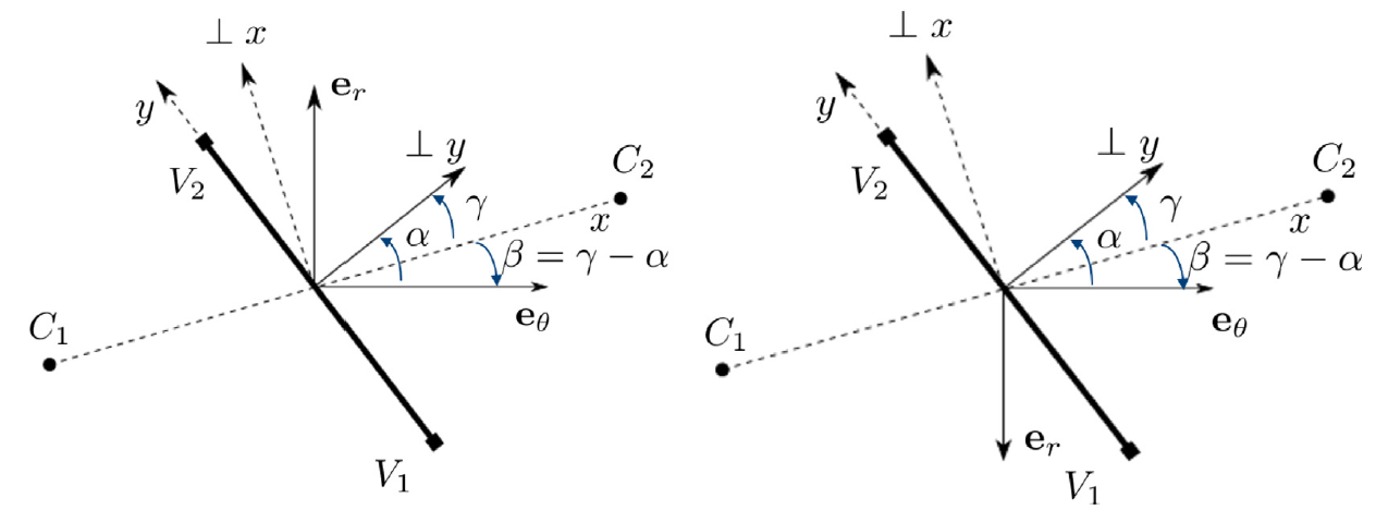
\includegraphics[width=14cm]{FiguresWG/mesh_angles.png}}
\else
    \centerline{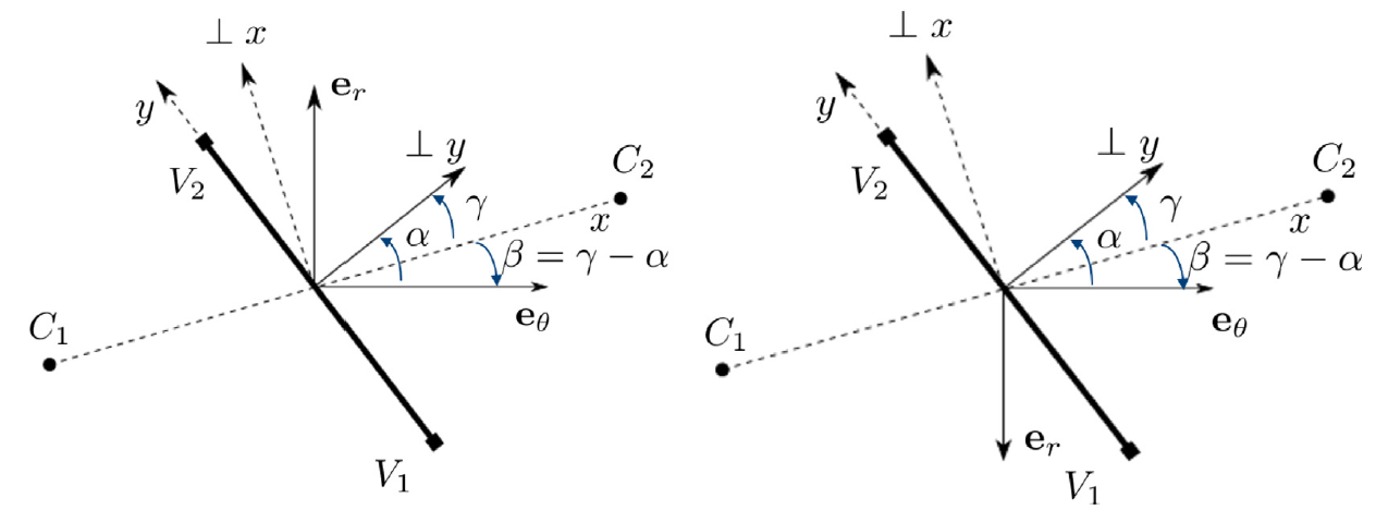
\includegraphics[width=14cm]{FiguresWG/mesh_angles.eps}}
\fi
    \caption{Local coordinate systems defining cell face orientation w.r.t. magnetic field, cell centers, and vertices. Left: toroidal field out of page. Right: toroidal field into the page.
    Figure reproduced from \cite{DEKEYSER2021}.}
    \label{fig:mesh_angles}
\end{figure}

The definitions of the variables in Figure \ref{fig:mesh_angles} are as follows:

\begin{itemize}
\item {\tt $C_1$} is the center of control volume 1. The index for that control volume is given by {\tt fcCv(iFc,1)}.
\item {\tt $C_2$} is the center of control volume 2. The index for that control volume is given by {\tt fcCv(iFc,2)}.
\item {\tt $V_1$} is the first vertex of the face. Its index is given by {\tt fcVx(iFc,1)}.
\item {\tt $V_2$} is the second vertex of the face. Its index is given by {\tt fcVx(iFc,2)}. The convention is that, when we look from {\tt $V_1$} to {\tt $V_2$}, {\tt $C_1$} is on the left and {\tt $C_2$} is on the right.
\item {\tt x} The $x$-direction is defined through the (not necessarily straight)
coordinate line connecting {\tt $C_1$} and {\tt $C_2$}, going through the center of the
cell face, and positive from {\tt $C_1$} to {\tt $C_2$}.
\item {\tt y} The $y$-direction is tangent to the face, positive from {\tt $V_1$} to {\tt $V_2$}.
\item {\tt $\alpha$} is the included angle between the magnetic field vector and the face normal.
{\tt fcQalf(iFc,0)} is the cosine of {\tt $\alpha$} and {\tt fcQalf(iFc,1)} is the sine of {\tt $\alpha$}.
\item {\tt $\gamma$} is the included angle between the cell-connector vector and the normal vector
of face {\tt iFc}. {\tt fcQgam(iFc,0)} is the cosine of {\tt $\gamma$} and {\tt fcQgam(iFc,1)} is the sine of {\tt $\gamma$}. It will hold that {\tt 0.lt.fcQgam(,).le.1}.
\item {\tt $\beta$} is the included angle between the cell-connector and the magnetic field vector.
{\tt fcQbet(iFc,0)} is the cosine of {\tt $\beta$} and {\tt fcQbet(iFc,1)} is the sine of {\tt $\beta$}.
\item {\tt fcHc(iFc,1)} is the distance between {\tt $C_1$} and the cell face center. {\tt fcHc(iFc,2)} is the distance between {\tt $C_2$} and the cell face center.
\item {\tt fcHt(iFc)} is the distance between {\tt $V_1$} and {\tt $V_2$}.
\end{itemize}

The flux of a particular quantity $u$ follows a convection-diffusion prescription:

\begin{equation*}
\mathbf{\Gamma} = \mathbf{C} u - \mathcal{D} \nabla u
\end{equation*}

The anisotropy in the equations is most naturally expressed w.r.t.
the poloidal ($\theta$) and radial ($r$) directions, which, by definition, are locally
orthogonal to each other. In our notation, the poloidal direction
points along the poloidal projection of the magnetic field, and the
radial direction is orthogonal to it in the poloidal plane, forming a
right-handed system with the third unit vector along the toroidal
projection of the field. These unit vectors therefore may flip orientation
with poloidal/toroidal field reversal. The coefficient
$\mathbf{C} = C_\theta \mathbf{e}_\theta + C_r \mathbf{e}_r$ is a vector describing the convective
flux of $u$, with components
defined in the poloidal and radial directions, and $\mathcal{D} = [D_{\theta \theta} D_{\theta r}, D_{r \theta} D_{r r}]$
is a diffusive tensor. The cross-diffusivities are included
because they are representative of the treatment of drift flows.
The {\tt B2.5} finite volume technique requires the evaluation of the fluxes across
cell faces:

\begin{align*}
 \mathbf{\Gamma} \cdot \mathbf{S} & = \Gamma_\theta S_\theta + \Gamma_r S_r \\
 & = \left( C_\theta u - D_{\theta \theta} \nabla_\theta u - D_{\theta r} \nabla_r u \right) S_\theta +
 \left( C_r u - D_{r \theta} \nabla_\theta u - D_{r r} \nabla_r u \right) S_r,
 \end{align*}

where $\mathbf{S} = S_\theta \mathbf{e}_\theta +  S_r \mathbf{e}_r $
is the surface vector of a face, expanded in its
poloidal and radial components.

To compute the poloidal and radial components of the gradient,
we relate them to the gradients in the $x$ and $y$
directions, which in turn can be computed directly from differences
between cell center (for $\nabla_\theta$) and vertex (for $\nabla_r$) values of $u$. The
desired expression for the components of the gradient can be obtained
by expanding the gradient in the orthogonal poloidal-radial system,
$\nabla u = \nabla_\theta u \cdot \mathbf{e}_\theta + \nabla_r u \cdot \mathbf{e}_r$,
and applying the definition of the gradient, $\nabla_d u = \nabla u \cdot \mathbf{d}$
for an arbitrary direction $\mathbf{d}$, to the unit vectors $\mathbf{e}_\theta$ and
$\mathbf{e}_r$:

\begin{align*}
\nabla_x u & = \nabla u \cdot \mathbf{e}_x = \nabla_\theta u \mathbf{e}_\theta \cdot \mathbf{e}_x + \nabla_r u \mathbf{e}_r \cdot \mathbf{e}_x, \\
\nabla_y u & = \nabla u \cdot \mathbf{e}_y = \nabla_\theta u \mathbf{e}_\theta \cdot \mathbf{e}_y + \nabla_r u \mathbf{e}_r \cdot \mathbf{e}_y.
\end{align*}

From Figure \ref{fig:mesh_angles} we see that $\mathbf{e}_\theta \cdot \mathbf{e}_x = \cos \beta$,
 $\mathbf{e}_r \cdot \mathbf{e}_x = \mp \sin \beta$, $\mathbf{e}_\theta \cdot \mathbf{e}_y = -\sin \alpha$
and $\mathbf{e}_r \cdot \mathbf{e}_y = \pm \cos \alpha$, with the upper signs corresponding to toroidal field
out of the page, and the lower signs with toroidal field into the page.
Inverting the system, we obtain

\begin{align*}
\nabla_\theta u & = \frac{\cos \alpha}{\cos \gamma} \nabla_x u + \frac{\sin \beta}{\cos \gamma} \nabla_y u, \\
\nabla_r u & = \pm \frac{\sin \alpha}{\cos \gamma} \nabla_x u \pm \frac{\cos \beta}{\cos \gamma} \nabla_y u.
\end{align*}

For completeness we give also the component of the gradient normal
to the face, which is needed for some boundary conditions:

\begin{equation*}
\nabla_n u = \frac{1}{\cos \gamma} \nabla_x u + \frac{\sin \gamma}{\cos \gamma} \nabla_y u,
\end{equation*}

and note, trivially, that the component tangential to the face is the
component in the $y$-direction: $\nabla_t u = \nabla_y u$.
Computing the poloidal and radial components of the gradient in
general thus requires a combination of gradients in $x$ and $y$ directions.

Drift terms can also be discretized using the expressions above. Only
the component of the drift perpendicular to a face leads to transport
across a face. Recalling that drifts have the form of a cross-diffusion
term, the net drift flow $\Gamma_d$ across a face is of the form:

\begin{equation*}
\mathbf{\Gamma}_d \cdot \mathbf{S} = - D_d \left( \nabla_r u S_\theta - \nabla_\theta u S_r \right) = \mp D_d \nabla_y u S
\end{equation*}

where we use the identity $\mathbf{S} = \left( \cos \alpha \ \mathbf{e}_\theta \pm \sin \alpha \ \mathbf{e}_r \right) S$.
Thus, net drift flow
across the face depends only on gradients along the face, while the
decomposition of the drift into its poloidal and radial components (as
required for example for the collisions with neutrals) requires again the
correct computation of the radial/poloidal gradients on each (possibly
non-aligned) face.
Using the expressions for the fluxes and derivatives on faces given
above, the governing equations can be discretized. Gradients in cell
centers are obtained through interpolation of the cell face gradients.
The discretization schemes of the structured version of the code have
been generalized to arbitrary unstructured grids. Hybrid discretization
schemes are used for the convection-diffusion flows, which are second
order in space for diffusion-dominated flows, but tend to a first-order
upwind scheme in convection-dominated flows.
The discretization schemes of the unstructured solver no longer neglect effects of misalignment
w.r.t. the magnetic field, and hence the solver is more accurate than older {\tt B2.5} versions
 even for non-extended grid cases.

Dedicated routines in {\tt \$\{SOLPSTOP\}/modules/B2.5/src/utility/} now take care of recurring numerical operations:

\begin{itemize}
\item {\tt GRAD} computes gradients of a cell-centered quantity on the cell faces, in both poloidal and radial directions.
\item {\tt GRAD\_NT} computes gradients of a cell-centered quantity on the cell faces, in both tangential and normal directions.
\item {\tt GRADC} computes gradients of a cell-centered quantity at the cell center by first computing the gradients on faces, and then interpolating back to the cell center.
\item {\tt GRADC\_DIV} computes gradients of a cell-centered quantity at the cell-center by applying the divergence theorem.
\item {\tt DIV} computes the divergence of a flow field.
\item {\tt INTFACE} interpolates a cell-centered quantity to the cell faces.
\item {\tt INTCELL} interpolates a face-based quantity to the cell centers.
\item {\tt INTVERTEX} interpolates a cell-centered quantity to the vertices.
\end{itemize}

%%%%%%%%%%%%%%%%%%%%%%%%%%%%%%%%%%%%%%%%%%%%%%%%%%%%%%%%%%%%%%%%%
%%%%%%%%%%%%%%%%%%%%%%%%%%%%%%%%%%%%%%%%%%%%%%%%%%%%%%%%%%%%%%%%%
\section{Rhie-Chow correction in unstructured code}
%%%%%%%%%%%%%%%%%%%%%%%%%%%%%%%%%%%%%%%%%%%%%%%%%%%%%%%%%%%%%%%%%
%%%%%%%%%%%%%%%%%%%%%%%%%%%%%%%%%%%%%%%%%%%%%%%%%%%%%%%%%%%%%%%%%

To avoid odd-even decoupling in the parallel direction due to the
collocated velocity and density (pressure) fields, a Rhie-Chow scheme
for compressible flow as described in Ref.~\cite{MOUKALLED2016} is implemented for the
parallel direction. The scheme is also explained in Section 8.8 and 10.2 (older versions) or 9.8 and 11.2 (newer versions) of Ref.~\cite{FERZIGER2019}.
The switches {\tt b2npco\_pcm0}, {\tt b2npco\_pcm1}, {\tt b2npht\_pcm0} and {\tt b2npht\_pcm1} determine the strength of the corrections.

%%%%%%%%%%%%%%%%%%%%%%%%%%%%%%%%%%%%%%%%%%%%%%%%%%%%%%%%%%%%%%%%%
%%%%%%%%%%%%%%%%%%%%%%%%%%%%%%%%%%%%%%%%%%%%%%%%%%%%%%%%%%%%%%%%%
\section{WG-related TODOs for this manual}
%%%%%%%%%%%%%%%%%%%%%%%%%%%%%%%%%%%%%%%%%%%%%%%%%%%%%%%%%%%%%%%%%
%%%%%%%%%%%%%%%%%%%%%%%%%%%%%%%%%%%%%%%%%%%%%%%%%%%%%%%%%%%%%%%%%

Some sections of this manual still need to be rewritten to be consistent with the unstructured solver:

\begin{itemize}
\item Appendix \ref{cha:b2wdat_iout_4} for the debugging output tracing files.
\item Appendix \ref{cha:Mladen_2}: remove, update, or integrate with another part of the manual.
\item Appendix \ref{sec:typical_BCs} for the expressions of boundary conditions.
\item Add information on creation of new extended cases. For now we refer to the {\tt 20230815\_carre2\_presentation.pdf} presentation found on the \SOLPSITER SharePoint website, in the \href{https://sharepoint.iter.org/departments/POP/CM/IMAS/SOLPS-ITER/SOLPS-ITER\%20Extended\%20Grids\%20Workshops}{SOLPS-ITER Extended Grids Workshops} directory.
\end{itemize}

%%%%%%%%%%%%%%%%%%%%%%%%%%%%%%%%%%%%%%%%%%%%%%%%%%%%%%%%%%%%%%%%%
%%%%%%%%%%%%%%%%%%%%%%%%%%%%%%%%%%%%%%%%%%%%%%%%%%%%%%%%%%%%%%%%%
\section{Converting structured cases}
%%%%%%%%%%%%%%%%%%%%%%%%%%%%%%%%%%%%%%%%%%%%%%%%%%%%%%%%%%%%%%%%%
%%%%%%%%%%%%%%%%%%%%%%%%%%%%%%%%%%%%%%%%%%%%%%%%%%%%%%%%%%%%%%%%%

Users can easily convert their existing structured cases to run with the WG code version. How to do this is explained in documents on the \SOLPSITER SharePoint website, \href{https://sharepoint.iter.org/departments/POP/CM/IMAS/SOLPS-ITER/SOLPS-ITER\%20Extended\%20Grids\%20Workshops}{SOLPS-ITER Extended Grids Workshops} directory, namely {\tt Session\_case\_conversion.pdf} and the last section of {\tt 20230814\_extended\_grids\_presentation.pdf}.


\appendix

\chapter{Internal B2.5 documentation}
\label{cha:intb2doc}

\section{b2cdca.F}
\label{lis:b2cdca}\index{b2cdca.F}\index{B2.5, code documentation}

\VerbatimInput[fontsize=\footnotesize]{b2cdca.F}

\newpage
\section{b2cdcr.F}
\label{lis:b2cdcr}\index{b2cdcr.F}\index{B2.5, list of routines}

\VerbatimInput[fontsize=\footnotesize]{b2cdcr.F}

\newpage
\section{b2cdcv.F}
\label{lis:b2cdcv}\index{b2cdcv.F}\index{B2.5, list of variables}

\VerbatimInput[fontsize=\footnotesize]{b2cdcv.F}

\newpage
\section{b2cdci.F}
\label{lis:b2cdci}\index{b2cdci.F}\index{B2.5, list of switches}

\VerbatimInput[fontsize=\footnotesize]{b2cdci.F}

\newpage
\section{b2cdcn.F}
\label{lis:b2cdcn}\index{b2cdcn.F}\index{B2.5, list of namelists}

\VerbatimInput[fontsize=\footnotesize]{b2cdcn.F}

\chapter{The physics of B2.5}
\label{cha:b2physics}

An extensive review of {\tt B2-Eirene} has been published as \cite{SOLPS2006}\index{SOLPS review}. It provides a full description of the {\bf SOLPS5.0} physics model, which can be obtained in the code by setting the {\tt b2mndt\_style} switch to {\tt 0}.
It is asked that authors using {\tt SOLPS} simulation results cite that work when
referring to the code. This review, only some short sections of which are detailed
below, can be found as part of the {\tt SOLPS} package at {\tt \$\{SOLPSTOP\}/doc/CPP\_2006.pdf}. Most of the discussion and definitions presented here apply to both the {\bf SOLPS5.0} and \SOLPSfivetwo physics models. In cases where the models differ, the use of the \SOLPSfivetwo model is recommended, although the {\bf SOLPS5.0} model remains available in the code for backward compatibility.

The equations are written on a
curvilinear orthogonal coordinate system.
The $x$-coordinate varies along flux surfaces and the $y$-coordinate varies
perpendicular to flux surfaces (see figure \ref{fig:geo}),
$z$ is the toroidal direction.

\begin{figure}[hbt]
\centerline{
\ifpdf
\includegraphics[width=8.0cm]{b2plot_1.pdf}
\else
\includegraphics[width=8.0cm]{b2plot_1.eps}
\fi
}
\caption{Coordinate system: $x$ is the poloidal coordinate,
$y$ is the radial coordinate orthogonal to the flux surfaces. The
coordinate $\perp$ corresponds to the direction perpendicular
both to the magnetic field and to the $y$-axis. The directions
of magnetic field and plasma current correspond to normal
operation conditions of ASDEX--Upgrade (ion $\nabla B$ drift
directed towards the X-point).
 }
\label{fig:geo}
\end{figure}

The metric coefficients are
$h_x=1/\|\grad x\|$, $h_y=1/\|\grad y\|$ and $\sqrt{g}=h_xh_yh_z$.
One can replace $h_z$ by $2 \pi R$,
where $R$ is the local major radius.  Components of a vector are the
projections on unit basis vectors
; they are not the contravariant or
covariant components ($b_x = B_x/B$, $b_z = B_z/B$).
Ion velocities $V_{\perp}$ (velocity perpendicular both
to magnetic field $B$ and the $y$-axis) and $V_y$ are
determined from the two components of the momentum balance equation
for ions perpendicular to a magnetic field. Using the Braginskii expression
for the friction force, one obtains:\\
\begin{gather}
\label{eq:nf1}
V_{\perp} = V_{\perp}^{\left( a \right)} - \frac{1}{enB}
\frac{1}{h_y}\frac{\partial nT_i}{\partial y} +
V_{\perp}^{\left( in \right)} + V_{\perp}^{\left( vis \right)} +
V_{\perp}^{\left( s \right)}
\end{gather}
\begin{gather}
\label{eq:nf2}
V_y = V_y^{\left( a \right)} + \frac{B_z}{enB^2}
\frac{1}{h_x}\frac{\partial nT_i}{\partial x} +
V_y^{\left( in \right)} + V_y^{\left( vis \right)} +
V_y^{\left( s \right)}
\end{gather}
Velocities $V_{\perp,y}^{\left( a \right)}$ are the sum of the
$\exb$ drifts and diffusive and thermo-diffusive
velocities.
This part corresponds to the ambipolar flux. It is the same both for ions and
electrons.
The second term in the r.h.s. of
Eqs.~(\ref{eq:nf1}) and (\ref{eq:nf2})
corresponds to diamagnetic flow of ions, while the other terms are caused
by inertial, viscous and ion-neutral friction forces.
These non-ambipolar terms are
connected with currents: $\vec{V}^{\left( in \right)} = \vec{j}^{\left( in \right)}/en,
\vec{V}^{\left( vis \right)} = \vec{j}^{\left( vis \right)}/en,
\vec{V}^{\left( s \right)} = \vec{j}^{\left( s \right)}/en$.\\
In the presence of anomalous transport
($D$ is the classical diffusion coefficient, $D=\frac{T_e+T_i}{eb}
\frac{\nu_{ei}}{\omega_{ce}}$, with electron cyclotron frequency
$\omega_{ce}$ and electron-ion collision frequency $\nu_{ei}$)
\begin{gather}
\label{eq:nf3}
V_{\perp}^{\left( a \right)} =
- \frac{1}{B}\frac{1}{h_y}\frac{\partial \Phi}{\partial y}
-\frac{D}{T_e+T_i} \frac{b_z}{h_x}\left(\frac{\partial p}{n \partial x}
-\frac{3}{2}\frac{\partial T_e}{\partial x}\right)
-D^{(AN)}_n\frac{1}{h_x n} \frac{\partial n}{\partial x}
-D^{(AN)}_p\frac{1}{h_x n} \frac{\partial p_i}{\partial x}
+V_{\perp}^{\left( AN \right)}
\end{gather}
\begin{gather}
\label{eq:nf44}
V_y^{\left( a \right)} =
\frac{B_z}{B^2}\frac{1}{h_x}\frac{\partial \Phi}{\partial x}
-\frac{D}{T_e+T_i} \frac{1}{h_y}\left(\frac{\partial p}{n \partial y}
-\frac{3}{2}\frac{\partial T_e}{\partial y}\right)
-D^{(AN)}_n\frac{1}{h_y n} \frac{\partial n}{\partial y}
-D^{(AN)}_p\frac{1}{h_y n} \frac{\partial p_i}{\partial y}
+V_y^{\left( AN \right)}
\end{gather}
The poloidal velocity is a sum $V_x = b_z V_{\perp} + b_x V_{\parallel}$.

In the particle balance
the fact that the diamagnetic
velocity is almost divergence free is taken into
account. Therefore, instead of the diamagnetic velocity
it is possible to introduce an effective
velocity $\vec{\tilde{V}}^{\left( dia \right)}$,
which gives the same contribution
to the divergence of the particle flux:
\begin{gather}
\label{eq:nf4}
\frac{\partial n}{\partial t} +
     \frac{1}{\sqrt{g}} \frac{\partial}{\partial x}
      \left(\frac{\sqrt{g}}{h_x} n\left(b_x V_{\parallel} +
     b_z V_{\perp}^{\left( 0 \right)}\right)\right)+
     \frac{1}{\sqrt{g}} \frac{\partial}{\partial y}
      \left(\frac{\sqrt{g}}{h_y} n V_y^{\left( 0 \right)}\right)
= S^n
\end{gather}
\begin{gather}\label{eq:nf5}
V_{\perp}^{\left( 0 \right)} = V_{\perp}^{\left( a \right)} +
V_{\perp}^{\left( in \right)} + V_{\perp}^{\left( vis \right)} +
V_{\perp}^{\left( s \right)} + \tilde{V}_{\perp}^{\left( dia \right)}
\end{gather}
\begin{gather}\label{eq:nf6}
V_{y}^{\left( 0 \right)} = V_{y}^{\left( a \right)} +
V_{y}^{\left( in \right)} + V_{y}^{\left( vis \right)} +
V_{y}^{\left( s \right)} + \tilde{V}_{y}^{\left( dia \right)}
\end{gather}
\begin{gather}\label{eq:nf7}
\tilde{V}_{\perp}^{\left( dia \right)} = \frac{T_i B_z}{e}
\frac{\partial}{h_y \partial y}\left(\frac{1}{B^2}\right)
\end{gather}
\begin{gather}\label{eq:nf8}
\tilde{V}_y^{\left( dia \right)} = -\frac{T_i B_z}{e}
\frac{\partial}{h_x \partial x}\left(\frac{1}{B^2}\right)
\end{gather}
The velocity $\tilde{V}^{{\left(dia\right)}}$ is an effective velocity. It
represents vertical guiding centre drift of ions caused by
$\nabla B$.\\

Combining the inertia and gyroviscosity terms in the Braginskii equations,
one finds
\begin{multline}\label{eq:mom}
\hfill m_i \left[ \frac{\partial n V_{\parallel}}{\partial t} +
     \frac{1}{\sqrt{g}} \frac{\partial}{\partial x}
      \left( \frac{\sqrt{g}}{h_x} n
       \left( V_{\perp}^{\left( 0 \right)} b_z
            + V_{\parallel} b_x \right)
       V_{\parallel} \right) +
     \frac{1}{\sqrt{g}} \frac{\partial}{\partial y}
      \left( \frac{\sqrt{g}}{h_y} n V_y^{\left( 0 \right)} V_{\parallel} \right)
\right] = \hfill \\
\hfill -\frac{b_x}{h_x}\frac{\partial n T_i}{\partial x} -
b_x \frac{en}{h_x}\frac{\partial \Phi}{\partial x} + F_k +
\frac{4}{3} b_x B^{3/2} \frac{\partial}{h_x \partial x}
\left(\frac{\eta_0 b_x}{B^2}
\frac{\partial\left(\sqrt{B}\left(V_{\parallel}+ \dfrac{B}{B_x} \left(V^{(dia)}_x + V^{(E)}_x\right)\right)\right)}
{h_x \partial x}\right)
\hfill \\
\hfill + B^{3/2} b_x \frac{\partial}{h_x \partial x}
\left(\frac{b_x}{\nu_{ii} B^2}
\frac{\partial\left(\sqrt{B}q_{i\parallel}^{\left( 0 \right)}
\right)}{h_x \partial x}\right)+
     \frac{1}{\sqrt{g}} \frac{\partial}{\partial y}
      \left(\frac{\sqrt{g}}{h_y^2} \eta_2 \frac{\partial V_{\parallel}}
{\partial y}\right) \hfill \\
\hfill
      + \frac{1}{\sqrt{g}} \frac{\partial}{\partial x}
      \left(\frac{\sqrt{g}}{h_x^2} \eta_2 \frac{\partial V_{\parallel}}
{\partial x}\right)
+ S_{i \parallel}^m + R_{ie\parallel}. \hfill
\end{multline}
The diamagnetic terms in the l.h.s. of (\ref{eq:mom}) are almost cancelled
\cite{ROGNLIEN98A, ROGNLIEN98B, ROGNLIEN99A, HINTON94C}, so that
velocities normal to the flux surface in the second and third term,
as in the particle balance equation, are determined by (\ref{eq:nf1}) and (\ref{eq:nf2}).
In \cite{HINTON94C}
the divergent part of diamagnetic velocity has been
neglected. Here, it is kept, because the corresponding flux is still
relatively large and can be comparable with the diffusive flux even
for anomalous diffusion coefficients. The authors of
\cite{ROGNLIEN98A, ROGNLIEN98B, ROGNLIEN99A} also kept this
flux.
In contrast to
\cite{ROGNLIEN98A, ROGNLIEN98B, ROGNLIEN99A}
there is an additional term of the same kind in the r.h.s. of
Eq.~(\ref{eq:mom}):
\begin{gather}
F_k = - m_i \left(\frac{1}{\sqrt{g}} \frac{\partial}{\partial x}
      \left(\frac{\sqrt{g}}{h_x} n V_{\parallel}
      \tilde{V}_{\perp}^{\left( dia \right)} b_z \right) +
      \frac{1}{\sqrt{g}} \frac{\partial}{\partial y}
      \left(\frac{\sqrt{g}}{h_y} n V_{\parallel}
      \tilde{V}_y^{\left( dia \right)} \right)\right)
\end{gather}
This parallel force is the Coriolis force, connected with the
diamagnetic drift velocity and
toroidal (parallel) rotation. This force can be obtained in a different
way by averaging the drift kinetic equation
\cite{MIHAIL84A} and is of the same order
as the inertia terms.

Parallel viscosity is represented
by the fourth and fifth terms in the r.h.s.
The former is the Balescu
parallel viscosity with coefficient $\eta_0 = \dfrac{4}{3} 0.96 \sqrt{2} n T_i / \nu_{ii}$. A detailed derivation is given at the end of this section, see~\ref{sec:viscosity}.
The latter corresponds to the parallel viscosity driven
by parallel ion heat flux
$q_{i\parallel}^{\left( 0 \right)} =
- \kappa_{i,\parallel} b_x \frac{1}{h_x} \frac{\partial T_i}{\partial x}$.
This viscosity is absent in the Braginskii equations, however, in a tokamak,
where parallel particle flux multiplied by temperature is of
the order of the ion heat flux, these two
viscosities are of the same order. On closed flux surfaces far from
the separatrix, the flux-surface-averaged parallel
viscosity coincides with the well-known
neoclassical expression for the Pfirsch-Schl{\"u}ter regime
\cite{HIRSHMAN81A}.
Thus, parallel viscosity in Eq.~(\ref{eq:mom}) provides smooth transition to
neoclassical theory.
The classical perpendicular viscosity coefficient
can
be replaced by an anomalous value as in
\cite{ROGNLIEN98A, ROGNLIEN98B, ROGNLIEN99A}: $\eta_2 =
n m_i D^{(AN)}_n$. Perpendicular viscosity and inertia terms with the
anomalous particle flux are responsible for the transport of the
parallel momentum in radial and poloidal directions. The radial transport
can be rather important despite the fact that $\eta_2 \ll \eta_0$, since
the scale in the radial direction is rather small.

The term  $S_{i \parallel}^m$  represents the parallel momentum loss due to
ion-neutral friction and parallel momentum input from neutral beam injection.
$R_{ie\parallel}$ is the ion-electron friction.

The parallel momentum balance for electrons has the standard form:
\begin{gather}
j_{\parallel} = \sigma_{\parallel} \left(
\frac{b_x}{e} \frac{1}{h_x} \left( \frac{\partial n T_e}{n \partial x} +
0.71 \frac{\partial T_e}{\partial x} \right)
- \frac{b_x}{h_x} \frac{\partial \Phi}{\partial x} \right).
\end{gather}

Expressions for $j_{\perp}$ and $j_y$ are obtained from radial and
poloidal projections of the total momentum balance equation (the sum
of electron and ion momentum balance equations).
The resulting current is a sum of contributions from pressure
gradient (diamagnetic current) $\vec{j}^{\left( dia \right)}$, inertia
and gyroviscosity $\vec{j}^{\left( in \right)}$, viscosity
$\vec{j}^{\left( vis \right)}$ and ion-neutral friction
$\vec{j}^{\left( s \right)}$.
Similar to the particle continuity equation, the effective
current $\vec{\tilde{j}}$ is introduced, which gives the same contribution to
$\nabla \vec{j}$, as the ordinary current. This gives the current continuity
equation
\begin{gather}\label{eq:curr0}
     \frac{1}{\sqrt{g}} \frac{\partial}{\partial x}
      \left(\frac{\sqrt{g}}{h_x} \tilde{j}_x\right)+
     \frac{1}{\sqrt{g}} \frac{\partial}{\partial y}
      \left(\frac{\sqrt{g}}{h_y} \tilde{j}_y\right)
= 0~.
\end{gather}
\begin{gather}\label{eq:curr1}
\tilde{j}_x = b_z \tilde{j}_{\perp} + b_x \tilde{j}_{\parallel}~.
\end{gather}
\begin{gather}\label{eq:curr2}
\vec{j} = \vec{\tilde{j}}^{\left( dia \right)} + \vec{j}^{\left( in \right)}
+ \vec{j}^{\left( vis \right)} + \vec{j}^{\left( s \right)}
+\vec{j}_{\parallel}~.
\end{gather}
The effective diamagnetic current can be chosen in a form
\begin{gather}\label{eq:curr3}
\tilde{j}_{\perp}^{\left( dia \right)} =
\frac{1}{b_z}\frac{n\left( T_e + T_i \right) B_z}{h_y}
\frac{\partial}{\partial y}\left(\frac{1}{B^2}\right)~,
\end{gather}
\begin{gather}\label{eq:curr4}
\tilde{j}_y^{\left( dia \right)} =
- \frac{n\left( T_e + T_i \right) B_z}{h_x}
\frac{\partial}{\partial x}\left(\frac{1}{B^2}\right)~.
\end{gather}
Current driven by parallel viscosity should be taken into account in
Eqs.~(\ref{eq:curr0}), (\ref{eq:curr1}) and (\ref{eq:curr2}).
This current is a small correction to the diamagnetic current
Eqs.~(\ref{eq:curr3}) and (\ref{eq:curr4}).
However, on closed flux surfaces, where the pressure is almost constant,
the diamagnetic current averaged
over the flux surfaces tends to zero. The resulting remaining part can
become comparable to the parallel viscosity-driven current, which is
necessary to satisfy the condition that the averaged net radial current
should be zero.
The terms, which contain the plasma viscosity, produce almost
divergence-free currents.
Similar to the case of diamagnetic currents, it can be reduced
to
\begin{gather}
\tilde{j}_{\perp}^{\left( vis \parallel \right)} =
- \frac{B_x \eta_0}{3 \sqrt{B}}
\frac{\partial\left(\sqrt{B}\left(V_{\parallel}+b_x \left(V^{(dia)}_{\perp} + V^{(E)}_{\perp}\right)\right)\right)}
{h_x \partial x}
\frac{\partial}{h_y \partial y}
\left(\frac{1}{B^2}\right)
\end{gather}
\begin{gather}
\tilde{j}_y^{\left( vis \parallel \right)} =
b_z\frac{B_x \eta_0}{3 \sqrt{B}}
\frac{\partial\left(\sqrt{B}\left(V_{\parallel}+b_x \left(V^{(dia)}_{\perp} + V^{(E)}_{\perp}\right)\right)\right)}
{h_x \partial x}
\frac{\partial}{h_x \partial x}
\left(\frac{1}{B^2}\right)
\end{gather}
The current produced by components of viscosity tensor connected
with heat fluxes is:
\begin{gather}
\tilde{j}_{\perp}^{\left( vis q \right)} =
- \frac{0.24 B_x}{\sqrt{B} \nu_{ii}}\frac{\partial
\left(q_{i \parallel}^{\left( 0 \right)} \sqrt{B}\right)}{h_x \partial x}
\frac{\partial}{h_y \partial y}
\left(\frac{1}{B^2}\right)
\end{gather}
\begin{gather}
\tilde{j}_y^{\left( vis q \right)} =
b_z\frac{0.24 B_x}{\sqrt{B} \nu_{ii}}\frac{\partial
\left(q_{i \parallel}^{\left( 0 \right)} \sqrt{B}\right)}{h_x \partial x}
\frac{\partial}{h_x \partial x}
\left(\frac{1}{B^2}\right)
\end{gather}

The second part of the current contains contributions from both inertia
and gyroviscosity forces. In contrast to the parallel momentum balance,
the cancellation is not complete (as has been noticed in
\cite{HINTON94C}). Expressions
for this part of the current are

\begin{multline}
\hfill j_{\perp}^{\left(in\right)}= - \frac{m_i}{B}
\left[\frac{\partial n V_{y}}{\partial t} +
     \frac{1}{\sqrt{g}} \frac{\partial}{\partial x}
      \left(\frac{\sqrt{g}}{h_x} n\left(V_{\perp}^{\left( 0 \right)} b_z
+ V_{\parallel} b_x \right) V_{y}\right)+
     \frac{1}{\sqrt{g}} \frac{\partial}{\partial y}
      \left(\frac{\sqrt{g}}{h_y} n V_y^{\left( 0 \right)} V_{y}\right)
\right] \hfill \\
\hfill -
\frac{2 b_x}{B} \frac{1}{h_x}\frac{\partial}{\partial x}
\left(\eta_3
\frac{\partial V_{\parallel}}{h_x \partial x}\right)+
\frac{m_i}{B} n V_{\parallel}^2 \frac{\partial \ln h_z}{h_y \partial y}
\hfill
\end{multline}

\begin{multline}
\hfill j_{y}^{\left(in\right)}= \frac{m_i}{B}
\left[\frac{\partial n V_{\perp}}{\partial t} +
     \frac{1}{\sqrt{g}} \frac{\partial}{\partial x}
      \left(\frac{\sqrt{g}}{h_x} n\left(V_{\perp}^{\left( 0 \right)} b_z
+ V_{\parallel} b_x \right) V_{\perp}\right)+
     \frac{1}{\sqrt{g}} \frac{\partial}{\partial y}
      \left(\frac{\sqrt{g}}{h_y} n V_y^{\left( 0 \right)} V_{\perp}\right)
\right] \hfill \\
\hfill -
\frac{2 b_x}{B} \frac{1}{h_x}\frac{\partial}{\partial x}
\left(\eta_3
\frac{\partial V_{\parallel}}{h_y \partial y}\right) -
\frac{m_i}{B} n V_{\parallel}^2 \frac{\partial \ln h_z}{h_x \partial x}
\hfill
\end{multline}

where $\eta_3 = \frac{n T_i}{2 \omega_{ci}}, \eta_1 = \frac{\eta_2}{4}$.

The last terms proportional to the gradient of $B$ correspond to the vertical
guiding centre drift of ions caused by the centrifugal force. This current
can be simply added to the diamagnetic current. Other terms seem to be less
important.

The contribution from perpendicular viscosity is
\begin{multline}
\hfill j_{\perp}^{\left(vis \perp \right)}= \frac{1}{B}
\left[\frac{1}{h_x}\frac{\partial}{\partial x}\left(\eta_1
     \frac{\partial V_y}{h_x \partial x}\right)+
 \frac{1}{h_y}\frac{\partial}{\partial y}\left(\eta_1
     \frac{\partial V_y}{h_y \partial y}\right)+
\frac{1}{h_x h_y }\frac{\partial \eta_1}{\partial x}
     \frac{\partial V_{\perp}}{\partial y}-
\frac{1}{h_x h_y }\frac{\partial \eta_1}{\partial y}
     \frac{\partial V_{\perp}}{\partial x}\right] \hfill \\
\hfill +
\frac{4 b_x}{B} \frac{1}{h_x h_y}
\left(\frac{\partial \eta_1}{\partial x} \frac{\partial V_{\parallel}}
{\partial y} - \frac{\partial \eta_1}{\partial y}\frac{\partial V_{\parallel}}
{\partial x}
\right)
\hfill
\end{multline}
\begin{gather}
j_{y}^{\left(vis \perp \right)}= -\frac{1}{B}
\left[\frac{1}{h_y}\frac{\partial}{\partial y}\left(\eta_1
     \frac{\partial V_{\perp}}{h_y \partial y}\right)+
 \frac{1}{h_x}\frac{\partial}{\partial x}\left(\eta_1
     \frac{\partial V_{\perp}}{h_x \partial x}\right)-
\frac{1}{h_x h_y }\frac{\partial \eta_1}{\partial x}
     \frac{\partial V_y}{\partial y}+
\frac{1}{h_x h_y }\frac{\partial \eta_1}{\partial y}
     \frac{\partial V_y}{\partial x}\right].
\end{gather}

Here, the largest term is the first one in the r.h.s. of the expression
for the radial current, since the radial derivatives are the largest.
This current corresponds to a pure cylindrical approximation. It is
responsible, for example, for closing currents near flush-mounted probes
\cite{ROZ99A}.
It was taken into account in
\cite{ROGNLIEN99A, RADFORD96A}. However, in the problem of global current
structure in the edge plasma, the currents driven by parallel viscosity seem
to be more important.

The total current caused by viscosity is
\begin{gather}
\vec{j}^{\left(vis\right)} = \vec{j}^{\left(vis \parallel\right)} +
\vec{j}^{\left(vis \perp\right)} +
\vec{j}^{\left(vis q\right)}
~.
\end{gather}

The contribution from ion neutral friction is
\begin{gather}
j_{\perp}^{\left(s\right)} = \frac{S_{iy}^m}{B}
~.
\end{gather}
\begin{gather}
j_{y}^{\left(s\right)} = -\frac{S_{i \perp}^m}{B}
~,
\end{gather}
where $S_{iy}^m$ and $S_{i \perp}^m$ are the momentum sinks due to
ion-neutral friction.
\begin{gather}
S_{i \perp}^m = - n \mu_{iN} \nu_{iN} \left( V_{\perp} - V_{\perp N}\right)
~,
\end{gather}
\begin{gather}
S_{i y}^m = - n \mu_{iN} \nu_{iN} \left( V_{y} - V_{y N}\right)
~,
\end{gather}
where $\mu_{iN}=m_i/2$ is the effective mass,
$\nu_{iN}= n_N \left\langle V_{iN} \sigma_{cx} \right\rangle$
is the ion-neutral collision frequency,
$n_N$ is the neutral density and $\vec{V_{iN}}$ is the neutral mean
velocity. For the ion velocity used above,
only electric and diamagnetic drifts are left, neglecting smaller terms,
to obtain
\begin{gather}
\tilde j_{x}^{\left(s\right)} = \tilde j_{\perp}^ {\left(s\right)} b_z =
- \sigma_{iN} b_z^2 \frac{\partial \Phi}{h_x \partial x}-
\sigma_{iN} b_z^2 \frac{1}{e n}\frac{\partial n T_i}{h_x \partial x}+
\sigma_{iN} B_z V_{yN}
~,
\end{gather}
\begin{gather}
\tilde j_{y}^{\left(s\right)} =
- \sigma_{iN} \frac{\partial \Phi}{h_y \partial y}-
\sigma_{iN} \frac{1}{e n}\frac{\partial n T_i}{h_y \partial y}-
\sigma_{iN} B V_{\perp N}
~,
\end{gather}
where $\sigma_{iN}$ is the ion-neutral perpendicular conductivity
\begin{gather}
\sigma_{iN} =
\frac{n m_i \left\langle V_{iN} \sigma_{cx} \right\rangle n_N}{2 B^2}
~.
\end{gather}

The rate of charge-exchange $\left\langle V_{iN} \sigma_{cx} \right\rangle$ can
be expressed through the mobility $K_0$ measured in the absence of a
magnetic field for room temperature and atmospheric pressure for
deuterium \cite{MCDANIEL73A}:
\begin{gather}
K_0 =
\frac{2 e}{m_i \left\langle V_{iN} \sigma_{cx} \right\rangle n_N^{\left(0\right)}}
~,
\end{gather}
with $n_N^{\left(0\right)} = 2.687 \cdot 10^{25} m^{-3}$ and
$K_0 = 11.2 \cdot 10^{-4} \frac{m^2}{s V}$.
Assuming that the charge-exchange cross-section is approximately constant
one gets
\begin{gather}
\left\langle V_{iN} \sigma_{cx} \right\rangle = 3.2 \cdot 10^{-15} \sqrt{\frac{T_i}{0.026}}
\frac{m^3}{s}
~,
\end{gather}
where $T_i$ is measured in $eV$. A similar expression, which gives approximately
the same result, is \cite{ROZ88A}:
\begin{gather}
\left\langle V_{iN} \sigma_{cx} \right\rangle = \frac{32 \sigma_{cx}}{3 \sqrt{\pi}}
\sqrt{\frac{T_i}{m_i}}
\frac{m^3}{s}
~.
\end{gather}.


In the energy balance equations
appears
a special problem, which is the
possible inclusion of an anomalous radial current.
The basic guidelines are as follows:
\begin{itemize}
\item The expression must be as simple as possible, and the most convenient
format is an Ohm-like expression;
\item The system of equations must be informed about this non-classical
contribution, but
\item The classical core of the equations must not be disturbed.
\end{itemize}
Apparently, the radial current would enter the electron energy equation
via the Joule term, but this manipulation is inappropriate since one cannot
be sure that this term directly heats the electrons, which is the case in
a purely classical setup. The proper thing to do is to keep only
the non-radial classical contribution in the Joule term, and
construct additional heat exchange terms
containing the radial current.
In this way, the system decides how to thermodynamically allocate the
"alien" heat term, among electrons and ion species.\\
For this reason, one cannot simply use the standard Ohm's
law in the radial direction with anomalous coefficients, or any other
prescribed expression whatsoever, as a constructive procedure is necessary
for simultaneously producing the radial current as well as the heat exchange
terms. At this point it has to be mentioned that this peculiarity arises
only in the multi-fluid case, whereas in the single species case
these heat exchange terms can indeed be constructed even using a prescribed
expression for the radial current. \\
The trick for carrying out this program is to correct the electron friction
density $\vec{R}^e$ by adding the term $n_e e \tilde{\eta}_\perp \vec{J}_\perp$
similar to the classical one, only using the {\itshape ad hoc} parameter
$\tilde{\eta}_\perp$. \\
Since $\vec{R}^e=-{\sum_{a}\vec{R}^a}$, one has a
modified total ion momentum equation at hand which in conjuction with the
pressure equilibrium (not affected by the additional term)
$\vec{J} \times \vec{B} = \nabla P$, gives the diffusive part of the
radial current, namely
\begin{gather}
J_y^{diff}=\frac{\tilde{\eta}_\perp en_e}{B^2} \frac{\partial P_i}{\partial y}
\end{gather}
where $P_i$ is the total ion pressure. This dependency is also found in
\cite{ROGNLIEN98A}. Moreover, an additional dependence on the radial
electric field can potentially be added without interfering with
the procedure. \\
The final step, namely the construction of the heat exchange terms, is
performed by claiming that the well known relation \cite{BAELMANS94A}
(adapted for the multi-fluid case)
\begin{gather}
Q_e=-\sum_{a} \left (Q_a + (\vec{u}^a - \vec{u}^e) \cdot \vec{R}^a \right )~,
\end{gather}
which stems from the fundamental null space of the collision operator,
is still true while carrying the modified friction.
Claiming this, after
performing the proper manipulations in the energy
equations, one reveals the {\itshape ad hoc}
contribution as the exchange term that one wants,
which reads
$
\sum_{a} (\vec{u}^a -\vec{u}^e)_\perp n_a \frac{Z_a^2}{Z_{eff}} e \tilde{\eta}_\perp \vec{J}_\perp
$
added in the total ion energy equation and subtracted from the
electron equation.
Note that in the single species case, this term boils down to
$
\tilde{\eta}_\perp J_\perp ^2
$
removing energy from the electrons,  depositing it to the ions, a feature
predicted by neoclassical theory \cite{ROSENBLUTH72A}.\\

In the final form of the energy balance equations, the convective heat
flux and the diamagnetic heat flux are combined as in
\cite{ROGNLIEN98A, ROGNLIEN98B, ROGNLIEN99A, HINTON94C}, see also
\cite{ROZ99A}.

The energy balance equation for the electrons is
\begin{multline}
\hfill
     \frac{3}{2} \frac{\partial nT_e}{\partial t} +
     \frac{1}{\sqrt{g}} \frac{\partial}{\partial x}
      \left(\frac{\sqrt{g}}{h_x} \tilde{q}_{ex}\right) +
     \frac{1}{\sqrt{g}} \frac{\partial}{\partial y}
      \left(\frac{\sqrt{g}}{h_y} \tilde{q}_{ey}\right) +
     \frac{nT_e}{\sqrt{g}}\frac{\partial}{\partial x}
      \left(\frac{\sqrt{g}}{h_x}\left(
      V_{\parallel} - j_{\parallel}/en\right)b_x\right) \hfill \\
\hfill     =
     Q_e + n T_e B \frac{1}{h_x h_y}\left(\frac{\partial \Phi}{\partial y}
     \frac{\partial}{\partial x}\left(\frac{1}{B^2}\right)
     -\frac{\partial \Phi}{\partial x}\frac{\partial}{\partial y}
     \left(\frac{1}{B^2}\right)\right)~,\hfill
\end{multline}
where
\begin{multline}
\hfill        \tilde{q}_{ex} = \frac{3}{2} n T_e \left(- \frac{b_z}{B h_y}
         \frac{\partial \Phi}{\partial y}
         + b_x V_{\parallel} - b_x j_{\parallel} / en \right) \hfill \\
     \hfill + \frac{5}{2} n T_e b_z \left(
     - \frac{D}{T_e+T_i} \frac{b_z}{h_x} \left(\frac{\partial p}{n \partial x}
     - \frac{3}{2} \frac{\partial T_e}{\partial x} \right)
     - D^{(AN)}_n \frac{1}{h_x n} \frac{\partial n}{\partial x}
     - D^{(AN)}_p \frac{1}{h_x n} \frac{\partial p_i}{\partial x}
     + V_{e\perp}^{(AN)} \right)
      \hfill \\
      \hfill   - 0.71 b_x j_{\parallel} T_e/e - \kappa_{e \parallel}
         \frac{b_x^2}{h_x} \frac{\partial T_e}{\partial x}
         - \kappa_{e \perp} b_z^2 \frac{1}{h_x}
         \frac{\partial T_e}{\partial x} \hfill \\
      \hfill   + \frac{3}{2}\frac{T_e}{e B} \frac{\nu_{ei}}{\omega_{ce}}
         \frac{b_z^2}{h_x} \frac{\partial n\left(T_e+T_i\right)}{\partial x}
         - \frac{5}{2} n T_e^2 \frac{B_z}{e}
         \frac{\partial}{h_y \partial y}\left(\frac{1}{B^2}\right) ~ , \hfill
\end{multline}
\begin{multline}
\hfill  \tilde{q}_{ey} = \frac{3}{2} n T_e \left( \frac{B_z}{B^2} \frac{1}{h_x}
        \frac{\partial \Phi}{\partial x} \right) \hfill \\
     \hfill  + \frac{5}{2} n T_e \left(
     - \frac{D}{T_e+T_i} \frac{1}{h_y} \left( \frac{\partial p}{n \partial y}
     - \frac{3}{2} \frac{\partial T_e}{\partial y} \right)
     - D^{(AN)}_n \frac{1}{h_y n} \frac{\partial n}{\partial y}
     - D^{(AN)}_p \frac{1}{h_y n} \frac{\partial p_i}{\partial y}
     + V_{ey}^{(AN)} \right)
         \hfill \\
         \hfill - \kappa_{e \perp} \frac{1}{h_y} \frac{\partial T_e}{\partial y}
         + \frac{3}{2}\frac{T_e}{e B} \frac{\nu_{ei}}{\omega_{ce}}
         \frac{1}{h_y} \frac{\partial n\left(T_e+T_i\right)}{\partial y}
         + \frac{5}{2} n T_e^2 \frac{B_z}{e}
         \frac{\partial}{h_x \partial x}\left(\frac{1}{B^2} \right) ~ , \hfill
\end{multline}
\begin{gather}
        Q_{\Delta} = \frac{3 m_e}{m_i} n \nu_{ei} \left(
T_e - T_i
\right)~,
\end{gather}
\begin{gather}
        Q_u = R_{ie \parallel} j_{\parallel}/en~,
\end{gather}
\begin{gather}
        Q_{AN} = \sum_{a} \left(\vec{u}^a -\vec{u}^e\right)_\perp n_a
                 \frac{Z_a^2}{Z_{eff}} e \tilde{\eta}_\perp \vec{J}_\perp~,
\end{gather}
\begin{gather}
        Q_e = -Q_{\Delta} - Q_u - Q_{AN}~.
\end{gather}

\begin{sloppypar}
Here $\kappa_{e \parallel}$ is the Balescu (not Braginskii as stated in the CPP review paper \cite{SOLPS_review}
or in {\tt \$\{SOLPSTOP\}/doc\allowbreak /CPP\_2006.pdf}) heat
conductivity with a possible heat
flux limit \cite{BRAAMS96B}.
The leading numerical coefficient is then $\frac{5}{2} \frac{2.16 z}{1 + 0.27 z}$ as opposed to 3.16 for the Braginskii
formula \cite{NRL}. The perpendicular heat conductivity
$\kappa_{e \perp}$ can be
either classical or anomalous. In the last term of the energy balance
equation, it is taken into account that the $\exb$
drift velocity is
almost divergence-free.
\end{sloppypar}

The ion energy balance equation is
\begin{multline}\label{eq:ion_energy} \hfill
     \frac{3}{2} \frac{\partial nT_i}{\partial t} +
     \frac{1}{\sqrt{g}} \frac{\partial}{\partial x}
      \left(\frac{\sqrt{g}}{h_x} \tilde{q}_{ix}\right) +
     \frac{1}{\sqrt{g}} \frac{\partial}{\partial y}
      \left(\frac{\sqrt{g}}{h_y} \tilde{q}_{iy}\right) +
     \frac{nT_i}{\sqrt{g}}\frac{\partial}{\partial x}
      \left(\frac{\sqrt{g}}{h_x} V_{\parallel} b_x \right) \hfill \\
     \hfill =
     Q_{\Delta} + Q_{AN} + \frac{\eta_0}{3} \left(2 b_x
     \frac{\partial V_{\parallel}}{h_x \partial x}\right)^2+
     n T_i B
     \frac{1}{h_x h_y}\left(\frac{\partial \Phi}{\partial y}
     \frac{\partial}{\partial x}\left(\frac{1}{B^2}\right)
     -\frac{\partial \Phi}{\partial x}\frac{\partial}{\partial y}
     \left(\frac{1}{B^2}\right)\right)~,\hfill
\end{multline}
where
\begin{multline} \hfill
        \tilde{q}_{ix} = \frac{3}{2} n T_i \left(- \frac{b_z}{B h_y}
        \frac{\partial \Phi}{\partial y}
         + b_x V_{\parallel} \right) \hfill \\
\hfill + \frac{5}{2} n T_i b_z \left(
     - \frac{D}{T_e + T_i} \frac{b_z}{h_x}\left(\frac{\partial p}{n \partial x}
     - \frac{3}{2} \frac{\partial T_e}{\partial x} \right)
     - D^{(AN)}_n \frac{1}{h_x n} \frac{\partial n}{\partial x}
     - D^{(AN)}_p \frac{1}{h_x n} \frac{\partial p_i}{\partial x}
     + V_{i\perp}^{(AN)} \right)
         \hfill \\ \hfill
         + \frac{5}{2} n T_i b_z \tilde{V}_{\perp}^{\left(dia\right)}
         - \kappa_{i \parallel}
         \frac{b_x^2}{h_x} \frac{\partial T_i}{\partial x}
         - \kappa_{i \perp} b_z^2 \frac{1}{h_x}
         \frac{\partial T_i}{\partial x} ~, \hfill
\end{multline}
\begin{multline} \hfill
        \tilde{q}_{iy} = \frac{3}{2} n T_i \left( \frac{B_z}{B^2}
         \frac{1}{h_x} \frac{\partial \Phi}{\partial x} \right)
        \hfill \\ \hfill
     + \frac{5}{2} n T_i \left(
     - \frac{D}{T_e+T_i} \frac{1}{h_y} \left( \frac{\partial p}{n \partial y}
     - \frac{3}{2} \frac{\partial T_e}{\partial y}\right)
     - D^{(AN)}_n \frac{1}{h_y n} \frac{\partial n}{\partial y}
     - D^{(AN)}_p \frac{1}{h_y n} \frac{\partial p_i}{\partial y}
     + V_{iy}^{(AN)} \right) \hfill \\ \hfill
         - \kappa_{e \perp} \frac{1}{h_y}
         \frac{\partial T_i}{\partial y}
         + \frac{5}{2} n T_i \tilde{V}_{y}^{\left(dia\right)} ~. \hfill
\end{multline}

As for the electrons, the parallel heat conductivity is classical with
a possible heat flux limit, while the perpendicular contribution
can be either
classical or anomalous.

There is discussion in the literature on how to take into account anomalous
terms in the energy balance equations. One point of view (see e.g.
\cite{ZAGORSKI98A})
is to cancel the contribution from anomalous particle fluxes in the
terms $p_i \nabla \cdot \vec{V}_i$ (or $\vec{V}_i \cdot \nabla p_i$ if equations
are written in a different form). In contrast, according to the
derivation
\cite{HINTON94C},
where a kinetic equation with fluctuating term has been integrated, the
anomalous fluxes should be kept in all terms of the energy balance
equations. This variant was used in {\tt UEDGE} \cite{ROGNLIEN98A, ROGNLIEN98B, ROGNLIEN99A}.
In {\tt B2.5} only the contribution
from anomalous radial particle flux to the convective heat flux are left
in the expressions for $\tilde{q}_{e,i}$. In the term
$p_i \nabla \cdot \vec{V}_i$ the anomalous particle flux is absent.

\section{Derivation of parallel viscosity term in momentum equation}
\index{parallel viscosity}\label{sec:viscosity}

To evaluate the parallel viscosity contribution we should start from the general expressions, which can be transformed and simplified in arbitrary cartesian coordinate system assuming only parallel velocity. The Braginskii description for parallel viscosity in cartesian coordinates is:

\begin{equation*}
\pi_{\alpha \beta} = \frac{3}{2} \eta_0 \left( b_\alpha b_\beta - \frac{1}{3} \delta_{\alpha \beta} \right) \left( b_\mu b_\nu - \frac{1}{3} \delta_{\mu \nu} \right) W_{\mu \nu}
\end{equation*}

where

\begin{equation*}
W_{\mu \nu} = \frac{\partial V_\mu}{\partial x_\nu} + \frac{\partial V_\nu}{\partial x_\mu} - \frac{2}{3} \delta_{\mu \nu} \frac{\partial V_i}{\partial x_i}, ~\vec{b} = \vec{B}/B .
\end{equation*}

The parallel momentum balance component is:

\begin{equation*}
\vec{b} \cdot \left( \nabla \cdot \overleftrightarrow{\pi} \right) = b_\alpha \frac{\partial \pi_{\alpha \beta}}{\partial x_\beta} = b_\alpha \frac{\partial}{\partial x_\beta} \left[ \frac{3}{2} \eta_0 \left( b_\alpha b_\beta - \frac{1}{3} \delta_{\alpha \beta} \right) \left( b_\mu b_\nu - \frac{1}{3} \delta_{\mu \nu} \right) W_{\mu \nu} \right]
\end{equation*}

We can evaluate the scalar value separately:

\begin{align*}
\pi_0 &= \frac{3}{2} \eta_0 W_{\parallel \parallel} = \frac{3}{2} \eta_0 \left( b_\mu b_\nu - \frac{1}{3} \delta_{\mu \nu} \right) W_{\mu \nu} \\
&= \frac{3}{2} \eta_0 \left(  b_\mu b_\nu - \frac{1}{3} \delta_{\mu \nu} \right) \left( \frac{\partial V_\mu}{\partial x_\nu} + \frac{\partial V_\nu}{\partial x_\mu} - \frac{2}{3} \delta_{\mu \nu} \frac{\partial V_i}{\partial x_i} \right) = 3 \eta_0 \left(  b_\mu b_\nu - \frac{1}{3} \delta_{\mu \nu} \right) \left( \frac{\partial V_\mu}{\partial x_\nu} - \frac{1}{3} \delta_{\mu \nu} \frac{\partial V_i}{\partial x_i} \right) \\
&= 3 \eta_0 \left( b_\mu b_\nu \frac{\partial V_\mu}{\partial x_\nu} - \frac{1}{3} \frac{\partial V_i}{\partial x_i} \right) = 3 \eta_0 \left( b_\mu b_\nu \frac{\partial V_\parallel b_\mu}{\partial x_\nu} - \frac{1}{3} \frac{\partial V_\parallel b_\nu}{\partial x_\nu} \right) \\
&= 3 \eta_0 \left( \frac{B_\nu}{B} \frac{\partial V_\parallel}{\partial x_\nu} - \frac{1}{3} B_\nu \frac{\partial V_\parallel / B}{\partial x_\nu} \right) = \eta_0 \frac{B_\nu}{B} \left( 2 \frac{\partial V_\parallel}{\partial x_\nu} + \frac{V_\parallel}{B} \frac{\partial B}{\partial x_\nu} \right) \\
&= 2 \eta_0 \frac{B_\nu}{B} \frac{1}{\sqrt{B}} \frac{\partial V_\parallel \sqrt{B}}{\partial x_\nu} = 2 \eta_0 \frac{1}{\sqrt{B}} \vec{b} \cdot \nabla \left ( V_\parallel \sqrt{B} \right)
\end{align*}

The projection of the viscosity divergence on the parallel direction is then:

\begin{align*}
\vec{b} \cdot \left( \nabla \cdot \overleftrightarrow{\pi} \right) &= b_\alpha \frac{\partial}{\partial x_\beta} \left[ \pi_0 \left( b_\alpha b_\beta - \frac{1}{3} \delta_{\alpha \beta} \right) \right] = \frac{\partial \pi_0 b_\alpha}{\partial x_\alpha} - \frac{1}{3} b_\alpha \frac{\partial \pi_0}{\partial x_\alpha} = B_\alpha \frac{\partial \pi_0 / B}{\partial x_\alpha} - \frac{1}{3} b_\alpha \frac{\partial \pi_0}{\partial x_\alpha} \\
&= \frac{2}{3} b_\alpha \frac{\partial \pi_0}{\partial x_\alpha} - \pi_0 \frac{b_\alpha}{B} \frac{\partial B}{\partial x_\alpha} = \frac{2}{3} B^{3/2} b_\alpha \frac{\partial \pi_0 B^{-3/2}}{\partial x_\alpha} = \frac{2}{3} B^{3/2} \vec{b} \cdot \nabla \left( \pi_0 B^{-3/2} \right)
\end{align*}

Then the parallel viscosity in the parallel momentum balance is:

\begin{equation*}
\vec{b} \cdot \left( \nabla \cdot \overleftrightarrow{\pi} \right) = \frac{4}{3} B^{3/2} \vec{b} \cdot \nabla \left( \frac{\eta_0}{B^2} \vec{b} \cdot \nabla \left( V_\parallel \sqrt{B} \right) \right), ~ \mbox{where} ~ V_\parallel = \vec{b} \cdot \vec{V}
\end{equation*}

For \SOLPSITERns, the orthogonal coordinates $(x,r,z)$ are more convenient for further evaluations than the non-orthogonal coordinates $(x,y,z)$. In these coordinates, it is readily seen that $\vec{b} \cdot \nabla f = b_x \frac{\partial f}{h_x \partial x}$ for any scalar function $f$. The viscosity can be finally written as:

\begin{equation*}
\vec{b} \cdot \left( \nabla \cdot \overleftrightarrow{\pi} \right) = \frac{4}{3} b_x B^{\frac{3}{2}} \frac{\partial}{h_x \partial x} \left( \frac{\eta_0 b_x}{B} \frac{\partial \left( B^{\frac{1}{2}} V_\parallel \right)}{h_x \partial x} \right)
\end{equation*}

\section{Boundary conditions with drifts and currents}
\index{drifts and currents, boundary conditions}
\index{boundary conditions, drifts and currents}

Whether one deals with the diamagnetic or $\exb$ perpendicular
drift velocity, special care must be taken to avoid unphysical flows
at the plates. The standard boundary condition is to require that the flow be
at least sonic at the sheath entrance \cite{STANGEBY95B},
which translates into:

\begin{equation}\label{eq:Chodura}
V_{\parallel} \ge C_s - \frac{b_z}{b_x} V_{\perp} ~,
\end{equation}

where $C_s$ is the local sound speed and $\frac{b_z}{b_x}$ is the inverse
of the field line pitch. However, for very small pitch angles, as in
stellarators, the $V_{\perp}$ term may overpower the sound
velocity \cite{FENG99A}
and then the boundary condition would require a plasma flow exiting the plate.
Therefore, the pitch angle at the plates is limited to be no less than
1 degree (user parameter, see switch {\tt b2agfs\_min\_pitch} in Appendix~\ref{lis:b2cdci}),
motivated by the engineering limits met when attempting to align the
divertor tiles with the magnetic field. The solution procedure of the code
was also modified so as ensure that no unphysical flows were being created,
and solves the parallel momentum equation using the updated electric potential.

Boundary conditions for the current continuity equation at the plates
correspond to sheath current-voltage characteristics
\begin{equation}\label{eq:sheath-voltage}
j_x = en\left(b_x c_s - b_x \frac{1}{\sqrt{2 \pi}} \sqrt{\frac{T_e}{m_e}}
      \exp \left(- \frac{e \Phi}{T_e}\right) \left(1 - \gamma_e\right)\right),
\end{equation}
where $\gamma_e$ is the secondary electron emission coefficient. At the inner
(core) flux surface the currents are set either to the divergent part
of the diamagnetic current or to zero. Both variants give the same result
and both guarantee that the net current integrated over the inner flux surface
should be zero. At the walls, the same conditions on the normal current
components were imposed as for the inner core.

The electron and ion heat fluxes to the target plates are
\begin{equation}\label{eq:target_qe}
\tilde q_{ex} = b_x \frac{n}{\sqrt{2 \pi}} \sqrt{\frac{T_e}{m_e}}
     \exp \left(- \frac{e \Phi}{T_e}\right) \left(1 - \gamma_e\right)
     \left(T_e \frac{1+\gamma_e}{1-\gamma_e} + e \Phi\right),
\end{equation}
\begin{equation}\label{eq:target_qi}
\tilde q_{ix} = \frac{3}{2}n T_i c_s b_x.
\end{equation}

The question of kinetic
boundary conditions including drifts is not yet finally clarified
and will need further work from both kinetic and fluid modelling
\cite{CHANKIN94AB,STANGEBY95B}.

\section{Problems for a fluid description of the edge plasma}
\index{flux limits}

To apply a fluid model for the description of the edge,
a specific ordering of lengths is necessary.

The necessary condition for a fluid model is
that all characteristic lengths (characteristic length
of the sheath, which is a microscopic length scale of about 10 Debye lengths;
electron and ion mean free path ranging from sub-cm to metres; neutral mean
free path, which is centimetres to metres; heat conduction length which is typically
five times the mean free path length due to the dominant contribution from tail
electrons or ions)
are smaller than the parallel connection length (order of several tens of metres). This
is usually fulfilled in edge plasmas with the following possible exceptions:
\begin{enumerate}
  \item at low temperatures, e.g.
           near the target in the divertor,
           steeper gradients result in non-local heat flux contributions. In general,
           a non-local description might be necessary
            (weighted mean of temperature profile over
           five mean free lengths of electrons or ions). However, a simpler correction
           is sometimes satisfactory and is used in the code (see below).
  \item at high temperatures
        (midplane, near separatrix).
        Corrections for flux limit and for periodic systems on closed
        field lines are necessary due to the fact that the heat conduction
        mean free path is larger than the connection length.
  \item the sheath cannot be resolved by a fluid model and is represented
        by boundary conditions at the sheath entrance deduced from kinetic
        models.
\end{enumerate}

Simple heat flux and momentum flux (viscosity)
limits are available.
The heat flux limit is formulated as
\begin{gather}
  \kappa_{\parallel}=\frac{\kappa_{SH}}{1+|q_{SH}/q_{fl}|},
\end{gather}

with the classical Spitzer--H\"arm heat flux
\begin{gather}
 q_{SH}=-\kappa_{\parallel ,SH} \cdot \frac{\partial T_e}{\partial x}
\end{gather}

and the flux limit
\begin{gather}
 q_{fl}=\alpha n_e T_e^{3/2} \sqrt{m_e }
\end{gather}

($\alpha \approx 0.2$ from comparison with kinetic calculations for electrons;
the situation for ions is less clear).

The momentum flux limit is done the same way
\begin{gather}
  \eta_{\parallel} =\frac{\eta_{cl,a}}
   {1+|q_{cl,a}/q_{fl,a}|},
\end{gather}

with the classical momentum flux
\begin{gather}
  q_{cl,a}=-\eta_{\parallel,a} \cdot
  \frac{\partial u_{\parallel,a}}{\partial x}
\end{gather}
and the flux limit
\begin{gather}
 q_{fl,a}=\alpha p_{a}
\end{gather}
(with $\alpha = 0.5$). Unfortunately, for this correction even less kinetic
work
exists than for the heat flux limits.

Additionally,
long mean free path corrections of classical heat conduction and viscosity
(in the core) are applied.
For periodic systems and small perturbations one gets
\cite{NEUHAUSER86A}:
\begin{gather}
   q_{\parallel , eff}
    = q_{SH}/\left(h_{\parallel}^2 \lambda_{HC}^2 +1\right),
\end{gather}

with wavenumber of periodicity
\begin{gather}
  h_{\parallel}=2 \pi / \lambda_{\parallel},
\end{gather}
\begin{gather}
  \lambda_{\parallel}=2 \pi R q
\end{gather}

and mean free path of tail electrons
\cite{CHODURA84A}
\begin{gather}
  \lambda_{HC} (\mbox{m}) = 7.5\cdot 10^{16} \cdot T_e^2(\mbox{eV})/n_e(
  \mbox{m}^{-3}).
\end{gather}

Fokker-Planck computer simulations of electron heat transport in laser
plasmas
\cite{LLE91}
show that a better description is obtained for a linear
correction:
\begin{gather}
  q_{\parallel , eff}
    = q_{SH}/(h_{\parallel} \lambda_{HC} +1).
\end{gather}

Applying these limits for the core, convergence behaviour of the code
improves significantly.\\
A more correct kinetic limit would imply a
non-local heat transport (and viscosity,...) description.
The parallel heat flux at a point should be determined by
classical fluxes at points
up to typically five mean free paths away. As an additional feature, one
would get
pre-heating effects by fast electrons, maybe important for the ELMs.
Work is necessary to generalize this to the SOL
\cite{KRASH92A,YURI91A}
and this has to be cross-checked
with kinetic calculations \cite{Abou-Assaleh92}. Also, numerical problems due
to this non--local description have to be solved \cite{PRASAD91A}.

In general, if these kinetic corrections become important, quantitative
conclusions are
questionable, because the fluid model is no longer strictly valid.
Considerations of
particle, energy and momentum conservation still guarantee a qualitatively
correct
description. The flux limiters are designed are defined to give the correct
answer
in the fully collisional and in the fully collisionless regime.

Parametric studies varying the various flux limiters should be done,
particularly
for predictive work. Specific experimental scenarios would be required to
calibrate
the flux limiters. However, complete experimental data sets including
electron and
ion temperatures and densities at the target plate and upstream are necessary.
Fortunately, at higher densities these corrections are not important.
Furthermore,
one should note, that mapping of target data to the midplane and the
extraction of
anomalous radial transport coefficients from such a procedure is
questionable in the
regime where flux limiters are important
\cite{CosterHinM2003}.

As an example,
SOLPS5.0 calculations for JET using deuterium, carbon and helium are shown in
Figs.~\ref{cflmi_1e19} and \ref{cflmi_2e19}.
The predicted electron temperatures at the outer target are shown for
two different upstream densities.
In each graph, the ion energy flux limit is varied and the sensitivity of the
target profiles to this variation is obvious.

\begin{figure}[bt]
\ifpdf
    \centerline{\includegraphics[width=11cm]{cflmi_1e19.pdf}}
\else
    \centerline{\includegraphics[angle=-90,width=11cm]{cflmi_1e19.ps}}
\fi
\caption{Impact of ion flux limits for a $10^{19}~~m^{-3}$ upstream density case.}
\label{cflmi_1e19}
\vspace*{1cm}
\end{figure}

\begin{figure}[bt]
\ifpdf
    \centerline{\includegraphics[width=11cm]{cflmi_2e19.pdf}}
\else
    \centerline{\includegraphics[angle=-90,width=11cm]{cflmi_2e19.ps}}
\fi
\caption{Impact of ion flux limits for a $2 \times 10^{19}~~m^{-3}$ upstream density case.}
\label{cflmi_2e19}
\end{figure}

\section{Neutral models}

\subsection{Fluid neutrals}
\index{neutrals, fluid model}

As an alternative to the complete kinetic Monte Carlo description offered by {\tt Eirene},
a simpler and faster neutral fluid model is also available as {\tt B2.5} standalone. The surface sources of neutrals are
then given by user-defined recycling models, possibly enhanced with local sputtering models
when impurities are considered (see e.g.~\cite{Warrier04}). The volume sources of neutrals are given by
plasma recombination rates computed by the {\tt B2.5} atomic physics packages. The neutral species is then
treated just as the other plasma species, with its own particle and momentum transport equations in the parallel
direction, equivalent to Eqs.~(\ref{eq:nf4}) and (\ref{eq:mom}). The neutrals are assumed to have the same common
temperature as all other ion species and the neutral energy balance equation becomes simply a component
of Eq.~(\ref{eq:ion_energy}). Of course, terms due to charged particle motions or currents do not appear
for neutral species.

The neutral species transport coefficients are usually given by the following equations:
\begin{gather}\index{neutrals, transport coefficients}
 D^{(AN)}_{n,0} = 0,
\end{gather}
\begin{gather}
 D^{(AN)}_{p,0} = C + \sqrt{\frac{T_i}{m_N}} \frac{1}{( \sigma_{CX} n_i + \sigma_{in} n_e )},
\end{gather}
where $m_N$ is the mass of the neutral species, and $C$, $\sigma_{CX}$ and $\sigma_{in}$ are three constants given by
the user, representing hydrogen gas diffusion, and the charge-exchange and ionisation cross-sections, respectively.
As an option, one may choose to use cross-sections from atomic databases instead of constants, with their appropriate
parameter dependencies. The diffusion coefficients can also be bounded to avoid unphysically large or small values.

Additionally, the heat and particle fluxes carried by neutrals can be flux-limited, following the formalism
laid out in~\cite{UMANSKY03A}\index{neutrals, flux limits}. On the one hand, we flux-limit the neutral contribution
to the ion heat diffusivity, involved
in the conductive heat flux computation. On the other hand, we also flux-limit the convective
particle and energy fluxes of neutrals. Because these limits apply for neutral species, both the parallel
and perpendicular directions are to be considered.
The basic formula used is:
\begin{gather}
X \Rightarrow  \frac{X}{\left[ 1 + \left|\frac{X}{\alpha F}\right|^\gamma\right]^{(1/\gamma)}}
\end{gather}
where
$X$ is the quantity to limit and $F$ is the limiting value.
Typically, the $\gamma$ coefficient is set to $\gamma=1$
or $2$; if $\gamma=1$ is used, then the absolute value of the flux
ratio is taken.  The value of $\alpha$ is of order unity; the
precise value is unimportant, but the goal is to limit the flux to a value of
approximately $n {\bar v}/4$, where ${\bar v} = \sqrt{(8T/\pi m)} = 2 v_T /\sqrt{\pi}$.
One could also use $v_T$ rather than ${\bar v}$, but the
difference is not very significant; in fact, flux
limits of $\sim n {\bar v}/2$ are often chosen, since too severe flux limits sometimes make the
solutions more difficult to obtain.

For the thermal diffusivities, the individual species
diffusivities are flux-limited, then multiplied by the corresponding density (ion or neutral) and
then added up in a term which gets multiplied by the (common) ion
temperature gradient. For the neutrals, the heat conductivity is
\begin{gather}
\chi_N  = n_N \lambda_{CX} v_T ,
\end{gather}
where $\lambda_{CX} = 1/(\sigma_{CX} n_i)$ is the neutral CX mean-free-path,
$n_N$ is the neutral density, and $v_T$ is the (neutral, ion) thermal
velocity.  Thus, this conductivity gets limited as
\begin{gather}
\chi_N \Rightarrow \frac{n_N \lambda_{CX} v_T}{{\left[1 + {\left|\frac{n_N \lambda_{CX} v_T \nabla T_i}
{\alpha_2 v_T n_N T_i}\right|}^{\gamma_2} \right]}^{(1/\gamma_2)}}
\end{gather}
where $\alpha_2 \sim 1$ again.  Some cancellations can be made in the equation,
but all terms are included for clarity.  Again, either $\gamma_2=1$ or $\gamma_2=2$ could be used.

In general, both of these terms can be important for
limiting the heat flux, as the neutral convective velocity shows up as a
convective heat flux.  In fact, because neutral gradients can be larger
than $T_i$ gradients, the convective velocity corrections might be the most
important.
The impact of the fluid model and associated flux limits, in comparison with
the {\tt Eirene} Monte Carlo model, is covered in detail with examples in~\cite{CosterHinM2003}.

\subsection{Advanced fluid neutrals}
\index{neutrals, advanced fluid neutral model}

\begin{sloppypar}
The advanced fluid neutral (AFN) models developed by the KU Leuven group provide a description for the fluid neutrals
that is more consistent with {\tt Eirene} than the fluid neutral model historically available in {\tt B2.5}.
The models have been developed and tested for single-species hydrogenic cases. More research is needed to generalize for H/D/T mixtures. A fluid description for the molecules is also still missing. The transport model is derived assuming dominant CX between ions and atoms.
The ionization, recombination, and CX rates are derived from the same databases as {\tt Eirene}. The advanced fluid neutral boundary conditions provide macroscopic BCs based on integration of the {\tt TRIM}
database from {\tt Eirene} over the known velocity distribution of incident ions and an assumed velocity distribution of the incident atoms. The model equations and benchmarks with {\tt Eirene} are discussed in full in the following references:~\cite{HorstenNF,BlommaertCtPP,VanUytven_Tn,VanUytvenPSI2022,VanUytven_AFN_assessment}.
The AFN BCs at runtime make use of pre-computed databases. For the most common combinations of incident particles and wall materials, these are stored in {\tt B2.5/Database/trim.data/refl.data}.
A pre-processor to create new databases for new combinations of incident particles and wall materials is available in the source code as {\tt b2ab}.
A detailed description of the theoretical derivation, code implementation details, user instructions for running with AFN BCs, and user instructions for {\tt b2ab} are available under {\tt \$\{SOLPSTOP\}/doc/AFN\_BCs\_documentation.pdf}.
The \LaTeX~source files for this PDF are available in {\tt \$\{SOLPSTOP\}/doc/AFN\_BCs\_documentation/LaTeX\_source\_code}. An example {\tt b2ab.dat} file is available in the {\tt \$\{SOLPSTOP\}/doc/AFN\_BCs\_documentation/example\_input\_b2ab} directory.

Additionally, there are two PDF presentations on the \SOLPSITER SharePoint website, in the \href{https://sharepoint.iter.org/departments/POP/CM/IMAS/SOLPS-ITER/SOLPS-ITER\%20Extended\%20Grids\%20Workshops}{SOLPS-ITER Extended Grids Workshops} directory, explaining the setup of AFN cases: {\tt workshop\_presentation\_AFN} and {\tt AFN handson session}.
\end{sloppypar}

\subsection{Spatially hybrid fluid-kinetic neutrals}
\index{neutrals, spatially hybrid neutral model}

The spatially hybrid (SpH) fluid-kinetic neutral models aim to combine the benefits of fluid and kinetic neutral modeling in a consistent way.
The goal is to keep neutrals kinetic in the regions where they have longer mean-free paths, and/or as they undergo the first few collisions after recycling (first flight),
but to have a fluid neutral model in the CX-dominated regions where the mean-free paths are short, and where consequently the {\tt Eirene} CPU time per particle trajectory is large.

The spatially hybrid approach is discussed in detail in the references~\cite{blommaert2019spatially,VanUytven_advanced_SpH,horsten2021application,borodin2022fluid,van2023phd}.
On the \SOLPSITER SharePoint website, in the \href{https://sharepoint.iter.org/departments/POP/CM/IMAS/SOLPS-ITER/SOLPS-ITER\%20Extended\%20Grids\%20Workshops}{SOLPS-ITER Extended Grids Workshops} directory, there are two presentations explaining the setup of spatially hybrid cases: {\tt workshop\_presentation\_hybrid} and {\tt hybrid handson session}.

Very good agreement between the hybrid and the fully kinetic methods has been achieved, while strongly reducing the average CPU time per particle. However, more work is needed before the SpH model can truly speed up simulations by orders of magnitude in all conditions:

\begin{itemize}
\item Since there is no fluid approximation for the neutral molecules, they have to be kept fully kinetic. However, in detached conditions, the CPU time for the molecules is not negligible compared to the atoms.
\item At the interface between the {\tt B2.5} mesh and the {\tt Eirene} void triangles, a large flux of atoms must be converted from fluid to kinetic. It could be beneficial to move this interface further down in the divertor with the extended grids code, such that a larger fraction of the neutrals can be treated as fluid.
\item Suboptimal performance of the global statistics (total bias error) was observed. Typically more particles are needed for the neutral strata along the PFR boundaries, partially negating the speed-up. More research is needed on Monte Carlo procedures that are optimal for the SpH approach.
\end{itemize}

\subsection{First-flight model}
\index{neutrals, first-flight model}

As an intermediate approximation between the fluid and kinetic neutral transport models,
a so-called "first-flight" model has been implemented. In this model, the first trajectory
flight of neutrals launched from the computational domain boundary (at the plates or the wall
boundaries) is followed until the neutral undergoes ionisation or charge-exchange, and then
passed on to the neutral fluid model. In practice, as an initial computational step,
one defines a number of chords (user-specified, usually 9)
radiating from each edge boundary segment into the plasma, and computes the length travelled by
each chord within each plasma cell it crosses. Then, at each time step, the locally injected neutral flux
(from recycling, sputtering, or the like) is launched along each chord (with a normalized intensity
determined by some pre-determined angular dependence)
and considered to be attenuated within each intersected cell according to the local CX and ionisation mean free paths,
while the balancing plasma sources and sinks in that cell are computed.
The effect of such a model is also shown in~\cite{CosterHinM2003}.

\subsection{Kinetic neutrals: B2.5-Eirene coupling}
\index{neutral sources, coupling}\label{sec:sourcescoupling}

The coupling procedure between the plasma fluid and Monte Carlo
neutral parts of the SOLPS package is done by means of passing arrays in
both directions, namely the {\tt braeir} and {\tt eirbra} modules.
The plasma fluid code delivers a plasma background on which
the neutral trajectories are computed (also available as files {\tt fort.30} for
the plasma geometry and {\tt fort.31} for the plasma solution), and the associated particle, parallel momentum
and energy sources are deduced (returned {\it via} the {\tt fort.44} file). Then, in order to translate the total energy
sources from the Monte Carlo code into the internal energy sources needed for
the plasma fluid solution, we apply the following conversion rules, where the $E$ superscript
represents the energy sources in {\tt Eirene} (and old {\tt B2}) and $H$ the heat sources in {\tt B2.5}:

\hspace*{2cm}
\begin{minipage}{12cm}
  \begin{align}
    \mbox{total energy} & \Rightarrow\ S_a^E\ =\ \int \frac{1}{2} m_a v_a^2 S_a \, d^3v,\\
    \mbox{internal energy} & \Rightarrow\ S_a^H\ =\ \int \frac{1}{2} m_a \left(
v_a - u_a \right)^2 S_a \, d^3v,\\
    & \rightarrow\ S_a^H \ =\ S_a^E - u_a \cdot S_a^{mom} + \frac{1}{2} m_a u_a^2 S_a^{particle}.
  \end{align}
\end{minipage}

The derivation is as follows. The energy source rate from {\tt Eirene} is computed as:

\begin{equation*}
S_i^E = \sum_a S_a^E = \sum_a \sum_{Ea} \iint \frac{1}{2} m_a v_a^2 \, d^3v \, d^3x
\end{equation*}

where the $\sum_a$ is taken over all species, and $\sum_{Ea}$ over the
newly ionised particles of species $a$ coming from the {\tt Eirene} strata,
and the spatial integral is taken over the cell volume.
We also define the particle and parallel momentum source rates:

\begin{align*}
S_i^{particle} = \sum_a S_{Ea}^{particle} &= \sum_a \sum_{Ea} \int 1 \cdot d^3x \\
\vec{S}_i^{mom} = \sum_a \vec{S}_{Ea}^{mom} &= \sum_a \sum_{Ea} \int m_a \vec{v}_a \, d^3x
\end{align*}

We need $S_i^H$, which, neglecting all other terms, is defined by:

\begin{equation*}
\frac{\partial}{\partial t} \left( \int \frac{3}{2} n_i T_i \, d^3x \right) = \frac{\partial}{\partial t} \left( \sum_a \int \frac{3}{2} n_a T_a \, d^3x \right) = S_i^H
\end{equation*}

Thus,

\begin{equation*}
\frac{3}{2} \sum_a \int \left( n_a^{t+\Delta t} T_a^{t+\Delta t} - n_a^t T_a^t \right) d^3x = S_i^H \Delta t
\end{equation*}

\begin{equation*}
\frac{3}{2} \sum_a \left[ \left( N_a^t + S_a^{particle} \Delta t \right) T_a^{t+\Delta t} - N_a^t T_a^t \right] = S_i^H \Delta t
\end{equation*}

where $N_a = \int n_a d^3x$ is the cell particle content for species $a$.

For a drifting Maxwellian distribution with drift velocity
$\vec{u}_a$, the temperature (in energy units) is defined as:
\begin{equation*}
\frac{3}{2} T_a = \left \langle \frac{1}{2} m_a {\left( \vec{v}_a - \vec{u}_a \right)}^2 \right \rangle
\end{equation*}

In {\tt B2.5}, we assume $T_a = T_i$ and use $n_i = \sum_a n_a$.

So we can write:
\begin{equation}\label{eq:heatsources}
\sum_a \left( N_a^t + S_a^{particle} \Delta t \right)
{\left \langle \frac{1}{2} m_a {\left( \vec{v}_a - \vec{u}_a \right)}^2 \right \rangle}^{t+\Delta t}
- \sum_a N_a^t {\left \langle \frac{1}{2} m_a {\left( \vec{v}_a - \vec{u}_a \right)}^2 \right \rangle}^t = S_i^H \Delta t
\end{equation}

We define:
\begin{align}
\vec{u}_a^{t+\Delta t} &= {\left \langle \vec{v}_a \right \rangle}^{t+\Delta t} = \frac{N_a^t\vec{u}_a^t + \frac{1}{m_a} \vec{S}_a^{mom} \Delta t}{N_a^t + S_a^{particle} \Delta t} \\
\delta\vec{u}_a &= \vec{u}_a^{t+ \Delta t} - \vec{u}_a^t = \frac{\frac{1}{m_a} \vec{S}_a^{mom} \Delta t - \vec{u}_a^t S_a^{particle} \Delta t}{N_a^t + S_a^{particle} \Delta t}
\end{align}

And make use of:
\begin{align*}
{\left \langle \frac{1}{2} m_a {\left( \vec{v}_a - \vec{u}_a \right)}^2 \right \rangle}^{t+\Delta t} &=
{\left \langle \frac{1}{2} m_a {\left( \vec{v}_a - \left( \vec{u}_a^t + \delta\vec{u}_a \right) \right)}^2 \right \rangle}^{t+\Delta t} \\
 &= {\left \langle \frac{1}{2} m_a \left( v_a^2 - 2 \vec{v}_a\cdot\vec{u}_a^t - 2 \vec{v}_a\cdot\delta\vec{u}_a + {u_a^t}^2 + 2 \delta\vec{u}_a\cdot\vec{u}_a^t + {(\delta u_a)}^2 \right) \right \rangle}^{t+\Delta t} \\
 &= {\left \langle \frac{1}{2} m_a \left[ {\left( \vec{v}_a - \vec{u}_a^t \right)}^2 + \left( - 2 \vec{v}_a\cdot\delta\vec{u}_a + 2 \delta\vec{u}_a\cdot\vec{u}_a^t + {(\delta u_a)}^2 \right) \right] \right \rangle}^{t+\Delta t} \\
 &= {\left \langle \frac{1}{2} m_a {\left( \vec{v}_a - \vec{u}_a^t \right)}^2 \right \rangle}^{t+\Delta t}
  - m_a {\left \langle \vec{v}_a\cdot\delta\vec{u}_a \right \rangle}^{t+\Delta t}
  + m_a {\left \langle \vec{u}_a^t\cdot\delta\vec{u}_a \right \rangle}^{t+\Delta t}
  + \frac{1}{2} m_a {(\delta u_a)}^2 \\
 &= {\left \langle \frac{1}{2} m_a {\left( \vec{v}_a - \vec{u}_a^t \right)}^2 \right \rangle}^{t+\Delta t}
  - m_a \delta\vec{u}_a \cdot \left( \vec{u}_a^{t+\Delta t} - \vec{u}_a^t \right) + \frac{1}{2} m_a {(\delta u_a)}^2 \\
 &= {\left \langle \frac{1}{2} m_a {\left( \vec{v}_a - \vec{u}_a^t \right)}^2 \right \rangle}^{t+\Delta t}
  - \frac{1}{2} m_a {(\delta u_a)}^2
\end{align*}

Writing out the first average explicitly:
\begin{align*}
& {\left \langle \frac{1}{2} m_a {\left( \vec{v}_a - \vec{u}_a^t \right)}^2 \right \rangle}^{t+\Delta t} \\
& = \frac{\mathlarger{\iint} n_a^t {\left( \frac{m_a}{2 \pi T_a^t} \right)}^{\frac{3}{2}} \frac{1}{2} m_a
{\left( \vec{v}_a - \vec{u}_a^t \right)}^2 \exp \left( -\frac{1}{2}m_a\frac{{\left( \vec{v}_a - \vec{u}_a^t \right)}^2}{T_a^t} \right) \, d^3 \vec{v}_a \, d^3x
+ \sum_a \frac{1}{2}m_a {\left( \vec{v}_a - \vec{u}_a^t \right)}^2 \Delta t }{N_a^t + S_a^{particle} \Delta t} \\
&= \frac{1}{N_a^t + S_a^{particle} \Delta t} \left[ \frac{3}{2} N_a^t T_a^t + \sum_a \int \frac{1}{2} m_a v_a^2 \Delta t \, d^3x
+ \frac{1}{2}m_a {u_a^t}^2 S_a^{particle} \Delta t - \vec{u}_a^t\cdot\vec{S}_a^{mom} \Delta t \right]
\\
&= \frac{1}{N_a^t + S_a^{particle} \Delta t} \left[ \frac{3}{2} N_a^t T_a^t + S_a^E \Delta t + \frac{1}{2}m_a{u_a^t}^2S_a^{particle} \Delta t - \vec{u}_a^t\cdot\vec{S}_a^{mom} \Delta t \right]
\end{align*}

Putting all this back into Eq.~(\ref{eq:heatsources}), we obtain:
\begin{align*}
\sum_a & \left\{ \left[ \frac{3}{2} N_a^t T_a^t + S_a^E \Delta t + \frac{1}{2}m_a{u_a^t}^2S_a^{particle} \Delta t
- \vec{u}_a^t\cdot\vec{S}_a^{mom} \Delta t \right] -
\left( N_a^t + S_a^{particle} \Delta t \right) \frac{1}{2} m_a {(\delta u_a)}^2 \right\} \\
-& \sum_a \frac{3}{2} N_a^t T_a^t = S_i^H \Delta t
\end{align*}

Thus:
\begin{equation}\label{eq:sources}
S_i^H = \sum_a S_a^E - \sum_a \vec{u}_a^t\cdot\vec{S}_a^{mom} + \sum_a \frac{1}{2} m_a {u_a^t}^2 S_a^{particle} - \sum_a \frac{N_a^t + S_a^{particle} \Delta t}{\Delta t} \frac{1}{2} m_a {(\delta u_a)}^2
\end{equation}

In the code, we previously had only the first three terms in the R.H.S. of the final equation above. But for very strong sources, dominating the background plasma, the higher order correction is necessary.

In some cases, it may also be essential to ensure excellent particle conservation. During a coupled
run timestep, as the {\tt B2} internal iterations make the plasma solution evolve away from the plasma
background originally used for the computation of the {\tt Eirene} sources above, it may become
necessary to rescale these. A scheme to do so was developed by A. Kukushkin for ITER applications \cite{Kukushkin2002PPCF}
and can be activated using the {\tt eirene\_ank\_mods} switch. See the listing in Appendix~\ref{lis:b2cdci}
and the additional description in the {\tt \$\{SOLPSTOP\}/doc/Source\_Scaling\_in\_B2.pdf} file.

\section{Classical transport: Braginskii, Balescu and Zhdanov formulations}
\index{Classical transport}\index{Braginskii}\index{Balescu}\index{Zhdanov}\label{sec:balescubraginskii}

In \SOLPSfour the classical transport coefficients were derived from Braginskii \cite{Braginskii65}.
In \SOLPSfive these have been replaced with expressions from Balescu \cite{BALESCUA98A}, completed in \SOLPSITER with expressions derived from the work of Zhdanov \cite{ZHDANOV2002}, sometimes fitted
as a function of the local $Z_{eff}$.
Table \ref{tab:comparetransport} summarizes the differences between the Braginskii and Balescu models.
It is possible in the code to use either model, or even the full Balescu 21-moment expressions, as well as
a Zhdanov fit to the table published in the Braginskii paper as a function of $Z_{eff}$.
See the use of the switches {\tt 'b2tqce\_model'}, {\tt 'b2tqca\_model'} and {\tt 'b2sigp\_style'} as described in Appendix~\ref{lis:b2cdci}.

\begin{center}
    \begin{longtable}{|c|c|c|c|c|}
    \hline
    \multicolumn{5}{|l|}{\small\it continued from previous page} \\
    \hline quantity & functional & \multicolumn{3}{|c|}{numerical prefactor} \\
    \cline{3-5}     & dependence & Braginskii & fits to Balescu & fits to Zhdanov \\
    \hline default in &          & \SOLPSfour & \SOLPSfive & \SOLPSITER \\
    \hline \endhead
    \hline quantity & functional & \multicolumn{3}{|c|}{numerical prefactor} \\
    \cline{3-5}     & dependence & Braginskii & fits to Balescu & fits to Zhdanov \\
    \hline default in &          & \SOLPSfour & \SOLPSfive & \SOLPSITER \\
    \hline \endfirsthead
    \hline
    \multicolumn{5}{|l|}{\small\it continued on next page} \\
    \hline \endfoot
    \endlastfoot
$\kappa_{e \parallel}$ & $\frac{T_e^{5/2} n_e}{\ln \Lambda \sum \limits_a Z_a^2 n_a}$ & 3.16 & $\frac{5}{2} \frac{2.16 Z_{eff}}{1 + 0.27 Z_{eff}}$ & $\frac{\left( 3.9 +\frac{2.3}{Z_{eff}} \right)}{0.31+\frac{1.2}{Z_{eff}}+\frac{0.41}{Z_{eff}^2}}$ \\ \hline
$\kappa_{i \parallel}$ & $\frac{T_i^{5/2}}{\ln \Lambda}\sum \limits_a \frac{n_a}{Z_a^2}$ & $\frac{3.9}{\mathlarger{\sum \limits_b} Z_b^2 n_b \sqrt{\frac{2 m_a m_b}{m_a + m_b}}}$ & \multicolumn{2}{|c|}{$\frac{3.95}{\sqrt{m_a} \sum \limits_b Z_b^2 n_b}$} \\ \hline
$\eta_{a \parallel}$ & $\frac{T_i^{5/2}}{\ln \Lambda}\frac{n_a}{Z_a^2}$ & $\frac{1.37}{\mathlarger{\sum \limits_b} \frac{Z_b^2 n_b}{\sqrt{\frac{m_a + m_b}{2}}}}$ & \multicolumn{2}{|c|}{$\frac{\sqrt{2} \; 0.96 \sqrt{m_a}}{\sum \limits_b Z_b^2 n_b}$} \\ \hline
$\sigma_\parallel$ & $\frac{n_e T_e^{3/2}}{\ln \Lambda \sum \limits_a Z_a^2 n_a}$ & \multicolumn{2}{|c|}{$\frac{4.95 Z_{eff}}{1 + 1.54 Z_{eff}}$} & $\frac{(1+0.24 Z_{eff})(1+0.93 Z_{eff})}{(1+2.56 Z_{eff})(1+0.29 Z_{eff})}$ \\ \hline
$\alpha_{e \parallel}$ & $\frac{n_e T_e^{3/2}}{\ln \Lambda \sum \limits_a Z_a^2 n_a}$ & \multicolumn{2}{|c|}{$-\sqrt{\frac{5}{2}}\frac{1.25 Z_{eff}}{1+0.41 Z_{eff}}$} & $-\frac{1.56 Z_{eff} \frac{\left( 1+1.4 Z_{eff} \right) \left( 1+0.52 Z_{eff} \right)}{\left( 1+2.56 Z_{eff} \right) \left( 1+0.29 Z_{eff} \right)} \frac{1}{Z_{eff} + \frac{\sqrt{2}}{2}}}{\frac{\left( 1+0.24 Z_{eff} \right) \left( 1+0.93 Z_{eff} \right)}{\left( 1+2.56 Z_{eff} \right) \left( 1+0.29 Z_{eff} \right)}}$ \\
    \hline
    \caption{Comparison of classical transport coefficients according to the Braginskii, Balescu, and Zhdanov formulations}
    \label{tab:comparetransport}
  \end{longtable}
\end{center}

Note that this table does not contain the full prefactors, but only the numerically changing pieces between the models.

In figures \ref{fig:hce} to \ref{fig:alf},
we illustrate the dependencies of the electronic classical transport coefficients as a
function of $Z_{eff}$ , comparing the \SOLPSfive and \SOLPSITER fit used by default (to the 29-moment Balescu result), the exact 21-moment Balescu expressions, the
Zhdanov fit to Braginskii and the \SOLPSfour values.

\begin{figure}[bt]
\ifpdf
    \centerline{\includegraphics[angle=-90,width=11cm]{hce.pdf}}
\else
    \centerline{\includegraphics[angle=-90,width=11cm]{hce.eps}}
\fi
\caption{Dependence of the various models for the $\kappa_{e \parallel}$ prefactor as a function of $Z_{eff}$.}
\label{fig:hce}
\vspace*{1cm}
\end{figure}

\begin{figure}[bt]
\ifpdf
    \centerline{\includegraphics[width=11cm]{sig.pdf}}
\else
    \centerline{\includegraphics[angle=-90,width=11cm]{sig.eps}}
\fi
\caption{Dependence of the various models for the parallel electron conductivity $\sigma_{\parallel}$ prefactor as a function of $Z_{eff}$.}
\label{fig:sig}
\vspace*{1cm}
\end{figure}

\begin{figure}[bt]
\ifpdf
    \centerline{\includegraphics[width=11cm]{alf.pdf}}
\else
    \centerline{\includegraphics[angle=-90,width=11cm]{alf.eps}}
\fi
\caption{Dependence of the various models for the thermo-electric coefficient $\alpha_{e \parallel}$ prefactor as a function of $Z_{eff}$.}
\label{fig:alf}
\vspace*{1cm}
\end{figure}

\section{Classical ion transport: Zhdanov-Grad module}
\label{sec:zhdanovgrad}

{\em This code feature is still experimental.}

\begin{sloppypar}
Fully multi-ion collisional closure for the components along the magnetic field of the vector and tensor moments of the distribution function is applied for all ions (without specifying main ions and impurities) based on the works of Zhdanov \cite{ZHDANOV2002} and Makarov {\it et al.} \cite{MAKAROV2021}. It is used if {\tt 'b2tral\_Zhdanov\_closure'} is set to {\tt '1'}. It is not applied by default. The Zhdanov-Grad module operates in two regimes: 1) Improved analytical method (IAM), if {\tt 'b2tral\_zh\_imp\_analyt'} is set to {\tt '1'}; 2) Explicit matrix inversion method (EMIM), if {\tt 'b2tral\_zh\_imp\_analyt'} is set to {\tt '0'}. The Zhdanov-Grad closure provides transport coefficients for the parallel components of the ion heat conductivity, the ion velocity-dependent heat flux, the ion thermal force, the ion friction force, the ion flow velocity viscous stress and the ion heat viscous stress for all ions. It allows aplication of \SOLPSITER to arbitrary plasma mixtures such as: $D+T+He+$impurities, $H+D+$impurities, $He+H+$impurities, etc... A detailed description of this closure method can be found in Section~\ref{sec:Zhdanov}.
\end{sloppypar}

\chapter{Model equations for B2.5}
\label{cha:equations}\index{B2.5, model}\index{B2.5, equations}\index{equations}\index{model}

The version of the equations shown in this Appendix represents the best available description of the standard recommended settings for the \SOLPSITER physics model, built upon the original work on \SOLPSfivetwo from the St. Petersburg group \cite{ROZHANSKY2009}. Use of that physics model is governed by the switch {\tt b2mndt\_style}, with a default value of {\tt 1}. If set to {\tt 0}, then the {\bf SOLPS5.0} physics model, as described in Appendix~\ref{cha:b2physics} and in the review paper \cite{SOLPS2006}, will be applied instead. The present Appendix is not meant as an exhaustive registry of the capabilities of the code, for which the reader is encouraged to peruse Chapters~\ref{cha:standaloneb2} and \ref{cha:coupledb2eirene} as well as the list of switches in Appendix~\ref{lis:b2cdci} and of namelist variables in Appendix~\ref{lis:b2cdcn}.

Some equations include terms which are multiplied by zero. This is meant to indicate that such terms are not included in the standard \SOLPSITER physics model, but that switches exist that allow for their inclusion.

\section{Sign conventions}\index{sign conventions}\label{sec:signs}\index{COCOS}\index{e2d}

The radial coordinate $y$ increases as one crosses the separatrix from the core (or private flux) region into the main SOL region (and so is minimum at the magnetic axis). The poloidal coordinate $x$ increases in the {\em clockwise} direction when viewing the poloidal plane with the central axis line on its left. The toroidal magnetic field component $B_z$ is taken as positive if the toroidal magnetic field is directed {\em clockwise} when viewing the tokamak from above. The poloidal magnetic field component $B_x$ follows the same convention as the $x$ component and is positive when directed in the direction of increasing poloidal index, i.e. {\em clockwise}. This forms a right-handed poloidal coordinate system $(x, y, z)$ equivalent to $(\theta, \rho, \phi)$. In terms of the conventions laid out in \cite{COCOS}, the magnetic field is calculated from the provided magnetic equilibrium solution according to a {\em COCOS} index of {\bf 4}. To ensure the correct orientation of $B_x$ and $B_z$, either provide the magnetic equilibrium solution converted to {\em COCOS} index of {\bf 4}, or manually check and invert the orientations as suggested by the hints provided in {\tt b2ag.log}. Equilibrium file format conversion tools such as {\tt e2d} do not apply any {\em COCOS} convention conversion unless explicitly specified.

Is it important to know, that, in the equations below, the parallel velocity $V_\parallel$ is a true parallel velocity, i.e. it changes sign if the poloidal magnetic field component does, namely: $V_\parallel = \vec{V} \cdot \vec{B} / \left| B \right|$. This applies to all species, including electrons, meaning $V_{\parallel a}$ and $V_{\parallel e}$. However, the poloidal projections of the fluxes and currents, such as $\Gamma_{ax}$, are positive when they are colinear with $\vec{e}_x$, i.e. point in the direction of increasing $x$. The exception to this is the parallel current, $j_\parallel$. In the equations below, it has the same sign convention as the parallel velocity. In the actual code, because it is treated as a flux, it follows the sign convention of the fluxes. This therefore means that the code does not follow $j_\parallel$, but rather $j_\parallel \cdot |B_x|/B_x$.

Note also that, in the code, the magnetic field components are always positive, and their sign is carried by the angle they form with cell faces and/or the associated unit vector fields.

%-------- Equations by S.P. Voskoboynikov ---------

\section{Continuity equations for particle conservation}

\begin{equation}
\label{eq:cont_appC}
\frac{\partial n_a}{\partial t} + \frac{1}{\sqrt g}\frac{\partial}{\partial x}\left( \frac{\sqrt g}{h_x} \widetilde{\Gamma}_{ax} \right) +   \frac{1}{\sqrt g}\frac{\partial}{\partial y}\left( \frac{\sqrt g}{h_y} \widetilde{\Gamma}_{ay} \right) = S_a^n, a = 0, 1, \ldots, ns-1
\end{equation}

\begin{multline}
\label{eq:GammaAX_appC}
\widetilde{\Gamma}_{ax} = \left( b_x V_{\parallel a} + V_{ax}^{\left( E \right)} + V_{ax}^{\left( AN \right)} + V_a^{corr\_dpc} \right) n_a + 0 \cdot \frac{1}{z_a e} \left( j_{ax}^{\left( AN \right)} + j_{ax}^{\left( in \right)} + \widetilde{j}_{ax}^{\left( vis \parallel \right)} + j_{ax}^{\left( vis \perp \right)} + \widetilde{j}_{ax}^{\left( visq \right)} + j^{(\kappa,\mathrm{RS})}_{ax} \right) \\
- D_{n,a} \frac{1}{h_x} \frac{\partial n_a}{\partial x} - \widetilde{D}_{p,ax} \frac{1}{h_x} \frac{\partial p_a}{\partial x} - \widetilde{\Gamma}_{ax}^{\left( PSch \right)}
\end{multline}

\begin{multline}
\label{eq:GammaAY_appC}
\widetilde{\Gamma}_{ay} = \left( V_{ay}^{\left( E \right)} + V_{ay}^{\left( AN \right)} \right) n_a + \frac{1}{z_a e} \left( j_{ay}^{\left( AN \right)} + j_{ay}^{\left( in \right)} + \widetilde{j}_{ay}^{\left( vis \parallel \right)} + j_{ay}^{\left( vis \perp \right)} + \widetilde{j}_{ay}^{\left( visq \right)} + j^{(\kappa,\mathrm{RS})}_{ay} \right) \\
 - D_{n,a} \frac{1}{h_y} \frac{\partial n_a}{\partial y} - \widetilde{D}_{p,ay} \frac{1}{h_y} \frac{\partial p_a}{\partial y} - \widetilde{\Gamma}_{ay}^{\left( PSch \right)}
\end{multline}

\begin{equation}
\Gamma_{ax}^{\left( PSch \right)} = D_{axy} \frac{1}{h_y} \frac{\partial n_a T_i}{\partial y}
\qquad\qquad
\Gamma_{ay}^{\left( PSch \right)} = - D_{ayx} \frac{1}{h_x} \frac{\partial n_a T_i}{\partial x}
\end{equation}

\begin{equation}
\widetilde{\Gamma}_{ax}^{\left( PSch \right)} =
\left\{
\begin{aligned}
\Gamma_{ax}^{\left( PSch \right)} , & \  z_a = 0 \\
\frac{\Gamma_{ax}^{\left( PSch \right)}}{1 + \frac{\left| \Gamma_{ax}^{\left( PSch \right)} \right|}{\frac{\sqrt{g}}{h_x} n_a V_{Ta}}} , & \ z_a \neq 0
\end{aligned} \right.
\quad
\widetilde{\Gamma}_{ay}^{\left( PSch \right)} =
\left\{
\begin{aligned}
\Gamma_{ay}^{\left( PSch \right)} , &  \  z_a = 0 \\
\frac{\Gamma_{ay}^{\left( PSch \right)}}{1 + \frac{\left| \Gamma_{ay}^{\left( PSch \right)} \right|}{\frac{\sqrt{g}}{h_y} n_a V_{T_a}}} , &  \ z_a \neq 0
\end{aligned} \right.
\end{equation}

\begin{equation}
V_{T_a} = \sqrt{ \frac{8 T_i}{\pi m_a} }
\end{equation}

\begin{multline}
\label{eq:GammaAXnoTilde_appC}
\Gamma_{ax} = \left( b_x V_{\parallel a} + \widetilde{U}_{ax}^{\left( dia \right)} + V_{ax}^{\left( AN \right)} + V_a^{corr\_dpc} \right) n_a + \\
 0 \cdot \frac{1}{z_a e} \left( j_{ax}^{\left( AN \right)} + j_{ax}^{\left( in \right)} + \widetilde{j}_{ax}^{\left( vis \parallel \right)} + {j}_{ax}^{\left( vis \perp \right)} + \widetilde{j}_{ax}^{\left( visq \right)} + j^{(\kappa,\mathrm{RS})}_{ax} \right) - D_{n,a} \frac{1}{h_x} \frac{\partial n_a}{\partial x} - \widetilde{D}_{p,ax} \frac{1}{h_x} \frac{\partial p_a}{\partial x}
\end{multline}

\begin{multline}
\label{eq:GammaAYnoTilde_appC}
\Gamma_{ay} = \left( \widetilde{U}_{ay}^{\left( dia \right)} + V_{ay}^{\left( AN \right)} \right) n_a + \frac{1}{z_a e} \left( j_{ay}^{\left( AN \right)} + j_{ay}^{\left( in \right)} + \widetilde{j}_{ay}^{\left( vis \parallel \right)} + j_{ay}^{\left( vis \perp \right)} + \widetilde{j}_{ay}^{\left( visq \right)} + j^{(\kappa,\mathrm{RS})}_{ay} \right) \\
- D_{n,a} \frac{1}{h_y} \frac{\partial n_a}{\partial y} - \widetilde{D}_{p,ay} \frac{1}{h_y} \frac{\partial p_a}{\partial y}
\end{multline}

\begin{multline}
\label{eq:GammaAXCor_appC}
\Gamma_{ax}^{Cor} = \left( b_x V_{\parallel a} + \widetilde{U}_{ax}^{\left( 2dia \right)} + V_{ax}^{\left( AN \right)} + V_a^{corr\_dpc} \right) n_a + \\
 0 \cdot \frac{1}{z_a e} \left( j_{ax}^{\left( AN \right)} + j_{ax}^{\left( in \right)} + \widetilde{j}_{ax}^{\left( vis \parallel \right)} + j_{ax}^{\left( vis \perp \right)} + \widetilde{j}_{ax}^{\left( visq \right)} +j^{(\kappa,\mathrm{RS})}_{ax} \right) - D_{n,a} \frac{1}{h_x} \frac{\partial n_a}{\partial x} - \widetilde{D}_{p,ax} \frac{1}{h_x} \frac{\partial p_a}{\partial x}
\end{multline}

\begin{multline}
\label{eq:GammaAYCor_appC}
\Gamma_{ay}^{Cor} = \left( \widetilde{U}_{ay}^{\left( 2dia \right)} + V_{ay}^{\left( AN \right)} \right) n_a + \\
 \frac{1}{z_a e} \left( j_{ay}^{\left( AN \right)} + j_{ay}^{\left( in \right)} + \widetilde{j}_{ay}^{\left( vis \parallel \right)} + j_{ay}^{\left( vis \perp \right)} + \widetilde{j}_{ay}^{\left( visq \right)} + j^{(\kappa,\mathrm{RS})}_{ay} \right) - D_{n,a} \frac{1}{h_y} \frac{\partial n_a}{\partial y} - \widetilde{D}_{p,ay} \frac{1}{h_y} \frac{\partial p_a}{\partial y}
\end{multline}

\begin{equation}
\label{eq:GammaAxNoDrift_appC}
\Gamma_{ax}^{ \left( \text{no drift} \right)} = \left( b_x V_{\parallel a} + V_{ax}^{\left( AN \right)} + 0 \cdot V_a^{corr\_dpc} \right) n_a
\end{equation}

\begin{equation}
\label{eq:GammaAyNoDrift_appC}
\Gamma_{ay}^{ \left( \text{no drift} \right)} = \left( V_{ay}^{\left( AN \right)} \right) n_a, \text{really 0 as } V_{ay}^{\left( AN \right)} = 0
\end{equation}

\noindent where
\begin{equation}
\label{eq:vaExB_appC}
V_{ax}^{(E)} =
\left\{
\begin{aligned}
-\frac{B_z}{B^2} \frac{1}{h_y} \frac{\partial \Phi}{\partial y} , & \ z_a \neq 0 \\
0, & \ z_a = 0
\end{aligned} \right.
\qquad\qquad
V_{ay}^{(E)} =
\left\{
\begin{aligned}
\frac{B_z}{B^2} \frac{1}{h_x} \frac{\partial \Phi}{\partial x} , & \ z_a \neq 0 \\
0, & \ z_a = 0
\end{aligned} \right.
\end{equation}

\begin{equation}
\label{eq:vadia_tilde_appC}
\widetilde{V}_{ax}^{(dia)} =
\left\{
\begin{aligned}
\frac{T_i B_z}{z_a e} \frac{\partial}{h_y \partial y} \left( \frac{1}{B^2} \right) , & \ z_a \neq 0 \\
0, & \ z_a = 0
\end{aligned} \right.
\qquad\qquad
\widetilde{V}_{ay}^{(dia)} =
\left\{
\begin{aligned}
-\frac{T_i B_z}{z_a e} \frac{\partial}{h_x \partial x} \left( \frac{1}{B^2} \right) , & \ z_a \neq 0 \\
0, & \ z_a = 0
\end{aligned} \right.
\end{equation}

\begin{equation}
\widetilde{\widetilde{V}}_{ax}^{\left( dia \right)} =
\left\{
\begin{aligned}
\widetilde{V}_{ax}^{\left( dia \right)} , &  \ z_a = 0 \\
\frac{\widetilde{V}_{ax}^{\left( dia \right)}}{ 1 + \frac{\left| \widetilde{V}_{ax}^{\left( dia \right)} \right|}{V_{T_a}}} , &  \  z_a \neq 0
\end{aligned} \right.
\qquad
\widetilde{\widetilde{V}}_{ay}^{\left( dia \right)} =
\left\{
\begin{aligned}
\widetilde{V}_{ay}^{\left( dia \right)} , &  \  z_a = 0 \\
\frac{\widetilde{V}_{ay}^{\left( dia \right)}}{ 1 + \frac{\left| \widetilde{V}_{ay}^{\left( dia \right)} \right|}{V_{T_a}}} , &  \  z_a \neq 0
\end{aligned} \right.
\end{equation}

\begin{multline}
\label{eq:Gamma_ax_Eir}
\Gamma_{ax}^{\left( Eir \right)} = \left( b_x V_{\parallel a} + V_{ax}^{\left( E \right)} + \widetilde{W}_{ax}^{\left( dia \right)} + V_{ax}^{\left( AN \right)} + V_a^{corr\_dpc} \right) n_a + \\
 0 \cdot \frac{1}{z_a e} \left( j_{ax}^{\left( AN \right)} + j_{ax}^{\left( in \right)} + \widetilde{j}_{ax}^{\left( vis \parallel \right)} + j_{ax}^{\left( vis \perp \right)} + \widetilde{j}_{ax}^{\left( visq \right)} + j^{(\kappa,\mathrm{RS})}_{ax} \right) - D_{n,a} \frac{1}{h_x} \frac{\partial n_a}{\partial x}
\end{multline}

\begin{multline}
\label{eq:Gamma_ay_Eir}
\Gamma_{ay}^{\left( Eir \right)} = \left( V_{ay}^{\left( E \right)} + \widetilde{W}_{ya}^{\left( dia \right)} + V_{ay}^{\left( AN \right)} \right) n_a + \\
 \frac{1}{z_a e} \left( j_{ay}^{\left( AN \right)} + j_{ay}^{\left( in \right)} + \widetilde{j}_{ay}^{\left( vis \parallel \right)} + {j}_{ay}^{\left( vis \perp \right)} + \widetilde{j}_{ay}^{\left( visq \right)} + j^{(\kappa,\mathrm{RS})}_{ay} \right) - D_{n,a} \frac{1}{h_y} \frac{\partial n_a}{\partial y}
\end{multline}

\noindent where
\begin{equation}
\label{eq:vadia_appC}
W_{ax}^{\left( dia \right)} =
\left\{
\begin{aligned}
-\frac{B_z}{z_a e B^2 n_a} \frac{1}{h_y} \frac{\partial n_a T_i}{\partial y} & \ z_a \neq 0 \\
0, & \ z_a = 0
\end{aligned} \right.
\qquad\qquad
W_{ay}^{\left( dia \right)} =
\left\{
\begin{aligned}
\frac{B_z}{z_a e B^2 n_a} \frac{1}{h_x} \frac{\partial n_a T_i}{\partial x} & \ z_a \neq 0 \\
0, & \ z_a = 0
\end{aligned} \right.
\end{equation}

\begin{equation}
\widetilde{W}_{ax}^{\left( dia \right)} =
\left\{
\begin{aligned}
W_{ax}^{\left( dia \right)} , & \  z_a = 0 \\
\frac{W_{ax}^{\left( dia \right)}}{ 1 + \frac{\left| W_{ax}^{\left( dia \right)} \right|}{V_{T_a}}} , & \ z_a \neq 0
\end{aligned} \right.
\qquad
\widetilde{W}_{ay}^{\left( dia \right)} =
\left\{
\begin{aligned}
W_{ay}^{\left( dia \right)} , & \ z_a = 0 \\
\frac{W_{ay}^{\left( dia \right)}}{ 1 + \frac{\left| W_{ay}^{\left( dia \right)} \right|}{V_{T_a}}} , & \ z_a \neq 0
\end{aligned} \right.
\end{equation}

\begin{equation}
U_{ax}^{\left( dia \right)} = \widetilde{V}_{ax}^{\left( dia \right)} + V_{ax}^{\left( E \right)}
\qquad\qquad
U_{ay}^{\left( dia \right)} = \widetilde{V}_{ay}^{\left( dia \right)} + V_{ay}^{\left( E \right)}
\end{equation}

\begin{equation}
U_{ax}^{\left( 2dia \right)} = 2 \widetilde{V}_{ax}^{\left( dia \right)} + V_{ax}^{\left( E \right)}
\qquad\qquad
U_{ay}^{\left( 2dia \right)} = 2 \widetilde{V}_{ay}^{\left( dia \right)} + V_{ay}^{\left( E \right)}
\end{equation}

\begin{equation}
\widetilde{U}_{ax}^{\left( dia \right)} =
\left\{
\begin{aligned}
U_{ax}^{\left( dia \right)} , & \ z_a = 0 \\
\frac{U_{ax}^{\left( dia \right)}}{ 1 + \frac{\left| U_{ax}^{\left( dia \right)} \right|}{V_{T_a}}} , & \ z_a \neq 0
\end{aligned} \right.
\qquad
\widetilde{U}_{ay}^{\left( dia \right)} =
\left\{
\begin{aligned}
U_{ay}^{\left( dia \right)} , & \ z_a = 0 \\
\frac{U_{ay}^{\left( dia \right)}}{ 1 + \frac{\left| U_{ay}^{\left( dia \right)} \right|}{V_{T_a}}} , & \ z_a \neq 0
\end{aligned} \right.
\end{equation}

\begin{equation}
\widetilde{U}_{ax}^{\left( 2dia \right)} =
\left\{
\begin{aligned}
U_{ax}^{\left( 2dia \right)} , & \ z_a = 0 \\
\frac{U_{ax}^{\left( 2dia \right)}}{ 1 + \frac{\left| U_{ax}^{\left( 2dia \right)} \right|}{V_{T_a}}} , & \ z_a \neq 0
\end{aligned} \right.
\qquad
\widetilde{U}_{ay}^{\left( 2dia \right)} =
\left\{
\begin{aligned}
U_{ay}^{\left( 2dia \right)} , & \ z_a = 0 \\
\frac{U_{ay}^{\left( 2dia \right)}}{ 1 + \frac{\left| U_{ay}^{\left( 2dia \right)} \right|}{V_{T_a}}} , & \ z_a \neq 0
\end{aligned} \right.
\end{equation}

\begin{equation}
\label{eq:Eka}
E_{k,a}=\frac{m_a}2 V^2_{\parallel a}
\end{equation}

\begin{equation}
\label{eq:W_xy}
W_{a \perp}^{\left( dia \right)} =
\left\{
\begin{aligned}
-\frac{1}{z_a e B n_a} \frac{1}{h_y} \frac{\partial n_a T_i}{\partial y}, & \ z_a \neq 0 \\
0, & \ z_a = 0
\end{aligned} \right.
\qquad\qquad
W_{ay}^{\left( dia \right)} =
\left\{
\begin{aligned}
\frac{B_z}{z_a e B^2 n_a} \frac{1}{h_x} \frac{\partial n_a T_i}{\partial x}, & \ z_a \neq 0 \\
0, & \ z_a = 0
\end{aligned} \right.
\end{equation}

\begin{equation}
V_{a \perp}^{\left( \exb \right)} =
\left\{
\begin{aligned}
-\frac{1}{B} \frac{1}{h_y} \frac{\partial \Phi}{\partial y}, & \ z_a \neq 0 \\
0, & \ z_a = 0
\end{aligned} \right.
\qquad\qquad
V_{ay}^{\left( \exb \right)} =
\left\{
\begin{aligned}
\frac{B_z}{B^2} \frac{1}{h_x} \frac{\partial \Phi}{\partial x}, & \ z_a \neq 0 \\
0, & \ z_a = 0
\end{aligned} \right.
\end{equation}

\begin{equation}\label{eq:ne}
n_e = \sum \limits^{ns-1}_{a=0} z_a n_a, \qquad
n_i = \sum \limits^{ns-1}_{a=0} n_a, \qquad
\widetilde{n}_i = \sum \limits^{ns-1}_{\substack{a=0 \\ z_a \neq 0}} n_a
\end{equation}

\begin{equation}
p_a = n_a \left( z_a T_e + T_i \right), \qquad
p_e = n_e T_e
\end{equation}

\begin{equation}\label{eq:VaCor_dpcDef_appC}
V_a^{corr\_dpc} = \frac{c^{corr\_dpc}}{16} \left| b_x \right| \sqrt{ \frac{p_a}{m_a n_a} } \frac{\partial^2}{\partial x^2} \left( \frac{1}{p_a} \frac{\partial p_a}{\partial x} \right)
\end{equation}

The ion densities $n_i$ and $\widetilde{n}_i$ are stored in the {\tt ni(:,0)} and {\tt ni(:,1)} array components respectively.

Which speciated $j_{a}$ current contributions are non-zero depends on the physics model switches {\tt b2tanml\_anml\_all\_ions} for $j_a^{(AN)}$, {\tt b2tiner\_inert\_all\_ions} for $j_a^{(in)}$, and {\tt b2tvspr\_visper\_all\_ions} for $j_a^{(vis \perp)}$, respectively. If the Zhdanov-Grad closure is applied, then all ion species contribute to the $\widetilde{j}_a^{(vis \parallel)}$ and $\widetilde{j}_a^{(visq)}$ currents. Otherwise, only the one hydrogenic species with $z_a = 1$ and $z_{n,a} = 1$ will. If the code contains multiple hydrogenic species and the Zhdanov closure scheme is not activated, an error will be reported to avoid double-counting. Overall, the assignment of these current contributions to the ion instead of to the electron fluxes is governed by the switches {\tt b2tfnb\_xcur} and {\tt b2tfnb\_ycur} for the poloidal and radial directions, respectively.

\subsection{Source terms in density equations}

\begin{equation}
\label{eq:particle_source_appC}
S_a^n = S_{I_a}^n+S_{I_{a+1}}^n+S_{R_a}^n+S_{R_{a-1}}^n+S_{CX_a}^n+S_{CX_{a-1}}^n+S_a^{\rm Eirene}
\end{equation}


%-------- end of 1st page -------------

$z_a$ --- the atomic charge of species $a$,
$z_{n,a}$ --- the nuclear charge of species $a$

\begin{equation}\label{eq:SIa}
\begin{matrix}
S_{I_a}^n & =
& \left\{
\begin{matrix}
-r_{I_a} n_e n_a, & \ a=0,\ldots,ns-2, z_a < z_{a+1} \mbox{ and } z_{n,a}=z_{n,a+1}\\

\end{matrix} \right.
\end{matrix}
\end{equation}

\begin{equation}\label{eq:SIa1}
\begin{matrix}
S_{I_{a+1}}^n & =
& \left\{
\begin{matrix}
r_{I_a} n_e n_a, & \ a=0,\ldots,ns-2, z_a < z_{a+1} \mbox{ and } z_{n,a}=z_{n,a+1}\\
0
\end{matrix} \right.
\end{matrix}
\end{equation}

\begin{equation}
r_{I_a} = \exp \left( r_{0,I_a}+r_{1,I_a} \ln\left(\frac{T_e}e\right)\right)
\end{equation}

\begin{equation}\label{eq:SRa}
\begin{matrix}
S_{R_a}^n & =
& \left\{
\begin{matrix}
-r_{R_a} n_e n_a, & \ a=1,\ldots,ns-1, z_{a-1} < z_a \text{ and } z_{n-1,a}=z_{n,a}\\
0
\end{matrix} \right.
\end{matrix}
\end{equation}

\begin{equation}\label{eq:SRa1}
\begin{matrix}
S_{R_{a-1}}^n & =
& \left\{
\begin{matrix}
r_{R_a} n_e n_a, & \ a=1,\ldots,ns-1, z_{a-1} < z_a \text{ and } z_{n-1,a}=z_{n,a}\\
0
\end{matrix} \right.
\end{matrix}
\end{equation}

\begin{equation}
r_{R_a}=\exp\left(r_{0,R_a}+r_{1,R_a} \ln\left(\frac{T_e}e\right)\right)
\end{equation}
%-------------------
\begin{eqnarray}\label{eq:Scxa}
S_{CX_a}^n & = - \sum \limits^{ns_{CX}}_{\substack{b=0 \\ b \neq a-1}} r_{CX_{ab}} n_a n_b \\
S_{CX_{a-1}}^n & = \sum \limits^{ns_{CX}}_{\substack{b=0 \\ b \neq a-1}} r_{CX_{ab}} n_a n_b \\
\end{eqnarray}
\begin{eqnarray}\label{eq:Scxb}
S_{CX_b}^n & = - \sum \limits^{ns-1}_{\substack{a=0 \\ b \neq a-1}} r_{CX_{ab}} n_a n_b \\
S_{CX_{b+1}}^n & = \sum \limits^{ns-1}_{\substack{a=0 \\ b \neq a-1}} r_{CX_{ab}} n_a n_b
\end{eqnarray}

\begin{equation}
r_{CX_{ab}} = \exp \left( r_{0,CX_{ab}} + r_{1,CX_{ab}} \ln \left( \frac{m_p T_i} {m_b e} \right) \right)
\end{equation}

\subsection{Velocities}

\begin{equation}
V_a^{corr\_dpc} = \frac{c^{corr\_dpc}}{16} |b_x| \sqrt{\frac{p_a}{m_a n_a}} \frac{\partial
^2}{\partial x^2} \left( \frac{1}{p_a} \frac{\partial p_a}{\partial x} \right)
\end{equation}
is a (physically meaningless) damping term, often called the "Rhie and Chow" correction~\cite{RHIE83A}, meant to avoid the checkerboard instability when solving the momentum equation. The default value of $c^{corr\_dpc}$ is 1 and provided by the {\tt 'b2tfnb\_xfrhie'} switch.

\begin{equation}\label{eq:VaxE_appC}
\begin{matrix}
V_{ax}^{\left( E\right)} & =
& \left\{
\begin{matrix}
-c_{\exb} \frac{B_z}{B^2} \frac{1}{h_y} \frac{\partial \Phi }{\partial y}, & \ z_a \neq 0 \\
0, & \ z_a = 0
\end{matrix} \right.
\end{matrix}
\end{equation}

\begin{equation}\label{eq:VayE_appC}
\begin{matrix}
V_{ay}^{\left( E \right)} & =
& \left\{
\begin{matrix}
c_{\exb} \frac{B_z}{B^2} \frac{1}{h_x} \frac{\partial \Phi }{\partial x}, & \ z_a \neq 0 \\
0, & \ z_a = 0
\end{matrix} \right.
\end{matrix}
\end{equation}

%-------- end of 2nd page -------------

\begin{equation}\label{eq:VaxDia}
\begin{matrix}
\widetilde{V}_{ax}^{\left( dia \right)} & =
& \left\{
\begin{matrix}
c_{dia} \frac{T_i B_z}{z_a e} \frac{\partial}{h_y\partial y} \left(\frac{1}{B^2} \right), & \ z_a \neq 0 \\
0, & \ z_a = 0
\end{matrix} \right.
\end{matrix}
\end{equation}

\begin{equation}\label{eq:VayDia}
\begin{matrix}
\widetilde{V}_{ay}^{\left( dia \right)} & =
& \left\{
\begin{matrix}
-c_{dia} \frac{T_i B_z}{z_a e} \frac{\partial}{h_x\partial x} \left(\frac{1}{B^2} \right), & \ z_a \neq 0 \\
0, & \ z_a = 0
\end{matrix} \right.
\end{matrix}
\end{equation}

$V_{ax}^{(AN)}=0$

\begin{equation}\label{eq:V_ayAN}
V_{ay}^{(AN)} = \left( c_{V_a^{(AN)},0} + c_{V_a^{(AN)},1} \frac{10^{20}}{n_e} + c_{V_a^{(AN)},2} D_{f,a} + c_{V_a^{(AN)},3} \frac{T_e}{16 e|B|} \right) f_{V_a^{(AN)}}(x,y)
\end{equation}

\begin{sloppypar}
The $c_{V_a^{(AN)},x}$ coefficients correspond to the {\tt cfvla} array elements provided in the {\tt b2ah.dat} file, or, if present, in the {\tt b2cmpt} block of the {\tt b2mn.dat} file. For charged species, they can be overwritten by means of the {\tt b2.transport.parameters} file, see Section~\ref{lab:b2:transport:parameters}. Typically, no pinch velocity is applied:\index{b2ah}\index{b2mn}\index{b2.transport.parameters}
\end{sloppypar}

$a=0, c_{V_a^{(AN)},0}=0, c_{V_a^{(AN)},1}=0, c_{V_a^{(AN)},2}=0, c_{V_a^{(AN)},3}=0$

$a=1, c_{V_a^{(AN)},0}=0, c_{V_a^{(AN)},1}=0, c_{V_a^{(AN)},2}=0, c_{V_a^{(AN)},3}=0$

The $f_{V_a^{(AN)}}$ function is an optional modifier, governed by the value of {\tt b2tqna\_user\_transport}. If $c_{V_a^{(AN)},7} \ne 0$, then $f_{V_a^{(AN)}}$ contains a flux-scaling factor of $\left( \frac{h_y}{h_{y,ref}} \right)^2$.

If {\tt b2tqna\_user\_transport} is {\tt 2}, an ELM model is applied, with three pinch velocities scalings according to radial location and alternating between inter-ELM and intra-ELM values. See code for details.

If {\tt b2tqna\_user\_transport} is {\tt 4}, the pinch velocity in the core is given according to \cite{NAULIN2005}.

If {\tt b2tqna\_user\_transport} is {\tt 5}, a pinch velocity for ions is applied between the top of the machine and the X-point on the low-field side. See code for details.

If {\tt b2tqna\_user\_transport} is {\tt 6}, a transport barrier can be applied in a parametric fashion, according to the value of {\tt b2tqna\_itype}, and the coefficients {\tt b2tqna\_vl\_alfa[1-4]}. Blobby transport in the SOL can also be added. See code for details.

If {\tt b2tqna\_user\_transport} is {\tt 9}, a blobby transport model is applied in the SOL. See code for details.

\subsection{Particle transport coefficients}

$
\left\{
\begin{matrix}
D_{axy}= \left( \frac{1}{B^2} - \frac{1}{\left\langle B^2\right\rangle} \right) \frac{B_z}{z_a e}, & z_a \neq 0\\
D_{axy}=0, & z_a=0
\end{matrix}
\right.
$, where $\left \langle B^2 \right \rangle = \frac{\mathlarger{\iint \limits_{core}} B^2 \sqrt{g} dx dy}{\mathlarger{\iint \limits_{core}} \sqrt{g} dx dy}$

\begin{equation}
\left\{
\begin{matrix}
\label{eq:D_axy}
D_{ayx} = \left( \frac{1}{B^2} - \frac{1}{\left\langle B^2\right\rangle} \right) \frac{B_z}{z_a e}, & z_a \neq 0\\
D_{ayx} = 0, & z_a=0
\end{matrix}
\right.
\end{equation}

\begin{equation}\label{eq:D_na}
D_{n,a} = D^{(AN)}_{n,a}
\end{equation}

\begin{equation}
D^{(AN)}_{n,a} = \left( c_{D_{n,a},0} + c_{D_{n,a},1} \frac{10^{20}}{n_e} + c_{D_{n,a},2} D_{f,a} + c_{D_{n,a},3} \frac{T_e}{16 e|B|} \right) f_{D_n,a}(x,y)
\end{equation}

\begin{sloppypar}
The $c_{D_{n,a},x}$ coefficients correspond to the {\tt cfdna} array elements provided in the {\tt b2ah.dat} file, or, if present, in the {\tt b2cmpt} block of the {\tt b2mn.dat} file. For charged species, they can be overwritten by means of the {\tt b2.transport.parameters} file, see Section~\ref{lab:b2:transport:parameters}. A typical choice may be:\index{b2ah}\index{b2mn}\index{b2.transport.parameters}
\end{sloppypar}

$ a=0,\;\;\; c_{D_{n,a},0}=0,\;\;\; c_{D_{n,a},1}=0,\;\;\; c_{D_{n,a},2}=0,\;\;\; c_{D_{n,a},3}=0$

$ a=1,\;\;\; c_{D_{n,a},0}=0,\;\;\; c_{D_{n,a},1}=0,\;\;\; c_{D_{n,a},2}=1,\;\;\; c_{D_{n,a},3}=0$

$D_{f,a}$ is a diffusivity used to scale the various transport coefficients together and its coefficients $c_{D_{f,a},x}$ correspond to the {\tt cfdf0} array provided in the {\tt b2ah.dat} file, or, if present, in the {\tt b2cmpt} block of the {\tt b2mn.dat} file. Typical values are:\index{b2ah}\index{b2mn}

$D_{f,a} = c_{D_{f,a},0} + c_{D_{f,a},1} \frac{10^{20}}{n_i} + \frac{c_{D_{f,a},2} \sqrt{\frac{T_i}{m_a}}}{c_{D_{f,a},3} n_i + c_{D_{f,a},4} n_e}$,

\begin{table}[ht]
\begin{tabular}{|c|c|c|c|c|c|c|c|c|}
\hline
$a$ & $c_{D_{f,a},0}$ & $c_{D_{f,a},1}$ & $c_{D_{f,a},2}$ & $c_{D_{f,a},3}$ & $c_{D_{f,a},4}$ & $c_{D_{f,a},5}$ & $c_{D_{f,a},6}$ & $c_{D_{f,a},7}$ \\ \hline
$0$ & $10^2$ & $0$ & $1$ & $5 \cdot 10^{-20}$ & $1.5 \cdot 10^{-18}$ & $0$ & $0$ & $0$ \\ \hline
$1$ & $0.3$ & $0$ & $0$ & -- & -- & $0$ & $0$ & $0$ \\ \hline
\end{tabular}
\end{table}

If {\tt 'b2tqna\_new\_df0'} is set to {\tt '1'} (default is {\tt '0'}), then, the diffusivity for neutral species is computed as:

$D_{f,a} = \frac{\sqrt{\frac{T_i}{m_a}}}{ {\left\langle \sigma v \right\rangle}_{ion} n_e + \sum \limits_{b} {\left\langle \sigma v \right\rangle}_{CX} n_{b}} + \frac{1}{\frac{n_a}{2 \times 10^{19}}}, \; \; \; z_a = 0$

The $f_{D_n,a}$ function is an optional modifier, governed by the value of {\tt b2tqna\_user\_transport}. If $c_{D_{n,a},7} \ne 0$, then $f_{D_n,a}$ contains a flux-scaling factor of $\left( \frac{h_y}{h_{y,ref}} \right)^2$.

If {\tt b2tqna\_user\_transport} is {\tt 1}, the $D^{(AN)}_{n,a}$ coefficient is scaled by the same amount as $\chi_e^{(AN)}$ necessary to maintain the local $T_e$ gradient at the reference transport location to {\tt set\_transport\_required\_te\_gradient}.

If {\tt b2tqna\_user\_transport} is {\tt 2}, an ELM model is applied, with three levels of transport scaling according to radial location and alternating between inter-ELM and intra-ELM values. See code for details.

If {\tt b2tqna\_user\_transport} is {\tt 4}, the diffusion coefficient is modified in the main SOL to reproduce the model from \cite{NAULIN2005}.

If {\tt b2tqna\_user\_transport} is {\tt 6}, a transport barrier can be applied in a parametric fashion, according to the value of {\tt b2tqna\_itype}, and the coefficients {\tt b2tqna\_alfa[1-4]} are used to modify $f_{D_n,a}$. See code for details.

If {\tt b2tqna\_user\_transport} is {\tt 7}, the disruption model is applied, adding $1000 f_{quench} \sqrt{\frac{m_e}{m_a}} \left( \frac{T_i}{1000 \text{eV}} \right)^{\frac{5}{2}} \left( \frac{h_y}{h_{y,ref}} \right)^2$ to $D_{n,a}$.

If {\tt b2tqna\_user\_transport} is {\tt 8}, the neoclassical transport model is applied. See code for details.

%-------- end of 3rd page -------------

\begin{equation}\label{eq:D_pa}
D_{p,a} = D^{(AN)}_{p,a}
\end{equation}

\begin{equation*}
D^{(AN)}_{p,a} = \frac{1}{z_a T_e + T_i} \left( c_{D_{p,a},0} + c_{D_{p,a},1} \frac{10^{20}}{n_e} + c_{D_{p,a},2} D_{f,a} + c_{D_{p,a},3} \frac{T_e}{16 e|B|} \right) f_{D_p,a}(x,y)
\end{equation*}

Typical values are:

\begin{equation*}
a=0,c_{D_{p,a},0}=0, c_{D_{p,a},1}=0, c_{D_{p,a},2}=1, c_{D_{p,a},3}=0
\end{equation*}
\begin{equation*}
a=1, c_{D_{p,a},0}=0, c_{D_{p,a},1}=0, c_{D_{p,a},2}=0, c_{D_{p,a},3}=0
\end{equation*}

If $c_{D_{p,a},7} \ne 0$, then $f_{D_p,a}$ contains a flux-scaling factor of $\left( \frac{h_y}{h_{y,ref}} \right)^2$, otherwise it is $1$ everywhere.

The flux limits for $D_{p,a}$ are applied as:

\begin{equation}\label{eq:D_pax}
\begin{matrix}
\widetilde D_{p,ax} & =
& \left\{
\begin{matrix}
\frac{D_{p,a}}
{\left(1+\left(\frac{\frac{\sqrt{g}}{h_x} D_{p,a} \left| \frac{1}{h_x} \frac{\partial p_a}{\partial x} \right| }{\frac{\sqrt{g}}{h_x} \mathit{\alpha n}_a \frac{V_{T_i}} 4} \right)^{\gamma_1} \right)^{\frac{1}{\gamma_1}}},
& \ V_{T_i}=\sqrt{\frac{8T_i}{\mathit{\pi m}_a}}, & \ z_a = 0 \\
D_{p,a}, & \ z_a \neq 0 \\
\end{matrix} \right.
\end{matrix}
\end{equation}

\begin{equation}\label{eq:D_pay}
\begin{matrix}
\widetilde D_{p,ay} & =
& \left\{
\begin{matrix}
\frac{D_{p,a}}
{\left(1+\left(\frac{\frac{\sqrt{g}}{h_y} D_{p,a} \left| \frac{1}{h_y}\frac{\partial p_a}{\partial y} \right| }{\frac{\sqrt{g}}{h_y} \mathit{\alpha n}_a\frac{V_{T_i}} 4}\right)^{\gamma_1}\right)^{\frac{1}{\gamma_1}}},
& \ V_{T_i}=\sqrt{\frac{8 T_i}{\mathit{\pi m}_a}}, & \ z_a = 0 \\
D_{p,a}, & \ z_a \neq 0 \\
\end{matrix} \right.
\end{matrix}
\end{equation}

\section{Parallel momentum conservation equations}

The standard form of the parallel momentum conservation equation,
Eq.~(\ref{eq:mom_new}), as implemented in the code
for the default choice of {\tt b2sigp\_style} set to {\tt '2'}, is:

\begin{align}\label{eq:mom_new}
m_a \frac{\partial n_a V_{\parallel a}}{\partial t} +
\frac{1}{h_z\sqrt g} \frac{\partial}{\partial x} \left( \frac{h_z\sqrt g}{h_x} \Gamma_{ax}^m \right) &+
\frac{1}{h_z\sqrt g} \frac{\partial}{\partial y} \left( \frac{h_z\sqrt g}{h_y} \Gamma_{ay}^m \right) +
\frac{b_x}{h_x}\frac{\partial n_a T_i}{\partial x} +
Z_a e n_a \frac{b_x}{h_x} \frac{\partial \Phi}{\partial x} = \notag \\
= S_{a \parallel}^m + S_{CF_a}^m + S_{fr_a}^m &+ S_{Therm_a}^{m} + S_{I_a}^m + S_{R_a}^m + S_{CX_a}^m + S_{AN_a}^m + S_{EIRENE_{a\parallel}}^m
\end{align}

However, one can also use the formulation given as Eq.~(\ref{eq:mom_old}),
by setting {\tt b2sigp\_style} set to {\tt '1'}:

\begin{align}\label{eq:mom_old}
m_a \frac{\partial n_a V_{\parallel a}}{\partial t} +
\frac{1}{h_z\sqrt g} \frac{\partial}{\partial x} \left( \frac{h_z \sqrt g}{h_x} \Gamma_{ax}^m \right) &+
\frac{1}{h_z\sqrt g} \frac{\partial}{\partial y} \left( \frac{h_z \sqrt g}{h_y} \Gamma_{ay}^m \right) +
\frac{b_x}{h_x} \frac{\partial n_a T_i}{\partial x} +
\frac{b_x}{h_x} \frac{Z_a n_a \partial n_e T_e}{n_e \partial x} = \notag \\
= S_{a \parallel}^m + S_{CF_a}^m + S_{fr_a}^m &+ S_{Therm_a}^{m} + S_{I_a}^m + S_{R_a}^m + S_{CX_a}^m + S_{AN_a}^m + S_{EIRENE_{a\parallel}}^m
\end{align}

The treatment using Eq.~(\ref{eq:mom_new}) is recommended for cases with a
single main hydrogenic ion (or at least where the main species is the lightest
one) and an arbitrary amount of impurities. It also requires the current
continuity equation (\ref{eq:pot_eq}) to be solved simulatenously for $\Phi$
(i.e. {\tt 'b2news\_poteq'} set to {\tt '1'}). For cases
with hydrogenic ion mixtures or non-hydrogenic plasmas, the use of
Eq.~(\ref{eq:mom_old}) is preferred.

%-------- end of 4th page -------------

\subsection{Sources for parallel momentum equations}\label{subsec:par_mom}

\begin{align}\label{eq:mom_alls}
S_{a}^m = S_{a \parallel}^m + S_{CF_a}^m + S_{fr_a}^m &+ S_{Therm_a}^{m} + S_{I_a}^m + S_{R_a}^m + S_{CX_a}^m + S_{AN_a}^m
\end{align}

\begin{equation}\label{eq:mom_viscos}
\begin{matrix}
S_{a \parallel}^m = - \left( \nabla \cdot\overset\leftrightarrow\pi_a^{\parallel} \right)_{\parallel} & =
& \left\{
\begin{matrix}
- \left( {\nabla \cdot\overset\leftrightarrow\pi_a^{V_\parallel}} \right)^{res}_{\parallel} -
\left( \nabla \cdot\overset\leftrightarrow\pi_a^{q_\parallel} \right)_{\parallel}
& \ a=a_{main} \\
\\
0, & \mbox{otherwise} \\
\end{matrix} \right.
\end{matrix}
\end{equation}

If {\tt 'b2tral\_Zhdanov\_closure'} is set to {\tt '1'}, $S_{a \parallel}^m $ is applied according to Section~\ref{sec:Zhdanov}.

\begin{equation}\label{eq:mom_visres}
\begin{matrix}
\left( {\nabla \cdot\overset\leftrightarrow\pi_a^{V_\parallel}} \right)^{res}_{\parallel} & =
& \left\{
\begin{aligned}
- \frac{1}{h_z\sqrt g} \frac{\partial}{\partial x}
\left(\frac{h_z\sqrt g}{h_x} \frac{4}{3} \widetilde{\widetilde{\eta}}^{(CL)}_{ax}
\frac{\partial \ln \left( h_z B^{\frac{1}{2}} \right) }{B^{\frac{1}{2}} h_x \partial x}\right)
B^{\frac{1}{2}} V_{\parallel a},
& \qquad  a=a_{main} \\
0, & \qquad \mbox{otherwise} \\
\end{aligned} \right.
\end{matrix}
\end{equation}

\begin{equation}\label{eq:mom_visq}
\begin{matrix}
\left( \nabla \cdot\overset\leftrightarrow\pi_a^{q_\parallel} \right)_{\parallel} & =
& \left\{
\begin{matrix}
-B^{\frac{3}{2}} b_x \frac{\partial}{h_x \partial x}
\left( \alpha^{NEO} \frac{b_x \tilde {\tau}_a}{B^2} \frac{\partial \left(B^{\frac{1}{2}} \tilde q_a^{(0)} \right)}{h_x \partial x}\right),
& \ a=a_{main} \\
0, & \mbox{otherwise} \\
\end{matrix} \right.
\end{matrix}
\end{equation}

\begin{equation}\label{eq:mom_sorcf}
S_{CF_a}^m = m_a b_x n_a V_{\parallel a}^2 \frac{1}{h_z h_x} \frac{\partial h_z}{\partial x}
\end{equation}

$S_{AN_a}^m$ is a correcting source due to the radial anomalous current:

\begin{equation}\label{eq:mom_soran}
S_{AN_a}^m = \left\{
\begin{matrix}
0, & z_a = 0 \\
- j_{ay}^{(AN)} \frac{B B_x}{B_z}, & z_a \ne 0 \\
\end{matrix}
\right.
\end{equation}

Parallel momentum source due to ionisation

\begin{equation}\label{eq:mom_sorio}
S_{I_a}^m = S_{I_a}^q + S_{I_{a+1}}^q
\end{equation}

\begin{equation}
\begin{matrix}
S_{I_a}^q & =
& \left\{
\begin{matrix}
-r_{I_a} n_e n_a \left( \frac{m_a+m_{a+1}}2 \right) V_{\parallel a}, & \ a=0,\ldots,ns-2, & \ z_a < z_{a+1} \mbox{ and } z_{n,a} = z_{n,a+1} \\
0 \\
\end{matrix} \right.
\end{matrix}
\end{equation}

\begin{equation}
\begin{matrix}
S_{I_{a+1}}^q & =
& \left\{
\begin{matrix}
r_{I_a} n_e n_a \left( \frac{m_a+m_{a+1}}2 \right) V_{\parallel a}, & \ a=0,\ldots,ns-2, & \ z_a < z_{a+1} \text{ and } z_{n,a} = z_{n,a+1} \\
0 \\
\end{matrix} \right.
\end{matrix}
\end{equation}

Parallel momentum source due to recombination

\begin{equation}\label{eq:mom_sorre}
S_{R_a}^m = S_{R_a}^q + S_{R_{a-1}}^q
\end{equation}

\begin{equation}
\begin{matrix}
S_{R_a}^q & =
& \left\{
\begin{matrix}
-r_{R_a} n_e n_a \left( \frac{m_a+m_{a-1}}2 \right) V_{\parallel a}, & \ a=1,\ldots,ns-1, & \ z_{a-1} < z_a \text{ and } z_{n,a-1}= z_{n,a} \\
0 \\
\end{matrix} \right.
\end{matrix}
\end{equation}

\begin{equation}
\begin{matrix}
S_{R_{a-1}}^q & =
& \left\{
\begin{matrix}
r_{R_a} n_e n_a \left( \frac{m_a+m_{a+1}}2 \right) V_{\parallel a}, & \ a=1,\ldots,ns-1, & \ z_{a-1} < z_a \text{ and } z_{n,a-1}= z_{n,a} \\
0 \\
\end{matrix} \right.
\end{matrix}
\end{equation}


\begin{equation}\label{eq:mom_scx}
S_{CX_a}^m= S_{CX_a}^q + S_{CX_{a-1}}^q + S_{CX_b}^q + S_{CX_{b+1}}^q
\end{equation}

\begin{eqnarray}\label{eq:mom_sorcex}
S_{CX_a}^q = - \sum \limits^{ns_{CX}}_{\substack{b=0 \\ b \neq a-1}} r_{CX_{ab}} n_a n_b \left( \frac{m_a+m_{a-1}}{2} \right) V_{a \parallel} \\
S_{CX_{a-1}}^q = \sum \limits^{ns_{CX}}_{\substack{b=0 \\ b \neq a-1}} r_{CX_{ab}} n_a n_b \left( \frac{m_a+m_{a-1}}{2} \right) V_{a \parallel} \\
S_{CX_b}^q = - \sum \limits^{ns-1}_{\substack{a=0 \\ b \neq a-1}} r_{CX_{ab}} n_a n_b \left( \frac{m_b+m_{b+1}}{2} \right) V_{b \parallel} \\
S_{CX_{b+1}}^q = \sum \limits^{ns-1}_{\substack{a=0 \\ b \neq a-1}} r_{CX_{ab}} n_a n_b \left( \frac{m_b+m_{b+1}}{2} \right) V_{b \parallel}
\end{eqnarray}

%-------- end of 5th page -------------

If using Eq.~(\ref{eq:mom_new}), the thermal and friction forces have two parts:

\begin{align}\label{eq:mom_tfric}
S_{Therm,a}^m = S_{Therm,ea}^m + S_{Therm,ia}^m
\end{align}

\begin{align}\label{eq:mom_fric}
S_{fr,a}^m = S_{fr,ea}^m + S_{fr,ia}^m
\end{align}

The electron contributions are:

\begin{equation}\label{eq:mom_terme}
S_{Therm,ea}^m = - \alpha_{ex} c_e^{(1)} \frac{n_a z_a^2 m_e}{b_x e \zeta_e} \frac{1}{c_{\sigma^{(CL)}_{\parallel}}^{(Luciani)}} \frac{1}{h_x} \frac{\partial T_e}{\partial x}, ~ z_a \ne 0
\end{equation}

\begin{equation}\label{eq:mom_sorfre}
S_{fr,ea}^m = \frac{b_x^2 e^2 z_a^2}{\sigma_\parallel z_{eff}} n_e n_a \left( V_{e \parallel} - V_{a \parallel} \right), ~ z_a \ne 0
\end{equation}

and the ion contributions are:

\begin{equation}\label{eq:mom_termi}
S_{Therm,ia}^m = \sum \limits_{\substack{b=0 \\ b \ne a}}^{ns - 1} c_{\alpha_{ab}}^{(F \lim)} z_a^2 z_b^2 \frac{m_p}{\zeta_p e} \frac{n_a n_b}{n_a + n_b} \alpha_{ab} \frac{1}{h_x} \frac{\partial T_i}{\partial x}, ~z_a \ne 0
\end{equation}

If {\tt 'b2tral\_Zhdanov\_closure'} is set to {\tt '1'}, $S_{Therm,ia}^m $ is applied according to Section~\ref{sec:Zhdanov}.

\begin{equation}\label{eq:mom_sorfri}
S_{fr,ia}^m = \sum \limits_{\substack{b=0 \\ b \ne a}}^{ns - 1} R_{ab}^{(V_\parallel)} = \sum \limits_{\substack{b=0 \\ b \ne a}}^{ns - 1} \frac{1}{\zeta_p} m_p \sqrt{\frac{\frac{m_a}{m_p} \frac{m_b}{m_p}}{\frac{m_a}{m_p} + \frac{m_b}{m_p}}} z_a^2 z_b^2 n_a n_b K_{ab}^{(V_\parallel)} \left( V_{b \parallel} - V_{a \parallel} \right)
\end{equation}

If {\tt 'b2tral\_Zhdanov\_closure'} is set to {\tt '1'}, $S_{fr,ia}^m $ is applied according to Section~\ref{sec:Zhdanov}.

where

$\alpha_{ab} = \frac{\zeta_p e \left( n_a + n_b \right)}{\sqrt{m_p}} \sqrt{\frac{\frac{m_a}{m_p} \frac{m_b}{m_p}}{\frac{m_a}{m_p} + \frac{m_b}{m_p}}} \left( \frac{K_{ab}^{(Therm)}}{\kappa_b} - \frac{K_{ba}^{(Therm)}}{\kappa_a} \right) b_x, ~ z_a \ne 0$

$\zeta_e = \frac{3}{4 \sqrt{2 \pi}} \frac{\sqrt{m_e} T_e^{\frac{3}{2}}}{\ln \Lambda} {\left( \frac{4 \pi \epsilon_0}{e^2} \right)}^2$, ~ $\tau_e = \frac{\zeta_e}{z_{eff} n_e}$

$\zeta_p = \frac{3}{4 \sqrt{2 \pi}} \frac{\sqrt{m_p} T_i^{\frac{3}{2}}}{\ln \Lambda} {\left( \frac{4 \pi \epsilon_0}{e^2} \right)}^2$, ~ $\tau_a = \frac{\zeta_p}{z_a^2 z_{eff} n_e} \sqrt{\frac{m_a}{m_p}}$

$c_e^{(1)} = \frac{\left( 1 + 0.24 z_{eff} \right) \left( 1 + 0.93 z_{eff} \right)}{\left( 1 + 2.56 z_{eff} \right) \left( 1 + 0.29 z_{eff} \right)}$, ~ $c_e^{(2)} = 1.56 \frac{\left( 1 + 1.4 z_{eff} \right) \left( 1 + 0.52 z_{eff} \right)}{\left( 1 + 2.56 z_{eff} \right) \left( 1 + 0.29 z_{eff} \right)}$

$\kappa_a = \sum \limits_{r=0}^{ns - 1} z_a^2 z_r^2 n_r \sqrt{m_p} \sqrt{\frac{\frac{m_a}{m_p} \frac{m_r}{m_p}}{\frac{m_a}{m_p} + \frac{m_r}{m_p}}}$


$K_{rs}^{(Therm)} = \left\{
\begin{matrix}
c_{imp}^{(2)}, & s \ne r, & s = s_{main}, & z_r \ne 0, & z_s \ne 0 \\
0, & r \ne r_{main}, & s \ne s_{main}, & z_r \ne 0, & z_s \ne 0 \\
0, & r = r_{main}, & \forall s & &
\end{matrix}
\right.
$

If {\tt 'b2npmo\_impr\_form\_tf'} is set to {\tt '1'}, $K_{rs}^{(Therm)}$ is applied according to Section~\ref{sec:Zhdanov}.

$K_{rs}^{(V_\parallel)} = \left\{
\begin{matrix}
c_{imp}^{(1)}, & r = r_{main}, & s \ne r, & z_r \ne 0, & z_s \ne 0 \\
c_{imp}^{(1)}, & s = s_{main}, & r \ne s, & z_r \ne 0, & z_s \ne 0 \\
1, & r \ne r_{main}, & s \ne s_{main}, & z_r \ne 0, & z_s \ne 0 \\
0, & r = s, & \text{or} & z_r = 0, & z_s = 0
\end{matrix}
\right.
$

If {\tt 'b2npmo\_impr\_form\_fr'} is set to {\tt '1'}, $K_{rs}^{(V_\parallel)}$ is applied according to Section~\ref{sec:Zhdanov}.

$c_{imp}^{(1)} = \frac{\left( 1 + 0.24 z_{eff\_imp} \right) \left( 1 + 0.93 z_{eff\_imp} \right)}{\left( 1 + 2.56 z_{eff\_imp} \right) \left( 1 + 0.29 z_{eff\_imp} \right)}$, ~ $c_{imp}^{(2)} = 1.56 \frac{\left( 1 + 1.4 z_{eff\_imp} \right) \left( 1 + 0.52 z_{eff\_imp} \right)}{\left( 1 + 2.56 z_{eff\_imp} \right) \left( 1 + 0.29 z_{eff\_imp} \right)}$

$z_{eff\_imp} = \frac{\sum \limits_{\substack{a=0 \\ a \ne a_{main}}}^{ns - 1} n_a z_a^2}{n_{a_{main}} z_{a_{main}}^2}$, ~ $c_{\sigma^{(CL)}_{\parallel}}^{(Luciani)} = c_{\kappa_{ex}^{(CL)}}^{(Luciani)}$

$c_{\alpha_{ab}}^{(F \lim)} = \left\{
\begin{matrix}
1, & \mbox{inside the separatrix} \\
\frac{1}{1+\frac{\left| \alpha_{ab} \frac{1}{h_x} \frac{\partial T_i}{\partial x} \right|}{c_{flab} j_{ab, \max}}}, & \mbox{outside the separatrix}
\end{matrix}
\right.
$, ~ $j_{ab, \max} = e K_{ab}^{(V_\parallel)} \sqrt{\frac{T_i}{m_p}} \left( n_a + n_b \right)$, ~ $c_{flab} = c_{flim_4} = 0.5$

Otherwise, when using Eq.~(\ref{eq:mom_old}), the thermal and friction force term expressions are:

$S_{Therm,a}^m =
n_a \left( \frac{z_a}{n_e} - \frac{z_a^2}{n_{e^2}} \right)
b_x e
\left[ \hat E_x - \frac{n_e}{e} \left( c_{th_e,a} \Delta_{T_e} + c_{th_i,a} \Delta_{T_i} \right) \right]$,

\begin{equation}\label{eq:mom_sorfra}
S^m_{fr,a} =
\sum \limits^{ns-1}_{\substack{b = 0 \\ b\neq a, z_a \neq 0, z_b \neq 0}} \frac{1}{\tau_p} m_p
\sqrt{ \frac{\frac{m_a}{m_p} \frac{m_b}{m_p}}{\frac{m_a}{m_p} + \frac{m_b}{m_p}} }
z_a^2 z_b^2 n_b n_a \left( V_{b \parallel} - V_{a \parallel} \right)
\end{equation}

where

$\tau_p = \frac{3}{4\sqrt{2\pi}}
\frac{\sqrt{m_p}T_i^{\frac{3}{2}}}{\ln \Lambda}
\left(\frac{4 \pi \varepsilon_0}{e^2}\right)^2$, where the Coulomb logarithm $\ln \Lambda $ can be chosen as

\begin{equation}\label{eq:lnlambda_ii}
\ln \Lambda = \left\{
\begin{matrix}
12 \\
\begin{matrix}
\max \{ 5; 23.4 - 1.15 \cdot \log_{10} \left( \frac{n_e}{10^6} \right) + 3.45 \cdot \log_{10} \left( \frac{T_e}{e} \right) \}, & \frac{T_e}{e} \leq 50 \\
\max \{ 5; 25.3 - 1.15 \cdot \log_{10} \left( \frac{n_e}{10^6} \right) + 2.30 \cdot \log_{10} \left( \frac{T_e}{e} \right) \}, & \frac{T_e}{e} > 50
\end{matrix} & \text{Braginskii formula} \\
\max \{ 5; 17.3 - 0.5 \cdot \ln \left( \frac{n_e}{10^{20}} \right) + 1.5 \cdot \ln \left( \frac{T_i}{e \cdot 10^3} \right) \} &
\begin{matrix}
\text{Wesson formula} \\
\text{for ion-ion collisions}
\end{matrix}
\end{matrix} \right.
\end{equation}

\begin{equation*}
n_{e^2 }= \sum \limits^{ns-1}_{a=0} z_a^2 n_a, \;\;\;\ l_{t_e}=0.3; \;\;\;\;\; l_{t_i}=0.3; \;\;\;\;\; z_{\lambda_e}=\frac{1.5\cdot
10^{16}}{n_e} \left( \frac{T_e} e \right)^2, \;\;\;\;\; z_{\lambda_i}=\frac{1.5 \cdot 10^{16}}{n_{e^2}}\left(\frac{T_i} e\right)^2
\end{equation*}

\begin{equation}
\begin{matrix}
\Delta_{T_e} & =
& \left\{
\begin{matrix}
\frac{\partial T_e}{h_x\partial x}, && l_{t_e} \leq 0 \\

\left|
        \min \left\{
                \left| \frac{\partial T_e}{h_x \partial x} \right|,
                       \frac{l_{t_e} T_e}{z_{\lambda_e}|b_x|}
        \right\}
\right|,
& \frac{\partial T_e}{h_x \partial x} \ge 0, & l_{t_e}>0 \\

-\left|
        \min \left\{
                \left|
                        \frac{\partial T_e}{h_x \partial x} \right|,
                        \frac{l_{t_e} T_e}{z_{\lambda_e}|b_x|}
        \right\}
\right|,
& \frac{\partial T_e}{h_x \partial x} < 0, & l_{t_e} > 0
\end{matrix} \right.
\end{matrix}
\end{equation}

\begin{equation}
\begin{matrix}
\Delta_{T_i} & =
& \left\{
\begin{matrix}
\frac{\partial T_i}{h_x\partial x}, && l_{t_i} \leq 0 \\
\left|
        \min \left\{
                \left| \frac{\partial T_i}{h_x \partial x}
                \right|, \frac{l_{t_i} T_i}{z_{\lambda_i}|b_x|}
        \right\}
\right|,
& \frac{\partial T_i}{h_x \partial x} \ge 0, & l_{t_i}>0 \\
-\left|
        \min \left\{
                \left|
                        \frac{\partial T_i}{h_x \partial x}
                \right|, \frac{l_{t_i} T_i}{z_{\lambda_i}|b_x|}
        \right\}
\right|,
& \frac{\partial T_i}{h_x \partial x} < 0, & l_{t_i} > 0
\end{matrix} \right.
\end{matrix}
\end{equation}

$c_{th_e,a} = 0, a=0,\ldots,ns-1$ and $c_{th_i,a}=2.65, a=0,\ldots, ns-1$ if the 21-moment approximation is not used.

\subsubsection{Neoclassical corrections for high Z impurity transport}

These corrections (see~\cite{KORZUEVA2025} for a full derivation) are based on the Zhdanov-Grad module (see Section~\ref{sec:Zhdanov}), so {\tt 'b2tral\_Zhdanov\_closure'} should be set to {\tt '1'}.

\begin{sloppypar}
If {\tt 'b2tral\_Zhdanov\_nc'} is set to {\tt '1'}, neoclassical corrections for impurity transport are applied for a chosen impurity isonuclear sequence, {\tt 'b2tral\_Zhdanov\_nc\_spec'}, e.g. for Ne in case of a {\tt D+Ne} plasma {\tt 'b2tral\_Zhdanov\_nc\_spec'} should be set to {\tt '2'}. The corrections are more accurate for impurity species with at least Z=10.
\end{sloppypar}

{\tt 'b2tral\_Zhdanov\_nc\_min'} sets $Z^{min}_a$ ('6' by default). Lower values are not recommended. The corrections are applied for the ion thermal force (see Eq. (\ref{eq:mom_termi})) and friction terms (see Eq. (\ref{eq:mom_sorfri})) as follows:

\begin{equation}
S^{m}_ {Therm,ia} = S^{m}_ {Therm,ia}\cdot c^{tf}_a
\end{equation}

\begin{equation}
S^{m}_{fr,ia} = S^{m}_{fr,ia}\cdot c^{fr}_a
\end{equation}

\begin{equation}\label{eq:mom_neoctermi}
\begin{matrix}
c_{a}^{tf} & =
& \left\{
\begin{matrix}
  \frac{c_{0,a}*c_{1,a}+c_{2,a}}{K_2} , &  \text{\small{if $Z_a \ge Z^{min}_a$}} \\
  1 , &  \text{\small{for all other non-main ion species}} \\
  \frac{1}{\overline{Z_{\beta_I}^2 n_{\beta_I}}} \sum_{b, b\neq b_{main}} {Z_{b}^2 n_{b}}c_{b}^{tf} , & \text{for main ions} \\
\end{matrix} \right.
\end{matrix}
\end{equation}

\begin{equation}\label{eq:mom_neocfri}
\begin{matrix}
c_{a}^{fr} & =
& \left\{
\begin{matrix}
  1 + \frac{ 0.01-0.36 \cdot \alpha_{H,a}+0.44\cdot \alpha_{H,a}^{0.77} }{1+g^2} , &  \text{if $Z_a \ge Z^{min}_a$} \\
  1, &  \text{for all other non-main ion species} \\
  \frac{1}{\overline{Z_{\alpha_I}^2 n_{\alpha_I}}}  \sum_{b, b\neq b_{main}} {Z_{b}^2 n_{b}}c_{b}^{fr} , & \text{for main ions}  \\
\end{matrix} \right.
\end{matrix}
\end{equation}

\begin{equation}\label{eq:mom_neoctermi_0}
c_{0,a}=\frac{\sqrt{2}c^{hTA,an}_{\beta_{main}}}{2.5 c^{RTA,an}_{\beta_{main},\alpha Z}}
\end{equation}

\begin{equation}\label{eq:mom_neoctermi_1}
c_{1,a}=\frac{2.4\varepsilon^{1.5}}{1+(0.36+0.4\alpha_{H,a})g^2}
\end{equation}

\begin{equation}\label{eq:mom_neoctermi_2}
c_{2,a}=\frac{1.6\varepsilon^3 g^2}{1+\varepsilon^{1.5}g^2}
\end{equation}

\begin{equation}\label{eq:mom_neoc_alpha}
\alpha_{H,a}=\frac{Z^2_a n_a}{Z^2_{a_{main}} n_{a_{main}}}
\end{equation}

\begin{equation}\label{eq:mom_neoc_collis}
g=\frac{\nu_{\ast} \varepsilon^{1.5}}{Z_{eff}}
\end{equation}

Quantities (\ref{eq:mom_neoctermi})-(\ref{eq:mom_neoc_collis}) are printed, if {\tt 'b2sifrtf\_iout'} is set to {\tt '1'}. Variables such as $\nu_{\ast}$ and $\varepsilon$ are described in Section~\ref{eq:mom_nu_vareps_etc}. Overline averaged values and $c^{RTA,an}_{\beta,\alpha}$, $c^{hTA,an}_{\beta}$ are described in Section~\ref{sec:Zhdanov}.

If {\tt 'b2sifr\_Zhdanov\_test'} is set to {\tt '1'}, the Zhdanov-Grad variables are calculated but used only for the friction and thermal force. Additionally, the velocity-dependent ion heat flux, see Eq.~(\ref{eq:eni_tifix}), is included. Other parts of the Zhdanov-Grad module are not used.

\subsection{Parallel momentum fluxes}

\begin{equation}\label{eq:mom_fluxx}
\Gamma^m_{ax} = \left\{
\begin{matrix}
m_a V_{\parallel a} \Gamma_{ax}^{Cor} +
\frac{4}{3} \widetilde{\widetilde{\eta}}^{(CL)}_{ax} \frac{\partial \ln h_z}{h_x \partial x} V_{\parallel a} -
\eta_{ax} \frac{\partial V_{\parallel a}}{h_x \partial x}, & a=a_{main} \\
m_a V_{\parallel a} \Gamma_{ax}^{Cor} -
\eta_{ax} \frac{\partial V_{\parallel a}}{h_x \partial x}, & \mbox{otherwise} \\
\end{matrix}
\right.
\end{equation}

If {\tt 'b2tral\_Zhdanov\_closure'} is set to {\tt '1'}, $\Gamma^m_{ax} $ is applied according to Section~\ref{sec:Zhdanov}.

\begin{equation}\label{eq:mom_fluxy}
\Gamma^m_{ay} =
m_a V_{\parallel a} \Gamma_{ay}^{Cor} -
\eta_{ay} \frac{\partial V_{\parallel a}}{h_y \partial y}
\end{equation}

\subsection{Parallel momentum transport coefficients}\label{subsec:par_mom_transp_coef}

\begin{equation}\label{eq:eta_ax}
\eta_{ax} = \eta^{(AN)}_{a} + \frac{4}{3} \widetilde{\widetilde{\eta}}^{(CL)}_{ax}
\end{equation}

%-------- end of 6th page -------------

\begin{equation}\label{eq:mom_etana}
\eta^{(AN)}_{a} = m_a n_a \nu_a^{visc} =
\left( c_{\eta_a,0} + c_{\eta_a,1} \frac{10^{20}}{n_e} + c_{\eta_a,2} D_{f,a} +
c_{\eta_a,3} \frac{T_e}{16 e|B|} \right)
m_a n_a f_{\eta_a}(x,y)
\end{equation}

\begin{sloppypar}
The $c_{\eta_a,x}$ coefficients correspond to the {\tt cfvsa} array elements provided in the {\tt b2ah.dat} file, or, if present, in the {\tt b2cmpt} block of the {\tt b2mn.dat} file. For charged species, they can be overwritten by means of the {\tt b2.transport.parameters} file, see Section~\ref{lab:b2:transport:parameters}. Typical values are:\index{b2ah}\index{b2mn}\index{b2.transport.parameters}
\end{sloppypar}

$ a = 0, \;\;\;  c_{\eta_a,0} = 0, \;\;\;  c_{\eta_a,1} = 0, \;\;\;  c_{\eta_a,2} = 1,  \;\;\;  c_{\eta_a,3} = 0$

$ a = 1, \;\;\;  c_{\eta_a,0} = 0, \;\;\;  c_{\eta_a,1} = 0, \;\;\;  c_{\eta_a,2} = 1,  \;\;\;  c_{\eta_a,3} = 0$

The $f_{\eta_a}$ function is an optional modifier, governed by the value of {\tt b2tqna\_user\_transport}. If $c_{\eta_a,7} \ne 0$, then $f_{\eta_a}$ contains a flux-scaling factor of $\left( \frac{h_y}{h_{y,ref}} \right)^2$.

If {\tt b2tqna\_user\_transport} is {\tt 6}, a transport barrier can be applied in a parametric fashion, according to the value of {\tt b2tqna\_itype}, and the coefficients {\tt b2tqna\_vs\_alfa[1-4]} are used to modify $f_{\eta_a}$. See code for details.

\begin{align}\label{eq:mom_dveta}
\widetilde{\widetilde{\eta}}^{(CL)}_{ax} = c_{\eta_{ax}^{(CL)}} \widetilde{\eta}^{(CL)}_{ax}
\end{align}

\begin{equation}\label{eq:mom_cetaclx}
\begin{matrix}
c_{\eta_{ax}^{(CL)}} & =
& \left\{
\begin{matrix}
1, & \ z_a \neq 0 \; \text{and only for inner flux surfaces} \\
\frac{1}{1 + \frac{\frac{\sqrt g}{h_x} \widetilde{\eta}^{(CL)}_{ax} \left| \frac{\partial V_{\parallel a}}{h_x \partial x} \right| }{V_{m_a}^{(\max)}}}, &
\text{for all other cases} \\
\end{matrix} \right.
\end{matrix}
\end{equation}

\begin{equation}\label{eq:vma_max}
V_{m_a}^{(\max)} = c_{f,mom} \frac{\sqrt g}{h_x} |b_x| n_a T_i
\end{equation}

If the collision limit is turned on, i.e. the {\tt b2trcl\_min\_collisions} is non-zero, for open field lines where the average number of collisions is below that value, the flux limit formula is modified to:

\begin{equation*}
c_{\eta_{ax}^{(CL)}} = \frac{1}{1 + \frac{1}{c_{f,mom} N_{coll,i}}}
\end{equation*}

where $N_{coll,i}$ is the number of ion collisions along the field line:

\begin{equation*}
N_{coll,i} = \int \left( \frac{B}{B_x} \frac{1}{\tau_{a} c_s} \right) dl
\end{equation*}

The flux limiter coefficient $c_{f,mom}$ is computed as, if {\tt b2trcl\_min\_collisions} is non-zero:

\begin{equation*}
c_{f,mom} = c_{flim_2} \max \left( \alpha_{lc} , \min \left( 1, \frac{N_{coll,i} - \text{min\_collisions}}{5} * (1 - \alpha_{lc} ) + \alpha_{lc} \right) \right)
\end{equation*}

where $\alpha_{lc}$ is given by the {\tt b2tlmv\_cvsa\_low\_coll\_mltpl} switch (default is $0.1$).

If the minimum collision number condition does not apply, we use simply: $c_{f,mom} = c_{flim_2}$, (default value $\frac{3}{8}$).

\begin{align}\label{eq:mom_veta}
\widetilde{\eta}^{(CL)}_{ax} = c_{\eta^{(CL)}}^{Luciani} \eta^{(CL)}_{ax}
\end{align}

If {\tt 'b2trcl\_lluciani'} is set to {\tt '1'}, the Luciani flux limiter is given by:

$\begin{matrix}
c_{\eta^{(CL)}}^{Luciani} & =
& \left\{
\begin{matrix}
\frac{1}{1 + \frac{7.5 \cdot 10^{16} \left( \frac{T_i}{e} \right)^2}
{c(y) \sum \limits_{a=0}^{ns-1} z_a^2 n_a}
}
, & \text{for ions on inner flux surfaces} \\
1, & \text{for all other cases} \\
\end{matrix} \right.
\end{matrix}$

For the plateau and banana transport regimes, the correction, with {\tt 'b2trcl\_lluciani'} set to {\tt '3'} (default), is given by:

%-------- end of 7th page -------------
if {\tt 'b2trcl\_luc\_et\_form'} set to {\tt '1'}(default):

$
\begin{matrix}
c_{\eta^{(CL)}}^{Luciani} & =
& \left\{
\begin{matrix}
\frac{1}{1 +
\frac{1}
{\varepsilon^{3/2}\nu_{\ast}}}
\cdot
\frac{1}{1 +
\frac{1}
{\nu_{\ast}}}
, & \text{for ions on inner flux surfaces} \\
1, & \text{for all other cases} \\
\end{matrix} \right.
\end{matrix}
$

if {\tt 'b2trcl\_luc\_et\_form'} set to {\tt '0'} (only valid for hydrogen-majority plasmas):

$
\begin{matrix}
c_{\eta^{(CL)}}^{Luciani} & =
& \left\{
\begin{matrix}
\frac{1}{1 +
\frac{15.12 \cdot 10^{16} \left( \frac{T_i}{e} \right)^2}
{c(y)\sum \limits_{a=0}^{ns-1} z_a^2 n_a}}
\cdot
\frac{1}{1 +
\frac{15.12 \cdot 10^{16} \cdot \varepsilon^{3/2} \left( \frac{T_i}{e} \right)^2}
{c(y)\sum \limits_{a=0}^{ns-1} z_a^2 n_a}}
, & \text{for ions on inner flux surfaces} \\
1, & \text{for all other cases} \\
\end{matrix} \right.
\end{matrix}
$

$
\nu_{\ast} = \frac{c \left( y \right)}
{2 \pi \varepsilon^{3/2} \tau_{main}^{(Br)} \sqrt{T_i/m_{main}}}$,\ \ \ \
$c \left( y \right) = \mathlarger{\oint} h_x |b_x|^{-1} dx$, \ \ \ \
$\varepsilon = \frac{\left( \mathlarger{\oint} h_x dx \right)^2}
{\mathlarger{\oint} \sqrt g / h_y dx}$,\ \ \ \ $
\tau_a^{(Br)} = \frac{3}{4 \sqrt{\pi} }
\frac{ \sqrt{m_a} T_i^{\frac{3}{2}} }{ z_a^2 z_{eff} n_e \ln \Lambda }
\left( \frac{ 4 \pi \epsilon_0 }{e^2} \right)^2
$\label{eq:mom_nu_vareps_etc}

If {\tt 'b2tral\_Zhdanov\_closure'} is set to {\tt '1'}, $\nu_{\ast} $ is applied according to \eqref{eq:nu_zh}.

\begin{equation}
\label{eq:mom_etaCL}
\eta^{(CL)}_{ax} =
\left\{
\begin{aligned}
0, & \ z_a = 0 \\
\eta \sqrt{2} T_i n_a \tau_a b_x^2, & \ z_a \neq 0  \\
\end{aligned} \right. ~ \text{,} ~ \eta = 0.96
\end{equation}

\begin{equation}
\label{eq:mom_taua}
\tau_a = \frac{3}{4 \sqrt{2\pi}}
\frac{\sqrt{m_a} T_i^{\frac{3}{2}}} {z_a^2 z_{eff} n_e \ln \Lambda}
\left( \frac{4 \pi \varepsilon_0}{e^2} \right)^2,
\end{equation}
where the Coulomb logarithm $\ln \Lambda$
can be chosen as

$
\ln \Lambda = \left\{
\begin{matrix}
12 \\
\begin{matrix}
\max \{ 5; 23.4 - 1.15 \cdot \log_{10} \left( \frac{n_e}{10^6} \right) + 3.45 \cdot \log_{10} \left( \frac{T_e}{e} \right) \}, & \frac{T_e}{e} \leq 50 \\
\max \{ 5; 25.3 - 1.15 \cdot \log_{10} \left( \frac{n_e}{10^6} \right) + 2.30 \cdot \log_{10} \left( \frac{T_e}{e} \right) \}, & \frac{T_e}{e} > 50
\end{matrix} & \text{Braginskii formula} \\
\max \{ 5; 17.3 - 0.5 \cdot \ln \left( \frac{n_e}{10^{20}} \right) + 1.5 \cdot \ln \left( \frac{T_i}{e \cdot 10^3} \right) \} &
\begin{matrix}
\text{Wesson formula} \\
\text{for ion-ion collisions}
\end{matrix}
\end{matrix} \right.
$

$\eta_{ay} = \eta^{(AN)}_a + \eta^{(CL)}_{ay}$, $\eta^{(CL)}_{ay} = 0$

$\widetilde{q}_a^{(0)} = q^{(1)} \arctan \left( \frac{q_a^{(0)}}{q^{(1)}} \right), \; q^{(1)} = c_{q1} \widetilde{n}_i T_i \sqrt{\frac{T_i + T_e}{m_i}}$

$c_{q1} = 0.5$ or {\tt 'b2siav\_cqip1'} set to {\tt '0.1'} in {\tt b2mn.dat}

The three-point smoothing procedure is imposed twice on $\widetilde{q}^{(0)}$ along the $x$ direction.

In case {\tt 'b2siav\_style\_qip'} is set to {\tt '0'} in {\tt b2mn.dat}:

\begin{equation}\label{eq:q0-0}
q_a^{(0)} = \left\{
\begin{matrix}
0 & \text{outside the separatrix} \\
\frac{B}{B_x} \widetilde{q}_{ax}^{(dia)} & \text{inside the separatrix}
\end{matrix} \right.
\end{equation}

%-------- end of 8th page -------------

In case {\tt 'b2siav\_style\_qip'} is set to {\tt '1'} in {\tt b2mn.dat}:

\begin{equation}\label{eq:q0-1}
q_a^{(0)} = \left\{
\begin{matrix}
0 & \text{outside the separatrix} \\
q_{a\parallel}^{(0)} + \frac{B}{B_x} q_{ax}^{(dia)} & \text{inside the separatrix}
\end{matrix} \right.
\end{equation}

$
q_{a \parallel}^{(0)} = - \frac{\widetilde{\widetilde{k}}_{ix}^{(CL)}}{b_x} \frac{\partial T_i}{h_x \partial x}
$

Note that $\widetilde{\widetilde{k}}_{ix}^{(CL)}$ already contains a factor of $b_x^2$, see its definition below Eq.~(\ref{eq:eni_kapixCL}).%$

$
q_{ax}^{(dia)} = - \frac{5}{2} \frac{B_z}{B^2} \frac{\widetilde{n}_i T_i}{e} \frac{\partial T_i}{h_y \partial y}
$

$
\widetilde{q}_{ax}^{(dia)} = - \frac{5}{2} \frac{B_z}{\left\langle B^2 \right\rangle} \frac{\widetilde{n}_i T_i}{e} \frac{\partial T_i}{h_y \partial y}
$

$
\widetilde{\tau}_a =
\frac{\tau_a^{(Br)}}{1+\frac{15.12\cdot 10^{16}\left(\frac{T_i}{e}\right)^2}{c(y) \sum \limits^{ns-1}_{a=0} z_a^2 n_a}}
\cdot
\frac{1}{1 +
\frac{15.12 \cdot 10^{16} \cdot \varepsilon^{3/2} \left( \frac{T_i}{e} \right)^2}
{c(y) \sum \limits^{ns-1}_{a=0} z_a^2 n_a}}
$, \ \ \ \

$
\tau_a^{(Br)} = \frac{3}{4 \sqrt{\pi} }
\frac{ \sqrt{m_a} T_i^{\frac{3}{2}} }{ z_a^2 z_{eff} n_e \ln \Lambda }
\left( \frac{ 4 \pi \epsilon_0 }{e^2} \right)^2
$

This correction is compatible {\bf only} with plateau and banana correction ('b2trcl\_lluciani' set to '3').

$\alpha^{NEO} = \frac{8}{15}
\left(
\frac{-0.17 + 1.05\nu_{\ast}^{1/2} + 2.7\nu_{\ast}^2 \varepsilon^3}
{1 + 0.7\nu_{\ast}^{1/2} + \nu_{\ast}^2\varepsilon^3} -1 \right)$ gives the correct coefficient before
the temperature gradient in the neoclassical electric field in the plateau and banana regime

$\nu_{\ast} = \frac{c \left( y \right)}
{2 \pi \varepsilon^{3/2} \tau_{main}^{(Br)} \sqrt{T_i/m_{main}}}$,\ \ \ \
$c \left( y \right) = \mathlarger{\oint} h_x |b_x|^{-1}dx$, \ \ \ \
$\varepsilon = \frac{\left(\mathlarger{\oint} h_x dx \right)^2}
{\mathlarger{\oint} \sqrt g /h_y dx}$

\section{Electron energy equations}

\begin{align}\label{eq:ene_new}
\frac{3}{2} \frac{\partial n_e T_e}{\partial t} &+
\frac{1}{\sqrt g} \frac{\partial}{\partial x} \left( \frac{\sqrt g}{h_x} \widetilde{q}_{ex} \right) +
\frac{1}{\sqrt g} \frac{\partial}{\partial y} \left( \frac{\sqrt g}{h_y} \widetilde{q}_{ey} \right) +
\frac{n_e T_e}{\sqrt g} \frac{\partial}{\partial x} \left(\frac{\sqrt g}{h_x} b_x V_{e \parallel} \right) = \notag \\
= Q_e &+ c_{\exb} n_e T_e B_z \frac{1}{h_x h_y}
\left(
        \frac{\partial \Phi }{\partial y} \frac{\partial}{\partial x} \left(\frac{1}{B^2} \right) -
        \frac{\partial \Phi }{\partial x} \frac{\partial}{\partial y} \left(\frac{1}{B^2} \right)
\right)
-
\frac{j_y^{(ST)}}{e n_e} \frac{\partial n_e T_e}{h_y \partial y}
+ Q_{Fei} + Q_e^{\rm EIRENE} \notag \\
& + Q_e^{\kappa,\mathrm{inter}} + Q_e^{\kappa,\parallel}
\end{align}

\subsection{Electron energy sources}

\begin{multline}\label{eq:ene_seheat}
 S_e^{heat} = Q_e + c_{\exb} n_e T_e B_z \frac{1}{h_x h_y}
\left(
        \frac{\partial \Phi }{\partial y} \frac{\partial}{\partial x} \left(\frac{1}{B^2} \right) -
        \frac{\partial \Phi }{\partial x} \frac{\partial}{\partial y} \left(\frac{1}{B^2} \right)
\right)
- \frac{j_y^{(ST)}}{e n_e} \frac{\partial n_e T_e}{h_y \partial y}
+ Q_{Fei} -\\
- \frac{n_e T_e}{\sqrt g} \frac{\partial}{\partial x} \left(\frac{\sqrt g}{h_x} b_x V_{e \parallel} \right) + Q_e^{\rm EIRENE} + Q_e^{\kappa,\mathrm{inter}} + Q_e^{\kappa,\parallel}
\end{multline}

$Q_e = -Q_{\Delta } - Q_R$

\begin{equation}\label{eq:ene_Qdelta}
Q_{\Delta} = c_{eqp} \ln \Lambda e^{\frac{3}{2}}
\frac{
        \sum \limits_{a=0}^{ns-1}\frac{z_a^2 m_p}{m_a}n_a
        }
        {n_i}
\frac{n_e n_i}{T_e^{\frac{3}{2}}}
(T_e - T_i),\;\;\; c_{eqp}=4.8 \cdot 10^{-15},\;\;
\end{equation}
where $\ln \Lambda $ can be chosen as

\begin{equation}\label{eq:ene_lnla}
\ln \Lambda  = \left\{
\begin{matrix}
12 \\
\begin{matrix}
  \max \{ 5; 23.4 - 1.15 \cdot \log_{10} \left( \frac{n_e}{10^6} \right) + 3.45 \cdot \log_{10} \left( \frac{T_e}{e} \right) \}, & \frac{T_e}{e} \leq 50 \\
  \max \{ 5; 25.3 - 1.15 \cdot \log_{10} \left( \frac{n_e}{10^6} \right) + 2.30 \cdot \log_{10} \left( \frac{T_e}{e} \right) \}, & \frac{T_e}{e} > 50
\end{matrix} & \text{Braginskii formula} \\
\max \{ 5; 15.2 - 0.5 \cdot \ln \left( \frac{n_e}{10^{20}} \right) + \ln \left( \frac{T_e}{e \cdot 10^3} \right) \} &
\begin{matrix}
  \text{Wesson formula for} \\
  \text{electron-ion collisions}
\end{matrix}
\end{matrix} \right.
\end{equation}

\begin{equation}\label{eq:ene_QR}
Q_R = \sum \limits_{a=0}^{ns-1} r_{Q_a} n_e n_a ~ \text{from b2stel}
\end{equation}

\begin{equation}
 \label{eq:ene_QRa}
 r_{Q_a} = r_{Q_a}^{\rm ion} + r_{Q_a}^{\rm rec} + r_{Q_a}^{\rm brm} + r_{Q_a}^{\rm line}
\end{equation}
contains contributions from ionisation, recombination, bremsstrahlung and line radiation.

\begin{equation}\label{eq:ene_Qfei}
Q_{Fei} = \left\{
\begin{aligned}
 V_{e \parallel} \sum \limits_{\substack{a=0 \\ z_a \neq 0}}^{ns - 1}
\left( S^m_{fr,ea} + S^m_{Therm,ea} \right)
& \mbox{, when Eq.~(\ref{eq:mom_new}) is activated ({\tt 'b2sigp\_style'} set to {\tt '2'})} \\
j_x \hat E_x + 0 \cdot j_y \hat{E}_y & \mbox{, when Eq.~(\ref{eq:mom_old}) is activated}
\end{aligned}\right.
\end{equation}

If {\tt 'b2tral\_Zhdanov\_closure'} is set to {\tt '1'}, $Q_{Fei} $ is applied according to Section~\ref{sec:Zhdanov}.

$Q_e^{\kappa,\mathrm{inter}}$ and $Q_e^{\kappa,\parallel}$ are interchange terms related to the $\kappa$-model, see Eqs.~(\ref{eq:sikt_t1}) and (\ref{eq:sikt_t3}).

 %-------- end of 9th page -------------

\subsection{Poloidal electron energy fluxes}

\begin{equation}\label{eq:ene_tiqex}
\widetilde{q}_{ex} = \widetilde{f}_{ex} T_e - \kappa_{ex} \frac{1}{h_x} \frac{\partial T_e} {\partial x} + 0 \cdot \alpha_{ex} T_e \hat{E}_x - q_{ex}^{P.Sch}
\end{equation}

\begin{equation}\label{eq:ene_tifex}
\widetilde{f}_{ex} = \frac{3}{2} \Gamma_{ex} + V_{ex}^{(str)} n_e - c_{071} \frac{j^{ \left( \parallel \right) }_x}{e}
\end{equation}

$c_{071} = z_{eff} \widetilde{c_e}^{(2)}$

\begin{equation}\label{eq:ene_qPSchx}
q_{ex}^{P.Sch} = -\frac{5}{2} D_{exy} \frac{1}{h_y} \frac{\partial n_e T_e^2} {\partial y}
\end{equation}

$D_{exy} = \left( \frac{1}{B^2} - \frac{1}{\left\langle B^2 \right\rangle} \right) \frac{B_z} e$

$D_{eyx} = \left( \frac{1}{B^2} - \frac{1}{\left\langle B^2 \right\rangle} \right) \frac{B_z} e$
, where $\left\langle B^2 \right\rangle = \frac{\mathlarger{\iint \limits_{core}} B^2 \sqrt g dxdy}
{\mathlarger{\iint \limits_{core}} \sqrt g dxdy}$

\begin{equation}\label{eq:ene_qex}
q_{ex} =
\left[
        \frac{3}{2} \Gamma_{ex} - c_{071} \frac{j^{\left( \parallel \right) }_x} e
        -
        \frac{5}{2} n_e T_e \frac{B_z}{e} \frac{\partial}{h_y\partial y} \left( \frac{1}{B^2} \right) +
        V_{ex}^{(str)} n_e
\right] T_e
-
\kappa_{ex} \frac{1}{h_x} \frac{\partial T_e}{\partial x}
+
0 \cdot \alpha_{ex} T_e \hat{E}_x
\end{equation}

\begin{equation}\label{eq:ene_gammax}
\Gamma_{ex} = \sum \limits_{a=0}^{ns-1} z_a \Gamma_{ax}^{(he)} - \frac{j^{\left( \parallel \right)}_x} e
\end{equation}

\begin{equation}\label{eq:ene_gammaxhe}
\Gamma_{ax}^{(he)} =
\left(
        b_x V_{a \parallel} + V_{ax}^{(E)} + f_{(he)} V_a^{(AN)} + V_a^{corr\_dpc}
\right) n_a -
f_{(he)} D_{n,a} \frac{1}{h_x} \frac{\partial n_a}{\partial x} - \frac{5}{3} \widetilde{D}_{p,ax} \frac{1}{h_x} \frac{\partial p_a}{\partial x}
\end{equation}

\begin{equation}\label{eq:ene_qexeir}
q_{ex}^{(Eir)} =
\left[
        \frac{5}{2} \Gamma_{ex}^{(Eir)} + V_{ex}^{(str)}n_e
        - c_{071} \frac{j_{\parallel}} e
\right] T_e -
\kappa_{ex} \frac{1}{h_x} \frac{\partial T_e}{\partial x}
\end{equation}

\begin{equation}\label{eq:ene_qeyeir}
q_{ey}^{(Eir)} =
\left[
        \frac{5}{2} \Gamma_{ex}^{(Eir)} + V_{ey}^{(str)}n_e
\right] T_e -
\kappa_{ey} \frac{1}{h_y} \frac{\partial T_e}{\partial y}
\end{equation}

where

\begin{equation}\label{eq:ene_gamexeir}
\Gamma_{ex}^{(Eir)} =
\left(
        b_x V_{\parallel e} + V_{ex}^{(E)} + V_{ex}^{(dia)} + V_{ex}^{(AN)}
\right) n_e -
\sum \limits_{a=0}^{ns-1} D_{n,a} \frac 1{h_x} \frac{\partial  z_a n_a}{\partial x}
\end{equation}

\begin{equation*}
\Gamma_{ey}^{(Eir)} =
\left(
        V_{ey}^{(E)} + V_{ey}^{(dia)} + V_{ey}^{(AN)}
\right) n_e -
\sum \limits_{a=0}^{ns-1} D_{n,a} \frac 1{h_y} \frac{\partial  z_a n_a}{\partial y}
\end{equation*}

\begin{equation}\label{eq:ene_vexdia}
V_{ex}^{(dia)} = \frac{B_z}{e B^2 n_e} \frac{\partial n_e T_e}{h_y \partial y}
\end{equation}
\begin{equation}\label{eq:ene_veydia}
V_{ey}^{(dia)} = -\frac{B_z}{e B^2 n_e} \frac{\partial n_e T_e}{h_x \partial x}
\end{equation}

$V_{ex}^{(str)} = 0$

\begin{sloppypar}
The parameter $\widetilde{c_e}^{(2)}$ is given by
$\widetilde{c_e}^{(2)} = \frac{c_e^{(2)}}{\left( z_{eff} + \frac{\sqrt{2}}{2} \right)} = 1.56 \frac{(1 + 1.4 z_{eff})(1 + 0.52 z_{eff})}{(1 + 2.56 z_{eff})( 1 + 0.29 z_{eff})}\frac{1}{\left( z_{eff} + \frac{\sqrt{2}}{2} \right)}$
when {\tt 'b2sigp\_style'} is set to {\tt '2'} (default) or by its limiting
value at $z_{eff} = 1$ of 0.71 otherwise.

The prefactor $f_{(he)}$ is set by default to $1$, to match the physics assumptions underlying the $k-\epsilon$ model (meaning {\tt keps\_he\_anom\_model.eq.1}), and $\frac{5}{3}$ otherwise (meaning {\tt keps\_he\_anom\_model.eq.0}, which recovers the original \SOLPSfivetwo physics model). A value of $1$ is also found to help in avoiding non-monotonic ion temperature profiles in the far-SOL and promote code stability.

\end{sloppypar}

\subsection{Electron energy transport}

\begin{equation}\label{eq:ene_kapex}
\kappa_{ex} = \kappa_e^{(AN)} + \widetilde{\widetilde{\kappa}}_{ex}^{(CL)}
\end{equation}

\begin{equation}\label{eq:ene_kapexan}
\kappa_e^{(AN)} = \chi_e^{(AN)} n_e
\end{equation}

\begin{equation}\label{eq:ene_chie}
\chi_e^{(AN)} = \left(
        c_{h_e,0} + c_{h_e,1} \frac{10^{20}}{n_e} + c_{h_e,3} \frac{T_e}{16 e|B|}
\right) f_{h_e}(x,y)
\end{equation}

\begin{sloppypar}
The $c_{h_e,x}$ coefficients correspond to the {\tt cfhce} array elements provided in the {\tt b2ah.dat} file, or, if present, in the {\tt b2cmpt} block of the {\tt b2mn.dat} file. They can be overwritten by means of the {\tt b2.transport.parameters} file, see Section~\ref{lab:b2:transport:parameters}. A typical choice may be:\index{b2ah}\index{b2mn}\index{b2.transport.parameters}
\end{sloppypar}

%-------- end of 10th page -------------

$c_{h_e,0} = 1.2 , \;\; c_{h_e,1} = 0, \;\;\; c_{h_e,3} = 0$

The $f_{h_e}$ function is an optional modifier, governed by the value of {\tt b2tqna\_user\_transport}. If $c_{h_e,7} \ne 0$, then $f_{h_e}$ contains a flux-scaling factor of $\left( \frac{h_y}{h_{y,ref}} \right)^2$.

If {\tt b2tqna\_user\_transport} is {\tt 1}, the $\chi_e^{(AN)}$ coefficient is scaled so as to maintain the local $T_e$ gradient at the reference transport location to {\tt set\_transport\_required\_te\_gradient}.

If {\tt b2tqna\_user\_transport} is {\tt 2}, an ELM model is applied, with three levels of transport scaling according to radial location and alternating between inter-ELM and intra-ELM values. See code for details.

If {\tt b2tqna\_user\_transport} is {\tt 3}, use parameters from the {\tt b2.transport\_models\_save.parameters} namelist to maintain a constant $\frac{\grad T_e}{\grad n_e}$ ratio at the reference location via feedback.

If {\tt b2tqna\_user\_transport} is {\tt 6}, a transport barrier can be applied in a parametric fashion, according to the value of {\tt b2tqna\_itype}, and the coefficients {\tt b2tqna\_te\_alfa[1-4]} are used to modify $f_{h_e}$. See code for details.

If {\tt b2tqna\_user\_transport} is {\tt 7}, the disruption model is applied, adding $1000 f_{quench} \frac{n_{e,ref}}{n_e} \left( \frac{T_e}{1000 \text{eV}} \right)^{\frac{5}{2}} \left( \frac{h_y}{h_{y,ref}} \right)^2$ to $\chi_e^{(AN)}$.

If {\tt b2tqna\_user\_transport} is {\tt 8}, the neoclassical transport model is applied. See code for details.

\begin{equation}\label{eq:ene_dmkapexcl}
\widetilde{\widetilde{\kappa}}_{ex}^{(CL)} = c_{\kappa_{ex}}^{(F \lim)} \widetilde{\kappa}_{ex}^{(CL)}
\end{equation}

\begin{equation}\label{eq:ene_cflim}
\begin{matrix}
c_{\kappa_{ex}}^{F \lim} & =
& \left\{
\begin{matrix}
1, & \text{only for inner flux surfaces} \\
\frac{1}{
        1 + \frac{
        \frac{\sqrt g}{h_x} \widetilde{\kappa}_{ex}^{(CL)}
        \left|
                \frac{\partial T_e}{h_x \partial x}
        \right|}
        { V_{h_e}^{(\max)} n_e T_e}
}
&  \text{for other flux surfaces} \\
\end{matrix} \right.
\end{matrix}
\end{equation}

\begin{equation}\label{eq:ene_vhemax}
V_{h_e}^{(\max)} = c_{flim_0} \frac{\sqrt g}{h_x}|b_x| \sqrt{\frac{T_e}{m_e}}
\end{equation}

If the collision limit is turned on, i.e. the {\tt b2trcl\_min\_collisions} is non-zero, for open field lines where the average number of collisions is below that value, the flux limit formula is modified to:

\begin{equation*}
c_{\kappa_{ex}}^{F \lim} = \frac{1}{1 + \frac{1}{c_{flim_0} N_{coll,e}}}
\end{equation*}

where $N_{coll,e}$ is the number of electron collisions along the field line:

\begin{equation*}
N_{coll,e} = \int \left( \frac{B}{B_x} \frac{1}{\tau_{e} \sqrt{\frac{T_e}{m_e}}} \right) dl
\end{equation*}

\begin{equation}\label{eq:ene_mkapexcl}
\widetilde{\kappa}_{ex}^{(CL)} = c_{\kappa_{ex}^{(CL)}}^{(Luciani)} \kappa_{ex}^{(CL)} b_x^2
\end{equation}

$c_{flim_0} = 0.15$ is the electron heat flux limiter coefficient.

\begin{sloppypar}
The classical electron thermal diffusivity is expressed as:
$\kappa_{ex}^{(CL)} = \frac{T_e}{m_e} f_{k_e} \left( z_{eff} \right) n_e \tau_e$ (Zhdanov formulation, default, {\tt 'b2tqce\_fke\_Zhdanov'} set to {\tt '1'}), with
$f_{k_e}\left( z_{eff} \right )=
\frac{3.9 + 2.3/z_{eff}}{0.31 + 1.2/z_{eff} + 0.41/z_{eff}^2}$,
or
$\kappa_{ex}^{(CL)} = \frac{5}{2} \frac{T_e}{m_e} f_{k_e}
\left( z_{eff} \right) n_e \tau_e$ (Balescu formulation, {\tt 'b2tqce\_fke\_Zhdanov'} set to {\tt '0'}), with
$f_{k_e} \left( z_{eff} \right) = \frac{2.16 z_{eff}}{1 + 0.27 z_{eff}}$
and
$z_{eff} = \frac{1}{n_e} \sum \limits_{a=0}^{ns-1} z_a^2 n_a$.
\end{sloppypar}

If the plateau and banana transport regimes correction is applied (default, {\tt 'b2trcl\_lluciani'} set to {\tt '3'}), one has:

$
\begin{matrix}
c_{\kappa_{ex}^{(CL)}}^{(Luciani)} & =
& \left\{
\begin{matrix}
0.58 \varepsilon^{\frac{3}{2}}/K_1, & \text{only for inner flux surfaces} \\
1, &  \text{for other flux surfaces} \\
\end{matrix} \right.
\end{matrix}
$

If {\tt 'b2trcl\_luciani'} is set to {\tt '1'}, one gets instead:

$
\begin{matrix}
c_{\kappa_{ex}^{(CL)}}^{(Luciani)} & =
& \left\{
\begin{matrix}
\frac{1}{
1 + \frac{
7.5 \cdot 10^{16} \left( \frac{T_e} e \right)^2}
{c(y) \sum \limits_{a=0}^{ns-1} z_a^2 n_a}
}
, &  \text{only for inner flux surfaces} \\
1, &  \text{for all other cases} \\
\end{matrix} \right.
\end{matrix}
$

If {\tt 'b2trcl\_luciani'} is set to {\tt '2'}, the \SOLPSfour formulation is used:

$
\begin{matrix}
c_{\kappa_{ex}^{(CL)}}^{(Luciani)} & =
& \left\{
\begin{matrix}
\frac{1}{
1 + \frac{
0.3 \cdot 10^{16} \left( \frac{T_e} e \right)^2}
{\sum \limits_{a=0}^{ns-1} z_a^2 n_a}
}
, &  \text{only for inner flux surfaces} \\
1, &  \text{for all other cases} \\
\end{matrix} \right.
\end{matrix}
$

\begin{equation*}
K_1 = \frac{1}{1 + 2.01 \cdot \nu_{\ast e}^{1/2} + 1.53 \cdot \nu_{\ast e}} +
\frac{0.52 \cdot \varepsilon^3 \cdot \nu_{\ast e}}{1 + 0.89 \cdot \varepsilon^{3/2} \cdot \nu_{\ast e}}
\end{equation*}

\begin{equation}\label{eq:ene_nue}
\nu_{\ast e} = \frac{c \left( y \right)}{2 \pi \varepsilon^{3/2} \tau_e \sqrt{T_e/m_e}}
\end{equation}

\begin{equation}\label{eq:ene_taue}
\tau_e = \frac{3}{4\sqrt{2\pi}}
\frac{\sqrt{m_e} T_e^{\frac{3}{2}}} {\ln \Lambda \sum \limits_{a=0}^{ns-1} z_a^2 n_a}
\left( \frac{4 \pi \varepsilon_0}{e^2}\right)^2
\end{equation}
where the Coulomb logarithm $\ln \Lambda $ can be chosen as

\begin{equation}\label{eq:ene_couln}
\ln \Lambda = \left\{
\begin{matrix}
12 \\
\begin{matrix}
  \max \{ 5; 23.4 - 1.15 \cdot \log_{10} \left( \frac{n_e}{10^6} \right) + 3.45 \cdot \log_{10} \left( \frac{T_e}{e} \right) \}, & \frac{T_e}{e} \leq 50 \\
  \max \{ 5; 25.3 - 1.15 \cdot \log_{10} \left( \frac{n_e}{10^6} \right) + 2.30 \cdot \log_{10} \left( \frac{T_e}{e} \right) \}, & \frac{T_e}{e} > 50
\end{matrix} &
\text{Braginskii formula} \\
\max \{ 5; 14.9 - 0.5 \cdot \ln \left( \frac{n_e}{10^{20}} \right) + \ln \left( \frac{T_e}{e \cdot 10^3} \right) \} &
\begin{matrix}
\text{Wesson formula for} \\
\text{electron-electron collisions}
\end{matrix}
\end{matrix} \right.
\end{equation}

%-------- end of 11th page -------------

$
\begin{matrix}
c \left( y \right) & =
& \left\{
\begin{matrix}
\mathlarger{\int} \frac{h_x \left( x,y \right)}{|b_x|}dx
, &  \text{for inner flux surfaces} \\
0, &  \text{for other} \\
\end{matrix} \right.
\end{matrix}
$

\subsubsection{Electron parallel velocity}

\begin{equation}\label{eq:ene_veparal}
V_{e \parallel} = \frac{1}{e n_e} \left[
\sum \limits_{a=0}^{ns -1} z_a e n_a V_{a\parallel} - \frac{j^{(\parallel)}_x}{b_x}
\right]
\end{equation}

\begin{equation}\label{eq:fch_p}
j^{(\parallel)}_x = \sigma_{\parallel} \left( \frac{1}{e n_e h_x} \frac{\partial n_e T_e}{\partial x} - \frac{1}{h_x} \frac{\partial \Phi}{\partial x} \right) - \alpha_{ex} \frac{1}{h_x} \frac{\partial T_e}{\partial x} - \frac{e b_x}{z_{eff}} \sum \limits_{a=0}^{ns-1} n_a V_{a \parallel} \left( z_a^2 - z_a z_{eff} \right)
\end{equation}

The last term in Eq.~(\ref{eq:fch_p}) is activated with the switch {\tt b2sigp\_style} set to {\tt '2'}.

\begin{equation}\label{eq:ene_Ex}
\hat E_x = \frac{1}{en_e h_x} \frac{\partial n_e T_e}{\partial x} - \frac{1}{h_x} \frac{\partial \Phi}{\partial x}
\end{equation}

\begin{equation}\label{eq:ene_sigmparal}
\sigma_{\parallel} = \sigma^{(AN)}_{\parallel} + \widetilde{\sigma}^{(CL)}_{\parallel}
\end{equation}

$\sigma^{(AN)}_{\parallel} = 0$

\begin{equation}\label{eq:ene_tisigparcl}
\widetilde{\sigma}^{(CL)}_{\parallel} = c_{\kappa_{ex}^{(CL)}}^{(Luciani)} \sigma^{(CL)}_{\parallel}
\end{equation}

The classical parallel conductivity is given as:
\index{Zhdanov}\index{Balescu}
\begin{equation}\label{eq:ene_sigparcl}
\sigma^{(CL)}_{\parallel} = b_x^2 \frac{e^2}{m_e} f_{\sigma_e} \left( z_{eff} \right) n_e \tau_e
\end{equation}

where the electron form factor is
$f_{\sigma_e} \left( z_{eff} \right) = \frac{1}{c_e^{(1)}}$
when {\tt 'b2sigp\_style'} is set to {\tt '2'} (Zhdanov formulation), and
$f_{\sigma_e} \left( z_{eff} \right) = \frac{4.95 z_{eff}}{1 + 1.54 z_{eff}}$
otherwise (Balescu formulation). The parameter $c_e^{(1)}$ is given by:

$c_e^{(1)} = \frac{( 1 + 0.24 z_{eff} ) ( 1 + 0.93 z_{eff} )}
                  {( 1 + 2.56 z_{eff} ) ( 1 + 0.29 z_{eff} )}$.
See also Section~\ref{sec:balescubraginskii}.

%-------- end of 12th page -------------
\begin{equation}\label{eq:ene_alphex}
\alpha_{ex} = \alpha^{(AN)}_{x} + \widetilde{\widetilde{\alpha}}^{(CL)}_{x}
\end{equation}

$\alpha^{(AN)}_{x}=0$,

The classical thermo-electric coefficient $\alpha^{(CL)}_{x}$ is given as:
\begin{equation}\label{eq:ene_alphxcl}
\alpha^{(CL)}_{x} = - b_x^2 \frac{e}{m_e} \frac{\widetilde{c_e}^{(2)}}{c_e^{(1)}} n_e \tau_e z_{eff}
\end{equation}
when {\tt 'b2sigp\_style'} is set to {\tt '2'} (Zhdanov formulation, default), and
$\alpha^{(CL)}_{x} = b_x^2 \frac{e}{m_e} \sqrt{\frac{5}{2}} f_{\alpha} \left(z_{eff} \right) n_e \tau_e$ otherwise (Balescu formulation), and
$f_{\alpha} \left( z_{eff} \right) = -\frac{1.25 z_{eff}}{1 + 0.41 z_{eff}}$.
See also Section~\ref{sec:balescubraginskii}.

A conductive flux limit is applied to the thermo-electric coefficient, as follows.
If {\tt 'b2sigp\_style'} is set to {\tt '2'} (default):
\begin{equation}\label{eq:ene_2dtialphxcl}
\widetilde{\widetilde{\alpha}}^{(CL)}_{x} = c_{\alpha_{ex}}^{(F \lim)} \widetilde{\alpha}^{(CL)}_{x}
\end{equation}

\begin{equation}\label{eq:ene_2tialphxcl}
\widetilde{\alpha}^{(CL)}_{x} = c_{\kappa_{ex}^{(CL)}}^{(Luciani)} \alpha^{(CL)}_{x}
\end{equation}

\begin{equation*}
c_{\alpha_{ex}}^{(F \lim)} = \left\{
\begin{matrix}
1, & \text{inside the separatrix} \\
\frac{1}{1+\left|\frac{\alpha^{(CL)}_{x} \frac{1}{h_x} \frac{\partial T_e}{\partial x}}{c_{flal} j_{e \max}}\right|}, & \text{outside the separatrix} \\
\end{matrix} \right.
\end{equation*}
\begin{equation*}
j_{e \max} = \left| b_x \right| e n_e \sqrt{\frac{T_e}{m_e}}, ~ c_{flal} = c_{flim_3} = 0.5
\end{equation*}
If {\tt 'b2sigp\_style'} is set to {\tt '1'}:

\begin{equation}\label{eq:ene_1dtialphxcl}
\widetilde{\widetilde{\alpha}}^{(CL)}_{x} = c_{\kappa_{ex}}^{(F\text{lim})} \widetilde{\alpha}^{(CL)}_{x}
\end{equation}

\begin{equation}\label{eq:ene_1tialphxcl}
\widetilde{\alpha}^{(CL)}_{x} = c_{\kappa_{ex}^{(CL)}}^{(Luciani)} \alpha^{(CL)}_{x}
\end{equation}

\subsection{Radial electron energy fluxes}

\begin{equation}\label{eq:ene_tiqey}
\widetilde q_{ey} = \widetilde f_{ey} T_e - \kappa_{ey} \frac{1}{h_y} \frac{\partial T_e}{\partial y} + 0 \cdot \alpha_{ey} T_e \hat{E}_y - q_{ey}^{P.Sch}
\end{equation}

\begin{equation*}
\widetilde f_{ey} = \frac{3}{2} \left(\Gamma_{ey} - \frac{5}{3} \frac{j_y^{\left( ST \right)}} e \right) +
V_{ey}^{(str)} n_e
\end{equation*}

\begin{equation}\label{eq:ene_qPSchy}
q_{ey}^{P.Sch} = \frac{5}{2} D_{eyx} \frac{1}{h_x} \frac{\partial n_e T_e^2}{\partial x}
\end{equation}

\begin{equation}\label{eq:ene_qey}
q_{ey} = \left[
        \frac{3}{2} \Gamma_{ey} - \frac{5}{2} \frac{j_y^{\left( ST \right)}}{e} +
        \frac{5}{2} n_e T_e \frac{B_z}{e} \frac{\partial}{h_x \partial x}\left( \frac{1}{B^2} \right) +
        V_{ey}^{(str)} n_e
\right] T_e -
\kappa_{ey} \frac{1}{h_y} \frac{\partial T_e}{\partial y}
+ 0 \cdot \alpha_{ey} T_e \hat{E}_y
\end{equation}

\begin{equation}\label{eq:ene_gammay}
\Gamma_{ey} = \sum \limits_{a=0}^{ns-1} z_a \Gamma_{ay}^{(he)}
\end{equation}

\begin{equation}\label{eq:ene_gammayhe}
\Gamma_{ay}^{(he)} = \left( f_{(he)} V_a^{(AN)} + V_{ay}^{(E)} \right) n_a - \left[
        f_{(he)} D_{n,a} \frac{1}{h_y} \frac{\partial n_a}{\partial y} +
        \frac{5}{3} \widetilde D_{p,ay} \frac{1}{h_y} \frac{\partial p_a}{\partial y}
\right]
\end{equation}

%-------- end of 13th page -------------

$V_{ey}^{(str)} = 0$

\begin{equation}\label{eq:ene_Ey}
\hat E_y = \frac{1}{e n_e h_y} \frac{\partial n_e T_e}{\partial y} - \frac{1}{h_y}\frac{\partial \Phi }{\partial y}
\end{equation}

\begin{equation}\label{eq:ene_kapey}
\kappa_{ey} = \kappa_e^{(AN)} + \kappa_{ey}^{(CL)} + \kappa_e^{(ST)}
\end{equation}

$\kappa_{ey}^{(CL)} = 0$

\begin{equation}\label{eq:ene_kapeST}
\begin{matrix}
\kappa_{e}^{(ST)} & =
& \left\{
\begin{matrix}
1.6 \alpha^{(ST)} \sigma^{(ST)} T_e / e^2
, &  y \in \left[ -\Delta^{(ST)},0 \right], & \alpha^{(ST)} \approx  2 \\
0, &  y \notin \left[ -\Delta^{(ST)},0 \right]\\
\end{matrix} \right.
\end{matrix}
\end{equation}

$\alpha_{ey} = \alpha^{(AN)}_{y} + \alpha^{(CL)}_{y}$

\begin{equation}\label{eq:ene_ayAN}
\alpha^{(AN)}_{y} = \left(
        c_{\alpha,0} + c_{\alpha,1} \frac{10^{20}}{n_e} +
        c_{\alpha,3} \frac{T_e}{16 e |B|}
\right) n_e \sqrt{\frac{e}{T_e}} f_\alpha(x,y)
\end{equation}

\begin{sloppypar}
The $c_{\alpha,x}$ coefficients correspond to the {\tt cfalf} array elements provided in the {\tt b2ah.dat} file, or, if present, in the {\tt b2cmpt} block of the {\tt b2mn.dat} file. They can be overwritten by means of the {\tt b2.transport.parameters} file, see Section~\ref{lab:b2:transport:parameters}. A typical choice may be:\index{b2ah}\index{b2mn}\index{b2.transport.parameters}
\end{sloppypar}

$c_{\alpha,0} = 10^{-3}, \;\;\; c_{\alpha,1} = 0,\;\;\; c_{\alpha,3} = 0$

If $c_{\alpha,7} \ne 0$, then $f_\alpha$ contains a flux-scaling factor of $\left( \frac{h_y}{h_{y,ref}} \right)^2$, otherwise it is $1$ everywhere.

$\alpha^{(CL)}_{y} = 0$

The prefactor $f_{(he)}$ is set by default to $1$, to match the physics assumptions underlying the $k-\epsilon$ model (meaning {\tt keps\_he\_anom\_model.eq.1}), and $\frac{5}{3}$ otherwise (meaning {\tt keps\_he\_anom\_model.eq.0}, which recovers the original \SOLPSfivetwo physics model). A value of $1$ is also found to help in avoiding non-monotonic ion temperature profiles in the far-SOL and promote code stability.

\section{Ion energy equations}

\begin{multline}
\label{eq:eni}
\frac{3}{2} \frac{\partial n_i T_i}{\partial t} + \frac{1}{\sqrt g} \frac{\partial}{\partial x} \left(
        \frac{\sqrt g}{h_x} \widetilde q_{ix}
\right)  + \frac{1}{\sqrt g} \frac{\partial}{\partial y} \left(
        \frac{\sqrt g}{h_y} \widetilde q_{iy}
\right) + \sum \limits^{ns-1}_{a = 0} \frac{n_a T_i}{\sqrt{g}} \frac{\partial}{\partial x} \left(
        \frac{\sqrt g}{h_x} V_{a \parallel} b_x
\right) =
\\
= Q_{\Delta} + Q_{F_{ab}} +  c_{\exb} T_i B_z \frac{1}{h_x h_y} \left(
        \frac{\partial \Phi}{\partial y} \frac{\partial}{\partial x} \left(
                \frac{1}{B^2}
        \right) -
        \frac{\partial \Phi}{\partial x} \frac{\partial}{\partial y} \left(
                \frac{1}{B^2}
        \right)
\right)
\sum \limits^{ns-1}_{\substack{a = 0 \\ z_a \neq 0}} n_a +
\\
+ \sum \limits_{fluid~species} \left(
          \eta_{ax} \left(
                \frac{\partial V_{a \parallel}}{h_x \partial x}
        \right)^2
        + \eta^{(AN)}_{a} \left(
                \frac{\partial V_{a \parallel}}{h_y \partial y}
        \right)^2
\right) + Q_I^{(i)} + Q_R^{(i)} + Q_i^{\rm EIRENE} + Q_i^{\kappa,\mathrm{inter}},
\end{multline}

The "sum over fluid species" above means the species index $a$ ranges from $0$ to $ns - 1$ for {\bf B2.5} standalone runs and only over charged species for coupled \SOLPSITER runs.

\subsection{Ion energy sources}

\begin{multline}\label{eq:eni_siheat}
%\begin{matrix}
 S_i^{heat} =  Q_{\Delta} + Q_{F_{ab}} +  c_{\exb} T_i B_z \frac{1}{h_x h_y} \left(
        \frac{\partial \Phi}{\partial y} \frac{\partial}{\partial x} \left(
                \frac{1}{B^2}
        \right) -
        \frac{\partial \Phi}{\partial x} \frac{\partial}{\partial y} \left(
                \frac{1}{B^2}
        \right)
\right)
\sum \limits^{ns-1}_{\substack{a = 0 \\ z_a \neq 0}} n_a +
\\
+ Q_{vis} + Q_I^{(i)} + Q_R^{(i)} - \sum \limits^{ns-1}_{a = 0} \frac{n_a T_i}{\sqrt{g}} \frac{\partial}{\partial x} \left(
        \frac{\sqrt g}{h_x} V_{a \parallel} b_x
\right) + Q_i^{\kappa,\mathrm{inter}}
%\end{matrix}
\end{multline}

\begin{equation}\label{eq:eni_Qvis}
Q_{vis} = \sum \limits_{fluid~species} \left(
          \eta_{ax} \left(
                \frac{\partial V_{a \parallel}}{h_x \partial x}
        \right)^2
        + \eta^{(AN)}_{a} \left(
                \frac{\partial V_{a \parallel}}{h_y \partial y}
        \right)^2
\right)
\end{equation}

If {\tt 'b2tral\_Zhdanov\_closure'} is set to {\tt '1'}, $Q_{vis} $ is applied according to Section~\ref{sec:Zhdanov}.

When Eq.~(\ref{eq:mom_new}) is used ({\tt 'b2sigp\_style'} set to {\tt '2'}), the contribution from friction between charged species is given as:

\begin{equation}\label{eq:eni_Qfabnew}
Q_{F_{ab}} = - \sum \limits_{\substack{a=0 \\ z_a \neq 0}}^{ns - 1} V_{a \parallel} \left( S^m_{fr,a} + S^m_{Therm,a} \right)
\end{equation}

Otherwise, it is:

\begin{equation}\label{eq:eni_Qfabold}
Q_{F_{ab}} =
\sum \limits^{ns-1}_{\substack{b = 0 \\ z_b \neq 0}}
\sum \limits^{ns-1}_{\substack{a = b + 1 \\ z_a \neq 0}}
\frac{1}{4 \tau_p} m_p
\sqrt{ \frac{\frac{m_a}{m_p} \frac{m_b}{m_p}} {\frac{m_a}{m_p} + \frac{m_b}{m_p}} }
z_a^2 z_b^2 n_a n_b \left( V_{a \parallel} - V_{b \parallel} \right)^2
\end{equation}

If {\tt 'b2tral\_Zhdanov\_closure'} is set to {\tt '1'}, $Q_{F_{ab}} $ is applied according to Section~\ref{sec:Zhdanov}.

Atom heat source due to ionisation

\begin{equation}\label{eq:eni_QIi}
Q_I^{(i)} = \sum \limits_{a=0}^{ns-2} Q_{I_a}^{(i)}
\end{equation}

\begin{equation}\label{eq:eni_QIia}
\begin{matrix}
Q_{I_a}^{(i)} & =
& \left\{
\begin{matrix}
r_{I_a} n_e n_a \left( \frac{m_a + m_{a+1}}4 \right)
\left( V_{\parallel a} - V_{\parallel a+1} \right)^2,
& z_a < z_{a+1} ~ \& ~ z_n = z_{n+1} \\
0 \\
\end{matrix} \right.
\end{matrix}
\end{equation}

Atom heat source due to recombination

%-------- end of 14th page -------------

\begin{equation}
\label{eq:eni_QRi}
Q_R^{(i)} = \sum \limits_{a=1}^{ns-1} Q_{R_a}^{(i)}
\end{equation}

\begin{equation}
\label{eq:eni_QRia}
\begin{matrix}
Q_{R_a}^{(i)} & =
& \left\{
\begin{matrix}
r_{R_a} n_e n_a \left( \frac{m_a + m_{a-1}}4 \right)
\left( V_{\parallel a} - V_{\parallel a-1} \right)^2,
& z_{a-1} < z_a ~ \& ~ z_{n-1} = z_n \\
0 \\
\end{matrix} \right.
\end{matrix}
\end{equation}

$\tau_p = \frac{3}{4\sqrt{2\pi }} \frac{\sqrt{m_p} T_i^{\frac{3}{2}}}{\ln \Lambda} \left( \frac{4 \pi \varepsilon_0}{e^2}\right)^2$, where the Coulomb logarithm $\ln \Lambda $ can be chosen as

$
\begin{matrix}
\ln \Lambda & =
& \left\{
\begin{matrix}
12 \\
\begin{matrix}
\max \{ 5; 23.4 - 1.15 \cdot \log_{10} \left( \frac{n_e}{10^6} \right) + 3.45 \cdot \log_{10} \left( \frac{T_e}{e} \right) \}, & \frac{T_e}{e} \leq 50 \\
\max \{ 5; 25.3 - 1.15 \cdot \log_{10} \left( \frac{n_e}{10^6} \right) + 2.30 \cdot \log_{10} \left( \frac{T_e}{e} \right) \}, & \frac{T_e}{e} > 50
\end{matrix}
& \text{Braginskii formula} \\
\max \{ 5; 17.3 - 0.5 \cdot \ln \left( \frac{n_e}{10^{20}} \right) + 1.5 \cdot \ln \left( \frac{T_i}{e \cdot 10^3} \right) \} &
\begin{matrix}
\text{Wesson formula for} \\
\text{ion-ion collisions}
\end{matrix}
\end{matrix} \right.
\end{matrix}
$

$Q_i^{\kappa,\mathrm{inter}}$ is an interchange term related to the $\kappa$-model, see Eq.~(\ref{eq:sikt_t0}).

\subsection{Poloidal ion energy fluxes}

\begin{multline}\label{eq:eni_tiqix}
\widetilde q_{ix} = \widetilde f_{ix} T_i - \kappa_{ix} \frac{1}{h_x} \frac{\partial T_i}{\partial x} - q_{ix}^{P.Sch} = \\
= \frac{3}{2} \Gamma_{ix} T_i + V_{ix}^{(str)} n_i T_i + \frac{3}{2} \left( \frac{j_x^{\left( AN \right)} + j_x^{\left( in \right)} + \widetilde{j_x}^{\left( vis \parallel \right)} + j_x^{\left( vis \perp \right)} + \widetilde{j_x}^{\left( visq \right)} + j^{(\kappa,\mathrm{RS})}_x }{e} \right) T_i - \\
- \kappa_{ix} \frac{1}{h_x} \frac{\partial T_i}{\partial x} - q_{ix}^{P.Sch}
\end{multline}

\begin{equation*}
\widetilde f_{ix} = \frac{3}{2} \Gamma_{ix} + V_{ix}^{(str)} n_i + \frac{3}{2} \left( \frac{j_x^{\left( AN \right)} + j_x^{\left( in \right)} + \widetilde{j_x}^{\left( vis \parallel \right)} + j_x^{\left( vis \perp \right)} + \widetilde{j_x}^{\left( visq \right)} + j^{(\kappa,\mathrm{RS})}_x }{e} \right)
\end{equation*}

If {\tt 'b2tral\_Zhdanov\_closure'} is set to {\tt '1'}, $\widetilde f_{ix} $ is applied according to Section~\ref{sec:Zhdanov}.

\begin{equation}\label{eq:eni_qixPSch}
q_{ix}^{P.Sch} = \frac{5}{2} \sum \limits^{ns-1}_{\substack{a = 0 \\ z_a \neq 0}} D_{axy} \frac{1}{h_y} \frac{\partial n_a T_i^2}{\partial y}
\end{equation}

\begin{multline}\label{eq:eni_qix}
q_{ix} = \left[
        \frac{3}{2} \Gamma_{ix} +
        \frac{5}{2} \sum \limits^{ns-1}_{\substack{a = 0 \\ z_a \neq 0}} n_a \widetilde V_{ax}^{(dia)} +
        V_{ix}^{(str)} n_i \right. \\ \left. +
        \frac{3}{2} \left( \frac{j_x^{\left( AN \right)} + j_x^{\left( in \right)} + \widetilde{j_x}^{\left( vis \parallel \right)} + j_x^{\left( vis \perp \right)} + \widetilde{j_x}^{\left( visq \right)} + j^{(\kappa,\mathrm{RS})}_x}{e} \right)
\right] T_i
- \kappa_{ix} \frac{1}{h_x} \frac{\partial T_i}{\partial x}
\end{multline}

If {\tt 'b2tral\_Zhdanov\_closure'} is set to {\tt '1'}, the convective part of $q_{ix} $ is applied according to Section~\ref{sec:Zhdanov}.

\begin{equation}\label{eq:eni_gammahix}
\Gamma_{ix} = \sum \limits^{ns-1}_{a = 0} \Gamma_{ax}^{(he)}
\end{equation}

\begin{equation}\label{eq:eni_qixeir}
q_{ix}^{(Eir)} =
\frac{5}{2} \sum \limits^{ns-1}_{\substack{a = 0 \\ z_a \neq 0}} \Gamma_{ax}^{(Eir)} T_i -
\kappa_{ix} \frac{1}{h_x} \frac{\partial T_i}{\partial x}
\end{equation}

If {\tt 'b2tral\_Zhdanov\_closure'} is set to {\tt '1'}, the convective part of $q_{ix}^{(Eir)} $ is applied according to Section~\ref{sec:Zhdanov}.

\subsection{Poloidal ion energy transport coefficients}

\begin{equation}\label{eq:eni_kapix}
\kappa_{ix} = \kappa_{ix}^{(AN)} + \widetilde{\widetilde{\kappa}}_{ix}^{(CL)}
\end{equation}

\begin{equation}\label{eq:eni_kapixAN}
\kappa_{ix}^{(AN)} = \sum \limits_{a = 0}^{ns - 1} \widetilde \kappa_{ax}^{(AN)}
\end{equation}

%-------- end of 15th page -------------
\begin{equation}\label{eq:eni_tikapaxAN}
\begin{matrix}
\widetilde{\kappa}_{ax}^{(AN)} & =
& \left\{
\begin{matrix}
\kappa_a^{(AN)}, & z_a \neq 0 \\
\frac{\kappa_a^{(AN)}}
{\left(
        1 + \left(
                        \frac{ \frac{\sqrt{g}}{h_x} \kappa_a^{(AN)} \left| \frac{\partial T_i}{h_x \partial x} \right|}
                        {\frac{\sqrt{g}}{h_x} \alpha V_{h_a} n_a T_i}
                \right)^{\gamma_2}
\right)^{\frac{1}{\gamma_2}}},
& z_a = 0 \\
\end{matrix} \right.
\end{matrix}
\end{equation}

\begin{equation}\label{eq:eni_vha}
V_{h_a} = \sqrt{\frac{2 T_i}{m_a}}
\end{equation}

\begin{equation}\label{eq:eni_kapAN}
\kappa_a^{(AN)} = \chi_a^{(AN)} n_a
\end{equation}

\begin{equation}\label{eq:eni_chiAN}
\chi_a^{(AN)} = \left(
c_{h_a,0} + c_{h_a,1} \frac{10^{20}}{n_e} + c_{h_a,2} D_{f,a} + c_{h_a,3}\frac{T_e}{16 e|B|}
\right) f_{h_a}(x,y)
\end{equation}

\begin{sloppypar}
The $c_{h_a,x}$ coefficients correspond to the {\tt cfhci} array elements provided in the {\tt b2ah.dat} file, or, if present, in the {\tt b2cmpt} block of the {\tt b2mn.dat} file. They can be overwritten by means of the {\tt b2.transport.parameters} file, see Section~\ref{lab:b2:transport:parameters}. A typical choice may be:\index{b2ah}\index{b2mn}\index{b2.transport.parameters}
\end{sloppypar}

$ a = 0, \;\;\;  c_{h_a,0} = 0, \;\;\;  c_{h_a,1} = 0, \;\;\;  c_{h_a,2} = 1.4,  \;\;\;  c_{h_a,3} = 0$

$ a = 1, \;\;\;  c_{h_a,0} = 0, \;\;\;  c_{h_a,1} = 0, \;\;\;  c_{h_a,2} = 1.2,  \;\;\;  c_{h_a,3} = 0$

The $f_{h_a}$ function is an optional modifier, governed by the value of {\tt b2tqna\_user\_transport}. If $c_{h_a,7} \ne 0$, then $f_{h_a}$ contains a flux-scaling factor of $\left( \frac{h_y}{h_{y,ref}} \right)^2$.

If {\tt b2tqna\_user\_transport} is {\tt 2}, an ELM model is applied, with three levels of transport scaling according to radial location and alternating between inter-ELM and intra-ELM values. See code for details.

If {\tt b2tqna\_user\_transport} is {\tt 6}, a transport barrier can be applied in a parametric fashion, according to the value of {\tt b2tqna\_itype}, and the coefficients {\tt b2tqna\_ti\_alfa[1-4]} are used to modify $f_{h_a}$. See code for details.

If {\tt b2tqna\_user\_transport} is {\tt 7}, the disruption model is applied, adding $1000 f_{quench} \sqrt{\frac{m_e}{m_a}} \frac{n_{a,ref}}{n_a} \left( \frac{T_i}{1000 \text{eV}} \right)^{\frac{5}{2}} \left( \frac{h_y}{h_{y,ref}} \right)^2$ to $\chi_a^{(AN)}$.

If {\tt b2tqna\_user\_transport} is {\tt 8}, the neoclassical transport model is applied. See code for details.

\begin{equation}\label{eq:eni_dtkapixCL}
\widetilde{\widetilde{\kappa}}_{ix}^{(CL)} = c_{\kappa_{ix}}^{(F \lim)} \widetilde{\kappa}_{ix}^{(CL)}
\end{equation}

If {\tt 'b2tral\_Zhdanov\_closure'} is set to {\tt '1'}, $\widetilde{\widetilde{\kappa}}_{ix}^{(CL)} $ is applied according to Section~\ref{sec:Zhdanov}.

\begin{equation}\label{eq:eni_cflim}
\begin{matrix}
c_{\kappa_{ix}}^{F \lim} & =
& \left\{
\begin{matrix}
1, & \text{for inner flux surfaces} \\
\frac{1}{
        1 + \frac{
        \frac{\sqrt g}{h_x} \widetilde{\kappa}_{ix}^{(CL)}
        \left|
                \frac{\partial T_i}{h_x \partial x}
        \right|}
        { V_{h_i}^{(\max)} n_i T_i}
},
&  \text{for other flux surfaces} \\
\end{matrix} \right.
\end{matrix}
\end{equation}

\begin{equation}\label{eq:eni_vhimax}
V_{h_i}^{(\max)} = c_{flim_1} \frac{\sqrt g}{h_x} |b_x| \sqrt{\frac{T_i}{m_p}}
\frac{\sum \limits_{a=0}^{ns-1}  n_a \sqrt{\frac{m_p}{m_a}}}{n_i}
\end{equation} % nirm

$c_{flim_1} = 0.15$ is the ion heat flux limiter coefficient.

If the collision limit is turned on, i.e. the {\tt b2trcl\_min\_collisions} is non-zero, for open field lines where the average number of collisions is below that value, the flux limit formula is modified to:

\begin{equation*}
c_{\kappa_{ix}}^{F \lim} = \frac{1}{1 + \frac{1}{c_{flim_1} N_{coll,i}}}
\end{equation*}

\begin{equation}\label{eq:eni_tikapixCL}
\widetilde{\kappa}_{ix}^{(CL)} = c_{\kappa_{ix}^{(CL)}}^{(Luciani)} \kappa_{ix}^{(CL)}
\end{equation}

If {\tt 'b2trcl\_luciani'} is set to {\tt '1'}, one gets:

\begin{equation}\label{eq:eni_1cluciCL}
\begin{matrix}
c_{\kappa_{ix}^{(CL)}}^{(Luciani)} & =
& \left\{
\begin{matrix}
\frac{1}{
1 + \frac{
7.5 \cdot 10^{16} \left( \frac{T_i} e \right)^2}
{c(y) \sum \limits_{a=0}^{ns-1} z_a^2 n_a}
}
, &  \text{only for inner flux surfaces} \\
1, &  \text{for other flux surfaces} \\
\end{matrix} \right.
\end{matrix}
\end{equation}

If {\tt 'b2trcl\_luciani'} is set to {\tt '2'}, the \SOLPSfour formulation is used:

\begin{equation}\label{eq:eni_2cluciCL}
\begin{matrix}
c_{\kappa_{ix}^{(CL)}}^{(Luciani)} & =
& \left\{
\begin{matrix}
\frac{1}{
1 + \frac{
0.3 \cdot 10^{16} \left( \frac{T_i} e \right)^2}
{\sum \limits_{a=0}^{ns-1} z_a^2 n_a}
}
, &  \text{only for inner flux surfaces} \\
1, &  \text{for other flux surfaces} \\
\end{matrix} \right.
\end{matrix}
\end{equation}

%-------- end of 16th page -------------

If the plateau and banana transport regimes correction is applied (default, {\tt 'b2trcl\_lluciani'} set to {\tt '3'}), one has:

\begin{equation}\label{eq:eni_3cluciCL}
\begin{matrix}
c_{\kappa_{ix}^{(CL)}}^{(Luciani)} & =
& \left\{
\begin{matrix}
1.6 \varepsilon^{\frac{3}{2}}/K_2, & \text{only for inner flux surfaces} \\
1, &  \text{for other flux surfaces} \\
\end{matrix} \right.
\end{matrix}
\end{equation}

\begin{equation*}
K_2 = \frac{
        0.66 + 1.88 \cdot \sqrt{\varepsilon} - 1.54 \cdot \varepsilon
}
{
        1 + 1.03 \cdot \nu_{\ast}^{1/2} + 0.31 \cdot \nu_{\ast}
}
+
\frac{
        1.17 \cdot \varepsilon ^3 \cdot \nu_{\ast}
}
{
        1 + 0.74 \cdot \varepsilon^{3/2} \cdot \nu_{\ast}
}
\end{equation*}

\begin{equation}\label{eq:eni_kapixCL}
\kappa_{ix}^{(CL)} =
\frac{5}{2} b_x^2 \sum \limits^{ns-1}_{\substack{a = 0 \\ z_a \neq 0}} \frac{T_i}{m_a} n_a f_{k_i} \tau_a, ~ f_{k_i} = 2.253
\end{equation}

For integrated modeling workflows ({\tt 'b2trcl\_integral\_modeling'} set to {\tt '1'}), in the region of the overlap with {\tt ASTRA} in the inner part of the core:

\begin{equation}\label{eq:eni_tkapixCL}
\widetilde{\kappa}_{ix}^{(CL)} = \frac{25}{4} \left(
        n_{ismain} T_i \frac{B_z}{B_x h_y}
\right)^2
\frac{h_{y \text{(outer midplane)}}} e
\left[
\oint \frac{\sqrt g}{B^2} \left( 1-\frac{B^2}{\left\langle B^2 \right\rangle} \right)^2 dx
\right] \times K_{\text{ASTRA}}
\end{equation}

Here $\left\langle B^2 \right\rangle = \frac{\mathlarger{\oint} B^2 \sqrt{g} dx}{\mathlarger{\oint} \sqrt g dx}$ and {\tt ismain} is the index of the main plasma ion species.

From {\tt ASTRA} we get $T_i/e$ and $\oint q_i^{NEO} ds$ as a functions of $R_{\text{(outer midplane)}}$ and calculate

\begin{equation}\label{eq:eni_kastra}
K_{ASTRA} = \frac{-1}{\oint q_i^{NEO} ds} \frac{d(T_i/e)}{dR_{\text{(outer midplane)}}}
\end{equation}
as a flux surface function in {\tt B2.5}.

$V_{ix}^{(str)}=0$

\subsection{Radial ion energy fluxes}

\begin{multline}\label{eq:eni_tiqiy}
\widetilde q_{iy} = \widetilde f_{iy} T_i -
\kappa_{iy} \frac{1}{h_y} \frac{\partial T_i}{\partial y} - q_{iy}^{P.Sch} \\
= \left[\frac{3}{2} \Gamma_{iy} + V_{iy}^{(str)} n_i + \frac{3}{2} \frac{\left(
        j_y^{(AN)} + \widetilde j_y^{(vis \parallel)} + j_y^{(vis \perp)} + \widetilde j_y^{(visq)} + j_y^{(in)} + j^{(\kappa,\mathrm{RS})}_y \right)}{e} \right] T_i - \kappa_{iy} \frac{1}{h_y} \frac{\partial T_i}{\partial y} - q_{iy}^{P.Sch}
\end{multline}

\begin{equation*}
\widetilde f_{iy} = \frac{3}{2} \Gamma_{iy} + V_{iy}^{(str)} n_i + \frac{3}{2} \frac{\left(
        j_y^{(AN)} + \widetilde j_y^{(vis \parallel)} + j_y^{(vis \perp)} + \widetilde j_y^{(visq)} + j_y^{(in)} + j^{(\kappa,\mathrm{RS})}_y
\right)} e
\end{equation*}

\begin{equation}\label{eq:eni_qiyPSch}
q_{iy}^{P.Sch} = -\frac{5}{2} \sum \limits^{ns-1}_{\substack{a = 0 \\ z_a \neq 0}} D_{ayx}
\frac{1}{h_x} \frac{\partial n_a T^2_i}{\partial x}
\end{equation}

%-------- end of 17th page -------------

\begin{equation}\label{eq:eni_qiy}
q_{iy} = \left[
        \frac{3}{2} \Gamma_{iy} +
        \frac{5}{2} \sum \limits^{ns-1}_{\substack{a = 0 \\ z_a \neq 0}} n_a \widetilde V_{ay}^{(dia)} +
        V_{iy}^{(str)} n_i +
        \frac{3}{2} \frac{\left(
                j_y^{(AN)} + \widetilde j_y^{(vis \parallel)} + j_y^{(vis \perp)} + \widetilde j_y^{(visq)} + j_y^{(in)} + j^{(\kappa,\mathrm{RS})}_y
        \right)} e
\right] T_i - \kappa_{iy} \frac{1}{h_y} \frac{\partial T_i}{\partial y}
\end{equation}

$\Gamma_{iy} = \sum \limits_{a = 0}^{ns -1} \Gamma_{ay}^{(he)}$

\begin{equation}\label{eq:eni_qiyeir}
q_{iy}^{(Eir)} =
\frac{5}{2} \sum \limits^{ns-1}_{\substack{a = 0 \\ z_a \neq 0}} \Gamma_{ay}^{(Eir)} T_i -
\kappa_{iy} \frac{1}{h_y} \frac{\partial T_i}{\partial y}
\end{equation}

$V_{iy}^{(str)} = 0$

\subsection{Radial ion energy transport coefficients}

\begin{equation}\label{eq:eni_kapiy}
\kappa_{iy} = \kappa_{iy}^{(AN)} + \kappa_{iy}^{(CL)}
\end{equation}

\begin{equation}\label{eq:eni_kapiyAN}
\kappa_{iy}^{(AN)} = \sum \limits_{a=0}^{ns-1} \widetilde \kappa_{ay}^{(AN)}
\end{equation}

\begin{equation}\label{eq:eni_tikapayAN}
\begin{matrix}
\widetilde \kappa_{ay}^{(AN)} = &
& \left\{
\begin{matrix}
\kappa_a^{(AN)}, & z_a \neq 0 \\
\frac{\kappa_a^{(AN)}}
{\left(
        1 + \left(
                        \frac{\frac{\sqrt{g}}{h_y} \kappa_a^{(AN)} \left| \frac{\partial T_i}{h_y \partial y} \right|}
                        {\frac{\sqrt{g}}{h_y} \alpha V_{h_a} n_a T_i}
                \right)^{\gamma_2}
\right)^{\frac{1}{\gamma_2}}}
, & z_a = 0 \\
\end{matrix} \right.
\end{matrix}
\end{equation}

$\kappa_{iy}^{(CL)} = 0$

\section{Current continuity equation}

\begin{equation}\label{eq:pot_eq}
\frac{1}{\sqrt g} \frac{\partial}{\partial x} \left( \frac{\sqrt g}{h_x} j_x \right) +
\frac{1}{\sqrt g} \frac{\partial}{\partial y} \left( \frac{\sqrt g}{h_y} j_y \right) = 0
\end{equation}

\subsection{Poloidal currents}

\begin{equation}\label{eq:pot_jx}
j_x = j_x^{(AN)} + \widetilde{j}_x^{(dia)} + j_x^{(in)} + \widetilde{j}_x^{(vis \parallel)} + j_x^{(vis \perp)}
+ \widetilde{j}_x^{(visq)} + \widetilde{j}_x^{(s)} + j^{(\parallel)}_x + j^{(\kappa,\mathrm{RS})}_x
\end{equation}

\begin{equation}\label{eq:pot_jxan}
j_x^{(AN)} = \sum \limits^{ns-1}_{\substack{a = 0 \\ z_a \neq 0}}j_{ax}^{(AN)}
\end{equation}

\begin{equation}\label{eq:pot_jaxan}
j_{ax}^{(AN)} = - \frac{Z_an_a}{n_e} \sigma^{(AN)} \frac{\partial \Phi}{h_x \partial x}
\end{equation}

$j_{ax}^{(AN)}$ is the component of the poloidal anomalous current due to species $a$.

\begin{equation}\label{eq:pot_jxdia}
\widetilde{j}_x^{(dia)} = B_z \frac{
        \sum \limits^{ns-1}_{\substack{a = 0 \\ z_a \neq 0}} n_a \left(
                z_aT_e + T_i
        \right)
}{h_y}
\frac{\partial}{\partial y}
\left( \frac{1}{B^2} \right)
\end{equation}

\begin{equation}\label{eq:pot_jxin}
j_x^{(in)} =
\sum \limits^{ns-1}_{\substack{a = 0 \\ z_a \neq 0}} j_{ax}^{(in)}
\end{equation}

\begin{equation}\label{eq:pot_jaxin}
j_{ax}^{(in)}  =
\left\{
\begin{aligned}
\frac{B_z}2 \frac{\partial}{h_y \partial y}
\left( \frac{1}{B^2} \right) m_a n_a V^2_{a \parallel} , &\ z_a \neq 0 \\
0, &\ z_a = 0
\end{aligned} \right.
\end{equation}

$j_{ax}^{(in)}$ is the component of the poloidal inertial current due to species $a$.

%-------- end of 18th page -------------

\begin{equation}\label{eq:pot_jxvispar}
\widetilde j_x^{(vis \parallel)} =
\sum \limits^{ns-1}_{\substack{a = 0 \\ z_a \neq 0 }} \widetilde j_{ax}^{(vis \parallel)}
\end{equation}

\begin{equation}\label{eq:pot_jaxvispar}
\widetilde j_{ax}^{(vis \parallel)} =
- \delta_{1,a}\frac{B_z \sqrt{B}}{3 B_x}
\frac{\partial}{h_y \partial y}
\left( \frac{1}{B^2} \right)
\widetilde{\widetilde{\eta}}^{(CL)}_{ax}
\frac{\partial \left( \sqrt{B} V_{a \parallel} \right)}{h_x \partial x}~,
\left( \widetilde{\widetilde{\eta}}^{(CL)}_{ax} \text{already contains a factor of } b_x^2 \right)
\end{equation}

$\widetilde{j}_{ax}^{(vis \parallel)}$ is the component of the poloidal current due to parallel viscosity from species $a$. It is non-zero only for the main hydrogenic species in the problem.

If {\tt 'b2tral\_Zhdanov\_closure'} is set to {\tt '1'}, $\widetilde j_{ax}^{(vis \parallel)}$ is applied according to Section~\ref{sec:Zhdanov}.

\begin{equation}\label{eq:pot_jxvisper}
j_x^{(vis \perp)} = \sum \limits^{ns-1}_{\substack{a = 0 \\ z_a \neq 0}} j_{ax}^{(vis \perp)}
\end{equation}

\begin{equation}\label{eq:pot_jaxvisper}
j_{ax}^{(vis \perp)} = 0
\end{equation}

$j_{ax}^{(vis \perp)}$ is the poloidal component of the perpendicular viscosity current due to species $a$.

\begin{equation}\label{eq:pot_jxvisq}
\widetilde j_x^{(visq)} = \sum \limits^{ns-1}_{\substack{a = 0 \\ z_a \neq 0 }} \widetilde j_{ax}^{(visq)}
\end{equation}

\begin{equation}\label{eq:pot_jaxvisq}
\widetilde j_{ax}^{(visq)} =
-\delta_{1,a} 0.24
\alpha^{NEO} \widetilde{\tau}_a b_z
\frac{B_x}{B^{\frac{1}{2}}}
\frac{\partial}{h_y \partial y}
\left( \frac{1}{B^2} \right)
\frac{\partial \left( \widetilde{q}_a^{(0)} B^{\frac{1}{2}} \right)}{h_x \partial x}
\end{equation}

$\widetilde{j}_{ax}^{(visq)}$ is the component of the poloidal heat viscosity current due to species $a$. It is non-zero only for the main hydrogenic species in the problem.

If {\tt 'b2tral\_Zhdanov\_closure'} is set to {\tt '1'}, $\widetilde j_{ax}^{(visq)}$ is applied according to Section~\ref{sec:Zhdanov}.

For the definition of $\widetilde{q}_a^{(0)}$, see Eqs.~(\ref{eq:q0-0}) and (\ref{eq:q0-1}).

The poloidal component of the ion-neutral current is

\begin{equation}\label{eq:pot_jxs}
\widetilde{j}_x^{(s)} =
\sum \limits^{ns-1}_{\substack{a_0 = 0 \\ z_{a_0} = 0~\&~z_{n,a_0} = 1 }}
\sum \limits^{ns-1}_{\substack{a = 0 \\ z_{a} = 1~\&~z_{n,a} = 1 }}
\left(
- \sigma_{aa_0} b_z^2 \frac{\partial \Phi}{h_x \partial x}
- \sigma_{aa_0} b_z^2 \frac{1}{z_a e n_a} \frac{\partial n_a T_i}{h_x \partial x}
+ \sigma_{aa_0} B_z V_{a_{0}y}
\right)
\end{equation}

If {\tt 'b2tinnt\_style'} is set to {\tt '1'} (default), the gradient of $n_a T_i$ is calculated directly.
If {\tt 'b2tinnt\_style'} is set to {\tt '0'}, the implementation follows from rewriting the equation as

\begin{equation}\label{eq:pot_jxs_old}
\widetilde{j}_x^{(s)} =
\sum \limits^{ns-1}_{\substack{a_0 = 0 \\ z_{a_0} = 0~\&~z_{n,a_0} = 1 }}
\sum \limits^{ns-1}_{\substack{a = 0 \\ z_{a} = 1~\&~z_{n,a} = 1 }}
\left(
- \sigma_{aa_0} b_z^2 \frac{\partial \Phi}{h_x \partial x}
- \sigma_{aa_0} b_z^2 \frac{1}{z_a e} \left( \frac{\partial T_i}{h_x \partial x} + T_i \frac{\partial log(n_a)}{h_x \partial x} \right)
+ \sigma_{aa_0} B_z V_{a_{0}y}
\right)
\end{equation}

The ion-neutral conductivity is given by:

\begin{equation}
\sigma_{aa_0} =
\left\{
\begin{matrix}\label{eq:pot_sigaa0}
\frac{\tilde\mu_{aa_0} m_p n_a \left\langle V_{aa_0} \sigma_{ex} \right\rangle n_{a_0}}{B^2}, &
z_{a_0} = 0 ~ \& ~ z_{n,a_0} = 1, z_a \ne 0 ~ \& ~z_{n_a} = 1 \\
0, & \text{otherwise}
\end{matrix}
\right.
\end{equation}

If {\tt 'b2tqin\_csigin\_style'} is {\tt '0'} the diffusivity of room-temperature hydrogen is used:

\begin{equation}
\left\langle V_{aa_0} \sigma_{ex} \right\rangle = 3.2 \cdot 10^{-15} \sqrt{\frac{T_i}{0.026e}}\sqrt{\frac{1}{\tilde\mu_{aa_0}}}
\end{equation}

\begin{equation}
\tilde\mu_{aa_0}= \frac{\frac{m_a}{m_p} \frac{m_{a_0}}{m_p}}{\frac{m_a}{m_p} + \frac{m_{a_0}}{m_p}}
\end{equation}

If {\tt 'b2tqin\_csigin\_style'} is {\tt '1'} the local B2.5 CX rate is used.

$V_{a_{0}y} = \frac{\Gamma_{a_{0}y} }{n_{a_0}}$

The neutral densities $n_{a_0}$ are the sum of the fluid neutral and kinetic neutral densities.
The radial neutral flux $\Gamma_{a_{0}y}$ is the density-weighted average of the fluid and kinetic fluxes (for compatibility with hybrid fluid-kinetic neutrals).

Remark: when the perpendicular momentum sources are scored in {\tt Eirene} and available in {\tt B2.5}, the ion-neutral current should be rewritten. This would be more self-consistent, whereas now
it is a mix of post-processed {\tt Eirene} perpendicular atom velocities and {\tt B2.5} CX rates. See derivations in \cite{Rozhansky2001NF} and \cite{VanUytvenPSI2022}.

$j_x^{(\parallel)}$ - see Eq.~(\ref{eq:fch_p}) above.

$j^{(\kappa,\mathrm{RS})}_x$ - see Eq.~(\ref{eq:j_RS}) below.

\subsection{Radial currents}

\begin{equation}\label{eq:pot_jy}
j_y = j_y^{(AN)} + \widetilde{j}_y^{(dia)} + j_y^{(in)} + \widetilde{j}_y^{(vis \parallel)} + j_y^{(vis \perp)}
+ \widetilde{j}_y^{(visq)} + \widetilde{j}_y^{(s)} + j_y^{(ST)} + j^{(\kappa,\mathrm{RS})}_y
\end{equation}

\begin{equation}\label{eq:pot_jyan}
j_y^{(AN)} =\sum \limits^{ns-1}_{\substack{a = 0 \\ z_a \neq 0}}j_{ay}^{(AN)}
\end{equation}

\begin{equation}\label{eq:pot_jayan}
j_{ay}^{(AN)} = - \frac{Z_an_a}{n_e} \sigma^{(AN)} \frac{\partial \Phi}{h_y \partial y}
\end{equation}

$j_{ay}^{(AN)}$ is the component of the radial anomalous current due to species $a$.

\begin{equation}\label{eq:pot_jydia}
\widetilde{j}_y^{(dia)} = - B_z \frac{
        \sum \limits^{ns-1}_{\substack{a = 0 \\ z_a \neq 0}} n_a \left(
                z_a T_e + T_i
        \right)
}{h_x}
\frac{\partial}{\partial x}
\left( \frac{1}{B^2} \right)
\end{equation}

\begin{equation}\label{eq:pot_jyin}
j_y^{(in)} = \sum \limits^{ns-1}_{\substack{a = 0 \\ z_a \neq 0}}j_{ay}^{(in)}
\end{equation}

\begin{equation}\label{eq:pot_jayin}
j_{ay}^{(in)} =
\left\{
\begin{aligned}
 - \frac{B_z}2 \frac{\partial}{h_x \partial x}
\left( \frac{1}{B^2} \right) m_a n_a V^2_{a \parallel} , &\ z_a \neq 0 \\
0, &\ z_a = 0
\end{aligned} \right.
\end{equation}

$j_{ay}^{(in)}$ is the component of the radial inertial current due to species $a$.

\begin{equation}\label{eq:pot_jyvispar}
\widetilde j_y^{(vis \parallel)} = \sum \limits^{ns-1}_{\substack{a = 0 \\ z_a \neq 0}} \widetilde j_{ay}^{(vis \parallel)}
\end{equation}

\begin{equation}\label{eq:pot_jayvispar}
\widetilde j_{ay}^{(vis \parallel)} =
\delta_{1,a} \frac{B_z \sqrt{B}}{3 B_x}
\frac{\partial}{h_x \partial x}
\left( \frac{1}{B^2} \right)
\widetilde{\widetilde{\eta}}^{(CL)}_{ax}
\frac{\partial \left( \sqrt{B} V_{a \parallel} \right)}{h_x \partial x}~,
\left( \widetilde{\widetilde{\eta}}^{(CL)}_{ax} \text{already contains a factor of } b_x^2 \right)
\end{equation}

$\widetilde{j}_{ay}^{(vis \parallel)}$ is the radial component of the current due to parallel viscosity of species $a$. It is non-zero only for the main hydrogenic species in the problem.

If {\tt 'b2tral\_Zhdanov\_closure'} is set to {\tt '1'}, $\widetilde j_{ay}^{(vis \parallel)} $ is applied according to Section~\ref{sec:Zhdanov}.

\begin{equation}\label{eq:pot_jyvisper}
\widetilde j_y^{(vis \perp)} = \sum \limits^{ns-1}_{\substack{a = 0 \\ z_a \neq 0}} \widetilde j_{ay}^{(vis \perp)}
\end{equation}

\begin{equation}\label{eq:pot_jayvisper}
\widetilde j_{ay}^{(vis \perp)} =
\left\{
\begin{aligned}
- \frac{1}{B \sqrt{g}}
\frac{\partial}{\partial y}
\left(
        \frac{\sqrt{g}}{h_y}
        \frac{\eta^{(AN)}_{a}}{4}
        \frac{\partial \widetilde V_{a \perp}}{h_y \partial y}
\right) , &\ z_a \neq 0 \\
0, &\ z_a = 0
\end{aligned} \right.
\end{equation}

$\widetilde{j}_{ay}^{(vis \perp)}$ is the radial component of the perpendicular viscosity current due to species $a$.

%-------- end of 19th page -------------

\begin{equation}
\widetilde V_{a \perp} =
\frac{V_{a \perp}}{ 1 + \frac{\left| V_{a \perp} \right|}{V_{T_a}}}
\end{equation}

\begin{equation}
V_{T_a} = \sqrt{ \frac{8 T_i}{\pi m_a} }
\end{equation}

\begin{equation}\label{eq:pot_vaperp}
V_{a \perp} =
- \frac 1{B h_y}\frac{\partial \Phi}{\partial y}
- \frac 1{z_a e B h_y n_a} \frac{\partial n_a T_i}{\partial y}
\end{equation}

\begin{equation}\label{eq:pot_jyvisq}
\widetilde j_y^{(visq)} =
\sum \limits^{ns-1}_{\substack{a = 0 \\ z_a \neq 0}}\widetilde j_{ay}^{(visq)}
\end{equation}

\begin{equation}\label{eq:pot_jayvisq}
\widetilde j_{ay}^{(visq)} =
\delta_{1,a} 0.24 \alpha^{NEO} \widetilde{\tau}_a b_z
\frac{B_x}{B^{\frac{1}{2}}}
\frac{\partial}{h_x \partial x}
\left( \frac{1}{B^2} \right)
\frac{\partial \left( \widetilde{q}_a^{(0)} B^{\frac{1}{2}} \right)}{h_x \partial x}
\end{equation}

$\widetilde{j}_{ay}^{(visq)}$ is the radial component of the heat viscosity current due to species $a$. It is non-zero only for the main hydrogenic species in the problem.

If {\tt 'b2tral\_Zhdanov\_closure'} is set to {\tt '1'}, $\widetilde j_{ay}^{(visq)} $ is applied according to Section~\ref{sec:Zhdanov}.

For definition of $\widetilde{q}_a^{(0)}$, see Eqs.~(\ref{eq:q0-0}) and (\ref{eq:q0-1}).

The radial component of the ion-neutral current is

\begin{equation}\label{eq:pot_jys}
\widetilde{j}_y^{(s)} =
\sum \limits^{ns-1}_{\substack{a_0 = 0 \\ z_{a_0} = 0~\&~z_{n,a_0} = 1 }}
\sum \limits^{ns-1}_{\substack{a = 0 \\ z_a = 1~\&~z_{n,a} = 1}}
\left(
- \sigma_{aa_0} \frac{\partial \Phi}{h_y \partial y}
- \sigma_{aa_0} \frac{1}{z_a e n_a} \frac{\partial n_a T_i}{h_y \partial y}
- \sigma_{aa_0} B V_{a_{0}\perp}
\right)
\end{equation}

The {\tt 'b2tinnt\_style'} switch determines the numerical implementation, similarly as for Eq.~(\ref{eq:pot_jxs}) and Eq.~(\ref{eq:pot_jxs_old}).

\begin{equation}\label{eq:pot_jyst}
\begin{matrix}
j_y^{(ST)} = &
& \left\{
\begin{matrix}
-\sigma^{(ST)}\left(
        \frac{1}{h_y} \frac{\partial \Phi}{\partial y} -
        \frac{T_e}{e n_e} \frac{1}{h_y} \frac{\partial n_e}{\partial y} -
        \frac{0.5}{e} \frac{1}{h_y} \frac{\partial T_e}{\partial y}
\right)
, & y \in \left[ -\Delta^{(ST)},0 \right] \\
0, &  y \notin \left[ -\Delta^{(ST)},0 \right] \\
\end{matrix} \right.
\end{matrix}
\end{equation}

$V_{a_{0}\perp}=\frac{\Gamma_{a_{0}\perp}}{n_{a_0}}$

The neutral densities $n_{a_0}$ are the sum of the fluid neutral and kinetic neutral densities.
The diamagnetic neutral flux $\Gamma_{a_{0}\perp}$ is the density-weighted average of the fluid and kinetic fluxes (for compatibility with hybrid fluid-kinetic neutrals).

$\sigma_{aa_0}$ see Eq.~(\ref{eq:pot_sigaa0}) above.

$j^{(\kappa,\mathrm{RS})}_y$ - see Eq.~(\ref{eq:j_RS}) below.

\subsection{Conductivities}

\begin{equation}\label{eq:pot_sigst}
\begin{matrix}
\sigma^{(ST)} = &
& \left\{
\begin{matrix}
c_{\sigma^{(ST)}} e n_e
, & y \in \left[ -\Delta^{(ST)},0 \right], & c_{\sigma^{(ST)}} > c_{\sigma^{(AN)}_{y}} \\
0, &  y \notin \left[ -\Delta^{(ST)},0 \right] \\
\end{matrix} \right.
\end{matrix}
\end{equation}
is the radial conductivity associated with the presence of a magnetic stochastic layer, of thickness $\Delta^{(ST)}$ (in $m$, given by the {\tt 'b2tstch\_delta'} switch, default value $0.0$), just inside the nominal separatrix. The multiplier $c_{\sigma^{(ST)}}$ is given by the value of the {\tt 'b2tstch\_sig'} switch (default value {\tt 1.0}). Overall, the presence of the stochastic current term is governed by the {\tt 'b2tfhe\_stochastic'} switch (default value $0.0$, i.e. off).

$\sigma_y=\sigma^{(AN)} + \sigma^{(CL)}_{y}$

$\sigma^{(AN)}$  depends on {\tt 'b2tqna\_model\_sig'}.

If {\tt 'b2tqna\_model\_sig'} is {\tt '0'}, then:
\begin{equation}\label{eq:pot_sigan0}
\sigma^{(AN)} = \left(
        c_{\sigma^{(AN)},0} + c_{\sigma^{(AN)},1} \frac{10^{20}}{n_e} +
        c_{\sigma^{(AN)},3} \frac{T_e}{16 e|B|} +
        c_{\sigma^{(AN)},4} e^{-c_{\sigma^{(AN)},5}\left(\frac{y}{L\left(x\right)}\right)^2}
\right) e n_e f_\sigma(x,y),
\end{equation}

otherwise:

\begin{equation}\label{eq:pot_sigan}
\sigma^{(AN)} = \left(
        c_{\sigma^{(AN)},0} + c_{\sigma^{(AN)},1} \frac{10^{20}}{n_e} +
        c_{\sigma^{(AN)},3} \frac{T_e}{16 e|B|} +
        c_{\sigma^{(AN)},4} e^{-c_{\sigma^{(AN)},5}\left(\frac{y}{L\left(x\right)}\right)^2}
\right) e \widetilde n_e f_\sigma(x,y)
\end{equation}

where $\widetilde n_e$ is the electron density at the location where the innermost flux surface crosses the outer midplane.

\begin{equation*}
L\left( x \right) = \int \limits_0^{y_{out}} h_y \left( x,y \right) ~ dy
\end{equation*}

\begin{sloppypar}
The $c_{\sigma^{(AN)},x}$ coefficients correspond to the {\tt cfsig} array elements provided in the {\tt b2ah.dat} file, or, if present, in the {\tt b2cmpt} block of the {\tt b2mn.dat} file. They can be overwritten by means of the {\tt b2.transport.parameters} file, see Section~\ref{lab:b2:transport:parameters}. A typical choice may be:\index{b2ah}\index{b2mn}\index{b2.transport.parameters}
\end{sloppypar}

$c_{\sigma^{(AN)},0} = 10^{-6} \div 10^{-3}$, $c_{\sigma^{(AN)},1} = 0$, $c_{\sigma^{(AN)},3} = 0$

If $c_{\sigma^{(AN)},7} \ne 0$, then $f_\sigma$ contains a flux-scaling factor of $\left( \frac{h_y}{h_{y,ref}} \right)^2$, otherwise it is $1$ everywhere.

$\sigma^{(CL)}_{y} = 0$

\section{Turbulent kinetic energy equation}

Note: the equations above are written in the 'old' form. In the unstructured code, it is now more natural to describe the equations in vector notation. Dedicated routines now take care of consistently computing gradients and divergences. We recommend that new equations are written in vector notation. In the long run, it would also be beneficial to rewrite (with great care!) the equations above in vector notation.

\subsection{Purpose}

The aim of the $\kappa$-model is to capture the average effect of plasma turbulence in a mean-field code like \SOLPSITERns, thereby improving the
predictive capabilities of the code compared to the use of {\it ad hoc} anomalous perpendicular transport coefficients. The model is optional and the main switch to activate it is
{\tt b2mndr\_solve\_keps}. The development of the model is described in references~\cite{coosemans2020new,carli2020interchange,coosemans2021bayesian,de2021bayesian,coosemans2021turbulent,dekeyser2022self,coosemans2022self,coosemans2024mean}. Ref.~\cite{dekeyser2022self} presents an overview of the work and the equations in this manual are derived from that paper. While the paper often makes use of proportionality signs $\sim$, they are replaced here by equality signs, to better represent the code implementation.

For a general quantity $x$ we have either a Reynolds
decomposition $x = \overline{x} + x^\prime$, or a Favre decomposition $x = \widetilde{x} + x^{\prime\prime}$, where $\overline{x} = \mathrm{lim}_{T \rightarrow \infty} \frac{1}{T} \int_T x \mathrm{d}t$
and $\widetilde{x} = \overline{x n} / \overline{n}$. For example, $\overline{n}$ corresponds to $n_i$ in {\tt B2.5} and $\widetilde{T_i}$ corresponds to $T_i$ in {\tt B2.5}. However,
{\tt B2.5} has no direct information on the fluctuations (e.g. $n^\prime$ or $T_i^{\prime\prime}$) because it is not a turbulence code. The goal of the $\kappa$-model is to approximate the most important
terms containing products of the fluctuations, using available mean-field information.

The model assumes that electrostatic $\exb$ interchange turbulence is the dominant anomalous transport mechanism.
The user-defined anomalous transport coefficients, $D_i^{(AN)}$, $\chi_i^{(AN)}$, $\chi_e^{(AN)}$, and $\nu_i^{(AN)}$ are replaced by $\dexb$, $\heexb$, $\hiexb$, and $\nuexb$.
$\heexb$, $\hiexb$, and $\nuexb$ scale with $\dexb$, i.e. $\heexb = \kepsheate \ \dexb$, $\hiexb = \kepsheati \ \dexb$ and $\nuexb = \kepsvisc \ \dexb$, where $\kepsheati$, $\kepsheate$ and $\kepsvisc$ are constants of order unity. To avoid zero diffusion, minimum diffusion coefficients $D_{i,\mathrm{min}}$, $\chi_{i,\mathrm{min}}$, $\chi_{e,\mathrm{min}}$, and $\nu_{i,\mathrm{min}}$ are added to $\dexb$, $\hiexb$, $\heexb$, and $\nuexb$, respectively. $\dexb$ is given by:

\begin{equation}
\dexb = \kepscd \frac{\kappa/m}{\sqrt{\kappa/m}/\kepsrho + \kepscs |S_{mean}|}.
\end{equation}

Here, $\kappa$ is the turbulent kinetic energy, $m$ is the ion mass, $\kepsrho$ is the ion Larmor radius, $|S_{mean}|$ is the mean $\exb$ flow shear, and $\kepscs$ is a user-defined multiplier to choose the importance of the flow shear contribution. With $\kepscs=0$, $\dexb = \kepscd \kepsrho \sqrt{\kappa/m}$ remains.

The turbulent kinetic energy is defined by:
\begin{equation}\label{eq:dekeyser31}
\overline{n} \kappa \equiv \frac{m \overline{n {\mathbf{V}^{\prime\prime}_E}^2}}{2},
\end{equation}

where ${\mathbf{V}^{\prime\prime}_E}$ is the fluctuation of the $\exb$ velocity.

In Ref.~\cite{coosemans2021turbulent}, it is shown that the anomalous transport due to isothermal electrostatic $\exb$ fluctuations can be
described rather accurately through a diffusive model

\begin{equation}\label{eq:dekeyser30}
\overline{n^\prime \mathbf{V}^\prime_E} = - \dexb \nabla_\perp \overline{n}.
\end{equation}

 In Ref.~\cite{coosemans2022self}, it is additionally shown that the electron and ion heat fluxes due
to $\exb$ fluctuations can be approximated with a diffusive relation, where the diffusivities follow the same characteristic
scaling as $\dexb$ up to a constant of order unity:

\begin{equation}\label{eq:dekeyser32}
\frac{3}{2} \overline{n \mathbf{V}^{\prime\prime}_E {T^{\prime\prime}_e}} = - \overline{n} \heexb \nabla_{\perp} \widetilde{T_e} ,
\end{equation}

\begin{equation}\label{eq:dekeyser33}
\frac{3}{2} \overline{n \mathbf{V}^{\prime\prime}_E T^{\prime\prime}_i} = - \overline{n} \hiexb \nabla_\perp \widetilde{T_i}.
\end{equation}

In the absence of dedicated simulations, we assume that also the parallel momentum
transport due to these fluctuations will follow a similar diffusive law,

\begin{equation}\label{eq:dekeyser34}
m \overline{n {u_\parallel^{\prime\prime}} \mathbf{V}^{\prime\prime}_E} = - m \overline{n} \nuexb \nabla_\perp \widetilde{u_\parallel}.
\end{equation}

All research regarding the $\kappa$-model up till now has been performed for single-species deuterium cases, such that $n = n_i = n_e$.
The current approach for multi-species cases in \SOLPSITER is to assume that the turbulent kinetic energy is only determined by the main ion species
and that $\dexb$ is the same for all ion species.

\subsection{Model equations for turbulent kinetic energy}\label{eq:kmodel_main}

The transport equation for $\kappa$, as given by Eq.~41 in Ref.~\cite{dekeyser2022self} is

\begin{equation}
\underbrace{\frac{\partial \overline{n} \kappa}{\partial t}}_\text{term 1} +
\nabla \cdot \left(
\underbrace{\overline{n} \widetilde{\mathbf{V}} \kappa}_\text{term 2}
+
\underbrace{\frac{m}{2} \overline{n \mathbf{V}^{\prime\prime} {\mathbf{V}^{\prime\prime}}^2_E}}_\text{term 3}
+
\underbrace{ \overline{\phi^\prime j^\prime_\parallel } \mathbf{b}}_\text{term 4} \right)
=
- \underbrace{\mathbf{\Pi}_\mathrm{RS} : \nabla {\overline{\mathbf{V}_E}}^T }_\text{term 5}
+ \underbrace{\overline{j^\prime_\parallel \nabla_\parallel \phi^\prime}}_\text{term 6}
- \underbrace{\overline{p^\prime \mathbf{V}^\prime_E} \cdot \nabla \mathrm{ln} B^2}_\text{term 7} .
\end{equation}

{\tt Term 1} is the time evolution of $\kappa$, where $\overline{n} = n_i$. This term is similar to the time derivatives of densities, parallel velocities, and temperatures.

{\tt Term 2} is the advection of $\kappa$ with $\overline{n} \widetilde{\mathbf{V}}$, which is the mean-field ion flux $\Gamma_i$.

{\tt Term 3} was shown to be only a minor transport term in Ref.~\cite{coosemans2021turbulent} and is modelled as a small diffusion term on $\kappa$ that mainly
facilitates the numerical implementation:

\begin{equation}\label{eq:dekeyser42}
\frac{m}{2} \overline{n {\mathbf{V}^{\prime\prime}} {\mathbf{V}^{\prime\prime}_E}^2 } \approx - \overline{n} \hckexb \nabla \kappa,
\end{equation}

with $\hckexb = \kepskappa \dexb$ and $\kepskappa$ a model constant.

{\tt Term 4} is approximated as

\begin{equation}\label{eq:dekeyser46}
\overline{\phi^\prime j_\parallel^\prime} \mathbf{b} = - \kepscsigpar \sigma_\parallel B^2 \kepsrho^2 \left( \nabla_\parallel \frac{\kappa}{m} \right) \mathbf{b},
\end{equation}

with $\kepscsigpar$ a constant introduced in the model that can be used to control the magnitude of the parallel transport, and
can be expected to be of order unity.

{\tt Term 5} is related to the Reynolds stress-tensor $\mathbf{\Pi}_\mathrm{RS}$. We want to model the dominant effect that $\exb$ flow shear, in particular
radial shear of the poloidal $\exb$ velocity, tends to tear turbulent eddies apart, reducing the turbulence intensity and associated transport. To accomplish this, we assume that the $\exb$ contribution will dominate the Reynolds stress tensor, and use a negative turbulent viscosity model to make the corresponding term in Equation~(\ref{eq:kmodel_main}) a sink:

\begin{equation}\label{eq:dekeyser48}
\mathbf{\Pi}_\mathrm{RS} = \frac{2}{3} \overline{n} \kappa \mathds{I} - 2 \etaexb \left( \frac{1}{2} \left( \nabla \overline{\mathbf{V}_E} + \nabla \overline{\mathbf{V}_E}^T \right)
- \frac{1}{3} \left( \nabla \cdot \overline{\mathbf{V}_E} \right) \mathds{I} \right),
\end{equation}

where $\mathds{I}$ is the identity tensor. Note that the trace of this tensor is determined by $\kappa$, as it should by definition, while the
anisotropic piece is determined by the rate-of-strain tensor multiplied by a turbulent viscosity $\etaexb$ which we assume to
be negative, $\etaexb = - \kepseta m \overline{n} \dexb$. With this model for $\mathbf{\Pi}_\mathrm{RS}$, {\tt term 5}
becomes

\begin{equation}\label{eq:dekeyser49}
- \mathbf{\Pi}_\mathrm{RS} : \nabla \overline{V_E}^T = \frac{2}{3} \overline{n} \kappa \overline{\mathbf{V}_E} \cdot \nabla \mathrm{ln} B^2
- \frac{2}{3} \etaexb \left( \overline{\mathbf{V}_E} \cdot \nabla \mathrm{ln} B^2 \right)^2 + \etaexb \left( \nabla_r \overline{V_{E,\theta}} \right)^2.
\end{equation}

As with the interchange and parallel dissipation terms, we need to consider global energy conservation in our model.
In contrast to the previous terms which exchange energy with the ion or electron heat equations, the Reynolds stress term
appears in the perpendicular momentum equation instead, and hence leads to an additional mean-field drift.
Using our model for $\mathbf{\Pi}_\mathrm{RS}$, the resulting drift can be approximated as

\begin{equation}\label{eq:dekeyser50}
 \frac{\mathbf{b}}{B} \times \nabla \cdot \mathbf{\Pi}_\mathrm{RS} \approx \frac{\mathbf{b}}{B} \times \nabla \left( \frac{2}{3} \overline{n} \kappa \right)
 - \frac{\mathbf{e}_r}{B} \nabla \cdot \left( \etaexb \nabla_r \overline{V_{E,\wedge}} \mathbf{e}_r \right),
\end{equation}

where $\overline{V_{E,\wedge}} = \left( \nabla_r \overline{\phi} \right) / B$ is the component of the $\exb$ velocity in the diamagnetic direction.

{\tt Term 6} is approximated as

\begin{equation}\label{eq:dekeyser47}
\overline{j_\parallel^\prime  \nabla_\parallel \phi^\prime } \approx - \kepscsigpartwo \sigma_\parallel B^2 \frac{\kepsrho^2}{L_{\mathrm{conn}}^2} \frac{\kappa}{m},
\end{equation}

with a second model constant $\kepscsigpartwo$ and $L_{\mathrm{conn}}$ the connection length.

{\tt Term 7} is the source of $\kappa$ due to the interchange mechanism. This was found to be the dominant source of $\kappa$ in recent studies of interchange $\exb$ drift turbulence for the SOL using TOKAM2D simulations \cite{coosemans2021turbulent,coosemans2020new,coosemans2021bayesian,coosemans2022self}. No additional closure is needed
for this term for electrostatic $\exb$ turbulence, as a closure for the turbulent heat flux due to ions and electrons is already
proposed above. Indeed, using the properties of Reynolds and Favre averages one can show that

\begin{equation}\label{eq:dekeyser43}
\overline{p^\prime \mathbf{V}^\prime_E} = \overline{n^\prime \mathbf{V}^\prime_E} \left( \widetilde{T_e} + \widetilde{T_i} \right)
+ \overline{n \mathbf{V}^{\prime\prime}_E T_e^{\prime\prime}} + \overline{n \mathbf{V}^{\prime\prime}_E T_i^{\prime\prime}} ,
\end{equation}

so that the closures proposed in Equations~(\ref{eq:dekeyser30}), (\ref{eq:dekeyser32}), and (\ref{eq:dekeyser33}) can be used to close the interchange term.

The heat source terms that end up in the ion and electron heat equation are:

\begin{align}\label{eq:sikt_t0}
Q_i^{\kappa,\mathrm{inter}} & = - \left( - \left( \overline{n^\prime \mathbf{V}^\prime_E} \widetilde{T_i} + \overline{n \mathbf{V}^{\prime\prime}_E T_i^{\prime\prime}} \right) \cdot \nabla \mathrm{ln} B^2 \right) \nonumber \\
  & = - \left( \dexb \nabla_\perp \overline{n} \widetilde{T_i} + \overline{n} \heexb \nabla_{\perp} \widetilde{T_i} \right) \cdot \nabla \mathrm{ln} B^2
\end{align}

\begin{align}\label{eq:sikt_t1}
Q_e^{\kappa,\mathrm{inter}} & = - \left( \left( \overline{n^\prime \mathbf{V}^\prime_E} \widetilde{T_e} + \overline{n \mathbf{V}^{\prime\prime}_E T_e^{\prime\prime}} \right) \cdot \nabla \mathrm{ln} B^2 \right) \nonumber \\
  & = - \left( \dexb \nabla_\perp \overline{n} \widetilde{T_e} + \overline{n} \heexb \nabla_{\perp} \widetilde{T_e} \right) \cdot \nabla \mathrm{ln} B^2
\end{align}

\begin{align}\label{eq:sikt_t3}
Q_e^{\kappa,\parallel} & = - \overline{j_\parallel^\prime \nabla_\parallel \phi^\prime } \nonumber \\
  & = \kepscsigpartwo \sigma_\parallel B^2 \frac{\kepsrho^2}{L_{\mathrm{conn}}^2} \frac{\kappa}{m}
\end{align}

The current due to the Reynolds stress is

\begin{equation}\label{eq:j_RS}
j^{(\kappa,\mathrm{RS})} = \frac{\mathbf{b}}{B} \times \nabla \left( \frac{2}{3} \overline{n} \kappa \right)
 - \frac{\mathbf{e}_r}{B} \nabla \cdot \left( \etaexb \nabla_r \overline{V_{E,\wedge}} \mathbf{e}_r \right)
\end{equation}

\subsection{Link between symbols and code variables}

The table below links the equation symbols to the names of the variables in the code. Some variables are global, and some are local to {\tt set\_transport\_keps}.

\begin{tabular}{c|c}
\underline{Symbol} & \underline{Code}   \\
$\dexb$ & {\tt dna\_ExB}  \\
$\heexb$ & {\tt hce\_ExB} \\
$\hiexb$ & {\tt hci\_ExB}\\
$\nuexb$ & {\tt vsa\_ExB} \\
$\kepscd$ & {\tt keps\_cd} \\
$\kepscs$ & {\tt keps\_shear} \\
$\kepsheate$ & {\tt keps\_heat}\\
$\kepsheati$ & {\tt keps\_heat\_i}\\
$\kepsvisc$ & {\tt keps\_visc} \\
$\kepsrho$ & {\tt rhol} \\
$\kepskappa$ & {\tt keps\_dkt} \\
$\kepscsigpar$& {\tt fsigkt} \\
$\kepscsigpartwo$ & {\tt fac\_diss(\_core)} \\
$\kepseta$ & {\tt fac\_vis\_RS} \\
$D_{i,\mathrm{min}}$ & {\tt dna\_min} \\
$\chi_{i,\mathrm{min}}$ & {\tt hci\_min} \\
$\chi_{e,\mathrm{min}}$ & {\tt hce\_min} \\
$\nu_{i,\mathrm{min}}$ & {\tt  vsa\_min}
\end{tabular}

\section{Turbulent enstrophy equation}

The equation for turbulent enstrophy ($\zeta$) is in a very early stage of development. Not yet intended for users.
Documentation will follow when the model is more mature.

%-------- end of 20th page -------------
\section{Typical boundary conditions}\label{sec:typical_BCs}

In the unstructured {\tt B2.5} code, the concept of 'East', 'West', 'North' and 'South' boundaries no longer exists. In the structured code, there was typically a hard-coded distinction between for example 'East' and 'West' boundaries, to get all signs correct. In the unstructured code, there is only a single type of boundary ({\tt 'A'}, for 'Automatic'), indicating a general interface between the plasma and a boundary segment. Some boundary conditions are only allowed for core boundaries, and these are checked with help of the {\tt cvOnClosedSurface} variable.

To get all signs correct for the generalized interface, the unstructured code makes use of the face angles $\alpha$, $\beta$ and $\gamma$, and the additional variable {\tt bcFcOr}, which indicates if the outward boundary normal coincides with the face normal ({\tt +1.0}) or not ({\tt -1.0}). Figure \ref{fig:bcfcor} illustrates the definition of {\tt bcFcOr}.

\begin{figure}[hbtp]
\ifpdf
    \centerline{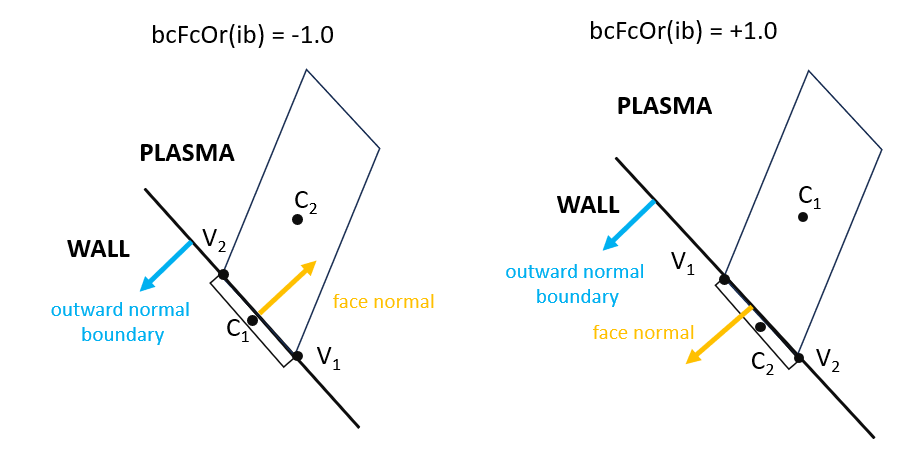
\includegraphics[height=4cm]{FiguresWG/bcfcor.PNG}}
\else
    \centerline{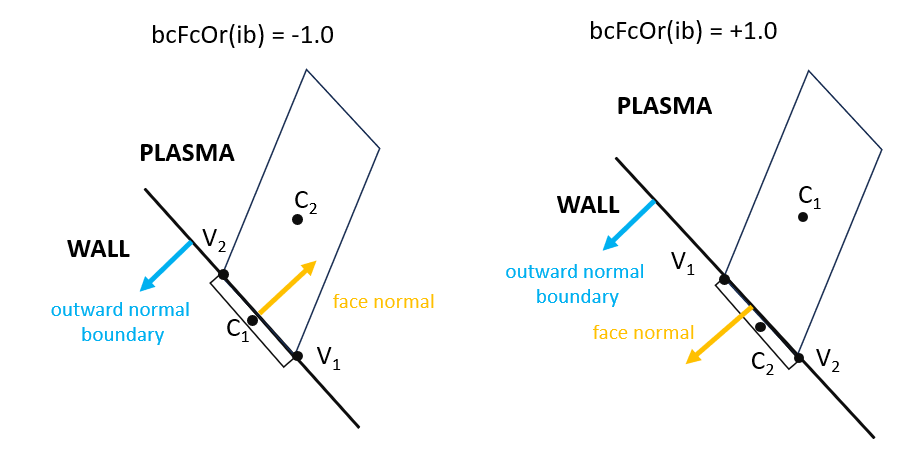
\includegraphics[height=4cm]{FiguresWG/bcfcor.eps}}
\fi
    \caption{Illustration of {\tt bcFcOr}.}
    \label{fig:bcfcor}
\end{figure}

Most boundary conditions fall in one of three categories: Dirichlet, Neumann, or flux.

\textbf{Flux}

To impose a given flux, the net source term in the guard cell must be equal to that flux. Since no fluxes are computed between the guard cells, the flux across the guard cell face must equal the source term.

\textbf{Dirichlet}
\begin{sloppypar}
To impose a fixed value in a guard cell, the code makes use of the different source contributions and very large numbers. For example, to set a fixed density {\tt $n_{BC}$},
the code sets {\tt sna(iCv,0,is) = VBIG $\times$ fcS $\times$ $n_{BC}$}, and {\tt sna(iCv,1,is) = - VBIG $\times$ fcS}, with {\tt sna(iCv,is) = sna(iCv,0,is) + sna(iCv,1,is) $\times$ na(iCv,is)} and where {\tt VBIG} is a very large number. Because {\tt VBIG} is so large, the only way to get a physical source is to have {\tt na(iCv,is) = $n_{BC}$}.
\end{sloppypar}

\textbf{Neumann}
\begin{sloppypar}
To set the gradient normal to the boundary, the code again makes use of the different source contributions and very large numbers. For orthogonal cells, these boundary conditions correctly impose the gradient normal to the boundary face.
For cells that are skewed with respect to the boundary face, the implementation depends on the (partially experimental) {\tt b2stbc\_BC2\_cor9} switch.
To impose for example a density gradient $\Phi$ with {\tt b2stbc\_BC2\_cor9 = 0.0}, the code sets
{\tt sna(iCv,0,is) = VBIG $\times$ fcS $\times$ ($\Phi$ $\times$ ( fcHc(1) + fcHc(2) ) $\times \cos \gamma$ + na(iCv\_internal)} and {\tt sna(iCv,1,is) = - VBIG $\times$ fcS}, where {\tt na(iCv\_internal)} is the density in the first interior cell. To get a physical source, we must have {\tt $\Phi$ $\times$ ( fcHc(1) + fcHc(2) ) $\times \cos \gamma$ + na(iCv\_internal) = na(iCv)}. This results in the correct normal gradient for skewed cells, only if there would be no gradients in the direction tangential to the boundary face. When {\tt b2stbc\_BC2\_cor9 = 1.0}, a correction term based on the vertex values is added, such that $\Phi$ is the gradient normal to the boundary, also in the presence of tangential gradients (up to the interpolation error).
\end{sloppypar}

%% TODO: convert all below to unstructured?

In this Section, the boundaries are denoted as $S_0$ for the PFR boundaries, $S_1$ for the core boundaries, $E$ for the Eastern boundaries (right targets), $W$ for the Western boundaries (left targets), and $N$ for the outer main wall boundary.

\subsection{Particle balance equations}

$S_{n_a} = S_{n_a,0} + S_{n_a,1} n_a$

\subsubsection{South. Private region}

\underline{If $z_a = 0$}

{\em For leakage boundary condition:} {\tt BCCON = 10}

\begin{equation}
\left. \frac{\sqrt g}{h_y}\Gamma_{ay} \right|_{S_0}
=
\left. \left[
p_{n_a,a,1} \frac{\sqrt g}{h_y} \sqrt{\frac{z_a T_e + T_i}{m_a}} n_a
+
\sum \limits_{a=0}^{ns-1} r_{rec,a,0} c_{nsr}
\max \left\{0, -\frac{\sqrt g}{h_y} \Gamma_{ay} \right\}
\right] \right|_{S_0}
\end{equation}

$p_{n_a,a,1} = -10^{-2}, \;\; r_{rec,0,0} = 0,\;\; r_{rec,1,0} = 1$

$\widetilde{\Gamma}_{ay}$ was replaced by $\Gamma_{ay}$

$c_{nsr}$ --- neutral sources rescale coefficient, $1$ --- when working with B2.5 standalone and $10^{-10}$ when coupling to Eirene

$p_{n_a,a,1}$ is the radial leakage velocity, in units of the local species sound speed. Negative velocities are directed out of the plasma.

\underline{If $z_a \neq 0$}

{\em For decay length boundary condition:} {\tt BCCON = 9}

\begin{equation}
\begin{matrix}
\left. \frac{\sqrt g}{h_y} \widetilde{\Gamma}_{ay} \right|_{S_0}& =
& \left\{
\begin{matrix}
\left. \left[
        -\frac{1}{p_{n_a,a,1}} \frac{\sqrt g}{h_y}  \left(
                D^{(AN)}_{n,a} + D^{(AN)}_{p,a} \left(z_a T_e + T_i \right)
        \right) n_a
\right] \right|_{S_0}, & \text{mdf\_fnb} = 0
\\
\left. \left[
\begin{matrix}
        -\frac{1}{p_{n_a,a,1}} \frac{\sqrt g}{h_y} & \left(
                D^{(AN)}_{n,a} + D^{(AN)}_{p,a} \left(z_a T_e + T_i \right)
        \right) n_a
        + \\
        \frac{\sqrt g}{h_y} & D_{ayx} \frac{1}{h_x} \frac{\partial n_a T_i}{\partial x}
        +
        \frac{\sqrt g}{h_y} V_{ay}^{(E)} n_a
\end{matrix}
\right] \right|_{S_0}, & \text{mdf\_fnb} = 1
\end{matrix} \right.
\end{matrix}
\end{equation}

\begin{align}
S^{no\_mdf}_{n_a,0} & = 0 \\
S^{no\_mdf}_{n_a,1} & = - \frac{1}{p_{n_a,a,1}} \frac{\sqrt{g}}{h_y} \left( D^{(AN)}_{n,a} + D^{(AN)}_{p,a} \left( z_a T_e + T_i \right) \right)
\end{align}

$p_{n_a,a,1}$ is the density radial decay length of species $a$, in $m$.

{\em For leakage boundary conditions:} {\tt BCCON = 10}

\begin{equation}
\begin{matrix}
\left. \frac{\sqrt g}{h_y} \widetilde{\Gamma}_{ay} \right|_{S_0}& =
& \left\{
\begin{matrix}
\left. \left[
        p_{n_a,a,1} \frac{\sqrt g}{h_y} \sqrt{\frac{z_a T_e + T_i}{m_a}} n_a
        +
        \min \left\{0, \frac{\sqrt g}{h_y} n_a V_{ay}^{(E)} \right\}
\right] \right|_{S_0}, & \text{mdf\_fnb} = 0
\\
\left. \left[
p_{n_a,a,1} \frac{\sqrt g}{h_y} \sqrt{\frac{z_a T_e + T_i}{m_a}} n_a
        +
        \frac{\sqrt g}{h_y} D_{ayx} \frac{1}{h_x} \frac{\partial n_a T_i}{\partial x}
        +
        \min \left\{0, \frac{\sqrt g}{h_y} n_a V_{ay}^{(E)} \right\}
\right] \right|_{S_0}, & \text{mdf\_fnb} = 1
\end{matrix} \right.
\end{matrix}
\end{equation}

$p_{n_a,a,1} = -10^{-3}$ is the radial leakage velocity, in units of the species local sound speed. Negative velocities are directed out of the plasma.

\begin{align}
S^{no\_mdf}_{n_a,0} & = 0 \\
S^{no\_mdf}_{n_a,1} & = {p_{n_a,a,1}} \frac{\sqrt{g}}{h_y} \sqrt{\frac{z_a T_e + T_i}{m_a}} n_a
\end{align}

% -- To be checked --
{\em Imposing radial leakage:} {\tt BCCON = 15}

When using drifts, one should use {\tt BCCON = 10} instead.

\begin{equation}
\left. - \frac{\sqrt g}{h_y^2} D_{n,ay} \frac{\partial n_a}{\partial y} \right|_{S_0}
=
\left. \left[
c_{n_a,a,2} \frac{\sqrt g}{h_y} \sqrt{\frac{z_a T_e + T_i}{m_a}} n_a
\right] \right|_{S_0}
\end{equation}

$c_{n_a,a,2} = -10^{-3}$ is the radial leakage velocity, in units of the species local thermal velocity. Negative velocities are directed out of the plasma.

% -- end --

\subsubsection{South 1. Core plasma}

\underline{If $z_a = 0$}

%-------- end of 21st page -------------

{\em Imposing total particle flux:} {\tt BCCON = 8}

$\left. \frac{\sqrt g}{h_y} \widetilde{\Gamma}_{ay} \right|_{S_1} = 0$

$\left. \frac{\sqrt g}{h_y} \Gamma_{ay} \right|_{S_1} = 0$

\underline{If $z_a \neq 0$}

{\em Imposing a constant density :} {\tt BCCON = 1}

\begin{equation}
\left. \frac{\sqrt g}{h_y} \widetilde{\Gamma}_{ay} \right|_{S_1}
=
\frac{\sqrt{g}}{h_y}
\left. \left(
        \left. v_{big} n_a \right|_{S_1} - v_{big} n_a
\right) \right|_{S_1},
\;\;
v_{big} = 10^8 \sqrt{\frac{100 \text{eV}}{m_p}},
\;\;
\left. n_a \right|_{S_1} \text{ is the desired density in } m^{-3}
\end{equation}

{\em Imposing the total particle flux with constant flux density:} {\tt BCCON = 8}

\begin{equation*}
\left. \frac{\sqrt g}{h_y} \widetilde{\Gamma}_{ay} \right|_{S_1} =
\left. p_{n,a,0} \frac{
\frac{\sqrt g}{h_y}
} {
\sum \limits_i \left(
        \frac{\sqrt g}{h_y}
\right)_{i, -1}
} \right|_{S_1}
+
\left.
\frac{\sqrt g}{h_y} D_{ayx} \frac{1}{h_x} \frac{\partial n_a T_i}{\partial x}
\right|_{S_1} +
\left. \frac{\sqrt g}{h_y}V_{ya}^{(E)} n_a \right|_{S_1}
\end{equation*}

$p_{n,a,0}$ is the desired total particle flux, per unit time.

\subsubsection{North}

\underline{If $z_a = 0$}

{\em For leakage boundary condition:} {\tt BCCON = 10}

\begin{equation}
\left. - \frac{\sqrt g}{h_y} \Gamma_{ay} \right|_{N}
=
\left. \left[
p_{n_a,a,1} \frac{\sqrt g}{h_y} \sqrt{\frac{z_a T_e + T_i}{m_a}} n_a
+
\sum \limits_{a=0}^{ns-1} r_{rec,a,0} c_{nsr}
\max \left\{0, \frac{\sqrt g}{h_y} \Gamma_{ay} \right\}
\right] \right|_{N}
\end{equation}

$p_{n_a,a,1} = -10^{-2}, \;\; r_{rec,0,0} = 0,\;\; r_{rec,1,0} = 1$

$c_{nsr}$ --- neutral sources rescale coefficient, $1$ --- when working with B2.5 standalone and $10^{-10}$ when coupling to Eirene

$p_{n_a,a,1}$ is the radial leakage velocity, in units of the local species sound speed. Negative velocities are directed out of the plasma.

$\widetilde{\Gamma}_{ay}$ was replaced by $\Gamma_{ay}$

\underline{If $z_a \neq 0$}

{\em For decay length boundary condition:} {\tt BCCON = 9}

\begin{equation}
\begin{matrix}
\left. - \frac{\sqrt g}{h_y} \widetilde{\Gamma}_{ay} \right|_{N}& =
& \left\{
\begin{matrix}
\left. \left[
        \frac{1}{p_{n_a,a,1}} \frac{\sqrt g}{h_y}  \left(
                D^{(AN)}_{n,a} + D^{(AN)}_{p,a} \left(z_a T_e + T_i \right)
        \right) n_a
\right] \right|_{N}, & \text{mdf\_fnb} = 0
\\
\left. \left[
\begin{matrix}
        \frac{1}{p_{n_a,a,1}} & \frac{\sqrt g}{h_y}  \left(
                D^{(AN)}_{n,a} + D^{(AN)}_{p,a} \left(z_a T_e + T_i \right)
        \right) n_a \\
        -
        \frac{\sqrt g}{h_y} & D_{ayx} \frac{1}{h_x} \frac{\partial n_a T_i}{\partial x}
        -
        \frac{\sqrt g}{h_y} V_{ay}^{(E)} n_a
\end{matrix}
\right] \right|_{N}, & \text{mdf\_fnb} = 1
\end{matrix} \right.
\end{matrix}
\end{equation}

\begin{align}
S^{no\_mdf}_{n_a,0} & = 0 \\
S^{no\_mdf}_{n_a,1} & = \frac{1}{p_{n_a,a,1}} \frac{\sqrt{g}}{h_y} \left( D^{(AN)}_{n,a} + D^{(AN)}_{p,a} \left( z_a T_e + T_i \right) \right)
\end{align}

$p_{n_a,a,1}$ is the density radial decay length of species $a$, in $m$.

{\em For leakage boundary conditions:} {\tt BCCON = 10}

\begin{equation}
\begin{matrix}
\left. - \frac{\sqrt g}{h_y} \widetilde{\Gamma}_{ay} \right|_{N}& =
& \left\{
\begin{matrix}
\left. \left[
        p_{n_a,a,1} \frac{\sqrt g}{h_y} \sqrt{\frac{z_a T_e + T_i}{m_a}} n_a
        -
        \max \left\{0, \frac{\sqrt g}{h_y} n_a V_{ay}^{(E)} \right\}
\right] \right|_{N}, & \text{mdf\_fnb} = 0
\\
\left. \left[
        p_{n_a,a,1} \frac{\sqrt g}{h_y} \sqrt{\frac{z_a T_e + T_i}{m_a}} n_a
        -
        \frac{\sqrt g}{h_y} D_{ayx} \frac{1}{h_x} \frac{\partial n_a T_i}{\partial x}
        -
        \max \left\{0, \frac{\sqrt g}{h_y} n_a V_{ay}^{(E)} \right\}
\right] \right|_{N}, & \text{mdf\_fnb} = 1
\end{matrix} \right.
\end{matrix}
\end{equation}

$p_{n_a,a,1} = -10^{-3}$ is the radial leakage velocity, in units of the species local sound speed. Negative velocities are directed out of the plasma.

\begin{align}
S^{no\_mdf}_{n_a,0} & = 0 \\
S^{no\_mdf}_{n_a,1} & = {p_{n_a,a,1}} \frac{\sqrt{g}}{h_y} \sqrt{\frac{z_a T_e + T_i}{m_a}} n_a
\end{align}

% -- To be checked --
{\em Imposing radial leakage:} {\tt BCCON = 15}

When using drifts, one should use {\tt BCCON = 10} instead.

\begin{equation}
\left. \frac{\sqrt g}{h_y^2} D_{n,ay} \frac{\partial n_a}{\partial y} \right|_N
=
\left. \left[
c_{n_a,a,2} \frac{\sqrt g}{h_y} \sqrt{\frac{z_a T_e + T_i}{m_a}} n_a
\right] \right|_N
\end{equation}

$c_{n_a,a,2} = -10^{-3}$ is the radial leakage velocity, in units of the species local thermal velocity. Negative velocities are directed out of the plasma.

% -- end --

\subsubsection{North with puffing}

\underline{If $z_a = 0$}

{\em Imposing a particle flux per unit area:} {\tt BCCON = 5}

\begin{equation}
\left. - \frac{\sqrt g}{h_y} \widetilde{\Gamma}_{ay} \right|_N
=
\left. p_{n,a,0} \frac{\sqrt g}{h_y} \right|_N
+
\left.
\sum \limits_{a=0}^{ns-1} \left[
        r_{rec,a,0} c_{nsr}
        \max \left\{0, -\frac{\sqrt g}{h_y} \Gamma_{ay} \right\}
\right] \right|_N
\end{equation}

$c_{nsr}$ --- neutral sources rescale coefficient, $1$ --- when working with B2.5 standalone and $10^{-10}$ when coupling to Eirene

$r_{rec,0,0} = 0,\;\; r_{rec,1,0} = 1$

$p_{n,a,0}$ is the desired total particle flux density, in $m^{-2}.s^{-1}$.

$\widetilde{\Gamma}_{ay}$ was replaced by $\Gamma_{ay}$

or

{\em Imposing a total particle flux with constant flux density:} {\tt BCCON = 8}

\begin{equation*}
\left. - \frac{\sqrt g}{h_y} \widetilde{\Gamma}_{ay} \right|_N =
\left. \frac{ p_{n,a,0}
}{
\sum \limits_{i=0}^{Nx-1} \left(
        \frac{\sqrt g}{h_y}
\right)_{i, Ny}
}
\frac{\sqrt g}{h_y} \right|_N
+
\left. \sum \limits_{a=0}^{ns-1} \left[
        r_{rec,a,0} c_{nsr}
        \max \left\{0, \frac{\sqrt g}{h_y} \Gamma_{ay} \right\}
\right]
\right|_N
\end{equation*}

$c_{nsr}$ --- neutral sources rescale coefficient, $1$ --- when working with B2.5 standalone and $10^{-10}$ when coupling to Eirene

$r_{rec,0,0} = 0,\;\; r_{rec,1,0} = 1$

$p_{n,a,0}$ is the desired total particle flux, per unit time.

$\widetilde{\Gamma}_{ay}$ was replaced by $\Gamma_{ay}$

\subsubsection{West}

%-------- end of 23rd page -------------

\underline{If $z_a = 0$}

{\em Imposing a given particle flux per unit area:} {\tt BCCON = 5}

\begin{equation}
\left. \frac{\sqrt g}{h_x} \Gamma_{ax} \right|_W
=
\left. \left[
p_{n,a,1} \frac{\sqrt g}{h_y}
+
c_{nsr} \sum \limits_{a=0}^{ns-1} r_{rec,a,0}
\max \left\{0, -\frac{\sqrt g}{h_x} \Gamma_{ax} \right\}
\right] \right|_W
\end{equation}

$r_{rec,0,0} = 0,\;\; r_{rec,1,0} = 1,\;\; p_{n_a,a,1} = 0 $

\begin{equation}
\left. \frac{\sqrt g}{h_x} \widetilde{\Gamma}_{ax} \right|_W
=
\left. \left[
p_{n,a,1} \frac{\sqrt g}{h_x}
+
c_{nsr} \sum \limits_{a=0}^{ns-1} r_{rec,a,0}
\max \left\{0, -\frac{\sqrt g}{h_x} \Gamma_{ax} \right\}
\right] \right|_W
\end{equation}

$\widetilde{\Gamma}_{ax}$ was replaced by $\Gamma_{ax}$

$r_{rec,0,0} = 0,\;\; r_{rec,1,0} = 1,\;\; p_{n_a,a,1} = 0 $

\underline{If $z_a \neq 0$}

{\em Sheath density boundary condition:} {\tt BCCON = 3}

\begin{equation*}
\left. \frac{\sqrt g}{h_x} \Gamma_{ax} \right|_W = \left.
10^{20} \frac{\sqrt{g}}{h_x} \frac{\partial n_a}{\partial x}
\right|_W
\end{equation*}

{\em Drift-compatible, Bohm-Chodura sheath entrance condition} {\tt BCCON = 14}

{\em If the sine of the incident field line angle is larger than {\tt Qalfmin}:}

{\em - Marginal imposition, with collective sound speed:} {\tt MOMPAR(,,2)} = $p_{m,a,2} < 0.5$

To be used in conjunction with {\tt BCENE = 15}, {\tt BCENI = 15}, {\tt BCMOM = 13}, and {\tt BCPOT = 11}.

\begin{equation*}
\left. \frac{\sqrt g}{h_x} \widetilde{\Gamma}_{ax} \right|_W
=
\left. \left[
- p_{n,a,1} \frac{\sqrt g}{h_x} |b_x|
\sqrt{\frac{\sum \limits_{\substack{b = 0 \\ z_b \neq 0}}^{ns-1} p_b}{\sum \limits_{\substack{b = 0 \\ z_b \neq 0}}^{ns-1} m_b n_b}} n_a
-
\frac{\sqrt g}{h_x} D_{axy} \frac{1}{h_y} \frac{\partial n_a T_i}{\partial y}
\right]
\right|_W
\end{equation*}

$p_{n,a,1} = +1$

{\em - Non-marginal imposition, with individual species sound speed:} {\tt MOMPAR(,,2)} = $p_{m,a,2} \geq 0.5$

to be used in conjunction with {\tt BCMOM = 13}, {\tt BCENE = 15} with {\tt bcene\_15\_style = 1}, {\tt BCENI = 15}, {\tt BCPOT = 3} or {\tt BCPOT = 11} with {\tt istyle\_fchi=0}.

This condition imposes that the sum of the poloidal projection of the parallel velocity and the poloidal $\exb$ velocity (restricted to not exceed $\pm 2 c_{s,a} |b_x|$), equals \textit{at least} the specific species sound speed $c_{s,a}$, reprojected in the the poloidal direction.

The parameter $p_{m,a,1}$ is set by {\tt MOMPAR(,,1)}. The parameter $\chi$ is set by {\tt GAMMAI}.

\begin{equation*}
\left. \frac{\sqrt g}{h_x} \widetilde{\Gamma}_{ax} \right|_W
=
\left. \left[
- \frac{\sqrt g}{h_x} |b_x|
U_{out} n_a
-
\frac{\sqrt g}{h_x} D_{axy} \frac{1}{h_y} \frac{\partial n_a T_i}{\partial y}
\right]
\right|_W
\end{equation*}

\begin{equation*}
  U_{out} = \max \left( -u_{\parallel,a}^{extrap}- \frac{V_{\exb}^{restr}}{|b_x|}, p_{m,a,1} \cdot \sqrt{\frac{\chi T_i + z_a T_e}{m_a}} \right)
\end{equation*}

where $u_{\parallel,a}^{extrap}$ is the extrapolated parallel velocity at the target, and $V_{\exb}^{restr}$ is the poloidal $\exb$ velocity restricted to not exceed $\pm 2 c_{s,a} |b_x|$.

{\em For nearly tangent field lines, we use instead:}

\begin{equation}
\begin{matrix}
\left. - \frac{\sqrt g}{h_x} \widetilde{\Gamma}_{ax} \right|_W & =
& \left\{
\begin{matrix}
\left. \left[ \frac{\sqrt g}{h_x} p_{n,a,1} \sqrt{\frac{\sum \limits_{\substack{b = 0 \\ z_b \neq 0}}^{ns-1} p_b}{\sum \limits_{\substack{b = 0 \\ z_b \neq 0}}^{ns-1} m_b n_b}} n_a \alpha_{\max} +
   \max \left( 0, \frac{\sqrt g}{h_x} V^{(E)}_{ax} n_a \right) \right] \right|_W, & \text{mdf\_fnb = 0}
\\
\left. \left[ \frac{\sqrt g}{h_x} p_{n,a,1} \sqrt{\frac{\sum \limits_{\substack{b = 0 \\ z_b \neq 0}}^{ns-1} p_b}{\sum \limits_{\substack{b = 0 \\ z_b \neq 0}}^{ns-1} m_b n_b}} n_a \alpha_{\max} +
   \max \left( 0, \frac{\sqrt g}{h_x} \left( V^{(E)}_{ax} + \widetilde{\widetilde{V}}^{(dia)}_{ax} \right) n_a \right) + \tilde\Gamma^{(PSch)}_{ax} \right] \right|_W, & \text{mdf\_fnb = 1}
\end{matrix}
\right.
\end{matrix}
\end{equation}

where $\alpha_{\max}$ is given by {\tt Qalfmax}.

Both {\tt Qalfmin} and {\tt Qalfmax} are provided in the {\tt b2fgmtry} file or through the {\tt b2us\_prep\_Qalfmin} and {\tt b2us\_prep\_Qalfmax} switches, respectively. Default value for both is $10^{-3}$.

\subsubsection{East}

\underline{If $z_a = 0$}

{\em Imposing a given particle flux per unit area:} {\tt BCCON = 5}

\begin{equation}
\left. - \frac{\sqrt g}{h_x} \Gamma_{ax} \right|_E
=
\left. \left[
p_{n,a,1} \frac{\sqrt g}{h_y}
+
c_{nsr} \sum \limits_{a=0}^{ns-1} r_{rec,a,0}
\max \left\{0, \frac{\sqrt g}{h_x} \Gamma_{ax} \right\}
\right] \right|_E
\end{equation}

$r_{rec,0,0} = 0,\;\; r_{rec,1,0} = 1,\;\; p_{n_a,a,1} = 0 $

%-------- end of 24th page -------------


\begin{equation}
\left. - \frac{\sqrt g}{h_x} \widetilde{\Gamma}_{ax} \right|_E
=
\left. \left[
c_{nsr} \sum \limits_{a=0}^{ns-1} r_{rec,a,0}
\max \left\{0, \frac{\sqrt g}{h_x} \Gamma_{ax} \right\}
\right] \right|_E
\end{equation}

$\widetilde{\Gamma}_{ax}$ was replaced by $\Gamma_{ax}$

$r_{rec,0,0} = 0,\;\; r_{rec,1,0} = 1$

\underline{If $z_a \neq 0$}

{\em Sheath density boundary condition:} {\tt BCCON = 3}

\begin{equation*}
\left. - \frac{\sqrt g}{h_x} \Gamma_{ax} \right|_E =
- 10^{20} \left. \frac{\sqrt{g}}{h_x} \frac{\partial n_a}{\partial x}
\right|_E
\end{equation*}

{\em Drift-compatible, Bohm-Chodura sheath entrance condition} {\tt BCCON = 14}

{\em If the sine of the incident field line angle is larger} {\tt Qalfmin}:

{\em - Marginal imposition, with collective sound speed:} {\tt MOMPAR(,,2)} = $p_{m,a,2} < 0.5$

To be used in conjunction with {\tt BCENE = 15}, {\tt BCENI = 15}, {\tt BCMOM = 13}, and {\tt BCPOT = 11}.

\begin{equation*}
\left. - \frac{\sqrt g}{h_x} \widetilde{\Gamma}_{ax} \right|_E
=
\left. \left[
- p_{n,a,1} \frac{\sqrt g}{h_x} |b_x|
\sqrt{\frac{\sum \limits_{\substack{b = 0 \\ z_b \neq 0}}^{ns-1} p_b}{\sum \limits_{\substack{b = 0 \\ z_b \neq 0}}^{ns-1} m_b n_b}} n_a
+
\frac{\sqrt g}{h_x} D_{axy} \frac{1}{h_y} \frac{\partial n_a T_i}{\partial y}
\right]
\right|_E
\end{equation*}

$p_{n,a,1} = +1$

{\em - Non-marginal imposition, with individual species sound speed:} {\tt MOMPAR(,,2)} = $p_{m,a,2} \geq 0.5$

to be used in conjunction with {\tt BCMOM = 13}, {\tt BCENE = 15} with {\tt bcene\_15\_style = 1}, {\tt BCENI = 15}, {\tt BCPOT = 3} or {\tt BCPOT = 11} with {\tt istyle\_fchi=0}.

This condition imposes that the sum of the poloidal projection of the parallel velocity and the poloidal $\exb$ velocity (restricted to not exceed $\pm 2 c_{s,a} |b_x|$), equals \textit{at least} the specific species sound speed $c_{s,a}$, reprojected in the the poloidal direction.

The parameter $p_{m,a,1}$ is set by {\tt MOMPAR(,,1)}. The parameter $\chi$ is set by {\tt GAMMAI}.

\begin{equation*}
\left. - \frac{\sqrt g}{h_x} \widetilde{\Gamma}_{ax} \right|_E
=
\left. \left[
- \frac{\sqrt g}{h_x} |b_x|
U_{out} n_a
+
\frac{\sqrt g}{h_x} D_{axy} \frac{1}{h_y} \frac{\partial n_a T_i}{\partial y}
\right]
\right|_E
\end{equation*}

\begin{equation*}
  U_{out} = \max \left( u_{\parallel,a}^{extrap} + \frac{V_{\exb}^{restr}}{|b_x|}, p_{m,a,1} \cdot \sqrt{\frac{\chi T_i + z_a T_e}{m_a}} \right)
\end{equation*}

where $u_{\parallel,a}^{extrap}$ is the extrapolated parallel velocity at the target, and $V_{\exb}^{restr}$ is the poloidal $\exb$ velocity restricted to not exceed $\pm 2 c_{s,a} |b_x|$.

{\em For nearly tangent field lines, we use instead:}

\begin{equation}
\begin{matrix}
\left. \frac{\sqrt g}{h_x} \widetilde{\Gamma}_{ax} \right|_E & =
& \left\{
\begin{matrix}
\left. \left[ \frac{\sqrt g}{h_x} p_{n,a,1} \sqrt{\frac{\sum \limits_{\substack{b = 0 \\ z_b \neq 0}}^{ns-1} p_b}{\sum \limits_{\substack{b = 0 \\ z_b \neq 0}}^{ns-1} m_b n_b}} n_a \alpha_{\max} +
   \max \left( 0, \frac{\sqrt g}{h_x} V^{(E)}_{ax} n_a \right) \right] \right|_E, & \text{mdf\_fnb = 0}
\\
\left. \left[ \frac{\sqrt g}{h_x} p_{n,a,1} \sqrt{\frac{\sum \limits_{\substack{b = 0 \\ z_b \neq 0}}^{ns-1} p_b}{\sum \limits_{\substack{b = 0 \\ z_b \neq 0}}^{ns-1} m_b n_b}} n_a \alpha_{\max} +
   \max \left( 0, \frac{\sqrt g}{h_x} \left( V^{(E)}_{ax} + \widetilde{\widetilde{V}}^{(dia)}_{ax} \right) n_a \right) + \tilde\Gamma^{(PSch)}_{ax} \right] \right|_E, & \text{mdf\_fnb = 1}
\end{matrix}
\right.
\end{matrix}
\end{equation}

\subsection{Parallel momentum balance for ions}

$S_{m_a} = S_{m_a,0} + S_{m_a,1} V_{\parallel a} + S_{m_a,2} m_a n_a + S_{m_a,3} m_a n_a V_{\parallel a}$

\subsubsection{South. Private region}

\underline{If $z_a = 0$}

{\em Weakly imposing a velocity:} {\tt BCMOM = 4}

\begin{equation*}
\left. h_z \frac{\sqrt g}{h_y} \Gamma_{ay}^m \right|_{S_0} =
\left. \left[
p_{m,a,1} p_{m,a,2} h_z \frac{\sqrt g}{h_y} -
p_{m,a,2} h_z \frac{\sqrt g}{h_y} V_{\parallel a}
\right] \right|_{S_0}
\end{equation*}

$p_{m,a,1}=0$ is the imposed velocity, in $m.s^{-1}$, and $p_{m,a,2}=10^5$ is the strength with which this velocity is imposed.

We had this b.c.

$\left. h_z \frac{\sqrt g}{h_y} \Gamma_{ay}^m \right|_{S_0} =
\left. \left[
c_{m,a,3} h_z \frac{\sqrt g}{h_y} m_a n_a V_{\parallel a} +
c_{m,a,6} \max \left(0,-h_z \frac{\sqrt g}{h_y} \frac{\Gamma_{ay}^{Cor}}{n_a} \right)
m_a n_a V_{\parallel a}
\right] \right|_{S_0}$, delete term with {\tt max} !

%-------- end of 25th page -------------

$\Gamma_{ay}^{Cor} = \Gamma_{ay} + \Gamma_{ay}^{(dia)}$

$c_{m,a,3} = -10^{10}$, we have $c_{m,a,6}=-1$, but not $c_{m,a,6}=0$

Inserted into {\tt b2stbc\_phys} for {\tt BCMOM=12} as $c_{m,a,3} \rightarrow p_{m,a,2} = -10^{10}$, and $c_{m,a,6} \rightarrow p_{m,a,1} = -1$

\underline{If $z_a \neq 0$}

{\em Weakly imposing a velocity:} {\tt BCMOM = 4}

\begin{equation}
\left. h_z \frac{\sqrt g}{h_y} \Gamma_{ay}^m \right|_{S_0} =
\left. \left[
        p_{m,a,1} p_{m,a,2} h_z \frac{\sqrt g}{h_y} -
        p_{m,a,2} h_z \frac{\sqrt g}{h_y} V_{\parallel a}
\right] \right|_{S_0}
\end{equation}

$p_{m,a,1}=0$ is the imposed velocity, in $m.s^{-1}$, and $p_{m,a,2}=10^5$ is the strength with which this velocity is imposed.

\begin{equation}
\left. h_z \frac{\sqrt g}{h_y} \Gamma_{ay}^m \right|_{S_0} =
\left. \left[
        c_{m,a,3} h_z \frac{\sqrt g}{h_y} m_a n_a V_{\parallel a} +
        c_{m,a,6} \max \left(
                0, -h_z \frac{\sqrt g}{h_y} \frac{\Gamma_{ay}^{Cor}}{n_a}
        \right) m_a n_a V_{\parallel a}
\right] \right|_{S_0}
\end{equation}

delete term with {\tt max}!

$\Gamma_{ay}^{Cor} = \Gamma_{ay} + \Gamma_{ay}^{(dia)}$

$c_{m,a,3} = 0$,  $c_{m,a,6} = -1$

\subsubsection{South 1. Core}

\underline{If $z_a = 0$}

{\em Weakly imposing a velocity:} {\tt BCMOM = 4}

$ \left. h_z \frac{\sqrt g}{h_y} \Gamma_{ay}^m \right|_{S_1} = \left. \left[
        p_{m,a,1} p_{m,a,2} h_z \frac{\sqrt g}{h_y} -
        p_{m,a,2} h_z \frac{\sqrt g}{h_y} V_{\parallel a}
\right] \right|_{S_1}$

$p_{m,a,1}=0$ is the imposed velocity, in $m.s^{-1}$, and $p_{m,a,2}=10^5$ is the strength with which this velocity is imposed.

$ \left. h_z \frac{\sqrt g}{h_y} \Gamma_{ay}^m \right|_{S_1} = c_{m,a,3} h_z \left. \frac{\sqrt g}{h_y} m_a n_a V_{\parallel a} \right|_{S_1}$

$c_{m,a,3} = -10^{10}$

Inserted into {\tt b2stbc\_phys} for {\tt BCMOM=12} as $c_{m,a,3} \rightarrow p_{m,a,2} = -10^{10},\;c_{m,a,6} \rightarrow
p_{m,a,1} = 0$

\underline{If $z_a \neq 0$}

%-------- end of 26th page -------------

{\em Weakly imposing a velocity:} {\tt BCMOM = 4}

$ \left. h_z \frac{\sqrt g}{h_y} \Gamma_{ay}^m \right|_{S_1} = \left. \left[
        p_{m,a,1} p_{m,a,2} h_z \frac{\sqrt g}{h_y} -
        p_{m,a,2} \frac{\sqrt g}{h_y} V_{\parallel a}
\right] \right|_{S_1}$

$p_{m,a,1}=0$ is the imposed velocity, in $m.s^{-1}$, and $p_{m,a,2}=10^5$ is the strength with which this velocity is imposed.

{\em {\tt b2stbc\_spb} style:} {\tt BCMOM = 14}

\begin{align*}
\left. h_z \frac{\sqrt g}{h_y} \Gamma_{ay}^m \right|_{S_1} = &
c_{m,a,3} h_z \left. \frac{\sqrt g}{h_y} m_a n_a V_{\parallel a} \right|_{S_1} + \\
& \left. \left[
h_z \frac{\sqrt g}{h_y} m_a \left\langle n_a \right\rangle \left( -2 \right)\frac{\left\langle T_i \right\rangle B_z}{ez_a}\frac{\partial}{h_x \partial x} \left( \frac{1}{B^2} \right) \left\langle V_{\parallel a} \right\rangle c_{drift} +
c_{corflux} h_z \frac{\sqrt g}{h_y}
\right] \right|_{S_1} \\
+ & \left. c_{m,a,1} \max \left( 0 , - h_z \frac{\sqrt{g}}{h_y} \frac{\Gamma_{ay}^{Cor}}{n_a} \right) m_a n_a V_{\parallel a} \right|_{S_1}
\end{align*}

$c_{m,a,1} = 0$, $c_{m,a,3} = -10^{10}$

{\em Prescribe the value of the parallel velocity as a function of the poloidal coordinate:} {\tt BCMOM = 15}

\begin{equation*}
\left. h_z \frac{\sqrt g}{h_y} \Gamma_{ay}^m \right|_{S_1} =
\left. v_{big} n_{e0} m_{a} h_z \frac{\sqrt g}{h_y} \left[
        \frac{\langle B \rangle}{B} p_{m,a,1} - V_{\parallel a}
\right] \right|_{S_1}
\end{equation*}

where $\langle B \rangle = \frac{\mathlarger{\oint}_{S_1} B \sqrt{g} \, dx}{\mathlarger{\oint}_{S_1} \sqrt{g} \, dx}$, the integration is done over the innermost magnetic surface, $v_{big} = 10^{8} \sqrt{\frac{100 \text{eV}}{m_p}}$, $n_{e0} = 10^{20}$, $p_{m,a,1}$ is the given value of the average parallel velocity, in $m.s^{-1}$.

\subsubsection{North}

\underline{If $z_a=0$}

{\em Weakly imposing a velocity:} {\tt BCMOM = 4}

$ \left. -h_z \frac{\sqrt g}{h_y} \Gamma_{ay}^m \right|_N = \left. \left[
        p_{m,a,1} p_{m,a,2} h_z \frac{\sqrt g}{h_y} -
        p_{m,a,2} h_z \frac{\sqrt g}{h_y} V_{\parallel a}\right]
\right|_N$

$p_{m,a,1}=0$ is the imposed velocity, in $m.s^{-1}$, and $p_{m,a,2}=10^5$ is the strength with which this velocity is imposed.

$\left. -h_z \frac{\sqrt g}{h_y} \Gamma_{ay}^m \right|_N = \left. \left[
        c_{m,a,3} h_z \frac{\sqrt g}{h_y} m_a n_a V_{\parallel a} +
        c_{m,a,6} \max \left(
                0, h_z \frac{\sqrt g}{h_y} \frac{\Gamma_{ay}^{Cor}}{n_a}
        \right) m_a n_a V_{\parallel a}
\right]
\right|_N$

delete term with {\tt max} !

$c_{m,a,3} = -10^{10}$, we have  $c_{m,a,6} = -1$, but not $c_{m,a,6} = 0$

Inserted into {\tt b2stbc\_phys} for {\tt BCMOM=12} as $c_{m,a,3} \rightarrow p_{m,a,2} = -10^{10},\;c_{m,a,6} \rightarrow p_{m,a,1} = -1$

\underline{If $z_a \neq 0$}

%-------- end of 27th page -------------

{\em Weakly imposing a velocity:} {\tt BCMOM = 4}

$ \left. -h_z \frac{\sqrt g}{h_y} \Gamma_{ay}^m \right|_N = \left[
        p_{m,a,1} p_{m,a,2} h_z \frac{\sqrt g}{h_y} -
        p_{m,a,2} h_z \frac{\sqrt g}{h_y} V_{\parallel a}
\right]|_N$

$p_{m,a,1}=0$ is the imposed velocity, in $m.s^{-1}$, and $p_{m,a,2}=10^5$ is the strength with which this velocity is imposed.

\begin{equation*}
\left. -h_z \frac{\sqrt g}{h_y} \Gamma_{ay}^m \right|_N =
\left. \left[
c_{m,a,3} h_z \frac{\sqrt g}{h_y} m_a n_a V_{\parallel a} +
c_{m,a,6} \max \left(
        0, h_z \frac{\sqrt g}{h_y} \frac{\Gamma_{ay}^{Cor}}{n_a}
\right) m_a n_a V_{\parallel a}
\right] \right|_N
\end{equation*}

$c_{m,a,3} = 0$, $c_{m,a,6} = -1$

\subsubsection{West}

\underline{If $z_a = 0$}, $p_{m,a,1} = 0$

\underline{If $z_a \neq 0$}, $p_{m,a,1} = 1$

{\em Drift-compatible, Bohm-Chodura sheath entrance condition} {\tt BCMOM = 13}

{\em If the sine of the incident field line angle is larger than} {\tt Qalfmin}:

{\em - Marginal imposition, with collective sound speed:} {\tt MOMPAR(,,2)} = $p_{m,a,2} < 0.5$

To be used in conjunction with {\tt BCENE = 15}, {\tt BCENI = 15}, {\tt BCCON = 14}, and {\tt BCPOT = 11}.

\begin{equation*}
\left. h_z \frac{\sqrt g}{h_x} \Gamma_{ax}^m \right|_W = \left. \left[
        p_{m,a,1} \frac{u_{big}}{\epsilon^2} V_{West} m_a n_a -
        \frac{u_{big}}{\epsilon^2} h_z \frac{\sqrt g}{h_x} |b_x| m_a n_a V_{\parallel a}
\right]
\right|_W
\end{equation*}

with $u_{big} = 10^{10} \sqrt{\frac{100 \text{eV}}{m_p}}$ and $\epsilon = 10^{-10}$.

\begin{equation*}
V_{West} =
- h_z \frac{\sqrt g}{h_x} \frac{|b_x|}{b_x} \min \left( 2 c_s, V_{ax}^{(\exb)} \right)
- h_z \frac{\sqrt g}{h_x} b_x
\sqrt{\frac{\sum \limits_{\substack{a = 0 \\ z_a \neq 0}}^{ns-1} p_a}
{\sum \limits_{\substack{a = 0 \\ z_a \neq 0}}^{ns-1} m_a n_a}}
\end{equation*}

{\em - Non-marginal imposition, with individual species sound speed:} {\tt MOMPAR(,,2)} = $p_{m,a,2} \geq 0.5$

to be used in conjunction with {\tt BCCON = 14}, {\tt BCENE = 15} with {\tt bcene\_15\_style = 1}, {\tt BCENI = 15}, {\tt BCPOT = 3} or {\tt BCPOT = 11} with {\tt istyle\_fchi = 0}.

This condition imposes that the sum of the poloidal projection of the parallel velocity and the poloidal $\exb$ velocity (restricted to not exceed $\pm 2 c_{s,a} |b_x|$), equals \textit{at least} the specific species sound speed $c_{s,a}$, reprojected in the the poloidal direction.

The parameter $p_{m,a,1}$ is set by {\tt MOMPAR(,,1)}. The parameter $\chi$ is set by {\tt GAMMAI}.

\begin{equation*}
  \left. \frac{\sqrt g}{h_x} \Gamma_{ax}^m \right|_W = \left. \left[
          -\frac{u_{big}}{\epsilon^2} n_a m_a \frac{\sqrt{g}}{h_x} U_{out} \frac{B_x}{|B_x|}
          -\frac{u_{big}}{\epsilon^2} n_a m_a \frac{\sqrt{g}}{h_x} V_{\parallel,a}
  \right]
  \right|_W
  \end{equation*}

\begin{equation*}
  U_{out} = \max \left( -u_{\parallel,a}^{extrap} - \frac{V_{\exb}^{restr}}{|b_x|}, p_{m,a,1} \cdot \sqrt{\frac{\chi T_i + z_a T_e}{m_a}} \right)
\end{equation*}

where $u_{\parallel,a}^{extrap}$ is the extrapolated parallel velocity at the target, and $V_{\exb}^{restr}$ is the poloidal $\exb$ velocity restricted to not exceed $\pm 2 c_{s,a} |b_x|$.

{\em For nearly tangent field lines}, we apply a no radial shear velocity condition.

\underline{If $z_a = 0$}

{\em Imposing a specified parallel velocity:} {\tt BCMOM = 1}

$\left. \frac{\sqrt g}{h_x} \Gamma_{ax}^m \right|_W = \left. \left[
        u_{big} n_{e00} \frac{m_a}{m_p} \frac{\sqrt{g}}{h_x} p_{m,a,1} -
        u_{big} n_{e00} \frac{m_a}{m_p} \frac{\sqrt{g}}{h_x} V_{\parallel a}
\right]
\right|_W$

$p_{m,a,1}=0$ is the imposed velocity in $m.s^{-1}$, $n_{e00} = 10^{20}$.

\underline{If $z_a \neq 0$}

{\em Imposing a sheath velocity boundary condition:} {\tt BCMOM = 3}

\begin{equation*}
\left. \frac{\sqrt g}{h_x} \Gamma_{ax}^m \right|_W = \left. \left[
        -\frac{u_{big}}{\epsilon^2} n_a m_a \frac{\sqrt{g}}{h_x} u_{p_{out}}
        -\frac{u_{big}}{\epsilon^2} n_a m_a \frac{\sqrt{g}}{h_x} V_{\parallel a}
\right]
\right|_W
\end{equation*}

%-------- end of 28th page -------------

If $p_{m,a,2} < 0.5$:

\begin{equation*}
c_s = \sqrt{\frac{\sum \limits_{\substack{a = 0 \\ z_a \neq 0}}^{ns-1} p_a}{\sum \limits_{\substack{a = 0 \\ z_a \neq 0}}^{ns-1} m_a n_a}}
\end{equation*}

$u_{u_{out}} = p_{m,a,1} c_s |b_x|$

$u_{p_{out}} = \max \left\{ 0, \frac{u_{u_{out}}}{|b_x|} + u_a^{(dia)} b_z \right\}$

If $p_{m,a,2} > 0.5$:

$c_{s,a} = \sqrt{\frac{\gamma_i T_i + z_a^2 \frac{n_a}{n_e} T_e}{m_a}}$

where $\gamma_i$ is the adiabatic ratio of specific heats ({\tt GAMMAI} in {\tt b2.boundary.parameters}),

$u_{u_{out}} = \max \left\{ p_{m,a,1} c_{s,a}, u_{extrap} \right\}$

where $u_{extrap}$ is the extrapolated value to the sheath edge of the poloidal velocity $u_a$,

$u_{p_{out}} = \max \left\{ 0, u_{u_{out}} + u_a^{(dia)} \frac{b_z}{b_x} \right\}$.

\subsubsection{East}

\underline{If $z_a = 0$}, $p_{m,a,1} = 0$

\underline{If $z_a \neq 0$}, $p_{m,a,1} = 1$

{\em Drift-compatible, Bohm-Chodura sheath entrance condition} {\tt BCMOM = 13}

{\em If the sine of the incident field line angle is larger than} {\tt Qalfmin}:

{\em - Marginal imposition, with collective sound speed:} {\tt MOMPAR(,,2)} = $p_{m,a,2} < 0.5$

To be used in conjunction with {\tt BCENE = 15}, {\tt BCENI = 15}, {\tt BCCON = 14}, and {\tt BCPOT = 11}.

$\left. -h_z \frac{\sqrt g}{h_x} \Gamma_{ax}^m \right|_E = \left. \left[
        p_{m,a,1} \frac{u_{big}}{\epsilon^2} V_{East} m_a n_a -
        \frac{u_{big}}{\epsilon^2} h_z \frac{\sqrt g}{h_x} |b_x| m_a n_a V_{\parallel a}
\right]
\right|_E$

\begin{equation*}
V_{East} =
- h_z \frac{\sqrt g}{h_x} \frac{|b_x|}{b_x} \min \left( 2 c_s, V_{ax}^{(\exb)} \right)
+ h_z \frac{\sqrt g}{h_x} b_x
\sqrt{\frac{\sum \limits_{\substack{a = 0 \\ z_a \neq 0}}^{ns-1} p_a}
{\sum \limits_{\substack{a = 0 \\ z_a \neq 0}}^{ns-1} m_a n_a}}
\end{equation*}

{\em - Non-marginal imposition, with individual species sound speed:} {\tt MOMPAR(,,2)} = $p_{m,a,2} \geq 0.5$

to be used in conjunction with BCCON=14, BCENE=15 with {\tt bcene\_15\_style=1}, BCENI=15, BCPOT=3 or BCPOT=11 with {\tt istyle\_fchi=0}.

This condition imposes that the sum of the poloidal projection of the parallel velocity and the poloidal $\exb$ velocity (restricted to not exceed $\pm 2 c_{s,a} |b_x|$), equals \textit{at least} the specific species sound speed $c_{s,a}$, reprojected in the the poloidal direction.

The parameter $p_{m,a,1}$ is set by {\tt MOMPAR(,,1)}. The parameter $\chi$ is set by {\tt GAMMAI}.

\begin{equation*}
  -\left. \frac{\sqrt g}{h_x} \Gamma_{ax}^m \right|_E = \left. \left[
          \frac{u_{big}}{\epsilon^2} n_a m_a \frac{\sqrt{g}}{h_x} U_{out} \frac{B_x}{|B_x|}
          -\frac{u_{big}}{\epsilon^2} n_a m_a \frac{\sqrt{g}}{h_x} V_{\parallel,a}
  \right]
  \right|_E
  \end{equation*}

\begin{equation*}
  U_{out} = \max \left( u_{\parallel,a}^{extrap} + \frac{V_{\exb}^{restr}}{|b_x|}, p_{m,a,1} \cdot \sqrt{\frac{\chi T_i + z_a T_e}{m_a}} \right)
\end{equation*}

where $u_{\parallel,a}^{extrap}$ is the extrapolated parallel velocity at the target, and $V_{\exb}^{restr}$ is the poloidal $\exb$ velocity restricted to not exceed $\pm 2 c_{s,a} |b_x|$.

{\em For nearly tangent field lines}, we apply a no radial shear velocity condition.

\underline{If $z_a = 0$}

{\em Imposing a specified parallel velocity:} {\tt BCMOM = 1}

\begin{equation*}
\left. -\frac{\sqrt g}{h_x} \Gamma_{ax}^m \right|_E = \left. \left[
        u_{big} n_{e00} \frac{m_a}{m_p} \frac{\sqrt{g}}{h_x} p_{m,a,1} -
        u_{big} n_{e00} \frac{m_a}{m_p} \frac{\sqrt{g}}{h_x} V_{\parallel a}
\right]
\right|_E
\end{equation*}

$p_{m,a,1}=0$ is the imposed parallel velocity in $m.s^{-1}$.

\underline{If $z_a \neq 0$}

{\em Imposing a sheath velocity boundary condition:} {\tt BCMOM = 3}

\begin{equation*}
\left. -\frac{\sqrt g}{h_x} \Gamma_{ax}^m \right|_E = \left. \left[
        -\frac{u_{big}}{\epsilon^2} n_a m_a \frac{\sqrt{g}}{h_x} u_{p_{out}}
        -\frac{u_{big}}{\epsilon^2} n_a m_a \frac{\sqrt{g}}{h_x} V_{\parallel a}
\right]
\right|_E
\end{equation*}

If $p_{m,a,2} < 0.5$:

\begin{equation*}
c_s = \sqrt{\frac{\sum \limits_{\substack{a = 0 \\ z_a \neq 0}}^{ns-1} p_a}{\sum \limits_{\substack{a = 0 \\ z_a \neq 0}}^{ns-1} m_a n_a}}
\end{equation*}

$u_{u_{out}} = p_{m,a,1} c_s |b_x|$,

$u_{p_{out}} = \max \left\{ 0, \frac{u_{u_{out}}}{|b_x|} - u_a^{(dia)} b_z \right\}$

If $p_{m,a,2} > 0.5$:

$c_{s,a} = \sqrt{\frac{\gamma_i T_i + z_a^2 \frac{n_a}{n_e} T_e}{m_a}}$

$u_{u_{out}} = \max \left\{ p_{m,a,1} c_{s,a}, u_{extrap} \right\}$

$u_{p_{out}} = \max \left\{ 0, u_{u_{out}} - u_a^{(dia)} \frac{b_z}{b_x} \right\}$.

%-------- end of 29th page -------------

\subsection{Current continuity equation}

$S_{ch} = S_{ch,0} + S_{ch,1} \Phi + S_{ch,2} n_e + S_{ch,3} n_e \Phi$

\subsubsection{South. Private region}

$\left. \frac{\sqrt{g}}{h_y} j_y \right|_{S_0} = 0$

\begin{equation*}
\begin{matrix}
\left. \frac{\sqrt{g}}{h_y} j_y \right|_{S_0} = &
& \left\{
\begin{matrix}
0, & \text{facdrift} = 0 \\
\left. \frac{\sqrt{g}}{h_y}
\left(
        \widetilde{j}_y^{(dia)} + j_y^{(in)} + \widetilde{j}_y^{(vis \parallel)} + j_y^{(vis \perp)}
        + \widetilde{j}_y^{(visq)} + \widetilde{j}_y^{(s)}
\right) \right|_{S_0}
, & \text{facdrift} \neq 0 \\
\end{matrix} \right.
\end{matrix}
\end{equation*}

\subsubsection{South 1. Core}

\begin{equation*}
\begin{matrix}
\left. \frac{\sqrt{g}}{h_y} j_y \right|_{S_1} = &
& \left\{
\begin{matrix}
0, & \text{facdrift} = 0 \\
\left. \frac{\sqrt{g}}{h_y}
\left(
        \left\langle \widetilde{j}_y^{(dia)} \right\rangle
\right) \right|_{S_1}
, & \text{facdrift} \neq 0 \\
\end{matrix} \right.
\end{matrix}
\end{equation*}

\begin{equation*}
\begin{matrix}
\left. \frac{\sqrt{g}}{h_y} j_y \right|_{S_1} = &
& \left\{
\begin{matrix}
0, & \text{facdrift} = 0 \\
\left. \frac{\sqrt{g}}{h_y}
\left(
        \left\langle \widetilde{j}_y^{(dia)} \right\rangle +
        \left\langle j_y^{(in)} \right\rangle
\right) \right|_{S_1}
, & \text{facdrift} \neq 0 \\
\end{matrix} \right.
\end{matrix}
\end{equation*}

\begin{equation*}
\left\langle \widetilde{j}_y^{(dia)} \right\rangle =
- \frac{
        B_z \left\langle
                \sum \limits^{ns-1}_{\substack{a = 0 \\
                        z_a \neq 0}} n_a \left(
                        z_a T_e + T_i
                \right)
        \right\rangle
}{h_x}
\frac{\partial}{\partial x}
\left( \frac{1}{B^2} \right)
\end{equation*}

\begin{equation*}
\left\langle j_y^{(in)} \right\rangle =
- \frac{B_z}{2}
\frac{\partial}{h_x \partial x}
\left( \frac{1}{B^2} \right)
\sum \limits^{ns-1}_{\substack{a = 0 \\
    z_a \neq 0}} m_a n_a \left\langle V^2_{a \parallel}
\right\rangle
\end{equation*}

\subsubsection{North}

\begin{equation*}
\begin{matrix}
\left. \frac{\sqrt{g}}{h_y} j_y \right|_N = &
& \left\{
\begin{matrix}
0, & \text{facdrift} = 0 \\
\left. \frac{\sqrt{g}}{h_y}
\left(
        \left\langle \widetilde{j}_y^{(dia)} \right\rangle
\right) \right|_N
, & \text{facdrift} \neq 0 \\
\end{matrix} \right.
\end{matrix}
\end{equation*}

%-------- end of 30th page -------------

\begin{equation*}
\begin{matrix}
\left. - \frac{\sqrt{g}}{h_y} j_y \right|_N = &
& \left\{
\begin{matrix}
0, & \text{facdrift} = 0 \\
\left. - \frac{\sqrt{g}}{h_y}
\left(
        \widetilde{j}_y^{(dia)} + j_y^{(in)} +
        \widetilde{j}_y^{(vis \parallel)} + j_y^{(vis \perp)} +
        \widetilde{j}_y^{(visq)} + \widetilde{j}_y^{(s)}
\right) \right|_N
, & \text{facdrift} \neq 0 \\
\end{matrix} \right.
\end{matrix}
\end{equation*}

\subsubsection{West}

{\em Imposing a sound speed velocity flux:} {\tt BCPOT = 11}

To be used in conjunction with {\tt BCENE = 15}, {\tt BCENI = 15}, {\tt BCMOM = 13}, and {\tt BCCON = 14}.

\small\begin{equation*}
\left. \frac{\sqrt g}{h_x} j_x \right|_W =
\frac{\sqrt g}{h_x} e \left. \left[
        - \sum \limits_{a=0}^{ns-1} z_a \left(
                p_{n,a,1} b_\alpha \sqrt{\frac{\sum \limits_{\substack{b = 0 \\ z_b \neq 0}}^{ns-1} p_b}{\sum \limits_{\substack{b = 0 \\ z_b \neq 0}}^{ns-1} m_b n_b}} n_a
        \right) +
        \left( 1 - \gamma_e \right) b_\alpha n_e \frac{1}{\sqrt{2\pi}}
        \sqrt{\frac{T_e}{m_e}} \exp \left( -\frac{e \left( \Phi - p_{\Phi,2} \right)}{T_e} \right)
\right] \right|_W
\end{equation*}\normalsize

with

\begin{equation*}
b_\alpha = \left\{
\begin{matrix}
|b_x| & , \text{if} \ |b_x| \ge \alpha_{\min} \\
\alpha_{\max} & , \text{if} \ |b_x| < \alpha_{\min}
\end{matrix}
\right.
\end{equation*}

{\em Imposing a sheath potential boundary condition:} {\tt BCPOT = 3}

$\left. \frac{\sqrt g}{h_x} j_x \right|_W =
\frac{\sqrt g}{h_x} e \left. \left[
        \sum \limits_{b=0}^{ns-1} z_a \Gamma_{ax} +
        \left( 1 - \gamma_e \right) |b_x| n_e \frac{1}{\sqrt{2\pi}}
        \sqrt{\frac{T_e}{m_e}}
        \exp \left( -\frac{e \left( \Phi - p_{\Phi,2}\right)}{T_e} \right)
\right] \right|_W$

\subsubsection{East}

{\em Imposing a sound speed velocity flux:} {\tt BCPOT = 11}

To be used in conjunction with {\tt BCENE = 15}, {\tt BCENI = 15}, {\tt BCMOM = 13}, and {\tt BCCON = 11}.

\small\begin{equation*}
\left. -\frac{\sqrt g}{h_x} j_x \right|_E =
\frac{\sqrt g}{h_x} e \left. \left[
        - \sum \limits_{a=0}^{ns-1} z_a \left(
                p_{n,a,1} b_\alpha \sqrt{\frac{\sum \limits_{\substack{b = 0 \\ z_b \neq 0}}^{ns-1} p_b}{\sum \limits_{\substack{b = 0 \\ z_b \neq 0}}^{ns-1} m_b n_b}} n_a
        \right) +
        \left( 1 - \gamma_e \right) b_\alpha n_e \frac{1}{\sqrt{2\pi}}
        \sqrt{\frac{T_e}{m_e}} \exp \left( -\frac{e \left( \Phi - p_{\Phi,2} \right)}{T_e} \right)
\right] \right|_E
\end{equation*}\normalsize

{\em Imposing a sheath potential boundary condition:} {\tt BCPOT = 3}

$\left. -\frac{\sqrt g}{h_x} j_x \right|_E =
\frac{\sqrt g}{h_x} e \left. \left[
        -\sum \limits_{a=0}^{ns-1} z_a \Gamma_{ax} +
        \left( 1 - \gamma_e \right) |b_x| n_e \frac{1}{\sqrt{2\pi}}
        \sqrt{\frac{T_e}{m_e}}
        \exp \left( -\frac{e \left( \Phi - p_{\Phi,2}\right)}{T_e} \right)
\right] \right|_E$

%-------- end of 31st page -------------

\subsection{Energy balance equation for electrons}\label{sec:bcene}

$S_{h_e} = S_{h_e,0} + S_{h_e,1} T_e + S_{h_e,2} n_e + S_{h_e,3} n_e T_e$

\subsubsection{South. Private region}

{\em Imposing the {\tt b2stbc\_spb} style boundary condition:} {\tt BCENE = 11}

\begin{equation*}
\left. \frac{\sqrt g}{h_y} \widetilde q_{ey} \right|_{S_0} = \left. \left[
        \left(
                c_{h_e,2} \frac{\sqrt g}{h_y} \sqrt{\frac{T_e}{m_e}}
        \right) T_e n_e
        +
        c_{h_e,7} \max \left(
                0, -\frac{\sqrt g}{h_y} \widetilde f_{ey}
        \right) T_e - q_{ex}^{P.Sch}
\right] \right|_{S_0}
\end{equation*}

$c_{h_e,2} = -10^{-4}$, $c_{h_e,7} = -1$, $c_{h_e,2} \rightarrow p_{h_e,2} = -10^{-4}$, $c_{h_e,7} \rightarrow p_{h_e,1} = -1$

{\em Imposing a decay length for the electron temperature:} {\tt BCENE = 22}

$\left. -\frac{\sqrt g}{h_y} \kappa_{ey} \frac{\partial T_e}{h_y \partial y} \right|_{S_0} = \left. \left[ \left( p_{h_e,1} \frac{\sqrt g}{h_y}\sqrt{\frac{T_e}{m_e}} \right) T_e n_e \right] \right|_{S_0}$

{\em Imposing a decay length for the electron temperature:} {\tt BCENE=9}

\begin{equation*}
\begin{matrix}
\left. \frac{\sqrt g}{h_y} \widetilde q_{ey} \right|_{S_0}=
& \left\{
\begin{matrix}
\left. \left[
        \frac{5}{2} \sum \limits_{a=0}^{ns-1} z_a S_{n_a,0}^{no\_mdf} T_e
        -
        \frac{\sqrt g}{h_y} \frac{\kappa_e^{(AN)}}{p_{h_e,1}} T_e
        +
        \frac{5}{2} \sum \limits_{a=0}^{ns-1} z_a S_{n_a,1}^{no\_mdf} n_a T_e
\right] \right|_{S_0},
& \text{mdf\_fhe} = 0 \\
\left. \left[
\begin{matrix}
        & \frac{5}{2} \sum \limits_{a=0}^{ns-1} z_a S_{n_a,0}^{no\_mdf} T_e
        -
        \frac{\sqrt g}{h_y} \frac{\kappa_e^{(AN)}}{p_{h_e,1}} T_e \\
        + &
        \frac{5}{2} \sum \limits_{a=0}^{ns-1} z_a S_{n_a,1}^{no\_mdf} n_a T_e
        -
        q_{ey}^{P.Sch}
        +
        \frac{\sqrt g}{h_y} \frac{3}{2} V_{ey}^{(E)} n_e T_e
\end{matrix}
\right] \right|_{S_0},
& \text{mdf\_fhe} = 1 \\
\end{matrix} \right.
\end{matrix}
\end{equation*}

\subsubsection{South 1. Core}

{\em In {\tt b2stbc\_spb}:}

\begin{equation*}
\left. \frac{\sqrt g}{h_y} \widetilde q_{ey} \right|_{S_1} = \left. \left[
        \left(
                c_{h_e,0} \frac{\sqrt g}{h_y}
                +
                c_{h_e,1} \frac{\sqrt g}{h_y} T_e
        \right)
\right] \right|_{S_1}
\end{equation*}

$c_{h_e,0} = 4 \cdot 10^{13}$, $c_{h_e,a,1} = -10^{30}$

{\em Imposing a total electron energy flux:} {\tt BCENE = 8}

$\left. \frac{\sqrt g}{h_y} q_{ey} \right|_{S_1} = p_{h_e,1} \left. \frac{
        \frac{\sqrt g}{h_y}}
        {\sum \limits_{core} \left( \frac{\sqrt g}{h_y} \right)}
\right|_{S_1}$

$p_{h_e,1}$ is the imposed total electron energy flux, in $W$.

\subsubsection{North}

{\em Imposing the {\tt b2stbc\_spb} style boundary condition:} {\tt BCENE = 11}

\begin{equation*}
\left. -\frac{\sqrt g}{h_y} \widetilde q_{ey} \right|_N = \left. \left[
        \left(
                p_{h_e,1} \frac{\sqrt g}{h_y} \sqrt{\frac{T_e}{m_e}}
        \right) T_e n_e
        +
        p_{h_e,2} \max \left(
                0, \frac{\sqrt g}{h_y} \widetilde f_{ey}
        \right) T_e - q_{ex}^{P.Sch}
\right] \right|_N
\end{equation*}

%-------- end of 32nd page -------------

$p_{h_e,1} = -10^{-4}$, $p_{h_e,2} = -1$

{\em Imposing a decay length for electron temperature:} {\tt BCENE = 22}

$\left. \frac{\sqrt g}{h_y} \kappa_{ey} \frac{\partial T_e}{h_y \partial y} \right|_N = \left. \left[ \left( p_{h_e,1} \frac{\sqrt g}{h_y}\sqrt{\frac{T_e}{m_e}} \right) T_e n_e \right] \right|_N$

{\em Imposing a decay length for electron temperature:} {\tt BCENE = 9}

$p_{h_e,1}$ is the radial electron temperature decay length, in $m$.

\begin{equation*}
\begin{matrix}
\left. -\frac{\sqrt g}{h_y} \widetilde q_{ey} \right|_{N}= &
& \left\{
\begin{matrix}
\left. \left[
        \frac{5}{2} \sum \limits_{a=0}^{ns-1} z_a S_{n_a,0}^{no\_mdf} T_e
        -
        \frac{\sqrt g}{h_y} \frac{\kappa_e^{(AN)}}{p_{h_e,1}} T_e
        +
        \frac{5}{2} \sum \limits_{a=0}^{ns-1} z_a S_{n_a,1}^{no\_mdf} n_a T_e
\right] \right|_{N},
& \text{mdf\_fhe} = 0 \\
\left. \left[
\begin{matrix}
        & \frac{5}{2} \sum \limits_{a=0}^{ns-1} z_a S_{n_a,0}^{no\_mdf} T_e
        -
        \frac{\sqrt g}{h_y} \frac{\kappa_e^{(AN)}}{p_{h_e,1}} T_e \\
        + &
        \frac{5}{2} \sum \limits_{a=0}^{ns-1} z_a S_{n_a,1}^{no\_mdf} n_a T_e
        +
        q_{ey}^{P.Sch}
        -
        \frac{\sqrt g}{h_y} \frac{3}{2} V_{ey}^{(E)} n_e T_e
\end{matrix}
\right] \right|_{N},
& \text{mdf\_fhe} = 1  \\
\end{matrix} \right.
\end{matrix}
\end{equation*}

\subsubsection{West}

{\em Imposing the {\tt b2stbc\_spb} style boundary condition for electron temperature:} {\tt BCENE = 15}

To be used in conjunction with {\tt BCENI = 15}, {\tt BCCON = 14}, {\tt BCMOM = 13}, and {\tt BCPOT = 11}.

If {\tt 'bcene\_15\_style'} is set to {\tt '0'}

\begin{equation}\label{eq:sheath_electron_bc_West_style0}
\left. \frac{\sqrt g}{h_x} \widetilde q_{ex} \right|_W = \left. \left[
        -\left(
                \frac{1 + \gamma_e}{1 -\gamma_e} T_e + e\Phi
        \right)
        \max \left(
                0, \frac{\sqrt g}{h_x}
                \sum \limits_{a=0}^{ns-1} z_a p_{n,a,1} |b_x|
                \sqrt{\frac{\sum \limits_{\substack{b = 0 \\ z_b \neq 0}}^{ns-1} p_b}{\sum \limits_{\substack{b = 0 \\ z_b \neq 0}}^{ns-1} m_b n_b}} n_a
                +
                \frac{\sqrt g}{h_x} \frac{j_{\parallel}}{e}
        \right)
        -
        \frac{\sqrt g}{h_x} q_{ex}^{P.Sch}
\right] \right|_W
\end{equation}

If {\tt 'bcene\_15\_style'} is set to {\tt '1'} (recommended for stability, default):

\begin{equation}\label{eq:sheath_electron_bc_West_style1}
\left. \frac{\sqrt g}{h_x} \widetilde q_{ex} \right|_W = \left. \left[
        -\frac{\sqrt g}{h_x} b_\alpha \left(
                \left( 1 + \gamma_e + p_{h_e,1} \right) T_e +
                \left( 1 - \gamma_e \right) e \left( \Phi - p_{\Phi,2} \right)
        \right) n_e \frac{1}{\sqrt{2 \pi}}
        \sqrt{\frac{T_e}{m_e}} \exp \left( -\frac{e \left( \Phi - p_{\Phi,2} \right) }{T_e} \right)
        -
        \frac{\sqrt g}{h_x} q_{ex}^{P.Sch}
\right] \right|_W
\end{equation}

with $p_{h_e,1}$ set by {\tt ENEPAR(:,1)} and $p_{\Phi,2}$ set by {\tt POTPAR(:,2)}.

If $p_{n,a,2} \ne 0$, a diffusive term $-\frac{\sqrt{g}}{h_x} p_{h_i,2} \frac{D^{(AN)}_{n,a}}{p_{n,a,2}} z_a n_a$ is included in the species summation inside the r.h.s. of Eq.~(\ref{eq:sheath_electron_bc_West_style0}) or, summed over species, to the second term in the r.h.s of Eq.~(\ref{eq:sheath_electron_bc_West_style1}).

In case of electron temperature or potential oscillations, one can make use of the {\tt b2stbc\_stab\_coeff\_sheath\_te} switch, assigning it a positive value (recommended range between 1 and 100), to include an additional zero-sum stabilizing term.

{\em Imposing the sheath boundary condition for electron temperature:} {\tt BCENE = 3}

$\left. \frac{\sqrt g}{h_x} q_{ex} \right|_W = \left[ \left(
        p_{h_e,1} + \frac{ e \left( \Phi - p_{\Phi,2} \right) }{T_e}
\right)
\frac{\sqrt g}{h_x} \nu_{e_{out}} T_e
- \left.
\frac{\sqrt g}{h_x} q_{ex}^{P.Sch}
\right] \right|_W$

$p_{h_e,1} = 0.9$, $p_{\Phi,2}$ is the applied electric potential at the target, in $V$.

If $p_{m,a_{main},2} < 0.5$:

%-------- end of 33rd page -------------

$\nu_{e_{out}} = \min \left\{ 0, -u_{u_{out}} n_e - \frac{j_x}{e} \right\}$,
$u_{u_{out}} = p_{m,a_{main},1} c_s |b_x|$
\begin{equation*}
c_s = \sqrt{\frac{\sum \limits_{\substack{a = 0 \\ z_a \neq 0}}^{ns-1} p_a}{\sum \limits_{\substack{a = 0 \\ z_a \neq 0}}^{ns-1} m_a n_a}}
\end{equation*}

If $p_{m,a_{main},2} > 0.5$:

$\nu_{e_{out}} = \min \left\{ 0, - \sum \limits_{\substack{a = 0 \\ z_a \neq 0}}^{ns-1} u_{a_{out}} z_a n_a - \frac{j_x}{e} \right\}$

$u_{a_{out}} = \max \left\{ p_{m,a,1} c_{s,a} |b_x|, u_{extrap} \right\}$

where $u_{extrap}$ is the extrapolated value of the plasma poloidal velocity defined as $u = \sum \limits_{a=0}^{ns-1} \frac{\Gamma_{a,x}}{n_a}$.

$c_{s,a} = \sqrt{\frac{\gamma_i T_i + z_a^2 \frac{n_a}{n_e} T_e}{m_a}}$

where $\gamma_i$ is the adiabatic ratio of specific heats ({\tt GAMMAI} in {\tt b2.boundary.parameters}).

\subsubsection{East}

{\em Imposing the {\tt b2stbc\_spb} style boundary condition for electron temperature:} {\tt BCENE = 15}

To be used in conjunction with {\tt BCENI = 15}, {\tt BCCON = 14}, {\tt BCMOM = 13}, and {\tt BCPOT = 11}.

If {\tt 'bcene\_15\_style} is set to {\tt '0'}:

\begin{equation}\label{eq:sheath_electron_bc_East_style0}
\left. -\frac{\sqrt g}{h_x} \widetilde q_{ex} \right|_E = \left. \left[
        -\left(
                \frac{1 + \gamma_e}{1 -\gamma_e} T_e + e\Phi
        \right)
        \max \left(
                0, \frac{\sqrt g}{h_x}
                \sum \limits_{a=0}^{ns-1} z_a p_{n,a,1} |b_x|
                \sqrt{\frac{\sum \limits_{\substack{b = 0 \\ z_b \neq 0}}^{ns-1} p_b}{\sum \limits_{\substack{b = 0 \\ z_b \neq 0}}^{ns-1} m_b n_b}} n_a
                -
                \frac{\sqrt g}{h_x} b_x \frac{j_{\parallel}}{e}
        \right)
        +
        \frac{\sqrt g}{h_x} q_{ex}^{P.Sch}
\right] \right|_E
\end{equation}

If {\tt 'bcene\_15\_style'} is set to {\tt '1'} (recommended for stability, default):

\begin{equation}\label{eq:sheath_electron_bc_East_style1}
\left. -\frac{\sqrt g}{h_x} \widetilde q_{ex} \right|_E = \left. \left[
        -\frac{\sqrt g}{h_x} b_\alpha \left(
                \left( 1 + \gamma_e + p_{h_e,1} \right) T_e +
                \left( 1 - \gamma_e \right) e \left( \Phi - p_{\phi,2} \right)
        \right) n_e \frac{1}{\sqrt{2 \pi}}
        \sqrt{\frac{T_e}{m_e}} \exp \left( -\frac{e \left( \Phi - p_{\Phi,2} \right) }{T_e} \right)
        +
        \frac{\sqrt g}{h_x} q_{ex}^{P.Sch}
\right] \right|_E
\end{equation}

with $p_{h_e,1}$ set by {\tt ENEPAR(:,1)} and $p_{\Phi,2}$ set by {\tt POTPAR(:,2)}.

If $p_{n,a,2} \ne 0$, a diffusive term $-\frac{\sqrt{g}}{h_x} p_{h_i,2} \frac{D^{(AN)}_{n,a}}{p_{n,a,2}} z_a n_a$ is included in the species summation inside the r.h.s. of Eq.~(\ref{eq:sheath_electron_bc_East_style0}) or, summed over species, to the second term in the r.h.s of Eq.~(\ref{eq:sheath_electron_bc_East_style1}).

In case of electron temperature or potential oscillations, one can make use of the {\tt b2stbc\_stab\_coeff\_sheath\_te} switch, assigning it a positive value (recommended range between 1 and 100), to include an additional zero-sum stabilizing term.

{\em Imposing the sheath boundary condition for electron temperature:} {\tt BCENE = 3}

\begin{equation*}
\left. -\frac{\sqrt g}{h_x} \widetilde q_{ex} \right|_E = -\left[ \left(
        p_{h_e,1} + \frac{e \left( \Phi - p_{\Phi,2} \right) }{T_e}
\right)
\frac{\sqrt g}{h_x} \nu_{e_{out}} T_e
+ \left.
\frac{\sqrt g}{h_x} q_{ex}^{P.Sch}
\right] \right|_E
\end{equation*}

$p_{h_e,1} = 0.9$, $p_{\Phi,2}$ is the applied electric potential at the target, in $V$.

If $p_{m,a_{main},2} < 0.5$:

$\nu_{e_{out}} = \max \left\{ 0, u_{u_{out}} n_e - \frac{j_x}{e} \right\}$,
$u_{u_{out}} = p_{m,a_{main},1} c_s |b_x|$
\begin{equation*}
c_s = \sqrt{\frac{\sum \limits_{\substack{a = 0 \\ z_a \neq 0}}^{ns-1} p_a}{\sum \limits_{\substack{a = 0 \\ z_a \neq 0}}^{ns-1} m_a n_a}}
\end{equation*}

If $p_{m,a_{main},2} > 0.5$:

$\nu_{e_{out}} = \min \left\{ 0, \sum \limits_{\substack{a = 0 \\ z_a \neq 0}}^{ns-1} u_{a_{out}} z_a n_a - \frac{j_x}{e} \right\}$

$u_{a_{out}} = \max \left\{ p_{m,a,1} c_{s,a} |b_x|, u_{extrap} \right\}$

$c_{s,a} = \sqrt{\frac{\gamma_i T_i + z_a^2 \frac{n_a}{n_e} T_e}{m_a}}$

%-------- end of 34th page -------------

\subsection{Energy balance equation for ions}\label{sec:bceni}

$S_{h_i} = S_{h_i,0} + S_{h_i,1} T_i + S_{h_i,2} n_i + S_{h_i,3} n_i T_i$

\subsubsection{South. Private region}

{\em Imposing a decay length for the ion temperature:} {\tt BCENI = 9}

$p_{h_i,1}$ is the radial ion temperature decay length, in $m$.

$e_{rec,0} = 0$ and $e_{rec,1} = 0.3$ are energy recycling coefficients.

$r_{rec,0,0} = 0$ and $r_{rec,1,0} = 1$ are particle recycling coefficients.

\begin{equation*}
\left. \frac{\sqrt g}{h_y} \widetilde q_{iy} \right|_{S_0} = \left\{
  \begin{matrix}
  \left. \left[
  \begin{matrix}
    \frac{5}{2} \sum \limits_{a=0}^{ns-1} S_{n_a,0}^{no\_mdf} T_i -
    \frac{\sqrt g}{h_y} \frac{\kappa_i^{(AN)}}{p_{h_i,1}} T_i +
    \frac{5}{2} \sum \limits_{a=0}^{ns-1} S_{n_a,1}^{no\_mdf} n_a T_i + \\
  + c_{nsr} \left( \frac{3}{2} + BoRiS \right)
    \sum \limits_{a=0}^{ns-1} \max \left\{ e_{rec,a}
    \left( T_i + z_a \left( \Phi - p_{\Phi,2} \right) \right) \right. , \\
    \left. k_B T_{surf} \right\}
    r_{rec,a,0} \max \left\{ 0, -\frac{\sqrt g}{h_y} \Gamma_{ay} \right\}
  \end{matrix}
  \right] \right|_{S_0} & \text{mdf\_fhi} = 0
\\
  \begin{matrix}
  \left. \left[
    \begin{matrix}
      \frac{5}{2} \sum \limits_{a=0}^{ns-1} S_{n_a,0}^{no\_mdf} T_i -
      \frac{\sqrt g}{h_y} \frac{\kappa_i^{(AN)}}{p_{h_i,1}} T_i +
      \frac{5}{2} \sum \limits_{a=0}^{ns-1} S_{n_a,1}^{no\_mdf} n_a T_i \\
      - q_{iy}^{P.Sch} +
      \frac{\sqrt g}{h_y} \frac{3}{2} \sum \limits_{a=0}^{ns-1} V_{ay}^{(E)} n_a T_i + \\
    + c_{nsr} \left( \frac{3}{2} + BoRiS \right)
      \sum \limits_{a=0}^{ns-1} \max \left\{ e_{rec,a}
      \left( T_i + z_a \left( \Phi - p_{\Phi,2} \right) \right) \right. , \\
      \left. k_B T_{surf} \right\}
      r_{rec,a,0} \max \left\{ 0, -\frac{\sqrt g}{h_y} \Gamma_{ay} \right\}
   \end{matrix}
   \right] \right|_{S_0} & & \text{mdf\_fhi} = 1
  \end{matrix}
\end{matrix} \right.
\end{equation*}

{\em Imposing a constant ion temperature:} {\tt BCENI = 21}

\begin{equation*}
\left. \frac{\sqrt g}{h_y} \widetilde q_{iy} \right|_{S_0}
= \left.
p_{h_i,2} \sum \limits^{ns-1}_{\substack{a = 0 \\ z_a \neq 0}} \left(
        \frac{\sqrt g}{h_y} n_a \sqrt{\frac{z_a T_e + T_i}{m_a}}
\right) T_i \right|_{S_0} + \left.
p_{h_i,1} \max \left\{0, -\frac{\sqrt g}{h_y} \widetilde f_{iy}^{(E)} \right\} T_i
\right|_{S_0}
\end{equation*}

$p_{h_i,1} = -1$, $p_{h_i,2} = -10^{-2}$

{\em Imposing a decay length for the ion temperature:} {\tt BCENI = 22}

$\left. -\frac{\sqrt g}{h_y} \kappa_{iy} \frac{\partial T_i}{h_y \partial y} \right|_{S_0}
= \left.
p_{h_i,1} \sum \limits^{ns-1}_{\substack{a = 0 \\ z_a \neq 0}} \left(
        \frac{\sqrt g}{h_y} n_a \sqrt{\frac{z_a T_e + T_i}{m_a}}
\right) T_i \right|_{S_0}$

$p_{h_i,1}$ is the imposed ion temperature decay length, in $m$.

{\em {\tt b2stbc\_spb} boundary condition:}

$\left. \frac{\sqrt g}{h_y} \widetilde q_{iy} \right|_{S_0}
= \left.
\sum \limits^{ns-1}_{\substack{a = 0 \\ z_a \neq 0}} \left(
        c_{h_i,a,2} \frac{\sqrt g}{h_y} \frac{n_a}{n_i} \sqrt{\frac{z_a T_e + T_i}{m_a}}
\right) n_i T_i \right|_{S_0}
+ \left.
c_{h_i,a,7} \max \left\{0, -\frac{\sqrt g}{h_y} \widetilde f_{iy} \right\} T_i
\right|_{S_0}$

$c_{h_i,a,2} = -10^{-2}$

\subsubsection{South 1. Core}

{\em Imposing a total ion energy flux:} {\tt BCENI = 8}

%-------- end of 35th page -------------

\begin{equation*}
\left. \frac{\sqrt g}{h_y} \widetilde q_{iy} \right|_{S_1} = \left. \left[ p_{h_i,1} \frac{
        \frac{\sqrt g}{h_y}}
        {\sum \limits_{core} \left( \frac{\sqrt g}{h_y} \right)}
        - q_{iy}^{P.Sch}
        + \frac{3}{2} \frac{\left( j_y^{(AN)} + j_y^{(in)} + \widetilde{j}_y^{(vis \parallel)} + \widetilde{j}_y^{(visq)} + j_y^{(vis \perp)} \right)}{e} T_i
\right] \right|_{S_1}
\end{equation*}

$p_{h_i,1}$ is the imposed total ion energy flux, in $W$.

{\em {\tt b2stbc\_spb} boundary condition:}

$\left. \frac{\sqrt g}{h_y} \widetilde q_{iy} \right|_{S_1} =
\sum \limits_{a=0}^{ns-1}
\left. \left[
        \left(
                c_{h_i,a,0} \frac{\sqrt g}{h_y} \frac{n_a}{n_i}
                +
                c_{h_i,a,1} \frac{\sqrt g}{h_y} \frac{n_a}{n_i} T_i
        \right)
\right] \right|_{S_1}$

$c_{h_i,a,0} = 4 \cdot 10^{13}$, $c_{h_i,a,1} = -10^{30}$, $a=0.1$.

\subsubsection{North}

{\em Imposing an ion temperature decay length:} {\tt BCENE = 9}

$p_{h_i,1}$ is the radial ion temperature decay length, in $m$.

$e_{rec,0} = 0$ and $e_{rec,1} = 0.3$ are energy recycling coefficients.

$r_{rec,0,0} = 0$ and $r_{rec,1,0} = 1$ are particle recycling coefficients.

\begin{equation*}
- \left. \frac{\sqrt g}{h_y} \widetilde q_{iy} \right|_{N} = \left\{
  \begin{matrix}
    \left. \left[
    \begin{matrix}
       \frac{5}{2} \sum \limits_{a=0}^{ns-1} S_{n_a,0}^{no\_mdf} T_i -
       \frac{\sqrt g}{h_y} \frac{\kappa_i^{(AN)}}{p_{h_i,1}} T_i +
       \frac{5}{2} \sum \limits_{a=0}^{ns-1} S_{n_a,1}^{no\_mdf} n_a T_i \\
       + c_{nsr} \left( \frac{3}{2} + BoRiS \right)
         \sum \limits_{a=0}^{ns-1} \max \left\{
         e_{rec,a} \left( T_i + z_a \left( \Phi - p_{\Phi,2} \right) \right) , \right. \\
         \left. k_B T_{surf} \right\}
       r_{rec,a,0} \max \left\{ 0, -\frac{\sqrt g}{h_y} \Gamma_{ay} \right\}
    \end{matrix}
    \right] \right|_{N} & \text{mdf\_fhi} = 0
    \\
    \left. \left[
    \begin{matrix}
       \frac{5}{2} \sum \limits_{a=0}^{ns-1} S_{n_a,0}^{no\_mdf} T_i -
       \frac{\sqrt g}{h_y} \frac{\kappa_i^{(AN)}}{p_{h_i,1}} T_i +
       \frac{5}{2} \sum \limits_{a=0}^{ns-1} S_{n_a,1}^{no\_mdf} n_a T_i \\
       - q_{iy}^{P.Sch} +
       \frac{\sqrt g}{h_y} \frac{3}{2}
       \sum \limits_{a=0}^{ns-1} V_{ay}^{(E)} n_a T_i \\
       + c_{nsr} \left( \frac{3}{2} + BoRiS \right)
         \sum \limits_{a=0}^{ns-1} \max \left\{
         e_{rec,a} \left( T_i + z_a \left( \Phi - p_{\Phi,2} \right) \right) , \right. \\
       \left. k_B T_{surf} \right\}
       r_{rec,a,0} \max \left\{ 0, -\frac{\sqrt g}{h_y} \Gamma_{ay} \right\}
    \end{matrix}
    \right] \right|_{N} & \text{mdf\_fhi} = 1
  \end{matrix}
  \right.
\end{equation*}

{\em Boundary condition from {\tt b2stbc\_spb}:} {\tt BCENI = 21}

\begin{equation*}
\left. -\frac{\sqrt g}{h_y} \widetilde q_{iy} \right|_N
= \left.
p_{h_i,2} \sum \limits^{ns-1}_{\substack{a = 0 \\ z_a \neq 0}} \left(
        \frac{\sqrt g}{h_y} n_a \sqrt{\frac{z_a T_e + T_i}{m_a}}
\right) T_i \right|_N
+ \left.
p_{h_i,1} \max \left\{0, -\frac{\sqrt g}{h_y} \widetilde f_{iy} \right\} T_i
\right|_N
\end{equation*}

$p_{h_i,1} = -1$, $p_{h_i,2} = 10^{-2}$

{\em Prescribing a decay length for the ion temperature:} {\tt BCENI = 22}

$\left. \frac{\sqrt g}{h_y} k_{iy} \frac{\partial T_i}{h_y \partial y} \right|_N
= \left.
p_{h_i,1} \sum \limits^{ns-1}_{\substack{a = 0 \\ z_a \neq 0}} \left(
        \frac{\sqrt g}{h_y} n_a \sqrt{\frac{z_a T_e + T_i}{m_a}}
\right) T_i \right|_N$

$p_{h_i,1}$ is the imposed ion temperature decay length, in $m$.

{\em Boundary condition in {\tt b2stbc\_spb}:}

\begin{equation*}
\left. -\frac{\sqrt g}{h_y} \widetilde q_{iy} \right|_N
= \left.
\sum \limits^{ns-1}_{\substack{a = 0 \\ z_a \neq 0}} \left(
        c_{h_i,a,2}  \frac{\sqrt g}{h_y} \frac{n_a }{n_i} \sqrt{\frac{z_a T_e + T_i}{m_a}}
\right) n_i T_i \right|_N
+ \left.
c_{h_i,a,7} \max \left\{0, -\frac{\sqrt g}{h_y} \widetilde f_{iy} \right\} T_i
\right|_N
\end{equation*}

%-------- end of 36th page -------------

$c_{h_i,a,2} = -10^{-2}$

\subsubsection{West}

{\em Drift-compatible, Bohm-Chodura sheath entrance condition} {\tt BCENI = 15}

{\em If the sine of the incident field line angle is larger than} {\tt Qalfmin}:

{\em - Marginal imposition, with collective sound speed:} {\tt MOMPAR(ismain,,2)} = $p_{m,ismain,2} < 0.5$

To be used in conjunction with {\tt BCENE = 15}, {\tt BCCON = 14}, {\tt BCMOM = 13}, and {\tt BCPOT = 11}.

\begin{equation}\label{eq:sheath_ion_bc_West}
\left. \frac{\sqrt g}{h_x} \widetilde q_{ix} \right|_W = \left.
- p_{h_i,1} \frac{\sqrt g}{h_x} |b_x|
\sqrt{\frac{\sum \limits_{\substack{b = 0 \\ z_b \neq 0}}^{ns-1} p_b}{\sum \limits_{\substack{b = 0 \\ z_b \neq 0}}^{ns-1} m_b n_b}} T_i
\sum \limits^{ns-1}_{\substack{a = 0 \\ z_a \neq 0}} p_{n,a,1} n_a
-
\frac{\sqrt g}{h_x} q_{ix}^{P.Sch}
\right|_W
\end{equation}

$p_{h_i,1} = +1.5$

If $p_{n,a,2} \ne 0$, a diffusive term $-\frac{\sqrt{g}}{h_x} p_{h_i,2} \frac{D^{(AN)}_{n,a}}{p_{n,a,2}} n_a$ is included in the species summation inside the r.h.s. of Eq.~(\ref{eq:sheath_ion_bc_West}).

In case of ion temperature oscillations, one can make use of the {\tt b2stbc\_stab\_coeff\_sheath\_ti} switch, assigning it a positive value (recommended range between 1 and 100), to include an additional zero-sum stabilizing term.

{\em - Non-marginal imposition, with individual species sound speed:} {\tt MOMPAR(ismain,,2)} = $p_{m,ismain,2} \geq 0.5$

to be used in conjunction with {\tt BCMOM = 13}, {\tt BCENE = 15} with {\tt bcene\_15\_style = 1}, {\tt BCCON = 14}, {\tt BCPOT = 3} or {\tt BCPOT = 11} with {\tt istyle\_fchi = 0}.

This condition imposes that the ion heat flux, minus its Pfirsch-Schlueter component, is equal to the ion convective particle flux (excluding its Pfirsch-Schlueter component) times the ion sheath transmission coefficient.

The parameter $p_{i,1}$ is set by {\tt ENIPAR(:,1)}.

\begin{equation*}
  \left. \frac{\sqrt g}{h_x} \widetilde q_{ix} \right|_W = \left.
  - p_{i,1} \frac{\sqrt g}{h_x}
  \sum_a \left( -\widetilde{\Gamma}_{ax} - D_{axy}\frac{1}{h_y}\frac{\partial n_aT_i}{\partial y} \right) T_i
  -
  \frac{\sqrt g}{h_x} q_{ix}^{P.Sch}
  \right|_W
\end{equation*}

If $p_{n,a,2} \ne 0$, a diffusive term $-\frac{\sqrt{g}}{h_x} p_{h_i,2} \frac{D^{(AN)}_{n,a}}{p_{n,a,2}} n_a$ is included in the species summation inside the r.h.s. of Eq.~(\ref{eq:sheath_ion_bc_West}).

In case of ion temperature or potential oscillations, one can make use of the {\tt b2stbc\_stab\_coeff\_sheath\_ti} switch, assigning it a positive value (recommended range between 1 and 100), to include an additional zero-sum stabilizing term.

{\em For nearly tangent field lines}, we use instead:

\begin{equation}\label{eq:sheath_ion_bc_tangent_West}
\left. \frac{\sqrt g}{h_x} \widetilde q_{ix} \right|_W = \left.
- \frac{3}{2} \frac{\sqrt g}{h_x} \alpha_{\max} \sqrt{\frac{\sum \limits_{\substack{b = 0 \\ z_b \neq 0}}^{ns-1} p_b}{\sum \limits_{\substack{b = 0 \\ z_b \neq 0}}^{ns-1} m_b n_b}} n_i \right|_W
\end{equation}

If $\text{mdf\_fhi} \ne 0$, a term $-\frac{\sqrt g}{h_x} \left( q_{ix}^{P.Sch} + \frac{3}{2} \sum \limits_b V^{\exb}_{bx} n_b T_i \right)$ is added to the r.h.s. of Eq.~(\ref{eq:sheath_ion_bc_tangent_West}).

For coupled runs, if {\tt b2stbc\_bceni\_15\_style} is set to {\tt 1} (default is {\tt 0}), then $p_{h,i,1}$ above is replaced with the value deduced from the truncated drifting Maxwellian sampling in {\tt Eirene} (see Section 1.5.1 in the {\tt Eirene} manual for the full derivation):

$p_{h_i,1} = 2 + \nu^2_\tau + \nu^2_\nu + 0.5 \frac{g \left( \nu_\nu \right) - 1}{g \left( \nu_\nu \right)}$

\bigskip

{\em Boundary condition from {\tt b2stbc\_spb}:}

$\left. \frac{\sqrt g}{h_x} \widetilde q_{ix} \right|_W =
\left. \left[
        \sum \limits^{ns-1}_{\substack{a = 0 \\ z_a \neq 0}}
        \left(
                c_{h_i,a,7}
                \frac{\sqrt g}{h_x} |b_x|
                \sqrt{\frac{\sum \limits_{\substack{b = 0 \\ z_b \neq 0}}^{ns-1} p_b}{\sum \limits_{\substack{b = 0 \\ z_b \neq 0}}^{ns-1} m_b n_b}}
                \frac{n_a}{n_i}
        \right) n_i T_i
        -
        \frac{\sqrt g}{h_x} q_{ix}^{P.Sch}
\right] \right|_W$

{\em Imposing a sheath ion boundary condition:} {\tt BCENI = 3}

\begin{equation*}
\left. \frac{\sqrt g}{h_x} \widetilde q_{ix} \right|_W =
\left. \left[
\begin{matrix}
 - \frac{\sqrt g}{h_x} p_{h_i,1} \sum \limits_{z_a \neq 0} \left(
        u_{u_{out}} n_a \right) T_i
 - \frac{\sqrt g}{h_x} q_{ix}^{P.Sch} \\
 + c_{nsr} \left( \frac{3}{2} + BoRiS \right) \sum \limits_{a=0}^{ns-1} \max
     \left\{ r_{rec,a,1} \left( T_i + z_a \left( \Phi - p_{\Phi,2} \right) \right)
     \right., \\
     \left. k_B T_{surf} \right\}
     r_{rec,a,0} \max \left\{ 0, -\frac{\sqrt g}{h_x} \Gamma_{ax} \right\}
\end{matrix}
\right] \right|_W
\end{equation*}

$p_{m,a_{main},1} = 1.0$

If $p_{m,a_{main},2} < 0.5$:

$u_{u_{out}} = p_{m,a_{main},1} c_s |b_x|$,

\begin{equation}
c_s = \sqrt{\frac{\sum \limits_{\substack{a = 0 \\ z_a \neq 0}}^{ns-1} p_a}{\sum \limits_{\substack{a = 0 \\ z_a \neq 0}}^{ns-1} m_a n_a}}
\end{equation}

If $p_{m,a_{main},2} > 0.5$:

$c_{s,a} = \sqrt{\frac{\gamma_i T_i + z_a^2 \frac{n_a}{n_e} T_e}{m_a}}$

where $\gamma_i$ is the adiabatic ratio of specific heats ({\tt GAMMAI} in {\tt b2.boundary.parameters}),

$u_{u_{out}} = \max \left\{ p_{m,a_{main},1} c_{s,a}, u_{extrap} \right\}$

\begin{sloppypar}
If {\tt neutrals\_namelist.eq.1.or.use\_eirene.ne.0}
then $e_{rec,0} = 0$, $e_{rec,1} = 0.3$, $r_{rec,0,0} = 0$, $r_{rec,1,0} = 1$
\end{sloppypar}

else $r_{rec,0,0} = 0$, $r_{rec,1,0} = 1$, $r_{rec,0,1} = 0$, $r_{rec,1,1} = 0.3$

$p_{h_i,1} = 2.5$ should be $p_{h_i,1} = 1.5$

$p_{h_i,2} = 0$ without drifts

$p_{h_i,2} = 10^{-3}$ with drifts, should be $p_{h_i,2} = 0$

%-------- end of 37th page -------------

\subsubsection{East}

{\em Drift-compatible, Bohm-Chodura sheath entrance condition} {\tt BCENI = 15}

{\em If the sine of the incident field line angle is larger than} {\tt Qalfmin}:

{\em - Marginal imposition, with collective sound speed:} MOMPAR(ismain,,2) = $p_{m,ismain,2} < 0.5 $

To be used in conjunction with {\tt BCENE = 15}, {\tt BCCON = 14}, {\tt BCMOM = 13}, and {\tt BCPOT = 11}.

\begin{equation}\label{eq:sheath_ion_bc_East}
\left. -\frac{\sqrt g}{h_x} \widetilde q_{ix} \right|_E = \left.
- p_{h_i,1} \frac{\sqrt g}{h_x} |b_x|
\sqrt{\frac{\sum \limits_{\substack{b = 0 \\ z_b \neq 0}}^{ns-1} p_b}{\sum \limits_{\substack{b = 0 \\ z_b \neq 0}}^{ns-1} m_b n_b}} T_i
\sum \limits^{ns-1}_{\substack{a = 0 \\ z_a \neq 0}} p_{n,a,1} n_a
+
\frac{\sqrt g}{h_x} q_{ix}^{P.Sch}
\right|_E
\end{equation}

$p_{h_i,1} = +1.5$

If $p_{n,a,2} \ne 0$, a diffusive term $-\frac{\sqrt{g}}{h_x} p_{h_i,2} \frac{D^{(AN)}_{n,a}}{p_{n,a,2}} n_a$ is included inside the species summation on the r.h.s. of Eq.~(\ref{eq:sheath_ion_bc_East}).

In case of ion temperature oscillations, one can make use of the {\tt b2stbc\_stab\_coeff\_sheath\_ti} switch, assigning it a positive value (recommended range between 1 and 100), to include an additional zero-sum stabilizing term.

{\em - Non-marginal imposition, with individual species sound speed:} {\tt MOMPAR(ismain,,2)} = $p_{m,ismain,2} \geq 0.5 $

to be used in conjunction with {\tt BCMOM = 13}, {\tt BCENE=15} with {\tt bcene\_15\_style = 1}, {\tt BCCON = 14}, {\tt BCPOT = 3} or {\tt BCPOT = 11} with {\tt istyle\_fchi = 0}.

This condition imposes that the ion heat flux, minus its Pfirsch-Schlueter component, is equal to the ion convective particle flux (excluding its Pfirsch-Schlueter component) times the ion sheath transmission coefficient.

The parameter $p_{i,1}$ is set by {\tt ENIPAR(:,1)}.

\begin{equation*}
  -\left. \frac{\sqrt g}{h_x} \widetilde q_{ix} \right|_E = \left.
  - p_{i,1} \frac{\sqrt g}{h_x}
  \sum_a \left( \widetilde{\Gamma}_{ax} + D_{axy}\frac{1}{h_y}\frac{\partial n_aT_i}{\partial y} \right) T_i
  +
  \frac{\sqrt g}{h_x} q_{ix}^{P.Sch}
  \right|_E
\end{equation*}

If $p_{n,a,2} \ne 0$, a diffusive term $-\frac{\sqrt{g}}{h_x} p_{h_i,2} \frac{D^{(AN)}_{n,a}}{p_{n,a,2}} n_a$ is included inside the species summation on the r.h.s. of Eq.~(\ref{eq:sheath_ion_bc_East}).

In case of ion temperature or potential oscillations, one can make use of the {\tt b2stbc\_stab\_coeff\_sheath\_ti} switch, assigning it a positive value (recommended range between 1 and 100), to include an additional zero-sum stabilizing term.

{\em For nearly tangent field lines}, we use instead:

\begin{equation}\label{eq:sheath_ion_bc_tangent_East}
\left. -\frac{\sqrt g}{h_x} \widetilde q_{ix} \right|_E = \left.
- \frac{3}{2} \frac{\sqrt g}{h_x} \alpha_{\max} \sqrt{\frac{\sum \limits_{\substack{b = 0 \\ z_b \neq 0}}^{ns-1} p_b}{\sum \limits_{\substack{b = 0 \\ z_b \neq 0}}^{ns-1} m_b n_b}} n_i \right|_E
\end{equation}

If $\text{mdf\_fhi} \ne 0$, a term $\frac{\sqrt g}{h_x} \left( q_{ix}^{P.Sch} + \frac{3}{2} \sum \limits_b V^{\exb}_{bx} n_b T_i \right)$ is added to the r.h.s. of Eq.~(\ref{eq:sheath_ion_bc_tangent_East}).

For coupled runs, if {\tt b2stbc\_bceni\_15\_style} is set to {\tt 1} (default is {\tt 0}), then $p_{h,i,1}$ above is replaced with the value deduced from the truncated drifting Maxwellian sampling in {\tt Eirene} (see Section 1.5.1 in the {\tt Eirene} manual for the full derivation):

$p_{h_i,1} = 2 + \nu^2_\tau + \nu^2_\nu + 0.5 \frac{g \left( \nu_\nu \right) - 1}{g \left( \nu_\nu \right)}$

In case of ion temperature oscillations, one can make use of the {\tt b2stbc\_stab\_coeff\_sheath\_ti} switch, assigning it a positive value (recommended range between 1 and 100), to include an additional zero-sum stabilizing term.

{\em Boundary condition from {\tt b2stbc\_spb}:}

\begin{equation*}
\left. -\frac{\sqrt g}{h_x} \widetilde q_{ix} \right|_E =
\left. \left[
        - \sum \limits^{ns-1}_{\substack{a = 0 \\ z_a \neq 0}}
        \left(
                c_{h_i,a,7}
                \frac{\sqrt g}{h_x} |b_x|
                \sqrt{\frac{\sum \limits_{\substack{b = 0 \\ z_b \neq 0}}^{ns-1} p_b}{\sum \limits_{\substack{b = 0 \\ z_b \neq 0}}^{ns-1} m_b n_b}}
                \frac{n_a}{n_i}
        \right) n_i T_i
        +
        \frac{\sqrt g}{h_x} q_{ix}^{P.Sch}
\right] \right|_E
\end{equation*}

{\em Imposing a sheath ion boundary condition:} {\tt BCENI = 3}

\begin{equation*}
\begin{matrix}
\left. -\frac{\sqrt g}{h_x} \widetilde q_{ix} \right|_E =
& \left. \left[
\begin{matrix}
- \sum \limits_{z_a \neq 0} \left(
        \frac{\sqrt g}{h_x} p_{h_i,1} u_{u_{out}} n_a T_i
\right)
+ \frac{\sqrt g}{h_x} q_{ix}^{P.Sch} \\
+ c_{nsr} \left( \frac{3}{2} + BoRiS \right)
  \sum \limits_{a=0}^{ns-1} \max \left\{
        r_{rec,a,1} \left(
                T_i + z_a \left( \Phi - p_{\Phi,2} \right)
        \right) \right. , \\ \left. k_B T_{surf} \right\}
        r_{rec,a,0} \max \left\{ 0, \frac{\sqrt g}{h_x} \Gamma_{ax} \right\}
\end{matrix} \right] \right|_E ,
\end{matrix}
\end{equation*}

$p_{m,a_{main},1} = 1.0$

If $p_{m,a_{main},2} < 0.5$:

$u_{u_{out}} = p_{m,a_{main},1} c_s |b_x|$,

\begin{equation*}
c_s = \sqrt{\frac{\sum \limits_{\substack{a = 0 \\ z_a \neq 0}}^{ns-1} p_a}{\sum \limits_{\substack{a = 0 \\ z_a \neq 0}}^{ns-1} m_a n_a}}
\end{equation*}

If $p_{m,a_{main},2} > 0.5$:

$c_{s,a} = \sqrt{\frac{\gamma_i T_i + z_a^2 \frac{n_a}{n_e} T_e}{m_a}}$

where $\gamma_i$ is the adiabatic ratio of specific heats ({\tt GAMMAI} in {\tt b2.boundary.parameters}),

$u_{u_{out}} = \max \left\{ p_{m,a,1} c_{s,a}, u_{extrap} \right\}$

If {\tt neutrals\_namelist.eq.1.or.use\_eirene.ne.0}
then $e_{rec,0} = 0$, $e_{rec,1} = 0.3$, $r_{rec,0,0} = 0$, $r_{rec,1,0} = 1$

else  $r_{rec,0,0} = 0$, $r_{rec,1,0} = 1$, $r_{rec,0,1} = 0$, $r_{rec,1,1} = 0.3$

$p_{h_i,1} = 2.5$, should be $p_{h_i,1} = 1.5$

$p_{h_i,2} = 0$, without drifts

$p_{h_i,2} = 10^{-3}$ with drifts, should be $p_{h_i,2} =0$,
%-------- end of 38th page -------------

\section{Total energy balance}

The aim of this section is to derive an equation which resembles the total energy
balance equation, i.e. has the form

\begin{multline}
 \label{eq:total_energy_balance_appC}
 \frac{\partial\varepsilon}{\partial t} + \left(\nabla \cdot \vec{\bf q}^{\rm ENERGY}\right) = \\
 \left(\vec{\bf j}\cdot\vec{\bf E}\right) +
 V_{e\parallel} R_{e\parallel}^{\rm INELASTIC} + \sum\limits_a V_{a\parallel} R_{a\parallel}^{\rm INELASTIC} + Q_e^{\rm ATOMIC} + Q_i^{\rm ATOMIC} +
 Q^{\rm res}
\end{multline}

from the code equations written in the sections above. Then it is explained how
to compute each term of the equation (\ref{eq:total_energy_balance_appC}), including
the residual term $Q^{\rm res}$, making use of the quantites available from the code output
activated by the switch
{\tt b2wdat\_iout = 4} (see Appendix~\ref{cha:b2wdat_iout_4}).

The equation~(\ref{eq:total_energy_balance_appC}) may be derived from the code equations,
following~\cite{Braginskii65}, as

\begin{equation}
\label{eq:energy_balance_derivation}
 {\rm Eq.}\mbox{ (\ref{eq:ene_new}) } + {\rm Eq.}\mbox{ (\ref{eq:eni}) } +
 \sum\limits_a V_{a\parallel} \cdot \left( {\rm Eq.}\mbox{ (\ref{eq:mom_new}) } \right) -
 \sum\limits_a \frac{m_aV_{a\parallel}^2}{2} \cdot \left( {\rm Eq.}\mbox{ (\ref{eq:cont_appC}) }\right)
\end{equation}

\begin{sloppypar}
The term $\displaystyle \left\{ V_{e\parallel}\cdot\left(\mbox{ electron parallel force balance equation }\right) \right\}$ does not appear in the sum~(\ref{eq:energy_balance_derivation}), because \SOLPSITER neglects electron inertia, so the corresponding equation does not appear explicitly in the B2.5 equation system and there is no term involving the electron kinetic energy $\displaystyle \frac{m_e u_e^2}{2}$. One should make use of equations~(\ref{eq:ene_veparal}) and~(\ref{eq:fch_p}) instead. Similarly, the electron continuity equation (or its equivalent~(\ref{eq:pot_eq})) does not enter the sum~(\ref{eq:energy_balance_derivation}) either.
\end{sloppypar}

The kinetic energy of perpendicular motion is neglected as well for the same reason ---
the inertia terms are neglected in the perpendicular force balance equations (even
if these equations are implicitly taken into account).

Thus the total energy density is

\begin{equation}
 \varepsilon = \sum\limits_a \frac{m_a V_{a\parallel}^2}{2}
 +\frac{3}{2} \sum\limits_a n_a T_i + \frac{3}{2} n_e T_e.
\end{equation}

The energy flux

\begin{equation}
\label{eq:energy_flux_vector}
\vec{\bf q}^{\rm ENERGY} = \vec{\bf q}_{e}^{\rm ENERGY} + \vec{\bf q}_{i}^{\rm ENERGY}
\end{equation}
should be associated with the
motion of guiding centers in its convective part, BUT
it should NOT contain $\vec{\tilde{\bf \Gamma}}_a$,
$\vec{\tilde{\bf q}}_e$ and $\vec{\tilde{\bf q}}_i$, since these are modified fluxes where divergence-free components have been analytically removed for numerical stability reasons.

The explicit expressions may be rewritten in components:

\begin{gather}
 q_{ex}^{\rm ENERGY} = \frac{5}{2}\left[\sum\limits_a z_a \Gamma^{\rm ENERGY}_{ax} -
 \frac{j^{(\parallel)}_x}{e} -
n_e T_e \frac{B_z}{e} \frac{\partial}{h_y \partial y} \left( \frac{1}{B^2} \right)\right] T_e -
\kappa_{ex} \frac{1}{h_x} \frac{\partial T_e}{\partial x} -
\tilde{c}_e^{(2)} \frac{j^{\left( \parallel \right) }_x}{e} T_e\\
q_{ey}^{\rm ENERGY} = \frac{5}{2} \left[\sum\limits_a z_a \Gamma^{\rm ENERGY}_{ay} +
n_e T_e \frac{B_z}{e} \frac{\partial}{h_x \partial x} \left( \frac{1}{B^2} \right)\right] T_e -
\kappa_{ey} \frac{1}{h_y} \frac{\partial T_e}{\partial y}
\end{gather}

\begin{multline}
 q_{ix}^{\rm ENERGY} = \sum\limits_a \left( \Gamma^{\rm ENERGY}_{ax} +
 n_a \tilde{V}_{ax}^{(dia)} + \frac{ j_x^{\left( AN \right)} + j_x^{\left( in \right)} + \widetilde{j}_x^{\left( vis \parallel \right)} + \widetilde{j}_x^{\left( vis \perp \right)} + \widetilde{j}_x^{\left( visq \right)} }{e} \right) \times \\ \left(\frac{m_a n_a V_{a\parallel}^2}{2}
+ \frac{5}{2} n_a T_i \right) -
\kappa_{ix} \frac{1}{h_x} \frac{\partial T_i}{\partial x}
\end{multline}

\begin{multline}
 q_{iy}^{\rm ENERGY} = \sum\limits_a \left( \Gamma^{\rm ENERGY}_{ax} + n_a \tilde{V}_{ax}^{(dia)} +
\frac{ j_y^{\left( AN \right)} + j_y^{\left( in \right)} + \widetilde{j}_y^{\left( vis \parallel \right)} + \widetilde{j}_y^{\left( vis \perp \right)} + \widetilde{j}_y^{\left( visq \right)}}{e}
 \right) \times \\ \left( \frac{m_a V_{a\parallel}^2}{2}
+ \frac{5}{2} T_i \right)-
 \kappa_{iy} \frac{1}{h_y} \frac{\partial T_i}{\partial y}
\end{multline}

\begin{gather}
 \Gamma^{\rm ENERGY}_{ax} = \left( b_x V_{\parallel a} + V_{x}^{\left( E \right)} + V_{ax}^{\left( AN \right)} + V_a^{corr\_dpc} \right) n_a  - D_{n,a} \frac{1}{h_x} \frac{\partial n_a}{\partial x} - \widetilde{D}_{p,ax} \frac{1}{h_x} \frac{\partial p_a}{\partial x}
\\
 \Gamma^{\rm ENERGY}_{ay} = \left( V_{y}^{\left( E \right)} + V_{ay}^{\left( AN \right)} \right) n_a
 - D_{n,a} \frac{1}{h_y} \frac{\partial n_a}{\partial y} - \widetilde{D}_{p,ay} \frac{1}{h_y} \frac{\partial p_a}{\partial y}
\end{gather}

$R_{e\parallel}$ and $R_{a\parallel}$ are contributions from inelastic
collisions to the parallel projection of friction forces acting on
electrons and ions correspondingly. They are

\begin{gather}
 R_{e\parallel} = 0; \\
 R_{a\parallel} =  S_{I_a}^m + S_{R_a}^m + S_{CX_a}^m + S_{AN_a}^m + S_{{\rm EIRENE}_{a\parallel}}^m
\end{gather}

$Q_e^{\rm ATOMIC}$ and $Q_i^{\rm ATOMIC}$ are electron and ion
energy sources and sinks due to inelastic collisions.

\begin{gather}
 Q_e^{\rm ATOMIC} = Q_R + Q_e^{\rm EIRENE} \\
 Q_i^{\rm ATOMIC} = Q_I^{(i)} + Q_R^{(i)} + Q_i^{\rm EIRENE}
\end{gather}

The residual term $Q^{\rm res}$ consists of residuals coming from the inaccuracies
of code equations and from numerical approximation. They can be grouped according to
their origin as follows:

\begin{multline}
 Q^{\rm res} = Q_{\rm visc} + Q_{\rm inert}^{\rm res} + \left(\left[\vec{\bf j} - \left(\vec{\bf j}\cdot\vec{\bf b}\right) \vec{\bf b} - \vec{\bf j}_{\rm dia}\right]\cdot\vec{\bf E}\right) +
  Q_{\rm j_\perp}^{\rm res} + Q_{\rm corr\_dpc}^{\rm res} + {Q^{\rm res}_{i,nTu_\parallel}} + {Q^{\rm res}_{e,dia}} + {Q^{\rm res}_{i,dia}}
\end{multline}

The viscosity residual $Q_{\rm visc}$ comes from the fact that the term
$\left(\overset\leftrightarrow\pi_a\cdot\vec{\bf V_a}\right)$ does
not appear in the code equations and cannot be extracted from the code output, therefore it is excluded from the total energy flux $\vec{\bf q}^{\rm ENERGY}$. Instead $Q_{\rm visc}$ appears in the right hand side in the form:

\begin{multline}
 Q_{\rm visc} = \sum \limits_{a} \left[
 \frac{4}{3} \widetilde{\widetilde{\eta}}^{(CL)}_{ax} \left(
                \frac{\partial V_{a \parallel}}{h_x \partial x}
        \right)^2 +
          \eta^{(AN)}_{a} \left[ \left(
                \frac{\partial V_{a \parallel}}{h_x \partial x}
        \right)^2 +
         \left(
                \frac{\partial V_{a \parallel}}{h_y \partial y}
        \right)^2 \right] \right] - \\
        \sum \limits_{a} \left[ V_{a\parallel} \left(
        \left( \nabla \cdot\overset\leftrightarrow\pi_a^{V_\parallel} \right)_{\parallel} +
        \left( \nabla \cdot\overset\leftrightarrow\pi_a^{\perp} \right)_{\parallel} +
        \left( \nabla \cdot\overset\leftrightarrow\pi_a^{q} \right)_{\parallel}
        \right) \right]
\end{multline}
which is in fact only the approximation to

$\sum\limits_a \left(\nabla\cdot\left(\overset\leftrightarrow\pi_a\cdot\vec{\bf V_a}\right)\right) - \sum\limits_a \left(\vec{\bf b} \cdot V_{a\parallel} -
\left(\nabla \cdot \overset\leftrightarrow\pi_a\right)\right)
$

Here

\begin{multline}
  \left(  \nabla \cdot\overset\leftrightarrow\pi_a^{V_\parallel} \right)_{\parallel} =
 \frac{4}{3} \frac{1}{h_z \sqrt g}\frac{\partial}{\partial x} \left(\frac{h_z \sqrt g}{h_x}
\widetilde{\widetilde{\eta}}^{(CL)}_{ax} \frac{\partial \ln h_z}{h_x \partial x} V_{\parallel a} -
\widetilde{\widetilde{\eta}}^{(CL)}_{ax} \frac{\partial V_{\parallel a}}{h_x \partial x}\right)
- \\ \frac{4}{3} \frac{1}{h_z \sqrt g}\frac{\partial}{\partial x}
\left(\frac{h_z \sqrt g}{h_x} \widetilde{\widetilde{\eta}}^{(CL)}_{ax}
\frac{\partial \ln \left( h_z B^{\frac{1}{2}} \right) }{B^{\frac{1}{2}} h_x \partial x}\right)
B^{\frac{1}{2}} V_{\parallel a}, \qquad a=a_{main}
\end{multline}

\begin{equation}
 \left( \nabla \cdot\overset\leftrightarrow\pi_a^{\perp} \right)_{\parallel} = -
 \frac{1}{h_z \sqrt g}\frac{\partial}{\partial x} \left(\frac{h_z \sqrt g}{h_x}
 \eta^{(AN)}_{a} \frac{\partial V_{\parallel a}}{h_x \partial x} \right) -
 \frac{1}{h_z \sqrt g}\frac{\partial}{\partial y} \left(\frac{h_z \sqrt g}{h_y}
 \eta^{(AN)}_{a} \frac{\partial V_{\parallel a}}{h_y \partial y} \right)
\end{equation}

The inertia residual $Q_{\rm inert}^{\rm res}$ is the difference
between what we want and what we have regarding the convective
flux of the ion parallel kinetic energy:

\begin{multline}
 Q_{\rm inert}^{\rm res} = \\ \frac{1}{\sqrt g} \frac{\partial}{\partial x} \left[ \frac{\sqrt g}{h_x}
 \sum\limits_a \left( \Gamma^{\rm ENERGY}_{ax}  +
 n_a \tilde{V}_{ax}^{(dia)} + \frac{ j_{ax}^{\left( AN \right)} + j_{ax}^{\left( in \right)} + \widetilde{j}_{ax}^{\left( vis \parallel \right)} + \widetilde{j}_{ax}^{\left( vis \perp \right)} + \widetilde{j}_{ax}^{\left( visq \right)} }{z_a e} \right) \frac{m_a V_{a\parallel}^2}{2}
 \right] +
\\ \frac{1}{\sqrt g} \frac{\partial}{\partial y} \left[ \frac{\sqrt g}{h_y}
 \sum\limits_a \left( \Gamma^{\rm ENERGY}_{ay}  +
 n_a \tilde{V}_{ay}^{(dia)} + \frac{ j_{ay}^{\left( AN \right)} + j_{ay}^{\left( in \right)} + \widetilde{j}_{ay}^{\left( vis \parallel \right)} + \widetilde{j}_{ay}^{\left( vis \perp \right)} + \widetilde{j}_{ay}^{\left( visq \right)} }{z_a e} \right) \frac{m_a V_{a\parallel}^2}{2}
 \right] - \\
 \sum\limits_a V_{a\parallel} \left[
 \frac{1}{h_z \sqrt g}\frac{\partial}{\partial x} \left(\frac{h_z \sqrt g}{h_x} \Gamma_{ax}^{Cor} \right) +
 \frac{1}{h_z \sqrt g}\frac{\partial}{\partial y} \left(\frac{h_z \sqrt g}{h_y} \Gamma_{ay}^{Cor} \right) - S_{CF_a}^m\right] + \\
\sum\limits_a \frac{m_a V_{a\parallel}^2}{2} \left[
\frac{1}{\sqrt g} \frac{\partial}{\partial x} \left( \frac{\sqrt g}{h_x} \widetilde{\Gamma}_{ax} \right) + \frac{1}{\sqrt g} \frac{\partial}{\partial y} \left( \frac{\sqrt g}{h_y} \widetilde{\Gamma}_{ay} \right) \right]
\end{multline}

This residual comes not only from numerical approximations, but
also from the inaccuracies in the definition of
$\left( \vec{\bf b} \cdot \left( \nabla \cdot m_a n_a \vec{V}_a \vec{V}_a \right) \right)$.

The Joule heating term $\left(\vec{\bf j} \cdot \vec{\bf E}\right)$ requires a separate discussion.

It may be noted that, analytically:

\begin{multline}
\label{eq:j||E||_appC}
 j_\parallel E_\parallel = \frac{1}{\sqrt g} \frac{\partial}{\partial x} \left( \frac{\sqrt g}{h_x} n_e T_e b_x V_{e\parallel} \right) -
 \frac{n_e T_e}{\sqrt g} \frac{\partial}{\partial x} \left( \frac{\sqrt g}{h_x} b_x V_{e\parallel} \right) + V_{e\parallel} \sum\limits_a \left( S_{fr,ea}^m + S_{Therm,ea}^m \right) - \\
 \frac{b_x}{h_x} \frac{\partial \Phi}{\partial x} \sum\limits_a Z_a e n_a V_{a\parallel}
\end{multline}

and

\begin{equation}
\label{eq:jdiaE_appC}
 \left(\vec{\bf j}_{\rm dia} \cdot \vec{\bf E}\right) =
 \left(\nabla(n_e T_e + n_i T_i) \cdot \vec{\bf V}^{(E)}\right)
\end{equation}

No other currents contribute to the total energy balance Eq.~(\ref{eq:total_energy_balance_appC}), which is why the term \newline
$\left( \left[ \vec{\bf j} - \left( \vec{\bf j} \cdot \vec{\bf b} \right) \vec{\bf b} - \vec{\bf j}_{\rm dia} \right] \cdot \vec{\bf E} \right)$
appears in the expression for the residual. Practically, it is only
possible to compute the right hand sides of Eqs.~(\ref{eq:j||E||_appC})
and~(\ref{eq:jdiaE_appC}), since terms like \newline
$j_\parallel E_\parallel$, $\left(\vec{\bf j}_{\rm dia} \cdot \vec{\bf E}\right)$ or $\left(\left[\vec{\bf j} - \left(\vec{\bf j}\cdot\vec{\bf b}\right) \vec{\bf b} - \vec{\bf j}_{\rm dia}\right]\cdot\vec{\bf E}\right)$ are not available in the code.

The term
\begin{multline}
 Q_{\rm j_\perp}^{\rm res} =
 \frac{1}{\sqrt g} \frac{\partial}{\partial x} \left[ \frac{\sqrt g}{h_x}
 \frac{T_i}{e} \left(
 j_x^{\left( AN \right)} + j_x^{\left( in \right)} + \widetilde{j}_x^{\left( vis \parallel \right)} + \widetilde{j}_x^{\left( vis \perp \right)} + \widetilde{j}_x^{\left( visq \right)} \right) \right] + \\
 \frac{1}{\sqrt g} \frac{\partial}{\partial y} \left[
 \frac{\sqrt g}{h_y} \frac{T_i}{e} \left(
 j_y^{\left( AN \right)} + j_y^{\left( in \right)} + \widetilde{j}_y^{\left( vis \parallel \right)} + \widetilde{j}_y^{\left( vis \perp \right)} + \widetilde{j}_y^{\left( visq \right)} \right)
 \right]
\end{multline}
appears due to the approximate treatment of the ion perpendicular force balance equations.

The term
\begin{equation}
 Q_{\rm corr\_dpc}^{\rm res} =
 \frac{1}{\sqrt g} \frac{\partial}{\partial x} \left[ \frac{\sqrt g}{h_x} \sum\limits_a \left( n_e T_e + n_a T_i \right) V_a^{corr\_dpc} \right]
\end{equation}
is physically meaningless, but it may give a notable contribution
to the total energy balance residual in cases, for example, where
it compensates numerical oscillations in the parallel velocity.

The rest of the residual terms are analytically zero, but may be
non-zero due to numerical discretization errors:

\begin{equation}
 {Q^{\rm res}_{i,nTu_\parallel}} = \sum\limits_a \left[
 \frac{1}{\sqrt g} \frac{\partial}{\partial x} \left( \frac{\sqrt g}{h_x} n_a T_i b_x V_{a\parallel} \right) -
 \frac{n_a T_i}{\sqrt g} \frac{\partial}{\partial x} \left( \frac{\sqrt g}{h_x} b_x V_{a\parallel} \right) -
 \frac{b_x V_{a\parallel}}{h_x} \frac{\partial n_a T_i}{\partial x} \right]
\end{equation}

\begin{multline}
 {Q^{\rm res}_{e,dia}} = \frac{5}{2} \frac{1}{\sqrt g} \frac{\partial}{\partial x} \left[ - \frac{\sqrt g}{h_x} n_e T_e^2 \frac{B_z}{e h_y} \frac{\partial}{\partial y} \left( \frac{1}{B^2} \right) \right] +
 \frac{1}{\sqrt g} \frac{\partial}{\partial y} \left[ \frac{\sqrt g}{h_y} n_e T_e^2 \frac{B_z}{e h_x} \frac{\partial}{\partial x} \left( \frac{1}{B^2} \right) \right] + \\
 \frac{1}{\sqrt g}\frac{\partial}{\partial x}\left(\frac{\sqrt g}{h_x} q_{ex}^{P.Sch}\right) +
 \frac{1}{\sqrt g}\frac{\partial}{\partial y}\left(\frac{\sqrt g}{h_y} q_{ey}^{P.Sch}\right)
\end{multline}

\begin{multline}
 {Q^{\rm res}_{i,dia}} = \frac{5}{2} \sum\limits_a \left[ \frac{1}{\sqrt g} \frac{\partial}{\partial x} \left( \frac{\sqrt g}{h_x} n_a T_i \tilde{V}_{ax}^{(dia)} \right) +
 \frac{5}{2} \frac{1}{\sqrt g} \frac{\partial}{\partial y} \left( \frac{\sqrt g}{h_y} n_a T_i \tilde{V}_{ay}^{(dia)} \right) + \right. \\
 \left. \frac{1}{\sqrt g} \frac{\partial}{\partial x} \left( \frac{\sqrt g}{h_x} q_{ix}^{P.Sch} \right) +
 \frac{1}{\sqrt g} \frac{\partial}{\partial y} \left( \frac{\sqrt g}{h_y} q_{iy}^{P.Sch} \right) \right]
\end{multline}

\section{Parallel viscosity}

Old form of  $\left( \nabla \pi_a^{\parallel}\right)_{\parallel}$ was

\begin{equation*}
\begin{matrix}
\left( \nabla \pi_a^{\parallel}\right)_{\parallel} = &
& \left[
\begin{matrix}
0, & a \neq 1\\

-\frac{4}{3} b_x B^{\frac{3}{2}} \frac{\partial}{h_x \partial x} \left(
        \frac{
                c_{\eta_{ax}^{(CL)}} c_{\eta^{(CL)}}^{(Luciani)} \eta^{(CL)}_{ax} b_x
        }{B^2}
        \frac{
                \partial \left(
                        B^{\frac{1}{2}} \left(
                                V_{a \parallel} + 0 \cdot \frac{B}{B_x} V_{ax}^{(dia)} + 0 \cdot \frac{B}{B_x} V_x^{(E)}
                        \right)
                \right)
        }{h_x\partial x}
\right)
, & a = 1\\

-0 \cdot B^{\frac{3}{2}} b_x \frac{\partial}{h_x \partial x} \left(
        \frac{b_x}{\nu_{aa} B^2}
        \frac{\partial \left(
                B^{\frac{1}{2}} \left(q_{a \parallel}^{(0)} + \frac{B}{B_x} q_{ax}^{(dia)} \right)
        \right)}{h_x\partial x}
\right)
\end{matrix} \right.
\end{matrix}
\end{equation*}

Contribution from anomalous viscosity was contained in l.h.s.

Because of $\eta^{(AN)}_a \ll \widetilde{\widetilde{\eta}}^{(CL)}_{ax}$, $\eta_{ax} \approx \widetilde{\widetilde{\eta}}^{(CL)}_{ax}$ and taking into account $B_x h_x h_y = \text{const}$

\begin{equation}\begin{matrix}
-\frac{4}{3} b_x B^{\frac{3}{2}} & \frac{\partial}{h_x \partial x} \left(
        \frac{c_{\eta_{ax}^{(CL)}} c_{\eta^{(CL)}}^{(Luciani)} \eta^{(CL)}_{ax} b_x}{B^2}
        \frac{ \partial \left( B^{\frac{1}{2}} V_{a \parallel} \right)}{h_x \partial x}
\right)
& = \\
\frac{\partial}{h_z \sqrt g \partial x} \left(
        \frac{h_z \sqrt g}{h_x} \left(
                \frac{4}{3} \eta_{ax} \frac{\partial \ln h_z}{h_x \partial x} V_{\parallel a}
                -
                \frac{4}{3} \eta_{ax} \frac{\partial V_{\parallel a}}{h_x \partial x}
        \right)
\right) & \\
- \frac{\partial}{h_z \sqrt g \partial x} \left(
        \frac{h_z \sqrt g}{h_x} \frac{4}{3} \eta_{ax} \frac{\partial \ln \left( h_z B^{\frac{1}{2}} \right)}
        {B^{\frac{1}{2}} h_x \partial x}
\right) B^{\frac{1}{2}} V_{\parallel a}, & a = 1
\end{matrix}\end{equation}

%-------- end of 39th page -------------

New form of $\left( \nabla \pi_a^{\parallel} \right)_{\parallel}$

\begin{tiny}
\begin{equation*}
\begin{matrix}
\left( \nabla \pi_a^{\parallel}\right)_{\parallel} = &
\left[
\begin{matrix}
0, & a \neq 1\\

\frac{\partial}{h_z \sqrt g \partial x} \left(
        \frac{h_z \sqrt g}{h_x} \left(
                \frac{4}{3} \eta_{ax} \frac{\partial \ln h_z}{h_x \partial x} V_{\parallel a}
                -
                \frac{4}{3} \eta_{ax} \frac{\partial V_{\parallel a}}{h_x \partial x}
        \right)
\right)
-
\frac{\partial}{h_z \sqrt g \partial x}\left(
        \frac{h_z \sqrt g}{h_x} \frac{4}{3} \eta_{ax}
        \frac{\partial \ln \left( h_z B^{\frac{1}{2}} \right)}{B^{\frac{1}{2}} h_x \partial x}
\right) B^{\frac{1}{2}} V_{\parallel a}, & a = 1
\end{matrix} \right.
\end{matrix}
\end{equation*}
\end{tiny}

\section{Scaling of residuals}

\begin{equation}
\mbox{Continuity equation residual for species } a \mbox{:}
\frac{
        \sum \limits_{i=1}^{nCi} \left| r_{n_a,i} \right|
}{
        \sum \limits_{i=1}^{nCi} \sqrt{g_{i}} n_{a,i}
}
\end{equation}

\begin{equation}
\mbox{Parallel momentum equation residual for species } a \mbox{:}
\frac{
        \sum \limits_{i=1}^{nCi} \left| r_{u_a,i} \right|
}{
        \sum \limits_{i=1}^{nCi} \sqrt{g_{i}} n_{a,i} \sqrt{m_a T_i}
}
\end{equation}

\begin{equation}
\mbox{Electron energy equation residual:}
\frac{
        \sum \limits_{i=1}^{nCi} \left| r_{h_e,i} \right|
}{
        \left( \frac{3}{2} + BoRiS \right) \sum \limits_{a=0}^{ns-1} \sum \limits_{i=1}^{nCi} \sqrt{g_{i}} n_{a,i}
        \left( z_a T_e + T_i \right)
}
\end{equation}

\begin{equation}
\mbox{Ion energy equation residual:}
\frac{
        \sum \limits_{i=1}^{nCi} \left| r_{h_i,i} \right|
}{
        \left( \frac{3}{2} + BoRiS \right) \sum \limits_{a=0}^{ns-1} \sum \limits_{i=1}^{nCi} \sqrt{g_{i}} n_{a,i}
        \left( z_a T_e + T_i \right)
}
\end{equation}

\begin{equation}
\mbox{Electric potential equation residual:}
\frac{
        \sum \limits_{i=1}^{nCi} \left| r_{po,i} \right|
}{
        \sum \limits_{i=1}^{nCi} \sqrt{g_{i}} e n_{e,i}
}
\end{equation}

\section{Zhdanov-Grad closure}\label{sec:Zhdanov}

\subsection{Introduction}

{\em The closure scheme described in this Section is still experimental.}

This section describes the equations and switches that are used when the switch {\tt b2tral\_Zhdanov\_closure} is equal to {\tt 1} in {\tt b2mn.dat}. It enables a more detailed calculation of the ion transport coefficients instead of the standard ion transport coefficients described above. By default {\tt b2tral\_Zhdanov\_closure} is equal to {\tt 0}.

The relevant switches for the Zhdanov closure are:
\begin{description}
  \item[b2tral\_Zhdanov\_closure] The main switch that turns on the Zhdanov closure calculation, if set to {\tt '1'}. Default is {\tt '0'}.
  \item[b2sifr\_Zhdanov\_test] If {\tt '1'}, the Zhdanov closure calculation takes place, but the results are not used and the standard calculation is applied. Default is {\tt '0'}. Meant for testing purposes.
  \item[b2sifr\_Zhdanov\_tf\_fr] If {\tt '1'} (default), the Zhdanov thermal and friction forces formulations are applied.
  \item[b2tral\_zhd\_corr] Multiplier to the corrections due to the difference in definition for temperature and Joule heating between Zhdanov and Braginskii. Default is {\tt '1'}.
  \item[b2tral\_zhd\_corrT] Multiplier to the corrections due to the difference in definition for temperature between Zhdanov and Braginskii in the thermal force calculation. Default is {\tt '1'}.
  \item[b2tral\_zhcscorr] If {\tt '1'} (default), the corrections for each individual ion charge state from the isonuclear sequence value are applied.
  \item[b2tral\_zhcscorr\_vq] If {\tt '0'}, the corrections for each individual ion charge state from the isonuclear sequence value is not applied for the heat stress viscosity. Default is {\tt '1'}.
  \item[b2tral\_zh\_imp\_analyt] If {\tt '1'}, the matrix inversion method is not used. Instead, the improved analytical expressions from \cite{MAKAROV2021} are applied. Default is {\tt '0'}.
  \item[b2tral\_zh\_analyt\_mdf] If {\tt '1'}, the MDF friction force calculation is applied (see \cite{MAKAROV2021}). Default is {\tt '0'}.
  \item[b2tral\_zhflcorr] Flux-limiting coefficient multiplier. Default is {\tt '3.0'}.
  \item[b2tral\_Zhdanov\_cond] If {\tt '1'} (default), the Zhdanov ion conductivity formulation is applied instead of the Braginskii expression.
  \item[b2tral\_zhflcorrh] Additional flux-limiting coefficient multiplier for the heat flux. Default is {\tt '0.4'}.
  \item[b2tfhi\_Zhdanov\_vel\_heat] If {\tt '1'} (default), the Zhdanov velocity-dependent ion heat flux is added.
  \item[b2tral\_Zhdanov\_visu] If {\tt '1'} (default), the Zhdanov velocity-dependent viscous stress formulation is applied instead of the Braginskii expression.
  \item[b2tral\_Zhdanov\_vish] If {\tt '1'} (default), the Zhdanov heat flux dependent viscous stress formulation is applied instead of the Braginskii expression.
  \item[b2tral\_zh\_tf\_toff] String of integers with (nspecies*(nspecies+1))/2-nspecies digits. If a digit is {\tt 1}, turn off the thermal force between corresponding species starting from 1 and 2; 1 and 3;....; up to nspecies-1 and nspecies. Default is {\tt '0'}.
  \item[b2tral\_zh\_vis\_type] If {\tt '0'} (default), the Braginskii-like velocity-dependent stress-viscosity is used.  If {\tt '1'}, the Zhdanov-like velocity-dependent stress-viscosity is used. If {\tt '2'}, the Makarov-like velocity-dependent stress-viscosity is used \cite{MakarovPhD}.
  \item[b2npmo\_smbvi\_factor] This switch defines the fraction of the cross-ion part of the stress-viscosity term (Eq.~(\ref{eq:mom_zh_visai})) which is applied. The cross-ion part of the stress-viscosity term can lead to numerical problems. If so, it is recommended to start from {\tt '0.0'} and increase it step by step. Default is {\tt '1.0'}.
   \item[b2tral\_amfact\_on] If {\tt '1'}, the mass correction for the thermal and friction force calculation is applied (for details see \cite{Makarov2023}). Default is {\tt '0'}.
   \item[b2tral\_amfact\_***] If {\tt b2tral\_amfact\_on.eq.1}, this multiplier is applied for the mass of the isonuclear sequence with number {\tt '***'}. Recall the numbering of the isonuclear sequences starts at zero (e.g. {\tt b2tral\_amfact\_000}, {\tt b2tral\_amfact\_001}, ...). Default is {\tt '1.0'}.
\end{description}

\begin{sloppypar}
Legacy switches (using the reduced improved analytical expressions that were included in earlier 3.0.7 code versions; they can be applied, if {\tt b2tral\_Zhdanov\_closure.eq.0} or {\tt b2sifr\_Zhdanov\_test.eq.1} or {\tt b2sifr\_Zhdanov\_tf\_fr.eq.}0; details in subsection~\ref{subsec:zh_legacy_tf_fr}):
\begin{description}
  \item[b2npmo\_impr\_form\_tf] If {\tt '1'}, the thermal force is calculated using reduced improved analytical expressions (corresponding to {\tt b2sigp\_style.eq.2}). Default is {\tt '0'}.
  \item[b2npmo\_impr\_form\_fr] If {\tt '1'}, the friction force is calculated using reduced improved analytical expressions (corresponding to {\tt b2sigp\_style.eq.2}). Default is {\tt '0'}.
  \item[b2npmo\_mass\_multiplicator] Using this number the impurity mass can be artificialy increased. Default is {\tt '1.0'}.
\end{description}
\end{sloppypar}

\subsection{Notation}\label{subsec:zh_notation}

Latin letters correspond to the indexing of the ion charge states:
\begin{align*}
\underbrace{D^{0}}_{a=0},\underbrace{D^{+1}}_{a=1},\underbrace{T^{0}}_{a=2},\underbrace{T^{+1}}_{a=3},\underbrace{He^{0}}_{a=4},\underbrace{He^{+1}}_{a=5},\underbrace{He^{+2}}_{a=6}...
\end{align*}
Greek letters correspond to the indexing of the isonuclear sequences:
\begin{align*}
\underbrace{D}_{\alpha=0},\underbrace{T}_{\alpha=1},\underbrace{He}_{\alpha=2}...
\end{align*}
For isonuclear sequence $\alpha$ and charge state $Z$, there is a one-to-one match with the Latin notation: $a(\alpha,Z)$.

\subsection{Ion heat conductivity}

If {\tt Zhdanov\_cond.eq.1}, then:

\textbf{In the transport part of B2.5:}

\begin{align}\label{eq:eni_zh_ddkapixCL}
\tilde{\tilde{\kappa}}^{CL}_{ix} = c^{(Luciani)}_{\kappa_{ix}} \tilde{\kappa}^{CL}_{ix}
\end{align}

\begin{align}
\overline{\tilde{\tilde{\kappa}}^{CL}_{\alpha x}} = c^{(Luciani)}_{\kappa_{ix}} \overline{\tilde{\kappa}^{CL}_{\alpha x}},\ \ \ \left(\frac{Z^2}{\overline{Z_\alpha^2}} \text{weighted}\right)
\end{align}

\begin{align}\label{eq:eni_zh_ddkapaxCL}
\tilde{\tilde{\kappa}}^{CL}_{a x} = c^{(Luciani)}_{\kappa_{ix}} \tilde{\kappa}^{CL}_{a x}
\end{align}

For plateau and banana correction, ({\tt 'b2trcl\_lluciani'.eq.'3'}):
\begin{align}
c^{(Luciani)}_{\kappa_{ix}} = 1.6 \cdot \frac{\varepsilon^{3/2}}{K_2}
\end{align}

\begin{align}
K_2 = \frac{0.66+1.88 \cdot \sqrt{\varepsilon} - 1.54 \cdot \varepsilon}
           {1 + 1.03 \cdot \nu^{1/2}_* + 0.31 \nu_*}
     +\frac{1.17 \cdot \varepsilon^3 \cdot \nu_*}
           {1 + 0.74 \cdot \varepsilon^{3/2} \cdot \nu_*}
\end{align}

\begin{align}\label{eq:nu_zh}
\nu_* = \frac{c(y)}{2 \pi \left( \tau_{ii} V_{th} \right)^{eff}}
,\quad
\left( \tau_{ii} V_{th} \right)^{eff} = \sum_{a} \frac{n_a}{n_i} \tau^{(Zh)}_{a} \sqrt{\frac{T_i}{m_{a}}}
\end{align}

\begin{align}
\tau^{(Zh)}_{a} = \tau^{(Br)}_{a} \cdot \frac{Z_{eff} n_e}{\sum_{b} \sqrt{\frac{2 \mu_{ab}}{m_a}} Z_b^2 n_b}
,\quad
\tau^{(Br)}_{a} = \frac{3}{4 \sqrt{\pi}} \frac{1}{Z_a^2 Z_{eff} n_e} \frac{\sqrt{m_a} T_i^{\frac{3}{2}}}{\ln \Lambda} {\left( \frac{4 \pi \epsilon_0}{e^2} \right)}^2
\end{align}

Where the Zhdanov ion heat conductivity is:
\begin{align}\label{eq:eni_zh_dkapixCL}
\tilde{\kappa}^{CL}_{ix} = \sum_\alpha \left( \overline{\tilde{\kappa}^{CL}_{\alpha x}} + zhcscorr \cdot \overline{\tilde{\kappa}^{B}_{\alpha x}} \left( \tilde{I}_\alpha - 1 \right) \right)
\end{align}

\begin{align}\label{eq:eni_zh_kapixCL}
{\kappa}^{CL}_{ix} = \sum_\alpha \left( \overline{{\kappa}^{CL}_{\alpha x}} + zhcscorr \cdot \overline{{\kappa}^{B}_{\alpha x}} \left( \tilde{I}_\alpha - 1 \right) \right)
\end{align}

\begin{align}
\tilde{I}_\alpha = \sum_Z \frac{1}{I_{a(\alpha,Z)}} \left( \frac{n_{a}}{\overline n_{\alpha}} \right)^2
\end{align}

\begin{align}\label{eq:eni_zh_dkapaxCL}
\tilde{\kappa}^{CL}_{ax} = \frac{n_{a}}{\overline n_{\alpha}} \left( \overline{\tilde{\kappa}^{CL}_{\alpha x}} + zhcscorr \cdot \overline{\tilde{\kappa}^{B}_{\alpha x}} \left( \frac{\overline{Z_\alpha^2}}{Z^2} - 1 \right) \right)
\end{align}

\begin{align}\label{eq:eni_zh_kapaxCL}
{\kappa}^{CL}_{ax} = \frac{n_{a}}{\overline n_{\alpha}} \left( \overline{{\kappa}^{CL}_{\alpha x}} + zhcscorr \cdot \overline{{\kappa}^{B}_{\alpha x}} \left( \frac{\overline{Z_\alpha^2}}{Z^2} - 1 \right) \right)
\end{align}

\textbf{\textit{If {\tt zh\_imp\_analyt.eq.0} then}}

\begin{align}
\overline{\tilde{\kappa}^{CL}_{\alpha x}} = -\frac{5}{2} b_x^2 \frac{\zeta_p}{\left( Z_{eff}n_e \right)^2} \frac{T_i}{m_p} \sum_\beta \tilde{\check{a}}^{fl\ h}_{\alpha \beta} \overline{n}_{\alpha} \overline{n}_{\beta},\ \ \ \left( \frac{Z^2}{\overline{Z_\alpha^2}} \text{weighted} \right)
\end{align}

\begin{align}
\tilde{\check{a}}^{fl\ h}_{\alpha \beta} = c^{(F\ lim\ h)}_{\alpha} \tilde{\check{a}}_{\alpha \beta}
\end{align}

\begin{equation}
\begin{matrix}
\tilde{c}^{(F\ lim\ h)}_{\alpha} & =
& \left\{
\begin{matrix}
1, & \text{inside the separatrix} \\
\frac{1}{\left( 1 + \left( \frac{\frac{5}{2} \frac{\zeta_p}{\left( Z_{eff} n_e \right)^2 m_p} \left| \sum_\gamma \tilde{\check{a}}_{\alpha \gamma} \overline{n}_{\gamma} b_x \widetilde{\frac{\partial T_{\gamma}}{h_x\partial x}} \right| }{zhflcorrh \cdot zhflcorr \cdot c_{fl\ lim} \sqrt{\frac{T}{m_{\alpha}}}} \right)^{\gamma_1} \right)^{\frac{1}{\gamma_1}}}, &
\text{outside the separatrix} \\
\end{matrix} \right.
\end{matrix}
\end{equation}

\begin{align}
\overline{{\kappa}^{CL}_{\alpha x}} = -\frac{5}{2} b_x^2 \frac{\zeta_p}{\left( Z_{eff} n_e \right)^2} \frac{T_i}{m_p} \sum_\beta \tilde{\check{a}}_{\alpha \beta} \overline{n}_{\alpha} \overline{n}_{\beta},\ \ \ \left( \frac{Z^2}{\overline{Z_\alpha^2}} \text{weighted} \right)
\end{align}

\textbf{\textit{otherwise}}

\begin{align}
\overline{\tilde{\kappa}^{CL}_{\alpha x}} = b_x^2 \frac{\zeta_p}{\left( Z_{eff} n_e \right)^2} \frac{T_i}{m_p} c^{\left( h_T^A\ fl \right) }_{\alpha} \sqrt{\frac{2 m_{p}}{m_{\alpha}}} \overline{n}_{\alpha}^2 \left( \frac{Z_{eff} n_e}{\overline{Z_\alpha^2 n_\alpha}} \right)^2,\ \ \ \left( \frac{Z^2}{\overline{Z_\alpha^2}} \text{weighted} \right)
\end{align}

\begin{align}
c^{(h_T^A\ fl)}_{\alpha} = \tilde{c}^{(F\ lim\ h)}_{\alpha} c^{(h_T^A)}_{\alpha}
\end{align}

\begin{equation}
\begin{matrix}
\tilde{c}^{(F\ lim\ h)}_{\alpha} & =
& \left\{
\begin{matrix}
1, & \text{inside the separatrix} \\
\frac{1}{\left( 1 + \left( \frac{\frac{\zeta_p}{(\overline{Z_\alpha^2 n_\alpha})^2 m_{p}} \overline{n}_{\alpha} \sqrt{\frac{2 m_{p}}{m_{\alpha}}} \left| c^{(h_T^A)}_{\alpha} b_x \widetilde{\frac{\partial T_{\alpha}}{h_x \partial x}} \right| }{zhflcorrh \cdot zhflcorr \cdot c_{fl\ lim} \sqrt{\frac{T}{m_{\alpha}}}} \right)^{\gamma_1} \right)^{\frac{1}{\gamma_1}}}, &
\text{outside the separatrix} \\
\end{matrix} \right.
\end{matrix}
\end{equation}

\begin{align}
\overline{{\kappa}^{CL}_{\alpha x}} = b_x^2 \frac{\zeta_p}{\left( Z_{eff} n_e \right)^2} \frac{T_i}{m_p} c^{(h_T^A)}_{\alpha} \sqrt{\frac{2 m_{p}}{m_{\alpha}}} \overline{n}_{\alpha}^2 \left(\frac{Z_{eff} n_e}{\overline{Z_\alpha^2 n_\alpha}} \right)^2,\ \ \ \left( \frac{Z^2}{\overline{Z_\alpha^2}} \text{weighted} \right)
\end{align}

\begin{align}
c^{(h_T^A)}_{\alpha} = \frac{125}{32} \frac{1}{\tilde{\Delta}_\alpha} \left( 1 + \frac{433 \sqrt{2}}{360} Z^s_{11\alpha} \right)
\end{align}

\textbf{\textit{end}}

\begin{align}
\overline{\tilde{\kappa}^{B}_{\alpha x}} = b_x^2 \frac{\zeta_p}{\left( Z_{eff} n_e \right)^2}\frac{T_i}{m_p} c^{(F\ limB\ h)}_{\alpha} c^{(h_T^B)}_\alpha \sqrt{\frac{2 m_{p}}{m_{\alpha}}} \overline{n}_{\alpha}^2 \left( \frac{Z_{eff} n_e}{\overline{Z_\alpha^2 n_\alpha}} \right)^2
\end{align}

\begin{align}
\overline{{\kappa}^{B}_{\alpha x}} = b_x^2 \frac{\zeta_p}{\left( Z_{eff} n_e \right)^2} \frac{T_i}{m_p} c^{(h_T^B)}_\alpha \sqrt{\frac{2 m_{p}}{m_{\alpha}}} \overline{n}_{\alpha}^2 \left( \frac{Z_{eff} n_e}{\overline{Z_\alpha^2 n_\alpha}} \right)^2
\end{align}

\begin{align}
c^{(h_T^B)}_\alpha = \frac{139750}{53471}
                 \frac{1 + \frac{6928 \sqrt{2}}{8385} Z^s_{11\alpha}}{D^{part}_\alpha}
\end{align}
where:
\begin{align}\label{eq:D_alpha_part}
{D^{part}_\alpha} =
1 + \frac{204376 \sqrt{2}}{160413} Z^s_{11\alpha}
  + \frac{72670 \sqrt{2}}{53471} Z^s_{5\alpha}
  - \frac{76728 \sqrt{2}}{53471} Z^s_{9\alpha}
  + \frac{360256}{160413} Z^s_{5\alpha} Z^s_{11\alpha}
  - \frac{101568}{53471} \left( {Z^s_{9\alpha}} \right)^2
\end{align}

\textbf{\textit{If {\tt zh\_imp\_analyt.eq.0} then}}

\begin{equation}
\begin{matrix}
c^{(F\ limB\ h)}_{\alpha} & =
& \left\{
\begin{matrix}
1, & \text{inside the separatrix} \\
0.5 + 0.5 \cdot \tanh \left[ 10 \cdot \left( \frac{zhflcorrh \cdot zhflcorr \cdot c_{fl\ lim} \sqrt{\frac{T}{m_{\alpha}}}}{\frac{5}{2} \frac{\zeta_p}{\left( Z_{eff} n_e \right)^2 m_p} \left| \sum_\gamma \tilde{\check{a}}_{\alpha \gamma} \overline{n}_{\gamma} b_x \widetilde{\frac{\partial T_{\gamma}}{h_x \partial x}} \right|} - 1 \right) \right], &
\text{outside the separatrix} \\
\end{matrix} \right.
\end{matrix}
\end{equation}

\textbf{\textit{else}}

\begin{equation}
\begin{matrix}
c^{(F\ limB\ h)}_{\alpha} & =
& \left\{
\begin{matrix}
1, & \text{inside the separatrix} \\
0.5 + 0.5 \cdot \tanh \left[ 10 \cdot \left(
 \frac{zhflcorrh \cdot zhflcorr \cdot c_{fl\ lim} \sqrt{\frac{T}{m_{\alpha}}}}
      {\frac{\zeta_p}{\left( \overline{Z_\alpha^2 n_\alpha} \right)^2 m_{p}}
       \overline{n}_{\alpha} \sqrt{\frac{2 m_{p}}{m_{\alpha}}}
       \left| c^{(h_T^A)}_{\alpha} b_x \widetilde{\frac{\partial T_{\alpha}}
                                                   {h_x \partial x}} \right| }
 - 1 \right) \right], &
\text{outside the separatrix} \\
\end{matrix} \right.
\end{matrix}
\end{equation}

\subsection{Velocity-dependent ion heat flux}

If {\tt Zhdanov\_vel\_heat.eq.1}, then:

\begin{align}\label{eq:eni_tifix}
\frac{\sqrt{g}}{h_x} h^V_{ix} = \frac{\sqrt{g}}{h_x} b_x T_i \sum_{\substack{a \\ z_a \neq 0}} n_{a} \sum_{\beta} c^{(h_w)}_{\beta \alpha(a)} \left( V_{a\parallel} - \overline{V}_{\beta\parallel} \right)
\end{align}

Therefore:
\begin{multline}
\widetilde{q}_{ix} = \widetilde{f}_{ix} T_i - \kappa_{ix} \frac{1}{h_x} \frac{\partial T_i}{\partial x} - q_{ix}^{P.Sch} = \\
= \frac{3}{2} \Gamma_{ix} T_i + V_{ix}^{(str)} n_i T_i + \frac{3}{2} \left( \frac{j_x^{\left( AN \right)} + j_x^{\left( in \right)} + \widetilde{j}_x^{\left( vis \parallel \right)} + j_x^{\left( vis \perp \right)} + \widetilde{j}_x^{\left( visq \right)}}{e} \right) T_i \\
- \kappa_{ix} \frac{1}{h_x} \frac{\partial T_i}{\partial x} - q_{ix}^{P.Sch} + b_x T_i \sum_{\alpha} \overline{n}_{\alpha} \sum_{\beta} c^{(h_w^A)}_{\beta \alpha} \left( \overline{V}_{\alpha\parallel} - \overline{V}_{\beta\parallel} \right)
\end{multline}

\begin{multline*}
\widetilde{f}_{ix} = \frac{3}{2} \Gamma_{ix} + V_{ix}^{(str)} n_i + \frac{3}{2} \left( \frac{j_x^{\left( AN \right)} + j_x^{\left( in \right)} + \widetilde{j}_x^{\left( vis \parallel \right)} + j_x^{\left( vis \perp \right)} + \widetilde{j}_x^{\left( visq \right)}}{e} \right) \\
+ b_x \sum_{\alpha} \overline{n}_{\alpha} \sum_{\beta} c^{(h_w^A)}_{\beta \alpha} \left( \overline{V}_{\alpha\parallel} - \overline{V}_{\beta\parallel} \right)
\end{multline*}

\begin{multline}
q_{ix} = \left[
\frac{3}{2} \Gamma_{ix} +
\frac{5}{2} \sum \limits^{ns-1}_{\substack{a = 0 \\ z_a \neq 0}} n_a \widetilde{V}_{ax}^{(dia)} +
V_{ix}^{(str)} n_i + b_x \sum_{\alpha} \overline{n}_{\alpha} \sum_{\beta} c^{(h_w^A)}_{\beta \alpha} \left( \overline{V}_{\alpha\parallel} - \overline{V}_{\beta\parallel} \right) \right. \\
+ \left. \frac{3}{2} \left( \frac{j_x^{\left( AN \right)} + j_x^{\left( in \right)} + \widetilde{j}_x^{\left( vis \parallel \right)} + j_x^{\left( vis \perp \right)} + \widetilde{j}_x^{\left( visq \right)}}{e} \right)
\right] T_i
- \kappa_{ix} \frac{1}{h_x} \frac{\partial T_i}{\partial x}
\end{multline}

\begin{equation}
q_{ix}^{(Eir)} =
\frac{5}{2} \sum \limits^{ns-1}_{\substack{a = 0 \\ z_a \neq 0}} \Gamma_{ax}^{(Eir)} T_i -
\kappa_{ix} \frac{1}{h_x} \frac{\partial T_i}{\partial x} + h^V_{ix}
\end{equation}

\subsection{Thermal force}

If {\tt Zhdanov\_tf\_fr.eq.1}, then:

\textbf{In the friction source part of B2.5:}

For isonuclear sequence $\alpha$ and charge state $Z$:

\begin{multline}
S^m_{Therm,ia} = \left[ a \rightarrow \alpha Z,\ \text{then}\ a(\alpha,Z) \right] = R_{\alpha Z}^{T} = \\
- I_{a} \sum_{\beta} \overline{n}_{\beta} \tilde{c}^{(R_T^A)}_{\alpha \beta}
b_x \widetilde{\frac{\partial T_{\beta}}{h_x\partial x}} - zhcscorr \cdot \overline{n}_{\alpha} c^{(R_T^B)}_{\alpha} \left( \frac{n_{a}}{\overline{n}_{\alpha}} b_x \frac{\partial T_{a}}{h_x \partial x} - I_{a} b_x \widetilde{\frac{\partial T_{\alpha}}{h_x \partial x}} \right)
\end{multline}

Temperature gradients:
\begin{align}
\widetilde{\frac{\partial T_{\alpha}}{h_x \partial x}} = \sum_Z \frac{n_{a(\alpha,Z)}}{\overline{n}_{\alpha}} \frac{\partial T_{a(\alpha,Z)}}{h_x \partial x}
\end{align}

\begin{align}
T_{a} = T_{i} + zhd\_corr \cdot zhd\_corrT \cdot \frac{1}{3} m_a \textbf{w}^2_{a}
\end{align}

\begin{align}
T = T_{i},
\quad
\textbf{w}^2_{a} = w^2_{a\parallel} % \ \left( + {w^{(drift)}_{a \perp}}^2 \right)
\end{align}

(The drift velocity could be added to the equation above)

\begin{align}
w_{a\parallel} = V_{a\parallel} - V_{\parallel},
\quad
V_{\parallel} = \frac{1}{\rho} \sum_{a} \rho_{a} V_{a\parallel}
\end{align}

\begin{align}
\rho = \sum_{a} \rho_{a},
\quad
\rho_{a} = m_{a} n_{a}
\end{align}

\begin{align}
I_{a} = \frac{Z^2 n_{a}}{\overline{Z_\alpha^2 n_{\alpha}}},
\quad
\overline{n}_{\alpha} = \sum_Z n_{a(\alpha,Z)},\ \ \ \ \overline{Z_\alpha^2 n_{\alpha}} = \sum_Z Z^2 n_{a(\alpha,Z)}
\end{align}

\begin{align}
Z_{eff} n_e = \sum_\alpha \overline{Z_\alpha^2 n_{\alpha}},\ \ \ \ \overline{Z_\alpha^2} = \frac{\overline{Z_\alpha^2 n_{\alpha}}}{\overline{n}_{\alpha}}
\end{align}

\textbf{In the transport part of B2.5:}

Thermal force coefficients are:

First coefficient is:

\textbf{\textit{If {\tt zh\_imp\_analyt.eq.0} then}}

\begin{multline}
\tilde{c}^{(R_T^A)}_{\alpha \beta} = -\frac{5}{2} \sum_{\gamma} \left[ \frac{\mu_{\alpha \gamma}}{m_{\alpha}} \check{G}^{(2)}_{\alpha \gamma } \left( \tilde{\check{a}}^{fl}_{\alpha \beta} - \frac{m_{\alpha}}{m_{\gamma}} \tilde{\check{a}}^{fl}_{\gamma \beta} \right)
+ \left( \frac{\mu_{\alpha \gamma}}{m_{\alpha}} \right)^2 \check{G}^{(8)}_{\alpha \gamma } \left(\tilde{\check{a}}^{mdf\_fl}_{\alpha + n_s \beta} - \left( \frac{m_{\alpha}}{m_{\gamma}} \right)^2 \tilde{\check{a}}^{mdf\_fl}_{\gamma + n_s \beta} \right) \right]
\end{multline}

\begin{align}
\tilde{\check{a}}^{fl}_{\alpha \beta} = c^{(F\ lim)}_{\alpha} \tilde{\check{a}}_{\alpha \beta}
\end{align}

\begin{align}
\tilde{\check{a}}^{mdf\_fl}_{\alpha \beta} = c^{(F\ lim)}_{\alpha} \tilde{\check{a}}^{mdf}_{\alpha \beta}
\end{align}

\begin{equation}
\begin{matrix}
c^{(F\ lim)}_{\alpha} & =
& \left\{
\begin{matrix}
1, & \text{inside the separatrix} \\
\frac{1}{\left( 1 + \left(\frac{\frac{5}{2} \frac{\zeta_p}{\left( Z_{eff} n_e \right)^2 m_p} \left| \sum_\gamma \tilde{\check{a}}_{\alpha \gamma} \overline{n}_{\gamma} b_x \widetilde{\frac{\partial T_{\gamma}}{h_x \partial x}} \right| }{zhflcorr \cdot c_{fl\ lim} \sqrt{\frac{T}{m_{\alpha}}}} \right)^{\gamma_1} \right)^{\frac{1}{\gamma_1}}}, &
\text{outside the separatrix} \\
\end{matrix} \right.
\end{matrix}
\end{equation}

\begin{align}
\tilde{c}^{(R_T^A)\_nofl}_{\alpha \beta} = -\frac{5}{2} \sum_{\gamma} \left[ \frac{\mu_{\alpha \gamma}}{m_{\alpha}} \check{G}^{(2)}_{\alpha \gamma } \left( \tilde{\check{a}}_{\alpha \beta} - \frac{m_{\alpha}}{m_{\gamma}} \tilde{\check{a}}_{\gamma \beta} \right)
+ \left( \frac{\mu_{\alpha \gamma}}{m_{\alpha}} \right)^2 \check{G}^{(8)}_{\alpha \gamma } \left(\tilde{\check{a}}^{mdf}_{\alpha + n_s \beta} - \left( \frac{m_{\alpha}}{m_{\gamma}} \right)^2 \tilde{\check{a}}^{mdf}_{\gamma + n_s \beta} \right) \right]
\end{align}

\textbf{\textit{else}}

\begin{align}
\tilde{c}^{(R_T^A)}_{\alpha \beta} = \delta_{\alpha \beta} \sum_{\gamma} c^{(R_T^A)}_{\alpha \gamma} \frac{\overline{Z_\gamma^2 n_\gamma}}{\overline{Z_\alpha^2 n_\alpha}} - c^{(R_T^A)}_{\beta \alpha} \frac{\overline{Z_\alpha^2 n_\alpha}}{\overline{Z_\beta^2 n_\beta}}
\end{align}

\begin{align}
c^{(R_T^A)}_{\alpha\beta} = \tilde{c}^{(F\ lim)}_{\alpha} c^{(R_T^A)\_nofl}_{\alpha\beta}
\end{align}

\begin{equation}
\begin{matrix}
\tilde{c}^{(F\ lim)}_{\alpha} & =
& \left\{
\begin{matrix}
1, & \text{inside the separatrix} \\
\frac{1}{\left( 1 + \left( \frac{\frac{\zeta_p}{\left( \overline{Z_\alpha^2 n_\alpha}\right)^2 m_{p}} \overline{n}_{\alpha} \sqrt{\frac{2 m_{p}}{m_{\alpha}}} \left| c^{(h_T^A)}_{\alpha} b_x \widetilde{\frac{\partial T_{\alpha}}{h_x \partial x}} \right|}{zhflcorr \cdot c_{fl\ lim}\sqrt{\frac{T}{m_{\alpha}}}} \right)^{\gamma_1} \right)^{\frac{1}{\gamma_1}}}, &
\text{outside the separatrix} \\
\end{matrix} \right.
\end{matrix}
\end{equation}

\begin{align}
c^{(h_T^A)}_{\alpha} = \frac{125}{32} \frac{1}{\tilde{\Delta}_\alpha} \left( 1 + \frac{433 \sqrt{2}}{360} Z^s_{11\alpha} \right)
\end{align}

\begin{align}
\tilde{c}^{(R_T^A)\_nofl}_{\alpha \beta} = \delta_{\alpha \beta} \sum_{\gamma} c^{(R_T^A)\_nofl}_{\alpha \gamma} \frac{\overline{Z_\gamma^2 n_\gamma}}{\overline{Z_\alpha^2 n_\alpha}} - c^{(R_T^A)\_nofl}_{\beta \alpha} \frac{\overline{Z_\alpha^2 n_\alpha}}{\overline{Z_\beta^2 n_\beta}}
\end{align}

\begin{align}
c^{(R_T^A)\_nofl}_{\alpha\beta} =
\frac{1}{\tilde{\Delta}_\alpha}\frac{25 \sqrt{2}}{16} \frac{\mu_{\alpha \beta}}{m_\alpha} \sqrt{\frac{\mu_{\alpha\beta}}{m_\alpha}} \left[ \frac{3}{2} + \frac{433 \sqrt{2}}{240} Z^s_{11\alpha} -\frac{1}{2} \frac{\mu_{\alpha \beta}}{m_\alpha} \left( 1 + \frac{23 \sqrt{2}}{8} Z^s_{9\alpha} \right) \right]
\end{align}

\begin{align}
\tilde{\Delta}_\alpha = \frac{5629}{1152} Z^s_{5\alpha} Z^s_{11\alpha} - \frac{529}{128} {Z^s_{9\alpha}}^2 + \frac{65 \sqrt{2}}{32} Z^s_{5\alpha} + \frac{433 \sqrt{2}}{288} Z^s_{11\alpha} - \frac{23 \sqrt{2}}{16} Z^s_{9\alpha} + 1
\end{align}

\textbf{\textit{end}}

Second coefficient is:
\begin{align}
c^{(R_T^B)}_{\alpha} = c^{(F\ limB)}_{\alpha} c^{(R_T^B)\_nofl}_{\alpha}
\end{align}

\textbf{\textit{If {\tt zh\_imp\_analyt.eq.0} then}}
\begin{equation}
\begin{matrix}
c^{(F\ limB)}_{\alpha} & =
& \left\{
\begin{matrix}
1, & \text{inside the separatrix} \\
0.5 + 0.5 \cdot \tanh \left[ 10 \cdot \left( \frac{zhflcorr \cdot c_{fl\ lim} \sqrt{\frac{T}{m_{\alpha}}}}{\frac{5}{2} \frac{\zeta_p}{\left( Z_{eff} n_e \right)^2 m_p} \left| \sum_\gamma \tilde{\check{a}}_{\alpha \gamma} \overline{n}_{\gamma} b_x \widetilde{\frac{\partial T_{\gamma}}{h_x \partial x}} \right| } - 1 \right) \right], &
\text{outside the separatrix} \\
\end{matrix} \right.
\end{matrix}
\end{equation}

\textbf{\textit{else}}

\begin{equation}
\begin{matrix}
c^{(F\ limB)}_{\alpha} & =
& \left\{
\begin{matrix}
1, & \text{inside the separatrix} \\
0.5 + 0.5 \cdot \tanh \left[ 10 \cdot \left( \frac{ zhflcorr \cdot c_{fl\ lim} \sqrt{\frac{T}{m_{\alpha}}}}{\frac{\zeta_p}{\left( \overline{Z_\alpha^2 n_\alpha} \right)^2 m_{p}} \overline{n}_{\alpha} \sqrt{\frac{2 m_{p}}{m_{\alpha}}} \left| c^{(h_T^A)}_{\alpha} b_x \widetilde{\frac{\partial T_{\alpha}}{h_x \partial x}} \right| } - 1 \right) \right], &
\text{outside the separatrix} \\
\end{matrix} \right.
\end{matrix}
\end{equation}

\textbf{\textit{end}}

\begin{align}
c^{(R_T^B)\_nofl}_{\alpha} =
\frac{31500}{53471}
\frac{\frac{559}{420} \left( 1 + \frac{6928 \sqrt{2}}{8385} Z^s_{11\alpha} \right) \left( 1 + 2 \sqrt{2} Z^s_{2\alpha} \right) - \frac{139}{420} \left( 1 + \frac{184 \sqrt{2}}{139} Z^s_{9\alpha} \right) \left( 1 + 4 \sqrt{2} Z^s_{8\alpha} \right)}{D^{part}_\alpha}
\end{align}

where:
\begin{align}
{D^{part}_\alpha} =
1 + \frac{204376 \sqrt{2}}{160413} Z^s_{11\alpha} + \frac{72670 \sqrt{2}}{53471} Z^s_{5\alpha} - \frac{76728 \sqrt{2}}{53471} Z^s_{9\alpha}
+ \frac{360256}{160413} Z^s_{5\alpha} Z^s_{11\alpha} - \frac{101568}{53471} \left( {Z^s_{9\alpha}} \right)^2
\end{align}

The $Z$-variables can be found in subsection~\ref{AGZ}.

\subsection{Friction force}

If {\tt Zhdanov\_tf\_fr.eq.1}, then:

\textbf{In the friction source part of B2.5:}

For isonuclear sequence $\alpha$ and charge state $Z$:

\begin{align}
S^m_{fr,ia} = \left[ a \rightarrow \alpha Z \right] = R_{\alpha Z}^{w} =
- Z^2 n_{a} \frac{m_p}{\zeta_p} \sum_{\beta} \overline{Z_\beta^2 n_\beta} \sqrt{\frac{\mu_{\alpha \beta}}{m_p}} c^{(R_w)}_{\beta\alpha} \left( V_{\alpha Z\parallel} - \overline{V}_{\beta\parallel}\right)
\end{align}
where:
\begin{align}
\overline{V}_{\alpha\parallel} = \sum_{Z} I_{a(\alpha,Z)} V_{a(\alpha,Z)\parallel}
\end{align}

\textbf{In the transport part of B2.5:}

\textbf{\textit{if {\tt zhcscorr.eq.1} then}}

\begin{align}
c^{(R_w)}_{\beta\alpha} =
\delta_{\alpha\beta} \sum_{\gamma} \sqrt{\frac{\mu_{\alpha \gamma}}{\mu_{\alpha \beta}}} \frac{\overline{Z_\gamma^2 n_\gamma}}{\overline{Z_\beta^2 n_\beta}}\left[ c^{(R_w^B)}_{\gamma\alpha} - c^{(R_w^A)}_{\gamma \alpha} \right] + c^{(R_w^A)}_{\beta \alpha}
\end{align}

\textbf{\textit{else}}

\begin{align}
c^{(R_w)}_{\beta\alpha} = \begin{cases} c^{(R_w^A)}_{\beta \alpha}, & \beta\neq\alpha \\ 1, & \beta=\alpha \end{cases}
\end{align}

\textbf{\textit{end}}

First coefficient:
\begin{align}
c^{(R_w^A)}_{\beta \alpha} = 1 + c^{(R_w^A1)}_{\beta \alpha}
                          + c^{(R_w^A2)}_{\beta \alpha} + c^{(R_w^A3)}_{\beta \alpha}
\end{align}

\begin{align}
c^{(R_w^A1)}_{\beta \alpha} =
-\sum_{\gamma\neq\alpha} \frac{\mu_{\alpha \gamma}}{m_{\alpha}} \sqrt{\frac{\mu_{\alpha\gamma}}{\mu_{\alpha\beta}}} \frac{\overline{Z_\gamma^2 n_\gamma}}{\overline{Z_\beta^2 n_\beta}} \left[ \frac{3}{5} c^{(h_w^A)}_{\beta \alpha} - \frac{3}{14} \frac{\mu_{\alpha \gamma}}{m_{\alpha}} c^{(r_w^A)}_{\beta \alpha} \right]
\end{align}

\begin{align}
c^{(R_w^A2)}_{\beta \alpha} =
\sum_{\gamma\neq\alpha} \frac{\mu_{\alpha \gamma}}{m_{\gamma}} \sqrt{\frac{\mu_{\alpha\gamma}}{\mu_{\alpha\beta}}} \frac{\overline{Z_\gamma^2 n_\gamma}}{\overline{Z_\beta^2 n_\beta}} \left[ \frac{3}{5} c^{(h_w^A)}_{\beta \gamma} - \frac{3}{14} \frac{\mu_{\alpha \gamma}}{m_{\gamma}} c^{(r_w^A)}_{\beta \gamma} \right]
\end{align}

\begin{align}
c^{(R_w^A3)}_{\beta \alpha} =
-\frac{\mu_{\alpha \beta}}{m_{\beta}} \sum_{\gamma}\left[ \frac{3}{5} c^{(h_w^A)}_{\gamma\beta}
- \frac{3}{14} \frac{\mu_{\alpha \beta}}{m_{\beta}} c^{(r_w^A)}_{\gamma\beta} \right]
\end{align}

\textbf{\textit{If {\tt zh\_imp\_analyt.eq.0} then}}

\begin{align}
c^{(h_w^A)}_{\beta \alpha} = \sum_{\gamma} \left( c^{(h_w^A*)}_{\alpha \gamma\beta} - c^{(h_w^A*)}_{\alpha\beta\gamma} \right)
\end{align}

\begin{align}
c^{(h_w^A*)}_{\alpha\gamma\beta} = -\frac{5}{2} \frac{\mu_{\gamma\beta}}{m_\gamma} \check{G}^{(2)}_{\gamma \beta}\tilde{\check{a}}_{\alpha \gamma} - \frac{35}{2} \left( \frac{\mu_{\gamma \beta}}{m_{\gamma}} \right)^2 \check{G}^{(8)}_{\gamma \beta} \tilde{\check{a}}_{\alpha \gamma + n_s}
\end{align}

\begin{align}
c^{(r_w^A)}_{\beta \alpha} = \sum_{\gamma} \left( c^{(r_w^A*)}_{\alpha \gamma\beta} - c^{(r_w^A*)}_{\alpha \beta \gamma} \right)
\end{align}

\begin{align}
c^{(r_w^A*)}_{\alpha \gamma\beta} = -\frac{5}{2} \frac{\mu_{\gamma \beta}}{m_\gamma} \check{G}^{(2)}_{\gamma \beta} \tilde{\check{a}}^{mdf}_{\alpha + n_s \gamma} - \frac{35}{2} \left( \frac{\mu_{\gamma \beta}}{m_{\gamma}} \right)^2 \check{G}^{(8)}_{\gamma \beta} \tilde{\check{a}}^{mdf}_{\alpha+n_s\gamma + n_s}
\end{align}

\textbf{\textit{else}}

\begin{align}\label{eq:heat_flux_vel_aver_coef}
c^{(h_w^A)}_{\beta \alpha} = \frac{1}{\tilde{\Delta}_\alpha} \frac{25 \sqrt{2}}{16} \frac{\mu_{\alpha \beta}}{m_\alpha} \sqrt{\frac{\mu_{\alpha\beta}}{m_\alpha}} \left[ \frac{3}{2} + \frac{433 \sqrt{2}}{240} Z^s_{11\alpha} - \frac{1}{2} \frac{\mu_{\alpha \beta}}{m_\alpha} \left( 1 + \frac{23 \sqrt{2}}{8} Z^s_{9\alpha} \right) \right] \frac{\overline{Z_\beta^2} n_\beta}{\overline{Z_\alpha^2} n_\alpha}
\end{align}

\begin{align}\label{eq:r_moment_vel_aver_coef}
c^{(r_w^A)}_{\beta \alpha} = -\frac{1}{\tilde{\Delta}_\alpha} \frac{35 \sqrt{2}}{24} \frac{\mu_{\alpha \beta}}{m_\alpha} \sqrt{\frac{\mu_{\alpha\beta}}{m_\alpha}} \left[ -\frac{3}{2} - \frac{69 \sqrt{2}}{16} Z^s_{9\alpha} + \frac{5}{2} \frac{\mu_{\alpha \beta}}{m_\alpha} \left( 1 + \frac{13 \sqrt{2}}{8} Z^s_{5\alpha} \right) \right] \frac{\overline{Z_\beta^2} n_\beta}{\overline{Z_\alpha^2} n_\alpha}
\end{align}

\ \ \textbf{\textit{If {\tt zh\_analyt\_mdf.eq.1} then}}

\ \ \ \ \textbf{\textit{If $m_\alpha > m_\beta$ then}}

\begin{align}
c^{(h_w^A)}_{\beta \alpha} = 0
\end{align}

\begin{align}
c^{(r_w^A)}_{\beta \alpha} = 0
\end{align}

\ \ \ \ \textbf{\textit{end}}

\ \ \textbf{\textit{end}}

\textbf{\textit{end}}

$A$-coefficients and $G$-objects can be found in subsection~\ref{AGZ}.

Second coefficient:

\begin{align}
c^{(R_w^B)}_{\beta\alpha} = 1 - \frac{3}{5} \frac{\mu_{\alpha \beta}}{m_{\alpha}} c^{(h_w^B)}_\alpha
+ \frac{3}{14} \left( \frac{\mu_{\alpha \beta}}{m_{\alpha}} \right)^2 c^{(r_w^B)}_\alpha
\end{align}

\begin{align}\label{eq:c_6_analyt}
c^{(h_w^B)}_\alpha =
\frac{31500}{53471}
\frac{1 - \frac{139 \sqrt{2}}{105} Z^s_{8\alpha} - \frac{46 \sqrt{2}}{105} Z^s_{9\alpha} + \frac{1732 \sqrt{2}}{1575} Z^s_{11\alpha} + \frac{559 \sqrt{2}}{210} Z^s_{2\alpha} - \frac{368}{105} Z^s_{8\alpha} Z^s_{9\alpha} + \frac{6928}{1575} Z^s_{2\alpha} Z^s_{11\alpha}}{D^{part}_\alpha}
\end{align}

\begin{align}\label{eq:c_8_analyt}
c^{(r_w^B)}_\alpha =
\frac{17080}{53471}
\frac{1 + \frac{276 \sqrt{2}}{61} Z^s_{9\alpha} + \frac{417 \sqrt{2}}{61} Z^s_{2\alpha} - \frac{590 \sqrt{2}}{61} Z^s_{8\alpha} - \frac{130 \sqrt{2}}{61} Z^s_{5\alpha} + \frac{1104}{61} Z^s_{2\alpha} Z^s_{9\alpha} - \frac{1040}{61} Z^s_{5\alpha} Z^s_{8\alpha}}{D^{part}_\alpha}
\end{align}

where:

\begin{align}
{D^{part}_\alpha} =
1 + \frac{204376 \sqrt{2}}{160413} Z^s_{11\alpha}
  + \frac{72670 \sqrt{2}}{53471} Z^s_{5\alpha}
  - \frac{76728 \sqrt{2}}{53471} Z^s_{9\alpha}
  + \frac{360256}{160413} Z^s_{5\alpha} Z^s_{11\alpha}
  - \frac{101568}{53471} \left( {Z^s_{9\alpha}} \right)^2
\end{align}

$Z$-variables can be found in subsection~\ref{AGZ}.

\subsection{Viscous stress}

From Zhdanov for ions:

\ \ \textbf{\textit{If {\tt zh\_vis\_type.eq.0} then}}

\begin{align}
\left( {\nabla \cdot \overset\leftrightarrow\pi_a^{V_\parallel}} \right)^{full}_{\parallel} = -B^{\frac 3 2} b_x \frac{\partial}{h_x \partial x}
\left( \frac{4}{3} \frac{\widetilde{\widetilde{\eta}}^{(CL)}_{ax}}{\rho^{rel}_a}
 \frac{1}{b_x B^2} \frac{\partial \left(B^{\frac{1}{2}} V_{\parallel a} \right)}{h_x \partial x}\right)
\end{align}

where:

\begin{align}
\rho^{rel}_a = \frac{\rho_{a}}{\rho},\ \ \
\rho = \sum_{a} \rho_{a},\ \ \
\rho_{a} = m_{a} n_{a}
\end{align}

\begin{align}
\left( {\nabla \cdot\overset\leftrightarrow\pi_a^{V_\parallel}} \right)^{full}_{\parallel} = \left( { \nabla \cdot\overset\leftrightarrow\pi_a^{V_\parallel}} \right)^{res}_{\parallel} + \left( { \nabla \cdot\overset\leftrightarrow\pi_a^{V_\parallel}} \right)^{ai}_{\parallel} + \left( { \nabla \cdot\overset\leftrightarrow\pi_a^{V_\parallel}} \right)^{div}_{\parallel}
\end{align}

\begin{align}\label{eq:mom_zh_visres_0}
\left( { \nabla \cdot\overset\leftrightarrow\pi_a^{V_\parallel}} \right)^{res}_{\parallel} =
- \frac{1}{h_z \sqrt g} \frac{\partial}{\partial x}
\left( \frac{h_z \sqrt g}{h_x} \frac{4}{3} \frac{\widetilde{\widetilde{\eta}}^{(CL)}_{ax}}{\rho^{rel}_a}
\frac{\partial \ln \left( h_z B^{\frac{1}{2}} \right) }{B^{\frac{1}{2}} h_x \partial x} \right)
B^{\frac{1}{2}} V_{\parallel a}
\end{align}

\begin{align}\label{eq:mom_zh_visai_0}
\left({ \nabla \cdot\overset\leftrightarrow\pi_a^{V_\parallel}} \right)^{ai}_{\parallel} = 0
\end{align}

\begin{multline}
\left({ \nabla \cdot\overset\leftrightarrow\pi_a^{V_\parallel}} \right)^{div}_{\parallel} =
\frac{1}{h_z \sqrt g} \frac{\partial}{\partial x}
\left( \frac{h_z \sqrt g}{h_x} \frac{4}{3} \frac{\widetilde{\widetilde{\eta}}^{(CL)}_{ax}}{\rho^{rel}_a} \left(\frac{\partial \ln h_z}{h_x \partial x}  V_{\parallel a}
- \frac{\partial V_{\parallel a}}{h_x \partial x} \right) \right) = \\
\frac{1}{h_z \sqrt g} \frac{\partial}{\partial x}
\left( \frac{h_z \sqrt g}{h_x} \left(\frac{4}{3} \frac{\widetilde{\widetilde{\eta}}^{(CL)}_{ax}}{\rho^{rel}_a} \frac{ \partial \ln h_z}{h_x \partial x} V_{\parallel a} - \frac{4}{3} \frac{\widetilde{\widetilde{\eta}}^{(CL)}_{ax}}{\rho^{rel}_a} \frac{\partial V_{\parallel a}}{h_x \partial x} \right) \right)
\end{multline}

Thus the momentum flux is:

\begin{equation}\label{eq:mom_zh_fluxx_0}
\Gamma^m_{ax} = \left\{
\begin{matrix}
m_a V_{\parallel a} \Gamma_{ax}^{Cor} + \frac{4}{3} \frac{\widetilde{\widetilde{\eta}}^{(CL)}_{ax}}{\rho^{rel}_a} \frac{\partial \ln h_z}{h_x \partial x} V_{\parallel a} - \eta_{ax} \frac{\partial V_{\parallel a}}{h_x \partial x}, & z_a \neq 0\\
m_a V_{\parallel a} \Gamma_{ax}^{Cor} -
\eta_{ax} \frac{\partial V_{\parallel a}}{h_x \partial x}, & z_a = 0 \\
\end{matrix}
\right.
\end{equation}

where:

\begin{equation}
\eta_{ax}=\eta^{(AN)}_{ax}+\frac{4}{3} \frac{\widetilde{\widetilde{\eta}}^{(CL)}_{ax}}{\rho^{rel}_a}
\end{equation}

and the momentum source is:

\begin{equation}
\begin{matrix}
S_{a \parallel}^m = -\left( \nabla \cdot\overset\leftrightarrow\pi_a^{\parallel} \right)_{\parallel} & =
& \left\{
\begin{matrix}
- \left( {\nabla \cdot\overset\leftrightarrow\pi_a^{V_\parallel}} \right)^{res}_{\parallel} -\left({ \nabla \cdot\overset\leftrightarrow\pi_a^{V_\parallel}} \right)^{ai}_{\parallel}-
\left( \nabla \cdot\overset\leftrightarrow\pi_a^{h_i} \right)_{\parallel},
& \ z_a \neq 0 \\
\\
0, & z_a = 0 \\
\end{matrix} \right.
\end{matrix}
\end{equation}

\ \ \textbf{\textit{elseif {\tt zh\_vis\_type.eq.1} then}}

\begin{multline}
\left( {\nabla \cdot \overset\leftrightarrow\pi_a^{V_\parallel}} \right)^{full}_{\parallel} = -B^{\frac 3 2} b_x \frac{\partial}{h_x \partial x}
\left( \frac{4}{3} \frac{\widetilde{\widetilde{\eta}}^{(CL)}_{ax}}{\rho^{rel}_a}
 \frac{1}{b_x B^2} \frac{\partial \left(B^{\frac{1}{2}} V_{\parallel} \right)}{h_x \partial x}\right) = \\
 -B^{\frac{3}{2}} b_x \frac{\partial}{h_x \partial x}
\left( \frac{4}{3} \frac{\widetilde{\widetilde{\eta}}^{(CL)}_{ax}}{\rho^{rel}_a}
 \frac{1}{b_x B^2} \frac{\partial \left( B^{\frac{1}{2}} \left( \rho^{rel}_a V_{\parallel a} \right) \right)}{h_x \partial x} \right)\\
 -B^{\frac 3 2} b_x \frac{\partial}{h_x \partial x}
\left( \frac{4}{3} \frac{\widetilde{\widetilde{\eta}}^{(CL)}_{ax}}{\rho^{rel}_a}
 \frac{1}{b_x B^2} \frac{\partial \left(B^{\frac{1}{2}} \left( V_{\parallel} - \rho^{rel}_a V_{\parallel a} \right) \right)}{h_x \partial x} \right)
\end{multline}

where:

\begin{align}
\rho^{rel}_a = \frac{\rho_{a}}{\rho},\ \ \
\rho = \sum_{a} \rho_{a},\ \ \
\rho_{a} = m_{a} n_{a}
\end{align}

Note that:

\begin{align}
V_{\parallel} - \rho^{rel}_a V_{\parallel a} = \sum_{b\neq a} \rho^{rel}_b V_{\parallel b}
\end{align}

does not depend on $V_{\parallel a}$.

\begin{align}
\left( {\nabla \cdot\overset\leftrightarrow\pi_a^{V_\parallel}} \right)^{full}_{\parallel} = \left( { \nabla \cdot\overset\leftrightarrow\pi_a^{V_\parallel}} \right)^{res}_{\parallel} + \left( { \nabla \cdot\overset\leftrightarrow\pi_a^{V_\parallel}} \right)^{ai}_{\parallel} + \left( { \nabla \cdot\overset\leftrightarrow\pi_a^{V_\parallel}} \right)^{div}_{\parallel}
\end{align}

\begin{align}\label{eq:mom_zh_visres}
\left( { \nabla \cdot\overset\leftrightarrow\pi_a^{V_\parallel}} \right)^{res}_{\parallel} =
- \frac{1}{h_z \sqrt g} \frac{\partial}{\partial x}
\left( \frac{h_z \sqrt g}{h_x} \frac{4}{3} \frac{\widetilde{\widetilde{\eta}}^{(CL)}_{ax}}{\rho^{rel}_a}
\frac{\partial \ln \left( h_z B^{\frac{1}{2}} \right) }{B^{\frac{1}{2}} h_x \partial x} \right)
B^{\frac{1}{2}} \rho^{rel}_a V_{\parallel a}
\end{align}

\begin{align}\label{eq:mom_zh_visai}
\left({ \nabla \cdot\overset\leftrightarrow\pi_a^{V_\parallel}} \right)^{ai}_{\parallel} = -B^{\frac 3 2} b_x \frac{\partial}{h_x \partial x}
\left( \frac{h_z \sqrt g}{h_x} \frac{4}{3} \frac{\widetilde{\widetilde{\eta}}^{(CL)}_{ax}}{\rho^{rel}_a}
 \frac{1}{b_x B^2}\frac{h_x}{h_z \sqrt g} \frac{\partial \left(B^{\frac{1}{2}} \left( V_{\parallel} - \rho^{rel}_a V_{\parallel a} \right) \right)}{h_x \partial x}\right)
\end{align}

\begin{multline}
\left({ \nabla \cdot\overset\leftrightarrow\pi_a^{V_\parallel}} \right)^{div}_{\parallel} =
\frac{1}{h_z \sqrt g} \frac{\partial}{\partial x}
\left( \frac{h_z \sqrt g}{h_x} \frac{4}{3} \frac{\widetilde{\widetilde{\eta}}^{(CL)}_{ax}}{\rho^{rel}_a} \left(\frac{\partial \ln h_z}{h_x \partial x} \rho^{rel}_a V_{\parallel a}
- \frac{\partial \rho^{rel}_a V_{\parallel a}}{h_x \partial x} \right) \right) = \\
\frac{1}{h_z \sqrt g} \frac{\partial}{\partial x}
\left( \frac{h_z \sqrt g}{h_x} \left(\frac{4}{3} \widetilde{\widetilde{\eta}}^{(CL)}_{ax}\left( \frac{ \partial \ln h_z}{h_x \partial x} - \frac{\partial \ln{\rho^{rel}_a}}{h_x \partial x}\right) V_{\parallel a} - \frac{4}{3} \widetilde{\widetilde{\eta}}^{(CL)}_{ax} \frac{\partial V_{\parallel a}}{h_x \partial x} \right) \right)
\end{multline}

Thus the momentum flux is:

\begin{equation}\label{eq:mom_zh_fluxx}
\Gamma^m_{ax} = \left\{
\begin{matrix}
m_a V_{\parallel a} \Gamma_{ax}^{Cor} + \frac{4}{3} \widetilde{\widetilde{\eta}}^{(CL)}_{ax} \left( \frac{\partial \ln h_z}{h_x \partial x} - \frac{\partial \ln{\rho^{rel}_a}}{h_x \partial x} \right) V_{\parallel a} - \eta_{ax} \frac{\partial V_{\parallel a}}{h_x \partial x}, & z_a \neq 0\\
m_a V_{\parallel a} \Gamma_{ax}^{Cor} -
\eta_{ax} \frac{\partial V_{\parallel a}}{h_x \partial x}, & z_a = 0 \\
\end{matrix}
\right.
\end{equation}

where:

\begin{equation}
\eta_{ax}=\eta^{(AN)}_{ax}+\frac{4}{3}\widetilde{\widetilde{\eta}}^{(CL)}_{ax}
\end{equation}

and the momentum source is:

\begin{equation}
\begin{matrix}
S_{a \parallel}^m = -\left( \nabla \cdot\overset\leftrightarrow\pi_a^{\parallel} \right)_{\parallel} & =
& \left\{
\begin{matrix}
- \left( {\nabla \cdot\overset\leftrightarrow\pi_a^{V_\parallel}} \right)^{res}_{\parallel} -\left({ \nabla \cdot\overset\leftrightarrow\pi_a^{V_\parallel}} \right)^{ai}_{\parallel}-
\left( \nabla \cdot\overset\leftrightarrow\pi_a^{h_i} \right)_{\parallel},
& \ z_a \neq 0 \\
\\
0, & z_a = 0 \\
\end{matrix} \right.
\end{matrix}
\end{equation}

\ \ \textbf{\textit{elseif {\tt zh\_vis\_type.eq.2} then}}

\begin{multline}
\left( {\nabla \cdot \overset\leftrightarrow\pi_a^{V_\parallel}} \right)^{full}_{\parallel} =
 -\frac{4}{3}b_xB^{3/2}\frac{\partial}{h_x\partial x}\Bigg[\widetilde{\widetilde{\eta}}^{(CL)}_{a x}\frac{1}{B^{2}b_x}\frac{\partial}{h_x\partial x}\bigg(\sqrt{B}V_{\parallel a}\bigg)\Bigg]\\
-\frac{4}{3}b_xB^{3/2}\frac{\partial}{h_x\partial x}\Bigg[\frac{1}{B^{2}b_x}\frac{n_{a}}{\overline{n}_{\alpha}}\bigg[
\sum_{\beta\neq\alpha}\frac{\widetilde{\widetilde{\eta}}^{(u_iA)}_{\alpha \beta x}}{p_\alpha}\sum_{\zeta} n_{(\beta\zeta)}T_i\frac{\partial}{h_x\partial x}\bigg(\sqrt{B}V_{\parallel(\beta \zeta)}\bigg)+\\
 \left(\frac{\widetilde{\widetilde{\eta}}^{(u_iA)}_{\alpha \alpha x}}{p_\alpha}-zhcscorr \cdot\frac{\widetilde{\widetilde{\eta}}^{(u_iB)}_{\alpha x}}{p_\alpha}\right)\sum_{\zeta\neq Z} n_{(\alpha\zeta)}T_i\frac{\partial}{h_x\partial x}\bigg(\sqrt{B}V_{\parallel (\alpha \zeta)}\bigg)
\bigg]\Bigg]
\end{multline}

\begin{align}
\left( {\nabla \cdot\overset\leftrightarrow\pi_a^{V_\parallel}} \right)^{full}_{\parallel} = \left( { \nabla \cdot\overset\leftrightarrow\pi_a^{V_\parallel}} \right)^{res}_{\parallel} + \left( { \nabla \cdot\overset\leftrightarrow\pi_a^{V_\parallel}} \right)^{ai}_{\parallel} + \left( { \nabla \cdot\overset\leftrightarrow\pi_a^{V_\parallel}} \right)^{div}_{\parallel}
\end{align}

\begin{align}\label{eq:mom_zh_visres_2}
\left( { \nabla \cdot\overset\leftrightarrow\pi_a^{V_\parallel}} \right)^{res}_{\parallel} =
- \frac{1}{h_z \sqrt g} \frac{\partial}{\partial x}
\left( \frac{h_z \sqrt g}{h_x} \frac{4}{3} \widetilde{\widetilde{\eta}}^{(CL)}_{ax}
\frac{\partial \ln \left( h_z B^{\frac{1}{2}} \right) }{B^{\frac{1}{2}} h_x \partial x} \right)
B^{\frac{1}{2}} V_{\parallel a}
\end{align}

\begin{multline}\label{eq:mom_zh_visai_2}
\left({ \nabla \cdot\overset\leftrightarrow\pi_a^{V_\parallel}} \right)^{ai}_{\parallel} = -\frac{4}{3}b_xB^{3/2}\frac{\partial}{h_x\partial x}\Bigg[\frac{1}{B^{2}b_x}\frac{n_{a}}{\overline{n}_{\alpha}}\bigg[
\sum_{\beta\neq\alpha}\frac{\widetilde{\widetilde{\eta}}^{(u_iA)}_{\alpha \beta x}}{p_\alpha}\sum_{\zeta} n_{(\beta\zeta)}T_i\frac{\partial}{h_x\partial x}\bigg(\sqrt{B}V_{\parallel(\beta \zeta)}\bigg)+\\
 \left(\frac{\widetilde{\widetilde{\eta}}^{(u_iA)}_{\alpha \alpha x}}{p_\alpha}-zhcscorr \cdot\frac{\widetilde{\widetilde{\eta}}^{(u_iB)}_{\alpha x}}{p_\alpha}\right)\sum_{\zeta\neq Z} n_{(\alpha\zeta)}T_i\frac{\partial}{h_x\partial x}\bigg(\sqrt{B}V_{\parallel (\alpha \zeta)}\bigg)
\bigg]\Bigg]
\end{multline}

\begin{multline}
\left({ \nabla \cdot\overset\leftrightarrow\pi_a^{V_\parallel}} \right)^{div}_{\parallel} =
\frac{1}{h_z \sqrt g} \frac{\partial}{\partial x}
\left( \frac{h_z \sqrt g}{h_x} \frac{4}{3} \widetilde{\widetilde{\eta}}^{(CL)}_{ax}\left(\frac{\partial \ln h_z}{h_x \partial x}  V_{\parallel a}
- \frac{\partial V_{\parallel a}}{h_x \partial x} \right) \right) = \\
\frac{1}{h_z \sqrt g} \frac{\partial}{\partial x}
\left( \frac{h_z \sqrt g}{h_x} \left(\frac{4}{3} \widetilde{\widetilde{\eta}}^{(CL)}_{ax}\frac{ \partial \ln h_z}{h_x \partial x} V_{\parallel a} - \frac{4}{3} \widetilde{\widetilde{\eta}}^{(CL)}_{ax}\frac{\partial V_{\parallel a}}{h_x \partial x} \right) \right)
\end{multline}

Thus the momentum flux is:

\begin{equation}\label{eq:mom_zh_fluxx_2}
\Gamma^m_{ax} = \left\{
\begin{matrix}
m_a V_{\parallel a} \Gamma_{ax}^{Cor} + \frac{4}{3} \widetilde{\widetilde{\eta}}^{(CL)}_{ax} \frac{\partial \ln h_z}{h_x \partial x} V_{\parallel a} - \eta_{ax} \frac{\partial V_{\parallel a}}{h_x \partial x}, & z_a \neq 0\\
m_a V_{\parallel a} \Gamma_{ax}^{Cor} -
\eta_{ax} \frac{\partial V_{\parallel a}}{h_x \partial x}, & z_a = 0 \\
\end{matrix}
\right.
\end{equation}

where:

\begin{equation}
\eta_{ax}=\eta^{(AN)}_{ax}+\frac{4}{3} \widetilde{\widetilde{\eta}}^{(CL)}_{ax}
\end{equation}

and the momentum source is:

\begin{equation}
\begin{matrix}
S_{a \parallel}^m = -\left( \nabla \cdot\overset\leftrightarrow\pi_a^{\parallel} \right)_{\parallel} & =
& \left\{
\begin{matrix}
- \left( {\nabla \cdot\overset\leftrightarrow\pi_a^{V_\parallel}} \right)^{res}_{\parallel} -\left({ \nabla \cdot\overset\leftrightarrow\pi_a^{V_\parallel}} \right)^{ai}_{\parallel}-
\left( \nabla \cdot\overset\leftrightarrow\pi_a^{h_i} \right)_{\parallel},
& \ z_a \neq 0 \\
\\
0, & z_a = 0 \\
\end{matrix} \right.
\end{matrix}
\end{equation}

\ \ \textbf{\textit{end}}

Where the viscous stress coefficient is:

\ \ \textbf{\textit{If {\tt zh\_vis\_type.eq.0} or {\tt zh\_vis\_type.eq.1} then}}

\begin{align}\label{eq:mom_zh_ddveta}
\widetilde{\widetilde{\eta}}^{(CL)}_{ax} = c_{\eta^{(CL)}}^{Luciani} \widetilde{\eta}^{(CL)}_{ax}
\end{align}

\begin{align}\label{eq:mom_zh_dveta}
\widetilde{\eta}^{(CL)}_{ax} = c_{\eta_{ax}^{(CL)}} \eta^{(CL)}_{ax}
\end{align}

The $c_{\eta^{(CL)}}^{Luciani}$ is defined in subsection~\ref{subsec:par_mom_transp_coef}.

\begin{equation}
\begin{matrix}
c_{\eta_{ax}^{(CL)}} & =
& \left\{
\begin{matrix}
1, & \ z_a \neq 0 \; \text{and only for inner flux surfaces} \\
\frac 1
{\left(1 + \left( \frac{
\eta^{(CL)}_{a}
  \left| b_x \frac{\partial V_{\parallel}}{h_x \partial x} \right|
}
{V_{m_a}^{(\max)}} \right)^{\gamma_1} \right)^{\frac{1}{\gamma_1}}
}, &
\text{for all other cases} \\
\end{matrix} \right.
\end{matrix}
\end{equation}

\begin{equation}
V_{m_a}^{(\max)} = c_{flim_2} n_a T_i ~ \text{,} ~ c_{flim_2} = \frac{3}{8}
\end{equation}

\begin{equation}\label{eq:mom_zh_veta}
\eta^{(CL)}_{ax} =
\left\{
\begin{aligned}
0, & \ z_a = 0 \\
\rho^{rel}_a \eta^{(CL)}_{a} b_x^2, & \ z_a \neq 0  \\
\end{aligned} \right.
\end{equation}

\begin{align}
\eta^{(CL)}_{a} = n_{a} T_i \left[ \sum_{\beta} \check{c}^{(\pi_u^A)}_{\alpha \beta} \tau^{(Zh)}_{\alpha \beta} \frac{\overline{n}_{\beta}}{\overline{n}_{\alpha}} + zhcscorr \cdot 2 c^{(\pi_u^B)}_{\alpha} \tau_{\alpha \alpha }^{(Zh)} \left( \frac{\overline{Z_\alpha^2}}{Z^2} - 1 \right) \right]
\end{align}

\ \ \textbf{\textit{elseif {\tt zh\_vis\_type.eq.2} then}}

\begin{align}\label{eq:mom_zh_ddveta_2}
\widetilde{\widetilde{\eta}}^{(CL)}_{ax} = c_{\eta^{(CL)}}^{Luciani} \widetilde{\eta}^{(CL)}_{ax}
\end{align}

\begin{align}\label{eq:mom_zh_dveta_2}
\widetilde{\eta}^{(CL)}_{ax} = c_{\eta_{\alpha x}^{(CL)}} \eta^{(CL)}_{ax}
\end{align}

The $c_{\eta^{(CL)}}^{Luciani}$ is defined in subsection~\ref{subsec:par_mom_transp_coef}.

\begin{equation}
\begin{matrix}
c_{\eta_{\alpha x}^{(CL)}} & =
& \left\{
\begin{matrix}
1, & \ z_a \neq 0 \; \text{and only for inner flux surfaces} \\
\frac 1
{\left(1 + \left( \frac{
\eta^{(CL) eff}_{\alpha}
  \left| b_x \frac{\partial V_{\parallel}}{h_x \partial x} \right|
}
{V_{m_\alpha}^{(\max)}} \right)^{\gamma_1} \right)^{\frac{1}{\gamma_1}}
}, &
\text{for all other cases} \\
\end{matrix} \right.
\end{matrix}
\end{equation}

\begin{equation}
V_{m_\alpha}^{(\max)} = c_{flim_2} \overline{n}_\alpha T_i ~ \text{,} ~ c_{flim_2} = \frac{3}{8}
\end{equation}

\begin{equation}
\eta^{(CL) eff}_{\alpha}=\sum_\beta \frac{\eta^{(u_iA)}_{\alpha \beta}}{p_\alpha} \overline{n}_\beta T_i
\end{equation}

\begin{equation}\label{eq:mom_zh_veta_2}
\eta^{(CL)}_{ax} =
\left\{
\begin{aligned}
0, & \ z_a = 0 \\
 \eta^{(CL)}_{a} b_x^2, & \ z_a \neq 0  \\
\end{aligned} \right.
\end{equation}

\begin{align}
\eta^{(CL)}_{a} = \left[ a \rightarrow \alpha Z \right] = \Bigg[\frac{\eta^{(u_iA)}_{\alpha \alpha x}}{p_\alpha}+
zhcscorr\cdot\frac{\eta^{(u_iB)}_{\alpha x}}{p_\alpha}\left(\frac{1}{I_{a}}-1\right)\Bigg]\frac{n_{a}}{\overline{n}_{\alpha}} n_{a}T_i
\end{align}

\begin{align}
\frac{\widetilde{\widetilde{\eta}}^{(u_iA)}_{\alpha \beta x}}{p_\alpha}= c_{\eta^{(CL)}}^{Luciani} \frac{\widetilde{\eta}^{(u_iA)}_{\alpha \beta x}}{p_\alpha},\ \ \ \ \frac{\widetilde{\widetilde{\eta}}^{(u_iB)}_{\alpha x}}{p_\alpha}= c_{\eta^{(CL)}}^{Luciani} \frac{\widetilde{\eta}^{(u_iB)}_{\alpha x}}{p_\alpha}
\end{align}

\begin{align}
\frac{\widetilde{\eta}^{(u_iA)}_{\alpha \beta x}}{p_\alpha} = c_{\eta_{\alpha x}^{(CL)}} \frac{\eta^{(u_iA)}_{\alpha \beta x}}{p_\alpha},\ \ \ \frac{\widetilde{\eta}^{(u_iB)}_{\alpha x}}{p_\alpha} = c_{\eta_{\alpha x}^{(CL)}} \frac{\eta^{(u_iB)}_{\alpha x}}{p_\alpha}
\end{align}

\begin{align}
\frac{\eta^{(u_iA)}_{\alpha \beta x}}{p_\alpha} = b_x^2 \frac{\eta^{(u_iA)}_{\alpha \beta }}{p_\alpha};\ \ \ \frac{\eta^{(u_iA)}_{\alpha \beta }}{p_\alpha} = \check{c}^{(\pi_u^A)}_{\alpha \beta} \tau^{(Zh)}_{\alpha \beta};\ \ \
\frac{\eta^{(u_iB)}_{\alpha x}}{p_\alpha} = b_x^2\frac{\eta^{(u_iB)}_{\alpha}}{p_\alpha};\ \ \ \frac{\eta^{(u_iB)}_{\alpha}}{p_\alpha} = 2 c^{(\pi_u^B)}_{\alpha} \tau^{(Zh)}_{\alpha \alpha},
\end{align}

\ \ \textbf{\textit{end}}

where:

\begin{align}
\tau_{\alpha \beta }^{(Zh)} = \sqrt{\frac{\mu_{\alpha\beta}}{m_{p}}} \frac{\zeta_p}{\overline{Z_\alpha^2}\overline{Z_\beta^2 n_\beta}}
\end{align}

Heat viscosity:

\begin{multline}
 \left( \nabla \cdot\overset\leftrightarrow\pi _a^{h_i} \right)_{\parallel} = -B^{3/2} b_x \frac{\partial}{h_x \partial x} \left[ \sum_{\beta} \left( \frac{n_{a}}{\overline n_{\alpha}} \frac{h_z \sqrt g}{h_x} \frac{8}{15} \frac{\widetilde{\eta}^{(h_iA)}_{\alpha \beta x}}{p_\alpha}\frac{1}{b_x B^{2}}\frac{h_x}{h_z \sqrt g} \frac{\partial}{h_x \partial x}\left(\sqrt{B} \frac{\widetilde{\overline h^{\ast(0)}_{\beta x}}}{b_x} \right) \right) \right] + \\
zhcscorr \cdot zhcscorr\_vq \cdot \\
\left( -B^{3/2} b_x \frac{\partial}{h_x\partial x} \left[ \frac{n_{a}}{\overline n_{\alpha}} \frac{h_z \sqrt g}{h_x} \frac{8}{15} \frac{\widetilde{\eta}^{(h_iB)}_{\alpha x}}{p_\alpha} \frac{1}{b_x B^{2}} \frac{h_x}{h_z \sqrt g} \left( \frac{1}{I_a} \frac{\partial}{h_x \partial x} \left( \sqrt{B} \frac{\widetilde{h^{(0)}_{a x}}}{b_x} \right) - \frac{\partial}{h_x \partial x} \left( \sqrt{B} \frac{\widetilde{\overline h^{\ast(0)}_{\alpha x}}}{b_x} \right) \right) \right] \right)
\end{multline}

where the heat fluxes are given by:

\begin{align}
\frac{\widetilde{\overline{h}^{\ast(0)}_{\beta x}}}{b_x} = \overline{h}^{(1)}_{\beta} \arctan{\left( \frac{1}{\overline{h}^{(1)}_{\beta}} \frac{\overline{h}^{\ast(0)}_{\beta x}}{b_x} \right)},\ \ \ \overline{h}^{(1)}_{\beta} = c_{q1} \overline{n}_\beta T_i \sqrt{\frac{T_i + T_e}{m_\beta}}
\end{align}

\begin{align}
\frac{\widetilde{h^{(0)}_{a x}}}{b_x} = h^{(1)}_{a} \arctan{\left( \frac{1}{h^{(1)}_{a}} \frac{h^{(0)}_{ax}}{b_x} \right)},\ \ \ h^{(1)}_{a} = c_{q1} n_a T_i \sqrt{\frac{T_i + T_e}{m_a}}
\end{align}

In case {\tt 'b2siav\_style\_qip'} is set to {\tt '0'} in {\tt b2mn.dat}:

\begin{equation}
\begin{matrix}
\frac{\overline h^{\ast(0)}_{\beta x}}{b_x} =
\frac{\overline {\tilde h}^{\ast(dia)}_{\beta x}}{b_x} & =
& \left\{
\begin{matrix}
0 & \text{outside the separatrix} \\
-\frac{5}{2} \frac{B_z B}{B_x \left\langle B^2 \right\rangle} \frac{\overline{(Z^{-1})}^\ast_\beta\overline{n}_\beta T_i}{e} \frac{\partial T_i}{h_y \partial y}
& \text{inside the separatrix}
\end{matrix} \right.
\end{matrix}
\end{equation}

\begin{equation}
\begin{matrix}
\frac{h^{(0)}_{ax}}{b_x} =
\frac{\tilde h^{(dia)}_{ax}}{b_x} & =
& \left\{
\begin{matrix}
0 & \text{outside the separatrix} \\
-\frac 5 2 \frac{B_z B}{B_x \left\langle B^2 \right\rangle} \frac{n_a T_i}{Z_a e} \frac{\partial T_i}{h_y \partial y}
& \text{inside the separatrix}
\end{matrix} \right.
\end{matrix}
\end{equation}

In case {\tt 'b2siav\_style\_qip'} is set to {\tt '1'} in {\tt b2mn.dat}:
\begin{equation}
\begin{matrix}
\frac{\overline h^{\ast(0)}_{\beta x}}{b_x} =
\overline h^\ast_{\beta\parallel} + \frac{\overline {h}^{\ast(dia)}_{\beta x}}{b_x} & =
& \left\{
\begin{matrix}
0 & \text{outside the separatrix} \\
-\frac{\overline{\tilde{\tilde{\kappa}}}^{\ast CL}_{\beta x}}{b_x} \frac{\partial T_i}{h_x \partial x} - \frac{5}{2} \frac{B_z B}{B_x B^2} \frac{\overline{(Z^{-1})}^\ast_\beta \overline{n}_\beta T_i}{e} \frac{\partial T_i}{h_y \partial y}
& \text{inside the separatrix}
\end{matrix} \right.
\end{matrix}
\end{equation}
\begin{equation}
\begin{matrix}
\frac{h^{(0)}_{ax}}{b_x} = h_{a\parallel} +
\frac{h^{(dia)}_{ax}}{b_x} & =
& \left\{
\begin{matrix}
0 & \text{outside the separatrix} \\
-\frac{\tilde{\tilde{\kappa}}^{CL}_{ax}}{b_x} \frac{ \partial T_i}{h_x \partial x}
-\frac{5}{2} \frac{B_z B}{B_x B^2 } \frac{n_a T_i}{Z_a e} \frac{\partial T_i}{h_y \partial y}
& \text{inside the separatrix}
\end{matrix} \right.
\end{matrix}
\end{equation}

\begin{align}
\overline{(Z^{-1})}^\ast_\beta = \frac{1}{\overline{n}_{\beta}}\sum_\zeta \frac{n_{b(\beta,\zeta)}}{\zeta},\ \ \ \  \overline{\tilde{\tilde{\kappa}}}^{\ast CL}_{\beta x}=\sum_\zeta\tilde{\tilde{\kappa}}^{CL}_{\beta \zeta x}
\end{align}

And the viscosity coefficients are:

\begin{align}\label{eq:mom_zh_veta_hA}
\frac{\widetilde{\eta}^{(h_iA)}_{\alpha \beta x}}{p_\alpha} = \tilde{\alpha}^{neo} c_{\eta^{(CL)}}^{Luciani} \frac{\eta^{(h_iA)}_{\alpha \beta x}}{p_\alpha};\ \ \ \frac{\eta^{(h_iA)}_{\alpha \beta x}}{p_\alpha} = b_x^2 \frac{\eta^{(h_iA)}_{\alpha \beta }}{p_\alpha};\ \ \ \frac{\eta^{(h_iA)}_{\alpha \beta }}{p_\alpha} = \check{c}^{(\pi_h^A)}_{\alpha \beta} \tau^{(Zh)}_{\alpha \beta}
\end{align}

\begin{align}\label{eq:mom_zh_veta_hB}
\frac{\widetilde{\eta}^{(h_iB)}_{\alpha x}}{p_\alpha} = \tilde{\alpha}^{neo} c_{\eta^{(CL)}}^{Luciani} \frac{\eta^{(h_iB)}_{\alpha x}}{p_\alpha};\ \ \ \frac{\eta^{(h_iB)}_{\alpha x}}{p_\alpha} = b_x^2\frac{\eta^{(h_iB)}_{\alpha}}{p_\alpha};\ \ \ \frac{\eta^{(h_iB)}_{\alpha}}{p_\alpha} = 2 c^{(\pi_h^B)}_{\alpha} \tau^{(Zh)}_{\alpha \alpha}
\end{align}

\begin{align}
\tilde{\alpha}^{neo} = \frac {1}{1.7}
\left(
\frac{-0.17 + 1.05 \nu_{\ast}^{1/2} + 2.7 \nu_{\ast}^2 \varepsilon^3}
         {1 + 0.7 \nu_{\ast}^{1/2} + \nu_{\ast}^2 \varepsilon^3} - 1 \right)
\end{align}

The old formulation was:

\begin{align}
\alpha^{NEO} = \underbrace{\frac 4{3}}_{tensor} \cdot \underbrace{\frac{2}{5}}_{heat\ flux} \cdot
\underbrace{\frac{1}{1.7}
\left(
\frac{-0.17 + 1.05 \nu_{\ast}^{1/2} + 2.7 \nu_{\ast}^2 \varepsilon^3}
{1 + 0.7 \nu_{\ast}^{1/2} + \nu_{\ast}^2 \varepsilon^3} - 1 \right)}_{neoclassical\ correction}\cdot \underbrace{1.7}_{kinetic}
\end{align}

\textbf{\textit{If {\tt zh\_imp\_analyt.eq.0} then}}

\begin{align}
\check{c}^{(\pi_u^A)}_{\alpha \beta} = -\frac{\overline{Z_\alpha^2 n_\alpha}}{Z_{eff} n_e} \frac{\overline{Z_\beta^2 n_\beta}}{Z_{eff} n_e}\frac{\tilde {\check {c}}_{\alpha \beta}}{\sqrt{\frac{\mu_{\alpha\beta}}{m_{p}}}}
\end{align}

\begin{align}
\check{c}^{(\pi_h^A)}_{\alpha \beta} =
 -\frac{\overline{Z_\alpha^2 n_\alpha}}{Z_{eff} n_e}
  \frac{\overline{Z_\beta^2 n_\beta}}{Z_{eff} n_e}
  \frac{ \left( \tilde{\check{c}}_{\alpha \beta} +
         \frac{7}{2} \tilde{\check{c}}_{\alpha \beta+n_s} \right)}
       {\sqrt{\frac{\mu_{\alpha\beta}}{m_{p}}}}
\end{align}

\textbf{\textit{else}}

\begin{align}
\check{c}^{(\pi_u^A)}_{\alpha \beta} = 2 c^{(\pi_u^A)}_\alpha \delta_{\alpha \beta};\ \ \
c^{(\pi_u^A)}_\alpha = \frac{1025}{1068} \frac{1}{\Delta_\alpha^\pi} \left( 1 + \frac{204 \sqrt{2}}{205} Z^\pi_{22\alpha} \right)
\end{align}

\begin{align}
\check{c}^{(\pi_h^A)}_{\alpha \beta} = 2 c^{(\pi_h^A)}_\alpha \delta_{\alpha \beta}
;\ \ \
c^{(\pi_h^A)}_\alpha = \frac{1655}{1068} \frac{1}{\Delta_\alpha^\pi} \left( 1 + \frac{204 \sqrt{2}}{331} Z^\pi_{22\alpha} + \frac{252 \sqrt{2}}{331} Z^\pi_{12\alpha} \right)
\end{align}

\begin{align}
\Delta_\alpha^\pi = \frac{204}{89} Z^\pi_{11\alpha} Z^\pi_{22\alpha} - \frac{108}{89} {Z^\pi_{12\alpha}}^2 + \frac{205 \sqrt{2}}{178} Z^\pi_{11\alpha} + \frac{102 \sqrt{2}}{89} Z^\pi_{22\alpha} - \frac{54 \sqrt{2}}{89} Z^\pi_{12\alpha} + 1
\end{align}

\textbf{\textit{end}}

\begin{align}\label{eq:c7_part}
c^{(\pi_u^B)}_{\alpha} = \frac{265}{334}
\frac{1 + \frac{204 \sqrt{2}}{265} Z^\pi_{22\alpha}}{D^{\pi part}_\alpha}
\end{align}

\begin{align}\label{eq:c12_part}
c^{(\pi_h^B)}_{\alpha} = \frac{475}{334}
\frac{1 + \frac{252 \sqrt{2}}{475} Z^\pi_{12\alpha} + \frac{204 \sqrt{2}}{475} Z^\pi_{22\alpha}}{D^{\pi part}_\alpha}
\end{align}

\begin{align}\label{eq:D_vis_alpha_part}
{D^{\pi part}_\alpha} =
1 + \frac{159 \sqrt{2}}{167} Z^\pi_{11\alpha} + \frac{816 \sqrt{2}}{835} Z^\pi_{22\alpha}
  - \frac{108 \sqrt{2}}{167} Z^\pi_{12\alpha}
  + \frac{1224}{835} Z^\pi_{11\alpha} Z^\pi_{22\alpha}
  - \frac{648}{835} \left( Z^\pi_{12\alpha} \right)^2
\end{align}

\subsection{A-coefficients, G-objects and Z-variables}\label{AGZ}

Re-normalized part of the inverted matrix is: \\
\hspace{20pt}$\alpha=0..n_s-1$

\hspace{20pt}$\beta=0..2n_s-1$
\begin{align}
\tilde {\check {a}}^{mdf}_{\alpha \beta} = \frac{m_{\alpha}}{T} \tilde{\check{a}}_{\alpha + n_s \beta}
\end{align}

and $\tilde{\check{a}}_{\alpha \beta}$ are the elements of the inverted matrix. Elements of the original matrix are: \\
$\alpha=0..n_s-1$

\hspace{20pt}$\beta=0..n_s-1$
\begin{align}
\check{a}_{\alpha \beta}=
\check{G}^{(6)}_{\alpha \beta}
,\quad
\check{a}_{\alpha + n_s\beta}=
7 \check{G}^{(10)}_{\alpha \beta}
\end{align}

\begin{align}
\check{a}_{\alpha\beta + n_s}=
\frac{m_{\alpha}}{T}\check{G}^{(10)}_{\alpha \beta}
,\quad
\check{a}_{\alpha+n_s\beta+n_s}=
\frac{m_{\beta}}{T}\check{G}^{(12)}_{\alpha \beta}
\end{align}

Addition for diagonal elements: \\
\hspace{20pt}$\beta=0..n_s-1$
\begin{align}
\check{a}_{\beta\beta} =
\check{a}_{\beta\beta} + \sum_{\gamma} \check{G}^{(5)}_{\beta \gamma}
,\quad
\check{a}_{\beta + n_s \beta}=
\check{a}_{\beta + n_s \beta} + 7 \sum_{\gamma} \check{G}^{(9)}_{\beta\gamma}
\end{align}

\begin{align}
\check{a}_{\beta\beta + n_s} =
\check{a}_{\beta\beta + n_s} + \frac{m_{\beta}}{T} \sum_{\gamma} \check{G}^{(9)}_{\beta \gamma}
,\quad
\check{a}_{\beta + n_s \beta + n_s} = \check{a}_{\beta + n_s \beta + n_s}+
\frac{m_{\beta}}{T} \sum_{\gamma} \check{G}^{(11)}_{\beta \gamma}
\end{align}

Elements of the matrix for the viscous stress tensor are:\\
$\alpha=0..n_s-1$

\hspace{20pt}$\beta=0..n_s-1$
\begin{align}
\check{c}_{\alpha \beta}=
\check{G}^{(4)}_{\alpha \beta}
,\quad
\check{c}_{\alpha + n_s \beta}=
\frac{7}{2} \frac{m_{\alpha}}{m_{\beta}} \check{G}^{(14)}_{\alpha \beta}
\end{align}

\begin{align}
\check{c}_{\alpha\beta + n_s} =
\frac{m_{\alpha}}{T}\frac{m_{\beta}}{m_{\alpha}}\check{G}^{(14)}_{\alpha \beta}
,\quad
\check{c}_{\alpha + n_s \beta + n_s} =
\frac{m_{\alpha}}{T} \check{G}^{(16)}_{\alpha \beta}
\end{align}

Addition for diagonal elements: \\
\hspace{20pt}$\beta=0..n_s-1$
\begin{align}
\check{c}_{\beta\beta} =
\check{c}_{\beta\beta} + \sum_{\gamma} \check{G}^{(3)}_{\beta \gamma}
,\quad
\check{c}_{\beta + n_s \beta} =
\check{c}_{\beta + n_s \beta} + \frac{7}{2} \sum_{\gamma} \check{G}^{(13)}_{\beta\gamma}
\end{align}

\begin{align}
\check{c}_{\beta\beta+n_s} =
\check{c}_{\beta\beta+n_s} + \frac{m_{\alpha}}{T} \sum_{\gamma} \check{G}^{(13)}_{\beta \gamma}
,\quad
\check{c}_{\beta + n_s \beta + n_s} = \check{c}_{\beta + n_s \beta + n_s} +
\frac{m_{\alpha}}{T} \sum_{\gamma} \check{G}^{(15)}_{\beta \gamma}
\end{align}

Where the $\check{G}^{(n)}_{\alpha \beta }$ objects are:
\begin{equation}
\check{G}^{(n)}_{\alpha \beta } = \frac{\overline{Z_\alpha^2 n_\alpha}}{Z_{eff} n_e}\frac{\overline{Z_\beta^2 n_\beta}}{Z_{eff} n_e} N_{\alpha \beta }^{(n)}
\end{equation}

Where $N_{\alpha \beta }^{(n)}$ is a different part of each $\check{G}^{(n)}_{\alpha \beta }$:

\begin{align}
N_{\alpha \beta}^{(2)} = \frac{3}{5} \sqrt{\frac{\mu_{\alpha \beta}}{m_{p}}},\ \ \ \
N_{\alpha \beta}^{(3)} = -2 \left( 1 + \frac{3}{5} \frac{m_\beta}{m_\alpha} \right) \frac{m_p}{m_\alpha + m_\beta} \sqrt{\frac{\mu_{\alpha \beta}}{m_{p}}},\ \ \ \
N_{\alpha \beta}^{(4)} = \frac{4}{5} \frac{m_p}{m_\alpha + m_\beta} \sqrt{\frac{\mu_{\alpha \beta}}{m_{p}}}\\
N_{\alpha \beta}^{(5)} = -\left( \frac{13}{10} \frac{m_\beta}{m_\alpha} + \frac{8}{5} + 3 \frac{m_\alpha}{m_\beta} \right) \kappa_{\alpha\beta} \sqrt{\frac{\mu_{\alpha \beta}}{m_{p}}},\ \ \ \
N_{\alpha \beta}^{(6)} = \frac{27}{10} \kappa_{\alpha\beta} \sqrt{\frac{\mu_{\alpha \beta}}{m_{p}}},\ \ \ \
N_{\alpha \beta}^{(8)} = -\frac{3}{14} \sqrt{\frac{\mu_{\alpha \beta}}{m_{p}}}\\
N_{\alpha \beta}^{(9)} = \frac{3}{5} \left( \frac{23}{28} \frac{m_\beta}{m_\alpha} + \frac{8}{7} + 3 \frac{m_\alpha}{m_\beta} \right) \kappa_{\alpha\beta} \sqrt{\frac{\mu_{\alpha \beta}}{m_{p}}}\frac{\mu_{\alpha\beta}}{m_{\alpha}},\ \ \ \
N_{\alpha \beta}^{(10)} = -\frac{45}{28} \kappa_{\alpha\beta} \sqrt{\frac{\mu_{\alpha \beta}}{m_{p}}}\frac{\mu_{\alpha\beta}}{m_{\alpha}}\\
N_{\alpha \beta}^{(11)} = -\left(\frac{433}{280} \frac{m^2_\beta}{m^2_\alpha} + \frac{136}{35} \frac{m_\beta}{m_\alpha} + \frac{459}{35} + \frac{32}{5} \frac{m_\alpha}{m_\beta} + 5 \frac{m^2_\alpha}{m^2_\beta} \right) \kappa^2_{\alpha\beta} \sqrt{\frac{\mu_{\alpha \beta}}{m_{p}}},\ \ \ \
N_{\alpha \beta}^{(12)} = \frac{75}{8} \kappa^2_{\alpha\beta} \sqrt{\frac{\mu_{\alpha \beta}}{m_{p}}}\\
N_{\alpha \beta}^{(13)} = \left(\frac{18}{35} \frac{m_\beta}{m_\alpha} + \frac{6}{5} \right) \frac{m_p}{m_\alpha} \kappa_{\alpha\beta} \sqrt{\frac{\mu_{\alpha \beta}}{m_{p}}},\ \ \ \
N_{\alpha \beta}^{(14)} = -\frac{24}{35} \frac{m_p}{m_\alpha} \kappa_{\alpha\beta} \sqrt{\frac{\mu_{\alpha \beta}}{m_{p}}}\\
N_{\alpha \beta}^{(15)} = -\left( \frac{51}{35} \frac{m^2_\beta}{m^2_\alpha} + \frac{37}{7} \frac{m_\beta}{m_\alpha} + \frac{22}{5} + 4 \frac{m_\alpha}{m_\beta} \right) \frac{m_{p}}{m_\alpha + m_\beta} \kappa_{\alpha\beta} \sqrt{\frac{\mu_{\alpha \beta}}{m_{p}}},\\
N_{\alpha \beta}^{(16)} = \frac{24}{7} \frac{m_\beta}{m_\alpha} \frac{m_{p}}{m_\alpha + m_\beta} \kappa_{\alpha\beta} \sqrt{\frac{\mu_{\alpha \beta}}{m_{p}}}
\end{align}

Finally $Z$-variables are defined by:

\begin{align}
Z^*_\alpha = \sum_{\beta \neq \alpha} \frac{\overline{Z_\beta^2 n_\beta}}{\overline{Z_\alpha^2 n_\alpha}},\ \ \ \
Z^*_{c\alpha} = \sum_{\beta \neq \alpha} \sqrt{\frac{\mu_{\alpha\beta}}{m_\alpha}} \frac{\overline{Z_\beta^2 n_\beta}}{\overline{Z_\alpha^2 n_\alpha}}
\end{align}

\begin{align}
Z^s_{2\alpha} = \sum_{\beta\neq\alpha} \left( \frac{\mu_{\alpha \beta}}{m_\alpha} \right)^{3/2} \frac{\overline{Z_\beta^2 n_\beta}}{\overline{Z_\alpha^2 n_\alpha}}
\end{align}

\begin{align}
Z^s_{8\alpha} = \sum_{\beta\neq\alpha} \left( \frac{\mu_{\alpha \beta}}{m_\alpha} \right)^{5/2} \frac{\overline{Z_\beta^2 n_\beta}}{\overline{Z_\alpha^2 n_\alpha}}
\end{align}

\begin{align}
Z^s_{5\alpha} = \sum_{\beta \neq \alpha}\left(1+\frac{16}{13}\frac{m_\alpha}{m_\beta}+\frac{30}{13}\left(\frac{m_\alpha}{m_\beta}\right)^2\right)\left(\frac{\mu_{\alpha \beta}}{m_\alpha}\right)^{5/2}\frac{\overline{Z_\beta^2n_\beta}}{\overline{Z_\alpha^2n_\alpha}}
\end{align}

\begin{align}
Z^s_{9\alpha} = \sum_{\beta \neq \alpha} \left( 1 + \frac{32}{23} \frac{m_\alpha}{m_\beta} + \frac{84}{23} \left( \frac{m_\alpha}{m_\beta} \right)^2 \right) \left( \frac{\mu_{\alpha \beta}}{m_\alpha} \right)^{7/2} \frac{\overline{Z_\beta^2 n_\beta}}{\overline{Z_\alpha^2 n_\alpha}}
\end{align}

\begin{align}
Z^s_{11\alpha} = \sum_{\beta \neq \alpha} \left( 1 + \frac{1088}{433} \frac{m_\alpha}{m_\beta} + \frac{3672}{433} \left( \frac{m_\alpha}{m_\beta} \right)^2 +
\frac{1792}{433} \left( \frac{m_\alpha}{m_\beta} \right)^3 +
\frac{1400}{433} \left( \frac{m_\alpha}{m_\beta} \right)^4 \right)
\left( \frac{\mu_{\alpha \beta}}{m_\alpha}\right)^{9/2} \frac{\overline{Z_\beta^2 n_\beta}}{\overline{Z_\alpha^2 n_\alpha}}
\end{align}

\begin{align}
Z^\pi_{11\alpha} = \sum_{\beta \neq \alpha} \left( 1 + \frac{5}{3} \frac{m_\alpha}{m_\beta} \right) \left( \frac{\mu_{\alpha \beta}}{m_\alpha} \right)^{3/2} \frac{\overline{Z_\beta^2} n_\beta}{\overline{Z_\alpha^2} n_\alpha}\\
Z^\pi_{12\alpha} = \sum_{\beta \neq \alpha} \left( 1 + \frac{7}{3} \frac{m_\alpha}{m_\beta} \right) \left( \frac{\mu_{\alpha \beta}}{m_\alpha} \right)^{5/2} \frac{\overline{Z_\beta^2} n_\beta}{\overline{Z_\alpha^2} n_\alpha}
\end{align}

\begin{align}
Z^\pi_{22\alpha} = \sum_{\beta \neq \alpha} \left( 1 + \frac{185}{51} \frac{m_\alpha}{m_\beta}
+ \frac{154}{51} \left( \frac{m_\alpha}{m_\beta} \right)^2
+ \frac{140}{51} \left( \frac{m_\alpha}{m_\beta} \right)^3 \right) \left( \frac{\mu_{\alpha \beta}}{m_\alpha} \right)^{7/2} \frac{\overline{Z_\beta^2} n_\beta}{\overline{Z_\alpha^2} n_\alpha}
\end{align}

\subsection{Heat source}

If {\tt Zhdanov\_tf\_fr.eq.1}, then:

\textbf{In the heat source part of B2.5:}

\begin{multline}
Q_{F_{ab}} = -\sum_\alpha \sum_Z w_{\alpha Z \parallel} \left( R_{\alpha Z} + R^e_{\alpha Z} \right)=\\
-\left( \sum_a V_{a \parallel} \left( S^m_{fr,a} + S^m_{Therm,a} \right) - zhd\_corr \cdot V_{\parallel} \sum_a \left( S^m_{fr,ea} + S^m_{Therm,ea} \right) \right)
\end{multline}

\begin{multline}
Q_{F_{ei}} = w_{e \parallel} \sum_\alpha \sum_Z R^e_{\alpha Z} =\\
V_{e\parallel} \left( \sum_a \left( S^m_{fr,ea} + S^m_{Therm,ea} \right) - zhd\_corr \cdot \frac{V_{\parallel}}{V_{e\parallel}} \sum_a \left( S^m_{fr,ea} + S^m_{Therm,ea} \right) \right)
\end{multline}

If {\tt Zhdanov\_visu.eq.1}, then:

\textbf{In the heat source part of B2.5:}

\ \ \textbf{\textit{If {\tt zh\_vis\_type.eq.0} then}}

\begin{equation}
Q_{vis} = \sum \limits_{fluid~species} \left(
          \eta_{ax} \left(
                \frac{\partial V_{a \parallel}}{h_x \partial x}
        \right)^2
        + \eta^{(AN)}_{a} \left(
                \frac{\partial V_{a \parallel}}{h_y \partial y}
        \right)^2
\right)
\end{equation}

\ \ \textbf{\textit{elseif {\tt zh\_vis\_type.eq.1} then}}

\begin{multline}
Q_{vis}=\sum \limits^{ns-1}_{\substack{a = 0 \\ z_a\neq 0}} \left(
          \eta^{(AN)}_{a} \left(
                \frac{\partial V_{a \parallel}}{h_x \partial x}
        \right)^2
        + \eta_{ay} \left(
                \frac{\partial V_{a \parallel}}{h_y \partial y}
        \right)^2 +\frac{4}{3} \frac{\widetilde{\widetilde{\eta}}^{(CL)}_{ax}}{\rho^{rel}_a}
 \left(
                \frac{\partial V_{\parallel}}{h_x \partial x}
        \right)^2
\right) +\\
\sum \limits^{ns-1}_{\substack{a = 0 \\ z_a= 0\\ fluid}} \left(
          \eta_{ax} \left(
                \frac{\partial V_{a \parallel}}{h_x \partial x}
        \right)^2
        + \eta_{ay} \left(
                \frac{\partial V_{a \parallel}}{h_y \partial y}
        \right)^2
\right)
\end{multline}

\ \ \textbf{\textit{elseif {\tt zh\_vis\_type.eq.2} then}}

\begin{multline}
Q_{vis} = \sum \limits_{fluid~species}\Bigg[
          \eta_{ax} \left(
                \frac{\partial V_{a \parallel}}{h_x \partial x}
        \right)^2
        + \eta^{(AN)}_{a} \left(
                \frac{\partial V_{a \parallel}}{h_y \partial y}
        \right)^2+\\
\frac{n_{a}}{\overline{n}_{\alpha}}\bigg[
\sum_{\beta\neq\alpha}\frac{\eta^{(u_iA)}_{\alpha \beta x}}{p_\alpha}\sum_{\zeta} n_{(\beta\zeta)} T_i\frac{\partial}{h_x\partial x}\bigg(V_{\parallel(\beta \zeta)}\bigg)+\\
 \left(\frac{\eta^{(u_iA)}_{\alpha \alpha x}}{p_\alpha}-zhcscorr \cdot\frac{\eta^{(u_iB)}_{\alpha x}}{p_\alpha}\right)\sum_{\zeta\neq Z} n_{(\alpha\zeta)}T_i\frac{\partial}{h_x\partial x}\bigg(V_{\parallel(\alpha \zeta)}\bigg)
\bigg] \left(
                \frac{\partial V_{a \parallel}}{h_x \partial x}
        \right)\Bigg]
\end{multline}

\ \ \textbf{\textit{end}}

\subsection{Currents}

\textbf{In the current part of B2.5:}

If {\tt Zhdanov\_visu.eq.1}, then:

\begin{equation}
\widetilde j_x^{(vis \parallel)} = \sum \limits^{ns-1}_{\substack{a = 0 \\ z_a \neq 0 }}
\widetilde j_{ax}^{(vis \parallel)}
\end{equation}

\ \ \textbf{\textit{If {\tt zh\_vis\_type.eq.0} then}}

\begin{multline}
\widetilde j_{ax}^{(vis \parallel)} =
\left\{
\begin{aligned}
- \frac{B_z \sqrt{B}}{3 B_x}
\frac{\partial}{h_y \partial y}
\left( \frac{1}{B^2} \right)
\frac{\widetilde{\widetilde{\eta}}^{(CL)}_{ax}}{\rho^{rel}_a}
\frac{\partial \left( \sqrt{B} V_{a \parallel} \right)}{h_x \partial x}, &\ z_a \neq 0 \\
0, &\ z_a = 0
\end{aligned} \right.\\
\left( \widetilde{\widetilde{\eta}}^{(CL)}_{ax} \text{already contains a factor of } \rho^{rel}_a b_x^2 \right)
\end{multline}

\ \ \textbf{\textit{elseif {\tt zh\_vis\_type.eq.1} then}}

\begin{multline}
\widetilde j_{ax}^{(vis \parallel)} =
\left\{
\begin{aligned}
- \frac{B_z \sqrt{B}}{3 B_x}
\frac{\partial}{h_y \partial y}
\left( \frac{1}{B^2} \right)
\frac{\widetilde{\widetilde{\eta}}^{(CL)}_{ax}}{\rho^{rel}_a}
\frac{\partial \left( \sqrt{B} V_{ \parallel} \right)}{h_x \partial x}, &\ z_a \neq 0 \\
0, &\ z_a = 0
\end{aligned} \right.\\
\left( \widetilde{\widetilde{\eta}}^{(CL)}_{ax} \text{already contains a factor of } \rho^{rel}_a b_x^2 \right)
\end{multline}

\ \ \textbf{\textit{elseif {\tt zh\_vis\_type.eq.2} then}}

\begin{multline}
\widetilde j_{ax}^{(vis \parallel)} =
\left\{
\begin{aligned}
- \frac{B_z \sqrt{B}}{3 B_x}
\frac{\partial}{h_y \partial y}
\left( \frac{1}{B^2} \right)\Bigg[
\widetilde{\widetilde{\eta}}^{(CL)}_{ax}
\frac{\partial \left( \sqrt{B} V_{a \parallel} \right)}{h_x \partial x}+\\
\frac{n_{a}}{\overline{n}_{\alpha}}\bigg[
\sum_{\beta\neq\alpha}\frac{\eta^{(u_iA)}_{\alpha \beta x}}{p_\alpha}\sum_{\zeta} n_{(\beta\zeta)} T_i\frac{\partial}{h_x\partial x}\bigg(\sqrt{B}V_{\parallel(\beta \zeta)}\bigg)+\\
 \left(\frac{\eta^{(u_iA)}_{\alpha \alpha x}}{p_\alpha}-zhcscorr \cdot\frac{\eta^{(u_iB)}_{\alpha x}}{p_\alpha}\right)\sum_{\zeta\neq Z} n_{(\alpha\zeta)}T_i\frac{\partial}{h_x\partial x}\bigg(\sqrt{B}V_{\parallel(\alpha \zeta)}\bigg)
\bigg]\Bigg], &\ z_a \neq 0 \\
0, &\ z_a = 0
\end{aligned} \right.\\
\left( \widetilde{\widetilde{\eta}}^{(CL)}_{ax} \text{already contains a factor of } \rho^{rel}_a b_x^2 \right)
\end{multline}

\ \ \textbf{\textit{end}}

\begin{equation}
\widetilde{j}_y^{(vis \parallel)} = \sum \limits^{ns-1}_{\substack{a = 0 \\ z_a \neq 0}} \widetilde{j}_{ay}^{(vis \parallel)}
\end{equation}

\ \ \textbf{\textit{If {\tt zh\_vis\_type.eq.0} then}}

\begin{multline}
\widetilde{j}_{ay}^{(vis \parallel)} =
\left\{
\begin{aligned}
\frac{B_z \sqrt{B}}{3 B_x}
\frac{\partial}{h_x \partial x}
\left( \frac{1}{B^2} \right)
\frac{\widetilde{\widetilde{\eta}}^{(CL)}_{ax}}{\rho^{rel}_a}
\frac{\partial \left( \sqrt{B} V_{a \parallel} \right)}{h_x \partial x}, &\ z_a \neq 0 \\
0, &\ z_a = 0
\end{aligned} \right.\\
\left( \widetilde{\widetilde{\eta}}^{(CL)}_{ax} \text{already contains a factor of } \rho^{rel}_a b_x^2 \right)
\end{multline}

\ \ \textbf{\textit{elseif {\tt zh\_vis\_type.eq.1} then}}

\begin{multline}
\widetilde{j}_{ay}^{(vis \parallel)} =
\left\{
\begin{aligned}
\frac{B_z \sqrt{B}}{3 B_x}
\frac{\partial}{h_x \partial x}
\left( \frac{1}{B^2} \right)
\frac{\widetilde{\widetilde{\eta}}^{(CL)}_{ax}}{\rho^{rel}_a}
\frac{\partial \left( \sqrt{B} V_{ \parallel} \right)}{h_x \partial x}, &\ z_a \neq 0 \\
0, &\ z_a = 0
\end{aligned} \right.\\
\left( \widetilde{\widetilde{\eta}}^{(CL)}_{ax} \text{already contains a factor of } \rho^{rel}_a b_x^2 \right)
\end{multline}

\ \ \textbf{\textit{elseif {\tt zh\_vis\_type.eq.2} then}}

\begin{multline}
\widetilde j_{ay}^{(vis \parallel)} =
\left\{
\begin{aligned}
\frac{B_z \sqrt{B}}{3 B_x}
\frac{\partial}{h_x \partial x}
\left( \frac{1}{B^2} \right)\Bigg[
\widetilde{\widetilde{\eta}}^{(CL)}_{ax}
\frac{\partial \left( \sqrt{B} V_{a \parallel} \right)}{h_x \partial x}+\\
\frac{n_{a}}{\overline{n}_{\alpha}}\bigg[
\sum_{\beta\neq\alpha}\frac{\eta^{(u_iA)}_{\alpha \beta x}}{p_\alpha}\sum_{\zeta} n_{(\beta\zeta)} T_i\frac{\partial}{h_x\partial x}\bigg(\sqrt{B}V_{\parallel(\beta \zeta)}\bigg)+\\
 \left(\frac{\eta^{(u_iA)}_{\alpha \alpha x}}{p_\alpha}-zhcscorr \cdot\frac{\eta^{(u_iB)}_{\alpha x}}{p_\alpha}\right)\sum_{\zeta\neq Z} n_{(\alpha\zeta)}T_i\frac{\partial}{h_x\partial x}\bigg(\sqrt{B}V_{\parallel(\alpha \zeta)}\bigg)
\bigg]\Bigg], &\ z_a \neq 0 \\
0, &\ z_a = 0
\end{aligned} \right.\\
\left( \widetilde{\widetilde{\eta}}^{(CL)}_{ax} \text{already contains a factor of } \rho^{rel}_a b_x^2 \right)
\end{multline}

\ \ \textbf{\textit{end}}

If {\tt Zhdanov\_vish.eq.1}, then:

\begin{equation}
\widetilde{j}_x^{(visq)} = \sum \limits^{ns-1}_{\substack{a = 0 \\ z_a \neq 0 }}
\widetilde{j}_{ax}^{(visq)}
\end{equation}

\begin{multline}
\widetilde{j}_{ax}^{(visq)} =
\left\{
\begin{aligned}
- \frac{2}{5} \frac{B_z \sqrt{B}}{3 B_x}
  \frac{\partial}{h_y \partial y}
  \left( \frac{1}{B^2} \right)
  \left[ \sum_{\beta} \left( \frac{n_{a}}{\overline n_{\alpha}}
                           \frac{\widetilde{\eta}^{(h_iA)}_{\alpha \beta x}}{p_\alpha}
                           \frac{\partial}{h_x\partial x}
                                \left( \sqrt{B} \frac{\widetilde{\overline h^{\ast(0)}_{\beta x}}}{b_x} \right) \right) \right. + \\
         \left. zhcscorr \cdot zhcscorr\_vq \cdot
         \frac{n_{a}}{\overline n_{\alpha}}
         \frac{\widetilde{\eta}^{(h_iB)}_{\alpha x}}{p_\alpha}
         \left( \frac{1}{I_a} \frac{\partial}{h_x\partial x}
                \left( \sqrt{B} \frac{\widetilde{h^{(0)}_{a x}}}{b_x} \right)
              - \frac{\partial}{h_x\partial x}
                     \left( \sqrt{B} \frac{\widetilde{\overline{h}^{\ast(0)}_{\alpha x}}}{b_x} \right)
               \right) \right], &\ z_a \neq 0 \\
0, &\ z_a = 0
\end{aligned} \right.\\
\left( \frac{\widetilde{\eta}^{(h_iA)}_{\alpha \beta x}}{p_\alpha},\ \frac{\widetilde{\eta}^{(h_iB)}_{\alpha x}}{p_\alpha} \text{already contain a factor of } b_x^2 \right)
\end{multline}

\begin{equation}
\widetilde{j}_y^{(visq)} =
\sum \limits^{ns-1}_{\substack{a = 0 \\ z_a \neq 0}}\widetilde{j}_{ay}^{(visq)}
\end{equation}

\begin{multline}
\widetilde{j}_{ay}^{(visq)}=
\left\{
\begin{aligned}
\frac{2}{5} \frac{B_z \sqrt{B}}{3 B_x}
\frac{\partial}{h_x \partial x}
\left( \frac{1}{B^2} \right) \left[ \sum_{\beta} \left( \frac{n_{a}}{\overline n_{\alpha}}\frac{\widetilde{\eta}^{(h_iA)}_{\alpha \beta x}}{p_\alpha} \frac{\partial}{h_x\partial x} \left(\sqrt{B} \frac{\widetilde{\overline{h}^{\ast(0)}_{\beta x}}}{b_x} \right) \right) \right. +\\
 \left. zhcscorr \cdot zhcscorr\_vq \cdot
 \frac{n_{a}}{\overline{n}_{\alpha}} \frac{\widetilde{\eta}^{(h_iB)}_{\alpha x}}{p_\alpha} \left( \frac{1}{I_a} \frac{\partial}{h_x\partial x} \left( \sqrt{B} \frac{\widetilde{h^{(0)}_{a x}}}{b_x} \right) - \frac{\partial}{h_x\partial x} \left( \sqrt{B} \frac{\widetilde{\overline{h}^{\ast(0)}_{\alpha x}}}{b_x} \right) \right) \right], &\ z_a \neq 0 \\
0, &\ z_a = 0
\end{aligned} \right.\\
\left( \frac{\widetilde{\eta}^{(h_iA)}_{\alpha \beta x}}{p_\alpha},\ \frac{\widetilde{\eta}^{(h_iB)}_{\alpha x}}{p_\alpha} \text{already contain a factor of } b_x^2 \right)
\end{multline}

\subsection{The thermal and friction forces (legacy)}\label{subsec:zh_legacy_tf_fr}

Reduced improved analytical expressions were included into the standard 3.0.7 \SOLPSITER code structure.

\textbf{\textit{If {\tt Zhdanov\_closure.eq.0} .or. {\tt Zhdanov\_test.eq.1} .or. {\tt Zhdanov\_tf\_fr.eq.0} then}}\\

\ \ \textbf{\textit{If {\tt impr\_form\_tf.eq.1} then}}

\ \ \ The corresponding term in subsection~\ref{subsec:par_mom} is replaced by:

\begin{align}
K^{(Therm)}_{\beta0} = \frac{1}{\tilde{\Delta}_0} \frac{25}{16} \frac{\mu_{0 \beta}}{m_{0}} \left[ \frac{3}{2} \left( 1 + \frac{433 \sqrt{2}}{360} Z^s_{110} \right) - \frac{1}{2} \frac{\mu_{0 \beta}}{m_0} \left( 1 + \frac{23 \sqrt{2}}{8} Z^s_{90} \right) \right] \left( 1 + \sqrt{2} Z^*_{c\alpha} \right)
\end{align}

\ \ \ Note, a transition from the Greek to Latin letters should be done $ [ 0 \rightarrow s;\ \beta \rightarrow r] $ (details in subsection~\ref{subsec:zh_notation}), where $s=s_{main},\ s\neq r$\\

\ \ \textbf{\textit{else}}

\ \ \ Standard model is used.

\ \ \textbf{\textit{end}}

\ \ \textbf{\textit{If {\tt impr\_form\_fr.eq.1} then}}

\ \ \ The corresponding term in subsection~\ref{subsec:par_mom} is replaced by:

\begin{multline}
K^{(V_\parallel)}_{\beta0} = K^{(V_\parallel)}_{0\beta} =
1 - \frac{15 \sqrt{2}}{16} Z^s_{20} \frac{\mu_{0 \beta}}{m_0} \frac{1}{\tilde{\Delta}_0} \left( \frac{3}{2} - \frac{1}{2} \frac{\mu_{0 \beta}}{m_0} + \frac{433 \sqrt{2}}{240} Z^s_{110} - \frac{23 \sqrt{2}}{16} \frac{\mu_{0 \beta}}{m_0} Z^s_{90} \right)\\
-
\frac{5 \sqrt{2}}{16} Z^s_{80} \frac{\mu_{0 \beta}}{m_0} \frac{1}{\tilde{\Delta}_0} \left( \frac{5}{2} \frac{\mu_{0 \beta}}{m_0} - \frac{3}{2} + \frac{65 \sqrt{2}}{16} \frac{\mu_{0 \beta}}{m_0}Z^s_{50} - \frac{69 \sqrt{2}}{16} Z^s_{90} \right)
\end{multline}


\ \ \ Note, a transition from the Greek to Latin letters should be done $ [ 0 \rightarrow s;\ \beta \rightarrow r] $ (details in subsection~\ref{subsec:zh_notation}), where $s=s_{main},\ s\neq r$\\

\ \ \textbf{\textit{else}}

\ \ \ Standard model is used.

\ \ \textbf{\textit{end}}

\textbf{\textit{end}}

\subsection{The distribution function}

%\begin{align}
%f_a(\textbf{v})=f^\parallel_a(c_\parallel)f^\perp_a(v_\perp)f^\perp_a(v_y)
%\end{align}
%Where $f^\perp_a(v_\perp)$ and $f^\perp_a(v_y)$ are drift-Maxwell distribution funcitons and:
%\begin{align}
%c_\parallel=v_\parallel-u_\parallel,\ \ \ u_\parallel = \frac{\sum_{a} m_a n_{a} {u_{a}}_\parallel}{\sum_{a} m_a n_{a}}
%\end{align}
%\begin{multline}
%f^\parallel_a(c_\parallel)=n_a\left(\frac{m_a}{2\pi T_i}\right)^{1/2}\exp{\left(-\frac{m_ac_\parallel^2}{2T_i}\right)}\cdot\left[1+\gamma_a w_{\parallel a}c_\parallel+\frac{1}{5}\gamma_a^2\frac{h_{\parallel a}}{p_a}
%\end{multline}

\begin{multline}\label{eq:zh_ion_dist_fun}
f_a(\textbf{c}) = n_a \left( \frac{m_a}{2 \pi T_i} \right)^{3/2} \exp{\left( -\frac{m_a c^2}{2 T_i} \right)} \cdot \left[ 1 + \gamma_a w_{\parallel a} c_\parallel + \right. \\
\left. \frac{1}{5} \gamma_a^2 \left( \frac{h^T_{\parallel a}}{p_a} + \frac{h^w_{\parallel a}}{p_a} \right) c_\parallel \left( c^2 - \frac{5}{\gamma_a} \right) + \frac{1}{70} \gamma_a^3 \left( \frac{ r^T_{\parallel a} \gamma_a}{p_a} + \frac{r^w_{\parallel a} \gamma_a}{p_a} \right) c_\parallel \left( c^4 - \frac{14}{\gamma_a} c^2 + \frac{35}{\gamma_a^2} \right) \right]
\end{multline}

\begin{multline}
f_e(\textbf{c}) = n_e \left( \frac{m_e}{2 \pi T_e} \right)^{3/2} \exp{\left( -\frac{m_e c^2}{2 T_e} \right)} \cdot \left[ 1 + \gamma_e w_{\parallel e} c_\parallel + \right. \\
\left. \frac{1}{5} \gamma_e^2 \left(\frac{h^T_{\parallel e}}{p_e} + \frac{h^w_{\parallel e}}{p_e} \right) c_\parallel \left( c^2 - \frac{5}{\gamma_e} \right) + \frac{1}{70} \gamma_e^3 \left( \frac{ r^T_{\parallel e} \gamma_e}{p_e} + \frac{r^w_{\parallel e} \gamma_e}{p_e} \right) c_\parallel \left( c^4 - \frac{14}{\gamma_e} c^2 + \frac{35}{\gamma_e^2} \right) \right]
\end{multline}

where:

\begin{align}
\gamma_e = \frac{m_e}{T_e},\ \ \ \gamma_a = \frac{m_a}{T_i},\ \ \ \textbf{c} = \textbf{v} - \textbf{u},\ \ \ \textbf{u} = \frac{\sum_{a} m_a n_{a} \textbf{u}_a}{\sum_{a} m_a n_{a}}
\end{align}

NB: if $\textbf{u}^{\perp}_e,\textbf{u}^{\perp}_a \neq \textbf{u}^{\perp}$ (charge-dependent drifts are significant), this distribution function should be corrected.

\begin{multline}
\int_0^{\infty} \int_0^{2\pi} f_a \left( c_\parallel , c_\perp \right) c_\perp d\varphi dc_\perp = n_a \left( \frac{\gamma_a}{2 \pi} \right)^{1/2} \exp{\left( -\frac{\gamma_a}{2} c_\parallel^2 \right)} \cdot \left[ 1 + \gamma_a w_{\parallel a} c_\parallel + \right. \\
\left. \frac{1}{5} \gamma_a^2 \left( \frac{h^T_{\parallel a}}{p_a} + \frac{h^w_{\parallel a}}{p_a} \right) c_\parallel \left(c_\parallel^2 - \frac{3}{\gamma_a} \right) + \frac{1}{70} \gamma_a^3 \left( \frac{r^T_{\parallel a} \gamma_a}{p_a} + \frac{r^w_{\parallel a} \gamma_a}{p_a} \right) c_\parallel \left( c_\parallel^4 - \frac{10}{\gamma_a} c_\parallel^2 + \frac{15}{\gamma_a^2} \right) \right]
\end{multline}

\chapter{Boundary conditions in B2.5}
\label{cha:Mladen}\index{boundary conditions}

\section{Introduction}

The boundary conditions are implemented in the {\tt B2.5} code by means of the
boundary sources, that is in a similar way as the volume sources due to the
atomic processes, but they are defined only in the boundary cells of the
computational grid~\cite{BAELMANS94A}. It means that in a case of the
boundary conditions at the material surfaces the boundary cells have a role
of combined electrostatic sheath and quasineutral collisionless magnetic
presheath, which cannot be modelled with the {\tt B2.5} fluid equations. According
to the existing fluid models of the magnetized boundary plasma, the role of
the magnetic presheath, which is located between the collisional plasma
presheath and electrostatic sheath, is to deflect the charged particles from
their average motion along the magnetic field lines to the direction
perpendicular to the wall. The average ion velocity along the magnetic field
direction at the entrance of the magnetic presheath from the collisional
presheath side is at least the local ion sound velocity, that is
$c_{sMPSE}=\sqrt{\frac{k_{B}(ZT_{eMPSE}+T_{iMPSE})}{m_{i}}}$ in a two-component
plasma, or $u_{\Vert MPSE} \geq c_{sMPSE}$~\cite{STANGEBY95A}. The component of
the average ion velocity at the entrance of the electrostatic sheath, which
is perpendicular to the wall, is also greater than or equal to the local ion
sound velocity, i.e. $u_{SE} \geq c_{sSE}$~\cite{Riemann1991a,STANGEBY95A}.
Since both the magnetic presheath and electrostatic sheath are
collisionless regions and assuming that the dissipative effects due to some
turbulent mechanisms are negligible in these regions, particle, momentum and
energy fluxes are conserved in these regions. The {\tt B2.5} equations for the
bulk plasma are approximately valid in the collisional presheath, assuming
that the charged particle velocity distributions do not differ significantly
from Maxwellian or drifting-Maxwellian distributions. (However, it should be
emphasized that according to the two-scale kinetic analysis of the boundary
plasma near the solid surface, pure Maxwellian or drifting-Maxwellian ion
velocity distributions cannot satisfy the generalized Bohm
criterion~\cite{Riemann1991a,Riemann1997,Daube1999}). It means that they provide
the values for the charged particle densities, drift velocities, ion and
electron temperatures at the magnetic presheath edge ($MPSE$), which can be
used for calculating the fluxes at the magnetic presheath edge. The value of
the poloidal component of the ion drift velocity at the magnetic presheath
edge obtained from the bulk transport equations should be corrected, because
of the effects related to the stronger local electric field in the magnetic
presheath. This electric field causes a strong acceleration of the ions
along the magnetic field lines, similarly to a non-magnetic
plasma presheath or when the magnetic field is perpendicular to
the surface, and an additional poloidal $\exb$ drift due to the
radial component of the electric field. In some cases the $\exb$
drift velocity can be comparable with the local ion sound
velocity~\cite{STANGEBY95B,ROGNLIEN99A,ROGNLIEN99B}. The correction of the
poloidal component of the ion drift velocity due to the
$\mathbf{B} \times \nabla p$ drift is usually negligible, since it contributes mostly to
the ion flow parallel to the surface~\cite{CHANKIN94AB}. However, more
detailed investigations of the importance of this drift should be performed
in the future studies, which should include also kinetic models and
numerical simulations (e.g. particle and/or kinetic simulations) of the
magnetized boundary plasma.

The boundary sources in the {\tt B2.5} code are defined by the boundary cell
averages or volume integrals of the negative divergences of the incoming
fluxes into the boundary cells. The boundary condition for the continuity
equation for each atomic species is given by:
\begin{equation}
S_{p}=-\int_{B.V.}\nabla\cdot\mathbf{\Gamma}\text{ }dV=-\int_{B.S.}\mathbf{%
\Gamma\cdot} d\mathbf{A}\text{,}   \label{1}
\end{equation}
which means that in the discretized form of this equation the value of the
particle flux, $\Gamma_{j}=n\left\langle v_{j}\right\rangle $, at the
magnetic presheath edge as a function of the macroscopic plasma parameters
should be specified. The boundary condition for the momentum equation is:
\begin{equation}
\mathbf{S}_{m}=-\int_{B.V.}\nabla\cdot\underline{\mathbf{M}}\text{ }%
dV=-\int_{B.S.}\underline{\mathbf{M}}\cdot d\mathbf{A}\text{.}   \label{2}
\end{equation}
In this case the appropriate components of the momentum tensor,
$M_{jk}=mn\left\langle v_{j}v_{k}\right\rangle $, at the magnetic presheath
edge should be specified in the discretized equations. Similarly, the energy
or heat boundary sources are given by:
\begin{equation}
S_{q}=-\int_{B.V.}\nabla\cdot\mathbf{Q}\text{ }dV=-\int_{B.S.}\mathbf{Q\cdot}%
d\mathbf{A}\text{,}   \label{3}
\end{equation}
where the appropriate components of the electron and/or ion heat flux,
$Q_{j}=\frac{1}{2}mn\left\langle v^{2}v_{j}\right\rangle $, at the magnetic
presheath edge as functions of the macroscopic plasma parameters should be
specified in the discretized equations. The boundary charge source is given
by:
\begin{equation}
S_{ch}=-\int_{B.V.}\nabla\cdot\mathbf{j}\text{ }dV=-\int_{B.S.}\mathbf{j\cdot%
}d\mathbf{A}\text{,}   \label{4}
\end{equation}
where the electric current density, $\mathbf{j}=e\left( \sum_{\alpha
}Z_{\alpha}\mathbf{\Gamma}_{\alpha}-\mathbf{\Gamma}_{e}\right) $, at the
magnetic presheath edge should be specified in the discretized equations.

\section{Analytical Expressions for the Standard ("Old") Boundary Sources
in the B2.5 Code}\label{cha:Mladen_2}

Obsolete for WG.

The boundary sources are expressed as linear and/or weakly nonlinear
functions of the macroscopic plasma parameters ($n_{\alpha}$, $n_{e}$,
$u_{\alpha x}$, $T_{i}$, $T_{e}$, $\Phi$), calculated in
the cells neighbouring the boundary cells. Specific dependencies of the
boundary sources on these parameters are determined by the choice of the
coefficients $C_{pj\alpha}$, $C_{mj\alpha}$, $C_{hij\alpha}$, $C_{hej}$ and
$C_{chj}$. These coefficients are free input parameters,
which depend on the theoretical model used for describing the boundary
conditions. They must be written by the user in the input file
{\tt b2ah.dat} (Section~\ref{sec:b2ah}). If the {\tt b2ah.dat} file already exists and the boundary
conditions for the new simulation are not significantly different, it is
practical to write any minor changes to the boundary conditions in the input
file {\tt b2mn.dat} (Section~\ref{sec:b2mn}). (If the existing {\tt b2ah.dat} file is
corrected, it is not necessary to do that.) When the theoretical model
predicts more complicated nonlinear dependence of the boundary fluxes on
the plasma parameters, the effects of these nonlinearities can be only
approximately taken into consideration in the calculation, e.g. by some
appropriate choice of the numerical values of the input parameters. More
details about the numerical implementation of
the boundary sources can be found in the {\tt b2stbc.F} source code.

\subsection{Definitions of Physical Parameters Used in the Analytical
Expressions for the Standard Boundary Sources}

All following quantities are calculated locally at the appropriate boundary
-- "SOUTH" (S), "NORTH" (N), "WEST" (W), and "EAST" (E) --, i.e. in the boundary cells:
\begin{equation}
S_{0}=V/h_{y1}\text{, \ \ \ }h_{y1}=h_{y}\cos(\widehat{x}\widehat{y})
\label{5}
\end{equation}
for the "SOUTH" and "NORTH" boundaries, where $V$ is the volume of the boundary
cell, $h_{y}$ is the $y$-diameter (radial length) of the boundary cell and
$\cos(\widehat{x}\widehat{y})$ is the cosine of the complementary angle
between the $x$-direction and $y$-direction on the boundary cell;
\begin{equation}
S_{0}=V/h_{x}   \label{6}
\end{equation}
for the "WEST" and "EAST" boundaries, where $V$ is the volume of the boundary cell
and $h_{x}$ is the $x$-diameter (poloidal length) of the boundary cell;
\begin{equation}
S_{1}=\left| S_{1}^{\pm}\right| =\left| \frac{B_{y}}{B}A\right|   \label{7}
\end{equation}
for the "SOUTH" and "NORTH" boundaries, where $S_{1}^{\pm}$ is the product of the
magnetic field pitch and the surface area on the cell face between the
boundary cell and its neighbouring (previous) cell ($(ix,-1)$ and $(ix,0)$ for
the "SOUTH" and $(ix,ny)$ and $(ix,ny-1)$ for the "NORTH");
\begin{equation}
S_{1}=\left| S_{1}^{\pm}\right| =\left| \frac{B_{x}}{B}A\right|   \label{8}
\end{equation}
for the "WEST" and "EAST" boundaries, where $S_{1}^{\pm}$ is the product of the
magnetic field pitch and the surface area on the cell face between the
boundary cell and its neighbouring (previous) cell ($(-1,iy)$ and $(0,iy)$ for
the "WEST" and $(nx,iy)$ and $(nx-1,iy)$ for the "EAST");
\begin{equation}
c_{s\alpha}=\sqrt{\frac{k_{B}\left( Z_{\alpha}T_{e}+T_{i}\right) }
{A_{\alpha}m_{p}}}=\sqrt{\frac{k_{B}\left( Z_{\alpha}T_{e}+T_{i}\right) }
{m_{\alpha}}}   \label{9}
\end{equation}
is the isothermal ion sound velocity for the atomic species $\alpha$;
\begin{equation}
c_{st}=\sqrt{\frac{\sum_{\substack{\alpha \\ Z_\alpha \neq 0}}n_{\alpha}k_{B}\left(
Z_{\alpha}T_{e}+T_{i}\right) }{\sum_{\substack{\alpha \\ Z_\alpha \neq 0}} n_{\alpha}A_{\alpha}m_{p}}}=
\sqrt{\frac{\sum_{\substack{\alpha \\ Z_\alpha \neq 0}}n_{\alpha}k_{B}\left( Z_{\alpha}T_{e}+T_{i}\right)
}{\sum_{\substack{\alpha \\ Z_\alpha \neq 0}}n_{\alpha}m_{\alpha}}}   \label{10}
\end{equation}
is the isothermal ion sound velocity for a multi-species plasma (default model)
or, if {\tt b2stbc\_sound\_model} is set to 1:
\begin{equation}
c_{st}=\sqrt{\sum_{\alpha}\frac{n_\alpha k_{B} \left( Z_\alpha T_e + T_i \right)}{m_\alpha n_i}}~.
\end{equation}
\begin{equation}
c_{sD\alpha}=\max\left(c_{s\alpha},0.1c_{s\alpha}\pm\left( B_{z}/B_{x}\right)
u_{Dx}\right)   \label{11}
\end{equation}
is the conditionally corrected ion drift velocity of the atomic species $\alpha$
due to the poloidal $\exb$ drift, where '$+$' applies to the
"WEST" and '$-$' to the "EAST" boundaries; the approximate correction is used only if
$0.1c_{s\alpha}\pm\left( B_{z}/B_{x}\right) u_{Dx}>c_{s\alpha}$;
\begin{equation}
c_{stD}=\max\left(c_{st},0.1c_{st}\pm\left( B_{z}/B_{x}\right) u_{Dx}\right)
\label{12}
\end{equation}
is the conditionally corrected ion drift velocity of the multi-species plasma due
to the poloidal $\exb$ drift, where '$+$' applies to the "WEST"
and '$-$' to the "EAST" boundaries; the approximate correction is used only if
$0.1c_{st}\pm\left( B_{z}/B_{x}\right) u_{Dx}>c_{st}$;
\begin{equation}
\rho_{\alpha}=A_{\alpha}m_{p}n_{\alpha}=m_{\alpha}n_{\alpha}   \label{13}
\end{equation}
is the mass density of atomic species $\alpha$;
\begin{equation}
n_{i}=\sum_{\alpha}n_{\alpha}   \label{14}
\end{equation}
is the total atomic species (ion) particle density;
\begin{equation}
t_{\alpha}=\frac{n_{\alpha}}{n_{i}}   \label{15}
\end{equation}
is the relative concentration (particle density) of the atomic species $\alpha$;
\begin{equation}
\mathbf{j}_{i}=\pm e\sum_{\alpha}Z_{\alpha}\mathbf{\Gamma}_{\alpha}
\label{16}
\end{equation}
is the positive ion electric current density in the boundary cells, where
'$+$' applies to the "NORTH" and "EAST" boundaries and '$-$' to
the "SOUTH" and "WEST" boundaries;
\begin{equation}
v_{th,e}=\sqrt{\frac{k_{B}T_{e}}{m_{e}}}   \label{17}
\end{equation}
is the electron thermal velocity;
\begin{equation}
J_{e}=\frac{1}{\sqrt{2\pi}}en_{e}v_{th,e}S_{1}\exp\left( -\frac{e\Phi}{%
k_{B}T_{e}}\right)   \label{18}
\end{equation}
is the current carried by the electrons;
the electron and ion temperatures are expressed in energy units and
\begin{equation}
\mathbf{Q}_{h\alpha D}=\kappa_{\times\alpha}\left( \mathbf{b\times\nabla }
T_{\alpha}\right) S_{0}   \label{20}
\end{equation}
is the diamagnetic component of the heat current for species $\alpha$,
where $\mathbf{b=}\frac{\mathbf{B}}{B}$.

\subsection{Standard Boundary Sources}

Analytical formulae for the standard boundary sources are presented in this
subsection. Their numerical implementation is included in the {\tt b2stbc.F}
source code. The {\tt B2.5} code architecture is flexible enough so
that it is possible to change the expressions for the boundary sources
without changing the other parts of the source code, i.e. only the
numerical values of the boundary sources are used in further
calculations.

\subsubsection{"SOUTH" Boundary (Cells (ix,-1))}

\paragraph{Particle Sources}

\begin{equation}
S_{p\alpha}=S_{p0\alpha}+S_{p1\alpha}n_{\alpha}   \label{21}
\end{equation}

\begin{equation}
S_{p0\alpha}=C_{p0\alpha}S_{0}   \label{22}
\end{equation}

\begin{equation}
S_{p1\alpha}=C_{p1\alpha}S_{0}+C_{p2\alpha}c_{s\alpha}S_{0}+C_{p3\alpha}
c_{s\alpha}S_{1}+C_{p4\alpha}c_{st}S_{0}+C_{p5\alpha}c_{st}S_{1}
\label{23}
\end{equation}

\paragraph{Parallel momentum Sources}

\begin{equation}
S_{m\alpha}=S_{m0\alpha}+S_{m1\alpha}u_{\alpha x}+S_{m2\alpha}\rho_{\alpha}
+S_{m3\alpha}\rho_{\alpha}u_{\alpha x}   \label{24}
\end{equation}

\begin{equation}
S_{m0\alpha}=C_{m0\alpha}S_{0}   \label{25}
\end{equation}

\begin{equation}
S_{m1\alpha}=0   \label{26}
\end{equation}

\begin{equation}
S_{m2\alpha}=C_{m1\alpha}\left( -c_{s\alpha}\right) S_{1}^{\pm}+C_{m2\alpha}
\left( -c_{st}\right) S_{1}^{\pm}+C_{m5\alpha}
\frac{\max\left(0,\Gamma_{\alpha y}\right) }{n_{\alpha}}   \label{27}
\end{equation}

\begin{equation}
S_{m3\alpha}=C_{m3\alpha}S_{0}+C_{m4\alpha}S_{1}+C_{m6\alpha}
\frac{\max\left( 0,-\Gamma_{\alpha y}\right) }{n_{\alpha}}   \label{28}
\end{equation}

\paragraph{All Atom/Ion Heat Source}

\begin{equation}
S_{hi}=S_{hi0}+S_{hi1}T_{i}+S_{hi2}n_{i}+S_{hi3}n_{i}T_{i}   \label{29}
\end{equation}

\begin{equation}
S_{hi0}=\sum_{\alpha}\left[ C_{hi0\alpha}t_{\alpha}S_{0}+C_{hi6\alpha}
\max\left( 0,\Gamma_{\alpha y}\right) \right] +Q_{hiDy} \label{30}
\end{equation}

\begin{equation}
S_{hi1}=\sum_{\alpha}C_{hi1\alpha}t_{\alpha}S_{0}+\frac{Q_{hiDy}}{T_i} \label{31}
\end{equation}

\begin{equation}
S_{hi2}=0 \label{32}
\end{equation}

\begin{multline}
S_{hi3}=\sum_{\alpha} \left[ ~ C_{hi2\alpha}t_{\alpha}c_{s\alpha}S_{0}+C_{hi3\alpha}
t_{\alpha}c_{s\alpha}S_{1}+C_{hi4\alpha}t_{\alpha}c_{st}S_{0} + \right. \\
~ \left. C_{hi5\alpha}t_{\alpha}c_{st}S_{1}+C_{hi7\alpha}
\frac{\max \left( 0, - \Gamma_{\alpha y} \right) }{n_{i}} \right] \label{33}
\end{multline}

\paragraph{Electron Heat Source}

\begin{equation}
S_{he}=S_{he0}+S_{he1}T_{e}+S_{he2}n_{e}+S_{he3}n_{e}T_e \label{34}
\end{equation}

\begin{equation}
S_{he0}=C_{he0}S_{0}+C_{he6} \max \left( 0, \Gamma_{ey} \right) + Q_{heDy}
\label{35}
\end{equation}

\begin{equation}
S_{he1}=C_{he1}S_{0}+\frac{Q_{heDy}}{T_{e}} \label{36}
\end{equation}

\begin{equation}
S_{he2}=0   \label{37}
\end{equation}

\begin{equation}\begin{split}
S_{he3}= ~ & C_{he2}v_{th,e}S_{0}+C_{he3}v_{th,e}S_{1}+C_{he4}c_{st}S_{0}+ \\
~ & C_{he5}c_{st}S_{1}+C_{he7}\frac{\max\left( 0,-\Gamma_{ey}\right) }{n_{e}}
\label{38}
\end{split}\end{equation}

\paragraph{Electric Charge Source}

\begin{equation}
S_{ch}=S_{ch0}+S_{ch1}\Phi+S_{ch2}n_{e}+S_{ch3}n_{e}\Phi   \label{39}
\end{equation}

\begin{equation}
S_{ch0}=C_{ch7}J_{ey}-C_{ch6}J_{iy}+
\max\left(C_{ch6}J_{iy},C_{ch7}J_{ey}\right) \frac{e\Phi}{T_{e}}   \label{40}
\end{equation}

\begin{equation}
S_{ch1}=-\frac{\max\left( C_{ch6}J_{iy},C_{ch7}J_{ey}\right) e}{T_e}   \label{41}
\end{equation}

\begin{equation}
S_{ch2}=C_{ch0}ev_{th,e}S_{0}+C_{ch2}ev_{th,e}S_{1}+C_{ch4}ec_{st}S_{1}
\label{42}
\end{equation}

\begin{equation}
S_{ch3}=C_{ch1}\frac{e^{2}v_{th,e}S_{0}}{T_{e}}+C_{ch3}
\frac{e^{2}v_{th,e}S_{1}}{T_{e}}+C_{ch5}\frac{e^{2}c_{st}S_{1}}{T_{e}}   \label{43}
\end{equation}

\subsubsection{"NORTH" Boundary (Cells (ix,ny))}

\paragraph{Particle Sources}

\begin{equation}
S_{p\alpha}=S_{p0\alpha}+S_{p1\alpha}n_{\alpha}   \label{44}
\end{equation}

\begin{equation}
S_{p0\alpha}=C_{p0\alpha}S_{0}   \label{45}
\end{equation}

\begin{equation}
S_{p1\alpha}=C_{p1\alpha}S_{0}+C_{p2\alpha}c_{s\alpha}S_{0}+C_{p3\alpha}
c_{s\alpha}S_{1}+C_{p4\alpha}c_{st}S_{0}+C_{p5\alpha}c_{st}S_{1}
\label{46}
\end{equation}

\paragraph{Parallel momentum Sources}

\begin{equation}
S_{m\alpha}=S_{m0\alpha}+S_{m1\alpha}u_{\alpha x}+S_{m2\alpha}\rho_{\alpha}
+S_{m3\alpha}\rho_{\alpha}u_{\alpha x}   \label{47}
\end{equation}

\begin{equation}
S_{m0\alpha}=C_{m0\alpha}S_{0}   \label{48}
\end{equation}

\begin{equation}
S_{m1\alpha}=0   \label{49}
\end{equation}

\begin{equation}
S_{m2\alpha}=C_{m1\alpha}c_{s\alpha}S_{1}^{\pm}+C_{m2\alpha}c_{st}S_{1}^{\pm}
+C_{m5\alpha}\frac{\max\left( 0,-\Gamma_{\alpha y}\right) }{n_{\alpha}}  \label{50}
\end{equation}

\begin{equation}
S_{m3\alpha}=C_{m3\alpha}S_{0}+C_{m4\alpha}S_{1}+C_{m6\alpha}
\frac{\max\left( 0,\Gamma_{\alpha y}\right) }{n_{\alpha}}   \label{51}
\end{equation}

\paragraph{All Atom/Ion Heat Source}

\begin{equation}
S_{hi}=S_{hi0}+S_{hi1}T_{i}+S_{hi2}n_{i}+S_{hi3}n_{i}T_{i}   \label{52}
\end{equation}

\begin{equation}
S_{hi0}=\sum_{\alpha}\left[ C_{hi0\alpha}t_{\alpha}S_{0}+C_{hi6\alpha}
\max\left( 0,-\Gamma_{\alpha y}\right) \right] -Q_{hiDy}   \label{53}
\end{equation}

\begin{equation}
S_{hi1}=\sum_{\alpha}C_{hi1\alpha}t_{\alpha}S_{0}-\frac{Q_{hiDy}}{T_{i}}   \label{54}
\end{equation}

\begin{equation}
S_{hi2}=0   \label{55}
\end{equation}

\begin{multline}
S_{hi3}=\sum_{\alpha} \left[ ~ C_{hi2\alpha}t_{\alpha}c_{s\alpha}S_{0}+C_{hi3\alpha}
t_{\alpha}c_{s\alpha}S_{1}+C_{hi4\alpha}t_{\alpha}c_{st}S_{0} + \right. \\
~ \left. C_{hi5\alpha}t_{\alpha}c_{st}S_{1}+C_{hi7\alpha}
\frac{\max\left(0,\Gamma_{\alpha y}\right) }{n_{i}} \right] \label{56}
\end{multline}

\paragraph{Electron Heat Source}

\begin{equation}
S_{he}=S_{he0}+S_{he1}T_{e}+S_{he2}n_{e}+S_{he3}n_{e}T_{e} \label{57}
\end{equation}

\begin{equation}
S_{he0}=C_{he0}S_{0}+C_{he6}\max\left( 0,-\Gamma_{ey}\right) -Q_{heDy}
\label{58}
\end{equation}

\begin{equation}
S_{he1}=C_{he1}S_{0}-\frac{Q_{heDy}}{T_{e}}   \label{59}
\end{equation}

\begin{equation}
S_{he2}=0   \label{60}
\end{equation}

\begin{equation}\begin{split}
S_{he3}= ~ &C_{he2}v_{th,e}S_{0}+C_{he3}v_{th,e}S_{1}+C_{he4}c_{st}S_{0}+ \\
~ & C_{he5}c_{st}S_{1}+C_{he7}\frac{\max\left( 0,\Gamma_{ey}\right) }{n_{e}}   \label{61}
\end{split}\end{equation}

\paragraph{Electric Charge Source}

\begin{equation}
S_{ch}=S_{ch0}+S_{ch1}\Phi+S_{ch2}n_{e}+S_{ch3}n_{e}\Phi   \label{62}
\end{equation}

\begin{equation}
S_{ch0}=C_{ch7}J_{ey}-C_{ch6}J_{iy}+
\max\left(C_{ch6}J_{iy},C_{ch7}J_{ey}\right) \frac{e\Phi}{T_{e}}   \label{63}
\end{equation}

\begin{equation}
S_{ch1}=-\frac{\max\left( C_{ch6}J_{iy},C_{ch7}J_{ey}\right) e}{T_{e}}   \label{64}
\end{equation}

\begin{equation}
S_{ch2}=C_{ch0}ev_{th,e}S_{0}+C_{ch2}ev_{th,e}S_{1}+C_{ch4}ec_{st}S_{1}   \label{65}
\end{equation}

\begin{equation}
S_{ch3}=C_{ch1}\frac{e^{2}v_{th,e}S_{0}}{T_{e}}+C_{ch3}
\frac{e^{2}v_{th,e}S_{1}}{T_{e}}+C_{ch5}\frac{e^{2}c_{st}S_{1}}{T_{e}}   \label{66}
\end{equation}

\subsubsection{"WEST" Boundary (Cells (-1,iy), Divertor Plate)}

\paragraph{Particle Sources}

\begin{equation}
S_{p\alpha}=S_{p0\alpha}+S_{p1\alpha}n_{\alpha}   \label{67}
\end{equation}

\begin{equation}
S_{p0\alpha}=C_{p0\alpha}S_{0}+C_{p6\alpha}
\max\left( 0,u_{\alpha x}S_{1}^{\pm}\right)   \label{68}
\end{equation}

\begin{equation}\begin{split}
S_{p1\alpha}= ~ &C_{p1\alpha}S_{0}+C_{p2\alpha}c_{sD\alpha}S_{0}+C_{p3\alpha}
c_{sD\alpha}S_{1}+C_{p4\alpha}c_{stD}S_{0}+ \\
~ & C_{p5\alpha}c_{stD}S_{1}+C_{p7\alpha}\max\left( 0,-u_{\alpha x}S_{1}^{\pm}\right)   \label{69}
\end{split}\end{equation}

\paragraph{Parallel momentum Sources}

\begin{equation}
S_{m\alpha}=S_{m0\alpha}+S_{m1\alpha}u_{\alpha x}+S_{m2\alpha}\rho_{\alpha}
+S_{m3\alpha}\rho_{\alpha}u_{\alpha x}   \label{70}
\end{equation}

\begin{equation}
S_{m0\alpha}=C_{m0\alpha}S_{0} \label{71}
\end{equation}

\begin{equation}
S_{m1\alpha}=0 \label{72}
\end{equation}

\begin{equation}
S_{m2\alpha}=C_{m1\alpha}\left( -c_{sD\alpha}\right)
S_{1}^{\pm}+C_{m2\alpha}\left( -c_{stD}\right) S_{1}^{\pm}+C_{m5\alpha}
\frac{\max\left( 0,\Gamma_{\alpha x}\right) }{n_{\alpha}} \label{73}
\end{equation}

\begin{equation}
S_{m3\alpha}=C_{m3\alpha}S_{0}+C_{m4\alpha}S_{1}+C_{m6\alpha}
\frac{\max\left( 0,-\Gamma_{\alpha x}\right) }{n_{\alpha}} \label{74}
\end{equation}

\paragraph{All Atom/Ion Heat Source}

\begin{equation}
S_{hi}=S_{hi0}+S_{hi1}T_{i}+S_{hi2}n_{i}+S_{hi3}n_{i}T_{i} \label{75}
\end{equation}

\begin{equation}
S_{hi0}=\sum_{\alpha} \left[ C_{hi0\alpha}t_{\alpha}S_{0}+C_{hi6\alpha}
\max \left( 0, \Gamma_{\alpha x} \right) \right] +Q_{hiDx} \label{76}
\end{equation}

\begin{equation}
S_{hi1}=\sum_{\alpha}C_{hi1\alpha}t_{\alpha}S_{0}+\frac{Q_{hiDx}}{T_{i}} \label{77}
\end{equation}

\begin{equation}
S_{hi2}=0   \label{78}
\end{equation}

\begin{multline}
S_{hi3}=\sum_{\alpha} \left[ ~ C_{hi2\alpha}t_{\alpha}c_{sD\alpha}S_{0}+C_{hi3\alpha}
t_{\alpha}c_{sD\alpha}S_{1}+C_{hi4\alpha}t_{\alpha}c_{stD}S_{0} + \right. \\
~ \left. C_{hi5\alpha}t_{\alpha}c_{stD}S_{1}+C_{hi7\alpha}
\frac{\max \left( 0, - \Gamma_{\alpha x} \right) }{n_{i}} \right] \label{79}
\end{multline}

\paragraph{\protect\bigskip Electron Heat Source}

\begin{equation}
S_{he}=S_{he0}+S_{he1}T_{e}+S_{he2}n_{e}+S_{he3}n_{e}T_{e} \label{80}
\end{equation}

\begin{equation}
S_{he0}=C_{he0}S_{0}+C_{he6}\max\left( 0, \Gamma_{ex} \right) +Q_{heDx}
\label{81}
\end{equation}

\begin{equation}
S_{he1}=C_{he1}S_{0}+\frac{Q_{heDx}}{T_{e}} \label{82}
\end{equation}

\begin{equation}
S_{he2}=0   \label{83}
\end{equation}

\begin{equation}\begin{split}
S_{he3}= ~ & C_{he2}v_{th,e}S_{0}+C_{he3}v_{th,e}S_{1}+C_{he4}c_{stD}S_{0}+ \\
~ & C_{he5}c_{stD}S_{1}+C_{he7}\frac{\max\left( 0,-\Gamma_{ex}\right) }{n_{e}}
\label{84}
\end{split}\end{equation}

\paragraph{Electric Charge Source}

\begin{equation}
S_{ch}=S_{ch0}+S_{ch1}\Phi+S_{ch2}n_{e}+S_{ch3}n_{e}\Phi   \label{85}
\end{equation}

\begin{equation}
S_{ch0}=C_{ch7}J_{ex}-C_{ch6}J_{ix}+
\max\left(C_{ch6}J_{ix},C_{ch7}J_{ex}\right) \frac{e\Phi}{T_{e}}   \label{86}
\end{equation}

\begin{equation}
S_{ch1}=-\frac{\max\left( C_{ch6}J_{ix},C_{ch7}J_{ex}\right) e}{T_{e}}   \label{87}
\end{equation}

\begin{equation}
S_{ch2}=C_{ch0}ev_{th,e}S_{0}+C_{ch2}ev_{th,e}S_{1}+C_{ch4}ec_{stD}S_{1}
\label{88}
\end{equation}

\begin{equation}
S_{ch3}=C_{ch1}\frac{e^{2}v_{th,e}S_{0}}{T_{e}}+C_{ch3}
\frac{e^{2}v_{th,e}S_{1}}{T_{e}}+C_{ch5}\frac{e^{2}c_{stD}S_{1}}{T_{e}}   \label{89}
\end{equation}

\subsubsection{"EAST" Boundary (Cells (nx,iy), Divertor Plate)}

\paragraph{Particle Sources}

\begin{equation}
S_{p\alpha}=S_{p0\alpha}+S_{p1\alpha}n_{\alpha}   \label{90}
\end{equation}

\begin{equation}
S_{p0\alpha}=C_{p0\alpha}S_{0}+C_{p6\alpha}
\max\left( 0,-u_{\alpha x}S_{1}^{\pm}\right)   \label{91}
\end{equation}

\begin{equation}\begin{split}
S_{p1\alpha}= ~ & C_{p1\alpha}S_{0}+C_{p2\alpha}c_{sD\alpha}S_{0}+C_{p3\alpha}
c_{sD\alpha}S_{1}+C_{p4\alpha}c_{stD}S_{0}+ \\
~ & C_{p5\alpha}c_{stD}S_{1}+C_{p7\alpha}\max\left( 0,u_{\alpha x}S_{1}^{\pm}\right)   \label{92}
\end{split}\end{equation}

\paragraph{Parallel momentum Sources}

\begin{equation}
S_{m\alpha}=S_{m0\alpha}+S_{m1\alpha}u_{\alpha x}+S_{m2\alpha}\rho_{\alpha}
+S_{m3\alpha}\rho_{\alpha}u_{\alpha x}   \label{93}
\end{equation}

\begin{equation}
S_{m0\alpha}=C_{m0\alpha}S_{0}   \label{94}
\end{equation}

\begin{equation}
S_{m1\alpha}=0   \label{95}
\end{equation}

\begin{equation}
S_{m2\alpha}=C_{m1\alpha}c_{sD\alpha}S_{1}^{\pm}+C_{m2\alpha}c_{stD}S_{1}^{\pm}
+C_{m5\alpha}\frac{\max\left( 0,-\Gamma_{\alpha x}\right) }{n_{\alpha }}
\label{96}
\end{equation}

\begin{equation}
S_{m3\alpha}=C_{m3\alpha}S_{0}+C_{m4\alpha}S_{1}+C_{m6\alpha}
\frac{\max\left( 0,\Gamma_{\alpha x}\right) }{n_{\alpha}} \label{97}
\end{equation}

\paragraph{All Atom/Ion Heat Source}

\begin{equation}
S_{hi}=S_{hi0}+S_{hi1}T_{i}+S_{hi2}n_{i}+S_{hi3}n_{i}T_{i} \label{98}
\end{equation}

\begin{equation}
S_{hi0}=\sum_{\alpha}\left[ C_{hi0\alpha}t_{\alpha}S_{0}+C_{hi6\alpha}
\max\left( 0,-\Gamma_{\alpha x}\right) \right] -Q_{hiDx} \label{99}
\end{equation}

\begin{equation}
S_{hi1}=\sum_{\alpha}C_{hi1\alpha}t_{\alpha}S_{0}-\frac{Q_{hiDx}}{T_{i}} \label{100}
\end{equation}

\begin{equation}
S_{hi2}=0 \label{101}
\end{equation}

\begin{multline}
S_{hi3}=\sum_{\alpha} \left[ ~ C_{hi2\alpha}t_{\alpha}c_{sD\alpha}S_{0}+C_{hi3\alpha}
t_{\alpha}c_{sD\alpha}S_{1}+C_{hi4\alpha}t_{\alpha}c_{stD}S_{0} + \right. \\
~ \left. C_{hi5\alpha}t_{\alpha}c_{stD}S_{1}+C_{hi7\alpha}
\frac{\max \left( 0, \Gamma_{\alpha x} \right) }{n_{i}} \right] \label{102}
\end{multline}

\paragraph{\protect\bigskip Electron Heat Source}

\begin{equation}
S_{he}=S_{he0}+S_{he1}T_{e}+S_{he2}n_{e}+S_{he3}n_{e}T_{e} \label{103}
\end{equation}

\begin{equation}
S_{he0}=C_{he0}S_{0}+C_{he6} \max \left( 0, - \Gamma_{ex} \right) - Q_{heDx}
\label{104}
\end{equation}

\begin{equation}
S_{he1}=C_{he1}S_{0}-\frac{Q_{heDx}}{T_{e}}   \label{105}
\end{equation}

\begin{equation}
S_{he2}=0   \label{106}
\end{equation}

\begin{equation}\begin{split}
S_{he3} =~ & C_{he2}v_{th,e}S_{0}+C_{he3}v_{th,e}S_{1}+C_{he4}c_{stD}S_{0}+ \\
~ & C_{he5}c_{stD}S_{1}+C_{he7}\frac{\max\left( 0,\Gamma_{ex}\right) }{n_{e}}
\label{107}
\end{split}\end{equation}

\paragraph{Electric Charge Source}

\begin{equation}
S_{ch}=S_{ch0}+S_{ch1}\Phi+S_{ch2}n_{e}+S_{ch3}n_{e}\Phi \label{108}
\end{equation}

\begin{equation}
S_{ch0}=C_{ch7}J_{ex}-C_{ch6}J_{ix}+
\max\left(C_{ch6}J_{ix},C_{ch7}J_{ex}\right) \frac{e\Phi}{T_{e}}
\label{109}
\end{equation}

\begin{equation}
S_{ch1}=-\frac{\max\left( C_{ch6}J_{ix},C_{ch7}J_{ex}\right) e}{T_{e}} \label{110}
\end{equation}

\begin{equation}
S_{ch2}=C_{ch0}ev_{th,e}S_{0}+C_{ch2}ev_{th,e}S_{1}+C_{ch4}ec_{stD}S_{1}
\label{111}
\end{equation}

\begin{equation}
S_{ch3}=C_{ch1}\frac{e^{2}v_{th,e}S_{0}}{T_{e}}+C_{ch3}
\frac{e^{2}v_{th,e}S_{1}}{T_{e}}+C_{ch5}\frac{e^{2}c_{stD}S_{1}}{T_{e}} \label{112}
\end{equation}

\clearpage

\chapter{Quantities stored in b2time.nc}
\label{cha:b2time}\index{b2time.nc, quantities stored
  in}\index{time-dependent quantities, b2time.nc}\index{b2time.nc}\index{b2.user.parameters}

The following scalar time-dependent quantities are stored in
{\tt b2time.nc} and can be plotted by
\begin{verbatim}
  2dt tesepm
\end{verbatim}
to plot the midplane separatrix electron temperature as a function of
time, or
\begin{verbatim}
  2d nesepm tesepm
\end{verbatim}
to plot the midplane separatrix electron temperature versus the midplane separatrix electron density. The frequency at which (and whether) these quantities are written out is controlled by the {\tt 'b2mndr\_b2time'} switch.

If {\tt 'b2mndr\_stim'} is set to a negative value, data from the current \SOLPSITER run will be appended to the existing {\tt b2time.nc} file, otherwise the file is created anew.

In the case of double-null runs, the divertor and separatrix quantities are given in pairs. For the midplane quantities,
the first value is for the outer midplane, and the second value for the inner midplane. Divertor quantities show
first the bottom then the top divertor. The midplane locations are given {\it via} the {\tt b2.user.parameters} file, using the {\tt RZOMP} and {\tt RZIMP} variables, for the outer and inner midplane positions respectively.

For double-null (DN) and lower single-null (LSN) topologies, the Western edge refers to the inboard divertor, while it points to the outboard divertor for upper single-null (USN) topologies. Conversely, the Eastern edge is the outboard divertor for DN and LSN cases, but the inboard divertor for USN cases.

In the case of linear runs, the midplane refers, by default, to the midpoint of the domain. The divertor throat quantities are not defined.

The total internal energy flux quantities {\tt fet...} are defined in the same way as the {\tt fetx} \btwoplot quantity (see Section~\ref{fetx}).\index{b2plot, fetx}

\begin{center}
    \begin{longtable}{|l|l|l|}
    \hline
    \multicolumn{3}{|l|}{\small\it continued from previous page} \\
    \hline quantity & description & units \\
    \hline \endhead
    \hline quantity & description & units \\
    \hline \endfirsthead
    \hline
    \multicolumn{3}{|l|}{\small\it continued on next page} \\
    \hline \endfoot
    \endlastfoot
ntstep \index{ntstep}\index{b2time.nc, ntstep} & timestep index & $ $ \\
timesa \index{timesa}\index{b2time.nc, timesa} & time stamp & $s$ \\
fnixip \index{fnixip}\index{b2time.nc, fnixip} & integrated poloidal main ion particle flux, Western edge & $s^{-1}$ \\
feexip \index{feexip}\index{b2time.nc, feexip} & integrated poloidal electron energy flux, Western edge & $W$ \\
feixip \index{feixip}\index{b2time.nc, feixip} & integrated poloidal ion energy flux, Western edge & $W$ \\
fetxip \index{fetxip}\index{b2time.nc, fetxip} & integrated poloidal total internal energy flux, Western edge & $W$ \\
fchxip \index{fchxip}\index{b2time.nc, fchxip} & integrated poloidal current, Western edge & $A$ \\
fnixap \index{fnixap}\index{b2time.nc, fnixap} & integrated poloidal main ion particle flux, Eastern edge & $s^{-1}$ \\
feexap \index{feexap}\index{b2time.nc, feexap} & integrated poloidal electron energy flux, Eastern edge & $W$ \\
feixap \index{feixap}\index{b2time.nc, feixap} & integrated poloidal ion energy flux, Eastern edge & $W$ \\
fetxap \index{fetxap}\index{b2time.nc, fetxap} & integrated poloidal total internal energy flux, Eastern edge & $W$ \\
fchxap \index{fchxap}\index{b2time.nc, fchxap} & integrated poloidal current, Eastern edge & $A$ \\
nasepi \index{nasepi}\index{b2time.nc, nasepi} & separatrix fluid species density & \\
                                               & \hspace{1cm} (for each fluid species), Western edge & $m^{-3}$ \\
nesepi \index{nesepi}\index{b2time.nc, nesepi} & separatrix electron density, Western edge & $m^{-3}$ \\
tesepi \index{tesepi}\index{b2time.nc, tesepi} & separatrix electron temperature, Western edge & $eV$ \\
tisepi \index{tisepi}\index{b2time.nc, tisepi} & separatrix ion temperature, Western edge & $eV$ \\
dabsepi \index{dabsepi}\index{b2time.nc, dabsepi} & separatrix {\tt Eirene} atom density & \\
                                                  & \hspace{1cm} (for each atom species, if {\tt Eirene} is used), Western edge & $m^{-3}$ \\
dmbsepi \index{dmbsepi}\index{b2time.nc, dmbsepi} & separatrix {\tt Eirene} molecule density & \\
                                                  & \hspace{1cm} (for each molecule species, if {\tt Eirene} is used), Western edge & $m^{-3}$ \\
tabsepi \index{tabsepi}\index{b2time.nc, tabsepi} & separatrix {\tt Eirene} atom temperature & \\
                                                  & \hspace{1cm} (for each atom species, if {\tt Eirene} is used), Western edge & $eV$ \\
tmbsepi \index{tmbsepi}\index{b2time.nc, tmbsepi} & separatrix {\tt Eirene} molecule temperature & \\
                                                  & \hspace{1cm} (for each molecule species, if {\tt Eirene} is used), Western edge & $eV$ \\
tpsepi \index{tpsepi}\index{b2time.nc, tpsepi} & separatrix target temperature, Western edge & $K$ \\
posepi \index{posepi}\index{b2time.nc, posepi} & separatrix potential, Western edge & $V $ \\
nasepm \index{nasepm}\index{b2time.nc, nasepm} & separatrix fluid species density & \\
                                               & \hspace{1cm} (for each fluid species), outer midplane & $m^{-3}$ \\
nesepm \index{nesepm}\index{b2time.nc, nesepm} & separatrix electron density, outer midplane & $m^{-3}$ \\
tesepm \index{tesepm}\index{b2time.nc, tesepm} & separatrix electron temperature, outer midplane & $eV$ \\
tisepm \index{tisepm}\index{b2time.nc, tisepm} & separatrix ion temperature, outer midplane & $eV$ \\
dabsepm \index{dabsepm}\index{b2time.nc, dabsepm} & separatrix {\tt Eirene} atom density & \\
                                                  & \hspace{1cm} (for each atom species, if {\tt Eirene} is used), outer midplane & $m^{-3}$ \\
dmbsepm \index{dmbsepm}\index{b2time.nc, dmbsepm} & separatrix {\tt Eirene} molecule density & \\
                                                  & \hspace{1cm} (for each molecule species, if {\tt Eirene} is used), outer midplane & $m^{-3}$ \\
tabsepm \index{tabsepm}\index{b2time.nc, tabsepm} & separatrix {\tt Eirene} atom temperature & \\
                                                  & \hspace{1cm} (for each atom species, if {\tt Eirene} is used), outer midplane & $eV$ \\
tmbsepm \index{tmbsepm}\index{b2time.nc, tmbsepm} & separatrix {\tt Eirene} molecule temperature & \\
                                                  & \hspace{1cm} (for each molecule species, if {\tt Eirene} is used), outer midplane & $eV$ \\
posepm \index{posepm}\index{b2time.nc, posepm} & separatrix potential, outer midplane & $V$ \\
dnsepm \index{dnsepm}\index{b2time.nc, dnsepm} & separatrix main ion density diffusion coefficient, outer midplane & $m^2.s^{-1}$ \\
dpsepm \index{dpsepm}\index{b2time.nc, dpsepm} & separatrix main neutral pressure diffusion coefficient, outer midplane & $m^2.s^{-1}$ \\
kesepm \index{kesepm}\index{b2time.nc, kesepm} & separatrix electron thermal diffusivity, outer midplane & $m^2.s^{-1}$ \\
kisepm \index{kisepm}\index{b2time.nc, kisepm} & separatrix ion thermal diffusivity, outer midplane & $m^2.s^{-1}$ \\
vxsepm \index{vxsepm}\index{b2time.nc, vxsepm} & separatrix main ion poloidal pinch velocity, outer midplane & $m.s^{-1}$ \\
vysepm \index{vysepm}\index{b2time.nc, vysepm} & separatrix main ion radial pinch velocity, outer midplane & $m.s^{-1}$ \\
vssepm \index{vssepm}\index{b2time.nc, vssepm} & separatrix main ion particle viscosity, outer midplane & $m^2.s^{-1}$ \\
nasepa \index{nasepa}\index{b2time.nc, nasepa} & separatrix fluid species density & \\
                                               & \hspace{1cm} (for each fluid species), Eastern edge & $m^{-3}$ \\
nesepa \index{nesepa}\index{b2time.nc, nesepa} & separatrix electron density, Eastern edge & $m^{-3}$ \\
tesepa \index{tesepa}\index{b2time.nc, tesepa} & separatrix electron temperature, Eastern edge & $eV$ \\
tisepa \index{tisepa}\index{b2time.nc, tisepa} & separatrix ion temperature, Eastern edge & $eV$ \\
dabsepa \index{dabsepa}\index{b2time.nc, dabsepa} & separatrix {\tt Eirene} atom density & \\
                                                  & \hspace{1cm} (for each atom species, if {\tt Eirene} is used), Eastern edge & $m^{-3}$ \\
dmbsepa \index{dmbsepa}\index{b2time.nc, dmbsepa} & separatrix {\tt Eirene} molecule density & \\
                                                  & \hspace{1cm} (for each molecule species, if {\tt Eirene} is used), Eastern edge & $m^{-3}$ \\
tabsepa \index{tabsepa}\index{b2time.nc, tabsepa} & separatrix {\tt Eirene} atom temperature & \\
                                                  & \hspace{1cm} (for each atom species, if {\tt Eirene} is used), Eastern edge & $eV$ \\
tmbsepa \index{tmbsepa}\index{b2time.nc, tmbsepa} & separatrix {\tt Eirene} molecule temperature & \\
                                                  & \hspace{1cm} (for each molecule species, if {\tt Eirene} is used), Eastern edge & $eV$ \\
tpsepa \index{tpsepa}\index{b2time.nc, tpsepa} & separatrix target temperature, Eastern edge & $K$ \\
posepa \index{posepa}\index{b2time.nc, posepa} & separatrix potential, Eastern edge & $V $ \\
namxip \index{namxip}\index{b2time.nc, namxip} & maximum fluid species density & \\
                                               & \hspace{1cm} (for each fluid species), Western edge & $m^{-3}$ \\
nemxip \index{nemxip}\index{b2time.nc, nemxip} & maximum electron density, Western edge & $m^{-3}$ \\
temxip \index{temxip}\index{b2time.nc, temxip} & maximum electron temperature, Western edge & $eV$ \\
timxip \index{timxip}\index{b2time.nc, timxip} & maximum ion temperature, Western edge & $eV$ \\
tpmxip \index{tpmxip}\index{b2time.nc, tpmxip} & maximum target temperature, Western edge & $K$ \\
pomxip \index{pomxip}\index{b2time.nc, pomxip} & maximum potential, Western edge & $V$ \\
namxap \index{namxap}\index{b2time.nc, namxap} & maximum fluid species density & \\
                                               & \hspace{1cm} (for each fluid species), Eastern edge & $m^{-3}$ \\
nemxap \index{nemxap}\index{b2time.nc, nemxap} & maximum electron density, Eastern edge & $m^{-3}$ \\
temxap \index{temxap}\index{b2time.nc, temxap} & maximum electron temperature, Eastern edge & $eV$ \\
timxap \index{timxap}\index{b2time.nc, timxap} & maximum ion temperature, Eastern edge  & $eV$ \\
tpmxap \index{tpmxap}\index{b2time.nc, tpmxap} & maximum target temperature, Eastern edge & $K$ \\
pomxap \index{pomxap}\index{b2time.nc, pomxap} & maximum potential, Eastern edge & $V $ \\
fniyip \index{fniyip}\index{b2time.nc, fniyip} & integrated radial main ion particle flux, main chamber & $s^{-1}$ \\
feeyip \index{feeyip}\index{b2time.nc, feeyip} & integrated radial electron energy flux, main chamber & $W$ \\
feiyip \index{feiyip}\index{b2time.nc, feiyip} & integrated radial ion energy flux, main chamber & $W$ \\
fetyip \index{fetyip}\index{b2time.nc, fetyip} & integrated radial total internal energy flux, main chamber & $W$ \\
fchyip \index{fchyip}\index{b2time.nc, fchyip} & integrated radial current, main chamber & $A$ \\
fniyap \index{fniyap}\index{b2time.nc, fniyap} & integrated radial main ion particle flux, divertor region & $s^{-1}$ \\
feeyap \index{feeyap}\index{b2time.nc, feeyap} & integrated radial electron energy flux, divertor region & $W$ \\
feiyap \index{feiyap}\index{b2time.nc, feiyap} & integrated radial ion energy flux, divertor region & $W$ \\
fetyap \index{fetyap}\index{b2time.nc, fetyap} & integrated radial total internal energy flux, divertor region & $W$ \\
fchyap \index{fchyap}\index{b2time.nc, fchyap} & integrated radial current, divertor region & $A$ \\
pwmxip \index{pwmxip}\index{b2time.nc, pwmxip} & maximum total power flux, Western edge & $W.m^{-2}$ \\
pwmxap \index{pwmxap}\index{b2time.nc, pwmxap} & maximum total power flux, Eastern edge & $W.m^{-2}$ \\
tmne \index{tmne}\index{b2time.nc, tmne} & total number of particles & $ $ \\
tmte \index{tmte}\index{b2time.nc, tmte} & total electron energy & $eV$ \\
tmti \index{tmti}\index{b2time.nc, tmti} & total ion energy & $eV$ \\
tmhacore \index{tmhacore}\index{b2time.nc, tmhacore} & $H_\alpha$ emissivity, core & $photons.m^{-2}.sr^{-1}?$ \\
tmhasol \index{tmhasol}\index{b2time.nc, tmhasol} & $H_\alpha$ emissivity, SOL above the X-point & $photons.m^{-2}.sr^{-1}?$ \\
tmhadiv \index{tmhadiv}\index{b2time.nc, tmhadiv} & $H_\alpha$ emissivity, divertor region & $photons.m^{-2}.sr^{-1}?$ \\
fnisip \index{fnisip}\index{b2time.nc, fnisip} & poloidal main ion particle flux, into Western separatrix throat & $s^{-1}$ \\
feesip \index{feesip}\index{b2time.nc, feesip} & poloidal electron energy flux, into Western separatrix throat & $W$ \\
feisip \index{feisip}\index{b2time.nc, feisip} & poloidal ion energy flux, into Western separatrix throat & $W$ \\
fetsip \index{fetsip}\index{b2time.nc, fetsip} & poloidal total internal energy flux, into Western separatrix throat & $W$ \\
fchsip \index{fchsip}\index{b2time.nc, fchsip} & poloidal current, into Western separatrix throat & $A$ \\
fnisap \index{fnisap}\index{b2time.nc, fnisap} & poloidal main ion particle flux, into Eastern separatrix throat & $s^{-1}$ \\
feesap \index{feesap}\index{b2time.nc, feesap} & poloidal electron energy flux, into Eastern separatrix throat & $W$ \\
feisap \index{feisap}\index{b2time.nc, feisap} & poloidal ion energy flux, into Eastern separatrix throat & $W$ \\
fetsap \index{fetsap}\index{b2time.nc, fetsap} & poloidal total internal energy flux, into Eastern separatrix throat & $W$ \\
fchsap \index{fchsap}\index{b2time.nc, fchsap} & poloidal current, into Eastern separatrix throat & $A$ \\
fnisipp \index{fnisipp}\index{b2time.nc, fnisipp} & poloidal main ion particle flux, core x-pt flux region & $s^{-1}$ \\
feesipp \index{feesipp}\index{b2time.nc, feesipp} & poloidal electron energy flux, core x-pt flux region & $W$ \\
feisipp \index{feisipp}\index{b2time.nc, feisipp} & poloidal ion energy flux, core x-pt flux region & $W$ \\
fetsipp \index{fetsipp}\index{b2time.nc, fetsipp} & poloidal total internal energy flux, core x-pt flux region & $W$ \\
fchsipp \index{fchsipp}\index{b2time.nc, fchsipp} & poloidal current, core x-pt flux region & $A$ \\
fnisapp \index{fnisapp}\index{b2time.nc, fnisapp} & poloidal main ion particle flux, x-pt private flux region & $s^{-1}$ \\
feesapp \index{feesapp}\index{b2time.nc, feesapp} & poloidal electron energy flux, x-pt private flux region & $W$ \\
feisapp \index{feisapp}\index{b2time.nc, feisapp} & poloidal ion energy flux, x-pt private flux region & $W$ \\
fetsapp \index{fetsapp}\index{b2time.nc, fetsapp} & poloidal total internal energy flux, x-pt private flux region & $W$ \\
fchsapp \index{fchsapp}\index{b2time.nc, fchsapp} & poloidal current, x-pt private flux region & $A$ \\
    \hline
    \caption{Scalar time-dependent quantities stored in b2time.nc}
    \label{tab:2db2time}
  \end{longtable}
\end{center}

The following are vector time-dependent quantities stored in
{\tt b2time.nc}.  These are quantities along lines of constant
{\em ix} at the Western target ({\tt l})
(inner for LSN, outer for USN, and lower inner for DN configurations),
inner midplane ({\tt i}), outer midplane ({\tt a}) and Eastern target ({\tt r})
(outer for LSN, inner for USN, and lower outer for DN configurations).  The
positions of the inner and outer midplanes are defined by the
{\tt RZIMP} and {\tt RZOMP} variables, respectively, in
{\tt b2.user.parameters}.

Again, the total internal energy flux quantities {\tt ft3d..} are defined in the same way as the {\tt fetx} \btwoplot quantity (see Section~\ref{fetx}).\index{b2plot, fetx}

Note that, when processed with {\tt 2d\_profiles}, the fluxes are renormalised by the
contact area to the neighbouring cells, and therefore their units must all be multiplied
by $m^{-2}$. When using {\tt 2d\_profiles\_extended}, additional files are created using
the name template {\tt f?3d?P.last10} where the area used is the surface area
perpendicular to the magnetic field direction.

\begin{center}
    \begin{longtable}{|l|l|l|}
    \hline
    \multicolumn{3}{|l|}{\small\it continued from previous page} \\
    \hline quantity & description & units \\
    \hline \endhead
    \hline quantity & description & units \\
    \hline \endfirsthead
    \hline
    \multicolumn{3}{|l|}{\small\it continued on next page} \\
    \hline \endfoot
    \endlastfoot
fn3dl \index{fn3dl}\index{b2time.nc, fn3dl} & poloidal particle flux & \\
                                            & \hspace{1cm} (for each fluid species), Western edge & $s^{-1}.m^{-2}$ \\
fl3dl \index{fl3dl}\index{b2time.nc, fl3dl} & poloidal electron flux, Western edge & $s^{-1}.m^{-2}$ \\
fo3dl \index{fo3dl}\index{b2time.nc, fo3dl} & poloidal total ion flux, Western edge & $s^{-1}.m^{-2}$ \\
fe3dl \index{fe3dl}\index{b2time.nc, fe3dl} & poloidal electron energy flux, Western edge & $W.m^{-2}$ \\
fi3dl \index{fi3dl}\index{b2time.nc, fi3dl} & poloidal ion energy flux, Western edge & $W.m^{-2}$ \\
ft3dl \index{ft3dl}\index{b2time.nc, ft3dl} & poloidal total internal energy flux, Western edge & $W.m^{-2}$ \\
fc3dl \index{fc3dl}\index{b2time.nc, fc3dl} & poloidal current, Western edge & $A.m^{-2}$ \\
na3dl \index{na3dl}\index{b2time.nc, na3dl} & fluid species density & \\
                                            & \hspace{1cm} (for each fluid species), Western edge & $m^{-3}$ \\
ne3dl \index{ne3dl}\index{b2time.nc, ne3dl} & electron density, Western edge & $m^{-3}$ \\
te3dl \index{te3dl}\index{b2time.nc, te3dl} & electron temperature, Western edge & $eV$ \\
ti3dl \index{ti3dl}\index{b2time.nc, ti3dl} & ion temperature, Western edge & $eV$ \\
tp3dl \index{tp3dl}\index{b2time.nc, tp3dl} & target temperature, Western edge & $K$ \\
po3dl \index{po3dl}\index{b2time.nc, po3dl} & potential, Western edge & $V$ \\
an3dl \index{an3dl}\index{b2time.nc, an3dl} & atom density of main neutral, Western edge & $m^{-3}$ \\
mn3dl \index{mn3dl}\index{b2time.nc, mn3dl} & molecule density of $1^{st}$ molecule, Western edge & $m^{-3}$ \\
dab3dl \index{dab3dl}\index{b2time.nc, dab3dl} & {\tt Eirene} atom density & \\
                                               & \hspace{1cm} (for each atom species, if {\tt Eirene} is used), Western edge & $m^{-3}$ \\
dmb3dl \index{dmb3dl}\index{b2time.nc, dmb3dl} & {\tt Eirene} molecule density & \\
                                               & \hspace{1cm} (for each molecule species, if {\tt Eirene} is used), Western edge & $m^{-3}$ \\
tab3dl \index{tab3dl}\index{b2time.nc, tab3dl} & {\tt Eirene} atom temperature & \\
                                               & \hspace{1cm} (for each atom species, if {\tt Eirene} is used), Western edge & $eV$ \\
tmb3dl \index{tmb3dl}\index{b2time.nc, tmb3dl} & {\tt Eirene} molecule temperature & \\
                                               & \hspace{1cm} (for each molecule species, if {\tt Eirene} is used), Western edge & $eV$ \\
na3di \index{na3di}\index{b2time.nc, na3di} & fluid species density & \\
                                            & \hspace{1cm} (for each fluid species), inboard midplane & $m^{-3}$ \\
ne3di \index{ne3di}\index{b2time.nc, ne3di} & electron density, inboard midplane & $m^{-3}$ \\
te3di \index{te3di}\index{b2time.nc, te3di} & electron temperature, inboard midplane & $eV$ \\
ti3di \index{ti3di}\index{b2time.nc, ti3di} & ion temperature, inboard midplane & $eV$ \\
po3di \index{po3di}\index{b2time.nc, po3di} & potential, inboard midplane & $V$ \\
an3di \index{an3di}\index{b2time.nc, an3di} & atom density of main neutral, inboard midplane & $m^{-3}$ \\
mn3di \index{mn3di}\index{b2time.nc, mn3di} & molecule density of $1^{st}$ molecule, inboard midplane & $m^{-3}$ \\
dab3di \index{dab3di}\index{b2time.nc, dab3di} & {\tt Eirene} atom density & \\
                                               & \hspace{1cm} (for each atom species, if {\tt Eirene} is used), inboard midplane & $m^{-3}$ \\
dmb3di \index{dmb3di}\index{b2time.nc, dmb3di} & {\tt Eirene} molecule density & \\
                                               & \hspace{1cm} (for each molecule species, if {\tt Eirene} is used), inboard midplane & $m^{-3}$ \\
tab3di \index{tab3di}\index{b2time.nc, tab3di} & {\tt Eirene} atom temperature & \\
                                               & \hspace{1cm} (for each atom species, if {\tt Eirene} is used), inboard midplane & $eV$ \\
tmb3di \index{tmb3di}\index{b2time.nc, tmb3di} & {\tt Eirene} molecule temperature & \\
                                               & \hspace{1cm} (for each molecule species, if {\tt Eirene} is used), inboard midplane & $eV$ \\
dn3di \index{dn3di}\index{b2time.nc, dn3di} & particle density diffusivities & \\
                                            & \hspace{1cm} (for each fluid species), inboard midplane & $m^2.s^{-1}$ \\
dp3di \index{dp3di}\index{b2time.nc, dp3di} & particle pressure diffusivities & \\
                                            & \hspace{1cm} (for each fluid species), inboard midplane & $m^2.s^{-1}$ \\
ke3di \index{ke3di}\index{b2time.nc, ke3di} & electron heat diffusivity, inboard midplane & $m^2.s^{-1}$ \\
ki3di \index{ki3di}\index{b2time.nc, ki3di} & ion heat diffusivity, inboard midplane & $m^2.s^{-1}$ \\
vs3di \index{vs3di}\index{b2time.nc, vs3di} & viscosities & \\
                                            & \hspace{1cm} (for each fluid species), inboard midplane & $m^2.s^{-1}$ \\
vx3di \index{vx3di}\index{b2time.nc, vx3di} & poloidal pinch velocities & \\
                                            & \hspace{1cm} (for each fluid species), inboard midplane & $m.s^{-1}$ \\
vy3di \index{vy3di}\index{b2time.nc, vy3di} & radial pinch velocities & \\
                                            & \hspace{1cm} (for each fluid species), inboard midplane & $m.s^{-1}$ \\
na3da \index{na3da}\index{b2time.nc, na3da} & fluid species density & \\
                                            & \hspace{1cm} (for each fluid species), outboard midplane & $m^{-3}$ \\
ne3da \index{ne3da}\index{b2time.nc, ne3da} & electron density, outboard midplane & $m^{-3}$ \\
te3da \index{te3da}\index{b2time.nc, te3da} & electron temperature, outboard midplane & $eV$ \\
ti3da \index{ti3da}\index{b2time.nc, ti3da} & ion temperature, outboard midplane & $eV$ \\
po3da \index{po3da}\index{b2time.nc, po3da} & potential, outboard midplane & $V$ \\
an3da \index{an3da}\index{b2time.nc, an3da} & atom density of main neutral, outboard midplane & $m^{-3}$ \\
mn3da \index{mn3da}\index{b2time.nc, mn3da} & molecule density of $1^{st}$ molecule, outboard midplane & $m^{-3}$ \\
dab3da \index{dab3da}\index{b2time.nc, dab3da} & {\tt Eirene} atom density & \\
                                               & \hspace{1cm} (for each atom species, if {\tt Eirene} is used), outboard midplane & $m^{-3}$ \\
dmb3da \index{dmb3da}\index{b2time.nc, dmb3da} & {\tt Eirene} molecule density & \\
                                               & \hspace{1cm} (for each molecule species, if {\tt Eirene} is used), outboard midplane & $m^{-3}$ \\
tab3da \index{tab3da}\index{b2time.nc, tab3da} & {\tt Eirene} atom temperature & \\
                                               & \hspace{1cm} (for each atom species, if {\tt Eirene} is used), outboard midplane & $eV$ \\
tmb3da \index{tmb3da}\index{b2time.nc, tmb3da} & {\tt Eirene} molecule temperature & \\
                                               & \hspace{1cm} (for each molecule species, if {\tt Eirene} is used), outboard midplane & $eV$ \\
dn3da \index{dn3da}\index{b2time.nc, dn3da} & particle density diffusivities & \\
                                            & \hspace{1cm} (for each fluid species), outboard midplane & $m^2.s^{-1}$ \\
dp3da \index{dp3da}\index{b2time.nc, dp3da} & particle pressure diffusivities & \\
                                            & \hspace{1cm} (for each fluid species), outboard midplane & $m^2.s^{-1}$ \\
ke3da \index{ke3da}\index{b2time.nc, ke3da} & electron heat diffusivity, outboard midplane & $m^2.s^{-1}$ \\
ki3da \index{ki3da}\index{b2time.nc, ki3da} & ion heat diffusivity, outboard midplane & $m^2.s^{-1}$ \\
vs3da \index{vs3da}\index{b2time.nc, vs3da} & viscosities & \\
                                            & \hspace{1cm} (for each fluid species), outboard midplane & $m^2.s^{-1}$ \\
vx3da \index{vx3da}\index{b2time.nc, vx3da} & poloidal pinch velocities & \\
                                            & \hspace{1cm} (for each fluid species), outboard midplane & $m.s^{-1}$ \\
vy3da \index{vy3da}\index{b2time.nc, vy3da} & radial pinch velocities & \\
                                            & \hspace{1cm} (for each fluid species), outboard midplane & $m.s^{-1}$ \\
na3dr \index{na3dr}\index{b2time.nc, na3dr} & fluid species density & \\
                                            & \hspace{1cm} (for each fluid species), Eastern edge & $m^{-3}$ \\
ne3dr \index{ne3dr}\index{b2time.nc, ne3dr} & electron density, Eastern edge & $m^{-3}$ \\
te3dr \index{te3dr}\index{b2time.nc, te3dr} & electron temperature, Eastern edge & $eV$ \\
ti3dr \index{ti3dr}\index{b2time.nc, ti3dr} & ion temperature, Eastern edge & $eV$ \\
tp3dr \index{tp3dr}\index{b2time.nc, tp3dr} & target temperature, Eastern edge & $K$ \\
po3dr \index{po3dr}\index{b2time.nc, po3dr} & potential, Eastern edge & $V$ \\
an3dr \index{an3dr}\index{b2time.nc, an3dr} & atom density of main neutral, Eastern edge & $m^{-3}$ \\
mn3dr \index{mn3dr}\index{b2time.nc, mn3dr} & molecule density of $1^{st}$ molecule, Eastern edge & $m^{-3}$ \\
dab3dr \index{dab3dr}\index{b2time.nc, dab3dr} & {\tt Eirene} atom density & \\
                                               & \hspace{1cm} (for each atom species, if {\tt Eirene} is used), Eastern edge & $m^{-3}$ \\
dmb3dr \index{dmb3dr}\index{b2time.nc, dmb3dr} & {\tt Eirene} molecule density & \\
                                               & \hspace{1cm} (for each molecule species, if {\tt Eirene} is used), Eastern edge & $m^{-3}$ \\
tab3dr \index{tab3dr}\index{b2time.nc, tab3dr} & {\tt Eirene} atom temperature & \\
                                               & \hspace{1cm} (for each atom species, if {\tt Eirene} is used), Eastern edge & $eV$ \\
tmb3dr \index{tmb3dr}\index{b2time.nc, tmb3dr} & {\tt Eirene} molecule temperature & \\
                                               & \hspace{1cm} (for each molecule species, if {\tt Eirene} is used), Eastern edge & $eV$ \\
fn3dr \index{fn3dr}\index{b2time.nc, fn3dr} & poloidal particle flux & \\
                                            & \hspace{1cm} (for each fluid species), Eastern edge & $s^{-1}.m^{-2}$ \\
fe3dr \index{fe3dr}\index{b2time.nc, fe3dr} & poloidal electron energy flux, Eastern edge & $W.m^{-2}$ \\
fi3dr \index{fi3dr}\index{b2time.nc, fi3dr} & poloidal ion energy flux, Eastern edge & $W.m^{-2}$ \\
ft3dr \index{ft3dr}\index{b2time.nc, ft3dr} & poloidal total internal energy flux, Eastern edge & $W.m^{-2}$ \\
fc3dr \index{fc3dr}\index{b2time.nc, fc3dr} & poloidal current, Eastern edge & $A.m^{-2}$ \\
fl3dr \index{fl3dr}\index{b2time.nc, fl3dr} & poloidal electron flux, Eastern edge & $s^{-1}.m^{-2}$ \\
fo3dr \index{fo3dr}\index{b2time.nc, fo3dr} & poloidal total ion flux, Eastern edge & $s^{-1}.m^{-2}$ \\
    \hline
    \caption{Vector time-dependent quantities stored in b2time.nc.
       Note that the conversion to "per unit area" for fluxes is done
       in the script "2d\_profiles"; the actual data stored in
       b2time.nc for fluxes are the fluxes per cell. There is a
       similar conversion from $J$ to $eV$ for temperatures.}
    \label{tab:3db2time}
  \end{longtable}
\end{center}

In the case of double-null geometries, additional quantities are
created related to the inboard top ({\tt tl}) and
outboard top ({\tt tr}) divertors. These are listed below in
Table \ref{tab:4db2time}.

\begin{center}
    \begin{longtable}{|l|l|l|}
    \hline
    \multicolumn{3}{|l|}{\small\it continued from previous page} \\
    \hline quantity & description & units \\
    \hline \endhead
    \hline quantity & description & units \\
    \hline \endfirsthead
    \hline
    \multicolumn{3}{|l|}{\small\it continued on next page} \\
    \hline \endfoot
    \endlastfoot
na3dtl \index{na3dtl}\index{b2time.nc, na3dtl} & fluid species density & \\
                                               & \hspace{1cm} (for each fluid species), inboard top divertor & $m^{-3}$ \\
ne3dtl \index{ne3dtl}\index{b2time.nc, ne3dtl} & electron density, inboard top divertor & $m^{-3}$ \\
te3dtl \index{te3dtl}\index{b2time.nc, te3dtl} & electron temperature, inboard top divertor & $eV$ \\
ti3dtl \index{ti3dtl}\index{b2time.nc, ti3dtl} & ion temperature, inboard top divertor & $eV$ \\
tp3dtl \index{tp3dtl}\index{b2time.nc, tp3dtl} & target temperature, inboard top divertor & $K $ \\
po3dtl \index{po3dtl}\index{b2time.nc, po3dtl} & potential, inboard top divertor & $V $ \\
an3dtl \index{an3dtl}\index{b2time.nc, an3dtl} & atom density of main neutral, inboard top divertor & $m^{-3}$ \\
mn3dtl \index{mn3dtl}\index{b2time.nc, mn3dtl} & molecule density of $1^{st}$ molecule, inboard top divertor & $m^{-3}$ \\
dab3dtl \index{dab3dtl}\index{b2time.nc, dab3dtl} & {\tt Eirene} atom density & \\
                                                  & \hspace{1cm} (for each atom species, if {\tt Eirene} is used), inboard top divertor & $m^{-3}$ \\
dmb3dtl \index{dmb3dtl}\index{b2time.nc, dmb3dtl} & {\tt Eirene} molecule density & \\
                                                  & \hspace{1cm} (for each molecule species, if {\tt Eirene} is used), inboard top divertor & $m^{-3}$ \\
tab3dtl \index{tab3dtl}\index{b2time.nc, tab3dtl} & {\tt Eirene} atom temperature & \\
                                                  & \hspace{1cm} (for each atom species, if {\tt Eirene} is used), inboard top divertor & $eV$ \\
tmb3dtl \index{tmb3dtl}\index{b2time.nc, tmb3dtl} & {\tt Eirene} molecule temperature & \\
                                                  & \hspace{1cm} (for each molecule species, if {\tt Eirene} is used), inboard top divertor & $eV$ \\
fn3dtl \index{fn3dtl}\index{b2time.nc, fn3dtl} & poloidal particle flux & \\
                                               & \hspace{1cm} (for each fluid species), inboard top divertor & $s^{-1}$ \\
fe3dtl \index{fe3dtl}\index{b2time.nc, fe3dtl} & poloidal electron energy flux, inboard top divertor & $W$ \\
fi3dtl \index{fi3dtl}\index{b2time.nc, fi3dtl} & poloidal ion energy flux, inboard top divertor & $W$ \\
ft3dtl \index{ft3dtl}\index{b2time.nc, ft3dtl} & poloidal total internal energy flux, inboard top divertor & $W$ \\
fc3dtl \index{fc3dtl}\index{b2time.nc, fc3dtl} & poloidal current, inboard top divertor  & $A$ \\
fl3dtl \index{fl3dtl}\index{b2time.nc, fl3dtl} & poloidal electron flux, inboard top divertor & $s^{-1}$ \\
fo3dtl \index{fo3dtl}\index{b2time.nc, fo3dtl} & poloidal total ion flux, inboard top divertor & $s^{-1}$ \\
na3dtr \index{na3dtr}\index{b2time.nc, na3dtr} & fluid species density & \\
                                               & \hspace{1cm} (for each fluid species), outboard top divertor & $m^{-3}$ \\
ne3dtr \index{ne3dtr}\index{b2time.nc, ne3dtr} & electron density, outboard top divertor & $m^{-3}$ \\
te3dtr \index{te3dtr}\index{b2time.nc, te3dtr} & electron temperature, outboard top divertor & $eV$ \\
ti3dtr \index{ti3dtr}\index{b2time.nc, ti3dtr} & ion temperature, outboard top divertor & $eV$ \\
tp3dtl \index{tp3dtl}\index{b2time.nc, tp3dtl} & target temperature, outboard top divertor & $K $ \\
po3dtr \index{po3dtr}\index{b2time.nc, po3dtr} & potential, outboard top divertor & $V $ \\
an3dtr \index{an3dtr}\index{b2time.nc, an3dtr} & atom density of main neutral, outboard top divertor & $m^{-3}$ \\
mn3dtr \index{mn3dtr}\index{b2time.nc, mn3dtr} & molecule density of $1^{st}$ molecule, outboard top divertor & $m^{-3}$ \\
dab3dtr \index{dab3dtr}\index{b2time.nc, dab3dtr} & {\tt Eirene} atom density & \\
                                                  & \hspace{1cm} (for each atom species, if {\tt Eirene} is used), outboard top divertor & $m^{-3}$ \\
dmb3dtr \index{dmb3dtr}\index{b2time.nc, dmb3dtr} & {\tt Eirene} molecule density & \\
                                                  & \hspace{1cm} (for each molecule species, if {\tt Eirene} is used), outboard top divertor & $m^{-3}$ \\
tab3dtr \index{tab3dtr}\index{b2time.nc, tab3dtr} & {\tt Eirene} atom temperature & \\
                                                  & \hspace{1cm} (for each atom species, if {\tt Eirene} is used), outboard top divertor & $eV$ \\
tmb3dtr \index{tmb3dtr}\index{b2time.nc, tmb3dtr} & {\tt Eirene} molecule temperature & \\
                                                  & \hspace{1cm} (for each molecule species, if {\tt Eirene} is used), outboard top divertor & $eV$ \\
fn3dtr \index{fn3dtr}\index{b2time.nc, fn3dtr} & poloidal particle flux & \\
                                               & \hspace{1cm} (for each fluid species), outboard top divertor & $s^{-1}$ \\
fe3dtr \index{fe3dtr}\index{b2time.nc, fe3dtr} & poloidal electron energy flux, outboard top divertor & $W$ \\
fi3dtr \index{fi3dtr}\index{b2time.nc, fi3dtr} & poloidal ion energy flux, outboard top divertor & $W$ \\
ft3dtr \index{ft3dtr}\index{b2time.nc, ft3dtr} & poloidal total internal energy flux, outboard top divertor & $W$ \\
fc3dtr \index{fc3dtr}\index{b2time.nc, fc3dtr} & poloidal current, outboard top divertor  & $A$ \\
fl3dtr \index{fl3dtr}\index{b2time.nc, fl3dtr} & poloidal electron flux, outboard top divertor & $s^{-1}$ \\
fo3dtr \index{fo3dtr}\index{b2time.nc, fo3dtr} & poloidal total ion flux, outboard top divertor & $s^{-1}$ \\
    \hline
    \caption{Double-null vector time-dependent quantities stored in b2time.nc}
    \label{tab:4db2time}
  \end{longtable}
\end{center}

Additional multi-dimensional writes to {\tt b2time.nc} can be made using the {\tt b2mwti\_2dwrite} switch.
If set to {\tt 1}, then a few 2D arrays ($n_e$, $T_e$, $T_i$) are output with each write to {\tt b2time.nc}. If set
to {\tt 2}, then additional quantities such as fluxes are added, see below Table
\ref{tab:5db2time}.

\begin{center}
    \begin{longtable}{|l|l|l|}
    \hline
    \multicolumn{3}{|l|}{\small\it continued from previous page} \\
    \hline quantity & description & units \\
    \hline \endhead
    \hline quantity & description & units \\
    \hline \endfirsthead
    \hline
    \multicolumn{3}{|l|}{\small\it continued on next page} \\
    \hline \endfoot
    \endlastfoot
    \multicolumn{3}{|c|}{If {\tt b2mwti\_2dwrite} $\ge$ 1} \\
    \hline
    na2d \index{na2d}\index{b2time.nc, na2d} & fluid species density (for each fluid species) & $m^{-3}$ \\
    ne2d \index{ne2d}\index{b2time.nc, ne2d} & electron density & $m^{-3}$ \\
    te2d \index{te2d}\index{b2time.nc, te2d} & electron temperature & $eV$ \\
    ti2d \index{ti2d}\index{b2time.nc, ti2d} & ion temperature & $eV$ \\
    \hline
    \multicolumn{3}{|c|}{and if {\tt b2mwti\_2dwrite} = 2} \\
    \hline
    po2d \index{po2d}\index{b2time.nc, po2d} & electric potential & $V$ \\
    kin2d \index{kin2d}\index{b2time.nc, kin2d} & parallel kinetic energy & $J$ \\
    rsahi2d \index{rsahi2d}\index{b2time.nc, rsahi2d} & ionisation energy source/sink & $W$ \\
    rsana2d \index{rsana2d}\index{b2time.nc, rsana2d} & ionisation rate & $s^{-1}$ \\
    rrahi2d \index{rrahi2d}\index{b2time.nc, rrahi2d} & recombination energy source/sink & $W$ \\
    rrana2d \index{rrana2d}\index{b2time.nc, rrana2d} & recombination rate & $s^{-1}$ \\
    rcxhi2d \index{rcxhi2d}\index{b2time.nc, rcxhi2d} & charge exchange energy source/sink & $W$ \\
    rcxna2d \index{rcxna2d}\index{b2time.nc, rcxna2d} & charge exchange rate & $s^{-1}$ \\
    rqrad2d \index{rqrad2d}\index{b2time.nc, rqrad2d} & Line radiation rate & $W$ \\
    rqahe2d \index{rqahe2d}\index{b2time.nc, rqahe2d} & Electron cooling rate & $W$ \\
    fhe2d \index{fhe2d}\index{b2time.nc, fhe2d} & Electron heat flux & $W$ \\
    fhi2d \index{fhi2d}\index{b2time.nc, fhi2d} & Ion heat flux & $W$ \\
    fch2d \index{fch2d}\index{b2time.nc, fch2d} & Electric crrent & $A$ \\
    fna2d \index{fna2d}\index{b2time.nc, fna2d} & Particle flux & $s^{-1}$ \\
    \hline
    \caption{Multi-dimensional time-dependent quantities stored in b2time.nc}
    \label{tab:5db2time}
  \end{longtable}
\end{center}

\begin{sloppypar}
When using the averaging scheme for {\tt Eirene} coupled runs
(see Section~\ref{sec:B2Eirene:averaging}), obtained by
activating the {\tt 'b2mndt\_av'} switch, the {\tt b2time.nc} file will also
contain some averaged data, listed below in table \ref{tab:b2timeav}.
These quantities can be visualized by means of the {\tt 2dt\_av} script.
\index{2dt\_av}
\end{sloppypar}

\begin{center}
    \begin{longtable}{|l|l|l|}
    \hline
    \multicolumn{3}{|l|}{\small\it continued from previous page} \\
    \hline quantity & description & units \\
    \hline \endhead
    \hline quantity & description & units \\
    \hline \endfirsthead
    \hline
    \multicolumn{3}{|l|}{\small\it continued on next page} \\
    \hline \endfoot
    \endlastfoot
nastep \index{nastep}\index{b2time.nc, nastep} & timestep index & $ $ \\
batchsa \index{batchsa}\index{b2time.nc, batchsa} & time stamp for averaged batch & $s$ \\
nasepi\_av \index{nasepi\_av}\index{b2time.nc, nasepi\_av} & averaged separatrix fluid species density & \\
                                                           & \hspace{1cm} (for each fluid species), Western edge & $m^{-3}$ \\
nesepi\_av \index{nesepi\_av}\index{b2time.nc, nesepi\_av} & averaged separatrix electron density, Western edge & $m^{-3}$ \\
tesepi\_av \index{tesepi\_av}\index{b2time.nc, tesepi\_av} & averaged separatrix electron temperature, Western edge & $eV$ \\
tisepi\_av \index{tisepi\_av}\index{b2time.nc, tisepi\_av} & averaged separatrix ion temperature, Western edge & $eV$ \\
dabsepi\_av \index{dabsepi\_av}\index{b2time.nc, dabsepi\_av} & averaged separatrix {\tt Eirene} atom density & \\
                                                              & \hspace{1cm} (for each atom species, if {\tt Eirene} is used), Western edge & $m^{-3}$ \\
dmbsepi\_av \index{dmbsepi\_av}\index{b2time.nc, dmbsepi\_av} & averaged separatrix {\tt Eirene} molecule density & \\
                                                              & \hspace{1cm} (for each molecule species, if {\tt Eirene} is used), Western edge & $m^{-3}$ \\
tabsepi\_av \index{tabsepi\_av}\index{b2time.nc, tabsepi\_av} & averaged separatrix {\tt Eirene} atom temperature & \\
                                                              & \hspace{1cm} (for each atom species, if {\tt Eirene} is used), Western edge & $eV$ \\
tmbsepi\_av \index{tmbsepi\_av}\index{b2time.nc, tmbsepi\_av} & averaged separatrix {\tt Eirene} molecule temperature & \\
                                                              & \hspace{1cm} (for each molecule species, if {\tt Eirene} is used), Western edge & $eV$ \\
posepi\_av \index{posepi\_av}\index{b2time.nc, posepi\_av} & averaged separatrix potential, Western edge & $V$ \\
nasepm\_av \index{nasepm\_av}\index{b2time.nc, nasepm\_av} & averaged separatrix fluid species density & \\
                                                           & \hspace{1cm} (for each fluid species), outer midplane & $m^{-3}$ \\
nesepm\_av \index{nesepm\_av}\index{b2time.nc, nesepm\_av} & averaged separatrix electron density, outer midplane & $m^{-3}$ \\
tesepm\_av \index{tesepm\_av}\index{b2time.nc, tesepm\_av} & averaged separatrix electron temperature, outer midplane & $eV$ \\
tisepm\_av \index{tisepm\_av}\index{b2time.nc, tisepm\_av} & averaged separatrix ion temperature, outer midplane & $eV$ \\
dabsepm\_av \index{dabsepm\_av}\index{b2time.nc, dabsepm\_av} & averaged separatrix {\tt Eirene} atom density & \\
                                                              & \hspace{1cm} (for each atom species, if {\tt Eirene} is used), outer midplane & $m^{-3}$ \\
dmbsepm\_av \index{dmbsepm\_av}\index{b2time.nc, dmbsepm\_av} & averaged separatrix {\tt Eirene} molecule density & \\
                                                              & \hspace{1cm} (for each molecule species, if {\tt Eirene} is used), outer midplane & $m^{-3}$ \\
tabsepm\_av \index{tabsepm\_av}\index{b2time.nc, tabsepm\_av} & averaged separatrix {\tt Eirene} atom temperature & \\
                                                              & \hspace{1cm} (for each atom species, if {\tt Eirene} is used), outer midplane & $eV$ \\
tmbsepm\_av \index{tmbsepm\_av}\index{b2time.nc, tmbsepm\_av} & averaged separatrix {\tt Eirene} molecule temperature & \\
                                                              & \hspace{1cm} (for each molecule species, if {\tt Eirene} is used), outer midplane & $eV$ \\
posepm\_av \index{posepm\_av}\index{b2time.nc, posepm\_av} & averaged separatrix potential, outer midplane & $V$ \\
nasepa\_av \index{nasepa\_av}\index{b2time.nc, nasepa\_av} & averaged separatrix fluid species density & \\
                                                           & \hspace{1cm} (for each fluid species), Eastern edge & $m^{-3}$ \\
nesepa\_av \index{nesepa\_av}\index{b2time.nc, nesepa\_av} & averaged separatrix electron density, Eastern edge & $m^{-3}$ \\
tesepa\_av \index{tesepa\_av}\index{b2time.nc, tesepa\_av} & averaged separatrix electron temperature, Eastern edge & $eV$ \\
tisepa\_av \index{tisepa\_av}\index{b2time.nc, tisepa\_av} & averaged separatrix ion temperature, Eastern edge & $eV$ \\
dabsepa\_av \index{dabsepa\_av}\index{b2time.nc, dabsepa\_av} & averaged separatrix {\tt Eirene} atom density & \\
                                                              & \hspace{1cm} (for each atom species, if {\tt Eirene} is used), Eastern edge & $m^{-3}$ \\
dmbsepa\_av \index{dmbsepa\_av}\index{b2time.nc, dmbsepa\_av} & averaged separatrix {\tt Eirene} molecule density & \\
                                                              & \hspace{1cm} (for each molecule species, if {\tt Eirene} is used), Eastern edge & $m^{-3}$ \\
tabsepa\_av \index{tabsepa\_av}\index{b2time.nc, tabsepa\_av} & averaged separatrix {\tt Eirene} atom temperature & \\
                                                              & \hspace{1cm} (for each atom species, if {\tt Eirene} is used), Eastern edge & $eV$ \\
tmbsepa\_av \index{tmbsepa\_av}\index{b2time.nc, tmbsepa\_av} & averaged separatrix {\tt Eirene} molecule temperature & \\
                                                              & \hspace{1cm} (for each molecule species, if {\tt Eirene} is used), Eastern edge & $eV$ \\
posepa\_av \index{posepa\_av}\index{b2time.nc, posepa\_av} & averaged separatrix potential, Eastern edge & $V$ \\
namxip\_av \index{namxip\_av}\index{b2time.nc, namxip\_av} & averaged maximum fluid species density & \\
                                                           & \hspace{1cm} (for each fluid species), Western edge & $m^{-3}$ \\
nemxip\_av \index{nemxip\_av}\index{b2time.nc, nemxip\_av} & averaged maximum electron density, Western edge & $m^{-3}$ \\
temxip\_av \index{temxip\_av}\index{b2time.nc, temxip\_av} & averaged maximum electron temperature, Western edge & $eV$ \\
timxip\_av \index{timxip\_av}\index{b2time.nc, timxip\_av} & averaged maximum ion temperature, Western edge & $eV$ \\
pomxip\_av \index{pomxip\_av}\index{b2time.nc, pomxip\_av} & averaged maximum potential, Western edge & $V$ \\
namxap\_av \index{namxap\_av}\index{b2time.nc, namxap\_av} & averaged maximum fluid species density & \\
                                                           & \hspace{1cm} (for each fluid species), Eastern edge & $m^{-3}$ \\
nemxap\_av \index{nemxap\_av}\index{b2time.nc, nemxap\_av} & averaged maximum electron density, Eastern edge & $m^{-3}$ \\
temxap\_av \index{temxap\_av}\index{b2time.nc, temxap\_av} & averaged maximum electron temperature, Eastern edge & $eV$ \\
timxap\_av \index{timxap\_av}\index{b2time.nc, timxap\_av} & averaged maximum ion temperature, Eastern edge & $eV$ \\
pomxap\_av \index{pomxap\_av}\index{b2time.nc, pomxap\_av} & averaged maximum potential, Eastern edge & $ $ \\
nasepi\_std \index{nasepi\_std}\index{b2time.nc, nasepi\_std} & variance for separatrix fluid species density & \\
                                                              & \hspace{1cm} (for each fluid species), Western edge & $m^{-3}$ \\
nesepi\_std \index{nesepi\_std}\index{b2time.nc, nesepi\_std} & variance for separatrix electron density, Western edge & $m^{-3}$ \\
tesepi\_std \index{tesepi\_std}\index{b2time.nc, tesepi\_std} & variance for separatrix electron temperature, Western edge & $eV$ \\
tisepi\_std \index{tisepi\_std}\index{b2time.nc, tisepi\_std} & variance for separatrix ion temperature, Western edge & $eV$ \\
dabsepi\_std \index{dabsepi\_std}\index{b2time.nc, dabsepi\_std} & variance for separatrix {\tt Eirene} atom density & \\
                                                                 & \hspace{1cm} (for each atom species, if {\tt Eirene} is used), Western edge & $m^{-3}$ \\
dmbsepi\_std \index{dmbsepi\_std}\index{b2time.nc, dmbsepi\_std} & variance for separatrix {\tt Eirene} molecule density & \\
                                                                 & \hspace{1cm} (for each molecule species, if {\tt Eirene} is used), Western edge & $m^{-3}$ \\
tabsepi\_std \index{tabsepi\_std}\index{b2time.nc, tabsepi\_std} & variance for separatrix {\tt Eirene} atom temperature & \\
                                                                 & \hspace{1cm} (for each atom species, if {\tt Eirene} is used), Western edge & $eV$ \\
tmbsepi\_std \index{tmbsepi\_std}\index{b2time.nc, tmbsepi\_std} & variance for separatrix {\tt Eirene} molecule temperature & \\
                                                                 & \hspace{1cm} (for each molecule species, if {\tt Eirene} is used), Western edge & $eV$ \\
posepi\_std \index{posepi\_std}\index{b2time.nc, posepi\_std} & variance for separatrix potential, Western edge & $V$ \\
nasepm\_std \index{nasepm\_std}\index{b2time.nc, nasepm\_std} & variance for separatrix fluid species density & \\
                                                              & \hspace{1cm} (for each fluid species), outer midplane & $m^{-3}$ \\
nesepm\_std \index{nesepm\_std}\index{b2time.nc, nesepm\_std} & variance for separatrix electron density, outer midplane & $m^{-3}$ \\
tesepm\_std \index{tesepm\_std}\index{b2time.nc, tesepm\_std} & variance for separatrix electron temperature, outer midplane & $eV$ \\
tisepm\_std \index{tisepm\_std}\index{b2time.nc, tisepm\_std} & variance for separatrix ion temperature, outer midplane & $eV$ \\
dabsepm\_std \index{dabsepm\_std}\index{b2time.nc, dabsepm\_std} & variance for separatrix {\tt Eirene} atom density & \\
                                                                 & \hspace{1cm} (for each atom species, if {\tt Eirene} is used), outer midplane & $m^{-3}$ \\
dmbsepm\_std \index{dmbsepm\_std}\index{b2time.nc, dmbsepm\_std} & variance for separatrix {\tt Eirene} molecule density & \\
                                                                 & \hspace{1cm} (for each molecule species, if {\tt Eirene} is used), outer midplane & $m^{-3}$ \\
tabsepm\_std \index{tabsepm\_std}\index{b2time.nc, tabsepm\_std} & variance for separatrix {\tt Eirene} atom temperature & \\
                                                                 & \hspace{1cm} (for each atom species, if {\tt Eirene} is used), outer midplane & $eV$ \\
tmbsepm\_std \index{tmbsepm\_std}\index{b2time.nc, tmbsepm\_std} & variance for separatrix {\tt Eirene} molecule temperature & \\
                                                                 & \hspace{1cm} (for each molecule species, if {\tt Eirene} is used), outer midplane & $eV$ \\
posepm\_std \index{posepm\_std}\index{b2time.nc, posepm\_std} & variance for separatrix potential, outer midplane & $V $ \\
nasepa\_std \index{nasepa\_std}\index{b2time.nc, nasepa\_std} & variance for separatrix fluid species density & \\
                                                              & \hspace{1cm} (for each fluid species), Eastern edge & $m^{-3}$ \\
nesepa\_std \index{nesepa\_std}\index{b2time.nc, nesepa\_std} & variance for separatrix electron density, Eastern edge & $m^{-3}$ \\
tesepa\_std \index{tesepa\_std}\index{b2time.nc, tesepa\_std} & variance for separatrix electron temperature, Eastern edge & $eV$ \\
tisepa\_std \index{tisepa\_std}\index{b2time.nc, tisepa\_std} & variance for separatrix ion temperature, Eastern edge & $eV$ \\
dabsepa\_std \index{dabsepa\_std}\index{b2time.nc, dabsepa\_std} & variance for separatrix {\tt Eirene} atom density & \\
                                                                 & \hspace{1cm} (for each atom species, if {\tt Eirene} is used), Eastern edge & $m^{-3}$ \\
dmbsepa\_std \index{dmbsepa\_std}\index{b2time.nc, dmbsepa\_std} & variance for separatrix {\tt Eirene} molecule density & \\
                                                                 & \hspace{1cm} (for each molecule species, if {\tt Eirene} is used), Eastern edge & $m^{-3}$ \\
tabsepa\_std \index{tabsepa\_std}\index{b2time.nc, tabsepa\_std} & variance for separatrix {\tt Eirene} atom temperature & \\
                                                                 & \hspace{1cm} (for each atom species, if {\tt Eirene} is used), Eastern edge & $eV$ \\
tmbsepa\_std \index{tmbsepa\_std}\index{b2time.nc, tmbsepa\_std} & variance for separatrix {\tt Eirene} molecule temperature & \\
                                                                 & \hspace{1cm} (for each molecule species, if {\tt Eirene} is used), Eastern edge & $eV$ \\
posepa\_std \index{posepa\_std}\index{b2time.nc, posepa\_std} & variance for separatrix potential, Eastern edge & $V$ \\
namxip\_std \index{namxip\_std}\index{b2time.nc, namxip\_std} & variance for maximum fluid species density & \\
                                                              & \hspace{1cm} (for each fluid species), Western edge & $m^{-3}$ \\
nemxip\_std \index{nemxip\_std}\index{b2time.nc, nemxip\_std} & variance for maximum electron density, Western edge & $m^{-3}$ \\
temxip\_std \index{temxip\_std}\index{b2time.nc, temxip\_std} & variance for maximum electron temperature, Western edge & $eV$ \\
timxip\_std \index{timxip\_std}\index{b2time.nc, timxip\_std} & variance for maximum ion temperature, Western edge & $eV$ \\
pomxip\_std \index{pomxip\_std}\index{b2time.nc, pomxip\_std} & variance for maximum potential, Western edge & $V$ \\
namxap\_std \index{namxap\_std}\index{b2time.nc, namxap\_std} & variance for maximum fluid species density & \\
                                                              & \hspace{1cm} (for each fluid species), Eastern edge & $m^{-3}$ \\
nemxap\_std \index{nemxap\_std}\index{b2time.nc, nemxap\_std} & variance for maximum electron density, Eastern edge & $m^{-3}$ \\
temxap\_std \index{temxap\_std}\index{b2time.nc, temxap\_std} & variance for maximum electron temperature, Eastern edge & $eV$ \\
timxap\_std \index{timxap\_std}\index{b2time.nc, timxap\_std} & variance for maximum ion temperature, Eastern edge & $eV$ \\
pomxap\_std \index{pomxap\_std}\index{b2time.nc, pomxap\_std} & variance for maximum potential, Eastern edge & $V $ \\
    \hline
    \caption{Scalar batch-averaged time-dependent quantities stored in b2time.nc}
    \label{tab:b2timeav}
  \end{longtable}
\end{center}

\clearpage

\chapter{Quantities stored in b2movies.nc and eirenemovies.nc}
\label{cha:b2movies}\index{b2movies.nc and eirenemovies.nc, quantities stored
  in}\index{movie frames, b2movies.nc, eirenemovies.nc}\index{b2movies.nc, eirenemovies.nc}

Several relevant multi-dimensional arrays, i.e.\ covering the entire {\tt B2.5} grid, are stored in {\tt b2movies.nc}. Similarly, several relevant multi-dimensional arrays covering the entire {\tt Eirene} triangular grid, in case of runs with {\tt Eirene}, are stored in {\tt eirenemovies.nc}.
The real-time interval between writes of the movie frames of these quantities is controlled by the {\tt 'b2mndr\_cdfmovietim'} switch.

If {\tt 'b2mndr\_stim'} is set to a negative value, data from the current \SOLPSITER run will be appended to the existing {\tt b2movies.nc} and {\tt eirenemovies.nc} files, otherwise the files are created anew.

The number of arrays outputted to {\tt b2movies.nc} is controlled by a series of switches (which can be simultaneously used) as described in the below Table
\ref{tab:b2moviesarrays}.

\begin{center}
    \begin{longtable}{|l|l|l|}
    \hline
    \multicolumn{3}{|l|}{\small\it continued from previous page} \\
    \hline quantity & description & units \\
    \hline \endhead
    \hline quantity & description & units \\
    \hline \endfirsthead
    \hline
    \multicolumn{3}{|l|}{\small\it continued on next page} \\
    \hline \endfoot
    \endlastfoot
    \multicolumn{3}{|c|}{If {\tt cdfmovie\_b25\_state\_variables} $\ge$ 1} \\
    \hline
    na \index{na}\index{b2movies.nc, na} & Density of fluid species (for each species) & $m^{-3}$ \\
    ne \index{ne}\index{b2movies.nc, ne} & Electron density & $m^{-3}$ \\
    ua \index{ua}\index{b2movies.nc, ua} & Parallel velocity of fluid species (for each species) & $m s^{-1}$ \\
    te \index{te}\index{b2movies.nc, te} & Electron temperature & $eV$ \\
    ti \index{ti}\index{b2movies.nc, ti} & Ion temperature & $eV$ \\
    po \index{po}\index{b2movies.nc, po} & Electric potential & $V$ \\
    \hline
    \multicolumn{3}{|c|}{If {\tt cdfmovie\_b25\_fluxes} $\ge$ 1} \\
    \hline
    fnax \index{fnax}\index{b2movies.nc, fnax} & Poloidal particle flux (for each fluid species) & $s^{-1}$ \\
    fnay \index{fnay}\index{b2movies.nc, fnay} & Radial particle flux (for each fluid species) & $s^{-1}$ \\
    fhex \index{fhex}\index{b2movies.nc, fhex} & Poloidal electron heat flux & $W$ \\
    fhey \index{fhey}\index{b2movies.nc, fhey} & Radial electron heat flux & $W$ \\
    fhix \index{fhix}\index{b2movies.nc, fhix} & Poloidal ion heat flux & $W$ \\
    fhiy \index{fhiy}\index{b2movies.nc, fhiy} & Radial ion heat flux & $W$ \\
    fchx \index{fchx}\index{b2movies.nc, fchx} & Poloidal electric current & $A$ \\
    fchy \index{fchy}\index{b2movies.nc, fchy} & Radial electric current & $A$ \\
    \hline
    \multicolumn{3}{|c|}{If {\tt cdfmovie\_b25\_sources} $\ge$ 1} \\
    \hline
    rsana \index{rsana}\index{b2movies.nc, rsana} & Volumetric ionisation rate (for each fluid species) & $m^{-3} s^{-1}$ \\
    rsahi \index{rsahi}\index{b2movies.nc, rsahi} & Volumetric ionisation energy source/sink (for each fluid species) & $W m^{-3}$ \\
    rsahisum \index{rsahisum}\index{b2movies.nc, rsahisum} & Total volumetric ionisation energy source/sink & $W m^{-3}$ \\
    rrana \index{rrana}\index{b2movies.nc, rrana} & Volumetric recombination rate (for each fluid species) & $m^{-3} s^{-1}$ \\
    rrahi \index{rrahi}\index{b2movies.nc, rrahi} & Volumetric recombination energy source/sink (for each fluid species) & $W m^{-3}$ \\
    rrahisum \index{rrahisum}\index{b2movies.nc, rrahisum} & Total volumetric recombination energy source/sink & $W m^{-3}$ \\
    rcxna \index{rcxna}\index{b2movies.nc, rcxna} & Volumetric charge exchange rate (for each fluid species) & $m^{-3} s^{-1}$ \\
    rcxhi \index{rcxhi}\index{b2movies.nc, rcxhi} & Volumetric charge exchange energy source/sink (for each fluid species) & $W m^{-3}$ \\
    rcxhisum \index{rcxhisum}\index{b2movies.nc, rcxhisum} & Total volumetric charge exchange energy source/sink & $W m^{-3}$ \\
    rqahe \index{rqahe}\index{b2movies.nc, rqahe} & Volumetric electron cooling rate (for each fluid species) & $W m^{-3}$ \\
    rqahesum \index{rqahesum}\index{b2movies.nc, rqahesum} & Total volumetric electron cooling rate & $W m^{-3}$ \\
    rqrad \index{rqrad}\index{b2movies.nc, rqrad} & Volumetric line radiation rate (for each fluid species) & $W m^{-3}$ \\
    rqahesum \index{rqahesum}\index{b2movies.nc, rqahesum} & Total volumetric line radiation rate & $W m^{-3}$ \\
    \hline
    \multicolumn{3}{|c|}{If {\tt cdfmovie\_b25\_transport} $\ge$ 1} \\
    \hline
    dna \index{dna}\index{b2movies.nc, dna} & Particle density-driven diffusivity (for each fluid species) & $m^{-2} s^{-1}$ \\
    dpa \index{dna}\index{b2movies.nc, dpa} & Particle pressure-driven diffusivity (for each fluid species) & $m^{-2} s^{-1}$ \\
    hci \index{hci}\index{b2movies.nc, hci} & Ion thermal anomalous diffusivity & $m^{-2} s^{-1}$ \\
    hce \index{hce}\index{b2movies.nc, hce} & Electron thermal anomalous diffusivity & $m^{-2} s^{-1}$ \\
    vlax \index{vlax}\index{b2movies.nc, vlax} & Poloidal anomalous pinch velocity (for each fluid species) & $m s^{-1}$ \\
    vlay \index{vlay}\index{b2movies.nc, vlay} & Radial anomalous pinch velocity (for each fluid species) & $m s^{-1}$ \\
    vsa \index{vsa}\index{b2movies.nc, vsa} & Anomalous viscosity (for each fluid species) & $m kg^{-1} s^{-1}$ \\
    \hline
    \multicolumn{3}{|c|}{If {\tt cdfmovie\_eirene\_state\_variables} $\ge$ 1 (if {\tt Eirene} is used)} \\
    \hline
    dab2 \index{dab2}\index{b2movies.nc, dab2} & Atom density (for each atom species) & $m^{-3}$ \\
    tab2 \index{tab2}\index{b2movies.nc, tab2} & Atom temperature (for each atom species) & $eV$ \\
    dmb2 \index{dab2}\index{b2movies.nc, dmb2} & Molecule density (for each molecule species) & $m^{-3}$ \\
    tmb2 \index{tab2}\index{b2movies.nc, tmb2} & Molecule temperature (for each molecule species) & $eV$ \\
    \hline
    \multicolumn{3}{|c|}{If {\tt cdfmovie\_eirene\_fluxes} $\ge$ 1 (if {\tt Eirene} is used)} \\
    \hline
    rfluxa \index{rfluxa}\index{b2movies.nc, rfluxa} & Atomic radial flux density (for each atom species) & $m^{-2} s^{-1}$ \\
    pfluxa \index{pfluxa}\index{b2movies.nc, pfluxa} & Atomic poloidal flux density (for each atom species) & $m^{-2} s^{-1}$ \\
    refluxa \index{refluxa}\index{b2movies.nc, refluxa} & Atomic radial energy flux density (for each atom species) & $W m^{-2}$ \\
    pefluxa \index{pefluxa}\index{b2movies.nc, pefluxa} & Atomic poloidal energy flux density (for each atom species) & $W m^{-2}$ \\
    rfluxm \index{rfluxm}\index{b2movies.nc, rfluxm} & Molecular radial flux density (for each molecule species) & $m^{-2} s^{-1}$ \\
    pfluxm \index{pfluxm}\index{b2movies.nc, pfluxm} & Molecular poloidal flux density (for each molecule species) & $m^{-2} s^{-1}$ \\
    refluxm \index{refluxm}\index{b2movies.nc, refluxm} & Molecular radial energy flux density (for each molecule species) & $W m^{-2}$ \\
    pefluxm \index{pefluxm}\index{b2movies.nc, pefluxm} & Molecular poloidal energy flux density (for each molecule species) & $W m^{-2}$ \\
    \hline
    \multicolumn{3}{|c|}{If {\tt cdfmovie\_eirene\_sources} $\ge$ 1 (if {\tt Eirene} is used)} \\
    \hline
    eirene\_papl\_sna \index{eirene\_papl\_sna}\index{b2movies.nc, eirene\_papl\_sna} & Particle source density from atom-plasma collisions & \\
                                                                                & \hspace{0.5cm} (for each fluid species) & $m^{-3} s^{-1}$ \\
    eirene\_pmpl\_sna \index{eirene\_pmpl\_sna}\index{b2movies.nc, eirene\_pmpl\_sna} & Particle source density from molecule-plasma collisions & \\
                                                                                & \hspace{0.5cm} (for each fluid species) & $m^{-3} s^{-1}$ \\
    eirene\_pppl\_sna \index{eirene\_pppl\_sna}\index{b2movies.nc, eirene\_pppl\_sna} & Particle source density from recombinations & \\
                                                                                & \hspace{0.5cm} (for each fluid species) & $m^{-3} s^{-1}$ \\
    eirene\_eael\_she \index{eirene\_eael\_she}\index{b2movies.nc, eirene\_eael\_she} & Electron energy source density from atom-plasma collisions & $W m^{-3}$ \\
    eirene\_emel\_she \index{eirene\_emel\_she}\index{b2movies.nc, eirene\_emel\_she} & Electron energy source density from molecule-plasma collisions & $W m^{-3}$ \\
    eirene\_epel\_she \index{eirene\_epel\_she}\index{b2movies.nc, eirene\_epel\_she} & Electron energy source density from recombinations & $W m^{-3}$ \\
    eirene\_eapl\_shi \index{eirene\_eapl\_shi}\index{b2movies.nc, eirene\_eapl\_shi} & Ion energy source density from atom-plasma collisions & $W m^{-3}$ \\
    eirene\_empl\_shi \index{eirene\_empl\_shi}\index{b2movies.nc, eirene\_empl\_shi} & Ion energy source density from molecule-plasma collisions & $W m^{-3}$ \\
    eirene\_eppl\_shi \index{eirene\_eppl\_shi}\index{b2movies.nc, eirene\_eppl\_shi} & Ion energy source density from recombinations & $W m^{-3}$ \\
    eneutrad \index{eneutrad}\index{b2movies.nc, eneutrad} & Volumetric radiation rate due to {\tt Eirene} atoms & \\
                                                           & \hspace{0.5cm} (for each atom species) & $W m^{-3}$ \\
    eneutradsum \index{eneutradsum}\index{b2movies.nc, eneutradsum} & Total volumetric radiation rate due to {\tt Eirene} atoms & $W m^{-3}$ \\
    emolrad \index{emolrad}\index{b2movies.nc, emolrad} & Volumetric radiation rate due to {\tt Eirene} molecules & \\
                                                        & \hspace{0.5cm} (for each molecule species) & $W m^{-3}$ \\
    emolradsum \index{emolradsum}\index{b2movies.nc, emolradsum} & Total volumetric radiation rate due to {\tt Eirene} molecules & $W m^{-3}$ \\
    \hline
    \caption{Multi-dimensional time-dependent quantities stored in b2movies.nc}
    \label{tab:b2moviesarrays}
  \end{longtable}
\end{center}

Users should be careful when requesting the generation of {\tt b2movies.nc}, because it can become very heavy. The following list summarizes the additional filesize which can be roughly expected, on a $96 \times 36 = 3456$ control volumes grid, for each of the requested data groups:
\begin{itemize}
\item If {\tt cdfmovie\_b25\_state\_variables} $\ge$ 1: 40 kB per {\tt B2.5} fluid species per outputted timestep.
\item If {\tt cdfmovie\_b25\_fluxes} $\ge$ 1: 150 kB per {\tt B2.5} fluid species per outputted timestep.
\item If {\tt cdfmovie\_b25\_sources} $\ge$ 1: 250 kB per {\tt B2.5} fluid species per outputted timestep.
\item If {\tt cdfmovie\_b25\_transport} $\ge$ 1: 160 kB per {\tt B2.5} fluid species per outputted timestep.
\item If {\tt cdfmovie\_eirene\_state\_variables} $\ge$ 1: 60 kB per {\tt Eirene} atom/molecule species per outputted timestep.
\item If {\tt cdfmovie\_eirene\_fluxes} $\ge$ 1: 120 kB per {\tt Eirene} atom/molecule species per outputted timestep.
\item If {\tt cdfmovie\_eirene\_sources} $\ge$ 1: 100 kB per {\tt B2.5} fluid species + 45 kB per {\tt Eirene} atom/molecule species per outputted timestep.
\end{itemize}
Therefore, if the write of this file is requested for 1000 timesteps on a D+He+C case (12 {\tt B2.5} fluid species, 3 {\tt Eirene} atom species, and 1 {\tt Eirene} molecule species):
\begin{itemize}
\item Setting the switch {\tt cdfmovie\_b25\_state\_variables} $\ge$ 1 will cause additional 480 MB of filesize.
\item Setting the switch {\tt cdfmovie\_b25\_fluxes} $\ge$ 1 will cause additional 1.8 GB of filesize.
\item Setting the switch {\tt cdfmovie\_b25\_sources} $\ge$ 1 will cause additional 3.0 GB of filesize.
\item Setting the switch {\tt cdfmovie\_b25\_transport} $\ge$ 1 will cause additional 1.9 GB of filesize.
\item Setting the switch {\tt cdfmovie\_eirene\_state\_variables} $\ge$ 1 will cause additional 240 MB of filesize.
\item Setting the switch {\tt cdfmovie\_eirene\_fluxes} $\ge$ 1 will cause additional 480 MB of filesize.
\item Setting the switch {\tt cdfmovie\_eirene\_sources} $\ge$ 1 will cause additional 1.4 GB of filesize.
\end{itemize}
If all the aforementioned switches are $\ge$ 1, then a filesize of roughly 9.3 GB can be expected after 1000 outputted timesteps.

The arrays outputted to {\tt eirenemovies.nc} are, instead, described in the below Table
\ref{tab:eirenemoviesarrays}. The file is created, in case of couples runs, only if the switch {\tt cdfmovie\_triangles} $\ge$ 1.

\begin{center}
    \begin{longtable}{|l|l|l|}
    \hline
    \multicolumn{3}{|l|}{\small\it continued from previous page} \\
    \hline quantity & description & units \\
    \hline \endhead
    \hline quantity & description & units \\
    \hline \endfirsthead
    \hline
    \multicolumn{3}{|l|}{\small\it continued on next page} \\
    \hline \endfoot
    \endlastfoot
    pdena \index{pdena}\index{eirenemovies.nc, pdena} & Atom particle density (for each atom species) & $m^{-3}$ \\
    pdenm \index{pdenm}\index{eirenemovies.nc, pdenm} & Molecule particle density (for each molecule species) & $m^{-3}$ \\
    edena \index{edena}\index{eirenemovies.nc, edena} & Atom energy density (for each atom species) & $eV m^{-3}$ \\
    edenm \index{edenm}\index{eirenemovies.nc, edenm} & Molecule energy density (for each molecule species) & $eV m^{-3}$ \\
    vxdena \index{vxdena}\index{eirenemovies.nc, vxdena} & Atom x-directed momentum density (for each atom species) & $kg s^{-1} m^{-2}$ \\
    vxdenm \index{vxdenm}\index{eirenemovies.nc, vxdenm} & Molecule x-directed momentum density (for each molecule species) & $kg s^{-1} m^{-2}$ \\
    vydena \index{vydena}\index{eirenemovies.nc, vydena} & Atom y-directed momentum density (for each atom species) & $kg s^{-1} m^{-2}$ \\
    vydenm \index{vydenm}\index{eirenemovies.nc, vydenm} & Molecule y-directed momentum density (for each molecule species) & $kg s^{-1} m^{-2}$ \\
    vzdena \index{vzdena}\index{eirenemovies.nc, vzdena} & Atom z-directed momentum density (for each atom species) & $kg s^{-1} m^{-2}$ \\
    vzdenm \index{vzdenm}\index{eirenemovies.nc, vzdenm} & Molecule z-directed momentum density (for each molecule species) & $kg s^{-1} m^{-2}$ \\
    \hline
    \caption{Multi-dimensional time-dependent quantities stored in eirenemovies.nc}
    \label{tab:eirenemoviesarrays}
  \end{longtable}
\end{center}

Similarly as {\tt b2movies.nc}, also {\tt eirenemovies.nc} can become very heavy. For example, on a grid consisting of 10000 triangles, the filesize can be roughly expected to be 360 kB per {\tt Eirene} atom/molecule species per outputted timestep. Therefore, if the write of this file is requested for 1000 timesteps on a D+He+C case (3 {\tt Eirene} atom species and 1 {\tt Eirene} molecule species), a filesize of roughly 1.4 GB can be expected.

\clearpage

\chapter{Quantities stored in b2tallies.nc}
\label{cha:b2tallies}\index{b2tallies.nc, quantities stored
  in}\index{time-dependent quantities, b2tallies.nc}\index{b2tallies.nc}

These are the tallies stored in {\tt b2tallies.nc}. The frequency at which (and whether) these quantities are written out is controlled by the {\tt 'tallies\_netcdf'} switch.

If {\tt 'b2mndr\_stim'} is set to a negative value, data from the current \SOLPSITER run will be appended to the existing {\tt b2tallies.nc} file, otherwise the file is created anew.

The meaning of the dimensions are:
\begin{description}
\item[vreg] volume region tally (see Appendix~\ref{cha:regions} and Section~\ref{lab:b2:numerics:parameters}). Here, however, region 0 stands for the whole plasma.
\item[freg] face-directed region tally (see Appendix~\ref{cha:regions})
\item[ns] species index
\item[time] time index
\end{description}

\begin{center}
    \begin{longtable}{|l|l|l|l|}
    \hline
    \multicolumn{4}{|l|}{\small\it continued from previous page} \\
    \hline quantity & dimensions & units & description \\
    \hline \endhead
    \hline quantity & dimensions & units & description \\
    \hline \endfirsthead
    \hline
    \multicolumn{4}{|l|}{\small\it continued on next page} \\
    \hline \endfoot
    \endlastfoot
b2bremreg \index{b2bremreg}\index{b2tallies.nc, b2bremreg}                       & vreg, time     & $W$           & Bremsstrahlung radiation rate \\
b2divua \index{b2divua}\index{b2tallies.nc, b2divua}                             & vreg, time     & $W$           & Heating term from $\nabla u_a$ \\
b2divue \index{b2divue}\index{b2tallies.nc, b2divue}                             & vreg, time     & $W$           & Heating term from $\nabla u_e$ \\
b2exba \index{b2exba}\index{b2tallies.nc, b2exba}                                & vreg, time     & $W$           & Heating term to ions from $\exb$ \\
b2exbe \index{b2exbe}\index{b2tallies.nc, b2exbe}                                & vreg, time     & $W$           & Heating term to electrons from $\exb$ \\
b2fraa \index{b2fraa}\index{b2tallies.nc, b2fraa}                                & vreg, time     & $W$           & Heating from inter-species friction \\
b2joule \index{b2joule}\index{b2tallies.nc, b2joule}                             & vreg, time     & $W$           & Joule heating \\
b2qie \index{b2qie}\index{b2tallies.nc, b2qie}                                   & vreg, time     & $W$           & Electron/ion exchange term \\
b2radreg \index{b2radreg}\index{b2tallies.nc, b2radreg}                          & vreg, time     & $W$           & Line radiation rate \\
b2she \index{b2she}\index{b2tallies.nc, b2she}                                   & vreg, time     & $W$           & Incoming electron heat sources \\
b2she0 \index{b2she0}\index{b2tallies.nc, b2she0}                                & vreg, time     & $W$           & Electron heat sources from {\tt b2sihs.F} \\
b2shi \index{b2shi}\index{b2tallies.nc, b2shi}                                   & vreg, time     & $W$           & Incoming ion heat sources \\
b2shi0 \index{b2shi0}\index{b2tallies.nc, b2shi0}                                & vreg, time     & $W$           & Ion heat sources from {\tt b2sihs.F} \\
b2stbc\_sch\_reg \index{b2stbc\_sch\_reg}\index{b2tallies.nc, b2stbc\_sch\_reg}  & vreg, time     & $A$           & Boundary charge source \\
b2stbc\_she\_reg \index{b2stbc\_she\_reg}\index{b2tallies.nc, b2stbc\_she\_reg}  & vreg, time     & $W$           & Boundary electron energy source \\
b2stbc\_shi\_reg \index{b2stbc\_shi\_reg}\index{b2tallies.nc, b2stbc\_shi\_reg}  & vreg, time     & $W$           & Boundary ion energy source \\
b2stbc\_smo\_reg \index{b2stbc\_smo\_reg}\index{b2tallies.nc, b2stbc\_smo\_reg}  & vreg, ns, time & $kg.m.s^{-1}$  & Boundary parallel momentum source \\
b2stbc\_sna\_reg \index{b2stbc\_sna\_reg}\index{b2tallies.nc, b2stbc\_sna\_reg}  & vreg, ns, time & $s^{-1}$       & Boundary particle source \\
b2stbc\_sne\_reg \index{b2stbc\_sne\_reg}\index{b2tallies.nc, b2stbc\_sne\_reg}  & vreg, time     & $s^{-1}$       & Boundary electron source \\
b2stbr\_sch\_reg \index{b2stbr\_sch\_reg}\index{b2tallies.nc, b2stbr\_sch\_reg}  & vreg, time     & $A$           & Recycling charge source \\
b2stbr\_she\_reg \index{b2stbr\_she\_reg}\index{b2tallies.nc, b2stbr\_she\_reg}  & vreg, time     & $W$           & Recycling electron energy source \\
b2stbr\_shi\_reg \index{b2stbr\_shi\_reg}\index{b2tallies.nc, b2stbr\_shi\_reg}  & vreg, time     & $W$           & Recycling ion energy source \\
b2stbr\_smo\_reg \index{b2stbr\_smo\_reg}\index{b2tallies.nc, b2stbr\_smo\_reg}  & vreg, ns, time & $kg.m.s^{-1}$  & Recycling parallel momentum source \\
b2stbr\_sna\_reg \index{b2stbr\_sna\_reg}\index{b2tallies.nc, b2stbr\_sna\_reg}  & vreg, ns, time & $s^{-1}$       & Recycling particle source \\
b2stbr\_sne\_reg \index{b2stbr\_sne\_reg}\index{b2tallies.nc, b2stbr\_sne\_reg}  & vreg, time     & $s^{-1}$       & Recycling electron source \\
b2stbm\_sch\_reg \index{b2stbm\_sch\_reg}\index{b2tallies.nc, b2stbm\_sch\_reg}  & vreg, time     & $A$           & Additional charge source \\
b2stbm\_she\_reg \index{b2stbm\_she\_reg}\index{b2tallies.nc, b2stbm\_she\_reg}  & vreg, time     & $W$           & Additional electron energy source \\
b2stbm\_shi\_reg \index{b2stbm\_shi\_reg}\index{b2tallies.nc, b2stbm\_shi\_reg}  & vreg, time     & $W$           & Additional ion energy source \\
b2stbm\_smo\_reg \index{b2stbm\_smo\_reg}\index{b2tallies.nc, b2stbm\_smo\_reg}  & vreg, ns, time & $kg.m.s^{-1}$  & Additional parallel momentum source \\
b2stbm\_sna\_reg \index{b2stbm\_sna\_reg}\index{b2tallies.nc, b2stbm\_sna\_reg}  & vreg, ns, time & $s^{-1}$       & Additional particle source \\
b2stbm\_sne\_reg \index{b2stbm\_sne\_reg}\index{b2tallies.nc, b2stbm\_sne\_reg}  & vreg, time     & $s^{-1}$       & Additional electron source \\
b2sext\_sch\_reg \index{b2sext\_sch\_reg}\index{b2tallies.nc, b2sext\_sch\_reg}  & vreg, time     & $A$           & External charge source \\
b2sext\_she\_reg \index{b2sext\_she\_reg}\index{b2tallies.nc, b2sext\_she\_reg}  & vreg, time     & $W$           & External electron energy source \\
b2sext\_shi\_reg \index{b2sext\_shi\_reg}\index{b2tallies.nc, b2sext\_shi\_reg}  & vreg, time     & $W$           & External ion energy source \\
b2sext\_smo\_reg \index{b2sext\_smo\_reg}\index{b2tallies.nc, b2sext\_smo\_reg}  & vreg, ns, time & $kg.m.s^{-1}$  & External parallel momentum source \\
b2sext\_sna\_reg \index{b2sext\_sna\_reg}\index{b2tallies.nc, b2sext\_sna\_reg}  & vreg, ns, time & $s^{-1}$       & External particle source \\
b2sext\_sne\_reg \index{b2sext\_sne\_reg}\index{b2tallies.nc, b2sext\_sne\_reg}  & vreg, time     & $s^{-1}$       & External electron source \\
b2str \index{b2str}\index{b2tallies.nc, b2str}                                   & vreg, time     & $W$           & Strange term \\
b2visa \index{b2visa}\index{b2tallies.nc, b2visa}                                & vreg, time     & $W$           & Ion viscous heating \\
b2wrong1 \index{b2wrong1}\index{b2tallies.nc, b2wrong1}                          & vreg, time     & $W$           & Obsolete \\
b2wrong2 \index{b2wrong2}\index{b2tallies.nc, b2wrong2}                          & vreg, time     & $W$           & Obsolete \\
b2wrong3 \index{b2wrong3}\index{b2tallies.nc, b2wrong3}                          & vreg, time     & $W$           & Obsolete \\
fchreg \index{fchreg}\index{b2tallies.nc, fchreg}                                & freg, time     & $A$           & Current \\
fhereg \index{fhereg}\index{b2tallies.nc, fhereg}                                & freg, time     & $W$           & Electron thermal energy flux \\
fhireg \index{fhireg}\index{b2tallies.nc, fhireg}                                & freg, time     & $W$           & Ion thermal energy flux \\
fhmreg \index{fhmreg}\index{b2tallies.nc, fhmreg}                                & freg, ns, time & $W$           & Flux of parallel kinetic energy \\
fhpreg \index{fhpreg}\index{b2tallies.nc, fhpreg}                                & freg, ns, time & $W$           & Ionisation energy flux \\
fhjreg \index{fhjreg}\index{b2tallies.nc, fhjreg}                                & freg, time     & $W$           & Electrostatic energy flux \\
fhtreg \index{fhtreg}\index{b2tallies.nc, fhtreg}                                & freg, time     & $W$           & Total energy flux \\
fnareg \index{fnareg}\index{b2tallies.nc, fnareg}                                & freg, ns, time & $s{^-1}$      & Particle flux \\
nareg \index{nareg}\index{b2tallies.nc, nareg}                                   & vreg, ns, time & $m^{-3}$       & Average ion density $\frac{\int n_a dV}{\int dV}$ \\
ne2reg \index{ne2reg}\index{b2tallies.nc, ne2reg}                                & vreg, time     & $m^{-3}$       & Average weighted density $\frac{\int Z_a^2 n_a dV}{\int dV}$ \\
nereg \index{nereg}\index{b2tallies.nc, nereg}                                   & vreg, time     & $m^{-3}$       & Average electron density $\frac{\int n_e dV}{\int dV}$ \\
nireg \index{nireg}\index{b2tallies.nc, nireg}                                   & vreg, time     & $m^{-3}$       & Average total ion density $\frac{\int n_i dV}{\int dV}$  \\
poreg \index{poreg}\index{b2tallies.nc, poreg}                                   & vreg, time     & $eV$          & Average potential $\frac{\int \Phi dV}{\int dV}$ \\
qconvereg \index{qconvereg}\index{b2tallies.nc, qconvereg}                       & freg, time     & $W$           & Convected electron energy  \\
qconvireg \index{qconvireg}\index{b2tallies.nc, qconvireg}                       & freg, ns, time & $W$           & Convected ion energy \\
rcxhireg \index{rcxhireg}\index{b2tallies.nc, rcxhireg}                          & vreg, ns, time & $W$           & Charge-exchange ion energy source \\
rcxmoreg \index{rcxmoreg}\index{b2tallies.nc, rcxmoreg}                          & vreg, ns, time & $kg.m.s^{-1}$  & Charge-exchange ion parallel momentum source \\
rcxnareg \index{rcxnareg}\index{b2tallies.nc, rcxnareg}                          & vreg, ns, time & $s^{-1}$       & Charge-exchange particle source \\
rdneureg \index{rdneureg}\index{b2tallies.nc, rdneureg}                          & vreg, time     & $W$           & Total radiation from {\tt Eirene} neutrals \\
resco\_reg \index{resco\_reg}\index{b2tallies.nc, resco\_reg}                    & vreg, ns, time &               & Continuity equation residuals \\
reshe\_reg \index{reshe\_reg}\index{b2tallies.nc, reshe\_reg}                    & vreg, time     & $W$           & Electron heat equation residuals \\
reshi\_reg \index{reshi\_reg}\index{b2tallies.nc, reshi\_reg}                    & vreg, time     & $W$           & Ion heat equation residuals \\
resmo\_reg \index{resmo\_reg}\index{b2tallies.nc, resmo\_reg}                    & vreg, ns, time & $kg.m.s^{-1}$ & Parallel momentum equations residuals \\
resmt\_reg \index{resmt\_reg}\index{b2tallies.nc, resmt\_reg}                    & vreg, time     & $kg.m.s^{-1}$ & Total parallel momentum equation residuals \\
respo\_reg \index{respo\_reg}\index{b2tallies.nc, respo\_reg}                    & vreg, time     & $eV$          & Potential equation residuals \\
rqahereg \index{rqahereg}\index{b2tallies.nc, rqahereg}                          & vreg, ns, time & $W$           & Electron cooling rate \\
rqbrmreg \index{rqbrmreg}\index{b2tallies.nc, rqbrmreg}                          & vreg, ns, time & $W$           & Bremsstrahlung \\
rqradreg \index{rqradreg}\index{b2tallies.nc, rqradreg}                          & vreg, ns, time & $W$           & Line radiation \\
rrahireg \index{rrahireg}\index{b2tallies.nc, rrahireg}                          & vreg, ns, time & $W$           & Recombination ion heat source \\
rramoreg \index{rramoreg}\index{b2tallies.nc, rramoreg}                          & vreg, ns, time & $kg.m.s^{-1}$ & Recombination parallel momentum source \\
rranareg \index{rranareg}\index{b2tallies.nc, rranareg}                          & vreg, ns, time & $s^{-1}$      & Recombination particle source \\
rsahireg \index{rsahireg}\index{b2tallies.nc, rsahireg}                          & vreg, ns, time & $W$           & Ionisation ion heat source \\
rsamoreg \index{rsamoreg}\index{b2tallies.nc, rsamoreg}                          & vreg, ns, time & $kg.m.s^{-1}$ & Ionisation parallel momentum source \\
rsanareg \index{rsanareg}\index{b2tallies.nc, rsanareg}                          & vreg, ns, time & $s^{-1}$      & Ionisation particle source \\
tereg \index{tereg}\index{b2tallies.nc, tereg}                                   & vreg, time     & $eV$          & Average electron temperature $\frac{\int T_e n_e dV}{\int n_e dV}$ \\
tireg \index{tireg}\index{b2tallies.nc, tireg}                                   & vreg, time     & $eV$          & Average ion temperature $\frac{\int T_i n_i dV}{\int n_i dV}$ \\
volreg \index{volreg}\index{b2tallies.nc, volreg}                                & vreg, time     & $m^3$         & Total volume $\int dV$\\
    \hline
    \caption{Quantities stored in b2tallies.nc}
    \label{tab:b2tallies}
  \end{longtable}
\end{center}

\clearpage

\chapter{Quantities printed by {\tt 'b2wdat\_iout' = '4'}}
\label{cha:b2wdat_iout_4}

The switch setting {\tt 'b2wdat\_iout' = '4'} allows for a number of output files,
developed in Saint Petersburg by Elizaveta Kaveeva
(with some technical help from Sergey Voskoboynikov and Ilya Senichenkov), in order to obtain explicitly each term from the equations listed in Appendix~\ref{cha:equations} exactly as they are computed in the code.

For this purpose the output of each quantity is produced exactly from the subroutine where this quantity is computed, e.g.
the velocity $u_a$ ({\tt ua}) is printed from the subroutine {\tt b2npmo}. Each quantity is printed into a separate
ASCII file as a 2D table. All these files are
stored in the {\tt output/} folder inside the run directory. The general naming convention is the following
(except for geometry related quantities and a few others):

 \begin{verbatim}
  <subroutine_name>_<quantity>[_<XXX>]_us.dat
 \end{verbatim}

Here, {\tt <subroutine\_name>} is the name of subroutine (or sometimes the name of the Fortran source file containing this subroutine)
from which the output is produced, while {\tt <quantity>} is the quantity name, which usually coincides with the name of the corresponding
variable inside the subroutine, if such a variable exists. Otherwise some association is used. The species index is denoted here as {\tt XXX} (three digits), and is used for species-dependent quantities (such as {\tt na} or {\tt ua}), and is
omitted from common quantities (such as {\tt te}, {\tt ti} or {\tt po}). For example, the file containing the density of the species with index {\tt is = 1} would be

\begin{verbatim}
 b2npco_na_001_us.dat
\end{verbatim}

The content of the file looks like the following:

\begin{verbatim}
         1   1.334884E+19
         2   1.357794E+19
         3   1.422283E+19
         4   1.591764E+19
         5   1.950276E+19
         6   2.558840E+19
         7   3.389793E+19
         8   4.246212E+19
         9   4.749358E+19
        10   4.531322E+19
        11   3.734540E+19
        12   2.820136E+19
        13   2.101713E+19
        14   1.615825E+19
        15   1.280937E+19
        16   1.036007E+19
        17   8.326655E+18
        18   6.587507E+18
        19   5.128458E+18
        20   3.965141E+18
        21   3.215927E+18
        22   2.912588E+18
        23   2.963722E+18
        24   3.181588E+18
        25   1.870758E+19
        26   1.874680E+19
        27   1.876753E+19
        28   1.874173E+19
        29   1.871714E+19
        30   1.874141E+19
        31   1.881712E+19
        32   1.891364E+19
        33   1.900573E+19
        34   1.908675E+19
        35   1.916120E+19
        36   1.923514E+19
\end{verbatim}

Here the first column (truncated in the example above) gives the index of the
control volume ({\tt iCv}), and the second column gives the density.

The price for the possibility to output each quantity exactly from the subroutine where this quantity is calculated
is the production of output files each time the corresponding subroutine is called.
This gives an additional load to the filesystem due to the increased number of file writing operations and slows the
computation significantly.
Therefore it is NOT recommended to perform long-lasting runs with {\tt 'b2wdat\_iout'} set to {\tt '4'}.
Instead, after a normal run with {\tt 'b2wdat\_iout' = '0'} finishes, it is suggested to set {\tt 'b2wdat\_iout' = '4'} and to continue the run for a small number of time steps, say, between 1 and 10. Then the whole set of output files
may be read by any suitable tool (e.g. MATLAB) for further analysis, plotting, comparing, etc.
Setting {\tt 'b2wdat\_iout' = '1'} will provide an extensive set of files giving many quantities as they exist at the end of the B2.5 iteration.
With {\tt 'b2wdat\_iout' = '2'}, one obtains a set of profiles at the midplane and targets.
With {\tt 'b2wdat\_iout' = '3'}, one obtains a set of files providing a description of the primary code quantities.

\begin{sloppypar}
Normally, the data in these files will correspond to the last time the routine writing them was called or the plasma solution at the end of the simulation. Setting {\tt 'b2wdat\_append' = '1'} will instead append the data in these files at every call or every B2.5 iteration. Again, this switch should be used sparingly to avoid very large I/O load on the program.
\end{sloppypar}

The table below provides a listing of the various files that may be produced, the variables they contain and the equations to which they relate.

Note that some quantities (like density, velocity, temperature, potentials, magnetic field,
metric coefficients, etc.) are computed at cell centers, while others (like particle,
energy, and momentum fluxes, currents, and quantities which contribute to them) are computed at cell faces.

\begin{center}
    \begin{longtable}{|l|l|l|l|}
    \hline
    \multicolumn{4}{|l|}{\small\it continued from previous page} \\
    \hline quantity & units & file(s) & equation \\
    \hline \endhead
    \hline quantity & units & file(s) & equation \\
    \hline \endfirsthead
    \hline
    \multicolumn{4}{|l|}{\small\it continued on next page} \\
    \hline \endfoot
    \endlastfoot
\multicolumn{4}{|l|}{\small\it Main quantities} \\
\hline

$n_a$ & $m^{-3}$ & \texttt{b2npco\_na[XXX].dat} or & (\ref{eq:cont_appC}) \\
 & & \texttt{b2npc11\_na[XXX].dat} &  \\
$u_a$ & $m/s$ & \texttt{b2npmo\_ua[XXX].dat} & (\ref{eq:mom_new}), (\ref{eq:mom_old}) \\
$T_e$ & $J$ & \texttt{b2npht\_te.dat} or & (\ref{eq:ene_new}) \\
 & & \texttt{b2nph9\_te.dat} &  \\
$T_i$ & $J$ & \texttt{b2npht\_ti.dat} or & (\ref{eq:eni}) \\
 & & \texttt{b2nph9\_ti.dat} &  \\
$T_e$ & $eV$ & \texttt{te\_eV.dat} & (\ref{eq:ene_new}) \\
$T_i$ & $eV$ & \texttt{ti\_eV.dat} & (\ref{eq:eni}) \\
$\varphi$ & $V$ & \texttt{b2nppo\_po.dat} or & (\ref{eq:pot_eq}) \\
 & & \texttt{b2npp7\_po.dat} &  \\
$n_e$ & $m^{-3}$ & \texttt{ne.dat} & (\ref{eq:ne}) \\

\hline
\multicolumn{4}{|l|}{\small\it Geometry and related quantities} \\
\hline

$\sqrt{g}$ & $m^3$ & \texttt{vol.dat} &  \\
$h_x$ & $m$ & \texttt{hx.dat} &  \\
$h_y$ & $m$ & \texttt{hy.dat} &  \\
$h_{y1}$ & $m$ & \texttt{hy1.dat} &  \\
$h_z$ & $m$ & \texttt{hz.dat} &  \\
$B$ & $T$ & \texttt{bb.dat} &  \\
$B_x$ & $T$ & \texttt{bbx.dat} &  \\
$B_z$ & $T$ & \texttt{bbz.dat} &  \\
$R_0$ & $m$ & \texttt{crx0.dat} &  \\
$Z_0$ & $m$ & \texttt{crz0.dat} &  \\
$R_1$ & $m$ & \texttt{crx1.dat} &  \\
$Z_1$ & $m$ & \texttt{crz1.dat} &  \\
$R_2$ & $m$ & \texttt{crx2.dat} &  \\
$Z_2$ & $m$ & \texttt{crz2.dat} &  \\
$R_3$ & $m$ & \texttt{crx3.dat} &  \\
$Z_3$ & $m$ & \texttt{crz3.dat} &  \\

\hline
\multicolumn{4}{|l|}{\small\it Continuity equation and related quantities} \\
\hline

$S_a^n\sqrt{g}$ & $s^{-1}$ & \texttt{b2npco\_sna[XXX].dat} or & (\ref{eq:cont_appC}) \\
 & & \texttt{b2npc11\_sna[XXX].dat} & \\

$\left({S_{I_a}^n+S_{I_{a+1}}^n}\right){\sqrt{g}}$ & $s^{-1}$ & \texttt{b2stel\_sna\_ion[XXX].dat} & (\ref{eq:SIa}), (\ref{eq:SIa1}) \\

$\left({S_{R_a}^n+S_{R_{a-1}}^n}\right){\sqrt{g}}$ & $s^{-1}$ & \texttt{b2stel\_sna\_rec[XXX].dat} & (\ref{eq:SRa}), (\ref{eq:SRa1}) \\

$\left({S_{CX_a}^n+S_{CX_{a-1}}^n}\right){\sqrt{g}}$ & $s^{-1}$ & \texttt{b2stcx\_sna\_[XXX].dat} & (\ref{eq:Scxa}) \\

$S_a^{\rm Eirene}{\sqrt{g}}$ & $s^{-1}$ & \texttt{b2stbr\_sna\_eir[XXX].dat} &  \\

${S_a^{BC}}{\sqrt{g}}$ & $s^{-1}$ & \texttt{b2stbc\_phys\_sna[XXX].dat} &  \\

$\displaystyle \sqrt{g}\frac{\partial n_a}{\partial t} $ & $s^{-1}$ & \texttt{b2npco\_dnadt[XXX].dat} or & (\ref{eq:cont_appC}) \\
 & & \texttt{b2npc11\_dnadt[XXX].dat} & \\

$\displaystyle \frac{\sqrt{g}}{h_x} \widetilde{\Gamma}_{ax}$ & $s^{-1}$ & \texttt{b2npc11\_fnax[XXX].dat} & (\ref{eq:GammaAX_appC}) \\

$\displaystyle \frac{\sqrt{g}}{h_x} \widetilde{\Gamma}_{ay}$ & $s^{-1}$ & \texttt{b2npc11\_fnay[XXX].dat} or & (\ref{eq:GammaAY_appC}) \\

$\displaystyle \frac{\sqrt{g}}{h_x} b_x V_{a\parallel} n_a$ & $s^{-1}$ & \texttt{b2tfnb\_bxuanax[XXX].dat} & (\ref{eq:GammaAX_appC}), (\ref{eq:GammaAXnoTilde_appC}) \\

$\displaystyle \frac{\sqrt{g}}{h_x} V_{ax}^{(E)} n_a$ & $s^{-1}$ & \texttt{b2tfnb\_vaecrbnax[XXX].dat} & (\ref{eq:vaExB_appC}) \\

$\displaystyle \frac{\sqrt{g}}{h_x} V_{ay}^{(E)} n_a$ & $s^{-1}$ & \texttt{b2tfnb\_vaecrbnay[XXX].dat} & (\ref{eq:vaExB_appC}) \\

$\displaystyle \frac{\sqrt{g}}{h_x} V_{a}^{\rm corr\_ dpc} n_a$ & $s^{-1}$ & \texttt{b2tfnb\_dpccornax[XXX].dat} & (\ref{eq:VaCor_dpcDef_appC}) \\

$\displaystyle \frac{\sqrt{g}}{h_x} V_{ay}^{(AN)} n_a$ & $s^{-1}$ & \texttt{b2tfnb\_cvlbnay[XXX].dat} & (\ref{eq:V_ayAN}) \\

$\displaystyle -D_{n,a} \frac{\sqrt{g}}{h_x} \frac{1}{h_x} \frac{\partial{n_a}}{\partial{x}}$ & $s^{-1}$ & \footnotesize{\texttt{b2tfnb\_dPat\_mdf\_gradnax[XXX].dat}} & (\ref{eq:D_na}) \\

$\displaystyle -D_{n,a} \frac{\sqrt{g}}{h_y} \frac{1}{h_y} \frac{\partial{n_a}}{\partial{y}}$ & $s^{-1}$ & \footnotesize{\texttt{b2tfnb\_dPat\_mdf\_gradnay[XXX].dat}} & (\ref{eq:D_na}) \\

$\displaystyle -\tilde{D}_{p,ax} \frac{\sqrt{g}}{h_x} \frac{1}{h_x} \frac{\partial{p_a}}{\partial{x}}$ & $s^{-1}$ & \texttt{b2tfnb\_dgradpbx[XXX].dat} & (\ref{eq:D_pax}) \\

$\displaystyle -\tilde{D}_{p,ay} \frac{\sqrt{g}}{h_y} \frac{1}{h_y} \frac{\partial{p_a}}{\partial{y}}$ & $s^{-1}$ & \texttt{b2tfnb\_dgradpby[XXX].dat} & (\ref{eq:D_pay}) \\

$\displaystyle \frac{\sqrt{g}}{h_x} \widetilde{\Gamma}_{ax}^{\left( PSch \right)}$ \footnote{Mind the sign! It is opposite in the output file and the flux balance.} & $s^{-1}$ & \texttt{b2tfnb\_fnbPSchx[XXX].dat} & (\ref{eq:D_axy}) \\

$\displaystyle \frac{\sqrt{g}}{h_y} \widetilde{\Gamma}_{ay}^{\left( PSch \right)}$ \footnote{Mind the sign! It is opposite in the output file and the flux balance.} & $s^{-1}$ & \texttt{b2tfnb\_fnbPSchy[XXX].dat} & (\ref{eq:D_axy}) \\

$\displaystyle {D}_{n,a} \frac{\sqrt{g}}{h_x^2}$ & $m^3/s$ & \texttt{b2trno\_cdnax[XXX].dat} & (\ref{eq:D_na}) \\

$\displaystyle {D}_{n,a} \frac{\sqrt{g}}{h_y^2}$ & $m^3/s$ & \texttt{b2trno\_cdnay[XXX].dat} & (\ref{eq:D_na}) \\

$\displaystyle {\tilde{D}_{ax}}^p \frac{\sqrt{g}}{h_x^2}$ & $m \cdot s / kg$ & \texttt{b2trno\_cdpax[XXX].dat} & (\ref{eq:D_pax}) \\

$\displaystyle {\tilde{D}_{ay}}^p \frac{\sqrt{g}}{h_y^2}$ & $m \cdot s / kg$ & \texttt{b2trno\_cdpay[XXX].dat} & (\ref{eq:D_pay}) \\

$\displaystyle {D}_{n,a}^{AN}$ & $m^2/s$ & \texttt{b2tqna\_dna0[XXX].dat} & (\ref{eq:D_na}) \\

$\displaystyle {{D}_a}^p $ & $m^2/s$ & \texttt{b2tqna\_dpa0[XXX].dat} & (\ref{eq:D_pa}) \\

${V_{ax}}^{(E)}$ & $m/s$ & \texttt{b2tfnb\_vbecrbx001.dat} & (\ref{eq:VaxE_appC}) \\

${V_{ay}}^{(E)}$ & $m/s$ & \texttt{b2tfnb\_vbecrby001.dat} & (\ref{eq:VayE_appC}) \\

${W_x}^{(dia)}$ & $m/s$ & \texttt{b2tfnb\_wbdiax[XXX].dat} & (\ref{eq:W_xy}) \\

${W_y}^{(dia)}$ & $m/s$ & \texttt{b2tfnb\_wbdiay[XXX].dat} & (\ref{eq:W_xy}) \\

$\tilde{V}_{ax}^{(dia)}$ & $m/s$ & \texttt{b2tfnb\_vbdiax[XXX].dat} & (\ref{eq:VaxDia}) \\

$\tilde{V}_{ay}^{(dia)}$ & $m/s$ & \texttt{b2tfnb\_vbdiay[XXX].dat} & (\ref{eq:VayDia}) \\

$\displaystyle \frac{\sqrt{g}}{h_x} \tilde{V}_{ax}^{(dia)} n_a$ & $s^{-1}$ & \texttt{b2tfnb\_vadianax[XXX].dat} & (\ref{eq:vadia_appC}) \\

$\displaystyle \frac{\sqrt{g}}{h_x} \tilde{V}_{ay}^{(dia)} n_a$ & $s^{-1}$ & \texttt{b2tfnb\_vadianay[XXX].dat} & (\ref{eq:vadia_appC}) \\

$E_{k,a}$ & $J$ & \texttt{b2tfnb\_kbnrgy[XXX].dat} & (\ref{eq:Eka}) \\

${V_{ay}}^{(AN)}$ & $m/s$ & \texttt{b2tqna\_vla0y[XXX].dat} & (\ref{eq:V_ayAN}) \\

${\Gamma}_{ax}$ & $s^{-1}$ & \texttt{b2tfnb\_fnbx[XXX].dat} & (\ref{eq:GammaAXnoTilde_appC}) \\

${\Gamma}_{ay}$ & $s^{-1}$ & \texttt{b2tfnb\_fnby[XXX].dat} & (\ref{eq:GammaAYnoTilde_appC}) \\

residuals & $s^{-1}$ & \texttt{b2npco\_resco[XXX].dat} or &  \\
 & & \texttt{b2npc11\_resco[XXX].dat} &  \\

\hline
\multicolumn{4}{|l|}{\small\it Momentum balance equation and related quantities} \\
\hline

$V_{\parallel a}$ & $m/s$ & \texttt{b2npmo\_ua[XXX].dat} & (\ref{eq:mom_new}), (\ref{eq:mom_old}) \\

$S_a^m h_z \sqrt{g}$ & $N \cdot m$ & \texttt{b2npmo\_smb[XXX].dat} & (\ref{eq:mom_alls}) \\

$\displaystyle m_a \frac{\partial n_a V_{\parallel a}}{\partial t} h_z \sqrt{g}$ & $N \cdot m$ & \texttt{b2npmo\_madnavadt[XXX].dat} & (\ref{eq:mom_new}), (\ref{eq:mom_old}) \\

$\displaystyle m_a n_a \frac{\partial V_{\parallel a}}{\partial t} h_z \sqrt{g}$ & $N \cdot m$ & \texttt{b2npmo\_manadvadt[XXX].dat} &  \\

$\displaystyle m_a V_{\parallel a} \frac{\partial n_a}{\partial t} h_z \sqrt{g}$ & $N \cdot m$ & \texttt{b2npmo\_mavadnadt[XXX].dat} &  \\

$\displaystyle \frac{h_z\sqrt g}{h_x} \Gamma_{ax}^m$ & $N \cdot m$ & \texttt{b2npmo\_fmox[XXX].dat} & (\ref{eq:mom_fluxx}) \\

$\displaystyle \frac{h_z\sqrt g}{h_y} \Gamma_{ay}^m$ & $N \cdot m$ & \texttt{b2npmo\_fmoy[XXX].dat} & (\ref{eq:mom_fluxy}) \\

% $\displaystyle S_{CF_a}^m $ & $N \cdot m$ & \texttt{b2npmo\_smocf[XXX].dat} & (\ref{eq:mom_alls}), (\ref{eq:mom_sorcf}) \\

$\displaystyle -\frac{b_x}{h_x} \frac{\partial n_a T_i}{\partial x}  h_z \sqrt{g}$ & $N \cdot m$ & \texttt{b2sigp\_smogpi[XXX].dat} & (\ref{eq:mom_new}), (\ref{eq:mom_old}) \\

$\displaystyle -Z_a e n_a \frac{b_x}{h_x} \frac{\partial \Phi}{\partial x} h_z \sqrt{g}$ & $N \cdot m$ & \texttt{b2sigp\_smogpo[XXX].dat} & (\ref{eq:mom_new}) \\

$\displaystyle S_{CX_a}^m h_z \sqrt{g}$ & $N \cdot m$ & \texttt{b2stcx\_smq[XXX].dat} & (\ref{eq:mom_scx}) \\

$\displaystyle S_{CF}^m h_z \sqrt{g}$ & $N \cdot m$ & \texttt{b2npmo\_smocf[XXX].dat} & (\ref{eq:mom_sorcf}), (\ref{eq:mom_sorio}) \\

$\displaystyle S_{I_a}^m h_z \sqrt{g}$ & $N \cdot m$ & \texttt{b2stel\_smq\_ion[XXX].dat} & (\ref{eq:mom_alls}), (\ref{eq:mom_sorio}) \\

$\displaystyle S_{R_a}^m h_z \sqrt{g}$ & $N \cdot m$ & \texttt{b2stel\_smq\_rec[XXX].dat} & (\ref{eq:mom_alls}), (\ref{eq:mom_sorio}) \\

$\displaystyle S_{Therm,ia}^m h_z \sqrt{g}$ & $N \cdot m$ & \texttt{b2npmo\_smotfia[XXX].dat} & (\ref{eq:mom_termi}) \\

$\displaystyle S_{Therm,ea}^m h_z \sqrt{g}$ & $N \cdot m$ & \texttt{b2npmo\_smotfea[XXX].dat} & (\ref{eq:mom_terme}) \\

$\displaystyle S_{fr,ea}^m h_z \sqrt{g}$ & $N \cdot m$ & \texttt{b2npmo\_smofrea[XXX].dat} & (\ref{eq:mom_sorfre}) \\

$\displaystyle S_{fr,ia}^m h_z \sqrt{g}$ & $N \cdot m$ & \texttt{b2npmo\_smofria[XXX].dat} & (\ref{eq:mom_sorfri}) \\

$\displaystyle S_{AN_a}^m h_z \sqrt{g}$ & $N \cdot m$ & \texttt{b2npmo\_smoan[XXX].dat} & (\ref{eq:mom_soran}) \\

$\displaystyle S_{BC_a}^m h_z \sqrt{g}$ & $N \cdot m$ & \texttt{b2stbc\_phys\_smo[XXX].dat} &  \\

$\displaystyle S_{EIRENE_{a\parallel}}^m h_z \sqrt{g}$ & $N \cdot m$ & \texttt{b2stbr\_smo\_eir[XXX].dat} &  (\ref{eq:mom_new}), (\ref{eq:mom_old}) \\

$\displaystyle \widetilde{\widetilde{\eta}}_{ax}^{(CL)} \frac{h_z \sqrt{g}}{h_x^2}$ & $kg \cdot m/s$ & \footnotesize{\texttt{b2trcl\_luciani\_fllim\_cvsahzx[XXX].dat}} & (\ref{eq:mom_dveta}) \\

$\displaystyle \widetilde{\eta}^{(CL)}_{ax} \frac{h_z \sqrt{g}}{h_x^2}$ & $kg \cdot m/s$ & \footnotesize{\texttt{b2trcl\_luciani\_cvsahzx[XXX].dat}} & (\ref{eq:mom_veta}) \\

$\displaystyle \frac{\widetilde{\widetilde{\eta}}^{(CL)}_{ax}}{\rho^{rel}_a} \frac{h_z \sqrt{g}}{h_x^2}$ \footnotesize{(only for Section~\ref{sec:Zhdanov})} & $kg \cdot m/s$ & \scriptsize{\texttt{b2tral\_cvsahz\_drhox[XXX].dat}} & (\ref{eq:mom_zh_visres}), (\ref{eq:mom_zh_visai}) \\

$\displaystyle \widetilde{\widetilde{\eta}}_{ax}^{(CL)} \frac{h_z \sqrt{g}}{h_x^2}$ \footnotesize{(only for Section~\ref{sec:Zhdanov})} & $kg \cdot m/s$ & \footnotesize{\texttt{b2tral\_cvsahz\_clx[XXX].dat}} & (applied in \ref{eq:mom_zh_fluxx}) \\

$\displaystyle \widetilde{\widetilde{\eta}}_{ax}^{(CL)} \frac{h_z \sqrt{g}}{h_x^2}$ \footnotesize{(only for Section~\ref{sec:Zhdanov})} & $kg \cdot m/s$ & \footnotesize{\texttt{b2tral\_cvsahz\_drhox[XXX].dat}} & (\ref{eq:mom_zh_ddveta}) \\

$\displaystyle \widetilde{\eta}^{(CL)}_{ax} \frac{h_z \sqrt{g}}{h_x^2}$ \footnotesize{(only for Section~\ref{sec:Zhdanov})} & $kg \cdot m/s$ & \footnotesize{\texttt{b2tral\_cvsahz0\_flx[XXX].dat}} & (\ref{eq:mom_zh_dveta}) \\

$\displaystyle {\eta}^{(CL)}_{ax} \frac{h_z \sqrt{g}}{h_x^2}$ \footnotesize{(only for Section~\ref{sec:Zhdanov})} & $kg \cdot m/s$ & \footnotesize{\texttt{b2tral\_cvsahzx0\_noflx[XXX].dat}} & (\ref{eq:mom_zh_veta}) \\

$\displaystyle \eta_{a}^{(AN)} \frac{h_z\sqrt g}{h_x^2}$ & $kg \cdot m/s$ & \texttt{b2trno\_cvsahzx[XXX].dat} & (\ref{eq:mom_etana}) \\

$\displaystyle \eta_{a}^{(AN)} \frac{h_z\sqrt g}{h_y^2}$ & $kg \cdot m/s$ & \texttt{b2trno\_cvsahzy[XXX].dat} & (\ref{eq:mom_etana})  \\

$\displaystyle \eta_{ax}^{CL} \frac{h_z\sqrt g}{h_x^2}$ & $kg \cdot m/s$ & \texttt{b2trcl\_cvsahzx[XXX].dat} & (\ref{eq:mom_etaCL})  \\

$\displaystyle \frac{\widetilde{\eta}^{(h_iA)}_{\alpha \beta x}}{p_\alpha} \frac{h_z \sqrt{g}}{h_x^2}$ \footnotesize{(only for Section~\ref{sec:Zhdanov})} & $kg \cdot m/s$ & \scriptsize{\texttt{b2tral\_cvsahz\_hAdp\_lucx[XXX]\_[YYY].dat}} & (\ref{eq:mom_zh_veta_hA}) \\

$\displaystyle \frac{\widetilde{\eta}^{(h_iA)}_{\alpha \beta x}}{p_\alpha} \frac{\sqrt{g}}{h_x^2}$ \footnotesize{(only for Section~\ref{sec:Zhdanov})} & $kg \cdot m/s$ & \scriptsize{\texttt{b2tral\_cvsa\_hAdp\_lucx[XXX]\_[YYY].dat}} & (\ref{eq:mom_zh_veta_hA}) \\

$\displaystyle \frac{{\eta}^{(h_iA)}_{\alpha \beta x}}{p_\alpha} \frac{h_z \sqrt{g}}{h_x^2}$ \footnotesize{(only for Section~\ref{sec:Zhdanov})} & $kg \cdot m/s$ & \footnotesize{\texttt{b2tral\_cvsahz0\_hAdpx[XXX]\_[YYY].dat}} & (\ref{eq:mom_zh_veta_hA}) \\

$\displaystyle \frac{{\eta}^{(h_iA)}_{\alpha \beta x}}{p_\alpha} \frac{\sqrt{g}}{h_x^2}$ \footnotesize{(only for Section~\ref{sec:Zhdanov})} & $kg \cdot m/s$ & \footnotesize{\texttt{b2tral\_cvsa0\_hAdpx[XXX]\_[YYY].dat}} & (\ref{eq:mom_zh_veta_hA}) \\

$\displaystyle \frac{\widetilde{\eta}^{(h_iB)}_{\alpha x}}{p_\alpha} \frac{h_z \sqrt{g}}{h_x^2}$ \footnotesize{(only for Section~\ref{sec:Zhdanov})} & $kg \cdot m/s$ & \footnotesize{\texttt{b2tral\_cvsahz\_hBdp\_lucx[XXX].dat}} & (\ref{eq:mom_zh_veta_hB}) \\

$\displaystyle \frac{\widetilde{\eta}^{(h_iB)}_{\alpha x}}{p_\alpha} \frac{\sqrt{g}}{h_x^2}$ \footnotesize{(only for Section~\ref{sec:Zhdanov})} & $kg \cdot m/s$ & \footnotesize{\texttt{b2tral\_cvsa\_hBdp\_lucx[XXX].dat}} & (\ref{eq:mom_zh_veta_hB}) \\

$\displaystyle \frac{{\eta}^{(h_iB)}_{\alpha x}}{p_\alpha} \frac{h_z \sqrt{g}}{h_x^2}$ \footnotesize{(only for Section~\ref{sec:Zhdanov})} & $kg \cdot m/s$ & \footnotesize{\texttt{b2tral\_cvsahz0\_hBdpx[XXX].dat}} & (\ref{eq:mom_zh_veta_hB}) \\

$\displaystyle \frac{{\eta}^{(h_iB)}_{\alpha x}}{p_\alpha} \frac{\sqrt{g}}{h_x^2}$ \footnotesize{(only for Section~\ref{sec:Zhdanov})} & $kg \cdot m/s$ & \footnotesize{\texttt{b2tral\_cvsa0\_hBdpx[XXX].dat}} & (\ref{eq:mom_zh_veta_hB}) \\

$\displaystyle \tau_a$ & $s$ & \texttt{b2tqca\_taua[XXX].dat} & (\ref{eq:mom_taua}) \\

$\displaystyle \frac{h_z \sqrt{g}}{h_x} \Gamma_{ax}^{Corr} $ & $m^2/s$ & \texttt{b2tfnb\_fnb\_fcorx[XXX].dat} & (\ref{eq:GammaAXCor_appC}) \\

$\displaystyle \frac{h_z \sqrt{g}}{h_x} \Gamma_{ay}^{Corr} $ & $m^2/s$ & \texttt{b2tfnb\_fnb\_fcory[XXX].dat} & (\ref{eq:GammaAYCor_appC}) \\

$\displaystyle -D_a^{n} \frac{1}{h_x} \frac{\partial{n_a}}{\partial x} \frac{h_z\sqrt g}{h_x}$ & $m/s$ & \footnotesize{\texttt{b2tfnb\_dPat\_2diagradnax[XXX].dat}} & (\ref{eq:GammaAXCor_appC}) \\

$\displaystyle \nu_a^{visc} $ & $m^2/s$ & \texttt{b2tqna\_vsa0[XXX].dat} & (\ref{eq:mom_etana}) \\

$\displaystyle -\frac{h_z \sqrt{g}}{h_x} \eta_{ax} \frac{\partial V_{\parallel a}}{h_x \partial x}$ & $kg/s$ & \texttt{b2urmo\_etaPat\_graduax[XXX].dat} & (\ref{eq:mom_fluxx}) \\

$\displaystyle -\frac{h_z \sqrt{g}}{h_y} \eta_{ay} \frac{\partial V_{\parallel a}}{h_y \partial y}$ & $N \cdot m$ & \texttt{b2urmo\_etaPat\_graduay[XXX].dat} & (\ref{eq:mom_fluxy}) \\

$\displaystyle \frac{h_z \sqrt{g}}{h_x} \left( \frac{4}{3} \widetilde{\widetilde{\eta}}^{(CL)}_{ax} \frac{\partial \ln h_z}{h_x \partial x} \right) $ & $kg \cdot m/s$ & \texttt{b2npmo\_flubvx001.dat} & (\ref{eq:mom_fluxx}) \\

residuals & $N \cdot m$ & \texttt{b2npmo\_resmo[XXX].dat} &  \\

\hline
\multicolumn{4}{|l|}{\small\it Electron heat balance equation and related quantities} \\
\hline

$T_e$ & $J$ & \texttt{b2npht\_te.dat} or & (\ref{eq:ene_new}) \\
 & & \texttt{b2nph9\_te.dat} &  \\

$\displaystyle \frac{\sqrt{g}}{h_{x}} \widetilde{q}_{ex}$ & $W$ & \texttt{b2nph9\_fhex.dat} & (\ref{eq:ene_tiqex}) \\

$\displaystyle \frac{\sqrt {g}}{h_{y}} \widetilde{q}_{ey}$ & $W$ & \texttt{b2nph9\_fhey.dat} & (\ref{eq:ene_tiqey}) \\

$\displaystyle S_{e}^{heat} \sqrt{g}$ & $W$ & \texttt{b2npht\_she.dat} or & (\ref{eq:ene_seheat}) \\
 & & \texttt{b2nph9\_she.dat} &  \\

$\displaystyle Q_{R} \sqrt{g}$ & $W$ & \texttt{b2stel\_she\_rad.dat} & (\ref{eq:ene_QR}) \\

$\displaystyle Q_{\Delta } \sqrt{g}$ & $W$ & \texttt{b2npht\_shei.dat} or & (\ref{eq:ene_Qdelta}) \\
 & & \texttt{b2nph9\_shei.dat} &  \\

$\displaystyle Q_e^{\rm EIRENE} \sqrt{g} $ & $W$ & \texttt{b2stbr\_she\_eir.dat} & (\ref{eq:ene_seheat}) \\

$\displaystyle Q_{Fei} \sqrt{g}$ & $W$ & \texttt{b2sihs\_\_shefr.dat} & (\ref{eq:ene_Qfei}) \\

$\displaystyle \frac{n_e T_e}{\sqrt{g}} \frac{\partial}{\partial x} \left( \frac{\sqrt{g}}{h_x} b_x V_{e \parallel} \right) \sqrt{g}$ & $W$ & \texttt{b2sihs\_\_shedu.dat} & (\ref{eq:ene_new}) \\

$\displaystyle n_e T_e \left( \nabla \cdot \vec{\bf V}^E \right) \sqrt{g}$ & $W$ & \texttt{b2sihs\_\_shedd.dat} & (\ref{eq:ene_new}) \\

$\displaystyle Q^{BC}_{e} \sqrt{g}$ & $W$ & \texttt{b2stbc\_phys\_she.dat} &  \\

$\displaystyle -\frac{j_y^{(ST)}}{e n_e} \frac{\partial n_e T_e}{h_y \partial y} \sqrt{g}$ & $W$ & \texttt{b2sihs\_\_shest.dat} & (\ref{eq:ene_new}) \\

$\displaystyle \frac{3}{2} \frac{\partial n_e T_e}{\partial t} \sqrt{g}$ & $W$ & \texttt{b2npht\_dnetedt.dat} or & (\ref{eq:ene_new}) \\
 & & \texttt{b2nph9\_dnetedt.dat} &  \\

$\displaystyle \frac{3}{2} n_e \frac{\partial T_e}{\partial t} \sqrt{g}$ & $W$ & \texttt{b2npht\_nedtedt.dat} or &  \\
 & & \texttt{b2nph9\_nedtedt.dat} &  \\

$\displaystyle \frac{3}{2} T_e \frac{\partial n_e}{\partial t} \sqrt{g}$ & $W$ & \texttt{b2npht\_tednedt.dat} or &  \\
 & & \texttt{b2nph9\_tednedt.dat} &  \\

$\displaystyle \frac{3}{2} \frac{\sqrt{g}}{h_{x}} \Gamma_{ex} T_e$ & $W$ & \texttt{b2tfhe\_\_qe\_32x.dat} & (\ref{eq:ene_gammax}) \\

$\displaystyle \frac{3}{2} \frac{\sqrt{g}}{h_{y}} \Gamma_{ey} T_e$ & $W$ & \texttt{b2tfhe\_\_qe\_32y.dat} & (\ref{eq:ene_gammay}) \\

$\displaystyle \frac{\sqrt{g}}{h_{x}} q_{ex}^{P.Sch}$ \footnote{Mind the sign! It is opposite in the output file and the heat balance.} & $W$ & \texttt{b2tfhe\_\_fhePSchx.dat} & (\ref{eq:ene_qPSchx}) \\

$\displaystyle \frac{\sqrt{g}}{h_{y}} q_{ey}^{P.Sch}$ \footnote{Mind the sign! It is opposite in the output file and the heat balance.} & $W$ & \texttt{b2tfhe\_\_fhePSchy.dat} & (\ref{eq:ene_qPSchy}) \\

$\displaystyle -\frac{\sqrt{g}}{h_{x}} \kappa_{ex} \frac{1}{h_{x}} \frac{\partial T_e}{\partial x}$ & $W$ & \texttt{b2tfhe\_\_qe\_ke\_gTx.dat} & (\ref{eq:ene_qex}) \\

$\displaystyle -\frac{\sqrt{g}}{h_{y}} \kappa_{ey} \frac{1}{h_{y}} \frac{\partial T_e}{\partial y}$ & $W$ & \texttt{b2tfhe\_\_qe\_ke\_gTy.dat} & (\ref{eq:ene_qey}) \\

$\displaystyle -\widetilde{c_e}^{(2)} \frac{j^{\left( \parallel \right) }_x}{e} T_e$
\footnote{If the switch {\tt b2tfhe\_alphaTeh = 1} (and {\tt b2tfhe\_fch\_pTe = 0}),
then this output item contains $\displaystyle \alpha_{ex} \hat{E}_x T_e$} & $W$ & \texttt{b2tfhe\_\_qe\_fchpTex.dat} & (\ref{eq:ene_tifex}) \\

%$\displaystyle \alpha_{ex} \hat{E}_x T_e$ & $W$ & \texttt{b2tfhe\_\_qe\_alphaTehx.dat} & (\ref{eq:ene_Ex}) \\

$\displaystyle \alpha_{ey} \hat{E}_y T_e$ & $W$ & \texttt{b2tfhe\_\_qe\_alphaTehy.dat} & (\ref{eq:ene_Ey}) \\

$\displaystyle \Gamma_{ax}^{(he)} \frac{\sqrt{g}}{h_x}$ & $s^{-1}$ & \texttt{b2tfnb\_fnb\_hex.dat} & (\ref{eq:ene_gammaxhe}) \\

$\displaystyle \Gamma_{ay}^{(he)} \frac{\sqrt{g}}{h_y} $ & $s^{-1}$ & \texttt{b2tfnb\_fnb\_hey.dat} & (\ref{eq:ene_gammayhe}) \\

$\displaystyle \kappa_{ex} \frac{\sqrt{g}}{h_{x}^2}$ & $s^{-1}$ & \texttt{b2tfhe\_\_chcex\_Pat.dat} & (\ref{eq:ene_kapex}) \\

$\displaystyle \kappa_{ey} \frac{\sqrt{g}}{h_{y}^2}$ & $s^{-1}$ & \texttt{b2tfhe\_\_chcey\_Pat.dat} & (\ref{eq:ene_kapey}) \\

$\displaystyle\kappa_{e}^{(AN)} \frac{\sqrt{g}}{h_{x}^2}$ & $s^{-1}$ & \texttt{b2trno\_chcex.dat} & (\ref{eq:ene_kapexan}) \\

$\displaystyle\kappa_{e}^{(AN)} \frac{\sqrt{g}}{h_{y}^2}$ & $s^{-1}$ & \texttt{b2trno\_chcey.dat} & (\ref{eq:ene_kapexan}) \\

$\chi_{e}^{(AN)}$ & $m^2/s$ & \texttt{b2tqna\_hce0.dat} & (\ref{eq:ene_kapexan}) \\

$\displaystyle \widetilde{\widetilde{\kappa}}_{ex}^{CL} \frac{\sqrt{g}}{h_{x}^2}$ & $s^{-1}$ & \texttt{b2trcl\_luciani\_fllim\_chcex.dat} & (\ref{eq:mom_new}) \\

$\displaystyle \widetilde{\kappa}_{ex}^{CL} \frac{\sqrt{g}}{h_{x}^2}$ & $s^{-1}$ & \texttt{b2trcl\_luciani\_chcex.dat} & (\ref{eq:ene_dmkapexcl}) \\

$\displaystyle \kappa_{ex}^{CL} \frac{\sqrt{g}}{h_{x}^2} b_x^2$ & $s^{-1}$ & \texttt{b2trcl\_chcex.dat} & (\ref{eq:ene_mkapexcl}) \\

$\tau_e$ & $s$ & \texttt{b2tqce\_taue.dat} & (\ref{eq:ene_taue}) \\

$V_{e\parallel}$ & $m/s$ & \texttt{b2sifrtf\_ue.dat} & (\ref{eq:ene_veparal}) \\

$\displaystyle \sigma_{\parallel} \frac{\sqrt{g}}{h_{x}^2}$ & $\displaystyle \frac{1}{m \cdot S}$ & \texttt{b2trcl\_luciani\_csigx.dat} & (\ref{eq:fch_p}), (\ref{eq:ene_sigmparal}) \\

$\displaystyle \sigma_{CL\parallel} \frac{\sqrt{g}}{h_{x}^2}$ & $\displaystyle \frac{1}{m \cdot S}$ & \texttt{b2trcl\_csigx.dat} & (\ref{eq:ene_sigparcl}) \\

$\displaystyle \alpha_{ex} \frac{\sqrt{g}}{h_{x}^2}$ & $\displaystyle \frac{m}{V \cdot s}$ & \texttt{b2trcl\_luciani\_fllim\_calfx.dat} & (\ref{eq:ene_alphex}) \\

$\displaystyle \widetilde{\alpha}_{CLx} \frac{\sqrt{g}}{h_{x}^2}$ & $\displaystyle \frac{m}{V \cdot s}$ & \texttt{b2trcl\_lucian\_calfx.dat} & (\ref{eq:ene_2tialphxcl}), (\ref{eq:ene_1tialphxcl}) \\

$\displaystyle \alpha_{CLx} \frac{\sqrt{g}}{h_{x}^2}$ & $\displaystyle \frac{m}{V \cdot s}$ & \texttt{b2trcl\_calfx.dat} & (\ref{eq:ene_alphxcl}) \\

$\displaystyle \alpha^{(ST)}$ & $??$ & \texttt{b2trno\_chcey\_stoch.dat} & (\ref{eq:ene_kapeST}) \\

$\displaystyle -\frac{5}{2} \frac{\sqrt{g}}{h_{x}} n_e T_e^2 \frac{B_z}{eh_y} \frac{\partial}{\partial y} \left( \frac{1}{B^2} \right)$ & $W$ & \texttt{b2tfhe\_\_qediax.dat} & (\ref{eq:ene_qex}) \\

$\displaystyle \frac{5}{2} \frac{\sqrt{g}}{h_{y}} n_e T_e^2 \frac{B_z}{eh_x} \frac{\partial}{\partial x} \left( \frac{1}{B^2} \right)$ & $W$ & \texttt{b2tfhe\_\_qediay.dat} & (\ref{eq:ene_qey}) \\

$r_{Q_a}^{\rm brm} \sqrt{g}$ & $W$ & \texttt{b2stel\_rqbrm[XXX]} & (\ref{eq:ene_QRa}) \\

$r_{Q_a}^{\rm line} \sqrt{g}$ & $W$ & \texttt{b2stel\_rqrad[XXX]} & (\ref{eq:ene_QRa}) \\

residuals & $W$ & \texttt{b2npht\_reshe.dat} or &  \\
 & & \texttt{b2nph9\_reshe.dat} &  \\

\hline
\multicolumn{4}{|l|}{\small\it Ion heat balance equation and related quantities} \\
\hline

$T_i$ & $W$ & \texttt{b2npht\_shi.dat} or & (\ref{eq:eni}) \\
 & & \texttt{b2nph9\_shi.dat} &  \\

$S_i^{heat} \sqrt{g}$ & $W$ & \texttt{b2npht\_shi.dat} or & (\ref{eq:cont_appC}) \\
 & & \texttt{b2nph9\_shi.dat} &  \\

$\displaystyle \frac{3}{2} \frac{\partial n_i T_i}{\partial t} \sqrt{g}$ & $W$ & \texttt{b2npht\_dnitidt.dat} or & (\ref{eq:ene_new}) \\
 & & \texttt{b2nph9\_dnitidt.dat} & \\

$\displaystyle \frac{3}{2} n_i \frac{\partial T_i}{\partial t} \sqrt{g}$ & $W$ & \texttt{b2npht\_nidtidt.dat} or &  \\
 & & \texttt{b2nph9\_nidtidt.dat} & \\

$\displaystyle \frac{3}{2} T_i \frac{\partial n_i}{\partial t} \sqrt{g}$ & $W$ & \texttt{b2npht\_tidnidt.dat} or &  \\
 & & \texttt{b2nph9\_tidnidt.dat} & \\

$\displaystyle \frac{\sqrt{g}}{h_x} \widetilde{q}_{ix}$ & $W$ & \texttt{b2nph9\_fhix.dat} & (\ref{eq:eni_tiqix}) \\

$\displaystyle \frac{\sqrt{g}}{h_y} \widetilde{q}_{iy}$ & $W$ & \texttt{b2nph9\_fhiy.dat} & (\ref{eq:eni_tiqiy}) \\

$\displaystyle \sum \limits^{ns-1}_{\substack{a = 0 \\ z_a \neq 0}} n_a T_i \left( \nabla \cdot \vec{\bf V}^E \right) \sqrt{g}$ & $W$ & \texttt{b2sihs\_\_shidd.dat} & (\ref{eq:eni_siheat}) \\

$\displaystyle -\sum \limits^{ns-1}_{a = 0} n_a T_i \frac{\partial}{\partial x} \left( \frac{\sqrt{g}}{h_x} V_{a \parallel} b_x \right) \sqrt{g}$& $W$ & \texttt{b2sihs\_\_shidu.dat} & (\ref{eq:eni}), (\ref{eq:eni_siheat}) \\

$\displaystyle \sum \limits_{fluid~species} \eta_{ax} \left( \frac{\partial V_{a \parallel}}{h_x \partial x} \right)^2 \sqrt{g}$ & $W$ & \texttt{b2sihs\_\_shivc.dat} & (\ref{eq:eni_siheat}) \\

$\displaystyle \sum \limits_{fluid~species} \eta^{(AN)}_{a} \left( \frac{\partial V_{a \parallel}}{h_y \partial y} \right)^2 \sqrt{g}$ & $W$ & \texttt{b2sihs\_\_shiva.dat} & (\ref{eq:eni_siheat}) \\

$\displaystyle Q_{F_{ab}} \sqrt{g}$ & $W$ & \texttt{b2sihs\_\_shifr.dat} & (\ref{eq:eni_Qfabnew}), (\ref{eq:eni_Qfabold}) \\

$\displaystyle Q_I^{(i)} \sqrt{g}$ & $W$ & \texttt{b2stel\_shi\_ion.dat} & (\ref{eq:eni_QIi}) \\

$\displaystyle Q_{R}^{(i)} \sqrt{g}$ & $W$ & \texttt{b2stel\_shi\_rec.dat} &(\ref{eq:eni_siheat}), (\ref{eq:eni_QRi}) \\

$\displaystyle Q_i^{\rm EIRENE} \sqrt{g}$ & $W$ & \texttt{b2stel\_shi\_eir.dat} & (\ref{eq:eni_siheat}) \\

$\displaystyle -\frac{3}{2} \frac{\sqrt{g}}{h_x} \Gamma_{ix}T_i$ & $W$ & \texttt{b2tfhi\_\_qi\_32x.dat} & (\ref{eq:eni_gammahix}) \\

$\displaystyle -\frac{3}{2} \frac{\sqrt{g}}{h_y} \Gamma_{iy}T_i$ & $W$ & \texttt{b2tfhi\_\_qi\_32y.dat} & (\ref{eq:eni_gammahix}) \\

$\displaystyle \frac{\sqrt{g}}{h_x} q_{ix}^{P.Sch}$ & $W$ & \texttt{b2tfhi\_\_fhiPSchx.dat} & (\ref{eq:eni_qixPSch}) \\

$\displaystyle \frac{\sqrt{g}}{h_y} q_{iy}^{P.Sch}$ & $W$ & \texttt{b2tfhi\_\_fhiPSchy.dat} & (\ref{eq:eni_qiyPSch}) \\

$\displaystyle -\frac{\sqrt{g}}{h_x} \kappa_{ix} \frac{1}{h_x} \frac{\partial{T_i}}{\partial x}$ & $W$ & \texttt{b2tfhi\_\_qi\_ki\_gTx.dat} & (\ref{eq:eni_tiqix}) \\

$\displaystyle -\frac{\sqrt{g}}{h_y} \kappa_{iy} \frac{1}{h_y} \frac{\partial{T_i}}{\partial y}$ & $W$ & \texttt{b2tfhi\_\_qi\_ki\_gTy.dat} & (\ref{eq:eni_tiqiy}) \\

$\displaystyle \frac{\sqrt{g}}{h_x}h^V_{ix}$ (only for Section~\ref{sec:Zhdanov}) & $W$ & \texttt{b2tfhi\_\_hi\_velx.dat} & (\ref{eq:eni_tifix}) \\

$\chi_a^{(AN)}$ & $m^2/s$ & \texttt{b2tqna\_hcib[XXX].dat} & (\ref{eq:eni_kapAN}), (\ref{eq:eni_chiAN}) \\

$\displaystyle \kappa_{ix} \frac{\sqrt{g}}{h_x^2}$ & $s^{-1}$ & \texttt{b2tfhi\_\_chcix\_Pat.dat} & (\ref{eq:eni_kapixAN}) \\

$\displaystyle \kappa_{iy} \frac{\sqrt{g}}{h_y^2}$ & $s^{-1}$ & \texttt{b2tfhi\_\_chciy\_Pat.dat} & (\ref{eq:eni_kapiy}) \\

$\displaystyle \kappa_{ix}^{(AN)} \frac{\sqrt{g}}{h_x^2}$ & $s^{-1}$ & \texttt{b2trno\_chcix.dat} & (\ref{eq:eni_kapixAN}) \\

$\displaystyle \kappa_{iy}^{(AN)} \frac{\sqrt{g}}{h_y^2}$ & $s^{-1}$ & \texttt{b2trno\_chciy.dat} & (\ref{eq:eni_kapixAN}) \\

$\displaystyle \widetilde{\widetilde{\kappa}}_{ix}^{(CL)} \frac{\sqrt{g}}{h_x^2}$ & $s^{-1}$ & \texttt{b2trcl\_luciani\_fllim\_chci.dat} & (\ref{eq:eni_dtkapixCL}) \\

$\displaystyle \widetilde{\kappa}_{ix}^{(CL)} \frac{\sqrt{g}}{h_x^2}$ & $ s^{-1} $ & \texttt{b2trcl\_luciani\_chcix.dat} & (\ref{eq:eni_tikapixCL}), (\ref{eq:eni_tkapixCL}) \\

$\displaystyle \kappa_{ix}^{(CL)} \frac{\sqrt g}{h_x^2}$ & $s^{-1}$ & \texttt{b2trcl\_chcix.dat} & (\ref{eq:eni_kapixCL}) \\

$\displaystyle \widetilde{\widetilde{\kappa}}_{ix}^{(CL)} \frac{\sqrt{g}}{h_x^2}$ (only for Section~\ref{sec:Zhdanov}) & $s^{-1}$ & \texttt{b2tral\_chci0x.dat} & (applied in \ref{eq:eni_kapix}) \\

$\displaystyle \widetilde{\widetilde{\kappa}}_{ix}^{(CL)} \frac{\sqrt{g}}{h_x^2}$ (only for Section~\ref{sec:Zhdanov}) & $s^{-1}$ & \texttt{b2tral\_chci0\_lucx.dat} & (\ref{eq:eni_zh_ddkapixCL}) \\

$\displaystyle \widetilde{\kappa}_{ix}^{(CL)} \frac{\sqrt{g}}{h_x^2}$ (only for Section~\ref{sec:Zhdanov}) & $s^{-1}$ & \texttt{b2tral\_chci0\_flx.dat} & (\ref{eq:eni_zh_dkapixCL}) \\

$\displaystyle {\kappa}_{ix}^{(CL)} \frac{\sqrt{g}}{h_x^2}$ (only for Section~\ref{sec:Zhdanov}) & $s^{-1}$ & \texttt{b2tral\_chci0\_noflx.dat} & (\ref{eq:eni_zh_kapixCL}) \\

$\displaystyle \widetilde{\widetilde{\kappa}}_{ax}^{(CL)} \frac{\sqrt{g}}{h_x^2}$ (only for Section~\ref{sec:Zhdanov}) & $s^{-1}$ & \footnotesize{\texttt{b2tral\_chci\_a\_lucx.dat}} & (\ref{eq:eni_zh_ddkapaxCL}) \\

$\displaystyle \widetilde{\kappa}_{ax}^{(CL)} \frac{\sqrt{g}}{h_x^2}$ (only for Section~\ref{sec:Zhdanov}) & $s^{-1}$ & \texttt{b2tral\_chci0\_ax.dat} & (\ref{eq:eni_zh_dkapaxCL}) \\

$\displaystyle \frac{5}{2} \frac{\sqrt{g}}{h_x} T_i \sum \limits^{ns-1}_{\substack{a = 0 \\ z_a \neq 0}} n_a \widetilde V_{ax}^{(dia)}$ & $W$ & \texttt{b2tfhi\_\_qidiax.dat} & (\ref{eq:eni_qix}) \\

$\displaystyle \frac{5}{2} \frac{\sqrt{g}}{h_y} T_i \sum \limits^{ns-1}_{\substack{a = 0 \\ z_a \neq 0}} n_a \widetilde V_{ay}^{(dia)}$ & $W$ & \texttt{b2tfhi\_\_qidiay.dat} & (\ref{eq:eni_qiy}) \\

residuals & $W$ & \texttt{b2npht\_reshi.dat} or &  \\
 & & \texttt{b2nph9\_reshi.dat} &  \\

\hline
\multicolumn{4}{|l|}{\small\it Current continuity equation and related quantities} \\
\hline

$\varphi$ & $V$ & \texttt{b2nppo\_po.dat} or & (\ref{eq:pot_eq}) \\
 & & \texttt{b2npp7\_po.dat} &  \\

$\displaystyle \frac{\sqrt{g}}{h_x} j_x$ & $A$ & \texttt{b2nppo\_fchx.dat} or & (\ref{eq:pot_eq}), (\ref{eq:pot_jx}) \\
 & & \texttt{b2npp7\_fchx.dat} &  \\

$\displaystyle \frac{\sqrt{g}}{h_y} j_y$ & $A$ & \texttt{b2nppo\_fchy.dat} or & (\ref{eq:pot_eq}), (\ref{eq:pot_jy}) \\
 & & \texttt{b2npp7\_fchy.dat} &  \\

$\displaystyle \frac{\sqrt{g}}{h_x} j_x^{(\parallel)}$ & $A$ & \texttt{b2tfhe\_\_fch\_px.dat} & (\ref{eq:fch_p}), (\ref{eq:pot_jx}) \\

$\displaystyle \frac{\sqrt{g}}{h_x} \widetilde{j}_x^{(dia)}$ & $A$ & \texttt{b2tfhe\_\_fchdiax.dat} & (\ref{eq:pot_jxdia}) \\

$\displaystyle \frac{\sqrt{g}}{h_y} \widetilde{j}_y^{(dia)}$ & $A$ & \texttt{b2tfhe\_\_fchdiay.dat} & (\ref{eq:pot_jydia}) \\

$\displaystyle \frac{\sqrt{g}}{h_x} \widetilde{j}_x^{(in)}$ & $A$ & \texttt{b2tfch\_\_fchinertx.dat} & (\ref{eq:pot_jxin}) \\

$\displaystyle \frac{\sqrt{g}}{h_x} \widetilde{j}_{ax}^{(in)}$ & $A$ & \texttt{b2tfch\_\_fchinert\_ax[XXX].dat} & (\ref{eq:pot_jaxin}) \\

$\displaystyle \frac{\sqrt{g}}{h_y} j_y^{(in)}$ & $A$ & \texttt{b2tfch\_\_fchinerty.dat} & (\ref{eq:pot_jyin}) \\

$\displaystyle \frac{\sqrt{g}}{h_y} j_{ay}^{(in)}$ & $A$ & \texttt{b2tfch\_\_fchinert\_ay[XXX].dat} & (\ref{eq:pot_jayin}) \\

$\displaystyle \frac{\sqrt{g}}{h_x} \widetilde{j}_x^{(vis \parallel)}$ & $A$ & \texttt{b2tfch\_\_fchvisparx.dat} & (\ref{eq:pot_jxvispar}) \\

$\displaystyle \frac{\sqrt{g}}{h_x} \widetilde{j}_{ax}^{(vis \parallel)}$ & $A$ & \texttt{b2tfch\_\_fchvispar\_ax[XXX].dat} & (\ref{eq:pot_jaxvispar}) \\

$\displaystyle \frac{\sqrt{g}}{h_y} \widetilde{j}_y^{(vis \parallel)}$ & $A$ & \texttt{b2tfch\_\_fchvispary.dat} & (\ref{eq:pot_jyvispar}) \\

$\displaystyle \frac{\sqrt{g}}{h_y} \widetilde{j}_{ay}^{(vis \parallel)}$ & $A$ & \texttt{b2tfch\_\_fchvispar\_ay[XXX].dat} & (\ref{eq:pot_jayvispar}) \\

$\displaystyle \frac{\sqrt{g}}{h_x} \widetilde{j}_x^{(s)}$ & $A$ & \texttt{b2tfhe\_\_fchinx.dat} & (\ref{eq:pot_jx}), (\ref{eq:pot_jxs}) \\

$\displaystyle \frac{\sqrt{g}}{h_y} \widetilde{j}_y^{(s)}$ & $A$ & \texttt{b2tfhe\_\_fchiny.dat} & (\ref{eq:pot_jy}), (\ref{eq:pot_jys}) \\

$\displaystyle \sigma_{aa0} b^2_z \frac{\sqrt{g}}{h^2_x}$ & $S$ & \texttt{b2tral\_csiginx01\_00.dat} & (\ref{eq:pot_sigaa0}) \\

$\displaystyle \frac{\sqrt{g}}{h_x} \widetilde{j}_x^{(AN)}$ & $A$ & \texttt{b2tfch\_\_fchanmlx.dat} & (\ref{eq:pot_jxan}) \\

$\displaystyle \frac{\sqrt{g}}{h_x} \widetilde{j}_{ax}^{(AN)}$ & $A$ & \texttt{b2tfch\_\_fchanml\_ax[XXX].dat} & (\ref{eq:pot_jaxan}) \\

$\displaystyle \frac{\sqrt{g}}{h_y} \widetilde{j}_y^{(AN)}$ & $A$ & \texttt{b2tfch\_\_fchanmly.dat} & (\ref{eq:pot_jyan}) \\

$\displaystyle \frac{\sqrt{g}}{h_y} \widetilde{j}_{ay}^{(AN)}$ & $A$ & \texttt{b2tfch\_\_fchanml\_ay[XXX].dat} & (\ref{eq:pot_jayan}) \\

$\displaystyle \sigma_{ANy}$ & $S/m^2$ & \texttt{b2tqna\_sig0.dat} & (\ref{eq:pot_sigan}) \\

$\displaystyle \frac{\sqrt{g}}{h_x} \widetilde{j}_{ax}^{(vis \perp)}$ & $A$ & \texttt{b2tfch\_\_fchvisper\_ax[XXX].dat} & (\ref{eq:pot_jaxvisper}) \\

$\displaystyle \frac{\sqrt{g}}{h_y} \widetilde{j}_y^{(vis \perp)}$ & $A$ & \texttt{b2tfch\_\_fchvispery.dat} & (\ref{eq:pot_jyvisper}) \\

$\displaystyle \frac{\sqrt{g}}{h_y} \widetilde{j}_{ay}^{(vis \perp)}$ & $A$ & \texttt{b2tfch\_\_fchvisper\_ay[XXX].dat} & (\ref{eq:pot_jayvisper}) \\

$\displaystyle \frac{\sqrt{g}}{h_x} \widetilde{j}_{ax}^{(vis q)}$ & $A$ & \texttt{b2tfch\_\_fchvisq\_ax[XXX].dat} & (\ref{eq:pot_jaxvisq}) \\

$\displaystyle \frac{\sqrt{g}}{h_y} \widetilde{j}_y^{(vis q)}$ & $A$ & \texttt{b2tfch\_\_fchvisqy.dat} & (\ref{eq:pot_jyvisq}) \\

$\displaystyle \frac{\sqrt{g}}{h_y} \widetilde{j}_{ay}^{(vis q)}$ & $A$ & \texttt{b2tfch\_\_fchvisq\_ay[XXX].dat} & (\ref{eq:pot_jayvisq}) \\

$\displaystyle \frac{\sqrt{g}}{h_y} j_y^{(ST)}$ & $A$ & \texttt{b2tfhe\_\_fchstochy.dat} & (\ref{eq:pot_jyst}) \\

$\displaystyle \frac{\sqrt{g}}{h^2_y} \sigma^{(ST)}$ & $S$ & \texttt{b2trno\_csigy\_stoch.dat} & (\ref{eq:pot_sigst}) \\

residuals & $A$ & \texttt{b2nppo\_respo.dat} or & (\ref{eq:pot_eq}) \\
 & & \texttt{b2npp7\_respo.dat} &  \\

\hline
\multicolumn{4}{|l|}{\small\it Moments of the distribution function} \\
\hline

$\displaystyle u_{\parallel}$ (only for Section~\ref{sec:Zhdanov}) & $m/s$ & \texttt{b2tral\_avm\_u.dat} & (\ref{eq:zh_ion_dist_fun}) \\

$\displaystyle w_{\parallel a}$ (only for Section~\ref{sec:Zhdanov}) & $m/s$ & \texttt{b2tral\_w\_out[XXX].dat} & (\ref{eq:zh_ion_dist_fun}) \\

$\displaystyle \frac{h^T_{\parallel a}}{p_a}$ (only for Section~\ref{sec:Zhdanov}) & $m/s$ & \texttt{b2tral\_hTdp\_out[XXX].dat} & (\ref{eq:zh_ion_dist_fun}) \\

$\displaystyle \frac{h^w_{\parallel a}}{p_a}$ (only for Section~\ref{sec:Zhdanov}) & $m/s$ & \texttt{b2tral\_hwdp\_out[XXX].dat} & (\ref{eq:zh_ion_dist_fun}) \\

$\displaystyle \frac{r^T_{\parallel a}\gamma_a}{p_a}$ (only for Section~\ref{sec:Zhdanov}) & $m/s$ & \texttt{b2tral\_rTdpgamma\_out[XXX].dat} & (\ref{eq:zh_ion_dist_fun}) \\

$\displaystyle \frac{r^w_{\parallel a}\gamma_a}{p_a}$ (only for Section~\ref{sec:Zhdanov}) & $m/s$ & \texttt{b2tral\_rwdpgamma\_out[XXX].dat} & (\ref{eq:zh_ion_dist_fun}) \\

\hline
\caption{Files produced by means of {\tt 'b2wdat\_iout = 4'}, the variable they contain, and the equation to which they are related}
\label{tab:b2wdat_files}
\end{longtable}
\end{center}

It may be convenient to build a total energy flux $\vec{\bf q}^{\rm ENERGY}$ (cf. Eq.~(\ref{eq:energy_flux_vector})) and many other quantities
which contribute to it from the quantities listed in the table~\ref{tab:b2wdat_files}. Note that since the energy flux is computed at
cell faces, it is necessary to compute it from the quantities also computed at cell faces.

\begin{gather}
 q_{x}^{\rm ENERGY} = q_{ex}^{\rm ENERGY} + q_{ix}^{\rm ENERGY} \\
 q_{y}^{\rm ENERGY} = q_{ey}^{\rm ENERGY} + q_{iy}^{\rm ENERGY}
\end{gather}

\begin{gather}
  q_{ex}^{\rm ENERGY} = \widetilde{q}_{ex} + q_{ex}^{P.Sch} + q_{ex}^{dia} +
  \frac{2}{3} \left(q_{ex}^{\exb} + q_{ex}^{u_\parallel} + q_{ex}^{uDPC}\right) \\
  q_{ix}^{\rm ENERGY} = \widetilde{q}_{ix} + q_{ix}^{P.Sch} + q_{ix}^{dia} +
  \frac{2}{3} \left(q_{ix}^{\exb} + q_{ix}^{u_\parallel} + q_{ix}^{uDPC}\right) +
  q_{ix}^{j} + q_{ix}^{conv}\\
  q_{ey}^{\rm ENERGY} = \widetilde{q}_{ey} + q_{ey}^{P.Sch} + q_{ey}^{dia} +
  \frac{2}{3} q_{ey}^{\exb} \\
  q_{iy}^{\rm ENERGY} = \widetilde{q}_{iy} + q_{iy}^{P.Sch} + q_{iy}^{dia} +
  \frac{2}{3} q_{iy}^{\exb} + q_{iy}^{conv} + q_{iy}^{j}
\end{gather}

\begin{gather}
 \widetilde{q}_{ex}^{dia} = -\frac{5}{2} T_e^{\rm (face)} \sum\limits_a
 \frac{z_a^2 T_e^{\rm (face)}}{T_i^{\rm (face)}} \tilde{V}_{ax}^{(dia)}n_a \\
 \widetilde{q}_{ey}^{dia} = -\frac{5}{2} T_e^{\rm (face)} \sum\limits_a
 \frac{z_a^2 T_e^{\rm (face)}}{T_i^{\rm (face)}} \tilde{V}_{ay}^{(dia)}n_a \\
 \widetilde{q}_{ix}^{dia} = \frac{5}{2} T_i^{\rm (face)} \sum\limits_a \tilde{V}_{ax}^{(dia)}n_a \\
 \widetilde{q}_{iy}^{dia} = \frac{5}{2} T_i^{\rm (face)} \sum\limits_a \tilde{V}_{ay}^{(dia)}n_a
\end{gather}

Here and below the superscript "(face)" means that the temperature (or other
quantity) should be computed at the cell face as a half-sum its neighboring cell-centered values.
Since $\displaystyle \frac{\sqrt{g}}{h_x} \tilde{V}_{ax}^{(dia)}n_a$ and
$\displaystyle \frac{\sqrt{g}}{h_y} \tilde{V}_{ay}^{(dia)}n_a$ are the particle
fluxes through the cell faces, $\displaystyle \frac{\sqrt{g}}{h_x}$ and
$\displaystyle \frac{\sqrt{g}}{h_y}$ are the cell face areas, and these quantities
are computed at cell faces, we need to compute temperatures at cell faces too
to get heat flux densities correctly computed at cell faces. A similar approach
is applied below in all equations within this Appendix.

\begin{gather}
 q_{ex}^{\exb} = \frac{3}{2} T_e^{\rm (face)} \sum\limits_a z_a n_a V_{ax}^E \\
 q_{ey}^{\exb} = \frac{3}{2} T_e^{\rm (face)} \sum\limits_a z_a n_a V_{ay}^E \\
 q_{ix}^{\exb} = \frac{3}{2} T_i^{\rm (face)} \sum\limits_a n_a V_{ax}^E \\
 q_{iy}^{\exb} = \frac{3}{2} T_i^{\rm (face)} \sum\limits_a n_a V_{ay}^E
\end{gather}

\begin{gather}
 q_{ex}^{u_\parallel} = \frac{3}{2} T_e^{\rm (face)} \left(
 \sum\limits_a z_a b_x n_a V_{\parallel a} - \frac{j_x^{(\parallel)}}{e} \right)\\
 q_{ix}^{u_\parallel} = \frac{3}{2} T_i^{\rm (face)} \sum\limits_a b_x n_a V_{\parallel a}
\end{gather}

\begin{gather}
 q_{ex}^{uDPC} = \frac{3}{2} T_e^{\rm (face)}
 \sum\limits_a z_a n_a V_a^{\rm corr\_dpc} \\
 q_{ix}^{uDPC} = \frac{3}{2} T_i^{\rm (face)} \sum\limits_a n_a V_a^{\rm corr\_dpc}
\end{gather}

\begin{gather}
 q_{ix}^{conv} =  \sum\limits_a \frac{m_a \left(V_{\parallel a}^{\rm (face)}\right)^2}{2}
 \left(\widetilde{\Gamma}_{ax} + \widetilde{\Gamma}_{ax}^{\left( PSch \right)}  + \tilde{V}_{ax}^{(dia)} n_a \right) \\
 q_{iy}^{conv} = \sum\limits_a \frac{m_a \left(V_{\parallel a}^{\rm (face)}\right)^2}{2}
 \left(\widetilde{\Gamma}_{ay} + \widetilde{\Gamma}_{ax}^{\left( PSch \right)} + \tilde{V}_{ax}^{(dia)} n_a \right)
\end{gather}


\begin{gather}
 q_{ix}^{j} =  \frac{T_i^{\rm (face)}}{e} \sum\limits_a
 \left( j_x^{\left( AN \right)} + j_x^{\left( in \right)} + \widetilde{j}_x^{\left( vis \parallel \right)} + \widetilde{j}_x^{\left( vis \perp \right)} + \widetilde{j}_x^{\left( visq \right)} \right) \\
 q_{iy}^{j} = \frac{T_i^{\rm (face)}}{e} \sum\limits_a \left( j_y^{\left( AN \right)} + j_y^{\left( in \right)} + \widetilde{j}_y^{\left( vis \parallel \right)} + \widetilde{j}_y^{\left( vis \perp \right)} + \widetilde{j}_y^{\left( visq \right)} \right)
\end{gather}

Additionally one can consider a flux of energy in the form of potential energy of ionisation. This energy is spent by electrons at the place of ionisation and released
back at the place of recombination (or is transferred to the targets thus contributing to the target heat loads). The associated energy flux is

\begin{gather}
 q_{x}^{ioniz} = \sum\limits_a \left(\widetilde{\Gamma}_{ax} + \widetilde{\Gamma}_{ax}^{\left( PSch \right)}  + \tilde{V}_{ax}^{(dia)} n_a \right) E_a^{pot} \\
 q_{y}^{ioniz} = \sum\limits_a \left(\widetilde{\Gamma}_{ax} + \widetilde{\Gamma}_{ax}^{\left( PSch \right)}  + \tilde{V}_{ax}^{(dia)} n_a \right) E_a^{pot}
\end{gather}
with
\begin{equation}
   E_a^{pot} = \sum\limits_{i=1}^{z_a} I_a^{ioniz}
\end{equation}
the sum of the ionisation potentials $I_a^{ioniz}$ of all ions with
a charge state below the considered ion (inclusive) within their isonuclear sequence.

\chapter{Region definitions}
\label{cha:regions}\index{regions}\index{vreg}\index{freg}\index{NREG}

Two types of regions are defined in {\tt b2agfs.F}: volume-based and face-based. Face-based regions may include either only flux-aligned faces, only non-aligned faces, or a mixture of both, as indicated. The numbers of volume-based and face-based regions should also be stored in the {\tt NREG} and {\tt FREG} environment variables respectively (or through the presence of an {\tt NREG} ASCII file containing only two numbers of regions, volume- then face-based, separated by a single space and on the same line) as they are used for a variety of analysis scripts. Typical configurations for 1-D, linear, limiter, SN, DN (Connected and Disconnected), periodic stellarator island, and LFS snowflake cases are shown below:

\clearpage
\section{Regions for 1-D and linear cases}
\index{regions, 1-D cases}

For this geometry, {\tt NREG} should be set to $1$ and {\tt FREG} to $4$, or the {\tt NREG} file contain:
\begin{verbatim}
1 4
\end{verbatim}

Volume-based regions:
\begin{verbatim}
+-----------------------------+
|                             |
|              1              |
|                             |
+-----------------------------+

region 1 === plasma
\end{verbatim}

Face-based regions:
\begin{verbatim}
+--------------4--------------+
|                             |
1                             2
|                             |
+--------------3--------------+

region 1 === Western edge
region 2 === Eastern edge
region 3 === core boundary
region 4 === SOL boundary
\end{verbatim}

In 1-d or linear topologies, none of the face-based regions is required to be exclusively formed of (non-)flux-aligned faces.

In cases where the problem of interest has only one target and a plasma entry surface, it is best if the target is located to the right of the domain and the plasma enters from the left.

An informative review of how the code geometry and physics model can be adapted to linear devices is given in \cite{Sala2020}.

\clearpage
\section{Regions for limiter cases}
\index{regions, limiter cases}

For this geometry, {\tt NREG} should be set to $2$ and {\tt FREG} to $6$, or the {\tt NREG} file contain:
\begin{verbatim}
2 6
\end{verbatim}

Volume-based regions:
\begin{verbatim}
+-------------------------------+
|                               |
|               2               |
|                               |
+/-----------------------------\+
||                             ||
||              1              ||
||                             ||
++-----------------------------++

region 1 === core
region 2 === Scrape-Off Layer
\end{verbatim}

Face-based regions:
\begin{verbatim}
+---------------6---------------+
|                               |
1                               2
|                               |
+/--------------5--------------\+
||                             ||
||3                            ||
||                             ||
++--------------4--------------++

region 1 === left target
region 2 === right target
region 3 === connection between both sides of core
region 4 === core boundary
region 5 === separatrix
region 6 === SOL boundary
\end{verbatim}

In limiter topologies, face-based regions 4 and 5 (core boundary and separatrix) must be exclusively formed of flux-aligned faces, while face-based region 3, the core connection periodicity surface, must consist exclusively of non-flux-aligned faces.

\clearpage
\section{Regions for SN}
\index{regions, SN cases}

For this geometry, {\tt NREG} should be set to $4$ and {\tt FREG} to $13$ (defaults), or the {\tt NREG} file contain:
\begin{verbatim}
4 13
\end{verbatim}

Volume-based regions:

See also Section~\ref{lab:b2:numerics:parameters} for a specific example.

\begin{verbatim}
+-------+---------------+-------+
|       :               :       |
|       :       2       :       |
|       :               :       |
|   3   +---------------+   4   |
|       |               |       |
|       |       1       |       |
|       |               |       |
+-------+---------------+-------+

region 1 === core
region 2 === Scrape-Off Layer
region 3 === Western divertor (inboard for LSN, outboard for USN)
region 4 === Eastern divertor (outboard for LSN, inboard for USN)
\end{verbatim}

Face-based regions:
\begin{verbatim}
+--11---+------12-------+--13---+
|       :               :       |
|       2               3       |
|       :               :       |
1       +------10-------+       4
|       |               |       |
|       |5              |6      |
|       |               |       |
+---7---+-------8-------+---9---+

region 1 === Western target (inboard for LSN, outboard for USN)
region 2 === entrance to Western divertor
region 3 === entrance to Eastern divertor
region 4 === Eastern target (outboard for LSN, inboard for USN)
region 5 === connection between both sides of core
region 6 === connection between both sides of divertor
region 7 === Western divertor private flux wall boundary
                (inboard for LSN, outboard for USN)
region 8 === core boundary
region 9 === Eastern divertor private flux wall boundary
                (outboard for LSN, inboard for USN)
region 10 === separatrix
region 11 === Western divertor to main chamber wall boundary
                (inboard for LSN, outboard for USN)
region 12 === SOL to main chamber wall boundary
region 13 === Eastern divertor to main chamber wall boundary
                (outboard for LSN, inboard for USN)
\end{verbatim}

For SN topologies, face-based regions 8 and 10, the core boundary and the separatrix, must consist exclusively of flux-aligned faces, while face-based regions 2, 3, 5, and 6, the divertor entrances and the connection across the cuts, must contain only non-flux-aligned faces.

\clearpage
\section{Regions for CDN}
\index{regions, CDN cases}

For this geometry, {\tt NREG} should be set to $8$ and {\tt FREG} to $26$, or the {\tt NREG} file contain:
\begin{verbatim}
8 26
\end{verbatim}

Volume-based regions:
\begin{verbatim}
+-------+---------------+-------++-------+---------------+-------+
|       :               :       ||       :               :       |
|       :       2       :       ||       :       6       :       |
|       :               :       ||       :               :       |
|   3   +---------------+   4   ||   7   +---------------+   8   |
|       |               |       ||       |               |       |
|       |       1       |       ||       |       5       |       |
|       |               |       ||       |               |       |
+-------+---------------+-------++-------+---------------+-------+

region 1 === left core
region 2 === left SOL
region 3 === left inboard divertor
region 4 === left outboard divertor
region 5 === right core
region 6 === right SOL
region 7 === right inboard divertor
region 8 === right outboard divertor
\end{verbatim}

Face-based regions:
\begin{verbatim}
+---17---+------18------+---19---++---24---+------25------+---26---+
|        :              :        ||        :              :        |
|        2              3        ||        6              7        |
|        :              :        ||        :              :        |
1        +------16------+        45        +------23------+        8
|        |              |        ||        |              |        |
|        |9             |10      ||        |11            |12      |
|        |              |        ||        |              |        |
+---13---+------14------+---15---++---20---+------21------+---22---+

region 1 === left inboard divertor target
region 2 === entrance to left inboard divertor
region 3 === entrance to left outboard divertor
region 4 === left outboard target
region 5 === right inboard target
region 6 === entrance to right inboard divertor
region 7 === entrance to right outboard divertor
region 8 === right outboard target
region 9 === connection between left inboard and right outboard core
region 10 === connection between left outboard and
                                 right inboard private flux region
region 11 === connection between right inboard and left outboard core
region 12 === connection between right outboard and
                                 left inboard private flux region
region 13 === left inboard divertor private flux wall boundary
region 14 === left core boundary
region 15 === left outboard divertor private flux wall boundary
region 16 === left separatrix
region 17 === left inboard divertor main chamber wall boundary
region 18 === left SOL main chamber wall boundary
region 19 === left outboard divertor main chamber wall boundary
region 20 === right inboard divertor private flux wall boundary
region 21 === right core boundary
region 22 === right outboard divertor private flux wall boundary
region 23 === right separatrix
region 24 === right inboard divertor main chamber wall boundary
region 25 === right SOL main chamber wall boundary
region 26 === right outboard divertor main chamber wall boundary
\end{verbatim}

For CDN topologies, face-based regions 14, 16, 21, and 23, the core boundaries and the separatrices, must consist exclusively of flux-aligned faces, while face-based regions 2, 3, 6, 7, 9, 10, 11, and 12, the divertor entrances and the connection across the cuts, must contain only non-flux-aligned faces.

\clearpage
\section{Regions for DDN}
\index{regions, DDN cases}

The case presented below corresponds to one where the active (or innermost)
X-point is located at the bottom of the plasma (i.e. a DND case). For the
opposite DNU configuration, the only change is the relative radial positions
of the inner divertor boundaries between SOL-connected and PFR-connected
halves and the position of the face-based region 13 moves to being between
face-based regions 9 and 2 instead of being between face-based regions 11 and 6.

For both cases, {\tt NREG} should be set to $8$ and {\tt FREG} to $27$, or the {\tt NREG} file contain:
\begin{verbatim}
8 27
\end{verbatim}

Volume-based regions:

See also Section~\ref{lab:b2:numerics:parameters} for a specific example.

\begin{verbatim}
+-------+---------------+-------++-------+---------------+-------+
|       :               :       ||       :               :       |
|       :       2       :       ||       :       6       :       |
|       :               +...4...||...7...+               :       |
|       :               |       ||       |               :       |
|...3...+---------------+       ||       +---------------+...8...|
|       |       1       |       ||       |       5       |       |
|       |               |       ||       |               |       |
+-------+---------------+-------++-------+---------------+-------+

region 1 === left core
region 2 === left SOL
region 3 === left inboard divertor
region 4 === left outboard divertor
region 5 === right core
region 6 === right SOL
region 7 === right inboard divertor
region 8 === right outboard divertor
\end{verbatim}

\clearpage
Face-based regions:
\begin{verbatim}
+---18---+------19------+---20---++---25---+------26------+---27---+
|        :              :        ||        :              :        |
|        2              3        ||        6              7        |
|        :              +........45........+              :        |
|        :              |        ||        |13            :        |
1........+------17------+10      ||        +------24------+........8
|        |9             |        ||        |11            |12      |
|        |              |        ||        |              |        |
+---14---+------15------+---16---++---21---+------22------+---23---+

region 1 === left inboard divertor target
region 2 === entrance to left inboard divertor
region 3 === entrance to left outboard divertor
region 4 === left outboard target
region 5 === right inboard target
region 6 === entrance to right inboard divertor
region 7 === entrance to right outboard divertor
region 8 === right outboard target
region 9 === connection between left inboard and right outboard core
region 10 === connection between left outboard and
                                 right inboard private flux region
region 11 === connection between right inboard and left outboard core
region 12 === connection between right outboard and
                                 left inboard private flux region
region 13 === connection between right and left SOL
region 14 === left inboard divertor private flux wall boundary
region 15 === left core boundary
region 16 === left outboard divertor private flux wall boundary
region 17 === left separatrix
region 18 === left inboard divertor main chamber wall boundary
region 19 === left SOL main chamber wall boundary
region 20 === left outboard divertor main chamber wall boundary
region 21 === right inboard divertor private flux wall boundary
region 22 === right core boundary
region 23 === right outboard divertor private flux wall boundary
region 24 === right separatrix
region 25 === right inboard divertor main chamber wall boundary
region 26 === right SOL main chamber wall boundary
region 27 === right outboard divertor main chamber wall boundary
\end{verbatim}

For DDN topologies, face-based regions 15, 17, 22, and 24, the core boundaries and the separatrices, must consist exclusively of flux-aligned faces, while face-based regions 2, 3, 6, 7, 9, 10, 11, 12, and 13, the divertor entrances and the connection across the cuts, must contain only non-flux-aligned faces.

\clearpage
\section{Regions for periodic BC stellarator island case}
\index{regions, periodic BC stellarator island cases}

The reader is referred to~\cite{BONNINPSI14} for a fuller description of this
geometry.
Note that the side edges of the core (volume region 1) are periodicity
boundaries.

For this geometry, {\tt NREG} should be set to $5$ and {\tt FREG} to $15$, or the {\tt NREG} file contain:
\begin{verbatim}
5 15
\end{verbatim}

Volume-based regions:
\begin{verbatim}
++-----------------------------++
||              5              ||
+\-----------------------------/+
|               2               |
+-------+---------------+-------+
|       |               |       |
|   3   |       1       |   4   |
|       |               |       |
+-------+---------------+-------+

region 1 === core
region 2 === Scrape-Off Layer
region 3 === inboard divertor
region 4 === outboard divertor
region 5 === island
\end{verbatim}

Face-based regions:
\begin{verbatim}
++-------------13--------------++
||7                            ||
+\-------------15--------------/+
|       2               3       |
1--12---+------11-------+--14---4
|       |               |       |
|       |5              |6      |
|       |               |       |
+---8---+-------9-------+--10---+

region 1 === inboard target
region 2 === entrance to inboard divertor
region 3 === entrance to outboard divertor
region 4 === outboard target
region 5 === connection between both sides of core
region 6 === connection between both sides of private flux region
region 7 === connection between both sides of island
region 8 === inboard divertor private flux wall boundary
region 9 === core boundary
region 10 === outboard divertor private flux wall boundary
region 11 === separatrix
region 12 === entrance to inboard private flux region
region 13 === island center
region 14 === entrance to outboard private flux region
region 15 === island boundary
\end{verbatim}

For stellarator island topologies, face-based regions 9, 11, 12, 13, 14, and 15, the core and island boundaries and the separatrices, must consist exclusively of flux-aligned faces, while face-based regions 2, 3, 5, 6, and 7, the divertor entrances, connection across the cuts, and periodicity boundaries, must contain only non-flux-aligned faces.

\clearpage
\section{Regions for low field side snowflakes}
\index{regions, SF cases}

The case presented below corresponds to one where the secondary X-point is
located in the primary SOL (ie, a Snowflake-minus). For the
SF-plus configuration, the only change is that the secondary X-point is
located in the primary PFR. These region definitions also apply to
X-point target geometries.
For a fuller description, please refer to \cite{Cowley2023}.

For both cases, {\tt NREG} should be set to $7$ and {\tt FREG} to $26$, or the {\tt NREG} file contain:
\begin{verbatim}
7 26
\end{verbatim}

Volume-based regions:

\begin{Verbatim}
+-------+-----------------------+-------+-------++-------+-------+
|       :                       :       :       ||       :       |
|       :           2           :       :       ||       :       |
|       :                       :       +...5...||...6...+...7...|
|       :                       :       |       ||       |       |
|...3...+-----------------------+...4...+       ||       |       |
|       |           1           |       |       ||       |       |
|       |                       |       |       ||       |       |
+-------+-----------------------+-------+-------++-------+-------+

region 1 === core
region 2 === Scrape-Off Layer
region 3 === inboard divertor
region 4 === outboard divertor entrance
region 5 === outboard divertor leg 1
region 6 === outboard divertor leg 2
region 7 === outboard divertor leg 3
\end{Verbatim}

\clearpage
Face-based regions:
\begin{Verbatim}
+---18---+---------19-----------+---20---+---24---++---25---+---26---+
|        :                      :        :        ||        :        |
|        2                      3        6        ||        7        |
|        :                      :        +........45........+........|
|        :                      :        |        ||        |13      |
1........+---------17-----------+........+11      ||        +........8
|        |9                     |10      |        ||        |12      |
|        |                      |        |        ||        |        |
+---14---+---------15-----------+---16---+---21---++---22---+---23---+

region 1 === inboard divertor target
region 2 === entrance to inboard divertor
region 3 === entrance to outboard divertor
region 4 === first outboard divertor target
region 5 === second outboard divertor target
region 6 === entrance to first outer divertor leg
region 7 === connection between 2nd and 3rd outer divertor legs
region 8 === third outboard divertor target
region 9 === connection between left and right core
region 10 === connection between left and right primary private flux region
region 11 === connection between 1st and 2nd outer divertor legs
region 12 === connection between primary PFR and third outer divertor leg
region 13 === connection between primary CFR and third outer divertor leg
region 14 === inboard divertor private flux wall boundary
region 15 === core boundary
region 16 === outboard divertor entrance private flux wall boundary
region 17 === primary separatrix
region 18 === inboard divertor main chamber wall boundary
region 19 === SOL main chamber wall boundary
region 20 === outboard divertor entrance main chamber wall boundary
region 21 === first outboard divertor leg private flux wall boundary
region 22 === second outboard divertor leg private flux wall boundary
region 23 === third outboard divertor leg private flux wall boundary
region 24 === first outboard divertor leg main chamber wall boundary
region 25 === second outboard divertor leg main chamber wall boundary
region 26 === third outboard divertor leg main chamber wall boundary
\end{Verbatim}

For LFS snowflake topologies, face-based regions 15 and 17, the core boundary and the separatrix, must consist exclusively of flux-aligned faces, while face-based regions 2, 3, 6, 7, 9, 10, 11, 12, and 13, the divertor entrances and connection across the cuts, must contain only non-flux-aligned faces.

\chapter{b2plot manual}
\label{cha:b2plotmanual}

\section{Introduction}

\btwoplot is designed to take data from {\tt B2}, {\tt B2.5} or {\tt B2.5-Eirene} and plot it
under interactive control.  It uses {\tt NCAR} and so the user must have
access to the {\tt NCAR} environment. Some, but far from all, functionalities
have been ported so that \btwoplot may also work in the {\tt PLPLOT}
environment. Preprocessing before compilation with {\tt -DPLPLOT} option is then necessary
(see Section~\ref{sec:compilingb2} for more details).
Data from the {\tt B2SXDR}, and, if available, the {\tt B2SDIAG} (for \SOLPSfour runs),
{\tt b2fstate}, {\tt b2fplasma}, {\tt b2frates}, {\tt b2fgmtry}, {\tt b2mn.dat}
(for \SOLPSfive and \SOLPSITER runs) and {\tt fort.44} and {\tt fort.46}
(when running with {\tt Eirene}) files are read in, and then
commands are read in from {\tt stdin}.

The basic idea in using \btwoplot is to specify the data quantity, some
transformations, and then the plot command.

{\bf Note that \btwoplot deals with cell-face quantities by
  interpolating such quantities to cell-centres so that, within
  \btwoplotns, all quantities are cell-centred quantities.}

\btwoplot is stack
based: seven different stacks are used\index{b2plot, stacks}.
The most important stack is
the "matrix" stack which is used to store quantities on the
computational grid.  These quantities can be of size $nCv \times ns$
where $nCv$ is the number of cells in the grid, and $ns$ ranges over
the species.  An "integer" stack is used to supply arguments for some of
the commands.  A "real" stack is also used to supply arguments for some
commands and, importantly, for storing values to be used in doing
arithmetic on the "matrix" stack.  The fourth stack stores
"string" values, and is also used for supplying data for some
commands.
The fifth stack is the "Eirene" stack, which contains quantities related
to the neutrals, and computed on the {\tt Eirene} triangular grid (only
for \SOLPSITER runs). The Eirene stack data is of size $ntrii \times ns$,
where $ntrii$ is the number of triangles in the {\tt Eirene} computational
grid and $ns$ ranges over the relevant species (atoms, molecules, or test
ions).
The sixth stack is a "wall" stack, which contains
quantities that can be defined only on the edges of the domain.
The wall data is of size $nbnd \times ns$, where $nbnd$ is the number
of boundary cells.
The seventh stack is the "target" stack, which contains data relevant
to the target deposition and heat transfer models (only for \SOLPSfive
and \SOLPSITER runs).
The target data is of size $nbnd \times ndepth$, where $ndepth$
is the number of depth discretization points of the target elements in the
direction normal to the vessel surface.
As input lines are parsed, each input entity is identified
as being a command, a real value, an integer value or a string value.
If insufficient data is stored on the appropriate stacks for
command execution, an error message will be returned and no other action will be taken.
The real, integer or string values are placed on the "real",
"integer" or "string" stacks, respectively.  Integers and reals
are distinguished by the latter having a decimal point, or having an
{\tt e} or {\tt E} indicating exponential notation.  The "integer",
"real" and "string" stacks have a capacity of 1000 values each,
and the strings can be up to 256 characters long.
If a stack overflow occurs, an error is returned and no action is taken.
The "matrix", "wall" and "target" stacks have a capacity of 10 data
sets each. If a stack overflow occurs, the data set at the bottom of the stack
is dropped, and the command can proceed. Stack overflows can be avoided by using
the appropriate {\bf drop} (see \ref{sec:drop}) commands once a stack quantity is
no longer needed.

\section{Environment variables}

\begin{description}
\item[B2PLOT\_DEV]\index{B2PLOT\_DEV} is used to specify plotting to any combination of {\tt x11}, {\tt ps} or {\tt cgm} (default is {\tt ps}).  Under {\tt tcsh}, use
  \begin{verbatim}
setenv B2PLOT_DEV 'x11 ps'
  \end{verbatim}
\item[SOLPSTOP]\index{SOLPSTOP} used to specify the top of the {\tt SOLPS} tree
\item[SOLPSTOP\_FORCE]\index{SOLPSTOP\_FORCE} used to override the value of {\tt \$SOLPSTOP} to force execution of code executables from a different tree (not defined by default)
\end{description}

Environment variables can also be used in the {\bf extl} command
(see \ref{sec:extl}). If not explicitly set by the user, they inherit
their value from the {\tt setup.csh.*} files in the {\tt \$\{SOLPSTOP\}}
directory.

\section{Commands}

Commands are
distinguished from strings by the latter being surrounded by single
quote marks.  Several types of commands are distinguished (sometimes
somewhat arbitrarily): available data quantities (plasma, neutrals, wall,
or target), available commands acting on stack quantities on or the plots,
setting real plot parameters (like maxima and minima), string valued commands,
and storing constants onto the stacks.

The available plasma data quantities are given in table
\ref{tab:available-quantities}. These are quantities like the electron
temperature, or the particle densities and typically store the results
on the "matrix" stack.  Some of these commands also take arguments
when calculating derived data.

Note that some commands will only work if the {\tt B2.5} grid is built from
an underlying structured base grid, i.e. those referring to an $ix$ or $iy$
coordinate index.

\begin{center}\index{b2plot, plasma quantities}
  \begin{longtable}{|l|l|}
    \hline
    \multicolumn{2}{|l|}{\small\it continued from previous page} \\
    \hline quantity & description $(units)$ \\
    \hline \endhead
    \hline quantity & description $(units)$ \\
    \hline \endfirsthead
    \hline
    \multicolumn{2}{|l|}{\small\it continued on next page} \\
    \hline \endfoot
    \endlastfoot
    ahal     & \index{b2plot, ahal} Atomic $H_\alpha$ emissivity $(photons.m^{-3}.s^{-1})$ \\
    alf      & \index{b2plot, alf} Thermo-electric coefficient $(\Omega^{-1}.m^{-1})$ \\
    alph     & \index{b2plot, alph} Ratio of pressure gradient to critical ballooning value \\
    b        & \index{b2plot, b} Magnetic field component magnitudes $(T)$ \\
    b2br     & \index{b2plot, b2br} Bremsstrahlung losses $(W)$ \\
    b2eatcr  & \index{b2plot, b2eatcr} {\tt Eirene} atomic species index \\
    b2espcr  & \index{b2plot, b2espcr} Nuclear sequence index \\
    b2im     & \index{b2plot, b2im} Momentum ionisation/recombination losses $(s^{-1})$ (\SOLPSfour runs) \\
    b2in     & \index{b2plot, b2in} Particle ionisation/recombination losses $(s^{-1})$ (\SOLPSfour runs) \\
    b2io     & \index{b2plot, b2io} Ionisation/recombination losses $(W)$ (\SOLPSfour runs) \\
    b2ne     & \index{b2plot, b2ne} Electron energy neutral losses $(W)$ (\SOLPSfour runs) \\
    b2ni     & \index{b2plot, b2ni} Ion energy neutral losses $(W)$ (\SOLPSfour runs) \\
    b2nm     & \index{b2plot, b2nm} Momentum neutral losses $(s^{-1})$ (\SOLPSfour runs) \\
    b2nn     & \index{b2plot, b2nn} Particle neutral losses $(s^{-1})$  (\SOLPSfour runs)\\
    b2ra     & \index{b2plot, b2ra} Line radiation losses $(W)$ \\
    bb       & \index{b2plot, bb} Total magnetic field $(T)$ \\
    bc       & \index{b2plot, bc} Boundary condition number \\
    bcch     & \index{b2plot, bcch} Boundary charge source {\em b2stbc\_sch} $(A)$ \\
    bche     & \index{b2plot, bche} Boundary electron heat source {\em b2stbc\_she} $(W)$ \\
    bchi     & \index{b2plot, bchi} Boundary ion heat source {\em b2stbc\_shi} $(W)$ \\
    bchn     & \index{b2plot, bchn} Boundary fluid neutral heat source {\em b2stbc\_shn} $(W)$ \\
    bckt     & \index{b2plot, bckt} Boundary $\exb$ turbulent energy source {\em b2stbc\_skt} $(W)$ \\
    bcmo     & \index{b2plot, bcmo} Boundary parallel momentum source {\em b2stbc\_smo} $(N)$ \\
    bcna     & \index{b2plot, bcna} Boundary particle source {\em b2stbc\_sna} $(particles.s^{-1})$ \\
    bczt     & \index{b2plot, bczt} Boundary $\exb$ turbulent enstrophy source {\em b2stbc\_szt} $(s^{-3}?)$ \\
    bdcl     & \index{b2plot, bdcl} Boundary cells \\
    bix      & \index{b2plot, bix} Bottom neighbour {\em ix} coordinate \\
    biy      & \index{b2plot, biy} Bottom neighbour {\em iy} coordinate  \\
    brch     & \index{b2plot, brch} Recycling charge source {\em b2stbr\_sch} $(A)$ \\
             & \hspace{1cm} (including any {\tt Eirene} contributions) \\
    brhe     & \index{b2plot, brhe} Recycling electron heat source {\em b2stbr\_she} $(W)$ \\
             & \hspace{1cm} (including any {\tt Eirene} contributions) \\
    brhi     & \index{b2plot, brhi} Recycling ion heat source {\em b2stbr\_shi} $(W)$ \\
             & \hspace{1cm} (including any {\tt Eirene} contributions) \\
    brhn     & \index{b2plot, brhn} Recycling fluid neutral heat source {\em b2stbr\_shn} $(W)$ \\
    brkt     & \index{b2plot, brkt} Recycling $\exb$ turbulent energy source {\em b2stbr\_skt} $(W)$ \\
    brmo     & \index{b2plot, brmo} Recycling parallel momentum source {\em b2stbr\_smo} $(N)$ \\
             & \hspace{1cm} (including any {\tt Eirene} contributions) \\
    brna     & \index{b2plot, brna} Recycling particle source {\em b2stbr\_sna} $(particles.s^{-1})$ \\
             & \hspace{1cm} (including any {\tt Eirene} contributions) \\
    brzt     & \index{b2plot, brzt} Recycling $\exb$ turbulent enstrophy source {\em b2stbr\_skt} $(s^{-3}?)$ \\
    bvis     & \index{b2plot, bvis} Braams viscosity piece $(m.kg^{-1}.s^{-1})$ \\
    bx, bpol & \index{b2plot, bx} Poloidal magnetic field $(T)$ \index{b2plot, bpol} \\
    by, brad & \index{b2plot, by} Radial magnetic field $(T)$ \index{b2plot, brad} \\
    bz, btor & \index{b2plot, bz} Toroidal magnetic field $(T)$ \index{b2plot, btor} \\
    cd       & \index{b2plot, cd} Poloidal component of diamagnetic current $(m.s^{-1})$ \\
    ceqp     & \index{b2plot, ceqp} Equipartition term multiplier \\
    chhichii & \index{b2plot, chhichii} Chang-Hinton $\chi_i$ $(m^2.s^{-1})$ \\
    chineo   & \index{b2plot, chineo} Neoclassical heat conductivity $\chi$ $(m^2.s^{-1})$ \\
    ckt      & \index{b2plot, ckt} $\exb$ turbulent energy correction $(eV)$ \\
    clbl     & \index{b2plot, clbl} Cell label number \\
    colle    & \index{b2plot, colle} Average electron collision number in flux tube \\
    colli    & \index{b2plot, colli} Average main ion collision number in flux tube \\
    coni     & \index{b2plot, coni} Coronal equilibrium densities \\
    conn     & \index{b2plot, conn} Connection length $(m)$ \\
    cora     & \index{b2plot, cora} Coronal equilibrium radiation rate (per isonuclear sequence) $(W)$ \\
    cpa      & \index{b2plot, cpa} Pressure correction $(Pa)$ \\
    cpo      & \index{b2plot, cpo} Electric potential correction $(V)$ \\
    cr       & \index{b2plot, cr} Radial coordinate $(m)$ \\
    crx      & \index{b2plot, crx} Corner radial coordinate $(m)$ \\
    cry      & \index{b2plot, cry} Corner vertical coordinate $(m)$ \\
    cte      & \index{b2plot, cte} Electron temperature correction $(eV)$ \\
    cti      & \index{b2plot, cti} Ion temperature correction $(eV)$ \\
    ctn      & \index{b2plot, ctn} Fluid neutral temperature correction $(eV)$ \\
    cua      & \index{b2plot, cua} Parallel velocity correction $(m.s^{-1})$ \\
    cut      & \index{b2plot, cut} Total momentum correction $(kg.m.s^{-1})$ \\
    cvsx     & \index{b2plot, cvsx} Parallel classical viscosity $(m.kg^{-1}.s^{-1})$ \\
    cvsy     & \index{b2plot, cvsy} Radial classical viscosity $(m.kg^{-1}.s^{-1})$ \\
    cvv      & \index{b2plot, cvv} {\em CORVV} (\SOLPSfour runs) \\
    cz       & \index{b2plot, cz} Vertical coordinate $(m)$ \\
    czt      & \index{b2plot, czt} $\exb$ turbulent enstrophy correction $(s^{-2}?)$ \\
    d        & \index{b2plot, d} Particle density diffusion coefficient $(m^2.s^{-1})$ \\
    dab2     & \index{b2plot, dab2} Atomic density $(m^{-3})$ \\
    dd       & \index{b2plot, dd} Radial component of diamagnetic current $(m.s^{-1})$ \\
    deltab   & \index{b2plot, deltab} Ratio of collision frequency to gyro-frequency \\
    deltal   & \index{b2plot, deltal} Ratio of Larmor radius to minimum gradient length \\
    deltapar & \index{b2plot, deltapar} Ratio of radial to parallel dynamics \\
    deltaw   & \index{b2plot, deltaw} Ratio of banana width to minimum gradient length \\
    deltawn  & \index{b2plot, deltawn} Ratio of banana width to density gradient length \\
    deltawt  & \index{b2plot, deltawt} Ratio of banana width to temperature gradient length \\
    dfhe     & \index{b2plot, dfhe} Divergence of the electron energy flux $(W)$ \\
    dfhi     & \index{b2plot, dfhi} Divergence of the ion energy flux $(W)$ \\
    dfhj     & \index{b2plot, dfhj} Divergence of the electrostatic energy flux $(A)$ \\
    dfhm     & \index{b2plot, dfhm} Divergence of the parallel kinetic energy flux $(W)$ \\
    dfhn     & \index{b2plot, dfhn} Divergence of the fluid neutral energy flux $(W)$ \\
    dfhp     & \index{b2plot, dfhp} Divergence of the potential energy flux $(W)$ \\
    dfkt     & \index{b2plot, dfkt} Divergence of the $\exb$ turbulent energy flux $(W)$ \\
    dfmo     & \index{b2plot, dfmo} Divergence of the momentum flux $(N.s)$ \\
    dfna     & \index{b2plot, dfna} Divergence of the particle flux $(s^{-1})$ \\
    dfzt     & \index{b2plot, dfzt} Divergence of the enstrophy flux $(W)$ \\
    dhet, dfhet     & \index{b2plot, dhet} Divergence of the electron total energy flux $(W)$ \index{b2plot, dfhet} \\
    dhit, dfhit     & \index{b2plot, dhit} Divergence of the electron total energy flux $(W)$ \index{b2plot, dfhit} \\
    dib2     & \index{b2plot, dib2} Test ion density $(m^{-3})$ \\
    dkt      & \index{b2plot, dkt} $\exb$ turbulent energy diffusion coefficient $(m^2.s^{-1})$ \\
    dmb2     & \index{b2plot, dmb2} Molecular density $(m^{-3})$ \\
    dnneo    & \index{b2plot, dnneo} Neoclassical particle diffusivity $D_n$ $(m^2.s^{-1})$ \\
    dp       & \index{b2plot, dp} Particle pressure diffusion coefficient $(m^2.s^{-1})$ \\
    dvua     & \index{b2plot, dvua} Ion heat source {\em b2sihs\_divua} $(W)$ \\
    dvue     & \index{b2plot, dvue} Electron heat source {\em b2sihs\_divue} $(W)$ \\
    dx       & \index{b2plot, dx} Cell poloidal length {\em dx} $(m)$ (\SOLPSfour runs) \\
    dy       & \index{b2plot, dy} Cell radial width {\em dy} $(m)$ (\SOLPSfour runs) \\
    dzt      & \index{b2plot, dzt} $\exb$ turbulent enstrophy diffusion coefficient $(m^2.s^{-1})$ \\
    ebal     & \index{b2plot, ebal} Energy balance $(W)$ \\
    ebld     & \index{b2plot, ebld} Energy balance (-divergence of fluxes) $(W)$ \\
    ebls     & \index{b2plot, ebls} Energy balance (sources) $(W)$ \\
    edissml  & \index{b2plot, edissml} Power to atoms due to molecule dissociation $(W)$ \\
    ehx      & \index{b2plot, ehx} {\em ehx} $(V)$ \\
    ehy      & \index{b2plot, ehy} {\em ehy} $(V)$ \\
    exba     & \index{b2plot, exba} $\exb$ ion heating term {\em b2sihs\_exba} $(W)$ \\
    exbe     & \index{b2plot, exbe} $\exb$ electron heating term {\em b2sihs\_exbe} $(W)$ \\
    exch     & \index{b2plot, exch} External charge source {\em ext\_sch} $(A)$ \\
    exhe     & \index{b2plot, exhe} External electron heat source {\em ext\_she} $(W)$ \\
    exhi     & \index{b2plot, exhi} External ion heat source {\em ext\_shi} $(W)$ \\
    exmo     & \index{b2plot, exmo} External parallel momentum source {\em ext\_smo} $(N)$ \\
    exna     & \index{b2plot, exna} External particle source {\em ext\_sna} $(particles.s^{-1})$ \\
    fac\_exb & \index{b2plot, fac\_exb} $\exb$ drift multiplier {\em fac\_ExB} \\
    fac\_vis & \index{b2plot, fac\_vis} Viscosity drift terms multiplier {\em fac\_vis} \\
    facdrift & \index{b2plot, facdrift} Diamagnetic drift terms multiplier {\em facdrift} \\
    fax\_ext & \index{b2plot, fax\_ext} External species poloidal flux $(s^{-1})$ \\
    fay\_ext & \index{b2plot, fay\_ext} External species radial flux $(s^{-1})$ \\
    fchx     & \index{b2plot, fchx} Poloidal current $(A)$ \\
    fchx32   & \index{b2plot, fchx32} Convective poloidal current $(A)$ (Does not include drift contributions) \\
    fchx52   & \index{b2plot, fchx52} Conductive poloidal current $(A)$ (Does not include drift contributions) \\
    fchxn    & \index{b2plot, fchxn} Poloidal component of inertial current {\em fchin} $(A)$ \\
    fchxvspa & \index{b2plot, fchxvspa} Poloidal component of parallel viscosity current {\em fchvispar} $(A)$ \\
    fchxvspe & \index{b2plot, fchxvspe} Poloidal component of perpendicular viscosity current {\em fchvisper} $(A)$ \\
    fchp     & \index{b2plot, fchp} Parallel current $(A)$ \\
    fchy     & \index{b2plot, fchy} Radial current $(A)$ \\
    fchy32   & \index{b2plot, fchy32} Convective radial current $(A)$ (Does not include drift contributions) \\
    fchy52   & \index{b2plot, fchy52} Conductive radial current $(A)$ (Does not include drift contributions) \\
    fchyn    & \index{b2plot, fchyn} Radial component of inertial current {\em fchin} $(A)$ \\
    fchyvspa & \index{b2plot, fchyvspa} Radial component of parallel viscosity current {\em fchvispar} $(A)$ \\
    fchyvspe & \index{b2plot, fchyvspe} Radial component of perpendicular viscosity current {\em fchvisper} $(A)$ \\
    fcxviskt & \index{b2plot, fcxviskt} Poloidal current due to Reynolds stress of {\em kt}-model $(A)$ \\
    fcyviskt & \index{b2plot, fcyviskt} Radial current due to Reynolds stress of {\em kt}-model $(A)$ \\
    fetx     & \index{b2plot, fetx} Total poloidal internal energy flux $(W)$ \\
    fety     & \index{b2plot, fety} Total radial internal energy flux $(W)$ \\
    ffbz     & \index{b2plot, ffbz} Toroidal magnetic flux function {\em ffbz} $(Wb/m)$ \\
    fhetx    & \index{b2plot, fhetx} Poloidal total electron energy flux $(W)$ \\
    fhety    & \index{b2plot, fhety} Radial total electron energy flux $(W)$ \\
    fhex     & \index{b2plot, fhex} Poloidal electron energy flux $(W)$ \\
    fhey     & \index{b2plot, fhey} Radial electron energy flux $(W)$ \\
    fhitx    & \index{b2plot, fhitx} Poloidal total ion energy flux $(W)$ \\
    fhity    & \index{b2plot, fhity} Radial total ion energy flux $(W)$ \\
    fhix     & \index{b2plot, fhix} Poloidal ion energy flux $(W)$ \\
    fhiy     & \index{b2plot, fhiy} Radial ion energy flux $(W)$ \\
    fhjx     & \index{b2plot, fhjx} Poloidal electrostatic energy flux $(W)$ \\
    fhjy     & \index{b2plot, fhjy} Radial electrostatic energy flux $(W)$ \\
    fhmx     & \index{b2plot, fhmx} Poloidal parallel kinetic energy flux $(W)$ \\
    fhmy     & \index{b2plot, fhmy} Radial parallel kinetic energy flux $(W)$ \\
    fhnx     & \index{b2plot, fhnx} Poloidal fluid neutral energy flux $(W)$ \\
    fhny     & \index{b2plot, fhny} Radial fluid neutral energy flux $(W)$ \\
    fhpx     & \index{b2plot, fhpx} Poloidal potential energy flux $(W)$ \\
    fhpy     & \index{b2plot, fhpy} Radial potential energy flux $(W)$ \\
    fhtx     & \index{b2plot, fhtx} Poloidal total energy flux $(W)$ \\
    fhty     & \index{b2plot, fhty} Peprendicular total energy flux $(W)$ \\
    fktx     & \index{b2plot, fktx} Poloidal $\exb$ turbulent energy flux $(W)$ \\
    fkty     & \index{b2plot, fkty} Peprendicular $\exb$ turbulent energy flux $(W)$ \\
    flal     & \index{b2plot, flal} Thermo-electric classical flux limit factor \\
    flalc    & \index{b2plot, flalc} Thermo-electric coefficient limit factor \\
    flbl     & \index{b2plot, flbl} Face label number \\
    fle      & \index{b2plot, fle} Electron heat flux limit factor \\
    fli      & \index{b2plot, fli} Ion heat flux limit factor \\
    flke     & \index{b2plot, flke} Electron heat diffusivity classical flux limit factor \\
    flki     & \index{b2plot, flki} Ion heat diffusivity classical flux limit factor \\
    fluca    & \index{b2plot, fluca} Thermo-electric Luciani flux limit factor \\
    fluce    & \index{b2plot, fluce} Electron heat diffusivity Luciani flux limit factor \\
    fluci    & \index{b2plot, fluci} Ion heat diffusivity Luciani flux limit factor \\
    flucs    & \index{b2plot, flucs} Electric conductivity Luciani flux limit factor \\
    flucv    & \index{b2plot, flucv} Viscosity Luciani flux limit factor \\
    flvisc   & \index{b2plot, flvisc} Viscosity flux limit factor \\
    fmox     & \index{b2plot, fmox} Poloidal momentum flux $(N)$ \\
    fmoy     & \index{b2plot, fmoy} Radial momentum flux $(N)$ \\
    fmx      & \index{b2plot, fmx} Poloidal mass flux $(kg.s^{-1})$ \\
    fmy      & \index{b2plot, fmy} Radial mass flux $(kg.s^{-1})$ \\
    fnax     & \index{b2plot, fnax} Poloidal particle flux $(s^{-1})$ \\
    fnax32   & \index{b2plot, fnax32} Convective poloidal particle flux $(s^{-1})$ \\
    fnax52   & \index{b2plot, fnax52} Conductive poloidal particle flux $(s^{-1})$ \\
    fnaxnodr & \index{b2plot, fnaxnodr} Poloidal particle flux without drifts $(s^{-1})$ \\
    fnay     & \index{b2plot, fnay} Radial particle flux $(s^{-1})$ \\
    fnay32   & \index{b2plot, fnay32} Convective radial particle flux $(s^{-1})$ \\
    fnay52   & \index{b2plot, fnay52} Conductive radial particle flux $(s^{-1})$ \\
    fnaynodr & \index{b2plot, fnaynodr} Radial particle flux without drifts $(s^{-1})$ \\
    fnex     & \index{b2plot, fnex} Poloidal electron flux $(s^{-1})$ \\
    fnex32   & \index{b2plot, fnex32} Convective poloidal electron flux $(s^{-1})$ (Does not include drift contributions) \\
    fnex52   & \index{b2plot, fnex52} Conductive poloidal electron flux $(s^{-1})$ (Does not include drift contributions) \\
    fney     & \index{b2plot, fney} Radial electron flux $(s^{-1})$ \\
    fney32   & \index{b2plot, fney32} Convective radial electron flux $(s^{-1})$ (Does not include drift contributions) \\
    fney52   & \index{b2plot, fney52} Conductive radial electron flux $(s^{-1})$ (Does not include drift contributions) \\
    fnix32   & \index{b2plot, fnix32} Convective poloidal total ion flux $(s^{-1})$ (Does not include drift contributions) \\
    fnix52   & \index{b2plot, fnix52} Conductive poloidal total ion flux $(s^{-1})$ (Does not include drift contributions) \\
    fniy32   & \index{b2plot, fniy32} Convective radial total ion flux $(s^{-1})$ (Does not include drift contributions) \\
    fniy52   & \index{b2plot, fniy52} Conductive radial total ion flux $(s^{-1})$ (Does not include drift contributions) \\
    fnnx     & \index{b2plot, fnnx} Poloidal fluid neutral particle flux $(s^{-1})$ \\
    fnnx32   & \index{b2plot, fnnx32} Convective fluid neutral poloidal particle flux $(s^{-1})$ \\
    fnnx52   & \index{b2plot, fnnx52} Conductive fluid neutral poloidal particle flux $(s^{-1})$ \\
    fnny     & \index{b2plot, fnny} Radial fluid neutral particle flux $(s^{-1})$ \\
    fnny32   & \index{b2plot, fnny32} Convective fluid neutral radial particle flux $(s^{-1})$ \\
    fnny52   & \index{b2plot, fnny52} Conductive fluid neutral radial particle flux $(s^{-1})$ \\
    fraa     & \index{b2plot, fraa} Friction heating term {\em b2sihs\_fraa} $(W)$ \\
    freg     & \index{b2plot, freg} Face region number \\
    fteq     & \index{b2plot, fteq} Flux tube index {\em iFt} is equal to \\
    fztx     & \index{b2plot, fztx} Poloidal $\exb$ turbulent enstrophy flux $(s^{-3}?)$ \\
    fzty     & \index{b2plot, fzty} Peprendicular $\exb$ turbulent enstrophy flux $(s^{-3}?)$ \\
    gdcl     & \index{b2plot, gdcl} Guard cells \\
    hx       & \index{b2plot, hx} Poloidal cell length $(m)$ \\
    hy       & \index{b2plot, hy} Radial cell width $(m)$ \\
    hy1      & \index{b2plot, hy1} Shear-corrected radial cell width $(m)$ \\
    ic       & \index{b2plot, ic} Cell index \\
    iceq     & \index{b2plot, iceq} Cell index {\em iCv} is equal to \\
    icge     & \index{b2plot, icge} Cell index {\em iCv} is greater than or equal to \\
    icgt     & \index{b2plot, icgt} Cell index {\em iCv} is greater than \\
    icle     & \index{b2plot, icle} Cell index {\em iCv} is less than or equal to \\
    iclt     & \index{b2plot, iclt} Cell index {\em iCv} is less than \\
    icne     & \index{b2plot, icne} Cell index {\em iCv} is not equal to \\
    ifeq     & \index{b2plot, ifeq} Adjoining cells to face index \\
    ift      & \index{b2plot, ift} Flux tube number \\
    iimp     & \index{b2plot, iimp} Inner midplane cells \\
    iix      & \index{b2plot, iix} Poloidal cell index {\em ix} \\
    iiy      & \index{b2plot, iiy} Radial cell index {\em iy} \\
    iomp     & \index{b2plot, iomp} Outer midplane cells \\
    ionrad   & \index{b2plot, ionrad} Power loss due to molecular ion radiation $(W)$ \\
    iseq     & \index{b2plot, iseq} Species index {\em is} is equal to \\
    isge     & \index{b2plot, isge} Species index {\em is} is greater than or equal to \\
    isgt     & \index{b2plot, isgt} Species index {\em is} is greater than \\
    isle     & \index{b2plot, isle} Species index {\em is} is less than or equal to \\
    islt     & \index{b2plot, islt} Species index {\em is} is less than \\
    isne     & \index{b2plot, isne} Species index {\em is} is not equal to \\
    iveq     & \index{b2plot, iveq} Adjoining cells to vertex index \\
    ix       & \index{b2plot, ix} Poloidal cell index {\em ix} (normalized) \\
    ixeq     & \index{b2plot, ixeq} Poloidal cell index {\em ix} is equal to \\
    ixge     & \index{b2plot, ixge} Poloidal cell index {\em ix} is greater than or equal to \\
    ixgt     & \index{b2plot, ixgt} Poloidal cell index {\em ix} is greater than \\
    ixle     & \index{b2plot, ixle} Poloidal cell index {\em ix} is less than or equal to \\
    ixlt     & \index{b2plot, ixlt} Poloidal cell index {\em ix} is less than \\
    ixne     & \index{b2plot, ixne} Poloidal cell index {\em ix} is not equal to \\
    iy       & \index{b2plot, iy} Radial cell index {\em iy} (normalized) \\
    iyeq     & \index{b2plot, iyeq} Radial cell index {\em iy} is equal to \\
    iyge     & \index{b2plot, iyge} Radial cell index {\em iy} is greater than or equal to \\
    iygt     & \index{b2plot, iygt} Radial cell index {\em iy} is greater than \\
    iyle     & \index{b2plot, iyle} Radial cell index {\em iy} is less than or equal to \\
    iylt     & \index{b2plot, iylt} Radial cell index {\em iy} is less than \\
    iyne     & \index{b2plot, iyne} Radial cell index {\em iy} is not equal to \\
    joul     & \index{b2plot, joul} Joule heating term {\em b2sihs\_joule} $(W)$ \\
    ke       & \index{b2plot, ke} Parallel kinetic energy $(J)$ \\
    kt       & \index{b2plot, kt} $\exb$ turbulent kinetic energy $(eV)$ \\
    kt0      & \index{b2plot, kt0} $\exb$ turbulent kinetic energy {\em kt} at previous time step $(eV)$ \\
    kye      & \index{b2plot, kye} Electron heat diffusivity $\chi_e$ $(m^2.s^{-1})$ \\
    kyi      & \index{b2plot, kyi} Ion heat diffusivity $\chi_i$ $(m^2.s^{-1})$ \\
    kyi0     & \index{b2plot, kyi0} Total ion heat diffusivity $(m^2.s^{-1})$ \\
    kyn0     & \index{b2plot, kyn0} Fluid neutral heat diffusivity $(m^2.s^{-1})$ \\
    lix      & \index{b2plot, lix} Left neighbour poloidal index {\em leftix} \\
    liy      & \index{b2plot, liy} Left neighbour radial index {\em leftiy} \\
    lnlam    & \index{b2plot, lnlam} Coulomb logarithm \\
    lnn      & \index{b2plot, lnn} Density gradient length $(m)$ \\
    ltt      & \index{b2plot, ltt} Temperature gradient length $(m)$ \\
    mach     & \index{b2plot, mach} Mach number \\
    mach4    & \index{b2plot, mach4} Mach number (\SOLPSfour calculation) \\
    mch2     & \index{b2plot, mch2} Normalized parallel velocity \\
    mhal     & \index{b2plot, mhal} Molecular $H_\alpha$ emissivity $(photons.m^{-3}.s^{-1})$ \\
    mi       & \index{b2plot, mi} Ion mass $(kg)$ \\
    mi\_ext  & \index{b2plot, mi\_ext} External species mass $(kg)$ \\
    molrad   & \index{b2plot, molrad} Power loss due to molecule radiation $(W)$ \\
    na       & \index{b2plot, na} Ion density $(m^{-3})$ (\SOLPSfive and \SOLPSITER runs) \\
    na0      & \index{b2plot, na0} Ion density {\em na} at previous time step $(m^{-3})$ \\
    na\_ext  & \index{b2plot, na\_ext} External species density $(m^{-3})$ \\
    ne       & \index{b2plot, ne} Electron density $(m^{-3})$ \\
    ne2      & \index{b2plot, ne2} ne2 $(m^{-3})$ \\
    ne\_ext  & \index{b2plot, ne\_ext} Electron density associated with external species $(m^{-3})$ \\
    neutrad  & \index{b2plot, neutrad} Power loss due to atom radiation $(W)$ \\
    nflfhix  & \index{b2plot, nflfhix} Neutral flux limits for poloidal ion energy flux \\
    nflfhiy  & \index{b2plot, nflfhiy} Neutral flux limits for radial ion energy flux \\
    nflfnax  & \index{b2plot, nflfnax} Neutral flux limits for poloidal particle flux \\
    nflfnay  & \index{b2plot, nflfnay} Neutral flux limits for radial particle flux \\
    nh       & \index{b2plot, nh} Total atomic hydrogen density $(m^{-3})$ \\
    ni       & \index{b2plot, ni} Total density $(m^{-3})$ (\SOLPSfive and \SOLPSITER runs) \\
    ni       & \index{b2plot, ni} Ion density $(m^{-3})$ (\SOLPSfour runs) \\
    ni0      & \index{b2plot, ni0} Density {\em ni} at previous time step $(m^{-3})$ \\
    niso     & \index{b2plot, niso} Isolating region number \\
    npcl     & \index{b2plot, npcl} Neutral pressure cells \\
    nreg     & \index{b2plot, nreg} Region number \\
    nua      & \index{b2plot, nua} Total collision frequency $(s^{-1})$ \\
    nuab     & \index{b2plot, nuab} Two species collision frequency $(s^{-1})$ \\
    nustar   & \index{b2plot, nustar} Normalized collisionality \\
    omega    & \index{b2plot, omega} Gyro-frequency $(rad.s^{-1})$ \\
    p*       & \index{b2plot, p*} Dynamic pressure $(Pa)$ \\
    pbal     & \index{b2plot, pbal} Particle balance \\
    pefa     & \index{b2plot, pefa} Poloidal atomic energy flux $(W.m^{-2})$ \\
    pefm     & \index{b2plot, pefm} Poloidal molecular energy flux $(W.m^{-2})$ \\
    pfla     & \index{b2plot, pfla} Poloidal atomic flux $(s^{-1}.m^{-2})$ \\
    pflm     & \index{b2plot, pflm} Poloidal molecular flux $(s^{-1}.m^{-2})$ \\
    phi      & \index{b2plot, phi} Plasma potential $\varphi (V)$ (\SOLPSfour runs) \\
    pit, pitch      & \index{b2plot, pit} Pitch \index{b2plot, pitch} \\
    po       & \index{b2plot, po} Electric potential $\varphi (V)$ \\
    po0      & \index{b2plot, po0} Electric potential {\em po} at previous time step $(V)$ \\
    pot      & \index{b2plot, pot} Potential energy (cumulative) $(eV)$ \\
    pot*     & \index{b2plot, pot*} Ionisation energy [shifted down one] $(eV)$ \\
    poti     & \index{b2plot, poti} Ionisation energy $(eV)$ \\
    pr       & \index{b2plot, pr} Static pressure $(Pa)$ \\
    psi      & \index{b2plot, psi} Poloidal magnetic flux function $\Psi$ $(Wb)$ \\
    pz       & \index{b2plot, pz} Plasma pressure $(Pa)$ \\
    q        & \index{b2plot, q} Safety factor \\
    qc       & \index{b2plot, qc} Cosine of the angle between flux line direction and left cell face \\
    qz0      & \index{b2plot, qz0} Sine of the angle away from orthogonality of the grid \\
    qz1      & \index{b2plot, qz1} Cosine of the angle away from orthogonality of the grid \\
    rc       & \index{b2plot, rc} Recycling condition number \\
    rco      & \index{b2plot, rco} Continuity residuals \\
    rcxi     & \index{b2plot, rcxi} Ion energy neutral losses ({\em rcxhi}) $(W)$ \\
    rcxm     & \index{b2plot, rcxm} Ion momentum neutral losses ({\em rcxmo}) $(N)$ \\
    rcxn     & \index{b2plot, rcxn} Particle neutral losses ({\em rcxna}) $(s^{-1})$ \\
    rdi      & \index{b2plot, rdi} {\em RESDI} (\SOLPSfour runs) \\
    rdi1     & \index{b2plot, rdi1} {\em RESDI1} (\SOLPSfour runs) \\
    ree      & \index{b2plot, ree} Electron energy equation residuals $(W)$ \\
    refa     & \index{b2plot, refa} Radial atomic energy flux $(W.m^{-2})$ \\
    refm     & \index{b2plot, refm} Radial molecular energy flux $(W.m^{-2})$ \\
    rei      & \index{b2plot, rei} Ion energy equation residuals $(W)$ \\
    ren      & \index{b2plot, ren} Fluid neutral energy equation residuals $(W)$ \\
    rfla     & \index{b2plot, rfla} Radial atomic flux $(s^{-1}.m^{-2})$ \\
    rflm     & \index{b2plot, rflm} Radial molecular flux $(s^{-1}.m^{-2})$ \\
    rhol     & \index{b2plot, rhol} Full-B Larmor radius $(m)$ \\
    rkt      & \index{b2plot, rkt} $\exb$ turbulent energy equation residuals $(W)$ \\
    rix      & \index{b2plot, rix} Right neighbour poloidal index {\em rightix} \\
    riy      & \index{b2plot, riy} Right neighbour radial index {\em rightiy} \\
    rlcl     & \index{b2plot, rlcl} Real cells \\
    rmo      & \index{b2plot, rmo} Momentum equation residuals $(kg.m.s^{-1})$ \\
    rmt      & \index{b2plot, rmt} Total momentum equation residuals $(kg.m.s^{-1})$ \\
    ro       & \index{b2plot, ro} Mass density $(kg.m^{-3})$ \\
    rpo      & \index{b2plot, rpo} Potential equation residuals $(V)$ \\
    rqae     & \index{b2plot, rqae} Electron cooling rate ({\em rqahe}) $(W)$ \\
    rrai     & \index{b2plot, rrai} Recombination ion energy losses ({\em rrahi}) $(W)$ \\
    rram     & \index{b2plot, rram} Recombination ion momentum losses ({\em rramo}) $(N)$ \\
    rran     & \index{b2plot, rran} Recombination ion particle losses ({\em rrana}) $(s^{-1})$ \\
    rsai     & \index{b2plot, rsai} Ionisation ion energy losses ({\em rsahi}) $(W)$ \\
    rsam     & \index{b2plot, rsam} Ionisation ion momentum losses ({\em rsamo}) $(N)$ \\
    rsan     & \index{b2plot, rsan} Ionisation ion particle losses ({\em rsana}) $(s^{-1})$ \\
    rud      & \index{b2plot, rud} {\em RESUD} (\SOLPSfour runs) \\
    rudc     & \index{b2plot, rudc} {\em RESUDC} (\SOLPSfour runs) \\
    rvd      & \index{b2plot, rvd} {\em RESVD} (\SOLPSfour runs) \\
    rzt      & \index{b2plot, rzt} $\exb$ turbulent enstrophy equation residuals $(s^{-3}?)$ \\
    s        & \index{b2plot, s} Magnetic shear \\
    sch      & \index{b2plot, sch} Charge sources $(C)$ \\
    she      & \index{b2plot, she} Electron energy sources $(W)$ (excluding equipartition) \\
    shi      & \index{b2plot, shi} Ion energy sources $(W)$ (excluding equipartition) \\
    shn      & \index{b2plot, shn} Fluid neutral energy sources $(W)$ \\
    sig      & \index{b2plot, sig} Anomalous conductivity $(\Omega^{-1}.m^{-1})$ \\
    skt      & \index{b2plot, skt} $\exb$ turbulent energy sources $(W)$ \\
    smaf     & \index{b2plot, smaf} Parallel momentum source from friction {\em b2npmo\_smaf} $(N)$ \\
    smag     & \index{b2plot, smag} Parallel momentum source from pressure gradient {\em b2npmo\_smag} $(N)$ \\
    smav     & \index{b2plot, smav} Parallel momentum source from additional viscosity {\em b2npmo\_smav} $(N)$ \\
    smfr     & \index{b2plot, smfr} Friction force $(N)$ \\
    smo      & \index{b2plot, smo} Momentum sources $(N)$ \\
    smp      & \index{b2plot, smp} Self-pressure force $(N)$ (\SOLPSfour runs) \\
    smpr     & \index{b2plot, smpr} Thermal force (proportional to {\em exhp}, not valid when {\em b2sigp\_style = 2}) $(N)$ \\
    smpt     & \index{b2plot, smpt} Thermal force \\
             & \hspace{1cm} (proportional to $T_i$ and $T_e$ gradients, not valid when {\em b2sigp\_style = 2}) $(N)$ \\
    smq      & \index{b2plot, smq} Total momentum sources $(N)$ \\
    smth     & \index{b2plot, smth} Thermal force $(N)$ \\
    sna      & \index{b2plot, sna} Particle sources $(particles.s^{-1})$ \\
    srcml    & \index{b2plot, srcml} Molecule dissociation rate $(molecules.s^{-1})$ \\
    str      & \index{b2plot, str} Heating from strange term {\em b2sihs\_str} $(W)$ \\
    sx       & \index{b2plot, sx} Poloidal area of contact for cell $(m^2)$ \\
    sxperp   & \index{b2plot, sxperp} Poloidal area perpendicular to $x$-direction $(m^2)$ \\
    sy       & \index{b2plot, sy} Radial area of contact for cell $(m^2)$ \\
    sz       & \index{b2plot, sz} Poloidal cross-sectional area for cell $(m^2)$ \\
    szt      & \index{b2plot, szt} $\exb$ turbulent enstrophy sources $(s^{-3}?)$ \\
    tab2     & \index{b2plot, tab2} Neutral atom temperature $(eV)$ \\
    ta\_ext  & \index{b2plot, ta\_ext} External species temperature $(eV)$ \\
    te       & \index{b2plot, te} Electron temperature $(eV)$ \\
    te0      & \index{b2plot, te0} Electron temperature {\em te} at previous time step $(eV)$ \\
    ti       & \index{b2plot, ti} Ion temperature $(eV)$ \\
    ti0      & \index{b2plot, ti0} Ion temperature {\em ti} at previous time step $(eV)$ \\
    tib2     & \index{b2plot, tib2} Test ion temperature $(eV)$ \\
    tix      & \index{b2plot, tix} Top neighbour poloidal index {\em topix} \\
    tiy      & \index{b2plot, tiy} Top neighbour radial index {\em topiy} \\
    tlbl     & \index{b2plot, tlbl} Flux tube label number \\
    tmb2     & \index{b2plot, tmb2} Neutral molecule temperature $(eV)$ \\
    tn       & \index{b2plot, tn} Fluid neutral temperature $(eV)$ \\
    tn0      & \index{b2plot, tn0} Fluid neutral temperature {\em tn} at previous time step $(eV)$ \\
    ua       & \index{b2plot, ua} Parallel velocity ({\em ua}) $(m.s^{-1})$ (\SOLPSfive and \SOLPSITER runs) \\
    ua0      & \index{b2plot, ua0} Parallel velocity {\em ua} at previous time step $(m.s^{-1})$ \\
    ua\_ext  & \index{b2plot, ua\_ext} External species parallel velocity $(m.s^{-1})$ \\
    ud       & \index{b2plot, ud} Poloidal component of drift velocity $(m.s^{-1})$ \\
    ue       & \index{b2plot, ue} Parallel electron velocity ({\em ue}) $(m.s^{-1})$ \\
    up       & \index{b2plot, up} Parallel velocity ({\em up}) $(m.s^{-1})$ (\SOLPSfour runs) \\
    up       & \index{b2plot, up} Poloidal velocity ({\em up}) $(m.s^{-1})$ (\SOLPSfive and \SOLPSITER runs) \\
    uu       & \index{b2plot, uu} Poloidal velocity ({\em uu}) $(m.s^{-1})$ (\SOLPSfour runs) \\
    vadia.x  & \index{b2plot, vadia.x} Poloidal component of divergent part of ion diamagnetic drift velocity $(m.s^{-1})$ \\
    vadia.y  & \index{b2plot, vadia.y} Radial component of divergent part of ion diamagnetic drift velocity $(m.s^{-1})$ \\
    valfven  & \index{b2plot, valfven} Alfv{\'e}n velocity $v_{\mbox{\small{\it Alfv{\'e}n}}}$ $(m.s^{-1})$ \\
    vcon     & \index{b2plot, vcon} $v_{con}$ $(m.s^{-1})$ (\SOLPSfour runs) \\
    vd       & \index{b2plot, vd} Radial component of drift velocity $(m.s^{-1})$ \\
    vedia.x  & \index{b2plot, vedia.x} Poloidal component of divergent part of electron diamagnetic drift velocity $(m.s^{-1})$ \\
    vedia.y  & \index{b2plot, vedia.y} Radial component of divergent part of electron diamagnetic drift velocity $(m.s^{-1})$ \\
    veexb.x  & \index{b2plot, veexb.x} Poloidal component of electron $\exb$ drift velocity $(m.s^{-1})$ \\
    veexb.y  & \index{b2plot, veexb.y} Radial component of electron $\exb$ drift velocity $(m.s^{-1})$ \\
    vexb.x   & \index{b2plot, vexb.x} Poloidal component of ion $\exb$ drift velocity $(m.s^{-1})$ \\
    vexb.y   & \index{b2plot, vexb.y} Radial component of ion $\exb$ drift velocity $(m.s^{-1})$ \\
    visa     & \index{b2plot, visa} Viscous heating term {\em b2sihs\_visa} $(W)$ \\
    visc     & \index{b2plot, visc} Viscosity $(m.kg^{-1}.s^{-1})$ \\
    vlax     & \index{b2plot, vlax} Poloidal pinch velocity $(m.s^{-1})$ \\
    vlay     & \index{b2plot, vlay} Radial pinch velocity $(m.s^{-1})$ \\
    vol      & \index{b2plot, vol} Cell volume $(m^3)$ \\
    vnneo    & \index{b2plot, vnneo} Neoclassical particle pinch $v_n$ $(m.s^{-1})$ \\
    vth      & \index{b2plot, vth} Thermal velocity $v_{th}$ $(m.s^{-1})$ \\
    vthe     & \index{b2plot, vthe} Electron thermal velocity $v_{th,e}$ $(m.s^{-1})$ \\
    vthi     & \index{b2plot, vthi} Ion thermal velocity $v_{th,i}$ $(m.s^{-1})$ \\
    vv       & \index{b2plot, vv} Radial velocity ({\em vv}) $(m.s^{-1})$ \\
    vv0      & \index{b2plot, vv0} Radial velocity {\em vv} at previous time step $(m.s^{-1})$ \\
    vwneo    & \index{b2plot, vnneo} Neoclassical heat pinch $v_w$ $(m.s^{-1})$ \\
    wadia.x  & \index{b2plot, wadia.x} Poloidal component of total diamagnetic drift velocity $(m.s^{-1})$ \\
    wadia.y  & \index{b2plot, wadia.y} Radial component of total diamagnetic drift velocity $(m.s^{-1})$ \\
    wb       & \index{b2plot, wb} Width of the banana orbit $(m)$ \\
    wce      & \index{b2plot, wce} Electron cyclotron frequency $\omega_{ce}$ $(rad.s^{-1})$ \\
    wci      & \index{b2plot, wci} Ion cyclotron frequency $\omega_{ci}$ $(rad.s^{-1})$ \\
    wpe      & \index{b2plot, wpe} Plasma frequency $\omega_{pe}$ $(rad.s^{-1})$ \\
    ww       & \index{b2plot, ww} Toroidal velocity ({\em ww}) $(m.s{-1})$ \\
    xymap    & \index{b2plot, xymap} Index of wall segment {\em xymap} \\
    za\_ext  & \index{b2plot, za\_ext} External species charge $(amu)$ \\
    za2\_ext & \index{b2plot, za2\_ext} External species squared charge $(amu)$ \\
    zeff     & \index{b2plot, zeff} $Z$ effective $(amu)$ \\
    zi, za   & \index{b2plot, zi} Ion charge $(amu)$ \index{b2plot, za} \\
    zn       & \index{b2plot, zn} Nuclear charge $(amu)$ \\
    zn\_ext  & \index{b2plot, zn\_ext} External species nuclear charge $(amu)$ \\
    zt       & \index{b2plot, zt} $\exb$ turbulent enstrophy $(s^{-2}?)$ \\
    zt0      & \index{b2plot, zt0} $\exb$ turbulent enstrophy {\em zt} at previous time step $(s^{-2}?)$ \\
    \hline
    \caption{Available quantities}
    \label{tab:available-quantities}
  \end{longtable}
\end{center}

Note that the {\bf nreg}, {\bf niso}, {\bf freg}, {\bf clbl}, {\bf flbl}, and {\bf tlbl} commands require an integer
argument $\langle${\tt ireg}$\rangle$. If $\langle${\tt ireg}$\rangle = 0$, the arrays will contain the region index
number of each cell. If $\langle${\tt ireg}$\rangle$ is greater than {\tt 0}, the cells in region with index $\langle${\tt ireg}$\rangle$ will contain {\tt 1.0}, and the rest will contain zero. For {\bf nreg} and {\bf niso}, if $\langle${\tt ireg}$\rangle$ is less than {\tt 0}, the cells in region with index $-\langle${\tt ireg}$\rangle$ will contain zero, and the rest will contain {\tt 1.0}.

The source arrays {\bf sna}, {\bf smo}, {\bf smq}, {\bf she}, {\bf shi},
{\bf shn}, {\bf sch}, {\bf skt}, and {\bf szt} can take an optional integer
argument $\langle${\tt isel}$\rangle$, varying from {\tt 0} to {\tt 3}
({\tt 0} to {\tt 1} for {\bf sna}). Then the data
stack contains the linearized source data according to the description found in Appendix~\ref{lis:b2cdcv}. In the absence of this integer argument, the data stack will contain the total source terms.
The same treatment applies to {\bf smaf}, {\bf smag}, and {\bf smav}.

For the corner coordinates arrays {\bf crx} and {\bf cry}, an integer argument must be provided to determine the corner
index according to the following\index{cell corner indices}:
\begin{description}
  \item[0] Bottom left
  \item[1] Bottom right
  \item[2] Top left
  \item[3] Top right
\end{description}
where the topology is that of the computational domain. This means that for a cell with indices $(ix,iy)$,
the left face is shared with $(ix-1,iy)$, the right face with $(ix+1,iy)$, the top face with $(ix,iy+1)$,
and the bottom face with $(ix,iy-1)$.

For the Coulomb logarithm {\bf lnlam}, an optional integer argument can be provided to choose which formula is being used. The allowed values are:
\begin{description}
  \item[0] Braginskii formula [default if the argument is not provided]
  \item[1] Wesson formula for ion-ion collisions (Eq.~(\ref{eq:lnlambda_ii}))
  \item[2] Wesson formula for electron-electron collisions (Eq.~(\ref{eq:ene_lnla}))
  \item[3] Wesson formula for electron-ion collisions (Eq.~(\ref{eq:ene_couln}))
\end{description}

The arrays
{\bf ixlt}, {\bf ixle}, {\bf ixeq}, {\bf ixne}, {\bf ixgt}, {\bf ixge},
{\bf iylt}, {\bf iyle}, {\bf iyeq}, {\bf iyne}, {\bf iygt}, {\bf iyge},
{\bf islt}, {\bf isle}, {\bf iseq}, {\bf isne}, {\bf isgt}, and {\bf isge}
also all require an integer argument $\langle${\tt i}$\rangle$,
with which the logical comparison is done. If the comparison test is true, the arrays
will contain 1.0, otherwise they will contain zero.

Please note that the sign convention for the parallel ion ({\bf ua}) and electron ({\bf ue}) velocities depends on the sign of the poloidal magnetic field. The poloidal field is positive if it points if the direction of increasing poloidal index $ix$. The parallel velocities are positive if they point in the {\em same direction as the poloidal magnetic field}. Note further that this sign convention {\em does not apply} to the parallel current {\bf fchp}, for which the standard sign convention applies, i.e. it is positive if pointing in the direction of increasing poloidal index $ix$.\index{b2plot, ua}\index{b2plot, ue}

A note about total energy fluxes. These are provided in two slightly different forms, denoted {\bf fet[xy]} and {\bf fht[xy]}. Both formulations contain the {\bf fhe}, {\bf fhi}, {\bf fhm}, and {\bf fhp} terms. If the code was solving internal energy equations (i.e. {\tt b2news\_BoRiS} set to $0.0$ [default]), we add viscous correction terms and an extra factor of particle flux times temperature. For the {\bf fht} formulation, we also add the electrostatic energy flux term {\bf fhj}. This term is not included in {\bf fet}, but, instead, {\bf fet} will include any contributions from species provided by an additional external code (for example, {\tt IMPGYRO}). These external species do not include the ones followed by {\tt Eirene}, however.\index{b2plot, fetx}\index{b2plot, fety}\index{b2plot, fhtx}\index{b2plot, fhty}\label{fetx}

The commands acting on the matrix stack are given in table
\ref{tab:available-commands}. These involve some manipulation or use of
the data on the "matrix" stack.  The stack requirements of each command
are shown in the table for the integer ('i'), real ('r'), string ('s'),
matrix ('m'), wall ('w') and target ('t') stacks. Whenever these stack requirements
are not met, an error is returned and no action is taken.

\begin{center}\index{b2plot, stack commands}
  \begin{longtable}{|c|c|c|c|c|c|c|c|c|l|}
    \hline
    \multicolumn{10}{|l|}{\small\it continued from previous page} \\
    \hline command & \multicolumn{7}{|c|}{stack requirements} & section & description \\
    \hline   & 'i' & 'r' & 's' & 'm' & 'e' & 'w' & 't' &   &   \\
    \hline \endhead
    \hline command & \multicolumn{7}{|c|}{stack requirements} & section & description \\
    \hline   & 'i' & 'r' & 's' & 'm' & 'e' & 'w' & 't' &   &   \\
    \hline \endfirsthead
    \hline
    \multicolumn{10}{|l|}{\small\it continued on next page} \\
    \hline \endfoot
    \endlastfoot
    abs \index{b2plot, abs}        & 0 & 0 & 0 & 1 & 0 & 0 & 0 & \ref{sec:abs}   & Absolute value \\
    arox \index{b2plot, arox}      & 0 & 0 & 0 & 1 & 0 & 0 & 0 & \ref{sec:arox}  & Use as array for arrow $X$-component \\
    aroy \index{b2plot, aroy}      & 0 & 0 & 0 & 1 & 0 & 0 & 0 & \ref{sec:aroy}  & Use as array for arrow $Y$-component \\
    ave \index{b2plot, ave}        & 1 & 0 & 0 & 0 & 0 & 0 & 0 & \ref{sec:ave}   & Perform average \\
    bala \index{b2plot, bala}      & 0 & 0 & 0 & 1 & 0 & 0 & 0 & \ref{sec:bala}  & Compute balance \\
    chs \index{b2plot, chs}        & 0 & 0 & 0 & 1 & 0 & 0 & 0 & \ref{sec:chs}   & Change sign \\
    dase \index{b2plot, dase}      & 0 & 0 & 0 & 1 & 0 & 0 & 0 & \ref{sec:dase}  & Set as {\em dab2} array \\
    ddx \index{b2plot, ddx}        & 0 & 0 & 0 & 1 & 0 & 0 & 0 & \ref{sec:ddx}   & Differentiate with respect to $x$ \\
    ddy \index{b2plot, ddy}        & 0 & 0 & 0 & 1 & 0 & 0 & 0 & \ref{sec:ddy}   & Differentiate with respect to $y$ \\
    drop \index{b2plot, drop}      & 0 & 0 & 0 & 1 & 0 & 0 & 0 & \ref{sec:drop}  & Drop array on top of stack \\
    dup \index{b2plot, dup}        & 0 & 0 & 0 & 1 & 0 & 0 & 0 & \ref{sec:dup}   & Duplicate array on top of stack \\
    eirc \index{b2plot, eirc}      & 0 & 0 & 0 & 0 & 0 & 0 & 0 & \ref{sec:eirc}  & Copy {\tt Eirene} data onto {\tt B2.5} data \\
    f.imp \index{b2plot, f.imp}    & 0 & 0 & 0 & 1 & 0 & 0 & 0 & \ref{sec:f.imp} & Plot along the inner midplane \\
    f.lx \index{b2plot, f.lx}      & 1 & 0 & 0 & 1 & 0 & 0 & 0 & \ref{sec:f.lx}  & Plot against $\log(x)$ \\
    f.ly \index{b2plot, f.ly}      & 1 & 0 & 0 & 1 & 0 & 0 & 0 & \ref{sec:f.ly}  & Plot against $\log(y)$ \\
    f.omp \index{b2plot, f.omp}    & 0 & 0 & 0 & 1 & 0 & 0 & 0 & \ref{sec:f.omp} & Plot along the outer midplane \\
    f.t \index{b2plot, f.t}        & 1 & 0 & 0 & 1 & 0 & 0 & 0 & \ref{sec:f.t}   & Plot along a flux tube \\
    f.x \index{b2plot, f.x}        & 1 & 0 & 0 & 1 & 0 & 0 & 0 & \ref{sec:f.x}   & Plot against $x$ \\
    f.y \index{b2plot, f.y}        & 1 & 0 & 0 & 1 & 0 & 0 & 0 & \ref{sec:f.y}   & Plot against $y$ \\
    fpsi \index{b2plot, fpsi}      & 0 & 0 & 0 & 0 & 0 & 0 & 0 & \ref{sec:fpsi}  & Plot data against poloidal \\
                                   &   &   &   &   &   &   &   &  & \hspace{1cm} magnetic flux ($\Psi$) value \\
    icse \index{b2plot, icse}      & 0 & 0 & 0 & 1 & 0 & 0 & 0 & \ref{sec:icse}  & Set list of trajectory launch cells from matrix stack \\
    intx \index{b2plot, intx}      & 0 & 0 & 0 & 1 & 0 & 0 & 0 & \ref{sec:intx}  & Integrate along flux tubes \\
    inty \index{b2plot, inty}      & 0 & 0 & 0 & 1 & 0 & 0 & 0 & \ref{sec:inty}  & Integrate along $y$ \\
    line \index{b2plot, line}      & 1 & 0 & 0 & 0 & 0 & 0 & 0 & \ref{sec:line}  & Choose $x$- or $y$-directed graphs \\
    list \index{b2plot, list}      & 0 & 0 & 0 & 1 & 0 & 0 & 0 & \ref{sec:list}  & List the contents of the matrix stack \\
    ln \index{b2plot, ln}          & 0 & 0 & 0 & 1 & 0 & 0 & 0 & \ref{sec:ln}    & Take natural logarithm of array \\
    log \index{b2plot, log}        & 0 & 0 & 0 & 1 & 0 & 0 & 0 & \ref{sec:log}   & Take $log_{10}$ of array \\
    m* \index{b2plot, m*}          & 0 & 0 & 0 & 2 & 0 & 0 & 0 & \ref{sec:m*}    & Matrix multiplication\\
    m+ \index{b2plot, m+}          & 0 & 0 & 0 & 2 & 0 & 0 & 0 & \ref{sec:m+}    & Matrix addition \\
    m- \index{b2plot, m-}          & 0 & 0 & 0 & 2 & 0 & 0 & 0 & \ref{sec:m-}    & Matrix subtraction \\
    m/ \index{b2plot, m/}          & 0 & 0 & 0 & 2 & 0 & 0 & 0 & \ref{sec:m/}    & Matrix division \\
    mdims \index{b2plot, mdims}    & 0 & 0 & 0 & 0 & 0 & 0 & 0 & \ref{sec:mdims} & Prints the dimensions and \\
                                   &   &   &   &   &   &   &   &   & \hspace{1cm} contents of the matrix stack \\
    meq \index{b2plot, meq}        & 0 & 0 & 0 & 2 & 0 & 0 & 0 & \ref{sec:meq}   & Matrix equal to \\
    mge \index{b2plot, mge}        & 0 & 0 & 0 & 2 & 0 & 0 & 0 & \ref{sec:mge}   & Matrix greater than or equal to \\
    mgt \index{b2plot, mgt}        & 0 & 0 & 0 & 2 & 0 & 0 & 0 & \ref{sec:mgt}   & Matrix greater than \\
    mle \index{b2plot, mle}        & 0 & 0 & 0 & 2 & 0 & 0 & 0 & \ref{sec:mle}   & Matrix less than or equal to \\
    mlt \index{b2plot, mlt}        & 0 & 0 & 0 & 2 & 0 & 0 & 0 & \ref{sec:mlt}   & Matrix less than \\
    mmax \index{b2plot, mmax}      & 0 & 0 & 0 & 2 & 0 & 0 & 0 & \ref{sec:mmax}  & Maximum of two matrices \\
    mmid \index{b2plot, mmid}      & 0 & 0 & 0 & 0 & 0 & 0 & 0 & \ref{sec:mmid}  & Map data to midplane \\
    mmin \index{b2plot, mmin}      & 0 & 0 & 0 & 2 & 0 & 0 & 0 & \ref{sec:mmin}  & Minimum of two matrices \\
    mne \index{b2plot, mne}        & 0 & 0 & 0 & 2 & 0 & 0 & 0 & \ref{sec:mne}   & Matrix not equal to \\
    mpsi \index{b2plot, mpsi}      & 0 & 0 & 0 & 0 & 0 & 0 & 0 & \ref{sec:mpsi}  & Plot data against normalised poloidal \\
                                   &   &   &   &   &   &   &   &   & \hspace{1cm} magnetic flux ($\psi$) value \\
    nese \index{b2plot, nese}      & 0 & 0 & 0 & 0 & 0 & 0 & 0 & \ref{sec:nese}  & Overwrite onto electron density array \\
    nspe, nspec \index{b2plot, nspe}\index{b2plot, nspec} & 3 & 0 & 0 & 0 & 0 & 0 & 0 & \ref{sec:nspe}  & New spectrometer \\
    over \index{b2plot, over}      & 0 & 0 & 0 & 2 & 0 & 0 & 0 & \ref{sec:over}  & Copy over second top element of \\
                                   &   &   &   &   &   &   &   &  & \hspace{1cm} matrix stack \\
    pne \index{b2plot, pne}        & 0 & 0 & 0 & 1 & 0 & 0 & 0 & \ref{sec:pne}   & Divide by electron density \\
    pos \index{b2plot, pos}        & 0 & 0 & 0 & 1 & 0 & 0 & 0 & \ref{sec:pos}   & Is positive? \\
    psx \index{b2plot, psx}        & 0 & 0 & 0 & 1 & 0 & 0 & 0 & \ref{sec:psx}   & Divide by poloidal contact area \\
    psxperp \index{b2plot, psxperp} & 0 & 0 & 0 & 1 & 0 & 0 & 0 & \ref{sec:psxperp}   & Divide by area perpendicular \\
                                   &   &   &   &   &   &   &   &  & \hspace{1cm} to flux tube\\
    psy \index{b2plot, psy}        & 0 & 0 & 0 & 1 & 0 & 0 & 0 & \ref{sec:psy}   & Divide by radial contact area \\
    pvol \index{b2plot, pvol}      & 0 & 0 & 0 & 1 & 0 & 0 & 0 & \ref{sec:pvol}  & Divide by cell volume \\
    rigz \index{b2plot, rigz}      & 0 & 0 & 0 & 0 & 0 & 0 & 0 & \ref{sec:rigz}  & Toggles use of ignorable cells \\
                                   &   &   &   &   &   &   &   &  & \hspace{1cm} (\SOLPSfour runs) \\
    rm* \index{b2plot, rm*}        & 0 & 1 & 0 & 1 & 0 & 0 & 0 & \ref{sec:rm*}   & Matrix multiplication by real \\
    rm** \index{b2plot, rm**}      & 0 & 1 & 0 & 1 & 0 & 0 & 0 & \ref{sec:rm**}  & Matrix taken to a real power \\
    rm+ \index{b2plot, rm+}        & 0 & 1 & 0 & 1 & 0 & 0 & 0 & \ref{sec:rm+}   & Real added to matrix \\
    rm- \index{b2plot, rm-}        & 0 & 1 & 0 & 1 & 0 & 0 & 0 & \ref{sec:rm-}   & Real substracted from matrix \\
    rm/ \index{b2plot, rm/}        & 0 & 1 & 0 & 1 & 0 & 0 & 0 & \ref{sec:rm/}   & Matrix divided by real \\
    rmaj \index{b2plot, rmaj}      & 0 & 0 & 0 & 0 & 0 & 0 & 0 & \ref{sec:rmaj}  & Plot data against major radius $R$ value \\
    rmma, rmmax \index{b2plot, rmma}\index{b2plot, rmmax}  & 0 & 1 & 0 & 1 & 0 & 0 & 0 & \ref{sec:rmma}  & Maximum between real and matrix \\
    rmmi, rmmin \index{b2plot, rmmi}\index{b2plot, rmmin}  & 0 & 1 & 0 & 1 & 0 & 0 & 0 & \ref{sec:rmmi}  & Minimum between real and matrix \\
    rpsi \index{b2plot, rpsi}      & 0 & 0 & 0 & 0 & 0 & 0 & 0 & \ref{sec:rpsi}  & Plot data against $\rho_{pol}~\left(~=~\sqrt{\psi}\right)$ value \\
    spec \index{b2plot, spec}      & 0 & 0 & 0 & 0 & 0 & 0 & 0 & \ref{sec:spec}  & Old spectrometer \\
    sqrt \index{b2plot, sqrt}      & 0 & 0 & 0 & 1 & 0 & 0 & 0 & \ref{sec:sqrt}  & Square root of matrix \\
    stoe \index{b2plot, stoe}      & 0 & 0 & 0 & 1 & 0 & 0 & 0 & \ref{sec:stoe}  & Copy top of matrix stack to \\
                                   &   &   &   &   &   &   &   &  & \hspace{1cm} Eirene stack \\
    stow \index{b2plot, stow}      & 0 & 0 & 0 & 1 & 0 & 0 & 0 & \ref{sec:stow}  & Copy top of matrix stack to wall stack \\
    sumft \index{b2plot, sumft}    & 0 & 0 & 0 & 1 & 0 & 0 & 0 & \ref{sec:sumft} & Sum over flux tube \\
    sumx \index{b2plot, sumx}      & 0 & 0 & 0 & 1 & 0 & 0 & 0 & \ref{sec:sumx}  & Sum over $x$ \\
    sumy \index{b2plot, sumy}      & 0 & 0 & 0 & 1 & 0 & 0 & 0 & \ref{sec:sumy}  & Sum over $y$ \\
    sumz \index{b2plot, sumz}      & 2 & 0 & 0 & 1 & 0 & 0 & 0 & \ref{sec:sumz}  & Sum over species \\
    swap \index{b2plot, swap}      & 0 & 0 & 0 & 2 & 0 & 0 & 0 & \ref{sec:swap}  & Swap top two matrices on stack \\
    t\_\#p \index{b2plot, t\_\#p}  & 1 & 0 & 0 & 0 & 0 & 0 & 0 & \ref{sec:t_hashp} & Number of trajectories \\
    t\_xy \index{b2plot, t\_xy}    & 4 & 0 & 0 & 0 & 0 & 0 & 0 & \ref{sec:t_xy}  & Range of structured cells from which \\
                                   &   &   &   &   &   &   &   &  & \hspace{1cm}to launch trajectories \\
    tese \index{b2plot, tese}      & 0 & 0 & 0 & 1 & 0 & 0 & 0 & \ref{sec:tese}  & Copy top of stack onto \\
                                   &   &   &   &   &   &   &   &  & \hspace{1cm} electron temperature \\
    traj \index{b2plot, traj}      & 3+* & 0 & 0 & 1 & 0 & 0 & 0 & \ref{sec:traj} & Trajectories \\
    uuse \index{b2plot, uuse}      & 0 & 0 & 0 & 1 & 0 & 0 & 0 & \ref{sec:uuse}  & Set $X$-component of trajectory flows \\
    vvse \index{b2plot, vvse}      & 0 & 0 & 0 & 1 & 0 & 0 & 0 & \ref{sec:vvse}  & Set $Y$-component of trajectory flows \\
    wtos \index{b2plot, wtos}      & 0 & 0 & 0 & 0 & 0 & 1 & 0 & \ref{sec:wtos}  & Copy wall stack array onto \\
                                   &   &   &   &   &   &   &   &  & \hspace{1cm} matrix stack \\
    xsel \index{b2plot, xsel}      & 1 & 0 & 0 & 1 & 0 & 0 & 0 & \ref{sec:xsel}  & Select $X$ value \\
    xtow \index{b2plot, xtow}      & 1 & 0 & 0 & 0 & 0 & 0 & 0 & \ref{sec:xtow}  & Copy $X$-row of matrix onto wall stack \\
    ysel \index{b2plot, ysel}      & 1 & 0 & 0 & 1 & 0 & 0 & 0 & \ref{sec:ysel}  & Select $Y$ value \\
    ytow \index{b2plot, ytow}      & 1 & 0 & 0 & 0 & 0 & 0 & 0 & \ref{sec:ytow}  & Copy $Y$-column of matrix \\
                                   &   &   &   &   &   &   &   &  & \hspace{1cm} onto wall stack \\
    zrng \index{b2plot, zrng}      & 2 & 0 & 0 & 1 & 0 & 0 & 0 & \ref{sec:zrng}  & Select species range \\
    zsel \index{b2plot, zsel}      & 1 & 0 & 0 & 1 & 0 & 0 & 0 & \ref{sec:zsel}  & Select species index \\
    \hline
    \caption{Commands acting on the "matrix" stack together with their stack requirements.}
    \label{tab:available-commands}
  \end{longtable}
\end{center}

The commands acting on the "matrix" stack plotting are given in table
\ref{tab:matrixplot-commands}.  These modify some behavior or
appearance of the "matrix" stack plot.  Their arguments requirements
are indicated in the table.

\begin{center}\index{b2plot, plot commands}
  \begin{longtable}{|c|c|c|c|c|c|c|c|c|l|}
    \hline
    \multicolumn{10}{|l|}{\small\it continued from previous page} \\
    \hline command & \multicolumn{7}{|c|}{stack requirements} & section & description \\
    \hline   & 'i' & 'r' & 's' & 'm' & 'e' & 'w' & 't' &   &   \\
    \hline \endhead
    \hline command & \multicolumn{7}{|c|}{stack requirements} & section & description \\
    \hline   & 'i' & 'r' & 's' & 'm' & 'e' & 'w' & 't' &   &   \\
    \hline \endfirsthead
    \hline
    \multicolumn{10}{|l|}{\small\it continued on next page} \\
    \hline \endfoot
    \endlastfoot
    a4l \index{b2plot, a4l}        & 0 & 0 & 0 & 0 & 0 & 0 & 0 & \ref{sec:a4l}    & A4 landscape \\
    a4p \index{b2plot, a4p}        & 0 & 0 & 0 & 0 & 0 & 0 & 0 & \ref{sec:a4p}    & A4 portrait \\
    acol \index{b2plot, acol}      & 1 & 0 & 0 & 0 & 0 & 0 & 0 & \ref{sec:acol}   & Arrow colour \\
    arow \index{b2plot, arow}      & 0 & 1 & 0 & 0 & 0 & 0 & 0 & \ref{sec:arow}   & Set arrow length scale \\
    arww \index{b2plot, arww}      & 0 & 1 & 0 & 0 & 0 & 0 & 0 & \ref{sec:arww}   & Set arrow line width \\
    aspc \index{b2plot, aspc}      & 0 & 0 & 0 & 0 & 0 & 0 & 0 & \ref{sec:aspc}   & Toggle aspect ratio \\
    bcol \index{b2plot, bcol}      & 1 & 0 & 0 & 0 & 0 & 0 & 0 & \ref{sec:bcol}   & Colour of label bar title \\
    bold \index{b2plot, bold}      & 0 & 0 & 0 & 0 & 0 & 0 & 0 & \ref{sec:bold}   & Toggles bold graph frame \\
    both \index{b2plot, both}      & 0 & 0 & 0 & 0 & 0 & 0 & 0 & \ref{sec:both}   & Computational and physical domain plots \\
    bw \index{b2plot, bw}          & 0 & 0 & 0 & 0 & 0 & 0 & 0 & \ref{sec:bw}     & Black-and-white plots only \\
    clvd \index{b2plot, clvd}      & 0 & 3 & 0 & 0 & 0 & 0 & 0 & \ref{sec:clvd}   & Customize contour levels (delta) \\
    clvl \index{b2plot, clvl}      & 0 & 0 & 0 & 0 & 0 & 0 & 0 & \ref{sec:clvl}   & Turn off contour levels \\
    clvn \index{b2plot, clvn}      & 1 & 2 & 0 & 0 & 0 & 0 & 0 & \ref{sec:clvn}   & Customize contour levels (number) \\
    clvp \index{b2plot, clvp}      & 2 & 0 & 0 & 1 & 0 & 0 & 0 & \ref{sec:clvp}   & Customize contour levels (proportion) \\
    clvs \index{b2plot, clvs}      & 1 & * & 0 & 0 & 0 & 0 & 0 & \ref{sec:clvs}   & Customize contour levels (specified) \\
    col \index{b2plot, col}        & 0 & 0 & 0 & 0 & 0 & 0 & 0 & \ref{sec:col}    & Colour plots \\
    comp \index{b2plot, comp}      & 0 & 0 & 0 & 0 & 0 & 0 & 0 & \ref{sec:comp}   & Computational domain plots only \\
    cont \index{b2plot, cont}      & 0 & 0 & 0 & 1 & 0 & 0 & 0 & \ref{sec:cont}   & Contour plot \\
    dcol \index{b2plot, dcol}      & 1 & 0 & 0 & 0 & 0 & 0 & 0 & \ref{sec:dcol}   & Colour for matrix data line plots \\
    eclv \index{b2plot, eclv}      & 0 & 0 & 0 & 0 & 0 & 0 & 0 & \ref{sec:eclv}   & Empty contour levels \\
    ecol \index{b2plot, ecol}      & 1 & 0 & 0 & 0 & 0 & 0 & 0 & \ref{sec:ecol}   & Experimental data colour \\
    expl \index{b2plot, expl}      & 0 & 0 & 0 & 0 & 0 & 0 & 0 & \ref{sec:expl}   & Toggle line or scatter experimental \\
     &  &  &  &  &  &  &  &  & \hspace{1cm} data plot \\
    exps \index{b2plot, exps}      & 1 & 0 & 0 & 0 & 0 & 0 & 0 & \ref{sec:exps}   & Symbol for experimental scatter plot \\
    ewid \index{b2plot, ewid}      & 0 & 1 & 0 & 0 & 0 & 0 & 0 & \ref{sec:ewid}   & Experimental data line width \\
    fclv \index{b2plot, fclv}      & 0 & 0 & 0 & 0 & 0 & 0 & 0 & \ref{sec:fclv}   & Fill contour levels \\
    fcol \index{b2plot, fcol}      & 1 & 0 & 0 & 0 & 0 & 0 & 0 & \ref{sec:fcol}   & Color for graph frame, axes, \\
     &  &  &  &  &  &  &  &  & \hspace{1cm} ticks and labels \\
    filo \index{b2plot, filo}      & 1 & 0 & 0 & 0 & 0 & 0 & 0 & \ref{sec:filo}   & Fill option \\
    font \index{b2plot, font}      & 1 & 0 & 0 & 0 & 0 & 0 & 0 & \ref{sec:font}   & Set font \\
    gcol \index{b2plot, gcol}      & 1 & 0 & 0 & 0 & 0 & 0 & 0 & \ref{sec:gcol}   & Colour of graph title \\
    glob \index{b2plot, glob}      & 0 & 0 & 0 & 0 & 0 & 0 & 0 & \ref{sec:glob}   & Copy {\em extralabel} to the global label field \\
    glsz \index{b2plot, glsz}      & 0 & 1 & 0 & 0 & 0 & 0 & 0 & \ref{sec:glsz}   & Global header font size \\
    grid \index{b2plot, grid}      & 0 & 0 & 0 & 0 & 0 & 0 & 0 & \ref{sec:grid}   & Add grid to plot \\
    hcol \index{b2plot, hcol}      & 1 & 0 & 0 & 0 & 0 & 0 & 0 & \ref{sec:hcol}   & Colour of global header \\
    i* \index{b2plot, i*}          & 2 & 0 & 0 & 0 & 0 & 0 & 0 & \ref{sec:i*}     & Integer multiplication \\
    i** \index{b2plot, i**}        & 2 & 0 & 0 & 0 & 0 & 0 & 0 & \ref{sec:i**}    & Integer to the power \\
    i+ \index{b2plot, i+}          & 2 & 0 & 0 & 0 & 0 & 0 & 0 & \ref{sec:i+}     & Integer addition \\
    i- \index{b2plot, i-}          & 2 & 0 & 0 & 0 & 0 & 0 & 0 & \ref{sec:i-}     & Integer substraction \\
    i/ \index{b2plot, i/}          & 2 & 0 & 0 & 0 & 0 & 0 & 0 & \ref{sec:i/}     & Integer division \\
    idrop \index{b2plot, idrop}    & 1 & 0 & 0 & 0 & 0 & 0 & 0 & \ref{sec:idrop}  & Drop top element from the integer stack \\
    idup \index{b2plot, idup}      & 1 & 0 & 0 & 0 & 0 & 0 & 0 & \ref{sec:idup}   & Duplicate top element from the \\
     &  &  &  &  &  &  &  &  & \hspace{1cm} integer stack \\
    iover \index{b2plot, iover}    & 2 & 0 & 0 & 0 & 0 & 0 & 0 & \ref{sec:iover}  & Copy over second element from the \\
     &  &  &  &  &  &  &  &  & \hspace{1cm} integer stack to top \\
    iprt \index{b2plot, iprt}      & 1 & 0 & 0 & 0 & 0 & 0 & 0 & \ref{sec:iprt}   & Outputs the integer stack \\
    iswap \index{b2plot, iswap}    & 2 & 0 & 0 & 0 & 0 & 0 & 0 & \ref{sec:iswap}  & Swap top two elements from the \\
     &  &  &  &  &  &  &  &  & \hspace{1cm} integer stack \\
    itoe \index{b2plot, itoe}      & 1 & 0 & 0 & 0 & 0 & 0 & 0 & \ref{sec:itoe}   & Copy integer onto Eirene stack \\
    itom \index{b2plot, itom}      & 1 & 0 & 0 & 0 & 0 & 0 & 0 & \ref{sec:itom}   & Copy integer onto matrix stack \\
    itor \index{b2plot, itor}      & 1 & 0 & 0 & 0 & 0 & 0 & 0 & \ref{sec:itom}   & Copy integer onto real stack \\
    itostr \index{b2plot, itostr}  & 1 & 0 & 0 & 0 & 0 & 0 & 0 & \ref{sec:itom}   & Write integer onto string stack \\
    itot \index{b2plot, itot}      & 1 & 0 & 0 & 0 & 0 & 0 & 0 & \ref{sec:itom}   & Copy integer onto target stack \\
    itow \index{b2plot, itow}      & 1 & 0 & 0 & 0 & 0 & 0 & 0 & \ref{sec:itom}   & Copy integer onto wall stack \\
    lacl \index{b2plot, lacl}      & 0 & 0 & 0 & 0 & 0 & 0 & 0 & \ref{sec:lacl}   & Labels along contour plots \\
    lbof \index{b2plot, lbof}      & 0 & 0 & 0 & 0 & 0 & 0 & 0 & \ref{sec:lbof}   & Labels off \\
    lbon \index{b2plot, lbon}      & 0 & 0 & 0 & 0 & 0 & 0 & 0 & \ref{sec:lbon}   & Labels on \\
    lbsa \index{b2plot, lbsa}      & 0 & 0 & 0 & 0 & 0 & 0 & 0 & \ref{sec:lbsa}   & Toggle label lines \\
    lbsz \index{b2plot, lbsz}      & 0 & 1 & 0 & 0 & 0 & 0 & 0 & \ref{sec:lbsz}   & Label size \\
    lfsz \index{b2plot, lfsz}      & 1 & 0 & 0 & 0 & 0 & 0 & 0 & \ref{sec:lfsz}   & Line label font size \\
    lhor \index{b2plot, lhor}      & 0 & 0 & 0 & 0 & 0 & 0 & 0 & \ref{sec:lhor}   & Horizontal labels \\
    linf \index{b2plot, linf}      & 0 & 0 & 0 & 0 & 0 & 0 & 0 & \ref{sec:linf}   & Linear functions plot \\
    lint \index{b2plot, lint}      & 0 & 0 & 0 & 0 & 0 & 0 & 0 & \ref{sec:lint}   & Linear time for trajectories plot \\
    linx \index{b2plot, linx}      & 0 & 0 & 0 & 0 & 0 & 0 & 0 & \ref{sec:linx}   & Linear $X$ scale \\
    logf \index{b2plot, logf}      & 0 & 0 & 0 & 0 & 0 & 0 & 0 & \ref{sec:logf}   & Logarithmic functions plot \\
    logt \index{b2plot, logt}      & 0 & 0 & 0 & 0 & 0 & 0 & 0 & \ref{sec:logt}   & Logarithmic time for trajectories plot \\
    logx \index{b2plot, logx}      & 0 & 0 & 0 & 0 & 0 & 0 & 0 & \ref{sec:logx}   & Logarithmic $X$ scale \\
    lwid \index{b2plot, lwid}      & 0 & 1 & 0 & 0 & 0 & 0 & 0 & \ref{sec:lwid}   & Line width \\
    mcol \index{b2plot, mcol}      & 1 & 0 & 0 & 0 & 0 & 0 & 0 & \ref{sec:mcol}   & Mesh (and triangular grid) colour \\
    mesh \index{b2plot, mesh}      & 0 & 0 & 0 & 0 & 0 & 0 & 0 & \ref{sec:mesh}   & Plot mesh \\
    mvsk \index{b2plot, mvsk}      & 1 & 0 & 0 & 0 & 0 & 0 & 0 & \ref{sec:mvsk}   & Movie skip \\
    ndec \index{b2plot, ndec}      & 1 & 0 & 0 & 0 & 0 & 0 & 0 & \ref{sec:ndec}   & Number of logarithmic decades \\
    new \index{b2plot, new}        & 0 & 0 & 0 & 0 & 0 & 0 & 0 & \ref{sec:new}    & New page \\
    neo\_ic \index{b2plot, neo\_ic} & 1 & 0 & 0 & 0 & 0 & 0 & 0 & \ref{sec:neoic}   & Option for neoclassical calculation \\
    nice \index{b2plot, nice}      & 0 & 0 & 0 & 0 & 0 & 0 & 0 & \ref{sec:nice}   & Toggle whether nice axes will be used \\
    noax \index{b2plot, noax}      & 0 & 0 & 0 & 0 & 0 & 0 & 0 & \ref{sec:noax}   & No axes \\
    nocp \index{b2plot, nocp}      & 0 & 0 & 0 & 0 & 0 & 0 & 0 & \ref{sec:nocp}   & No contour plot \\
    ocol \index{b2plot, ocol}      & 1 & 0 & 0 & 0 & 0 & 0 & 0 & \ref{sec:ocol}   & Outline colour \\
    outl \index{b2plot, outl}      & 0 & 0 & 0 & 0 & 0 & 0 & 0 & \ref{sec:outl}   & Plot outline \\
    owid \index{b2plot, owid}      & 0 & 1 & 0 & 0 & 0 & 0 & 0 & \ref{sec:owid}   & Outline line width \\
    page \index{b2plot, page}      & 2 & 0 & 0 & 0 & 0 & 0 & 0 & \ref{sec:page}   & Number of graphs per page \\
    part \index{b2plot, part}      & 0 & 1 & 0 & 0 & 0 & 0 & 0 & \ref{sec:part}   & Partition colour map \\
    phys \index{b2plot, phys}      & 0 & 0 & 0 & 0 & 0 & 0 & 0 & \ref{sec:phys}   & Physical domain plots only \\
    r* \index{b2plot, r*}          & 0 & 2 & 0 & 0 & 0 & 0 & 0 & \ref{sec:r*}     & Real multiplication \\
    r** \index{b2plot, r**}        & 0 & 2 & 0 & 0 & 0 & 0 & 0 & \ref{sec:r**}    & Real to the power \\
    r+ \index{b2plot, r+}          & 0 & 2 & 0 & 0 & 0 & 0 & 0 & \ref{sec:r+}     & Real addition \\
    r- \index{b2plot, r-}          & 0 & 2 & 0 & 0 & 0 & 0 & 0 & \ref{sec:r-}     & Real substraction \\
    r/ \index{b2plot, r/}          & 0 & 2 & 0 & 0 & 0 & 0 & 0 & \ref{sec:r/}     & Real division \\
    rdrop \index{b2plot, rdrop}    & 0 & 1 & 0 & 0 & 0 & 0 & 0 & \ref{sec:rdrop}  & Drop top element from the real stack \\
    rdup \index{b2plot, rdup}      & 0 & 1 & 0 & 0 & 0 & 0 & 0 & \ref{sec:rdup}   & Duplicate top element from the real stack \\
    reso \index{b2plot, reso}      & 0 & 0 & 0 & 0 & 0 & 0 & 0 & \ref{sec:reso}   & Reset output \\
    rigz \index{b2plot, rigz}      & 0 & 0 & 0 & 0 & 0 & 0 & 0 & \ref{sec:rigz}   & Toggle use of ignore regions \\
    rover \index{b2plot, rover}    & 0 & 2 & 0 & 0 & 0 & 0 & 0 & \ref{sec:rover}  & Copy over second element from the \\
     &  &  &  &  &  &  &  &  & \hspace{1cm} real stack to top \\
    rprt \index{b2plot, rprt}      & 0 & 1 & 0 & 0 & 0 & 0 & 0 & \ref{sec:rprt}   & Outputs the real stack \\
    rswap \index{b2plot, rswap}    & 0 & 2 & 0 & 0 & 0 & 0 & 0 & \ref{sec:rswap}  & Swap top two elements from the \\
     &  &  &  &  &  &  &  &  & \hspace{1cm} real stack \\
    rtom \index{b2plot, rtoe}      & 0 & 1 & 0 & 0 & 0 & 0 & 0 & \ref{sec:itoe}   & Copy real onto Eirene stack \\
    rtom \index{b2plot, rtom}      & 0 & 1 & 0 & 0 & 0 & 0 & 0 & \ref{sec:itom}   & Copy real onto matrix stack \\
    rtostr \index{b2plot, rtostr}  & 0 & 1 & 0 & 0 & 0 & 0 & 0 & \ref{sec:itom}   & Write real onto string stack \\
    rtot \index{b2plot, rtot}      & 0 & 1 & 0 & 0 & 0 & 0 & 0 & \ref{sec:itom}   & Copy real onto target stack \\
    rtow \index{b2plot, rtow}      & 0 & 1 & 0 & 0 & 0 & 0 & 0 & \ref{sec:itom}   & Copy real onto wall stack \\
    same \index{b2plot, same}      & 0 & 0 & 0 & 0 & 0 & 0 & 0 & \ref{sec:same}   & Next graph on same axes \\
    scol \index{b2plot, scol}      & 1 & 0 & 0 & 0 & 0 & 0 & 0 & \ref{sec:scol}   & Separatrix colour \\
    sep \index{b2plot, sep}        & 0 & 0 & 0 & 0 & 0 & 0 & 0 & \ref{sec:sep}    & Plot separatrices \\
    sepw \index{b2plot, sepw}      & 0 & 1 & 0 & 0 & 0 & 0 & 0 & \ref{sec:sepw}   & Separatrix line width \\
    shco \index{b2plot, shco}      & 0 & 0 & 0 & 0 & 0 & 0 & 0 & \ref{sec:shco}   & \\
    spln \index{b2plot, spln}      & 0 & 0 & 0 & 1 & 0 & 0 & 0 & \ref{sec:spln}   & Spline plot \\
    sq \index{b2plot, sq}          & 0 & 0 & 0 & 0 & 0 & 0 & 0 & \ref{sec:sq}     & Square aspect ratio plot \\
    stdl \index{b2plot, stdl}      & 0 & 0 & 0 & 0 & 0 & 0 & 0 & \ref{sec:stdl}   & Set standard label as {\em extralabel} \\
    surf \index{b2plot, surf}      & 0 & 0 & 0 & 1 & 0 & 0 & 0 & \ref{sec:surf}   & Surface plot \\
    swid \index{b2plot, swid}      & 1 & 0 & 0 & 0 & 0 & 0 & 0 & \ref{sec:swid}   & Set {\tt WINID} \\
    t\_r+ \index{b2plot, t\_r+}    & 0 & 0 & 0 & 0 & 0 & 0 & 0 & \ref{sec:t_r+}   & Set ratio to {\tt .true.} \\
    t\_r- \index{b2plot, t\_r-}    & 0 & 0 & 0 & 0 & 0 & 0 & 0 & \ref{sec:t_r-}   & Set ratio to {\tt .false.} \\
    target \index{b2plot, target}  & 0 & 0 & 0 & 0 & 0 & 0 & 1 & \ref{sec:target} & Add target data to plot \\
    tcol \index{b2plot, tcol}      & 1 & 0 & 0 & 0 & 0 & 0 & 0 & \ref{sec:tcol}   & Colour for target data line plots \\
    trgoff \index{b2plot, trgoff}  & 0 & 0 & 0 & 0 & 0 & 0 & 0 & \ref{sec:trgoff} & Turn off target data in plot \\
    trig \index{b2plot, trig}      & 0 & 0 & 0 & 0 & 0 & 0 & 0 & \ref{sec:trig}   & Add triangular grid to plot \\
    trigmesh \index{b2plot, trigmesh}  & 0 & 0 & 0 & 0 & 0 & 0 & 0 & \ref{sec:trigmesh} & Plot triangular grid \\
    vcol \index{b2plot, vcol}      & 1 & 0 & 0 & 0 & 0 & 0 & 0 & \ref{sec:vcol}   & Vessel colour \\
    vesl \index{b2plot, vesl}      & 0 & 0 & 0 & 0 & 0 & 0 & 0 & \ref{sec:vesl}   & Plot vessel \\
    vwid \index{b2plot, vwid}      & 0 & 1 & 0 & 0 & 0 & 0 & 0 & \ref{sec:vwid}   & Vessel line width \\
    wall \index{b2plot, wall}      & 0 & 0 & 0 & 0 & 0 & 1 & 0 & \ref{sec:wall}   & Add wall data to plot \\
    wcol \index{b2plot, wcol}      & 1 & 0 & 0 & 0 & 0 & 0 & 0 & \ref{sec:wcol}   & Colour for wall data line plots \\
    writ \index{b2plot, writ}, write \index{b2plot, write} & 0 & 0 & 0 & 0 & 0 & 0 & 0 & \ref{sec:writ}   & Write output file \\
    xcol \index{b2plot, xcol}      & 1 & 0 & 0 & 0 & 0 & 0 & 0 & \ref{sec:xcol}   & Colour of extra label \\
    xpar \index{b2plot, xpar}      & 0 & 0 & 0 & 0 & 0 & 0 & 0 & \ref{sec:xpar}   & Set $X$ coordinate to parallel length \\
     &  &  &  &  &  &  &  &  & \hspace{1cm} of fieldline \\
    xpol \index{b2plot, xpol}      & 0 & 0 & 0 & 0 & 0 & 0 & 0 & \ref{sec:xpol}   & Set $X$ coordinate to poloidal length \\
    xyrz \index{b2plot, xyrz}      & 0 & 0 & 0 & 0 & 0 & 0 & 0 & \ref{sec:xyrz}   & Output plot ranges and boundaries \\
    yref \index{b2plot, yref}      & 1 & 0 & 0 & 0 & 0 & 0 & 0 & \ref{sec:yref}   & Set $yref$ (radial reference coordinate) \\
    ytra \index{b2plot, ytra}      & 1 & 0 & 0 & 0 & 0 & 0 & 0 & \ref{sec:ytra}   & Transform $Y$ coordinate for comparison \\
     &  &  &  &  &  &  &  &  & \hspace{1cm} to experiment \\
    zcol \index{b2plot, zcol}      & 1 & 0 & 0 & 0 & 0 & 0 & 0 & \ref{sec:zcol}   & Colour of zero axes \\
    zero \index{b2plot, zero}      & 0 & 0 & 0 & 0 & 0 & 0 & 0 & \ref{sec:zero}   & Add zero axes to plot \\
    zwid \index{b2plot, zwid}      & 0 & 1 & 0 & 0 & 0 & 0 & 0 & \ref{sec:zwid}   & Zero axes line width \\
    \hline
    \caption{Commands acting on the "matrix" stack plotting together with their stack requirements.}
    \label{tab:matrixplot-commands}
  \end{longtable}
\end{center}

The maxima and minima for plotting can
be set by changing the real variables listed in table
\ref{tab:real-variables}.  These commands take one value from the
"real" stack and store it in an associated global variable.

\begin{center}\index{b2plot, real variables}
  \begin{longtable}{|l|l|}
    \hline
    \multicolumn{2}{|l|}{\small\it continued from previous page} \\
    \hline name & use $(units)$ \\
    \hline \endhead
    \hline name & use $(units)$ \\
    \hline \endfirsthead
    \hline
    \multicolumn{2}{|l|}{\small\it continued on next page} \\
    \hline \endfoot
    \endlastfoot
    a0 \index{b2plot, a0}      & $R$ radius of the ellipse in {\tt chord.F} $(m)$ \\
    b0 \index{b2plot, b0}      & $R$ radius of the ellipse in {\tt chord.F} $(m)$ \\
    emax \index{b2plot, emax}    & Maximum function value for plotting Eirene stack data \\
    emin \index{b2plot, emin}    & Minimum function value for plotting Eirene stack data \\
    fmax \index{b2plot, fmax}    & Maximum function value for plotting matrix data \\
    fmin \index{b2plot, fmin}    & Minimum function value for plotting matrix data \\
    omax \index{b2plot, omax}    & Maximum ordinate for 2-D plots \\
    omin \index{b2plot, omin}    & Minimum ordinate for 2-D plots \\
    r0 \index{b2plot, r0}      & $R$ position of the ellipse in {\tt chord.F} $(m)$ \\
    rmax \index{b2plot, rmax}    & Maximum $R$ for plotting in the physical domain $(m)$ \\
    rmin \index{b2plot, rmin}    & Minimum $R$ for plotting in the physical domain $(m)$ \\
    rshi \index{b2plot, rshi}    & Relative $R$ shift to be applied to chords $(m)$ \\
    smax \index{b2plot, smax}    & Maximum ordinate for wall plots \\
    smin \index{b2plot, smin}    & Minimum ordinate for wall plots \\
    t\_pt \index{b2plot, t\_pt}   & Total flight time of particles in {\tt caltraj} $(s)$ \\
    trgfmax \index{b2plot, trgfmax} & Maximum function value for plotting in the target domain \\
    trgfmin \index{b2plot, trgfmin} & Minimum function value plotting in the target domain \\
    trgomax \index{b2plot, trgomax} & Maximum ordinate for target domain 2-D plots \\
    trgomin \index{b2plot, trgomin} & Minimum ordinate for target domain 2-D plots \\
    trgrmax \index{b2plot, trgrmax} & Maximum $R$ for plotting in the target domain $(m)$ \\
    trgrmin \index{b2plot, trgrmin} & Minimum $R$ for plotting in the target domain $(m)$ \\
    trgxmax \index{b2plot, trgxmax} & Maximum $x$ for plotting in the target domain \\
    trgxmin \index{b2plot, trgxmin} & Minimum $x$ for plotting in the target domain \\
    trgymax \index{b2plot, trgymax} & Maximum $y$ for plotting in the target domain \\
    trgymin \index{b2plot, trgymin} & Minimum $y$ for plotting in the target domain \\
    trgzmax \index{b2plot, trgzmax} & Maximum $Z$ for plotting in the target domain $(m)$ \\
    trgzmin \index{b2plot, trgzmin} & Minimum $Z$ for plotting in the target domain $(m)$ \\
    tt0 \index{b2plot, tt0}     & Function value inside the ellipse in {\tt chord.F} \\
    wmax \index{b2plot, wmax}    & Maximum function value for plotting in wall domain \\
    wmin \index{b2plot, wmin}    & Minimum function value for plotting in wall domain \\
    xmax \index{b2plot, xmax}    & Maximum $x$ for plotting in the computational domain \\
    xmin \index{b2plot, xmin}    & Minimum $x$ for plotting in the computational domain \\
    xref \index{b2plot, xref}    & Reference position in $x$: 0.0=left, 0.5=mid, 1.0=right \\
    ymax \index{b2plot, ymax}    & Maximum $y$ for plotting in the computational domain \\
    ymin \index{b2plot, ymin}    & Minimum $y$ for plotting in the computational domain \\
    z0 \index{b2plot, z0}        & $Z$ position of the ellipse in {\tt chord.F} $(m)$ \\
    zmax \index{b2plot, zmax}    & Maximum $Z$ for plotting in the physical domain $(m)$ \\
    zmin \index{b2plot, zmin}    & Minimum $Z$ for plotting in the physical domain $(m)$ \\
    zshi \index{b2plot, zshi}    & Relative $Z$ shift to be applied to chords $(m)$ \\
    \hline
    \caption{Commands assigning real variables from stack for use in plotting}
    \label{tab:real-variables}
  \end{longtable}
\end{center}

Values for the text variables mentioned in
tables \ref{tab:character-variables} can also be set.  These text
variables often form the argument for a command.  Typically these
commands take one value off the "string" stack.

\begin{center}\index{b2plot, character commands}
  \begin{longtable}{|c|c|c|c|c|c|c|c|c|l|}
    \hline
    \multicolumn{10}{|l|}{\small\it continued from previous page} \\
    \hline name & \multicolumn{7}{|c|}{stack requirements} & section & use \\
    \hline   & 'i' & 'r' & 's' & 'm' & 'e' & 'w' & 't' &   &   \\
    \hline \endhead
    \hline name & \multicolumn{7}{|c|}{stack requirements} & section & use \\
    \hline   & 'i' & 'r' & 's' & 'm' & 'e' & 'w' & 't' &   &   \\
    \hline \endfirsthead
    \hline
    \multicolumn{10}{|l|}{\small\it continued on next page} \\
    \hline \endfoot
    \endlastfoot
    adas \index{b2plot, adas}    & 0 & 0 & 1 & 0 & 0 & 0 & 0 & \ref{sec:adas}     & Access {\tt ADAS} data \\
    amju \index{b2plot, amju}, amjuel \index{b2plot, anjuel} & 0 & 0 & 4 & 0 & 0 & 0 & 0 & \ref{sec:amju} & Access {\tt AMJUEL} data \\
    cam \index{b2plot, cam}      & 0 & 0 & 1 & 0 & 0 & 0 & 0 & \ref{sec:cam}      & Camera plot \\
    chbx \index{b2plot, chbx}    & 0 & 0 & 1 & 0 & 0 & 0 & 0 & \ref{sec:chbx}     & Boxcar average of chords \\
    chmp \index{b2plot, chmp}    & 0 & 0 & 1 & 0 & 0 & 0 & 0 & \ref{sec:chmp}     & Chord contributions to the mesh element \\
    chor \index{b2plot, chor}    & 0 & 0 & 1 & 0 & 0 & 0 & 0 & \ref{sec:chor}     & Filename containing chords \\
                                 &   &   &   &   &   &   &   &  & \hspace{1cm} (for integration) \\
    chpl \index{b2plot, chpl}    & 0 & 0 & 1 & 0 & 0 & 0 & 0 & \ref{sec:chpl}     & Filename containing chords (to plot) \\
    chvl \index{b2plot, chvl}    & 0 & 0 & 1 & 0 & 0 & 0 & 0 & \ref{sec:chvl}     & Value at positions \\
    cltb \index{b2plot, cltb}    & 0 & 0 & 1 & 0 & 0 & 0 & 0 & \ref{sec:cltb}     & Filename for a colour table \\
    cmd \index{b2plot, cmd}      & 0 & 0 & 1 & 0 & 0 & 0 & 0 & \ref{sec:cmd}      & Filename from which to take commands \\
    cmdcdf \index{b2plot, cmdcdf} & 0 & 0 & 1 & 0 & 0 & 0 & 0 & \ref{sec:cmdcdf}  & Loop command file on {\tt CDF} data \\
    ecam \index{b2plot, ecam}    & 0 & 0 & 1 & 0 & 1 & 0 & 0 & \ref{sec:ecam}     & Camera plot for Eirene stack data \\
    echbx \index{b2plot, echbx}  & 0 & 0 & 1 & 0 & 1 & 0 & 0 & \ref{sec:echbx}    & Boxcar average of chords for \\
                                 &   &   &   &   &   &   &   &  & \hspace{1cm} Eirene stack data \\
    echmp \index{b2plot, echmp}  & 0 & 0 & 1 & 0 & 1 & 0 & 0 & \ref{sec:echmp}    & Chord contributions to the mesh element \\
                                 &   &   &   &   &   &   &   &  & \hspace{1cm} from Eirene stack data \\
    echor \index{b2plot, echor}  & 0 & 0 & 1 & 0 & 1 & 0 & 0 & \ref{sec:echor}    & Filename containing chords for \\
                                 &   &   &   &   &   &   &   &  & \hspace{1cm} integration of Eirene stack data \\
    echvl \index{b2plot, echvl}  & 0 & 0 & 1 & 0 & 1 & 0 & 0 & \ref{sec:echvl}    & Value at positions of Eirene stack data \\
    expf \index{b2plot, expf}    & 0 & 0 & 1 & 0 & 0 & 0 & 0 & \ref{sec:expf}     & Experimental data file \\
    extl \index{b2plot, extl}    & 0 & 0 & 1 & 0 & 0 & 0 & 0 & \ref{sec:extl}     & Extra label \\
    flux \index{b2plot, flux}    & 0 & 0 & 1 & 0 & 0 & 0 & 0 & \ref{sec:flux}     & Call {\tt WOSlib} flux routine \\
    glbl \index{b2plot, glbl}    & 0 & 0 & 1 & 1 & 0 & 0 & 0 & \ref{sec:glbl}     & Set graph label \\
    movi \index{b2plot, movi}    & 0 & 0 & 1 & 0 & 0 & 0 & 0 & \ref{sec:movi}     & Movie \\
    movie\index{b2plot, movie}, nmovie \index{b2plot, nmovie} & 2 & 0 & 1 & 0 & 0 & 0 & 0 & \ref{sec:movie} & New movie option \\
    mprt \index{b2plot, mprt}    & 0 & 0 & 1 & 1 & 0 & 0 & 0 & \ref{sec:mprt}     & Output top of matrix stack to a file \\
    mtab \index{b2plot, mtab}    & 2 or 4 & 0 & 1 & 1 & 0 & 0 & 0 & \ref{sec:mtab} & Output part of the matrix on top \\
                                 &   &   &   &   &   &   &   &  & \hspace{1cm} of the stack to a file \\
    omovie \index{b2plot, omovie} & 2 & 0 & 2 & 0 & 0 & 0 & 0 & \ref{sec:omovie}  & Old movie option \\
    oson \index{b2plot, oson}    & 0 & 0 & 1 & 0 & 0 & 0 & 0 & \ref{sec:oson}     & Output geometry in {\tt Sonnet} format \\
    outp \index{b2plot, outp}    & 1 or 2 & 0 & 1 & 1 & 0 & 0 & 0 & \ref{sec:outp} & Prints value of specific element \\
    pdev \index{b2plot, pdev}    & 0 & 0 & 1 & 0 & 0 & 0 & 0 & \ref{sec:pdev}     & {\tt PLPLOT} device name \\
    saw \index{b2plot, saw}      & 2 & 0 & 1 & 0 & 0 & 0 & 0 & \ref{sec:saw}      & Read external data \\
                                 &   &   &   &   &   &   &   &   & \hspace{1cm} onto the matrix stack \\
    saws \index{b2plot, saws}    & 3 & 0 & 1 & 0 & 0 & 0 & 0 & \ref{sec:saws}     & Read external fluid species data \\
                                 &   &   &   &   &   &   &   &  & \hspace{1cm} onto the matrix stack \\
    sawx \index{b2plot, sawx}    & 3 & 0 & 1 & 0 & 0 & 0 & 0 & \ref{sec:sawx}     & Read external additional species data \\
                                 &   &   &   &   &   &   &   &   & \hspace{1cm} onto the matrix stack \\
    scat \index{b2plot, scat}    & 0 & 0 & 2 & 0 & 0 & 0 & 0 & \ref{sec:scat}     & Concatenate two strings \\
    sdrop \index{b2plot, sdrop}  & 0 & 0 & 1 & 0 & 0 & 0 & 0 & \ref{sec:sdrop}    & Drop top of string stack \\
    sdup \index{b2plot, sdup}    & 0 & 0 & 1 & 0 & 0 & 0 & 0 & \ref{sec:sdup}     & Duplicate top of string stack \\
    slbl \index{b2plot, slbl}    & 1 & 0 & 1 & 1 & 0 & 0 & 0 & \ref{sec:slbl}     & Set species label \\
    sonn \index{b2plot, sonn}    & 0 & 0 & 1 & 0 & 0 & 0 & 0 & \ref{sec:sonn}     & Read a new {\tt Sonnet} geometry \\
    sover \index{b2plot, sover}  & 0 & 0 & 2 & 0 & 0 & 0 & 0 & \ref{sec:sover}    & Copy over the second element of the \\
                                 &   &   &   &   &   &   &   &  & \hspace{1cm} string stack \\
    sprt \index{b2plot, sprt}    & 0 & 0 & 1 & 0 & 0 & 0 & 0 & \ref{sec:sprt}     & Outputs the string stack \\
    sswap \index{b2plot, sswap}  & 0 & 0 & 2 & 0 & 0 & 0 & 0 & \ref{sec:sswap}    & Swap the top two elements of the \\
                                 &   &   &   &   &   &   &   &  & \hspace{1cm} string stack \\
    tlbl \index{b2plot, tlbl}    & 0 & 0 & 1 & 0 & 0 & 0 & 1 & \ref{sec:tlbl}     & Set target graph label \\
    trgblbl \index{b2plot, trgblbl} & 0 & 0 & 1 & 0 & 0 & 0 & 0 & \ref{sec:trgblbl} & Set target bar label \\
    trgprt \index{b2plot, trgprt} & 0 & 0 & 1 & 0 & 0 & 0 & 1 & \ref{sec:trgprt}  & Output top of target stack to a file \\
    trgtab \index{b2plot, trgtab} & 4 & 0 & 1 & 0 & 0 & 0 & 1 & \ref{sec:trgtab}  & Output part of the top of the \\
                                 &   &   &   &   &   &   &   &  & \hspace{1cm} target stack to a file \\
    uedgegrd \index{b2plot, uedgegrd} & 0 & 1 & 1 & 0 & 0 & 0 & 0 & \ref{sec:uedgegrd} & Output geometry in {\tt UEDGE} format \\
    wallblbl \index{b2plot, wallblbl} & 0 & 0 & 1 & 0 & 0 & 0 & 0 & \ref{sec:wallblbl} & Set wall bar label \\
    wlbl \index{b2plot, wlbl}    & 0 & 0 & 1 & 0 & 0 & 1 & 0 & \ref{sec:wlbl}     & Set wall graph label \\
    wprt \index{b2plot, wprt}    & 0 & 0 & 1 & 0 & 0 & 1 & 0 & \ref{sec:wprt}     & Output top of wall stack to a file \\
    wslbl \index{b2plot, wslbl}  & 1 & 0 & 1 & 0 & 0 & 1 & 0 & \ref{sec:wslbl}    & Set wall species label \\
    wtab \index{b2plot, wtab}    & 2 & 0 & 1 & 0 & 0 & 1 & 0 & \ref{sec:wtab}     & Output part of the top of the \\
                                 &   &   &   &   &   &   &   &  & \hspace{1cm} wall stack to a file \\
    xlab \index{b2plot, xlab}    & 0 & 0 & 1 & 0 & 0 & 0 & 0 & \ref{sec:xlab}     & Set $x$-axis label \\
    ylab \index{b2plot, ylab}    & 0 & 0 & 1 & 0 & 0 & 0 & 0 & \ref{sec:ylab}     & Set $y$-axis label \\
    \hline
    \caption{Commands taking character strings as parameters.  Note
      that the string should be delimited by single quotes.}
    \label{tab:character-variables}
  \end{longtable}
\end{center}

In table \ref{tab:eirenequantities}, we give the list of quantities that
are available for use on the "Eirene" stack, containing values defined
on the triangular grid defined for the {\tt Eirene} computations. These
quantities are only available for coupled \SOLPSITER runs.

\begin{center}\index{b2plot, Eirene quantities}
  \begin{longtable}{|l|l|}
    \hline
    \multicolumn{2}{|l|}{\small\it continued from previous page} \\
    \hline name & description $(units)$ \\
    \hline \endhead
    \hline name & description $(units)$ \\
    \hline \endfirsthead
    \hline
    \multicolumn{2}{|l|}{\small\it continued on next page} \\
    \hline \endfoot
    \endlastfoot
    edena \index{b2plot, edena} & Atoms energy density $(eV.m^{-3})$ \\
    edeni \index{b2plot, edeni} & Test ions energy density $(eV.m^{-3})$ \\
    edenm \index{b2plot, edenm} & Molecules energy density $(eV.m^{-3})$ \\
    massa \index{b2plot, massa} & Atom mass $(kg)$ \\
    massi \index{b2plot, massi} & Molecular ion mass $(kg)$ \\
    massm \index{b2plot, massm} & Molecule mass $(kg)$ \\
    pdena \index{b2plot, pdena} & Atoms particle density $(m^{-3})$ \\
    pdeni \index{b2plot, pdeni} & Test ions particle density $(m^{-3})$ \\
    pdenm \index{b2plot, pdenm} & Molecules particle density $(m^{-3})$ \\
    pux \index{b2plot, pux} & $x$-component of poloidal unit vector at triangle center \\
    puy \index{b2plot, puy} & $y$-component of poloidal unit vector at triangle center \\
    pvx \index{b2plot, pvx} & $x$-component of radial unit vector at triangle center \\
    pvy \index{b2plot, pvy} & $y$-component of radial unit vector at triangle center \\
    tindex \index{b2plot, tindex} & Triangle index \\
    tr \index{b2plot,tr} & Triangle centroid $R$ coordinate $(m)$ \\
    triarea \index{b2plot, triarea} & Triangle area $(m^{2})$ \\
    triavol \index{b2plot, triavol} & Triangle volume $(m^{3})$ \\
    tz \index{b2plot,tz} & Triangle centroid $z$ coordinate $(m)$ \\
    vxa \index{b2plot, vxa} & Atoms $x$-directed (Cartesian) velocity $(m.s^{-1})$ \\
    vxdena \index{b2plot, vxdena} & Atoms $x$-directed (Cartesian) momentum density $(kg.m^{-2}.s^{-1})$ \\
    vxdeni \index{b2plot, vxdeni} & Test ions $x$-directed (Cartesian) momentum density $(kg.m^{-2}.s^{-1})$ \\
    vxdenm \index{b2plot, vxdenm} & Molecules $x$-directed (Cartesian) momentum density $(kg.m^{-2}.s^{-1})$ \\
    vxi \index{b2plot, vxi} & Test ions $x$-directed (Cartesian) velocity $(m.s^{-1})$ \\
    vxm \index{b2plot, vxm} & Molecules $x$-directed (Cartesian) velocity $(m.s^{-1})$ \\
    vya \index{b2plot, vya} & Atoms $y$-directed (Cartesian) velocity $(m.s^{-1})$ \\
    vydena \index{b2plot, vydena} & Atoms $y$-directed (Cartesian) momentum density $(kg.m^{-2}.s^{-1})$ \\
    vydeni \index{b2plot, vydeni} & Test ions $y$-directed (Cartesian) momentum density $(kg.m^{-2}.s^{-1})$ \\
    vydenm \index{b2plot, vydenm} & Molecules $y$-directed (Cartesian) momentum density $(kg.m^{-2}.s^{-1})$ \\
    vyi \index{b2plot, vyi} & Test ions $y$-directed (Cartesian) velocity $(m.s^{-1})$ \\
    vym \index{b2plot, vym} & Molecules $y$-directed (Cartesian) velocity $(m.s^{-1})$ \\
    vza \index{b2plot, vza} & Atoms $z$-directed (Cartesian) velocity $(m.s^{-1})$ \\
    vzdena \index{b2plot, vzdena} & Atoms $z$-directed (Cartesian) momentum density $(kg.m^{-2}.s^{-1})$ \\
    vzdeni \index{b2plot, vzdeni} & Test ions $z$-directed (Cartesian) momentum density $(kg.m^{-2}.s^{-1})$ \\
    vzdenm \index{b2plot, vzdenm} & Molecules $z$-directed (Cartesian) momentum density $(kg.m^{-2}.s^{-1})$ \\
    vzi \index{b2plot, vzi} & Test ions $z$-directed (Cartesian) velocity $(m.s^{-1})$ \\
    vzm \index{b2plot, vzm} & Molecules $z$-directed (Cartesian) velocity $(m.s^{-1})$ \\
    \hline
    \caption{Quantities that can be stored in the "Eirene" stack.}
    \label{tab:eirenequantities}
  \end{longtable}
\end{center}

Note that the neutral pressure is readily obtainable as $\frac{2}{3}$ of the energy density.

In table \ref{tab:eirenecommands}, we give the list of commands that
act on the "Eirene" stack or affect graphs of those data.

\begin{center}\index{b2plot, Eirene stack commands}
  \begin{longtable}{|c|c|c|c|c|c|c|c|c|l|}
    \hline
    \multicolumn{10}{|l|}{\small\it continued from previous page} \\
    \hline name & \multicolumn{7}{|c|}{stack requirements} & section & use \\
    \hline   & 'i' & 'r' & 's' & 'm' & 'e' & 'w' & 't' &   &   \\
    \hline \endhead
    \hline name & \multicolumn{7}{|c|}{stack requirements} & section & use \\
    \hline   & 'i' & 'r' & 's' & 'm' & 'e' & 'w' & 't' &   &   \\
    \hline \endfirsthead
    \hline
    \multicolumn{10}{|l|}{\small\it continued on next page} \\
    \hline \endfoot
    \endlastfoot
    eabs \index{b2plot, eabs}      & 0 & 0 & 0 & 0 & 1 & 0 & 0 & \ref{sec:eabs}     & Absolute value \\
    earow \index{b2plot, earow}    & 0 & 1 & 0 & 0 & 0 & 0 & 0 & \ref{sec:earow}    & Set arrow length scale for Eirene data plots \\
    earox \index{b2plot, earox}    & 0 & 0 & 0 & 0 & 1 & 0 & 0 & \ref{sec:earox}    & Use as Eirene array for arrow $x$-component \\
    earoy \index{b2plot, earoy}    & 0 & 0 & 0 & 0 & 1 & 0 & 0 & \ref{sec:earoy}    & Use as Eirene array for arrow $y$-component \\
    eavg \index{b2plot, eavg}      & 0 & 8 & 0 & 0 & 1 & 0 & 0 & \ref{sec:eavg}     & Perform a volume average of Eirene data \\
                                   &   &   &   &   &   &   &   &  & \hspace{1cm} over a rectangular region \\
    echs \index{b2plot, echs}      & 0 & 0 & 0 & 0 & 1 & 0 & 0 & \ref{sec:echs}     & Change sign of Eirene data \\
    eclvd \index{b2plot, eclvd}    & 0 & 3 & 0 & 0 & 0 & 0 & 0 & \ref{sec:eclvd}    & Customize Eirene contour levels (delta) \\
    eclvn \index{b2plot, eclvn}    & 1 & 2 & 0 & 0 & 0 & 0 & 0 & \ref{sec:eclvn}    & Customize Eirene contour levels (number) \\
    eclvp \index{b2plot, eclvp}    & 2 & 0 & 0 & 0 & 1 & 0 & 0 & \ref{sec:eclvp}    & Customize Eirene contour levels (proportion) \\
    eclvs \index{b2plot, eclvs}    & 1 & * & 0 & 0 & 0 & 0 & 0 & \ref{sec:eclvs}    & Customize Eirene contour levels (specified) \\
    edims \index{b2plot, edims}    & 0 & 0 & 0 & 0 & 0 & 0 & 0 & \ref{sec:edims}    & Prints the dimensions and contents \\
                                   &   &   &   &   &   &   &   &  & \hspace{1cm} of the Eirene stack \\
    edrop \index{b2plot, edrop}    & 0 & 0 & 0 & 0 & 1 & 0 & 0 & \ref{sec:edrop}    & Drop top of Eirene stack \\
    edup \index{b2plot, edup}      & 0 & 0 & 0 & 0 & 1 & 0 & 0 & \ref{sec:edup}     & Duplicate top of Eirene stack \\
    eexp \index{b2plot, eexp}      & 0 & 0 & 0 & 0 & 1 & 0 & 0 & \ref{sec:eexp}     & Take exponential of Eirene data \\
    elbl \index{b2plot, elbl}      & 0 & 0 & 1 & 0 & 0 & 0 & 0 & \ref{sec:elbl}     & Provide a label for the Eirene data graph \\
    elist \index{b2plot, elist}    & 0 & 0 & 0 & 0 & 1 & 0 & 0 & \ref{sec:elist}    & Lists the contents of the Eirene stack \\
    eln \index{b2plot, eln}        & 0 & 0 & 0 & 0 & 1 & 0 & 0 & \ref{sec:eln}      & Take natural logarithm of Eirene data \\
    elog \index{b2plot, elog}      & 0 & 0 & 0 & 0 & 1 & 0 & 0 & \ref{sec:elog}     & Take $log_{10}$ of Eirene data \\
    em* \index{b2plot, em*}        & 0 & 0 & 0 & 0 & 2 & 0 & 0 & \ref{sec:em*}      & Eirene stack multiplication \\
    em+ \index{b2plot, em+}        & 0 & 0 & 0 & 0 & 2 & 0 & 0 & \ref{sec:em+}      & Eirene stack addition \\
    em- \index{b2plot, em-}        & 0 & 0 & 0 & 0 & 2 & 0 & 0 & \ref{sec:em-}      & Eirene stack substraction \\
    em/ \index{b2plot, em/}        & 0 & 0 & 0 & 0 & 2 & 0 & 0 & \ref{sec:em/}      & Eirene stack division \\
    emeq \index{b2plot, emeq}      & 0 & 1 & 0 & 0 & 1 & 0 & 0 & \ref{sec:emeq}     & Eirene matrix element is equal to \\
    emge \index{b2plot, emge}      & 0 & 1 & 0 & 0 & 1 & 0 & 0 & \ref{sec:emge}     & Eirene matrix element is greater than \\
                                   &   &   &   &   &   &   &   &  &  \hspace{1cm} or equal to \\
    emgt \index{b2plot, emgt}      & 0 & 1 & 0 & 0 & 1 & 0 & 0 & \ref{sec:emgt}     & Eirene matrix element is greater than \\
    emle \index{b2plot, emle}      & 0 & 1 & 0 & 0 & 1 & 0 & 0 & \ref{sec:emle}     & Eirene matrix element is less than or equal to \\
    emlt \index{b2plot, emlt}      & 0 & 1 & 0 & 0 & 1 & 0 & 0 & \ref{sec:emlt}     & Eirene matrix element is less than \\
    emmax \index{b2plot, emmax}    & 0 & 0 & 0 & 0 & 2 & 0 & 0 & \ref{sec:emmax}    & Maximum of top two elements \\
                                   &   &   &   &   &   &   &   &  & \hspace{1cm} on the Eirene stack \\
    emmin \index{b2plot, emmin}    & 0 & 0 & 0 & 0 & 2 & 0 & 0 & \ref{sec:emmin}    & Minimum of top two elements \\
                                   &   &   &   &   &   &   &   &  & \hspace{1cm} on the Eirene stack \\
    emne \index{b2plot, emne}      & 0 & 1 & 0 & 0 & 1 & 0 & 0 & \ref{sec:emne}     & Eirene matrix element is not equal to \\
    eoutp \index{b2plot, eoutp}    & 1 & 0 & 1 & 0 & 1 & 0 & 0 & \ref{sec:eoutp}    & Output the value of a specific Eirene triangle \\
    eover \index{b2plot, eover}    & 0 & 0 & 0 & 0 & 2 & 0 & 0 & \ref{sec:eover}    & Copy over the second element \\
                                   &   &   &   &   &   &   &   &  & \hspace{1cm} of the Eirene stack \\
    epos \index{b2plot, epos}      & 0 & 0 & 0 & 0 & 1 & 0 & 0 & \ref{sec:epos}     & Is Eirene data element positive? \\
    eprt \index{b2plot, eprt}      & 0 & 0 & 1 & 0 & 1 & 0 & 0 & \ref{sec:eprt}     & Prints the Eirene data onto a file \\
    esel \index{b2plot, esel}      & 1 & 0 & 0 & 0 & 1 & 0 & 0 & \ref{sec:esel}     & Select Eirene triangle \\
    esqrt \index{b2plot, esqrt}    & 0 & 0 & 0 & 0 & 1 & 0 & 0 & \ref{sec:esqrt}    & Take square root of Eirene data \\
    esumz \index{b2plot, esumz}    & 2 & 0 & 0 & 0 & 1 & 0 & 0 & \ref{sec:esumz}    & Sum over species \\
    esurf \index{b2plot, esurf}    & 0 & 0 & 0 & 0 & 1 & 0 & 0 & \ref{sec:esurf}    & Plot Eirene data on the triangular grid \\
    eswap \index{b2plot, eswap}    & 0 & 0 & 0 & 0 & 2 & 0 & 0 & \ref{sec:eswap}    & Swap top two elements of Eirene stack \\
    etal \index{b2plot, etal}      & 0 & 0 & 1 & 0 & 0 & 0 & 0 & \ref{sec:etal}     & Read Eirene tally output file \\
                                   &   &   &   &   &   &   &   &  & \hspace{1cm} onto the Eirene stack \\
    etos \index{b2plot, etos}      & 0 & 0 & 0 & 0 & 1 & 0 & 0 & \ref{sec:etos}     & Copy Eirene data onto matrix stack \\
    evac \index{b2plot, evac}      & 0 & 1 & 0 & 0 & 1 & 0 & 0 & \ref{sec:evac}     & Fill vacuum region of Eirene stack with a value \\
    wzrng \index{b2plot, ezrng}    & 2 & 0 & 0 & 0 & 1 & 0 & 0 & \ref{sec:ezrng}    & Select species range in Eirene data \\
    ezsel \index{b2plot, ezsel}    & 1 & 0 & 0 & 0 & 1 & 0 & 0 & \ref{sec:ezsel}    & Select species in Eirene data \\
    rem* \index{b2plot, rem*}      & 0 & 1 & 0 & 0 & 1 & 0 & 0 & \ref{sec:rem*}     & Eirene data * real \\
    rem** \index{b2plot, rem**}    & 0 & 1 & 0 & 0 & 1 & 0 & 0 & \ref{sec:rwm**}    & Eirene data ** real \\
    rem+ \index{b2plot, rem+}      & 0 & 1 & 0 & 0 & 1 & 0 & 0 & \ref{sec:rem+}     & Eirene data + real \\
    rem- \index{b2plot, rem-}      & 0 & 1 & 0 & 0 & 1 & 0 & 0 & \ref{sec:rem-}     & Eirene data - real \\
    rem/ \index{b2plot, rem/}      & 0 & 1 & 0 & 0 & 1 & 0 & 0 & \ref{sec:rem*}     & Eirne data / real \\
    remma \index{b2plot, remma}    & 0 & 1 & 0 & 0 & 1 & 0 & 0 & \ref{sec:remma}    & Maximum of Eirene data and real \\
    remmi \index{b2plot, remmi}    & 0 & 1 & 0 & 0 & 1 & 0 & 0 & \ref{sec:remmi}    & Minimum of Eirene data and real \\
    psta \index{b2plot, psta}      & 0 & 0 & 0 & 0 & 1 & 0 & 0 & \ref{sec:psta}     & Divide Eirene data per triangle area \\
    pstv \index{b2plot, pstv}      & 0 & 0 & 0 & 0 & 1 & 0 & 0 & \ref{sec:pstv}     & Divide Eirene data per triangle volume \\
    sumt \index{b2plot, sumt}      & 0 & 0 & 0 & 0 & 1 & 0 & 0 & \ref{sec:sumt}     & Sum over triangular grid \\
    \hline
    \caption{Commands related to the "Eirene" stack and triangular grid data plots.}
    \label{tab:eirenecommands}
  \end{longtable}
\end{center}

In table \ref{tab:wallquantities}, we give the list of quantities that
are available for use on the "wall" stack, containing values defined at the boundary surface
at the edge of the computational domain.

\begin{center}\index{b2plot, wall quantities}
  \begin{longtable}{|l|l|}
    \hline
    \multicolumn{2}{|l|}{\small\it continued from previous page} \\
    \hline name & description $(units)$ \\
    \hline \endhead
    \hline name & description $(units)$ \\
    \hline \endfirsthead
    \hline
    \multicolumn{2}{|l|}{\small\it continued on next page} \\
    \hline \endfoot
    \endlastfoot
    backscae \index{b2plot, backscae}  & Backscattering energy fraction \\
    backscat \index{b2plot, backscat}  & Backscattering fraction \\
    bbdyemis \index{b2plot, bbdyemis}  & Blackbody emissivity \\
    c\_cp\_b1 \index{b2plot, c\_cp\_b1}  & Coating heat capacity $b_1$ factor $(J.kg^{-1}.K^{-1})$ \\
    c\_cp\_b2 \index{b2plot, c\_cp\_b2}  & Coating heat capacity $b_2$ factor $(J.kg^{-1}.K^{-2})$ \\
    c\_cp\_b3 \index{b2plot, c\_cp\_b3}  & Coating heat capacity $b_3$ factor (either $(J.kg^{-1}.K)$ [old format] \\
     & \hspace{1cm} or $(J.kg^{-1}.K^{-3})$ [new format]) \\
    c\_cp\_b4 \index{b2plot, c\_cp\_b4}  & Coating heat capacity $b_4$ factor $(J.kg^{-1}.K^{-4})$ \\
    ckappa\_a \index{b2plot, ckappa\_a}  & Coating factor $a$ in $\kappa=1/(aT+b)$ $(m.W^{-1})$ \\
    ckappaa1 \index{b2plot, ckappaa1} & Coating factor $a_1$ in $\kappa$ polynomial fit $(W.m^{-1}.K^{-1})$ \\
    ckappaa2 \index{b2plot, ckappaa2} & Coating factor $a_2$ in $\kappa$ polynomial fit $(W.m^{-1}.K^{-2})$ \\
    ckappaa3 \index{b2plot, ckappaa3} & Coating factor $a_3$ in $\kappa$ polynomial fit $(W.m^{-1}.K^{-3})$ \\
    ckappaa4 \index{b2plot, ckappaa4} & Coating factor $a_4$ in $\kappa$ polynomial fit $(W.m^{-1}.K^{-4})$ \\
    ckappaa5 \index{b2plot, ckappaa5} & Coating factor $a_5$ in $\kappa$ polynomial fit $(W.m^{-1}.K^{-5})$ \\
    ckappa\_b \index{b2plot, ckappa\_b}  & Coating factor $b$ in $\kappa=1/(aT+b)$ $(m.K.W^{-1})$ \\
    ckapppa1 \index{b2plot, ckapppa1}  & Coating factor $a_1$ in $\kappa_\perp$ polynomial fit $(W.m^{-1}.K^{-1})$ \\
    ckapppa2 \index{b2plot, ckapppa2}  & Coating factor $a_2$ in $\kappa_\perp$ polynomial fit $(W.m^{-1}.K^{-2})$ \\
    ckapppa3 \index{b2plot, ckapppa3}  & Coating factor $a_3$ in $\kappa_\perp$ polynomial fit $(W.m^{-1}.K^{-3})$ \\
    ckapppa4 \index{b2plot, ckapppa4}  & Coating factor $a_4$ in $\kappa_\perp$ polynomial fit $(W.m^{-1}.K^{-4})$ \\
    ckapppa5 \index{b2plot, ckapppa5}  & Coating factor $a_5$ in $\kappa_\perp$ polynomial fit $(W.m^{-1}.K^{-5})$ \\
    coathick \index{b2plot, coathick}  & Wall element coating thickness $(m)$ \\
    cooltemp \index{b2plot, cooltemp}  & Coolant temperature on back side of wall element $(K)$ \\
    cp\_b1 \index{b2plot, cp\_b1}    & Heat capacity $b_1$ factor $(J.kg^{-1}.K^{-1})$ \\
    cp\_b2 \index{b2plot, cp\_b2}    & Heat capacity $b_2$ factor $(J.kg^{-1}.K^{-2})$ \\
    cp\_b3 \index{b2plot, cp\_b3}    & Heat capacity $b_3$ factor (either $(J.kg^{-1}.K)$ [old format] or $(J.kg^{-1}.K^{-3})$ [new format]) \\
    cp\_b4 \index{b2plot, cp\_b4}    & Heat capacity $b_4$ factor $(J.kg^{-1}.K^{-4})$ \\
    ctgdns \index{b2plot, ctgdns}    & Wall element coating material density $(kg.m^{-3})$ \\
    depo\_ml \index{b2plot, depo\_ml}  & Monolayer deposition $(monolayers)$ \\
    deposit \index{b2plot, deposit} & Gross deposition $(particles)$ \\
    east \index{b2plot, east}       & Wall elements corresponding to the East boundary \\
    ei \index{b2plot, ei}           & Incident energy $(eV)$ \\
    erel \index{b2plot, erel}       & Chemical sputtering factor {\em erel} \\
    ero\_ml \index{b2plot, ero\_ml} & Monolayer erosion $(monolayers)$ \\
    erosion \index{b2plot, erosion} & Gross erosion $(particles)$ \\
    ibnd \index{b2plot, ibnd}       & Wall element number \\
    imapx \index{b2plot, imapx}     & Wall element {\em ix} position \\
    imapy \index{b2plot, imapy}     & Wall element {\em iy} position \\
    isweq \index{b2plot, isweq}     & Species index {\em is} equal to \\
    iswge \index{b2plot, iswgt}     & Species index {\em is} greater than or equal to \\
    iswgt \index{b2plot, iswgt}     & Species index {\em is} greater than \\
    iswle \index{b2plot, iswle}     & Species index {\em is} less than or equal to \\
    iswlt \index{b2plot, iswlt}     & Species index {\em is} less than \\
    iswne \index{b2plot, iswne}     & Species index {\em is} not equal to \\
    iweq \index{b2plot, iweq}      & Wall elements whose index is equal to \\
    iwge \index{b2plot, iwge}      & Wall elements whose index is greater than or equal to \\
    iwgt \index{b2plot, iwgt}      & Wall elements whose index is greater than \\
    iwle \index{b2plot, iwle}      & Wall elements whose index is less than or equal to \\
    iwlt \index{b2plot, iwlt}      & Wall elements whose index is less than \\
    iwne \index{b2plot, iwne}      & Wall elements whose index is not equal to \\
    kappa\_a \index{b2plot, kappa\_a}  & Factor $a$ in $\kappa=1/(aT+b)$ $(m.W^{-1})$ \\
    kappa\_a1 \index{b2plot, kappa\_a1} & Factor $a_1$ in $\kappa$ polynomial fit $(W.m^{-1}.K^{-1})$ \\
    kappa\_a2 \index{b2plot, kappa\_a2} & Factor $a_2$ in $\kappa$ polynomial fit $(W.m^{-1}.K^{-2})$ \\
    kappa\_a3 \index{b2plot, kappa\_a3} & Factor $a_3$ in $\kappa$ polynomial fit $(W.m^{-1}.K^{-3})$ \\
    kappa\_a4 \index{b2plot, kappa\_a4} & Factor $a_4$ in $\kappa$ polynomial fit $(W.m^{-1}.K^{-4})$ \\
    kappa\_a5 \index{b2plot, kappa\_a5} & Factor $a_5$ in $\kappa$ polynomial fit $(W.m^{-1}.K^{-5})$ \\
    kappa\_b \index{b2plot, kappa\_b}  & Factor $b$ in $\kappa=1/(aT+b)$ $(m.K.W^{-1})$ \\
    kappapa1 \index{b2plot, kappapa1}  & Factor $a_1$ in $\kappa_\perp$ polynomial fit $(W.m^{-1}.K^{-1})$ \\
    kappapa2 \index{b2plot, kappapa2}  & Factor $a_2$ in $\kappa_\perp$ polynomial fit $(W.m^{-1}.K^{-2})$ \\
    kappapa3 \index{b2plot, kappapa3}  & Factor $a_3$ in $\kappa_\perp$ polynomial fit $(W.m^{-1}.K^{-3})$ \\
    kappapa4 \index{b2plot, kappapa4}  & Factor $a_4$ in $\kappa_\perp$ polynomial fit $(W.m^{-1}.K^{-4})$ \\
    kappapa5 \index{b2plot, kappapa5}  & Factor $a_5$ in $\kappa_\perp$ polynomial fit $(W.m^{-1}.K^{-5})$ \\
    lcp \index{b2plot, lcp}  & Layer heat capacity $(J.kg^{-1}.K^{-1})$ \\
    ldepth \index{b2plot, ldepth}   & Layer depth $(m)$ \\
    lemis \index{b2plot, lemis}     & Layer blackbody emissivity \\
    lkappa \index{b2plot, lkappa}   & Layer heat conductivity $(W.m^{-1}.K^{-1})$ \\
    lrho \index{b2plot, lrho}       & Layer mass density $(kg.m^{-3})$ \\
    lthick \index{b2plot, lthick}   & Layer thickness $(m)$ \\
    north \index{b2plot, north}     & Wall elements corresponding to the North boundary \\
    nseg \index{b2plot, nseg}      & Wall segment number \\
    plathick \index{b2plot, plathick}  & Wall element thickness $(m)$ \\
    qevap \index{b2plot, qevap}     & Energy lost by vaporisation $(W.m^{-2})$ \\
    qrad \index{b2plot, qrad}      & Energy lost by blackbody radiation $(W.m^{-2})$ \\
    r1 \index{b2plot, r1}        & Start $R$ position of wall element $(m)$ \\
    r2 \index{b2plot, r2}        & End $R$ position of wall element $(m)$ \\
    south \index{b2plot, south}     & Wall elements corresponding to the South boundary \\
    sput \index{b2plot, sput}      & Physical sputtering yield \\
    sput2 \index{b2plot, sput2}     & Physical sputtering energy yield \\
    sputchem \index{b2plot, sputchem}  & Chemical sputtering yield \\
    sputfrac \index{b2plot, sputfrac}  & Layer fraction \\
    sputres \index{b2plot, sputres}   & Radiation enhanced sputtering yield \\
    stckcoef \index{b2plot, stckcoef}  & Sticking coefficient \\
    sublheat \index{b2plot, sublheat}  & Heat of sublimation $(J.kg^{-1})$ \\
    tgdns \index{b2plot, tgdns}     & Wall element material density $(kg.m^{-3})$ \\
    thermev \index{b2plot, thermev}   & Thermal evaporation flux $(m^{-2}.s^{-1})$ \\
    time \index{b2plot, time}      & Wall element time $(s)$ \\
    vapprs \index{b2plot, vapprs}    & Vapor pressure $(Pa)$ \\
    vapprs\_a \index{b2plot, vapprs\_a} & Vapor pressure $A$ factor $(K)$ \\
    vapprs\_b \index{b2plot, vapprs\_b} & Vapor pressure $B$ factor \\
    vaprtemp \index{b2plot, vaprtemp}  & Vaporisation temperature of wall material $(K)$ \\
    wallarea \index{b2plot, wallarea}  & Wall area $(m^2)$ \\
    walldist \index{b2plot, walldist}  & Distance along wall $(m)$ \\
    wallflux \index{b2plot, wallflux}  & Wall particle flux $(s^{-1})$ \\
    wallhflx \index{b2plot, wallhflx}  & Wall heat flux $(W.m^{-2})$ \\
    wallngth \index{b2plot, wallngth}  & Wall element length $(m)$ \\
    walltemp \index{b2plot, walltemp}  & Wall surface temperature $(K)$ \\
    west \index{b2plot, west}      & Wall elements corresponding to the West boundary \\
    z1 \index{b2plot, z1}        & Start $Z$ position of wall element $(m)$ \\
    z2 \index{b2plot, z2}        & End $Z$ position of wall element $(m)$ \\
    \hline
    \caption{Quantities that can be stored in the "wall" stack.}
    \label{tab:wallquantities}
  \end{longtable}
\end{center}

Note that the {\bf nseg} command requires an integer
argument $\langle${\tt iseg}$\rangle$. If $\langle${\tt iseg}$\rangle = 0$, the arrays will contain the wall segment
number of each element. If $\langle${\tt iseg}$\rangle$ is larger than {\tt 0}, the elements in segment
with index $\langle${\tt iseg}$\rangle$ will contain {\tt 1.0}, and the rest will contain zero.
If $\langle${\tt iseg}$\rangle$ is less than {\tt 0}, the elements in segment
with index $-\langle${\tt iseg}$\rangle$ will contain zero, and the rest will contain {\tt 1.0}.

The arrays {\bf iwlt}, {\bf iwle}, {\bf iweq}, {\bf iwne}, {\bf iwge}, {\bf iwgt},
{\bf iswlt}, {\bf iswle}, {\bf isweq}, {\bf iswne}, {\bf iswge}, and {\bf iswgt}
all require an integer argument $\langle${\tt i}$\rangle$,
with which the logical comparison is done. If the comparison test is true, the arrays
will contain {\tt 1.0}, otherwise they will contain zero.

In table \ref{tab:wallcommands}, we give the list of commands that
act on the "wall" stack or affect wall graphs.

\begin{center}\index{b2plot, wall commands}
  \begin{longtable}{|c|c|c|c|c|c|c|c|c|l|}
    \hline
    \multicolumn{10}{|l|}{\small\it continued from previous page} \\
    \hline name & \multicolumn{7}{|c|}{stack requirements} & section & use \\
    \hline   & 'i' & 'r' & 's' & 'm' & 'e' & 'w' & 't' &   &   \\
    \hline \endhead
    \hline name & \multicolumn{7}{|c|}{stack requirements} & section & use \\
    \hline   & 'i' & 'r' & 's' & 'm' & 'e' & 'w' & 't' &   &   \\
    \hline \endfirsthead
    \hline
    \multicolumn{10}{|l|}{\small\it continued on next page} \\
    \hline \endfoot
    \endlastfoot
    ddw \index{b2plot, ddw}       & 0 & 0 & 0 & 0 & 0 & 1 & 0 & \ref{sec:ddw}      & Take derivative along wall length \\
    intw \index{b2plot, intw}     & 0 & 0 & 0 & 0 & 0 & 1 & 0 & \ref{sec:intw}     & Integrate over walls (per segment) \\
    intw* \index{b2plot, intw*}   & 0 & 0 & 0 & 0 & 0 & 1 & 0 & \ref{sec:intw*}    & Integrate over walls (all segments) \\
    linw \index{b2plot, linw}     & 0 & 0 & 0 & 0 & 0 & 1 & 0 & \ref{sec:linw}     & Use linear scale for wall plot \\
    linxw \index{b2plot, linxw}   & 0 & 0 & 0 & 0 & 0 & 1 & 0 & \ref{sec:linxw}    & Use linear abscissa for wall plot \\
    logw \index{b2plot, logw}     & 0 & 0 & 0 & 0 & 0 & 0 & 0 & \ref{sec:logw}     & Use logarithmic scale for wall plot \\
    logxw \index{b2plot, logxw}   & 0 & 0 & 0 & 0 & 0 & 0 & 0 & \ref{sec:logxw}    & Use logarithmic abscissa for wall plot \\
    outpw \index{b2plot, outpw}   & 1 & 0 & 1 & 0 & 0 & 1 & 0 & \ref{sec:outpw}    & Output the value of a specific wall element \\
    plwl \index{b2plot, plwl}     & 0 & 0 & 0 & 0 & 0 & 1 & 0 & \ref{sec:plwl}     & Plot in wall domain \\
    pswa \index{b2plot, pswa}     & 0 & 0 & 0 & 0 & 0 & 1 & 0 & \ref{sec:pswa}     & Divide per wall element area \\
    pwne \index{b2plot, pwne}     & 0 & 0 & 0 & 0 & 0 & 1 & 0 & \ref{sec:pwne}     & Divide by electron density \\
    rwm* \index{b2plot, rwm*}     & 0 & 1 & 0 & 0 & 0 & 1 & 0 & \ref{sec:rwm*}     & Wall data * real \\
    rwm** \index{b2plot, rwm**}   & 0 & 1 & 0 & 0 & 0 & 1 & 0 & \ref{sec:rwm**}    & Wall data ** real \\
    rwm+ \index{b2plot, rwm+}     & 0 & 1 & 0 & 0 & 0 & 1 & 0 & \ref{sec:rwm+}     & Wall data + real \\
    rwm- \index{b2plot, rwm-}     & 0 & 1 & 0 & 0 & 0 & 1 & 0 & \ref{sec:rwm-}     & Wall data - real \\
    rwm/ \index{b2plot, rwm/}     & 0 & 1 & 0 & 0 & 0 & 1 & 0 & \ref{sec:rwm*}     & Wall data / real \\
    rwmma \index{b2plot, rwmma}   & 0 & 1 & 0 & 0 & 0 & 1 & 0 & \ref{sec:rwmma}    & Maximum of wall data and real \\
    rwmmi \index{b2plot, rwmmi}   & 0 & 1 & 0 & 0 & 0 & 1 & 0 & \ref{sec:rwmmi}    & Minimum of wall data and real \\
    sumw \index{b2plot, sumw}     & 0 & 0 & 0 & 0 & 0 & 1 & 0 & \ref{sec:sumw}     & Sum over walls \\
    wabs \index{b2plot, wabs}     & 0 & 0 & 0 & 0 & 0 & 1 & 0 & \ref{sec:wabs}     & Absolute value \\
    wall \index{b2plot, wall}     & 0 & 0 & 0 & 0 & 0 & 1 & 0 & \ref{sec:wall}     & Add wall data to contour plot \\
    wall\_ank \index{b2plot, wall\_ank} & 1 & 0 & 0 & 0 & 0 & 0 & 0 & \ref{sec:wall_ank} & Add ANK wall data to contour plot \\
    wallf \index{b2plot, wallf}   & 0 & 0 & 1 & 0 & 0 & 0 & 0 & \ref{sec:wallf}    & Add experimental data to wall plot \\
    wchs \index{b2plot, wchs}     & 0 & 0 & 0 & 0 & 0 & 1 & 0 & \ref{sec:wchs}     & Change sign of wall data \\
    wclvd \index{b2plot, wclvd}   & 0 & 3 & 0 & 0 & 0 & 0 & 0 & \ref{sec:wclvd}    & Customize wall contour levels (delta) \\
    wclvn \index{b2plot, wclvn}   & 1 & 2 & 0 & 0 & 0 & 0 & 0 & \ref{sec:wclvn}    & Customize wall contour levels (number) \\
    wclvp \index{b2plot, wclvp}   & 2 & 0 & 0 & 0 & 0 & 1 & 0 & \ref{sec:wclvp}    & Customize wall contour levels (proportion) \\
    wclvs \index{b2plot, wclvs}   & 1 & * & 0 & 0 & 0 & 0 & 0 & \ref{sec:wclvs}    & Customize wall contour levels (specified) \\
    wdrop \index{b2plot, wdrop}   & 0 & 0 & 0 & 0 & 0 & 1 & 0 & \ref{sec:wdrop}    & Drop top of wall stack \\
    wdup \index{b2plot, wdup}     & 0 & 0 & 0 & 0 & 0 & 1 & 0 & \ref{sec:wdup}     & Duplicate top of wall stack \\
    wexp \index{b2plot, wexp}     & 0 & 0 & 0 & 0 & 0 & 1 & 0 & \ref{sec:wexp}     & Take exponential of wall data \\
    wlist \index{b2plot, wlist}   & 0 & 0 & 0 & 0 & 0 & 1 & 0 & \ref{sec:wlist}    & Lists the contents of the wall stack \\
    wln \index{b2plot, wln}       & 0 & 0 & 0 & 0 & 0 & 1 & 0 & \ref{sec:wln}      & Take natural logarithm of wall data \\
    wlog \index{b2plot, wlog}     & 0 & 0 & 0 & 0 & 0 & 1 & 0 & \ref{sec:wlog}     & Take $log_{10}$ of wall data \\
    wm* \index{b2plot, wm*}       & 0 & 0 & 0 & 0 & 0 & 2 & 0 & \ref{sec:wm*}      & Wall stack multiplication \\
    wm+ \index{b2plot, wm+}       & 0 & 0 & 0 & 0 & 0 & 2 & 0 & \ref{sec:wm+}      & Wall stack addition \\
    wm- \index{b2plot, wm-}       & 0 & 0 & 0 & 0 & 0 & 2 & 0 & \ref{sec:wm-}      & Wall stack substraction \\
    wm/ \index{b2plot, wm/}       & 0 & 0 & 0 & 0 & 0 & 2 & 0 & \ref{sec:wm/}      & Wall stack division \\
    wmeq \index{b2plot, wmeq}     & 0 & 1 & 0 & 0 & 0 & 1 & 0 & \ref{sec:wmeq}     & Wall matrix element is equal to \\
    wmge \index{b2plot, wmge}     & 0 & 1 & 0 & 0 & 0 & 1 & 0 & \ref{sec:wmge}     & Wall matrix element is greater than \\
                                  &   &   &   &   &   &   &   &  & \hspace{1cm} or equal to \\
    wmgt \index{b2plot, wmgt}     & 0 & 1 & 0 & 0 & 0 & 1 & 0 & \ref{sec:wmgt}     & Wall matrix element is greater than \\
    wmle \index{b2plot, wmle}     & 0 & 1 & 0 & 0 & 0 & 1 & 0 & \ref{sec:wmle}     & Wall matrix element is less than or equal to \\
    wmlt \index{b2plot, wmlt}     & 0 & 1 & 0 & 0 & 0 & 1 & 0 & \ref{sec:wmlt}     & Wall matrix element is less than \\
    wmmax \index{b2plot, wmmax}   & 0 & 0 & 0 & 0 & 0 & 2 & 0 & \ref{sec:wmmax}    & Maximum of top two elements \\
                                  &   &   &   &   &   &   &   &  & \hspace{1cm} on the wall stack \\
    wmmin \index{b2plot, wmmin}   & 0 & 0 & 0 & 0 & 0 & 2 & 0 & \ref{sec:wmmin}    & Minimum of top two elements \\
                                  &   &   &   &   &   &   &   &  & \hspace{1cm} on the wall stack \\
    wmne \index{b2plot, wmne}     & 0 & 1 & 0 & 0 & 0 & 1 & 0 & \ref{sec:wmne}     & Wall matrix element is not equal to \\
    woff \index{b2plot, woff}     & 0 & 0 & 0 & 0 & 0 & 0 & 0 & \ref{sec:woff}     & Turn off wall plots \\
    wover \index{b2plot, wover}   & 0 & 0 & 0 & 0 & 0 & 2 & 0 & \ref{sec:wover}    & Copy over the second element \\
                                  &   &   &   &   &   &   &   &  & \hspace{1cm} of the wall stack \\
    wpos \index{b2plot, wpos}     & 0 & 0 & 0 & 0 & 0 & 1 & 0 & \ref{sec:wpos}     & Is wall data element positive? \\
    wprt \index{b2plot, wprt}     & 0 & 0 & 1 & 0 & 0 & 1 & 0 & \ref{sec:wprt}     & Prints the wall data onto a file \\
    wsaw \index{b2plot, wsaw}     & 1 & 0 & 1 & 0 & 0 & 0 & 0 & \ref{sec:wsaw}     & Read external data onto the wall stack \\
    wsel \index{b2plot, wsel}     & 1 & 0 & 0 & 0 & 0 & 1 & 0 & \ref{sec:wsel}     & Select wall element \\
    wsqrt \index{b2plot, wsqrt}   & 0 & 0 & 0 & 0 & 0 & 1 & 0 & \ref{sec:wsqrt}    & Take square root of wall data \\
    wsumz \index{b2plot, wsumz}   & 2 & 0 & 0 & 0 & 0 & 1 & 0 & \ref{sec:wsumz}    & Sum over species \\
    wswap \index{b2plot, wswap}   & 0 & 0 & 0 & 0 & 0 & 2 & 0 & \ref{sec:wswap}    & Swap top two elements of wall stack \\
    wtos \index{b2plot, wtos}     & 0 & 0 & 0 & 0 & 0 & 1 & 0 & \ref{sec:wtos}     & Copy wall data onto matrix stack \\
    wtot \index{b2plot, wtot}     & 0 & 0 & 0 & 0 & 0 & 1 & 0 & \ref{sec:wtot}     & Copy wall data onto target stack \\
    wwid \index{b2plot, wwid}     & 0 & 1 & 0 & 0 & 0 & 0 & 0 & \ref{sec:wwid}     & Wall linewidth \\
    wzrng \index{b2plot, wzrng}   & 2 & 0 & 0 & 0 & 0 & 1 & 0 & \ref{sec:wzrng}    & Select species range in wall data \\
    wzsel \index{b2plot, wzsel}   & 1 & 0 & 0 & 0 & 0 & 1 & 0 & \ref{sec:wzsel}    & Select species in wall data \\
    \hline
    \caption{Commands related to the "wall" stack and wall plots.}
    \label{tab:wallcommands}
  \end{longtable}
\end{center}

In table \ref{tab:targetquantities}, we give the list of quantities that
are available for use on the "target" stack, containing values defined
inside the target elements, if the appropriate \SOLPSfive models have been
activated. Note that by default, the "target" stack contains the target
temperature (in $K$) upon \btwoplot start-up.

\begin{center}\index{b2plot, target quantities}
  \begin{longtable}{|c|l|}
    \hline
    \multicolumn{2}{|l|}{\small\it continued from previous page} \\
    \hline name & description $(units)$ \\
    \hline \endhead
    \hline name & description $(units)$ \\
    \hline \endfirsthead
    \hline
    \multicolumn{2}{|l|}{\small\it continued on next page} \\
    \hline \endfoot
    \endlastfoot
    cp \index{b2plot, cp}        & Target specific heat capacity $(J.kg^{-1}.K^{-1})$ \\
    dkappadt \index{b2plot, dkappadt}  & Derivative of target heat conductivity $(W.m^{-1}.K^{-2})$ \\
    itrgeq \index{b2plot, itrgeq}    & Is the target element index equal to? \\
    itrgge \index{b2plot, itrgge}    & Is the target element index greater than or equal to? \\
    itrggt \index{b2plot, itrggt}    & Is the target element index greater than? \\
    itrgle \index{b2plot, itrgle}    & Is the target element index less than or equal to? \\
    itrglt \index{b2plot, itrglt}    & Is the target element index less than? \\
    itrgne \index{b2plot, itrgne}    & Is the target element index not equal to? \\
    kappa \index{b2plot, kappa}     & Target heat conductivity (from polynomial fit) $(W.m^{-1}.K^{-1})$ \\
    kappa\_ab \index{b2plot, kappa\_ab} & Target heat conductivity (from $1/(aT+b)$ fit) $(W.m^{-1}.K^{-1})$ \\
    kappap \index{b2plot, kappap}    & Perpendicular target heat conductivity $(W.m^{-1}.K^{-1})$ \\
    kappapdt \index{b2plot, kappapdt}  & Perpendicular target heat conductivity derivative $(W.m^{-1}.K^{-2})$ \\
    trgdepth \index{b2plot, trgdepth}  & Target element depth $(m)$ \\
    trgeast \index{b2plot, trgeast}   & Target elements pertaining to the East boundary \\
    trgibnd \index{b2plot, trgibnd}     & Target element index \\
    trgiz \index{b2plot, trgiz}     & Target depth index \\
    trgnorth \index{b2plot, trgnorth}  & Target elements pertaining to the North boundary \\
    trgr1 \index{b2plot, trgr1}     & Radial coordinate of first side of target element $(m)$ \\
    trgr2 \index{b2plot, trgr2}     & Radial coordinate of second side of target element $(m)$ \\
    trgseg \index{b2plot, trgseg}    & Target wall segment index \\
    trgsouth \index{b2plot, trgsouth}  & Target elements pertaining to the South boundary \\
    trgtemp \index{b2plot, trgtemp}   & Target temperature $(K)$ (default) \\
    trgvol \index{b2plot, trgvol}    & Target element volume $(m^3)$ \\
    trgwest \index{b2plot, trgwest}   & Target elements pertaining to the West boundary \\
    trgwidth \index{b2plot, trgwidth}  & Target element width $(m)$ \\
    trgz1 \index{b2plot, trgz1}     & $Z$ coordinate of first side of target element $(m)$ \\
    trgz2 \index{b2plot, trgz2}     & $Z$ coordinate of second side of target element $(m)$ \\
    ztrgeq \index{b2plot, ztrgeq}    & Is the target element depth index equal to? \\
    ztrgge \index{b2plot, ztrgge}    & Is the target element depth index greater than or equal to? \\
    ztrggt \index{b2plot, ztrggt}    & Is the target element depth index greater than? \\
    ztrgle \index{b2plot, ztrgle}    & Is the target element depth index less than or equal to? \\
    ztrglt \index{b2plot, ztrglt}    & Is the target element depth index less than? \\
    ztrgne \index{b2plot, ztrgne}    & Is the target element depth index not equal to? \\
    \hline
    \caption{Available target quantities for plotting.}
    \label{tab:targetquantities}
  \end{longtable}
\end{center}

The arrays {\bf itrglt}, {\bf itrgle}, {\bf itrgeq}, {\bf itrgne}, {\bf itrgge}, {\bf itrggt}, {\bf ztrglt}, {\bf ztrgle}, {\bf ztrgeq}, {\bf ztrgne}, {\bf ztrgge}, and {\bf ztrggt}
all require an integer argument $\langle${\tt i}$\rangle$,
with which the logical comparison is done. If the comparison test is true, the arrays
will contain {\tt 1.0}, otherwise they will contain zero.

The {\bf trgseg} command requires an integer argument $\langle${\tt iseg}$\rangle$.
If $\langle${\tt iseg}$\rangle = 0$, the arrays will contain the wall segment
number of each element. If $\langle${\tt iseg}$\rangle$ is larger than {\tt 0},
the elements in segment with index $\langle${\tt iseg}$\rangle$
will contain {\tt 1.0}, and the rest will contain zero.
If $\langle${\tt iseg}$\rangle$ is less than {\tt 0},
the elements in segment with index $-\langle${\tt iseg}$\rangle$
will contain zero, and the others will contain {\tt 1.0}.

In table \ref{tab:targetcommands}, we give the list of commands that
act on the "target" stack or affect target graphs, with their respective
stack requirements.

\begin{center}\index{b2plot, target commands}
  \begin{longtable}{|c|c|c|c|c|c|c|c|c|l|}
    \hline
    \multicolumn{10}{|l|}{\small\it continued from previous page} \\
    \hline name & \multicolumn{7}{|c|}{stack requirements} & section & use \\
    \hline   & 'i' & 'r' & 's' & 'm' & 'e' & 'w' & 't' &   &   \\
    \hline \endhead
    \hline name & \multicolumn{7}{|c|}{stack requirements} & section & use \\
    \hline   & 'i' & 'r' & 's' & 'm' & 'e' & 'w' & 't' &   &   \\
    \hline \endfirsthead
    \hline
    \multicolumn{10}{|l|}{\small\it continued on next page} \\
    \hline \endfoot
    \endlastfoot
    inttrgw \index{b2plot, inttrgw}   & 0 & 0 & 0 & 0 & 0 & 0 & 1 & \ref{sec:inttrgw}  & Integrate along walls (all segments) \\
    inttrgw* \index{b2plot, inttrgw*} & 0 & 0 & 0 & 0 & 0 & 0 & 1 & \ref{sec:inttrgw}  & Integrate along walls (per segment) \\
    inttrgz \index{b2plot, inttrgz}   & 0 & 0 & 0 & 0 & 0 & 0 & 1 & \ref{sec:inttrgz}  & Integrate in depth \\
    lintrg \index{b2plot, lintrg}     & 0 & 0 & 0 & 0 & 0 & 0 & 0 & \ref{sec:lintrg}   & Linear target plot \\
    linxtrg \index{b2plot, linxtrg}   & 0 & 0 & 0 & 0 & 0 & 0 & 0 & \ref{sec:linxtrg}  & Linear abscissae target plot \\
    logtrg \index{b2plot, logtrg}     & 0 & 0 & 0 & 0 & 0 & 0 & 0 & \ref{sec:logtrg}   & Logarithmic target plot \\
    logxtrg \index{b2plot, logxtrg}   & 0 & 0 & 0 & 0 & 0 & 0 & 0 & \ref{sec:logxtrg}  & Logarithmic abscissae target plot \\
    outptrg \index{b2plot, outptrg}   & 2 & 0 & 1 & 0 & 0 & 0 & 1 & \ref{sec:outptrg}  & Outputs an element of target data \\
    rtrgm* \index{b2plot, rtrgm*}     & 0 & 1 & 0 & 0 & 0 & 0 & 1 & \ref{sec:rtrgm*}   & Multiply the target data with a real \\
    rtrgm** \index{b2plot, rtrgm**}   & 0 & 1 & 0 & 0 & 0 & 0 & 1 & \ref{sec:rtrgm**}  & Take the target data to a real power \\
    rtrgm+ \index{b2plot, rtrgm+}     & 0 & 1 & 0 & 0 & 0 & 0 & 1 & \ref{sec:rtrgm+}   & Add a real to the target data \\
    rtrgm- \index{b2plot, rtrgm-}     & 0 & 1 & 0 & 0 & 0 & 0 & 1 & \ref{sec:rtrgm-}   & Substract a real from the target data \\
    rtrgm/ \index{b2plot, rtrgm/}     & 0 & 1 & 0 & 0 & 0 & 0 & 1 & \ref{sec:rtrgm/}   & Divide the target data \\
                                      &   &   &   &   &   &   &   &  & \hspace{1cm} by a real \\
    rtrgmma \index{b2plot, rtrgmma}   & 0 & 1 & 0 & 0 & 0 & 0 & 1 & \ref{sec:rtrgmma}  & Take the maximum of the target data \\
                                      &   &   &   &   &   &   &   &  & \hspace{1cm} and a real \\
    rtrgmmi \index{b2plot, rtrgmmi}   & 0 & 1 & 0 & 0 & 0 & 0 & 1 & \ref{sec:rtrgmmi}  & Take the minimum of the target data \\
                                      &   &   &   &   &   &   &   &  & \hspace{1cm} and a real \\
    sumtrgw \index{b2plot, sumtrgw}   & 0 & 0 & 0 & 0 & 0 & 0 & 1 & \ref{sec:sumtrgw}  & Sum along wall coordinate \\
    sumtrgz \index{b2plot, sumtrgz}   & 0 & 0 & 0 & 0 & 0 & 0 & 1 & \ref{sec:sumtrgz}  & Sum over target depth \\
    tclvd \index{b2plot, tclvd}       & 0 & 3 & 0 & 0 & 0 & 0 & 0 & \ref{sec:tclvd}    & Customize target contour levels (delta) \\
    tclvn \index{b2plot, tclvn}       & 1 & 2 & 0 & 0 & 0 & 0 & 0 & \ref{sec:tclvn}    & Customize target contour levels (number) \\
    tclvp \index{b2plot, tclvp}       & 2 & 0 & 0 & 0 & 0 & 0 & 1 & \ref{sec:tclvp}    & Customize target contour levels (proportion) \\
    tclvs \index{b2plot, tclvs}       & 1 & * & 0 & 0 & 0 & 0 & 0 & \ref{sec:tclvs}    & Customize target contour levels (specified) \\
    trg.w \index{b2plot, trg.w}       & 1 & 0 & 0 & 0 & 0 & 0 & 1 & \ref{sec:trg.w}    & Line target plot against wall element \\
    trg.z \index{b2plot, trg.z}       & 1 & 0 & 0 & 0 & 0 & 0 & 1 & \ref{sec:trg.z}    & Line target plot against target depth \\
    trgabs \index{b2plot, trgabs}     & 0 & 0 & 0 & 0 & 0 & 0 & 1 & \ref{sec:trgabs}   & Absolute value of target data \\
    trgchs \index{b2plot, trgchs}     & 0 & 0 & 0 & 0 & 0 & 0 & 1 & \ref{sec:trgchs}   & Change sign of target data \\
    trgddp \index{b2plot, trgddp}     & 0 & 0 & 0 & 0 & 0 & 0 & 1 & \ref{sec:trgddp}   & Take derivative of target data \\
                                      &   &   &   &   &   &   &   &  & \hspace{1cm} along perpendicular direction \\
    trgddw \index{b2plot, trgddw}     & 0 & 0 & 0 & 0 & 0 & 0 & 1 & \ref{sec:trgddw}   & Take derivative of target data \\
                                      &   &   &   &   &   &   &   &  & \hspace{1cm} along wall coordinate \\
    trgddz \index{b2plot, trgddz}     & 0 & 0 & 0 & 0 & 0 & 0 & 1 & \ref{sec:trgddz}   & Take derivative of target data \\
                                      &   &   &   &   &   &   &   &  & \hspace{1cm} along target depth \\
    trgdrop \index{b2plot, trgdrop}   & 0 & 0 & 0 & 0 & 0 & 0 & 1 & \ref{sec:trgdrop}  & Drop the top element from the target stack \\
    trgdup \index{b2plot, trgdup}     & 0 & 0 & 0 & 0 & 0 & 0 & 1 & \ref{sec:trgdup}   & Duplicate the top element \\
                                      &   &   &   &   &   &   &   &  & \hspace{1cm} from the target stack \\
    trgeq \index{b2plot, trgeq}       & 0 & 1 & 0 & 0 & 0 & 0 & 1 & \ref{sec:trgeq}    & Target data is equal to \\
    trgexp \index{b2plot, trgexp}     & 0 & 0 & 0 & 0 & 0 & 0 & 1 & \ref{sec:trgexp}   & Take exponential of target data \\
    trgge \index{b2plot, trgge}       & 0 & 1 & 0 & 0 & 0 & 0 & 1 & \ref{sec:trgge}    & Target data is greater than or equal to \\
    trggt \index{b2plot, trggt}       & 0 & 1 & 0 & 0 & 0 & 0 & 1 & \ref{sec:trggt}    & Target data is greater than \\
    trgle \index{b2plot, trgle}       & 0 & 1 & 0 & 0 & 0 & 0 & 1 & \ref{sec:trgle}    & Target data is less than or equal to \\
    trglist \index{b2plot, trglist}   & 0 & 0 & 0 & 0 & 0 & 0 & 1 & \ref{sec:trglist}  & List the contents of the target stack \\
    trgln \index{b2plot, trgln}       & 0 & 0 & 0 & 0 & 0 & 0 & 1 & \ref{sec:trgln}    & Take natural logarithm of target data \\
    trglog \index{b2plot, trglog}     & 0 & 0 & 0 & 0 & 0 & 0 & 1 & \ref{sec:trglog}   & Take $log_{10}$ of target data \\
    trglt \index{b2plot, trglt}       & 0 & 1 & 0 & 0 & 0 & 0 & 1 & \ref{sec:trglt}    & Target data is less than \\
    trgm* \index{b2plot, trgm*}       & 0 & 0 & 0 & 0 & 0 & 0 & 2 & \ref{sec:trgm*}    & Target stack multiplication \\
    trgm+ \index{b2plot, trgm+}       & 0 & 0 & 0 & 0 & 0 & 0 & 2 & \ref{sec:trgm+}    & Target stack addition \\
    trgm- \index{b2plot, trgm-}       & 0 & 0 & 0 & 0 & 0 & 0 & 2 & \ref{sec:trgm-}    & Target stack substraction \\
    trgm/ \index{b2plot, trgm/}       & 0 & 0 & 0 & 0 & 0 & 0 & 2 & \ref{sec:trgm/}    & Target stack division \\
    trgmmax \index{b2plot, trgmmax}   & 0 & 0 & 0 & 0 & 0 & 0 & 2 & \ref{sec:trgmmax}  & Maximum of top two elements of target stack \\
    trgmmin \index{b2plot, trgmmin}   & 0 & 0 & 0 & 0 & 0 & 0 & 2 & \ref{sec:trgmmin}  & Minimum of top two elements of target stack \\
    trgne \index{b2plot, trgne}       & 0 & 1 & 0 & 0 & 0 & 0 & 1 & \ref{sec:trgne}    & Target data is not equal to \\
    trgover \index{b2plot, trgover}   & 0 & 0 & 0 & 0 & 0 & 0 & 2 & \ref{sec:trgover}  & Copy over second element on top \\
                                      &   &   &   &   &   &   &   &  & \hspace{1cm} of target stack \\
    trgpos \index{b2plot, trgpos}     & 0 & 0 & 0 & 0 & 0 & 0 & 1 & \ref{sec:trgpos}   & Is target data positive? \\
    trgsqrt \index{b2plot, trgsqrt}   & 0 & 0 & 0 & 0 & 0 & 0 & 1 & \ref{sec:trgsqrt}  & Take square root of target data \\
    trgsurf \index{b2plot, trgsurf}   & 0 & 0 & 0 & 0 & 0 & 0 & 1 & \ref{sec:trgsurf}  & Create target data contour plot \\
    trgswap \index{b2plot, trgswap}   & 0 & 0 & 0 & 0 & 0 & 0 & 2 & \ref{sec:trgswap}  & Swap top two elements of target stack \\
    trgtow \index{b2plot, trgtow}     & 0 & 0 & 0 & 0 & 0 & 0 & 1 & \ref{sec:trgtow}   & Copy target data onto wall stack \\
    trgwsel \index{b2plot, trgwsel}   & 1 & 0 & 0 & 0 & 0 & 0 & 1 & \ref{sec:trgwsel}  & Select wall element in target data \\
    trgzsel \index{b2plot, trgzsel}   & 1 & 0 & 0 & 0 & 0 & 0 & 1 & \ref{sec:trgzsel}  & Select depth element in target data \\
    \hline
    \caption{Commands related to the "target" stack and target plots.}
    \label{tab:targetcommands}
  \end{longtable}
\end{center}

Additionally, some real and integer constants used by the code can be read
into the "real" and "integer" stacks of \btwoplot for further manipulation. These are given
in the table \ref{tab:b2plotconstants}.

\begin{center}\index{b2plot, constants}
  \begin{longtable}{|c|l|}
    \hline
    \multicolumn{2}{|l|}{\small\it continued from previous page} \\
    \hline name & description $(units)$ \\
    \hline \endhead
    \hline name & description $(units)$ \\
    \hline \endfirsthead
    \hline
    \multicolumn{2}{|l|}{\small\it continued on next page} \\
    \hline \endfoot
    \endlastfoot
    avogr \index{b2plot, avogr}  & Avogadro's constant $N_A$ $(mol^{-1})$ \\
    c \index{b2plot, c}      & Speed of light $c$ $(m/s)$ \\
    eps0 \index{b2plot, eps0}   & Electric permittivity of vacuum $\epsilon_0$ $(F)$ \\
    ev \index{b2plot, ev}     & Electron-Volt $eV$ $(J)$ \\
    ifsep \index{b2plot, ifsep}  & Flux surface index of main separatrix \\
    ifsep2 \index{b2plot, ifsep2}  & Flux surface index of second half of separatrix in CDN cases \\
    ismain \index{b2plot, ismain} & Index of the main plasma species \\
    ixref \index{b2plot, ixref}    & Index of reference poloidal location \\
    iyref \index{b2plot, iyref}    & Index of reference radial location \\
    kbolt \index{b2plot, kbolt}  & Boltzmann's constant $k_B$ $(J.K^{-1})$ \\
    me \index{b2plot, me}     & Electron mass $m_e$ $(kg)$ \\
    mp \index{b2plot, mp}     & Proton mass $m_p$ $(kg)$ \\
    mu0 \index{b2plot, mu0}    & Magnetic permittivity of vacuum $\mu_0$ $(F.m^{-1})$ \\
    natm \index{b2plot, natm}   & Number of atomic species followed by {\tt Eirene} \\
    nbnd \index{b2plot, nbnd}   & Number of boundary cells \\
    nci \index{b2plot, nci}     & Number of internal grid cells \\
    ncv \index{b2plot, ncv}     & Number of grid cells \\
    ndepth \index{b2plot, ndepth} & Size of target arrays in depth direction \\
    nimp \index{b2plot, nimp}    & Number of inner midplane cells \\
    nion \index{b2plot, nion}   & Number of molecular ion species followed by {\tt Eirene} \\
    nmol \index{b2plot, nmol}   & Number of molecular species followed by {\tt Eirene} \\
    nomp \index{b2plot, nomp}    & Number of outer midplane cells \\
    ns \index{b2plot, ns}     & Number of species \\
    nspecies \index{b2plot, nspecies}     & Number of isonuclear sequences \\
    nx \index{b2plot, nx}     & Mesh size in poloidal direction \\
    nxtl \index{b2plot, nxtl}   & Position index of top inner divertor in DN cases \\
    nxtr \index{b2plot, nxtr}   & Position index of top outer divertor in DN cases \\
    ny \index{b2plot, ny}     & Mesh size in radial direction \\
    pi \index{b2plot, pi}     & $\pi$ \\
    qe \index{b2plot, qe}     & Electron charge $q_e$ $(C)$ \\
    \hline
    \caption{Available \btwoplot constants.}
    \label{tab:b2plotconstants}
  \end{longtable}
\end{center}

In table \ref{tab:extracommands} some additional commands are given.

\begin{center}\index{b2plot, additional commands}
  \begin{longtable}{|c|l|}
    \hline
    \multicolumn{2}{|l|}{\small\it continued from previous page} \\
    \hline name & use \\
    \hline \endhead
    \hline name & use \\
    \hline \endfirsthead
    \hline
    \multicolumn{2}{|l|}{\small\it continued on next page} \\
    \hline \endfoot
    \endlastfoot
    coro \index{b2plot, coro}         & Print coronal rates \\
    debu \index{b2plot, debu}, debug \index{b2plot, debug} & Set debugging information level \\
    eof \index{b2plot, eof}           & Indicate end of file \\
    f30 \index{b2plot, f30}           & Create a {\tt fort.30} file \\
    f31 \index{b2plot, f31}           & Create a {\tt fort.31} file \\
    help \index{b2plot, help}         & Print available commands \\
    tranprof \index{b2plot, tranprof} & Create {\tt b2.transport.inputfile} file\index{b2.transport.inputfile} \\
    user \index{b2plot, user}         & Available for user-defined functions \\
    wlld \index{b2plot, wlld}         & Produces ANK wall loading files \\
    quit \index{b2plot, quit}, exit, end \index{b2plot, exit}\index{b2plot, end} & Terminate program \\
    \hline
    \caption{Additional commands.}
    \label{tab:extracommands}
  \end{longtable}
\end{center}

The {\bf coro} command, with integer argument $\langle${\tt is}$\rangle$ and real argument $\langle${\tt T}$\rangle$
prints to {\tt stdout} the coronal radiation
rates for the isonuclear sequence of species $\langle${\tt is}$\rangle$ at temperature $\langle${\tt T}$\rangle$ (in $eV$).

The {\bf debu} command, with integer argument $\langle${\tt level}$\rangle$,
sets up the level of debugging information to $\langle${\tt level}$\rangle$ (default {\tt 0}).
The higher the value of $\langle${\tt level}$\rangle$, the more output is produced.
{\bf debug} is an alias for {\bf debu}.

The {\bf wlld} command requires an integer argument $\langle${\tt ig}$\rangle$. Let
$\langle${\tt ig}$\rangle${\tt = JKLM}. If {\tt M} \textgreater {\tt 0}, then the file {\tt radsrc.b2e} is produced,
containing the radiation sources (in $MW/m^3$). If {\tt L} \textgreater {\tt 0}, then the
file {\tt wlld.dat} is produced, which contains the power loading
from the plasma onto the Eirene walls (including
splitting of the targets by the grid). If {\tt K} \textgreater {\tt 0}, then a
set of files is produced containing the power loading on the targets,
provided the necessary preparatory data exists in the DG model. These files
are:\index{wall power loading}
\begin{description}
  \item[ld\_tg\_*.dat] provides the power loading at the targets, including contributions from plasma particles, neutrals, and radiation.
  \item[fp\_tg\_*.dat] provides the particle fluxes at the targets
  \item[peak\_power] provides the location and value of the peak power at the lower targets
  \item[peak\_power\_u] provides the location and value of the peak power at the upper targets
  \item[peak\_power\_w] gives the width of the power profiles
\end{description}
where the asterisk (*) stands for {\em i} (inner target), {\em iu} (inner upper target), {\em ou} (outer upper target) or {\em o} (outer target), respectively.
If J \textgreater 0, then the codes produces a set of {\tt wlld\_*.dat},
where the asterisk (*) is the name of each "plot zone" defined in the DG model.
Each such file contains the power loading onto the set of walls defined in that
plot zone. If LM = 99 and J \textgreater 0, additional diagnostics are produced that indicate the radiation split by isonuclear sequence. If LM = 98 and J \textgreater 0, additional diagnostics are produced that indicate the radiation coming from the core additional sources. Note that the radiation loading is computed using a cylindrical approximation, i.e. neglecting the toroidal curvature. \\
If the user wants to use the heat transfer model for the monoblock and/or the reflector plates, then plot zones for the inner/outer target, the reflector plates, and/or the dome must be defined in the DG model, using the labels {\tt trg[i-o]}, {\tt [i-o]rp}, and/or {\tt dome}, respectively. The {\tt wlld\_*.dat} files produced should then be postprocessed by either {\tt b2ymb} (see \ref{sec:b2ymb}), {\tt b2yrp} (\ref{sec:b2yrp}), or {\tt b2ydm} (\ref{sec:b2ydm}).


\section{Common errors}
\index{b2plot, troubleshooting}

Amongst the most common errors are
\begin{itemize}
\item not distinguishing between real and integer values --- real
  values have a decimal point in them or are written in exponential
  notation, integers consist only of numerals (preceded by a sign, if
  necessary);
\item not preceding commands by their arguments --- the whole program is
  structured to use a prefix notation (think HP calculator!);
\item not delimiting character strings by single quotes.
\end{itemize}

\section{Available Functions and Operators in \btwoplot }

Section~\ref{sec:dataplotting} describes the commands used to produce a
plot.  Sections \ref{sec:datamanipulation} describes commands that manipulate
quantities on the "matrix" stack, and \ref{sec:arithmetic} describes the
commands that can be used to do arithmetic.  Stack manipulating
commands are described in Section~\ref{sec:stack}.  Graph appearance is covered in
sections \ref{sec:pageformat} (page format), \ref{sec:graphformat} (graph
format) and \ref{sec:graphappearance} (graph appearance).  Overlays to
contour plots are covered in Section~\ref{sec:contouroverlays} and changing
contour parameters in Section~\ref{sec:contourparameters}.  There is a grab bag of
miscellaneous commands in Section~\ref{sec:miscellaneous}.

\subsection{Data plotting commands}\label{sec:dataplotting}
\index{b2plot, data plotting commands}

These commands are typically used to produce a plot.

See Section~\ref{sec:graphappearance} for a list of commands that can be used to
change the graph appearance (text font, label size, overlays), and
Section~\ref{sec:graphformat} for commands changing the graph format
(physical or computational domain, aspect ratio, linear or logarithmic).

See also the {\bf chor} (\ref{sec:chor}), {\bf chpl} (\ref{sec:chpl}),
{\bf chbx} (\ref{sec:chbx}),
{\bf chvl} (\ref{sec:chvl}), {\bf flux} (\ref{sec:flux}),
{\bf chmp} (\ref{sec:chmp}), {\bf cam} (\ref{sec:cam}),
{\bf ecam} (\ref{sec:ecam}), {\bf echbx} (\ref{sec:echbx}),
{\bf echmp} (\ref{sec:echmp}), {\bf echor} (\ref{sec:echor}),
{\bf echvl} (\ref{sec:echvl}) and {\bf movi} (\ref{sec:movi}) commands.

A simple example is:
\begin{Verbatim}[fontsize=\footnotesize]
echo a4l 2 1 page 2.0 lbsz stdl glob vesl sep logf 3 ndec phys ni cont dab2 surf | b2plot
\end{Verbatim}
which produced figure \ref{fig:d3d}.

\begin{figure}[hbtp]
\ifpdf
    \centerline{\includegraphics[angle=90,height=8cm]{b2plot_d3d.pdf}}
\else
    \centerline{\includegraphics[angle=90,height=8cm]{b2plot_d3d.eps}}
\fi
    \caption{Ion and atomic densities for DIII--D.}
    \label{fig:d3d}
\end{figure}

\subsubsection{cont}\index{b2plot, cont}\label{sec:cont}
Plots contour plots of the current data.  See figure \ref{fig:d3d}.
See Section~\ref{sec:contourparameters} for a list of commands that can be used to
change the appearance of contour plots.  Section~\ref{sec:pageformat}
covers global changes to the plotting (square, landscape or portrait,
number of graphs per page). The use of {\bf surf} (see \ref{sec:surf}) is preferred
over that of {\bf cont}.
{\em Not yet working for physical domain plots.}

\subsubsection{$<$pos,{\bf I}$>$ f.x}\index{b2plot, f.x}\label{sec:f.x}
Plots the 2-D graph of the matrix data at $iy = \langle${\tt pos}$\rangle$ versus $x$.
Vertical lines will be added to the plot to delimit any
eventual unconnected domain boundaries. Use of {\bf xpol} (default, see \ref{sec:xpol})
or {\bf xpar} (see \ref{sec:xpar}) commands allows one to toggle between plotting
against poloidal or parallel distance along the field line.

\subsubsection{$<$pos,{\bf I}$>$ f.y}\index{b2plot, f.y}\label{sec:f.y}
Plots the 2-D graph of the matrix data at $ix = \langle${\tt pos}$\rangle$ versus $y$.
Use of the {\bf mmid} (see \ref{sec:mmid}), {\bf fpsi} (see \ref{sec:fpsi}),
{\bf mpsi} (see \ref{sec:mpsi}), {\bf rpsi} (see \ref{sec:rpsi}), or {\bf rmaj}
(see \ref{sec:rmaj}) commands allows for plotting versus the outer midplane
(or another position chosen by the user) radial coordinate, full poloidal
magnetic flux, normalized flux, $\rho_{pol}$, or the major radius $R$,
respectively.

\subsubsection{$<$n1,{\bf I}$>$ f.lx}\index{b2plot, f.lx}\label{sec:f.lx}
Plots the 2-D graph of the matrix data at $iy = \langle${\tt pos}$\rangle$ versus $\log(x)$.
Equivalent to a combination of {\bf logx} (see \ref{sec:logx}) and {\bf f.x} above,
but remembers ths old setting of linear or logarithmic abscissa scale.

\subsubsection{$<$n1,{\bf I}$>$ f.ly}\index{b2plot, f.ly}\label{sec:f.ly}
Plots the 2-D graph of the matrix data at $ix = \langle${\tt pos}$\rangle$ versus $\log(y)$.
Equivalent to a combination of {\bf logx} (see \ref{sec:logx}) and {\bf f.y} above,
but remembers ths old setting of linear or logarithmic abscissa scale.

\subsubsection{f.imp}\index{b2plot, f.imp}\label{sec:f.imp}
Plots the 2-D graph of the matrix data along the inner midplane, as defined
in the {\tt b2.user.parameters} file.
Use of the {\bf fpsi} (see \ref{sec:fpsi}), {\bf mpsi} (see \ref{sec:mpsi}),
{\bf rpsi} (see \ref{sec:rpsi}), or {\bf rmaj} (see \ref{sec:rmaj})
commands allows for plotting versus the full poloidal magnetic flux,
normalized flux, $\rho_{pol}$, or major radius $R$, respectively.

\subsubsection{f.omp}\index{b2plot, f.omp}\label{sec:f.omp}
Plots the 2-D graph of the matrix data along the outer midplane, as defined
in the {\tt b2.user.parameters} file.
Use of the {\bf fpsi} (see \ref{sec:fpsi}), {\bf mpsi} (see \ref{sec:mpsi}),
{\bf rpsi} (see \ref{sec:rpsi}), or {\bf rmaj} (see \ref{sec:rmaj})
commands allows for plotting versus the full poloidal magnetic flux,
normalized flux, $\rho_{pol}$, or major radius $R$, respectively.

\subsubsection{$<$iFt,{\bf I}$>$ f.t}\index{b2plot, f.t}\label{sec:f.t}
Plots the 2-D graph of the matrix data along flux tube with index {\tt iFt}.
Use of {\bf xpol} (default, see \ref{sec:xpol}) or {\bf xpar} (see \ref{sec:xpar}) commands allows one to toggle between plotting against poloidal or parallel distance along the field tube.

\subsubsection{plwl}\index{b2plot, plwl}\label{sec:plwl}
Plots in the "wall" domain (applicable to wall data only).
This creates 2-D plots, with vertical lines separating
the various wall segments.

\subsubsection{$<$pos,{\bf I}$>$ trg.w}\index{b2plot, trg.w}\label{sec:trg.w}
Plots the 2-D graph of target data at $iz = \langle${\tt pos}$\rangle$ versus wall coordinate.
Vertical lines will be added to the plot to delimit
the various wall segments.

\subsubsection{$<$pos,{\bf I}$>$ trg.z}\index{b2plot, trg.z}\label{sec:trg.z}
Plots the 2-D graph of target data at element $i = \langle${\tt pos}$\rangle$ versus $z$.

\subsubsection{$<$n1,{\bf I}$>$ line}\index{b2plot, line}\label{sec:line}
Chooses between plotting against $x$-coordinate (default, $\langle${\tt n1}$\rangle = 1$)
or $y$-coordinate ($\langle${\tt n1}$\rangle = 2$). Not sure this works.

\subsubsection{mesh}\index{b2plot, mesh}\label{sec:mesh}
Plots the mesh. The colour of the mesh can be chosen
with the {\bf mcol} (see \ref{sec:mcol}) command.

\subsubsection{trigmesh}\index{b2plot, trigmesh}\label{sec:trigmesh}
Plots the triangular grid. The colour of the mesh can be chosen
with the {\bf mcol} (see \ref{sec:mcol}) command.

\subsubsection{surf}\index{b2plot, surf}\label{sec:surf}
Produces a "patch" plot where each cell is plotted in the
colour associated with its value.  This can be useful when the data is
noisy and contour plots take excessive time.  See figure \ref{fig:d3d}.
Recommended.

\subsubsection{esurf}\index{b2plot, esurf}\label{sec:esurf}
Produces a "patch" plot where each triangle from the {\tt Eirene} grid
is plotted in the colour associated with its value.

\subsubsection{trgsurf}\index{b2plot, trgsurf}\label{sec:trgsurf}
Produces a "patch" plot of the target domain.
Note that the side in contact with the plasma is at the bottom of the target computational domain.

\subsubsection{traj}\index{b2plot, traj}\label{sec:traj}\index{b2plot, icse}\label{sec:icse}\index{b2plot, uuse}\label{sec:uuse}\index{b2plot, vvse}\label{sec:vvse}\index{b2plot, t\_\#p}\label{sec:t_hashp}\label{sec:t_xy}\index{b2plot, t\_xy}\index{b2plot, lint}\label{sec:lint}\index{b2plot, logt}\label{sec:logt}
\index{b2plot, trajectories plot}

Plots trajectories.  The following command
\begin{verbatim}
echo 70 1 70 36 t_xy phys a4p vesl sep outl 1000 0 1 1 traj | b2plot
\end{verbatim}
produced the results shown in figure \ref{fig:traj}.

\begin{figure}[hbtp]
\ifpdf
    \centerline{\includegraphics[height=8cm]{b2plot_70_1_70_36_1000.pdf}}
\else
    \centerline{\includegraphics[height=8cm]{b2plot_70_1_70_36_1000.eps}}
\fi
    \caption{Trajectory plot.}
    \label{fig:traj}
\end{figure}

The command takes a variable number of integer arguments, the minimum number being 4.

The first number specifies the amount
of test particles to be started (if positive the particles are started
weighted by volume, if negative then the weighting function is taken
off the matrix stack). This is then followed by a flag (1 for a
movie, otherwise normal trajectories), and then the species indices
come next. The last argument specifies the number of species.
The starting points of the trajectories are chosen from the set of active cells
defined in the {\tt ic\_active} array (default is all real cells).
The use of {\bf icse} allows to specify which cells are used for starting points
for the trajectories. The selected cells will be the ones which have a non-zero
value in the matrix stack.
The use of {\bf uuse} and {\bf vvse} allows one to replace the particle velocities
matrices used by default to compute the trajectories with data from the
matrix stack.

The following example uses 2000 particles, weighted by particle
number, over the entire domain, for the 6 charge states of carbon.

\begin{verbatim}
stdl glob
a4p
phys
-1.2 zmin 1.2 zmax
1.0 lbsz
'rgb.pal' cltb
vesl sep outl
2000 t_#p
1e-3 t_pt
na vol m*
-2000 1 2 3 4 5 6 7 6 traj
drop
\end{verbatim}

From the code documentation:
\begin{verbatim}
C     This routine is used to plot trajectories of particles using the
C     velocity fields uu and vv. To call this routine
C     one must specify at least 4 parameters:
C     # of particles, 1 or 0 for movie or lines, species indices (at least
C     one), and last but not least the total number of species indices one
C     has given in the step before. A valid call could be:
C     100 0 0 1 traj
C     This should plot the trajectories of 100 particles as lines
C     for hydrogen (0=H).
C     The start locations of the trajectories will be chosen from the set
C     of set defined in the ic_active array (default is all real cells).
C     The location (in a structured grid) of the cells from which to launch
C     particles can be chosen using the 't_xy' command, or from the non-zero
C     cells from the matrix stack with the 'icse' command.
C     The number of time steps (plots) is given by the 't_#p' command.
C     The total flight time of the particles is given by the 't_pt' command.
C     The velocity fields uu and vv can be overwritten using the
C     'uuse' and 'vvse' commands. Their defaults values are ua and fna/na/sy
C     respectively. If the number of particles is positive, then the
C     particles are born randomly, with the probability of being born in a
C     cell being proportional to the cell volume. This probability weighting
C     can be changed by calling 'traj' with a negative number of particles.
C     Then the weighting function is whatever field is on top of the matrix
C     stack. For example, this set of commands does the following:
C     fnax na m/ psxperp 0 zsel uuse  ! uutraj set to poloidal
C                                     !   neutral flow velocity
C     fnay na m/ psy 0 zsel vvse      ! vvtraj set to radial
C                                     !   neutral flow velocity
C     1000 t_#p                       ! 1000 time steps
C     1e-4 t_pt                       ! followed for a total time of 1.e-4 s.
C     na 0 zsel                       ! weighted with neutral density
C     -1000 0 0 1 traj                ! over all ic_active cells
C               ! 1000 particles using non-default weighting function (-1000)
C               ! trajectories plotted (0)
C               ! for species 0 (=H neutrals) (0)
C               ! total of species considered is 1 (1)
C     =======================================================================
\end{verbatim}

The trajectories are coloured according to the length of time the particle has traveled
along it (illustrated by the label bar to the right of the graph). This label bar can
be set to be logarithmic (default) with the {\bf logt} command, or linear with the
{\bf lint} command.


\subsection{Data manipulating functions}\label{sec:datamanipulation}
\index{b2plot, data manipulation}

\subsubsection{abs}\index{b2plot, abs}\label{sec:abs}
Take the absolute value of the matrix data values.

\subsubsection{eabs}\index{b2plot, eabs}\label{sec:eabs}
Take the absolute value of the Eirene data values.

\subsubsection{wabs}\index{b2plot, wabs}\label{sec:wabs}
Take the absolute value of the wall data values.

\subsubsection{trgabs}\index{b2plot, trgabs}\label{sec:trgabs}
Take the absolute value of the target data values.

\subsubsection{chs}\index{b2plot, chs}\label{sec:chs}
Change sign of matrix data.

\subsubsection{echs}\index{b2plot, echs}\label{sec:echs}
Change sign of Eirene data.

\subsubsection{trgchs}\index{b2plot, trgchs}\label{sec:trgchs}
Change sign of target data.

\subsubsection{wchs}\index{b2plot, wchs}\label{sec:wchs}
Change sign of wall data.

\subsubsection{ddw}\index{b2plot, ddw}\label{sec:ddw}
Differentiates the wall data with respect to coordinate along wall perimeter.

\subsubsection{ddx}\index{b2plot, ddx}\label{sec:ddx}
Differentiates the matrix data with respect to poloidal coordinate $x$.

\subsubsection{ddy}\index{b2plot, ddy}\label{sec:ddy}
Differentiates the matrix data with respect to radial coordinate $y$.

\subsubsection{trgddp}\index{b2plot, trgddp}\label{sec:trgddp}
Differentiates the target data with respect to perpendicular coordinate.

\subsubsection{trgddw}\index{b2plot, trgddw}\label{sec:trgddw}
Differentiates the target data with respect to coordinate along wall perimeter.

\subsubsection{trgddz}\index{b2plot, trgddz}\label{sec:trgddz}
Differentiates the target data with respect to depth coordinate $z$.

\subsubsection{inttrgw}\index{b2plot, inttrgw}\label{sec:inttrgw}
Integrates data from the target stack along wall direction, summing over all wall segments.

\subsubsection{inttrgw*}\index{b2plot, inttrgw*}\label{sec:inttrgw*}
Integrates data from the target stack along wall direction, each segment being done separately.

\subsubsection{inttrgz}\index{b2plot, inttrgz}\label{sec:inttrgz}
Integrates data from the target stack in depth direction.

\subsubsection{intw}\index{b2plot, intw}\label{sec:intw}
Integrates data from the wall stack, summing over all wall segments.

\subsubsection{intw*}\index{b2plot, intw*}\label{sec:intw*}
Integrates data from the wall stack, each segment being done separately.

\subsubsection{intx}\index{b2plot, intx}\label{sec:intx}
Integrates data from the matrix stack along the $x$-direction, taking connectivities into account.

\subsubsection{inty}\index{b2plot, inty}\label{sec:inty}
Integrates data from the matrix stack along the $y$-direction.

\subsubsection{pne}\index{b2plot, pne}\label{sec:pne}
Divides the matrix data by the electron density $n_e$.

\subsubsection{pwne}\index{b2plot, pwne}\label{sec:pwne}
Divides the wall data by the local electron density $n_e$.

\subsubsection{pswa}\index{b2plot, pswa}\label{sec:pswa}
Divides the wall data by the wall element area.

\subsubsection{psx}\index{b2plot, psx}\label{sec:psx}
Divides the matrix data by $s_x$ --- the contact cell area between cells in the
$x$-direction.

\subsubsection{psxperp}\index{b2plot, psxperp}\label{sec:psxperp}
Divides the matrix data by $s_x \times qc$ --- the cell area perpendicular to the
$x$-direction.

\subsubsection{psy}\index{b2plot, psy}\label{sec:psy}
Divides the matrix data by $s_y$ --- the cell area perpendicular to the
$y$-direction.

\subsubsection{pvol}\index{b2plot, pvol}\label{sec:pvol}
Divides the matrix data by the volume of the cells.

\subsubsection{psta}\index{b2plot, psta}\label{sec:psta}
Divides the Eirene data by the triangular element area.

\subsubsection{pstv}\index{b2plot, pstv}\label{sec:pstv}
Divides the Eirene data by the triangular element volume.

\subsubsection{sumft}\index{b2plot, sumft}\label{sec:sumft}
Sums the matrix data over flux tubes, and then copies the sum to all cells within the flux tube.

\subsubsection{sumt}\index{b2plot, sumt}\label{sec:sumt}
Sums the Eirene data over all triangles, and then copies the sum to all elements.

\subsubsection{sumtrgw}\index{b2plot, sumtrgw}\label{sec:sumtrgw}
Sums the target data along the wall coordinate, and then copies the sum to all elements.

\subsubsection{sumtrgz}\index{b2plot, sumtrgz}\label{sec:sumtrgz}
Sums the target data depth-wise, and then copies the sum to all $z$-positions.

\subsubsection{sumw}\index{b2plot, sumw}\label{sec:sumw}
Sums the wall data, and then copies the sum to all elements.

\subsubsection{sumx}\index{b2plot, sumx}\label{sec:sumx}
Sums the matrix data over the entire $x$-direction, and then copies the sum to all $x$-positions.

\subsubsection{sumy}\index{b2plot, sumy}\label{sec:sumy}
Sums the matrix data over the entire $y$-direction, and then copies the sum to all $y$-positions.

\subsubsection{$<$is\textsubscript{start},{\bf I}$>$ $<$is\textsubscript{end},{\bf I}$>$ sumz}\index{b2plot, sumz}\label{sec:sumz}
Sums the matrix data over the $z$-direction from $\langle${\tt is\textsubscript{start}}$\rangle$ to $\langle${\tt is\textsubscript{end}}$\rangle$, and then copies the
sum to the first $z$ position. If $\langle${\tt is\textsubscript{start}}$\rangle = \langle${\tt is\textsubscript{end}}$\rangle = 0$, then the sum is done over all species.

\subsubsection{$<$is\textsubscript{start},{\bf I}$>$ $<$is\textsubscript{end},{\bf I}$>$ esumz}\index{b2plot, esumz}\label{sec:esumz}
Sums the Eirene data over the $z$-direction from $\langle${\tt is\textsubscript{start}}$\rangle$ to $\langle${\tt is\textsubscript{end}}$\rangle$, and then copies the
sum to the first $z$ position. If $\langle${\tt is\textsubscript{start}}$\rangle = \langle${\tt is\textsubscript{end}}$\rangle = 0$, then the sum is done over all species.

\subsubsection{$<$is\textsubscript{start},{\bf I}$>$ $<$is\textsubscript{end},{\bf I}$>$ wsumz}\index{b2plot, wsumz}\label{sec:wsumz}
Sums the wall data over the $z$-direction from $\langle${\tt is\textsubscript{start}}$\rangle$ to $\langle${\tt is\textsubscript{end}}$\rangle$, and then copies the
sum to the first $z$ position. If $\langle${\tt is\textsubscript{start}}$\rangle = \langle${\tt is\textsubscript{end}}$\rangle = 0$, then the sum is done over all species.

\subsubsection{$<$is\textsubscript{start},{\bf I}$>$ $<$is\textsubscript{end},{\bf I}$>$ zrng}\index{b2plot, zrng}\label{sec:zrng}
Selects the subset over species extended from species index $\langle${\tt is\textsubscript{start}}$\rangle$ to
species index $\langle${\tt is\textsubscript{end}}$\rangle$ from the matrix data.

\subsubsection{$<$is\textsubscript{start},{\bf I}$>$ $<$is\textsubscript{end},{\bf I}$>$ ezrng}\index{b2plot, ezrng}\label{sec:ezrng}
Selects the subset over species extended from species index $\langle${\tt is\textsubscript{start}}$\rangle$ to
species index $\langle${\tt is\textsubscript{end}}$\rangle$ from the Eirene data.

\subsubsection{$<$is\textsubscript{start},{\bf I}$>$ $<$is\textsubscript{end},{\bf I}$>$ wzrng}\index{b2plot, wzrng}\label{sec:wzrng}
Selects the subset over species extended from species index $\langle${\tt is\textsubscript{start}}$\rangle$ to
species index $\langle${\tt is\textsubscript{end}}$\rangle$ from the wall data.

\subsubsection{$<$i,{\bf I}$>$ esel}\index{b2plot, esel}\label{sec:esel}
Propagates the Eirene data value from element $\langle${\tt i}$\rangle$ to all other elements.

\subsubsection{$<$i,{\bf I}$>$ wsel}\index{b2plot, wsel}\label{sec:wsel}
Propagates the wall data value from element $\langle${\tt i}$\rangle$ to all other elements.

\subsubsection{$<$ix,{\bf I}$>$ xsel}\index{b2plot, xsel}\label{sec:xsel}
Propagates the matrix data value in the specified position $\langle${\tt ix}$\rangle$ to all other $x$ values.

\subsubsection{$<$iy,{\bf I}$>$ ysel}\index{b2plot, ysel}\label{sec:ysel}
Propagates the matrix data value in the specified position $\langle${\tt iy}$\rangle$ to all other $y$ values.

\subsubsection{$<$is,{\bf I}$>$ zsel}\index{b2plot, zsel}\label{sec:zsel}
Propagates the matrix data value in the specified position $\langle${\tt is}$\rangle$ to all other $z$
(species) values.

\subsubsection{$<$i,{\bf I}$>$ trgwsel}\index{b2plot, trgwsel}\label{sec:trgwsel}
Propagates the target data value from the specified element $\langle${\tt i}$\rangle$ to all other elements.

\subsubsection{$<$is,{\bf I}$>$ ezsel}\index{b2plot, ezsel}\label{sec:ezsel}
Propagates the Eirene data value in the specified position $\langle${\tt is}$\rangle$ to all other $z$
(species) values.

\subsubsection{$<$iz,{\bf I}$>$ trgzsel}\index{b2plot, trgzsel}\label{sec:trgzsel}
Propagates the target data value at the specified depth $\langle${\tt iz}$\rangle$ to all other $z$ values.

\subsubsection{$<$is,{\bf I}$>$ wzsel}\index{b2plot, wzsel}\label{sec:wzsel}
Propagates the wall data value in the specified position $\langle${\tt is}$\rangle$ to all other $z$
(species) values.

\subsubsection{rigz}\index{b2plot, rigz}\label{sec:rigz}
Toggles the inclusion of ignorable cells in the plots. The ignorable cells
are the guard cells at the boundaries and cells from isolated regions.

\subsubsection{log}\index{b2plot, log}\label{sec:log}
Computes logarithm base 10 of a matrix.

\subsubsection{ln}\index{b2plot, ln}\label{sec:ln}
Computes natural logarithm of a matrix.

\subsubsection{sqrt}\index{b2plot, sqrt}\label{sec:sqrt}
Takes square root of a matrix.

\subsubsection{exp}\index{b2plot, exp}\label{sec:exp}
Computes exponential of a matrix.

\subsubsection{elog}\index{b2plot, elog}\label{sec:elog}
Computes logarithm base 10 of Eirene data.

\subsubsection{eln}\index{b2plot, eln}\label{sec:eln}
Computes natural logarithm of Eirene data.

\subsubsection{esqrt}\index{b2plot, esqrt}\label{sec:esqrt}
Takes square root of Eirene data.

\subsubsection{eexp}\index{b2plot, eexp}\label{sec:eexp}
Computes exponential of Eirene data.

\subsubsection{trglog}\index{b2plot, trglog}\label{sec:trglog}
Computes logarithm base 10 of target data.

\subsubsection{trgln}\index{b2plot, trgln}\label{sec:trgln}
Computes natural logarithm of target data.

\subsubsection{trgsqrt}\index{b2plot, trgsqrt}\label{sec:trgsqrt}
Takes square root of target data.

\subsubsection{trgexp}\index{b2plot, trgexp}\label{sec:trgexp}
Computes exponential of target data.

\subsubsection{wlog}\index{b2plot, wlog}\label{sec:wlog}
Computes logarithm base 10 of wall data.

\subsubsection{wln}\index{b2plot, wln}\label{sec:wln}
Computes natural logarithm of wall data.

\subsubsection{wsqrt}\index{b2plot, wsqrt}\label{sec:wsqrt}
Takes square root of wall data.

\subsubsection{wexp}\index{b2plot, wexp}\label{sec:wexp}
Computes exponential of wall data.


\subsection{Arithmetic commands}\label{sec:arithmetic}
\index{b2plot, arithmetic commands}

\subsubsection{m+}\index{b2plot, m+}\label{sec:m+}
Adds the two arrays on the top of the matrix stack.

\subsubsection{m-}\index{b2plot, m-}\label{sec:m-}
Subtracts the array on the top of the matrix stack from the array second from
the top.

\subsubsection{m*}\index{b2plot, m*}\label{sec:m*}
Multiplies the two arrays on the top of the matrix stack.

\subsubsection{m/}\index{b2plot, m/}\label{sec:m/}
Divides the array second from the top of the matrix stack by the array on
the top. Division by a zero element will yield zero.

\subsubsection{mmin}\index{b2plot, mmin}\label{sec:mmin}
Minimum of two top matrices on the stack.

\subsubsection{mmax}\index{b2plot, mmax}\label{sec:mmax}
Minimum of two top matrices on the stack.

\subsubsection{em+}\index{b2plot, em+}\label{sec:em+}
Adds the two arrays on the top of the Eirene stack.

\subsubsection{em-}\index{b2plot, em-}\label{sec:em-}
Subtracts the array on the top of the Eirene stack from the array second from
the top.

\subsubsection{em*}\index{b2plot, em*}\label{sec:em*}
Multiplies the two arrays on the top of the Eirene stack.

\subsubsection{em/}\index{b2plot, em/}\label{sec:em/}
Divides the array second from the top of the Eirene stack by the array on
the top. Division by a zero element will yield zero.

\subsubsection{emmin}\index{b2plot, emmin}\label{sec:emmin}
Minimum of two top arrays on the Eirene stack.

\subsubsection{emmax}\index{b2plot, emmax}\label{sec:emmax}
Minimum of two top arrays on the Eirene stack.

\subsubsection{$<$r1,{\bf R}$>$ $<$r2,{\bf R}$>$ r+}\index{b2plot, r+}\label{sec:r+}
Adds the two real values $\langle${\tt r1}$\rangle$ and $\langle${\tt r2}$\rangle$ on the top of the real stack.

\subsubsection{$<$r1,{\bf R}$>$ $<$r2,{\bf R}$>$ r-}\index{b2plot, r-}\label{sec:r-}
Subtracts the real value on the top of the real stack $\langle${\tt r2}$\rangle$ from the real value
second from the top $\langle${\tt r1}$\rangle$.

\subsubsection{$<$r1,{\bf R}$>$ $<$r2,{\bf R}$>$ r*}\index{b2plot, r*}\label{sec:r*}
Multiplies the two real values $\langle${\tt r1}$\rangle$ and $\langle${\tt r2}$\rangle$ on the top of the real stack.

\subsubsection{$<$r1,{\bf R}$>$ $<$r2,{\bf R}$>$ r/}\index{b2plot, r/}\label{sec:r/}
Divides the real value second from the top of the real stack $\langle${\tt r1}$\rangle$ by the real value on the top of the real stack $\langle${\tt r2}$\rangle$. Division by 0 will yield an error and do nothing.

\subsubsection{$<$r1,{\bf R}$>$ $<$r2,{\bf R}$>$ r**}\index{b2plot, r**}\label{sec:r**}
Raises the real value second from the top of the real stack $\langle${\tt r1}$\rangle$ to the power of
the real value on the top $\langle${\tt r2}$\rangle$. $0^0$ will yield an error and do nothing.

\subsubsection{$<$number,{\bf R}$>$ rm+}\index{b2plot, rm+}\label{sec:rm+}
Adds $\langle${\tt number}$\rangle$ to the array on the top of the matrix stack.

\subsubsection{$<$number,{\bf R}$>$ rm-}\index{b2plot, rm-}\label{sec:rm-}
Substracts $\langle${\tt number}$\rangle$ from the array on the top of the matrix stack.

\subsubsection{$<$number,{\bf R}$>$ rm*}\index{b2plot, rm*}\label{sec:rm*}
Multiplies the array on the top of the matrix stack by $\langle${\tt number}$\rangle$.

\subsubsection{$<$number,{\bf R}$>$ rm/}\index{b2plot, rm/}\label{sec:rm/}
Divides the array on the top of the matrix stack by $\langle${\tt number}$\rangle$. Division by
zero will yield an error and do nothing.

\subsubsection{$<$number,{\bf R}$>$ rm**}\index{b2plot, rm**}\label{sec:rm**}
Raises each element of the array on the top of the matrix stack to the $\langle${\tt number}$\rangle$-th power. If $\langle${\tt number}$\rangle = 0$, the result will be {\tt 1.0} for all cells.

\subsubsection{$<$number,{\bf R}$>$ rmmi}\index{b2plot, rmmi}\label{sec:rmmi}
Minimum of a matrix and $\langle${\tt number}$\rangle$.

\subsubsection{$<$number,{\bf R}$>$ rmma}\index{b2plot, rmma}\label{sec:rmma}
Maximum of a matrix and $\langle${\tt number}$\rangle$.

\subsubsection{$<$number,{\bf R}$>$ rem+}\index{b2plot, rem+}\label{sec:rem+}
Adds $\langle${\tt number}$\rangle$ to the array on the top of the Eirene stack.

\subsubsection{$<$number,{\bf R}$>$ rem-}\index{b2plot, rem-}\label{sec:rem-}
Substracts $\langle${\tt number}$\rangle$ from the array on the top of the Eirene stack.

\subsubsection{$<$number,{\bf R}$>$ rem*}\index{b2plot, rem*}\label{sec:rem*}
Multiplies the array on the top of the Eirene stack by $\langle${\tt number}$\rangle$.

\subsubsection{$<$number,{\bf R}$>$ rem/}\index{b2plot, rem/}\label{sec:rem/}
Divides the array on the top of the Eirene stack by $\langle${\tt number}$\rangle$. Division by
zero will yield an error and do nothing.

\subsubsection{$<$number,{\bf R}$>$ rem**}\index{b2plot, rem**}\label{sec:rem**}
Raises each element of the array on the top of the Eirene stack to the $\langle${\tt number}$\rangle$-th power. If $\langle${\tt number}$\rangle = 0$, the result will be {\tt 1.0} for all cells.

\subsubsection{$<$number,{\bf R}$>$ remmi}\index{b2plot, remmi}\label{sec:remmi}
Minimum of an Eirene array and $\langle${\tt number}$\rangle$.

\subsubsection{$<$number,{\bf R}$>$ remma}\index{b2plot, remma}\label{sec:remma}
Maximum of an Eirene array and $\langle${\tt number}$\rangle$.

\subsubsection{$<$number,{\bf R}$>$ rtrgm+}\index{b2plot, rtrgm+}\label{sec:rtrgm+}
Adds $\langle${\tt number}$\rangle$ to the array on the top of the target stack.

\subsubsection{$<$number,{\bf R}$>$ rtrgm-}\index{b2plot, rtrgm-}\label{sec:rtrgm-}
Substracts $\langle${\tt number}$\rangle$ from the array on the top of the target stack.

\subsubsection{$<$number,{\bf R}$>$ rtrgm*}\index{b2plot, rtrgm*}\label{sec:rtrgm*}
Multiplies the array on the top of the target stack by $\langle${\tt number}$\rangle$.

\subsubsection{$<$number,{\bf R}$>$ rtrgm/}\index{b2plot, rtrgm/}\label{sec:rtrgm/}
Divides the array on the top of the target stack by $\langle${\tt number}$\rangle$. Division by
zero will yield an error and do nothing.

\subsubsection{$<$number,{\bf R}$>$ rtrgm**}\index{b2plot, rtrgm**}\label{sec:rtrgm**}
Raises each element of the array on the top of the target stack to the $\langle${\tt number}$\rangle$-th power. If $\langle${\tt number}$\rangle = 0$, the result will be {\tt 1.0} for all elements.

\subsubsection{$<$number,{\bf R}$>$ rtrgmmi}\index{b2plot, rtrgmmi}\label{sec:rtrgmmi}
Minimum of target data and $\langle${\tt number}$\rangle$.

\subsubsection{$<$number,{\bf R}$>$ rtrgmma}\index{b2plot, rtrgmma}\label{sec:rtrgmma}
Maximum of target data and $\langle${\tt number}$\rangle$.

\subsubsection{$<$number,{\bf R}$>$ rwm+}\index{b2plot, rwm+}\label{sec:rwm+}
Adds $\langle${\tt number}$\rangle$ to the array on the top of the wall stack.

\subsubsection{$<$number,{\bf R}$>$ rwm-}\index{b2plot, rwm-}\label{sec:rwm-}
Substracts $\langle${\tt number}$\rangle$ from the array on the top of the wall stack.

\subsubsection{$<$number,{\bf R}$>$ rwm*}\index{b2plot, rwm*}\label{sec:rwm*}
Multiplies the array on the top of the wall stack by $\langle${\tt number}$\rangle$.

\subsubsection{$<$number,{\bf R}$>$ rwm/}\index{b2plot, rwm/}\label{sec:rwm/}
Divides the array on the top of the wall stack by $\langle${\tt number}$\rangle$. Division by
zero will yield an error and do nothing.

\subsubsection{$<$number,{\bf R}$>$ rwm**}\index{b2plot, rwm**}\label{sec:rwm**}
Raises each element of the array on the top of the wall stack to the $\langle${\tt number}$\rangle$-th power. If $\langle${\tt number}$\rangle = 0.0$, the result will be {\tt 1.0} for all elements.

\subsubsection{$<$number,{\bf R}$>$ rwmmi}\index{b2plot, rwmmi}\label{sec:rwmmi}
Minimum of wall data and $\langle${\tt number}$\rangle$.

\subsubsection{$<$number,{\bf R}$>$ rwmma}\index{b2plot, rwmma}\label{sec:rwmma}
Maximum of wall data and $\langle${\tt number}$\rangle$.

\subsubsection{$<$number,{\bf R}$>$ meq}\index{b2plot, meq}\label{sec:meq}
If a matrix element is equal to $\langle${\tt number}$\rangle$, sets this matrix element to {\tt 1.0}.
Otherwise, sets it to zero.

\subsubsection{$<$number,{\bf R}$>$ mne}\index{b2plot, mne}\label{sec:mne}
If a matrix element is not equal to $\langle${\tt number}$\rangle$, sets this matrix element to {\tt 1.0}.
Otherwise, sets it to zero.

\subsubsection{$<$number,{\bf R}$>$ mge}\index{b2plot, mge}\label{sec:mge}
If a matrix element is greater than or equal to $\langle${\tt number}$\rangle$, sets this matrix element to {\tt 1.0}.
Otherwise, sets it to zero.

\subsubsection{$<$number,{\bf R}$>$ mgt}\index{b2plot, mgt}\label{sec:mgt}
If a matrix element is greater than $\langle${\tt number}$\rangle$, sets this matrix element to {\tt 1.0}.
Otherwise, sets it to zero.

\subsubsection{$<$number,{\bf R}$>$ mle}\index{b2plot, mle}\label{sec:mle}
If a matrix element is less than or equal to $\langle${\tt number}$\rangle$, sets this matrix element to {\tt 1.0}.
Otherwise, sets it to zero.

\subsubsection{$<$number,{\bf R}$>$ mlt}\index{b2plot, mlt}\label{sec:mlt}
If a matrix element is less than $\langle${\tt number}$\rangle$, sets this matrix element to {\tt 1.0}.
Otherwise, sets it to zero.

\subsubsection{pos}\index{b2plot, pos}\label{sec:pos}
If a matrix element is positive, sets this matrix element to {\tt 1.0}.
Otherwise, sets it to zero.

\subsubsection{$<$number,{\bf R}$>$ emeq}\index{b2plot, emeq}\label{sec:emeq}
If an Eirene array element is equal to $\langle${\tt number}$\rangle$, sets this element to {\tt 1.0}.
Otherwise, sets it to zero.

\subsubsection{$<$number,{\bf R}$>$ emne}\index{b2plot, emne}\label{sec:emne}
If an Eirene array element is not equal to $\langle${\tt number}$\rangle$, sets this element to {\tt 1.0}.
Otherwise, sets it to zero.

\subsubsection{$<$number,{\bf R}$>$ emge}\index{b2plot, emge}\label{sec:emge}
If an Eirene array element is greater than or equal to $\langle${\tt number}$\rangle$, sets this element to {\tt 1.0}.
Otherwise, sets it to zero.

\subsubsection{$<$number,{\bf R}$>$ emgt}\index{b2plot, emgt}\label{sec:emgt}
If an Eirene array element is greater than $\langle${\tt number}$\rangle$, sets this element to {\tt 1.0}.
Otherwise, sets it to zero.

\subsubsection{$<$number,{\bf R}$>$ emle}\index{b2plot, emle}\label{sec:emle}
If an Eirene array element is less than or equal to $\langle${\tt number}$\rangle$, sets this element to {\tt 1.0}.
Otherwise, sets it to zero.

\subsubsection{$<$number,{\bf R}$>$ emlt}\index{b2plot, emlt}\label{sec:emlt}
If an Eirene array element is less than $\langle${\tt number}$\rangle$, sets this element to {\tt 1.0}.
Otherwise, sets it to zero.

\subsubsection{epos}\index{b2plot, epos}\label{sec:epos}
If an Eirene array element is positive, sets this element to {\tt 1.0}.
Otherwise, sets it to zero.

\subsubsection{$<$i1,{\bf I}$>$ $<$i2,{\bf I}$>$ i+}\index{b2plot, i+}\label{sec:i+}
Adds the two integer values $\langle${\tt i1}$\rangle$ and $\langle${\tt i2}$\rangle$ on the top of the integer stack.

\subsubsection{$<$i1,{\bf I}$>$ $<$i2,{\bf I}$>$ i-}\index{b2plot, i-}\label{sec:i-}
Subtracts the integer value on the top of the integer stack $\langle${\tt i2}$\rangle$ from the integer value
second from the top $\langle${\tt i1}$\rangle$.

\subsubsection{$<$i1,{\bf I}$>$ $<$i2,{\bf I}$>$ i*}\index{b2plot, i*}\label{sec:i*}
Multiplies the two integer values $\langle${\tt i1}$\rangle$ and $\langle${\tt i2}$\rangle$ on the top of the integer stack.

\subsubsection{$<$i1,{\bf I}$>$ $<$i2,{\bf I}$>$ i/}\index{b2plot, i/}\label{sec:i/}
Divides the integer value second from the top of the integer stack $\langle${\tt i1}$\rangle$ by the integer value on top of the integer stack $\langle${\tt i2}$\rangle$. This is integer division! Division by {\tt 0} will yield an error and do nothing.

\subsubsection{$<$i1,{\bf I}$>$ $<$i2,{\bf I}$>$ i**}\index{b2plot, i**}\label{sec:i**}
Raises the integer value second from the top of the integer stack $\langle${\tt i1}$\rangle$ to the power of
the integer value on the top $\langle${\tt i2}$\rangle$. $0^0$ will yield an error and do nothing.

\subsubsection{$<$number,{\bf R}$>$ trgeq}\index{b2plot, trgeq}\label{sec:trgeq}
If a target element is equal to $\langle${\tt number}$\rangle$, sets this target element to {\tt 1.0}.
Otherwise, sets it to zero.

\subsubsection{$<$number,{\bf R}$>$ trgne}\index{b2plot, trgne}\label{sec:trgne}
If a target element is not equal to $\langle${\tt number}$\rangle$, sets this target element to {\tt 1.0}.
Otherwise, sets it to zero.

\subsubsection{$<$number,{\bf R}$>$ trgge}\index{b2plot, trgge}\label{sec:trgge}
If a target element is greater than or equal to $\langle${\tt number}$\rangle$, sets this target element to {\tt 1.0}.
Otherwise, sets it to zero.

\subsubsection{$<$number,{\bf R}$>$ trggt}\index{b2plot, trggt}\label{sec:trggt}
If a target element is greater than $\langle${\tt number}$\rangle$, sets this target element to {\tt 1.0}.
Otherwise, sets it to zero.

\subsubsection{$<$number,{\bf R}$>$ trgle}\index{b2plot, trgle}\label{sec:trgle}
If a target element is less than or equal to $\langle${\tt number}$\rangle$, sets this target element to {\tt 1.0}.
Otherwise, sets it to zero.

\subsubsection{$<$number,{\bf R}$>$ trglt}\index{b2plot, trglt}\label{sec:trglt}
If a target element is less than $\langle${\tt number}$\rangle$, sets this target element to {\tt 1.0}.
Otherwise, sets it to zero.

\subsubsection{trgmmin}\index{b2plot, trgmmin}\label{sec:trgmmin}
Minimum of two top matrices on the target stack.

\subsubsection{trgmmax}\index{b2plot, trgmmax}\label{sec:trgmmax}
Maximum of two top matrices on the target stack.

\subsubsection{trgm+}\index{b2plot, trgm+}\label{sec:trgm+}
Adds the two arrays on the top of the target stack.

\subsubsection{trgm-}\index{b2plot, trgm-}\label{sec:trgm-}
Subtracts the array on the top of the target stack from the array second from
the top.

\subsubsection{trgm*}\index{b2plot, trgm*}\label{sec:trgm*}
Multiplies the two arrays on the top of the target stack.

\subsubsection{trgm/}\index{b2plot, trgm/}\label{sec:trgm/}
Divides the array second from the top of the target stack by the array on the top.
Division by a zero element will yield zero.

\subsubsection{trgpos}\index{b2plot, trgpos}\label{sec:trgpos}
If a target element is positive, sets this target element to 1.0.
Otherwise, sets it to zero.

\subsubsection{wm+}\index{b2plot, wm+}\label{sec:wm+}
Adds the two arrays on the top of the wall stack.

\subsubsection{wm-}\index{b2plot, wm-}\label{sec:wm-}
Subtracts the array on the top of the wall stack from the array second from
the top.

\subsubsection{wm*}\index{b2plot, wm*}\label{sec:wm*}
Multiplies the two arrays on the top of the wall stack.

\subsubsection{wm/}\index{b2plot, wm/}\label{sec:wm/}
Divides the array second from the top of the wall stack by the array on
the top. Division by a zero element will yield zero.

\subsubsection{wmmin}\index{b2plot, wmmin}\label{sec:wmmin}
Minimum of two top data sets on the wall stack.

\subsubsection{wmmax}\index{b2plot, wmmax}\label{sec:wmmax}
Minimum of two top data sets on the wall stack.

\subsubsection{$<$number,{\bf R}$>$ wmeq}\index{b2plot, wmeq}\label{sec:wmeq}
If a wall element is equal to $\langle${\tt number}$\rangle$, sets this wall element to {\tt 1.0}.
Otherwise, sets it to zero.

\subsubsection{$<$number,{\bf R}$>$ wmne}\index{b2plot, wmne}\label{sec:wmne}
If a wall element is not equal to $\langle${\tt number}$\rangle$, sets this wall element to {\tt 1.0}.
Otherwise, sets it to zero.

\subsubsection{$<$number,{\bf R}$>$ wmge}\index{b2plot, wmge}\label{sec:wmge}
If a wall element is greater than or equal to $\langle${\tt number}$\rangle$, sets this wall element to {\tt 1.0}.
Otherwise, sets it to zero.

\subsubsection{$<$number,{\bf R}$>$ wmgt}\index{b2plot, wmgt}\label{sec:wmgt}
If a wall element is greater than $\langle${\tt number}$\rangle$, sets this wall element to {\tt 1.0}.
Otherwise, sets it to zero.

\subsubsection{$<$number,{\bf R}$>$ wmle}\index{b2plot, wmle}\label{sec:wmle}
If a wall element is less than or equal to $\langle${\tt number}$\rangle$, sets this wall element to {\tt 1.0}.
Otherwise, sets it to zero.

\subsubsection{$<$number,{\bf R}$>$ wmlt}\index{b2plot, wmlt}\label{sec:wmlt}
If a wall element is less than $\langle${\tt number}$\rangle$, sets this wall element to {\tt 1.0}.
Otherwise, sets it to zero.

\subsubsection{wpos}\index{b2plot, wpos}\label{sec:wpos}
If a wall element is positive, sets this wall element to {\tt 1.0}.
Otherwise, sets it to zero.


\subsection{Stack manipulating commands}\label{sec:stack}
\index{b2plot, stack manipulation}

\subsubsection{drop}\index{b2plot, drop}\label{sec:drop}
Deletes the array on the top of the matrix stack.

\subsubsection{dup}\index{b2plot, dup}\label{sec:dup}
Duplicates the array on the top of the matrix stack.

\subsubsection{swap}\index{b2plot, swap}\label{sec:swap}
Swaps the top two arrays on the matrix stack.

\subsubsection{over}\index{b2plot, over}\label{sec:over}
Copies the array second from the top to the top of the matrix stack.

\subsubsection{list}\index{b2plot, list}\label{sec:list}
Lists the contents of the matrix stack by printing the titles
of the stored matrices to {\tt stdout}.

\subsubsection{mdims}\index{b2plot, mdims}\label{sec:mdims}
Prints the dimensions and contents (i.e. data set titles) of the matrix
stack to {\tt stdout}.

\subsubsection{rdrop}\index{b2plot, rdrop}\label{sec:rdrop}
Deletes the real on the top of the real stack.

\subsubsection{rdup}\index{b2plot, rdup}\label{sec:rdup}
Duplicates the real on the top of the real stack.

\subsubsection{rswap}\index{b2plot, rswap}\label{sec:rswap}
Swaps the top two reals on the real stack.

\subsubsection{rover}\index{b2plot, rover}\label{sec:rover}
Copies the real second from the top to the top of the real stack.

\subsubsection{rtostr}\index{b2plot, rtostr}\label{sec:rtostr}
Writes the real on top of the real stack to the top of the string stack.

\subsubsection{rtom}\index{b2plot, rtom}\label{sec:rtom}
Copies the real on top of the real stack to the top of the matrix stack.

\subsubsection{rtoe}\index{b2plot, rtoe}\label{sec:rtoe}
Copies the real on top of the real stack to the top of the Eirene stack.

\subsubsection{rtow}\index{b2plot, rtow}\label{sec:rtow}
Copies the real on top of the real stack to the top of the wall stack.

\subsubsection{rtot}\index{b2plot, rtot}\label{sec:rtot}
Copies the real on top of the real stack to the top of the target stack.

\subsubsection{rprt}\index{b2plot, rprt}\label{sec:rprt}
Outputs the contents of the real stack to {\tt stdout}, and to {\tt b2plot.write}
(in the \SOLPSfour environment) or {\tt b2pl.exe.dir/b2plot.write}
(in the \SOLPSfive environment) if {\bf writ} is active.

\subsubsection{idrop}\index{b2plot, idrop}\label{sec:idrop}
Deletes the integer on the top of the integer stack.

\subsubsection{idup}\index{b2plot, idup}\label{sec:idup}
Duplicates the integer on the top of the integer stack.

\subsubsection{iswap}\index{b2plot, iswap}\label{sec:iswap}
Swaps the top two integers on the integer stack.

\subsubsection{iover}\index{b2plot, iover}\label{sec:iover}
Copies the integer second from the top to the top of the integer stack.

\subsubsection{itor}\index{b2plot, itor}\label{sec:itor}
Copies the integer on top of the integer stack to the top of the real stack.

\subsubsection{itostr}\index{b2plot, itostr}\label{sec:itostr}
Writes the integer on top of the integer stack to the top of the string stack.

\subsubsection{itom}\index{b2plot, itom}\label{sec:itom}
Copies the integer on top of the integer stack to the top of the matrix stack.

\subsubsection{itoe}\index{b2plot, itoe}\label{sec:itoe}
Copies the integer on top of the integer stack to the top of the Eirene stack.

\subsubsection{itow}\index{b2plot, itow}\label{sec:itow}
Copies the integer on top of the integer stack to the top of the wall stack.

\subsubsection{itot}\index{b2plot, itot}\label{sec:itot}
Copies the integer on top of the integer stack to the top of the target stack.

\subsubsection{iprt}\index{b2plot, iprt}\label{sec:iprt}
Outputs the contents of the integer stack to {\tt stdout}, and to {\tt b2plot.write}
(in the \SOLPSfour environment) or {\tt b2pl.exe.dir/b2plot.write}
(in the \SOLPSfive environment) if {\bf writ} is active.

\subsubsection{scat}\index{b2plot, scat}\label{sec:scat}
Concatenates the top two strings of the string stack.

\subsubsection{sdrop}\index{b2plot, sdrop}\label{sec:sdrop}
Deletes the string on the top of the string stack.

\subsubsection{sdup}\index{b2plot, sdup}\label{sec:sdup}
Duplicates the string on the top of the string stack.

\subsubsection{sswap}\index{b2plot, sswap}\label{sec:sswap}
Swaps the top two strings on the string stack.

\subsubsection{sover}\index{b2plot, sover}\label{sec:sover}
Copies the string second from the top to the top of the string stack.

\subsubsection{sprt}\index{b2plot, sprt}\label{sec:sprt}
Outputs the contents of the string stack to {\tt stdout}, and to {\tt b2plot.write}
(in the \SOLPSfour environment) or {\tt b2pl.exe.dir/b2plot.write}
(in the \SOLPSfive environment) if {\bf writ} is active.

\subsubsection{$<$nx,{\bf I}$>$ $<$ny,{\bf I}$>$ $<$filename,{\bf S}$>$ saw}\index{b2plot, saw}\label{sec:saw}
Reads the matrix of size $( \langle${\tt nx}$\rangle + 2 ) \times ( \langle${\tt ny}$\rangle + 2 )$ from file $\langle${\tt filename}$\rangle$ into the matrix stack.

\subsubsection{$<$nx,{\bf I}$>$ $<$ny,{\bf I}$>$ $<$nz,{\bf I}$>$ $<$filename,{\bf S}$>$ saws}\index{b2plot, saws}\label{sec:saws}
Reads the matrix of size $( \langle${\tt nx}$\rangle + 2 ) \times ( \langle${\tt ny}$\rangle + 2 ) \times \langle${\tt nz}$\rangle$ from file $\langle${\tt filename}$\rangle$ into the
matrix stack. Expects $nz$ to match $ns$ and that the data refers to the fluid plasma species.

\subsubsection{$<$nx,{\bf I}$>$ $<$ny,{\bf I}$>$ $<$nz,{\bf I}$>$ $<$filename,{\bf S}$>$ sawx}\index{b2plot, sawx}\label{sec:sawx}
Reads the matrix of size $( \langle${\tt nx}$\rangle + 2 ) \times ( \langle${\tt ny}$\rangle + 2 ) \times \langle${\tt nz}$\rangle$ from file $\langle${\tt filename}$\rangle$ into the
matrix stack. Expects $nz$ to match $ns\_ext$ and that the data refers to the additional species followed by the external code to which {\bf SOLPS} is coupled.

\subsubsection{$<$nwall,{\bf I}$>$ $<$filename,{\bf S}$>$ wsaw}\index{b2plot, wsaw}\label{sec:wsaw}
Reads the array of size $\langle${\tt nwall}$\rangle$ from file $\langle${\tt filename}$\rangle$ into the wall stack.

\subsubsection{stoe}\index{b2plot, stoe}\label{sec:stoe}
Copies the array on top of the matrix stack to the Eirene stack. Only the matrix
elements from internal cells will be copied over, onto the corresponding triangular elements.

\subsubsection{stow}\index{b2plot, stow}\label{sec:stow}
Copies the array on top of the matrix stack to the wall data stack. Only the matrix
elements from boundary cells will be copied over, onto the corresponding wall elements.

\subsubsection{edrop}\index{b2plot, edrop}\label{sec:edrop}
Deletes the array on the top of the Eirene stack.

\subsubsection{edup}\index{b2plot, edup}\label{sec:edup}
Duplicates the array on the top of the Eirene stack.

\subsubsection{eswap}\index{b2plot, eswap}\label{sec:eswap}
Swaps the top two arrays on the Eirene stack.

\subsubsection{eover}\index{b2plot, eover}\label{sec:eover}
Copies the array second from the top to the top of the Eirene stack.

\subsubsection{elist}\index{b2plot, elist}\label{sec:elist}
Lists the contents of the Eirene stack by printing the titles
of the stored arrays to {\tt stdout}.

\subsubsection{edims}\index{b2plot, edims}\label{sec:edims}
Prints the dimensions and contents (i.e. data set titles) of the Eirene
stack to {\tt stdout}.

\subsubsection{etos}\index{b2plot, etos}\label{sec:etos}
Copies the array on top of the Eirene stack to the matrix stack. The average value of the Eirene elements from internal cells will be copied over, onto the corresponding matrix elements.

\subsubsection{trgdrop}\index{b2plot, trgdrop}\label{sec:trgdrop}
Deletes the array on the top of the target stack.

\subsubsection{trgdup}\index{b2plot, trgdup}\label{sec:trgdup}
Duplicates the array on the top of the target stack.

\subsubsection{trgswap}\index{b2plot, trgswap}\label{sec:trgswap}
Swaps the top two arrays on the target stack.

\subsubsection{trgover}\index{b2plot, trgover}\label{sec:trgover}
Copies the array second from the top to the top of the target stack.

\subsubsection{trglist}\index{b2plot, trglist}\label{sec:trglist}
Lists the contents of the target stack by printing the titles
of the stored matrices to {\tt stdout}.

\subsubsection{trgtow}\index{b2plot, trgtow}\label{sec:trgtow}
Copies the matrix on top of the target data stack onto the wall data stack. Only the
top surface target data values will be copied onto the corresponding wall elements.

\subsubsection{wdrop}\index{b2plot, wdrop}\label{sec:wdrop}
Deletes the array on the top of the wall stack.

\subsubsection{wdup}\index{b2plot, wdup}\label{sec:wdup}
Duplicates the array on the top of the wall stack.

\subsubsection{wswap}\index{b2plot, wswap}\label{sec:wswap}
Swaps the top two arrays on the wall stack.

\subsubsection{wover}\index{b2plot, wover}\label{sec:wover}
Copies the array second from the top to the top of the wall stack.

\subsubsection{wlist}\index{b2plot, wlist}\label{sec:wlist}
Lists the contents of the wall stack by printing the titles
of the stored matrices to {\tt stdout}.

\subsubsection{wtos}\index{b2plot, wtos}\label{sec:wtos}
Copies the array on top of the wall data stack onto the matrix stack. Each wall element
value is copied onto the corresponding boundary cell in the matrix stack. Inner cells
of the matrix stack will contain zero.

\subsubsection{wtot}\index{b2plot, wtot}\label{sec:wtot}
Copies the array on top of the wall data stack onto the target stack. Each wall element
value is copied onto the corresponding column of cells in the target stack.

\subsubsection{$<$ix,{\bf I}$>$ xtow}\index{b2plot, xtow}\label{sec:xtow}
Copies the data from the $ix$-th row of the array on top of the matrix stack to the wall data stack.

\subsubsection{$<$iy,{\bf I}$>$ ytow}\index{b2plot, ytow}\label{sec:ytow}
Copies the data from the $iy$-th column of the array on top of the matrix stack to the wall data stack.


\subsection{Page format parameters}\label{sec:pageformat}
\index{b2plot, page format commands}

\subsubsection{a4l}\index{b2plot, a4l}\label{sec:a4l}
Sets the plot area for A4 landscape. Use {\tt ctrans -d ps.mono.land | a4page | lpr}.

\subsubsection{a4p}\index{b2plot, a4p}\label{sec:a4p}
Sets the plot area for A4 portrait.  Use {\tt ctrans -d ps.mono | a4page | lpr}.

\subsubsection{sq}\index{b2plot, sq}\label{sec:sq}
Sets the plot area to be square. This ensures that the$x$ and $y$ scaling factors are the same.

\subsubsection{$<$nx,{\bf I}$>$ $<$ny,{\bf I}$>$ page}\index{b2plot, page}\label{sec:page}
Plots $\langle${\tt nx}$\rangle$ graphs in the $x$-direction and $\langle${\tt ny}$\rangle$ in the $y$-direction on the same page.


\subsection{Graph format commands}\index{b2plot, graphformat}\label{sec:graphformat}
\index{b2plot, graph format commands}

\subsubsection{both}\index{b2plot, both}\label{sec:both}
Plots on both the physical and computational meshes.

\subsubsection{comp}\index{b2plot, comp}\label{sec:comp}
Plots on computational mesh only.

\subsubsection{phys}\index{b2plot, phys}\label{sec:phys}
Plots on the physical mesh only.

\subsubsection{aspc}\index{b2plot, aspc}\label{sec:aspc}
Toggles whether aspect ratio should be preserved for physical domain
plots (default {\tt .true.}).  If {\tt .false.}, the plot region
limits will be those defined from the $rmin~rmax~zmin~zmax$,
etc... values (perhaps modified to get "nice" axes intervals).

\subsubsection{linf}\index{b2plot, linf}\label{sec:linf}
Sets linear scaling for the function values (default).

\subsubsection{logf}\index{b2plot, logf}\label{sec:logf}
Sets logarithmic scaling for the function values.

\subsubsection{lintrg}\index{b2plot, lintrg}\label{sec:lintrg}
Sets linear scaling for the target data values (default).

\subsubsection{logtrg}\index{b2plot, logtrg}\label{sec:logtrg}
Sets logarithmic scaling for the target data values.

\subsubsection{linxtrg}\index{b2plot, linxtrg}\label{sec:linxtrg}
Sets linear abscissae for the target data values (default).

\subsubsection{logxtrg}\index{b2plot, logxtrg}\label{sec:logxtrg}
Sets logarithmic abscissae scaling for the target data values.

\subsubsection{linx}\index{b2plot, linx}\label{sec:linx}
Sets linear scaling for the abscissae values (default).

\subsubsection{logx}\index{b2plot, logx}\label{sec:logx}
Sets logarithmic scaling for the abscissae values.

\subsubsection{xpar}\index{b2plot, xpar}\label{sec:xpar}
Plots 2-D plots against parallel $x$ distance.

\subsubsection{xpol}\index{b2plot, xpol}\label{sec:xpol}
Plots 2-D plots against poloidal $x$ distance (default).

\subsubsection{$<$n,{\bf I}$>$ ndec}\index{b2plot, ndec}\label{sec:ndec}
Sets number of decades to $\langle${\tt n}$\rangle$ for logarithmic plots (default 10).
If $n = 0$, restores the default value.

\subsubsection{mmid}\index{b2plot, mmid}\label{sec:mmid}
Toggles mapping to midplane coordinate for 2-D plots. The midplane location
is given by the {\tt RZIMP} and {\tt RZOMP} variables, defined in {\tt b2.user.parameters}, for the inner and outer midplane respectively. Use commands {\bf iomp} and {\bf iimp} for showing the cells that the midplane traverses.
Special cases: For double-null cases, HFS data is mapped to the inner midplane, and for private flux data, it is mapped to the distance below the X-point.

\subsubsection{fpsi}\index{b2plot, fpsi}\label{sec:fpsi}
Toggles plotting 2-D radial plots against the full poloidal flux coordinate $\Psi$.
If turned on, then turns off {\bf mpsi}, {\bf rpsi}, and {\bf rmaj}.

\subsubsection{mpsi}\index{b2plot, mpsi}\label{sec:mpsi}
Toggles plotting 2-D radial plots against the normalised poloidal flux coordinate $\psi$.
If turned on, then turns off {\bf fpsi}, {\bf rpsi}, and {\bf rmaj}.

\subsubsection{rpsi}\index{b2plot, rpsi}\label{sec:rpsi}
Toggles plotting 2-D radial plots against the square root of normalised poloidal flux coordinate ($\rho_{pol} = \sqrt{\Psi}$).
If turned on, then turns off {\bf fpsi}, {\bf mpsi}, and {\bf rmaj}.

\subsubsection{rmaj}\index{b2plot, rmaj}\label{sec:rmaj}
Toggles plotting 2-D radial plots against the major radius coordinate $R$.
If turned on, then turns off {\bf fpsi}, {\bf mpsi}, and {\bf rpsi}.

\subsection{Graph appearance commands}\label{sec:graphappearance}
\index{b2plot, graph appearance commands}

\subsubsection{bw}\index{b2plot, bw}\label{sec:bw}
Want black and white for some plots.

\subsubsection{col}\index{b2plot, col}\label{sec:col}
Want colour for some plots.

\subsubsection{bold}\index{b2plot, bold}\label{sec:bold}
Toggles having the graph frames, axes, ticks and labels be in bold type.

\subsubsection{$<$number,{\bf I}$>$ font}\index{b2plot, font}\label{sec:font}
Changes the current font type to $\langle${\tt number}$\rangle$
\begin{itemize}
\item -25 TIMES ROMAN
\item -26 TIMES BOLD
\item -21 HELVETICA
\item -22 HELVETICA BOLD
\item -29 COURIER
\item -30 COURIER BOLD
\end{itemize}
There are even more available fonts --- refer to {\tt NCAR} manpage.

In general, it is possible to change fonts within a text string to be printed
on the graph, for the commands below taking a string as argument. For example,
the command
\begin{verbatim}
'D-\\Ga\\R (photons m^{-3} s^{-1})' extl
\end{verbatim}
would give an extra graph label containing 'D-$\alpha$ (photons m$^{-3}$ s$^{-1}$)'.

To switch font properties inside the string, use a double backslash followed by one of the letters:
\begin{description}
  \item[R] Switch to Roman characters
  \item[G] Switch to Greek characters
  \item[d] Switch to default characters
  \item[g] Switch to Greek font
  \item[r] Switch to Roman font
  \item[n] Switch to normal level
  \item[h] Resize font 130\%
  \item[t] Resize font 70\%
  \item[m] Switch to math font
\end{description}

Exponents can be requested with a string such as '\^~\{{\tt exp}\}', subscripts with '\_\{{\tt sub}\}', environment variables with '\$\{{\tt var}\}', or the result of shell commands with '`{\tt cmd}`'.

\subsubsection{stdl}\index{b2plot, stdl}\label{sec:stdl}
Sets standard label as {\em extralabel}:
\begin{verbatim}
'\${HOST} \${PWD} `date` T=\${TIME}'
\end{verbatim}

\subsubsection{$<$label, {\bf S}$>$ glbl}\index{b2plot, glbl}\label{sec:glbl}
Sets the current graph label to $\langle${\tt label}$\rangle$.

\subsubsection{$<$label, {\bf S}$>$ elbl}\index{b2plot, elbl}\label{sec:elbl}
Sets the current Eirene data graph label to $\langle${\tt label}$\rangle$.

\subsubsection{$<$number,{\bf I}$>$ $<$label, {\bf S}$>$ slbl}\index{b2plot, slbl}\label{sec:slbl}
Sets the species label of species index $\langle${\tt number}$\rangle$ to $\langle${\tt label}$\rangle$ for the current graph.

\subsubsection{$<$label, {\bf S}$>$ tlbl}\index{b2plot, tlbl}\label{sec:tlbl}
Sets the current target graph label to $\langle${\tt label}$\rangle$.

\subsubsection{$<$label, {\bf S}$>$ trgblbl}\index{b2plot, trgblbl}\label{sec:trgblbl}
Sets the current target bar label to $\langle${\tt label}$\rangle$.

\subsubsection{$<$label, {\bf S}$>$ wlbl}\index{b2plot, wlbl}\label{sec:wlbl}
Sets the current wall graph label to $\langle${\tt label}$\rangle$.

\subsubsection{$<$number,{\bf I}$>$ $<$label, {\bf S}$>$ wslbl}\index{b2plot, wslbl}\label{sec:wslbl}
Sets the species label of species index $\langle${\tt number}$\rangle$ to $\langle${\tt label}$\rangle$ for the current wall graph.

\subsubsection{$<$label, {\bf S}$>$ wallblbl}\index{b2plot, wallblbl}\label{sec:wallblbl}
Sets the current wall bar label to $\langle${\tt label}$\rangle$.

\subsubsection{glob}\index{b2plot, glob}\label{sec:glob}
Copies the contents of {\em extralabel} into the global header for all graphs.

\subsubsection{$<$factor,{\bf R}$>$ glsz}\index{b2plot, glsz}\label{sec:glsz}
Sets font size for global header to $\langle${\tt factor}$\rangle$ times default size (default is {\tt 1.0}).

\subsubsection{$<$factor,{\bf R}$>$ lbsz}\index{b2plot, lbsz}\label{sec:lbsz}
Sets label size to $\langle${\tt factor}$\rangle$ times default size (default is {\tt 1.0}). Does not apply to the global header.

\subsubsection{$<$number,{\bf I}$>$ lfsz}\index{b2plot, lfsz}\label{sec:lfsz}
Sets line label font size to $\langle${\tt number}$\rangle$ (default is {\tt 0}). If $\langle${\tt number}$\rangle$ is between {\tt 0} and {\tt 3}, then the size
represents {\tt 1.0}, {\tt 1.5}, {\tt 2.0}, and {\tt 3.0} times an 8-plotter address unit width. Otherwise, it represents the character width in plotter address units.

\subsubsection{nice}\index{b2plot, nice}\label{sec:nice}
Toggles whether graphs will use nice axes with rounded values ({\tt .true.} by default).  Even with this set to {\tt .false.}, some massaging of the plot range occurs.

\subsubsection{noax}\index{b2plot, noax}\label{sec:noax}
Does not plot axes.

\subsubsection{$<$factor,{\bf R}$>$ lwid}\index{b2plot, lwid}\label{sec:lwid}
Changes line width to $\langle${\tt factor}$\rangle$ times default width.

\subsubsection{same}\index{b2plot, same}\label{sec:same}
The next graphs occur on the same set of axes. Terminated with {\bf new}.

\subsubsection{new}\index{b2plot, new}\label{sec:new}
Starts graphs on a new set of axes.


\subsection{Overlays to contour and line plots}\label{sec:contouroverlays}
\index{b2plot, contour overlays}

\subsubsection{zero}\index{b2plot, zero}\label{sec:zero}
Toggles the plotting of dotted axes lines at zero.

\subsubsection{$<$factor,{\bf R}$>$ zwid}\index{b2plot, zwid}\label{sec:zwid}
Changes width of dotted axes lines at zero to $\langle${\tt factor}$\rangle$ times default width.

\subsubsection{$<$ncol,{\bf I}$>$ zcol}\index{b2plot, zcol}\label{sec:zcol}\index{b2plot, colour table}
Plots axes line at zero with colour $\langle${\tt ncol}$\rangle$ (default is {\tt 1}). The colours available by default are:
\begin{enumerate}
  \item[ 0] White (background)
  \item[ 1] Black (default)
  \item[ 2] Lavender
  \item[ 3] Dark Violet
  \item[ 4] Slate Blue
  \item[ 5] Royal Blue
  \item[ 6] Deep Sky Blue
  \item[ 7] Aqua
  \item[ 8] Green
  \item[ 9] Celeste
  \item[10] Chartreuse
  \item[11] Green Yellow
  \item[12] Yellow
  \item[13] Golden
  \item[14] Orange
  \item[15] Orange Red
  \item[16] Red
  \item[17] Orchid
\end{enumerate}
These values can be overridden by use of the {\bf cltb} command.

\subsubsection{$<$ncol,{\bf I}$>$ dcol}\index{b2plot, dcol}\label{sec:dcol}
Colour to be used for matrix data line plots (default 1).
If {\bf dcol} is set to a negative value, the data plot lines will use
a succession of colours starting from $|\langle${\tt dcol}$\rangle|$ with increasing index.
See {\bf zcol} above for a list of available colours.

\subsubsection{$<$ncol,{\bf I}$>$ tcol}\index{b2plot, tcol}\label{sec:tcol}
Colour to be used for target data line plots (default 1).
If {\bf tcol} is set to a negative value, the data plot lines will use
a succession of colours starting from $|tcol|$ with increasing index.
See {\bf zcol} above for a list of available colours.

\subsubsection{$<$ncol,{\bf I}$>$ wcol}\index{b2plot, wcol}\label{sec:wcol}
Colour to be used for wall data line plots (default 1).
If {\bf wcol} is set to a negative value, the data plot lines will use
a succession of colours starting from $|wcol|$ with increasing index.
See {\bf zcol} above for a list of available colours.

\subsubsection{$<$ncol,{\bf I}$>$ bcol}\index{b2plot, bcol}\label{sec:bcol}
Colour to be used for printing label bar title (default 1).
See {\bf zcol} above for a list of available colours.

\subsubsection{$<$ncol,{\bf I}$>$ fcol}\index{b2plot, fcol}\label{sec:fcol}
Colour to be used for printing the graph frame, axes, ticks and labels (default 1).
See {\bf zcol} above for a list of available colours.

\subsubsection{$<$ncol,{\bf I}$>$ gcol}\index{b2plot, gcol}\label{sec:gcol}
Colour to be used for printing graph title (default 1).
See {\bf zcol} above for a list of available colours.

\subsubsection{$<$ncol,{\bf I}$>$ hcol}\index{b2plot, hcol}\label{sec:hcol}
Colour to be used for printing global header (default 1).
See {\bf zcol} above for a list of available colours.

\subsubsection{$<$ncol,{\bf I}$>$ xcol}\index{b2plot, xcol}\label{sec:xcol}
Colour to be used for printing extra label (default 1).
See {\bf zcol} above for a list of available colours.

\subsubsection{$<$length,{\bf R}$>$ arow}\index{b2plot, arow}\label{sec:arow}\index{b2plot, arox}\label{sec:arox}\index{b2plot, aroy}\label{sec:aroy}
Produces flow chart of arrays {\em up} and {\em vv} using a maximum arrow
length of $\langle${\tt length}$\rangle$ metres.
The use of {\em up} and {\em vv} can be superseded
by the commands {\bf arox} and {\bf aroy}, respectively, which will then use
data from the matrix stack for computing the arrow directions instead.

\subsubsection{$<$length,{\bf R}$>$ earow}\index{b2plot, earow}\label{sec:earow}\index{b2plot, earox}\label{sec:earox}\index{b2plot, earoy}\label{sec:earoy}
Produces flow chart of Eirene array {\em vxa} and {\em vya} using a
maximum arrow length of $\langle${\tt length}$\rangle$ metres. The use of {\em vxa} and
{\em vya} can be superseded by the commands {\bf earox} and {\bf earoy},
respectively, which will then use data from the Eirene stack for computing
the arrow directions instead.

\subsubsection{$<$widthfactor,{\bf R}$>$ arww}\index{b2plot, arww}\label{sec:arww}
Changes default arrow width by $\langle${\tt widthfactor}$\rangle$ (default is {\tt 1.0}).

\subsubsection{$<$ncol,{\bf I}$>$ acol}\index{b2plot, acol}\label{sec:acol}
Plots overlaid arrows with colour $\langle${\tt ncol}$\rangle$ (default is {\tt 1}).
See {\bf zcol} above for a list of available colours.

\subsubsection{$<$data file,{\bf S}$>$ expf}\index{b2plot, expf}\label{sec:expf}
File from which to take experimental data to be plotted with code data.

\subsubsection{expl}\index{b2plot, expl}\label{sec:expl}
Toggles between plotting the experimental data as a line (default) or as a scatter plot.

\subsubsection{$<$expsymbol,{\bf I}$>$ exps}\index{b2plot, exps}\label{sec:exps}
Choice of the symbol to be used forthe experimental data scatter plots (default 5).
The numbering convention is the same as used in the {\tt libgr} library from {\tt Eirene}.

\subsubsection{$<$data file,{\bf S}$>$ wallf}\index{b2plot, wallf}\label{sec:wallf}
File from which to take experimental data to be plotted with wall data.

\subsubsection{$<$ncol,{\bf I}$>$ ecol}\index{b2plot, ecol}\label{sec:ecol}
Plots experimental data overlay with colour $\langle${\tt ncol}$\rangle$ (default is {\tt 1}).
If {\bf ecol} is set to a negative value, the data plot lines will use
a succession of colours starting from $|${\tt ecol}$|$ with increasing index.
See {\bf zcol} above for a list of available colours.

\subsubsection{$<$widthfactor,{\bf R}$>$ ewid}\index{b2plot, ewid}\label{sec:ewid}
Changes the experimental data overlay line width by $\langle${\tt widthfactor}$\rangle$ (default is {\tt 1.0}).

\subsubsection{$<$n,{\bf I}$>$ ytra}\index{b2plot, ytra}\label{sec:ytra}
\begin{sloppypar}
Choose transformation function ($\langle${\tt n}$\rangle${\tt .ne.0}) for radial
coordinate to compare with experimental data, according to
{\tt n.s.r.z.a\_inner} and {\tt n.s.r.z.a\_outer}
files in the {\tt \$\{SOLPSTOP\}/data.local} or {\tt \$\{SOLPSTOP\}\allowbreak /data} directories.
\end{sloppypar}

\subsubsection{sep}\index{b2plot, sep}\label{sec:sep}
Toggles drawing of the separatrices.

\subsubsection{$<$ncol,{\bf I}$>$ scol}\index{b2plot, scol}\label{sec:scol}
Plots separatrices with colour $\langle${\tt ncol}$\rangle$ (default is {\tt 1}).
Also applies to the vertical separators drawn for 2-D plots.
See {\bf zcol} above for a list of available colours.

\subsubsection{$<$widthfactor,{\bf R}$>$ sepw}\index{b2plot, sepw}\label{sec:sepw}
Changes the default width of the separatrices line by $\langle${\tt widthfactor}$\rangle$ (default is {\tt 1.0}).
Also applies to the vertical separators drawn for 2-D plots.

\subsubsection{vesl}\index{b2plot, vesl}\label{sec:vesl}
Toggles drawing of the outline of vacuum vessel.
The data for this option is obtained from the file {\tt mesh.extra} if it exists.
If the {\tt mesh.extra} file is not found, does nothing.

\subsubsection{$<$ncol,{\bf I}$>$ vcol}\index{b2plot, vcol}\label{sec:vcol}
Plots overlaid vacuum vessel outline with colour $\langle${\tt ncol}$\rangle$ (default is {\tt 1}).
See {\bf zcol} above for a list of available colours.

\subsubsection{$<$widthfactor,{\bf R}$>$ vwid}\index{b2plot, vwid}\label{sec:vwid}
Changes the default width of the vessel outline by $\langle${\tt widthfactor}$\rangle$ (default is {\tt 1.0}).

\subsubsection{grid}\index{b2plot, grid}\label{sec:grid}
Toggles drawing of overlaid mesh.

\subsubsection{trig}\index{b2plot, trig}\label{sec:trig}
Toggles drawing of overlaid triangular grid.

\subsubsection{$<$ncol,{\bf I}$>$ mcol}\index{b2plot, mcol}\label{sec:mcol}
Sets colour of overlaid mesh and triangular grid to $\langle${\tt ncol}$\rangle$ (default is {\tt 1}).
See {\bf zcol} above for a list of available colours.

\subsubsection{outl}\index{b2plot, outl}\label{sec:outl}
Toggles plotting of plasma domain outline.
When target elements overlays are also plotted, then the target elements outline is activated as well.

\subsubsection{$<$ncol,{\bf I}$>$ ocol}\index{b2plot, ocol}\label{sec:ocol}
Sets colour of overlaid plasma outline to $\langle${\tt ncol}$\rangle$ (default is {\tt 1}).
See {\bf zcol} above for a list of available colours.

\subsubsection{$<$widthfactor,{\bf R}$>$ owid}\index{b2plot, owid}\label{sec:owid}
Changes the default width of the overlaid plasma outline by $\langle${\tt widthfactor}$\rangle$ (default is {\tt 1.0}).

\subsubsection{wall}\index{b2plot, wall}\label{sec:wall}
Toggles plotting of additional wall data.

\subsubsection{woff}\index{b2plot, woff}\label{sec:woff}
Turns off plotting of additional wall data (default).

\subsubsection{$<$widthfactor,{\bf R}$>$ wwid}\index{b2plot, wwid}\label{sec:wwid}
Changes the default width of the wall data overlay line by $\langle${\tt widthfactor}$\rangle$ (default is {\tt 10.0}).

\subsubsection{logw}\index{b2plot, logw}\label{sec:logw}
Selects logarithmic scale for wall plots.

\subsubsection{linw}\index{b2plot, linw}\label{sec:linw}
Selects linear scale for wall plots (default).

\subsubsection{logxw}\index{b2plot, logxw}\label{sec:logxw}
Selects logarithmic abscissae for wall plots.

\subsubsection{linxw}\index{b2plot, linxw}\label{sec:linxw}
Selects linear abscissae for wall plots (default).

\subsubsection{target}\index{b2plot, target}\label{sec:target}
Turns on plotting of additional target data.

\subsubsection{trgoff}\index{b2plot, trgoff}\label{sec:trgoff}
Turns off plotting of additional target data (default).


\subsection{Changing contour parameters}\label{sec:contourparameters}
\index{b2plot, contour parameters}

\subsubsection{nocp}\index{b2plot, nocp}\label{sec:nocp}
Does not plot contour plot.

\subsubsection{$<$level\textsubscript{min},{\bf R}$>$ $<$level\textsubscript{max},{\bf R}$>$ $<$delta,{\bf R}$>$ clvd}\index{b2plot, clvd}\label{sec:clvd}
Starts contour levels at $\langle${\tt level\textsubscript{min}}$\rangle$ increasing by $\langle${\tt delta}$\rangle$ up
to $\langle${\tt level\textsubscript{max}}$\rangle$.

\subsubsection{$<$level\textsubscript{min},{\bf R}$>$ $<$level\textsubscript{max},{\bf R}$>$ $<$n,{\bf I}$>$ clvn}\index{b2plot, clvn}\label{sec:clvn}
Produces $\langle${\tt n}$\rangle$ contour levels going from $\langle${\tt level\textsubscript{min}}$\rangle$ to $\langle${\tt level\textsubscript{max}}$\rangle$.

\subsubsection{$<$n,{\bf I}$>$ $<$level$_1$,{\bf R}$>$ ... $<$level$_n$,{\bf R}$>$ clvs}\index{b2plot, clvs}\label{sec:clvs}
Sets $\langle${\tt n}$\rangle$ contour levels to the values specified by $\langle${\tt label\textsubscript{i}}$\rangle$.

\begin{verbatim}
0 clvs
\end{verbatim}
can be used to go back to the default contour labelling scheme after use
of {\bf clvd}, {\bf clvn}, {\bf clvp} or {\bf clvs}.

\subsubsection{$<$npplvm,{\bf I}$>$ $<$npplvp,{\bf I}$>$ clvp}\index{b2plot, clvp}\label{sec:clvp}
Sets up contour levels according to their proportion inside the plasma domain.
The levels are arranged so that the integral of the absolute value of
the data over the region between each two neighbouring level lines is the same.
If $\langle${\tt npplvm}$\rangle${\tt .lt.0}, then this integral is equal (approximately)
to $\frac{1}{\|\langle\text{npplvp}\rangle\|}$ of the integral over the whole volume.
If $\langle${\tt npplvm}$\rangle${\tt .ge.0}, then the regions of positive and negative data
values are treated separately, with $\|\langle${\tt npplvp}$\rangle\|$ data intervals for
the positive and $\langle${\tt npplvm}$\rangle$ for the negative data range. In this case,
if $\langle${\tt npplvp}$\rangle${\tt .ge.0} then {\tt 0} is added to the level list, otherwise, the
negative and positive values closest to zero fall in the same zone.

\subsubsection{$<$level\textsubscript{min},{\bf R}$>$ $<$level\textsubscript{max},{\bf R}$>$ $<$delta,{\bf R}$>$ eclvd}\index{b2plot, eclvd}\label{sec:eclvd}
Starts contour levels at $\langle${\tt level\textsubscript{min}}$\rangle$ increasing by $\langle${\tt delta}$\rangle$ up
to $\langle${\tt level\textsubscript{max}}$\rangle$ for Eirene data contour plot.

\subsubsection{$<$level\textsubscript{min},{\bf R}$>$ $<$level\textsubscript{max},{\bf R}$>$ $<$n,{\bf I}$>$ eclvn}\index{b2plot, eclvn}\label{sec:eclvn}
Produces $\langle${\tt n}$\rangle$ contour levels going from $\langle${\tt level\textsubscript{min}}$\rangle$ to $\langle${\tt level\textsubscript{max}}$\rangle$ for Eirene data contour plot.

\subsubsection{$<$n,{\bf I}$>$ $<$level\textsubscript{1},{\bf R}$>$ ... $<$level\textsubscript{n},{\bf R}$>$ eclvs}\index{b2plot, eclvs}\label{sec:eclvs}
Sets $\langle${\tt n}$\rangle$ contour levels to the values specified by $\langle${\tt label\textsubscript{i}}$\rangle$ for Eirene data contour plots.
As above, the command {\tt 0 eclvs} can be used to revert back to default behaviour.

\subsubsection{$<$npplvm,{\bf I}$>$ $<$npplvp,{\bf I}$>$ eclvp}\index{b2plot, eclvp}\label{sec:eclvp}
Sets up contour levels according to their proportion inside the Eirene domain, as per the {\bf clvp} logic above.

\subsubsection{$<$level\textsubscript{min},{\bf R}$>$ $<$level\textsubscript{max},{\bf R}$>$ $<$delta,{\bf R}$>$ tclvd}\index{b2plot, tclvd}\label{sec:tclvd}
Starts contour levels at $\langle${\tt level\textsubscript{min}}$\rangle$ increasing by $\langle${\tt delta}$\rangle$ up
to $\langle${\tt level\textsubscript{max}}$\rangle$ for target data contour plot.

\subsubsection{$<$level\textsubscript{min},{\bf R}$>$ $<$level\textsubscript{max},{\bf R}$>$ $<$n,{\bf I}$>$ tclvn}\index{b2plot, tclvn}\label{sec:tclvn}
Produces $\langle${\tt n}$\rangle$ contour levels going from $\langle${\tt level\textsubscript{min}}$\rangle$ to $\langle${\tt level\textsubscript{max}}$\rangle$ for target data contour plot.

\subsubsection{$<$n,{\bf I}$>$ $<$level\textsubscript{1},{\bf R}$>$ ... $<$level\textsubscript{n},{\bf R}$>$ tclvs}\index{b2plot, tclvs}\label{sec:tclvs}
Sets $\langle${\tt n}$\rangle$ contour levels to the values specified by $\langle${\tt label\textsubscript{i}}$\rangle$ for target data contour plots.
As above, the command {\tt 0 tclvs} can be used to revert back to default behaviour.

\subsubsection{$<$npplvm,{\bf I}$>$ $<$npplvp,{\bf I}$>$ tclvp}\index{b2plot, tclvp}\label{sec:tclvp}
Sets up contour levels according to their proportion inside the target domain, as per the {\bf clvp} logic above.

\subsubsection{$<$level\textsubscript{min},{\bf R}$>$ $<$level\textsubscript{max},{\bf R}$>$ $<$delta,{\bf R}$>$ wclvd}\index{b2plot, wclvd}\label{sec:wclvd}
Selects threshold levels at $\langle${\tt level\textsubscript{min}}$\rangle$ increasing by $\langle${\tt delta}$\rangle$ up
to $\langle${\tt level\textsubscript{max}}$\rangle$, for use in the wall data colour scheme.

\subsubsection{$<$level\textsubscript{min},{\bf R}$>$ $<$level\textsubscript{max},{\bf R}$>$ $<$n,{\bf I}$>$ wclvn}\index{b2plot, wclvn}\label{sec:wclvn}
Produces $\langle${\tt n}$\rangle$ threshold levels starting from $\langle${\tt level\textsubscript{min}}$\rangle$ to $\langle${\tt level\textsubscript{max}}$\rangle$ for the wall data
colour scheme.

\subsubsection{$<$n,{\bf I}$>$ $<$level\textsubscript{1},{\bf R}$>$ ... $<$level\textsubscript{n},{\bf R}$>$ wclvs}\index{b2plot, wclvs}\label{sec:wclvs}
Sets $\langle${\tt n}$\rangle$ threshold levels to the values specified by $\langle${\tt label\textsubscript{i}}$\rangle$ for the wall data colour scheme.
As above, the command {\tt 0 wclvs} can be used to revert back to default behaviour.

\subsubsection{$<$npplvm,{\bf I}$>$ $<$npplvp,{\bf I}$>$ wclvp}\index{b2plot, wclvp}\label{sec:wclvp}
Sets threshold levels for the wall data colour scheme, as per the {\bf cvlp} logic above.

\subsubsection{clvl}\index{b2plot, clvl}\label{sec:clvl}
Switches off contour level lines to be drawn into filled contour plot.

\subsubsection{eclv}\index{b2plot, eclv}\label{sec:eclv}
Switches to empty contour levels (for output on BW-Laser).

\subsubsection{fclv}\index{b2plot, fclv}\label{sec:fclv}
Switches to filled contour levels (default).

\subsubsection{lacl}\index{b2plot, lacl}\label{sec:lacl}
Switches to labels along contour lines.

\subsubsection{lhor}\index{b2plot, lhor}\label{sec:lhor}
Switches to horizontal labels (default).

\subsubsection{lbon}\index{b2plot, lbon}\label{sec:lbon}
Draws niveau labels into contour plot. (default).

\subsubsection{lbof}\index{b2plot, lbof}\label{sec:lbof}
Does not draw labels into contour plot.

\subsubsection{lbsa}\index{b2plot, lbsa}\label{sec:lbsa}
Toggles labeling of lines for 2-D plots with multiple curves (default {\tt .TRUE.}).

\subsubsection{spln}\index{b2plot, spln}\label{sec:spln}
Uses spline interpolation for plot (very slow !!!).

\subsubsection{$<$fill\_opt,{\bf I}$>$ filo}\index{b2plot, filo}\label{sec:filo}
Sets the fill option to $\langle${\tt fill\_opt}$\rangle$.
If it equals {\tt 0}, then colours
are selected from the available colour range and adjacent levels might
have the same value, otherwise modulo selection of colours is enabled
and colour cycling might occur.


\subsection{miscellaneous}\label{sec:miscellaneous}

\subsubsection{neo\_ic}\index{b2plot, nei\_ic}\index{neoclassical}\index{neoart}\label{sec:neoic}
The command takes a single integer argument and uses this to choose which transport contributions to include from NEOART.

The choices are:
\begin{description}
\item[0] NEOART: classical,
\item[1] NEOART: banana plateau,
\item[2] NEOART: Pfirsch-Schlueter,
\item[3] NEOART: banana plateau + Pfirsch-Schlueter, and
\item[4] NEOART: all.
\end{description}

The available neoclassical quantities are:
\begin{description}
\item[dnneo] Neoclassical particle diffusivity $D_n$ $(m^2.s^{-1})$,
\item[chineo] Neoclassical heat conductivity $\chi$ $(m^2.s^{-1})$,
\item[vnneo] Neoclassical particle pinch $v_n$ $(m.s^{-1})$, and
\item[vwneo] Neoclassical heat pinch $v_w$ $(m.s^{-1})$.
\end{description}

Related quantities are:
\begin{description}
\item[lnn] Density gradient length $(m)$,
\item[ltt] Temperature gradient length $(m)$,
\item[nuab] Two species collision frequency $(s^{-1})$,
\item[nua] Total collision frequency $(s^{-1})$,
\item[nustar] Normalized collisionality,
\item[vth] Thermal velocity $v\textsubscript{th}$ $(m.s^{-1})$,
\item[rhol] Full-B Larmor radius $(m)$,
\item[deltal] Ratio of Larmor radius to minimum gradient length,
\item[wb] Width of the banana orbit $(m)$,
\item[deltaw] Ratio of banana width to minimum gradient length
\item[deltawn] Ratio of banana width to density gradient length
\item[deltawt] Ratio of banana width to temperature gradient length
\item[omega] Gyro-frequency $(rad.s^{-1})$
\item[deltab] Ratio of collision frequency to gyro-frequency, and
\item[deltapar] Ratio of perpendicular to parallel dynamics.
\end{description}

\subsubsection{dase}\index{b2plot, dase}\label{sec:dase}
Overwrites the {\em dab2} array with the top of the matrix stack.

\subsubsection{eirc}\index{b2plot, eirc}\index{b2plot, dab2}\index{b2plot, na}\index{b2plot, ro}\index{b2plot, pfla}\index{b2plot, rfla}\index{b2plot, fnax}\index{b2plot, fnay}\index{b2plot, ua}\index{b2plot, up}\index{b2plot, vv}\index{b2plot, uuse}\index{b2plot, vvse}\index{b2plot, arox}\index{b2plot, aroy}\label{sec:eirc}
Copies {\tt Eirene} data onto {\tt B2.5} data. Will only be performed once.
Specifically, the densities of neutrals species (when a match between {\tt B2.5} and
{\tt Eirene} species can be found) computed from {\tt Eirene} ({\em dab2}) are added
to the fluid neutral densities from {\tt B2.5} ({\em na}).
Same for the mass density field {\em ro}.
If the atomic particle fluxes {\em pfla} and {\em rfla} are available, then the
velocities for the neutral species are also updated, meaning the
{\em ua}, {\em up}, and {\em vv} fields, along with the default values of the {\em uutraj},
{\em vvtraj}, {\em arrowx}, and {\em arrowy} arrays.

\subsubsection{$<$filename,{\bf S}$>$ etal}\index{b2plot, etal}\label{sec:etal}
Copies data from the Eirene tally output file $\langle${\tt filename}$\rangle$ to the Eirene data stack. Such files are written from the volume tally output in block 11 of the Eirene input file. This function assumes the tally file contains 2-D data on the Eirene triangular grid.

\subsubsection{$<$value,{\bf R}$>$ evac}\index{b2plot, evac}\label{sec:evac}
Assigns real value $\langle${\tt value}$\rangle$ to all triangles from the top of the Eirene data stack that do not map to a {\tt B2.5} grid cell.

\subsubsection{writ}\index{b2plot, writ}\label{sec:writ}
Writes out the labels and values for all simple 2-D plots to {\tt b2plot.write} (in the \SOLPSfour environment)
or {\tt b2pl.exe.dir/b2plot.write} (in the \SOLPSfive environment).
{\bf write} is an alias for {\bf writ}.

\subsubsection{$<$filename,{\bf S}$>$ mprt}\index{b2plot, mprt}\label{sec:mprt}
Writes out the top of the matrix stack to $\langle${\tt filename}$\rangle$ (in the \SOLPSfour environment)
or (in the \SOLPSfive environment) {\tt b2pl.exe.dir/}$\langle${\tt filename}$\rangle$.

\subsubsection{$<$filename,{\bf S}$>$ eprt}\index{b2plot, eprt}\label{sec:eprt}
Writes out the top of the Eirene stack to $\langle${\tt filename}$\rangle$ (in the \SOLPSfour environment)
or (in the \SOLPSfive environment) {\tt b2pl.exe.dir/}$\langle${\tt filename}$\rangle$.

\subsubsection{$<$x1,{\bf R}$>$ $<$y1,{\bf R}$>$ $<$x2,{\bf R}$>$ $<$y2,{\bf R}$>$ $<$x3,{\bf R}$>$ $<$y3,{\bf R}$>$ $<$x4,{\bf R}$>$ $<$y4,{\bf R}$>$ eavg}\index{b2plot, eavg}\label{sec:eavg}
Writes out the volume average of the data on top of the Eirene stack over the quadrangular region delimited by the four doublets of coordinates [($x1$,$y1$);($x2$,$y2$);($x3$,$y3$);($x4$,$y4$)].

\subsubsection{$<$iCv1,{\bf I}$>$ $<$iCv2,{\bf I}$>$ $<$filename,{\bf S}$>$ mtab OR $<$ix1,{\bf I}$>$ $<$ix2,{\bf I}$>$ $<$iy1,{\bf I}$>$ $<$iy2,{\bf I}$>$ $<$filename,{\bf S}$>$ mtab}\index{b2plot, mtab}\label{sec:mtab}
Writes out a table extracted from the matrix on the top of the stack to $\langle${\tt filename}$\rangle$ (in the \SOLPSfour environment)
or (in the \SOLPSfive environment) {\tt b2pl.exe.dir/}$\langle${\tt filename}$\rangle$. $0$ $0$ pairs for the $iCv$, $ix$, or $iy$ values will
output their entire respective ranges.

\subsubsection{$<$filename,{\bf S}$>$ wprt}\index{b2plot, wprt}\label{sec:wprt}
Writes out the top of the wall stack to $\langle${\tt filename}$\rangle$ (in the \SOLPSfour environment)
or (in the \SOLPSfive environment) {\tt b2pl.exe.dir/}$\langle${\tt filename}$\rangle$.

\subsubsection{$<$iw1,{\bf I}$>$ $<$iw2,{\bf I}$>$ $<$filename,{\bf S}$>$ wtab}\index{b2plot, wtab}\label{sec:wtab}
Writes out a table extracted from the array on the top of the wall stack to $\langle${\tt filename}$\rangle$ (in the \SOLPSfour environment)
or (in the \SOLPSfive environment) {\tt b2pl.exe.dir/}$\langle${\tt filename}$\rangle$. A $0$ $0$ pair for the $iw$ value will
output the entire range.

\subsubsection{$<$filename,{\bf S}$>$ trgprt}\index{b2plot, trgprt}\label{sec:trgprt}
Writes out the top of the target stack to $\langle${\tt filename}$\rangle$ (in the \SOLPSfour environment)
or (in the \SOLPSfive environment) {\tt b2pl.exe.dir/}$\langle${\tt filename}$\rangle$.

\subsubsection{$<$iw1,{\bf I}$>$ $<$iw2,{\bf I}$>$ $<$depth1,{\bf I}$>$ $<$depth2,{\bf I}$>$ $<$filename,{\bf S}$>$ trgtab}\index{b2plot, trgtab}\label{sec:trgtab}
Writes out a table extracted from the matrix on the top of the target stack to $\langle${\tt filename}$\rangle$ (in the \SOLPSfour environment)
or (in the \SOLPSfive environment) {\tt b2pl.exe.dir/}$\langle${\tt filename}$\rangle$. $0$ $0$ pairs for the $iw$ or $depth$ values will
output the entire wall element or depth ranges, respectively.

\subsubsection{$<$iCv,{\bf I}$>$ $<$filename,{\bf S}$>$ outp OR $<$ix,{\bf I}$>$ $<$iy,{\bf I}$>$ $<$filename,{\bf S}$>$ outp}\index{b2plot, outp}\label{sec:outp}
Writes out data from element $iCv$ or $ ( \langle${\tt ix}$\rangle , \langle${\tt iy}$\rangle )$ (if a structured base grid exists) from the top of the matrix stack to $\langle${\tt filename}$\rangle$ (in the \SOLPSfour environment)
or {\tt b2pl.exe.dir/}$\langle${\tt filename}$\rangle$ (in the \SOLPSfive environment).

\subsubsection{$<$i,{\bf I}$>$ $<$filename,{\bf S}$>$ eoutp}\index{b2plot, eoutp}\label{sec:eoutp}
Writes out data from triangle element $\langle${\tt i}$\rangle$ from the top of the matrix stack to $\langle${\tt filename}$\rangle$ (in the \SOLPSfour environment)
or {\tt b2pl.exe.dir/}$\langle${\tt filename}$\rangle$ (in the \SOLPSfive environment).

\subsubsection{$<$i,{\bf I}$>$ $<$iz,{\bf I}$>$ $<$filename,{\bf S}$>$ outptrg}\index{b2plot, outptrg}\label{sec:outptrg}
Writes out data from element $( \langle${\tt i}$\rangle , \langle${\tt iz}$\rangle )$ from the top of the target stack to $\langle${\tt filename}$\rangle$ (in the \SOLPSfour environment)
or {\tt b2pl.exe.dir/}$\langle${\tt filename}$\rangle$ (in the \SOLPSfive environment).

\subsubsection{$<$i,{\bf I}$>$ $<$filename,{\bf S}$>$ outpw}\index{b2plot, outpw}\label{sec:outpw}
Writes out data from element $\langle${\tt i}$\rangle$ from the top of the wall stack to $\langle${\tt filename}$\rangle$ (in the \SOLPSfour environment)
or (in the \SOLPSfive environment) to {\tt b2pl.exe.dir/}$\langle${\tt filename}$\rangle$.

\subsubsection{f30}\index{b2plot, f30}\label{sec:f30}
Produces the {\tt fort.30} file containing the geometry for use within {\tt Eirene}.

\subsubsection{f31}\index{b2plot, f31}\label{sec:f31}
Produces the {\tt fort.31} file containing the plasma state for use within {\tt Eirene}.

\subsubsection{tranprof}\index{b2plot, tranprof}\label{sec:tranprof}
\index{b2.transport.profile, output by b2plot}
Outputs the transport profile information as a {\tt b2.transport.inputfile} file.

\subsubsection{reso}\index{b2plot, reso}\label{sec:reso}
Resets plotting output.

\subsubsection{spec}\index{b2plot, spec}\label{sec:spec}
\begin{sloppypar}
Generates the spectral line emissivities from the Summers' data stored
in {\tt \$\{SOLPSTOP\}/modules/B2.5\allowbreak /Database\allowbreak /Summers}
(which can be superseded by the contents of
{\tt \$\{SOLPSTOP\}/data.local/Summers}). One pre-selected
diagnostic line per ionisation stage is provided. Data is only provided for
Helium, Boron, Carbon, Oxygen and Neon.
\end{sloppypar}

\subsubsection{$<$is,{\bf I}$>$ $<$lambda,{\bf I}$>$ $<$delta,{\bf I}$>$ nspe}\index{b2plot, nspe}\label{sec:nspe}\index{ADAS}
Generates the spectral line emissivities according to the {\tt ADAS} database \cite{ADAS}, stored in {\tt \$\{SOLPSTOP\}/modules\allowbreak/adas}
or {\tt \$\{SOLPSTOP\}/data.local/adas}, for species index $\langle${\tt is}$\rangle$, centered around wavelength $\langle${\tt lambda}$\rangle$ (in {\em \AA}),
with width $\langle${\tt delta}$\rangle$ (in {\em \AA}).
{\bf nspec} is an alias for {\bf nspe}.

\subsubsection{$<$n,{\bf I}$>$ mvsk}\index{b2plot, mvsk}\label{sec:mvsk}
Sets the movie skip factor to $\langle${\tt n}$\rangle$ (default is {\tt 1}).

\subsubsection{nese}\index{b2plot, nese}\label{sec:nese}
Overwrites the $n_e$ array with the top of the matrix stack.

\subsubsection{tese}\index{b2plot, tese}\label{sec:tese}
Overwrites the $T_e$ array with the top of the matrix stack.

\subsubsection{$<$iy,{\bf I}$>$ yref}\index{b2plot, yref}\label{sec:yref}
Overwrites the radial reference location index {\em iyref} with $\langle${\tt iy}$\rangle$.
See description of {\tt set\_transport\_iyref} switch (see Appendix~\ref{lis:b2cdci})
for the computation of its default value (usually the separatrix location).

\subsubsection{$<$n,{\bf I}$>$ ave}\index{b2plot, ave}\label{sec:ave}
Averages over $\langle${\tt n}$\rangle$ chords for {\bf chor} and {\bf chvl}.

\subsubsection{$<$device name,{\bf S}$>$ pdev}\index{b2plot, pdev}\label{sec:pdev}
Sets value of {\tt PLPLOT} device name to $\langle${\tt device name}$\rangle$.

\subsubsection{$<$winid,{\bf I}$>$ swid}\index{b2plot, swid}\label{sec:swid}
Sets value of {\tt WIN\_ID} environment variable (part of {\tt TCL/TK} interface) to $\langle${\tt winid}$\rangle$.

\subsubsection{xyrz}\index{b2plot, xyrz}\label{sec:xyrz}
Outputs {\em xmin}, {\em xmax}, {\em ymin}, {\em ymax}, {\em rmin}, {\em rmax}, {\em zmin}, and {\em zmax} to stdout.

\subsubsection{$<$ig,{\bf I}$>$ user}\index{b2plot, user}\label{sec:user}
\begin{sloppypar}
Optional user routine. The choice of user routine is governed by $\langle${\tt ig}$\rangle$.
Currently coded functions are:
\begin{description}
  \item[ig = -20] Produces a file {\tt diagno.dat} with coordinates of the grid cell centers and densities, temperatures for all species
  \item[ig = -19] Produces a file {\tt brooks.dat} with coordinates of the grid cell centers and the plasma parameters (density, temperatures, drift velocity) in these points
  \item[ig = -18] Produces input files for a DIVIMP run. Requires one field on the matrix stack and one filename on the string stack to indicate which field is to be produced and where it is to be written
  \item[ig = -17] Prints detailed particle balance for the cells around the lower x-point in file {\tt x-point.dat}
  \item[ig = -16] Produces a file {\tt krieger.dat} with the plasma densities, temperatures, fluid velocities in the cell centers
  \item[ig = -15] Produces data files for the neutral fluxes on the specified surfaces. File names are {\tt ndt\_*.dat} (not yet available)
  \item[ig = -14] Produces data files for the cell-face-integrated fluxes of ions on every target. File names are {\tt fi\_tg\_*.dat}
  \item[ig = -13] Produces a file {\tt radsources.dat} with coordinates of the grid cell centers and the radiation intensity (total and components) in these points - for bolometry optimisation
  \item[ig = -12] Produces a file with coordinates of the grid cell centers ({\tt wuerz-g.dat}) and the plasma parameters (densities, temperatures, fluid velocities) ({\tt wuerz-d.dat}) in the Eastern divertor
  \item[ig = -11] Creates tables with coordinates of the grid cell corners along the separatrices and along the magnetic surfaces, together with the wall geometry in specified zones for separate plotting, in files {\tt gm\_sep.dat}, {\tt gm\_sep\_i.dat}, {\tt gm\_sep\_o.dat}, {\tt gm\_SOL.dat}, {\tt gm\_SOL\_i.dat}, {\tt gm\_SOL\_o.dat}, {\tt gm\_PFR.dat}, {\tt gm\_PFR\_u.dat}, and {\tt gm\_core.dat}, according to magnetic topology
  \item[ig = -10] Creates table of fluxes and temperatures at the grid edges in file {\tt gridedge.dat}
  \item[ig = -9] Prints out the total number of nuclei of each kind in the system in file {\tt nuclei.tot}
  \item[ig = -8] Creates files {\tt pr.dat} (plasma pressure), {\tt prn.dat} (pressure due to hydrogen isotope {\em atoms}), {\tt prt.dat} (sum of the previous two) and {\tt sm.dat} (neutral momentum source)
  \item[ig = -7] Prints out the neutral data read from {\tt fort.44} for debugging
  \item[ig = -6] Produces a file {\tt zaveraev.dat} with coordinates of the grid cell centers and the plasma parameters (density, temperatures, neutral density) in these points
  \item[ig = -5] Writes the C{\sc ii} sources in the plasma for DIVIMP in file {\tt CII\_source.dvi}
  \item[ig = -4] Produces a map of model radiation emissivity on a rectangular grid for 3D calculation of the wall loading in files {\tt fpri.dat}, {\tt fpro.dat}, {\tt fprp.dat}, {\tt plenter.dat}, {\tt plenter.grd}. Requires 11 numbers on the real stack for providing the emissivity profile shape and overall magnitude (see code in {\tt b2pplent.F} routine for details)
  \item[ig = -3] Prints out the particle flux integrals onto the targets in file {\tt particle.flx}
  \item[ig = -2] Produces a file {\tt horton.dat} with coordinates of the grid cell centers and the plasma parameters (density, temperatures, neutral density, and so on) in these points
  \item[ig = -1] Produces a file {\tt abramov.dat} with coordinates of the grid cell centers and the plasma parameters (density, temperatures, neutral density) in these points
  \item[0 $\le$ ig $\le$ DEF\_NYD] Produces a file {\tt oleg.dat} with plasma parameters (density, temperature, parallel flow velocity, parallel heat flux) against the distance along the magnetic flux tube with index $\langle${\tt ig}$\rangle$
  \item[DEF\_NYD $<$ ig $<$ 1000] Produces two files with estimated helium concentration ({\tt fraction.he}) and neutral pressure ({\tt pressure.ntr}) in the PFR for summary plots. The cells used for the neutral pressure calculation are those defined in the {\tt PFR\_CVS} list in {\tt b2.user.parameters} and can be plotted by means of the {\tt npcl} command.
  \item[ig $\ge$ 1000] Adds a line to the file {\tt ../sum\_tmp/spec\_pwr.dat} with the power entering both divertors, power radiated along the divertor legs, power radiated near the targets, areas of the separatrix branches and mean specific power radiated along the divertor legs per square meter. $\langle${\tt ig}$\rangle$ -1000 cells are treated as "close to the targets"
\end{description}
\end{sloppypar}

\subsection{Still need to do}

\begin{description}
\item[bala] \index{b2plot, bala}\label{sec:bala} Computes departure from pressure balance along field line
\item[shco] \index{b2plot, shco}\label{sec:shco} currently not used (meant for {\tt TCL/TK} interface)
\item[t\_r+] \index{b2plot, t\_r+}\label{sec:t_r+} set {\em ratio} to {\tt .true.} (default)
\item[t\_r-] \index{b2plot, t\_r-}\label{sec:t_r-} set {\em ratio} to {\tt .false.}. Not sure this does anything.
\item[part] \index{b2plot, part}\label{sec:part} partition colour map
\item[wall\_ank] \index{b2plot, wall\_ank}\label{sec:wall_ank} Add ANK wall data to contour plot
\end{description}

\subsubsection{eof, exit, quit, end}\index{b2plot, eof}\label{sec:eof}\index{b2plot, exit}\label{sec:exit}\index{b2plot, quit}\label{sec:quit}\index{b2plot, end}\label{sec:end}
Use of any of {\bf eof}, {\bf exit}, {\bf end} or {\bf quit} will terminate the \btwoplot run.


\section{Commands taking a string parameter}

\subsection{Manipulating text appearing on graphs}

\subsubsection{$<$extra label$>$ extl}\index{b2plot, extl}\label{sec:extl}
Specifies an additional label to appear on the graphs.

{\bf Options to the 'extl' string}

In your configuration file you can specify additional "text" which
is added to the title of a plot.
There are several \TeX\--like commands available:
\begin{itemize}
\item $\backslash R$ Switch to the "Roman" part of the {\tt PWRITX} database
\item $\backslash G$ Switch to the "Greek" part of the {\tt PWRITX} database
\item $\backslash d$ switches to default typeface
\item $\backslash g$ switches to Greek typeface
\item $\backslash r$ switches to standard roman typeface
\item $\backslash h$ changes font size to huge
\item $\backslash t$ changes font size to tiny
\item $\hat{}$ switches to superscript, e.g. word\textsuperscript{super}
\item $\_$ switches to subscript, e.g. word\textsubscript{sub}
\item $\backslash n$ returns to normal level
\item $\backslash h$ increases font size by 130 percent
\item $\backslash t$ decreases font size by 70 percent
\end{itemize}
It is however not possible to iterate super--/subscript with any of the
other options like Roman or Greek font type!
This can be achieved by using $\hat{}$ and $\_$, closing super- or subscript
with $\backslash n$: \\
$ \hat{} ~ \backslash g lt\backslash n\backslash\mbox{r text}$ expands to
$^{\lambda\tau}$ {\tt text}

Environment variables can also be included by using, for example
\$\{PWD\}.  {\tt PWD} could be any environment variable except {\tt TIME},
{\tt LABEL} or {\tt SONNETFILE} (either lower or uppercase) where the
values stored in the {\tt B2SXDR} file are used (for \SOLPSfour runs).

Commands to be executed externally by a shell and returning a value can be
entered between \`{}s, e.g.
\begin{verbatim}
`date`
\end{verbatim}

See Section~\ref{sec:stdl} for the label set by {\bf stdl} for an example using
environment variables as well as shell expansions.

\subsubsection{$<${\it x}-axis label$>$ xlab}\index{b2plot, xlab}\label{sec:xlab}
Specifies a label for the $x$-axis.  The same text options as for
\ref{sec:extl} are available.

A (not to be taken too seriously) example for usage is
\begin{verbatim}
  echo 'a4p phys 16 font "R [m]" xlab "Z [m]" ylab mesh' | b2plot -s
\end{verbatim}

\subsubsection{$<${\it y}-axis label$>$ ylab}\index{b2plot, ylab}\label{sec:ylab}
Specifies a label for the $y$-axis.  The same text options as for
\ref{sec:extl} are available.

An example is provided in \ref{sec:xlab}.

\subsection{Commands using external files}

\subsubsection{$<$palette file$>$ cltb}\index{b2plot, cltb}\label{sec:cltb}
Reads in the specifications for an alternative palette.  The data
format is RGB triplets for each colour.

If the file does not exist in the current working directory, the
directories {\tt \$\{SOLPSTOP\}/data.local/palettes},
{\tt \$\{SOLPSTOP\}/scripts.local/palettes} and
{\tt \$\{SOLPSTOP\}/scripts/palettes} are searched in order.

Many different palettes are available and the user can easily create its own.
For instance, the {\tt blue\_to\_red} color maps are useful for data fields that
have a zero in the middle (such as Mach numbers or velocities). The
integer number at the end of the filename indicates how many colours the
palette contains. Figure~\ref{fig:palette} was produced using the commands below,
and shows examples of the {\tt jet}, {\tt blue\_to\_red}, and {\tt rainbow} palettes.

\begin{verbatim}
3 1 page a4l
sep outl comp
2.0 lbsz 3.0 sepw
0. 192. 17 clvn te
'jet_16.pal' cltb 'jet palette' extl
surf

ti
'blue_to_red_16.pal' cltb 'blue_to_red palette' extl
surf

mach
-1.2 1.2 17 clvn
'rainbow_16.pal' cltb 'rainbow palette' extl
surf
\end{verbatim}

\begin{figure}[hbtp]
  \centering
\ifpdf
  \includegraphics[width=.8\linewidth]{palette_example.pdf}
\else
  \includegraphics[width=.8\linewidth]{palette_example.eps}
\fi
  \caption{Demonstration of various color palettes available in \btwoplot}\label{fig:palette}
\end{figure}

\subsubsection{$<$chord file$>$ chor}\index{b2plot, chor}\label{sec:chor}\index{b2plot, chord plots}
Reads in chords from the specified file and calculates the line
integrals for the currently specified data.  The data format in the
file consists of a label (in single quotes) followed by an integer
specifying the number of points to be sampled along the line.
Following this line are lines consisting of pairs of $X$, $Y$, and $Z$ coordinates
and a numeric value.  The numeric value is used as the ordinate when
plotting the chord integrals.

If the file does not exist in the current working directory, the
directories {\tt \$\{SOLPSTOP\}/data.local/chords} and
{\tt \$\{SOLPSTOP\}/data/chords} are searched in order.

\subsubsection{$<$chord file$>$ echor}\index{b2plot, echor}\label{sec:echor}\index{b2plot, chord plots}
Same as {\bf chor} above, but does the line integral over the triangular grid.

\subsubsection{$<$chord file$>$ chpl}\index{b2plot, chpl}\label{sec:chpl}
The chords specified by the chord file are plotted in the physical
plane.  Data format for the file is as for {\bf chor} (see \ref{sec:chor}).

Currently the following chord file examples (from AUG diagnostics) are provided (in the {\tt \$\{SOLPSTOP\}/doc\allowbreak/solps/chords} directory):
\begin{itemize}
\item BLS, figure \ref{fig:BLS}, use:
  \begin{verbatim}
spec 'BLS.chords' chor
  \end{verbatim}
\item BOL, figure \ref{fig:BOL}, use:
  \begin{verbatim}
b2ra pvol abs 0 0 sumz 'BOL.chords' chor
  \end{verbatim}
\item DCN, figure \ref{fig:DCN}, use:
  \begin{verbatim}
ne 'DCN.chords' chor
  \end{verbatim}
\item DIV, figure \ref{fig:DIV}, use:
  \begin{verbatim}
spec 'DIV.chords' chor
  \end{verbatim}
\item HAL, figure \ref{fig:HAL}, \ref{fig:HAL_13}, \ref{fig:HAL_6Bo},
  \ref{fig:HAL_6Bu} and \ref{fig:HAL_8Co}:
  \begin{verbatim}
ahal mhal m+ 'HAL.chords' chor
  \end{verbatim}
\end{itemize}

\begin{figure}[hbtp]
  \centering
\ifpdf
  \subfigure[BLS.chords]{\label{fig:BLS}\includegraphics[height=6cm]{BLS_chords.pdf}}
  \subfigure[BOL.chords]{\label{fig:BOL}\includegraphics[height=6cm]{BOL_chords.pdf}}
  \subfigure[DCN.chords]{\label{fig:DCN}\includegraphics[height=6cm]{DCN_chords.pdf}}
  \subfigure[DIV.chords]{\label{fig:DIV}\includegraphics[height=6cm]{DIV_chords.pdf}}
\else
  \subfigure[BLS.chords]{\label{fig:BLS}\includegraphics[height=6cm]{BLS_chords.eps}}
  \subfigure[BOL.chords]{\label{fig:BOL}\includegraphics[height=6cm]{BOL_chords.eps}}
  \subfigure[DCN.chords]{\label{fig:DCN}\includegraphics[height=6cm]{DCN_chords.eps}}
  \subfigure[DIV.chords]{\label{fig:DIV}\includegraphics[height=6cm]{DIV_chords.eps}}
\fi
  \caption{BLS, BOL, DCN and DIV chords.}
\end{figure}

\begin{figure}[hbtp]
  \centering
\ifpdf
  \subfigure[HAL.chords]{\label{fig:HAL}\includegraphics[height=7cm]{HAL_chords.pdf}}
  \subfigure[HAL\_13.chords]{\label{fig:HAL_13}\includegraphics[height=7cm]{HAL_13_chords.pdf}}
  \subfigure[HAL\_6Bo.chords]{\label{fig:HAL_6Bo}\includegraphics[height=7cm]{HAL_6Bo_chords.pdf}}
  \subfigure[HAL\_6Bu.chords]{\label{fig:HAL_6Bu}\includegraphics[height=7cm]{HAL_6Bu_chords.pdf}}
  \subfigure[HAL\_8Co.chords]{\label{fig:HAL_8Co}\includegraphics[height=7cm]{HAL_8Co_chords.pdf}}
\else
  \subfigure[HAL.chords]{\label{fig:HAL}\includegraphics[height=7cm]{HAL_chords.eps}}
  \subfigure[HAL\_13.chords]{\label{fig:HAL_13}\includegraphics[height=7cm]{HAL_13_chords.eps}}
  \subfigure[HAL\_6Bo.chords]{\label{fig:HAL_6Bo}\includegraphics[height=7cm]{HAL_6Bo_chords.eps}}
  \subfigure[HAL\_6Bu.chords]{\label{fig:HAL_6Bu}\includegraphics[height=7cm]{HAL_6Bu_chords.eps}}
  \subfigure[HAL\_8Co.chords]{\label{fig:HAL_8Co}\includegraphics[height=7cm]{HAL_8Co_chords.eps}}
\fi
  \caption{HAL chords.}
\end{figure}

\subsubsection{$<$command file$>$ cmd}\index{b2plot, cmd}\label{sec:cmd}
Further commands are taken from the specified file.  If the file does
not exist in the current working directory, the directories
{\tt \$\{SOLPSTOP\}/scripts.local/commands} and
{\tt \$\{SOLPSTOP\}/scripts/commands} are searched in order.
The command file may contain comment lines, starting with {\tt '*'}, {\tt '!'} or {\tt '\#'}.

\subsubsection{$<$CDF command file$>$ cmdcdf}\index{b2plot, cmdcdf}\label{sec:cmdcdf}
{\tt CDF} commands used repetitively (for movie frames) are taken from the specified file.
If the file does not exist in the current working directory, the directories
{\tt \$\{SOLPSTOP\}/scripts.local/commands} and
{\tt \$\{SOLPSTOP\}\allowbreak/scripts/commands} are searched in order.

\subsubsection{$<$chord file$>$ chbx}\index{b2plot, chbx}\label{sec:chbx}
Chord integral averaged over three chords. Equivalent to using the {\bf 3 ave} command.

\subsubsection{$<$position file$>$ chvl}\index{b2plot, chvl}\label{sec:chvl}
The value is plotted at the specified positions.

\subsubsection{$<$flux info$>$ flux}\index{b2plot, flux}\label{sec:flux}
Needs to be compiled with {\tt -DWOS}. String should contain shot number,
time within the shot, and the diagnostic name.  Then causes the
equilibrium for this shot to overlay subsequent plots.

\subsubsection{$<$chord file$>$ chmp}\index{b2plot, chmp}\label{sec:chmp}
Plots a contour plot of the chord contribution from the mesh elements.

\subsubsection{$<$chord file$>$ cam}\index{b2plot, cam}\label{sec:cam}
Camera plot.  The chord file needs to contain some additional
information on the first line.

\subsubsection{$<$chord file$>$ echbx}\index{b2plot, echbx}\label{sec:echbx}
Chord integral of Eirene data averaged over three chords. Equivalent to
using the {\bf 3 ave} command.

\subsubsection{$<$position file$>$ echvl}\index{b2plot, echvl}\label{sec:echvl}
The Eirene stack data value is plotted at the specified positions.

\subsubsection{$<$chord file$>$ echmp}\index{b2plot, echmp}\label{sec:echmp}
Plots a contour plot of the chord contribution from the triangles.

\subsubsection{$<$chord file$>$ ecam}\index{b2plot, ecam}\label{sec:ecam}
Camera plot of Eirene data. The chord file needs to contain some additional
information on the first line.

\subsubsection{$<$CDF file name$>$ movi}\index{b2plot, movi}\label{sec:movi}
Used for specifying the {\tt CDF} file if a movie is to be made.

\subsubsection{$<$istart,{\bf I}$>$ $<$iend,{\bf I}$>$ $<$varname, {\bf S}$>$ movie}\index{b2plot, movie}\label{sec:movie}
Creates a movie for timeslice $\langle${\tt istart}$\rangle$ to time slice $\langle${\tt iend}$\rangle$ of variable $\langle${\tt varname}$\rangle$. The
list of available quantities in given in Appendix~\ref{cha:b2time}. The time interval between frames can be
controlled with the {\bf mvsk} command.
{\bf nmovie} is an alias for {\bf movie}.

\subsubsection{$<$istart,{\bf I}$>$ $<$iend,{\bf I}$>$ $<$filename, {\bf S}$>$ $<$varname, {\bf S}$>$ omovie}\index{b2plot, omovie}\label{sec:omovie}
Creates a movie for timeslice $\langle${\tt istart}$\rangle$ to time slice $\langle${\tt iend}$\rangle$ of variable $\langle${\tt varname}$\rangle$ read
from file $\langle${\tt filename}$\rangle$.

\subsubsection{$<$sonnetfile$>$ sonn}\index{b2plot, sonn}\label{sec:sonn}
Reads in a new {\tt Sonnet} geometry file.

\subsubsection{$<$output\_sonnet file$>$ oson}\index{b2plot, oson}\label{sec:oson}
Outputs the geometry in {\tt Sonnet} {\tt ASCII} format.

\subsubsection{$<$$z_{shift}$,{\bf R}$>$ $<$UEDGE grid file$>$ uedgegrd}\index{b2plot, uedgegrd}\label{sec:uedgegrd}
Outputs the geometry in {\tt UEDGE} ASCII format. The grid can be shifted in the vertical
direction by an amount of $\langle z_{shift} \rangle$ metres.

\subsubsection{$<$filename$>$ $<$H123$>$ $<$reac$>$ $<$crc$>$ amju}\index{b2plot, amju}\label{sec:amju}
Computes a reaction rate as per the {\tt Eirene} specification. Consult the
{\tt Eirene} manual for details.
{\bf amjuel} is an alias for {\bf amju}.

\subsubsection{$<$reac$>$ adas}\index{b2plot, adas}\label{sec:adas}\index{ADAS}
Computes a reaction rate as per the {\tt ADAS} specification. The $\langle${\tt reac}$\rangle$ string should be something of the
form 'acd89'. The matrix obtained contains then all the rates from these files, for all species in the run, extracted
from the files stored in {\tt \$\{SOLPSTOP\}/modules/adas} or
{\tt \$\{SOLPSTOP\}/data.local/adas}.

\section{Examples}

Some simple (and not so simple) examples of plots that can be obtained with
\btwoplot commands are shown in the next section.

\subsection{Mesh plot}
\index{b2plot, mesh plot}

Here (figure \ref{fig:mesh}) we have two plots of the computational and physical grids, captioned with
the commands used to obtain them.

\begin{figure}[hbtp]
  \centering
\ifpdf
  \subfigure[comp a4p mesh]{\label{fig:comp}\includegraphics[height=6cm]{comp.pdf}}
  \subfigure[phys a4p mesh]{\label{fig:phys}\includegraphics[height=6cm]{phys.pdf}}
\else
  \subfigure[comp a4p mesh]{\label{fig:comp}\includegraphics[height=6cm]{comp.eps}}
  \subfigure[phys a4p mesh]{\label{fig:phys}\includegraphics[height=6cm]{phys.eps}}
\fi
  \caption{Mesh plots.}
  \label{fig:mesh}
\end{figure}

\subsection{Plotting plasma solution data}
\index{b2plot, plotting plasma quantities}

Data from the plasma solution, stored on the "matrix" stack, can be visualized as per figure \ref{fig:te}.

\begin{figure}[hbtp]
  \centering
\ifpdf
  \subfigure[comp a4p te surf]{\label{fig:tecomp}\includegraphics[height=6cm]{Te_comp.pdf}}
  \subfigure[phys a4p -2.2 zmin 2.2 zmax 2.0 lbsz sep outl vesl logf 3 ndec te surf]{\label{fig:tephys}\includegraphics[height=6cm]{Te_phys.pdf}}
\else
  \subfigure[comp a4p te surf]{\label{fig:tecomp}\includegraphics[height=6cm]{Te_comp.eps}}
  \subfigure[phys a4p -2.2 zmin 2.2 zmax 2.0 lbsz sep outl vesl logf 3 ndec te surf]{\label{fig:tephys}\includegraphics[height=6cm]{Te_phys.eps}}
\fi
  \caption{Electron temperature plots.}
  \label{fig:te}
\end{figure}

Note that here the physical domain plot ({\bf phys} figure \ref{fig:tephys}) has been modified to have more readable
labels ({\bf 2.0 lbsz}), a logarithmic scale ({\bf logf}) covering 3 decades ({\bf 3 ndec}),
includes the magnetic separatrix ({\bf sep}), the plasma outline ({\bf outl}), the vacuum
vessel ({\bf vesl}), and has an extended vertical range ({\bf -2.2 zmin 2.2 zmax}). Note however that
the plotting program always attempts to maintain "nice" axis bounds and conserve the graph
aspect ration (unless {\bf aspc} is toggled).

Other examples:

\begin{figure}[hbtp]
  \centering
\ifpdf
  \subfigure[phys a4p noax 0 nreg]{\label{fig:noax}\includegraphics[height=6cm]{noax.pdf}}
  \subfigure[phys a4p ti te m/ surf]{\label{fig:tioverte}\includegraphics[height=6cm]{Ti_Te.pdf}}
\else
  \subfigure[phys a4p noax 0 nreg]{\label{fig:noax}\includegraphics[height=6cm]{noax.eps}}
  \subfigure[phys a4p ti te m/ surf]{\label{fig:tioverte}\includegraphics[height=6cm]{Ti_Te.eps}}
\fi
  \caption{Other solution data plots.}
  \label{fig:otherdata}
\end{figure}

In figure \ref{fig:tioverte}, we obtain the ratio of ion to electron
temperature, while figure \ref{fig:noax} is a region plot (like the ones in
Fig. \ref{fig:SN_regions}, obtained with {\bf sep vesl outl 0 nreg surf}, and
Fig. \ref{fig:DN_regions}, obtained with {\bf sep 0 nreg surf}).

\subsection{Chord plots}
\index{b2plot, chord plots}

In figure \ref{fig:JETchords} we have an example of chord plots as applied to the KL2 diagnostic on JET.

\begin{figure}[hbtp]
  \centering
\ifpdf
  \subfigure[a4p vesl outl sep \newline 'KL2.chords' chpl]{\label{fig:chpl}\includegraphics[height=6cm]{chpl.pdf}}
  \subfigure[a4l phys 3 6581 1 nspec '658 nm CII' extl 'KL2.chords' chor]{\label{fig:chor}\includegraphics[angle=90,height=6cm]{chor.pdf}}
\else
  \subfigure[a4p vesl outl sep \newline 'KL2.chords' chpl]{\label{fig:chpl}\includegraphics[height=6cm]{chpl.eps}}
  \subfigure[a4l phys 3 6581 1 nspec '658 nm CII' extl 'KL2.chords' chor]{\label{fig:chor}\includegraphics[angle=90,height=6cm]{chor.eps}}
\fi
  \caption{Chord plots applied to JET.}
  \label{fig:JETchords}
\end{figure}

The first {\bf chpl} plot (\ref{fig:chpl}) gives the physical
position of the chords, as obtained from the {\tt KL2.chords} file.
The second {\bf chpl} plot (\ref{fig:chor}),
in landscape mode {\bf a4l}, shows the emissivity of a C$^+$ line
(species 3) at $\lambda = 6581 \pm 1$ {\em \AA} ({\bf 3 6581 1 nspec}).
The {\bf extl} instruction gives the extra label on the second title line.
The chords file will be looked for, in succession, in the local directory,
one level up, in {\tt \$\{SOLPSTOP\}/data.local/chords}, and in
{\tt \$\{SOLPSTOP\}/data/chords}. The file used for this example can be
found in {\tt \$\{SOLPSTOP\}/doc/solps\allowbreak/chords}.

\subsection{Wall plots}
\index{wall segments}\index{b2plot, plotting wall quantities}

In figure \ref{fig:wallplots}, we show examples of wall plots.

\begin{figure}[hbtp]
  \centering
\ifpdf
  \subfigure[phys 0 nseg 4 1. 2. 3. 4. wclvs \newline 10.0 wwid wall mesh]{\label{fig:nseg}\includegraphics[height=6cm]{nseg.pdf}}
  \subfigure[vesl sep phys wall 10.0 wwid sputchem 1 wzsel \newline 3 ndec logw fnax 1 zsel 'Ychem D+' wallblbl surf]{\label{fig:Ychem}\includegraphics[height=6cm]{Ychem.pdf}}
\else
  \subfigure[phys 0 nseg 4 1. 2. 3. 4. wclvs \newline 10.0 wwid wall mesh]{\label{fig:nseg}\includegraphics[height=6cm]{nseg.eps}}
  \subfigure[vesl sep phys wall 10.0 wwid sputchem 1 wzsel \newline 3 ndec logw fnax 1 zsel 'Ychem D+' wallblbl surf]{\label{fig:Ychem}\includegraphics[height=6cm]{Ychem.eps}}
\fi
  \caption{Wall plots.}
  \label{fig:wallplots}
\end{figure}

The wall segment indices are illustrated in figure \ref{fig:nseg}, obtained with the {\bf 0 nseg} command. We impose the contour levels to be at the values 1 through 4 with the {\bf 4 1. 2. 3. 4. wclvs} command. The thickness of the drawn wall line is given by {\bf 10.0 wwid}. {\bf wall} asks for the wall data overlay on top of the requested {\bf mesh} plot.

Another more complex example is given in figure \ref{fig:Ychem}. It combines a {\bf surf} plot of the D$^+$ poloidal
particle flux ({\bf fnax 1 zsel}, as D$^+$ has species index 1), with a {\bf wall} plot of the chemical sputtering
yield for D$^+$ ({\bf sputchem 1 wzsel}). The latter is done on a logarithmic scale ({\bf logw}), covering 3 decades
({\bf 3 ndec}). The label for the colour bar for the wall data is shortened with {\bf 'Ychem D+' wallblbl}. The wall
colour bar is the rightmost one. Not choosing
the {\bf zsel} and {\bf wzsel} options would have given a series of plots, one per species, with their individual
poloidal particle flux and chemical sputtering yield. If only the {\bf wzsel} option is used, one obtains a series of
{\bf surf} plots with all the same "wall" data overlay. If only the {\bf zsel} option is used, then the {\bf wall}
overlay will come from the first species, namely D$^0$ in this case. It is therefore recommended to always make sure
that the species dimensions of the "matrix" and "wall" data match!

\subsection{Target plots}
\index{b2plot, plotting target quantities}

In figure \ref{fig:targetplots}, we show examples of target plots.

\begin{figure}[hbtp]
  \centering
\ifpdf
  \subfigure[comp sep 10.0 wwid wallhflx wall kappa trgsurf]{\label{fig:Kappa}\includegraphics[height=6cm]{Kappa.pdf}}
  \subfigure[a4l outl vesl 2.2 rmin 3.2 rmax -1.0 zmax -1.75 zmin sep 8.0 wwid logw te logf 5 ndec cooltemp wtot trgm- phys 'Tp-Tc (K)' trgblbl wallflux 1 wzsel 'D+ wall flux' wallblbl wall target logtrg surf]{\label{fig:Triple}\includegraphics[angle=90,height=6cm]{Triple.pdf}}
\else
  \subfigure[comp sep 10.0 wwid wallhflx wall kappa trgsurf]{\label{fig:Kappa}\includegraphics[height=6cm]{Kappa.eps}}
  \subfigure[a4l outl vesl 2.2 rmin 3.2 rmax -1.0 zmax -1.75 zmin sep 8.0 wwid logw te logf 5 ndec cooltemp wtot trgm- phys 'Tp-Tc (K)' trgblbl wallflux 1 wzsel 'D+ wall flux' wallblbl wall target logtrg surf]{\label{fig:Triple}\includegraphics[angle=90,height=6cm]{Triple.eps}}
\fi
  \caption{Target plots.}
  \label{fig:targetplots}
\end{figure}

The first plot (figure \ref{fig:Kappa}) shows the target heat conductivity ({\bf kappa}) in the target
computational domain ({\bf comp} and {\bf trgsurf}).
The vertical separators ({\bf sep}) indicate the segment boundaries.
The overlay line at $y$=0, i.e. at the target surface in contact with the plasma is the {\bf wall} data,
here the incoming plasma heat flux ({\bf wallhflx}).

The second plot (figure \ref{fig:Triple}) is a triple plot\index{b2plot, triple plot}, containing
a plasma quantity from the "matrix" stack, (here {\bf te}), with {\bf wall} and {\bf target} overlays.
The "matrix" ({\bf logf}), "wall" ({\bf logw}) and "target" ({\bf trglog}) data are all plotted on
a logarithmic scale. The target data is obtained with the command
\begin{verbatim}
cooltemp wtot trgm-
\end{verbatim}
which takes the "wall" quantity {\bf cooltemp}, the temperature at the cooled end of the target plate, copies it
over to the "target" stack ({\bf wtot}), and subtracts it from the preceding "target" stack value (here the
target temperature, which is loaded onto the stack by default at startup). So we obtain the amount by which
the target has been heated by the plasma, and label it with {\bf 'Tp-Tc (K)' trgblbl}.
The wall overlay data is the D$^+$ particle flux to the wall ({\bf wallflux 1 wzsel}), labeled with
{\bf 'D+ wall flux' wallblbl}. The colour bars, from left to right, correspond to the "matrix", "wall"
and "target" data arrays.

\subsection{Radiation plots}
\index{b2plot, radiation plots}

The following was used to produce a plot (figure \ref{fig:b2rad}) of
the emissivity arising out of line radiation for C and Ne.

\begin{verbatim}
! b2plot < b2rad.plot ; ctrans -d ps.land.color gmeta | a4page > ! tmp.ps
a4l 2 1 page lbof logf phys
b2ra pvol abs 2  8 sumz 1.0e4 fmin 1.0e8 fmax 'Carbon' extl surf
b2ra pvol abs 9 19 sumz 1.0e4 fmin 1.0e8 fmax 'Neon' extl surf
\end{verbatim}

The first line is a comment indicating how \btwoplot should be run (the
file containing the above lines was called {\tt b2rad.plot}), and how
the PostScript file should be generated.

The second line sets up an A4 landscape format with two graphs next to
each other, sets labelling of contour levels off, logarithmic scaling
and plotting on the physical domain only.

The third and fourth lines plot the line radiation data summed over
species indices 2 to 8 and 9 to 19, respectively, assuming a D+C+Ne case,
setting the data minimum to $10^4$ and maximum to $10^8$,
labelling the graphs "Carbon" and "Neon" respectively.

\begin{figure}[hbtp]
\ifpdf
    \centerline{\includegraphics[angle=90,height=10cm]{b2plot_b2rad.pdf}}
\else
    \centerline{\includegraphics[angle=90,height=10cm]{b2plot_b2rad.eps}}
\fi
    \caption{C and Ne radiation.}
    \label{fig:b2rad}
\end{figure}

Please note that {\bf b2ra} only contains the line radiation emanating
from the fluid species followed by {\tt B2.5}. If you wish to also
include the radiation emanating from the neutral kinetic species computed
by {\tt Eirene}, you need to add contributions from {\bf neutrad}, {\bf molrad},
and {\bf ionrad}, which correspond to the radiation due to atoms, molecules, and
molecular ions, respectively.
Please be mindful however that {\bf neutrad} has dimensions $natmi$
({\bf molrad} $nmoli$ and {\bf ionrad} $nioni$) while
{\bf b2ra} has dimensions $ns$.
Moreover, if you are intending to compute the
total radiation rate, you should also include the bremsstrahlung contribution
from {\bf b2br}. You would then have as your set of commands, now using a
D+He+C example:

\begin{verbatim}
a4l 3 1 page lbof logf phys sep vesl outl 1.5 lbsz 5 ndec
b2ra b2br m+ abs 0  1 sumz
neutrad 0 zsel m+ molrad  0 zsel m+ ionrad  0 zsel m+ pvol 0 ' ' slbl
'Total radiation loss (W/m^{3})' glbl 'Hydrogenic species' extl surf
b2ra b2br m+  abs 2  4 sumz
neutrad 1 zsel m+ pvol 0 ' ' slbl
'Total radiation loss (W/m^{3})' glbl 'Helium species' extl surf
b2ra b2br m+  abs 5 11 sumz
neutrad 2 zsel m+ pvol 0 ' ' slbl
'Total radiation loss (W/m^{3})' glbl 'Carbon species' extl surf
\end{verbatim}

\begin{figure}[hbtp]
\ifpdf
    \centerline{\includegraphics[angle=90,height=10cm]{b2plot_total_rad.pdf}}
\else
    \centerline{\includegraphics[angle=90,height=10cm]{b2plot_total_rad.eps}}
\fi
    \caption{Total radiation for a D+He+C example case.}
    \label{fig:b2totalrad}
\end{figure}

\subsection{Fluxes and values plot}

The following was used to calculate and plot integrated values of
fluxes and some local quantities along various lines.  See figure \ref{fig:fluxes}.

\begin{verbatim}
'${HOST} ${PWD} `date` T=${TIME}' extl glob
a4p 2 2 page
phys
feex sumy 19 f.x drop
feey sumx 57 f.y drop
feix sumy 19 f.x drop
feiy sumx 57 f.y drop
fnix 1 1 sumz sumy 19 f.x drop
fnix 2 7 sumz sumy 19 f.x drop
fnix 8 17 sumz sumy 19 f.x drop
fnix 18 19 sumz sumy 19 f.x drop
fniy 1 1 sumz sumx 57 f.y drop
fniy 2 7 sumz sumx 57 f.y drop
fniy 8 17 sumz sumx 57 f.y drop
fniy 18 19 sumz sumx 57 f.y drop
phys
ni 1 1 sumz 0.0 fmin 0.0 fmax 57 f.y drop
ni 2 7 sumz 0.0 fmin 0.0 fmax 57 f.y drop
ni 8 17 sumz 0.0 fmin 0.0 fmax 57 f.y drop
ni 18 19 sumz 0.0 fmin 0.0 fmax 57 f.y drop
te 0.0 fmin 0.0 fmax 57 f.y drop
ti 0.0 fmin 0.0 fmax 57 f.y drop
zeff 0.0 fmin 0.0 fmax 57 f.y drop
ne 0.0 fmin 0.0 fmax 57 f.y drop
\end{verbatim}
%% $

This example plots a series of line plots in a $2 \times 2$ format on an A4
portrait page.  Liberal use is made of {\bf sumx} and {\bf sumy} to produce
appropriate sums, and of {\bf sumz} to sum over the same species.  {\bf f.x}
and {\bf f.y} are used to plot the line plots.  Setting both {\bf fmin} and
{\bf fmax} to 0.0 means each plot is scaled separately --- otherwise the
scaling is done on all of the data.

\begin{figure}[hbtp]
  \centering
\ifpdf
  \subfigure[Page 1]{\label{fig:fluxes_p1}\includegraphics[height=7cm]{b2plot_fluxes_1.pdf}}
  \subfigure[Page 2]{\label{fig:fluxes_p2}\includegraphics[height=7cm]{b2plot_fluxes_2.pdf}}
  \subfigure[Page 3]{\label{fig:fluxes_p3}\includegraphics[height=7cm]{b2plot_fluxes_3.pdf}}
  \subfigure[Page 4]{\label{fig:fluxes_p4}\includegraphics[height=7cm]{b2plot_fluxes_4.pdf}}
  \subfigure[Page 5]{\label{fig:fluxes_p5}\includegraphics[height=7cm]{b2plot_fluxes_5.pdf}}
\else
  \subfigure[Page 1]{\label{fig:fluxes_p1}\includegraphics[height=7cm]{b2plot_fluxes_1.eps}}
  \subfigure[Page 2]{\label{fig:fluxes_p2}\includegraphics[height=7cm]{b2plot_fluxes_2.eps}}
  \subfigure[Page 3]{\label{fig:fluxes_p3}\includegraphics[height=7cm]{b2plot_fluxes_3.eps}}
  \subfigure[Page 4]{\label{fig:fluxes_p4}\includegraphics[height=7cm]{b2plot_fluxes_4.eps}}
  \subfigure[Page 5]{\label{fig:fluxes_p5}\includegraphics[height=7cm]{b2plot_fluxes_5.eps}}
\fi
  \caption{Line plots of fluxes and other quantities.}\label{fig:fluxes}
\end{figure}

\clearpage

\chapter{Miscellaneous}
\label{cha:Misc}

\section{b2mod\_dimensions.F}\index{b2mod\_dimensions.F}\label{sec:DIMENSIONS}

\begin{sloppypar}
The file {\tt \$\{SOLPSTOP\}/modules/B2.5/src/modules/b2mod\_dimensions.F} and its local version
{\tt \$\{SOLPSTOP\}\allowbreak/modules\allowbreak/B2.5/src/modules.local/b2mod\_dimensions.F} contain key dimensions
that determine
the sizes of arrays that can be defined by namelists
in {\tt b2.*.parameters} files (for compatibility with
certain compilers).
\end{sloppypar}

\begin{sloppypar}
Upon the first creation of the local version of the {\tt b2mod\_dimensions.F} file,
one must make the {\tt Makefile} aware of its presence by doing the following:
\begin{verbatim}
  stop
  gmake listobj
  gmake tags
  gmake depend
  gmake
\end{verbatim}
so that the local file is used. The last {\tt gmake} command may of course be
replaced by {\tt gmake \allowbreak solps(\_debug)}, {\tt gmake solps\_mpi(\_debug)},
{\tt gmake all(\_debug)} or {\tt gmake all\_mpi(\_debug)} as needed.
\end{sloppypar}

The quantities defined in {\tt b2mod\_dimensions.F} are:
\begin{description}
\item[DEF\_ISOEXTRA]\index{DEF\_ISOEXTRA}\index{ISOEXTRA} the maximum
number of extra isolating cells
\item[DEF\_MAXCHORDS] \index{DEF\_MAXCHORDS} Maximum number of chords to be considered (optional, internal default value is 10000)
\item[DEF\_NADD]\index{DEF\_NADD}\index{NADD} the maximum number of additional vacuum cells outside the gridded domain in {\tt Eirene}
\item[DEF\_NATM]\index{DEF\_NATM}\index{NATM} the maximum number of neutral atomic species to be handled by {\tt Eirene}
\item[DEF\_NBC]\index{DEF\_NBC}\index{NBC} the maximum number of boundary conditions provided in {\tt b2.boundary.parameters} (optional, internal default value is 20)
\item[DEF\_NCHEN]\index{DEF\_NCHEN}\index{NCHEN} the maximum number of energy bins for the diagnostic chords in {\tt Eirene}
\item[DEF\_NCUT]\index{DEF\_NCUT}\index{NCUT} the maximum number of "cuts" (2 for single null cases, 4 for double nulls)
\item[DEF\_NFL]\index{DEF\_NFL}\index{NFL} the maximum number of charged fluids passed from {\tt B2.5} to {\tt Eirene}
\item[DEF\_NGSTAL]\index{DEF\_NGSTAL}\index{NGSTAL} the maximum number of grids on which spatially resolved surface tallies are computed
\item[DEF\_NION]\index{DEF\_NION}\index{NION} the maximum number of molecular ion species to be handled by {\tt Eirene}
\item[DEF\_NISO]\index{DEF\_NISO}\index{NISO} the maximum number of isolated regions within the {\tt B2.5} computational domain (optional, internal default value is 10)
\item[DEF\_NLIM]\index{DEF\_NLIM}\index{NLIM} the maximum number of additional surfaces to be handled by {\tt DivGeo}
\item[DEF\_NMOL]\index{DEF\_NMOL}\index{NMOL} the maximum number of neutral molecular species to be handled by {\tt Eirene}
\item[DEF\_NPHID]\index{DEF\_NPHID}\index{NPHID} the maximum number of toroidal standard surfaces
\item[DEF\_NPLS]\index{DEF\_NPLS}\index{NPLS} the maximum number of background plasma species to be handled by {\tt Eirene}
\item[DEF\_NPRNL]\index{DEF\_NPRNL}\index{NPRNL} the maximum number of particles that can be saved in the time-dependent arrays
\item[DEF\_NREAC]\index{DEF\_NREAC}\index{NREAC} the maximum number of reaction cards that can be created by {\tt Uinp}
\item[DEF\_NRCX]\index{DEF\_NRCX}\index{NRCX} the maximum number of charge exchange reaction cards that can be created by {\tt Uinp}
\item[DEF\_NREC]\index{DEF\_NREC}\index{NREC} the maximum number of recombination reaction cards that can be created by {\tt Uinp}
\item[DEF\_NREI]\index{DEF\_NREI}\index{NREI} the maximum number of electron impact reaction cards that can be created by {\tt Uinp}
\item[DEF\_NREL]\index{DEF\_NREL}\index{NREL} the maximum number of elastic collision reaction cards that can be created by {\tt Uinp}
\item[DEF\_NSD]\index{DEF\_NSD}\index{NSD} the maximum number of plasma species handled in {\tt B2.5}
\item[DEF\_NSPCSRFG]\index{DEF\_NSPCSRFG}\index{NSPCSRFG} the maximum number of groups of {\tt Eirene} surfaces for which the data can be transferred from {\tt B2.5} ({\tt DG} specification "Surface special")
\item[DEF\_NSRFS]\index{DEF\_NSRFS}\index{NSRFS} the maximum number of surfaces in a stratum
\item[DEF\_NSTRA]\index{DEF\_NSTRA}\index{NSTRA} the maximum number of {\tt Eirene} strata
\item[DEF\_NSTS]\index{DEF\_NSTS}\index{NSTS} the maximum number of non-default standard surfaces to be handled by {\tt Eirene}
\item[DEF\_NTOR]\index{DEF\_NTOR}\index{NTOR} the maximum number of toroidal periodicity boundaries
\item[DEF\_NXD]\index{DEF\_NXD}\index{NXD} the maximum number of cells in the $x$ (parallel or poloidal) direction not including two guard cells
\item[DEF\_NYD]\index{DEF\_NYD}\index{NYD} the maximum number of cells in the radial direction not including two guard cells
\item[HITS\_PER\_CHORD] \index{HITS\_PER\_CHORD} Maximum number of chord points per cell (optional, internal default value is 50)
%%\item[] the maximum number of
%%\item[] the maximum number of
\end{description}

The current default settings of {\tt b2mod\_dimensions.F}, which allow for a
128~$\times$~36 DN geometry case including species H, D, T, He, Be and C, are:
\VerbatimInput[fontsize=\footnotesize]{b2mod_dimensions.F}

\section{Making movies}

\section{Compiling B2.5}
\label{sec:compilingb2}\index{B2.5, compiling}\index{B2.5, Makefile}

(See also Section~\ref{sec:b2}, page~\pageref{sec:b2}.)

The following is the {\tt Makefile} provided with the Master
in the {\tt sbb} directory:

\lstinputlisting[breaklines,basicstyle=\footnotesize]{B2_5.Makefile}

and, as a prototypical example, the {\tt config.ITER.ifort64} and
{\tt config.common.ifort64} files from
the {\tt config} subdirectory: \index{B2.5, compiling options}

\centerline{\bf config.ITER.ifort64}

\lstinputlisting[breaklines,basicstyle=\footnotesize]{B2_5.config.ITER.ifort64}

\centerline{\bf config.common.ifort64}

\lstinputlisting[breaklines,basicstyle=\footnotesize]{B2_5.config.common.ifort64}

If the user wishes to modify the compiling options used, the creation
of a {\tt config.\$\{HOST\_NAME\}.\allowbreak\$\{COMPILER\}\allowbreak.local} file in the {\tt config} directory is recommended, in which to store the modified settings. Since the {\tt Makefile} reads those after the {\tt config.\allowbreak\$\{HOST\_NAME\}.\$\{COMPILER\}} and {\tt config\allowbreak.common.\$\{COMPILER\}} files,
they need only contain the modified definitions.

\section{Defines}

\subsection{SOLPS-ITER}
\label{sec:defines}\index{DEFINES, used throughout SOLPS-ITER}

We list here the possible optional pre-processor definitions that can be used when
compiling the various components of the \SOLPSITER code suite.
The optional variables below must therefore, if desired, be declared as part of the {\tt SOLPS\_CPP} environment variable, which is defined in the
{\tt \$\{SOLPSTOP\}/SETUP\allowbreak/config.\$\{HOST\_NAME\}.\allowbreak\$\{COMPILER\}(.local)} and
{\tt \$\{SOLPSTOP\}/SETUP\allowbreak/config.common.\$\{COMPILER\}} files.
Additionally, system-wide compiler flags can be provided by means of the
{\tt FFLAGSEXTRA} environment variable in the same files.

\begin{description}
\item[AL\_MAJOR\_VERSION] \index{AL\_MAJOR\_VERSION} Major version number of the AL (IMAS Access Layer) library to which the code is linked (set internally by the configuration files)
\item[AL\_MICRO\_VERSION] \index{AL\_MICRO\_VERSION} Micro version number of the AL (IMAS Access Layer) library to which the code is linked (set internally by the configuration files)
\item[AL\_MINOR\_VERSION] \index{AL\_MINOR\_VERSION} Minor version number of the AL (IMAS Access Layer) library to which the code is linked (set internally by the configuration files)
\item[CATALYST] \index{CATALYST} Turns on the Paraview Catalyst utility (see the SOLPS-GUI manual for full details)
\item[DIMENSIONS\_MODULE] \index{DIMENSIONS\_MODULE} Indicates whether the \SOLPSITER version is one that uses a {\tt b2mod\_dimensions.F} module file instead of the {\tt DIMENSIONS.F} include file (set internally by the configuration files)
\item[COMPILER\_MAJOR\_VERSION] \index{COMPILER\_MAJOR\_VERSION} Major version number of the compiler being used (set internally by the configuration files)
\item[COMPILER\_MINOR\_VERSION] \index{COMPILER\_MINOR\_VERSION} Minor version number of the compiler being used (set internally by the configuration files)
\item[CONSTANTS\_MINOR\_VERSION] \index{CONSTANTS\_MINOR\_VERSION} Indicates which minor version (and thus which CODATA year) of the {\tt Fundamental-Constants} module is being linked to (set internally by the configuration files)
\item[CONSTANTS\_PROVIDED] \index{CONSTANTS\_PROVIDED} Indicates whether the {\tt Fundamental-Constants} module is being used at compilation time (set internally by the configuration files)
\item[CRAY] \index{CRAY} To be used with the Cray Fortran compiler
\item[DBG] \index{DBG} Turns on additional debugging output (set internally by the {\tt Makefile} when requesting a {\tt \_debug} compilation)
\item[F77] \index{F77} Identifies specific code to {\tt Fortran-77} compilers
\item[GFORTRAN] \index{GFORTRAN} To be used with {\tt gfortran} compilation
\item[GGD\_MAJOR\_VERSION] \index{GGD\_MAJOR\_VERSION} Major version number of the IMAS GGD library to which the code is linked (set internally by the configuration files)
\item[GGD\_MICRO\_VERSION] \index{GGD\_MICRO\_VERSION} Micro version number of the IMAS GGD library to which the code is linked (set internally by the configuration files)
\item[GGD\_MINOR\_VERSION] \index{GGD\_MINOR\_VERSION} Minor version number of the IMAS GGD library to which the code is linked (set internally by the configuration files)
\item[G95] \index{G95} To be used with {\tt g95} compilation
\item[HPUX] \index{HPUX} To be used when compiling on HP Unix systems
\item[IBMaix] \index{IBMaix} To be used when compiling on IBM AIX computers
\item[IMAS] \index{IMAS} To be used when compiling within the IMAS framework
\item[IMAS\_MAJOR\_VERSION] \index{IMAS\_MAJOR\_VERSION} Major version number of the IMAS library to which the code is linked (set internally by the configuration files)
\item[IMAS\_MICRO\_VERSION] \index{IMAS\_MICRO\_VERSION} Micro version number of the IMAS library to which the code is linked (set internally by the configuration files)
\item[IMAS\_MINOR\_VERSION] \index{IMAS\_MINOR\_VERSION} Minor version number of the IMAS library to which the code is linked (set internally by the configuration files)
\item[ITM] \index{ITM} To be used when compiling within the ITM framework
\item[ITM\_ENVIRONMENT\_LOADED] \index{ITM\_ENVIRONMENT\_LOADED} To be used when wishing to compile with ITM CPOs
\item[LEGACYCOMP] \index{LEGACYCOMP} For use with legacy compilers which do not support Fortran 2003 features
\item[MDSPLUS] \index{MDSPLUS} Enables use of {\tt MDSplus} trees
\item[NAGF95] \index{NAGF95} To be used when compiling with the {\tt NAG} F95 compiler
\item[NAG22] \index{NAG22} Specific to using the Nag Mark 22 or higher mathematical library
\item[NCAR4] \index{NCAR4} Used to specify NCAR4 rather than NCAR3
\item[NO\_CDF] \index{NO\_CDF} No {\tt CDF} library available
\item[NO\_GETENV] \index{NO\_GETENV} No {\tt GETENV} system call available
\item[NO\_LONG\_LINES] \index{NO\_LONG\_LINES} Identify those compilers which have a limitation to relatively short output lines
\item[NO\_NAG] \index{NO\_NAG} No {\tt NAG} libraries available
\item[PGF90] \index{PGF90} To be used when compiling with the Portland Group {\tt Fortran-90} compiler
\item[PSR] \index{PSR} Specific to the Pacific Sierra VAST compiler
\item[USE\_MPI] \index{USE\_MPI} Set internally by the {\tt Makefile} and used to identify code necessary for MPI applications
\item[USE\_PXFGETENV] \index{USE\_PXFGETENV} Uses {\tt PXFGETENV} instead of {\tt GETENV}
\item[WINDOWS] \index{WINDOWS} To be used when compiling on a Windows system
\end{description}

\index{SOLPS\_CPP}
If you want to activate any of these options, you should add
{\tt -DOPTION} (where {\tt OPTION} might, for example, be
{\tt NO\_NAG}) to the {\tt SOLPS\_CPP} environment variable
with
\begin{verbatim}
  setenv SOLPS_CPP '-DOPTION'
\end{verbatim}
and then recompile all of the routines affected (if unsure which
routines are affected, recompile them all with
\begin{verbatim}
  gmake clean
  gmake depend
  gmake
\end{verbatim}
).  If {\tt SOLPS\_CPP} already had a value, you would want to do
\begin{verbatim}
  setenv SOLPS_CPP "$SOLPS_CPP -DOPTION"
\end{verbatim}
%% $
or
\begin{verbatim}
  SOLPS_CPP += -DOPTION
\end{verbatim}
so that the new option is added to the list. {\tt ksh} or {\tt bash} users would use something like
\begin{verbatim}
  export SOLPS_CPP="$SOLPS_CPP -DOPTION"
\end{verbatim}
%% $

\subsection{Carre2}
\index{DEFINES, used in compiling Carre2}

%%grep #if $SOLPSTOP/modules/Carre2/src90/*/*.F90 | awk '{print $2}' | sort | uniq

We list here additional possible compiler options that can be used when compiling {\tt Carre2}.

\begin{description}
\item[BUILDING\_CARRE] \index{BUILDING\_CARRE} Flags code for extended grids handling routine specific to {\tt Carre2}
\item[CARRE\_NONINTERACTIVE] \index{CARRE\_NONINTERACTIVE} Flag to turn off the {\tt Carre2} interactive options for changing grid parameters during the run
\item[READOPT] \index{READOPT} Allows for format-free keyboard input
\item[USE\_ITMCARRE] \index{USE\_ITMCARRE} Switch for the ITM version of {\tt Carre2}
\item[USE\_SILO] \index{USE\_SILO} Use SILO-style output for storing grid data
\end{description}

%%grep #if $SOLPSTOP/modules/Carre2/src90/*/*.F90 | awk '{print $2,$1}' | sort | uniq

We list below where the {\tt Carre2} compilation switches are used.

\begin{center}
  \begin{longtable}{|l|l|}
    \hline
    \multicolumn{2}{|l|}{\small\it continued from previous page} \\
    \hline name & used in \\
    \hline \endhead
    \hline name & used in \\
    \hline \endfirsthead
    \hline
    \multicolumn{2}{|l|}{\small\it continued on next page} \\
    \hline \endfoot
    \endlastfoot
CARRE\_NONINTERACTIVE & carre/coinci.F90 \\
CARRE\_NONINTERACTIVE & carre/maille.F90 \\
CARRE\_NONINTERACTIVE & carre/selptx.F90 \\
CARRE\_NONINTERACTIVE & carre\_mod/carre\_parameter\_io.F90 \\
ITM\_ENVIRONMENT\_LOADED & fcrr/fcrr.F90 \\
ITM\_ENVIRONMENT\_LOADED & trans/tradui.F90 \\
DBG & carre\_mod/carre\_types.F90 \\
DBG & fcrr/construct\_vessel\_polygons.F90 \\
DBG & fcrr/fcrprp.F90 \\
READOPT & carre/rdfrch.F90 \\
READOPT & carre/rdfrin.F90 \\
READOPT & carre/rdfrre.F90 \\
READOPT & carre\_mod/carre\_parameter\_io.F90 \\
USE\_ITMCARRE & fcrr/fcrr.F90 \\
USE\_ITMCARRE & trans/tradui.F90 \\
USE\_SILO & carre/mailcn.F90 \\
USE\_SILO & carre/mailrg.F90 \\
USE\_SILO & carre\_mod/carre\_equilibrium.F90 \\
USE\_SILO & carre\_mod/carre\_main.F90 \\
USE\_SILO & carre\_mod/carre\_niveau.F90 \\
USE\_SILO & carre\_mod/carre\_postprocess.F90 \\
USE\_SILO & carre\_mod/carre\_virtualstructures.F90 \\
USE\_SILO & carre\_mod/carresiloio.F90 \\
USE\_SILO & trans/tradui.F90 \\
    \hline
    \caption{Defines for Carre2 and where they are used.}
    \label{tab:Carre2defines}
  \end{longtable}
\end{center}

\subsection{DivGeo}
\index{DEFINES, used in compiling DivGeo}

%%grep #if $SOLPSTOP/modules/Divgeo/equtrn/src/*.F | awk '{print $2,$1}' | sort | uniq

We list below where the {\tt DivGeo} compilation switches are used.

\begin{center}
  \begin{longtable}{|l|l|}
    \hline
    \multicolumn{2}{|l|}{\small\it continued from previous page} \\
    \hline name & used in \\
    \hline \endhead
    \hline name & used in \\
    \hline \endfirsthead
    \hline
    \multicolumn{2}{|l|}{\small\it continued on next page} \\
    \hline \endfoot
    \endlastfoot
       AL\_MAJOR\_VERSION & equtrn/src/rdids.f \\
       AL\_MAJOR\_VERSION & equtrn/src/wrids.f \\
       AL\_MICRO\_VERSION & equtrn/src/rdids.f \\
       AL\_MINOR\_VERSION & equtrn/src/rdids.f \\
       CONSTANTS\_PROVIDED & equtrn/src/eqdim.f90 \\
       GGD\_MAJOR\_VERSION & equtrn/src/wrids.f \\
       GGD\_MICRO\_VERSION & equtrn/src/wrids.f \\
       GGD\_MINOR\_VERSION & equtrn/src/wrids.f \\
       IMAS & equtrn/src/eqdim.f90 \\
       IMAS\_MAJOR\_VERSION & equtrn/src/dg2ids.f \\
       IMAS\_MAJOR\_VERSION & equtrn/src/eqdim.f90 \\
       IMAS\_MAJOR\_VERSION & equtrn/src/ids2dg.f \\
       IMAS\_MAJOR\_VERSION & equtrn/src/rdids.f \\
       IMAS\_MAJOR\_VERSION & equtrn/src/wrids.f \\
       IMAS\_MINOR\_VERSION & equtrn/src/eqdim.f90 \\
       IMAS\_MINOR\_VERSION & equtrn/src/rdids.f \\
       IMAS\_MINOR\_VERSION & equtrn/src/wrids.f \\
       NO\_GETENV & equtrn/src/dg2ids.f \\
       NO\_GETENV & equtrn/src/ids2dg.f \\
       NO\_GETENV & equtrn/src/wrids.f \\
       USE\_PXFGETENV & equtrn/src/dg2ids.f \\
       USE\_PXFGETENV & equtrn/src/ids2dg.f \\
       USE\_PXFGETENV & equtrn/src/wrids.f \\
    \hline
    \caption{Defines for DivGeo and where they are used.}
    \label{tab:DivGeodefines}
  \end{longtable}
\end{center}

\subsection{B2.5-Eirene}
\index{DEFINES, used in compiling B2.5-Eirene}

We list here the possible compiler options that can be used when compiling the
coupled version of {\tt B2.5-Eirene}. These options are shared across both the
{\tt B2.5} and {\tt Eirene} source codes. The options below must therefore,
if desired, be declared as part of the {\tt SOLPS\_CPP} environment variable,
which is defined in the
{\tt \$\{SOLPSTOP\}/SETUP\allowbreak/config.\allowbreak\$\{HOST\_NAME\}.\$\{COMPILER\}(.local)} files.

\begin{description}
\item[ALLOCATE\_AND\_NAMELIST] \index{ALLOCATE\_AND\_NAMELIST} To be used if the compiler allows dynamically allocated namelist arrays
\item[B25\_EIRENE] \index{B25\_EIRENE} Set internally by the {\tt Makefile} and used to identify differences between source code for standalone {\tt B2.5} and coupled {\tt B2.5-Eirene} applications
\item[MPI\_MOD] \index{MPI\_MOD} Checks whether the MPI internal variables are brought in {\it via} the {\tt mpi.mod} module or the {\tt mpif.h} include file (set internally by the {\tt Makefile})
\item[MPI\_VERSION] \index{MPI\_VERSION} Index of MPI version (set internally by the {\tt Makefile})
\item[NO\_B2\_CHEM\_SPUT] \index{NO\_B2\_CHEM\_SPUT} Used to indicate that chemical sputtering is specified through {\tt Eirene} arrays instead of {\tt B2.5}
\item[NO\_SAVE] \index{NO\_SAVE} Turning off static save of some common blocks
\item[SOLPS4\_3] \index{SOLPS4\_3} Set internally by the {\tt Makefile} to activate code specific to the {\tt SOLPS4-5 b2sxdr} converter
\item[USE\_EXT\_OPENMP] \index{USE\_EXT\_OPENMP} For use if {\tt B2.5-Eirene} or its components are called from within an OpenMP parallelized region inside a larger workflow (Cannot be used in conjunction with {\tt USE\_OPENMP})
\item[USE\_IMPGYRO] \index{USE\_IMPGYRO} Used when coupling to IMPGYRO
\item[USE\_OPENMP] \index{USE\_OPENMP} For OpenMP specific code related to internal {\tt Eirene} parallelization (Cannot be used in conjunction with {\tt USE\_EXT\_OPENMP}). Will be set by default when requesting an OpenMP executable.
\end{description}

\subsection{B2.5}
\index{DEFINES, used in compiling B2.5}

%%grep #if $SOLPSTOP/modules/B2.5/src/*/*.F | awk '{print $2}' | sort | uniq

We list here the additional compiler options available that only affect compilation of
{\tt B2.5}. The options below must therefore,
if desired, be declared as part of either the {\tt SOLPS\_CPP} or the
{\tt B25\_DEFINES} environment variable, which are defined in the
{\tt \$\{SOLPSTOP\}/SETUP/config.\$\{HOST\_NAME\}.\$\{COMPILER\}(.local)} files.

\begin{description}
\item[AMNS] \index{AMNS} Links to AMNS database in IMAS environment
\item[ASTRA] \index{ASTRA} To be used if one wishes to run in coupled mode with the core transport code {\tt ASTRA}
\item[CDF\_MOVIE] \index{CDF\_MOVIE} To be used if {\tt CDF} movie output is desired (turned on by default if the NetCDF library is present)
\item[CLASSICAL\_CURRENT] \index{CLASSICAL\_CURRENT} Turns on classical current drift term
\item[EASY] \index{EASY} Uses the "easy" model for chord integration
\item[FIXED\_POINT] \index{FIXED\_POINT} Compiles the {\tt B2.5} code such that the time-stepping loop is turned into a fixed-point form for an efficient checkpointing strategy of {\tt Tapenade} adjoint AD
\item[GOT\_AMNSPROTO] \index{GOT\_AMNSPROTO} Links to AMNS database in ITM environment
\item[JET] \index{JET} Enables some additional output for coupling to the JET post-processor
\item[NO\_21] \index{NO\_21} Do not use 21-moment model for thermal and viscous forces
\item[NO\_IEEE] \index{NO\_IEEE} Provides replacements to IEEE non-standard arithmetic routines
\item[NO\_F01AAF] \index{NO\_F01AAF} No {\tt NAG} routine {\tt F01AAF} --- uses its replacement instead (needed if linking with Version 17 or later of {\tt NAG})
\item[NO\_OPENMP\_*] \index{NO\_OPENMP} Turning off OpenMP parallelization
\item[NO\_OPT] \index{NO\_OPT} No compiler optimization
\item[\_OPENMP] \index{\_OPENMP} For OpenMP specific code
\item[PAR\_OPT] \index{PAR\_OPT} Runs the code in a special interpretive parameter optimization mode
\item[PARDISO] \index{PARDISO} Enables specific code for the PARDISO solver
\item[PERFMON] \index{PERFMON} Enable performance monitoring
\item[PLPLOT] \index{PLPLOT} Use {\tt PLPLOT} instead of {\tt NCAR} for plotting
%\item[SCL\_IMP\_RCI] \index{SCL\_IMP\_RCI} Toggles scaling of impurities tallies
\item[TAO\_NEW] \index{TAO\_NEW} Indicates that the code is to be linked with version 3.17 or newer of the {\tt PETSc} package. Automatically set by the session start-up scripts.
\item[USE\_CDF\_B2STIME] \index{USE\_CDF\_B2STIME} Specific for \SOLPSfour {\tt CDF} tallies
\item[WANT\_PROCESS] \index{WANT\_PROCESS} Enables the code for the \SOLPSfive to \SOLPSfour converter
\item[WITH\_FTIMINGS] \index{WITH\_FTIMINGS} Enables debugging code for timing OpenMP parallelization implementation
\item[WOS] \index{WOS} Uses the {\tt WOS} libraries for accessing experimental data at IPP
\end{description}

\index{SOLPS\_CPP}\index{B25\_DEFINES}
If you want to activate any of these options, you should add
{\tt -DOPTION} (where {\tt OPTION} might, for example, be
{\tt PERFMON}) to either the {\tt SOLPS\_CPP}
or the {\tt B25\_DEFINES} environment variable with
\begin{verbatim}
  setenv B25_DEFINES '-DOPTION'
\end{verbatim}
and then recompile all of the routines affected (if unsure which
routines are affected, recompile them all with
\begin{verbatim}
  gmake clean
  gmake depend
  gmake
\end{verbatim}
).  If {\tt B25\_DEFINES} already had a value, you would want to do
\begin{verbatim}
  setenv B25_DEFINES "$B25_DEFINES -DOPTION"
\end{verbatim}
%% $
or
\begin{verbatim}
  B25_DEFINES += -DOPTION
\end{verbatim}
so that the new option is added to the list. (Unsupported {\tt ksh}
or {\tt bash} users would use something like
\begin{verbatim}
  export B25_DEFINES="$B25_DEFINES -DOPTION"
\end{verbatim}
%% $
). If choosing to use {\tt SOLPS\_CPP} instead, the procedure is the same as
in the previous section.

%%grep #if $SOLPSTOP/modules/B2.5/src/*/*.F | awk '{print $2,$1}' | sort | uniq

We list below where the {\tt B2.5} compilation switches are used.

\begin{center}
  \begin{longtable}{|l|l|}
    \hline
    \multicolumn{2}{|l|}{\small\it continued from previous page} \\
    \hline name & used in \\
    \hline \endhead
    \hline name & used in \\
    \hline \endfirsthead
    \hline
    \multicolumn{2}{|l|}{\small\it continued on next page} \\
    \hline \endfoot
    \endlastfoot
AL\_MAJOR\_VERSION & b2plot/b2pawpwr.F \\
AL\_MAJOR\_VERSION & ids/b2\_ual\_rewrite.F90 \\
AL\_MAJOR\_VERSION & ids/b2\_ual\_write.F90 \\
AL\_MAJOR\_VERSION & ids/b2mod\_ual.F90 \\
AL\_MINOR\_VERSION & ids/b2mod\_ual.F90 \\
AL\_MAJOR\_VERSION & ids/b2mod\_ual\_io.F90 \\
AL\_MAJOR\_VERSION & ids/b2mod\_ual\_io\_grid.F90 \\
ALLOCATE\_AND\_NAMELIST & b2plot/init\_wall.F \\
ALLOCATE\_AND\_NAMELIST & modules/b2mod\_boundary\_namelist.F \\
ALLOCATE\_AND\_NAMELIST & modules/b2mod\_input\_profile.F \\
ALLOCATE\_AND\_NAMELIST & modules/b2mod\_layer.F \\
ALLOCATE\_AND\_NAMELIST & modules/b2mod\_neutrals\_namelist.F \\
ALLOCATE\_AND\_NAMELIST & modules/b2mod\_numerics\_namelist.F \\
ALLOCATE\_AND\_NAMELIST & modules/b2mod\_sputter.F \\
ALLOCATE\_AND\_NAMELIST & modules/b2mod\_transport\_models.F \\
ALLOCATE\_AND\_NAMELIST & modules/b2mod\_transport\_namelist.F \\
ALLOCATE\_AND\_NAMELIST & modules/b2mod\_user\_namelist.F \\
ALLOCATE\_AND\_NAMELIST & modules/b2mod\_wall.F \\
ALLOCATE\_AND\_NAMELIST & modules/b2us\_prep.F \\
ALLOCATE\_AND\_NAMELIST & postprocessing/b2yt\_wall.F \\
ALLOCATE\_AND\_NAMELIST & sources/b2stbr.F \\
AMNS & preprocessing/b2ardr.F \\
AMNS & utility/ratadas.F \\
ASTRA & modules/b2mod\_astra\_to\_b2.F \\
ASTRA & sources/b2stbc\_phys.F \\
ASTRA & sources/b2stbr.F \\
ASTRA & sources/b2stcx.F \\
ASTRA & sources/b2stel.F \\
ASTRA & transport/b2trcl.F \\
B25\_EIRENE & b2plot/b2pabrmv.F \\
B25\_EIRENE & b2plot/b2paux.F \\
B25\_EIRENE & b2plot/b2pblmtr.F \\
B25\_EIRENE & b2plot/b2phel.F \\
B25\_EIRENE & b2plot/b2phortn.F \\
B25\_EIRENE & b2plot/b2pinp.F \\
B25\_EIRENE & b2plot/b2plot.F \\
B25\_EIRENE & b2plot/b2pnwl.F \\
B25\_EIRENE & b2plot/b2prdl.F \\
B25\_EIRENE & b2plot/b2ptrdl.F \\
B25\_EIRENE & b2plot/b2ptrgl.F \\
B25\_EIRENE & b2plot/b2pwinm.F \\
B25\_EIRENE & b2plot/b2pwldw.F \\
B25\_EIRENE & b2plot/b2pwlprp.F \\
B25\_EIRENE & b2plot/b2pwrdld.F \\
B25\_EIRENE & b2plot/b2pwsort.F \\
B25\_EIRENE & b2plot/b2pzavrv.F \\
B25\_EIRENE & b2plot/clvp.F \\
B25\_EIRENE & b2plot/copy.F \\
B25\_EIRENE & b2plot/extend.F \\
B25\_EIRENE & b2plot/get\_from\_movie\_cdf.F \\
B25\_EIRENE & b2plot/map\_eirene\_chords.F \\
B25\_EIRENE & b2plot/ngread.F \\
B25\_EIRENE & b2plot/ntread.F \\
B25\_EIRENE & b2plot/pltoutline.F \\
B25\_EIRENE & b2plot/plttriang.F \\
B25\_EIRENE & b2plot/process\_eirene\_chords\_boxcar.F \\
B25\_EIRENE & b2plot/process\_eirene\_chords.F \\
B25\_EIRENE & b2plot/process\_eirene\_chord\_slice.F \\
B25\_EIRENE & b2plot/psta.F \\
B25\_EIRENE & b2plot/pstv.F \\
B25\_EIRENE & b2plot/triangle\_surf.F \\
B25\_EIRENE & b2plot/trigmesh.F \\
B25\_EIRENE & convert/b2mds.F \\
B25\_EIRENE & convert/b2yt\_ngread.F \\
B25\_EIRENE & convert/b2yt\_ntread.F \\
B25\_EIRENE & convert/b2us.F \\
B25\_EIRENE & driver/b2co.F \\
B25\_EIRENE & driver/b2mod\_driver.F \\
B25\_EIRENE & driver/b2mod\_main.F \\
B25\_EIRENE & ids/b2\_ual\_rewrite.F90 \\
B25\_EIRENE & ids/b2\_ual\_write.F90 \\
B25\_EIRENE & ids/b2\_ual\_write\_b2mod.F90 \\
B25\_EIRENE & ids/b2mod\_ual\_io.F90 \\
B25\_EIRENE & ids/b2mod\_ual.F90 \\
B25\_EIRENE & modules/b2mod\_b2\_to\_astra.F \\
B25\_EIRENE & modules/b2mod\_mwti.F90 \\
B25\_EIRENE & modules/b2mod\_neutrals\_namelist.F \\
B25\_EIRENE & modules/b2mod\_user\_namelist.F \\
B25\_EIRENE & modules/b2us\_feedback.F \\
B25\_EIRENE & output/b2wdat.F \\
B25\_EIRENE & postprocessing/b2ytdr.F \\
B25\_EIRENE & sources/b2mod\_eirene.F \\
B25\_EIRENE & sources/b2stbc\_phys.F \\
B25\_EIRENE & sources/b2stbm.F \\
B25\_EIRENE & sources/b2stbr.F \\
B25\_EIRENE & sources/eirene\_f30f31.F \\
B25\_EIRENE & sources/eirene\_mc\_init.F \\
B25\_EIRENE & transport/b2tinnt.F \\
B25\_EIRENE & user/b2mod\_blnc.F \\
B25\_EIRENE & user/b2mod\_blne.F \\
B25\_EIRENE & user/b2mod\_blnm.F \\
B25\_EIRENE & user/b2mod\_blns.F \\
B25\_EIRENE & user/b2mod\_trace.F \\
B25\_EIRENE & user/b2mod\_usrtrc.F \\
B25\_EIRENE & user/b2mod\_wrint.F \\
B25\_EIRENE & user/b2mod\_wrsep.F \\
B25\_EIRENE & user/b2mod\_wrsrt.F \\
B25\_EIRENE & user/cdfmovie.F \\
B25\_EIRENE & user/eirflux\_map.F \\
B25\_EIRENE & user/test\_couple.F90 \\
B25\_EIRENE & utility/gfsub2.F \\
B25\_EIRENE & utility/rdneutrs.F \\
B25\_EIRENE & utility/xertst.F \\
BUILDING\_CARRE & ids/b2mod\_connectivity.F90 \\
CATALYST & driver/b2mod\_driver.F \\
CDF\_MOVIE & b2plot/caltraj.F \\
CDF\_MOVIE & b2plot/process\_chords.F \\
CLASSICAL\_CURRENT & transport/b2tdia.F \\
CONSTANTS\_MINOR\_VERSION & ids/b2mod\_constants.F90 \\
CONSTANTS\_PROVIDED & common/emissivity.constants \\
CONSTANTS\_PROVIDED & ids/b2mod\_constants.F90 \\
CRAY & b2plot/b2plot.F \\
CRAY & driver/b2mnastra.F \\
CRAY & driver/b2mod\_driver.F \\
CRAY & driver/b2obeq.F \\
CRAY & driver/b2obfn.F \\
CRAY & driver/b2oblm.F \\
CRAY & equations/b2news.F \\
CRAY & equations/b2news\_.F \\
CRAY & equations/b2npmo.F \\
CRAY & modules/b2mod\_openmp.F \\
CRAY & postprocessing/b2ytdr.F \\
CRAY & solvers/b2ux11p.F \\
CRAY & solvers/b2ux5p.F \\
CRAY & solvers/b2ux7p.F \\
CRAY & solvers/b2ux9p.F \\
CRAY & utility/illtern\_7\_solps.F \\
CRAY & utility/ilutern\_7\_solps.F \\
CRAY & utility/ilutern\_9\_solps.F \\
CRAY & utility/ilutern\_us\_solps.F \\
DBG & b2plot/b2pnwl.F \\
DBG & b2plot/b2ptrdl.F \\
DBG & b2plot/b2ptrgl.F \\
DBG & b2plot/b2pwlprp.F \\
DBG & b2plot/b2pwrdld.F \\
DBG & b2plot/b2pwrldt.F \\
DBG & b2plot/fill.F \\
DBG & b2plot/init\_wall.F \\
DBG & b2plot/ngread.F \\
DBG & b2plot/plotcontour.F \\
DBG & b2plot/rlcomp.F \\
DBG & equations/b2news\_.F \\
DBG & equations/b2news\_m.F \\
DBG & equations/b2npco.F \\
DBG & equations/b2npht.F \\
DBG & equations/b2npmo.F \\
DBG & equations/b2nppo.F \\
DBG & modules/b2mod\_ad.F \\
DBG & modules/b2mod\_boundary\_namelist.F \\
DBG & modules/b2mod\_cdf.F90 \\
DBG & modules/b2mod\_input\_profile.F \\
DBG & modules/b2mod\_neutrals\_namelist.F \\
DBG & modules/b2us\_map.F \\
DBG & modules/b2us\_prep.F \\
DBG & output/b2wdat.F \\
DBG & preprocessing/b2agfs\_st.F \\
DBG & sources/b2sihs\_.F \\
DBG & sources/b2sral.F \\
DBG & sources/b2stbc.F \\
DBG & sources/b2stbr.F \\
DBG & sources/b2stbr\_phys.F \\
DBG & transport/b2tfch\_.F \\
DBG & transport/b2tqna.F \\
DBG & transport/b2tral.F \\
DBG & transport/b2trcl.F \\
DBG & transport/b2trno.F \\
DBG & transport/b2tvskt.F \\
DBG & transport/b2tvspr.F \\
DBG & user/b2mod\_blns.F \\
DBG & user/b2mod\_file.F \\
DBG & user/b2mod\_usrtrc.F \\
DBG & user/b2mod\_wrsrt.F \\
DBG & utility/ma28.F \\
DBG & utility/ma28copy.F \\
DBG & utility/ma28copy3.F \\
DBG & utility/my\_out.F \\
DBG & utility/my\_out\_us.F \\
DBG & utility/my\_outi\_us.F \\
DBG & utility/ratamjhyd.F \\
DBG & utility/ysmp\_d.F \\
DEF\_MAXCHORDS & b2plot/process\_chords.F \\
DEF\_MAXCHORDS & b2plot/process\_eirene\_chords.F \\
EASY & b2plot/chord.F \\
EASY & b2plot/chord\_triangle.F \\
F77 & user/b2file.F \\
FIXED\_POINT & driver/b2mod\_driver.F \\
FIXED\_POINT & equations/b2npco.F \\
FIXED\_POINT & equations/b2npht.F \\
FIXED\_POINT & equations/b2npmo.F \\
FIXED\_POINT & equations/b2nxdv.F \\
FIXED\_POINT & solvers/b2urmo.F \\
FIXED\_POINT & sources/b2mod\_eirene.F \\
FIXED\_POINT & sources/b2sian.F \\
FIXED\_POINT & sources/b2siav.F \\
FIXED\_POINT & sources/b2sicf.F \\
FIXED\_POINT & sources/b2sifr\_.F \\
FIXED\_POINT & sources/b2sifrtf.F \\
FIXED\_POINT & sources/b2sigp.F \\
FIXED\_POINT & sources/b2sihs.F \\
FIXED\_POINT & sources/b2sihs\_.F \\
FIXED\_POINT & sources/b2srdt.F \\
FIXED\_POINT & sources/b2srsm.F \\
FIXED\_POINT & sources/b2srst.F \\
FIXED\_POINT & sources/b2stbc.F \\
FIXED\_POINT & sources/b2stbm.F \\
FIXED\_POINT & sources/b2stbr.F \\
FIXED\_POINT & sources/b2stcx.F \\
FIXED\_POINT & sources/b2stel.F \\
FIXED\_POINT & transport/b2tfhe\_.F \\
FIXED\_POINT & transport/b2tfhi\_.F \\
FIXED\_POINT & transport/b2tfnb.F \\
G95 & utility/mds\_routines.F \\
GGD\_MAJOR\_VERSION & ids/b2mod\_ual\_io.F90 \\
GGD\_MAJOR\_VERSION & ids/b2mod\_ual\_io\_data.F90 \\
GGD\_MAJOR\_VERSION & ids/b2mod\_ual\_io\_grid.F90 \\
GGD\_MICRO\_VERSION & ids/b2mod\_ual\_io.F90 \\
GGD\_MICRO\_VERSION & ids/b2mod\_ual\_io\_grid.F90 \\
GGD\_MINOR\_VERSION & ids/b2mod\_ual\_io.F90 \\
GGD\_MINOR\_VERSION & ids/b2mod\_ual\_io\_grid.F90 \\
GOT\_AMNSPROTO & preprocessing/b2ardr.F \\
GOT\_AMNSPROTO & utility/ratadas.F \\
HITS\_PER\_CHORD & b2plot/process\_chords.F \\
HITS\_PER\_CHORD & b2plot/process\_eirene\_chords.F \\
HPUX & b2plot/b2plot.F \\
HPUX & b2plot/b2ptrgl.F \\
HPUX & b2plot/b2pwldw.F \\
HPUX & b2plot/ngread.F \\
HPUX & b2plot/ntread.F \\
HPUX & convert/b2co.F \\
HPUX & convert/b2mds.F \\
HPUX & convert/b2yt\_ngread.F \\
HPUX & convert/b2yt\_ntread.F \\
HPUX & driver/b2mod\_driver.F \\
HPUX & postprocessing/b2ytdr.F \\
HPUX & sources/eirene\_f30f31.F \\
IBMaix & b2plot/b2plot.F \\
IBMaix & postprocessing/b2ytdr.F \\
IBMaix & user/b2file.F \\
IMAS & b2plot/b2paspwr.F \\
IMAS & driver/b2mnds.F \\
IMAS & ids/b2mod\_interp.F90 \\
IMAS & ids/b2mod\_ual.F90 \\
IMAS & ids/b2mod\_ual\_io\_data.F90 \\
IMAS & ids/b2mod\_ual\_io\_grid.F90 \\
IMAS & ids/b2mod\_ual\_io.F90 \\
IMAS & ids/b2\_ual\_write.F90 \\
IMAS & modules/b2mod\_b2cmrc.F \\
IMAS & modules/b2mod\_ppout.F \\
IMAS & preprocessing/b2ardr.F \\
IMAS & utility/ratadas.F \\
IMAS\_MAJOR\_VERSION & b2plot/b2paspwr.F \\
IMAS\_MAJOR\_VERSION & driver/b2mod\_driver.F \\
IMAS\_MAJOR\_VERSION & ids/b2mod\_ual.F90 \\
IMAS\_MAJOR\_VERSION & ids/b2mod\_ual\_io.F90 \\
IMAS\_MAJOR\_VERSION & ids/b2mod\_ual\_io\_data.F90 \\
IMAS\_MAJOR\_VERSION & ids/b2mod\_ual\_io\_grid.F90 \\
IMAS\_MAJOR\_VERSION & ids/b2\_ual\_rewrite.F90 \\
IMAS\_MAJOR\_VERSION & ids/b2\_ual\_write.F90 \\
IMAS\_MAJOR\_VERSION & ids/b2\_ual\_write\_b2mod.F90 \\
IMAS\_MICRO\_VERSION & driver/b2mod\_driver.F \\
IMAS\_MICRO\_VERSION & ids/b2mod\_ual\_io.F90 \\
IMAS\_MICRO\_VERSION & ids/b2\_ual\_rewrite.F90 \\
IMAS\_MICRO\_VERSION & ids/b2\_ual\_write.F90 \\
IMAS\_MICRO\_VERSION & ids/b2\_ual\_write\_b2mod.F90 \\
IMAS\_MINOR\_VERSION & driver/b2mod\_driver.F \\
IMAS\_MINOR\_VERSION & ids/b2mod\_interp.F90 \\
IMAS\_MINOR\_VERSION & ids/b2mod\_ual.F90 \\
IMAS\_MINOR\_VERSION & ids/b2mod\_ual\_io.F90 \\
IMAS\_MINOR\_VERSION & ids/b2mod\_ual\_io\_data.F90 \\
IMAS\_MINOR\_VERSION & ids/b2mod\_ual\_io\_grid.F90 \\
IMAS\_MINOR\_VERSION & ids/b2\_ual\_rewrite.F90 \\
IMAS\_MINOR\_VERSION & ids/b2\_ual\_write.F90 \\
IMAS\_MINOR\_VERSION & ids/b2\_ual\_write\_b2mod.F90 \\
ITM & preprocessing/b2ardr.F \\
ITM & preprocessing/b2arin.F \\
ITM & utility/ratadas.F \\
ITM\_ENVIRONMENT\_LOADED & ids/b2mod\_interp.F90 \\
ITM\_ENVIRONMENT\_LOADED & ids/b2mod\_ual.F90 \\
ITM\_ENVIRONMENT\_LOADED & ids/b2mod\_ual\_io\_data.F90 \\
ITM\_ENVIRONMENT\_LOADED & ids/b2mod\_ual\_io\_grid.F90 \\
ITM\_ENVIRONMENT\_LOADED & ids/b2mod\_ual\_io.F90 \\
ITM\_ENVIRONMENT\_LOADED & ids/b2\_ual\_write.F90 \\
JET & driver/b2mnastra.F \\
JET & driver/b2mnds.F \\
JET & driver/b2mn\_opt.F \\
JET & driver/b2mod\_driver.F \\
JET & driver/b2mod\_main.F \\
JET & ids/b2\_ual\_write.F90 \\
JET & modules/b2mod\_ppout.F \\
JET & preprocessing/b2agfs.F \\
JET & preprocessing/b2ardr.F \\
LEGACYCOMP & convert/b2cdftallies2mds.F \\
LEGACYCOMP & convert/conv\_surface\_models.F \\
LEGACYCOMP & convert/conv\_triangles.F \\
LEGACYCOMP & convert/write\_triangles.F \\
LEGACYCOMP & ids/b2mod\_ual.F90 \\
LEGACYCOMP & modules/b2mod\_batch\_average.F \\
LEGACYCOMP & modules/b2mod\_boundary\_namelist.F \\
LEGACYCOMP & modules/b2mod\_create\_afn\_bc\_tables.F \\
LEGACYCOMP & modules/b2mod\_math.F \\
LEGACYCOMP & modules/b2mod\_mdsplus.F \\
LEGACYCOMP & modules/b2mod\_neutrals\_namelist.F \\
LEGACYCOMP & modules/b2mod\_par\_opt.F \\
LEGACYCOMP & modules/b2mod\_running\_average.F \\
LEGACYCOMP & modules/b2us\_feedback.F \\
LEGACYCOMP & modules/b2us\_plasma.F \\
LEGACYCOMP & modules/b2us\_prep.F \\
LEGACYCOMP & postprocessing/b2ye.F \\
LEGACYCOMP & test/check\_b2\_output.F90 \\
LEGACYCOMP & user/out\_for\_plot.F \\
LEGACYCOMP & utility/calc\_err.F \\
LEGACYCOMP & utility/cfopen.F \\
LEGACYCOMP & utility/mds\_routines.F \\
MDSPLUS & convert/b2cdf2mds.F \\
MDSPLUS & convert/b2cdfmovies2mds.F \\
MDSPLUS & convert/b2cdftallies2mds.F \\
MDSPLUS & convert/b2mddr.F \\
MDSPLUS & convert/b2mds.F \\
MDSPLUS & driver/b2rd.F \\
MDSPLUS & modules/b2mod\_mdsplus.F \\
MDSPLUS & utility/mds\_routines.F \\
MPI\_MOD & driver/b2mn\_opt.F \\
MPI\_MOD & driver/b2mnastra.F \\
MPI\_MOD & driver/b2mod\_main.F \\
MPI\_MOD & modules/b2mod\_impgyro.F \\
MPI\_MOD & utility/xertst.F \\
NAG22 & b2plot/caltraj.F \\
NAGF95 & b2plot/b2plot.F \\
NAGF95 & b2plot/dhdata.F \\
NAGF95 & b2plot/initialize\_plotting.F \\
NAGF95 & b2plot/spect.F \\
NAGF95 & convert/b2mds.F \\
NAGF95 & convert/b2plasmastate\_inspect.F \\
NAGF95 & driver/b2co.F \\
NAGF95 & modules/b2mod\_ppout.F \\
NAGF95 & modules/b2mod\_solpstop.F \\
NAGF95 & output/b2wgpj\_gnuplot.F \\
NAGF95 & preprocessing/b2agfs.F \\
NAGF95 & utility/open\_file.F \\
NAGF95 & utility/usrnam.F \\
NAGFOR & b2plot/chord.F \\
NAGFOR & b2plot/dhdata.F \\
NAGFOR & b2plot/set\_extralabel.F \\
NAGFOR & convert/b2plasmastate\_inspect.F \\
NAGFOR & driver/b2mndt.F \\
NAGFOR & driver/b2mod\_driver.F \\
NAGFOR & driver/b2mod\_main.F \\
NAGFOR & driver/b2obeq.F \\
NAGFOR & driver/b2obfn.F \\
NAGFOR & driver/b2oblm.F \\
NAGFOR & equations/b2news\_.F \\
NAGFOR & equations/b2npco.F \\
NAGFOR & equations/b2npht.F \\
NAGFOR & equations/b2npmo.F \\
NAGFOR & modules/b2mod\_openmp.F \\
NAGFOR & modules/b2mod\_types.F \\
NAGFOR & output/b2wgpj\_gnuplot.F \\
NAGFOR & sources/b2mod\_eirene.F \\
NAGFOR & sources/b2siav.F \\
NAGFOR & sources/b2sifr\_.F \\
NAGFOR & sources/b2sihs\_.F \\
NAGFOR & sources/b2sral.F \\
NAGFOR & sources/b2stbc.F \\
NAGFOR & sources/b2stbc\_phys.F \\
NAGFOR & sources/b2stbr.F \\
NAGFOR & sources/b2stbr\_phys.F \\
NAGFOR & transport/b2tcpa.F \\
NAGFOR & transport/b2tfch\_.F \\
NAGFOR & transport/b2tfhe\_.F \\
NAGFOR & transport/b2tfhi\_.F \\
NAGFOR & transport/b2tfnb.F \\
NAGFOR & transport/b2tqca.F \\
NAGFOR & transport/b2tqce.F \\
NAGFOR & transport/b2tqna.F \\
NAGFOR & transport/b2tral.F \\
NAGFOR & transport/b2trca.F \\
NAGFOR & transport/b2trcl.F \\
NAGFOR & transport/b2trcv.F \\
NAGFOR & transport/b2treq.F \\
NAGFOR & transport/b2trno.F \\
NAGFOR & transport/b2trql.F \\
NAGFOR & transport/b2tvskt.F \\
NAGFOR & transport/b2tvspr.F \\
NAGFOR & transport/b2tvsq.F \\
NAGFOR & utility/calc\_atomic\_data.F \\
NAGFOR & utility/smax.F \\
NAGFOR & utility/smin.F \\
NCAR4 & b2plot/end\_page.F \\
NCAR4 & b2plot/initialize\_plotting.F \\
NCAR4 & b2plot/terminate\_plotting.F \\
NO\_21 & transport/b2trcl.F \\
NO\_B2\_CHEM\_SPUT & modules/b2mod\_neutrals\_namelist.F \\
NO\_B2\_CHEM\_SPUT & postprocessing/b2ytdr.F \\
NO\_B2\_CHEM\_SPUT & sources/b2mod\_eirene.F \\
NO\_CDF & b2plot/b2plot.F \\
NO\_CDF & b2plot/caltraj.F \\
NO\_CDF & b2plot/get\_from\_movie\_cdf.F \\
NO\_CDF & b2plot/process\_chords.F \\
NO\_CDF & convert/b2cdf2mds.F \\
NO\_CDF & convert/b2cdfmovies2mds.F \\
NO\_CDF & convert/b2cdftallies2mds.F \\
NO\_CDF & convert/b2co.F \\
NO\_CDF & convert/b2co\_movies\_cdf.F \\
NO\_CDF & convert/b2co\_tally\_cdf.F \\
NO\_CDF & convert/b2co\_time\_cdf.F \\
NO\_CDF & convert/b2co\_wall\_cdf.F \\
NO\_CDF & convert/process.F \\
NO\_CDF & driver/b2mod\_driver.F \\
NO\_CDF & modules/b2mod\_balance.F \\
NO\_CDF & modules/b2mod\_movies.F \\
NO\_CDF & modules/b2mod\_mwti.F \\
NO\_CDF & modules/b2mod\_tallies.F \\
NO\_CDF & modules/b2mod\_wall.F \\
NO\_CDF & output/tallies.F \\
NO\_CDF & sources/b2stbr.F \\
NO\_CDF & user/cdfmovie.F \\
NO\_CDF & utility/cdf\_routines.F \\
NO\_F01AAF & transport/b2tr21.F \\
NO\_GETENV & b2plot/b2paspwr.F \\
NO\_GETENV & b2plot/b2plot.F \\
NO\_GETENV & b2plot/spect.F \\
NO\_GETENV & convert/b2co\_movies\_cdf.F \\
NO\_GETENV & convert/b2co\_tally\_cdf.F \\
NO\_GETENV & convert/b2co\_time\_cdf.F \\
NO\_GETENV & convert/b2co\_wall\_cdf.F \\
NO\_GETENV & convert/b2mds.F \\
NO\_GETENV & driver/b2co.F \\
NO\_GETENV & driver/b2mod\_driver.F \\
NO\_GETENV & ids/b2\_ual\_rewrite.F90 \\
NO\_GETENV & ids/b2\_ual\_write.F90 \\
NO\_GETENV & ids/b2\_ual\_write\_b2mod.F90 \\
NO\_GETENV & ids/b2mod\_ual\_io.F90 \\
NO\_GETENV & modules/b2mod\_ppout.F \\
NO\_GETENV & modules/b2mod\_solpstop.F \\
NO\_GETENV & preprocessing/b2agfs.F \\
NO\_GETENV & utility/open\_file.F \\
NO\_GETENV & utility/usrnam.F \\
NO\_IEEE & modules/b2mod\_create\_afn\_bc\_tables.F \\
NO\_IEEE & utility/nancheck.F \\
NO\_LONG\_LINES & output/tallies.F \\
NO\_NAG & b2plot/caltraj.F \\
NO\_NAG & sources/heatdiff1D.F \\
NO\_NAG & transport/b2tr21.F \\
NO\_NAG & utility/nagsubst.F \\
NO\_OPENMP\_B2NEWS\_UNDERSCORE\_LOOP1 & equations/b2news\_.F \\
NO\_OPENMP\_B2NEWS\_UNDERSCORE\_LOOP2 & equations/b2news\_.F \\
NO\_OPENMP\_B2NEWS\_UNDERSCORE\_LOOP3 & equations/b2news\_.F \\
NO\_OPENMP\_B2NEWS\_UNDERSCORE\_M\_LOOP1 & equations/b2news\_m.F \\
NO\_OPENMP\_B2NEWS\_UNDERSCORE\_M\_LOOP2 & equations/b2news\_m.F \\
NO\_OPENMP\_B2NEWS\_UNDERSCORE\_M\_LOOP3 & equations/b2news\_m.F \\
NO\_OPENMP\_B2NPMO & equations/b2npmo.F \\
NO\_OPENMP\_B2SIFRTF & sources/b2sifrtf.F \\
NO\_OPENMP\_B2SPCX & sources/b2spcx.F \\
NO\_OPENMP\_B2SPEL & sources/b2spel.F \\
NO\_OPENMP\_B2SQCX & sources/b2sqcx.F \\
NO\_OPENMP\_B2SQEL & sources/b2sqel.F \\
NO\_OPENMP\_B2SRDT & sources/b2srdt.F \\
NO\_OPENMP\_B2SRST & sources/b2srst.F \\
NO\_OPENMP\_B2STBC & sources/b2stbc.F \\
NO\_OPENMP\_B2STBR & sources/b2stbr\_phys.F \\
NO\_OPENMP\_B2STCX & sources/b2stcx.F \\
NO\_OPENMP\_B2STEL & sources/b2stel.F \\
NO\_OPENMP\_B2TFRN & sources/b2tfrn.F \\
NO\_OPENMP\_B2TLC0 & sources/b2tlc0.F \\
NO\_OPENMP\_B2TLH0 & sources/b2tlh0.F \\
NO\_OPENMP\_B2TLH0 & sources/b2tlv0.F \\
NO\_OPENMP\_B2TQCA & sources/b2tqca.F \\
NO\_OPENMP\_B2TQIN & sources/b2tqin.F \\
NO\_OPENMP\_B2TRCL & sources/b2trcl.F \\
NO\_OPENMP\_B2TRNO & sources/b2trno.F \\
NO\_OPENMP\_B2USHT & solvers/b2usht.F \\
NO\_OPENMP\_B2XPFE & b2aux/b2xpfe.F \\
NO\_OPENMP\_MYBLAS & utility/myblas.F \\
NO\_OPENMP\_SFILL & utility/sfill.F \\
NO\_OPT & b2plot/b2plot.F \\
NO\_OPT & ids/b2mod\_ual\_io.F90 \\
NO\_OPT & postprocessing/b2ytdr.F \\
NO\_SAVE & include/BRAEIR.H \\
NO\_SAVE & include/EIRBRA.H \\
NO\_SAVE & include/EIRDIAG.H \\
\_OPENMP & b2aux/b2xpfe.F \\
\_OPENMP & catalyst/fortranAdaptor.F90 \\
\_OPENMP & driver/b2mn\_opt.F \\
\_OPENMP & driver/b2mnastra.F \\
\_OPENMP & driver/b2mod\_driver.F \\
\_OPENMP & driver/b2obeq.F \\
\_OPENMP & driver/b2obfn.F \\
\_OPENMP & driver/b2oblm.F \\
\_OPENMP & equations/b2news\_.F \\
\_OPENMP & equations/b2news\_m.F \\
\_OPENMP & equations/b2npco.F \\
\_OPENMP & equations/b2npmo.F \\
\_OPENMP & equations/b2nxfc.F \\
\_OPENMP & modules/b2mod\_ad.F \\
\_OPENMP & modules/b2mod\_ma28\_for\_us.F \\
\_OPENMP & modules/b2mod\_openmp.F \\
\_OPENMP & modules/b2mod\_sputter.F \\
\_OPENMP & modules/b2mod\_ysmp\_sdrv.F \\
\_OPENMP & solvers/b2urmo.F \\
\_OPENMP & solvers/b2usht.F \\
\_OPENMP & solvers/b2usmo.F \\
\_OPENMP & solvers/b2uspo.F \\
\_OPENMP & solvers/b2ux11p.F \\
\_OPENMP & solvers/b2ux5p.F \\
\_OPENMP & solvers/b2ux7p.F \\
\_OPENMP & solvers/b2ux9p.F \\
\_OPENMP & solvers/b2uxus.F \\
\_OPENMP & sources/b2mod\_eirene.F \\
\_OPENMP & sources/b2sian.F \\
\_OPENMP & sources/b2siav.F \\
\_OPENMP & sources/b2siav\_zh.F \\
\_OPENMP & sources/b2sicf.F \\
\_OPENMP & sources/b2sifr\_.F \\
\_OPENMP & sources/b2sifrtf.F \\
\_OPENMP & sources/b2sigp.F \\
\_OPENMP & sources/b2spcx.F \\
\_OPENMP & sources/b2spel.F \\
\_OPENMP & sources/b2sqcx.F \\
\_OPENMP & sources/b2sqel.F \\
\_OPENMP & sources/b2srdt.F \\
\_OPENMP & sources/b2srst.F \\
\_OPENMP & sources/b2stbc.F \\
\_OPENMP & sources/b2stbr.F \\
\_OPENMP & sources/b2stbr\_phys.F \\
\_OPENMP & sources/b2stcx.F \\
\_OPENMP & sources/b2stel.F \\
\_OPENMP & transport/b2tbfl.F \\
\_OPENMP & transport/b2tfrn.F \\
\_OPENMP & transport/b2tlc0.F \\
\_OPENMP & transport/b2tlh0.F \\
\_OPENMP & transport/b2tlv0.F \\
\_OPENMP & transport/b2tqca.F \\
\_OPENMP & transport/b2tqin.F \\
\_OPENMP & transport/b2trcl.F \\
\_OPENMP & transport/b2trno.F \\
\_OPENMP & transport/b2txvspr.F \\
\_OPENMP & utility/b2mod\_ipmain.F \\
\_OPENMP & utility/b2mod\_subsys.F \\
\_OPENMP & utility/illtern\_7\_solps.F \\
\_OPENMP & utility/ilutern\_7\_solps.F \\
\_OPENMP & utility/ilutern\_9\_solps.F \\
\_OPENMP & utility/ilutern\_solps.F \\
\_OPENMP & utility/ilutern\_us\_solps.F \\
\_OPENMP & utility/ma28.F \\
\_OPENMP & utility/ma28copy.F \\
\_OPENMP & utility/ma28copy3.F \\
\_OPENMP & utility/myblas.F \\
\_OPENMP & utility/my\_out\_us.F \\
\_OPENMP & utility/sfill.F \\
PAR\_OPT & sources/b2stbc\_phys.F \\
PAR\_OPT & transport/b2tqna.F \\
PARDISO & modules/b2mod\_pardiso.F \\
PERFMON & utility/prgend.F \\
PERFMON & utility/prgini.F \\
PERFMON & utility/subsys.F \\
PGF90 & modules/b2mod\_openmp.F \\
PGF90 & modules/b2mod\_types.F \\
PLPLOT & b2plot/b2plot.F \\
PLPLOT & b2plot/color.F \\
PLPLOT & b2plot/end\_page.F \\
PLPLOT & b2plot/font.F \\
PLPLOT & b2plot/fx.F \\
PLPLOT & b2plot/fy.F \\
PLPLOT & b2plot/gslwsc\_d.F \\
PLPLOT & b2plot/initialize\_plotting.F \\
PLPLOT & b2plot/init\_page.F \\
PLPLOT & b2plot/lined\_d.F \\
PLPLOT & b2plot/mesh.F \\
PLPLOT & b2plot/meshit.F \\
PLPLOT & b2plot/plotpatch.F \\
PLPLOT & b2plot/plottarget.F \\
PLPLOT & b2plot/plottripatch.F \\
PLPLOT & b2plot/plot\_wall\_elements.F \\
PLPLOT & b2plot/pltoutline.F \\
PLPLOT & b2plot/pltsptrix.F \\
PLPLOT & b2plot/plttarget.F \\
PLPLOT & b2plot/plttriang.F \\
PLPLOT & b2plot/pltvessel.F \\
PLPLOT & b2plot/pltwall.F \\
PLPLOT & b2plot/set\_a4l.F \\
PLPLOT & b2plot/set\_a4p.F \\
PLPLOT & b2plot/set\_extralabel.F \\
PLPLOT & b2plot/terminate\_plotting.F \\
PLPLOT & b2plot/trgw.F \\
PLPLOT & b2plot/trgz.F \\
PLPLOT & b2plot/trigmesh.F \\
PLPLOT & utility/b2mod\_lbfill.F \\
PLPLOT & utility/ncardummy.F \\
PLPLOT & utility/pagdef.F \\
PLPLOT & utility/pagend.F \\
PLPLOT & utility/pagini.F \\
PSR & modules/b2mod\_b2plot.F \\
PSR & modules/b2mod\_elements.F \\
PSR & modules/b2mod\_sputter.F \\
SOLPS4\_3 & modules/b2mod\_b2\_to\_astra.F \\
SOLPS4\_3 & modules/b2mod\_balance.F \\
SOLPS4\_3 & modules/b2mod\_cdf.F90 \\
SOLPS4\_3 & modules/b2mod\_diag.F \\
SOLPS4\_3 & modules/b2mod\_mwti.F90 \\
SOLPS4\_3 & modules/b2mod\_neutrals\_namelist.F \\
SOLPS4\_3 & modules/b2us\_feedback.F \\
SOLPS4\_3 & sources/eirene\_f30f31.F \\
TAO\_NEW & differentiation/b2optim\_tao.F90 \\
TAO\_NEW & differentiation/adjoint/b2optim\_tao.F90 \\
TAO\_NEW & differentiation/tangent/b2optim\_tao.F90 \\
USE\_CDF\_B2STIME & modules/b2mod\_comtimpl.F \\
USE\_CDF\_B2STIME & common/COUPLE/COMTIMPL.F \\
USE\_EXT\_OPENMP & driver/b2mod\_driver.F \\
USE\_IMPGYRO & driver/b2mod\_driver.F \\
USE\_IMPGYRO & driver/b2mod\_main.F \\
USE\_IMPGYRO & modules/b2mod\_impgyro.F \\
USE\_MPI & driver/b2mnastra.F \\
USE\_MPI & driver/b2mn\_opt.F \\
USE\_MPI & driver/b2mod\_driver.F \\
USE\_MPI & driver/b2mod\_main.F \\
USE\_MPI & modules/b2mod\_boundary\_namelist.F \\
USE\_MPI & modules/b2mod\_feedback.F \\
USE\_MPI & modules/b2mod\_impgyro.F \\
USE\_MPI & modules/b2mod\_input\_profile.F \\
USE\_MPI & modules/b2mod\_neutrals\_namelist.F \\
USE\_MPI & modules/b2mod\_numerics\_namelist.F \\
USE\_MPI & modules/b2mod\_sputter.F \\
USE\_MPI & modules/b2mod\_transpbgr\_namelist.F \\
USE\_MPI & modules/b2mod\_transport\_models.F \\
USE\_MPI & modules/b2mod\_transport\_namelist.F \\
USE\_MPI & modules/b2mod\_user\_namelist.F \\
USE\_MPI & modules/b2mod\_wall.F \\
USE\_MPI & utility/xertst.F \\
USE\_OPENMP & driver/b2mod\_driver.F \\
USE\_PXFGETENV & b2plot/b2paspwr.F \\
USE\_PXFGETENV & b2plot/b2plot.F \\
USE\_PXFGETENV & b2plot/initialize\_plotting.F \\
USE\_PXFGETENV & b2plot/set\_extralabel.F \\
USE\_PXFGETENV & b2plot/spect.F \\
USE\_PXFGETENV & convert/b2co\_movies\_cdf.F \\
USE\_PXFGETENV & convert/b2co\_tally\_cdf.F \\
USE\_PXFGETENV & convert/b2co\_time\_cdf.F \\
USE\_PXFGETENV & convert/b2co\_wall\_cdf.F \\
USE\_PXFGETENV & convert/b2mds.F \\
USE\_PXFGETENV & convert/b2plasmastate\_inspect.F \\
USE\_PXFGETENV & driver/b2co.F \\
USE\_PXFGETENV & driver/b2mod\_driver.F \\
USE\_PXFGETENV & ids/b2\_ual\_rewrite.F90 \\
USE\_PXFGETENV & ids/b2\_ual\_write.F90 \\
USE\_PXFGETENV & ids/b2mod\_ual\_io.F90 \\
USE\_PXFGETENV & ids/b2mod\_ual.F90 \\
USE\_PXFGETENV & modules/b2mod\_ppout.F \\
USE\_PXFGETENV & modules/b2mod\_solpstop.F \\
USE\_PXFGETENV & preprocessing/b2agfs.F \\
USE\_PXFGETENV & utility/open\_file.F \\
USE\_PXFGETENV & utility/usrnam.F \\
WANT\_PROCESS & convert/process.F \\
WINDOWS & b2plot/initialize\_plotting.F \\
WINDOWS & driver/b2obeq.F \\
WINDOWS & driver/b2obfn.F \\
WINDOWS & driver/b2oblm.F \\
WINDOWS & driver/b2op.F \\
WINDOWS & modules/b2mod\_b2plot\_values.F \\
WINDOWS & modules/b2mod\_sputter.F \\
WINDOWS & postprocessing/b2yv.F \\
WITH\_FTIMINGS & equations/b2news\_.F \\
WITH\_FTIMINGS & equations/b2news\_m.F \\
WITH\_FTIMINGS & equations/b2npmo.F \\
WITH\_FTIMINGS & utility/sfill.F \\
WOS & b2plot/additional\_elements.F \\
WOS & b2plot/flux.F \\
    \hline
    \caption{Defines for B2.5 and where they are used.}
    \label{tab:B2defines}
  \end{longtable}
\end{center}

\subsection{Eirene}
\index{DEFINES, used in compiling Eirene}

%%grep #if $SOLPSTOP/modules/Eirene/*/*.[Ff] $SOLPSTOP/modules/Eirene/*/*/*.[Ff]* | grep -v builds | awk '{print $2,$1}' | sort | uniq

We list here the possible compiler options that can be used when compiling {\tt Eirene}.
The options below must therefore,
if desired, be declared as part of either the {\tt SOLPS\_CPP} or the
{\tt EIRENE\_DEFINES} environment variable, which are defined in the
{\tt \$\{SOLPSTOP\}/SETUP/config.\$\{HOST\_NAME\}.\$\{COMPILER\}(.local)} files.

\begin{description}
\item[CHECKBIN] \index{CHECKBIN} Turns on debugging output to check the contents of the output binary files
\item[NO\_JSON] \index{NO\_JSON} Turns off JSON I/O format support
\item[OPEN\_MPI] \index{OPEN\_MPI} Used to indicate compilation with the OpenMPI library (automatically set by the {\tt Makefile})
\item[TRACE] \index{TRACE} Turns on tracing output in geometry routines (set internally by the {\tt Makefile} when requesting a {\tt \_debug} compilation)
\end{description}

\index{SOLPS\_CPP}\index{EIRENE\_DEFINES}
If you want to activate any of these options, you should add
{\tt -DOPTION} (where {\tt OPTION} might, for example, be
{\tt TRACE}) to either the {\tt SOLPS\_CPP}
or the {\tt EIRENE\_DEFINES} environment variable with
\begin{verbatim}
  setenv EIRENE_DEFINES '-DOPTION'
\end{verbatim}
and then recompile all of the routines affected (if unsure which
routines are affected, recompile them all with
\begin{verbatim}
  gmake clean
  gmake depend
  gmake
\end{verbatim}
). If {\tt EIRENE\_DEFINES} already has a value, you would want to do
\begin{verbatim}
  setenv EIRENE_DEFINES "$EIRENE_DEFINES -DOPTION"
\end{verbatim}
%% $
or
\begin{verbatim}
  EIRENE_DEFINES += -DOPTION
\end{verbatim}
so that the new option is added to the list. (Unsupported {\tt ksh}
or {\tt bash} users would use something like
\begin{verbatim}
  export EIRENE_DEFINES="$EIRENE_DEFINES -DOPTION"
\end{verbatim}
%% $
). If choosing to use {\tt SOLPS\_CPP} instead, the procedure is the same as
in the previous section.

We list below where the {\tt Eirene} compilation switches are used.

\begin{center}
  \begin{longtable}{|l|l|}
    \hline
    \multicolumn{2}{|l|}{\small\it continued from previous page} \\
    \hline name & used in \\
    \hline \endhead
    \hline name & used in \\
    \hline \endfirsthead
    \hline
    \multicolumn{2}{|l|}{\small\it continued on next page} \\
    \hline \endfoot
    \endlastfoot
ALLOCATE\_AND\_NAMELIST & interfaces/couple\_SOLPS\_WG/couple\_param.F \\
B25\_EIRENE & interfaces/couple\_SOLPS\_WG/couple\_init.F \\
B25\_EIRENE & interfaces/couple\_SOLPS\_WG/couple\_param.F \\
B25\_EIRENE & interfaces/couple\_SOLPS\_WG/eirmod\_extrab25.F90 \\
B25\_EIRENE & main-routines/eirmod\_eirene.F \\
CHECKBIN & assistant/wrstrt.F \\
CHECKBIN & file-handling/wrgeom.F \\
CHECKBIN & file-handling/wrplam\_long.F \\
CHECKBIN & file-handling/wrplam\_shrt.F \\
CHECKBIN & interfaces/couple\_B2/infcop.f \\
CHECKBIN & main-routines/eirmod\_mcarlo.F \\
CHECKBIN & modules/eirmod\_comxs.F \\
COMPILER\_MAJOR\_VERSION & assistant/exit\_own.F \\
COMPILER\_MINOR\_VERSION & assistant/exit\_own.F \\
CRAY & broadcast/broad\_iestr.F \\
CRAY & broadcast/broadcast.F \\
CRAY & broadcast/broadsput.F \\
CRAY & broadcast/calstr.F \\
CRAY & broadcast/collect\_census.F \\
CRAY & broadcast/collect\_coutau.F \\
CRAY & interfaces/couple\_SOLPS\_WG/eirmod\_wneutrals.F \\
CRAY & interfaces/couple\_SOLPS\_WG/eirsrt.F \\
CRAY & modules/eirmod\_cadgeo.F \\
CRAY & modules/eirmod\_cai.F \\
CRAY & modules/eirmod\_ccona.F \\
CRAY & modules/eirmod\_cestim.F \\
CRAY & modules/eirmod\_cgeom.F \\
CRAY & modules/eirmod\_cgrid.F \\
CRAY & modules/eirmod\_clgin.F \\
CRAY & modules/eirmod\_clogau.F \\
CRAY & modules/eirmod\_comnnl.F \\
CRAY & modules/eirmod\_comsig.F \\
CRAY & modules/eirmod\_comsou.F \\
CRAY & modules/eirmod\_comspl.F \\
CRAY & modules/eirmod\_comusr.F \\
CRAY & modules/eirmod\_comxs.F \\
CRAY & modules/eirmod\_coutau.F \\
CRAY & modules/eirmod\_cpes.F \\
CRAY & modules/eirmod\_cpolyg.F \\
CRAY & modules/eirmod\_cref.F \\
CRAY & modules/eirmod\_csdvi.F \\
CRAY & modules/eirmod\_cstep.F \\
CRAY & modules/eirmod\_ctetra.F \\
CRAY & modules/eirmod\_ctext.F \\
CRAY & modules/eirmod\_ctrcei.F \\
CRAY & modules/eirmod\_ctrig.F \\
CRAY & modules/eirmod\_czt1.F \\
CRAY & modules/eirmod\_parmmod.F \\
CRAY & photons/eirmod\_photon.F \\
CRAY & user-routines/user\_iter/broad\_usr.F \\
CRAY & user-routines/user\_iter/eirmod\_refusr.F \\
DIMENSIONS\_MODULE & interfaces/couple\_SOLPS\_WG/couple\_param.F \\
DIMENSIONS\_MODULE & interfaces/couple\_SOLPS\_WG/eirmod\_extrab25.F90 \\
GFORTRAN & assistant/exit\_own.F \\
GFORTRAN & broadcast/broad\_iestr.F \\
GFORTRAN & broadcast/broadcast.F \\
GFORTRAN & broadcast/broadsput.F \\
GFORTRAN & broadcast/calstr.F \\
GFORTRAN & broadcast/collect\_census.F \\
GFORTRAN & broadcast/collect\_coutau.F \\
GFORTRAN & broadcast/eirmod\_calstr\_buffered.F90 \\
GFORTRAN & interfaces/couple\_SOLPS\_WG/eirmod\_wneutrals.F \\
GFORTRAN & interfaces/couple\_SOLPS\_WG/eirsrt.F \\
GFORTRAN & modules/eirmod\_balanced\_strategy.F90 \\
GFORTRAN & modules/eirmod\_cadgeo.F \\
GFORTRAN & modules/eirmod\_cai.F \\
GFORTRAN & modules/eirmod\_ccona.F \\
GFORTRAN & modules/eirmod\_cestim.F \\
GFORTRAN & modules/eirmod\_cgeom.F \\
GFORTRAN & modules/eirmod\_cgrid.F \\
GFORTRAN & modules/eirmod\_cinit.F \\
GFORTRAN & modules/eirmod\_clgin.F \\
GFORTRAN & modules/eirmod\_clogau.F \\
GFORTRAN & modules/eirmod\_comnnl.F \\
GFORTRAN & modules/eirmod\_comsig.F \\
GFORTRAN & modules/eirmod\_comsou.F \\
GFORTRAN & modules/eirmod\_comspl.F \\
GFORTRAN & modules/eirmod\_comusr.F \\
GFORTRAN & modules/eirmod\_comxs.F \\
GFORTRAN & modules/eirmod\_coutau.F \\
GFORTRAN & modules/eirmod\_cpes.F \\
GFORTRAN & modules/eirmod\_cpolyg.F \\
GFORTRAN & modules/eirmod\_cref.F \\
GFORTRAN & modules/eirmod\_csdvi.F \\
GFORTRAN & modules/eirmod\_cstep.F \\
GFORTRAN & modules/eirmod\_ctetra.F \\
GFORTRAN & modules/eirmod\_ctext.F \\
GFORTRAN & modules/eirmod\_ctrcei.F \\
GFORTRAN & modules/eirmod\_ctrig.F \\
GFORTRAN & modules/eirmod\_czt1.F \\
GFORTRAN & modules/eirmod\_improved\_strategy.F90 \\
GFORTRAN & modules/eirmod\_mpi.F90 \\
GFORTRAN & modules/eirmod\_parmmod.F \\
GFORTRAN & photons/eirmod\_photon.F \\
GFORTRAN & user-routines/user\_iter/broad\_usr.F \\
GFORTRAN & user-routines/user\_iter/eirmod\_refusr.F \\
G95 & assistant/exit\_own.F \\
G95 & file-handling/eirmod\_openfile.F \\
G95 & interfaces/couple\_SOLPS\_WG/couple\_specific.F \\
G95 & interfaces/couple\_SOLPS\_WG/eirmod\_infcop.F \\
G95 & main-routines/integrate\_tallies.F \\
G95 & main-routines/scal\_volav\_tallies.F \\
G95 & main-routines/scale\_tallies.F \\
G95 & main-routines/sum\_average.F \\
G95 & main-routines/sumostra.F \\
G95 & main-routines/tally\_sanity\_check.F \\
G95 & particle-tracing/eirmod\_collide.F \\
G95 & particle-tracing/escape.F \\
G95 & scoring/getscl4.F \\
G95 & scoring/update.F \\
G95 & scoring/update\_surface.F \\
G95 & scoring/update\_sptflx.F \\
G95 & scoring/updphot.F \\
G95 & startup-routines/find\_tet\_dim.F \\
G95 & startup-routines/find\_triang\_dim.F \\
HPUX & modules/eirmod\_cinit.F \\
LEGACYCOMP & assistant/eirmod\_algebra.F \\
LEGACYCOMP & file-handling/eirmod\_openfile.F \\
LEGACYCOMP & file-handling/wrplam\_shrt.F \\
LEGACYCOMP & interfaces/couple\_SOLPS\_WG/couple\_specific.F \\
LEGACYCOMP & interfaces/couple\_SOLPS\_WG/eirmod\_infcop.F \\
LEGACYCOMP & interfaces/couple\_SOLPS\_WG/eirmod\_wneutrals.F \\
LEGACYCOMP & main-routines/integrate\_tallies.F \\
LEGACYCOMP & main-routines/scal\_volav\_tallies.F \\
LEGACYCOMP & main-routines/scale\_tallies.F \\
LEGACYCOMP & main-routines/sum\_average.F \\
LEGACYCOMP & main-routines/sumostra.F \\
LEGACYCOMP & main-routines/tally\_sanity\_check.F \\
LEGACYCOMP & modules/eirmod\_comusr.F \\
LEGACYCOMP & modules/eirmod\_json.F \\
LEGACYCOMP & output/outildsrf.f \\
LEGACYCOMP & particle-tracing/eirmod\_collide.F \\
LEGACYCOMP & particle-tracing/eirmod\_samsrf.F \\
LEGACYCOMP & particle-tracing/escape.F \\
LEGACYCOMP & scoring/getscl4.F \\
LEGACYCOMP & scoring/update.F \\
LEGACYCOMP & scoring/update\_surface.F \\
LEGACYCOMP & scoring/update\_sptflx.F \\
LEGACYCOMP & scoring/updphot.F \\
LEGACYCOMP & startup-routines/find\_tet\_dim.F \\
LEGACYCOMP & startup-routines/find\_triang\_dim.F \\
LEGACYCOMP & startup-routines/read\_fixform.F \\
MPI\_MOD & modules/eirmod\_mpi.F90 \\
MPI\_VERSION & modules/eirmod\_mpi.F90 \\
MPI\_VERSION & startup-routines/read\_fixform.F \\
NAGFOR & assistant/eirmod\_second\_own.F \\
NAGFOR & file-handling/eirmod\_openfile.F \\
NO\_B2\_CHEM\_SPUT & interfaces/couple\_SOLPS\_WG/eirmod\_infcop.F \\
NO\_GETENV & user-routines/user\_iter/get\_solpstop.F \\
NO\_JSON & interfaces/couple\_SOLPS\_WG/eirmod\_infcop.F \\
NO\_JSON & interfaces/couple\_SOLPS\_WG/if0prm\_json.F \\
NO\_JSON & interfaces/couple\_SOLPS\_WG/wr0\_json.F \\
NO\_JSON & modules/eirmod\_comusr.F \\
NO\_JSON & modules/eirmod\_json.F \\
NO\_JSON & startup-routines/find\_param\_json.F \\
NO\_JSON & startup-routines/read\_fixform.F \\
NO\_JSON & startup-routines/read\_json.F \\
NO\_JSON & startup-routines/read\_reaclines.F \\
NO\_JSON & startup-routines/write\_json\_amdata.f \\
NO\_JSON & startup-routines/write\_json\_file.F \\
NO\_JSON & user-routines/user\_iter/eirmod\_iousr.F \\
OPEN\_MPI & broadcast/broad\_iestr.F \\
OPEN\_MPI & broadcast/broadcast.F \\
OPEN\_MPI & broadcast/broadsput.F \\
OPEN\_MPI & broadcast/calstr.F \\
OPEN\_MPI & broadcast/collect\_census.F \\
OPEN\_MPI & broadcast/collect\_coutau.F \\
OPEN\_MPI & broadcast/eirmod\_calstr\_buffered.F90 \\
OPEN\_MPI & interfaces/couple\_SOLPS\_WG/eirmod\_wneutrals.F \\
OPEN\_MPI & interfaces/couple\_SOLPS\_WG/eirsrt.F \\
OPEN\_MPI & modules/eirmod\_balanced\_strategy.F90 \\
OPEN\_MPI & modules/eirmod\_cadgeo.F \\
OPEN\_MPI & modules/eirmod\_cai.F \\
OPEN\_MPI & modules/eirmod\_ccona.F \\
OPEN\_MPI & modules/eirmod\_cestim.F \\
OPEN\_MPI & modules/eirmod\_cgeom.F \\
OPEN\_MPI & modules/eirmod\_cgrid.F \\
OPEN\_MPI & modules/eirmod\_cinit.F \\
OPEN\_MPI & modules/eirmod\_clgin.F \\
OPEN\_MPI & modules/eirmod\_clogau.F \\
OPEN\_MPI & modules/eirmod\_comnnl.F \\
OPEN\_MPI & modules/eirmod\_comsig.F \\
OPEN\_MPI & modules/eirmod\_comsou.F \\
OPEN\_MPI & modules/eirmod\_comspl.F \\
OPEN\_MPI & modules/eirmod\_comusr.F \\
OPEN\_MPI & modules/eirmod\_comxs.F \\
OPEN\_MPI & modules/eirmod\_coutau.F \\
OPEN\_MPI & modules/eirmod\_cpes.F \\
OPEN\_MPI & modules/eirmod\_cpolyg.F \\
OPEN\_MPI & modules/eirmod\_cref.F \\
OPEN\_MPI & modules/eirmod\_csdvi.F \\
OPEN\_MPI & modules/eirmod\_cstep.F \\
OPEN\_MPI & modules/eirmod\_ctetra.F \\
OPEN\_MPI & modules/eirmod\_ctext.F \\
OPEN\_MPI & modules/eirmod\_ctrcei.F \\
OPEN\_MPI & modules/eirmod\_ctrig.F \\
OPEN\_MPI & modules/eirmod\_czt1.F \\
OPEN\_MPI & modules/eirmod\_improved\_strategy.F90 \\
OPEN\_MPI & modules/eirmod\_parmmod.F \\
OPEN\_MPI & photons/eirmod\_photon.F \\
OPEN\_MPI & user-routines/user\_iter/broad\_usr.F \\
OPEN\_MPI & user-routines/user\_iter/eirmod\_refusr.F \\
PGF90 & assistant/exit\_own.F \\
PGF90 & particle-tracing/folion.F \\
PGF90 & particle-tracing/velocs.F \\
PGF90 & surface-processes/emaxw.F \\
TRACE & geometry/time-routines/checks.F \\
TRACE & geometry/time-routines/eirmod\_timea.F \\
TRACE & geometry/time-routines/eirmod\_timep.F \\
TRACE & geometry/time-routines/eirmod\_timer.F \\
TRACE & geometry/time-routines/timet.F \\
TRACE & modules/eirmod\_improved\_strategy.F90 \\
USE\_EXT\_OPENMP & assistant/exit\_own.F \\
USE\_EXT\_OPENMP & broadcast/eirmod\_calstr\_buffered.F90 \\
USE\_EXT\_OPENMP & diagno/eirmod\_linint.F \\
USE\_EXT\_OPENMP & geometry/eirmod\_learc1.F \\
USE\_EXT\_OPENMP & geometry/learc2.F \\
USE\_EXT\_OPENMP & geometry/time-routines/eirmod\_timea.F \\
USE\_EXT\_OPENMP & geometry/time-routines/eirmod\_timep.F \\
USE\_EXT\_OPENMP & geometry/time-routines/eirmod\_timer.F \\
USE\_EXT\_OPENMP & interfaces/couple\_SOLPS\_WG/uptcop.F \\
USE\_EXT\_OPENMP & main-routines/eirmod\_eirene.F \\
USE\_EXT\_OPENMP & main-routines/eirmod\_mcarlo.F \\
USE\_EXT\_OPENMP & main-routines/integrate\_tallies.F \\
USE\_EXT\_OPENMP & main-routines/sumostra.F \\
USE\_EXT\_OPENMP & mathematics/eirmod\_h1rnm.F \\
USE\_EXT\_OPENMP & mathematics/eirmod\_ranf.F \\
USE\_EXT\_OPENMP & modules/eirmod\_cestim.F \\
USE\_EXT\_OPENMP & modules/eirmod\_cfplk.F \\
USE\_EXT\_OPENMP & modules/eirmod\_clast.F \\
USE\_EXT\_OPENMP & modules/eirmod\_comprt.F \\
USE\_EXT\_OPENMP & modules/eirmod\_comsou.F \\
USE\_EXT\_OPENMP & modules/eirmod\_comspl.F \\
USE\_EXT\_OPENMP & modules/eirmod\_comusr.F \\
USE\_EXT\_OPENMP & modules/eirmod\_comxs.F \\
USE\_EXT\_OPENMP & modules/eirmod\_coutau.F \\
USE\_EXT\_OPENMP & modules/eirmod\_crand.F \\
USE\_EXT\_OPENMP & modules/eirmod\_csdvi.F \\
USE\_EXT\_OPENMP & modules/eirmod\_cspez.F \\
USE\_EXT\_OPENMP & modules/eirmod\_cupd.F \\
USE\_EXT\_OPENMP & modules/eirmod\_czt1.F \\
USE\_EXT\_OPENMP & modules/eirmod\_openmp.F \\
USE\_EXT\_OPENMP & particle-tracing/colphot.F \\
USE\_EXT\_OPENMP & particle-tracing/eirmod\_addcol.F \\
USE\_EXT\_OPENMP & particle-tracing/eirmod\_collide.F \\
USE\_EXT\_OPENMP & particle-tracing/eirmod\_locate.F \\
USE\_EXT\_OPENMP & particle-tracing/eirmod\_samsrf.F \\
USE\_EXT\_OPENMP & particle-tracing/eirmod\_samvol.F \\
USE\_EXT\_OPENMP & particle-tracing/eirmod\_stdcol.F \\
USE\_EXT\_OPENMP & particle-tracing/eirmod\_switch\_partinfo.F \\
USE\_EXT\_OPENMP & particle-tracing/eirmod\_velocx.F \\
USE\_EXT\_OPENMP & particle-tracing/eirmod\_veloel.F \\
USE\_EXT\_OPENMP & particle-tracing/eirmod\_velopi.F \\
USE\_EXT\_OPENMP & particle-tracing/escape.F \\
USE\_EXT\_OPENMP & particle-tracing/folion.F \\
USE\_EXT\_OPENMP & particle-tracing/folneut.F \\
USE\_EXT\_OPENMP & particle-tracing/folstat\_ion.F \\
USE\_EXT\_OPENMP & particle-tracing/folstat\_neut.F \\
USE\_EXT\_OPENMP & particle-tracing/fpkcol.F \\
USE\_EXT\_OPENMP & particle-tracing/spltrr.F \\
USE\_EXT\_OPENMP & particle-tracing/timcol.F \\
USE\_EXT\_OPENMP & particle-tracing/time2surface.F \\
USE\_EXT\_OPENMP & particle-tracing/torcol.F \\
USE\_EXT\_OPENMP & plotting/eirmod\_plt2d.F \\
USE\_EXT\_OPENMP & plotting/eirmod\_tstchm.F \\
USE\_EXT\_OPENMP & scoring/eirmod\_statis.F \\
USE\_EXT\_OPENMP & scoring/eirmod\_updlin.F \\
USE\_EXT\_OPENMP & scoring/eirmod\_uptbgk.F \\
USE\_EXT\_OPENMP & scoring/update.F \\
USE\_EXT\_OPENMP & scoring/update\_spectrum.F \\
USE\_EXT\_OPENMP & scoring/update\_sptflx.F \\
USE\_EXT\_OPENMP & scoring/update\_surface.F \\
USE\_EXT\_OPENMP & scoring/updphot.F \\
USE\_EXT\_OPENMP & surface-processes/eirmod\_reflec.F \\
USE\_EXT\_OPENMP & surface-processes/eirmod\_sheath.F \\
USE\_EXT\_OPENMP & surface-processes/eirmod\_sputer.F \\
USE\_EXT\_OPENMP & surface-processes/reflec\_photon.F \\
USE\_EXT\_OPENMP & tetrahedra/learct.F \\
USE\_EXT\_OPENMP & user-routines/user\_iter/eirmod\_uptusr.F \\
USE\_MPI & assistant/eirmod\_second\_own.F \\
USE\_MPI & assistant/exit\_own.F \\
USE\_MPI & broadcast/broad\_iestr.F \\
USE\_MPI & broadcast/broadcast.F \\
USE\_MPI & broadcast/broadsput.F \\
USE\_MPI & broadcast/calstr.F \\
USE\_MPI & broadcast/collect\_census.F \\
USE\_MPI & broadcast/collect\_coutau.F \\
USE\_MPI & broadcast/eirmod\_calstr\_buffered.F90 \\
USE\_MPI & interfaces/couple\_SOLPS\_WG/eirmod\_ccoupl.F \\
USE\_MPI & interfaces/couple\_SOLPS\_WG/eirmod\_eirbra.F \\
USE\_MPI & interfaces/couple\_SOLPS\_WG/eirmod\_infcop.F \\
USE\_MPI & interfaces/couple\_SOLPS\_WG/eirmod\_wneutrals.F \\
USE\_MPI & interfaces/couple\_SOLPS\_WG/eirsrt.F \\
USE\_MPI & main-routines/eirene\_main.F \\
USE\_MPI & modules/eirmod\_balanced\_strategy.F90 \\
USE\_MPI & modules/eirmod\_cadgeo.F \\
USE\_MPI & modules/eirmod\_cai.F \\
USE\_MPI & modules/eirmod\_ccona.F \\
USE\_MPI & modules/eirmod\_cestim.F \\
USE\_MPI & modules/eirmod\_cgeom.F \\
USE\_MPI & modules/eirmod\_cgrid.F \\
USE\_MPI & modules/eirmod\_cinit.F \\
USE\_MPI & modules/eirmod\_clgin.F \\
USE\_MPI & modules/eirmod\_clogau.F \\
USE\_MPI & modules/eirmod\_comnnl.F \\
USE\_MPI & modules/eirmod\_comsig.F \\
USE\_MPI & modules/eirmod\_comsou.F \\
USE\_MPI & modules/eirmod\_comspl.F \\
USE\_MPI & modules/eirmod\_comusr.F \\
USE\_MPI & modules/eirmod\_comxs.F \\
USE\_MPI & modules/eirmod\_coutau.F \\
USE\_MPI & modules/eirmod\_cpes.F \\
USE\_MPI & modules/eirmod\_cpolyg.F \\
USE\_MPI & modules/eirmod\_cref.F \\
USE\_MPI & modules/eirmod\_csdvi.F \\
USE\_MPI & modules/eirmod\_cstep.F \\
USE\_MPI & modules/eirmod\_ctetra.F \\
USE\_MPI & modules/eirmod\_ctext.F \\
USE\_MPI & modules/eirmod\_ctrcei.F \\
USE\_MPI & modules/eirmod\_ctrig.F \\
USE\_MPI & modules/eirmod\_czt1.F \\
USE\_MPI & modules/eirmod\_improved\_strategy.F90 \\
USE\_MPI & modules/eirmod\_mpi.F90 \\
USE\_MPI & modules/eirmod\_parmmod.F \\
USE\_MPI & photons/eirmod\_photon.F \\
USE\_MPI & startup-routines/input.F \\
USE\_MPI & user-routines/user\_iter/broad\_usr.F \\
USE\_MPI & user-routines/user\_iter/eirmod\_refusr.F \\
USE\_OPENMP & assistant/eirmod\_second\_own.F \\
USE\_OPENMP & assistant/exit\_own.F \\
USE\_OPENMP & broadcast/eirmod\_calstr\_buffered.F90 \\
USE\_OPENMP & diagno/eirmod\_linint.F \\
USE\_OPENMP & geometry/eirmod\_learc1.F \\
USE\_OPENMP & geometry/learc2.F \\
USE\_OPENMP & geometry/time-routines/eirmod\_timea.F \\
USE\_OPENMP & geometry/time-routines/eirmod\_timep.F \\
USE\_OPENMP & geometry/time-routines/eirmod\_timer.F \\
USE\_OPENMP & interfaces/couple\_SOLPS\_WG/uptcop.F \\
USE\_OPENMP & main-routines/eirmod\_eirene.F \\
USE\_OPENMP & main-routines/eirmod\_mcarlo.F \\
USE\_OPENMP & main-routines/integrate\_tallies.F \\
USE\_OPENMP & main-routines/sumostra.F \\
USE\_OPENMP & mathematics/eirmod\_h1rnm.F \\
USE\_OPENMP & mathematics/eirmod\_ranf.F \\
USE\_OPENMP & modules/eirmod\_cestim.F \\
USE\_OPENMP & modules/eirmod\_cfplk.F \\
USE\_OPENMP & modules/eirmod\_clast.F \\
USE\_OPENMP & modules/eirmod\_comprt.F \\
USE\_OPENMP & modules/eirmod\_comsou.F \\
USE\_OPENMP & modules/eirmod\_comspl.F \\
USE\_OPENMP & modules/eirmod\_comusr.F \\
USE\_OPENMP & modules/eirmod\_comxs.F \\
USE\_OPENMP & modules/eirmod\_coutau.F \\
USE\_OPENMP & modules/eirmod\_crand.F \\
USE\_OPENMP & modules/eirmod\_csdvi.F \\
USE\_OPENMP & modules/eirmod\_cspez.F \\
USE\_OPENMP & modules/eirmod\_cupd.F \\
USE\_OPENMP & modules/eirmod\_czt1.F \\
USE\_OPENMP & modules/eirmod\_mpi.F90 \\
USE\_OPENMP & modules/eirmod\_openmp.F \\
USE\_OPENMP & particle-tracing/colphot.F \\
USE\_OPENMP & particle-tracing/eirmod\_addcol.F \\
USE\_OPENMP & particle-tracing/eirmod\_collide.F \\
USE\_OPENMP & particle-tracing/eirmod\_locate.F \\
USE\_OPENMP & particle-tracing/eirmod\_samsrf.F \\
USE\_OPENMP & particle-tracing/eirmod\_samvol.F \\
USE\_OPENMP & particle-tracing/eirmod\_stdcol.F \\
USE\_OPENMP & particle-tracing/eirmod\_switch\_partinfo.F \\
USE\_OPENMP & particle-tracing/eirmod\_velocx.F \\
USE\_OPENMP & particle-tracing/eirmod\_veloel.F \\
USE\_OPENMP & particle-tracing/eirmod\_velopi.F \\
USE\_OPENMP & particle-tracing/escape.F \\
USE\_OPENMP & particle-tracing/folion.F \\
USE\_OPENMP & particle-tracing/folneut.F \\
USE\_OPENMP & particle-tracing/folstat\_ion.F \\
USE\_OPENMP & particle-tracing/folstat\_neut.F \\
USE\_OPENMP & particle-tracing/fpkcol.F \\
USE\_OPENMP & particle-tracing/spltrr.F \\
USE\_OPENMP & particle-tracing/timcol.F \\
USE\_OPENMP & particle-tracing/time2surface.F \\
USE\_OPENMP & particle-tracing/torcol.F \\
USE\_OPENMP & plotting/eirmod\_plt2d.F \\
USE\_OPENMP & plotting/eirmod\_tstchm.F \\
USE\_OPENMP & scoring/eirmod\_statis.F \\
USE\_OPENMP & scoring/eirmod\_updlin.F \\
USE\_OPENMP & scoring/eirmod\_uptbgk.F \\
USE\_OPENMP & scoring/update.F \\
USE\_OPENMP & scoring/update\_spectrum.F \\
USE\_OPENMP & scoring/update\_sptflx.F \\
USE\_OPENMP & scoring/update\_surface.F \\
USE\_OPENMP & scoring/updphot.F \\
USE\_OPENMP & surface-processes/eirmod\_reflec.F \\
USE\_OPENMP & surface-processes/eirmod\_sheath.F \\
USE\_OPENMP & surface-processes/eirmod\_sputer.F \\
USE\_OPENMP & surface-processes/reflec\_photon.F \\
USE\_OPENMP & tetrahedra/learct.F \\
USE\_OPENMP & user-routines/user\_iter/eirmod\_uptusr.F \\
USE\_PXFGETENV & user-routines/user\_iter/get\_solpstop.F \\
WINDOWS & user-routines/user\_iter/ioflush\_usr.F \\
    \hline
    \caption{Defines for Eirene and where they are used.}
    \label{tab:Eirdefines}
  \end{longtable}
\end{center}

\index{SOLPS\_CPP}\index{EIRENE\_DEFINES}
If you want to activate any of these options, you should add
{\tt -DOPTION} (where {\tt OPTION} might, for example, be
{\tt NO\_NAG}) to either the {\tt SOLPS\_CPP} or the
{\tt EIRENE\_DEFINES} environment variable with
\begin{verbatim}
  setenv EIRENE_DEFINES '-DOPTION'
\end{verbatim}
and then recompile all of the routines affected (if unsure which
routines are affected, recompile them all with
\begin{verbatim}
  gmake clean
  gmake depend
  gmake
\end{verbatim}
).  If {\tt EIRENE\_DEFINES} already had a value, you would want to do
\begin{verbatim}
  setenv EIRENE_DEFINES "$EIRENE_DEFINES -DOPTION"
\end{verbatim}
%% $
or
\begin{verbatim}
  EIRENE_DEFINES += -DOPTION
\end{verbatim}
so that the new option is added to the list. (Unsupported {\tt ksh}
or {\tt bash} users would use something like
\begin{verbatim}
  export EIRENE_DEFINES="$EIRENE_DEFINES -DOPTION"
\end{verbatim}
%% $
). If choosing to use {\tt SOLPS\_CPP} instead, the procedure is the same as
in the previous section.

\section{NAG calls in SOLPS}
\index{NAG calls in SOLPS}

\subsection{B2.5}
\index{NAG calls in B2.5}

The NAG calls from {\tt B2.5} are given in table \ref{tab:nagb2}.

\begin{center}
  \begin{longtable}[hbtp]{|c|c|p{10cm}|}
    \hline
    \multicolumn{3}{|l|}{\small\it continued from previous page} \\
    \hline caller routine & calling & function \\
    \hline \endhead
    \hline caller routine & calling & function \\
    \hline \endfirsthead
    \hline
    \multicolumn{2}{|l|}{\small\it continued on next page} \\
    \hline \endfoot
    \endlastfoot
b2mndr.f                &  X05BAF & returns the amount of processor time used since an unspecified previous time, via the routine name \\ \hline
b2mod\_input\_profile.f &  E01BEF & computes a monotonicity-preserving piecewise cubic Hermite interpolant to a set of data points \\ \hline
b2mod\_input\_profile.f &  E01BFF & evaluates a piecewise cubic Hermite interpolant, as computed by E01BEF \\ \hline
b2stbr.f                &  X05BAF & returns the amount of processor time used since an unspecified previous time, via the routine name \\ \hline
b2tr21.f                &  F01AAF & performs a matrix inversion (OBSOLETE) \\ \hline
b2tr21.f                &  F06QFF & performs the matrix-copy operation \\ \hline
b2tr21.f                &  F07ADF & (DGETRF) computes the LU factorization of a real m by n matrix. \\ \hline
b2tr21.f                &  F07AJF & (DGETRI) computes the inverse of a real matrix A, where A has been factorized by F07ADF (DGETRF). \\ \hline
b2ux5p.f                &  X05BAF & returns the amount of processor time used since an unspecified previous time, via the routine name \\ \hline
b2ux7p.f                &  X05BAF & returns the amount of processor time used since an unspecified previous time, via the routine name \\ \hline
caltraj.f               &  G05CAF & returns a pseudo-random number taken from a uniform distribution between 0 and 1 \\ \hline
caltraj.f               &  G05CBF & sets the seeds used by the generator mechanism \\ \hline
caltraj.f               &  X05BAF & returns the amount of processor time used since an unspecified previous time, via the routine name \\ \hline
daytim.f                &  X05AAF & returns the current date and time \\ \hline
daytim.f                &  X05ABF & converts from a seven-integer format time and date, as returned by X05AAF, into a character string, returned via the routine name \\ \hline
heatdiff1D.f            &  D03PCF & integrates a system of linear or nonlinear parabolic partial differential equations (PDEs) in one space variable. \\ \hline
ilutern\_7\_solps.f     &  X05BAF & returns the amount of processor time used since an unspecified previous time, via the routine name \\ \hline
macheps.f               &  X02AJF & returns the machine precision \\ \hline
machsfr.f               &  X02AMF & returns the safe range of floating-point arithmetic \\
  \hline
  \caption{NAG calls from B2.5}
  \label{tab:nagb2}
  \end{longtable}
\end{center}

\subsection{EIRENE}
\index{NAG calls in Eirene}

The NAG calls from {\tt Eirene} are given in table \ref{tab:nageirene}.

\begin{table}[hbtp]
  \centering
  \begin{tabular}{|c|c|p{10cm}|} \hline
erf.f            & S15AEF & returns the value of the error function erf, via the routine name. \\ \hline
second\_own.F    & X05BAF & returns the amount of processor time used since an unspecified previous time, via the routine name \\ \hline
  \end{tabular}
  \caption{NAG calls from Eirene}
  \label{tab:nageirene}
\end{table}

\section{Performance monitoring}
\index{PERFMON}\index{performance monitoring}

This is an experimental feature!

This only works at the moment using the {\tt linux.Fujitsu} or {\tt linux.ifort64}
compilers, and then only at Garching!

You need to set
\begin{verbatim}
setenv PERFMON -DPERFMON
\end{verbatim}
and then do (in {\tt sbb})
\begin{verbatim}
rm $OBJECTCODE/prgend.? $OBJECTCODE/prgini.? $OBJECTCODE/subsys.?
gmake
\end{verbatim}
%% $

\chapter{DG manual: Version 2.10}
\label{cha:dgmanual}

\centerline{\it A. Kukushkin, K. Kukushkin}
\centerline{ITER Organization}
\centerline{\it A. Chin, D. Stotler}
\centerline{Princeton Plasma Physics Laboratory}

\begin{figure}[hbtp]
\ifpdf
  \centerline{\includegraphics[height=12.0cm]{nstx_22_dg.pdf}}
\else
  \centerline{\includegraphics[height=12.0cm]{nstx_22_dg.eps}}
\fi
\end{figure}

This is the user's manual for the {\tt DG} geometry definition
code. Its primary objective is to simplify the specification of the
geometry, and other input data, required for the simulation of the
boundary of magnetic fusion devices. The most straightforward application
of the code is to divertor tokamak geometries (having one or two
X-points), although in principle other magnetic configurations
are possible. The flexible design of {\tt DG} allows its
output to be used with multiple magnetic fusion simulation codes,
including {\tt B2-Eirene} and {\tt DEGAS 2}. In fact, some
of the objects defined in {\tt DG} and described in this manual
may be designed specifically for use by these codes.

\section{Introduction}

This is the user's manual for the {\tt DG} geometry definition
code. Its primary objective is to simplify the specification of the
geometry, and other input data, required for the simulation of the
boundary of magnetic fusion devices. The most straightforward application
of the code is to divertor tokamak geometries (having one or two
X-points), although in principle other magnetic configurations
are possible. The flexible design of {\tt DG} allows its
output to be used with multiple magnetic fusion simulation codes,
including {\tt B2-Eirene} and {\tt DEGAS 2}. In fact, some
of the objects defined in {\tt DG} and described in this manual
may be designed specifically for use by these codes.

\subsection{Purpose of DG}

{\tt DG} is the backbone of the {\bf Interactive Graphical Interface}
package. It allows user to visualize the model geometry, to modify it,
and to specify the geometry-related data necessary for a grid
generator and modelling codes. It was originally designed to alleviate
transfer of the divertor geometry from the CAD system to the
{\tt B2-Eirene} code package. However, it has proved to become a powerful
tool of more general purpose, allowing one, e.g., to specify
arbitrary shape of the divertor structures, to check visually the
quality of the computational grids produced by a mesh generator, to
analyse the error messages from the Monte Carlo routine, to assess
easily the compatibility of the plasma equilibrium used in the
calculations and the wall geometry of the machine, etc. It can also
be very efficient as a sort of very simple drawing program to design
the problem geometry from scratch, and not only for {\tt B2-Eirene}. With
use of this code, the most boring and time-consuming part of the
preparatory work necessary for the edge plasma modelling in a
realistic geometry, becomes really a pleasure. Try it and see for
yourself!

\subsection{DG objects}

\subsubsection{External objects}

The external objects are the files which {\tt DG} imports or exports. They
normally have default extensions by which are used by the code when
displaying the lists of files in the I/O control windows. The
following table gives a brief description of the files used in {\tt DG}.

\begin{center}
    \begin{longtable}{|l|p{10cm}|l|}
    \hline
    \multicolumn{3}{|l|}{\small\it continued from previous page} \\
    \hline          & {\large\bf Description} & {\large\bf Extension} \\
    \hline \endhead
    \hline          & {\large\bf Description} & {\large\bf Extension} \\
    \hline \endfirsthead
    \hline
    \multicolumn{3}{|l|}{\small\it continued on next page} \\
    \hline \endfoot
    \endlastfoot
{\bf Input files:}&                                 & \\ \hline
{\tt DG} model & All the data relevant to the model & .dg \\
Template     & Geometry data from CAD drawing or other source
                                                    & .ogr \\
Equilibrium  & Values of the poloidal magnetic flux on a regular grid
                                                    & .equ \\
Mesh         & The computational grid to be used by {\tt B2-Eirene}
                                                    & \\ \hline
{\bf Output files:}&                                & \\ \hline
{\tt DG} model     & All the data relevant to the model  & .dg \\
Output file  & Specification of the {\it elements} and some other
information - to be used by the interface routines producing
the input files for {\tt B2-Eirene}                 & .dgo \\
Targets file & Specification of the {\it targets} - to be used by the
interface routines producing the input files for {\tt B2-Eirene} and {\tt Sonnet} or {\tt Carre2}
                                                    & .trg \\
Structure file&Specification of the structures - to be used
by the interface routines producing the input files for {\tt Sonnet} or {\tt Carre2}
                                                    & .str \\ \hline

{\bf Configuration file:}&                          & \\ \hline
             & The file containing information on the {\tt DG} {\it layers} and
{\it variables}.
                                                    & .dgc \\
    \hline
    \caption{DG external objects}
    \label{tab:dgexternalobjects}
  \end{longtable}
\end{center}

\subsubsection{Internal objects}
\label{sec:internalobjects}

The internal objects are those with which you deal when working with {\tt DG}.

\begin{center}
    \begin{longtable}{|l|p{12cm}|}
    \hline
    \multicolumn{2}{|l|}{\small\it continued from previous page} \\
    \hline {\large\bf Objects} & {\large\bf Description} \\
    \hline \endhead
    \hline {\large\bf Objects} & {\large\bf Description} \\
    \hline \endfirsthead
    \hline
    \multicolumn{2}{|l|}{\small\it continued on next page} \\
    \hline \endfoot
    \endlastfoot
{\bf Drawing objects}&             \\
Points               &
Just points (displayed as red squares) which can be used to create
{\it elements} or for diagnostic purpose.
\\
Irregular points
&
Every point which is not regular. A regular point connects
exactly two {\it elements} having the same orientation (see
{\it External normals})
\\
Elements
&
Straight line segments (displayed in bright white) connecting
{\it points}. Normally, they represent material surfaces
in the neutral transport code ("additional surfaces"
in {\tt Eirene} parlance). You can edit elements (create,
delete, split, join, change orientation, etc.) and assign
{\it variables} to them.
\\
Surfaces
&
Contours of constant poloidal flux
(displayed
in yellow) computed from {\it equilibrium} data. You can create,
move, and delete them. The surfaces allow you to specify the
requirements on the radial mesh for the mesh generator
({\tt Sonnet} or {\tt Carre2}), and also to
check the compatibility of your wall structures with the magnetic
configuration.
\\
Grid points
&
Points on the separatrix which represent partition of the magnetic
surfaces in different regions for the grid generator
({\tt Sonnet} or {\tt Carre2}). They are
displayed as dashes in magenta, the separatrix being drawn in red.
\\
Separators
&
Straight line segments (displayed in cyan) connecting the outer nodes
of the computational {\it mesh} with surrounding {\it structure}. The separators
also represent additional surfaces, but you can only re-position their
outer edges. Their purpose is separation of {\it additional cells} - in
terms of {\tt Eirene}. As of V. 1.4 of {\tt DG}, "separators" have been temporarily
disabled. \\
Sources             &
Special points which can be grouped together (displayed as white
asterisks). They can be used to specify the point sources of neutrals,
- and also in calculation of radiation load onto the first wall. \\
Equilibrium         &
A simple visualisation of the equilibrium data - red and blue dashes
corresponding to negative and positive, respectively,
values of the poloidal magnetic flux. \\
Mesh                &
Computational mesh, displayed in blue, produced with a grid generator
({\tt Sonnet} or {\tt Carre2}) and imported into {\tt DG}.
Allows you to check the quality of the mesh and
to make the necessary corrections to the input data for the grid
generator. \\
Chords              &
Straight line segments representing the {\tt Eirene}
and \btwoplot diagnostic chords. \\
Cells               &
Regions outside the computational mesh surrounded by the elements,
separators, and the mesh edges ({\it additional cells} - in terms of
{\tt Eirene}). \\
External normals    &
Are displayed as magenta dashes and depict the orientation of the elements. They
point to the right as you move from the beginning to the end
of an element. This is the direction of the external normal in terms
of {\tt Eirene}. \\
Template            &
Imported graphics from external source (e.g. from CAD drawing or from
old {\tt Eirene} input file). The template is displayed in cyan, and it can
be converted into {\it elements}. \\
Axes                &
Coordinate axes which can be displayed on the drawing. \\
Grid                &
Coordinate grid which can be displayed on the drawing. \\
X-point             &
The X-point of the magnetic equilibrium; it effectively separates the divertor
from the core plasma.  In double-null configurations, there are two
X-points which may or may not be on the same flux surface.
The code must be told the topology of the equilibrium (see {\it topology})
in order to locate the X-points.
This must be done before specifying {\it surfaces} or
{\it grid points}.
 \\
Topology
 &
The topology of the magnetic separatrix.  A set of commonly used topologies
is provided with {\tt DG}.  Once the {\it equilibrium} and topology have been
imported, the code will attempt to locate the X-point(s); if successful, the
separatrix (or separatrices) will be drawn in red.
 \\
{\bf Additional data}&    \\
Variables           &
Typically used to associate various pieces of data with the {\it elements}.
This information can be then passed to
other codes via the output files.
 \\

Layers
 &
Groups of variables.
 \\

Targets
 &
Bound the {\it surfaces} in the poloidal direction, and thus must be
specified for the grid generator.  They are thus analogous to the
actual divertor targets in a tokamak.
 \\
Structure
&
Bound the {\it surfaces} in the radial direction.  They are thus
analogous to the walls of the vacuum vessel in a tokamak.
\\
Target edges
&
The elements which should be reconnected to the corresponding corners
of the calculational mesh in order to avoid mismatches of the mesh
and the targets in the Monte Carlo calculations. \\
    \hline
    \caption{DG internal objects}
    \label{tab:dginternalobjects}
  \end{longtable}
\end{center}


\section{Using DG}

\subsection{Starting DG}

\index{DG, starting}
To start {\tt DG} with a blank window, type:
\begin{verbatim}
  dg &
\end{verbatim}
at the UNIX prompt.

To start {\tt DG} with an existing model (or several models) loaded, type:
\begin{verbatim}
  dg <filename.dg> [...] &
\end{verbatim}

After you start {\tt DG}, the main window will appear.

\subsection{Main window}

After you start {\tt DG}, the main window appears. It has four areas: menu bar, toolbar, work area and the message line.

\subsubsection{Menu bar}

\index{DG, menu bar}
The menu bar gives you access to the most of the {\tt DG} functionality. It
contains several buttons, which can be used to open the corresponding
menus by clicking the left mouse button on it. Every menu can be torn
off and left on the screen after opening it. In order to do
this, just click at the dashed line at the top of the menu window. In this document,
we will show menu items in {\tt typewriter} font.

The following menus are available at present:

\begin{description}
  \item[File] You use this to start a new model, to work with
external objects (to save or open the model; to import templates,
equilibrium files, topologies,
or computational meshes; to produce the output files
which are used for generation of the input files for computational
codes), or to quit the application.
  \item[Edit] Allows you to perform some global operations,
such as recovering from errors, selecting and de-selecting all
elements, creation or removal of groups of objects, and shift or
rotation of the picture.
  \item[View] Here you can control the overall view of the
model and specify which objects should be
visible on the screen.
  \item[Commands] Allows you to perform global commands on
the model such as converting
a {\it template} to {\it elements} and
renumbering the elements.
  \item[Variables] You will use this to specify
additional geometry-related information for the output files (eg.,
location of targets, boundary conditions for the Monte Carlo routine,
etc.).
  \item[Options] From this menu you can tailor the main window
and operating mode
to fit you preferences. It also allows you to customize the DG
variables {\it (only for experienced users!).}
  \item[Window] Allows you to open more windows with
different views of the same model, to close the current window, to open
a window showing the statistics for the model, and to open the
{\tt Toolbox}.
  \item[Help] This is the way to get some online help on DG and
to identify its current version.
\end{description}

\subsubsection{Toolbar}

\index{DG, toolbar}
The toolbar allows you to assign different {\it tools} to each of the mouse
buttons. It has 3 option menus-for the three buttons- that contain the
list of available tools. If your mouse has less than three buttons,
then only the leftmost option menu(s) are activated.

\subsubsection{Work area}

\index{DG, work area}
The work area is the area where the drawing is displayed. Here you can
move around the drawing, and you can use {\it tools} to edit it. The
work area can optionally display coordinate axes and coordinate grid
to simplify positioning of objects.

\subsubsection{Message line}

\index{DG, message line}
The message line is located below the work area. It is used to display
error messages and information on the objects. Error messages are
sometimes displayed in an error box instead of the message line, and
in this case you must click {\tt OK} to proceed.

\subsection{Using tools}

\index{DG, using tools}
{\bf Tools} are used to perform actions in the work area. They allow
you to create, move, modify, or remove objects, to query information
on the objects and to move around the drawing.
In this document, we will indicate tools in {\it {\tt italic
typewriter}} font.

A tool {\it must} be assigned to a mouse button in order to be used. You can
select the tool to be assigned to each of the mouse buttons either
from the toolbar, or from the {\tt ToolBox} (accessible from the {\tt Window} menu). There is one
small difference between these two options. Operating with the
toolbar, only the left mouse button should be used to select the tools associated
with the three mouse buttons,
On the other hand, when working with the {\tt Toolbox},
a tool is associated
with a given mouse button by clicking that button on the tool.

To use a tool, move the mouse pointer into the work area and depress
the mouse button to which the tool has been assigned. Then, you can
optionally drag the mouse. To complete the mouse drag, release the mouse button
with the mouse pointer still inside the work area. To cancel the
action associated with the drag,
move the mouse pointer out of the work area and release the
mouse button.

Some tools require you to "select" an object. To select an object,
move the mouse pointer to the object and depress the mouse button. The
object selected will be highlighted in another colour. The {\it green} colour
means OK, while the {\it red} one indicates that the operation cannot be
done. Normally, some explanatory text appears in such cases on the
message line.

\subsection{Using Undo}

\index{DG, undo}
You can reverse the effect of almost any operation by issuing the
{\tt Edit|Undo} menu command. You can also reverse the effect of {\tt Undo}
command by {\tt Edit|Redo}. The {\tt DG} keeps track of practically all the
operations you did starting from opening the window, and thus you can
recover from almost all the errors you could make in the coarse of the
model editing. To reverse the effect of all the Undo commands you
issued, use {\tt Edit|Redo} all.

\section{Working with models}

\subsection{Opening an existing model}

\index{DG, open}
To open an existing {\tt DG} model from {\tt DG}, use the {\tt File|Open...} menu
command. A dialog box will appear prompting you for a filename. You
can either select a file from the list or type the filename in the
edit field. Then press {\tt Ok}. A new window displaying the selected model
will be opened. If you issue the {\tt File|Open...} command
immediately after starting {\tt DG}, the file will be loaded in the current
window. If an error happens, the error box appears. Press {\tt Ok} to
close the error box.

To start {\tt DG} with an existing model loaded, specify the filename on the
{\tt DG} command line. If you specify multiple filenames, {\tt DG} will open a
separate window for each model.

\subsection{Creating a new model}

\index{DG, new}
To create a new, empty model with {\tt DG}, use the {\tt File|New} menu
command. A new blank window will be opened.

When you start {\tt DG} without parameters, the {\tt DG} window is blank.

\subsection{Saving a model}

\index{DG, save}
To save a model, use the {\tt File|Save} menu command. A dialog
box will appear prompting you for a filename. If the current model has
a filename assigned to it, this filename will appear in the edit
field.  In order to save the model under a different name, or to save
the newly-created file, you should either enter the new name in the
edit field, or select a name from the list (to overwrite an existing
file).  After that, press {\tt OK}. An auto-save feature
automatically saves a version of the file with a '{\tt $\sim$}'
appended to the name every 5 minutes (see
{\tt Options|Save interval}); of course, a new file must
be saved before this can work.  If you need to use this file (e.g.,
in the event that {\tt DG} crashes unexpectedly), you should rename this
file to remove the '{\tt $\sim$}'.

\subsection{Quitting DG}
\index{DG, quit}

To quit {\tt DG}, you must close all windows.

To close a window, issue the {\tt Window|Close} menu command. You can
also use the window manager to close a window.
You can also use the window manager to close a window
click the "{\tt X}" at the top right of the menu. With Motif Window
Manager, simply double-click the system menu. If you've made changes
to the model in this window, a warning box will appear. Select
{\tt Save} to save the model. Select {\tt Discard} to close the
window without saving changes. Select {\tt Cancel} to leave the
window open.

To close all windows, use the {\tt File|Exit program} menu command.

There is a caveat in the current version of {\tt DG} that iconified windows
containing unsaved work are not de-iconified after these commands. You
will have to de-iconify them manually in order to see their warning
boxes. All other iconified windows will be closed without problems.

\section{Working with elements}

\subsection{Converting a template}

\index{DG, converting a template}\index{DG, template}
It is often more convenient to convert a template into a set of
elements and then edit them to suit your needs, rather than to define
all elements by hand.

First, you should import the template. Choose the
{\tt File|Template...}  menu command. A dialog box will appear
prompting for a filename, similar to that for opening {\tt DG} files. After
importing the template, choose {\tt View|Picture} view to adjust the
zoom factor in order to make the template visible. Enable
{\tt View|Axes} and {\tt View|Grid} to display the coordinate
system.

{\tt DG} lets you adjust the template position by moving it by a fixed
distance and/or rotating it 90 degrees around (0,0). To adjust the
position, choose the {\tt Edit|Move/Rotate...} menu command. A dialog
box will appear. Enable the {\tt Template} check box. To move the
template, enter $X$- and $Y$-increments and press {\tt Move}. To rotate,
press {\tt Rotate}. If the template moves out of sight, again choose
{\tt View|Picture} view. Press {\tt Close} when done.

To convert the template into a set of elements, choose
{\tt Commands|Convert} template.

Note that after the conversion, the template remains visible. This is
convenient for editing elements, because the difference from the
original template is visible. You can hide or display the template by
disabling or enabling {\tt View|Template}. To unload the template
permanently, choose {\tt Edit|Delete|Template}.

Elements produced in this manner are sometimes improperly connected or
have wrong external normals. Manual editing of the elements may be required to
remedy these problems.

\subsection{Creating elements manually}

There are several tools for creating new elements.

\index{DG, adding elements}
Use {\tt Add element} to create the first element or to attach an element to
a pre-defined point. Move the mouse pointer to the starting point and
press the mouse button. Then move the pointer to the ending point and
release the mouse button.

\index{DG, splitting elements}
Use {\tt Split element} to split an element into two. Select an
element. It will split into two. Drag the newly created point to the
desired location and release the mouse button.

\index{DG, connecting points}
Use {\tt Connect points} to create an element between two pre-defined
points. Select the first point, move the mouse cursor to the second
one and release the mouse button. You cannot create more than one
element between the same two points.

You can also use the {\tt Edit|Create|Point...} menu command to
create points that will be later connected using the {\tt Connect points}
tool. A dialog box will appear. Enter the desired coordinates and
press {\tt Create}. The dialog box will remain on the screen, allowing you
to create more than one point without re-opening it. To close the
dialog box, press {\tt Cancel}.

\subsection{Editing elements}

There are several tools for modifications of existing elements.

\index{DG, deleting elements}
Use {\tt Delete} to remove an element. Select the element and release the
mouse button.

\index{DG, joining elements}
Use {\tt Join elements} to join two adjanced elements into one
(reverse effect of {\tt Split element}). Select the point between the
elements and release the mouse button. You can only join elements
around a regular point. There must be exactly two elements attached
and their external normals must point to the same direction.

\index{DG, moving elements}
Use {\tt Move/Stretch} to move a point with all attached elements.
Select the point and drag it to the new location. Then release the
mouse button.

\index{DG, repositioning elements}
Use {\tt Reposition} to attach one end of an element to another
point. Select the element near one of its ends, move the mouse
pointer to another pre-defined point and release the button.

\subsection{Changing external normals}

\index{DG, changing external normals}
Having the external normals of adjacent elements aligned permits them
to be easily marked; some operations also require the normals of
adjacent elements to be aligned (i.e., for the points involved in the
operation to
all be regular).

To display or hide external normals, enable or disable
{\tt View|External normals}.

Use the {\tt Reverse normals} tool to change directions of external
normals. Select an element to change its normal. Moving the mouse
pointer to adjacent elements will force their normals to point to the
same direction as that of the first element. Release the mouse button
to end the action.

\subsection{Renumbering elements}

\index{DG, renumbering elements}
Each element has a unique integer label associated with it. These
determine the order in which the elements are written into the output file. This
feature is very useful for debugging. {\tt DG} uses an internal counter to
assign these numbers. Each time the user creates an element, the
counter is incremented by one and its value is used as the element
number. However, when the user deletes an element, the remaining elements are
not renumbered and the counter is not decremented. Since many unused
numbers consume disk space and may slow down programs that use {\tt DG}
output, these unused element numbers should be periodically eliminated. Renumbering elements is
absolutely safe except when you are doing some debugging and need
these numbers to identify elements in the output file.

\index{DG, diplaying numbers}\index{DG, hiding numbers}
To display or hide element numbers, enable or disable {\tt View|Display|Numbers}.

To count unused numbers, choose {\tt Window|Statistics} in order to
display information about the current file. The 'unused numbers' entry
contains this count.

\index{DG, eliminating unused numbers}
To eliminate unused element numbers, choose {\tt Commands|Renumber elements}.

\section{Controlling how objects are displayed}

\subsection{Changing the zoom factor and location}

\index{DG, zoom}
You can use the {\tt Zoom} tool to move around the drawing and to change the
zoom factor. You can also use commands from the {\tt View} menu.

To move around with the {\tt Zoom} tool, press and release the mouse
button anywhere in the work area without moving the mouse. The work
area will be adjusted so that the location where the button was
pressed is moved to the centre. Alternatively, you can press
Shift+mouse button, move the mouse pointer and release the button. The
work area will be adjusted so that the location where the button was
pressed is now shown where the button has been released.

To change the zoom factor with the {\tt Zoom} tool, press the mouse
button, move the mouse in order to draw a rectangle around the area to
be shown in the work area. Then, release the mouse button. Note that
the area actually shown may be enlargened in order to preserve the
aspect ratio.

The {\tt View|Zoom In} command increases the zoom factor.

The {\tt View|Zoom Out} command decreases the zoom factor.

The {\tt View|Picture view} command adjusts the zoom factor and
location so that all objects fit into the work area. This command
ignores objects that are hidden because of settings in the {\tt View} menu.

The {\tt View|Selection view} command adjusts the zoom factor and
location so that all marked objects fit into the work area.

\subsection{Hiding and displaying objects}

\index{DG, hiding objects}\index{DG, displaying objects}
Toggle buttons in the {\tt View} menu let you hide or display the coordinate
system and various kinds of objects.

Note that you cannot select an object that is not displayed. In
particular, you can only select points that are displayed (a small
square is drawn around the point). The {\tt View|Points} setting
controls the display of points. When it is disabled, the
{\tt View|Irregular points}  setting controls the display of
irregular points. It is convenient to display only irregular points
while correcting a converted template, because irregularities can be
seen very easily.

\subsection{Rotating the view}
\label{sec:rotateview}\index{DG, rotating view}

The display may now be viewed at any angle of rotation. The user may
specify the desired angle by using the
Rotate tool, the commands under the
{\tt View|Rotate} menu,
or the equivalent
keyboard shortcuts to increment ("Ctrl+("), decrement ("Ctrl+)"), or
zero the angle ({\tt Rectify},
shortcut "Ctrl+C"); see Fig.~\ref{fig:rotate30}.
The rotation does not affect the
underlying structures being displayed, but only the drawing procedure.
The {\tt Previous view} command will undo rotations.
Rotations are saved starting with file format version 115.
Files of older formats are still compatible; the default angle will be 0.
Note that the {\tt View|Picture view} command zeroes the rotation angle.

\begin{figure}[hbtp]
\ifpdf
  \centerline{\includegraphics[width=15.0cm]{rotation_30.pdf}}
\else
  \centerline{\includegraphics[width=15.0cm]{rotation_30.eps}}
\fi
\caption{Demonstration of a rotated view with associated dialog box and tear-off menu.}
\label{fig:rotate30}
\end{figure}

\subsection{Stretching and shrinking the view}
\label{sec:stretchview}\index{DG, stretching and shrinking view}

The aspect ratio may be "unlocked" by enabling the
{\tt View|Mode|Stretch} button.
In {\tt Stretch} view mode, the
{\tt View|Stretch/Shrink}
menu item becomes active (see Fig.~\ref{fig:stretch2x5y}),
and the user may use these tools to
stretch or shrink the $x$ and $y$ axes.
To stretch or shrink the current view by a factor of 2,
use the first four buttons of this menu.  The keyboard shortcuts are
"Ctrl+Shift+H" to stretch horizontally (in the $x$ direction),
"Ctrl+H" to shrink horizontally, "Ctrl+Shift+V" to stretch vertically
(in the $y$ direction), and "Ctrl+V" to shrink vertically.
Precise stretching or shrinking factors can be specified with the
{\tt Stretch \ldots} dialog.  The aspect ratio can be reset
with the {\tt Justify} menu item.
Additionally, zooming with the highlighted
rectangle now zooms to display exactly the contents inside the rectangle,
rather than expanding to ensure the proper aspect ratio. Disabling
{\tt Stretch} mode redraws the display with proper aspect ratio and
preserves the ratio in future changes of view.

\begin{figure}[hbtp]
\ifpdf
  \centerline{\includegraphics[width=15.0cm]{stretch_2x_5y.pdf}}
\else
  \centerline{\includegraphics[width=15.0cm]{stretch_2x_5y.eps}}
\fi
\caption{Demonstration of the variable aspect ratio capability along with
the associated tear-off menu.}
\label{fig:stretch2x5y}
\end{figure}

The {\tt Stretch}
tool works a little differently since it can stretch either
horizontally or vertically.  If the mouse is within 45$^{\circ}$ of an
imaginary horizontal line through the center of the window, a mouse drag
will stretch or shrink the view in the horizontal direction.  Likewise, if the
mouse is within 45$^{\circ}$ of the vertical line through the center of
the window, a mouse drag stretches or shrinks in the vertical
direction.  If {\tt Stretch} mode
is disabled, the {\tt Stretch} tool does
nothing.

Note that the {\tt View|Picture view} command resets
the aspect ratio, but does not disable {\tt Stretch} mode.

% We still have Alan's description of the application of the stretch and
% rotation capability to manipulate mesh cells. Suggest putting it later
% with mesh related stuff or perhaps in an appendix.
\subsection{Top-down view}
\label{sec:topdownview}\index{DG, top-down view}

\begin{sloppypar}
To facilitate visualization and specification of chords
with nonzero toroidal extent (see Sec.~\ref{sec:chords}), a view from above the
torus is now available via the
{\tt View|Mode|Top-down view}
button.  When this button is enabled, the main window depicts the view of the
present geometry looking down along the $y$ axis.  The elements in the
model are assumed to be toroidally symmetric.  In this view, the elements are
displayed as 48 (arbitrarily chosen) straight line segments.  The only
other objects currently displayed in this view are chords, although
working drawing procedures exist for all markable objects. Since displaying
every element in the model would likely result in confusion, the user
must select the specific elements to be depicted.  The variable
{\tt Top View Elements} has been defined for this purpose
({\tt Variables|Top View Elements}).
The appearance of chords (with some toroidal extent) can be toggled with
either {\tt View|Display|Chords}
or {\tt View|Display|3dchords}.
As in the normal (poloidal) view,
{\tt View|Display|Elements} toggles the appearance of elements in the top view.
Since top view was intended to be used only for chords, many tools are
disabled in this mode.  Likewise, since top view uses the same
screen coordinates as the normal view, it may be necessary to re-zoom
after switching between the two views.
{\tt View|Picture view} can be used for this purpose in either mode.
\end{sloppypar}

\section{Working with magnetic surfaces and grid points}

\subsection{Equilibrium conversion and manipulation}
\label{sec:equtrn}\index{equtrn}

\begin{sloppypar}
The {\tt \$\{SOLPSTOP\}/modules/DivGeo/equtrn}
directory has some utilities for converting between various
widely used formats for magnetic equilibrium files and for making minor
modifications to them.
\end{sloppypar}

The listings and documentation below may be out of date. An updated
documentation of the supported scripts can be found in
{\tt \$\{SOLPSTOP\}/modules/DivGeo/equtrn/doxygen/refman.pdf}.

\subsubsection{d2d}
\index{d2d}\index{dg2dg}\index{DG, doubling resolution}

This is a script that invokes the {\tt dg2dg} executable. Its sole
function is to double the resolution of a {\tt DG} equilibrium file.  To
invoke it:
\begin{quote}
{\tt d2d <filein>.equ <fileout>.equ}
\end{quote}

\subsubsection{d2e}
\index{d2e}\index{dg2ef}\index{DG, convert to EFIT equilibrium}

This is a script that invokes the {\tt dg2ef} executable to convert a
{\tt DG} equilibrium file to the {\tt EFIT} format (specifically, the {\tt EFIT}
"{\tt g}" file). This is invoked with
(the file suffixes are recommended for clarity and are not enforced):
\begin{quote}
{\tt d2e <filein>.equ <fileout>.efit}
\end{quote}

Some older {\tt DG} files lack the magnetic field data needed for this conversion.
The default name for the file containing its value is
{\tt field.snn} (i.e., using the above invocation).
Alternatively, the name of the file containing the field can be
specified as a third argument:
\begin{quote}
{\tt d2e <filein>.equ <fileout>.efit <fieldfile>}
\end{quote}

\subsubsection{d2v}
\index{d2v}\index{dg2vr}\index{DG, convert to Carre equilibrium}

This is a script that invokes the {\tt dg2vr} executable to convert a
{\tt DG} equilibrium file to the {\tt Carre} (or TdeV) equilibrium format.
This is invoked with (the file suffixes are recommended for clarity
and are not enforced):
\begin{quote}
{\tt d2v <filein>.equ <fileout>.v}
\end{quote}

Some older {\tt DG} files lack the magnetic field data needed for this conversion.
The default name for the file containing its value is
{\tt field.snn} (i.e., using the above invocation).
Alternatively, the name of the file containing the field can be
specified as a third argument:
\begin{quote}
{\tt d2v <filein>.equ <fileout>.v <fieldfile>}
\end{quote}

\subsubsection{dg\_minuspsi\_dg}
\index{dg\_minuspsi\_dg}\index{DG, change sign of equilibrium}

This is a program that flips the sign of a {\tt DG} equilibrium file.
This is invoked with (the file suffixes are recommended for clarity
and are not enforced):
\begin{quote}
{\tt dg\_minuspsi\_dg <filein>.equ <fileout>.equ}
\end{quote}

\subsubsection{dg\_symm\_dg}
\index{dg\_symm\_dg}\index{DG, symmetrise equilibrium}\label{sec:dgminuspsidg}

This is a program that symmetrises a {\tt DG} equilibrium file. It is recommended to be used when dealing with a quasi-CDN equilibrium to be modelled as a true CDN.
This is invoked with (the file suffixes are recommended for clarity
and are not enforced):
\begin{quote}
{\tt dg\_symm\_dg <filein>.equ <fileout>.equ}
\end{quote}

Some older {\tt DG} files lack the magnetic field data needed for this conversion.
The default name for the file containing its value is
{\tt field.snn} (i.e., using the above invocation).
Alternatively, the name of the file containing the field can be
specified as a third argument:
\begin{quote}
{\tt dg\_symm\_dg <filein>.equ <fileout>.equ <fieldfile>}
\end{quote}

A fourth optional (real) argument can be added to mix in a fraction of the old equilibrium with
the symmetrised one, so as to not fully symmetrise it, but rather change the distance between the two X-points.

\subsubsection{e2d}
\index{e2d}\index{ef2dg}\index{DG, converting from EFIT equilibrium}\index{FreeGS}

This is a script that invokes the {\tt ef2dg}
executable to convert an {\tt EFIT} format (specifically, the {\tt EFIT} "{\tt g}" file)
equilibrium to the format read by {\tt DG}.
This is invoked with (the file suffixes are recommended for clarity
and are not enforced):
\begin{quote}
{\tt e2d <filein>.efit <fileout>.equ}
\end{quote}

Another program that produce output in an {\tt EFIT}-like format that is readable
by {\tt DG} using this script is {\tt FreeGS}\footnote{Documentation available at
\href{https://freegs.readthedocs.io/en/latest/index.html}{https://freegs.readthedocs.io/en/latest/index.html}.}.

\subsubsection{move\_equ}
\index{move\_equ}\index{DG, moving an equilibrium}

This script rigidly moves an equilibrium {\tt .equ} file, in the radial and/or vertical directions. The syntax is:
\begin{quote}
{\tt move\_equ <filein>.equ <fileout>.equ [<fieldfile>]}
\end{quote}
The third argument {\tt <fieldfile>} is optional and has the same meaning as in the {\tt dg\_symm\_dg} script above.

The user is then prompted to provide the radial and vertical shifts (in metres) to apply to the equilibrium.

\subsubsection{n2d}
\index{n2d}\index{nn2d}\index{nk2dg}\index{DG, converting from Naka equilibrium}

This is a script that invokes the {\tt nk2dg} executable to convert an
 equilibrium in the "Naka" format to the format read by {\tt DG}.
This is invoked with (the file suffixes are suggested for clarity
and are not enforced):
\begin{quote}
{\tt n2d <filein>.nk <fileout>.equ}
\end{quote}

\subsubsection{rps}
\index{rps}\index{risepsi}\index{DG, shifting flux values}

This is a script that invokes the {\tt risepsi} executable.
Its sole function is to increase the poloidal flux values in the
{\tt DG} equilibrium file by the specified amount. To invoke it:
\begin{quote}
{\tt rps <filein>.equ <fileout>.equ <increment>}
\end{quote}

\subsubsection{v2d}
\index{v2d}\index{vr2dg}\index{DG, converting from Carre equilibrium}

This is a script that invokes the {\tt vr2dg}
executable to convert an equilibrium in the {\tt Carre} (or TdeV) format
to the format read by {\tt DG}.
This is invoked with (the file suffixes are recommended for clarity
and are not enforced):
\begin{quote}
{\tt v2d <filein>.v <fileout>.equ}
\end{quote}

By default, this script will look for the value of the magnetic field
in a file {\tt field.snn}.
Alternatively, the name of the file containing the field can be
specified as a third argument:
\begin{quote}
{\tt v2d <filein>.v <fileout>.equ <fieldfile>}
\end{quote}

\subsubsection{cropequ}
\index{cropequ}\index{DG, crop equilibrium}

This is an executable (no corresponding script) that crops a
{\tt DG} equilibrium file. The code is invoked with
(the file suffixes are recommended for clarity and are not enforced):
\begin{quote}
{\tt cropequ <filein>.equ <fileout>.equ}
\end{quote}

The code will print out the dimension and spatial extent of the input
equilibrium grid then request the values for the output grid in the
order: number of radial grid points, minimum radius, maximum radius,
number of vertical grid points, minimum vertical coordinate,
maximum vertical coordinate. The code will require the requested
spatial extent to lie within that of the input grid. If it does not,
the offending parameter is reset to match the corresponding value
from the input grid.

The output file will contain a new equilibrium, re-computed with
the new specified grid dimensions, with interpolation of the data
to the new grid point locations.

\subsubsection{dgcut}
\index{dgcut}\index{DG, chop equilibrium}

This is an executable (no corresponding script) that chops a
{\tt DG} equilibrium file. The code is invoked with
(the file suffixes are recommended for clarity and are not enforced):
\begin{quote}
{\tt dgcut <filein>.equ <fileout>.equ}
\end{quote}

The code will print out the spatial extent of the input
equilibrium grid then request the values for the output grid in the
order: minimum radius, maximum radius,
minimum vertical coordinate, maximum vertical coordinate.
The code
will require the requested spatial extent to lie within that of the
input grid.  If it does not, the offending parameter is reset to
match the corresponding value from the input grid.

The output file will contain only the data from the original
input file that is within the new coordinate bounds being prescribed.

\subsubsection{prinequ}
\index{prinequ}\index{DG, print equilibrium}

This is an executable (no corresponding script) that prints out the
contents of a {\tt DG} equilibrium file in tabular format.  The file
is read from standard input and the result is sent to standard out.
So, the preferred invocation would be
(the file suffixes are recommended for clarity
and are not enforced):
\begin{quote}
{\tt prinequ < <filein>.equ > <fileout>.txt}
\end{quote}

\subsection{Importing equilibrium}
\index{DG, equilibrium}\index{DG, importing an equilibrium}

An equilibrium file must be imported before defining any surfaces or
grid points.

To import an equilibrium file, choose {\tt File|Import|Equilibrium...} . A
dialog box will appear prompting for a filename. Select a file and
press {\tt Ok}.  Select {\tt View|Picture} view to make sure the
equilibrium grid is visible in the work area. Red colour represents
positive $\psi$ values, while blue represents the negative ones.

\subsection{Output mode}
\index{DG, output mode}

The detailed procedures for creating and editing surfaces and grid
points differ slightly for the {\tt Sonnet} and {\tt Carre2} mesh generators.
So, before undertaking these tasks, the user should select the
appropriate output mode in {\tt Options\allowbreak|Output mode}.
Since only the {\tt Carre2} code is distributed along with this manual,
only procedures pertinent to it will be described.

This dialog box also allows the user to determine which objects are
examined for consistency when {\tt DG}'s output is requested
(via {\tt File|Output...}).  Selecting all of these
checks is recommended.  Users should override them only if they are
aware of the consequences of the object in question being improperly
defined.

\subsection{Creating and editing surfaces}
\index{DG, surfaces}\label{sec:createsurfaces}

As was noted in Sec.~\ref{sec:internalobjects}, surfaces are drawn between
targets and are bounded by structures.
The target related variables are single elements set using the
variables
{\tt Variables|Inner edge of inner target}, etc.,
where the first "inner" and "outer" refers to the inner and outer edge
of the computational mesh, respectively, and the second to the
usual inner and outer divertor target.  There is an additional
set of targets available for double-null geometries; see:
{\tt Variables|Add|Extra targets for DN}.
The structures are set with the variable
{\tt Variables|Structure}.  There may be one or more
of these.

In {\tt Carre} mode, the user begins the process of surface creation by manually
creating the surface that will represent the innermost core surface
via the {\tt Add surface} tool.
Just click it inside core plasma at the
desired location (the tool will not work anywhere else).
Its location can be altered via the {\tt Move}
tool.  It can only be deleted
by executing the {\tt Edit|Delete|Surfaces} command
(this deletes {\em all} surfaces).

The next step is to open the {\tt Create surface(s)...} dialog,
{\tt Edit|Create|Surfaces...} (see Fig~\ref{fig:createsurfacesfig}).
In {\tt Carre} mode, the user can only create multiple surfaces (i.e., the {\tt Single}
option will not work).  The {\tt Area} menu determines in which part
(topologically) of the equilibrium the surfaces will be drawn.  The number
of cells must be input manually.  The line graph in the dialog box is a
simple depiction of the relative spacing of the surfaces.  In {\tt Carre} mode,
only the {\tt Delta Law} is available.  In this case, the two parameters
{\tt Delta1} and {\tt Delta2} specify a quadratic function used to determine
this spacing
(The deltas specify the relative normalized
difference between the levels of the
first two, and the last two surfaces).

While these parameters can be input directly, the preferred
means of setting them is to click and drag the black line in the graph to
achieve the desired spacing variation.  When the {\tt Create} button is
clicked, the surfaces will be generated with this spacing and drawn in
{\tt DG}'s main window.  If a model has an existing set of surfaces that the
user wishes to tweak, click on one with the {\tt Examine} tool and then
click the {\tt <<} button in the {\tt Create surface(s)...}
dialog; this will
import the parameters describing these surfaces.

\begin{figure}[hbtp]
\ifpdf
  \centerline{\includegraphics[width=15.0cm]{bde_structure.pdf}}
\else
  \centerline{\includegraphics[width=15.0cm]{bde_structure.eps}}
\fi
\caption{{\tt Create Surface(s)...} dialog with highlighted {\tt Structures}.}
\label{fig:createsurfacesfig}
\end{figure}

Note that the dialog will {\em not} enforce constraints on the number of
cells (e.g., that the number of core and PFR cells must be equal); the
user must check to be sure that all such constraints are satisfied.
{\tt Carre2} will perform its own set of checks when invoked as well.

{\tt DG}'s algorithm for calculating the outermost flux surface level for unbounded
regions (e.g., PFR and SOL)
uses the {\tt Structure} and
{\tt Inner / Outer targets} variables. The only
elements that the algorithm is aware of are those specified in the
{\tt Structure} variable, shown in Fig.~\ref{fig:createsurfacesfig}.
Additionally, the algorithm
recognizes at least two subsets of the structures, the "targets", which
consist of all closed loops in the structure on which elements in the
{\tt Inner target} and {\tt Outer target} variables lie.
All {\tt target} elements must lie on a
closed loop in order that the targets have a well-defined "inside" and
"outside".
The outermost surface level is then defined as the flux value
differing most greatly from the value on the separatrix, whose corresponding
flux surface passes through every target but encounters no other elements in
the structure. This value is computed, to as much accuracy as the
resolution of the equilibrium allows, as the least of 1) the global maximum
on each target and 2) the global minimum on all other elements in the
structure, where maximum and minimum are understood to be in terms of
absolute deviation from the separatrix flux.

With this procedure, it is clear that the outermost level must be a flux
extremum of some element of the structure; we call this element the
"bounding element". The capability was added to {\tt DG} to record this
bounding element during surface creation and mark it from within the
{\tt Create Surface(s)...} dialog. See, e.g., Fig.~\ref{fig:boundingelement}.
Note that the core region has no bounding
element. By
identifying what {\tt DG} considers as the bounding element, we may easily
adjust the extent of the flux surfaces by moving the bounding element to
change the level of its extremum. Note that once the structure is
changed, the bounding element might different than before.

\begin{figure}[hbtp]
\ifpdf
  \centerline{\includegraphics[width=15.0cm]{bde_pfr_zoom.pdf}}
\else
  \centerline{\includegraphics[width=15.0cm]{bde_pfr_zoom.eps}}
\fi
\caption{Zoom of the PFR showing the highlighted "bounding element".}
\label{fig:boundingelement}
\end{figure}

\subsubsection{In case of difficulty \ldots}

% THIS DESCRIPTION STILL HAS A LITTLE TOO MUCH CODE JARGON (namely,
% the "surface zones") TO BE USEFUL.  Come back to this if it can
% be clarified.

The process of creating surfaces is perhaps the most confusing and difficult
aspect of using {\tt DG}.  Moreover, the algorithm it uses for choosing the
outermost flux surface level differs in detail from the one used by
{\tt Carre2}.  If you are having problems getting the surfaces you want,
you might benefit from reading the precise description of {\tt DG}'s
current algorithm for setting the outermost flux level:

It is to be understood that "maximum" and "minimum"
always refer to the absolute flux deviation from the separatrix.
First, find the surface zone and the separatrix(ces) of the zone. If
there are two separatrices, draw surfaces from one to the other. Else
if the zone is marked as "limit by surface", find the farthest surface
in the zone and draw surfaces to it.  (In practice, only one surface
by be added manually in this zone, so that surfaces are always bounded
by that one.)

Else, initialize the maximum level to infinity and get the structure
variable, which includes the targets.  The structure is split into
chains of adjacent elements, where each element in a chain may be
connected to at most one other element at each endpoint.  If there are
branching points in any chain, an error is returned.  The chains are
organized into three groups: the first group consists of chains which
contain elements that have been specified as a target.  These chains
must contain the entire target variable and must form a closed loop,
otherwise an error is returned.  The second group consists of chains
with no target elements that form a closed loop, and the third group
consists of chains with no target elements that do not form a closed
loop.

For each chain in the first group, for each element in the chain, if
neither endpoint is in the surface zone, skip it, else get the maximum
and minimum flux levels on the element from the equilibrium.  Find the
maximum level on the chain, and set the surface level maximum to the
innermost of these levels.  Also, find the minimum level on the chain,
and set the surface level minimum to the outermost of these levels.

For each of the elements in the second or third group, if the first
endpoint is not in the surface zone, skip it, else get the minimum
flux level on the element.  If it is less than the current surface
level minimum, skip it, else if it is still less than the current
surface level maximum, set the surface level maximum to this level.

\index{DG, adding surfaces}
You can use the {\tt Add surface} tool to create surfaces visually. It is
also possible to create surfaces with the {\tt Edit|Create|Surface} menu
command. To move or delete surfaces, use {\tt Move/Stretch} and {\tt Delete}
tools.

To use the {\tt Add surface} tool, press the mouse button anywhere in
the equilibrium. A surface will appear. Move the mouse pointer to
adjust the surface position. When ready, release the mouse button.

The {\tt Edit|Create|Surface menu} command is similar to
{\tt Edit|Create|Point}. A dialog box will appear prompting for
coordinates. After you press {\tt Create}, a magnetic surface will be drawn
through the specified location.

\index{DG, moving surfaces}\index{DG, deleting surfaces}
To use {\tt Move/Stretch} and {\tt Delete} tools, select a surface.
Then drag it to the new location and release the mouse button resp.
simply release the mouse button to delete it.

To delete all surfaces, use the {\tt Edit|Delete|Surfaces} menu command.

\subsection{Defining the X-point}
\index{DG, X-point}

In some older {\tt DG} version, you must define the X-point before
working with grid points. This is necessary if version of {\tt DG} used
cannot detect the X-point location automatically. By defining it, you
give {\tt DG} a hint how to display grid points and process user input.
{\tt DG} does not write the X-point location into the output file.

For performance reasons, the separatrix is drawn as series of line
segments. Because of this, it is not displayed very accurately,
especially near the X-point.

First, define the targets so that they are intersected by the
separatrix. Then, use the {\tt Set X Point} tool to define a rectangle
around the X-point. Press the mouse button at one corner of the
rectangle, move the mouse pointer to the opposite corner and release
the mouse button. In case of success, the separatrix will be drawn in
the work area. Otherwise, an error message will be displayed in the
message line. If you get the {\tt Invalid X point location} error message,
try selecting a bigger rectangle.

Note that the separatrix inside this rectangle is represented by two
intersecting line segments that could even intersect with surfaces!

With an X-point defined, you can use the {\tt Set X Point} tool to
redefine it.

\subsection{Limiter and linear configurations}
\index{DG, limiter configurations}\index{DG, linear configurations}

If you are dealing with a limiter or linear configuration, {\tt DG} needs to be
"tricked", because its internal algorithm requires some quantities that
can only be computed in a divertor topology. The implemented solution
is to provide two sets of variables, one of which is a dummy only used
to satisfy the {\tt DG} internal requirements, and another set that
provides the actual case information.

The procedure to follow is:
\begin{enumerate}
  \item {\tt Import} a single-null {\tt Equilibrium}. The best would be
something of a very different size, so that it lies completely outside the
geometry you really want to model. Make sure the sign of the single-null
equilibrium is the same as that of your limiter configuration (use the
{\tt dg\_minuspsi\_dg} program to change its sign if necessary, see Section~\ref{sec:dgminuspsidg}).
{\tt Import} the single-null {\tt Topology}. {\tt Create} a {\tt Surface}
in the core region of the diverted equilibrium as usual - preferably at
about the same depth that you will want for the limiter case grid.
Create also two closed polygons to act as targets for this SN equilibrium.
Declare them as {\tt Inner target} and {\tt Outer target}, and include them
as part of the {\tt Structure} in the usual way, as decribed in
Section~\ref{sec:createsurfaces}. Also include these target polygons in the
{\tt Elements not for Eirene} list.
  \item {\tt Add} the {\tt Limiter and linear configurations} set of variables,
and cut and paste the name of the limiter configuration equilibrium file into
the {\tt Real equilibrium} there. If treating a linear case, leave the name of
{\tt Real equilibrium} to be its default value of {\tt -}.
Specify the depth of the grid you wish to obtain by setting the {\tt Core width} (in units of $m$).
  \item Include the limiter or linear device walls in the {\tt Structure}, plus some grid-limiting parts as needed.
  \item The {\tt Target specification} variables refer to the
two halves of the limiter on either side of the tangency point, or the two ends
of the linear device, as the case may be. Provide there
all relevant material and sputtering properties. For limiter cases,
{\tt Targets \#1} and {\tt \#2} should be positioned so that you travel
clockwise around the plasma when going from {\tt Target \#1} to
{\tt Target \#2}. For linear cases, the poloidal index will increase as you go
from {\tt Target \#1} to {\tt Target \#2}.
Use the real elements you want to be reconnected to the
grid corners as the {\tt SOL edges}. For the {\tt PFR edges}, create two
fake elements and specify 0 as the {\tt Surface Type} in the
{\tt General Surface Data} for these two elements. Although these may be
fictitious elemens, they must NOT be included in the
{\tt Elements not for Eirene} list.
  \item Create the {\tt Surfaces} and {\tt Grid points} as usual.
Only the {\tt SOL} zone for the {\tt Grid points} and the {\tt SOL} and
{\tt Core} areas for the {\tt Surfaces} are meaningful. The {\tt Grid points}
in the {\tt Core} will provide the poloidal (or axial) resolution. For linear
cases, the radial point distribution will be given by the {\tt SOL} number of
{\tt Surfaces} and the number of {\tt Cells} in the {\tt Core} should be set to {\tt 1}.
  \item For limiter configurations, make sure that the {\tt Major radius}
in {\tt Global Eirene data} is set to its real positive value
(in units of $cm$). For linear devices, set it to any nonzero positive number.
  \item As usual, define all other variables ({\tt Surface data},
{\tt Gas puff}, {\tt Plasma species}, etc...) as needed. When defining the
{\tt TRIA-EIRENE parameters}, define the contour indices as they pertain to
the limiter or linear configuration geometry description.
\end{enumerate}

\index{lns}
Once you are finished setting up all the case variables, follow the
usual procedure: {\tt Output} the case files, use the {\tt lns} script to
establish the necessary symbolic links (the scripts checks if you are doing
a limiter case, and, if so, will have {\tt dg.equ} link to the
file you indicated as the {\tt Real equilibrium}), then use the {\tt carre -}
script to create the grid, {\tt Import} the {\tt Grid} and inspect it.
For linear cases, you cannot use {\tt Carre2} and must provide the grid
independently.
You may have to play with the usual settings for the grid generation,
such as the {\tt Surfaces} and {\tt Grid points} together with the
{\tt Carre guard length} in the {\tt Target specifications}, and also with
the {\tt Core width} in the {\tt Limiter configuration} in order to get the
grid which suits you and is acceptable for the plasma modelling code (no pink
segments in the grid). If you find it impossible to create the necessary
distribution of the surfaces or the grid points because of local extrema
appearing on the visualisation curve, then try to adjust the
{\tt Radial scale} or {\tt Poloidal scale} in the
{\tt Limiter and linear configurations} layer.

\subsection{Snowflake configurations}
\index{DG, Snowflake configurations}

Similar to limiter or linear configurations, {\tt DG} needs to be
"tricked", because it is not yet a valid topology in {\tt DG}.

The procedure to follow is:
\begin{enumerate}
  \item {\tt Import} a valid (preferably double-null) {\tt Equilibrium} and {\tt Template} for the same machine
    as the desired snowflake. Declare the structure,
    {\tt Inner target} and {\tt Outer target}, as if preparing the double-null stand-in.
  \item Add four targets to the {\tt Target specification} variables, the edges of which
    should correspond to the snowflake grid, not the double-null stand in. Provide there
    all relevant material and sputtering properties.
  \item Identify the four contours for the {\tt TRIA-EIRENE parameters} variable that apply to the snowflake
    grid, not the double-null stand-in.
    Export these four surfaces as templates, which must be used to manually generate a {\tt tria.in} file later
    (there are also Python routines to do this in the snowflake example run).
  \item Create the {\tt Surfaces} and {\tt Grid points} for the double-null stand in.
    This step is done because {\tt DG} needs surfaces and grid points before outputting.
  \item As usual, define all other variables ({\tt Surface data},
    {\tt Gas puff}, {\tt Plasma species}, etc...) as needed.
\end{enumerate}

\index{lns}
Once you are finished setting up all the case variables, follow the
usual procedure: {\tt Output} the case files, use the {\tt lns} script to
establish the necessary symbolic links. Rather than running {\tt carre}, simply run {\tt uinp} with
the externally generated snowflake grid file. This should generate an {\tt input.eir} file, which
will house the desired material and strata data. However, the plasma data will be relevant to the
double-null grid, not the desired snowflake. As such, it should be edited later to contain correct
 plasma information. Instructions to do this are located in the snowflake example run directory.

\subsection{Creating and editing grid points}
\index{DG, grid points}\index{DG, adding grid points}

\begin{sloppypar}
The {\tt Add grid point} tool lets you visually define grid points.
In addition, the {\tt Edit|Create|Grid point(s)} menu command lets you
define a grid point by specifying its value or fill a zone on the
separatrix with a given number of grid points.
In {\tt Carre} mode, the only available method for creating grid points
is with the {\tt multiple} option of the
{\tt Create grid point(s)\ldots}
dialog box.  In particular, the {\tt Add grid point} tool
will not work, nor will the {\tt Move} or
{\tt Delete} tools have any effect on the grid points.
\end{sloppypar}

In {\tt Carre} mode, the operation of this dialog box is directly
analogous to that used to create surfaces (Sec.~\ref{sec:createsurfaces}).
The "zone" refers to the section of the separatrix along which
grid points are to be created.
The number of cells must be input manually.  The line graph in the dialog box is a
simple depiction of the relative spacing of the grid points.  In {\tt Carre} mode,
only the {\tt Delta Law} is available.  In this case, the two parameters
{\tt Delta1} and {\tt Delta2} specify a quadratic function used to determine
this spacing.  While these parameters can be input directly, the preferred
means of setting them is to click and drag the black line in the graph to
achieve the desired spacing variation.  When the {\tt Create} button is
clicked, the grid points will be generated with this spacing and drawn in
{\tt DG}'s main window.  If a model has an existing set of grid points that the
user wishes to tweak, click on one
of these grid points with the {\tt Examine} tool and then
click the {\tt <<} button in the {\tt Create grid point(s)...}
dialog; this will
import the parameters describing these grid points.
Note that the dialog will {\em not} enforce constraints on the number of
cells (e.g., that the number of grid points on either side of the
PFR must be equal); the
user must check to be sure that all such constraints are satisfied.
Again, {\tt Carre2} will perform its own series of such checks when invoked.

With the {\tt Add grid point} tool, move the mouse pointer to the
desired location on the separatrix and press the mouse button. A grid
point will be created at this location. You can move the mouse pointer
to adjust its position. When finished, release the mouse button.

The {\tt Edit|Create|Grid point(s)} menu command brings up a dialog
box prompting you for a separatrix zone and alternatively, number of
grid points to create or a grid point value. Two radio buttons let you
choose between filling the zone with grid points and creating a grid
point with an exact value. After entering values, press {\tt Create}.
Filling a zone with grid points will remove all previous grid points
from that zone.

\index{DG, moving grid points}
Use the {\tt Move/Stretch} tool to move a grid point or to "stretch"
grid points of one zone. To move a single grid point, select it, then
drag it to the new location and release the mouse button. To "stretch"
grid points, move the mouse pointer to one of them, press Shift+mouse
button and drag it to the new location. All other grid points in that
zone will be "stretched".

\index{DG, deleting grid points}
Use the {\tt Delete} tool to remove grid points. Select the grid
point to delete and release the mouse button.

Use the {\tt Edit|Delete|Grid} points menu command to delete all grid
points.

\section{Working with chords}
\label{sec:chords}\index{DG, chords}

Chords are presently the only objects in {\tt DG} that are not confined to the
poloidal plane (i.e., that may be non-axisymmetric).
For purposes of defining chords in three
dimensions, two coordinate
modes have been established.
In "cartesian" mode, $Z$ is the
vertical axis in the "top-down view" (Sec.~\ref{sec:topdownview});
the horizontal axis in the poloidal plane is $X$ and the
vertical axis is $Y$ (note: this is a left-handed coordinate system).
In "cylindrical" mode, $Z$ is the vertical coordinate in the poloidal
plane, identical to $Y$ in "cartesian" mode.
In the "top-down view",
the horizontal axis is
designated as $R$ and the toroidal angle as $\varphi$ (counterclockwise relative
to the horizontal axis) is entered in degrees.

Chords can be displayed with either
{\tt View|Display|Chords} or {\tt View|Display|3dchords}.  For chords
confined to the poloidal plane, these are identical, and chords will
not be visible in the "top-down view".  For chords with a toroidal
extent, selecting
{\tt View|Display|Chords} in the
poloidal plane results in straight
line segments connecting the
$X$ and $Y$ "cartesian" coordinates of the chord end points.
Equivalently in the "cylindrical" mode, these are the $R$
and $Z$ coordinates at the end points.  In contrast,
{\tt View|Display|3dchords} shows the projection
of the toroidal path of the chords on the $Z = 0$ ("cartesian")
or $\varphi = 0$ ("cylindrical") plane.  In the "top-down view",
both {\tt View|Display|Chords} and
{\tt View|Display|3dchords} show the straight
line paths of the chords in the $X$-$Z$ ("cartesian") or
$R \cos \varphi$-$R \sin \varphi$ ("cylindrical") plane.

Starting with file format version 115, chords with $X$, $Y$,
and $Z$
components may be saved and loaded.

\subsection{Creating chords}
\index{DG, creating chords}

The {\tt Add Chord} tool
allows you to create chords graphically.  To
create a chord, move the mouse pointer to the desired location of its
beginning and press the mouse button the tool is assigned to. Without
releasing the mouse button, move the mouse pointer to the desired
location of the other end of the chord and release the mouse button.
{\tt Chords} can also be created from marked {\tt Elements} via the
{\tt Commands|Convert|Elements to chords}
command.  Duplicate chords are not produced and the
original elements are deleted.

The third method for creating chords is with the
{\tt Edit|Create|Chord...} dialog.

\subsection{Modifying chords}
\index{DG, modifying chords}

The {\tt Move} tool allows chords to be manipulated in either
the poloidal plane or in "top-down view".  The user can
manipulate either the {\tt Chords} object (displayed by
{\tt View|Display|Chords}) or the
{\tt 3dchords} object
(displayed by {\tt View|Display|3dchords}.
The {\tt Adjust chord} tool moves an end point of the chord
while keeping its radial coordinate constant.  Holding down the
"shift" key while using the {\tt Move}
tool replicates this behavior,
but with slightly
different graphics that conform to the rest of the {\tt Move}
tool.

Chords have an orientation, just like elements; this
orientation is displayed with
{\tt View|Display|External normals}.
The {\tt Reverse normals} tool can be used to change this
orientation. Note that when this tool is dragged, it will only
operate on objects of the same type as the
first object encountered, either chords or elements.

\index{DG, extending chords}
The {\tt Extend chord} tool linearly
extends (i.e., replaces) the second endpoint of a chord to lie on
the nearest element, or the nearest marked element if elements have
been marked.  The
{\tt Edit|Extend chords} commands applies does
this for all marked chords.  The
{\tt Edit|Mark all chords} command can be used
to mark all chords in preparation for extension.

{\em Note:} as of August 2007, the "mathematically correct" procedure
for extending chords has not been debugged. However, two macros
defined in {\tt chords.c} may be used to select a different preferred
implementation of the procedure.  {\tt EXTCHORD\_2D}
selects the 2-D
procedure, which does not support chords with nonzero
toroidal extent,
and {\tt EXTCHORD\_OLD} selects the partially correct, stable
3-D procedure, which does not work for horizontal chords and ignores
horizontal elements. (This is enabled in the current
release of {\tt DG}).
If neither macro is defined, the code defaults to
the incomplete procedure, which may show unpredictable behavior during
use.

\index{DG, deleting chords}
The {\tt Edit|Delete|Chords} command deletes all chords.

\section{Working with sources}
\index{DG, sources}

\subsection{Creating and editing sources}

{\tt DG} allows the user to define sources and to attach variables to them.

\index{DG, creating a source}
To create sources, use the {\tt Add source} tool. Move the mouse
pointer to the desired location in the work area and press the mouse
button. A source will be created at this location. You can move the
mouse pointer to adjust its position. When finished, release the
mouse button.

To create a source by entering its coordinates, select
{\tt Edit|Create|Source...} . A dialog box will appear prompting for
coordinates. Enter values and press {\tt Create}. A source will be
created.  The dialog box will remain on the screen, allowing you to
define multiple sources without re-opening it. Press {\tt Cancel} to
close the dialog box.

\index{DG, moving a source}
To move a source to a new location, use the {\tt Move/Stretch} tool.
Select the source to move, drag it to the new location and release the
mouse button.

\index{DG, deleting a source}
To delete a source, use the {\tt Delete} tool. Select the source to
delete and release the mouse button.

To delete all sources, issue the {\tt Edit|Delete|Sources} menu command.

\section{Working with meshes}
\index{DG, meshes}

\subsection{Importing a SONNET format mesh}

\index{DG, importing a SONNET grid}
{\tt DG} allows you to import a mesh in the {\tt Sonnet} format. {\tt Carre2}'s output
mesh can be converted into this format, as can meshes produced by other
codes. At present, it
can only read the ASCII version of the grid file. The grid can then be
displayed in the working area.

To import the mesh, use the {\tt File|Import|Mesh...} menu
command. A dialog box will appear prompting you for a filename. Select
a file from the list or type the filename in the edit field. Then
press {\tt Load}.  The mesh will be imported and displayed in
the work area. If nothing is displayed, select {\tt View|Picture}
view to enlarge the area displayed. Also, make sure that
{\tt View|Display|Mesh} is enabled.

To hide or display the mesh, toggle {\tt View|Display|Mesh}.
To unload it, select {\tt Edit|Delete|Mesh}.

\subsection{Modifying a mesh}
\index{DG, modifying a mesh}

{\tt DG}'s graphical interface permits limited modification of a mesh that has
been imported.  The altered mesh can be written out to a text file (in
the {\tt Sonnet} format) for use by other codes.  The primary tool for this
purpose is the {\tt Move mesh point} tool.  The actions of this tool
are governed by the settings specified in the
{\tt Options|Mesh editing...} dialog.
They only affect one-dimensional movements of mesh points.

{\tt Slide along} specifies how movements of mesh points are confined.
When {\tt Magnetic surfaces} is in effect, the movement is confined to a
magnetic surface passing through the original location of the mesh
point. This method should work fine except for the vicinity of the
X-point, where magnetic surfaces drawn by {\tt DG} become distorted.
When {\tt Splines} is in effect, the movement is confined to a spline
passing through a row of existing mesh points.  This method may be
useful in the vicinity of the X-point.

{\tt Margin} specifies the minimum distance between adjacent mesh
points. If this limit is about to get exceeded, adjacent points start
moving in order to "make room".
The {\tt Double border} setting, when enabled, instructs {\tt DG} to treat
outermost mesh cells as a double border. They would be resized
together with adjacent "regular" cells.

A modified mesh can be written out with the
{\tt File|Export|Mesh...} dialog.

\subsection{Repairing mesh cells using rotated view and variable aspect ratio}
\index{DG, repairing cells}

Mesh cells highlighted in pink in {\tt DG}'s main window are either concave
(have an interior angle greater than 180 degrees) or consist of
overlap with a neighboring cell.  These problems typically arise where
the mesh generator ({\tt Carre2} or otherwise) is forcing the mesh to
conform to the specified divertor target shape and usually involve
cells that are stretched significantly in one direction.

The ability to rotate and stretch the view allows the structure of the
problem cells to be discerned and repaired.
As an example, we consider a certain mesh generated for the NSTX experiment
which contains twisted cells near the inner divertor, Fig.~\ref{fig:twisted}.
By zooming, stretching, and rotating the view using the tools
described in Secs.~\ref{sec:rotateview} and \ref{sec:stretchview},
we arrive at a much clearer depiction
of the problem, Fig.~\ref{fig:twistedstretch}.
We see that the edges of the cells crossed the enforced boundary,
twisting the mesh cells in the process.  At this point, the user can
straightforwardly use the {\tt Move mesh point}
tool to manually repair the cells.

\begin{figure}[bt]
\ifpdf
  \centerline{\includegraphics[width=15.0cm]{twisted_nostretch.pdf}}
\else
  \centerline{\includegraphics[width=15.0cm]{twisted_nostretch.eps}}
\fi
\caption{Zoom of the twisted mesh cells near the inner divertor target of an NSTX geometry.}
\label{fig:twisted}
\end{figure}

\begin{figure}[bt]
\ifpdf
  \centerline{\includegraphics[width=15.0cm]{twisted_top_rotate_stretch.pdf}}
\else
  \centerline{\includegraphics[width=15.0cm]{twisted_top_rotate_stretch.eps}}
\fi
\caption{After stretching and rotation, the overlapping of the cells in
the upper part of the region cells depicted in Fig.~\ref{fig:twisted} becomes
clear.}
\label{fig:twistedstretch}
\end{figure}

\subsection{Defining cells}
\index{DG, defining cells}

With {\tt DG}, you can define cells between the {\tt Sonnet} grid and the
structure (both objects must be present). You define cells by creating
separators between them. You create separators with the
{\tt Edit|Create|Separators} menu command. To adjust individual
separators, use the {\tt Reposition} tool. The
{\tt Edit|Delete|Separators}  menu command removes all separators.
You cannot add or remove individual separators with {\tt DG}.

To work with separators, you must define a suitable structure and
import a {\tt Sonnet} grid.

Use the {\tt Edit|Create|Separators} menu command to create
separators between the structure and the {\tt Sonnet} grid.

Use the {\tt Reposition} tool to attach a separator to a different
structure point. Select the separator and move the mouse cursor a
structure point. Then release the mouse button.

Use the {\tt Edit|Delete|Separators} menu command to delete all
separators.

\section{Working with variables}
\index{DG, variables}

\subsection{Basics}

With {\tt DG}, you can use {\tt Variables} to specify information that cannot be
edited visually in the work area. Variables are written into the
output file and can be processed by other programs. Some variables
(targets and structure) also have important functions in {\tt DG}.

Variables must be set up by a power user before using them. This
procedure is described in {\bf Customizing DG} (Section~\ref{sec:DGcustom}). Each variable has
following attributes\index{DG, variable attributes}:
\begin{description}
\item[Name] \index{DG, variables, name}is written into the output file
  and is otherwise invisible.
\item[Description] \index{DG, variables, name}is the name that is
  shown to the user.
\item[Type] \index{DG, variables, type}defines type of values the
  variable can hold.
\item[Scope] \index{DG, variables, scope}specifies what objects the
  variable applies for.
\item[Export/No export] \index{DG, variables, export/no
    export}determines whether values are written into the output file.
\item[Default value] \index{DG, variables, default value}is the
  default value for newly-created objects.
\item[Help text] \index{DG, variables, help text}is displayed to the
  user when s/he asks for it.
\end{description}

These attributes are normally defined by a power user while setting up
variables. A normal user should have some idea of the type and the
scope in order to be able to set correct values for correct objects.

Each variable has a {\tt type}. A variable can hold either a text
value ({\tt integer}, {\tt real} or {\tt text}) or a set of
elements ({\tt element}, {\tt set of elements}, {\tt target},
{\tt structure}, {\tt part of structure}). {\tt DG} prevents the user from
entering values of a wrong type.

The {\tt scope} determines objects the variable is attached to. There
are 4 possible scopes:
\begin{description}
 \item[Layers] means that the variable has one value for the whole
  layer.
\item[Elements] means the variable has a separate value for each
  element.
\item[Sources] means the variable has a separate value for each
  source.
\item[Chords] means the variable has a separate value for
each chord.
\end{description}

As noted above, variables are organized
into {\tt layers} with {\tt DG} displaying each
layer in a separate dialog box.

The power user defines {\tt layer types} and the minimum and the
maximum number of layers of each type.

\subsection{Working with layers}

Layers may have one or more instantiations in a particular
model.  For some layers, a single instance is
all that is needed
to specify the desired information; {\tt DG} will not
permit the creation of additional instances of this same
layer.  In the latter case, {\tt DG} will assign an integer
count as the instances are created.
Some layer instances are predefined (e.g.,
{\tt Structure}) and cannot be created or destroyed
by the user, power or otherwise.

To create an instance of a specific layer, select the layer from the
{\tt Variables|Add} sub-menu. A dialog box for editing the variables in this
layer instance will appear. If the maximum number of instances of a
specific layer already exist, this layer will not be displayed in the {\tt Add}
menu. If this menu becomes empty, the {\tt Variables|Add} cascade button
will be grayed.

To destroy an instance of a layer, select its name in the {\tt Variables|Remove}
sub-menu. If there are multiple instances of a layer, there will be a sub-menu associated
with that layer, listing the integer indices of those instances.
If only the minimum number of instances of a specific layer
already exist, layers of this type will not be displayed in this menu.
If this menu becomes empty, the {\tt Variables|Remove} cascade button
will be grayed.

To display the dialog box for an existing layer instance, select its name
and instance index (if applicable) under
the {\tt Variables} menu.

To hide the dialog box for a layer, press the {\tt Close} button in
that dialog box.

\subsection{Setting variables}
\index{DG, variables, setting}

To set variables in a layer, you need to display the dialog box for
that layer first.

The dialog box for each instance of a layer displays its variables,
allowing them to be set, viewed, and modified.
The title of this dialog box is the name of the layer; if there are
multiple instances, the integer index of the particular index
is also displayed here.  At the top of the dialog
box, there is a row of buttons that affect the entire box.
Below this are fields for the individual variables.  Finally, there
is a status line at the bottom of the dialog box.

The "$\bigtriangleup$"
button on top of the dialog box allows you to "roll it up"
so that the box occupies less screen space. In
order to restore the dialog box to its full size, press this button
again.

The dialog box can be resized using the window manager. If it is
reduced in size, scrollbars appear, allowing you to scroll the
content. The functionality of the dialog box is NOT affected by
resizing it or rolling it up. In particular, the {\tt Set all} button also
affects variables that are invisible.

For each variable, the dialog box contains its name, a {\tt Help} button, a
text field for entering the new value (for text-like variables) or a
{\tt Mark}
button (for {\tt set of objects} variables), and a {\tt Set} button.
The {\tt Help} button, when pressed, displays help about the variable.
The text field is used to enter new values for text variables. When
the text field has keyboard focus, the status line displays the
current value of the variable. For text variables that apply to
elements, chords or sources, only variables that apply to marked
objects are accessed.  {\tt Filename} variables differ from {\tt Text}
in that the user can select the file interactively (press the
{\tt Enter} key on your keyboard in the text field to bring up the
file selection dialog); the variable is not valid unless the file
exists and is readable at the time of the variable check.

The {\tt Mark} button, available only for {\tt Set of objects} variables,
marks the objects contained in the variable.
The {\tt Set} button sets the variable to the new value. For text
variables, the new value must be entered in the text
field. For variables storing sets of objects, the objects must be
marked.

The {\tt Set all} button in the top row, when pressed, has exactly the
same effect as pressing the {\tt Set} button of each variable except that
empty new values for variables that apply to elements, sources or
chords are ignored. This button is only available if the layer
consists of text variables only.

The {\tt Reset all} button, when pressed, resets all text fields to
present values of corresponding variables. It is only available in
layers consisting of text variables only. The text field is cleared
for variables that apply to elements, sources or chords when marked
objects have different values.

% NOT SURE THE HOLD BUTTON IS BEING USED.
% The {\tt Hold} toggle button controls how text fields for variables that
% apply to elements, sources or chords are updated. When {\tt Hold} is
% disabled, these fields are updated whenever an object is marked or
% unmarked. When {\tt Hold} is enabled, these fields are not updated.

The {\tt Close} button closes the dialog box.

Pressing the right mouse button over a text field or a button
associated with a variable brings up a pop-up menu. If the mouse has
less than 3 buttons, the menu can be displayed by pressing "Ctrl+left"
button.
The {\tt Reset} command sets the text field to the current value of the
variable, similar to the {\tt Reset all} button but affecting only one
variable. For variables storing sets of objects, this command acts
exactly like the {\tt Mark} button.
The {\tt Display values} command displays values of variables that apply
to elements, chords or sources next to corresponding objects. In order
to remove these "labels", highlight any object or use the
{\tt View|Remove labels} command from the main menu.
Commands in the {\tt Compare} sub-menu compare values of the variable to
the value entered in the edit field and mark matching objects.
Both the {\tt Display values} command and the {\tt Compare} sub-menu are only
available for variables that apply to elements, sources or chords.

To set a value for a variable that contains a set of elements, mark
the desired elements and press its {\tt >} button.

To set a value for a text variable that applies to the layer, enter
the value in the {\tt New Value} text field and press the {\tt >}
button.

To set a value for a text variable that applies to elements or
sources, first mark elements or sources the value should be assigned
to. To set a new value, enter it in the {\tt New Value} text field
and press the {\tt >} button.

Current values for variables are always displayed in corresponding
{\tt Old Value} text boxes. For variables that apply to elements or
sources, only values for marked objects are considered. If all values
are the same, a value will be displayed, otherwise the word
{\tt Different}.

To copy the current value of a variable into its {\tt New Value}
text field, press its {\tt <} button. For a variable containing a
set of elements, the elements belonging to the variable will be
marked.

The {\tt Accept} button has exactly the same effect as pressing all {\tt >}
buttons except that empty new values are ignored.

The {\tt Reset} button has exactly the same effect as pressing all
{\tt <} buttons.

The {\tt Hold} toggle button controls how {\tt New Value} fields of
variables that apply to elements or sources are updated. With
{\tt Hold}  disabled, these fields are updated every time objects are
marked and unmarked. When it is enabled, no such updates happen.

You can easily copy values between different elements or sources.
Disable {\tt Hold} and mark objects containing the desired value.
Then enable {\tt Hold} and mark objects the values should be assigned
to. Press {\tt Accept} to set new values.

\section{Creating output files}
\index{DG, creating output files}

\subsection{Types of output files}

{\tt DG} produces 3 output files:
\begin{description}
  \item[Structure file] contains the structure, with {\tt .str} extension
  \item[Targets file] contains targets, surfaces and grid points, with {\tt .trg} extension
  \item[Output file] contains elements, sources, separators, and the values of the variables associated with all of the layer instances for the current model, with {\tt .dgo} extension
\end{description}

The current version of {\tt DG} requires structure, targets, surfaces, and grid
points to be defined. Also, all {\tt integer} and {\tt real} variables must be set
to non-empty values.

\subsection{Producing output files}

{\tt DG} generates names of output files by attaching different extensions
to the name of the {\tt DG} file. If the current file has no name yet, save
it with the {\tt File|Save} command before producing the output.

To produce the output files, choose the {\tt File|Output} menu
command. A dialog box will appear asking for confirmation. Press
{\tt Ok} to create the files.

\section{Customizing DG}
\index{DG, customizing}\label{sec:DGcustom}

\subsection{Installing DG}
\index{DG, installing}

To install {\tt DG}, you need to:
\begin{itemize}
\item Compile and link its sources
\item Make sure that the help file exists and has the right name
\item Make sure that the configuration file exists and has the right name
\end{itemize}

{\tt DG} is an X Windows application. The correct {\tt DISPLAY} setting is
necessary.

Some useful infos on installing are contained in the {\bf Customizing DG} section (\ref{sec:DGcustom}).

\subsection{Files needed by DG}
\index{DG, files needed by}

\begin{description}
  \item[dg] Executable file
  \item[dg.dgh] Help file
  \item[dg.dgc] Configuration file
\end{description}

\subsection{Specifying directory masks}
\index{DG, directory masks}

You can customize directory masks {\tt DG} displays in file selection dialog
boxes by setting the following environment variables:
\begin{description}
\item[DG\_OPEN\_MASK] Directory mask for {\tt File|Open} (defaults to the current directory)
\item[DG\_SAVE\_MASK] Directory mask for {\tt File|Save} (defaults to the current directory)
\item[DG\_EQUIL\_MASK] Directory mask for {\tt File|Equilibrium} (defaults to the current directory)
\item[DG\_TEMPLATE\_MASK] Directory mask for {\tt File|Template} (defaults to the {\tt templates/} subdirectory, if present, or to the current directory)
\item[DGSONNETMASK] Directory mask for {\tt File|Sonnet grid} (defaults to {\tt \$\{SOLPSTOP\}/modules/DivGeo\allowbreak/device/\$\{DEVICE\}})
\end{description}

\subsection{The configuration file}
\index{DG, configuration file}

There is a special {\tt DG} file, the {\bf configuration file}. Its
filename is normally produced by appending {\tt .dgc} to the name of the
executable. The configuration file has two functions:
\begin{enumerate}
  \item When the {\tt File|New} command is executed, the configuration file
is loaded into the new window.
  \item When a {\tt DG} file is being opened, the configuration file is used to
update its definitions of variables and layers.
\end{enumerate}

{\tt DG} normally writes these definitions in {\tt DG} files. When a {\tt DG} file is
opened, they are normally ignored and definitions from the
configuration file are used instead. This ensures that all files
loaded in {\tt DG} have identical definitions of layers and variables.

Default values are not updated in the current version of {\tt DG}.

\subsubsection{Specifying the configuration file}

Sometimes it is necessary to use a different configuration file or not
to use any at all.

To use a different configuration file, start {\tt DG} with the following
command:
\begin{verbatim}
dg -cfg <filename-with-extension>
\end{verbatim}

To use {\tt DG} without loading a configuration file, type

\begin{verbatim}
dg -nocfg
\end{verbatim}

NOTE:   There are some bugs in {\tt DG} that appear only when it is started
without any configuration and sometimes cause an exception.

\subsection{Creating or modifying the configuration file}

Use the {\tt Options|Setup} menu command to create/modify the
configuration file.

The {\tt Setup} dialog box and all dialog boxes you open during setup
are modal. For this reason, you can work only with the topmost dialog
box.

Choose the {\tt Variables...} sub-menu in order to edit definitions of variables
and layers in the current file. The {\tt Layer types} dialog box will
appear.

Press {\tt Save as configuration} to save the current file as a
configuration file. A dialog box will appear prompting for a filename.
Normally, it already contains the right name. Select {\tt Ok} to save
the file in the current window as configuration.

Press {\tt Close} to close the dialog box.

\subsubsection{Adding, modifying and removing layer types}

To define a layer type, choose {\tt Add} in the {\tt Layer types}
dialog box. The new {\tt Layer type} options dialog box will appear.

Enter the name of the layer type to create in the {\tt Name} text
field. The name should contain only alphanumeric characters. This name
will be written into the output file.

Enter the description in the {\tt Description} text field. In the
{\tt MinInstances/MaxInstances} text field, enter the minimum and
the maximum number of layers of this type. You will have to use 0 for
{\tt MinInstances} because there are no layers of this type yet. You
can change {\tt MinInstances} later after creating the minimum number
of layers.

Press the {\tt Ok} button to create the layer type.

To remove a layer type, select it in the list and press {\tt Delete}.

To modify a layer type, select it in the list and press {\tt Modify}.
The {\tt Layer type options} dialog box will appear. You can change
name, description, {\tt Min/MaxInstances} here. Note that if you change the
name, layers contained in {\tt DG} files under the old name will be ignored.

To close the {\tt Layer types} dialog box, press {\tt Close}.

\subsubsection{Setting up variables}

To define the variables that will constitute a layer, first display its
{\tt Layer type options} dialog box ({\tt Modify}). This dialog box contains a
rectangular area with buttons. These buttons represent row/column
positions of variables in dialog boxes. Buttons containing the string
{\tt Empty} mean that no variable is defined at this position.

To create a variable at a specific position, press the {\tt Empty}
button at that position. The {\tt New variable} dialog box will appear.

Enter the name of the variable to be created in the {\tt Name} field. The
name must contain only alphanumeric character.

Select the type and the scope in corresponding option menus. Check the
{\tt Do not export} toggle button to prevent the variable from being
written into the output file. Structure and targets are normally not
exported because they are written into separate files.

Press {\tt Ok} to create the variable.

To modify a variable definition, press its button in the
{\tt Layer type options} dialog box. The {\tt Variable options}
dialog box will
appear. After making changes, press {\tt Ok}. Note that if you change
the name, variables contained in {\tt DG} files under the old name will be
ignored.

To remove a variable, press its button in the
{\tt Layer type options} dialog box. The {\tt Variable options}
dialog box will appear. Press {\tt Remove} to remove the variable.

\subsubsection{Adding help text to variables}

{\tt DG} lets you add help text to variables. The user can display the help
text by pressing the {\tt Help} button located near the name of the variable in
the {\tt Variables} dialog box.

To edit a help text for a variable, display its {\tt Variable options}
dialog box and press {\tt Edit help}. The {\tt Help for variable} editor dialog box with a
text editing field will appear. Edit the help text in the editing
field and press {\tt Ok}.

\subsubsection{Setting default values}

{\tt DG} lets you define default values for variables. When a new layer,
element or source is created, the default values are used for the
newly created object.

It is suggested that you define default values for all variables
because {\tt DG} will not generate output files when some variables have
empty values. A search for empty values can be very difficult and cost
a lot of time.

To define default values for variables in a layer type, display its
{\tt Layer type options} dialog box and
choose the variable for which you wish to set a default.
In its {\tt Variables:} dialog box there is a
{\tt Default value} field for this purpose.

Default values from the configuration file are used only to create new
{\tt DG} files. When opening an existing file, default values from the
configuration are ignored.

\section{File formats}
\index{DG, file formats}

\subsection{Simple template file format}

Besides the {\tt Neutral File} exported from {\tt PATRAN}, {\tt DG} can also import
templates in a very simple format where the geometry is specified as a
set of polygons (in general, open). In this case, each line of the
input file either contains a pair of the co-ordinates of the next
corner, or is empty.

\subsection{Structure file format}

The first line in the structure file contains the number of closed chains in the structure.

Then, for each chain, starting with the outermost, the following block
appears:
\begin{verbatim}
<number of points in the chain>
<x1> , <y1>
...
\end{verbatim}

For the outermost chain, the bounding rectangle is added.

Points are output in counterclockwise order when the external normals
of the elements in the chain point outwards. Otherwise, they are
output in clockwise order.

\subsection{Targets file format}

The targets file (for a single-null model) has the following format:
\begin{verbatim}
target 1
line
  <x> , <y>
  ...
target 2
line
  <x> , <y>
  ...
region 1
levels
  <level>
  ...
region 2
levels
  <level>
  ...
region 3
levels
  <level>
  ...
zone 0
points
  <value>
  ...
zone 1
points
  <value>
  ...
zone 2
points
  <value>
  ...

<eof>
\end{verbatim}

The {\tt target1} and {\tt target2} blocks contain point coordinates for targets.

The {\tt region 1...3} blocks contain levels of surfaces. Regions have
following meaning:
\begin{description}
  \item[region 1] Main Plasma
  \item[region 2] SOL
  \item[region 3] Private Flux
\end{description}

The {\tt zone 1...3} blocks contain values of grid points
(between 0 and 1). Zones have following meaning:
\begin{description}
  \item[zone 1] Main chamber
  \item[zone 2] Inner divertor
  \item[zone 3] Outer divertor
\end{description}

\subsection{Output file format}

The output file has the following format:

\begin{verbatim}
p1
  <x> , <y> , <z>
  ...
p2
  <x> , <y> , <z>
misselem
  <number>
  ...
sprtrs
  <number>
  ...
sources
  <x> , <y>
cells <cellnum>
  <number>
  ...
...
<layer name> <layer number>
  <variable>
  ...
...
finish
\end{verbatim}userdata

{\tt p1} and {\tt p2} sections containt coordinates of origins and
ends of elements and/or separators, sorted after element number. For
unused numbers, dummy coordinates are output. The $Z$ coordinate is
always 0.

The {\tt misselem} section contains unused element numbers. Elements
with these numbers {\bf must} be ignored.

The {\tt sprtrs} section lists numbers of separators in {\tt p1} and
{\tt p2} arrays.

The {\tt sources} section lists sources.

If separators are defined, there is a {\tt cells} section for each
cell. Each section lists numbers of elements and separators included
in its cell.

For each layer, a {\tt <layer name>} {\tt <layer number>} section is
present. Layer name is the name of the layer type. Layer number is
used to distinguish between layers of the same type. Each section
contains a {\tt <variable>} entry for each variable in the layer.

The {\tt <variable>} block has following formats:
\begin{itemize}
  \item Text variables that apply to the layer:
\begin{verbatim}
<variable name> <value>
\end{verbatim}
  \item Text variables that apply to elements or sources:
\begin{verbatim}
<variable name>
  <value>
  ...
\end{verbatim}
  \item For variables that apply to elements, a value for each element number
is included. Dummy values are used for unused numbers. For variables
that apply to sources, a value for each source is included. Values are
written in the same order as sources in the {\tt sources} section.
  \item "Set of elements" variables that apply to the layer:
\begin{verbatim}
<variable name>
  <element number>
  ...
\end{verbatim}
\end{itemize}

\chapter{Expert mode for AD}
\label{cha:ad_expert}
%%%%%%%%%%%%%%%%%%%%%%%%%%%%%%%%%%%%%%%%%%%%%%%%%%%%%%%%%%%%%%%%%
%%%%%%%%%%%%%%%%%%%%%%%%%%%%%%%%%%%%%%%%%%%%%%%%%%%%%%%%%%%%%%%%%
\section{Introduction}\label{sec:expert}
%%%%%%%%%%%%%%%%%%%%%%%%%%%%%%%%%%%%%%%%%%%%%%%%%%%%%%%%%%%%%%%%%
%%%%%%%%%%%%%%%%%%%%%%%%%%%%%%%%%%%%%%%%%%%%%%%%%%%%%%%%%%%%%%%%%

This section is targeted to users who want to differentiate {\tt B2.5} themselves in order to add new cost functions, new input parameters to the default list given in Section~\ref{sec:tanget_more}, or simply experiment to get to know AD.

The website of {\tt Tapenade} provides a manual for this tool as well as an extensive set of FAQ \cite{tapesite}.

%%%%%%%%%%%%%%%%%%%%%%%%%%%%%%%%%%%%%%%%%%%%%%%%%%%%%%%%%%%%%%%%%
%%%%%%%%%%%%%%%%%%%%%%%%%%%%%%%%%%%%%%%%%%%%%%%%%%%%%%%%%%%%%%%%%
\section{Running Tapenade in tangent mode}\label{sec:runningTapeTgt}
%%%%%%%%%%%%%%%%%%%%%%%%%%%%%%%%%%%%%%%%%%%%%%%%%%%%%%%%%%%%%%%%%
%%%%%%%%%%%%%%%%%%%%%%%%%%%%%%%%%%%%%%%%%%%%%%%%%%%%%%%%%%%%%%%%%

To start, the user needs to make sure all code changes they need have been correctly implemented and the code has been re-compiled in standalone {\tt B2.5} mode, as {\tt Tapenade} needs the pre-processed source files compiled in {\tt B2.5/builds/standalone.\${HOST\_NAME}.\${COMPILER}}. It is STRONGLY recommended to compile the code in fixed-point form, see \ref{sec:runningTapeAdj}, although it is not strictly necessary as for adjoint AD. Additionally, the environment variable {\tt \$TAPENADEDIR} has to correctly point to the {\tt Tapenade} installation folder. Be aware that {\tt Tapenade} requires a specific Java installation and that the additional environment variable {\tt \$JAVA\_HOME} must be correctly set, see \cite{tapesite} for details.

Once the above requirements have been fulfilled, the user can start differentiating the code. The current implementation requires the user to create the folder {\tt \$SOLPSTOP/modules/B2.5/build/differentiated\_files.diff\_d} where the compiler will look for the differentiated (diff'ed) source files. The actual differentiation can be done in any other folder/location but then the user has to move the obtained source files to there. From experience, the differentiation failed due to Java memory issues when {\tt Tapenade} was run interactively on the terminal. As such, it is advised to submit it as a job. In this case, experience with the VSC cluster (KU-Leuven, Belgium) has shown that 5 processes were apparently needed for successful differentiation, or with enough memory (\(\sim \)10~GB).

The command line to perform the tangent differentiation is the following:
\begin{verbatim}
$TAPENADEDIR/bin/tapenade -d -O . -head "b2mndr_1(J)/(enepar)" \
  `collect_tapenade_files.sh` \
  -ext $SOLPSTOP/modules/B2.5/src/differentiation/solpsGeneralLib \
  -context -java "-mx30g" -noisize -msglevel 30 -html -r8 >! log
\end{verbatim}

The different options and their meaning is listed below:
\begin{description}
  \item {\tt -d} This flag tells {\tt Tapenade} to use the tangent AD mode

  \item {\tt -O .} This flag indicates that the output directory is the current directory

  \item {\tt -head "b2mndr\_1(J)/(enepar)"} This flag tells {\tt Tapenade} which is the head/root subroutine for the differentiation and the dependent and independent variables. In the current implementation the head routine should be {\tt b2mndr\_1}. Within the first parentheses it is indicated which is/are the dependent variables, i.e. the outputs or cost function {\tt J}. Note that again, in the current implementation, the dependent variable should be {\tt J}. Finally, within the second parentheses are indicated the independent variables, i.e. the input parameters. In this example it is the energy boundary condition parameter, but other common options are the anomalous transport coefficients e.g. {\tt parm\_dna}, {\tt parm\_hce}, and {\tt parm\_hci}. Note also that even though these are arrays, it is not necessary to specify the array elements, this will be done at a later stage, see Section~\ref{sec:diff_files}. Finally, be aware that the specified inputs/outputs must be arguments of the head subroutine or must be {\em visible} within the routine using modules.

  \item {\tt `collect\_tapenade\_files.sh`} This script is run in order to pass to {\tt Tapenade} the names of the necessary source files to be differentiated. These source files must be the {\tt *.f} and {\tt *.f90} files which have been produced by the {\tt cpp} preprocessor and this is why the user needs to re-compile the code first.

  \item {\tt -ext \$SOLPSTOP/modules/B2.5/src/differentiation/solpsGeneralLib} This flag provides the description of several functions/subroutines which have been excluded from the differentiation but for which {\tt Tapenade} needs to know the shape, i.e. number of arguments and their type. Additionally, information on the dependencies between arguments can also be specified. The user is referred to the {\tt Tapenade} website or manual for additional information.

  \item {\tt -context} This flag allows {\tt Tapenade} to search dependencies outside the head routine, for example input variables defined within a module. It also introduces some code lines around the head routine which enable verification of derivatives, see Section~\ref{sec:diff_files}.

  \item {\tt -java "-mx30g"} This flag requires the maximum heap memory for Java to be set to 30~GB. This number came from experience with the code and may change depending on the installation and/or the {\tt B2.5} version.

  \item {\tt -noisize} This flag is optional but it is recommended to switch it on. If not, {\tt Tapenade} will not try to assign the size of newly introduced variables, with the drawback that the user has to do so routine by routine (although the use of a module {\tt DIFFSIZES.F} can partially simplify the procedure). Note that, notwithstanding enabling this option, {\tt Tapenade} will still not provide the size of a few variables. These, for the current implementation, are always found in the same subroutines and as such their size is automatically specified by an {\it ad hoc} script, see Section~\ref{sec:diff_files}.

  \item {\tt -msglevel 30} This flag is optional and controls the amount of output messages that {\tt Tapenade} issues. It is advised to always use it when new implementations are being built.

  \item {\tt -html} This flag is optional and asks {\tt Tapenade} to produce an additional set of {\tt html} files which can be interactively opened with any browser. This allows an easier inspection of the diff'ed subroutines and eventually of errors.

  \item {\tt -r8} This flag is required to specify that the size for reals is 8 bytes (and therefore 16 for double precision reals). See \cite{tapesite} for details.
\end{description}

After a successful differentiation, the output directory will contain the new source files, normally all Fortran {\tt .f90} files, which have the same name of the original source files with an additional {\tt \_d}, for example {\tt b2npmo.f} will become {\tt b2npmo\_d.f90}. Within each diff'ed subroutine/module, {\tt Tapenade} introduces two copies of each subroutine: a diff'ed one, with the additional {\tt \_d} extension in its name, and a non-diff'ed one, with the additional extension {\tt \_nodiff} in its name. Whenever {\tt Tapenade} finds that a subroutine does not influence any of the dependent or independent variables, then only the {\tt \_nodiff} version is present and used in the diff'ed code. Within each diff'ed subroutine version, variables that have a differentiable influence on the dependent or independent variables are duplicated (both in the subroutine arguments or as local variables), and their name has an additional {\tt \_d} at the end.

Some of the diff'ed files still need some automated and manual tuning before compilation of the diff'ed code can start, as {\tt Tapenade}, for example, sometimes misses some arrays dimensioning.

Note also that, after a successful differentiation, {\tt Tapenade} still issues several hundreds of messages, which should be only warnings. These can normally be ignored as soon as the derivative verification is correct, but the user is encouraged to read the log for certainty.

%%%%%%%%%%%%%%%%%%%%%%%%%%%%%%%%%%%%%%%%%%%%%%%%%%%%%%%%%%%%%%%%%
\subsection{Modifications to the tangent differentiated files}\label{sec:diff_files}
%%%%%%%%%%%%%%%%%%%%%%%%%%%%%%%%%%%%%%%%%%%%%%%%%%%%%%%%%%%%%%%%%

The next step, before the diff'ed code is compiled, is to modify some of the diff'ed source files to get rid of the small inconsistencies that {\tt Tapenade} leaves behind and to setup the code such that the derivatives of the input parameter(s) are properly initialized. This procedure has been automated as much as possible but still some manual user changes are required.

\begin{sloppypar}
The automated part is carried out by executing the script {\tt postprocess\_tapenade\_tgt.sh} in the folder {\tt differentiated\_files.diff\_d}, where the diff'ed files should be moved after differentiation (keep the original diff'ed files for backup). This script performs different actions on specific source files (more details can be found in Section~\ref{sec:script_ad}). It is likely that with new code developments or new {\tt Tapenade} versions, some of such modifications will not be necessary anymore and new ones may arise. Therefore the user is invited to look at the script file description and at the script itself in case new modifications should be necessary.
\end{sloppypar}

The automated part will perform the following actions, which the user can take inspiration from for personal needs:
\begin{itemize}
  \item Initialize the diff'ed input parameter(s) in routine {\tt b2mn\_d.F90}. This step depends on which input parameters have been selected as independent, and a few examples are given below:
    \begin{description}
      \item[\tt ENEPAR] If the user wants the derivatives wrt the energy boundary condition parameter, for example at the core, the target variable is {\tt ENEPAR(1,1)} (note that this would also be the variable that the user would need to perturb when doing finite differences). Therefore the two following lines can be inserted just before the call to {\tt b2mn\_step\_d}:
\begin{verbatim}
      enepard = 0.0_R8
      enepard(1,1) = 1.0_R8
\end{verbatim}
      \item[\tt PARM\_HCE] In case the user wants the derivative wrt the anomalous electron heat diffusion coefficient $\chi_{\perp,e}$, the target variable is {\tt PARM\_HCE}. Therefore the following line can be inserted just before the call to {\tt b2mn\_step\_d}:
\begin{verbatim}
      parm_hced = 1.0_R8
\end{verbatim}
      \item[\tt PARM\_DNA] The case of the derivative wrt the anomalous (density driven) particle diffusion coefficient $D_{\perp}$ is similar as for {\tt PARM\_HCE}. The target variable is {\tt PARM\_DNA(IS)} and the initialization, to be placed again just before the call to {\tt b2mn\_step\_d}, assuming the target species index to be {\tt 1}:
\begin{verbatim}
      parm_dnad = 0.0_R8
      parm_dnad(1) = 1.0_R8
\end{verbatim}
    \end{description}

  \item Obtain in output the cost function gradient. The script modifies {\tt b2mndr\_1\_d} within {\tt b2mod\_driver\_diff.F90}. Right after the call to {\tt b2usr\_cost\_function\_d}, the cost function value is printed in a {\tt FOR}-loop, and just after that a few new lines are added to print in the log tile the cost function gradient.
\end{itemize}

This script does not guarantee a 100\% success, as changes in the code may affect how {\tt Tapenade} writes the diff'ed source files. Thus, the user is encouraged to look into the diff'ed files and modify according to need.

If the user wants to verify the obtained derivatives using the {\tt Tapenade} built-in option, then no automatic initialization of the diff'ed input parameters should be done. Also, the user needs to re-introduce code sections in {\tt b2mn\_d} around the call to {\tt b2mn\_step\_d} which the script will have removed (thus useful to keep the original files). These start with {\tt CALL ADCONTEXTTGT\_*} and automatically initialize the input parameters for verification. More details on this procedure are available in \cite{tapesite}.

%%%%%%%%%%%%%%%%%%%%%%%%%%%%%%%%%%%%%%%%%%%%%%%%%%%%%%%%%%%%%%%%%
\subsection{Tangent code compilation}
%%%%%%%%%%%%%%%%%%%%%%%%%%%%%%%%%%%%%%%%%%%%%%%%%%%%%%%%%%%%%%%%%

Having completed the modifications to the diff'ed source files, the compilation can be carried out. To do so, the user has to first define the environment variable:
\begin{verbatim}
$ setenv DIFF_D yes
\end{verbatim}
or simply use the alias {\tt set\_d} and then make the objects and dependencies list in the standard way in {\tt \$SOLPSTOP}:
\begin{verbatim}
$ gmake listobj depend
\end{verbatim}
Finally, the diff'ed code compilation can be started with the command:
\begin{verbatim}
$ gmake b25_diff_d
\end{verbatim}

In case the {\tt debug} version is needed, it follows the standard \SOLPSITER rules which simply require to append {\tt \_debug} to the make targets.

%%%%%%%%%%%%%%%%%%%%%%%%%%%%%%%%%%%%%%%%%%%%%%%%%%%%%%%%%%%%%%%%%
\subsection{Tangent vector mode}\label{sec:tgtvec}
%%%%%%%%%%%%%%%%%%%%%%%%%%%%%%%%%%%%%%%%%%%%%%%%%%%%%%%%%%%%%%%%%

If one wants to obtain the full Jacobian, i.e. the gradient with respect to all (or at least several) input parameters, {\tt Tapenade} provides this feature through the so-called vector or multi-directional tangent mode. This is also the correct option that enables optimization of multiple parameters using tangent AD. Also in this case it is STRONGLY recommended to compile the code in fixed-point form, see \ref{sec:runningTapeAdj}.

To do so, the user should insert the flag {\tt -multi} and specify different independent variables when invoking the {\tt Tapenade} command line described in Section~\ref{sec:runningTapeTgt}, which for example can be modified as follows:
\begin{verbatim}
   -multi -head "b2mndr_1(J)/(enepar enipar parm_dna parm_hci parm_hce)"
\end{verbatim}

In this way {\tt Tapenade} will provide the derivative of all cost functions {\tt J} against the five input parameters specified (the ordering does not matter).
The procedure to follow is very similar to the one described before, with some slight modifications.

The first difference wrt to the normal tangent AD mode is that now the diff'ed source files and routines have a different naming, using {\tt \_dv} instead of {\tt \_d}, and {\tt \_diffv} instead of {\tt \_diff} for modules. Additionally, the diff'ed variables have now an extra dimension, which is the derivative direction. For example a variable which had primal size {\tt (1:nCv,0:ns-1)} now has dimensions {\tt (nbdirsmax,1:nCv,0:ns-1)}. The extra dimension maximum size {\tt nbdirsmax} can be defined in two ways: either by the use of a new module {\tt DIFFSIZES.F}, which is automatically placed by {\tt Tapenade} in each routine (default option); or by differentiating using the additional command line option {\tt -nbdirsmax \#}, with {\tt \#} the maximum number of directions (in our example 5, as the number of input parameters, for example). The first method, however, allows more flexibility in the sense that if the dependent variables are themselves arrays (as in the case shown above), the user can choose to obtain the derivative wrt all the elements of such arrays. Finally, each routine now has an additional argument, {\tt nbdirs}, which defines the actual number of directions over which it calculates the derivative. This parameter is therefore used in additional {\tt DO}-loops at the lowest/innermost level. It is thus clear that the computational cost now scales with the number of actual directions computed, {\tt nbdirs}. This has to be defined at the start of {\tt b2mn\_d.F90} and must of course be smaller or equal to {\tt nbdirsmax}.

\begin{sloppypar}
Tangent vector mode requires scripts similar to those for the normal tangent mode, but their principles remain the same. Therefore, the user can follow the same procedure described in Section~\ref{sec:diff_files}, this time executing the script {\tt postprocess\_tapenade\_tgt\_multi.sh} in the directory {\tt differentiated\_files.diff\_d}. This will:
\begin{itemize}
  \item Initialize in {\tt b2mn\_d.F90} the variable {\tt nbdirs} to a specific default integer based on {\tt b2.optimization.parameters}.

  \item Initialize the diff'ed input parameters by inserting a call in {\tt b2mn\_dv.F90} to the ad-hoc routine {\tt set\_tgt\_perturbation.F}. This will automatically initialize the parameters according to what is specified in {\tt b2.optimization.parameters}, and write in {\tt run.log} which parameters are being looked at. The diff'ed inputs have now an extra first dimension, that must not clash with the other parameters. For example, this means:
    \begin{verbatim}
      enepard(1,1,1) = 1.0_R8
      enipard(2,1,1) = 1.0_R8
      parm_hced(3) = 1.0_R8
      parm_hcid(4,1) = 1.0_R8
      parm_dnad(5,1) = 1.0_R8
    \end{verbatim}
    In this way, the first direction will evaluate the cost function gradient wrt {\tt ENEPAR(1,1)}, the second wrt {\tt ENIPAR(1,1)}, and so on. It is instead WRONG to initialize this way: {\tt enepard(1,1,1) = 1.0\_R8} and {\tt parm\_hced(1) = 1.0\_R8}. In this case the first derivative direction would yield the sum $\frac{\partial J}{\partial \mathrm{enepar}} + \frac{\partial J}{\partial \mathrm{cfhce}}$.

  \item If the code has been differentiated in fixed-point form, insert an extra call to {\tt b2usr\_cost\_function\_dv} within the fixed-point loop in {\tt b2mod\_driver\_diffv.F90}, for output monitoring.

  \item Allow the printout of the cost function gradient in {\tt b2mod\_driver\_diffv.F90} by calling the ad-hoc routine {\tt print\_tgt\_gradient} after the call to {\tt b2usr\_cost\_function\_dv}.

  \item Change the use of module {\tt DIFFSIZES} into {\tt b2mod\_diffsizes}, and create such a module.
\end{itemize}
\end{sloppypar}

Compilation and running of the multidirectional tangent mode work the same as for the normal mode.

\subsection{Enabling output of differentiated quantities}\label{sed:diffout}

It is possible to enable additional output to check the convergence of the diff'ed equations through their residuals. Unfortunately, {\tt Tapenade} does not automatically introduce diff'ed code that mimics the same output of the primal quantities, e.g. the residuals or the time traces. Therefore, the script {\tt postprocess\_tapenade\_tgt\_multi.sh} automatically introduces some new calls to routines.

\subsubsection{Residuals output}

For the output of the diff'ed equation residuals an additional file {\tt b2ftraced} needs to be written and the dedicated quantities calculated. For this purpose, three dedicated subroutines from {\tt B2.5} have been adapted and are available in {\tt B2.5/src/differentiation}: {\tt b2mwqt\_diff.F}, {\tt b2mxac\_diff.F} and {\tt b2mxar\_diff.F}. Such routines are automatically copied into the {\tt differentiated\_files.diff\_d} folder. Additionally, the script brings changes in the following routines:
\begin{description}
  \item[\tt b2mndt\_d.F90] The first change deals with the declaration of diff'ed residuals variables, while the other two routines mentioned above are called to evaluate the norm of the residuals and of the corrections and to write the output in {\tt b2ftraced}. Compare with the unmodified output of {\tt Tapenade} or with {\tt src/differentiation/tangent/\allowbreak b2mndt\_dv.F90} if help is needed.

  \item[\tt b2mod\_main\_diff.F90] An extra line that opens the {\tt b2ftraced} file is added.

  \item[\tt b2mod\_driver\_diff.F90] A line that calls the {\tt createB2Diagnostic} subroutine is added.

  \item[\tt b2mnds\_d.F90] Headers are written to the {\tt b2ftraced} file.
\end{description}

\textbf{Note:} It may be that the source code of these routines needs to be further modified for the user's needs or if developments are made in the original routines.

\subsubsection{Time traces output}

This feature is not yet available.

\subsubsection{Enabling reading and writing of differentiated state file}

It is possible to also enable the reading/writing of a differentiated plasma state file, so that it is possible to continue a run using the diff'ed code without re-starting from zero the derivative part. This however is not the standard behaviour of the tangent or adjoint code found in the source files!

Here a clarification has to be made, because with the diff'ed code it is anyway possible to continue a run in the 'standard' way, by copying {\tt b2fstate} into {\tt b2fstati} and letting the primal quantities converge. On the other hand, the derived quantities do not have an initial state file, and therefore always restart from a flat {\tt 0.0}. This might not be a problem in general, but in cases with large grids and/or with long convergence times of the primal (e.g. with drifts), it is desirable to be able to save the state of the derived quantities and continue from it. Therefore two additional files can be introduced specifically for the diff'ed code (they are not needed for the standard {\tt B2.5} simulations): {\tt b2fdiffi} and {\tt b2fdiffe}. The first is the initial diff'ed plasma state and the second is the final diff'ed plasma state. Therefore, to continue a run with the diff'ed code, the user can copy {\tt b2fstate} into {\tt b2fstati} and {\tt b2fdiffe} into {\tt b2fdiffi}. The initial diff'ed state file must be present in the run directory even if reading/writing of diff'ed state files is not enabled (it is a dependency in the {\it runs} {\tt Makefile}), and if not yet available the user can simply use {\tt b2fstati}.

\begin{sloppypar}
To enable this code option, two dedicated subroutines from {\tt b2us\_plasma\_state.F} have been adapted and are available in {\tt B2.5/src/differentiation}: {\tt read\_plasma\_state\_diff.F} and {\tt write\_plasma\_state\_diff.F}. Such routines are automatically copied into the {\tt differentiated\_files} folder. Additionally, the user has to manually add lines in the following routines:
\begin{description}
  \item[\tt b2mod\_main\_diff.F90] Action is needed to first open the {\tt b2fdiffi} file and read the file version. Here the user is encouraged to also modify the lines that follow, where the file version {\tt b2fdiffi\_version} should be added to the comparison. Further, headers from {\tt b2fdiffi} should be read and some quantities tested, then a new {\tt b2fdiffe} file should be opened. Compare and mimic how {\tt b2fstati} and {\tt b2fstate} are handled.

  \item[\tt b2mod\_driver\_diff.F90] Action is needed to enable the call to {\tt read\_plasma\_state\_diff} and {\tt write\_plasma\_state\_diff} respectively, again mimicking how the state plasma is read/written.

  \item[\tt b2mnds\_d.F90] Action is first to re-enble the statement function {\tt ltst} (unless it is already inherited from {\tt b2mod\_math}), which is needed afterwards. Second, the headers of {\tt b2fdiffi} should be read and tested. Third, the label of {\tt b2fdiffi} should be printed in output. Fourth, headers should be written to {\tt b2fdiffe}. Again, compare and mimic how {\tt b2fstati} and {\tt b2fstate} are handled.
\end{description}
\end{sloppypar}

Note: it can be that the source code of these routines needs to be further modified for the user's needs or if new developments are made in the original routines.

\textbf{IMPORTANT NOTE FOR VECTOR MODE}

The output of differentiated quantities is available only for the first direction for the multidirectional mode. Further developments will allow complete output of all directions.

The residuals output follows what has been described in Section~\ref{sed:diffout}. Three dedicated subroutines from {\tt B2.5} have been adapted and are available in {\tt B2.5/src/differentiation}: {\tt b2mwqt\_diffv.F}, {\tt b2mxac\_diffv.F} and {\tt b2mxar\_diffv.F}. Such routines are automatically copied into the {\tt differentiated\_files.diff\_d} folder. The script provided modifies the same lines in the routines described in Section~\ref{sed:diffout}.

READING AND WRITING OF DIFF'ED STATE FILES FOR VECTOR MODE IS NOT YET DEVELOPED.

%%%%%%%%%%%%%%%%%%%%%%%%%%%%%%%%%%%%%%%%%%%%%%%%%%%%%%%%%%%%%%%%%
%%%%%%%%%%%%%%%%%%%%%%%%%%%%%%%%%%%%%%%%%%%%%%%%%%%%%%%%%%%%%%%%%
\section{Running Tapenade in adjoint mode}\label{sec:runningTapeAdj}
%%%%%%%%%%%%%%%%%%%%%%%%%%%%%%%%%%%%%%%%%%%%%%%%%%%%%%%%%%%%%%%%%
%%%%%%%%%%%%%%%%%%%%%%%%%%%%%%%%%%%%%%%%%%%%%%%%%%%%%%%%%%%%%%%%%

Again, the user needs to make sure all needed code changes have been correctly implemented. Specifically, for adjoint AD, the time-iterating scheme of {\tt B2.5} (essentially a {\tt FOR}-loop on the number of iterations) MUST be converted into a fixed-point iterator form. This is essential to apply the \textit{two-phases} scheme, which allows significantly lower memory requirements, see \cite{griewank,carlijcp}. To convert into a fixed point form, users need to set a specific environment variable and recompile standalone {\tt B2.5}:
\begin{verbatim}
$ setenv FIXED_POINT yes
$ gmake clean_b25
$ gmake b25
\end{verbatim}
Using the {\tt FIXED\_POINT} environment variable will also make sure that additional features such as balance routines computations are excluded from compilation, as they increase the memory cost of adjoint AD while not being necessary for sensitivity computation or optimization.

After that, the user should create the folder {\tt \$SOLPSTOP/modules/B2.5/build/differentiated\_files\allowbreak.diff\_b} (note the different ending compared to tangent mode!) where the compiler will look for the adjoint diff'ed source files. For adjoint AD the time required for differentiation is much longer (5 hours instead of 1 on the VSC cluster in Belgium). Again, experience with VSC shows that 5 processes are needed for successful differentiation, or about 10~GB of memory.

The command line to perform the adjoint differentiation is the following:
\begin{verbatim}
$TAPENADEDIR/bin/tapenade -b -O . -head "b2mndr_1(J)/(parm_dna parm_hce \
  parm_hci enepar enipar conpar)" `collect_tapenade_files.sh` -ext \
  $SOLPSTOP/modules/B2.5/src/differentiation/solpsGeneralLib -context -java \
  "-mx30g" -noisize -msglevel 30 -html -r8 >! log
\end{verbatim}

The options are the same as for tangent AD with the difference only in the flag {\tt -b} which enables adjoint mode.

As with tangent mode, new source files are produced by {\tt Tapenade}, this time with {\tt \_b} in place of {\tt \_d} for files, routines, and variables names. Modules keep the same {\tt \_diff} naming convention. Similarly as with tangent AD, diff'ed files need some tuning, described in the following section.

%%%%%%%%%%%%%%%%%%%%%%%%%%%%%%%%%%%%%%%%%%%%%%%%%%%%%%%%%%%%%%%%%
\subsection{Modifications to the differentiated files}\label{sec:diff_files_adj}
%%%%%%%%%%%%%%%%%%%%%%%%%%%%%%%%%%%%%%%%%%%%%%%%%%%%%%%%%%%%%%%%%

An automated correction of the diff'ed files is carried out now by executing the script {\tt postprocess\_tapenade\_adj.\allowbreak sh} in the folder {\tt differentiated\_files.diff\_b}. As with tangent mode, new code developments may make some of the script actions obsolete or insufficient, and the user should then manually tune the required files.

The automated part will perform the following actions, from which the user can take inspiration for personal needs:
\begin{itemize}
  \item Initialize the diff'ed output parameter(s) in routine {\tt b2mn\_step\_b} within {\tt b2mod\_main\_diff.F90}. This step depends on which output parameters have been selected as dependents, and the suggested default is the cost function {\tt J}. In this case, the initialization should be done just before the call to {\tt b2mndr\_1\_b} in the following way:
    \begin{verbatim}
      jb = 0.0_R8
      jb(1) = 1.0_R8
    \end{verbatim}
    This is because the optimization (see Section~\ref{sec:optimization}) will only employ the first element of the cost function array {\tt J}.

  \item Insert a call in {\tt b2mn\_b.F90} to the routine {\tt print\_adj\_parameters} which writes in {\tt run.log} information on which parameters are being looked at, based on {\tt b2.optimization.parameter}.

  \item Obtain in output the cost function gradient. The script modifies {\tt b2mndr\_1\_b} within {\tt b2mod\_driver\_diff.F90} to print the gradient at each iteration by adding a call to the routine {\tt set\_adj\_gradient}. A few examples are:
    \begin{description}
      \item \verb|write(*,*) 'GRADIENT conpar 1',conparb(1,1,1)|, for continuity BC at boundary {\tt 1}, species {\tt 1};
      \item \verb|write(*,*) 'GRADIENT conpar 2',conparb(0,2,1)|, for continuity BC at boundary {\tt 2}, species {\tt 0};
      \item \verb|write(*,*) 'GRADIENT enepar 1',eneparb(3,1)|, for electron energy BC at boundary {\tt 3};
      \item \verb|write(*,*) 'GRADIENT dna ',parm_dnab(1)|, for $D_\perp$, species {\tt 1};
      \item \verb|write(*,*) 'GRADIENT hce ',parm_hceb|, for $\chi_{\perp,e}$.
    \end{description}
\end{itemize}

Again, if the user wants to verify the obtained derivatives using the {\tt Tapenade} built-in option, then no automatic initialization should be done and the calls to {\tt CALL ADCONTEXTADJ\_*} need to be re-introduced in {\tt b2mn\_step\_b} within {\tt b2mod\_main\_diff.F90} around the call to {\tt b2mndr\_1\_b}.

A simple modification of the {\tt while} loop condition in {\tt b2mndr\_1\_b} enables the user to stop the fixed point iterator after the required number of iterations, when {\tt .quit} or {\tt \_quit} is seen and after the specified elapsed time.

%%%%%%%%%%%%%%%%%%%%%%%%%%%%%%%%%%%%%%%%%%%%%%%%%%%%%%%%%%%%%%%%%
\subsection{Adjoint code compilation}
%%%%%%%%%%%%%%%%%%%%%%%%%%%%%%%%%%%%%%%%%%%%%%%%%%%%%%%%%%%%%%%%%

Having completed the modifications to the diff'ed source files, the compilation can be carried out. To do so, the user has to first define the environment variable:
\begin{verbatim}
$ setenv DIFF_B yes
\end{verbatim}
and then make the objects and dependencies list in the standard way in {\tt \$SOLPSTOP}:
\begin{verbatim}
$ gmake listobj depend
\end{verbatim}
Finally, the diff'ed code compilation can be started with the command:
\begin{verbatim}
$ gmake b25_diff_b
\end{verbatim}

In case the {\tt debug} version is needed, it follows the standard \SOLPSITER rules which simply require to append {\tt \_debug} to the make targets.

%%%%%%%%%%%%%%%%%%%%%%%%%%%%%%%%%%%%%%%%%%%%%%%%%%%%%%%%%%%%%%%%%
\subsection{Enabling output of differentiated quantities}
%%%%%%%%%%%%%%%%%%%%%%%%%%%%%%%%%%%%%%%%%%%%%%%%%%%%%%%%%%%%%%%%%

Currently it hasn't been tested if additional outputs like residuals or saving/reading an initial adjoint derivative state file is possible.

Also, if one for example wants to obtain a full 2D map of transport coefficient sensitivity (e.g. for {\tt dna0} which is defined on each cell), either some manual tuning of {\tt b2tqna\_b} is necessary to save {\tt cfdnab} before it is re-set to zero, or the differentiation command should probably include as an additional independent {\tt cfdna}. An example of the first method is included in the current source files for {\tt B2.5/src/differentiation/adjoint}.

%%%%%%%%%%%%%%%%%%%%%%%%%%%%%%%%%%%%%%%%%%%%%%%%%%%%%%%%%%%%%%%%%
\subsection{AD pragmas}
%%%%%%%%%%%%%%%%%%%%%%%%%%%%%%%%%%%%%%%%%%%%%%%%%%%%%%%%%%%%%%%%%

Some AD pragmas are already inserted as comments in the {\tt B2.5} code and mainly affect the adjoint mode. Such pragmas are:
\begin{description}
  \item[AD FP-LOOP ``state''] This pragma is used in {\tt b2mndr\_1} to tell {\tt Tapenade} that the loop that follows is a fixed point iterator, with state variable "state". It is required for efficient memory usage in adjoint mode and is not relevant for tangent mode.

  \item[AD NOCHECKPOINT] This pragma is used at the beginning of several low-level routines. In adjoint mode it turns off checkpointing of this routine (i.e. saving a snapshot of the variables around the call to this routine), which at the low level of the call tree may be less performing than a full recalculation.

  \item[AD II-LOOP] This pragma indicates that the following loop has independent iterations, which means that adjoint AD can perform better computations by applying an {\it ad hoc} checkpointing scheme. Seems to have sped up the adjoint code when used for the matrix computation in {\tt b2usco}, {\tt b2usmo}, {\tt b2uspo}, or {\tt b2usht}.
\end{description}

%%%%%%%%%%%%%%%%%%%%%%%%%%%%%%%%%%%%%%%%%%%%%%%%%%%%%%%%%%%%%%%%%
%%%%%%%%%%%%%%%%%%%%%%%%%%%%%%%%%%%%%%%%%%%%%%%%%%%%%%%%%%%%%%%%%
\section{Pre-processing mode}
%%%%%%%%%%%%%%%%%%%%%%%%%%%%%%%%%%%%%%%%%%%%%%%%%%%%%%%%%%%%%%%%%
%%%%%%%%%%%%%%%%%%%%%%%%%%%%%%%%%%%%%%%%%%%%%%%%%%%%%%%%%%%%%%%%%

{\tt Tapenade} allows a pre-processing mode in which it basically parses through the source files but does not attempt to write any derivative information. The output is just the original code but written out by {\tt Tapenade} in Fortran 90 style. This {\tt Tapenade} mode is quite useful and quick to test if a certain cost function depends on certain parameters, to check for potential errors in the code (see common pitfalls in Section~\ref{sec:errors_ad}), to test compilation of the diff'ed files, and verify that the outcome is the same of the original code.

The command line to perform the pre-processing mode is the following:
\begin{verbatim}
$TAPENADEDIR/bin/tapenade -p -O . -head "b2mndr_1(J)/(parm_dna parm_hce \
  parm_hci enepar enipar conpar)" `collect_tapenade_files.sh` -ext \
  $SOLPSTOP/modules/B2.5/src/differentiation/solpsGeneralLib -context -java \
  "-mx30g" -noisize -msglevel 30 -html -r8 >! log
\end{verbatim}

The only difference wrt to tangent and adjoint mode is in the {\tt -p} flag in place of {\tt -d} or {\tt -b}.

%%%%%%%%%%%%%%%%%%%%%%%%%%%%%%%%%%%%%%%%%%%%%%%%%%%%%%%%%%%%%%%%%
%%%%%%%%%%%%%%%%%%%%%%%%%%%%%%%%%%%%%%%%%%%%%%%%%%%%%%%%%%%%%%%%%
\section{Running Tapenade in tangent over tangent mode}\label{sec:tgttgt}
%%%%%%%%%%%%%%%%%%%%%%%%%%%%%%%%%%%%%%%%%%%%%%%%%%%%%%%%%%%%%%%%%
%%%%%%%%%%%%%%%%%%%%%%%%%%%%%%%%%%%%%%%%%%%%%%%%%%%%%%%%%%%%%%%%%

This time, the user needs to make sure all needed code changes have been correctly implemented also in the \textit{tangent} code, which is the one that Tapenade will differentiate.

After that, the user should create the folder {\tt \$SOLPSTOP/modules/B2.5/build/differentiated\_files\allowbreak.diff\_d\_d} where the compiler will look for the tangent over tangent diff'ed source files. 

The command line to perform the tangent over tangent differentiation is the following:
\begin{verbatim}
	$TAPENADEDIR/bin/tapenade -d -multi -O . -head "b2mndr_1_dv(Jd)/(parm_dna parm_hce \
	parm_hci enepar enipar conpar)" `collect_tapenade_files_tgt.sh` -ext \
	$SOLPSTOP/modules/B2.5/src/differentiation/solpsGeneralLib -context -java \
	"-mx30g" -noisize -msglevel 30 -html -r8 >! log
\end{verbatim}

\textbf{Important:} Note the different head routine, which is now {\tt b2mndr\_1\_dv}, and the dependent variable which is now {\tt Jd}.

{\tt Tapenade} will produce files with an additional {\tt \_dv} for routine names, and . Similarly as with tangent AD, diff'ed files need some tuning, described in the following section.

%%%%%%%%%%%%%%%%%%%%%%%%%%%%%%%%%%%%%%%%%%%%%%%%%%%%%%%%%%%%%%%%%
\subsection{Modifications to the differentiated files}\label{sec:diff_files_tgttgt}
%%%%%%%%%%%%%%%%%%%%%%%%%%%%%%%%%%%%%%%%%%%%%%%%%%%%%%%%%%%%%%%%%

An automated correction of the diff'ed files is carried out now by executing the script {\tt postprocess\_tapenade\_hess\_tgt.\allowbreak sh} in the folder {\tt differentiated\_files.diff\_d\_d}. As with tangent mode, new code developments may make some of the script actions obsolete or insufficient, and the user should then manually tune the required files.

The automated part will perform the following actions, from which the user can take inspiration for personal needs:
\begin{itemize}
	\item Initialize in {\tt b2mn\_d.F90} the variable {\tt nbdirs0} to a specific default integer based on {\tt b2.optimization.parameters}.

	\item Initialize the diff'ed input parameters by inserting a call in {\tt b2mn\_dv\_dv.F90} to the ad-hoc routine {\tt set\_tg\_tgt\_perturbation.F}. This will automatically initialize the parameters according to what is specified in {\tt b2.optimization.parameters}, and write in {\tt run.log} which parameters are being looked at. There is now a new set of diff'ed input parameters with the suffix {\tt d0} which behave exactly as the diff'ed input parameters of tangent vector AD, and must be initialized in a similar way. For example:
	\begin{verbatim}
		enepard(1,1,1) = 1.0_R8
		enepard0(1,1,1) = 1.0_R8
		enipard(2,1,1) = 1.0_R8
		enipard0(2,1,1) = 1.0_R8
		parm_hced(3) = 1.0_R8
		parm_hced0(3) = 1.0_R8
	\end{verbatim}

	\item Allow the printout of the cost function gradient and hessian in {\tt b2mod\_driver\_diffv.F90} by calling the ad-hoc routine {\tt print\_tgt\_hessian} after the call to {\tt b2usr\_cost\_function\_dv\_dv}.

	\item Change the use of module {\tt DIFFSIZES} into {\tt b2mod\_diffsizes}, and create such a module.

	\item Enable output of the residuals of the twice diff'ed equations by modifying {\tt b2mndt\_dv\_dv} inserting calls to the ad-hoc routines {\tt b2mwqt\_diffv\_diffv} {\tt b2mxac\_diffv\_diffv} and {\tt b2mxar\_diffv\_diffv}
\end{itemize}

Again, if the user wants to verify the obtained derivatives using the {\tt Tapenade} built-in option, then no automatic initialization should be done and the calls to {\tt CALL ADCONTEXTTGT\_*} need to be re-introduced in {\tt b2mn\_step\_dv\_dv}.

%%%%%%%%%%%%%%%%%%%%%%%%%%%%%%%%%%%%%%%%%%%%%%%%%%%%%%%%%%%%%%%%%
\subsection{Tangent over tangent code compilation}
%%%%%%%%%%%%%%%%%%%%%%%%%%%%%%%%%%%%%%%%%%%%%%%%%%%%%%%%%%%%%%%%%

Having completed the modifications to the diff'ed source files, the compilation can be carried out. To do so, the user has to first define the environment variable:
\begin{verbatim}
	$ setenv DIFF_DD yes
\end{verbatim}
and then make the objects and dependencies list in the standard way in {\tt \$SOLPSTOP}:
\begin{verbatim}
	$ gmake listobj depend
\end{verbatim}
Finally, the diff'ed code compilation can be started with the command:
\begin{verbatim}
	$ gmake b25_diff_dd
\end{verbatim}

In case the {\tt debug} version is needed, it follows the standard \SOLPSITER rules which simply require to append {\tt \_debug} to the make targets.

%%%%%%%%%%%%%%%%%%%%%%%%%%%%%%%%%%%%%%%%%%%%%%%%%%%%%%%%%%%%%%%%%
\subsection{Derivatives verification}
%%%%%%%%%%%%%%%%%%%%%%%%%%%%%%%%%%%%%%%%%%%%%%%%%%%%%%%%%%%%%%%%%

To verify the second order derivatives one can either use the {\tt Tapenade} built-in option or by applying finite differences and running the tangent vector AD mode in place of the primal.

%%%%%%%%%%%%%%%%%%%%%%%%%%%%%%%%%%%%%%%%%%%%%%%%%%%%%%%%%%%%%%%%%	%%%%%%%%%%%%%%%%%%%%%%%%%%%%%%%%%%%%%%%%%%%%%%%%%%%%%%%%%%%%%%%%%
\section{Common pitfalls}\label{sec:errors_ad}
%%%%%%%%%%%%%%%%%%%%%%%%%%%%%%%%%%%%%%%%%%%%%%%%%%%%%%%%%%%%%%%%%
%%%%%%%%%%%%%%%%%%%%%%%%%%%%%%%%%%%%%%%%%%%%%%%%%%%%%%%%%%%%%%%%%

In case of an unsuccessful differentiation, at the end of the log file produced by {\tt Tapenade}, a line will appear stating "Differentiation failed". In this case, no new source files will be present in the output directory and the user will need to look into the log file for errors.

From experience, differentiation failures could be caused by these main aspects:
\begin{itemize}
  \item Presence of {\tt entry} statements. These are not tolerated by {\tt Tapenade} and therefore an error message from the Fortran parser is issued in the log file. Therefore, some subroutines have been excluded from the differentiation or have been restructured to become a module.

  \item {\tt NetCDF} routines. All the {\tt NetCDF} routines have therefore been moved to a single module, which is then excluded from the differentiation. These routines have also been described in {\tt B2.5/src/differentiation/\allowbreak solpsGeneralLib} so that {\tt Tapenade} knows their shape.

  \item Statement functions. Although generally accepted by {\tt Tapenade}, they have caused problems in two ways. First, because {\tt Tapenade} expects them to be defined after all variable declarations. Second, because sometimes such statement functions use variables which are also used within the subroutine/function. While in the first case the Fortran parser will issue an error and the differentiation will fail, in the second case the differentiation will succeed but the derivatives might be incorrect. Therefore, when possible these statement functions have been substituted by normal functions.
\end{itemize}

The items above were the main cause of errors in the differentiation but the user is encouraged to always verify the quality of the derivative information using finite differences or the built-in verification procedure produced by the {\tt -context} flag.

Other errors encountered:
\begin{itemize}
  \item Some labels of the {\tt GOTO} statements in {\tt b2stbc\_phys.F} were disappearing in the diff'ed file. Therefore, all these statements have been replaced by {\tt SELECT CASE}. This has solved the problem, which seems to arise only when many {\tt GOTO}'s are present.

  \item Several other 'small' errors in the differentiation are still present and are addressed in the next section by the scripts described there. These are mostly related to formatting and to the fact that some subroutines have been excluded from {\tt Tapenade}, while in fact they do not prevent correct propagation of the derivative information.

  \item ALIASING: it is a bad coding practice which is normally (but apparently not always) spotted by {\tt Tapenade} in the log file. It is a quite important issue for adjoint AD, while is not a problem for tangent. The explanation of the potential error comes from the example in Figure~\ref{fig:alias}. The function{\tt fun} and its call are on the left of the figure, while the adjoint of the function {\tt fun\_b} and its call are on the right. The aliasing happens when passing to the function the same variable {\tt x} to two formally separate arguments {\tt a} and {\tt b}. The correct adjoint for this specific call should be: {\tt xb = 2*x*yb}. However, since the same variable is passed when the routine is called, within {\tt fun\_b} the calculated {\tt ab} is passed to the first instance of {\tt xb}, while the calculated {\tt bb} is passed to the second instance. The order in which this is done determines the actual value of {\tt xb} but neither of the two is correct since it will overwrite, not sum to, the previous value!

  \item SIDE EFFECT/HIDDEN VARIABLES: this issue happens again only in adjoint, when {\tt Tapenade} needs to restore some {\tt SAVE}'d variables within a certain routine. Such {\tt SAVE}'d variables must therefore be visible in the calling routine, in order for {\tt Tapenade} to checkpoint them before the called routine and restore them after. Side effect variables are mentioned in the log file. An example is the case in which \textit{routine\_A} calls \textit{routine\_B}, and 
  \textit{routine\_B} saves the variable \textit{ncall\_B} because it performs different actions depending on its value. As a result, {\tt Tapenade} will ask that variable \textit{ncall\_B} is visible within \textit{routine\_A}. This can be solved for example using a module, as the dedicated {\tt b2mod\_ad} already available for this purpose, which defines and stores \textit{ncall\_B}, and is {\tt USE}'d by both routines.

  \item ARRAY DIMENSIONS: in some cases {\tt Tapenade} is not able to reconstruct the sizes of certain extra variables it has created during the differentiation. Often this happens when array slicing is done in the primal code. In these cases it employs for the variable definition the size {\tt ISIZE1OFXXX}, where {\tt XXX} is the variable name. In the automated script files some of these instances are already corrected using typical sizes like {\tt nCv}, {\tt nFc}, etc... When differentiating the code, some of these may re-appear somewhere else. The user can look at the script files below in Section~\ref{sec:script_ad} to find inspiration on how to correct these.
\end{itemize}

\begin{figure}[ht]
  \centering
  \ifpdf
    \subfigure{\includegraphics[width=60mm]{FiguresAD/aliasing1.png}}
    \subfigure{\includegraphics[width=60mm]{FiguresAD/aliasing2.png}}
  \else
    \subfigure{\includegraphics[width=60mm]{FiguresAD/aliasing1.eps}}
    \subfigure{\includegraphics[width=60mm]{FiguresAD/aliasing2.eps}}
  \fi
  \caption{Example of issues with aliasing in adjoint AD.}\label{fig:alias}
\end{figure}

%%%%%%%%%%%%%%%%%%%%%%%%%%%%%%%%%%%%%%%%%%%%%%%%%%%%%%%%%%%%%%%%%
%%%%%%%%%%%%%%%%%%%%%%%%%%%%%%%%%%%%%%%%%%%%%%%%%%%%%%%%%%%%%%%%%
\section{Detailed files description }\label{sec:description_files_ad}
%%%%%%%%%%%%%%%%%%%%%%%%%%%%%%%%%%%%%%%%%%%%%%%%%%%%%%%%%%%%%%%%%
%%%%%%%%%%%%%%%%%%%%%%%%%%%%%%%%%%%%%%%%%%%%%%%%%%%%%%%%%%%%%%%%%

%%%%%%%%%%%%%%%%%%%%%%%%%%%%%%%%%%%%%%%%%%%%%%%%%%%%%%%%%%%%%%%%%
\subsection{Description of pre-differentiated routines}
%%%%%%%%%%%%%%%%%%%%%%%%%%%%%%%%%%%%%%%%%%%%%%%%%%%%%%%%%%%%%%%%%

In this section additional information is given on the pre-differentiated routines available in {\tt B2.5/src/differentiation}. It is possible that with further code developments, the source code for some of the routines that have been duplicated and adapted will not be valid anymore, and as such should be modified.
\begin{description}
  \item{\tt b2mwqt\_diff.F} This routine is a copy of {\tt b2mwqt.F} used to write output data concerning the numerical evolution of the diff'ed equations. The main difference wrt {\tt b2mwqt} is that here no checks on signs of quantities is done. 

  \item{\tt b2mwqt\_diffv.F} is the same routine adapted also for multi-directional tangent differentiation.

  \item{\tt b2mwqt\_diffv\_diffv.F} is the same routine adapted also for tangent over tangent multi-directional  differentiation.

  \item{\tt b2mxac\_diff.F} This routine is a copy of {\tt b2mxac.F} and is used to evaluate the norm of the corrections. The difference wrt {\tt b2mxac.F} is that the type of the input variable {\tt dv} is {\tt B2Derivatives\_diff}. 

  \item{\tt b2mxac\_diffv.F} is the same routine adapted also for multi-directional tangent differentiation. 

  \item{\tt b2mxac\_diffv\_diffv.F} is the same routine adapted also for tangent over tangent multi-directional  differentiation.

  \item{\tt b2mxar\_diff.F} This routine is a copy of {\tt b2mxar.F} and is used to evaluate the norm of the residuals. The difference wrt {\tt b2mxar.F} is that all sums are done using the absolute value of diff'ed quantities, since these can be negative and the use of {\tt sqrt} would fail. 

  \item{\tt b2mxar\_diffv.F} is the same routine adapted also for multi-directional tangent differentiation.

  \item{\tt b2mxar\_diffv\_diffv.F} is the same routine adapted also for tangent over tangent multi-directional  differentiation.

  \item{\tt b2uxus\_d.F} This routine solves a linear system of equations both for the primal and the derived quantities in tangent mode and is not a copy of {\tt b2uxus.F}. This pre-differentiated form of the linear solver is much more efficient than letting {\tt Tapenade} differentiate throughout all the {\tt ilutern\_us\_solps} and {\tt b2mod\_ma28\_for\_us} routines. The theory behind is quite simple because tangent differentiating a linear system of equation of the form:
    \begin{equation*}
	Ax=b
    \end{equation*}
  leads to the following results
    \begin{eqnarray*}
      d(Ax)=d(b)\\
      \dot{A}x+A\dot{x}=\dot{b}\\
      A\dot{x}=\dot{b}-\dot{A}x
    \end{eqnarray*}
  where $\dot{v}$ indicates the tangent derivative operator for the quantity $v$. The final system of equations makes use of the already known solution $x$ and solves for the unknown $\dot{x}$. 

  \item{\tt b2uxus\_dv.F} is the same routine adapted for multi-directional tangent differentiation

  \item{\tt b2uxus\_dv\_dv.F} is the same routine adapted for multi-directional tangent over tangent differentiation. This is done based on the fact that the first tangent differentiation leads to perform the following operations within {\tt b2uxus\_dv}:
  \begin{eqnarray*}
  	Ax=b\\
  	y=\dot{b}-\dot{A}x\\
  	A\dot{x}=y
  \end{eqnarray*}
  Thus differentiating once more in tangent mode leads to:

  $d(Ax)=d(b) \rightarrow $ same as {\tt b2uxus\_dv}

  $d(y)=d(\dot{b})-d(\dot{A}x) \rightarrow \dot{y} = \ddot{b} - \ddot{A}x - \dot{A}\dot{x}$

  $d(A\dot{x})=d(y) \rightarrow $ same as {\tt b2uxus\_dv} but with different arguments.

  \item{\tt b2uxus\_b.F} Similar to the previous, but for adjoint AD. The routine solves te following equations:
    \begin{align*}
       &A^T \overline{b} =  \overline{x},\\
       &\overline{A}_{i,j} = -x_j\overline{b}_i.
    \end{align*}
    In this case, the first linear system is solved for $\overline{b}$ and simply transposing the matrix $A$. Afterwards, the primal linear system is solved and $x$ fed to the second equation.

  \item{\tt b2uxus\_b\_dv.F} A first attempt at creating the tangent-over-adjoint discrete version of the solver. Needs testing!

  \item{\tt b2uxus.f} A fake version of {\tt b2uxus} that is provided to {\tt Tapenade} for differentiation in tangent and adjoint mode with the only purpose of avoiding to provide the whole solver routines.

  \item{\tt b2uxus\_tgt.f} Same as above, but used for tangent over tangent mode.

  \item{\tt dim\_[db].F90} This subroutine is a manual differentiation of the intrinsic function {\tt dim}.

  \item {\tt dim\_dv.F90} is the same routine adapted for multi-directional tangent differentiation.

  \item {\tt dim.f} A fake version of the intrinsic {\tt dim} that is provided to {\tt Tapenade}, otherwise the differentiation of this intrinsic was not correctly done (might be removed with future versions of Tapenade).

  \item {\tt calc\_res\_fp\_diff.F} and {\tt calc\_res\_fp\_multi.F} These subroutines are used for the tangent/adjoint and tangent vector mode to calculate the maximum residual used in the adjoint fixed point iterator (see Section~\ref{sec:run_adj}).

  \item{\tt erf\_[db].F} This subroutine is a manual differentiation of the intrinsic {\tt erf} which calculates the derivative of the error function as:
    \begin{equation*}
      \frac{\partial \mathrm{erf}}{\partial z}=\frac{2}{\sqrt{\pi}}e^{-z^2}
    \end{equation*}
    {\tt erf\_dv.F} is the same routine adapted for multi-directional tangent differentiation.

  \item {\tt print\_adj\_parameters.F} This routine checks and writes in {\tt run.log} which parameters are being used for the sensitivity computation or for optimization, based on the input specified in {\tt b2.optimization.parameters}.

  \item {\tt print\_tgt\_gradient.F} This routine writes in {\tt run.log} the value of the derivatives for each cost function and for each parameter when using the tangent vector mode.

  \item {\tt print\_tgt\_hessian.F} This routine writes in {\tt run.log} the value of the first and second order derivatives (Hessian) for each cost function and for each parameter when using the tangent over tangent vector mode.

  \item{\tt read\_b2fstate\_diff.F} and {\tt write\_b2fstate\_diff.F} are copies of the same routines found in {\tt b2us\_plasma.F} with the only difference in the type of the input argument {\tt st}, which here is {\tt B2STATE\_DIFF}.

  \item {\tt set\_adj\_gradient.F} This routine is used by {\tt b2optim*} routines to set and pass the gradient information from adjoint AD code to the optimization routines.

  \item {\tt set\_parameters.F } This routine is added in the diff'ed version of {\tt b2mn\_step} within {\tt b2mod\_main} to assign the optimization parameters obtained from the optimization routines to the input variables actually used by {\tt B2.5}.

  \item {\tt set\_tgt\_perturbation.F} This routine is used by {\tt b2optim*} and {\tt b2mn\_dv} routines to set and pass the input perturbation from the optimization routines to the tangent AD code.

  \item {\tt set\_tgt\_tgt\_perturbation.F} This routine is used by {\tt b2mn\_dv\_dv} to set and pass the input perturbation from the optimization routines to the tangent over tangent AD code.

  \item {\tt solve\_covariance\_dv.F} This routine computes the tangent vector differentiation of {\tt solve\_covariance}. The original routines solves the system $C^{-1}z=r$ with $C$ the covariance matrix, and computes the log-determinant of $C$, $\log(\det(C))$. The tangent AD differentiation results in:

  $d(C^{-1}z)=d(r) \rightarrow C\dot{r}= \dot{z} - \dot{C}r$

  $p=\det(C)$

  $\dot{p} = d(\det(C)) = \det(C)Tr(C^{-1}\dot{C})$

  $d(\log(\det(C)))=d(\log(p)) = \dot{p}/p= Tr(C^{-1}\dot{C})$

  \item {\tt solve\_covariance\_dv\_dv.F} This routines computes the tangent vector differentiation of {\tt solve\_covariance\_dv}. The linear system is differentiated similarly to {\tt b2uxus\_dv\_dv}:

  $d(C^{-1}z)=d(r) \rightarrow $ same as {\tt solve\_covariance\_dv}

  $d(y)=d(\dot{z}-\dot{C}r) \rightarrow \dot{y} = \ddot{r} - \ddot{C}r - \dot{C}\dot{r}$

  $d(C\dot{r})=d(y) \rightarrow $ same as {\tt solve\_covariance\_dv} but with different arguments.

  The second derivative of the log-determinant can be computed based on the fact that $d(Tr(A)) = Tr(d(A))$, with $A=C^{-1}\dot{C}$. Then, using the product chain rule, one gets $d(A)=d(C^{-1}\dot{C})=\dot{C^{-1}}\dot{C}+C^{-1}\ddot{C}$. The derivative od $C^{-1}$ can be computed based on the fact that $CC^{-1}=CB=I$ and thus $d(CB)=0$, which implies that $\dot{C}B+C\dot{B}=0$, and further $C\dot{B}=-\dot{C}B$, so that eventually $\dot{B}=\dot{C^{-1}}=-C\dot{C}^{-1}C$. This finally gives that:

  $d(d(\log(\det(C))))=d(Tr(C^{-1}\dot{C})) = Tr(C^{-1}(\ddot{C}-\dot{C}C^{-1}\dot{C}))$

  \item {\tt solve\_covariance\_b.F} This routine performs the differentiation of {\tt solve\_covariance} in adjoint AD mode. The linear system $C^{-1}z=r$ is differentiated in the same way as explained for {\tt b2uxus\_b}. The adjoint of the log-determinant of $C$ is done as follows:

  $p=\det(C)$

  $q=\log(p)$

  $\bar{p} = \bar{q}/p$

  $\bar{C}=\bar{p}p(C^{-1})^T$=$\bar{q}C^{-1}$, since covariance is symmetric.

  \item {\tt solve\_covariance.f} A fake version of {\tt solve\_covariance} that is provided to {\tt Tapenade} for differentiation in tangent and adjoint mode with the only purpose of avoiding to provide the whole solver routines.

  \item {\tt invert\_matrix\_dv.F} This routine computes the tangent vector differentiation of {\tt invert\_matrix}, see description for {\tt solve\_covariance\_dv.F}.

  \item {\tt invert\_matrix\_b.F} This routine computes the adjoint differentiation of {\tt invert\_matrix}, see description for {\tt solve\_covariance\_b.F}.

  \item {\tt invert\_matrix.f} A fake version of {\tt invert\_matrix} that is provided to {\tt Tapenade} for differentiation in tangent and adjoint mode with the only purpose of avoiding to provide the whole solver routines (clashing with DGETRI).
\end{description}

%%%%%%%%%%%%%%%%%%%%%%%%%%%%%%%%%%%%%%%%%%%%%%%%%%%%%%%%%%%%%%%%%
\subsection{Description of script files}\label{sec:script_ad}
%%%%%%%%%%%%%%%%%%%%%%%%%%%%%%%%%%%%%%%%%%%%%%%%%%%%%%%%%%%%%%%%%

\begin{sloppypar}
In this section additional information is given on the script files used for or after the differentiation (available in {\tt \$SOLPSTOP/scripts}). Be aware that after modification of the source code some of the command lines in these scripts might not work anymore and thus the user has to modify them according to need.
\begin{description}
  \item[collect\_tapenade\_files.sh]\index{collect\_tapenade\_files.sh} This scripts provides {\tt Tapenade} with the name and path of the {\tt *.f} and {\tt *.f90} source files to be differentiated. These are automatically found in {\tt B2.5/builds/standalone.\$HOST\_NAME.\allowbreak\$COMPILER}. This script also excludes specific files from the differentiation according to the {\tt excluded.txt} list produced by calling the script {\tt exclude\_tapenade\_files.sh}.

  \item[collect\_tapenade\_files\_tgt.sh]\index{collect\_tapenade\_files\_tgt.sh} This scripts provides {\tt Tapenade} with the name and path of the {\tt *.f} and {\tt *.f90} source files to be differentiated when using tangent over tangent AD mode. These are automatically found in {\tt B2.5/builds/standalone.\$HOST\_NAME.\allowbreak\$COMPILER.tgt}. This script also excludes specific files from the differentiation according to the file {\tt files\_to\_exclude\_tgt.txt} in {\tt \$SOLPSTOP/modules/B2.5/src/differentiation}.

  \item[collect\_tapenade\_files\_adj.sh]\index{collect\_tapenade\_files\_adj.sh} This scripts provides {\tt Tapenade} with the name and path of the {\tt *.f} and {\tt *.f90} source files to be differentiated when using tangent over adjoint AD mode. These are automatically found in {\tt B2.5/builds/standalone.\$HOST\_NAME.\allowbreak\$COMPILER.adj}. This script also excludes specific files from the differentiation according to the file {\tt files\_to\_exclude\_adj.txt} in {\tt \$SOLPSTOP/modules/B2.5/src/differentiation}.

  \item[exclude\_tapenade\_files.sh]\index{exclude\_tapenade\_files.sh} This script produces the file {\tt excluded.txt} that lists all the files that have been excluded from the differentiation. Those are mainly the source files from {\tt B2.5/src/b2plot}, {\tt B2.5/src/\allowbreak convert}, {\tt B2.5/src/documentation}, {\tt B2.5/src/postprocessing}, {\tt B2.5/src/preprocessing}, and {\tt B2.5/src/output}. Additionally, it allows to exclude/include specific source files according to these text files:
    \begin{description}
      \item{\tt B2.5/src/differentiation/files\_to\_exclude.txt}
      \item{\tt B2.5/src/differentiation/files\_to\_keep.txt}
    \end{description}

  \item[postprocess\_tapenade\_tgt.sh]\index{postprocess\_tapenade\_tgt.sh} Script that automatically applies corrections to the diff'ed files obtained from {\tt Tapenade} in tangent mode. It calls {\tt modify\_tapenade\_files\_d.sh}.

  \item[postprocess\_tapenade\_tgt\_multi.sh]\index{postprocess\_tapenade\_tgt\_multi.sh} Script that automatically applies corrections to the diff'ed files obtained from {\tt Tapenade} in tangent vector mode. It calls {\tt modify\_tapenade\_files\_d\_multi.sh}.

  \item[postprocess\_tapenade\_adj.sh]\index{postprocess\_tapenade\_adj.sh} Script that automatically applies corrections to the diff'ed files obtained from {\tt Tapenade} in adjoint mode. It calls {\tt modify\_tapenade\_files\_b.sh}.

  \item[postprocess\_tapenade\_hess\_tgt.sh]\index{postprocess\_tapenade\_hess\_tgt.sh} Script that automatically applies corrections to the diff'ed files obtained from {\tt Tapenade} in tangent over tangent mode. It calls {\tt modify\_tapenade\_files\_d\_d\_multi.sh}.

  \item[modify\_tapenade\_files\_d.sh]\index{modify\_tapenade\_files\_d.sh} This script modifies the diff'ed source files produced by {\tt Tapenade} in tangent AD mode so that the diff'ed code can properly compile and run. The actions executed in the script are, among others:
    \begin{itemize}
      \item Call the script {\tt move\_to\_F90.sh}.
      \item Call the script {\tt collect\_nodiff\_d.sh}.
      \item Remove the {\tt USE DIFFSIZES} statements in all routines since the needed sizes not known to {\tt Tapenade} will be modified from the script.
      \item Assign to some of the newly introduced variables the correct size, which {\tt Tapenade} somehow cannot identify. These variables are normally easy to find by searching for the keyword {\tt ISIZE}. Others, located in {\tt b2mod\_driver\_diff.F90}, have been declared without any size or using wrong Fortran constructs. Note that this is the sequence most likely to change with new code implementations or {\tt Tapenade} releases.
      \item Some dummy variables of derived diff'ed type are somehow misinterpreted by {\tt Tapenade} as pointers and thus nullified. Therefore these {\tt =>NULL()} statements are substituted with initialization to {\tt 0.0\_R8}.
      \item Remove the declaration of some functions which were hidden to {\tt Tapenade} but are actually visible through non-diff'ed files.
      \item (SKIPPED: Call the script {\tt remove\_initializations\_d.sh}).
      \item Substitute the kind of (some) newly introduced variables from {\tt REAL} to {\tt REAL(KIND=R8)}. This is necessary for accurate gradient calculations.
      \item Introduce some missing variables in the diff'ed {\tt MAPPING} type.
      \item Introduce a {\tt B2DIAGNOSTIC} type for the diff'ed plasma state.
      \item Copy from {\tt \$TAPENADEDIR} the two additional source files needed for the context verification procedure.
    \end{itemize}

  \item[move\_to\_F90.sh]\index{move\_to\_F90.sh} Changes the diff'ed files extensions from {\tt .f90} to {\tt .F90}. This is needed by the compilations rules within the {\tt B2.5} Makefile.

  \item[collect\_nodiff\_d.sh]\index{collect\_nodiff\_d.sh} Collect source files that have not been diff'ed and make sure the modules used in such files are the diff'ed ones. At this stage also the name of the diff'ed modules is changed by substituting the {\tt \_d} in their name with {\tt \_diff}, which makes it easier to compile.

  \item[remove\_initializations\_d.sh]\index{remove\_initializations\_d.sh} In {\tt b2mod\_driver\_diff.F90}, {\tt Tapenade} sets the initialization of some diff'ed variables to {\tt 0.0\_R8}. Among these, also diff'ed plasma state variables, as for example {\tt state\%pl\%te}, are initialized. However, when run continuation is enabled, such initializations would overwrite the data read from {\tt b2fdiffi}. Therefore, this script looks for which plasma state variables are read in {\tt read\_plasma\_state\_diff.F} and makes sure that their initialization in {\tt b2mod\_driver\_diff.F90} is removed.

  \item[modify\_tapenade\_files\_d\_multi.sh]\index{modify\_tapenade\_files\_d\_multi.sh} This script modifies the diff'ed source files produced by {\tt Tapenade} in tangent vector mode so that the diff'ed code can properly compile and run. The actions executed in the script are similar to what is done in {\tt modify\_tapenade\_files\_d.sh}.

  \item[collect\_nodiff\_d\_multi.sh]\index{collect\_nodiff\_d\_multi.sh} Called within {\tt modify\_tapenade\_files\_d\_multi.sh} and executes similar commands as {\tt collect\_nodiff\_d.sh}.

  \item[copy\_nodiff\_files.sh]\index{copy\_nodiff\_files.sh} A unified script called by {\tt collect\_nodiff\_d\_multi.sh}, {\tt collect\_nodiff\_b.sh} and {\tt collect\_nodiff\_d\_d\_multi.sh}, to grab files that have not been diff'ed.

  \item[modify\_tapenade\_files\_d\_d\_multi.sh]\index{modify\_tapenade\_files\_d\_d\_multi.sh} This script modifies the diff'ed source files produced by {\tt Tapenade} in tangent over tangent vector mode so that the diff'ed code can properly compile and run. The actions executed in the script are similar to what is done in {\tt modify\_tapenade\_files\_d\_multi.sh}

  \item[collect\_nodiff\_d\_d\_multi.sh]\index{collect\_nodiff\_d\_d\_multi.sh} Called within {\tt modify\_tapenade\_files\_d\_d\_multi.sh} and executes similar commands as {\tt collect\_nodiff\_d.sh}.

  \item[modify\_tapenade\_files\_b.sh]\index{modify\_tapenade\_files\_b.sh} This script modifies the diff'ed source files produced by {\tt Tapenade} in adjoint mode so that the diff'ed code can properly compile and run. The actions executed in the script are similar to what is done in {\tt modify\_tapenade\_files\_d.sh}.

  \item[collect\_nodiff\_b.sh]\index{collect\_nodiff\_b.sh} Called within {\tt modify\_tapenade\_files\_b.sh} and executes similar commands as {\tt collect\_nodiff\_d.sh}.

  \item[collect\_nodiff\_p.sh]\index{collect\_nodiff\_p.sh} Executes similar commands as {\tt collect\_nodiff\_d.sh}, can be used to collect files when the pre-processing mode of {\tt Tapenade} is used.

  \item[collect\_nodiff\_p.sh]\index{collect\_nodiff\_p.sh} Executes similar commands as {\tt collect\_nodiff\_d.sh}, can be used to collect files when the pre-processing mode of {\tt Tapenade} is used.

  \item[clean\_tapenade\_log.sh]\index{clean\_tapenade\_log.sh} Cleans some of the harmless output messages of {\tt Tapenade} from the log file of the differentiation.

  \item[postprocess\_tapenade\_tgt\_debug.sh]\index{postprocess\_tapenade\_tgt\_debug.sh} Script that automatically applies corrections to the diff'ed files obtained from {\tt Tapenade} in tangent DEBUG mode. EXPERIMENTAL!

  \item[postprocess\_tapenade\_tgt\_multi\_debug.sh]\index{postprocess\_tapenade\_tgt\_multi\_debug.sh} Script that automatically applies corrections to the diff'ed files obtained from {\tt Tapenade} in tangent vector DEBUG mode. EXPERIMENTAL!
\end{description}
\end{sloppypar}


\chapter{Some information from the SOLPS 2002 Course Notes}
\label{cha:coursenotes}

The following information is extracted from the SOLPS Course Notes given at
JET in 2002.

\section{Breakdown of B2.5 programs}
\index{B2.5, programs}\label{sec:b2programs}

{\tt B2.5} consists of a number of programs
\begin{description}
\item[b2ab] \index{b2ab} prepares the AFN database files (see {\tt \$\{SOLPSTOP\}/doc/AFN\_BCs\_documentation.pdf}, Section 5.2)
\item[\textcolor{Red}{b2ag}] \index{b2ag} prepares the geometry and magnetic field (see \ref{sec:b2ag})
\item[\textcolor{Red}{b2ah}] \index{b2ah} prepares the default physics parameters (see \ref{sec:b2ah})
\item[\textcolor{Red}{b2ai}] \index{b2ai} prepares the initial plasma state (see \ref{sec:b2ai})
\item[\textcolor{Red}{b2ar}] \index{b2ar} prepares a table of atomic rate coefficients (see \ref{sec:b2ar})
\item[\textcolor{Red}{b2co}] \index{b2co} one option when running the main program is to write out a
  short restart file periodically; this program converts such a
  restart file into the normal version (see \ref{sec:b2co})
\item[b2fu] \index{b2fu} the opposite of {\bf b2uf}; it converts a formatted plasma
  file {\tt b2fplasmf} to the normal unformatted {\tt b2fplasma}
\item[\textcolor{Red}{b2md}] \index{b2md} saves the \SOLPSfive output to the {\tt MDSplus} server (see \ref{cha:MDSplus})
\item[\textcolor{Red}{b2mn}] \index{b2mn} the main program (see \ref{sec:b2mn})
\item[\textcolor{Red}{b2pl}] \index{b2pl} the plot program (see \ref{sec:b2pl} and Appendix~\ref{cha:b2plotmanual})
\item[\textcolor{Red}{b2rd}] \index{b2rd} retrieves the \SOLPSfive output from the {\tt MDSplus} server (see \ref{cha:MDSplus})
\item[b2ts] \index{b2ts} an example post-processing program; it reads the basic
  output files produced by {\bf b2mn} and prints some simple geometric
  quantities
\item[b2uf] \index{b2uf} the normal {\tt b2fplasma} file (used for plotting) is
  written using FORTRAN unformatted writes; this program reads such a
  file and writes it out as a formatted file, {\tt b2fplasmf}.
  Typically used for moving the {\tt b2fplasma} to a different
  computer architecture.
\item[b2xd] \index{b2xd} was used in the transition stage from \SOLPSfour to \SOLPSfive
  --- it converts from the \SOLPSfive plasma state file to that used by
  \SOLPSfour
\item[\textcolor{Red}{b2ydm}] \index{b2ydm} post processes the heat load profiles on the dome and evaluates outlet coolant temperature (see \ref{sec:b2ydm})
\item[b2ye] \index{b2ye} computes an error assessment of a coupled {\tt B2.5-Eirene} run
\item[b2yg] \index{b2yg} plots the geometry and magnetic field
\item[b2yh] \index{b2yh} prints the table of physics parameters
\item[b2yi] \index{b2yi} plots the plasma state
\item[b2yi\_gnuplot] \index{b2yi\_gnuplot} a version of {\bf b2yi} using {\tt gnuplot} instead of {\tt NCAR}
\item[b2ym] \index{b2ym} claims to produce a movie
\item[\textcolor{Red}{b2ymb}] \index{b2ymb} post processes the heat load profiles on the targets and creates input files for the monoblock heat transfer model (see \ref{sec:b2ymb})
\item[b2yn] \index{b2yn} plots the progress of the inner {\tt B2.5} iterations
\item[b2yp] \index{b2yp} displays the plasma state
\item[b2yq] \index{b2yq} claims to provide a quick display of the evolution data
\item[b2yr] \index{b2yr} plots the atomic rate coefficients
\item[\textcolor{Red}{b2yrp}] \index{b2yrp} post processes the heat load profiles on the reflector plates and creates input files for the RPs heat transfer model (see \ref{sec:b2yrp})
\item[\textcolor{Red}{b2yt}] \index{b2yt} transfers the plasma from one mesh to another mesh of a different size (see \ref{sec:b2yt})
\item[\textcolor{Red}{b2\_ual\_write}] \index{\b2\_ual\_write} writes out the plasma state in IDS format (see \ref{sec:b2_ual_write})
\end{description}

\clearpage
\section{B2.5 ".dat" and ".prt" files}
\index{B2.5, input/output files}\label{sec:b2IOfiles}

\begin{table}[hbtp]
  \leavevmode
  \begin{center}
\begin{tabular}{l|l|l}
filename & formatted? & read by \\ \hline
b2ab.dat \index{b2ab.dat} & formatted &  b2ab \\
b2ag.dat \index{b2ag.dat} & formatted &  b2ag b2ai \\
b2ah.dat \index{b2ah.dat} & formatted &  b2ah \\
b2ai.dat \index{b2ai.dat} & formatted &  b2ai \\
b2ar.dat \index{b2ar.dat} & formatted &  b2ar \\
b2md.dat \index{b2md.dat} & formatted &  b2md \\
b2mn.dat \index{b2mn.dat} & formatted &  b2md b2mn b2pl b2yi b2yi\_gnuplot b2yn b2yp b2yt b2\_ual\_write \\
b2ydm.dat \index{b2ydm.dat} & formatted &  b2ydm \\
b2yg.dat \index{b2yg.dat} & formatted &  b2yg \\
b2yh.dat \index{b2yh.dat} & formatted &  b2yh \\
b2yi.dat \index{b2yi.dat} & formatted &  b2yi \\
b2ym.dat \index{b2ym.dat} & formatted &  b2ym \\
b2ymb.dat \index{b2ymb.dat} & formatted &  b2ymb \\
b2yn.dat \index{b2yn.dat} & formatted &  b2yn \\
b2yp.dat \index{b2yp.dat} & formatted &  b2yp \\
b2yq.dat \index{b2yq.dat} & formatted &  b2yq \\
b2yr.dat \index{b2yr.dat} & formatted &  b2yr \\
b2yrp.dat \index{b2yrp.dat} & formatted &  b2yrp \\
b2yt.dat \index{b2yt.dat} & formatted &  b2yt \\
stra.dat \index{stra.dat} & formatted &  b2ar \\
weis.dat \index{weis.dat} & formatted &  b2ar \\
\end{tabular}
  \end{center}
\end{table}

\begin{table}[hbtp]
  \leavevmode
  \begin{center}
\begin{tabular}{l|l|l}
filename & formatted? & written by \\ \hline
b2ab.prt \index{b2ab.prt} & formatted & b2ab \\
b2ag.prt \index{b2ag.prt} & formatted & b2ag \\
b2ah.prt \index{b2ah.prt} & formatted & b2ah \\
b2ai.prt \index{b2ai.prt} & formatted & b2ai \\
b2ar.prt \index{b2ar.prt} & formatted & b2ar \\
b2co.prt \index{b2co.prt} & formatted & b2co \\
b2fu.prt \index{b2fu.prt} & formatted & b2fu \\
b2md.prt \index{b2md.prt} & formatted & b2md \\
b2mn.prt \index{b2mn.prt} & formatted & b2mn \\
b2rd.prt \index{b2rd.prt} & formatted & b2rd \\
b2uf.prt \index{b2uf.prt} & formatted & b2uf \\
b2ydm.prt \index{b2ydm.prt} & formatted & b2ydm \\
b2ye.prt \index{b2ye.prt} & formatted & b2ye \\
b2yg.prt \index{b2yg.prt} & formatted & b2yg \\
b2yh.prt \index{b2yh.prt} & formatted & b2yh \\
b2yi.prt \index{b2yi.prt} & formatted & b2yi \\
b2ym.prt \index{b2ym.prt} & formatted & b2ym \\
b2ymb.prt \index{b2ymb.prt} & formatted & b2ymb \\
b2yn.prt \index{b2yn.prt} & formatted & b2yn \\
b2yp.prt \index{b2yp.prt} & formatted & b2yp \\
b2yq.prt \index{b2yq.prt} & formatted & b2yq \\
b2yr.prt \index{b2yr.prt} & formatted & b2yr \\
b2yrp.prt \index{b2yrp.prt} & formatted & b2yrp \\
b2yt.prt \index{b2yt.prt} & formatted & b2yt \\
\end{tabular}
  \end{center}
\end{table}

\clearpage
\section{B2.5 communication files}
\index{B2.5, communication files}\label{sec:b2files}

\begin{table}[hbtp]
  \leavevmode
  \begin{center}
\begin{tabular}{l|l|l|l|l}
filename & formatted? & written by & read by & contents \\ \hline
b2fgmtry \index{b2fgmtry} & un*formatted & b2ag & b2ah b2ai b2co b2fu b2md & structured geometry file \\
 &  &  & b2mn b2pl b2ts b2uf b2xd & \\
 &  &  & b2yg b2yh b2yp b2yt & \\
 &  &  & b2\_ual\_write & \\
b2fgmtry\_us \index{b2fgmtry\_us} & un*formatted & b2ag b2us & b2ai & unstructured geometry file \\
b2fmovie \index{b2fmovie} & un*formatted & b2mn & b2ym & movie of plasma evolution \\
b2fparam \index{b2fparam} & un*formatted & b2mn & b2md b2fu b2pl b2ts & run parameters used \\
 &  &  & b2uf b2xd b2yh b2yp & \hspace{1cm} for plotting \\
 &  &  & b2\_ual\_write & \\
b2fpardf \index{b2fpardf} & un*formatted & b2ah & b2co b2mn b2yh b2yt & transport parameters \\
b2fplasma \index{b2fplasma} & unformatted & b2fu b2mn & b2md b2pl b2ts b2uf b2xd & plasma state used \\
 &  &  & b2\_ual\_write & \hspace{1cm} for plotting \\
b2fplasmf \index{b2fplasmf} & formatted & b2uf & b2fu & plasma state used for plotting \\
b2frates \index{b2frates} & un*formatted & b2ar & b2md b2mn b2pl b2yn & atomic physics rates \\
 &  &  & b2yp b2yr b2yt & \\
 &  &  & b2\_ual\_write & \\
b2fstate \index{b2fstate} & un*formatted & b2co b2mn & b2fu b2md b2pl b2ts b2uf & final plasma state \\
 &  & b2rd & b2xd b2yi b2yi\_gnuplot & \\
 &  &  & b2yp b2yr b2yt & \\
 &  &  & b2\_ual\_write & \\
b2fstati \index{b2fstati} & un*formatted & b2ai & b2co b2mn b2yi & initial (structured) plasma state \\
 &  &  & b2yi\_gnuplot & \\
b2fstati\_us \index{b2fstati\_us} & un*formatted & b2ai b2us & & initial (unstructured) plasma state \\
b2fstatt \index{b2fstatt} & un*formatted & b2yt & & plasma state on a new grid \\
b2fgmtrt \index{b2fgmtrt} & un*formatted & b2rd & & recovered geometry file \\
b2ftrace \index{b2ftrace} & un*formatted & b2mn & b2yq & residuals \\
b2ftrack \index{b2ftrack} & un*formatted & b2mn & b2yn & residuals \\
b2specp \index{b2specp} & formatted & b2yp & & sources \\
b2faveri \index{b2faveri} & formatted & & b2mn & initial averaged plasma \\
 &  & &  & solution \\
b2favere \index{b2favere} & formatted & b2mn & b2ye & final averaged plasma \\
 &  &  &  & \hspace{1cm} solution \\
tran \index{tran} & formatted & b2mn & & plasma state used for \\
 &  &  &  & \hspace{1cm} archiving at JET \\
\end{tabular}
  \end{center}
\end{table}

\chapter{Subversion repository logs}
\index{subversion repository logs}

\section{SOLPS-ITER}
\index{GIT repository log, SOLPS-ITER}

\lstinputlisting[breaklines,basicstyle=\footnotesize]{solps-iter_git.log}

\section{Changes in output for the AUG\_16151\_D test case}

Whenever the code is changed, small changes can appear in the results of a simulation.  In this section we look at some changes that have appeared as a result of the changes between {\bf SOLPS 5.0} revisions r1360 and r1463.

The base case was stored as revision 1360 at 2008-01-30 13:39:40 GMT
and saved in MDSplus as 21393.  This forms the {\bf REF} case for the
following discussion.

The first variant, {\bf 000} looked at used the r1463 for all files
except for {\tt b2mod\_constants.F}, where the r1403 version was used.
(r1404 introduced a new more accurate set of physics constants.)

The second variant, {\bf 001}, used the r1463 revision for all files,
but the run was performed with the previously generated
{\tt b2frates}, {\tt b2fgmtry} and {\tt b2fpardf} files.

The third variant, {\bf 002}, used the r1463 revision for all files,
with the run performed with newly generated {\tt b2frates},
{\tt b2fgmtry} and {\tt b2fpardf} files.

Two subvariants of {\bf 002} were then performed: {\bf 002a} with old
{\tt b2frates} but newly calculated {\tt b2fgmtry} and
{\tt b2fpardf}; and {\bf 002b} with old {\tt b2fgmtry} but newly
calculated {\tt b2frates} and {\tt b2fpardf}.

\begin{figure}[hbt]
  \centerline{
    \hfill
    REF
    \hfill \hfill
    000
    \hfill \hfill
    001
    \hfill
  }
  \centerline{
    \ifpdf
    \includegraphics[width=6.0cm]{resall_D_REF.pdf}
    \else
    \includegraphics[origin=br,angle=-90,width=6.0cm]{resall_D_REF.eps}
    \fi
    \hfill
    \ifpdf
    \includegraphics[width=6.0cm]{resall_D_000.pdf}
    \else
    \includegraphics[origin=br,angle=-90,width=6.0cm]{resall_D_000.eps}
    \fi
    \hfill
    \ifpdf
    \includegraphics[width=6.0cm]{resall_D_001.pdf}
    \else
    \includegraphics[origin=br,angle=-90,width=6.0cm]{resall_D_001.eps}
    \fi
  }
  \centerline{
    \hfill
    002
    \hfill \hfill
    002a
    \hfill \hfill
    002b
    \hfill
  }
  \centerline{
    \ifpdf
    \includegraphics[width=6.0cm]{resall_D_002.pdf}
    \else
    \includegraphics[origin=br,angle=-90,width=6.0cm]{resall_D_002.eps}
    \fi
    \hfill
    \ifpdf
    \includegraphics[width=6.0cm]{resall_D_002a.pdf}
    \else
    \includegraphics[origin=br,angle=-90,width=6.0cm]{resall_D_002a.eps}
    \fi
    \hfill
    \ifpdf
    \includegraphics[width=6.0cm]{resall_D_002b.pdf}
    \else
    \includegraphics[origin=br,angle=-90,width=6.0cm]{resall_D_002b.eps}
    \fi
  }
  \caption{Residuals of the AUG\_16151\_D standard case for different code versions and options.}
  \label{fig:resDcomp}
\end{figure}

The following observations were made (see figure \ref{fig:resDcomp}):
\begin{description}
\item[000] same as {\bf REF}
\item[001] small kick in the residuals ($< 0.01$)
\item[002] larger kick in the residuals (between 100 and 1000)
\item[002a] very similar to {\bf 002}
\item[002b] very similar to {\bf 001}
\end{description}

\begin{figure}[hbt]
  \centerline{
    \hfill
    Relative change in $T_e$
    \hfill \hfill
    Relative change in $n_e$
    \hfill
  }
  \centerline{
    \ifpdf
    \includegraphics[width=9.0cm]{te3dr_relative_changes.pdf}
    \else
    \includegraphics[origin=br,width=9.0cm]{te3dr_relative_changes}
    \fi
    \hfill
    \ifpdf
    \includegraphics[width=9.0cm]{ne3dr_relative_changes.pdf}
    \else
    \includegraphics[origin=br,width=9.0cm]{ne3dr_relative_changes}
    \fi
  }
  \caption{Relative changes for the considered options.}
  \label{fig:relchangetene}
\end{figure}

Comparing (figure \ref{fig:relchangetene}) the converged values of $T_e$
at the outer target, {\bf 000}, {\bf 001} and {\bf 002b} gave the same
answer as {\bf REF}. {\bf 001} and {\bf 002b} gave the same answer,
and the maximum relative change was 0.997408. (For $n_e$ at the outer
target, the maximum relative error was 1.00227.)

The conclusion: the largest effect seems to have come from the
correction in the cell volumes (causing a change in {\tt b2fgmtry}),
but this caused a small final change. The change of physics constants
introduced a very small effect, seen only as a jump in the residuals.

\chapter{License}

\input{LICENSE.tex}

\chapter{Contributing}

\input{CONTRIBUTING.tex}

\bibliographystyle{iaea}
\bibliography{tok,aug,general,extern,main,model,divgas,mnw,xpb,adopt,afn,keps}

\documentclass[a4paper,10pt]{report}
\usepackage{ifpdf}
%% \newif\ifpdf
%% \ifx\pdfoutput\undefined
%%   \pdffalse % we are not running PDFLaTeX
%% \else
%%   \pdfoutput=1 % we are running PDFLaTeX
%% \pdftrue
%% \fi
% !TEX encoding = UTF-8
\ifpdf
  \usepackage[pdftex]{graphicx}
  \pdfcompresslevel=9
  \usepackage{microtype}
\else
  \usepackage{graphicx}
\fi
\ifpdf
\else
\fi
\usepackage[OT1]{fontenc}
\usepackage{times}
\usepackage{makeidx}
\usepackage{fullpage}
\usepackage{relsize}
\usepackage{supertabular}
\usepackage{parskip}
\usepackage{multicol}
\usepackage{fancyvrb}
\usepackage{listings}
\usepackage{longtable}
\usepackage[scriptsize]{subfigure}
\usepackage{amsmath}
\usepackage{exscale}
\usepackage{bigints}
\usepackage{dsfont}
\usepackage{tocbibind}
\ifpdf
\usepackage{thumbpdf}
\usepackage[pageanchor,pdftex,backref,hyperindex,colorlinks,bookmarks,bookmarksnumbered]{hyperref} %bookmarksopen,
\PassOptionsToPackage{unicode}{hyperref}
\else
\usepackage{hyperref}
\fi
\usepackage{color}
\usepackage{alltt}
\usepackage{tabularx}
\input{Old_packages}

\def\topfraction{.9}
\def\bottomfraction{.9}
\def\textfraction{.1}
\def\floatpagefraction{.9}
\def\headsep{25pt}

\hyphenation{author another created financial paper re-commend-ed Post-Script}

\newcommand\SOLPSfour{{\bf SOLPS 4.x} }
\newcommand\SOLPSfive{{\bf SOLPS 5.x} }
\newcommand\SOLPSfivens{{\bf SOLPS 5.x}}
\newcommand\SOLPSfiveone{{\bf SOLPS 5.1} }
\newcommand\SOLPSfiveonens{{\bf SOLPS 5.1}}
\newcommand\SOLPSfivetwo{{\bf SOLPS 5.2} }
\newcommand\SOLPSfivetwons{{\bf SOLPS 5.2}}
\newcommand\SOLPSITER{{\bf SOLPS-ITER} }
\newcommand\SOLPSITERns{{\bf SOLPS-ITER}}
\newcommand{\btwoplot}{{\bf b2plot} }
\newcommand{\btwoplotns}{{\bf b2plot}}
\newcommand{\grad}{\nabla}
\definecolor{Red}{rgb}{1.0,0.0,0.0}

%% for k-model
\newcommand{\exb}{{\bf E}\times{\bf B}}
\newcommand{\dexb}{D_{\exb}}
\newcommand{\heexb}{\chi_{e,\exb}}
\newcommand{\hiexb}{\chi_{i,\exb}}
\newcommand{\nuexb}{\nu_{\exb}}
\newcommand{\hckexb}{\chi_{\kappa,\exb}}
\newcommand{\etaexb}{\eta_{\exb}}
\newcommand{\kepscd}{C_D}
\newcommand{\kepscs}{C_S}
\newcommand{\kepsheate}{C_{\chi_e}}
\newcommand{\kepsheati}{C_{\chi_i}}
\newcommand{\kepsvisc}{C_\nu}
\newcommand{\kepseta}{C_\eta}
\newcommand{\kepsrho}{\rho_L}
\newcommand{\kepskappa}{C_\kappa}
\newcommand{\kepscsigpar}{C_{\sigma_\parallel,1}}
\newcommand{\kepscsigpartwo}{C_{\sigma_\parallel,2}}
\newcommand{\kepscdiss}{C_{diss}}

\providecommand{\tightlist}{%
  \setlength{\itemsep}{0pt}\setlength{\parskip}{0pt}}

\makeindex

\begin{document}

\mbox{}
\vfill
{\Huge \hfill \SOLPSITER \hfill}

\vspace*{3\baselineskip}

{\Large \hfill \today \hfill}

\vfill

\newpage
\chapter*{Preface}
This manual is built from the following code repository versions:
\begin{alltt}
\input{SOLPS_versions}
\end{alltt}

This is the combined work of many authors. Started by D.P.~Coster, it includes contributions from
\begin{itemize}
\item D.P~Coster and O.~Wenisch, the original \btwoplot manual (Appendix~\ref{cha:b2plotmanual})
\item K.~and A.S.~Kukushkin, the {\tt DG} manual (Appendix~\ref{cha:dgmanual}), with revisions by A.~Chin and D.~Stotler
\item M.~Stanojevic, Appendix~\ref{cha:Mladen} on boundary conditions
\item X.~Bonnin, for many contributions and the \SOLPSITER updates
\item S.~Voskoboynikov, E.~Kaveeva, and I.~Senichenkov, for the \SOLPSITER model equations (Appendix~\ref{cha:equations}) and output quantities information (Appendix~\ref{cha:b2wdat_iout_4})
\item S.~Makarov, for the Zhdanov-Grad closure description
\item S.~Carli, for the Algorithmic Differentiation chapters (Chapter~\ref{cha:ad_optim} and Appendix~\ref{cha:ad_expert})
\item W.~Van~Uytven, for updates regarding the switch to the unstructured grid format and additional documentation on the advanced fluid neutral models.
\end{itemize}
All errors, omissions {\it etc.} should be e-mailed to {\tt Xavier.Bonnin@iter.org}.

\newpage
\tableofcontents
\listoffigures
\listoftables

\chapter{Introduction}
\label{cha:intro}

This document describes the \SOLPSITER code package and its components.
Following this introduction is a chapter (\ref{cha:structure})
describing the structure of the code.  Then Chapter~\ref{cha:standaloneb2}
describes the standalone version of {\tt B2.5}.  This
is followed by a description of the standalone version of {\tt Eirene} in
Chapter~\ref{cha:standaloneeirene} and then of the coupled {\tt B2.5-Eirene}
in Chapter~\ref{cha:coupledb2eirene}.  Then follow chapters on {\tt DivGeo}
(\ref{cha:divgeo}), {\tt Carre} (\ref{cha:carre}) and {\tt agg} (\ref{cha:agg}).
A discussion of the Algorithmic Differentation and optimization code options is found in Chapter~\ref{cha:ad_optim}.
Chapter~\ref{cha:unstructured} explains the new wide grid (WG) structure of {\tt B2.5}.
Appendix~\ref{cha:intb2doc} contains copies of the {\tt B2.5} internal
documentation files, \ref{cha:b2physics} describes the physics in {\tt B2.5},
\ref{cha:equations} gives the full model equations used in {\tt B2.5},
\ref{cha:Mladen} gives details about some {\tt B2.5} boundary conditions,
\ref{cha:b2time} information about the quantities stored in {\tt b2time.nc},
\ref{cha:b2tallies} information about the quantities stored in {\tt b2tallies.nc},
\ref{cha:b2wdat_iout_4} information about the quantities that can be output using {\tt b2wdat\_iout},
\ref{cha:regions} gives the region definitions used in the code,
\ref{cha:b2plotmanual} is an updated version of the \btwoplot manual,
\ref{cha:Misc} contains information about array dimensions and compilation options,
\ref{cha:dgmanual} is the {\tt DG} manual,
\ref{cha:ad_expert} contains instructions on how to build a differentiated version of the code,
\ref{cha:coursenotes} includes a listing of the programs and files included
in the {\tt B2.5} part of the \SOLPSITER package, followed by the repository logs, license document, and contribution rules.

Historically, there have been many implementations of the
{\tt SOLPS} (Scrape-Off Layer Plasma Simulation) code package, according
to which version of the fluid plasma code ({\tt B2} or {\tt B2.5}) and of
the {\tt Eirene} Monte Carlo neutral transport code are used. We distinguish
between \SOLPSfour which uses {\tt B2} and \SOLPSfive which uses {\tt B2.5}.
This document is devoted solely to \SOLPSITER although several features are
common to multiple versions. \SOLPSITER contains the {\tt B2.5} plasma kernel and a recent version of {\tt Eirene}.
Most of the current development and support
is done exclusively on \SOLPSfive and \SOLPSITER versions (with the important exception of the Forschungszentrum J{\"u}lich and their collaborators where \SOLPSfour is still in use). The main
differences of note between {\tt B2} and {\tt B2.5} are:
\begin{enumerate}
  \item For ions, {\tt B2} solves a {\em total} energy equation, while {\tt B2.5}
solves an {\em internal} energy equation. See Section~\ref{sec:sourcescoupling} for an
example of the consequences.
  \item The primary momentum variable is the {\em poloidal} velocity in {\tt B2} and the
{\em parallel} velocity in {\tt B2.5}.
  \item The velocities are computed on cell faces in {\tt B2} and on cell centres in {\tt B2.5}.
  \item The current continuity equation is solved by default in {\tt B2.5}, but not in {\tt B2}.
  \item The treatment of drifts and currents is much more complete in {\tt B2.5} than in {\tt B2}.
  \item Classical transport in {\tt B2.5} follows the Zhdanov and Balescu treatments by default, while it uses
Braginskii in {\tt B2} (see \ref{sec:balescubraginskii} for a comparison).
  \item Some variables names and indexing have changed. See Section~\ref{sec:b2pl} for a partial list.
  \item The run parameters to {\tt B2.5} are split into several input files. See sections
\ref{sec:b2mn}, \ref{lis:b2cdcn} and \ref{sec:b2files} for a detailed description.
\end{enumerate}
\index{Converting from SOLPS4 to SOLPS5}
\index{Converting from SOLPS5 to SOLPS4}
Some effort has been undertaken for the user to be able to toggle between the \SOLPSfour and
\SOLPSfive numerical treatments. The interested reader is referred to the listing of run switches
in Section~\ref{lis:b2cdci} for the complete list. Two converters also exist to transfer run output
from \SOLPSfour or \SOLPSfive to \SOLPSITERns:
\begin{description}
  \item[From 4 to 5 and ITER] {\tt b2sxdr}\index{b2sxdr}
  \item[From 5 and ITER to 4] {\tt b2xd}\index{b2xd}
  \item[From 5 to ITER] {\tt b2yt}\index{b2yt}
\end{description}

Additional documentation on other code versions can be found in the {\tt \$\{SOLPSTOP\}/doc} directory.
Namely, the original report by Bas Braams is:
\begin{Verbatim}[fontsize=\footnotesize]
BRAAMS_-_A_Multi-Fluid_Code_for_the_Simulation_of_the_Edge_Plasma_in_Tokamaks_-_NET_Report_1987.pdf ,
\end{Verbatim}
and an excellent review of \SOLPSfour can be found in:
\begin{verbatim}
Martine_Baelmans_-_Juelich_Report_1994.pdf .
\end{verbatim}

When referring to \SOLPSITER in scientific papers, please use \cite{WiesenPSI2014,BONNINPET15} and references therein. You will also find these references in the {\tt \$\{SOLPSTOP\}/doc} directory. For work involving {\tt Eirene}, also quote reference \cite{Reiter2005}.

Several of the {\bf SOLPS4.2} features are detailed in {\tt Kotov\_SOLPS42\_Report.pdf}.

{\tt B2} and {\tt B2.5} originally used structured finite-volume meshes with a rectangular topology. Since 2017, an effort is ongoing to transform the code to an unstructured mesh format, making it possible to model up to the real vessel walls, and having more control over local refinement. This new version is typically called the wide-grids version or WG. Chapter~\ref{cha:unstructured} explains the WG discretization.

The next section discusses obtaining and updating the code.

\section{Obtaining and updating the code}
\label{solpsdistribution}\index{Obtaining the code}\index{B2.5, obtaining}\index{SOLPS-ITER, obtaining}\index{Eirene, obtaining}\index{dg, obtaining}\index{DG, obtaining}\index{DivGeo, obtaining}\index{Carre, obtaining}\index{Updating the code}\index{B2.5, Updating}\index{SOLPS-ITER, Updating}\index{Eirene, Updating}\index{dg, Updating}\index{DG, updating}\index{DivGeo, Updating}\index{Carre, Updating}\index{SOLPS-GUI}

\begin{sloppypar}
Most code components are now available as open-source software on the ITER GitHub portal at \href{https://github.com\allowbreak/iterorganization}{https://github.com/iterorganization}. If what is found there is insufficient for the user's purposes, a request should be sent to ITER IT using the web form at \href{https://jira.iter.org/servicedesk/customer/portal/1/create/257}{https://jira.iter.org/servicedesk/customer/portal/1/create/257} to obtain the necessary additional permissions.
\end{sloppypar}

The instructions below are written for ITER collaborators that have obtained an ITER IDM account in mind. Although parts of them also apply to users who obtain the code via GitHub, they are still being updated to this new distribution channel. {\em The ITER Organization does not provide support to open-source users}, but they are welcome to report any issues they encounter and/or to start discussions about desired features at the respective locations on the ITER GitHub server.

For ITER collaborators, the first formality is to obtain an IDM (ITER Document Management) account, in case they do not have one already. This account request will be done by the code Responsible Officer (RO) at ITER, Xavier Bonnin ({\tt Xavier.Bonnin\allowbreak@iter.org}), and the requesting user will receive an automated electronic message asking for confirmation of the provided e-mail address. This e-mail address should preferably be a professional one, otherwise requesting users need to provide a way for the IO to verify their belonging to an authorized ITER collaboration partner (academic or non-military state institutions within the ITER Member States, or that have an existing contractual relationship with the IO). This may also require the signature of an IMAS Access Request between the IO and the new user's institution, if one is not already in force. Another option is for the user to be sponsored nominatively by a third party institution through their own IMAS Access Request.

The only non-public IO repository related to \SOLPSITER is AMNS ADAS, which provides data files that are not yet available on GitHub. For users without access to AMNS ADAS, the installation scripts will instead fetch equivalent data to that on the IO repository from the OpenADAS website (\href{https://open.adas.ac.uk}{https://open.adas.ac.uk}) and Zenodo. All other \SOLPSITERns-related IO repositories are only needed if you need to do some code archaeology, and no code development is to be done there. For IO repositories, if you do not intend to participate in code development, you can ask for {\tt REPO\_READ} permissions only, instead of {\tt REPO\_WRITE}. The open source repositories work on the fork system, so users may create their own forks, but the reference branches can only be manipulated by IO staff.

\begin{sloppypar}
Users can obtain the {\tt Eirene} code under a CC-BY-NC-ND licence but developers need to agree to the terms of the Eirene Public Licence (EPL) and become a Basic Developer (BD) or Associated Developer (AD) - see {\tt \$\{SOLPSTOP\}\allowbreak/modules/Eirene/EPL.pdf} for full details. Such registration is managed by Forschungszentrum J{\"u}lich and occurs at \href{https://www.eirene.de/}{https://www.eirene.de/}. ADs associated to ITER may contribute by forking {\tt Eirene} and raising Pull Requests to have their changes integrated into the main repository.

After access is granted, the user will be able to consult the \SOLPSITER GIT repository at \href{https://github.com/iterorganization/SOLPS-ITER}{https://github.com\allowbreak/iterorganization/SOLPS-ITER}. The access request will also serve as registration of the user to the \SOLPSITER Microsoft Teams channel for diffusion of code-related notifications, and which also contains extensive documentation at \href{https://iterorganization.sharepoint.com/sites/SOLPS-ITER/Shared%20Documents/General}{https://iterorganization.sharepoint.com\allowbreak/sites/SOLPS-ITER/Shared Documents\allowbreak/General}. The manual to the SOLPS-GUI can be found online at \href{https://static.iter.org/imas/assets/solps-iter/html/}{https://static.iter.org/imas/assets/solps-iter/html/}. For IDM account holders, links to the IDM-controlled documents related to \SOLPSITER can be found in a centralized folder: \href{https://user.iter.org/?uid=Q92BAQ}{https://user.iter.org/?uid=Q92BAQ}. Additionally, there are two Wiki pages, on GitHub at \href{https://github.com/iterorganization/SOLPS-ITER/wiki}{https://github.com/iterorganization/SOLPS-ITER/wiki} and on the ITER Confluence site at \href{https://confluence.iter.org/display/IMP/SOLPS-ITER}{https://confluence.iter.org/display/IMP/SOLPS-ITER} for the purpose of collecting user contributions to the body of knowledge about the code and which contains minutes of the \SOLPSITER User Forums and Release Notes for the various code versions. Lastly, a Slack discussion forum has been set up at \href{https://solps.slack.com}{https://solps.slack.com}.

The \SOLPSITER Git repository includes the repositories for {\tt B2.5}, {\tt Eirene}, {\tt Carre2} and {\tt DivGeo} individually as submodules. Optional ADAS data files are provided in the {\tt AMNS ADAS} submodule. Some service libraries (such as the {\tt GGD}, {\tt MSCL}, and {\tt GR} service libraries), can be found in the repository in the {\tt IMAS Extra} and {\tt Libraries} section, or as stand-alone repositories at \href{https://github.com/iterorganization}{https://github.com/iterorganization}. Registered users can also have access to the standalone {\tt SOLPS4.3} repository.

One can generally browse the ITER Git repositories at \href{https://github.com/iterorganization}{https://github.com/iterorganization} (open access) or \href{https://git.iter.org}{https://git\allowbreak.iter.org} (restricted access) and \SOLPSITER specifically at \href{https://github.com/iterorganization/SOLPS-ITER}{https://github.com/iterorganization/SOLPS-ITER}. For the ITER restricted repositories, users will first need to authenticate with their ITER username and password - possibly twice, once for the intranet, and once for the Git web front end in the top right hand corner in the web browser window.
\end{sloppypar}

To do this, one must upload a copy of their public ssh key here: \href{https://git.iter.org/plugins/servlet/ssh\allowbreak/account/keys}{https://git.iter.org/plugins/servlet/ssh/account/keys} or create a token at \href{https://git.iter.org/plugins/servlet/access-tokens/manage}{https://git.iter.org/plugins/servlet/access-tokens/manage} (by following links under "Manage Account"). Then one should be able to simply clone a copy of \SOLPSITER to a local machine by doing:

\begin{verbatim}
> git clone git@github.com:iterorganization/SOLPS-ITER.git
> cd solps-iter
> git submodule init
> git submodule update
\end{verbatim}

If using the SSH method, make sure that there is no {\tt PreferredAuthentications} setting in your ssh configuration file, as it can conflict with the IO GIT repository access protocol. Please also note that the SSH key needs to be 1024 bits. For GitHub clones, be aware that the HTTPS method only allows for read-only clones. If you intend to do code development, you must use the SSH cloning method and provide a public SSH key to GitHub, following the instructions you will find there.

It is best afterwards to position oneself on the {\tt master} branches, which is achieved with the {\tt switch\_to\_master} script (which should be used after the SOLPS-ITER session environment is established, see Section~\ref{sec:session}) or, alternatively, by hand, with the commands:

\begin{verbatim}
> git checkout master
> cd modules/B2.5
> git checkout master
> cd ../Eirene
> git checkout SOLPS_master
> cd ../DivGeo
> git checkout master
> cd ../Carre
> git checkout master
> cd ../adas
> git checkout master
\end{verbatim}

\begin{sloppypar}
For later updates of the {\tt master} branches, it is recommended you use the {\tt solps-iter\_update} script. If you are planning to do code development, your starting point should be the {\tt develop} branches, which you can switch to by using the {\tt solps-iter\_update\_develop} script instead. For the Wide Grids code, you should use the {\tt solps-iter\_update\_wg\_release} script.
\end{sloppypar}

{\em {\bf \underline{IMPORTANT:}} When updating the code, some routines or other configuration files may have been moved, renamed, added, or deleted, and the updating script itself may have changed. In that case, compilation will likely fail on the first update attempt. The user should then start afresh with a new session, and run the update script a second time. If compilation still fails, then the user should remove old compiled files by means of the appropriate {\tt gmake clean} instruction and attempt another compilation, from scratch.}

Please note that because of the way some of the \SOLPSITER utility scripts function, the path to the \SOLPSITER top directory must not contain any of the strings {\tt .debug}, {\tt .mpi}, {\tt .openmp}, {\tt .ig}, {\tt .tgt}, or {\tt .adj}.

Since the user-id is immutably encoded into any changes, it is always a good idea to properly configure a local installation of Git on all the systems on which one plans on making code revisions with, e.g.:

\begin{verbatim}
> git config --global user.name "Your Name"
> git config --global user.email your.name@anywhere.you.are
\end{verbatim}

ITER IDM account holders who have obtained {\tt REPO\_WRITE} permissions can, for their own development, create {\tt feature/[topic]}, {\tt bugfix/[topic]}, or {\tt hotfix/[topic]} branches and raise a "Pull Request" (\href{https://git.iter.org/projects/BND/repos/solps-iter/pull-requests}{https://git\allowbreak.iter.org/projects/BND\allowbreak/repos/solps-iter/pull-requests}) to have them merged into the {\tt develop} branch after pushing them back to the ITER repository. The {\tt develop}, {\tt master} and {\tt svn/*} branches are protected and can only be manipulated by the owners of the repository. For developers, please create a fork in which to make your own development, and then trigger a Pull Request using the relevant GitHub machinery.

Issues are handled using the {\tt Issues} and {\tt Discussions} tabs on the GitHub site. You should feel free to create new items associated with \SOLPSITER or any of its submodules if you have any problems or suggestions. Use the {\tt Issues} tab to report bugs or unwanted code behaviour, and the {\tt Discussions} tab to propose new features and allow for debate about whether and how to implement them. The community of \SOLPSITER users is expected to provide support to each other with the ITER Organization providing help as far as possible.

For more general help with Git, we can recommend the documentation here (\href{http://git-scm.com/}{http://git-scm.com/}) and the Pro Git book (linked from there) in particular. Another useful resource for novice Git users is the tutorial from Codecademy available at \href{https://www.codecademy.com/learn/learn-git}{https://www.codecademy.com/learn/learn-git}.

When using Git, the command
\begin{verbatim}
> git status
\end{verbatim}
will check if there are any local changes to your local copies of the version-controlled files from the repository, using as a reference the state of the repository from when you last cloned or updated it. To update these
references to the current state of the {\tt origin} repository, please use
\begin{verbatim}
> git fetch
\end{verbatim}
If that command returns no output, then your references are up-to-date. Otherwise, if someone else has
been committing changes to the repository, Git will indicate the tags of the updated repository. You can then import these latest changes with the command
\begin{verbatim}
> git pull
\end{verbatim}
followed by
\begin{verbatim}
> git submodule update
\end{verbatim}
which will also update the files contained in the various submodules \SOLPSITER is linking to. It is best to do this with your local directory up-to-date and your local changes committed, otherwise Git will ask you to resolve any conflicts before you may proceed. If you wish to update your entire \SOLPSITER distribution, the recommended method is to use the automated script:
\begin{verbatim}
> solps-iter_update
\end{verbatim}
which will fetch and pull the master branches for the main \SOLPSITER repository and all of its submodules, provided you are in a clean state, i.e. with no locally modified files under version control, unless these are stashed or committed to local branches. After the distribution files have been updated, the script will attempt to recompile the code.

\SOLPSITER is a complicated code package and it would be difficult to learn how to install, compile and run it from this document and the internal documentation alone. In the past we have found that an initial visit of at least two weeks to a research team already proficient with \SOLPSITER use with subsequent visits, or about two months and no further visits, are desirable.

The Git \SOLPSITER repository is structured as a self-contained whole, but some effort was also devoted to be able to check out, as individual standalone modules, the main pieces of the SOLPS suite, i.e. {\tt DivGeo}, {\tt Carre}, {\tt Eirene} and {\tt B2.5}, although this is not recommended.

\section{Requirements}
\index{Requirements}

\begin{sloppypar}
To best use the \SOLPSITER code suite, the user will need, locally installed:
\begin{description}
\item[Fortran 90/95 Compiler] the main programs are written in {\tt FORTRAN} (see Section~\ref{sec:platforms} for a list of supported compilers)
\item[C Compiler] the {\tt DivGeo} code and a few utility routines are written in {\tt C}
\item[MPI] Parallelization framework (optional)
\item[NAG]\index{NAG} mathematical library (optional) (available from \href{http://www.nag.com/content/nag-library}{http://www.nag.com/content/nag-library})
\item[BLAS/LAPACK] mathematical libraries (available from \href{http://www.netlib.org/}{http://www.netlib.org/})
\item[NCAR] plotting library (available from \href{https://www.ncl.ucar.edu/Download/}{https://www.ncl.ucar.edu/Download/})
\item[GR] plotting library (optional, developed at FZ-J{\"u}lich, available as an open-source package at \href{https://github.com/iterorganization/GR-Software}{https://github.com/iterorganization/GR-Software})
\item[GKS] graphical kernel library (available from \href{http://ngwww.ucar.edu}{http://ngwww.ucar.edu})
\item[HDF5] data storage library (available from \href{http://support.hdfgroup.org/HDF5/}{http://support.hdfgroup.org/HDF5/})
\item[JSON] data storage library (Fortran version, available from \href{https://jacobwilliams.github.io/json-fortran/}{https://jacobwilliams.github.io/json-fortran/})
\item[NetCDF]\index{netcdf} storage/archival library (optional) (available from \href{http://www.unidata.ucar.edu/netcdf/}{http://www.unidata.ucar.edu/netcdf/}) (\SOLPSITER needs at least version 4)
\item[MSCL] utility library (available as an open-source package at \href{https://github.com/iterorganization/MSCL}{https://github.com/iterorganization/MSCL})
\item[MKL] Intel Math Kernel Library (optional)
\item[makedepend] to build the dependencies needed by the {\tt Makefiles}
\item[gnuplot] for many analysis scripts
\item[nc2text] for obtaining time-dependent data traces (optional)
\item[plotmtv] for obtaining graphs of the time evolution of various profiles (optional)
\item[LaTeX interpreter] to produce this manual (optional)
\item[GIT] version control software
\item[python] scripting language (\SOLPSITER needs at least version 2.7, but version at least 3.5 is required for many additional features)
\item[/bin/bash] used by some scripts
\item[/bin/csh] used by some scripts
\item[/bin/ksh] used by some scripts
\item[/bin/sh] used by some scripts
\item[/bin/tcsh] used by some scripts
\end{description}
\end{sloppypar}

Most of the required libraries should be, in principle, already available in the various HPC clusters as modules. It is recommended for these to be loaded as modules rather than be locally re-built, so that they may be shared amongst multiple users on the same machine, so as not to duplicate large files and to centralize their management.

\begin{sloppypar}
If one uses local copies of these libraries, a copy or link to them should be put in the
{\tt \$\{SOLPSTOP\}/lib/\allowbreak\$\{HOST\_NAME\}.\allowbreak\$\{COMPILER\}} directory.
\end{sloppypar}

\begin{sloppypar}
Those libraries which are not available in a cluster must be necessarily locally built for the code to be used. By running the script:
\begin{verbatim}
> install_dependencies
\end{verbatim}
it is possible to automatically obtain several libraries which might be not already available in some HPC clusters. In particular, the Blas/Lapack, NetCDF and NCARG libraries (using a local Conda installation based on {\tt miniforge}), and the Gnuplot, JSON-Fortran, MSCL, GKS, and GR libraries (which are locally built from source). Both the local Conda installation and the locally compiled libraries will reside in the {\tt \$\{SOLPSTOP\}/lib/\allowbreak\$\{HOST\_NAME\}.\allowbreak\$\{COMPILER\}} directory. Note the NCARG library can be obtained only for cluster installations using a {\tt gfortran} compiler. The paths and the compiling flags needed to correctly find and link these libraries are also automatically set.
\end{sloppypar}

For fuller code capability, it is also recommended to load the IMAS (Integrated Modelling and Analysis Suite)\index{IMAS} environment, provided by the IO, whenever possible.

If the {\tt nc2text} utility program is not present on the system, but the {\tt NetCDF} library is available, the code will then automatically build an alternative skeleton version and add it to the scripts path.\index{nc2text}

\index{NO\_MANUAL}
If there is no \LaTeX~interpreter found on the system, this manual will not be built. For other systems on which one may not wish to build the manual, the environment variable {\tt NO\_MANUAL} can be set to any non-empty string, for instance as part of the {\tt \$SOLPSTOP/SETUP/setup.csh.\$\{HOST\_NAME\}.\$\{COMPILER\}(.local)} files.

\section{Initial set-up}
\index{Initial set-up}

For each local implementation, environment variables are used to designate
the location where the various libraries are to be found, as well as the preferred compilers to be
used. These are propagated throughout the \SOLPSITER code structure and used by the Makefiles and
the various scripts. It is therefore important to carefully assign their values.

These environment variables are found in files {\tt config.\$\{HOST\_NAME\}.\$\{COMPILER\}}. Shared settings that are independent of host location are located in files {\tt config.common.\$\{COMPILER\}}.

The current list of recognized hostnames, deduced by means of the {\tt whereami} script, includes:
\begin{description}\index{Hostnames}
  \item[ASIPP] Academica Sinica, Hefei: *.ipp.cas.cn
  \item[CCFE] Culham Centre for Fusion Energy: *.ccfe.ac.uk
  \item[DARWIN] Stand-in for a MacOS Darwin operating system on a stand-alone laptop
  \item[FZJ] Forschungszentrum J{\"u}lich: *.fz-juelich.de, *.ipp.kfa-juelich.de
  \item[GA] General Atomics: *.gat.com
  \item[IAEA] Internal Atomic Energy Agency: *.iaea.org
  \item[IFERC] IFERC supercomputer: *.iferc-csc.org
  \item[IN-DA] ITER-India: *.iter-india.org
  \item[IPP] IPP-Garching: *.ipp.mpg.de, *.ipp-garching.mpg.de, *.rzg.mpg.de
  \item[IPP-HGW] IPP-Greifswald: *.ipp-hgw.mpg.de
  \item[IPPCR] Institute for Plasma Physics - Czech Republic: *.tok.ipp.cas.cz
  \item[IPR] Institute for Plasma Research, Gandhinagar: *.ipr.res.in
  \item[ITER] ITER domain: *.iter.org
  \item[ITM] ITM Gateway machine: *.efgw.local, *.eufus.eu, *.efda-itm.eu
  \item[JET] JET domain: *.jet.uk
  \item[KEIO] Keio University of Yokohama: *.keio.ac.jp
  \item[LEUVEN] KU-Leuven: *.mech.kuleuven.be, *.hpc.kuleuven.be
  \item[LINUX] Stand-in for a Linux-based operating system on a stand-alone laptop
  \item[MARCONI] MARCONI supercomputer: *.marconi.cineca.it
  \item[MEPHI] Moscow Engineering Physics Institute: *.mephi.ru
  \item[MPCDF] Max Planck Computing and Data Facility: *.mpcdf.mpg.de
  \item[NERSC] DoE supercomputer center: *.nersc.gov
  \item[NSCC] National Supercomputing Center: *.nscc-hf.cn
  \item[ORNL] Oak Ridge National Laboratory: *.ornl.gov
  \item[PITAGORA] PITAGORA supercomputer: *.pitagora.cineca.it
  \item[PPPL] PPPL domain: *.pppl.gov
  \item[SPBSTU] St. Petersburg State Polytechnical University: *.spbstu.ru
  \item[SURFSARA] Snellius National Supercomputer: *.snellius.surf.nl
  \item[SWIP] SouthWestern Institute of Plasma Physics, Chengdu: *.swip.ac.cn
  \item[UL] University of Ljubljana, *.uni-lj.si
  \item[WM] College of William and Mary: *.wm.edu
  \item[AU\_UNKNOWN] All other domain names from Australia and associated territories
  \item[CA\_UNKNOWN] All other domain names from Canada
  \item[CH\_UNKNOWN] All other domain names from Switzerland
  \item[CN\_UNKNOWN] All other domain names from China and associated territories
  \item[EU\_UNKNOWN] All other domain names from EURATOM Member countries and their associated territories
  \item[IN\_UNKNOWN] All other domain names from India
  \item[JP\_UNKNOWN] All other domain names from Japan
  \item[KR\_UNKNOWN] All other domain names from the Republic of Korea
  \item[KZ\_UNKNOWN] All other domain names from Kazakhstan
  \item[RF\_UNKNOWN] All other domain names from the Russian Federation
  \item[UK\_UNKNOWN] All other domain names from the United Kingdom and associated territories
  \item[US\_UNKNOWN] All other domain names from the United States and associated territories, including *.edu and *.gov
  \item[UNKNOWN] everywhere else
\end{description}

If your specific domain name is not on this list, please add it to {\tt whereami}. If necessary, for example when the {\tt hostname} and {\tt nslookup} commands used by {\tt whereami} do not provide the desired {\tt HOST\_NAME} value, you bypass the default domain name recognition in one of two ways, listed in their order of precedence:
\begin{enumerate}
  \item set the {\tt SOLPS\_HOST\_NAME\_FORCE} environment variable in your current shell session, i.e.:
  \begin{verbatim}
    setenv SOLPS_HOST_NAME_FORCE <your_desired_HOST_NAME_value>
  \end{verbatim}
  \item create a {\tt \$\{SOLPSTOP\}/SETUP/setup.csh.HOST\_NAME.local} file to bypass the {\tt whereami} script permanently, with contents like:
  \begin{verbatim}
    setenv HOST_NAME <your_desired_HOST_NAME_value>
  \end{verbatim}
\end{enumerate}

At the moment the following compiler platforms are supported, assuming a Linux work environment:\label{sec:platforms}
\begin{description}\index{Platforms}
  \item[cray] The Cray compiler, in use at the JFRS supercomputing center
  \item[pgf90] Portland Group 32-bit Fortran compiler, in use at JET and ORNL
  \item[ifort64] Intel 64-bit Fortran compiler, in use at ITER
  \item[gfortran] The gfortran compiler, in use at IPP, EFGW (EUROfusion Gateway), FZ-J{\"u}lich, and KU-Leuven
  \item[g95] The g95 compiler
  \item[nag\_f90] The NAG Fortran compiler
\end{description}

For each hostname domain, a default compiler can be defined by means of the {\tt default\_compiler} file. If your domain name does not yet have a default compiler associated with it or you want to change it, please edit the {\tt default\_compiler} script accordingly. If necessary, the default compiler assignment can be bypassed in one of two ways, listed in their order of precedence:
\begin{enumerate}
  \item specify an argument to the {\tt source setup.csh} command, i.e.:
  \begin{verbatim}
    source setup.csh ifort64
  \end{verbatim}
  \item set the {\tt SOLPS\_COMPILER\_FORCE} environment variable in your current shell session, i.e.:
  \begin{verbatim}
    setenv SOLPS_COMPILER_FORCE ifort64
  \end{verbatim}
\end{enumerate}

Then, if this is the first installation in your file space, please do:
\begin{verbatim}
  first_setup
\end{verbatim}

\begin{sloppypar}
This will, if they are not already present in the distribution, create the various {\tt config.\$\{HOST\_NAME\}.\allowbreak \$\{COMPILER\}} files for each of the \SOLPSITER submodules. Feel free to modify them afterwards according to your local requirements. As with {\tt whereami} and {\tt default\_compiler}, if those modifications are worth sharing with the other users, please commit them back to the repository using a pull request.
\end{sloppypar}

\begin{sloppypar}
For each combination of hostname and compiler, the set of corresponding environment variables are loaded
from the {\tt \$\{SOLPSTOP\}\allowbreak /SETUP/setup.csh.\$\{HOST\_NAME\}.\$\{COMPILER\}} file and, subsequently,
the {\tt \$\{SOLPSTOP\}/\allowbreak SETUP/setup.csh.\$\{HOST\_NAME\}.\allowbreak\$\{COMPILER\}.local} file.
The compiler switches are given through the configuration files
{\tt \$\{SOLPSTOP\}/SETUP/\allowbreak config.\$\{HOST\_NAME\}.\$\{COMPILER\}} and {\tt \$\{SOLPSTOP\}/SETUP/\allowbreak config.common.\$\{COMPILER\}}. The former file should contain the
location of all the main libraries with which the \SOLPSITER executables will be linked and their
linking instructions. The latter file provides shared instructions for that compiler, independent of location. These files also contain the shared compiler directives for all the \SOLPSITER object files
(see Section~\ref{sec:defines} for a full listing) and the name of the debugger program to be used, if any.
Users should make sure the settings within these files fit their run environment and modify them as needed.
In particular, if the default {\tt python} command on the system points to version 2.7 or similar, and a newer version 3 executable is available, it is recommended to define the {\tt PYTHON} environment variable to point to that executable in the appropriate local {\tt \$\{SOLPSTOP\}/SETUP/setup.csh} file.
If changes are needed, please forward them to the \SOLPSITER RO so that they may be included in the
set of distributed files to help other future users.
\end{sloppypar}

\begin{sloppypar}
For the case where single submodules are cloned from the \SOLPSITER repository, without the full regalia of
programs, additional sets of configuration files can be found in the {\tt config} directory in each module. The
compiler settings specific to this module are included there. Users are encouraged to modify these as needed. If local
changes are required that should not be archived in the repository, then users should create a file named
{\tt config.\$\{HOST\_NAME\}.\allowbreak\$\{COMPILER\}\allowbreak.local} which the {\tt Makefile} will load and use to
overwrite the more general settings from the distributed {\tt config} files.
\end{sloppypar}

As a general rule, a {\tt config.\$\{HOST\_NAME\}.\allowbreak\$\{COMPILER\}\allowbreak.local} file should not be a modified copy of the original {\tt config.\$\{HOST\_NAME\}.\allowbreak\$\{COMPILER\}} file, but instead {\em only} contain those variable definitions that need to be locally modified.

\begin{sloppypar}\index{easybuild}\label{sec:easybuild}
For easier building of the {\tt gfortran} and {\tt ifort64} toolchains, including the IMAS\index{IMAS} modules and tools for \SOLPSITERns, a {\tt SETUP/easybuild-local.sh} script is provided. The script includes a complete list of modules as they appear on the ITER SDCC cluster and is convenient for standalone/local "builders" and for site administrators that want to build an ITER-equivalent installation on their machine. Example {\tt setup.csh.UL.gfortran} and {\tt setup.csh.UL.ifort64} are thus very similar to {\tt setup.csh.ITER.gfortran} and {\tt setup.csh.ITER.ifort64}, respectively. The configuration files {\tt config.UL.gfortran} and {\tt config.UL.ifort64} can then simply be symlinked to the corresponding {\tt config.ITER} versions.

Essentially, this script exploits the functionality of the \href{http://easybuild.readthedocs.org/}{EasyBuild} tool by adding search paths to ITER-specific easyconfig {\tt .eb} sources from the ITER Git repository. The only requirement for this script is a recent version of Python 3 and {\tt modulesfiles} or {\tt Lmod} support. The rest is being downloaded from the internet and the ITER Git website. A quick start for building may be by creating a Personal Access Token from the \href{https://git.iter.org/plugins/servlet/access-tokens/manage}{ITER Git website} and entering:
\end{sloppypar}
\begin{verbatim}
export EASYBUILD_MODULES_TOOL=Lmod # EnvironmentModules are default
export HTTP_AUTH_BEARER="ReplaceWithPersonalAccessToken"
SETUP/easybuild-local.sh --help | more
SETUP/easybuild-local.sh
SETUP/easybuild-local.sh --imas-foss install
SETUP/easybuild-local.sh --imas-apps
\end{verbatim}
Note that the above minimal example requires Python 3.8+, {\tt Lmod} and Korn shell to be installed on the system and functional. The rest is installed by the script in the {\tt easybuild.local} directory or elsewhere if desired.

Some Windows\index{Windows} implementations have been attempted, and require an additional {\tt -DWINDOWS} compiler switch, but are not curently being supported. Windows subsystem for Linux (WSL2) on Windows 10 and 11 can be a convenient replacement for standalone builds using the {\tt SETUP/easybuild-local.sh} script.

If you wish your domain name to be included in the list of hostnames above, please contact the
\SOLPSITER RO and send the
hostname you would like to have and the Internet address range to which it would apply. Please
also send the relevant compiler configuration files so they may be distributed to future users from the
same domain or serve as examples for other users using the same compiler.

If the NAG library is not available (it requires a pay licence), then the BLAS and
LAPACK packages should be used instead, and links to them added to the corresponding {\tt config} files.

\begin{sloppypar}
To compile the coupled version of the code you should begin by checking that the default
array dimensions provided fit your problem size. These are stored in the file
{\tt \$\{SOLPSTOP\}/modules/B2.5/src/modules\allowbreak/b2mod\_dimensions.F}. If the dimensions are not right for you,
then do the following:
\index{b2mod\_dimensions.F}
\begin{verbatim}
  sbb
  cd src
  mkdir -p modules.local
  cp modules/b2mod_dimensions.F modules.local
  touch modules/.new_modules
\end{verbatim}
and edit the file {\tt modules.local/b2mod\_dimensions.F} so that the
dimensions (mainly used for the namelists in {\tt B2.5} and the {\tt Uinp} input file build-up program) are
big enough (see the description of the relevant variables in Section~\ref{sec:DIMENSIONS}). Once you have edited that file, you will need to recompile with:
\begin{verbatim}
  stop
  gmake listobj
  gmake tags
  gmake depend
  gmake
\end{verbatim}
so that your local file will be used. The last {\tt gmake} command may of
course be replaced by {\tt gmake solps(\_debug)},
{\tt gmake solps\_mpi(\_debug)}, {\tt gmake all(\_debug)} or
{\tt gmake all\_mpi(\_debug)}, etc... as needed. Conversely, if you want to revert back to the {\tt b2mod\_dimensions.F} provided with your code distribution, use the commands:
\begin{verbatim}
  sbb
  rm src/modules.local/b2mod_dimensions.F
  touch src/modules/.new_modules
  touch src/modules/b2mod_dimensions.F
\end{verbatim}
and proceed with the recompilation as above.
\end{sloppypar}

It is possible to pass down Makefile options with the syntax
\begin{verbatim}
  gmake MAKE_OPTIONS=-j8
\end{verbatim}
for instance to multi-thread on the compilation. It is not recommended to give compilation options directly in the compilation line (say, with {\tt gmake -j8 solps})
because the \SOLPSITER compilation includes many parts which must be done in order and sometimes serially.

Once the configuration files and dimensions have been filled in with the appropriate information for the
local implementation desired, one proceeds with the compilation of the code. For this
purpose, a master \SOLPSITER {\tt Makefile} is provided, located at {\tt \$\{SOLPSTOP\}/Makefile}.\index{Makefile} The options supported by this {\tt Makefile} are:
\begin{description}\index{Compiling the code}\index{B2.5, compiling}\index{SOLPS-ITER, compiling}\index{Eirene, compiling}\index{DivGeo, compiling}\index{Carre, compiling}
  \item[solps] (Default) Compiles the necessary components for a full \SOLPSITER implementation, including:
    \begin{description}
      \item[libs] Installs the needed libraries according to configuration files
      \item[carre] The {\tt Carre2} grid generator and associated translators
      \item[divgeo] The {\tt DivGeo} graphical input file builder and accompanying equilibrium and template converters
      \item[b25eirene] The {\tt B2.5-Eirene} main code and accompanying programs
      \item[uinp] The {\tt Uinp} translator from {\tt DivGeo} output to {\tt B2.5-Eirene} input
      \item[sonnet-light] The {\tt Sonnet} library
      \item[triang] The {\tt Tria} and {\tt Triageom} triangulation utilities
      \item[amds] The {\tt AMDS} utility for building consistent reaction sets
      \item[manual] Builds this manual
    \end{description}
  \item[all] The same as {\bf solps} above, but in addition:
    \begin{description}
      \item[b25] The {\tt B2.5} standalone plasma fluid solver and accompanying programs
      \item[eirene] The {\tt Eirene} standalone Monte Carlo neutral transport code
    \end{description}
  \item[nox] The same as {\bf solps} above, but without linking to any graphical libraries:
    \begin{description}
      \item[carre\_nox] The {\tt Carre2} grid generator will not generate graphs
      \item[divgeo\_nox] Equilibrium and template converters for {\tt DivGeo}
      \item[b25eirene\_nox] Only the {\tt B2.5-Eirene} executable will be built, without graphics
      \item[triang\_nox] The {\tt tria.eps} and {\tt triageom.eps} files will not be produced
      \item[uinp\_nox] The {\tt Uinp} translator from {\tt DivGeo} output to {\tt B2.5-Eirene} input
      \item[manual] Builds this manual
      \item[libs, divgeo, amds, sonnet-light] Will not be built
    \end{description}
  \item[all\_nox] The same as {\bf nox} above, but in addition:
    \begin{description}
      \item[b25\_nox] The {\tt B2.5} standalone plasma fluid solver and accompanying programs
      \item[eirene\_nox] The {\tt Eirene} standalone Monte Carlo neutral transport code
    \end{description}
  \item[nox\_build] The same as {\bf nox} above and used for compilation tests on the Continous Integration server:
    \begin{description}
      \item[carre\_nox] The {\tt Carre2} grid generator will not generate graphs
      \item[divgeo\_nox] Equilibrium and template converters for {\tt DivGeo}
      \item[b25eirene\_nox] Only the {\tt B2.5-Eirene} executable will be built without graphics
      \item[triang\_nox] The {\tt tria.eps} and {\tt triageom.eps} files will not be produced
      \item[uinp\_nox] The {\tt Uinp} translator from {\tt DivGeo} output to {\tt B2.5-Eirene} input
      \item[libs, divgeo, amds, sonnet-light, manual] Will not be built
    \end{description}
  \item[carre] The {\tt Carre2} grid generator and associated translators only
  \item[divgeo] The {\tt DivGeo} graphical input file builder and accompanying equilibrium and template converters only
  \item[divgeo\_nox] Equilibrium and template converters for {\tt DivGeo}
  \item[b25] The {\tt B2.5} standalone plasma fluid solver and accompanying programs only
  \item[b25\_nox] The {\tt B2.5} standalone plasma fluid solver and accompanying programs, not using NCAR Graphics
  \item[b25\_all] The {\tt B2.5} standalone plasma fluid solver and accompanying programs only, plus {\tt b2xd} the \SOLPSfive to \SOLPSfour converter
  \item[eirene] The {\tt Eirene} standalone Monte Carlo neutral transport code only
  \item[eirene\_nox] The {\tt Eirene} standalone Monte Carlo neutral transport code only, without graphics
  \item[b25eirene] The {\tt B2.5-Eirene} main code and accompanying programs only
  \item[b25eirene\_all] The {\tt B2.5-Eirene} main code and accompanying programs only, plus {\tt b2xd} the \SOLPSfive to \SOLPSfour converter
  \item[uinp] The {\tt Uinp} translator from {\tt DivGeo} output to {\tt B2.5-Eirene} input only (requires {\bf b25eirene} previous compilation)
  \item[sonnet-light] The {\tt Sonnet} library only
  \item[triang] The {\tt Tria} and {\tt Triageom} triangulation utilities only
  \item[nc2text\_simple]\index{nc2text} The {\tt nc2text\_simple} replacement program for systems where {\tt nc2text} is not available (requires the {\tt NetCDF} library)
  \item[nc\_reduce]\index{nc\_reduce} The {\tt nc\_reduce} utility program to make large NetCDF files smaller (requires the {\tt NetCDF} library)
  \item[b2sxdr] The {\tt b2sxdr} converter from \SOLPSfour to \SOLPSITER
  \item[amds] The {\tt AMDS} utility for building consistent reaction sets only
  \item[manual] This manual and the {\tt AFN\_BCs\_documentation} description, only
  \item[local] Creates the local directories in {\tt B2.5} and {\tt Eirene} used for local code modifications
  \item[listobj] Builds the list of object files for the various code components
  \item[depend] Builds the dependencies files for the various code components
  \item[depend\_nox] Builds the dependencies files for the various code components when not linking to graphics libraries
  \item[tags] Builds {\tt etags} files for easy source code searched using {\tt emacs}
  \item[VERSION] Updates the GIT version number included in the source code and output
  \item[clean] Alias to {\bf clean\_solps}
  \item[solps\_nox] Alias to {\bf nox}
  \item[help] Lists the available targets that can be built
  \item[echo] Provides debugging information about internal {\tt Makefile} variables
\end{description}

Adding the {\tt \_mpi} suffix at the end of any build target will execute the command
with MPI parallelization options, when relevant, and put the executables in a separate
{\tt builds/\$\{TOOL\_CHAIN\}.mpi} directory. This can also be done automatically by use of the {\tt set\_mpi} script before the compilation.

Adding the {\tt \_openmp} suffix at the end of any build target will execute the command
with OpenMP parallelization options, when relevant, and put the executables in a separate
{\tt builds/\$\{TOOL\_CHAIN\}.openmp} directory. This can also be done automatically by use of the {\tt set\_openmp} script before the compilation.

Adding both the {\tt \_openmp} and {\tt \_mpi} suffixes, in either order, i.e. {\tt \_openmp\_mpi} or {\tt \_mpi\_openmp}, at the end of any build target will execute the command
with both OpenMP and MPI parallelization options, when relevant, and put the executables in a separate
{\tt builds/\$\{TOOL\_CHAIN\}.openmp.mpi} directory.

Adding the {\tt \_debug} suffix at the end of any build target will execute the command
in debug mode, and put the executables in a separate
{\tt builds/\$\{TOOL\_CHAIN\}.debug} directory. This can also be done automatically by use of the {\tt set\_debug} script before the compilation.

Adding the {\tt clean\_} prefix at the beginning of any build target will remove that build target
from its directory, as well as all associated pre-processed source files, object files, module files,
dependencies and libraries.

For compilation of the {\tt Sonnet} library, the user should first do:
\begin{verbatim}
fs sysname
\end{verbatim}
and copy the result in {\tt \$\{SOLPSTOP\}/modules/Sonnet-light/Makefile}.

\subsection{Installation on local machines}
\index{Installation on local machines}

The code can be compiled also on local machines for full offline usage, provided that the user attempting the installation has admin rights. Different Unix-based environments are supported, namely Linux (e.g.\ for Ubuntu computers) and Darwin (for Apple MacOS computers), and different CPU architectures (x86\_64 and arm64). The corresponding hostnames are {\bf LINUX} and {\bf DARWIN}, respectively, and the used compiler is {\tt gfortran}. The various setup and configuration files for both the main code and the submodules are already provided.\\
On Linux systems a Conda-based package manager needs to be installed, which is automatically done while building the various libraries (see next paragraph). On Darwin systems, instead, as a prerequirement the user will need to install the {\tt XQuartz} package (\href{https://www.xquartz.org/}{https://www.xquartz.org/}), the {\tt Homebrew} package manager (\href{https://brew.sh/}{https://brew.sh/}) and the {\tt MacPorts} package manager (\href{https://ports.macports.org/}{https://ports.macports.org/}). A python installation also needs to be present.\\
The various libraries required for the code to be fully operational need to be installed, before attempting to compile the code. All required libraries, for both Linux and Darwin systems, can be completely automatically downloaded and/or compiled by running the script
\begin{verbatim}
> install_dependencies
\end{verbatim}
which will guide the user through all the required installation steps. The provided setup and configuration files already recognize the paths to the compiled libraries as automatically provided by the above script.\\
The compilation of B2.5 and Eirene (both standalone and coupled versions) has been successfully tested. Both serial and parallelized versions of the code (OpenMP and MPI) can be built. All components (standalone B2.5 code, standalone Eirene code, coupled B2.5-Eirene code, DivGeo, Carre, Triang and Uinp) can be successfully compiled and used.

\section{Before every \SOLPSITER session}
\index{Run set-up}\label{sec:session}

At the beginning of every \SOLPSITER session, the user must load up the \SOLPSITER
environment, which will contain the aliases and environment variables needed for
smooth code operation (See also Section~\ref{sec:setup} for full details).
\SOLPSITER is expected to be run within the TC-shell. This is achieved by the command:
\index{setup.csh}
\begin{verbatim}
tcsh
source setup.csh
\end{verbatim}

Among other things, these setup files establish some aliases that are useful for navigating the \SOLPSITER directory structure (see details in Chapter~\ref{cha:structure}). Those aliases are:
\begin{description}
  \item[stop] Goes to {\tt \$\{SOLPSTOP\}}, the \SOLPSITER top directory
  \item[sb2, sbb] Go to {\tt \$\{SOLPSTOP\}/modules/B2.5}, the {\tt B2.5} top directory
  \item[sei] Goes to {\tt \$\{SOLPSTOP\}/modules/Eirene}, the {\tt Eirene} top directory
  \item[ssc2] Goes to {\tt \$\{SOLPSTOP\}/modules/Carre2}, the {\tt Carre2} top directory
  \item[ssd] Goes to {\tt \$\{SOLPSTOP\}/modules/DivGeo}, the {\tt DivGeo} top directory
  \item[sst] Goes to {\tt \$\{SOLPSTOP\}/modules/Triang}, the {\tt Tria} top directory
  \item[ssu] Goes to {\tt \$\{SOLPSTOP\}/modules/Uinp}, the {\tt Uinp} top directory
  \item[ssw] Goes to {\tt \$\{SOLPSTOP\}/modules/Sonnet}, the {\tt Sonnet} top directory
  \item[slib] Goes to {\tt \$\{SOLPSTOP\}/lib/\$\{HOST\_NAME\}.\$\{COMPILER\}}, the directory where libraries are stored
  \item[sbr] Go to {\tt \$\{SOLPSTOP\}/runs/}, the top run directory
  \item[scr] Goes to {\tt \$\{SOLPSTOP\}/scripts}, the directory where the scripts are stored
  \item[\$DG] The location of the {\tt DivGeo} top directory
\end{description}

It is also possible to toggle between versions of the code compiled with and without debug options (array bounds checking, traceback, etc...) by use of the {\tt set\_debug} and {\tt unset\_debug} commands. Similarly, the
{\tt set\_mpi} and {\tt unset\_mpi} will turn on or off, respectively, compilation with MPI parallelization flags. Same for {\tt set\_openmp} and {\tt unset\_openmp}, for OpenMP parallelization. By default, neither debug nor parallelization (MPI and OpenMP) flags are turned on.

After activating one of these flags and upon successful compilation, it is recommended to do:
\begin{verbatim}
  rehash
\end{verbatim}
to refresh the list of executables to be found with the search path.

\section{Examples}
\label{examples}\index{b2mod\_dimensions.F}

There is a dedicated directory {\tt \$\{SOLPSTOP\}/runs/examples} which contains references to a series of sample cases. These are actually stored as a Zenodo record at \href{https://zenodo.org/communities/solps/}{https://zenodo.org/communities/solps/}, and the means to retrieve these cases is detailed in the {\tt \$\{SOLPSTOP\}/runs/examples\allowbreak/README.md} file. Following the instructions therein will extract an archived file in gzipped tar format containing a {\tt baserun} and one or more run directories and associated files. In some cases, a {\tt b2mod\_dimensions.F} file is also provided, which shows the dimensions necessary to run those cases (see Appendix~\ref{sec:DIMENSIONS} for full details about the contents of such files).

\begin{sloppypar}
The cases stored for retrieval include:
\begin{description}
  \item[AUG\_16151\_SN\_WG] ASDEX-Upgrade D-only benchmark cases, for a single-null (SN) topology
  \item[AUG\_17151\_DDN\_WG] ASDEX-Upgrade D-only benchmark cases, for a disconnected double-null (DDN) topology
  \item[COMPASS\_16515\_1150ms\_D\_AFN] an unstructured, coarse grid, pure D COMPASS case with drifts and Advanced Fluid Neutrals, and kinetic neutrals without drifts, with a Matlab example script to plot results in the WG code
  \item[COMPASS\_sensitivity] CI test case and demo for the sensitivity calculation and optimization toolbox based on AD. Based on the COMPASS\_16515\_1150ms\_D\_AFN case above, with Advanced Fluid Neutrals and $k$-model
  \item[COMPASS\_sensitivity\_D+T] CI test case and demo for the sensitivity calculation and optimization toolbox based on AD. Based on the COMPASS\_16515\_1150ms\_D\_AFN case above, with coarser mesh, PARDISO solver, deuterium+tritium species, drifts, Advanced Fluid Neutrals, Zhdanov closure and $k$-model
  \item[COMPASS\_optimization] an older version of the {\tt COMPASS\_sensitivity} tests
  \item[JET\_80295\_Lim\_WG] a JET limiter topology benchmark case
\end{description}
\end{sloppypar}

We expect to add in the future, once issues of solver robustness for distorted grids have been resolved, the following ITER cases:

\begin{description}
  \item[ITER\_2171\_D+He+Be+Ne] ITER full performance case with Ne injection and Be sputtering
  \item[ITER\_2292\_Honly\_20MW] ITER low power case at low density (H-fuelled)
  \item[ITER\_2294\_Honly\_20MW] Same as above, but increasing density
  \item[ITER\_2296\_Honly\_20MW] Same as above, but continuing density scan
  \item[ITER\_2297\_Honly\_20MW] Same as above, continuing scan, reaching detachment
  \item[ITER\_2308\_Honly\_20MW] Same as above, continuing scan, detached conditions
  \item[ITER\_2588\_D+He+N] ITER full power case with N injection and gas puff feedback on SOL D particle content
  \item[ITER\_2588\_drifts] ITER {\tt B2.5} standalone D-only demonstration case with and without drifts
  \item[ITER\_535\_D+He+Ar] ITER full power case with Ar injection
  \item[ITER\_Be-W\_D+T+He+Ne] ITER full power case with 98 species
\end{description}

Other cases can be added at the suggestion of users, if available.

After the cases have been downloaded to your system, make sure that the timestamps of the various input files are in the proper chronological order (using the {\tt correct\_baserun\_timestamps} and {\tt touch bf2tstati} instructions as necessary) before attempting to launch any actual runs. Also, the links to database files are not provided within these examples, and they can be set up using the {\tt setup\_baserun\_eirene\_links} script.

\section{Using a central installation}
\label{Using a central installation}
\index{add\_central\_device}\index{setup.csh}

For systems with several users it is advisable to set up a central \SOLPSITER installation that can be maintained by an administrator. The scripts have been set up to allow this by specifying a {\tt \$\{SOLPSWORK\}} directory that is different from the default {\tt \$\{SOLPSTOP\}/runs} and setting the environment variable {\tt SOLPS\_CENTRAL} to {\tt 'yes'}. Each user will then have a directory for their runs, {\tt \$SOLPSWORK}, which should contain a file named {\tt SOLPSTOP} which contains the value for {\tt \$\{SOLPSTOP\}}. Using an example where each user has their runs in {\tt \$\{HOME\}/solps-runs} then the central installation could have a {\tt SETUP/setup.csh.local} with the following lines:
\begin{verbatim}
setenv SOLPSWORK /home/$USER/solps-runs
alias sbr 'cd ${SOLPSWORK}'
echo $SOLPSTOP >! $SOLPSWORK/SOLPSTOP
if (-e $SOLPSWORK/setup.csh.local) then
  source $SOLPSWORK/setup.csh.local
endif
setenv SOLPS_CENTRAL "yes"
\end{verbatim}
This will set {\tt SOLPSWORK}, create the appropriate {\tt SOLPSTOP} file, and load a {\tt setup.csh.local} for each user if it exists. The scripts such as {\tt dg}, {\tt carre2}, and {\tt triang} then check if {\tt SOLPS\_CENTRAL} is set and will create the meshes, etc under {\tt \$\{DEVICE\}/\$\{USER\}} instead of just {\tt \$\{DEVICE\}}. It is therefore important that the {\tt DivGeo/device}, {\tt Carre2/meshes} and {\tt Triang/triangles} and each {\tt \$\{DEVICE\}} subdirectory have the permissions set such that each user can write to it. This can be achieved by having a {\tt solps} group, for example, or by providing write access for all users. Users should also have read and execute access throughout the arboresence emanating from the central installation directory. To avoid issues where the first user to create a {\tt \$\{DEVICE\}} directory will do so without the correct permissions, an {\tt add\_central\_device} script has been provided which will create the appropriate directories with write access for all users. The administrator should run this and add each {\tt DEVICE} that will be used by the group.

Before each session, each user will then set up the \SOLPSITER environment by running
\begin{verbatim}
tcsh; source $(SOLPS_central_dir)/setup.csh [optional_compiler_name]
\end{verbatim}
from their {\tt \$SOLPSWORK} directory, and the rest of the usage would be standard, where {\tt \$(SOLPS\_central\_dir)} is the location of the central installation. Please be aware that the capability to source the {\tt setup.csh} file from elsewhere than the directory where it is located may not be supported by all systems.

\chapter{The structure}
\label{cha:structure}

The \SOLPSITER directory has the following global structure:

%% find $SOLPSTOP -follow -maxdepth 2 -type d -print | sed -e "s:${SOLPSTOP}:SOLPSTOP:" | sed -e 's:[^/]*/:|   :g' | sed 's:\(\(|   \)*\)|   :\1+---:'

\begin{verbatim}
SOLPSTOP
+---doc
|   +---SOLPS_2002_Course
|   +---solps
+---scripts
|   +---Balance
|   +---commands
|   +---matlab
|   +---MatlabPostProcessing
|   +---Matlab_SPb
|   +---nc2text_simple
|   +---palettes
|   +---ITER.ifort64
+---scripts.local
+---modules
|   +---Sonnet-light
|   +---fxdr
|   +---Triang
|   +---Uinp
|   +---Carre2
|   +---amds
|   +---adas
|   +---B2.5
|   +---solps4-5
|   +---DivGeo
|   +---Eirene
+---lib
|   +---ITER.ifort64
+---runs
+---SETUP
\end{verbatim}

In order to set up the appropriate environment variables and aliases, the command
\begin{verbatim}
source setup.csh
\end{verbatim}
should be executed in the top level directory.

Three important environment variables are {\tt SOLPSTOP} which points
to the top level directory, {\tt HOST\_NAME} which tells \SOLPSITER in
which environment it is running and {\tt COMPILER} which identifies the
chosen Fortran compiler ({\it e.g.} {\tt ifort64}).

\section{Setup and configuration files}
\index{setup.csh}\label{sec:setup}

\begin{sloppypar}
The {\tt setup.csh} file and its subsidiaries {\tt \$\{SOLPSTOP\}/SETUP/setup.csh.\$\{HOST\_NAME\}.\allowbreak\$\{COMPILER\}}, {\tt \$\{SOLPSTOP\}/SETUP/config.common.\$\{COMPILER\}}, and {\tt \$\{SOLPSTOP\}/SETUP/config.\allowbreak \$\{HOST\_NAME\}.\allowbreak \$\{COMPILER\}} are used to load any modules packages useful for the local \SOLPSITER run environment and the following environment variables:
\begin{enumerate}
\item {\tt B25\_DEFINES}\index{B25\_DEFINES}, an environment variable containing the additional "defines" to use during compilation of {\tt B2.5}
\item {\tt DBX}\index{DBX}, the name of the debugger to be used
\item {\tt DEVICE}\index{DEVICE} the name of the fusion device most likely to be simulated for this {\tt HOST\_NAME} (see Chapter~\ref{cha:divgeo} for available choices)
\item {\tt EIRENE\_DEFINES}\index{EIRENE\_DEFINES}, an environment variable containing the additional "defines" to use during compilation of {\tt Eirene}
\item {\tt FFLAGSEXTRA}\index{FFLAGSEXTRA}, for providing system-wide Fortran compilation flags
\item {\tt GKS\_ROOT}\index{GKS\_ROOT}, the root of the {\tt GKS} tree, and {\tt LD\_GKS}, the appropriate loader instruction to load the {\tt GKS} library
\item {\tt GLI\_HOME}\index{GLI\_HOME}, the location of the {\tt gksfont.dat} file (this definition must appear in both the {\tt setup.csh.*.*} and {\tt config.*.*} files as it is used both during compilation and at runtime)
\item {\tt GR\_ROOT}\index{GR\_ROOT}, the root of the {\tt GR} tree, and {\tt LD\_GR}, the appropriate loader instruction to load the {\tt GR} library (a graphics package produced by FZ-J{\"u}lich and used by {\tt Eirene})
\item {\tt H5DIR}\index{H5DIR}, the root directory for the HDF5 utility library
\item {\tt LD\_CATALYST}, the appropriate loader instruction to load the Paraview Catalyst utility
\item {\tt LD\_MSCL}, the appropriate loader instruction to load the {\tt MSCL} library
\item {\tt LD\_NETCDF}, the appropriate loader instruction to load the {\tt NetCDF} library
\item {\tt LD\_SONNET}, the appropriate loader instruction to load the {\tt Sonnet-light} library
\item {\tt LD\_UAL}\index{IMAS}\index{UAL}, the appropriate loader instruction to load the Integrated Modelling and Analysis Suite (IMAS) Universal Access Layer (UAL) library
\item {\tt MDSPLUS\_DIR}\index{MDSPLUS\_DIR}, the root of the {\tt MDSplus} tree, and {\tt LD\_MDSPLUS}, the appropriate loader instruction to load {\tt MDSplus}
\item {\tt MSCL\_ROOT}\index{MSCL\_ROOT}, the root of the {\tt mscl} tree, and {\tt LD\_MSCL}, the appropriate loader instruction to load the {\tt mscl} library
\item {\tt NAGDIR}\index{NAGDIR}, the root of the {\tt NAG} tree, and {\tt LD\_NAG}, the appropriate loader instruction to load the {\tt NAG} library
\item {\tt NCARG\_ROOT}\index{NCARG\_ROOT}, the root of the {\tt NCAR} tree, and {\tt LD\_NCARG}, the appropriate loader instruction to load {\tt NCAR} (It is best if the definition of {\tt NCARG\_ROOT} appears in both the {\tt setup.csh.*.*} and {\tt config.*.*} files as some implementations of NCAR use it both during compilation and at runtime)
\item {\tt NCDIR}\index{NCDIR}, the root of the {\tt NetCDF} tree, and {\tt LD\_NETCDF}, the appropriate loader instruction to load {\tt NetCDF}
\item {\tt PERFMON}\index{PERFMON}, an environment variable used by the compiler to know whether to enable the performance monitoring libraries
\item {\tt SOLPS\_CPP}\index{SOLPS\_CPP}, an environment variable containing the global "defines" to use during compilation of {\tt SOLPS} code components
\item some aliases to move around the tree ({\tt sbb}, {\tt sei}, {\it etc.})
\item some aliases for plotting ({\tt xyplot}, etc...)
\item two aliases to swap between the debug and no\_debug versions of the code ({\tt set\_debug} and {\tt unset\_debug})
\item two aliases to swap between the MPI and no\_MPI versions of the code ({\tt set\_mpi} and {\tt unset\_mpi})
\item two aliases to swap between the OpenMP and no\_OpenMP versions of the code ({\tt set\_openmp} and {\tt unset\_openmp})
\item two aliases to swap between the TGT and no\_TGT versions of the code ({\tt set\_tgt} and {\tt unset\_tgt})
\item two aliases to swap between the ADJ and no\_ADJ versions of the code ({\tt set\_adj} and {\tt unset\_adj})
\item two aliases to swap between the TAO and no\_TAO versions of the code ({\tt set\_tao} and {\tt unset\_tao})
\end{enumerate}
Of course, any additional desired definitions can be added. The preferred place for those is, for those variables that need not be shared by other users, the {\tt \$\{SOLPSTOP\}/SETUP/setup.csh.\$\{HOST\_NAME\}.\allowbreak\$\{COMPILER\}.local} and {\tt \$\{SOLPSTOP\}/SETUP/config.\$\{HOST\_NAME\}.\$\{COMPILER\}.local} files. Variables that are needed at compilation time need to appear in the {\tt config.*.*(.local)} file, while variables needed at runtime must appear in {\tt setup.csh.*.*(.local)} file.
\end{sloppypar}

Moreover, the \SOLPSITER GIT server holds several examples in the {\tt \$\{SOLPSTOP\}/SETUP/} directory.

The command\index{stop}
\begin{verbatim}
    stop
\end{verbatim}
will take you to {\tt \$\{SOLPSTOP\}}.

\newpage
\section{modules}
\index{modules}\index{include}

\begin{verbatim}
+---modules
|   +---Sonnet-light
|   +---fxdr
|   +---Triang
|   +---Uinp
|   +---Carre2
|   +---adas
|   +---amds
|   +---B2.5
|   +---solps4-5
|   +---DivGeo
|   +---Eirene
\end{verbatim}

\begin{sloppypar}
The {\tt modules/B2.5} subtree contains the source directories
for {\tt B2.5}, {\tt modules/Eirene} for the Monte Carlo code, {\tt modules/Carre2} and
{\tt modules/fxdr}
the grid generator and associated converter,
{\tt modules/DivGeo} for the {\tt DG} graphical interface
to the grid preprocessor, {\tt modules/Triang} for the {\tt Eirene} triangular mesh generator,
{\tt modules/Uinp} for the {\tt Uinp} input file generator,
{\tt modules/adas} for the ADAS atomic data files,
{\tt modules\allowbreak/amds} for the automated generator of atomic physics blocks for {\tt Eirene},
{\tt modules/solps4-5} for the {\tt b2sxdr} converter from
\SOLPSfour to \SOLPSITERns, and {\tt modules/Sonnet-light} for the {\tt Sonnet} library in use for \SOLPSfour grids.
\end{sloppypar}

\newpage\subsection{modules/B2.5}
\index{B2.5}\label{sec:b2}

The different versions of {\tt B2.5} are shown below:

%%find $SOLPSTOP/modules/B2.5 -follow -maxdepth 1 -type d -print | sed -e "s:${SOLPSTOP}:SOLPSTOP:" | sed -e 's:[^/]*/:|   :g' | sed 's:\(\(|   \)*\)|   :\1+---:'

\begin{verbatim}
SOLPSTOP
+---modules
|   +---B2.5
|   |   +---config
|   |   +---src
|   |   +---src.local (optional)
|   |   +---builds
\end{verbatim}

\begin{description}
\item[config] \index{config} contains compiler option files
\item[src.local] \index{src.local}\index{B2.5,local}\label{src.local} is an optional location which can contain locally modified source files (not version-controlled)
\item[src] \index{src}\index{B2.5, src}\label{b2.5_src} contains the {\tt B2.5} source code files
\item[builds]\index{builds}\index{B2.5, builds} contains the compiled object files for building the {\tt B2.5} executables.
\end{description}

A more varied selection of {\tt B2.5} historical versions is available within the {\bf SOLPS5.0} distribution.

The commands\index{ssb}\index{sb2}
\begin{verbatim}
    ssb
\end{verbatim}
or
\begin{verbatim}
    sb2
\end{verbatim}
will take you to {\tt \$\{SOLPSTOP\}/modules/B2.5}.

\subsubsection{Local modifications to the B2.5 source}
\label{b2codemodifications}\index{B2.5, modifying the
  source}\index{modifying the source of B2.5}

With the installation instructions from Section~\ref{solpsdistribution},
users get a local clone of the {\tt B2.5} GIT submodule, and
{\bf this is the only supported option!}
The files in {\tt src} will be version-controlled and updated whenever the
user will pull in new code version.
If, however, one wishes to make local changes to a file and protect those from
GIT updates, the procedure for that purpose is to copy the file you want to change to
{\tt src.local} and then edit that file. You will then need to do
\begin{verbatim}
  sbb
  gmake local
\end{verbatim}
to create the {\tt src.local} directory. Once you have copied and edited the
file(s) you need to change in {\tt src.local}, you should recompile with:
\begin{verbatim}
  stop
  gmake listobj
  gmake tags
  gmake depend
  gmake
\end{verbatim}
so that the local file is used. The last {\tt gmake} command may of course be
replaced by {\tt gmake solps(\_debug)}, {\tt gmake solps\_mpi(\_debug)},
{\tt gmake all(\_debug)} or {\tt gmake all\_mpi(\_debug)} as needed.

If this local change should no longer
be needed, then it should be removed from {\tt src.local} and the
following performed:
\begin{verbatim}
  stop
  gmake clean
  gmake listobj
  gmake tags
  gmake depend
  gmake
\end{verbatim}
If you want to avoid a long recompilation, you need to remove from the {\tt builds/*/}
directories, the object and module files corresponding to your locally changed file(s),
and then ask for a normal recompilation with a single {\tt gmake} command.

\begin{sloppypar}
If the user wishes to modify the compiling options used, the creation
of a {\tt config.\$\{HOST\_NAME\}.\allowbreak \$\{COMPILER\}\allowbreak .local} file in the
{\tt config} subdirectory is recommended. Since the {\tt Makefile}
reads those after the {\tt config.\allowbreak \$\{HOST\_NAME\}.\allowbreak \$\{COMPILER\}}
and {\tt config.common.\$\{COMPILER\}} files,
they need only contain the modified definitions.
\end{sloppypar}

It is also possible to add additional dependencies by means of a {\tt config/dependencies.local} file, which should then contain lines with the format:
\begin{verbatim}
${OBJDIR}/<calling_program>.o: ${OBJDIR}/<called_program>.o
\end{verbatim}
This can be particularly useful when compiling with options such as {\tt warn interfaces} to make sure that the files containing the called routines are compiled before the files containing the calling routines.

If you just want to compile {\tt b2mn.exe}, you can do
\begin{verbatim}
    gmake MAIN
\end{verbatim}
or to compile all but the graphics programs
\begin{verbatim}
    gmake NOPLOT
\end{verbatim}
To compile everything, including the converters from \SOLPSfive to
and from \SOLPSfour (which might not function as they require a complicated
combination of options), you can
\begin{verbatim}
    gmake ALL
\end{verbatim}
The default compiles all but the \SOLPSfive to \SOLPSfour converters.

If you wish to submit code changes for a pull request so that they may be inserted in the
general \SOLPSITER distribution or to have them version-controlled within your own topical
branches, the locally modified files need to remain in the {\tt src}
version-controlled directories.

\newpage\subsubsection{modules/B2.5/src}

Within the {\tt modules/B2.5/src} source directory, we have:

%%find $SOLPSTOP/modules/B2.5/src -follow -maxdepth 2 -type d -print | sed -e "s:${SOLPSTOP}:SOLPSTOP:" | sed -e 's:[^/]*/:|   :g' | sed 's:\(\(|   \)*\)|   :\1+---:'

\begin{verbatim}
SOLPSTOP
+---modules
|   +---B2.5
|   |   +---src.local
|   |   +---src
|   |   |   +---b2aux
|   |   |   +---solvers
|   |   |   +---sources
|   |   |   +---include
|   |   |   +---include.local (optional)
|   |   |   +---documentation
|   |   |   +---postprocessing
|   |   |   +---user
|   |   |   +---driver
|   |   |   +---utility
|   |   |   +---output
|   |   |   +---input
|   |   |   +---preprocessing
|   |   |   +---b2plot
|   |   |   +---modules
|   |   |   +---modules.local (optional)
|   |   |   +---convert
|   |   |   +---transport
|   |   |   +---common
|   |   |   +---equations
|   |   |   +---catalyst
|   |   |   +---ids
|   |   |   +---mpi_dummy
|   |   |   +---differentiation
|   |   |   |   +---adjoint
|   |   |   |   +---tangent
|   |   |   |   +---hessian_tgt
|   |   +---Database
|   |   |   +---Bulk_properties
|   |   |   +---Surface_properties
|   |   |   +---trim.data
|   |   |   |   +---range.data
|   |   |   |   +---refl.data
|   |   |   |   +---sputter.data
|   |   +---builds
\end{verbatim}

Similarly to the {\tt src.local} directory, two additional local directories are provided
{\tt src/include.local} and {\tt src/modules.local} for locally modified include files
and modules, respectively, that the user does not wish to have updated by the version
control software. The same compilation instructions as in previous
Section~\ref{b2codemodifications} apply.

The user wanting to delve deeper into the source code is directed to the detailed routine
listing in Appendix~\ref{lis:b2cdcr}.

\subsubsection{modules/B2.5/Database}

The {\tt Database} directory contain the data files which {\tt B2.5}
relies on to compute things such as reaction rates, wall element surface
temperatures, etc...

These data files include:
\begin{description}
\item[ionization\_potentials] \index{ionization\_potentials} is a {\tt B2} and {\tt B2.5} input file containing ionisation potentials
\item[incatm] \index{incatm} is a {\tt B2.5} input file containing data for atomic mass, surface binding energy and density of all elements
\item[ratadas.filelist] \index{ratadas.filelist}\index{b2ar}\index{ADAS} is a {\tt B2.5} input file containing information used to index into the ADAS files when the {\tt 'adas'} option is used in {\tt b2ar} (see Section~\ref{sec:b2ar})
\item[stra.dat] \index{stra.dat}\index{b2ar}\index{baserun}\index{STRAHL} is a file containing {\tt STRAHL} atomic data results for use by {\tt b2ar} when building {\tt b2frates} files where the {\tt 'strahl'} data option is chosen. Must be copied to the local {\tt baserun} directory.
\item[weis.dat] \index{weis.dat}\index{b2ar}\index{baserun} is a file containing atomic data results for hydrogen by Weisheit {\it et al.} for use by {\tt b2ar} when building {\tt b2frates} files. Must be copied to the local {\tt baserun} directory.
\end{description}

\subsubsection{modules/B2.5/Database/Bulk\_properties}
\index{Bulk\_properties}

Contains data for bulk properties of different target materials.
A sample file to be filled by the user for additional materials
is contained in {\tt blank}.

\subsubsection{modules/B2.5/Database/Surface\_properties}
\index{Surface\_properties}

Contains data for surface properties of different target materials.
A sample file to be filled by the user for additional materials
is contained in {\tt blank}.

\subsubsection{modules/B2.5/Database/trim.data}
\index{trim.data}

Subdivided into {\tt range.data}, {\tt refl.data} and {\tt sputter.data}
directories. They contain the {\tt TRIM} range, reflection and sputtering
data used by {\tt B2.5}. Files ending in {\tt e} are for energy, in
{\tt n} are for particles. {\tt refl.data} also contains files such as
{\tt dc.fnn} and {\tt dc.fnn.coarse} which are the databases used for the
advanced fluid neutral (AFN) models.

Because some of these files can be very large, they are not stored on the
GitHub repository but rather as a public-access Zenodo record, and the
{\tt Makefile} automatically fetches them at first installation using the
{\tt retrieve\_fnn\_datasets} script.

\newpage
\subsection{modules/Eirene}
\index{Eirene}\label{cha:eirene}

%%find $SOLPSTOP/modules/Eirene -follow -maxdepth 3 -type d -print | sed -e "s:${SOLPSTOP}:SOLPSTOP:" | sed -e 's:[^/]*/:|   :g' | sed 's:\(\(|   \)*\)|   :\1+---:'

\begin{verbatim}
SOLPSTOP
+---modules
|   +---Eirene
|   |   +---builds
|   |   +---config
|   |   +---Database
|   |   |   +---AMdata
|   |   |   +---SurfaceData
|   |   |   |   +---TRIM
|   |   |   |   |   +---10_bins
|   |   +---Manual
|   |   |   +---figures
|   |   |   +---tex
|   |   +---scripts
|   |   +---src.local
|   |   +---src
|   |   |   +---assistant
|   |   |   +---broadcast
|   |   |   +---broadcast_dummy
|   |   |   +---cmake
|   |   |   +---diagno
|   |   |   +---file-handling
|   |   |   +---geometry
|   |   |   |   +---time-routines
|   |   |   +---grsoft-dummy
|   |   |   +---interfaces
|   |   |   |   +---couple_B2
|   |   |   |   +---couple_B2.5
|   |   |   |   +---couple_Dummy
|   |   |   |   +---couple_SOLPS-ITER
|   |   |   |   +---couple_SOLPS_WG
|   |   |   |   +---couple_Tria
|   |   |   +---iterate
|   |   |   +---main-routines
|   |   |   +---mathematics
|   |   |   +---modules
|   |   |   +---output
|   |   |   +---particle-tracing
|   |   |   +---photons
|   |   |   +---plot_dummy
|   |   |   +---plotting
|   |   |   +---sampling
|   |   |   +---scoring
|   |   |   +---startup-routines
|   |   |   +---surface-processes
|   |   |   +---tetrahedra
|   |   |   +---user-routines
|   |   |   |   +---user_default
|   |   |   |   +---user_EDGE2D
|   |   |   |   +---user_generalized_interface
|   |   |   |   +---user_iter
|   |   |   |   +---user_solps4.3
|   |   |   |   +---user_solps5.0
|   |   |   +---volume-processes
\end{verbatim}

The command\index{sei}
\begin{verbatim}
    sei
\end{verbatim}
will take you to {\tt \$\{SOLPSTOP\}/modules/Eirene}.

\begin{sloppypar}
Because {\tt Eirene} is distributed as a standalone submodule and is being maintained
by FZ-J{\"u}lich, some of the directories found above correspond to {\tt Eirene}
implementations other than that used in \SOLPSITERns. These are the subdirectories
within {\tt interfaces} and {\tt user-routines}. \SOLPSITER uses only the code found in
the {\tt interfaces/couple\_SOLPS\_WG} and {\tt user-routines/user\_iter} subdirectories.
The code in {\tt interfaces/couple\_SOLPS-ITER} is meant for the structured \SOLPSITER version.
The others are included for compatibility with the FZ-J{\"u}lich master {\tt Eirene}
repository.
\end{sloppypar}

Additionally, the {\tt Database} directory contain the data files which {\tt Eirene}
relies on to compute things such as backscattering coefficients, atomic reactions, etc...

As with {\tt B2.5}, a {\tt local} directory for the user that wishes to make code
changes sheltered from GIT updates. The same procedures apply.

If routines have been added or removed, if the dependencies have been
altered or if this is the first compilation in a new tree, and you are not
compiling using the \SOLPSITER master {\tt Makefile}, you should do
\index{Eirene, compilation}
\begin{verbatim}
    gmake depend
    gmake listobj
    gmake tags
    gmake depend
    gmake
\end{verbatim}
The first {\tt gmake depend} is only needed for a brand new compilation.
The {\tt gmake listobj} command is needed for a first-time compilation or if
a new source file has been added.
The {\tt gmake tags} command is needed if this is the first compilation or new
files are added or a new routine has been added within an existing source file.
The second {\tt gmake depend} is needed if this is the first compilation or
if the dependencies have been altered.

When compiling {\tt Eirene} in stand-alone mode, and not using {\tt CMake}, the
{\tt Makefile} will attempt to detect automatically if it is part of a \SOLPSITER
distribution and of which \SOLPSITER code version. If this is the case, it will
assign the name of the interface directory by itself. If not, or if the user wishes
to override the choice of interface directory, this is done by setting the environment
variable {\tt INTDIR} to the absolute path of the desired interface directory, like so:
\begin{verbatim}
    setenv INTDIR ${SOLPSTOP}/modules/Eirene/src/interfaces/couple_[Name-of-interface]
\end{verbatim}

If the user wishes to modify the compiling options used, the creation
of a {\tt config.\$\{HOST\_NAME\}.\allowbreak \$\{COMPILER\}\allowbreak .local} file in the
{\tt config} subdirectory is recommended. Since the {\tt Makefile}
reads those after the {\tt config.\allowbreak \$\{HOST\_NAME\}.\allowbreak \$\{COMPILER\}} and {\tt config.common.\$\{COMPILER\}} files,
they need only contain the modified definitions.

If you are having problems (you have tried to be clever with altering
files, or the {\tt SOLPS} administrator has), you might need to do
\begin{verbatim}
    gmake clean
    rm builds/*/LISTOBJ
    gmake depend
    gmake listobj
    gmake tags
    gmake depend
    gmake
\end{verbatim}

\subsubsection{modules/Eirene/Database}

Data files needed by {\tt Eirene} are stroed in this directory.
The most important of these data files are:
\begin{description}
\item[AMJUEL] \index{AMJUEL} is an {\tt Eirene} input file containing atomic
  physics rates
\item[H2VIBR] \index{H2VIBR} is an {\tt Eirene} input file containing atomic
  physics rates for the vibrational states of hydrogen molecules
\item[HYDHEL] \index{HYDHEL} is an {\tt Eirene} input file containing atomic
  physics rates for hydrogen and helium
\item[METHANE] \index{METHANE} is an {\tt Eirene} input file containing atomic
  physics rate for methane
\item[SPUTER] \index{SPUTER} is an {\tt Eirene} input file containing
  sputtering data
\item[TRIM] \index{TRIM} is an {\tt Eirene} input file containing
  sputtering data
\end{description}

\subsubsection{modules/Eirene/Database/Surfacedata/TRIM}
\index{TRIM}

Contains {\tt TRIM} data used by {\tt Eirene}, pointed to by a {\tt cpath}
instruction in the {\tt Eirene} input file.

This directory is now located in {\tt modules/Eirene/Database/Surfacedata}.

\subsection{modules/amds}
\index{AMDS}

Allows for the provision of chemistry set files to be used by {\tt Eirene}, through selection in {\tt DG} and
pre-processing by {\tt Uinp}. See the dedicated manual {\tt \$\{SOLPSTOP\}/modules/amds/doc/manual.pdf} for full
details.

The {\tt AMDS} program can be called by use of the {\tt amds} script.

Several {\tt AMDS} files are provided by default as part of the \SOLPSITER distribution. Users are encouraged to browse through those files to see which ones could fit their needs on a case-by-case basis. Of particular note is the {\tt Uinp\_defaults.amd} file, which provides the same set of reactions as the {\tt Uinp} default recommended set.

\subsection{modules/adas}
\index{adas}\index{ADAS}

The {\tt modules/adas} subdirectory contains the {\tt ADAS} datafiles cloned from the AMNS ADAS repository and manifest files which are used to tell various programs
which {\tt ADAS} files to use.

{\tt source.location} indicates which class of lines to use ({\tt pjr}
currently) and the name of the other index file ({\tt ratadas.filelist}
currently).

{\tt ratadas.filelist} indicates the global source of the {\tt ADAS} files,
and which "years" to use.

In case of no access to the AMNS ADAS repository, the script {\tt fetch\_adas\_datafiles} can be used to create a local copy of this folder, as {\tt \$SOLPSTOP/data.local/adas}, which will be populated using open source data downloaded from the \href{https://open.adas.ac.uk/}{OpenADAS website} and, for bundled data, from a Zenodo record.

\newpage \section{lib}

%%find $SOLPSTOP/lib -follow -maxdepth 2 -type d -print | sed -e "s:${SOLPSTOP}:SOLPSTOP:" | sed -e 's:[^/]*/:|   :g' | sed 's:\(\(|   \)*\)|   :\1+---:'

The {\tt lib} subtree contains libraries used during compilation.

\begin{verbatim}
SOLPSTOP
+---lib
|   +---ITER.ifort64
\end{verbatim}

Since most of the libraries are now expected to be provided as modules, only the
{\tt Sonnet} library, {\tt libsonnet.a}, needs to be stored here. However, local
copies of the required libraries can also be put there at the user's convenience.

The command\index{slib}
\begin{verbatim}
    slib
\end{verbatim}
will take you to {\tt \$\{SOLPSTOP\}/lib/\$\{HOST\_NAME\}.\$\{COMPILER\}}.

\section{runs}
\index{B2.5, runs}\label{sec:b2runs}

The runs for \SOLPSITER are done in {\tt runs}.

%%find $SOLPSTOP/runs -follow -maxdepth 2 -type d -print | sed -e "s:${SOLPSTOP}:SOLPSTOP:" | sed -e 's:[^/]*/:|   :g' | sed 's:\(\(|   \)*\)|   :\1+---:'

\begin{verbatim}
SOLPSTOP
+---runs
\end{verbatim}

The command\index{sbr}
\begin{verbatim}
    sbr
\end{verbatim}
will take you to {\tt \$\{SOLPSTOP\}/runs}.

Usually a "case series" would be run in a sub-directory of
{\tt \$\{SOLPSTOP\}/runs}.  Sometimes, further subdirectories are created to
separate categories of runs --- the depth of sub-directories is a
matter of taste!  In each of the directories, a {\tt baserun}
sub-directory is created, and then, at the same level, run directories.
The {\tt baserun}
directory contains the defaults for all of the other directories at
its same level, and typically the grid generation steps and the input build programs
{\tt b2ag}, {\tt b2ah}, {\tt b2ar}
and {\tt b2ai} are run in this directory (see Chapter~\ref{cha:standaloneb2}).

\newpage\section{scripts}
\label{sec:scripts}

The command\index{scr}
\begin{verbatim}
    scr
\end{verbatim}
will take you to {\tt \$\{SOLPSTOP\}/scripts}.

\begin{sloppypar}
The number of scripts developed for various {\bf SOLPS} versions is very large. Efforts have been made to translate all the relevant ones for use within \SOLPSITERns. Any of these scripts can be copied to the {\tt \$\{SOLPSTOP\}\allowbreak /scripts.local} directory for local user modifications as desired. There also are {\tt \$\{HOST\_NAME\}.\allowbreak\$\{COMPILER\}} subdirectories where compiler-dependent script programs will reside. A non-exhaustive listing of these scripts, with some explanation as to their purpose, follows:
\begin{itemize}
\item Job submission scripts
 \begin{description}
  \item[b2plot]\index{b2plot} Shortcut to \btwoplotns. A {\tt -n} option allows for dry-run tests. A {\tt -d} option allows to run within the chosen debugger. A {\tt -s} option allows to run \btwoplot without coupling to {\tt Eirene} data. A {\tt -h} option prints a help description.
  \item[b2run]\index{b2run}\index{b2co}\index{b2fstate} Shortcut to the {\tt Makefile} launching {\tt B2.5}. A {\tt -n} option allows for dry-run tests. A {\tt -d} option allows to run within the chosen debugger. A {\tt -s} option allows to run {\tt B2.5} in standalone mode. A {\tt -m} option allows to run with MPI options. A {\tt -o} option adds any other desired run options. The options can be grouped together inside quotes or given individually with multiple {\tt -o} instances. A {\tt -t \#} option allows to request an OpenMP run with \# threads. A {\tt -b} option can be used when invoking the {\tt b2co} program to obtain a provisional {\tt b2fstate} file while the main code is running. A {\tt -tgt}, {\tt -hess\_tgt}, or {\tt -adj} option allows to request a standalone run with tangent, Hessian tangent on tangent, or adjoint AD derivatives, respectively. A {\tt -opt\_tgt} or {\tt -opt\_adj} option allows to request a standalone optimization with tangent or adjoint AD derivatives, respectively. A {\tt -h} option prints a help description. (See \ref{b2run} for fuller details)
  \item[b2run\_hgw\_cluster]\index{b2run\_hgw\_clus} Shortcut to the {\tt Makefile} launching {\tt B2.5} for the IPP--Greifswald cluster. A {\tt -n} option allows for dry-run tests.
  \item[b2sxdr]\index{b2sxdr} Shortcut to the \SOLPSfour to \SOLPSfive converter. A {\tt -n} option allows for dry-run tests. A {\tt -d} option allows to run within the chosen debugger. A {\tt -s} option allows to specify that the run to convert was not coupled to {\tt Eirene}. A {\tt -o} option adds any other desired run options. The options can be grouped together inside quotes or given individually with multiple {\tt -o} instances. A {\tt -h} option prints a help description.
  \item[convert\_from\_solps4.3 \#1]\index{convert\_from\_solps4.3} Converts run number \#1 from {\tt DEVICE} from the SOLPS4.3 ITER archive to a \SOLPSITER run in directory {\tt \$\{SOLPSTOP\}/runs/\$\{DEVICE\}/\#1} .
  \item[csd3submit]\index{csd3submit} Command file to launch runs on the CCFE CSD3 cluster. See Section~\ref{b2run} for details.
  \item[cumulussubmit]\index{cumulussubmit} Command file to launch runs on the CCFE Cumulus cluster. See Section~\ref{b2run} for details.
  \item[darwinsubmit]\index{darwinsubmit} Command file to launch runs on MacOS devices (DarwinOS). See Section~\ref{b2run} for details.
  \item[efgwmake]\index{efgwmake} Command file to launch a batch compilation script on the EFGW machine. A {\tt -o} option allows to pass Makefile options. Other options are as per the submission scripts. The list of objects to be compiled should form the end of the list of arguments.
  \item[eirobj]\index{eirobj} Alias to run {\tt Eirene} standalone with graphics.
  \item[eirobjx]\index{eirobjx} Alias to run {\tt Eirene} standalone without graphics.
  \item[ippsubmit]\index{ippsubmit} Command file to launch runs on the new (2019) IPP cluster. See Section~\ref{b2run} for details.
  \item[ITER\_divertor\_HTM]\index{ITER\_divertor\_HTM} Performs the thermal calculation of the divertor target monoblocks and reflector plate hypervapotron channels. It requires {\tt b2ymb.dat} and {\tt b2yrp.dat} to be present in the run directory. It runs \btwoplot to produce the heat load profile data of the targets and reflector plates. Then it runs {\tt b2ymb} to produce the input files (see \ref{sec:b2ymb}) for the {\tt FreeFem++}\cite{MR3043640} heat transfer model of the monoblock {\tt Monoblock\_HTM.edp} for the outer target. Afterwards, {\tt b2ymb} is run again to produce the input files to run {\tt Monoblock\_HTM.edp} for the inner target. When the inner target is completed, {\tt b2yrp} (see \ref{sec:b2yrp}) is run to produce the input files for the inner reflector plate heat transfer model {\tt ReflectorPlate\_HTM.edp}. Finally, {\tt b2yrp} is executed one last time to produce the input files for the thermal analysis of the outer reflector plate.
  \item[itermake]\index{itermake} Command file to launch a batch compilation script on the ITER SDCC cluster. A {\tt -o} option allows to pass Makefile options. Other options are as per the submission scripts. The list of objects to be compiled should form the end of the list of arguments.
  \item[itersubmit]\index{itersubmit} Command file to launch runs on the ITER SDCC cluster. See Section~\ref{b2run} for details.
  \item[itmsubmit]\index{itmsubmit} Command file to launch runs on the EFGW machine. See Section~\ref{b2run} for details.
  \item[jetsubmit]\index{jetsubmit} Command file to launch runs on the JET Analysis Cluster (JAC). See Section~\ref{b2run} for details.
  \item[jfrssubmit]\index{jfrssubmit} Command file to launch runs on the JFRS IFERC-CSC supercomputer. See Section~\ref{b2run} for details.
  \item[localsubmit]\index{localsubmit} Command file to launch runs on the local machine. See Section~\ref{b2run} for details.
  \item[marconisubmit]\index{marconisubmit} Command file to launch runs on the Marconi supercomputer. See Section~\ref{b2run} for details.
  \item[mpcdfsubmit]\index{mpcdfsubmit} Command file to launch runs on the MPCDF clusters Raven and Viper. See Section~\ref{b2run} for details.
  \item[pitagorasubmit]\index{pitagorasubmit} Command file to launch runs on the Pitagora supercomputer. See Section~\ref{b2run} for details.
  \item[resave\_mds]\index{resave\_mds} Update an archived {\tt MDSplus} case. A {\tt -n} option allows for dry-run tests. A {\tt -d} option allows to run within the chosen debugger. A {\tt -s} option allows to update a {\tt B2.5} standalone case. A {\tt -r} option allows to pass variable redefinitions to the underlying Makefile.
  \item[save\_mds]\index{save\_mds} Archive an {\tt MDSplus} case. A {\tt -n} option allows for dry-run tests. A {\tt -d} option allows to run within the chosen debugger. A {\tt -s} option allows to archive a {\tt B2.5} standalone case. A {\tt -r} option allows to pass variable redefinitions to the underlying Makefile.
  \item[sgesubmit]\index{sgesubmit} Command file to launch runs on an SGE system. See Section~\ref{b2run} for details.
  \item[ustcsubmit]\index{ustcsubmit} Command file to launch runs on the USTC computer cluster. See Section~\ref{b2run} for details.
 \end{description}
\item The residuals can be plotted with
 \begin{description}
  \item[resall\_D]\index{resall\_D} all residuals for a $D$-only case. A python version of this script also exists (Python 2.7 and 3.5 compatible).
  \item[resall\_D+\_only]\index{resall\_D+\_only} all residuals for a $D^+$-only case
  \item[resall\_D+D]\index{resall\_D+D} all residuals for test cases where we treat two separate $D$ sequences
  \item[resall\_D+T]\index{resall\_D+T} all residuals for a $D+T$ case
  \item[resall\_H]\index{resall\_H} all residuals for a $H$ only case
  \item[resall\_He]\index{resall\_He} all residuals for a $He$ only case
  \item[resall\_H+He]\index{resall\_H+He} all residuals for a $H+He$ case
  \item[resrest]\index{resrest} residuals for non-species dependent equations
  \item[res\_D+C]\index{res\_D+C} non-species dependent residuals for a $D+C$ case
  \item[res\_D+O]\index{res\_D+O} non-species dependent residuals for a $D+O$ case
  \item[res\_D+C+He]\index{res\_D+C+He} non-species dependent residuals for a $D+C+He$ case
  \item[res\_D+C+Ar+Ne+He]\index{res\_D+C+Ar+Ne+He} non-species dependent residuals for a $D+C+Ar+Ne+He$ case
  \item[resco]\index{resco} continuity residuals per species
  \item[resco\_reg]\index{resco\_reg} continuity residuals per region
  \item[resco\_reg\_region \#1]\index{resco\_reg\_region} continuity residuals per region for species \#1 (default 0)
  \item[resco\_D+C]\index{resco\_D+C} continuity residuals for a $D+C$ case
  \item[resco\_D+O]\index{resco\_D+O} continuity residuals for a $D+O$ case
  \item[resco\_D+C+He]\index{resco\_D+C+He} continuity residuals for a $D+C+He$ case
  \item[resmo]\index{resmo} parallel momentum residuals per species
  \item[resmo\_reg \#1]\index{resmo\_reg} parallel momentum residuals per species for region \#1 (default 0)
  \item[resmo\_reg\_region \#1]\index{resmo\_reg\_region} parallel momentum residuals per region for species \#1 (default 0)
  \item[resmo\_D+C]\index{resmo\_D+C} parallel momentum residuals for a $D+C$ case
  \item[resmo\_D+O]\index{resmo\_D+O} parallel momentum residuals for a $D+O$ case
  \item[resmo\_D+C+He]\index{resmo\_D+C+He} parallel momentum residuals for a $D+C+He$ case
  \item[resmt\_reg]\index{resmt\_reg} residuals of the total parallel momentum equation
  \item[reshe]\index{reshe} residuals of the electron heat equation
  \item[reshe\_reg]\index{reshe\_reg} residuals of the electron heat equation per region
  \item[reshi]\index{reshi} residuals of the ion heat equation
  \item[reshi\_reg]\index{reshi\_reg} residuals of the ion heat equation per region
  \item[respo] \index{respo} residuals of the potential equation, including the internal iterations
  \item[respo\_num] \index{respo\_num} the number of internal potential equation iterations
  \item[respo\_reg]\index{respo\_reg} residuals of the potential equation per region
  \item[resopt]\index{resopt} Internal script to apply options to above residuals scripts (see below)
  \item[resmod \#1]\index{resmod} Selects residuals {\it modulo} \#1 (default all)
 \end{description}
all of the above can take {\tt -m \#} to plot the residuals {\it modulo} {\tt \#} occurrences
and/or {\tt -l \#} to plot the last {\tt \#} residuals
and/or {\tt -a \#} to plot the average residual over {\tt \#} occurrences.
The options are applied in that order independently of the order in which they were typed.
\item Power/particle losses (see Section~\ref{cha:regions} and Appendix~\ref{lab:b2:numerics:parameters} for the region definitions)
 \begin{description}
  \item[b2stbc\_sna\_reg \#1]\index{b2stbc\_sna\_reg} Boundary particle sources for region \#1 (default 0)
  \item[b2stbr\_sna\_reg \#1]\index{b2stbr\_sna\_reg} Recycling particle sources for region \#1 (default 0)
  \item[b2stbm\_sna\_reg \#1]\index{b2stbm\_sna\_reg} Additional particle sources for region \#1 (default 0)
  \item[b2sext\_sna\_reg \#1]\index{b2sext\_sna\_reg} External particle sources for region \#1 (default 0)
  \item[b2stbc\_smo\_reg \#1]\index{b2stbc\_smo\_reg} Boundary parallel momentum sources for region \#1 (default 0)
  \item[b2stbr\_smo\_reg \#1]\index{b2stbr\_smo\_reg} Recycling parallel momentum sources for region \#1 (default 0)
  \item[b2stbm\_smo\_reg \#1]\index{b2stbm\_smo\_reg} Additional parallel momentum sources for region \#1 (default 0)
  \item[b2sext\_smo\_reg \#1]\index{b2sext\_smo\_reg} External parallel momentum sources for region \#1 (default 0)
  \item[rcxhireg \#1]\index{rcxhireg} charge exchange energy for region \#1 (default 0)
  \item[rcxmoreg \#1]\index{rcxmoreg} charge exchange parallel momentum for region \#1 (default 0)
  \item[rcxnareg \#1]\index{rcxnareg} charge exchange rate for region \#1 (default 0)
  \item[rdneureg \#1]\index{rdneureg} radiation rate from {\tt Eirene} neutrals for region \#1 (default 0)
  \item[rqahereg \#1]\index{rqahereg} electron heat loss for region \#1 (default 0)
  \item[rqbrmreg \#1]\index{rqbrmreg} bremsstrahlung losses for region \#1 (default 0)
  \item[rqradreg \#1]\index{rqradreg} total radiation rate for region \#1 (default 0)
  \item[rrahireg \#1]\index{rrahireg} recombination energy for region \#1 (default 0)
  \item[rramoreg \#1]\index{rramoreg} recombination parallel momentum for region \#1 (default 0)
  \item[rranareg \#1]\index{rranareg} recombination rate for region \#1 (default 0)
  \item[rsahireg \#1]\index{rsahireg} ionisation energy for region \#1 (default 0)
  \item[rsamoreg \#1]\index{rsamoreg} ionisation parallel momentum for region \#1 (default 0)
  \item[rsanareg \#1]\index{rsanareg} ionisation rate for region \#1 (default 0)
  \item[b2stbc\_she\_reg\_region \#1]\index{b2stbc\_she\_reg\_region} Boundary electron heat sources, by region, for species \#1 (default 0)
  \item[b2stbc\_shi\_reg\_region \#1]\index{b2stbc\_shi\_reg\_region} Boundary ion heat sources, by region, for species \#1 (default 0)
  \item[b2stbc\_sne\_reg\_region \#1]\index{b2stbc\_sne\_reg\_region} Boundary electron particle sources, by region, for species \#1 (default 0)
  \item[b2stbc\_sch\_reg\_region \#1]\index{b2stbc\_sch\_reg\_region} Boundary charge sources, by region, for species \#1 (default 0)
  \item[b2stbc\_sna\_reg\_region \#1]\index{b2stbc\_sna\_reg\_region} Boundary particle sources, by region, for species \#1 (default 0)
  \item[b2stbc\_smo\_reg\_region \#1]\index{b2stbc\_smo\_reg\_region} Boundary parallel momentum sources, by region, for species \#1 (default 0)
  \item[b2stbr\_she\_reg\_region \#1]\index{b2stbr\_she\_reg\_region} Recycling electron heat sources, by region, for species \#1 (default 0)
  \item[b2stbr\_shi\_reg\_region \#1]\index{b2stbr\_shi\_reg\_region} Recycling ion heat sources, by region, for species \#1 (default 0)
  \item[b2stbr\_sne\_reg\_region \#1]\index{b2stbr\_sne\_reg\_region} Recycling electron particle sources, by region, for species \#1 (default 0)
  \item[b2stbr\_sch\_reg\_region \#1]\index{b2stbr\_sch\_reg\_region} Recycling charge sources, by region, for species \#1 (default 0)
  \item[b2stbr\_sna\_reg\_region \#1]\index{b2stbr\_sna\_reg\_region} Recycling particle sources, by region, for species \#1 (default 0)
  \item[b2stbr\_smo\_reg\_region \#1]\index{b2stbr\_smo\_reg\_region} Recycling parallel momentum sources, by region, for species \#1 (default 0)
  \item[b2stbm\_she\_reg\_region \#1]\index{b2stbm\_she\_reg\_region} Additional electron heat sources, by region, for species \#1 (default 0)
  \item[b2stbm\_shi\_reg\_region \#1]\index{b2stbm\_shi\_reg\_region} Additional ion heat sources, by region, for species \#1 (default 0)
  \item[b2stbm\_sne\_reg\_region \#1]\index{b2stbm\_sne\_reg\_region} Additional electron particle sources, by region, for species \#1 (default 0)
  \item[b2stbm\_sch\_reg\_region \#1]\index{b2stbm\_sch\_reg\_region} Additional charge sources, by region, for species \#1 (default 0)
  \item[b2stbm\_sna\_reg\_region \#1]\index{b2stbm\_sna\_reg\_region} Additional particle sources, by region, for species \#1 (default 0)
  \item[b2stbm\_smo\_reg\_region \#1]\index{b2stbm\_smo\_reg\_region} Additional parallel momentum sources, by region, for species \#1 (default 0)
  \item[b2sext\_she\_reg\_region \#1]\index{b2sext\_she\_reg\_region} External electron heat sources, by region, for species \#1 (default 0)
  \item[b2sext\_shi\_reg\_region \#1]\index{b2sext\_shi\_reg\_region} External ion heat sources, by region, for species \#1 (default 0)
  \item[b2sext\_sne\_reg\_region \#1]\index{b2sext\_sne\_reg\_region} External electron particle sources, by region, for species \#1 (default 0)
  \item[b2sext\_sch\_reg\_region \#1]\index{b2sext\_sch\_reg\_region} External charge sources, by region, for species \#1 (default 0)
  \item[b2sext\_sna\_reg\_region \#1]\index{b2sext\_sna\_reg\_region} External particle sources, by region, for species \#1 (default 0)
  \item[b2sext\_smo\_reg\_region \#1]\index{b2sext\_smo\_reg\_region} External parallel momentum sources, by region, for species \#1 (default 0)
  \item[rcxhireg\_region \#1]\index{rcxhireg\_region} charge exchange energy, by region, for species \#1 (default 0)
  \item[rcxmoreg\_region \#1]\index{rcxmoreg\_region} charge exchange parallel momentum, by region, for species \#1 (default 0)
  \item[rcxnareg\_region \#1]\index{rcxnareg\_region} charge exchange rate, by region, for species \#1 (default 0)
  \item[rqahereg\_region \#1]\index{rqahereg\_region} electron heat loss, by region, for species \#1 (default 0)
  \item[rqbrmreg\_region \#1]\index{rqbrmreg\_region} bremsstrahlung radiation loss, by region, for species \#1 (default 0)
  \item[rqradreg\_region \#1]\index{rqradreg\_region} total radiation rate, by region, for species \#1 (default 0)
  \item[rrahireg\_region \#1]\index{rrahireg\_region} recombination energy, by region, for species \#1 (default 0)
  \item[rramoreg\_region \#1]\index{rramoreg\_region} recombination parallel momentum, by region, for species \#1 (default 0)
  \item[rranareg\_region \#1]\index{rranareg\_region} recombination rate, by region, for species \#1 (default 0)
  \item[rsahireg\_region \#1]\index{rsahireg\_region} ionisation energy, by region, for species \#1 (default 0)
  \item[rsamoreg\_region \#1]\index{rsamoreg\_region} ionisation parallel momentum, by region, for species \#1 (default 0)
  \item[rsanareg\_region \#1]\index{rsanareg\_region} ionisation rate, by region, for species \#1 (default 0)
 \end{description}
these require the {\tt SOLPS\_FLUIDS} and {\tt NREG} variables to be set correctly (see Section~\ref{lab:b2:numerics:parameters} and Appendix~\ref{cha:regions} for the definitions of the regions)\index{SOLPS\_FLUIDS}\index{NREG}. If the {\tt SOLPS\_FLUIDS} or {\tt NREG} files are not found, the necessary information is extracted from the {\tt run.log} file.
\item Plotting
 \begin{description}
  \item[plot]\index{plot} The various {\tt xyplot}\#, {\tt lxyplot}\#, {\tt xlyplot}\# and {\tt lxlyplot}\# call {\tt plot} passing their name as the 1$^{st}$ parameter; {\tt plot} parses the 1$^{st}$ parameter to determine if $\log x$ ({\tt lx}) or $\log y$ ({\tt ly}) and the number of curves (\#); args 1..\# specify labels for curves; the next two arguments specify $x$- and $y$-axis labels, the last specifies a header. The system normally uses {\tt gnuplot.cmd} for the {\tt gnuplot} commands, and {\tt gnuplot.data} for the data. A number of environment variables can be used to modify the behaviour of plot:
   \begin{description}
    \item[GNUPLOT\_BATCH] used at the start of the process of specifying a batch of plots that should all be processed together into one PostScript file. The basic structure for using this feature would be of the following form:
    \begin{verbatim}
setenv GNUPLOT_BATCH yes
setenv GNUPLOT_POSTSCRIPT_OPTIONS 'color solid'
setenv PRINT_PLOT b2time2d_time_traces.ps
rm -f GNUPLOT_COUNT gnuplot.cmd
echo 0 > GNUPLOT_COUNT

2dt nesepm
2dt tesepm tisepm
2dt nesepi nemxip nesepa nemxap
...
2dt tmne
2dt tmte tmti

gnuplot gnuplot.cmd
rm GNUPLOT_COUNT gnuplot.*data
    \end{verbatim}
    where the {\tt 2dt} could be any series of commands that use {\tt plot} for their graphics.  See the script {\tt 2d\_plots} (\ref{script:2dplots} on page \pageref{script:2dplots}) for an example
    \item[GNUPLOT\_CMD]\index{GNUPLOT\_CMD} changes the command file used from {\tt gnuplot.cmd} to the filename specified by this environment variable
    \item[GNUPLOT\_COUNT]\index{GNUPLOT\_COUNT} internal environment variable used for batch plots
    \item[GNUPLOT\_DATA]\index{GNUPLOT\_DATA} changes the data file used from {\tt gnuplot.data} to the filename specified by this environment variable
    \item[GNUPLOT\_DELAY]\index{GNUPLOT\_DELAY} allows the user to change the delay set at the bottom of {\tt gnuplot.cmd}
    \item[GNUPLOT\_EXTRA]\index{GNUPLOT\_EXTRA} adds the contents of the file whose name is stored in {\tt GNUPLOT\_EXTRA} to the {\tt gnuplot.cmd} file
    \item[GNUPLOT\_LINEWIDTH]\index{GNUPLOT\_LINEWIDTH} changes the line width being used
    \item[GNUPLOT\_MAX\_POINTS]\index{GNUPLOT\_MAX\_POINTS} sets the maximum number of points that will be plotted; if more points are present, the data will be averaged so that the limit will not be exceeded
    \item[GNUPLOT\_MAX\_POINTS\_FACTOR]\index{GNUPLOT\_MAX\_POINTS\_FACTOR} integer factor by which the number of points is reduced to be below that set by {\tt GNUPLOT\_MAX\_POINTS} (defaults to 2)
    \item[GNUPLOT\_NOTIMESTAMP]\index{GNUPLOT\_NOTIMESTAMP} removes the timestamp from the plots
    \item[GNUPLOT\_POINTSIZE]\index{GNUPLOT\_POINTSIZE} changes the size of points plotted
    \item[GNUPLOT\_POSTSCRIPT\_OPTIONS]\index{GNUPLOT\_POSTSCRIPT\_OPTIONS} {\tt gnuplot} options for the PostScript driver
    \item[GNUPLOT\_TERM]\index{GNUPLOT\_TERM} provides the "term" information for {\tt gnuplot}
    \item[GNUPLOT\_TMP]\index{GNUPLOT\_TMP} causes the {\tt gnuplot.cmd}, {\tt gnuplot.data} and other temporary files to be written to the directory specified by this environment variable. Works for most scripts. Also moves the location of the {\tt GNUPLOT\_EXTRA} and {\tt GNUPLOT\_COUNT} files to being located in {\tt GNUPLOT\_TMP}.
    \item[PLOTPOINTS]\index{PLOTPOINTS} just plot points
    \item[PRINT\_PLOT]\index{PRINT\_PLOT} if set to a filename, then PostScript is written to that file; else if set but empty, PostScript is sent to the default printer; otherwise the plot is done to the X terminal
   \end{description}
  If the file {\tt GNUPLOT\_COUNT} exists, then an internal counter {\tt GNUPLOT\_COUNT} is set by reading the number from the file; incremented; and then saved to the file; instead of using {\tt gnuplot.data} for the data, the file {\tt gnuplot.\$\{GNUPLOT\_COUNT\}.data} is used and the commands for plotting are concatenated to {\tt gnuplot.cmd} allowing for multiple pages of plots.
  \item[plot\_cps \#1]\index{plot\_cps} Copies {\tt gnuplot.cmd} to {\tt gnuplot\_cps.cmd}, modifying it so that colour plotting occurs to \#1 or by default {\tt out.ps}; executes {\tt gnuplot} on new file. The location of these files can be modified by use of the {\tt GNUPLOT\_TMP} variable.
  \item[plot\_it]\index{plot\_it} Utility script used to produce complex plots.
  \item[plot\_mesh \#1 \#2]\index{plot\_mesh} Plots the mesh specified as \#1 accompanied by the {\tt mesh.extra} file specified as \#2 as \#1.ps.
  \item[plot\_png]\index{plot\_png} produces a PNG output file instead
  \item[plot\_ps \#1]\index{plot\_ps} Copies {\tt gnuplot.cmd} to {\tt gnuplot\_ps.cmd}, modifying it so that black-and-white plotting occurs to \#1 or by default {\tt out.ps}; executes {\tt gnuplot} on new file. The location of these files can be modified by use of the {\tt GNUPLOT\_TMP} variable.
  \item[plot\_rzpsi.dat]\index{plot\_rzpsi.dat} Utility script using {\tt plotmtv} to obtain a plot of the equilibrium data from the {\tt rzpsi.dat} file used by {\tt Carre2} to build the computational grid.
  \item[plot\_trouble]\index{plot\_trouble} Plots {\tt Eirene} problematic trajectories over the {\tt B2.5} mesh and {\tt mesh.extra}.
  \item[plot\_set]\index{plot\_set} Utility script preparing files for complex plots.
  \item[xyplot ]\index{xyplot } alias for simple "$x~y$" plot
  \item[xyplot2]\index{xyplot2} alias for simple "$x~y_1~y_2$" plot
  \item[xyplot3]\index{xyplot3} alias for simple "$x~y_1~y_2~y_3$" plot
  \item[xyplot4]\index{xyplot4} alias for simple "$x~y_1~y_2~y_3~y_4$" plot
  \item[xyplot5]\index{xyplot5} alias for simple "$x~y_1~y_2~y_3~y_4~y_5$" plot
  \item[xyplot6]\index{xyplot6} alias for simple "$x~y_1~y_2~y_3~y_4~y_5~y_6$" plot
  \item[xyplot7]\index{xyplot7} alias for simple "$x~y_1~y_2~y_3~y_4~y_5~y_6~y_7$" plot
  \item[xyplot8]\index{xyplot8} alias for simple "$x~y_1~y_2~y_3~y_4~y_5~y_6~y_7~y_8$" plot
  \item[xyplot9]\index{xyplot9} alias for simple "$x~y_1~y_2~y_3~y_4~y_5~y_6~y_7~y_8~y_9$" plot
  \item[xlyplot ]\index{xlyplot } alias for simple "$x~\log(y)$" plot
  \item[xlyplot2]\index{xlyplot2} alias for simple "$x~\log(y_1)~\log(y_2)$" plot
  \item[xlyplot3]\index{xlyplot3} alias for simple "$x~\log(y_1)~\log(y_2)~\log(y_3)$" plot
  \item[xlyplot4]\index{xlyplot4} alias for simple "$x~\log(y_1)~\log(y_2)~\log(y_3)~\log(y_4)$" plot
  \item[xlyplot5]\index{xlyplot5} alias for simple "$x~\log(y_1)~\log(y_2)~\log(y_3)~\log(y_4)~\log(y_5)$" plot
  \item[xlyplot6]\index{xlyplot6} alias for simple "$x~\log(y_1)~\log(y_2)~\log(y_3)~\log(y_4)~\log(y_5)~\log(y_6)$" plot
  \item[xlyplot7]\index{xlyplot7} alias for simple "$x~\log(y_1)~\log(y_2)~\log(y_3)~\log(y_4)~\log(y_5)~\log(y_6)~\log(y_7)$" plot
  \item[xlyplot8]\index{xlyplot8} alias for simple "$x~\log(y_1)~\log(y_2)~\log(y_3)~\log(y_4)~\log(y_5)~\log(y_6)~\log(y_7)~\log(y_8)$" plot
  \item[xlyplot9]\index{xlyplot9} alias for simple "$x~\log(y_1)~\log(y_2)~\log(y_3)~\log(y_4)~\log(y_5)~\log(y_6)~\log(y_7)~\log(y_8)~\log(y_9)$" plot
  \item[lxyplot ]\index{lxyplot } alias for simple "$\log(x)~y$" plot
  \item[lxyplot2]\index{lxyplot2} alias for simple "$\log(x)~y_1~y_2$" plot
  \item[lxyplot3]\index{lxyplot3} alias for simple "$\log(x)~y_1~y_2~y_3$" plot
  \item[lxyplot4]\index{lxyplot4} alias for simple "$\log(x)~y_1~y_2~y_3~y_4$" plot
  \item[lxyplot5]\index{lxyplot5} alias for simple "$\log(x)~y_1~y_2~y_3~y_4~y_5$" plot
  \item[lxyplot6]\index{lxyplot6} alias for simple "$\log(x)~y_1~y_2~y_3~y_4~y_5~y_6$" plot
  \item[lxyplot7]\index{lxyplot7} alias for simple "$\log(x)~y_1~y_2~y_3~y_4~y_5~y_6~y_7$" plot
  \item[lxyplot8]\index{lxyplot8} alias for simple "$\log(x)~y_1~y_2~y_3~y_4~y_5~y_6~y_7~y_8$" plot
  \item[lxyplot9]\index{lxyplot9} alias for simple "$\log(x)~y_1~y_2~y_3~y_4~y_5~y_6~y_7~y_8~y_9$" plot
  \item[lxlyplot ]\index{lxlyplot } alias for simple "$\log(x)~\log(y)$" plot
  \item[lxlyplot2]\index{lxlyplot2} alias for simple "$\log(x)~\log(y_1)~\log(y_2)$" plot
  \item[lxlyplot3]\index{lxlyplot3} alias for simple "$\log(x)~\log(y_1)~\log(y_2)~\log(y_3)$" plot
  \item[lxlyplot4]\index{lxlyplot4} alias for simple "$\log(x)~\log(y_1)~\log(y_2)~\log(y_3)~\log(y_4)$" plot
  \item[lxlyplot5]\index{lxlyplot5} alias for simple "$\log(x)~\log(y_1)~\log(y_2)~\log(y_3)~\log(y_4)~\log(y_5)$" plot
  \item[lxlyplot6]\index{lxlyplot6} alias for simple "$\log(x)~\log(y_1)~\log(y_2)~\log(y_3)~\log(y_4)~\log(y_5)~\log(y_6)$" plot
  \item[lxlyplot7]\index{lxlyplot7} alias for simple "$\log(x)~\log(y_1)~\log(y_2)~\log(y_3)~\log(y_4)~\log(y_5)~\log(y_6)~\log(y_7)$" plot
  \item[lxlyplot8]\index{lxlyplot8} alias for simple "$\log(x)~\log(y_1)~\log(y_2)~\log(y_3)~\log(y_4)~\log(y_5)~\log(y_6)~\log(y_7)~\log(y_8)$" plot
  \item[lxlyplot9]\index{lxlyplot9} alias for simple "$\log(x)~\log(y_1)~\log(y_2)~\log(y_3)~\log(y_4)~\log(y_5)~\log(y_6)~\log(y_7)~\log(y_8)~\log(y_9)$" plot
 \end{description}
\item Detailed run diagnostics (Many of these invoke the {\tt plot} command described above and can be toggled to use a logarithmic $y$ scale by use of an additional {\tt l} argument while {\tt L} also plots the absolute values of negative quantities on the same scale and {\tt M} the absolute values of negative quantities in a separate plot)
 \begin{description}
  \item[2d]\index{2d} plots time-dependent quantities from {\tt b2time.nc} (Appendix~\ref{cha:b2time}), 2$^{nd}$, 3$^{rd}$ {\it etc.\ versus} the 1$^{st}$ argument. Multi-species quantities should be called as {\tt \$\{name\}\allowbreak\$\{is\}}, where {\tt \$\{is\}} is the {\tt B2.5} species index (the species names can be retrieved using the {\bf species} command). E.g.:
  \begin{verbatim}
  > 2d timesa nesepm
  > 2d timesa tesepm tisepm
  > 2d timesa nasepm1 nasepm9
  \end{verbatim}
  \item[2da]\index{2da} prints time-dependent quantities from {\tt b2time.nc} (Appendix~\ref{cha:b2time}), 2$^{nd}$, 3$^{rd}$ {\it etc.\ versus} the 1$^{st}$ argument. Multi-species quantities should be called as {\tt \$\{name\}\allowbreak\$\{is\}}, where {\tt \$\{is\}} is the {\tt B2.5} species index (the species names can be retrieved using the {\bf species} command). E.g.:
  \begin{verbatim}
  > 2da timesa nesepm
  > 2da timesa tesepm tisepm
  > 2da timesa nasepm1 nasepm9
  \end{verbatim}
  \item[2dds]\index{2dds} prints profiles from {\tt b2time.nc} (Appendix~\ref{cha:b2time}) versus the corresponding space coordinate. Multi-species quantities should be called as {\tt \$\{name\}\allowbreak\$\{is\}}, where {\tt \$\{is\}} is the {\tt B2.5} species index (the species names can be retrieved using the {\bf species} command). E.g.:
  \begin{verbatim}
  > 2dds ne3da
  > 2dds te3da ti3da
  > 2dds na3da1 na3da9
  \end{verbatim}
  By default, the plotted profiles will be averaged over the last 10 snapshots. If the number of available snapshots is less than 10, the default will be to average over all the snapshots available. The averaging limits can be adjusted with the two further arguments which should be added at end of the command (default values are 10 and 0 respectively).
  \item[2dt]\index{2dt} plots time-dependent quantities from {\tt b2time.nc} (Appendix~\ref{cha:b2time}) versus time. Multi-species quantities should be called as {\tt \$\{name\}\allowbreak\$\{is\}}, where {\tt \$\{is\}} is the {\tt B2.5} species index (the species names can be retrieved using the {\bf species} command). E.g.:
  \begin{verbatim}
  > 2dt nesepm
  > 2dt tesepm tisepm
  > 2dt nasepm1 nasepm9
  \end{verbatim}
  A python version of this script also exists (Python 2.7 and 3.5 compatible).
  \item[2dt\_tallies.py]\index{2dt\_tallies.py} plots time-dependent quantities from {\tt b2tallies.nc} (Appendix~\ref{cha:b2tallies}) versus time (Python 3.5 compatible).
  \item[2dt\_tracing]\index{2dt\_tracing} plots time-dependent quantities from the run tracing files {\tt tracing/*.trc}.
  \item[2dt\_av]\index{2dt\_av} plots averaged time-dependent quantities from {\tt b2time.nc} (Appendix~\ref{cha:b2time}) versus time. Multi-species quantities should be called as {\tt \$\{name\}\allowbreak\$\{is\}}, where {\tt \$\{is\}} is the {\tt B2.5} species index (the species names can be retrieved using the {\bf species} command). E.g.:
  \begin{verbatim}
  > 2dt_av nesepm
  > 2dt_av tesepm tisepm
  > 2dt_av nasepm1 nasepm9
  \end{verbatim}
  \item[2dvi]\index{2dvi} prepares a \btwoplot command file {\tt TDV/contr.b2p} for production of input files to start a {\tt DIVIMP} run.
  \item[2d\_plots]\label{script:2dplots}\index{2d\_plots} prepares {\tt b2time2d\_time\_traces.ps} from {\tt b2time.nc} (Appendix~\ref{cha:b2time}) containing several relevant time traces.
  \item[2d\_plots\_av]\index{2d\_plots\_av} prepares {\tt b2time2d\_time\_traces\_av.ps} from averaged values in {\tt b2time.nc} (Appendix~\ref{cha:b2time}) containing several relevant time traces. This uses the batch feature of the {\tt plot} command.
  \item[2d\_profiles]\index{2d\_profiles} creates {\tt *.last10} files containing several relevant plasma profiles at relevant locations (inner/outer midplane and divertor targets), and plots the important ones on {\tt b2time2d\_profiles.ps}. When processing fluxes, divides them by the area of contact to the neighbouring cell. By default, the printed profiles will be averaged over the last 10 snapshots. If the number of available snapshots is less than 10, the default will be to average over all the snapshots available. The averaging limits can be adjusted with the \#1 and \#2 arguments (default values are 10 and 0 respectively).
  \item[2d\_profiles\_extended]\index{2d\_profiles\_extended} creates {\tt *.last10} files containing several relevant plasma profiles at relevant locations (inner/outer midplane and divertor targets). When processing fluxes, divides them by the area of contact to the neighbouring cell. The flux files ending in {\tt P.last10} are divided by the perpendicular area of the cell face. By default, the printed profiles will be averaged over the last 10 snapshots. If the number of available snapshots is less than 10, the default will be to average over all the snapshots available. The averaging number can be adjusted with the \#1 argument (default value is 10).
  \item[2d.summarize]\index{2d.summarize} Outputs the time-dependent quantities from the last time point in {\tt b2time.nc}.
  \item[b2favere\_OK]\index{b2favere\_OK} Checks that the {\tt b2favere} file is of correct size and content.
  \item[b2fstate\_OK]\index{b2fstate\_OK} Checks that the {\tt b2fstate} file is of correct size and content.
  \item[b2fstate\_OK\_bool]\index{b2fstate\_OK\_bool} Checks that the {\tt b2fstate} file is of correct size and content and returns 0 or 1 for use in scripting.
  \item[D+\_fluid\_fluxes]\index{D+\_fluid\_fluxes} Plots the fluxes of $D^+$ ions across the grid boundaries for a {\tt B2.5} standalone case
  \item[D0\_fluid\_fluxes]\index{D0\_fluid\_fluxes} Plots the fluxes of $D^0$ neutrals across the grid boundaries for a {\tt B2.5} standalone case
  \item[D\_coupled\_conservation]\index{D\_coupled\_conservation} Plots the particle balance of D for coupled runs
  \item[D\_coupled\_conservation\_core]\index{D\_coupled\_conservation\_core} Plots the particle balance of D in the core plasma for coupled runs
  \item[D\_fluid\_conservation]\index{D\_fluid\_conservation} Plots the particle balance of D for {\tt B2.5} standalone runs
  \item[D\_fluid\_conservation\_core]\index{D\_fluid\_conservation\_core} Plots the particle balance of D in the core plasma for {\tt B2.5} standalone runs
  \item[D\_fluid\_fluxes]\index{D\_fluid\_fluxes} Plots the fluxes of D across the grid boundaries for a {\tt B2.5} standalone case
  \item[He\_coupled\_conservation\_core]\index{He\_coupled\_conservation\_core} Plots the particle balance of He in the core plasma for coupled runs
  \item[He\_fluid\_conservation]\index{He\_fluid\_conservation} Plots the particle balance of He for {\tt B2.5} standalone runs
  \item[He\_fluid\_fluxes]\index{He\_fluid\_fluxes} Plots the fluxes of He across the grid boundaries for a {\tt B2.5} standalone case
  \item[bremsstrahlung]\index{bremsstrahlung} Obsolete. Plots bremsstrahlung losses in \SOLPSfour cases. Use {\tt rqbrmreg} instead.
  \item[check\_b2\_output]\index{check\_b2\_output} Compares the two {\tt b2fstate} files provided as arguments.
  \item[cpu]\index{cpu} Lists the CPU time per {\tt B2.5} timestep.
  \item[currents.py]\index{currents.py} Plots the electric current across various surfaces. Currents into the domain are shown as negative values, fluxes out of the domain as positive values.
  \item[delta]\index{delta} Plots the maximum fractional change of the primary variables per {\tt B2.5} timestep.
  \item[density]\index{density} Plots the time evolution of the density in a {\tt B2.5} run.
  \item[display\_tallies]\index{display\_tallies} Displays the {\tt B2.5} tallies in an easy-to-read format (argument {\tt H} gives the first instance, and {\tt L} the last instance)
  \item[energy\_analysis]\index{energy\_analysis} Plots the energy flows across certain important surfaces in {\tt B2.5}.
  \item[energy\_analysis\_fht]\index{energy\_analysis\_fht} Plots the total energy flows across certain important surfaces in {\tt B2.5}.
  \item[energy\_analysis\_total]\index{energy\_analysis\_total} Plots the total energy flows across certain important surfaces in {\tt B2.5}.
  \item[energy\_balance]\index{energy\_balance} Plots the energy balance.
  \item[energy\_balance\_core]\index{energy\_balance\_core} Plots the energy balance for the core plasma.
  \item[energy\_balance\_core\_extended]\index{energy\_balance\_core\_extended} Plots an extended version including volumetric sources of the energy balance for the core plasma.
  \item[energy\_balance\_coupled]\index{energy\_balance\_coupled} Plots the energy balance, including sources from {\tt Eirene}.
  \item[energy\_balance\_extended]\index{energy\_balance\_extended} Plots an extended version including volumetric sources of the energy balance.
  \item[energy\_balance\_tracing]\index{energy\_balance\_tracing} prepares the {\tt energy\_balance.ps} file from {\tt tracing/blne.trc} containing the full energy balance of the run (in order: total energy balance, decomposition of radiation terms, decomposition of the energy load onto the inner target, decomposition of the energy load onto the outer target, decomposition of the energy load onto the main wall).
  \item[fchreg]\index{fchreg} Plots the electric current flow across important face-directed surfaces in {\tt B2.5}.
  \item[fhereg]\index{fhereg} Plots the electron energy flow across important face-directed surfaces in {\tt B2.5}.
  \item[fhireg]\index{fhireg} Plots the ion energy flow across important face-directed surfaces in {\tt B2.5}.
  \item[fhmreg]\index{fhmreg} Plots the parallel kinetic energy flow across important face-directed surfaces in {\tt B2.5}.
  \item[fhpreg]\index{fhpreg} Plots the ionisation energy flow across important face-directed surfaces in {\tt B2.5}.
  \item[fhjreg]\index{fhjreg} Plots the electrostatic energy flow across important face-directed surfaces in {\tt B2.5}.
  \item[fhtreg]\index{fhtreg} Plots the total energy flow across important face-directed surfaces in {\tt B2.5}.
  \item[fluid\_fluxes \#1 \#2]\index{fluid\_fluxes} Plots the sum of fluid fluxes for species numbers varying from \#1 to \#2 (respective defaults are 0 and 1). Also exists as a Python script. Fluxes into the domain are shown as negative values, fluxes out of the domain as positive values.
  \item[fluxt \#1]\index{fluxt}\index{b2mod\_dimensions.F} Gives the flux strength for the first \#1 {\tt Eirene} strata. The default value is all the strata, as read from the {\tt b2.neutrals.parameters} file, or if not present, the {\tt \$\{SOLPSTOP\}/modules/B2.5/src\allowbreak/modules.local/b2mod\_dimensions.F} file, or if not present, the {\tt \$\{SOLPSTOP\}/modules/B2.5\allowbreak /src/modules/b2mod\_dimensions.F} file.
  \item[get\_solps\_fluids]\index{get\_solps\_fluids} A utility script to obtain the list of fluid species labels from the {\tt run.log} file.
  \item[groups\_species]\index{groups\_species} Obtains the ordered numbers of species contained in each isonuclear sequence.
  \item[ingest\_simulation\_to\_SimDB]\index{ingest\_simulation\_to\_SimDB} Script to publish a simulation result to a {\tt SimDB} public database.
  \item[internal\_energy\_balance]\index{internal\_energy\_balance} Outputs the energy balance tallies.
  \item[internal\_energy\_balance\_coupled]\index{internal\_energy\_balance\_coupled} Outputs the energy balance tallies for a coupled run.
  \item[joule\_heating]\index{joule\_heating} Plots the amount of Joule heating per region.
  \item[mtv\_3d]\index{mtv\_3d} Plots the time evolution of a {\tt CDF} quantity (Appendix~\ref{cha:b2time}) profile.
  \item[mtv\_3d\_f]\index{mtv\_3d\_f} Plots the time evolution of the profile of the flux of a {\tt CDF} quantity (Appendix~\ref{cha:b2time}) along the targets.
  \item[mtv\_3d\_nf]\index{mtv\_3d\_nf} Plots the time evolution of the profile of a {\tt CDF} quantity (Appendix~\ref{cha:b2time}) along both targets side by side.
  \item[mtv\_3d\_t]\index{mtv\_3d\_t} Plots the time evolution of the profile of the a {\tt CDF} quantity (Appendix~\ref{cha:b2time}) along the targets.
  \item[nareg \#1]\index{nareg} Shows averaged density per region for species \#1.
  \item[nareg\_species \#1]\index{nareg\_species} Shows averaged density per species for region \#1.
  \item[nereg]\index{nereg} Shows averaged electron density per region.
  \item[nesepm\_feedback]\index{nesepm\_feedback} Plots in {\tt feedback.ps} the parameters of the {\em nesepm\_sol} feedback scheme.
  \item[nesepm\_feedback\_by\_core]\index{nesepm\_feedback\_by\_core} Plots in {\tt feedback.ps} the parameters of the {\em nesepm} feedback scheme.
  \item[nesepm\_feedback\_by\_pfr]\index{nesepm\_feedback\_by\_pfr} Plots in {\tt feedback.ps} the parameters of the {\em nesepm\_pfr} feedback scheme.
  \item[nesepm\_feedback\_fluid]\index{nesepm\_feedback\_fluid} Plots in {\tt feedback.ps} the parameters of the {\em nesepm\_sol} feedback scheme for fluid runs.
  \item[nireg]\index{nireg} Shows averaged total ion density per region.
  \item[particle\_balance\_tracing]\index{particle\_balance\_tracing} prepares the {\tt particle\_balance.ps} file from {\tt tracing/blnn\_SPb.trc} containing the full particle balance of the run (in order: total particle balance and ion balance, both for all fluid species).
  \item[particle\_conservation\_coupled]\index{particle\_conservation\_coupled} Plots the particle balance for multi-species coupled runs
  \item[plot\_residuals]\index{plot\_residuals} prepares the {\tt residuals.ps} containing the time traces of all the run residuals.
  \item[print\_species]\index{print\_species} Prints the list of species included in the run.
  \item[reflection]\index{reflection} Shows reflected particle fluxes (for {\tt B2.5} standalone runs).
  \item[reflection\_energy]\index{reflection\_energy} Shows reflected energy fluxes (for {\tt B2.5} standalone runs).
  \item[species]\index{species} Obtains the list of species from {\tt SOLPS\_FLUIDS}.
  \item[sputter]\index{sputter} Shows sputtering particle fluxes (for {\tt B2.5} standalone runs).
  \item[sputter\_energy]\index{sputter\_energy} Shows sputtering energy fluxes (for {\tt B2.5} standalone runs).
  \item[sputter\_RES]\index{sputter\_RES} Shows RES sputtering particle fluxes (for {\tt B2.5} standalone runs).
  \item[sputter\_RES\_energy]\index{sputter\_RES\_energy} Shows RES sputtering energy fluxes (for {\tt B2.5} standalone runs).
  \item[sputter\_chemical]\index{sputter\_chemical} Shows chemical sputtering particle fluxes (for {\tt B2.5} standalone runs).
  \item[sputter\_chemical\_energy]\index{sputter\_chemical\_energy} Shows chemical sputtering energy fluxes (for {\tt B2.5} standalone runs).
  \item[sputter\_physical]\index{sputter\_physical} Shows physical sputtering particle fluxes (for {\tt B2.5} standalone runs).
  \item[sputter\_physical\_energy]\index{sputter\_physical\_energy} Shows physical sputtering energy fluxes (for {\tt B2.5} standalone runs).
  \item[tflux \#1]\index{tflux}\index{b2mod\_dimensions.F} Gives the flux strength for the first \#1 strata from {\tt b2.neutrals.parameters}. The default value is all the strata, as read from the {\tt b2.neutrals.parameters} file, or if not present, the {\tt \$\{SOLPSTOP\}\allowbreak/modules/B2.5/src/modules.local/b2mod\_dimensions.F} file, or if not present, the {\tt \$\{SOLPSTOP\}\allowbreak /modules/B2.5/src\allowbreak /modules/b2mod\_dimensions.F} file.
  \item[thermal\_evaporation]\index{thermal\_evaporation} Shows thermal evaporation particle fluxes (for {\tt B2.5} standalone runs).
  \item[thermal\_evaporation\_energy]\index{thermal\_evaporation\_energy} Shows thermal evaporation energy fluxes (for {\tt B2.5} standalone runs).
  \item[tereg]\index{tereg} Shows averaged electron temperature per region.
  \item[time\_dep]\index{time\_dep} Script to obtain time traces of many useful quantities.
  \item[tireg]\index{tireg} Shows averaged ion temperature per region.
  \item[viscous\_heating]\index{viscous\_heating} Shows the viscous heating term per region.
  \item[zeffreg]\index{zeffreg} Shows $Z_{eff}$ per region.
 \end{description}
many of the above require the {\tt SOLPS\_FLUIDS} and {\tt NREG} variables to be set correctly (see Section~\ref{lab:b2:numerics:parameters} and Appendix~\ref{cha:regions}
for the definitions of the regions and surfaces)\index{SOLPS\_FLUIDS}\index{NREG}. If the {\tt SOLPS\_FLUIDS} or {\tt NREG} files is not found, the necessary information is extracted from the {\tt run.log} file.
\item Utility
 \begin{description}
  \item[add\_central\_device DEVICE]\index{add\_central\_device} Creates writeable directories for a given {\tt DEVICE} for a centralized \SOLPSITER installation.
  \item[add\_b2plot\_to\_series]\index{add\_b2plot\_to\_series} Appends b2plot data generated according to command file {\tt add\_b2plot\_to\_series.com} to multi-column file {\tt Series.dat} ganerated by {\tt get\_series} (default example of this file can be found in {\tt \$SOLPSTOP/scripts/commands}). Read the script header for further details.
  \item[ave.awk \#1]\index{ave.awk} Performs an average over the \#1 rows (default all).
  \item[awk.first+even]\index{awk.first+even} Selects the first and every even column from an array of data.
  \item[awk.integrate]\index{awk.integrate} Integrates an array of data.
  \item[awk.mesh]\index{awk.mesh} Outputs the {\tt mesh.extra} file data in a form usable for {\tt xyplot}.
  \item[awk.notfirst]\index{awk.notfirst} Removes the first column from an array of data.
  \item[awk.plot\_mesh \#1]\index{awk.plot\_mesh} Outputs the mesh specified as \#1 in a form usable for {\tt xyplot}.
  \item[awk.reverse]\index{awk.reverse} Outputs a file in reverse order.
  \item[awk.transpose]\index{awk.transpose} Transposes an array of data.
  \item[blank]\index{blank} Dummy script that does nothing.
  \item[canonical \#1]\index{canonical} Provides the full absolute path to the filename given as argument.
  \item[chop\_pwd \#1]\index{chop\_pwd} Truncates the name of the current directory to not exceed \#1 characters (default 60).
  \item[count]\index{count} Basic counting with advanced options ({\tt count -h} for help).
  \item[datestamp]\index{datestamp} Gets a date stamp from the machine.
  \item[define\_compilers]\index{define\_compilers} This script sets the compiling variables {\tt \$\{CC\}} and {\tt \$\{FC\}} to the proper C and Fortran compilers, respectively, if not already set, according to the value of the main {\tt \$\{COMPILER\}} variable.
  \item[env\_var\_length]\index{env\_var\_length} Lists the length of each environment variable in the shell. When executed as in {\tt `env\_var\_length | sort -n | tail`}, prints the 10 longest environment variables.
  \item[env\_var\_prune]\index{env\_var\_prune} Prunes an environment variable by removing duplicated entries. Usage is {\tt setenv X `env\_var\_prune X`}.
  \item[fetch\_adas\_datafiles]\index{fetch\_adas\_datafiles}\index{ADAS} Downloads the ADAS datafiles used by {\tt B2.5} from the OpenADAS website (adf11 and adf15 files) and from the \SOLPSITER Zenodo archive (bundled files) and puts them into a {\tt \$SOLPSTOP/data.local/adas} folder. Used in case of no access to the AMNS ADAS repository.
  \item[fixbb]\index{fixbb} A utility script to properly define the bounding box of PostScript files.
  \item[get\_series]\index{get\_series} Gets the data from {\tt last\_2d\_out} files of the runs associated with the series described in {\tt series\_file} and prints them out in a plottable multi-column file {\tt Series.dat} according to {\tt get\_series.cmd} file (default example of this file can be found in {\tt \$SOLPSTOP/scripts/commands}). Read the script header for further details.
  \item[gtdr]\index{gtdr} Script to make a directory tree local.
  \item[gtfl]\index{gtfl} Replaces the specified links by the files to which they are linked.
  \item[grf]\index{grf} A more effective version of {\tt grep} when searching for use of a variable in the source code.
  \item[inspect\_plasmastate \#1]\index{inspect\_plasmastate} This script will return the plasma time stamp at which the {\tt plasmastate} savefile \#1 was written.
  \item[install\_dependencies]\index{install\_dependencies} This script locally downloads and installs all external dependencies needed to correctly compile and run \SOLPSITER, if not already present, in a fully automatized way. Additionally, if needed, it automatically appends the linking flags to the corresponding compiled binaries in a {\tt \$\{SOLPSTOP\}/SETUP/config.\$\{HOST\_NAME\}.\$\{COMPILER\}.local} file and in the corresponding configuration files of the various submodules. For local \SOLPSITER installations, all required external dependencies can be locally provided. For installations on HPC clusters, only the dependencies which may be missing are provided, namely the Blas/Lapack, NetCDF, NCARG, JSON-Fortran, MSCL, GKS, and GR libraries. Note that the NCARG library can be built only for cluster installations using a {\tt gfortran} compiler.
  \item[install\_miniforge]\index{install\_miniforge} This script installs a \SOLPSITER-specific local Conda installation, based on {\tt miniforge}, located in the {\tt \$\{SOLPSTOP\}/lib/\allowbreak\$\{HOST\_NAME\}.\allowbreak\$\{COMPILER\}} directory. Such installation is required to obtain some external packages needed by the compilation of the code, namely Blas/Lapack, NetCDF and NCARG, using the {\tt install\_dependencies} script.
  \item[last\_2d]\index{last\_2d} Averaging script for {\tt tracing/*.trc}, {\tt b2time.nc} and {\tt b2tallies.nc} files. Averaging can be perfromed over the last {\tt N} iterations or last {\tt n} seconds. Writes raw output to {\tt last\_2d\_out} and formatted output to {\tt last\_2d\_out\_f}, the latter is governed by the {\tt last\_2d.cmd} file (default example of this file can be found in {\tt \$SOLPSTOP/scripts/commands}). Read the script header for further details.
  \item[lln]\index{lln} Lists the chain of symbolic links leading to a file.
  \item[lndr]\index{lndr} routine to generate shadow trees.
  \item[noquote\_pwd]\index{noquote\_pwd} Returns the current working directory as a string without quotes (c.f.\ {\tt quote\_pwd}).
  \item[plot\_series]\index{plot\_series} Produces {\tt Series.pdf} file (or {\tt Series.ps} if {\tt PLOT\_TRC\_FMT} environment variable is set to {\tt ps}) containing desired figures based on the data from {\tt Series.dat} file obtained by {\tt get\_series} script according to {\tt plot\_series.cmd} file (default example of this file can be found in {\tt \$SOLPSTOP/scripts/commands}). Read the script header for further details.
  \item[plot\_trc]\index{plot\_trc} Produces {\tt trc.pdf} file (or {\tt trc.ps} if {\tt PLOT\_TRC\_FMT} environment variable is set to {\tt ps}) containing desired figures based on the data from {\tt tracing/*.trc} and {\tt b2time.nc} (potentially other similarly formatted files as well) according to {\tt plot\_trc.cmd} file (default example of this file can be found in {\tt \$SOLPSTOP/scripts/commands}). Read the script header for further details.
  \item[plot\_trg]\index{plot\_trg} Produces {\tt trg.pdf} file (or {\tt trg.pdf} if {\tt PLOT\_TRC\_FMT} environment variable is set to {\tt ps}) containing desired figures based on the data from {\tt ld\_tg\_*.dat} and {\tt fp\_tg\_*.dat} (potentially other similarly formatted files as well) according to {\tt plot\_trg.cmd} file (default example of this file can be found in {\tt \$SOLPSTOP/scripts/commands}). Also produces {\tt trg\_sum.dat} file containing some integral, peak and average quantities at the targets. Read the script header for further details.
  \item[quote\_pwd]\index{quote\_pwd} Returns the current working directory as a string with quotes (c.f.\ {\tt noquote\_pwd}).
  \item[replace\_links]\index{replace\_links} This script recursively replaces all symbolic links in a directory and subdirectories (in the current directory if called without arguments, or in a directory specified as argument) with the real file or folder to which they are linked, keeping the same name of the original link (if the real linked file/folder currently exists).
  \item[rlndr]\index{rlndr} Replaces a link address by another.
  \item[saveb2]\index{saveb2} Workflow script used to backup and save current run data. Intended usage would be running {\tt saveb2 -l} whenever the run is stopped for the diagnostic purpose. This will create {\tt backup.date} directory, copy all the important files there and move tracing files there as well (this allows to keep the whole run history and simultaneously limit the size of current tracing files for faster plotting and better space management). After that {\tt b2mndr\_stime} switch should be set to the current timestamp (can be done by running {\tt STIME -l} script) and run can be continued. After the run is converged {\tt saveb2 -s run\_name} can be used to copy all the necessary files to {\tt run\_name.save} directory and the current {\tt run\_name} directory can be safely deleted to clean-up the space. The script can also be used to setup a workspace on scratch, copy results back and clean-up the workspace.
  \item[STIME]\index{STIME} Auxiliary script to handle {\tt b2mndr\_stime} with {\tt saveb2} workflow, run {\tt STIME -h} for details.
  \item[wavelength\_to\_energy]\index{wavelength\_to\_energy} Converts a wavelength (in $m$) to an energy (in $eV$) (and the reverse).
 \end{description}
\item AD-related (see also ``Expert mode for AD'' in Appendix~\ref{sec:script_ad} for more details)
 \begin{description}
  \item[collect\_nodiff\_b.sh]\index{collect\_nodiff\_b.sh} Executes similar commands as {\tt collect\_nodiff\_d.sh}, but for adjoint AD code.
  \item[collect\_nodiff\_d.sh]\index{collect\_nodiff\_d.sh} Collect source files that have not been diff'ed in tangent mode.
  \item[collect\_nodiff\_d\_multi.sh]\index{collect\_nodiff\_d\_multi.sh} Executes similar commands as {\tt collect\_nodiff\_d.sh}, but for tangent vector mode.
  \item[collect\_nodiff\_d\_d\_multi.sh]\index{collect\_nodiff\_d\_d\_multi.sh} Executes similar commands as {\tt collect\_nodiff\_d.sh}, but for tangent over tangent vector mode.
  \item[collect\_nodiff\_p.sh]\index{collect\_nodiff\_p.sh} Executes similar commands as {\tt collect\_nodiff\_d.sh}, but for AD pre-processing mode.
  \item[copy\_nodiff\_files.sh]\index{copy\_nodiff\_files.sh} A unified script called by {\tt collect\_nodiff\_d\_multi.sh}, {\tt collect\_nodiff\_b.sh} and {\tt collect\_nodiff\_d\_d\_multi.sh}, to grab files that have not been diff'ed.
  \item[collect\_tapenade\_files.sh]\index{collect\_tapenade\_files.sh} Provides {\tt Tapenade} with the name and path of the source files to be differentiated.
  \item[collect\_tapenade\_files\_tgt.sh]\index{collect\_tapenade\_files\_tgt.sh} Provides {\tt Tapenade} with the name and path of the source files to be differentiated when doing tangent over tangent vector mode.
  \item[collect\_tapenade\_files\_adj.sh]\index{collect\_tapenade\_files\_adj.sh} Provides {\tt Tapenade} with the name and path of the source files to be differentiated when doing tangent over adjoint mode.
  \item[cost\_function \$i]\index{cost\_function} Allows the user to plot the value of the cost function {\tt \$i} as a function of the iterations.
  \item[cost\_function\_gradient \$i]\index{cost\_function\_gradient} Allows the user to plot the value of the gradient of cost function {\tt \$i} as a function of the iterations (in tangent mode only).
  \item[exclude\_tapenade\_files.sh]\index{exclude\_tapenade\_files.sh} Produces a file that lists all the files that have been excluded from the differentiation.
  \item[modify\_tapenade\_files\_b.sh]\index{modify\_tapenade\_files\_b.sh} Modifies the diff'ed source files produced by {\tt Tapenade} in adjoint mode so that the diff'ed code can properly compile and run.
  \item[modify\_tapenade\_files\_d.sh]\index{modify\_tapenade\_files\_d.sh} Modifies the diff'ed source files produced by {\tt Tapenade} in tangent AD mode so that the diff'ed code can properly compile and run.
  \item[modify\_tapenade\_files\_d\_multi.sh]\index{modify\_tapenade\_files\_d\_multi.sh} Modifies the diff'ed source files produced by {\tt Tapenade} in tangent vector mode so that the diff'ed code can properly compile and run.
  \item[modify\_tapenade\_files\_d\_d\_multi.sh]\index{modify\_tapenade\_files\_d\_d\_multi.sh} Modifies the diff'ed source files produced by {\tt Tapenade} in tangent over tangent vector mode so that the diff'ed code can properly compile and run.
  \item[move\_to\_F90.sh]\index{move\_to\_F90.sh} Changes the diff'ed files extensions from {\tt .f90} to {\tt .F90}.
  \item[postprocess\_tapenade\_adj.sh]\index{postprocess\_tapenade\_adj.sh} Applies corrections to the diff'ed files obtained from {\tt Tapenade} in adjoint mode.
  \item[postprocess\_tapenade\_tgt.sh]\index{postprocess\_tapenade\_tgt.sh} Applies corrections to the diff'ed files obtained from {\tt Tapenade} in tangent mode.
  \item[postprocess\_tapenade\_tgt\_multi.sh]\index{postprocess\_tapenade\_tgt\_multi.sh} Applies corrections to the diff'ed files obtained from {\tt Tapenade} in tangent vector mode.
  \item[postprocess\_tapenade\_hess\_tgt.sh]\index{postprocess\_tapenade\_hess\_tgt.sh} Applies corrections to the diff'ed files obtained from {\tt Tapenade} in tangent over tangent vector mode.
  \item[remove\_initializations\_d.sh]\index{remove\_initializations\_d.sh} In {\tt b2mod\_driver\_diff.F90}, looks for which plasma state variables are read in {\tt read\_plasma\_state\_diff.F} and makes sure their initialization in {\tt b2mod\_driver\_diff.F90} is removed.
  \item[clean\_tapenade\_log.sh]\index{clean\_tapenade\_log.sh} Cleans some of the harmless output messages of {\tt Tapenade} from the log file of the differentiation.
  \item[postprocess\_tapenade\_tgt\_debug.sh]\index{postprocess\_tapenade\_tgt\_debug.sh} Script that automatically applies corrections to the diff'ed files obtained from {\tt Tapenade} in tangent DEBUG mode. EXPERIMENTAL!
  \item[postprocess\_tapenade\_tgt\_multi\_debug.sh]\index{postprocess\_tapenade\_tgt\_multi\_debug.sh} Script that automatically applies corrections to the diff'ed files obtained from {\tt Tapenade} in tangent vector DEBUG mode. EXPERIMENTAL!
  \item[resall\_D\_diff]\index{resall\_D\_diff} Plots the evolution of the residuals of all the diff'ed equations for D only cases (in tangent mode only).
  \item[resall\_D\_diff\_diff]\index{resall\_D\_diff\_diff} Plots the evolution of the residuals of all the second order diff'ed equations for D only cases (in tangent over tangent mode only).
  \item[resco\_diff]\index{resco\_diff} Plots the evolution of the residuals of the diff'ed continuity equation (in tangent mode only).
  \item[reskt\_diff]\index{reskt\_diff} Plots the evolution of the residuals of the diff'ed $k$ equation (in tangent mode only).
  \item[resmo\_diff]\index{resmo\_diff} Plots the evolution of the residuals of the diff'ed momentum equation (in tangent mode only).
  \item[resrest\_diff]\index{resrest\_diff} Plots the evolution of the residuals of the diff'ed total momentum, ion energy, electron energy, and potential equations (in tangent mode only).
  \item[result\_tao.sh]\index{result\_tao.sh} Produces files that summarize an optimization run performed with {\tt PETSc/TAO}. See \ref{sec:optim_results} for details.
  \item[run\_info]\index{run\_info} Prints the file {\tt run.info} that contains information about cost function, gradient, optimization. See \ref{sec:optim_results} for details.
 \end{description}
\item Others
 \begin{description}
  \item[b2]\index{b2} Shortcut to {\tt B2}.
  \item[b2p]\index{b2p} Script to obtain a standard series of \btwoplot graphs.
  \item[b2pc]\index{b2pc} Script to obtain a standard series of \btwoplot graphs.
  \item[b2pl]\index{b2pl} Script to obtain a standard series of \btwoplot graphs.
  \item[b2pp]\index{b2pp} Script to obtain a standard series of \btwoplot graphs.
  \item[b2pt]\index{b2pt} Script to obtain a standard series of \btwoplot graphs.
  \item[carre2]\index{carre2}\index{Carre2} Script used to launch the {\tt Carre2} grid generator in the current working directory
  \item[climb\_and\_look\_for]\index{climb\_and\_look\_for} Script used to find a file in a directory above the current one.
  \item[copy\_tracing\_files]\index{copy\_tracing\_files} Script to bring tracing files to temporary run directory, if present.
  \item[correct\_baserun\_timestamps]\index{correct\_baserun\_timestamps} Makes sure the timestamps for the start-up files in the {\tt baserun} directory are in the right chronological order.
  \item[correct\_b2yt\_timestamps]\index{correct\_b2yt\_timestamps}\index{b2yt} Makes sure the timestamps for the start-up files in the current directory are in the right chronological order for the {\tt b2yt} converter.
  \item[d2d]\index{d2d} Doubles the resolution of the {\tt DG} equilibrium file (see Sec.~\ref{sec:equtrn}).
  \item[d2e]\index{d2e} Converts {\tt DG} equilibrium files to {\tt EFIT} format (see Sec.~\ref{sec:equtrn}).
  \item[d2v]\index{d2v} Converts {\tt DG} equilibrium files to {\tt Carre} format (see Sec.~\ref{sec:equtrn}).
  \item[determine\_SOLPSTOP]\index{determine\_SOLPSTOP}\index{SOLPSTOP\_FORCE} Assigns the SOLPSTOP variable inside submission scripts according to the environment variable {\tt SOLPSTOP\_FORCE}, if present and pointing to a valid directory, or, next, the content of the local {\tt SOLPSTOP} file or, last, the environment variable {\tt \$SOLPSTOP}.
  \item[e2d]\index{e2d} Converts {\tt EFIT} equilibrium files to {\tt DG} format (see Sec.~\ref{sec:equtrn}).
  \item[first\_setup]\index{first\_setup} Creates the {\tt config.\$\{HOST\_NAME\}.\$\{COMPILER\}} files, if missing, in each of the \SOLPSITER submodules.
  \item[get\_git\_email]\index{get\_git\_email} Finds the user's email address from the {\tt .gitconfig} file.
  \item[get\_git\_name]\index{get\_git\_name} Finds the user's name from the {\tt .gitconfig} file.
  \item[get\_parm.bpl]\index{get\_parm.bpl} extracts certain useful quantities from a run input and output files for use in later scripts, particularly those building \btwoplot command files.
  \item[IDS\_yaml\_replace \#pulse \#old\_run \#new\_run]\index{IDS\_yaml\_replace}\index{b2\_ual\_rewrite} Script invoked by the {\tt b2\_ual\_rewrite} program (see~\ref{sec:b2_ual_rewrite}) to update the {\tt .yaml} IMAS database files to indicate that the {\tt \#old\_run} run number of pulse {\tt \#pulse} is now replaced by run number {\tt \#new\_run}.
  \item[import\_files\_from\_convert]\index{import\_files\_from\_convert}\index{b2yt}\index{correct\_baserun\_timestamps} Imports and renames the files produced by {\tt b2yt} in a {\tt convert} directory at the same level as the current directory to prepare the new converted case for a run. Also updates some of the files in the {\tt baserun} directory, so it is often prudent to use {\tt correct\_baserun\_timestamps}, from the parent directory, afterwards.
  \item[import\_files\_from\_convert\_wg]\index{import\_files\_from\_convert\_wg}\index{b2us} Imports and renames the files produced by {\tt b2us} in a {\tt convert} directory at the same level as the current directory to prepare the new converted wide-grid case for a run.
  \item[input.dat\_to\_mesh.extra]\index{input.dat\_to\_mesh.extra}\index{input.dat}\index{mesh.extra} Converts standard input (usually directed from a {\tt input.dat} file) into a {\tt mesh.extra} file.
  \item[last10]\index{last10} Truncates the {\tt run.log} file to contain only the output from the last 10 written code iterations and stores them in {\tt run.log.last10}.
  \item[mds\_id]\index{mds\_id} Obtains certain data necessary for run identification when saving to the {\tt MDSplus} database.
  \item[move\_optional\_files]\index{move\_optional\_files} Script used by the run Makefile to check for the existence of optional output files and, upon successful termination of a run, move these files to the run directory.
  \item[move\_save\_files]\index{move\_save\_files}\index{b2co} Script used by the crash recovery program {\tt b2co} to replace optional run output files with their recovered versions.
  \item[n2d]\index{n2d} Converts "Naka" format equilibrium files to {\tt DG} format (see Sec.~\ref{sec:equtrn}).
  \item[nc\_reduce]\index{nc\_reduce} Utility program to reduce the size of very large NetCDF files by keeping only a fraction of the timeslices. Uses {\tt -m \#} and {\tt -l \#} options to obtain every $m$-th time slice and/or the last $l$ time slices.
  \item[nc2text\_simple]\index{nc2text} Replacement program providing the basic capabilities of the {\tt nc2text} utility when not available on the system. A symbolic link to {\tt nc2text} will be created for other scripts to be able to use it.
  \item[nn2d]\index{nn2d} Converts new "Naka" format equilibrium files to {\tt DG} format (see Sec.~\ref{sec:equtrn}).
  \item[obtain\_tracing\_files]\index{obtain\_tracing\_files} Script to grab the last version of the tracing files for run recovery.
  \item[pipe\_b2.log]\index{pipe\_b2.log} Prepares the {\tt B2} log file for use by other scripts.
  \item[pipe\_run.log]\index{pipe\_run.log} Prepares the {\tt B2.5} log file for use by other scripts.
  \item[preserve\_scratch\_to\_work]\index{preserve\_scratch\_to\_work} List of instructions to move run results from temporary scratch space to a backed-up filespace
  \item[print\_versions]\index{print\_versions} Prints the GIT repository versions of the various code executables
  \item[QSUB.postprocess]\index{QSUB.postprocess} List of instructions appended to the {\tt B2.5} standalone submission scripts for run post-processing
  \item[QSUB.postprocess\_coupled]\index{QSUB.postprocess\_coupled} List of instructions appended to the \SOLPSITER submission scripts for run post-processing
  \item[recover\_initial\_files]\index{recover\_initial\_files}\index{b2co}\index{plasmastate} For use to copy back the stored initial case files ({\tt .i} extension) before a run restart, or when use of {\tt b2co} is not possible because the run crash happened too early for {\tt plasmastate} files to be written.
  \item[regression\_test]\index{regression\_test} Utility script to run regression tests.
  \item[regxy\_sum\_over\_species]\index{regxy\_sum\_over\_species} Intermediate utility script to extract a face-directed region quantity and sum it over species.
  \item[res\_av]\index{res\_av} Special script to reduce residuals in the finalization step of the {\tt Eirene} sources averaging scheme (see Section~\ref{sec:B2Eirene:averaging} for details).
  \item[reset\_structure\_for\_carre2]\index{reset\_structure\_for\_carre2} Script to merge two {\tt Carre} {\it structure.dat} files, one containing virtual structures (which must appear first), located in {\tt basegrid} directory, and the one containing the real structures, from the {\tt baserun} directory.
  \item[rps]\index{rps} Shifts $\Psi$ values by a given amount within a {\tt DG} equilibrium file (see Sec.~\ref{sec:equtrn}).
  \item[run\_av]\index{run\_av} Special script to prepare the averaging step of the {\tt Eirene} sources averaging scheme (see Section~\ref{sec:B2Eirene:averaging} for details).
  \item[save\_initial\_files]\index{save\_initial\_files} Script used by runs Makefile at start of a run to save initial state files for eventual recovery.
  \item[setup\_baserun\_B25\_links]\index{setup\_baserun\_B25\_links} Prepares the run directory before a {\tt B2.5} stand-alone run by setting up links to the proper input and data files.
  \item[setup\_baserun\_eirene\_links]\index{setup\_baserun\_eirene\_links} Prepares the run directory before a {\tt B2.5-Eirene} coupled run by setting up links to the proper input and data files. Uses the formatted variant of the main {\tt Eirene} input file ({\tt input.dat}).
  \item[setup\_baserun\_eirene\_json\_links]\index{setup\_baserun\_eirene\_json\_links} Prepares the run directory before a {\tt B2.5-Eirene} coupled run by setting up links to the proper input and data files. Uses the JSON variant of the main {\tt Eirene} input file ({\tt eirene.input.json}).
  \item[SLURM.efgw\_compile]\index{SLURM.efgw\_compile} Template file for batch compilation on the EFGW machine.
  \item[SLURM.iter\_compile]\index{SLURM.iter\_compile} Template file for batch compilation on the ITER SDCC cluster.
  \item[SLURM.postprocess]\index{SLURM.postprocess} Alias to {\tt QSUB.postprocess}.
  \item[SLURM.postprocess\_coupled]\index{SLURM.postprocess\_coupled} Alias to {\tt QSUB.postprocess\_coupled}.
  \item[SOLPS4to5]\index{SOLPS4to5} Script to convert a \SOLPSfour run directory into a \SOLPSfive one.
  \item[SOLPS-ITER\_CI\_env]\index{SOLPS-ITER\_CI\_env} Script used to set up the common environment for all continuous integration (CI) tests at ITER.
  \item[SOLPS-ITER\_CI\_test]\index{SOLPS-ITER\_CI\_test} Script used by the continuous integration (CI) server to test \SOLPSITER in standard mode.
  \item[SOLPS-ITER\_debug\_CI\_test]\index{SOLPS-ITER\_debug\_CI\_test} Script used by the continuous integration (CI) server to test \SOLPSITER in debug mode.
  \item[SOLPS-ITER\_MPI\_CI\_test]\index{SOLPS-ITER\_MPI\_CI\_test} Script used by the continuous integration (CI) server to test \SOLPSITER with MPI options turned on.
  \item[SOLPS-ITER\_OpenMP\_CI\_test]\index{SOLPS-ITER\_OpenMP\_CI\_test} Script used by the continuous integration (CI) server to test \SOLPSITER with OpenMP options turned on.
  \item[solps-iter\_update]\index{solps-iter\_update} Script to update to the latest \SOLPSITER master distribution.
  \item[solps-iter\_update\_develop]\index{solps-iter\_update\_develop} Script to switch to the up-to-date \SOLPSITER develop branch.
  \item[solps-iter\_update\_3.0.9\_release]\index{solps-iter\_update\_3.0.9\_release} Script to switch to the \SOLPSITER 3.0.9 release candidate code branch.
  \item[solps-iter\_update\_3.1.0\_release]\index{solps-iter\_update\_3.1.0\_release} Script to switch to the up-to-date \SOLPSITER 9-point-stencil 3.1.0 code branch.
  \item[solps-iter\_update\_3.1.1\_release]\index{solps-iter\_update\_3.1.1\_release} Script to switch to the \SOLPSITER 9-point-stencil 3.1.1 release candidate code branch.
  \item[solps-iter\_update\_wg\_release]\index{solps-iter\_update\_wg\_release} Script to switch to the up-to-date \SOLPSITER wide grids {\tt wg-release} branch (slow-moving reference branch).
  \item[solps-iter\_update\_wg\_workflow]\index{solps-iter\_update\_wg\_workflow} Script to switch to the up-to-date \SOLPSITER wide grids {\tt wg\_workflow} branch (fast-moving development branch).
  \item[str2ogr]\index{str2ogr} Converts a {\tt .str} structure file into a {\tt DG} {\tt .ogr} template file.
  \item[summarize\_run]\index{summarize\_run} Overarching script for obtaining a standard set of run diagnostics, relying on quantities from the {\tt run.log} file.
  \item[summarize\_run\_tracing]\index{summarize\_run\_tracing} Overarching script for obtaining a standard set of run diagnostics, relying on quantities from the {\tt tracing} files.
  \item[switch\_to\_master]\index{switch\_to\_master} Script to switch to the up-to-date \SOLPSITER master branch.
  \item[traduit-carre2-b2]\index{traduit-carre2-b2}\index{Carre2}\index{DivGeo} Script used to translate a grid created by {\tt Carre2} into the formats readable by {\tt DivGeo} and {\tt B2.5} ({\tt traduit.out.sonnet} and {\tt traduit.out.b2}, respectively)
  \item[triang]\index{triang} Main script used to prepare run input files after the {\tt DivGeo} case has been defined and the {\tt Carre} grid has been built.
  \item[triang.conf]\index{triang.conf} Script containing utility functions used by the {\tt triang} script.
  \item[transfer\_solps-iter\_runs]\index{transfer\_solps-iter\_runs} Script for transferring a \SOLPSITER case. If a run directory from machine {\tt X} is to be transferred to machine {\tt Y} then the script is to be run from machine {\tt X} and just one level up from the directory which is to be transferred. The script will trace back and update the soft links in the run directory according to the remote environment. Running the script requires knowing the IP address of the remote machine and have a username and password to log on to it. This script makes use of the {\tt sshpass} utility.
  \item[truncate\_tracing\_files]\index{truncate\_tracing\_files}\index{b2co} Script used by the crash recovery program {\tt b2co} to truncate the optional tracing files so that they stay synchronized with the recovered plasma state.
  \item[v2d]\index{v2d} Converts {\tt Carre} format equilibrium files to {\tt DG} format (see Sec.~\ref{sec:equtrn}).
 \end{description}
\item Some new Python \index{Python scripts} based scripts have also been added:
 \begin{description}
  \item[calculate\_sputter\_inner\_target.py]\index{calculate\_sputter\_inner\_target.py} Calculates the physical sputtering to be expected at the inner target in a simulation saved in MDSplus (Chapter~\ref{cha:MDSplus}) on the solps-mdsplus.ipp.mpg.de server ({\tt -h} help is provided).
  \item[calculate\_sputter\_outer\_target.py]\index{calculate\_sputter\_outer\_target.py} Calculates the physical sputtering to be expected at the outer target in a simulation saved in MDSplus (Chapter~\ref{cha:MDSplus}) on the solps-mdsplus.ipp.mpg.de server ({\tt -h} help is provided).
  \item[compare\_2\_solps.py]\index{compare\_2\_solps.py} Compares two SOLPS shots with same dimensions saved in MDSplus (Chapter~\ref{cha:MDSplus}) on the solps-mdsplus.ipp.mpg.de server ({\tt -h} help is provided).
  \item[energy\_analysis.py]\index{energy\_analysis.py} Energy passing through various surfaces.
  \item[fluid\_core\_fluxes.py \#1 \#2]\index{fluid\_core\_fluxes.py} Total fluid flux entering the core region summed from species \#1 to \#2.
  \item[fluid\_fluxes.py \#1 \#2]\index{fluid\_fluxes.py} Fluid fluxes through various surfaces summed from species \#1 to \#2.
  \item[get\_series.py]\index{get\_series.py} Driver for the {\tt get\_series} script.
  \item[last\_2d.py]\index{last\_2d.py} Driver for the {\tt last\_2d} script.
  \item[nareg.py \#1]\index{nareg.py} Average ion densities for region \#1.
  \item[nareg\_species.py \#1]\index{nareg\_species.py} Average ion densities for region \#1 summed over charge states for each species.
  \item[nereg.py]\index{nereg.py} Average electron densities.
  \item[plot\_traduit\_out\_b2us.py]\index{plot\_traduit\_out\_b2us.py}\index{traduit.out.b2us} Plots contents of the {\tt traduit.out.b2us} file.
  \item[plot\_trc.py]\index{plot\_trc.py} Driver for the {\tt plot\_trc}, {\tt plot\_trg} and {\tt plot\_series} scripts.
  \item[rqradreg.py \#1]\index{rqradreg.py} Line radiation summed over each species' charge states for region \#1.
  \item[rranareg.py \#1]\index{rranareg.py} Recombination rates for region \#1.
  \item[rranareg\_per\_rsanareg.py \#1]\index{[rranareg\_per\_rsanareg.py} Recombination rates divided by ionisation rates for region \#1 (summed over charge states).
  \item[rsanareg.py \#1]\index{rsanareg.py} Ionisation rates for region \#1.
  \item[sum\_trg.py]\index{sum\_trg.py} Produces output file {\tt trg\_sum.dat} containing some integral, averaged and peaked data at the target using {\tt ld\_t\_*.dat} and {\tt fp\_tg\_*.dat} files.
  \item[tereg.py]\index{tereg.py} Average electron temperatures.
  \item[tiara\_ggd\_to\_b2us.py]\index{tiara\_ggd\_to\_b2us.py}\index{GGD} Converts a GGD object from an {\tt equilibrium} IDS into the {\tt b2us} format.
  \item[tireg.py]\index{tireg.py} Average ion temperatures.
  \item[zeffreg.py]\index{zeffreg.py} Average $Z_{eff}$.
 \end{description}
\end{itemize}
\end{sloppypar}

Note that the Python scripts above may require Python versions of at least 3.7 and the availability of the {\tt netCDF4} Python package. At ITER, because some of the underlying service modules are built with {\tt iimpi}, it is even necessary to launch them as interactive MPI jobs, such as:
\begin{verbatim}
mpirun -np 1 tereg.py
\end{verbatim}

\paragraph{Still need to do :}

The following have not yet been documented --- user contributions are
welcome!
\begin{description}
  \item[awk.derivative]\index{awk.derivative}
  \item[cnvtria]\index{cnvtria}
  \item[min\_ave\_max.awk]\index{min\_ave\_max.awk}
  \item[plot\_bc\_conpar13]\index{plot\_bc\_conpar13}
  \item[plotdg]\index{plotdg}
\end{description}

\subsection{scripts/commands}
\index{commands}

Contains various \btwoplot command files.

\subsection{scripts/matlab}
\index{Matlab}

Contains various {\tt Matlab} routines provided by users for data analysis and post-processing.

\subsection{scripts/palettes}
\index{palettes}

Contains the palettes that can be used by \btwoplot and {\tt mtv\_3d} scripts.

\subsection{scripts/Balance}
\index{balance}

\begin{sloppypar}
Contains the Matlab routines used for balance diagnostics, provided by David Moulton of CCFE. A detailed description of their use can be found in the document {\tt \$\{SOLPSTOP\}/doc\allowbreak /Balance\_routines\_in\_SOLPS-ITER.pdf}.
\end{sloppypar}

\subsection{scripts/nc2text\_simple}
\index{nc2text}\index{nc\_reduce}

Contains the replacement skeleton program for the {\tt nc2text} and {\tt nc\_reduce} utilities.

\subsection{scripts/MatlabPostProcessing}
\index{postprocessing}

Contains various Matlab routines used for postprocessing run results.

\subsection{scripts/Matlab\_SPb}

Contains a set of Matlab scripts to adjust meshes produced by {\tt Carre2} and stored in {\tt .geo} format. See full documentation in {\tt \$\{SOLPSTOP\}/doc/edit\_geo\_manual.pdf}.

\newpage\section{data}
\index{data}

Contrary to previous {\bf SOLPS} versions, there is no more centralized
version-controlled {\tt \$\{SOLPSTOP\}/data} directory. The user may create
one if needed, and use it a similar structure as in the past.

For data files that are still experimental in nature, the option
to create a parallel {\tt data.local} directory, with
the same structure (only putting in the needed new files and subdirectories),
at the level {\tt \$\{SOLPSTOP\}/data.local} is also still available.
The code routinely checks for
the existence of local data before relying on the presence of Master copies.

Because the \SOLPSITER distribution is split into submodules, the data files
that are accessed exclusively by either {\tt Eirene} or {\tt B2.5} are now
placed in directories named {\tt Database} and placed in the corresponding
{\tt \$\{SOLPSTOP\}\allowbreak /modules} directory. Files that were needed by the
post-processing or analysis scripts are now placed within the
{\tt \$\{SOLPSTOP\}\allowbreak /scripts} directory. Please refer to the appropriate sections
above for more details.

\chapter{Running the standalone version of B2.5}
\label{cha:standaloneb2}

The compilation of {\tt B2.5} is described in Section~\ref{sec:b2} on page
\pageref{sec:b2}.

The run directory is described in Section~\ref{sec:b2runs} on page
\pageref{sec:b2runs}. It is accessible with the {\tt sbr} command.

\begin{sloppypar}
The main code is {\tt b2mn.exe} but it needs input files written
by {\tt b2ag.exe}, {\tt b2ah.exe}, {\tt b2ar.exe} and
{\tt b2ai.exe}.  As described in Section~\ref{sec:b2runs}, these last four are
usually run in the {\tt baserun} directory, and then {\tt b2mn.exe}
is run in the actual run directory.
\end{sloppypar}

If one is running {\tt B2.5} in standalone mode, it is recommended to set the environment variable:
\begin{verbatim}
  setenv STAND_ALONE yes
\end{verbatim}

The general way of running any of these programs is by
\begin{verbatim}
    gmake -f $SOLPSTOP/runs/Makefile b2XX.prt
\end{verbatim}
or
\begin{verbatim}
    gmake -f $SOLPSTOP/runs/Makefile b2fYYYYY
\end{verbatim}
where {\tt b2XX.exe} would be the program run, and {\tt b2fYYYYY}
would be one of the output files created by the program. The {\tt Makefile}
is best accessed via {\tt \$\{SOLPSTOP\}/runs/Makefile} in the
above examples and in the following sections. Alternatively, if you are
running within the {\tt \$\{SOLPSTOP\}/runs} tree, the
{\tt Makefile} can be found as {\tt ../../Makefile} where the number
of {\tt ../}s would reflect how many
levels the actual run directory is below the
{\tt \$\{SOLPSTOP\}/runs} directory.

\begin{sloppypar}
A useful shortcut is to use\index{b2run}\label{b2run}
\begin{verbatim}
    b2run b2XX
\end{verbatim}
This automatically does the {\tt gmake} for you, finding the {\tt Makefile}
for itself by climbing up the tree. You can add options to the {\tt b2run} command:
\begin{description}
  \item[-h] Print a help message.
  \item[-n] Will run the {\tt Makefile} in dry-run mode. This is useful to check that all the needed files for the runs are in the right order of precedence. If they are not, the {\tt correct\_baserun\_timestamps} script can be used to re-order the pre-requisite files found in the associated {\tt baserun} directory
  \item[-m $\backslash$"MPI-launcher + options$\backslash$"] Allows to launch {\tt b2XX} in MPI
    mode with the provided options (example: [the syntax is important, both
      the slashes and the quotes are needed] {\tt b2run -m $\backslash$"mpiexec -np 2$\backslash$" b2mn})
  \item[-s] Specifies that one wishes to run {\tt B2.5} in standalone mode, i.e. without any coupling to {\tt Eirene}.
  \item[-o "run options"] Allows to launch {\tt b2XX} with additional run options. The options can be grouped together inside quotes or given individually with multiple {\tt -o} instances.
  \item[-t \#] Requests an OpenMP run using \# threads.
  \item[-b]\index{b2co}\index{b2fstate} Specifies, when calling the {\tt b2co} program, that only the {\tt b2fstate} file should be produced. To be used when invoking {\tt b2co} while the main code is running.
  \item[-d "debugger\_name"] Allows to run {\tt b2XX} with the named debugger (example: {\tt b2run -d totalview b2mn}). If no debugger name is specified, the debugger defined with the {\tt DBX} environment variable and specified in the {\tt \$\{SOLPSTOP\}/SETUP/setup.csh.\$\{HOST\_NAME\}.\$\{COMPILER\}.local} or {\tt \$\{SOLPSTOP\}\allowbreak/SETUP\allowbreak/setup.csh.\$\{HOST\_NAME\}.\$\{COMPILER\}} files will be used.
  \item[-tgt]\index{tgt} Allows to run a standalone case with tangent AD derivatives.
  \item[-adj]\index{adj} Allows to run a standalone case with adjoint AD derivatives.
  \item[-hess\_tgt]\index{hess\_tgt} Allows to run a standalone case with Hessian tangent on tangent AD derivatives.
  \item[-opt\_tgt]\index{opt\_tgt} Allows to run a standalone optimization with tangent AD derivatives.
  \item[-opt\_adj]\index{opt\_adj} Allows to run a standalone optimization with adjoint AD derivatives.
\end{description}
\end{sloppypar}

\index{SOLPSTOP file}
The use of {\tt b2run} allows for the run to be launched
in a file space that is outside the {\tt \$\{SOLPSTOP\}} tree, provided there is a file named
{\tt SOLPSTOP} in the run directory or above that contains the path to the {\tt \$\{SOLPSTOP\}} tree.
If the file named {\tt SOLPSTOP} is missing, the submission script ({\tt QSUB.*} or {\tt SLURM.*}) will construct {\tt \$\{SOLPSTOP\}} by
truncating the path to actual run directory {\tt \$\{SOLPSTOP\}/runs/<RUN\_DIRECTORY>} to {\tt \$\{SOLPSTOP\}}.

To stop an on-going run in a clean way, before it has reached the initially requested
number of iterations, one can use, from the run directory:
\begin{verbatim}
    touch b2mn.exe.dir/.quit
\end{verbatim}
This will force the code to stop cleanly at the end of the current iteration, and
produce all the output files in an orderly fashion, which then can be post-processed
with the usual tools.

When submitting jobs in a cluster environment, one will make use of the job submission commands provided
in the {\tt \$\{SOLPSTOP\}/runs} directory ({\tt QSUB.*}, {\tt SBATCH.*},
or {\tt SLURM.*} files). Currently, the following commands
are provided:
\begin{description}
  \item{cumulussubmit}\index{cumulussubmit} for submissions on the CCFE Cumulus cluster
  \item{csd3submit}\index{csd3submit} for submissions on the CCFE CSD3 cluster
  \item{darwinsubmit}\index{darwinsubmit} for submissions on MacOS devices (DarwinOS)
  \item{ippsubmit}\index{ippsubmit} for submissions on the new (2019) IPP cluster
  \item{itersubmit}\index{itersubmit} for submissions on the ITER SDCC cluster
  \item{itmsubmit}\index{itmsubmit} for submissions on the EFGW machine
  \item{jetsubmit}\index{jetsubmit} for submissions on the JET Analysis Cluster (JAC)
  \item{jfrssubmit}\index{jfrssubmit} for submissions on the JFRS IFERC-CSC supercomputer
  \item{localsubmit}\index{localsubmit} for local submission
  \item{marconisubmit}\index{marconisubmit} for submissions on the Marconi supercomputer
  \item{mpcdfsubmit}\index{mpcdfsubmit} for submissions on the MPCDF clusters Raven and Viper
  \item{pitagorasubmit}\index{pitagorasubmit} for submissions on the Pitagora supercomputer
  \item{sgesubmit}\index{sgesubmit} for submissions on a system running SGE
  \item{spbstusubmit}\index{spbstusubmit} for submissions on the SPbSPU HPC cluster in Saint Petersburg, Russia
  \item{ustcsubmit}\index{ustcsubmit} for submissions on the USTC computer cluster
\end{description}
Users on other systems are encouraged to recopy these command scripts (found in {\tt \$\{SOLPSTOP\}/scripts}) and adapt them to their local environment, along with the needed modifications to the {\tt \$\{SOLPSTOP\}/runs/QSUB.*} or {\tt \$\{SOLPSTOP\}/runs/SLURM.*} actual submission scripts. Here, {\tt *} stands for {\tt csd3}, {\tt cumulus}, {\tt ipp}, {\tt iter}, {\tt itm}, {\tt jet}, {\tt jfrs}, {\tt lsf}, {\tt marconi}, {\tt mpcdf}, {\tt pitagora}, {\tt sge}, or {\tt spbstu}, referring to the machine system on which the submission script is to be used. Any otherwise named file specified by the user can also be given as an argument to the submission command (in which case the {\tt -z} option is ineffective). The specified file must be located in the {\tt \$\{SOLPSTOP\}/runs} directory, or in the actual run directory, or one above it.

Looping scripts, with a {\tt \_loop} extension, are also available for some systems. These will automatically relaunch a case at the end of the time allotted to an individual job submission, provided the run appears to have finished cleanly. If the run appears to have failed, the looping script will stop. It may happen on some systems that some environment variables are appended to or duplicated on job resubmission, which leads to the loop breaking when the maximum allowed length for the environment variable is exceeded --- in this case the recommended solution is to save the value of the environment variable at its initialization within the {\tt setup.csh} scripts and reload it at the beginning of the {\tt SLURM.*\_loop} script. Please refer to the solution suggested for the ITM Gateway concerning environment variables {\tt \$PATH\_FOR\_LOOP} and {\tt \$MANPATH\_FOR\_LOOP}, see scripts {\tt \$\{SOLPSTOP\}/setup.csh} and {\tt \$\{SOLPSTOP\}/runs/SLURM.itm*\_loop}.

All the submission scripts make use of {\tt b2run} so the same possibility of submitting runs from outside the {\tt \$\{SOLPSTOP\}} file space is available.

If, for instance, one is running on the ITER cluster, then, the instructions to follow would be to run the script
\begin{verbatim}
itersubmit
\end{verbatim}
or
\begin{verbatim}
itersubmit -z
\end{verbatim}
or
\begin{verbatim}
itersubmit <<Submission_file>>
\end{verbatim}
from your current run directory. This script climbs up the tree looking for {\tt <<Submission\_file>>},
and submits the job to the cluster by the command
\begin{verbatim}
sbatch <<Job_file>>
\end{verbatim}
where {\tt <<Job\_file>>} is a temporary modified copy of {\tt <<Submission\_file>>} with changes corresponding to the particular job submission at hand (built automatically by {\tt itersubmit}),
%% $
or stops if the submission file is not found.

If {\tt <<Submission\_file>>} is not specified, {\tt itersubmit} looks for {\tt SLURM.iter}. To request a {\tt B2.5} standalone run explicitly, the user should use the {\tt -s} option. By default, the script will assume a run using the coupled code.

In the case one wishes to run the code with MPI and needs to pass MPI options to the launching program, this is achieved by means of the {\tt -m} option, followed by the desired options inside double quotes, as follows:
\begin{verbatim}
itersubmit -m "<my MPI options>" <my_optional_submission_file_name>
\end{verbatim}
The launching program is identified by the variable {\tt MPI\_EXEC} inside the submission file, and options can be by hand as well using the {\tt MPI\_OPTS} variable.

If the user wishes to submit an OpenMP job, this is done by use of the {\tt -t} option, followed by the number of desired CPU threads.

On some environments (ITER and SPBSTU, for instance), it is also possible to specify directly the number of nodes on which the job should run, by means of the
\begin{verbatim}
itersubmit -N <number_of_nodes>
\end{verbatim}
command. The default value for the number of nodes is 1. If running on multiple nodes, then the number of processors requested among the MPI options must be the {\em total} number of processors required.

The default job name is {\tt SOLPS-ITER} for coupled jobs and {\tt B2.5} for standalone jobs. It can be changed by means of the
\begin{verbatim}
itersubmit -j <my_job_name>
\end{verbatim}
command. Standalone jobs are requested with the {\tt -s} option.

The number of CPU hours dedicated to the job (with possible consequences for the queue on which the submission will take place) can be modified by means of the
\begin{verbatim}
itersubmit -T 24
\end{verbatim}
command, here to ask for a 24-hour long job. The various submission environments will have different default values for the job duration. Similarly, the requested memory size can be modified from the queue default with the
\begin{verbatim}
itersubmit -M 8GB
\end{verbatim}
command, to obtain here a run using 8GB of memory. The {\tt B} (for "bytes") is necessary in this syntax for SLURM submission, but should be omitted when using QSUB submission.

The partition on which the job will be run can be specified by means of the {\tt -Q} option. For example:
\begin{verbatim}
itersubmit -Q sirius
\end{verbatim}
chooses the {\tt sirius} partition, which is the default on the ITER SDCC cluster. Another usable partition on the cluster is {\tt sun}.

When using the SLURM job submission engine, it is also possible to submit a chain of jobs simultaneously (or at least in very quick succession), in which jobs only start after the previous one has completed successfully. Chains can be of arbitrary length and each job in the chain will be added individually to the queue. On oversubscribed clusters, this chain submission option tends to launch the next job in the chain earlier than if resubmitted only after the preceding job has finished. In this context, a successful job completion means that the {\tt b2fstate\_OK\_bool}\index{b2fstate\_OK\_bool} returns {\tt 0}, i.e. the {\tt b2fstate} end state file and {\tt b2fstati} initial state file are of the same size and format. The relevant option has syntax:
\begin{verbatim}
itersubmit -c <<JOB_ID>>
\end{verbatim}
where {\tt <<JOB\_ID>>} is the job number of the previous job in the submission chain. Before continuing with the next job submission, the {\tt run.log.gz} and {\tt b2mn.prt} output files will be stored as {\tt run.log.\${JOB\_ID}.gz} and {\tt b2mn.prt.\${JOB\_ID}}, respectively. The job submission script will be stored as {\tt SLURM.\$HOST.after\_\${JOB\_ID}}. This option is not available when using the loop submission scripts.

To run a standalone case with AD sensitivities one can use the command
\begin{verbatim}
itersubmit -tgt
itersubmit -adj
itersubmit -hess_tgt
\end{verbatim}
for tangent, adjoint, and Hessian tangent on tangent AD respectively. This can be complemented with the other options listed before. Furthermore, if one is interested in a standalone optimization the command to use is:
\begin{verbatim}
itersubmit -opt_tgt <<OPT_OPTIONS>>
itersubmit -opt_adj <<OPT_OPTIONS>>
\end{verbatim}
again for tangent and adjoint AD respectively. The user can select the optimization library beforehand, e.g. using {\tt set\_tao} or another available one, otherwise the script will default to {\tt PETSc/TAO}. A concrete example is:
\begin{verbatim}
set_tao; itersubmit -opt_tgt '-tao_ls_type armijo'
\end{verbatim}
where the {\tt PETSc/TAO armijo} line search option is asked for. For both sensitivity and optimization runs only the {\tt SLURM.iter} script should be employed. Note additionally that MPI and OpenMP are currently not tested for AD executables.

A listing of the available options for each submission script can be obtained by the
\begin{verbatim}
itersubmit -h
\end{verbatim}
command. All options (except {\tt -h}) can be used simultaneously and in any order, provided the name of the (optional) submission file is given last.

Some submission scripts (currently only {\tt ippsubmit} and {\tt mpcdfsubmit}) also allow to launch several runs within one single SLURM job, by means of the {\tt -b} option, if the runs share the same {\tt baserun}. This is done executing the script from the directory above the run and {\tt baserun} directories, specifying the names of the run directories from which the jobs should be launched through a comma-separated list. For example:
\begin{verbatim}
ippsubmit -b 'run1,run2'
\end{verbatim}
This option should be used with careful consideration, in order to request CPU resources in an appropriate way. The ideal situation in which such option could be used is in case of reasonably similar runs, and with all launched runs asked to be stopped after the same wallclock time, so that no allocated CPUs end up being in idle state. Users are encouraged to refer to the possible options, within the above mentioned submission scripts, for the specification of the requested job properties (e.g.\ requested number of CPUs per run and memory).

The {\tt SLURM.iter} script first of all changes directory to
{\tt \$\{SOLPSTOP\}} with the help of the {\tt SOLPSTOP} file
and executes {\tt setup.csh} there. This is necessary
to set up environment variables for the cluster node
which would actually execute the job, since that machine
does not necessarily coincide with one from which the job was submitted.
Then the {\tt SLURM.iter} script returns back to the current run directory
and executes the script {\tt b2run}.

The examples presented below are for a pure D plasma.

\newpage\section{b2ag, setting up the geometry}
\index{b2fgmtry}\label{sec:b2ag}\index{b2ag}\index{b2run}

{\tt b2ag} prepares the geometry file, {\tt b2fgmtry}, reading the
input file {\tt b2ag.dat}

It is run by doing
\begin{verbatim}
    gmake -f $SOLPSTOP/runs/Makefile b2ag.prt
\end{verbatim}
or
\begin{verbatim}
    gmake -f $SOLPSTOP/runs/Makefile b2fgmtry
\end{verbatim}
%% $
or, best:
\begin{verbatim}
    b2run b2ag
\end{verbatim}

\subsection{b2ag.dat}
\index{b2ag.dat}

In the following example of {\tt b2ag.dat}, we identify the mesh file
as {\tt jet.50401.58000.geo}, identify it as being of size $96 \times
24$ and require a $96 \times 24$ {\tt b2fgmtry} file to be prepared.

\VerbatimInput[fontsize=\footnotesize]{D/b2ag.dat}

\begin{description}
\item[*dimens] specifies the size of the grid
  \begin{itemize}
  \item first pair is {\tt NX} \& {\tt NY} of the grid you want to produce
  \item second pair is the size of the grid that was originally created
    \begin{itemize}
    \item each needs to be an integer multiple of the corresponding
      entry of the first pair. Note that for double-null cases, the interior
      guard cells corresponding to the top divertor boundaries should not be
      multiplied.
    \end{itemize}
  \end{itemize}
\item[*param] at least 100 additional numbers, of which only the first
  is relevant for us
  \begin{description}
  \item[-1.0] read the mesh data using the "simplified" {\tt Carre} format
  \item[-2.0] read the mesh data using the {\tt Sonnet} format
  \end{description}
\item[b2agfs\_geometry] specifies the mesh file to be read
  \begin{itemize}
  \item searched for in (in order)
    \begin{enumerate}
    \item the {\tt b2ag.exe.dir} sub-directory of the current run
      directory
    \item the current run directory
    \item {\tt \$\{SOLPSTOP\}/data.local/meshes}
    \item {\tt \$\{SOLPSTOP\}/modules/Carre2/meshes/\$\{DEVICE\}}
    \item {\tt \$\{SOLPSTOP\}/modules/Carre2/meshes/\$\{DEVICE\}/\$\{USER\}}
    \end{enumerate}
  \end{itemize}
\item[...] other options can be used to modify the mesh and magnetic
  field information that are read in from the mesh file (see Appendix~\ref{lis:b2cdci})
\end{description}

\newpage\section{b2ah, setting up the default physics parameters}
\index{b2fpardf}\label{sec:b2ah}\index{b2ah}\index{b2run}

{\tt b2ah} prepares the default physics file, {\tt b2fpardf},
reading the input file {\tt b2ah.dat}

\begin{verbatim}
    gmake -f $SOLPSTOP/runs/Makefile b2ah.prt
\end{verbatim}
or
\begin{verbatim}
    gmake -f $SOLPSTOP/runs/Makefile b2fpardf
\end{verbatim}
or, best:
\begin{verbatim}
    b2run b2ah
\end{verbatim}

\subsection{b2ah.dat}
\index{b2ah.dat, D example}

The recommended way of specifying the actual values used for boundary
conditions and transport coefficients is specified later.

\VerbatimInput[fontsize=\footnotesize]{D/b2ah.dat}

The basic structure is
\begin{description}
\item[*dimens] the number of charge states
\item[*label] specifies, on the next line, a label for the run
\item[*b2cmpa] specifies a block of basic parameters
\item[*b2cmpb] specifies a block of boundary conditions
\item[*b2cmpt] specifies a block of transport coefficients
\end{description}

Taking each of the {\tt b2cmp} blocks in turn:

\subsubsection{b2cmpa, basic parameters}
\index{b2cmpa}\index{basic parameters}

The {\tt b2cmpa} block contains
\begin{description}
\item[*specs] atomic charge, nuclear charge, atomic mass and atomic
  charge squared; this data should match that given in {\tt b2ai.dat}
\end{description}

Starting with code version {\tt 01.001.024}, an alternative means of
describing the plasma species and filling out the {\tt b2cmpa} block
is provided, in order to allow for bundling of charge states, when
running cases with high-$Z$ species. The relevant description is then
\begin{description}
\item[*specs] minimum atomic charge of the stage, maximum atomic charge
  of the stage, nuclear charge, and atomic mass; this data should match
  that given in {\tt b2ai.dat}
\end{description}

The code can accept indifferently both types of input and makes the
appropriate self-consistency checks. It is not permitted to bundle
neutral and ionised species together.

\subsubsection{b2cmpb, boundary conditions}
\index{b2cmpb}\index{boundary conditions}

The {\tt b2cmpb} block contains
\begin{description}
\item[*cbregs] specifies the number of regions where boundary
  conditions will be specified
  \begin{itemize}
  \item the "South" boundary is broken into three pieces with one
    quarter of the cells in the first region, half of the cells in the
    second, and the remaining quarter in the third region (West
    target private flux, core, East target private flux). This is geometry-dependent
    information the code will check against the mesh connectivity and
    return an error if the two do not match
  \item the "North", "West" and "East" boundaries are not broken up, and
    correspond to the SOL boundary, inner (outer) target and outer (inner) target,
    respectively, for lower (upper) single-null configurations.
    For double-null cases, the north boundary should be split into two sections
  \end{itemize}
\item[*region] one block for each of the regions containing; the
  immediately following line being the region identifier
  \begin{description}
    \item[*cbsna] boundary conditions for density (1 line per species)
    \item[*cbsmo] boundary conditions for parallel momentum (1 line per species)
    \item[*cbshi] ion/neutral (or "atomic") temperature/energy boundary condition (1 line per species)
    \item[*cbshe] electron temperature/heat flux boundary condition
    \item[*cbsch] boundary condition for the electric potential equation
    \item[*cbrec] recycling coefficients (1 line per species)
    \item[*cbmsa] [unused]
    \item[*cbmsb] [unused] (1 line per species)
  \end{description}
\end{description}

The exact form of the specification is somewhat arcane: users are
referred to the write-up in Appendix~\ref{cha:Mladen} for the
definitive meaning.

Users are encouraged to use the "physics" formulation of the
boundary conditions specified later (see Section~\ref{lab:b2:boundary:parameters}),
rather than the "Bas" formulation listed here.
For double-null and snowflake cases, the "South" boundary must be split
in at least six pieces, and the "North" boundary in at least two.
However, the {\tt b2ah} format does not allow for the specification of
additional "East" or "West" boundaries, so double-null and snowflake cases
{\bf must} use the "physics" formulation in addition.
The code enforces this requirement.

The boundary condition implemented arises from numerical combinations
of the eight parameters with various quantities from the code.

Anything from this block can be overridden in {\tt b2mn.dat} and,
depending on switches in {\tt b2mn.dat}, by
{\tt b2.\allowbreak boundary.\allowbreak parameters} (the recycling coefficients can be
overridden by {\tt b2.neutrals.parameters}
(see Section~\ref{lab:b2:neutrals:parameters})).

\subsubsection{b2cmpt, transport coefficients}
\index{b2cmpt}\index{transport coefficients}\label{lab:b2cmpt}

The {\tt b2cmpt} block contains
\begin{description}

\item[*cfdf0] auxiliary transport quantity (1 line per species)
\item[*cfdna] density driven particle diffusion coefficient (1 line per species)
\item[*cfdpa] pressure driven particle diffusion coefficient (1 line per species)
\item[*cfvla] anomalous "pinch" velocity (1 line per species)
\item[*cfvsa] anomalous transverse momentum diffusivity (1 line per species)
\item[*cfhci] anomalous ion/neutral heat diffusivity (1 line per species)
\item[*cfhce] anomalous electron heat diffusivity
\item[*cfsig] diffusivity corresponding to the anomalous electrical
  conductivity
\item[*cfalf] diffusivity corresponding to the anomalous
  thermo-electric coefficient
\item[*cflim] coefficients for flux limiting
\end{description}

Users are encouraged to use the "physics" formulation of the
transport coefficients using the namelist formulation in
{\tt b2.transport.parameters} or
{\tt b2.transport.inputfile} as described in
sections \ref{lab:b2:transport:parameters} and \ref{lab:b2:transport:inputfile}.

The transport coefficients implemented arise from numerical combinations
of the seven parameters with various quantities from the code.

Anything from this block can be overridden in {\tt b2mn.dat} and,
depending on switches in {\tt b2mn.dat}, by use of the
{\tt b2.transport.parameters} (Section~\ref{lab:b2:transport:parameters}) and
{\tt b2.transport.inputfile} (Section~\ref{lab:b2:transport:inputfile}) files.

Fuller descriptions are found in {\tt b2cdcv.F} in the {\tt documentation}
sub-directory of the {\tt B2.5} source code (see Appendix~\ref{lis:b2cdcv}), and the
relevant subroutine is {\tt b2tqna}.

It is important, for numerical stability reasons, to provide mechanisms by which some
particle transport and radial current (if the electric potential equation is being solved)
can be established. If the transport is given by
{\tt b2cmpt}, this means that, first, the {\tt cfdna} and {\tt cfdpa} arrays
cannot be simultaneously zero when solving density equations. Second, the arrays
{\tt cfsig} and {\tt cfalf} cannot be
simultaneously zero when solving the potential equations without drift current terms on.
The code will fail a transport coefficients test in {\tt b2tral} otherwise.

\newpage
\section{b2ar, setting up the atomic physics rates}
\index{b2frates}\label{sec:b2ar}\index{b2ar}\index{b2run}

{\tt b2ar} prepares the default atomic physics rates file, {\tt b2frates},
reading the input file {\tt b2ar.dat}

\begin{verbatim}
    gmake -f $SOLPSTOP/runs/Makefile b2ar.prt
\end{verbatim}
or
\begin{verbatim}
    gmake -f $SOLPSTOP/runs/Makefile b2frates
\end{verbatim}
or, best:
\begin{verbatim}
    b2run b2ar
\end{verbatim}

\subsection{b2ar.dat}
\index{b2ar.dat, D example}

\VerbatimInput[fontsize=\footnotesize]{D/b2ar.dat}

\begin{description}
\item[tlohi] range of temperatures for atomic physics table in $eV$
\item[nlohi] range of densities for atomic physics table in $m^{-3}$
\item[numnuc] number of distinct isonuclear sequences
\item[nucspec] nuclear charge, lowest charge state, highest charge state
\item[flag] which atomic physics database to use
\item[tailep] smoothing parameter for the temperature dependence of some rate coefficients
\item[switches] optional, described in {\tt b2cdci}, (see Appendix~\ref{lis:b2cdci})
\end{description}

The allowable choices for the {\bf flag} switch are:
\begin{description}
\item['adas']\index{ADAS} (Atomic Data and Analysis Structure) A complete collisional-radiative atomic physics database, actively being maintained and upgraded \cite{ADAS,ADAS2006}. Recommended. Available at \href{http://adas.phys.strath.ac.uk/}{http://adas.phys.strath.ac.uk/}
\item['adpak']\index{ADPAK} A complete atomic physics package with scaling law rates applicable to all charge states, but not always of high accuracy \cite{ADPAK}
\item['amns']\index{AMNS} (Atomic, Molecular, Nuclear, and Surface data) For IMAS and ITM environment runs only, uses access to the AMNS tools and database
\item['strahl']\index{STRAHL} A collisional-radiative package developed at IPP--Garching \cite{BEHRINGER87A}, stored in the {\tt stra.dat}\index{stra.dat} file
\end{description}

\index{Weisheit}
Unless the user chooses to activate the {\tt b2ardr\_no\_weisheit} switch (see
Section~\ref{lis:b2cdci} for description), the hydrogen rates come from
\cite{Weisheit} and \cite{Janev1984} and overwrite those provided by the data packages above. Those
data are stored in the {\tt weis.dat}\index{weis.dat} file which should be present in the
{\tt baserun} directory where {\tt b2ar} is run. When running {\tt b2ar.dat} using the
dedicated {\tt Makefile}, this is automatically done.

Another option allows for the user to request specific rates using reaction cards from the {\tt AMJUEL} and {\tt HYDHEL} database files. This is recommended when using the AFN model for hydrogenic neutrals. To be used, one must set {\tt b2ardr\_no\_weisheit} to {\tt 1} and {\tt b2ardr\_amjhydhel} to {\tt 1}. An example of such a file is provided below:

\VerbatimInput[fontsize=\footnotesize]{D/b2ar_AFN.dat}

When {\tt b2ardr\_nreac = 0}, a default set of AMJUEL/HYDHEL reactions is used, i.e., AMJUEL 2.1.5 for ionization, HYDHEL 3.1.8 for charge exchange and AMJUEL 2.1.8 for recombination. This default set of reactions can be overwritten by user-specified reactions from the AMJUEL/HYDHEL databases by making {\tt b2ardr\_nreac > 0}. Then a {\tt reac} field has to be added, as illustrated in the example. The format is not important as long as blanks separate the fields. For the above example, the default reaction for ionization is explicitly overwritten by the default one. Hence, it makes no difference if you specify them or not.

\begin{sloppypar}
Supplemental information on atomic physics rates can be found in the file
{\tt \$\{SOLPSTOP\}/doc\allowbreak/SOLPS\_2002\_Course\allowbreak/atomic\_physics.pdf}.
%% [[[May want to add some stuff from the atomic physics course notes]]]
\end{sloppypar}

\index{ADAS, bundling}
The {\tt 'adas'} option allows for charge state bundling, provided one has pre-computed the bundled atomic rates. A set of such bundled datasets can be found in the {\tt \$SOLPSTOP/modules/adas/adas\_bundled} directory (or in the {\tt \$SOLPSTOP/data.local/adas/adas\_bundled} directory, if ADAS datafiles were obtained by means of the {\tt fetch\_adas\_datafiles} script). The {\tt adas\_DPC\_3} directory contains datasets in which isonuclear sequences are bundled in the most aggressive way, i.e. in 3 bundles only (neutral, all partially ionized species, and fully stripped ion). The {\tt adas\_W} directory contains datasets for bundled tungsten ({\tt W}) using a variety of bundling schemes (see~\cite{BONNIN_W} and the contents of the {\tt adas\_W/Documentation} directory for a full description).

As an example, let us assume that one wishes to use the {\tt 'jett'} bundling scheme for tungsten. The files for this scheme have the naming convention {\tt adf11/xxx89/xxx89\_w\_02\_jett.dat} where {\tt xxx} stands for one of {\tt acd} (recombination), {\tt ccd} (charge exchange), {\tt ecd} (average ionisation potential), {\tt plt} (line radiation rate), {\tt prb} (energy loss rate), {\tt scd} (ionisation), {\tt ycd} (average square charge), or {\tt zcd} (average charge). Then, the header for the {\tt ratadas.filelist} should be modified to read:
\begin{verbatim}
'SOLPSTOP/modules/adas/adas_bundled/adas_W'
\end{verbatim}
or
\begin{verbatim}
'SOLPSTOP/data.local/adas/adas_bundled/adas_W'
\end{verbatim}
if ADAS datafiles were obtained by means of the {\tt fetch\_adas\_datafiles} script, and the line for the tungsten data should be:
\begin{verbatim}
'8902' '8902' '8902' '8902' '8902' '8902' '8902' 'w '  'jett'
\end{verbatim}
The syntax of the header line understands {\tt SOLPSTOP} to mean the current value of the {\tt \$SOLPSTOP} environment variable. The {\tt SOLPSTOP/modules} part of the path can be skipped and will be added automatically by the code when searching for the ADAS datasets if the path provided was not absolute. Only the file path up to but not including the {\tt adf11/} directory should be included. If a dataset is not found in the provided path, the code will revert to the one stored in the default directory {\tt \$SOLPSTOP/modules/adas} or {\tt \$SOLPSTOP/data.local/adas}. The syntax of the tungsten data line contains seven four-digit numbers, one for each process ({\tt ycd} and {\tt zcd} must point to the same calculation, so only the latter appears in the file), followed by the name of the element and the label of the bundling scheme, all within single quotes. Each of the seven numbers is made up of the first two digits being the ADAS 'year' and the second set of two digits giving the 'partition level' of the bundling scheme being used for that process. A dataset containing all ions, unbundled, has partition level {\tt 01}. A bundle of ions will have partition level {\tt 02}. A bundle of bundles will have partition level {\tt 03}, and so on. The partition level appears in the dataset filename after the element name and before the bundling scheme label.

The modified {\tt ratadas.filelist} file should be present in the {\tt baserun} directory from which {\tt b2ar} will be run. If this file is prepared before {\tt Uinp} is run, then the case build-up will assume that the indicated bundling scheme is to be used and create all appropriate input files accordingly. If one is introducing bundling to an existing case, then the recommended procedure is to use the {\tt b2yt} conversion program to modify all input files as needed. See the corresponding section~\ref{sec:b2yt} for the full details.

If the ADAS bundled rates are also used in the Eirene input file, then the syntax for the reaction cards in block 4 of the Eirene input file is as follows:
\begin{verbatim}
 54 ADAS   H.4  scd89    EI    0 184
    w    1       02_jett
\end{verbatim}
in which the extension of the ADAS dataset filename (partition level and bundling scheme label) has been added starting on the $18^{th}$ character of the second line.

\newpage
\section{b2ai, the default initial plasma state}
\index{b2fstati}\label{sec:b2ai}\index{b2ai}\index{b2run}

{\tt b2ai} prepares the default initial plasma state file, {\tt b2fstati},
reading the input file {\tt b2ai.dat}

\begin{verbatim}
    gmake -f $SOLPSTOP/runs/Makefile b2ai.prt
\end{verbatim}
or
\begin{verbatim}
    gmake -f $SOLPSTOP/runs/Makefile b2fstati
\end{verbatim}
or, best:
\begin{verbatim}
    b2run b2ai
\end{verbatim}

\subsection{b2ai.dat}
\index{b2ai.dat, D example}

\VerbatimInput[fontsize=\footnotesize]{D/b2ai.dat}

The basic structure is
\begin{description}
\item[*dimens] the number of charge states
\item[*label] a label
\item[*specs] atomic charge, nuclear charge, atomic mass and atomic
  charge squared for each charge state
\item[*naini] initial densities for each of the charge states, in $m^{-3}$
\item[*ttini] initial ion and electron temperature, in $eV$
\end{description}

The initial potential is set to 3.1 times the initial temperature.

Starting with code version {\tt 01.001.024}, an alternative means of
describing the plasma species and filling out the {\tt b2cmpa} block
is provided, in order to allow for bundling of charge states, when
running cases with high-$Z$ species. The relevant description is then
\begin{description}
\item[*specs] minimum atomic charge of the stage, maximum atomic charge
  of the stage, nuclear charge, and atomic mass; this data should match
  that given in {\tt b2ah.dat}
\end{description}

The code can accept indifferently both types of input and makes the
appropriate self-consistency checks. It is not permitted to bundle
neutral and ionised species together.

The initial state being created by {\tt b2ai.dat} will be a homogeneous
isothermal static plasma, which is very far from a realistic plasma edge
solution. It is therefore almost always better ans strongly recommended
to start a case using an already converged case of the same topology and
containing the same main species, even it does not have the same grid size,
or corresponds to a different device, or if the species list is somewhat
different. To convert such a solution to the parameters of the case at hand,
the {\tt b2yt} converter is provided. See Section~\ref{sec:b2yt} for details
on how to use it.

It is possible, by adding the switch
\begin{verbatim}
'b2aidr_read_b2fstate'   '1'
\end{verbatim}
at the end of the {\tt b2ai.dat} file, to obtain a new starting point file
which will include the data from the already computed solution in the locally
present {\tt b2fstate} file, and to which are added fields corresponding to
a flat state for new species declared in the species list from {\tt b2ai.dat}.

\newpage
\section{b2mn, the main program}
\index{b2fparam}
\index{b2fstate}
\index{b2fmovie}
\index{b2ftrace}
\index{b2ftrack}
\index{b2fplasma}
\label{sec:b2mn}
\index{b2mn}
\index{b2run}

The program can be run with one of the following
\begin{verbatim}
    gmake -f $SOLPSTOP/runs/Makefile b2mn.prt
    gmake -f $SOLPSTOP/runs/Makefile b2fparam
    gmake -f $SOLPSTOP/runs/Makefile b2fstate
    gmake -f $SOLPSTOP/runs/Makefile b2fmovie
    gmake -f $SOLPSTOP/runs/Makefile b2ftrace
    gmake -f $SOLPSTOP/runs/Makefile b2ftrack
    gmake -f $SOLPSTOP/runs/Makefile b2fplasma
\end{verbatim}
%% $
or, best:
\begin{verbatim}
    b2run b2mn
\end{verbatim}

With all of these the code output will come to the screen.  It is
recommended that it be re-directed to the file {\tt run.log} and the
program run in the background.  Thus
\begin{verbatim}
    b2run b2mn > run.log &
\end{verbatim}

The code reads its data from {\tt b2mn.dat}, and optionally from a
number of other files, as described below.  Options for monitoring the
code run are described in Section~\ref{sec:b2running}.

\subsection{b2mn.dat}
\index{b2mn.dat, D example}

\VerbatimInput[fontsize=\footnotesize]{D/b2mn.dat}

\begin{sloppypar}
The basic structure of {\tt b2mn.dat} is
\begin{description}
  \item[*label] specifies, on the next line, a label for the run
  \item[*b2cmpa] specifies a block of basic parameters, overriding
  those specified in the block of the same name in {\tt b2ah.dat}
  \item[*b2cmpb] specifies a block of boundary conditions, overriding
  those specified in the block of the same name in {\tt b2ah.dat}
  \item[*b2cmpt] specifies a block of transport coefficients, overriding
  those specified in the block of the same name in {\tt b2ah.dat}
  \item[switches] described in {\tt b2cdci}, (see Appendix~\ref{lis:b2cdci})
\end{description}
\end{sloppypar}

\subsection{b2.boundary.parameters}
\index{b2.boundary.parameters}\index{b2stbc}\index{b2stbc\_boundary\_namelist}\index{boundary conditions}\label{lab:b2:boundary:parameters}

See also Appendix~\ref{lis:b2cdcn} for a more up-to-date description.

If {\tt 'b2stbc\_boundary\_namelist'} is set to {\tt '1'} in {\tt b2mn.dat}
then the boundary conditions are read in from
{\tt b2.boundary.parameters} instead of being taken from the file
created by {\tt b2ah} and possibly modified in {\tt b2mn.dat}.
For cases with a double-null topology, use of {\tt b2.boundary.parameters}
is required, and will be enforced irrespective of the value of the
{\tt 'b2stbc\_boundary\_namelist'} switch.

\begin{sloppypar}
The boundary conditions are specified by the {\tt boundary} namelist
which contains
\begin{description}
\item[NBC]\index{NBC} {\tt integer}, number of boundary segments
\item[BCCHAR]\index{BCCHAR} {\tt character array, length NBC}
  \begin{description}
  \item[A] {\tt BCCHAR} is always equal to {\tt 'A'} (automatic) and
    a boundary list is defined by the mesh boundary faces that have
    {\tt fcLbl.ge.BCSTART} and {\tt fcLbl.le.BCEND}.
  \end{description}
\item[BCPOS]\index{BCPOS} {\tt integer array, length NBC}, for North, South
  or X boundary conditions, it specifies the row index; for West, East
  and Y boundary conditions, it specifies the column index.
  Obsolete for WG.
\item[BCSTART]\index{BCSTART} {\tt integer array, length NBC},
  Starting label ({\tt fcLbl}) of the cells belonging to this boundary condition
  (see description of {\tt BCCHAR}).
\item[BCEND]\index{BCEND} {\tt integer array, length NBC},
  Ending label ({\tt fcLbl}) of the cells belonging to this boundary condition
  (see description of {\tt BCCHAR}).
\item[BCCON]\index{BCCON} {\tt integer array, length NS * NBC}, specifying
  the type of density boundary condition for each segment and species
  (fastest varying index is species); makes use of {\tt CONPAR} to
  specify additional information, as indicated.
  \begin{description}
  \item[0] no boundary condition is applied (default).
  \item[1] prescribe the value of the density,
    {\tt CONPAR(,,1)} specifies the required density in $m^{-3}$.
  \item[2] prescribe the gradient of the density,
    {\tt CONPAR(,,1)} specifies the required density gradient in $m^{-4}$.
  \item[3] sheath conditions, {\tt CONPAR(,,1)} not used (zero gradient is used).
  \item[4] prescribe the value of the density, weakly a mixed boundary condition,
    {\tt CONPAR(,,1)} specifies the required density in $m^{-3}$ and
    {\tt CONPAR(,,2)} specifies the "strength" of the boundary condition.
  \item[5] prescribe the particle flux per unit area,
    {\tt CONPAR(,,1)} specifies the required particle flux density in $m^{-2}.s^{-1}$.
  \item[6] prescribe the total particle flux for a constant density,
    {\tt CONPAR(,,1)} specifies the particle flux in $s^{-1}$.
    Not yet available for WG.
  \item[7] prescribe the density using {\tt bv\_na} from {\tt b2mod\_boundary\_sources}.
  \item[8] prescribe the total particle flux with constant flux density,
    {\tt CONPAR(,,1)} specifies the particle flux in $s^{-1}$.
  \item[9] prescribe the decay length for the density,
    {\tt CONPAR(,,1)} specifies the gradient length in $m$.
  \item[10] leakage option for density, recommended for cases with drifts,
    {\tt CONPAR(,,1)} specifies the leakage factor,
    $\alpha$ in $\Gamma_{\mbox{loss}} = \alpha C_{s,a} n_a$.
    {\tt CONPAR(,,2)} provides an optional additional stabilization parameter to
    help with the linearization (must be positive if used).
  \item[11] should not be used for feedbacks anymore, not converted to WG code.
  \item[12] should not be used for feedbacks anymore, not converted to WG code.
  \item[13] particle density to achieve specified total flux,
    {\tt CONPAR(,,1)} is the specified radial flux crossing the boundary surface, to which is added the returning flux of ionised neutrals that crossed into the plasma core ({\it via} {\tt CONPAR(,,3)}) when running with {\tt Eirene} and the {\tt 'ionising\_core'} switch is used,
    {\tt CONPAR(,,2)} is the strength of the feedback (if left zero, {\tt b2stbc\_bc\_ref} will be used).
  \item[14] if {\tt MOMPAR(,,2)} $< 0.5$, collective sound speed velocity flux, and marginal imposition of the Bohm-Chodura sheath entrance condition; {\tt MOMPAR(,,1)} is a multiplier to the outgoing collective sound speed $C_s$.
    If {\tt MOMPAR(,,2)} $\geq 0.5$, single species sound speed velocity flux, non-marginal imposition of the Bohm-Chodura sheath entrance condition; {\tt MOMPAR(,,1)} is a multiplier to the outgoing specific species sound speed $C_{s,a}$.
    If {\tt CONPAR(,,2).gt.0}, an additional decay length loss is added, where {\tt CONPAR(,,2)} is the decay length.
    Recommended sheath boundary condition for use with drifts, in conjunction with {\tt BCENE/I=15} with {\tt bcene\_15\_style=1}, {\tt BCPOT=11}, and {\tt BCMOM=13}.
  \item[15] prescribe a radial leakage velocity,
    {\tt CONPAR(,,1)} specifies the leakage velocity in units of the local thermal velocity.
  \item[16] particle density to achieve specified total flux, used with {\tt ASTRA} coupling. The total desired flux is summed over all {\tt BCCON=16} core boundaries.
    {\tt CONPAR(,,1)} specifies the desired particle flux in $s^{-1}$.
    {\tt CONPAR(,,2)} specifies the strength of the feedback (if left zero, {\tt b2stbc\_bc\_ref} will be used).
  \item[18] prescribe total main ion particle flux, used with {\tt ASTRA} coupling.
    Not yet available for WG.
  \item[19] particle flux feedback boundary condition, flux is summed over neutrals and ions, for coupling with {\tt ASTRA}. The total desired flux is summed over all {\tt BCCON=19} core boundaries. This boundary condition applies to ions in their highest ionisation stage.
    {\tt CONPAR(,,1)} specifies the desired particle flux in $s^{-1}$.
    {\tt CONPAR(,,2)} specifies the strength of the feedback (if left zero, {\tt b2stbc\_bc\_ref} will be used).
  \item[20] constant density feedback condition,
    {\tt CONPAR(,,1)} specifies the desired density in $m^{-3}$.
    Not yet available for WG.
  \item[21] prescribe the value of the density and add a poloidal density variation to get a solution which is as close as possible to neoclassical theory. It is recommended to use this boundary condition together with corresponding condition on ion temperature ({\tt BCENI=24}). The total desired density is summed over all {\tt BCCON=21} core boundaries.
    {\tt CONPAR(,,1)} specifies the desired density in $m^{-3}$.
  \item[22] feedback boundary condition: given total particle flux with constant average density. The poloidal density variation is added to make the solution as close as possible to the neoclassical value derived for pure H/D/T plasma. It is recommended to use this boundary condition with corresponding boundary condition on ion temperature ({\tt BCENI=23,24}). The total desired flux is summed over all {\tt BCCON=22} core boundaries.
    {\tt CONPAR(,,1)} specifies the desired particle flux in $s^{-1}$.
    {\tt CONPAR(,,2)} specifies the strength of the feedback (if left zero, {\tt b2stbc\_bc\_ref} will be used).
  \item[23] feedback boundary condition: given sum of integrated neutrals and main ion particle fluxes with constant average density. The poloidal density variation is added to make the solution as close as possible to the neoclassical value derived for pure H/D/T plasma. It is recommended to use this boundary condition with corresponding boundary condition on ion temperature ({\tt BCENI=23,24}). The total desired flux is summed over all {\tt BCCON=23} core boundaries.
    {\tt CONPAR(,,1)} specifies the desired particle flux in $s^{-1}$.
    {\tt CONPAR(,,2)} specifies the strength of the feedback (if left zero, {\tt b2stbc\_bc\_ref} will be used).
  \item[24] constant density feedback scaled by density on the ring {\tt bc\_type21\_ref} away
    {\tt CONPAR(,,1)} specifies the desired density in $m^{-3}$.
    {\tt CONPAR(,,2)} is the strength of the feedback (if left zero, {\tt b2stbc\_bc\_ref} will be used).
    Not yet available for WG.
  \item[25] feedback boundary condition: prescribe the average value of the density and add the poloidal density variation from neighbouring radial ring. This boundary condition is suitable for any species of a multi-species plasma (i.e. in the case when the condition used in {\tt BCCON=21} fails). It is recommended to use this boundary condition together with the corresponding condition on ion temperature ({\tt BCENI=26,27}).
    {\tt CONPAR(,,1)} specifies the desired average density in $m^{-3}$.
    {\tt CONPAR(,,2)} specifies the strength of the feedback (if left zero, {\tt b2stbc\_bc\_ref} will be used).
  \item[26] feedback boundary condition: prescribe the total ion flux and find the average density. The poloidal density variation from the neighbouring radial ring is applied on top of the average density. This boundary condition is suitable for any species of a multi-species plasma (i.e. in the case when the condition used in {\tt BCCON=22} fails). It is recommended to use this boundary condition together with a corresponding condition on the ion temperature ({\tt BCENI=26,27}). The total desired flux is summed over all {\tt BCCON=26} core boundaries.
    {\tt CONPAR(,,1)} specifies the desired particle flux in $s^{-1}$.
    {\tt CONPAR(,,2)} specifies the strength of the feedback (if left zero, {\tt b2stbc\_bc\_ref} will be used).
  \item[27] feedback boundary condition: prescribe the particle flux sum for all neutrals and ions belonging to a given isonuclear sequence and find the average density of the highest ionization stage. The poloidal density variation from the neighbouring radial ring is applied on top of the average density. It is recommended to use this boundary condition together with corresponding condition on ion temperature ({\tt BCENI=25,26}). The total desired flux is summed over all {\tt BCCON=27} core boundaries.
    {\tt CONPAR(,,1)} specifies the desired particle flux in $s^{-1}$.
    {\tt CONPAR(,,2)} specifies the strength of the feedback (if left zero, {\tt b2stbc\_bc\_ref} will be used).
  \item[28] prescribe the flux surface averaged density, with a poloidal perturbation taken from the flux tube just inside the domain. Only intended for core boundaries.
    {\tt CONPAR(,,1)} specifies the desired average density in $m^{-3}$.
  \item[29] feedback on the total particle flux, by imposing a flux surface averaged density, with a poloidal perturbation taken from the flux tube just inside the domain.
    {\tt CONPAR(,,1)} specifies the desired particle flux in $s^{-1}$.
    {\tt CONPAR(,,2)} is the strength of the feedback (if left zero, {\tt b2stbc\_bc\_ref} will be used). Intended for core boundaries only.
  \end{description}
\item[BCMOM]\index{BCMOM} {\tt integer array, length NS * NBC}, specifying
  the type of parallel momentum or velocity boundary condition for each segment
  and species (fastest varying index is species); makes use of {\tt MOMPAR} to
  specify additional information, as indicated
  \begin{description}
  \item[0] no boundary condition is applied (default).
  \item[1] prescribe the value of the parallel velocity,
    {\tt MOMPAR(,,1)} specifies the parallel velocity in $m.s^{-1}$.
  \item[2] prescribe the gradient of the parallel velocity,
    {\tt MOMPAR(,,1)} specifies the parallel velocity gradient in $s^{-1}$.
  \item[3] sheath conditions, Mach number as input, if
    {\tt MOMPAR(,,2)} $< \frac{1}{2}$, then the velocity is set to exactly
    {\tt MOMPAR(,,1)} $\times C_{s, \mbox{collective}}$, otherwise the
    velocity is set to be at least {\tt MOMPAR(,,1)} $\times C_{s,\mbox{species}}$.
    {\tt BCMOM=3} was not adapted for WG. Replace with drift-compatible {\tt BCMOM=13}.
  \item[4] prescribe the value of the velocity, weakly a mixed boundary condition,
    {\tt MOMPAR(,,1)} specifies the parallel velocity in $m.s^{-1}$ and
    {\tt MOMPAR(,,2)} specifies the "strength" of the boundary condition.
  \item[5] prescribe the parallel momentum flux per unit area,
    {\tt MOMPAR(,,1)} specifies the parallel momentum flux density in $N.m^{-2}$.
  \item[6] prescribe the total parallel momentum flux for a constant
    parallel velocity [not yet available].
  \item[7] prescribe the parallel momentum as given by {\tt bv\_ua} from {\tt b2mod\_boundary\_sources}.
  \item[8] special : limited shear, imposes zero gradient for the Mach number.
    [[[Eventually intended to have {\tt MOMPAR(,,1)} specify the gradient of the Mach number in $m^{-1}$]]].
  \item[9] prescribe the total parallel momentum flux with constant flux density,
    {\tt MOMPAR(,,1)} specifies the parallel momentum flux in $N$.
  \item[10] prescribe the decay length for the parallel momentum,
    {\tt MOMPAR(,,1)} specifies the decay length in $m$.
  \item[11] Rozhansky viscosity condition for the parallel momentum,
    {\tt MOMPAR(,,1)} is not used.
    Not yet available for WG.
  \item[12] condition from {\tt b2stbc\_spb} for the parallel momentum.
  \item[13] if {\tt MOMPAR(,,2)} $< 0.5$, collective sound speed velocity flux, and marginal imposition of the Bohm-Chodura sheath entrance condition; {\tt MOMPAR(,,1)} is a multiplier to the outgoing collective sound speed $C_s$;
    If {\tt MOMPAR(,,2)} $\geq 0.5$, single species sound speed velocity flux, non-marginal imposition of the Bohm-Chodura sheath entrance condition; {\tt MOMPAR(,,1)} is a multiplier to the outgoing specific species sound speed $C_{s,a}$;
    Recommended boundary condition for use with drifts, in conjunction with {\tt BCENE/I=15} with {\tt bcene\_15\_style=1}, {\tt BCPOT=11}, and {\tt BCCON=14}.
  \item[14] condition from {\tt b2stbc\_spb} for the parallel momentum.
  \item[15] prescribe the value of the parallel velocity as a function of poloidal coordinate, scaling with $\frac{\langle B\rangle}{B}$.
    Not yet available for WG.
  \item[16] prescribe the average value of the parallel velocity,
    {\tt MOMPAR(,,1)} specifies the parallel velocity in $m.s^{-1}$.
  \item[17] leakage option for parallel momentum, {\tt MOMPAR(,,1)} specifies
    the leakage factor, $\alpha$ in $\Gamma_{\mbox{loss}} = \alpha C_{s, a} m_a n_a u_a$.
  \item[18] explicitly enforce zero source terms, resulting in zero flux.
  \end{description}
\item[BCENE]\index{BCENE} {\tt integer array, length NBC}, specifying
  the type of electron energy or temperature boundary condition for
  each segment; makes use of {\tt ENEPAR} to specify additional
  information, as indicated
  \begin{description}
  \item[0] no boundary condition is applied (default).
  \item[1] prescribe the value of the electron temperature,
    {\tt ENEPAR(,1)} specifies the temperature in $eV$.
  \item[2] prescribe the gradient of the electron temperature,
    {\tt ENEPAR(,1)} specifies the temperature gradient in $eV.m^{-1}$.
  \item[3] sheath conditions, electron energy transmission,
    {\tt ENEPAR(,1)} specifies an additional contribution to the energy
    transmission coefficient in addition to that of the potential
    difference [the sound speed used depends on settings of {\tt MOMPAR(,ISMAIN,2)} and the {\tt \allowbreak b2stbc\_sound\_model} switch].
    {\tt BCENE=3} not adapted for WG. Replace with drift-compatible {\tt BCENE=15}.
  \item[4] prescribe the value of the electron temperature, weakly a mixed boundary condition,
    {\tt ENEPAR(,1)} specifies the temperature in $eV$ and
    {\tt ENEPAR(,2)} specifies the "strength" of the boundary condition.
  \item[5] prescribe the electron energy flux per unit area,
    {\tt ENEPAR(,1)} specifies the energy flux density in $W.m^{-2}$.
  \item[6] prescribe the total electron energy flux for a constant electron temperature,
    {\tt ENEPAR(,1)} specifies the energy flux in $W$
    (no longer supported, use types [16] or [17] instead).
  \item[7] prescribe the electron temperature based on {\tt bv\_te} from {\tt b2mod\_boundary\_sources}.
  \item[8] prescribe the total electron heat flux with constant flux density,
    {\tt ENEPAR(,1)} specifies the energy flux in $W$.
  \item[9] prescribe the decay length for the electron temperature,
    {\tt ENEPAR(,1)} specifies the decay length in $m$ (can also use type [19] instead).
  \item[10] should not be used for feedbacks anymore, not converted to WG code.
  \item[11] not used
  \item[12] sheath conditions, electron energy transmission coefficient,
    {\tt ENEPAR(,1)} specifies an energy transmission factor,
    $\delta_e$ in $Q_e = \delta_e \Gamma_e T_e$.
    Obsolete. Replace with drift-compatible {\tt BCENE=15}.
  \item[13] prescribe the electron energy flux per unit area proportional to temperature,
    {\tt ENEPAR(,1)} specifies the energy flux density per temperature in $W.m^{-2}.J^{-1}$ (the temperature here in $J$).
  \item[14] leakage option for electron energy, {\tt ENEPAR(,1)} specifies
    the leakage factor, $\alpha$ in $\Gamma_{\mbox{loss}} = \alpha C_{s, \mbox{collective}} n_e T_e$
  \item[15] sheath boundary condition, recommended when using drifts. Linked to using {\tt BCCON=14} and {\tt BCMOM=13} for all ion species, {\tt BCENI=15}, and {\tt BCPOT=11}.
    When {\tt bcene\_15\_style=1}, the electron flux is computed via the exponential of the sheath potential drop, and {\tt ENEPAR(:,1)} is used to artificially increase or decrease the sheath transmission coefficient for electrons (default = {\tt 0}).
  \item[16] feedback boundary condition with constant temperature,
    {\tt ENEPAR(,1)} specifies the power flux in $W$ across the boundary surface,
    {\tt ENEPAR(,2)} should be something like $0.1$ and specifies the strength of the feedback (if left zero, {\tt b2stbc\_bc\_ref\_te} will be used).
    Also see type [17] below. Available if {\tt bcene\_16\_style=0} (default).
    If {\tt bcene\_16\_style=1}, integrated electron heat flux with constant $T_e$, summed over all core boundaries with {\tt BCENE=16}.
  \item[17] feedback boundary condition with constant shared temperature
    for both electrons and ions, with {\tt ENEPAR(,1) + ENIPAR(,1)} giving
    the total power flux in $W$ across the boundary surface,
    {\tt ENEPAR(,2)} should be something like $0.1$ and specifies the strength of the feedback.
    Replaces [16] for high densities.
  \item[18] fractional drop condition. Experimental. Attempts to set the guard cell temperature to be $(1 - ENEPAR(,1))$ times the boundary cell temperature.
  \item[19] same as [9] but to be used when simultaneously setting {\tt BCCON=1} on the same boundary.
    Not yet available for WG.
  \item[20] feedback boundary condition with constant temperature,
    as per type [16] but with a different feedback scheme.
    {\tt ENEPAR(,2)} specifies the strength of the feedback (if left zero, {\tt b2stbc\_bc\_ref\_te} will be used).
  \item[21] constant temperature feedback scaled by temperature on the ring {\tt bc\_type21\_ref} away.
   {\tt ENEPAR(,1)} specifies the desired electron temperature in $eV$.
   {\tt ENEPAR(,2)} is the strength of the feedback (if left zero, {\tt b2stbc\_bc\_ref\_te} will be used).
  \item[22] radial leakage condition for the electron temperature.
    {\tt ENEPAR(,1)} specifies the leakage velocity in units of the electron thermal velocity. A temperature gradient such that the diffusive flux is set to match this leakage is imposed.
  \item[23] prescribe the value of the electron temperature, with a poloidal perturbation taken from the flux tube just inside the domain.
    {\tt ENEPAR(,1)} specifies the desired electron temperature in $eV$.
    Intended only for core boundaries.
  \item[24] Feedback on the total electron energy flux, by imposing a flux surface averaged temperature, with a poloidal perturbation taken from the flux tube just inside the domain.
    {\tt ENEPAR(,1)} specifies the energy flux in $W$.
    {\tt ENEPAR(,2)} specifies the strength of the feedback (if left zero, {\tt b2stbc\_bc\_ref\_te} will be used).
    Intended only for core boundaries.
  \end{description}
\item[BCENI]\index{BCENI} {\tt integer array, length NBC}, specifying the
  type of ion energy or temperature boundary condition for each
  segment; makes use of {\tt ENIPAR} to specify additional
  information, as indicated
  \begin{description}
  \item[0] no boundary condition is applied (default).
  \item[1] prescribe the value of the ion temperature,
    {\tt ENIPAR(,1)} specifies the temperature in $eV$.
  \item[2] prescribe the gradient of the ion temperature,
    {\tt ENIPAR(,1)} specifies the temperature gradient in $eV.m^{-1}$.
  \item[3] sheath conditions, ion energy transmission,
    {\tt ENIPAR(,1)} specifies the contribution to the energy transmission coefficient
    [the sound speed used depends on settings of {\tt MOMPAR(,ISMAIN,2)} and the {\tt \allowbreak b2stbc\_sound\_model} switch].
    {\tt BCENI=3} not adapted for WG. Replace with drift-compatible {\tt BCENI=15}.
  \item[4] prescribe the value of the ion temperature, weakly a mixed boundary condition,
    {\tt ENIPAR(,1)} specifies the temperature in $eV$ and
    {\tt ENIPAR(,2)} specifies the "strength" of the boundary condition.
  \item[5] prescribe the ion energy flux per unit area,
    {\tt ENIPAR(,1)} specifies the energy flux density in $W.m^{-2}$.
  \item[6] prescribe the total ion energy flux for a constant ion temperature,
    {\tt ENIPAR(,1)} specifies the energy flux in $W$
    (no longer supported, use types [16] or [17] instead).
  \item[7] prescribe the ion temperature based on {\tt bv\_ti} from {\tt b2mod\_boundary\_sources}.
  \item[8] prescribe the total ion heat flux with constant flux density,
    {\tt ENIPAR(,1)} specifies the energy flux in $W$.
  \item[9] prescribe the decay length for the ion temperature,
    {\tt ENIPAR(,1)} specifies the decay length in $m$ (can also use type [19] instead).
  \item[10] should not be used for feedbacks anymore, not converted to WG code.
  \item[11] sheath conditions, ion energy transmission coefficient,
    {\tt ENIPAR(,1)} specifies an energy transmission factor,
    $\delta_i$ in $Q_i = \delta_i T_i \sum_a n_a C_{s,a}$.
    Not yet available for WG.
  \item[12] sheath conditions, ion energy transmission coefficient,
    {\tt ENIPAR(,1)} specifies an energy transmission factor,
    $\delta_i$ in $Q_i = \delta_i T_i \sum_a \Gamma_a$.
    Obsolete. Replace with drift-compatible {\tt BCENI=15}.
  \item[13] prescribe the ion energy flux per unit area proportional to temperature,
    {\tt ENIPAR(,1)} specifies the energy flux density per temperature in $W.m^{-2}.J^{-1}$ (the temperature here in $J$).
  \item[14] leakage option for ion energy, {\tt ENIPAR(,1)} specifies
    the leakage factor, $\alpha$ in $\Gamma_{\mbox{loss}} = \alpha C_{s,\mbox{collective}} n_i T_i$
  \item[15] sheath boundary condition. If {\tt MOMPAR(ismain,,2)} $< 0.5$, collective sound speed velocity flux, and marginal imposition of the Bohm-Chodura sheath entrance condition;
    the ion heat flux is computed using the collective sound speed and {\tt ENIPAR(:,1)} sets the ion sheath transmission coefficient (default {\tt 1.5}); to be used in conjunction with {\tt BCENE=15}, {\tt BCPOT=11}, {\tt BCCON=14} and {\tt BCMOM=13} for all ion species.
    If {\tt MOMPAR(,,2)} $\geq 0.5$, single species sound speed velocity flux, non-marginal imposition of the Bohm-Chodura sheath entrance condition; the ion heat flux is computed using the target particle flux and {\tt ENIPAR(:,1)} sets the ion sheath transmission coefficient (default {\tt 1.5});
    to be used in conjunction with {\tt BCMOM=13}, {\tt BCENE=15} with {\tt bcene\_15\_style=1}, {\tt BCCON=14}, {\tt BCPOT=3} or {\tt BCPOT=11} with {\tt istyle\_fchi=0}. Recommended for cases with drifts.
  \item[16] Feedback boundary condition with constant temperature,
    {\tt ENIPAR(,1)} specifies the power flux in $W$ across the boundary surface,
    {\tt ENIPAR(,2)} should be something like $0.1$ and specifies the strength of the feedback (if left zero, {\tt b2stbc\_bc\_ref\_ti} will be used).
    Also see type [17] below. Available if {\tt bceni\_16\_style=0} (default).
    If {\tt bceni\_16\_style=1}, integrated ion heat flux with constant $T_i$, summed over all core boundaries with {\tt BCENI=16}.
  \item[17] feedback boundary condition with constant shared temperature
    for both electrons and ions, see {\tt BCENE=17} above for description.
  \item[18] fractional drop condition. Experimental. Attempts to set the guard cell temperature to be $(1 - ENIPAR(,1))$ times the boundary cell temperature.
  \item[19] same as [9] but to be used when simultaneously setting {\tt BCCON=1} on the same boundary.
    Not yet available for WG.
  \item[20] feedback boundary condition with constant temperature,
    as per type [16] but with a different feedback scheme.
    {\tt ENIPAR(,2)} specifies the strength of the feedback (if left zero, {\tt b2stbc\_bc\_ref\_ti} will be used).
  \item[21] from {\tt b2stbc\_spb}. Not yet available for WG.
  \item[22] radial leakage velocity for the ion temperature.
    {\tt ENIPAR(,1)} specifies the leakage velocity in units of the collective ion thermal velocity. A temperature gradient such that the diffusive flux is set to match this leakage is imposed.
  \item[23] prescribe the poloidally averaged value of the ion temperature and introduce a poloidal variation as close as possible to neoclassical solution. It is recommended to use this boundary condition together with corresponding condition on ion density ({\tt BCCON=21,22,23}). The average is taken over all core boundaries with {\tt BCENI=23}.
    {\tt ENIPAR(,1)} specifies the temperature in $eV$.
  \item[24] feedback boundary condition with prescribed total ion flux, constant poloidally averaged ion temperature and a poloidal variation as close as possible to neoclassical solution. It is recommended to use this boundary condition together with corresponding condition on ion density ({\tt BCCON=21,22,23}). The flux is summed over all core boundaries with {\tt BCENI=24}.
    {\tt ENIPAR(,1)} specifies the energy flux in $W$.
    {\tt ENIPAR(,2)} specifies the strength of the feedback (if left zero, {\tt b2stbc\_bc\_ref\_ti} will be used).
  \item[25] constant temperature feedback scaled by temperature on the ring {\tt bc\_type21\_ref} away
    {\tt ENIPAR(,1)} specifies the desired ion temperature in $eV$.
    {\tt ENIPAR(,2)} is the strength of the feedback (if left zero, {\tt b2stbc\_bc\_ref\_ti} will be used).
  \item[26] prescribe the poloidally averaged value of the ion temperature and introduce a poloidal variation in a simplified manner. This boundary condition is suitable for any plasma composition (i.e. when {\tt BCENI=23} fails). It is recommended to use this boundary condition together with corresponding condition on ion density ({\tt BCCON=25,26,27}). The average is taken over all core boundaries with {\tt BCENI=26}.
    {\tt ENIPAR(,1)} specifies the temperature in $eV$.
  \item[27] feedback boundary condition with prescribed total ion heat flux, constant poloidally averaged ion temperature and a poloidal variation in a simplified manner. This boundary condition is suitable for any plasma composition (i.e. when {\tt BCENI=24} fails). It is recommended to use this boundary condition together with corresponding condition on ion density ({\tt BCCON=25,26,27}). The flux is summed over all core boundaries with {\tt BCENI=27}.
    {\tt ENIPAR(,1)} specifies the energy flux in $W$.
    {\tt ENIPAR(,2)} is the strength of the feedback (if left zero, {\tt b2stbc\_bc\_ref\_ti} will be used).
  \item[28] prescribe the value of the ion temperature, with a poloidal perturbation taken from the flux tube just inside the domain.
    {\tt ENIPAR(,1)} specifies the average temperature in $eV$.
  \item[29] Feedback on the total ion energy flux, by imposing a flux surface averaged temperature, with a poloidal perturbation taken from the flux tube just inside the domain.
    {\tt ENIPAR(,1)} specifies the energy flux in $W$.
    {\tt ENIPAR(,2)} specifies the strength of the feedback (if left zero, {\tt b2stbc\_bc\_ref\_ti} will be used).
  \end{description}
\item[BCPOT]\index{BCPOT} {\tt integer array, length NBC}, specifying the
  type of electric potential or current boundary condition for each
  segment; makes use of {\tt POTPAR} to specify additional
  information, as indicated
  \begin{description}
  \item[0] no boundary conditon is applied (default).
  \item[1] prescribe the value of the potential,
    {\tt POTPAR(,1)} specifies the potential in $V$.
  \item[2] prescribe the gradient of the potential,
    {\tt POTPAR(,1)} specifies the potential gradient in $V.m^{-1}$.
  \item[3] sheath conditions,
    {\tt POTPAR(,2)} used for biasing [see code for details].
    {\tt BCPOT=3} not adapted for WG. Replace with drift-compatible {\tt BCPOT=11}.
  \item[4] prescribe the value of the potential weakly a mixed boundary condition,
    {\tt POTPAR(,1)} specifies the potential in $V$ and
    {\tt POTPAR(,2)} specifies the "strength" of the boundary condition.
  \item[5] prescribe the current flux density per unit area,
    {\tt POTPAR(,1)} specifies the electric current flux density in $A.m^{-2}$.
  \item[6] prescribe the total current flux density for a constant potential [not yet available].
  \item[7] prescribe the potential as given by {\tt bv\_po} from {\tt b2mod\_boundary\_sources}.
  \item[8] prescribe the total electric current with constant flux density,
    {\tt POTPAR(,1)} specifies the electric current in $A$.
  \item[9] prescribe the decay length for the potential,
    {\tt POTPAR(,1)} specifies the decay length in $m$.
  \item[10] should not be used for feedbacks anymore, not converted to WG code.
  \item[11] sheath conditions, electron energy transmission from {\tt b2stbc\_spb}, recommended when using drifts. Linked to using {\tt BCCON=14} and {\tt BCMOM=13} for all ion species, and {\tt BCENE/I=15}. {\tt POTPAR(,2)} specifies the bias potential in $V$.
  \item[12] imposes the currents due to drifts for the core boundary. Must be used in conjunction with the switch setting {\tt \allowbreak istyle\_cur\_contr\_on\_S\_and\_N=2}.
  \item[13] imposes the currents due to drifts for the private flux and main chamber boundaries. Must be used in conjunction with {\tt \allowbreak istyle\_cur\_contr\_on\_S\_and\_N=2}.
  \item[14] prescribe the total current without imposing a specific profile. Follow the profile of the first flux tube inside.
    Intended use: core boundary, total PF boundary,... For testing purposes, use with care!
  \item[15] feedback boundary condition on total current with constant potential.
    {\tt POTPAR(,1)} specifies the electric current in $A$.
    {\tt POTPAR(,2)} specifies the strength of the feedback (if left zero, {\tt b2stbc\_bc\_ref\_te} will be used).
  \item[16] feedback condition of constant electric potential for a given prescribed current. The prescribed current (in $A$) is given by the sum of the {\tt POTPAR(,1)} of all the boundary conditions with {\tt BCPOT=16}. Still experimental, will not work for drift cases.
  \item[17] feedback boundary condition on total current by imposing the potential, with same profile as neighbouring flux tube.
    {\tt POTPAR(,1)} specifies the electric current in $A$. {\tt POTPAR(,2)} specifies the under-relaxation factor for the feedback mechanism.
    {\tt POTPAR(,2)} specifies the strength of the feedback (if left zero, {\tt b2stbc\_bc\_ref\_te} will be used).
  \item[21] constant potential feedback scaled by potential on the ring {\tt bc\_type21\_ref} away,
    {\tt POTPAR(,,1)} specifies the desired electric potential in $V$,
    {\tt POTPAR(,,2)} is the strength of the feedback (if left zero, {\tt b2stbc\_bc\_ref\_te} will be used).
  \item[22] prescribe the value of the potential, with a perturbation taken from the first flux tube in the domain. Intended for core boundaries only.
    {\tt POTPAR(,1)} specifies the average potential.
  \item[23] Feedback on the total current for the core boundary, by imposing a flux surface averaged potential, with poloidal perturbation taken from flux
     tube just inside domain. The feedback is scaled with the ion temperature.
    {\tt POTPAR(,1)} specifies the desired integral current through flux surfaces in $A$.
    {\tt POTPAR(,2)} is the strength of the feedback (if left zero, {\tt b2stbc\_bc\_ref\_te} will be used).
  \end{description}
\item[BCENK]\index{BCENK} {\tt integer array, length NBC}, specifying the
  type of boundary condition for the turbulent kinetic energy for each
  segment; makes use of {\tt ENKPAR} to specify additional
  information, as indicated
  \begin{description}
  \item[0] no boundary condition is applied (default).
  \item[1] prescribe the value of the turbulent kinetic energy,
    {\tt ENKPAR(,1)} specifies the energy in $eV$.
  \item[2] prescribe the gradient of the turbulent kinetic energy,
    {\tt ENKPAR(,1)} specifies the gradient of the turbulent kinetic energy in $eV.m^{-1}$.
  \item[6] prescribe the total flux of turbulent kinetic energy, following the
    profile of the total heat flux.
    {\tt ENKPAR(,1)} specifies the flux in $W$.
  \item[7] prescribe the total flux of turbulent kinetic energy, following the
    profile of the particle flux.
    {\tt ENKPAR(,1)} specifies the flux in $W$.
  \item[8] prescribe the total flux of turbulent kinetic energy,
    with constant flux density.
    {\tt ENKPAR(,1)} specifies the flux in $W$.
  \item[14] leakage option for turbulent kinetic energy, {\tt ENKPAR(,1)} specifies
    the leakage factor, $\alpha$ in $\Gamma_{\mbox{loss}} = \alpha C_{s,\mbox{collective}} n_i \kappa$.
  \item[15] Sheath loss boundary condition. For now it assumes that {\tt BCCON=14} is used. {\tt ENKPAR(,1)} specifies the sheath transmission factor corresponding to
    the particle fluxes dictated by {\tt CONPAR(,,1)} and {\tt ENKPAR(,2)} specifies the sheath transmission factor corresponding to
    the particle fluxes dictated by {\tt CONPAR(,,2)}.
  \item[16] Prescribe the value of the turbulent kinetic energy, with a poloidal
    perturbation taken from the flux tube just inside domain.
    {\tt kt = ENKPAR(,1) + kt2 - kt2av}, where {\tt kt2} is the turbulent kinetic energy in the first cell inside the domain,
    and {\tt kt2av} is the average turbulent kinetic energy in the flux tube just inside the domain.
    Intended for core boundaries only.
  \item[17]  Feedback on the turbulent kinetic energy flux, by imposing a flux surface
    averaged $\kappa$, with a poloidal perturbation taken from the flux tube just inside the domain.
    Intended for core boundaries only. {\tt ENKPAR(,1)} specifies the flux in $W$.
    {\tt ENKPAR(,2)} specifies the strength of the feedback (if left zero, {\tt b2stbc\_bc\_ref\_ti} will be used).
  \end{description}
\item[BCENZ]\index{BCENZ} {\tt integer array, length NBC}, specifying the
  type of boundary condition for the turbulent enstrophy for each
  segment; makes use of {\tt ENZPAR} to specify additional
  information, as indicated
  \begin{description}
  \item[0] no boundary condition is applied (default).
  \item[1] prescribe the value of the turbulent enstrophy,
    {\tt ENZPAR(,1)} specifies the energy in $s^{-2}$.
  \item[2] prescribe the gradient of the turbulent enstrophy,
    {\tt ENZPAR(,1)} specifies the gradient of the turbulent enstrophy in $s^{-2}.m^{-1}$.
  \item[14] leakage option for turbulent enstrophy, {\tt ENZPAR(,1)} specifies
    the leakage factor, $\alpha$ in $\Gamma_{\mbox{loss}} = \alpha C_{s,\mbox{collective}} n_i \zeta$
  \item[15] Sheath loss boundary condition. For now it assumes that {\tt BCCON=14} is used. {\tt ENZPAR(,1)} specifies the sheath transmission factor corresponding to
    the particle fluxes dictated by {\tt CONPAR(,,1)} and {\tt ENZPAR(,2)} specifies the sheath transmission factor corresponding to
    the particle fluxes dictated by {\tt CONPAR(,,2)}.
  \item[16] Prescribe the value of the turbulent enstrophy, with a poloidal
    perturbation taken from the flux tube just inside the domain.
    {\tt zt = ENZPAR(,1) + zt2 - zt2av}, where {\tt zt2} is the enstrophy in the first cell inside the domain,
    and {\tt zt2av} is the average enstrohpy in the flux tube just inside the domain.
    Intended for core boundaries only.
  \end{description}
\item[CONPAR]\index{CONPAR} {\tt real array, length NS * NBC * 3}, supplies
  the additional parameters needed for the option specified by
  {\tt BCCON}
\item[MOMPAR]\index{MOMPAR} {\tt real array, length NS * NBC * 2}, supplies
  the additional parameters needed for the option specified by
  {\tt BCMOM}
\item[ENEPAR]\index{ENEPAR} {\tt real array, length NBC * 2}, supplies the
  additional parameters needed for the option specified by
  {\tt BCENE}
\item[ENIPAR]\index{ENIPAR} {\tt real array, length NBC * 2}, supplies the
  additional parameters needed for the option specified by
  {\tt BCENI}
\item[POTPAR]\index{POTPAR} {\tt real array, length NBC * 2}, supplies the
  additional parameters needed for the option specified by
  {\tt BCPOT}
\item[GAMMAI]\index{GAMMAI} {\tt real}, ratio of specific heats (adiabatic coefficient)
\item[GAMMAE]\index{GAMMAE} {\tt real}, secondary electron emission coefficient
\item[LFEEDBACK]\index{LFEEDBACK} {\tt logical}, if true enables various
  feedback mechanisms (needed for any feedback mechanisms)
\item[NNISO]\index{NNISO} {\tt integer}, number of dead (or isolated)
  regions
\item[NXISO1]\index{NXISO1} {\tt integer array, length NNISO}, column number
  of bottom left corner of the dead regions
\item[NXISO2]\index{NXISO2} {\tt integer array, length NNISO}, column number
  of top right corner of the dead regions
\item[NYISO1]\index{NYISO1} {\tt integer array, length NNISO}, row number
  of bottom left corner of the dead regions
\item[NYISO2]\index{NYISO2} {\tt integer array, length NNISO}, row number
  of top right corner of the dead regions
\item[NIISO]\index{NIISO} {\tt real array, length NS}, ion densities of the
  dead regions in $m^{-3}$
\item[TEISO]\index{TEISO} {\tt real}, electron temperature  of the
  dead regions in $eV$
\item[TIISO]\index{TIISO} {\tt real}, ion temperature of the
  dead regions in $eV$
\item[PHIISO]\index{PHIISO} {\tt real}, electric potential of the
  dead regions in $V$
\item[BOUNDARY\_FILENAME]\index{BOUNDARY\_FILENAME} {\tt filename}, the name of a new
  boundary input file that will be read based on a condition
  determined by $\mod(${\tt TIM},{\tt BOUNDARY\_TIME\_MOD}$)>${\tt BOUNDARY\_TIME\_SWITCH}
\item[BOUNDARY\_TIME\_MOD]\index{BOUNDARY\_TIME\_MOD} {\tt real},
  the basic time periodicity used to set time varying boundary
  conditions, in $s$
\item[BOUNDARY\_TIME\_SWITCH]\index{BOUNDARY\_TIME\_SWITCH}
  {\tt real}, the basic time at which a switch is to be made to a new
  boundary input file, in $s$
\item[LCBS]\index{LCBS} {\tt integer array, length NBC}, indices of the core boundary
  segments in {\tt B2} and {\tt B2.5} for passing to {\tt Eirene}
\end{description}
Additional boundary conditions modifications due to
drifts\index{boundary conditions, drifts}\index{drifts, boundary
conditions} are automatically included if drifts are turned on (the
core current is adjusted to be its neo-classical value, and the Bohm
criterion at the plates is adjusted to include drift velocities).
\end{sloppypar}

\subsection{b2.transport.parameters}
\index{b2.transport.parameters}\index{b2tqna}\index{b2tqna\_transport\_namelist}\index{transport coefficients}\label{lab:b2:transport:parameters}

See also Appendix~\ref{lis:b2cdcn} for a more up-to-date description.

If {\tt 'b2tqna\_transport\_namelist'} is set to {\tt '1'} in {\tt b2mn.dat}
then the transport coefficients are read in from the namelist found in
{\tt b2.transport.parameters} instead of being taken from the file
created by {\tt b2ah} and possibly modified in {\tt b2mn.dat}.
The transport coefficients are specified by the {\tt transport} namelist
which contains
\begin{description}
\item[FLAG\_DNA]\index{FLAG\_DNA} {\tt integer array, length NS}, density driven particle diffusion model
  \begin{description}
  \item[0] use value specified in {\tt b2cmpt} block in
  {\tt b2ah.dat}, perhaps overridden in {\tt b2mn.dat}
  \item[1] constant value specified by {\tt PARM\_DNA(IS)}
  \item[2] constant value specified by {\tt PARM\_DNA(IS)} scaled by
  $\frac{10^{20}}{n_e [m^{-3}]}$
  \item[3] constant value specified by {\tt PARM\_DNA(IS)} scaled by
  Bohm ($\frac{T_e [eV]}{16 B [T]}$)
  \item[4] constant value specified by {\tt PARM\_DNA(IS)} (flux scaled)
  \end{description}
\item[FLAG\_DPA]\index{FLAG\_DPA} {\tt integer array, length NS}, pressure driven particle diffusion model
  \begin{description}
  \item[0] use value specified in {\tt b2cmpt} block in
  {\tt b2ah.dat}, perhaps overridden in {\tt b2mn.dat}
  \item[1] constant value specified by {\tt PARM\_DPA(IS)}
  \item[2] constant value specified by {\tt PARM\_DPA(IS)} scaled by
  $\frac{10^{20}}{n_e [m^{-3}]}$
  \item[3] constant value specified by {\tt PARM\_DPA(IS)} scaled by
  Bohm ($\frac{T_e [eV]}{16 B [T]}$)
  \item[4] constant value specified by {\tt PARM\_DPA(IS)} (flux scaled)
  \end{description}
\item[FLAG\_VLA]\index{FLAG\_VLA} {\tt integer array, length NS}, radial pinch velocity model
  \begin{description}
  \item[0] use value specified in {\tt b2cmpt} block in
  {\tt b2ah.dat}, perhaps overridden in {\tt b2mn.dat}
  \item[1] constant value specified by {\tt PARM\_VLA(IS)}
  \item[2] constant value specified by {\tt PARM\_VLA(IS)} scaled by
  $\frac{10^{20}}{n_e [m^{-3}]}$
  \item[3] constant value specified by {\tt PARM\_VLA(IS)} scaled by
  Bohm ($\frac{T_e [eV]}{16 B [T]}$)
  \item[4] constant value specified by {\tt PARM\_VLA(IS)} (flux scaled)
  \end{description}
\item[FLAG\_VSA]\index{FLAG\_VSA} {\tt integer array, length NS}, anomalous viscosity model
  \begin{description}
  \item[0] use value specified in {\tt b2cmpt} block in
  {\tt b2ah.dat}, perhaps overridden in {\tt b2mn.dat}
  \item[1] constant value specified by {\tt PARM\_VSA(IS)}
  \item[2] constant value specified by {\tt PARM\_VSA(IS)} scaled by
  $\frac{10^{20}}{n_e [m^{-3}]}$
  \item[3] constant value specified by {\tt PARM\_VSA(IS)} scaled by
  Bohm ($\frac{T_e [eV]}{16 B [T]}$)
  \item[4] constant value specified by {\tt PARM\_VSA(IS)} (flux scaled)
  \end{description}
\item[FLAG\_HCI]\index{FLAG\_HCI} {\tt integer array, length NS}, anomalous ion thermal diffusivity model
  \begin{description}
  \item[0] use value specified in {\tt b2cmpt} block in
  {\tt b2ah.dat}, perhaps overridden in {\tt b2mn.dat}
  \item[1] constant value specified by {\tt PARM\_HCI(IS)}
  \item[2] constant value specified by {\tt PARM\_HCI(IS)} scaled by
  $\frac{10^{20}}{n_e [m^{-3}]}$
  \item[3] constant value specified by {\tt PARM\_HCI(IS)} scaled by
  Bohm ($\frac{T_e [eV]}{16 B [T]}$)
  \item[4] constant value specified by {\tt PARM\_HCI(IS)} (flux scaled)
  \end{description}
\item[FLAG\_HCE]\index{FLAG\_HCE} {\tt integer}, anomalous electron thermal diffusivity model
  \begin{description}
  \item[0] use value specified in {\tt b2cmpt} block in
  {\tt b2ah.dat}, perhaps overridden in {\tt b2mn.dat}
  \item[1] constant value specified by {\tt PARM\_HCE}
  \item[2] constant value specified by {\tt PARM\_HCE} scaled by
  $\frac{10^{20}}{n_e [m^{-3}]}$
  \item[3] constant value specified by {\tt PARM\_HCE} scaled by
  Bohm ($\frac{T_e [eV]}{16 B [T]}$)
  \item[4] constant value specified by {\tt PARM\_HCE} (flux scaled)
  \end{description}
\item[FLAG\_SIG]\index{FLAG\_SIG} {\tt integer}, anomalous current conductivity model
  \begin{description}
  \item[0] use value specified in {\tt b2cmpt} block in
  {\tt b2ah.dat}, perhaps overridden in {\tt b2mn.dat}
  \item[1] constant value specified by {\tt PARM\_SIG}
  \item[2] constant value specified by {\tt PARM\_SIG} scaled by
  $\frac{10^{20}}{n_e [m^{-3}]}$
  \item[3] constant value specified by {\tt PARM\_SIG} scaled by
  Bohm ($\frac{T_e [eV]}{16 B [T]}$)
  \item[4] constant value specified by {\tt PARM\_SIG} (flux scaled)
  \end{description}
\item[FLAG\_ALF]\index{FLAG\_ALF} {\tt integer}, anomalous thermo-electric current model
  \begin{description}
  \item[0] use value specified in {\tt b2cmpt} block in
  {\tt b2ah.dat}, perhaps overridden in {\tt b2mn.dat}
  \item[1] constant value specified by {\tt PARM\_ALF}
  \item[2] constant value specified by {\tt PARM\_ALF} scaled by
  $\frac{10^{20}}{n_e [m^{-3}]}$
  \item[3] constant value specified by {\tt PARM\_ALF} scaled by
  Bohm ($\frac{T_e [eV]}{16 B [T]}$)
  \item[4] constant value specified by {\tt PARM\_ALF} (flux scaled)
  \end{description}
\item[PARM\_DNA]\index{PARM\_DNA} {\tt real array, length NS},
  provides parameters for {\tt FLAG\_DNA}
\item[PARM\_DPA]\index{PARM\_DPA} {\tt real array, length NS},
  provides parameters for {\tt FLAG\_DPA}
\item[PARM\_VLA]\index{PARM\_VLA} {\tt real array, length NS},
  provides parameters for {\tt FLAG\_VLA}
\item[PARM\_VSA]\index{PARM\_VSA} {\tt real array, length NS},
  provides parameters for {\tt FLAG\_VSA}
\item[PARM\_HCI]\index{PARM\_HCI} {\tt real array, length NS},
  provides parameters for {\tt FLAG\_HCI}
\item[PARM\_HCE]\index{PARM\_HCE} {\tt real},
  provides parameters for {\tt FLAG\_HCE}
\item[PARM\_SIG]\index{PARM\_SIG} {\tt real},
  provides parameters for {\tt FLAG\_SIG}
\item[PARM\_ALF]\index{PARM\_ALF} {\tt real},
  provides parameters for {\tt FLAG\_ALF}
\item[CFLME]\index{CFLME} {\tt real},
  multiplier to the electron flux limit
\item[CFLMI]\index{CFLMI} {\tt real},
  multiplier to the ion flux limit
\item[CFLMV]\index{CFLMV} {\tt real},
  multiplier to the viscosity flux limit
\item[TRANSPORT\_FILENAME]\index{TRANSPORT\_FILENAME} {\tt filename}, the name of a new
  transport input file that will be read based on a condition
  determined by $\mod(${\tt TIM},{\tt TRANSPORT\_TIME\_MOD}$)>${\tt TRANSPORT\_TIME\_SWITCH}
\item[TRANSPORT\_TIME\_MOD]\index{TRANSPORT\_TIME\_MOD}  {\tt real},
  the basic time periodicity used to set time varying transport
  coefficients, in $s$
\item[TRANSPORT\_TIME\_SWITCH]\index{TRANSPORT\_TIME\_SWITCH}
  {\tt real}, the basic time at which a switch is to be made to a new
  transport input file, in $s$
\end{description}
See also Section~\ref{lab:b2:transport:inputfile} for an alternative
description of the transport coefficients which allows for radial
variation.

It is important to note that the settings from {\tt b2.transport.parameters} will {\bf NOT} be applied to neutral species!

As stated in the {\tt b2cmpt} block description (Section~\ref{lab:b2cmpt}),
for numerical stability reasons, mechanisms must exist to provide some
particle transport and establish radial currents. Therefore, the user
must not, when determining the transport coefficients by use of the
{\tt b2.transport.parameters} file, set both {\tt parm\_dna} and
{\tt parm\_dpa} simultaneously to zero when solving density equations.
Similarly, {\tt parm\_sig} and {\tt parm\_alf} must not simultaneously
be set to zero when solving the potential equations without drift current
terms on.
The code will fail a transport coefficients test in {\tt b2tral} otherwise.

\subsection{b2.numerics.parameters}
\index{b2.numerics.parameters}\label{lab:b2:numerics:parameters}

See also Appendix~\ref{lis:b2cdcn} for a more up-to-date description.

\begin{description}\index{NREG}
\item[DTCO]\index{DTCO} {\tt real array, length NS * (NREG+1)}, the
  timestep multiplier for the continuity equation of species
  {\tt IS} in region {\tt IREG}
\item[DTMO]\index{DTMO} {\tt real array, length NS * (NREG+1)}, the
  timestep multiplier for the parallel momentum equation of species
  {\tt IS} in region {\tt IREG}
\item[DTEE]\index{DTEE} {\tt real array, length (NREG+1)}, the
  timestep multiplier for the electron energy equation in region {\tt IREG}
\item[DTEI]\index{DTEI} {\tt real array, length (NREG+1)}, the
  timestep multiplier for the ion energy equation in region {\tt IREG}
\item[SOLVECO]\index{SOLVECO} {\tt logical array, length NS * (NREG+1)},
  indicates whether the continuity equations are to be solved in each region
\item[SOLVEMO]\index{SOLVEMO} {\tt logical array, length NS * (NREG+1)},
  indicates whether the parallel momentum equations are to be solved in each region
\item[SOLVEMT]\index{SOLVEMT} {\tt logical array, length (NREG+1)},
  indicates whether the total parallel momentum equation is to be solved in each region
\item[SOLVEPO]\index{SOLVEPO} {\tt logical array, length (NREG+1)},
  indicates whether the potential equation is to be solved in each region
\item[SOLVEEE]\index{SOLVEEE} {\tt logical array, length (NREG+1)},
  indicates whether the electron heat equation is to be solved in each region
\item[SOLVEEI]\index{SOLVEEI} {\tt logical array, length (NREG+1)},
  indicates whether the ion heat equation is to be solved in each region
\item[SOLVEET]\index{SOLVEET} {\tt logical array, length (NREG+1)},
  indicates whether the total heat equation is to be solved in each region
\item[TIME\_FACTOR\_REQUIRED]\index{TIME\_FACTOR\_REQUIRED}
  {\tt real}, related to local source re-scaling
  (see routine {\tt b2srsm.F})
\item[CORE\_DT\_SUPPRESSION]\index{CORE\_DT\_SUPPRESSION} {\tt real},
  multiplier to the timestep for the innermost core ring of cells
\item[CORE\_DT\_FACTOR]\index{CORE\_DT\_FACTOR} {\tt real},
  multiplier to the timestep for successive core rings of cells
\end{description}

When referring to array length {\tt (NREG+1)} above, we mean range {\tt [0:NREG]} in the code, while {\tt NS} refers to {\tt [0:NS-1]}.

When running in dynamic mode ({\tt b2mndt\_style.eq.2}), the total momentum and energy equations are not solved, and the timestep multipliers should not be used, unless their product with the under-relaxation parameters is 1 (as the code defaults provide).

The region indices are defined as follows for a SN case:
\begin{itemize}\index{regions}
  \item[0] Dead regions (unused cells)
  \item[1] Core
  \item[2] SOL
  \item[3] Western Divertor (Inner for LSN, Outer for USN)
  \item[4] Eastern Divertor (Outer for LSN, Inner for USN)
\end{itemize}
The extent of those regions in both computational and physical space is shown
in Fig.~\ref{fig:SN_regions}. For double-null configurations, the regions
follow a similar numbering scheme (modulo 4) as shown in
Fig.~\ref{fig:DN_regions}. Details for other geometries can be found in the
{\tt init\_region} routine of {\tt b2agfs.F} and in Appendix~\ref{cha:regions}.

\begin{figure}[hbtp]
  \centering
\ifpdf
  \subfigure[Computational domain]{\label{fig:SN_comp}\includegraphics[height=7cm]{SN_comp.pdf}}
  \subfigure[Physics domain]{\label{fig:SN_phys}\includegraphics[height=7cm]{SN_phys.pdf}}
\else
  \subfigure[Computational domain]{\label{fig:SN_comp}\includegraphics[height=7cm]{SN_comp.eps}}
  \subfigure[Physics domain]{\label{fig:SN_phys}\includegraphics[height=7cm]{SN_phys.eps}}
\fi
  \caption{Region numbers for single-null geometries.}\label{fig:SN_regions}
\end{figure}

\begin{figure}[hbtp]
  \centering
\ifpdf
  \subfigure[Computational domain]{\label{fig:DN_comp}\includegraphics[height=7cm]{DN_comp.pdf}}
  \subfigure[Physics domain]{\label{fig:DN_phys}\includegraphics[height=7cm]{DN_phys.pdf}}
\else
  \subfigure[Computational domain]{\label{fig:DN_comp}\includegraphics[height=7cm]{DN_comp.eps}}
  \subfigure[Physics domain]{\label{fig:DN_phys}\includegraphics[height=7cm]{DN_phys.eps}}
\fi
  \caption{Region numbers for double-null geometries.}\label{fig:DN_regions}
\end{figure}

\subsection{b2.transport.inputfile}
\index{b2.transport.inputfile}\index{b2tqna}\index{b2tqna\_inputfile}\index{transport coefficients}\label{lab:b2:transport:inputfile}\index{b2ah.dat}\index{b2mn.dat}\index{b2.transport.parameters}

See also Appendix~\ref{lis:b2cdcn} for a more up-to-date description.

This allows for a radial variation ... for a simpler option see
Section~\ref{lab:b2:transport:parameters}.

If {\tt 'b2tqna\_inputfile'} is set to {\tt '1'} in {\tt b2mn.dat}
then the transport coefficients are read in from the namelist in
{\tt b2.transport.inputfile} instead of being taken from the file
created by {\tt b2ah} and possibly modified in {\tt b2mn.dat}.
This then allows one to set radially
varying profiles of the transport coefficients, and to achieve time
dependence in these transport coefficients by triggering a read of a
new file (as for {\tt b2.transport.parameters}).
The transport coefficients are specified by the {\tt transport} namelist
as described below.

The input format for these files is somewhat arcane (the relevant
subroutine is {\tt transport\_input}, to be found in {\tt b2mod\_input\_profile.F}) and an
example, without the modification for reading in a new file triggered
by time, which is the same as for the {\tt b2.transport.parameters}, is
included below.

The basic idea is to specify pairs of numbers which give the position
and value of the relevant transport coefficients.

{\tt tdata} has four indices:

The value of the first index $=1$ means position in space, $=2$ means the value.

The second is used to index the various positions (6 positions in the
example below, specified by {\tt ndata}). The total number of positions should not
exceed $ny+2$, as having transport coefficient profiles finer than the
plasma grid resolution is overkill.

The third index of {\tt tdata} relates to the kind of transport coefficient
being specified, where:
\begin{description}\index{kind\_coeff}
  \item[kind\_coeff.eq.1 $\Rightarrow$ dna0  ]   particle density-driven diffusivity $D_\perp^{na}$
  \item[kind\_coeff.eq.2 $\Rightarrow$ dpa0  ]   particle pressure-driven diffusivity $D_\perp^{pa}$
  \item[kind\_coeff.eq.3 $\Rightarrow$ hcib  ]   ion thermal anomalous diffusivity $\chi_i$
  \item[kind\_coeff.eq.4 $\Rightarrow$ hce0  ]   electron thermal anomalous diffusivity $\chi_e$
  \item[kind\_coeff.eq.5 $\Rightarrow$ vla0\_x]  $x$-component of the anomalous "pinch" velocity
  \item[kind\_coeff.eq.6 $\Rightarrow$ vla0\_y]  $y$-component of the anomalous "pinch" velocity
  \item[kind\_coeff.eq.7 $\Rightarrow$ vsa0  ]   anomalous viscosity
  \item[kind\_coeff.eq.8 $\Rightarrow$ sig0  ]   anomalous radial electrical conductivity
  \item[kind\_coeff.eq.9 $\Rightarrow$ alf0  ]   anomalous radial thermo-electric coefficient
\end{description}

The fourth index is the species index.

Again, as in Section~\ref{lab:b2cmpt}, it is important, for numerical stability reasons,
to provide mechanisms by which some
particle transport and radial current can be established. If the transport coefficients
are given here, this means that, first, the {\tt dna0} and {\tt dpa0} arrays
cannot be simultaneously zero when solving density equations. Second, the arrays
{\tt sig0} and {\tt alf0} cannot be
simultaneously zero when solving the potential equations without drift current terms on.
The code will fail a transport coefficients test in {\tt b2tral} otherwise.

The relevant routine was written by

\begin{verbatim}
!**************************************************************************
!*     subroutine for reading in experimental transport coefficients from *
!*     the midplane and calculating transport coefficients                *
!*     for B2.5 (written by Heimo Buerbaumer 1999)                        *
!*     Inputfile:  b2.transport.inputfile                                 *
!**************************************************************************
\end{verbatim}

Some additional description of the relevant variables is as follows:

\begin{description}
  \item[ndata(1,i,j)]\index{ndata} where $i$ is an index for the type of transport coefficient
     being defined (see table above) and $j$ is a species index ($0$ for atoms and $1$
     for ions in a $D$-only case, for instance, and irrelevant (use $1$) for electron
     coefficients). {\tt ndata} is the
     number of data points where the value of the transport coefficients is given.
  \item[addspec(k,i,j)]\index{addspec} are the indices of any additional species whose
     transport coefficients are also described by the same set of numbers. $k$
     is a dummy that runs from $1$ to the number of additional species
     described.
  \item[tdata(1,m,i,j)]\index{tdata} are the radial positions (measured in metres) of the
     {\tt ndata(1,i,j)} points,
     where $m$ runs from $1$ to {\tt ndata(1,i,j)}. By default, the radial positions are
     measured from the separatrix outward, along the outer midplane, but this can be changed by
     making use of the $ixref$ and $iyref$ switches, respectively, to modify the poloidal
     location of the profile and the radial position from which the distances are measured.
  \item[tdata(2,m,i,j)] are the corresponding values of the coefficients.
  \item[no\_pflux]\index{no\_pflux} is a logical that, if {\tt .true.}, does not apply these transport coefficients to the private flux region(s).
  \item[no\_div]\index{no\_div} is a logical that, if {\tt .true.}, does not apply these transport coefficients to the divertor regions.
\end{description}

So in the example file below, three transport coefficients profiles
are given, i.e. in order, $D_\perp^{na}$, $\chi_i$ and $\chi_e$, defined
with 6 points each, and setting a transport barrier around the separatrix.
Note that the radial locations of those points are quite
independent of where the mesh is. The code interpolates the transport
values onto the mesh, so one needs not worry about making sure
that a point is at an exact cell location.
It is recommended that the first and last points be a large distance away
from the separatrix, typically well outside the computational
domain. This ensures that the code is still interpolating and not
using (possibly different) default values when computing coefficients for cells near the
edges of the mesh. The interpolation the code uses is a
monotonicity-preserving cubic Hermite polynomial spline from the NAG
library, or a simple linear interpolation if the NAG library is
unavailable at compilation time. For computational cells located
outside the range provided by the {\tt tdata(1,m,i,j)} positions,
the code will use whatever
'default' values were declared previously. As a reminder, the order of
precedence of the transport coefficients settings is:
\begin{verbatim}
b2ah.dat < b2mn.dat < b2.tranport.parameters < b2.transport.inputfile
\end{verbatim}

The following contains an example where the flag {\tt no\_pflux} is
used to switch off the setting of transport coefficients in the
private flux region.

\VerbatimInput[fontsize=\footnotesize]{b2.transport.inputfile}

\subsection{b2.sources.profile}
\index{b2.sources.profile}\index{b2sral}\index{b2sral\_inputfile}\index{sources}\label{lab:b2:sources:profile}

See also Appendix~\ref{lis:b2cdcn} for a more up-to-date description.

One can also set radially dependent source profiles, in much the same way as with
{\tt b2.transport.inputfile}, with the {\tt b2.sources.profile} input file,
accessed by setting {\tt 'b2sral\_inputfile'} to {\tt '1'}. The logic is the same in terms
of fixing radial positions, applicable species, etc...

The coefficient types go as:
\begin{enumerate}
   \item Particle sources {\tt sna} \index{b2plot, exna}
   \item Parallel momentum sources {\tt smo} \index{b2plot, exmo}
   \item Electron heat sources {\tt she} \index{b2plot, exhe}
   \item Ion heat sources {\tt shi} \index{b2plot, exhi}
   \item Electric charge sources {\tt sch} \index{b2plot, exch}
   \item Electric particle source (non-ambipolar) {\tt sne} \index{b2plot, exne}
\end{enumerate}

It is also possible to multiply these radial profiles by an axial form factor.
This axial multiplier is set in the same way as the poloidal profile.

The description of the variables found in {\tt b2.sources.profile} is as follows:
\begin{description}
  \item[nsdata(1,i,j)]\index{nsdata} where {\tt i} is an index for the type of source
     being defined (see table above) and {\tt j} is a species index ({\tt 0} for atoms and {\tt 1}
     for ions in a $D$-only case, for instance, and irrelevant (use {\tt 1}) for electron
     sources). {\tt nsdata} is the
     number of data points where the strength of the source is given.
  \item[sdata(1,m,i,j)]\index{sdata} are the radial positions (measured in metres) of the
     {\tt nsdata(1,i,j)} points,
     where {\tt m} runs from {\tt 1} to {\tt nsdata(1,i,j)}. The radial positions are
     measured from the separatrix outward, along the outer midplane.
  \item[sdata(2,m,i,j)] are the corresponding strengths of the sources.
  \item[nxdata(k,i,j)]\index{nxdata} where {\tt i} is an index for the type of source
     being defined (see table above) and {\tt j} is a species index ({\tt 0} for atoms and {\tt 1}
     for ions in a $D$-only case, for instance, and irrelevant (use {\tt 1}) for electron
     sources). {\tt nxdata} is the
     number of data points where the value of the axial multiplier to the source is given.
     If {\tt k} is equal to {\tt 1}, the data is to be understood as function of normalized
     connection length. If {\tt k} is equal to {\tt 2}, then the axial profile is given in terms
     of the normalized computational coordinate (running from {\tt 0} to {\tt 1} along the flux tube).
  \item[xdata(1,m,i,j)]\index{xdata} are the axial positions (normalised to the total flux tube length)
     of the {\tt nxdata(1,i,j)} points,
     where {\tt m} runs from {\tt 1} to {\tt nxdata(1,i,j)}. The connection length
     used is the one measured just inside the separatrix, with the origin
     located at the outer midplane, but this can be changed by
     making use of the {\tt iyref} switch, respectively, to modify the radial position along which the distances are measured.
     In case the reference location is chosen inside a closed field line region, the axial
     multiplier is set to zero everywhere on the open field lines.
  \item[xdata(2,m,i,j)] are the corresponding values of the source strengths.
  \item[divheat]\index{divheat} is the total volumetric ion heat source (in $W/m^{3}$)
     spread equally throughout the divertor volume.
  \item[sources\_time\_mod]\index{sources\_time\_mod}  {\tt real},
    the basic time periodicity used to set time varying sources, in $s$.
  \item[sources\_time\_switch]\index{sources\_time\_switch}
    {\tt real}, the basic time at which a switch is to be made to a new sources input file, in $s$.
\end{description}

The results of these imported source profiles can be visualised in
\btwoplot with the {\bf exna}, {\bf exmo}, {\bf exhe}, {\bf exhi},
{\bf exch}, and {\bf exne} commands. An example of input file is given below:

\VerbatimInput[fontsize=\footnotesize]{b2.sources.profile}

\subsection{b2.neutrals.parameters}
\index{b2.neutrals.parameters}\label{lab:b2:neutrals:parameters}

See descriptions in Coupled {\tt Eirene} chapter~\ref{cha:coupledb2eirene}
and Appendix~\ref{lis:b2cdcn}.

\subsection{b2.atomic\_physics\_rescale.parameters}
\index{b2.atomic\_physics\_rescale.parameters}\label{lab:b2:atomic_physics_rescale:parameters}

Contains a series of multipliers to the atomic physics rates provided by {\tt b2ar} in {\tt b2frates}.
These are:
\begin{description}
  \item[RESCALE\_SA]\index{RESCALE\_SA} {\tt real*8 array, length NS},
  contains the scaling factor per species to be applied to the ionisation rates
  \item[RESCALE\_RA]\index{RESCALE\_RA} {\tt real*8 array, length NS},
  contains the scaling factor per species to be applied to the recombination rates
  \item[RESCALE\_QA]\index{RESCALE\_QA} {\tt real*8 array, length NS},
  contains the scaling factor per species to be applied to the electron cooling rates
  \item[RESCALE\_CX]\index{RESCALE\_CX} {\tt real*8 array, length NS},
  contains the scaling factor per species to be applied to the charge exchange rates
  \item[RESCALE\_RD]\index{RESCALE\_RD} {\tt real*8 array, length NS},
  contains the scaling factor per species to be applied to the line radiation rates
  \item[RESCALE\_BR]\index{RESCALE\_BR} {\tt real*8 array, length NS},
  contains the scaling factor per species to be applied to the brems-strahlung radiation rates
\end{description}

See Appendix~\ref{lis:b2cdcn} for a full description.

\subsection{b2.user.parameters}
\index{b2.user.parameters}\label{lab:b2:user:parameters}

See descriptions in Coupled {\tt Eirene} chapter~\ref{cha:coupledb2eirene}
and Appendix~\ref{lis:b2cdcn}.

\subsection{b2.XXX.parameters}

See descriptions in Appendix~\ref{lis:b2cdcn}.

\subsection{While the code is running}
\label{sec:b2running}

While the code is running and writing into {\tt run.log}, a number of
the scripts described in Section~\ref{sec:scripts} can be run.

{\tt cpu}\index{cpu} shows how much CPU time each iteration has taken and is a
quick way of monitoring the progress of a run.

\begin{Verbatim}[fontsize=\footnotesize]
18:22> cpu
# /scratch/dpc/solps5.0_test_xpb/src/Braams/b2/runs/JET_B2_comparison/50401/57_coarse/2e19_8MW
1 2.129999935626984
2 1.940000295639038
3 1.730000019073486
4 1.719999313354492
5 1.710000038146973
6 1.720000267028809
7 1.690000534057617
8 1.710000038146973
9 1.679999351501465
10 1.700000762939453
11 1.699998855590820
12 1.710000991821289
13 1.699998855590820
18:22>
\end{Verbatim}

All of the residuals of a pure deuterium run can be plotted with
{\tt resall\_D}\index{resall\_D}, figure \ref{fig:resallD}.

\begin{figure}[hbtp]
\ifpdf
    \centerline{\includegraphics[origin=br,angle=-90,height=8cm]{resall_D.pdf}}
\else
    \centerline{\includegraphics[origin=br,angle=-90,height=8cm]{resall_D.ps}}
\fi
    \caption{Residuals.}
    \label{fig:resallD}
\end{figure}

The power crossing various surfaces can be seen with
{\tt energy\_analysis}\index{energy\_analysis} or
{\tt energy\_analysis.py}\index{energy\_analysis.py}, figure \ref{fig:energyanalysis}.
The detailed definition of these surfaces can be found in Appendix~\ref{cha:regions}
or the commented header to the {\tt init\_region} subroutine in
{\tt b2agfs.F}.

\begin{figure}[hbtp]
\ifpdf
    \centerline{\includegraphics[origin=br,angle=-90,height=8cm]{energy_analysis.pdf}}
\else
    \centerline{\includegraphics[origin=br,angle=-90,height=8cm]{energy_analysis.ps}}
\fi
    \caption{Power crossing various surfaces.}
    \label{fig:energyanalysis}
\end{figure}

{\tt 2dt tesepm}\index{2d, tesepm} can be used to plot the separatrix
temperature as a function of time, figure \ref{fig:tesepm}.  See table
\ref{tab:2db2time} (page \pageref{tab:2db2time}) for a list of
quantities that can be plotted in this way.

\begin{figure}[hbtp]
\ifpdf
    \centerline{\includegraphics[origin=br,angle=-90,height=8cm]{tesepm.pdf}}
\else
    \centerline{\includegraphics[origin=br,angle=-90,height=8cm]{tesepm.ps}}
\fi
    \caption{Upstream (outer midplane) electron temperature.}
    \label{fig:tesepm}
\end{figure}

{\tt }\index{}

{\tt }\index{}

{\tt }\index{}

\newpage
\section{b2pl, the plotting program}
\index{b2pl}\index{b2plot}\label{sec:b2pl}

%%sed 's:^     [^ ]:@@@:' $SOLPSTOP/modules/B2.5/src/b2plot/b2plot.F | awk 'BEGIN{save=""}/^[^@][^@][^@]/&&save!=""{print save}/^[^@][^@][^@]/{save=$0}/^@@@/{save=save" "$0}END{print save}' | sed 's; *@@@ *;;g' | grep -v "IGNORE" | egrep "case *\( *'|description *=" | sed -e "s;.*case *('\(.*\)');cmd: \1;" -e "s; *description *= *'\(.*\)';desc: \1;" -e "s;' //';;" -e "s;'//';;" | awk -F: 'BEGIN{save=""}/^cmd/&&save!=""{print save}/^cmd:/{save=$2}/^desc/{save=save"\t "$2}END{print save}' | sed 's:\! ::' | sed "s:',':,:g" | sed "s:'':':g" | expand >! b2plot.commands

The following commands apply:

\lstinputlisting[breaklines,basicstyle=\footnotesize]{b2plot.commands}

A revised copy of the \btwoplot manual can be found in
Appendix~\ref{cha:b2plotmanual}, page~\pageref{cha:b2plotmanual}.
Note that some of the quantities have changed name between \SOLPSfour
and \SOLPSfive versions,
\index{b2plot, changes from SOLPS4.0 to SOLPS5.0}Table~\ref{tab:changedplotquantities}, and that
whereas {\tt ix} ran from {\tt 0} to {\tt nx+1} it now runs from
{\tt -1} to {\tt nx}, {\tt iy} which ran from {\tt 0} to {\tt ny+1}
now runs from {\tt -1} to {\tt ny} and {\tt is} which ran from {\tt 1}
to {\tt ns} now runs from {\tt 0} to {\tt ns-1}. \SOLPSITER uses the same
indexing and naming conventions as \SOLPSfivens.

\begin{table}[hbtp]
  \leavevmode
  \begin{center}
    \begin{tabular}{|l|l|}
    \hline
    \SOLPSfour  & \SOLPSfive  \\ \hline
    ni          & na          \\
    zi          & za          \\
    up          & ua          \\
    dx          & hx          \\
    dy          & hy1         \\
    feex        & fhex        \\
    feey        & fhey        \\
    feix        & fhix        \\
    feiy        & fhiy        \\
    fnix        & fnax        \\
    fniy        & fnay        \\ \hline
    \end{tabular}
    \caption{Changes of quantity names from \SOLPSfour \btwoplot to \SOLPSfive {\bf b2pl.exe}.}
    \label{tab:changedplotquantities}
  \end{center}
\end{table}

\newpage
\section{b2yg, plotting the geometry}
\index{b2fgmtry}\label{sec:b2yg}\index{b2yg}\index{b2run}

The commands
\begin{verbatim}
    b2run b2yg
\end{verbatim}
or
\begin{verbatim}
    gmake -f $SOLPSTOP/runs/Makefile b2yg.prt
\end{verbatim}
or
\begin{verbatim}
    gmake -f $SOLPSTOP/runs/Makefile b2yg.plt
\end{verbatim}
will produce a {\tt b2yg.plt} file containing a series of plots giving
some details about the geometry, as well as a {\tt b2yg.prt} ASCII file
containing tables of the geometry quantities.

The {\tt b2yg.plt} file is an NCAR GKS file. The presence in the run directory
of a file called {\tt ncar.cfg}, with the first character of the first line non-blank,
will cause the program to use 'publication-ready' settings for the graphs, namely
thicker and more visible lines and an easier-to-read font.\index{ncar.cfg}
The file can be converted into a PostScript file by means of the command:
\begin{verbatim}
  ctrans -d ps.mono b2yg.plt > b2yg.ps
\end{verbatim}

The input file {\tt b2yg.dat} looks like:
\VerbatimInput[fontsize=\footnotesize]{b2yg.dat}

The meaning of the variables is:
\begin{description}
  \item[iftp] Formatting index for the plot contour lines
  \item[idout] String specifying the type of data tables requested
  \item[nmbpcc] Number of computational domain plots requested
  \item[cwaxr, cwayr] For each computational plot requested, a doublet of numbers
indicating the $x$ and $y$ relative positions, in computational space, of the reference
location for these plots
  \item[nmbpdm] Number of physical domain plots requested
  \item[cwxmin, cwxmax, cwymin, cwymax] For each physical domain plot requested, a
quadruplet of coordinates ($x_{min}$, $x_{max}$, $y_{min}$, $y_{max}$) that give
the bounds of the domain to be plotted
\end{description}

The data fields that can be requested through {\bf idout} are:
\begin{description}
  \item['pgmm'] Print min/max values of the geometry data fields
  \item['pgcc'] Print geometry data on 5$\times$5 corners
  \item['pgnl'] Print singular regions data
  \item['pgmx'] Print $x$-faced data
  \item['pgmy'] Print $y$-faced data
  \item['pgso'] Print South boundary data
  \item['pgno'] Print North boundary data
  \item['pgwe'] Print West boundary data
  \item['pgea'] Print East boundary data
  \item['mpcr'] Plot the geometry and mesh
  \item['mpff'] Plot the flux functions {\bf fpsi} and {\bf ffbz}
  \item['mpbb'] Plot the magnetic field
\end{description}
A {\tt '.'} can be used as a wild card when specifying {\bf idout}.
Therefore, the string {\tt '....'} will request all data fields.
Several fields can be requested through the same {\bf idout} string by listing them
in sequence with or without some separating character(s).

\newpage
\section{b2yh, plotting the run parameters}
\index{b2fpardf}\index{b2fparam}\label{sec:b2yh}\index{b2yh}\index{b2ah}\index{b2run}

The commands
\begin{verbatim}
    b2run b2yh
\end{verbatim}
or
\begin{verbatim}
    gmake -f $SOLPSTOP/runs/Makefile b2yh.prt
\end{verbatim}
%% $
will produce a {\tt b2yh.prt} file containing a description of the run
parameters: a species list, default boundary conditions
parameters, and transport coefficients. These parameters will be extracted
from {\tt b2fparam} if it is present (thereby giving the run parameters
as they were used by {\tt b2mn}), or from {\tt b2fpardf} which contains
the default set of parameters built from {\tt b2ah}.

The input file {\tt b2yh.dat} looks like:
\VerbatimInput[fontsize=\footnotesize]{b2yh.dat}

The only number in that file is a style switch that changes the type of output
printed out in {\tt b2yh.prt}. Current accepted values are 0 and 1.

\newpage
\section{b2yi \& b2yp, plotting the plasma state}
\index{b2fstati}\index{b2fstate}\index{b2specp}\label{sec:b2yi}\label{sec:b2yp}
\index{b2yi}\index{b2yp}\index{b2ai}\index{b2mn}\index{b2run}

The commands
\begin{verbatim}
    b2run b2yi
\end{verbatim}
or
\begin{verbatim}
    gmake -f $SOLPSTOP/runs/Makefile.plot b2yi.prt
\end{verbatim}
or
\begin{verbatim}
    gmake -f $SOLPSTOP/runs/Makefile.plot b2yi.plt
\end{verbatim}
will produce a {\tt b2yi.plt} file containing a series of plots describing
the plasma state, as well as a {\tt b2yi.prt} ASCII file
containing tables of the plasma quantities. The plasma state will be extracted
from {\tt b2fstate} if it is present (thereby giving the plasma state
as it was computed by {\tt b2mn}), or from {\tt b2fstati} which contains
the initial plasma state built from {\tt b2ai}.

Similarly, the commands
\begin{verbatim}
    b2run b2yp
\end{verbatim}
or any of
\begin{verbatim}
    gmake -f $SOLPSTOP/runs/Makefile b2yp.prt
    gmake -f $SOLPSTOP/runs/Makefile b2yp.plt
    gmake -f $SOLPSTOP/runs/Makefile b2specp
\end{verbatim}
%% $
will produce a {\tt b2yp.plt} file with plots describing the plasma state
computed by {\tt b2mn} and stored in the {\tt b2fstate} file, as well as
a {\tt b2yp.prt} ASCII file with tables of plasma quantities. {\tt b2yp}
also produces a {\tt b2specp} file.

The {\tt b2yi.plt} and {\tt b2yp.plt} files are NCAR GKS files. The presence in the
run directory of a file called {\tt ncar.cfg}, with the first character of the first
line non-blank, will cause the program to use 'publication-ready' settings for the
graphs, namely thicker and more visible lines and an easier-to-read font.\index{ncar.cfg}
The files can be converted into PostScript by means of the commands:
\begin{verbatim}
  ctrans -d ps.mono b2yi.plt > b2yi.ps
  ctrans -d ps.mono b2yp.plt > b2yp.ps
\end{verbatim}

The input file {\tt b2yi.dat} looks like:
\VerbatimInput[fontsize=\footnotesize]{b2yi.dat}

The input file {\tt b2yp.dat} looks like:
\VerbatimInput[fontsize=\footnotesize]{b2yp.dat}

The meaning of the variables is:
\begin{description}
  \item[] in both {\tt b2yi.dat} and {\tt b2yp.dat} files:
    \begin{description}
      \item[iftp] Formatting index for the plot contour lines
      \item[idout] String specifying the type of data requested
    \end{description}
  \item[] additionally, in {\tt b2yp.dat}:
    \begin{description}
      \item[nmbpcc] Number of computational domain plots requested
  \item[cwaxr, cwayr] For each computational plot requested, a doublet of numbers
indicating the $x$ and $y$ relative positions, in computational space, of the reference
location for these plots
      \item[nmbpdm] Number of physical domain plots requested
      \item[cwxmin, cwxmax, cwymin, cwymax] For each physical domain plot requested, a
quadruplet of coordinates ($x_{min}$, $x_{max}$, $y_{min}$, $y_{max}$) that give
the bounds of the domain to be plotted
    \end{description}
\end{description}

The data fields that can be requested through {\bf idout} are:
\begin{description}
  \item['pzmm'] Print min/max values of the plasma quantities
  \item['pfnx'] Print reduced $x$-face particle fluxes
  \item['pfzx'] Print reduced $x$-face electron and ion fluxes
  \item['pfny'] Print reduced $y$-face particle fluxes
  \item['pfzy'] Print reduced $y$-face electron and ion fluxes
  \item['pzso'] Print South boundary data
  \item['pzno'] Print North boundary data
  \item['pzwe'] Print West boundary data
  \item['pzea'] Print East boundary data
  \item['cpne'] Plot the electron density
  \item['cpni'] Plot the total ion density
  \item['cpte'] Plot the electron temperature
  \item['cpti'] Plot the ion temperature
  \item['cppr'] Plot the total pressure (including neutrals)
  \item['cppz'] Plot the plasma pressure
  \item['cppo'] Plot the electric potential
  \item['cpfn'] Plot the fractional atom density
  \item['cppe'] Plot the electron pressure
  \item['cpua'] Plot the parallel velocity
  \item['cpmc'] Plot the Mach number
  \item['cphe'] Plot the electron heat flux
  \item['cphi'] Plot the ion heat flux
  \item['fnex'] Plot the integrated total particle fluxes as function of $x$
  \item['fhex'] Plot the integrated heat fluxes as function of $x$
  \item['fchx'] Plot the integrated electric current as function of $x$
  \item['fnax'] Plot the integrated ion particle fluxes as function of $x$
  \item['fney'] Plot the integrated total particle fluxes as function of $y$
  \item['fhey'] Plot the integrated heat fluxes as function of $y$
  \item['fchy'] Plot the integrated electric current as function of $y$
  \item['fnay'] Plot the integrated ion particle fluxes as function of $y$
\end{description}
A {\tt '.'} can be used as a wild card when specifying {\bf idout}.
Therefore, the string {\tt '....'} will request all data fields.
Several fields can be requested through the same {\bf idout} string by listing them
in sequence with or without some separating character(s).

\newpage
\section{b2yr, plotting the atomic physics rates}
\index{b2frates}\index{b2yr.dat}\label{sec:b2yr}\index{b2yr}\index{b2run}

The commands
\begin{verbatim}
    b2run b2yr
\end{verbatim}
or
\begin{verbatim}
    gmake -f $SOLPSTOP/runs/Makefile b2yr.prt
\end{verbatim}
or
\begin{verbatim}
    gmake -f $SOLPSTOP/runs/Makefile b2yr.plt
\end{verbatim}
will produce a {\tt b2yr.plt} file containing a series of
plots detailing the dependencies of the atomic rates on density and temperature for
each isonuclear sequence, as well as a {\tt b2yr.prt} ASCII file containing
tables of these rates. If the {\tt fix\_recomb} switch has been activated, then
the electron cooling rate is plotted with and without the contribution due to the
ionisation potential of the recombining ion, and additional graphs are included for the
negative of that rate if it becomes a heating (instead of cooling) rate.

The {\tt b2yr.plt} file is an NCAR GKS file. The presence in the run directory of a file called {\tt ncar.cfg}, with the
first character of the first line non-blank, will cause the program to use
'publication-ready' settings for the graphs, namely thicker and more visible lines
and an easier-to-read font.\index{ncar.cfg} The file can be converted into a PostScript file by means of the command:
\begin{verbatim}
  ctrans -d ps.mono b2yr.plt > b2yr.ps
\end{verbatim}

The input file for {\tt b2yr} is {\tt b2yr.dat}, and an example is provided below:
\VerbatimInput[fontsize=\footnotesize]{b2yr.dat}
The first set of integer is the number of density and temperature slices, respectively, that will be plotted, and the next two sets of integers are the indices within the density and temperatures tables in {\tt b2frates} that are being plotted.

The user has the option when running the main code to rescale the rates given by {\tt b2ar}
through the use of the {\tt b2.atomic\_physics\_rescale.parameters} file. See
\ref{lab:b2:atomic_physics_rescale:parameters} for details.

\newpage
\section{b2ym, producing movie output}
\index{b2fmovie}\label{sec:b2ym}\index{b2ym}\index{b2run}

The commands
\begin{verbatim}
    b2run b2ym
\end{verbatim}
or
\begin{verbatim}
    gmake -f $SOLPSTOP/runs/Makefile b2ym.prt
\end{verbatim}
or
\begin{verbatim}
    gmake -f $SOLPSTOP/runs/Makefile b2ym.plt
\end{verbatim}
will produce a {\tt b2ym.plt} file containing a series of movie frames,
as well as a {\tt b2ym.prt} ASCII file containing some additional output.
The data for the movie is extracted from the {\tt b2fmovie} file.

The {\tt b2ym.plt} file is an NCAR GKS file. The presence in the run directory of a file
called {\tt ncar.cfg}, with the first character of the first line non-blank, will cause
the program to use 'publication-ready' settings for the graphs, namely thicker and more
isible lines and an easier-to-read font.\index{ncar.cfg} The file can be converted into
a PostScript file by means of the command:
\begin{verbatim}
  ctrans -d ps.mono b2ym.plt > b2ym.ps
\end{verbatim}

The input file {\tt b2ym.dat} looks like:
\VerbatimInput[fontsize=\footnotesize]{b2ym.dat}

The meaning of the variables is:
\begin{description}
  \item[iftp] Formatting index for the plot contour lines
  \item[idout] String specifying the type of data requested
\end{description}

The data fields that can be requested through {\bf idout} are:
\begin{description}
  \item['cpne'] Make contour plots of the electron density change
  \item['cpna'] Make contour plots of the ion density changes
  \item['cpni'] Make contour plots of the total atom density change
  \item['cpte'] Make contour plots of the electron temperature change
  \item['cpti'] Make contour plots of the ion temperature change
  \item['cppo'] Make contour plots of the electric potential change
  \item['cpua'] Make contour plots of the ion parallel velocity changes
\end{description}
A {\tt '.'} can be used as a wild card when specifying {\bf idout}.
Therefore, the string {\tt '....'} will request all data fields.
Several fields can be requested through the same {\bf idout} string by listing them
in sequence with or without some separating character(s).

\newpage
\section{b2yn, display the progress of inner B2.5 iterations}
\index{b2ftrack}\label{sec:b2yn}\index{b2yn}\index{b2run}

The commands
\begin{verbatim}
    b2run b2yn
\end{verbatim}
or
\begin{verbatim}
    gmake -f $SOLPSTOP/runs/Makefile.plot b2yn.prt
\end{verbatim}
or
\begin{verbatim}
    gmake -f $SOLPSTOP/runs/Makefile.plot b2yn.plt
\end{verbatim}
will produce a {\tt b2yn.plt} file containing contour plots of the residuals
and corrections from the {\tt B2.5} equations,
as well as a {\tt b2yn.prt} ASCII file containing some additional output.
The data from the {\tt B2.5} inner iterations is extracted from the {\tt b2ftrack} file.

The {\tt b2yn.plt} file is an NCAR GKS file. The presence in the run directory of a file
called {\tt ncar.cfg}, with the first character of the first line non-blank, will cause
the program to use 'publication-ready' settings for the graphs, namely thicker and more
isible lines and an easier-to-read font.\index{ncar.cfg} The file can be converted into
a PostScript file by means of the command:
\begin{verbatim}
  ctrans -d ps.mono b2yn.plt > b2yn.ps
\end{verbatim}

The input file {\tt b2yn.dat} looks like:
\VerbatimInput[fontsize=\footnotesize]{b2yn.dat}

The meaning of the variables is:
\begin{description}
  \item[iftp] Formatting index for the plot contour lines
  \item[idout] String specifying the type of data requested
\end{description}

The data fields that can be requested through {\bf idout} are:
\begin{description}
  \item['cpne'] Make contour plots of electron density residuals and correction
  \item['cpni'] Make contour plots of total ion density residuals and correction
  \item['cpte'] Make contour plots of electron temperature residuals and correction
  \item['cpti'] Make contour plots of ion temperature residuals and correction
  \item['cppo'] Make contour plots of electric potential residuals and correction
  \item['cpna'] Make contour plots of ion density residuals and correction
  \item['cpua'] Make contour plots of ion parallel momentum residuals and correction
  \item['cput'] Make contour plots of total parallel momentum residuals and correction
  \item['cppr'] Make contour plots of total pressure correction
\end{description}
A {\tt '.'} can be used as a wild card when specifying {\bf idout}.
Therefore, the string {\tt '....'} will request all data fields.
Several fields can be requested through the same {\bf idout} string by listing them
in sequence with or without some separating character(s).

\newpage
\section{b2yq, display the evolution data}
\index{b2ftrace}\label{sec:b2yq}\index{b2yq}\index{b2run}

The commands
\begin{verbatim}
    b2run b2yq
\end{verbatim}
or
\begin{verbatim}
    gmake -f $SOLPSTOP/runs/Makefile b2yq.prt
\end{verbatim}
or
\begin{verbatim}
    gmake -f $SOLPSTOP/runs/Makefile b2yq.plt
\end{verbatim}
will produce a {\tt b2yq.plt} file containing a quick display of the
{\tt B2.5} evolution data, as well as a {\tt b2yq.prt} ASCII file containing
some additional output.
The data from {\tt B2.5} is extracted from the {\tt b2ftrace} file.

The input file {\tt b2yq.dat} looks like:
\VerbatimInput[fontsize=\footnotesize]{b2yq.dat}

Each line of the {\tt b2yq.dat} file contains a doublet of integers:
\begin{description}
  \item[indx] Index of the data field in the {\tt b2ftrace} file to use as abscissa
  \item[indy] Index of the data field in the {\tt b2ftrace} file to use as ordinate
\end{description}

The number of quantities actually written to the {\tt b2ftrace} file during a
{\tt B2.5} run depends on the setting of the {\tt b2mwqt\_style} switch in {\tt b2mn.dat}.
They are, according to {\tt b2mwqt\_style} value:
\begin{enumerate}
  \item[style=1] default value
    \begin{description}
      \item[1] plasma simulation time
      \item[2] iteration counter
      \item[3..ns+2] norms of ion continuity residuals
      \item[ns+3..2*ns+2] norms of ion momentum residuals
      \item[2*ns+3] norm of total momentum residual
      \item[2*ns+4] norm of electron energy equation
      \item[2*ns+5] norm of ion energy equation
      \item[2*ns+6] norm of electric potential equation
      \item[2*ns+7..3*ns+6] norms of ion continuity corrections
      \item[3*ns+7..4*ns+6] norms of ion momentum corrections
      \item[4*ns+7] norm of total momentum correction
      \item[4*ns+8] norm of electron temperature correction
      \item[4*ns+9] norm of ion temperature correction
      \item[4*ns+10] norm of electric potential equation
    \end{description}
  \item[style=2] all of the above, plus data for 36 grid regions:
    \begin{description}
      \item[ 4*ns+11..40*ns+10] total ion particle content per region
      \item[40*ns+11..40*ns+46] total electron energy content per region
      \item[40*ns+47..40*ns+82] total ion energy content per region
      \item[40*ns+83..40*ns+118] total electric energy content per region
    \end{description}
  \item[style=3] all of the above, plus 20 integrated cross-region fluxes:
    \begin{description}
      \item[40*ns+119..60*ns+118] $x$-directed particle fluxes
      \item[60*ns+119..80*ns+118] $y$-directed particle fluxes
      \item[80*ns+119..80*ns+138] $x$-directed electron energy fluxes
      \item[80*ns+139..80*ns+158] $y$-directed electron energy fluxes
      \item[80*ns+159..80*ns+178] $x$-directed ion energy fluxes
      \item[80*ns+179..80*ns+198] $y$-directed ion energy fluxes
      \item[80*ns+199..80*ns+218] $x$-directed electric current
      \item[80*ns+219..80*ns+238] $y$-directed electric current
    \end{description}
  \item[style=4] all of the above, plus data for 36 grid regions
    \begin{description}
      \item[ 80*ns+239..152*ns+238] min/max values of ion densities per region
      \item[152*ns+239..152*ns+310] min/max values of electron temperature per region
      \item[152*ns+311..152*ns+382] min/max values of ion temperature per region
      \item[152*ns+383..152*ns+454] min/max values of electric potential per region
    \end{description}
\end{enumerate}
The grid regions are formed as computational rectangles where the first and last region
correspond to the domain boundaries ($ix=-1$, $ix=nx$, $iy=-1$ and $iy=ny$) and the
intermediate regions each cover one fourth of the extent of the computational domain
($nx/4$ and $ny/4$ respectively). The integrated fluxes are the fluxes connecting
those regions, excluding the fluxes within boundary regions.

\newpage
\section{b2yt, changing from one grid size and species set to another}
\index{b2yt}\index{b2fstatt}\label{sec:b2yt}\index{input.dat}\index{input.dat.2}\index{b2mn.dat}\index{b2fgmtry}\index{b2run}
\index{b2fgmtry.old}\index{b2mn.dat.2}\index{b2.boundary.parameters}\index{b2.boundary.parameters.2}\index{b2favere.2}
\index{b2.neutrals.parameters}\index{b2.neutrals.parameters.2}\index{b2ah.dat}\index{b2ah.dat.2}
\index{b2.wall\_save.parameters}\index{b2.wall\_save.parameters.2}\index{b2frates}\index{b2fpardf}
\index{b2.transport.parameters}\index{b2.transport.parameters.2}\index{SOLPS\_FLUIDS}

\begin{sloppypar}
The converter program {\tt b2yt} can be used for a variety of purposes, and
prospective users are urged to read the {\em entire} section below carefully
before proceeding to use it. As a summary, however, the sequence of steps to
be followed for a successful conversion is:
\begin{enumerate}
  \item[1] Create a new case directory: {\tt \$SOLPSWORK/<my\_new\_case>}.
  \item[2] In the new case directory, create subdirectories {\tt baserun} and {\tt convert} as well as a run subdirectory ({\tt <my\_run>}). {\tt baserun} and {\tt convert} are special names and should not be changed.
  \item[3] Copy from your old case to the new case's {\tt convert} directory all input and output files you wish to have converted. You may copy {\tt baserun} files that you know will not be converted to the new case's {\tt baserun} directory instead.
  \item[4] Check and correct as necessary the relative ages of the input files, for which you can use the {\tt correct\_b2yt\_timestamps} script.
  \item[5] Run the {\tt b2yt} converter.
  \item[6] Displace the converted case input files to the converted case {\tt baserun} and run directories, for which you can use the {\tt import\_files\_from\_convert} script.
\end{enumerate}
\end{sloppypar}

The {\tt b2yt} utility program allows a user to take a {\tt b2fstate} solution file
with size $nx \times ny$ and transform it into an $nx1 \times ny1$ {\tt b2fstatt}
file, provided the numbers of real cells in both $x$ and
$y$ directions in the new solution are divisors of the ones in the original mesh. Other
files necessary to proceed with the run under the new geometry will also be produced. The
two numbers $nx1$ and $ny1$ are provided by the user in the {\tt b2yt.dat}
file. The {\tt b2yt.dat} file should contain, for example:
\begin{verbatim}
*dimens         (nx1, ny1; free format)
  8  8
'solps_version'  'iter'
'eirene_format'  'iter'
\end{verbatim}
with any optional switches mentioned afterwards, here to create a solution on an $8 \times 8$ grid.

A solution for non-commensurate grids is also available, requiring
instead that the topology of the two solutions be the same, and works by 2-D
interpolation of the plasma data in the computational domain, by region. This is
activated with the {\tt 'b2ytdr\_non\_commensurate'} option set to {\tt '1'} in {\tt b2yt.dat}. This option should also be used when the overall grid size remains the same but the location and/or depth of the cuts has changed, or when mapping a lower single-null (LSN) case to an upper single-null (USN) case or vice versa (or between USN-like and LSN-like limiter geometries). When switching between USN and LSN, the solution will be mirror-reflected to keep the inboard and outboard divertor solutions in the correct geometrical locations.

The conversion of the {\tt Eirene} input file additionally requires for the converter program to know the original version of {\tt Eirene} with which the input file was used, and this is provided by means of the {\tt 'eirene\_format'} switch. Its possible values (case-insensitive) are:
\begin{description}
  \item['old'] for input files from {\bf SOLPS4.0} and {\bf SOLPS5.0} runs using "old" Eirene\_96
  \item['new'] for input files from {\bf SOLPS4.0} and {\bf SOLPS5.0} runs using "new" Eirene\_99
  \item['facelift'] for input files from \SOLPSfiveone runs
  \item['juelich'] for input files from Juelich {\tt Eirene} versions (2008 and younger)
  \item['iter'] for input files from {\bf SOLPS4.2/4.3} and \SOLPSITER runs
  \item['msv'] (default) for input files from the {\tt Eirene} Milestone Version
\end{description}
The {\tt input.dat.2} file that the converter will create will follow the Milestone Version format.

The conversion of the {\tt Eirene} output file ({\tt fort.44}) additionally requires for the converter program to know the original version of {\tt SOLPS} with which the output file was created, and this is provided by means of the {\tt 'solps\_version'} switch. Its possible values (case-insensitive) are:
\begin{description}
  \item['4.3'] for {\tt fort.44} output files from {\bf SOLPS4.3} runs
  \item['5.0'] for {\tt fort.44} output files from {\bf SOLPS5.0} runs
  \item['5.1'] for {\tt fort.44} output files from \SOLPSfiveone runs
  \item['5.2'] for {\tt fort.44} output files from \SOLPSfivetwo runs
  \item['iter'] (default) for input files from \SOLPSITER runs (no conversion necessary)
\end{description}
The {\tt fort.44.2} file that the converter will create will follow the \SOLPSITER
format.

One can also use {\tt b2yt} to flip the sign of the poloidal and/or toroidal components
of the magnetic field, and the code will make the appropriate adjustments in the input
and data files. The switches to obtain this are:
\begin{description}
  \item['invert\_bpol' '1'] Inverts the poloidal field and related quantities
  \item['invert\_btor' '1'] Inverts the toroidal field and related quantities
\end{description}
This is important because the parallel velocity is co-aligned with the magnetic field in \SOLPSITERns, which was not the case in earlier code versions (please consult Section~\ref{sec:signs} for a full description of the sign conventions used in \SOLPSITERns). For instance, if you are converting from an older {\bf SOLPS4.3} case (where the magnetic field components were always positive by default), you need to use these switches to adapt the plasma solution and the geometry files. This is done automatically for ITER cases when using the {\tt convert\_from\_solps4.3} script.

{\tt b2yt} may also be used
to change the order of species (for example changing from $D+C+He$ to $D+He+C$) or for
bundling, de-bundling, or re-bundling species, or even removing species and complete
isonuclear sequences. It is however not possible to use this converter to {\em add}
a new isonuclear sequence. When modifying the species data, the user
should run {\tt b2ar} with the new species arrangement before running {\tt b2yt}
to obtain a temporary file {\tt b2frates}. After {\tt b2yt} has been run successfully,
then the user should re-run {\tt b2ah} (using the produced {\tt b2ah.dat.2} file,
after renaming it {\tt b2ah.dat}) and {\tt b2ar} before re-launching the run.

If a new geometry is requested, the {\tt b2yt} program should be run after the
new geometry file ($nx1 \times ny1$) has
been produced and is available in the {\tt convert} or {\tt baserun} directories as {\tt b2fgmtry}. If converting a linear case, it is possible to move the location of the nominal separatrix on the new grid by means of the {\tt b2ytdr\_jsep1} switch in {\tt b2yt.dat}.
The old geometry file should also remain available in
the {\tt convert} directory as {\tt b2fgmtry.old}. If this is a coupled case and the number of
triangles for the {\tt Eirene} grid remains the same, the new {\tt fort.33}, {\tt fort.34}
and {\tt fort.35} files corresponding
to the new geometry should also be provided. If, however, the number of triangles between the
old and new geometries changes, there is currently no conversion possible of the data in the
{\tt fort.46} file and it should not be made present in the {\tt convert} directory.

The program also needs the {\tt b2mn.dat} and any other used input files (such
as {\tt input.dat}, {\tt b2.*.parameters} or {\tt b2.*.inputfile}) from
the original run.

It is important for proper {\tt b2yt} execution that the necessary files have the
expected seniority from the Makefile. Therefore, you must ensure that:
\begin{enumerate}
  \item {\tt b2fstate} is the {\em youngest} file.
  \item {\tt b2frates} (or {\tt ../baserun/b2frates}) is {\em older} than {\tt b2fstate} but {\em younger} than {\tt b2fgmtry}.
  \item {\tt b2fpardf} (or {\tt ../baserun/b2fpardf}) is {\em younger} than {\tt b2ah.dat} and
         {\em older} than {\tt b2frates}.
  \item {\tt b2fgmtry} must be {\em younger} than {\tt b2ag.dat} and {\em older} than {\tt b2fpardf}.
\end{enumerate}

So, ALL of the following must be verified:
\begin{verbatim}
b2ag.dat < b2fgmtry < b2fpardf < b2frates < b2fstate

b2ah.dat < b2fpardf

b2ar.dat < b2frates
\end{verbatim}
If this order is not met, use a series of {\tt touch 'filename'} commands
to give the files new dates. The best to check this is to run the command:
\begin{verbatim}
b2run -n b2yt
\end{verbatim}
which will launch a dry-run of the Makefile invoking {\tt b2yt}. Then, make sure
that this dry-run only attempts to run {\tt b2yt} and no other programs. If it
does call, say {\tt b2ag} and/or {\tt b2mn}, then the age hierarchy above was
not respected. In that case, you can run the script
\index{correct\_b2yt\_timestamps}
\begin{verbatim}
correct_b2yt_timestamps
\end{verbatim}
to get the correct ordering of files. Do check again afterwards with the dry-run
command to make sure it worked.

Upon successful termination of {\tt b2yt}, the user will find a {\tt b2fstatt}
file containing the transformed plasma state, as well as a {\tt b2mn.dat.2} file which
will contain the updated run switches appropriate for the new geometry and species
selection. Similarly, if
{\tt b2.boundary.parameters} and {\tt b2.neutrals.parameters} files were present
in the working directory, files {\tt b2.boundary.parameters.2} and
{\tt b2.neutrals.parameters.2},
respectively, will contain the updated namelist variables. The program will also create
a new {\tt b2.wall\_save.parameters.2} file containing the new wall namelist settings
 and a new {\tt b2favere.2} file containing the new averaged solution, when appropriate. Other {\tt B2.5} input files are treated in the same fashion. The
code will also attempt to create a new {\tt SOLPS\_FLUIDS.2} file appropriate for the
new species list.

If an {\tt input.dat} file is present in the run directory, the code will also attempt
to produce a new {\tt input.dat.2} file. Note that conversion of an {\tt eirene.input.json} file is not supported. In order to
ensure consistency between the {\tt B2.5} and {\tt Eirene} modified inputs, it is
important that the order of the neutrals boundary conditions in
{\tt b2.neutrals.parameters} and the strata in {\tt input.dat} match!
If the {\tt B2.5} grid has been changed, and a new {\tt Eirene} triangular grid is needed,
the triangulation will need to be redone. In order to do so, copy the converted
{\tt input.dat.2} file to {\tt ../baserun/triang.eir}, modify the copied file to set
{\tt NLTRIMESH} to {\tt .true.}, and then launch the {\tt triang} script (in the
{\tt baserun} directory, skipping the {\tt (U)inp} and {\tt (b)2ag} steps, i.e.
starting at the {\tt (E)irene} step.\index{triang}

When species are being re-bundled, possible
conflicts may occur between their individual settings. In such cases, the code behaviour
is to use the setting from the highest charge state within the bundle. If species are
being removed, strata, tallies or diagnostics involving these species may either be
removed from the input file or revert to their default settings. The user is encouraged
to check that those choices are appropriate and modify them as needed.

Once the user has finished converting a case, a script exists, named
{\tt import\_files\_from\_convert}\index{import\_files\_from\_convert},
that will take the converted files from {\tt b2yt} and
place them, after proper renaming, in the current run directory,
provided the {\tt convert} directory where {\tt b2yt}
was run is located at the same level. Some of the files are put in
the {\tt baserun} directory if they would belong there, so it is always best, after
the import, to execute {\tt correct\_baserun\_timestamps}\index{correct\_baserun\_timestamps}
from the parent directory, followed by a {\tt touch b2fstati} command
in each of the run subdirectories.

Because of the complexity of the conversion process, for which not all possible
cases have been tested, users are encouraged to inspect the {\tt b2yt} output files
visually after execution to make sure no mistakes remain. No attempt is made to adjust
or modify the text labels pertaining to the various input files, so users should
consider adapting those to the new case being built. Report of conversion errors or
omissions to the developer team are always welcome.

\newpage
\section{b2co, recovering from a crash}
\label{sec:b2co}\index{b2co}\index{plasmastate}\index{B2.5, run recovery}\index{b2fstate}\index{recover\_initial\_files}\index{tracing}\index{b2movies.nc}\index{eirenemovies.nc}\index{b2tallies.nc}\index{b2wall.nc}\index{b2time.nc}\index{b2run}\index{inspect\_plasmastate}

\begin{sloppypar}
In case of a computer crash during a run, it may be possible to recover
the results and continue the simulation. The code writes, at regular
intervals (default is 3600 CPU seconds, and can be modified with use of the
{\tt b2mndr\_cpu}, {\tt b2mndr\_ntim\_save}, or {\tt b2mndr\_plasmatim} switches, see Appendix~\ref{lis:b2cdci} for details),
recovery files entitled {\tt plasmastate.XXXX} and {\tt b2.*\_save.parameters.XXXX} in the {\tt b2mn.exe.dir} run
subdirectory. The {\tt XXXX} are numbers indicating the order in which the
files were written. The {\tt plasmastate} files contain the same information as the {\tt b2fstati} or
{\tt b2fstate} files, but in a more compact format. In order to recover from
a crash, the user should then:
\begin{enumerate}
  \item Check for the presence of {\tt plasmastate.XXXX} files in the {\tt b2mn.exe.dir} run subdirectory
  \item If present, check that the most recent file is of the same size as the others (sometimes the crash happens while writing the {\tt plasmastate} file!)
  \item You can check the plasma time to which the {\tt plasmastate} file corresponds by means of the {\tt inspect\_plasmastate \#1} script where {\tt \#1} is the name of the plasmastate file you are considering to use
  \item {\tt setenv PLASMASTATE b2mn.exe.dir/plasmastate.XXXX} where {\tt XXXX} is the number of the desired {\tt plasmastate} file
  \item {\tt b2run b2co} or {\tt gmake -f \$SOLPSTOP/runs/Makefile b2co.prt} which will create a {\tt b2fstate} file
  \item {\tt mv b2fstate b2fstati}
  \item Re-launch the run
\end{enumerate}
\end{sloppypar}

If the crash happened early on in the simulation and one wishes to return to the initial state of the simulation to re-launch the run cleanly, one may use the {\tt recover\_initial\_files} script instead.

This procedure will produce the files necessary to re-start the run from the point at which the {\tt plasmastate} file was written. In cases with feedback schemes active, the feedback values will be grabbed from the relevant {\tt b2.*\_save.parameters.XXXX} files and a new set of {\tt b2.*\_save.parameters} files will be created. Optional output files (i.e the NetCDF files {\tt b2time.nc}, {\tt b2tallies.nc}, {\tt b2wall.nc}, {\tt b2movies.nc} and {\tt eirenemovies.nc} (the last one only for runs with {\tt Eirene}) , as well as the {\tt *.trc} files in the {\tt tracing} directory), if present, will be truncated to be synchronized with the recovered plasma state file.

\begin{sloppypar}
It is also possible to use the {\tt b2co} utility {\em while} {\tt SOLPS} is running, in order to obtain a {\tt b2fstate} file in the run directory that one may use to plot certain plasma quantities and monitor the current status of the run. However, to do this and not overwrite the current tracing files, {\tt b2co} {\em must} be invoked as follows:
\begin{enumerate}
  \item {\tt setenv PLASMASTATE b2mn.exe.dir/plasmastate.XXXX} where {\tt XXXX} is the number of the desired {\tt plasmastate} file
  \item {\tt b2run -b b2co} or {\tt gmake -f \$SOLPSTOP/runs/Makefile b2co.prt B2FSTATE\_ONLY='yes'} which will create the provisional {\tt b2fstate} file
\end{enumerate}
\end{sloppypar}

\newpage
\section{b2uf \& b2fu, converting the plasma output file}
\label{sec:b2uf}\label{sec:b2fu}\index{b2uf}\index{b2fu}\index{b2fplasma}\index{b2fplasmf}\index{b2run}

The commands
\begin{verbatim}
   b2run b2uf
\end{verbatim}
or
\begin{verbatim}
    gmake -f $SOLPSTOP/runs/Makefile b2uf.prt
\end{verbatim}
%% $
will convert an 'un*formatted' {\tt b2fplasma} file into a 'formatted'
{\tt b2fplasmf} file. This file contains a full description of the plasma
solution and derived quantities.

The reverse operation, converting back from {\tt b2fplasmf} to {\tt b2fplasma}, is
obtained by means of the commands:
\begin{verbatim}
   b2run b2fu
\end{verbatim}
or
\begin{verbatim}
    gmake -f $SOLPSTOP/runs/Makefile b2fu.prt
\end{verbatim}
%% $

\newpage
\section{b2rd, fetching an archived MDSPLUS run}
\label{sec:b2rd}\index{b2rd}\index{shotnumber.history}\index{B2.5, recover an archived run}\index{b2fstate}\index{b2fgmtrt}\index{b2fgmtry}\index{b2run}

\begin{sloppypar}
If a run has been archived into the {\tt MDSplus} tree structure (see \ref{cha:MDSplus} for details)
it is possible to extract from the tree the information necessary to obtain {\tt b2fstate} and {\tt b2fgmtry} files
from which to continue the run. To do so, follow the procedure below:
\begin{enumerate}
  \item Check for the presence of a {\tt shotnumber.history} file in the run directory
  \item If present, the fetched run will be the one with the run number specified last in {\tt shotnumber.history}
  \item If absent or incorrect, create or modify the {\tt shotnumber.history} file to add an extra line at the end with the run number of the run you which to retrieve
  \item {\tt b2run b2rd} or {\tt gmake -f \$SOLPSTOP/runs/Makefile.plot b2rd.prt} which will create a {\tt b2fstate} file
  \item {\tt mv b2fstate b2fstati}
  \item {\tt mv b2fgmtrt b2fgmtry}
  \item Re-launch the run
\end{enumerate}
\end{sloppypar}

This procedure will re-start the run from the point at which the {\tt MDSplus} file was written. However, the input files
and run settings are not retrieved along with {\tt b2fstate} (these are not stored) so the user must check the input data
present in the run directory before re-launching a case. In cases with feedback schemes active, for example, the feedback
values will be the ones stored in the appropriate namelists from the {\tt b2.*.parameters} files in the run directory. Concerning the retrieval of the geometry case, some quantities must be recomputed by {\tt b2rd} as they are not saved in {\tt MDSplus}, so the code assumes a tokamak geometry and that the mesh is a basis mesh.

\newpage
\section{b2ymb, post processing for monoblock heat transfer model}
\label{sec:b2ymb}\index{b2ymb}\index{shotnumber.history}\index{B2.5, recover an archived run}\index{b2fstate}\index{b2fgmtrt}\index{b2fgmtry}

\begin{sloppypar}
This routine first reads the formatted file {\tt b2ymb.dat} and writes the unformatted file {\tt mnb\_in.dat} that is needed by the {\tt FreeFem++}(\href{http://www.freefem.org}{http://www.freefem.org})\cite{MR3043640} heat transfer model of the monoblock, see the details in the manual in {\tt \$\{SOLPSTOP\}/doc/SOLPS-ITER\_PFCs\_heat\_transfer\_model.pdf}.
Then, it reads the files {\tt wlld\_trg[i-o].dat} produced by \btwoplot with the {\tt "1000 wlld"} command and writes the unformatted files {\tt W\_tg[i-o].dat}, {\tt X\_tg[i-o].dat} and {\tt tg[i-o]\_size.dat} that are needed  by the {\tt FreeFem++} heat transfer model of the monoblock.
In {\tt W\_tg[i-o].dat} is stored the value of the heat flux for each tile of the monoblock in Watts.
In {\tt X\_tg[i-o].dat} is stored the value of the poloidal coordinate of the center of each tile along the monoblock axis (in metres).
In {\tt tg[i-o]\_size.dat} is stored the number of points (i.e. tiles) in which the inner/outer monoblocks have been subdivided according to the assigned tile poloidal length, which is read from the {\tt b2ymb.dat} file.
To use the routine:
\begin{enumerate}
  \item Define in the {\tt DG} model the plot zone variables for inner and outer targets with labels {\tt trgi} and {\tt trgo} respectively
  \item Create the file {\tt b2ymb.dat} in the run directory (see below for an example)
  \item {\tt echo "1000 wlld" | b2plot} will produce the {\tt wlld\_trg[i-o].dat} files
  \item Copy the {\tt wlld\_trg[i-o].dat} files in the run directory
  \item {\tt b2plot b2ymb}
\end{enumerate}
\end{sloppypar}

Example of the {\tt b2ymb.dat} file:\\
\index{b2ymb.dat}
\VerbatimInput[fontsize=\footnotesize]{b2ymb.dat}

\begin{figure}[hbtp]
\ifpdf
  \centerline{\includegraphics[height=8cm]{monoblock_cross_section-eps-converted-to.pdf}}
\else
  \centerline{\includegraphics[height=8cm]{monoblock_cross_section.eps}}
\fi
\caption{Monoblock tile cross-section}
\label{fig:monoblock_cross_section}
\end{figure}

\newpage
\section{b2yrp, post processing for reflector plates heat transfer model}
\label{sec:b2yrp}\index{b2yrp}\index{shotnumber.history}\index{B2.5, recover an archived run}\index{b2fstate}\index{b2fgmtrt}\index{b2fgmtry}

\begin{sloppypar}
This routine first reads the formatted file {\tt b2yrp.dat} and writes the unformatted file {\tt rps\_in.dat} that is needed by the {\tt FreeFem++}(\href{http://www.freefem.org}{http://www.freefem.org})\cite{MR3043640} heat transfer model of the reflector plates, see the details in the manual in {\tt \$\{SOLPSTOP\}/doc/SOLPS-ITER\_PFCs\_heat\_transfer\_model.pdf}.
Then, it reads the files {\tt wlld\_[i-o]rp.dat} produced by \btwoplot with the {\tt "1000 wlld"} command and writes the unformatted files {\tt W\_[i-o]rp.dat}, {\tt X\_[i-o]rp.dat} and {\tt [i-o]rp\_size.dat} that are needed by the {\tt FreeFem++} heat transfer model.
In {\tt W\_[i-o]rp.dat} is stored the value of the heat flux for each tile of the RPs in Watts.
In {\tt X\_[i-o]rp.dat} is stored the value of the poloidal coordinate of the center of each tile along the RPs axis (in metres).
In {\tt [i-o]rp\_size.dat} is stored the number of points (i.e. tiles) in which the inner/outer RPs have been subdivided according to the assigned tile poloidal length, which is read from the {\tt b2yrp.dat} file.
To use the routine:
\begin{enumerate}
  \item Define in the {\tt DG} model the plot zone variables for inner and outer reflector plates with labels {\tt irp} and {\tt orp} respectively
  \item Create the file {\tt b2yrp.dat} in the run directory (see below for an example)
  \item {\tt echo "1000 wlld" | b2plot} will produce the {\tt wlld\_[i-o]rp.dat} files
  \item Copy the {\tt wlld\_[i-o]rp.dat} files in the run directory
  \item {\tt b2plot b2yrp}
\end{enumerate}
\end{sloppypar}

Example of the {\tt b2yrp.dat} file:\\
\index{b2yrp.dat}
\VerbatimInput[fontsize=\footnotesize]{b2yrp.dat}

\begin{figure}[hbtp]
\ifpdf
  \centerline{\includegraphics[height=8cm]{ref_plate-eps-converted-to.pdf}}
\else
  \centerline{\includegraphics[height=8cm]{ref_plate.eps}}
\fi
\caption{Reflector plate tile cross-section}
\label{fig:refplate_cross_section}
\end{figure}


\newpage
\section{b2ydm, post processing of dome wall loading}
\label{sec:b2ydm}\index{b2ydm}\index{shotnumber.history}\index{B2.5, recover an archived run}\index{b2fstate}\index{b2fgmtrt}\index{b2fgmtry}

This routine first reads the formatted file {\tt b2ydm.dat}. Then, it reads the file {\tt wlld\_dome.dat} produced by \btwoplot with the {\tt "1000 wlld"} command and writes the unformatted file {\tt dome\_out.dat} in which is stored the coolant temperature at the outlet of the dome hypervapotron cooling system. This temperature can be used as inlet temperature for the outer reflector plate heat transfer model.
To use the routine:
\begin{enumerate}
  \item Define in the {\tt DG} model the plot zone variable for the dome
  \item Create the file {\tt b2ydm.dat} in the run directory (see below for an example)
  \item {\tt echo "1000 wlld" | b2plot} will produce the {\tt wlld\_dome.dat} file
  \item Copy the {\tt wlld\_dome.dat} file in the run directory
  \item {\tt b2plot b2ydm}
\end{enumerate}

Example of the {\tt b2ydm.dat} file:\\
\index{b2ydm.dat}
\VerbatimInput[fontsize=\footnotesize]{b2ydm.dat}

\newpage
\section{b2\_ual\_write, writing last state to IDS}
\label{sec:b2_ual_write}\index{b2\_ual\_write}\index{IDS, Interface Data Structues}

The program can be run with one of the following
\begin{verbatim}
  gmake -f $SOLPSTOP/runs/Makefile b2_ual_write.prt
\end{verbatim}
%% $
or
\begin{verbatim}
  b2run b2_ual_write
\end{verbatim}

\begin{sloppypar}
This program saves the final output state of a run into an IDS (Interface Data Structure). Currently, it will populate the {\tt edge\_profiles}, {\tt edge\_transport}, {\tt edge\_sources}, {\tt radiation}, {\tt divertors}, {\tt dataset\_description}, and {\tt summary} data structures. If the current run being saved is a time continuation of the run already present in that IDS, then a new time slice is appended, otherwise the IDS is overwritten. If the existing IDS was written with an earlier Data Dictionary version, it is recreated with the current one.
\end{sloppypar}

\begin{sloppypar}\index{shotnumber.history}\index{IMASDIR}
The program reads the {\tt b2mndr\_id*} switch group, defined in {\tt b2mn.dat}:
\begin{itemize}
  \item {\tt b2mndr\_user} defines the user name and it is set by default to be the same as the {\tt USER} environment variable.
  \item {\tt b2mndr\_database} defines the IMAS IDS database name and it is set by default to be the same as the {\tt DEVICE} environment variable. If {\tt DEVICE} has been left undefined, the default database name is {\tt 'solps-iter'}. If {\tt DEVICE} has been set to {\tt 'iter'}, the code internally modifies it to {\tt 'ITER'}, following the IMAS convention.
  \item {\tt b2mndr\_device}, superseded by {\tt b2mndr\_database}.
  \item {\tt b2mndr\_ids\_path} defines the path to the IDS being saved. May or may not contain the environment variable {\tt IMASDIR} as prefix. If not provided, it is read from the last line of the {\tt shotnumber.history} file. Only available when using IMAS Access Layer 5. If it starts with a {\tt /} character and does not contain {\tt IMASDIR}, it is understood to be an absolute path.
  \item {\tt b2mndr\_pulse\_number} defines the pulse (in Access Layer 5) or shot (in Access Layer 4) number. If not provided, it is read from the last line of the {\tt shotnumber.history} file. Superseded by {\tt b2mndr\_ids\_path}.
  \item {\tt b2mndr\_shot\_number}, superseded by {\tt b2mndr\_pulse\_number}.
  \item {\tt b2mndr\_run\_number} defines the run number. If not provided, it is deduced from the last line of the {\tt shotnumber.history} file. Superseded by {\tt b2mndr\_ids\_path}.
\end{itemize}
These switches are used as identification parameters for the IDS. Afterwards, a
{\tt b2mn} run is initialized but {\em not} started, so that the final
output state data is read. Then the data is written to an IDS, with the
{\tt b2mndr\_id*} switchgroup used as identification descriptors.
\end{sloppypar}

It is possible to replace (or supplement) the IDS switch settings coming from the {\tt b2mn.dat} file by using the command line {\tt -o} option, with the following syntax:
\begin{verbatim}
  b2run -o "-s 123456 -r 1" b2_ual_write
\end{verbatim}
which will recognize, within the quotes following the {\tt -o} additional options opener, the switches:
\begin{itemize}
  \item {\tt -p}, {\tt --path} The path to the directory where to save the IMAS data entry (only available with Access Layer 5).
  \item {\tt -s}, {\tt --shot} {\tt --pulse} The pulse (in Access Layer 5) or shot (in Access Layer 4) number (superseded by {\tt --path}). If used, must be positive.
  \item {\tt -r}, {\tt --run} The run number (superseded by {\tt --path}). If used, must be positive or zero.
  \item {\tt -u}, {\tt --user} The user name (default is {\tt USER}).
  \item {\tt -d}, {\tt --database}, {\tt --device} The IMAS database name (default is {\tt DEVICE}, if set, or {\tt 'solps-iter'} otherwise).
  \item {\tt -v}, {\tt --version} The IMAS version to be used (default is {\tt 3}).
\end{itemize}

Concerning the assignment of pulse (in Access Layer 5) or shot (in Access Layer 4) and run numbers, the following rules are in effect. If not using IMAS Access Layer 5, the shot number must a six digit number between 1 and 214748. ITER pulse or shot numbers shall start with a 1, the second digit represents the majority fuelling species (0:H, 1:He, 2:D, 3:D-T, 4:T, 5:others, the sequence reflecting the order in which fuel gases are expected to be used in the ITER Research Plan), and the last four digits identify the simulation. Because multiple codes are all writing to the same database and we want to avoid clashes, different "slices" of numbers have been assigned for various codes. We will use numbers {\tt 1x2000} to {\tt 1x2999} for transferring existing simulations from the {\bf SOLPS 4.3} database to IMAS, and {\tt 1x3000} to {\tt 1x3499} for new \SOLPSITER cases. Run numbers should start at 1, and be incremented every time a new version of the same simulation (say after a re-run because a bug in the code was fixed) is being stored in the archive. When changing important run parameters such as gas puffing rates, turning on drifts, etc..., a new pulse or shot number should be used. If intending to publish the IMAS data entry in the IO database, please send an email to the IO code Responsible Officer ({\tt Xavier.Bonnin@iter.org}), when you wish to assign a new shot number, as the IO will keep track of those already used. IMPORTANT: {\em When publishing SOLPS-ITER results with IO co-authors involved, archiving into the public IMAS database of the simulations on which the published work is based is mandatory.}

\begin{sloppypar}
With Access Layer 5, the IMAS data entries will be written in the directory with absolute location given by {\tt path}, with the prefix {\tt \$IMASDIR/} if it was not provided. {\tt IMASDIR} is expected to be of the form {\tt <path\_to\_user\_public\_directory>/imasdb/\$\{database\}/\$\{version\}}. It should be set as part of the local environment variables in a {\tt setup.csh.local} file. Use of the {\tt user}, {\tt database}, or {\tt version} input flags allows to overwrite their values in the {\tt IMASDIR} path. The {\tt path} may also contain {\tt \$HOME}, {\tt \$IMASDIR}, or {\tt \$SOLPSTOP}, which will be parsed by the code.
\end{sloppypar}

After the IDS files are created, if using IMAS Access Layer 3 or 4, one should also run the {\tt create\_db\_entry} script, with the syntax:
\begin{verbatim}
create_db_entry [-u USER] [-d DATABASE] -s SHOT -r RUN
\end{verbatim}
which will create {\tt ids\_*.yaml} and {\tt ids\_*.watcher} files for that shot and run number, to be used in the IMAS scenario database. These files should be edited by hand according to the instructions within them and the IMAS documentation.

If using IMAS Access Layer 5, the code will create a SimDB manifest file ({\tt manifest.yaml}). This file is meant to contain a unique alias for the run to be saved, a verbose description field, and the list of input and output files used and produced by this run. The code fills in the manifest automatically, but it is the responsibility of the user to make sure the file lists are complete (for example in case of multiple input profiles for a time-dependent run) and the alias and description fields contain useful identifying information. Once the manifest file is ready, the run can be published to a remote public database with the command:\index{SimDB}\index{ingest\_simulation\_to\_SimDB}
\begin{verbatim}
ingest_simulation_to_SimDB [REMOTE]
\end{verbatim}
where {\tt [REMOTE]} is the name of the remote SimDB server where the run is to be pushed. It must be provided if more than one SimDB remotes are declared, but is otherwise optional. Please refer to the SimDB documentation at \href{https://simdb.readthedocs.io/en/stable}{https://simdb.readthedocs.io/} for more details.

\subsection{b2\_ual\_rewrite, rewriting an existing IDS}
\label{sec:b2_ual_rewrite}\index{b2\_ual\_rewrite}

The program can be run with one of the following
\begin{verbatim}
  gmake -f $SOLPSTOP/runs/Makefile b2_ual_rewrite.prt
\end{verbatim}
%% $
or
\begin{verbatim}
  b2run b2_ual_rewrite
\end{verbatim}

\begin{sloppypar}
This program rewrites an existing IDS in case a correction needs to be made (because of a bug fix, for instance). It will rewrite the {\tt edge\_profiles}, {\tt edge\_transport}, {\tt edge\_sources}, {\tt radiation}, {\tt divertors}, {\tt dataset\_description}, and {\tt summary} data structures. It uses the same inputs as {\tt b2\_ual\_write}. In addition, one can have the IDS rewritten with a new run number, by means of the optional {\tt -n \it new\_run\_number} argument. Only the last time slice present in the IDS can be rewritten in this way, and data from older time slices will be lost. If a new run number is specified, the {\tt .yaml} file of the old run number will be modified to indicate that it is now obsolete and replaced by the new run number, and the {\tt .yaml} file for the new IDS will also indicate which old run it is replacing. The new run number must be larger than the old one.
\end{sloppypar}

\newpage
\section{b2xx, the others}

\chapter{Running the standalone version of Eirene}
\label{cha:standaloneeirene}\index{Eirene}

The complete {\tt Eirene} manual is provided as part of the \SOLPSITER
distribution as the {\tt \$SOLPSTOP/modules/\allowbreak Eirene/Manual/eirene.pdf} file,
automatically built with the code compilation.
If not present, it can also be found at \href{http://www.eirene.de/}{http://www.eirene.de/}.
The user is strongly encouraged to check out that very complete manual.
Reference~\cite{Reiter2005} also provides a useful description.

The {\tt Eirene} standalone executable is built by doing {\tt gmake eirene} (if you want the {\tt Eirene} graphics) or {\tt gmake eirene\_nox} (without graphics) from the top \SOLPSITER directory. MPI and/or OpenMP parallelization and debugging options can be requested by adding {\tt \_mpi}, {\tt \_openmp} and {\tt \_debug} (last) to the compilation target name, or by using, respectively, the {\tt set\_mpi}, {\tt set\_openmp}, and {\tt set\_debug} scripts before launching the compilation. The executables are named {\tt eirobj} and {\tt eirobjx} respectively, and can be invoked directly.

{\tt Eirene} can also be compiled from its submodule directory with:
\begin{verbatim}
  sei
  gmake depend
  gmake listobj
  gmake tags
  gmake depend
  gmake
\end{verbatim}
%% $

See also the next Chapter and Section~\ref{sec:DIMENSIONS} for setting the array sizes
and useful file links for {\tt Eirene} before compilation.

\section{Specific SOLPS-ITER blocks in the Eirene input file}

In addition to the very complete description of the {\tt Eirene} input file in the {\tt Eirene} online manual, the last part of the {\tt Eirene} input file (blocks 14 and 15) is specific to \SOLPSITER coupling. We therefore document its content here.

\subsection{Block 14. Data for interfacing routine INFUSR}

The data in this block is meant to allow communication between the {\tt B2.5} and {\tt Eirene} halves of \SOLPSITER.

The format of this input block for coupling to \SOLPSITER is as follows:

{\it ***14. Data for interfacing routine "infusr"}
\begin{verbatim}
LSYMET  LBALAN  LCOARSE NLTRIMESH  LSPRCL
NFLA    NTRFRM  NFULL   IBRAD   IBPOL   IBTOR    DUM7    ...
...     DUM8    DUM9    DUM10   NCOND
\end{verbatim}
{\it read NPLSI species lines}
\begin{verbatim}
DO 20, IPL=1,NPLSI
   I   IFLB   FCTE   BMASS   LKINDP
20 CONTINUE
\end{verbatim}
{\it Kinetic-fluid condensation for hybrid model}
\begin{verbatim}
DO ICOND=1,NCOND
   CONDENSE_FROM  CONDENSE_TO
ENDDO
\end{verbatim}
{\it Recycling target definitions}
\begin{verbatim}
NCVP   NCIP   NFCP
NTARGI
NTGPRT(IT), IT=1,NTARGI
DO 30, IT=1,NTARGI
   DO 33, IPRT=1,NTGPRT(IT)
      I NDT    NPTC   NPTCM  NSPZI  NSPZE  NEMOD  ITYPE
   33 CONTINUE
30 CONTINUE
\end{verbatim}
{\it Short cycle parameters}
\begin{verbatim}
CHGP   CHGEE   CHGEI   CHGMOM
NAINB  NCOPIB  NCOPEB
DO 40, IAIN=1,NAINB
   I   NAINS   NAINT
   TXTPLS(IAIN,12)
   TXTPSP(IAIN,12)  TXTPUN(IAIN,12)
40 CONTINUE
NAOTB
DO 50, IAOT=1,NAOTB
   I   NAOTS   NAOTT
50 CONTINUE
\end{verbatim}

{\bf Meaning of the input variables for interfacing routine INFUSR}

We only include here the variables or aspects thereof not already described in the {\tt Eirene} manual, Section~2.14.

\begin{description}
  \item[LCOARSE] Coarse mesh switch ??? $\Rightarrow$ no longer in use in the extended grids code
  \item[NLTRIMESH] When {\tt .TRUE.}, {\tt Eirene} is only run to obtain the contours necessary to build the triangular grid, which are then written in {\tt fort.78}. This is used by the {\tt triang} script toolchain. No particle trajectories are followed.
  \item[LSPRCL] Turns on species-specific source rescaling when {\tt .TRUE.}
  \item[NTRFRM] {\tt fort.33} format switch, should be {\tt 1} for the wide grids code
  \item[DUM7-10] Dummy parameters, not in use in the wide grids code. Present to avoid issues when starting from a converted structured case (with additional inputs).
  \item[NCOND] Number of atoms that is allowed to ``condense" from the {\tt Eirene} kinetic to the {\tt B2.5} fluid population in the hybrid model.
  \item[LKINDP] Index of the {\tt Eirene} atom this species is linked to
  \item[CONDENSE\_FROM] Index of atom ({\tt IATM}) that is able to condense from the kinetic to fluid population. The condensation will happen if {\tt NGENA(IATM).lt.0} in block 4 and when the Knudsen number based on the local charge-exchange mean-free path of the atom becomes smaller than the value specified by {\tt -10000/(NGENA+1)} (see {\tt Eirene} manual). The format of {\tt NGENA} is {\tt I3}, which means that the range of transition Knudsen number is limited. However, the probability of kinetic-fluid condensation can be decreased by decreasing {\tt L\_macro\_AFN}.
  \item[CONDENSE\_TO] Index of background species of block 5 ({\tt IPLS}) with the corresponding fluid neutral background.
  \item[NCVP] Total number of cells in the {\tt B2.5} mesh
  \item[NCIP] Total number of internal cells in the {\tt B2.5} mesh
  \item[NFCP] Total number of faces in the {\tt B2.5} mesh
  \item[NPTC] In addition to the description in the {\tt Eirene} manual, note that only the value from the first segment of the stratum ({\tt IPRT=1}) is used.
  \item[NPTCM] This corresponds to the {\tt NMINPTS} flag in input block 7, and is needed only if {\tt INDSRC=6}, i.e., if the source is specified by data from block 14 alone. As for {\tt NPTC}, only the value from the first stratum segment is used.
  \item[NEMOD] This corresponds to the {\tt NEMODS} flag in input block 7, and is needed only if {\tt INDSRC=6}, i.e., if the source is specified by data from block 14 alone. As for {\tt NPTC}, only the value from the first stratum segment is used. {\tt NEMOD=7} includes sheath acceleration (e.g., needed at the targets). {\tt NEMOD=6} does not include sheath acceleration and is recommended at plasma-void interfaces. If you want to sample kinetic atoms from the fluid neutral Maxwellian background distribution and send in the void regions in the hybrid model, it is strongly recommended to use {\tt NEMOD=0}.
  \item[ITYPE] Possibility to specify the species type: {\tt ITYPE=0} (default): bulk ion species ({\tt NLPLS=.TRUE.}); {\tt ITYPE=1}: atoms ({\tt NLATM=.TRUE.}); {\tt ITYPE=2}: molecules ({\tt NLMOL=.TRUE.}); {\tt ITYPE=3}: trace ions ({\tt NLION=.TRUE.}); {\tt ITYPE=4}: bulk ions ({\tt NLPLS=.TRUE.}); {\tt ITYPE=5}: photons ({\tt NLPHOT=.TRUE.}). For {\tt ITYPE=1}, the surface normal is reversed as well by making {\tt SORIFL=2000} ensuring that the atoms are sent into the void region.
  \item[NCOPIB] Not in use
  \item[NCOPEB] Maximum number of additional tallies per plasma background species
\end{description}

\subsection{Block 15. Data for interfacing routine GEOUSR}

When using the JSON formatted input, the data from this block will be found in the {\tt user\_data.input} file.

This input block is used to adjust the edges of the additional walls in the {\tt Eirene} description of the vacuum vessel walls to match exactly the location of the grid corners from the plasma solver in {\tt B2.5}. This block may begin with an optional text line containing either {\tt GENERAL} or {\tt BIASED\_GARCHING}, which changes the format below. The \SOLPSITER default is to not include this text line. With that default, the specified additional surfaces will be adjusted to meet up exactly with the grid corners at the edges of the divertor targets, and there should be one such additional surface specification per grid corner. The corners will be listed in the following order, in reference to the rectangular computational domain: lower left, upper left, lower right, upper right. For double-null configurations, each separate half of the computational domain will be listed in turn, first the four corners of the left half, then the four corners of the right half. An additional surface can only accommodate one such end vertex adjustment, not more. The number of such corner adjustments is provided by {\tt NASMOD}.

It is also possible to move the vertices of other additional surfaces with the {\tt NADMOD} block, and to flip cell face normals with the {\tt NORMOD} block, although this is not recommended in standard \SOLPSITER runs.

{\it ***15. Data for interfacing routine "geousr"}

If there is no preceding text line (recommended default), the reading format is:
\begin{verbatim}
NADMOD   NASMOD
DO I=1,NADMOD
   NRS   IPUNKT   XCOOR   YCOOR   ZCOOR
ENDDO
DO I=1,NASMOD
   LIMPOS   ONETWO   ICOOR
   IF (ONETWO.LT.0) XPOLPOS   YPOLPOS
ENDDO
\end{verbatim}

If the text line is {\tt GENERAL}, the reading format is:
\begin{verbatim}
NADMOD   NASMOD   NORMOD
DO I=1,NADMOD
   NRS   IPUNKT   XCOOR   YCOOR   ZCOOR
ENDDO
DO I=1,NASMOD
   NAS   IPUNKT   NSSIR
ENDDO
DO I=1,NORMOD
   IDIR  IR   IP
ENDDO
\end{verbatim}

If the text line is {\tt BIASED\_GARCHING}, the reading format is:
\begin{verbatim}
DO I=1,max(NPPLG/3,1)*4
   ONETWO   LIMPOS
   IF (ONETWO.LT.0) XPOLPOS   YPOLPOS
ENDDO
\end{verbatim}

{\bf Meaning of the input variables for interfacing routine GEOUSR}

\begin{description}
  \item[NADMOD] Number of additional surfaces to be fixed to another position specified by {\tt (XCOOR\allowbreak,YCOOR\allowbreak,ZCOOR)}. Should be 0 for standard \SOLPSITER couplings.
  \item[NASMOD] Number of additional surfaces for which one end vertex is to be matched to a B2.5 grid corner. Should be 2 per divertor target, and 2 for a limiter geometry case.
  \item[NORMOD] Number of cell faces for which the normal is to be inverted. Should be 0 for standard \SOLPSITER couplings.
  \item[NRS] Index of the additional surface being modified
  \item[IPUNKT] Index of the vertex being modified in that additional surface. Values from 1 to 6 are allowed in {\tt NADMOD} block, and 1 or 2 only in {\tt NASMOD} block.
  \item[XCOOR] New X-coordinate of the vertex being modified (in cm).
  \item[YCOOR] New Y-coordinate of the vertex being modified (in cm).
  \item[ZCOOR] New Z-coordinate of the vertex being modified (in cm).
  \item[LIMPOS] Index of the additional surface to be fixed to a grid corner. The particular grid corner to which this additional surface is fixed is given by the ordering specified in the introductory paragraph of this subsection.
  \item[ONETWO] {\tt ABS(ONETWO)} is the index of the vertex being modified in that additional surface, and can only be 1 or 2
  \item[ICOOR] The index of the {\tt Eirene} vertex whose coordinates will overwrite the original coordinates of the additional surface.
  \item[XPOLPOS] Integer {\tt X}-index (poloidal) of the {\tt Eirene} grid vertex to which the additional surface vertex must be matched. To be used only if the default setting does not give the desired result.
  \item[YPOLPOS] Integer {\tt Y}-index (radial) of the {\tt Eirene} grid vertex to which the additional surface vertex must be matched. To be used only if the default setting does not give the desired result.
  \item[NAS] Index of the additional surface to be modified
  \item[NSSIR] Index of the {\tt Eirene} grid vertex to which the additional surface vertex is to be matched
  \item[IDIR] Direction of the face which normal is being inverted (1 = radial, 2 = poloidal)
  \item[IR] Radial index of the {\tt Eirene} grid cell which face normal is being inverted
  \item[IP] Poloidal index of the {\tt Eirene} grid cell which face normal is being inverted
\end{description}

\subsection{Information for MPI}

The standard way to choose the MPI parallelization strategy in {\tt Eirene} is {\it via} the {\tt NPRLL} variable in block 1 of the input file. In order to obtain the default \SOLPSITER behaviour as quoted below, one should set {\tt NPRLL = -1}. However, one can also use an optional block at the very end of the {\tt Eirene} input file which will overwrite the {\tt NPRLL} setting. Its format is:

{\it *** INFORMATION\_FOR\_MPI}
\begin{verbatim}
AUTOMATIC_DISTRIBUTION
\end{verbatim}

There are currently six possible choices supported. They are:
\begin{description}
  \item[BALANCED] A balanced strategy in which the workload is attempted to be divided evenly among processors. If the initial setup for the {\bf BALANCED} strategy fails, the code then attempts the {\bf APCAS} strategy. Also obtainable by setting {\tt NPRLL = 3}.
  \item[IMPROVED] An improvement over the {\bf BALANCED} strategy to minimize communication overhead and increase stability and parallelization efficiency. If the initial setup for the {\bf IMPROVED} strategy fails, the code then attempts the {\bf APCAS} strategy. Also obtainable by setting {\tt NPRLL = 4}.
  \item[APCAS] meaning {\it All Processors Compute All Strata}, where the work of each stratum is divided among all processors. Usually involves more communication between processors. Also obtainable by setting {\tt NPRLL = 2}.
  \item[ORIGINAL] The original strategy implemented in versions of {\tt Eirene} prior to \SOLPSITER version 3.0.5. Also called "proportional allocation" or "stratified sampling" in the {\tt Eirene} manual. In that strategy, each processor is handed either part of a large stratum or one or several full smaller strata. This strategy works well if the number of processors is larger than the number of strata, but is not recommended if the number of strata is larger than the number of processors. Also obtainable by setting {\tt NPRLL = 1}.
  \item[EMBARRASS] meaning the "embarassingly parallel" scheme by which each processor is assigned the same number of particle trajectories, as given in the {\tt Eirene} input file. This is the default in non-\SOLPSITER versions of {\tt Eirene}. Also obtainable if setting {\tt NPRLL = 0} or {\tt NPRLL > 4}.
  \item[AUTOMATIC] tells the code to use the current default, whatever it may be.
\end{description}
The format to read the strategy name is free-form. The input file is scanned for the words describing the chosen strategy after the title line {\tt *** INFORMATION\_FOR\_MPI} is found. The {\em first} match to an (uppercase) strategy name will be the strategy followed by the code. If the title line is missing or no match is found to any of the strategy names, the default strategy is used. See the {\tt Eirene\_balanced\_MPI} document on the \SOLPSITER web site {\tt Manuals and Documentation} folder for more details on the performance and algorithm corresponding to each strategy.

The default strategy depends on the version of the MPI library with which {\tt Eirene} was compiled. If MPI version 3 or greater was used, then the default strategy is the {\bf BALANCED} one. Otherwise, the {\bf ORIGINAL} strategy is chosen. If {\tt Eirene} is used outside the \SOLPSITER environment, the default strategy will be the {\bf EMBARASSINGLY PARALLEL} one.

\section{Pressure Feedback Loop}

This type of boundary condition modifies the recycling probability {\tt RECYCT} by means of a proportional-integral loop so that the pressure in a given cell matches a given reference value. It is activated by setting {\tt ILREF = 4} in the desired reflection model in block 6a of the Eirene input file. Two new values, related with the reference cell and pressure, have to be provided. The first one in the line:

\begin{verbatim}
ILREF ILSPT ISRS ISRC ILCHSPNWL REFCELL
\end{verbatim}

in which {\tt REFCELL} is an integer referencing the cell in the Eirene mesh in which the pressure will be computed. This value can be easily obtained with {\tt triang} by means of the {\tt (I)nquire} function. The second value is provided in the line:

\begin{verbatim}
RECYCS RECYCC SPTPRM ESPUTS ESPUTC REFPRESS
\end{verbatim}

in which {\tt REFPRESS} is the reference pressure in $Pa$.

This loop will not provide values of {\tt RECYCT} larger than $1$ or below $0$.
The coefficients of the proportional-integral loop are hard-coded.

\chapter{Running the coupled version of B2.5-Eirene}
\label{cha:coupledb2eirene}

In the run directory, you should execute the command
\begin{verbatim}
  setup_baserun_eirene_links
\end{verbatim}\index{setup\_baserun\_eirene\_links}
if using the formatted version of the {\tt Eirene} input file ({\tt input.dat}), or
\begin{verbatim}
  setup_baserun_eirene_json_links
\end{verbatim}\index{setup\_baserun\_eirene\_json\_links}
if using the JSON formatted {\tt eirene.input.json} file,
to establish the links {\tt Eirene} needs to the relevant input and atomic data files,
as well as some links needed for diagnostic scripts.
Using the {\tt -r} option with these scripts creates relative links. Default behaviour is to create absolute links.

If only the {\tt input.dat} file is present (or is used), {\tt Eirene} will translate it to the JSON format as part of the run. The input file that {\tt Eirene} actually uses is the one to which the symbolic link {\tt fort.1} file points.

%% Examples files from https://solps-mdsplus.aug.ipp.mpg.de/repos/SOLPS/trunk/solps_examples/solps5.1/bench_mark/AUG_16151_D+C+He/

\section{Input files}

Below are given the input files used for the {\tt D+C+He} benchmark
case that can be found on the SVN server. These files can be found in the {\em Examples} folder in the \SOLPSITER SharePoint
web site
(\href{https://sharepoint.iter.org/departments/POP/CM/IMAS/SOLPS-ITER}{\allowbreak https://sharepoint.iter.org/departments\allowbreak/POP/CM/IMAS/SOLPS-ITER}), or directly among the examples provided in {\tt \$\{SOLPSTOP\}/runs/examples}, as part of the {\tt AUG\_16151\_D+C+He} case.

\subsection{b2ag.dat}
\index{b2ag.dat, D+C+He example}
\VerbatimInput[fontsize=\footnotesize]{D+C+He/b2ag.dat}

\subsection{b2ai.dat}
\index{b2ai.dat, D+C+He example}
\VerbatimInput[fontsize=\footnotesize]{D+C+He/b2ai.dat}

\subsection{b2ar.dat}
\index{b2ar.dat, D+C+He example}
\VerbatimInput[fontsize=\footnotesize]{D+C+He/b2ar.dat}

\subsection{b2ah.dat}
\index{b2ah.dat, D+C+He example}
\VerbatimInput[fontsize=\footnotesize]{D+C+He/b2ah.dat}

\subsection{b2mn.dat}
\index{b2mn.dat, D+C+He example}
\VerbatimInput[fontsize=\footnotesize]{D+C+He/b2mn.dat}

To activate a coupled run, the master switch is {\tt 'b2mndr\_eirene'} which should be set to {\tt '1'}. In addition, the densities of the fluid neutral species need to be scaled down, along with the sources that affect them. This is achieved, respectively, by use of the switches {\tt 'b2mndr\_rescale\_neutrals'} and {\tt 'b2mndr\_rescale\_neutral\_sources'}. Typically, it is recommended to use a value of the order of $10^{-10}$ for scaling down the fluid neutral sources. For the fluid neutral densities, one can scale them down only on the first run, by the same amount as the sources, and then turn off the rescaling, as they are no longer being replenished.

In order to attempt to improve convergence of coupled \SOLPSITER runs, currently four
averaging schemes are available to reduce the impact of the Monte Carlo noise, which is intrinsic
to the {\tt Eirene} sources, to the plasma solution (especially concerning the particle
balance of impurities, which may be worsened because of bias errors derived from high levels
of noise in their {\tt Eirene} source terms). The user may want to activate one of these schemes,
although there is no firm recommendation as to which will perform best. The switches
for those are:
\begin{description}
  \item[eirene\_neutr\_avg] The neutral sources are averaged over the last up to $neutr\_avg$ {\tt Eirene} calls. After $neutr\_avg$ calls, the history is cleared and the average arrays are rebuilt progressively again (ratcheting average scheme).
  \item[eirene\_underrelax] The neutral sources are multiplied by an under-relaxation factor of $1/eirene\_underrelax$ and added to the sources from the previous timestep (under-relaxation scheme). This scheme was analyzed in detail in Ref. \cite{WVU_PoP2025} and found to perform well, allowing to reduce the number of Monte Carlo particles with one to two orders of magnitude for a given numerical accuracy. However, a combination of too strong underrelaxation with too high (false) timestep can lead to divergence, and this limit is case-dependent. A good starting point is $eirene\_underrelax = 10$ for $\Delta t = 10^{-4} s$ and $eirene\_underrelax = 100$ for $\Delta t = 10^{-5}-10^{-7} s$. To smoothly continue a simulation with underrelaxation, set both {\tt 'eirene\_underrelax\_continue'} and {\tt 'b2mndt\_av'} to {\tt '1'}.
  \item[b2stbr\_eir\_src\_nhist] The neutral sources are averaged over the last $nhist$ {\tt Eirene} calls (moving average scheme).
  \item[eirene\_averaging\_multiple\_calls] {\tt Eirene} is called $multiple\_calls$ times within a single time step, before a new plasma solution is computed by {\tt B2.5}, and the {\tt Eirene} sources are averaged over all performed calls before being used to compute the new plasma solution.
\end{description}
The first three schemes should be used only when converged steady-state solution is of interest, since sources
computed in previous time steps also contribute to the neutral background in use for any current time step.
The last scheme, despite coming at the cost of a significant increase in computation time, may also be used
for time-dependent simulations.

In addition to those, please see the recommended averaging scheme described in
Section~\ref{sec:B2Eirene:averaging}.

\subsection{b2.boundary.parameters}

\subsubsection{Structured code version}
\index{b2.boundary.parameters, D+C+He example structured}
\VerbatimInput[fontsize=\footnotesize]{D+C+He/b2.boundary.parameters}

\subsubsection{WG code version}

\index{b2.boundary.parameters, D+C+He example unstructured}
\VerbatimInput[fontsize=\footnotesize]{D+C+He/b2us.boundary.parameters}

\subsection{b2.numerics.parameters}
\index{b2.numerics.parameters, D+C+He example}
\VerbatimInput[fontsize=\footnotesize]{D+C+He/b2.numerics.parameters}

\subsection{b2.transport.parameters}
\index{b2.transport.parameters, D+C+He example}
\VerbatimInput[fontsize=\footnotesize]{D+C+He/b2.transport.parameters}

\subsection{b2.neutrals.parameters}

\subsubsection{Structured code version}
\index{b2.neutrals.parameters, D+C+He example structured}
\VerbatimInput[fontsize=\footnotesize]{D+C+He/b2.neutrals.parameters}

\subsubsection{WG code version}

With all species bundled for each boundary segment (not recommended):
\index{b2.neutrals.parameters, D+C+He example unstructured, species bundled}
\VerbatimInput[fontsize=\footnotesize]{D+C+He/b2us.neutrals.parameters}

With a separate stratum for each isonuclear sequence ({\tt D=0-1}, {\tt C=2-8}, {\tt He=9-11}) for each boundary segment (recommended) :

\index{b2.neutrals.parameters, D+C+He example unstructured, species unbundled}
\VerbatimInput[fontsize=\footnotesize]{D+C+He/b2us.neutrals.parameters_unbundled}

Note that the unbundled format has unused entries in the input file: for example {\tt RECYC} is given for each ionization state of each species for each stratum, but for each stratum only the entries between {\tt SPECIES\_START} and {\tt SPECIES\_END} will be used.

In this file the user defines many parameters that are used for communication
between the
{\tt B2.5} and {\tt Eirene} parts of the code.
Please see Appendix~\ref{lis:b2cdcn} for full details. In particular, it is
essential that the neutrals boundary conditions declared here match, in
number and in order, the strata declared in the {\tt Eirene} input file.

Some differences between the \SOLPSITER and {\bf SOLPS5.0} behaviours
should be noted here.

First, the number of strata {\tt NSTRAI} need no longer include the
time-dependent {\tt 'T'} stratum.

Second, the array sizes of {\tt chemical\_sputter\_yield}, if used, now need to match the
actual number of wall and non-standard surfaces
{\tt NLIM} and {\tt NSTS} as they are found in the {\tt Eirene} input file.
Non-zero values should only be assigned to
actual walls (so the 200 in the above example corresponds to the real number of walls declared in block 3B of the {\tt Eirene}
{\tt input.dat} file and/or in the {\tt eirene\_add\_surfaces.json.input} file used for the same case) and to the non-standard surfaces (block 3A) corresponding to the targets. Note that
the surface numbering considers block 3B first, and then block 3A, so non-standard surfaces will have
indices varying between {\tt NLIM+1} and {\tt NLIM+NSTS}. Moreover,
{\tt Eirene} adds a last non-standard (absorbing) surface that is used as a "time
boundary" (or "horizon"). If the {\tt Eirene} input file is being produced by use of the
{\tt Uinp} utility and/or the {\tt triang} script, then a
{\tt b2.neutrals.parameters.2} file meeting these criteria will be created,
provided a {\tt b2.neutrals.parameters} file containing any other data not
deducible from the {\tt DG} model is present.

Third, in \SOLPSITERns, the main chamber and private flux boundaries of the {\tt B2.5} grid are
no longer recycling/sputtering surfaces but rather only switching surfaces to the
triangular grid regions (unless the grid is fully extended to the walls).
The recycling and sputtering factors for these surfaces are not used.

\section{Output files}
\index{fort.44}\index{fort.46}

When running the coupled version of \SOLPSITERns, you will obtain additional output files, named {\tt fort.44} and {\tt fort.46}, which contain data computed from {\tt Eirene}. The contents of the {\tt fort.44} file is a series of data blocks, each starting with a title line, after a header providing the grid size and species list, as well as a format identifier. The relevant dimensions are (please also refer to the {\tt Eirene} manual for further details and to the code for the actual way the arrays are written out):

\begin{description}
  \item[NCV] Number of grid cells in the {\tt B2.5} computational grid
  \item[NCVTOT] Number of grid cells in the {\tt B2.5} computational grid + the number of {\tt Eirene} cells that lie outside the {\tt B2.5} grid (void triangles).
  \item[NATM] Number of atom species declared in the {\tt Eirene} input file
  \item[NMOL] Number of molecule species declared in the {\tt Eirene} input file
  \item[NION] Number of test ion species declared in the {\tt Eirene} input file
  \item[NFLA] Number of plasma species followed by the plasma solver, as declared in the {\tt Eirene} input file
  \item[NPLS] Number of plasma background species declared in the {\tt Eirene} input file (including BGK species)
  \item[NSTRA] Number of source strata declared in the {\tt Eirene} input file (Stratum 0 is the sum over strata)
  \item[NLIM] Number of "additional surfaces" (physical walls) declared in block 3B of the {\tt Eirene} input file
  \item[NSTS] Number of "non-standard surfaces" (plasma boundaries) declared in block 3A of the {\tt Eirene} input file
  \item[NTRII] Number of triangles forming the {\tt Eirene} computational grid
  \item[NCL] Number of segments for resolved tallies on non-standard surfaces
\end{description}

The data blocks are:

\begin{sloppypar}
\begin{description}
  \item[dab2] Atom density ($m^{-3}$), dimension ({\tt NCV},{\tt NATM})
  \item[tab2] Atom temperature ($eV$), dimension ({\tt NCV},{\tt NATM})
  \item[dmb2] Molecule density ($m^{-3}$), dimension ({\tt NCV},{\tt NMOL})
  \item[tmb2] Molecule temperature ($eV$), dimension ({\tt NCV},{\tt NMOL})
  \item[dib2] Test ion density ($m^{-3}$), dimension ({\tt NCV},{\tt NION})
  \item[tib2] Test ion temperature ($eV$), dimension ({\tt NCV},{\tt NION})
  \item[rfluxa] Radial flux density of atoms ($m^{-2}.s^{-1}$), dimension ({\tt NCV},{\tt NATM})
  \item[rfluxm] Radial flux density of molecules ($m^{-2}.s^{-1}$), dimension ({\tt NCV},{\tt NMOL})
  \item[pfluxa] Poloidal flux density of atoms ($m^{-2}.s^{-1}$), dimension ({\tt NCV},{\tt NATM})
  \item[pfluxm] Poloidal flux density of molecules ($m^{-2}.s^{-1}$), dimension ({\tt NCV},{\tt NMOL})
  \item[refluxa] Radial energy flux density carried by atoms ($W.m^{-2}$), dimension ({\tt NCV},{\tt NATM})
  \item[refluxm] Radial energy flux density carried by molecules ($W.m^{-2}$), dimension ({\tt NCV},{\tt NMOL})
  \item[pefluxa] Poloidal energy flux density carried by atoms ($W.m^{-2}$), dimension ({\tt NCV},{\tt NATM})
  \item[pefluxm] Poloidal energy flux density carried by molecules ($W.m^{-2}$), dimension ({\tt NCV},{\tt NMOL})
  \item[emiss] $H_\alpha$ emissivity due to atoms ($photons.m^{-3}.s^{-1}$), dimension ({\tt NCV})
  \item[emissmol] $H_\alpha$ emissivity due to molecules and molecular ions ($photons.m^{-3}.s^{-1}$), dimension ({\tt NCV})
  \item[srcml] Molecule particle source (if the header is older than {\tt 20240627}, then $A.cm^{-3}$, otherwise $molecules.s^{-1}$), dimension ({\tt NCV},{\tt NMOL})
  \item[edissml] Energy spent for dissociating hydrogenic molecules (if the header is older than {\tt 20240627}, then $W.cm^{-3}$, otherwise $W$), dimension ({\tt NCV},{\tt NMOL})
  \item[wldnek] Net kinetic energy deposited by neutrals ($W$), total over strata, dimension ({\tt NLIM}+{\tt NSTS})
  \item[wldnep] Energy released by recombination of neutrals and ions into molecules ($W$), total over strata, dimension ({\tt NLIM}+{\tt NSTS})
  \item[wldna] Flux of atoms impinging on surface ($particles.s^{-1}$), total over strata, dimension ({\tt NLIM}+{\tt NSTS},{\tt NATM})
  \item[ewlda] Average energy of impinging atoms on surface ($eV$), total over strata, dimension ({\tt NLIM}+{\tt NSTS},{\tt NATM})
  \item[wldnm] Flux of molecules impinging on surface ($particles.s^{-1}$), total over strata, dimension ({\tt NLIM}+{\tt NSTS},{\tt NMOL})
  \item[ewldm] Average energy of impinging molecules on surface ($eV$), total over strata, dimension ({\tt NLIM}+{\tt NSTS},{\tt NMOL})
  \item[p1,p2] Endpoints of surface ($X$ and $Y$ coordinates, in $m$), total over strata, dimension ({\tt NLIM})
  \item[wldra] Flux of reflected atoms from surface ($particles.s^{-1}$), total over strata, dimension ({\tt NLIM}+{\tt NSTS},{\tt NATM})
  \item[wldrm] Flux of reflected molecules from surface ($particles.s^{-1}$), total over strata, dimension ({\tt NLIM}+{\tt NSTS},{\tt NMOL})
  \item[For each stratum $i=1,nstra$] The above data, resolved per stratum:
  \begin{description}
    \item[wldnek(i)] Net kinetic energy deposited by neutrals ($W$), dimension ({\tt NLIM}+{\tt NSTS})
    \item[wldnep(i)] Energy released by recombination of neutrals and ions into molecules ($W$), dimension ({\tt NLIM}+{\tt NSTS})
    \item[wldna(i)] Flux of atoms impinging on surface ($particles.s^{-1}$), dimension ({\tt NLIM}+{\tt NSTS},{\tt NATM})
    \item[ewlda(i)] Average energy of impinging atoms on surface ($eV$), dimension ({\tt NLIM}+{\tt NSTS},{\tt NATM})
    \item[wldnm(i)] Flux of molecules impinging on surface ($particles.s^{-1}$), dimension ({\tt NLIM}+{\tt NSTS},{\tt NMOL})
    \item[ewldm(i)] Average energy of impinging molecules on surface ($eV$), dimension ({\tt NLIM}+{\tt NSTS},{\tt NMOL})
    \item[wldra(i)] Flux of reflected atoms from surface ($particles.s^{-1}$), dimension ({\tt NLIM}+{\tt NSTS},{\tt NATM})
    \item[wldrm(i)] Flux of reflected molecules from surface ($particles.s^{-1}$), dimension ({\tt NLIM}+{\tt NSTS},{\tt NMOL})
  \end{description}
  \item[wldpp] Flux of plasma ions impinging on surface ($particles.s^{-1}$), total over strata, dimension ({\tt NLIM}+{\tt NSTS},{\tt NPLS})
  \item[wldpa] Net flux of atoms emitted from surface ($particles.s^{-1}$), total over strata, dimension ({\tt NLIM}+{\tt NSTS},{\tt NATM})
  \item[wldpm] Net flux of molecules emitted from surface ($particles.s^{-1}$), total over strata, dimension ({\tt NLIM}+{\tt NSTS},{\tt NMOL})
  \item[wldpeb] Power carried by particles emitted from surface ($W$), total over strata, dimension ({\tt NLIM}+{\tt NSTS})
  \item[wldspt] Flux of sputtered wall material ($particles.s^{-1}$), total over strata, dimension ({\tt NLIM}+{\tt NSTS})
  \item[wldspta] Flux of sputtered wall material per atom ($particles.s^{-1}$), total over strata, dimension ({\tt NLIM}+{\tt NSTS},{\tt NATM})
  \item[wldsptm] Flux of sputtered wall material per molecule ($particles.s^{-1}$), total over strata, dimension ({\tt NLIM}+{\tt NSTS},{\tt NMOL})
  \item[For each stratum $i=1,nstra$] The above data, resolved per stratum:
  \begin{description}
    \item[wldpp(i)] Flux of plasma ions impinging on surface ($particles.s^{-1}$), dimension ({\tt NLIM}+{\tt NSTS},{\tt NPLS})
    \item[wldpa(i)] Net flux of atoms emitted from surface ($particles.s^{-1}$), dimension ({\tt NLIM}+{\tt NSTS},{\tt NATM})
    \item[wldpm(i)] Net flux of molecules emitted from surface ($particles.s^{-1}$), dimension ({\tt NLIM}+{\tt NSTS},{\tt NMOL})
    \item[wldpeb(i)] Power carried by particles emitted from surface ($W$), dimension ({\tt NLIM}+{\tt NSTS})
    \item[wldspt(i)] Flux of sputtered wall material ($particles.s^{-1}$), dimension ({\tt NLIM}+{\tt NSTS})
    \item[wldspta(m)] Flux of sputtered wall material per atom ($particles.s^{-1}$), dimension ({\tt NLIM}+{\tt NSTS},{\tt NATM})
    \item[wldsptm(m)] Flux of sputtered wall material per molecule ($particles.s^{-1}$), dimension ({\tt NLIM}+{\tt NSTS},{\tt NMOL})
  \end{description}
  \item[isrftype] {\tt ILIIN} surface type variable in {\tt Eirene}, dimension ({\tt NLIM}+{\tt NSTS})
  \item[wlarea] Surface area ($m^2$), dimension ({\tt NLIM}+{\tt NSTS})
  \item[wlabsrp(A)] Absorption rate for atoms, dimension ({\tt NATM}, {\tt NLIM}+{\tt NSTS})
  \item[wlabsrp(M)] Absorption rate for molecules, dimension ({\tt NMOL}, {\tt NLIM}+{\tt NSTS})
  \item[wlabsrp(I)] Absorption rate for test ions, dimension ({\tt NION}, {\tt NLIM}+{\tt NSTS})
  \item[wlabsrp(P)] Absorption rate for plasma ions, dimension ({\tt NPLS}, {\tt NLIM}+{\tt NSTS})
  \item[wlpump(A)] Pumped flux per atom ($particles.s^{-1}$), dimension ({\tt NATM}, {\tt NLIM}+{\tt NSTS})
  \item[wlpump(M)] Pumped flux per molecule ($particles.s^{-1}$), dimension ({\tt NMOL}, {\tt NLIM}+{\tt NSTS})
  \item[wlpump(I)] Pumped flux per test ion ($particles.s^{-1}$), dimension ({\tt NION}, {\tt NLIM}+{\tt NSTS})
  \item[wlpump(P)] Pumped flux per plasma ion ($particles.s^{-1}$), dimension ({\tt NPLS}, {\tt NLIM}+{\tt NSTS})
  \item[eneutrad] Radiation rate due to atoms ($W$), dimension ({\tt NCV},{\tt NATM})
  \item[emolrad] Radiation rate due to molecules ($W$), dimension ({\tt NCV},{\tt NMOL})
  \item[eionrad] Radiation rate due to test ions ($W$), dimension ({\tt NCV},{\tt NION})
  \item[eirdiag\_nds] Index delimitors for segments on resolved non-standard surfaces, dimension ({\tt NSTS + 1})
  \item[fnmti\_b2] Face indices forming the non-standard surfaces, dimension ({\tt NCL = eirdiag(NSTS)})
  \item[sarea\_res] Surface area of surface segment ($m^2$), dimension ({\tt NCL})
  \item[wldna\_res] Flux of atoms impinging on surface segment ($particles.m^{-2}.s^{-1}$), dimension ({\tt NATM}, {\tt NCL})
  \item[wldnm\_res] Flux of molecules impinging on surface segment ($particles.m^{-2}.s^{-1}$), dimension ({\tt NMOL}, {\tt NCL})
  \item[ewlda\_res] Energy flux carried by impinging atoms on surface segment ($W.m^{-2}$), dimension ({\tt NATM}, {\tt NCL})
  \item[ewldm\_res] Energy flux carried by impinging molecules on surface segment ($W.m^{-2}$), dimension ({\tt NMOL}, {\tt NCL})
  \item[ewldea\_res] Energy flux carried by emitted atoms from surface segment ($W.m^{-2}$), dimension ({\tt NATM}, {\tt NCL})
  \item[ewldem\_res] Energy flux carried by emitted molecules from surface segment ($W.m^{-2}$), dimension ({\tt NMOL}, {\tt NCL})
  \item[ewldrp\_res] Kinetic energy flux carried by recycling atoms and molecules ($W.m^{-2}$), dimension ({\tt NCL})
  \item[ewldmr\_res] Energy flux due to recombination of atoms and atomic ions into molecules ($W.m^{-2}$), dimension ({\tt NMOL}, {\tt NCL})
  \item[wldspt\_res] Flux of sputtered wall material ($A.m^{-2}$), dimension ({\tt NCL})
  \item[wldspta\_res] Flux of sputtered wall material per atom ($A.m^{-2}$), dimension ({\tt NCL}, {\tt NATM})
  \item[wldsptm\_res] Flux of sputtered wall material per molecule ($A.m^{-2}$), dimension ({\tt NCL}, {\tt NMOL})
  \item[wlpump\_res(A)] Pumped flux per atom ($A.m^{-2}$), dimension ({\tt NCL}, {\tt NATM})
  \item[wlpump\_res(M)] Pumped flux per molecule ($A.m^{-2}$), dimension ({\tt NCL}, {\tt NMOL})
  \item[wlpump\_res(I)] Pumped flux per test ion ($A.m^{-2}$), dimension ({\tt NCL}, {\tt NION})
  \item[wlpump\_res(P)] Pumped flux per plasma ion ($A.m^{-2}$), dimension ({\tt NCL}, {\tt NPLS})
  \item[ewldt\_res] Total wall power loading from {\tt Eirene} particles ($W.m^{-2}$), dimension ({\tt NCL})
  \item[pdena\_int] Integral number of atoms over the entire {\tt Eirene} computational grid, dimension ({\tt NATM}, {\tt 0:NSTRA})
  \item[pdenm\_int] Integral number of molecules over the entire {\tt Eirene} computational grid, dimension ({\tt NMOL}, {\tt 0:NSTRA})
  \item[pdeni\_int] Integral number of test ions over the entire {\tt Eirene} computational grid, dimension ({\tt NION}, {\tt 0:NSTRA})
  \item[pdena\_int\_b2] Integral number of atoms over the {\tt B2.5} computational grid, dimension ({\tt NATM}, {\tt 0:NSTRA})
  \item[pdenm\_int\_b2] Integral number of molecules over the {\tt B2.5} computational grid, dimension ({\tt NMOL}, {\tt 0:NSTRA})
  \item[pdeni\_int\_b2] Integral number of test ions over the {\tt B2.5} computational grid, dimension ({\tt NION}, {\tt 0:NSTRA})
  \item[edena\_int] Integral energy carried by atoms over the entire {\tt Eirene} computational grid ($J$), dimension ({\tt NATM}, {\tt 0:NSTRA})
  \item[edenm\_int] Integral energy carried by molecules over the entire {\tt Eirene} computational grid ($J$), dimension ({\tt NMOL}, {\tt 0:NSTRA})
  \item[edeni\_int] Integral energy carried by test ions over the entire {\tt Eirene} computational grid ($J$), dimension ({\tt NION}, {\tt 0:NSTRA})
  \item[edena\_int\_b2] Integral energy carried by atoms over the {\tt B2.5} computational grid ($J$), dimension ({\tt NATM}, {\tt 0:NSTRA})
  \item[edenm\_int\_b2] Integral energy carried by molecules over the {\tt B2.5} computational grid ($J$), dimension ({\tt NMOL}, {\tt 0:NSTRA})
  \item[edeni\_int\_b2] Integral energy carried by test ions over the {\tt B2.5} computational grid ($J$), dimension ({\tt NION}, {\tt 0:NSTRA})
\end{description}
\end{sloppypar}

Similarly, the {\tt fort.46} file contains the following data blocks, this time all defined on the {\tt Eirene} triangle grid, which are:

\begin{description}
  \item[PDENA] Atom particle density (in $cm^{-3}$), dimension ({\tt NCVTOT},{\tt NATM})
  \item[PDENM] Molecule particle density (in $cm^{-3}$), dimension ({\tt NCVTOT},{\tt NMOL})
  \item[PDENI] Test ion particle density (in $cm^{-3}$), dimension ({\tt NCVTOT},{\tt NION})
  \item[EDENA] Energy density carried by atoms (in $eV.cm^{-3}$), dimension ({\tt NCVTOT},{\tt NATM})
  \item[EDENM] Energy density carried by molecules (in $eV.cm^{-3}$), dimension ({\tt NCVTOT},{\tt NMOL})
  \item[EDENI] Energy density carried by test ions (in $eV.cm^{-3}$), dimension ({\tt NCVTOT},{\tt NION})
  \item[VXDENA] $X$-directed momentum density carried by atoms (in $g.cm^{-2}.s^{-1}$), dimension ({\tt NCVTOT},{\tt NATM})
  \item[VXDENM] $X$-directed momentum density carried by molecules (in $g.cm^{-2}.s^{-1}$), dimension ({\tt NCVTOT},{\tt NMOL})
  \item[VXDENI] $X$-directed momentum density carried by test ions (in $g.cm^{-2}.s^{-1}$), dimension ({\tt NCVTOT},{\tt NION})
  \item[VYDENA] $Y$-directed momentum density carried by atoms (in $g.cm^{-2}.s^{-1}$), dimension ({\tt NCVTOT},{\tt NATM})
  \item[VYDENM] $Y$-directed momentum density carried by molecules (in $g.cm^{-2}.s^{-1}$), dimension ({\tt NCVTOT},{\tt NMOL})
  \item[VYDENI] $Y$-directed momentum density carried by test ions (in $g.cm^{-2}.s^{-1}$), dimension ({\tt NCVTOT},{\tt NION})
  \item[VZDENA] $Z$-directed momentum density carried by atoms (in $g.cm^{-2}.s^{-1}$), dimension ({\tt NCVTOT},{\tt NATM})
  \item[VZDENM] $Z$-directed momentum density carried by molecules (in $g.cm^{-2}.s^{-1}$), dimension ({\tt NCVTOT},{\tt NMOL})
  \item[VZDENI] $Z$-directed momentum density carried by test ions (in $g.cm^{-2}.s^{-1}$), dimension ({\tt NCVTOT},{\tt NION})
  \item[VOL] Triangle volumes (in $cm^3$), dimension ({\tt NTRII})
  \item[PUX] $X$-component of the poloidal unit vector at the triangle center, dimension ({\tt NCV})
  \item[PUY] $Y$-component of the poloidal unit vector at the triangle center, dimension ({\tt NCV})
  \item[PVX] $X$-component of the radial unit vector at the triangle center, dimension ({\tt NCV})
  \item[PVY] $Y$-component of the radial unit vector at the triangle center, dimension ({\tt NCV})
\end{description}

Please note that, for the momentum densities, the coordinate system used by {\tt Eirene} is cartesian, i.e. independent of the local magnetic field, and that this data is given in CGS units. For cases without a certain species type, for example a pure Helium case with no molecules, the relevant data fields have a species dimension of {\tt 1} as they are mapped internally in {\tt Eirene} to a dummy pointer array.

\section{Changing dt}

With \SOLPSfour one was often limited to a timestep of $1 \times
10^{-6} s$ -- $1 \times10^{-5} s$.  With \SOLPSfive this restriction
seems to have been lifted, at least for some parameter regimes.  In
figure \ref{fig:tesepm1} we show the time evolution of the upstream
separatrix temperature for time-steps of $1 \times 10^{-6} s$, $1
\times 10^{-5} s$, $1 \times 10^{-4} s$, $1 \times 10^{-3} s$ and $1
\times 10^{-2} s$.  All of the runs seem to be behaving similarly,
though at the highest time-step there is a time shift.

\begin{figure}[hbtp]
\ifpdf
    \centerline{\includegraphics[origin=br,angle=-90,width=8cm]{compare_10814_tesepm_1.pdf}}
\else
    \centerline{\includegraphics[origin=br,angle=-90,width=8cm]{compare_10814_tesepm_1.ps}}
\fi
    \caption{Upstream (outer midplane) electron temperature for a
    range of time-steps.}
    \label{fig:tesepm1}
\end{figure}

In figure \ref{fig:tesepm2} we see the same quantity plotted for
a range of time-steps but with an additional core speed-up factor coming
from {\tt b2.numerics.parameters}.

\begin{figure}[hbtp]
\ifpdf
    \centerline{\includegraphics[origin=br,angle=-90,width=8cm]{compare_10814_tesepm_2.pdf}}
\else
    \centerline{\includegraphics[origin=br,angle=-90,width=8cm]{compare_10814_tesepm_2.ps}}
\fi
    \caption{Upstream (outer midplane) electron temperature for a
    range of time-steps with a core speed-up factor.}
    \label{fig:tesepm2}
\end{figure}

Figure \ref{fig:tesepm3} combines the data form figures \ref{fig:tesepm1} and \ref{fig:tesepm2}.

\begin{figure}[hbtp]
\ifpdf
    \centerline{\includegraphics[origin=br,angle=-90,width=8cm]{compare_10814_tesepm_3.pdf}}
\else
    \centerline{\includegraphics[origin=br,angle=-90,width=8cm]{compare_10814_tesepm_3.ps}}
\fi
    \caption{Upstream (outer midplane) electron temperature for a
    range of time-steps with and without a core speed-up factor.}
    \label{fig:tesepm3}
\end{figure}

Figures \ref{fig:tesepm4}, \ref{fig:tesepm5} and \ref{fig:tesepm6}
show the outer target separatrix temperatures corresponding to figures
\ref{fig:tesepm1}, \ref{fig:tesepm2} and \ref{fig:tesepm3}.

\begin{figure}[hbtp]
\ifpdf
    \centerline{\includegraphics[origin=br,angle=-90,width=8cm]{compare_10814_tesepm_4.pdf}}
\else
    \centerline{\includegraphics[origin=br,angle=-90,width=8cm]{compare_10814_tesepm_4.ps}}
\fi
    \caption{Downstream (outer target) electron temperature for a
    range of time-steps.}
    \label{fig:tesepm4}
\end{figure}


\begin{figure}[hbtp]
\ifpdf
    \centerline{\includegraphics[origin=br,angle=-90,width=8cm]{compare_10814_tesepm_5.pdf}}
\else
    \centerline{\includegraphics[origin=br,angle=-90,width=8cm]{compare_10814_tesepm_5.ps}}
\fi
    \caption{Downstream (outer target) electron temperature for a
    range of time-steps with a core speed-up factor.}
    \label{fig:tesepm5}
\end{figure}


\begin{figure}[hbtp]
\ifpdf
    \centerline{\includegraphics[origin=br,angle=-90,width=8cm]{compare_10814_tesepm_6.pdf}}
\else
    \centerline{\includegraphics[origin=br,angle=-90,width=8cm]{compare_10814_tesepm_6.ps}}
\fi
    \caption{Downstream (outer target) electron temperature for a
    range of time-steps with and without a core speed-up factor.}
    \label{fig:tesepm6}
\end{figure}

Figures \ref{fig:tesepm7}, \ref{fig:tesepm8} and \ref{fig:tesepm9}
show continuation runs.

\begin{figure}[hbtp]
\ifpdf
    \centerline{\includegraphics[origin=br,angle=-90,width=8cm]{compare_10814_tesepm_7.pdf}}
\else
    \centerline{\includegraphics[origin=br,angle=-90,width=8cm]{compare_10814_tesepm_7.ps}}
\fi
    \caption{Upstream (outer midplane) electron temperature.}
    \label{fig:tesepm7}
\end{figure}


\begin{figure}[hbtp]
\ifpdf
    \centerline{\includegraphics[origin=br,angle=-90,width=8cm]{compare_10814_tesepm_8.pdf}}
\else
    \centerline{\includegraphics[origin=br,angle=-90,width=8cm]{compare_10814_tesepm_8.ps}}
\fi
    \caption{Upstream (outer midplane) electron temperature.}
    \label{fig:tesepm8}
\end{figure}


\begin{figure}[hbtp]
\ifpdf
    \centerline{\includegraphics[origin=br,angle=-90,width=8cm]{compare_10814_tesepm_9.pdf}}
\else
    \centerline{\includegraphics[origin=br,angle=-90,width=8cm]{compare_10814_tesepm_9.ps}}
\fi
    \caption{Upstream (outer midplane) electron temperature.}
    \label{fig:tesepm9}
\end{figure}

A similar study was undertaken using \SOLPSITER with fluid neutrals, where a subset of the PFR
region radial particle boundary conditions were set as total particle flux to simulate a
gas puff. In this case it was found that a time step on the order of $10^{-7}$ was required
to obtain converged behavior. In particular, large time steps resulted in significant deviation
in the total number of particles injected after an elapsed time, meaning the effective puff rate
varied with the value of $\Delta_t$. Figures \ref{fig:tesepm10} and \ref{fig:tmne1} show the evolution
of the midplane temperature and the total number of electron after the puff B.C. was applied for
several values of $\Delta_t$.

\begin{figure}[hbtp]
\ifpdf
    \centerline{\includegraphics[origin=br,height=8cm]{tesepm_10.pdf}}
\else
    \centerline{\includegraphics[origin=br,height=8cm]{tesepm_10.eps}}
\fi
    \caption{Upstream electron temperature for several timesteps after puff b.c. applied.}
    \label{fig:tesepm10}
\end{figure}

\begin{figure}[hbtp]
\ifpdf
    \centerline{\includegraphics[origin=br,height=8cm]{tmne_1.pdf}}
\else
    \centerline{\includegraphics[origin=br,height=8cm]{tmne_1.eps}}
\fi
    \caption{Total electron content for several timesteps after puff b.c. applied.}
    \label{fig:tmne1}
\end{figure}

\section{Dynamic ("Time-dependent") mode}
\label{sec:dynamic}\index{Dynamic mode}

There is an alternative solution method available, which does not rely on under-relaxation, and is called the dynamic mode, by abuse of language, the "time-dependent" mode. This solution mode allows for a more precise estimate of the time derivative terms, particularly for the momentum and energy equations, and can be helpful to damp out numerical oscillations. This is obtained by setting the switch {\tt b2mndt\_style} to {\tt 2}. The traditional time-dependent solution method is based on a $1^{st}$ order Euler scheme, but a more accurate $2^{nd}$ order Crank-Nicolson scheme is also available. These are chosen using the switch {\tt b2mndt\_ckn}, with values {\tt 1} (default) and {\tt 2} respectively. The Crank-Nicolson scheme can also be used for the "false time-stepping" done in steady-state runs if desired.

The dynamic mode triggers the use of the \SOLPSfivetwo physics model. It changes the order of solution of the equations to solve first for the density equations, then the parallel momentum equations, followed by the electrical potential, electron and ion temperature equations. The total momentum and energy equations are not solved.

When using the traditional solution method, relying on under-relaxation of the equations, the evolution in time of the solution is not a true reflection of the physical evolution of the system, but rather only a numerical approximation, and only the final steady-state solution can be fully trusted. If one is interested in the details of the time evolution of the plasma state, then this new solution method should be considered. Please note that the timestep may need to be decreased compared to a similar traditional case, using under-relaxation, to achieve convergence.

More specifically, the way the time derivative terms are discretized is changed between the two code operation modes. For the traditional way of running the code, using the under-relaxation scheme, the time derivative term for the parallel momentum equations, (\ref{eq:mom_new}) or (\ref{eq:mom_old}), is discretized as:

\begin{equation}\label{eq:mom_dt_1}
m_a h_z \sqrt{g} \frac{n_a^{(k)} V_{\parallel a}^{(k+1)} - n_a^{(k)} V_{\parallel a}^{(k)}}{\tau \delta_{ma} \tau_f}
\end{equation}

and the time derivative terms for the energy equations, (\ref{eq:ene_new}) and (\ref{eq:eni}), are discretized as:

\begin{equation}\label{eq:en_dt_1}
\sqrt{g} \frac{3}{2} \frac{n_\alpha^{(k+1)} T_\alpha^{(k+1)} - n_\alpha^{(k)} T_\alpha^{(k)}}{\tau \delta_{e \alpha} \tau_f}
\end{equation}

where $\alpha$ stands for $e$ or $i$, $\tau$ is the time step size, $\delta_x$ is the time step multiplier for the $x$ equation (i.e. the value of the {\tt DTMO}, {\tt DTEE}, or {\tt DTEI} arrays for that region and species), and $\tau_f$ is an additional optional time step multiplier, governed by the {\tt CORE\_DT\_FACTOR} switch from the {\tt NUMERICS} namelist (see Section~\ref{lab:b2:numerics:parameters} and Appendix~\ref{lis:b2cdcn} for details).

According to the under-relaxation scheme, the updated values of the parallel velocity and temperatures at time step $k+1$ are given by:

\begin{equation*}
V_{\parallel a}^{(k+1)} = V_{\parallel a}^{(k)} + r_{xf_{V_{\parallel a}}} \left( \widetilde{V}_{\parallel a}^{(k+1)} - V_{\parallel a}^{(k)} \right)
\end{equation*}
\begin{equation*}
T_\alpha^{(k+1)} = T_\alpha^{(k)} + r_{xf_{T_\alpha}} \left( \widetilde{T}_\alpha^{(k+1)} - T_\alpha^{(k)} \right)
\end{equation*}

where $r_{xf_{V_{\parallel a}}}$ and $r_{xf_{T_\alpha}}$ are the under-relaxation factors, which are equal to {\tt rxf*xfm1} and {\tt rxf*xfm3} respectively, and the tilde quantities are the actual solutions to the equations. The factors {\tt rxf}, {\tt xfm1}, and {\tt xfm3}, are given by the values of the {\tt b2mndr\_rxf}, {\tt b2news\_xfm1}, and {\tt b2news\_xfm3} switches, respectively.

When applying the dynamic mode, the discretization of the time derivative terms becomes, for the parallel momentum equations:

\begin{equation}\label{eq:mom_dt_2}
m_a h_z \sqrt{g} \frac{ \widetilde{V}_{\parallel a}^{(k+1)} - V_{\parallel a}^{(k)}}{\tau \delta_{ma} \tau_f} n_a^{(k+1)} + m_a h_z \sqrt{g} \frac{n_a^{(k+1)} - n_a^{(k)}}{\tau} V_{\parallel a}^{(k)}
\end{equation}

and, for the energy equations:

\begin{equation}\label{eq:en_dt_2}
\sqrt{g} \frac{3}{2} \frac{ \widetilde{T}_\alpha^{(k+1)} - T_\alpha^{(k)}}{\tau \delta_{e \alpha} \tau_f} n_\alpha^{(k+1)} + \sqrt{g} \frac{3}{2} \frac{n_\alpha^{(k+1)} - n_\alpha^{(k)}}{\tau} T_\alpha^{(k)}
\end{equation}

Note that, since the order of solution of the equations has been changed in the dynamic mode, the updated density $n_a^{(k+1)}$ is now available for use in Eq.~(\ref{eq:mom_dt_2}), providing a more accurate evaluation of the parallel momentum time derivative term.

The conditions
\begin{equation}\label{eq:rxf_mo}
\delta_{m_a} \tau_f r_{xf_{V_{\parallel a}}} = 1
\end{equation}
\begin{equation}\label{eq:rxf_en}
\delta_{e \alpha} \tau_f r_{xf_{T_\alpha}} = 1
\end{equation}
\begin{equation}\label{eq:rxf_na}
\delta_{n_a} \tau_f r_{xf_{f_{n_a}}} = 1
\end{equation}
must be fulfilled for the numerical solution to converge to the exact solution as $\tau \rightarrow 0$. Setting all parameters equal to one could be the best option, if it were not for the process of sequential separate solution of the equations, which can lead to a limitation of the time step $\tau$. To expand the region of convergence of this process, one can try to find parameters in Eqs.~(\ref{eq:rxf_mo})-(\ref{eq:rxf_na}) other than unity.

When computing the residuals in dynamic mode, the contribution from the time derivative terms is not included. If using internal iterations ({\tt b2mndt\_nstg0}, {\tt b2mndt\_nstg1}, or {\tt b2mndt\_nstg2} larger than 1), the time derivative is computed from one internal iteration to the next.

\section{Time-dependent puff functions}
\label{sec:time-dep-puff}
Several functional forms for setting time-dependent gas puff inputs can be set using {\tt b2.neutrals.parameters}. To use these options, the switches {\tt TIME\_DEP\_PUFF} and {\tt TIME\_DEP\_PUFF\_FUNC} should be set to {\tt true} for the intended stratum. Six functional forms can be selected, corresponding to the value of {\tt TIME\_DEP\_PUFF\_CASE}, with parameters controlled by {\tt TIME\_DEP\_PUFF\_PARAM}. These are described in Table \ref{tab:time-dep-puff} with examples shown in Fig.~\ref{fig:time-dep-puff}.

\begin{table}[hbtp]
  \centering
  \begin{tabular}{|c|c|c|c|c|} \hline
    Function & Case & Param & Meaning & Fig. Example \\ \hline
    Sine     & 0 & 1 & offset ($\#/s$) & 1 \\ \hline
             &   & 2 & amplitude ($\#/s$) & 1 \\ \hline
             &   & 3 & frequency ($Hz$) & 2 \\ \hline
             &   & 4 & phase ($rad$) & 0 \\ \hline
    Stair+Ramp & 1 & 1 & offset ($\#/s$) & 2 \\ \hline
             &   & 2 & step size ($\#/s$) & 1 \\ \hline
             &   & 3 & step duration ($s$) & 0.33 \\ \hline
    Linear   & 2 & 1 & offset ($\#/s$) & 3 \\ \hline
             &   & 2 & slope ($\#/s^2$) & 2 \\ \hline
    Lin+Sine & 3 & 1 & offset ($\#/s$) & 3 \\ \hline
             &   & 2 & amplitude ($\#/s$) & 1 \\ \hline
             &   & 3 & frequency ($Hz$) & 4 \\ \hline
             &   & 4 & phase ($rad$) & 0 \\ \hline
             &   & 5 & slope ($\#/s^2$) & 2 \\ \hline
    Stair    & 4 & 1 & offset ($\#/s$) & 5 \\ \hline
             &   & 2 & step size ($\#/s$) & 2 \\ \hline
             &   & 3 & step duration ($s$) & 0.5 \\ \hline
    Triangle & 5 & 1 & offset ($\#/s$) & 6 \\ \hline
             &   & 2 & slope ($/s^2$) & 2 \\ \hline
             &   & 3 & period ($s$) & 0.25 \\ \hline
             &   & 4 & phase ($rad$) & 0 \\ \hline
  \end{tabular}
  \caption{Input switch settings for time-dependent puff functions.}
  \label{tab:time-dep-puff}
\end{table}

\begin{figure}[hbtp]
\ifpdf
    \centerline{\includegraphics[height=8cm]{time_dep_puff.pdf}}
\else
    \centerline{\includegraphics[height=8cm]{time_dep_puff.eps}}
\fi
    \caption{Examples of the time-dependent puff functions.}
    \label{fig:time-dep-puff}
\end{figure}

\section{Averaging scheme}
\label{sec:B2Eirene:averaging}\index{Averaging}\index{b2faveri}\index{b2favere}\index{b2fstate}\index{b2fstati}

When running a coupled \SOLPSITER case to obtain a steady-state solution, it is recommended to use the
averaging scheme detailed in {\tt \$\{SOLPSTOP\}/doc/SOLPS-ITER\_Eirene\_averaging.pdf} and references therein. This averaging scheme is meant to yield significant
run speed-up and lower the statistical error introduced by the {\tt Eirene} Monte Carlo noise, as well as provide means to estimate the errors on the solution, following the formalism detailed in \cite{Ghoos_PET2016, Ghoos_JCP2016}. Error estimates are obtained by means of the {\tt b2ye} program (See Section~\ref{sec:b2ye} below).  It should be noted that this averaging scheme does NOT affect the physical run behaviour as such and therefore does not have any stabilizing effect on the run.

The averaging scheme works in three stages:
\begin{enumerate}\index{res\_av}\index{run\_av}
  \item{A transient phase} during which the code is run normally, until all the short transients die out and the solution approaches its steady state.
  \item{An averaging phase}, turned on by means of the {\tt 'b2mndt\_av'} switch in the {\tt b2mn.dat} input file, usually with a smaller number of {\tt Eirene} trajectories, during which batch averaging will be done to obtain an averaged steady-state solution. This stage can be prepared by means of the {\tt run\_av} script and uses the {\tt input\_avg.eir Eirene} input file prepared by {\tt Uinp} if available. When continuing a run in this phase, the user needs to provide both the instantaneous and averaged solutions from the previous run, i.e. do {\tt mv b2favere b2faveri} in addition to {\tt mv b2fstate b2fstati}.
  \item{A finalization phase} where the averaged steady-state solution is used for a small number of timesteps, and a larger number of {\tt Eirene} trajectories, to reduce statistical noise. This is done by running the {\tt res\_av} script and uses the {\tt input\_fin.eir Eirene} input file prepared by {\tt Uinp} if available.
\end{enumerate}

It is possible to write the averaged state as part of an IMAS data entry by means of the {\tt b2mndr\_ids\_av} switch. If non-zero, the value of the switch is the frequency, in number of batch averages, at which time-slices are appended to the IMAS data entry. The averaged solution is saved as the second occurrence of the {\tt edge\_profiles} and {\tt edge\_sources} IDSs.

\section{b2ye, statistical error assessment}
\label{sec:b2ye}\index{b2ye}\index{error assessment}\index{b2time.nc}\index{b2favere}\index{b2run}

The program {\tt b2ye} is meant for computing statistical error assessment according to \cite{Ghoos_MC2017} of a coupled {\tt B2.5-Eirene} run where the averaging scheme described in Section~\ref{sec:B2Eirene:averaging} above has been used. It is called by means of the command:
\begin{verbatim}
    b2run b2ye
\end{verbatim}
or
\begin{verbatim}
    gmake -f $SOLPSTOP/runs/Makefile b2ye.prt
\end{verbatim}
%% $

It uses the data in the {\tt b2time.nc} and {\tt b2favere} files and calculates statistical errors based on averaged quantities collected during the averaging phase of a {\tt B2.5-Eirene} calculation.
For each averaged quantity stored in {\tt b2time.nc} it evaluates:
\begin{itemize}
\item The sample mean.
\item The correlation time according to the {\it batching} method.
\item The correlation time according to the {\it autocorrelation} method.
\item The statistical error $\sigma_{s}$ according to the maximum of the two correlation times.
\end{itemize}

\chapter{Using MDSPLUS}
\index{MDSPLUS}\label{cha:MDSplus}

A routine has been added, {\tt b2md}\index{b2md}, which allows one to save
the output from \SOLPSfive and \SOLPSITER to an {\tt MDSplus} server in Garching.  (For more
information about {\tt MDSplus} see the Web site at {\tt www.mdsplus.org}.)

The reverse operation, namely recovering an archived run from the {\tt MDSplus}
server, is performed by {\tt b2rd}\index{b2rd}.

In order to use this facility, you need to ask David Coster at IPP-Garching
({\tt david.coster@ipp.mpg.de}) to
add you to the list of authorized {\tt MDSplus} writers, supplying the username
which will be used, as well as the machine/domain.

\begin{sloppypar}
In order to compile the code with {\tt MDSplus}, the {\tt MDSPLUS\_DIR} environment
needs to be set, as well as the compiler linking instruction {\tt LD\_MDSPLUS} ---
consult your systems people about this, or the
{\tt MDSplus} documentation. The {\tt MDSPLUS\_DIR} should in principle be provided by the {\tt \$\{SOLPSTOP\}/SETUP/setup.csh.\$\{HOST\_NAME\}.\allowbreak\$\{COMPILER\}} file for your system, but can be overwritten locally in {\tt \$\{SOLPSTOP\}/SETUP/setup.csh.\allowbreak\$\{HOST\_NAME\}.\$\{COMPILER\}.local} file. Similarly, the {\tt LD\_MDSPLUS} linking instructions should be found in the {\tt \$\{SOLPSTOP\}/SETUP/config.\$\{HOST\_NAME\}.\$\{COMPILER\}(.local)} file.
Then, a full recompilation with
\begin{verbatim}
sbb ; gmake clean ; gmake depend ; gmake
\end{verbatim}
is safest.  Before doing this, the {\tt MDSPLUS\_DIR} environment
needs to be set --- consult your systems people about this, or the
{\tt MDSplus} documentation.
\end{sloppypar}

On many systems, it is sufficient to do
\begin{verbatim}
module load MDSplus/7.153.3-GCCcore-13.2.0
\end{verbatim}
or whatever the latest version of MDSplus is.
%% $

{\tt b2md} requires as input {\tt b2md.dat} and this is searched for in the
present working directory, then the {\tt baserun} directory, in order.
See Appendix~\ref{lis:b2cdcn} for a content description.

An example {\tt b2md.dat} is:
\VerbatimInput[fontsize=\footnotesize]{MDSPLUS/b2md.dat}

To save a new run to the {\tt MDSplus} server, execute
\begin{verbatim}
save_mds
\end{verbatim}
which should create {\tt shotnumber.history} which contains the
"shotnumber" for the run on the server (not to be confused with the
experimental shot number).  The output from the operation will be saved in
{\tt b2md.log} and this should be checked for errors.

A run can be re-saved to the same shotnumber with
\begin{verbatim}
resave_mds
\end{verbatim}
which uses the "shotnumber" in {\tt shotnumber.history}.

The {\tt shotnumber.history} file can later be read by {\tt b2rd} which will
then fetch from the {\tt MDSplus} tree the archived shot corresponding to
the last number stored within.

\section{SOLPS tree structure}
\index{SOLPS tree structure in MDSplus}
\index{tree structure in MDSplus}
\index{MDSplus SOLPS tree structure}

%%rsync -avP /shares/dmz/services/solps-mdsplus/MDS/TCL/. MDSPLUS/  [on srv-solps-1.dmz.ipp.mpg.de]

The {\tt solps} tree consists of the main tree, {\tt SOLPS}, and six sub-trees: {\tt IDENT},
{\tt SNAPSHOT}, {\tt TALLIES}, {\tt TIMEDEP}, {\tt MOVIES} and {\tt DIAG}.

The signals in, for example, {\tt TIMEDEP} can be accessed as
{\tt \\SOLPS::TOP.TIMEDEP.DP:IMPSEP} or alternatively
{\tt \\TIMEDEP::TOP.DP:IMPSEP}.

\subsection{SOLPS}

\VerbatimInput[fontsize=\footnotesize]{MDSPLUS/SOLPS_MODEL.TCL.index}

\subsection{IDENT}

\VerbatimInput[fontsize=\footnotesize]{MDSPLUS/IDENT_MODEL.TCL.index}

\subsection{SNAPSHOT}

\VerbatimInput[fontsize=\footnotesize]{MDSPLUS/SNAPSHOT_MODEL.TCL.index}

Note that the {\tt SNAPSHOT::TOP.GRID:DSPAR} and {\tt SNAPSHOT::TOP.GRID:DSPOL} quantities are respectively the parallel and poloidal distances along the magnetic field to the Western edge of the computational domain, and not, strictly speaking, connection lengths.

\subsection{TALLIES}

\VerbatimInput[fontsize=\footnotesize]{MDSPLUS/TALLIES_MODEL.TCL.index}

\subsection{TIMEDEP}

\VerbatimInput[fontsize=\footnotesize]{MDSPLUS/TIMEDEP_MODEL.TCL.index}

\subsection{MOVIES}

\VerbatimInput[fontsize=\footnotesize]{MDSPLUS/MOVIES_MODEL.TCL.index}

\subsection{DIAG}

\VerbatimInput[fontsize=\footnotesize]{MDSPLUS/DIAG_MODEL.TCL.index}

\section{Accessing data from the MDSPLUS server}

\subsection{Using standard experimental data viewing programs}

The {\tt MDSplus} server name is {\tt solps-mdsplus.ipp.mpg.de:8001}.

The tree name is {\tt solps}.

An example shotnumber is {\tt 4293}.

Example signal names are {\tt \\top.timedep.ne:ompsep},
{\tt \\top.timedep.te:ompsep} (Outer midplane electron density and temperature), and
{\tt \\top.timedep.ti:ompsep} (Outer midplane ion temperature).

\subsubsection{cview}
\index{cview}

\begin{itemize}
\item start {\tt cview}
\item {\tt Shot} = {\tt 4293}
\item In the table:
  \begin{itemize}
  \item {\tt shot} = {\tt 0}
  \item {\tt shot} = {\tt +solps}
  \item {\tt diag} = {\tt solps}
  \item {\tt name} = {\tt \\top.timedep.ne:ompsep}
  \end{itemize}
\end{itemize}

Adding {\tt \\top.timedep.ne:ompsep} and {\tt \\top.timedep.ne:ompsep}, the
graph in figure \ref{fig:cviewsolpsmdsplus} is produced.

\begin{figure}[htbp]
  \centering
  \ifpdf
    \centerline{\includegraphics[height=8cm]{MDSPLUS/cview_mdsplus_example.pdf}}
\else
    \centerline{\includegraphics[height=8cm]{MDSPLUS/cview_mdsplus_example.eps}}
\fi
  \caption{Using CVIEW to access SOLPS MDSplus data.}
  \label{fig:cviewsolpsmdsplus}
\end{figure}

\subsubsection{jetdsp}
\index{jetdsp}

\begin{itemize}
\item start {\tt JETDSP}
\item {\tt File|Read Signal}
\item {\tt MDS+} option
\item {\tt MDS+ server:} = {\tt solps-mdsplus.ipp.mpg.de:8001}
\item {\tt Shot number:} = {\tt 4293}
\item {\tt Tree:} = {\tt solps}
\item {\tt Signal:} = {\tt \\top.timedep.ne:ompsep}
\item {\tt Read} button
\end{itemize}

You can also use
\begin{itemize}
\item start {\tt JETDSP}
\item {\tt File|Read Signal}
\item {\tt MDS+} option
\item {\tt MDS+ server:} = {\tt solps-mdsplus.ipp.mpg.de:8001}
\item {\tt Shot number:} = {\tt 4293}
\item {\tt Tree:} = {\tt timedep}
\item {\tt Signal:} = {\tt \\top.ne:ompsep}
\item {\tt Read} button
\end{itemize}

Adding {\tt te:ompsep} and {\tt ti:ompsep}, the graph in figure
\ref{fig:jetdspsolpsmdsplus} is produced.

\begin{figure}[htbp]
  \centering
  \ifpdf
    \centerline{\includegraphics[origin=bl,angle=+90,width=8cm]{MDSPLUS/jetdsp_mdsplus_example.pdf}}
\else
    \centerline{\includegraphics[origin=bl,angle=+90,width=8cm]{MDSPLUS/jetdsp_mdsplus_example.eps}}
\fi
  \caption{Using JETDSP to access SOLPS MDSplus data.}
  \label{fig:jetdspsolpsmdsplus}
\end{figure}

\subsubsection{reviewplus}
\index{reviewplus}

\subsection{Using IDL}
\index{idl}

\begin{verbatim}
mdsconnect,'solps-mdsplus.ipp.mpg.de:8001'
mdsopen,'solps',251
te_coarse=mdsvalue('\top.snapshot:te')
cr_coarse=mdsvalue('\top.snapshot.grid:cr')
mdsopen,'solps',288
te_fine=mdsvalue('\top.snapshot:te')
cr_fine=mdsvalue('\top.snapshot.grid:cr')
mdsclose
mdsdisconnect
plot,cr_coarse[*,8],te_coarse[*,8],linestyle=1,psym=-1,yrange=[0,50]
oplot,cr_fine[*,10],te_fine[*,10],linestyle=2,psym=-2
\end{verbatim}

\subsection{Using MATLAB}
\index{matlab}

\begin{verbatim}
mdsopen('solps-mdsplus.ipp.mpg.de:8001::solps',nshot);
onx= mdsvalue('\SOLPS::TOP.SNAPSHOT.DIMENSIONS:NX');
ny = mdsvalue('\SOLPS::TOP.SNAPSHOT.DIMENSIONS:NY'); %number of radial cells
ne = mdsvalue('\SOLPS::TOP.SNAPSHOT:NE');
te = mdsvalue('\SOLPS::TOP.SNAPSHOT:TE');
ti = mdsvalue('\SOLPS::TOP.SNAPSHOT:TI');
sep= mdsvalue('\SOLPS::TOP.TIMEDEP.OMP:DS');
qe = 1.602e-19; %Elementary charge in C
amu= 1.660542e-27; %Atomic mass unit in kg

%Calculate the ion sound speed at outer target
cs2o = qe .* (ti(onx-1,:) + te(onx-1,:)) ./ (2*amu);

%Outer target
neo  = ne(onx-1,:);
osja = neo .* qe .* sqrt(cs2o) / 1.0e4;

cr = mdsvalue('\SOLPS::TOP.SNAPSHOT.GRID:CR'); %R-coordinate of cell centre
ocr= cr(onx,:); %R coordinates of outer target cells
cz = mdsvalue('\SOLPS::TOP.SNAPSHOT.GRID:CZ'); %Z-coordinate of cell centre
ocz= cz(onx,:); %Z coordinate of outer target cells
mdsclose('MDSIP');

[map2mid,oms]=jhmap2mid(26730,ocr,ocz,0.7);
rrsep= map2mid.Rmid-map2mid.Rlcfs;

plot(rrsep,osja,'k');
\end{verbatim}

\subsection{Using Python}
\index{python}

You will need the MDSplus interface for python.

\begin{verbatim}
import MDSplus

conn = MDSplus.Connection('solps-mdsplus.ipp.mpg.de:8001')
conn.openTree('solps', 12380)
r=conn.get('\\top.snapshot.grid:r')
z=conn.get('\\top.snapshot.grid:z')
conn.closeTree('solps', 12380)
conn.disconnect()

print(r)
print(z)
\end{verbatim}

For additional information about using python, see\\
\href{https://wiki.eu-euforia.eu/index.php/Fusion\_dataset\_with\_Python\_and\_VisIt}{https://wiki.eu-euforia.eu/index.php/Fusion\_dataset\_with\_Python\_and\_VisIt}\\
(this activity occurred within the EUFORIA project,
\href{http://www.euforia-project.eu/}{http://www.euforia-project.eu/}).

\index{python, plots to compare profiles}
Typing
\begin{verbatim}
  python
  import compare_shots
\end{verbatim}
with the following as {\tt compare\_shots.py}:
\lstinputlisting[breaklines,basicstyle=\footnotesize]{compare_shots.py}
produced Figure~\ref{fig:python_compare_shots}.

\begin{figure}[hbtp]
\ifpdf
    \centerline{\includegraphics[height=8cm]{compare_shots.png}}
\else
    \centerline{\includegraphics[height=8cm]{compare_shots.eps}}
\fi
    \caption{Comparison of profiles for a range of shots.}
    \label{fig:python_compare_shots}
\end{figure}

In another, more complicated, example, python was used to create the frames of a movie on the ITM Gateway machine.
\index{movie, python}\index{python, movie}
\begin{Verbatim}[fontsize=\footnotesize]
set c=0
foreach i ( `cat shots` )
  set tbase=`echo $c | awk '{print $1*1000*1e-5}'`
  mkdir $i
  echo Submitting $i with offset $tbase
  ( cd $i ; sed -e "s:#1#:${i}:g" -e "s:#2#:${tbase}:g" < ../QSUB.shot | bsub )
  @ c++
  sleep 5
end
\end{Verbatim}
with {\tt QSUB.shot} containing \lstinputlisting[breaklines,basicstyle=\footnotesize]{QSUB.shot.python_movie} and {\tt shots} containing \VerbatimInput[fontsize=\footnotesize]{shots.python_movie}

This launches one job per SOLPS shot-number.  Then the frames were renumbered by
\begin{verbatim}
mkdir frames
cd frames/
set c=0
foreach i ( `cat ../shots` )
  set p=`echo $c | awk '{printf "%03i\n",$1}'`
  echo $p
  @ c++
  foreach j ( `cd ../$i ; echo tmp_????.png`)
    ln -s ../$i/$j `echo $j | sed "s:tmp_0:tmp_${p}:"`
  end
end
\end{verbatim}

The individual frames were then combined into a movie with
\begin{Verbatim}[fontsize=\footnotesize]
mencoder 'mf://frames/tmp_??????.png' -mf type=png:fps=30 -ovc lavc -lavcopts \
 vcodec=wmv2 -oac copy -o fb_nesepm=5.0e19.ELM_2cm_X10.rqahesum.mpg
\end{Verbatim}

The resultant movie can be found at\\
\href{http://solps-mdsplus.ipp.mpg.de/SOLPS/fb\_nesepm=5.0e19.ELM\_2cm\_X10.rqahesum.mpg}{http://solps-mdsplus.ipp.mpg.de/SOLPS/fb\_nesepm=5.0e19.ELM\_2cm\_X10.rqahesum.mpg}

\section{Querying the database}
\index{database}\index{querying database}

All cases are also entered into a {\tt MySQL}\index{MySQL}
(\href{http://www.mysql.com/}{http://www.mysql.com/}) database.

The database can also be queried via {\tt MySQL} commands passed via {\tt MDSplus}. An {\tt IDL}
example of querying the database to find the number of shots supplied by each
user follows:

\index{database query via IDL}
\begin{verbatim}
mdsconnect,'solps-mdsplus.ipp.mpg.de:8001'
ans=mdsvalue("sql('select user,count(*) from id group by user','solps')")
mdsdisconnect
help,ans
print,transpose(ans)
\end{verbatim}

Another, more complicated, {\tt IDL} example is:

\begin{Verbatim}[fontsize=\footnotesize]
mdsconnect,'solps-mdsplus.ipp.mpg.de:8001'
ans=mdsvalue("sql('select solpsindex,shot,time,ompsep_te,ompsep_ti,user,exp
   from id where ompsep_te>110.0 and ompsep_te<120.0','solps')")
mdsdisconnect
help,ans
print,format='(i6,1x,i6,1x,f6.3,1x,f6.2,1x,1x,f6.2,1x,a10,1x,a)',transpose(ans)
plot,ans(*,3),ans(*,4),psym=4,xtitle='Te (eV)',ytitle='Ti (eV)'
\end{Verbatim}

\index{database query via python}\index{python, database qyery}
And a similar example in python:
\begin{verbatim}
python sql_solps.py
\end{verbatim}
with {\tt sql\_solps.py} containing
\lstinputlisting[breaklines,basicstyle=\footnotesize]{sql_solps.py} The resultant
plots are given in figures \ref{fig:python_sql_scatter},
\ref{fig:python_sql_hexbin_lin} and \ref{fig:python_sql_hexbin_log}.

\begin{figure}[hbtp]
\ifpdf
    \centerline{\includegraphics[height=8cm]{sql_scatter.png}}
\else
    \centerline{\includegraphics[height=8cm]{sql_scatter.eps}}
\fi
    \caption{Scatter plot for separatrix temperature versus density.}
    \label{fig:python_sql_scatter}
\end{figure}

\begin{figure}[hbtp]
\ifpdf
    \centerline{\includegraphics[height=8cm]{sql_hexbin_lin.png}}
\else
    \centerline{\includegraphics[height=8cm]{sql_hexbin_lin.eps}}
\fi
    \caption{Histogram plot for separatrix temperature versus density.}
    \label{fig:python_sql_hexbin_lin}
\end{figure}

\begin{figure}[hbtp]
\ifpdf
    \centerline{\includegraphics[height=8cm]{sql_hexbin_log.png}}
\else
    \centerline{\includegraphics[height=8cm]{sql_hexbin_log.eps}}
\fi
    \caption{Log histogram plot for separatrix temperature versus density.}
    \label{fig:python_sql_hexbin_log}
\end{figure}


\section{Coupling to other codes via MDSplus}
\index{Coupling to other codes via MDSplus}

Coupling of {\tt SOLPS} to other codes has in the past been done mostly by
exchanging files.  The preferred route for the future is to use the {\tt SOLPS MDSplus} tree.

As an example of how to do this, a short example {\tt FORTRAN} code which queries
the {\tt SOLPS MDSplus} server and then writes geometry information in the standard
{\tt Sonnet} format is presented below.  The code uses Wolfgang Suttrop's
{\tt libitdb} library
(\href{http://www.ipp.mpg.de/~Wolfgang.Suttrop/mdsplus/libitdb/}{http://www.ipp.mpg.de/~Wolfgang.Suttrop/mdsplus/libitdb/}).

\begin{verbatim}
      program write_files
      implicit none
      integer nxdmax, nydmax
      parameter (nxdmax=1024, nydmax=1024)
      integer ishot, status, iargc, lng,
     1 sizes(4), ndim, ndim1, ndim2, ndim3,
     2 icell, ix, iy, nx, ny
      character arg*256, string*256
      real*8 cr(-1:nxdmax, -1:nydmax),  cz(-1:nxdmax, -1:nydmax),
     1 crx(-1:nxdmax, -1:nydmax, 0:3), cry(-1:nxdmax, -1:nydmax, 0:3),
     2 bb(-1:nxdmax, -1:nydmax, 0:3),
     3 dum1(1), dum2(1), dum3(1), b0r0

      if(iargc().ne.1) then
        write(*,*) 'One argument expected, not ',iargc()
        stop
      endif
      call getarg(1,arg)
      read(arg,*) ishot

      call itdb_open(status,"solps-mdsplus.ipp.mpg.de:8001",
     1 "solps", ishot)
      call itdb_err_msg('itdb_open',status)

      lng=len(string)
      call itdb_gettext(status,"\TOP.IDENT:USER",string,lng)
      call itdb_err_msg('itdb_gettext',status)
      write(*,*) string(1:lng)

      ndim=2
      ndim1=0                 ! nxdmax+2
      sizes(1)=nxdmax+2
      ndim2=0                 ! nydmax+2
      sizes(2)=nydmax+2
      ndim3=0                 ! 1+3
      sizes(3)=1+3

      ndim=2
      ndim1=0                 ! nxdmax+2
      sizes(1)=nxdmax+2
      ndim2=0                 ! nydmax+2
      sizes(2)=nydmax+2
      ndim3=0                 ! 1+3
      CALL itdb_getsig(status,'\TOP.SNAPSHOT.GRID:CR',
     *     ndim,sizes,cr,ndim1,dum1,ndim2,dum2,ndim3,dum3)
      call itdb_err_msg('itdb_getsig',status)
      write(*,*) 'CR: ',ndim,sizes(1:ndim),ndim1,ndim2,ndim3
      ndim=2
      ndim1=0                 ! nxdmax+2
      sizes(1)=nxdmax+2
      ndim2=0                 ! nydmax+2
      sizes(2)=nydmax+2
      ndim3=0                 ! 1+3
      CALL itdb_getsig(status,'\TOP.SNAPSHOT.GRID:CZ',
     *     ndim,sizes,cz,ndim1,dum1,ndim2,dum2,ndim3,dum3)
      call itdb_err_msg('itdb_getsig',status)
      write(*,*) 'CZ: ',ndim,sizes(1:ndim),ndim1,ndim2,ndim3
      ndim=3
      ndim1=0                 ! nxdmax+2
      sizes(1)=nxdmax+2
      ndim2=0                 ! nydmax+2
      sizes(2)=nydmax+2
      ndim3=0                 ! 1+3
      sizes(3)=1+3
      CALL itdb_getsig(status,'\TOP.SNAPSHOT.GRID:R',
     *     ndim,sizes,crx,ndim1,dum1,ndim2,dum2,ndim3,dum3)
      call itdb_err_msg('itdb_getsig',status)
      write(*,*) 'R: ',ndim,sizes(1:ndim),ndim1,ndim2,ndim3
      ndim=3
      ndim1=0                 ! nxdmax+2
      sizes(1)=nxdmax+2
      ndim2=0                 ! nydmax+2
      sizes(2)=nydmax+2
      ndim3=0                 ! 1+3
      sizes(3)=1+3
      CALL itdb_getsig(status,'\TOP.SNAPSHOT.GRID:Z',
     *     ndim,sizes,cry,ndim1,dum1,ndim2,dum2,ndim3,dum3)
      call itdb_err_msg('itdb_getsig',status)
      write(*,*) 'Z: ',ndim,sizes(1:ndim),ndim1,ndim2,ndim3
      ndim=3
      ndim1=0                 ! nxdmax+2
      sizes(1)=nxdmax+2
      ndim2=0                 ! nydmax+2
      sizes(2)=nydmax+2
      ndim3=0                 ! 1+3
      sizes(3)=1+3
      CALL itdb_getsig(status,'\TOP.SNAPSHOT:B',
     *     ndim,sizes,bb,ndim1,dum1,ndim2,dum2,ndim3,dum3)
      call itdb_err_msg('itdb_getsig',status)
      write(*,*) 'B: ',ndim,sizes(1:ndim),ndim1,ndim2,ndim3

      call itdb_close(status)
      call itdb_err_msg('itdb_close',status)

      nx=sizes(1)-2
      ny=sizes(2)-2

      open(99,file=trim(arg)//'.sonnet')
      icell=0
      write(99,*)
      write(99,'(3x,a/)') 'Element output:'
      b0r0=cr(-1,-1)*bb(-1,-1,3)

      write(99,*) '   R*Btor =',b0r0
      write(99,'(/3x,2a)')
     1 '======================================',
     2 '=================================================='
      do iy=-1,ny
        do ix=-1,nx
          write(99,10001) icell,ix+1,iy+1,
     1     crx(ix,iy,2),cry(ix,iy,2),crx(ix,iy,3),cry(ix,iy,3)
10001     format(3x,'Element',i5,' = (',i3,',',i3,'): (',
     .     1pe17.10,',',1pe17.10,')',
     .     6x,'(',1pe17.10,',',1pe17.10,')')
          write(99,10002)
     1     sqrt(bb(ix,iy,0)**2+bb(ix,iy,1)**2)/bb(ix,iy,3),
     2     cr(ix,iy),cz(ix,iy)
10002     format(3x,'Field ratio  = ',1pe17.10,13x,
     .     '(',1pe17.10,',',1pe17.10,')')
          write(99,10003)
     1     crx(ix,iy,0),cry(ix,iy,0),crx(ix,iy,1),cry(ix,iy,1)
10003     format(
     .     t30,'(',1pe17.10,',',1pe17.10,')',
     .     6x,'(',1pe17.10,',',1pe17.10,')')
          write(99,10005)
10005     format(3x,
     1     '--------------------------------------------------',
     2     '--------------------------------------')
          icell=icell+1
        enddo
      enddo
      close(99)

      end

      subroutine itdb_err_msg(name,status)
      implicit none
      character*(*) name
      integer status

      if (status.ne.0) then
        write(*,*) 'Routine ',trim(name),' returned error code ',status
      endif
      return
      end
\end{verbatim}


\section{Some information about the server}

The IPP MDSplus server is a dual processor 2.8~GHz AMD Opteron machine with 4~GB RAM
running SUSE LINUX 10.1 (X86-64).  The data is stored in MR-AFS.

%% echo As of `date` the SOLPS MDSplus server \"solps-mdsplus.ipp.mpg.de:8001\" contained `hexdump -e '1/4 "%d\n"' < /shares/dmz/services/solps-mdsplus/MDS/models/shotid.sys` cases consisting of `du -hs /shares/dmz/services/solps-mdsplus/MDS/0` in `find /shares/dmz/services/solps-mdsplus/MDS/0 -type f | wc -l` files.

As of Wed Jun 1 21:30:57 CEST 2005 the SOLPS MDSplus server
"solps-mdsplus.ipp.mpg.de:8001" contained 12497 cases consisting of
387.158 GB in 261099 files.

As of Wed Jul 26 19:12:53 CEST 2006 the SOLPS MDSplus server
"solps-mdsplus.ipp.mpg.de:8001" contained 15999 cases consisting of
995.904 GB in 334534 files.

As of Sat Mar 8 00:46:36 CET 2008 the SOLPS MDSplus server
"solps-mdsplus.ipp.mpg.de:8001" contained 22190 cases consisting
of 2824.17 GB in 464547 files.

As of Tue Oct 7 19:45:57 CEST 2008 the SOLPS MDSplus server
"solps-mdsplus.ipp.mpg.de:8001" contained 25623 cases consisting
of 3646.37 GB in 536644 files.

As of Tue Jan 13 10:05:51 MET 2009 the SOLPS MDSplus server
"solps-mdsplus.ipp.mpg.de:8001" contained 26448 cases consisting
of 3802.68 GB in 553970 files.

As of Thu Jun 8 11:22:51 CEST 2017 the SOLPS MDSplus server
"solps-mdsplus.ipp.mpg.de:8001" contained 95977 cases consisting of
19859.1 GB in 1929218 files.

As of 2025-07-31T09:02:17 CEST the SOLPS MDSplus server
"solps-mdsplus.ipp.mpg.de:8001" contained 186288 cases consisting of
42 TB in 3909532 files.

\chapter{Running DivGeo}
\label{cha:divgeo}\index{DG, running}

You will need to choose your device, {\it e.g.}: \index{DEVICE}
\begin{verbatim}
  setenv DEVICE iter
\end{verbatim}
Available choices are:
\begin{description}
\item[aditya] ADITYA (Gandhinagar, India)
\item[asdex] ASDEX (Garching, Germany), now HL--2A (Chengdu, China)
\item[cfns] Compact Fusion Neutron Source (China)
\item[cmod] Alcator C--Mod (Boston, USA)
\item[demo] DEMO (many incarnations)
\item[d3d] DIII--D (San Diego, USA)
\item[dream] (Japan)
\item[east] EAST (Hefei, China)
\item[globus] Globus--2M (St. Petersburg, Russia)
\item[hl2a] HL-2A (Chengdu, China)
\item[hl2m] HL-2M (Chengdu, China)
\item[iter] ITER (Cadarache, France) (default)
\item[iter.dg] link to {\tt iter}
\item[iterm] ITER (modified)
\item[jet] JET (Culham, UK)
\item[jt60sa] JT60--SA (Naka, Japan)
\item[jt60u] JT60--U (Naka, Japan)
\item[kstar] KSTAR (Daejon, Korea)
\item[mast] MAST (Culham, UK)
\item[nhtx] NHTX (Hefei, China)
\item[sst] SST (Gandhinagar, India)
\item[t15m] T15--M (Moscow, Russia)
\item[tcv] TCV (Lausanne, Switzerland)
\item[ts] Tore Supra (Cadarache, France)
\item[upgrade] ASDEX--Upgrade (Garching, Germany)
\item[upgrade.dg] link to {\tt upgrade}
\end{description}
The default setting for {\tt DEVICE} can be changed for each local
implementation {\em via} use of the {\tt setup.csh.*} files listed
in Section~\ref{sec:setup}.

If {\tt DivGeo} is not yet compiled, you will need to do \index{DivGeo, compiling}
\begin{verbatim}
  cd $DG
  gmake tags
  gmake listobj
  gmake depend
  gmake
  cd equtrn
  gmake depend
  gmake
  cd ../convert
  gmake
\end{verbatim}
%$

The environment variable {\tt DG} contains the path
{\tt \$\{SOLPSTOP\}/modules/DivGeo}.
To start {\tt DivGeo}, the command is:
\begin{verbatim}
  ./dg &
\end{verbatim}
or
\begin{verbatim}
  ./dg case.dg &
\end{verbatim}
where {\tt case.dg} is an existing case.

The reader is referred to the {\tt DG} manual in Appendix~\ref{cha:dgmanual}
for further information of running {\tt DG} itself.

After saving ({\tt File|Save}) and outputting ({\tt File|Output}) you
will then need to \index{lns}
\begin{verbatim}
  ./lns case
\end{verbatim}
where {\tt case} is the name of the just saved case (without the
{\tt .dg} extension). This links the {\tt DG} output files to
files named {\tt dg.*} in the {\tt Carre2} run directory.

The {\tt lns} script establishes a series of symbolic links from the {\tt DivGeo} output files to some files with standardized names on which other parts of the workflow rely. It also copies the {\tt case.trg} target and {\tt case.str} structure description files to the {\tt \$\{DGSONNETMASK\}} directory (with default value {\tt \$\{DG\}/device/\$\{DEVICE\}} or {\tt \$\{DG\}/device/\allowbreak \$\{DEVICE\}/\$\{USER\}} for central installation).

Then you will probably want to generate the grid --- this is described
in the next chapter.  After the grid has been created, you can import
it back into {\tt DG} ({\tt File|Import|Mesh}) to check it.

\chapter{Running Carre}
\label{cha:carre}\index{Carre, running}

If {\tt Carre} is not yet compiled, you will need to do \index{Carre, compiling}
\begin{verbatim}
  ssc2
  gmake tags
  gmake listobj
  gmake depend
  gmake
\end{verbatim}

\begin{sloppypar}
With the installation instructions from Section~\ref{solpsdistribution},
users get a local clone of the {\tt Carre} GIT submodule, and
{\bf this is the only supported option!}
The files in {\tt src} will be version-controlled and updated whenever the
user will pull in new code version.
If, however, one wishes to make local changes to a file and protect those from
GIT updates, the procedure for that purpose is to copy the file you want to change to
{\tt src.local} and then edit that file. Once you have copied and edited the
file(s) you need to change in {\tt src.local}, you should recompile with:
\begin{verbatim}
  stop
  gmake listobj
  gmake tags
  gmake depend
  gmake (carre)
\end{verbatim}
so that the local file is used. The last {\tt gmake} command may of course be
replaced by {\tt gmake carre(\_debug)}, {\tt gmake solps(\_debug)},
{\tt gmake solps\_mpi(\_debug)}, {\tt gmake all(\_debug)} or
{\tt gmake \allowbreak all\_mpi(\_debug)} as needed.
\end{sloppypar}

If this local change should no longer
be needed, then it should be removed from {\tt src.local} and the
following performed:
\begin{verbatim}
  stop
  gmake clean(_carre)
  gmake listobj
  gmake tags
  gmake depend
  gmake (carre)
\end{verbatim}
If you want to avoid a long recompilation, you need to remove from the {\tt builds/*/}
directories , the object and module files corresponding to your locally changed file(s),
and then ask for a normal recompilation with a single {\tt gmake} command.

To run {\tt Carre2}, assuming that you are working on a case from {\tt DG},
you would then need to do
\begin{verbatim}
  carre2 -
\end{verbatim}
and then either type {\tt return} to accept the default, or a {\tt y} if
asked to accept {\tt Carre2}'s choices.

The presence in the run directory of a file called {\tt ncar.cfg}, with the
first character of the first line non-blank, will cause the program to use
'publication-ready' settings for the graphs, namely thicker and visible lines
and easier-to-read font. \index{ncar.cfg}

If {\tt Carre2} is asked to perform the gridding using an equilibrium that
is being analytically extended, the resulting extended equilibrium is output in file
{\tt rzpsi\_ext.dat}. \index{rzpsi\_ext.dat}

{\em The following section only applies if Carre2 is compiled in interactive mode}

The program will propose a table (see next Chapter for an example) containing,
for each
region of the grid, the relevant meshing parameters. The first table
(titled {\tt SEPARATRIX SEGMENTS}) includes the variables for the poloidal
meshing along the separatrix. For a single-null case, segment 1 goes from
the inner divertor to the X-point, segment 2 from the outer divertor to
the X-point, and segment 3 around the core in the clockwise direction.
For more complicated geometries, see the {\tt Carre} original paper
\cite{Marchand1996}. The variables in the table mean:

\begin{description}
  \item[nptseg]\index{nptseg} Number of poloidal mesh points along the segment
  \item[lg]\index{lg} Length of the segment (in $m$)
  \item[deltp1]\index{deltp1} Distance from the $1^{st}$ to the $2^{nd}$ mesh point (The first mesh point is defined to be the X-point) (in $m$)
  \item[deltpn]\index{deltpn} Distance from the penultimate to the last mesh point (The last mesh point is defined to be the strike point) (in $m$)
  \item[dpmin]\index{dpmin} Minimum distance achieved between two neighbouring points (in $m$)
  \item[dpmax]\index{dpmax} Maximum distance achieved between two neighbouring points (in $m$)
\end{description}

Of the above, the user is only allowed to change {\tt nptseg}, {\tt deltp1} and {\tt deltpn}. If the code, when using the default parameters (which are imported from the {\tt DG} run), initially fails, re-run trying a different set of parameters. The code in some cases gives some indication of which region and which surface was problematic. For the most common error scenarios, some sanity checks are performed at this stage and the code will not allow the user to continue unless all of these are satisfied. In particular, make sure that for each individual segment {\tt lg}, {\tt deltp1}, {\tt deltpn}, {\tt dpmin} and {\tt dpmax} are all of the same sign. It is recommended to have the sizes of the mesh steps on all sides of the X-points to be comparable, and to increase resolution gradually towards the strike points. The values of {\tt dpmin} and {\tt dpmax} can be used to check the monotonicity of the mesh step size. For reasons related to numerical convergence of the plasma solvers, the grid spacing between neighbouring cells should not change too quickly and must be prevented from collapsing to zero. To this effect, {\tt Carre} imposes a minimum grid spacing given by the {\tt pasmin}\index{pasmin} value. However, the spacing of the points as initially provided by {\tt DG} is unaware of that limit, and thus it is often the case that the user must adapt either the grid spacings or {\tt pasmin} (or both) before being allowed to continue.

The second table
(titled {\tt RADIAL DISTRIBUTIONS}) includes the variables for the radial
meshing away from the separatrix. For a single-null case, region 1 is the
private flux region (PFR), and region 2 the scrape-off layer (SOL).
For more complicated geometries, see the {\tt Carre} original paper
\cite{Marchand1996}.

\begin{description}
  \item[repart]\index{repart} Radial repartition of points is done according
to distance if {\tt repart=1} (recommended) or according to the magnetic flux function {\tt psi} if {\tt repart=2}. Units for the quantities below are then
either $m$ or $Wb$.
  \item[npr]\index{npr} Number of radial mesh points in the region
  \item[width]\index{width} Width of the region
  \item[deltr1]\index{deltr1} Distance from the $1^{st}$ to the $2^{nd}$ mesh point (The first mesh point is defined to be on the separatrix)
  \item[deltrn]\index{deltrn} Distance from the penultimate to the last mesh point
  \item[drmin]\index{drmin} Minimum distance achieved between two neighbouring points
  \item[drmax]\index{drmax} Maximum distance achieved between two neighbouring points
\end{description}

The user is only allowed to change {\tt repart}, {\tt npr}, {\tt deltr1} and {\tt deltrn}. Again, make sure that for each individual segment {\tt width}, {\tt deltr1}, {\tt deltrn}, {\tt drmin} and {\tt drmax} are all of the same sign. Regions on opposite sides of the separatrix will usually have opposite signs for their respective {\tt width} values. It is recommended to have the sizes of the mesh steps on both sides of the separatrix be comparable, and to decrease resolution gradually towards the boundaries. For disconnected double-null cases, the region between the two separatrices must be meshed with special care. The values of {\tt drmin} and {\tt drmax} can be used to check the monotonicity of the mesh step size.

The third table
(titled {\tt CENTRAL REGION}) includes the variables for the radial
meshing in the core. For a single-null case, this is region 3.
The {\tt repart} switch from above applies here as well.
For more complicated geometries, see the {\tt Carre} original paper \cite{Marchand1996}.

\begin{description}
  \item[pntrat]\index{pntrat} Radial penetration from the separatrix into the core to the innermost meshed flux surface. The O-point is located at the value {\tt pntrat max}.
  \item[npr]\index{npr} Number of radial mesh points in the core
  \item[width]\index{width} Width of the region
  \item[deltr1]\index{deltr1} Distance from the $1^{st}$ to the $2^{nd}$ mesh point (The first mesh point is defined to be on the separatrix)
  \item[deltrn]\index{deltrn} Distance from the penultimate to the last mesh point
  \item[drmin]\index{drmin} Minimum distance achieved between two neighbouring points
  \item[drmax]\index{drmax} Maximum distance achieved between two neighbouring points
\end{description}

The user is only allowed to change {\tt pntrat}, {\tt npr}, {\tt deltr1} and {\tt deltrn}. Again, the code forces the user to ensure that {\tt width}, {\tt deltr1}, {\tt deltrn}, {\tt drmin} and {\tt drmax} are all of the same sign. It is recommended to keep the sizes of the mesh steps on both sides of the separatrix to be comparable (compare with the {\tt RADIAL DISTRIBUTIONS} table), and to decrease resolution gradually towards the inner core boundary and outer regions. The values of {\tt drmin} and {\tt drmax} can be used to check the monotonicity of the mesh step size. For a {\tt B2} or {\tt B2.5} run, it is necessary that {\tt npr} in the PFR and core regions be the same. This check will be performed by the {\tt b2ag} grid preprocessor and an error message returned if the condition is not satisfied. Similar more complicated checks will be done for double-null geometries.

\begin{sloppypar}
The fourth table (titled {\tt GUARD LENGTH FOR EACH DIVERTOR PLATE}) gives
the poloidal length (in $m$) {\tt tgarde} over which the grid is to be adjusted from strictly orthogonal to coincident with the target geometry. This is a highly device-dependent quantity, but a value of the order of the length of the relevant separatrix segment is recommended. In single-null geometries, {\tt tgarde(1)} refers to the inner target, and {\tt tgarde(2)} to the outer target.
\end{sloppypar}

The last table (titled {\tt RELAXATION PARAMETERS USED TO CONSTRUCT THE MESH})
gives numerical parameters used to smooth out the mesh.
{\tt Carre} uses a relaxation scheme to optimize the mesh so as to make it as orthogonal as possible within the given
constraints of the field geometry and the shape of the target plates. The parameters governing this scheme are:

\begin{description}
  \item[nrelax]\index{nrelax} The maximum number of iterations allowed
  \item[relax]\index{relax} The relaxation factor used
  \item[pasmin]\index{pasmin} The minimal spacing required between neighbouring surfaces in the poloidal direction
  \item[rlcept]\index{rlcept} The maximum desired deviation from orthogonality (averaged over a flux surface)
  \item[dpol1max]\index{dpol1max} Criterion for removing small triangular cells along a flux surface (default 0.01)
  \item[dpol2max]\index{dpol2max} Criterion for removing small triangular cells in the radiald direction (default 0.01)
\end{description}

If the code fails to position the points poloidally in a way that satisfies the optimization
criteria, an error message will be printed showing the deviation from orthogonality obtained and
options likely to improve it. The user
may ignore the message and proceed, but the mesh provided may not then be of sufficient quality.

Lastly, there is a "hidden" language variable {\tt sellan}\index{sellan} (default value {\tt 'english'}) that can be changed
to its original {\tt 'francais'}.

Once all the settings have been chosen, it is often convenient to save them, so as to not have to re-enter them on the next {\tt Carre} meshing attempt. This is achieved by means of the {\tt (S)ave} option within the {\tt carre} script, provided that the user does not start the next meshing attempt with the {\tt (P)repare} option, but rather jumps directly to {\tt (G)rid}.

\begin{sloppypar}
Upon successful termination, one needs to {\tt (C)onvert} the grid files to the {\tt .geo} and {\tt .sno} formats understandable by {\tt B2.5} and {\tt DivGeo}. It is also possible to {\tt s(T)ore} the files used to create the grid and the grid output for archival. The input files will be copied to the {\tt \$\{CARRE\_STOREDIR\}} directory (default value is {\tt \$\{SOLPSTOP\}/modules/Carre2/\allowbreak meshes/\$\{DEVICE\}}, or {\tt \$\{SOLPSTOP\}/modules/Carre2/meshes/\$\{DEVICE\}/\$\{USER\}} for a central installation). The Carre2 grid output and {\tt .geo} file will be stored in the same location, but that can be changed by means of the {\tt (O)utput} command in the script itsef, or by specifying the {\tt \$\{CARRE\_GRIDDIR\}} environment variable. If {\tt \$\{CARRE\_GRIDDIR\}} is not specified, the {\tt *.sno} converted output file will be copied instead to {\tt \$\{SOLPSTOP\}/\allowbreak modules/DivGeo/device/\allowbreak \$\{DEVICE\}} (or {\tt \$\{SOLPSTOP\}/modules/DivGeo/device/\$\{DEVICE\}/\allowbreak \$\{USER\}} for a central installation).
\end{sloppypar}

After running {\tt Carre2}, it is recommended to have a look at the mesh and decide if one wants to modify it before
proceeding much further (see previous section). The default settings may not be appropriate for all cases. It is
particularly important to check the mesh near the separatrix, the X-point(s) and the target plates.

In some cases, the {\tt carre2 -} script will fail. In that case, one can still
run {\tt Carre2} in "standalone" mode by invoking:
\begin{verbatim}
  ssc2
  builds/${HOST_NAME}.${COMPILER}(.debug)/carre
\end{verbatim}


\chapter{Running agg}
\label{cha:agg}

{\tt agg} is an interface to {\tt Carre} for generating the grid for
a specified ASDEX Upgrade shot at a particular time point.  There is
also a similar program, {\tt aggj} for JET. {\tt agg} was written
by Heimo B{\"u}rbaumer.

Running the code at IPP produces:
\begin{Verbatim}[fontsize=\footnotesize]
15:36> ./aggs
AGG: Automatic Grid Generator
For fully automatic use type: aggs -s shotnumber -t time
and optionally: -nx pol.grid -ny rad.grid -depth distance
with shotnumber as integer, time in s (2.7), poloidal grid (96,...)
rad.grid (32, ... ) and distance betw. X-Point and inner boundary in cm
For half-automatic use type: aggs -i
Requesting shot 10095(1) of DPC:EQI 10095(1)
Requesting shot 8650 of AUGD:YGC 8650
 kkEQPFM: ierr=0
 kkEQpfx: ierr=0
 kkrzBrzt: ierr0
 1.74294448,  1.52229261,  2.15042973,  1.68617392,  1.11173415
 0.130604938,  -0.858187616,  0.449555516,  1.26027465,  -0.581599176
 ngr,ngz=65,  129
 10095,  3.20000005,  1 dpc  EQI 96x24
 Starting
 newpag OK
 cpsets ok
 cprect ok
 cpcldr ok
 Pre-selected points are identified.
 o-point:     1.7426E+00    1.3054E-01
 x-point:     1.5218E+00   -8.5777E-01


 Do you accept the selection (y/n)?

 Entering sptris: npx=  1

 ipx,ix,jx,ptx,pty =  1  26  28    1.5217840062009  -0.85776841963238
 psi(ix,jx),CCW =   -7.9810600000000D-04    8.9943400000000D-05
     4.3189500000000D-04    -1.7131000000000D-03
 fctpx =   -1.5440357642937D-04

 idir,nbdfav,isep =  1  0  0
 i1,i2,j1,j2,iref,jref =  28  28  27  28  28  27
 psi(i1,j1),psi(i2,j2),fctpx(ipx)=   -2.4685900000000D-03   -5.0395700000000D-03
    -1.5440357642937D-04
 i1,i2,j1,j2,iref,jref =  28  28  28  29  28  28
 psi(i1,j1),psi(i2,j2),fctpx(ipx)=   -5.0395700000000D-03   -3.9870700000000D-03
    -1.5440357642937D-04
 i1,i2,j1,j2,iref,jref =  28  28  29  30  28  29
 psi(i1,j1),psi(i2,j2),fctpx(ipx)=   -3.9870700000000D-03    8.0841800000000D-04
    -1.5440357642937D-04
 Cell crossing: k,isep,ipx,separx,separy =  2  1  1    1.5600000000000
   -0.82721824912211
 insert: indstr,nbdef,ipx  1  0  1

 idir,nbdfav,isep =  2  1  1
 i1,i2,j1,j2,iref,jref =  28  27  30  30  27  30
 psi(i1,j1),psi(i2,j2),fctpx(ipx)=    8.0841800000000D-04    4.4249300000000D-03
    -1.5440357642937D-04
 i1,i2,j1,j2,iref,jref =  27  26  30  30  26  30
 psi(i1,j1),psi(i2,j2),fctpx(ipx)=    4.4249300000000D-03    9.2840200000000D-04
    -1.5440357642937D-04
 i1,i2,j1,j2,iref,jref =  26  25  30  30  25  30
 psi(i1,j1),psi(i2,j2),fctpx(ipx)=    9.2840200000000D-04   -8.7230800000000D-03
    -1.5440357642937D-04
 Cell crossing: k,isep,ipx,separx,separy =  2  2  1    1.4966342819380
   -0.82250000000000
 insert: indstr,nbdef,ipx  2  1  1

 idir,nbdfav,isep =  3  2  2
 i1,i2,j1,j2,iref,jref =  25  25  30  29  24  29
 psi(i1,j1),psi(i2,j2),fctpx(ipx)=   -8.7230800000000D-03   -9.5526000000000D-03
    -1.5440357642937D-04
 i1,i2,j1,j2,iref,jref =  25  25  29  28  24  28
 psi(i1,j1),psi(i2,j2),fctpx(ipx)=   -9.5526000000000D-03   -7.2130600000000D-03
    -1.5440357642937D-04
 i1,i2,j1,j2,iref,jref =  25  25  28  27  24  27
 psi(i1,j1),psi(i2,j2),fctpx(ipx)=   -7.2130600000000D-03   -1.7010600000000D-03
    -1.5440357642937D-04

 idir,nbdfav,isep =  4  2  2
 i1,i2,j1,j2,iref,jref =  25  26  27  27  25  26
 psi(i1,j1),psi(i2,j2),fctpx(ipx)=   -1.7010600000000D-03    3.5539300000000D-03
    -1.5440357642937D-04
 Cell crossing: k,isep,ipx,separx,separy =  2  3  1    1.4788296443394
   -0.89300000000000
 insert: indstr,nbdef,ipx  1  2  1
 i1,i2,j1,j2,iref,jref =  26  27  27  27  26  26
 psi(i1,j1),psi(i2,j2),fctpx(ipx)=    3.5539300000000D-03    3.4159400000000D-03
    -1.5440357642937D-04
 i1,i2,j1,j2,iref,jref =  27  28  27  27  27  26
 psi(i1,j1),psi(i2,j2),fctpx(ipx)=    3.4159400000000D-03   -2.4685900000000D-03
    -1.5440357642937D-04
 Cell crossing: k,isep,ipx,separx,separy =  2  4  1    1.5482020156738
   -0.89300000000000
 insert: indstr,nbdef,ipx  2  2  1

 After idir loop: isep,ipx,nbdef,nbdfav =   4  1  2  2

 after x-point loop: isep,ipx,nbdef,nbdfav =   4  2  2  2
 ixp_hlp :  1  1
 xsttmp :    1.2536294134836    1.6897170950977
 ysttmp :   -1.0691543089581   -1.0565671252574
 nptot
   226 220  18  14
     0   0   0   0
 indplq
     1   2   1   2
     0   0   0   0
 Entering trgarng: nbdef=  2
 inddef:       1         2
 indxpt:       1         1
 xst:     1.254E+00 1.690E+00
 yst:    -1.069E+00-1.057E+00
 Single intersections :   2
 jj :   1  2
 ll :   1  1
 Complete x-points:   1
 kk :   1
 Before re-arrangement. k =   2
 jj :   1  2
 After re-arrangement:   2
 inddef:       1         2
 xst:     1.254E+00 1.690E+00
 yst:    -1.069E+00-1.057E+00
 Leaving trgarng:   2
 Entering orddef: npx,nbdef=   1  2
 inddef:    1   2
 xst:   1.25E+00  1.69E+00
 yst:  -1.07E+00 -1.06E+00
 ptx:   1.52E+00
 pty:  -8.58E-01
 After ordering in y
 inddef:    2   1
   i ipx    xy      pty     aire  :                  wx                :                  wy
   1  1 -8.58E-01 1.31E-01-4.44E-02 1.52E+00 1.69E+00 1.25E+00 1.52E+00-8.58E-01-1.06E+00-1.07E+00-8.58E-01
 After ordering in x
 inddef:    2   1
 Leaving sptris...

 === carre *..10.0 - before frtier
 ptx:  1.5218E+00  1.7426E+00  0.0000E+00  0.0000E+00
 pty: -8.5777E-01  1.3054E-01  0.0000E+00  0.0000E+00
 nptot(4,nxpoints)
   204    1   17   13    0    0    0    0    0    0    0    0    0    0    0    0
 Strike points (presumably)
 x:  1.5218E+00  1.5218E+00  1.2536E+00  1.6897E+00  0.0000E+00  0.0000E+00  0.0000E+00  0.0000E+00

 y: -8.5777E-01 -8.5777E-01 -1.0692E+00 -1.0566E+00  0.0000E+00  0.0000E+00  0.0000E+00  0.0000E+00



         SEPARATRICES

 #   nptseg(i)   lg(i)      deltp1(i)   deltpn(i)     dpmin       dpmax
===========================================================================
 1      25      2.6059E-01  5.2083E-03  5.2083E-03  5.2083E-03  1.4051E-02
 2      25      3.4168E-01  5.2083E-03  5.2083E-03  5.2083E-03  1.9340E-02
 3      49      4.1421E+00  5.2083E-03  5.2083E-03  5.2083E-03  1.2942E-01


         RADIAL DISTRIBUTIONS
             Distribution in psi: repart=    2

region  npr(i)    width     deltr1(i)   deltrn(i)     drmin       drmax
===========================================================================
 1      13     -1.3291E-01 -1.0000E-03 -2.0833E-03 -1.7192E-02 -1.0000E-03
 2      13      5.0702E-02  1.0000E-03  2.0833E-03  1.0000E-03  5.9821E-03


         CENTRAL REGION: region i=  3     pntrat max.=1.01267691

pntrat  npr(i)    width     deltr1(i)   deltrn(i)     drmin       drmax
===========================================================================
0.3000   13     2.3836E-01  1.0000E-03  2.0833E-03  1.0000E-03  3.1572E-02


         GUARD LENGTH FOR EACH DIVERTOR PLATE

tgarde(1)      tgarde(2)
===========================================================================
0.00000         0.00000


         RELAXATION PARAMETERS USED TO CONSTRUCT THE MESH

===========================================================================
nrelax        relax          pasmin         rlcept
  200         0.200           5.000E-03      1.000E-06


Do you wish to accept these values (y/n)?
 ir=  2
 ir=  3
 ir=  4
 ir=  5
 ir=  6
 ir=  7
 ir=  8
 ir=  9
 ir=  10
 ir=  11
 ir=  12
 ir=  13
 ir=  2
 ir=  3
 ir=  4
 ir=  5
 ir=  6
 ir=  7
 ir=  8
 ir=  9
 ir=  10
 ir=  11
 ir=  12
 ir=  13
 ir=  2
 ir=  3
 ir=  4
 ir=  5
 ir=  6
 ir=  7
 ir=  8
 ir=  9
 ir=  10
 ir=  11
 ir=  12
 ir=  13
Warning: Distance Separatix-outer grid line is small: 2.40 cm !
But mesh-generation is valid !
 Distance Separatix-outer grid line in private flux region is: 6.37 cm !
 Name of the file containing the carre grid
 Select the output format
 1: standard mailtri format
 2: format B2.5
 3: format SONNET-DIVIMP
 4: format DG-SONNET-B2-EIRENE
 ===> Entering b2agfz. nreg =   3
 Input: b0r0 =    -4.1984658200000
 topology: sn-down
15:37>
\end{Verbatim}

\chapter{Sensitivity calculation and optimization in B2.5}
\label{cha:ad_optim}

%%%%%%%%%%%%%%%%%%%%%%%%%%%%%%%%%%%%%%%%%%%%%%%%%%%%%%%%%%%%%%%%%
%%%%%%%%%%%%%%%%%%%%%%%%%%%%%%%%%%%%%%%%%%%%%%%%%%%%%%%%%%%%%%%%%
\section{Introduction}
%%%%%%%%%%%%%%%%%%%%%%%%%%%%%%%%%%%%%%%%%%%%%%%%%%%%%%%%%%%%%%%%%
%%%%%%%%%%%%%%%%%%%%%%%%%%%%%%%%%%%%%%%%%%%%%%%%%%%%%%%%%%%%%%%%%

This chapter is intended as a practical guide on how to obtain input parameter sensitivities and apply optimization strategies in B2.5 thanks to Algorithmic Differentiation (AD), therefore only {\em using} the already available AD code. If one is interested in {\em producing} new AD code, please see the ``Expert'' section (Appendix~\ref{cha:ad_expert}).

The user is invited to read the literature concerning AD for a more detailed theoretical background about this method, for example \cite{griewank}. The reference paper for AD in \SOLPSITER is \cite{carlijcp}. This particular application of AD makes use of the tool {\tt Tapenade} \cite{tapenade}, which is available at \cite{tapesite}. {\tt Tapenade} is a so-called source transformation AD tool, which means it will analyze the {\tt B2.5} source files and produce a new set of source files containing the derivative information. However, other AD tools are available, see for example the list in \cite{autodiff}, but they have not been tested on {\tt B2.5} so far and this manual might not be applicable to them.\\

The user must be aware that the AD differentiated code, available in {\tt B2.5/src/differentiation/tangent} and {\tt B2.5/src/differentiation/adjoint}, is not 100\% consistent with the current {\tt B2.5} code. The AD code will only be made consistent with the {\it feature/ad-wg} branch/tag, when {\tt B2.5} will be re-differentiated and the AD files updated accordingly. Because this procedure cannot be automated and can be time-consuming, it will only be done occasionally when significant code updates to the main {\tt B2.5} distribution warrant it or if some specific user needs arise for it.

An additional caveat must be known by the user: this manual version and the procedure described here are valid and have been proven to work with specific {\tt Tapenade} and \SOLPSITER versions. New {\tt Tapenade} releases and \SOLPSITER development can make some of the procedure below obsolete or require modifications. Therefore, here are listed the git hash of both \SOLPSITER and {\tt B2.5}, and the {\tt Tapenade} version that have been verified to work with this manual version:
\begin{description}
  \item{\SOLPSITER} \href{https://git.iter.org/projects/BND/repos/solps-iter/commits/729aa9c6464006dbdabf95d3e292a73328fac3c4}{729aa9c6464}
  \item{B2.5} \href{https://git.iter.org/projects/BND/repos/b2.5/commits/d8281a36fb37b2b1bd4b8fa63f2d71ed6e52745f}{d8281a36fb3}
  \item{Tapenade} \href{https://gitlab.inria.fr/tapenade/tapenade/-/commit/54b6a9c9c1ae2e4dbe0b1fcb61d0105271589b8a}{3.16-v2-911-g54b6a9c9c}
\end{description}

\subsubsection{Acknowledgments}

For issues, suggestions, and comments about sensitivity calculation and optimization in {\tt B2.5}, please contact Stefano Carli (stefano.carli@kuleuven.be) or the KU Leuven team (wouter.dekeyser@kuleuven.be).

To cite this part of the code please use:
\begin{itemize}
  \item For sensitivity calculation and optimization: Carli S., Hasco\"{e}t L., Dekeyser W., Blommaert M., Algorithmic differentiation for adjoint sensitivity calculation in plasma edge codes, Journal of Computational Physics 491 (2023) 112403. https://doi.org/10.1016/j.jcp.2023.112403 (Reference~\cite{carlijcp} in this manual)
  \item For optimization, also: Carli, S., Dekeyser, W., Blommaert, M., Coosemans, R., Van Uytven, W., Baelmans, M., Contributions to Plasma Physics 2022, 62 (5-6), e202100184. https://doi.org/10.1002/ctpp.202100184 (Reference~\cite{carlpet21} in this manual)
\end{itemize}

%%%%%%%%%%%%%%%%%%%%%%%%%%%%%%%%%%%%%%%%%%%%%%%%%%%%%%%%%%%%%%%%%
%%%%%%%%%%%%%%%%%%%%%%%%%%%%%%%%%%%%%%%%%%%%%%%%%%%%%%%%%%%%%%%%%
\section{Definition of the cost function}\label{sec:cost_fun}
%%%%%%%%%%%%%%%%%%%%%%%%%%%%%%%%%%%%%%%%%%%%%%%%%%%%%%%%%%%%%%%%%
%%%%%%%%%%%%%%%%%%%%%%%%%%%%%%%%%%%%%%%%%%%%%%%%%%%%%%%%%%%%%%%%%

Before calculating derivatives, the user first has to think which kind of cost function is of interest. There are pre-defined cost functions already available within {\tt B2.5}, found in the subroutine {\tt user/b2usr\_cost\_function.F} and based on the weighted least-squares and Bayesian Maximum {\it A Posteriori} (MAP) framework described in \cite{carlpet21}.

%%%%%%%%%%%%%%%%%%%%%%%%%%%%%%%%%%%%%%%%%%%%%%%%%%%%%%%%%%%%%%%%%
\subsection{Regression cost function}
%%%%%%%%%%%%%%%%%%%%%%%%%%%%%%%%%%%%%%%%%%%%%%%%%%%%%%%%%%%%%%%%%

The nonlinear regression, weighted least-squares, cost function reads:

\begin{equation}\label{eq:regression0}
\hat{\mathcal{J}}(\theta)=\sum_{l} \sum_{q} \frac{1}{\Omega_l} \int_{\Omega_l} \left(\frac{w_{l,q}}{\bar{q_l}^2} \frac{\left(q(\theta) - q^{\mathrm{EXP}}  \right)^2}{2} \right) \mathrm{d}\Omega.
\end{equation}

In Eq.~(\ref{eq:regression0}), $q$ indicates a general plasma quantity like density, temperature, etc..., while $\theta$ indicates the set of input parameters (transport coefficients, boundary conditions, etc...), which one will eventually want to optimize. Furthermore, summation over $l$ indicates different spatial locations, for example OMP or target, while summation over $q$ indicates different state variables, for example plasma density $n_e$ or electron temperature $T_e$. The superscript $\mathrm{EXP}$ indicates the experimental measurement one is trying to match. $\Omega_l$ is the domain over which the integration is performed and $w_{l,q}$ are weighting factors. Finally, $\bar{q_l}=1/\Omega_l\int_{\Omega_l} q^{\mathrm{EXP}}\mathrm{d}\Omega$ is the average experimental value of $q$ over the $\Omega_l$ domain used to normalize the terms in the cost function. The integral in Eq.~(\ref{eq:regression0}) is actually approximated as a discrete sum:
\begin{equation}\label{eq:regression}
\hat{\mathcal{J}}(\theta)=\sum_{l} \sum_{q} \frac{1}{\Omega_l} \frac{w_{l,q}}{\bar{q_l}^2} \sum_{\Omega_{l,i}} \left( \frac{\left(q_i(\theta) - q_i^{\mathrm{EXP}}  \right)^2}{2} \right) \Omega_{l,i},
\end{equation}
where now the index $i$ refers to the discrete points in the sum. Such discrete points are the radial points specified by the experimental data, onto which the \SOLPSITER quantities are interpolated.

%%%%%%%%%%%%%%%%%%%%%%%%%%%%%%%%%%%%%%%%%%%%%%%%%%%%%%%%%%%%%%%%%
\subsection{MAP cost function}
%%%%%%%%%%%%%%%%%%%%%%%%%%%%%%%%%%%%%%%%%%%%%%%%%%%%%%%%%%%%%%%%%

For a MAP estimation, the following cost function is employed:
\begin{equation}\label{eq:mapcost}
\hat{\mathcal{J}}(\theta)=-\log\left[\mathcal{L}(\mathcal{D}\vert\theta)\pi(\theta)\right],
\end{equation}
where $\mathcal{D}$ is the experimental dataset available for the analysis, of which $q^{\mathrm{EXP}}$ is a specific measurement. In Eq.~(\ref{eq:mapcost}), $\mathcal{L}(\mathcal{D}\vert\theta)$ is the likelihood function and $\pi(\theta)$ the prior distribution.

The prior distribution $\pi(\theta)$ can be chosen by the user, and currently available options are:
\begin{description}
	\item[uniform prior] $\pi(\theta_i)=1.0$,
	\item[Gaussian prior] $\pi(\theta_i)=\frac{1}{\sigma_{\theta,i}\sqrt{(2\pi)}} \exp{\left[-\frac{1}{2} \frac{\left( \theta_i -\mu_{\theta_i}\right)^2}{\sigma_{\theta,i}^2} \right]}$,
	\item[Gamma prior] $\pi(\theta_i)=\frac{\theta_i^{\alpha_i-1}e^{-\beta_i \theta_i}\beta_i^{\alpha_i}}{\Gamma(\alpha_i)}$, for $\theta_i, \alpha_i, \beta_i >0$. $\Gamma$ is the gamma function, $\alpha_i=(\mu_{\theta_i}/\sigma_{\theta,i})^2$, and $\beta_i=\mu_{\theta_i}/\sigma_{\theta,i}^2$,
\end{description}
 where $i$ indicates the specific element in the vector of control variables $\theta$, and $\mu_{\theta_i}$ and $\sigma_{\theta,i}$ are respectively the mean and standard deviation associated with the Gaussian or Gamma priors for variable $\theta_i$.

The likelihood function $\mathcal{L}(\mathcal{D}\vert \theta)$ is currently available as a Gaussian distribution, while other types may be implemented in the future if needed. The Gaussian likelihood for a quantity $q$ at a specific spatial location $\Omega_l$ takes the form
\begin{equation}\label{eq:likelihood}
\mathcal{L}(\mathcal{D}\vert\theta)=\frac{1}{\sqrt{(2\pi)^{N_\mathcal{D}}\det\Sigma}} \exp{\left(-\frac{1}{2}z^T\Sigma^{-1}z \right)},
\end{equation}
where $z=q^{\mathrm{EXP}}-q(\theta)-\mu$ is the total prediction error accounting for modeling and experimental error/uncertainties, $\Sigma$ is the covariance matrix and $N_\mathcal{D}$ is the number of data points in $q^{\mathrm{EXP}}$ for this specific quantity at this specific location $\Omega_l$. $\mu$ is the mean of the Gaussian distribution.

Taking the logarithm of Eq.\ref{eq:likelihood} and performing the Cholesky factorization $\Sigma=U^TU$ one obtains the following expression for the so-called log-likelihood as implemented in the code:
\begin{equation}\label{eq:loglikelihood}
	\log\left[ \mathcal{L}(\mathcal{D}\vert\theta)\right]=-\frac{1}{2}\left[N_\mathcal{D}\log\left(2\pi\right) + 2\sum_{i=1}^{N_\mathcal{D}}\log{U_{ii}} + z^T\Sigma^{-1}z \right].
\end{equation}

Whenever data is available at multiple locations (OMP, targets,...) and for multiple quantities (density, temperature,...), the total likelihood simply becomes the multiplication of the likelihoods (or sum of the log-likelihoods) for each quantity at each spatial location, each with their specific covariance matrix.

\subsubsection{Covariance matrix}
The covariance matrix $\Sigma$ embeds the information on the prediction error standard deviation and cross-correlations. The default model for the prediction error implies a diagonal covariance matrix with $\Sigma_{ii}=\sigma_{q,l}^2$, if an absolute error is assumed in the likelihood. If instead the likelihood models a relative, instead of an absolute, error, the diagonal elements of $\Sigma$ take the form $\Sigma_{ii}=\sigma_i^2=(\sigma_{q,l} q_i^{\mathrm{EXP}})^2$, with $\sigma_{q,l}$ a constant standard deviation. Note that in both cases $\sigma_{q,l}$ is the standard deviation associated with this specific quantity $q$ at this location $\Omega_l$.

The first extension to the covariance matrix employs an error cross-correlation model with an exponential decay defined by
\begin{equation}\label{eq:correlation_1}
	\Sigma_{ij} = \sqrt{\sigma_i\sigma_j} \exp\left(-\frac{\Delta_{ij}}{\lambda_{q,t}}\right),
\end{equation}
where $\sigma_i=\sqrt{\Sigma_{ii}}$ with $\Sigma_{ii}$ as defined above, $\Delta_{ij}=\left\| r_i -r_j \right\|$ with $r_i$ the radial (spatial) coordinate of experimental point $i$, and finally $\lambda_{q,t}$ is a correlation length associated with this specific quantity $q$ at this location $\Omega_l$, which can be either fixed or can be estimated. An ad-hoc cutoff of small off-diagonal elements $\Sigma_{ij}$ is performed imposing a certain threshold $\epsilon_\Sigma$ (see {\tt CORR\_CUTOFF} below). When $\exp\left(-\frac{\Delta_{ij}}{\lambda_{q,t}}\right)<\epsilon_\Sigma$ then $\Sigma_{ij}$ is set to zero.

%%%%%%%%%%%%%%%%%%%%%%%%%%%%%%%%%%%%%%%%%%%%%%%%%%%%%%%%%%%%%%%%%
\subsection{How to specify the cost function in B2.5}
%%%%%%%%%%%%%%%%%%%%%%%%%%%%%%%%%%%%%%%%%%%%%%%%%%%%%%%%%%%%%%%%%

The user can select one of these cost functions through the input file {\tt b2.optimization.parameters}. To do so, it is needed to specify the following parameters, contained in the {\tt OPTIMIZATION} namelist, which are similar to the boundary condition specification. An up-to-date list is also available in Appendix~\ref{lis:b2cdcn}. Note that to read the {\tt b2.optimization.parameters} file users needs to set in {\tt b2mn.dat} the switch {\tt 'b2optim\_namelist'} to {\tt '1'}. 
\begin{description}
  \item[NCF]\index{NCF} {\tt integer}, number of cost functions ({\tt icf = 1, NCF}). Defaults to {\tt 0}.
  \item[CFTYPE]\index{CFTYPE} {\tt integer array, dimension (NCF)}, specifies the type of cost function for index {\tt icf}. Defaults to {\tt -1}. Available options are:
    \begin{description}
      \item[0] Sum of weighted least squares cost functions. {\tt CFSTART}, {\tt CFEND} indicate over which {\tt icf} indices the cost functions are to be summed (valid cost function to be summed are types 1-3 and 7-9).
      \item[1]  Weighted least squares, on the desired CVs, of calculated electron density and experimental values read from file, normalized with average experimental value  (units must be $10^{19}~m^{-3}$).
      \item[2] Weighted least squares, on the desired CVs, of calculated electron temperature and values read from file, normalized with average experimental value (units must be $eV$).
      \item[3] Weighted least squares, on the desired CVs, of calculated ion temperature and values read from file, normalized with average experimental value (units must be $eV$).
      \item[4] Maximum electron temperature on the desired CVs (output in $eV$).
      \item[5] Maximum heat flux on the desired FCs (output in $W/m^2$).
      \item[6] Bayesian MAP cost function (see \cite{carlpet21}). {\tt CFSTART}, {\tt CFEND} indicate over which {\tt icf} indices the cost functions are to be summed (valid cost function to be summed are types are 1-3 and 7-9).
      \item[7] Weighted least squares, on the desired CVs, of calculated electron density radial gradient and experimental values read from file, normalized with average experimental value (units must be $10^{19}~m^{-4}$).
      \item[8] Weighted least squares, on the desired CVs, of calculated electron temperature radial gradient and values read from file, normalized with average experimental value (units must be $eV/m$).
      \item[9] Weighted least squares, on the desired CVs, of calculated ion temperature radial gradient and values read from file, normalized with average experimental value (units must be $eV/m$).
      \item[10] Weighted least squares, on the desired CVs, of calculated ion saturation current ($n_ec_seV$) and values read from file, normalized with average experimental value (units must be $kA/m^2$).
      \item[11] Heat flux peakedness on the desired FCs as $1/2\int_\Omega(q_\perp^2)d\Omega$ (output in $W^2/m^2$).
      \item[12] Weighted least squares, on the desired FCs, of calculated perpendicular or parallel heat flux and values read from file, normalized with average experimental value (units must be $MW^2/m^2$). Use {\tt PARALLEL\_HF} to specify whehter the parallel or perpendicular heat flux is used.
    \end{description}
  \item[PARALLEL\_HF]\index{PARALLEL\_HF} {\tt logical}, Indicates for cost function 12 if the heat flux considered is the one parallel to the magnetic field (TRUE) or perpendicular to the surface (FALSE). Defaults to {\tt .true.}.
  \item[CFDEF]\index{CFDEF} {\tt integer array, dimension (NCF)}, indicates how the domain of cost function {\tt icf} is specified. Defaults to {\tt 0}. Valid options are:
    \begin{description}
      \item[1] The cost function is defined on the OMP, using the {\tt RZOMP} array. In this case {\tt CFSTART}, {\tt CFEND} are not necessary and ignored.
      \item[2] The cost function is defined using the FC labels specified in {\tt CFSTART}, {\tt CFEND}. Cost functions requiring CVs or FCs can both be defined in this way.
      \item[3] The cost function is defined using the CV labels specified in {\tt CFSTART}, {\tt CFEND}. Only cost functions requiring CVs can be defined in this way.
      \item[4] The cost function is defined using the {\tt CF\_REG} and {\tt CF\_REGP} arrays. Cost functions requiring CVs or FCs can both be defined in this way.
    \end{description}
  \item[CFSTART, CFEND]\index{CFSTART}\index{CFEND} {\tt integer arrays, dimension (NCF)}, specify the starting/ending, face (FC) label {\tt fcLbl} or control volume (CV) label {\tt cvLbl} where the cost function {\tt icf} will be evaluated. For {\tt CFTYPE = 0} and {\tt CFTYPE = 6}, they instead identify which cost functions will be summed together. Default to {\tt 0}.
  \item[CF\_REGP]\index{CF\_REGP} {\tt integer array, dimension (NCF, 2)}, points for each cost function to the first index in the {\tt CF\_REG} list, and its number of items. Defaults to {\tt 0}.
  \item[CF\_REG]\index{CF\_REG} {\tt integer array, dimension (MXNCF)}\footnote{The parameter {\tt MXNCF} is hard-coded with value {\tt 1000} in {\tt b2mod\_par\_opt.F}.}, lists for each cost function the corresponding domain CVs or FCs. WARNING! No attempt is made to check if these CVs or FCs are connected, sorted or even available in the current geometry: it is up to the user to make sure the list is correct. Defaults to {\tt 0}.
  \item[CFWEIGHT]\index{CFWEIGHT} {\tt real*8 array, dimension (NCF)}. Multipliers to rescale each cost function separately, $w_{l,q}$ in Eq.~(\ref{eq:regression}). Defaults to {\tt 1.0}.
  \item[MapToOMP]\index{MapToOMP} {\tt logical array, dimension (NCF)}, indicates if cost function {\tt icf} is to be re-mapped to the OMP, according to {\tt CFTYPE}. \textbf{Warning:} the mapping is a rigid translation of the data to the OMP and is safe to work only for non-extended grids and for cost functions defined on the same number of elements as the OMP list. Defaults to {\tt .false.}.
  \item[READ\_SIGMA]\index{READ\_SIGMA} {\tt logical array, dimension (NCF)}, indicates if file {\tt cf[i].dat} containing the experimental data uncertainty is to be read. Defaults to {\tt .false.}.
  \item[NSIGMA]\index{NSIGMA} {\tt integer}, number of standard deviation variables used for Bayesian MAP cost function (normally this should be equal to the number of cost functions summed for {\tt CFTYPE = 6}, i.e. one for each variable on each domain) ({\tt isigma = 1, NSIGMA}). Defaults to {\tt 0}.
  \item[SIGMA]\index{SIGMA} {\tt real*8 array, dimension (NSIGMA)}. Value of the standard deviation $\sigma$ in the likelihood function. For absolute STD, the units are the same as the experimental data used for the cost function it refers to. Defaults to {\tt 0.0}.
  \item[SCALE\_SIGMA]\index{SCALE\_SIGMA} {\tt logical array, dimension (NSIGMA)}, indicates if {\tt SIGMA(isigma)} is intended as relative standard deviation ({\tt SCALE\_SIGMA(isigma)=.true.}) or absolute ({\tt SCALE\_SIGMA(isigma)=\allowbreak .false.}). Defaults to {\tt .true.}.
  \item[NMEAN]\index{NMEAN} {\tt integer}, number of error mean/bias variables used for Bayesian MAP cost function. Defaults to {\tt 0}.
  \item[MEAN]\index{MEAN} {\tt real*8 array, dimension (NMEAN)}. Value of the error mean/bias $\mu$ in the likelihood function. Defaults to {\tt 0.0}.
  \item[PRIOR\_TYPE]\index{PRIOR\_TYPE} {\tt integer array, dimension (NNVAR)}. Defines the type of prior distribution for each parameter for the MAP cost function. Defaults to {\tt -1}. Possible values are:
    \begin{description}
      \item[0] Uniform distribution.
      \item[1] Uninformative, proper, Gaussian prior.
      \item[2] Gamma distributed prior.
    \end{description}
  \item[PRIOR\_PAR]\index{PRIOR\_PAR} {\tt real*8 array, dimension (NNVAR,2)}. Indicates parameters for the prior distributions. Defaults to {\tt -1.0}. For {\tt PRIOR\_TYPE}:
    \begin{description}
      \item[0] Not used
      \item[1] {\tt PRIOR\_PAR(ii,1)} indicates the mean $\mu_{\theta_i}$ and {\tt PRIOR\_PAR(ii,2)} indicates the standard deviation $\sigma_{\theta,i}$ for the Gaussian and Gamma distributions.
    \end{description}
  \item[PRIOR\_RANGE]\index{PRIOR\_RANGE} {\tt real*8 array, dimension (NNVAR,2)}. Indicates the valid range for the prior distributions, outside of which the program will return an infinite cost function value. {\tt PRIOR\_RANGE(:,1)} sets the lower bound and {\tt PRIOR\_RANGE(:,2)} sets the upper bound. Defaults to {\tt $\pm 10p_{\infty}$}, where $p_{\infty}$ is a parameter currently set to $10^{30}$.
  \item[SHIFT\_CF\_DATA]\index{SHIFT\_CF\_DATA} {\tt integer array, dimension (NCF)}. For each cost function where experimental data is read, specifies whether or not to shift the separatrix position in the experimental data spatial coordinate as follows: $(r - r_{sep}) - shift\_value$. Unique integers larger than zero for each cost function means that each has its specific shift value. Using the same integer for two (or more) cost functions makes to code use the same shift value for those cost functions (the first {\tt SHIFT\_VALUE} among the cost function with the same integer is adopted). Possible usage: Thomson scattering data of density and temperature which should be defined in two separate cost functions but come from the same source and thus have the same shift. {\tt NSHIFT} is then the number of unique integers and is used to define other parameters below other parameters. Defaults to {\tt 0}.
  \item[SHIFT\_VALUE]\index{SHIFT\_VALUE} {\tt real*8 array, dimension (NCF)}. Defines the value of the shift in \underline{millimeters} for each cost function with {\tt SHIFT\_CF\_DATA}$\neq0$. This is also used as initial guess in case of optimization. Defaults to {\tt 0.0}.
  \item[SHIFT\_PRIOR\_TYPE]\index{SHIFT\_PRIOR\_TYPE} {\tt integer array, dimension (NSHIFT)}. Same as {\tt PRIOR\_TYPE} but defined for each unique cost function shift. Defaults to {\tt -1}.
  \item[SHIFT\_PRIOR\_PAR]\index{SHIFT\_PRIOR\_PAR} {\tt real*8 array, dimension (NSHIFT,2)}. Same as {\tt PRIOR\_PAR} but defined for each unique cost function shift. Defaults to {\tt -1.0}.
  \item[SHIFT\_PRIOR\_RANGE]\index{SHIFT\_PRIOR\_RANGE} {\tt real*8 array, dimension (NSHIFT,2)}. Same as {\tt PRIOR\_RANGE} but defined for each unique cost function shift. Defaults to {\tt $\pm 10p_{\infty}$}.
  \item[CORR\_MODEL]\index{CORR\_MODEL} {\tt integer array, dimension (NCF)}. Specifies the type of correlation model for the covariance matrix in the MAP cost function. Defaults to {\tt 0}. Possible values are:
  \begin{description}
  	\item[0] No correlation, thus simple diagonal covariance matrix.
  	\item[1] Correlation model based on exponential decay with a correlation length specified using {\tt CORR\_LENGTH}.
  \end{description}
  \item[CORR\_LENGTH]\index{CORR\_LENGTH} {\tt real*8 array, dimension (NCF)}. Defines the value of the correlation length $\lambda_{q,t}$ in \underline{millimeters} for each MAP-type cost function with {\tt CORR\_MODEL}$\neq0$. This is also used as initial guess in case of optimization. Defaults to {\tt 0.0}.
  \item[CORR\_CUTOFF]\index{CORR\_CUTOFF} {\tt real*8}. For the exponential decay correlation model, off-diagonal elements with value of the exponential below this threshold are set to zero. Defaults to {\tt 0.01}.
  \item[CORR\_PRIOR\_TYPE]\index{CORR\_PRIOR\_TYPE} {\tt integer array, dimension (NCORR\_OPT)}. Same as {\tt PRIOR\_TYPE} but defined for each MAP cost function where sensitivity for {\tt CORR\_LENGTH} is calculated or this parameter optimized (see {\tt CORR\_OPT}). {\tt NCORR\_OPT} is the number of correlation lengths which are optimized, so for which a prior is required. Defaults to {\tt -1}.
  \item[CORR\_PRIOR\_PAR]\index{CORR\_PRIOR\_PAR} {\tt real*8 array, dimension (NCORR\_OPT,2)}. Same as {\tt PRIOR\_PAR} but defined for each MAP cost function where sensitivity for {\tt CORR\_LENGTH} is calculated or this parameter optimized. Defaults to {\tt -1.0}.
  \item[CORR\_PRIOR\_RANGE]\index{CORR\_PRIOR\_RANGE} {\tt real*8 array, dimension (NCORR\_OPT,2)}. Same as {\tt PRIOR\_RANGE} but defined for each MAP cost function where sensitivity for {\tt CORR\_LENGTH} is calculated or this parameter optimized. Defaults to {\tt $\pm 10p_{\infty}$}.
\end{description}


If experimental data needs to be read (e.g. for cost functions 1-3, 7-9), these must be available in a file named {\tt cfi.dat}, with {\tt i} corresponding to the cost function index  {\tt icf} (not the type!). Within the file, the user has to specify two columns of the same length, the first containing the radial distance from the separatrix (in units of $m$), and the second containing the data value (units described above). The calculated {\tt B2.5} quantities are then interpolated onto the specified radial domain, with no extrapolation allowed.

Labels for FCs ({\tt fcLbl}) and CVs ({\tt cvLbl}) can be specified within {\tt b2fgmtry}. Boundary FCs already have a label assigned to impose boundary conditions, therefore for cost functions defined at the targets, these labels can readily be used.

Dedicated internal mapping arrays have been additionally defined in {\tt b2us\_map} to collect the FCs and CVs on which cost functions are defined:
\begin{description}
  \item[cfRegP] \index{cfRegP} {\tt integer array, dimension (NCF, 2)}, pointing for each cost function to the first index in the {\tt cfReg} list, and its number of elements.
  \item[cfReg] \index{cfReg} {\tt integer array, dimension (MXNCF)}, listing for each cost function the corresponding domain cells or faces.
  \item[cfOnCv] \index{cfOnCv} {\tt logical array, dimension (NCF)}. Logical to indicate whether a CF domain is on CVs ({\tt .true.}) or FCs ({\tt .false.}).
  \item[cfFcOr] \index{cfFcOr} {\tt real*8 array, dimension (NCF)}. Multiplier to indicate whether outward normal coincides with the face normal ({\tt 1.0}) or not ({\tt -1.0}).
\end{description}

Cost functions requiring cell-centered quantities like density or temperature can be correctly defined also using FC labels, since the lowest numbered internal CV belonging to each face will be mapped.

Finally, users can specify additional {\it ad hoc} cost functions for their own purposes, modifying the source file: {\tt B2.5/src\allowbreak/user/b2usr\_cost\_function.F}, after which re-differentiation is needed (see Expert mode, Appendix~\ref{cha:ad_expert}).

%%%%%%%%%%%%%%%%%%%%%%%%%%%%%%%%%%%%%%%%%%%%%%%%%%%%%%%%%%%%%%%%%
\subsection{Example of cost function file}\label{sec:cfexample}
%%%%%%%%%%%%%%%%%%%%%%%%%%%%%%%%%%%%%%%%%%%%%%%%%%%%%%%%%%%%%%%%%

\subsubsection{Regression cost function}

Let's take as an example the case of a cost function including electron density, electron temperature, and ion temperature, at the OMP, and electron density and temperature at the outer target. These have to be summed together in a weighted least-squares approach. Therefore, in {\tt b2.optimization.parameters}, one needs to specify:
\begin{verbatim}
NCF = 6,
CFTYPE = 0, 1, 2, 3, 1, 2,
\end{verbatim}
where the {\tt 0} indicates the sum of the cost functions, {\tt 1} indicates electron density, {\tt 2} electron temperature, and {\tt 3} ion temperature. Suppose the face label of the outer target is {\tt -34}, then to define the cost function there and at the OMP one needs:
\begin{verbatim}
CFSTART = 2, 0, 0, 0, -34, -34,
CFEND   = 6, 0, 0, 0, -34, -34,
CFDEF   = 0, 1, 1, 1,   2,   2,
\end{verbatim}
where {\tt CFSTART(1)=2} and {\tt CFEND(1)=6} indicate the indices of cost functions to be summed together (from {\tt 2} to {\tt 6}). {\tt CFSTART(2:4)=CFEND(2:4)=0} because these cost functions are defined on the OMP ({\tt CFDEF(2:4)=1}). Finally, the ones defined on the outer target use the FC label ({\tt CFDEF(2:4)=2}) number {\tt -34} and have thus {\tt CFSTART(5:6)=\allowbreak CFEND(5:6)=-34}.

Finally, the user still needs to provide experimental data for each of these cost functions, which should be saved in files named: {\tt cf2.dat}, for electron density at OMP; {\tt cf3.dat}, for electron temperature at OMP; {\tt cf4.dat}, for ion temperature at OMP; {\tt cf5.dat}, for electron density at target; {\tt cf6.dat}, for electron temperature at target. Note the name numbering starts at {\tt 2} as this is the index of the first cost function actually needing to read data!

\subsubsection{MAP cost function}

If the user is instead interested in using a Bayesian MAP cost function defined on the same domains and using the same quantities as above, then it is necessary to modify the first cost function type to have:
\begin{verbatim}
CFTYPE = 6, 1, 2, 3, 1, 2,
\end{verbatim}

Furthermore, standard deviations needs to be specified for each of the five summed cost functions. Supposing for all OMP quantities a relative standard deviation of 10\%, and for target quantities an absolute standard deviation of $2 \times 10^{18}~m^{-3}$ for electron density and $5~eV$ for electron temperature:
\begin{verbatim}
NSIGMA = 5,
SIGMA =  0.1, 0.1, 0.1, 0.2, 5,
SCALE_SIGMA = T, T, T, F, F,
\end{verbatim}
where {\tt SIGMA(1:3) = 0.1} refer to the 10\% relative standard deviation for the OMP cost functions for which {\tt SCALE\_SIGMA(1:3) = T}; {\tt SIGMA(4) = 0.2} refers to the $2 \times 10^{18}~m^{-3}$ standard deviation for electron density (in units of $10^{19}~m^{-3}$) in absolute form {\tt SCALE\_SIGMA(4) = F}; {\tt SIGMA(5) = 5.0} refers to the $5~eV$ standard deviation for electron temperature in absolute form {\tt SCALE\_SIGMA(5) = F}.

Suppose finally that a Gaussian prior distribution describes well the standard deviation for the OMP quantities, with zero mean and 10.0 standard deviation, while for the target quantities a uniform prior can be used. Then one must set:
\begin{verbatim}
PRIOR_TYPE = 1, 1, 1, 0, 0,
PRIOR_PAR(1,1) =  0.0,  0.0,  0.0,
PRIOR_PAR(1,2) = 10.0, 10.0, 10.0,
\end{verbatim}

Finally, all these priors refer to a quantity (the standard deviation of the plasma density/temperature), which by definition must be a positive, nonzero number. Therefore the lower range of the priors must be adjusted to e.g.:
\begin{verbatim}
PRIOR_RANGE(1,1) = 1.0e-5, 1.0e-5, 1.0e-5, 1.0e-5, 1.0e-5,
\end{verbatim}

%%%%%%%%%%%%%%%%%%%%%%%%%%%%%%%%%%%%%%%%%%%%%%%%%%%%%%%%%%%%%%%%%
%%%%%%%%%%%%%%%%%%%%%%%%%%%%%%%%%%%%%%%%%%%%%%%%%%%%%%%%%%%%%%%%%
\section{Tangent AD mode}\label{sec:forwardAD}\index{tgt}
%%%%%%%%%%%%%%%%%%%%%%%%%%%%%%%%%%%%%%%%%%%%%%%%%%%%%%%%%%%%%%%%%
%%%%%%%%%%%%%%%%%%%%%%%%%%%%%%%%%%%%%%%%%%%%%%%%%%%%%%%%%%%%%%%%%

The tangent (or forward) AD mode is the simplest one and allows the user to obtain simultaneously the gradient of all cost functions (outputs) with respect to a single input parameter. For details on the tangent mode the user is referred to \cite{griewank}. The tangent AD is also the first type of AD that has been applied successfully in {\tt B2.5} \cite{carlipsi}.

In tangent AD mode, the user can thus specify as many cost functions as desired, but the differentiation can be done only with respect to a single input parameter. There is, however, the possibility to exploit the so-called vector AD mode, which allows to obtain the full Jacobian, i.e. the derivatives of all cost functions wrt multiple input parameters. The computational cost of this method will however increase proportionally to the number of input parameters, therefore one must think whether the adjoint AD mode can be more efficient, see Section~\ref{sec:adjointAd}. The tangent AD code currently available in {\tt B2.5} has been produced using this tangent vector mode.

%%%%%%%%%%%%%%%%%%%%%%%%%%%%%%%%%%%%%%%%%%%%%%%%%%%%%%%%%%%%%%%%%
\subsection{Code compilation}
%%%%%%%%%%%%%%%%%%%%%%%%%%%%%%%%%%%%%%%%%%%%%%%%%%%%%%%%%%%%%%%%%

To compile the tangent code make the objects and dependencies list in the standard way from {\tt \$SOLPSTOP}:
\begin{verbatim}
$ gmake prereqs
\end{verbatim}
Then compile with:
\begin{verbatim}
$ gmake b25_tgt
\end{verbatim}
This way a new executable called {\tt b2mn\_d.exe} will be created in {\tt B2.5/builds/standalone.\${HOST\_NAME}.\allowbreak\${COMPILER}.tgt}.

In case the {\tt debug} version is needed, it follows the standard \SOLPSITER rules which simply require to append {\tt \_debug} to the make targets.

Bear in mind that the tangent and adjoint AD code was built with {\tt Tapenade} using a Fortran 2003 standard (and includes NetCDF support), so it must be compiled with the same constraints: a compiler compatible with the Fortran 2003 standard and with NetCDF installed on your system.

%%%%%%%%%%%%%%%%%%%%%%%%%%%%%%%%%%%%%%%%%%%%%%%%%%%%%%%%%%%%%%%%%
\subsection{Specify the independent variables for sensitivity calculation}\label{sec:sensitivity_parameters}
%%%%%%%%%%%%%%%%%%%%%%%%%%%%%%%%%%%%%%%%%%%%%%%%%%%%%%%%%%%%%%%%%
After successful compilation, the user needs to specify with respect to which input parameters, alias independent variables, the sensitivities are computed. This requires a new file, {\tt b2.optimization.parameters}, which allows choosing such parameters for sensitivity calculation, and will be employed for specifying optimization-related variables as well.

Below is a description of the variables needed in {\tt b2.optimization.parameters} within the {\tt OPTIMIZATION} namelist. Additional variables for optimization are listed in Section~\ref{sec:run_opt}, and an up-to-date list is also available in Appendix~\ref{lis:b2cdcn}.

\begin{sloppypar}
\begin{description}
	\item[NNVAR]\index{NNVAR} {\tt integer}, number of sensitivity/optimization parameters $\theta$ (radially varying transport coefficients count as 1 as a whole) ({\tt ipar = 1, NNVAR}). Defaults to {\tt 0}.
	\item[PARTYPE]\index{PARTYPE} {\tt integer array, dimension (NNVAR)}, indicates the type of sensitivity/optimization parameter $\theta$ for index {\tt ipar}. Defaults to {\tt -2}. Available options are:
	\begin{description}
		\item[-1] {\tt MEAN}, error mean $\mu_{q,l}$ in likelihood function for Bayesian inference (one for each plasma quantity and location used). If present, these must {\em always} be the last parameters in the vector!
		\item[0] {\tt SIGMA}, standard deviation $\sigma_{q,l}$ in likelihood function for Bayesian inference (one for each plasma quantity and location used). If present, these must {\em always} be defined after each physical parameter (PARTYPE>0) and before the mean (PARTYPE=-1).
		\item[1] {\tt PARM\_DNA} or {\tt TDATA(:,:,1,:)}
		\item[2] {\tt PARM\_DPA} or {\tt TDATA(:,:,2,:)}
		\item[3] {\tt PARM\_HCI} or {\tt TDATA(:,:,3,:)}
		\item[4] {\tt PARM\_HCE} or {\tt TDATA(:,:,4,:)}
		\item[5] {\tt TDATA(:,:,5,:)}
		\item[6] {\tt PARM\_VLA} or {\tt TDATA(:,:,6,:)}
		\item[7] {\tt PARM\_VSA} or {\tt TDATA(:,:,7,:)}
		\item[8] {\tt PARM\_SIG} or {\tt TDATA(:,:,8,:)}
		\item[9] {\tt PARM\_ALF} or {\tt TDATA(:,:,9,:)}
		\item[10] {\tt ENEPAR}
		\item[11] {\tt ENIPAR}
		\item[12] {\tt CONPAR}
		\item[13] {\tt MOMPAR}
		\item[14] {\tt POTPAR}
		\item[15] {\tt ENKPAR}
		\item[16] {\tt B2RECYC}
		\item[17] {\tt b2tqna\_ballooning}
		\item[18] {\tt b2tqna\_ballooning\_rescale}
		\item[19] {\tt keps\_cd}
		\item[20] {\tt keps\_heat}
		\item[21] {\tt keps\_heat\_i}
		\item[22] {\tt keps\_sig}
		\item[23] {\tt keps\_alf}
		\item[24] {\tt keps\_visc}
		\item[25] {\tt keps\_dkt}
		\item[26] {\tt keps\_dzt}
		\item[27] {\tt b2sikt\_fac\_diss}
		\item[28] {\tt b2sikt\_fac\_diss\_core}
		\item[29] {\tt b2sikt\_fac\_sheath}
		\item[30] {\tt b2sikt\_fac\_sheath\_core}
		\item[31] {\tt keps\_shear}
		\item[32] {\tt b2tfhi\_fsigkt}
		\item[33] {\tt b2sikt\_fac\_vis\_RS}
		\item[34] {\tt b2tfhi\_fflokt}
		\item[35] {\tt b2tfhi\_fconkt}
		\item[36] {\tt b2tfhi\_fflozt}
		\item[37] {\tt b2tfhi\_fconzt}
		\item[38] {\tt b2tfhi\_fkt\_hie}
		\item[39] {\tt b2tfhe\_vis\_kt}
	\end{description}
	\item[SIGMA\_OPT]\index{SIGMA\_OPT} {\tt logical array, dimension (NSIGMA)}, for each {\tt SIGMA}, specifies whether its sensitivity is computed or not, and whether is optimized or fixed. Defaults to {\tt .true.}.
	\item[MEAN\_OPT]\index{MEAN\_OPT} {\tt logical array, dimension (NMEAN)}, for each {\tt MEAN}, specifies whether its sensitivity is computed or not, and whether is optimized or fixed. Defaults to {\tt .false.}.
	\item[SHIFT\_OPT]\index{SHIFT\_OPT} {\tt logical array, dimension (NCF)}. For each {\tt SHIFT\_CF\_VALUE}, specifies whether its sensitivity is computed or not, and whether is optimized or fixed. Defaults to {\tt .false.}.
	\item[CORR\_OPT]\index{CORR\_OPT} {\tt logical array, dimension (NCF)}. For each MAP cost function where {\tt CORR\_MODEL}$\neq0$, specifies whether {\tt CORR\_LENGTH} sensitivity is computed or not, and whether is optimized or fixed. Defaults to {\tt .false.}.
	\item[SPATIAL\_DEP]\index{SPATIAL\_DEP} {\tt logical array, dimension (NNVAR)}, for each sensitivity/optimization variable {\tt ipar}, specifies if radially varying coefficients are optimized. Meaningful only for {\tt PARTYPE = 1} to {\tt 9}. Defaults to {\tt .false.}.
	\item[SPATIAL\_POINTS]\index{SPATIAL\_POINTS} {\tt integer array, dimension (NNVAR)}, number of spatial points for sensitivity/optimization parameter {\tt ipar} (should be the same as {\tt NDATA} in {\tt b2.transport.inputfile}). The actual number of optimized variables ({\tt NPAR\_OPT}) is then equal to the total number of spatial points + any other additional parameters. Defaults to {\tt 0}.
	\item[PARIS]\index{PARIS} {\tt integer array, dimension (NNVAR)}, specifies the species of the sensitivity/optimization parameter {\tt ipar}. Only meaningful for {\tt PARTYPE = [1-5,7,12,13,16]}. Defaults to {\tt 0}.
	\item[PARIB]\index{PARIB} {\tt integer array, dimension (NNVAR)}, specifies the boundary/strata of the sensitivity/optimization parameter {\tt ipar}. Only meaningful for {\tt PARTYPE = [10-16]}. Defaults to {\tt 0}.
\end{description}

\subsubsection{Example of b2.optimization.parameters}

If one is interested in sensitivity of regression-type cost function(s) wrt particle and heat transport coefficients ($D_{\perp}$, $\chi_{\perp,i}$, and $\chi_{\perp,e}$), as well as the density BC for $\mathrm{D}^{+}$ ions at the core, then the {\tt b2.optimization.parameters} file could look like this:
\begin{verbatim}
	&OPTIMIZATION
	[..cost function definition...]
	NNVAR = 4,
	PARTYPE =        1,  3,  4,                 12,
	PARIS  =         1,  1,  0,                  1,
	PARIB  =         3*0,                        1,
	/
\end{verbatim}

The explanation is as follows: we require sensitivity wrt four parameters, thus {\tt NNVAR=4}; these four parameters are, in order:
\begin{description}
	\item $D_{\perp}$ for $\mathrm{D}^{+}$ ions ({\tt PARM\_DNA(1)}). Thus {\tt PARTYPE(1)=1}, for species {\tt 1}, thus {\tt PARIS(1)=1}. {\tt PARIB(1)} does not matter and is set to zero.
	\item $\chi_{\perp,i}$ for $\mathrm{D}^{+}$ ions ({\tt PARM\_HCI(1)}). Thus {\tt PARTYPE(2)=3}, for species {\tt 1}, thus {\tt PARIS(2)=1}. {\tt PARIB(2)} does not matter and is set to zero.
	\item $\chi_{\perp,e}$ ({\tt PARM\_HCE}). Thus {\tt PARTYPE(3)=4}. {\tt PARIS(3)} does not matter in this case because {\tt PARM\_HCE} is looked at, which is not species-dependent, while if radially varying coefficients would be optimized (with {\tt TDATA(:,:,4,:)}), then {\tt PARIS(3)} should be set to {\tt 1}. {\tt PARIB(3)} does not matter.
	\item Continuity BC at the core for $\mathrm{D}^{+}$ ({\tt BCCON(1,1,1)}). Thus {\tt PARTYPE(4) = 12}, for species {\tt 1}, thus {\tt PARIS(4)=1}, and for the core boundary (in this case {\tt 1}), thus {\tt PARIB(4)=1}.
\end{description}
\end{sloppypar}

If one is interested in MAP cost function sensitivities or of spatially dependent transport coefficients please see the example setups in Section~\ref{sec:example_optimization}.

%%%%%%%%%%%%%%%%%%%%%%%%%%%%%%%%%%%%%%%%%%%%%%%%%%%%%%%%%%%%%%%%%
\subsection{Code run}
%%%%%%%%%%%%%%%%%%%%%%%%%%%%%%%%%%%%%%%%%%%%%%%%%%%%%%%%%%%%%%%%%

Once the code has been successfully compiled, it can be run with the following command:
\begin{verbatim}
$ b2run -tgt b2mn > run.log
\end{verbatim}

This code will converge the original {\tt B2.5} equations (also called the primal) and at the same time also the tangent equations (derivative of the original equations in tangent mode). By default, running this version of the code will calculate the derivative of ALL cost functions specified in {\tt b2.optimization.parameters} wrt the parameters specified in {\tt b2.optimization.parameters}.

The code will automatically print in {\tt run.log} the value of the cost function(s) and their derivatives. To check it, simply do:
\begin{verbatim}
$ grep -i cost run.log
$ grep -i gradient run.log
\end{verbatim}

Users have other options to monitor the progress of the derived quantities:
\begin{description}
  \item[cost\_function \$i] This script allows the user to plot the value of the cost function {\tt \$i} as a function of the iterations.
  \item[cost\_function\_gradient \$i] This script allows the user to plot the value of the gradient of cost function {\tt \$i} as a function of the iterations (in tangent mode only).
  \item[resall\_D\_diff] This script plots the evolution of the residuals of all the differentiated equations for D-only cases (in tangent mode only).
  \item[resco\_diff] This script plots the evolution of the residuals of the differentiated continuity equation (in tangent mode only).
  \item[resmo\_diff] This script plots the evolution of the residuals of the diff'ed momentum equation (in tangent mode only).
  \item[reskt\_diff] This script plots the evolution of the residuals of the diff'ed $k$ equation (in tangent mode only).
  \item[resrest\_diff] This script plots the evolution of the residuals of the diff'ed total momentum, ion energy, electron energy and potential equations (in tangent mode only).
  \item[2dt\_diff] To be done if needed
\end{description}

%%%%%%%%%%%%%%%%%%%%%%%%%%%%%%%%%%%%%%%%%%%%%%%%%%%%%%%%%%%%%%%%%
\subsection{Derivatives of more parameters}\label{sec:tanget_more}
%%%%%%%%%%%%%%%%%%%%%%%%%%%%%%%%%%%%%%%%%%%%%%%%%%%%%%%%%%%%%%%%%

{\tt b2mod\_diffsizes.F} acts similarly to {\tt DIMENSIONS.F} and stores the maximum number of directions {\tt nbdirsmax} allowed, i.e. the maximum number of independent variables with respect to which one can calculate the derivative of the cost function. Increase {\tt nbdirsmax} and recompile if needed.

\begin{sloppypar}
Current parameters for which derivative calculation is possible (default parameters):
\begin{itemize}
  \item Transport coefficients: {\tt PARM\_DNA}, {\tt PARM\_HCE}, {\tt PARM\_HCI}, {\tt PARM\_VSA}, {\tt PARM\_SIG}, {\tt PARM\_ALF}
  \item Radially-varying and ballooned transport coefficients: {\tt TDATA}, {\tt b2tqna\_ballooning}, {\tt b2tqna\_ballooning\_rescale}
  \item Boundary conditions: {\tt ENEPAR}, {\tt ENIPAR}, {\tt CONPAR}, {\tt MOMPAR}, {\tt POTPAR}, {\tt ENKPAR}
  \item Recycling coefficients: {\tt B2RECYC}
  \item $\kappa$-model switches: {\tt keps\_cd}, {\tt b2sikt\_fac\_sheath}, {\tt b2sikt\_fac\_sheath\_core}, {\tt b2sikt\_fac\_diss}, {\tt b2sikt\_fac\_diss\_core}, {\tt b2tfhi\_fsigkt}, {\tt keps\_heat}, {\tt keps\_heat\_i}, {\tt keps\_sig}, {\tt keps\_alf}, {\tt keps\_visc}, {\tt keps\_dkt}, {\tt keps\_dzt}, {\tt keps\_shear}, {\tt b2sikt\_fac\_vis\_RS}, {\tt b2tfhi\_fflokt}, {\tt b2tfhi\_fconkt}, {\tt b2tfhi\_fflozt}, {\tt b2tfhi\_fconzt}, {\tt b2tfhi\_fkt\_hie}, {\tt b2tfhe\_vis\_kt}
  \item Reaction rates: {\tt rtlsa}, {\tt rtlra}, {\tt rtlcx}, {\tt rtlqa} (Note: these cannot be specified in {\tt b2.optimization.parameters} and require manual changes to the source file of {\tt b2mn\_d.F90})
  \item Optimization parameters: {\tt sigma}, {\tt par\_opt\_phys}
\end{itemize}
\end{sloppypar}

If users require sensitivities/optimization of parameters other than the default ones, then {\tt B2.5} needs to be differentiated anew, see Appendix~\ref{cha:ad_expert}.

%%%%%%%%%%%%%%%%%%%%%%%%%%%%%%%%%%%%%%%%%%%%%%%%%%%%%%%%%%%%%%%%%
%%%%%%%%%%%%%%%%%%%%%%%%%%%%%%%%%%%%%%%%%%%%%%%%%%%%%%%%%%%%%%%%%
\section{Adjoint AD mode}\label{sec:adjointAd}\index{adj}
%%%%%%%%%%%%%%%%%%%%%%%%%%%%%%%%%%%%%%%%%%%%%%%%%%%%%%%%%%%%%%%%%
%%%%%%%%%%%%%%%%%%%%%%%%%%%%%%%%%%%%%%%%%%%%%%%%%%%%%%%%%%%%%%%%%

The adjoint (or backward) AD mode allows the user to obtain the gradient of a single cost function with respect to all input parameters, at a cost which is around 5 times that of a standard {\tt B2.5} simulation. For details on the adjoint mode the user is referred to \cite{griewank}. The reference work for adjoint AD on {\tt B2.5} is \cite{carlijcp}.

While in principle adjoint vector mode exists and allows to retrieve the full Jacobian, this has not yet been deployed in \SOLPSITER.

%%%%%%%%%%%%%%%%%%%%%%%%%%%%%%%%%%%%%%%%%%%%%%%%%%%%%%%%%%%%%%%%%
\subsection{Code compilation}
%%%%%%%%%%%%%%%%%%%%%%%%%%%%%%%%%%%%%%%%%%%%%%%%%%%%%%%%%%%%%%%%%

To compile the adjoint code make the objects and dependencies list in the standard way from {\tt \$SOLPSTOP}:
\begin{verbatim}
$ gmake prereqs
\end{verbatim}
Then compile with:
\begin{verbatim}
$ gmake b25_adj
\end{verbatim}

Similarly as for tangent AD, a new executable called {\tt b2mn\_b.exe} will be created in {\tt B2.5/builds/standalone.\allowbreak\${HOST\_NAME}.\allowbreak\${COMPILER}.adj}.

In case the {\tt debug} version is needed, it follows the standard \SOLPSITER rules which simply require to append {\tt \_debug} to the make targets.

%%%%%%%%%%%%%%%%%%%%%%%%%%%%%%%%%%%%%%%%%%%%%%%%%%%%%%%%%%%%%%%%%
\subsection{Code run}\label{sec:run_adj}
%%%%%%%%%%%%%%%%%%%%%%%%%%%%%%%%%%%%%%%%%%%%%%%%%%%%%%%%%%%%%%%%%

Once the code has been successfully compiled, it can be run with the following command:
\begin{verbatim}
$ b2run -adj b2mn > run.log
\end{verbatim}

The adjoint code features a small difference wrt to the tangent one in that it first converges the primal, and then converges the adjoint equations, keeping the converged primal state fixed, see \cite{carlijcp} and Figure~\ref{fig:adjoint}. In this framework, there are two stopping criteria for both the primal and the adjoint iterations: either the maximum number of iterations set by {\tt b2mndr\_ntim} or a threshold for the maximum residual set by {\tt b2mndr\_res\_quit} (default {\tt 1e-7}). When either of the two is reached, the primal or adjoint iterations are stopped. The maximum residual is calculated for the primal as the maximum among the L1-norms of the residuals of the solved equations (variables {\tt aresco}, {\tt aresmo}, etc... already available in the code). For the adjoint, this residual is calculated as the maximum of the quantities:
\begin{equation}\label{eq:res}
R_q = \frac{\sqrt{\sum_{i} (\bar{q}(i) -\bar{q}_0(i))^2}}{\sqrt{\sum_{i} \bar{q}(i)^2}}
\end{equation}
where $\bar{q}$ indicates an adjoint state variable (density, velocity, electron temperature, etc...), $\bar{q}_0$ indicates the same adjoint state variable at the previous iteration, and the sum is done over each cell $i$ of the domain.

\begin{figure}[ht]
\begin{center}
\ifpdf
  \includegraphics[width=120mm]{FiguresAD/adjoint_driver.png}
\else
  \includegraphics[width=120mm]{FiguresAD/adjoint_driver.eps}
\fi
\caption{Scheme of the adjoint AD main driver routine.}\label{fig:adjoint}
\end{center}
\end{figure}

By default, running this version of the code will calculate the derivative of the {\em first} cost function wrt all the default parameters indicated above. At each adjoint iteration it will print out in {\tt run.log} the following information:
\begin{itemize}
  \item {\tt GRADIENT ITERATION}: current adjoint iteration
  \item {\tt GRADIENT MAX RES}: current value of the maximum residual
  \item the derivative of the parameters specified in {\tt b2.optimization.parameters}
\end{itemize}

To obtain such information simply do:
\begin{verbatim}
$ grep -i gradient run.log
\end{verbatim}

If printout of reaction rate sensitivities is needed, then {\tt b2mod\_driver\_diff.F90} need to be modified accordingly.

For the moment, one can only monitor the progress of the derived quantities by inspecting the output produced by the code. In addition one can use the following script:
\begin{description}
  \item[res\_adj] This script allows the user to plot the value of the calculated adjoint residual as per Eq.~(\ref{eq:res}), as a function of the iterations
\end{description}

%%%%%%%%%%%%%%%%%%%%%%%%%%%%%%%%%%%%%%%%%%%%%%%%%%%%%%%%%%%%%%%%%
\subsection{Comparing tangent and adjoint }
%%%%%%%%%%%%%%%%%%%%%%%%%%%%%%%%%%%%%%%%%%%%%%%%%%%%%%%%%%%%%%%%%

Tangent and adjoint derivatives should always be the same up to machine precision, i.e. $10^{-14}$ or near that, while comparisons with finite differences result in discrepancies of $\sim 10^{-6}$ (depending on the perturbation size). This has been verified in the paper \cite{carlijcp}. There was however one case in which discrepancy between tangent, adjoint, and finite differences was quite larger, of order $10^{-3}$ or even higher. This was encountered when the total momentum equation was switched on. The reason is that when this equation is used, then an extra velocity correction is applied through a function like
\begin{equation*}
min(max(x,y),max(x,x+y),max(y,x+y)),
\end{equation*}
which at convergence (i.e. when the corrections are nearly zero), has a large gradient discontinuity. Is is therefore suggested to not use the total momentum equation for tangent/adjoint, or modify it to make it a smooth function.

Additional non-smoothnesses are likely present in the code, which could potentially hamper the gradient's accuracy. Whenever these are found, they should be added to this section.

%%%%%%%%%%%%%%%%%%%%%%%%%%%%%%%%%%%%%%%%%%%%%%%%%%%%%%%%%%%%%%%%%
%%%%%%%%%%%%%%%%%%%%%%%%%%%%%%%%%%%%%%%%%%%%%%%%%%%%%%%%%%%%%%%%%
\section{Optimization}\label{sec:optimization}\index{opt\_tgt}\index{opt\_adj}
%%%%%%%%%%%%%%%%%%%%%%%%%%%%%%%%%%%%%%%%%%%%%%%%%%%%%%%%%%%%%%%%%
%%%%%%%%%%%%%%%%%%%%%%%%%%%%%%%%%%%%%%%%%%%%%%%%%%%%%%%%%%%%%%%%%

The optimization framework will try to minimize the cost function $\hat{\mathcal{J}}(\theta)$ by adjusting some parameter set $\theta$, subject to bound constraints on the $\theta$ variables themselves:
\begin{equation*}\label{eq:optim}
\begin{array}{ll}
\min\limits_{\theta} \hat{\mathcal{J}}(\theta) \\
\mathrm{s.t.}~\theta_{L}\le\theta\le\theta_{U},
\end{array}
\end{equation*}
where $\theta_{L}$ and $\theta_{U}$ are the lower and upper bounds for $\theta$ respectively. Currently, no other nonlinear constraint is implemented.

The minimization is carried out by coupling the tangent or adjoint AD code to some optimization library, such as {\tt PETSc/TAO} \cite{petsc1}, or the built-in limited-memory BFGS algorithm, with diagonal Broyden scaling, Armijo backtracking and bound constraints (mimicking {\tt TAOBQNLS}, the default method suggested for {\tt PETSc/TAO}). What these optimizers do is to calculate the cost function and its gradient starting from an initial guess supplied by the user. Once the gradient is known, a suitable direction is computed along which the cost function decreases. This descent direction depends on the algorithm chosen (BFGS is the default, other possibilities include other quasi-Newton methods, steepest-descent, conjugate gradient, etc...). Subsequently, a so-called line search is typically applied to find a step-length in the descent direction that guarantees convergence of the algorithm. Also here different choices are possible, the most common ones require the Armijo or the strong Wolfe condition. With {\tt PETSc/TAO}, it is possible to flexibly choose the descent direction type, the line search options, or even switch to trust region in place of line search methods. The built-in BFGS algorithm only implements Armijo line search. Users who would like to know more regarding optimization methods are encouraged to read \cite{nocedal}.

A schematic view of the optimization process is available in Figure~\ref{fig:optim} when tangent AD is employed for gradient computation. The initial guess {\tt X0} is fed to the tangent AD version of the main driver routine {\tt b2mndr\_1\_d}, which will compute the value of the cost function and its gradient. If certain criteria regarding tolerances, computational time, or iterations, are met (see below), the optimization is stopped, otherwise the line search procedure is started and a new value for the parameter set $\theta$ is computed and fed again to the main driver. Note that the line search will actually require one or more additional calls to the driver routines to evaluate the cost function and/or the gradient.

If adjoint AD is used for gradient calculation, then the driver routine {\tt b2mndr\_1\_d} in Figure~\ref{fig:optim} is replaced by {\tt b2mndr\_1\_b} shown previously in Figure~\ref{fig:adjoint}.

\begin{figure}[ht]
\begin{center}
\ifpdf
  \includegraphics[width=120mm]{FiguresAD/optimization_scheme.png}
\else
  \includegraphics[width=120mm]{FiguresAD/optimization_scheme.eps}
\fi
\caption{Scheme of the tangent AD optimization.}\label{fig:optim}
\end{center}
\end{figure}

Stopping criteria for the optimization:
\begin{itemize}
  \item zero-gradient (it means a stationary point / local minimum has been reached)
  \item maximum number of iterations reached
  \item maximum amount of CPU time spent
  \item tolerance met
\end{itemize}

For both the built-in BFGS algorithm and {\tt PETSc/TAO} the tolerance is easily linked with optimization quantities like gradient and cost function, so that the optimization is stopped when the norm of the gradient is small enough $\left|\left |\nabla \hat{\mathcal{J}}\right|\right| \le \epsilon_a$, when the relative norm of the gradient is small enough $\frac{\left|\left |\nabla \hat{\mathcal{J}}\right|\right|}{\left|\hat{\mathcal{J}}\right|} \le \epsilon_r$, or when the gradient has been sufficiently reduced wrt its value at the zeroth iteration $\frac{\left|\left |\nabla \hat{\mathcal{J}}\right|\right|} {\left|\left |\nabla \hat{\mathcal{J}}_0\right|\right|} \le \epsilon_t$. The various tolerances $\epsilon$ are set to the same default {\tt TOL\_OPT} (see {\tt b2.optimization.parameters} in Section~\ref{sec:run_opt}), but with command line options they can be controlled separately (for {\tt PETSc/TAO} only at the moment).

%%%%%%%%%%%%%%%%%%%%%%%%%%%%%%%%%%%%%%%%%%%%%%%%%%%%%%%%%%%%%%%%%
\subsection{Compile optimization code}
%%%%%%%%%%%%%%%%%%%%%%%%%%%%%%%%%%%%%%%%%%%%%%%%%%%%%%%%%%%%%%%%%

In order to compile the optimization code, either one resorts to the built-in BFGS algorithm or one must make sure that one of the optimization libraries currently tested with {\tt B2.5} is available, such as {\tt PETSc/TAO} (version 3.10 or younger), either as a module to be loaded or as a locally installed library from the user. {\tt PETSc/TAO} is open source so the latter should always be feasible.

For the local installation on the KU-Leuven VSC cluster, for {\tt PETSc/TAO} to the following command line options to configure the installation were used:
\begin{verbatim}
$ ./configure --with-mpi=0 --with-fc=ifort --with-cpp:/lib/cpp -traditional \
  --download-cmake=yes --download-superlu=yes
\end{verbatim}

On other clusters a similar configuration could be used. One may take care in particular that when loading the {\tt PETSc/TAO} module or library the default compiler and compiler options of \SOLPSITER are retained and not overwritten by those of the library.

To compile the optimization version with the built-in BFGS algorithm:\index{set\_bfgs}
\begin{verbatim}
	$ gmake prereqs
	$ set_bfgs
	$ gmake b25_tgt b25_adj
\end{verbatim}
where the {\tt set\_bfgs} script sets extra compilation flags in the configuration files for {\tt B2.5}. An additional executable named {\tt b2optim\_bfgs.exe} is compiled in {\tt B2.5/builds/standalone.\allowbreak\$HOST\_NAME.\allowbreak\$COMPILER.\allowbreak[tgt|adj]}.

To compile the optimization version with the {\tt PETSc/TAO} optimization library:\index{set\_tao}
\begin{verbatim}
$ gmake prereqs
$ set_tao
$ gmake b25_tgt b25_adj
\end{verbatim}
where the {\tt set\_tao} script sets extra compilation flags in the configuration files for {\tt B2.5}. An additional executable named {\tt b2optim\_tao.exe} is compiled in {\tt B2.5/builds/standalone.\allowbreak\$HOST\_NAME.\allowbreak\$COMPILER.\allowbreak[tgt|adj]}.

%%%%%%%%%%%%%%%%%%%%%%%%%%%%%%%%%%%%%%%%%%%%%%%%%%%%%%%%%%%%%%%%%
\subsection{Run an optimization}\label{sec:run_opt}
%%%%%%%%%%%%%%%%%%%%%%%%%%%%%%%%%%%%%%%%%%%%%%%%%%%%%%%%%%%%%%%%%

After successful compilation, the optimization case can be setup. This requires additional variables in {\tt b2\allowbreak.optimization\allowbreak.parameters} other than the ones listed in Section~\ref{sec:sensitivity_parameters}, which allows choosing the starting guess for the optimization parameters, lower/upper bounds, as well as other optimization parameters.

Below is a description of the additional variables set in {\tt b2.optimization.parameters} within the {\tt OPTIMIZATION} namelist. An up-to-date list is also available in Appendix~\ref{lis:b2cdcn}.

\begin{description}
  \item[PAR\_RESCALE]\index{PAR\_RESCALE} {\tt real*8 array, dimension (NPAR\_OPT)}, coefficient to rescale optimization parameters (and their gradient). Note that the dimension is {\tt NPAR\_OPT}, so it needs to be specified also for each spatial point in case of radially varying coefficients. Note: for {\tt SHIFT\_CF\_VALUE} there is no rescaling foreseen as this is typically expected in the order of 10 mm. Defaults to {\tt 1.0}.
  \item[X0]\index{X0} {\tt real*8 array, dimension (NPAR\_OPT)}, initial guess for each optimization parameter. Must be set for MAP cost function as its value is employed for calculating priors. Note: {\tt SHIFT\_CF\_VALUE} acts as initial guess for such parameter and thus it should not be specified here. Defaults to $10*p_\infty$, where $p_\infty$ is a parameter currently set to $10^{30}$.
  \item[XL]\index{XL} {\tt real*8 array, dimension (NPAR\_OPT)}, lower bound for each optimization parameter. Defaults to $-10*p_\infty$.
  \item[XU]\index{XU} {\tt real*8 array, dimension (NPAR\_OPT)}, upper bound for each optimization parameter. Defaults to $10*p_\infty$.
  \item[SHIFT\_L]\index{SHIFT\_L} {\tt real*8 array, dimension (NCF)}, lower bound for {\tt SHIFT\_CF\_DATA} parameter. Defaults to {\tt -1000.0}.
  \item[SHIFT\_U]\index{SHIFT\_U} {\tt real*8 array, dimension (NCF)}, upper bound for {\tt SHIFT\_CF\_DATA} parameter. Defaults to {\tt 1000.0}.
  \item[CORR\_L]\index{CORR\_L} {\tt real*8 array, dimension (NCF)}, lower bound for {\tt CORR\_LENGTH} parameters. Must be specified for each cost function! Defaults to $-10*p_\infty$.
  \item[CORR\_U]\index{CORR\_U} {\tt real*8 array, dimension (NCF)}, upper bound for {\tt CORR\_LENGTH} parameters. Must be specified for each cost function! Defaults to $10*p_\infty$.
  \item[CORR\_RESCALE]\index{CORR\_RESCALE} {\tt real*8 array, dimension (NCF)}, same as {\tt PAR\_RESCALE} but defined for {\tt CORR\_LENGTH} parameters. Must be specified for each cost function! Defaults to  {\tt 1.0}.
  \item[CPU\_OPT]\index{CPU\_OPT} {\tt real*8}, maximum amount of CPU time in seconds after which the optimization is stopped. Defaults to {\tt 0.0}.
  \item[MAXITER]\index{MAXITER} {\tt integer}, maximum number of optimization iterations. The maximum number of cost function evaluations is set to {\tt 2*MAXITER} to allow for line searches. Can be overridden with {\tt PETSc/TAO} by using command line options for the optimization. Defaults to {\tt 100}.
  \item[TOL\_OPT]\index{TOL\_OPT} {\tt real*8}, tolerance below which optimization is stopped. For {\tt PETSc/TAO} it is used for the absolute gradient norm, the relative gradient norm, and the gradient reduction stopping criteria. Can be overridden with {\tt PETSc/TAO} by using command line options for the optimization. Defaults to $10^{-7}$.
  \item[LBFGS\_MEMSIZE]\index{LBFGS\_MEMSIZE} {\tt integer}, L-BFGS history length (TAO default = 5). Increase (e.g. 5, 10) for potentially faster convergence at the cost of more memory; useful when {\tt npar\_opt} is small. Only used in built-in BFGS optimizer. Defaults to $1$.
  \item[LBFGS\_H0\_TYPE]\index{LBFGS\_H0\_TYPE} {\tt integer}, selects which initial-Hessian (J0) scaling scheme to use: 0 = SCALAR  (Nocedal $\gamma =(s^T y y)/(y^T y)$ from the most recent pair; classic L-BFGS scaling, simple and robust). 1 = DIAGONAL (per-component Broyden-class diagonal scaling, closer in spirit to PETSc's MATLMVMBFGS default, but a more elaborate recursive scheme -- see {\tt LBFGS\_THETA}). Which one is faster is problem-dependent. For well-rescaled, low-dimensional problems, scalar is a reasonable default. If optimizing many parameters (tens+), or ones that resist clean rescaling (e.g. very different sensitivities even after normalization), diagonal is more likely to be better. Only used in built-in BFGS optimizer. Defaults to 0.
  \item[LBFGS\_STEPINIT]\index{LBFGS\_STEPINIT} {\tt real*8},  initial trial step length for the backtracking line search at every iteration, matching TAO's {\tt-tao\_ls\_stepinit}. . At the first iteration the heuristic $\alpha_0 = 2\vert f_0\vert / \vert\vert \nabla f_0 \vert\vert^2$ is used. Only used in built-in BFGS optimizer. Defaults to 1.0.
  \item[LBFGS\_THETA]\index{LBFGS\_THETA} {\tt real*8},  convex mixing factor for the diagonal J0 scaling (only used when {\tt LBFGS\_H0\_TYPE}=1), matching PETSc's {\tt -tao\_bqnls\_mat\_lmvm\_theta}: Bdiag = (1-theta)*BFGS + theta*DFP diagonal updates. {\tt LBFGS\_THETA}=0 is pure diagonal BFGS; PETSc's own default is {\tt LBFGS\_THETA}=0.125. Only used in built-in BFGS optimizer. Defaults to 0.0.
  \item[LBFGS\_RESCALE\_RHO]\index{LBFGS\_RESCALE\_RHO} {\tt real*8}, convex blend factor for BFGS stage 3 with the previous H0: H0\_final(i) = (1-rescale\_rho)*H0\_old(i) + rescale\_rho*H0(i). Quite involved, leave as default (i.e. full replacement, as PETSc's own default). Only used in built-in BFGS optimizer. Defaults to 1.0. 
  \item[HESSIAN\_APPROXIMATION]\index{HESSIAN\_APPROXIMATION} {\tt character*256}, type of Hessian approximation employed. Depends on optimization library. Possible values are currently: {\tt 'limited-memory'} and {\tt 'exact'}. For {\tt PETSc/TAO}: when using the {\tt 'exact'} option the steepest descent algorithm is used. Defaults to {\tt 'limited-memory'}.
  \item[LIMITED\_MEMORY\_UPDATE\_TYPE]\index{LIMITED\_MEMORY\_UPDATE\_TYPE} {\tt character*256}, for {\tt PETSc/TAO}: specifies which kind of Hessian approximation is employed if {\tt HESSIAN\_APPROXIMATION} is set to {\tt 'limited-memory'}. Can be overridden with {\tt PETSc/TAO} by using command line options for the optimization. Defaults to {\tt 'bfgs'}.
\end{description}

Once the optimization case is ready, it can be started with the commands:\index{set\_tao}
\begin{verbatim}
$ set_[bfgs|tao]
\end{verbatim}
\verb|$ b2run -opt_tgt > run.log| or \verb|$ b2run -opt_adj > run.log|

Note that switches like {\tt b2mndr\_ntim} and {\tt b2mndr\_elapsed} will set the number of iterations or CPU time {\em for each single call} to {\tt b2mndr\_1\_[d|b]}. More tricky is the case of {\tt b2mndr\_etim}, which for now is suggested to be set to {\tt 0.0}.

Finally, when optimization libraries like {\tt PETSc/TAO} enable modifying options using command line arguments, the user can also do so by setting the environment variable:\index{TAO\_OPT}
\begin{verbatim}
$ setenv TAO_OPT "list-of-valid-options"
\end{verbatim}

\textbf{Some suggestions:}
\begin{itemize}
  \item Scaling of the problem is quite important! Therefore, aim at parameters which are in a similar range of order of magnitude, using {\tt PAR\_RESCALE};
  \item {\tt PETSc/TAO} requires by default the strong Wolfe conditions for the line search, which may be too strict or be affected by gradient discontinuities. It may be better to require the Armijo condition only with setting the option {\tt setenv TAO\_OPT "-tao\_ls\_type armijo"};
  \item the BFGS method with {\tt PETSc/TAO} seems so far the most performing option, with other {\tt PETSc/TAO} methods more demanding.
  \item Running simulations with drifts sometimes introduces instabilities. Running an optimization with drifts makes things even more unstable, as sharp changes in the optimization parameters $\theta$, e.g. $D_\perp$, may provoke or enhance these instabilities. To partially alleviate these issues, two strategies have been implemented, while a third one is also available in {\tt PETSc/TAO}:
  \begin{itemize}
  	\item Resetting the drifts. With this strategy, the drift strength is reduced to a certain value (defined by the switch {\tt b2optim\_reset\_drift}) at each function or gradient evaluation. The strength is then gradually increased back to 100\% in {\tt b2mndr\_ntim/b2optim\_reset\_drift\_iter} iterations, with {\tt b2optim\_reset\_drift\_iter} being an integer switch. This strategy is similar to the multiplier strategy to ramp-up drifts, which uses switches like {\tt fac\_exb\_inc}. Note that BY DEFAULT this strategy is active, with {\tt b2optim\_reset\_drift=0.4} and {\tt b2optim\_reset\_drift\_iter=2}, which means drifts are reduced to 40\% and are ramped up to 100\% in half of the desired total {\tt B2.5} iterations {\tt b2mndr\_ntim}.
  	\item Gradual parameter change. With this strategy, instead of immediately employing the new parameter set $\theta$ in the next gradient or function evaluation, the parameters are gradually changed from their values at the previous optimization iteration $\theta^k$ to their new value $\theta^{k+1}$. The user can control how many iterations are needed for this change with the switch {\tt b2optim\_reset\_param\_iter}, which works in the same way as {\tt b2optim\_reset\_drift\_iter}: the parameter set $\theta$ will change from $\theta^k$ to $\theta^{k+1}$ in {\tt b2mndr\_ntim/b2optim\_reset\_param\_iter} iterations. By default this strategy is NOT active, i.e. {\tt b2optim\_reset\_param\_iter=1}
  	\item Reduce the initial stepsize attempted by the linesearch. This can be easily adopted by specifying an additional command line argument for {\tt PETSc/TAO}, namely \verb|-tao_ls_stepinit X|, where \verb|X| is a real number between 0 and 1. Of course, the smaller it is, the more optimization iterations are required to reach the optimum. This option is not yet available for the built-in BFGS algorithm.
  \end{itemize} 
\end{itemize}

%%%%%%%%%%%%%%%%%%%%%%%%%%%%%%%%%%%%%%%%%%%%%%%%%%%%%%%%%%%%%%%%%
\subsection{Check optimization results}\label{sec:optim_results}
%%%%%%%%%%%%%%%%%%%%%%%%%%%%%%%%%%%%%%%%%%%%%%%%%%%%%%%%%%%%%%%%%

When the optimization is running, the user can check its status by doing:
\begin{verbatim}
$ grep -i bfgs run.log
\end{verbatim}
or
\begin{verbatim}
	$ grep -i tao run.log
\end{verbatim}

This will print out information on the iterations performed, cost function value and gradient, and value of the parameters.

Once the optimization is completed, results can be analyzed. It is suggested to first check if the optimization crashed, in which case there will not be any {\tt b2fstate} and error messages in the log file. After that, a script can be run to extract information from {\tt run.log} concerning the optimization. The script to use is either {\tt result\_bfgs.sh} or {\tt result\_tao.sh}, depending on which optimization algorithm has been adopted. These scripts will create the following files:
\begin{description}
  \item[run\_info]\index{run.info} which stores information about GIT version, number of iterations performed, number and last 10 values of cost functions, number of parameters, cost function gradient (last 200 values), and other info from the optimization libraries.
  \item[objval.dat]\index{objval.dat} which stores the cost function value for each optimization iteration.
  \item[grad.dat]\index{grad.dat} which stores the cost function gradient norm for each optimization iteration.
  \item[parm\_histX.dat]\index{parm\_histX.dat} which stores the value of optimization parameter {\tt X} for each optimization iteration.
  \item[fgeval.dat]\index{fgeval.dat} which stores the number of optimization iterations.
\end{description}
Additionally, the file {\tt PETSC-TAO.OUT} or {\tt BFGS.OUT} will be copied from {\tt b2mn.exe.dir} into the run directory, and will contain further details on the optimization (e.g. stopping criteria).

Finally, the optimization will also write some intermediate state files in {\tt b2mn.exe.dir}, with names {\tt b2fstate\_optim.XXXX}, where {\tt XXXX} is the optimization iteration. These can be used for checking intermediate optimization states or reconstruct the optimization history if needed.

%%%%%%%%%%%%%%%%%%%%%%%%%%%%%%%%%%%%%%%%%%%%%%%%%%%%%%%%%%%%%%%%%
\subsection{Example of optimization setup}\label{sec:example_optimization}
%%%%%%%%%%%%%%%%%%%%%%%%%%%%%%%%%%%%%%%%%%%%%%%%%%%%%%%%%%%%%%%%%

\subsubsection{Regression cost function}

For an estimation using a regression cost function as in the example in Section~\ref{sec:cfexample}, one could think of optimizing particle and heat transport coefficients ($D_{\perp}$, $\chi_{\perp,i}$, and $\chi_{\perp,e}$), as well as the density BC for $\mathrm{D}^{+}$ ions at the core. In this case the {\tt b2.optimization.parameters} file builds upon the example shown in Section~\ref{sec:sensitivity_parameters} and could look like this:
\begin{verbatim}
&OPTIMIZATION
[...cost function definition...]
NNVAR = 4,
PARTYPE =        1,  3,  4,                 12,
PARIS  =         1,  1,  0,                  1,
PARIB  =         3*0,                        1,
PAR_RESCALE =    3*1.0,                   1.0e19,
X0 =             1.0,      1.0,     1.0,  1.0e19,
XL =             0.1,      0.1,     0.1,  0.5e19,
XU =             10.0,     15.0,    25.0, 1.5e19,
SPATIAL_DEP =  F,F,F,
SPATIAL_POINTS = 0,0,0,
MAXITER = 20,
TOL_OPT = 1.0e-4,
CPU_OPT = 255000.0,
HESSIAN_APPROXIMATION = 'limited-memory',
LIMITED_MEMORY_UPDATE_TYPE = 'bfgs',
/
\end{verbatim}

The explanation is as follows: we optimize four parameters, thus {\tt NNVAR=4}; these four parameters are, in order:
\begin{description}
  \item $D_{\perp}$ for $\mathrm{D}^{+}$ ions ({\tt PARM\_DNA(1)}). Thus {\tt PARTYPE(1)=1}, for species {\tt 1}, thus {\tt PARIS(1)=1}. {\tt PARIB(1)} does not matter and is set to zero.
  \item $\chi_{\perp,i}$ for $\mathrm{D}^{+}$ ions ({\tt PARM\_HCI(1)}). Thus {\tt PARTYPE(2)=3}, for species {\tt 1}, thus {\tt PARIS(2)=1}. {\tt PARIB(2)} does not matter and is set to zero.
  \item $\chi_{\perp,e}$ ({\tt PARM\_HCE}). Thus {\tt PARTYPE(3)=4}. {\tt PARIS(3)} does not matter in this case because {\tt PARM\_HCE} is being optimized, which is not species-dependent, while if radially varying coefficients would be optimized (with {\tt TDATA(:,:,4,:)}), then {\tt PARIS(3)} should be set to {\tt 1}. {\tt PARIB(3)} does not matter.
  \item Continuity BC at the core for $\mathrm{D}^{+}$ ({\tt BCCON(1,1,1)}). Thus {\tt PARTYPE(4) = 12}, for species {\tt 1}, thus {\tt PARIS(4)=1}, and for the core boundary (in this case {\tt 1}), thus {\tt PARIB(4)=1}.
\end{description}
Moreover, the starting guess for each of the transport coefficients is {\tt 1.0}, while for the density BC it is $10^{19}~m^{-3}$. As such, {\tt X0 = 1.0, 1.0, 1.0, 1.0e19} (and {\tt XL}, {\tt XU} are defined in a similar way).

Since the density BC has a quite different order of magnitude, which will considerably hamper the optimization process, it is better to rescale this parameter and the related gradient component such that it falls in the vicinity of the order of magnitude of the other parameters. Therefore, {\tt PAR\_RESCALE(4) = 1.0e19}.

\begin{sloppypar}
There is no radially dependent transport coefficient in this case, so we set {\tt SPATIAL\_DEP = F,F,F} and {\tt SPATIAL\_POINTS = 0,0,0}.
\end{sloppypar}

Next, we set as stopping criteria a maximum number of 20 optimization iterations with {\tt MAXITER=20}, a minimum tolerance of $10^{-4}$ with {\tt TOL\_OPT = 1e-4}, and maximum of about 71 hours of cpu time for the optimization with {\tt CPU\_OPT = 255000.0}.

The last parameters {\tt HESSIAN\_APPROXIMATION} and {\tt LIMITED\_MEMORY\_UPDATE\_TYPE} could be omitted in a standard optimization with {\tt PETSc/TAO} BFGS and without nonlinear constraints.

\subsubsection{Radially dependent coefficients}

If one wants to optimize radially dependent transport coefficients the setup above can be modified according to:
\begin{verbatim}
PARIS  =             1,        1,       1,       1,
PAR_RESCALE =    6*1.0,    6*1.0,   6*1.0,  1.0e19,
X0 =             6*1.0,    6*1.0,   6*1.0,  1.0e19,
XL =             6*0.1,    6*0.1,   6*0.1,  0.5e19,
XU =            6*10.0,   6*15.0,  6*25.0,  1.5e19,
SPATIAL_DEP = T,T,T,
SPATIAL_POINTS = 6,6,6,
\end{verbatim}

The major difference wrt the previous example is that for each of the transport coefficients we now specify that there are 6 spatial points to be optimized ({\tt SPATIAL\_DEP=T,T,T} and {\tt SPATIAL\_POINTS=6,6,6}). Accordingly, we need to specify {\tt PER\_RESCALE}, {\tt X0}, {\tt XL}, and {\tt XU} for each of these spatial points, therefore the additional {\tt 6*} in front of the values for {\tt PARTYPE(1:3)}. Furthermore, we set {\tt PARIS(3)} to {\tt 1}, as now {\tt TDATA(:,:,3,:)} is optimized, which requires it.

Note that the other optimization parameters do not need to change!

Finally, one must be careful to have {\tt 'b2tqna\_inputfile'} set to {\tt '1'} and that in {\tt b2.transport.inputfile} the coefficients for {\tt kind\_coeff=1,3,4} are specified on 6 radial points.

\textbf{NOTE:} the optimization will adapt the value of the transport coefficients at these radial locations, but will not `move' such locations!

\subsubsection{MAP cost function}

If the user is instead interested in a Bayesian MAP estimation, with a cost function again similar to the example above (Section~\ref{sec:cfexample}), the optimization setup needs to change, as well as the {\tt b2.optimization.parameters} file. Starting from the former, the {\tt b2.optimization.parameters} file will read:
\begin{verbatim}
&OPTIMIZATION
NNVAR = 9,
PARTYPE =        1,  3,  4,                     12, 5*0,
PARIS  =         1,  1,  0,                      1, 5*0,
PARIB  =         3*0,                            1, 5*0,
PAR_RESCALE =    3*1.0,                     1.0e19, 5*1.0,
X0 =               1.0,      1.0,     1.0,  1.0e19, 5*1.0,
XL =               0.1,      0.1,     0.1,  0.5e19, 5*1.0e-2,
XU =              10.0,     15.0,    25.0,  1.5e19, 5*10.0,
SIGMA_OPT = T,T,T,T,T,
SPATIAL_DEP =  F,F,F,
SPATIAL_POINTS = 0,0,0,
MAXITER = 20,
TOL_OPT = 1.0e-4,
CPU_OPT = 255000.0,
HESSIAN_APPROXIMATION = 'limited-memory',
LIMITED_MEMORY_UPDATE_TYPE = 'bfgs',
/
\end{verbatim}

While for optimization parameters {\tt 1} to {\tt 4} the same comments as in the first example optimization setup hold, we also added 5 extra variables, which refer to the {\tt SIGMA}'s in the likelihood function we also want to estimate. They are defined with {\tt PARTYPE(5:9) = 0}, no species or boundary needs to be specified for them ({\tt PARIS(5:9) = PARIB(5:9) = 0}), and their initial value is set to {\tt 1.0}. The rescaling and lower/upper bounds are also specified. Finally, one additional variable is employed now, {\tt SIGMA\_OPT = T,T,T,T,T,} which essentially makes that all 5 sigma values are optimized.

If one already knows {\it a priori} the value of one of those sigmas, e.g. that of the ion temperature at the OMP ({\tt icf = 4}), then the {\em third} value of {\tt SIMGA\_OPT} should be `F'.

When looking at the cost function definition, this is adjusted as:
\begin{verbatim}
NCF = 6,
CFTYPE =  6, 1, 2, 3,   1,   2,
CFSTART = 2, 0, 0, 0, -34, -34,
CFEND =   6, 0, 0, 0, -34, -34,
CFDEF =   0, 1, 1, 1,   2,   2,
NSIGMA = 5,
SIGMA =  0.1, 0.1, 0.1, 0.2, 5,
SCALE_SIGMA = T, T, T, F, F,
PRIOR_TYPE = 4*0, 1, 1, 1, 0, 0,
PRIOR_PAR(1,1) = 4*0.0,  0.0,  0.0,  0.0,
PRIOR_PAR(1,2) = 4*0.0, 10.0, 10.0, 10.0,
PRIOR_RANGE(1,1) = 4*1.0e-5, 1.0e-5, 1.0e-5, 1.0e-5, 1.0e-5, 1.0e-5,
\end{verbatim}

where we have added 4 extra entries at the beginning of the arrays {\tt PRIOR\_TYPE}, {\tt PRIOR\_PAR}, and {\tt PRIOR\_RANGE}. The reasoning is that now the prior must include {\em all} the optimization parameters, not only the sigmas, in the order they are specified for {\tt PARTYPE}. As such, {\tt PRIOR\_TYPE(1:4)} refer in this case to the prior for {\tt PARTYPE(1:4) = 1,3,4,12}, while {\tt PRIOR\_TYPE(5:9)} refer to {\tt PARTYPE(5:9) = 5*0}, i.e. the sigmas.

In this specific case we used a uniform prior for the first four optimization parameters, while for the sigmas the same as in the example cost function is retained.

Note that the prior range may be superfluous if a lower/upper bound for the optimization parameters and sigmas is used, and {\it vice versa}.

%%%%%%%%%%%%%%%%%%%%%%%%%%%%%%%%%%%%%%%%%%%%%%%%%%%%%%%%%%%%%%%%%
%%%%%%%%%%%%%%%%%%%%%%%%%%%%%%%%%%%%%%%%%%%%%%%%%%%%%%%%%%%%%%%%%
\section{Second order derivatives computation}\label{sec:hessian}\index{hess}
%%%%%%%%%%%%%%%%%%%%%%%%%%%%%%%%%%%%%%%%%%%%%%%%%%%%%%%%%%%%%%%%%
%%%%%%%%%%%%%%%%%%%%%%%%%%%%%%%%%%%%%%%%%%%%%%%%%%%%%%%%%%%%%%%%%

Second order derivatives can be obtained by applying AD a second time on an already differentiated code. These second order derivatives can be employed in optimization to perform full Newton steps (not implemented yet) or for approximate Bayesian posterior estimation using the Laplace approximation. At the moment, only the tangent over tangent AD method has been deployed in \SOLPSITER, which allows to retrieve the Hessian matrix:

\begin{equation}\label{hess}
	\begin{pmatrix}
		\frac{\partial^2 \mathcal{J}}{\partial x_1^2} & \frac{\partial^2 \mathcal{J}}{\partial x_1 \partial x_2} & \cdots & \frac{\partial^2 \mathcal{J}}{\partial x_1 \partial x_n} \\
		
		\frac{\partial^2 \mathcal{J}}{\partial x_2 \partial x_1} & \frac{\partial^2 \mathcal{J}}{\partial x_2^2} & \cdots & \frac{\partial^2 \mathcal{J}}{\partial x_2 \partial x_n} \\
		
		\vdots & \vdots & \ddots & \vdots \\
		
		\frac{\partial^2 \mathcal{J}}{\partial x_n \partial x_1} & \frac{\partial^2 \mathcal{J}}{\partial x_n \partial x_2 } & \cdots & \frac{\partial^2 \mathcal{J}}{\partial x_n^2}
	\end{pmatrix}
\end{equation}

%%%%%%%%%%%%%%%%%%%%%%%%%%%%%%%%%%%%%%%%%%%%%%%%%%%%%%%%%%%%%%%%%
\subsection{Code compilation}
%%%%%%%%%%%%%%%%%%%%%%%%%%%%%%%%%%%%%%%%%%%%%%%%%%%%%%%%%%%%%%%%%

To compile the tangent over tangent code make the objects and dependencies list in the standard way from {\tt \$SOLPSTOP}:
\begin{verbatim}
	$ gmake prereqs
\end{verbatim}
Then compile with:
\begin{verbatim}
	$ gmake b25_hess_tgt
\end{verbatim}

A new executable called {\tt b2mn\_hess.exe} will be created in {\tt B2.5/builds/standalone.\allowbreak\${HOST\_NAME}.\allowbreak\${COMPILER}.hess\_tgt}.

In case the {\tt debug} version is needed, it follows the standard \SOLPSITER rules which simply require to append {\tt \_debug} to the make targets.

%%%%%%%%%%%%%%%%%%%%%%%%%%%%%%%%%%%%%%%%%%%%%%%%%%%%%%%%%%%%%%%%%
\subsection{Code run}
%%%%%%%%%%%%%%%%%%%%%%%%%%%%%%%%%%%%%%%%%%%%%%%%%%%%%%%%%%%%%%%%%

Once the code has been successfully compiled, it can be run with the following command:
\begin{verbatim}
	$ b2run -hess_tgt b2mn > run.log
\end{verbatim}

This code will converge the original {\tt B2.5} equations (the primal), the tangent equations (derivative of the original equations in tangent mode), and the second order tangent equations (derivative of the tangent equations in tangent mode). By default, running this version of the code will calculate the first and second order derivative of ALL cost functions specified in {\tt b2.optimization.parameters} wrt the parameters specified in {\tt b2.optimization.parameters}.

The code will automatically print in {\tt run.log} the value of the cost function(s) and their derivatives. To check it, simply do:
\begin{verbatim}
	$ grep -i cost run.log
	$ grep -i gradient run.log
	$ grep -i hessian run.log
\end{verbatim}

In addition to the monitoring quantities already available for tangent AD, there is also:
\begin{description}
	\item[resall\_D\_diff\_diff] This script plots the evolution of the residuals of all the second order differentiated equations for D-only cases (in tangent over tangent mode).
\end{description}

\textbf{Caveat}: since the tangent mode has a cost which is roughly proportional to the number of independent variables $n$ \cite{carlijcp}, it follows that the tangent over tangent mode has a cost which is roughly proportional to $n^2$. In the \SOLPSITER implementation we take advantage of the fact that the Hessian is symmetric, thus, whenever in the code are nested loops of this kind:
\begin{verbatim}
	DO i = 1, nd
	  DO j = 1, nd 
\end{verbatim}
they are modified into:
\begin{verbatim}
	DO i = 1, nd
	  DO j = i, nd 
\end{verbatim}
This makes to computational cost lie between $n$ and $n^2$.


\chapter{Unstructured / Wide Grids format of B2.5}
\label{cha:unstructured}
%%%%%%%%%%%%%%%%%%%%%%%%%%%%%%%%%%%%%%%%%%%%%%%%%%%%%%%%%%%%%%%%%
%%%%%%%%%%%%%%%%%%%%%%%%%%%%%%%%%%%%%%%%%%%%%%%%%%%%%%%%%%%%%%%%%
\section{Introduction}
%%%%%%%%%%%%%%%%%%%%%%%%%%%%%%%%%%%%%%%%%%%%%%%%%%%%%%%%%%%%%%%%%
%%%%%%%%%%%%%%%%%%%%%%%%%%%%%%%%%%%%%%%%%%%%%%%%%%%%%%%%%%%%%%%%%

{\tt B2.5} was originally a structured code with a rectangular topology and has been developed as such for
more than 30 years. Eventually, it was decided to move to an unstructured finite volume solver. The main reason
is that it was impossible to model up to the real vessel walls with a rectangular grid topology, while maintaining acceptable grid quality.
Extending the {\tt B2.5} mesh up to the real vessel walls has many advantages:

\begin{itemize}
\item First wall fluxes can be computed.
\item The distribution of recycling sources along the walls is much more realistic.
\item {\it Ad hoc} radial plasma boundary conditions (leakage / decay lengths) are no longer needed.
\item Fluid neutrals can be modelled further down in the divertor, closer to where the pumps are typically located
(or at least to where the pumps are located in \SOLPSITER simulations).
\end{itemize}

The move to the unstructured finite volume solver and extended grids is described in full in the 2021 NME paper of W. Dekeyser {\it et al.} \cite{DEKEYSER2021}.

%%%%%%%%%%%%%%%%%%%%%%%%%%%%%%%%%%%%%%%%%%%%%%%%%%%%%%%%%%%%%%%%%
%%%%%%%%%%%%%%%%%%%%%%%%%%%%%%%%%%%%%%%%%%%%%%%%%%%%%%%%%%%%%%%%%
\section{Discretization}
%%%%%%%%%%%%%%%%%%%%%%%%%%%%%%%%%%%%%%%%%%%%%%%%%%%%%%%%%%%%%%%%%
%%%%%%%%%%%%%%%%%%%%%%%%%%%%%%%%%%%%%%%%%%%%%%%%%%%%%%%%%%%%%%%%%

This section explains the discretization on the unstructured finite volume grid. The content of this section is copied from Ref. \cite{DEKEYSER2021}.

Figure \ref{fig:mesh_angles} describes a cell face separating two control volumes:
\begin{figure}[hbtp]
\ifpdf
    \centerline{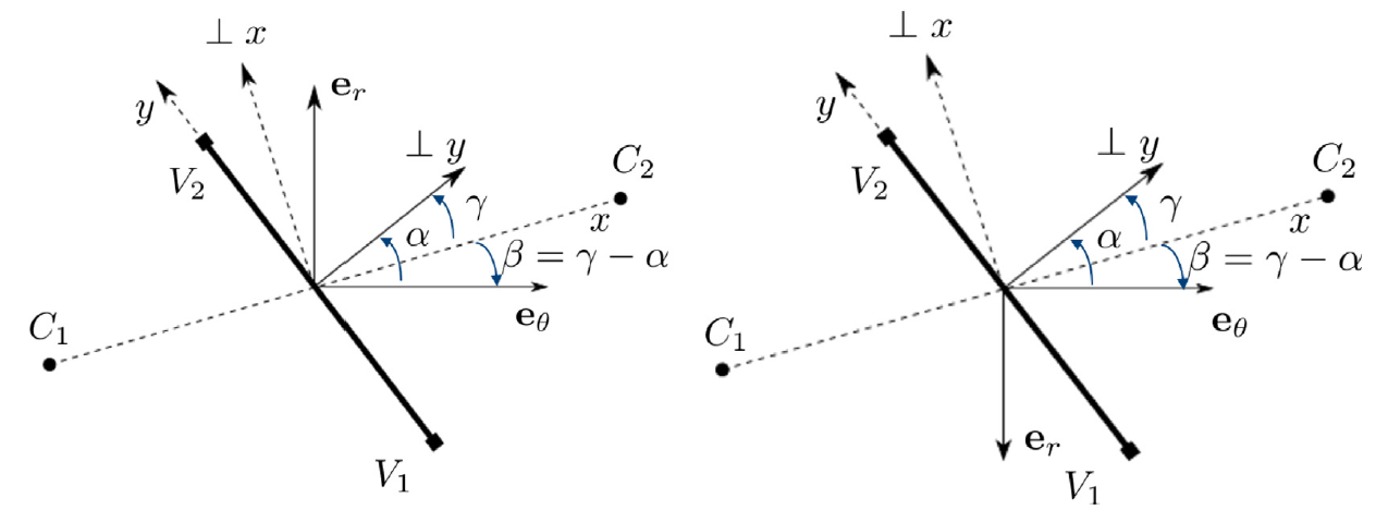
\includegraphics[width=14cm]{FiguresWG/mesh_angles.png}}
\else
    \centerline{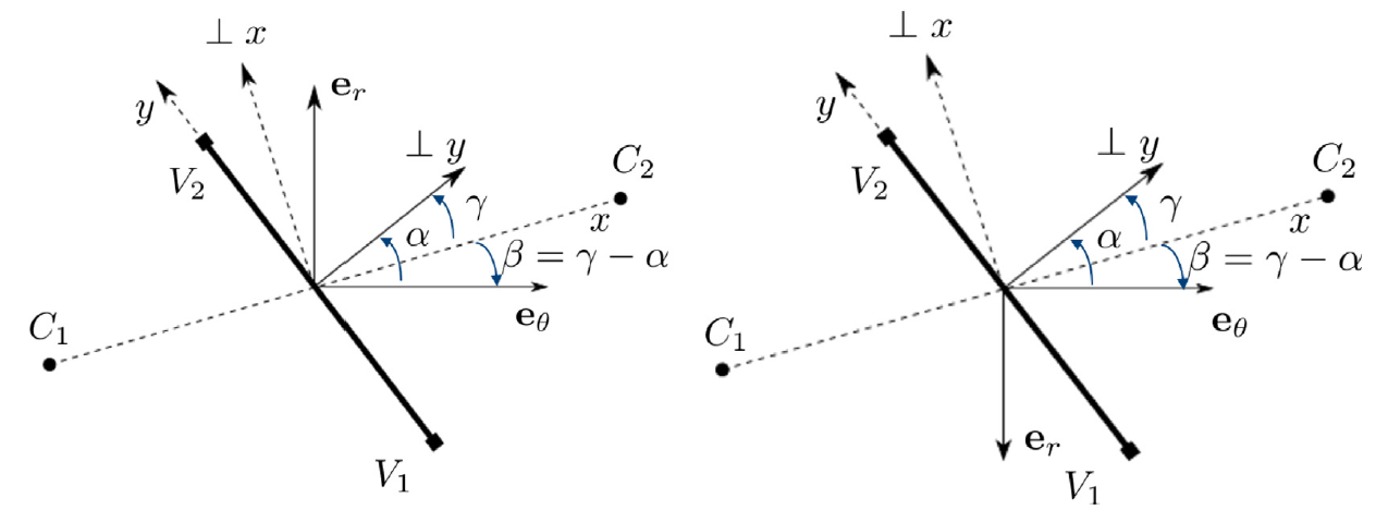
\includegraphics[width=14cm]{FiguresWG/mesh_angles.eps}}
\fi
    \caption{Local coordinate systems defining cell face orientation w.r.t. magnetic field, cell centers, and vertices. Left: toroidal field out of page. Right: toroidal field into the page.
    Figure reproduced from \cite{DEKEYSER2021}.}
    \label{fig:mesh_angles}
\end{figure}

The definitions of the variables in Figure \ref{fig:mesh_angles} are as follows:

\begin{itemize}
\item {\tt $C_1$} is the center of control volume 1. The index for that control volume is given by {\tt fcCv(iFc,1)}.
\item {\tt $C_2$} is the center of control volume 2. The index for that control volume is given by {\tt fcCv(iFc,2)}.
\item {\tt $V_1$} is the first vertex of the face. Its index is given by {\tt fcVx(iFc,1)}.
\item {\tt $V_2$} is the second vertex of the face. Its index is given by {\tt fcVx(iFc,2)}. The convention is that, when we look from {\tt $V_1$} to {\tt $V_2$}, {\tt $C_1$} is on the left and {\tt $C_2$} is on the right.
\item {\tt x} The $x$-direction is defined through the (not necessarily straight)
coordinate line connecting {\tt $C_1$} and {\tt $C_2$}, going through the center of the
cell face, and positive from {\tt $C_1$} to {\tt $C_2$}.
\item {\tt y} The $y$-direction is tangent to the face, positive from {\tt $V_1$} to {\tt $V_2$}.
\item {\tt $\alpha$} is the included angle between the magnetic field vector and the face normal.
{\tt fcQalf(iFc,0)} is the cosine of {\tt $\alpha$} and {\tt fcQalf(iFc,1)} is the sine of {\tt $\alpha$}.
\item {\tt $\gamma$} is the included angle between the cell-connector vector and the normal vector
of face {\tt iFc}. {\tt fcQgam(iFc,0)} is the cosine of {\tt $\gamma$} and {\tt fcQgam(iFc,1)} is the sine of {\tt $\gamma$}. It will hold that {\tt 0.lt.fcQgam(,).le.1}.
\item {\tt $\beta$} is the included angle between the cell-connector and the magnetic field vector.
{\tt fcQbet(iFc,0)} is the cosine of {\tt $\beta$} and {\tt fcQbet(iFc,1)} is the sine of {\tt $\beta$}.
\item {\tt fcHc(iFc,1)} is the distance between {\tt $C_1$} and the cell face center. {\tt fcHc(iFc,2)} is the distance between {\tt $C_2$} and the cell face center.
\item {\tt fcHt(iFc)} is the distance between {\tt $V_1$} and {\tt $V_2$}.
\end{itemize}

The flux of a particular quantity $u$ follows a convection-diffusion prescription:

\begin{equation*}
\mathbf{\Gamma} = \mathbf{C} u - \mathcal{D} \nabla u
\end{equation*}

The anisotropy in the equations is most naturally expressed w.r.t.
the poloidal ($\theta$) and radial ($r$) directions, which, by definition, are locally
orthogonal to each other. In our notation, the poloidal direction
points along the poloidal projection of the magnetic field, and the
radial direction is orthogonal to it in the poloidal plane, forming a
right-handed system with the third unit vector along the toroidal
projection of the field. These unit vectors therefore may flip orientation
with poloidal/toroidal field reversal. The coefficient
$\mathbf{C} = C_\theta \mathbf{e}_\theta + C_r \mathbf{e}_r$ is a vector describing the convective
flux of $u$, with components
defined in the poloidal and radial directions, and $\mathcal{D} = [D_{\theta \theta} D_{\theta r}, D_{r \theta} D_{r r}]$
is a diffusive tensor. The cross-diffusivities are included
because they are representative of the treatment of drift flows.
The {\tt B2.5} finite volume technique requires the evaluation of the fluxes across
cell faces:

\begin{align*}
 \mathbf{\Gamma} \cdot \mathbf{S} & = \Gamma_\theta S_\theta + \Gamma_r S_r \\
 & = \left( C_\theta u - D_{\theta \theta} \nabla_\theta u - D_{\theta r} \nabla_r u \right) S_\theta +
 \left( C_r u - D_{r \theta} \nabla_\theta u - D_{r r} \nabla_r u \right) S_r,
 \end{align*}

where $\mathbf{S} = S_\theta \mathbf{e}_\theta +  S_r \mathbf{e}_r $
is the surface vector of a face, expanded in its
poloidal and radial components.

To compute the poloidal and radial components of the gradient,
we relate them to the gradients in the $x$ and $y$
directions, which in turn can be computed directly from differences
between cell center (for $\nabla_\theta$) and vertex (for $\nabla_r$) values of $u$. The
desired expression for the components of the gradient can be obtained
by expanding the gradient in the orthogonal poloidal-radial system,
$\nabla u = \nabla_\theta u \cdot \mathbf{e}_\theta + \nabla_r u \cdot \mathbf{e}_r$,
and applying the definition of the gradient, $\nabla_d u = \nabla u \cdot \mathbf{d}$
for an arbitrary direction $\mathbf{d}$, to the unit vectors $\mathbf{e}_\theta$ and
$\mathbf{e}_r$:

\begin{align*}
\nabla_x u & = \nabla u \cdot \mathbf{e}_x = \nabla_\theta u \mathbf{e}_\theta \cdot \mathbf{e}_x + \nabla_r u \mathbf{e}_r \cdot \mathbf{e}_x, \\
\nabla_y u & = \nabla u \cdot \mathbf{e}_y = \nabla_\theta u \mathbf{e}_\theta \cdot \mathbf{e}_y + \nabla_r u \mathbf{e}_r \cdot \mathbf{e}_y.
\end{align*}

From Figure \ref{fig:mesh_angles} we see that $\mathbf{e}_\theta \cdot \mathbf{e}_x = \cos \beta$,
 $\mathbf{e}_r \cdot \mathbf{e}_x = \mp \sin \beta$, $\mathbf{e}_\theta \cdot \mathbf{e}_y = -\sin \alpha$
and $\mathbf{e}_r \cdot \mathbf{e}_y = \pm \cos \alpha$, with the upper signs corresponding to toroidal field
out of the page, and the lower signs with toroidal field into the page.
Inverting the system, we obtain

\begin{align*}
\nabla_\theta u & = \frac{\cos \alpha}{\cos \gamma} \nabla_x u + \frac{\sin \beta}{\cos \gamma} \nabla_y u, \\
\nabla_r u & = \pm \frac{\sin \alpha}{\cos \gamma} \nabla_x u \pm \frac{\cos \beta}{\cos \gamma} \nabla_y u.
\end{align*}

For completeness we give also the component of the gradient normal
to the face, which is needed for some boundary conditions:

\begin{equation*}
\nabla_n u = \frac{1}{\cos \gamma} \nabla_x u + \frac{\sin \gamma}{\cos \gamma} \nabla_y u,
\end{equation*}

and note, trivially, that the component tangential to the face is the
component in the $y$-direction: $\nabla_t u = \nabla_y u$.
Computing the poloidal and radial components of the gradient in
general thus requires a combination of gradients in $x$ and $y$ directions.

Drift terms can also be discretized using the expressions above. Only
the component of the drift perpendicular to a face leads to transport
across a face. Recalling that drifts have the form of a cross-diffusion
term, the net drift flow $\Gamma_d$ across a face is of the form:

\begin{equation*}
\mathbf{\Gamma}_d \cdot \mathbf{S} = - D_d \left( \nabla_r u S_\theta - \nabla_\theta u S_r \right) = \mp D_d \nabla_y u S
\end{equation*}

where we use the identity $\mathbf{S} = \left( \cos \alpha \ \mathbf{e}_\theta \pm \sin \alpha \ \mathbf{e}_r \right) S$.
Thus, net drift flow
across the face depends only on gradients along the face, while the
decomposition of the drift into its poloidal and radial components (as
required for example for the collisions with neutrals) requires again the
correct computation of the radial/poloidal gradients on each (possibly
non-aligned) face.
Using the expressions for the fluxes and derivatives on faces given
above, the governing equations can be discretized. Gradients in cell
centers are obtained through interpolation of the cell face gradients.
The discretization schemes of the structured version of the code have
been generalized to arbitrary unstructured grids. Hybrid discretization
schemes are used for the convection-diffusion flows, which are second
order in space for diffusion-dominated flows, but tend to a first-order
upwind scheme in convection-dominated flows.
The discretization schemes of the unstructured solver no longer neglect effects of misalignment
w.r.t. the magnetic field, and hence the solver is more accurate than older {\tt B2.5} versions
 even for non-extended grid cases.

Dedicated routines in {\tt \$\{SOLPSTOP\}/modules/B2.5/src/utility/} now take care of recurring numerical operations:

\begin{itemize}
\item {\tt GRAD} computes gradients of a cell-centered quantity on the cell faces, in both poloidal and radial directions.
\item {\tt GRAD\_NT} computes gradients of a cell-centered quantity on the cell faces, in both tangential and normal directions.
\item {\tt GRADC} computes gradients of a cell-centered quantity at the cell center by first computing the gradients on faces, and then interpolating back to the cell center.
\item {\tt GRADC\_DIV} computes gradients of a cell-centered quantity at the cell-center by applying the divergence theorem.
\item {\tt DIV} computes the divergence of a flow field.
\item {\tt INTFACE} interpolates a cell-centered quantity to the cell faces.
\item {\tt INTCELL} interpolates a face-based quantity to the cell centers.
\item {\tt INTVERTEX} interpolates a cell-centered quantity to the vertices.
\end{itemize}

%%%%%%%%%%%%%%%%%%%%%%%%%%%%%%%%%%%%%%%%%%%%%%%%%%%%%%%%%%%%%%%%%
%%%%%%%%%%%%%%%%%%%%%%%%%%%%%%%%%%%%%%%%%%%%%%%%%%%%%%%%%%%%%%%%%
\section{Rhie-Chow correction in unstructured code}
%%%%%%%%%%%%%%%%%%%%%%%%%%%%%%%%%%%%%%%%%%%%%%%%%%%%%%%%%%%%%%%%%
%%%%%%%%%%%%%%%%%%%%%%%%%%%%%%%%%%%%%%%%%%%%%%%%%%%%%%%%%%%%%%%%%

To avoid odd-even decoupling in the parallel direction due to the
collocated velocity and density (pressure) fields, a Rhie-Chow scheme
for compressible flow as described in Ref.~\cite{MOUKALLED2016} is implemented for the
parallel direction. The scheme is also explained in Section 8.8 and 10.2 (older versions) or 9.8 and 11.2 (newer versions) of Ref.~\cite{FERZIGER2019}.
The switches {\tt b2npco\_pcm0}, {\tt b2npco\_pcm1}, {\tt b2npht\_pcm0} and {\tt b2npht\_pcm1} determine the strength of the corrections.

%%%%%%%%%%%%%%%%%%%%%%%%%%%%%%%%%%%%%%%%%%%%%%%%%%%%%%%%%%%%%%%%%
%%%%%%%%%%%%%%%%%%%%%%%%%%%%%%%%%%%%%%%%%%%%%%%%%%%%%%%%%%%%%%%%%
\section{WG-related TODOs for this manual}
%%%%%%%%%%%%%%%%%%%%%%%%%%%%%%%%%%%%%%%%%%%%%%%%%%%%%%%%%%%%%%%%%
%%%%%%%%%%%%%%%%%%%%%%%%%%%%%%%%%%%%%%%%%%%%%%%%%%%%%%%%%%%%%%%%%

Some sections of this manual still need to be rewritten to be consistent with the unstructured solver:

\begin{itemize}
\item Appendix \ref{cha:b2wdat_iout_4} for the debugging output tracing files.
\item Appendix \ref{cha:Mladen_2}: remove, update, or integrate with another part of the manual.
\item Appendix \ref{sec:typical_BCs} for the expressions of boundary conditions.
\item Add information on creation of new extended cases. For now we refer to the {\tt 20230815\_carre2\_presentation.pdf} presentation found on the \SOLPSITER SharePoint website, in the \href{https://sharepoint.iter.org/departments/POP/CM/IMAS/SOLPS-ITER/SOLPS-ITER\%20Extended\%20Grids\%20Workshops}{SOLPS-ITER Extended Grids Workshops} directory.
\end{itemize}

%%%%%%%%%%%%%%%%%%%%%%%%%%%%%%%%%%%%%%%%%%%%%%%%%%%%%%%%%%%%%%%%%
%%%%%%%%%%%%%%%%%%%%%%%%%%%%%%%%%%%%%%%%%%%%%%%%%%%%%%%%%%%%%%%%%
\section{Converting structured cases}
%%%%%%%%%%%%%%%%%%%%%%%%%%%%%%%%%%%%%%%%%%%%%%%%%%%%%%%%%%%%%%%%%
%%%%%%%%%%%%%%%%%%%%%%%%%%%%%%%%%%%%%%%%%%%%%%%%%%%%%%%%%%%%%%%%%

Users can easily convert their existing structured cases to run with the WG code version. How to do this is explained in documents on the \SOLPSITER SharePoint website, \href{https://sharepoint.iter.org/departments/POP/CM/IMAS/SOLPS-ITER/SOLPS-ITER\%20Extended\%20Grids\%20Workshops}{SOLPS-ITER Extended Grids Workshops} directory, namely {\tt Session\_case\_conversion.pdf} and the last section of {\tt 20230814\_extended\_grids\_presentation.pdf}.


\appendix

\chapter{Internal B2.5 documentation}
\label{cha:intb2doc}

\section{b2cdca.F}
\label{lis:b2cdca}\index{b2cdca.F}\index{B2.5, code documentation}

\VerbatimInput[fontsize=\footnotesize]{b2cdca.F}

\newpage
\section{b2cdcr.F}
\label{lis:b2cdcr}\index{b2cdcr.F}\index{B2.5, list of routines}

\VerbatimInput[fontsize=\footnotesize]{b2cdcr.F}

\newpage
\section{b2cdcv.F}
\label{lis:b2cdcv}\index{b2cdcv.F}\index{B2.5, list of variables}

\VerbatimInput[fontsize=\footnotesize]{b2cdcv.F}

\newpage
\section{b2cdci.F}
\label{lis:b2cdci}\index{b2cdci.F}\index{B2.5, list of switches}

\VerbatimInput[fontsize=\footnotesize]{b2cdci.F}

\newpage
\section{b2cdcn.F}
\label{lis:b2cdcn}\index{b2cdcn.F}\index{B2.5, list of namelists}

\VerbatimInput[fontsize=\footnotesize]{b2cdcn.F}

\chapter{The physics of B2.5}
\label{cha:b2physics}

An extensive review of {\tt B2-Eirene} has been published as \cite{SOLPS2006}\index{SOLPS review}. It provides a full description of the {\bf SOLPS5.0} physics model, which can be obtained in the code by setting the {\tt b2mndt\_style} switch to {\tt 0}.
It is asked that authors using {\tt SOLPS} simulation results cite that work when
referring to the code. This review, only some short sections of which are detailed
below, can be found as part of the {\tt SOLPS} package at {\tt \$\{SOLPSTOP\}/doc/CPP\_2006.pdf}. Most of the discussion and definitions presented here apply to both the {\bf SOLPS5.0} and \SOLPSfivetwo physics models. In cases where the models differ, the use of the \SOLPSfivetwo model is recommended, although the {\bf SOLPS5.0} model remains available in the code for backward compatibility.

The equations are written on a
curvilinear orthogonal coordinate system.
The $x$-coordinate varies along flux surfaces and the $y$-coordinate varies
perpendicular to flux surfaces (see figure \ref{fig:geo}),
$z$ is the toroidal direction.

\begin{figure}[hbt]
\centerline{
\ifpdf
\includegraphics[width=8.0cm]{b2plot_1.pdf}
\else
\includegraphics[width=8.0cm]{b2plot_1.eps}
\fi
}
\caption{Coordinate system: $x$ is the poloidal coordinate,
$y$ is the radial coordinate orthogonal to the flux surfaces. The
coordinate $\perp$ corresponds to the direction perpendicular
both to the magnetic field and to the $y$-axis. The directions
of magnetic field and plasma current correspond to normal
operation conditions of ASDEX--Upgrade (ion $\nabla B$ drift
directed towards the X-point).
 }
\label{fig:geo}
\end{figure}

The metric coefficients are
$h_x=1/\|\grad x\|$, $h_y=1/\|\grad y\|$ and $\sqrt{g}=h_xh_yh_z$.
One can replace $h_z$ by $2 \pi R$,
where $R$ is the local major radius.  Components of a vector are the
projections on unit basis vectors
; they are not the contravariant or
covariant components ($b_x = B_x/B$, $b_z = B_z/B$).
Ion velocities $V_{\perp}$ (velocity perpendicular both
to magnetic field $B$ and the $y$-axis) and $V_y$ are
determined from the two components of the momentum balance equation
for ions perpendicular to a magnetic field. Using the Braginskii expression
for the friction force, one obtains:\\
\begin{gather}
\label{eq:nf1}
V_{\perp} = V_{\perp}^{\left( a \right)} - \frac{1}{enB}
\frac{1}{h_y}\frac{\partial nT_i}{\partial y} +
V_{\perp}^{\left( in \right)} + V_{\perp}^{\left( vis \right)} +
V_{\perp}^{\left( s \right)}
\end{gather}
\begin{gather}
\label{eq:nf2}
V_y = V_y^{\left( a \right)} + \frac{B_z}{enB^2}
\frac{1}{h_x}\frac{\partial nT_i}{\partial x} +
V_y^{\left( in \right)} + V_y^{\left( vis \right)} +
V_y^{\left( s \right)}
\end{gather}
Velocities $V_{\perp,y}^{\left( a \right)}$ are the sum of the
$\exb$ drifts and diffusive and thermo-diffusive
velocities.
This part corresponds to the ambipolar flux. It is the same both for ions and
electrons.
The second term in the r.h.s. of
Eqs.~(\ref{eq:nf1}) and (\ref{eq:nf2})
corresponds to diamagnetic flow of ions, while the other terms are caused
by inertial, viscous and ion-neutral friction forces.
These non-ambipolar terms are
connected with currents: $\vec{V}^{\left( in \right)} = \vec{j}^{\left( in \right)}/en,
\vec{V}^{\left( vis \right)} = \vec{j}^{\left( vis \right)}/en,
\vec{V}^{\left( s \right)} = \vec{j}^{\left( s \right)}/en$.\\
In the presence of anomalous transport
($D$ is the classical diffusion coefficient, $D=\frac{T_e+T_i}{eb}
\frac{\nu_{ei}}{\omega_{ce}}$, with electron cyclotron frequency
$\omega_{ce}$ and electron-ion collision frequency $\nu_{ei}$)
\begin{gather}
\label{eq:nf3}
V_{\perp}^{\left( a \right)} =
- \frac{1}{B}\frac{1}{h_y}\frac{\partial \Phi}{\partial y}
-\frac{D}{T_e+T_i} \frac{b_z}{h_x}\left(\frac{\partial p}{n \partial x}
-\frac{3}{2}\frac{\partial T_e}{\partial x}\right)
-D^{(AN)}_n\frac{1}{h_x n} \frac{\partial n}{\partial x}
-D^{(AN)}_p\frac{1}{h_x n} \frac{\partial p_i}{\partial x}
+V_{\perp}^{\left( AN \right)}
\end{gather}
\begin{gather}
\label{eq:nf44}
V_y^{\left( a \right)} =
\frac{B_z}{B^2}\frac{1}{h_x}\frac{\partial \Phi}{\partial x}
-\frac{D}{T_e+T_i} \frac{1}{h_y}\left(\frac{\partial p}{n \partial y}
-\frac{3}{2}\frac{\partial T_e}{\partial y}\right)
-D^{(AN)}_n\frac{1}{h_y n} \frac{\partial n}{\partial y}
-D^{(AN)}_p\frac{1}{h_y n} \frac{\partial p_i}{\partial y}
+V_y^{\left( AN \right)}
\end{gather}
The poloidal velocity is a sum $V_x = b_z V_{\perp} + b_x V_{\parallel}$.

In the particle balance
the fact that the diamagnetic
velocity is almost divergence free is taken into
account. Therefore, instead of the diamagnetic velocity
it is possible to introduce an effective
velocity $\vec{\tilde{V}}^{\left( dia \right)}$,
which gives the same contribution
to the divergence of the particle flux:
\begin{gather}
\label{eq:nf4}
\frac{\partial n}{\partial t} +
     \frac{1}{\sqrt{g}} \frac{\partial}{\partial x}
      \left(\frac{\sqrt{g}}{h_x} n\left(b_x V_{\parallel} +
     b_z V_{\perp}^{\left( 0 \right)}\right)\right)+
     \frac{1}{\sqrt{g}} \frac{\partial}{\partial y}
      \left(\frac{\sqrt{g}}{h_y} n V_y^{\left( 0 \right)}\right)
= S^n
\end{gather}
\begin{gather}\label{eq:nf5}
V_{\perp}^{\left( 0 \right)} = V_{\perp}^{\left( a \right)} +
V_{\perp}^{\left( in \right)} + V_{\perp}^{\left( vis \right)} +
V_{\perp}^{\left( s \right)} + \tilde{V}_{\perp}^{\left( dia \right)}
\end{gather}
\begin{gather}\label{eq:nf6}
V_{y}^{\left( 0 \right)} = V_{y}^{\left( a \right)} +
V_{y}^{\left( in \right)} + V_{y}^{\left( vis \right)} +
V_{y}^{\left( s \right)} + \tilde{V}_{y}^{\left( dia \right)}
\end{gather}
\begin{gather}\label{eq:nf7}
\tilde{V}_{\perp}^{\left( dia \right)} = \frac{T_i B_z}{e}
\frac{\partial}{h_y \partial y}\left(\frac{1}{B^2}\right)
\end{gather}
\begin{gather}\label{eq:nf8}
\tilde{V}_y^{\left( dia \right)} = -\frac{T_i B_z}{e}
\frac{\partial}{h_x \partial x}\left(\frac{1}{B^2}\right)
\end{gather}
The velocity $\tilde{V}^{{\left(dia\right)}}$ is an effective velocity. It
represents vertical guiding centre drift of ions caused by
$\nabla B$.\\

Combining the inertia and gyroviscosity terms in the Braginskii equations,
one finds
\begin{multline}\label{eq:mom}
\hfill m_i \left[ \frac{\partial n V_{\parallel}}{\partial t} +
     \frac{1}{\sqrt{g}} \frac{\partial}{\partial x}
      \left( \frac{\sqrt{g}}{h_x} n
       \left( V_{\perp}^{\left( 0 \right)} b_z
            + V_{\parallel} b_x \right)
       V_{\parallel} \right) +
     \frac{1}{\sqrt{g}} \frac{\partial}{\partial y}
      \left( \frac{\sqrt{g}}{h_y} n V_y^{\left( 0 \right)} V_{\parallel} \right)
\right] = \hfill \\
\hfill -\frac{b_x}{h_x}\frac{\partial n T_i}{\partial x} -
b_x \frac{en}{h_x}\frac{\partial \Phi}{\partial x} + F_k +
\frac{4}{3} b_x B^{3/2} \frac{\partial}{h_x \partial x}
\left(\frac{\eta_0 b_x}{B^2}
\frac{\partial\left(\sqrt{B}\left(V_{\parallel}+ \dfrac{B}{B_x} \left(V^{(dia)}_x + V^{(E)}_x\right)\right)\right)}
{h_x \partial x}\right)
\hfill \\
\hfill + B^{3/2} b_x \frac{\partial}{h_x \partial x}
\left(\frac{b_x}{\nu_{ii} B^2}
\frac{\partial\left(\sqrt{B}q_{i\parallel}^{\left( 0 \right)}
\right)}{h_x \partial x}\right)+
     \frac{1}{\sqrt{g}} \frac{\partial}{\partial y}
      \left(\frac{\sqrt{g}}{h_y^2} \eta_2 \frac{\partial V_{\parallel}}
{\partial y}\right) \hfill \\
\hfill
      + \frac{1}{\sqrt{g}} \frac{\partial}{\partial x}
      \left(\frac{\sqrt{g}}{h_x^2} \eta_2 \frac{\partial V_{\parallel}}
{\partial x}\right)
+ S_{i \parallel}^m + R_{ie\parallel}. \hfill
\end{multline}
The diamagnetic terms in the l.h.s. of (\ref{eq:mom}) are almost cancelled
\cite{ROGNLIEN98A, ROGNLIEN98B, ROGNLIEN99A, HINTON94C}, so that
velocities normal to the flux surface in the second and third term,
as in the particle balance equation, are determined by (\ref{eq:nf1}) and (\ref{eq:nf2}).
In \cite{HINTON94C}
the divergent part of diamagnetic velocity has been
neglected. Here, it is kept, because the corresponding flux is still
relatively large and can be comparable with the diffusive flux even
for anomalous diffusion coefficients. The authors of
\cite{ROGNLIEN98A, ROGNLIEN98B, ROGNLIEN99A} also kept this
flux.
In contrast to
\cite{ROGNLIEN98A, ROGNLIEN98B, ROGNLIEN99A}
there is an additional term of the same kind in the r.h.s. of
Eq.~(\ref{eq:mom}):
\begin{gather}
F_k = - m_i \left(\frac{1}{\sqrt{g}} \frac{\partial}{\partial x}
      \left(\frac{\sqrt{g}}{h_x} n V_{\parallel}
      \tilde{V}_{\perp}^{\left( dia \right)} b_z \right) +
      \frac{1}{\sqrt{g}} \frac{\partial}{\partial y}
      \left(\frac{\sqrt{g}}{h_y} n V_{\parallel}
      \tilde{V}_y^{\left( dia \right)} \right)\right)
\end{gather}
This parallel force is the Coriolis force, connected with the
diamagnetic drift velocity and
toroidal (parallel) rotation. This force can be obtained in a different
way by averaging the drift kinetic equation
\cite{MIHAIL84A} and is of the same order
as the inertia terms.

Parallel viscosity is represented
by the fourth and fifth terms in the r.h.s.
The former is the Balescu
parallel viscosity with coefficient $\eta_0 = \dfrac{4}{3} 0.96 \sqrt{2} n T_i / \nu_{ii}$. A detailed derivation is given at the end of this section, see~\ref{sec:viscosity}.
The latter corresponds to the parallel viscosity driven
by parallel ion heat flux
$q_{i\parallel}^{\left( 0 \right)} =
- \kappa_{i,\parallel} b_x \frac{1}{h_x} \frac{\partial T_i}{\partial x}$.
This viscosity is absent in the Braginskii equations, however, in a tokamak,
where parallel particle flux multiplied by temperature is of
the order of the ion heat flux, these two
viscosities are of the same order. On closed flux surfaces far from
the separatrix, the flux-surface-averaged parallel
viscosity coincides with the well-known
neoclassical expression for the Pfirsch-Schl{\"u}ter regime
\cite{HIRSHMAN81A}.
Thus, parallel viscosity in Eq.~(\ref{eq:mom}) provides smooth transition to
neoclassical theory.
The classical perpendicular viscosity coefficient
can
be replaced by an anomalous value as in
\cite{ROGNLIEN98A, ROGNLIEN98B, ROGNLIEN99A}: $\eta_2 =
n m_i D^{(AN)}_n$. Perpendicular viscosity and inertia terms with the
anomalous particle flux are responsible for the transport of the
parallel momentum in radial and poloidal directions. The radial transport
can be rather important despite the fact that $\eta_2 \ll \eta_0$, since
the scale in the radial direction is rather small.

The term  $S_{i \parallel}^m$  represents the parallel momentum loss due to
ion-neutral friction and parallel momentum input from neutral beam injection.
$R_{ie\parallel}$ is the ion-electron friction.

The parallel momentum balance for electrons has the standard form:
\begin{gather}
j_{\parallel} = \sigma_{\parallel} \left(
\frac{b_x}{e} \frac{1}{h_x} \left( \frac{\partial n T_e}{n \partial x} +
0.71 \frac{\partial T_e}{\partial x} \right)
- \frac{b_x}{h_x} \frac{\partial \Phi}{\partial x} \right).
\end{gather}

Expressions for $j_{\perp}$ and $j_y$ are obtained from radial and
poloidal projections of the total momentum balance equation (the sum
of electron and ion momentum balance equations).
The resulting current is a sum of contributions from pressure
gradient (diamagnetic current) $\vec{j}^{\left( dia \right)}$, inertia
and gyroviscosity $\vec{j}^{\left( in \right)}$, viscosity
$\vec{j}^{\left( vis \right)}$ and ion-neutral friction
$\vec{j}^{\left( s \right)}$.
Similar to the particle continuity equation, the effective
current $\vec{\tilde{j}}$ is introduced, which gives the same contribution to
$\nabla \vec{j}$, as the ordinary current. This gives the current continuity
equation
\begin{gather}\label{eq:curr0}
     \frac{1}{\sqrt{g}} \frac{\partial}{\partial x}
      \left(\frac{\sqrt{g}}{h_x} \tilde{j}_x\right)+
     \frac{1}{\sqrt{g}} \frac{\partial}{\partial y}
      \left(\frac{\sqrt{g}}{h_y} \tilde{j}_y\right)
= 0~.
\end{gather}
\begin{gather}\label{eq:curr1}
\tilde{j}_x = b_z \tilde{j}_{\perp} + b_x \tilde{j}_{\parallel}~.
\end{gather}
\begin{gather}\label{eq:curr2}
\vec{j} = \vec{\tilde{j}}^{\left( dia \right)} + \vec{j}^{\left( in \right)}
+ \vec{j}^{\left( vis \right)} + \vec{j}^{\left( s \right)}
+\vec{j}_{\parallel}~.
\end{gather}
The effective diamagnetic current can be chosen in a form
\begin{gather}\label{eq:curr3}
\tilde{j}_{\perp}^{\left( dia \right)} =
\frac{1}{b_z}\frac{n\left( T_e + T_i \right) B_z}{h_y}
\frac{\partial}{\partial y}\left(\frac{1}{B^2}\right)~,
\end{gather}
\begin{gather}\label{eq:curr4}
\tilde{j}_y^{\left( dia \right)} =
- \frac{n\left( T_e + T_i \right) B_z}{h_x}
\frac{\partial}{\partial x}\left(\frac{1}{B^2}\right)~.
\end{gather}
Current driven by parallel viscosity should be taken into account in
Eqs.~(\ref{eq:curr0}), (\ref{eq:curr1}) and (\ref{eq:curr2}).
This current is a small correction to the diamagnetic current
Eqs.~(\ref{eq:curr3}) and (\ref{eq:curr4}).
However, on closed flux surfaces, where the pressure is almost constant,
the diamagnetic current averaged
over the flux surfaces tends to zero. The resulting remaining part can
become comparable to the parallel viscosity-driven current, which is
necessary to satisfy the condition that the averaged net radial current
should be zero.
The terms, which contain the plasma viscosity, produce almost
divergence-free currents.
Similar to the case of diamagnetic currents, it can be reduced
to
\begin{gather}
\tilde{j}_{\perp}^{\left( vis \parallel \right)} =
- \frac{B_x \eta_0}{3 \sqrt{B}}
\frac{\partial\left(\sqrt{B}\left(V_{\parallel}+b_x \left(V^{(dia)}_{\perp} + V^{(E)}_{\perp}\right)\right)\right)}
{h_x \partial x}
\frac{\partial}{h_y \partial y}
\left(\frac{1}{B^2}\right)
\end{gather}
\begin{gather}
\tilde{j}_y^{\left( vis \parallel \right)} =
b_z\frac{B_x \eta_0}{3 \sqrt{B}}
\frac{\partial\left(\sqrt{B}\left(V_{\parallel}+b_x \left(V^{(dia)}_{\perp} + V^{(E)}_{\perp}\right)\right)\right)}
{h_x \partial x}
\frac{\partial}{h_x \partial x}
\left(\frac{1}{B^2}\right)
\end{gather}
The current produced by components of viscosity tensor connected
with heat fluxes is:
\begin{gather}
\tilde{j}_{\perp}^{\left( vis q \right)} =
- \frac{0.24 B_x}{\sqrt{B} \nu_{ii}}\frac{\partial
\left(q_{i \parallel}^{\left( 0 \right)} \sqrt{B}\right)}{h_x \partial x}
\frac{\partial}{h_y \partial y}
\left(\frac{1}{B^2}\right)
\end{gather}
\begin{gather}
\tilde{j}_y^{\left( vis q \right)} =
b_z\frac{0.24 B_x}{\sqrt{B} \nu_{ii}}\frac{\partial
\left(q_{i \parallel}^{\left( 0 \right)} \sqrt{B}\right)}{h_x \partial x}
\frac{\partial}{h_x \partial x}
\left(\frac{1}{B^2}\right)
\end{gather}

The second part of the current contains contributions from both inertia
and gyroviscosity forces. In contrast to the parallel momentum balance,
the cancellation is not complete (as has been noticed in
\cite{HINTON94C}). Expressions
for this part of the current are

\begin{multline}
\hfill j_{\perp}^{\left(in\right)}= - \frac{m_i}{B}
\left[\frac{\partial n V_{y}}{\partial t} +
     \frac{1}{\sqrt{g}} \frac{\partial}{\partial x}
      \left(\frac{\sqrt{g}}{h_x} n\left(V_{\perp}^{\left( 0 \right)} b_z
+ V_{\parallel} b_x \right) V_{y}\right)+
     \frac{1}{\sqrt{g}} \frac{\partial}{\partial y}
      \left(\frac{\sqrt{g}}{h_y} n V_y^{\left( 0 \right)} V_{y}\right)
\right] \hfill \\
\hfill -
\frac{2 b_x}{B} \frac{1}{h_x}\frac{\partial}{\partial x}
\left(\eta_3
\frac{\partial V_{\parallel}}{h_x \partial x}\right)+
\frac{m_i}{B} n V_{\parallel}^2 \frac{\partial \ln h_z}{h_y \partial y}
\hfill
\end{multline}

\begin{multline}
\hfill j_{y}^{\left(in\right)}= \frac{m_i}{B}
\left[\frac{\partial n V_{\perp}}{\partial t} +
     \frac{1}{\sqrt{g}} \frac{\partial}{\partial x}
      \left(\frac{\sqrt{g}}{h_x} n\left(V_{\perp}^{\left( 0 \right)} b_z
+ V_{\parallel} b_x \right) V_{\perp}\right)+
     \frac{1}{\sqrt{g}} \frac{\partial}{\partial y}
      \left(\frac{\sqrt{g}}{h_y} n V_y^{\left( 0 \right)} V_{\perp}\right)
\right] \hfill \\
\hfill -
\frac{2 b_x}{B} \frac{1}{h_x}\frac{\partial}{\partial x}
\left(\eta_3
\frac{\partial V_{\parallel}}{h_y \partial y}\right) -
\frac{m_i}{B} n V_{\parallel}^2 \frac{\partial \ln h_z}{h_x \partial x}
\hfill
\end{multline}

where $\eta_3 = \frac{n T_i}{2 \omega_{ci}}, \eta_1 = \frac{\eta_2}{4}$.

The last terms proportional to the gradient of $B$ correspond to the vertical
guiding centre drift of ions caused by the centrifugal force. This current
can be simply added to the diamagnetic current. Other terms seem to be less
important.

The contribution from perpendicular viscosity is
\begin{multline}
\hfill j_{\perp}^{\left(vis \perp \right)}= \frac{1}{B}
\left[\frac{1}{h_x}\frac{\partial}{\partial x}\left(\eta_1
     \frac{\partial V_y}{h_x \partial x}\right)+
 \frac{1}{h_y}\frac{\partial}{\partial y}\left(\eta_1
     \frac{\partial V_y}{h_y \partial y}\right)+
\frac{1}{h_x h_y }\frac{\partial \eta_1}{\partial x}
     \frac{\partial V_{\perp}}{\partial y}-
\frac{1}{h_x h_y }\frac{\partial \eta_1}{\partial y}
     \frac{\partial V_{\perp}}{\partial x}\right] \hfill \\
\hfill +
\frac{4 b_x}{B} \frac{1}{h_x h_y}
\left(\frac{\partial \eta_1}{\partial x} \frac{\partial V_{\parallel}}
{\partial y} - \frac{\partial \eta_1}{\partial y}\frac{\partial V_{\parallel}}
{\partial x}
\right)
\hfill
\end{multline}
\begin{gather}
j_{y}^{\left(vis \perp \right)}= -\frac{1}{B}
\left[\frac{1}{h_y}\frac{\partial}{\partial y}\left(\eta_1
     \frac{\partial V_{\perp}}{h_y \partial y}\right)+
 \frac{1}{h_x}\frac{\partial}{\partial x}\left(\eta_1
     \frac{\partial V_{\perp}}{h_x \partial x}\right)-
\frac{1}{h_x h_y }\frac{\partial \eta_1}{\partial x}
     \frac{\partial V_y}{\partial y}+
\frac{1}{h_x h_y }\frac{\partial \eta_1}{\partial y}
     \frac{\partial V_y}{\partial x}\right].
\end{gather}

Here, the largest term is the first one in the r.h.s. of the expression
for the radial current, since the radial derivatives are the largest.
This current corresponds to a pure cylindrical approximation. It is
responsible, for example, for closing currents near flush-mounted probes
\cite{ROZ99A}.
It was taken into account in
\cite{ROGNLIEN99A, RADFORD96A}. However, in the problem of global current
structure in the edge plasma, the currents driven by parallel viscosity seem
to be more important.

The total current caused by viscosity is
\begin{gather}
\vec{j}^{\left(vis\right)} = \vec{j}^{\left(vis \parallel\right)} +
\vec{j}^{\left(vis \perp\right)} +
\vec{j}^{\left(vis q\right)}
~.
\end{gather}

The contribution from ion neutral friction is
\begin{gather}
j_{\perp}^{\left(s\right)} = \frac{S_{iy}^m}{B}
~.
\end{gather}
\begin{gather}
j_{y}^{\left(s\right)} = -\frac{S_{i \perp}^m}{B}
~,
\end{gather}
where $S_{iy}^m$ and $S_{i \perp}^m$ are the momentum sinks due to
ion-neutral friction.
\begin{gather}
S_{i \perp}^m = - n \mu_{iN} \nu_{iN} \left( V_{\perp} - V_{\perp N}\right)
~,
\end{gather}
\begin{gather}
S_{i y}^m = - n \mu_{iN} \nu_{iN} \left( V_{y} - V_{y N}\right)
~,
\end{gather}
where $\mu_{iN}=m_i/2$ is the effective mass,
$\nu_{iN}= n_N \left\langle V_{iN} \sigma_{cx} \right\rangle$
is the ion-neutral collision frequency,
$n_N$ is the neutral density and $\vec{V_{iN}}$ is the neutral mean
velocity. For the ion velocity used above,
only electric and diamagnetic drifts are left, neglecting smaller terms,
to obtain
\begin{gather}
\tilde j_{x}^{\left(s\right)} = \tilde j_{\perp}^ {\left(s\right)} b_z =
- \sigma_{iN} b_z^2 \frac{\partial \Phi}{h_x \partial x}-
\sigma_{iN} b_z^2 \frac{1}{e n}\frac{\partial n T_i}{h_x \partial x}+
\sigma_{iN} B_z V_{yN}
~,
\end{gather}
\begin{gather}
\tilde j_{y}^{\left(s\right)} =
- \sigma_{iN} \frac{\partial \Phi}{h_y \partial y}-
\sigma_{iN} \frac{1}{e n}\frac{\partial n T_i}{h_y \partial y}-
\sigma_{iN} B V_{\perp N}
~,
\end{gather}
where $\sigma_{iN}$ is the ion-neutral perpendicular conductivity
\begin{gather}
\sigma_{iN} =
\frac{n m_i \left\langle V_{iN} \sigma_{cx} \right\rangle n_N}{2 B^2}
~.
\end{gather}

The rate of charge-exchange $\left\langle V_{iN} \sigma_{cx} \right\rangle$ can
be expressed through the mobility $K_0$ measured in the absence of a
magnetic field for room temperature and atmospheric pressure for
deuterium \cite{MCDANIEL73A}:
\begin{gather}
K_0 =
\frac{2 e}{m_i \left\langle V_{iN} \sigma_{cx} \right\rangle n_N^{\left(0\right)}}
~,
\end{gather}
with $n_N^{\left(0\right)} = 2.687 \cdot 10^{25} m^{-3}$ and
$K_0 = 11.2 \cdot 10^{-4} \frac{m^2}{s V}$.
Assuming that the charge-exchange cross-section is approximately constant
one gets
\begin{gather}
\left\langle V_{iN} \sigma_{cx} \right\rangle = 3.2 \cdot 10^{-15} \sqrt{\frac{T_i}{0.026}}
\frac{m^3}{s}
~,
\end{gather}
where $T_i$ is measured in $eV$. A similar expression, which gives approximately
the same result, is \cite{ROZ88A}:
\begin{gather}
\left\langle V_{iN} \sigma_{cx} \right\rangle = \frac{32 \sigma_{cx}}{3 \sqrt{\pi}}
\sqrt{\frac{T_i}{m_i}}
\frac{m^3}{s}
~.
\end{gather}.


In the energy balance equations
appears
a special problem, which is the
possible inclusion of an anomalous radial current.
The basic guidelines are as follows:
\begin{itemize}
\item The expression must be as simple as possible, and the most convenient
format is an Ohm-like expression;
\item The system of equations must be informed about this non-classical
contribution, but
\item The classical core of the equations must not be disturbed.
\end{itemize}
Apparently, the radial current would enter the electron energy equation
via the Joule term, but this manipulation is inappropriate since one cannot
be sure that this term directly heats the electrons, which is the case in
a purely classical setup. The proper thing to do is to keep only
the non-radial classical contribution in the Joule term, and
construct additional heat exchange terms
containing the radial current.
In this way, the system decides how to thermodynamically allocate the
"alien" heat term, among electrons and ion species.\\
For this reason, one cannot simply use the standard Ohm's
law in the radial direction with anomalous coefficients, or any other
prescribed expression whatsoever, as a constructive procedure is necessary
for simultaneously producing the radial current as well as the heat exchange
terms. At this point it has to be mentioned that this peculiarity arises
only in the multi-fluid case, whereas in the single species case
these heat exchange terms can indeed be constructed even using a prescribed
expression for the radial current. \\
The trick for carrying out this program is to correct the electron friction
density $\vec{R}^e$ by adding the term $n_e e \tilde{\eta}_\perp \vec{J}_\perp$
similar to the classical one, only using the {\itshape ad hoc} parameter
$\tilde{\eta}_\perp$. \\
Since $\vec{R}^e=-{\sum_{a}\vec{R}^a}$, one has a
modified total ion momentum equation at hand which in conjuction with the
pressure equilibrium (not affected by the additional term)
$\vec{J} \times \vec{B} = \nabla P$, gives the diffusive part of the
radial current, namely
\begin{gather}
J_y^{diff}=\frac{\tilde{\eta}_\perp en_e}{B^2} \frac{\partial P_i}{\partial y}
\end{gather}
where $P_i$ is the total ion pressure. This dependency is also found in
\cite{ROGNLIEN98A}. Moreover, an additional dependence on the radial
electric field can potentially be added without interfering with
the procedure. \\
The final step, namely the construction of the heat exchange terms, is
performed by claiming that the well known relation \cite{BAELMANS94A}
(adapted for the multi-fluid case)
\begin{gather}
Q_e=-\sum_{a} \left (Q_a + (\vec{u}^a - \vec{u}^e) \cdot \vec{R}^a \right )~,
\end{gather}
which stems from the fundamental null space of the collision operator,
is still true while carrying the modified friction.
Claiming this, after
performing the proper manipulations in the energy
equations, one reveals the {\itshape ad hoc}
contribution as the exchange term that one wants,
which reads
$
\sum_{a} (\vec{u}^a -\vec{u}^e)_\perp n_a \frac{Z_a^2}{Z_{eff}} e \tilde{\eta}_\perp \vec{J}_\perp
$
added in the total ion energy equation and subtracted from the
electron equation.
Note that in the single species case, this term boils down to
$
\tilde{\eta}_\perp J_\perp ^2
$
removing energy from the electrons,  depositing it to the ions, a feature
predicted by neoclassical theory \cite{ROSENBLUTH72A}.\\

In the final form of the energy balance equations, the convective heat
flux and the diamagnetic heat flux are combined as in
\cite{ROGNLIEN98A, ROGNLIEN98B, ROGNLIEN99A, HINTON94C}, see also
\cite{ROZ99A}.

The energy balance equation for the electrons is
\begin{multline}
\hfill
     \frac{3}{2} \frac{\partial nT_e}{\partial t} +
     \frac{1}{\sqrt{g}} \frac{\partial}{\partial x}
      \left(\frac{\sqrt{g}}{h_x} \tilde{q}_{ex}\right) +
     \frac{1}{\sqrt{g}} \frac{\partial}{\partial y}
      \left(\frac{\sqrt{g}}{h_y} \tilde{q}_{ey}\right) +
     \frac{nT_e}{\sqrt{g}}\frac{\partial}{\partial x}
      \left(\frac{\sqrt{g}}{h_x}\left(
      V_{\parallel} - j_{\parallel}/en\right)b_x\right) \hfill \\
\hfill     =
     Q_e + n T_e B \frac{1}{h_x h_y}\left(\frac{\partial \Phi}{\partial y}
     \frac{\partial}{\partial x}\left(\frac{1}{B^2}\right)
     -\frac{\partial \Phi}{\partial x}\frac{\partial}{\partial y}
     \left(\frac{1}{B^2}\right)\right)~,\hfill
\end{multline}
where
\begin{multline}
\hfill        \tilde{q}_{ex} = \frac{3}{2} n T_e \left(- \frac{b_z}{B h_y}
         \frac{\partial \Phi}{\partial y}
         + b_x V_{\parallel} - b_x j_{\parallel} / en \right) \hfill \\
     \hfill + \frac{5}{2} n T_e b_z \left(
     - \frac{D}{T_e+T_i} \frac{b_z}{h_x} \left(\frac{\partial p}{n \partial x}
     - \frac{3}{2} \frac{\partial T_e}{\partial x} \right)
     - D^{(AN)}_n \frac{1}{h_x n} \frac{\partial n}{\partial x}
     - D^{(AN)}_p \frac{1}{h_x n} \frac{\partial p_i}{\partial x}
     + V_{e\perp}^{(AN)} \right)
      \hfill \\
      \hfill   - 0.71 b_x j_{\parallel} T_e/e - \kappa_{e \parallel}
         \frac{b_x^2}{h_x} \frac{\partial T_e}{\partial x}
         - \kappa_{e \perp} b_z^2 \frac{1}{h_x}
         \frac{\partial T_e}{\partial x} \hfill \\
      \hfill   + \frac{3}{2}\frac{T_e}{e B} \frac{\nu_{ei}}{\omega_{ce}}
         \frac{b_z^2}{h_x} \frac{\partial n\left(T_e+T_i\right)}{\partial x}
         - \frac{5}{2} n T_e^2 \frac{B_z}{e}
         \frac{\partial}{h_y \partial y}\left(\frac{1}{B^2}\right) ~ , \hfill
\end{multline}
\begin{multline}
\hfill  \tilde{q}_{ey} = \frac{3}{2} n T_e \left( \frac{B_z}{B^2} \frac{1}{h_x}
        \frac{\partial \Phi}{\partial x} \right) \hfill \\
     \hfill  + \frac{5}{2} n T_e \left(
     - \frac{D}{T_e+T_i} \frac{1}{h_y} \left( \frac{\partial p}{n \partial y}
     - \frac{3}{2} \frac{\partial T_e}{\partial y} \right)
     - D^{(AN)}_n \frac{1}{h_y n} \frac{\partial n}{\partial y}
     - D^{(AN)}_p \frac{1}{h_y n} \frac{\partial p_i}{\partial y}
     + V_{ey}^{(AN)} \right)
         \hfill \\
         \hfill - \kappa_{e \perp} \frac{1}{h_y} \frac{\partial T_e}{\partial y}
         + \frac{3}{2}\frac{T_e}{e B} \frac{\nu_{ei}}{\omega_{ce}}
         \frac{1}{h_y} \frac{\partial n\left(T_e+T_i\right)}{\partial y}
         + \frac{5}{2} n T_e^2 \frac{B_z}{e}
         \frac{\partial}{h_x \partial x}\left(\frac{1}{B^2} \right) ~ , \hfill
\end{multline}
\begin{gather}
        Q_{\Delta} = \frac{3 m_e}{m_i} n \nu_{ei} \left(
T_e - T_i
\right)~,
\end{gather}
\begin{gather}
        Q_u = R_{ie \parallel} j_{\parallel}/en~,
\end{gather}
\begin{gather}
        Q_{AN} = \sum_{a} \left(\vec{u}^a -\vec{u}^e\right)_\perp n_a
                 \frac{Z_a^2}{Z_{eff}} e \tilde{\eta}_\perp \vec{J}_\perp~,
\end{gather}
\begin{gather}
        Q_e = -Q_{\Delta} - Q_u - Q_{AN}~.
\end{gather}

\begin{sloppypar}
Here $\kappa_{e \parallel}$ is the Balescu (not Braginskii as stated in the CPP review paper \cite{SOLPS_review}
or in {\tt \$\{SOLPSTOP\}/doc\allowbreak /CPP\_2006.pdf}) heat
conductivity with a possible heat
flux limit \cite{BRAAMS96B}.
The leading numerical coefficient is then $\frac{5}{2} \frac{2.16 z}{1 + 0.27 z}$ as opposed to 3.16 for the Braginskii
formula \cite{NRL}. The perpendicular heat conductivity
$\kappa_{e \perp}$ can be
either classical or anomalous. In the last term of the energy balance
equation, it is taken into account that the $\exb$
drift velocity is
almost divergence-free.
\end{sloppypar}

The ion energy balance equation is
\begin{multline}\label{eq:ion_energy} \hfill
     \frac{3}{2} \frac{\partial nT_i}{\partial t} +
     \frac{1}{\sqrt{g}} \frac{\partial}{\partial x}
      \left(\frac{\sqrt{g}}{h_x} \tilde{q}_{ix}\right) +
     \frac{1}{\sqrt{g}} \frac{\partial}{\partial y}
      \left(\frac{\sqrt{g}}{h_y} \tilde{q}_{iy}\right) +
     \frac{nT_i}{\sqrt{g}}\frac{\partial}{\partial x}
      \left(\frac{\sqrt{g}}{h_x} V_{\parallel} b_x \right) \hfill \\
     \hfill =
     Q_{\Delta} + Q_{AN} + \frac{\eta_0}{3} \left(2 b_x
     \frac{\partial V_{\parallel}}{h_x \partial x}\right)^2+
     n T_i B
     \frac{1}{h_x h_y}\left(\frac{\partial \Phi}{\partial y}
     \frac{\partial}{\partial x}\left(\frac{1}{B^2}\right)
     -\frac{\partial \Phi}{\partial x}\frac{\partial}{\partial y}
     \left(\frac{1}{B^2}\right)\right)~,\hfill
\end{multline}
where
\begin{multline} \hfill
        \tilde{q}_{ix} = \frac{3}{2} n T_i \left(- \frac{b_z}{B h_y}
        \frac{\partial \Phi}{\partial y}
         + b_x V_{\parallel} \right) \hfill \\
\hfill + \frac{5}{2} n T_i b_z \left(
     - \frac{D}{T_e + T_i} \frac{b_z}{h_x}\left(\frac{\partial p}{n \partial x}
     - \frac{3}{2} \frac{\partial T_e}{\partial x} \right)
     - D^{(AN)}_n \frac{1}{h_x n} \frac{\partial n}{\partial x}
     - D^{(AN)}_p \frac{1}{h_x n} \frac{\partial p_i}{\partial x}
     + V_{i\perp}^{(AN)} \right)
         \hfill \\ \hfill
         + \frac{5}{2} n T_i b_z \tilde{V}_{\perp}^{\left(dia\right)}
         - \kappa_{i \parallel}
         \frac{b_x^2}{h_x} \frac{\partial T_i}{\partial x}
         - \kappa_{i \perp} b_z^2 \frac{1}{h_x}
         \frac{\partial T_i}{\partial x} ~, \hfill
\end{multline}
\begin{multline} \hfill
        \tilde{q}_{iy} = \frac{3}{2} n T_i \left( \frac{B_z}{B^2}
         \frac{1}{h_x} \frac{\partial \Phi}{\partial x} \right)
        \hfill \\ \hfill
     + \frac{5}{2} n T_i \left(
     - \frac{D}{T_e+T_i} \frac{1}{h_y} \left( \frac{\partial p}{n \partial y}
     - \frac{3}{2} \frac{\partial T_e}{\partial y}\right)
     - D^{(AN)}_n \frac{1}{h_y n} \frac{\partial n}{\partial y}
     - D^{(AN)}_p \frac{1}{h_y n} \frac{\partial p_i}{\partial y}
     + V_{iy}^{(AN)} \right) \hfill \\ \hfill
         - \kappa_{e \perp} \frac{1}{h_y}
         \frac{\partial T_i}{\partial y}
         + \frac{5}{2} n T_i \tilde{V}_{y}^{\left(dia\right)} ~. \hfill
\end{multline}

As for the electrons, the parallel heat conductivity is classical with
a possible heat flux limit, while the perpendicular contribution
can be either
classical or anomalous.

There is discussion in the literature on how to take into account anomalous
terms in the energy balance equations. One point of view (see e.g.
\cite{ZAGORSKI98A})
is to cancel the contribution from anomalous particle fluxes in the
terms $p_i \nabla \cdot \vec{V}_i$ (or $\vec{V}_i \cdot \nabla p_i$ if equations
are written in a different form). In contrast, according to the
derivation
\cite{HINTON94C},
where a kinetic equation with fluctuating term has been integrated, the
anomalous fluxes should be kept in all terms of the energy balance
equations. This variant was used in {\tt UEDGE} \cite{ROGNLIEN98A, ROGNLIEN98B, ROGNLIEN99A}.
In {\tt B2.5} only the contribution
from anomalous radial particle flux to the convective heat flux are left
in the expressions for $\tilde{q}_{e,i}$. In the term
$p_i \nabla \cdot \vec{V}_i$ the anomalous particle flux is absent.

\section{Derivation of parallel viscosity term in momentum equation}
\index{parallel viscosity}\label{sec:viscosity}

To evaluate the parallel viscosity contribution we should start from the general expressions, which can be transformed and simplified in arbitrary cartesian coordinate system assuming only parallel velocity. The Braginskii description for parallel viscosity in cartesian coordinates is:

\begin{equation*}
\pi_{\alpha \beta} = \frac{3}{2} \eta_0 \left( b_\alpha b_\beta - \frac{1}{3} \delta_{\alpha \beta} \right) \left( b_\mu b_\nu - \frac{1}{3} \delta_{\mu \nu} \right) W_{\mu \nu}
\end{equation*}

where

\begin{equation*}
W_{\mu \nu} = \frac{\partial V_\mu}{\partial x_\nu} + \frac{\partial V_\nu}{\partial x_\mu} - \frac{2}{3} \delta_{\mu \nu} \frac{\partial V_i}{\partial x_i}, ~\vec{b} = \vec{B}/B .
\end{equation*}

The parallel momentum balance component is:

\begin{equation*}
\vec{b} \cdot \left( \nabla \cdot \overleftrightarrow{\pi} \right) = b_\alpha \frac{\partial \pi_{\alpha \beta}}{\partial x_\beta} = b_\alpha \frac{\partial}{\partial x_\beta} \left[ \frac{3}{2} \eta_0 \left( b_\alpha b_\beta - \frac{1}{3} \delta_{\alpha \beta} \right) \left( b_\mu b_\nu - \frac{1}{3} \delta_{\mu \nu} \right) W_{\mu \nu} \right]
\end{equation*}

We can evaluate the scalar value separately:

\begin{align*}
\pi_0 &= \frac{3}{2} \eta_0 W_{\parallel \parallel} = \frac{3}{2} \eta_0 \left( b_\mu b_\nu - \frac{1}{3} \delta_{\mu \nu} \right) W_{\mu \nu} \\
&= \frac{3}{2} \eta_0 \left(  b_\mu b_\nu - \frac{1}{3} \delta_{\mu \nu} \right) \left( \frac{\partial V_\mu}{\partial x_\nu} + \frac{\partial V_\nu}{\partial x_\mu} - \frac{2}{3} \delta_{\mu \nu} \frac{\partial V_i}{\partial x_i} \right) = 3 \eta_0 \left(  b_\mu b_\nu - \frac{1}{3} \delta_{\mu \nu} \right) \left( \frac{\partial V_\mu}{\partial x_\nu} - \frac{1}{3} \delta_{\mu \nu} \frac{\partial V_i}{\partial x_i} \right) \\
&= 3 \eta_0 \left( b_\mu b_\nu \frac{\partial V_\mu}{\partial x_\nu} - \frac{1}{3} \frac{\partial V_i}{\partial x_i} \right) = 3 \eta_0 \left( b_\mu b_\nu \frac{\partial V_\parallel b_\mu}{\partial x_\nu} - \frac{1}{3} \frac{\partial V_\parallel b_\nu}{\partial x_\nu} \right) \\
&= 3 \eta_0 \left( \frac{B_\nu}{B} \frac{\partial V_\parallel}{\partial x_\nu} - \frac{1}{3} B_\nu \frac{\partial V_\parallel / B}{\partial x_\nu} \right) = \eta_0 \frac{B_\nu}{B} \left( 2 \frac{\partial V_\parallel}{\partial x_\nu} + \frac{V_\parallel}{B} \frac{\partial B}{\partial x_\nu} \right) \\
&= 2 \eta_0 \frac{B_\nu}{B} \frac{1}{\sqrt{B}} \frac{\partial V_\parallel \sqrt{B}}{\partial x_\nu} = 2 \eta_0 \frac{1}{\sqrt{B}} \vec{b} \cdot \nabla \left ( V_\parallel \sqrt{B} \right)
\end{align*}

The projection of the viscosity divergence on the parallel direction is then:

\begin{align*}
\vec{b} \cdot \left( \nabla \cdot \overleftrightarrow{\pi} \right) &= b_\alpha \frac{\partial}{\partial x_\beta} \left[ \pi_0 \left( b_\alpha b_\beta - \frac{1}{3} \delta_{\alpha \beta} \right) \right] = \frac{\partial \pi_0 b_\alpha}{\partial x_\alpha} - \frac{1}{3} b_\alpha \frac{\partial \pi_0}{\partial x_\alpha} = B_\alpha \frac{\partial \pi_0 / B}{\partial x_\alpha} - \frac{1}{3} b_\alpha \frac{\partial \pi_0}{\partial x_\alpha} \\
&= \frac{2}{3} b_\alpha \frac{\partial \pi_0}{\partial x_\alpha} - \pi_0 \frac{b_\alpha}{B} \frac{\partial B}{\partial x_\alpha} = \frac{2}{3} B^{3/2} b_\alpha \frac{\partial \pi_0 B^{-3/2}}{\partial x_\alpha} = \frac{2}{3} B^{3/2} \vec{b} \cdot \nabla \left( \pi_0 B^{-3/2} \right)
\end{align*}

Then the parallel viscosity in the parallel momentum balance is:

\begin{equation*}
\vec{b} \cdot \left( \nabla \cdot \overleftrightarrow{\pi} \right) = \frac{4}{3} B^{3/2} \vec{b} \cdot \nabla \left( \frac{\eta_0}{B^2} \vec{b} \cdot \nabla \left( V_\parallel \sqrt{B} \right) \right), ~ \mbox{where} ~ V_\parallel = \vec{b} \cdot \vec{V}
\end{equation*}

For \SOLPSITERns, the orthogonal coordinates $(x,r,z)$ are more convenient for further evaluations than the non-orthogonal coordinates $(x,y,z)$. In these coordinates, it is readily seen that $\vec{b} \cdot \nabla f = b_x \frac{\partial f}{h_x \partial x}$ for any scalar function $f$. The viscosity can be finally written as:

\begin{equation*}
\vec{b} \cdot \left( \nabla \cdot \overleftrightarrow{\pi} \right) = \frac{4}{3} b_x B^{\frac{3}{2}} \frac{\partial}{h_x \partial x} \left( \frac{\eta_0 b_x}{B} \frac{\partial \left( B^{\frac{1}{2}} V_\parallel \right)}{h_x \partial x} \right)
\end{equation*}

\section{Boundary conditions with drifts and currents}
\index{drifts and currents, boundary conditions}
\index{boundary conditions, drifts and currents}

Whether one deals with the diamagnetic or $\exb$ perpendicular
drift velocity, special care must be taken to avoid unphysical flows
at the plates. The standard boundary condition is to require that the flow be
at least sonic at the sheath entrance \cite{STANGEBY95B},
which translates into:

\begin{equation}\label{eq:Chodura}
V_{\parallel} \ge C_s - \frac{b_z}{b_x} V_{\perp} ~,
\end{equation}

where $C_s$ is the local sound speed and $\frac{b_z}{b_x}$ is the inverse
of the field line pitch. However, for very small pitch angles, as in
stellarators, the $V_{\perp}$ term may overpower the sound
velocity \cite{FENG99A}
and then the boundary condition would require a plasma flow exiting the plate.
Therefore, the pitch angle at the plates is limited to be no less than
1 degree (user parameter, see switch {\tt b2agfs\_min\_pitch} in Appendix~\ref{lis:b2cdci}),
motivated by the engineering limits met when attempting to align the
divertor tiles with the magnetic field. The solution procedure of the code
was also modified so as ensure that no unphysical flows were being created,
and solves the parallel momentum equation using the updated electric potential.

Boundary conditions for the current continuity equation at the plates
correspond to sheath current-voltage characteristics
\begin{equation}\label{eq:sheath-voltage}
j_x = en\left(b_x c_s - b_x \frac{1}{\sqrt{2 \pi}} \sqrt{\frac{T_e}{m_e}}
      \exp \left(- \frac{e \Phi}{T_e}\right) \left(1 - \gamma_e\right)\right),
\end{equation}
where $\gamma_e$ is the secondary electron emission coefficient. At the inner
(core) flux surface the currents are set either to the divergent part
of the diamagnetic current or to zero. Both variants give the same result
and both guarantee that the net current integrated over the inner flux surface
should be zero. At the walls, the same conditions on the normal current
components were imposed as for the inner core.

The electron and ion heat fluxes to the target plates are
\begin{equation}\label{eq:target_qe}
\tilde q_{ex} = b_x \frac{n}{\sqrt{2 \pi}} \sqrt{\frac{T_e}{m_e}}
     \exp \left(- \frac{e \Phi}{T_e}\right) \left(1 - \gamma_e\right)
     \left(T_e \frac{1+\gamma_e}{1-\gamma_e} + e \Phi\right),
\end{equation}
\begin{equation}\label{eq:target_qi}
\tilde q_{ix} = \frac{3}{2}n T_i c_s b_x.
\end{equation}

The question of kinetic
boundary conditions including drifts is not yet finally clarified
and will need further work from both kinetic and fluid modelling
\cite{CHANKIN94AB,STANGEBY95B}.

\section{Problems for a fluid description of the edge plasma}
\index{flux limits}

To apply a fluid model for the description of the edge,
a specific ordering of lengths is necessary.

The necessary condition for a fluid model is
that all characteristic lengths (characteristic length
of the sheath, which is a microscopic length scale of about 10 Debye lengths;
electron and ion mean free path ranging from sub-cm to metres; neutral mean
free path, which is centimetres to metres; heat conduction length which is typically
five times the mean free path length due to the dominant contribution from tail
electrons or ions)
are smaller than the parallel connection length (order of several tens of metres). This
is usually fulfilled in edge plasmas with the following possible exceptions:
\begin{enumerate}
  \item at low temperatures, e.g.
           near the target in the divertor,
           steeper gradients result in non-local heat flux contributions. In general,
           a non-local description might be necessary
            (weighted mean of temperature profile over
           five mean free lengths of electrons or ions). However, a simpler correction
           is sometimes satisfactory and is used in the code (see below).
  \item at high temperatures
        (midplane, near separatrix).
        Corrections for flux limit and for periodic systems on closed
        field lines are necessary due to the fact that the heat conduction
        mean free path is larger than the connection length.
  \item the sheath cannot be resolved by a fluid model and is represented
        by boundary conditions at the sheath entrance deduced from kinetic
        models.
\end{enumerate}

Simple heat flux and momentum flux (viscosity)
limits are available.
The heat flux limit is formulated as
\begin{gather}
  \kappa_{\parallel}=\frac{\kappa_{SH}}{1+|q_{SH}/q_{fl}|},
\end{gather}

with the classical Spitzer--H\"arm heat flux
\begin{gather}
 q_{SH}=-\kappa_{\parallel ,SH} \cdot \frac{\partial T_e}{\partial x}
\end{gather}

and the flux limit
\begin{gather}
 q_{fl}=\alpha n_e T_e^{3/2} \sqrt{m_e }
\end{gather}

($\alpha \approx 0.2$ from comparison with kinetic calculations for electrons;
the situation for ions is less clear).

The momentum flux limit is done the same way
\begin{gather}
  \eta_{\parallel} =\frac{\eta_{cl,a}}
   {1+|q_{cl,a}/q_{fl,a}|},
\end{gather}

with the classical momentum flux
\begin{gather}
  q_{cl,a}=-\eta_{\parallel,a} \cdot
  \frac{\partial u_{\parallel,a}}{\partial x}
\end{gather}
and the flux limit
\begin{gather}
 q_{fl,a}=\alpha p_{a}
\end{gather}
(with $\alpha = 0.5$). Unfortunately, for this correction even less kinetic
work
exists than for the heat flux limits.

Additionally,
long mean free path corrections of classical heat conduction and viscosity
(in the core) are applied.
For periodic systems and small perturbations one gets
\cite{NEUHAUSER86A}:
\begin{gather}
   q_{\parallel , eff}
    = q_{SH}/\left(h_{\parallel}^2 \lambda_{HC}^2 +1\right),
\end{gather}

with wavenumber of periodicity
\begin{gather}
  h_{\parallel}=2 \pi / \lambda_{\parallel},
\end{gather}
\begin{gather}
  \lambda_{\parallel}=2 \pi R q
\end{gather}

and mean free path of tail electrons
\cite{CHODURA84A}
\begin{gather}
  \lambda_{HC} (\mbox{m}) = 7.5\cdot 10^{16} \cdot T_e^2(\mbox{eV})/n_e(
  \mbox{m}^{-3}).
\end{gather}

Fokker-Planck computer simulations of electron heat transport in laser
plasmas
\cite{LLE91}
show that a better description is obtained for a linear
correction:
\begin{gather}
  q_{\parallel , eff}
    = q_{SH}/(h_{\parallel} \lambda_{HC} +1).
\end{gather}

Applying these limits for the core, convergence behaviour of the code
improves significantly.\\
A more correct kinetic limit would imply a
non-local heat transport (and viscosity,...) description.
The parallel heat flux at a point should be determined by
classical fluxes at points
up to typically five mean free paths away. As an additional feature, one
would get
pre-heating effects by fast electrons, maybe important for the ELMs.
Work is necessary to generalize this to the SOL
\cite{KRASH92A,YURI91A}
and this has to be cross-checked
with kinetic calculations \cite{Abou-Assaleh92}. Also, numerical problems due
to this non--local description have to be solved \cite{PRASAD91A}.

In general, if these kinetic corrections become important, quantitative
conclusions are
questionable, because the fluid model is no longer strictly valid.
Considerations of
particle, energy and momentum conservation still guarantee a qualitatively
correct
description. The flux limiters are designed are defined to give the correct
answer
in the fully collisional and in the fully collisionless regime.

Parametric studies varying the various flux limiters should be done,
particularly
for predictive work. Specific experimental scenarios would be required to
calibrate
the flux limiters. However, complete experimental data sets including
electron and
ion temperatures and densities at the target plate and upstream are necessary.
Fortunately, at higher densities these corrections are not important.
Furthermore,
one should note, that mapping of target data to the midplane and the
extraction of
anomalous radial transport coefficients from such a procedure is
questionable in the
regime where flux limiters are important
\cite{CosterHinM2003}.

As an example,
SOLPS5.0 calculations for JET using deuterium, carbon and helium are shown in
Figs.~\ref{cflmi_1e19} and \ref{cflmi_2e19}.
The predicted electron temperatures at the outer target are shown for
two different upstream densities.
In each graph, the ion energy flux limit is varied and the sensitivity of the
target profiles to this variation is obvious.

\begin{figure}[bt]
\ifpdf
    \centerline{\includegraphics[width=11cm]{cflmi_1e19.pdf}}
\else
    \centerline{\includegraphics[angle=-90,width=11cm]{cflmi_1e19.ps}}
\fi
\caption{Impact of ion flux limits for a $10^{19}~~m^{-3}$ upstream density case.}
\label{cflmi_1e19}
\vspace*{1cm}
\end{figure}

\begin{figure}[bt]
\ifpdf
    \centerline{\includegraphics[width=11cm]{cflmi_2e19.pdf}}
\else
    \centerline{\includegraphics[angle=-90,width=11cm]{cflmi_2e19.ps}}
\fi
\caption{Impact of ion flux limits for a $2 \times 10^{19}~~m^{-3}$ upstream density case.}
\label{cflmi_2e19}
\end{figure}

\section{Neutral models}

\subsection{Fluid neutrals}
\index{neutrals, fluid model}

As an alternative to the complete kinetic Monte Carlo description offered by {\tt Eirene},
a simpler and faster neutral fluid model is also available as {\tt B2.5} standalone. The surface sources of neutrals are
then given by user-defined recycling models, possibly enhanced with local sputtering models
when impurities are considered (see e.g.~\cite{Warrier04}). The volume sources of neutrals are given by
plasma recombination rates computed by the {\tt B2.5} atomic physics packages. The neutral species is then
treated just as the other plasma species, with its own particle and momentum transport equations in the parallel
direction, equivalent to Eqs.~(\ref{eq:nf4}) and (\ref{eq:mom}). The neutrals are assumed to have the same common
temperature as all other ion species and the neutral energy balance equation becomes simply a component
of Eq.~(\ref{eq:ion_energy}). Of course, terms due to charged particle motions or currents do not appear
for neutral species.

The neutral species transport coefficients are usually given by the following equations:
\begin{gather}\index{neutrals, transport coefficients}
 D^{(AN)}_{n,0} = 0,
\end{gather}
\begin{gather}
 D^{(AN)}_{p,0} = C + \sqrt{\frac{T_i}{m_N}} \frac{1}{( \sigma_{CX} n_i + \sigma_{in} n_e )},
\end{gather}
where $m_N$ is the mass of the neutral species, and $C$, $\sigma_{CX}$ and $\sigma_{in}$ are three constants given by
the user, representing hydrogen gas diffusion, and the charge-exchange and ionisation cross-sections, respectively.
As an option, one may choose to use cross-sections from atomic databases instead of constants, with their appropriate
parameter dependencies. The diffusion coefficients can also be bounded to avoid unphysically large or small values.

Additionally, the heat and particle fluxes carried by neutrals can be flux-limited, following the formalism
laid out in~\cite{UMANSKY03A}\index{neutrals, flux limits}. On the one hand, we flux-limit the neutral contribution
to the ion heat diffusivity, involved
in the conductive heat flux computation. On the other hand, we also flux-limit the convective
particle and energy fluxes of neutrals. Because these limits apply for neutral species, both the parallel
and perpendicular directions are to be considered.
The basic formula used is:
\begin{gather}
X \Rightarrow  \frac{X}{\left[ 1 + \left|\frac{X}{\alpha F}\right|^\gamma\right]^{(1/\gamma)}}
\end{gather}
where
$X$ is the quantity to limit and $F$ is the limiting value.
Typically, the $\gamma$ coefficient is set to $\gamma=1$
or $2$; if $\gamma=1$ is used, then the absolute value of the flux
ratio is taken.  The value of $\alpha$ is of order unity; the
precise value is unimportant, but the goal is to limit the flux to a value of
approximately $n {\bar v}/4$, where ${\bar v} = \sqrt{(8T/\pi m)} = 2 v_T /\sqrt{\pi}$.
One could also use $v_T$ rather than ${\bar v}$, but the
difference is not very significant; in fact, flux
limits of $\sim n {\bar v}/2$ are often chosen, since too severe flux limits sometimes make the
solutions more difficult to obtain.

For the thermal diffusivities, the individual species
diffusivities are flux-limited, then multiplied by the corresponding density (ion or neutral) and
then added up in a term which gets multiplied by the (common) ion
temperature gradient. For the neutrals, the heat conductivity is
\begin{gather}
\chi_N  = n_N \lambda_{CX} v_T ,
\end{gather}
where $\lambda_{CX} = 1/(\sigma_{CX} n_i)$ is the neutral CX mean-free-path,
$n_N$ is the neutral density, and $v_T$ is the (neutral, ion) thermal
velocity.  Thus, this conductivity gets limited as
\begin{gather}
\chi_N \Rightarrow \frac{n_N \lambda_{CX} v_T}{{\left[1 + {\left|\frac{n_N \lambda_{CX} v_T \nabla T_i}
{\alpha_2 v_T n_N T_i}\right|}^{\gamma_2} \right]}^{(1/\gamma_2)}}
\end{gather}
where $\alpha_2 \sim 1$ again.  Some cancellations can be made in the equation,
but all terms are included for clarity.  Again, either $\gamma_2=1$ or $\gamma_2=2$ could be used.

In general, both of these terms can be important for
limiting the heat flux, as the neutral convective velocity shows up as a
convective heat flux.  In fact, because neutral gradients can be larger
than $T_i$ gradients, the convective velocity corrections might be the most
important.
The impact of the fluid model and associated flux limits, in comparison with
the {\tt Eirene} Monte Carlo model, is covered in detail with examples in~\cite{CosterHinM2003}.

\subsection{Advanced fluid neutrals}
\index{neutrals, advanced fluid neutral model}

\begin{sloppypar}
The advanced fluid neutral (AFN) models developed by the KU Leuven group provide a description for the fluid neutrals
that is more consistent with {\tt Eirene} than the fluid neutral model historically available in {\tt B2.5}.
The models have been developed and tested for single-species hydrogenic cases. More research is needed to generalize for H/D/T mixtures. A fluid description for the molecules is also still missing. The transport model is derived assuming dominant CX between ions and atoms.
The ionization, recombination, and CX rates are derived from the same databases as {\tt Eirene}. The advanced fluid neutral boundary conditions provide macroscopic BCs based on integration of the {\tt TRIM}
database from {\tt Eirene} over the known velocity distribution of incident ions and an assumed velocity distribution of the incident atoms. The model equations and benchmarks with {\tt Eirene} are discussed in full in the following references:~\cite{HorstenNF,BlommaertCtPP,VanUytven_Tn,VanUytvenPSI2022,VanUytven_AFN_assessment}.
The AFN BCs at runtime make use of pre-computed databases. For the most common combinations of incident particles and wall materials, these are stored in {\tt B2.5/Database/trim.data/refl.data}.
A pre-processor to create new databases for new combinations of incident particles and wall materials is available in the source code as {\tt b2ab}.
A detailed description of the theoretical derivation, code implementation details, user instructions for running with AFN BCs, and user instructions for {\tt b2ab} are available under {\tt \$\{SOLPSTOP\}/doc/AFN\_BCs\_documentation.pdf}.
The \LaTeX~source files for this PDF are available in {\tt \$\{SOLPSTOP\}/doc/AFN\_BCs\_documentation/LaTeX\_source\_code}. An example {\tt b2ab.dat} file is available in the {\tt \$\{SOLPSTOP\}/doc/AFN\_BCs\_documentation/example\_input\_b2ab} directory.

Additionally, there are two PDF presentations on the \SOLPSITER SharePoint website, in the \href{https://sharepoint.iter.org/departments/POP/CM/IMAS/SOLPS-ITER/SOLPS-ITER\%20Extended\%20Grids\%20Workshops}{SOLPS-ITER Extended Grids Workshops} directory, explaining the setup of AFN cases: {\tt workshop\_presentation\_AFN} and {\tt AFN handson session}.
\end{sloppypar}

\subsection{Spatially hybrid fluid-kinetic neutrals}
\index{neutrals, spatially hybrid neutral model}

The spatially hybrid (SpH) fluid-kinetic neutral models aim to combine the benefits of fluid and kinetic neutral modeling in a consistent way.
The goal is to keep neutrals kinetic in the regions where they have longer mean-free paths, and/or as they undergo the first few collisions after recycling (first flight),
but to have a fluid neutral model in the CX-dominated regions where the mean-free paths are short, and where consequently the {\tt Eirene} CPU time per particle trajectory is large.

The spatially hybrid approach is discussed in detail in the references~\cite{blommaert2019spatially,VanUytven_advanced_SpH,horsten2021application,borodin2022fluid,van2023phd}.
On the \SOLPSITER SharePoint website, in the \href{https://sharepoint.iter.org/departments/POP/CM/IMAS/SOLPS-ITER/SOLPS-ITER\%20Extended\%20Grids\%20Workshops}{SOLPS-ITER Extended Grids Workshops} directory, there are two presentations explaining the setup of spatially hybrid cases: {\tt workshop\_presentation\_hybrid} and {\tt hybrid handson session}.

Very good agreement between the hybrid and the fully kinetic methods has been achieved, while strongly reducing the average CPU time per particle. However, more work is needed before the SpH model can truly speed up simulations by orders of magnitude in all conditions:

\begin{itemize}
\item Since there is no fluid approximation for the neutral molecules, they have to be kept fully kinetic. However, in detached conditions, the CPU time for the molecules is not negligible compared to the atoms.
\item At the interface between the {\tt B2.5} mesh and the {\tt Eirene} void triangles, a large flux of atoms must be converted from fluid to kinetic. It could be beneficial to move this interface further down in the divertor with the extended grids code, such that a larger fraction of the neutrals can be treated as fluid.
\item Suboptimal performance of the global statistics (total bias error) was observed. Typically more particles are needed for the neutral strata along the PFR boundaries, partially negating the speed-up. More research is needed on Monte Carlo procedures that are optimal for the SpH approach.
\end{itemize}

\subsection{First-flight model}
\index{neutrals, first-flight model}

As an intermediate approximation between the fluid and kinetic neutral transport models,
a so-called "first-flight" model has been implemented. In this model, the first trajectory
flight of neutrals launched from the computational domain boundary (at the plates or the wall
boundaries) is followed until the neutral undergoes ionisation or charge-exchange, and then
passed on to the neutral fluid model. In practice, as an initial computational step,
one defines a number of chords (user-specified, usually 9)
radiating from each edge boundary segment into the plasma, and computes the length travelled by
each chord within each plasma cell it crosses. Then, at each time step, the locally injected neutral flux
(from recycling, sputtering, or the like) is launched along each chord (with a normalized intensity
determined by some pre-determined angular dependence)
and considered to be attenuated within each intersected cell according to the local CX and ionisation mean free paths,
while the balancing plasma sources and sinks in that cell are computed.
The effect of such a model is also shown in~\cite{CosterHinM2003}.

\subsection{Kinetic neutrals: B2.5-Eirene coupling}
\index{neutral sources, coupling}\label{sec:sourcescoupling}

The coupling procedure between the plasma fluid and Monte Carlo
neutral parts of the SOLPS package is done by means of passing arrays in
both directions, namely the {\tt braeir} and {\tt eirbra} modules.
The plasma fluid code delivers a plasma background on which
the neutral trajectories are computed (also available as files {\tt fort.30} for
the plasma geometry and {\tt fort.31} for the plasma solution), and the associated particle, parallel momentum
and energy sources are deduced (returned {\it via} the {\tt fort.44} file). Then, in order to translate the total energy
sources from the Monte Carlo code into the internal energy sources needed for
the plasma fluid solution, we apply the following conversion rules, where the $E$ superscript
represents the energy sources in {\tt Eirene} (and old {\tt B2}) and $H$ the heat sources in {\tt B2.5}:

\hspace*{2cm}
\begin{minipage}{12cm}
  \begin{align}
    \mbox{total energy} & \Rightarrow\ S_a^E\ =\ \int \frac{1}{2} m_a v_a^2 S_a \, d^3v,\\
    \mbox{internal energy} & \Rightarrow\ S_a^H\ =\ \int \frac{1}{2} m_a \left(
v_a - u_a \right)^2 S_a \, d^3v,\\
    & \rightarrow\ S_a^H \ =\ S_a^E - u_a \cdot S_a^{mom} + \frac{1}{2} m_a u_a^2 S_a^{particle}.
  \end{align}
\end{minipage}

The derivation is as follows. The energy source rate from {\tt Eirene} is computed as:

\begin{equation*}
S_i^E = \sum_a S_a^E = \sum_a \sum_{Ea} \iint \frac{1}{2} m_a v_a^2 \, d^3v \, d^3x
\end{equation*}

where the $\sum_a$ is taken over all species, and $\sum_{Ea}$ over the
newly ionised particles of species $a$ coming from the {\tt Eirene} strata,
and the spatial integral is taken over the cell volume.
We also define the particle and parallel momentum source rates:

\begin{align*}
S_i^{particle} = \sum_a S_{Ea}^{particle} &= \sum_a \sum_{Ea} \int 1 \cdot d^3x \\
\vec{S}_i^{mom} = \sum_a \vec{S}_{Ea}^{mom} &= \sum_a \sum_{Ea} \int m_a \vec{v}_a \, d^3x
\end{align*}

We need $S_i^H$, which, neglecting all other terms, is defined by:

\begin{equation*}
\frac{\partial}{\partial t} \left( \int \frac{3}{2} n_i T_i \, d^3x \right) = \frac{\partial}{\partial t} \left( \sum_a \int \frac{3}{2} n_a T_a \, d^3x \right) = S_i^H
\end{equation*}

Thus,

\begin{equation*}
\frac{3}{2} \sum_a \int \left( n_a^{t+\Delta t} T_a^{t+\Delta t} - n_a^t T_a^t \right) d^3x = S_i^H \Delta t
\end{equation*}

\begin{equation*}
\frac{3}{2} \sum_a \left[ \left( N_a^t + S_a^{particle} \Delta t \right) T_a^{t+\Delta t} - N_a^t T_a^t \right] = S_i^H \Delta t
\end{equation*}

where $N_a = \int n_a d^3x$ is the cell particle content for species $a$.

For a drifting Maxwellian distribution with drift velocity
$\vec{u}_a$, the temperature (in energy units) is defined as:
\begin{equation*}
\frac{3}{2} T_a = \left \langle \frac{1}{2} m_a {\left( \vec{v}_a - \vec{u}_a \right)}^2 \right \rangle
\end{equation*}

In {\tt B2.5}, we assume $T_a = T_i$ and use $n_i = \sum_a n_a$.

So we can write:
\begin{equation}\label{eq:heatsources}
\sum_a \left( N_a^t + S_a^{particle} \Delta t \right)
{\left \langle \frac{1}{2} m_a {\left( \vec{v}_a - \vec{u}_a \right)}^2 \right \rangle}^{t+\Delta t}
- \sum_a N_a^t {\left \langle \frac{1}{2} m_a {\left( \vec{v}_a - \vec{u}_a \right)}^2 \right \rangle}^t = S_i^H \Delta t
\end{equation}

We define:
\begin{align}
\vec{u}_a^{t+\Delta t} &= {\left \langle \vec{v}_a \right \rangle}^{t+\Delta t} = \frac{N_a^t\vec{u}_a^t + \frac{1}{m_a} \vec{S}_a^{mom} \Delta t}{N_a^t + S_a^{particle} \Delta t} \\
\delta\vec{u}_a &= \vec{u}_a^{t+ \Delta t} - \vec{u}_a^t = \frac{\frac{1}{m_a} \vec{S}_a^{mom} \Delta t - \vec{u}_a^t S_a^{particle} \Delta t}{N_a^t + S_a^{particle} \Delta t}
\end{align}

And make use of:
\begin{align*}
{\left \langle \frac{1}{2} m_a {\left( \vec{v}_a - \vec{u}_a \right)}^2 \right \rangle}^{t+\Delta t} &=
{\left \langle \frac{1}{2} m_a {\left( \vec{v}_a - \left( \vec{u}_a^t + \delta\vec{u}_a \right) \right)}^2 \right \rangle}^{t+\Delta t} \\
 &= {\left \langle \frac{1}{2} m_a \left( v_a^2 - 2 \vec{v}_a\cdot\vec{u}_a^t - 2 \vec{v}_a\cdot\delta\vec{u}_a + {u_a^t}^2 + 2 \delta\vec{u}_a\cdot\vec{u}_a^t + {(\delta u_a)}^2 \right) \right \rangle}^{t+\Delta t} \\
 &= {\left \langle \frac{1}{2} m_a \left[ {\left( \vec{v}_a - \vec{u}_a^t \right)}^2 + \left( - 2 \vec{v}_a\cdot\delta\vec{u}_a + 2 \delta\vec{u}_a\cdot\vec{u}_a^t + {(\delta u_a)}^2 \right) \right] \right \rangle}^{t+\Delta t} \\
 &= {\left \langle \frac{1}{2} m_a {\left( \vec{v}_a - \vec{u}_a^t \right)}^2 \right \rangle}^{t+\Delta t}
  - m_a {\left \langle \vec{v}_a\cdot\delta\vec{u}_a \right \rangle}^{t+\Delta t}
  + m_a {\left \langle \vec{u}_a^t\cdot\delta\vec{u}_a \right \rangle}^{t+\Delta t}
  + \frac{1}{2} m_a {(\delta u_a)}^2 \\
 &= {\left \langle \frac{1}{2} m_a {\left( \vec{v}_a - \vec{u}_a^t \right)}^2 \right \rangle}^{t+\Delta t}
  - m_a \delta\vec{u}_a \cdot \left( \vec{u}_a^{t+\Delta t} - \vec{u}_a^t \right) + \frac{1}{2} m_a {(\delta u_a)}^2 \\
 &= {\left \langle \frac{1}{2} m_a {\left( \vec{v}_a - \vec{u}_a^t \right)}^2 \right \rangle}^{t+\Delta t}
  - \frac{1}{2} m_a {(\delta u_a)}^2
\end{align*}

Writing out the first average explicitly:
\begin{align*}
& {\left \langle \frac{1}{2} m_a {\left( \vec{v}_a - \vec{u}_a^t \right)}^2 \right \rangle}^{t+\Delta t} \\
& = \frac{\mathlarger{\iint} n_a^t {\left( \frac{m_a}{2 \pi T_a^t} \right)}^{\frac{3}{2}} \frac{1}{2} m_a
{\left( \vec{v}_a - \vec{u}_a^t \right)}^2 \exp \left( -\frac{1}{2}m_a\frac{{\left( \vec{v}_a - \vec{u}_a^t \right)}^2}{T_a^t} \right) \, d^3 \vec{v}_a \, d^3x
+ \sum_a \frac{1}{2}m_a {\left( \vec{v}_a - \vec{u}_a^t \right)}^2 \Delta t }{N_a^t + S_a^{particle} \Delta t} \\
&= \frac{1}{N_a^t + S_a^{particle} \Delta t} \left[ \frac{3}{2} N_a^t T_a^t + \sum_a \int \frac{1}{2} m_a v_a^2 \Delta t \, d^3x
+ \frac{1}{2}m_a {u_a^t}^2 S_a^{particle} \Delta t - \vec{u}_a^t\cdot\vec{S}_a^{mom} \Delta t \right]
\\
&= \frac{1}{N_a^t + S_a^{particle} \Delta t} \left[ \frac{3}{2} N_a^t T_a^t + S_a^E \Delta t + \frac{1}{2}m_a{u_a^t}^2S_a^{particle} \Delta t - \vec{u}_a^t\cdot\vec{S}_a^{mom} \Delta t \right]
\end{align*}

Putting all this back into Eq.~(\ref{eq:heatsources}), we obtain:
\begin{align*}
\sum_a & \left\{ \left[ \frac{3}{2} N_a^t T_a^t + S_a^E \Delta t + \frac{1}{2}m_a{u_a^t}^2S_a^{particle} \Delta t
- \vec{u}_a^t\cdot\vec{S}_a^{mom} \Delta t \right] -
\left( N_a^t + S_a^{particle} \Delta t \right) \frac{1}{2} m_a {(\delta u_a)}^2 \right\} \\
-& \sum_a \frac{3}{2} N_a^t T_a^t = S_i^H \Delta t
\end{align*}

Thus:
\begin{equation}\label{eq:sources}
S_i^H = \sum_a S_a^E - \sum_a \vec{u}_a^t\cdot\vec{S}_a^{mom} + \sum_a \frac{1}{2} m_a {u_a^t}^2 S_a^{particle} - \sum_a \frac{N_a^t + S_a^{particle} \Delta t}{\Delta t} \frac{1}{2} m_a {(\delta u_a)}^2
\end{equation}

In the code, we previously had only the first three terms in the R.H.S. of the final equation above. But for very strong sources, dominating the background plasma, the higher order correction is necessary.

In some cases, it may also be essential to ensure excellent particle conservation. During a coupled
run timestep, as the {\tt B2} internal iterations make the plasma solution evolve away from the plasma
background originally used for the computation of the {\tt Eirene} sources above, it may become
necessary to rescale these. A scheme to do so was developed by A. Kukushkin for ITER applications \cite{Kukushkin2002PPCF}
and can be activated using the {\tt eirene\_ank\_mods} switch. See the listing in Appendix~\ref{lis:b2cdci}
and the additional description in the {\tt \$\{SOLPSTOP\}/doc/Source\_Scaling\_in\_B2.pdf} file.

\section{Classical transport: Braginskii, Balescu and Zhdanov formulations}
\index{Classical transport}\index{Braginskii}\index{Balescu}\index{Zhdanov}\label{sec:balescubraginskii}

In \SOLPSfour the classical transport coefficients were derived from Braginskii \cite{Braginskii65}.
In \SOLPSfive these have been replaced with expressions from Balescu \cite{BALESCUA98A}, completed in \SOLPSITER with expressions derived from the work of Zhdanov \cite{ZHDANOV2002}, sometimes fitted
as a function of the local $Z_{eff}$.
Table \ref{tab:comparetransport} summarizes the differences between the Braginskii and Balescu models.
It is possible in the code to use either model, or even the full Balescu 21-moment expressions, as well as
a Zhdanov fit to the table published in the Braginskii paper as a function of $Z_{eff}$.
See the use of the switches {\tt 'b2tqce\_model'}, {\tt 'b2tqca\_model'} and {\tt 'b2sigp\_style'} as described in Appendix~\ref{lis:b2cdci}.

\begin{center}
    \begin{longtable}{|c|c|c|c|c|}
    \hline
    \multicolumn{5}{|l|}{\small\it continued from previous page} \\
    \hline quantity & functional & \multicolumn{3}{|c|}{numerical prefactor} \\
    \cline{3-5}     & dependence & Braginskii & fits to Balescu & fits to Zhdanov \\
    \hline default in &          & \SOLPSfour & \SOLPSfive & \SOLPSITER \\
    \hline \endhead
    \hline quantity & functional & \multicolumn{3}{|c|}{numerical prefactor} \\
    \cline{3-5}     & dependence & Braginskii & fits to Balescu & fits to Zhdanov \\
    \hline default in &          & \SOLPSfour & \SOLPSfive & \SOLPSITER \\
    \hline \endfirsthead
    \hline
    \multicolumn{5}{|l|}{\small\it continued on next page} \\
    \hline \endfoot
    \endlastfoot
$\kappa_{e \parallel}$ & $\frac{T_e^{5/2} n_e}{\ln \Lambda \sum \limits_a Z_a^2 n_a}$ & 3.16 & $\frac{5}{2} \frac{2.16 Z_{eff}}{1 + 0.27 Z_{eff}}$ & $\frac{\left( 3.9 +\frac{2.3}{Z_{eff}} \right)}{0.31+\frac{1.2}{Z_{eff}}+\frac{0.41}{Z_{eff}^2}}$ \\ \hline
$\kappa_{i \parallel}$ & $\frac{T_i^{5/2}}{\ln \Lambda}\sum \limits_a \frac{n_a}{Z_a^2}$ & $\frac{3.9}{\mathlarger{\sum \limits_b} Z_b^2 n_b \sqrt{\frac{2 m_a m_b}{m_a + m_b}}}$ & \multicolumn{2}{|c|}{$\frac{3.95}{\sqrt{m_a} \sum \limits_b Z_b^2 n_b}$} \\ \hline
$\eta_{a \parallel}$ & $\frac{T_i^{5/2}}{\ln \Lambda}\frac{n_a}{Z_a^2}$ & $\frac{1.37}{\mathlarger{\sum \limits_b} \frac{Z_b^2 n_b}{\sqrt{\frac{m_a + m_b}{2}}}}$ & \multicolumn{2}{|c|}{$\frac{\sqrt{2} \; 0.96 \sqrt{m_a}}{\sum \limits_b Z_b^2 n_b}$} \\ \hline
$\sigma_\parallel$ & $\frac{n_e T_e^{3/2}}{\ln \Lambda \sum \limits_a Z_a^2 n_a}$ & \multicolumn{2}{|c|}{$\frac{4.95 Z_{eff}}{1 + 1.54 Z_{eff}}$} & $\frac{(1+0.24 Z_{eff})(1+0.93 Z_{eff})}{(1+2.56 Z_{eff})(1+0.29 Z_{eff})}$ \\ \hline
$\alpha_{e \parallel}$ & $\frac{n_e T_e^{3/2}}{\ln \Lambda \sum \limits_a Z_a^2 n_a}$ & \multicolumn{2}{|c|}{$-\sqrt{\frac{5}{2}}\frac{1.25 Z_{eff}}{1+0.41 Z_{eff}}$} & $-\frac{1.56 Z_{eff} \frac{\left( 1+1.4 Z_{eff} \right) \left( 1+0.52 Z_{eff} \right)}{\left( 1+2.56 Z_{eff} \right) \left( 1+0.29 Z_{eff} \right)} \frac{1}{Z_{eff} + \frac{\sqrt{2}}{2}}}{\frac{\left( 1+0.24 Z_{eff} \right) \left( 1+0.93 Z_{eff} \right)}{\left( 1+2.56 Z_{eff} \right) \left( 1+0.29 Z_{eff} \right)}}$ \\
    \hline
    \caption{Comparison of classical transport coefficients according to the Braginskii, Balescu, and Zhdanov formulations}
    \label{tab:comparetransport}
  \end{longtable}
\end{center}

Note that this table does not contain the full prefactors, but only the numerically changing pieces between the models.

In figures \ref{fig:hce} to \ref{fig:alf},
we illustrate the dependencies of the electronic classical transport coefficients as a
function of $Z_{eff}$ , comparing the \SOLPSfive and \SOLPSITER fit used by default (to the 29-moment Balescu result), the exact 21-moment Balescu expressions, the
Zhdanov fit to Braginskii and the \SOLPSfour values.

\begin{figure}[bt]
\ifpdf
    \centerline{\includegraphics[angle=-90,width=11cm]{hce.pdf}}
\else
    \centerline{\includegraphics[angle=-90,width=11cm]{hce.eps}}
\fi
\caption{Dependence of the various models for the $\kappa_{e \parallel}$ prefactor as a function of $Z_{eff}$.}
\label{fig:hce}
\vspace*{1cm}
\end{figure}

\begin{figure}[bt]
\ifpdf
    \centerline{\includegraphics[width=11cm]{sig.pdf}}
\else
    \centerline{\includegraphics[angle=-90,width=11cm]{sig.eps}}
\fi
\caption{Dependence of the various models for the parallel electron conductivity $\sigma_{\parallel}$ prefactor as a function of $Z_{eff}$.}
\label{fig:sig}
\vspace*{1cm}
\end{figure}

\begin{figure}[bt]
\ifpdf
    \centerline{\includegraphics[width=11cm]{alf.pdf}}
\else
    \centerline{\includegraphics[angle=-90,width=11cm]{alf.eps}}
\fi
\caption{Dependence of the various models for the thermo-electric coefficient $\alpha_{e \parallel}$ prefactor as a function of $Z_{eff}$.}
\label{fig:alf}
\vspace*{1cm}
\end{figure}

\section{Classical ion transport: Zhdanov-Grad module}
\label{sec:zhdanovgrad}

{\em This code feature is still experimental.}

\begin{sloppypar}
Fully multi-ion collisional closure for the components along the magnetic field of the vector and tensor moments of the distribution function is applied for all ions (without specifying main ions and impurities) based on the works of Zhdanov \cite{ZHDANOV2002} and Makarov {\it et al.} \cite{MAKAROV2021}. It is used if {\tt 'b2tral\_Zhdanov\_closure'} is set to {\tt '1'}. It is not applied by default. The Zhdanov-Grad module operates in two regimes: 1) Improved analytical method (IAM), if {\tt 'b2tral\_zh\_imp\_analyt'} is set to {\tt '1'}; 2) Explicit matrix inversion method (EMIM), if {\tt 'b2tral\_zh\_imp\_analyt'} is set to {\tt '0'}. The Zhdanov-Grad closure provides transport coefficients for the parallel components of the ion heat conductivity, the ion velocity-dependent heat flux, the ion thermal force, the ion friction force, the ion flow velocity viscous stress and the ion heat viscous stress for all ions. It allows aplication of \SOLPSITER to arbitrary plasma mixtures such as: $D+T+He+$impurities, $H+D+$impurities, $He+H+$impurities, etc... A detailed description of this closure method can be found in Section~\ref{sec:Zhdanov}.
\end{sloppypar}

\chapter{Model equations for B2.5}
\label{cha:equations}\index{B2.5, model}\index{B2.5, equations}\index{equations}\index{model}

The version of the equations shown in this Appendix represents the best available description of the standard recommended settings for the \SOLPSITER physics model, built upon the original work on \SOLPSfivetwo from the St. Petersburg group \cite{ROZHANSKY2009}. Use of that physics model is governed by the switch {\tt b2mndt\_style}, with a default value of {\tt 1}. If set to {\tt 0}, then the {\bf SOLPS5.0} physics model, as described in Appendix~\ref{cha:b2physics} and in the review paper \cite{SOLPS2006}, will be applied instead. The present Appendix is not meant as an exhaustive registry of the capabilities of the code, for which the reader is encouraged to peruse Chapters~\ref{cha:standaloneb2} and \ref{cha:coupledb2eirene} as well as the list of switches in Appendix~\ref{lis:b2cdci} and of namelist variables in Appendix~\ref{lis:b2cdcn}.

Some equations include terms which are multiplied by zero. This is meant to indicate that such terms are not included in the standard \SOLPSITER physics model, but that switches exist that allow for their inclusion.

\section{Sign conventions}\index{sign conventions}\label{sec:signs}\index{COCOS}\index{e2d}

The radial coordinate $y$ increases as one crosses the separatrix from the core (or private flux) region into the main SOL region (and so is minimum at the magnetic axis). The poloidal coordinate $x$ increases in the {\em clockwise} direction when viewing the poloidal plane with the central axis line on its left. The toroidal magnetic field component $B_z$ is taken as positive if the toroidal magnetic field is directed {\em clockwise} when viewing the tokamak from above. The poloidal magnetic field component $B_x$ follows the same convention as the $x$ component and is positive when directed in the direction of increasing poloidal index, i.e. {\em clockwise}. This forms a right-handed poloidal coordinate system $(x, y, z)$ equivalent to $(\theta, \rho, \phi)$. In terms of the conventions laid out in \cite{COCOS}, the magnetic field is calculated from the provided magnetic equilibrium solution according to a {\em COCOS} index of {\bf 4}. To ensure the correct orientation of $B_x$ and $B_z$, either provide the magnetic equilibrium solution converted to {\em COCOS} index of {\bf 4}, or manually check and invert the orientations as suggested by the hints provided in {\tt b2ag.log}. Equilibrium file format conversion tools such as {\tt e2d} do not apply any {\em COCOS} convention conversion unless explicitly specified.

Is it important to know, that, in the equations below, the parallel velocity $V_\parallel$ is a true parallel velocity, i.e. it changes sign if the poloidal magnetic field component does, namely: $V_\parallel = \vec{V} \cdot \vec{B} / \left| B \right|$. This applies to all species, including electrons, meaning $V_{\parallel a}$ and $V_{\parallel e}$. However, the poloidal projections of the fluxes and currents, such as $\Gamma_{ax}$, are positive when they are colinear with $\vec{e}_x$, i.e. point in the direction of increasing $x$. The exception to this is the parallel current, $j_\parallel$. In the equations below, it has the same sign convention as the parallel velocity. In the actual code, because it is treated as a flux, it follows the sign convention of the fluxes. This therefore means that the code does not follow $j_\parallel$, but rather $j_\parallel \cdot |B_x|/B_x$.

Note also that, in the code, the magnetic field components are always positive, and their sign is carried by the angle they form with cell faces and/or the associated unit vector fields.

%-------- Equations by S.P. Voskoboynikov ---------

\section{Continuity equations for particle conservation}

\begin{equation}
\label{eq:cont_appC}
\frac{\partial n_a}{\partial t} + \frac{1}{\sqrt g}\frac{\partial}{\partial x}\left( \frac{\sqrt g}{h_x} \widetilde{\Gamma}_{ax} \right) +   \frac{1}{\sqrt g}\frac{\partial}{\partial y}\left( \frac{\sqrt g}{h_y} \widetilde{\Gamma}_{ay} \right) = S_a^n, a = 0, 1, \ldots, ns-1
\end{equation}

\begin{multline}
\label{eq:GammaAX_appC}
\widetilde{\Gamma}_{ax} = \left( b_x V_{\parallel a} + V_{ax}^{\left( E \right)} + V_{ax}^{\left( AN \right)} + V_a^{corr\_dpc} \right) n_a + 0 \cdot \frac{1}{z_a e} \left( j_{ax}^{\left( AN \right)} + j_{ax}^{\left( in \right)} + \widetilde{j}_{ax}^{\left( vis \parallel \right)} + j_{ax}^{\left( vis \perp \right)} + \widetilde{j}_{ax}^{\left( visq \right)} + j^{(\kappa,\mathrm{RS})}_{ax} \right) \\
- D_{n,a} \frac{1}{h_x} \frac{\partial n_a}{\partial x} - \widetilde{D}_{p,ax} \frac{1}{h_x} \frac{\partial p_a}{\partial x} - \widetilde{\Gamma}_{ax}^{\left( PSch \right)}
\end{multline}

\begin{multline}
\label{eq:GammaAY_appC}
\widetilde{\Gamma}_{ay} = \left( V_{ay}^{\left( E \right)} + V_{ay}^{\left( AN \right)} \right) n_a + \frac{1}{z_a e} \left( j_{ay}^{\left( AN \right)} + j_{ay}^{\left( in \right)} + \widetilde{j}_{ay}^{\left( vis \parallel \right)} + j_{ay}^{\left( vis \perp \right)} + \widetilde{j}_{ay}^{\left( visq \right)} + j^{(\kappa,\mathrm{RS})}_{ay} \right) \\
 - D_{n,a} \frac{1}{h_y} \frac{\partial n_a}{\partial y} - \widetilde{D}_{p,ay} \frac{1}{h_y} \frac{\partial p_a}{\partial y} - \widetilde{\Gamma}_{ay}^{\left( PSch \right)}
\end{multline}

\begin{equation}
\Gamma_{ax}^{\left( PSch \right)} = D_{axy} \frac{1}{h_y} \frac{\partial n_a T_i}{\partial y}
\qquad\qquad
\Gamma_{ay}^{\left( PSch \right)} = - D_{ayx} \frac{1}{h_x} \frac{\partial n_a T_i}{\partial x}
\end{equation}

\begin{equation}
\widetilde{\Gamma}_{ax}^{\left( PSch \right)} =
\left\{
\begin{aligned}
\Gamma_{ax}^{\left( PSch \right)} , & \  z_a = 0 \\
\frac{\Gamma_{ax}^{\left( PSch \right)}}{1 + \frac{\left| \Gamma_{ax}^{\left( PSch \right)} \right|}{\frac{\sqrt{g}}{h_x} n_a V_{Ta}}} , & \ z_a \neq 0
\end{aligned} \right.
\quad
\widetilde{\Gamma}_{ay}^{\left( PSch \right)} =
\left\{
\begin{aligned}
\Gamma_{ay}^{\left( PSch \right)} , &  \  z_a = 0 \\
\frac{\Gamma_{ay}^{\left( PSch \right)}}{1 + \frac{\left| \Gamma_{ay}^{\left( PSch \right)} \right|}{\frac{\sqrt{g}}{h_y} n_a V_{T_a}}} , &  \ z_a \neq 0
\end{aligned} \right.
\end{equation}

\begin{equation}
V_{T_a} = \sqrt{ \frac{8 T_i}{\pi m_a} }
\end{equation}

\begin{multline}
\label{eq:GammaAXnoTilde_appC}
\Gamma_{ax} = \left( b_x V_{\parallel a} + \widetilde{U}_{ax}^{\left( dia \right)} + V_{ax}^{\left( AN \right)} + V_a^{corr\_dpc} \right) n_a + \\
 0 \cdot \frac{1}{z_a e} \left( j_{ax}^{\left( AN \right)} + j_{ax}^{\left( in \right)} + \widetilde{j}_{ax}^{\left( vis \parallel \right)} + {j}_{ax}^{\left( vis \perp \right)} + \widetilde{j}_{ax}^{\left( visq \right)} + j^{(\kappa,\mathrm{RS})}_{ax} \right) - D_{n,a} \frac{1}{h_x} \frac{\partial n_a}{\partial x} - \widetilde{D}_{p,ax} \frac{1}{h_x} \frac{\partial p_a}{\partial x}
\end{multline}

\begin{multline}
\label{eq:GammaAYnoTilde_appC}
\Gamma_{ay} = \left( \widetilde{U}_{ay}^{\left( dia \right)} + V_{ay}^{\left( AN \right)} \right) n_a + \frac{1}{z_a e} \left( j_{ay}^{\left( AN \right)} + j_{ay}^{\left( in \right)} + \widetilde{j}_{ay}^{\left( vis \parallel \right)} + j_{ay}^{\left( vis \perp \right)} + \widetilde{j}_{ay}^{\left( visq \right)} + j^{(\kappa,\mathrm{RS})}_{ay} \right) \\
- D_{n,a} \frac{1}{h_y} \frac{\partial n_a}{\partial y} - \widetilde{D}_{p,ay} \frac{1}{h_y} \frac{\partial p_a}{\partial y}
\end{multline}

\begin{multline}
\label{eq:GammaAXCor_appC}
\Gamma_{ax}^{Cor} = \left( b_x V_{\parallel a} + \widetilde{U}_{ax}^{\left( 2dia \right)} + V_{ax}^{\left( AN \right)} + V_a^{corr\_dpc} \right) n_a + \\
 0 \cdot \frac{1}{z_a e} \left( j_{ax}^{\left( AN \right)} + j_{ax}^{\left( in \right)} + \widetilde{j}_{ax}^{\left( vis \parallel \right)} + j_{ax}^{\left( vis \perp \right)} + \widetilde{j}_{ax}^{\left( visq \right)} +j^{(\kappa,\mathrm{RS})}_{ax} \right) - D_{n,a} \frac{1}{h_x} \frac{\partial n_a}{\partial x} - \widetilde{D}_{p,ax} \frac{1}{h_x} \frac{\partial p_a}{\partial x}
\end{multline}

\begin{multline}
\label{eq:GammaAYCor_appC}
\Gamma_{ay}^{Cor} = \left( \widetilde{U}_{ay}^{\left( 2dia \right)} + V_{ay}^{\left( AN \right)} \right) n_a + \\
 \frac{1}{z_a e} \left( j_{ay}^{\left( AN \right)} + j_{ay}^{\left( in \right)} + \widetilde{j}_{ay}^{\left( vis \parallel \right)} + j_{ay}^{\left( vis \perp \right)} + \widetilde{j}_{ay}^{\left( visq \right)} + j^{(\kappa,\mathrm{RS})}_{ay} \right) - D_{n,a} \frac{1}{h_y} \frac{\partial n_a}{\partial y} - \widetilde{D}_{p,ay} \frac{1}{h_y} \frac{\partial p_a}{\partial y}
\end{multline}

\begin{equation}
\label{eq:GammaAxNoDrift_appC}
\Gamma_{ax}^{ \left( \text{no drift} \right)} = \left( b_x V_{\parallel a} + V_{ax}^{\left( AN \right)} + 0 \cdot V_a^{corr\_dpc} \right) n_a
\end{equation}

\begin{equation}
\label{eq:GammaAyNoDrift_appC}
\Gamma_{ay}^{ \left( \text{no drift} \right)} = \left( V_{ay}^{\left( AN \right)} \right) n_a, \text{really 0 as } V_{ay}^{\left( AN \right)} = 0
\end{equation}

\noindent where
\begin{equation}
\label{eq:vaExB_appC}
V_{ax}^{(E)} =
\left\{
\begin{aligned}
-\frac{B_z}{B^2} \frac{1}{h_y} \frac{\partial \Phi}{\partial y} , & \ z_a \neq 0 \\
0, & \ z_a = 0
\end{aligned} \right.
\qquad\qquad
V_{ay}^{(E)} =
\left\{
\begin{aligned}
\frac{B_z}{B^2} \frac{1}{h_x} \frac{\partial \Phi}{\partial x} , & \ z_a \neq 0 \\
0, & \ z_a = 0
\end{aligned} \right.
\end{equation}

\begin{equation}
\label{eq:vadia_tilde_appC}
\widetilde{V}_{ax}^{(dia)} =
\left\{
\begin{aligned}
\frac{T_i B_z}{z_a e} \frac{\partial}{h_y \partial y} \left( \frac{1}{B^2} \right) , & \ z_a \neq 0 \\
0, & \ z_a = 0
\end{aligned} \right.
\qquad\qquad
\widetilde{V}_{ay}^{(dia)} =
\left\{
\begin{aligned}
-\frac{T_i B_z}{z_a e} \frac{\partial}{h_x \partial x} \left( \frac{1}{B^2} \right) , & \ z_a \neq 0 \\
0, & \ z_a = 0
\end{aligned} \right.
\end{equation}

\begin{equation}
\widetilde{\widetilde{V}}_{ax}^{\left( dia \right)} =
\left\{
\begin{aligned}
\widetilde{V}_{ax}^{\left( dia \right)} , &  \ z_a = 0 \\
\frac{\widetilde{V}_{ax}^{\left( dia \right)}}{ 1 + \frac{\left| \widetilde{V}_{ax}^{\left( dia \right)} \right|}{V_{T_a}}} , &  \  z_a \neq 0
\end{aligned} \right.
\qquad
\widetilde{\widetilde{V}}_{ay}^{\left( dia \right)} =
\left\{
\begin{aligned}
\widetilde{V}_{ay}^{\left( dia \right)} , &  \  z_a = 0 \\
\frac{\widetilde{V}_{ay}^{\left( dia \right)}}{ 1 + \frac{\left| \widetilde{V}_{ay}^{\left( dia \right)} \right|}{V_{T_a}}} , &  \  z_a \neq 0
\end{aligned} \right.
\end{equation}

\begin{multline}
\label{eq:Gamma_ax_Eir}
\Gamma_{ax}^{\left( Eir \right)} = \left( b_x V_{\parallel a} + V_{ax}^{\left( E \right)} + \widetilde{W}_{ax}^{\left( dia \right)} + V_{ax}^{\left( AN \right)} + V_a^{corr\_dpc} \right) n_a + \\
 0 \cdot \frac{1}{z_a e} \left( j_{ax}^{\left( AN \right)} + j_{ax}^{\left( in \right)} + \widetilde{j}_{ax}^{\left( vis \parallel \right)} + j_{ax}^{\left( vis \perp \right)} + \widetilde{j}_{ax}^{\left( visq \right)} + j^{(\kappa,\mathrm{RS})}_{ax} \right) - D_{n,a} \frac{1}{h_x} \frac{\partial n_a}{\partial x}
\end{multline}

\begin{multline}
\label{eq:Gamma_ay_Eir}
\Gamma_{ay}^{\left( Eir \right)} = \left( V_{ay}^{\left( E \right)} + \widetilde{W}_{ya}^{\left( dia \right)} + V_{ay}^{\left( AN \right)} \right) n_a + \\
 \frac{1}{z_a e} \left( j_{ay}^{\left( AN \right)} + j_{ay}^{\left( in \right)} + \widetilde{j}_{ay}^{\left( vis \parallel \right)} + {j}_{ay}^{\left( vis \perp \right)} + \widetilde{j}_{ay}^{\left( visq \right)} + j^{(\kappa,\mathrm{RS})}_{ay} \right) - D_{n,a} \frac{1}{h_y} \frac{\partial n_a}{\partial y}
\end{multline}

\noindent where
\begin{equation}
\label{eq:vadia_appC}
W_{ax}^{\left( dia \right)} =
\left\{
\begin{aligned}
-\frac{B_z}{z_a e B^2 n_a} \frac{1}{h_y} \frac{\partial n_a T_i}{\partial y} & \ z_a \neq 0 \\
0, & \ z_a = 0
\end{aligned} \right.
\qquad\qquad
W_{ay}^{\left( dia \right)} =
\left\{
\begin{aligned}
\frac{B_z}{z_a e B^2 n_a} \frac{1}{h_x} \frac{\partial n_a T_i}{\partial x} & \ z_a \neq 0 \\
0, & \ z_a = 0
\end{aligned} \right.
\end{equation}

\begin{equation}
\widetilde{W}_{ax}^{\left( dia \right)} =
\left\{
\begin{aligned}
W_{ax}^{\left( dia \right)} , & \  z_a = 0 \\
\frac{W_{ax}^{\left( dia \right)}}{ 1 + \frac{\left| W_{ax}^{\left( dia \right)} \right|}{V_{T_a}}} , & \ z_a \neq 0
\end{aligned} \right.
\qquad
\widetilde{W}_{ay}^{\left( dia \right)} =
\left\{
\begin{aligned}
W_{ay}^{\left( dia \right)} , & \ z_a = 0 \\
\frac{W_{ay}^{\left( dia \right)}}{ 1 + \frac{\left| W_{ay}^{\left( dia \right)} \right|}{V_{T_a}}} , & \ z_a \neq 0
\end{aligned} \right.
\end{equation}

\begin{equation}
U_{ax}^{\left( dia \right)} = \widetilde{V}_{ax}^{\left( dia \right)} + V_{ax}^{\left( E \right)}
\qquad\qquad
U_{ay}^{\left( dia \right)} = \widetilde{V}_{ay}^{\left( dia \right)} + V_{ay}^{\left( E \right)}
\end{equation}

\begin{equation}
U_{ax}^{\left( 2dia \right)} = 2 \widetilde{V}_{ax}^{\left( dia \right)} + V_{ax}^{\left( E \right)}
\qquad\qquad
U_{ay}^{\left( 2dia \right)} = 2 \widetilde{V}_{ay}^{\left( dia \right)} + V_{ay}^{\left( E \right)}
\end{equation}

\begin{equation}
\widetilde{U}_{ax}^{\left( dia \right)} =
\left\{
\begin{aligned}
U_{ax}^{\left( dia \right)} , & \ z_a = 0 \\
\frac{U_{ax}^{\left( dia \right)}}{ 1 + \frac{\left| U_{ax}^{\left( dia \right)} \right|}{V_{T_a}}} , & \ z_a \neq 0
\end{aligned} \right.
\qquad
\widetilde{U}_{ay}^{\left( dia \right)} =
\left\{
\begin{aligned}
U_{ay}^{\left( dia \right)} , & \ z_a = 0 \\
\frac{U_{ay}^{\left( dia \right)}}{ 1 + \frac{\left| U_{ay}^{\left( dia \right)} \right|}{V_{T_a}}} , & \ z_a \neq 0
\end{aligned} \right.
\end{equation}

\begin{equation}
\widetilde{U}_{ax}^{\left( 2dia \right)} =
\left\{
\begin{aligned}
U_{ax}^{\left( 2dia \right)} , & \ z_a = 0 \\
\frac{U_{ax}^{\left( 2dia \right)}}{ 1 + \frac{\left| U_{ax}^{\left( 2dia \right)} \right|}{V_{T_a}}} , & \ z_a \neq 0
\end{aligned} \right.
\qquad
\widetilde{U}_{ay}^{\left( 2dia \right)} =
\left\{
\begin{aligned}
U_{ay}^{\left( 2dia \right)} , & \ z_a = 0 \\
\frac{U_{ay}^{\left( 2dia \right)}}{ 1 + \frac{\left| U_{ay}^{\left( 2dia \right)} \right|}{V_{T_a}}} , & \ z_a \neq 0
\end{aligned} \right.
\end{equation}

\begin{equation}
\label{eq:Eka}
E_{k,a}=\frac{m_a}2 V^2_{\parallel a}
\end{equation}

\begin{equation}
\label{eq:W_xy}
W_{a \perp}^{\left( dia \right)} =
\left\{
\begin{aligned}
-\frac{1}{z_a e B n_a} \frac{1}{h_y} \frac{\partial n_a T_i}{\partial y}, & \ z_a \neq 0 \\
0, & \ z_a = 0
\end{aligned} \right.
\qquad\qquad
W_{ay}^{\left( dia \right)} =
\left\{
\begin{aligned}
\frac{B_z}{z_a e B^2 n_a} \frac{1}{h_x} \frac{\partial n_a T_i}{\partial x}, & \ z_a \neq 0 \\
0, & \ z_a = 0
\end{aligned} \right.
\end{equation}

\begin{equation}
V_{a \perp}^{\left( \exb \right)} =
\left\{
\begin{aligned}
-\frac{1}{B} \frac{1}{h_y} \frac{\partial \Phi}{\partial y}, & \ z_a \neq 0 \\
0, & \ z_a = 0
\end{aligned} \right.
\qquad\qquad
V_{ay}^{\left( \exb \right)} =
\left\{
\begin{aligned}
\frac{B_z}{B^2} \frac{1}{h_x} \frac{\partial \Phi}{\partial x}, & \ z_a \neq 0 \\
0, & \ z_a = 0
\end{aligned} \right.
\end{equation}

\begin{equation}\label{eq:ne}
n_e = \sum \limits^{ns-1}_{a=0} z_a n_a, \qquad
n_i = \sum \limits^{ns-1}_{a=0} n_a, \qquad
\widetilde{n}_i = \sum \limits^{ns-1}_{\substack{a=0 \\ z_a \neq 0}} n_a
\end{equation}

\begin{equation}
p_a = n_a \left( z_a T_e + T_i \right), \qquad
p_e = n_e T_e
\end{equation}

\begin{equation}\label{eq:VaCor_dpcDef_appC}
V_a^{corr\_dpc} = \frac{c^{corr\_dpc}}{16} \left| b_x \right| \sqrt{ \frac{p_a}{m_a n_a} } \frac{\partial^2}{\partial x^2} \left( \frac{1}{p_a} \frac{\partial p_a}{\partial x} \right)
\end{equation}

The ion densities $n_i$ and $\widetilde{n}_i$ are stored in the {\tt ni(:,0)} and {\tt ni(:,1)} array components respectively.

Which speciated $j_{a}$ current contributions are non-zero depends on the physics model switches {\tt b2tanml\_anml\_all\_ions} for $j_a^{(AN)}$, {\tt b2tiner\_inert\_all\_ions} for $j_a^{(in)}$, and {\tt b2tvspr\_visper\_all\_ions} for $j_a^{(vis \perp)}$, respectively. If the Zhdanov-Grad closure is applied, then all ion species contribute to the $\widetilde{j}_a^{(vis \parallel)}$ and $\widetilde{j}_a^{(visq)}$ currents. Otherwise, only the one hydrogenic species with $z_a = 1$ and $z_{n,a} = 1$ will. If the code contains multiple hydrogenic species and the Zhdanov closure scheme is not activated, an error will be reported to avoid double-counting. Overall, the assignment of these current contributions to the ion instead of to the electron fluxes is governed by the switches {\tt b2tfnb\_xcur} and {\tt b2tfnb\_ycur} for the poloidal and radial directions, respectively.

\subsection{Source terms in density equations}

\begin{equation}
\label{eq:particle_source_appC}
S_a^n = S_{I_a}^n+S_{I_{a+1}}^n+S_{R_a}^n+S_{R_{a-1}}^n+S_{CX_a}^n+S_{CX_{a-1}}^n+S_a^{\rm Eirene}
\end{equation}


%-------- end of 1st page -------------

$z_a$ --- the atomic charge of species $a$,
$z_{n,a}$ --- the nuclear charge of species $a$

\begin{equation}\label{eq:SIa}
\begin{matrix}
S_{I_a}^n & =
& \left\{
\begin{matrix}
-r_{I_a} n_e n_a, & \ a=0,\ldots,ns-2, z_a < z_{a+1} \mbox{ and } z_{n,a}=z_{n,a+1}\\

\end{matrix} \right.
\end{matrix}
\end{equation}

\begin{equation}\label{eq:SIa1}
\begin{matrix}
S_{I_{a+1}}^n & =
& \left\{
\begin{matrix}
r_{I_a} n_e n_a, & \ a=0,\ldots,ns-2, z_a < z_{a+1} \mbox{ and } z_{n,a}=z_{n,a+1}\\
0
\end{matrix} \right.
\end{matrix}
\end{equation}

\begin{equation}
r_{I_a} = \exp \left( r_{0,I_a}+r_{1,I_a} \ln\left(\frac{T_e}e\right)\right)
\end{equation}

\begin{equation}\label{eq:SRa}
\begin{matrix}
S_{R_a}^n & =
& \left\{
\begin{matrix}
-r_{R_a} n_e n_a, & \ a=1,\ldots,ns-1, z_{a-1} < z_a \text{ and } z_{n-1,a}=z_{n,a}\\
0
\end{matrix} \right.
\end{matrix}
\end{equation}

\begin{equation}\label{eq:SRa1}
\begin{matrix}
S_{R_{a-1}}^n & =
& \left\{
\begin{matrix}
r_{R_a} n_e n_a, & \ a=1,\ldots,ns-1, z_{a-1} < z_a \text{ and } z_{n-1,a}=z_{n,a}\\
0
\end{matrix} \right.
\end{matrix}
\end{equation}

\begin{equation}
r_{R_a}=\exp\left(r_{0,R_a}+r_{1,R_a} \ln\left(\frac{T_e}e\right)\right)
\end{equation}
%-------------------
\begin{eqnarray}\label{eq:Scxa}
S_{CX_a}^n & = - \sum \limits^{ns_{CX}}_{\substack{b=0 \\ b \neq a-1}} r_{CX_{ab}} n_a n_b \\
S_{CX_{a-1}}^n & = \sum \limits^{ns_{CX}}_{\substack{b=0 \\ b \neq a-1}} r_{CX_{ab}} n_a n_b \\
\end{eqnarray}
\begin{eqnarray}\label{eq:Scxb}
S_{CX_b}^n & = - \sum \limits^{ns-1}_{\substack{a=0 \\ b \neq a-1}} r_{CX_{ab}} n_a n_b \\
S_{CX_{b+1}}^n & = \sum \limits^{ns-1}_{\substack{a=0 \\ b \neq a-1}} r_{CX_{ab}} n_a n_b
\end{eqnarray}

\begin{equation}
r_{CX_{ab}} = \exp \left( r_{0,CX_{ab}} + r_{1,CX_{ab}} \ln \left( \frac{m_p T_i} {m_b e} \right) \right)
\end{equation}

\subsection{Velocities}

\begin{equation}
V_a^{corr\_dpc} = \frac{c^{corr\_dpc}}{16} |b_x| \sqrt{\frac{p_a}{m_a n_a}} \frac{\partial
^2}{\partial x^2} \left( \frac{1}{p_a} \frac{\partial p_a}{\partial x} \right)
\end{equation}
is a (physically meaningless) damping term, often called the "Rhie and Chow" correction~\cite{RHIE83A}, meant to avoid the checkerboard instability when solving the momentum equation. The default value of $c^{corr\_dpc}$ is 1 and provided by the {\tt 'b2tfnb\_xfrhie'} switch.

\begin{equation}\label{eq:VaxE_appC}
\begin{matrix}
V_{ax}^{\left( E\right)} & =
& \left\{
\begin{matrix}
-c_{\exb} \frac{B_z}{B^2} \frac{1}{h_y} \frac{\partial \Phi }{\partial y}, & \ z_a \neq 0 \\
0, & \ z_a = 0
\end{matrix} \right.
\end{matrix}
\end{equation}

\begin{equation}\label{eq:VayE_appC}
\begin{matrix}
V_{ay}^{\left( E \right)} & =
& \left\{
\begin{matrix}
c_{\exb} \frac{B_z}{B^2} \frac{1}{h_x} \frac{\partial \Phi }{\partial x}, & \ z_a \neq 0 \\
0, & \ z_a = 0
\end{matrix} \right.
\end{matrix}
\end{equation}

%-------- end of 2nd page -------------

\begin{equation}\label{eq:VaxDia}
\begin{matrix}
\widetilde{V}_{ax}^{\left( dia \right)} & =
& \left\{
\begin{matrix}
c_{dia} \frac{T_i B_z}{z_a e} \frac{\partial}{h_y\partial y} \left(\frac{1}{B^2} \right), & \ z_a \neq 0 \\
0, & \ z_a = 0
\end{matrix} \right.
\end{matrix}
\end{equation}

\begin{equation}\label{eq:VayDia}
\begin{matrix}
\widetilde{V}_{ay}^{\left( dia \right)} & =
& \left\{
\begin{matrix}
-c_{dia} \frac{T_i B_z}{z_a e} \frac{\partial}{h_x\partial x} \left(\frac{1}{B^2} \right), & \ z_a \neq 0 \\
0, & \ z_a = 0
\end{matrix} \right.
\end{matrix}
\end{equation}

$V_{ax}^{(AN)}=0$

\begin{equation}\label{eq:V_ayAN}
V_{ay}^{(AN)} = \left( c_{V_a^{(AN)},0} + c_{V_a^{(AN)},1} \frac{10^{20}}{n_e} + c_{V_a^{(AN)},2} D_{f,a} + c_{V_a^{(AN)},3} \frac{T_e}{16 e|B|} \right) f_{V_a^{(AN)}}(x,y)
\end{equation}

\begin{sloppypar}
The $c_{V_a^{(AN)},x}$ coefficients correspond to the {\tt cfvla} array elements provided in the {\tt b2ah.dat} file, or, if present, in the {\tt b2cmpt} block of the {\tt b2mn.dat} file. For charged species, they can be overwritten by means of the {\tt b2.transport.parameters} file, see Section~\ref{lab:b2:transport:parameters}. Typically, no pinch velocity is applied:\index{b2ah}\index{b2mn}\index{b2.transport.parameters}
\end{sloppypar}

$a=0, c_{V_a^{(AN)},0}=0, c_{V_a^{(AN)},1}=0, c_{V_a^{(AN)},2}=0, c_{V_a^{(AN)},3}=0$

$a=1, c_{V_a^{(AN)},0}=0, c_{V_a^{(AN)},1}=0, c_{V_a^{(AN)},2}=0, c_{V_a^{(AN)},3}=0$

The $f_{V_a^{(AN)}}$ function is an optional modifier, governed by the value of {\tt b2tqna\_user\_transport}. If $c_{V_a^{(AN)},7} \ne 0$, then $f_{V_a^{(AN)}}$ contains a flux-scaling factor of $\left( \frac{h_y}{h_{y,ref}} \right)^2$.

If {\tt b2tqna\_user\_transport} is {\tt 2}, an ELM model is applied, with three pinch velocities scalings according to radial location and alternating between inter-ELM and intra-ELM values. See code for details.

If {\tt b2tqna\_user\_transport} is {\tt 4}, the pinch velocity in the core is given according to \cite{NAULIN2005}.

If {\tt b2tqna\_user\_transport} is {\tt 5}, a pinch velocity for ions is applied between the top of the machine and the X-point on the low-field side. See code for details.

If {\tt b2tqna\_user\_transport} is {\tt 6}, a transport barrier can be applied in a parametric fashion, according to the value of {\tt b2tqna\_itype}, and the coefficients {\tt b2tqna\_vl\_alfa[1-4]}. Blobby transport in the SOL can also be added. See code for details.

If {\tt b2tqna\_user\_transport} is {\tt 9}, a blobby transport model is applied in the SOL. See code for details.

\subsection{Particle transport coefficients}

$
\left\{
\begin{matrix}
D_{axy}= \left( \frac{1}{B^2} - \frac{1}{\left\langle B^2\right\rangle} \right) \frac{B_z}{z_a e}, & z_a \neq 0\\
D_{axy}=0, & z_a=0
\end{matrix}
\right.
$, where $\left \langle B^2 \right \rangle = \frac{\mathlarger{\iint \limits_{core}} B^2 \sqrt{g} dx dy}{\mathlarger{\iint \limits_{core}} \sqrt{g} dx dy}$

\begin{equation}
\left\{
\begin{matrix}
\label{eq:D_axy}
D_{ayx} = \left( \frac{1}{B^2} - \frac{1}{\left\langle B^2\right\rangle} \right) \frac{B_z}{z_a e}, & z_a \neq 0\\
D_{ayx} = 0, & z_a=0
\end{matrix}
\right.
\end{equation}

\begin{equation}\label{eq:D_na}
D_{n,a} = D^{(AN)}_{n,a}
\end{equation}

\begin{equation}
D^{(AN)}_{n,a} = \left( c_{D_{n,a},0} + c_{D_{n,a},1} \frac{10^{20}}{n_e} + c_{D_{n,a},2} D_{f,a} + c_{D_{n,a},3} \frac{T_e}{16 e|B|} \right) f_{D_n,a}(x,y)
\end{equation}

\begin{sloppypar}
The $c_{D_{n,a},x}$ coefficients correspond to the {\tt cfdna} array elements provided in the {\tt b2ah.dat} file, or, if present, in the {\tt b2cmpt} block of the {\tt b2mn.dat} file. For charged species, they can be overwritten by means of the {\tt b2.transport.parameters} file, see Section~\ref{lab:b2:transport:parameters}. A typical choice may be:\index{b2ah}\index{b2mn}\index{b2.transport.parameters}
\end{sloppypar}

$ a=0,\;\;\; c_{D_{n,a},0}=0,\;\;\; c_{D_{n,a},1}=0,\;\;\; c_{D_{n,a},2}=0,\;\;\; c_{D_{n,a},3}=0$

$ a=1,\;\;\; c_{D_{n,a},0}=0,\;\;\; c_{D_{n,a},1}=0,\;\;\; c_{D_{n,a},2}=1,\;\;\; c_{D_{n,a},3}=0$

$D_{f,a}$ is a diffusivity used to scale the various transport coefficients together and its coefficients $c_{D_{f,a},x}$ correspond to the {\tt cfdf0} array provided in the {\tt b2ah.dat} file, or, if present, in the {\tt b2cmpt} block of the {\tt b2mn.dat} file. Typical values are:\index{b2ah}\index{b2mn}

$D_{f,a} = c_{D_{f,a},0} + c_{D_{f,a},1} \frac{10^{20}}{n_i} + \frac{c_{D_{f,a},2} \sqrt{\frac{T_i}{m_a}}}{c_{D_{f,a},3} n_i + c_{D_{f,a},4} n_e}$,

\begin{table}[ht]
\begin{tabular}{|c|c|c|c|c|c|c|c|c|}
\hline
$a$ & $c_{D_{f,a},0}$ & $c_{D_{f,a},1}$ & $c_{D_{f,a},2}$ & $c_{D_{f,a},3}$ & $c_{D_{f,a},4}$ & $c_{D_{f,a},5}$ & $c_{D_{f,a},6}$ & $c_{D_{f,a},7}$ \\ \hline
$0$ & $10^2$ & $0$ & $1$ & $5 \cdot 10^{-20}$ & $1.5 \cdot 10^{-18}$ & $0$ & $0$ & $0$ \\ \hline
$1$ & $0.3$ & $0$ & $0$ & -- & -- & $0$ & $0$ & $0$ \\ \hline
\end{tabular}
\end{table}

If {\tt 'b2tqna\_new\_df0'} is set to {\tt '1'} (default is {\tt '0'}), then, the diffusivity for neutral species is computed as:

$D_{f,a} = \frac{\sqrt{\frac{T_i}{m_a}}}{ {\left\langle \sigma v \right\rangle}_{ion} n_e + \sum \limits_{b} {\left\langle \sigma v \right\rangle}_{CX} n_{b}} + \frac{1}{\frac{n_a}{2 \times 10^{19}}}, \; \; \; z_a = 0$

The $f_{D_n,a}$ function is an optional modifier, governed by the value of {\tt b2tqna\_user\_transport}. If $c_{D_{n,a},7} \ne 0$, then $f_{D_n,a}$ contains a flux-scaling factor of $\left( \frac{h_y}{h_{y,ref}} \right)^2$.

If {\tt b2tqna\_user\_transport} is {\tt 1}, the $D^{(AN)}_{n,a}$ coefficient is scaled by the same amount as $\chi_e^{(AN)}$ necessary to maintain the local $T_e$ gradient at the reference transport location to {\tt set\_transport\_required\_te\_gradient}.

If {\tt b2tqna\_user\_transport} is {\tt 2}, an ELM model is applied, with three levels of transport scaling according to radial location and alternating between inter-ELM and intra-ELM values. See code for details.

If {\tt b2tqna\_user\_transport} is {\tt 4}, the diffusion coefficient is modified in the main SOL to reproduce the model from \cite{NAULIN2005}.

If {\tt b2tqna\_user\_transport} is {\tt 6}, a transport barrier can be applied in a parametric fashion, according to the value of {\tt b2tqna\_itype}, and the coefficients {\tt b2tqna\_alfa[1-4]} are used to modify $f_{D_n,a}$. See code for details.

If {\tt b2tqna\_user\_transport} is {\tt 7}, the disruption model is applied, adding $1000 f_{quench} \sqrt{\frac{m_e}{m_a}} \left( \frac{T_i}{1000 \text{eV}} \right)^{\frac{5}{2}} \left( \frac{h_y}{h_{y,ref}} \right)^2$ to $D_{n,a}$.

If {\tt b2tqna\_user\_transport} is {\tt 8}, the neoclassical transport model is applied. See code for details.

%-------- end of 3rd page -------------

\begin{equation}\label{eq:D_pa}
D_{p,a} = D^{(AN)}_{p,a}
\end{equation}

\begin{equation*}
D^{(AN)}_{p,a} = \frac{1}{z_a T_e + T_i} \left( c_{D_{p,a},0} + c_{D_{p,a},1} \frac{10^{20}}{n_e} + c_{D_{p,a},2} D_{f,a} + c_{D_{p,a},3} \frac{T_e}{16 e|B|} \right) f_{D_p,a}(x,y)
\end{equation*}

Typical values are:

\begin{equation*}
a=0,c_{D_{p,a},0}=0, c_{D_{p,a},1}=0, c_{D_{p,a},2}=1, c_{D_{p,a},3}=0
\end{equation*}
\begin{equation*}
a=1, c_{D_{p,a},0}=0, c_{D_{p,a},1}=0, c_{D_{p,a},2}=0, c_{D_{p,a},3}=0
\end{equation*}

If $c_{D_{p,a},7} \ne 0$, then $f_{D_p,a}$ contains a flux-scaling factor of $\left( \frac{h_y}{h_{y,ref}} \right)^2$, otherwise it is $1$ everywhere.

The flux limits for $D_{p,a}$ are applied as:

\begin{equation}\label{eq:D_pax}
\begin{matrix}
\widetilde D_{p,ax} & =
& \left\{
\begin{matrix}
\frac{D_{p,a}}
{\left(1+\left(\frac{\frac{\sqrt{g}}{h_x} D_{p,a} \left| \frac{1}{h_x} \frac{\partial p_a}{\partial x} \right| }{\frac{\sqrt{g}}{h_x} \mathit{\alpha n}_a \frac{V_{T_i}} 4} \right)^{\gamma_1} \right)^{\frac{1}{\gamma_1}}},
& \ V_{T_i}=\sqrt{\frac{8T_i}{\mathit{\pi m}_a}}, & \ z_a = 0 \\
D_{p,a}, & \ z_a \neq 0 \\
\end{matrix} \right.
\end{matrix}
\end{equation}

\begin{equation}\label{eq:D_pay}
\begin{matrix}
\widetilde D_{p,ay} & =
& \left\{
\begin{matrix}
\frac{D_{p,a}}
{\left(1+\left(\frac{\frac{\sqrt{g}}{h_y} D_{p,a} \left| \frac{1}{h_y}\frac{\partial p_a}{\partial y} \right| }{\frac{\sqrt{g}}{h_y} \mathit{\alpha n}_a\frac{V_{T_i}} 4}\right)^{\gamma_1}\right)^{\frac{1}{\gamma_1}}},
& \ V_{T_i}=\sqrt{\frac{8 T_i}{\mathit{\pi m}_a}}, & \ z_a = 0 \\
D_{p,a}, & \ z_a \neq 0 \\
\end{matrix} \right.
\end{matrix}
\end{equation}

\section{Parallel momentum conservation equations}

The standard form of the parallel momentum conservation equation,
Eq.~(\ref{eq:mom_new}), as implemented in the code
for the default choice of {\tt b2sigp\_style} set to {\tt '2'}, is:

\begin{align}\label{eq:mom_new}
m_a \frac{\partial n_a V_{\parallel a}}{\partial t} +
\frac{1}{h_z\sqrt g} \frac{\partial}{\partial x} \left( \frac{h_z\sqrt g}{h_x} \Gamma_{ax}^m \right) &+
\frac{1}{h_z\sqrt g} \frac{\partial}{\partial y} \left( \frac{h_z\sqrt g}{h_y} \Gamma_{ay}^m \right) +
\frac{b_x}{h_x}\frac{\partial n_a T_i}{\partial x} +
Z_a e n_a \frac{b_x}{h_x} \frac{\partial \Phi}{\partial x} = \notag \\
= S_{a \parallel}^m + S_{CF_a}^m + S_{fr_a}^m &+ S_{Therm_a}^{m} + S_{I_a}^m + S_{R_a}^m + S_{CX_a}^m + S_{AN_a}^m + S_{EIRENE_{a\parallel}}^m
\end{align}

However, one can also use the formulation given as Eq.~(\ref{eq:mom_old}),
by setting {\tt b2sigp\_style} set to {\tt '1'}:

\begin{align}\label{eq:mom_old}
m_a \frac{\partial n_a V_{\parallel a}}{\partial t} +
\frac{1}{h_z\sqrt g} \frac{\partial}{\partial x} \left( \frac{h_z \sqrt g}{h_x} \Gamma_{ax}^m \right) &+
\frac{1}{h_z\sqrt g} \frac{\partial}{\partial y} \left( \frac{h_z \sqrt g}{h_y} \Gamma_{ay}^m \right) +
\frac{b_x}{h_x} \frac{\partial n_a T_i}{\partial x} +
\frac{b_x}{h_x} \frac{Z_a n_a \partial n_e T_e}{n_e \partial x} = \notag \\
= S_{a \parallel}^m + S_{CF_a}^m + S_{fr_a}^m &+ S_{Therm_a}^{m} + S_{I_a}^m + S_{R_a}^m + S_{CX_a}^m + S_{AN_a}^m + S_{EIRENE_{a\parallel}}^m
\end{align}

The treatment using Eq.~(\ref{eq:mom_new}) is recommended for cases with a
single main hydrogenic ion (or at least where the main species is the lightest
one) and an arbitrary amount of impurities. It also requires the current
continuity equation (\ref{eq:pot_eq}) to be solved simulatenously for $\Phi$
(i.e. {\tt 'b2news\_poteq'} set to {\tt '1'}). For cases
with hydrogenic ion mixtures or non-hydrogenic plasmas, the use of
Eq.~(\ref{eq:mom_old}) is preferred.

%-------- end of 4th page -------------

\subsection{Sources for parallel momentum equations}\label{subsec:par_mom}

\begin{align}\label{eq:mom_alls}
S_{a}^m = S_{a \parallel}^m + S_{CF_a}^m + S_{fr_a}^m &+ S_{Therm_a}^{m} + S_{I_a}^m + S_{R_a}^m + S_{CX_a}^m + S_{AN_a}^m
\end{align}

\begin{equation}\label{eq:mom_viscos}
\begin{matrix}
S_{a \parallel}^m = - \left( \nabla \cdot\overset\leftrightarrow\pi_a^{\parallel} \right)_{\parallel} & =
& \left\{
\begin{matrix}
- \left( {\nabla \cdot\overset\leftrightarrow\pi_a^{V_\parallel}} \right)^{res}_{\parallel} -
\left( \nabla \cdot\overset\leftrightarrow\pi_a^{q_\parallel} \right)_{\parallel}
& \ a=a_{main} \\
\\
0, & \mbox{otherwise} \\
\end{matrix} \right.
\end{matrix}
\end{equation}

If {\tt 'b2tral\_Zhdanov\_closure'} is set to {\tt '1'}, $S_{a \parallel}^m $ is applied according to Section~\ref{sec:Zhdanov}.

\begin{equation}\label{eq:mom_visres}
\begin{matrix}
\left( {\nabla \cdot\overset\leftrightarrow\pi_a^{V_\parallel}} \right)^{res}_{\parallel} & =
& \left\{
\begin{aligned}
- \frac{1}{h_z\sqrt g} \frac{\partial}{\partial x}
\left(\frac{h_z\sqrt g}{h_x} \frac{4}{3} \widetilde{\widetilde{\eta}}^{(CL)}_{ax}
\frac{\partial \ln \left( h_z B^{\frac{1}{2}} \right) }{B^{\frac{1}{2}} h_x \partial x}\right)
B^{\frac{1}{2}} V_{\parallel a},
& \qquad  a=a_{main} \\
0, & \qquad \mbox{otherwise} \\
\end{aligned} \right.
\end{matrix}
\end{equation}

\begin{equation}\label{eq:mom_visq}
\begin{matrix}
\left( \nabla \cdot\overset\leftrightarrow\pi_a^{q_\parallel} \right)_{\parallel} & =
& \left\{
\begin{matrix}
-B^{\frac{3}{2}} b_x \frac{\partial}{h_x \partial x}
\left( \alpha^{NEO} \frac{b_x \tilde {\tau}_a}{B^2} \frac{\partial \left(B^{\frac{1}{2}} \tilde q_a^{(0)} \right)}{h_x \partial x}\right),
& \ a=a_{main} \\
0, & \mbox{otherwise} \\
\end{matrix} \right.
\end{matrix}
\end{equation}

\begin{equation}\label{eq:mom_sorcf}
S_{CF_a}^m = m_a b_x n_a V_{\parallel a}^2 \frac{1}{h_z h_x} \frac{\partial h_z}{\partial x}
\end{equation}

$S_{AN_a}^m$ is a correcting source due to the radial anomalous current:

\begin{equation}\label{eq:mom_soran}
S_{AN_a}^m = \left\{
\begin{matrix}
0, & z_a = 0 \\
- j_{ay}^{(AN)} \frac{B B_x}{B_z}, & z_a \ne 0 \\
\end{matrix}
\right.
\end{equation}

Parallel momentum source due to ionisation

\begin{equation}\label{eq:mom_sorio}
S_{I_a}^m = S_{I_a}^q + S_{I_{a+1}}^q
\end{equation}

\begin{equation}
\begin{matrix}
S_{I_a}^q & =
& \left\{
\begin{matrix}
-r_{I_a} n_e n_a \left( \frac{m_a+m_{a+1}}2 \right) V_{\parallel a}, & \ a=0,\ldots,ns-2, & \ z_a < z_{a+1} \mbox{ and } z_{n,a} = z_{n,a+1} \\
0 \\
\end{matrix} \right.
\end{matrix}
\end{equation}

\begin{equation}
\begin{matrix}
S_{I_{a+1}}^q & =
& \left\{
\begin{matrix}
r_{I_a} n_e n_a \left( \frac{m_a+m_{a+1}}2 \right) V_{\parallel a}, & \ a=0,\ldots,ns-2, & \ z_a < z_{a+1} \text{ and } z_{n,a} = z_{n,a+1} \\
0 \\
\end{matrix} \right.
\end{matrix}
\end{equation}

Parallel momentum source due to recombination

\begin{equation}\label{eq:mom_sorre}
S_{R_a}^m = S_{R_a}^q + S_{R_{a-1}}^q
\end{equation}

\begin{equation}
\begin{matrix}
S_{R_a}^q & =
& \left\{
\begin{matrix}
-r_{R_a} n_e n_a \left( \frac{m_a+m_{a-1}}2 \right) V_{\parallel a}, & \ a=1,\ldots,ns-1, & \ z_{a-1} < z_a \text{ and } z_{n,a-1}= z_{n,a} \\
0 \\
\end{matrix} \right.
\end{matrix}
\end{equation}

\begin{equation}
\begin{matrix}
S_{R_{a-1}}^q & =
& \left\{
\begin{matrix}
r_{R_a} n_e n_a \left( \frac{m_a+m_{a+1}}2 \right) V_{\parallel a}, & \ a=1,\ldots,ns-1, & \ z_{a-1} < z_a \text{ and } z_{n,a-1}= z_{n,a} \\
0 \\
\end{matrix} \right.
\end{matrix}
\end{equation}


\begin{equation}\label{eq:mom_scx}
S_{CX_a}^m= S_{CX_a}^q + S_{CX_{a-1}}^q + S_{CX_b}^q + S_{CX_{b+1}}^q
\end{equation}

\begin{eqnarray}\label{eq:mom_sorcex}
S_{CX_a}^q = - \sum \limits^{ns_{CX}}_{\substack{b=0 \\ b \neq a-1}} r_{CX_{ab}} n_a n_b \left( \frac{m_a+m_{a-1}}{2} \right) V_{a \parallel} \\
S_{CX_{a-1}}^q = \sum \limits^{ns_{CX}}_{\substack{b=0 \\ b \neq a-1}} r_{CX_{ab}} n_a n_b \left( \frac{m_a+m_{a-1}}{2} \right) V_{a \parallel} \\
S_{CX_b}^q = - \sum \limits^{ns-1}_{\substack{a=0 \\ b \neq a-1}} r_{CX_{ab}} n_a n_b \left( \frac{m_b+m_{b+1}}{2} \right) V_{b \parallel} \\
S_{CX_{b+1}}^q = \sum \limits^{ns-1}_{\substack{a=0 \\ b \neq a-1}} r_{CX_{ab}} n_a n_b \left( \frac{m_b+m_{b+1}}{2} \right) V_{b \parallel}
\end{eqnarray}

%-------- end of 5th page -------------

If using Eq.~(\ref{eq:mom_new}), the thermal and friction forces have two parts:

\begin{align}\label{eq:mom_tfric}
S_{Therm,a}^m = S_{Therm,ea}^m + S_{Therm,ia}^m
\end{align}

\begin{align}\label{eq:mom_fric}
S_{fr,a}^m = S_{fr,ea}^m + S_{fr,ia}^m
\end{align}

The electron contributions are:

\begin{equation}\label{eq:mom_terme}
S_{Therm,ea}^m = - \alpha_{ex} c_e^{(1)} \frac{n_a z_a^2 m_e}{b_x e \zeta_e} \frac{1}{c_{\sigma^{(CL)}_{\parallel}}^{(Luciani)}} \frac{1}{h_x} \frac{\partial T_e}{\partial x}, ~ z_a \ne 0
\end{equation}

\begin{equation}\label{eq:mom_sorfre}
S_{fr,ea}^m = \frac{b_x^2 e^2 z_a^2}{\sigma_\parallel z_{eff}} n_e n_a \left( V_{e \parallel} - V_{a \parallel} \right), ~ z_a \ne 0
\end{equation}

and the ion contributions are:

\begin{equation}\label{eq:mom_termi}
S_{Therm,ia}^m = \sum \limits_{\substack{b=0 \\ b \ne a}}^{ns - 1} c_{\alpha_{ab}}^{(F \lim)} z_a^2 z_b^2 \frac{m_p}{\zeta_p e} \frac{n_a n_b}{n_a + n_b} \alpha_{ab} \frac{1}{h_x} \frac{\partial T_i}{\partial x}, ~z_a \ne 0
\end{equation}

If {\tt 'b2tral\_Zhdanov\_closure'} is set to {\tt '1'}, $S_{Therm,ia}^m $ is applied according to Section~\ref{sec:Zhdanov}.

\begin{equation}\label{eq:mom_sorfri}
S_{fr,ia}^m = \sum \limits_{\substack{b=0 \\ b \ne a}}^{ns - 1} R_{ab}^{(V_\parallel)} = \sum \limits_{\substack{b=0 \\ b \ne a}}^{ns - 1} \frac{1}{\zeta_p} m_p \sqrt{\frac{\frac{m_a}{m_p} \frac{m_b}{m_p}}{\frac{m_a}{m_p} + \frac{m_b}{m_p}}} z_a^2 z_b^2 n_a n_b K_{ab}^{(V_\parallel)} \left( V_{b \parallel} - V_{a \parallel} \right)
\end{equation}

If {\tt 'b2tral\_Zhdanov\_closure'} is set to {\tt '1'}, $S_{fr,ia}^m $ is applied according to Section~\ref{sec:Zhdanov}.

where

$\alpha_{ab} = \frac{\zeta_p e \left( n_a + n_b \right)}{\sqrt{m_p}} \sqrt{\frac{\frac{m_a}{m_p} \frac{m_b}{m_p}}{\frac{m_a}{m_p} + \frac{m_b}{m_p}}} \left( \frac{K_{ab}^{(Therm)}}{\kappa_b} - \frac{K_{ba}^{(Therm)}}{\kappa_a} \right) b_x, ~ z_a \ne 0$

$\zeta_e = \frac{3}{4 \sqrt{2 \pi}} \frac{\sqrt{m_e} T_e^{\frac{3}{2}}}{\ln \Lambda} {\left( \frac{4 \pi \epsilon_0}{e^2} \right)}^2$, ~ $\tau_e = \frac{\zeta_e}{z_{eff} n_e}$

$\zeta_p = \frac{3}{4 \sqrt{2 \pi}} \frac{\sqrt{m_p} T_i^{\frac{3}{2}}}{\ln \Lambda} {\left( \frac{4 \pi \epsilon_0}{e^2} \right)}^2$, ~ $\tau_a = \frac{\zeta_p}{z_a^2 z_{eff} n_e} \sqrt{\frac{m_a}{m_p}}$

$c_e^{(1)} = \frac{\left( 1 + 0.24 z_{eff} \right) \left( 1 + 0.93 z_{eff} \right)}{\left( 1 + 2.56 z_{eff} \right) \left( 1 + 0.29 z_{eff} \right)}$, ~ $c_e^{(2)} = 1.56 \frac{\left( 1 + 1.4 z_{eff} \right) \left( 1 + 0.52 z_{eff} \right)}{\left( 1 + 2.56 z_{eff} \right) \left( 1 + 0.29 z_{eff} \right)}$

$\kappa_a = \sum \limits_{r=0}^{ns - 1} z_a^2 z_r^2 n_r \sqrt{m_p} \sqrt{\frac{\frac{m_a}{m_p} \frac{m_r}{m_p}}{\frac{m_a}{m_p} + \frac{m_r}{m_p}}}$


$K_{rs}^{(Therm)} = \left\{
\begin{matrix}
c_{imp}^{(2)}, & s \ne r, & s = s_{main}, & z_r \ne 0, & z_s \ne 0 \\
0, & r \ne r_{main}, & s \ne s_{main}, & z_r \ne 0, & z_s \ne 0 \\
0, & r = r_{main}, & \forall s & &
\end{matrix}
\right.
$

If {\tt 'b2npmo\_impr\_form\_tf'} is set to {\tt '1'}, $K_{rs}^{(Therm)}$ is applied according to Section~\ref{sec:Zhdanov}.

$K_{rs}^{(V_\parallel)} = \left\{
\begin{matrix}
c_{imp}^{(1)}, & r = r_{main}, & s \ne r, & z_r \ne 0, & z_s \ne 0 \\
c_{imp}^{(1)}, & s = s_{main}, & r \ne s, & z_r \ne 0, & z_s \ne 0 \\
1, & r \ne r_{main}, & s \ne s_{main}, & z_r \ne 0, & z_s \ne 0 \\
0, & r = s, & \text{or} & z_r = 0, & z_s = 0
\end{matrix}
\right.
$

If {\tt 'b2npmo\_impr\_form\_fr'} is set to {\tt '1'}, $K_{rs}^{(V_\parallel)}$ is applied according to Section~\ref{sec:Zhdanov}.

$c_{imp}^{(1)} = \frac{\left( 1 + 0.24 z_{eff\_imp} \right) \left( 1 + 0.93 z_{eff\_imp} \right)}{\left( 1 + 2.56 z_{eff\_imp} \right) \left( 1 + 0.29 z_{eff\_imp} \right)}$, ~ $c_{imp}^{(2)} = 1.56 \frac{\left( 1 + 1.4 z_{eff\_imp} \right) \left( 1 + 0.52 z_{eff\_imp} \right)}{\left( 1 + 2.56 z_{eff\_imp} \right) \left( 1 + 0.29 z_{eff\_imp} \right)}$

$z_{eff\_imp} = \frac{\sum \limits_{\substack{a=0 \\ a \ne a_{main}}}^{ns - 1} n_a z_a^2}{n_{a_{main}} z_{a_{main}}^2}$, ~ $c_{\sigma^{(CL)}_{\parallel}}^{(Luciani)} = c_{\kappa_{ex}^{(CL)}}^{(Luciani)}$

$c_{\alpha_{ab}}^{(F \lim)} = \left\{
\begin{matrix}
1, & \mbox{inside the separatrix} \\
\frac{1}{1+\frac{\left| \alpha_{ab} \frac{1}{h_x} \frac{\partial T_i}{\partial x} \right|}{c_{flab} j_{ab, \max}}}, & \mbox{outside the separatrix}
\end{matrix}
\right.
$, ~ $j_{ab, \max} = e K_{ab}^{(V_\parallel)} \sqrt{\frac{T_i}{m_p}} \left( n_a + n_b \right)$, ~ $c_{flab} = c_{flim_4} = 0.5$

Otherwise, when using Eq.~(\ref{eq:mom_old}), the thermal and friction force term expressions are:

$S_{Therm,a}^m =
n_a \left( \frac{z_a}{n_e} - \frac{z_a^2}{n_{e^2}} \right)
b_x e
\left[ \hat E_x - \frac{n_e}{e} \left( c_{th_e,a} \Delta_{T_e} + c_{th_i,a} \Delta_{T_i} \right) \right]$,

\begin{equation}\label{eq:mom_sorfra}
S^m_{fr,a} =
\sum \limits^{ns-1}_{\substack{b = 0 \\ b\neq a, z_a \neq 0, z_b \neq 0}} \frac{1}{\tau_p} m_p
\sqrt{ \frac{\frac{m_a}{m_p} \frac{m_b}{m_p}}{\frac{m_a}{m_p} + \frac{m_b}{m_p}} }
z_a^2 z_b^2 n_b n_a \left( V_{b \parallel} - V_{a \parallel} \right)
\end{equation}

where

$\tau_p = \frac{3}{4\sqrt{2\pi}}
\frac{\sqrt{m_p}T_i^{\frac{3}{2}}}{\ln \Lambda}
\left(\frac{4 \pi \varepsilon_0}{e^2}\right)^2$, where the Coulomb logarithm $\ln \Lambda $ can be chosen as

\begin{equation}\label{eq:lnlambda_ii}
\ln \Lambda = \left\{
\begin{matrix}
12 \\
\begin{matrix}
\max \{ 5; 23.4 - 1.15 \cdot \log_{10} \left( \frac{n_e}{10^6} \right) + 3.45 \cdot \log_{10} \left( \frac{T_e}{e} \right) \}, & \frac{T_e}{e} \leq 50 \\
\max \{ 5; 25.3 - 1.15 \cdot \log_{10} \left( \frac{n_e}{10^6} \right) + 2.30 \cdot \log_{10} \left( \frac{T_e}{e} \right) \}, & \frac{T_e}{e} > 50
\end{matrix} & \text{Braginskii formula} \\
\max \{ 5; 17.3 - 0.5 \cdot \ln \left( \frac{n_e}{10^{20}} \right) + 1.5 \cdot \ln \left( \frac{T_i}{e \cdot 10^3} \right) \} &
\begin{matrix}
\text{Wesson formula} \\
\text{for ion-ion collisions}
\end{matrix}
\end{matrix} \right.
\end{equation}

\begin{equation*}
n_{e^2 }= \sum \limits^{ns-1}_{a=0} z_a^2 n_a, \;\;\;\ l_{t_e}=0.3; \;\;\;\;\; l_{t_i}=0.3; \;\;\;\;\; z_{\lambda_e}=\frac{1.5\cdot
10^{16}}{n_e} \left( \frac{T_e} e \right)^2, \;\;\;\;\; z_{\lambda_i}=\frac{1.5 \cdot 10^{16}}{n_{e^2}}\left(\frac{T_i} e\right)^2
\end{equation*}

\begin{equation}
\begin{matrix}
\Delta_{T_e} & =
& \left\{
\begin{matrix}
\frac{\partial T_e}{h_x\partial x}, && l_{t_e} \leq 0 \\

\left|
        \min \left\{
                \left| \frac{\partial T_e}{h_x \partial x} \right|,
                       \frac{l_{t_e} T_e}{z_{\lambda_e}|b_x|}
        \right\}
\right|,
& \frac{\partial T_e}{h_x \partial x} \ge 0, & l_{t_e}>0 \\

-\left|
        \min \left\{
                \left|
                        \frac{\partial T_e}{h_x \partial x} \right|,
                        \frac{l_{t_e} T_e}{z_{\lambda_e}|b_x|}
        \right\}
\right|,
& \frac{\partial T_e}{h_x \partial x} < 0, & l_{t_e} > 0
\end{matrix} \right.
\end{matrix}
\end{equation}

\begin{equation}
\begin{matrix}
\Delta_{T_i} & =
& \left\{
\begin{matrix}
\frac{\partial T_i}{h_x\partial x}, && l_{t_i} \leq 0 \\
\left|
        \min \left\{
                \left| \frac{\partial T_i}{h_x \partial x}
                \right|, \frac{l_{t_i} T_i}{z_{\lambda_i}|b_x|}
        \right\}
\right|,
& \frac{\partial T_i}{h_x \partial x} \ge 0, & l_{t_i}>0 \\
-\left|
        \min \left\{
                \left|
                        \frac{\partial T_i}{h_x \partial x}
                \right|, \frac{l_{t_i} T_i}{z_{\lambda_i}|b_x|}
        \right\}
\right|,
& \frac{\partial T_i}{h_x \partial x} < 0, & l_{t_i} > 0
\end{matrix} \right.
\end{matrix}
\end{equation}

$c_{th_e,a} = 0, a=0,\ldots,ns-1$ and $c_{th_i,a}=2.65, a=0,\ldots, ns-1$ if the 21-moment approximation is not used.

\subsubsection{Neoclassical corrections for high Z impurity transport}

These corrections (see~\cite{KORZUEVA2025} for a full derivation) are based on the Zhdanov-Grad module (see Section~\ref{sec:Zhdanov}), so {\tt 'b2tral\_Zhdanov\_closure'} should be set to {\tt '1'}.

\begin{sloppypar}
If {\tt 'b2tral\_Zhdanov\_nc'} is set to {\tt '1'}, neoclassical corrections for impurity transport are applied for a chosen impurity isonuclear sequence, {\tt 'b2tral\_Zhdanov\_nc\_spec'}, e.g. for Ne in case of a {\tt D+Ne} plasma {\tt 'b2tral\_Zhdanov\_nc\_spec'} should be set to {\tt '2'}. The corrections are more accurate for impurity species with at least Z=10.
\end{sloppypar}

{\tt 'b2tral\_Zhdanov\_nc\_min'} sets $Z^{min}_a$ ('6' by default). Lower values are not recommended. The corrections are applied for the ion thermal force (see Eq. (\ref{eq:mom_termi})) and friction terms (see Eq. (\ref{eq:mom_sorfri})) as follows:

\begin{equation}
S^{m}_ {Therm,ia} = S^{m}_ {Therm,ia}\cdot c^{tf}_a
\end{equation}

\begin{equation}
S^{m}_{fr,ia} = S^{m}_{fr,ia}\cdot c^{fr}_a
\end{equation}

\begin{equation}\label{eq:mom_neoctermi}
\begin{matrix}
c_{a}^{tf} & =
& \left\{
\begin{matrix}
  \frac{c_{0,a}*c_{1,a}+c_{2,a}}{K_2} , &  \text{\small{if $Z_a \ge Z^{min}_a$}} \\
  1 , &  \text{\small{for all other non-main ion species}} \\
  \frac{1}{\overline{Z_{\beta_I}^2 n_{\beta_I}}} \sum_{b, b\neq b_{main}} {Z_{b}^2 n_{b}}c_{b}^{tf} , & \text{for main ions} \\
\end{matrix} \right.
\end{matrix}
\end{equation}

\begin{equation}\label{eq:mom_neocfri}
\begin{matrix}
c_{a}^{fr} & =
& \left\{
\begin{matrix}
  1 + \frac{ 0.01-0.36 \cdot \alpha_{H,a}+0.44\cdot \alpha_{H,a}^{0.77} }{1+g^2} , &  \text{if $Z_a \ge Z^{min}_a$} \\
  1, &  \text{for all other non-main ion species} \\
  \frac{1}{\overline{Z_{\alpha_I}^2 n_{\alpha_I}}}  \sum_{b, b\neq b_{main}} {Z_{b}^2 n_{b}}c_{b}^{fr} , & \text{for main ions}  \\
\end{matrix} \right.
\end{matrix}
\end{equation}

\begin{equation}\label{eq:mom_neoctermi_0}
c_{0,a}=\frac{\sqrt{2}c^{hTA,an}_{\beta_{main}}}{2.5 c^{RTA,an}_{\beta_{main},\alpha Z}}
\end{equation}

\begin{equation}\label{eq:mom_neoctermi_1}
c_{1,a}=\frac{2.4\varepsilon^{1.5}}{1+(0.36+0.4\alpha_{H,a})g^2}
\end{equation}

\begin{equation}\label{eq:mom_neoctermi_2}
c_{2,a}=\frac{1.6\varepsilon^3 g^2}{1+\varepsilon^{1.5}g^2}
\end{equation}

\begin{equation}\label{eq:mom_neoc_alpha}
\alpha_{H,a}=\frac{Z^2_a n_a}{Z^2_{a_{main}} n_{a_{main}}}
\end{equation}

\begin{equation}\label{eq:mom_neoc_collis}
g=\frac{\nu_{\ast} \varepsilon^{1.5}}{Z_{eff}}
\end{equation}

Quantities (\ref{eq:mom_neoctermi})-(\ref{eq:mom_neoc_collis}) are printed, if {\tt 'b2sifrtf\_iout'} is set to {\tt '1'}. Variables such as $\nu_{\ast}$ and $\varepsilon$ are described in Section~\ref{eq:mom_nu_vareps_etc}. Overline averaged values and $c^{RTA,an}_{\beta,\alpha}$, $c^{hTA,an}_{\beta}$ are described in Section~\ref{sec:Zhdanov}.

If {\tt 'b2sifr\_Zhdanov\_test'} is set to {\tt '1'}, the Zhdanov-Grad variables are calculated but used only for the friction and thermal force. Additionally, the velocity-dependent ion heat flux, see Eq.~(\ref{eq:eni_tifix}), is included. Other parts of the Zhdanov-Grad module are not used.

\subsection{Parallel momentum fluxes}

\begin{equation}\label{eq:mom_fluxx}
\Gamma^m_{ax} = \left\{
\begin{matrix}
m_a V_{\parallel a} \Gamma_{ax}^{Cor} +
\frac{4}{3} \widetilde{\widetilde{\eta}}^{(CL)}_{ax} \frac{\partial \ln h_z}{h_x \partial x} V_{\parallel a} -
\eta_{ax} \frac{\partial V_{\parallel a}}{h_x \partial x}, & a=a_{main} \\
m_a V_{\parallel a} \Gamma_{ax}^{Cor} -
\eta_{ax} \frac{\partial V_{\parallel a}}{h_x \partial x}, & \mbox{otherwise} \\
\end{matrix}
\right.
\end{equation}

If {\tt 'b2tral\_Zhdanov\_closure'} is set to {\tt '1'}, $\Gamma^m_{ax} $ is applied according to Section~\ref{sec:Zhdanov}.

\begin{equation}\label{eq:mom_fluxy}
\Gamma^m_{ay} =
m_a V_{\parallel a} \Gamma_{ay}^{Cor} -
\eta_{ay} \frac{\partial V_{\parallel a}}{h_y \partial y}
\end{equation}

\subsection{Parallel momentum transport coefficients}\label{subsec:par_mom_transp_coef}

\begin{equation}\label{eq:eta_ax}
\eta_{ax} = \eta^{(AN)}_{a} + \frac{4}{3} \widetilde{\widetilde{\eta}}^{(CL)}_{ax}
\end{equation}

%-------- end of 6th page -------------

\begin{equation}\label{eq:mom_etana}
\eta^{(AN)}_{a} = m_a n_a \nu_a^{visc} =
\left( c_{\eta_a,0} + c_{\eta_a,1} \frac{10^{20}}{n_e} + c_{\eta_a,2} D_{f,a} +
c_{\eta_a,3} \frac{T_e}{16 e|B|} \right)
m_a n_a f_{\eta_a}(x,y)
\end{equation}

\begin{sloppypar}
The $c_{\eta_a,x}$ coefficients correspond to the {\tt cfvsa} array elements provided in the {\tt b2ah.dat} file, or, if present, in the {\tt b2cmpt} block of the {\tt b2mn.dat} file. For charged species, they can be overwritten by means of the {\tt b2.transport.parameters} file, see Section~\ref{lab:b2:transport:parameters}. Typical values are:\index{b2ah}\index{b2mn}\index{b2.transport.parameters}
\end{sloppypar}

$ a = 0, \;\;\;  c_{\eta_a,0} = 0, \;\;\;  c_{\eta_a,1} = 0, \;\;\;  c_{\eta_a,2} = 1,  \;\;\;  c_{\eta_a,3} = 0$

$ a = 1, \;\;\;  c_{\eta_a,0} = 0, \;\;\;  c_{\eta_a,1} = 0, \;\;\;  c_{\eta_a,2} = 1,  \;\;\;  c_{\eta_a,3} = 0$

The $f_{\eta_a}$ function is an optional modifier, governed by the value of {\tt b2tqna\_user\_transport}. If $c_{\eta_a,7} \ne 0$, then $f_{\eta_a}$ contains a flux-scaling factor of $\left( \frac{h_y}{h_{y,ref}} \right)^2$.

If {\tt b2tqna\_user\_transport} is {\tt 6}, a transport barrier can be applied in a parametric fashion, according to the value of {\tt b2tqna\_itype}, and the coefficients {\tt b2tqna\_vs\_alfa[1-4]} are used to modify $f_{\eta_a}$. See code for details.

\begin{align}\label{eq:mom_dveta}
\widetilde{\widetilde{\eta}}^{(CL)}_{ax} = c_{\eta_{ax}^{(CL)}} \widetilde{\eta}^{(CL)}_{ax}
\end{align}

\begin{equation}\label{eq:mom_cetaclx}
\begin{matrix}
c_{\eta_{ax}^{(CL)}} & =
& \left\{
\begin{matrix}
1, & \ z_a \neq 0 \; \text{and only for inner flux surfaces} \\
\frac{1}{1 + \frac{\frac{\sqrt g}{h_x} \widetilde{\eta}^{(CL)}_{ax} \left| \frac{\partial V_{\parallel a}}{h_x \partial x} \right| }{V_{m_a}^{(\max)}}}, &
\text{for all other cases} \\
\end{matrix} \right.
\end{matrix}
\end{equation}

\begin{equation}\label{eq:vma_max}
V_{m_a}^{(\max)} = c_{f,mom} \frac{\sqrt g}{h_x} |b_x| n_a T_i
\end{equation}

If the collision limit is turned on, i.e. the {\tt b2trcl\_min\_collisions} is non-zero, for open field lines where the average number of collisions is below that value, the flux limit formula is modified to:

\begin{equation*}
c_{\eta_{ax}^{(CL)}} = \frac{1}{1 + \frac{1}{c_{f,mom} N_{coll,i}}}
\end{equation*}

where $N_{coll,i}$ is the number of ion collisions along the field line:

\begin{equation*}
N_{coll,i} = \int \left( \frac{B}{B_x} \frac{1}{\tau_{a} c_s} \right) dl
\end{equation*}

The flux limiter coefficient $c_{f,mom}$ is computed as, if {\tt b2trcl\_min\_collisions} is non-zero:

\begin{equation*}
c_{f,mom} = c_{flim_2} \max \left( \alpha_{lc} , \min \left( 1, \frac{N_{coll,i} - \text{min\_collisions}}{5} * (1 - \alpha_{lc} ) + \alpha_{lc} \right) \right)
\end{equation*}

where $\alpha_{lc}$ is given by the {\tt b2tlmv\_cvsa\_low\_coll\_mltpl} switch (default is $0.1$).

If the minimum collision number condition does not apply, we use simply: $c_{f,mom} = c_{flim_2}$, (default value $\frac{3}{8}$).

\begin{align}\label{eq:mom_veta}
\widetilde{\eta}^{(CL)}_{ax} = c_{\eta^{(CL)}}^{Luciani} \eta^{(CL)}_{ax}
\end{align}

If {\tt 'b2trcl\_lluciani'} is set to {\tt '1'}, the Luciani flux limiter is given by:

$\begin{matrix}
c_{\eta^{(CL)}}^{Luciani} & =
& \left\{
\begin{matrix}
\frac{1}{1 + \frac{7.5 \cdot 10^{16} \left( \frac{T_i}{e} \right)^2}
{c(y) \sum \limits_{a=0}^{ns-1} z_a^2 n_a}
}
, & \text{for ions on inner flux surfaces} \\
1, & \text{for all other cases} \\
\end{matrix} \right.
\end{matrix}$

For the plateau and banana transport regimes, the correction, with {\tt 'b2trcl\_lluciani'} set to {\tt '3'} (default), is given by:

%-------- end of 7th page -------------
if {\tt 'b2trcl\_luc\_et\_form'} set to {\tt '1'}(default):

$
\begin{matrix}
c_{\eta^{(CL)}}^{Luciani} & =
& \left\{
\begin{matrix}
\frac{1}{1 +
\frac{1}
{\varepsilon^{3/2}\nu_{\ast}}}
\cdot
\frac{1}{1 +
\frac{1}
{\nu_{\ast}}}
, & \text{for ions on inner flux surfaces} \\
1, & \text{for all other cases} \\
\end{matrix} \right.
\end{matrix}
$

if {\tt 'b2trcl\_luc\_et\_form'} set to {\tt '0'} (only valid for hydrogen-majority plasmas):

$
\begin{matrix}
c_{\eta^{(CL)}}^{Luciani} & =
& \left\{
\begin{matrix}
\frac{1}{1 +
\frac{15.12 \cdot 10^{16} \left( \frac{T_i}{e} \right)^2}
{c(y)\sum \limits_{a=0}^{ns-1} z_a^2 n_a}}
\cdot
\frac{1}{1 +
\frac{15.12 \cdot 10^{16} \cdot \varepsilon^{3/2} \left( \frac{T_i}{e} \right)^2}
{c(y)\sum \limits_{a=0}^{ns-1} z_a^2 n_a}}
, & \text{for ions on inner flux surfaces} \\
1, & \text{for all other cases} \\
\end{matrix} \right.
\end{matrix}
$

$
\nu_{\ast} = \frac{c \left( y \right)}
{2 \pi \varepsilon^{3/2} \tau_{main}^{(Br)} \sqrt{T_i/m_{main}}}$,\ \ \ \
$c \left( y \right) = \mathlarger{\oint} h_x |b_x|^{-1} dx$, \ \ \ \
$\varepsilon = \frac{\left( \mathlarger{\oint} h_x dx \right)^2}
{\mathlarger{\oint} \sqrt g / h_y dx}$,\ \ \ \ $
\tau_a^{(Br)} = \frac{3}{4 \sqrt{\pi} }
\frac{ \sqrt{m_a} T_i^{\frac{3}{2}} }{ z_a^2 z_{eff} n_e \ln \Lambda }
\left( \frac{ 4 \pi \epsilon_0 }{e^2} \right)^2
$\label{eq:mom_nu_vareps_etc}

If {\tt 'b2tral\_Zhdanov\_closure'} is set to {\tt '1'}, $\nu_{\ast} $ is applied according to \eqref{eq:nu_zh}.

\begin{equation}
\label{eq:mom_etaCL}
\eta^{(CL)}_{ax} =
\left\{
\begin{aligned}
0, & \ z_a = 0 \\
\eta \sqrt{2} T_i n_a \tau_a b_x^2, & \ z_a \neq 0  \\
\end{aligned} \right. ~ \text{,} ~ \eta = 0.96
\end{equation}

\begin{equation}
\label{eq:mom_taua}
\tau_a = \frac{3}{4 \sqrt{2\pi}}
\frac{\sqrt{m_a} T_i^{\frac{3}{2}}} {z_a^2 z_{eff} n_e \ln \Lambda}
\left( \frac{4 \pi \varepsilon_0}{e^2} \right)^2,
\end{equation}
where the Coulomb logarithm $\ln \Lambda$
can be chosen as

$
\ln \Lambda = \left\{
\begin{matrix}
12 \\
\begin{matrix}
\max \{ 5; 23.4 - 1.15 \cdot \log_{10} \left( \frac{n_e}{10^6} \right) + 3.45 \cdot \log_{10} \left( \frac{T_e}{e} \right) \}, & \frac{T_e}{e} \leq 50 \\
\max \{ 5; 25.3 - 1.15 \cdot \log_{10} \left( \frac{n_e}{10^6} \right) + 2.30 \cdot \log_{10} \left( \frac{T_e}{e} \right) \}, & \frac{T_e}{e} > 50
\end{matrix} & \text{Braginskii formula} \\
\max \{ 5; 17.3 - 0.5 \cdot \ln \left( \frac{n_e}{10^{20}} \right) + 1.5 \cdot \ln \left( \frac{T_i}{e \cdot 10^3} \right) \} &
\begin{matrix}
\text{Wesson formula} \\
\text{for ion-ion collisions}
\end{matrix}
\end{matrix} \right.
$

$\eta_{ay} = \eta^{(AN)}_a + \eta^{(CL)}_{ay}$, $\eta^{(CL)}_{ay} = 0$

$\widetilde{q}_a^{(0)} = q^{(1)} \arctan \left( \frac{q_a^{(0)}}{q^{(1)}} \right), \; q^{(1)} = c_{q1} \widetilde{n}_i T_i \sqrt{\frac{T_i + T_e}{m_i}}$

$c_{q1} = 0.5$ or {\tt 'b2siav\_cqip1'} set to {\tt '0.1'} in {\tt b2mn.dat}

The three-point smoothing procedure is imposed twice on $\widetilde{q}^{(0)}$ along the $x$ direction.

In case {\tt 'b2siav\_style\_qip'} is set to {\tt '0'} in {\tt b2mn.dat}:

\begin{equation}\label{eq:q0-0}
q_a^{(0)} = \left\{
\begin{matrix}
0 & \text{outside the separatrix} \\
\frac{B}{B_x} \widetilde{q}_{ax}^{(dia)} & \text{inside the separatrix}
\end{matrix} \right.
\end{equation}

%-------- end of 8th page -------------

In case {\tt 'b2siav\_style\_qip'} is set to {\tt '1'} in {\tt b2mn.dat}:

\begin{equation}\label{eq:q0-1}
q_a^{(0)} = \left\{
\begin{matrix}
0 & \text{outside the separatrix} \\
q_{a\parallel}^{(0)} + \frac{B}{B_x} q_{ax}^{(dia)} & \text{inside the separatrix}
\end{matrix} \right.
\end{equation}

$
q_{a \parallel}^{(0)} = - \frac{\widetilde{\widetilde{k}}_{ix}^{(CL)}}{b_x} \frac{\partial T_i}{h_x \partial x}
$

Note that $\widetilde{\widetilde{k}}_{ix}^{(CL)}$ already contains a factor of $b_x^2$, see its definition below Eq.~(\ref{eq:eni_kapixCL}).%$

$
q_{ax}^{(dia)} = - \frac{5}{2} \frac{B_z}{B^2} \frac{\widetilde{n}_i T_i}{e} \frac{\partial T_i}{h_y \partial y}
$

$
\widetilde{q}_{ax}^{(dia)} = - \frac{5}{2} \frac{B_z}{\left\langle B^2 \right\rangle} \frac{\widetilde{n}_i T_i}{e} \frac{\partial T_i}{h_y \partial y}
$

$
\widetilde{\tau}_a =
\frac{\tau_a^{(Br)}}{1+\frac{15.12\cdot 10^{16}\left(\frac{T_i}{e}\right)^2}{c(y) \sum \limits^{ns-1}_{a=0} z_a^2 n_a}}
\cdot
\frac{1}{1 +
\frac{15.12 \cdot 10^{16} \cdot \varepsilon^{3/2} \left( \frac{T_i}{e} \right)^2}
{c(y) \sum \limits^{ns-1}_{a=0} z_a^2 n_a}}
$, \ \ \ \

$
\tau_a^{(Br)} = \frac{3}{4 \sqrt{\pi} }
\frac{ \sqrt{m_a} T_i^{\frac{3}{2}} }{ z_a^2 z_{eff} n_e \ln \Lambda }
\left( \frac{ 4 \pi \epsilon_0 }{e^2} \right)^2
$

This correction is compatible {\bf only} with plateau and banana correction ('b2trcl\_lluciani' set to '3').

$\alpha^{NEO} = \frac{8}{15}
\left(
\frac{-0.17 + 1.05\nu_{\ast}^{1/2} + 2.7\nu_{\ast}^2 \varepsilon^3}
{1 + 0.7\nu_{\ast}^{1/2} + \nu_{\ast}^2\varepsilon^3} -1 \right)$ gives the correct coefficient before
the temperature gradient in the neoclassical electric field in the plateau and banana regime

$\nu_{\ast} = \frac{c \left( y \right)}
{2 \pi \varepsilon^{3/2} \tau_{main}^{(Br)} \sqrt{T_i/m_{main}}}$,\ \ \ \
$c \left( y \right) = \mathlarger{\oint} h_x |b_x|^{-1}dx$, \ \ \ \
$\varepsilon = \frac{\left(\mathlarger{\oint} h_x dx \right)^2}
{\mathlarger{\oint} \sqrt g /h_y dx}$

\section{Electron energy equations}

\begin{align}\label{eq:ene_new}
\frac{3}{2} \frac{\partial n_e T_e}{\partial t} &+
\frac{1}{\sqrt g} \frac{\partial}{\partial x} \left( \frac{\sqrt g}{h_x} \widetilde{q}_{ex} \right) +
\frac{1}{\sqrt g} \frac{\partial}{\partial y} \left( \frac{\sqrt g}{h_y} \widetilde{q}_{ey} \right) +
\frac{n_e T_e}{\sqrt g} \frac{\partial}{\partial x} \left(\frac{\sqrt g}{h_x} b_x V_{e \parallel} \right) = \notag \\
= Q_e &+ c_{\exb} n_e T_e B_z \frac{1}{h_x h_y}
\left(
        \frac{\partial \Phi }{\partial y} \frac{\partial}{\partial x} \left(\frac{1}{B^2} \right) -
        \frac{\partial \Phi }{\partial x} \frac{\partial}{\partial y} \left(\frac{1}{B^2} \right)
\right)
-
\frac{j_y^{(ST)}}{e n_e} \frac{\partial n_e T_e}{h_y \partial y}
+ Q_{Fei} + Q_e^{\rm EIRENE} \notag \\
& + Q_e^{\kappa,\mathrm{inter}} + Q_e^{\kappa,\parallel}
\end{align}

\subsection{Electron energy sources}

\begin{multline}\label{eq:ene_seheat}
 S_e^{heat} = Q_e + c_{\exb} n_e T_e B_z \frac{1}{h_x h_y}
\left(
        \frac{\partial \Phi }{\partial y} \frac{\partial}{\partial x} \left(\frac{1}{B^2} \right) -
        \frac{\partial \Phi }{\partial x} \frac{\partial}{\partial y} \left(\frac{1}{B^2} \right)
\right)
- \frac{j_y^{(ST)}}{e n_e} \frac{\partial n_e T_e}{h_y \partial y}
+ Q_{Fei} -\\
- \frac{n_e T_e}{\sqrt g} \frac{\partial}{\partial x} \left(\frac{\sqrt g}{h_x} b_x V_{e \parallel} \right) + Q_e^{\rm EIRENE} + Q_e^{\kappa,\mathrm{inter}} + Q_e^{\kappa,\parallel}
\end{multline}

$Q_e = -Q_{\Delta } - Q_R$

\begin{equation}\label{eq:ene_Qdelta}
Q_{\Delta} = c_{eqp} \ln \Lambda e^{\frac{3}{2}}
\frac{
        \sum \limits_{a=0}^{ns-1}\frac{z_a^2 m_p}{m_a}n_a
        }
        {n_i}
\frac{n_e n_i}{T_e^{\frac{3}{2}}}
(T_e - T_i),\;\;\; c_{eqp}=4.8 \cdot 10^{-15},\;\;
\end{equation}
where $\ln \Lambda $ can be chosen as

\begin{equation}\label{eq:ene_lnla}
\ln \Lambda  = \left\{
\begin{matrix}
12 \\
\begin{matrix}
  \max \{ 5; 23.4 - 1.15 \cdot \log_{10} \left( \frac{n_e}{10^6} \right) + 3.45 \cdot \log_{10} \left( \frac{T_e}{e} \right) \}, & \frac{T_e}{e} \leq 50 \\
  \max \{ 5; 25.3 - 1.15 \cdot \log_{10} \left( \frac{n_e}{10^6} \right) + 2.30 \cdot \log_{10} \left( \frac{T_e}{e} \right) \}, & \frac{T_e}{e} > 50
\end{matrix} & \text{Braginskii formula} \\
\max \{ 5; 15.2 - 0.5 \cdot \ln \left( \frac{n_e}{10^{20}} \right) + \ln \left( \frac{T_e}{e \cdot 10^3} \right) \} &
\begin{matrix}
  \text{Wesson formula for} \\
  \text{electron-ion collisions}
\end{matrix}
\end{matrix} \right.
\end{equation}

\begin{equation}\label{eq:ene_QR}
Q_R = \sum \limits_{a=0}^{ns-1} r_{Q_a} n_e n_a ~ \text{from b2stel}
\end{equation}

\begin{equation}
 \label{eq:ene_QRa}
 r_{Q_a} = r_{Q_a}^{\rm ion} + r_{Q_a}^{\rm rec} + r_{Q_a}^{\rm brm} + r_{Q_a}^{\rm line}
\end{equation}
contains contributions from ionisation, recombination, bremsstrahlung and line radiation.

\begin{equation}\label{eq:ene_Qfei}
Q_{Fei} = \left\{
\begin{aligned}
 V_{e \parallel} \sum \limits_{\substack{a=0 \\ z_a \neq 0}}^{ns - 1}
\left( S^m_{fr,ea} + S^m_{Therm,ea} \right)
& \mbox{, when Eq.~(\ref{eq:mom_new}) is activated ({\tt 'b2sigp\_style'} set to {\tt '2'})} \\
j_x \hat E_x + 0 \cdot j_y \hat{E}_y & \mbox{, when Eq.~(\ref{eq:mom_old}) is activated}
\end{aligned}\right.
\end{equation}

If {\tt 'b2tral\_Zhdanov\_closure'} is set to {\tt '1'}, $Q_{Fei} $ is applied according to Section~\ref{sec:Zhdanov}.

$Q_e^{\kappa,\mathrm{inter}}$ and $Q_e^{\kappa,\parallel}$ are interchange terms related to the $\kappa$-model, see Eqs.~(\ref{eq:sikt_t1}) and (\ref{eq:sikt_t3}).

 %-------- end of 9th page -------------

\subsection{Poloidal electron energy fluxes}

\begin{equation}\label{eq:ene_tiqex}
\widetilde{q}_{ex} = \widetilde{f}_{ex} T_e - \kappa_{ex} \frac{1}{h_x} \frac{\partial T_e} {\partial x} + 0 \cdot \alpha_{ex} T_e \hat{E}_x - q_{ex}^{P.Sch}
\end{equation}

\begin{equation}\label{eq:ene_tifex}
\widetilde{f}_{ex} = \frac{3}{2} \Gamma_{ex} + V_{ex}^{(str)} n_e - c_{071} \frac{j^{ \left( \parallel \right) }_x}{e}
\end{equation}

$c_{071} = z_{eff} \widetilde{c_e}^{(2)}$

\begin{equation}\label{eq:ene_qPSchx}
q_{ex}^{P.Sch} = -\frac{5}{2} D_{exy} \frac{1}{h_y} \frac{\partial n_e T_e^2} {\partial y}
\end{equation}

$D_{exy} = \left( \frac{1}{B^2} - \frac{1}{\left\langle B^2 \right\rangle} \right) \frac{B_z} e$

$D_{eyx} = \left( \frac{1}{B^2} - \frac{1}{\left\langle B^2 \right\rangle} \right) \frac{B_z} e$
, where $\left\langle B^2 \right\rangle = \frac{\mathlarger{\iint \limits_{core}} B^2 \sqrt g dxdy}
{\mathlarger{\iint \limits_{core}} \sqrt g dxdy}$

\begin{equation}\label{eq:ene_qex}
q_{ex} =
\left[
        \frac{3}{2} \Gamma_{ex} - c_{071} \frac{j^{\left( \parallel \right) }_x} e
        -
        \frac{5}{2} n_e T_e \frac{B_z}{e} \frac{\partial}{h_y\partial y} \left( \frac{1}{B^2} \right) +
        V_{ex}^{(str)} n_e
\right] T_e
-
\kappa_{ex} \frac{1}{h_x} \frac{\partial T_e}{\partial x}
+
0 \cdot \alpha_{ex} T_e \hat{E}_x
\end{equation}

\begin{equation}\label{eq:ene_gammax}
\Gamma_{ex} = \sum \limits_{a=0}^{ns-1} z_a \Gamma_{ax}^{(he)} - \frac{j^{\left( \parallel \right)}_x} e
\end{equation}

\begin{equation}\label{eq:ene_gammaxhe}
\Gamma_{ax}^{(he)} =
\left(
        b_x V_{a \parallel} + V_{ax}^{(E)} + f_{(he)} V_a^{(AN)} + V_a^{corr\_dpc}
\right) n_a -
f_{(he)} D_{n,a} \frac{1}{h_x} \frac{\partial n_a}{\partial x} - \frac{5}{3} \widetilde{D}_{p,ax} \frac{1}{h_x} \frac{\partial p_a}{\partial x}
\end{equation}

\begin{equation}\label{eq:ene_qexeir}
q_{ex}^{(Eir)} =
\left[
        \frac{5}{2} \Gamma_{ex}^{(Eir)} + V_{ex}^{(str)}n_e
        - c_{071} \frac{j_{\parallel}} e
\right] T_e -
\kappa_{ex} \frac{1}{h_x} \frac{\partial T_e}{\partial x}
\end{equation}

\begin{equation}\label{eq:ene_qeyeir}
q_{ey}^{(Eir)} =
\left[
        \frac{5}{2} \Gamma_{ex}^{(Eir)} + V_{ey}^{(str)}n_e
\right] T_e -
\kappa_{ey} \frac{1}{h_y} \frac{\partial T_e}{\partial y}
\end{equation}

where

\begin{equation}\label{eq:ene_gamexeir}
\Gamma_{ex}^{(Eir)} =
\left(
        b_x V_{\parallel e} + V_{ex}^{(E)} + V_{ex}^{(dia)} + V_{ex}^{(AN)}
\right) n_e -
\sum \limits_{a=0}^{ns-1} D_{n,a} \frac 1{h_x} \frac{\partial  z_a n_a}{\partial x}
\end{equation}

\begin{equation*}
\Gamma_{ey}^{(Eir)} =
\left(
        V_{ey}^{(E)} + V_{ey}^{(dia)} + V_{ey}^{(AN)}
\right) n_e -
\sum \limits_{a=0}^{ns-1} D_{n,a} \frac 1{h_y} \frac{\partial  z_a n_a}{\partial y}
\end{equation*}

\begin{equation}\label{eq:ene_vexdia}
V_{ex}^{(dia)} = \frac{B_z}{e B^2 n_e} \frac{\partial n_e T_e}{h_y \partial y}
\end{equation}
\begin{equation}\label{eq:ene_veydia}
V_{ey}^{(dia)} = -\frac{B_z}{e B^2 n_e} \frac{\partial n_e T_e}{h_x \partial x}
\end{equation}

$V_{ex}^{(str)} = 0$

\begin{sloppypar}
The parameter $\widetilde{c_e}^{(2)}$ is given by
$\widetilde{c_e}^{(2)} = \frac{c_e^{(2)}}{\left( z_{eff} + \frac{\sqrt{2}}{2} \right)} = 1.56 \frac{(1 + 1.4 z_{eff})(1 + 0.52 z_{eff})}{(1 + 2.56 z_{eff})( 1 + 0.29 z_{eff})}\frac{1}{\left( z_{eff} + \frac{\sqrt{2}}{2} \right)}$
when {\tt 'b2sigp\_style'} is set to {\tt '2'} (default) or by its limiting
value at $z_{eff} = 1$ of 0.71 otherwise.

The prefactor $f_{(he)}$ is set by default to $1$, to match the physics assumptions underlying the $k-\epsilon$ model (meaning {\tt keps\_he\_anom\_model.eq.1}), and $\frac{5}{3}$ otherwise (meaning {\tt keps\_he\_anom\_model.eq.0}, which recovers the original \SOLPSfivetwo physics model). A value of $1$ is also found to help in avoiding non-monotonic ion temperature profiles in the far-SOL and promote code stability.

\end{sloppypar}

\subsection{Electron energy transport}

\begin{equation}\label{eq:ene_kapex}
\kappa_{ex} = \kappa_e^{(AN)} + \widetilde{\widetilde{\kappa}}_{ex}^{(CL)}
\end{equation}

\begin{equation}\label{eq:ene_kapexan}
\kappa_e^{(AN)} = \chi_e^{(AN)} n_e
\end{equation}

\begin{equation}\label{eq:ene_chie}
\chi_e^{(AN)} = \left(
        c_{h_e,0} + c_{h_e,1} \frac{10^{20}}{n_e} + c_{h_e,3} \frac{T_e}{16 e|B|}
\right) f_{h_e}(x,y)
\end{equation}

\begin{sloppypar}
The $c_{h_e,x}$ coefficients correspond to the {\tt cfhce} array elements provided in the {\tt b2ah.dat} file, or, if present, in the {\tt b2cmpt} block of the {\tt b2mn.dat} file. They can be overwritten by means of the {\tt b2.transport.parameters} file, see Section~\ref{lab:b2:transport:parameters}. A typical choice may be:\index{b2ah}\index{b2mn}\index{b2.transport.parameters}
\end{sloppypar}

%-------- end of 10th page -------------

$c_{h_e,0} = 1.2 , \;\; c_{h_e,1} = 0, \;\;\; c_{h_e,3} = 0$

The $f_{h_e}$ function is an optional modifier, governed by the value of {\tt b2tqna\_user\_transport}. If $c_{h_e,7} \ne 0$, then $f_{h_e}$ contains a flux-scaling factor of $\left( \frac{h_y}{h_{y,ref}} \right)^2$.

If {\tt b2tqna\_user\_transport} is {\tt 1}, the $\chi_e^{(AN)}$ coefficient is scaled so as to maintain the local $T_e$ gradient at the reference transport location to {\tt set\_transport\_required\_te\_gradient}.

If {\tt b2tqna\_user\_transport} is {\tt 2}, an ELM model is applied, with three levels of transport scaling according to radial location and alternating between inter-ELM and intra-ELM values. See code for details.

If {\tt b2tqna\_user\_transport} is {\tt 3}, use parameters from the {\tt b2.transport\_models\_save.parameters} namelist to maintain a constant $\frac{\grad T_e}{\grad n_e}$ ratio at the reference location via feedback.

If {\tt b2tqna\_user\_transport} is {\tt 6}, a transport barrier can be applied in a parametric fashion, according to the value of {\tt b2tqna\_itype}, and the coefficients {\tt b2tqna\_te\_alfa[1-4]} are used to modify $f_{h_e}$. See code for details.

If {\tt b2tqna\_user\_transport} is {\tt 7}, the disruption model is applied, adding $1000 f_{quench} \frac{n_{e,ref}}{n_e} \left( \frac{T_e}{1000 \text{eV}} \right)^{\frac{5}{2}} \left( \frac{h_y}{h_{y,ref}} \right)^2$ to $\chi_e^{(AN)}$.

If {\tt b2tqna\_user\_transport} is {\tt 8}, the neoclassical transport model is applied. See code for details.

\begin{equation}\label{eq:ene_dmkapexcl}
\widetilde{\widetilde{\kappa}}_{ex}^{(CL)} = c_{\kappa_{ex}}^{(F \lim)} \widetilde{\kappa}_{ex}^{(CL)}
\end{equation}

\begin{equation}\label{eq:ene_cflim}
\begin{matrix}
c_{\kappa_{ex}}^{F \lim} & =
& \left\{
\begin{matrix}
1, & \text{only for inner flux surfaces} \\
\frac{1}{
        1 + \frac{
        \frac{\sqrt g}{h_x} \widetilde{\kappa}_{ex}^{(CL)}
        \left|
                \frac{\partial T_e}{h_x \partial x}
        \right|}
        { V_{h_e}^{(\max)} n_e T_e}
}
&  \text{for other flux surfaces} \\
\end{matrix} \right.
\end{matrix}
\end{equation}

\begin{equation}\label{eq:ene_vhemax}
V_{h_e}^{(\max)} = c_{flim_0} \frac{\sqrt g}{h_x}|b_x| \sqrt{\frac{T_e}{m_e}}
\end{equation}

If the collision limit is turned on, i.e. the {\tt b2trcl\_min\_collisions} is non-zero, for open field lines where the average number of collisions is below that value, the flux limit formula is modified to:

\begin{equation*}
c_{\kappa_{ex}}^{F \lim} = \frac{1}{1 + \frac{1}{c_{flim_0} N_{coll,e}}}
\end{equation*}

where $N_{coll,e}$ is the number of electron collisions along the field line:

\begin{equation*}
N_{coll,e} = \int \left( \frac{B}{B_x} \frac{1}{\tau_{e} \sqrt{\frac{T_e}{m_e}}} \right) dl
\end{equation*}

\begin{equation}\label{eq:ene_mkapexcl}
\widetilde{\kappa}_{ex}^{(CL)} = c_{\kappa_{ex}^{(CL)}}^{(Luciani)} \kappa_{ex}^{(CL)} b_x^2
\end{equation}

$c_{flim_0} = 0.15$ is the electron heat flux limiter coefficient.

\begin{sloppypar}
The classical electron thermal diffusivity is expressed as:
$\kappa_{ex}^{(CL)} = \frac{T_e}{m_e} f_{k_e} \left( z_{eff} \right) n_e \tau_e$ (Zhdanov formulation, default, {\tt 'b2tqce\_fke\_Zhdanov'} set to {\tt '1'}), with
$f_{k_e}\left( z_{eff} \right )=
\frac{3.9 + 2.3/z_{eff}}{0.31 + 1.2/z_{eff} + 0.41/z_{eff}^2}$,
or
$\kappa_{ex}^{(CL)} = \frac{5}{2} \frac{T_e}{m_e} f_{k_e}
\left( z_{eff} \right) n_e \tau_e$ (Balescu formulation, {\tt 'b2tqce\_fke\_Zhdanov'} set to {\tt '0'}), with
$f_{k_e} \left( z_{eff} \right) = \frac{2.16 z_{eff}}{1 + 0.27 z_{eff}}$
and
$z_{eff} = \frac{1}{n_e} \sum \limits_{a=0}^{ns-1} z_a^2 n_a$.
\end{sloppypar}

If the plateau and banana transport regimes correction is applied (default, {\tt 'b2trcl\_lluciani'} set to {\tt '3'}), one has:

$
\begin{matrix}
c_{\kappa_{ex}^{(CL)}}^{(Luciani)} & =
& \left\{
\begin{matrix}
0.58 \varepsilon^{\frac{3}{2}}/K_1, & \text{only for inner flux surfaces} \\
1, &  \text{for other flux surfaces} \\
\end{matrix} \right.
\end{matrix}
$

If {\tt 'b2trcl\_luciani'} is set to {\tt '1'}, one gets instead:

$
\begin{matrix}
c_{\kappa_{ex}^{(CL)}}^{(Luciani)} & =
& \left\{
\begin{matrix}
\frac{1}{
1 + \frac{
7.5 \cdot 10^{16} \left( \frac{T_e} e \right)^2}
{c(y) \sum \limits_{a=0}^{ns-1} z_a^2 n_a}
}
, &  \text{only for inner flux surfaces} \\
1, &  \text{for all other cases} \\
\end{matrix} \right.
\end{matrix}
$

If {\tt 'b2trcl\_luciani'} is set to {\tt '2'}, the \SOLPSfour formulation is used:

$
\begin{matrix}
c_{\kappa_{ex}^{(CL)}}^{(Luciani)} & =
& \left\{
\begin{matrix}
\frac{1}{
1 + \frac{
0.3 \cdot 10^{16} \left( \frac{T_e} e \right)^2}
{\sum \limits_{a=0}^{ns-1} z_a^2 n_a}
}
, &  \text{only for inner flux surfaces} \\
1, &  \text{for all other cases} \\
\end{matrix} \right.
\end{matrix}
$

\begin{equation*}
K_1 = \frac{1}{1 + 2.01 \cdot \nu_{\ast e}^{1/2} + 1.53 \cdot \nu_{\ast e}} +
\frac{0.52 \cdot \varepsilon^3 \cdot \nu_{\ast e}}{1 + 0.89 \cdot \varepsilon^{3/2} \cdot \nu_{\ast e}}
\end{equation*}

\begin{equation}\label{eq:ene_nue}
\nu_{\ast e} = \frac{c \left( y \right)}{2 \pi \varepsilon^{3/2} \tau_e \sqrt{T_e/m_e}}
\end{equation}

\begin{equation}\label{eq:ene_taue}
\tau_e = \frac{3}{4\sqrt{2\pi}}
\frac{\sqrt{m_e} T_e^{\frac{3}{2}}} {\ln \Lambda \sum \limits_{a=0}^{ns-1} z_a^2 n_a}
\left( \frac{4 \pi \varepsilon_0}{e^2}\right)^2
\end{equation}
where the Coulomb logarithm $\ln \Lambda $ can be chosen as

\begin{equation}\label{eq:ene_couln}
\ln \Lambda = \left\{
\begin{matrix}
12 \\
\begin{matrix}
  \max \{ 5; 23.4 - 1.15 \cdot \log_{10} \left( \frac{n_e}{10^6} \right) + 3.45 \cdot \log_{10} \left( \frac{T_e}{e} \right) \}, & \frac{T_e}{e} \leq 50 \\
  \max \{ 5; 25.3 - 1.15 \cdot \log_{10} \left( \frac{n_e}{10^6} \right) + 2.30 \cdot \log_{10} \left( \frac{T_e}{e} \right) \}, & \frac{T_e}{e} > 50
\end{matrix} &
\text{Braginskii formula} \\
\max \{ 5; 14.9 - 0.5 \cdot \ln \left( \frac{n_e}{10^{20}} \right) + \ln \left( \frac{T_e}{e \cdot 10^3} \right) \} &
\begin{matrix}
\text{Wesson formula for} \\
\text{electron-electron collisions}
\end{matrix}
\end{matrix} \right.
\end{equation}

%-------- end of 11th page -------------

$
\begin{matrix}
c \left( y \right) & =
& \left\{
\begin{matrix}
\mathlarger{\int} \frac{h_x \left( x,y \right)}{|b_x|}dx
, &  \text{for inner flux surfaces} \\
0, &  \text{for other} \\
\end{matrix} \right.
\end{matrix}
$

\subsubsection{Electron parallel velocity}

\begin{equation}\label{eq:ene_veparal}
V_{e \parallel} = \frac{1}{e n_e} \left[
\sum \limits_{a=0}^{ns -1} z_a e n_a V_{a\parallel} - \frac{j^{(\parallel)}_x}{b_x}
\right]
\end{equation}

\begin{equation}\label{eq:fch_p}
j^{(\parallel)}_x = \sigma_{\parallel} \left( \frac{1}{e n_e h_x} \frac{\partial n_e T_e}{\partial x} - \frac{1}{h_x} \frac{\partial \Phi}{\partial x} \right) - \alpha_{ex} \frac{1}{h_x} \frac{\partial T_e}{\partial x} - \frac{e b_x}{z_{eff}} \sum \limits_{a=0}^{ns-1} n_a V_{a \parallel} \left( z_a^2 - z_a z_{eff} \right)
\end{equation}

The last term in Eq.~(\ref{eq:fch_p}) is activated with the switch {\tt b2sigp\_style} set to {\tt '2'}.

\begin{equation}\label{eq:ene_Ex}
\hat E_x = \frac{1}{en_e h_x} \frac{\partial n_e T_e}{\partial x} - \frac{1}{h_x} \frac{\partial \Phi}{\partial x}
\end{equation}

\begin{equation}\label{eq:ene_sigmparal}
\sigma_{\parallel} = \sigma^{(AN)}_{\parallel} + \widetilde{\sigma}^{(CL)}_{\parallel}
\end{equation}

$\sigma^{(AN)}_{\parallel} = 0$

\begin{equation}\label{eq:ene_tisigparcl}
\widetilde{\sigma}^{(CL)}_{\parallel} = c_{\kappa_{ex}^{(CL)}}^{(Luciani)} \sigma^{(CL)}_{\parallel}
\end{equation}

The classical parallel conductivity is given as:
\index{Zhdanov}\index{Balescu}
\begin{equation}\label{eq:ene_sigparcl}
\sigma^{(CL)}_{\parallel} = b_x^2 \frac{e^2}{m_e} f_{\sigma_e} \left( z_{eff} \right) n_e \tau_e
\end{equation}

where the electron form factor is
$f_{\sigma_e} \left( z_{eff} \right) = \frac{1}{c_e^{(1)}}$
when {\tt 'b2sigp\_style'} is set to {\tt '2'} (Zhdanov formulation), and
$f_{\sigma_e} \left( z_{eff} \right) = \frac{4.95 z_{eff}}{1 + 1.54 z_{eff}}$
otherwise (Balescu formulation). The parameter $c_e^{(1)}$ is given by:

$c_e^{(1)} = \frac{( 1 + 0.24 z_{eff} ) ( 1 + 0.93 z_{eff} )}
                  {( 1 + 2.56 z_{eff} ) ( 1 + 0.29 z_{eff} )}$.
See also Section~\ref{sec:balescubraginskii}.

%-------- end of 12th page -------------
\begin{equation}\label{eq:ene_alphex}
\alpha_{ex} = \alpha^{(AN)}_{x} + \widetilde{\widetilde{\alpha}}^{(CL)}_{x}
\end{equation}

$\alpha^{(AN)}_{x}=0$,

The classical thermo-electric coefficient $\alpha^{(CL)}_{x}$ is given as:
\begin{equation}\label{eq:ene_alphxcl}
\alpha^{(CL)}_{x} = - b_x^2 \frac{e}{m_e} \frac{\widetilde{c_e}^{(2)}}{c_e^{(1)}} n_e \tau_e z_{eff}
\end{equation}
when {\tt 'b2sigp\_style'} is set to {\tt '2'} (Zhdanov formulation, default), and
$\alpha^{(CL)}_{x} = b_x^2 \frac{e}{m_e} \sqrt{\frac{5}{2}} f_{\alpha} \left(z_{eff} \right) n_e \tau_e$ otherwise (Balescu formulation), and
$f_{\alpha} \left( z_{eff} \right) = -\frac{1.25 z_{eff}}{1 + 0.41 z_{eff}}$.
See also Section~\ref{sec:balescubraginskii}.

A conductive flux limit is applied to the thermo-electric coefficient, as follows.
If {\tt 'b2sigp\_style'} is set to {\tt '2'} (default):
\begin{equation}\label{eq:ene_2dtialphxcl}
\widetilde{\widetilde{\alpha}}^{(CL)}_{x} = c_{\alpha_{ex}}^{(F \lim)} \widetilde{\alpha}^{(CL)}_{x}
\end{equation}

\begin{equation}\label{eq:ene_2tialphxcl}
\widetilde{\alpha}^{(CL)}_{x} = c_{\kappa_{ex}^{(CL)}}^{(Luciani)} \alpha^{(CL)}_{x}
\end{equation}

\begin{equation*}
c_{\alpha_{ex}}^{(F \lim)} = \left\{
\begin{matrix}
1, & \text{inside the separatrix} \\
\frac{1}{1+\left|\frac{\alpha^{(CL)}_{x} \frac{1}{h_x} \frac{\partial T_e}{\partial x}}{c_{flal} j_{e \max}}\right|}, & \text{outside the separatrix} \\
\end{matrix} \right.
\end{equation*}
\begin{equation*}
j_{e \max} = \left| b_x \right| e n_e \sqrt{\frac{T_e}{m_e}}, ~ c_{flal} = c_{flim_3} = 0.5
\end{equation*}
If {\tt 'b2sigp\_style'} is set to {\tt '1'}:

\begin{equation}\label{eq:ene_1dtialphxcl}
\widetilde{\widetilde{\alpha}}^{(CL)}_{x} = c_{\kappa_{ex}}^{(F\text{lim})} \widetilde{\alpha}^{(CL)}_{x}
\end{equation}

\begin{equation}\label{eq:ene_1tialphxcl}
\widetilde{\alpha}^{(CL)}_{x} = c_{\kappa_{ex}^{(CL)}}^{(Luciani)} \alpha^{(CL)}_{x}
\end{equation}

\subsection{Radial electron energy fluxes}

\begin{equation}\label{eq:ene_tiqey}
\widetilde q_{ey} = \widetilde f_{ey} T_e - \kappa_{ey} \frac{1}{h_y} \frac{\partial T_e}{\partial y} + 0 \cdot \alpha_{ey} T_e \hat{E}_y - q_{ey}^{P.Sch}
\end{equation}

\begin{equation*}
\widetilde f_{ey} = \frac{3}{2} \left(\Gamma_{ey} - \frac{5}{3} \frac{j_y^{\left( ST \right)}} e \right) +
V_{ey}^{(str)} n_e
\end{equation*}

\begin{equation}\label{eq:ene_qPSchy}
q_{ey}^{P.Sch} = \frac{5}{2} D_{eyx} \frac{1}{h_x} \frac{\partial n_e T_e^2}{\partial x}
\end{equation}

\begin{equation}\label{eq:ene_qey}
q_{ey} = \left[
        \frac{3}{2} \Gamma_{ey} - \frac{5}{2} \frac{j_y^{\left( ST \right)}}{e} +
        \frac{5}{2} n_e T_e \frac{B_z}{e} \frac{\partial}{h_x \partial x}\left( \frac{1}{B^2} \right) +
        V_{ey}^{(str)} n_e
\right] T_e -
\kappa_{ey} \frac{1}{h_y} \frac{\partial T_e}{\partial y}
+ 0 \cdot \alpha_{ey} T_e \hat{E}_y
\end{equation}

\begin{equation}\label{eq:ene_gammay}
\Gamma_{ey} = \sum \limits_{a=0}^{ns-1} z_a \Gamma_{ay}^{(he)}
\end{equation}

\begin{equation}\label{eq:ene_gammayhe}
\Gamma_{ay}^{(he)} = \left( f_{(he)} V_a^{(AN)} + V_{ay}^{(E)} \right) n_a - \left[
        f_{(he)} D_{n,a} \frac{1}{h_y} \frac{\partial n_a}{\partial y} +
        \frac{5}{3} \widetilde D_{p,ay} \frac{1}{h_y} \frac{\partial p_a}{\partial y}
\right]
\end{equation}

%-------- end of 13th page -------------

$V_{ey}^{(str)} = 0$

\begin{equation}\label{eq:ene_Ey}
\hat E_y = \frac{1}{e n_e h_y} \frac{\partial n_e T_e}{\partial y} - \frac{1}{h_y}\frac{\partial \Phi }{\partial y}
\end{equation}

\begin{equation}\label{eq:ene_kapey}
\kappa_{ey} = \kappa_e^{(AN)} + \kappa_{ey}^{(CL)} + \kappa_e^{(ST)}
\end{equation}

$\kappa_{ey}^{(CL)} = 0$

\begin{equation}\label{eq:ene_kapeST}
\begin{matrix}
\kappa_{e}^{(ST)} & =
& \left\{
\begin{matrix}
1.6 \alpha^{(ST)} \sigma^{(ST)} T_e / e^2
, &  y \in \left[ -\Delta^{(ST)},0 \right], & \alpha^{(ST)} \approx  2 \\
0, &  y \notin \left[ -\Delta^{(ST)},0 \right]\\
\end{matrix} \right.
\end{matrix}
\end{equation}

$\alpha_{ey} = \alpha^{(AN)}_{y} + \alpha^{(CL)}_{y}$

\begin{equation}\label{eq:ene_ayAN}
\alpha^{(AN)}_{y} = \left(
        c_{\alpha,0} + c_{\alpha,1} \frac{10^{20}}{n_e} +
        c_{\alpha,3} \frac{T_e}{16 e |B|}
\right) n_e \sqrt{\frac{e}{T_e}} f_\alpha(x,y)
\end{equation}

\begin{sloppypar}
The $c_{\alpha,x}$ coefficients correspond to the {\tt cfalf} array elements provided in the {\tt b2ah.dat} file, or, if present, in the {\tt b2cmpt} block of the {\tt b2mn.dat} file. They can be overwritten by means of the {\tt b2.transport.parameters} file, see Section~\ref{lab:b2:transport:parameters}. A typical choice may be:\index{b2ah}\index{b2mn}\index{b2.transport.parameters}
\end{sloppypar}

$c_{\alpha,0} = 10^{-3}, \;\;\; c_{\alpha,1} = 0,\;\;\; c_{\alpha,3} = 0$

If $c_{\alpha,7} \ne 0$, then $f_\alpha$ contains a flux-scaling factor of $\left( \frac{h_y}{h_{y,ref}} \right)^2$, otherwise it is $1$ everywhere.

$\alpha^{(CL)}_{y} = 0$

The prefactor $f_{(he)}$ is set by default to $1$, to match the physics assumptions underlying the $k-\epsilon$ model (meaning {\tt keps\_he\_anom\_model.eq.1}), and $\frac{5}{3}$ otherwise (meaning {\tt keps\_he\_anom\_model.eq.0}, which recovers the original \SOLPSfivetwo physics model). A value of $1$ is also found to help in avoiding non-monotonic ion temperature profiles in the far-SOL and promote code stability.

\section{Ion energy equations}

\begin{multline}
\label{eq:eni}
\frac{3}{2} \frac{\partial n_i T_i}{\partial t} + \frac{1}{\sqrt g} \frac{\partial}{\partial x} \left(
        \frac{\sqrt g}{h_x} \widetilde q_{ix}
\right)  + \frac{1}{\sqrt g} \frac{\partial}{\partial y} \left(
        \frac{\sqrt g}{h_y} \widetilde q_{iy}
\right) + \sum \limits^{ns-1}_{a = 0} \frac{n_a T_i}{\sqrt{g}} \frac{\partial}{\partial x} \left(
        \frac{\sqrt g}{h_x} V_{a \parallel} b_x
\right) =
\\
= Q_{\Delta} + Q_{F_{ab}} +  c_{\exb} T_i B_z \frac{1}{h_x h_y} \left(
        \frac{\partial \Phi}{\partial y} \frac{\partial}{\partial x} \left(
                \frac{1}{B^2}
        \right) -
        \frac{\partial \Phi}{\partial x} \frac{\partial}{\partial y} \left(
                \frac{1}{B^2}
        \right)
\right)
\sum \limits^{ns-1}_{\substack{a = 0 \\ z_a \neq 0}} n_a +
\\
+ \sum \limits_{fluid~species} \left(
          \eta_{ax} \left(
                \frac{\partial V_{a \parallel}}{h_x \partial x}
        \right)^2
        + \eta^{(AN)}_{a} \left(
                \frac{\partial V_{a \parallel}}{h_y \partial y}
        \right)^2
\right) + Q_I^{(i)} + Q_R^{(i)} + Q_i^{\rm EIRENE} + Q_i^{\kappa,\mathrm{inter}},
\end{multline}

The "sum over fluid species" above means the species index $a$ ranges from $0$ to $ns - 1$ for {\bf B2.5} standalone runs and only over charged species for coupled \SOLPSITER runs.

\subsection{Ion energy sources}

\begin{multline}\label{eq:eni_siheat}
%\begin{matrix}
 S_i^{heat} =  Q_{\Delta} + Q_{F_{ab}} +  c_{\exb} T_i B_z \frac{1}{h_x h_y} \left(
        \frac{\partial \Phi}{\partial y} \frac{\partial}{\partial x} \left(
                \frac{1}{B^2}
        \right) -
        \frac{\partial \Phi}{\partial x} \frac{\partial}{\partial y} \left(
                \frac{1}{B^2}
        \right)
\right)
\sum \limits^{ns-1}_{\substack{a = 0 \\ z_a \neq 0}} n_a +
\\
+ Q_{vis} + Q_I^{(i)} + Q_R^{(i)} - \sum \limits^{ns-1}_{a = 0} \frac{n_a T_i}{\sqrt{g}} \frac{\partial}{\partial x} \left(
        \frac{\sqrt g}{h_x} V_{a \parallel} b_x
\right) + Q_i^{\kappa,\mathrm{inter}}
%\end{matrix}
\end{multline}

\begin{equation}\label{eq:eni_Qvis}
Q_{vis} = \sum \limits_{fluid~species} \left(
          \eta_{ax} \left(
                \frac{\partial V_{a \parallel}}{h_x \partial x}
        \right)^2
        + \eta^{(AN)}_{a} \left(
                \frac{\partial V_{a \parallel}}{h_y \partial y}
        \right)^2
\right)
\end{equation}

If {\tt 'b2tral\_Zhdanov\_closure'} is set to {\tt '1'}, $Q_{vis} $ is applied according to Section~\ref{sec:Zhdanov}.

When Eq.~(\ref{eq:mom_new}) is used ({\tt 'b2sigp\_style'} set to {\tt '2'}), the contribution from friction between charged species is given as:

\begin{equation}\label{eq:eni_Qfabnew}
Q_{F_{ab}} = - \sum \limits_{\substack{a=0 \\ z_a \neq 0}}^{ns - 1} V_{a \parallel} \left( S^m_{fr,a} + S^m_{Therm,a} \right)
\end{equation}

Otherwise, it is:

\begin{equation}\label{eq:eni_Qfabold}
Q_{F_{ab}} =
\sum \limits^{ns-1}_{\substack{b = 0 \\ z_b \neq 0}}
\sum \limits^{ns-1}_{\substack{a = b + 1 \\ z_a \neq 0}}
\frac{1}{4 \tau_p} m_p
\sqrt{ \frac{\frac{m_a}{m_p} \frac{m_b}{m_p}} {\frac{m_a}{m_p} + \frac{m_b}{m_p}} }
z_a^2 z_b^2 n_a n_b \left( V_{a \parallel} - V_{b \parallel} \right)^2
\end{equation}

If {\tt 'b2tral\_Zhdanov\_closure'} is set to {\tt '1'}, $Q_{F_{ab}} $ is applied according to Section~\ref{sec:Zhdanov}.

Atom heat source due to ionisation

\begin{equation}\label{eq:eni_QIi}
Q_I^{(i)} = \sum \limits_{a=0}^{ns-2} Q_{I_a}^{(i)}
\end{equation}

\begin{equation}\label{eq:eni_QIia}
\begin{matrix}
Q_{I_a}^{(i)} & =
& \left\{
\begin{matrix}
r_{I_a} n_e n_a \left( \frac{m_a + m_{a+1}}4 \right)
\left( V_{\parallel a} - V_{\parallel a+1} \right)^2,
& z_a < z_{a+1} ~ \& ~ z_n = z_{n+1} \\
0 \\
\end{matrix} \right.
\end{matrix}
\end{equation}

Atom heat source due to recombination

%-------- end of 14th page -------------

\begin{equation}
\label{eq:eni_QRi}
Q_R^{(i)} = \sum \limits_{a=1}^{ns-1} Q_{R_a}^{(i)}
\end{equation}

\begin{equation}
\label{eq:eni_QRia}
\begin{matrix}
Q_{R_a}^{(i)} & =
& \left\{
\begin{matrix}
r_{R_a} n_e n_a \left( \frac{m_a + m_{a-1}}4 \right)
\left( V_{\parallel a} - V_{\parallel a-1} \right)^2,
& z_{a-1} < z_a ~ \& ~ z_{n-1} = z_n \\
0 \\
\end{matrix} \right.
\end{matrix}
\end{equation}

$\tau_p = \frac{3}{4\sqrt{2\pi }} \frac{\sqrt{m_p} T_i^{\frac{3}{2}}}{\ln \Lambda} \left( \frac{4 \pi \varepsilon_0}{e^2}\right)^2$, where the Coulomb logarithm $\ln \Lambda $ can be chosen as

$
\begin{matrix}
\ln \Lambda & =
& \left\{
\begin{matrix}
12 \\
\begin{matrix}
\max \{ 5; 23.4 - 1.15 \cdot \log_{10} \left( \frac{n_e}{10^6} \right) + 3.45 \cdot \log_{10} \left( \frac{T_e}{e} \right) \}, & \frac{T_e}{e} \leq 50 \\
\max \{ 5; 25.3 - 1.15 \cdot \log_{10} \left( \frac{n_e}{10^6} \right) + 2.30 \cdot \log_{10} \left( \frac{T_e}{e} \right) \}, & \frac{T_e}{e} > 50
\end{matrix}
& \text{Braginskii formula} \\
\max \{ 5; 17.3 - 0.5 \cdot \ln \left( \frac{n_e}{10^{20}} \right) + 1.5 \cdot \ln \left( \frac{T_i}{e \cdot 10^3} \right) \} &
\begin{matrix}
\text{Wesson formula for} \\
\text{ion-ion collisions}
\end{matrix}
\end{matrix} \right.
\end{matrix}
$

$Q_i^{\kappa,\mathrm{inter}}$ is an interchange term related to the $\kappa$-model, see Eq.~(\ref{eq:sikt_t0}).

\subsection{Poloidal ion energy fluxes}

\begin{multline}\label{eq:eni_tiqix}
\widetilde q_{ix} = \widetilde f_{ix} T_i - \kappa_{ix} \frac{1}{h_x} \frac{\partial T_i}{\partial x} - q_{ix}^{P.Sch} = \\
= \frac{3}{2} \Gamma_{ix} T_i + V_{ix}^{(str)} n_i T_i + \frac{3}{2} \left( \frac{j_x^{\left( AN \right)} + j_x^{\left( in \right)} + \widetilde{j_x}^{\left( vis \parallel \right)} + j_x^{\left( vis \perp \right)} + \widetilde{j_x}^{\left( visq \right)} + j^{(\kappa,\mathrm{RS})}_x }{e} \right) T_i - \\
- \kappa_{ix} \frac{1}{h_x} \frac{\partial T_i}{\partial x} - q_{ix}^{P.Sch}
\end{multline}

\begin{equation*}
\widetilde f_{ix} = \frac{3}{2} \Gamma_{ix} + V_{ix}^{(str)} n_i + \frac{3}{2} \left( \frac{j_x^{\left( AN \right)} + j_x^{\left( in \right)} + \widetilde{j_x}^{\left( vis \parallel \right)} + j_x^{\left( vis \perp \right)} + \widetilde{j_x}^{\left( visq \right)} + j^{(\kappa,\mathrm{RS})}_x }{e} \right)
\end{equation*}

If {\tt 'b2tral\_Zhdanov\_closure'} is set to {\tt '1'}, $\widetilde f_{ix} $ is applied according to Section~\ref{sec:Zhdanov}.

\begin{equation}\label{eq:eni_qixPSch}
q_{ix}^{P.Sch} = \frac{5}{2} \sum \limits^{ns-1}_{\substack{a = 0 \\ z_a \neq 0}} D_{axy} \frac{1}{h_y} \frac{\partial n_a T_i^2}{\partial y}
\end{equation}

\begin{multline}\label{eq:eni_qix}
q_{ix} = \left[
        \frac{3}{2} \Gamma_{ix} +
        \frac{5}{2} \sum \limits^{ns-1}_{\substack{a = 0 \\ z_a \neq 0}} n_a \widetilde V_{ax}^{(dia)} +
        V_{ix}^{(str)} n_i \right. \\ \left. +
        \frac{3}{2} \left( \frac{j_x^{\left( AN \right)} + j_x^{\left( in \right)} + \widetilde{j_x}^{\left( vis \parallel \right)} + j_x^{\left( vis \perp \right)} + \widetilde{j_x}^{\left( visq \right)} + j^{(\kappa,\mathrm{RS})}_x}{e} \right)
\right] T_i
- \kappa_{ix} \frac{1}{h_x} \frac{\partial T_i}{\partial x}
\end{multline}

If {\tt 'b2tral\_Zhdanov\_closure'} is set to {\tt '1'}, the convective part of $q_{ix} $ is applied according to Section~\ref{sec:Zhdanov}.

\begin{equation}\label{eq:eni_gammahix}
\Gamma_{ix} = \sum \limits^{ns-1}_{a = 0} \Gamma_{ax}^{(he)}
\end{equation}

\begin{equation}\label{eq:eni_qixeir}
q_{ix}^{(Eir)} =
\frac{5}{2} \sum \limits^{ns-1}_{\substack{a = 0 \\ z_a \neq 0}} \Gamma_{ax}^{(Eir)} T_i -
\kappa_{ix} \frac{1}{h_x} \frac{\partial T_i}{\partial x}
\end{equation}

If {\tt 'b2tral\_Zhdanov\_closure'} is set to {\tt '1'}, the convective part of $q_{ix}^{(Eir)} $ is applied according to Section~\ref{sec:Zhdanov}.

\subsection{Poloidal ion energy transport coefficients}

\begin{equation}\label{eq:eni_kapix}
\kappa_{ix} = \kappa_{ix}^{(AN)} + \widetilde{\widetilde{\kappa}}_{ix}^{(CL)}
\end{equation}

\begin{equation}\label{eq:eni_kapixAN}
\kappa_{ix}^{(AN)} = \sum \limits_{a = 0}^{ns - 1} \widetilde \kappa_{ax}^{(AN)}
\end{equation}

%-------- end of 15th page -------------
\begin{equation}\label{eq:eni_tikapaxAN}
\begin{matrix}
\widetilde{\kappa}_{ax}^{(AN)} & =
& \left\{
\begin{matrix}
\kappa_a^{(AN)}, & z_a \neq 0 \\
\frac{\kappa_a^{(AN)}}
{\left(
        1 + \left(
                        \frac{ \frac{\sqrt{g}}{h_x} \kappa_a^{(AN)} \left| \frac{\partial T_i}{h_x \partial x} \right|}
                        {\frac{\sqrt{g}}{h_x} \alpha V_{h_a} n_a T_i}
                \right)^{\gamma_2}
\right)^{\frac{1}{\gamma_2}}},
& z_a = 0 \\
\end{matrix} \right.
\end{matrix}
\end{equation}

\begin{equation}\label{eq:eni_vha}
V_{h_a} = \sqrt{\frac{2 T_i}{m_a}}
\end{equation}

\begin{equation}\label{eq:eni_kapAN}
\kappa_a^{(AN)} = \chi_a^{(AN)} n_a
\end{equation}

\begin{equation}\label{eq:eni_chiAN}
\chi_a^{(AN)} = \left(
c_{h_a,0} + c_{h_a,1} \frac{10^{20}}{n_e} + c_{h_a,2} D_{f,a} + c_{h_a,3}\frac{T_e}{16 e|B|}
\right) f_{h_a}(x,y)
\end{equation}

\begin{sloppypar}
The $c_{h_a,x}$ coefficients correspond to the {\tt cfhci} array elements provided in the {\tt b2ah.dat} file, or, if present, in the {\tt b2cmpt} block of the {\tt b2mn.dat} file. They can be overwritten by means of the {\tt b2.transport.parameters} file, see Section~\ref{lab:b2:transport:parameters}. A typical choice may be:\index{b2ah}\index{b2mn}\index{b2.transport.parameters}
\end{sloppypar}

$ a = 0, \;\;\;  c_{h_a,0} = 0, \;\;\;  c_{h_a,1} = 0, \;\;\;  c_{h_a,2} = 1.4,  \;\;\;  c_{h_a,3} = 0$

$ a = 1, \;\;\;  c_{h_a,0} = 0, \;\;\;  c_{h_a,1} = 0, \;\;\;  c_{h_a,2} = 1.2,  \;\;\;  c_{h_a,3} = 0$

The $f_{h_a}$ function is an optional modifier, governed by the value of {\tt b2tqna\_user\_transport}. If $c_{h_a,7} \ne 0$, then $f_{h_a}$ contains a flux-scaling factor of $\left( \frac{h_y}{h_{y,ref}} \right)^2$.

If {\tt b2tqna\_user\_transport} is {\tt 2}, an ELM model is applied, with three levels of transport scaling according to radial location and alternating between inter-ELM and intra-ELM values. See code for details.

If {\tt b2tqna\_user\_transport} is {\tt 6}, a transport barrier can be applied in a parametric fashion, according to the value of {\tt b2tqna\_itype}, and the coefficients {\tt b2tqna\_ti\_alfa[1-4]} are used to modify $f_{h_a}$. See code for details.

If {\tt b2tqna\_user\_transport} is {\tt 7}, the disruption model is applied, adding $1000 f_{quench} \sqrt{\frac{m_e}{m_a}} \frac{n_{a,ref}}{n_a} \left( \frac{T_i}{1000 \text{eV}} \right)^{\frac{5}{2}} \left( \frac{h_y}{h_{y,ref}} \right)^2$ to $\chi_a^{(AN)}$.

If {\tt b2tqna\_user\_transport} is {\tt 8}, the neoclassical transport model is applied. See code for details.

\begin{equation}\label{eq:eni_dtkapixCL}
\widetilde{\widetilde{\kappa}}_{ix}^{(CL)} = c_{\kappa_{ix}}^{(F \lim)} \widetilde{\kappa}_{ix}^{(CL)}
\end{equation}

If {\tt 'b2tral\_Zhdanov\_closure'} is set to {\tt '1'}, $\widetilde{\widetilde{\kappa}}_{ix}^{(CL)} $ is applied according to Section~\ref{sec:Zhdanov}.

\begin{equation}\label{eq:eni_cflim}
\begin{matrix}
c_{\kappa_{ix}}^{F \lim} & =
& \left\{
\begin{matrix}
1, & \text{for inner flux surfaces} \\
\frac{1}{
        1 + \frac{
        \frac{\sqrt g}{h_x} \widetilde{\kappa}_{ix}^{(CL)}
        \left|
                \frac{\partial T_i}{h_x \partial x}
        \right|}
        { V_{h_i}^{(\max)} n_i T_i}
},
&  \text{for other flux surfaces} \\
\end{matrix} \right.
\end{matrix}
\end{equation}

\begin{equation}\label{eq:eni_vhimax}
V_{h_i}^{(\max)} = c_{flim_1} \frac{\sqrt g}{h_x} |b_x| \sqrt{\frac{T_i}{m_p}}
\frac{\sum \limits_{a=0}^{ns-1}  n_a \sqrt{\frac{m_p}{m_a}}}{n_i}
\end{equation} % nirm

$c_{flim_1} = 0.15$ is the ion heat flux limiter coefficient.

If the collision limit is turned on, i.e. the {\tt b2trcl\_min\_collisions} is non-zero, for open field lines where the average number of collisions is below that value, the flux limit formula is modified to:

\begin{equation*}
c_{\kappa_{ix}}^{F \lim} = \frac{1}{1 + \frac{1}{c_{flim_1} N_{coll,i}}}
\end{equation*}

\begin{equation}\label{eq:eni_tikapixCL}
\widetilde{\kappa}_{ix}^{(CL)} = c_{\kappa_{ix}^{(CL)}}^{(Luciani)} \kappa_{ix}^{(CL)}
\end{equation}

If {\tt 'b2trcl\_luciani'} is set to {\tt '1'}, one gets:

\begin{equation}\label{eq:eni_1cluciCL}
\begin{matrix}
c_{\kappa_{ix}^{(CL)}}^{(Luciani)} & =
& \left\{
\begin{matrix}
\frac{1}{
1 + \frac{
7.5 \cdot 10^{16} \left( \frac{T_i} e \right)^2}
{c(y) \sum \limits_{a=0}^{ns-1} z_a^2 n_a}
}
, &  \text{only for inner flux surfaces} \\
1, &  \text{for other flux surfaces} \\
\end{matrix} \right.
\end{matrix}
\end{equation}

If {\tt 'b2trcl\_luciani'} is set to {\tt '2'}, the \SOLPSfour formulation is used:

\begin{equation}\label{eq:eni_2cluciCL}
\begin{matrix}
c_{\kappa_{ix}^{(CL)}}^{(Luciani)} & =
& \left\{
\begin{matrix}
\frac{1}{
1 + \frac{
0.3 \cdot 10^{16} \left( \frac{T_i} e \right)^2}
{\sum \limits_{a=0}^{ns-1} z_a^2 n_a}
}
, &  \text{only for inner flux surfaces} \\
1, &  \text{for other flux surfaces} \\
\end{matrix} \right.
\end{matrix}
\end{equation}

%-------- end of 16th page -------------

If the plateau and banana transport regimes correction is applied (default, {\tt 'b2trcl\_lluciani'} set to {\tt '3'}), one has:

\begin{equation}\label{eq:eni_3cluciCL}
\begin{matrix}
c_{\kappa_{ix}^{(CL)}}^{(Luciani)} & =
& \left\{
\begin{matrix}
1.6 \varepsilon^{\frac{3}{2}}/K_2, & \text{only for inner flux surfaces} \\
1, &  \text{for other flux surfaces} \\
\end{matrix} \right.
\end{matrix}
\end{equation}

\begin{equation*}
K_2 = \frac{
        0.66 + 1.88 \cdot \sqrt{\varepsilon} - 1.54 \cdot \varepsilon
}
{
        1 + 1.03 \cdot \nu_{\ast}^{1/2} + 0.31 \cdot \nu_{\ast}
}
+
\frac{
        1.17 \cdot \varepsilon ^3 \cdot \nu_{\ast}
}
{
        1 + 0.74 \cdot \varepsilon^{3/2} \cdot \nu_{\ast}
}
\end{equation*}

\begin{equation}\label{eq:eni_kapixCL}
\kappa_{ix}^{(CL)} =
\frac{5}{2} b_x^2 \sum \limits^{ns-1}_{\substack{a = 0 \\ z_a \neq 0}} \frac{T_i}{m_a} n_a f_{k_i} \tau_a, ~ f_{k_i} = 2.253
\end{equation}

For integrated modeling workflows ({\tt 'b2trcl\_integral\_modeling'} set to {\tt '1'}), in the region of the overlap with {\tt ASTRA} in the inner part of the core:

\begin{equation}\label{eq:eni_tkapixCL}
\widetilde{\kappa}_{ix}^{(CL)} = \frac{25}{4} \left(
        n_{ismain} T_i \frac{B_z}{B_x h_y}
\right)^2
\frac{h_{y \text{(outer midplane)}}} e
\left[
\oint \frac{\sqrt g}{B^2} \left( 1-\frac{B^2}{\left\langle B^2 \right\rangle} \right)^2 dx
\right] \times K_{\text{ASTRA}}
\end{equation}

Here $\left\langle B^2 \right\rangle = \frac{\mathlarger{\oint} B^2 \sqrt{g} dx}{\mathlarger{\oint} \sqrt g dx}$ and {\tt ismain} is the index of the main plasma ion species.

From {\tt ASTRA} we get $T_i/e$ and $\oint q_i^{NEO} ds$ as a functions of $R_{\text{(outer midplane)}}$ and calculate

\begin{equation}\label{eq:eni_kastra}
K_{ASTRA} = \frac{-1}{\oint q_i^{NEO} ds} \frac{d(T_i/e)}{dR_{\text{(outer midplane)}}}
\end{equation}
as a flux surface function in {\tt B2.5}.

$V_{ix}^{(str)}=0$

\subsection{Radial ion energy fluxes}

\begin{multline}\label{eq:eni_tiqiy}
\widetilde q_{iy} = \widetilde f_{iy} T_i -
\kappa_{iy} \frac{1}{h_y} \frac{\partial T_i}{\partial y} - q_{iy}^{P.Sch} \\
= \left[\frac{3}{2} \Gamma_{iy} + V_{iy}^{(str)} n_i + \frac{3}{2} \frac{\left(
        j_y^{(AN)} + \widetilde j_y^{(vis \parallel)} + j_y^{(vis \perp)} + \widetilde j_y^{(visq)} + j_y^{(in)} + j^{(\kappa,\mathrm{RS})}_y \right)}{e} \right] T_i - \kappa_{iy} \frac{1}{h_y} \frac{\partial T_i}{\partial y} - q_{iy}^{P.Sch}
\end{multline}

\begin{equation*}
\widetilde f_{iy} = \frac{3}{2} \Gamma_{iy} + V_{iy}^{(str)} n_i + \frac{3}{2} \frac{\left(
        j_y^{(AN)} + \widetilde j_y^{(vis \parallel)} + j_y^{(vis \perp)} + \widetilde j_y^{(visq)} + j_y^{(in)} + j^{(\kappa,\mathrm{RS})}_y
\right)} e
\end{equation*}

\begin{equation}\label{eq:eni_qiyPSch}
q_{iy}^{P.Sch} = -\frac{5}{2} \sum \limits^{ns-1}_{\substack{a = 0 \\ z_a \neq 0}} D_{ayx}
\frac{1}{h_x} \frac{\partial n_a T^2_i}{\partial x}
\end{equation}

%-------- end of 17th page -------------

\begin{equation}\label{eq:eni_qiy}
q_{iy} = \left[
        \frac{3}{2} \Gamma_{iy} +
        \frac{5}{2} \sum \limits^{ns-1}_{\substack{a = 0 \\ z_a \neq 0}} n_a \widetilde V_{ay}^{(dia)} +
        V_{iy}^{(str)} n_i +
        \frac{3}{2} \frac{\left(
                j_y^{(AN)} + \widetilde j_y^{(vis \parallel)} + j_y^{(vis \perp)} + \widetilde j_y^{(visq)} + j_y^{(in)} + j^{(\kappa,\mathrm{RS})}_y
        \right)} e
\right] T_i - \kappa_{iy} \frac{1}{h_y} \frac{\partial T_i}{\partial y}
\end{equation}

$\Gamma_{iy} = \sum \limits_{a = 0}^{ns -1} \Gamma_{ay}^{(he)}$

\begin{equation}\label{eq:eni_qiyeir}
q_{iy}^{(Eir)} =
\frac{5}{2} \sum \limits^{ns-1}_{\substack{a = 0 \\ z_a \neq 0}} \Gamma_{ay}^{(Eir)} T_i -
\kappa_{iy} \frac{1}{h_y} \frac{\partial T_i}{\partial y}
\end{equation}

$V_{iy}^{(str)} = 0$

\subsection{Radial ion energy transport coefficients}

\begin{equation}\label{eq:eni_kapiy}
\kappa_{iy} = \kappa_{iy}^{(AN)} + \kappa_{iy}^{(CL)}
\end{equation}

\begin{equation}\label{eq:eni_kapiyAN}
\kappa_{iy}^{(AN)} = \sum \limits_{a=0}^{ns-1} \widetilde \kappa_{ay}^{(AN)}
\end{equation}

\begin{equation}\label{eq:eni_tikapayAN}
\begin{matrix}
\widetilde \kappa_{ay}^{(AN)} = &
& \left\{
\begin{matrix}
\kappa_a^{(AN)}, & z_a \neq 0 \\
\frac{\kappa_a^{(AN)}}
{\left(
        1 + \left(
                        \frac{\frac{\sqrt{g}}{h_y} \kappa_a^{(AN)} \left| \frac{\partial T_i}{h_y \partial y} \right|}
                        {\frac{\sqrt{g}}{h_y} \alpha V_{h_a} n_a T_i}
                \right)^{\gamma_2}
\right)^{\frac{1}{\gamma_2}}}
, & z_a = 0 \\
\end{matrix} \right.
\end{matrix}
\end{equation}

$\kappa_{iy}^{(CL)} = 0$

\section{Current continuity equation}

\begin{equation}\label{eq:pot_eq}
\frac{1}{\sqrt g} \frac{\partial}{\partial x} \left( \frac{\sqrt g}{h_x} j_x \right) +
\frac{1}{\sqrt g} \frac{\partial}{\partial y} \left( \frac{\sqrt g}{h_y} j_y \right) = 0
\end{equation}

\subsection{Poloidal currents}

\begin{equation}\label{eq:pot_jx}
j_x = j_x^{(AN)} + \widetilde{j}_x^{(dia)} + j_x^{(in)} + \widetilde{j}_x^{(vis \parallel)} + j_x^{(vis \perp)}
+ \widetilde{j}_x^{(visq)} + \widetilde{j}_x^{(s)} + j^{(\parallel)}_x + j^{(\kappa,\mathrm{RS})}_x
\end{equation}

\begin{equation}\label{eq:pot_jxan}
j_x^{(AN)} = \sum \limits^{ns-1}_{\substack{a = 0 \\ z_a \neq 0}}j_{ax}^{(AN)}
\end{equation}

\begin{equation}\label{eq:pot_jaxan}
j_{ax}^{(AN)} = - \frac{Z_an_a}{n_e} \sigma^{(AN)} \frac{\partial \Phi}{h_x \partial x}
\end{equation}

$j_{ax}^{(AN)}$ is the component of the poloidal anomalous current due to species $a$.

\begin{equation}\label{eq:pot_jxdia}
\widetilde{j}_x^{(dia)} = B_z \frac{
        \sum \limits^{ns-1}_{\substack{a = 0 \\ z_a \neq 0}} n_a \left(
                z_aT_e + T_i
        \right)
}{h_y}
\frac{\partial}{\partial y}
\left( \frac{1}{B^2} \right)
\end{equation}

\begin{equation}\label{eq:pot_jxin}
j_x^{(in)} =
\sum \limits^{ns-1}_{\substack{a = 0 \\ z_a \neq 0}} j_{ax}^{(in)}
\end{equation}

\begin{equation}\label{eq:pot_jaxin}
j_{ax}^{(in)}  =
\left\{
\begin{aligned}
\frac{B_z}2 \frac{\partial}{h_y \partial y}
\left( \frac{1}{B^2} \right) m_a n_a V^2_{a \parallel} , &\ z_a \neq 0 \\
0, &\ z_a = 0
\end{aligned} \right.
\end{equation}

$j_{ax}^{(in)}$ is the component of the poloidal inertial current due to species $a$.

%-------- end of 18th page -------------

\begin{equation}\label{eq:pot_jxvispar}
\widetilde j_x^{(vis \parallel)} =
\sum \limits^{ns-1}_{\substack{a = 0 \\ z_a \neq 0 }} \widetilde j_{ax}^{(vis \parallel)}
\end{equation}

\begin{equation}\label{eq:pot_jaxvispar}
\widetilde j_{ax}^{(vis \parallel)} =
- \delta_{1,a}\frac{B_z \sqrt{B}}{3 B_x}
\frac{\partial}{h_y \partial y}
\left( \frac{1}{B^2} \right)
\widetilde{\widetilde{\eta}}^{(CL)}_{ax}
\frac{\partial \left( \sqrt{B} V_{a \parallel} \right)}{h_x \partial x}~,
\left( \widetilde{\widetilde{\eta}}^{(CL)}_{ax} \text{already contains a factor of } b_x^2 \right)
\end{equation}

$\widetilde{j}_{ax}^{(vis \parallel)}$ is the component of the poloidal current due to parallel viscosity from species $a$. It is non-zero only for the main hydrogenic species in the problem.

If {\tt 'b2tral\_Zhdanov\_closure'} is set to {\tt '1'}, $\widetilde j_{ax}^{(vis \parallel)}$ is applied according to Section~\ref{sec:Zhdanov}.

\begin{equation}\label{eq:pot_jxvisper}
j_x^{(vis \perp)} = \sum \limits^{ns-1}_{\substack{a = 0 \\ z_a \neq 0}} j_{ax}^{(vis \perp)}
\end{equation}

\begin{equation}\label{eq:pot_jaxvisper}
j_{ax}^{(vis \perp)} = 0
\end{equation}

$j_{ax}^{(vis \perp)}$ is the poloidal component of the perpendicular viscosity current due to species $a$.

\begin{equation}\label{eq:pot_jxvisq}
\widetilde j_x^{(visq)} = \sum \limits^{ns-1}_{\substack{a = 0 \\ z_a \neq 0 }} \widetilde j_{ax}^{(visq)}
\end{equation}

\begin{equation}\label{eq:pot_jaxvisq}
\widetilde j_{ax}^{(visq)} =
-\delta_{1,a} 0.24
\alpha^{NEO} \widetilde{\tau}_a b_z
\frac{B_x}{B^{\frac{1}{2}}}
\frac{\partial}{h_y \partial y}
\left( \frac{1}{B^2} \right)
\frac{\partial \left( \widetilde{q}_a^{(0)} B^{\frac{1}{2}} \right)}{h_x \partial x}
\end{equation}

$\widetilde{j}_{ax}^{(visq)}$ is the component of the poloidal heat viscosity current due to species $a$. It is non-zero only for the main hydrogenic species in the problem.

If {\tt 'b2tral\_Zhdanov\_closure'} is set to {\tt '1'}, $\widetilde j_{ax}^{(visq)}$ is applied according to Section~\ref{sec:Zhdanov}.

For the definition of $\widetilde{q}_a^{(0)}$, see Eqs.~(\ref{eq:q0-0}) and (\ref{eq:q0-1}).

The poloidal component of the ion-neutral current is

\begin{equation}\label{eq:pot_jxs}
\widetilde{j}_x^{(s)} =
\sum \limits^{ns-1}_{\substack{a_0 = 0 \\ z_{a_0} = 0~\&~z_{n,a_0} = 1 }}
\sum \limits^{ns-1}_{\substack{a = 0 \\ z_{a} = 1~\&~z_{n,a} = 1 }}
\left(
- \sigma_{aa_0} b_z^2 \frac{\partial \Phi}{h_x \partial x}
- \sigma_{aa_0} b_z^2 \frac{1}{z_a e n_a} \frac{\partial n_a T_i}{h_x \partial x}
+ \sigma_{aa_0} B_z V_{a_{0}y}
\right)
\end{equation}

If {\tt 'b2tinnt\_style'} is set to {\tt '1'} (default), the gradient of $n_a T_i$ is calculated directly.
If {\tt 'b2tinnt\_style'} is set to {\tt '0'}, the implementation follows from rewriting the equation as

\begin{equation}\label{eq:pot_jxs_old}
\widetilde{j}_x^{(s)} =
\sum \limits^{ns-1}_{\substack{a_0 = 0 \\ z_{a_0} = 0~\&~z_{n,a_0} = 1 }}
\sum \limits^{ns-1}_{\substack{a = 0 \\ z_{a} = 1~\&~z_{n,a} = 1 }}
\left(
- \sigma_{aa_0} b_z^2 \frac{\partial \Phi}{h_x \partial x}
- \sigma_{aa_0} b_z^2 \frac{1}{z_a e} \left( \frac{\partial T_i}{h_x \partial x} + T_i \frac{\partial log(n_a)}{h_x \partial x} \right)
+ \sigma_{aa_0} B_z V_{a_{0}y}
\right)
\end{equation}

The ion-neutral conductivity is given by:

\begin{equation}
\sigma_{aa_0} =
\left\{
\begin{matrix}\label{eq:pot_sigaa0}
\frac{\tilde\mu_{aa_0} m_p n_a \left\langle V_{aa_0} \sigma_{ex} \right\rangle n_{a_0}}{B^2}, &
z_{a_0} = 0 ~ \& ~ z_{n,a_0} = 1, z_a \ne 0 ~ \& ~z_{n_a} = 1 \\
0, & \text{otherwise}
\end{matrix}
\right.
\end{equation}

If {\tt 'b2tqin\_csigin\_style'} is {\tt '0'} the diffusivity of room-temperature hydrogen is used:

\begin{equation}
\left\langle V_{aa_0} \sigma_{ex} \right\rangle = 3.2 \cdot 10^{-15} \sqrt{\frac{T_i}{0.026e}}\sqrt{\frac{1}{\tilde\mu_{aa_0}}}
\end{equation}

\begin{equation}
\tilde\mu_{aa_0}= \frac{\frac{m_a}{m_p} \frac{m_{a_0}}{m_p}}{\frac{m_a}{m_p} + \frac{m_{a_0}}{m_p}}
\end{equation}

If {\tt 'b2tqin\_csigin\_style'} is {\tt '1'} the local B2.5 CX rate is used.

$V_{a_{0}y} = \frac{\Gamma_{a_{0}y} }{n_{a_0}}$

The neutral densities $n_{a_0}$ are the sum of the fluid neutral and kinetic neutral densities.
The radial neutral flux $\Gamma_{a_{0}y}$ is the density-weighted average of the fluid and kinetic fluxes (for compatibility with hybrid fluid-kinetic neutrals).

Remark: when the perpendicular momentum sources are scored in {\tt Eirene} and available in {\tt B2.5}, the ion-neutral current should be rewritten. This would be more self-consistent, whereas now
it is a mix of post-processed {\tt Eirene} perpendicular atom velocities and {\tt B2.5} CX rates. See derivations in \cite{Rozhansky2001NF} and \cite{VanUytvenPSI2022}.

$j_x^{(\parallel)}$ - see Eq.~(\ref{eq:fch_p}) above.

$j^{(\kappa,\mathrm{RS})}_x$ - see Eq.~(\ref{eq:j_RS}) below.

\subsection{Radial currents}

\begin{equation}\label{eq:pot_jy}
j_y = j_y^{(AN)} + \widetilde{j}_y^{(dia)} + j_y^{(in)} + \widetilde{j}_y^{(vis \parallel)} + j_y^{(vis \perp)}
+ \widetilde{j}_y^{(visq)} + \widetilde{j}_y^{(s)} + j_y^{(ST)} + j^{(\kappa,\mathrm{RS})}_y
\end{equation}

\begin{equation}\label{eq:pot_jyan}
j_y^{(AN)} =\sum \limits^{ns-1}_{\substack{a = 0 \\ z_a \neq 0}}j_{ay}^{(AN)}
\end{equation}

\begin{equation}\label{eq:pot_jayan}
j_{ay}^{(AN)} = - \frac{Z_an_a}{n_e} \sigma^{(AN)} \frac{\partial \Phi}{h_y \partial y}
\end{equation}

$j_{ay}^{(AN)}$ is the component of the radial anomalous current due to species $a$.

\begin{equation}\label{eq:pot_jydia}
\widetilde{j}_y^{(dia)} = - B_z \frac{
        \sum \limits^{ns-1}_{\substack{a = 0 \\ z_a \neq 0}} n_a \left(
                z_a T_e + T_i
        \right)
}{h_x}
\frac{\partial}{\partial x}
\left( \frac{1}{B^2} \right)
\end{equation}

\begin{equation}\label{eq:pot_jyin}
j_y^{(in)} = \sum \limits^{ns-1}_{\substack{a = 0 \\ z_a \neq 0}}j_{ay}^{(in)}
\end{equation}

\begin{equation}\label{eq:pot_jayin}
j_{ay}^{(in)} =
\left\{
\begin{aligned}
 - \frac{B_z}2 \frac{\partial}{h_x \partial x}
\left( \frac{1}{B^2} \right) m_a n_a V^2_{a \parallel} , &\ z_a \neq 0 \\
0, &\ z_a = 0
\end{aligned} \right.
\end{equation}

$j_{ay}^{(in)}$ is the component of the radial inertial current due to species $a$.

\begin{equation}\label{eq:pot_jyvispar}
\widetilde j_y^{(vis \parallel)} = \sum \limits^{ns-1}_{\substack{a = 0 \\ z_a \neq 0}} \widetilde j_{ay}^{(vis \parallel)}
\end{equation}

\begin{equation}\label{eq:pot_jayvispar}
\widetilde j_{ay}^{(vis \parallel)} =
\delta_{1,a} \frac{B_z \sqrt{B}}{3 B_x}
\frac{\partial}{h_x \partial x}
\left( \frac{1}{B^2} \right)
\widetilde{\widetilde{\eta}}^{(CL)}_{ax}
\frac{\partial \left( \sqrt{B} V_{a \parallel} \right)}{h_x \partial x}~,
\left( \widetilde{\widetilde{\eta}}^{(CL)}_{ax} \text{already contains a factor of } b_x^2 \right)
\end{equation}

$\widetilde{j}_{ay}^{(vis \parallel)}$ is the radial component of the current due to parallel viscosity of species $a$. It is non-zero only for the main hydrogenic species in the problem.

If {\tt 'b2tral\_Zhdanov\_closure'} is set to {\tt '1'}, $\widetilde j_{ay}^{(vis \parallel)} $ is applied according to Section~\ref{sec:Zhdanov}.

\begin{equation}\label{eq:pot_jyvisper}
\widetilde j_y^{(vis \perp)} = \sum \limits^{ns-1}_{\substack{a = 0 \\ z_a \neq 0}} \widetilde j_{ay}^{(vis \perp)}
\end{equation}

\begin{equation}\label{eq:pot_jayvisper}
\widetilde j_{ay}^{(vis \perp)} =
\left\{
\begin{aligned}
- \frac{1}{B \sqrt{g}}
\frac{\partial}{\partial y}
\left(
        \frac{\sqrt{g}}{h_y}
        \frac{\eta^{(AN)}_{a}}{4}
        \frac{\partial \widetilde V_{a \perp}}{h_y \partial y}
\right) , &\ z_a \neq 0 \\
0, &\ z_a = 0
\end{aligned} \right.
\end{equation}

$\widetilde{j}_{ay}^{(vis \perp)}$ is the radial component of the perpendicular viscosity current due to species $a$.

%-------- end of 19th page -------------

\begin{equation}
\widetilde V_{a \perp} =
\frac{V_{a \perp}}{ 1 + \frac{\left| V_{a \perp} \right|}{V_{T_a}}}
\end{equation}

\begin{equation}
V_{T_a} = \sqrt{ \frac{8 T_i}{\pi m_a} }
\end{equation}

\begin{equation}\label{eq:pot_vaperp}
V_{a \perp} =
- \frac 1{B h_y}\frac{\partial \Phi}{\partial y}
- \frac 1{z_a e B h_y n_a} \frac{\partial n_a T_i}{\partial y}
\end{equation}

\begin{equation}\label{eq:pot_jyvisq}
\widetilde j_y^{(visq)} =
\sum \limits^{ns-1}_{\substack{a = 0 \\ z_a \neq 0}}\widetilde j_{ay}^{(visq)}
\end{equation}

\begin{equation}\label{eq:pot_jayvisq}
\widetilde j_{ay}^{(visq)} =
\delta_{1,a} 0.24 \alpha^{NEO} \widetilde{\tau}_a b_z
\frac{B_x}{B^{\frac{1}{2}}}
\frac{\partial}{h_x \partial x}
\left( \frac{1}{B^2} \right)
\frac{\partial \left( \widetilde{q}_a^{(0)} B^{\frac{1}{2}} \right)}{h_x \partial x}
\end{equation}

$\widetilde{j}_{ay}^{(visq)}$ is the radial component of the heat viscosity current due to species $a$. It is non-zero only for the main hydrogenic species in the problem.

If {\tt 'b2tral\_Zhdanov\_closure'} is set to {\tt '1'}, $\widetilde j_{ay}^{(visq)} $ is applied according to Section~\ref{sec:Zhdanov}.

For definition of $\widetilde{q}_a^{(0)}$, see Eqs.~(\ref{eq:q0-0}) and (\ref{eq:q0-1}).

The radial component of the ion-neutral current is

\begin{equation}\label{eq:pot_jys}
\widetilde{j}_y^{(s)} =
\sum \limits^{ns-1}_{\substack{a_0 = 0 \\ z_{a_0} = 0~\&~z_{n,a_0} = 1 }}
\sum \limits^{ns-1}_{\substack{a = 0 \\ z_a = 1~\&~z_{n,a} = 1}}
\left(
- \sigma_{aa_0} \frac{\partial \Phi}{h_y \partial y}
- \sigma_{aa_0} \frac{1}{z_a e n_a} \frac{\partial n_a T_i}{h_y \partial y}
- \sigma_{aa_0} B V_{a_{0}\perp}
\right)
\end{equation}

The {\tt 'b2tinnt\_style'} switch determines the numerical implementation, similarly as for Eq.~(\ref{eq:pot_jxs}) and Eq.~(\ref{eq:pot_jxs_old}).

\begin{equation}\label{eq:pot_jyst}
\begin{matrix}
j_y^{(ST)} = &
& \left\{
\begin{matrix}
-\sigma^{(ST)}\left(
        \frac{1}{h_y} \frac{\partial \Phi}{\partial y} -
        \frac{T_e}{e n_e} \frac{1}{h_y} \frac{\partial n_e}{\partial y} -
        \frac{0.5}{e} \frac{1}{h_y} \frac{\partial T_e}{\partial y}
\right)
, & y \in \left[ -\Delta^{(ST)},0 \right] \\
0, &  y \notin \left[ -\Delta^{(ST)},0 \right] \\
\end{matrix} \right.
\end{matrix}
\end{equation}

$V_{a_{0}\perp}=\frac{\Gamma_{a_{0}\perp}}{n_{a_0}}$

The neutral densities $n_{a_0}$ are the sum of the fluid neutral and kinetic neutral densities.
The diamagnetic neutral flux $\Gamma_{a_{0}\perp}$ is the density-weighted average of the fluid and kinetic fluxes (for compatibility with hybrid fluid-kinetic neutrals).

$\sigma_{aa_0}$ see Eq.~(\ref{eq:pot_sigaa0}) above.

$j^{(\kappa,\mathrm{RS})}_y$ - see Eq.~(\ref{eq:j_RS}) below.

\subsection{Conductivities}

\begin{equation}\label{eq:pot_sigst}
\begin{matrix}
\sigma^{(ST)} = &
& \left\{
\begin{matrix}
c_{\sigma^{(ST)}} e n_e
, & y \in \left[ -\Delta^{(ST)},0 \right], & c_{\sigma^{(ST)}} > c_{\sigma^{(AN)}_{y}} \\
0, &  y \notin \left[ -\Delta^{(ST)},0 \right] \\
\end{matrix} \right.
\end{matrix}
\end{equation}
is the radial conductivity associated with the presence of a magnetic stochastic layer, of thickness $\Delta^{(ST)}$ (in $m$, given by the {\tt 'b2tstch\_delta'} switch, default value $0.0$), just inside the nominal separatrix. The multiplier $c_{\sigma^{(ST)}}$ is given by the value of the {\tt 'b2tstch\_sig'} switch (default value {\tt 1.0}). Overall, the presence of the stochastic current term is governed by the {\tt 'b2tfhe\_stochastic'} switch (default value $0.0$, i.e. off).

$\sigma_y=\sigma^{(AN)} + \sigma^{(CL)}_{y}$

$\sigma^{(AN)}$  depends on {\tt 'b2tqna\_model\_sig'}.

If {\tt 'b2tqna\_model\_sig'} is {\tt '0'}, then:
\begin{equation}\label{eq:pot_sigan0}
\sigma^{(AN)} = \left(
        c_{\sigma^{(AN)},0} + c_{\sigma^{(AN)},1} \frac{10^{20}}{n_e} +
        c_{\sigma^{(AN)},3} \frac{T_e}{16 e|B|} +
        c_{\sigma^{(AN)},4} e^{-c_{\sigma^{(AN)},5}\left(\frac{y}{L\left(x\right)}\right)^2}
\right) e n_e f_\sigma(x,y),
\end{equation}

otherwise:

\begin{equation}\label{eq:pot_sigan}
\sigma^{(AN)} = \left(
        c_{\sigma^{(AN)},0} + c_{\sigma^{(AN)},1} \frac{10^{20}}{n_e} +
        c_{\sigma^{(AN)},3} \frac{T_e}{16 e|B|} +
        c_{\sigma^{(AN)},4} e^{-c_{\sigma^{(AN)},5}\left(\frac{y}{L\left(x\right)}\right)^2}
\right) e \widetilde n_e f_\sigma(x,y)
\end{equation}

where $\widetilde n_e$ is the electron density at the location where the innermost flux surface crosses the outer midplane.

\begin{equation*}
L\left( x \right) = \int \limits_0^{y_{out}} h_y \left( x,y \right) ~ dy
\end{equation*}

\begin{sloppypar}
The $c_{\sigma^{(AN)},x}$ coefficients correspond to the {\tt cfsig} array elements provided in the {\tt b2ah.dat} file, or, if present, in the {\tt b2cmpt} block of the {\tt b2mn.dat} file. They can be overwritten by means of the {\tt b2.transport.parameters} file, see Section~\ref{lab:b2:transport:parameters}. A typical choice may be:\index{b2ah}\index{b2mn}\index{b2.transport.parameters}
\end{sloppypar}

$c_{\sigma^{(AN)},0} = 10^{-6} \div 10^{-3}$, $c_{\sigma^{(AN)},1} = 0$, $c_{\sigma^{(AN)},3} = 0$

If $c_{\sigma^{(AN)},7} \ne 0$, then $f_\sigma$ contains a flux-scaling factor of $\left( \frac{h_y}{h_{y,ref}} \right)^2$, otherwise it is $1$ everywhere.

$\sigma^{(CL)}_{y} = 0$

\section{Turbulent kinetic energy equation}

Note: the equations above are written in the 'old' form. In the unstructured code, it is now more natural to describe the equations in vector notation. Dedicated routines now take care of consistently computing gradients and divergences. We recommend that new equations are written in vector notation. In the long run, it would also be beneficial to rewrite (with great care!) the equations above in vector notation.

\subsection{Purpose}

The aim of the $\kappa$-model is to capture the average effect of plasma turbulence in a mean-field code like \SOLPSITERns, thereby improving the
predictive capabilities of the code compared to the use of {\it ad hoc} anomalous perpendicular transport coefficients. The model is optional and the main switch to activate it is
{\tt b2mndr\_solve\_keps}. The development of the model is described in references~\cite{coosemans2020new,carli2020interchange,coosemans2021bayesian,de2021bayesian,coosemans2021turbulent,dekeyser2022self,coosemans2022self,coosemans2024mean}. Ref.~\cite{dekeyser2022self} presents an overview of the work and the equations in this manual are derived from that paper. While the paper often makes use of proportionality signs $\sim$, they are replaced here by equality signs, to better represent the code implementation.

For a general quantity $x$ we have either a Reynolds
decomposition $x = \overline{x} + x^\prime$, or a Favre decomposition $x = \widetilde{x} + x^{\prime\prime}$, where $\overline{x} = \mathrm{lim}_{T \rightarrow \infty} \frac{1}{T} \int_T x \mathrm{d}t$
and $\widetilde{x} = \overline{x n} / \overline{n}$. For example, $\overline{n}$ corresponds to $n_i$ in {\tt B2.5} and $\widetilde{T_i}$ corresponds to $T_i$ in {\tt B2.5}. However,
{\tt B2.5} has no direct information on the fluctuations (e.g. $n^\prime$ or $T_i^{\prime\prime}$) because it is not a turbulence code. The goal of the $\kappa$-model is to approximate the most important
terms containing products of the fluctuations, using available mean-field information.

The model assumes that electrostatic $\exb$ interchange turbulence is the dominant anomalous transport mechanism.
The user-defined anomalous transport coefficients, $D_i^{(AN)}$, $\chi_i^{(AN)}$, $\chi_e^{(AN)}$, and $\nu_i^{(AN)}$ are replaced by $\dexb$, $\heexb$, $\hiexb$, and $\nuexb$.
$\heexb$, $\hiexb$, and $\nuexb$ scale with $\dexb$, i.e. $\heexb = \kepsheate \ \dexb$, $\hiexb = \kepsheati \ \dexb$ and $\nuexb = \kepsvisc \ \dexb$, where $\kepsheati$, $\kepsheate$ and $\kepsvisc$ are constants of order unity. To avoid zero diffusion, minimum diffusion coefficients $D_{i,\mathrm{min}}$, $\chi_{i,\mathrm{min}}$, $\chi_{e,\mathrm{min}}$, and $\nu_{i,\mathrm{min}}$ are added to $\dexb$, $\hiexb$, $\heexb$, and $\nuexb$, respectively. $\dexb$ is given by:

\begin{equation}
\dexb = \kepscd \frac{\kappa/m}{\sqrt{\kappa/m}/\kepsrho + \kepscs |S_{mean}|}.
\end{equation}

Here, $\kappa$ is the turbulent kinetic energy, $m$ is the ion mass, $\kepsrho$ is the ion Larmor radius, $|S_{mean}|$ is the mean $\exb$ flow shear, and $\kepscs$ is a user-defined multiplier to choose the importance of the flow shear contribution. With $\kepscs=0$, $\dexb = \kepscd \kepsrho \sqrt{\kappa/m}$ remains.

The turbulent kinetic energy is defined by:
\begin{equation}\label{eq:dekeyser31}
\overline{n} \kappa \equiv \frac{m \overline{n {\mathbf{V}^{\prime\prime}_E}^2}}{2},
\end{equation}

where ${\mathbf{V}^{\prime\prime}_E}$ is the fluctuation of the $\exb$ velocity.

In Ref.~\cite{coosemans2021turbulent}, it is shown that the anomalous transport due to isothermal electrostatic $\exb$ fluctuations can be
described rather accurately through a diffusive model

\begin{equation}\label{eq:dekeyser30}
\overline{n^\prime \mathbf{V}^\prime_E} = - \dexb \nabla_\perp \overline{n}.
\end{equation}

 In Ref.~\cite{coosemans2022self}, it is additionally shown that the electron and ion heat fluxes due
to $\exb$ fluctuations can be approximated with a diffusive relation, where the diffusivities follow the same characteristic
scaling as $\dexb$ up to a constant of order unity:

\begin{equation}\label{eq:dekeyser32}
\frac{3}{2} \overline{n \mathbf{V}^{\prime\prime}_E {T^{\prime\prime}_e}} = - \overline{n} \heexb \nabla_{\perp} \widetilde{T_e} ,
\end{equation}

\begin{equation}\label{eq:dekeyser33}
\frac{3}{2} \overline{n \mathbf{V}^{\prime\prime}_E T^{\prime\prime}_i} = - \overline{n} \hiexb \nabla_\perp \widetilde{T_i}.
\end{equation}

In the absence of dedicated simulations, we assume that also the parallel momentum
transport due to these fluctuations will follow a similar diffusive law,

\begin{equation}\label{eq:dekeyser34}
m \overline{n {u_\parallel^{\prime\prime}} \mathbf{V}^{\prime\prime}_E} = - m \overline{n} \nuexb \nabla_\perp \widetilde{u_\parallel}.
\end{equation}

All research regarding the $\kappa$-model up till now has been performed for single-species deuterium cases, such that $n = n_i = n_e$.
The current approach for multi-species cases in \SOLPSITER is to assume that the turbulent kinetic energy is only determined by the main ion species
and that $\dexb$ is the same for all ion species.

\subsection{Model equations for turbulent kinetic energy}\label{eq:kmodel_main}

The transport equation for $\kappa$, as given by Eq.~41 in Ref.~\cite{dekeyser2022self} is

\begin{equation}
\underbrace{\frac{\partial \overline{n} \kappa}{\partial t}}_\text{term 1} +
\nabla \cdot \left(
\underbrace{\overline{n} \widetilde{\mathbf{V}} \kappa}_\text{term 2}
+
\underbrace{\frac{m}{2} \overline{n \mathbf{V}^{\prime\prime} {\mathbf{V}^{\prime\prime}}^2_E}}_\text{term 3}
+
\underbrace{ \overline{\phi^\prime j^\prime_\parallel } \mathbf{b}}_\text{term 4} \right)
=
- \underbrace{\mathbf{\Pi}_\mathrm{RS} : \nabla {\overline{\mathbf{V}_E}}^T }_\text{term 5}
+ \underbrace{\overline{j^\prime_\parallel \nabla_\parallel \phi^\prime}}_\text{term 6}
- \underbrace{\overline{p^\prime \mathbf{V}^\prime_E} \cdot \nabla \mathrm{ln} B^2}_\text{term 7} .
\end{equation}

{\tt Term 1} is the time evolution of $\kappa$, where $\overline{n} = n_i$. This term is similar to the time derivatives of densities, parallel velocities, and temperatures.

{\tt Term 2} is the advection of $\kappa$ with $\overline{n} \widetilde{\mathbf{V}}$, which is the mean-field ion flux $\Gamma_i$.

{\tt Term 3} was shown to be only a minor transport term in Ref.~\cite{coosemans2021turbulent} and is modelled as a small diffusion term on $\kappa$ that mainly
facilitates the numerical implementation:

\begin{equation}\label{eq:dekeyser42}
\frac{m}{2} \overline{n {\mathbf{V}^{\prime\prime}} {\mathbf{V}^{\prime\prime}_E}^2 } \approx - \overline{n} \hckexb \nabla \kappa,
\end{equation}

with $\hckexb = \kepskappa \dexb$ and $\kepskappa$ a model constant.

{\tt Term 4} is approximated as

\begin{equation}\label{eq:dekeyser46}
\overline{\phi^\prime j_\parallel^\prime} \mathbf{b} = - \kepscsigpar \sigma_\parallel B^2 \kepsrho^2 \left( \nabla_\parallel \frac{\kappa}{m} \right) \mathbf{b},
\end{equation}

with $\kepscsigpar$ a constant introduced in the model that can be used to control the magnitude of the parallel transport, and
can be expected to be of order unity.

{\tt Term 5} is related to the Reynolds stress-tensor $\mathbf{\Pi}_\mathrm{RS}$. We want to model the dominant effect that $\exb$ flow shear, in particular
radial shear of the poloidal $\exb$ velocity, tends to tear turbulent eddies apart, reducing the turbulence intensity and associated transport. To accomplish this, we assume that the $\exb$ contribution will dominate the Reynolds stress tensor, and use a negative turbulent viscosity model to make the corresponding term in Equation~(\ref{eq:kmodel_main}) a sink:

\begin{equation}\label{eq:dekeyser48}
\mathbf{\Pi}_\mathrm{RS} = \frac{2}{3} \overline{n} \kappa \mathds{I} - 2 \etaexb \left( \frac{1}{2} \left( \nabla \overline{\mathbf{V}_E} + \nabla \overline{\mathbf{V}_E}^T \right)
- \frac{1}{3} \left( \nabla \cdot \overline{\mathbf{V}_E} \right) \mathds{I} \right),
\end{equation}

where $\mathds{I}$ is the identity tensor. Note that the trace of this tensor is determined by $\kappa$, as it should by definition, while the
anisotropic piece is determined by the rate-of-strain tensor multiplied by a turbulent viscosity $\etaexb$ which we assume to
be negative, $\etaexb = - \kepseta m \overline{n} \dexb$. With this model for $\mathbf{\Pi}_\mathrm{RS}$, {\tt term 5}
becomes

\begin{equation}\label{eq:dekeyser49}
- \mathbf{\Pi}_\mathrm{RS} : \nabla \overline{V_E}^T = \frac{2}{3} \overline{n} \kappa \overline{\mathbf{V}_E} \cdot \nabla \mathrm{ln} B^2
- \frac{2}{3} \etaexb \left( \overline{\mathbf{V}_E} \cdot \nabla \mathrm{ln} B^2 \right)^2 + \etaexb \left( \nabla_r \overline{V_{E,\theta}} \right)^2.
\end{equation}

As with the interchange and parallel dissipation terms, we need to consider global energy conservation in our model.
In contrast to the previous terms which exchange energy with the ion or electron heat equations, the Reynolds stress term
appears in the perpendicular momentum equation instead, and hence leads to an additional mean-field drift.
Using our model for $\mathbf{\Pi}_\mathrm{RS}$, the resulting drift can be approximated as

\begin{equation}\label{eq:dekeyser50}
 \frac{\mathbf{b}}{B} \times \nabla \cdot \mathbf{\Pi}_\mathrm{RS} \approx \frac{\mathbf{b}}{B} \times \nabla \left( \frac{2}{3} \overline{n} \kappa \right)
 - \frac{\mathbf{e}_r}{B} \nabla \cdot \left( \etaexb \nabla_r \overline{V_{E,\wedge}} \mathbf{e}_r \right),
\end{equation}

where $\overline{V_{E,\wedge}} = \left( \nabla_r \overline{\phi} \right) / B$ is the component of the $\exb$ velocity in the diamagnetic direction.

{\tt Term 6} is approximated as

\begin{equation}\label{eq:dekeyser47}
\overline{j_\parallel^\prime  \nabla_\parallel \phi^\prime } \approx - \kepscsigpartwo \sigma_\parallel B^2 \frac{\kepsrho^2}{L_{\mathrm{conn}}^2} \frac{\kappa}{m},
\end{equation}

with a second model constant $\kepscsigpartwo$ and $L_{\mathrm{conn}}$ the connection length.

{\tt Term 7} is the source of $\kappa$ due to the interchange mechanism. This was found to be the dominant source of $\kappa$ in recent studies of interchange $\exb$ drift turbulence for the SOL using TOKAM2D simulations \cite{coosemans2021turbulent,coosemans2020new,coosemans2021bayesian,coosemans2022self}. No additional closure is needed
for this term for electrostatic $\exb$ turbulence, as a closure for the turbulent heat flux due to ions and electrons is already
proposed above. Indeed, using the properties of Reynolds and Favre averages one can show that

\begin{equation}\label{eq:dekeyser43}
\overline{p^\prime \mathbf{V}^\prime_E} = \overline{n^\prime \mathbf{V}^\prime_E} \left( \widetilde{T_e} + \widetilde{T_i} \right)
+ \overline{n \mathbf{V}^{\prime\prime}_E T_e^{\prime\prime}} + \overline{n \mathbf{V}^{\prime\prime}_E T_i^{\prime\prime}} ,
\end{equation}

so that the closures proposed in Equations~(\ref{eq:dekeyser30}), (\ref{eq:dekeyser32}), and (\ref{eq:dekeyser33}) can be used to close the interchange term.

The heat source terms that end up in the ion and electron heat equation are:

\begin{align}\label{eq:sikt_t0}
Q_i^{\kappa,\mathrm{inter}} & = - \left( - \left( \overline{n^\prime \mathbf{V}^\prime_E} \widetilde{T_i} + \overline{n \mathbf{V}^{\prime\prime}_E T_i^{\prime\prime}} \right) \cdot \nabla \mathrm{ln} B^2 \right) \nonumber \\
  & = - \left( \dexb \nabla_\perp \overline{n} \widetilde{T_i} + \overline{n} \heexb \nabla_{\perp} \widetilde{T_i} \right) \cdot \nabla \mathrm{ln} B^2
\end{align}

\begin{align}\label{eq:sikt_t1}
Q_e^{\kappa,\mathrm{inter}} & = - \left( \left( \overline{n^\prime \mathbf{V}^\prime_E} \widetilde{T_e} + \overline{n \mathbf{V}^{\prime\prime}_E T_e^{\prime\prime}} \right) \cdot \nabla \mathrm{ln} B^2 \right) \nonumber \\
  & = - \left( \dexb \nabla_\perp \overline{n} \widetilde{T_e} + \overline{n} \heexb \nabla_{\perp} \widetilde{T_e} \right) \cdot \nabla \mathrm{ln} B^2
\end{align}

\begin{align}\label{eq:sikt_t3}
Q_e^{\kappa,\parallel} & = - \overline{j_\parallel^\prime \nabla_\parallel \phi^\prime } \nonumber \\
  & = \kepscsigpartwo \sigma_\parallel B^2 \frac{\kepsrho^2}{L_{\mathrm{conn}}^2} \frac{\kappa}{m}
\end{align}

The current due to the Reynolds stress is

\begin{equation}\label{eq:j_RS}
j^{(\kappa,\mathrm{RS})} = \frac{\mathbf{b}}{B} \times \nabla \left( \frac{2}{3} \overline{n} \kappa \right)
 - \frac{\mathbf{e}_r}{B} \nabla \cdot \left( \etaexb \nabla_r \overline{V_{E,\wedge}} \mathbf{e}_r \right)
\end{equation}

\subsection{Link between symbols and code variables}

The table below links the equation symbols to the names of the variables in the code. Some variables are global, and some are local to {\tt set\_transport\_keps}.

\begin{tabular}{c|c}
\underline{Symbol} & \underline{Code}   \\
$\dexb$ & {\tt dna\_ExB}  \\
$\heexb$ & {\tt hce\_ExB} \\
$\hiexb$ & {\tt hci\_ExB}\\
$\nuexb$ & {\tt vsa\_ExB} \\
$\kepscd$ & {\tt keps\_cd} \\
$\kepscs$ & {\tt keps\_shear} \\
$\kepsheate$ & {\tt keps\_heat}\\
$\kepsheati$ & {\tt keps\_heat\_i}\\
$\kepsvisc$ & {\tt keps\_visc} \\
$\kepsrho$ & {\tt rhol} \\
$\kepskappa$ & {\tt keps\_dkt} \\
$\kepscsigpar$& {\tt fsigkt} \\
$\kepscsigpartwo$ & {\tt fac\_diss(\_core)} \\
$\kepseta$ & {\tt fac\_vis\_RS} \\
$D_{i,\mathrm{min}}$ & {\tt dna\_min} \\
$\chi_{i,\mathrm{min}}$ & {\tt hci\_min} \\
$\chi_{e,\mathrm{min}}$ & {\tt hce\_min} \\
$\nu_{i,\mathrm{min}}$ & {\tt  vsa\_min}
\end{tabular}

\section{Turbulent enstrophy equation}

The equation for turbulent enstrophy ($\zeta$) is in a very early stage of development. Not yet intended for users.
Documentation will follow when the model is more mature.

%-------- end of 20th page -------------
\section{Typical boundary conditions}\label{sec:typical_BCs}

In the unstructured {\tt B2.5} code, the concept of 'East', 'West', 'North' and 'South' boundaries no longer exists. In the structured code, there was typically a hard-coded distinction between for example 'East' and 'West' boundaries, to get all signs correct. In the unstructured code, there is only a single type of boundary ({\tt 'A'}, for 'Automatic'), indicating a general interface between the plasma and a boundary segment. Some boundary conditions are only allowed for core boundaries, and these are checked with help of the {\tt cvOnClosedSurface} variable.

To get all signs correct for the generalized interface, the unstructured code makes use of the face angles $\alpha$, $\beta$ and $\gamma$, and the additional variable {\tt bcFcOr}, which indicates if the outward boundary normal coincides with the face normal ({\tt +1.0}) or not ({\tt -1.0}). Figure \ref{fig:bcfcor} illustrates the definition of {\tt bcFcOr}.

\begin{figure}[hbtp]
\ifpdf
    \centerline{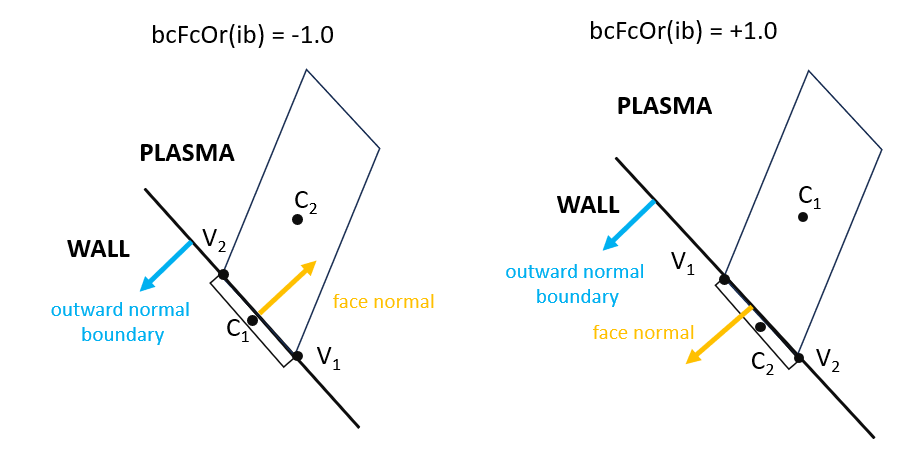
\includegraphics[height=4cm]{FiguresWG/bcfcor.PNG}}
\else
    \centerline{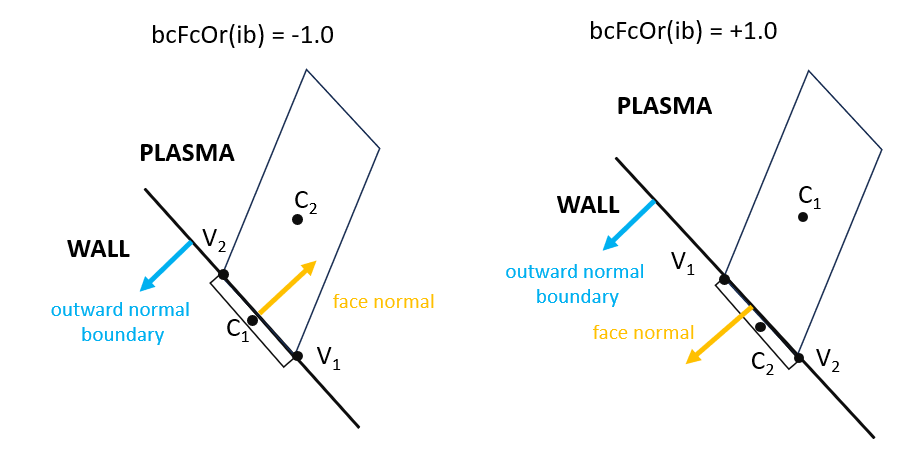
\includegraphics[height=4cm]{FiguresWG/bcfcor.eps}}
\fi
    \caption{Illustration of {\tt bcFcOr}.}
    \label{fig:bcfcor}
\end{figure}

Most boundary conditions fall in one of three categories: Dirichlet, Neumann, or flux.

\textbf{Flux}

To impose a given flux, the net source term in the guard cell must be equal to that flux. Since no fluxes are computed between the guard cells, the flux across the guard cell face must equal the source term.

\textbf{Dirichlet}
\begin{sloppypar}
To impose a fixed value in a guard cell, the code makes use of the different source contributions and very large numbers. For example, to set a fixed density {\tt $n_{BC}$},
the code sets {\tt sna(iCv,0,is) = VBIG $\times$ fcS $\times$ $n_{BC}$}, and {\tt sna(iCv,1,is) = - VBIG $\times$ fcS}, with {\tt sna(iCv,is) = sna(iCv,0,is) + sna(iCv,1,is) $\times$ na(iCv,is)} and where {\tt VBIG} is a very large number. Because {\tt VBIG} is so large, the only way to get a physical source is to have {\tt na(iCv,is) = $n_{BC}$}.
\end{sloppypar}

\textbf{Neumann}
\begin{sloppypar}
To set the gradient normal to the boundary, the code again makes use of the different source contributions and very large numbers. For orthogonal cells, these boundary conditions correctly impose the gradient normal to the boundary face.
For cells that are skewed with respect to the boundary face, the implementation depends on the (partially experimental) {\tt b2stbc\_BC2\_cor9} switch.
To impose for example a density gradient $\Phi$ with {\tt b2stbc\_BC2\_cor9 = 0.0}, the code sets
{\tt sna(iCv,0,is) = VBIG $\times$ fcS $\times$ ($\Phi$ $\times$ ( fcHc(1) + fcHc(2) ) $\times \cos \gamma$ + na(iCv\_internal)} and {\tt sna(iCv,1,is) = - VBIG $\times$ fcS}, where {\tt na(iCv\_internal)} is the density in the first interior cell. To get a physical source, we must have {\tt $\Phi$ $\times$ ( fcHc(1) + fcHc(2) ) $\times \cos \gamma$ + na(iCv\_internal) = na(iCv)}. This results in the correct normal gradient for skewed cells, only if there would be no gradients in the direction tangential to the boundary face. When {\tt b2stbc\_BC2\_cor9 = 1.0}, a correction term based on the vertex values is added, such that $\Phi$ is the gradient normal to the boundary, also in the presence of tangential gradients (up to the interpolation error).
\end{sloppypar}

%% TODO: convert all below to unstructured?

In this Section, the boundaries are denoted as $S_0$ for the PFR boundaries, $S_1$ for the core boundaries, $E$ for the Eastern boundaries (right targets), $W$ for the Western boundaries (left targets), and $N$ for the outer main wall boundary.

\subsection{Particle balance equations}

$S_{n_a} = S_{n_a,0} + S_{n_a,1} n_a$

\subsubsection{South. Private region}

\underline{If $z_a = 0$}

{\em For leakage boundary condition:} {\tt BCCON = 10}

\begin{equation}
\left. \frac{\sqrt g}{h_y}\Gamma_{ay} \right|_{S_0}
=
\left. \left[
p_{n_a,a,1} \frac{\sqrt g}{h_y} \sqrt{\frac{z_a T_e + T_i}{m_a}} n_a
+
\sum \limits_{a=0}^{ns-1} r_{rec,a,0} c_{nsr}
\max \left\{0, -\frac{\sqrt g}{h_y} \Gamma_{ay} \right\}
\right] \right|_{S_0}
\end{equation}

$p_{n_a,a,1} = -10^{-2}, \;\; r_{rec,0,0} = 0,\;\; r_{rec,1,0} = 1$

$\widetilde{\Gamma}_{ay}$ was replaced by $\Gamma_{ay}$

$c_{nsr}$ --- neutral sources rescale coefficient, $1$ --- when working with B2.5 standalone and $10^{-10}$ when coupling to Eirene

$p_{n_a,a,1}$ is the radial leakage velocity, in units of the local species sound speed. Negative velocities are directed out of the plasma.

\underline{If $z_a \neq 0$}

{\em For decay length boundary condition:} {\tt BCCON = 9}

\begin{equation}
\begin{matrix}
\left. \frac{\sqrt g}{h_y} \widetilde{\Gamma}_{ay} \right|_{S_0}& =
& \left\{
\begin{matrix}
\left. \left[
        -\frac{1}{p_{n_a,a,1}} \frac{\sqrt g}{h_y}  \left(
                D^{(AN)}_{n,a} + D^{(AN)}_{p,a} \left(z_a T_e + T_i \right)
        \right) n_a
\right] \right|_{S_0}, & \text{mdf\_fnb} = 0
\\
\left. \left[
\begin{matrix}
        -\frac{1}{p_{n_a,a,1}} \frac{\sqrt g}{h_y} & \left(
                D^{(AN)}_{n,a} + D^{(AN)}_{p,a} \left(z_a T_e + T_i \right)
        \right) n_a
        + \\
        \frac{\sqrt g}{h_y} & D_{ayx} \frac{1}{h_x} \frac{\partial n_a T_i}{\partial x}
        +
        \frac{\sqrt g}{h_y} V_{ay}^{(E)} n_a
\end{matrix}
\right] \right|_{S_0}, & \text{mdf\_fnb} = 1
\end{matrix} \right.
\end{matrix}
\end{equation}

\begin{align}
S^{no\_mdf}_{n_a,0} & = 0 \\
S^{no\_mdf}_{n_a,1} & = - \frac{1}{p_{n_a,a,1}} \frac{\sqrt{g}}{h_y} \left( D^{(AN)}_{n,a} + D^{(AN)}_{p,a} \left( z_a T_e + T_i \right) \right)
\end{align}

$p_{n_a,a,1}$ is the density radial decay length of species $a$, in $m$.

{\em For leakage boundary conditions:} {\tt BCCON = 10}

\begin{equation}
\begin{matrix}
\left. \frac{\sqrt g}{h_y} \widetilde{\Gamma}_{ay} \right|_{S_0}& =
& \left\{
\begin{matrix}
\left. \left[
        p_{n_a,a,1} \frac{\sqrt g}{h_y} \sqrt{\frac{z_a T_e + T_i}{m_a}} n_a
        +
        \min \left\{0, \frac{\sqrt g}{h_y} n_a V_{ay}^{(E)} \right\}
\right] \right|_{S_0}, & \text{mdf\_fnb} = 0
\\
\left. \left[
p_{n_a,a,1} \frac{\sqrt g}{h_y} \sqrt{\frac{z_a T_e + T_i}{m_a}} n_a
        +
        \frac{\sqrt g}{h_y} D_{ayx} \frac{1}{h_x} \frac{\partial n_a T_i}{\partial x}
        +
        \min \left\{0, \frac{\sqrt g}{h_y} n_a V_{ay}^{(E)} \right\}
\right] \right|_{S_0}, & \text{mdf\_fnb} = 1
\end{matrix} \right.
\end{matrix}
\end{equation}

$p_{n_a,a,1} = -10^{-3}$ is the radial leakage velocity, in units of the species local sound speed. Negative velocities are directed out of the plasma.

\begin{align}
S^{no\_mdf}_{n_a,0} & = 0 \\
S^{no\_mdf}_{n_a,1} & = {p_{n_a,a,1}} \frac{\sqrt{g}}{h_y} \sqrt{\frac{z_a T_e + T_i}{m_a}} n_a
\end{align}

% -- To be checked --
{\em Imposing radial leakage:} {\tt BCCON = 15}

When using drifts, one should use {\tt BCCON = 10} instead.

\begin{equation}
\left. - \frac{\sqrt g}{h_y^2} D_{n,ay} \frac{\partial n_a}{\partial y} \right|_{S_0}
=
\left. \left[
c_{n_a,a,2} \frac{\sqrt g}{h_y} \sqrt{\frac{z_a T_e + T_i}{m_a}} n_a
\right] \right|_{S_0}
\end{equation}

$c_{n_a,a,2} = -10^{-3}$ is the radial leakage velocity, in units of the species local thermal velocity. Negative velocities are directed out of the plasma.

% -- end --

\subsubsection{South 1. Core plasma}

\underline{If $z_a = 0$}

%-------- end of 21st page -------------

{\em Imposing total particle flux:} {\tt BCCON = 8}

$\left. \frac{\sqrt g}{h_y} \widetilde{\Gamma}_{ay} \right|_{S_1} = 0$

$\left. \frac{\sqrt g}{h_y} \Gamma_{ay} \right|_{S_1} = 0$

\underline{If $z_a \neq 0$}

{\em Imposing a constant density :} {\tt BCCON = 1}

\begin{equation}
\left. \frac{\sqrt g}{h_y} \widetilde{\Gamma}_{ay} \right|_{S_1}
=
\frac{\sqrt{g}}{h_y}
\left. \left(
        \left. v_{big} n_a \right|_{S_1} - v_{big} n_a
\right) \right|_{S_1},
\;\;
v_{big} = 10^8 \sqrt{\frac{100 \text{eV}}{m_p}},
\;\;
\left. n_a \right|_{S_1} \text{ is the desired density in } m^{-3}
\end{equation}

{\em Imposing the total particle flux with constant flux density:} {\tt BCCON = 8}

\begin{equation*}
\left. \frac{\sqrt g}{h_y} \widetilde{\Gamma}_{ay} \right|_{S_1} =
\left. p_{n,a,0} \frac{
\frac{\sqrt g}{h_y}
} {
\sum \limits_i \left(
        \frac{\sqrt g}{h_y}
\right)_{i, -1}
} \right|_{S_1}
+
\left.
\frac{\sqrt g}{h_y} D_{ayx} \frac{1}{h_x} \frac{\partial n_a T_i}{\partial x}
\right|_{S_1} +
\left. \frac{\sqrt g}{h_y}V_{ya}^{(E)} n_a \right|_{S_1}
\end{equation*}

$p_{n,a,0}$ is the desired total particle flux, per unit time.

\subsubsection{North}

\underline{If $z_a = 0$}

{\em For leakage boundary condition:} {\tt BCCON = 10}

\begin{equation}
\left. - \frac{\sqrt g}{h_y} \Gamma_{ay} \right|_{N}
=
\left. \left[
p_{n_a,a,1} \frac{\sqrt g}{h_y} \sqrt{\frac{z_a T_e + T_i}{m_a}} n_a
+
\sum \limits_{a=0}^{ns-1} r_{rec,a,0} c_{nsr}
\max \left\{0, \frac{\sqrt g}{h_y} \Gamma_{ay} \right\}
\right] \right|_{N}
\end{equation}

$p_{n_a,a,1} = -10^{-2}, \;\; r_{rec,0,0} = 0,\;\; r_{rec,1,0} = 1$

$c_{nsr}$ --- neutral sources rescale coefficient, $1$ --- when working with B2.5 standalone and $10^{-10}$ when coupling to Eirene

$p_{n_a,a,1}$ is the radial leakage velocity, in units of the local species sound speed. Negative velocities are directed out of the plasma.

$\widetilde{\Gamma}_{ay}$ was replaced by $\Gamma_{ay}$

\underline{If $z_a \neq 0$}

{\em For decay length boundary condition:} {\tt BCCON = 9}

\begin{equation}
\begin{matrix}
\left. - \frac{\sqrt g}{h_y} \widetilde{\Gamma}_{ay} \right|_{N}& =
& \left\{
\begin{matrix}
\left. \left[
        \frac{1}{p_{n_a,a,1}} \frac{\sqrt g}{h_y}  \left(
                D^{(AN)}_{n,a} + D^{(AN)}_{p,a} \left(z_a T_e + T_i \right)
        \right) n_a
\right] \right|_{N}, & \text{mdf\_fnb} = 0
\\
\left. \left[
\begin{matrix}
        \frac{1}{p_{n_a,a,1}} & \frac{\sqrt g}{h_y}  \left(
                D^{(AN)}_{n,a} + D^{(AN)}_{p,a} \left(z_a T_e + T_i \right)
        \right) n_a \\
        -
        \frac{\sqrt g}{h_y} & D_{ayx} \frac{1}{h_x} \frac{\partial n_a T_i}{\partial x}
        -
        \frac{\sqrt g}{h_y} V_{ay}^{(E)} n_a
\end{matrix}
\right] \right|_{N}, & \text{mdf\_fnb} = 1
\end{matrix} \right.
\end{matrix}
\end{equation}

\begin{align}
S^{no\_mdf}_{n_a,0} & = 0 \\
S^{no\_mdf}_{n_a,1} & = \frac{1}{p_{n_a,a,1}} \frac{\sqrt{g}}{h_y} \left( D^{(AN)}_{n,a} + D^{(AN)}_{p,a} \left( z_a T_e + T_i \right) \right)
\end{align}

$p_{n_a,a,1}$ is the density radial decay length of species $a$, in $m$.

{\em For leakage boundary conditions:} {\tt BCCON = 10}

\begin{equation}
\begin{matrix}
\left. - \frac{\sqrt g}{h_y} \widetilde{\Gamma}_{ay} \right|_{N}& =
& \left\{
\begin{matrix}
\left. \left[
        p_{n_a,a,1} \frac{\sqrt g}{h_y} \sqrt{\frac{z_a T_e + T_i}{m_a}} n_a
        -
        \max \left\{0, \frac{\sqrt g}{h_y} n_a V_{ay}^{(E)} \right\}
\right] \right|_{N}, & \text{mdf\_fnb} = 0
\\
\left. \left[
        p_{n_a,a,1} \frac{\sqrt g}{h_y} \sqrt{\frac{z_a T_e + T_i}{m_a}} n_a
        -
        \frac{\sqrt g}{h_y} D_{ayx} \frac{1}{h_x} \frac{\partial n_a T_i}{\partial x}
        -
        \max \left\{0, \frac{\sqrt g}{h_y} n_a V_{ay}^{(E)} \right\}
\right] \right|_{N}, & \text{mdf\_fnb} = 1
\end{matrix} \right.
\end{matrix}
\end{equation}

$p_{n_a,a,1} = -10^{-3}$ is the radial leakage velocity, in units of the species local sound speed. Negative velocities are directed out of the plasma.

\begin{align}
S^{no\_mdf}_{n_a,0} & = 0 \\
S^{no\_mdf}_{n_a,1} & = {p_{n_a,a,1}} \frac{\sqrt{g}}{h_y} \sqrt{\frac{z_a T_e + T_i}{m_a}} n_a
\end{align}

% -- To be checked --
{\em Imposing radial leakage:} {\tt BCCON = 15}

When using drifts, one should use {\tt BCCON = 10} instead.

\begin{equation}
\left. \frac{\sqrt g}{h_y^2} D_{n,ay} \frac{\partial n_a}{\partial y} \right|_N
=
\left. \left[
c_{n_a,a,2} \frac{\sqrt g}{h_y} \sqrt{\frac{z_a T_e + T_i}{m_a}} n_a
\right] \right|_N
\end{equation}

$c_{n_a,a,2} = -10^{-3}$ is the radial leakage velocity, in units of the species local thermal velocity. Negative velocities are directed out of the plasma.

% -- end --

\subsubsection{North with puffing}

\underline{If $z_a = 0$}

{\em Imposing a particle flux per unit area:} {\tt BCCON = 5}

\begin{equation}
\left. - \frac{\sqrt g}{h_y} \widetilde{\Gamma}_{ay} \right|_N
=
\left. p_{n,a,0} \frac{\sqrt g}{h_y} \right|_N
+
\left.
\sum \limits_{a=0}^{ns-1} \left[
        r_{rec,a,0} c_{nsr}
        \max \left\{0, -\frac{\sqrt g}{h_y} \Gamma_{ay} \right\}
\right] \right|_N
\end{equation}

$c_{nsr}$ --- neutral sources rescale coefficient, $1$ --- when working with B2.5 standalone and $10^{-10}$ when coupling to Eirene

$r_{rec,0,0} = 0,\;\; r_{rec,1,0} = 1$

$p_{n,a,0}$ is the desired total particle flux density, in $m^{-2}.s^{-1}$.

$\widetilde{\Gamma}_{ay}$ was replaced by $\Gamma_{ay}$

or

{\em Imposing a total particle flux with constant flux density:} {\tt BCCON = 8}

\begin{equation*}
\left. - \frac{\sqrt g}{h_y} \widetilde{\Gamma}_{ay} \right|_N =
\left. \frac{ p_{n,a,0}
}{
\sum \limits_{i=0}^{Nx-1} \left(
        \frac{\sqrt g}{h_y}
\right)_{i, Ny}
}
\frac{\sqrt g}{h_y} \right|_N
+
\left. \sum \limits_{a=0}^{ns-1} \left[
        r_{rec,a,0} c_{nsr}
        \max \left\{0, \frac{\sqrt g}{h_y} \Gamma_{ay} \right\}
\right]
\right|_N
\end{equation*}

$c_{nsr}$ --- neutral sources rescale coefficient, $1$ --- when working with B2.5 standalone and $10^{-10}$ when coupling to Eirene

$r_{rec,0,0} = 0,\;\; r_{rec,1,0} = 1$

$p_{n,a,0}$ is the desired total particle flux, per unit time.

$\widetilde{\Gamma}_{ay}$ was replaced by $\Gamma_{ay}$

\subsubsection{West}

%-------- end of 23rd page -------------

\underline{If $z_a = 0$}

{\em Imposing a given particle flux per unit area:} {\tt BCCON = 5}

\begin{equation}
\left. \frac{\sqrt g}{h_x} \Gamma_{ax} \right|_W
=
\left. \left[
p_{n,a,1} \frac{\sqrt g}{h_y}
+
c_{nsr} \sum \limits_{a=0}^{ns-1} r_{rec,a,0}
\max \left\{0, -\frac{\sqrt g}{h_x} \Gamma_{ax} \right\}
\right] \right|_W
\end{equation}

$r_{rec,0,0} = 0,\;\; r_{rec,1,0} = 1,\;\; p_{n_a,a,1} = 0 $

\begin{equation}
\left. \frac{\sqrt g}{h_x} \widetilde{\Gamma}_{ax} \right|_W
=
\left. \left[
p_{n,a,1} \frac{\sqrt g}{h_x}
+
c_{nsr} \sum \limits_{a=0}^{ns-1} r_{rec,a,0}
\max \left\{0, -\frac{\sqrt g}{h_x} \Gamma_{ax} \right\}
\right] \right|_W
\end{equation}

$\widetilde{\Gamma}_{ax}$ was replaced by $\Gamma_{ax}$

$r_{rec,0,0} = 0,\;\; r_{rec,1,0} = 1,\;\; p_{n_a,a,1} = 0 $

\underline{If $z_a \neq 0$}

{\em Sheath density boundary condition:} {\tt BCCON = 3}

\begin{equation*}
\left. \frac{\sqrt g}{h_x} \Gamma_{ax} \right|_W = \left.
10^{20} \frac{\sqrt{g}}{h_x} \frac{\partial n_a}{\partial x}
\right|_W
\end{equation*}

{\em Drift-compatible, Bohm-Chodura sheath entrance condition} {\tt BCCON = 14}

{\em If the sine of the incident field line angle is larger than {\tt Qalfmin}:}

{\em - Marginal imposition, with collective sound speed:} {\tt MOMPAR(,,2)} = $p_{m,a,2} < 0.5$

To be used in conjunction with {\tt BCENE = 15}, {\tt BCENI = 15}, {\tt BCMOM = 13}, and {\tt BCPOT = 11}.

\begin{equation*}
\left. \frac{\sqrt g}{h_x} \widetilde{\Gamma}_{ax} \right|_W
=
\left. \left[
- p_{n,a,1} \frac{\sqrt g}{h_x} |b_x|
\sqrt{\frac{\sum \limits_{\substack{b = 0 \\ z_b \neq 0}}^{ns-1} p_b}{\sum \limits_{\substack{b = 0 \\ z_b \neq 0}}^{ns-1} m_b n_b}} n_a
-
\frac{\sqrt g}{h_x} D_{axy} \frac{1}{h_y} \frac{\partial n_a T_i}{\partial y}
\right]
\right|_W
\end{equation*}

$p_{n,a,1} = +1$

{\em - Non-marginal imposition, with individual species sound speed:} {\tt MOMPAR(,,2)} = $p_{m,a,2} \geq 0.5$

to be used in conjunction with {\tt BCMOM = 13}, {\tt BCENE = 15} with {\tt bcene\_15\_style = 1}, {\tt BCENI = 15}, {\tt BCPOT = 3} or {\tt BCPOT = 11} with {\tt istyle\_fchi=0}.

This condition imposes that the sum of the poloidal projection of the parallel velocity and the poloidal $\exb$ velocity (restricted to not exceed $\pm 2 c_{s,a} |b_x|$), equals \textit{at least} the specific species sound speed $c_{s,a}$, reprojected in the the poloidal direction.

The parameter $p_{m,a,1}$ is set by {\tt MOMPAR(,,1)}. The parameter $\chi$ is set by {\tt GAMMAI}.

\begin{equation*}
\left. \frac{\sqrt g}{h_x} \widetilde{\Gamma}_{ax} \right|_W
=
\left. \left[
- \frac{\sqrt g}{h_x} |b_x|
U_{out} n_a
-
\frac{\sqrt g}{h_x} D_{axy} \frac{1}{h_y} \frac{\partial n_a T_i}{\partial y}
\right]
\right|_W
\end{equation*}

\begin{equation*}
  U_{out} = \max \left( -u_{\parallel,a}^{extrap}- \frac{V_{\exb}^{restr}}{|b_x|}, p_{m,a,1} \cdot \sqrt{\frac{\chi T_i + z_a T_e}{m_a}} \right)
\end{equation*}

where $u_{\parallel,a}^{extrap}$ is the extrapolated parallel velocity at the target, and $V_{\exb}^{restr}$ is the poloidal $\exb$ velocity restricted to not exceed $\pm 2 c_{s,a} |b_x|$.

{\em For nearly tangent field lines, we use instead:}

\begin{equation}
\begin{matrix}
\left. - \frac{\sqrt g}{h_x} \widetilde{\Gamma}_{ax} \right|_W & =
& \left\{
\begin{matrix}
\left. \left[ \frac{\sqrt g}{h_x} p_{n,a,1} \sqrt{\frac{\sum \limits_{\substack{b = 0 \\ z_b \neq 0}}^{ns-1} p_b}{\sum \limits_{\substack{b = 0 \\ z_b \neq 0}}^{ns-1} m_b n_b}} n_a \alpha_{\max} +
   \max \left( 0, \frac{\sqrt g}{h_x} V^{(E)}_{ax} n_a \right) \right] \right|_W, & \text{mdf\_fnb = 0}
\\
\left. \left[ \frac{\sqrt g}{h_x} p_{n,a,1} \sqrt{\frac{\sum \limits_{\substack{b = 0 \\ z_b \neq 0}}^{ns-1} p_b}{\sum \limits_{\substack{b = 0 \\ z_b \neq 0}}^{ns-1} m_b n_b}} n_a \alpha_{\max} +
   \max \left( 0, \frac{\sqrt g}{h_x} \left( V^{(E)}_{ax} + \widetilde{\widetilde{V}}^{(dia)}_{ax} \right) n_a \right) + \tilde\Gamma^{(PSch)}_{ax} \right] \right|_W, & \text{mdf\_fnb = 1}
\end{matrix}
\right.
\end{matrix}
\end{equation}

where $\alpha_{\max}$ is given by {\tt Qalfmax}.

Both {\tt Qalfmin} and {\tt Qalfmax} are provided in the {\tt b2fgmtry} file or through the {\tt b2us\_prep\_Qalfmin} and {\tt b2us\_prep\_Qalfmax} switches, respectively. Default value for both is $10^{-3}$.

\subsubsection{East}

\underline{If $z_a = 0$}

{\em Imposing a given particle flux per unit area:} {\tt BCCON = 5}

\begin{equation}
\left. - \frac{\sqrt g}{h_x} \Gamma_{ax} \right|_E
=
\left. \left[
p_{n,a,1} \frac{\sqrt g}{h_y}
+
c_{nsr} \sum \limits_{a=0}^{ns-1} r_{rec,a,0}
\max \left\{0, \frac{\sqrt g}{h_x} \Gamma_{ax} \right\}
\right] \right|_E
\end{equation}

$r_{rec,0,0} = 0,\;\; r_{rec,1,0} = 1,\;\; p_{n_a,a,1} = 0 $

%-------- end of 24th page -------------


\begin{equation}
\left. - \frac{\sqrt g}{h_x} \widetilde{\Gamma}_{ax} \right|_E
=
\left. \left[
c_{nsr} \sum \limits_{a=0}^{ns-1} r_{rec,a,0}
\max \left\{0, \frac{\sqrt g}{h_x} \Gamma_{ax} \right\}
\right] \right|_E
\end{equation}

$\widetilde{\Gamma}_{ax}$ was replaced by $\Gamma_{ax}$

$r_{rec,0,0} = 0,\;\; r_{rec,1,0} = 1$

\underline{If $z_a \neq 0$}

{\em Sheath density boundary condition:} {\tt BCCON = 3}

\begin{equation*}
\left. - \frac{\sqrt g}{h_x} \Gamma_{ax} \right|_E =
- 10^{20} \left. \frac{\sqrt{g}}{h_x} \frac{\partial n_a}{\partial x}
\right|_E
\end{equation*}

{\em Drift-compatible, Bohm-Chodura sheath entrance condition} {\tt BCCON = 14}

{\em If the sine of the incident field line angle is larger} {\tt Qalfmin}:

{\em - Marginal imposition, with collective sound speed:} {\tt MOMPAR(,,2)} = $p_{m,a,2} < 0.5$

To be used in conjunction with {\tt BCENE = 15}, {\tt BCENI = 15}, {\tt BCMOM = 13}, and {\tt BCPOT = 11}.

\begin{equation*}
\left. - \frac{\sqrt g}{h_x} \widetilde{\Gamma}_{ax} \right|_E
=
\left. \left[
- p_{n,a,1} \frac{\sqrt g}{h_x} |b_x|
\sqrt{\frac{\sum \limits_{\substack{b = 0 \\ z_b \neq 0}}^{ns-1} p_b}{\sum \limits_{\substack{b = 0 \\ z_b \neq 0}}^{ns-1} m_b n_b}} n_a
+
\frac{\sqrt g}{h_x} D_{axy} \frac{1}{h_y} \frac{\partial n_a T_i}{\partial y}
\right]
\right|_E
\end{equation*}

$p_{n,a,1} = +1$

{\em - Non-marginal imposition, with individual species sound speed:} {\tt MOMPAR(,,2)} = $p_{m,a,2} \geq 0.5$

to be used in conjunction with {\tt BCMOM = 13}, {\tt BCENE = 15} with {\tt bcene\_15\_style = 1}, {\tt BCENI = 15}, {\tt BCPOT = 3} or {\tt BCPOT = 11} with {\tt istyle\_fchi=0}.

This condition imposes that the sum of the poloidal projection of the parallel velocity and the poloidal $\exb$ velocity (restricted to not exceed $\pm 2 c_{s,a} |b_x|$), equals \textit{at least} the specific species sound speed $c_{s,a}$, reprojected in the the poloidal direction.

The parameter $p_{m,a,1}$ is set by {\tt MOMPAR(,,1)}. The parameter $\chi$ is set by {\tt GAMMAI}.

\begin{equation*}
\left. - \frac{\sqrt g}{h_x} \widetilde{\Gamma}_{ax} \right|_E
=
\left. \left[
- \frac{\sqrt g}{h_x} |b_x|
U_{out} n_a
+
\frac{\sqrt g}{h_x} D_{axy} \frac{1}{h_y} \frac{\partial n_a T_i}{\partial y}
\right]
\right|_E
\end{equation*}

\begin{equation*}
  U_{out} = \max \left( u_{\parallel,a}^{extrap} + \frac{V_{\exb}^{restr}}{|b_x|}, p_{m,a,1} \cdot \sqrt{\frac{\chi T_i + z_a T_e}{m_a}} \right)
\end{equation*}

where $u_{\parallel,a}^{extrap}$ is the extrapolated parallel velocity at the target, and $V_{\exb}^{restr}$ is the poloidal $\exb$ velocity restricted to not exceed $\pm 2 c_{s,a} |b_x|$.

{\em For nearly tangent field lines, we use instead:}

\begin{equation}
\begin{matrix}
\left. \frac{\sqrt g}{h_x} \widetilde{\Gamma}_{ax} \right|_E & =
& \left\{
\begin{matrix}
\left. \left[ \frac{\sqrt g}{h_x} p_{n,a,1} \sqrt{\frac{\sum \limits_{\substack{b = 0 \\ z_b \neq 0}}^{ns-1} p_b}{\sum \limits_{\substack{b = 0 \\ z_b \neq 0}}^{ns-1} m_b n_b}} n_a \alpha_{\max} +
   \max \left( 0, \frac{\sqrt g}{h_x} V^{(E)}_{ax} n_a \right) \right] \right|_E, & \text{mdf\_fnb = 0}
\\
\left. \left[ \frac{\sqrt g}{h_x} p_{n,a,1} \sqrt{\frac{\sum \limits_{\substack{b = 0 \\ z_b \neq 0}}^{ns-1} p_b}{\sum \limits_{\substack{b = 0 \\ z_b \neq 0}}^{ns-1} m_b n_b}} n_a \alpha_{\max} +
   \max \left( 0, \frac{\sqrt g}{h_x} \left( V^{(E)}_{ax} + \widetilde{\widetilde{V}}^{(dia)}_{ax} \right) n_a \right) + \tilde\Gamma^{(PSch)}_{ax} \right] \right|_E, & \text{mdf\_fnb = 1}
\end{matrix}
\right.
\end{matrix}
\end{equation}

\subsection{Parallel momentum balance for ions}

$S_{m_a} = S_{m_a,0} + S_{m_a,1} V_{\parallel a} + S_{m_a,2} m_a n_a + S_{m_a,3} m_a n_a V_{\parallel a}$

\subsubsection{South. Private region}

\underline{If $z_a = 0$}

{\em Weakly imposing a velocity:} {\tt BCMOM = 4}

\begin{equation*}
\left. h_z \frac{\sqrt g}{h_y} \Gamma_{ay}^m \right|_{S_0} =
\left. \left[
p_{m,a,1} p_{m,a,2} h_z \frac{\sqrt g}{h_y} -
p_{m,a,2} h_z \frac{\sqrt g}{h_y} V_{\parallel a}
\right] \right|_{S_0}
\end{equation*}

$p_{m,a,1}=0$ is the imposed velocity, in $m.s^{-1}$, and $p_{m,a,2}=10^5$ is the strength with which this velocity is imposed.

We had this b.c.

$\left. h_z \frac{\sqrt g}{h_y} \Gamma_{ay}^m \right|_{S_0} =
\left. \left[
c_{m,a,3} h_z \frac{\sqrt g}{h_y} m_a n_a V_{\parallel a} +
c_{m,a,6} \max \left(0,-h_z \frac{\sqrt g}{h_y} \frac{\Gamma_{ay}^{Cor}}{n_a} \right)
m_a n_a V_{\parallel a}
\right] \right|_{S_0}$, delete term with {\tt max} !

%-------- end of 25th page -------------

$\Gamma_{ay}^{Cor} = \Gamma_{ay} + \Gamma_{ay}^{(dia)}$

$c_{m,a,3} = -10^{10}$, we have $c_{m,a,6}=-1$, but not $c_{m,a,6}=0$

Inserted into {\tt b2stbc\_phys} for {\tt BCMOM=12} as $c_{m,a,3} \rightarrow p_{m,a,2} = -10^{10}$, and $c_{m,a,6} \rightarrow p_{m,a,1} = -1$

\underline{If $z_a \neq 0$}

{\em Weakly imposing a velocity:} {\tt BCMOM = 4}

\begin{equation}
\left. h_z \frac{\sqrt g}{h_y} \Gamma_{ay}^m \right|_{S_0} =
\left. \left[
        p_{m,a,1} p_{m,a,2} h_z \frac{\sqrt g}{h_y} -
        p_{m,a,2} h_z \frac{\sqrt g}{h_y} V_{\parallel a}
\right] \right|_{S_0}
\end{equation}

$p_{m,a,1}=0$ is the imposed velocity, in $m.s^{-1}$, and $p_{m,a,2}=10^5$ is the strength with which this velocity is imposed.

\begin{equation}
\left. h_z \frac{\sqrt g}{h_y} \Gamma_{ay}^m \right|_{S_0} =
\left. \left[
        c_{m,a,3} h_z \frac{\sqrt g}{h_y} m_a n_a V_{\parallel a} +
        c_{m,a,6} \max \left(
                0, -h_z \frac{\sqrt g}{h_y} \frac{\Gamma_{ay}^{Cor}}{n_a}
        \right) m_a n_a V_{\parallel a}
\right] \right|_{S_0}
\end{equation}

delete term with {\tt max}!

$\Gamma_{ay}^{Cor} = \Gamma_{ay} + \Gamma_{ay}^{(dia)}$

$c_{m,a,3} = 0$,  $c_{m,a,6} = -1$

\subsubsection{South 1. Core}

\underline{If $z_a = 0$}

{\em Weakly imposing a velocity:} {\tt BCMOM = 4}

$ \left. h_z \frac{\sqrt g}{h_y} \Gamma_{ay}^m \right|_{S_1} = \left. \left[
        p_{m,a,1} p_{m,a,2} h_z \frac{\sqrt g}{h_y} -
        p_{m,a,2} h_z \frac{\sqrt g}{h_y} V_{\parallel a}
\right] \right|_{S_1}$

$p_{m,a,1}=0$ is the imposed velocity, in $m.s^{-1}$, and $p_{m,a,2}=10^5$ is the strength with which this velocity is imposed.

$ \left. h_z \frac{\sqrt g}{h_y} \Gamma_{ay}^m \right|_{S_1} = c_{m,a,3} h_z \left. \frac{\sqrt g}{h_y} m_a n_a V_{\parallel a} \right|_{S_1}$

$c_{m,a,3} = -10^{10}$

Inserted into {\tt b2stbc\_phys} for {\tt BCMOM=12} as $c_{m,a,3} \rightarrow p_{m,a,2} = -10^{10},\;c_{m,a,6} \rightarrow
p_{m,a,1} = 0$

\underline{If $z_a \neq 0$}

%-------- end of 26th page -------------

{\em Weakly imposing a velocity:} {\tt BCMOM = 4}

$ \left. h_z \frac{\sqrt g}{h_y} \Gamma_{ay}^m \right|_{S_1} = \left. \left[
        p_{m,a,1} p_{m,a,2} h_z \frac{\sqrt g}{h_y} -
        p_{m,a,2} \frac{\sqrt g}{h_y} V_{\parallel a}
\right] \right|_{S_1}$

$p_{m,a,1}=0$ is the imposed velocity, in $m.s^{-1}$, and $p_{m,a,2}=10^5$ is the strength with which this velocity is imposed.

{\em {\tt b2stbc\_spb} style:} {\tt BCMOM = 14}

\begin{align*}
\left. h_z \frac{\sqrt g}{h_y} \Gamma_{ay}^m \right|_{S_1} = &
c_{m,a,3} h_z \left. \frac{\sqrt g}{h_y} m_a n_a V_{\parallel a} \right|_{S_1} + \\
& \left. \left[
h_z \frac{\sqrt g}{h_y} m_a \left\langle n_a \right\rangle \left( -2 \right)\frac{\left\langle T_i \right\rangle B_z}{ez_a}\frac{\partial}{h_x \partial x} \left( \frac{1}{B^2} \right) \left\langle V_{\parallel a} \right\rangle c_{drift} +
c_{corflux} h_z \frac{\sqrt g}{h_y}
\right] \right|_{S_1} \\
+ & \left. c_{m,a,1} \max \left( 0 , - h_z \frac{\sqrt{g}}{h_y} \frac{\Gamma_{ay}^{Cor}}{n_a} \right) m_a n_a V_{\parallel a} \right|_{S_1}
\end{align*}

$c_{m,a,1} = 0$, $c_{m,a,3} = -10^{10}$

{\em Prescribe the value of the parallel velocity as a function of the poloidal coordinate:} {\tt BCMOM = 15}

\begin{equation*}
\left. h_z \frac{\sqrt g}{h_y} \Gamma_{ay}^m \right|_{S_1} =
\left. v_{big} n_{e0} m_{a} h_z \frac{\sqrt g}{h_y} \left[
        \frac{\langle B \rangle}{B} p_{m,a,1} - V_{\parallel a}
\right] \right|_{S_1}
\end{equation*}

where $\langle B \rangle = \frac{\mathlarger{\oint}_{S_1} B \sqrt{g} \, dx}{\mathlarger{\oint}_{S_1} \sqrt{g} \, dx}$, the integration is done over the innermost magnetic surface, $v_{big} = 10^{8} \sqrt{\frac{100 \text{eV}}{m_p}}$, $n_{e0} = 10^{20}$, $p_{m,a,1}$ is the given value of the average parallel velocity, in $m.s^{-1}$.

\subsubsection{North}

\underline{If $z_a=0$}

{\em Weakly imposing a velocity:} {\tt BCMOM = 4}

$ \left. -h_z \frac{\sqrt g}{h_y} \Gamma_{ay}^m \right|_N = \left. \left[
        p_{m,a,1} p_{m,a,2} h_z \frac{\sqrt g}{h_y} -
        p_{m,a,2} h_z \frac{\sqrt g}{h_y} V_{\parallel a}\right]
\right|_N$

$p_{m,a,1}=0$ is the imposed velocity, in $m.s^{-1}$, and $p_{m,a,2}=10^5$ is the strength with which this velocity is imposed.

$\left. -h_z \frac{\sqrt g}{h_y} \Gamma_{ay}^m \right|_N = \left. \left[
        c_{m,a,3} h_z \frac{\sqrt g}{h_y} m_a n_a V_{\parallel a} +
        c_{m,a,6} \max \left(
                0, h_z \frac{\sqrt g}{h_y} \frac{\Gamma_{ay}^{Cor}}{n_a}
        \right) m_a n_a V_{\parallel a}
\right]
\right|_N$

delete term with {\tt max} !

$c_{m,a,3} = -10^{10}$, we have  $c_{m,a,6} = -1$, but not $c_{m,a,6} = 0$

Inserted into {\tt b2stbc\_phys} for {\tt BCMOM=12} as $c_{m,a,3} \rightarrow p_{m,a,2} = -10^{10},\;c_{m,a,6} \rightarrow p_{m,a,1} = -1$

\underline{If $z_a \neq 0$}

%-------- end of 27th page -------------

{\em Weakly imposing a velocity:} {\tt BCMOM = 4}

$ \left. -h_z \frac{\sqrt g}{h_y} \Gamma_{ay}^m \right|_N = \left[
        p_{m,a,1} p_{m,a,2} h_z \frac{\sqrt g}{h_y} -
        p_{m,a,2} h_z \frac{\sqrt g}{h_y} V_{\parallel a}
\right]|_N$

$p_{m,a,1}=0$ is the imposed velocity, in $m.s^{-1}$, and $p_{m,a,2}=10^5$ is the strength with which this velocity is imposed.

\begin{equation*}
\left. -h_z \frac{\sqrt g}{h_y} \Gamma_{ay}^m \right|_N =
\left. \left[
c_{m,a,3} h_z \frac{\sqrt g}{h_y} m_a n_a V_{\parallel a} +
c_{m,a,6} \max \left(
        0, h_z \frac{\sqrt g}{h_y} \frac{\Gamma_{ay}^{Cor}}{n_a}
\right) m_a n_a V_{\parallel a}
\right] \right|_N
\end{equation*}

$c_{m,a,3} = 0$, $c_{m,a,6} = -1$

\subsubsection{West}

\underline{If $z_a = 0$}, $p_{m,a,1} = 0$

\underline{If $z_a \neq 0$}, $p_{m,a,1} = 1$

{\em Drift-compatible, Bohm-Chodura sheath entrance condition} {\tt BCMOM = 13}

{\em If the sine of the incident field line angle is larger than} {\tt Qalfmin}:

{\em - Marginal imposition, with collective sound speed:} {\tt MOMPAR(,,2)} = $p_{m,a,2} < 0.5$

To be used in conjunction with {\tt BCENE = 15}, {\tt BCENI = 15}, {\tt BCCON = 14}, and {\tt BCPOT = 11}.

\begin{equation*}
\left. h_z \frac{\sqrt g}{h_x} \Gamma_{ax}^m \right|_W = \left. \left[
        p_{m,a,1} \frac{u_{big}}{\epsilon^2} V_{West} m_a n_a -
        \frac{u_{big}}{\epsilon^2} h_z \frac{\sqrt g}{h_x} |b_x| m_a n_a V_{\parallel a}
\right]
\right|_W
\end{equation*}

with $u_{big} = 10^{10} \sqrt{\frac{100 \text{eV}}{m_p}}$ and $\epsilon = 10^{-10}$.

\begin{equation*}
V_{West} =
- h_z \frac{\sqrt g}{h_x} \frac{|b_x|}{b_x} \min \left( 2 c_s, V_{ax}^{(\exb)} \right)
- h_z \frac{\sqrt g}{h_x} b_x
\sqrt{\frac{\sum \limits_{\substack{a = 0 \\ z_a \neq 0}}^{ns-1} p_a}
{\sum \limits_{\substack{a = 0 \\ z_a \neq 0}}^{ns-1} m_a n_a}}
\end{equation*}

{\em - Non-marginal imposition, with individual species sound speed:} {\tt MOMPAR(,,2)} = $p_{m,a,2} \geq 0.5$

to be used in conjunction with {\tt BCCON = 14}, {\tt BCENE = 15} with {\tt bcene\_15\_style = 1}, {\tt BCENI = 15}, {\tt BCPOT = 3} or {\tt BCPOT = 11} with {\tt istyle\_fchi = 0}.

This condition imposes that the sum of the poloidal projection of the parallel velocity and the poloidal $\exb$ velocity (restricted to not exceed $\pm 2 c_{s,a} |b_x|$), equals \textit{at least} the specific species sound speed $c_{s,a}$, reprojected in the the poloidal direction.

The parameter $p_{m,a,1}$ is set by {\tt MOMPAR(,,1)}. The parameter $\chi$ is set by {\tt GAMMAI}.

\begin{equation*}
  \left. \frac{\sqrt g}{h_x} \Gamma_{ax}^m \right|_W = \left. \left[
          -\frac{u_{big}}{\epsilon^2} n_a m_a \frac{\sqrt{g}}{h_x} U_{out} \frac{B_x}{|B_x|}
          -\frac{u_{big}}{\epsilon^2} n_a m_a \frac{\sqrt{g}}{h_x} V_{\parallel,a}
  \right]
  \right|_W
  \end{equation*}

\begin{equation*}
  U_{out} = \max \left( -u_{\parallel,a}^{extrap} - \frac{V_{\exb}^{restr}}{|b_x|}, p_{m,a,1} \cdot \sqrt{\frac{\chi T_i + z_a T_e}{m_a}} \right)
\end{equation*}

where $u_{\parallel,a}^{extrap}$ is the extrapolated parallel velocity at the target, and $V_{\exb}^{restr}$ is the poloidal $\exb$ velocity restricted to not exceed $\pm 2 c_{s,a} |b_x|$.

{\em For nearly tangent field lines}, we apply a no radial shear velocity condition.

\underline{If $z_a = 0$}

{\em Imposing a specified parallel velocity:} {\tt BCMOM = 1}

$\left. \frac{\sqrt g}{h_x} \Gamma_{ax}^m \right|_W = \left. \left[
        u_{big} n_{e00} \frac{m_a}{m_p} \frac{\sqrt{g}}{h_x} p_{m,a,1} -
        u_{big} n_{e00} \frac{m_a}{m_p} \frac{\sqrt{g}}{h_x} V_{\parallel a}
\right]
\right|_W$

$p_{m,a,1}=0$ is the imposed velocity in $m.s^{-1}$, $n_{e00} = 10^{20}$.

\underline{If $z_a \neq 0$}

{\em Imposing a sheath velocity boundary condition:} {\tt BCMOM = 3}

\begin{equation*}
\left. \frac{\sqrt g}{h_x} \Gamma_{ax}^m \right|_W = \left. \left[
        -\frac{u_{big}}{\epsilon^2} n_a m_a \frac{\sqrt{g}}{h_x} u_{p_{out}}
        -\frac{u_{big}}{\epsilon^2} n_a m_a \frac{\sqrt{g}}{h_x} V_{\parallel a}
\right]
\right|_W
\end{equation*}

%-------- end of 28th page -------------

If $p_{m,a,2} < 0.5$:

\begin{equation*}
c_s = \sqrt{\frac{\sum \limits_{\substack{a = 0 \\ z_a \neq 0}}^{ns-1} p_a}{\sum \limits_{\substack{a = 0 \\ z_a \neq 0}}^{ns-1} m_a n_a}}
\end{equation*}

$u_{u_{out}} = p_{m,a,1} c_s |b_x|$

$u_{p_{out}} = \max \left\{ 0, \frac{u_{u_{out}}}{|b_x|} + u_a^{(dia)} b_z \right\}$

If $p_{m,a,2} > 0.5$:

$c_{s,a} = \sqrt{\frac{\gamma_i T_i + z_a^2 \frac{n_a}{n_e} T_e}{m_a}}$

where $\gamma_i$ is the adiabatic ratio of specific heats ({\tt GAMMAI} in {\tt b2.boundary.parameters}),

$u_{u_{out}} = \max \left\{ p_{m,a,1} c_{s,a}, u_{extrap} \right\}$

where $u_{extrap}$ is the extrapolated value to the sheath edge of the poloidal velocity $u_a$,

$u_{p_{out}} = \max \left\{ 0, u_{u_{out}} + u_a^{(dia)} \frac{b_z}{b_x} \right\}$.

\subsubsection{East}

\underline{If $z_a = 0$}, $p_{m,a,1} = 0$

\underline{If $z_a \neq 0$}, $p_{m,a,1} = 1$

{\em Drift-compatible, Bohm-Chodura sheath entrance condition} {\tt BCMOM = 13}

{\em If the sine of the incident field line angle is larger than} {\tt Qalfmin}:

{\em - Marginal imposition, with collective sound speed:} {\tt MOMPAR(,,2)} = $p_{m,a,2} < 0.5$

To be used in conjunction with {\tt BCENE = 15}, {\tt BCENI = 15}, {\tt BCCON = 14}, and {\tt BCPOT = 11}.

$\left. -h_z \frac{\sqrt g}{h_x} \Gamma_{ax}^m \right|_E = \left. \left[
        p_{m,a,1} \frac{u_{big}}{\epsilon^2} V_{East} m_a n_a -
        \frac{u_{big}}{\epsilon^2} h_z \frac{\sqrt g}{h_x} |b_x| m_a n_a V_{\parallel a}
\right]
\right|_E$

\begin{equation*}
V_{East} =
- h_z \frac{\sqrt g}{h_x} \frac{|b_x|}{b_x} \min \left( 2 c_s, V_{ax}^{(\exb)} \right)
+ h_z \frac{\sqrt g}{h_x} b_x
\sqrt{\frac{\sum \limits_{\substack{a = 0 \\ z_a \neq 0}}^{ns-1} p_a}
{\sum \limits_{\substack{a = 0 \\ z_a \neq 0}}^{ns-1} m_a n_a}}
\end{equation*}

{\em - Non-marginal imposition, with individual species sound speed:} {\tt MOMPAR(,,2)} = $p_{m,a,2} \geq 0.5$

to be used in conjunction with BCCON=14, BCENE=15 with {\tt bcene\_15\_style=1}, BCENI=15, BCPOT=3 or BCPOT=11 with {\tt istyle\_fchi=0}.

This condition imposes that the sum of the poloidal projection of the parallel velocity and the poloidal $\exb$ velocity (restricted to not exceed $\pm 2 c_{s,a} |b_x|$), equals \textit{at least} the specific species sound speed $c_{s,a}$, reprojected in the the poloidal direction.

The parameter $p_{m,a,1}$ is set by {\tt MOMPAR(,,1)}. The parameter $\chi$ is set by {\tt GAMMAI}.

\begin{equation*}
  -\left. \frac{\sqrt g}{h_x} \Gamma_{ax}^m \right|_E = \left. \left[
          \frac{u_{big}}{\epsilon^2} n_a m_a \frac{\sqrt{g}}{h_x} U_{out} \frac{B_x}{|B_x|}
          -\frac{u_{big}}{\epsilon^2} n_a m_a \frac{\sqrt{g}}{h_x} V_{\parallel,a}
  \right]
  \right|_E
  \end{equation*}

\begin{equation*}
  U_{out} = \max \left( u_{\parallel,a}^{extrap} + \frac{V_{\exb}^{restr}}{|b_x|}, p_{m,a,1} \cdot \sqrt{\frac{\chi T_i + z_a T_e}{m_a}} \right)
\end{equation*}

where $u_{\parallel,a}^{extrap}$ is the extrapolated parallel velocity at the target, and $V_{\exb}^{restr}$ is the poloidal $\exb$ velocity restricted to not exceed $\pm 2 c_{s,a} |b_x|$.

{\em For nearly tangent field lines}, we apply a no radial shear velocity condition.

\underline{If $z_a = 0$}

{\em Imposing a specified parallel velocity:} {\tt BCMOM = 1}

\begin{equation*}
\left. -\frac{\sqrt g}{h_x} \Gamma_{ax}^m \right|_E = \left. \left[
        u_{big} n_{e00} \frac{m_a}{m_p} \frac{\sqrt{g}}{h_x} p_{m,a,1} -
        u_{big} n_{e00} \frac{m_a}{m_p} \frac{\sqrt{g}}{h_x} V_{\parallel a}
\right]
\right|_E
\end{equation*}

$p_{m,a,1}=0$ is the imposed parallel velocity in $m.s^{-1}$.

\underline{If $z_a \neq 0$}

{\em Imposing a sheath velocity boundary condition:} {\tt BCMOM = 3}

\begin{equation*}
\left. -\frac{\sqrt g}{h_x} \Gamma_{ax}^m \right|_E = \left. \left[
        -\frac{u_{big}}{\epsilon^2} n_a m_a \frac{\sqrt{g}}{h_x} u_{p_{out}}
        -\frac{u_{big}}{\epsilon^2} n_a m_a \frac{\sqrt{g}}{h_x} V_{\parallel a}
\right]
\right|_E
\end{equation*}

If $p_{m,a,2} < 0.5$:

\begin{equation*}
c_s = \sqrt{\frac{\sum \limits_{\substack{a = 0 \\ z_a \neq 0}}^{ns-1} p_a}{\sum \limits_{\substack{a = 0 \\ z_a \neq 0}}^{ns-1} m_a n_a}}
\end{equation*}

$u_{u_{out}} = p_{m,a,1} c_s |b_x|$,

$u_{p_{out}} = \max \left\{ 0, \frac{u_{u_{out}}}{|b_x|} - u_a^{(dia)} b_z \right\}$

If $p_{m,a,2} > 0.5$:

$c_{s,a} = \sqrt{\frac{\gamma_i T_i + z_a^2 \frac{n_a}{n_e} T_e}{m_a}}$

$u_{u_{out}} = \max \left\{ p_{m,a,1} c_{s,a}, u_{extrap} \right\}$

$u_{p_{out}} = \max \left\{ 0, u_{u_{out}} - u_a^{(dia)} \frac{b_z}{b_x} \right\}$.

%-------- end of 29th page -------------

\subsection{Current continuity equation}

$S_{ch} = S_{ch,0} + S_{ch,1} \Phi + S_{ch,2} n_e + S_{ch,3} n_e \Phi$

\subsubsection{South. Private region}

$\left. \frac{\sqrt{g}}{h_y} j_y \right|_{S_0} = 0$

\begin{equation*}
\begin{matrix}
\left. \frac{\sqrt{g}}{h_y} j_y \right|_{S_0} = &
& \left\{
\begin{matrix}
0, & \text{facdrift} = 0 \\
\left. \frac{\sqrt{g}}{h_y}
\left(
        \widetilde{j}_y^{(dia)} + j_y^{(in)} + \widetilde{j}_y^{(vis \parallel)} + j_y^{(vis \perp)}
        + \widetilde{j}_y^{(visq)} + \widetilde{j}_y^{(s)}
\right) \right|_{S_0}
, & \text{facdrift} \neq 0 \\
\end{matrix} \right.
\end{matrix}
\end{equation*}

\subsubsection{South 1. Core}

\begin{equation*}
\begin{matrix}
\left. \frac{\sqrt{g}}{h_y} j_y \right|_{S_1} = &
& \left\{
\begin{matrix}
0, & \text{facdrift} = 0 \\
\left. \frac{\sqrt{g}}{h_y}
\left(
        \left\langle \widetilde{j}_y^{(dia)} \right\rangle
\right) \right|_{S_1}
, & \text{facdrift} \neq 0 \\
\end{matrix} \right.
\end{matrix}
\end{equation*}

\begin{equation*}
\begin{matrix}
\left. \frac{\sqrt{g}}{h_y} j_y \right|_{S_1} = &
& \left\{
\begin{matrix}
0, & \text{facdrift} = 0 \\
\left. \frac{\sqrt{g}}{h_y}
\left(
        \left\langle \widetilde{j}_y^{(dia)} \right\rangle +
        \left\langle j_y^{(in)} \right\rangle
\right) \right|_{S_1}
, & \text{facdrift} \neq 0 \\
\end{matrix} \right.
\end{matrix}
\end{equation*}

\begin{equation*}
\left\langle \widetilde{j}_y^{(dia)} \right\rangle =
- \frac{
        B_z \left\langle
                \sum \limits^{ns-1}_{\substack{a = 0 \\
                        z_a \neq 0}} n_a \left(
                        z_a T_e + T_i
                \right)
        \right\rangle
}{h_x}
\frac{\partial}{\partial x}
\left( \frac{1}{B^2} \right)
\end{equation*}

\begin{equation*}
\left\langle j_y^{(in)} \right\rangle =
- \frac{B_z}{2}
\frac{\partial}{h_x \partial x}
\left( \frac{1}{B^2} \right)
\sum \limits^{ns-1}_{\substack{a = 0 \\
    z_a \neq 0}} m_a n_a \left\langle V^2_{a \parallel}
\right\rangle
\end{equation*}

\subsubsection{North}

\begin{equation*}
\begin{matrix}
\left. \frac{\sqrt{g}}{h_y} j_y \right|_N = &
& \left\{
\begin{matrix}
0, & \text{facdrift} = 0 \\
\left. \frac{\sqrt{g}}{h_y}
\left(
        \left\langle \widetilde{j}_y^{(dia)} \right\rangle
\right) \right|_N
, & \text{facdrift} \neq 0 \\
\end{matrix} \right.
\end{matrix}
\end{equation*}

%-------- end of 30th page -------------

\begin{equation*}
\begin{matrix}
\left. - \frac{\sqrt{g}}{h_y} j_y \right|_N = &
& \left\{
\begin{matrix}
0, & \text{facdrift} = 0 \\
\left. - \frac{\sqrt{g}}{h_y}
\left(
        \widetilde{j}_y^{(dia)} + j_y^{(in)} +
        \widetilde{j}_y^{(vis \parallel)} + j_y^{(vis \perp)} +
        \widetilde{j}_y^{(visq)} + \widetilde{j}_y^{(s)}
\right) \right|_N
, & \text{facdrift} \neq 0 \\
\end{matrix} \right.
\end{matrix}
\end{equation*}

\subsubsection{West}

{\em Imposing a sound speed velocity flux:} {\tt BCPOT = 11}

To be used in conjunction with {\tt BCENE = 15}, {\tt BCENI = 15}, {\tt BCMOM = 13}, and {\tt BCCON = 14}.

\small\begin{equation*}
\left. \frac{\sqrt g}{h_x} j_x \right|_W =
\frac{\sqrt g}{h_x} e \left. \left[
        - \sum \limits_{a=0}^{ns-1} z_a \left(
                p_{n,a,1} b_\alpha \sqrt{\frac{\sum \limits_{\substack{b = 0 \\ z_b \neq 0}}^{ns-1} p_b}{\sum \limits_{\substack{b = 0 \\ z_b \neq 0}}^{ns-1} m_b n_b}} n_a
        \right) +
        \left( 1 - \gamma_e \right) b_\alpha n_e \frac{1}{\sqrt{2\pi}}
        \sqrt{\frac{T_e}{m_e}} \exp \left( -\frac{e \left( \Phi - p_{\Phi,2} \right)}{T_e} \right)
\right] \right|_W
\end{equation*}\normalsize

with

\begin{equation*}
b_\alpha = \left\{
\begin{matrix}
|b_x| & , \text{if} \ |b_x| \ge \alpha_{\min} \\
\alpha_{\max} & , \text{if} \ |b_x| < \alpha_{\min}
\end{matrix}
\right.
\end{equation*}

{\em Imposing a sheath potential boundary condition:} {\tt BCPOT = 3}

$\left. \frac{\sqrt g}{h_x} j_x \right|_W =
\frac{\sqrt g}{h_x} e \left. \left[
        \sum \limits_{b=0}^{ns-1} z_a \Gamma_{ax} +
        \left( 1 - \gamma_e \right) |b_x| n_e \frac{1}{\sqrt{2\pi}}
        \sqrt{\frac{T_e}{m_e}}
        \exp \left( -\frac{e \left( \Phi - p_{\Phi,2}\right)}{T_e} \right)
\right] \right|_W$

\subsubsection{East}

{\em Imposing a sound speed velocity flux:} {\tt BCPOT = 11}

To be used in conjunction with {\tt BCENE = 15}, {\tt BCENI = 15}, {\tt BCMOM = 13}, and {\tt BCCON = 11}.

\small\begin{equation*}
\left. -\frac{\sqrt g}{h_x} j_x \right|_E =
\frac{\sqrt g}{h_x} e \left. \left[
        - \sum \limits_{a=0}^{ns-1} z_a \left(
                p_{n,a,1} b_\alpha \sqrt{\frac{\sum \limits_{\substack{b = 0 \\ z_b \neq 0}}^{ns-1} p_b}{\sum \limits_{\substack{b = 0 \\ z_b \neq 0}}^{ns-1} m_b n_b}} n_a
        \right) +
        \left( 1 - \gamma_e \right) b_\alpha n_e \frac{1}{\sqrt{2\pi}}
        \sqrt{\frac{T_e}{m_e}} \exp \left( -\frac{e \left( \Phi - p_{\Phi,2} \right)}{T_e} \right)
\right] \right|_E
\end{equation*}\normalsize

{\em Imposing a sheath potential boundary condition:} {\tt BCPOT = 3}

$\left. -\frac{\sqrt g}{h_x} j_x \right|_E =
\frac{\sqrt g}{h_x} e \left. \left[
        -\sum \limits_{a=0}^{ns-1} z_a \Gamma_{ax} +
        \left( 1 - \gamma_e \right) |b_x| n_e \frac{1}{\sqrt{2\pi}}
        \sqrt{\frac{T_e}{m_e}}
        \exp \left( -\frac{e \left( \Phi - p_{\Phi,2}\right)}{T_e} \right)
\right] \right|_E$

%-------- end of 31st page -------------

\subsection{Energy balance equation for electrons}\label{sec:bcene}

$S_{h_e} = S_{h_e,0} + S_{h_e,1} T_e + S_{h_e,2} n_e + S_{h_e,3} n_e T_e$

\subsubsection{South. Private region}

{\em Imposing the {\tt b2stbc\_spb} style boundary condition:} {\tt BCENE = 11}

\begin{equation*}
\left. \frac{\sqrt g}{h_y} \widetilde q_{ey} \right|_{S_0} = \left. \left[
        \left(
                c_{h_e,2} \frac{\sqrt g}{h_y} \sqrt{\frac{T_e}{m_e}}
        \right) T_e n_e
        +
        c_{h_e,7} \max \left(
                0, -\frac{\sqrt g}{h_y} \widetilde f_{ey}
        \right) T_e - q_{ex}^{P.Sch}
\right] \right|_{S_0}
\end{equation*}

$c_{h_e,2} = -10^{-4}$, $c_{h_e,7} = -1$, $c_{h_e,2} \rightarrow p_{h_e,2} = -10^{-4}$, $c_{h_e,7} \rightarrow p_{h_e,1} = -1$

{\em Imposing a decay length for the electron temperature:} {\tt BCENE = 22}

$\left. -\frac{\sqrt g}{h_y} \kappa_{ey} \frac{\partial T_e}{h_y \partial y} \right|_{S_0} = \left. \left[ \left( p_{h_e,1} \frac{\sqrt g}{h_y}\sqrt{\frac{T_e}{m_e}} \right) T_e n_e \right] \right|_{S_0}$

{\em Imposing a decay length for the electron temperature:} {\tt BCENE=9}

\begin{equation*}
\begin{matrix}
\left. \frac{\sqrt g}{h_y} \widetilde q_{ey} \right|_{S_0}=
& \left\{
\begin{matrix}
\left. \left[
        \frac{5}{2} \sum \limits_{a=0}^{ns-1} z_a S_{n_a,0}^{no\_mdf} T_e
        -
        \frac{\sqrt g}{h_y} \frac{\kappa_e^{(AN)}}{p_{h_e,1}} T_e
        +
        \frac{5}{2} \sum \limits_{a=0}^{ns-1} z_a S_{n_a,1}^{no\_mdf} n_a T_e
\right] \right|_{S_0},
& \text{mdf\_fhe} = 0 \\
\left. \left[
\begin{matrix}
        & \frac{5}{2} \sum \limits_{a=0}^{ns-1} z_a S_{n_a,0}^{no\_mdf} T_e
        -
        \frac{\sqrt g}{h_y} \frac{\kappa_e^{(AN)}}{p_{h_e,1}} T_e \\
        + &
        \frac{5}{2} \sum \limits_{a=0}^{ns-1} z_a S_{n_a,1}^{no\_mdf} n_a T_e
        -
        q_{ey}^{P.Sch}
        +
        \frac{\sqrt g}{h_y} \frac{3}{2} V_{ey}^{(E)} n_e T_e
\end{matrix}
\right] \right|_{S_0},
& \text{mdf\_fhe} = 1 \\
\end{matrix} \right.
\end{matrix}
\end{equation*}

\subsubsection{South 1. Core}

{\em In {\tt b2stbc\_spb}:}

\begin{equation*}
\left. \frac{\sqrt g}{h_y} \widetilde q_{ey} \right|_{S_1} = \left. \left[
        \left(
                c_{h_e,0} \frac{\sqrt g}{h_y}
                +
                c_{h_e,1} \frac{\sqrt g}{h_y} T_e
        \right)
\right] \right|_{S_1}
\end{equation*}

$c_{h_e,0} = 4 \cdot 10^{13}$, $c_{h_e,a,1} = -10^{30}$

{\em Imposing a total electron energy flux:} {\tt BCENE = 8}

$\left. \frac{\sqrt g}{h_y} q_{ey} \right|_{S_1} = p_{h_e,1} \left. \frac{
        \frac{\sqrt g}{h_y}}
        {\sum \limits_{core} \left( \frac{\sqrt g}{h_y} \right)}
\right|_{S_1}$

$p_{h_e,1}$ is the imposed total electron energy flux, in $W$.

\subsubsection{North}

{\em Imposing the {\tt b2stbc\_spb} style boundary condition:} {\tt BCENE = 11}

\begin{equation*}
\left. -\frac{\sqrt g}{h_y} \widetilde q_{ey} \right|_N = \left. \left[
        \left(
                p_{h_e,1} \frac{\sqrt g}{h_y} \sqrt{\frac{T_e}{m_e}}
        \right) T_e n_e
        +
        p_{h_e,2} \max \left(
                0, \frac{\sqrt g}{h_y} \widetilde f_{ey}
        \right) T_e - q_{ex}^{P.Sch}
\right] \right|_N
\end{equation*}

%-------- end of 32nd page -------------

$p_{h_e,1} = -10^{-4}$, $p_{h_e,2} = -1$

{\em Imposing a decay length for electron temperature:} {\tt BCENE = 22}

$\left. \frac{\sqrt g}{h_y} \kappa_{ey} \frac{\partial T_e}{h_y \partial y} \right|_N = \left. \left[ \left( p_{h_e,1} \frac{\sqrt g}{h_y}\sqrt{\frac{T_e}{m_e}} \right) T_e n_e \right] \right|_N$

{\em Imposing a decay length for electron temperature:} {\tt BCENE = 9}

$p_{h_e,1}$ is the radial electron temperature decay length, in $m$.

\begin{equation*}
\begin{matrix}
\left. -\frac{\sqrt g}{h_y} \widetilde q_{ey} \right|_{N}= &
& \left\{
\begin{matrix}
\left. \left[
        \frac{5}{2} \sum \limits_{a=0}^{ns-1} z_a S_{n_a,0}^{no\_mdf} T_e
        -
        \frac{\sqrt g}{h_y} \frac{\kappa_e^{(AN)}}{p_{h_e,1}} T_e
        +
        \frac{5}{2} \sum \limits_{a=0}^{ns-1} z_a S_{n_a,1}^{no\_mdf} n_a T_e
\right] \right|_{N},
& \text{mdf\_fhe} = 0 \\
\left. \left[
\begin{matrix}
        & \frac{5}{2} \sum \limits_{a=0}^{ns-1} z_a S_{n_a,0}^{no\_mdf} T_e
        -
        \frac{\sqrt g}{h_y} \frac{\kappa_e^{(AN)}}{p_{h_e,1}} T_e \\
        + &
        \frac{5}{2} \sum \limits_{a=0}^{ns-1} z_a S_{n_a,1}^{no\_mdf} n_a T_e
        +
        q_{ey}^{P.Sch}
        -
        \frac{\sqrt g}{h_y} \frac{3}{2} V_{ey}^{(E)} n_e T_e
\end{matrix}
\right] \right|_{N},
& \text{mdf\_fhe} = 1  \\
\end{matrix} \right.
\end{matrix}
\end{equation*}

\subsubsection{West}

{\em Imposing the {\tt b2stbc\_spb} style boundary condition for electron temperature:} {\tt BCENE = 15}

To be used in conjunction with {\tt BCENI = 15}, {\tt BCCON = 14}, {\tt BCMOM = 13}, and {\tt BCPOT = 11}.

If {\tt 'bcene\_15\_style'} is set to {\tt '0'}

\begin{equation}\label{eq:sheath_electron_bc_West_style0}
\left. \frac{\sqrt g}{h_x} \widetilde q_{ex} \right|_W = \left. \left[
        -\left(
                \frac{1 + \gamma_e}{1 -\gamma_e} T_e + e\Phi
        \right)
        \max \left(
                0, \frac{\sqrt g}{h_x}
                \sum \limits_{a=0}^{ns-1} z_a p_{n,a,1} |b_x|
                \sqrt{\frac{\sum \limits_{\substack{b = 0 \\ z_b \neq 0}}^{ns-1} p_b}{\sum \limits_{\substack{b = 0 \\ z_b \neq 0}}^{ns-1} m_b n_b}} n_a
                +
                \frac{\sqrt g}{h_x} \frac{j_{\parallel}}{e}
        \right)
        -
        \frac{\sqrt g}{h_x} q_{ex}^{P.Sch}
\right] \right|_W
\end{equation}

If {\tt 'bcene\_15\_style'} is set to {\tt '1'} (recommended for stability, default):

\begin{equation}\label{eq:sheath_electron_bc_West_style1}
\left. \frac{\sqrt g}{h_x} \widetilde q_{ex} \right|_W = \left. \left[
        -\frac{\sqrt g}{h_x} b_\alpha \left(
                \left( 1 + \gamma_e + p_{h_e,1} \right) T_e +
                \left( 1 - \gamma_e \right) e \left( \Phi - p_{\Phi,2} \right)
        \right) n_e \frac{1}{\sqrt{2 \pi}}
        \sqrt{\frac{T_e}{m_e}} \exp \left( -\frac{e \left( \Phi - p_{\Phi,2} \right) }{T_e} \right)
        -
        \frac{\sqrt g}{h_x} q_{ex}^{P.Sch}
\right] \right|_W
\end{equation}

with $p_{h_e,1}$ set by {\tt ENEPAR(:,1)} and $p_{\Phi,2}$ set by {\tt POTPAR(:,2)}.

If $p_{n,a,2} \ne 0$, a diffusive term $-\frac{\sqrt{g}}{h_x} p_{h_i,2} \frac{D^{(AN)}_{n,a}}{p_{n,a,2}} z_a n_a$ is included in the species summation inside the r.h.s. of Eq.~(\ref{eq:sheath_electron_bc_West_style0}) or, summed over species, to the second term in the r.h.s of Eq.~(\ref{eq:sheath_electron_bc_West_style1}).

In case of electron temperature or potential oscillations, one can make use of the {\tt b2stbc\_stab\_coeff\_sheath\_te} switch, assigning it a positive value (recommended range between 1 and 100), to include an additional zero-sum stabilizing term.

{\em Imposing the sheath boundary condition for electron temperature:} {\tt BCENE = 3}

$\left. \frac{\sqrt g}{h_x} q_{ex} \right|_W = \left[ \left(
        p_{h_e,1} + \frac{ e \left( \Phi - p_{\Phi,2} \right) }{T_e}
\right)
\frac{\sqrt g}{h_x} \nu_{e_{out}} T_e
- \left.
\frac{\sqrt g}{h_x} q_{ex}^{P.Sch}
\right] \right|_W$

$p_{h_e,1} = 0.9$, $p_{\Phi,2}$ is the applied electric potential at the target, in $V$.

If $p_{m,a_{main},2} < 0.5$:

%-------- end of 33rd page -------------

$\nu_{e_{out}} = \min \left\{ 0, -u_{u_{out}} n_e - \frac{j_x}{e} \right\}$,
$u_{u_{out}} = p_{m,a_{main},1} c_s |b_x|$
\begin{equation*}
c_s = \sqrt{\frac{\sum \limits_{\substack{a = 0 \\ z_a \neq 0}}^{ns-1} p_a}{\sum \limits_{\substack{a = 0 \\ z_a \neq 0}}^{ns-1} m_a n_a}}
\end{equation*}

If $p_{m,a_{main},2} > 0.5$:

$\nu_{e_{out}} = \min \left\{ 0, - \sum \limits_{\substack{a = 0 \\ z_a \neq 0}}^{ns-1} u_{a_{out}} z_a n_a - \frac{j_x}{e} \right\}$

$u_{a_{out}} = \max \left\{ p_{m,a,1} c_{s,a} |b_x|, u_{extrap} \right\}$

where $u_{extrap}$ is the extrapolated value of the plasma poloidal velocity defined as $u = \sum \limits_{a=0}^{ns-1} \frac{\Gamma_{a,x}}{n_a}$.

$c_{s,a} = \sqrt{\frac{\gamma_i T_i + z_a^2 \frac{n_a}{n_e} T_e}{m_a}}$

where $\gamma_i$ is the adiabatic ratio of specific heats ({\tt GAMMAI} in {\tt b2.boundary.parameters}).

\subsubsection{East}

{\em Imposing the {\tt b2stbc\_spb} style boundary condition for electron temperature:} {\tt BCENE = 15}

To be used in conjunction with {\tt BCENI = 15}, {\tt BCCON = 14}, {\tt BCMOM = 13}, and {\tt BCPOT = 11}.

If {\tt 'bcene\_15\_style} is set to {\tt '0'}:

\begin{equation}\label{eq:sheath_electron_bc_East_style0}
\left. -\frac{\sqrt g}{h_x} \widetilde q_{ex} \right|_E = \left. \left[
        -\left(
                \frac{1 + \gamma_e}{1 -\gamma_e} T_e + e\Phi
        \right)
        \max \left(
                0, \frac{\sqrt g}{h_x}
                \sum \limits_{a=0}^{ns-1} z_a p_{n,a,1} |b_x|
                \sqrt{\frac{\sum \limits_{\substack{b = 0 \\ z_b \neq 0}}^{ns-1} p_b}{\sum \limits_{\substack{b = 0 \\ z_b \neq 0}}^{ns-1} m_b n_b}} n_a
                -
                \frac{\sqrt g}{h_x} b_x \frac{j_{\parallel}}{e}
        \right)
        +
        \frac{\sqrt g}{h_x} q_{ex}^{P.Sch}
\right] \right|_E
\end{equation}

If {\tt 'bcene\_15\_style'} is set to {\tt '1'} (recommended for stability, default):

\begin{equation}\label{eq:sheath_electron_bc_East_style1}
\left. -\frac{\sqrt g}{h_x} \widetilde q_{ex} \right|_E = \left. \left[
        -\frac{\sqrt g}{h_x} b_\alpha \left(
                \left( 1 + \gamma_e + p_{h_e,1} \right) T_e +
                \left( 1 - \gamma_e \right) e \left( \Phi - p_{\phi,2} \right)
        \right) n_e \frac{1}{\sqrt{2 \pi}}
        \sqrt{\frac{T_e}{m_e}} \exp \left( -\frac{e \left( \Phi - p_{\Phi,2} \right) }{T_e} \right)
        +
        \frac{\sqrt g}{h_x} q_{ex}^{P.Sch}
\right] \right|_E
\end{equation}

with $p_{h_e,1}$ set by {\tt ENEPAR(:,1)} and $p_{\Phi,2}$ set by {\tt POTPAR(:,2)}.

If $p_{n,a,2} \ne 0$, a diffusive term $-\frac{\sqrt{g}}{h_x} p_{h_i,2} \frac{D^{(AN)}_{n,a}}{p_{n,a,2}} z_a n_a$ is included in the species summation inside the r.h.s. of Eq.~(\ref{eq:sheath_electron_bc_East_style0}) or, summed over species, to the second term in the r.h.s of Eq.~(\ref{eq:sheath_electron_bc_East_style1}).

In case of electron temperature or potential oscillations, one can make use of the {\tt b2stbc\_stab\_coeff\_sheath\_te} switch, assigning it a positive value (recommended range between 1 and 100), to include an additional zero-sum stabilizing term.

{\em Imposing the sheath boundary condition for electron temperature:} {\tt BCENE = 3}

\begin{equation*}
\left. -\frac{\sqrt g}{h_x} \widetilde q_{ex} \right|_E = -\left[ \left(
        p_{h_e,1} + \frac{e \left( \Phi - p_{\Phi,2} \right) }{T_e}
\right)
\frac{\sqrt g}{h_x} \nu_{e_{out}} T_e
+ \left.
\frac{\sqrt g}{h_x} q_{ex}^{P.Sch}
\right] \right|_E
\end{equation*}

$p_{h_e,1} = 0.9$, $p_{\Phi,2}$ is the applied electric potential at the target, in $V$.

If $p_{m,a_{main},2} < 0.5$:

$\nu_{e_{out}} = \max \left\{ 0, u_{u_{out}} n_e - \frac{j_x}{e} \right\}$,
$u_{u_{out}} = p_{m,a_{main},1} c_s |b_x|$
\begin{equation*}
c_s = \sqrt{\frac{\sum \limits_{\substack{a = 0 \\ z_a \neq 0}}^{ns-1} p_a}{\sum \limits_{\substack{a = 0 \\ z_a \neq 0}}^{ns-1} m_a n_a}}
\end{equation*}

If $p_{m,a_{main},2} > 0.5$:

$\nu_{e_{out}} = \min \left\{ 0, \sum \limits_{\substack{a = 0 \\ z_a \neq 0}}^{ns-1} u_{a_{out}} z_a n_a - \frac{j_x}{e} \right\}$

$u_{a_{out}} = \max \left\{ p_{m,a,1} c_{s,a} |b_x|, u_{extrap} \right\}$

$c_{s,a} = \sqrt{\frac{\gamma_i T_i + z_a^2 \frac{n_a}{n_e} T_e}{m_a}}$

%-------- end of 34th page -------------

\subsection{Energy balance equation for ions}\label{sec:bceni}

$S_{h_i} = S_{h_i,0} + S_{h_i,1} T_i + S_{h_i,2} n_i + S_{h_i,3} n_i T_i$

\subsubsection{South. Private region}

{\em Imposing a decay length for the ion temperature:} {\tt BCENI = 9}

$p_{h_i,1}$ is the radial ion temperature decay length, in $m$.

$e_{rec,0} = 0$ and $e_{rec,1} = 0.3$ are energy recycling coefficients.

$r_{rec,0,0} = 0$ and $r_{rec,1,0} = 1$ are particle recycling coefficients.

\begin{equation*}
\left. \frac{\sqrt g}{h_y} \widetilde q_{iy} \right|_{S_0} = \left\{
  \begin{matrix}
  \left. \left[
  \begin{matrix}
    \frac{5}{2} \sum \limits_{a=0}^{ns-1} S_{n_a,0}^{no\_mdf} T_i -
    \frac{\sqrt g}{h_y} \frac{\kappa_i^{(AN)}}{p_{h_i,1}} T_i +
    \frac{5}{2} \sum \limits_{a=0}^{ns-1} S_{n_a,1}^{no\_mdf} n_a T_i + \\
  + c_{nsr} \left( \frac{3}{2} + BoRiS \right)
    \sum \limits_{a=0}^{ns-1} \max \left\{ e_{rec,a}
    \left( T_i + z_a \left( \Phi - p_{\Phi,2} \right) \right) \right. , \\
    \left. k_B T_{surf} \right\}
    r_{rec,a,0} \max \left\{ 0, -\frac{\sqrt g}{h_y} \Gamma_{ay} \right\}
  \end{matrix}
  \right] \right|_{S_0} & \text{mdf\_fhi} = 0
\\
  \begin{matrix}
  \left. \left[
    \begin{matrix}
      \frac{5}{2} \sum \limits_{a=0}^{ns-1} S_{n_a,0}^{no\_mdf} T_i -
      \frac{\sqrt g}{h_y} \frac{\kappa_i^{(AN)}}{p_{h_i,1}} T_i +
      \frac{5}{2} \sum \limits_{a=0}^{ns-1} S_{n_a,1}^{no\_mdf} n_a T_i \\
      - q_{iy}^{P.Sch} +
      \frac{\sqrt g}{h_y} \frac{3}{2} \sum \limits_{a=0}^{ns-1} V_{ay}^{(E)} n_a T_i + \\
    + c_{nsr} \left( \frac{3}{2} + BoRiS \right)
      \sum \limits_{a=0}^{ns-1} \max \left\{ e_{rec,a}
      \left( T_i + z_a \left( \Phi - p_{\Phi,2} \right) \right) \right. , \\
      \left. k_B T_{surf} \right\}
      r_{rec,a,0} \max \left\{ 0, -\frac{\sqrt g}{h_y} \Gamma_{ay} \right\}
   \end{matrix}
   \right] \right|_{S_0} & & \text{mdf\_fhi} = 1
  \end{matrix}
\end{matrix} \right.
\end{equation*}

{\em Imposing a constant ion temperature:} {\tt BCENI = 21}

\begin{equation*}
\left. \frac{\sqrt g}{h_y} \widetilde q_{iy} \right|_{S_0}
= \left.
p_{h_i,2} \sum \limits^{ns-1}_{\substack{a = 0 \\ z_a \neq 0}} \left(
        \frac{\sqrt g}{h_y} n_a \sqrt{\frac{z_a T_e + T_i}{m_a}}
\right) T_i \right|_{S_0} + \left.
p_{h_i,1} \max \left\{0, -\frac{\sqrt g}{h_y} \widetilde f_{iy}^{(E)} \right\} T_i
\right|_{S_0}
\end{equation*}

$p_{h_i,1} = -1$, $p_{h_i,2} = -10^{-2}$

{\em Imposing a decay length for the ion temperature:} {\tt BCENI = 22}

$\left. -\frac{\sqrt g}{h_y} \kappa_{iy} \frac{\partial T_i}{h_y \partial y} \right|_{S_0}
= \left.
p_{h_i,1} \sum \limits^{ns-1}_{\substack{a = 0 \\ z_a \neq 0}} \left(
        \frac{\sqrt g}{h_y} n_a \sqrt{\frac{z_a T_e + T_i}{m_a}}
\right) T_i \right|_{S_0}$

$p_{h_i,1}$ is the imposed ion temperature decay length, in $m$.

{\em {\tt b2stbc\_spb} boundary condition:}

$\left. \frac{\sqrt g}{h_y} \widetilde q_{iy} \right|_{S_0}
= \left.
\sum \limits^{ns-1}_{\substack{a = 0 \\ z_a \neq 0}} \left(
        c_{h_i,a,2} \frac{\sqrt g}{h_y} \frac{n_a}{n_i} \sqrt{\frac{z_a T_e + T_i}{m_a}}
\right) n_i T_i \right|_{S_0}
+ \left.
c_{h_i,a,7} \max \left\{0, -\frac{\sqrt g}{h_y} \widetilde f_{iy} \right\} T_i
\right|_{S_0}$

$c_{h_i,a,2} = -10^{-2}$

\subsubsection{South 1. Core}

{\em Imposing a total ion energy flux:} {\tt BCENI = 8}

%-------- end of 35th page -------------

\begin{equation*}
\left. \frac{\sqrt g}{h_y} \widetilde q_{iy} \right|_{S_1} = \left. \left[ p_{h_i,1} \frac{
        \frac{\sqrt g}{h_y}}
        {\sum \limits_{core} \left( \frac{\sqrt g}{h_y} \right)}
        - q_{iy}^{P.Sch}
        + \frac{3}{2} \frac{\left( j_y^{(AN)} + j_y^{(in)} + \widetilde{j}_y^{(vis \parallel)} + \widetilde{j}_y^{(visq)} + j_y^{(vis \perp)} \right)}{e} T_i
\right] \right|_{S_1}
\end{equation*}

$p_{h_i,1}$ is the imposed total ion energy flux, in $W$.

{\em {\tt b2stbc\_spb} boundary condition:}

$\left. \frac{\sqrt g}{h_y} \widetilde q_{iy} \right|_{S_1} =
\sum \limits_{a=0}^{ns-1}
\left. \left[
        \left(
                c_{h_i,a,0} \frac{\sqrt g}{h_y} \frac{n_a}{n_i}
                +
                c_{h_i,a,1} \frac{\sqrt g}{h_y} \frac{n_a}{n_i} T_i
        \right)
\right] \right|_{S_1}$

$c_{h_i,a,0} = 4 \cdot 10^{13}$, $c_{h_i,a,1} = -10^{30}$, $a=0.1$.

\subsubsection{North}

{\em Imposing an ion temperature decay length:} {\tt BCENE = 9}

$p_{h_i,1}$ is the radial ion temperature decay length, in $m$.

$e_{rec,0} = 0$ and $e_{rec,1} = 0.3$ are energy recycling coefficients.

$r_{rec,0,0} = 0$ and $r_{rec,1,0} = 1$ are particle recycling coefficients.

\begin{equation*}
- \left. \frac{\sqrt g}{h_y} \widetilde q_{iy} \right|_{N} = \left\{
  \begin{matrix}
    \left. \left[
    \begin{matrix}
       \frac{5}{2} \sum \limits_{a=0}^{ns-1} S_{n_a,0}^{no\_mdf} T_i -
       \frac{\sqrt g}{h_y} \frac{\kappa_i^{(AN)}}{p_{h_i,1}} T_i +
       \frac{5}{2} \sum \limits_{a=0}^{ns-1} S_{n_a,1}^{no\_mdf} n_a T_i \\
       + c_{nsr} \left( \frac{3}{2} + BoRiS \right)
         \sum \limits_{a=0}^{ns-1} \max \left\{
         e_{rec,a} \left( T_i + z_a \left( \Phi - p_{\Phi,2} \right) \right) , \right. \\
         \left. k_B T_{surf} \right\}
       r_{rec,a,0} \max \left\{ 0, -\frac{\sqrt g}{h_y} \Gamma_{ay} \right\}
    \end{matrix}
    \right] \right|_{N} & \text{mdf\_fhi} = 0
    \\
    \left. \left[
    \begin{matrix}
       \frac{5}{2} \sum \limits_{a=0}^{ns-1} S_{n_a,0}^{no\_mdf} T_i -
       \frac{\sqrt g}{h_y} \frac{\kappa_i^{(AN)}}{p_{h_i,1}} T_i +
       \frac{5}{2} \sum \limits_{a=0}^{ns-1} S_{n_a,1}^{no\_mdf} n_a T_i \\
       - q_{iy}^{P.Sch} +
       \frac{\sqrt g}{h_y} \frac{3}{2}
       \sum \limits_{a=0}^{ns-1} V_{ay}^{(E)} n_a T_i \\
       + c_{nsr} \left( \frac{3}{2} + BoRiS \right)
         \sum \limits_{a=0}^{ns-1} \max \left\{
         e_{rec,a} \left( T_i + z_a \left( \Phi - p_{\Phi,2} \right) \right) , \right. \\
       \left. k_B T_{surf} \right\}
       r_{rec,a,0} \max \left\{ 0, -\frac{\sqrt g}{h_y} \Gamma_{ay} \right\}
    \end{matrix}
    \right] \right|_{N} & \text{mdf\_fhi} = 1
  \end{matrix}
  \right.
\end{equation*}

{\em Boundary condition from {\tt b2stbc\_spb}:} {\tt BCENI = 21}

\begin{equation*}
\left. -\frac{\sqrt g}{h_y} \widetilde q_{iy} \right|_N
= \left.
p_{h_i,2} \sum \limits^{ns-1}_{\substack{a = 0 \\ z_a \neq 0}} \left(
        \frac{\sqrt g}{h_y} n_a \sqrt{\frac{z_a T_e + T_i}{m_a}}
\right) T_i \right|_N
+ \left.
p_{h_i,1} \max \left\{0, -\frac{\sqrt g}{h_y} \widetilde f_{iy} \right\} T_i
\right|_N
\end{equation*}

$p_{h_i,1} = -1$, $p_{h_i,2} = 10^{-2}$

{\em Prescribing a decay length for the ion temperature:} {\tt BCENI = 22}

$\left. \frac{\sqrt g}{h_y} k_{iy} \frac{\partial T_i}{h_y \partial y} \right|_N
= \left.
p_{h_i,1} \sum \limits^{ns-1}_{\substack{a = 0 \\ z_a \neq 0}} \left(
        \frac{\sqrt g}{h_y} n_a \sqrt{\frac{z_a T_e + T_i}{m_a}}
\right) T_i \right|_N$

$p_{h_i,1}$ is the imposed ion temperature decay length, in $m$.

{\em Boundary condition in {\tt b2stbc\_spb}:}

\begin{equation*}
\left. -\frac{\sqrt g}{h_y} \widetilde q_{iy} \right|_N
= \left.
\sum \limits^{ns-1}_{\substack{a = 0 \\ z_a \neq 0}} \left(
        c_{h_i,a,2}  \frac{\sqrt g}{h_y} \frac{n_a }{n_i} \sqrt{\frac{z_a T_e + T_i}{m_a}}
\right) n_i T_i \right|_N
+ \left.
c_{h_i,a,7} \max \left\{0, -\frac{\sqrt g}{h_y} \widetilde f_{iy} \right\} T_i
\right|_N
\end{equation*}

%-------- end of 36th page -------------

$c_{h_i,a,2} = -10^{-2}$

\subsubsection{West}

{\em Drift-compatible, Bohm-Chodura sheath entrance condition} {\tt BCENI = 15}

{\em If the sine of the incident field line angle is larger than} {\tt Qalfmin}:

{\em - Marginal imposition, with collective sound speed:} {\tt MOMPAR(ismain,,2)} = $p_{m,ismain,2} < 0.5$

To be used in conjunction with {\tt BCENE = 15}, {\tt BCCON = 14}, {\tt BCMOM = 13}, and {\tt BCPOT = 11}.

\begin{equation}\label{eq:sheath_ion_bc_West}
\left. \frac{\sqrt g}{h_x} \widetilde q_{ix} \right|_W = \left.
- p_{h_i,1} \frac{\sqrt g}{h_x} |b_x|
\sqrt{\frac{\sum \limits_{\substack{b = 0 \\ z_b \neq 0}}^{ns-1} p_b}{\sum \limits_{\substack{b = 0 \\ z_b \neq 0}}^{ns-1} m_b n_b}} T_i
\sum \limits^{ns-1}_{\substack{a = 0 \\ z_a \neq 0}} p_{n,a,1} n_a
-
\frac{\sqrt g}{h_x} q_{ix}^{P.Sch}
\right|_W
\end{equation}

$p_{h_i,1} = +1.5$

If $p_{n,a,2} \ne 0$, a diffusive term $-\frac{\sqrt{g}}{h_x} p_{h_i,2} \frac{D^{(AN)}_{n,a}}{p_{n,a,2}} n_a$ is included in the species summation inside the r.h.s. of Eq.~(\ref{eq:sheath_ion_bc_West}).

In case of ion temperature oscillations, one can make use of the {\tt b2stbc\_stab\_coeff\_sheath\_ti} switch, assigning it a positive value (recommended range between 1 and 100), to include an additional zero-sum stabilizing term.

{\em - Non-marginal imposition, with individual species sound speed:} {\tt MOMPAR(ismain,,2)} = $p_{m,ismain,2} \geq 0.5$

to be used in conjunction with {\tt BCMOM = 13}, {\tt BCENE = 15} with {\tt bcene\_15\_style = 1}, {\tt BCCON = 14}, {\tt BCPOT = 3} or {\tt BCPOT = 11} with {\tt istyle\_fchi = 0}.

This condition imposes that the ion heat flux, minus its Pfirsch-Schlueter component, is equal to the ion convective particle flux (excluding its Pfirsch-Schlueter component) times the ion sheath transmission coefficient.

The parameter $p_{i,1}$ is set by {\tt ENIPAR(:,1)}.

\begin{equation*}
  \left. \frac{\sqrt g}{h_x} \widetilde q_{ix} \right|_W = \left.
  - p_{i,1} \frac{\sqrt g}{h_x}
  \sum_a \left( -\widetilde{\Gamma}_{ax} - D_{axy}\frac{1}{h_y}\frac{\partial n_aT_i}{\partial y} \right) T_i
  -
  \frac{\sqrt g}{h_x} q_{ix}^{P.Sch}
  \right|_W
\end{equation*}

If $p_{n,a,2} \ne 0$, a diffusive term $-\frac{\sqrt{g}}{h_x} p_{h_i,2} \frac{D^{(AN)}_{n,a}}{p_{n,a,2}} n_a$ is included in the species summation inside the r.h.s. of Eq.~(\ref{eq:sheath_ion_bc_West}).

In case of ion temperature or potential oscillations, one can make use of the {\tt b2stbc\_stab\_coeff\_sheath\_ti} switch, assigning it a positive value (recommended range between 1 and 100), to include an additional zero-sum stabilizing term.

{\em For nearly tangent field lines}, we use instead:

\begin{equation}\label{eq:sheath_ion_bc_tangent_West}
\left. \frac{\sqrt g}{h_x} \widetilde q_{ix} \right|_W = \left.
- \frac{3}{2} \frac{\sqrt g}{h_x} \alpha_{\max} \sqrt{\frac{\sum \limits_{\substack{b = 0 \\ z_b \neq 0}}^{ns-1} p_b}{\sum \limits_{\substack{b = 0 \\ z_b \neq 0}}^{ns-1} m_b n_b}} n_i \right|_W
\end{equation}

If $\text{mdf\_fhi} \ne 0$, a term $-\frac{\sqrt g}{h_x} \left( q_{ix}^{P.Sch} + \frac{3}{2} \sum \limits_b V^{\exb}_{bx} n_b T_i \right)$ is added to the r.h.s. of Eq.~(\ref{eq:sheath_ion_bc_tangent_West}).

For coupled runs, if {\tt b2stbc\_bceni\_15\_style} is set to {\tt 1} (default is {\tt 0}), then $p_{h,i,1}$ above is replaced with the value deduced from the truncated drifting Maxwellian sampling in {\tt Eirene} (see Section 1.5.1 in the {\tt Eirene} manual for the full derivation):

$p_{h_i,1} = 2 + \nu^2_\tau + \nu^2_\nu + 0.5 \frac{g \left( \nu_\nu \right) - 1}{g \left( \nu_\nu \right)}$

\bigskip

{\em Boundary condition from {\tt b2stbc\_spb}:}

$\left. \frac{\sqrt g}{h_x} \widetilde q_{ix} \right|_W =
\left. \left[
        \sum \limits^{ns-1}_{\substack{a = 0 \\ z_a \neq 0}}
        \left(
                c_{h_i,a,7}
                \frac{\sqrt g}{h_x} |b_x|
                \sqrt{\frac{\sum \limits_{\substack{b = 0 \\ z_b \neq 0}}^{ns-1} p_b}{\sum \limits_{\substack{b = 0 \\ z_b \neq 0}}^{ns-1} m_b n_b}}
                \frac{n_a}{n_i}
        \right) n_i T_i
        -
        \frac{\sqrt g}{h_x} q_{ix}^{P.Sch}
\right] \right|_W$

{\em Imposing a sheath ion boundary condition:} {\tt BCENI = 3}

\begin{equation*}
\left. \frac{\sqrt g}{h_x} \widetilde q_{ix} \right|_W =
\left. \left[
\begin{matrix}
 - \frac{\sqrt g}{h_x} p_{h_i,1} \sum \limits_{z_a \neq 0} \left(
        u_{u_{out}} n_a \right) T_i
 - \frac{\sqrt g}{h_x} q_{ix}^{P.Sch} \\
 + c_{nsr} \left( \frac{3}{2} + BoRiS \right) \sum \limits_{a=0}^{ns-1} \max
     \left\{ r_{rec,a,1} \left( T_i + z_a \left( \Phi - p_{\Phi,2} \right) \right)
     \right., \\
     \left. k_B T_{surf} \right\}
     r_{rec,a,0} \max \left\{ 0, -\frac{\sqrt g}{h_x} \Gamma_{ax} \right\}
\end{matrix}
\right] \right|_W
\end{equation*}

$p_{m,a_{main},1} = 1.0$

If $p_{m,a_{main},2} < 0.5$:

$u_{u_{out}} = p_{m,a_{main},1} c_s |b_x|$,

\begin{equation}
c_s = \sqrt{\frac{\sum \limits_{\substack{a = 0 \\ z_a \neq 0}}^{ns-1} p_a}{\sum \limits_{\substack{a = 0 \\ z_a \neq 0}}^{ns-1} m_a n_a}}
\end{equation}

If $p_{m,a_{main},2} > 0.5$:

$c_{s,a} = \sqrt{\frac{\gamma_i T_i + z_a^2 \frac{n_a}{n_e} T_e}{m_a}}$

where $\gamma_i$ is the adiabatic ratio of specific heats ({\tt GAMMAI} in {\tt b2.boundary.parameters}),

$u_{u_{out}} = \max \left\{ p_{m,a_{main},1} c_{s,a}, u_{extrap} \right\}$

\begin{sloppypar}
If {\tt neutrals\_namelist.eq.1.or.use\_eirene.ne.0}
then $e_{rec,0} = 0$, $e_{rec,1} = 0.3$, $r_{rec,0,0} = 0$, $r_{rec,1,0} = 1$
\end{sloppypar}

else $r_{rec,0,0} = 0$, $r_{rec,1,0} = 1$, $r_{rec,0,1} = 0$, $r_{rec,1,1} = 0.3$

$p_{h_i,1} = 2.5$ should be $p_{h_i,1} = 1.5$

$p_{h_i,2} = 0$ without drifts

$p_{h_i,2} = 10^{-3}$ with drifts, should be $p_{h_i,2} = 0$

%-------- end of 37th page -------------

\subsubsection{East}

{\em Drift-compatible, Bohm-Chodura sheath entrance condition} {\tt BCENI = 15}

{\em If the sine of the incident field line angle is larger than} {\tt Qalfmin}:

{\em - Marginal imposition, with collective sound speed:} MOMPAR(ismain,,2) = $p_{m,ismain,2} < 0.5 $

To be used in conjunction with {\tt BCENE = 15}, {\tt BCCON = 14}, {\tt BCMOM = 13}, and {\tt BCPOT = 11}.

\begin{equation}\label{eq:sheath_ion_bc_East}
\left. -\frac{\sqrt g}{h_x} \widetilde q_{ix} \right|_E = \left.
- p_{h_i,1} \frac{\sqrt g}{h_x} |b_x|
\sqrt{\frac{\sum \limits_{\substack{b = 0 \\ z_b \neq 0}}^{ns-1} p_b}{\sum \limits_{\substack{b = 0 \\ z_b \neq 0}}^{ns-1} m_b n_b}} T_i
\sum \limits^{ns-1}_{\substack{a = 0 \\ z_a \neq 0}} p_{n,a,1} n_a
+
\frac{\sqrt g}{h_x} q_{ix}^{P.Sch}
\right|_E
\end{equation}

$p_{h_i,1} = +1.5$

If $p_{n,a,2} \ne 0$, a diffusive term $-\frac{\sqrt{g}}{h_x} p_{h_i,2} \frac{D^{(AN)}_{n,a}}{p_{n,a,2}} n_a$ is included inside the species summation on the r.h.s. of Eq.~(\ref{eq:sheath_ion_bc_East}).

In case of ion temperature oscillations, one can make use of the {\tt b2stbc\_stab\_coeff\_sheath\_ti} switch, assigning it a positive value (recommended range between 1 and 100), to include an additional zero-sum stabilizing term.

{\em - Non-marginal imposition, with individual species sound speed:} {\tt MOMPAR(ismain,,2)} = $p_{m,ismain,2} \geq 0.5 $

to be used in conjunction with {\tt BCMOM = 13}, {\tt BCENE=15} with {\tt bcene\_15\_style = 1}, {\tt BCCON = 14}, {\tt BCPOT = 3} or {\tt BCPOT = 11} with {\tt istyle\_fchi = 0}.

This condition imposes that the ion heat flux, minus its Pfirsch-Schlueter component, is equal to the ion convective particle flux (excluding its Pfirsch-Schlueter component) times the ion sheath transmission coefficient.

The parameter $p_{i,1}$ is set by {\tt ENIPAR(:,1)}.

\begin{equation*}
  -\left. \frac{\sqrt g}{h_x} \widetilde q_{ix} \right|_E = \left.
  - p_{i,1} \frac{\sqrt g}{h_x}
  \sum_a \left( \widetilde{\Gamma}_{ax} + D_{axy}\frac{1}{h_y}\frac{\partial n_aT_i}{\partial y} \right) T_i
  +
  \frac{\sqrt g}{h_x} q_{ix}^{P.Sch}
  \right|_E
\end{equation*}

If $p_{n,a,2} \ne 0$, a diffusive term $-\frac{\sqrt{g}}{h_x} p_{h_i,2} \frac{D^{(AN)}_{n,a}}{p_{n,a,2}} n_a$ is included inside the species summation on the r.h.s. of Eq.~(\ref{eq:sheath_ion_bc_East}).

In case of ion temperature or potential oscillations, one can make use of the {\tt b2stbc\_stab\_coeff\_sheath\_ti} switch, assigning it a positive value (recommended range between 1 and 100), to include an additional zero-sum stabilizing term.

{\em For nearly tangent field lines}, we use instead:

\begin{equation}\label{eq:sheath_ion_bc_tangent_East}
\left. -\frac{\sqrt g}{h_x} \widetilde q_{ix} \right|_E = \left.
- \frac{3}{2} \frac{\sqrt g}{h_x} \alpha_{\max} \sqrt{\frac{\sum \limits_{\substack{b = 0 \\ z_b \neq 0}}^{ns-1} p_b}{\sum \limits_{\substack{b = 0 \\ z_b \neq 0}}^{ns-1} m_b n_b}} n_i \right|_E
\end{equation}

If $\text{mdf\_fhi} \ne 0$, a term $\frac{\sqrt g}{h_x} \left( q_{ix}^{P.Sch} + \frac{3}{2} \sum \limits_b V^{\exb}_{bx} n_b T_i \right)$ is added to the r.h.s. of Eq.~(\ref{eq:sheath_ion_bc_tangent_East}).

For coupled runs, if {\tt b2stbc\_bceni\_15\_style} is set to {\tt 1} (default is {\tt 0}), then $p_{h,i,1}$ above is replaced with the value deduced from the truncated drifting Maxwellian sampling in {\tt Eirene} (see Section 1.5.1 in the {\tt Eirene} manual for the full derivation):

$p_{h_i,1} = 2 + \nu^2_\tau + \nu^2_\nu + 0.5 \frac{g \left( \nu_\nu \right) - 1}{g \left( \nu_\nu \right)}$

In case of ion temperature oscillations, one can make use of the {\tt b2stbc\_stab\_coeff\_sheath\_ti} switch, assigning it a positive value (recommended range between 1 and 100), to include an additional zero-sum stabilizing term.

{\em Boundary condition from {\tt b2stbc\_spb}:}

\begin{equation*}
\left. -\frac{\sqrt g}{h_x} \widetilde q_{ix} \right|_E =
\left. \left[
        - \sum \limits^{ns-1}_{\substack{a = 0 \\ z_a \neq 0}}
        \left(
                c_{h_i,a,7}
                \frac{\sqrt g}{h_x} |b_x|
                \sqrt{\frac{\sum \limits_{\substack{b = 0 \\ z_b \neq 0}}^{ns-1} p_b}{\sum \limits_{\substack{b = 0 \\ z_b \neq 0}}^{ns-1} m_b n_b}}
                \frac{n_a}{n_i}
        \right) n_i T_i
        +
        \frac{\sqrt g}{h_x} q_{ix}^{P.Sch}
\right] \right|_E
\end{equation*}

{\em Imposing a sheath ion boundary condition:} {\tt BCENI = 3}

\begin{equation*}
\begin{matrix}
\left. -\frac{\sqrt g}{h_x} \widetilde q_{ix} \right|_E =
& \left. \left[
\begin{matrix}
- \sum \limits_{z_a \neq 0} \left(
        \frac{\sqrt g}{h_x} p_{h_i,1} u_{u_{out}} n_a T_i
\right)
+ \frac{\sqrt g}{h_x} q_{ix}^{P.Sch} \\
+ c_{nsr} \left( \frac{3}{2} + BoRiS \right)
  \sum \limits_{a=0}^{ns-1} \max \left\{
        r_{rec,a,1} \left(
                T_i + z_a \left( \Phi - p_{\Phi,2} \right)
        \right) \right. , \\ \left. k_B T_{surf} \right\}
        r_{rec,a,0} \max \left\{ 0, \frac{\sqrt g}{h_x} \Gamma_{ax} \right\}
\end{matrix} \right] \right|_E ,
\end{matrix}
\end{equation*}

$p_{m,a_{main},1} = 1.0$

If $p_{m,a_{main},2} < 0.5$:

$u_{u_{out}} = p_{m,a_{main},1} c_s |b_x|$,

\begin{equation*}
c_s = \sqrt{\frac{\sum \limits_{\substack{a = 0 \\ z_a \neq 0}}^{ns-1} p_a}{\sum \limits_{\substack{a = 0 \\ z_a \neq 0}}^{ns-1} m_a n_a}}
\end{equation*}

If $p_{m,a_{main},2} > 0.5$:

$c_{s,a} = \sqrt{\frac{\gamma_i T_i + z_a^2 \frac{n_a}{n_e} T_e}{m_a}}$

where $\gamma_i$ is the adiabatic ratio of specific heats ({\tt GAMMAI} in {\tt b2.boundary.parameters}),

$u_{u_{out}} = \max \left\{ p_{m,a,1} c_{s,a}, u_{extrap} \right\}$

If {\tt neutrals\_namelist.eq.1.or.use\_eirene.ne.0}
then $e_{rec,0} = 0$, $e_{rec,1} = 0.3$, $r_{rec,0,0} = 0$, $r_{rec,1,0} = 1$

else  $r_{rec,0,0} = 0$, $r_{rec,1,0} = 1$, $r_{rec,0,1} = 0$, $r_{rec,1,1} = 0.3$

$p_{h_i,1} = 2.5$, should be $p_{h_i,1} = 1.5$

$p_{h_i,2} = 0$, without drifts

$p_{h_i,2} = 10^{-3}$ with drifts, should be $p_{h_i,2} =0$,
%-------- end of 38th page -------------

\section{Total energy balance}

The aim of this section is to derive an equation which resembles the total energy
balance equation, i.e. has the form

\begin{multline}
 \label{eq:total_energy_balance_appC}
 \frac{\partial\varepsilon}{\partial t} + \left(\nabla \cdot \vec{\bf q}^{\rm ENERGY}\right) = \\
 \left(\vec{\bf j}\cdot\vec{\bf E}\right) +
 V_{e\parallel} R_{e\parallel}^{\rm INELASTIC} + \sum\limits_a V_{a\parallel} R_{a\parallel}^{\rm INELASTIC} + Q_e^{\rm ATOMIC} + Q_i^{\rm ATOMIC} +
 Q^{\rm res}
\end{multline}

from the code equations written in the sections above. Then it is explained how
to compute each term of the equation (\ref{eq:total_energy_balance_appC}), including
the residual term $Q^{\rm res}$, making use of the quantites available from the code output
activated by the switch
{\tt b2wdat\_iout = 4} (see Appendix~\ref{cha:b2wdat_iout_4}).

The equation~(\ref{eq:total_energy_balance_appC}) may be derived from the code equations,
following~\cite{Braginskii65}, as

\begin{equation}
\label{eq:energy_balance_derivation}
 {\rm Eq.}\mbox{ (\ref{eq:ene_new}) } + {\rm Eq.}\mbox{ (\ref{eq:eni}) } +
 \sum\limits_a V_{a\parallel} \cdot \left( {\rm Eq.}\mbox{ (\ref{eq:mom_new}) } \right) -
 \sum\limits_a \frac{m_aV_{a\parallel}^2}{2} \cdot \left( {\rm Eq.}\mbox{ (\ref{eq:cont_appC}) }\right)
\end{equation}

\begin{sloppypar}
The term $\displaystyle \left\{ V_{e\parallel}\cdot\left(\mbox{ electron parallel force balance equation }\right) \right\}$ does not appear in the sum~(\ref{eq:energy_balance_derivation}), because \SOLPSITER neglects electron inertia, so the corresponding equation does not appear explicitly in the B2.5 equation system and there is no term involving the electron kinetic energy $\displaystyle \frac{m_e u_e^2}{2}$. One should make use of equations~(\ref{eq:ene_veparal}) and~(\ref{eq:fch_p}) instead. Similarly, the electron continuity equation (or its equivalent~(\ref{eq:pot_eq})) does not enter the sum~(\ref{eq:energy_balance_derivation}) either.
\end{sloppypar}

The kinetic energy of perpendicular motion is neglected as well for the same reason ---
the inertia terms are neglected in the perpendicular force balance equations (even
if these equations are implicitly taken into account).

Thus the total energy density is

\begin{equation}
 \varepsilon = \sum\limits_a \frac{m_a V_{a\parallel}^2}{2}
 +\frac{3}{2} \sum\limits_a n_a T_i + \frac{3}{2} n_e T_e.
\end{equation}

The energy flux

\begin{equation}
\label{eq:energy_flux_vector}
\vec{\bf q}^{\rm ENERGY} = \vec{\bf q}_{e}^{\rm ENERGY} + \vec{\bf q}_{i}^{\rm ENERGY}
\end{equation}
should be associated with the
motion of guiding centers in its convective part, BUT
it should NOT contain $\vec{\tilde{\bf \Gamma}}_a$,
$\vec{\tilde{\bf q}}_e$ and $\vec{\tilde{\bf q}}_i$, since these are modified fluxes where divergence-free components have been analytically removed for numerical stability reasons.

The explicit expressions may be rewritten in components:

\begin{gather}
 q_{ex}^{\rm ENERGY} = \frac{5}{2}\left[\sum\limits_a z_a \Gamma^{\rm ENERGY}_{ax} -
 \frac{j^{(\parallel)}_x}{e} -
n_e T_e \frac{B_z}{e} \frac{\partial}{h_y \partial y} \left( \frac{1}{B^2} \right)\right] T_e -
\kappa_{ex} \frac{1}{h_x} \frac{\partial T_e}{\partial x} -
\tilde{c}_e^{(2)} \frac{j^{\left( \parallel \right) }_x}{e} T_e\\
q_{ey}^{\rm ENERGY} = \frac{5}{2} \left[\sum\limits_a z_a \Gamma^{\rm ENERGY}_{ay} +
n_e T_e \frac{B_z}{e} \frac{\partial}{h_x \partial x} \left( \frac{1}{B^2} \right)\right] T_e -
\kappa_{ey} \frac{1}{h_y} \frac{\partial T_e}{\partial y}
\end{gather}

\begin{multline}
 q_{ix}^{\rm ENERGY} = \sum\limits_a \left( \Gamma^{\rm ENERGY}_{ax} +
 n_a \tilde{V}_{ax}^{(dia)} + \frac{ j_x^{\left( AN \right)} + j_x^{\left( in \right)} + \widetilde{j}_x^{\left( vis \parallel \right)} + \widetilde{j}_x^{\left( vis \perp \right)} + \widetilde{j}_x^{\left( visq \right)} }{e} \right) \times \\ \left(\frac{m_a n_a V_{a\parallel}^2}{2}
+ \frac{5}{2} n_a T_i \right) -
\kappa_{ix} \frac{1}{h_x} \frac{\partial T_i}{\partial x}
\end{multline}

\begin{multline}
 q_{iy}^{\rm ENERGY} = \sum\limits_a \left( \Gamma^{\rm ENERGY}_{ax} + n_a \tilde{V}_{ax}^{(dia)} +
\frac{ j_y^{\left( AN \right)} + j_y^{\left( in \right)} + \widetilde{j}_y^{\left( vis \parallel \right)} + \widetilde{j}_y^{\left( vis \perp \right)} + \widetilde{j}_y^{\left( visq \right)}}{e}
 \right) \times \\ \left( \frac{m_a V_{a\parallel}^2}{2}
+ \frac{5}{2} T_i \right)-
 \kappa_{iy} \frac{1}{h_y} \frac{\partial T_i}{\partial y}
\end{multline}

\begin{gather}
 \Gamma^{\rm ENERGY}_{ax} = \left( b_x V_{\parallel a} + V_{x}^{\left( E \right)} + V_{ax}^{\left( AN \right)} + V_a^{corr\_dpc} \right) n_a  - D_{n,a} \frac{1}{h_x} \frac{\partial n_a}{\partial x} - \widetilde{D}_{p,ax} \frac{1}{h_x} \frac{\partial p_a}{\partial x}
\\
 \Gamma^{\rm ENERGY}_{ay} = \left( V_{y}^{\left( E \right)} + V_{ay}^{\left( AN \right)} \right) n_a
 - D_{n,a} \frac{1}{h_y} \frac{\partial n_a}{\partial y} - \widetilde{D}_{p,ay} \frac{1}{h_y} \frac{\partial p_a}{\partial y}
\end{gather}

$R_{e\parallel}$ and $R_{a\parallel}$ are contributions from inelastic
collisions to the parallel projection of friction forces acting on
electrons and ions correspondingly. They are

\begin{gather}
 R_{e\parallel} = 0; \\
 R_{a\parallel} =  S_{I_a}^m + S_{R_a}^m + S_{CX_a}^m + S_{AN_a}^m + S_{{\rm EIRENE}_{a\parallel}}^m
\end{gather}

$Q_e^{\rm ATOMIC}$ and $Q_i^{\rm ATOMIC}$ are electron and ion
energy sources and sinks due to inelastic collisions.

\begin{gather}
 Q_e^{\rm ATOMIC} = Q_R + Q_e^{\rm EIRENE} \\
 Q_i^{\rm ATOMIC} = Q_I^{(i)} + Q_R^{(i)} + Q_i^{\rm EIRENE}
\end{gather}

The residual term $Q^{\rm res}$ consists of residuals coming from the inaccuracies
of code equations and from numerical approximation. They can be grouped according to
their origin as follows:

\begin{multline}
 Q^{\rm res} = Q_{\rm visc} + Q_{\rm inert}^{\rm res} + \left(\left[\vec{\bf j} - \left(\vec{\bf j}\cdot\vec{\bf b}\right) \vec{\bf b} - \vec{\bf j}_{\rm dia}\right]\cdot\vec{\bf E}\right) +
  Q_{\rm j_\perp}^{\rm res} + Q_{\rm corr\_dpc}^{\rm res} + {Q^{\rm res}_{i,nTu_\parallel}} + {Q^{\rm res}_{e,dia}} + {Q^{\rm res}_{i,dia}}
\end{multline}

The viscosity residual $Q_{\rm visc}$ comes from the fact that the term
$\left(\overset\leftrightarrow\pi_a\cdot\vec{\bf V_a}\right)$ does
not appear in the code equations and cannot be extracted from the code output, therefore it is excluded from the total energy flux $\vec{\bf q}^{\rm ENERGY}$. Instead $Q_{\rm visc}$ appears in the right hand side in the form:

\begin{multline}
 Q_{\rm visc} = \sum \limits_{a} \left[
 \frac{4}{3} \widetilde{\widetilde{\eta}}^{(CL)}_{ax} \left(
                \frac{\partial V_{a \parallel}}{h_x \partial x}
        \right)^2 +
          \eta^{(AN)}_{a} \left[ \left(
                \frac{\partial V_{a \parallel}}{h_x \partial x}
        \right)^2 +
         \left(
                \frac{\partial V_{a \parallel}}{h_y \partial y}
        \right)^2 \right] \right] - \\
        \sum \limits_{a} \left[ V_{a\parallel} \left(
        \left( \nabla \cdot\overset\leftrightarrow\pi_a^{V_\parallel} \right)_{\parallel} +
        \left( \nabla \cdot\overset\leftrightarrow\pi_a^{\perp} \right)_{\parallel} +
        \left( \nabla \cdot\overset\leftrightarrow\pi_a^{q} \right)_{\parallel}
        \right) \right]
\end{multline}
which is in fact only the approximation to

$\sum\limits_a \left(\nabla\cdot\left(\overset\leftrightarrow\pi_a\cdot\vec{\bf V_a}\right)\right) - \sum\limits_a \left(\vec{\bf b} \cdot V_{a\parallel} -
\left(\nabla \cdot \overset\leftrightarrow\pi_a\right)\right)
$

Here

\begin{multline}
  \left(  \nabla \cdot\overset\leftrightarrow\pi_a^{V_\parallel} \right)_{\parallel} =
 \frac{4}{3} \frac{1}{h_z \sqrt g}\frac{\partial}{\partial x} \left(\frac{h_z \sqrt g}{h_x}
\widetilde{\widetilde{\eta}}^{(CL)}_{ax} \frac{\partial \ln h_z}{h_x \partial x} V_{\parallel a} -
\widetilde{\widetilde{\eta}}^{(CL)}_{ax} \frac{\partial V_{\parallel a}}{h_x \partial x}\right)
- \\ \frac{4}{3} \frac{1}{h_z \sqrt g}\frac{\partial}{\partial x}
\left(\frac{h_z \sqrt g}{h_x} \widetilde{\widetilde{\eta}}^{(CL)}_{ax}
\frac{\partial \ln \left( h_z B^{\frac{1}{2}} \right) }{B^{\frac{1}{2}} h_x \partial x}\right)
B^{\frac{1}{2}} V_{\parallel a}, \qquad a=a_{main}
\end{multline}

\begin{equation}
 \left( \nabla \cdot\overset\leftrightarrow\pi_a^{\perp} \right)_{\parallel} = -
 \frac{1}{h_z \sqrt g}\frac{\partial}{\partial x} \left(\frac{h_z \sqrt g}{h_x}
 \eta^{(AN)}_{a} \frac{\partial V_{\parallel a}}{h_x \partial x} \right) -
 \frac{1}{h_z \sqrt g}\frac{\partial}{\partial y} \left(\frac{h_z \sqrt g}{h_y}
 \eta^{(AN)}_{a} \frac{\partial V_{\parallel a}}{h_y \partial y} \right)
\end{equation}

The inertia residual $Q_{\rm inert}^{\rm res}$ is the difference
between what we want and what we have regarding the convective
flux of the ion parallel kinetic energy:

\begin{multline}
 Q_{\rm inert}^{\rm res} = \\ \frac{1}{\sqrt g} \frac{\partial}{\partial x} \left[ \frac{\sqrt g}{h_x}
 \sum\limits_a \left( \Gamma^{\rm ENERGY}_{ax}  +
 n_a \tilde{V}_{ax}^{(dia)} + \frac{ j_{ax}^{\left( AN \right)} + j_{ax}^{\left( in \right)} + \widetilde{j}_{ax}^{\left( vis \parallel \right)} + \widetilde{j}_{ax}^{\left( vis \perp \right)} + \widetilde{j}_{ax}^{\left( visq \right)} }{z_a e} \right) \frac{m_a V_{a\parallel}^2}{2}
 \right] +
\\ \frac{1}{\sqrt g} \frac{\partial}{\partial y} \left[ \frac{\sqrt g}{h_y}
 \sum\limits_a \left( \Gamma^{\rm ENERGY}_{ay}  +
 n_a \tilde{V}_{ay}^{(dia)} + \frac{ j_{ay}^{\left( AN \right)} + j_{ay}^{\left( in \right)} + \widetilde{j}_{ay}^{\left( vis \parallel \right)} + \widetilde{j}_{ay}^{\left( vis \perp \right)} + \widetilde{j}_{ay}^{\left( visq \right)} }{z_a e} \right) \frac{m_a V_{a\parallel}^2}{2}
 \right] - \\
 \sum\limits_a V_{a\parallel} \left[
 \frac{1}{h_z \sqrt g}\frac{\partial}{\partial x} \left(\frac{h_z \sqrt g}{h_x} \Gamma_{ax}^{Cor} \right) +
 \frac{1}{h_z \sqrt g}\frac{\partial}{\partial y} \left(\frac{h_z \sqrt g}{h_y} \Gamma_{ay}^{Cor} \right) - S_{CF_a}^m\right] + \\
\sum\limits_a \frac{m_a V_{a\parallel}^2}{2} \left[
\frac{1}{\sqrt g} \frac{\partial}{\partial x} \left( \frac{\sqrt g}{h_x} \widetilde{\Gamma}_{ax} \right) + \frac{1}{\sqrt g} \frac{\partial}{\partial y} \left( \frac{\sqrt g}{h_y} \widetilde{\Gamma}_{ay} \right) \right]
\end{multline}

This residual comes not only from numerical approximations, but
also from the inaccuracies in the definition of
$\left( \vec{\bf b} \cdot \left( \nabla \cdot m_a n_a \vec{V}_a \vec{V}_a \right) \right)$.

The Joule heating term $\left(\vec{\bf j} \cdot \vec{\bf E}\right)$ requires a separate discussion.

It may be noted that, analytically:

\begin{multline}
\label{eq:j||E||_appC}
 j_\parallel E_\parallel = \frac{1}{\sqrt g} \frac{\partial}{\partial x} \left( \frac{\sqrt g}{h_x} n_e T_e b_x V_{e\parallel} \right) -
 \frac{n_e T_e}{\sqrt g} \frac{\partial}{\partial x} \left( \frac{\sqrt g}{h_x} b_x V_{e\parallel} \right) + V_{e\parallel} \sum\limits_a \left( S_{fr,ea}^m + S_{Therm,ea}^m \right) - \\
 \frac{b_x}{h_x} \frac{\partial \Phi}{\partial x} \sum\limits_a Z_a e n_a V_{a\parallel}
\end{multline}

and

\begin{equation}
\label{eq:jdiaE_appC}
 \left(\vec{\bf j}_{\rm dia} \cdot \vec{\bf E}\right) =
 \left(\nabla(n_e T_e + n_i T_i) \cdot \vec{\bf V}^{(E)}\right)
\end{equation}

No other currents contribute to the total energy balance Eq.~(\ref{eq:total_energy_balance_appC}), which is why the term \newline
$\left( \left[ \vec{\bf j} - \left( \vec{\bf j} \cdot \vec{\bf b} \right) \vec{\bf b} - \vec{\bf j}_{\rm dia} \right] \cdot \vec{\bf E} \right)$
appears in the expression for the residual. Practically, it is only
possible to compute the right hand sides of Eqs.~(\ref{eq:j||E||_appC})
and~(\ref{eq:jdiaE_appC}), since terms like \newline
$j_\parallel E_\parallel$, $\left(\vec{\bf j}_{\rm dia} \cdot \vec{\bf E}\right)$ or $\left(\left[\vec{\bf j} - \left(\vec{\bf j}\cdot\vec{\bf b}\right) \vec{\bf b} - \vec{\bf j}_{\rm dia}\right]\cdot\vec{\bf E}\right)$ are not available in the code.

The term
\begin{multline}
 Q_{\rm j_\perp}^{\rm res} =
 \frac{1}{\sqrt g} \frac{\partial}{\partial x} \left[ \frac{\sqrt g}{h_x}
 \frac{T_i}{e} \left(
 j_x^{\left( AN \right)} + j_x^{\left( in \right)} + \widetilde{j}_x^{\left( vis \parallel \right)} + \widetilde{j}_x^{\left( vis \perp \right)} + \widetilde{j}_x^{\left( visq \right)} \right) \right] + \\
 \frac{1}{\sqrt g} \frac{\partial}{\partial y} \left[
 \frac{\sqrt g}{h_y} \frac{T_i}{e} \left(
 j_y^{\left( AN \right)} + j_y^{\left( in \right)} + \widetilde{j}_y^{\left( vis \parallel \right)} + \widetilde{j}_y^{\left( vis \perp \right)} + \widetilde{j}_y^{\left( visq \right)} \right)
 \right]
\end{multline}
appears due to the approximate treatment of the ion perpendicular force balance equations.

The term
\begin{equation}
 Q_{\rm corr\_dpc}^{\rm res} =
 \frac{1}{\sqrt g} \frac{\partial}{\partial x} \left[ \frac{\sqrt g}{h_x} \sum\limits_a \left( n_e T_e + n_a T_i \right) V_a^{corr\_dpc} \right]
\end{equation}
is physically meaningless, but it may give a notable contribution
to the total energy balance residual in cases, for example, where
it compensates numerical oscillations in the parallel velocity.

The rest of the residual terms are analytically zero, but may be
non-zero due to numerical discretization errors:

\begin{equation}
 {Q^{\rm res}_{i,nTu_\parallel}} = \sum\limits_a \left[
 \frac{1}{\sqrt g} \frac{\partial}{\partial x} \left( \frac{\sqrt g}{h_x} n_a T_i b_x V_{a\parallel} \right) -
 \frac{n_a T_i}{\sqrt g} \frac{\partial}{\partial x} \left( \frac{\sqrt g}{h_x} b_x V_{a\parallel} \right) -
 \frac{b_x V_{a\parallel}}{h_x} \frac{\partial n_a T_i}{\partial x} \right]
\end{equation}

\begin{multline}
 {Q^{\rm res}_{e,dia}} = \frac{5}{2} \frac{1}{\sqrt g} \frac{\partial}{\partial x} \left[ - \frac{\sqrt g}{h_x} n_e T_e^2 \frac{B_z}{e h_y} \frac{\partial}{\partial y} \left( \frac{1}{B^2} \right) \right] +
 \frac{1}{\sqrt g} \frac{\partial}{\partial y} \left[ \frac{\sqrt g}{h_y} n_e T_e^2 \frac{B_z}{e h_x} \frac{\partial}{\partial x} \left( \frac{1}{B^2} \right) \right] + \\
 \frac{1}{\sqrt g}\frac{\partial}{\partial x}\left(\frac{\sqrt g}{h_x} q_{ex}^{P.Sch}\right) +
 \frac{1}{\sqrt g}\frac{\partial}{\partial y}\left(\frac{\sqrt g}{h_y} q_{ey}^{P.Sch}\right)
\end{multline}

\begin{multline}
 {Q^{\rm res}_{i,dia}} = \frac{5}{2} \sum\limits_a \left[ \frac{1}{\sqrt g} \frac{\partial}{\partial x} \left( \frac{\sqrt g}{h_x} n_a T_i \tilde{V}_{ax}^{(dia)} \right) +
 \frac{5}{2} \frac{1}{\sqrt g} \frac{\partial}{\partial y} \left( \frac{\sqrt g}{h_y} n_a T_i \tilde{V}_{ay}^{(dia)} \right) + \right. \\
 \left. \frac{1}{\sqrt g} \frac{\partial}{\partial x} \left( \frac{\sqrt g}{h_x} q_{ix}^{P.Sch} \right) +
 \frac{1}{\sqrt g} \frac{\partial}{\partial y} \left( \frac{\sqrt g}{h_y} q_{iy}^{P.Sch} \right) \right]
\end{multline}

\section{Parallel viscosity}

Old form of  $\left( \nabla \pi_a^{\parallel}\right)_{\parallel}$ was

\begin{equation*}
\begin{matrix}
\left( \nabla \pi_a^{\parallel}\right)_{\parallel} = &
& \left[
\begin{matrix}
0, & a \neq 1\\

-\frac{4}{3} b_x B^{\frac{3}{2}} \frac{\partial}{h_x \partial x} \left(
        \frac{
                c_{\eta_{ax}^{(CL)}} c_{\eta^{(CL)}}^{(Luciani)} \eta^{(CL)}_{ax} b_x
        }{B^2}
        \frac{
                \partial \left(
                        B^{\frac{1}{2}} \left(
                                V_{a \parallel} + 0 \cdot \frac{B}{B_x} V_{ax}^{(dia)} + 0 \cdot \frac{B}{B_x} V_x^{(E)}
                        \right)
                \right)
        }{h_x\partial x}
\right)
, & a = 1\\

-0 \cdot B^{\frac{3}{2}} b_x \frac{\partial}{h_x \partial x} \left(
        \frac{b_x}{\nu_{aa} B^2}
        \frac{\partial \left(
                B^{\frac{1}{2}} \left(q_{a \parallel}^{(0)} + \frac{B}{B_x} q_{ax}^{(dia)} \right)
        \right)}{h_x\partial x}
\right)
\end{matrix} \right.
\end{matrix}
\end{equation*}

Contribution from anomalous viscosity was contained in l.h.s.

Because of $\eta^{(AN)}_a \ll \widetilde{\widetilde{\eta}}^{(CL)}_{ax}$, $\eta_{ax} \approx \widetilde{\widetilde{\eta}}^{(CL)}_{ax}$ and taking into account $B_x h_x h_y = \text{const}$

\begin{equation}\begin{matrix}
-\frac{4}{3} b_x B^{\frac{3}{2}} & \frac{\partial}{h_x \partial x} \left(
        \frac{c_{\eta_{ax}^{(CL)}} c_{\eta^{(CL)}}^{(Luciani)} \eta^{(CL)}_{ax} b_x}{B^2}
        \frac{ \partial \left( B^{\frac{1}{2}} V_{a \parallel} \right)}{h_x \partial x}
\right)
& = \\
\frac{\partial}{h_z \sqrt g \partial x} \left(
        \frac{h_z \sqrt g}{h_x} \left(
                \frac{4}{3} \eta_{ax} \frac{\partial \ln h_z}{h_x \partial x} V_{\parallel a}
                -
                \frac{4}{3} \eta_{ax} \frac{\partial V_{\parallel a}}{h_x \partial x}
        \right)
\right) & \\
- \frac{\partial}{h_z \sqrt g \partial x} \left(
        \frac{h_z \sqrt g}{h_x} \frac{4}{3} \eta_{ax} \frac{\partial \ln \left( h_z B^{\frac{1}{2}} \right)}
        {B^{\frac{1}{2}} h_x \partial x}
\right) B^{\frac{1}{2}} V_{\parallel a}, & a = 1
\end{matrix}\end{equation}

%-------- end of 39th page -------------

New form of $\left( \nabla \pi_a^{\parallel} \right)_{\parallel}$

\begin{tiny}
\begin{equation*}
\begin{matrix}
\left( \nabla \pi_a^{\parallel}\right)_{\parallel} = &
\left[
\begin{matrix}
0, & a \neq 1\\

\frac{\partial}{h_z \sqrt g \partial x} \left(
        \frac{h_z \sqrt g}{h_x} \left(
                \frac{4}{3} \eta_{ax} \frac{\partial \ln h_z}{h_x \partial x} V_{\parallel a}
                -
                \frac{4}{3} \eta_{ax} \frac{\partial V_{\parallel a}}{h_x \partial x}
        \right)
\right)
-
\frac{\partial}{h_z \sqrt g \partial x}\left(
        \frac{h_z \sqrt g}{h_x} \frac{4}{3} \eta_{ax}
        \frac{\partial \ln \left( h_z B^{\frac{1}{2}} \right)}{B^{\frac{1}{2}} h_x \partial x}
\right) B^{\frac{1}{2}} V_{\parallel a}, & a = 1
\end{matrix} \right.
\end{matrix}
\end{equation*}
\end{tiny}

\section{Scaling of residuals}

\begin{equation}
\mbox{Continuity equation residual for species } a \mbox{:}
\frac{
        \sum \limits_{i=1}^{nCi} \left| r_{n_a,i} \right|
}{
        \sum \limits_{i=1}^{nCi} \sqrt{g_{i}} n_{a,i}
}
\end{equation}

\begin{equation}
\mbox{Parallel momentum equation residual for species } a \mbox{:}
\frac{
        \sum \limits_{i=1}^{nCi} \left| r_{u_a,i} \right|
}{
        \sum \limits_{i=1}^{nCi} \sqrt{g_{i}} n_{a,i} \sqrt{m_a T_i}
}
\end{equation}

\begin{equation}
\mbox{Electron energy equation residual:}
\frac{
        \sum \limits_{i=1}^{nCi} \left| r_{h_e,i} \right|
}{
        \left( \frac{3}{2} + BoRiS \right) \sum \limits_{a=0}^{ns-1} \sum \limits_{i=1}^{nCi} \sqrt{g_{i}} n_{a,i}
        \left( z_a T_e + T_i \right)
}
\end{equation}

\begin{equation}
\mbox{Ion energy equation residual:}
\frac{
        \sum \limits_{i=1}^{nCi} \left| r_{h_i,i} \right|
}{
        \left( \frac{3}{2} + BoRiS \right) \sum \limits_{a=0}^{ns-1} \sum \limits_{i=1}^{nCi} \sqrt{g_{i}} n_{a,i}
        \left( z_a T_e + T_i \right)
}
\end{equation}

\begin{equation}
\mbox{Electric potential equation residual:}
\frac{
        \sum \limits_{i=1}^{nCi} \left| r_{po,i} \right|
}{
        \sum \limits_{i=1}^{nCi} \sqrt{g_{i}} e n_{e,i}
}
\end{equation}

\section{Zhdanov-Grad closure}\label{sec:Zhdanov}

\subsection{Introduction}

{\em The closure scheme described in this Section is still experimental.}

This section describes the equations and switches that are used when the switch {\tt b2tral\_Zhdanov\_closure} is equal to {\tt 1} in {\tt b2mn.dat}. It enables a more detailed calculation of the ion transport coefficients instead of the standard ion transport coefficients described above. By default {\tt b2tral\_Zhdanov\_closure} is equal to {\tt 0}.

The relevant switches for the Zhdanov closure are:
\begin{description}
  \item[b2tral\_Zhdanov\_closure] The main switch that turns on the Zhdanov closure calculation, if set to {\tt '1'}. Default is {\tt '0'}.
  \item[b2sifr\_Zhdanov\_test] If {\tt '1'}, the Zhdanov closure calculation takes place, but the results are not used and the standard calculation is applied. Default is {\tt '0'}. Meant for testing purposes.
  \item[b2sifr\_Zhdanov\_tf\_fr] If {\tt '1'} (default), the Zhdanov thermal and friction forces formulations are applied.
  \item[b2tral\_zhd\_corr] Multiplier to the corrections due to the difference in definition for temperature and Joule heating between Zhdanov and Braginskii. Default is {\tt '1'}.
  \item[b2tral\_zhd\_corrT] Multiplier to the corrections due to the difference in definition for temperature between Zhdanov and Braginskii in the thermal force calculation. Default is {\tt '1'}.
  \item[b2tral\_zhcscorr] If {\tt '1'} (default), the corrections for each individual ion charge state from the isonuclear sequence value are applied.
  \item[b2tral\_zhcscorr\_vq] If {\tt '0'}, the corrections for each individual ion charge state from the isonuclear sequence value is not applied for the heat stress viscosity. Default is {\tt '1'}.
  \item[b2tral\_zh\_imp\_analyt] If {\tt '1'}, the matrix inversion method is not used. Instead, the improved analytical expressions from \cite{MAKAROV2021} are applied. Default is {\tt '0'}.
  \item[b2tral\_zh\_analyt\_mdf] If {\tt '1'}, the MDF friction force calculation is applied (see \cite{MAKAROV2021}). Default is {\tt '0'}.
  \item[b2tral\_zhflcorr] Flux-limiting coefficient multiplier. Default is {\tt '3.0'}.
  \item[b2tral\_Zhdanov\_cond] If {\tt '1'} (default), the Zhdanov ion conductivity formulation is applied instead of the Braginskii expression.
  \item[b2tral\_zhflcorrh] Additional flux-limiting coefficient multiplier for the heat flux. Default is {\tt '0.4'}.
  \item[b2tfhi\_Zhdanov\_vel\_heat] If {\tt '1'} (default), the Zhdanov velocity-dependent ion heat flux is added.
  \item[b2tral\_Zhdanov\_visu] If {\tt '1'} (default), the Zhdanov velocity-dependent viscous stress formulation is applied instead of the Braginskii expression.
  \item[b2tral\_Zhdanov\_vish] If {\tt '1'} (default), the Zhdanov heat flux dependent viscous stress formulation is applied instead of the Braginskii expression.
  \item[b2tral\_zh\_tf\_toff] String of integers with (nspecies*(nspecies+1))/2-nspecies digits. If a digit is {\tt 1}, turn off the thermal force between corresponding species starting from 1 and 2; 1 and 3;....; up to nspecies-1 and nspecies. Default is {\tt '0'}.
  \item[b2tral\_zh\_vis\_type] If {\tt '0'} (default), the Braginskii-like velocity-dependent stress-viscosity is used.  If {\tt '1'}, the Zhdanov-like velocity-dependent stress-viscosity is used. If {\tt '2'}, the Makarov-like velocity-dependent stress-viscosity is used \cite{MakarovPhD}.
  \item[b2npmo\_smbvi\_factor] This switch defines the fraction of the cross-ion part of the stress-viscosity term (Eq.~(\ref{eq:mom_zh_visai})) which is applied. The cross-ion part of the stress-viscosity term can lead to numerical problems. If so, it is recommended to start from {\tt '0.0'} and increase it step by step. Default is {\tt '1.0'}.
   \item[b2tral\_amfact\_on] If {\tt '1'}, the mass correction for the thermal and friction force calculation is applied (for details see \cite{Makarov2023}). Default is {\tt '0'}.
   \item[b2tral\_amfact\_***] If {\tt b2tral\_amfact\_on.eq.1}, this multiplier is applied for the mass of the isonuclear sequence with number {\tt '***'}. Recall the numbering of the isonuclear sequences starts at zero (e.g. {\tt b2tral\_amfact\_000}, {\tt b2tral\_amfact\_001}, ...). Default is {\tt '1.0'}.
\end{description}

\begin{sloppypar}
Legacy switches (using the reduced improved analytical expressions that were included in earlier 3.0.7 code versions; they can be applied, if {\tt b2tral\_Zhdanov\_closure.eq.0} or {\tt b2sifr\_Zhdanov\_test.eq.1} or {\tt b2sifr\_Zhdanov\_tf\_fr.eq.}0; details in subsection~\ref{subsec:zh_legacy_tf_fr}):
\begin{description}
  \item[b2npmo\_impr\_form\_tf] If {\tt '1'}, the thermal force is calculated using reduced improved analytical expressions (corresponding to {\tt b2sigp\_style.eq.2}). Default is {\tt '0'}.
  \item[b2npmo\_impr\_form\_fr] If {\tt '1'}, the friction force is calculated using reduced improved analytical expressions (corresponding to {\tt b2sigp\_style.eq.2}). Default is {\tt '0'}.
  \item[b2npmo\_mass\_multiplicator] Using this number the impurity mass can be artificialy increased. Default is {\tt '1.0'}.
\end{description}
\end{sloppypar}

\subsection{Notation}\label{subsec:zh_notation}

Latin letters correspond to the indexing of the ion charge states:
\begin{align*}
\underbrace{D^{0}}_{a=0},\underbrace{D^{+1}}_{a=1},\underbrace{T^{0}}_{a=2},\underbrace{T^{+1}}_{a=3},\underbrace{He^{0}}_{a=4},\underbrace{He^{+1}}_{a=5},\underbrace{He^{+2}}_{a=6}...
\end{align*}
Greek letters correspond to the indexing of the isonuclear sequences:
\begin{align*}
\underbrace{D}_{\alpha=0},\underbrace{T}_{\alpha=1},\underbrace{He}_{\alpha=2}...
\end{align*}
For isonuclear sequence $\alpha$ and charge state $Z$, there is a one-to-one match with the Latin notation: $a(\alpha,Z)$.

\subsection{Ion heat conductivity}

If {\tt Zhdanov\_cond.eq.1}, then:

\textbf{In the transport part of B2.5:}

\begin{align}\label{eq:eni_zh_ddkapixCL}
\tilde{\tilde{\kappa}}^{CL}_{ix} = c^{(Luciani)}_{\kappa_{ix}} \tilde{\kappa}^{CL}_{ix}
\end{align}

\begin{align}
\overline{\tilde{\tilde{\kappa}}^{CL}_{\alpha x}} = c^{(Luciani)}_{\kappa_{ix}} \overline{\tilde{\kappa}^{CL}_{\alpha x}},\ \ \ \left(\frac{Z^2}{\overline{Z_\alpha^2}} \text{weighted}\right)
\end{align}

\begin{align}\label{eq:eni_zh_ddkapaxCL}
\tilde{\tilde{\kappa}}^{CL}_{a x} = c^{(Luciani)}_{\kappa_{ix}} \tilde{\kappa}^{CL}_{a x}
\end{align}

For plateau and banana correction, ({\tt 'b2trcl\_lluciani'.eq.'3'}):
\begin{align}
c^{(Luciani)}_{\kappa_{ix}} = 1.6 \cdot \frac{\varepsilon^{3/2}}{K_2}
\end{align}

\begin{align}
K_2 = \frac{0.66+1.88 \cdot \sqrt{\varepsilon} - 1.54 \cdot \varepsilon}
           {1 + 1.03 \cdot \nu^{1/2}_* + 0.31 \nu_*}
     +\frac{1.17 \cdot \varepsilon^3 \cdot \nu_*}
           {1 + 0.74 \cdot \varepsilon^{3/2} \cdot \nu_*}
\end{align}

\begin{align}\label{eq:nu_zh}
\nu_* = \frac{c(y)}{2 \pi \left( \tau_{ii} V_{th} \right)^{eff}}
,\quad
\left( \tau_{ii} V_{th} \right)^{eff} = \sum_{a} \frac{n_a}{n_i} \tau^{(Zh)}_{a} \sqrt{\frac{T_i}{m_{a}}}
\end{align}

\begin{align}
\tau^{(Zh)}_{a} = \tau^{(Br)}_{a} \cdot \frac{Z_{eff} n_e}{\sum_{b} \sqrt{\frac{2 \mu_{ab}}{m_a}} Z_b^2 n_b}
,\quad
\tau^{(Br)}_{a} = \frac{3}{4 \sqrt{\pi}} \frac{1}{Z_a^2 Z_{eff} n_e} \frac{\sqrt{m_a} T_i^{\frac{3}{2}}}{\ln \Lambda} {\left( \frac{4 \pi \epsilon_0}{e^2} \right)}^2
\end{align}

Where the Zhdanov ion heat conductivity is:
\begin{align}\label{eq:eni_zh_dkapixCL}
\tilde{\kappa}^{CL}_{ix} = \sum_\alpha \left( \overline{\tilde{\kappa}^{CL}_{\alpha x}} + zhcscorr \cdot \overline{\tilde{\kappa}^{B}_{\alpha x}} \left( \tilde{I}_\alpha - 1 \right) \right)
\end{align}

\begin{align}\label{eq:eni_zh_kapixCL}
{\kappa}^{CL}_{ix} = \sum_\alpha \left( \overline{{\kappa}^{CL}_{\alpha x}} + zhcscorr \cdot \overline{{\kappa}^{B}_{\alpha x}} \left( \tilde{I}_\alpha - 1 \right) \right)
\end{align}

\begin{align}
\tilde{I}_\alpha = \sum_Z \frac{1}{I_{a(\alpha,Z)}} \left( \frac{n_{a}}{\overline n_{\alpha}} \right)^2
\end{align}

\begin{align}\label{eq:eni_zh_dkapaxCL}
\tilde{\kappa}^{CL}_{ax} = \frac{n_{a}}{\overline n_{\alpha}} \left( \overline{\tilde{\kappa}^{CL}_{\alpha x}} + zhcscorr \cdot \overline{\tilde{\kappa}^{B}_{\alpha x}} \left( \frac{\overline{Z_\alpha^2}}{Z^2} - 1 \right) \right)
\end{align}

\begin{align}\label{eq:eni_zh_kapaxCL}
{\kappa}^{CL}_{ax} = \frac{n_{a}}{\overline n_{\alpha}} \left( \overline{{\kappa}^{CL}_{\alpha x}} + zhcscorr \cdot \overline{{\kappa}^{B}_{\alpha x}} \left( \frac{\overline{Z_\alpha^2}}{Z^2} - 1 \right) \right)
\end{align}

\textbf{\textit{If {\tt zh\_imp\_analyt.eq.0} then}}

\begin{align}
\overline{\tilde{\kappa}^{CL}_{\alpha x}} = -\frac{5}{2} b_x^2 \frac{\zeta_p}{\left( Z_{eff}n_e \right)^2} \frac{T_i}{m_p} \sum_\beta \tilde{\check{a}}^{fl\ h}_{\alpha \beta} \overline{n}_{\alpha} \overline{n}_{\beta},\ \ \ \left( \frac{Z^2}{\overline{Z_\alpha^2}} \text{weighted} \right)
\end{align}

\begin{align}
\tilde{\check{a}}^{fl\ h}_{\alpha \beta} = c^{(F\ lim\ h)}_{\alpha} \tilde{\check{a}}_{\alpha \beta}
\end{align}

\begin{equation}
\begin{matrix}
\tilde{c}^{(F\ lim\ h)}_{\alpha} & =
& \left\{
\begin{matrix}
1, & \text{inside the separatrix} \\
\frac{1}{\left( 1 + \left( \frac{\frac{5}{2} \frac{\zeta_p}{\left( Z_{eff} n_e \right)^2 m_p} \left| \sum_\gamma \tilde{\check{a}}_{\alpha \gamma} \overline{n}_{\gamma} b_x \widetilde{\frac{\partial T_{\gamma}}{h_x\partial x}} \right| }{zhflcorrh \cdot zhflcorr \cdot c_{fl\ lim} \sqrt{\frac{T}{m_{\alpha}}}} \right)^{\gamma_1} \right)^{\frac{1}{\gamma_1}}}, &
\text{outside the separatrix} \\
\end{matrix} \right.
\end{matrix}
\end{equation}

\begin{align}
\overline{{\kappa}^{CL}_{\alpha x}} = -\frac{5}{2} b_x^2 \frac{\zeta_p}{\left( Z_{eff} n_e \right)^2} \frac{T_i}{m_p} \sum_\beta \tilde{\check{a}}_{\alpha \beta} \overline{n}_{\alpha} \overline{n}_{\beta},\ \ \ \left( \frac{Z^2}{\overline{Z_\alpha^2}} \text{weighted} \right)
\end{align}

\textbf{\textit{otherwise}}

\begin{align}
\overline{\tilde{\kappa}^{CL}_{\alpha x}} = b_x^2 \frac{\zeta_p}{\left( Z_{eff} n_e \right)^2} \frac{T_i}{m_p} c^{\left( h_T^A\ fl \right) }_{\alpha} \sqrt{\frac{2 m_{p}}{m_{\alpha}}} \overline{n}_{\alpha}^2 \left( \frac{Z_{eff} n_e}{\overline{Z_\alpha^2 n_\alpha}} \right)^2,\ \ \ \left( \frac{Z^2}{\overline{Z_\alpha^2}} \text{weighted} \right)
\end{align}

\begin{align}
c^{(h_T^A\ fl)}_{\alpha} = \tilde{c}^{(F\ lim\ h)}_{\alpha} c^{(h_T^A)}_{\alpha}
\end{align}

\begin{equation}
\begin{matrix}
\tilde{c}^{(F\ lim\ h)}_{\alpha} & =
& \left\{
\begin{matrix}
1, & \text{inside the separatrix} \\
\frac{1}{\left( 1 + \left( \frac{\frac{\zeta_p}{(\overline{Z_\alpha^2 n_\alpha})^2 m_{p}} \overline{n}_{\alpha} \sqrt{\frac{2 m_{p}}{m_{\alpha}}} \left| c^{(h_T^A)}_{\alpha} b_x \widetilde{\frac{\partial T_{\alpha}}{h_x \partial x}} \right| }{zhflcorrh \cdot zhflcorr \cdot c_{fl\ lim} \sqrt{\frac{T}{m_{\alpha}}}} \right)^{\gamma_1} \right)^{\frac{1}{\gamma_1}}}, &
\text{outside the separatrix} \\
\end{matrix} \right.
\end{matrix}
\end{equation}

\begin{align}
\overline{{\kappa}^{CL}_{\alpha x}} = b_x^2 \frac{\zeta_p}{\left( Z_{eff} n_e \right)^2} \frac{T_i}{m_p} c^{(h_T^A)}_{\alpha} \sqrt{\frac{2 m_{p}}{m_{\alpha}}} \overline{n}_{\alpha}^2 \left(\frac{Z_{eff} n_e}{\overline{Z_\alpha^2 n_\alpha}} \right)^2,\ \ \ \left( \frac{Z^2}{\overline{Z_\alpha^2}} \text{weighted} \right)
\end{align}

\begin{align}
c^{(h_T^A)}_{\alpha} = \frac{125}{32} \frac{1}{\tilde{\Delta}_\alpha} \left( 1 + \frac{433 \sqrt{2}}{360} Z^s_{11\alpha} \right)
\end{align}

\textbf{\textit{end}}

\begin{align}
\overline{\tilde{\kappa}^{B}_{\alpha x}} = b_x^2 \frac{\zeta_p}{\left( Z_{eff} n_e \right)^2}\frac{T_i}{m_p} c^{(F\ limB\ h)}_{\alpha} c^{(h_T^B)}_\alpha \sqrt{\frac{2 m_{p}}{m_{\alpha}}} \overline{n}_{\alpha}^2 \left( \frac{Z_{eff} n_e}{\overline{Z_\alpha^2 n_\alpha}} \right)^2
\end{align}

\begin{align}
\overline{{\kappa}^{B}_{\alpha x}} = b_x^2 \frac{\zeta_p}{\left( Z_{eff} n_e \right)^2} \frac{T_i}{m_p} c^{(h_T^B)}_\alpha \sqrt{\frac{2 m_{p}}{m_{\alpha}}} \overline{n}_{\alpha}^2 \left( \frac{Z_{eff} n_e}{\overline{Z_\alpha^2 n_\alpha}} \right)^2
\end{align}

\begin{align}
c^{(h_T^B)}_\alpha = \frac{139750}{53471}
                 \frac{1 + \frac{6928 \sqrt{2}}{8385} Z^s_{11\alpha}}{D^{part}_\alpha}
\end{align}
where:
\begin{align}\label{eq:D_alpha_part}
{D^{part}_\alpha} =
1 + \frac{204376 \sqrt{2}}{160413} Z^s_{11\alpha}
  + \frac{72670 \sqrt{2}}{53471} Z^s_{5\alpha}
  - \frac{76728 \sqrt{2}}{53471} Z^s_{9\alpha}
  + \frac{360256}{160413} Z^s_{5\alpha} Z^s_{11\alpha}
  - \frac{101568}{53471} \left( {Z^s_{9\alpha}} \right)^2
\end{align}

\textbf{\textit{If {\tt zh\_imp\_analyt.eq.0} then}}

\begin{equation}
\begin{matrix}
c^{(F\ limB\ h)}_{\alpha} & =
& \left\{
\begin{matrix}
1, & \text{inside the separatrix} \\
0.5 + 0.5 \cdot \tanh \left[ 10 \cdot \left( \frac{zhflcorrh \cdot zhflcorr \cdot c_{fl\ lim} \sqrt{\frac{T}{m_{\alpha}}}}{\frac{5}{2} \frac{\zeta_p}{\left( Z_{eff} n_e \right)^2 m_p} \left| \sum_\gamma \tilde{\check{a}}_{\alpha \gamma} \overline{n}_{\gamma} b_x \widetilde{\frac{\partial T_{\gamma}}{h_x \partial x}} \right|} - 1 \right) \right], &
\text{outside the separatrix} \\
\end{matrix} \right.
\end{matrix}
\end{equation}

\textbf{\textit{else}}

\begin{equation}
\begin{matrix}
c^{(F\ limB\ h)}_{\alpha} & =
& \left\{
\begin{matrix}
1, & \text{inside the separatrix} \\
0.5 + 0.5 \cdot \tanh \left[ 10 \cdot \left(
 \frac{zhflcorrh \cdot zhflcorr \cdot c_{fl\ lim} \sqrt{\frac{T}{m_{\alpha}}}}
      {\frac{\zeta_p}{\left( \overline{Z_\alpha^2 n_\alpha} \right)^2 m_{p}}
       \overline{n}_{\alpha} \sqrt{\frac{2 m_{p}}{m_{\alpha}}}
       \left| c^{(h_T^A)}_{\alpha} b_x \widetilde{\frac{\partial T_{\alpha}}
                                                   {h_x \partial x}} \right| }
 - 1 \right) \right], &
\text{outside the separatrix} \\
\end{matrix} \right.
\end{matrix}
\end{equation}

\subsection{Velocity-dependent ion heat flux}

If {\tt Zhdanov\_vel\_heat.eq.1}, then:

\begin{align}\label{eq:eni_tifix}
\frac{\sqrt{g}}{h_x} h^V_{ix} = \frac{\sqrt{g}}{h_x} b_x T_i \sum_{\substack{a \\ z_a \neq 0}} n_{a} \sum_{\beta} c^{(h_w)}_{\beta \alpha(a)} \left( V_{a\parallel} - \overline{V}_{\beta\parallel} \right)
\end{align}

Therefore:
\begin{multline}
\widetilde{q}_{ix} = \widetilde{f}_{ix} T_i - \kappa_{ix} \frac{1}{h_x} \frac{\partial T_i}{\partial x} - q_{ix}^{P.Sch} = \\
= \frac{3}{2} \Gamma_{ix} T_i + V_{ix}^{(str)} n_i T_i + \frac{3}{2} \left( \frac{j_x^{\left( AN \right)} + j_x^{\left( in \right)} + \widetilde{j}_x^{\left( vis \parallel \right)} + j_x^{\left( vis \perp \right)} + \widetilde{j}_x^{\left( visq \right)}}{e} \right) T_i \\
- \kappa_{ix} \frac{1}{h_x} \frac{\partial T_i}{\partial x} - q_{ix}^{P.Sch} + b_x T_i \sum_{\alpha} \overline{n}_{\alpha} \sum_{\beta} c^{(h_w^A)}_{\beta \alpha} \left( \overline{V}_{\alpha\parallel} - \overline{V}_{\beta\parallel} \right)
\end{multline}

\begin{multline*}
\widetilde{f}_{ix} = \frac{3}{2} \Gamma_{ix} + V_{ix}^{(str)} n_i + \frac{3}{2} \left( \frac{j_x^{\left( AN \right)} + j_x^{\left( in \right)} + \widetilde{j}_x^{\left( vis \parallel \right)} + j_x^{\left( vis \perp \right)} + \widetilde{j}_x^{\left( visq \right)}}{e} \right) \\
+ b_x \sum_{\alpha} \overline{n}_{\alpha} \sum_{\beta} c^{(h_w^A)}_{\beta \alpha} \left( \overline{V}_{\alpha\parallel} - \overline{V}_{\beta\parallel} \right)
\end{multline*}

\begin{multline}
q_{ix} = \left[
\frac{3}{2} \Gamma_{ix} +
\frac{5}{2} \sum \limits^{ns-1}_{\substack{a = 0 \\ z_a \neq 0}} n_a \widetilde{V}_{ax}^{(dia)} +
V_{ix}^{(str)} n_i + b_x \sum_{\alpha} \overline{n}_{\alpha} \sum_{\beta} c^{(h_w^A)}_{\beta \alpha} \left( \overline{V}_{\alpha\parallel} - \overline{V}_{\beta\parallel} \right) \right. \\
+ \left. \frac{3}{2} \left( \frac{j_x^{\left( AN \right)} + j_x^{\left( in \right)} + \widetilde{j}_x^{\left( vis \parallel \right)} + j_x^{\left( vis \perp \right)} + \widetilde{j}_x^{\left( visq \right)}}{e} \right)
\right] T_i
- \kappa_{ix} \frac{1}{h_x} \frac{\partial T_i}{\partial x}
\end{multline}

\begin{equation}
q_{ix}^{(Eir)} =
\frac{5}{2} \sum \limits^{ns-1}_{\substack{a = 0 \\ z_a \neq 0}} \Gamma_{ax}^{(Eir)} T_i -
\kappa_{ix} \frac{1}{h_x} \frac{\partial T_i}{\partial x} + h^V_{ix}
\end{equation}

\subsection{Thermal force}

If {\tt Zhdanov\_tf\_fr.eq.1}, then:

\textbf{In the friction source part of B2.5:}

For isonuclear sequence $\alpha$ and charge state $Z$:

\begin{multline}
S^m_{Therm,ia} = \left[ a \rightarrow \alpha Z,\ \text{then}\ a(\alpha,Z) \right] = R_{\alpha Z}^{T} = \\
- I_{a} \sum_{\beta} \overline{n}_{\beta} \tilde{c}^{(R_T^A)}_{\alpha \beta}
b_x \widetilde{\frac{\partial T_{\beta}}{h_x\partial x}} - zhcscorr \cdot \overline{n}_{\alpha} c^{(R_T^B)}_{\alpha} \left( \frac{n_{a}}{\overline{n}_{\alpha}} b_x \frac{\partial T_{a}}{h_x \partial x} - I_{a} b_x \widetilde{\frac{\partial T_{\alpha}}{h_x \partial x}} \right)
\end{multline}

Temperature gradients:
\begin{align}
\widetilde{\frac{\partial T_{\alpha}}{h_x \partial x}} = \sum_Z \frac{n_{a(\alpha,Z)}}{\overline{n}_{\alpha}} \frac{\partial T_{a(\alpha,Z)}}{h_x \partial x}
\end{align}

\begin{align}
T_{a} = T_{i} + zhd\_corr \cdot zhd\_corrT \cdot \frac{1}{3} m_a \textbf{w}^2_{a}
\end{align}

\begin{align}
T = T_{i},
\quad
\textbf{w}^2_{a} = w^2_{a\parallel} % \ \left( + {w^{(drift)}_{a \perp}}^2 \right)
\end{align}

(The drift velocity could be added to the equation above)

\begin{align}
w_{a\parallel} = V_{a\parallel} - V_{\parallel},
\quad
V_{\parallel} = \frac{1}{\rho} \sum_{a} \rho_{a} V_{a\parallel}
\end{align}

\begin{align}
\rho = \sum_{a} \rho_{a},
\quad
\rho_{a} = m_{a} n_{a}
\end{align}

\begin{align}
I_{a} = \frac{Z^2 n_{a}}{\overline{Z_\alpha^2 n_{\alpha}}},
\quad
\overline{n}_{\alpha} = \sum_Z n_{a(\alpha,Z)},\ \ \ \ \overline{Z_\alpha^2 n_{\alpha}} = \sum_Z Z^2 n_{a(\alpha,Z)}
\end{align}

\begin{align}
Z_{eff} n_e = \sum_\alpha \overline{Z_\alpha^2 n_{\alpha}},\ \ \ \ \overline{Z_\alpha^2} = \frac{\overline{Z_\alpha^2 n_{\alpha}}}{\overline{n}_{\alpha}}
\end{align}

\textbf{In the transport part of B2.5:}

Thermal force coefficients are:

First coefficient is:

\textbf{\textit{If {\tt zh\_imp\_analyt.eq.0} then}}

\begin{multline}
\tilde{c}^{(R_T^A)}_{\alpha \beta} = -\frac{5}{2} \sum_{\gamma} \left[ \frac{\mu_{\alpha \gamma}}{m_{\alpha}} \check{G}^{(2)}_{\alpha \gamma } \left( \tilde{\check{a}}^{fl}_{\alpha \beta} - \frac{m_{\alpha}}{m_{\gamma}} \tilde{\check{a}}^{fl}_{\gamma \beta} \right)
+ \left( \frac{\mu_{\alpha \gamma}}{m_{\alpha}} \right)^2 \check{G}^{(8)}_{\alpha \gamma } \left(\tilde{\check{a}}^{mdf\_fl}_{\alpha + n_s \beta} - \left( \frac{m_{\alpha}}{m_{\gamma}} \right)^2 \tilde{\check{a}}^{mdf\_fl}_{\gamma + n_s \beta} \right) \right]
\end{multline}

\begin{align}
\tilde{\check{a}}^{fl}_{\alpha \beta} = c^{(F\ lim)}_{\alpha} \tilde{\check{a}}_{\alpha \beta}
\end{align}

\begin{align}
\tilde{\check{a}}^{mdf\_fl}_{\alpha \beta} = c^{(F\ lim)}_{\alpha} \tilde{\check{a}}^{mdf}_{\alpha \beta}
\end{align}

\begin{equation}
\begin{matrix}
c^{(F\ lim)}_{\alpha} & =
& \left\{
\begin{matrix}
1, & \text{inside the separatrix} \\
\frac{1}{\left( 1 + \left(\frac{\frac{5}{2} \frac{\zeta_p}{\left( Z_{eff} n_e \right)^2 m_p} \left| \sum_\gamma \tilde{\check{a}}_{\alpha \gamma} \overline{n}_{\gamma} b_x \widetilde{\frac{\partial T_{\gamma}}{h_x \partial x}} \right| }{zhflcorr \cdot c_{fl\ lim} \sqrt{\frac{T}{m_{\alpha}}}} \right)^{\gamma_1} \right)^{\frac{1}{\gamma_1}}}, &
\text{outside the separatrix} \\
\end{matrix} \right.
\end{matrix}
\end{equation}

\begin{align}
\tilde{c}^{(R_T^A)\_nofl}_{\alpha \beta} = -\frac{5}{2} \sum_{\gamma} \left[ \frac{\mu_{\alpha \gamma}}{m_{\alpha}} \check{G}^{(2)}_{\alpha \gamma } \left( \tilde{\check{a}}_{\alpha \beta} - \frac{m_{\alpha}}{m_{\gamma}} \tilde{\check{a}}_{\gamma \beta} \right)
+ \left( \frac{\mu_{\alpha \gamma}}{m_{\alpha}} \right)^2 \check{G}^{(8)}_{\alpha \gamma } \left(\tilde{\check{a}}^{mdf}_{\alpha + n_s \beta} - \left( \frac{m_{\alpha}}{m_{\gamma}} \right)^2 \tilde{\check{a}}^{mdf}_{\gamma + n_s \beta} \right) \right]
\end{align}

\textbf{\textit{else}}

\begin{align}
\tilde{c}^{(R_T^A)}_{\alpha \beta} = \delta_{\alpha \beta} \sum_{\gamma} c^{(R_T^A)}_{\alpha \gamma} \frac{\overline{Z_\gamma^2 n_\gamma}}{\overline{Z_\alpha^2 n_\alpha}} - c^{(R_T^A)}_{\beta \alpha} \frac{\overline{Z_\alpha^2 n_\alpha}}{\overline{Z_\beta^2 n_\beta}}
\end{align}

\begin{align}
c^{(R_T^A)}_{\alpha\beta} = \tilde{c}^{(F\ lim)}_{\alpha} c^{(R_T^A)\_nofl}_{\alpha\beta}
\end{align}

\begin{equation}
\begin{matrix}
\tilde{c}^{(F\ lim)}_{\alpha} & =
& \left\{
\begin{matrix}
1, & \text{inside the separatrix} \\
\frac{1}{\left( 1 + \left( \frac{\frac{\zeta_p}{\left( \overline{Z_\alpha^2 n_\alpha}\right)^2 m_{p}} \overline{n}_{\alpha} \sqrt{\frac{2 m_{p}}{m_{\alpha}}} \left| c^{(h_T^A)}_{\alpha} b_x \widetilde{\frac{\partial T_{\alpha}}{h_x \partial x}} \right|}{zhflcorr \cdot c_{fl\ lim}\sqrt{\frac{T}{m_{\alpha}}}} \right)^{\gamma_1} \right)^{\frac{1}{\gamma_1}}}, &
\text{outside the separatrix} \\
\end{matrix} \right.
\end{matrix}
\end{equation}

\begin{align}
c^{(h_T^A)}_{\alpha} = \frac{125}{32} \frac{1}{\tilde{\Delta}_\alpha} \left( 1 + \frac{433 \sqrt{2}}{360} Z^s_{11\alpha} \right)
\end{align}

\begin{align}
\tilde{c}^{(R_T^A)\_nofl}_{\alpha \beta} = \delta_{\alpha \beta} \sum_{\gamma} c^{(R_T^A)\_nofl}_{\alpha \gamma} \frac{\overline{Z_\gamma^2 n_\gamma}}{\overline{Z_\alpha^2 n_\alpha}} - c^{(R_T^A)\_nofl}_{\beta \alpha} \frac{\overline{Z_\alpha^2 n_\alpha}}{\overline{Z_\beta^2 n_\beta}}
\end{align}

\begin{align}
c^{(R_T^A)\_nofl}_{\alpha\beta} =
\frac{1}{\tilde{\Delta}_\alpha}\frac{25 \sqrt{2}}{16} \frac{\mu_{\alpha \beta}}{m_\alpha} \sqrt{\frac{\mu_{\alpha\beta}}{m_\alpha}} \left[ \frac{3}{2} + \frac{433 \sqrt{2}}{240} Z^s_{11\alpha} -\frac{1}{2} \frac{\mu_{\alpha \beta}}{m_\alpha} \left( 1 + \frac{23 \sqrt{2}}{8} Z^s_{9\alpha} \right) \right]
\end{align}

\begin{align}
\tilde{\Delta}_\alpha = \frac{5629}{1152} Z^s_{5\alpha} Z^s_{11\alpha} - \frac{529}{128} {Z^s_{9\alpha}}^2 + \frac{65 \sqrt{2}}{32} Z^s_{5\alpha} + \frac{433 \sqrt{2}}{288} Z^s_{11\alpha} - \frac{23 \sqrt{2}}{16} Z^s_{9\alpha} + 1
\end{align}

\textbf{\textit{end}}

Second coefficient is:
\begin{align}
c^{(R_T^B)}_{\alpha} = c^{(F\ limB)}_{\alpha} c^{(R_T^B)\_nofl}_{\alpha}
\end{align}

\textbf{\textit{If {\tt zh\_imp\_analyt.eq.0} then}}
\begin{equation}
\begin{matrix}
c^{(F\ limB)}_{\alpha} & =
& \left\{
\begin{matrix}
1, & \text{inside the separatrix} \\
0.5 + 0.5 \cdot \tanh \left[ 10 \cdot \left( \frac{zhflcorr \cdot c_{fl\ lim} \sqrt{\frac{T}{m_{\alpha}}}}{\frac{5}{2} \frac{\zeta_p}{\left( Z_{eff} n_e \right)^2 m_p} \left| \sum_\gamma \tilde{\check{a}}_{\alpha \gamma} \overline{n}_{\gamma} b_x \widetilde{\frac{\partial T_{\gamma}}{h_x \partial x}} \right| } - 1 \right) \right], &
\text{outside the separatrix} \\
\end{matrix} \right.
\end{matrix}
\end{equation}

\textbf{\textit{else}}

\begin{equation}
\begin{matrix}
c^{(F\ limB)}_{\alpha} & =
& \left\{
\begin{matrix}
1, & \text{inside the separatrix} \\
0.5 + 0.5 \cdot \tanh \left[ 10 \cdot \left( \frac{ zhflcorr \cdot c_{fl\ lim} \sqrt{\frac{T}{m_{\alpha}}}}{\frac{\zeta_p}{\left( \overline{Z_\alpha^2 n_\alpha} \right)^2 m_{p}} \overline{n}_{\alpha} \sqrt{\frac{2 m_{p}}{m_{\alpha}}} \left| c^{(h_T^A)}_{\alpha} b_x \widetilde{\frac{\partial T_{\alpha}}{h_x \partial x}} \right| } - 1 \right) \right], &
\text{outside the separatrix} \\
\end{matrix} \right.
\end{matrix}
\end{equation}

\textbf{\textit{end}}

\begin{align}
c^{(R_T^B)\_nofl}_{\alpha} =
\frac{31500}{53471}
\frac{\frac{559}{420} \left( 1 + \frac{6928 \sqrt{2}}{8385} Z^s_{11\alpha} \right) \left( 1 + 2 \sqrt{2} Z^s_{2\alpha} \right) - \frac{139}{420} \left( 1 + \frac{184 \sqrt{2}}{139} Z^s_{9\alpha} \right) \left( 1 + 4 \sqrt{2} Z^s_{8\alpha} \right)}{D^{part}_\alpha}
\end{align}

where:
\begin{align}
{D^{part}_\alpha} =
1 + \frac{204376 \sqrt{2}}{160413} Z^s_{11\alpha} + \frac{72670 \sqrt{2}}{53471} Z^s_{5\alpha} - \frac{76728 \sqrt{2}}{53471} Z^s_{9\alpha}
+ \frac{360256}{160413} Z^s_{5\alpha} Z^s_{11\alpha} - \frac{101568}{53471} \left( {Z^s_{9\alpha}} \right)^2
\end{align}

The $Z$-variables can be found in subsection~\ref{AGZ}.

\subsection{Friction force}

If {\tt Zhdanov\_tf\_fr.eq.1}, then:

\textbf{In the friction source part of B2.5:}

For isonuclear sequence $\alpha$ and charge state $Z$:

\begin{align}
S^m_{fr,ia} = \left[ a \rightarrow \alpha Z \right] = R_{\alpha Z}^{w} =
- Z^2 n_{a} \frac{m_p}{\zeta_p} \sum_{\beta} \overline{Z_\beta^2 n_\beta} \sqrt{\frac{\mu_{\alpha \beta}}{m_p}} c^{(R_w)}_{\beta\alpha} \left( V_{\alpha Z\parallel} - \overline{V}_{\beta\parallel}\right)
\end{align}
where:
\begin{align}
\overline{V}_{\alpha\parallel} = \sum_{Z} I_{a(\alpha,Z)} V_{a(\alpha,Z)\parallel}
\end{align}

\textbf{In the transport part of B2.5:}

\textbf{\textit{if {\tt zhcscorr.eq.1} then}}

\begin{align}
c^{(R_w)}_{\beta\alpha} =
\delta_{\alpha\beta} \sum_{\gamma} \sqrt{\frac{\mu_{\alpha \gamma}}{\mu_{\alpha \beta}}} \frac{\overline{Z_\gamma^2 n_\gamma}}{\overline{Z_\beta^2 n_\beta}}\left[ c^{(R_w^B)}_{\gamma\alpha} - c^{(R_w^A)}_{\gamma \alpha} \right] + c^{(R_w^A)}_{\beta \alpha}
\end{align}

\textbf{\textit{else}}

\begin{align}
c^{(R_w)}_{\beta\alpha} = \begin{cases} c^{(R_w^A)}_{\beta \alpha}, & \beta\neq\alpha \\ 1, & \beta=\alpha \end{cases}
\end{align}

\textbf{\textit{end}}

First coefficient:
\begin{align}
c^{(R_w^A)}_{\beta \alpha} = 1 + c^{(R_w^A1)}_{\beta \alpha}
                          + c^{(R_w^A2)}_{\beta \alpha} + c^{(R_w^A3)}_{\beta \alpha}
\end{align}

\begin{align}
c^{(R_w^A1)}_{\beta \alpha} =
-\sum_{\gamma\neq\alpha} \frac{\mu_{\alpha \gamma}}{m_{\alpha}} \sqrt{\frac{\mu_{\alpha\gamma}}{\mu_{\alpha\beta}}} \frac{\overline{Z_\gamma^2 n_\gamma}}{\overline{Z_\beta^2 n_\beta}} \left[ \frac{3}{5} c^{(h_w^A)}_{\beta \alpha} - \frac{3}{14} \frac{\mu_{\alpha \gamma}}{m_{\alpha}} c^{(r_w^A)}_{\beta \alpha} \right]
\end{align}

\begin{align}
c^{(R_w^A2)}_{\beta \alpha} =
\sum_{\gamma\neq\alpha} \frac{\mu_{\alpha \gamma}}{m_{\gamma}} \sqrt{\frac{\mu_{\alpha\gamma}}{\mu_{\alpha\beta}}} \frac{\overline{Z_\gamma^2 n_\gamma}}{\overline{Z_\beta^2 n_\beta}} \left[ \frac{3}{5} c^{(h_w^A)}_{\beta \gamma} - \frac{3}{14} \frac{\mu_{\alpha \gamma}}{m_{\gamma}} c^{(r_w^A)}_{\beta \gamma} \right]
\end{align}

\begin{align}
c^{(R_w^A3)}_{\beta \alpha} =
-\frac{\mu_{\alpha \beta}}{m_{\beta}} \sum_{\gamma}\left[ \frac{3}{5} c^{(h_w^A)}_{\gamma\beta}
- \frac{3}{14} \frac{\mu_{\alpha \beta}}{m_{\beta}} c^{(r_w^A)}_{\gamma\beta} \right]
\end{align}

\textbf{\textit{If {\tt zh\_imp\_analyt.eq.0} then}}

\begin{align}
c^{(h_w^A)}_{\beta \alpha} = \sum_{\gamma} \left( c^{(h_w^A*)}_{\alpha \gamma\beta} - c^{(h_w^A*)}_{\alpha\beta\gamma} \right)
\end{align}

\begin{align}
c^{(h_w^A*)}_{\alpha\gamma\beta} = -\frac{5}{2} \frac{\mu_{\gamma\beta}}{m_\gamma} \check{G}^{(2)}_{\gamma \beta}\tilde{\check{a}}_{\alpha \gamma} - \frac{35}{2} \left( \frac{\mu_{\gamma \beta}}{m_{\gamma}} \right)^2 \check{G}^{(8)}_{\gamma \beta} \tilde{\check{a}}_{\alpha \gamma + n_s}
\end{align}

\begin{align}
c^{(r_w^A)}_{\beta \alpha} = \sum_{\gamma} \left( c^{(r_w^A*)}_{\alpha \gamma\beta} - c^{(r_w^A*)}_{\alpha \beta \gamma} \right)
\end{align}

\begin{align}
c^{(r_w^A*)}_{\alpha \gamma\beta} = -\frac{5}{2} \frac{\mu_{\gamma \beta}}{m_\gamma} \check{G}^{(2)}_{\gamma \beta} \tilde{\check{a}}^{mdf}_{\alpha + n_s \gamma} - \frac{35}{2} \left( \frac{\mu_{\gamma \beta}}{m_{\gamma}} \right)^2 \check{G}^{(8)}_{\gamma \beta} \tilde{\check{a}}^{mdf}_{\alpha+n_s\gamma + n_s}
\end{align}

\textbf{\textit{else}}

\begin{align}\label{eq:heat_flux_vel_aver_coef}
c^{(h_w^A)}_{\beta \alpha} = \frac{1}{\tilde{\Delta}_\alpha} \frac{25 \sqrt{2}}{16} \frac{\mu_{\alpha \beta}}{m_\alpha} \sqrt{\frac{\mu_{\alpha\beta}}{m_\alpha}} \left[ \frac{3}{2} + \frac{433 \sqrt{2}}{240} Z^s_{11\alpha} - \frac{1}{2} \frac{\mu_{\alpha \beta}}{m_\alpha} \left( 1 + \frac{23 \sqrt{2}}{8} Z^s_{9\alpha} \right) \right] \frac{\overline{Z_\beta^2} n_\beta}{\overline{Z_\alpha^2} n_\alpha}
\end{align}

\begin{align}\label{eq:r_moment_vel_aver_coef}
c^{(r_w^A)}_{\beta \alpha} = -\frac{1}{\tilde{\Delta}_\alpha} \frac{35 \sqrt{2}}{24} \frac{\mu_{\alpha \beta}}{m_\alpha} \sqrt{\frac{\mu_{\alpha\beta}}{m_\alpha}} \left[ -\frac{3}{2} - \frac{69 \sqrt{2}}{16} Z^s_{9\alpha} + \frac{5}{2} \frac{\mu_{\alpha \beta}}{m_\alpha} \left( 1 + \frac{13 \sqrt{2}}{8} Z^s_{5\alpha} \right) \right] \frac{\overline{Z_\beta^2} n_\beta}{\overline{Z_\alpha^2} n_\alpha}
\end{align}

\ \ \textbf{\textit{If {\tt zh\_analyt\_mdf.eq.1} then}}

\ \ \ \ \textbf{\textit{If $m_\alpha > m_\beta$ then}}

\begin{align}
c^{(h_w^A)}_{\beta \alpha} = 0
\end{align}

\begin{align}
c^{(r_w^A)}_{\beta \alpha} = 0
\end{align}

\ \ \ \ \textbf{\textit{end}}

\ \ \textbf{\textit{end}}

\textbf{\textit{end}}

$A$-coefficients and $G$-objects can be found in subsection~\ref{AGZ}.

Second coefficient:

\begin{align}
c^{(R_w^B)}_{\beta\alpha} = 1 - \frac{3}{5} \frac{\mu_{\alpha \beta}}{m_{\alpha}} c^{(h_w^B)}_\alpha
+ \frac{3}{14} \left( \frac{\mu_{\alpha \beta}}{m_{\alpha}} \right)^2 c^{(r_w^B)}_\alpha
\end{align}

\begin{align}\label{eq:c_6_analyt}
c^{(h_w^B)}_\alpha =
\frac{31500}{53471}
\frac{1 - \frac{139 \sqrt{2}}{105} Z^s_{8\alpha} - \frac{46 \sqrt{2}}{105} Z^s_{9\alpha} + \frac{1732 \sqrt{2}}{1575} Z^s_{11\alpha} + \frac{559 \sqrt{2}}{210} Z^s_{2\alpha} - \frac{368}{105} Z^s_{8\alpha} Z^s_{9\alpha} + \frac{6928}{1575} Z^s_{2\alpha} Z^s_{11\alpha}}{D^{part}_\alpha}
\end{align}

\begin{align}\label{eq:c_8_analyt}
c^{(r_w^B)}_\alpha =
\frac{17080}{53471}
\frac{1 + \frac{276 \sqrt{2}}{61} Z^s_{9\alpha} + \frac{417 \sqrt{2}}{61} Z^s_{2\alpha} - \frac{590 \sqrt{2}}{61} Z^s_{8\alpha} - \frac{130 \sqrt{2}}{61} Z^s_{5\alpha} + \frac{1104}{61} Z^s_{2\alpha} Z^s_{9\alpha} - \frac{1040}{61} Z^s_{5\alpha} Z^s_{8\alpha}}{D^{part}_\alpha}
\end{align}

where:

\begin{align}
{D^{part}_\alpha} =
1 + \frac{204376 \sqrt{2}}{160413} Z^s_{11\alpha}
  + \frac{72670 \sqrt{2}}{53471} Z^s_{5\alpha}
  - \frac{76728 \sqrt{2}}{53471} Z^s_{9\alpha}
  + \frac{360256}{160413} Z^s_{5\alpha} Z^s_{11\alpha}
  - \frac{101568}{53471} \left( {Z^s_{9\alpha}} \right)^2
\end{align}

$Z$-variables can be found in subsection~\ref{AGZ}.

\subsection{Viscous stress}

From Zhdanov for ions:

\ \ \textbf{\textit{If {\tt zh\_vis\_type.eq.0} then}}

\begin{align}
\left( {\nabla \cdot \overset\leftrightarrow\pi_a^{V_\parallel}} \right)^{full}_{\parallel} = -B^{\frac 3 2} b_x \frac{\partial}{h_x \partial x}
\left( \frac{4}{3} \frac{\widetilde{\widetilde{\eta}}^{(CL)}_{ax}}{\rho^{rel}_a}
 \frac{1}{b_x B^2} \frac{\partial \left(B^{\frac{1}{2}} V_{\parallel a} \right)}{h_x \partial x}\right)
\end{align}

where:

\begin{align}
\rho^{rel}_a = \frac{\rho_{a}}{\rho},\ \ \
\rho = \sum_{a} \rho_{a},\ \ \
\rho_{a} = m_{a} n_{a}
\end{align}

\begin{align}
\left( {\nabla \cdot\overset\leftrightarrow\pi_a^{V_\parallel}} \right)^{full}_{\parallel} = \left( { \nabla \cdot\overset\leftrightarrow\pi_a^{V_\parallel}} \right)^{res}_{\parallel} + \left( { \nabla \cdot\overset\leftrightarrow\pi_a^{V_\parallel}} \right)^{ai}_{\parallel} + \left( { \nabla \cdot\overset\leftrightarrow\pi_a^{V_\parallel}} \right)^{div}_{\parallel}
\end{align}

\begin{align}\label{eq:mom_zh_visres_0}
\left( { \nabla \cdot\overset\leftrightarrow\pi_a^{V_\parallel}} \right)^{res}_{\parallel} =
- \frac{1}{h_z \sqrt g} \frac{\partial}{\partial x}
\left( \frac{h_z \sqrt g}{h_x} \frac{4}{3} \frac{\widetilde{\widetilde{\eta}}^{(CL)}_{ax}}{\rho^{rel}_a}
\frac{\partial \ln \left( h_z B^{\frac{1}{2}} \right) }{B^{\frac{1}{2}} h_x \partial x} \right)
B^{\frac{1}{2}} V_{\parallel a}
\end{align}

\begin{align}\label{eq:mom_zh_visai_0}
\left({ \nabla \cdot\overset\leftrightarrow\pi_a^{V_\parallel}} \right)^{ai}_{\parallel} = 0
\end{align}

\begin{multline}
\left({ \nabla \cdot\overset\leftrightarrow\pi_a^{V_\parallel}} \right)^{div}_{\parallel} =
\frac{1}{h_z \sqrt g} \frac{\partial}{\partial x}
\left( \frac{h_z \sqrt g}{h_x} \frac{4}{3} \frac{\widetilde{\widetilde{\eta}}^{(CL)}_{ax}}{\rho^{rel}_a} \left(\frac{\partial \ln h_z}{h_x \partial x}  V_{\parallel a}
- \frac{\partial V_{\parallel a}}{h_x \partial x} \right) \right) = \\
\frac{1}{h_z \sqrt g} \frac{\partial}{\partial x}
\left( \frac{h_z \sqrt g}{h_x} \left(\frac{4}{3} \frac{\widetilde{\widetilde{\eta}}^{(CL)}_{ax}}{\rho^{rel}_a} \frac{ \partial \ln h_z}{h_x \partial x} V_{\parallel a} - \frac{4}{3} \frac{\widetilde{\widetilde{\eta}}^{(CL)}_{ax}}{\rho^{rel}_a} \frac{\partial V_{\parallel a}}{h_x \partial x} \right) \right)
\end{multline}

Thus the momentum flux is:

\begin{equation}\label{eq:mom_zh_fluxx_0}
\Gamma^m_{ax} = \left\{
\begin{matrix}
m_a V_{\parallel a} \Gamma_{ax}^{Cor} + \frac{4}{3} \frac{\widetilde{\widetilde{\eta}}^{(CL)}_{ax}}{\rho^{rel}_a} \frac{\partial \ln h_z}{h_x \partial x} V_{\parallel a} - \eta_{ax} \frac{\partial V_{\parallel a}}{h_x \partial x}, & z_a \neq 0\\
m_a V_{\parallel a} \Gamma_{ax}^{Cor} -
\eta_{ax} \frac{\partial V_{\parallel a}}{h_x \partial x}, & z_a = 0 \\
\end{matrix}
\right.
\end{equation}

where:

\begin{equation}
\eta_{ax}=\eta^{(AN)}_{ax}+\frac{4}{3} \frac{\widetilde{\widetilde{\eta}}^{(CL)}_{ax}}{\rho^{rel}_a}
\end{equation}

and the momentum source is:

\begin{equation}
\begin{matrix}
S_{a \parallel}^m = -\left( \nabla \cdot\overset\leftrightarrow\pi_a^{\parallel} \right)_{\parallel} & =
& \left\{
\begin{matrix}
- \left( {\nabla \cdot\overset\leftrightarrow\pi_a^{V_\parallel}} \right)^{res}_{\parallel} -\left({ \nabla \cdot\overset\leftrightarrow\pi_a^{V_\parallel}} \right)^{ai}_{\parallel}-
\left( \nabla \cdot\overset\leftrightarrow\pi_a^{h_i} \right)_{\parallel},
& \ z_a \neq 0 \\
\\
0, & z_a = 0 \\
\end{matrix} \right.
\end{matrix}
\end{equation}

\ \ \textbf{\textit{elseif {\tt zh\_vis\_type.eq.1} then}}

\begin{multline}
\left( {\nabla \cdot \overset\leftrightarrow\pi_a^{V_\parallel}} \right)^{full}_{\parallel} = -B^{\frac 3 2} b_x \frac{\partial}{h_x \partial x}
\left( \frac{4}{3} \frac{\widetilde{\widetilde{\eta}}^{(CL)}_{ax}}{\rho^{rel}_a}
 \frac{1}{b_x B^2} \frac{\partial \left(B^{\frac{1}{2}} V_{\parallel} \right)}{h_x \partial x}\right) = \\
 -B^{\frac{3}{2}} b_x \frac{\partial}{h_x \partial x}
\left( \frac{4}{3} \frac{\widetilde{\widetilde{\eta}}^{(CL)}_{ax}}{\rho^{rel}_a}
 \frac{1}{b_x B^2} \frac{\partial \left( B^{\frac{1}{2}} \left( \rho^{rel}_a V_{\parallel a} \right) \right)}{h_x \partial x} \right)\\
 -B^{\frac 3 2} b_x \frac{\partial}{h_x \partial x}
\left( \frac{4}{3} \frac{\widetilde{\widetilde{\eta}}^{(CL)}_{ax}}{\rho^{rel}_a}
 \frac{1}{b_x B^2} \frac{\partial \left(B^{\frac{1}{2}} \left( V_{\parallel} - \rho^{rel}_a V_{\parallel a} \right) \right)}{h_x \partial x} \right)
\end{multline}

where:

\begin{align}
\rho^{rel}_a = \frac{\rho_{a}}{\rho},\ \ \
\rho = \sum_{a} \rho_{a},\ \ \
\rho_{a} = m_{a} n_{a}
\end{align}

Note that:

\begin{align}
V_{\parallel} - \rho^{rel}_a V_{\parallel a} = \sum_{b\neq a} \rho^{rel}_b V_{\parallel b}
\end{align}

does not depend on $V_{\parallel a}$.

\begin{align}
\left( {\nabla \cdot\overset\leftrightarrow\pi_a^{V_\parallel}} \right)^{full}_{\parallel} = \left( { \nabla \cdot\overset\leftrightarrow\pi_a^{V_\parallel}} \right)^{res}_{\parallel} + \left( { \nabla \cdot\overset\leftrightarrow\pi_a^{V_\parallel}} \right)^{ai}_{\parallel} + \left( { \nabla \cdot\overset\leftrightarrow\pi_a^{V_\parallel}} \right)^{div}_{\parallel}
\end{align}

\begin{align}\label{eq:mom_zh_visres}
\left( { \nabla \cdot\overset\leftrightarrow\pi_a^{V_\parallel}} \right)^{res}_{\parallel} =
- \frac{1}{h_z \sqrt g} \frac{\partial}{\partial x}
\left( \frac{h_z \sqrt g}{h_x} \frac{4}{3} \frac{\widetilde{\widetilde{\eta}}^{(CL)}_{ax}}{\rho^{rel}_a}
\frac{\partial \ln \left( h_z B^{\frac{1}{2}} \right) }{B^{\frac{1}{2}} h_x \partial x} \right)
B^{\frac{1}{2}} \rho^{rel}_a V_{\parallel a}
\end{align}

\begin{align}\label{eq:mom_zh_visai}
\left({ \nabla \cdot\overset\leftrightarrow\pi_a^{V_\parallel}} \right)^{ai}_{\parallel} = -B^{\frac 3 2} b_x \frac{\partial}{h_x \partial x}
\left( \frac{h_z \sqrt g}{h_x} \frac{4}{3} \frac{\widetilde{\widetilde{\eta}}^{(CL)}_{ax}}{\rho^{rel}_a}
 \frac{1}{b_x B^2}\frac{h_x}{h_z \sqrt g} \frac{\partial \left(B^{\frac{1}{2}} \left( V_{\parallel} - \rho^{rel}_a V_{\parallel a} \right) \right)}{h_x \partial x}\right)
\end{align}

\begin{multline}
\left({ \nabla \cdot\overset\leftrightarrow\pi_a^{V_\parallel}} \right)^{div}_{\parallel} =
\frac{1}{h_z \sqrt g} \frac{\partial}{\partial x}
\left( \frac{h_z \sqrt g}{h_x} \frac{4}{3} \frac{\widetilde{\widetilde{\eta}}^{(CL)}_{ax}}{\rho^{rel}_a} \left(\frac{\partial \ln h_z}{h_x \partial x} \rho^{rel}_a V_{\parallel a}
- \frac{\partial \rho^{rel}_a V_{\parallel a}}{h_x \partial x} \right) \right) = \\
\frac{1}{h_z \sqrt g} \frac{\partial}{\partial x}
\left( \frac{h_z \sqrt g}{h_x} \left(\frac{4}{3} \widetilde{\widetilde{\eta}}^{(CL)}_{ax}\left( \frac{ \partial \ln h_z}{h_x \partial x} - \frac{\partial \ln{\rho^{rel}_a}}{h_x \partial x}\right) V_{\parallel a} - \frac{4}{3} \widetilde{\widetilde{\eta}}^{(CL)}_{ax} \frac{\partial V_{\parallel a}}{h_x \partial x} \right) \right)
\end{multline}

Thus the momentum flux is:

\begin{equation}\label{eq:mom_zh_fluxx}
\Gamma^m_{ax} = \left\{
\begin{matrix}
m_a V_{\parallel a} \Gamma_{ax}^{Cor} + \frac{4}{3} \widetilde{\widetilde{\eta}}^{(CL)}_{ax} \left( \frac{\partial \ln h_z}{h_x \partial x} - \frac{\partial \ln{\rho^{rel}_a}}{h_x \partial x} \right) V_{\parallel a} - \eta_{ax} \frac{\partial V_{\parallel a}}{h_x \partial x}, & z_a \neq 0\\
m_a V_{\parallel a} \Gamma_{ax}^{Cor} -
\eta_{ax} \frac{\partial V_{\parallel a}}{h_x \partial x}, & z_a = 0 \\
\end{matrix}
\right.
\end{equation}

where:

\begin{equation}
\eta_{ax}=\eta^{(AN)}_{ax}+\frac{4}{3}\widetilde{\widetilde{\eta}}^{(CL)}_{ax}
\end{equation}

and the momentum source is:

\begin{equation}
\begin{matrix}
S_{a \parallel}^m = -\left( \nabla \cdot\overset\leftrightarrow\pi_a^{\parallel} \right)_{\parallel} & =
& \left\{
\begin{matrix}
- \left( {\nabla \cdot\overset\leftrightarrow\pi_a^{V_\parallel}} \right)^{res}_{\parallel} -\left({ \nabla \cdot\overset\leftrightarrow\pi_a^{V_\parallel}} \right)^{ai}_{\parallel}-
\left( \nabla \cdot\overset\leftrightarrow\pi_a^{h_i} \right)_{\parallel},
& \ z_a \neq 0 \\
\\
0, & z_a = 0 \\
\end{matrix} \right.
\end{matrix}
\end{equation}

\ \ \textbf{\textit{elseif {\tt zh\_vis\_type.eq.2} then}}

\begin{multline}
\left( {\nabla \cdot \overset\leftrightarrow\pi_a^{V_\parallel}} \right)^{full}_{\parallel} =
 -\frac{4}{3}b_xB^{3/2}\frac{\partial}{h_x\partial x}\Bigg[\widetilde{\widetilde{\eta}}^{(CL)}_{a x}\frac{1}{B^{2}b_x}\frac{\partial}{h_x\partial x}\bigg(\sqrt{B}V_{\parallel a}\bigg)\Bigg]\\
-\frac{4}{3}b_xB^{3/2}\frac{\partial}{h_x\partial x}\Bigg[\frac{1}{B^{2}b_x}\frac{n_{a}}{\overline{n}_{\alpha}}\bigg[
\sum_{\beta\neq\alpha}\frac{\widetilde{\widetilde{\eta}}^{(u_iA)}_{\alpha \beta x}}{p_\alpha}\sum_{\zeta} n_{(\beta\zeta)}T_i\frac{\partial}{h_x\partial x}\bigg(\sqrt{B}V_{\parallel(\beta \zeta)}\bigg)+\\
 \left(\frac{\widetilde{\widetilde{\eta}}^{(u_iA)}_{\alpha \alpha x}}{p_\alpha}-zhcscorr \cdot\frac{\widetilde{\widetilde{\eta}}^{(u_iB)}_{\alpha x}}{p_\alpha}\right)\sum_{\zeta\neq Z} n_{(\alpha\zeta)}T_i\frac{\partial}{h_x\partial x}\bigg(\sqrt{B}V_{\parallel (\alpha \zeta)}\bigg)
\bigg]\Bigg]
\end{multline}

\begin{align}
\left( {\nabla \cdot\overset\leftrightarrow\pi_a^{V_\parallel}} \right)^{full}_{\parallel} = \left( { \nabla \cdot\overset\leftrightarrow\pi_a^{V_\parallel}} \right)^{res}_{\parallel} + \left( { \nabla \cdot\overset\leftrightarrow\pi_a^{V_\parallel}} \right)^{ai}_{\parallel} + \left( { \nabla \cdot\overset\leftrightarrow\pi_a^{V_\parallel}} \right)^{div}_{\parallel}
\end{align}

\begin{align}\label{eq:mom_zh_visres_2}
\left( { \nabla \cdot\overset\leftrightarrow\pi_a^{V_\parallel}} \right)^{res}_{\parallel} =
- \frac{1}{h_z \sqrt g} \frac{\partial}{\partial x}
\left( \frac{h_z \sqrt g}{h_x} \frac{4}{3} \widetilde{\widetilde{\eta}}^{(CL)}_{ax}
\frac{\partial \ln \left( h_z B^{\frac{1}{2}} \right) }{B^{\frac{1}{2}} h_x \partial x} \right)
B^{\frac{1}{2}} V_{\parallel a}
\end{align}

\begin{multline}\label{eq:mom_zh_visai_2}
\left({ \nabla \cdot\overset\leftrightarrow\pi_a^{V_\parallel}} \right)^{ai}_{\parallel} = -\frac{4}{3}b_xB^{3/2}\frac{\partial}{h_x\partial x}\Bigg[\frac{1}{B^{2}b_x}\frac{n_{a}}{\overline{n}_{\alpha}}\bigg[
\sum_{\beta\neq\alpha}\frac{\widetilde{\widetilde{\eta}}^{(u_iA)}_{\alpha \beta x}}{p_\alpha}\sum_{\zeta} n_{(\beta\zeta)}T_i\frac{\partial}{h_x\partial x}\bigg(\sqrt{B}V_{\parallel(\beta \zeta)}\bigg)+\\
 \left(\frac{\widetilde{\widetilde{\eta}}^{(u_iA)}_{\alpha \alpha x}}{p_\alpha}-zhcscorr \cdot\frac{\widetilde{\widetilde{\eta}}^{(u_iB)}_{\alpha x}}{p_\alpha}\right)\sum_{\zeta\neq Z} n_{(\alpha\zeta)}T_i\frac{\partial}{h_x\partial x}\bigg(\sqrt{B}V_{\parallel (\alpha \zeta)}\bigg)
\bigg]\Bigg]
\end{multline}

\begin{multline}
\left({ \nabla \cdot\overset\leftrightarrow\pi_a^{V_\parallel}} \right)^{div}_{\parallel} =
\frac{1}{h_z \sqrt g} \frac{\partial}{\partial x}
\left( \frac{h_z \sqrt g}{h_x} \frac{4}{3} \widetilde{\widetilde{\eta}}^{(CL)}_{ax}\left(\frac{\partial \ln h_z}{h_x \partial x}  V_{\parallel a}
- \frac{\partial V_{\parallel a}}{h_x \partial x} \right) \right) = \\
\frac{1}{h_z \sqrt g} \frac{\partial}{\partial x}
\left( \frac{h_z \sqrt g}{h_x} \left(\frac{4}{3} \widetilde{\widetilde{\eta}}^{(CL)}_{ax}\frac{ \partial \ln h_z}{h_x \partial x} V_{\parallel a} - \frac{4}{3} \widetilde{\widetilde{\eta}}^{(CL)}_{ax}\frac{\partial V_{\parallel a}}{h_x \partial x} \right) \right)
\end{multline}

Thus the momentum flux is:

\begin{equation}\label{eq:mom_zh_fluxx_2}
\Gamma^m_{ax} = \left\{
\begin{matrix}
m_a V_{\parallel a} \Gamma_{ax}^{Cor} + \frac{4}{3} \widetilde{\widetilde{\eta}}^{(CL)}_{ax} \frac{\partial \ln h_z}{h_x \partial x} V_{\parallel a} - \eta_{ax} \frac{\partial V_{\parallel a}}{h_x \partial x}, & z_a \neq 0\\
m_a V_{\parallel a} \Gamma_{ax}^{Cor} -
\eta_{ax} \frac{\partial V_{\parallel a}}{h_x \partial x}, & z_a = 0 \\
\end{matrix}
\right.
\end{equation}

where:

\begin{equation}
\eta_{ax}=\eta^{(AN)}_{ax}+\frac{4}{3} \widetilde{\widetilde{\eta}}^{(CL)}_{ax}
\end{equation}

and the momentum source is:

\begin{equation}
\begin{matrix}
S_{a \parallel}^m = -\left( \nabla \cdot\overset\leftrightarrow\pi_a^{\parallel} \right)_{\parallel} & =
& \left\{
\begin{matrix}
- \left( {\nabla \cdot\overset\leftrightarrow\pi_a^{V_\parallel}} \right)^{res}_{\parallel} -\left({ \nabla \cdot\overset\leftrightarrow\pi_a^{V_\parallel}} \right)^{ai}_{\parallel}-
\left( \nabla \cdot\overset\leftrightarrow\pi_a^{h_i} \right)_{\parallel},
& \ z_a \neq 0 \\
\\
0, & z_a = 0 \\
\end{matrix} \right.
\end{matrix}
\end{equation}

\ \ \textbf{\textit{end}}

Where the viscous stress coefficient is:

\ \ \textbf{\textit{If {\tt zh\_vis\_type.eq.0} or {\tt zh\_vis\_type.eq.1} then}}

\begin{align}\label{eq:mom_zh_ddveta}
\widetilde{\widetilde{\eta}}^{(CL)}_{ax} = c_{\eta^{(CL)}}^{Luciani} \widetilde{\eta}^{(CL)}_{ax}
\end{align}

\begin{align}\label{eq:mom_zh_dveta}
\widetilde{\eta}^{(CL)}_{ax} = c_{\eta_{ax}^{(CL)}} \eta^{(CL)}_{ax}
\end{align}

The $c_{\eta^{(CL)}}^{Luciani}$ is defined in subsection~\ref{subsec:par_mom_transp_coef}.

\begin{equation}
\begin{matrix}
c_{\eta_{ax}^{(CL)}} & =
& \left\{
\begin{matrix}
1, & \ z_a \neq 0 \; \text{and only for inner flux surfaces} \\
\frac 1
{\left(1 + \left( \frac{
\eta^{(CL)}_{a}
  \left| b_x \frac{\partial V_{\parallel}}{h_x \partial x} \right|
}
{V_{m_a}^{(\max)}} \right)^{\gamma_1} \right)^{\frac{1}{\gamma_1}}
}, &
\text{for all other cases} \\
\end{matrix} \right.
\end{matrix}
\end{equation}

\begin{equation}
V_{m_a}^{(\max)} = c_{flim_2} n_a T_i ~ \text{,} ~ c_{flim_2} = \frac{3}{8}
\end{equation}

\begin{equation}\label{eq:mom_zh_veta}
\eta^{(CL)}_{ax} =
\left\{
\begin{aligned}
0, & \ z_a = 0 \\
\rho^{rel}_a \eta^{(CL)}_{a} b_x^2, & \ z_a \neq 0  \\
\end{aligned} \right.
\end{equation}

\begin{align}
\eta^{(CL)}_{a} = n_{a} T_i \left[ \sum_{\beta} \check{c}^{(\pi_u^A)}_{\alpha \beta} \tau^{(Zh)}_{\alpha \beta} \frac{\overline{n}_{\beta}}{\overline{n}_{\alpha}} + zhcscorr \cdot 2 c^{(\pi_u^B)}_{\alpha} \tau_{\alpha \alpha }^{(Zh)} \left( \frac{\overline{Z_\alpha^2}}{Z^2} - 1 \right) \right]
\end{align}

\ \ \textbf{\textit{elseif {\tt zh\_vis\_type.eq.2} then}}

\begin{align}\label{eq:mom_zh_ddveta_2}
\widetilde{\widetilde{\eta}}^{(CL)}_{ax} = c_{\eta^{(CL)}}^{Luciani} \widetilde{\eta}^{(CL)}_{ax}
\end{align}

\begin{align}\label{eq:mom_zh_dveta_2}
\widetilde{\eta}^{(CL)}_{ax} = c_{\eta_{\alpha x}^{(CL)}} \eta^{(CL)}_{ax}
\end{align}

The $c_{\eta^{(CL)}}^{Luciani}$ is defined in subsection~\ref{subsec:par_mom_transp_coef}.

\begin{equation}
\begin{matrix}
c_{\eta_{\alpha x}^{(CL)}} & =
& \left\{
\begin{matrix}
1, & \ z_a \neq 0 \; \text{and only for inner flux surfaces} \\
\frac 1
{\left(1 + \left( \frac{
\eta^{(CL) eff}_{\alpha}
  \left| b_x \frac{\partial V_{\parallel}}{h_x \partial x} \right|
}
{V_{m_\alpha}^{(\max)}} \right)^{\gamma_1} \right)^{\frac{1}{\gamma_1}}
}, &
\text{for all other cases} \\
\end{matrix} \right.
\end{matrix}
\end{equation}

\begin{equation}
V_{m_\alpha}^{(\max)} = c_{flim_2} \overline{n}_\alpha T_i ~ \text{,} ~ c_{flim_2} = \frac{3}{8}
\end{equation}

\begin{equation}
\eta^{(CL) eff}_{\alpha}=\sum_\beta \frac{\eta^{(u_iA)}_{\alpha \beta}}{p_\alpha} \overline{n}_\beta T_i
\end{equation}

\begin{equation}\label{eq:mom_zh_veta_2}
\eta^{(CL)}_{ax} =
\left\{
\begin{aligned}
0, & \ z_a = 0 \\
 \eta^{(CL)}_{a} b_x^2, & \ z_a \neq 0  \\
\end{aligned} \right.
\end{equation}

\begin{align}
\eta^{(CL)}_{a} = \left[ a \rightarrow \alpha Z \right] = \Bigg[\frac{\eta^{(u_iA)}_{\alpha \alpha x}}{p_\alpha}+
zhcscorr\cdot\frac{\eta^{(u_iB)}_{\alpha x}}{p_\alpha}\left(\frac{1}{I_{a}}-1\right)\Bigg]\frac{n_{a}}{\overline{n}_{\alpha}} n_{a}T_i
\end{align}

\begin{align}
\frac{\widetilde{\widetilde{\eta}}^{(u_iA)}_{\alpha \beta x}}{p_\alpha}= c_{\eta^{(CL)}}^{Luciani} \frac{\widetilde{\eta}^{(u_iA)}_{\alpha \beta x}}{p_\alpha},\ \ \ \ \frac{\widetilde{\widetilde{\eta}}^{(u_iB)}_{\alpha x}}{p_\alpha}= c_{\eta^{(CL)}}^{Luciani} \frac{\widetilde{\eta}^{(u_iB)}_{\alpha x}}{p_\alpha}
\end{align}

\begin{align}
\frac{\widetilde{\eta}^{(u_iA)}_{\alpha \beta x}}{p_\alpha} = c_{\eta_{\alpha x}^{(CL)}} \frac{\eta^{(u_iA)}_{\alpha \beta x}}{p_\alpha},\ \ \ \frac{\widetilde{\eta}^{(u_iB)}_{\alpha x}}{p_\alpha} = c_{\eta_{\alpha x}^{(CL)}} \frac{\eta^{(u_iB)}_{\alpha x}}{p_\alpha}
\end{align}

\begin{align}
\frac{\eta^{(u_iA)}_{\alpha \beta x}}{p_\alpha} = b_x^2 \frac{\eta^{(u_iA)}_{\alpha \beta }}{p_\alpha};\ \ \ \frac{\eta^{(u_iA)}_{\alpha \beta }}{p_\alpha} = \check{c}^{(\pi_u^A)}_{\alpha \beta} \tau^{(Zh)}_{\alpha \beta};\ \ \
\frac{\eta^{(u_iB)}_{\alpha x}}{p_\alpha} = b_x^2\frac{\eta^{(u_iB)}_{\alpha}}{p_\alpha};\ \ \ \frac{\eta^{(u_iB)}_{\alpha}}{p_\alpha} = 2 c^{(\pi_u^B)}_{\alpha} \tau^{(Zh)}_{\alpha \alpha},
\end{align}

\ \ \textbf{\textit{end}}

where:

\begin{align}
\tau_{\alpha \beta }^{(Zh)} = \sqrt{\frac{\mu_{\alpha\beta}}{m_{p}}} \frac{\zeta_p}{\overline{Z_\alpha^2}\overline{Z_\beta^2 n_\beta}}
\end{align}

Heat viscosity:

\begin{multline}
 \left( \nabla \cdot\overset\leftrightarrow\pi _a^{h_i} \right)_{\parallel} = -B^{3/2} b_x \frac{\partial}{h_x \partial x} \left[ \sum_{\beta} \left( \frac{n_{a}}{\overline n_{\alpha}} \frac{h_z \sqrt g}{h_x} \frac{8}{15} \frac{\widetilde{\eta}^{(h_iA)}_{\alpha \beta x}}{p_\alpha}\frac{1}{b_x B^{2}}\frac{h_x}{h_z \sqrt g} \frac{\partial}{h_x \partial x}\left(\sqrt{B} \frac{\widetilde{\overline h^{\ast(0)}_{\beta x}}}{b_x} \right) \right) \right] + \\
zhcscorr \cdot zhcscorr\_vq \cdot \\
\left( -B^{3/2} b_x \frac{\partial}{h_x\partial x} \left[ \frac{n_{a}}{\overline n_{\alpha}} \frac{h_z \sqrt g}{h_x} \frac{8}{15} \frac{\widetilde{\eta}^{(h_iB)}_{\alpha x}}{p_\alpha} \frac{1}{b_x B^{2}} \frac{h_x}{h_z \sqrt g} \left( \frac{1}{I_a} \frac{\partial}{h_x \partial x} \left( \sqrt{B} \frac{\widetilde{h^{(0)}_{a x}}}{b_x} \right) - \frac{\partial}{h_x \partial x} \left( \sqrt{B} \frac{\widetilde{\overline h^{\ast(0)}_{\alpha x}}}{b_x} \right) \right) \right] \right)
\end{multline}

where the heat fluxes are given by:

\begin{align}
\frac{\widetilde{\overline{h}^{\ast(0)}_{\beta x}}}{b_x} = \overline{h}^{(1)}_{\beta} \arctan{\left( \frac{1}{\overline{h}^{(1)}_{\beta}} \frac{\overline{h}^{\ast(0)}_{\beta x}}{b_x} \right)},\ \ \ \overline{h}^{(1)}_{\beta} = c_{q1} \overline{n}_\beta T_i \sqrt{\frac{T_i + T_e}{m_\beta}}
\end{align}

\begin{align}
\frac{\widetilde{h^{(0)}_{a x}}}{b_x} = h^{(1)}_{a} \arctan{\left( \frac{1}{h^{(1)}_{a}} \frac{h^{(0)}_{ax}}{b_x} \right)},\ \ \ h^{(1)}_{a} = c_{q1} n_a T_i \sqrt{\frac{T_i + T_e}{m_a}}
\end{align}

In case {\tt 'b2siav\_style\_qip'} is set to {\tt '0'} in {\tt b2mn.dat}:

\begin{equation}
\begin{matrix}
\frac{\overline h^{\ast(0)}_{\beta x}}{b_x} =
\frac{\overline {\tilde h}^{\ast(dia)}_{\beta x}}{b_x} & =
& \left\{
\begin{matrix}
0 & \text{outside the separatrix} \\
-\frac{5}{2} \frac{B_z B}{B_x \left\langle B^2 \right\rangle} \frac{\overline{(Z^{-1})}^\ast_\beta\overline{n}_\beta T_i}{e} \frac{\partial T_i}{h_y \partial y}
& \text{inside the separatrix}
\end{matrix} \right.
\end{matrix}
\end{equation}

\begin{equation}
\begin{matrix}
\frac{h^{(0)}_{ax}}{b_x} =
\frac{\tilde h^{(dia)}_{ax}}{b_x} & =
& \left\{
\begin{matrix}
0 & \text{outside the separatrix} \\
-\frac 5 2 \frac{B_z B}{B_x \left\langle B^2 \right\rangle} \frac{n_a T_i}{Z_a e} \frac{\partial T_i}{h_y \partial y}
& \text{inside the separatrix}
\end{matrix} \right.
\end{matrix}
\end{equation}

In case {\tt 'b2siav\_style\_qip'} is set to {\tt '1'} in {\tt b2mn.dat}:
\begin{equation}
\begin{matrix}
\frac{\overline h^{\ast(0)}_{\beta x}}{b_x} =
\overline h^\ast_{\beta\parallel} + \frac{\overline {h}^{\ast(dia)}_{\beta x}}{b_x} & =
& \left\{
\begin{matrix}
0 & \text{outside the separatrix} \\
-\frac{\overline{\tilde{\tilde{\kappa}}}^{\ast CL}_{\beta x}}{b_x} \frac{\partial T_i}{h_x \partial x} - \frac{5}{2} \frac{B_z B}{B_x B^2} \frac{\overline{(Z^{-1})}^\ast_\beta \overline{n}_\beta T_i}{e} \frac{\partial T_i}{h_y \partial y}
& \text{inside the separatrix}
\end{matrix} \right.
\end{matrix}
\end{equation}
\begin{equation}
\begin{matrix}
\frac{h^{(0)}_{ax}}{b_x} = h_{a\parallel} +
\frac{h^{(dia)}_{ax}}{b_x} & =
& \left\{
\begin{matrix}
0 & \text{outside the separatrix} \\
-\frac{\tilde{\tilde{\kappa}}^{CL}_{ax}}{b_x} \frac{ \partial T_i}{h_x \partial x}
-\frac{5}{2} \frac{B_z B}{B_x B^2 } \frac{n_a T_i}{Z_a e} \frac{\partial T_i}{h_y \partial y}
& \text{inside the separatrix}
\end{matrix} \right.
\end{matrix}
\end{equation}

\begin{align}
\overline{(Z^{-1})}^\ast_\beta = \frac{1}{\overline{n}_{\beta}}\sum_\zeta \frac{n_{b(\beta,\zeta)}}{\zeta},\ \ \ \  \overline{\tilde{\tilde{\kappa}}}^{\ast CL}_{\beta x}=\sum_\zeta\tilde{\tilde{\kappa}}^{CL}_{\beta \zeta x}
\end{align}

And the viscosity coefficients are:

\begin{align}\label{eq:mom_zh_veta_hA}
\frac{\widetilde{\eta}^{(h_iA)}_{\alpha \beta x}}{p_\alpha} = \tilde{\alpha}^{neo} c_{\eta^{(CL)}}^{Luciani} \frac{\eta^{(h_iA)}_{\alpha \beta x}}{p_\alpha};\ \ \ \frac{\eta^{(h_iA)}_{\alpha \beta x}}{p_\alpha} = b_x^2 \frac{\eta^{(h_iA)}_{\alpha \beta }}{p_\alpha};\ \ \ \frac{\eta^{(h_iA)}_{\alpha \beta }}{p_\alpha} = \check{c}^{(\pi_h^A)}_{\alpha \beta} \tau^{(Zh)}_{\alpha \beta}
\end{align}

\begin{align}\label{eq:mom_zh_veta_hB}
\frac{\widetilde{\eta}^{(h_iB)}_{\alpha x}}{p_\alpha} = \tilde{\alpha}^{neo} c_{\eta^{(CL)}}^{Luciani} \frac{\eta^{(h_iB)}_{\alpha x}}{p_\alpha};\ \ \ \frac{\eta^{(h_iB)}_{\alpha x}}{p_\alpha} = b_x^2\frac{\eta^{(h_iB)}_{\alpha}}{p_\alpha};\ \ \ \frac{\eta^{(h_iB)}_{\alpha}}{p_\alpha} = 2 c^{(\pi_h^B)}_{\alpha} \tau^{(Zh)}_{\alpha \alpha}
\end{align}

\begin{align}
\tilde{\alpha}^{neo} = \frac {1}{1.7}
\left(
\frac{-0.17 + 1.05 \nu_{\ast}^{1/2} + 2.7 \nu_{\ast}^2 \varepsilon^3}
         {1 + 0.7 \nu_{\ast}^{1/2} + \nu_{\ast}^2 \varepsilon^3} - 1 \right)
\end{align}

The old formulation was:

\begin{align}
\alpha^{NEO} = \underbrace{\frac 4{3}}_{tensor} \cdot \underbrace{\frac{2}{5}}_{heat\ flux} \cdot
\underbrace{\frac{1}{1.7}
\left(
\frac{-0.17 + 1.05 \nu_{\ast}^{1/2} + 2.7 \nu_{\ast}^2 \varepsilon^3}
{1 + 0.7 \nu_{\ast}^{1/2} + \nu_{\ast}^2 \varepsilon^3} - 1 \right)}_{neoclassical\ correction}\cdot \underbrace{1.7}_{kinetic}
\end{align}

\textbf{\textit{If {\tt zh\_imp\_analyt.eq.0} then}}

\begin{align}
\check{c}^{(\pi_u^A)}_{\alpha \beta} = -\frac{\overline{Z_\alpha^2 n_\alpha}}{Z_{eff} n_e} \frac{\overline{Z_\beta^2 n_\beta}}{Z_{eff} n_e}\frac{\tilde {\check {c}}_{\alpha \beta}}{\sqrt{\frac{\mu_{\alpha\beta}}{m_{p}}}}
\end{align}

\begin{align}
\check{c}^{(\pi_h^A)}_{\alpha \beta} =
 -\frac{\overline{Z_\alpha^2 n_\alpha}}{Z_{eff} n_e}
  \frac{\overline{Z_\beta^2 n_\beta}}{Z_{eff} n_e}
  \frac{ \left( \tilde{\check{c}}_{\alpha \beta} +
         \frac{7}{2} \tilde{\check{c}}_{\alpha \beta+n_s} \right)}
       {\sqrt{\frac{\mu_{\alpha\beta}}{m_{p}}}}
\end{align}

\textbf{\textit{else}}

\begin{align}
\check{c}^{(\pi_u^A)}_{\alpha \beta} = 2 c^{(\pi_u^A)}_\alpha \delta_{\alpha \beta};\ \ \
c^{(\pi_u^A)}_\alpha = \frac{1025}{1068} \frac{1}{\Delta_\alpha^\pi} \left( 1 + \frac{204 \sqrt{2}}{205} Z^\pi_{22\alpha} \right)
\end{align}

\begin{align}
\check{c}^{(\pi_h^A)}_{\alpha \beta} = 2 c^{(\pi_h^A)}_\alpha \delta_{\alpha \beta}
;\ \ \
c^{(\pi_h^A)}_\alpha = \frac{1655}{1068} \frac{1}{\Delta_\alpha^\pi} \left( 1 + \frac{204 \sqrt{2}}{331} Z^\pi_{22\alpha} + \frac{252 \sqrt{2}}{331} Z^\pi_{12\alpha} \right)
\end{align}

\begin{align}
\Delta_\alpha^\pi = \frac{204}{89} Z^\pi_{11\alpha} Z^\pi_{22\alpha} - \frac{108}{89} {Z^\pi_{12\alpha}}^2 + \frac{205 \sqrt{2}}{178} Z^\pi_{11\alpha} + \frac{102 \sqrt{2}}{89} Z^\pi_{22\alpha} - \frac{54 \sqrt{2}}{89} Z^\pi_{12\alpha} + 1
\end{align}

\textbf{\textit{end}}

\begin{align}\label{eq:c7_part}
c^{(\pi_u^B)}_{\alpha} = \frac{265}{334}
\frac{1 + \frac{204 \sqrt{2}}{265} Z^\pi_{22\alpha}}{D^{\pi part}_\alpha}
\end{align}

\begin{align}\label{eq:c12_part}
c^{(\pi_h^B)}_{\alpha} = \frac{475}{334}
\frac{1 + \frac{252 \sqrt{2}}{475} Z^\pi_{12\alpha} + \frac{204 \sqrt{2}}{475} Z^\pi_{22\alpha}}{D^{\pi part}_\alpha}
\end{align}

\begin{align}\label{eq:D_vis_alpha_part}
{D^{\pi part}_\alpha} =
1 + \frac{159 \sqrt{2}}{167} Z^\pi_{11\alpha} + \frac{816 \sqrt{2}}{835} Z^\pi_{22\alpha}
  - \frac{108 \sqrt{2}}{167} Z^\pi_{12\alpha}
  + \frac{1224}{835} Z^\pi_{11\alpha} Z^\pi_{22\alpha}
  - \frac{648}{835} \left( Z^\pi_{12\alpha} \right)^2
\end{align}

\subsection{A-coefficients, G-objects and Z-variables}\label{AGZ}

Re-normalized part of the inverted matrix is: \\
\hspace{20pt}$\alpha=0..n_s-1$

\hspace{20pt}$\beta=0..2n_s-1$
\begin{align}
\tilde {\check {a}}^{mdf}_{\alpha \beta} = \frac{m_{\alpha}}{T} \tilde{\check{a}}_{\alpha + n_s \beta}
\end{align}

and $\tilde{\check{a}}_{\alpha \beta}$ are the elements of the inverted matrix. Elements of the original matrix are: \\
$\alpha=0..n_s-1$

\hspace{20pt}$\beta=0..n_s-1$
\begin{align}
\check{a}_{\alpha \beta}=
\check{G}^{(6)}_{\alpha \beta}
,\quad
\check{a}_{\alpha + n_s\beta}=
7 \check{G}^{(10)}_{\alpha \beta}
\end{align}

\begin{align}
\check{a}_{\alpha\beta + n_s}=
\frac{m_{\alpha}}{T}\check{G}^{(10)}_{\alpha \beta}
,\quad
\check{a}_{\alpha+n_s\beta+n_s}=
\frac{m_{\beta}}{T}\check{G}^{(12)}_{\alpha \beta}
\end{align}

Addition for diagonal elements: \\
\hspace{20pt}$\beta=0..n_s-1$
\begin{align}
\check{a}_{\beta\beta} =
\check{a}_{\beta\beta} + \sum_{\gamma} \check{G}^{(5)}_{\beta \gamma}
,\quad
\check{a}_{\beta + n_s \beta}=
\check{a}_{\beta + n_s \beta} + 7 \sum_{\gamma} \check{G}^{(9)}_{\beta\gamma}
\end{align}

\begin{align}
\check{a}_{\beta\beta + n_s} =
\check{a}_{\beta\beta + n_s} + \frac{m_{\beta}}{T} \sum_{\gamma} \check{G}^{(9)}_{\beta \gamma}
,\quad
\check{a}_{\beta + n_s \beta + n_s} = \check{a}_{\beta + n_s \beta + n_s}+
\frac{m_{\beta}}{T} \sum_{\gamma} \check{G}^{(11)}_{\beta \gamma}
\end{align}

Elements of the matrix for the viscous stress tensor are:\\
$\alpha=0..n_s-1$

\hspace{20pt}$\beta=0..n_s-1$
\begin{align}
\check{c}_{\alpha \beta}=
\check{G}^{(4)}_{\alpha \beta}
,\quad
\check{c}_{\alpha + n_s \beta}=
\frac{7}{2} \frac{m_{\alpha}}{m_{\beta}} \check{G}^{(14)}_{\alpha \beta}
\end{align}

\begin{align}
\check{c}_{\alpha\beta + n_s} =
\frac{m_{\alpha}}{T}\frac{m_{\beta}}{m_{\alpha}}\check{G}^{(14)}_{\alpha \beta}
,\quad
\check{c}_{\alpha + n_s \beta + n_s} =
\frac{m_{\alpha}}{T} \check{G}^{(16)}_{\alpha \beta}
\end{align}

Addition for diagonal elements: \\
\hspace{20pt}$\beta=0..n_s-1$
\begin{align}
\check{c}_{\beta\beta} =
\check{c}_{\beta\beta} + \sum_{\gamma} \check{G}^{(3)}_{\beta \gamma}
,\quad
\check{c}_{\beta + n_s \beta} =
\check{c}_{\beta + n_s \beta} + \frac{7}{2} \sum_{\gamma} \check{G}^{(13)}_{\beta\gamma}
\end{align}

\begin{align}
\check{c}_{\beta\beta+n_s} =
\check{c}_{\beta\beta+n_s} + \frac{m_{\alpha}}{T} \sum_{\gamma} \check{G}^{(13)}_{\beta \gamma}
,\quad
\check{c}_{\beta + n_s \beta + n_s} = \check{c}_{\beta + n_s \beta + n_s} +
\frac{m_{\alpha}}{T} \sum_{\gamma} \check{G}^{(15)}_{\beta \gamma}
\end{align}

Where the $\check{G}^{(n)}_{\alpha \beta }$ objects are:
\begin{equation}
\check{G}^{(n)}_{\alpha \beta } = \frac{\overline{Z_\alpha^2 n_\alpha}}{Z_{eff} n_e}\frac{\overline{Z_\beta^2 n_\beta}}{Z_{eff} n_e} N_{\alpha \beta }^{(n)}
\end{equation}

Where $N_{\alpha \beta }^{(n)}$ is a different part of each $\check{G}^{(n)}_{\alpha \beta }$:

\begin{align}
N_{\alpha \beta}^{(2)} = \frac{3}{5} \sqrt{\frac{\mu_{\alpha \beta}}{m_{p}}},\ \ \ \
N_{\alpha \beta}^{(3)} = -2 \left( 1 + \frac{3}{5} \frac{m_\beta}{m_\alpha} \right) \frac{m_p}{m_\alpha + m_\beta} \sqrt{\frac{\mu_{\alpha \beta}}{m_{p}}},\ \ \ \
N_{\alpha \beta}^{(4)} = \frac{4}{5} \frac{m_p}{m_\alpha + m_\beta} \sqrt{\frac{\mu_{\alpha \beta}}{m_{p}}}\\
N_{\alpha \beta}^{(5)} = -\left( \frac{13}{10} \frac{m_\beta}{m_\alpha} + \frac{8}{5} + 3 \frac{m_\alpha}{m_\beta} \right) \kappa_{\alpha\beta} \sqrt{\frac{\mu_{\alpha \beta}}{m_{p}}},\ \ \ \
N_{\alpha \beta}^{(6)} = \frac{27}{10} \kappa_{\alpha\beta} \sqrt{\frac{\mu_{\alpha \beta}}{m_{p}}},\ \ \ \
N_{\alpha \beta}^{(8)} = -\frac{3}{14} \sqrt{\frac{\mu_{\alpha \beta}}{m_{p}}}\\
N_{\alpha \beta}^{(9)} = \frac{3}{5} \left( \frac{23}{28} \frac{m_\beta}{m_\alpha} + \frac{8}{7} + 3 \frac{m_\alpha}{m_\beta} \right) \kappa_{\alpha\beta} \sqrt{\frac{\mu_{\alpha \beta}}{m_{p}}}\frac{\mu_{\alpha\beta}}{m_{\alpha}},\ \ \ \
N_{\alpha \beta}^{(10)} = -\frac{45}{28} \kappa_{\alpha\beta} \sqrt{\frac{\mu_{\alpha \beta}}{m_{p}}}\frac{\mu_{\alpha\beta}}{m_{\alpha}}\\
N_{\alpha \beta}^{(11)} = -\left(\frac{433}{280} \frac{m^2_\beta}{m^2_\alpha} + \frac{136}{35} \frac{m_\beta}{m_\alpha} + \frac{459}{35} + \frac{32}{5} \frac{m_\alpha}{m_\beta} + 5 \frac{m^2_\alpha}{m^2_\beta} \right) \kappa^2_{\alpha\beta} \sqrt{\frac{\mu_{\alpha \beta}}{m_{p}}},\ \ \ \
N_{\alpha \beta}^{(12)} = \frac{75}{8} \kappa^2_{\alpha\beta} \sqrt{\frac{\mu_{\alpha \beta}}{m_{p}}}\\
N_{\alpha \beta}^{(13)} = \left(\frac{18}{35} \frac{m_\beta}{m_\alpha} + \frac{6}{5} \right) \frac{m_p}{m_\alpha} \kappa_{\alpha\beta} \sqrt{\frac{\mu_{\alpha \beta}}{m_{p}}},\ \ \ \
N_{\alpha \beta}^{(14)} = -\frac{24}{35} \frac{m_p}{m_\alpha} \kappa_{\alpha\beta} \sqrt{\frac{\mu_{\alpha \beta}}{m_{p}}}\\
N_{\alpha \beta}^{(15)} = -\left( \frac{51}{35} \frac{m^2_\beta}{m^2_\alpha} + \frac{37}{7} \frac{m_\beta}{m_\alpha} + \frac{22}{5} + 4 \frac{m_\alpha}{m_\beta} \right) \frac{m_{p}}{m_\alpha + m_\beta} \kappa_{\alpha\beta} \sqrt{\frac{\mu_{\alpha \beta}}{m_{p}}},\\
N_{\alpha \beta}^{(16)} = \frac{24}{7} \frac{m_\beta}{m_\alpha} \frac{m_{p}}{m_\alpha + m_\beta} \kappa_{\alpha\beta} \sqrt{\frac{\mu_{\alpha \beta}}{m_{p}}}
\end{align}

Finally $Z$-variables are defined by:

\begin{align}
Z^*_\alpha = \sum_{\beta \neq \alpha} \frac{\overline{Z_\beta^2 n_\beta}}{\overline{Z_\alpha^2 n_\alpha}},\ \ \ \
Z^*_{c\alpha} = \sum_{\beta \neq \alpha} \sqrt{\frac{\mu_{\alpha\beta}}{m_\alpha}} \frac{\overline{Z_\beta^2 n_\beta}}{\overline{Z_\alpha^2 n_\alpha}}
\end{align}

\begin{align}
Z^s_{2\alpha} = \sum_{\beta\neq\alpha} \left( \frac{\mu_{\alpha \beta}}{m_\alpha} \right)^{3/2} \frac{\overline{Z_\beta^2 n_\beta}}{\overline{Z_\alpha^2 n_\alpha}}
\end{align}

\begin{align}
Z^s_{8\alpha} = \sum_{\beta\neq\alpha} \left( \frac{\mu_{\alpha \beta}}{m_\alpha} \right)^{5/2} \frac{\overline{Z_\beta^2 n_\beta}}{\overline{Z_\alpha^2 n_\alpha}}
\end{align}

\begin{align}
Z^s_{5\alpha} = \sum_{\beta \neq \alpha}\left(1+\frac{16}{13}\frac{m_\alpha}{m_\beta}+\frac{30}{13}\left(\frac{m_\alpha}{m_\beta}\right)^2\right)\left(\frac{\mu_{\alpha \beta}}{m_\alpha}\right)^{5/2}\frac{\overline{Z_\beta^2n_\beta}}{\overline{Z_\alpha^2n_\alpha}}
\end{align}

\begin{align}
Z^s_{9\alpha} = \sum_{\beta \neq \alpha} \left( 1 + \frac{32}{23} \frac{m_\alpha}{m_\beta} + \frac{84}{23} \left( \frac{m_\alpha}{m_\beta} \right)^2 \right) \left( \frac{\mu_{\alpha \beta}}{m_\alpha} \right)^{7/2} \frac{\overline{Z_\beta^2 n_\beta}}{\overline{Z_\alpha^2 n_\alpha}}
\end{align}

\begin{align}
Z^s_{11\alpha} = \sum_{\beta \neq \alpha} \left( 1 + \frac{1088}{433} \frac{m_\alpha}{m_\beta} + \frac{3672}{433} \left( \frac{m_\alpha}{m_\beta} \right)^2 +
\frac{1792}{433} \left( \frac{m_\alpha}{m_\beta} \right)^3 +
\frac{1400}{433} \left( \frac{m_\alpha}{m_\beta} \right)^4 \right)
\left( \frac{\mu_{\alpha \beta}}{m_\alpha}\right)^{9/2} \frac{\overline{Z_\beta^2 n_\beta}}{\overline{Z_\alpha^2 n_\alpha}}
\end{align}

\begin{align}
Z^\pi_{11\alpha} = \sum_{\beta \neq \alpha} \left( 1 + \frac{5}{3} \frac{m_\alpha}{m_\beta} \right) \left( \frac{\mu_{\alpha \beta}}{m_\alpha} \right)^{3/2} \frac{\overline{Z_\beta^2} n_\beta}{\overline{Z_\alpha^2} n_\alpha}\\
Z^\pi_{12\alpha} = \sum_{\beta \neq \alpha} \left( 1 + \frac{7}{3} \frac{m_\alpha}{m_\beta} \right) \left( \frac{\mu_{\alpha \beta}}{m_\alpha} \right)^{5/2} \frac{\overline{Z_\beta^2} n_\beta}{\overline{Z_\alpha^2} n_\alpha}
\end{align}

\begin{align}
Z^\pi_{22\alpha} = \sum_{\beta \neq \alpha} \left( 1 + \frac{185}{51} \frac{m_\alpha}{m_\beta}
+ \frac{154}{51} \left( \frac{m_\alpha}{m_\beta} \right)^2
+ \frac{140}{51} \left( \frac{m_\alpha}{m_\beta} \right)^3 \right) \left( \frac{\mu_{\alpha \beta}}{m_\alpha} \right)^{7/2} \frac{\overline{Z_\beta^2} n_\beta}{\overline{Z_\alpha^2} n_\alpha}
\end{align}

\subsection{Heat source}

If {\tt Zhdanov\_tf\_fr.eq.1}, then:

\textbf{In the heat source part of B2.5:}

\begin{multline}
Q_{F_{ab}} = -\sum_\alpha \sum_Z w_{\alpha Z \parallel} \left( R_{\alpha Z} + R^e_{\alpha Z} \right)=\\
-\left( \sum_a V_{a \parallel} \left( S^m_{fr,a} + S^m_{Therm,a} \right) - zhd\_corr \cdot V_{\parallel} \sum_a \left( S^m_{fr,ea} + S^m_{Therm,ea} \right) \right)
\end{multline}

\begin{multline}
Q_{F_{ei}} = w_{e \parallel} \sum_\alpha \sum_Z R^e_{\alpha Z} =\\
V_{e\parallel} \left( \sum_a \left( S^m_{fr,ea} + S^m_{Therm,ea} \right) - zhd\_corr \cdot \frac{V_{\parallel}}{V_{e\parallel}} \sum_a \left( S^m_{fr,ea} + S^m_{Therm,ea} \right) \right)
\end{multline}

If {\tt Zhdanov\_visu.eq.1}, then:

\textbf{In the heat source part of B2.5:}

\ \ \textbf{\textit{If {\tt zh\_vis\_type.eq.0} then}}

\begin{equation}
Q_{vis} = \sum \limits_{fluid~species} \left(
          \eta_{ax} \left(
                \frac{\partial V_{a \parallel}}{h_x \partial x}
        \right)^2
        + \eta^{(AN)}_{a} \left(
                \frac{\partial V_{a \parallel}}{h_y \partial y}
        \right)^2
\right)
\end{equation}

\ \ \textbf{\textit{elseif {\tt zh\_vis\_type.eq.1} then}}

\begin{multline}
Q_{vis}=\sum \limits^{ns-1}_{\substack{a = 0 \\ z_a\neq 0}} \left(
          \eta^{(AN)}_{a} \left(
                \frac{\partial V_{a \parallel}}{h_x \partial x}
        \right)^2
        + \eta_{ay} \left(
                \frac{\partial V_{a \parallel}}{h_y \partial y}
        \right)^2 +\frac{4}{3} \frac{\widetilde{\widetilde{\eta}}^{(CL)}_{ax}}{\rho^{rel}_a}
 \left(
                \frac{\partial V_{\parallel}}{h_x \partial x}
        \right)^2
\right) +\\
\sum \limits^{ns-1}_{\substack{a = 0 \\ z_a= 0\\ fluid}} \left(
          \eta_{ax} \left(
                \frac{\partial V_{a \parallel}}{h_x \partial x}
        \right)^2
        + \eta_{ay} \left(
                \frac{\partial V_{a \parallel}}{h_y \partial y}
        \right)^2
\right)
\end{multline}

\ \ \textbf{\textit{elseif {\tt zh\_vis\_type.eq.2} then}}

\begin{multline}
Q_{vis} = \sum \limits_{fluid~species}\Bigg[
          \eta_{ax} \left(
                \frac{\partial V_{a \parallel}}{h_x \partial x}
        \right)^2
        + \eta^{(AN)}_{a} \left(
                \frac{\partial V_{a \parallel}}{h_y \partial y}
        \right)^2+\\
\frac{n_{a}}{\overline{n}_{\alpha}}\bigg[
\sum_{\beta\neq\alpha}\frac{\eta^{(u_iA)}_{\alpha \beta x}}{p_\alpha}\sum_{\zeta} n_{(\beta\zeta)} T_i\frac{\partial}{h_x\partial x}\bigg(V_{\parallel(\beta \zeta)}\bigg)+\\
 \left(\frac{\eta^{(u_iA)}_{\alpha \alpha x}}{p_\alpha}-zhcscorr \cdot\frac{\eta^{(u_iB)}_{\alpha x}}{p_\alpha}\right)\sum_{\zeta\neq Z} n_{(\alpha\zeta)}T_i\frac{\partial}{h_x\partial x}\bigg(V_{\parallel(\alpha \zeta)}\bigg)
\bigg] \left(
                \frac{\partial V_{a \parallel}}{h_x \partial x}
        \right)\Bigg]
\end{multline}

\ \ \textbf{\textit{end}}

\subsection{Currents}

\textbf{In the current part of B2.5:}

If {\tt Zhdanov\_visu.eq.1}, then:

\begin{equation}
\widetilde j_x^{(vis \parallel)} = \sum \limits^{ns-1}_{\substack{a = 0 \\ z_a \neq 0 }}
\widetilde j_{ax}^{(vis \parallel)}
\end{equation}

\ \ \textbf{\textit{If {\tt zh\_vis\_type.eq.0} then}}

\begin{multline}
\widetilde j_{ax}^{(vis \parallel)} =
\left\{
\begin{aligned}
- \frac{B_z \sqrt{B}}{3 B_x}
\frac{\partial}{h_y \partial y}
\left( \frac{1}{B^2} \right)
\frac{\widetilde{\widetilde{\eta}}^{(CL)}_{ax}}{\rho^{rel}_a}
\frac{\partial \left( \sqrt{B} V_{a \parallel} \right)}{h_x \partial x}, &\ z_a \neq 0 \\
0, &\ z_a = 0
\end{aligned} \right.\\
\left( \widetilde{\widetilde{\eta}}^{(CL)}_{ax} \text{already contains a factor of } \rho^{rel}_a b_x^2 \right)
\end{multline}

\ \ \textbf{\textit{elseif {\tt zh\_vis\_type.eq.1} then}}

\begin{multline}
\widetilde j_{ax}^{(vis \parallel)} =
\left\{
\begin{aligned}
- \frac{B_z \sqrt{B}}{3 B_x}
\frac{\partial}{h_y \partial y}
\left( \frac{1}{B^2} \right)
\frac{\widetilde{\widetilde{\eta}}^{(CL)}_{ax}}{\rho^{rel}_a}
\frac{\partial \left( \sqrt{B} V_{ \parallel} \right)}{h_x \partial x}, &\ z_a \neq 0 \\
0, &\ z_a = 0
\end{aligned} \right.\\
\left( \widetilde{\widetilde{\eta}}^{(CL)}_{ax} \text{already contains a factor of } \rho^{rel}_a b_x^2 \right)
\end{multline}

\ \ \textbf{\textit{elseif {\tt zh\_vis\_type.eq.2} then}}

\begin{multline}
\widetilde j_{ax}^{(vis \parallel)} =
\left\{
\begin{aligned}
- \frac{B_z \sqrt{B}}{3 B_x}
\frac{\partial}{h_y \partial y}
\left( \frac{1}{B^2} \right)\Bigg[
\widetilde{\widetilde{\eta}}^{(CL)}_{ax}
\frac{\partial \left( \sqrt{B} V_{a \parallel} \right)}{h_x \partial x}+\\
\frac{n_{a}}{\overline{n}_{\alpha}}\bigg[
\sum_{\beta\neq\alpha}\frac{\eta^{(u_iA)}_{\alpha \beta x}}{p_\alpha}\sum_{\zeta} n_{(\beta\zeta)} T_i\frac{\partial}{h_x\partial x}\bigg(\sqrt{B}V_{\parallel(\beta \zeta)}\bigg)+\\
 \left(\frac{\eta^{(u_iA)}_{\alpha \alpha x}}{p_\alpha}-zhcscorr \cdot\frac{\eta^{(u_iB)}_{\alpha x}}{p_\alpha}\right)\sum_{\zeta\neq Z} n_{(\alpha\zeta)}T_i\frac{\partial}{h_x\partial x}\bigg(\sqrt{B}V_{\parallel(\alpha \zeta)}\bigg)
\bigg]\Bigg], &\ z_a \neq 0 \\
0, &\ z_a = 0
\end{aligned} \right.\\
\left( \widetilde{\widetilde{\eta}}^{(CL)}_{ax} \text{already contains a factor of } \rho^{rel}_a b_x^2 \right)
\end{multline}

\ \ \textbf{\textit{end}}

\begin{equation}
\widetilde{j}_y^{(vis \parallel)} = \sum \limits^{ns-1}_{\substack{a = 0 \\ z_a \neq 0}} \widetilde{j}_{ay}^{(vis \parallel)}
\end{equation}

\ \ \textbf{\textit{If {\tt zh\_vis\_type.eq.0} then}}

\begin{multline}
\widetilde{j}_{ay}^{(vis \parallel)} =
\left\{
\begin{aligned}
\frac{B_z \sqrt{B}}{3 B_x}
\frac{\partial}{h_x \partial x}
\left( \frac{1}{B^2} \right)
\frac{\widetilde{\widetilde{\eta}}^{(CL)}_{ax}}{\rho^{rel}_a}
\frac{\partial \left( \sqrt{B} V_{a \parallel} \right)}{h_x \partial x}, &\ z_a \neq 0 \\
0, &\ z_a = 0
\end{aligned} \right.\\
\left( \widetilde{\widetilde{\eta}}^{(CL)}_{ax} \text{already contains a factor of } \rho^{rel}_a b_x^2 \right)
\end{multline}

\ \ \textbf{\textit{elseif {\tt zh\_vis\_type.eq.1} then}}

\begin{multline}
\widetilde{j}_{ay}^{(vis \parallel)} =
\left\{
\begin{aligned}
\frac{B_z \sqrt{B}}{3 B_x}
\frac{\partial}{h_x \partial x}
\left( \frac{1}{B^2} \right)
\frac{\widetilde{\widetilde{\eta}}^{(CL)}_{ax}}{\rho^{rel}_a}
\frac{\partial \left( \sqrt{B} V_{ \parallel} \right)}{h_x \partial x}, &\ z_a \neq 0 \\
0, &\ z_a = 0
\end{aligned} \right.\\
\left( \widetilde{\widetilde{\eta}}^{(CL)}_{ax} \text{already contains a factor of } \rho^{rel}_a b_x^2 \right)
\end{multline}

\ \ \textbf{\textit{elseif {\tt zh\_vis\_type.eq.2} then}}

\begin{multline}
\widetilde j_{ay}^{(vis \parallel)} =
\left\{
\begin{aligned}
\frac{B_z \sqrt{B}}{3 B_x}
\frac{\partial}{h_x \partial x}
\left( \frac{1}{B^2} \right)\Bigg[
\widetilde{\widetilde{\eta}}^{(CL)}_{ax}
\frac{\partial \left( \sqrt{B} V_{a \parallel} \right)}{h_x \partial x}+\\
\frac{n_{a}}{\overline{n}_{\alpha}}\bigg[
\sum_{\beta\neq\alpha}\frac{\eta^{(u_iA)}_{\alpha \beta x}}{p_\alpha}\sum_{\zeta} n_{(\beta\zeta)} T_i\frac{\partial}{h_x\partial x}\bigg(\sqrt{B}V_{\parallel(\beta \zeta)}\bigg)+\\
 \left(\frac{\eta^{(u_iA)}_{\alpha \alpha x}}{p_\alpha}-zhcscorr \cdot\frac{\eta^{(u_iB)}_{\alpha x}}{p_\alpha}\right)\sum_{\zeta\neq Z} n_{(\alpha\zeta)}T_i\frac{\partial}{h_x\partial x}\bigg(\sqrt{B}V_{\parallel(\alpha \zeta)}\bigg)
\bigg]\Bigg], &\ z_a \neq 0 \\
0, &\ z_a = 0
\end{aligned} \right.\\
\left( \widetilde{\widetilde{\eta}}^{(CL)}_{ax} \text{already contains a factor of } \rho^{rel}_a b_x^2 \right)
\end{multline}

\ \ \textbf{\textit{end}}

If {\tt Zhdanov\_vish.eq.1}, then:

\begin{equation}
\widetilde{j}_x^{(visq)} = \sum \limits^{ns-1}_{\substack{a = 0 \\ z_a \neq 0 }}
\widetilde{j}_{ax}^{(visq)}
\end{equation}

\begin{multline}
\widetilde{j}_{ax}^{(visq)} =
\left\{
\begin{aligned}
- \frac{2}{5} \frac{B_z \sqrt{B}}{3 B_x}
  \frac{\partial}{h_y \partial y}
  \left( \frac{1}{B^2} \right)
  \left[ \sum_{\beta} \left( \frac{n_{a}}{\overline n_{\alpha}}
                           \frac{\widetilde{\eta}^{(h_iA)}_{\alpha \beta x}}{p_\alpha}
                           \frac{\partial}{h_x\partial x}
                                \left( \sqrt{B} \frac{\widetilde{\overline h^{\ast(0)}_{\beta x}}}{b_x} \right) \right) \right. + \\
         \left. zhcscorr \cdot zhcscorr\_vq \cdot
         \frac{n_{a}}{\overline n_{\alpha}}
         \frac{\widetilde{\eta}^{(h_iB)}_{\alpha x}}{p_\alpha}
         \left( \frac{1}{I_a} \frac{\partial}{h_x\partial x}
                \left( \sqrt{B} \frac{\widetilde{h^{(0)}_{a x}}}{b_x} \right)
              - \frac{\partial}{h_x\partial x}
                     \left( \sqrt{B} \frac{\widetilde{\overline{h}^{\ast(0)}_{\alpha x}}}{b_x} \right)
               \right) \right], &\ z_a \neq 0 \\
0, &\ z_a = 0
\end{aligned} \right.\\
\left( \frac{\widetilde{\eta}^{(h_iA)}_{\alpha \beta x}}{p_\alpha},\ \frac{\widetilde{\eta}^{(h_iB)}_{\alpha x}}{p_\alpha} \text{already contain a factor of } b_x^2 \right)
\end{multline}

\begin{equation}
\widetilde{j}_y^{(visq)} =
\sum \limits^{ns-1}_{\substack{a = 0 \\ z_a \neq 0}}\widetilde{j}_{ay}^{(visq)}
\end{equation}

\begin{multline}
\widetilde{j}_{ay}^{(visq)}=
\left\{
\begin{aligned}
\frac{2}{5} \frac{B_z \sqrt{B}}{3 B_x}
\frac{\partial}{h_x \partial x}
\left( \frac{1}{B^2} \right) \left[ \sum_{\beta} \left( \frac{n_{a}}{\overline n_{\alpha}}\frac{\widetilde{\eta}^{(h_iA)}_{\alpha \beta x}}{p_\alpha} \frac{\partial}{h_x\partial x} \left(\sqrt{B} \frac{\widetilde{\overline{h}^{\ast(0)}_{\beta x}}}{b_x} \right) \right) \right. +\\
 \left. zhcscorr \cdot zhcscorr\_vq \cdot
 \frac{n_{a}}{\overline{n}_{\alpha}} \frac{\widetilde{\eta}^{(h_iB)}_{\alpha x}}{p_\alpha} \left( \frac{1}{I_a} \frac{\partial}{h_x\partial x} \left( \sqrt{B} \frac{\widetilde{h^{(0)}_{a x}}}{b_x} \right) - \frac{\partial}{h_x\partial x} \left( \sqrt{B} \frac{\widetilde{\overline{h}^{\ast(0)}_{\alpha x}}}{b_x} \right) \right) \right], &\ z_a \neq 0 \\
0, &\ z_a = 0
\end{aligned} \right.\\
\left( \frac{\widetilde{\eta}^{(h_iA)}_{\alpha \beta x}}{p_\alpha},\ \frac{\widetilde{\eta}^{(h_iB)}_{\alpha x}}{p_\alpha} \text{already contain a factor of } b_x^2 \right)
\end{multline}

\subsection{The thermal and friction forces (legacy)}\label{subsec:zh_legacy_tf_fr}

Reduced improved analytical expressions were included into the standard 3.0.7 \SOLPSITER code structure.

\textbf{\textit{If {\tt Zhdanov\_closure.eq.0} .or. {\tt Zhdanov\_test.eq.1} .or. {\tt Zhdanov\_tf\_fr.eq.0} then}}\\

\ \ \textbf{\textit{If {\tt impr\_form\_tf.eq.1} then}}

\ \ \ The corresponding term in subsection~\ref{subsec:par_mom} is replaced by:

\begin{align}
K^{(Therm)}_{\beta0} = \frac{1}{\tilde{\Delta}_0} \frac{25}{16} \frac{\mu_{0 \beta}}{m_{0}} \left[ \frac{3}{2} \left( 1 + \frac{433 \sqrt{2}}{360} Z^s_{110} \right) - \frac{1}{2} \frac{\mu_{0 \beta}}{m_0} \left( 1 + \frac{23 \sqrt{2}}{8} Z^s_{90} \right) \right] \left( 1 + \sqrt{2} Z^*_{c\alpha} \right)
\end{align}

\ \ \ Note, a transition from the Greek to Latin letters should be done $ [ 0 \rightarrow s;\ \beta \rightarrow r] $ (details in subsection~\ref{subsec:zh_notation}), where $s=s_{main},\ s\neq r$\\

\ \ \textbf{\textit{else}}

\ \ \ Standard model is used.

\ \ \textbf{\textit{end}}

\ \ \textbf{\textit{If {\tt impr\_form\_fr.eq.1} then}}

\ \ \ The corresponding term in subsection~\ref{subsec:par_mom} is replaced by:

\begin{multline}
K^{(V_\parallel)}_{\beta0} = K^{(V_\parallel)}_{0\beta} =
1 - \frac{15 \sqrt{2}}{16} Z^s_{20} \frac{\mu_{0 \beta}}{m_0} \frac{1}{\tilde{\Delta}_0} \left( \frac{3}{2} - \frac{1}{2} \frac{\mu_{0 \beta}}{m_0} + \frac{433 \sqrt{2}}{240} Z^s_{110} - \frac{23 \sqrt{2}}{16} \frac{\mu_{0 \beta}}{m_0} Z^s_{90} \right)\\
-
\frac{5 \sqrt{2}}{16} Z^s_{80} \frac{\mu_{0 \beta}}{m_0} \frac{1}{\tilde{\Delta}_0} \left( \frac{5}{2} \frac{\mu_{0 \beta}}{m_0} - \frac{3}{2} + \frac{65 \sqrt{2}}{16} \frac{\mu_{0 \beta}}{m_0}Z^s_{50} - \frac{69 \sqrt{2}}{16} Z^s_{90} \right)
\end{multline}


\ \ \ Note, a transition from the Greek to Latin letters should be done $ [ 0 \rightarrow s;\ \beta \rightarrow r] $ (details in subsection~\ref{subsec:zh_notation}), where $s=s_{main},\ s\neq r$\\

\ \ \textbf{\textit{else}}

\ \ \ Standard model is used.

\ \ \textbf{\textit{end}}

\textbf{\textit{end}}

\subsection{The distribution function}

%\begin{align}
%f_a(\textbf{v})=f^\parallel_a(c_\parallel)f^\perp_a(v_\perp)f^\perp_a(v_y)
%\end{align}
%Where $f^\perp_a(v_\perp)$ and $f^\perp_a(v_y)$ are drift-Maxwell distribution funcitons and:
%\begin{align}
%c_\parallel=v_\parallel-u_\parallel,\ \ \ u_\parallel = \frac{\sum_{a} m_a n_{a} {u_{a}}_\parallel}{\sum_{a} m_a n_{a}}
%\end{align}
%\begin{multline}
%f^\parallel_a(c_\parallel)=n_a\left(\frac{m_a}{2\pi T_i}\right)^{1/2}\exp{\left(-\frac{m_ac_\parallel^2}{2T_i}\right)}\cdot\left[1+\gamma_a w_{\parallel a}c_\parallel+\frac{1}{5}\gamma_a^2\frac{h_{\parallel a}}{p_a}
%\end{multline}

\begin{multline}\label{eq:zh_ion_dist_fun}
f_a(\textbf{c}) = n_a \left( \frac{m_a}{2 \pi T_i} \right)^{3/2} \exp{\left( -\frac{m_a c^2}{2 T_i} \right)} \cdot \left[ 1 + \gamma_a w_{\parallel a} c_\parallel + \right. \\
\left. \frac{1}{5} \gamma_a^2 \left( \frac{h^T_{\parallel a}}{p_a} + \frac{h^w_{\parallel a}}{p_a} \right) c_\parallel \left( c^2 - \frac{5}{\gamma_a} \right) + \frac{1}{70} \gamma_a^3 \left( \frac{ r^T_{\parallel a} \gamma_a}{p_a} + \frac{r^w_{\parallel a} \gamma_a}{p_a} \right) c_\parallel \left( c^4 - \frac{14}{\gamma_a} c^2 + \frac{35}{\gamma_a^2} \right) \right]
\end{multline}

\begin{multline}
f_e(\textbf{c}) = n_e \left( \frac{m_e}{2 \pi T_e} \right)^{3/2} \exp{\left( -\frac{m_e c^2}{2 T_e} \right)} \cdot \left[ 1 + \gamma_e w_{\parallel e} c_\parallel + \right. \\
\left. \frac{1}{5} \gamma_e^2 \left(\frac{h^T_{\parallel e}}{p_e} + \frac{h^w_{\parallel e}}{p_e} \right) c_\parallel \left( c^2 - \frac{5}{\gamma_e} \right) + \frac{1}{70} \gamma_e^3 \left( \frac{ r^T_{\parallel e} \gamma_e}{p_e} + \frac{r^w_{\parallel e} \gamma_e}{p_e} \right) c_\parallel \left( c^4 - \frac{14}{\gamma_e} c^2 + \frac{35}{\gamma_e^2} \right) \right]
\end{multline}

where:

\begin{align}
\gamma_e = \frac{m_e}{T_e},\ \ \ \gamma_a = \frac{m_a}{T_i},\ \ \ \textbf{c} = \textbf{v} - \textbf{u},\ \ \ \textbf{u} = \frac{\sum_{a} m_a n_{a} \textbf{u}_a}{\sum_{a} m_a n_{a}}
\end{align}

NB: if $\textbf{u}^{\perp}_e,\textbf{u}^{\perp}_a \neq \textbf{u}^{\perp}$ (charge-dependent drifts are significant), this distribution function should be corrected.

\begin{multline}
\int_0^{\infty} \int_0^{2\pi} f_a \left( c_\parallel , c_\perp \right) c_\perp d\varphi dc_\perp = n_a \left( \frac{\gamma_a}{2 \pi} \right)^{1/2} \exp{\left( -\frac{\gamma_a}{2} c_\parallel^2 \right)} \cdot \left[ 1 + \gamma_a w_{\parallel a} c_\parallel + \right. \\
\left. \frac{1}{5} \gamma_a^2 \left( \frac{h^T_{\parallel a}}{p_a} + \frac{h^w_{\parallel a}}{p_a} \right) c_\parallel \left(c_\parallel^2 - \frac{3}{\gamma_a} \right) + \frac{1}{70} \gamma_a^3 \left( \frac{r^T_{\parallel a} \gamma_a}{p_a} + \frac{r^w_{\parallel a} \gamma_a}{p_a} \right) c_\parallel \left( c_\parallel^4 - \frac{10}{\gamma_a} c_\parallel^2 + \frac{15}{\gamma_a^2} \right) \right]
\end{multline}

\chapter{Boundary conditions in B2.5}
\label{cha:Mladen}\index{boundary conditions}

\section{Introduction}

The boundary conditions are implemented in the {\tt B2.5} code by means of the
boundary sources, that is in a similar way as the volume sources due to the
atomic processes, but they are defined only in the boundary cells of the
computational grid~\cite{BAELMANS94A}. It means that in a case of the
boundary conditions at the material surfaces the boundary cells have a role
of combined electrostatic sheath and quasineutral collisionless magnetic
presheath, which cannot be modelled with the {\tt B2.5} fluid equations. According
to the existing fluid models of the magnetized boundary plasma, the role of
the magnetic presheath, which is located between the collisional plasma
presheath and electrostatic sheath, is to deflect the charged particles from
their average motion along the magnetic field lines to the direction
perpendicular to the wall. The average ion velocity along the magnetic field
direction at the entrance of the magnetic presheath from the collisional
presheath side is at least the local ion sound velocity, that is
$c_{sMPSE}=\sqrt{\frac{k_{B}(ZT_{eMPSE}+T_{iMPSE})}{m_{i}}}$ in a two-component
plasma, or $u_{\Vert MPSE} \geq c_{sMPSE}$~\cite{STANGEBY95A}. The component of
the average ion velocity at the entrance of the electrostatic sheath, which
is perpendicular to the wall, is also greater than or equal to the local ion
sound velocity, i.e. $u_{SE} \geq c_{sSE}$~\cite{Riemann1991a,STANGEBY95A}.
Since both the magnetic presheath and electrostatic sheath are
collisionless regions and assuming that the dissipative effects due to some
turbulent mechanisms are negligible in these regions, particle, momentum and
energy fluxes are conserved in these regions. The {\tt B2.5} equations for the
bulk plasma are approximately valid in the collisional presheath, assuming
that the charged particle velocity distributions do not differ significantly
from Maxwellian or drifting-Maxwellian distributions. (However, it should be
emphasized that according to the two-scale kinetic analysis of the boundary
plasma near the solid surface, pure Maxwellian or drifting-Maxwellian ion
velocity distributions cannot satisfy the generalized Bohm
criterion~\cite{Riemann1991a,Riemann1997,Daube1999}). It means that they provide
the values for the charged particle densities, drift velocities, ion and
electron temperatures at the magnetic presheath edge ($MPSE$), which can be
used for calculating the fluxes at the magnetic presheath edge. The value of
the poloidal component of the ion drift velocity at the magnetic presheath
edge obtained from the bulk transport equations should be corrected, because
of the effects related to the stronger local electric field in the magnetic
presheath. This electric field causes a strong acceleration of the ions
along the magnetic field lines, similarly to a non-magnetic
plasma presheath or when the magnetic field is perpendicular to
the surface, and an additional poloidal $\exb$ drift due to the
radial component of the electric field. In some cases the $\exb$
drift velocity can be comparable with the local ion sound
velocity~\cite{STANGEBY95B,ROGNLIEN99A,ROGNLIEN99B}. The correction of the
poloidal component of the ion drift velocity due to the
$\mathbf{B} \times \nabla p$ drift is usually negligible, since it contributes mostly to
the ion flow parallel to the surface~\cite{CHANKIN94AB}. However, more
detailed investigations of the importance of this drift should be performed
in the future studies, which should include also kinetic models and
numerical simulations (e.g. particle and/or kinetic simulations) of the
magnetized boundary plasma.

The boundary sources in the {\tt B2.5} code are defined by the boundary cell
averages or volume integrals of the negative divergences of the incoming
fluxes into the boundary cells. The boundary condition for the continuity
equation for each atomic species is given by:
\begin{equation}
S_{p}=-\int_{B.V.}\nabla\cdot\mathbf{\Gamma}\text{ }dV=-\int_{B.S.}\mathbf{%
\Gamma\cdot} d\mathbf{A}\text{,}   \label{1}
\end{equation}
which means that in the discretized form of this equation the value of the
particle flux, $\Gamma_{j}=n\left\langle v_{j}\right\rangle $, at the
magnetic presheath edge as a function of the macroscopic plasma parameters
should be specified. The boundary condition for the momentum equation is:
\begin{equation}
\mathbf{S}_{m}=-\int_{B.V.}\nabla\cdot\underline{\mathbf{M}}\text{ }%
dV=-\int_{B.S.}\underline{\mathbf{M}}\cdot d\mathbf{A}\text{.}   \label{2}
\end{equation}
In this case the appropriate components of the momentum tensor,
$M_{jk}=mn\left\langle v_{j}v_{k}\right\rangle $, at the magnetic presheath
edge should be specified in the discretized equations. Similarly, the energy
or heat boundary sources are given by:
\begin{equation}
S_{q}=-\int_{B.V.}\nabla\cdot\mathbf{Q}\text{ }dV=-\int_{B.S.}\mathbf{Q\cdot}%
d\mathbf{A}\text{,}   \label{3}
\end{equation}
where the appropriate components of the electron and/or ion heat flux,
$Q_{j}=\frac{1}{2}mn\left\langle v^{2}v_{j}\right\rangle $, at the magnetic
presheath edge as functions of the macroscopic plasma parameters should be
specified in the discretized equations. The boundary charge source is given
by:
\begin{equation}
S_{ch}=-\int_{B.V.}\nabla\cdot\mathbf{j}\text{ }dV=-\int_{B.S.}\mathbf{j\cdot%
}d\mathbf{A}\text{,}   \label{4}
\end{equation}
where the electric current density, $\mathbf{j}=e\left( \sum_{\alpha
}Z_{\alpha}\mathbf{\Gamma}_{\alpha}-\mathbf{\Gamma}_{e}\right) $, at the
magnetic presheath edge should be specified in the discretized equations.

\section{Analytical Expressions for the Standard ("Old") Boundary Sources
in the B2.5 Code}\label{cha:Mladen_2}

Obsolete for WG.

The boundary sources are expressed as linear and/or weakly nonlinear
functions of the macroscopic plasma parameters ($n_{\alpha}$, $n_{e}$,
$u_{\alpha x}$, $T_{i}$, $T_{e}$, $\Phi$), calculated in
the cells neighbouring the boundary cells. Specific dependencies of the
boundary sources on these parameters are determined by the choice of the
coefficients $C_{pj\alpha}$, $C_{mj\alpha}$, $C_{hij\alpha}$, $C_{hej}$ and
$C_{chj}$. These coefficients are free input parameters,
which depend on the theoretical model used for describing the boundary
conditions. They must be written by the user in the input file
{\tt b2ah.dat} (Section~\ref{sec:b2ah}). If the {\tt b2ah.dat} file already exists and the boundary
conditions for the new simulation are not significantly different, it is
practical to write any minor changes to the boundary conditions in the input
file {\tt b2mn.dat} (Section~\ref{sec:b2mn}). (If the existing {\tt b2ah.dat} file is
corrected, it is not necessary to do that.) When the theoretical model
predicts more complicated nonlinear dependence of the boundary fluxes on
the plasma parameters, the effects of these nonlinearities can be only
approximately taken into consideration in the calculation, e.g. by some
appropriate choice of the numerical values of the input parameters. More
details about the numerical implementation of
the boundary sources can be found in the {\tt b2stbc.F} source code.

\subsection{Definitions of Physical Parameters Used in the Analytical
Expressions for the Standard Boundary Sources}

All following quantities are calculated locally at the appropriate boundary
-- "SOUTH" (S), "NORTH" (N), "WEST" (W), and "EAST" (E) --, i.e. in the boundary cells:
\begin{equation}
S_{0}=V/h_{y1}\text{, \ \ \ }h_{y1}=h_{y}\cos(\widehat{x}\widehat{y})
\label{5}
\end{equation}
for the "SOUTH" and "NORTH" boundaries, where $V$ is the volume of the boundary
cell, $h_{y}$ is the $y$-diameter (radial length) of the boundary cell and
$\cos(\widehat{x}\widehat{y})$ is the cosine of the complementary angle
between the $x$-direction and $y$-direction on the boundary cell;
\begin{equation}
S_{0}=V/h_{x}   \label{6}
\end{equation}
for the "WEST" and "EAST" boundaries, where $V$ is the volume of the boundary cell
and $h_{x}$ is the $x$-diameter (poloidal length) of the boundary cell;
\begin{equation}
S_{1}=\left| S_{1}^{\pm}\right| =\left| \frac{B_{y}}{B}A\right|   \label{7}
\end{equation}
for the "SOUTH" and "NORTH" boundaries, where $S_{1}^{\pm}$ is the product of the
magnetic field pitch and the surface area on the cell face between the
boundary cell and its neighbouring (previous) cell ($(ix,-1)$ and $(ix,0)$ for
the "SOUTH" and $(ix,ny)$ and $(ix,ny-1)$ for the "NORTH");
\begin{equation}
S_{1}=\left| S_{1}^{\pm}\right| =\left| \frac{B_{x}}{B}A\right|   \label{8}
\end{equation}
for the "WEST" and "EAST" boundaries, where $S_{1}^{\pm}$ is the product of the
magnetic field pitch and the surface area on the cell face between the
boundary cell and its neighbouring (previous) cell ($(-1,iy)$ and $(0,iy)$ for
the "WEST" and $(nx,iy)$ and $(nx-1,iy)$ for the "EAST");
\begin{equation}
c_{s\alpha}=\sqrt{\frac{k_{B}\left( Z_{\alpha}T_{e}+T_{i}\right) }
{A_{\alpha}m_{p}}}=\sqrt{\frac{k_{B}\left( Z_{\alpha}T_{e}+T_{i}\right) }
{m_{\alpha}}}   \label{9}
\end{equation}
is the isothermal ion sound velocity for the atomic species $\alpha$;
\begin{equation}
c_{st}=\sqrt{\frac{\sum_{\substack{\alpha \\ Z_\alpha \neq 0}}n_{\alpha}k_{B}\left(
Z_{\alpha}T_{e}+T_{i}\right) }{\sum_{\substack{\alpha \\ Z_\alpha \neq 0}} n_{\alpha}A_{\alpha}m_{p}}}=
\sqrt{\frac{\sum_{\substack{\alpha \\ Z_\alpha \neq 0}}n_{\alpha}k_{B}\left( Z_{\alpha}T_{e}+T_{i}\right)
}{\sum_{\substack{\alpha \\ Z_\alpha \neq 0}}n_{\alpha}m_{\alpha}}}   \label{10}
\end{equation}
is the isothermal ion sound velocity for a multi-species plasma (default model)
or, if {\tt b2stbc\_sound\_model} is set to 1:
\begin{equation}
c_{st}=\sqrt{\sum_{\alpha}\frac{n_\alpha k_{B} \left( Z_\alpha T_e + T_i \right)}{m_\alpha n_i}}~.
\end{equation}
\begin{equation}
c_{sD\alpha}=\max\left(c_{s\alpha},0.1c_{s\alpha}\pm\left( B_{z}/B_{x}\right)
u_{Dx}\right)   \label{11}
\end{equation}
is the conditionally corrected ion drift velocity of the atomic species $\alpha$
due to the poloidal $\exb$ drift, where '$+$' applies to the
"WEST" and '$-$' to the "EAST" boundaries; the approximate correction is used only if
$0.1c_{s\alpha}\pm\left( B_{z}/B_{x}\right) u_{Dx}>c_{s\alpha}$;
\begin{equation}
c_{stD}=\max\left(c_{st},0.1c_{st}\pm\left( B_{z}/B_{x}\right) u_{Dx}\right)
\label{12}
\end{equation}
is the conditionally corrected ion drift velocity of the multi-species plasma due
to the poloidal $\exb$ drift, where '$+$' applies to the "WEST"
and '$-$' to the "EAST" boundaries; the approximate correction is used only if
$0.1c_{st}\pm\left( B_{z}/B_{x}\right) u_{Dx}>c_{st}$;
\begin{equation}
\rho_{\alpha}=A_{\alpha}m_{p}n_{\alpha}=m_{\alpha}n_{\alpha}   \label{13}
\end{equation}
is the mass density of atomic species $\alpha$;
\begin{equation}
n_{i}=\sum_{\alpha}n_{\alpha}   \label{14}
\end{equation}
is the total atomic species (ion) particle density;
\begin{equation}
t_{\alpha}=\frac{n_{\alpha}}{n_{i}}   \label{15}
\end{equation}
is the relative concentration (particle density) of the atomic species $\alpha$;
\begin{equation}
\mathbf{j}_{i}=\pm e\sum_{\alpha}Z_{\alpha}\mathbf{\Gamma}_{\alpha}
\label{16}
\end{equation}
is the positive ion electric current density in the boundary cells, where
'$+$' applies to the "NORTH" and "EAST" boundaries and '$-$' to
the "SOUTH" and "WEST" boundaries;
\begin{equation}
v_{th,e}=\sqrt{\frac{k_{B}T_{e}}{m_{e}}}   \label{17}
\end{equation}
is the electron thermal velocity;
\begin{equation}
J_{e}=\frac{1}{\sqrt{2\pi}}en_{e}v_{th,e}S_{1}\exp\left( -\frac{e\Phi}{%
k_{B}T_{e}}\right)   \label{18}
\end{equation}
is the current carried by the electrons;
the electron and ion temperatures are expressed in energy units and
\begin{equation}
\mathbf{Q}_{h\alpha D}=\kappa_{\times\alpha}\left( \mathbf{b\times\nabla }
T_{\alpha}\right) S_{0}   \label{20}
\end{equation}
is the diamagnetic component of the heat current for species $\alpha$,
where $\mathbf{b=}\frac{\mathbf{B}}{B}$.

\subsection{Standard Boundary Sources}

Analytical formulae for the standard boundary sources are presented in this
subsection. Their numerical implementation is included in the {\tt b2stbc.F}
source code. The {\tt B2.5} code architecture is flexible enough so
that it is possible to change the expressions for the boundary sources
without changing the other parts of the source code, i.e. only the
numerical values of the boundary sources are used in further
calculations.

\subsubsection{"SOUTH" Boundary (Cells (ix,-1))}

\paragraph{Particle Sources}

\begin{equation}
S_{p\alpha}=S_{p0\alpha}+S_{p1\alpha}n_{\alpha}   \label{21}
\end{equation}

\begin{equation}
S_{p0\alpha}=C_{p0\alpha}S_{0}   \label{22}
\end{equation}

\begin{equation}
S_{p1\alpha}=C_{p1\alpha}S_{0}+C_{p2\alpha}c_{s\alpha}S_{0}+C_{p3\alpha}
c_{s\alpha}S_{1}+C_{p4\alpha}c_{st}S_{0}+C_{p5\alpha}c_{st}S_{1}
\label{23}
\end{equation}

\paragraph{Parallel momentum Sources}

\begin{equation}
S_{m\alpha}=S_{m0\alpha}+S_{m1\alpha}u_{\alpha x}+S_{m2\alpha}\rho_{\alpha}
+S_{m3\alpha}\rho_{\alpha}u_{\alpha x}   \label{24}
\end{equation}

\begin{equation}
S_{m0\alpha}=C_{m0\alpha}S_{0}   \label{25}
\end{equation}

\begin{equation}
S_{m1\alpha}=0   \label{26}
\end{equation}

\begin{equation}
S_{m2\alpha}=C_{m1\alpha}\left( -c_{s\alpha}\right) S_{1}^{\pm}+C_{m2\alpha}
\left( -c_{st}\right) S_{1}^{\pm}+C_{m5\alpha}
\frac{\max\left(0,\Gamma_{\alpha y}\right) }{n_{\alpha}}   \label{27}
\end{equation}

\begin{equation}
S_{m3\alpha}=C_{m3\alpha}S_{0}+C_{m4\alpha}S_{1}+C_{m6\alpha}
\frac{\max\left( 0,-\Gamma_{\alpha y}\right) }{n_{\alpha}}   \label{28}
\end{equation}

\paragraph{All Atom/Ion Heat Source}

\begin{equation}
S_{hi}=S_{hi0}+S_{hi1}T_{i}+S_{hi2}n_{i}+S_{hi3}n_{i}T_{i}   \label{29}
\end{equation}

\begin{equation}
S_{hi0}=\sum_{\alpha}\left[ C_{hi0\alpha}t_{\alpha}S_{0}+C_{hi6\alpha}
\max\left( 0,\Gamma_{\alpha y}\right) \right] +Q_{hiDy} \label{30}
\end{equation}

\begin{equation}
S_{hi1}=\sum_{\alpha}C_{hi1\alpha}t_{\alpha}S_{0}+\frac{Q_{hiDy}}{T_i} \label{31}
\end{equation}

\begin{equation}
S_{hi2}=0 \label{32}
\end{equation}

\begin{multline}
S_{hi3}=\sum_{\alpha} \left[ ~ C_{hi2\alpha}t_{\alpha}c_{s\alpha}S_{0}+C_{hi3\alpha}
t_{\alpha}c_{s\alpha}S_{1}+C_{hi4\alpha}t_{\alpha}c_{st}S_{0} + \right. \\
~ \left. C_{hi5\alpha}t_{\alpha}c_{st}S_{1}+C_{hi7\alpha}
\frac{\max \left( 0, - \Gamma_{\alpha y} \right) }{n_{i}} \right] \label{33}
\end{multline}

\paragraph{Electron Heat Source}

\begin{equation}
S_{he}=S_{he0}+S_{he1}T_{e}+S_{he2}n_{e}+S_{he3}n_{e}T_e \label{34}
\end{equation}

\begin{equation}
S_{he0}=C_{he0}S_{0}+C_{he6} \max \left( 0, \Gamma_{ey} \right) + Q_{heDy}
\label{35}
\end{equation}

\begin{equation}
S_{he1}=C_{he1}S_{0}+\frac{Q_{heDy}}{T_{e}} \label{36}
\end{equation}

\begin{equation}
S_{he2}=0   \label{37}
\end{equation}

\begin{equation}\begin{split}
S_{he3}= ~ & C_{he2}v_{th,e}S_{0}+C_{he3}v_{th,e}S_{1}+C_{he4}c_{st}S_{0}+ \\
~ & C_{he5}c_{st}S_{1}+C_{he7}\frac{\max\left( 0,-\Gamma_{ey}\right) }{n_{e}}
\label{38}
\end{split}\end{equation}

\paragraph{Electric Charge Source}

\begin{equation}
S_{ch}=S_{ch0}+S_{ch1}\Phi+S_{ch2}n_{e}+S_{ch3}n_{e}\Phi   \label{39}
\end{equation}

\begin{equation}
S_{ch0}=C_{ch7}J_{ey}-C_{ch6}J_{iy}+
\max\left(C_{ch6}J_{iy},C_{ch7}J_{ey}\right) \frac{e\Phi}{T_{e}}   \label{40}
\end{equation}

\begin{equation}
S_{ch1}=-\frac{\max\left( C_{ch6}J_{iy},C_{ch7}J_{ey}\right) e}{T_e}   \label{41}
\end{equation}

\begin{equation}
S_{ch2}=C_{ch0}ev_{th,e}S_{0}+C_{ch2}ev_{th,e}S_{1}+C_{ch4}ec_{st}S_{1}
\label{42}
\end{equation}

\begin{equation}
S_{ch3}=C_{ch1}\frac{e^{2}v_{th,e}S_{0}}{T_{e}}+C_{ch3}
\frac{e^{2}v_{th,e}S_{1}}{T_{e}}+C_{ch5}\frac{e^{2}c_{st}S_{1}}{T_{e}}   \label{43}
\end{equation}

\subsubsection{"NORTH" Boundary (Cells (ix,ny))}

\paragraph{Particle Sources}

\begin{equation}
S_{p\alpha}=S_{p0\alpha}+S_{p1\alpha}n_{\alpha}   \label{44}
\end{equation}

\begin{equation}
S_{p0\alpha}=C_{p0\alpha}S_{0}   \label{45}
\end{equation}

\begin{equation}
S_{p1\alpha}=C_{p1\alpha}S_{0}+C_{p2\alpha}c_{s\alpha}S_{0}+C_{p3\alpha}
c_{s\alpha}S_{1}+C_{p4\alpha}c_{st}S_{0}+C_{p5\alpha}c_{st}S_{1}
\label{46}
\end{equation}

\paragraph{Parallel momentum Sources}

\begin{equation}
S_{m\alpha}=S_{m0\alpha}+S_{m1\alpha}u_{\alpha x}+S_{m2\alpha}\rho_{\alpha}
+S_{m3\alpha}\rho_{\alpha}u_{\alpha x}   \label{47}
\end{equation}

\begin{equation}
S_{m0\alpha}=C_{m0\alpha}S_{0}   \label{48}
\end{equation}

\begin{equation}
S_{m1\alpha}=0   \label{49}
\end{equation}

\begin{equation}
S_{m2\alpha}=C_{m1\alpha}c_{s\alpha}S_{1}^{\pm}+C_{m2\alpha}c_{st}S_{1}^{\pm}
+C_{m5\alpha}\frac{\max\left( 0,-\Gamma_{\alpha y}\right) }{n_{\alpha}}  \label{50}
\end{equation}

\begin{equation}
S_{m3\alpha}=C_{m3\alpha}S_{0}+C_{m4\alpha}S_{1}+C_{m6\alpha}
\frac{\max\left( 0,\Gamma_{\alpha y}\right) }{n_{\alpha}}   \label{51}
\end{equation}

\paragraph{All Atom/Ion Heat Source}

\begin{equation}
S_{hi}=S_{hi0}+S_{hi1}T_{i}+S_{hi2}n_{i}+S_{hi3}n_{i}T_{i}   \label{52}
\end{equation}

\begin{equation}
S_{hi0}=\sum_{\alpha}\left[ C_{hi0\alpha}t_{\alpha}S_{0}+C_{hi6\alpha}
\max\left( 0,-\Gamma_{\alpha y}\right) \right] -Q_{hiDy}   \label{53}
\end{equation}

\begin{equation}
S_{hi1}=\sum_{\alpha}C_{hi1\alpha}t_{\alpha}S_{0}-\frac{Q_{hiDy}}{T_{i}}   \label{54}
\end{equation}

\begin{equation}
S_{hi2}=0   \label{55}
\end{equation}

\begin{multline}
S_{hi3}=\sum_{\alpha} \left[ ~ C_{hi2\alpha}t_{\alpha}c_{s\alpha}S_{0}+C_{hi3\alpha}
t_{\alpha}c_{s\alpha}S_{1}+C_{hi4\alpha}t_{\alpha}c_{st}S_{0} + \right. \\
~ \left. C_{hi5\alpha}t_{\alpha}c_{st}S_{1}+C_{hi7\alpha}
\frac{\max\left(0,\Gamma_{\alpha y}\right) }{n_{i}} \right] \label{56}
\end{multline}

\paragraph{Electron Heat Source}

\begin{equation}
S_{he}=S_{he0}+S_{he1}T_{e}+S_{he2}n_{e}+S_{he3}n_{e}T_{e} \label{57}
\end{equation}

\begin{equation}
S_{he0}=C_{he0}S_{0}+C_{he6}\max\left( 0,-\Gamma_{ey}\right) -Q_{heDy}
\label{58}
\end{equation}

\begin{equation}
S_{he1}=C_{he1}S_{0}-\frac{Q_{heDy}}{T_{e}}   \label{59}
\end{equation}

\begin{equation}
S_{he2}=0   \label{60}
\end{equation}

\begin{equation}\begin{split}
S_{he3}= ~ &C_{he2}v_{th,e}S_{0}+C_{he3}v_{th,e}S_{1}+C_{he4}c_{st}S_{0}+ \\
~ & C_{he5}c_{st}S_{1}+C_{he7}\frac{\max\left( 0,\Gamma_{ey}\right) }{n_{e}}   \label{61}
\end{split}\end{equation}

\paragraph{Electric Charge Source}

\begin{equation}
S_{ch}=S_{ch0}+S_{ch1}\Phi+S_{ch2}n_{e}+S_{ch3}n_{e}\Phi   \label{62}
\end{equation}

\begin{equation}
S_{ch0}=C_{ch7}J_{ey}-C_{ch6}J_{iy}+
\max\left(C_{ch6}J_{iy},C_{ch7}J_{ey}\right) \frac{e\Phi}{T_{e}}   \label{63}
\end{equation}

\begin{equation}
S_{ch1}=-\frac{\max\left( C_{ch6}J_{iy},C_{ch7}J_{ey}\right) e}{T_{e}}   \label{64}
\end{equation}

\begin{equation}
S_{ch2}=C_{ch0}ev_{th,e}S_{0}+C_{ch2}ev_{th,e}S_{1}+C_{ch4}ec_{st}S_{1}   \label{65}
\end{equation}

\begin{equation}
S_{ch3}=C_{ch1}\frac{e^{2}v_{th,e}S_{0}}{T_{e}}+C_{ch3}
\frac{e^{2}v_{th,e}S_{1}}{T_{e}}+C_{ch5}\frac{e^{2}c_{st}S_{1}}{T_{e}}   \label{66}
\end{equation}

\subsubsection{"WEST" Boundary (Cells (-1,iy), Divertor Plate)}

\paragraph{Particle Sources}

\begin{equation}
S_{p\alpha}=S_{p0\alpha}+S_{p1\alpha}n_{\alpha}   \label{67}
\end{equation}

\begin{equation}
S_{p0\alpha}=C_{p0\alpha}S_{0}+C_{p6\alpha}
\max\left( 0,u_{\alpha x}S_{1}^{\pm}\right)   \label{68}
\end{equation}

\begin{equation}\begin{split}
S_{p1\alpha}= ~ &C_{p1\alpha}S_{0}+C_{p2\alpha}c_{sD\alpha}S_{0}+C_{p3\alpha}
c_{sD\alpha}S_{1}+C_{p4\alpha}c_{stD}S_{0}+ \\
~ & C_{p5\alpha}c_{stD}S_{1}+C_{p7\alpha}\max\left( 0,-u_{\alpha x}S_{1}^{\pm}\right)   \label{69}
\end{split}\end{equation}

\paragraph{Parallel momentum Sources}

\begin{equation}
S_{m\alpha}=S_{m0\alpha}+S_{m1\alpha}u_{\alpha x}+S_{m2\alpha}\rho_{\alpha}
+S_{m3\alpha}\rho_{\alpha}u_{\alpha x}   \label{70}
\end{equation}

\begin{equation}
S_{m0\alpha}=C_{m0\alpha}S_{0} \label{71}
\end{equation}

\begin{equation}
S_{m1\alpha}=0 \label{72}
\end{equation}

\begin{equation}
S_{m2\alpha}=C_{m1\alpha}\left( -c_{sD\alpha}\right)
S_{1}^{\pm}+C_{m2\alpha}\left( -c_{stD}\right) S_{1}^{\pm}+C_{m5\alpha}
\frac{\max\left( 0,\Gamma_{\alpha x}\right) }{n_{\alpha}} \label{73}
\end{equation}

\begin{equation}
S_{m3\alpha}=C_{m3\alpha}S_{0}+C_{m4\alpha}S_{1}+C_{m6\alpha}
\frac{\max\left( 0,-\Gamma_{\alpha x}\right) }{n_{\alpha}} \label{74}
\end{equation}

\paragraph{All Atom/Ion Heat Source}

\begin{equation}
S_{hi}=S_{hi0}+S_{hi1}T_{i}+S_{hi2}n_{i}+S_{hi3}n_{i}T_{i} \label{75}
\end{equation}

\begin{equation}
S_{hi0}=\sum_{\alpha} \left[ C_{hi0\alpha}t_{\alpha}S_{0}+C_{hi6\alpha}
\max \left( 0, \Gamma_{\alpha x} \right) \right] +Q_{hiDx} \label{76}
\end{equation}

\begin{equation}
S_{hi1}=\sum_{\alpha}C_{hi1\alpha}t_{\alpha}S_{0}+\frac{Q_{hiDx}}{T_{i}} \label{77}
\end{equation}

\begin{equation}
S_{hi2}=0   \label{78}
\end{equation}

\begin{multline}
S_{hi3}=\sum_{\alpha} \left[ ~ C_{hi2\alpha}t_{\alpha}c_{sD\alpha}S_{0}+C_{hi3\alpha}
t_{\alpha}c_{sD\alpha}S_{1}+C_{hi4\alpha}t_{\alpha}c_{stD}S_{0} + \right. \\
~ \left. C_{hi5\alpha}t_{\alpha}c_{stD}S_{1}+C_{hi7\alpha}
\frac{\max \left( 0, - \Gamma_{\alpha x} \right) }{n_{i}} \right] \label{79}
\end{multline}

\paragraph{\protect\bigskip Electron Heat Source}

\begin{equation}
S_{he}=S_{he0}+S_{he1}T_{e}+S_{he2}n_{e}+S_{he3}n_{e}T_{e} \label{80}
\end{equation}

\begin{equation}
S_{he0}=C_{he0}S_{0}+C_{he6}\max\left( 0, \Gamma_{ex} \right) +Q_{heDx}
\label{81}
\end{equation}

\begin{equation}
S_{he1}=C_{he1}S_{0}+\frac{Q_{heDx}}{T_{e}} \label{82}
\end{equation}

\begin{equation}
S_{he2}=0   \label{83}
\end{equation}

\begin{equation}\begin{split}
S_{he3}= ~ & C_{he2}v_{th,e}S_{0}+C_{he3}v_{th,e}S_{1}+C_{he4}c_{stD}S_{0}+ \\
~ & C_{he5}c_{stD}S_{1}+C_{he7}\frac{\max\left( 0,-\Gamma_{ex}\right) }{n_{e}}
\label{84}
\end{split}\end{equation}

\paragraph{Electric Charge Source}

\begin{equation}
S_{ch}=S_{ch0}+S_{ch1}\Phi+S_{ch2}n_{e}+S_{ch3}n_{e}\Phi   \label{85}
\end{equation}

\begin{equation}
S_{ch0}=C_{ch7}J_{ex}-C_{ch6}J_{ix}+
\max\left(C_{ch6}J_{ix},C_{ch7}J_{ex}\right) \frac{e\Phi}{T_{e}}   \label{86}
\end{equation}

\begin{equation}
S_{ch1}=-\frac{\max\left( C_{ch6}J_{ix},C_{ch7}J_{ex}\right) e}{T_{e}}   \label{87}
\end{equation}

\begin{equation}
S_{ch2}=C_{ch0}ev_{th,e}S_{0}+C_{ch2}ev_{th,e}S_{1}+C_{ch4}ec_{stD}S_{1}
\label{88}
\end{equation}

\begin{equation}
S_{ch3}=C_{ch1}\frac{e^{2}v_{th,e}S_{0}}{T_{e}}+C_{ch3}
\frac{e^{2}v_{th,e}S_{1}}{T_{e}}+C_{ch5}\frac{e^{2}c_{stD}S_{1}}{T_{e}}   \label{89}
\end{equation}

\subsubsection{"EAST" Boundary (Cells (nx,iy), Divertor Plate)}

\paragraph{Particle Sources}

\begin{equation}
S_{p\alpha}=S_{p0\alpha}+S_{p1\alpha}n_{\alpha}   \label{90}
\end{equation}

\begin{equation}
S_{p0\alpha}=C_{p0\alpha}S_{0}+C_{p6\alpha}
\max\left( 0,-u_{\alpha x}S_{1}^{\pm}\right)   \label{91}
\end{equation}

\begin{equation}\begin{split}
S_{p1\alpha}= ~ & C_{p1\alpha}S_{0}+C_{p2\alpha}c_{sD\alpha}S_{0}+C_{p3\alpha}
c_{sD\alpha}S_{1}+C_{p4\alpha}c_{stD}S_{0}+ \\
~ & C_{p5\alpha}c_{stD}S_{1}+C_{p7\alpha}\max\left( 0,u_{\alpha x}S_{1}^{\pm}\right)   \label{92}
\end{split}\end{equation}

\paragraph{Parallel momentum Sources}

\begin{equation}
S_{m\alpha}=S_{m0\alpha}+S_{m1\alpha}u_{\alpha x}+S_{m2\alpha}\rho_{\alpha}
+S_{m3\alpha}\rho_{\alpha}u_{\alpha x}   \label{93}
\end{equation}

\begin{equation}
S_{m0\alpha}=C_{m0\alpha}S_{0}   \label{94}
\end{equation}

\begin{equation}
S_{m1\alpha}=0   \label{95}
\end{equation}

\begin{equation}
S_{m2\alpha}=C_{m1\alpha}c_{sD\alpha}S_{1}^{\pm}+C_{m2\alpha}c_{stD}S_{1}^{\pm}
+C_{m5\alpha}\frac{\max\left( 0,-\Gamma_{\alpha x}\right) }{n_{\alpha }}
\label{96}
\end{equation}

\begin{equation}
S_{m3\alpha}=C_{m3\alpha}S_{0}+C_{m4\alpha}S_{1}+C_{m6\alpha}
\frac{\max\left( 0,\Gamma_{\alpha x}\right) }{n_{\alpha}} \label{97}
\end{equation}

\paragraph{All Atom/Ion Heat Source}

\begin{equation}
S_{hi}=S_{hi0}+S_{hi1}T_{i}+S_{hi2}n_{i}+S_{hi3}n_{i}T_{i} \label{98}
\end{equation}

\begin{equation}
S_{hi0}=\sum_{\alpha}\left[ C_{hi0\alpha}t_{\alpha}S_{0}+C_{hi6\alpha}
\max\left( 0,-\Gamma_{\alpha x}\right) \right] -Q_{hiDx} \label{99}
\end{equation}

\begin{equation}
S_{hi1}=\sum_{\alpha}C_{hi1\alpha}t_{\alpha}S_{0}-\frac{Q_{hiDx}}{T_{i}} \label{100}
\end{equation}

\begin{equation}
S_{hi2}=0 \label{101}
\end{equation}

\begin{multline}
S_{hi3}=\sum_{\alpha} \left[ ~ C_{hi2\alpha}t_{\alpha}c_{sD\alpha}S_{0}+C_{hi3\alpha}
t_{\alpha}c_{sD\alpha}S_{1}+C_{hi4\alpha}t_{\alpha}c_{stD}S_{0} + \right. \\
~ \left. C_{hi5\alpha}t_{\alpha}c_{stD}S_{1}+C_{hi7\alpha}
\frac{\max \left( 0, \Gamma_{\alpha x} \right) }{n_{i}} \right] \label{102}
\end{multline}

\paragraph{\protect\bigskip Electron Heat Source}

\begin{equation}
S_{he}=S_{he0}+S_{he1}T_{e}+S_{he2}n_{e}+S_{he3}n_{e}T_{e} \label{103}
\end{equation}

\begin{equation}
S_{he0}=C_{he0}S_{0}+C_{he6} \max \left( 0, - \Gamma_{ex} \right) - Q_{heDx}
\label{104}
\end{equation}

\begin{equation}
S_{he1}=C_{he1}S_{0}-\frac{Q_{heDx}}{T_{e}}   \label{105}
\end{equation}

\begin{equation}
S_{he2}=0   \label{106}
\end{equation}

\begin{equation}\begin{split}
S_{he3} =~ & C_{he2}v_{th,e}S_{0}+C_{he3}v_{th,e}S_{1}+C_{he4}c_{stD}S_{0}+ \\
~ & C_{he5}c_{stD}S_{1}+C_{he7}\frac{\max\left( 0,\Gamma_{ex}\right) }{n_{e}}
\label{107}
\end{split}\end{equation}

\paragraph{Electric Charge Source}

\begin{equation}
S_{ch}=S_{ch0}+S_{ch1}\Phi+S_{ch2}n_{e}+S_{ch3}n_{e}\Phi \label{108}
\end{equation}

\begin{equation}
S_{ch0}=C_{ch7}J_{ex}-C_{ch6}J_{ix}+
\max\left(C_{ch6}J_{ix},C_{ch7}J_{ex}\right) \frac{e\Phi}{T_{e}}
\label{109}
\end{equation}

\begin{equation}
S_{ch1}=-\frac{\max\left( C_{ch6}J_{ix},C_{ch7}J_{ex}\right) e}{T_{e}} \label{110}
\end{equation}

\begin{equation}
S_{ch2}=C_{ch0}ev_{th,e}S_{0}+C_{ch2}ev_{th,e}S_{1}+C_{ch4}ec_{stD}S_{1}
\label{111}
\end{equation}

\begin{equation}
S_{ch3}=C_{ch1}\frac{e^{2}v_{th,e}S_{0}}{T_{e}}+C_{ch3}
\frac{e^{2}v_{th,e}S_{1}}{T_{e}}+C_{ch5}\frac{e^{2}c_{stD}S_{1}}{T_{e}} \label{112}
\end{equation}

\clearpage

\chapter{Quantities stored in b2time.nc}
\label{cha:b2time}\index{b2time.nc, quantities stored
  in}\index{time-dependent quantities, b2time.nc}\index{b2time.nc}\index{b2.user.parameters}

The following scalar time-dependent quantities are stored in
{\tt b2time.nc} and can be plotted by
\begin{verbatim}
  2dt tesepm
\end{verbatim}
to plot the midplane separatrix electron temperature as a function of
time, or
\begin{verbatim}
  2d nesepm tesepm
\end{verbatim}
to plot the midplane separatrix electron temperature versus the midplane separatrix electron density. The frequency at which (and whether) these quantities are written out is controlled by the {\tt 'b2mndr\_b2time'} switch.

If {\tt 'b2mndr\_stim'} is set to a negative value, data from the current \SOLPSITER run will be appended to the existing {\tt b2time.nc} file, otherwise the file is created anew.

In the case of double-null runs, the divertor and separatrix quantities are given in pairs. For the midplane quantities,
the first value is for the outer midplane, and the second value for the inner midplane. Divertor quantities show
first the bottom then the top divertor. The midplane locations are given {\it via} the {\tt b2.user.parameters} file, using the {\tt RZOMP} and {\tt RZIMP} variables, for the outer and inner midplane positions respectively.

For double-null (DN) and lower single-null (LSN) topologies, the Western edge refers to the inboard divertor, while it points to the outboard divertor for upper single-null (USN) topologies. Conversely, the Eastern edge is the outboard divertor for DN and LSN cases, but the inboard divertor for USN cases.

In the case of linear runs, the midplane refers, by default, to the midpoint of the domain. The divertor throat quantities are not defined.

The total internal energy flux quantities {\tt fet...} are defined in the same way as the {\tt fetx} \btwoplot quantity (see Section~\ref{fetx}).\index{b2plot, fetx}

\begin{center}
    \begin{longtable}{|l|l|l|}
    \hline
    \multicolumn{3}{|l|}{\small\it continued from previous page} \\
    \hline quantity & description & units \\
    \hline \endhead
    \hline quantity & description & units \\
    \hline \endfirsthead
    \hline
    \multicolumn{3}{|l|}{\small\it continued on next page} \\
    \hline \endfoot
    \endlastfoot
ntstep \index{ntstep}\index{b2time.nc, ntstep} & timestep index & $ $ \\
timesa \index{timesa}\index{b2time.nc, timesa} & time stamp & $s$ \\
fnixip \index{fnixip}\index{b2time.nc, fnixip} & integrated poloidal main ion particle flux, Western edge & $s^{-1}$ \\
feexip \index{feexip}\index{b2time.nc, feexip} & integrated poloidal electron energy flux, Western edge & $W$ \\
feixip \index{feixip}\index{b2time.nc, feixip} & integrated poloidal ion energy flux, Western edge & $W$ \\
fetxip \index{fetxip}\index{b2time.nc, fetxip} & integrated poloidal total internal energy flux, Western edge & $W$ \\
fchxip \index{fchxip}\index{b2time.nc, fchxip} & integrated poloidal current, Western edge & $A$ \\
fnixap \index{fnixap}\index{b2time.nc, fnixap} & integrated poloidal main ion particle flux, Eastern edge & $s^{-1}$ \\
feexap \index{feexap}\index{b2time.nc, feexap} & integrated poloidal electron energy flux, Eastern edge & $W$ \\
feixap \index{feixap}\index{b2time.nc, feixap} & integrated poloidal ion energy flux, Eastern edge & $W$ \\
fetxap \index{fetxap}\index{b2time.nc, fetxap} & integrated poloidal total internal energy flux, Eastern edge & $W$ \\
fchxap \index{fchxap}\index{b2time.nc, fchxap} & integrated poloidal current, Eastern edge & $A$ \\
nasepi \index{nasepi}\index{b2time.nc, nasepi} & separatrix fluid species density & \\
                                               & \hspace{1cm} (for each fluid species), Western edge & $m^{-3}$ \\
nesepi \index{nesepi}\index{b2time.nc, nesepi} & separatrix electron density, Western edge & $m^{-3}$ \\
tesepi \index{tesepi}\index{b2time.nc, tesepi} & separatrix electron temperature, Western edge & $eV$ \\
tisepi \index{tisepi}\index{b2time.nc, tisepi} & separatrix ion temperature, Western edge & $eV$ \\
dabsepi \index{dabsepi}\index{b2time.nc, dabsepi} & separatrix {\tt Eirene} atom density & \\
                                                  & \hspace{1cm} (for each atom species, if {\tt Eirene} is used), Western edge & $m^{-3}$ \\
dmbsepi \index{dmbsepi}\index{b2time.nc, dmbsepi} & separatrix {\tt Eirene} molecule density & \\
                                                  & \hspace{1cm} (for each molecule species, if {\tt Eirene} is used), Western edge & $m^{-3}$ \\
tabsepi \index{tabsepi}\index{b2time.nc, tabsepi} & separatrix {\tt Eirene} atom temperature & \\
                                                  & \hspace{1cm} (for each atom species, if {\tt Eirene} is used), Western edge & $eV$ \\
tmbsepi \index{tmbsepi}\index{b2time.nc, tmbsepi} & separatrix {\tt Eirene} molecule temperature & \\
                                                  & \hspace{1cm} (for each molecule species, if {\tt Eirene} is used), Western edge & $eV$ \\
tpsepi \index{tpsepi}\index{b2time.nc, tpsepi} & separatrix target temperature, Western edge & $K$ \\
posepi \index{posepi}\index{b2time.nc, posepi} & separatrix potential, Western edge & $V $ \\
nasepm \index{nasepm}\index{b2time.nc, nasepm} & separatrix fluid species density & \\
                                               & \hspace{1cm} (for each fluid species), outer midplane & $m^{-3}$ \\
nesepm \index{nesepm}\index{b2time.nc, nesepm} & separatrix electron density, outer midplane & $m^{-3}$ \\
tesepm \index{tesepm}\index{b2time.nc, tesepm} & separatrix electron temperature, outer midplane & $eV$ \\
tisepm \index{tisepm}\index{b2time.nc, tisepm} & separatrix ion temperature, outer midplane & $eV$ \\
dabsepm \index{dabsepm}\index{b2time.nc, dabsepm} & separatrix {\tt Eirene} atom density & \\
                                                  & \hspace{1cm} (for each atom species, if {\tt Eirene} is used), outer midplane & $m^{-3}$ \\
dmbsepm \index{dmbsepm}\index{b2time.nc, dmbsepm} & separatrix {\tt Eirene} molecule density & \\
                                                  & \hspace{1cm} (for each molecule species, if {\tt Eirene} is used), outer midplane & $m^{-3}$ \\
tabsepm \index{tabsepm}\index{b2time.nc, tabsepm} & separatrix {\tt Eirene} atom temperature & \\
                                                  & \hspace{1cm} (for each atom species, if {\tt Eirene} is used), outer midplane & $eV$ \\
tmbsepm \index{tmbsepm}\index{b2time.nc, tmbsepm} & separatrix {\tt Eirene} molecule temperature & \\
                                                  & \hspace{1cm} (for each molecule species, if {\tt Eirene} is used), outer midplane & $eV$ \\
posepm \index{posepm}\index{b2time.nc, posepm} & separatrix potential, outer midplane & $V$ \\
dnsepm \index{dnsepm}\index{b2time.nc, dnsepm} & separatrix main ion density diffusion coefficient, outer midplane & $m^2.s^{-1}$ \\
dpsepm \index{dpsepm}\index{b2time.nc, dpsepm} & separatrix main neutral pressure diffusion coefficient, outer midplane & $m^2.s^{-1}$ \\
kesepm \index{kesepm}\index{b2time.nc, kesepm} & separatrix electron thermal diffusivity, outer midplane & $m^2.s^{-1}$ \\
kisepm \index{kisepm}\index{b2time.nc, kisepm} & separatrix ion thermal diffusivity, outer midplane & $m^2.s^{-1}$ \\
vxsepm \index{vxsepm}\index{b2time.nc, vxsepm} & separatrix main ion poloidal pinch velocity, outer midplane & $m.s^{-1}$ \\
vysepm \index{vysepm}\index{b2time.nc, vysepm} & separatrix main ion radial pinch velocity, outer midplane & $m.s^{-1}$ \\
vssepm \index{vssepm}\index{b2time.nc, vssepm} & separatrix main ion particle viscosity, outer midplane & $m^2.s^{-1}$ \\
nasepa \index{nasepa}\index{b2time.nc, nasepa} & separatrix fluid species density & \\
                                               & \hspace{1cm} (for each fluid species), Eastern edge & $m^{-3}$ \\
nesepa \index{nesepa}\index{b2time.nc, nesepa} & separatrix electron density, Eastern edge & $m^{-3}$ \\
tesepa \index{tesepa}\index{b2time.nc, tesepa} & separatrix electron temperature, Eastern edge & $eV$ \\
tisepa \index{tisepa}\index{b2time.nc, tisepa} & separatrix ion temperature, Eastern edge & $eV$ \\
dabsepa \index{dabsepa}\index{b2time.nc, dabsepa} & separatrix {\tt Eirene} atom density & \\
                                                  & \hspace{1cm} (for each atom species, if {\tt Eirene} is used), Eastern edge & $m^{-3}$ \\
dmbsepa \index{dmbsepa}\index{b2time.nc, dmbsepa} & separatrix {\tt Eirene} molecule density & \\
                                                  & \hspace{1cm} (for each molecule species, if {\tt Eirene} is used), Eastern edge & $m^{-3}$ \\
tabsepa \index{tabsepa}\index{b2time.nc, tabsepa} & separatrix {\tt Eirene} atom temperature & \\
                                                  & \hspace{1cm} (for each atom species, if {\tt Eirene} is used), Eastern edge & $eV$ \\
tmbsepa \index{tmbsepa}\index{b2time.nc, tmbsepa} & separatrix {\tt Eirene} molecule temperature & \\
                                                  & \hspace{1cm} (for each molecule species, if {\tt Eirene} is used), Eastern edge & $eV$ \\
tpsepa \index{tpsepa}\index{b2time.nc, tpsepa} & separatrix target temperature, Eastern edge & $K$ \\
posepa \index{posepa}\index{b2time.nc, posepa} & separatrix potential, Eastern edge & $V $ \\
namxip \index{namxip}\index{b2time.nc, namxip} & maximum fluid species density & \\
                                               & \hspace{1cm} (for each fluid species), Western edge & $m^{-3}$ \\
nemxip \index{nemxip}\index{b2time.nc, nemxip} & maximum electron density, Western edge & $m^{-3}$ \\
temxip \index{temxip}\index{b2time.nc, temxip} & maximum electron temperature, Western edge & $eV$ \\
timxip \index{timxip}\index{b2time.nc, timxip} & maximum ion temperature, Western edge & $eV$ \\
tpmxip \index{tpmxip}\index{b2time.nc, tpmxip} & maximum target temperature, Western edge & $K$ \\
pomxip \index{pomxip}\index{b2time.nc, pomxip} & maximum potential, Western edge & $V$ \\
namxap \index{namxap}\index{b2time.nc, namxap} & maximum fluid species density & \\
                                               & \hspace{1cm} (for each fluid species), Eastern edge & $m^{-3}$ \\
nemxap \index{nemxap}\index{b2time.nc, nemxap} & maximum electron density, Eastern edge & $m^{-3}$ \\
temxap \index{temxap}\index{b2time.nc, temxap} & maximum electron temperature, Eastern edge & $eV$ \\
timxap \index{timxap}\index{b2time.nc, timxap} & maximum ion temperature, Eastern edge  & $eV$ \\
tpmxap \index{tpmxap}\index{b2time.nc, tpmxap} & maximum target temperature, Eastern edge & $K$ \\
pomxap \index{pomxap}\index{b2time.nc, pomxap} & maximum potential, Eastern edge & $V $ \\
fniyip \index{fniyip}\index{b2time.nc, fniyip} & integrated radial main ion particle flux, main chamber & $s^{-1}$ \\
feeyip \index{feeyip}\index{b2time.nc, feeyip} & integrated radial electron energy flux, main chamber & $W$ \\
feiyip \index{feiyip}\index{b2time.nc, feiyip} & integrated radial ion energy flux, main chamber & $W$ \\
fetyip \index{fetyip}\index{b2time.nc, fetyip} & integrated radial total internal energy flux, main chamber & $W$ \\
fchyip \index{fchyip}\index{b2time.nc, fchyip} & integrated radial current, main chamber & $A$ \\
fniyap \index{fniyap}\index{b2time.nc, fniyap} & integrated radial main ion particle flux, divertor region & $s^{-1}$ \\
feeyap \index{feeyap}\index{b2time.nc, feeyap} & integrated radial electron energy flux, divertor region & $W$ \\
feiyap \index{feiyap}\index{b2time.nc, feiyap} & integrated radial ion energy flux, divertor region & $W$ \\
fetyap \index{fetyap}\index{b2time.nc, fetyap} & integrated radial total internal energy flux, divertor region & $W$ \\
fchyap \index{fchyap}\index{b2time.nc, fchyap} & integrated radial current, divertor region & $A$ \\
pwmxip \index{pwmxip}\index{b2time.nc, pwmxip} & maximum total power flux, Western edge & $W.m^{-2}$ \\
pwmxap \index{pwmxap}\index{b2time.nc, pwmxap} & maximum total power flux, Eastern edge & $W.m^{-2}$ \\
tmne \index{tmne}\index{b2time.nc, tmne} & total number of particles & $ $ \\
tmte \index{tmte}\index{b2time.nc, tmte} & total electron energy & $eV$ \\
tmti \index{tmti}\index{b2time.nc, tmti} & total ion energy & $eV$ \\
tmhacore \index{tmhacore}\index{b2time.nc, tmhacore} & $H_\alpha$ emissivity, core & $photons.m^{-2}.sr^{-1}?$ \\
tmhasol \index{tmhasol}\index{b2time.nc, tmhasol} & $H_\alpha$ emissivity, SOL above the X-point & $photons.m^{-2}.sr^{-1}?$ \\
tmhadiv \index{tmhadiv}\index{b2time.nc, tmhadiv} & $H_\alpha$ emissivity, divertor region & $photons.m^{-2}.sr^{-1}?$ \\
fnisip \index{fnisip}\index{b2time.nc, fnisip} & poloidal main ion particle flux, into Western separatrix throat & $s^{-1}$ \\
feesip \index{feesip}\index{b2time.nc, feesip} & poloidal electron energy flux, into Western separatrix throat & $W$ \\
feisip \index{feisip}\index{b2time.nc, feisip} & poloidal ion energy flux, into Western separatrix throat & $W$ \\
fetsip \index{fetsip}\index{b2time.nc, fetsip} & poloidal total internal energy flux, into Western separatrix throat & $W$ \\
fchsip \index{fchsip}\index{b2time.nc, fchsip} & poloidal current, into Western separatrix throat & $A$ \\
fnisap \index{fnisap}\index{b2time.nc, fnisap} & poloidal main ion particle flux, into Eastern separatrix throat & $s^{-1}$ \\
feesap \index{feesap}\index{b2time.nc, feesap} & poloidal electron energy flux, into Eastern separatrix throat & $W$ \\
feisap \index{feisap}\index{b2time.nc, feisap} & poloidal ion energy flux, into Eastern separatrix throat & $W$ \\
fetsap \index{fetsap}\index{b2time.nc, fetsap} & poloidal total internal energy flux, into Eastern separatrix throat & $W$ \\
fchsap \index{fchsap}\index{b2time.nc, fchsap} & poloidal current, into Eastern separatrix throat & $A$ \\
fnisipp \index{fnisipp}\index{b2time.nc, fnisipp} & poloidal main ion particle flux, core x-pt flux region & $s^{-1}$ \\
feesipp \index{feesipp}\index{b2time.nc, feesipp} & poloidal electron energy flux, core x-pt flux region & $W$ \\
feisipp \index{feisipp}\index{b2time.nc, feisipp} & poloidal ion energy flux, core x-pt flux region & $W$ \\
fetsipp \index{fetsipp}\index{b2time.nc, fetsipp} & poloidal total internal energy flux, core x-pt flux region & $W$ \\
fchsipp \index{fchsipp}\index{b2time.nc, fchsipp} & poloidal current, core x-pt flux region & $A$ \\
fnisapp \index{fnisapp}\index{b2time.nc, fnisapp} & poloidal main ion particle flux, x-pt private flux region & $s^{-1}$ \\
feesapp \index{feesapp}\index{b2time.nc, feesapp} & poloidal electron energy flux, x-pt private flux region & $W$ \\
feisapp \index{feisapp}\index{b2time.nc, feisapp} & poloidal ion energy flux, x-pt private flux region & $W$ \\
fetsapp \index{fetsapp}\index{b2time.nc, fetsapp} & poloidal total internal energy flux, x-pt private flux region & $W$ \\
fchsapp \index{fchsapp}\index{b2time.nc, fchsapp} & poloidal current, x-pt private flux region & $A$ \\
    \hline
    \caption{Scalar time-dependent quantities stored in b2time.nc}
    \label{tab:2db2time}
  \end{longtable}
\end{center}

The following are vector time-dependent quantities stored in
{\tt b2time.nc}.  These are quantities along lines of constant
{\em ix} at the Western target ({\tt l})
(inner for LSN, outer for USN, and lower inner for DN configurations),
inner midplane ({\tt i}), outer midplane ({\tt a}) and Eastern target ({\tt r})
(outer for LSN, inner for USN, and lower outer for DN configurations).  The
positions of the inner and outer midplanes are defined by the
{\tt RZIMP} and {\tt RZOMP} variables, respectively, in
{\tt b2.user.parameters}.

Again, the total internal energy flux quantities {\tt ft3d..} are defined in the same way as the {\tt fetx} \btwoplot quantity (see Section~\ref{fetx}).\index{b2plot, fetx}

Note that, when processed with {\tt 2d\_profiles}, the fluxes are renormalised by the
contact area to the neighbouring cells, and therefore their units must all be multiplied
by $m^{-2}$. When using {\tt 2d\_profiles\_extended}, additional files are created using
the name template {\tt f?3d?P.last10} where the area used is the surface area
perpendicular to the magnetic field direction.

\begin{center}
    \begin{longtable}{|l|l|l|}
    \hline
    \multicolumn{3}{|l|}{\small\it continued from previous page} \\
    \hline quantity & description & units \\
    \hline \endhead
    \hline quantity & description & units \\
    \hline \endfirsthead
    \hline
    \multicolumn{3}{|l|}{\small\it continued on next page} \\
    \hline \endfoot
    \endlastfoot
fn3dl \index{fn3dl}\index{b2time.nc, fn3dl} & poloidal particle flux & \\
                                            & \hspace{1cm} (for each fluid species), Western edge & $s^{-1}.m^{-2}$ \\
fl3dl \index{fl3dl}\index{b2time.nc, fl3dl} & poloidal electron flux, Western edge & $s^{-1}.m^{-2}$ \\
fo3dl \index{fo3dl}\index{b2time.nc, fo3dl} & poloidal total ion flux, Western edge & $s^{-1}.m^{-2}$ \\
fe3dl \index{fe3dl}\index{b2time.nc, fe3dl} & poloidal electron energy flux, Western edge & $W.m^{-2}$ \\
fi3dl \index{fi3dl}\index{b2time.nc, fi3dl} & poloidal ion energy flux, Western edge & $W.m^{-2}$ \\
ft3dl \index{ft3dl}\index{b2time.nc, ft3dl} & poloidal total internal energy flux, Western edge & $W.m^{-2}$ \\
fc3dl \index{fc3dl}\index{b2time.nc, fc3dl} & poloidal current, Western edge & $A.m^{-2}$ \\
na3dl \index{na3dl}\index{b2time.nc, na3dl} & fluid species density & \\
                                            & \hspace{1cm} (for each fluid species), Western edge & $m^{-3}$ \\
ne3dl \index{ne3dl}\index{b2time.nc, ne3dl} & electron density, Western edge & $m^{-3}$ \\
te3dl \index{te3dl}\index{b2time.nc, te3dl} & electron temperature, Western edge & $eV$ \\
ti3dl \index{ti3dl}\index{b2time.nc, ti3dl} & ion temperature, Western edge & $eV$ \\
tp3dl \index{tp3dl}\index{b2time.nc, tp3dl} & target temperature, Western edge & $K$ \\
po3dl \index{po3dl}\index{b2time.nc, po3dl} & potential, Western edge & $V$ \\
an3dl \index{an3dl}\index{b2time.nc, an3dl} & atom density of main neutral, Western edge & $m^{-3}$ \\
mn3dl \index{mn3dl}\index{b2time.nc, mn3dl} & molecule density of $1^{st}$ molecule, Western edge & $m^{-3}$ \\
dab3dl \index{dab3dl}\index{b2time.nc, dab3dl} & {\tt Eirene} atom density & \\
                                               & \hspace{1cm} (for each atom species, if {\tt Eirene} is used), Western edge & $m^{-3}$ \\
dmb3dl \index{dmb3dl}\index{b2time.nc, dmb3dl} & {\tt Eirene} molecule density & \\
                                               & \hspace{1cm} (for each molecule species, if {\tt Eirene} is used), Western edge & $m^{-3}$ \\
tab3dl \index{tab3dl}\index{b2time.nc, tab3dl} & {\tt Eirene} atom temperature & \\
                                               & \hspace{1cm} (for each atom species, if {\tt Eirene} is used), Western edge & $eV$ \\
tmb3dl \index{tmb3dl}\index{b2time.nc, tmb3dl} & {\tt Eirene} molecule temperature & \\
                                               & \hspace{1cm} (for each molecule species, if {\tt Eirene} is used), Western edge & $eV$ \\
na3di \index{na3di}\index{b2time.nc, na3di} & fluid species density & \\
                                            & \hspace{1cm} (for each fluid species), inboard midplane & $m^{-3}$ \\
ne3di \index{ne3di}\index{b2time.nc, ne3di} & electron density, inboard midplane & $m^{-3}$ \\
te3di \index{te3di}\index{b2time.nc, te3di} & electron temperature, inboard midplane & $eV$ \\
ti3di \index{ti3di}\index{b2time.nc, ti3di} & ion temperature, inboard midplane & $eV$ \\
po3di \index{po3di}\index{b2time.nc, po3di} & potential, inboard midplane & $V$ \\
an3di \index{an3di}\index{b2time.nc, an3di} & atom density of main neutral, inboard midplane & $m^{-3}$ \\
mn3di \index{mn3di}\index{b2time.nc, mn3di} & molecule density of $1^{st}$ molecule, inboard midplane & $m^{-3}$ \\
dab3di \index{dab3di}\index{b2time.nc, dab3di} & {\tt Eirene} atom density & \\
                                               & \hspace{1cm} (for each atom species, if {\tt Eirene} is used), inboard midplane & $m^{-3}$ \\
dmb3di \index{dmb3di}\index{b2time.nc, dmb3di} & {\tt Eirene} molecule density & \\
                                               & \hspace{1cm} (for each molecule species, if {\tt Eirene} is used), inboard midplane & $m^{-3}$ \\
tab3di \index{tab3di}\index{b2time.nc, tab3di} & {\tt Eirene} atom temperature & \\
                                               & \hspace{1cm} (for each atom species, if {\tt Eirene} is used), inboard midplane & $eV$ \\
tmb3di \index{tmb3di}\index{b2time.nc, tmb3di} & {\tt Eirene} molecule temperature & \\
                                               & \hspace{1cm} (for each molecule species, if {\tt Eirene} is used), inboard midplane & $eV$ \\
dn3di \index{dn3di}\index{b2time.nc, dn3di} & particle density diffusivities & \\
                                            & \hspace{1cm} (for each fluid species), inboard midplane & $m^2.s^{-1}$ \\
dp3di \index{dp3di}\index{b2time.nc, dp3di} & particle pressure diffusivities & \\
                                            & \hspace{1cm} (for each fluid species), inboard midplane & $m^2.s^{-1}$ \\
ke3di \index{ke3di}\index{b2time.nc, ke3di} & electron heat diffusivity, inboard midplane & $m^2.s^{-1}$ \\
ki3di \index{ki3di}\index{b2time.nc, ki3di} & ion heat diffusivity, inboard midplane & $m^2.s^{-1}$ \\
vs3di \index{vs3di}\index{b2time.nc, vs3di} & viscosities & \\
                                            & \hspace{1cm} (for each fluid species), inboard midplane & $m^2.s^{-1}$ \\
vx3di \index{vx3di}\index{b2time.nc, vx3di} & poloidal pinch velocities & \\
                                            & \hspace{1cm} (for each fluid species), inboard midplane & $m.s^{-1}$ \\
vy3di \index{vy3di}\index{b2time.nc, vy3di} & radial pinch velocities & \\
                                            & \hspace{1cm} (for each fluid species), inboard midplane & $m.s^{-1}$ \\
na3da \index{na3da}\index{b2time.nc, na3da} & fluid species density & \\
                                            & \hspace{1cm} (for each fluid species), outboard midplane & $m^{-3}$ \\
ne3da \index{ne3da}\index{b2time.nc, ne3da} & electron density, outboard midplane & $m^{-3}$ \\
te3da \index{te3da}\index{b2time.nc, te3da} & electron temperature, outboard midplane & $eV$ \\
ti3da \index{ti3da}\index{b2time.nc, ti3da} & ion temperature, outboard midplane & $eV$ \\
po3da \index{po3da}\index{b2time.nc, po3da} & potential, outboard midplane & $V$ \\
an3da \index{an3da}\index{b2time.nc, an3da} & atom density of main neutral, outboard midplane & $m^{-3}$ \\
mn3da \index{mn3da}\index{b2time.nc, mn3da} & molecule density of $1^{st}$ molecule, outboard midplane & $m^{-3}$ \\
dab3da \index{dab3da}\index{b2time.nc, dab3da} & {\tt Eirene} atom density & \\
                                               & \hspace{1cm} (for each atom species, if {\tt Eirene} is used), outboard midplane & $m^{-3}$ \\
dmb3da \index{dmb3da}\index{b2time.nc, dmb3da} & {\tt Eirene} molecule density & \\
                                               & \hspace{1cm} (for each molecule species, if {\tt Eirene} is used), outboard midplane & $m^{-3}$ \\
tab3da \index{tab3da}\index{b2time.nc, tab3da} & {\tt Eirene} atom temperature & \\
                                               & \hspace{1cm} (for each atom species, if {\tt Eirene} is used), outboard midplane & $eV$ \\
tmb3da \index{tmb3da}\index{b2time.nc, tmb3da} & {\tt Eirene} molecule temperature & \\
                                               & \hspace{1cm} (for each molecule species, if {\tt Eirene} is used), outboard midplane & $eV$ \\
dn3da \index{dn3da}\index{b2time.nc, dn3da} & particle density diffusivities & \\
                                            & \hspace{1cm} (for each fluid species), outboard midplane & $m^2.s^{-1}$ \\
dp3da \index{dp3da}\index{b2time.nc, dp3da} & particle pressure diffusivities & \\
                                            & \hspace{1cm} (for each fluid species), outboard midplane & $m^2.s^{-1}$ \\
ke3da \index{ke3da}\index{b2time.nc, ke3da} & electron heat diffusivity, outboard midplane & $m^2.s^{-1}$ \\
ki3da \index{ki3da}\index{b2time.nc, ki3da} & ion heat diffusivity, outboard midplane & $m^2.s^{-1}$ \\
vs3da \index{vs3da}\index{b2time.nc, vs3da} & viscosities & \\
                                            & \hspace{1cm} (for each fluid species), outboard midplane & $m^2.s^{-1}$ \\
vx3da \index{vx3da}\index{b2time.nc, vx3da} & poloidal pinch velocities & \\
                                            & \hspace{1cm} (for each fluid species), outboard midplane & $m.s^{-1}$ \\
vy3da \index{vy3da}\index{b2time.nc, vy3da} & radial pinch velocities & \\
                                            & \hspace{1cm} (for each fluid species), outboard midplane & $m.s^{-1}$ \\
na3dr \index{na3dr}\index{b2time.nc, na3dr} & fluid species density & \\
                                            & \hspace{1cm} (for each fluid species), Eastern edge & $m^{-3}$ \\
ne3dr \index{ne3dr}\index{b2time.nc, ne3dr} & electron density, Eastern edge & $m^{-3}$ \\
te3dr \index{te3dr}\index{b2time.nc, te3dr} & electron temperature, Eastern edge & $eV$ \\
ti3dr \index{ti3dr}\index{b2time.nc, ti3dr} & ion temperature, Eastern edge & $eV$ \\
tp3dr \index{tp3dr}\index{b2time.nc, tp3dr} & target temperature, Eastern edge & $K$ \\
po3dr \index{po3dr}\index{b2time.nc, po3dr} & potential, Eastern edge & $V$ \\
an3dr \index{an3dr}\index{b2time.nc, an3dr} & atom density of main neutral, Eastern edge & $m^{-3}$ \\
mn3dr \index{mn3dr}\index{b2time.nc, mn3dr} & molecule density of $1^{st}$ molecule, Eastern edge & $m^{-3}$ \\
dab3dr \index{dab3dr}\index{b2time.nc, dab3dr} & {\tt Eirene} atom density & \\
                                               & \hspace{1cm} (for each atom species, if {\tt Eirene} is used), Eastern edge & $m^{-3}$ \\
dmb3dr \index{dmb3dr}\index{b2time.nc, dmb3dr} & {\tt Eirene} molecule density & \\
                                               & \hspace{1cm} (for each molecule species, if {\tt Eirene} is used), Eastern edge & $m^{-3}$ \\
tab3dr \index{tab3dr}\index{b2time.nc, tab3dr} & {\tt Eirene} atom temperature & \\
                                               & \hspace{1cm} (for each atom species, if {\tt Eirene} is used), Eastern edge & $eV$ \\
tmb3dr \index{tmb3dr}\index{b2time.nc, tmb3dr} & {\tt Eirene} molecule temperature & \\
                                               & \hspace{1cm} (for each molecule species, if {\tt Eirene} is used), Eastern edge & $eV$ \\
fn3dr \index{fn3dr}\index{b2time.nc, fn3dr} & poloidal particle flux & \\
                                            & \hspace{1cm} (for each fluid species), Eastern edge & $s^{-1}.m^{-2}$ \\
fe3dr \index{fe3dr}\index{b2time.nc, fe3dr} & poloidal electron energy flux, Eastern edge & $W.m^{-2}$ \\
fi3dr \index{fi3dr}\index{b2time.nc, fi3dr} & poloidal ion energy flux, Eastern edge & $W.m^{-2}$ \\
ft3dr \index{ft3dr}\index{b2time.nc, ft3dr} & poloidal total internal energy flux, Eastern edge & $W.m^{-2}$ \\
fc3dr \index{fc3dr}\index{b2time.nc, fc3dr} & poloidal current, Eastern edge & $A.m^{-2}$ \\
fl3dr \index{fl3dr}\index{b2time.nc, fl3dr} & poloidal electron flux, Eastern edge & $s^{-1}.m^{-2}$ \\
fo3dr \index{fo3dr}\index{b2time.nc, fo3dr} & poloidal total ion flux, Eastern edge & $s^{-1}.m^{-2}$ \\
    \hline
    \caption{Vector time-dependent quantities stored in b2time.nc.
       Note that the conversion to "per unit area" for fluxes is done
       in the script "2d\_profiles"; the actual data stored in
       b2time.nc for fluxes are the fluxes per cell. There is a
       similar conversion from $J$ to $eV$ for temperatures.}
    \label{tab:3db2time}
  \end{longtable}
\end{center}

In the case of double-null geometries, additional quantities are
created related to the inboard top ({\tt tl}) and
outboard top ({\tt tr}) divertors. These are listed below in
Table \ref{tab:4db2time}.

\begin{center}
    \begin{longtable}{|l|l|l|}
    \hline
    \multicolumn{3}{|l|}{\small\it continued from previous page} \\
    \hline quantity & description & units \\
    \hline \endhead
    \hline quantity & description & units \\
    \hline \endfirsthead
    \hline
    \multicolumn{3}{|l|}{\small\it continued on next page} \\
    \hline \endfoot
    \endlastfoot
na3dtl \index{na3dtl}\index{b2time.nc, na3dtl} & fluid species density & \\
                                               & \hspace{1cm} (for each fluid species), inboard top divertor & $m^{-3}$ \\
ne3dtl \index{ne3dtl}\index{b2time.nc, ne3dtl} & electron density, inboard top divertor & $m^{-3}$ \\
te3dtl \index{te3dtl}\index{b2time.nc, te3dtl} & electron temperature, inboard top divertor & $eV$ \\
ti3dtl \index{ti3dtl}\index{b2time.nc, ti3dtl} & ion temperature, inboard top divertor & $eV$ \\
tp3dtl \index{tp3dtl}\index{b2time.nc, tp3dtl} & target temperature, inboard top divertor & $K $ \\
po3dtl \index{po3dtl}\index{b2time.nc, po3dtl} & potential, inboard top divertor & $V $ \\
an3dtl \index{an3dtl}\index{b2time.nc, an3dtl} & atom density of main neutral, inboard top divertor & $m^{-3}$ \\
mn3dtl \index{mn3dtl}\index{b2time.nc, mn3dtl} & molecule density of $1^{st}$ molecule, inboard top divertor & $m^{-3}$ \\
dab3dtl \index{dab3dtl}\index{b2time.nc, dab3dtl} & {\tt Eirene} atom density & \\
                                                  & \hspace{1cm} (for each atom species, if {\tt Eirene} is used), inboard top divertor & $m^{-3}$ \\
dmb3dtl \index{dmb3dtl}\index{b2time.nc, dmb3dtl} & {\tt Eirene} molecule density & \\
                                                  & \hspace{1cm} (for each molecule species, if {\tt Eirene} is used), inboard top divertor & $m^{-3}$ \\
tab3dtl \index{tab3dtl}\index{b2time.nc, tab3dtl} & {\tt Eirene} atom temperature & \\
                                                  & \hspace{1cm} (for each atom species, if {\tt Eirene} is used), inboard top divertor & $eV$ \\
tmb3dtl \index{tmb3dtl}\index{b2time.nc, tmb3dtl} & {\tt Eirene} molecule temperature & \\
                                                  & \hspace{1cm} (for each molecule species, if {\tt Eirene} is used), inboard top divertor & $eV$ \\
fn3dtl \index{fn3dtl}\index{b2time.nc, fn3dtl} & poloidal particle flux & \\
                                               & \hspace{1cm} (for each fluid species), inboard top divertor & $s^{-1}$ \\
fe3dtl \index{fe3dtl}\index{b2time.nc, fe3dtl} & poloidal electron energy flux, inboard top divertor & $W$ \\
fi3dtl \index{fi3dtl}\index{b2time.nc, fi3dtl} & poloidal ion energy flux, inboard top divertor & $W$ \\
ft3dtl \index{ft3dtl}\index{b2time.nc, ft3dtl} & poloidal total internal energy flux, inboard top divertor & $W$ \\
fc3dtl \index{fc3dtl}\index{b2time.nc, fc3dtl} & poloidal current, inboard top divertor  & $A$ \\
fl3dtl \index{fl3dtl}\index{b2time.nc, fl3dtl} & poloidal electron flux, inboard top divertor & $s^{-1}$ \\
fo3dtl \index{fo3dtl}\index{b2time.nc, fo3dtl} & poloidal total ion flux, inboard top divertor & $s^{-1}$ \\
na3dtr \index{na3dtr}\index{b2time.nc, na3dtr} & fluid species density & \\
                                               & \hspace{1cm} (for each fluid species), outboard top divertor & $m^{-3}$ \\
ne3dtr \index{ne3dtr}\index{b2time.nc, ne3dtr} & electron density, outboard top divertor & $m^{-3}$ \\
te3dtr \index{te3dtr}\index{b2time.nc, te3dtr} & electron temperature, outboard top divertor & $eV$ \\
ti3dtr \index{ti3dtr}\index{b2time.nc, ti3dtr} & ion temperature, outboard top divertor & $eV$ \\
tp3dtl \index{tp3dtl}\index{b2time.nc, tp3dtl} & target temperature, outboard top divertor & $K $ \\
po3dtr \index{po3dtr}\index{b2time.nc, po3dtr} & potential, outboard top divertor & $V $ \\
an3dtr \index{an3dtr}\index{b2time.nc, an3dtr} & atom density of main neutral, outboard top divertor & $m^{-3}$ \\
mn3dtr \index{mn3dtr}\index{b2time.nc, mn3dtr} & molecule density of $1^{st}$ molecule, outboard top divertor & $m^{-3}$ \\
dab3dtr \index{dab3dtr}\index{b2time.nc, dab3dtr} & {\tt Eirene} atom density & \\
                                                  & \hspace{1cm} (for each atom species, if {\tt Eirene} is used), outboard top divertor & $m^{-3}$ \\
dmb3dtr \index{dmb3dtr}\index{b2time.nc, dmb3dtr} & {\tt Eirene} molecule density & \\
                                                  & \hspace{1cm} (for each molecule species, if {\tt Eirene} is used), outboard top divertor & $m^{-3}$ \\
tab3dtr \index{tab3dtr}\index{b2time.nc, tab3dtr} & {\tt Eirene} atom temperature & \\
                                                  & \hspace{1cm} (for each atom species, if {\tt Eirene} is used), outboard top divertor & $eV$ \\
tmb3dtr \index{tmb3dtr}\index{b2time.nc, tmb3dtr} & {\tt Eirene} molecule temperature & \\
                                                  & \hspace{1cm} (for each molecule species, if {\tt Eirene} is used), outboard top divertor & $eV$ \\
fn3dtr \index{fn3dtr}\index{b2time.nc, fn3dtr} & poloidal particle flux & \\
                                               & \hspace{1cm} (for each fluid species), outboard top divertor & $s^{-1}$ \\
fe3dtr \index{fe3dtr}\index{b2time.nc, fe3dtr} & poloidal electron energy flux, outboard top divertor & $W$ \\
fi3dtr \index{fi3dtr}\index{b2time.nc, fi3dtr} & poloidal ion energy flux, outboard top divertor & $W$ \\
ft3dtr \index{ft3dtr}\index{b2time.nc, ft3dtr} & poloidal total internal energy flux, outboard top divertor & $W$ \\
fc3dtr \index{fc3dtr}\index{b2time.nc, fc3dtr} & poloidal current, outboard top divertor  & $A$ \\
fl3dtr \index{fl3dtr}\index{b2time.nc, fl3dtr} & poloidal electron flux, outboard top divertor & $s^{-1}$ \\
fo3dtr \index{fo3dtr}\index{b2time.nc, fo3dtr} & poloidal total ion flux, outboard top divertor & $s^{-1}$ \\
    \hline
    \caption{Double-null vector time-dependent quantities stored in b2time.nc}
    \label{tab:4db2time}
  \end{longtable}
\end{center}

Additional multi-dimensional writes to {\tt b2time.nc} can be made using the {\tt b2mwti\_2dwrite} switch.
If set to {\tt 1}, then a few 2D arrays ($n_e$, $T_e$, $T_i$) are output with each write to {\tt b2time.nc}. If set
to {\tt 2}, then additional quantities such as fluxes are added, see below Table
\ref{tab:5db2time}.

\begin{center}
    \begin{longtable}{|l|l|l|}
    \hline
    \multicolumn{3}{|l|}{\small\it continued from previous page} \\
    \hline quantity & description & units \\
    \hline \endhead
    \hline quantity & description & units \\
    \hline \endfirsthead
    \hline
    \multicolumn{3}{|l|}{\small\it continued on next page} \\
    \hline \endfoot
    \endlastfoot
    \multicolumn{3}{|c|}{If {\tt b2mwti\_2dwrite} $\ge$ 1} \\
    \hline
    na2d \index{na2d}\index{b2time.nc, na2d} & fluid species density (for each fluid species) & $m^{-3}$ \\
    ne2d \index{ne2d}\index{b2time.nc, ne2d} & electron density & $m^{-3}$ \\
    te2d \index{te2d}\index{b2time.nc, te2d} & electron temperature & $eV$ \\
    ti2d \index{ti2d}\index{b2time.nc, ti2d} & ion temperature & $eV$ \\
    \hline
    \multicolumn{3}{|c|}{and if {\tt b2mwti\_2dwrite} = 2} \\
    \hline
    po2d \index{po2d}\index{b2time.nc, po2d} & electric potential & $V$ \\
    kin2d \index{kin2d}\index{b2time.nc, kin2d} & parallel kinetic energy & $J$ \\
    rsahi2d \index{rsahi2d}\index{b2time.nc, rsahi2d} & ionisation energy source/sink & $W$ \\
    rsana2d \index{rsana2d}\index{b2time.nc, rsana2d} & ionisation rate & $s^{-1}$ \\
    rrahi2d \index{rrahi2d}\index{b2time.nc, rrahi2d} & recombination energy source/sink & $W$ \\
    rrana2d \index{rrana2d}\index{b2time.nc, rrana2d} & recombination rate & $s^{-1}$ \\
    rcxhi2d \index{rcxhi2d}\index{b2time.nc, rcxhi2d} & charge exchange energy source/sink & $W$ \\
    rcxna2d \index{rcxna2d}\index{b2time.nc, rcxna2d} & charge exchange rate & $s^{-1}$ \\
    rqrad2d \index{rqrad2d}\index{b2time.nc, rqrad2d} & Line radiation rate & $W$ \\
    rqahe2d \index{rqahe2d}\index{b2time.nc, rqahe2d} & Electron cooling rate & $W$ \\
    fhe2d \index{fhe2d}\index{b2time.nc, fhe2d} & Electron heat flux & $W$ \\
    fhi2d \index{fhi2d}\index{b2time.nc, fhi2d} & Ion heat flux & $W$ \\
    fch2d \index{fch2d}\index{b2time.nc, fch2d} & Electric crrent & $A$ \\
    fna2d \index{fna2d}\index{b2time.nc, fna2d} & Particle flux & $s^{-1}$ \\
    \hline
    \caption{Multi-dimensional time-dependent quantities stored in b2time.nc}
    \label{tab:5db2time}
  \end{longtable}
\end{center}

\begin{sloppypar}
When using the averaging scheme for {\tt Eirene} coupled runs
(see Section~\ref{sec:B2Eirene:averaging}), obtained by
activating the {\tt 'b2mndt\_av'} switch, the {\tt b2time.nc} file will also
contain some averaged data, listed below in table \ref{tab:b2timeav}.
These quantities can be visualized by means of the {\tt 2dt\_av} script.
\index{2dt\_av}
\end{sloppypar}

\begin{center}
    \begin{longtable}{|l|l|l|}
    \hline
    \multicolumn{3}{|l|}{\small\it continued from previous page} \\
    \hline quantity & description & units \\
    \hline \endhead
    \hline quantity & description & units \\
    \hline \endfirsthead
    \hline
    \multicolumn{3}{|l|}{\small\it continued on next page} \\
    \hline \endfoot
    \endlastfoot
nastep \index{nastep}\index{b2time.nc, nastep} & timestep index & $ $ \\
batchsa \index{batchsa}\index{b2time.nc, batchsa} & time stamp for averaged batch & $s$ \\
nasepi\_av \index{nasepi\_av}\index{b2time.nc, nasepi\_av} & averaged separatrix fluid species density & \\
                                                           & \hspace{1cm} (for each fluid species), Western edge & $m^{-3}$ \\
nesepi\_av \index{nesepi\_av}\index{b2time.nc, nesepi\_av} & averaged separatrix electron density, Western edge & $m^{-3}$ \\
tesepi\_av \index{tesepi\_av}\index{b2time.nc, tesepi\_av} & averaged separatrix electron temperature, Western edge & $eV$ \\
tisepi\_av \index{tisepi\_av}\index{b2time.nc, tisepi\_av} & averaged separatrix ion temperature, Western edge & $eV$ \\
dabsepi\_av \index{dabsepi\_av}\index{b2time.nc, dabsepi\_av} & averaged separatrix {\tt Eirene} atom density & \\
                                                              & \hspace{1cm} (for each atom species, if {\tt Eirene} is used), Western edge & $m^{-3}$ \\
dmbsepi\_av \index{dmbsepi\_av}\index{b2time.nc, dmbsepi\_av} & averaged separatrix {\tt Eirene} molecule density & \\
                                                              & \hspace{1cm} (for each molecule species, if {\tt Eirene} is used), Western edge & $m^{-3}$ \\
tabsepi\_av \index{tabsepi\_av}\index{b2time.nc, tabsepi\_av} & averaged separatrix {\tt Eirene} atom temperature & \\
                                                              & \hspace{1cm} (for each atom species, if {\tt Eirene} is used), Western edge & $eV$ \\
tmbsepi\_av \index{tmbsepi\_av}\index{b2time.nc, tmbsepi\_av} & averaged separatrix {\tt Eirene} molecule temperature & \\
                                                              & \hspace{1cm} (for each molecule species, if {\tt Eirene} is used), Western edge & $eV$ \\
posepi\_av \index{posepi\_av}\index{b2time.nc, posepi\_av} & averaged separatrix potential, Western edge & $V$ \\
nasepm\_av \index{nasepm\_av}\index{b2time.nc, nasepm\_av} & averaged separatrix fluid species density & \\
                                                           & \hspace{1cm} (for each fluid species), outer midplane & $m^{-3}$ \\
nesepm\_av \index{nesepm\_av}\index{b2time.nc, nesepm\_av} & averaged separatrix electron density, outer midplane & $m^{-3}$ \\
tesepm\_av \index{tesepm\_av}\index{b2time.nc, tesepm\_av} & averaged separatrix electron temperature, outer midplane & $eV$ \\
tisepm\_av \index{tisepm\_av}\index{b2time.nc, tisepm\_av} & averaged separatrix ion temperature, outer midplane & $eV$ \\
dabsepm\_av \index{dabsepm\_av}\index{b2time.nc, dabsepm\_av} & averaged separatrix {\tt Eirene} atom density & \\
                                                              & \hspace{1cm} (for each atom species, if {\tt Eirene} is used), outer midplane & $m^{-3}$ \\
dmbsepm\_av \index{dmbsepm\_av}\index{b2time.nc, dmbsepm\_av} & averaged separatrix {\tt Eirene} molecule density & \\
                                                              & \hspace{1cm} (for each molecule species, if {\tt Eirene} is used), outer midplane & $m^{-3}$ \\
tabsepm\_av \index{tabsepm\_av}\index{b2time.nc, tabsepm\_av} & averaged separatrix {\tt Eirene} atom temperature & \\
                                                              & \hspace{1cm} (for each atom species, if {\tt Eirene} is used), outer midplane & $eV$ \\
tmbsepm\_av \index{tmbsepm\_av}\index{b2time.nc, tmbsepm\_av} & averaged separatrix {\tt Eirene} molecule temperature & \\
                                                              & \hspace{1cm} (for each molecule species, if {\tt Eirene} is used), outer midplane & $eV$ \\
posepm\_av \index{posepm\_av}\index{b2time.nc, posepm\_av} & averaged separatrix potential, outer midplane & $V$ \\
nasepa\_av \index{nasepa\_av}\index{b2time.nc, nasepa\_av} & averaged separatrix fluid species density & \\
                                                           & \hspace{1cm} (for each fluid species), Eastern edge & $m^{-3}$ \\
nesepa\_av \index{nesepa\_av}\index{b2time.nc, nesepa\_av} & averaged separatrix electron density, Eastern edge & $m^{-3}$ \\
tesepa\_av \index{tesepa\_av}\index{b2time.nc, tesepa\_av} & averaged separatrix electron temperature, Eastern edge & $eV$ \\
tisepa\_av \index{tisepa\_av}\index{b2time.nc, tisepa\_av} & averaged separatrix ion temperature, Eastern edge & $eV$ \\
dabsepa\_av \index{dabsepa\_av}\index{b2time.nc, dabsepa\_av} & averaged separatrix {\tt Eirene} atom density & \\
                                                              & \hspace{1cm} (for each atom species, if {\tt Eirene} is used), Eastern edge & $m^{-3}$ \\
dmbsepa\_av \index{dmbsepa\_av}\index{b2time.nc, dmbsepa\_av} & averaged separatrix {\tt Eirene} molecule density & \\
                                                              & \hspace{1cm} (for each molecule species, if {\tt Eirene} is used), Eastern edge & $m^{-3}$ \\
tabsepa\_av \index{tabsepa\_av}\index{b2time.nc, tabsepa\_av} & averaged separatrix {\tt Eirene} atom temperature & \\
                                                              & \hspace{1cm} (for each atom species, if {\tt Eirene} is used), Eastern edge & $eV$ \\
tmbsepa\_av \index{tmbsepa\_av}\index{b2time.nc, tmbsepa\_av} & averaged separatrix {\tt Eirene} molecule temperature & \\
                                                              & \hspace{1cm} (for each molecule species, if {\tt Eirene} is used), Eastern edge & $eV$ \\
posepa\_av \index{posepa\_av}\index{b2time.nc, posepa\_av} & averaged separatrix potential, Eastern edge & $V$ \\
namxip\_av \index{namxip\_av}\index{b2time.nc, namxip\_av} & averaged maximum fluid species density & \\
                                                           & \hspace{1cm} (for each fluid species), Western edge & $m^{-3}$ \\
nemxip\_av \index{nemxip\_av}\index{b2time.nc, nemxip\_av} & averaged maximum electron density, Western edge & $m^{-3}$ \\
temxip\_av \index{temxip\_av}\index{b2time.nc, temxip\_av} & averaged maximum electron temperature, Western edge & $eV$ \\
timxip\_av \index{timxip\_av}\index{b2time.nc, timxip\_av} & averaged maximum ion temperature, Western edge & $eV$ \\
pomxip\_av \index{pomxip\_av}\index{b2time.nc, pomxip\_av} & averaged maximum potential, Western edge & $V$ \\
namxap\_av \index{namxap\_av}\index{b2time.nc, namxap\_av} & averaged maximum fluid species density & \\
                                                           & \hspace{1cm} (for each fluid species), Eastern edge & $m^{-3}$ \\
nemxap\_av \index{nemxap\_av}\index{b2time.nc, nemxap\_av} & averaged maximum electron density, Eastern edge & $m^{-3}$ \\
temxap\_av \index{temxap\_av}\index{b2time.nc, temxap\_av} & averaged maximum electron temperature, Eastern edge & $eV$ \\
timxap\_av \index{timxap\_av}\index{b2time.nc, timxap\_av} & averaged maximum ion temperature, Eastern edge & $eV$ \\
pomxap\_av \index{pomxap\_av}\index{b2time.nc, pomxap\_av} & averaged maximum potential, Eastern edge & $ $ \\
nasepi\_std \index{nasepi\_std}\index{b2time.nc, nasepi\_std} & variance for separatrix fluid species density & \\
                                                              & \hspace{1cm} (for each fluid species), Western edge & $m^{-3}$ \\
nesepi\_std \index{nesepi\_std}\index{b2time.nc, nesepi\_std} & variance for separatrix electron density, Western edge & $m^{-3}$ \\
tesepi\_std \index{tesepi\_std}\index{b2time.nc, tesepi\_std} & variance for separatrix electron temperature, Western edge & $eV$ \\
tisepi\_std \index{tisepi\_std}\index{b2time.nc, tisepi\_std} & variance for separatrix ion temperature, Western edge & $eV$ \\
dabsepi\_std \index{dabsepi\_std}\index{b2time.nc, dabsepi\_std} & variance for separatrix {\tt Eirene} atom density & \\
                                                                 & \hspace{1cm} (for each atom species, if {\tt Eirene} is used), Western edge & $m^{-3}$ \\
dmbsepi\_std \index{dmbsepi\_std}\index{b2time.nc, dmbsepi\_std} & variance for separatrix {\tt Eirene} molecule density & \\
                                                                 & \hspace{1cm} (for each molecule species, if {\tt Eirene} is used), Western edge & $m^{-3}$ \\
tabsepi\_std \index{tabsepi\_std}\index{b2time.nc, tabsepi\_std} & variance for separatrix {\tt Eirene} atom temperature & \\
                                                                 & \hspace{1cm} (for each atom species, if {\tt Eirene} is used), Western edge & $eV$ \\
tmbsepi\_std \index{tmbsepi\_std}\index{b2time.nc, tmbsepi\_std} & variance for separatrix {\tt Eirene} molecule temperature & \\
                                                                 & \hspace{1cm} (for each molecule species, if {\tt Eirene} is used), Western edge & $eV$ \\
posepi\_std \index{posepi\_std}\index{b2time.nc, posepi\_std} & variance for separatrix potential, Western edge & $V$ \\
nasepm\_std \index{nasepm\_std}\index{b2time.nc, nasepm\_std} & variance for separatrix fluid species density & \\
                                                              & \hspace{1cm} (for each fluid species), outer midplane & $m^{-3}$ \\
nesepm\_std \index{nesepm\_std}\index{b2time.nc, nesepm\_std} & variance for separatrix electron density, outer midplane & $m^{-3}$ \\
tesepm\_std \index{tesepm\_std}\index{b2time.nc, tesepm\_std} & variance for separatrix electron temperature, outer midplane & $eV$ \\
tisepm\_std \index{tisepm\_std}\index{b2time.nc, tisepm\_std} & variance for separatrix ion temperature, outer midplane & $eV$ \\
dabsepm\_std \index{dabsepm\_std}\index{b2time.nc, dabsepm\_std} & variance for separatrix {\tt Eirene} atom density & \\
                                                                 & \hspace{1cm} (for each atom species, if {\tt Eirene} is used), outer midplane & $m^{-3}$ \\
dmbsepm\_std \index{dmbsepm\_std}\index{b2time.nc, dmbsepm\_std} & variance for separatrix {\tt Eirene} molecule density & \\
                                                                 & \hspace{1cm} (for each molecule species, if {\tt Eirene} is used), outer midplane & $m^{-3}$ \\
tabsepm\_std \index{tabsepm\_std}\index{b2time.nc, tabsepm\_std} & variance for separatrix {\tt Eirene} atom temperature & \\
                                                                 & \hspace{1cm} (for each atom species, if {\tt Eirene} is used), outer midplane & $eV$ \\
tmbsepm\_std \index{tmbsepm\_std}\index{b2time.nc, tmbsepm\_std} & variance for separatrix {\tt Eirene} molecule temperature & \\
                                                                 & \hspace{1cm} (for each molecule species, if {\tt Eirene} is used), outer midplane & $eV$ \\
posepm\_std \index{posepm\_std}\index{b2time.nc, posepm\_std} & variance for separatrix potential, outer midplane & $V $ \\
nasepa\_std \index{nasepa\_std}\index{b2time.nc, nasepa\_std} & variance for separatrix fluid species density & \\
                                                              & \hspace{1cm} (for each fluid species), Eastern edge & $m^{-3}$ \\
nesepa\_std \index{nesepa\_std}\index{b2time.nc, nesepa\_std} & variance for separatrix electron density, Eastern edge & $m^{-3}$ \\
tesepa\_std \index{tesepa\_std}\index{b2time.nc, tesepa\_std} & variance for separatrix electron temperature, Eastern edge & $eV$ \\
tisepa\_std \index{tisepa\_std}\index{b2time.nc, tisepa\_std} & variance for separatrix ion temperature, Eastern edge & $eV$ \\
dabsepa\_std \index{dabsepa\_std}\index{b2time.nc, dabsepa\_std} & variance for separatrix {\tt Eirene} atom density & \\
                                                                 & \hspace{1cm} (for each atom species, if {\tt Eirene} is used), Eastern edge & $m^{-3}$ \\
dmbsepa\_std \index{dmbsepa\_std}\index{b2time.nc, dmbsepa\_std} & variance for separatrix {\tt Eirene} molecule density & \\
                                                                 & \hspace{1cm} (for each molecule species, if {\tt Eirene} is used), Eastern edge & $m^{-3}$ \\
tabsepa\_std \index{tabsepa\_std}\index{b2time.nc, tabsepa\_std} & variance for separatrix {\tt Eirene} atom temperature & \\
                                                                 & \hspace{1cm} (for each atom species, if {\tt Eirene} is used), Eastern edge & $eV$ \\
tmbsepa\_std \index{tmbsepa\_std}\index{b2time.nc, tmbsepa\_std} & variance for separatrix {\tt Eirene} molecule temperature & \\
                                                                 & \hspace{1cm} (for each molecule species, if {\tt Eirene} is used), Eastern edge & $eV$ \\
posepa\_std \index{posepa\_std}\index{b2time.nc, posepa\_std} & variance for separatrix potential, Eastern edge & $V$ \\
namxip\_std \index{namxip\_std}\index{b2time.nc, namxip\_std} & variance for maximum fluid species density & \\
                                                              & \hspace{1cm} (for each fluid species), Western edge & $m^{-3}$ \\
nemxip\_std \index{nemxip\_std}\index{b2time.nc, nemxip\_std} & variance for maximum electron density, Western edge & $m^{-3}$ \\
temxip\_std \index{temxip\_std}\index{b2time.nc, temxip\_std} & variance for maximum electron temperature, Western edge & $eV$ \\
timxip\_std \index{timxip\_std}\index{b2time.nc, timxip\_std} & variance for maximum ion temperature, Western edge & $eV$ \\
pomxip\_std \index{pomxip\_std}\index{b2time.nc, pomxip\_std} & variance for maximum potential, Western edge & $V$ \\
namxap\_std \index{namxap\_std}\index{b2time.nc, namxap\_std} & variance for maximum fluid species density & \\
                                                              & \hspace{1cm} (for each fluid species), Eastern edge & $m^{-3}$ \\
nemxap\_std \index{nemxap\_std}\index{b2time.nc, nemxap\_std} & variance for maximum electron density, Eastern edge & $m^{-3}$ \\
temxap\_std \index{temxap\_std}\index{b2time.nc, temxap\_std} & variance for maximum electron temperature, Eastern edge & $eV$ \\
timxap\_std \index{timxap\_std}\index{b2time.nc, timxap\_std} & variance for maximum ion temperature, Eastern edge & $eV$ \\
pomxap\_std \index{pomxap\_std}\index{b2time.nc, pomxap\_std} & variance for maximum potential, Eastern edge & $V $ \\
    \hline
    \caption{Scalar batch-averaged time-dependent quantities stored in b2time.nc}
    \label{tab:b2timeav}
  \end{longtable}
\end{center}

\clearpage

\chapter{Quantities stored in b2movies.nc and eirenemovies.nc}
\label{cha:b2movies}\index{b2movies.nc and eirenemovies.nc, quantities stored
  in}\index{movie frames, b2movies.nc, eirenemovies.nc}\index{b2movies.nc, eirenemovies.nc}

Several relevant multi-dimensional arrays, i.e.\ covering the entire {\tt B2.5} grid, are stored in {\tt b2movies.nc}. Similarly, several relevant multi-dimensional arrays covering the entire {\tt Eirene} triangular grid, in case of runs with {\tt Eirene}, are stored in {\tt eirenemovies.nc}.
The real-time interval between writes of the movie frames of these quantities is controlled by the {\tt 'b2mndr\_cdfmovietim'} switch.

If {\tt 'b2mndr\_stim'} is set to a negative value, data from the current \SOLPSITER run will be appended to the existing {\tt b2movies.nc} and {\tt eirenemovies.nc} files, otherwise the files are created anew.

The number of arrays outputted to {\tt b2movies.nc} is controlled by a series of switches (which can be simultaneously used) as described in the below Table
\ref{tab:b2moviesarrays}.

\begin{center}
    \begin{longtable}{|l|l|l|}
    \hline
    \multicolumn{3}{|l|}{\small\it continued from previous page} \\
    \hline quantity & description & units \\
    \hline \endhead
    \hline quantity & description & units \\
    \hline \endfirsthead
    \hline
    \multicolumn{3}{|l|}{\small\it continued on next page} \\
    \hline \endfoot
    \endlastfoot
    \multicolumn{3}{|c|}{If {\tt cdfmovie\_b25\_state\_variables} $\ge$ 1} \\
    \hline
    na \index{na}\index{b2movies.nc, na} & Density of fluid species (for each species) & $m^{-3}$ \\
    ne \index{ne}\index{b2movies.nc, ne} & Electron density & $m^{-3}$ \\
    ua \index{ua}\index{b2movies.nc, ua} & Parallel velocity of fluid species (for each species) & $m s^{-1}$ \\
    te \index{te}\index{b2movies.nc, te} & Electron temperature & $eV$ \\
    ti \index{ti}\index{b2movies.nc, ti} & Ion temperature & $eV$ \\
    po \index{po}\index{b2movies.nc, po} & Electric potential & $V$ \\
    \hline
    \multicolumn{3}{|c|}{If {\tt cdfmovie\_b25\_fluxes} $\ge$ 1} \\
    \hline
    fnax \index{fnax}\index{b2movies.nc, fnax} & Poloidal particle flux (for each fluid species) & $s^{-1}$ \\
    fnay \index{fnay}\index{b2movies.nc, fnay} & Radial particle flux (for each fluid species) & $s^{-1}$ \\
    fhex \index{fhex}\index{b2movies.nc, fhex} & Poloidal electron heat flux & $W$ \\
    fhey \index{fhey}\index{b2movies.nc, fhey} & Radial electron heat flux & $W$ \\
    fhix \index{fhix}\index{b2movies.nc, fhix} & Poloidal ion heat flux & $W$ \\
    fhiy \index{fhiy}\index{b2movies.nc, fhiy} & Radial ion heat flux & $W$ \\
    fchx \index{fchx}\index{b2movies.nc, fchx} & Poloidal electric current & $A$ \\
    fchy \index{fchy}\index{b2movies.nc, fchy} & Radial electric current & $A$ \\
    \hline
    \multicolumn{3}{|c|}{If {\tt cdfmovie\_b25\_sources} $\ge$ 1} \\
    \hline
    rsana \index{rsana}\index{b2movies.nc, rsana} & Volumetric ionisation rate (for each fluid species) & $m^{-3} s^{-1}$ \\
    rsahi \index{rsahi}\index{b2movies.nc, rsahi} & Volumetric ionisation energy source/sink (for each fluid species) & $W m^{-3}$ \\
    rsahisum \index{rsahisum}\index{b2movies.nc, rsahisum} & Total volumetric ionisation energy source/sink & $W m^{-3}$ \\
    rrana \index{rrana}\index{b2movies.nc, rrana} & Volumetric recombination rate (for each fluid species) & $m^{-3} s^{-1}$ \\
    rrahi \index{rrahi}\index{b2movies.nc, rrahi} & Volumetric recombination energy source/sink (for each fluid species) & $W m^{-3}$ \\
    rrahisum \index{rrahisum}\index{b2movies.nc, rrahisum} & Total volumetric recombination energy source/sink & $W m^{-3}$ \\
    rcxna \index{rcxna}\index{b2movies.nc, rcxna} & Volumetric charge exchange rate (for each fluid species) & $m^{-3} s^{-1}$ \\
    rcxhi \index{rcxhi}\index{b2movies.nc, rcxhi} & Volumetric charge exchange energy source/sink (for each fluid species) & $W m^{-3}$ \\
    rcxhisum \index{rcxhisum}\index{b2movies.nc, rcxhisum} & Total volumetric charge exchange energy source/sink & $W m^{-3}$ \\
    rqahe \index{rqahe}\index{b2movies.nc, rqahe} & Volumetric electron cooling rate (for each fluid species) & $W m^{-3}$ \\
    rqahesum \index{rqahesum}\index{b2movies.nc, rqahesum} & Total volumetric electron cooling rate & $W m^{-3}$ \\
    rqrad \index{rqrad}\index{b2movies.nc, rqrad} & Volumetric line radiation rate (for each fluid species) & $W m^{-3}$ \\
    rqahesum \index{rqahesum}\index{b2movies.nc, rqahesum} & Total volumetric line radiation rate & $W m^{-3}$ \\
    \hline
    \multicolumn{3}{|c|}{If {\tt cdfmovie\_b25\_transport} $\ge$ 1} \\
    \hline
    dna \index{dna}\index{b2movies.nc, dna} & Particle density-driven diffusivity (for each fluid species) & $m^{-2} s^{-1}$ \\
    dpa \index{dna}\index{b2movies.nc, dpa} & Particle pressure-driven diffusivity (for each fluid species) & $m^{-2} s^{-1}$ \\
    hci \index{hci}\index{b2movies.nc, hci} & Ion thermal anomalous diffusivity & $m^{-2} s^{-1}$ \\
    hce \index{hce}\index{b2movies.nc, hce} & Electron thermal anomalous diffusivity & $m^{-2} s^{-1}$ \\
    vlax \index{vlax}\index{b2movies.nc, vlax} & Poloidal anomalous pinch velocity (for each fluid species) & $m s^{-1}$ \\
    vlay \index{vlay}\index{b2movies.nc, vlay} & Radial anomalous pinch velocity (for each fluid species) & $m s^{-1}$ \\
    vsa \index{vsa}\index{b2movies.nc, vsa} & Anomalous viscosity (for each fluid species) & $m kg^{-1} s^{-1}$ \\
    \hline
    \multicolumn{3}{|c|}{If {\tt cdfmovie\_eirene\_state\_variables} $\ge$ 1 (if {\tt Eirene} is used)} \\
    \hline
    dab2 \index{dab2}\index{b2movies.nc, dab2} & Atom density (for each atom species) & $m^{-3}$ \\
    tab2 \index{tab2}\index{b2movies.nc, tab2} & Atom temperature (for each atom species) & $eV$ \\
    dmb2 \index{dab2}\index{b2movies.nc, dmb2} & Molecule density (for each molecule species) & $m^{-3}$ \\
    tmb2 \index{tab2}\index{b2movies.nc, tmb2} & Molecule temperature (for each molecule species) & $eV$ \\
    \hline
    \multicolumn{3}{|c|}{If {\tt cdfmovie\_eirene\_fluxes} $\ge$ 1 (if {\tt Eirene} is used)} \\
    \hline
    rfluxa \index{rfluxa}\index{b2movies.nc, rfluxa} & Atomic radial flux density (for each atom species) & $m^{-2} s^{-1}$ \\
    pfluxa \index{pfluxa}\index{b2movies.nc, pfluxa} & Atomic poloidal flux density (for each atom species) & $m^{-2} s^{-1}$ \\
    refluxa \index{refluxa}\index{b2movies.nc, refluxa} & Atomic radial energy flux density (for each atom species) & $W m^{-2}$ \\
    pefluxa \index{pefluxa}\index{b2movies.nc, pefluxa} & Atomic poloidal energy flux density (for each atom species) & $W m^{-2}$ \\
    rfluxm \index{rfluxm}\index{b2movies.nc, rfluxm} & Molecular radial flux density (for each molecule species) & $m^{-2} s^{-1}$ \\
    pfluxm \index{pfluxm}\index{b2movies.nc, pfluxm} & Molecular poloidal flux density (for each molecule species) & $m^{-2} s^{-1}$ \\
    refluxm \index{refluxm}\index{b2movies.nc, refluxm} & Molecular radial energy flux density (for each molecule species) & $W m^{-2}$ \\
    pefluxm \index{pefluxm}\index{b2movies.nc, pefluxm} & Molecular poloidal energy flux density (for each molecule species) & $W m^{-2}$ \\
    \hline
    \multicolumn{3}{|c|}{If {\tt cdfmovie\_eirene\_sources} $\ge$ 1 (if {\tt Eirene} is used)} \\
    \hline
    eirene\_papl\_sna \index{eirene\_papl\_sna}\index{b2movies.nc, eirene\_papl\_sna} & Particle source density from atom-plasma collisions & \\
                                                                                & \hspace{0.5cm} (for each fluid species) & $m^{-3} s^{-1}$ \\
    eirene\_pmpl\_sna \index{eirene\_pmpl\_sna}\index{b2movies.nc, eirene\_pmpl\_sna} & Particle source density from molecule-plasma collisions & \\
                                                                                & \hspace{0.5cm} (for each fluid species) & $m^{-3} s^{-1}$ \\
    eirene\_pppl\_sna \index{eirene\_pppl\_sna}\index{b2movies.nc, eirene\_pppl\_sna} & Particle source density from recombinations & \\
                                                                                & \hspace{0.5cm} (for each fluid species) & $m^{-3} s^{-1}$ \\
    eirene\_eael\_she \index{eirene\_eael\_she}\index{b2movies.nc, eirene\_eael\_she} & Electron energy source density from atom-plasma collisions & $W m^{-3}$ \\
    eirene\_emel\_she \index{eirene\_emel\_she}\index{b2movies.nc, eirene\_emel\_she} & Electron energy source density from molecule-plasma collisions & $W m^{-3}$ \\
    eirene\_epel\_she \index{eirene\_epel\_she}\index{b2movies.nc, eirene\_epel\_she} & Electron energy source density from recombinations & $W m^{-3}$ \\
    eirene\_eapl\_shi \index{eirene\_eapl\_shi}\index{b2movies.nc, eirene\_eapl\_shi} & Ion energy source density from atom-plasma collisions & $W m^{-3}$ \\
    eirene\_empl\_shi \index{eirene\_empl\_shi}\index{b2movies.nc, eirene\_empl\_shi} & Ion energy source density from molecule-plasma collisions & $W m^{-3}$ \\
    eirene\_eppl\_shi \index{eirene\_eppl\_shi}\index{b2movies.nc, eirene\_eppl\_shi} & Ion energy source density from recombinations & $W m^{-3}$ \\
    eneutrad \index{eneutrad}\index{b2movies.nc, eneutrad} & Volumetric radiation rate due to {\tt Eirene} atoms & \\
                                                           & \hspace{0.5cm} (for each atom species) & $W m^{-3}$ \\
    eneutradsum \index{eneutradsum}\index{b2movies.nc, eneutradsum} & Total volumetric radiation rate due to {\tt Eirene} atoms & $W m^{-3}$ \\
    emolrad \index{emolrad}\index{b2movies.nc, emolrad} & Volumetric radiation rate due to {\tt Eirene} molecules & \\
                                                        & \hspace{0.5cm} (for each molecule species) & $W m^{-3}$ \\
    emolradsum \index{emolradsum}\index{b2movies.nc, emolradsum} & Total volumetric radiation rate due to {\tt Eirene} molecules & $W m^{-3}$ \\
    \hline
    \caption{Multi-dimensional time-dependent quantities stored in b2movies.nc}
    \label{tab:b2moviesarrays}
  \end{longtable}
\end{center}

Users should be careful when requesting the generation of {\tt b2movies.nc}, because it can become very heavy. The following list summarizes the additional filesize which can be roughly expected, on a $96 \times 36 = 3456$ control volumes grid, for each of the requested data groups:
\begin{itemize}
\item If {\tt cdfmovie\_b25\_state\_variables} $\ge$ 1: 40 kB per {\tt B2.5} fluid species per outputted timestep.
\item If {\tt cdfmovie\_b25\_fluxes} $\ge$ 1: 150 kB per {\tt B2.5} fluid species per outputted timestep.
\item If {\tt cdfmovie\_b25\_sources} $\ge$ 1: 250 kB per {\tt B2.5} fluid species per outputted timestep.
\item If {\tt cdfmovie\_b25\_transport} $\ge$ 1: 160 kB per {\tt B2.5} fluid species per outputted timestep.
\item If {\tt cdfmovie\_eirene\_state\_variables} $\ge$ 1: 60 kB per {\tt Eirene} atom/molecule species per outputted timestep.
\item If {\tt cdfmovie\_eirene\_fluxes} $\ge$ 1: 120 kB per {\tt Eirene} atom/molecule species per outputted timestep.
\item If {\tt cdfmovie\_eirene\_sources} $\ge$ 1: 100 kB per {\tt B2.5} fluid species + 45 kB per {\tt Eirene} atom/molecule species per outputted timestep.
\end{itemize}
Therefore, if the write of this file is requested for 1000 timesteps on a D+He+C case (12 {\tt B2.5} fluid species, 3 {\tt Eirene} atom species, and 1 {\tt Eirene} molecule species):
\begin{itemize}
\item Setting the switch {\tt cdfmovie\_b25\_state\_variables} $\ge$ 1 will cause additional 480 MB of filesize.
\item Setting the switch {\tt cdfmovie\_b25\_fluxes} $\ge$ 1 will cause additional 1.8 GB of filesize.
\item Setting the switch {\tt cdfmovie\_b25\_sources} $\ge$ 1 will cause additional 3.0 GB of filesize.
\item Setting the switch {\tt cdfmovie\_b25\_transport} $\ge$ 1 will cause additional 1.9 GB of filesize.
\item Setting the switch {\tt cdfmovie\_eirene\_state\_variables} $\ge$ 1 will cause additional 240 MB of filesize.
\item Setting the switch {\tt cdfmovie\_eirene\_fluxes} $\ge$ 1 will cause additional 480 MB of filesize.
\item Setting the switch {\tt cdfmovie\_eirene\_sources} $\ge$ 1 will cause additional 1.4 GB of filesize.
\end{itemize}
If all the aforementioned switches are $\ge$ 1, then a filesize of roughly 9.3 GB can be expected after 1000 outputted timesteps.

The arrays outputted to {\tt eirenemovies.nc} are, instead, described in the below Table
\ref{tab:eirenemoviesarrays}. The file is created, in case of couples runs, only if the switch {\tt cdfmovie\_triangles} $\ge$ 1.

\begin{center}
    \begin{longtable}{|l|l|l|}
    \hline
    \multicolumn{3}{|l|}{\small\it continued from previous page} \\
    \hline quantity & description & units \\
    \hline \endhead
    \hline quantity & description & units \\
    \hline \endfirsthead
    \hline
    \multicolumn{3}{|l|}{\small\it continued on next page} \\
    \hline \endfoot
    \endlastfoot
    pdena \index{pdena}\index{eirenemovies.nc, pdena} & Atom particle density (for each atom species) & $m^{-3}$ \\
    pdenm \index{pdenm}\index{eirenemovies.nc, pdenm} & Molecule particle density (for each molecule species) & $m^{-3}$ \\
    edena \index{edena}\index{eirenemovies.nc, edena} & Atom energy density (for each atom species) & $eV m^{-3}$ \\
    edenm \index{edenm}\index{eirenemovies.nc, edenm} & Molecule energy density (for each molecule species) & $eV m^{-3}$ \\
    vxdena \index{vxdena}\index{eirenemovies.nc, vxdena} & Atom x-directed momentum density (for each atom species) & $kg s^{-1} m^{-2}$ \\
    vxdenm \index{vxdenm}\index{eirenemovies.nc, vxdenm} & Molecule x-directed momentum density (for each molecule species) & $kg s^{-1} m^{-2}$ \\
    vydena \index{vydena}\index{eirenemovies.nc, vydena} & Atom y-directed momentum density (for each atom species) & $kg s^{-1} m^{-2}$ \\
    vydenm \index{vydenm}\index{eirenemovies.nc, vydenm} & Molecule y-directed momentum density (for each molecule species) & $kg s^{-1} m^{-2}$ \\
    vzdena \index{vzdena}\index{eirenemovies.nc, vzdena} & Atom z-directed momentum density (for each atom species) & $kg s^{-1} m^{-2}$ \\
    vzdenm \index{vzdenm}\index{eirenemovies.nc, vzdenm} & Molecule z-directed momentum density (for each molecule species) & $kg s^{-1} m^{-2}$ \\
    \hline
    \caption{Multi-dimensional time-dependent quantities stored in eirenemovies.nc}
    \label{tab:eirenemoviesarrays}
  \end{longtable}
\end{center}

Similarly as {\tt b2movies.nc}, also {\tt eirenemovies.nc} can become very heavy. For example, on a grid consisting of 10000 triangles, the filesize can be roughly expected to be 360 kB per {\tt Eirene} atom/molecule species per outputted timestep. Therefore, if the write of this file is requested for 1000 timesteps on a D+He+C case (3 {\tt Eirene} atom species and 1 {\tt Eirene} molecule species), a filesize of roughly 1.4 GB can be expected.

\clearpage

\chapter{Quantities stored in b2tallies.nc}
\label{cha:b2tallies}\index{b2tallies.nc, quantities stored
  in}\index{time-dependent quantities, b2tallies.nc}\index{b2tallies.nc}

These are the tallies stored in {\tt b2tallies.nc}. The frequency at which (and whether) these quantities are written out is controlled by the {\tt 'tallies\_netcdf'} switch.

If {\tt 'b2mndr\_stim'} is set to a negative value, data from the current \SOLPSITER run will be appended to the existing {\tt b2tallies.nc} file, otherwise the file is created anew.

The meaning of the dimensions are:
\begin{description}
\item[vreg] volume region tally (see Appendix~\ref{cha:regions} and Section~\ref{lab:b2:numerics:parameters}). Here, however, region 0 stands for the whole plasma.
\item[freg] face-directed region tally (see Appendix~\ref{cha:regions})
\item[ns] species index
\item[time] time index
\end{description}

\begin{center}
    \begin{longtable}{|l|l|l|l|}
    \hline
    \multicolumn{4}{|l|}{\small\it continued from previous page} \\
    \hline quantity & dimensions & units & description \\
    \hline \endhead
    \hline quantity & dimensions & units & description \\
    \hline \endfirsthead
    \hline
    \multicolumn{4}{|l|}{\small\it continued on next page} \\
    \hline \endfoot
    \endlastfoot
b2bremreg \index{b2bremreg}\index{b2tallies.nc, b2bremreg}                       & vreg, time     & $W$           & Bremsstrahlung radiation rate \\
b2divua \index{b2divua}\index{b2tallies.nc, b2divua}                             & vreg, time     & $W$           & Heating term from $\nabla u_a$ \\
b2divue \index{b2divue}\index{b2tallies.nc, b2divue}                             & vreg, time     & $W$           & Heating term from $\nabla u_e$ \\
b2exba \index{b2exba}\index{b2tallies.nc, b2exba}                                & vreg, time     & $W$           & Heating term to ions from $\exb$ \\
b2exbe \index{b2exbe}\index{b2tallies.nc, b2exbe}                                & vreg, time     & $W$           & Heating term to electrons from $\exb$ \\
b2fraa \index{b2fraa}\index{b2tallies.nc, b2fraa}                                & vreg, time     & $W$           & Heating from inter-species friction \\
b2joule \index{b2joule}\index{b2tallies.nc, b2joule}                             & vreg, time     & $W$           & Joule heating \\
b2qie \index{b2qie}\index{b2tallies.nc, b2qie}                                   & vreg, time     & $W$           & Electron/ion exchange term \\
b2radreg \index{b2radreg}\index{b2tallies.nc, b2radreg}                          & vreg, time     & $W$           & Line radiation rate \\
b2she \index{b2she}\index{b2tallies.nc, b2she}                                   & vreg, time     & $W$           & Incoming electron heat sources \\
b2she0 \index{b2she0}\index{b2tallies.nc, b2she0}                                & vreg, time     & $W$           & Electron heat sources from {\tt b2sihs.F} \\
b2shi \index{b2shi}\index{b2tallies.nc, b2shi}                                   & vreg, time     & $W$           & Incoming ion heat sources \\
b2shi0 \index{b2shi0}\index{b2tallies.nc, b2shi0}                                & vreg, time     & $W$           & Ion heat sources from {\tt b2sihs.F} \\
b2stbc\_sch\_reg \index{b2stbc\_sch\_reg}\index{b2tallies.nc, b2stbc\_sch\_reg}  & vreg, time     & $A$           & Boundary charge source \\
b2stbc\_she\_reg \index{b2stbc\_she\_reg}\index{b2tallies.nc, b2stbc\_she\_reg}  & vreg, time     & $W$           & Boundary electron energy source \\
b2stbc\_shi\_reg \index{b2stbc\_shi\_reg}\index{b2tallies.nc, b2stbc\_shi\_reg}  & vreg, time     & $W$           & Boundary ion energy source \\
b2stbc\_smo\_reg \index{b2stbc\_smo\_reg}\index{b2tallies.nc, b2stbc\_smo\_reg}  & vreg, ns, time & $kg.m.s^{-1}$  & Boundary parallel momentum source \\
b2stbc\_sna\_reg \index{b2stbc\_sna\_reg}\index{b2tallies.nc, b2stbc\_sna\_reg}  & vreg, ns, time & $s^{-1}$       & Boundary particle source \\
b2stbc\_sne\_reg \index{b2stbc\_sne\_reg}\index{b2tallies.nc, b2stbc\_sne\_reg}  & vreg, time     & $s^{-1}$       & Boundary electron source \\
b2stbr\_sch\_reg \index{b2stbr\_sch\_reg}\index{b2tallies.nc, b2stbr\_sch\_reg}  & vreg, time     & $A$           & Recycling charge source \\
b2stbr\_she\_reg \index{b2stbr\_she\_reg}\index{b2tallies.nc, b2stbr\_she\_reg}  & vreg, time     & $W$           & Recycling electron energy source \\
b2stbr\_shi\_reg \index{b2stbr\_shi\_reg}\index{b2tallies.nc, b2stbr\_shi\_reg}  & vreg, time     & $W$           & Recycling ion energy source \\
b2stbr\_smo\_reg \index{b2stbr\_smo\_reg}\index{b2tallies.nc, b2stbr\_smo\_reg}  & vreg, ns, time & $kg.m.s^{-1}$  & Recycling parallel momentum source \\
b2stbr\_sna\_reg \index{b2stbr\_sna\_reg}\index{b2tallies.nc, b2stbr\_sna\_reg}  & vreg, ns, time & $s^{-1}$       & Recycling particle source \\
b2stbr\_sne\_reg \index{b2stbr\_sne\_reg}\index{b2tallies.nc, b2stbr\_sne\_reg}  & vreg, time     & $s^{-1}$       & Recycling electron source \\
b2stbm\_sch\_reg \index{b2stbm\_sch\_reg}\index{b2tallies.nc, b2stbm\_sch\_reg}  & vreg, time     & $A$           & Additional charge source \\
b2stbm\_she\_reg \index{b2stbm\_she\_reg}\index{b2tallies.nc, b2stbm\_she\_reg}  & vreg, time     & $W$           & Additional electron energy source \\
b2stbm\_shi\_reg \index{b2stbm\_shi\_reg}\index{b2tallies.nc, b2stbm\_shi\_reg}  & vreg, time     & $W$           & Additional ion energy source \\
b2stbm\_smo\_reg \index{b2stbm\_smo\_reg}\index{b2tallies.nc, b2stbm\_smo\_reg}  & vreg, ns, time & $kg.m.s^{-1}$  & Additional parallel momentum source \\
b2stbm\_sna\_reg \index{b2stbm\_sna\_reg}\index{b2tallies.nc, b2stbm\_sna\_reg}  & vreg, ns, time & $s^{-1}$       & Additional particle source \\
b2stbm\_sne\_reg \index{b2stbm\_sne\_reg}\index{b2tallies.nc, b2stbm\_sne\_reg}  & vreg, time     & $s^{-1}$       & Additional electron source \\
b2sext\_sch\_reg \index{b2sext\_sch\_reg}\index{b2tallies.nc, b2sext\_sch\_reg}  & vreg, time     & $A$           & External charge source \\
b2sext\_she\_reg \index{b2sext\_she\_reg}\index{b2tallies.nc, b2sext\_she\_reg}  & vreg, time     & $W$           & External electron energy source \\
b2sext\_shi\_reg \index{b2sext\_shi\_reg}\index{b2tallies.nc, b2sext\_shi\_reg}  & vreg, time     & $W$           & External ion energy source \\
b2sext\_smo\_reg \index{b2sext\_smo\_reg}\index{b2tallies.nc, b2sext\_smo\_reg}  & vreg, ns, time & $kg.m.s^{-1}$  & External parallel momentum source \\
b2sext\_sna\_reg \index{b2sext\_sna\_reg}\index{b2tallies.nc, b2sext\_sna\_reg}  & vreg, ns, time & $s^{-1}$       & External particle source \\
b2sext\_sne\_reg \index{b2sext\_sne\_reg}\index{b2tallies.nc, b2sext\_sne\_reg}  & vreg, time     & $s^{-1}$       & External electron source \\
b2str \index{b2str}\index{b2tallies.nc, b2str}                                   & vreg, time     & $W$           & Strange term \\
b2visa \index{b2visa}\index{b2tallies.nc, b2visa}                                & vreg, time     & $W$           & Ion viscous heating \\
b2wrong1 \index{b2wrong1}\index{b2tallies.nc, b2wrong1}                          & vreg, time     & $W$           & Obsolete \\
b2wrong2 \index{b2wrong2}\index{b2tallies.nc, b2wrong2}                          & vreg, time     & $W$           & Obsolete \\
b2wrong3 \index{b2wrong3}\index{b2tallies.nc, b2wrong3}                          & vreg, time     & $W$           & Obsolete \\
fchreg \index{fchreg}\index{b2tallies.nc, fchreg}                                & freg, time     & $A$           & Current \\
fhereg \index{fhereg}\index{b2tallies.nc, fhereg}                                & freg, time     & $W$           & Electron thermal energy flux \\
fhireg \index{fhireg}\index{b2tallies.nc, fhireg}                                & freg, time     & $W$           & Ion thermal energy flux \\
fhmreg \index{fhmreg}\index{b2tallies.nc, fhmreg}                                & freg, ns, time & $W$           & Flux of parallel kinetic energy \\
fhpreg \index{fhpreg}\index{b2tallies.nc, fhpreg}                                & freg, ns, time & $W$           & Ionisation energy flux \\
fhjreg \index{fhjreg}\index{b2tallies.nc, fhjreg}                                & freg, time     & $W$           & Electrostatic energy flux \\
fhtreg \index{fhtreg}\index{b2tallies.nc, fhtreg}                                & freg, time     & $W$           & Total energy flux \\
fnareg \index{fnareg}\index{b2tallies.nc, fnareg}                                & freg, ns, time & $s{^-1}$      & Particle flux \\
nareg \index{nareg}\index{b2tallies.nc, nareg}                                   & vreg, ns, time & $m^{-3}$       & Average ion density $\frac{\int n_a dV}{\int dV}$ \\
ne2reg \index{ne2reg}\index{b2tallies.nc, ne2reg}                                & vreg, time     & $m^{-3}$       & Average weighted density $\frac{\int Z_a^2 n_a dV}{\int dV}$ \\
nereg \index{nereg}\index{b2tallies.nc, nereg}                                   & vreg, time     & $m^{-3}$       & Average electron density $\frac{\int n_e dV}{\int dV}$ \\
nireg \index{nireg}\index{b2tallies.nc, nireg}                                   & vreg, time     & $m^{-3}$       & Average total ion density $\frac{\int n_i dV}{\int dV}$  \\
poreg \index{poreg}\index{b2tallies.nc, poreg}                                   & vreg, time     & $eV$          & Average potential $\frac{\int \Phi dV}{\int dV}$ \\
qconvereg \index{qconvereg}\index{b2tallies.nc, qconvereg}                       & freg, time     & $W$           & Convected electron energy  \\
qconvireg \index{qconvireg}\index{b2tallies.nc, qconvireg}                       & freg, ns, time & $W$           & Convected ion energy \\
rcxhireg \index{rcxhireg}\index{b2tallies.nc, rcxhireg}                          & vreg, ns, time & $W$           & Charge-exchange ion energy source \\
rcxmoreg \index{rcxmoreg}\index{b2tallies.nc, rcxmoreg}                          & vreg, ns, time & $kg.m.s^{-1}$  & Charge-exchange ion parallel momentum source \\
rcxnareg \index{rcxnareg}\index{b2tallies.nc, rcxnareg}                          & vreg, ns, time & $s^{-1}$       & Charge-exchange particle source \\
rdneureg \index{rdneureg}\index{b2tallies.nc, rdneureg}                          & vreg, time     & $W$           & Total radiation from {\tt Eirene} neutrals \\
resco\_reg \index{resco\_reg}\index{b2tallies.nc, resco\_reg}                    & vreg, ns, time &               & Continuity equation residuals \\
reshe\_reg \index{reshe\_reg}\index{b2tallies.nc, reshe\_reg}                    & vreg, time     & $W$           & Electron heat equation residuals \\
reshi\_reg \index{reshi\_reg}\index{b2tallies.nc, reshi\_reg}                    & vreg, time     & $W$           & Ion heat equation residuals \\
resmo\_reg \index{resmo\_reg}\index{b2tallies.nc, resmo\_reg}                    & vreg, ns, time & $kg.m.s^{-1}$ & Parallel momentum equations residuals \\
resmt\_reg \index{resmt\_reg}\index{b2tallies.nc, resmt\_reg}                    & vreg, time     & $kg.m.s^{-1}$ & Total parallel momentum equation residuals \\
respo\_reg \index{respo\_reg}\index{b2tallies.nc, respo\_reg}                    & vreg, time     & $eV$          & Potential equation residuals \\
rqahereg \index{rqahereg}\index{b2tallies.nc, rqahereg}                          & vreg, ns, time & $W$           & Electron cooling rate \\
rqbrmreg \index{rqbrmreg}\index{b2tallies.nc, rqbrmreg}                          & vreg, ns, time & $W$           & Bremsstrahlung \\
rqradreg \index{rqradreg}\index{b2tallies.nc, rqradreg}                          & vreg, ns, time & $W$           & Line radiation \\
rrahireg \index{rrahireg}\index{b2tallies.nc, rrahireg}                          & vreg, ns, time & $W$           & Recombination ion heat source \\
rramoreg \index{rramoreg}\index{b2tallies.nc, rramoreg}                          & vreg, ns, time & $kg.m.s^{-1}$ & Recombination parallel momentum source \\
rranareg \index{rranareg}\index{b2tallies.nc, rranareg}                          & vreg, ns, time & $s^{-1}$      & Recombination particle source \\
rsahireg \index{rsahireg}\index{b2tallies.nc, rsahireg}                          & vreg, ns, time & $W$           & Ionisation ion heat source \\
rsamoreg \index{rsamoreg}\index{b2tallies.nc, rsamoreg}                          & vreg, ns, time & $kg.m.s^{-1}$ & Ionisation parallel momentum source \\
rsanareg \index{rsanareg}\index{b2tallies.nc, rsanareg}                          & vreg, ns, time & $s^{-1}$      & Ionisation particle source \\
tereg \index{tereg}\index{b2tallies.nc, tereg}                                   & vreg, time     & $eV$          & Average electron temperature $\frac{\int T_e n_e dV}{\int n_e dV}$ \\
tireg \index{tireg}\index{b2tallies.nc, tireg}                                   & vreg, time     & $eV$          & Average ion temperature $\frac{\int T_i n_i dV}{\int n_i dV}$ \\
volreg \index{volreg}\index{b2tallies.nc, volreg}                                & vreg, time     & $m^3$         & Total volume $\int dV$\\
    \hline
    \caption{Quantities stored in b2tallies.nc}
    \label{tab:b2tallies}
  \end{longtable}
\end{center}

\clearpage

\chapter{Quantities printed by {\tt 'b2wdat\_iout' = '4'}}
\label{cha:b2wdat_iout_4}

The switch setting {\tt 'b2wdat\_iout' = '4'} allows for a number of output files,
developed in Saint Petersburg by Elizaveta Kaveeva
(with some technical help from Sergey Voskoboynikov and Ilya Senichenkov), in order to obtain explicitly each term from the equations listed in Appendix~\ref{cha:equations} exactly as they are computed in the code.

For this purpose the output of each quantity is produced exactly from the subroutine where this quantity is computed, e.g.
the velocity $u_a$ ({\tt ua}) is printed from the subroutine {\tt b2npmo}. Each quantity is printed into a separate
ASCII file as a 2D table. All these files are
stored in the {\tt output/} folder inside the run directory. The general naming convention is the following
(except for geometry related quantities and a few others):

 \begin{verbatim}
  <subroutine_name>_<quantity>[_<XXX>]_us.dat
 \end{verbatim}

Here, {\tt <subroutine\_name>} is the name of subroutine (or sometimes the name of the Fortran source file containing this subroutine)
from which the output is produced, while {\tt <quantity>} is the quantity name, which usually coincides with the name of the corresponding
variable inside the subroutine, if such a variable exists. Otherwise some association is used. The species index is denoted here as {\tt XXX} (three digits), and is used for species-dependent quantities (such as {\tt na} or {\tt ua}), and is
omitted from common quantities (such as {\tt te}, {\tt ti} or {\tt po}). For example, the file containing the density of the species with index {\tt is = 1} would be

\begin{verbatim}
 b2npco_na_001_us.dat
\end{verbatim}

The content of the file looks like the following:

\begin{verbatim}
         1   1.334884E+19
         2   1.357794E+19
         3   1.422283E+19
         4   1.591764E+19
         5   1.950276E+19
         6   2.558840E+19
         7   3.389793E+19
         8   4.246212E+19
         9   4.749358E+19
        10   4.531322E+19
        11   3.734540E+19
        12   2.820136E+19
        13   2.101713E+19
        14   1.615825E+19
        15   1.280937E+19
        16   1.036007E+19
        17   8.326655E+18
        18   6.587507E+18
        19   5.128458E+18
        20   3.965141E+18
        21   3.215927E+18
        22   2.912588E+18
        23   2.963722E+18
        24   3.181588E+18
        25   1.870758E+19
        26   1.874680E+19
        27   1.876753E+19
        28   1.874173E+19
        29   1.871714E+19
        30   1.874141E+19
        31   1.881712E+19
        32   1.891364E+19
        33   1.900573E+19
        34   1.908675E+19
        35   1.916120E+19
        36   1.923514E+19
\end{verbatim}

Here the first column (truncated in the example above) gives the index of the
control volume ({\tt iCv}), and the second column gives the density.

The price for the possibility to output each quantity exactly from the subroutine where this quantity is calculated
is the production of output files each time the corresponding subroutine is called.
This gives an additional load to the filesystem due to the increased number of file writing operations and slows the
computation significantly.
Therefore it is NOT recommended to perform long-lasting runs with {\tt 'b2wdat\_iout'} set to {\tt '4'}.
Instead, after a normal run with {\tt 'b2wdat\_iout' = '0'} finishes, it is suggested to set {\tt 'b2wdat\_iout' = '4'} and to continue the run for a small number of time steps, say, between 1 and 10. Then the whole set of output files
may be read by any suitable tool (e.g. MATLAB) for further analysis, plotting, comparing, etc.
Setting {\tt 'b2wdat\_iout' = '1'} will provide an extensive set of files giving many quantities as they exist at the end of the B2.5 iteration.
With {\tt 'b2wdat\_iout' = '2'}, one obtains a set of profiles at the midplane and targets.
With {\tt 'b2wdat\_iout' = '3'}, one obtains a set of files providing a description of the primary code quantities.

\begin{sloppypar}
Normally, the data in these files will correspond to the last time the routine writing them was called or the plasma solution at the end of the simulation. Setting {\tt 'b2wdat\_append' = '1'} will instead append the data in these files at every call or every B2.5 iteration. Again, this switch should be used sparingly to avoid very large I/O load on the program.
\end{sloppypar}

The table below provides a listing of the various files that may be produced, the variables they contain and the equations to which they relate.

Note that some quantities (like density, velocity, temperature, potentials, magnetic field,
metric coefficients, etc.) are computed at cell centers, while others (like particle,
energy, and momentum fluxes, currents, and quantities which contribute to them) are computed at cell faces.

\begin{center}
    \begin{longtable}{|l|l|l|l|}
    \hline
    \multicolumn{4}{|l|}{\small\it continued from previous page} \\
    \hline quantity & units & file(s) & equation \\
    \hline \endhead
    \hline quantity & units & file(s) & equation \\
    \hline \endfirsthead
    \hline
    \multicolumn{4}{|l|}{\small\it continued on next page} \\
    \hline \endfoot
    \endlastfoot
\multicolumn{4}{|l|}{\small\it Main quantities} \\
\hline

$n_a$ & $m^{-3}$ & \texttt{b2npco\_na[XXX].dat} or & (\ref{eq:cont_appC}) \\
 & & \texttt{b2npc11\_na[XXX].dat} &  \\
$u_a$ & $m/s$ & \texttt{b2npmo\_ua[XXX].dat} & (\ref{eq:mom_new}), (\ref{eq:mom_old}) \\
$T_e$ & $J$ & \texttt{b2npht\_te.dat} or & (\ref{eq:ene_new}) \\
 & & \texttt{b2nph9\_te.dat} &  \\
$T_i$ & $J$ & \texttt{b2npht\_ti.dat} or & (\ref{eq:eni}) \\
 & & \texttt{b2nph9\_ti.dat} &  \\
$T_e$ & $eV$ & \texttt{te\_eV.dat} & (\ref{eq:ene_new}) \\
$T_i$ & $eV$ & \texttt{ti\_eV.dat} & (\ref{eq:eni}) \\
$\varphi$ & $V$ & \texttt{b2nppo\_po.dat} or & (\ref{eq:pot_eq}) \\
 & & \texttt{b2npp7\_po.dat} &  \\
$n_e$ & $m^{-3}$ & \texttt{ne.dat} & (\ref{eq:ne}) \\

\hline
\multicolumn{4}{|l|}{\small\it Geometry and related quantities} \\
\hline

$\sqrt{g}$ & $m^3$ & \texttt{vol.dat} &  \\
$h_x$ & $m$ & \texttt{hx.dat} &  \\
$h_y$ & $m$ & \texttt{hy.dat} &  \\
$h_{y1}$ & $m$ & \texttt{hy1.dat} &  \\
$h_z$ & $m$ & \texttt{hz.dat} &  \\
$B$ & $T$ & \texttt{bb.dat} &  \\
$B_x$ & $T$ & \texttt{bbx.dat} &  \\
$B_z$ & $T$ & \texttt{bbz.dat} &  \\
$R_0$ & $m$ & \texttt{crx0.dat} &  \\
$Z_0$ & $m$ & \texttt{crz0.dat} &  \\
$R_1$ & $m$ & \texttt{crx1.dat} &  \\
$Z_1$ & $m$ & \texttt{crz1.dat} &  \\
$R_2$ & $m$ & \texttt{crx2.dat} &  \\
$Z_2$ & $m$ & \texttt{crz2.dat} &  \\
$R_3$ & $m$ & \texttt{crx3.dat} &  \\
$Z_3$ & $m$ & \texttt{crz3.dat} &  \\

\hline
\multicolumn{4}{|l|}{\small\it Continuity equation and related quantities} \\
\hline

$S_a^n\sqrt{g}$ & $s^{-1}$ & \texttt{b2npco\_sna[XXX].dat} or & (\ref{eq:cont_appC}) \\
 & & \texttt{b2npc11\_sna[XXX].dat} & \\

$\left({S_{I_a}^n+S_{I_{a+1}}^n}\right){\sqrt{g}}$ & $s^{-1}$ & \texttt{b2stel\_sna\_ion[XXX].dat} & (\ref{eq:SIa}), (\ref{eq:SIa1}) \\

$\left({S_{R_a}^n+S_{R_{a-1}}^n}\right){\sqrt{g}}$ & $s^{-1}$ & \texttt{b2stel\_sna\_rec[XXX].dat} & (\ref{eq:SRa}), (\ref{eq:SRa1}) \\

$\left({S_{CX_a}^n+S_{CX_{a-1}}^n}\right){\sqrt{g}}$ & $s^{-1}$ & \texttt{b2stcx\_sna\_[XXX].dat} & (\ref{eq:Scxa}) \\

$S_a^{\rm Eirene}{\sqrt{g}}$ & $s^{-1}$ & \texttt{b2stbr\_sna\_eir[XXX].dat} &  \\

${S_a^{BC}}{\sqrt{g}}$ & $s^{-1}$ & \texttt{b2stbc\_phys\_sna[XXX].dat} &  \\

$\displaystyle \sqrt{g}\frac{\partial n_a}{\partial t} $ & $s^{-1}$ & \texttt{b2npco\_dnadt[XXX].dat} or & (\ref{eq:cont_appC}) \\
 & & \texttt{b2npc11\_dnadt[XXX].dat} & \\

$\displaystyle \frac{\sqrt{g}}{h_x} \widetilde{\Gamma}_{ax}$ & $s^{-1}$ & \texttt{b2npc11\_fnax[XXX].dat} & (\ref{eq:GammaAX_appC}) \\

$\displaystyle \frac{\sqrt{g}}{h_x} \widetilde{\Gamma}_{ay}$ & $s^{-1}$ & \texttt{b2npc11\_fnay[XXX].dat} or & (\ref{eq:GammaAY_appC}) \\

$\displaystyle \frac{\sqrt{g}}{h_x} b_x V_{a\parallel} n_a$ & $s^{-1}$ & \texttt{b2tfnb\_bxuanax[XXX].dat} & (\ref{eq:GammaAX_appC}), (\ref{eq:GammaAXnoTilde_appC}) \\

$\displaystyle \frac{\sqrt{g}}{h_x} V_{ax}^{(E)} n_a$ & $s^{-1}$ & \texttt{b2tfnb\_vaecrbnax[XXX].dat} & (\ref{eq:vaExB_appC}) \\

$\displaystyle \frac{\sqrt{g}}{h_x} V_{ay}^{(E)} n_a$ & $s^{-1}$ & \texttt{b2tfnb\_vaecrbnay[XXX].dat} & (\ref{eq:vaExB_appC}) \\

$\displaystyle \frac{\sqrt{g}}{h_x} V_{a}^{\rm corr\_ dpc} n_a$ & $s^{-1}$ & \texttt{b2tfnb\_dpccornax[XXX].dat} & (\ref{eq:VaCor_dpcDef_appC}) \\

$\displaystyle \frac{\sqrt{g}}{h_x} V_{ay}^{(AN)} n_a$ & $s^{-1}$ & \texttt{b2tfnb\_cvlbnay[XXX].dat} & (\ref{eq:V_ayAN}) \\

$\displaystyle -D_{n,a} \frac{\sqrt{g}}{h_x} \frac{1}{h_x} \frac{\partial{n_a}}{\partial{x}}$ & $s^{-1}$ & \footnotesize{\texttt{b2tfnb\_dPat\_mdf\_gradnax[XXX].dat}} & (\ref{eq:D_na}) \\

$\displaystyle -D_{n,a} \frac{\sqrt{g}}{h_y} \frac{1}{h_y} \frac{\partial{n_a}}{\partial{y}}$ & $s^{-1}$ & \footnotesize{\texttt{b2tfnb\_dPat\_mdf\_gradnay[XXX].dat}} & (\ref{eq:D_na}) \\

$\displaystyle -\tilde{D}_{p,ax} \frac{\sqrt{g}}{h_x} \frac{1}{h_x} \frac{\partial{p_a}}{\partial{x}}$ & $s^{-1}$ & \texttt{b2tfnb\_dgradpbx[XXX].dat} & (\ref{eq:D_pax}) \\

$\displaystyle -\tilde{D}_{p,ay} \frac{\sqrt{g}}{h_y} \frac{1}{h_y} \frac{\partial{p_a}}{\partial{y}}$ & $s^{-1}$ & \texttt{b2tfnb\_dgradpby[XXX].dat} & (\ref{eq:D_pay}) \\

$\displaystyle \frac{\sqrt{g}}{h_x} \widetilde{\Gamma}_{ax}^{\left( PSch \right)}$ \footnote{Mind the sign! It is opposite in the output file and the flux balance.} & $s^{-1}$ & \texttt{b2tfnb\_fnbPSchx[XXX].dat} & (\ref{eq:D_axy}) \\

$\displaystyle \frac{\sqrt{g}}{h_y} \widetilde{\Gamma}_{ay}^{\left( PSch \right)}$ \footnote{Mind the sign! It is opposite in the output file and the flux balance.} & $s^{-1}$ & \texttt{b2tfnb\_fnbPSchy[XXX].dat} & (\ref{eq:D_axy}) \\

$\displaystyle {D}_{n,a} \frac{\sqrt{g}}{h_x^2}$ & $m^3/s$ & \texttt{b2trno\_cdnax[XXX].dat} & (\ref{eq:D_na}) \\

$\displaystyle {D}_{n,a} \frac{\sqrt{g}}{h_y^2}$ & $m^3/s$ & \texttt{b2trno\_cdnay[XXX].dat} & (\ref{eq:D_na}) \\

$\displaystyle {\tilde{D}_{ax}}^p \frac{\sqrt{g}}{h_x^2}$ & $m \cdot s / kg$ & \texttt{b2trno\_cdpax[XXX].dat} & (\ref{eq:D_pax}) \\

$\displaystyle {\tilde{D}_{ay}}^p \frac{\sqrt{g}}{h_y^2}$ & $m \cdot s / kg$ & \texttt{b2trno\_cdpay[XXX].dat} & (\ref{eq:D_pay}) \\

$\displaystyle {D}_{n,a}^{AN}$ & $m^2/s$ & \texttt{b2tqna\_dna0[XXX].dat} & (\ref{eq:D_na}) \\

$\displaystyle {{D}_a}^p $ & $m^2/s$ & \texttt{b2tqna\_dpa0[XXX].dat} & (\ref{eq:D_pa}) \\

${V_{ax}}^{(E)}$ & $m/s$ & \texttt{b2tfnb\_vbecrbx001.dat} & (\ref{eq:VaxE_appC}) \\

${V_{ay}}^{(E)}$ & $m/s$ & \texttt{b2tfnb\_vbecrby001.dat} & (\ref{eq:VayE_appC}) \\

${W_x}^{(dia)}$ & $m/s$ & \texttt{b2tfnb\_wbdiax[XXX].dat} & (\ref{eq:W_xy}) \\

${W_y}^{(dia)}$ & $m/s$ & \texttt{b2tfnb\_wbdiay[XXX].dat} & (\ref{eq:W_xy}) \\

$\tilde{V}_{ax}^{(dia)}$ & $m/s$ & \texttt{b2tfnb\_vbdiax[XXX].dat} & (\ref{eq:VaxDia}) \\

$\tilde{V}_{ay}^{(dia)}$ & $m/s$ & \texttt{b2tfnb\_vbdiay[XXX].dat} & (\ref{eq:VayDia}) \\

$\displaystyle \frac{\sqrt{g}}{h_x} \tilde{V}_{ax}^{(dia)} n_a$ & $s^{-1}$ & \texttt{b2tfnb\_vadianax[XXX].dat} & (\ref{eq:vadia_appC}) \\

$\displaystyle \frac{\sqrt{g}}{h_x} \tilde{V}_{ay}^{(dia)} n_a$ & $s^{-1}$ & \texttt{b2tfnb\_vadianay[XXX].dat} & (\ref{eq:vadia_appC}) \\

$E_{k,a}$ & $J$ & \texttt{b2tfnb\_kbnrgy[XXX].dat} & (\ref{eq:Eka}) \\

${V_{ay}}^{(AN)}$ & $m/s$ & \texttt{b2tqna\_vla0y[XXX].dat} & (\ref{eq:V_ayAN}) \\

${\Gamma}_{ax}$ & $s^{-1}$ & \texttt{b2tfnb\_fnbx[XXX].dat} & (\ref{eq:GammaAXnoTilde_appC}) \\

${\Gamma}_{ay}$ & $s^{-1}$ & \texttt{b2tfnb\_fnby[XXX].dat} & (\ref{eq:GammaAYnoTilde_appC}) \\

residuals & $s^{-1}$ & \texttt{b2npco\_resco[XXX].dat} or &  \\
 & & \texttt{b2npc11\_resco[XXX].dat} &  \\

\hline
\multicolumn{4}{|l|}{\small\it Momentum balance equation and related quantities} \\
\hline

$V_{\parallel a}$ & $m/s$ & \texttt{b2npmo\_ua[XXX].dat} & (\ref{eq:mom_new}), (\ref{eq:mom_old}) \\

$S_a^m h_z \sqrt{g}$ & $N \cdot m$ & \texttt{b2npmo\_smb[XXX].dat} & (\ref{eq:mom_alls}) \\

$\displaystyle m_a \frac{\partial n_a V_{\parallel a}}{\partial t} h_z \sqrt{g}$ & $N \cdot m$ & \texttt{b2npmo\_madnavadt[XXX].dat} & (\ref{eq:mom_new}), (\ref{eq:mom_old}) \\

$\displaystyle m_a n_a \frac{\partial V_{\parallel a}}{\partial t} h_z \sqrt{g}$ & $N \cdot m$ & \texttt{b2npmo\_manadvadt[XXX].dat} &  \\

$\displaystyle m_a V_{\parallel a} \frac{\partial n_a}{\partial t} h_z \sqrt{g}$ & $N \cdot m$ & \texttt{b2npmo\_mavadnadt[XXX].dat} &  \\

$\displaystyle \frac{h_z\sqrt g}{h_x} \Gamma_{ax}^m$ & $N \cdot m$ & \texttt{b2npmo\_fmox[XXX].dat} & (\ref{eq:mom_fluxx}) \\

$\displaystyle \frac{h_z\sqrt g}{h_y} \Gamma_{ay}^m$ & $N \cdot m$ & \texttt{b2npmo\_fmoy[XXX].dat} & (\ref{eq:mom_fluxy}) \\

% $\displaystyle S_{CF_a}^m $ & $N \cdot m$ & \texttt{b2npmo\_smocf[XXX].dat} & (\ref{eq:mom_alls}), (\ref{eq:mom_sorcf}) \\

$\displaystyle -\frac{b_x}{h_x} \frac{\partial n_a T_i}{\partial x}  h_z \sqrt{g}$ & $N \cdot m$ & \texttt{b2sigp\_smogpi[XXX].dat} & (\ref{eq:mom_new}), (\ref{eq:mom_old}) \\

$\displaystyle -Z_a e n_a \frac{b_x}{h_x} \frac{\partial \Phi}{\partial x} h_z \sqrt{g}$ & $N \cdot m$ & \texttt{b2sigp\_smogpo[XXX].dat} & (\ref{eq:mom_new}) \\

$\displaystyle S_{CX_a}^m h_z \sqrt{g}$ & $N \cdot m$ & \texttt{b2stcx\_smq[XXX].dat} & (\ref{eq:mom_scx}) \\

$\displaystyle S_{CF}^m h_z \sqrt{g}$ & $N \cdot m$ & \texttt{b2npmo\_smocf[XXX].dat} & (\ref{eq:mom_sorcf}), (\ref{eq:mom_sorio}) \\

$\displaystyle S_{I_a}^m h_z \sqrt{g}$ & $N \cdot m$ & \texttt{b2stel\_smq\_ion[XXX].dat} & (\ref{eq:mom_alls}), (\ref{eq:mom_sorio}) \\

$\displaystyle S_{R_a}^m h_z \sqrt{g}$ & $N \cdot m$ & \texttt{b2stel\_smq\_rec[XXX].dat} & (\ref{eq:mom_alls}), (\ref{eq:mom_sorio}) \\

$\displaystyle S_{Therm,ia}^m h_z \sqrt{g}$ & $N \cdot m$ & \texttt{b2npmo\_smotfia[XXX].dat} & (\ref{eq:mom_termi}) \\

$\displaystyle S_{Therm,ea}^m h_z \sqrt{g}$ & $N \cdot m$ & \texttt{b2npmo\_smotfea[XXX].dat} & (\ref{eq:mom_terme}) \\

$\displaystyle S_{fr,ea}^m h_z \sqrt{g}$ & $N \cdot m$ & \texttt{b2npmo\_smofrea[XXX].dat} & (\ref{eq:mom_sorfre}) \\

$\displaystyle S_{fr,ia}^m h_z \sqrt{g}$ & $N \cdot m$ & \texttt{b2npmo\_smofria[XXX].dat} & (\ref{eq:mom_sorfri}) \\

$\displaystyle S_{AN_a}^m h_z \sqrt{g}$ & $N \cdot m$ & \texttt{b2npmo\_smoan[XXX].dat} & (\ref{eq:mom_soran}) \\

$\displaystyle S_{BC_a}^m h_z \sqrt{g}$ & $N \cdot m$ & \texttt{b2stbc\_phys\_smo[XXX].dat} &  \\

$\displaystyle S_{EIRENE_{a\parallel}}^m h_z \sqrt{g}$ & $N \cdot m$ & \texttt{b2stbr\_smo\_eir[XXX].dat} &  (\ref{eq:mom_new}), (\ref{eq:mom_old}) \\

$\displaystyle \widetilde{\widetilde{\eta}}_{ax}^{(CL)} \frac{h_z \sqrt{g}}{h_x^2}$ & $kg \cdot m/s$ & \footnotesize{\texttt{b2trcl\_luciani\_fllim\_cvsahzx[XXX].dat}} & (\ref{eq:mom_dveta}) \\

$\displaystyle \widetilde{\eta}^{(CL)}_{ax} \frac{h_z \sqrt{g}}{h_x^2}$ & $kg \cdot m/s$ & \footnotesize{\texttt{b2trcl\_luciani\_cvsahzx[XXX].dat}} & (\ref{eq:mom_veta}) \\

$\displaystyle \frac{\widetilde{\widetilde{\eta}}^{(CL)}_{ax}}{\rho^{rel}_a} \frac{h_z \sqrt{g}}{h_x^2}$ \footnotesize{(only for Section~\ref{sec:Zhdanov})} & $kg \cdot m/s$ & \scriptsize{\texttt{b2tral\_cvsahz\_drhox[XXX].dat}} & (\ref{eq:mom_zh_visres}), (\ref{eq:mom_zh_visai}) \\

$\displaystyle \widetilde{\widetilde{\eta}}_{ax}^{(CL)} \frac{h_z \sqrt{g}}{h_x^2}$ \footnotesize{(only for Section~\ref{sec:Zhdanov})} & $kg \cdot m/s$ & \footnotesize{\texttt{b2tral\_cvsahz\_clx[XXX].dat}} & (applied in \ref{eq:mom_zh_fluxx}) \\

$\displaystyle \widetilde{\widetilde{\eta}}_{ax}^{(CL)} \frac{h_z \sqrt{g}}{h_x^2}$ \footnotesize{(only for Section~\ref{sec:Zhdanov})} & $kg \cdot m/s$ & \footnotesize{\texttt{b2tral\_cvsahz\_drhox[XXX].dat}} & (\ref{eq:mom_zh_ddveta}) \\

$\displaystyle \widetilde{\eta}^{(CL)}_{ax} \frac{h_z \sqrt{g}}{h_x^2}$ \footnotesize{(only for Section~\ref{sec:Zhdanov})} & $kg \cdot m/s$ & \footnotesize{\texttt{b2tral\_cvsahz0\_flx[XXX].dat}} & (\ref{eq:mom_zh_dveta}) \\

$\displaystyle {\eta}^{(CL)}_{ax} \frac{h_z \sqrt{g}}{h_x^2}$ \footnotesize{(only for Section~\ref{sec:Zhdanov})} & $kg \cdot m/s$ & \footnotesize{\texttt{b2tral\_cvsahzx0\_noflx[XXX].dat}} & (\ref{eq:mom_zh_veta}) \\

$\displaystyle \eta_{a}^{(AN)} \frac{h_z\sqrt g}{h_x^2}$ & $kg \cdot m/s$ & \texttt{b2trno\_cvsahzx[XXX].dat} & (\ref{eq:mom_etana}) \\

$\displaystyle \eta_{a}^{(AN)} \frac{h_z\sqrt g}{h_y^2}$ & $kg \cdot m/s$ & \texttt{b2trno\_cvsahzy[XXX].dat} & (\ref{eq:mom_etana})  \\

$\displaystyle \eta_{ax}^{CL} \frac{h_z\sqrt g}{h_x^2}$ & $kg \cdot m/s$ & \texttt{b2trcl\_cvsahzx[XXX].dat} & (\ref{eq:mom_etaCL})  \\

$\displaystyle \frac{\widetilde{\eta}^{(h_iA)}_{\alpha \beta x}}{p_\alpha} \frac{h_z \sqrt{g}}{h_x^2}$ \footnotesize{(only for Section~\ref{sec:Zhdanov})} & $kg \cdot m/s$ & \scriptsize{\texttt{b2tral\_cvsahz\_hAdp\_lucx[XXX]\_[YYY].dat}} & (\ref{eq:mom_zh_veta_hA}) \\

$\displaystyle \frac{\widetilde{\eta}^{(h_iA)}_{\alpha \beta x}}{p_\alpha} \frac{\sqrt{g}}{h_x^2}$ \footnotesize{(only for Section~\ref{sec:Zhdanov})} & $kg \cdot m/s$ & \scriptsize{\texttt{b2tral\_cvsa\_hAdp\_lucx[XXX]\_[YYY].dat}} & (\ref{eq:mom_zh_veta_hA}) \\

$\displaystyle \frac{{\eta}^{(h_iA)}_{\alpha \beta x}}{p_\alpha} \frac{h_z \sqrt{g}}{h_x^2}$ \footnotesize{(only for Section~\ref{sec:Zhdanov})} & $kg \cdot m/s$ & \footnotesize{\texttt{b2tral\_cvsahz0\_hAdpx[XXX]\_[YYY].dat}} & (\ref{eq:mom_zh_veta_hA}) \\

$\displaystyle \frac{{\eta}^{(h_iA)}_{\alpha \beta x}}{p_\alpha} \frac{\sqrt{g}}{h_x^2}$ \footnotesize{(only for Section~\ref{sec:Zhdanov})} & $kg \cdot m/s$ & \footnotesize{\texttt{b2tral\_cvsa0\_hAdpx[XXX]\_[YYY].dat}} & (\ref{eq:mom_zh_veta_hA}) \\

$\displaystyle \frac{\widetilde{\eta}^{(h_iB)}_{\alpha x}}{p_\alpha} \frac{h_z \sqrt{g}}{h_x^2}$ \footnotesize{(only for Section~\ref{sec:Zhdanov})} & $kg \cdot m/s$ & \footnotesize{\texttt{b2tral\_cvsahz\_hBdp\_lucx[XXX].dat}} & (\ref{eq:mom_zh_veta_hB}) \\

$\displaystyle \frac{\widetilde{\eta}^{(h_iB)}_{\alpha x}}{p_\alpha} \frac{\sqrt{g}}{h_x^2}$ \footnotesize{(only for Section~\ref{sec:Zhdanov})} & $kg \cdot m/s$ & \footnotesize{\texttt{b2tral\_cvsa\_hBdp\_lucx[XXX].dat}} & (\ref{eq:mom_zh_veta_hB}) \\

$\displaystyle \frac{{\eta}^{(h_iB)}_{\alpha x}}{p_\alpha} \frac{h_z \sqrt{g}}{h_x^2}$ \footnotesize{(only for Section~\ref{sec:Zhdanov})} & $kg \cdot m/s$ & \footnotesize{\texttt{b2tral\_cvsahz0\_hBdpx[XXX].dat}} & (\ref{eq:mom_zh_veta_hB}) \\

$\displaystyle \frac{{\eta}^{(h_iB)}_{\alpha x}}{p_\alpha} \frac{\sqrt{g}}{h_x^2}$ \footnotesize{(only for Section~\ref{sec:Zhdanov})} & $kg \cdot m/s$ & \footnotesize{\texttt{b2tral\_cvsa0\_hBdpx[XXX].dat}} & (\ref{eq:mom_zh_veta_hB}) \\

$\displaystyle \tau_a$ & $s$ & \texttt{b2tqca\_taua[XXX].dat} & (\ref{eq:mom_taua}) \\

$\displaystyle \frac{h_z \sqrt{g}}{h_x} \Gamma_{ax}^{Corr} $ & $m^2/s$ & \texttt{b2tfnb\_fnb\_fcorx[XXX].dat} & (\ref{eq:GammaAXCor_appC}) \\

$\displaystyle \frac{h_z \sqrt{g}}{h_x} \Gamma_{ay}^{Corr} $ & $m^2/s$ & \texttt{b2tfnb\_fnb\_fcory[XXX].dat} & (\ref{eq:GammaAYCor_appC}) \\

$\displaystyle -D_a^{n} \frac{1}{h_x} \frac{\partial{n_a}}{\partial x} \frac{h_z\sqrt g}{h_x}$ & $m/s$ & \footnotesize{\texttt{b2tfnb\_dPat\_2diagradnax[XXX].dat}} & (\ref{eq:GammaAXCor_appC}) \\

$\displaystyle \nu_a^{visc} $ & $m^2/s$ & \texttt{b2tqna\_vsa0[XXX].dat} & (\ref{eq:mom_etana}) \\

$\displaystyle -\frac{h_z \sqrt{g}}{h_x} \eta_{ax} \frac{\partial V_{\parallel a}}{h_x \partial x}$ & $kg/s$ & \texttt{b2urmo\_etaPat\_graduax[XXX].dat} & (\ref{eq:mom_fluxx}) \\

$\displaystyle -\frac{h_z \sqrt{g}}{h_y} \eta_{ay} \frac{\partial V_{\parallel a}}{h_y \partial y}$ & $N \cdot m$ & \texttt{b2urmo\_etaPat\_graduay[XXX].dat} & (\ref{eq:mom_fluxy}) \\

$\displaystyle \frac{h_z \sqrt{g}}{h_x} \left( \frac{4}{3} \widetilde{\widetilde{\eta}}^{(CL)}_{ax} \frac{\partial \ln h_z}{h_x \partial x} \right) $ & $kg \cdot m/s$ & \texttt{b2npmo\_flubvx001.dat} & (\ref{eq:mom_fluxx}) \\

residuals & $N \cdot m$ & \texttt{b2npmo\_resmo[XXX].dat} &  \\

\hline
\multicolumn{4}{|l|}{\small\it Electron heat balance equation and related quantities} \\
\hline

$T_e$ & $J$ & \texttt{b2npht\_te.dat} or & (\ref{eq:ene_new}) \\
 & & \texttt{b2nph9\_te.dat} &  \\

$\displaystyle \frac{\sqrt{g}}{h_{x}} \widetilde{q}_{ex}$ & $W$ & \texttt{b2nph9\_fhex.dat} & (\ref{eq:ene_tiqex}) \\

$\displaystyle \frac{\sqrt {g}}{h_{y}} \widetilde{q}_{ey}$ & $W$ & \texttt{b2nph9\_fhey.dat} & (\ref{eq:ene_tiqey}) \\

$\displaystyle S_{e}^{heat} \sqrt{g}$ & $W$ & \texttt{b2npht\_she.dat} or & (\ref{eq:ene_seheat}) \\
 & & \texttt{b2nph9\_she.dat} &  \\

$\displaystyle Q_{R} \sqrt{g}$ & $W$ & \texttt{b2stel\_she\_rad.dat} & (\ref{eq:ene_QR}) \\

$\displaystyle Q_{\Delta } \sqrt{g}$ & $W$ & \texttt{b2npht\_shei.dat} or & (\ref{eq:ene_Qdelta}) \\
 & & \texttt{b2nph9\_shei.dat} &  \\

$\displaystyle Q_e^{\rm EIRENE} \sqrt{g} $ & $W$ & \texttt{b2stbr\_she\_eir.dat} & (\ref{eq:ene_seheat}) \\

$\displaystyle Q_{Fei} \sqrt{g}$ & $W$ & \texttt{b2sihs\_\_shefr.dat} & (\ref{eq:ene_Qfei}) \\

$\displaystyle \frac{n_e T_e}{\sqrt{g}} \frac{\partial}{\partial x} \left( \frac{\sqrt{g}}{h_x} b_x V_{e \parallel} \right) \sqrt{g}$ & $W$ & \texttt{b2sihs\_\_shedu.dat} & (\ref{eq:ene_new}) \\

$\displaystyle n_e T_e \left( \nabla \cdot \vec{\bf V}^E \right) \sqrt{g}$ & $W$ & \texttt{b2sihs\_\_shedd.dat} & (\ref{eq:ene_new}) \\

$\displaystyle Q^{BC}_{e} \sqrt{g}$ & $W$ & \texttt{b2stbc\_phys\_she.dat} &  \\

$\displaystyle -\frac{j_y^{(ST)}}{e n_e} \frac{\partial n_e T_e}{h_y \partial y} \sqrt{g}$ & $W$ & \texttt{b2sihs\_\_shest.dat} & (\ref{eq:ene_new}) \\

$\displaystyle \frac{3}{2} \frac{\partial n_e T_e}{\partial t} \sqrt{g}$ & $W$ & \texttt{b2npht\_dnetedt.dat} or & (\ref{eq:ene_new}) \\
 & & \texttt{b2nph9\_dnetedt.dat} &  \\

$\displaystyle \frac{3}{2} n_e \frac{\partial T_e}{\partial t} \sqrt{g}$ & $W$ & \texttt{b2npht\_nedtedt.dat} or &  \\
 & & \texttt{b2nph9\_nedtedt.dat} &  \\

$\displaystyle \frac{3}{2} T_e \frac{\partial n_e}{\partial t} \sqrt{g}$ & $W$ & \texttt{b2npht\_tednedt.dat} or &  \\
 & & \texttt{b2nph9\_tednedt.dat} &  \\

$\displaystyle \frac{3}{2} \frac{\sqrt{g}}{h_{x}} \Gamma_{ex} T_e$ & $W$ & \texttt{b2tfhe\_\_qe\_32x.dat} & (\ref{eq:ene_gammax}) \\

$\displaystyle \frac{3}{2} \frac{\sqrt{g}}{h_{y}} \Gamma_{ey} T_e$ & $W$ & \texttt{b2tfhe\_\_qe\_32y.dat} & (\ref{eq:ene_gammay}) \\

$\displaystyle \frac{\sqrt{g}}{h_{x}} q_{ex}^{P.Sch}$ \footnote{Mind the sign! It is opposite in the output file and the heat balance.} & $W$ & \texttt{b2tfhe\_\_fhePSchx.dat} & (\ref{eq:ene_qPSchx}) \\

$\displaystyle \frac{\sqrt{g}}{h_{y}} q_{ey}^{P.Sch}$ \footnote{Mind the sign! It is opposite in the output file and the heat balance.} & $W$ & \texttt{b2tfhe\_\_fhePSchy.dat} & (\ref{eq:ene_qPSchy}) \\

$\displaystyle -\frac{\sqrt{g}}{h_{x}} \kappa_{ex} \frac{1}{h_{x}} \frac{\partial T_e}{\partial x}$ & $W$ & \texttt{b2tfhe\_\_qe\_ke\_gTx.dat} & (\ref{eq:ene_qex}) \\

$\displaystyle -\frac{\sqrt{g}}{h_{y}} \kappa_{ey} \frac{1}{h_{y}} \frac{\partial T_e}{\partial y}$ & $W$ & \texttt{b2tfhe\_\_qe\_ke\_gTy.dat} & (\ref{eq:ene_qey}) \\

$\displaystyle -\widetilde{c_e}^{(2)} \frac{j^{\left( \parallel \right) }_x}{e} T_e$
\footnote{If the switch {\tt b2tfhe\_alphaTeh = 1} (and {\tt b2tfhe\_fch\_pTe = 0}),
then this output item contains $\displaystyle \alpha_{ex} \hat{E}_x T_e$} & $W$ & \texttt{b2tfhe\_\_qe\_fchpTex.dat} & (\ref{eq:ene_tifex}) \\

%$\displaystyle \alpha_{ex} \hat{E}_x T_e$ & $W$ & \texttt{b2tfhe\_\_qe\_alphaTehx.dat} & (\ref{eq:ene_Ex}) \\

$\displaystyle \alpha_{ey} \hat{E}_y T_e$ & $W$ & \texttt{b2tfhe\_\_qe\_alphaTehy.dat} & (\ref{eq:ene_Ey}) \\

$\displaystyle \Gamma_{ax}^{(he)} \frac{\sqrt{g}}{h_x}$ & $s^{-1}$ & \texttt{b2tfnb\_fnb\_hex.dat} & (\ref{eq:ene_gammaxhe}) \\

$\displaystyle \Gamma_{ay}^{(he)} \frac{\sqrt{g}}{h_y} $ & $s^{-1}$ & \texttt{b2tfnb\_fnb\_hey.dat} & (\ref{eq:ene_gammayhe}) \\

$\displaystyle \kappa_{ex} \frac{\sqrt{g}}{h_{x}^2}$ & $s^{-1}$ & \texttt{b2tfhe\_\_chcex\_Pat.dat} & (\ref{eq:ene_kapex}) \\

$\displaystyle \kappa_{ey} \frac{\sqrt{g}}{h_{y}^2}$ & $s^{-1}$ & \texttt{b2tfhe\_\_chcey\_Pat.dat} & (\ref{eq:ene_kapey}) \\

$\displaystyle\kappa_{e}^{(AN)} \frac{\sqrt{g}}{h_{x}^2}$ & $s^{-1}$ & \texttt{b2trno\_chcex.dat} & (\ref{eq:ene_kapexan}) \\

$\displaystyle\kappa_{e}^{(AN)} \frac{\sqrt{g}}{h_{y}^2}$ & $s^{-1}$ & \texttt{b2trno\_chcey.dat} & (\ref{eq:ene_kapexan}) \\

$\chi_{e}^{(AN)}$ & $m^2/s$ & \texttt{b2tqna\_hce0.dat} & (\ref{eq:ene_kapexan}) \\

$\displaystyle \widetilde{\widetilde{\kappa}}_{ex}^{CL} \frac{\sqrt{g}}{h_{x}^2}$ & $s^{-1}$ & \texttt{b2trcl\_luciani\_fllim\_chcex.dat} & (\ref{eq:mom_new}) \\

$\displaystyle \widetilde{\kappa}_{ex}^{CL} \frac{\sqrt{g}}{h_{x}^2}$ & $s^{-1}$ & \texttt{b2trcl\_luciani\_chcex.dat} & (\ref{eq:ene_dmkapexcl}) \\

$\displaystyle \kappa_{ex}^{CL} \frac{\sqrt{g}}{h_{x}^2} b_x^2$ & $s^{-1}$ & \texttt{b2trcl\_chcex.dat} & (\ref{eq:ene_mkapexcl}) \\

$\tau_e$ & $s$ & \texttt{b2tqce\_taue.dat} & (\ref{eq:ene_taue}) \\

$V_{e\parallel}$ & $m/s$ & \texttt{b2sifrtf\_ue.dat} & (\ref{eq:ene_veparal}) \\

$\displaystyle \sigma_{\parallel} \frac{\sqrt{g}}{h_{x}^2}$ & $\displaystyle \frac{1}{m \cdot S}$ & \texttt{b2trcl\_luciani\_csigx.dat} & (\ref{eq:fch_p}), (\ref{eq:ene_sigmparal}) \\

$\displaystyle \sigma_{CL\parallel} \frac{\sqrt{g}}{h_{x}^2}$ & $\displaystyle \frac{1}{m \cdot S}$ & \texttt{b2trcl\_csigx.dat} & (\ref{eq:ene_sigparcl}) \\

$\displaystyle \alpha_{ex} \frac{\sqrt{g}}{h_{x}^2}$ & $\displaystyle \frac{m}{V \cdot s}$ & \texttt{b2trcl\_luciani\_fllim\_calfx.dat} & (\ref{eq:ene_alphex}) \\

$\displaystyle \widetilde{\alpha}_{CLx} \frac{\sqrt{g}}{h_{x}^2}$ & $\displaystyle \frac{m}{V \cdot s}$ & \texttt{b2trcl\_lucian\_calfx.dat} & (\ref{eq:ene_2tialphxcl}), (\ref{eq:ene_1tialphxcl}) \\

$\displaystyle \alpha_{CLx} \frac{\sqrt{g}}{h_{x}^2}$ & $\displaystyle \frac{m}{V \cdot s}$ & \texttt{b2trcl\_calfx.dat} & (\ref{eq:ene_alphxcl}) \\

$\displaystyle \alpha^{(ST)}$ & $??$ & \texttt{b2trno\_chcey\_stoch.dat} & (\ref{eq:ene_kapeST}) \\

$\displaystyle -\frac{5}{2} \frac{\sqrt{g}}{h_{x}} n_e T_e^2 \frac{B_z}{eh_y} \frac{\partial}{\partial y} \left( \frac{1}{B^2} \right)$ & $W$ & \texttt{b2tfhe\_\_qediax.dat} & (\ref{eq:ene_qex}) \\

$\displaystyle \frac{5}{2} \frac{\sqrt{g}}{h_{y}} n_e T_e^2 \frac{B_z}{eh_x} \frac{\partial}{\partial x} \left( \frac{1}{B^2} \right)$ & $W$ & \texttt{b2tfhe\_\_qediay.dat} & (\ref{eq:ene_qey}) \\

$r_{Q_a}^{\rm brm} \sqrt{g}$ & $W$ & \texttt{b2stel\_rqbrm[XXX]} & (\ref{eq:ene_QRa}) \\

$r_{Q_a}^{\rm line} \sqrt{g}$ & $W$ & \texttt{b2stel\_rqrad[XXX]} & (\ref{eq:ene_QRa}) \\

residuals & $W$ & \texttt{b2npht\_reshe.dat} or &  \\
 & & \texttt{b2nph9\_reshe.dat} &  \\

\hline
\multicolumn{4}{|l|}{\small\it Ion heat balance equation and related quantities} \\
\hline

$T_i$ & $W$ & \texttt{b2npht\_shi.dat} or & (\ref{eq:eni}) \\
 & & \texttt{b2nph9\_shi.dat} &  \\

$S_i^{heat} \sqrt{g}$ & $W$ & \texttt{b2npht\_shi.dat} or & (\ref{eq:cont_appC}) \\
 & & \texttt{b2nph9\_shi.dat} &  \\

$\displaystyle \frac{3}{2} \frac{\partial n_i T_i}{\partial t} \sqrt{g}$ & $W$ & \texttt{b2npht\_dnitidt.dat} or & (\ref{eq:ene_new}) \\
 & & \texttt{b2nph9\_dnitidt.dat} & \\

$\displaystyle \frac{3}{2} n_i \frac{\partial T_i}{\partial t} \sqrt{g}$ & $W$ & \texttt{b2npht\_nidtidt.dat} or &  \\
 & & \texttt{b2nph9\_nidtidt.dat} & \\

$\displaystyle \frac{3}{2} T_i \frac{\partial n_i}{\partial t} \sqrt{g}$ & $W$ & \texttt{b2npht\_tidnidt.dat} or &  \\
 & & \texttt{b2nph9\_tidnidt.dat} & \\

$\displaystyle \frac{\sqrt{g}}{h_x} \widetilde{q}_{ix}$ & $W$ & \texttt{b2nph9\_fhix.dat} & (\ref{eq:eni_tiqix}) \\

$\displaystyle \frac{\sqrt{g}}{h_y} \widetilde{q}_{iy}$ & $W$ & \texttt{b2nph9\_fhiy.dat} & (\ref{eq:eni_tiqiy}) \\

$\displaystyle \sum \limits^{ns-1}_{\substack{a = 0 \\ z_a \neq 0}} n_a T_i \left( \nabla \cdot \vec{\bf V}^E \right) \sqrt{g}$ & $W$ & \texttt{b2sihs\_\_shidd.dat} & (\ref{eq:eni_siheat}) \\

$\displaystyle -\sum \limits^{ns-1}_{a = 0} n_a T_i \frac{\partial}{\partial x} \left( \frac{\sqrt{g}}{h_x} V_{a \parallel} b_x \right) \sqrt{g}$& $W$ & \texttt{b2sihs\_\_shidu.dat} & (\ref{eq:eni}), (\ref{eq:eni_siheat}) \\

$\displaystyle \sum \limits_{fluid~species} \eta_{ax} \left( \frac{\partial V_{a \parallel}}{h_x \partial x} \right)^2 \sqrt{g}$ & $W$ & \texttt{b2sihs\_\_shivc.dat} & (\ref{eq:eni_siheat}) \\

$\displaystyle \sum \limits_{fluid~species} \eta^{(AN)}_{a} \left( \frac{\partial V_{a \parallel}}{h_y \partial y} \right)^2 \sqrt{g}$ & $W$ & \texttt{b2sihs\_\_shiva.dat} & (\ref{eq:eni_siheat}) \\

$\displaystyle Q_{F_{ab}} \sqrt{g}$ & $W$ & \texttt{b2sihs\_\_shifr.dat} & (\ref{eq:eni_Qfabnew}), (\ref{eq:eni_Qfabold}) \\

$\displaystyle Q_I^{(i)} \sqrt{g}$ & $W$ & \texttt{b2stel\_shi\_ion.dat} & (\ref{eq:eni_QIi}) \\

$\displaystyle Q_{R}^{(i)} \sqrt{g}$ & $W$ & \texttt{b2stel\_shi\_rec.dat} &(\ref{eq:eni_siheat}), (\ref{eq:eni_QRi}) \\

$\displaystyle Q_i^{\rm EIRENE} \sqrt{g}$ & $W$ & \texttt{b2stel\_shi\_eir.dat} & (\ref{eq:eni_siheat}) \\

$\displaystyle -\frac{3}{2} \frac{\sqrt{g}}{h_x} \Gamma_{ix}T_i$ & $W$ & \texttt{b2tfhi\_\_qi\_32x.dat} & (\ref{eq:eni_gammahix}) \\

$\displaystyle -\frac{3}{2} \frac{\sqrt{g}}{h_y} \Gamma_{iy}T_i$ & $W$ & \texttt{b2tfhi\_\_qi\_32y.dat} & (\ref{eq:eni_gammahix}) \\

$\displaystyle \frac{\sqrt{g}}{h_x} q_{ix}^{P.Sch}$ & $W$ & \texttt{b2tfhi\_\_fhiPSchx.dat} & (\ref{eq:eni_qixPSch}) \\

$\displaystyle \frac{\sqrt{g}}{h_y} q_{iy}^{P.Sch}$ & $W$ & \texttt{b2tfhi\_\_fhiPSchy.dat} & (\ref{eq:eni_qiyPSch}) \\

$\displaystyle -\frac{\sqrt{g}}{h_x} \kappa_{ix} \frac{1}{h_x} \frac{\partial{T_i}}{\partial x}$ & $W$ & \texttt{b2tfhi\_\_qi\_ki\_gTx.dat} & (\ref{eq:eni_tiqix}) \\

$\displaystyle -\frac{\sqrt{g}}{h_y} \kappa_{iy} \frac{1}{h_y} \frac{\partial{T_i}}{\partial y}$ & $W$ & \texttt{b2tfhi\_\_qi\_ki\_gTy.dat} & (\ref{eq:eni_tiqiy}) \\

$\displaystyle \frac{\sqrt{g}}{h_x}h^V_{ix}$ (only for Section~\ref{sec:Zhdanov}) & $W$ & \texttt{b2tfhi\_\_hi\_velx.dat} & (\ref{eq:eni_tifix}) \\

$\chi_a^{(AN)}$ & $m^2/s$ & \texttt{b2tqna\_hcib[XXX].dat} & (\ref{eq:eni_kapAN}), (\ref{eq:eni_chiAN}) \\

$\displaystyle \kappa_{ix} \frac{\sqrt{g}}{h_x^2}$ & $s^{-1}$ & \texttt{b2tfhi\_\_chcix\_Pat.dat} & (\ref{eq:eni_kapixAN}) \\

$\displaystyle \kappa_{iy} \frac{\sqrt{g}}{h_y^2}$ & $s^{-1}$ & \texttt{b2tfhi\_\_chciy\_Pat.dat} & (\ref{eq:eni_kapiy}) \\

$\displaystyle \kappa_{ix}^{(AN)} \frac{\sqrt{g}}{h_x^2}$ & $s^{-1}$ & \texttt{b2trno\_chcix.dat} & (\ref{eq:eni_kapixAN}) \\

$\displaystyle \kappa_{iy}^{(AN)} \frac{\sqrt{g}}{h_y^2}$ & $s^{-1}$ & \texttt{b2trno\_chciy.dat} & (\ref{eq:eni_kapixAN}) \\

$\displaystyle \widetilde{\widetilde{\kappa}}_{ix}^{(CL)} \frac{\sqrt{g}}{h_x^2}$ & $s^{-1}$ & \texttt{b2trcl\_luciani\_fllim\_chci.dat} & (\ref{eq:eni_dtkapixCL}) \\

$\displaystyle \widetilde{\kappa}_{ix}^{(CL)} \frac{\sqrt{g}}{h_x^2}$ & $ s^{-1} $ & \texttt{b2trcl\_luciani\_chcix.dat} & (\ref{eq:eni_tikapixCL}), (\ref{eq:eni_tkapixCL}) \\

$\displaystyle \kappa_{ix}^{(CL)} \frac{\sqrt g}{h_x^2}$ & $s^{-1}$ & \texttt{b2trcl\_chcix.dat} & (\ref{eq:eni_kapixCL}) \\

$\displaystyle \widetilde{\widetilde{\kappa}}_{ix}^{(CL)} \frac{\sqrt{g}}{h_x^2}$ (only for Section~\ref{sec:Zhdanov}) & $s^{-1}$ & \texttt{b2tral\_chci0x.dat} & (applied in \ref{eq:eni_kapix}) \\

$\displaystyle \widetilde{\widetilde{\kappa}}_{ix}^{(CL)} \frac{\sqrt{g}}{h_x^2}$ (only for Section~\ref{sec:Zhdanov}) & $s^{-1}$ & \texttt{b2tral\_chci0\_lucx.dat} & (\ref{eq:eni_zh_ddkapixCL}) \\

$\displaystyle \widetilde{\kappa}_{ix}^{(CL)} \frac{\sqrt{g}}{h_x^2}$ (only for Section~\ref{sec:Zhdanov}) & $s^{-1}$ & \texttt{b2tral\_chci0\_flx.dat} & (\ref{eq:eni_zh_dkapixCL}) \\

$\displaystyle {\kappa}_{ix}^{(CL)} \frac{\sqrt{g}}{h_x^2}$ (only for Section~\ref{sec:Zhdanov}) & $s^{-1}$ & \texttt{b2tral\_chci0\_noflx.dat} & (\ref{eq:eni_zh_kapixCL}) \\

$\displaystyle \widetilde{\widetilde{\kappa}}_{ax}^{(CL)} \frac{\sqrt{g}}{h_x^2}$ (only for Section~\ref{sec:Zhdanov}) & $s^{-1}$ & \footnotesize{\texttt{b2tral\_chci\_a\_lucx.dat}} & (\ref{eq:eni_zh_ddkapaxCL}) \\

$\displaystyle \widetilde{\kappa}_{ax}^{(CL)} \frac{\sqrt{g}}{h_x^2}$ (only for Section~\ref{sec:Zhdanov}) & $s^{-1}$ & \texttt{b2tral\_chci0\_ax.dat} & (\ref{eq:eni_zh_dkapaxCL}) \\

$\displaystyle \frac{5}{2} \frac{\sqrt{g}}{h_x} T_i \sum \limits^{ns-1}_{\substack{a = 0 \\ z_a \neq 0}} n_a \widetilde V_{ax}^{(dia)}$ & $W$ & \texttt{b2tfhi\_\_qidiax.dat} & (\ref{eq:eni_qix}) \\

$\displaystyle \frac{5}{2} \frac{\sqrt{g}}{h_y} T_i \sum \limits^{ns-1}_{\substack{a = 0 \\ z_a \neq 0}} n_a \widetilde V_{ay}^{(dia)}$ & $W$ & \texttt{b2tfhi\_\_qidiay.dat} & (\ref{eq:eni_qiy}) \\

residuals & $W$ & \texttt{b2npht\_reshi.dat} or &  \\
 & & \texttt{b2nph9\_reshi.dat} &  \\

\hline
\multicolumn{4}{|l|}{\small\it Current continuity equation and related quantities} \\
\hline

$\varphi$ & $V$ & \texttt{b2nppo\_po.dat} or & (\ref{eq:pot_eq}) \\
 & & \texttt{b2npp7\_po.dat} &  \\

$\displaystyle \frac{\sqrt{g}}{h_x} j_x$ & $A$ & \texttt{b2nppo\_fchx.dat} or & (\ref{eq:pot_eq}), (\ref{eq:pot_jx}) \\
 & & \texttt{b2npp7\_fchx.dat} &  \\

$\displaystyle \frac{\sqrt{g}}{h_y} j_y$ & $A$ & \texttt{b2nppo\_fchy.dat} or & (\ref{eq:pot_eq}), (\ref{eq:pot_jy}) \\
 & & \texttt{b2npp7\_fchy.dat} &  \\

$\displaystyle \frac{\sqrt{g}}{h_x} j_x^{(\parallel)}$ & $A$ & \texttt{b2tfhe\_\_fch\_px.dat} & (\ref{eq:fch_p}), (\ref{eq:pot_jx}) \\

$\displaystyle \frac{\sqrt{g}}{h_x} \widetilde{j}_x^{(dia)}$ & $A$ & \texttt{b2tfhe\_\_fchdiax.dat} & (\ref{eq:pot_jxdia}) \\

$\displaystyle \frac{\sqrt{g}}{h_y} \widetilde{j}_y^{(dia)}$ & $A$ & \texttt{b2tfhe\_\_fchdiay.dat} & (\ref{eq:pot_jydia}) \\

$\displaystyle \frac{\sqrt{g}}{h_x} \widetilde{j}_x^{(in)}$ & $A$ & \texttt{b2tfch\_\_fchinertx.dat} & (\ref{eq:pot_jxin}) \\

$\displaystyle \frac{\sqrt{g}}{h_x} \widetilde{j}_{ax}^{(in)}$ & $A$ & \texttt{b2tfch\_\_fchinert\_ax[XXX].dat} & (\ref{eq:pot_jaxin}) \\

$\displaystyle \frac{\sqrt{g}}{h_y} j_y^{(in)}$ & $A$ & \texttt{b2tfch\_\_fchinerty.dat} & (\ref{eq:pot_jyin}) \\

$\displaystyle \frac{\sqrt{g}}{h_y} j_{ay}^{(in)}$ & $A$ & \texttt{b2tfch\_\_fchinert\_ay[XXX].dat} & (\ref{eq:pot_jayin}) \\

$\displaystyle \frac{\sqrt{g}}{h_x} \widetilde{j}_x^{(vis \parallel)}$ & $A$ & \texttt{b2tfch\_\_fchvisparx.dat} & (\ref{eq:pot_jxvispar}) \\

$\displaystyle \frac{\sqrt{g}}{h_x} \widetilde{j}_{ax}^{(vis \parallel)}$ & $A$ & \texttt{b2tfch\_\_fchvispar\_ax[XXX].dat} & (\ref{eq:pot_jaxvispar}) \\

$\displaystyle \frac{\sqrt{g}}{h_y} \widetilde{j}_y^{(vis \parallel)}$ & $A$ & \texttt{b2tfch\_\_fchvispary.dat} & (\ref{eq:pot_jyvispar}) \\

$\displaystyle \frac{\sqrt{g}}{h_y} \widetilde{j}_{ay}^{(vis \parallel)}$ & $A$ & \texttt{b2tfch\_\_fchvispar\_ay[XXX].dat} & (\ref{eq:pot_jayvispar}) \\

$\displaystyle \frac{\sqrt{g}}{h_x} \widetilde{j}_x^{(s)}$ & $A$ & \texttt{b2tfhe\_\_fchinx.dat} & (\ref{eq:pot_jx}), (\ref{eq:pot_jxs}) \\

$\displaystyle \frac{\sqrt{g}}{h_y} \widetilde{j}_y^{(s)}$ & $A$ & \texttt{b2tfhe\_\_fchiny.dat} & (\ref{eq:pot_jy}), (\ref{eq:pot_jys}) \\

$\displaystyle \sigma_{aa0} b^2_z \frac{\sqrt{g}}{h^2_x}$ & $S$ & \texttt{b2tral\_csiginx01\_00.dat} & (\ref{eq:pot_sigaa0}) \\

$\displaystyle \frac{\sqrt{g}}{h_x} \widetilde{j}_x^{(AN)}$ & $A$ & \texttt{b2tfch\_\_fchanmlx.dat} & (\ref{eq:pot_jxan}) \\

$\displaystyle \frac{\sqrt{g}}{h_x} \widetilde{j}_{ax}^{(AN)}$ & $A$ & \texttt{b2tfch\_\_fchanml\_ax[XXX].dat} & (\ref{eq:pot_jaxan}) \\

$\displaystyle \frac{\sqrt{g}}{h_y} \widetilde{j}_y^{(AN)}$ & $A$ & \texttt{b2tfch\_\_fchanmly.dat} & (\ref{eq:pot_jyan}) \\

$\displaystyle \frac{\sqrt{g}}{h_y} \widetilde{j}_{ay}^{(AN)}$ & $A$ & \texttt{b2tfch\_\_fchanml\_ay[XXX].dat} & (\ref{eq:pot_jayan}) \\

$\displaystyle \sigma_{ANy}$ & $S/m^2$ & \texttt{b2tqna\_sig0.dat} & (\ref{eq:pot_sigan}) \\

$\displaystyle \frac{\sqrt{g}}{h_x} \widetilde{j}_{ax}^{(vis \perp)}$ & $A$ & \texttt{b2tfch\_\_fchvisper\_ax[XXX].dat} & (\ref{eq:pot_jaxvisper}) \\

$\displaystyle \frac{\sqrt{g}}{h_y} \widetilde{j}_y^{(vis \perp)}$ & $A$ & \texttt{b2tfch\_\_fchvispery.dat} & (\ref{eq:pot_jyvisper}) \\

$\displaystyle \frac{\sqrt{g}}{h_y} \widetilde{j}_{ay}^{(vis \perp)}$ & $A$ & \texttt{b2tfch\_\_fchvisper\_ay[XXX].dat} & (\ref{eq:pot_jayvisper}) \\

$\displaystyle \frac{\sqrt{g}}{h_x} \widetilde{j}_{ax}^{(vis q)}$ & $A$ & \texttt{b2tfch\_\_fchvisq\_ax[XXX].dat} & (\ref{eq:pot_jaxvisq}) \\

$\displaystyle \frac{\sqrt{g}}{h_y} \widetilde{j}_y^{(vis q)}$ & $A$ & \texttt{b2tfch\_\_fchvisqy.dat} & (\ref{eq:pot_jyvisq}) \\

$\displaystyle \frac{\sqrt{g}}{h_y} \widetilde{j}_{ay}^{(vis q)}$ & $A$ & \texttt{b2tfch\_\_fchvisq\_ay[XXX].dat} & (\ref{eq:pot_jayvisq}) \\

$\displaystyle \frac{\sqrt{g}}{h_y} j_y^{(ST)}$ & $A$ & \texttt{b2tfhe\_\_fchstochy.dat} & (\ref{eq:pot_jyst}) \\

$\displaystyle \frac{\sqrt{g}}{h^2_y} \sigma^{(ST)}$ & $S$ & \texttt{b2trno\_csigy\_stoch.dat} & (\ref{eq:pot_sigst}) \\

residuals & $A$ & \texttt{b2nppo\_respo.dat} or & (\ref{eq:pot_eq}) \\
 & & \texttt{b2npp7\_respo.dat} &  \\

\hline
\multicolumn{4}{|l|}{\small\it Moments of the distribution function} \\
\hline

$\displaystyle u_{\parallel}$ (only for Section~\ref{sec:Zhdanov}) & $m/s$ & \texttt{b2tral\_avm\_u.dat} & (\ref{eq:zh_ion_dist_fun}) \\

$\displaystyle w_{\parallel a}$ (only for Section~\ref{sec:Zhdanov}) & $m/s$ & \texttt{b2tral\_w\_out[XXX].dat} & (\ref{eq:zh_ion_dist_fun}) \\

$\displaystyle \frac{h^T_{\parallel a}}{p_a}$ (only for Section~\ref{sec:Zhdanov}) & $m/s$ & \texttt{b2tral\_hTdp\_out[XXX].dat} & (\ref{eq:zh_ion_dist_fun}) \\

$\displaystyle \frac{h^w_{\parallel a}}{p_a}$ (only for Section~\ref{sec:Zhdanov}) & $m/s$ & \texttt{b2tral\_hwdp\_out[XXX].dat} & (\ref{eq:zh_ion_dist_fun}) \\

$\displaystyle \frac{r^T_{\parallel a}\gamma_a}{p_a}$ (only for Section~\ref{sec:Zhdanov}) & $m/s$ & \texttt{b2tral\_rTdpgamma\_out[XXX].dat} & (\ref{eq:zh_ion_dist_fun}) \\

$\displaystyle \frac{r^w_{\parallel a}\gamma_a}{p_a}$ (only for Section~\ref{sec:Zhdanov}) & $m/s$ & \texttt{b2tral\_rwdpgamma\_out[XXX].dat} & (\ref{eq:zh_ion_dist_fun}) \\

\hline
\caption{Files produced by means of {\tt 'b2wdat\_iout = 4'}, the variable they contain, and the equation to which they are related}
\label{tab:b2wdat_files}
\end{longtable}
\end{center}

It may be convenient to build a total energy flux $\vec{\bf q}^{\rm ENERGY}$ (cf. Eq.~(\ref{eq:energy_flux_vector})) and many other quantities
which contribute to it from the quantities listed in the table~\ref{tab:b2wdat_files}. Note that since the energy flux is computed at
cell faces, it is necessary to compute it from the quantities also computed at cell faces.

\begin{gather}
 q_{x}^{\rm ENERGY} = q_{ex}^{\rm ENERGY} + q_{ix}^{\rm ENERGY} \\
 q_{y}^{\rm ENERGY} = q_{ey}^{\rm ENERGY} + q_{iy}^{\rm ENERGY}
\end{gather}

\begin{gather}
  q_{ex}^{\rm ENERGY} = \widetilde{q}_{ex} + q_{ex}^{P.Sch} + q_{ex}^{dia} +
  \frac{2}{3} \left(q_{ex}^{\exb} + q_{ex}^{u_\parallel} + q_{ex}^{uDPC}\right) \\
  q_{ix}^{\rm ENERGY} = \widetilde{q}_{ix} + q_{ix}^{P.Sch} + q_{ix}^{dia} +
  \frac{2}{3} \left(q_{ix}^{\exb} + q_{ix}^{u_\parallel} + q_{ix}^{uDPC}\right) +
  q_{ix}^{j} + q_{ix}^{conv}\\
  q_{ey}^{\rm ENERGY} = \widetilde{q}_{ey} + q_{ey}^{P.Sch} + q_{ey}^{dia} +
  \frac{2}{3} q_{ey}^{\exb} \\
  q_{iy}^{\rm ENERGY} = \widetilde{q}_{iy} + q_{iy}^{P.Sch} + q_{iy}^{dia} +
  \frac{2}{3} q_{iy}^{\exb} + q_{iy}^{conv} + q_{iy}^{j}
\end{gather}

\begin{gather}
 \widetilde{q}_{ex}^{dia} = -\frac{5}{2} T_e^{\rm (face)} \sum\limits_a
 \frac{z_a^2 T_e^{\rm (face)}}{T_i^{\rm (face)}} \tilde{V}_{ax}^{(dia)}n_a \\
 \widetilde{q}_{ey}^{dia} = -\frac{5}{2} T_e^{\rm (face)} \sum\limits_a
 \frac{z_a^2 T_e^{\rm (face)}}{T_i^{\rm (face)}} \tilde{V}_{ay}^{(dia)}n_a \\
 \widetilde{q}_{ix}^{dia} = \frac{5}{2} T_i^{\rm (face)} \sum\limits_a \tilde{V}_{ax}^{(dia)}n_a \\
 \widetilde{q}_{iy}^{dia} = \frac{5}{2} T_i^{\rm (face)} \sum\limits_a \tilde{V}_{ay}^{(dia)}n_a
\end{gather}

Here and below the superscript "(face)" means that the temperature (or other
quantity) should be computed at the cell face as a half-sum its neighboring cell-centered values.
Since $\displaystyle \frac{\sqrt{g}}{h_x} \tilde{V}_{ax}^{(dia)}n_a$ and
$\displaystyle \frac{\sqrt{g}}{h_y} \tilde{V}_{ay}^{(dia)}n_a$ are the particle
fluxes through the cell faces, $\displaystyle \frac{\sqrt{g}}{h_x}$ and
$\displaystyle \frac{\sqrt{g}}{h_y}$ are the cell face areas, and these quantities
are computed at cell faces, we need to compute temperatures at cell faces too
to get heat flux densities correctly computed at cell faces. A similar approach
is applied below in all equations within this Appendix.

\begin{gather}
 q_{ex}^{\exb} = \frac{3}{2} T_e^{\rm (face)} \sum\limits_a z_a n_a V_{ax}^E \\
 q_{ey}^{\exb} = \frac{3}{2} T_e^{\rm (face)} \sum\limits_a z_a n_a V_{ay}^E \\
 q_{ix}^{\exb} = \frac{3}{2} T_i^{\rm (face)} \sum\limits_a n_a V_{ax}^E \\
 q_{iy}^{\exb} = \frac{3}{2} T_i^{\rm (face)} \sum\limits_a n_a V_{ay}^E
\end{gather}

\begin{gather}
 q_{ex}^{u_\parallel} = \frac{3}{2} T_e^{\rm (face)} \left(
 \sum\limits_a z_a b_x n_a V_{\parallel a} - \frac{j_x^{(\parallel)}}{e} \right)\\
 q_{ix}^{u_\parallel} = \frac{3}{2} T_i^{\rm (face)} \sum\limits_a b_x n_a V_{\parallel a}
\end{gather}

\begin{gather}
 q_{ex}^{uDPC} = \frac{3}{2} T_e^{\rm (face)}
 \sum\limits_a z_a n_a V_a^{\rm corr\_dpc} \\
 q_{ix}^{uDPC} = \frac{3}{2} T_i^{\rm (face)} \sum\limits_a n_a V_a^{\rm corr\_dpc}
\end{gather}

\begin{gather}
 q_{ix}^{conv} =  \sum\limits_a \frac{m_a \left(V_{\parallel a}^{\rm (face)}\right)^2}{2}
 \left(\widetilde{\Gamma}_{ax} + \widetilde{\Gamma}_{ax}^{\left( PSch \right)}  + \tilde{V}_{ax}^{(dia)} n_a \right) \\
 q_{iy}^{conv} = \sum\limits_a \frac{m_a \left(V_{\parallel a}^{\rm (face)}\right)^2}{2}
 \left(\widetilde{\Gamma}_{ay} + \widetilde{\Gamma}_{ax}^{\left( PSch \right)} + \tilde{V}_{ax}^{(dia)} n_a \right)
\end{gather}


\begin{gather}
 q_{ix}^{j} =  \frac{T_i^{\rm (face)}}{e} \sum\limits_a
 \left( j_x^{\left( AN \right)} + j_x^{\left( in \right)} + \widetilde{j}_x^{\left( vis \parallel \right)} + \widetilde{j}_x^{\left( vis \perp \right)} + \widetilde{j}_x^{\left( visq \right)} \right) \\
 q_{iy}^{j} = \frac{T_i^{\rm (face)}}{e} \sum\limits_a \left( j_y^{\left( AN \right)} + j_y^{\left( in \right)} + \widetilde{j}_y^{\left( vis \parallel \right)} + \widetilde{j}_y^{\left( vis \perp \right)} + \widetilde{j}_y^{\left( visq \right)} \right)
\end{gather}

Additionally one can consider a flux of energy in the form of potential energy of ionisation. This energy is spent by electrons at the place of ionisation and released
back at the place of recombination (or is transferred to the targets thus contributing to the target heat loads). The associated energy flux is

\begin{gather}
 q_{x}^{ioniz} = \sum\limits_a \left(\widetilde{\Gamma}_{ax} + \widetilde{\Gamma}_{ax}^{\left( PSch \right)}  + \tilde{V}_{ax}^{(dia)} n_a \right) E_a^{pot} \\
 q_{y}^{ioniz} = \sum\limits_a \left(\widetilde{\Gamma}_{ax} + \widetilde{\Gamma}_{ax}^{\left( PSch \right)}  + \tilde{V}_{ax}^{(dia)} n_a \right) E_a^{pot}
\end{gather}
with
\begin{equation}
   E_a^{pot} = \sum\limits_{i=1}^{z_a} I_a^{ioniz}
\end{equation}
the sum of the ionisation potentials $I_a^{ioniz}$ of all ions with
a charge state below the considered ion (inclusive) within their isonuclear sequence.

\chapter{Region definitions}
\label{cha:regions}\index{regions}\index{vreg}\index{freg}\index{NREG}

Two types of regions are defined in {\tt b2agfs.F}: volume-based and face-based. Face-based regions may include either only flux-aligned faces, only non-aligned faces, or a mixture of both, as indicated. The numbers of volume-based and face-based regions should also be stored in the {\tt NREG} and {\tt FREG} environment variables respectively (or through the presence of an {\tt NREG} ASCII file containing only two numbers of regions, volume- then face-based, separated by a single space and on the same line) as they are used for a variety of analysis scripts. Typical configurations for 1-D, linear, limiter, SN, DN (Connected and Disconnected), periodic stellarator island, and LFS snowflake cases are shown below:

\clearpage
\section{Regions for 1-D and linear cases}
\index{regions, 1-D cases}

For this geometry, {\tt NREG} should be set to $1$ and {\tt FREG} to $4$, or the {\tt NREG} file contain:
\begin{verbatim}
1 4
\end{verbatim}

Volume-based regions:
\begin{verbatim}
+-----------------------------+
|                             |
|              1              |
|                             |
+-----------------------------+

region 1 === plasma
\end{verbatim}

Face-based regions:
\begin{verbatim}
+--------------4--------------+
|                             |
1                             2
|                             |
+--------------3--------------+

region 1 === Western edge
region 2 === Eastern edge
region 3 === core boundary
region 4 === SOL boundary
\end{verbatim}

In 1-d or linear topologies, none of the face-based regions is required to be exclusively formed of (non-)flux-aligned faces.

In cases where the problem of interest has only one target and a plasma entry surface, it is best if the target is located to the right of the domain and the plasma enters from the left.

An informative review of how the code geometry and physics model can be adapted to linear devices is given in \cite{Sala2020}.

\clearpage
\section{Regions for limiter cases}
\index{regions, limiter cases}

For this geometry, {\tt NREG} should be set to $2$ and {\tt FREG} to $6$, or the {\tt NREG} file contain:
\begin{verbatim}
2 6
\end{verbatim}

Volume-based regions:
\begin{verbatim}
+-------------------------------+
|                               |
|               2               |
|                               |
+/-----------------------------\+
||                             ||
||              1              ||
||                             ||
++-----------------------------++

region 1 === core
region 2 === Scrape-Off Layer
\end{verbatim}

Face-based regions:
\begin{verbatim}
+---------------6---------------+
|                               |
1                               2
|                               |
+/--------------5--------------\+
||                             ||
||3                            ||
||                             ||
++--------------4--------------++

region 1 === left target
region 2 === right target
region 3 === connection between both sides of core
region 4 === core boundary
region 5 === separatrix
region 6 === SOL boundary
\end{verbatim}

In limiter topologies, face-based regions 4 and 5 (core boundary and separatrix) must be exclusively formed of flux-aligned faces, while face-based region 3, the core connection periodicity surface, must consist exclusively of non-flux-aligned faces.

\clearpage
\section{Regions for SN}
\index{regions, SN cases}

For this geometry, {\tt NREG} should be set to $4$ and {\tt FREG} to $13$ (defaults), or the {\tt NREG} file contain:
\begin{verbatim}
4 13
\end{verbatim}

Volume-based regions:

See also Section~\ref{lab:b2:numerics:parameters} for a specific example.

\begin{verbatim}
+-------+---------------+-------+
|       :               :       |
|       :       2       :       |
|       :               :       |
|   3   +---------------+   4   |
|       |               |       |
|       |       1       |       |
|       |               |       |
+-------+---------------+-------+

region 1 === core
region 2 === Scrape-Off Layer
region 3 === Western divertor (inboard for LSN, outboard for USN)
region 4 === Eastern divertor (outboard for LSN, inboard for USN)
\end{verbatim}

Face-based regions:
\begin{verbatim}
+--11---+------12-------+--13---+
|       :               :       |
|       2               3       |
|       :               :       |
1       +------10-------+       4
|       |               |       |
|       |5              |6      |
|       |               |       |
+---7---+-------8-------+---9---+

region 1 === Western target (inboard for LSN, outboard for USN)
region 2 === entrance to Western divertor
region 3 === entrance to Eastern divertor
region 4 === Eastern target (outboard for LSN, inboard for USN)
region 5 === connection between both sides of core
region 6 === connection between both sides of divertor
region 7 === Western divertor private flux wall boundary
                (inboard for LSN, outboard for USN)
region 8 === core boundary
region 9 === Eastern divertor private flux wall boundary
                (outboard for LSN, inboard for USN)
region 10 === separatrix
region 11 === Western divertor to main chamber wall boundary
                (inboard for LSN, outboard for USN)
region 12 === SOL to main chamber wall boundary
region 13 === Eastern divertor to main chamber wall boundary
                (outboard for LSN, inboard for USN)
\end{verbatim}

For SN topologies, face-based regions 8 and 10, the core boundary and the separatrix, must consist exclusively of flux-aligned faces, while face-based regions 2, 3, 5, and 6, the divertor entrances and the connection across the cuts, must contain only non-flux-aligned faces.

\clearpage
\section{Regions for CDN}
\index{regions, CDN cases}

For this geometry, {\tt NREG} should be set to $8$ and {\tt FREG} to $26$, or the {\tt NREG} file contain:
\begin{verbatim}
8 26
\end{verbatim}

Volume-based regions:
\begin{verbatim}
+-------+---------------+-------++-------+---------------+-------+
|       :               :       ||       :               :       |
|       :       2       :       ||       :       6       :       |
|       :               :       ||       :               :       |
|   3   +---------------+   4   ||   7   +---------------+   8   |
|       |               |       ||       |               |       |
|       |       1       |       ||       |       5       |       |
|       |               |       ||       |               |       |
+-------+---------------+-------++-------+---------------+-------+

region 1 === left core
region 2 === left SOL
region 3 === left inboard divertor
region 4 === left outboard divertor
region 5 === right core
region 6 === right SOL
region 7 === right inboard divertor
region 8 === right outboard divertor
\end{verbatim}

Face-based regions:
\begin{verbatim}
+---17---+------18------+---19---++---24---+------25------+---26---+
|        :              :        ||        :              :        |
|        2              3        ||        6              7        |
|        :              :        ||        :              :        |
1        +------16------+        45        +------23------+        8
|        |              |        ||        |              |        |
|        |9             |10      ||        |11            |12      |
|        |              |        ||        |              |        |
+---13---+------14------+---15---++---20---+------21------+---22---+

region 1 === left inboard divertor target
region 2 === entrance to left inboard divertor
region 3 === entrance to left outboard divertor
region 4 === left outboard target
region 5 === right inboard target
region 6 === entrance to right inboard divertor
region 7 === entrance to right outboard divertor
region 8 === right outboard target
region 9 === connection between left inboard and right outboard core
region 10 === connection between left outboard and
                                 right inboard private flux region
region 11 === connection between right inboard and left outboard core
region 12 === connection between right outboard and
                                 left inboard private flux region
region 13 === left inboard divertor private flux wall boundary
region 14 === left core boundary
region 15 === left outboard divertor private flux wall boundary
region 16 === left separatrix
region 17 === left inboard divertor main chamber wall boundary
region 18 === left SOL main chamber wall boundary
region 19 === left outboard divertor main chamber wall boundary
region 20 === right inboard divertor private flux wall boundary
region 21 === right core boundary
region 22 === right outboard divertor private flux wall boundary
region 23 === right separatrix
region 24 === right inboard divertor main chamber wall boundary
region 25 === right SOL main chamber wall boundary
region 26 === right outboard divertor main chamber wall boundary
\end{verbatim}

For CDN topologies, face-based regions 14, 16, 21, and 23, the core boundaries and the separatrices, must consist exclusively of flux-aligned faces, while face-based regions 2, 3, 6, 7, 9, 10, 11, and 12, the divertor entrances and the connection across the cuts, must contain only non-flux-aligned faces.

\clearpage
\section{Regions for DDN}
\index{regions, DDN cases}

The case presented below corresponds to one where the active (or innermost)
X-point is located at the bottom of the plasma (i.e. a DND case). For the
opposite DNU configuration, the only change is the relative radial positions
of the inner divertor boundaries between SOL-connected and PFR-connected
halves and the position of the face-based region 13 moves to being between
face-based regions 9 and 2 instead of being between face-based regions 11 and 6.

For both cases, {\tt NREG} should be set to $8$ and {\tt FREG} to $27$, or the {\tt NREG} file contain:
\begin{verbatim}
8 27
\end{verbatim}

Volume-based regions:

See also Section~\ref{lab:b2:numerics:parameters} for a specific example.

\begin{verbatim}
+-------+---------------+-------++-------+---------------+-------+
|       :               :       ||       :               :       |
|       :       2       :       ||       :       6       :       |
|       :               +...4...||...7...+               :       |
|       :               |       ||       |               :       |
|...3...+---------------+       ||       +---------------+...8...|
|       |       1       |       ||       |       5       |       |
|       |               |       ||       |               |       |
+-------+---------------+-------++-------+---------------+-------+

region 1 === left core
region 2 === left SOL
region 3 === left inboard divertor
region 4 === left outboard divertor
region 5 === right core
region 6 === right SOL
region 7 === right inboard divertor
region 8 === right outboard divertor
\end{verbatim}

\clearpage
Face-based regions:
\begin{verbatim}
+---18---+------19------+---20---++---25---+------26------+---27---+
|        :              :        ||        :              :        |
|        2              3        ||        6              7        |
|        :              +........45........+              :        |
|        :              |        ||        |13            :        |
1........+------17------+10      ||        +------24------+........8
|        |9             |        ||        |11            |12      |
|        |              |        ||        |              |        |
+---14---+------15------+---16---++---21---+------22------+---23---+

region 1 === left inboard divertor target
region 2 === entrance to left inboard divertor
region 3 === entrance to left outboard divertor
region 4 === left outboard target
region 5 === right inboard target
region 6 === entrance to right inboard divertor
region 7 === entrance to right outboard divertor
region 8 === right outboard target
region 9 === connection between left inboard and right outboard core
region 10 === connection between left outboard and
                                 right inboard private flux region
region 11 === connection between right inboard and left outboard core
region 12 === connection between right outboard and
                                 left inboard private flux region
region 13 === connection between right and left SOL
region 14 === left inboard divertor private flux wall boundary
region 15 === left core boundary
region 16 === left outboard divertor private flux wall boundary
region 17 === left separatrix
region 18 === left inboard divertor main chamber wall boundary
region 19 === left SOL main chamber wall boundary
region 20 === left outboard divertor main chamber wall boundary
region 21 === right inboard divertor private flux wall boundary
region 22 === right core boundary
region 23 === right outboard divertor private flux wall boundary
region 24 === right separatrix
region 25 === right inboard divertor main chamber wall boundary
region 26 === right SOL main chamber wall boundary
region 27 === right outboard divertor main chamber wall boundary
\end{verbatim}

For DDN topologies, face-based regions 15, 17, 22, and 24, the core boundaries and the separatrices, must consist exclusively of flux-aligned faces, while face-based regions 2, 3, 6, 7, 9, 10, 11, 12, and 13, the divertor entrances and the connection across the cuts, must contain only non-flux-aligned faces.

\clearpage
\section{Regions for periodic BC stellarator island case}
\index{regions, periodic BC stellarator island cases}

The reader is referred to~\cite{BONNINPSI14} for a fuller description of this
geometry.
Note that the side edges of the core (volume region 1) are periodicity
boundaries.

For this geometry, {\tt NREG} should be set to $5$ and {\tt FREG} to $15$, or the {\tt NREG} file contain:
\begin{verbatim}
5 15
\end{verbatim}

Volume-based regions:
\begin{verbatim}
++-----------------------------++
||              5              ||
+\-----------------------------/+
|               2               |
+-------+---------------+-------+
|       |               |       |
|   3   |       1       |   4   |
|       |               |       |
+-------+---------------+-------+

region 1 === core
region 2 === Scrape-Off Layer
region 3 === inboard divertor
region 4 === outboard divertor
region 5 === island
\end{verbatim}

Face-based regions:
\begin{verbatim}
++-------------13--------------++
||7                            ||
+\-------------15--------------/+
|       2               3       |
1--12---+------11-------+--14---4
|       |               |       |
|       |5              |6      |
|       |               |       |
+---8---+-------9-------+--10---+

region 1 === inboard target
region 2 === entrance to inboard divertor
region 3 === entrance to outboard divertor
region 4 === outboard target
region 5 === connection between both sides of core
region 6 === connection between both sides of private flux region
region 7 === connection between both sides of island
region 8 === inboard divertor private flux wall boundary
region 9 === core boundary
region 10 === outboard divertor private flux wall boundary
region 11 === separatrix
region 12 === entrance to inboard private flux region
region 13 === island center
region 14 === entrance to outboard private flux region
region 15 === island boundary
\end{verbatim}

For stellarator island topologies, face-based regions 9, 11, 12, 13, 14, and 15, the core and island boundaries and the separatrices, must consist exclusively of flux-aligned faces, while face-based regions 2, 3, 5, 6, and 7, the divertor entrances, connection across the cuts, and periodicity boundaries, must contain only non-flux-aligned faces.

\clearpage
\section{Regions for low field side snowflakes}
\index{regions, SF cases}

The case presented below corresponds to one where the secondary X-point is
located in the primary SOL (ie, a Snowflake-minus). For the
SF-plus configuration, the only change is that the secondary X-point is
located in the primary PFR. These region definitions also apply to
X-point target geometries.
For a fuller description, please refer to \cite{Cowley2023}.

For both cases, {\tt NREG} should be set to $7$ and {\tt FREG} to $26$, or the {\tt NREG} file contain:
\begin{verbatim}
7 26
\end{verbatim}

Volume-based regions:

\begin{Verbatim}
+-------+-----------------------+-------+-------++-------+-------+
|       :                       :       :       ||       :       |
|       :           2           :       :       ||       :       |
|       :                       :       +...5...||...6...+...7...|
|       :                       :       |       ||       |       |
|...3...+-----------------------+...4...+       ||       |       |
|       |           1           |       |       ||       |       |
|       |                       |       |       ||       |       |
+-------+-----------------------+-------+-------++-------+-------+

region 1 === core
region 2 === Scrape-Off Layer
region 3 === inboard divertor
region 4 === outboard divertor entrance
region 5 === outboard divertor leg 1
region 6 === outboard divertor leg 2
region 7 === outboard divertor leg 3
\end{Verbatim}

\clearpage
Face-based regions:
\begin{Verbatim}
+---18---+---------19-----------+---20---+---24---++---25---+---26---+
|        :                      :        :        ||        :        |
|        2                      3        6        ||        7        |
|        :                      :        +........45........+........|
|        :                      :        |        ||        |13      |
1........+---------17-----------+........+11      ||        +........8
|        |9                     |10      |        ||        |12      |
|        |                      |        |        ||        |        |
+---14---+---------15-----------+---16---+---21---++---22---+---23---+

region 1 === inboard divertor target
region 2 === entrance to inboard divertor
region 3 === entrance to outboard divertor
region 4 === first outboard divertor target
region 5 === second outboard divertor target
region 6 === entrance to first outer divertor leg
region 7 === connection between 2nd and 3rd outer divertor legs
region 8 === third outboard divertor target
region 9 === connection between left and right core
region 10 === connection between left and right primary private flux region
region 11 === connection between 1st and 2nd outer divertor legs
region 12 === connection between primary PFR and third outer divertor leg
region 13 === connection between primary CFR and third outer divertor leg
region 14 === inboard divertor private flux wall boundary
region 15 === core boundary
region 16 === outboard divertor entrance private flux wall boundary
region 17 === primary separatrix
region 18 === inboard divertor main chamber wall boundary
region 19 === SOL main chamber wall boundary
region 20 === outboard divertor entrance main chamber wall boundary
region 21 === first outboard divertor leg private flux wall boundary
region 22 === second outboard divertor leg private flux wall boundary
region 23 === third outboard divertor leg private flux wall boundary
region 24 === first outboard divertor leg main chamber wall boundary
region 25 === second outboard divertor leg main chamber wall boundary
region 26 === third outboard divertor leg main chamber wall boundary
\end{Verbatim}

For LFS snowflake topologies, face-based regions 15 and 17, the core boundary and the separatrix, must consist exclusively of flux-aligned faces, while face-based regions 2, 3, 6, 7, 9, 10, 11, 12, and 13, the divertor entrances and connection across the cuts, must contain only non-flux-aligned faces.

\chapter{b2plot manual}
\label{cha:b2plotmanual}

\section{Introduction}

\btwoplot is designed to take data from {\tt B2}, {\tt B2.5} or {\tt B2.5-Eirene} and plot it
under interactive control.  It uses {\tt NCAR} and so the user must have
access to the {\tt NCAR} environment. Some, but far from all, functionalities
have been ported so that \btwoplot may also work in the {\tt PLPLOT}
environment. Preprocessing before compilation with {\tt -DPLPLOT} option is then necessary
(see Section~\ref{sec:compilingb2} for more details).
Data from the {\tt B2SXDR}, and, if available, the {\tt B2SDIAG} (for \SOLPSfour runs),
{\tt b2fstate}, {\tt b2fplasma}, {\tt b2frates}, {\tt b2fgmtry}, {\tt b2mn.dat}
(for \SOLPSfive and \SOLPSITER runs) and {\tt fort.44} and {\tt fort.46}
(when running with {\tt Eirene}) files are read in, and then
commands are read in from {\tt stdin}.

The basic idea in using \btwoplot is to specify the data quantity, some
transformations, and then the plot command.

{\bf Note that \btwoplot deals with cell-face quantities by
  interpolating such quantities to cell-centres so that, within
  \btwoplotns, all quantities are cell-centred quantities.}

\btwoplot is stack
based: seven different stacks are used\index{b2plot, stacks}.
The most important stack is
the "matrix" stack which is used to store quantities on the
computational grid.  These quantities can be of size $nCv \times ns$
where $nCv$ is the number of cells in the grid, and $ns$ ranges over
the species.  An "integer" stack is used to supply arguments for some of
the commands.  A "real" stack is also used to supply arguments for some
commands and, importantly, for storing values to be used in doing
arithmetic on the "matrix" stack.  The fourth stack stores
"string" values, and is also used for supplying data for some
commands.
The fifth stack is the "Eirene" stack, which contains quantities related
to the neutrals, and computed on the {\tt Eirene} triangular grid (only
for \SOLPSITER runs). The Eirene stack data is of size $ntrii \times ns$,
where $ntrii$ is the number of triangles in the {\tt Eirene} computational
grid and $ns$ ranges over the relevant species (atoms, molecules, or test
ions).
The sixth stack is a "wall" stack, which contains
quantities that can be defined only on the edges of the domain.
The wall data is of size $nbnd \times ns$, where $nbnd$ is the number
of boundary cells.
The seventh stack is the "target" stack, which contains data relevant
to the target deposition and heat transfer models (only for \SOLPSfive
and \SOLPSITER runs).
The target data is of size $nbnd \times ndepth$, where $ndepth$
is the number of depth discretization points of the target elements in the
direction normal to the vessel surface.
As input lines are parsed, each input entity is identified
as being a command, a real value, an integer value or a string value.
If insufficient data is stored on the appropriate stacks for
command execution, an error message will be returned and no other action will be taken.
The real, integer or string values are placed on the "real",
"integer" or "string" stacks, respectively.  Integers and reals
are distinguished by the latter having a decimal point, or having an
{\tt e} or {\tt E} indicating exponential notation.  The "integer",
"real" and "string" stacks have a capacity of 1000 values each,
and the strings can be up to 256 characters long.
If a stack overflow occurs, an error is returned and no action is taken.
The "matrix", "wall" and "target" stacks have a capacity of 10 data
sets each. If a stack overflow occurs, the data set at the bottom of the stack
is dropped, and the command can proceed. Stack overflows can be avoided by using
the appropriate {\bf drop} (see \ref{sec:drop}) commands once a stack quantity is
no longer needed.

\section{Environment variables}

\begin{description}
\item[B2PLOT\_DEV]\index{B2PLOT\_DEV} is used to specify plotting to any combination of {\tt x11}, {\tt ps} or {\tt cgm} (default is {\tt ps}).  Under {\tt tcsh}, use
  \begin{verbatim}
setenv B2PLOT_DEV 'x11 ps'
  \end{verbatim}
\item[SOLPSTOP]\index{SOLPSTOP} used to specify the top of the {\tt SOLPS} tree
\item[SOLPSTOP\_FORCE]\index{SOLPSTOP\_FORCE} used to override the value of {\tt \$SOLPSTOP} to force execution of code executables from a different tree (not defined by default)
\end{description}

Environment variables can also be used in the {\bf extl} command
(see \ref{sec:extl}). If not explicitly set by the user, they inherit
their value from the {\tt setup.csh.*} files in the {\tt \$\{SOLPSTOP\}}
directory.

\section{Commands}

Commands are
distinguished from strings by the latter being surrounded by single
quote marks.  Several types of commands are distinguished (sometimes
somewhat arbitrarily): available data quantities (plasma, neutrals, wall,
or target), available commands acting on stack quantities on or the plots,
setting real plot parameters (like maxima and minima), string valued commands,
and storing constants onto the stacks.

The available plasma data quantities are given in table
\ref{tab:available-quantities}. These are quantities like the electron
temperature, or the particle densities and typically store the results
on the "matrix" stack.  Some of these commands also take arguments
when calculating derived data.

Note that some commands will only work if the {\tt B2.5} grid is built from
an underlying structured base grid, i.e. those referring to an $ix$ or $iy$
coordinate index.

\begin{center}\index{b2plot, plasma quantities}
  \begin{longtable}{|l|l|}
    \hline
    \multicolumn{2}{|l|}{\small\it continued from previous page} \\
    \hline quantity & description $(units)$ \\
    \hline \endhead
    \hline quantity & description $(units)$ \\
    \hline \endfirsthead
    \hline
    \multicolumn{2}{|l|}{\small\it continued on next page} \\
    \hline \endfoot
    \endlastfoot
    ahal     & \index{b2plot, ahal} Atomic $H_\alpha$ emissivity $(photons.m^{-3}.s^{-1})$ \\
    alf      & \index{b2plot, alf} Thermo-electric coefficient $(\Omega^{-1}.m^{-1})$ \\
    alph     & \index{b2plot, alph} Ratio of pressure gradient to critical ballooning value \\
    b        & \index{b2plot, b} Magnetic field component magnitudes $(T)$ \\
    b2br     & \index{b2plot, b2br} Bremsstrahlung losses $(W)$ \\
    b2eatcr  & \index{b2plot, b2eatcr} {\tt Eirene} atomic species index \\
    b2espcr  & \index{b2plot, b2espcr} Nuclear sequence index \\
    b2im     & \index{b2plot, b2im} Momentum ionisation/recombination losses $(s^{-1})$ (\SOLPSfour runs) \\
    b2in     & \index{b2plot, b2in} Particle ionisation/recombination losses $(s^{-1})$ (\SOLPSfour runs) \\
    b2io     & \index{b2plot, b2io} Ionisation/recombination losses $(W)$ (\SOLPSfour runs) \\
    b2ne     & \index{b2plot, b2ne} Electron energy neutral losses $(W)$ (\SOLPSfour runs) \\
    b2ni     & \index{b2plot, b2ni} Ion energy neutral losses $(W)$ (\SOLPSfour runs) \\
    b2nm     & \index{b2plot, b2nm} Momentum neutral losses $(s^{-1})$ (\SOLPSfour runs) \\
    b2nn     & \index{b2plot, b2nn} Particle neutral losses $(s^{-1})$  (\SOLPSfour runs)\\
    b2ra     & \index{b2plot, b2ra} Line radiation losses $(W)$ \\
    bb       & \index{b2plot, bb} Total magnetic field $(T)$ \\
    bc       & \index{b2plot, bc} Boundary condition number \\
    bcch     & \index{b2plot, bcch} Boundary charge source {\em b2stbc\_sch} $(A)$ \\
    bche     & \index{b2plot, bche} Boundary electron heat source {\em b2stbc\_she} $(W)$ \\
    bchi     & \index{b2plot, bchi} Boundary ion heat source {\em b2stbc\_shi} $(W)$ \\
    bchn     & \index{b2plot, bchn} Boundary fluid neutral heat source {\em b2stbc\_shn} $(W)$ \\
    bckt     & \index{b2plot, bckt} Boundary $\exb$ turbulent energy source {\em b2stbc\_skt} $(W)$ \\
    bcmo     & \index{b2plot, bcmo} Boundary parallel momentum source {\em b2stbc\_smo} $(N)$ \\
    bcna     & \index{b2plot, bcna} Boundary particle source {\em b2stbc\_sna} $(particles.s^{-1})$ \\
    bczt     & \index{b2plot, bczt} Boundary $\exb$ turbulent enstrophy source {\em b2stbc\_szt} $(s^{-3}?)$ \\
    bdcl     & \index{b2plot, bdcl} Boundary cells \\
    bix      & \index{b2plot, bix} Bottom neighbour {\em ix} coordinate \\
    biy      & \index{b2plot, biy} Bottom neighbour {\em iy} coordinate  \\
    brch     & \index{b2plot, brch} Recycling charge source {\em b2stbr\_sch} $(A)$ \\
             & \hspace{1cm} (including any {\tt Eirene} contributions) \\
    brhe     & \index{b2plot, brhe} Recycling electron heat source {\em b2stbr\_she} $(W)$ \\
             & \hspace{1cm} (including any {\tt Eirene} contributions) \\
    brhi     & \index{b2plot, brhi} Recycling ion heat source {\em b2stbr\_shi} $(W)$ \\
             & \hspace{1cm} (including any {\tt Eirene} contributions) \\
    brhn     & \index{b2plot, brhn} Recycling fluid neutral heat source {\em b2stbr\_shn} $(W)$ \\
    brkt     & \index{b2plot, brkt} Recycling $\exb$ turbulent energy source {\em b2stbr\_skt} $(W)$ \\
    brmo     & \index{b2plot, brmo} Recycling parallel momentum source {\em b2stbr\_smo} $(N)$ \\
             & \hspace{1cm} (including any {\tt Eirene} contributions) \\
    brna     & \index{b2plot, brna} Recycling particle source {\em b2stbr\_sna} $(particles.s^{-1})$ \\
             & \hspace{1cm} (including any {\tt Eirene} contributions) \\
    brzt     & \index{b2plot, brzt} Recycling $\exb$ turbulent enstrophy source {\em b2stbr\_skt} $(s^{-3}?)$ \\
    bvis     & \index{b2plot, bvis} Braams viscosity piece $(m.kg^{-1}.s^{-1})$ \\
    bx, bpol & \index{b2plot, bx} Poloidal magnetic field $(T)$ \index{b2plot, bpol} \\
    by, brad & \index{b2plot, by} Radial magnetic field $(T)$ \index{b2plot, brad} \\
    bz, btor & \index{b2plot, bz} Toroidal magnetic field $(T)$ \index{b2plot, btor} \\
    cd       & \index{b2plot, cd} Poloidal component of diamagnetic current $(m.s^{-1})$ \\
    ceqp     & \index{b2plot, ceqp} Equipartition term multiplier \\
    chhichii & \index{b2plot, chhichii} Chang-Hinton $\chi_i$ $(m^2.s^{-1})$ \\
    chineo   & \index{b2plot, chineo} Neoclassical heat conductivity $\chi$ $(m^2.s^{-1})$ \\
    ckt      & \index{b2plot, ckt} $\exb$ turbulent energy correction $(eV)$ \\
    clbl     & \index{b2plot, clbl} Cell label number \\
    colle    & \index{b2plot, colle} Average electron collision number in flux tube \\
    colli    & \index{b2plot, colli} Average main ion collision number in flux tube \\
    coni     & \index{b2plot, coni} Coronal equilibrium densities \\
    conn     & \index{b2plot, conn} Connection length $(m)$ \\
    cora     & \index{b2plot, cora} Coronal equilibrium radiation rate (per isonuclear sequence) $(W)$ \\
    cpa      & \index{b2plot, cpa} Pressure correction $(Pa)$ \\
    cpo      & \index{b2plot, cpo} Electric potential correction $(V)$ \\
    cr       & \index{b2plot, cr} Radial coordinate $(m)$ \\
    crx      & \index{b2plot, crx} Corner radial coordinate $(m)$ \\
    cry      & \index{b2plot, cry} Corner vertical coordinate $(m)$ \\
    cte      & \index{b2plot, cte} Electron temperature correction $(eV)$ \\
    cti      & \index{b2plot, cti} Ion temperature correction $(eV)$ \\
    ctn      & \index{b2plot, ctn} Fluid neutral temperature correction $(eV)$ \\
    cua      & \index{b2plot, cua} Parallel velocity correction $(m.s^{-1})$ \\
    cut      & \index{b2plot, cut} Total momentum correction $(kg.m.s^{-1})$ \\
    cvsx     & \index{b2plot, cvsx} Parallel classical viscosity $(m.kg^{-1}.s^{-1})$ \\
    cvsy     & \index{b2plot, cvsy} Radial classical viscosity $(m.kg^{-1}.s^{-1})$ \\
    cvv      & \index{b2plot, cvv} {\em CORVV} (\SOLPSfour runs) \\
    cz       & \index{b2plot, cz} Vertical coordinate $(m)$ \\
    czt      & \index{b2plot, czt} $\exb$ turbulent enstrophy correction $(s^{-2}?)$ \\
    d        & \index{b2plot, d} Particle density diffusion coefficient $(m^2.s^{-1})$ \\
    dab2     & \index{b2plot, dab2} Atomic density $(m^{-3})$ \\
    dd       & \index{b2plot, dd} Radial component of diamagnetic current $(m.s^{-1})$ \\
    deltab   & \index{b2plot, deltab} Ratio of collision frequency to gyro-frequency \\
    deltal   & \index{b2plot, deltal} Ratio of Larmor radius to minimum gradient length \\
    deltapar & \index{b2plot, deltapar} Ratio of radial to parallel dynamics \\
    deltaw   & \index{b2plot, deltaw} Ratio of banana width to minimum gradient length \\
    deltawn  & \index{b2plot, deltawn} Ratio of banana width to density gradient length \\
    deltawt  & \index{b2plot, deltawt} Ratio of banana width to temperature gradient length \\
    dfhe     & \index{b2plot, dfhe} Divergence of the electron energy flux $(W)$ \\
    dfhi     & \index{b2plot, dfhi} Divergence of the ion energy flux $(W)$ \\
    dfhj     & \index{b2plot, dfhj} Divergence of the electrostatic energy flux $(A)$ \\
    dfhm     & \index{b2plot, dfhm} Divergence of the parallel kinetic energy flux $(W)$ \\
    dfhn     & \index{b2plot, dfhn} Divergence of the fluid neutral energy flux $(W)$ \\
    dfhp     & \index{b2plot, dfhp} Divergence of the potential energy flux $(W)$ \\
    dfkt     & \index{b2plot, dfkt} Divergence of the $\exb$ turbulent energy flux $(W)$ \\
    dfmo     & \index{b2plot, dfmo} Divergence of the momentum flux $(N.s)$ \\
    dfna     & \index{b2plot, dfna} Divergence of the particle flux $(s^{-1})$ \\
    dfzt     & \index{b2plot, dfzt} Divergence of the enstrophy flux $(W)$ \\
    dhet, dfhet     & \index{b2plot, dhet} Divergence of the electron total energy flux $(W)$ \index{b2plot, dfhet} \\
    dhit, dfhit     & \index{b2plot, dhit} Divergence of the electron total energy flux $(W)$ \index{b2plot, dfhit} \\
    dib2     & \index{b2plot, dib2} Test ion density $(m^{-3})$ \\
    dkt      & \index{b2plot, dkt} $\exb$ turbulent energy diffusion coefficient $(m^2.s^{-1})$ \\
    dmb2     & \index{b2plot, dmb2} Molecular density $(m^{-3})$ \\
    dnneo    & \index{b2plot, dnneo} Neoclassical particle diffusivity $D_n$ $(m^2.s^{-1})$ \\
    dp       & \index{b2plot, dp} Particle pressure diffusion coefficient $(m^2.s^{-1})$ \\
    dvua     & \index{b2plot, dvua} Ion heat source {\em b2sihs\_divua} $(W)$ \\
    dvue     & \index{b2plot, dvue} Electron heat source {\em b2sihs\_divue} $(W)$ \\
    dx       & \index{b2plot, dx} Cell poloidal length {\em dx} $(m)$ (\SOLPSfour runs) \\
    dy       & \index{b2plot, dy} Cell radial width {\em dy} $(m)$ (\SOLPSfour runs) \\
    dzt      & \index{b2plot, dzt} $\exb$ turbulent enstrophy diffusion coefficient $(m^2.s^{-1})$ \\
    ebal     & \index{b2plot, ebal} Energy balance $(W)$ \\
    ebld     & \index{b2plot, ebld} Energy balance (-divergence of fluxes) $(W)$ \\
    ebls     & \index{b2plot, ebls} Energy balance (sources) $(W)$ \\
    edissml  & \index{b2plot, edissml} Power to atoms due to molecule dissociation $(W)$ \\
    ehx      & \index{b2plot, ehx} {\em ehx} $(V)$ \\
    ehy      & \index{b2plot, ehy} {\em ehy} $(V)$ \\
    exba     & \index{b2plot, exba} $\exb$ ion heating term {\em b2sihs\_exba} $(W)$ \\
    exbe     & \index{b2plot, exbe} $\exb$ electron heating term {\em b2sihs\_exbe} $(W)$ \\
    exch     & \index{b2plot, exch} External charge source {\em ext\_sch} $(A)$ \\
    exhe     & \index{b2plot, exhe} External electron heat source {\em ext\_she} $(W)$ \\
    exhi     & \index{b2plot, exhi} External ion heat source {\em ext\_shi} $(W)$ \\
    exmo     & \index{b2plot, exmo} External parallel momentum source {\em ext\_smo} $(N)$ \\
    exna     & \index{b2plot, exna} External particle source {\em ext\_sna} $(particles.s^{-1})$ \\
    fac\_exb & \index{b2plot, fac\_exb} $\exb$ drift multiplier {\em fac\_ExB} \\
    fac\_vis & \index{b2plot, fac\_vis} Viscosity drift terms multiplier {\em fac\_vis} \\
    facdrift & \index{b2plot, facdrift} Diamagnetic drift terms multiplier {\em facdrift} \\
    fax\_ext & \index{b2plot, fax\_ext} External species poloidal flux $(s^{-1})$ \\
    fay\_ext & \index{b2plot, fay\_ext} External species radial flux $(s^{-1})$ \\
    fchx     & \index{b2plot, fchx} Poloidal current $(A)$ \\
    fchx32   & \index{b2plot, fchx32} Convective poloidal current $(A)$ (Does not include drift contributions) \\
    fchx52   & \index{b2plot, fchx52} Conductive poloidal current $(A)$ (Does not include drift contributions) \\
    fchxn    & \index{b2plot, fchxn} Poloidal component of inertial current {\em fchin} $(A)$ \\
    fchxvspa & \index{b2plot, fchxvspa} Poloidal component of parallel viscosity current {\em fchvispar} $(A)$ \\
    fchxvspe & \index{b2plot, fchxvspe} Poloidal component of perpendicular viscosity current {\em fchvisper} $(A)$ \\
    fchp     & \index{b2plot, fchp} Parallel current $(A)$ \\
    fchy     & \index{b2plot, fchy} Radial current $(A)$ \\
    fchy32   & \index{b2plot, fchy32} Convective radial current $(A)$ (Does not include drift contributions) \\
    fchy52   & \index{b2plot, fchy52} Conductive radial current $(A)$ (Does not include drift contributions) \\
    fchyn    & \index{b2plot, fchyn} Radial component of inertial current {\em fchin} $(A)$ \\
    fchyvspa & \index{b2plot, fchyvspa} Radial component of parallel viscosity current {\em fchvispar} $(A)$ \\
    fchyvspe & \index{b2plot, fchyvspe} Radial component of perpendicular viscosity current {\em fchvisper} $(A)$ \\
    fcxviskt & \index{b2plot, fcxviskt} Poloidal current due to Reynolds stress of {\em kt}-model $(A)$ \\
    fcyviskt & \index{b2plot, fcyviskt} Radial current due to Reynolds stress of {\em kt}-model $(A)$ \\
    fetx     & \index{b2plot, fetx} Total poloidal internal energy flux $(W)$ \\
    fety     & \index{b2plot, fety} Total radial internal energy flux $(W)$ \\
    ffbz     & \index{b2plot, ffbz} Toroidal magnetic flux function {\em ffbz} $(Wb/m)$ \\
    fhetx    & \index{b2plot, fhetx} Poloidal total electron energy flux $(W)$ \\
    fhety    & \index{b2plot, fhety} Radial total electron energy flux $(W)$ \\
    fhex     & \index{b2plot, fhex} Poloidal electron energy flux $(W)$ \\
    fhey     & \index{b2plot, fhey} Radial electron energy flux $(W)$ \\
    fhitx    & \index{b2plot, fhitx} Poloidal total ion energy flux $(W)$ \\
    fhity    & \index{b2plot, fhity} Radial total ion energy flux $(W)$ \\
    fhix     & \index{b2plot, fhix} Poloidal ion energy flux $(W)$ \\
    fhiy     & \index{b2plot, fhiy} Radial ion energy flux $(W)$ \\
    fhjx     & \index{b2plot, fhjx} Poloidal electrostatic energy flux $(W)$ \\
    fhjy     & \index{b2plot, fhjy} Radial electrostatic energy flux $(W)$ \\
    fhmx     & \index{b2plot, fhmx} Poloidal parallel kinetic energy flux $(W)$ \\
    fhmy     & \index{b2plot, fhmy} Radial parallel kinetic energy flux $(W)$ \\
    fhnx     & \index{b2plot, fhnx} Poloidal fluid neutral energy flux $(W)$ \\
    fhny     & \index{b2plot, fhny} Radial fluid neutral energy flux $(W)$ \\
    fhpx     & \index{b2plot, fhpx} Poloidal potential energy flux $(W)$ \\
    fhpy     & \index{b2plot, fhpy} Radial potential energy flux $(W)$ \\
    fhtx     & \index{b2plot, fhtx} Poloidal total energy flux $(W)$ \\
    fhty     & \index{b2plot, fhty} Peprendicular total energy flux $(W)$ \\
    fktx     & \index{b2plot, fktx} Poloidal $\exb$ turbulent energy flux $(W)$ \\
    fkty     & \index{b2plot, fkty} Peprendicular $\exb$ turbulent energy flux $(W)$ \\
    flal     & \index{b2plot, flal} Thermo-electric classical flux limit factor \\
    flalc    & \index{b2plot, flalc} Thermo-electric coefficient limit factor \\
    flbl     & \index{b2plot, flbl} Face label number \\
    fle      & \index{b2plot, fle} Electron heat flux limit factor \\
    fli      & \index{b2plot, fli} Ion heat flux limit factor \\
    flke     & \index{b2plot, flke} Electron heat diffusivity classical flux limit factor \\
    flki     & \index{b2plot, flki} Ion heat diffusivity classical flux limit factor \\
    fluca    & \index{b2plot, fluca} Thermo-electric Luciani flux limit factor \\
    fluce    & \index{b2plot, fluce} Electron heat diffusivity Luciani flux limit factor \\
    fluci    & \index{b2plot, fluci} Ion heat diffusivity Luciani flux limit factor \\
    flucs    & \index{b2plot, flucs} Electric conductivity Luciani flux limit factor \\
    flucv    & \index{b2plot, flucv} Viscosity Luciani flux limit factor \\
    flvisc   & \index{b2plot, flvisc} Viscosity flux limit factor \\
    fmox     & \index{b2plot, fmox} Poloidal momentum flux $(N)$ \\
    fmoy     & \index{b2plot, fmoy} Radial momentum flux $(N)$ \\
    fmx      & \index{b2plot, fmx} Poloidal mass flux $(kg.s^{-1})$ \\
    fmy      & \index{b2plot, fmy} Radial mass flux $(kg.s^{-1})$ \\
    fnax     & \index{b2plot, fnax} Poloidal particle flux $(s^{-1})$ \\
    fnax32   & \index{b2plot, fnax32} Convective poloidal particle flux $(s^{-1})$ \\
    fnax52   & \index{b2plot, fnax52} Conductive poloidal particle flux $(s^{-1})$ \\
    fnaxnodr & \index{b2plot, fnaxnodr} Poloidal particle flux without drifts $(s^{-1})$ \\
    fnay     & \index{b2plot, fnay} Radial particle flux $(s^{-1})$ \\
    fnay32   & \index{b2plot, fnay32} Convective radial particle flux $(s^{-1})$ \\
    fnay52   & \index{b2plot, fnay52} Conductive radial particle flux $(s^{-1})$ \\
    fnaynodr & \index{b2plot, fnaynodr} Radial particle flux without drifts $(s^{-1})$ \\
    fnex     & \index{b2plot, fnex} Poloidal electron flux $(s^{-1})$ \\
    fnex32   & \index{b2plot, fnex32} Convective poloidal electron flux $(s^{-1})$ (Does not include drift contributions) \\
    fnex52   & \index{b2plot, fnex52} Conductive poloidal electron flux $(s^{-1})$ (Does not include drift contributions) \\
    fney     & \index{b2plot, fney} Radial electron flux $(s^{-1})$ \\
    fney32   & \index{b2plot, fney32} Convective radial electron flux $(s^{-1})$ (Does not include drift contributions) \\
    fney52   & \index{b2plot, fney52} Conductive radial electron flux $(s^{-1})$ (Does not include drift contributions) \\
    fnix32   & \index{b2plot, fnix32} Convective poloidal total ion flux $(s^{-1})$ (Does not include drift contributions) \\
    fnix52   & \index{b2plot, fnix52} Conductive poloidal total ion flux $(s^{-1})$ (Does not include drift contributions) \\
    fniy32   & \index{b2plot, fniy32} Convective radial total ion flux $(s^{-1})$ (Does not include drift contributions) \\
    fniy52   & \index{b2plot, fniy52} Conductive radial total ion flux $(s^{-1})$ (Does not include drift contributions) \\
    fnnx     & \index{b2plot, fnnx} Poloidal fluid neutral particle flux $(s^{-1})$ \\
    fnnx32   & \index{b2plot, fnnx32} Convective fluid neutral poloidal particle flux $(s^{-1})$ \\
    fnnx52   & \index{b2plot, fnnx52} Conductive fluid neutral poloidal particle flux $(s^{-1})$ \\
    fnny     & \index{b2plot, fnny} Radial fluid neutral particle flux $(s^{-1})$ \\
    fnny32   & \index{b2plot, fnny32} Convective fluid neutral radial particle flux $(s^{-1})$ \\
    fnny52   & \index{b2plot, fnny52} Conductive fluid neutral radial particle flux $(s^{-1})$ \\
    fraa     & \index{b2plot, fraa} Friction heating term {\em b2sihs\_fraa} $(W)$ \\
    freg     & \index{b2plot, freg} Face region number \\
    fteq     & \index{b2plot, fteq} Flux tube index {\em iFt} is equal to \\
    fztx     & \index{b2plot, fztx} Poloidal $\exb$ turbulent enstrophy flux $(s^{-3}?)$ \\
    fzty     & \index{b2plot, fzty} Peprendicular $\exb$ turbulent enstrophy flux $(s^{-3}?)$ \\
    gdcl     & \index{b2plot, gdcl} Guard cells \\
    hx       & \index{b2plot, hx} Poloidal cell length $(m)$ \\
    hy       & \index{b2plot, hy} Radial cell width $(m)$ \\
    hy1      & \index{b2plot, hy1} Shear-corrected radial cell width $(m)$ \\
    ic       & \index{b2plot, ic} Cell index \\
    iceq     & \index{b2plot, iceq} Cell index {\em iCv} is equal to \\
    icge     & \index{b2plot, icge} Cell index {\em iCv} is greater than or equal to \\
    icgt     & \index{b2plot, icgt} Cell index {\em iCv} is greater than \\
    icle     & \index{b2plot, icle} Cell index {\em iCv} is less than or equal to \\
    iclt     & \index{b2plot, iclt} Cell index {\em iCv} is less than \\
    icne     & \index{b2plot, icne} Cell index {\em iCv} is not equal to \\
    ifeq     & \index{b2plot, ifeq} Adjoining cells to face index \\
    ift      & \index{b2plot, ift} Flux tube number \\
    iimp     & \index{b2plot, iimp} Inner midplane cells \\
    iix      & \index{b2plot, iix} Poloidal cell index {\em ix} \\
    iiy      & \index{b2plot, iiy} Radial cell index {\em iy} \\
    iomp     & \index{b2plot, iomp} Outer midplane cells \\
    ionrad   & \index{b2plot, ionrad} Power loss due to molecular ion radiation $(W)$ \\
    iseq     & \index{b2plot, iseq} Species index {\em is} is equal to \\
    isge     & \index{b2plot, isge} Species index {\em is} is greater than or equal to \\
    isgt     & \index{b2plot, isgt} Species index {\em is} is greater than \\
    isle     & \index{b2plot, isle} Species index {\em is} is less than or equal to \\
    islt     & \index{b2plot, islt} Species index {\em is} is less than \\
    isne     & \index{b2plot, isne} Species index {\em is} is not equal to \\
    iveq     & \index{b2plot, iveq} Adjoining cells to vertex index \\
    ix       & \index{b2plot, ix} Poloidal cell index {\em ix} (normalized) \\
    ixeq     & \index{b2plot, ixeq} Poloidal cell index {\em ix} is equal to \\
    ixge     & \index{b2plot, ixge} Poloidal cell index {\em ix} is greater than or equal to \\
    ixgt     & \index{b2plot, ixgt} Poloidal cell index {\em ix} is greater than \\
    ixle     & \index{b2plot, ixle} Poloidal cell index {\em ix} is less than or equal to \\
    ixlt     & \index{b2plot, ixlt} Poloidal cell index {\em ix} is less than \\
    ixne     & \index{b2plot, ixne} Poloidal cell index {\em ix} is not equal to \\
    iy       & \index{b2plot, iy} Radial cell index {\em iy} (normalized) \\
    iyeq     & \index{b2plot, iyeq} Radial cell index {\em iy} is equal to \\
    iyge     & \index{b2plot, iyge} Radial cell index {\em iy} is greater than or equal to \\
    iygt     & \index{b2plot, iygt} Radial cell index {\em iy} is greater than \\
    iyle     & \index{b2plot, iyle} Radial cell index {\em iy} is less than or equal to \\
    iylt     & \index{b2plot, iylt} Radial cell index {\em iy} is less than \\
    iyne     & \index{b2plot, iyne} Radial cell index {\em iy} is not equal to \\
    joul     & \index{b2plot, joul} Joule heating term {\em b2sihs\_joule} $(W)$ \\
    ke       & \index{b2plot, ke} Parallel kinetic energy $(J)$ \\
    kt       & \index{b2plot, kt} $\exb$ turbulent kinetic energy $(eV)$ \\
    kt0      & \index{b2plot, kt0} $\exb$ turbulent kinetic energy {\em kt} at previous time step $(eV)$ \\
    kye      & \index{b2plot, kye} Electron heat diffusivity $\chi_e$ $(m^2.s^{-1})$ \\
    kyi      & \index{b2plot, kyi} Ion heat diffusivity $\chi_i$ $(m^2.s^{-1})$ \\
    kyi0     & \index{b2plot, kyi0} Total ion heat diffusivity $(m^2.s^{-1})$ \\
    kyn0     & \index{b2plot, kyn0} Fluid neutral heat diffusivity $(m^2.s^{-1})$ \\
    lix      & \index{b2plot, lix} Left neighbour poloidal index {\em leftix} \\
    liy      & \index{b2plot, liy} Left neighbour radial index {\em leftiy} \\
    lnlam    & \index{b2plot, lnlam} Coulomb logarithm \\
    lnn      & \index{b2plot, lnn} Density gradient length $(m)$ \\
    ltt      & \index{b2plot, ltt} Temperature gradient length $(m)$ \\
    mach     & \index{b2plot, mach} Mach number \\
    mach4    & \index{b2plot, mach4} Mach number (\SOLPSfour calculation) \\
    mch2     & \index{b2plot, mch2} Normalized parallel velocity \\
    mhal     & \index{b2plot, mhal} Molecular $H_\alpha$ emissivity $(photons.m^{-3}.s^{-1})$ \\
    mi       & \index{b2plot, mi} Ion mass $(kg)$ \\
    mi\_ext  & \index{b2plot, mi\_ext} External species mass $(kg)$ \\
    molrad   & \index{b2plot, molrad} Power loss due to molecule radiation $(W)$ \\
    na       & \index{b2plot, na} Ion density $(m^{-3})$ (\SOLPSfive and \SOLPSITER runs) \\
    na0      & \index{b2plot, na0} Ion density {\em na} at previous time step $(m^{-3})$ \\
    na\_ext  & \index{b2plot, na\_ext} External species density $(m^{-3})$ \\
    ne       & \index{b2plot, ne} Electron density $(m^{-3})$ \\
    ne2      & \index{b2plot, ne2} ne2 $(m^{-3})$ \\
    ne\_ext  & \index{b2plot, ne\_ext} Electron density associated with external species $(m^{-3})$ \\
    neutrad  & \index{b2plot, neutrad} Power loss due to atom radiation $(W)$ \\
    nflfhix  & \index{b2plot, nflfhix} Neutral flux limits for poloidal ion energy flux \\
    nflfhiy  & \index{b2plot, nflfhiy} Neutral flux limits for radial ion energy flux \\
    nflfnax  & \index{b2plot, nflfnax} Neutral flux limits for poloidal particle flux \\
    nflfnay  & \index{b2plot, nflfnay} Neutral flux limits for radial particle flux \\
    nh       & \index{b2plot, nh} Total atomic hydrogen density $(m^{-3})$ \\
    ni       & \index{b2plot, ni} Total density $(m^{-3})$ (\SOLPSfive and \SOLPSITER runs) \\
    ni       & \index{b2plot, ni} Ion density $(m^{-3})$ (\SOLPSfour runs) \\
    ni0      & \index{b2plot, ni0} Density {\em ni} at previous time step $(m^{-3})$ \\
    niso     & \index{b2plot, niso} Isolating region number \\
    npcl     & \index{b2plot, npcl} Neutral pressure cells \\
    nreg     & \index{b2plot, nreg} Region number \\
    nua      & \index{b2plot, nua} Total collision frequency $(s^{-1})$ \\
    nuab     & \index{b2plot, nuab} Two species collision frequency $(s^{-1})$ \\
    nustar   & \index{b2plot, nustar} Normalized collisionality \\
    omega    & \index{b2plot, omega} Gyro-frequency $(rad.s^{-1})$ \\
    p*       & \index{b2plot, p*} Dynamic pressure $(Pa)$ \\
    pbal     & \index{b2plot, pbal} Particle balance \\
    pefa     & \index{b2plot, pefa} Poloidal atomic energy flux $(W.m^{-2})$ \\
    pefm     & \index{b2plot, pefm} Poloidal molecular energy flux $(W.m^{-2})$ \\
    pfla     & \index{b2plot, pfla} Poloidal atomic flux $(s^{-1}.m^{-2})$ \\
    pflm     & \index{b2plot, pflm} Poloidal molecular flux $(s^{-1}.m^{-2})$ \\
    phi      & \index{b2plot, phi} Plasma potential $\varphi (V)$ (\SOLPSfour runs) \\
    pit, pitch      & \index{b2plot, pit} Pitch \index{b2plot, pitch} \\
    po       & \index{b2plot, po} Electric potential $\varphi (V)$ \\
    po0      & \index{b2plot, po0} Electric potential {\em po} at previous time step $(V)$ \\
    pot      & \index{b2plot, pot} Potential energy (cumulative) $(eV)$ \\
    pot*     & \index{b2plot, pot*} Ionisation energy [shifted down one] $(eV)$ \\
    poti     & \index{b2plot, poti} Ionisation energy $(eV)$ \\
    pr       & \index{b2plot, pr} Static pressure $(Pa)$ \\
    psi      & \index{b2plot, psi} Poloidal magnetic flux function $\Psi$ $(Wb)$ \\
    pz       & \index{b2plot, pz} Plasma pressure $(Pa)$ \\
    q        & \index{b2plot, q} Safety factor \\
    qc       & \index{b2plot, qc} Cosine of the angle between flux line direction and left cell face \\
    qz0      & \index{b2plot, qz0} Sine of the angle away from orthogonality of the grid \\
    qz1      & \index{b2plot, qz1} Cosine of the angle away from orthogonality of the grid \\
    rc       & \index{b2plot, rc} Recycling condition number \\
    rco      & \index{b2plot, rco} Continuity residuals \\
    rcxi     & \index{b2plot, rcxi} Ion energy neutral losses ({\em rcxhi}) $(W)$ \\
    rcxm     & \index{b2plot, rcxm} Ion momentum neutral losses ({\em rcxmo}) $(N)$ \\
    rcxn     & \index{b2plot, rcxn} Particle neutral losses ({\em rcxna}) $(s^{-1})$ \\
    rdi      & \index{b2plot, rdi} {\em RESDI} (\SOLPSfour runs) \\
    rdi1     & \index{b2plot, rdi1} {\em RESDI1} (\SOLPSfour runs) \\
    ree      & \index{b2plot, ree} Electron energy equation residuals $(W)$ \\
    refa     & \index{b2plot, refa} Radial atomic energy flux $(W.m^{-2})$ \\
    refm     & \index{b2plot, refm} Radial molecular energy flux $(W.m^{-2})$ \\
    rei      & \index{b2plot, rei} Ion energy equation residuals $(W)$ \\
    ren      & \index{b2plot, ren} Fluid neutral energy equation residuals $(W)$ \\
    rfla     & \index{b2plot, rfla} Radial atomic flux $(s^{-1}.m^{-2})$ \\
    rflm     & \index{b2plot, rflm} Radial molecular flux $(s^{-1}.m^{-2})$ \\
    rhol     & \index{b2plot, rhol} Full-B Larmor radius $(m)$ \\
    rkt      & \index{b2plot, rkt} $\exb$ turbulent energy equation residuals $(W)$ \\
    rix      & \index{b2plot, rix} Right neighbour poloidal index {\em rightix} \\
    riy      & \index{b2plot, riy} Right neighbour radial index {\em rightiy} \\
    rlcl     & \index{b2plot, rlcl} Real cells \\
    rmo      & \index{b2plot, rmo} Momentum equation residuals $(kg.m.s^{-1})$ \\
    rmt      & \index{b2plot, rmt} Total momentum equation residuals $(kg.m.s^{-1})$ \\
    ro       & \index{b2plot, ro} Mass density $(kg.m^{-3})$ \\
    rpo      & \index{b2plot, rpo} Potential equation residuals $(V)$ \\
    rqae     & \index{b2plot, rqae} Electron cooling rate ({\em rqahe}) $(W)$ \\
    rrai     & \index{b2plot, rrai} Recombination ion energy losses ({\em rrahi}) $(W)$ \\
    rram     & \index{b2plot, rram} Recombination ion momentum losses ({\em rramo}) $(N)$ \\
    rran     & \index{b2plot, rran} Recombination ion particle losses ({\em rrana}) $(s^{-1})$ \\
    rsai     & \index{b2plot, rsai} Ionisation ion energy losses ({\em rsahi}) $(W)$ \\
    rsam     & \index{b2plot, rsam} Ionisation ion momentum losses ({\em rsamo}) $(N)$ \\
    rsan     & \index{b2plot, rsan} Ionisation ion particle losses ({\em rsana}) $(s^{-1})$ \\
    rud      & \index{b2plot, rud} {\em RESUD} (\SOLPSfour runs) \\
    rudc     & \index{b2plot, rudc} {\em RESUDC} (\SOLPSfour runs) \\
    rvd      & \index{b2plot, rvd} {\em RESVD} (\SOLPSfour runs) \\
    rzt      & \index{b2plot, rzt} $\exb$ turbulent enstrophy equation residuals $(s^{-3}?)$ \\
    s        & \index{b2plot, s} Magnetic shear \\
    sch      & \index{b2plot, sch} Charge sources $(C)$ \\
    she      & \index{b2plot, she} Electron energy sources $(W)$ (excluding equipartition) \\
    shi      & \index{b2plot, shi} Ion energy sources $(W)$ (excluding equipartition) \\
    shn      & \index{b2plot, shn} Fluid neutral energy sources $(W)$ \\
    sig      & \index{b2plot, sig} Anomalous conductivity $(\Omega^{-1}.m^{-1})$ \\
    skt      & \index{b2plot, skt} $\exb$ turbulent energy sources $(W)$ \\
    smaf     & \index{b2plot, smaf} Parallel momentum source from friction {\em b2npmo\_smaf} $(N)$ \\
    smag     & \index{b2plot, smag} Parallel momentum source from pressure gradient {\em b2npmo\_smag} $(N)$ \\
    smav     & \index{b2plot, smav} Parallel momentum source from additional viscosity {\em b2npmo\_smav} $(N)$ \\
    smfr     & \index{b2plot, smfr} Friction force $(N)$ \\
    smo      & \index{b2plot, smo} Momentum sources $(N)$ \\
    smp      & \index{b2plot, smp} Self-pressure force $(N)$ (\SOLPSfour runs) \\
    smpr     & \index{b2plot, smpr} Thermal force (proportional to {\em exhp}, not valid when {\em b2sigp\_style = 2}) $(N)$ \\
    smpt     & \index{b2plot, smpt} Thermal force \\
             & \hspace{1cm} (proportional to $T_i$ and $T_e$ gradients, not valid when {\em b2sigp\_style = 2}) $(N)$ \\
    smq      & \index{b2plot, smq} Total momentum sources $(N)$ \\
    smth     & \index{b2plot, smth} Thermal force $(N)$ \\
    sna      & \index{b2plot, sna} Particle sources $(particles.s^{-1})$ \\
    srcml    & \index{b2plot, srcml} Molecule dissociation rate $(molecules.s^{-1})$ \\
    str      & \index{b2plot, str} Heating from strange term {\em b2sihs\_str} $(W)$ \\
    sx       & \index{b2plot, sx} Poloidal area of contact for cell $(m^2)$ \\
    sxperp   & \index{b2plot, sxperp} Poloidal area perpendicular to $x$-direction $(m^2)$ \\
    sy       & \index{b2plot, sy} Radial area of contact for cell $(m^2)$ \\
    sz       & \index{b2plot, sz} Poloidal cross-sectional area for cell $(m^2)$ \\
    szt      & \index{b2plot, szt} $\exb$ turbulent enstrophy sources $(s^{-3}?)$ \\
    tab2     & \index{b2plot, tab2} Neutral atom temperature $(eV)$ \\
    ta\_ext  & \index{b2plot, ta\_ext} External species temperature $(eV)$ \\
    te       & \index{b2plot, te} Electron temperature $(eV)$ \\
    te0      & \index{b2plot, te0} Electron temperature {\em te} at previous time step $(eV)$ \\
    ti       & \index{b2plot, ti} Ion temperature $(eV)$ \\
    ti0      & \index{b2plot, ti0} Ion temperature {\em ti} at previous time step $(eV)$ \\
    tib2     & \index{b2plot, tib2} Test ion temperature $(eV)$ \\
    tix      & \index{b2plot, tix} Top neighbour poloidal index {\em topix} \\
    tiy      & \index{b2plot, tiy} Top neighbour radial index {\em topiy} \\
    tlbl     & \index{b2plot, tlbl} Flux tube label number \\
    tmb2     & \index{b2plot, tmb2} Neutral molecule temperature $(eV)$ \\
    tn       & \index{b2plot, tn} Fluid neutral temperature $(eV)$ \\
    tn0      & \index{b2plot, tn0} Fluid neutral temperature {\em tn} at previous time step $(eV)$ \\
    ua       & \index{b2plot, ua} Parallel velocity ({\em ua}) $(m.s^{-1})$ (\SOLPSfive and \SOLPSITER runs) \\
    ua0      & \index{b2plot, ua0} Parallel velocity {\em ua} at previous time step $(m.s^{-1})$ \\
    ua\_ext  & \index{b2plot, ua\_ext} External species parallel velocity $(m.s^{-1})$ \\
    ud       & \index{b2plot, ud} Poloidal component of drift velocity $(m.s^{-1})$ \\
    ue       & \index{b2plot, ue} Parallel electron velocity ({\em ue}) $(m.s^{-1})$ \\
    up       & \index{b2plot, up} Parallel velocity ({\em up}) $(m.s^{-1})$ (\SOLPSfour runs) \\
    up       & \index{b2plot, up} Poloidal velocity ({\em up}) $(m.s^{-1})$ (\SOLPSfive and \SOLPSITER runs) \\
    uu       & \index{b2plot, uu} Poloidal velocity ({\em uu}) $(m.s^{-1})$ (\SOLPSfour runs) \\
    vadia.x  & \index{b2plot, vadia.x} Poloidal component of divergent part of ion diamagnetic drift velocity $(m.s^{-1})$ \\
    vadia.y  & \index{b2plot, vadia.y} Radial component of divergent part of ion diamagnetic drift velocity $(m.s^{-1})$ \\
    valfven  & \index{b2plot, valfven} Alfv{\'e}n velocity $v_{\mbox{\small{\it Alfv{\'e}n}}}$ $(m.s^{-1})$ \\
    vcon     & \index{b2plot, vcon} $v_{con}$ $(m.s^{-1})$ (\SOLPSfour runs) \\
    vd       & \index{b2plot, vd} Radial component of drift velocity $(m.s^{-1})$ \\
    vedia.x  & \index{b2plot, vedia.x} Poloidal component of divergent part of electron diamagnetic drift velocity $(m.s^{-1})$ \\
    vedia.y  & \index{b2plot, vedia.y} Radial component of divergent part of electron diamagnetic drift velocity $(m.s^{-1})$ \\
    veexb.x  & \index{b2plot, veexb.x} Poloidal component of electron $\exb$ drift velocity $(m.s^{-1})$ \\
    veexb.y  & \index{b2plot, veexb.y} Radial component of electron $\exb$ drift velocity $(m.s^{-1})$ \\
    vexb.x   & \index{b2plot, vexb.x} Poloidal component of ion $\exb$ drift velocity $(m.s^{-1})$ \\
    vexb.y   & \index{b2plot, vexb.y} Radial component of ion $\exb$ drift velocity $(m.s^{-1})$ \\
    visa     & \index{b2plot, visa} Viscous heating term {\em b2sihs\_visa} $(W)$ \\
    visc     & \index{b2plot, visc} Viscosity $(m.kg^{-1}.s^{-1})$ \\
    vlax     & \index{b2plot, vlax} Poloidal pinch velocity $(m.s^{-1})$ \\
    vlay     & \index{b2plot, vlay} Radial pinch velocity $(m.s^{-1})$ \\
    vol      & \index{b2plot, vol} Cell volume $(m^3)$ \\
    vnneo    & \index{b2plot, vnneo} Neoclassical particle pinch $v_n$ $(m.s^{-1})$ \\
    vth      & \index{b2plot, vth} Thermal velocity $v_{th}$ $(m.s^{-1})$ \\
    vthe     & \index{b2plot, vthe} Electron thermal velocity $v_{th,e}$ $(m.s^{-1})$ \\
    vthi     & \index{b2plot, vthi} Ion thermal velocity $v_{th,i}$ $(m.s^{-1})$ \\
    vv       & \index{b2plot, vv} Radial velocity ({\em vv}) $(m.s^{-1})$ \\
    vv0      & \index{b2plot, vv0} Radial velocity {\em vv} at previous time step $(m.s^{-1})$ \\
    vwneo    & \index{b2plot, vnneo} Neoclassical heat pinch $v_w$ $(m.s^{-1})$ \\
    wadia.x  & \index{b2plot, wadia.x} Poloidal component of total diamagnetic drift velocity $(m.s^{-1})$ \\
    wadia.y  & \index{b2plot, wadia.y} Radial component of total diamagnetic drift velocity $(m.s^{-1})$ \\
    wb       & \index{b2plot, wb} Width of the banana orbit $(m)$ \\
    wce      & \index{b2plot, wce} Electron cyclotron frequency $\omega_{ce}$ $(rad.s^{-1})$ \\
    wci      & \index{b2plot, wci} Ion cyclotron frequency $\omega_{ci}$ $(rad.s^{-1})$ \\
    wpe      & \index{b2plot, wpe} Plasma frequency $\omega_{pe}$ $(rad.s^{-1})$ \\
    ww       & \index{b2plot, ww} Toroidal velocity ({\em ww}) $(m.s{-1})$ \\
    xymap    & \index{b2plot, xymap} Index of wall segment {\em xymap} \\
    za\_ext  & \index{b2plot, za\_ext} External species charge $(amu)$ \\
    za2\_ext & \index{b2plot, za2\_ext} External species squared charge $(amu)$ \\
    zeff     & \index{b2plot, zeff} $Z$ effective $(amu)$ \\
    zi, za   & \index{b2plot, zi} Ion charge $(amu)$ \index{b2plot, za} \\
    zn       & \index{b2plot, zn} Nuclear charge $(amu)$ \\
    zn\_ext  & \index{b2plot, zn\_ext} External species nuclear charge $(amu)$ \\
    zt       & \index{b2plot, zt} $\exb$ turbulent enstrophy $(s^{-2}?)$ \\
    zt0      & \index{b2plot, zt0} $\exb$ turbulent enstrophy {\em zt} at previous time step $(s^{-2}?)$ \\
    \hline
    \caption{Available quantities}
    \label{tab:available-quantities}
  \end{longtable}
\end{center}

Note that the {\bf nreg}, {\bf niso}, {\bf freg}, {\bf clbl}, {\bf flbl}, and {\bf tlbl} commands require an integer
argument $\langle${\tt ireg}$\rangle$. If $\langle${\tt ireg}$\rangle = 0$, the arrays will contain the region index
number of each cell. If $\langle${\tt ireg}$\rangle$ is greater than {\tt 0}, the cells in region with index $\langle${\tt ireg}$\rangle$ will contain {\tt 1.0}, and the rest will contain zero. For {\bf nreg} and {\bf niso}, if $\langle${\tt ireg}$\rangle$ is less than {\tt 0}, the cells in region with index $-\langle${\tt ireg}$\rangle$ will contain zero, and the rest will contain {\tt 1.0}.

The source arrays {\bf sna}, {\bf smo}, {\bf smq}, {\bf she}, {\bf shi},
{\bf shn}, {\bf sch}, {\bf skt}, and {\bf szt} can take an optional integer
argument $\langle${\tt isel}$\rangle$, varying from {\tt 0} to {\tt 3}
({\tt 0} to {\tt 1} for {\bf sna}). Then the data
stack contains the linearized source data according to the description found in Appendix~\ref{lis:b2cdcv}. In the absence of this integer argument, the data stack will contain the total source terms.
The same treatment applies to {\bf smaf}, {\bf smag}, and {\bf smav}.

For the corner coordinates arrays {\bf crx} and {\bf cry}, an integer argument must be provided to determine the corner
index according to the following\index{cell corner indices}:
\begin{description}
  \item[0] Bottom left
  \item[1] Bottom right
  \item[2] Top left
  \item[3] Top right
\end{description}
where the topology is that of the computational domain. This means that for a cell with indices $(ix,iy)$,
the left face is shared with $(ix-1,iy)$, the right face with $(ix+1,iy)$, the top face with $(ix,iy+1)$,
and the bottom face with $(ix,iy-1)$.

For the Coulomb logarithm {\bf lnlam}, an optional integer argument can be provided to choose which formula is being used. The allowed values are:
\begin{description}
  \item[0] Braginskii formula [default if the argument is not provided]
  \item[1] Wesson formula for ion-ion collisions (Eq.~(\ref{eq:lnlambda_ii}))
  \item[2] Wesson formula for electron-electron collisions (Eq.~(\ref{eq:ene_lnla}))
  \item[3] Wesson formula for electron-ion collisions (Eq.~(\ref{eq:ene_couln}))
\end{description}

The arrays
{\bf ixlt}, {\bf ixle}, {\bf ixeq}, {\bf ixne}, {\bf ixgt}, {\bf ixge},
{\bf iylt}, {\bf iyle}, {\bf iyeq}, {\bf iyne}, {\bf iygt}, {\bf iyge},
{\bf islt}, {\bf isle}, {\bf iseq}, {\bf isne}, {\bf isgt}, and {\bf isge}
also all require an integer argument $\langle${\tt i}$\rangle$,
with which the logical comparison is done. If the comparison test is true, the arrays
will contain 1.0, otherwise they will contain zero.

Please note that the sign convention for the parallel ion ({\bf ua}) and electron ({\bf ue}) velocities depends on the sign of the poloidal magnetic field. The poloidal field is positive if it points if the direction of increasing poloidal index $ix$. The parallel velocities are positive if they point in the {\em same direction as the poloidal magnetic field}. Note further that this sign convention {\em does not apply} to the parallel current {\bf fchp}, for which the standard sign convention applies, i.e. it is positive if pointing in the direction of increasing poloidal index $ix$.\index{b2plot, ua}\index{b2plot, ue}

A note about total energy fluxes. These are provided in two slightly different forms, denoted {\bf fet[xy]} and {\bf fht[xy]}. Both formulations contain the {\bf fhe}, {\bf fhi}, {\bf fhm}, and {\bf fhp} terms. If the code was solving internal energy equations (i.e. {\tt b2news\_BoRiS} set to $0.0$ [default]), we add viscous correction terms and an extra factor of particle flux times temperature. For the {\bf fht} formulation, we also add the electrostatic energy flux term {\bf fhj}. This term is not included in {\bf fet}, but, instead, {\bf fet} will include any contributions from species provided by an additional external code (for example, {\tt IMPGYRO}). These external species do not include the ones followed by {\tt Eirene}, however.\index{b2plot, fetx}\index{b2plot, fety}\index{b2plot, fhtx}\index{b2plot, fhty}\label{fetx}

The commands acting on the matrix stack are given in table
\ref{tab:available-commands}. These involve some manipulation or use of
the data on the "matrix" stack.  The stack requirements of each command
are shown in the table for the integer ('i'), real ('r'), string ('s'),
matrix ('m'), wall ('w') and target ('t') stacks. Whenever these stack requirements
are not met, an error is returned and no action is taken.

\begin{center}\index{b2plot, stack commands}
  \begin{longtable}{|c|c|c|c|c|c|c|c|c|l|}
    \hline
    \multicolumn{10}{|l|}{\small\it continued from previous page} \\
    \hline command & \multicolumn{7}{|c|}{stack requirements} & section & description \\
    \hline   & 'i' & 'r' & 's' & 'm' & 'e' & 'w' & 't' &   &   \\
    \hline \endhead
    \hline command & \multicolumn{7}{|c|}{stack requirements} & section & description \\
    \hline   & 'i' & 'r' & 's' & 'm' & 'e' & 'w' & 't' &   &   \\
    \hline \endfirsthead
    \hline
    \multicolumn{10}{|l|}{\small\it continued on next page} \\
    \hline \endfoot
    \endlastfoot
    abs \index{b2plot, abs}        & 0 & 0 & 0 & 1 & 0 & 0 & 0 & \ref{sec:abs}   & Absolute value \\
    arox \index{b2plot, arox}      & 0 & 0 & 0 & 1 & 0 & 0 & 0 & \ref{sec:arox}  & Use as array for arrow $X$-component \\
    aroy \index{b2plot, aroy}      & 0 & 0 & 0 & 1 & 0 & 0 & 0 & \ref{sec:aroy}  & Use as array for arrow $Y$-component \\
    ave \index{b2plot, ave}        & 1 & 0 & 0 & 0 & 0 & 0 & 0 & \ref{sec:ave}   & Perform average \\
    bala \index{b2plot, bala}      & 0 & 0 & 0 & 1 & 0 & 0 & 0 & \ref{sec:bala}  & Compute balance \\
    chs \index{b2plot, chs}        & 0 & 0 & 0 & 1 & 0 & 0 & 0 & \ref{sec:chs}   & Change sign \\
    dase \index{b2plot, dase}      & 0 & 0 & 0 & 1 & 0 & 0 & 0 & \ref{sec:dase}  & Set as {\em dab2} array \\
    ddx \index{b2plot, ddx}        & 0 & 0 & 0 & 1 & 0 & 0 & 0 & \ref{sec:ddx}   & Differentiate with respect to $x$ \\
    ddy \index{b2plot, ddy}        & 0 & 0 & 0 & 1 & 0 & 0 & 0 & \ref{sec:ddy}   & Differentiate with respect to $y$ \\
    drop \index{b2plot, drop}      & 0 & 0 & 0 & 1 & 0 & 0 & 0 & \ref{sec:drop}  & Drop array on top of stack \\
    dup \index{b2plot, dup}        & 0 & 0 & 0 & 1 & 0 & 0 & 0 & \ref{sec:dup}   & Duplicate array on top of stack \\
    eirc \index{b2plot, eirc}      & 0 & 0 & 0 & 0 & 0 & 0 & 0 & \ref{sec:eirc}  & Copy {\tt Eirene} data onto {\tt B2.5} data \\
    f.imp \index{b2plot, f.imp}    & 0 & 0 & 0 & 1 & 0 & 0 & 0 & \ref{sec:f.imp} & Plot along the inner midplane \\
    f.lx \index{b2plot, f.lx}      & 1 & 0 & 0 & 1 & 0 & 0 & 0 & \ref{sec:f.lx}  & Plot against $\log(x)$ \\
    f.ly \index{b2plot, f.ly}      & 1 & 0 & 0 & 1 & 0 & 0 & 0 & \ref{sec:f.ly}  & Plot against $\log(y)$ \\
    f.omp \index{b2plot, f.omp}    & 0 & 0 & 0 & 1 & 0 & 0 & 0 & \ref{sec:f.omp} & Plot along the outer midplane \\
    f.t \index{b2plot, f.t}        & 1 & 0 & 0 & 1 & 0 & 0 & 0 & \ref{sec:f.t}   & Plot along a flux tube \\
    f.x \index{b2plot, f.x}        & 1 & 0 & 0 & 1 & 0 & 0 & 0 & \ref{sec:f.x}   & Plot against $x$ \\
    f.y \index{b2plot, f.y}        & 1 & 0 & 0 & 1 & 0 & 0 & 0 & \ref{sec:f.y}   & Plot against $y$ \\
    fpsi \index{b2plot, fpsi}      & 0 & 0 & 0 & 0 & 0 & 0 & 0 & \ref{sec:fpsi}  & Plot data against poloidal \\
                                   &   &   &   &   &   &   &   &  & \hspace{1cm} magnetic flux ($\Psi$) value \\
    icse \index{b2plot, icse}      & 0 & 0 & 0 & 1 & 0 & 0 & 0 & \ref{sec:icse}  & Set list of trajectory launch cells from matrix stack \\
    intx \index{b2plot, intx}      & 0 & 0 & 0 & 1 & 0 & 0 & 0 & \ref{sec:intx}  & Integrate along flux tubes \\
    inty \index{b2plot, inty}      & 0 & 0 & 0 & 1 & 0 & 0 & 0 & \ref{sec:inty}  & Integrate along $y$ \\
    line \index{b2plot, line}      & 1 & 0 & 0 & 0 & 0 & 0 & 0 & \ref{sec:line}  & Choose $x$- or $y$-directed graphs \\
    list \index{b2plot, list}      & 0 & 0 & 0 & 1 & 0 & 0 & 0 & \ref{sec:list}  & List the contents of the matrix stack \\
    ln \index{b2plot, ln}          & 0 & 0 & 0 & 1 & 0 & 0 & 0 & \ref{sec:ln}    & Take natural logarithm of array \\
    log \index{b2plot, log}        & 0 & 0 & 0 & 1 & 0 & 0 & 0 & \ref{sec:log}   & Take $log_{10}$ of array \\
    m* \index{b2plot, m*}          & 0 & 0 & 0 & 2 & 0 & 0 & 0 & \ref{sec:m*}    & Matrix multiplication\\
    m+ \index{b2plot, m+}          & 0 & 0 & 0 & 2 & 0 & 0 & 0 & \ref{sec:m+}    & Matrix addition \\
    m- \index{b2plot, m-}          & 0 & 0 & 0 & 2 & 0 & 0 & 0 & \ref{sec:m-}    & Matrix subtraction \\
    m/ \index{b2plot, m/}          & 0 & 0 & 0 & 2 & 0 & 0 & 0 & \ref{sec:m/}    & Matrix division \\
    mdims \index{b2plot, mdims}    & 0 & 0 & 0 & 0 & 0 & 0 & 0 & \ref{sec:mdims} & Prints the dimensions and \\
                                   &   &   &   &   &   &   &   &   & \hspace{1cm} contents of the matrix stack \\
    meq \index{b2plot, meq}        & 0 & 0 & 0 & 2 & 0 & 0 & 0 & \ref{sec:meq}   & Matrix equal to \\
    mge \index{b2plot, mge}        & 0 & 0 & 0 & 2 & 0 & 0 & 0 & \ref{sec:mge}   & Matrix greater than or equal to \\
    mgt \index{b2plot, mgt}        & 0 & 0 & 0 & 2 & 0 & 0 & 0 & \ref{sec:mgt}   & Matrix greater than \\
    mle \index{b2plot, mle}        & 0 & 0 & 0 & 2 & 0 & 0 & 0 & \ref{sec:mle}   & Matrix less than or equal to \\
    mlt \index{b2plot, mlt}        & 0 & 0 & 0 & 2 & 0 & 0 & 0 & \ref{sec:mlt}   & Matrix less than \\
    mmax \index{b2plot, mmax}      & 0 & 0 & 0 & 2 & 0 & 0 & 0 & \ref{sec:mmax}  & Maximum of two matrices \\
    mmid \index{b2plot, mmid}      & 0 & 0 & 0 & 0 & 0 & 0 & 0 & \ref{sec:mmid}  & Map data to midplane \\
    mmin \index{b2plot, mmin}      & 0 & 0 & 0 & 2 & 0 & 0 & 0 & \ref{sec:mmin}  & Minimum of two matrices \\
    mne \index{b2plot, mne}        & 0 & 0 & 0 & 2 & 0 & 0 & 0 & \ref{sec:mne}   & Matrix not equal to \\
    mpsi \index{b2plot, mpsi}      & 0 & 0 & 0 & 0 & 0 & 0 & 0 & \ref{sec:mpsi}  & Plot data against normalised poloidal \\
                                   &   &   &   &   &   &   &   &   & \hspace{1cm} magnetic flux ($\psi$) value \\
    nese \index{b2plot, nese}      & 0 & 0 & 0 & 0 & 0 & 0 & 0 & \ref{sec:nese}  & Overwrite onto electron density array \\
    nspe, nspec \index{b2plot, nspe}\index{b2plot, nspec} & 3 & 0 & 0 & 0 & 0 & 0 & 0 & \ref{sec:nspe}  & New spectrometer \\
    over \index{b2plot, over}      & 0 & 0 & 0 & 2 & 0 & 0 & 0 & \ref{sec:over}  & Copy over second top element of \\
                                   &   &   &   &   &   &   &   &  & \hspace{1cm} matrix stack \\
    pne \index{b2plot, pne}        & 0 & 0 & 0 & 1 & 0 & 0 & 0 & \ref{sec:pne}   & Divide by electron density \\
    pos \index{b2plot, pos}        & 0 & 0 & 0 & 1 & 0 & 0 & 0 & \ref{sec:pos}   & Is positive? \\
    psx \index{b2plot, psx}        & 0 & 0 & 0 & 1 & 0 & 0 & 0 & \ref{sec:psx}   & Divide by poloidal contact area \\
    psxperp \index{b2plot, psxperp} & 0 & 0 & 0 & 1 & 0 & 0 & 0 & \ref{sec:psxperp}   & Divide by area perpendicular \\
                                   &   &   &   &   &   &   &   &  & \hspace{1cm} to flux tube\\
    psy \index{b2plot, psy}        & 0 & 0 & 0 & 1 & 0 & 0 & 0 & \ref{sec:psy}   & Divide by radial contact area \\
    pvol \index{b2plot, pvol}      & 0 & 0 & 0 & 1 & 0 & 0 & 0 & \ref{sec:pvol}  & Divide by cell volume \\
    rigz \index{b2plot, rigz}      & 0 & 0 & 0 & 0 & 0 & 0 & 0 & \ref{sec:rigz}  & Toggles use of ignorable cells \\
                                   &   &   &   &   &   &   &   &  & \hspace{1cm} (\SOLPSfour runs) \\
    rm* \index{b2plot, rm*}        & 0 & 1 & 0 & 1 & 0 & 0 & 0 & \ref{sec:rm*}   & Matrix multiplication by real \\
    rm** \index{b2plot, rm**}      & 0 & 1 & 0 & 1 & 0 & 0 & 0 & \ref{sec:rm**}  & Matrix taken to a real power \\
    rm+ \index{b2plot, rm+}        & 0 & 1 & 0 & 1 & 0 & 0 & 0 & \ref{sec:rm+}   & Real added to matrix \\
    rm- \index{b2plot, rm-}        & 0 & 1 & 0 & 1 & 0 & 0 & 0 & \ref{sec:rm-}   & Real substracted from matrix \\
    rm/ \index{b2plot, rm/}        & 0 & 1 & 0 & 1 & 0 & 0 & 0 & \ref{sec:rm/}   & Matrix divided by real \\
    rmaj \index{b2plot, rmaj}      & 0 & 0 & 0 & 0 & 0 & 0 & 0 & \ref{sec:rmaj}  & Plot data against major radius $R$ value \\
    rmma, rmmax \index{b2plot, rmma}\index{b2plot, rmmax}  & 0 & 1 & 0 & 1 & 0 & 0 & 0 & \ref{sec:rmma}  & Maximum between real and matrix \\
    rmmi, rmmin \index{b2plot, rmmi}\index{b2plot, rmmin}  & 0 & 1 & 0 & 1 & 0 & 0 & 0 & \ref{sec:rmmi}  & Minimum between real and matrix \\
    rpsi \index{b2plot, rpsi}      & 0 & 0 & 0 & 0 & 0 & 0 & 0 & \ref{sec:rpsi}  & Plot data against $\rho_{pol}~\left(~=~\sqrt{\psi}\right)$ value \\
    spec \index{b2plot, spec}      & 0 & 0 & 0 & 0 & 0 & 0 & 0 & \ref{sec:spec}  & Old spectrometer \\
    sqrt \index{b2plot, sqrt}      & 0 & 0 & 0 & 1 & 0 & 0 & 0 & \ref{sec:sqrt}  & Square root of matrix \\
    stoe \index{b2plot, stoe}      & 0 & 0 & 0 & 1 & 0 & 0 & 0 & \ref{sec:stoe}  & Copy top of matrix stack to \\
                                   &   &   &   &   &   &   &   &  & \hspace{1cm} Eirene stack \\
    stow \index{b2plot, stow}      & 0 & 0 & 0 & 1 & 0 & 0 & 0 & \ref{sec:stow}  & Copy top of matrix stack to wall stack \\
    sumft \index{b2plot, sumft}    & 0 & 0 & 0 & 1 & 0 & 0 & 0 & \ref{sec:sumft} & Sum over flux tube \\
    sumx \index{b2plot, sumx}      & 0 & 0 & 0 & 1 & 0 & 0 & 0 & \ref{sec:sumx}  & Sum over $x$ \\
    sumy \index{b2plot, sumy}      & 0 & 0 & 0 & 1 & 0 & 0 & 0 & \ref{sec:sumy}  & Sum over $y$ \\
    sumz \index{b2plot, sumz}      & 2 & 0 & 0 & 1 & 0 & 0 & 0 & \ref{sec:sumz}  & Sum over species \\
    swap \index{b2plot, swap}      & 0 & 0 & 0 & 2 & 0 & 0 & 0 & \ref{sec:swap}  & Swap top two matrices on stack \\
    t\_\#p \index{b2plot, t\_\#p}  & 1 & 0 & 0 & 0 & 0 & 0 & 0 & \ref{sec:t_hashp} & Number of trajectories \\
    t\_xy \index{b2plot, t\_xy}    & 4 & 0 & 0 & 0 & 0 & 0 & 0 & \ref{sec:t_xy}  & Range of structured cells from which \\
                                   &   &   &   &   &   &   &   &  & \hspace{1cm}to launch trajectories \\
    tese \index{b2plot, tese}      & 0 & 0 & 0 & 1 & 0 & 0 & 0 & \ref{sec:tese}  & Copy top of stack onto \\
                                   &   &   &   &   &   &   &   &  & \hspace{1cm} electron temperature \\
    traj \index{b2plot, traj}      & 3+* & 0 & 0 & 1 & 0 & 0 & 0 & \ref{sec:traj} & Trajectories \\
    uuse \index{b2plot, uuse}      & 0 & 0 & 0 & 1 & 0 & 0 & 0 & \ref{sec:uuse}  & Set $X$-component of trajectory flows \\
    vvse \index{b2plot, vvse}      & 0 & 0 & 0 & 1 & 0 & 0 & 0 & \ref{sec:vvse}  & Set $Y$-component of trajectory flows \\
    wtos \index{b2plot, wtos}      & 0 & 0 & 0 & 0 & 0 & 1 & 0 & \ref{sec:wtos}  & Copy wall stack array onto \\
                                   &   &   &   &   &   &   &   &  & \hspace{1cm} matrix stack \\
    xsel \index{b2plot, xsel}      & 1 & 0 & 0 & 1 & 0 & 0 & 0 & \ref{sec:xsel}  & Select $X$ value \\
    xtow \index{b2plot, xtow}      & 1 & 0 & 0 & 0 & 0 & 0 & 0 & \ref{sec:xtow}  & Copy $X$-row of matrix onto wall stack \\
    ysel \index{b2plot, ysel}      & 1 & 0 & 0 & 1 & 0 & 0 & 0 & \ref{sec:ysel}  & Select $Y$ value \\
    ytow \index{b2plot, ytow}      & 1 & 0 & 0 & 0 & 0 & 0 & 0 & \ref{sec:ytow}  & Copy $Y$-column of matrix \\
                                   &   &   &   &   &   &   &   &  & \hspace{1cm} onto wall stack \\
    zrng \index{b2plot, zrng}      & 2 & 0 & 0 & 1 & 0 & 0 & 0 & \ref{sec:zrng}  & Select species range \\
    zsel \index{b2plot, zsel}      & 1 & 0 & 0 & 1 & 0 & 0 & 0 & \ref{sec:zsel}  & Select species index \\
    \hline
    \caption{Commands acting on the "matrix" stack together with their stack requirements.}
    \label{tab:available-commands}
  \end{longtable}
\end{center}

The commands acting on the "matrix" stack plotting are given in table
\ref{tab:matrixplot-commands}.  These modify some behavior or
appearance of the "matrix" stack plot.  Their arguments requirements
are indicated in the table.

\begin{center}\index{b2plot, plot commands}
  \begin{longtable}{|c|c|c|c|c|c|c|c|c|l|}
    \hline
    \multicolumn{10}{|l|}{\small\it continued from previous page} \\
    \hline command & \multicolumn{7}{|c|}{stack requirements} & section & description \\
    \hline   & 'i' & 'r' & 's' & 'm' & 'e' & 'w' & 't' &   &   \\
    \hline \endhead
    \hline command & \multicolumn{7}{|c|}{stack requirements} & section & description \\
    \hline   & 'i' & 'r' & 's' & 'm' & 'e' & 'w' & 't' &   &   \\
    \hline \endfirsthead
    \hline
    \multicolumn{10}{|l|}{\small\it continued on next page} \\
    \hline \endfoot
    \endlastfoot
    a4l \index{b2plot, a4l}        & 0 & 0 & 0 & 0 & 0 & 0 & 0 & \ref{sec:a4l}    & A4 landscape \\
    a4p \index{b2plot, a4p}        & 0 & 0 & 0 & 0 & 0 & 0 & 0 & \ref{sec:a4p}    & A4 portrait \\
    acol \index{b2plot, acol}      & 1 & 0 & 0 & 0 & 0 & 0 & 0 & \ref{sec:acol}   & Arrow colour \\
    arow \index{b2plot, arow}      & 0 & 1 & 0 & 0 & 0 & 0 & 0 & \ref{sec:arow}   & Set arrow length scale \\
    arww \index{b2plot, arww}      & 0 & 1 & 0 & 0 & 0 & 0 & 0 & \ref{sec:arww}   & Set arrow line width \\
    aspc \index{b2plot, aspc}      & 0 & 0 & 0 & 0 & 0 & 0 & 0 & \ref{sec:aspc}   & Toggle aspect ratio \\
    bcol \index{b2plot, bcol}      & 1 & 0 & 0 & 0 & 0 & 0 & 0 & \ref{sec:bcol}   & Colour of label bar title \\
    bold \index{b2plot, bold}      & 0 & 0 & 0 & 0 & 0 & 0 & 0 & \ref{sec:bold}   & Toggles bold graph frame \\
    both \index{b2plot, both}      & 0 & 0 & 0 & 0 & 0 & 0 & 0 & \ref{sec:both}   & Computational and physical domain plots \\
    bw \index{b2plot, bw}          & 0 & 0 & 0 & 0 & 0 & 0 & 0 & \ref{sec:bw}     & Black-and-white plots only \\
    clvd \index{b2plot, clvd}      & 0 & 3 & 0 & 0 & 0 & 0 & 0 & \ref{sec:clvd}   & Customize contour levels (delta) \\
    clvl \index{b2plot, clvl}      & 0 & 0 & 0 & 0 & 0 & 0 & 0 & \ref{sec:clvl}   & Turn off contour levels \\
    clvn \index{b2plot, clvn}      & 1 & 2 & 0 & 0 & 0 & 0 & 0 & \ref{sec:clvn}   & Customize contour levels (number) \\
    clvp \index{b2plot, clvp}      & 2 & 0 & 0 & 1 & 0 & 0 & 0 & \ref{sec:clvp}   & Customize contour levels (proportion) \\
    clvs \index{b2plot, clvs}      & 1 & * & 0 & 0 & 0 & 0 & 0 & \ref{sec:clvs}   & Customize contour levels (specified) \\
    col \index{b2plot, col}        & 0 & 0 & 0 & 0 & 0 & 0 & 0 & \ref{sec:col}    & Colour plots \\
    comp \index{b2plot, comp}      & 0 & 0 & 0 & 0 & 0 & 0 & 0 & \ref{sec:comp}   & Computational domain plots only \\
    cont \index{b2plot, cont}      & 0 & 0 & 0 & 1 & 0 & 0 & 0 & \ref{sec:cont}   & Contour plot \\
    dcol \index{b2plot, dcol}      & 1 & 0 & 0 & 0 & 0 & 0 & 0 & \ref{sec:dcol}   & Colour for matrix data line plots \\
    eclv \index{b2plot, eclv}      & 0 & 0 & 0 & 0 & 0 & 0 & 0 & \ref{sec:eclv}   & Empty contour levels \\
    ecol \index{b2plot, ecol}      & 1 & 0 & 0 & 0 & 0 & 0 & 0 & \ref{sec:ecol}   & Experimental data colour \\
    expl \index{b2plot, expl}      & 0 & 0 & 0 & 0 & 0 & 0 & 0 & \ref{sec:expl}   & Toggle line or scatter experimental \\
     &  &  &  &  &  &  &  &  & \hspace{1cm} data plot \\
    exps \index{b2plot, exps}      & 1 & 0 & 0 & 0 & 0 & 0 & 0 & \ref{sec:exps}   & Symbol for experimental scatter plot \\
    ewid \index{b2plot, ewid}      & 0 & 1 & 0 & 0 & 0 & 0 & 0 & \ref{sec:ewid}   & Experimental data line width \\
    fclv \index{b2plot, fclv}      & 0 & 0 & 0 & 0 & 0 & 0 & 0 & \ref{sec:fclv}   & Fill contour levels \\
    fcol \index{b2plot, fcol}      & 1 & 0 & 0 & 0 & 0 & 0 & 0 & \ref{sec:fcol}   & Color for graph frame, axes, \\
     &  &  &  &  &  &  &  &  & \hspace{1cm} ticks and labels \\
    filo \index{b2plot, filo}      & 1 & 0 & 0 & 0 & 0 & 0 & 0 & \ref{sec:filo}   & Fill option \\
    font \index{b2plot, font}      & 1 & 0 & 0 & 0 & 0 & 0 & 0 & \ref{sec:font}   & Set font \\
    gcol \index{b2plot, gcol}      & 1 & 0 & 0 & 0 & 0 & 0 & 0 & \ref{sec:gcol}   & Colour of graph title \\
    glob \index{b2plot, glob}      & 0 & 0 & 0 & 0 & 0 & 0 & 0 & \ref{sec:glob}   & Copy {\em extralabel} to the global label field \\
    glsz \index{b2plot, glsz}      & 0 & 1 & 0 & 0 & 0 & 0 & 0 & \ref{sec:glsz}   & Global header font size \\
    grid \index{b2plot, grid}      & 0 & 0 & 0 & 0 & 0 & 0 & 0 & \ref{sec:grid}   & Add grid to plot \\
    hcol \index{b2plot, hcol}      & 1 & 0 & 0 & 0 & 0 & 0 & 0 & \ref{sec:hcol}   & Colour of global header \\
    i* \index{b2plot, i*}          & 2 & 0 & 0 & 0 & 0 & 0 & 0 & \ref{sec:i*}     & Integer multiplication \\
    i** \index{b2plot, i**}        & 2 & 0 & 0 & 0 & 0 & 0 & 0 & \ref{sec:i**}    & Integer to the power \\
    i+ \index{b2plot, i+}          & 2 & 0 & 0 & 0 & 0 & 0 & 0 & \ref{sec:i+}     & Integer addition \\
    i- \index{b2plot, i-}          & 2 & 0 & 0 & 0 & 0 & 0 & 0 & \ref{sec:i-}     & Integer substraction \\
    i/ \index{b2plot, i/}          & 2 & 0 & 0 & 0 & 0 & 0 & 0 & \ref{sec:i/}     & Integer division \\
    idrop \index{b2plot, idrop}    & 1 & 0 & 0 & 0 & 0 & 0 & 0 & \ref{sec:idrop}  & Drop top element from the integer stack \\
    idup \index{b2plot, idup}      & 1 & 0 & 0 & 0 & 0 & 0 & 0 & \ref{sec:idup}   & Duplicate top element from the \\
     &  &  &  &  &  &  &  &  & \hspace{1cm} integer stack \\
    iover \index{b2plot, iover}    & 2 & 0 & 0 & 0 & 0 & 0 & 0 & \ref{sec:iover}  & Copy over second element from the \\
     &  &  &  &  &  &  &  &  & \hspace{1cm} integer stack to top \\
    iprt \index{b2plot, iprt}      & 1 & 0 & 0 & 0 & 0 & 0 & 0 & \ref{sec:iprt}   & Outputs the integer stack \\
    iswap \index{b2plot, iswap}    & 2 & 0 & 0 & 0 & 0 & 0 & 0 & \ref{sec:iswap}  & Swap top two elements from the \\
     &  &  &  &  &  &  &  &  & \hspace{1cm} integer stack \\
    itoe \index{b2plot, itoe}      & 1 & 0 & 0 & 0 & 0 & 0 & 0 & \ref{sec:itoe}   & Copy integer onto Eirene stack \\
    itom \index{b2plot, itom}      & 1 & 0 & 0 & 0 & 0 & 0 & 0 & \ref{sec:itom}   & Copy integer onto matrix stack \\
    itor \index{b2plot, itor}      & 1 & 0 & 0 & 0 & 0 & 0 & 0 & \ref{sec:itom}   & Copy integer onto real stack \\
    itostr \index{b2plot, itostr}  & 1 & 0 & 0 & 0 & 0 & 0 & 0 & \ref{sec:itom}   & Write integer onto string stack \\
    itot \index{b2plot, itot}      & 1 & 0 & 0 & 0 & 0 & 0 & 0 & \ref{sec:itom}   & Copy integer onto target stack \\
    itow \index{b2plot, itow}      & 1 & 0 & 0 & 0 & 0 & 0 & 0 & \ref{sec:itom}   & Copy integer onto wall stack \\
    lacl \index{b2plot, lacl}      & 0 & 0 & 0 & 0 & 0 & 0 & 0 & \ref{sec:lacl}   & Labels along contour plots \\
    lbof \index{b2plot, lbof}      & 0 & 0 & 0 & 0 & 0 & 0 & 0 & \ref{sec:lbof}   & Labels off \\
    lbon \index{b2plot, lbon}      & 0 & 0 & 0 & 0 & 0 & 0 & 0 & \ref{sec:lbon}   & Labels on \\
    lbsa \index{b2plot, lbsa}      & 0 & 0 & 0 & 0 & 0 & 0 & 0 & \ref{sec:lbsa}   & Toggle label lines \\
    lbsz \index{b2plot, lbsz}      & 0 & 1 & 0 & 0 & 0 & 0 & 0 & \ref{sec:lbsz}   & Label size \\
    lfsz \index{b2plot, lfsz}      & 1 & 0 & 0 & 0 & 0 & 0 & 0 & \ref{sec:lfsz}   & Line label font size \\
    lhor \index{b2plot, lhor}      & 0 & 0 & 0 & 0 & 0 & 0 & 0 & \ref{sec:lhor}   & Horizontal labels \\
    linf \index{b2plot, linf}      & 0 & 0 & 0 & 0 & 0 & 0 & 0 & \ref{sec:linf}   & Linear functions plot \\
    lint \index{b2plot, lint}      & 0 & 0 & 0 & 0 & 0 & 0 & 0 & \ref{sec:lint}   & Linear time for trajectories plot \\
    linx \index{b2plot, linx}      & 0 & 0 & 0 & 0 & 0 & 0 & 0 & \ref{sec:linx}   & Linear $X$ scale \\
    logf \index{b2plot, logf}      & 0 & 0 & 0 & 0 & 0 & 0 & 0 & \ref{sec:logf}   & Logarithmic functions plot \\
    logt \index{b2plot, logt}      & 0 & 0 & 0 & 0 & 0 & 0 & 0 & \ref{sec:logt}   & Logarithmic time for trajectories plot \\
    logx \index{b2plot, logx}      & 0 & 0 & 0 & 0 & 0 & 0 & 0 & \ref{sec:logx}   & Logarithmic $X$ scale \\
    lwid \index{b2plot, lwid}      & 0 & 1 & 0 & 0 & 0 & 0 & 0 & \ref{sec:lwid}   & Line width \\
    mcol \index{b2plot, mcol}      & 1 & 0 & 0 & 0 & 0 & 0 & 0 & \ref{sec:mcol}   & Mesh (and triangular grid) colour \\
    mesh \index{b2plot, mesh}      & 0 & 0 & 0 & 0 & 0 & 0 & 0 & \ref{sec:mesh}   & Plot mesh \\
    mvsk \index{b2plot, mvsk}      & 1 & 0 & 0 & 0 & 0 & 0 & 0 & \ref{sec:mvsk}   & Movie skip \\
    ndec \index{b2plot, ndec}      & 1 & 0 & 0 & 0 & 0 & 0 & 0 & \ref{sec:ndec}   & Number of logarithmic decades \\
    new \index{b2plot, new}        & 0 & 0 & 0 & 0 & 0 & 0 & 0 & \ref{sec:new}    & New page \\
    neo\_ic \index{b2plot, neo\_ic} & 1 & 0 & 0 & 0 & 0 & 0 & 0 & \ref{sec:neoic}   & Option for neoclassical calculation \\
    nice \index{b2plot, nice}      & 0 & 0 & 0 & 0 & 0 & 0 & 0 & \ref{sec:nice}   & Toggle whether nice axes will be used \\
    noax \index{b2plot, noax}      & 0 & 0 & 0 & 0 & 0 & 0 & 0 & \ref{sec:noax}   & No axes \\
    nocp \index{b2plot, nocp}      & 0 & 0 & 0 & 0 & 0 & 0 & 0 & \ref{sec:nocp}   & No contour plot \\
    ocol \index{b2plot, ocol}      & 1 & 0 & 0 & 0 & 0 & 0 & 0 & \ref{sec:ocol}   & Outline colour \\
    outl \index{b2plot, outl}      & 0 & 0 & 0 & 0 & 0 & 0 & 0 & \ref{sec:outl}   & Plot outline \\
    owid \index{b2plot, owid}      & 0 & 1 & 0 & 0 & 0 & 0 & 0 & \ref{sec:owid}   & Outline line width \\
    page \index{b2plot, page}      & 2 & 0 & 0 & 0 & 0 & 0 & 0 & \ref{sec:page}   & Number of graphs per page \\
    part \index{b2plot, part}      & 0 & 1 & 0 & 0 & 0 & 0 & 0 & \ref{sec:part}   & Partition colour map \\
    phys \index{b2plot, phys}      & 0 & 0 & 0 & 0 & 0 & 0 & 0 & \ref{sec:phys}   & Physical domain plots only \\
    r* \index{b2plot, r*}          & 0 & 2 & 0 & 0 & 0 & 0 & 0 & \ref{sec:r*}     & Real multiplication \\
    r** \index{b2plot, r**}        & 0 & 2 & 0 & 0 & 0 & 0 & 0 & \ref{sec:r**}    & Real to the power \\
    r+ \index{b2plot, r+}          & 0 & 2 & 0 & 0 & 0 & 0 & 0 & \ref{sec:r+}     & Real addition \\
    r- \index{b2plot, r-}          & 0 & 2 & 0 & 0 & 0 & 0 & 0 & \ref{sec:r-}     & Real substraction \\
    r/ \index{b2plot, r/}          & 0 & 2 & 0 & 0 & 0 & 0 & 0 & \ref{sec:r/}     & Real division \\
    rdrop \index{b2plot, rdrop}    & 0 & 1 & 0 & 0 & 0 & 0 & 0 & \ref{sec:rdrop}  & Drop top element from the real stack \\
    rdup \index{b2plot, rdup}      & 0 & 1 & 0 & 0 & 0 & 0 & 0 & \ref{sec:rdup}   & Duplicate top element from the real stack \\
    reso \index{b2plot, reso}      & 0 & 0 & 0 & 0 & 0 & 0 & 0 & \ref{sec:reso}   & Reset output \\
    rigz \index{b2plot, rigz}      & 0 & 0 & 0 & 0 & 0 & 0 & 0 & \ref{sec:rigz}   & Toggle use of ignore regions \\
    rover \index{b2plot, rover}    & 0 & 2 & 0 & 0 & 0 & 0 & 0 & \ref{sec:rover}  & Copy over second element from the \\
     &  &  &  &  &  &  &  &  & \hspace{1cm} real stack to top \\
    rprt \index{b2plot, rprt}      & 0 & 1 & 0 & 0 & 0 & 0 & 0 & \ref{sec:rprt}   & Outputs the real stack \\
    rswap \index{b2plot, rswap}    & 0 & 2 & 0 & 0 & 0 & 0 & 0 & \ref{sec:rswap}  & Swap top two elements from the \\
     &  &  &  &  &  &  &  &  & \hspace{1cm} real stack \\
    rtom \index{b2plot, rtoe}      & 0 & 1 & 0 & 0 & 0 & 0 & 0 & \ref{sec:itoe}   & Copy real onto Eirene stack \\
    rtom \index{b2plot, rtom}      & 0 & 1 & 0 & 0 & 0 & 0 & 0 & \ref{sec:itom}   & Copy real onto matrix stack \\
    rtostr \index{b2plot, rtostr}  & 0 & 1 & 0 & 0 & 0 & 0 & 0 & \ref{sec:itom}   & Write real onto string stack \\
    rtot \index{b2plot, rtot}      & 0 & 1 & 0 & 0 & 0 & 0 & 0 & \ref{sec:itom}   & Copy real onto target stack \\
    rtow \index{b2plot, rtow}      & 0 & 1 & 0 & 0 & 0 & 0 & 0 & \ref{sec:itom}   & Copy real onto wall stack \\
    same \index{b2plot, same}      & 0 & 0 & 0 & 0 & 0 & 0 & 0 & \ref{sec:same}   & Next graph on same axes \\
    scol \index{b2plot, scol}      & 1 & 0 & 0 & 0 & 0 & 0 & 0 & \ref{sec:scol}   & Separatrix colour \\
    sep \index{b2plot, sep}        & 0 & 0 & 0 & 0 & 0 & 0 & 0 & \ref{sec:sep}    & Plot separatrices \\
    sepw \index{b2plot, sepw}      & 0 & 1 & 0 & 0 & 0 & 0 & 0 & \ref{sec:sepw}   & Separatrix line width \\
    shco \index{b2plot, shco}      & 0 & 0 & 0 & 0 & 0 & 0 & 0 & \ref{sec:shco}   & \\
    spln \index{b2plot, spln}      & 0 & 0 & 0 & 1 & 0 & 0 & 0 & \ref{sec:spln}   & Spline plot \\
    sq \index{b2plot, sq}          & 0 & 0 & 0 & 0 & 0 & 0 & 0 & \ref{sec:sq}     & Square aspect ratio plot \\
    stdl \index{b2plot, stdl}      & 0 & 0 & 0 & 0 & 0 & 0 & 0 & \ref{sec:stdl}   & Set standard label as {\em extralabel} \\
    surf \index{b2plot, surf}      & 0 & 0 & 0 & 1 & 0 & 0 & 0 & \ref{sec:surf}   & Surface plot \\
    swid \index{b2plot, swid}      & 1 & 0 & 0 & 0 & 0 & 0 & 0 & \ref{sec:swid}   & Set {\tt WINID} \\
    t\_r+ \index{b2plot, t\_r+}    & 0 & 0 & 0 & 0 & 0 & 0 & 0 & \ref{sec:t_r+}   & Set ratio to {\tt .true.} \\
    t\_r- \index{b2plot, t\_r-}    & 0 & 0 & 0 & 0 & 0 & 0 & 0 & \ref{sec:t_r-}   & Set ratio to {\tt .false.} \\
    target \index{b2plot, target}  & 0 & 0 & 0 & 0 & 0 & 0 & 1 & \ref{sec:target} & Add target data to plot \\
    tcol \index{b2plot, tcol}      & 1 & 0 & 0 & 0 & 0 & 0 & 0 & \ref{sec:tcol}   & Colour for target data line plots \\
    trgoff \index{b2plot, trgoff}  & 0 & 0 & 0 & 0 & 0 & 0 & 0 & \ref{sec:trgoff} & Turn off target data in plot \\
    trig \index{b2plot, trig}      & 0 & 0 & 0 & 0 & 0 & 0 & 0 & \ref{sec:trig}   & Add triangular grid to plot \\
    trigmesh \index{b2plot, trigmesh}  & 0 & 0 & 0 & 0 & 0 & 0 & 0 & \ref{sec:trigmesh} & Plot triangular grid \\
    vcol \index{b2plot, vcol}      & 1 & 0 & 0 & 0 & 0 & 0 & 0 & \ref{sec:vcol}   & Vessel colour \\
    vesl \index{b2plot, vesl}      & 0 & 0 & 0 & 0 & 0 & 0 & 0 & \ref{sec:vesl}   & Plot vessel \\
    vwid \index{b2plot, vwid}      & 0 & 1 & 0 & 0 & 0 & 0 & 0 & \ref{sec:vwid}   & Vessel line width \\
    wall \index{b2plot, wall}      & 0 & 0 & 0 & 0 & 0 & 1 & 0 & \ref{sec:wall}   & Add wall data to plot \\
    wcol \index{b2plot, wcol}      & 1 & 0 & 0 & 0 & 0 & 0 & 0 & \ref{sec:wcol}   & Colour for wall data line plots \\
    writ \index{b2plot, writ}, write \index{b2plot, write} & 0 & 0 & 0 & 0 & 0 & 0 & 0 & \ref{sec:writ}   & Write output file \\
    xcol \index{b2plot, xcol}      & 1 & 0 & 0 & 0 & 0 & 0 & 0 & \ref{sec:xcol}   & Colour of extra label \\
    xpar \index{b2plot, xpar}      & 0 & 0 & 0 & 0 & 0 & 0 & 0 & \ref{sec:xpar}   & Set $X$ coordinate to parallel length \\
     &  &  &  &  &  &  &  &  & \hspace{1cm} of fieldline \\
    xpol \index{b2plot, xpol}      & 0 & 0 & 0 & 0 & 0 & 0 & 0 & \ref{sec:xpol}   & Set $X$ coordinate to poloidal length \\
    xyrz \index{b2plot, xyrz}      & 0 & 0 & 0 & 0 & 0 & 0 & 0 & \ref{sec:xyrz}   & Output plot ranges and boundaries \\
    yref \index{b2plot, yref}      & 1 & 0 & 0 & 0 & 0 & 0 & 0 & \ref{sec:yref}   & Set $yref$ (radial reference coordinate) \\
    ytra \index{b2plot, ytra}      & 1 & 0 & 0 & 0 & 0 & 0 & 0 & \ref{sec:ytra}   & Transform $Y$ coordinate for comparison \\
     &  &  &  &  &  &  &  &  & \hspace{1cm} to experiment \\
    zcol \index{b2plot, zcol}      & 1 & 0 & 0 & 0 & 0 & 0 & 0 & \ref{sec:zcol}   & Colour of zero axes \\
    zero \index{b2plot, zero}      & 0 & 0 & 0 & 0 & 0 & 0 & 0 & \ref{sec:zero}   & Add zero axes to plot \\
    zwid \index{b2plot, zwid}      & 0 & 1 & 0 & 0 & 0 & 0 & 0 & \ref{sec:zwid}   & Zero axes line width \\
    \hline
    \caption{Commands acting on the "matrix" stack plotting together with their stack requirements.}
    \label{tab:matrixplot-commands}
  \end{longtable}
\end{center}

The maxima and minima for plotting can
be set by changing the real variables listed in table
\ref{tab:real-variables}.  These commands take one value from the
"real" stack and store it in an associated global variable.

\begin{center}\index{b2plot, real variables}
  \begin{longtable}{|l|l|}
    \hline
    \multicolumn{2}{|l|}{\small\it continued from previous page} \\
    \hline name & use $(units)$ \\
    \hline \endhead
    \hline name & use $(units)$ \\
    \hline \endfirsthead
    \hline
    \multicolumn{2}{|l|}{\small\it continued on next page} \\
    \hline \endfoot
    \endlastfoot
    a0 \index{b2plot, a0}      & $R$ radius of the ellipse in {\tt chord.F} $(m)$ \\
    b0 \index{b2plot, b0}      & $R$ radius of the ellipse in {\tt chord.F} $(m)$ \\
    emax \index{b2plot, emax}    & Maximum function value for plotting Eirene stack data \\
    emin \index{b2plot, emin}    & Minimum function value for plotting Eirene stack data \\
    fmax \index{b2plot, fmax}    & Maximum function value for plotting matrix data \\
    fmin \index{b2plot, fmin}    & Minimum function value for plotting matrix data \\
    omax \index{b2plot, omax}    & Maximum ordinate for 2-D plots \\
    omin \index{b2plot, omin}    & Minimum ordinate for 2-D plots \\
    r0 \index{b2plot, r0}      & $R$ position of the ellipse in {\tt chord.F} $(m)$ \\
    rmax \index{b2plot, rmax}    & Maximum $R$ for plotting in the physical domain $(m)$ \\
    rmin \index{b2plot, rmin}    & Minimum $R$ for plotting in the physical domain $(m)$ \\
    rshi \index{b2plot, rshi}    & Relative $R$ shift to be applied to chords $(m)$ \\
    smax \index{b2plot, smax}    & Maximum ordinate for wall plots \\
    smin \index{b2plot, smin}    & Minimum ordinate for wall plots \\
    t\_pt \index{b2plot, t\_pt}   & Total flight time of particles in {\tt caltraj} $(s)$ \\
    trgfmax \index{b2plot, trgfmax} & Maximum function value for plotting in the target domain \\
    trgfmin \index{b2plot, trgfmin} & Minimum function value plotting in the target domain \\
    trgomax \index{b2plot, trgomax} & Maximum ordinate for target domain 2-D plots \\
    trgomin \index{b2plot, trgomin} & Minimum ordinate for target domain 2-D plots \\
    trgrmax \index{b2plot, trgrmax} & Maximum $R$ for plotting in the target domain $(m)$ \\
    trgrmin \index{b2plot, trgrmin} & Minimum $R$ for plotting in the target domain $(m)$ \\
    trgxmax \index{b2plot, trgxmax} & Maximum $x$ for plotting in the target domain \\
    trgxmin \index{b2plot, trgxmin} & Minimum $x$ for plotting in the target domain \\
    trgymax \index{b2plot, trgymax} & Maximum $y$ for plotting in the target domain \\
    trgymin \index{b2plot, trgymin} & Minimum $y$ for plotting in the target domain \\
    trgzmax \index{b2plot, trgzmax} & Maximum $Z$ for plotting in the target domain $(m)$ \\
    trgzmin \index{b2plot, trgzmin} & Minimum $Z$ for plotting in the target domain $(m)$ \\
    tt0 \index{b2plot, tt0}     & Function value inside the ellipse in {\tt chord.F} \\
    wmax \index{b2plot, wmax}    & Maximum function value for plotting in wall domain \\
    wmin \index{b2plot, wmin}    & Minimum function value for plotting in wall domain \\
    xmax \index{b2plot, xmax}    & Maximum $x$ for plotting in the computational domain \\
    xmin \index{b2plot, xmin}    & Minimum $x$ for plotting in the computational domain \\
    xref \index{b2plot, xref}    & Reference position in $x$: 0.0=left, 0.5=mid, 1.0=right \\
    ymax \index{b2plot, ymax}    & Maximum $y$ for plotting in the computational domain \\
    ymin \index{b2plot, ymin}    & Minimum $y$ for plotting in the computational domain \\
    z0 \index{b2plot, z0}        & $Z$ position of the ellipse in {\tt chord.F} $(m)$ \\
    zmax \index{b2plot, zmax}    & Maximum $Z$ for plotting in the physical domain $(m)$ \\
    zmin \index{b2plot, zmin}    & Minimum $Z$ for plotting in the physical domain $(m)$ \\
    zshi \index{b2plot, zshi}    & Relative $Z$ shift to be applied to chords $(m)$ \\
    \hline
    \caption{Commands assigning real variables from stack for use in plotting}
    \label{tab:real-variables}
  \end{longtable}
\end{center}

Values for the text variables mentioned in
tables \ref{tab:character-variables} can also be set.  These text
variables often form the argument for a command.  Typically these
commands take one value off the "string" stack.

\begin{center}\index{b2plot, character commands}
  \begin{longtable}{|c|c|c|c|c|c|c|c|c|l|}
    \hline
    \multicolumn{10}{|l|}{\small\it continued from previous page} \\
    \hline name & \multicolumn{7}{|c|}{stack requirements} & section & use \\
    \hline   & 'i' & 'r' & 's' & 'm' & 'e' & 'w' & 't' &   &   \\
    \hline \endhead
    \hline name & \multicolumn{7}{|c|}{stack requirements} & section & use \\
    \hline   & 'i' & 'r' & 's' & 'm' & 'e' & 'w' & 't' &   &   \\
    \hline \endfirsthead
    \hline
    \multicolumn{10}{|l|}{\small\it continued on next page} \\
    \hline \endfoot
    \endlastfoot
    adas \index{b2plot, adas}    & 0 & 0 & 1 & 0 & 0 & 0 & 0 & \ref{sec:adas}     & Access {\tt ADAS} data \\
    amju \index{b2plot, amju}, amjuel \index{b2plot, anjuel} & 0 & 0 & 4 & 0 & 0 & 0 & 0 & \ref{sec:amju} & Access {\tt AMJUEL} data \\
    cam \index{b2plot, cam}      & 0 & 0 & 1 & 0 & 0 & 0 & 0 & \ref{sec:cam}      & Camera plot \\
    chbx \index{b2plot, chbx}    & 0 & 0 & 1 & 0 & 0 & 0 & 0 & \ref{sec:chbx}     & Boxcar average of chords \\
    chmp \index{b2plot, chmp}    & 0 & 0 & 1 & 0 & 0 & 0 & 0 & \ref{sec:chmp}     & Chord contributions to the mesh element \\
    chor \index{b2plot, chor}    & 0 & 0 & 1 & 0 & 0 & 0 & 0 & \ref{sec:chor}     & Filename containing chords \\
                                 &   &   &   &   &   &   &   &  & \hspace{1cm} (for integration) \\
    chpl \index{b2plot, chpl}    & 0 & 0 & 1 & 0 & 0 & 0 & 0 & \ref{sec:chpl}     & Filename containing chords (to plot) \\
    chvl \index{b2plot, chvl}    & 0 & 0 & 1 & 0 & 0 & 0 & 0 & \ref{sec:chvl}     & Value at positions \\
    cltb \index{b2plot, cltb}    & 0 & 0 & 1 & 0 & 0 & 0 & 0 & \ref{sec:cltb}     & Filename for a colour table \\
    cmd \index{b2plot, cmd}      & 0 & 0 & 1 & 0 & 0 & 0 & 0 & \ref{sec:cmd}      & Filename from which to take commands \\
    cmdcdf \index{b2plot, cmdcdf} & 0 & 0 & 1 & 0 & 0 & 0 & 0 & \ref{sec:cmdcdf}  & Loop command file on {\tt CDF} data \\
    ecam \index{b2plot, ecam}    & 0 & 0 & 1 & 0 & 1 & 0 & 0 & \ref{sec:ecam}     & Camera plot for Eirene stack data \\
    echbx \index{b2plot, echbx}  & 0 & 0 & 1 & 0 & 1 & 0 & 0 & \ref{sec:echbx}    & Boxcar average of chords for \\
                                 &   &   &   &   &   &   &   &  & \hspace{1cm} Eirene stack data \\
    echmp \index{b2plot, echmp}  & 0 & 0 & 1 & 0 & 1 & 0 & 0 & \ref{sec:echmp}    & Chord contributions to the mesh element \\
                                 &   &   &   &   &   &   &   &  & \hspace{1cm} from Eirene stack data \\
    echor \index{b2plot, echor}  & 0 & 0 & 1 & 0 & 1 & 0 & 0 & \ref{sec:echor}    & Filename containing chords for \\
                                 &   &   &   &   &   &   &   &  & \hspace{1cm} integration of Eirene stack data \\
    echvl \index{b2plot, echvl}  & 0 & 0 & 1 & 0 & 1 & 0 & 0 & \ref{sec:echvl}    & Value at positions of Eirene stack data \\
    expf \index{b2plot, expf}    & 0 & 0 & 1 & 0 & 0 & 0 & 0 & \ref{sec:expf}     & Experimental data file \\
    extl \index{b2plot, extl}    & 0 & 0 & 1 & 0 & 0 & 0 & 0 & \ref{sec:extl}     & Extra label \\
    flux \index{b2plot, flux}    & 0 & 0 & 1 & 0 & 0 & 0 & 0 & \ref{sec:flux}     & Call {\tt WOSlib} flux routine \\
    glbl \index{b2plot, glbl}    & 0 & 0 & 1 & 1 & 0 & 0 & 0 & \ref{sec:glbl}     & Set graph label \\
    movi \index{b2plot, movi}    & 0 & 0 & 1 & 0 & 0 & 0 & 0 & \ref{sec:movi}     & Movie \\
    movie\index{b2plot, movie}, nmovie \index{b2plot, nmovie} & 2 & 0 & 1 & 0 & 0 & 0 & 0 & \ref{sec:movie} & New movie option \\
    mprt \index{b2plot, mprt}    & 0 & 0 & 1 & 1 & 0 & 0 & 0 & \ref{sec:mprt}     & Output top of matrix stack to a file \\
    mtab \index{b2plot, mtab}    & 2 or 4 & 0 & 1 & 1 & 0 & 0 & 0 & \ref{sec:mtab} & Output part of the matrix on top \\
                                 &   &   &   &   &   &   &   &  & \hspace{1cm} of the stack to a file \\
    omovie \index{b2plot, omovie} & 2 & 0 & 2 & 0 & 0 & 0 & 0 & \ref{sec:omovie}  & Old movie option \\
    oson \index{b2plot, oson}    & 0 & 0 & 1 & 0 & 0 & 0 & 0 & \ref{sec:oson}     & Output geometry in {\tt Sonnet} format \\
    outp \index{b2plot, outp}    & 1 or 2 & 0 & 1 & 1 & 0 & 0 & 0 & \ref{sec:outp} & Prints value of specific element \\
    pdev \index{b2plot, pdev}    & 0 & 0 & 1 & 0 & 0 & 0 & 0 & \ref{sec:pdev}     & {\tt PLPLOT} device name \\
    saw \index{b2plot, saw}      & 2 & 0 & 1 & 0 & 0 & 0 & 0 & \ref{sec:saw}      & Read external data \\
                                 &   &   &   &   &   &   &   &   & \hspace{1cm} onto the matrix stack \\
    saws \index{b2plot, saws}    & 3 & 0 & 1 & 0 & 0 & 0 & 0 & \ref{sec:saws}     & Read external fluid species data \\
                                 &   &   &   &   &   &   &   &  & \hspace{1cm} onto the matrix stack \\
    sawx \index{b2plot, sawx}    & 3 & 0 & 1 & 0 & 0 & 0 & 0 & \ref{sec:sawx}     & Read external additional species data \\
                                 &   &   &   &   &   &   &   &   & \hspace{1cm} onto the matrix stack \\
    scat \index{b2plot, scat}    & 0 & 0 & 2 & 0 & 0 & 0 & 0 & \ref{sec:scat}     & Concatenate two strings \\
    sdrop \index{b2plot, sdrop}  & 0 & 0 & 1 & 0 & 0 & 0 & 0 & \ref{sec:sdrop}    & Drop top of string stack \\
    sdup \index{b2plot, sdup}    & 0 & 0 & 1 & 0 & 0 & 0 & 0 & \ref{sec:sdup}     & Duplicate top of string stack \\
    slbl \index{b2plot, slbl}    & 1 & 0 & 1 & 1 & 0 & 0 & 0 & \ref{sec:slbl}     & Set species label \\
    sonn \index{b2plot, sonn}    & 0 & 0 & 1 & 0 & 0 & 0 & 0 & \ref{sec:sonn}     & Read a new {\tt Sonnet} geometry \\
    sover \index{b2plot, sover}  & 0 & 0 & 2 & 0 & 0 & 0 & 0 & \ref{sec:sover}    & Copy over the second element of the \\
                                 &   &   &   &   &   &   &   &  & \hspace{1cm} string stack \\
    sprt \index{b2plot, sprt}    & 0 & 0 & 1 & 0 & 0 & 0 & 0 & \ref{sec:sprt}     & Outputs the string stack \\
    sswap \index{b2plot, sswap}  & 0 & 0 & 2 & 0 & 0 & 0 & 0 & \ref{sec:sswap}    & Swap the top two elements of the \\
                                 &   &   &   &   &   &   &   &  & \hspace{1cm} string stack \\
    tlbl \index{b2plot, tlbl}    & 0 & 0 & 1 & 0 & 0 & 0 & 1 & \ref{sec:tlbl}     & Set target graph label \\
    trgblbl \index{b2plot, trgblbl} & 0 & 0 & 1 & 0 & 0 & 0 & 0 & \ref{sec:trgblbl} & Set target bar label \\
    trgprt \index{b2plot, trgprt} & 0 & 0 & 1 & 0 & 0 & 0 & 1 & \ref{sec:trgprt}  & Output top of target stack to a file \\
    trgtab \index{b2plot, trgtab} & 4 & 0 & 1 & 0 & 0 & 0 & 1 & \ref{sec:trgtab}  & Output part of the top of the \\
                                 &   &   &   &   &   &   &   &  & \hspace{1cm} target stack to a file \\
    uedgegrd \index{b2plot, uedgegrd} & 0 & 1 & 1 & 0 & 0 & 0 & 0 & \ref{sec:uedgegrd} & Output geometry in {\tt UEDGE} format \\
    wallblbl \index{b2plot, wallblbl} & 0 & 0 & 1 & 0 & 0 & 0 & 0 & \ref{sec:wallblbl} & Set wall bar label \\
    wlbl \index{b2plot, wlbl}    & 0 & 0 & 1 & 0 & 0 & 1 & 0 & \ref{sec:wlbl}     & Set wall graph label \\
    wprt \index{b2plot, wprt}    & 0 & 0 & 1 & 0 & 0 & 1 & 0 & \ref{sec:wprt}     & Output top of wall stack to a file \\
    wslbl \index{b2plot, wslbl}  & 1 & 0 & 1 & 0 & 0 & 1 & 0 & \ref{sec:wslbl}    & Set wall species label \\
    wtab \index{b2plot, wtab}    & 2 & 0 & 1 & 0 & 0 & 1 & 0 & \ref{sec:wtab}     & Output part of the top of the \\
                                 &   &   &   &   &   &   &   &  & \hspace{1cm} wall stack to a file \\
    xlab \index{b2plot, xlab}    & 0 & 0 & 1 & 0 & 0 & 0 & 0 & \ref{sec:xlab}     & Set $x$-axis label \\
    ylab \index{b2plot, ylab}    & 0 & 0 & 1 & 0 & 0 & 0 & 0 & \ref{sec:ylab}     & Set $y$-axis label \\
    \hline
    \caption{Commands taking character strings as parameters.  Note
      that the string should be delimited by single quotes.}
    \label{tab:character-variables}
  \end{longtable}
\end{center}

In table \ref{tab:eirenequantities}, we give the list of quantities that
are available for use on the "Eirene" stack, containing values defined
on the triangular grid defined for the {\tt Eirene} computations. These
quantities are only available for coupled \SOLPSITER runs.

\begin{center}\index{b2plot, Eirene quantities}
  \begin{longtable}{|l|l|}
    \hline
    \multicolumn{2}{|l|}{\small\it continued from previous page} \\
    \hline name & description $(units)$ \\
    \hline \endhead
    \hline name & description $(units)$ \\
    \hline \endfirsthead
    \hline
    \multicolumn{2}{|l|}{\small\it continued on next page} \\
    \hline \endfoot
    \endlastfoot
    edena \index{b2plot, edena} & Atoms energy density $(eV.m^{-3})$ \\
    edeni \index{b2plot, edeni} & Test ions energy density $(eV.m^{-3})$ \\
    edenm \index{b2plot, edenm} & Molecules energy density $(eV.m^{-3})$ \\
    massa \index{b2plot, massa} & Atom mass $(kg)$ \\
    massi \index{b2plot, massi} & Molecular ion mass $(kg)$ \\
    massm \index{b2plot, massm} & Molecule mass $(kg)$ \\
    pdena \index{b2plot, pdena} & Atoms particle density $(m^{-3})$ \\
    pdeni \index{b2plot, pdeni} & Test ions particle density $(m^{-3})$ \\
    pdenm \index{b2plot, pdenm} & Molecules particle density $(m^{-3})$ \\
    pux \index{b2plot, pux} & $x$-component of poloidal unit vector at triangle center \\
    puy \index{b2plot, puy} & $y$-component of poloidal unit vector at triangle center \\
    pvx \index{b2plot, pvx} & $x$-component of radial unit vector at triangle center \\
    pvy \index{b2plot, pvy} & $y$-component of radial unit vector at triangle center \\
    tindex \index{b2plot, tindex} & Triangle index \\
    tr \index{b2plot,tr} & Triangle centroid $R$ coordinate $(m)$ \\
    triarea \index{b2plot, triarea} & Triangle area $(m^{2})$ \\
    triavol \index{b2plot, triavol} & Triangle volume $(m^{3})$ \\
    tz \index{b2plot,tz} & Triangle centroid $z$ coordinate $(m)$ \\
    vxa \index{b2plot, vxa} & Atoms $x$-directed (Cartesian) velocity $(m.s^{-1})$ \\
    vxdena \index{b2plot, vxdena} & Atoms $x$-directed (Cartesian) momentum density $(kg.m^{-2}.s^{-1})$ \\
    vxdeni \index{b2plot, vxdeni} & Test ions $x$-directed (Cartesian) momentum density $(kg.m^{-2}.s^{-1})$ \\
    vxdenm \index{b2plot, vxdenm} & Molecules $x$-directed (Cartesian) momentum density $(kg.m^{-2}.s^{-1})$ \\
    vxi \index{b2plot, vxi} & Test ions $x$-directed (Cartesian) velocity $(m.s^{-1})$ \\
    vxm \index{b2plot, vxm} & Molecules $x$-directed (Cartesian) velocity $(m.s^{-1})$ \\
    vya \index{b2plot, vya} & Atoms $y$-directed (Cartesian) velocity $(m.s^{-1})$ \\
    vydena \index{b2plot, vydena} & Atoms $y$-directed (Cartesian) momentum density $(kg.m^{-2}.s^{-1})$ \\
    vydeni \index{b2plot, vydeni} & Test ions $y$-directed (Cartesian) momentum density $(kg.m^{-2}.s^{-1})$ \\
    vydenm \index{b2plot, vydenm} & Molecules $y$-directed (Cartesian) momentum density $(kg.m^{-2}.s^{-1})$ \\
    vyi \index{b2plot, vyi} & Test ions $y$-directed (Cartesian) velocity $(m.s^{-1})$ \\
    vym \index{b2plot, vym} & Molecules $y$-directed (Cartesian) velocity $(m.s^{-1})$ \\
    vza \index{b2plot, vza} & Atoms $z$-directed (Cartesian) velocity $(m.s^{-1})$ \\
    vzdena \index{b2plot, vzdena} & Atoms $z$-directed (Cartesian) momentum density $(kg.m^{-2}.s^{-1})$ \\
    vzdeni \index{b2plot, vzdeni} & Test ions $z$-directed (Cartesian) momentum density $(kg.m^{-2}.s^{-1})$ \\
    vzdenm \index{b2plot, vzdenm} & Molecules $z$-directed (Cartesian) momentum density $(kg.m^{-2}.s^{-1})$ \\
    vzi \index{b2plot, vzi} & Test ions $z$-directed (Cartesian) velocity $(m.s^{-1})$ \\
    vzm \index{b2plot, vzm} & Molecules $z$-directed (Cartesian) velocity $(m.s^{-1})$ \\
    \hline
    \caption{Quantities that can be stored in the "Eirene" stack.}
    \label{tab:eirenequantities}
  \end{longtable}
\end{center}

Note that the neutral pressure is readily obtainable as $\frac{2}{3}$ of the energy density.

In table \ref{tab:eirenecommands}, we give the list of commands that
act on the "Eirene" stack or affect graphs of those data.

\begin{center}\index{b2plot, Eirene stack commands}
  \begin{longtable}{|c|c|c|c|c|c|c|c|c|l|}
    \hline
    \multicolumn{10}{|l|}{\small\it continued from previous page} \\
    \hline name & \multicolumn{7}{|c|}{stack requirements} & section & use \\
    \hline   & 'i' & 'r' & 's' & 'm' & 'e' & 'w' & 't' &   &   \\
    \hline \endhead
    \hline name & \multicolumn{7}{|c|}{stack requirements} & section & use \\
    \hline   & 'i' & 'r' & 's' & 'm' & 'e' & 'w' & 't' &   &   \\
    \hline \endfirsthead
    \hline
    \multicolumn{10}{|l|}{\small\it continued on next page} \\
    \hline \endfoot
    \endlastfoot
    eabs \index{b2plot, eabs}      & 0 & 0 & 0 & 0 & 1 & 0 & 0 & \ref{sec:eabs}     & Absolute value \\
    earow \index{b2plot, earow}    & 0 & 1 & 0 & 0 & 0 & 0 & 0 & \ref{sec:earow}    & Set arrow length scale for Eirene data plots \\
    earox \index{b2plot, earox}    & 0 & 0 & 0 & 0 & 1 & 0 & 0 & \ref{sec:earox}    & Use as Eirene array for arrow $x$-component \\
    earoy \index{b2plot, earoy}    & 0 & 0 & 0 & 0 & 1 & 0 & 0 & \ref{sec:earoy}    & Use as Eirene array for arrow $y$-component \\
    eavg \index{b2plot, eavg}      & 0 & 8 & 0 & 0 & 1 & 0 & 0 & \ref{sec:eavg}     & Perform a volume average of Eirene data \\
                                   &   &   &   &   &   &   &   &  & \hspace{1cm} over a rectangular region \\
    echs \index{b2plot, echs}      & 0 & 0 & 0 & 0 & 1 & 0 & 0 & \ref{sec:echs}     & Change sign of Eirene data \\
    eclvd \index{b2plot, eclvd}    & 0 & 3 & 0 & 0 & 0 & 0 & 0 & \ref{sec:eclvd}    & Customize Eirene contour levels (delta) \\
    eclvn \index{b2plot, eclvn}    & 1 & 2 & 0 & 0 & 0 & 0 & 0 & \ref{sec:eclvn}    & Customize Eirene contour levels (number) \\
    eclvp \index{b2plot, eclvp}    & 2 & 0 & 0 & 0 & 1 & 0 & 0 & \ref{sec:eclvp}    & Customize Eirene contour levels (proportion) \\
    eclvs \index{b2plot, eclvs}    & 1 & * & 0 & 0 & 0 & 0 & 0 & \ref{sec:eclvs}    & Customize Eirene contour levels (specified) \\
    edims \index{b2plot, edims}    & 0 & 0 & 0 & 0 & 0 & 0 & 0 & \ref{sec:edims}    & Prints the dimensions and contents \\
                                   &   &   &   &   &   &   &   &  & \hspace{1cm} of the Eirene stack \\
    edrop \index{b2plot, edrop}    & 0 & 0 & 0 & 0 & 1 & 0 & 0 & \ref{sec:edrop}    & Drop top of Eirene stack \\
    edup \index{b2plot, edup}      & 0 & 0 & 0 & 0 & 1 & 0 & 0 & \ref{sec:edup}     & Duplicate top of Eirene stack \\
    eexp \index{b2plot, eexp}      & 0 & 0 & 0 & 0 & 1 & 0 & 0 & \ref{sec:eexp}     & Take exponential of Eirene data \\
    elbl \index{b2plot, elbl}      & 0 & 0 & 1 & 0 & 0 & 0 & 0 & \ref{sec:elbl}     & Provide a label for the Eirene data graph \\
    elist \index{b2plot, elist}    & 0 & 0 & 0 & 0 & 1 & 0 & 0 & \ref{sec:elist}    & Lists the contents of the Eirene stack \\
    eln \index{b2plot, eln}        & 0 & 0 & 0 & 0 & 1 & 0 & 0 & \ref{sec:eln}      & Take natural logarithm of Eirene data \\
    elog \index{b2plot, elog}      & 0 & 0 & 0 & 0 & 1 & 0 & 0 & \ref{sec:elog}     & Take $log_{10}$ of Eirene data \\
    em* \index{b2plot, em*}        & 0 & 0 & 0 & 0 & 2 & 0 & 0 & \ref{sec:em*}      & Eirene stack multiplication \\
    em+ \index{b2plot, em+}        & 0 & 0 & 0 & 0 & 2 & 0 & 0 & \ref{sec:em+}      & Eirene stack addition \\
    em- \index{b2plot, em-}        & 0 & 0 & 0 & 0 & 2 & 0 & 0 & \ref{sec:em-}      & Eirene stack substraction \\
    em/ \index{b2plot, em/}        & 0 & 0 & 0 & 0 & 2 & 0 & 0 & \ref{sec:em/}      & Eirene stack division \\
    emeq \index{b2plot, emeq}      & 0 & 1 & 0 & 0 & 1 & 0 & 0 & \ref{sec:emeq}     & Eirene matrix element is equal to \\
    emge \index{b2plot, emge}      & 0 & 1 & 0 & 0 & 1 & 0 & 0 & \ref{sec:emge}     & Eirene matrix element is greater than \\
                                   &   &   &   &   &   &   &   &  &  \hspace{1cm} or equal to \\
    emgt \index{b2plot, emgt}      & 0 & 1 & 0 & 0 & 1 & 0 & 0 & \ref{sec:emgt}     & Eirene matrix element is greater than \\
    emle \index{b2plot, emle}      & 0 & 1 & 0 & 0 & 1 & 0 & 0 & \ref{sec:emle}     & Eirene matrix element is less than or equal to \\
    emlt \index{b2plot, emlt}      & 0 & 1 & 0 & 0 & 1 & 0 & 0 & \ref{sec:emlt}     & Eirene matrix element is less than \\
    emmax \index{b2plot, emmax}    & 0 & 0 & 0 & 0 & 2 & 0 & 0 & \ref{sec:emmax}    & Maximum of top two elements \\
                                   &   &   &   &   &   &   &   &  & \hspace{1cm} on the Eirene stack \\
    emmin \index{b2plot, emmin}    & 0 & 0 & 0 & 0 & 2 & 0 & 0 & \ref{sec:emmin}    & Minimum of top two elements \\
                                   &   &   &   &   &   &   &   &  & \hspace{1cm} on the Eirene stack \\
    emne \index{b2plot, emne}      & 0 & 1 & 0 & 0 & 1 & 0 & 0 & \ref{sec:emne}     & Eirene matrix element is not equal to \\
    eoutp \index{b2plot, eoutp}    & 1 & 0 & 1 & 0 & 1 & 0 & 0 & \ref{sec:eoutp}    & Output the value of a specific Eirene triangle \\
    eover \index{b2plot, eover}    & 0 & 0 & 0 & 0 & 2 & 0 & 0 & \ref{sec:eover}    & Copy over the second element \\
                                   &   &   &   &   &   &   &   &  & \hspace{1cm} of the Eirene stack \\
    epos \index{b2plot, epos}      & 0 & 0 & 0 & 0 & 1 & 0 & 0 & \ref{sec:epos}     & Is Eirene data element positive? \\
    eprt \index{b2plot, eprt}      & 0 & 0 & 1 & 0 & 1 & 0 & 0 & \ref{sec:eprt}     & Prints the Eirene data onto a file \\
    esel \index{b2plot, esel}      & 1 & 0 & 0 & 0 & 1 & 0 & 0 & \ref{sec:esel}     & Select Eirene triangle \\
    esqrt \index{b2plot, esqrt}    & 0 & 0 & 0 & 0 & 1 & 0 & 0 & \ref{sec:esqrt}    & Take square root of Eirene data \\
    esumz \index{b2plot, esumz}    & 2 & 0 & 0 & 0 & 1 & 0 & 0 & \ref{sec:esumz}    & Sum over species \\
    esurf \index{b2plot, esurf}    & 0 & 0 & 0 & 0 & 1 & 0 & 0 & \ref{sec:esurf}    & Plot Eirene data on the triangular grid \\
    eswap \index{b2plot, eswap}    & 0 & 0 & 0 & 0 & 2 & 0 & 0 & \ref{sec:eswap}    & Swap top two elements of Eirene stack \\
    etal \index{b2plot, etal}      & 0 & 0 & 1 & 0 & 0 & 0 & 0 & \ref{sec:etal}     & Read Eirene tally output file \\
                                   &   &   &   &   &   &   &   &  & \hspace{1cm} onto the Eirene stack \\
    etos \index{b2plot, etos}      & 0 & 0 & 0 & 0 & 1 & 0 & 0 & \ref{sec:etos}     & Copy Eirene data onto matrix stack \\
    evac \index{b2plot, evac}      & 0 & 1 & 0 & 0 & 1 & 0 & 0 & \ref{sec:evac}     & Fill vacuum region of Eirene stack with a value \\
    wzrng \index{b2plot, ezrng}    & 2 & 0 & 0 & 0 & 1 & 0 & 0 & \ref{sec:ezrng}    & Select species range in Eirene data \\
    ezsel \index{b2plot, ezsel}    & 1 & 0 & 0 & 0 & 1 & 0 & 0 & \ref{sec:ezsel}    & Select species in Eirene data \\
    rem* \index{b2plot, rem*}      & 0 & 1 & 0 & 0 & 1 & 0 & 0 & \ref{sec:rem*}     & Eirene data * real \\
    rem** \index{b2plot, rem**}    & 0 & 1 & 0 & 0 & 1 & 0 & 0 & \ref{sec:rwm**}    & Eirene data ** real \\
    rem+ \index{b2plot, rem+}      & 0 & 1 & 0 & 0 & 1 & 0 & 0 & \ref{sec:rem+}     & Eirene data + real \\
    rem- \index{b2plot, rem-}      & 0 & 1 & 0 & 0 & 1 & 0 & 0 & \ref{sec:rem-}     & Eirene data - real \\
    rem/ \index{b2plot, rem/}      & 0 & 1 & 0 & 0 & 1 & 0 & 0 & \ref{sec:rem*}     & Eirne data / real \\
    remma \index{b2plot, remma}    & 0 & 1 & 0 & 0 & 1 & 0 & 0 & \ref{sec:remma}    & Maximum of Eirene data and real \\
    remmi \index{b2plot, remmi}    & 0 & 1 & 0 & 0 & 1 & 0 & 0 & \ref{sec:remmi}    & Minimum of Eirene data and real \\
    psta \index{b2plot, psta}      & 0 & 0 & 0 & 0 & 1 & 0 & 0 & \ref{sec:psta}     & Divide Eirene data per triangle area \\
    pstv \index{b2plot, pstv}      & 0 & 0 & 0 & 0 & 1 & 0 & 0 & \ref{sec:pstv}     & Divide Eirene data per triangle volume \\
    sumt \index{b2plot, sumt}      & 0 & 0 & 0 & 0 & 1 & 0 & 0 & \ref{sec:sumt}     & Sum over triangular grid \\
    \hline
    \caption{Commands related to the "Eirene" stack and triangular grid data plots.}
    \label{tab:eirenecommands}
  \end{longtable}
\end{center}

In table \ref{tab:wallquantities}, we give the list of quantities that
are available for use on the "wall" stack, containing values defined at the boundary surface
at the edge of the computational domain.

\begin{center}\index{b2plot, wall quantities}
  \begin{longtable}{|l|l|}
    \hline
    \multicolumn{2}{|l|}{\small\it continued from previous page} \\
    \hline name & description $(units)$ \\
    \hline \endhead
    \hline name & description $(units)$ \\
    \hline \endfirsthead
    \hline
    \multicolumn{2}{|l|}{\small\it continued on next page} \\
    \hline \endfoot
    \endlastfoot
    backscae \index{b2plot, backscae}  & Backscattering energy fraction \\
    backscat \index{b2plot, backscat}  & Backscattering fraction \\
    bbdyemis \index{b2plot, bbdyemis}  & Blackbody emissivity \\
    c\_cp\_b1 \index{b2plot, c\_cp\_b1}  & Coating heat capacity $b_1$ factor $(J.kg^{-1}.K^{-1})$ \\
    c\_cp\_b2 \index{b2plot, c\_cp\_b2}  & Coating heat capacity $b_2$ factor $(J.kg^{-1}.K^{-2})$ \\
    c\_cp\_b3 \index{b2plot, c\_cp\_b3}  & Coating heat capacity $b_3$ factor (either $(J.kg^{-1}.K)$ [old format] \\
     & \hspace{1cm} or $(J.kg^{-1}.K^{-3})$ [new format]) \\
    c\_cp\_b4 \index{b2plot, c\_cp\_b4}  & Coating heat capacity $b_4$ factor $(J.kg^{-1}.K^{-4})$ \\
    ckappa\_a \index{b2plot, ckappa\_a}  & Coating factor $a$ in $\kappa=1/(aT+b)$ $(m.W^{-1})$ \\
    ckappaa1 \index{b2plot, ckappaa1} & Coating factor $a_1$ in $\kappa$ polynomial fit $(W.m^{-1}.K^{-1})$ \\
    ckappaa2 \index{b2plot, ckappaa2} & Coating factor $a_2$ in $\kappa$ polynomial fit $(W.m^{-1}.K^{-2})$ \\
    ckappaa3 \index{b2plot, ckappaa3} & Coating factor $a_3$ in $\kappa$ polynomial fit $(W.m^{-1}.K^{-3})$ \\
    ckappaa4 \index{b2plot, ckappaa4} & Coating factor $a_4$ in $\kappa$ polynomial fit $(W.m^{-1}.K^{-4})$ \\
    ckappaa5 \index{b2plot, ckappaa5} & Coating factor $a_5$ in $\kappa$ polynomial fit $(W.m^{-1}.K^{-5})$ \\
    ckappa\_b \index{b2plot, ckappa\_b}  & Coating factor $b$ in $\kappa=1/(aT+b)$ $(m.K.W^{-1})$ \\
    ckapppa1 \index{b2plot, ckapppa1}  & Coating factor $a_1$ in $\kappa_\perp$ polynomial fit $(W.m^{-1}.K^{-1})$ \\
    ckapppa2 \index{b2plot, ckapppa2}  & Coating factor $a_2$ in $\kappa_\perp$ polynomial fit $(W.m^{-1}.K^{-2})$ \\
    ckapppa3 \index{b2plot, ckapppa3}  & Coating factor $a_3$ in $\kappa_\perp$ polynomial fit $(W.m^{-1}.K^{-3})$ \\
    ckapppa4 \index{b2plot, ckapppa4}  & Coating factor $a_4$ in $\kappa_\perp$ polynomial fit $(W.m^{-1}.K^{-4})$ \\
    ckapppa5 \index{b2plot, ckapppa5}  & Coating factor $a_5$ in $\kappa_\perp$ polynomial fit $(W.m^{-1}.K^{-5})$ \\
    coathick \index{b2plot, coathick}  & Wall element coating thickness $(m)$ \\
    cooltemp \index{b2plot, cooltemp}  & Coolant temperature on back side of wall element $(K)$ \\
    cp\_b1 \index{b2plot, cp\_b1}    & Heat capacity $b_1$ factor $(J.kg^{-1}.K^{-1})$ \\
    cp\_b2 \index{b2plot, cp\_b2}    & Heat capacity $b_2$ factor $(J.kg^{-1}.K^{-2})$ \\
    cp\_b3 \index{b2plot, cp\_b3}    & Heat capacity $b_3$ factor (either $(J.kg^{-1}.K)$ [old format] or $(J.kg^{-1}.K^{-3})$ [new format]) \\
    cp\_b4 \index{b2plot, cp\_b4}    & Heat capacity $b_4$ factor $(J.kg^{-1}.K^{-4})$ \\
    ctgdns \index{b2plot, ctgdns}    & Wall element coating material density $(kg.m^{-3})$ \\
    depo\_ml \index{b2plot, depo\_ml}  & Monolayer deposition $(monolayers)$ \\
    deposit \index{b2plot, deposit} & Gross deposition $(particles)$ \\
    east \index{b2plot, east}       & Wall elements corresponding to the East boundary \\
    ei \index{b2plot, ei}           & Incident energy $(eV)$ \\
    erel \index{b2plot, erel}       & Chemical sputtering factor {\em erel} \\
    ero\_ml \index{b2plot, ero\_ml} & Monolayer erosion $(monolayers)$ \\
    erosion \index{b2plot, erosion} & Gross erosion $(particles)$ \\
    ibnd \index{b2plot, ibnd}       & Wall element number \\
    imapx \index{b2plot, imapx}     & Wall element {\em ix} position \\
    imapy \index{b2plot, imapy}     & Wall element {\em iy} position \\
    isweq \index{b2plot, isweq}     & Species index {\em is} equal to \\
    iswge \index{b2plot, iswgt}     & Species index {\em is} greater than or equal to \\
    iswgt \index{b2plot, iswgt}     & Species index {\em is} greater than \\
    iswle \index{b2plot, iswle}     & Species index {\em is} less than or equal to \\
    iswlt \index{b2plot, iswlt}     & Species index {\em is} less than \\
    iswne \index{b2plot, iswne}     & Species index {\em is} not equal to \\
    iweq \index{b2plot, iweq}      & Wall elements whose index is equal to \\
    iwge \index{b2plot, iwge}      & Wall elements whose index is greater than or equal to \\
    iwgt \index{b2plot, iwgt}      & Wall elements whose index is greater than \\
    iwle \index{b2plot, iwle}      & Wall elements whose index is less than or equal to \\
    iwlt \index{b2plot, iwlt}      & Wall elements whose index is less than \\
    iwne \index{b2plot, iwne}      & Wall elements whose index is not equal to \\
    kappa\_a \index{b2plot, kappa\_a}  & Factor $a$ in $\kappa=1/(aT+b)$ $(m.W^{-1})$ \\
    kappa\_a1 \index{b2plot, kappa\_a1} & Factor $a_1$ in $\kappa$ polynomial fit $(W.m^{-1}.K^{-1})$ \\
    kappa\_a2 \index{b2plot, kappa\_a2} & Factor $a_2$ in $\kappa$ polynomial fit $(W.m^{-1}.K^{-2})$ \\
    kappa\_a3 \index{b2plot, kappa\_a3} & Factor $a_3$ in $\kappa$ polynomial fit $(W.m^{-1}.K^{-3})$ \\
    kappa\_a4 \index{b2plot, kappa\_a4} & Factor $a_4$ in $\kappa$ polynomial fit $(W.m^{-1}.K^{-4})$ \\
    kappa\_a5 \index{b2plot, kappa\_a5} & Factor $a_5$ in $\kappa$ polynomial fit $(W.m^{-1}.K^{-5})$ \\
    kappa\_b \index{b2plot, kappa\_b}  & Factor $b$ in $\kappa=1/(aT+b)$ $(m.K.W^{-1})$ \\
    kappapa1 \index{b2plot, kappapa1}  & Factor $a_1$ in $\kappa_\perp$ polynomial fit $(W.m^{-1}.K^{-1})$ \\
    kappapa2 \index{b2plot, kappapa2}  & Factor $a_2$ in $\kappa_\perp$ polynomial fit $(W.m^{-1}.K^{-2})$ \\
    kappapa3 \index{b2plot, kappapa3}  & Factor $a_3$ in $\kappa_\perp$ polynomial fit $(W.m^{-1}.K^{-3})$ \\
    kappapa4 \index{b2plot, kappapa4}  & Factor $a_4$ in $\kappa_\perp$ polynomial fit $(W.m^{-1}.K^{-4})$ \\
    kappapa5 \index{b2plot, kappapa5}  & Factor $a_5$ in $\kappa_\perp$ polynomial fit $(W.m^{-1}.K^{-5})$ \\
    lcp \index{b2plot, lcp}  & Layer heat capacity $(J.kg^{-1}.K^{-1})$ \\
    ldepth \index{b2plot, ldepth}   & Layer depth $(m)$ \\
    lemis \index{b2plot, lemis}     & Layer blackbody emissivity \\
    lkappa \index{b2plot, lkappa}   & Layer heat conductivity $(W.m^{-1}.K^{-1})$ \\
    lrho \index{b2plot, lrho}       & Layer mass density $(kg.m^{-3})$ \\
    lthick \index{b2plot, lthick}   & Layer thickness $(m)$ \\
    north \index{b2plot, north}     & Wall elements corresponding to the North boundary \\
    nseg \index{b2plot, nseg}      & Wall segment number \\
    plathick \index{b2plot, plathick}  & Wall element thickness $(m)$ \\
    qevap \index{b2plot, qevap}     & Energy lost by vaporisation $(W.m^{-2})$ \\
    qrad \index{b2plot, qrad}      & Energy lost by blackbody radiation $(W.m^{-2})$ \\
    r1 \index{b2plot, r1}        & Start $R$ position of wall element $(m)$ \\
    r2 \index{b2plot, r2}        & End $R$ position of wall element $(m)$ \\
    south \index{b2plot, south}     & Wall elements corresponding to the South boundary \\
    sput \index{b2plot, sput}      & Physical sputtering yield \\
    sput2 \index{b2plot, sput2}     & Physical sputtering energy yield \\
    sputchem \index{b2plot, sputchem}  & Chemical sputtering yield \\
    sputfrac \index{b2plot, sputfrac}  & Layer fraction \\
    sputres \index{b2plot, sputres}   & Radiation enhanced sputtering yield \\
    stckcoef \index{b2plot, stckcoef}  & Sticking coefficient \\
    sublheat \index{b2plot, sublheat}  & Heat of sublimation $(J.kg^{-1})$ \\
    tgdns \index{b2plot, tgdns}     & Wall element material density $(kg.m^{-3})$ \\
    thermev \index{b2plot, thermev}   & Thermal evaporation flux $(m^{-2}.s^{-1})$ \\
    time \index{b2plot, time}      & Wall element time $(s)$ \\
    vapprs \index{b2plot, vapprs}    & Vapor pressure $(Pa)$ \\
    vapprs\_a \index{b2plot, vapprs\_a} & Vapor pressure $A$ factor $(K)$ \\
    vapprs\_b \index{b2plot, vapprs\_b} & Vapor pressure $B$ factor \\
    vaprtemp \index{b2plot, vaprtemp}  & Vaporisation temperature of wall material $(K)$ \\
    wallarea \index{b2plot, wallarea}  & Wall area $(m^2)$ \\
    walldist \index{b2plot, walldist}  & Distance along wall $(m)$ \\
    wallflux \index{b2plot, wallflux}  & Wall particle flux $(s^{-1})$ \\
    wallhflx \index{b2plot, wallhflx}  & Wall heat flux $(W.m^{-2})$ \\
    wallngth \index{b2plot, wallngth}  & Wall element length $(m)$ \\
    walltemp \index{b2plot, walltemp}  & Wall surface temperature $(K)$ \\
    west \index{b2plot, west}      & Wall elements corresponding to the West boundary \\
    z1 \index{b2plot, z1}        & Start $Z$ position of wall element $(m)$ \\
    z2 \index{b2plot, z2}        & End $Z$ position of wall element $(m)$ \\
    \hline
    \caption{Quantities that can be stored in the "wall" stack.}
    \label{tab:wallquantities}
  \end{longtable}
\end{center}

Note that the {\bf nseg} command requires an integer
argument $\langle${\tt iseg}$\rangle$. If $\langle${\tt iseg}$\rangle = 0$, the arrays will contain the wall segment
number of each element. If $\langle${\tt iseg}$\rangle$ is larger than {\tt 0}, the elements in segment
with index $\langle${\tt iseg}$\rangle$ will contain {\tt 1.0}, and the rest will contain zero.
If $\langle${\tt iseg}$\rangle$ is less than {\tt 0}, the elements in segment
with index $-\langle${\tt iseg}$\rangle$ will contain zero, and the rest will contain {\tt 1.0}.

The arrays {\bf iwlt}, {\bf iwle}, {\bf iweq}, {\bf iwne}, {\bf iwge}, {\bf iwgt},
{\bf iswlt}, {\bf iswle}, {\bf isweq}, {\bf iswne}, {\bf iswge}, and {\bf iswgt}
all require an integer argument $\langle${\tt i}$\rangle$,
with which the logical comparison is done. If the comparison test is true, the arrays
will contain {\tt 1.0}, otherwise they will contain zero.

In table \ref{tab:wallcommands}, we give the list of commands that
act on the "wall" stack or affect wall graphs.

\begin{center}\index{b2plot, wall commands}
  \begin{longtable}{|c|c|c|c|c|c|c|c|c|l|}
    \hline
    \multicolumn{10}{|l|}{\small\it continued from previous page} \\
    \hline name & \multicolumn{7}{|c|}{stack requirements} & section & use \\
    \hline   & 'i' & 'r' & 's' & 'm' & 'e' & 'w' & 't' &   &   \\
    \hline \endhead
    \hline name & \multicolumn{7}{|c|}{stack requirements} & section & use \\
    \hline   & 'i' & 'r' & 's' & 'm' & 'e' & 'w' & 't' &   &   \\
    \hline \endfirsthead
    \hline
    \multicolumn{10}{|l|}{\small\it continued on next page} \\
    \hline \endfoot
    \endlastfoot
    ddw \index{b2plot, ddw}       & 0 & 0 & 0 & 0 & 0 & 1 & 0 & \ref{sec:ddw}      & Take derivative along wall length \\
    intw \index{b2plot, intw}     & 0 & 0 & 0 & 0 & 0 & 1 & 0 & \ref{sec:intw}     & Integrate over walls (per segment) \\
    intw* \index{b2plot, intw*}   & 0 & 0 & 0 & 0 & 0 & 1 & 0 & \ref{sec:intw*}    & Integrate over walls (all segments) \\
    linw \index{b2plot, linw}     & 0 & 0 & 0 & 0 & 0 & 1 & 0 & \ref{sec:linw}     & Use linear scale for wall plot \\
    linxw \index{b2plot, linxw}   & 0 & 0 & 0 & 0 & 0 & 1 & 0 & \ref{sec:linxw}    & Use linear abscissa for wall plot \\
    logw \index{b2plot, logw}     & 0 & 0 & 0 & 0 & 0 & 0 & 0 & \ref{sec:logw}     & Use logarithmic scale for wall plot \\
    logxw \index{b2plot, logxw}   & 0 & 0 & 0 & 0 & 0 & 0 & 0 & \ref{sec:logxw}    & Use logarithmic abscissa for wall plot \\
    outpw \index{b2plot, outpw}   & 1 & 0 & 1 & 0 & 0 & 1 & 0 & \ref{sec:outpw}    & Output the value of a specific wall element \\
    plwl \index{b2plot, plwl}     & 0 & 0 & 0 & 0 & 0 & 1 & 0 & \ref{sec:plwl}     & Plot in wall domain \\
    pswa \index{b2plot, pswa}     & 0 & 0 & 0 & 0 & 0 & 1 & 0 & \ref{sec:pswa}     & Divide per wall element area \\
    pwne \index{b2plot, pwne}     & 0 & 0 & 0 & 0 & 0 & 1 & 0 & \ref{sec:pwne}     & Divide by electron density \\
    rwm* \index{b2plot, rwm*}     & 0 & 1 & 0 & 0 & 0 & 1 & 0 & \ref{sec:rwm*}     & Wall data * real \\
    rwm** \index{b2plot, rwm**}   & 0 & 1 & 0 & 0 & 0 & 1 & 0 & \ref{sec:rwm**}    & Wall data ** real \\
    rwm+ \index{b2plot, rwm+}     & 0 & 1 & 0 & 0 & 0 & 1 & 0 & \ref{sec:rwm+}     & Wall data + real \\
    rwm- \index{b2plot, rwm-}     & 0 & 1 & 0 & 0 & 0 & 1 & 0 & \ref{sec:rwm-}     & Wall data - real \\
    rwm/ \index{b2plot, rwm/}     & 0 & 1 & 0 & 0 & 0 & 1 & 0 & \ref{sec:rwm*}     & Wall data / real \\
    rwmma \index{b2plot, rwmma}   & 0 & 1 & 0 & 0 & 0 & 1 & 0 & \ref{sec:rwmma}    & Maximum of wall data and real \\
    rwmmi \index{b2plot, rwmmi}   & 0 & 1 & 0 & 0 & 0 & 1 & 0 & \ref{sec:rwmmi}    & Minimum of wall data and real \\
    sumw \index{b2plot, sumw}     & 0 & 0 & 0 & 0 & 0 & 1 & 0 & \ref{sec:sumw}     & Sum over walls \\
    wabs \index{b2plot, wabs}     & 0 & 0 & 0 & 0 & 0 & 1 & 0 & \ref{sec:wabs}     & Absolute value \\
    wall \index{b2plot, wall}     & 0 & 0 & 0 & 0 & 0 & 1 & 0 & \ref{sec:wall}     & Add wall data to contour plot \\
    wall\_ank \index{b2plot, wall\_ank} & 1 & 0 & 0 & 0 & 0 & 0 & 0 & \ref{sec:wall_ank} & Add ANK wall data to contour plot \\
    wallf \index{b2plot, wallf}   & 0 & 0 & 1 & 0 & 0 & 0 & 0 & \ref{sec:wallf}    & Add experimental data to wall plot \\
    wchs \index{b2plot, wchs}     & 0 & 0 & 0 & 0 & 0 & 1 & 0 & \ref{sec:wchs}     & Change sign of wall data \\
    wclvd \index{b2plot, wclvd}   & 0 & 3 & 0 & 0 & 0 & 0 & 0 & \ref{sec:wclvd}    & Customize wall contour levels (delta) \\
    wclvn \index{b2plot, wclvn}   & 1 & 2 & 0 & 0 & 0 & 0 & 0 & \ref{sec:wclvn}    & Customize wall contour levels (number) \\
    wclvp \index{b2plot, wclvp}   & 2 & 0 & 0 & 0 & 0 & 1 & 0 & \ref{sec:wclvp}    & Customize wall contour levels (proportion) \\
    wclvs \index{b2plot, wclvs}   & 1 & * & 0 & 0 & 0 & 0 & 0 & \ref{sec:wclvs}    & Customize wall contour levels (specified) \\
    wdrop \index{b2plot, wdrop}   & 0 & 0 & 0 & 0 & 0 & 1 & 0 & \ref{sec:wdrop}    & Drop top of wall stack \\
    wdup \index{b2plot, wdup}     & 0 & 0 & 0 & 0 & 0 & 1 & 0 & \ref{sec:wdup}     & Duplicate top of wall stack \\
    wexp \index{b2plot, wexp}     & 0 & 0 & 0 & 0 & 0 & 1 & 0 & \ref{sec:wexp}     & Take exponential of wall data \\
    wlist \index{b2plot, wlist}   & 0 & 0 & 0 & 0 & 0 & 1 & 0 & \ref{sec:wlist}    & Lists the contents of the wall stack \\
    wln \index{b2plot, wln}       & 0 & 0 & 0 & 0 & 0 & 1 & 0 & \ref{sec:wln}      & Take natural logarithm of wall data \\
    wlog \index{b2plot, wlog}     & 0 & 0 & 0 & 0 & 0 & 1 & 0 & \ref{sec:wlog}     & Take $log_{10}$ of wall data \\
    wm* \index{b2plot, wm*}       & 0 & 0 & 0 & 0 & 0 & 2 & 0 & \ref{sec:wm*}      & Wall stack multiplication \\
    wm+ \index{b2plot, wm+}       & 0 & 0 & 0 & 0 & 0 & 2 & 0 & \ref{sec:wm+}      & Wall stack addition \\
    wm- \index{b2plot, wm-}       & 0 & 0 & 0 & 0 & 0 & 2 & 0 & \ref{sec:wm-}      & Wall stack substraction \\
    wm/ \index{b2plot, wm/}       & 0 & 0 & 0 & 0 & 0 & 2 & 0 & \ref{sec:wm/}      & Wall stack division \\
    wmeq \index{b2plot, wmeq}     & 0 & 1 & 0 & 0 & 0 & 1 & 0 & \ref{sec:wmeq}     & Wall matrix element is equal to \\
    wmge \index{b2plot, wmge}     & 0 & 1 & 0 & 0 & 0 & 1 & 0 & \ref{sec:wmge}     & Wall matrix element is greater than \\
                                  &   &   &   &   &   &   &   &  & \hspace{1cm} or equal to \\
    wmgt \index{b2plot, wmgt}     & 0 & 1 & 0 & 0 & 0 & 1 & 0 & \ref{sec:wmgt}     & Wall matrix element is greater than \\
    wmle \index{b2plot, wmle}     & 0 & 1 & 0 & 0 & 0 & 1 & 0 & \ref{sec:wmle}     & Wall matrix element is less than or equal to \\
    wmlt \index{b2plot, wmlt}     & 0 & 1 & 0 & 0 & 0 & 1 & 0 & \ref{sec:wmlt}     & Wall matrix element is less than \\
    wmmax \index{b2plot, wmmax}   & 0 & 0 & 0 & 0 & 0 & 2 & 0 & \ref{sec:wmmax}    & Maximum of top two elements \\
                                  &   &   &   &   &   &   &   &  & \hspace{1cm} on the wall stack \\
    wmmin \index{b2plot, wmmin}   & 0 & 0 & 0 & 0 & 0 & 2 & 0 & \ref{sec:wmmin}    & Minimum of top two elements \\
                                  &   &   &   &   &   &   &   &  & \hspace{1cm} on the wall stack \\
    wmne \index{b2plot, wmne}     & 0 & 1 & 0 & 0 & 0 & 1 & 0 & \ref{sec:wmne}     & Wall matrix element is not equal to \\
    woff \index{b2plot, woff}     & 0 & 0 & 0 & 0 & 0 & 0 & 0 & \ref{sec:woff}     & Turn off wall plots \\
    wover \index{b2plot, wover}   & 0 & 0 & 0 & 0 & 0 & 2 & 0 & \ref{sec:wover}    & Copy over the second element \\
                                  &   &   &   &   &   &   &   &  & \hspace{1cm} of the wall stack \\
    wpos \index{b2plot, wpos}     & 0 & 0 & 0 & 0 & 0 & 1 & 0 & \ref{sec:wpos}     & Is wall data element positive? \\
    wprt \index{b2plot, wprt}     & 0 & 0 & 1 & 0 & 0 & 1 & 0 & \ref{sec:wprt}     & Prints the wall data onto a file \\
    wsaw \index{b2plot, wsaw}     & 1 & 0 & 1 & 0 & 0 & 0 & 0 & \ref{sec:wsaw}     & Read external data onto the wall stack \\
    wsel \index{b2plot, wsel}     & 1 & 0 & 0 & 0 & 0 & 1 & 0 & \ref{sec:wsel}     & Select wall element \\
    wsqrt \index{b2plot, wsqrt}   & 0 & 0 & 0 & 0 & 0 & 1 & 0 & \ref{sec:wsqrt}    & Take square root of wall data \\
    wsumz \index{b2plot, wsumz}   & 2 & 0 & 0 & 0 & 0 & 1 & 0 & \ref{sec:wsumz}    & Sum over species \\
    wswap \index{b2plot, wswap}   & 0 & 0 & 0 & 0 & 0 & 2 & 0 & \ref{sec:wswap}    & Swap top two elements of wall stack \\
    wtos \index{b2plot, wtos}     & 0 & 0 & 0 & 0 & 0 & 1 & 0 & \ref{sec:wtos}     & Copy wall data onto matrix stack \\
    wtot \index{b2plot, wtot}     & 0 & 0 & 0 & 0 & 0 & 1 & 0 & \ref{sec:wtot}     & Copy wall data onto target stack \\
    wwid \index{b2plot, wwid}     & 0 & 1 & 0 & 0 & 0 & 0 & 0 & \ref{sec:wwid}     & Wall linewidth \\
    wzrng \index{b2plot, wzrng}   & 2 & 0 & 0 & 0 & 0 & 1 & 0 & \ref{sec:wzrng}    & Select species range in wall data \\
    wzsel \index{b2plot, wzsel}   & 1 & 0 & 0 & 0 & 0 & 1 & 0 & \ref{sec:wzsel}    & Select species in wall data \\
    \hline
    \caption{Commands related to the "wall" stack and wall plots.}
    \label{tab:wallcommands}
  \end{longtable}
\end{center}

In table \ref{tab:targetquantities}, we give the list of quantities that
are available for use on the "target" stack, containing values defined
inside the target elements, if the appropriate \SOLPSfive models have been
activated. Note that by default, the "target" stack contains the target
temperature (in $K$) upon \btwoplot start-up.

\begin{center}\index{b2plot, target quantities}
  \begin{longtable}{|c|l|}
    \hline
    \multicolumn{2}{|l|}{\small\it continued from previous page} \\
    \hline name & description $(units)$ \\
    \hline \endhead
    \hline name & description $(units)$ \\
    \hline \endfirsthead
    \hline
    \multicolumn{2}{|l|}{\small\it continued on next page} \\
    \hline \endfoot
    \endlastfoot
    cp \index{b2plot, cp}        & Target specific heat capacity $(J.kg^{-1}.K^{-1})$ \\
    dkappadt \index{b2plot, dkappadt}  & Derivative of target heat conductivity $(W.m^{-1}.K^{-2})$ \\
    itrgeq \index{b2plot, itrgeq}    & Is the target element index equal to? \\
    itrgge \index{b2plot, itrgge}    & Is the target element index greater than or equal to? \\
    itrggt \index{b2plot, itrggt}    & Is the target element index greater than? \\
    itrgle \index{b2plot, itrgle}    & Is the target element index less than or equal to? \\
    itrglt \index{b2plot, itrglt}    & Is the target element index less than? \\
    itrgne \index{b2plot, itrgne}    & Is the target element index not equal to? \\
    kappa \index{b2plot, kappa}     & Target heat conductivity (from polynomial fit) $(W.m^{-1}.K^{-1})$ \\
    kappa\_ab \index{b2plot, kappa\_ab} & Target heat conductivity (from $1/(aT+b)$ fit) $(W.m^{-1}.K^{-1})$ \\
    kappap \index{b2plot, kappap}    & Perpendicular target heat conductivity $(W.m^{-1}.K^{-1})$ \\
    kappapdt \index{b2plot, kappapdt}  & Perpendicular target heat conductivity derivative $(W.m^{-1}.K^{-2})$ \\
    trgdepth \index{b2plot, trgdepth}  & Target element depth $(m)$ \\
    trgeast \index{b2plot, trgeast}   & Target elements pertaining to the East boundary \\
    trgibnd \index{b2plot, trgibnd}     & Target element index \\
    trgiz \index{b2plot, trgiz}     & Target depth index \\
    trgnorth \index{b2plot, trgnorth}  & Target elements pertaining to the North boundary \\
    trgr1 \index{b2plot, trgr1}     & Radial coordinate of first side of target element $(m)$ \\
    trgr2 \index{b2plot, trgr2}     & Radial coordinate of second side of target element $(m)$ \\
    trgseg \index{b2plot, trgseg}    & Target wall segment index \\
    trgsouth \index{b2plot, trgsouth}  & Target elements pertaining to the South boundary \\
    trgtemp \index{b2plot, trgtemp}   & Target temperature $(K)$ (default) \\
    trgvol \index{b2plot, trgvol}    & Target element volume $(m^3)$ \\
    trgwest \index{b2plot, trgwest}   & Target elements pertaining to the West boundary \\
    trgwidth \index{b2plot, trgwidth}  & Target element width $(m)$ \\
    trgz1 \index{b2plot, trgz1}     & $Z$ coordinate of first side of target element $(m)$ \\
    trgz2 \index{b2plot, trgz2}     & $Z$ coordinate of second side of target element $(m)$ \\
    ztrgeq \index{b2plot, ztrgeq}    & Is the target element depth index equal to? \\
    ztrgge \index{b2plot, ztrgge}    & Is the target element depth index greater than or equal to? \\
    ztrggt \index{b2plot, ztrggt}    & Is the target element depth index greater than? \\
    ztrgle \index{b2plot, ztrgle}    & Is the target element depth index less than or equal to? \\
    ztrglt \index{b2plot, ztrglt}    & Is the target element depth index less than? \\
    ztrgne \index{b2plot, ztrgne}    & Is the target element depth index not equal to? \\
    \hline
    \caption{Available target quantities for plotting.}
    \label{tab:targetquantities}
  \end{longtable}
\end{center}

The arrays {\bf itrglt}, {\bf itrgle}, {\bf itrgeq}, {\bf itrgne}, {\bf itrgge}, {\bf itrggt}, {\bf ztrglt}, {\bf ztrgle}, {\bf ztrgeq}, {\bf ztrgne}, {\bf ztrgge}, and {\bf ztrggt}
all require an integer argument $\langle${\tt i}$\rangle$,
with which the logical comparison is done. If the comparison test is true, the arrays
will contain {\tt 1.0}, otherwise they will contain zero.

The {\bf trgseg} command requires an integer argument $\langle${\tt iseg}$\rangle$.
If $\langle${\tt iseg}$\rangle = 0$, the arrays will contain the wall segment
number of each element. If $\langle${\tt iseg}$\rangle$ is larger than {\tt 0},
the elements in segment with index $\langle${\tt iseg}$\rangle$
will contain {\tt 1.0}, and the rest will contain zero.
If $\langle${\tt iseg}$\rangle$ is less than {\tt 0},
the elements in segment with index $-\langle${\tt iseg}$\rangle$
will contain zero, and the others will contain {\tt 1.0}.

In table \ref{tab:targetcommands}, we give the list of commands that
act on the "target" stack or affect target graphs, with their respective
stack requirements.

\begin{center}\index{b2plot, target commands}
  \begin{longtable}{|c|c|c|c|c|c|c|c|c|l|}
    \hline
    \multicolumn{10}{|l|}{\small\it continued from previous page} \\
    \hline name & \multicolumn{7}{|c|}{stack requirements} & section & use \\
    \hline   & 'i' & 'r' & 's' & 'm' & 'e' & 'w' & 't' &   &   \\
    \hline \endhead
    \hline name & \multicolumn{7}{|c|}{stack requirements} & section & use \\
    \hline   & 'i' & 'r' & 's' & 'm' & 'e' & 'w' & 't' &   &   \\
    \hline \endfirsthead
    \hline
    \multicolumn{10}{|l|}{\small\it continued on next page} \\
    \hline \endfoot
    \endlastfoot
    inttrgw \index{b2plot, inttrgw}   & 0 & 0 & 0 & 0 & 0 & 0 & 1 & \ref{sec:inttrgw}  & Integrate along walls (all segments) \\
    inttrgw* \index{b2plot, inttrgw*} & 0 & 0 & 0 & 0 & 0 & 0 & 1 & \ref{sec:inttrgw}  & Integrate along walls (per segment) \\
    inttrgz \index{b2plot, inttrgz}   & 0 & 0 & 0 & 0 & 0 & 0 & 1 & \ref{sec:inttrgz}  & Integrate in depth \\
    lintrg \index{b2plot, lintrg}     & 0 & 0 & 0 & 0 & 0 & 0 & 0 & \ref{sec:lintrg}   & Linear target plot \\
    linxtrg \index{b2plot, linxtrg}   & 0 & 0 & 0 & 0 & 0 & 0 & 0 & \ref{sec:linxtrg}  & Linear abscissae target plot \\
    logtrg \index{b2plot, logtrg}     & 0 & 0 & 0 & 0 & 0 & 0 & 0 & \ref{sec:logtrg}   & Logarithmic target plot \\
    logxtrg \index{b2plot, logxtrg}   & 0 & 0 & 0 & 0 & 0 & 0 & 0 & \ref{sec:logxtrg}  & Logarithmic abscissae target plot \\
    outptrg \index{b2plot, outptrg}   & 2 & 0 & 1 & 0 & 0 & 0 & 1 & \ref{sec:outptrg}  & Outputs an element of target data \\
    rtrgm* \index{b2plot, rtrgm*}     & 0 & 1 & 0 & 0 & 0 & 0 & 1 & \ref{sec:rtrgm*}   & Multiply the target data with a real \\
    rtrgm** \index{b2plot, rtrgm**}   & 0 & 1 & 0 & 0 & 0 & 0 & 1 & \ref{sec:rtrgm**}  & Take the target data to a real power \\
    rtrgm+ \index{b2plot, rtrgm+}     & 0 & 1 & 0 & 0 & 0 & 0 & 1 & \ref{sec:rtrgm+}   & Add a real to the target data \\
    rtrgm- \index{b2plot, rtrgm-}     & 0 & 1 & 0 & 0 & 0 & 0 & 1 & \ref{sec:rtrgm-}   & Substract a real from the target data \\
    rtrgm/ \index{b2plot, rtrgm/}     & 0 & 1 & 0 & 0 & 0 & 0 & 1 & \ref{sec:rtrgm/}   & Divide the target data \\
                                      &   &   &   &   &   &   &   &  & \hspace{1cm} by a real \\
    rtrgmma \index{b2plot, rtrgmma}   & 0 & 1 & 0 & 0 & 0 & 0 & 1 & \ref{sec:rtrgmma}  & Take the maximum of the target data \\
                                      &   &   &   &   &   &   &   &  & \hspace{1cm} and a real \\
    rtrgmmi \index{b2plot, rtrgmmi}   & 0 & 1 & 0 & 0 & 0 & 0 & 1 & \ref{sec:rtrgmmi}  & Take the minimum of the target data \\
                                      &   &   &   &   &   &   &   &  & \hspace{1cm} and a real \\
    sumtrgw \index{b2plot, sumtrgw}   & 0 & 0 & 0 & 0 & 0 & 0 & 1 & \ref{sec:sumtrgw}  & Sum along wall coordinate \\
    sumtrgz \index{b2plot, sumtrgz}   & 0 & 0 & 0 & 0 & 0 & 0 & 1 & \ref{sec:sumtrgz}  & Sum over target depth \\
    tclvd \index{b2plot, tclvd}       & 0 & 3 & 0 & 0 & 0 & 0 & 0 & \ref{sec:tclvd}    & Customize target contour levels (delta) \\
    tclvn \index{b2plot, tclvn}       & 1 & 2 & 0 & 0 & 0 & 0 & 0 & \ref{sec:tclvn}    & Customize target contour levels (number) \\
    tclvp \index{b2plot, tclvp}       & 2 & 0 & 0 & 0 & 0 & 0 & 1 & \ref{sec:tclvp}    & Customize target contour levels (proportion) \\
    tclvs \index{b2plot, tclvs}       & 1 & * & 0 & 0 & 0 & 0 & 0 & \ref{sec:tclvs}    & Customize target contour levels (specified) \\
    trg.w \index{b2plot, trg.w}       & 1 & 0 & 0 & 0 & 0 & 0 & 1 & \ref{sec:trg.w}    & Line target plot against wall element \\
    trg.z \index{b2plot, trg.z}       & 1 & 0 & 0 & 0 & 0 & 0 & 1 & \ref{sec:trg.z}    & Line target plot against target depth \\
    trgabs \index{b2plot, trgabs}     & 0 & 0 & 0 & 0 & 0 & 0 & 1 & \ref{sec:trgabs}   & Absolute value of target data \\
    trgchs \index{b2plot, trgchs}     & 0 & 0 & 0 & 0 & 0 & 0 & 1 & \ref{sec:trgchs}   & Change sign of target data \\
    trgddp \index{b2plot, trgddp}     & 0 & 0 & 0 & 0 & 0 & 0 & 1 & \ref{sec:trgddp}   & Take derivative of target data \\
                                      &   &   &   &   &   &   &   &  & \hspace{1cm} along perpendicular direction \\
    trgddw \index{b2plot, trgddw}     & 0 & 0 & 0 & 0 & 0 & 0 & 1 & \ref{sec:trgddw}   & Take derivative of target data \\
                                      &   &   &   &   &   &   &   &  & \hspace{1cm} along wall coordinate \\
    trgddz \index{b2plot, trgddz}     & 0 & 0 & 0 & 0 & 0 & 0 & 1 & \ref{sec:trgddz}   & Take derivative of target data \\
                                      &   &   &   &   &   &   &   &  & \hspace{1cm} along target depth \\
    trgdrop \index{b2plot, trgdrop}   & 0 & 0 & 0 & 0 & 0 & 0 & 1 & \ref{sec:trgdrop}  & Drop the top element from the target stack \\
    trgdup \index{b2plot, trgdup}     & 0 & 0 & 0 & 0 & 0 & 0 & 1 & \ref{sec:trgdup}   & Duplicate the top element \\
                                      &   &   &   &   &   &   &   &  & \hspace{1cm} from the target stack \\
    trgeq \index{b2plot, trgeq}       & 0 & 1 & 0 & 0 & 0 & 0 & 1 & \ref{sec:trgeq}    & Target data is equal to \\
    trgexp \index{b2plot, trgexp}     & 0 & 0 & 0 & 0 & 0 & 0 & 1 & \ref{sec:trgexp}   & Take exponential of target data \\
    trgge \index{b2plot, trgge}       & 0 & 1 & 0 & 0 & 0 & 0 & 1 & \ref{sec:trgge}    & Target data is greater than or equal to \\
    trggt \index{b2plot, trggt}       & 0 & 1 & 0 & 0 & 0 & 0 & 1 & \ref{sec:trggt}    & Target data is greater than \\
    trgle \index{b2plot, trgle}       & 0 & 1 & 0 & 0 & 0 & 0 & 1 & \ref{sec:trgle}    & Target data is less than or equal to \\
    trglist \index{b2plot, trglist}   & 0 & 0 & 0 & 0 & 0 & 0 & 1 & \ref{sec:trglist}  & List the contents of the target stack \\
    trgln \index{b2plot, trgln}       & 0 & 0 & 0 & 0 & 0 & 0 & 1 & \ref{sec:trgln}    & Take natural logarithm of target data \\
    trglog \index{b2plot, trglog}     & 0 & 0 & 0 & 0 & 0 & 0 & 1 & \ref{sec:trglog}   & Take $log_{10}$ of target data \\
    trglt \index{b2plot, trglt}       & 0 & 1 & 0 & 0 & 0 & 0 & 1 & \ref{sec:trglt}    & Target data is less than \\
    trgm* \index{b2plot, trgm*}       & 0 & 0 & 0 & 0 & 0 & 0 & 2 & \ref{sec:trgm*}    & Target stack multiplication \\
    trgm+ \index{b2plot, trgm+}       & 0 & 0 & 0 & 0 & 0 & 0 & 2 & \ref{sec:trgm+}    & Target stack addition \\
    trgm- \index{b2plot, trgm-}       & 0 & 0 & 0 & 0 & 0 & 0 & 2 & \ref{sec:trgm-}    & Target stack substraction \\
    trgm/ \index{b2plot, trgm/}       & 0 & 0 & 0 & 0 & 0 & 0 & 2 & \ref{sec:trgm/}    & Target stack division \\
    trgmmax \index{b2plot, trgmmax}   & 0 & 0 & 0 & 0 & 0 & 0 & 2 & \ref{sec:trgmmax}  & Maximum of top two elements of target stack \\
    trgmmin \index{b2plot, trgmmin}   & 0 & 0 & 0 & 0 & 0 & 0 & 2 & \ref{sec:trgmmin}  & Minimum of top two elements of target stack \\
    trgne \index{b2plot, trgne}       & 0 & 1 & 0 & 0 & 0 & 0 & 1 & \ref{sec:trgne}    & Target data is not equal to \\
    trgover \index{b2plot, trgover}   & 0 & 0 & 0 & 0 & 0 & 0 & 2 & \ref{sec:trgover}  & Copy over second element on top \\
                                      &   &   &   &   &   &   &   &  & \hspace{1cm} of target stack \\
    trgpos \index{b2plot, trgpos}     & 0 & 0 & 0 & 0 & 0 & 0 & 1 & \ref{sec:trgpos}   & Is target data positive? \\
    trgsqrt \index{b2plot, trgsqrt}   & 0 & 0 & 0 & 0 & 0 & 0 & 1 & \ref{sec:trgsqrt}  & Take square root of target data \\
    trgsurf \index{b2plot, trgsurf}   & 0 & 0 & 0 & 0 & 0 & 0 & 1 & \ref{sec:trgsurf}  & Create target data contour plot \\
    trgswap \index{b2plot, trgswap}   & 0 & 0 & 0 & 0 & 0 & 0 & 2 & \ref{sec:trgswap}  & Swap top two elements of target stack \\
    trgtow \index{b2plot, trgtow}     & 0 & 0 & 0 & 0 & 0 & 0 & 1 & \ref{sec:trgtow}   & Copy target data onto wall stack \\
    trgwsel \index{b2plot, trgwsel}   & 1 & 0 & 0 & 0 & 0 & 0 & 1 & \ref{sec:trgwsel}  & Select wall element in target data \\
    trgzsel \index{b2plot, trgzsel}   & 1 & 0 & 0 & 0 & 0 & 0 & 1 & \ref{sec:trgzsel}  & Select depth element in target data \\
    \hline
    \caption{Commands related to the "target" stack and target plots.}
    \label{tab:targetcommands}
  \end{longtable}
\end{center}

Additionally, some real and integer constants used by the code can be read
into the "real" and "integer" stacks of \btwoplot for further manipulation. These are given
in the table \ref{tab:b2plotconstants}.

\begin{center}\index{b2plot, constants}
  \begin{longtable}{|c|l|}
    \hline
    \multicolumn{2}{|l|}{\small\it continued from previous page} \\
    \hline name & description $(units)$ \\
    \hline \endhead
    \hline name & description $(units)$ \\
    \hline \endfirsthead
    \hline
    \multicolumn{2}{|l|}{\small\it continued on next page} \\
    \hline \endfoot
    \endlastfoot
    avogr \index{b2plot, avogr}  & Avogadro's constant $N_A$ $(mol^{-1})$ \\
    c \index{b2plot, c}      & Speed of light $c$ $(m/s)$ \\
    eps0 \index{b2plot, eps0}   & Electric permittivity of vacuum $\epsilon_0$ $(F)$ \\
    ev \index{b2plot, ev}     & Electron-Volt $eV$ $(J)$ \\
    ifsep \index{b2plot, ifsep}  & Flux surface index of main separatrix \\
    ifsep2 \index{b2plot, ifsep2}  & Flux surface index of second half of separatrix in CDN cases \\
    ismain \index{b2plot, ismain} & Index of the main plasma species \\
    ixref \index{b2plot, ixref}    & Index of reference poloidal location \\
    iyref \index{b2plot, iyref}    & Index of reference radial location \\
    kbolt \index{b2plot, kbolt}  & Boltzmann's constant $k_B$ $(J.K^{-1})$ \\
    me \index{b2plot, me}     & Electron mass $m_e$ $(kg)$ \\
    mp \index{b2plot, mp}     & Proton mass $m_p$ $(kg)$ \\
    mu0 \index{b2plot, mu0}    & Magnetic permittivity of vacuum $\mu_0$ $(F.m^{-1})$ \\
    natm \index{b2plot, natm}   & Number of atomic species followed by {\tt Eirene} \\
    nbnd \index{b2plot, nbnd}   & Number of boundary cells \\
    nci \index{b2plot, nci}     & Number of internal grid cells \\
    ncv \index{b2plot, ncv}     & Number of grid cells \\
    ndepth \index{b2plot, ndepth} & Size of target arrays in depth direction \\
    nimp \index{b2plot, nimp}    & Number of inner midplane cells \\
    nion \index{b2plot, nion}   & Number of molecular ion species followed by {\tt Eirene} \\
    nmol \index{b2plot, nmol}   & Number of molecular species followed by {\tt Eirene} \\
    nomp \index{b2plot, nomp}    & Number of outer midplane cells \\
    ns \index{b2plot, ns}     & Number of species \\
    nspecies \index{b2plot, nspecies}     & Number of isonuclear sequences \\
    nx \index{b2plot, nx}     & Mesh size in poloidal direction \\
    nxtl \index{b2plot, nxtl}   & Position index of top inner divertor in DN cases \\
    nxtr \index{b2plot, nxtr}   & Position index of top outer divertor in DN cases \\
    ny \index{b2plot, ny}     & Mesh size in radial direction \\
    pi \index{b2plot, pi}     & $\pi$ \\
    qe \index{b2plot, qe}     & Electron charge $q_e$ $(C)$ \\
    \hline
    \caption{Available \btwoplot constants.}
    \label{tab:b2plotconstants}
  \end{longtable}
\end{center}

In table \ref{tab:extracommands} some additional commands are given.

\begin{center}\index{b2plot, additional commands}
  \begin{longtable}{|c|l|}
    \hline
    \multicolumn{2}{|l|}{\small\it continued from previous page} \\
    \hline name & use \\
    \hline \endhead
    \hline name & use \\
    \hline \endfirsthead
    \hline
    \multicolumn{2}{|l|}{\small\it continued on next page} \\
    \hline \endfoot
    \endlastfoot
    coro \index{b2plot, coro}         & Print coronal rates \\
    debu \index{b2plot, debu}, debug \index{b2plot, debug} & Set debugging information level \\
    eof \index{b2plot, eof}           & Indicate end of file \\
    f30 \index{b2plot, f30}           & Create a {\tt fort.30} file \\
    f31 \index{b2plot, f31}           & Create a {\tt fort.31} file \\
    help \index{b2plot, help}         & Print available commands \\
    tranprof \index{b2plot, tranprof} & Create {\tt b2.transport.inputfile} file\index{b2.transport.inputfile} \\
    user \index{b2plot, user}         & Available for user-defined functions \\
    wlld \index{b2plot, wlld}         & Produces ANK wall loading files \\
    quit \index{b2plot, quit}, exit, end \index{b2plot, exit}\index{b2plot, end} & Terminate program \\
    \hline
    \caption{Additional commands.}
    \label{tab:extracommands}
  \end{longtable}
\end{center}

The {\bf coro} command, with integer argument $\langle${\tt is}$\rangle$ and real argument $\langle${\tt T}$\rangle$
prints to {\tt stdout} the coronal radiation
rates for the isonuclear sequence of species $\langle${\tt is}$\rangle$ at temperature $\langle${\tt T}$\rangle$ (in $eV$).

The {\bf debu} command, with integer argument $\langle${\tt level}$\rangle$,
sets up the level of debugging information to $\langle${\tt level}$\rangle$ (default {\tt 0}).
The higher the value of $\langle${\tt level}$\rangle$, the more output is produced.
{\bf debug} is an alias for {\bf debu}.

The {\bf wlld} command requires an integer argument $\langle${\tt ig}$\rangle$. Let
$\langle${\tt ig}$\rangle${\tt = JKLM}. If {\tt M} \textgreater {\tt 0}, then the file {\tt radsrc.b2e} is produced,
containing the radiation sources (in $MW/m^3$). If {\tt L} \textgreater {\tt 0}, then the
file {\tt wlld.dat} is produced, which contains the power loading
from the plasma onto the Eirene walls (including
splitting of the targets by the grid). If {\tt K} \textgreater {\tt 0}, then a
set of files is produced containing the power loading on the targets,
provided the necessary preparatory data exists in the DG model. These files
are:\index{wall power loading}
\begin{description}
  \item[ld\_tg\_*.dat] provides the power loading at the targets, including contributions from plasma particles, neutrals, and radiation.
  \item[fp\_tg\_*.dat] provides the particle fluxes at the targets
  \item[peak\_power] provides the location and value of the peak power at the lower targets
  \item[peak\_power\_u] provides the location and value of the peak power at the upper targets
  \item[peak\_power\_w] gives the width of the power profiles
\end{description}
where the asterisk (*) stands for {\em i} (inner target), {\em iu} (inner upper target), {\em ou} (outer upper target) or {\em o} (outer target), respectively.
If J \textgreater 0, then the codes produces a set of {\tt wlld\_*.dat},
where the asterisk (*) is the name of each "plot zone" defined in the DG model.
Each such file contains the power loading onto the set of walls defined in that
plot zone. If LM = 99 and J \textgreater 0, additional diagnostics are produced that indicate the radiation split by isonuclear sequence. If LM = 98 and J \textgreater 0, additional diagnostics are produced that indicate the radiation coming from the core additional sources. Note that the radiation loading is computed using a cylindrical approximation, i.e. neglecting the toroidal curvature. \\
If the user wants to use the heat transfer model for the monoblock and/or the reflector plates, then plot zones for the inner/outer target, the reflector plates, and/or the dome must be defined in the DG model, using the labels {\tt trg[i-o]}, {\tt [i-o]rp}, and/or {\tt dome}, respectively. The {\tt wlld\_*.dat} files produced should then be postprocessed by either {\tt b2ymb} (see \ref{sec:b2ymb}), {\tt b2yrp} (\ref{sec:b2yrp}), or {\tt b2ydm} (\ref{sec:b2ydm}).


\section{Common errors}
\index{b2plot, troubleshooting}

Amongst the most common errors are
\begin{itemize}
\item not distinguishing between real and integer values --- real
  values have a decimal point in them or are written in exponential
  notation, integers consist only of numerals (preceded by a sign, if
  necessary);
\item not preceding commands by their arguments --- the whole program is
  structured to use a prefix notation (think HP calculator!);
\item not delimiting character strings by single quotes.
\end{itemize}

\section{Available Functions and Operators in \btwoplot }

Section~\ref{sec:dataplotting} describes the commands used to produce a
plot.  Sections \ref{sec:datamanipulation} describes commands that manipulate
quantities on the "matrix" stack, and \ref{sec:arithmetic} describes the
commands that can be used to do arithmetic.  Stack manipulating
commands are described in Section~\ref{sec:stack}.  Graph appearance is covered in
sections \ref{sec:pageformat} (page format), \ref{sec:graphformat} (graph
format) and \ref{sec:graphappearance} (graph appearance).  Overlays to
contour plots are covered in Section~\ref{sec:contouroverlays} and changing
contour parameters in Section~\ref{sec:contourparameters}.  There is a grab bag of
miscellaneous commands in Section~\ref{sec:miscellaneous}.

\subsection{Data plotting commands}\label{sec:dataplotting}
\index{b2plot, data plotting commands}

These commands are typically used to produce a plot.

See Section~\ref{sec:graphappearance} for a list of commands that can be used to
change the graph appearance (text font, label size, overlays), and
Section~\ref{sec:graphformat} for commands changing the graph format
(physical or computational domain, aspect ratio, linear or logarithmic).

See also the {\bf chor} (\ref{sec:chor}), {\bf chpl} (\ref{sec:chpl}),
{\bf chbx} (\ref{sec:chbx}),
{\bf chvl} (\ref{sec:chvl}), {\bf flux} (\ref{sec:flux}),
{\bf chmp} (\ref{sec:chmp}), {\bf cam} (\ref{sec:cam}),
{\bf ecam} (\ref{sec:ecam}), {\bf echbx} (\ref{sec:echbx}),
{\bf echmp} (\ref{sec:echmp}), {\bf echor} (\ref{sec:echor}),
{\bf echvl} (\ref{sec:echvl}) and {\bf movi} (\ref{sec:movi}) commands.

A simple example is:
\begin{Verbatim}[fontsize=\footnotesize]
echo a4l 2 1 page 2.0 lbsz stdl glob vesl sep logf 3 ndec phys ni cont dab2 surf | b2plot
\end{Verbatim}
which produced figure \ref{fig:d3d}.

\begin{figure}[hbtp]
\ifpdf
    \centerline{\includegraphics[angle=90,height=8cm]{b2plot_d3d.pdf}}
\else
    \centerline{\includegraphics[angle=90,height=8cm]{b2plot_d3d.eps}}
\fi
    \caption{Ion and atomic densities for DIII--D.}
    \label{fig:d3d}
\end{figure}

\subsubsection{cont}\index{b2plot, cont}\label{sec:cont}
Plots contour plots of the current data.  See figure \ref{fig:d3d}.
See Section~\ref{sec:contourparameters} for a list of commands that can be used to
change the appearance of contour plots.  Section~\ref{sec:pageformat}
covers global changes to the plotting (square, landscape or portrait,
number of graphs per page). The use of {\bf surf} (see \ref{sec:surf}) is preferred
over that of {\bf cont}.
{\em Not yet working for physical domain plots.}

\subsubsection{$<$pos,{\bf I}$>$ f.x}\index{b2plot, f.x}\label{sec:f.x}
Plots the 2-D graph of the matrix data at $iy = \langle${\tt pos}$\rangle$ versus $x$.
Vertical lines will be added to the plot to delimit any
eventual unconnected domain boundaries. Use of {\bf xpol} (default, see \ref{sec:xpol})
or {\bf xpar} (see \ref{sec:xpar}) commands allows one to toggle between plotting
against poloidal or parallel distance along the field line.

\subsubsection{$<$pos,{\bf I}$>$ f.y}\index{b2plot, f.y}\label{sec:f.y}
Plots the 2-D graph of the matrix data at $ix = \langle${\tt pos}$\rangle$ versus $y$.
Use of the {\bf mmid} (see \ref{sec:mmid}), {\bf fpsi} (see \ref{sec:fpsi}),
{\bf mpsi} (see \ref{sec:mpsi}), {\bf rpsi} (see \ref{sec:rpsi}), or {\bf rmaj}
(see \ref{sec:rmaj}) commands allows for plotting versus the outer midplane
(or another position chosen by the user) radial coordinate, full poloidal
magnetic flux, normalized flux, $\rho_{pol}$, or the major radius $R$,
respectively.

\subsubsection{$<$n1,{\bf I}$>$ f.lx}\index{b2plot, f.lx}\label{sec:f.lx}
Plots the 2-D graph of the matrix data at $iy = \langle${\tt pos}$\rangle$ versus $\log(x)$.
Equivalent to a combination of {\bf logx} (see \ref{sec:logx}) and {\bf f.x} above,
but remembers ths old setting of linear or logarithmic abscissa scale.

\subsubsection{$<$n1,{\bf I}$>$ f.ly}\index{b2plot, f.ly}\label{sec:f.ly}
Plots the 2-D graph of the matrix data at $ix = \langle${\tt pos}$\rangle$ versus $\log(y)$.
Equivalent to a combination of {\bf logx} (see \ref{sec:logx}) and {\bf f.y} above,
but remembers ths old setting of linear or logarithmic abscissa scale.

\subsubsection{f.imp}\index{b2plot, f.imp}\label{sec:f.imp}
Plots the 2-D graph of the matrix data along the inner midplane, as defined
in the {\tt b2.user.parameters} file.
Use of the {\bf fpsi} (see \ref{sec:fpsi}), {\bf mpsi} (see \ref{sec:mpsi}),
{\bf rpsi} (see \ref{sec:rpsi}), or {\bf rmaj} (see \ref{sec:rmaj})
commands allows for plotting versus the full poloidal magnetic flux,
normalized flux, $\rho_{pol}$, or major radius $R$, respectively.

\subsubsection{f.omp}\index{b2plot, f.omp}\label{sec:f.omp}
Plots the 2-D graph of the matrix data along the outer midplane, as defined
in the {\tt b2.user.parameters} file.
Use of the {\bf fpsi} (see \ref{sec:fpsi}), {\bf mpsi} (see \ref{sec:mpsi}),
{\bf rpsi} (see \ref{sec:rpsi}), or {\bf rmaj} (see \ref{sec:rmaj})
commands allows for plotting versus the full poloidal magnetic flux,
normalized flux, $\rho_{pol}$, or major radius $R$, respectively.

\subsubsection{$<$iFt,{\bf I}$>$ f.t}\index{b2plot, f.t}\label{sec:f.t}
Plots the 2-D graph of the matrix data along flux tube with index {\tt iFt}.
Use of {\bf xpol} (default, see \ref{sec:xpol}) or {\bf xpar} (see \ref{sec:xpar}) commands allows one to toggle between plotting against poloidal or parallel distance along the field tube.

\subsubsection{plwl}\index{b2plot, plwl}\label{sec:plwl}
Plots in the "wall" domain (applicable to wall data only).
This creates 2-D plots, with vertical lines separating
the various wall segments.

\subsubsection{$<$pos,{\bf I}$>$ trg.w}\index{b2plot, trg.w}\label{sec:trg.w}
Plots the 2-D graph of target data at $iz = \langle${\tt pos}$\rangle$ versus wall coordinate.
Vertical lines will be added to the plot to delimit
the various wall segments.

\subsubsection{$<$pos,{\bf I}$>$ trg.z}\index{b2plot, trg.z}\label{sec:trg.z}
Plots the 2-D graph of target data at element $i = \langle${\tt pos}$\rangle$ versus $z$.

\subsubsection{$<$n1,{\bf I}$>$ line}\index{b2plot, line}\label{sec:line}
Chooses between plotting against $x$-coordinate (default, $\langle${\tt n1}$\rangle = 1$)
or $y$-coordinate ($\langle${\tt n1}$\rangle = 2$). Not sure this works.

\subsubsection{mesh}\index{b2plot, mesh}\label{sec:mesh}
Plots the mesh. The colour of the mesh can be chosen
with the {\bf mcol} (see \ref{sec:mcol}) command.

\subsubsection{trigmesh}\index{b2plot, trigmesh}\label{sec:trigmesh}
Plots the triangular grid. The colour of the mesh can be chosen
with the {\bf mcol} (see \ref{sec:mcol}) command.

\subsubsection{surf}\index{b2plot, surf}\label{sec:surf}
Produces a "patch" plot where each cell is plotted in the
colour associated with its value.  This can be useful when the data is
noisy and contour plots take excessive time.  See figure \ref{fig:d3d}.
Recommended.

\subsubsection{esurf}\index{b2plot, esurf}\label{sec:esurf}
Produces a "patch" plot where each triangle from the {\tt Eirene} grid
is plotted in the colour associated with its value.

\subsubsection{trgsurf}\index{b2plot, trgsurf}\label{sec:trgsurf}
Produces a "patch" plot of the target domain.
Note that the side in contact with the plasma is at the bottom of the target computational domain.

\subsubsection{traj}\index{b2plot, traj}\label{sec:traj}\index{b2plot, icse}\label{sec:icse}\index{b2plot, uuse}\label{sec:uuse}\index{b2plot, vvse}\label{sec:vvse}\index{b2plot, t\_\#p}\label{sec:t_hashp}\label{sec:t_xy}\index{b2plot, t\_xy}\index{b2plot, lint}\label{sec:lint}\index{b2plot, logt}\label{sec:logt}
\index{b2plot, trajectories plot}

Plots trajectories.  The following command
\begin{verbatim}
echo 70 1 70 36 t_xy phys a4p vesl sep outl 1000 0 1 1 traj | b2plot
\end{verbatim}
produced the results shown in figure \ref{fig:traj}.

\begin{figure}[hbtp]
\ifpdf
    \centerline{\includegraphics[height=8cm]{b2plot_70_1_70_36_1000.pdf}}
\else
    \centerline{\includegraphics[height=8cm]{b2plot_70_1_70_36_1000.eps}}
\fi
    \caption{Trajectory plot.}
    \label{fig:traj}
\end{figure}

The command takes a variable number of integer arguments, the minimum number being 4.

The first number specifies the amount
of test particles to be started (if positive the particles are started
weighted by volume, if negative then the weighting function is taken
off the matrix stack). This is then followed by a flag (1 for a
movie, otherwise normal trajectories), and then the species indices
come next. The last argument specifies the number of species.
The starting points of the trajectories are chosen from the set of active cells
defined in the {\tt ic\_active} array (default is all real cells).
The use of {\bf icse} allows to specify which cells are used for starting points
for the trajectories. The selected cells will be the ones which have a non-zero
value in the matrix stack.
The use of {\bf uuse} and {\bf vvse} allows one to replace the particle velocities
matrices used by default to compute the trajectories with data from the
matrix stack.

The following example uses 2000 particles, weighted by particle
number, over the entire domain, for the 6 charge states of carbon.

\begin{verbatim}
stdl glob
a4p
phys
-1.2 zmin 1.2 zmax
1.0 lbsz
'rgb.pal' cltb
vesl sep outl
2000 t_#p
1e-3 t_pt
na vol m*
-2000 1 2 3 4 5 6 7 6 traj
drop
\end{verbatim}

From the code documentation:
\begin{verbatim}
C     This routine is used to plot trajectories of particles using the
C     velocity fields uu and vv. To call this routine
C     one must specify at least 4 parameters:
C     # of particles, 1 or 0 for movie or lines, species indices (at least
C     one), and last but not least the total number of species indices one
C     has given in the step before. A valid call could be:
C     100 0 0 1 traj
C     This should plot the trajectories of 100 particles as lines
C     for hydrogen (0=H).
C     The start locations of the trajectories will be chosen from the set
C     of set defined in the ic_active array (default is all real cells).
C     The location (in a structured grid) of the cells from which to launch
C     particles can be chosen using the 't_xy' command, or from the non-zero
C     cells from the matrix stack with the 'icse' command.
C     The number of time steps (plots) is given by the 't_#p' command.
C     The total flight time of the particles is given by the 't_pt' command.
C     The velocity fields uu and vv can be overwritten using the
C     'uuse' and 'vvse' commands. Their defaults values are ua and fna/na/sy
C     respectively. If the number of particles is positive, then the
C     particles are born randomly, with the probability of being born in a
C     cell being proportional to the cell volume. This probability weighting
C     can be changed by calling 'traj' with a negative number of particles.
C     Then the weighting function is whatever field is on top of the matrix
C     stack. For example, this set of commands does the following:
C     fnax na m/ psxperp 0 zsel uuse  ! uutraj set to poloidal
C                                     !   neutral flow velocity
C     fnay na m/ psy 0 zsel vvse      ! vvtraj set to radial
C                                     !   neutral flow velocity
C     1000 t_#p                       ! 1000 time steps
C     1e-4 t_pt                       ! followed for a total time of 1.e-4 s.
C     na 0 zsel                       ! weighted with neutral density
C     -1000 0 0 1 traj                ! over all ic_active cells
C               ! 1000 particles using non-default weighting function (-1000)
C               ! trajectories plotted (0)
C               ! for species 0 (=H neutrals) (0)
C               ! total of species considered is 1 (1)
C     =======================================================================
\end{verbatim}

The trajectories are coloured according to the length of time the particle has traveled
along it (illustrated by the label bar to the right of the graph). This label bar can
be set to be logarithmic (default) with the {\bf logt} command, or linear with the
{\bf lint} command.


\subsection{Data manipulating functions}\label{sec:datamanipulation}
\index{b2plot, data manipulation}

\subsubsection{abs}\index{b2plot, abs}\label{sec:abs}
Take the absolute value of the matrix data values.

\subsubsection{eabs}\index{b2plot, eabs}\label{sec:eabs}
Take the absolute value of the Eirene data values.

\subsubsection{wabs}\index{b2plot, wabs}\label{sec:wabs}
Take the absolute value of the wall data values.

\subsubsection{trgabs}\index{b2plot, trgabs}\label{sec:trgabs}
Take the absolute value of the target data values.

\subsubsection{chs}\index{b2plot, chs}\label{sec:chs}
Change sign of matrix data.

\subsubsection{echs}\index{b2plot, echs}\label{sec:echs}
Change sign of Eirene data.

\subsubsection{trgchs}\index{b2plot, trgchs}\label{sec:trgchs}
Change sign of target data.

\subsubsection{wchs}\index{b2plot, wchs}\label{sec:wchs}
Change sign of wall data.

\subsubsection{ddw}\index{b2plot, ddw}\label{sec:ddw}
Differentiates the wall data with respect to coordinate along wall perimeter.

\subsubsection{ddx}\index{b2plot, ddx}\label{sec:ddx}
Differentiates the matrix data with respect to poloidal coordinate $x$.

\subsubsection{ddy}\index{b2plot, ddy}\label{sec:ddy}
Differentiates the matrix data with respect to radial coordinate $y$.

\subsubsection{trgddp}\index{b2plot, trgddp}\label{sec:trgddp}
Differentiates the target data with respect to perpendicular coordinate.

\subsubsection{trgddw}\index{b2plot, trgddw}\label{sec:trgddw}
Differentiates the target data with respect to coordinate along wall perimeter.

\subsubsection{trgddz}\index{b2plot, trgddz}\label{sec:trgddz}
Differentiates the target data with respect to depth coordinate $z$.

\subsubsection{inttrgw}\index{b2plot, inttrgw}\label{sec:inttrgw}
Integrates data from the target stack along wall direction, summing over all wall segments.

\subsubsection{inttrgw*}\index{b2plot, inttrgw*}\label{sec:inttrgw*}
Integrates data from the target stack along wall direction, each segment being done separately.

\subsubsection{inttrgz}\index{b2plot, inttrgz}\label{sec:inttrgz}
Integrates data from the target stack in depth direction.

\subsubsection{intw}\index{b2plot, intw}\label{sec:intw}
Integrates data from the wall stack, summing over all wall segments.

\subsubsection{intw*}\index{b2plot, intw*}\label{sec:intw*}
Integrates data from the wall stack, each segment being done separately.

\subsubsection{intx}\index{b2plot, intx}\label{sec:intx}
Integrates data from the matrix stack along the $x$-direction, taking connectivities into account.

\subsubsection{inty}\index{b2plot, inty}\label{sec:inty}
Integrates data from the matrix stack along the $y$-direction.

\subsubsection{pne}\index{b2plot, pne}\label{sec:pne}
Divides the matrix data by the electron density $n_e$.

\subsubsection{pwne}\index{b2plot, pwne}\label{sec:pwne}
Divides the wall data by the local electron density $n_e$.

\subsubsection{pswa}\index{b2plot, pswa}\label{sec:pswa}
Divides the wall data by the wall element area.

\subsubsection{psx}\index{b2plot, psx}\label{sec:psx}
Divides the matrix data by $s_x$ --- the contact cell area between cells in the
$x$-direction.

\subsubsection{psxperp}\index{b2plot, psxperp}\label{sec:psxperp}
Divides the matrix data by $s_x \times qc$ --- the cell area perpendicular to the
$x$-direction.

\subsubsection{psy}\index{b2plot, psy}\label{sec:psy}
Divides the matrix data by $s_y$ --- the cell area perpendicular to the
$y$-direction.

\subsubsection{pvol}\index{b2plot, pvol}\label{sec:pvol}
Divides the matrix data by the volume of the cells.

\subsubsection{psta}\index{b2plot, psta}\label{sec:psta}
Divides the Eirene data by the triangular element area.

\subsubsection{pstv}\index{b2plot, pstv}\label{sec:pstv}
Divides the Eirene data by the triangular element volume.

\subsubsection{sumft}\index{b2plot, sumft}\label{sec:sumft}
Sums the matrix data over flux tubes, and then copies the sum to all cells within the flux tube.

\subsubsection{sumt}\index{b2plot, sumt}\label{sec:sumt}
Sums the Eirene data over all triangles, and then copies the sum to all elements.

\subsubsection{sumtrgw}\index{b2plot, sumtrgw}\label{sec:sumtrgw}
Sums the target data along the wall coordinate, and then copies the sum to all elements.

\subsubsection{sumtrgz}\index{b2plot, sumtrgz}\label{sec:sumtrgz}
Sums the target data depth-wise, and then copies the sum to all $z$-positions.

\subsubsection{sumw}\index{b2plot, sumw}\label{sec:sumw}
Sums the wall data, and then copies the sum to all elements.

\subsubsection{sumx}\index{b2plot, sumx}\label{sec:sumx}
Sums the matrix data over the entire $x$-direction, and then copies the sum to all $x$-positions.

\subsubsection{sumy}\index{b2plot, sumy}\label{sec:sumy}
Sums the matrix data over the entire $y$-direction, and then copies the sum to all $y$-positions.

\subsubsection{$<$is\textsubscript{start},{\bf I}$>$ $<$is\textsubscript{end},{\bf I}$>$ sumz}\index{b2plot, sumz}\label{sec:sumz}
Sums the matrix data over the $z$-direction from $\langle${\tt is\textsubscript{start}}$\rangle$ to $\langle${\tt is\textsubscript{end}}$\rangle$, and then copies the
sum to the first $z$ position. If $\langle${\tt is\textsubscript{start}}$\rangle = \langle${\tt is\textsubscript{end}}$\rangle = 0$, then the sum is done over all species.

\subsubsection{$<$is\textsubscript{start},{\bf I}$>$ $<$is\textsubscript{end},{\bf I}$>$ esumz}\index{b2plot, esumz}\label{sec:esumz}
Sums the Eirene data over the $z$-direction from $\langle${\tt is\textsubscript{start}}$\rangle$ to $\langle${\tt is\textsubscript{end}}$\rangle$, and then copies the
sum to the first $z$ position. If $\langle${\tt is\textsubscript{start}}$\rangle = \langle${\tt is\textsubscript{end}}$\rangle = 0$, then the sum is done over all species.

\subsubsection{$<$is\textsubscript{start},{\bf I}$>$ $<$is\textsubscript{end},{\bf I}$>$ wsumz}\index{b2plot, wsumz}\label{sec:wsumz}
Sums the wall data over the $z$-direction from $\langle${\tt is\textsubscript{start}}$\rangle$ to $\langle${\tt is\textsubscript{end}}$\rangle$, and then copies the
sum to the first $z$ position. If $\langle${\tt is\textsubscript{start}}$\rangle = \langle${\tt is\textsubscript{end}}$\rangle = 0$, then the sum is done over all species.

\subsubsection{$<$is\textsubscript{start},{\bf I}$>$ $<$is\textsubscript{end},{\bf I}$>$ zrng}\index{b2plot, zrng}\label{sec:zrng}
Selects the subset over species extended from species index $\langle${\tt is\textsubscript{start}}$\rangle$ to
species index $\langle${\tt is\textsubscript{end}}$\rangle$ from the matrix data.

\subsubsection{$<$is\textsubscript{start},{\bf I}$>$ $<$is\textsubscript{end},{\bf I}$>$ ezrng}\index{b2plot, ezrng}\label{sec:ezrng}
Selects the subset over species extended from species index $\langle${\tt is\textsubscript{start}}$\rangle$ to
species index $\langle${\tt is\textsubscript{end}}$\rangle$ from the Eirene data.

\subsubsection{$<$is\textsubscript{start},{\bf I}$>$ $<$is\textsubscript{end},{\bf I}$>$ wzrng}\index{b2plot, wzrng}\label{sec:wzrng}
Selects the subset over species extended from species index $\langle${\tt is\textsubscript{start}}$\rangle$ to
species index $\langle${\tt is\textsubscript{end}}$\rangle$ from the wall data.

\subsubsection{$<$i,{\bf I}$>$ esel}\index{b2plot, esel}\label{sec:esel}
Propagates the Eirene data value from element $\langle${\tt i}$\rangle$ to all other elements.

\subsubsection{$<$i,{\bf I}$>$ wsel}\index{b2plot, wsel}\label{sec:wsel}
Propagates the wall data value from element $\langle${\tt i}$\rangle$ to all other elements.

\subsubsection{$<$ix,{\bf I}$>$ xsel}\index{b2plot, xsel}\label{sec:xsel}
Propagates the matrix data value in the specified position $\langle${\tt ix}$\rangle$ to all other $x$ values.

\subsubsection{$<$iy,{\bf I}$>$ ysel}\index{b2plot, ysel}\label{sec:ysel}
Propagates the matrix data value in the specified position $\langle${\tt iy}$\rangle$ to all other $y$ values.

\subsubsection{$<$is,{\bf I}$>$ zsel}\index{b2plot, zsel}\label{sec:zsel}
Propagates the matrix data value in the specified position $\langle${\tt is}$\rangle$ to all other $z$
(species) values.

\subsubsection{$<$i,{\bf I}$>$ trgwsel}\index{b2plot, trgwsel}\label{sec:trgwsel}
Propagates the target data value from the specified element $\langle${\tt i}$\rangle$ to all other elements.

\subsubsection{$<$is,{\bf I}$>$ ezsel}\index{b2plot, ezsel}\label{sec:ezsel}
Propagates the Eirene data value in the specified position $\langle${\tt is}$\rangle$ to all other $z$
(species) values.

\subsubsection{$<$iz,{\bf I}$>$ trgzsel}\index{b2plot, trgzsel}\label{sec:trgzsel}
Propagates the target data value at the specified depth $\langle${\tt iz}$\rangle$ to all other $z$ values.

\subsubsection{$<$is,{\bf I}$>$ wzsel}\index{b2plot, wzsel}\label{sec:wzsel}
Propagates the wall data value in the specified position $\langle${\tt is}$\rangle$ to all other $z$
(species) values.

\subsubsection{rigz}\index{b2plot, rigz}\label{sec:rigz}
Toggles the inclusion of ignorable cells in the plots. The ignorable cells
are the guard cells at the boundaries and cells from isolated regions.

\subsubsection{log}\index{b2plot, log}\label{sec:log}
Computes logarithm base 10 of a matrix.

\subsubsection{ln}\index{b2plot, ln}\label{sec:ln}
Computes natural logarithm of a matrix.

\subsubsection{sqrt}\index{b2plot, sqrt}\label{sec:sqrt}
Takes square root of a matrix.

\subsubsection{exp}\index{b2plot, exp}\label{sec:exp}
Computes exponential of a matrix.

\subsubsection{elog}\index{b2plot, elog}\label{sec:elog}
Computes logarithm base 10 of Eirene data.

\subsubsection{eln}\index{b2plot, eln}\label{sec:eln}
Computes natural logarithm of Eirene data.

\subsubsection{esqrt}\index{b2plot, esqrt}\label{sec:esqrt}
Takes square root of Eirene data.

\subsubsection{eexp}\index{b2plot, eexp}\label{sec:eexp}
Computes exponential of Eirene data.

\subsubsection{trglog}\index{b2plot, trglog}\label{sec:trglog}
Computes logarithm base 10 of target data.

\subsubsection{trgln}\index{b2plot, trgln}\label{sec:trgln}
Computes natural logarithm of target data.

\subsubsection{trgsqrt}\index{b2plot, trgsqrt}\label{sec:trgsqrt}
Takes square root of target data.

\subsubsection{trgexp}\index{b2plot, trgexp}\label{sec:trgexp}
Computes exponential of target data.

\subsubsection{wlog}\index{b2plot, wlog}\label{sec:wlog}
Computes logarithm base 10 of wall data.

\subsubsection{wln}\index{b2plot, wln}\label{sec:wln}
Computes natural logarithm of wall data.

\subsubsection{wsqrt}\index{b2plot, wsqrt}\label{sec:wsqrt}
Takes square root of wall data.

\subsubsection{wexp}\index{b2plot, wexp}\label{sec:wexp}
Computes exponential of wall data.


\subsection{Arithmetic commands}\label{sec:arithmetic}
\index{b2plot, arithmetic commands}

\subsubsection{m+}\index{b2plot, m+}\label{sec:m+}
Adds the two arrays on the top of the matrix stack.

\subsubsection{m-}\index{b2plot, m-}\label{sec:m-}
Subtracts the array on the top of the matrix stack from the array second from
the top.

\subsubsection{m*}\index{b2plot, m*}\label{sec:m*}
Multiplies the two arrays on the top of the matrix stack.

\subsubsection{m/}\index{b2plot, m/}\label{sec:m/}
Divides the array second from the top of the matrix stack by the array on
the top. Division by a zero element will yield zero.

\subsubsection{mmin}\index{b2plot, mmin}\label{sec:mmin}
Minimum of two top matrices on the stack.

\subsubsection{mmax}\index{b2plot, mmax}\label{sec:mmax}
Minimum of two top matrices on the stack.

\subsubsection{em+}\index{b2plot, em+}\label{sec:em+}
Adds the two arrays on the top of the Eirene stack.

\subsubsection{em-}\index{b2plot, em-}\label{sec:em-}
Subtracts the array on the top of the Eirene stack from the array second from
the top.

\subsubsection{em*}\index{b2plot, em*}\label{sec:em*}
Multiplies the two arrays on the top of the Eirene stack.

\subsubsection{em/}\index{b2plot, em/}\label{sec:em/}
Divides the array second from the top of the Eirene stack by the array on
the top. Division by a zero element will yield zero.

\subsubsection{emmin}\index{b2plot, emmin}\label{sec:emmin}
Minimum of two top arrays on the Eirene stack.

\subsubsection{emmax}\index{b2plot, emmax}\label{sec:emmax}
Minimum of two top arrays on the Eirene stack.

\subsubsection{$<$r1,{\bf R}$>$ $<$r2,{\bf R}$>$ r+}\index{b2plot, r+}\label{sec:r+}
Adds the two real values $\langle${\tt r1}$\rangle$ and $\langle${\tt r2}$\rangle$ on the top of the real stack.

\subsubsection{$<$r1,{\bf R}$>$ $<$r2,{\bf R}$>$ r-}\index{b2plot, r-}\label{sec:r-}
Subtracts the real value on the top of the real stack $\langle${\tt r2}$\rangle$ from the real value
second from the top $\langle${\tt r1}$\rangle$.

\subsubsection{$<$r1,{\bf R}$>$ $<$r2,{\bf R}$>$ r*}\index{b2plot, r*}\label{sec:r*}
Multiplies the two real values $\langle${\tt r1}$\rangle$ and $\langle${\tt r2}$\rangle$ on the top of the real stack.

\subsubsection{$<$r1,{\bf R}$>$ $<$r2,{\bf R}$>$ r/}\index{b2plot, r/}\label{sec:r/}
Divides the real value second from the top of the real stack $\langle${\tt r1}$\rangle$ by the real value on the top of the real stack $\langle${\tt r2}$\rangle$. Division by 0 will yield an error and do nothing.

\subsubsection{$<$r1,{\bf R}$>$ $<$r2,{\bf R}$>$ r**}\index{b2plot, r**}\label{sec:r**}
Raises the real value second from the top of the real stack $\langle${\tt r1}$\rangle$ to the power of
the real value on the top $\langle${\tt r2}$\rangle$. $0^0$ will yield an error and do nothing.

\subsubsection{$<$number,{\bf R}$>$ rm+}\index{b2plot, rm+}\label{sec:rm+}
Adds $\langle${\tt number}$\rangle$ to the array on the top of the matrix stack.

\subsubsection{$<$number,{\bf R}$>$ rm-}\index{b2plot, rm-}\label{sec:rm-}
Substracts $\langle${\tt number}$\rangle$ from the array on the top of the matrix stack.

\subsubsection{$<$number,{\bf R}$>$ rm*}\index{b2plot, rm*}\label{sec:rm*}
Multiplies the array on the top of the matrix stack by $\langle${\tt number}$\rangle$.

\subsubsection{$<$number,{\bf R}$>$ rm/}\index{b2plot, rm/}\label{sec:rm/}
Divides the array on the top of the matrix stack by $\langle${\tt number}$\rangle$. Division by
zero will yield an error and do nothing.

\subsubsection{$<$number,{\bf R}$>$ rm**}\index{b2plot, rm**}\label{sec:rm**}
Raises each element of the array on the top of the matrix stack to the $\langle${\tt number}$\rangle$-th power. If $\langle${\tt number}$\rangle = 0$, the result will be {\tt 1.0} for all cells.

\subsubsection{$<$number,{\bf R}$>$ rmmi}\index{b2plot, rmmi}\label{sec:rmmi}
Minimum of a matrix and $\langle${\tt number}$\rangle$.

\subsubsection{$<$number,{\bf R}$>$ rmma}\index{b2plot, rmma}\label{sec:rmma}
Maximum of a matrix and $\langle${\tt number}$\rangle$.

\subsubsection{$<$number,{\bf R}$>$ rem+}\index{b2plot, rem+}\label{sec:rem+}
Adds $\langle${\tt number}$\rangle$ to the array on the top of the Eirene stack.

\subsubsection{$<$number,{\bf R}$>$ rem-}\index{b2plot, rem-}\label{sec:rem-}
Substracts $\langle${\tt number}$\rangle$ from the array on the top of the Eirene stack.

\subsubsection{$<$number,{\bf R}$>$ rem*}\index{b2plot, rem*}\label{sec:rem*}
Multiplies the array on the top of the Eirene stack by $\langle${\tt number}$\rangle$.

\subsubsection{$<$number,{\bf R}$>$ rem/}\index{b2plot, rem/}\label{sec:rem/}
Divides the array on the top of the Eirene stack by $\langle${\tt number}$\rangle$. Division by
zero will yield an error and do nothing.

\subsubsection{$<$number,{\bf R}$>$ rem**}\index{b2plot, rem**}\label{sec:rem**}
Raises each element of the array on the top of the Eirene stack to the $\langle${\tt number}$\rangle$-th power. If $\langle${\tt number}$\rangle = 0$, the result will be {\tt 1.0} for all cells.

\subsubsection{$<$number,{\bf R}$>$ remmi}\index{b2plot, remmi}\label{sec:remmi}
Minimum of an Eirene array and $\langle${\tt number}$\rangle$.

\subsubsection{$<$number,{\bf R}$>$ remma}\index{b2plot, remma}\label{sec:remma}
Maximum of an Eirene array and $\langle${\tt number}$\rangle$.

\subsubsection{$<$number,{\bf R}$>$ rtrgm+}\index{b2plot, rtrgm+}\label{sec:rtrgm+}
Adds $\langle${\tt number}$\rangle$ to the array on the top of the target stack.

\subsubsection{$<$number,{\bf R}$>$ rtrgm-}\index{b2plot, rtrgm-}\label{sec:rtrgm-}
Substracts $\langle${\tt number}$\rangle$ from the array on the top of the target stack.

\subsubsection{$<$number,{\bf R}$>$ rtrgm*}\index{b2plot, rtrgm*}\label{sec:rtrgm*}
Multiplies the array on the top of the target stack by $\langle${\tt number}$\rangle$.

\subsubsection{$<$number,{\bf R}$>$ rtrgm/}\index{b2plot, rtrgm/}\label{sec:rtrgm/}
Divides the array on the top of the target stack by $\langle${\tt number}$\rangle$. Division by
zero will yield an error and do nothing.

\subsubsection{$<$number,{\bf R}$>$ rtrgm**}\index{b2plot, rtrgm**}\label{sec:rtrgm**}
Raises each element of the array on the top of the target stack to the $\langle${\tt number}$\rangle$-th power. If $\langle${\tt number}$\rangle = 0$, the result will be {\tt 1.0} for all elements.

\subsubsection{$<$number,{\bf R}$>$ rtrgmmi}\index{b2plot, rtrgmmi}\label{sec:rtrgmmi}
Minimum of target data and $\langle${\tt number}$\rangle$.

\subsubsection{$<$number,{\bf R}$>$ rtrgmma}\index{b2plot, rtrgmma}\label{sec:rtrgmma}
Maximum of target data and $\langle${\tt number}$\rangle$.

\subsubsection{$<$number,{\bf R}$>$ rwm+}\index{b2plot, rwm+}\label{sec:rwm+}
Adds $\langle${\tt number}$\rangle$ to the array on the top of the wall stack.

\subsubsection{$<$number,{\bf R}$>$ rwm-}\index{b2plot, rwm-}\label{sec:rwm-}
Substracts $\langle${\tt number}$\rangle$ from the array on the top of the wall stack.

\subsubsection{$<$number,{\bf R}$>$ rwm*}\index{b2plot, rwm*}\label{sec:rwm*}
Multiplies the array on the top of the wall stack by $\langle${\tt number}$\rangle$.

\subsubsection{$<$number,{\bf R}$>$ rwm/}\index{b2plot, rwm/}\label{sec:rwm/}
Divides the array on the top of the wall stack by $\langle${\tt number}$\rangle$. Division by
zero will yield an error and do nothing.

\subsubsection{$<$number,{\bf R}$>$ rwm**}\index{b2plot, rwm**}\label{sec:rwm**}
Raises each element of the array on the top of the wall stack to the $\langle${\tt number}$\rangle$-th power. If $\langle${\tt number}$\rangle = 0.0$, the result will be {\tt 1.0} for all elements.

\subsubsection{$<$number,{\bf R}$>$ rwmmi}\index{b2plot, rwmmi}\label{sec:rwmmi}
Minimum of wall data and $\langle${\tt number}$\rangle$.

\subsubsection{$<$number,{\bf R}$>$ rwmma}\index{b2plot, rwmma}\label{sec:rwmma}
Maximum of wall data and $\langle${\tt number}$\rangle$.

\subsubsection{$<$number,{\bf R}$>$ meq}\index{b2plot, meq}\label{sec:meq}
If a matrix element is equal to $\langle${\tt number}$\rangle$, sets this matrix element to {\tt 1.0}.
Otherwise, sets it to zero.

\subsubsection{$<$number,{\bf R}$>$ mne}\index{b2plot, mne}\label{sec:mne}
If a matrix element is not equal to $\langle${\tt number}$\rangle$, sets this matrix element to {\tt 1.0}.
Otherwise, sets it to zero.

\subsubsection{$<$number,{\bf R}$>$ mge}\index{b2plot, mge}\label{sec:mge}
If a matrix element is greater than or equal to $\langle${\tt number}$\rangle$, sets this matrix element to {\tt 1.0}.
Otherwise, sets it to zero.

\subsubsection{$<$number,{\bf R}$>$ mgt}\index{b2plot, mgt}\label{sec:mgt}
If a matrix element is greater than $\langle${\tt number}$\rangle$, sets this matrix element to {\tt 1.0}.
Otherwise, sets it to zero.

\subsubsection{$<$number,{\bf R}$>$ mle}\index{b2plot, mle}\label{sec:mle}
If a matrix element is less than or equal to $\langle${\tt number}$\rangle$, sets this matrix element to {\tt 1.0}.
Otherwise, sets it to zero.

\subsubsection{$<$number,{\bf R}$>$ mlt}\index{b2plot, mlt}\label{sec:mlt}
If a matrix element is less than $\langle${\tt number}$\rangle$, sets this matrix element to {\tt 1.0}.
Otherwise, sets it to zero.

\subsubsection{pos}\index{b2plot, pos}\label{sec:pos}
If a matrix element is positive, sets this matrix element to {\tt 1.0}.
Otherwise, sets it to zero.

\subsubsection{$<$number,{\bf R}$>$ emeq}\index{b2plot, emeq}\label{sec:emeq}
If an Eirene array element is equal to $\langle${\tt number}$\rangle$, sets this element to {\tt 1.0}.
Otherwise, sets it to zero.

\subsubsection{$<$number,{\bf R}$>$ emne}\index{b2plot, emne}\label{sec:emne}
If an Eirene array element is not equal to $\langle${\tt number}$\rangle$, sets this element to {\tt 1.0}.
Otherwise, sets it to zero.

\subsubsection{$<$number,{\bf R}$>$ emge}\index{b2plot, emge}\label{sec:emge}
If an Eirene array element is greater than or equal to $\langle${\tt number}$\rangle$, sets this element to {\tt 1.0}.
Otherwise, sets it to zero.

\subsubsection{$<$number,{\bf R}$>$ emgt}\index{b2plot, emgt}\label{sec:emgt}
If an Eirene array element is greater than $\langle${\tt number}$\rangle$, sets this element to {\tt 1.0}.
Otherwise, sets it to zero.

\subsubsection{$<$number,{\bf R}$>$ emle}\index{b2plot, emle}\label{sec:emle}
If an Eirene array element is less than or equal to $\langle${\tt number}$\rangle$, sets this element to {\tt 1.0}.
Otherwise, sets it to zero.

\subsubsection{$<$number,{\bf R}$>$ emlt}\index{b2plot, emlt}\label{sec:emlt}
If an Eirene array element is less than $\langle${\tt number}$\rangle$, sets this element to {\tt 1.0}.
Otherwise, sets it to zero.

\subsubsection{epos}\index{b2plot, epos}\label{sec:epos}
If an Eirene array element is positive, sets this element to {\tt 1.0}.
Otherwise, sets it to zero.

\subsubsection{$<$i1,{\bf I}$>$ $<$i2,{\bf I}$>$ i+}\index{b2plot, i+}\label{sec:i+}
Adds the two integer values $\langle${\tt i1}$\rangle$ and $\langle${\tt i2}$\rangle$ on the top of the integer stack.

\subsubsection{$<$i1,{\bf I}$>$ $<$i2,{\bf I}$>$ i-}\index{b2plot, i-}\label{sec:i-}
Subtracts the integer value on the top of the integer stack $\langle${\tt i2}$\rangle$ from the integer value
second from the top $\langle${\tt i1}$\rangle$.

\subsubsection{$<$i1,{\bf I}$>$ $<$i2,{\bf I}$>$ i*}\index{b2plot, i*}\label{sec:i*}
Multiplies the two integer values $\langle${\tt i1}$\rangle$ and $\langle${\tt i2}$\rangle$ on the top of the integer stack.

\subsubsection{$<$i1,{\bf I}$>$ $<$i2,{\bf I}$>$ i/}\index{b2plot, i/}\label{sec:i/}
Divides the integer value second from the top of the integer stack $\langle${\tt i1}$\rangle$ by the integer value on top of the integer stack $\langle${\tt i2}$\rangle$. This is integer division! Division by {\tt 0} will yield an error and do nothing.

\subsubsection{$<$i1,{\bf I}$>$ $<$i2,{\bf I}$>$ i**}\index{b2plot, i**}\label{sec:i**}
Raises the integer value second from the top of the integer stack $\langle${\tt i1}$\rangle$ to the power of
the integer value on the top $\langle${\tt i2}$\rangle$. $0^0$ will yield an error and do nothing.

\subsubsection{$<$number,{\bf R}$>$ trgeq}\index{b2plot, trgeq}\label{sec:trgeq}
If a target element is equal to $\langle${\tt number}$\rangle$, sets this target element to {\tt 1.0}.
Otherwise, sets it to zero.

\subsubsection{$<$number,{\bf R}$>$ trgne}\index{b2plot, trgne}\label{sec:trgne}
If a target element is not equal to $\langle${\tt number}$\rangle$, sets this target element to {\tt 1.0}.
Otherwise, sets it to zero.

\subsubsection{$<$number,{\bf R}$>$ trgge}\index{b2plot, trgge}\label{sec:trgge}
If a target element is greater than or equal to $\langle${\tt number}$\rangle$, sets this target element to {\tt 1.0}.
Otherwise, sets it to zero.

\subsubsection{$<$number,{\bf R}$>$ trggt}\index{b2plot, trggt}\label{sec:trggt}
If a target element is greater than $\langle${\tt number}$\rangle$, sets this target element to {\tt 1.0}.
Otherwise, sets it to zero.

\subsubsection{$<$number,{\bf R}$>$ trgle}\index{b2plot, trgle}\label{sec:trgle}
If a target element is less than or equal to $\langle${\tt number}$\rangle$, sets this target element to {\tt 1.0}.
Otherwise, sets it to zero.

\subsubsection{$<$number,{\bf R}$>$ trglt}\index{b2plot, trglt}\label{sec:trglt}
If a target element is less than $\langle${\tt number}$\rangle$, sets this target element to {\tt 1.0}.
Otherwise, sets it to zero.

\subsubsection{trgmmin}\index{b2plot, trgmmin}\label{sec:trgmmin}
Minimum of two top matrices on the target stack.

\subsubsection{trgmmax}\index{b2plot, trgmmax}\label{sec:trgmmax}
Maximum of two top matrices on the target stack.

\subsubsection{trgm+}\index{b2plot, trgm+}\label{sec:trgm+}
Adds the two arrays on the top of the target stack.

\subsubsection{trgm-}\index{b2plot, trgm-}\label{sec:trgm-}
Subtracts the array on the top of the target stack from the array second from
the top.

\subsubsection{trgm*}\index{b2plot, trgm*}\label{sec:trgm*}
Multiplies the two arrays on the top of the target stack.

\subsubsection{trgm/}\index{b2plot, trgm/}\label{sec:trgm/}
Divides the array second from the top of the target stack by the array on the top.
Division by a zero element will yield zero.

\subsubsection{trgpos}\index{b2plot, trgpos}\label{sec:trgpos}
If a target element is positive, sets this target element to 1.0.
Otherwise, sets it to zero.

\subsubsection{wm+}\index{b2plot, wm+}\label{sec:wm+}
Adds the two arrays on the top of the wall stack.

\subsubsection{wm-}\index{b2plot, wm-}\label{sec:wm-}
Subtracts the array on the top of the wall stack from the array second from
the top.

\subsubsection{wm*}\index{b2plot, wm*}\label{sec:wm*}
Multiplies the two arrays on the top of the wall stack.

\subsubsection{wm/}\index{b2plot, wm/}\label{sec:wm/}
Divides the array second from the top of the wall stack by the array on
the top. Division by a zero element will yield zero.

\subsubsection{wmmin}\index{b2plot, wmmin}\label{sec:wmmin}
Minimum of two top data sets on the wall stack.

\subsubsection{wmmax}\index{b2plot, wmmax}\label{sec:wmmax}
Minimum of two top data sets on the wall stack.

\subsubsection{$<$number,{\bf R}$>$ wmeq}\index{b2plot, wmeq}\label{sec:wmeq}
If a wall element is equal to $\langle${\tt number}$\rangle$, sets this wall element to {\tt 1.0}.
Otherwise, sets it to zero.

\subsubsection{$<$number,{\bf R}$>$ wmne}\index{b2plot, wmne}\label{sec:wmne}
If a wall element is not equal to $\langle${\tt number}$\rangle$, sets this wall element to {\tt 1.0}.
Otherwise, sets it to zero.

\subsubsection{$<$number,{\bf R}$>$ wmge}\index{b2plot, wmge}\label{sec:wmge}
If a wall element is greater than or equal to $\langle${\tt number}$\rangle$, sets this wall element to {\tt 1.0}.
Otherwise, sets it to zero.

\subsubsection{$<$number,{\bf R}$>$ wmgt}\index{b2plot, wmgt}\label{sec:wmgt}
If a wall element is greater than $\langle${\tt number}$\rangle$, sets this wall element to {\tt 1.0}.
Otherwise, sets it to zero.

\subsubsection{$<$number,{\bf R}$>$ wmle}\index{b2plot, wmle}\label{sec:wmle}
If a wall element is less than or equal to $\langle${\tt number}$\rangle$, sets this wall element to {\tt 1.0}.
Otherwise, sets it to zero.

\subsubsection{$<$number,{\bf R}$>$ wmlt}\index{b2plot, wmlt}\label{sec:wmlt}
If a wall element is less than $\langle${\tt number}$\rangle$, sets this wall element to {\tt 1.0}.
Otherwise, sets it to zero.

\subsubsection{wpos}\index{b2plot, wpos}\label{sec:wpos}
If a wall element is positive, sets this wall element to {\tt 1.0}.
Otherwise, sets it to zero.


\subsection{Stack manipulating commands}\label{sec:stack}
\index{b2plot, stack manipulation}

\subsubsection{drop}\index{b2plot, drop}\label{sec:drop}
Deletes the array on the top of the matrix stack.

\subsubsection{dup}\index{b2plot, dup}\label{sec:dup}
Duplicates the array on the top of the matrix stack.

\subsubsection{swap}\index{b2plot, swap}\label{sec:swap}
Swaps the top two arrays on the matrix stack.

\subsubsection{over}\index{b2plot, over}\label{sec:over}
Copies the array second from the top to the top of the matrix stack.

\subsubsection{list}\index{b2plot, list}\label{sec:list}
Lists the contents of the matrix stack by printing the titles
of the stored matrices to {\tt stdout}.

\subsubsection{mdims}\index{b2plot, mdims}\label{sec:mdims}
Prints the dimensions and contents (i.e. data set titles) of the matrix
stack to {\tt stdout}.

\subsubsection{rdrop}\index{b2plot, rdrop}\label{sec:rdrop}
Deletes the real on the top of the real stack.

\subsubsection{rdup}\index{b2plot, rdup}\label{sec:rdup}
Duplicates the real on the top of the real stack.

\subsubsection{rswap}\index{b2plot, rswap}\label{sec:rswap}
Swaps the top two reals on the real stack.

\subsubsection{rover}\index{b2plot, rover}\label{sec:rover}
Copies the real second from the top to the top of the real stack.

\subsubsection{rtostr}\index{b2plot, rtostr}\label{sec:rtostr}
Writes the real on top of the real stack to the top of the string stack.

\subsubsection{rtom}\index{b2plot, rtom}\label{sec:rtom}
Copies the real on top of the real stack to the top of the matrix stack.

\subsubsection{rtoe}\index{b2plot, rtoe}\label{sec:rtoe}
Copies the real on top of the real stack to the top of the Eirene stack.

\subsubsection{rtow}\index{b2plot, rtow}\label{sec:rtow}
Copies the real on top of the real stack to the top of the wall stack.

\subsubsection{rtot}\index{b2plot, rtot}\label{sec:rtot}
Copies the real on top of the real stack to the top of the target stack.

\subsubsection{rprt}\index{b2plot, rprt}\label{sec:rprt}
Outputs the contents of the real stack to {\tt stdout}, and to {\tt b2plot.write}
(in the \SOLPSfour environment) or {\tt b2pl.exe.dir/b2plot.write}
(in the \SOLPSfive environment) if {\bf writ} is active.

\subsubsection{idrop}\index{b2plot, idrop}\label{sec:idrop}
Deletes the integer on the top of the integer stack.

\subsubsection{idup}\index{b2plot, idup}\label{sec:idup}
Duplicates the integer on the top of the integer stack.

\subsubsection{iswap}\index{b2plot, iswap}\label{sec:iswap}
Swaps the top two integers on the integer stack.

\subsubsection{iover}\index{b2plot, iover}\label{sec:iover}
Copies the integer second from the top to the top of the integer stack.

\subsubsection{itor}\index{b2plot, itor}\label{sec:itor}
Copies the integer on top of the integer stack to the top of the real stack.

\subsubsection{itostr}\index{b2plot, itostr}\label{sec:itostr}
Writes the integer on top of the integer stack to the top of the string stack.

\subsubsection{itom}\index{b2plot, itom}\label{sec:itom}
Copies the integer on top of the integer stack to the top of the matrix stack.

\subsubsection{itoe}\index{b2plot, itoe}\label{sec:itoe}
Copies the integer on top of the integer stack to the top of the Eirene stack.

\subsubsection{itow}\index{b2plot, itow}\label{sec:itow}
Copies the integer on top of the integer stack to the top of the wall stack.

\subsubsection{itot}\index{b2plot, itot}\label{sec:itot}
Copies the integer on top of the integer stack to the top of the target stack.

\subsubsection{iprt}\index{b2plot, iprt}\label{sec:iprt}
Outputs the contents of the integer stack to {\tt stdout}, and to {\tt b2plot.write}
(in the \SOLPSfour environment) or {\tt b2pl.exe.dir/b2plot.write}
(in the \SOLPSfive environment) if {\bf writ} is active.

\subsubsection{scat}\index{b2plot, scat}\label{sec:scat}
Concatenates the top two strings of the string stack.

\subsubsection{sdrop}\index{b2plot, sdrop}\label{sec:sdrop}
Deletes the string on the top of the string stack.

\subsubsection{sdup}\index{b2plot, sdup}\label{sec:sdup}
Duplicates the string on the top of the string stack.

\subsubsection{sswap}\index{b2plot, sswap}\label{sec:sswap}
Swaps the top two strings on the string stack.

\subsubsection{sover}\index{b2plot, sover}\label{sec:sover}
Copies the string second from the top to the top of the string stack.

\subsubsection{sprt}\index{b2plot, sprt}\label{sec:sprt}
Outputs the contents of the string stack to {\tt stdout}, and to {\tt b2plot.write}
(in the \SOLPSfour environment) or {\tt b2pl.exe.dir/b2plot.write}
(in the \SOLPSfive environment) if {\bf writ} is active.

\subsubsection{$<$nx,{\bf I}$>$ $<$ny,{\bf I}$>$ $<$filename,{\bf S}$>$ saw}\index{b2plot, saw}\label{sec:saw}
Reads the matrix of size $( \langle${\tt nx}$\rangle + 2 ) \times ( \langle${\tt ny}$\rangle + 2 )$ from file $\langle${\tt filename}$\rangle$ into the matrix stack.

\subsubsection{$<$nx,{\bf I}$>$ $<$ny,{\bf I}$>$ $<$nz,{\bf I}$>$ $<$filename,{\bf S}$>$ saws}\index{b2plot, saws}\label{sec:saws}
Reads the matrix of size $( \langle${\tt nx}$\rangle + 2 ) \times ( \langle${\tt ny}$\rangle + 2 ) \times \langle${\tt nz}$\rangle$ from file $\langle${\tt filename}$\rangle$ into the
matrix stack. Expects $nz$ to match $ns$ and that the data refers to the fluid plasma species.

\subsubsection{$<$nx,{\bf I}$>$ $<$ny,{\bf I}$>$ $<$nz,{\bf I}$>$ $<$filename,{\bf S}$>$ sawx}\index{b2plot, sawx}\label{sec:sawx}
Reads the matrix of size $( \langle${\tt nx}$\rangle + 2 ) \times ( \langle${\tt ny}$\rangle + 2 ) \times \langle${\tt nz}$\rangle$ from file $\langle${\tt filename}$\rangle$ into the
matrix stack. Expects $nz$ to match $ns\_ext$ and that the data refers to the additional species followed by the external code to which {\bf SOLPS} is coupled.

\subsubsection{$<$nwall,{\bf I}$>$ $<$filename,{\bf S}$>$ wsaw}\index{b2plot, wsaw}\label{sec:wsaw}
Reads the array of size $\langle${\tt nwall}$\rangle$ from file $\langle${\tt filename}$\rangle$ into the wall stack.

\subsubsection{stoe}\index{b2plot, stoe}\label{sec:stoe}
Copies the array on top of the matrix stack to the Eirene stack. Only the matrix
elements from internal cells will be copied over, onto the corresponding triangular elements.

\subsubsection{stow}\index{b2plot, stow}\label{sec:stow}
Copies the array on top of the matrix stack to the wall data stack. Only the matrix
elements from boundary cells will be copied over, onto the corresponding wall elements.

\subsubsection{edrop}\index{b2plot, edrop}\label{sec:edrop}
Deletes the array on the top of the Eirene stack.

\subsubsection{edup}\index{b2plot, edup}\label{sec:edup}
Duplicates the array on the top of the Eirene stack.

\subsubsection{eswap}\index{b2plot, eswap}\label{sec:eswap}
Swaps the top two arrays on the Eirene stack.

\subsubsection{eover}\index{b2plot, eover}\label{sec:eover}
Copies the array second from the top to the top of the Eirene stack.

\subsubsection{elist}\index{b2plot, elist}\label{sec:elist}
Lists the contents of the Eirene stack by printing the titles
of the stored arrays to {\tt stdout}.

\subsubsection{edims}\index{b2plot, edims}\label{sec:edims}
Prints the dimensions and contents (i.e. data set titles) of the Eirene
stack to {\tt stdout}.

\subsubsection{etos}\index{b2plot, etos}\label{sec:etos}
Copies the array on top of the Eirene stack to the matrix stack. The average value of the Eirene elements from internal cells will be copied over, onto the corresponding matrix elements.

\subsubsection{trgdrop}\index{b2plot, trgdrop}\label{sec:trgdrop}
Deletes the array on the top of the target stack.

\subsubsection{trgdup}\index{b2plot, trgdup}\label{sec:trgdup}
Duplicates the array on the top of the target stack.

\subsubsection{trgswap}\index{b2plot, trgswap}\label{sec:trgswap}
Swaps the top two arrays on the target stack.

\subsubsection{trgover}\index{b2plot, trgover}\label{sec:trgover}
Copies the array second from the top to the top of the target stack.

\subsubsection{trglist}\index{b2plot, trglist}\label{sec:trglist}
Lists the contents of the target stack by printing the titles
of the stored matrices to {\tt stdout}.

\subsubsection{trgtow}\index{b2plot, trgtow}\label{sec:trgtow}
Copies the matrix on top of the target data stack onto the wall data stack. Only the
top surface target data values will be copied onto the corresponding wall elements.

\subsubsection{wdrop}\index{b2plot, wdrop}\label{sec:wdrop}
Deletes the array on the top of the wall stack.

\subsubsection{wdup}\index{b2plot, wdup}\label{sec:wdup}
Duplicates the array on the top of the wall stack.

\subsubsection{wswap}\index{b2plot, wswap}\label{sec:wswap}
Swaps the top two arrays on the wall stack.

\subsubsection{wover}\index{b2plot, wover}\label{sec:wover}
Copies the array second from the top to the top of the wall stack.

\subsubsection{wlist}\index{b2plot, wlist}\label{sec:wlist}
Lists the contents of the wall stack by printing the titles
of the stored matrices to {\tt stdout}.

\subsubsection{wtos}\index{b2plot, wtos}\label{sec:wtos}
Copies the array on top of the wall data stack onto the matrix stack. Each wall element
value is copied onto the corresponding boundary cell in the matrix stack. Inner cells
of the matrix stack will contain zero.

\subsubsection{wtot}\index{b2plot, wtot}\label{sec:wtot}
Copies the array on top of the wall data stack onto the target stack. Each wall element
value is copied onto the corresponding column of cells in the target stack.

\subsubsection{$<$ix,{\bf I}$>$ xtow}\index{b2plot, xtow}\label{sec:xtow}
Copies the data from the $ix$-th row of the array on top of the matrix stack to the wall data stack.

\subsubsection{$<$iy,{\bf I}$>$ ytow}\index{b2plot, ytow}\label{sec:ytow}
Copies the data from the $iy$-th column of the array on top of the matrix stack to the wall data stack.


\subsection{Page format parameters}\label{sec:pageformat}
\index{b2plot, page format commands}

\subsubsection{a4l}\index{b2plot, a4l}\label{sec:a4l}
Sets the plot area for A4 landscape. Use {\tt ctrans -d ps.mono.land | a4page | lpr}.

\subsubsection{a4p}\index{b2plot, a4p}\label{sec:a4p}
Sets the plot area for A4 portrait.  Use {\tt ctrans -d ps.mono | a4page | lpr}.

\subsubsection{sq}\index{b2plot, sq}\label{sec:sq}
Sets the plot area to be square. This ensures that the$x$ and $y$ scaling factors are the same.

\subsubsection{$<$nx,{\bf I}$>$ $<$ny,{\bf I}$>$ page}\index{b2plot, page}\label{sec:page}
Plots $\langle${\tt nx}$\rangle$ graphs in the $x$-direction and $\langle${\tt ny}$\rangle$ in the $y$-direction on the same page.


\subsection{Graph format commands}\index{b2plot, graphformat}\label{sec:graphformat}
\index{b2plot, graph format commands}

\subsubsection{both}\index{b2plot, both}\label{sec:both}
Plots on both the physical and computational meshes.

\subsubsection{comp}\index{b2plot, comp}\label{sec:comp}
Plots on computational mesh only.

\subsubsection{phys}\index{b2plot, phys}\label{sec:phys}
Plots on the physical mesh only.

\subsubsection{aspc}\index{b2plot, aspc}\label{sec:aspc}
Toggles whether aspect ratio should be preserved for physical domain
plots (default {\tt .true.}).  If {\tt .false.}, the plot region
limits will be those defined from the $rmin~rmax~zmin~zmax$,
etc... values (perhaps modified to get "nice" axes intervals).

\subsubsection{linf}\index{b2plot, linf}\label{sec:linf}
Sets linear scaling for the function values (default).

\subsubsection{logf}\index{b2plot, logf}\label{sec:logf}
Sets logarithmic scaling for the function values.

\subsubsection{lintrg}\index{b2plot, lintrg}\label{sec:lintrg}
Sets linear scaling for the target data values (default).

\subsubsection{logtrg}\index{b2plot, logtrg}\label{sec:logtrg}
Sets logarithmic scaling for the target data values.

\subsubsection{linxtrg}\index{b2plot, linxtrg}\label{sec:linxtrg}
Sets linear abscissae for the target data values (default).

\subsubsection{logxtrg}\index{b2plot, logxtrg}\label{sec:logxtrg}
Sets logarithmic abscissae scaling for the target data values.

\subsubsection{linx}\index{b2plot, linx}\label{sec:linx}
Sets linear scaling for the abscissae values (default).

\subsubsection{logx}\index{b2plot, logx}\label{sec:logx}
Sets logarithmic scaling for the abscissae values.

\subsubsection{xpar}\index{b2plot, xpar}\label{sec:xpar}
Plots 2-D plots against parallel $x$ distance.

\subsubsection{xpol}\index{b2plot, xpol}\label{sec:xpol}
Plots 2-D plots against poloidal $x$ distance (default).

\subsubsection{$<$n,{\bf I}$>$ ndec}\index{b2plot, ndec}\label{sec:ndec}
Sets number of decades to $\langle${\tt n}$\rangle$ for logarithmic plots (default 10).
If $n = 0$, restores the default value.

\subsubsection{mmid}\index{b2plot, mmid}\label{sec:mmid}
Toggles mapping to midplane coordinate for 2-D plots. The midplane location
is given by the {\tt RZIMP} and {\tt RZOMP} variables, defined in {\tt b2.user.parameters}, for the inner and outer midplane respectively. Use commands {\bf iomp} and {\bf iimp} for showing the cells that the midplane traverses.
Special cases: For double-null cases, HFS data is mapped to the inner midplane, and for private flux data, it is mapped to the distance below the X-point.

\subsubsection{fpsi}\index{b2plot, fpsi}\label{sec:fpsi}
Toggles plotting 2-D radial plots against the full poloidal flux coordinate $\Psi$.
If turned on, then turns off {\bf mpsi}, {\bf rpsi}, and {\bf rmaj}.

\subsubsection{mpsi}\index{b2plot, mpsi}\label{sec:mpsi}
Toggles plotting 2-D radial plots against the normalised poloidal flux coordinate $\psi$.
If turned on, then turns off {\bf fpsi}, {\bf rpsi}, and {\bf rmaj}.

\subsubsection{rpsi}\index{b2plot, rpsi}\label{sec:rpsi}
Toggles plotting 2-D radial plots against the square root of normalised poloidal flux coordinate ($\rho_{pol} = \sqrt{\Psi}$).
If turned on, then turns off {\bf fpsi}, {\bf mpsi}, and {\bf rmaj}.

\subsubsection{rmaj}\index{b2plot, rmaj}\label{sec:rmaj}
Toggles plotting 2-D radial plots against the major radius coordinate $R$.
If turned on, then turns off {\bf fpsi}, {\bf mpsi}, and {\bf rpsi}.

\subsection{Graph appearance commands}\label{sec:graphappearance}
\index{b2plot, graph appearance commands}

\subsubsection{bw}\index{b2plot, bw}\label{sec:bw}
Want black and white for some plots.

\subsubsection{col}\index{b2plot, col}\label{sec:col}
Want colour for some plots.

\subsubsection{bold}\index{b2plot, bold}\label{sec:bold}
Toggles having the graph frames, axes, ticks and labels be in bold type.

\subsubsection{$<$number,{\bf I}$>$ font}\index{b2plot, font}\label{sec:font}
Changes the current font type to $\langle${\tt number}$\rangle$
\begin{itemize}
\item -25 TIMES ROMAN
\item -26 TIMES BOLD
\item -21 HELVETICA
\item -22 HELVETICA BOLD
\item -29 COURIER
\item -30 COURIER BOLD
\end{itemize}
There are even more available fonts --- refer to {\tt NCAR} manpage.

In general, it is possible to change fonts within a text string to be printed
on the graph, for the commands below taking a string as argument. For example,
the command
\begin{verbatim}
'D-\\Ga\\R (photons m^{-3} s^{-1})' extl
\end{verbatim}
would give an extra graph label containing 'D-$\alpha$ (photons m$^{-3}$ s$^{-1}$)'.

To switch font properties inside the string, use a double backslash followed by one of the letters:
\begin{description}
  \item[R] Switch to Roman characters
  \item[G] Switch to Greek characters
  \item[d] Switch to default characters
  \item[g] Switch to Greek font
  \item[r] Switch to Roman font
  \item[n] Switch to normal level
  \item[h] Resize font 130\%
  \item[t] Resize font 70\%
  \item[m] Switch to math font
\end{description}

Exponents can be requested with a string such as '\^~\{{\tt exp}\}', subscripts with '\_\{{\tt sub}\}', environment variables with '\$\{{\tt var}\}', or the result of shell commands with '`{\tt cmd}`'.

\subsubsection{stdl}\index{b2plot, stdl}\label{sec:stdl}
Sets standard label as {\em extralabel}:
\begin{verbatim}
'\${HOST} \${PWD} `date` T=\${TIME}'
\end{verbatim}

\subsubsection{$<$label, {\bf S}$>$ glbl}\index{b2plot, glbl}\label{sec:glbl}
Sets the current graph label to $\langle${\tt label}$\rangle$.

\subsubsection{$<$label, {\bf S}$>$ elbl}\index{b2plot, elbl}\label{sec:elbl}
Sets the current Eirene data graph label to $\langle${\tt label}$\rangle$.

\subsubsection{$<$number,{\bf I}$>$ $<$label, {\bf S}$>$ slbl}\index{b2plot, slbl}\label{sec:slbl}
Sets the species label of species index $\langle${\tt number}$\rangle$ to $\langle${\tt label}$\rangle$ for the current graph.

\subsubsection{$<$label, {\bf S}$>$ tlbl}\index{b2plot, tlbl}\label{sec:tlbl}
Sets the current target graph label to $\langle${\tt label}$\rangle$.

\subsubsection{$<$label, {\bf S}$>$ trgblbl}\index{b2plot, trgblbl}\label{sec:trgblbl}
Sets the current target bar label to $\langle${\tt label}$\rangle$.

\subsubsection{$<$label, {\bf S}$>$ wlbl}\index{b2plot, wlbl}\label{sec:wlbl}
Sets the current wall graph label to $\langle${\tt label}$\rangle$.

\subsubsection{$<$number,{\bf I}$>$ $<$label, {\bf S}$>$ wslbl}\index{b2plot, wslbl}\label{sec:wslbl}
Sets the species label of species index $\langle${\tt number}$\rangle$ to $\langle${\tt label}$\rangle$ for the current wall graph.

\subsubsection{$<$label, {\bf S}$>$ wallblbl}\index{b2plot, wallblbl}\label{sec:wallblbl}
Sets the current wall bar label to $\langle${\tt label}$\rangle$.

\subsubsection{glob}\index{b2plot, glob}\label{sec:glob}
Copies the contents of {\em extralabel} into the global header for all graphs.

\subsubsection{$<$factor,{\bf R}$>$ glsz}\index{b2plot, glsz}\label{sec:glsz}
Sets font size for global header to $\langle${\tt factor}$\rangle$ times default size (default is {\tt 1.0}).

\subsubsection{$<$factor,{\bf R}$>$ lbsz}\index{b2plot, lbsz}\label{sec:lbsz}
Sets label size to $\langle${\tt factor}$\rangle$ times default size (default is {\tt 1.0}). Does not apply to the global header.

\subsubsection{$<$number,{\bf I}$>$ lfsz}\index{b2plot, lfsz}\label{sec:lfsz}
Sets line label font size to $\langle${\tt number}$\rangle$ (default is {\tt 0}). If $\langle${\tt number}$\rangle$ is between {\tt 0} and {\tt 3}, then the size
represents {\tt 1.0}, {\tt 1.5}, {\tt 2.0}, and {\tt 3.0} times an 8-plotter address unit width. Otherwise, it represents the character width in plotter address units.

\subsubsection{nice}\index{b2plot, nice}\label{sec:nice}
Toggles whether graphs will use nice axes with rounded values ({\tt .true.} by default).  Even with this set to {\tt .false.}, some massaging of the plot range occurs.

\subsubsection{noax}\index{b2plot, noax}\label{sec:noax}
Does not plot axes.

\subsubsection{$<$factor,{\bf R}$>$ lwid}\index{b2plot, lwid}\label{sec:lwid}
Changes line width to $\langle${\tt factor}$\rangle$ times default width.

\subsubsection{same}\index{b2plot, same}\label{sec:same}
The next graphs occur on the same set of axes. Terminated with {\bf new}.

\subsubsection{new}\index{b2plot, new}\label{sec:new}
Starts graphs on a new set of axes.


\subsection{Overlays to contour and line plots}\label{sec:contouroverlays}
\index{b2plot, contour overlays}

\subsubsection{zero}\index{b2plot, zero}\label{sec:zero}
Toggles the plotting of dotted axes lines at zero.

\subsubsection{$<$factor,{\bf R}$>$ zwid}\index{b2plot, zwid}\label{sec:zwid}
Changes width of dotted axes lines at zero to $\langle${\tt factor}$\rangle$ times default width.

\subsubsection{$<$ncol,{\bf I}$>$ zcol}\index{b2plot, zcol}\label{sec:zcol}\index{b2plot, colour table}
Plots axes line at zero with colour $\langle${\tt ncol}$\rangle$ (default is {\tt 1}). The colours available by default are:
\begin{enumerate}
  \item[ 0] White (background)
  \item[ 1] Black (default)
  \item[ 2] Lavender
  \item[ 3] Dark Violet
  \item[ 4] Slate Blue
  \item[ 5] Royal Blue
  \item[ 6] Deep Sky Blue
  \item[ 7] Aqua
  \item[ 8] Green
  \item[ 9] Celeste
  \item[10] Chartreuse
  \item[11] Green Yellow
  \item[12] Yellow
  \item[13] Golden
  \item[14] Orange
  \item[15] Orange Red
  \item[16] Red
  \item[17] Orchid
\end{enumerate}
These values can be overridden by use of the {\bf cltb} command.

\subsubsection{$<$ncol,{\bf I}$>$ dcol}\index{b2plot, dcol}\label{sec:dcol}
Colour to be used for matrix data line plots (default 1).
If {\bf dcol} is set to a negative value, the data plot lines will use
a succession of colours starting from $|\langle${\tt dcol}$\rangle|$ with increasing index.
See {\bf zcol} above for a list of available colours.

\subsubsection{$<$ncol,{\bf I}$>$ tcol}\index{b2plot, tcol}\label{sec:tcol}
Colour to be used for target data line plots (default 1).
If {\bf tcol} is set to a negative value, the data plot lines will use
a succession of colours starting from $|tcol|$ with increasing index.
See {\bf zcol} above for a list of available colours.

\subsubsection{$<$ncol,{\bf I}$>$ wcol}\index{b2plot, wcol}\label{sec:wcol}
Colour to be used for wall data line plots (default 1).
If {\bf wcol} is set to a negative value, the data plot lines will use
a succession of colours starting from $|wcol|$ with increasing index.
See {\bf zcol} above for a list of available colours.

\subsubsection{$<$ncol,{\bf I}$>$ bcol}\index{b2plot, bcol}\label{sec:bcol}
Colour to be used for printing label bar title (default 1).
See {\bf zcol} above for a list of available colours.

\subsubsection{$<$ncol,{\bf I}$>$ fcol}\index{b2plot, fcol}\label{sec:fcol}
Colour to be used for printing the graph frame, axes, ticks and labels (default 1).
See {\bf zcol} above for a list of available colours.

\subsubsection{$<$ncol,{\bf I}$>$ gcol}\index{b2plot, gcol}\label{sec:gcol}
Colour to be used for printing graph title (default 1).
See {\bf zcol} above for a list of available colours.

\subsubsection{$<$ncol,{\bf I}$>$ hcol}\index{b2plot, hcol}\label{sec:hcol}
Colour to be used for printing global header (default 1).
See {\bf zcol} above for a list of available colours.

\subsubsection{$<$ncol,{\bf I}$>$ xcol}\index{b2plot, xcol}\label{sec:xcol}
Colour to be used for printing extra label (default 1).
See {\bf zcol} above for a list of available colours.

\subsubsection{$<$length,{\bf R}$>$ arow}\index{b2plot, arow}\label{sec:arow}\index{b2plot, arox}\label{sec:arox}\index{b2plot, aroy}\label{sec:aroy}
Produces flow chart of arrays {\em up} and {\em vv} using a maximum arrow
length of $\langle${\tt length}$\rangle$ metres.
The use of {\em up} and {\em vv} can be superseded
by the commands {\bf arox} and {\bf aroy}, respectively, which will then use
data from the matrix stack for computing the arrow directions instead.

\subsubsection{$<$length,{\bf R}$>$ earow}\index{b2plot, earow}\label{sec:earow}\index{b2plot, earox}\label{sec:earox}\index{b2plot, earoy}\label{sec:earoy}
Produces flow chart of Eirene array {\em vxa} and {\em vya} using a
maximum arrow length of $\langle${\tt length}$\rangle$ metres. The use of {\em vxa} and
{\em vya} can be superseded by the commands {\bf earox} and {\bf earoy},
respectively, which will then use data from the Eirene stack for computing
the arrow directions instead.

\subsubsection{$<$widthfactor,{\bf R}$>$ arww}\index{b2plot, arww}\label{sec:arww}
Changes default arrow width by $\langle${\tt widthfactor}$\rangle$ (default is {\tt 1.0}).

\subsubsection{$<$ncol,{\bf I}$>$ acol}\index{b2plot, acol}\label{sec:acol}
Plots overlaid arrows with colour $\langle${\tt ncol}$\rangle$ (default is {\tt 1}).
See {\bf zcol} above for a list of available colours.

\subsubsection{$<$data file,{\bf S}$>$ expf}\index{b2plot, expf}\label{sec:expf}
File from which to take experimental data to be plotted with code data.

\subsubsection{expl}\index{b2plot, expl}\label{sec:expl}
Toggles between plotting the experimental data as a line (default) or as a scatter plot.

\subsubsection{$<$expsymbol,{\bf I}$>$ exps}\index{b2plot, exps}\label{sec:exps}
Choice of the symbol to be used forthe experimental data scatter plots (default 5).
The numbering convention is the same as used in the {\tt libgr} library from {\tt Eirene}.

\subsubsection{$<$data file,{\bf S}$>$ wallf}\index{b2plot, wallf}\label{sec:wallf}
File from which to take experimental data to be plotted with wall data.

\subsubsection{$<$ncol,{\bf I}$>$ ecol}\index{b2plot, ecol}\label{sec:ecol}
Plots experimental data overlay with colour $\langle${\tt ncol}$\rangle$ (default is {\tt 1}).
If {\bf ecol} is set to a negative value, the data plot lines will use
a succession of colours starting from $|${\tt ecol}$|$ with increasing index.
See {\bf zcol} above for a list of available colours.

\subsubsection{$<$widthfactor,{\bf R}$>$ ewid}\index{b2plot, ewid}\label{sec:ewid}
Changes the experimental data overlay line width by $\langle${\tt widthfactor}$\rangle$ (default is {\tt 1.0}).

\subsubsection{$<$n,{\bf I}$>$ ytra}\index{b2plot, ytra}\label{sec:ytra}
\begin{sloppypar}
Choose transformation function ($\langle${\tt n}$\rangle${\tt .ne.0}) for radial
coordinate to compare with experimental data, according to
{\tt n.s.r.z.a\_inner} and {\tt n.s.r.z.a\_outer}
files in the {\tt \$\{SOLPSTOP\}/data.local} or {\tt \$\{SOLPSTOP\}\allowbreak /data} directories.
\end{sloppypar}

\subsubsection{sep}\index{b2plot, sep}\label{sec:sep}
Toggles drawing of the separatrices.

\subsubsection{$<$ncol,{\bf I}$>$ scol}\index{b2plot, scol}\label{sec:scol}
Plots separatrices with colour $\langle${\tt ncol}$\rangle$ (default is {\tt 1}).
Also applies to the vertical separators drawn for 2-D plots.
See {\bf zcol} above for a list of available colours.

\subsubsection{$<$widthfactor,{\bf R}$>$ sepw}\index{b2plot, sepw}\label{sec:sepw}
Changes the default width of the separatrices line by $\langle${\tt widthfactor}$\rangle$ (default is {\tt 1.0}).
Also applies to the vertical separators drawn for 2-D plots.

\subsubsection{vesl}\index{b2plot, vesl}\label{sec:vesl}
Toggles drawing of the outline of vacuum vessel.
The data for this option is obtained from the file {\tt mesh.extra} if it exists.
If the {\tt mesh.extra} file is not found, does nothing.

\subsubsection{$<$ncol,{\bf I}$>$ vcol}\index{b2plot, vcol}\label{sec:vcol}
Plots overlaid vacuum vessel outline with colour $\langle${\tt ncol}$\rangle$ (default is {\tt 1}).
See {\bf zcol} above for a list of available colours.

\subsubsection{$<$widthfactor,{\bf R}$>$ vwid}\index{b2plot, vwid}\label{sec:vwid}
Changes the default width of the vessel outline by $\langle${\tt widthfactor}$\rangle$ (default is {\tt 1.0}).

\subsubsection{grid}\index{b2plot, grid}\label{sec:grid}
Toggles drawing of overlaid mesh.

\subsubsection{trig}\index{b2plot, trig}\label{sec:trig}
Toggles drawing of overlaid triangular grid.

\subsubsection{$<$ncol,{\bf I}$>$ mcol}\index{b2plot, mcol}\label{sec:mcol}
Sets colour of overlaid mesh and triangular grid to $\langle${\tt ncol}$\rangle$ (default is {\tt 1}).
See {\bf zcol} above for a list of available colours.

\subsubsection{outl}\index{b2plot, outl}\label{sec:outl}
Toggles plotting of plasma domain outline.
When target elements overlays are also plotted, then the target elements outline is activated as well.

\subsubsection{$<$ncol,{\bf I}$>$ ocol}\index{b2plot, ocol}\label{sec:ocol}
Sets colour of overlaid plasma outline to $\langle${\tt ncol}$\rangle$ (default is {\tt 1}).
See {\bf zcol} above for a list of available colours.

\subsubsection{$<$widthfactor,{\bf R}$>$ owid}\index{b2plot, owid}\label{sec:owid}
Changes the default width of the overlaid plasma outline by $\langle${\tt widthfactor}$\rangle$ (default is {\tt 1.0}).

\subsubsection{wall}\index{b2plot, wall}\label{sec:wall}
Toggles plotting of additional wall data.

\subsubsection{woff}\index{b2plot, woff}\label{sec:woff}
Turns off plotting of additional wall data (default).

\subsubsection{$<$widthfactor,{\bf R}$>$ wwid}\index{b2plot, wwid}\label{sec:wwid}
Changes the default width of the wall data overlay line by $\langle${\tt widthfactor}$\rangle$ (default is {\tt 10.0}).

\subsubsection{logw}\index{b2plot, logw}\label{sec:logw}
Selects logarithmic scale for wall plots.

\subsubsection{linw}\index{b2plot, linw}\label{sec:linw}
Selects linear scale for wall plots (default).

\subsubsection{logxw}\index{b2plot, logxw}\label{sec:logxw}
Selects logarithmic abscissae for wall plots.

\subsubsection{linxw}\index{b2plot, linxw}\label{sec:linxw}
Selects linear abscissae for wall plots (default).

\subsubsection{target}\index{b2plot, target}\label{sec:target}
Turns on plotting of additional target data.

\subsubsection{trgoff}\index{b2plot, trgoff}\label{sec:trgoff}
Turns off plotting of additional target data (default).


\subsection{Changing contour parameters}\label{sec:contourparameters}
\index{b2plot, contour parameters}

\subsubsection{nocp}\index{b2plot, nocp}\label{sec:nocp}
Does not plot contour plot.

\subsubsection{$<$level\textsubscript{min},{\bf R}$>$ $<$level\textsubscript{max},{\bf R}$>$ $<$delta,{\bf R}$>$ clvd}\index{b2plot, clvd}\label{sec:clvd}
Starts contour levels at $\langle${\tt level\textsubscript{min}}$\rangle$ increasing by $\langle${\tt delta}$\rangle$ up
to $\langle${\tt level\textsubscript{max}}$\rangle$.

\subsubsection{$<$level\textsubscript{min},{\bf R}$>$ $<$level\textsubscript{max},{\bf R}$>$ $<$n,{\bf I}$>$ clvn}\index{b2plot, clvn}\label{sec:clvn}
Produces $\langle${\tt n}$\rangle$ contour levels going from $\langle${\tt level\textsubscript{min}}$\rangle$ to $\langle${\tt level\textsubscript{max}}$\rangle$.

\subsubsection{$<$n,{\bf I}$>$ $<$level$_1$,{\bf R}$>$ ... $<$level$_n$,{\bf R}$>$ clvs}\index{b2plot, clvs}\label{sec:clvs}
Sets $\langle${\tt n}$\rangle$ contour levels to the values specified by $\langle${\tt label\textsubscript{i}}$\rangle$.

\begin{verbatim}
0 clvs
\end{verbatim}
can be used to go back to the default contour labelling scheme after use
of {\bf clvd}, {\bf clvn}, {\bf clvp} or {\bf clvs}.

\subsubsection{$<$npplvm,{\bf I}$>$ $<$npplvp,{\bf I}$>$ clvp}\index{b2plot, clvp}\label{sec:clvp}
Sets up contour levels according to their proportion inside the plasma domain.
The levels are arranged so that the integral of the absolute value of
the data over the region between each two neighbouring level lines is the same.
If $\langle${\tt npplvm}$\rangle${\tt .lt.0}, then this integral is equal (approximately)
to $\frac{1}{\|\langle\text{npplvp}\rangle\|}$ of the integral over the whole volume.
If $\langle${\tt npplvm}$\rangle${\tt .ge.0}, then the regions of positive and negative data
values are treated separately, with $\|\langle${\tt npplvp}$\rangle\|$ data intervals for
the positive and $\langle${\tt npplvm}$\rangle$ for the negative data range. In this case,
if $\langle${\tt npplvp}$\rangle${\tt .ge.0} then {\tt 0} is added to the level list, otherwise, the
negative and positive values closest to zero fall in the same zone.

\subsubsection{$<$level\textsubscript{min},{\bf R}$>$ $<$level\textsubscript{max},{\bf R}$>$ $<$delta,{\bf R}$>$ eclvd}\index{b2plot, eclvd}\label{sec:eclvd}
Starts contour levels at $\langle${\tt level\textsubscript{min}}$\rangle$ increasing by $\langle${\tt delta}$\rangle$ up
to $\langle${\tt level\textsubscript{max}}$\rangle$ for Eirene data contour plot.

\subsubsection{$<$level\textsubscript{min},{\bf R}$>$ $<$level\textsubscript{max},{\bf R}$>$ $<$n,{\bf I}$>$ eclvn}\index{b2plot, eclvn}\label{sec:eclvn}
Produces $\langle${\tt n}$\rangle$ contour levels going from $\langle${\tt level\textsubscript{min}}$\rangle$ to $\langle${\tt level\textsubscript{max}}$\rangle$ for Eirene data contour plot.

\subsubsection{$<$n,{\bf I}$>$ $<$level\textsubscript{1},{\bf R}$>$ ... $<$level\textsubscript{n},{\bf R}$>$ eclvs}\index{b2plot, eclvs}\label{sec:eclvs}
Sets $\langle${\tt n}$\rangle$ contour levels to the values specified by $\langle${\tt label\textsubscript{i}}$\rangle$ for Eirene data contour plots.
As above, the command {\tt 0 eclvs} can be used to revert back to default behaviour.

\subsubsection{$<$npplvm,{\bf I}$>$ $<$npplvp,{\bf I}$>$ eclvp}\index{b2plot, eclvp}\label{sec:eclvp}
Sets up contour levels according to their proportion inside the Eirene domain, as per the {\bf clvp} logic above.

\subsubsection{$<$level\textsubscript{min},{\bf R}$>$ $<$level\textsubscript{max},{\bf R}$>$ $<$delta,{\bf R}$>$ tclvd}\index{b2plot, tclvd}\label{sec:tclvd}
Starts contour levels at $\langle${\tt level\textsubscript{min}}$\rangle$ increasing by $\langle${\tt delta}$\rangle$ up
to $\langle${\tt level\textsubscript{max}}$\rangle$ for target data contour plot.

\subsubsection{$<$level\textsubscript{min},{\bf R}$>$ $<$level\textsubscript{max},{\bf R}$>$ $<$n,{\bf I}$>$ tclvn}\index{b2plot, tclvn}\label{sec:tclvn}
Produces $\langle${\tt n}$\rangle$ contour levels going from $\langle${\tt level\textsubscript{min}}$\rangle$ to $\langle${\tt level\textsubscript{max}}$\rangle$ for target data contour plot.

\subsubsection{$<$n,{\bf I}$>$ $<$level\textsubscript{1},{\bf R}$>$ ... $<$level\textsubscript{n},{\bf R}$>$ tclvs}\index{b2plot, tclvs}\label{sec:tclvs}
Sets $\langle${\tt n}$\rangle$ contour levels to the values specified by $\langle${\tt label\textsubscript{i}}$\rangle$ for target data contour plots.
As above, the command {\tt 0 tclvs} can be used to revert back to default behaviour.

\subsubsection{$<$npplvm,{\bf I}$>$ $<$npplvp,{\bf I}$>$ tclvp}\index{b2plot, tclvp}\label{sec:tclvp}
Sets up contour levels according to their proportion inside the target domain, as per the {\bf clvp} logic above.

\subsubsection{$<$level\textsubscript{min},{\bf R}$>$ $<$level\textsubscript{max},{\bf R}$>$ $<$delta,{\bf R}$>$ wclvd}\index{b2plot, wclvd}\label{sec:wclvd}
Selects threshold levels at $\langle${\tt level\textsubscript{min}}$\rangle$ increasing by $\langle${\tt delta}$\rangle$ up
to $\langle${\tt level\textsubscript{max}}$\rangle$, for use in the wall data colour scheme.

\subsubsection{$<$level\textsubscript{min},{\bf R}$>$ $<$level\textsubscript{max},{\bf R}$>$ $<$n,{\bf I}$>$ wclvn}\index{b2plot, wclvn}\label{sec:wclvn}
Produces $\langle${\tt n}$\rangle$ threshold levels starting from $\langle${\tt level\textsubscript{min}}$\rangle$ to $\langle${\tt level\textsubscript{max}}$\rangle$ for the wall data
colour scheme.

\subsubsection{$<$n,{\bf I}$>$ $<$level\textsubscript{1},{\bf R}$>$ ... $<$level\textsubscript{n},{\bf R}$>$ wclvs}\index{b2plot, wclvs}\label{sec:wclvs}
Sets $\langle${\tt n}$\rangle$ threshold levels to the values specified by $\langle${\tt label\textsubscript{i}}$\rangle$ for the wall data colour scheme.
As above, the command {\tt 0 wclvs} can be used to revert back to default behaviour.

\subsubsection{$<$npplvm,{\bf I}$>$ $<$npplvp,{\bf I}$>$ wclvp}\index{b2plot, wclvp}\label{sec:wclvp}
Sets threshold levels for the wall data colour scheme, as per the {\bf cvlp} logic above.

\subsubsection{clvl}\index{b2plot, clvl}\label{sec:clvl}
Switches off contour level lines to be drawn into filled contour plot.

\subsubsection{eclv}\index{b2plot, eclv}\label{sec:eclv}
Switches to empty contour levels (for output on BW-Laser).

\subsubsection{fclv}\index{b2plot, fclv}\label{sec:fclv}
Switches to filled contour levels (default).

\subsubsection{lacl}\index{b2plot, lacl}\label{sec:lacl}
Switches to labels along contour lines.

\subsubsection{lhor}\index{b2plot, lhor}\label{sec:lhor}
Switches to horizontal labels (default).

\subsubsection{lbon}\index{b2plot, lbon}\label{sec:lbon}
Draws niveau labels into contour plot. (default).

\subsubsection{lbof}\index{b2plot, lbof}\label{sec:lbof}
Does not draw labels into contour plot.

\subsubsection{lbsa}\index{b2plot, lbsa}\label{sec:lbsa}
Toggles labeling of lines for 2-D plots with multiple curves (default {\tt .TRUE.}).

\subsubsection{spln}\index{b2plot, spln}\label{sec:spln}
Uses spline interpolation for plot (very slow !!!).

\subsubsection{$<$fill\_opt,{\bf I}$>$ filo}\index{b2plot, filo}\label{sec:filo}
Sets the fill option to $\langle${\tt fill\_opt}$\rangle$.
If it equals {\tt 0}, then colours
are selected from the available colour range and adjacent levels might
have the same value, otherwise modulo selection of colours is enabled
and colour cycling might occur.


\subsection{miscellaneous}\label{sec:miscellaneous}

\subsubsection{neo\_ic}\index{b2plot, nei\_ic}\index{neoclassical}\index{neoart}\label{sec:neoic}
The command takes a single integer argument and uses this to choose which transport contributions to include from NEOART.

The choices are:
\begin{description}
\item[0] NEOART: classical,
\item[1] NEOART: banana plateau,
\item[2] NEOART: Pfirsch-Schlueter,
\item[3] NEOART: banana plateau + Pfirsch-Schlueter, and
\item[4] NEOART: all.
\end{description}

The available neoclassical quantities are:
\begin{description}
\item[dnneo] Neoclassical particle diffusivity $D_n$ $(m^2.s^{-1})$,
\item[chineo] Neoclassical heat conductivity $\chi$ $(m^2.s^{-1})$,
\item[vnneo] Neoclassical particle pinch $v_n$ $(m.s^{-1})$, and
\item[vwneo] Neoclassical heat pinch $v_w$ $(m.s^{-1})$.
\end{description}

Related quantities are:
\begin{description}
\item[lnn] Density gradient length $(m)$,
\item[ltt] Temperature gradient length $(m)$,
\item[nuab] Two species collision frequency $(s^{-1})$,
\item[nua] Total collision frequency $(s^{-1})$,
\item[nustar] Normalized collisionality,
\item[vth] Thermal velocity $v\textsubscript{th}$ $(m.s^{-1})$,
\item[rhol] Full-B Larmor radius $(m)$,
\item[deltal] Ratio of Larmor radius to minimum gradient length,
\item[wb] Width of the banana orbit $(m)$,
\item[deltaw] Ratio of banana width to minimum gradient length
\item[deltawn] Ratio of banana width to density gradient length
\item[deltawt] Ratio of banana width to temperature gradient length
\item[omega] Gyro-frequency $(rad.s^{-1})$
\item[deltab] Ratio of collision frequency to gyro-frequency, and
\item[deltapar] Ratio of perpendicular to parallel dynamics.
\end{description}

\subsubsection{dase}\index{b2plot, dase}\label{sec:dase}
Overwrites the {\em dab2} array with the top of the matrix stack.

\subsubsection{eirc}\index{b2plot, eirc}\index{b2plot, dab2}\index{b2plot, na}\index{b2plot, ro}\index{b2plot, pfla}\index{b2plot, rfla}\index{b2plot, fnax}\index{b2plot, fnay}\index{b2plot, ua}\index{b2plot, up}\index{b2plot, vv}\index{b2plot, uuse}\index{b2plot, vvse}\index{b2plot, arox}\index{b2plot, aroy}\label{sec:eirc}
Copies {\tt Eirene} data onto {\tt B2.5} data. Will only be performed once.
Specifically, the densities of neutrals species (when a match between {\tt B2.5} and
{\tt Eirene} species can be found) computed from {\tt Eirene} ({\em dab2}) are added
to the fluid neutral densities from {\tt B2.5} ({\em na}).
Same for the mass density field {\em ro}.
If the atomic particle fluxes {\em pfla} and {\em rfla} are available, then the
velocities for the neutral species are also updated, meaning the
{\em ua}, {\em up}, and {\em vv} fields, along with the default values of the {\em uutraj},
{\em vvtraj}, {\em arrowx}, and {\em arrowy} arrays.

\subsubsection{$<$filename,{\bf S}$>$ etal}\index{b2plot, etal}\label{sec:etal}
Copies data from the Eirene tally output file $\langle${\tt filename}$\rangle$ to the Eirene data stack. Such files are written from the volume tally output in block 11 of the Eirene input file. This function assumes the tally file contains 2-D data on the Eirene triangular grid.

\subsubsection{$<$value,{\bf R}$>$ evac}\index{b2plot, evac}\label{sec:evac}
Assigns real value $\langle${\tt value}$\rangle$ to all triangles from the top of the Eirene data stack that do not map to a {\tt B2.5} grid cell.

\subsubsection{writ}\index{b2plot, writ}\label{sec:writ}
Writes out the labels and values for all simple 2-D plots to {\tt b2plot.write} (in the \SOLPSfour environment)
or {\tt b2pl.exe.dir/b2plot.write} (in the \SOLPSfive environment).
{\bf write} is an alias for {\bf writ}.

\subsubsection{$<$filename,{\bf S}$>$ mprt}\index{b2plot, mprt}\label{sec:mprt}
Writes out the top of the matrix stack to $\langle${\tt filename}$\rangle$ (in the \SOLPSfour environment)
or (in the \SOLPSfive environment) {\tt b2pl.exe.dir/}$\langle${\tt filename}$\rangle$.

\subsubsection{$<$filename,{\bf S}$>$ eprt}\index{b2plot, eprt}\label{sec:eprt}
Writes out the top of the Eirene stack to $\langle${\tt filename}$\rangle$ (in the \SOLPSfour environment)
or (in the \SOLPSfive environment) {\tt b2pl.exe.dir/}$\langle${\tt filename}$\rangle$.

\subsubsection{$<$x1,{\bf R}$>$ $<$y1,{\bf R}$>$ $<$x2,{\bf R}$>$ $<$y2,{\bf R}$>$ $<$x3,{\bf R}$>$ $<$y3,{\bf R}$>$ $<$x4,{\bf R}$>$ $<$y4,{\bf R}$>$ eavg}\index{b2plot, eavg}\label{sec:eavg}
Writes out the volume average of the data on top of the Eirene stack over the quadrangular region delimited by the four doublets of coordinates [($x1$,$y1$);($x2$,$y2$);($x3$,$y3$);($x4$,$y4$)].

\subsubsection{$<$iCv1,{\bf I}$>$ $<$iCv2,{\bf I}$>$ $<$filename,{\bf S}$>$ mtab OR $<$ix1,{\bf I}$>$ $<$ix2,{\bf I}$>$ $<$iy1,{\bf I}$>$ $<$iy2,{\bf I}$>$ $<$filename,{\bf S}$>$ mtab}\index{b2plot, mtab}\label{sec:mtab}
Writes out a table extracted from the matrix on the top of the stack to $\langle${\tt filename}$\rangle$ (in the \SOLPSfour environment)
or (in the \SOLPSfive environment) {\tt b2pl.exe.dir/}$\langle${\tt filename}$\rangle$. $0$ $0$ pairs for the $iCv$, $ix$, or $iy$ values will
output their entire respective ranges.

\subsubsection{$<$filename,{\bf S}$>$ wprt}\index{b2plot, wprt}\label{sec:wprt}
Writes out the top of the wall stack to $\langle${\tt filename}$\rangle$ (in the \SOLPSfour environment)
or (in the \SOLPSfive environment) {\tt b2pl.exe.dir/}$\langle${\tt filename}$\rangle$.

\subsubsection{$<$iw1,{\bf I}$>$ $<$iw2,{\bf I}$>$ $<$filename,{\bf S}$>$ wtab}\index{b2plot, wtab}\label{sec:wtab}
Writes out a table extracted from the array on the top of the wall stack to $\langle${\tt filename}$\rangle$ (in the \SOLPSfour environment)
or (in the \SOLPSfive environment) {\tt b2pl.exe.dir/}$\langle${\tt filename}$\rangle$. A $0$ $0$ pair for the $iw$ value will
output the entire range.

\subsubsection{$<$filename,{\bf S}$>$ trgprt}\index{b2plot, trgprt}\label{sec:trgprt}
Writes out the top of the target stack to $\langle${\tt filename}$\rangle$ (in the \SOLPSfour environment)
or (in the \SOLPSfive environment) {\tt b2pl.exe.dir/}$\langle${\tt filename}$\rangle$.

\subsubsection{$<$iw1,{\bf I}$>$ $<$iw2,{\bf I}$>$ $<$depth1,{\bf I}$>$ $<$depth2,{\bf I}$>$ $<$filename,{\bf S}$>$ trgtab}\index{b2plot, trgtab}\label{sec:trgtab}
Writes out a table extracted from the matrix on the top of the target stack to $\langle${\tt filename}$\rangle$ (in the \SOLPSfour environment)
or (in the \SOLPSfive environment) {\tt b2pl.exe.dir/}$\langle${\tt filename}$\rangle$. $0$ $0$ pairs for the $iw$ or $depth$ values will
output the entire wall element or depth ranges, respectively.

\subsubsection{$<$iCv,{\bf I}$>$ $<$filename,{\bf S}$>$ outp OR $<$ix,{\bf I}$>$ $<$iy,{\bf I}$>$ $<$filename,{\bf S}$>$ outp}\index{b2plot, outp}\label{sec:outp}
Writes out data from element $iCv$ or $ ( \langle${\tt ix}$\rangle , \langle${\tt iy}$\rangle )$ (if a structured base grid exists) from the top of the matrix stack to $\langle${\tt filename}$\rangle$ (in the \SOLPSfour environment)
or {\tt b2pl.exe.dir/}$\langle${\tt filename}$\rangle$ (in the \SOLPSfive environment).

\subsubsection{$<$i,{\bf I}$>$ $<$filename,{\bf S}$>$ eoutp}\index{b2plot, eoutp}\label{sec:eoutp}
Writes out data from triangle element $\langle${\tt i}$\rangle$ from the top of the matrix stack to $\langle${\tt filename}$\rangle$ (in the \SOLPSfour environment)
or {\tt b2pl.exe.dir/}$\langle${\tt filename}$\rangle$ (in the \SOLPSfive environment).

\subsubsection{$<$i,{\bf I}$>$ $<$iz,{\bf I}$>$ $<$filename,{\bf S}$>$ outptrg}\index{b2plot, outptrg}\label{sec:outptrg}
Writes out data from element $( \langle${\tt i}$\rangle , \langle${\tt iz}$\rangle )$ from the top of the target stack to $\langle${\tt filename}$\rangle$ (in the \SOLPSfour environment)
or {\tt b2pl.exe.dir/}$\langle${\tt filename}$\rangle$ (in the \SOLPSfive environment).

\subsubsection{$<$i,{\bf I}$>$ $<$filename,{\bf S}$>$ outpw}\index{b2plot, outpw}\label{sec:outpw}
Writes out data from element $\langle${\tt i}$\rangle$ from the top of the wall stack to $\langle${\tt filename}$\rangle$ (in the \SOLPSfour environment)
or (in the \SOLPSfive environment) to {\tt b2pl.exe.dir/}$\langle${\tt filename}$\rangle$.

\subsubsection{f30}\index{b2plot, f30}\label{sec:f30}
Produces the {\tt fort.30} file containing the geometry for use within {\tt Eirene}.

\subsubsection{f31}\index{b2plot, f31}\label{sec:f31}
Produces the {\tt fort.31} file containing the plasma state for use within {\tt Eirene}.

\subsubsection{tranprof}\index{b2plot, tranprof}\label{sec:tranprof}
\index{b2.transport.profile, output by b2plot}
Outputs the transport profile information as a {\tt b2.transport.inputfile} file.

\subsubsection{reso}\index{b2plot, reso}\label{sec:reso}
Resets plotting output.

\subsubsection{spec}\index{b2plot, spec}\label{sec:spec}
\begin{sloppypar}
Generates the spectral line emissivities from the Summers' data stored
in {\tt \$\{SOLPSTOP\}/modules/B2.5\allowbreak /Database\allowbreak /Summers}
(which can be superseded by the contents of
{\tt \$\{SOLPSTOP\}/data.local/Summers}). One pre-selected
diagnostic line per ionisation stage is provided. Data is only provided for
Helium, Boron, Carbon, Oxygen and Neon.
\end{sloppypar}

\subsubsection{$<$is,{\bf I}$>$ $<$lambda,{\bf I}$>$ $<$delta,{\bf I}$>$ nspe}\index{b2plot, nspe}\label{sec:nspe}\index{ADAS}
Generates the spectral line emissivities according to the {\tt ADAS} database \cite{ADAS}, stored in {\tt \$\{SOLPSTOP\}/modules\allowbreak/adas}
or {\tt \$\{SOLPSTOP\}/data.local/adas}, for species index $\langle${\tt is}$\rangle$, centered around wavelength $\langle${\tt lambda}$\rangle$ (in {\em \AA}),
with width $\langle${\tt delta}$\rangle$ (in {\em \AA}).
{\bf nspec} is an alias for {\bf nspe}.

\subsubsection{$<$n,{\bf I}$>$ mvsk}\index{b2plot, mvsk}\label{sec:mvsk}
Sets the movie skip factor to $\langle${\tt n}$\rangle$ (default is {\tt 1}).

\subsubsection{nese}\index{b2plot, nese}\label{sec:nese}
Overwrites the $n_e$ array with the top of the matrix stack.

\subsubsection{tese}\index{b2plot, tese}\label{sec:tese}
Overwrites the $T_e$ array with the top of the matrix stack.

\subsubsection{$<$iy,{\bf I}$>$ yref}\index{b2plot, yref}\label{sec:yref}
Overwrites the radial reference location index {\em iyref} with $\langle${\tt iy}$\rangle$.
See description of {\tt set\_transport\_iyref} switch (see Appendix~\ref{lis:b2cdci})
for the computation of its default value (usually the separatrix location).

\subsubsection{$<$n,{\bf I}$>$ ave}\index{b2plot, ave}\label{sec:ave}
Averages over $\langle${\tt n}$\rangle$ chords for {\bf chor} and {\bf chvl}.

\subsubsection{$<$device name,{\bf S}$>$ pdev}\index{b2plot, pdev}\label{sec:pdev}
Sets value of {\tt PLPLOT} device name to $\langle${\tt device name}$\rangle$.

\subsubsection{$<$winid,{\bf I}$>$ swid}\index{b2plot, swid}\label{sec:swid}
Sets value of {\tt WIN\_ID} environment variable (part of {\tt TCL/TK} interface) to $\langle${\tt winid}$\rangle$.

\subsubsection{xyrz}\index{b2plot, xyrz}\label{sec:xyrz}
Outputs {\em xmin}, {\em xmax}, {\em ymin}, {\em ymax}, {\em rmin}, {\em rmax}, {\em zmin}, and {\em zmax} to stdout.

\subsubsection{$<$ig,{\bf I}$>$ user}\index{b2plot, user}\label{sec:user}
\begin{sloppypar}
Optional user routine. The choice of user routine is governed by $\langle${\tt ig}$\rangle$.
Currently coded functions are:
\begin{description}
  \item[ig = -20] Produces a file {\tt diagno.dat} with coordinates of the grid cell centers and densities, temperatures for all species
  \item[ig = -19] Produces a file {\tt brooks.dat} with coordinates of the grid cell centers and the plasma parameters (density, temperatures, drift velocity) in these points
  \item[ig = -18] Produces input files for a DIVIMP run. Requires one field on the matrix stack and one filename on the string stack to indicate which field is to be produced and where it is to be written
  \item[ig = -17] Prints detailed particle balance for the cells around the lower x-point in file {\tt x-point.dat}
  \item[ig = -16] Produces a file {\tt krieger.dat} with the plasma densities, temperatures, fluid velocities in the cell centers
  \item[ig = -15] Produces data files for the neutral fluxes on the specified surfaces. File names are {\tt ndt\_*.dat} (not yet available)
  \item[ig = -14] Produces data files for the cell-face-integrated fluxes of ions on every target. File names are {\tt fi\_tg\_*.dat}
  \item[ig = -13] Produces a file {\tt radsources.dat} with coordinates of the grid cell centers and the radiation intensity (total and components) in these points - for bolometry optimisation
  \item[ig = -12] Produces a file with coordinates of the grid cell centers ({\tt wuerz-g.dat}) and the plasma parameters (densities, temperatures, fluid velocities) ({\tt wuerz-d.dat}) in the Eastern divertor
  \item[ig = -11] Creates tables with coordinates of the grid cell corners along the separatrices and along the magnetic surfaces, together with the wall geometry in specified zones for separate plotting, in files {\tt gm\_sep.dat}, {\tt gm\_sep\_i.dat}, {\tt gm\_sep\_o.dat}, {\tt gm\_SOL.dat}, {\tt gm\_SOL\_i.dat}, {\tt gm\_SOL\_o.dat}, {\tt gm\_PFR.dat}, {\tt gm\_PFR\_u.dat}, and {\tt gm\_core.dat}, according to magnetic topology
  \item[ig = -10] Creates table of fluxes and temperatures at the grid edges in file {\tt gridedge.dat}
  \item[ig = -9] Prints out the total number of nuclei of each kind in the system in file {\tt nuclei.tot}
  \item[ig = -8] Creates files {\tt pr.dat} (plasma pressure), {\tt prn.dat} (pressure due to hydrogen isotope {\em atoms}), {\tt prt.dat} (sum of the previous two) and {\tt sm.dat} (neutral momentum source)
  \item[ig = -7] Prints out the neutral data read from {\tt fort.44} for debugging
  \item[ig = -6] Produces a file {\tt zaveraev.dat} with coordinates of the grid cell centers and the plasma parameters (density, temperatures, neutral density) in these points
  \item[ig = -5] Writes the C{\sc ii} sources in the plasma for DIVIMP in file {\tt CII\_source.dvi}
  \item[ig = -4] Produces a map of model radiation emissivity on a rectangular grid for 3D calculation of the wall loading in files {\tt fpri.dat}, {\tt fpro.dat}, {\tt fprp.dat}, {\tt plenter.dat}, {\tt plenter.grd}. Requires 11 numbers on the real stack for providing the emissivity profile shape and overall magnitude (see code in {\tt b2pplent.F} routine for details)
  \item[ig = -3] Prints out the particle flux integrals onto the targets in file {\tt particle.flx}
  \item[ig = -2] Produces a file {\tt horton.dat} with coordinates of the grid cell centers and the plasma parameters (density, temperatures, neutral density, and so on) in these points
  \item[ig = -1] Produces a file {\tt abramov.dat} with coordinates of the grid cell centers and the plasma parameters (density, temperatures, neutral density) in these points
  \item[0 $\le$ ig $\le$ DEF\_NYD] Produces a file {\tt oleg.dat} with plasma parameters (density, temperature, parallel flow velocity, parallel heat flux) against the distance along the magnetic flux tube with index $\langle${\tt ig}$\rangle$
  \item[DEF\_NYD $<$ ig $<$ 1000] Produces two files with estimated helium concentration ({\tt fraction.he}) and neutral pressure ({\tt pressure.ntr}) in the PFR for summary plots. The cells used for the neutral pressure calculation are those defined in the {\tt PFR\_CVS} list in {\tt b2.user.parameters} and can be plotted by means of the {\tt npcl} command.
  \item[ig $\ge$ 1000] Adds a line to the file {\tt ../sum\_tmp/spec\_pwr.dat} with the power entering both divertors, power radiated along the divertor legs, power radiated near the targets, areas of the separatrix branches and mean specific power radiated along the divertor legs per square meter. $\langle${\tt ig}$\rangle$ -1000 cells are treated as "close to the targets"
\end{description}
\end{sloppypar}

\subsection{Still need to do}

\begin{description}
\item[bala] \index{b2plot, bala}\label{sec:bala} Computes departure from pressure balance along field line
\item[shco] \index{b2plot, shco}\label{sec:shco} currently not used (meant for {\tt TCL/TK} interface)
\item[t\_r+] \index{b2plot, t\_r+}\label{sec:t_r+} set {\em ratio} to {\tt .true.} (default)
\item[t\_r-] \index{b2plot, t\_r-}\label{sec:t_r-} set {\em ratio} to {\tt .false.}. Not sure this does anything.
\item[part] \index{b2plot, part}\label{sec:part} partition colour map
\item[wall\_ank] \index{b2plot, wall\_ank}\label{sec:wall_ank} Add ANK wall data to contour plot
\end{description}

\subsubsection{eof, exit, quit, end}\index{b2plot, eof}\label{sec:eof}\index{b2plot, exit}\label{sec:exit}\index{b2plot, quit}\label{sec:quit}\index{b2plot, end}\label{sec:end}
Use of any of {\bf eof}, {\bf exit}, {\bf end} or {\bf quit} will terminate the \btwoplot run.


\section{Commands taking a string parameter}

\subsection{Manipulating text appearing on graphs}

\subsubsection{$<$extra label$>$ extl}\index{b2plot, extl}\label{sec:extl}
Specifies an additional label to appear on the graphs.

{\bf Options to the 'extl' string}

In your configuration file you can specify additional "text" which
is added to the title of a plot.
There are several \TeX\--like commands available:
\begin{itemize}
\item $\backslash R$ Switch to the "Roman" part of the {\tt PWRITX} database
\item $\backslash G$ Switch to the "Greek" part of the {\tt PWRITX} database
\item $\backslash d$ switches to default typeface
\item $\backslash g$ switches to Greek typeface
\item $\backslash r$ switches to standard roman typeface
\item $\backslash h$ changes font size to huge
\item $\backslash t$ changes font size to tiny
\item $\hat{}$ switches to superscript, e.g. word\textsuperscript{super}
\item $\_$ switches to subscript, e.g. word\textsubscript{sub}
\item $\backslash n$ returns to normal level
\item $\backslash h$ increases font size by 130 percent
\item $\backslash t$ decreases font size by 70 percent
\end{itemize}
It is however not possible to iterate super--/subscript with any of the
other options like Roman or Greek font type!
This can be achieved by using $\hat{}$ and $\_$, closing super- or subscript
with $\backslash n$: \\
$ \hat{} ~ \backslash g lt\backslash n\backslash\mbox{r text}$ expands to
$^{\lambda\tau}$ {\tt text}

Environment variables can also be included by using, for example
\$\{PWD\}.  {\tt PWD} could be any environment variable except {\tt TIME},
{\tt LABEL} or {\tt SONNETFILE} (either lower or uppercase) where the
values stored in the {\tt B2SXDR} file are used (for \SOLPSfour runs).

Commands to be executed externally by a shell and returning a value can be
entered between \`{}s, e.g.
\begin{verbatim}
`date`
\end{verbatim}

See Section~\ref{sec:stdl} for the label set by {\bf stdl} for an example using
environment variables as well as shell expansions.

\subsubsection{$<${\it x}-axis label$>$ xlab}\index{b2plot, xlab}\label{sec:xlab}
Specifies a label for the $x$-axis.  The same text options as for
\ref{sec:extl} are available.

A (not to be taken too seriously) example for usage is
\begin{verbatim}
  echo 'a4p phys 16 font "R [m]" xlab "Z [m]" ylab mesh' | b2plot -s
\end{verbatim}

\subsubsection{$<${\it y}-axis label$>$ ylab}\index{b2plot, ylab}\label{sec:ylab}
Specifies a label for the $y$-axis.  The same text options as for
\ref{sec:extl} are available.

An example is provided in \ref{sec:xlab}.

\subsection{Commands using external files}

\subsubsection{$<$palette file$>$ cltb}\index{b2plot, cltb}\label{sec:cltb}
Reads in the specifications for an alternative palette.  The data
format is RGB triplets for each colour.

If the file does not exist in the current working directory, the
directories {\tt \$\{SOLPSTOP\}/data.local/palettes},
{\tt \$\{SOLPSTOP\}/scripts.local/palettes} and
{\tt \$\{SOLPSTOP\}/scripts/palettes} are searched in order.

Many different palettes are available and the user can easily create its own.
For instance, the {\tt blue\_to\_red} color maps are useful for data fields that
have a zero in the middle (such as Mach numbers or velocities). The
integer number at the end of the filename indicates how many colours the
palette contains. Figure~\ref{fig:palette} was produced using the commands below,
and shows examples of the {\tt jet}, {\tt blue\_to\_red}, and {\tt rainbow} palettes.

\begin{verbatim}
3 1 page a4l
sep outl comp
2.0 lbsz 3.0 sepw
0. 192. 17 clvn te
'jet_16.pal' cltb 'jet palette' extl
surf

ti
'blue_to_red_16.pal' cltb 'blue_to_red palette' extl
surf

mach
-1.2 1.2 17 clvn
'rainbow_16.pal' cltb 'rainbow palette' extl
surf
\end{verbatim}

\begin{figure}[hbtp]
  \centering
\ifpdf
  \includegraphics[width=.8\linewidth]{palette_example.pdf}
\else
  \includegraphics[width=.8\linewidth]{palette_example.eps}
\fi
  \caption{Demonstration of various color palettes available in \btwoplot}\label{fig:palette}
\end{figure}

\subsubsection{$<$chord file$>$ chor}\index{b2plot, chor}\label{sec:chor}\index{b2plot, chord plots}
Reads in chords from the specified file and calculates the line
integrals for the currently specified data.  The data format in the
file consists of a label (in single quotes) followed by an integer
specifying the number of points to be sampled along the line.
Following this line are lines consisting of pairs of $X$, $Y$, and $Z$ coordinates
and a numeric value.  The numeric value is used as the ordinate when
plotting the chord integrals.

If the file does not exist in the current working directory, the
directories {\tt \$\{SOLPSTOP\}/data.local/chords} and
{\tt \$\{SOLPSTOP\}/data/chords} are searched in order.

\subsubsection{$<$chord file$>$ echor}\index{b2plot, echor}\label{sec:echor}\index{b2plot, chord plots}
Same as {\bf chor} above, but does the line integral over the triangular grid.

\subsubsection{$<$chord file$>$ chpl}\index{b2plot, chpl}\label{sec:chpl}
The chords specified by the chord file are plotted in the physical
plane.  Data format for the file is as for {\bf chor} (see \ref{sec:chor}).

Currently the following chord file examples (from AUG diagnostics) are provided (in the {\tt \$\{SOLPSTOP\}/doc\allowbreak/solps/chords} directory):
\begin{itemize}
\item BLS, figure \ref{fig:BLS}, use:
  \begin{verbatim}
spec 'BLS.chords' chor
  \end{verbatim}
\item BOL, figure \ref{fig:BOL}, use:
  \begin{verbatim}
b2ra pvol abs 0 0 sumz 'BOL.chords' chor
  \end{verbatim}
\item DCN, figure \ref{fig:DCN}, use:
  \begin{verbatim}
ne 'DCN.chords' chor
  \end{verbatim}
\item DIV, figure \ref{fig:DIV}, use:
  \begin{verbatim}
spec 'DIV.chords' chor
  \end{verbatim}
\item HAL, figure \ref{fig:HAL}, \ref{fig:HAL_13}, \ref{fig:HAL_6Bo},
  \ref{fig:HAL_6Bu} and \ref{fig:HAL_8Co}:
  \begin{verbatim}
ahal mhal m+ 'HAL.chords' chor
  \end{verbatim}
\end{itemize}

\begin{figure}[hbtp]
  \centering
\ifpdf
  \subfigure[BLS.chords]{\label{fig:BLS}\includegraphics[height=6cm]{BLS_chords.pdf}}
  \subfigure[BOL.chords]{\label{fig:BOL}\includegraphics[height=6cm]{BOL_chords.pdf}}
  \subfigure[DCN.chords]{\label{fig:DCN}\includegraphics[height=6cm]{DCN_chords.pdf}}
  \subfigure[DIV.chords]{\label{fig:DIV}\includegraphics[height=6cm]{DIV_chords.pdf}}
\else
  \subfigure[BLS.chords]{\label{fig:BLS}\includegraphics[height=6cm]{BLS_chords.eps}}
  \subfigure[BOL.chords]{\label{fig:BOL}\includegraphics[height=6cm]{BOL_chords.eps}}
  \subfigure[DCN.chords]{\label{fig:DCN}\includegraphics[height=6cm]{DCN_chords.eps}}
  \subfigure[DIV.chords]{\label{fig:DIV}\includegraphics[height=6cm]{DIV_chords.eps}}
\fi
  \caption{BLS, BOL, DCN and DIV chords.}
\end{figure}

\begin{figure}[hbtp]
  \centering
\ifpdf
  \subfigure[HAL.chords]{\label{fig:HAL}\includegraphics[height=7cm]{HAL_chords.pdf}}
  \subfigure[HAL\_13.chords]{\label{fig:HAL_13}\includegraphics[height=7cm]{HAL_13_chords.pdf}}
  \subfigure[HAL\_6Bo.chords]{\label{fig:HAL_6Bo}\includegraphics[height=7cm]{HAL_6Bo_chords.pdf}}
  \subfigure[HAL\_6Bu.chords]{\label{fig:HAL_6Bu}\includegraphics[height=7cm]{HAL_6Bu_chords.pdf}}
  \subfigure[HAL\_8Co.chords]{\label{fig:HAL_8Co}\includegraphics[height=7cm]{HAL_8Co_chords.pdf}}
\else
  \subfigure[HAL.chords]{\label{fig:HAL}\includegraphics[height=7cm]{HAL_chords.eps}}
  \subfigure[HAL\_13.chords]{\label{fig:HAL_13}\includegraphics[height=7cm]{HAL_13_chords.eps}}
  \subfigure[HAL\_6Bo.chords]{\label{fig:HAL_6Bo}\includegraphics[height=7cm]{HAL_6Bo_chords.eps}}
  \subfigure[HAL\_6Bu.chords]{\label{fig:HAL_6Bu}\includegraphics[height=7cm]{HAL_6Bu_chords.eps}}
  \subfigure[HAL\_8Co.chords]{\label{fig:HAL_8Co}\includegraphics[height=7cm]{HAL_8Co_chords.eps}}
\fi
  \caption{HAL chords.}
\end{figure}

\subsubsection{$<$command file$>$ cmd}\index{b2plot, cmd}\label{sec:cmd}
Further commands are taken from the specified file.  If the file does
not exist in the current working directory, the directories
{\tt \$\{SOLPSTOP\}/scripts.local/commands} and
{\tt \$\{SOLPSTOP\}/scripts/commands} are searched in order.
The command file may contain comment lines, starting with {\tt '*'}, {\tt '!'} or {\tt '\#'}.

\subsubsection{$<$CDF command file$>$ cmdcdf}\index{b2plot, cmdcdf}\label{sec:cmdcdf}
{\tt CDF} commands used repetitively (for movie frames) are taken from the specified file.
If the file does not exist in the current working directory, the directories
{\tt \$\{SOLPSTOP\}/scripts.local/commands} and
{\tt \$\{SOLPSTOP\}\allowbreak/scripts/commands} are searched in order.

\subsubsection{$<$chord file$>$ chbx}\index{b2plot, chbx}\label{sec:chbx}
Chord integral averaged over three chords. Equivalent to using the {\bf 3 ave} command.

\subsubsection{$<$position file$>$ chvl}\index{b2plot, chvl}\label{sec:chvl}
The value is plotted at the specified positions.

\subsubsection{$<$flux info$>$ flux}\index{b2plot, flux}\label{sec:flux}
Needs to be compiled with {\tt -DWOS}. String should contain shot number,
time within the shot, and the diagnostic name.  Then causes the
equilibrium for this shot to overlay subsequent plots.

\subsubsection{$<$chord file$>$ chmp}\index{b2plot, chmp}\label{sec:chmp}
Plots a contour plot of the chord contribution from the mesh elements.

\subsubsection{$<$chord file$>$ cam}\index{b2plot, cam}\label{sec:cam}
Camera plot.  The chord file needs to contain some additional
information on the first line.

\subsubsection{$<$chord file$>$ echbx}\index{b2plot, echbx}\label{sec:echbx}
Chord integral of Eirene data averaged over three chords. Equivalent to
using the {\bf 3 ave} command.

\subsubsection{$<$position file$>$ echvl}\index{b2plot, echvl}\label{sec:echvl}
The Eirene stack data value is plotted at the specified positions.

\subsubsection{$<$chord file$>$ echmp}\index{b2plot, echmp}\label{sec:echmp}
Plots a contour plot of the chord contribution from the triangles.

\subsubsection{$<$chord file$>$ ecam}\index{b2plot, ecam}\label{sec:ecam}
Camera plot of Eirene data. The chord file needs to contain some additional
information on the first line.

\subsubsection{$<$CDF file name$>$ movi}\index{b2plot, movi}\label{sec:movi}
Used for specifying the {\tt CDF} file if a movie is to be made.

\subsubsection{$<$istart,{\bf I}$>$ $<$iend,{\bf I}$>$ $<$varname, {\bf S}$>$ movie}\index{b2plot, movie}\label{sec:movie}
Creates a movie for timeslice $\langle${\tt istart}$\rangle$ to time slice $\langle${\tt iend}$\rangle$ of variable $\langle${\tt varname}$\rangle$. The
list of available quantities in given in Appendix~\ref{cha:b2time}. The time interval between frames can be
controlled with the {\bf mvsk} command.
{\bf nmovie} is an alias for {\bf movie}.

\subsubsection{$<$istart,{\bf I}$>$ $<$iend,{\bf I}$>$ $<$filename, {\bf S}$>$ $<$varname, {\bf S}$>$ omovie}\index{b2plot, omovie}\label{sec:omovie}
Creates a movie for timeslice $\langle${\tt istart}$\rangle$ to time slice $\langle${\tt iend}$\rangle$ of variable $\langle${\tt varname}$\rangle$ read
from file $\langle${\tt filename}$\rangle$.

\subsubsection{$<$sonnetfile$>$ sonn}\index{b2plot, sonn}\label{sec:sonn}
Reads in a new {\tt Sonnet} geometry file.

\subsubsection{$<$output\_sonnet file$>$ oson}\index{b2plot, oson}\label{sec:oson}
Outputs the geometry in {\tt Sonnet} {\tt ASCII} format.

\subsubsection{$<$$z_{shift}$,{\bf R}$>$ $<$UEDGE grid file$>$ uedgegrd}\index{b2plot, uedgegrd}\label{sec:uedgegrd}
Outputs the geometry in {\tt UEDGE} ASCII format. The grid can be shifted in the vertical
direction by an amount of $\langle z_{shift} \rangle$ metres.

\subsubsection{$<$filename$>$ $<$H123$>$ $<$reac$>$ $<$crc$>$ amju}\index{b2plot, amju}\label{sec:amju}
Computes a reaction rate as per the {\tt Eirene} specification. Consult the
{\tt Eirene} manual for details.
{\bf amjuel} is an alias for {\bf amju}.

\subsubsection{$<$reac$>$ adas}\index{b2plot, adas}\label{sec:adas}\index{ADAS}
Computes a reaction rate as per the {\tt ADAS} specification. The $\langle${\tt reac}$\rangle$ string should be something of the
form 'acd89'. The matrix obtained contains then all the rates from these files, for all species in the run, extracted
from the files stored in {\tt \$\{SOLPSTOP\}/modules/adas} or
{\tt \$\{SOLPSTOP\}/data.local/adas}.

\section{Examples}

Some simple (and not so simple) examples of plots that can be obtained with
\btwoplot commands are shown in the next section.

\subsection{Mesh plot}
\index{b2plot, mesh plot}

Here (figure \ref{fig:mesh}) we have two plots of the computational and physical grids, captioned with
the commands used to obtain them.

\begin{figure}[hbtp]
  \centering
\ifpdf
  \subfigure[comp a4p mesh]{\label{fig:comp}\includegraphics[height=6cm]{comp.pdf}}
  \subfigure[phys a4p mesh]{\label{fig:phys}\includegraphics[height=6cm]{phys.pdf}}
\else
  \subfigure[comp a4p mesh]{\label{fig:comp}\includegraphics[height=6cm]{comp.eps}}
  \subfigure[phys a4p mesh]{\label{fig:phys}\includegraphics[height=6cm]{phys.eps}}
\fi
  \caption{Mesh plots.}
  \label{fig:mesh}
\end{figure}

\subsection{Plotting plasma solution data}
\index{b2plot, plotting plasma quantities}

Data from the plasma solution, stored on the "matrix" stack, can be visualized as per figure \ref{fig:te}.

\begin{figure}[hbtp]
  \centering
\ifpdf
  \subfigure[comp a4p te surf]{\label{fig:tecomp}\includegraphics[height=6cm]{Te_comp.pdf}}
  \subfigure[phys a4p -2.2 zmin 2.2 zmax 2.0 lbsz sep outl vesl logf 3 ndec te surf]{\label{fig:tephys}\includegraphics[height=6cm]{Te_phys.pdf}}
\else
  \subfigure[comp a4p te surf]{\label{fig:tecomp}\includegraphics[height=6cm]{Te_comp.eps}}
  \subfigure[phys a4p -2.2 zmin 2.2 zmax 2.0 lbsz sep outl vesl logf 3 ndec te surf]{\label{fig:tephys}\includegraphics[height=6cm]{Te_phys.eps}}
\fi
  \caption{Electron temperature plots.}
  \label{fig:te}
\end{figure}

Note that here the physical domain plot ({\bf phys} figure \ref{fig:tephys}) has been modified to have more readable
labels ({\bf 2.0 lbsz}), a logarithmic scale ({\bf logf}) covering 3 decades ({\bf 3 ndec}),
includes the magnetic separatrix ({\bf sep}), the plasma outline ({\bf outl}), the vacuum
vessel ({\bf vesl}), and has an extended vertical range ({\bf -2.2 zmin 2.2 zmax}). Note however that
the plotting program always attempts to maintain "nice" axis bounds and conserve the graph
aspect ration (unless {\bf aspc} is toggled).

Other examples:

\begin{figure}[hbtp]
  \centering
\ifpdf
  \subfigure[phys a4p noax 0 nreg]{\label{fig:noax}\includegraphics[height=6cm]{noax.pdf}}
  \subfigure[phys a4p ti te m/ surf]{\label{fig:tioverte}\includegraphics[height=6cm]{Ti_Te.pdf}}
\else
  \subfigure[phys a4p noax 0 nreg]{\label{fig:noax}\includegraphics[height=6cm]{noax.eps}}
  \subfigure[phys a4p ti te m/ surf]{\label{fig:tioverte}\includegraphics[height=6cm]{Ti_Te.eps}}
\fi
  \caption{Other solution data plots.}
  \label{fig:otherdata}
\end{figure}

In figure \ref{fig:tioverte}, we obtain the ratio of ion to electron
temperature, while figure \ref{fig:noax} is a region plot (like the ones in
Fig. \ref{fig:SN_regions}, obtained with {\bf sep vesl outl 0 nreg surf}, and
Fig. \ref{fig:DN_regions}, obtained with {\bf sep 0 nreg surf}).

\subsection{Chord plots}
\index{b2plot, chord plots}

In figure \ref{fig:JETchords} we have an example of chord plots as applied to the KL2 diagnostic on JET.

\begin{figure}[hbtp]
  \centering
\ifpdf
  \subfigure[a4p vesl outl sep \newline 'KL2.chords' chpl]{\label{fig:chpl}\includegraphics[height=6cm]{chpl.pdf}}
  \subfigure[a4l phys 3 6581 1 nspec '658 nm CII' extl 'KL2.chords' chor]{\label{fig:chor}\includegraphics[angle=90,height=6cm]{chor.pdf}}
\else
  \subfigure[a4p vesl outl sep \newline 'KL2.chords' chpl]{\label{fig:chpl}\includegraphics[height=6cm]{chpl.eps}}
  \subfigure[a4l phys 3 6581 1 nspec '658 nm CII' extl 'KL2.chords' chor]{\label{fig:chor}\includegraphics[angle=90,height=6cm]{chor.eps}}
\fi
  \caption{Chord plots applied to JET.}
  \label{fig:JETchords}
\end{figure}

The first {\bf chpl} plot (\ref{fig:chpl}) gives the physical
position of the chords, as obtained from the {\tt KL2.chords} file.
The second {\bf chpl} plot (\ref{fig:chor}),
in landscape mode {\bf a4l}, shows the emissivity of a C$^+$ line
(species 3) at $\lambda = 6581 \pm 1$ {\em \AA} ({\bf 3 6581 1 nspec}).
The {\bf extl} instruction gives the extra label on the second title line.
The chords file will be looked for, in succession, in the local directory,
one level up, in {\tt \$\{SOLPSTOP\}/data.local/chords}, and in
{\tt \$\{SOLPSTOP\}/data/chords}. The file used for this example can be
found in {\tt \$\{SOLPSTOP\}/doc/solps\allowbreak/chords}.

\subsection{Wall plots}
\index{wall segments}\index{b2plot, plotting wall quantities}

In figure \ref{fig:wallplots}, we show examples of wall plots.

\begin{figure}[hbtp]
  \centering
\ifpdf
  \subfigure[phys 0 nseg 4 1. 2. 3. 4. wclvs \newline 10.0 wwid wall mesh]{\label{fig:nseg}\includegraphics[height=6cm]{nseg.pdf}}
  \subfigure[vesl sep phys wall 10.0 wwid sputchem 1 wzsel \newline 3 ndec logw fnax 1 zsel 'Ychem D+' wallblbl surf]{\label{fig:Ychem}\includegraphics[height=6cm]{Ychem.pdf}}
\else
  \subfigure[phys 0 nseg 4 1. 2. 3. 4. wclvs \newline 10.0 wwid wall mesh]{\label{fig:nseg}\includegraphics[height=6cm]{nseg.eps}}
  \subfigure[vesl sep phys wall 10.0 wwid sputchem 1 wzsel \newline 3 ndec logw fnax 1 zsel 'Ychem D+' wallblbl surf]{\label{fig:Ychem}\includegraphics[height=6cm]{Ychem.eps}}
\fi
  \caption{Wall plots.}
  \label{fig:wallplots}
\end{figure}

The wall segment indices are illustrated in figure \ref{fig:nseg}, obtained with the {\bf 0 nseg} command. We impose the contour levels to be at the values 1 through 4 with the {\bf 4 1. 2. 3. 4. wclvs} command. The thickness of the drawn wall line is given by {\bf 10.0 wwid}. {\bf wall} asks for the wall data overlay on top of the requested {\bf mesh} plot.

Another more complex example is given in figure \ref{fig:Ychem}. It combines a {\bf surf} plot of the D$^+$ poloidal
particle flux ({\bf fnax 1 zsel}, as D$^+$ has species index 1), with a {\bf wall} plot of the chemical sputtering
yield for D$^+$ ({\bf sputchem 1 wzsel}). The latter is done on a logarithmic scale ({\bf logw}), covering 3 decades
({\bf 3 ndec}). The label for the colour bar for the wall data is shortened with {\bf 'Ychem D+' wallblbl}. The wall
colour bar is the rightmost one. Not choosing
the {\bf zsel} and {\bf wzsel} options would have given a series of plots, one per species, with their individual
poloidal particle flux and chemical sputtering yield. If only the {\bf wzsel} option is used, one obtains a series of
{\bf surf} plots with all the same "wall" data overlay. If only the {\bf zsel} option is used, then the {\bf wall}
overlay will come from the first species, namely D$^0$ in this case. It is therefore recommended to always make sure
that the species dimensions of the "matrix" and "wall" data match!

\subsection{Target plots}
\index{b2plot, plotting target quantities}

In figure \ref{fig:targetplots}, we show examples of target plots.

\begin{figure}[hbtp]
  \centering
\ifpdf
  \subfigure[comp sep 10.0 wwid wallhflx wall kappa trgsurf]{\label{fig:Kappa}\includegraphics[height=6cm]{Kappa.pdf}}
  \subfigure[a4l outl vesl 2.2 rmin 3.2 rmax -1.0 zmax -1.75 zmin sep 8.0 wwid logw te logf 5 ndec cooltemp wtot trgm- phys 'Tp-Tc (K)' trgblbl wallflux 1 wzsel 'D+ wall flux' wallblbl wall target logtrg surf]{\label{fig:Triple}\includegraphics[angle=90,height=6cm]{Triple.pdf}}
\else
  \subfigure[comp sep 10.0 wwid wallhflx wall kappa trgsurf]{\label{fig:Kappa}\includegraphics[height=6cm]{Kappa.eps}}
  \subfigure[a4l outl vesl 2.2 rmin 3.2 rmax -1.0 zmax -1.75 zmin sep 8.0 wwid logw te logf 5 ndec cooltemp wtot trgm- phys 'Tp-Tc (K)' trgblbl wallflux 1 wzsel 'D+ wall flux' wallblbl wall target logtrg surf]{\label{fig:Triple}\includegraphics[angle=90,height=6cm]{Triple.eps}}
\fi
  \caption{Target plots.}
  \label{fig:targetplots}
\end{figure}

The first plot (figure \ref{fig:Kappa}) shows the target heat conductivity ({\bf kappa}) in the target
computational domain ({\bf comp} and {\bf trgsurf}).
The vertical separators ({\bf sep}) indicate the segment boundaries.
The overlay line at $y$=0, i.e. at the target surface in contact with the plasma is the {\bf wall} data,
here the incoming plasma heat flux ({\bf wallhflx}).

The second plot (figure \ref{fig:Triple}) is a triple plot\index{b2plot, triple plot}, containing
a plasma quantity from the "matrix" stack, (here {\bf te}), with {\bf wall} and {\bf target} overlays.
The "matrix" ({\bf logf}), "wall" ({\bf logw}) and "target" ({\bf trglog}) data are all plotted on
a logarithmic scale. The target data is obtained with the command
\begin{verbatim}
cooltemp wtot trgm-
\end{verbatim}
which takes the "wall" quantity {\bf cooltemp}, the temperature at the cooled end of the target plate, copies it
over to the "target" stack ({\bf wtot}), and subtracts it from the preceding "target" stack value (here the
target temperature, which is loaded onto the stack by default at startup). So we obtain the amount by which
the target has been heated by the plasma, and label it with {\bf 'Tp-Tc (K)' trgblbl}.
The wall overlay data is the D$^+$ particle flux to the wall ({\bf wallflux 1 wzsel}), labeled with
{\bf 'D+ wall flux' wallblbl}. The colour bars, from left to right, correspond to the "matrix", "wall"
and "target" data arrays.

\subsection{Radiation plots}
\index{b2plot, radiation plots}

The following was used to produce a plot (figure \ref{fig:b2rad}) of
the emissivity arising out of line radiation for C and Ne.

\begin{verbatim}
! b2plot < b2rad.plot ; ctrans -d ps.land.color gmeta | a4page > ! tmp.ps
a4l 2 1 page lbof logf phys
b2ra pvol abs 2  8 sumz 1.0e4 fmin 1.0e8 fmax 'Carbon' extl surf
b2ra pvol abs 9 19 sumz 1.0e4 fmin 1.0e8 fmax 'Neon' extl surf
\end{verbatim}

The first line is a comment indicating how \btwoplot should be run (the
file containing the above lines was called {\tt b2rad.plot}), and how
the PostScript file should be generated.

The second line sets up an A4 landscape format with two graphs next to
each other, sets labelling of contour levels off, logarithmic scaling
and plotting on the physical domain only.

The third and fourth lines plot the line radiation data summed over
species indices 2 to 8 and 9 to 19, respectively, assuming a D+C+Ne case,
setting the data minimum to $10^4$ and maximum to $10^8$,
labelling the graphs "Carbon" and "Neon" respectively.

\begin{figure}[hbtp]
\ifpdf
    \centerline{\includegraphics[angle=90,height=10cm]{b2plot_b2rad.pdf}}
\else
    \centerline{\includegraphics[angle=90,height=10cm]{b2plot_b2rad.eps}}
\fi
    \caption{C and Ne radiation.}
    \label{fig:b2rad}
\end{figure}

Please note that {\bf b2ra} only contains the line radiation emanating
from the fluid species followed by {\tt B2.5}. If you wish to also
include the radiation emanating from the neutral kinetic species computed
by {\tt Eirene}, you need to add contributions from {\bf neutrad}, {\bf molrad},
and {\bf ionrad}, which correspond to the radiation due to atoms, molecules, and
molecular ions, respectively.
Please be mindful however that {\bf neutrad} has dimensions $natmi$
({\bf molrad} $nmoli$ and {\bf ionrad} $nioni$) while
{\bf b2ra} has dimensions $ns$.
Moreover, if you are intending to compute the
total radiation rate, you should also include the bremsstrahlung contribution
from {\bf b2br}. You would then have as your set of commands, now using a
D+He+C example:

\begin{verbatim}
a4l 3 1 page lbof logf phys sep vesl outl 1.5 lbsz 5 ndec
b2ra b2br m+ abs 0  1 sumz
neutrad 0 zsel m+ molrad  0 zsel m+ ionrad  0 zsel m+ pvol 0 ' ' slbl
'Total radiation loss (W/m^{3})' glbl 'Hydrogenic species' extl surf
b2ra b2br m+  abs 2  4 sumz
neutrad 1 zsel m+ pvol 0 ' ' slbl
'Total radiation loss (W/m^{3})' glbl 'Helium species' extl surf
b2ra b2br m+  abs 5 11 sumz
neutrad 2 zsel m+ pvol 0 ' ' slbl
'Total radiation loss (W/m^{3})' glbl 'Carbon species' extl surf
\end{verbatim}

\begin{figure}[hbtp]
\ifpdf
    \centerline{\includegraphics[angle=90,height=10cm]{b2plot_total_rad.pdf}}
\else
    \centerline{\includegraphics[angle=90,height=10cm]{b2plot_total_rad.eps}}
\fi
    \caption{Total radiation for a D+He+C example case.}
    \label{fig:b2totalrad}
\end{figure}

\subsection{Fluxes and values plot}

The following was used to calculate and plot integrated values of
fluxes and some local quantities along various lines.  See figure \ref{fig:fluxes}.

\begin{verbatim}
'${HOST} ${PWD} `date` T=${TIME}' extl glob
a4p 2 2 page
phys
feex sumy 19 f.x drop
feey sumx 57 f.y drop
feix sumy 19 f.x drop
feiy sumx 57 f.y drop
fnix 1 1 sumz sumy 19 f.x drop
fnix 2 7 sumz sumy 19 f.x drop
fnix 8 17 sumz sumy 19 f.x drop
fnix 18 19 sumz sumy 19 f.x drop
fniy 1 1 sumz sumx 57 f.y drop
fniy 2 7 sumz sumx 57 f.y drop
fniy 8 17 sumz sumx 57 f.y drop
fniy 18 19 sumz sumx 57 f.y drop
phys
ni 1 1 sumz 0.0 fmin 0.0 fmax 57 f.y drop
ni 2 7 sumz 0.0 fmin 0.0 fmax 57 f.y drop
ni 8 17 sumz 0.0 fmin 0.0 fmax 57 f.y drop
ni 18 19 sumz 0.0 fmin 0.0 fmax 57 f.y drop
te 0.0 fmin 0.0 fmax 57 f.y drop
ti 0.0 fmin 0.0 fmax 57 f.y drop
zeff 0.0 fmin 0.0 fmax 57 f.y drop
ne 0.0 fmin 0.0 fmax 57 f.y drop
\end{verbatim}
%% $

This example plots a series of line plots in a $2 \times 2$ format on an A4
portrait page.  Liberal use is made of {\bf sumx} and {\bf sumy} to produce
appropriate sums, and of {\bf sumz} to sum over the same species.  {\bf f.x}
and {\bf f.y} are used to plot the line plots.  Setting both {\bf fmin} and
{\bf fmax} to 0.0 means each plot is scaled separately --- otherwise the
scaling is done on all of the data.

\begin{figure}[hbtp]
  \centering
\ifpdf
  \subfigure[Page 1]{\label{fig:fluxes_p1}\includegraphics[height=7cm]{b2plot_fluxes_1.pdf}}
  \subfigure[Page 2]{\label{fig:fluxes_p2}\includegraphics[height=7cm]{b2plot_fluxes_2.pdf}}
  \subfigure[Page 3]{\label{fig:fluxes_p3}\includegraphics[height=7cm]{b2plot_fluxes_3.pdf}}
  \subfigure[Page 4]{\label{fig:fluxes_p4}\includegraphics[height=7cm]{b2plot_fluxes_4.pdf}}
  \subfigure[Page 5]{\label{fig:fluxes_p5}\includegraphics[height=7cm]{b2plot_fluxes_5.pdf}}
\else
  \subfigure[Page 1]{\label{fig:fluxes_p1}\includegraphics[height=7cm]{b2plot_fluxes_1.eps}}
  \subfigure[Page 2]{\label{fig:fluxes_p2}\includegraphics[height=7cm]{b2plot_fluxes_2.eps}}
  \subfigure[Page 3]{\label{fig:fluxes_p3}\includegraphics[height=7cm]{b2plot_fluxes_3.eps}}
  \subfigure[Page 4]{\label{fig:fluxes_p4}\includegraphics[height=7cm]{b2plot_fluxes_4.eps}}
  \subfigure[Page 5]{\label{fig:fluxes_p5}\includegraphics[height=7cm]{b2plot_fluxes_5.eps}}
\fi
  \caption{Line plots of fluxes and other quantities.}\label{fig:fluxes}
\end{figure}

\clearpage

\chapter{Miscellaneous}
\label{cha:Misc}

\section{b2mod\_dimensions.F}\index{b2mod\_dimensions.F}\label{sec:DIMENSIONS}

\begin{sloppypar}
The file {\tt \$\{SOLPSTOP\}/modules/B2.5/src/modules/b2mod\_dimensions.F} and its local version
{\tt \$\{SOLPSTOP\}\allowbreak/modules\allowbreak/B2.5/src/modules.local/b2mod\_dimensions.F} contain key dimensions
that determine
the sizes of arrays that can be defined by namelists
in {\tt b2.*.parameters} files (for compatibility with
certain compilers).
\end{sloppypar}

\begin{sloppypar}
Upon the first creation of the local version of the {\tt b2mod\_dimensions.F} file,
one must make the {\tt Makefile} aware of its presence by doing the following:
\begin{verbatim}
  stop
  gmake listobj
  gmake tags
  gmake depend
  gmake
\end{verbatim}
so that the local file is used. The last {\tt gmake} command may of course be
replaced by {\tt gmake \allowbreak solps(\_debug)}, {\tt gmake solps\_mpi(\_debug)},
{\tt gmake all(\_debug)} or {\tt gmake all\_mpi(\_debug)} as needed.
\end{sloppypar}

The quantities defined in {\tt b2mod\_dimensions.F} are:
\begin{description}
\item[DEF\_ISOEXTRA]\index{DEF\_ISOEXTRA}\index{ISOEXTRA} the maximum
number of extra isolating cells
\item[DEF\_MAXCHORDS] \index{DEF\_MAXCHORDS} Maximum number of chords to be considered (optional, internal default value is 10000)
\item[DEF\_NADD]\index{DEF\_NADD}\index{NADD} the maximum number of additional vacuum cells outside the gridded domain in {\tt Eirene}
\item[DEF\_NATM]\index{DEF\_NATM}\index{NATM} the maximum number of neutral atomic species to be handled by {\tt Eirene}
\item[DEF\_NBC]\index{DEF\_NBC}\index{NBC} the maximum number of boundary conditions provided in {\tt b2.boundary.parameters} (optional, internal default value is 20)
\item[DEF\_NCHEN]\index{DEF\_NCHEN}\index{NCHEN} the maximum number of energy bins for the diagnostic chords in {\tt Eirene}
\item[DEF\_NCUT]\index{DEF\_NCUT}\index{NCUT} the maximum number of "cuts" (2 for single null cases, 4 for double nulls)
\item[DEF\_NFL]\index{DEF\_NFL}\index{NFL} the maximum number of charged fluids passed from {\tt B2.5} to {\tt Eirene}
\item[DEF\_NGSTAL]\index{DEF\_NGSTAL}\index{NGSTAL} the maximum number of grids on which spatially resolved surface tallies are computed
\item[DEF\_NION]\index{DEF\_NION}\index{NION} the maximum number of molecular ion species to be handled by {\tt Eirene}
\item[DEF\_NISO]\index{DEF\_NISO}\index{NISO} the maximum number of isolated regions within the {\tt B2.5} computational domain (optional, internal default value is 10)
\item[DEF\_NLIM]\index{DEF\_NLIM}\index{NLIM} the maximum number of additional surfaces to be handled by {\tt DivGeo}
\item[DEF\_NMOL]\index{DEF\_NMOL}\index{NMOL} the maximum number of neutral molecular species to be handled by {\tt Eirene}
\item[DEF\_NPHID]\index{DEF\_NPHID}\index{NPHID} the maximum number of toroidal standard surfaces
\item[DEF\_NPLS]\index{DEF\_NPLS}\index{NPLS} the maximum number of background plasma species to be handled by {\tt Eirene}
\item[DEF\_NPRNL]\index{DEF\_NPRNL}\index{NPRNL} the maximum number of particles that can be saved in the time-dependent arrays
\item[DEF\_NREAC]\index{DEF\_NREAC}\index{NREAC} the maximum number of reaction cards that can be created by {\tt Uinp}
\item[DEF\_NRCX]\index{DEF\_NRCX}\index{NRCX} the maximum number of charge exchange reaction cards that can be created by {\tt Uinp}
\item[DEF\_NREC]\index{DEF\_NREC}\index{NREC} the maximum number of recombination reaction cards that can be created by {\tt Uinp}
\item[DEF\_NREI]\index{DEF\_NREI}\index{NREI} the maximum number of electron impact reaction cards that can be created by {\tt Uinp}
\item[DEF\_NREL]\index{DEF\_NREL}\index{NREL} the maximum number of elastic collision reaction cards that can be created by {\tt Uinp}
\item[DEF\_NSD]\index{DEF\_NSD}\index{NSD} the maximum number of plasma species handled in {\tt B2.5}
\item[DEF\_NSPCSRFG]\index{DEF\_NSPCSRFG}\index{NSPCSRFG} the maximum number of groups of {\tt Eirene} surfaces for which the data can be transferred from {\tt B2.5} ({\tt DG} specification "Surface special")
\item[DEF\_NSRFS]\index{DEF\_NSRFS}\index{NSRFS} the maximum number of surfaces in a stratum
\item[DEF\_NSTRA]\index{DEF\_NSTRA}\index{NSTRA} the maximum number of {\tt Eirene} strata
\item[DEF\_NSTS]\index{DEF\_NSTS}\index{NSTS} the maximum number of non-default standard surfaces to be handled by {\tt Eirene}
\item[DEF\_NTOR]\index{DEF\_NTOR}\index{NTOR} the maximum number of toroidal periodicity boundaries
\item[DEF\_NXD]\index{DEF\_NXD}\index{NXD} the maximum number of cells in the $x$ (parallel or poloidal) direction not including two guard cells
\item[DEF\_NYD]\index{DEF\_NYD}\index{NYD} the maximum number of cells in the radial direction not including two guard cells
\item[HITS\_PER\_CHORD] \index{HITS\_PER\_CHORD} Maximum number of chord points per cell (optional, internal default value is 50)
%%\item[] the maximum number of
%%\item[] the maximum number of
\end{description}

The current default settings of {\tt b2mod\_dimensions.F}, which allow for a
128~$\times$~36 DN geometry case including species H, D, T, He, Be and C, are:
\VerbatimInput[fontsize=\footnotesize]{b2mod_dimensions.F}

\section{Making movies}

\section{Compiling B2.5}
\label{sec:compilingb2}\index{B2.5, compiling}\index{B2.5, Makefile}

(See also Section~\ref{sec:b2}, page~\pageref{sec:b2}.)

The following is the {\tt Makefile} provided with the Master
in the {\tt sbb} directory:

\lstinputlisting[breaklines,basicstyle=\footnotesize]{B2_5.Makefile}

and, as a prototypical example, the {\tt config.ITER.ifort64} and
{\tt config.common.ifort64} files from
the {\tt config} subdirectory: \index{B2.5, compiling options}

\centerline{\bf config.ITER.ifort64}

\lstinputlisting[breaklines,basicstyle=\footnotesize]{B2_5.config.ITER.ifort64}

\centerline{\bf config.common.ifort64}

\lstinputlisting[breaklines,basicstyle=\footnotesize]{B2_5.config.common.ifort64}

If the user wishes to modify the compiling options used, the creation
of a {\tt config.\$\{HOST\_NAME\}.\allowbreak\$\{COMPILER\}\allowbreak.local} file in the {\tt config} directory is recommended, in which to store the modified settings. Since the {\tt Makefile} reads those after the {\tt config.\allowbreak\$\{HOST\_NAME\}.\$\{COMPILER\}} and {\tt config\allowbreak.common.\$\{COMPILER\}} files,
they need only contain the modified definitions.

\section{Defines}

\subsection{SOLPS-ITER}
\label{sec:defines}\index{DEFINES, used throughout SOLPS-ITER}

We list here the possible optional pre-processor definitions that can be used when
compiling the various components of the \SOLPSITER code suite.
The optional variables below must therefore, if desired, be declared as part of the {\tt SOLPS\_CPP} environment variable, which is defined in the
{\tt \$\{SOLPSTOP\}/SETUP\allowbreak/config.\$\{HOST\_NAME\}.\allowbreak\$\{COMPILER\}(.local)} and
{\tt \$\{SOLPSTOP\}/SETUP\allowbreak/config.common.\$\{COMPILER\}} files.
Additionally, system-wide compiler flags can be provided by means of the
{\tt FFLAGSEXTRA} environment variable in the same files.

\begin{description}
\item[AL\_MAJOR\_VERSION] \index{AL\_MAJOR\_VERSION} Major version number of the AL (IMAS Access Layer) library to which the code is linked (set internally by the configuration files)
\item[AL\_MICRO\_VERSION] \index{AL\_MICRO\_VERSION} Micro version number of the AL (IMAS Access Layer) library to which the code is linked (set internally by the configuration files)
\item[AL\_MINOR\_VERSION] \index{AL\_MINOR\_VERSION} Minor version number of the AL (IMAS Access Layer) library to which the code is linked (set internally by the configuration files)
\item[CATALYST] \index{CATALYST} Turns on the Paraview Catalyst utility (see the SOLPS-GUI manual for full details)
\item[DIMENSIONS\_MODULE] \index{DIMENSIONS\_MODULE} Indicates whether the \SOLPSITER version is one that uses a {\tt b2mod\_dimensions.F} module file instead of the {\tt DIMENSIONS.F} include file (set internally by the configuration files)
\item[COMPILER\_MAJOR\_VERSION] \index{COMPILER\_MAJOR\_VERSION} Major version number of the compiler being used (set internally by the configuration files)
\item[COMPILER\_MINOR\_VERSION] \index{COMPILER\_MINOR\_VERSION} Minor version number of the compiler being used (set internally by the configuration files)
\item[CONSTANTS\_MINOR\_VERSION] \index{CONSTANTS\_MINOR\_VERSION} Indicates which minor version (and thus which CODATA year) of the {\tt Fundamental-Constants} module is being linked to (set internally by the configuration files)
\item[CONSTANTS\_PROVIDED] \index{CONSTANTS\_PROVIDED} Indicates whether the {\tt Fundamental-Constants} module is being used at compilation time (set internally by the configuration files)
\item[CRAY] \index{CRAY} To be used with the Cray Fortran compiler
\item[DBG] \index{DBG} Turns on additional debugging output (set internally by the {\tt Makefile} when requesting a {\tt \_debug} compilation)
\item[F77] \index{F77} Identifies specific code to {\tt Fortran-77} compilers
\item[GFORTRAN] \index{GFORTRAN} To be used with {\tt gfortran} compilation
\item[GGD\_MAJOR\_VERSION] \index{GGD\_MAJOR\_VERSION} Major version number of the IMAS GGD library to which the code is linked (set internally by the configuration files)
\item[GGD\_MICRO\_VERSION] \index{GGD\_MICRO\_VERSION} Micro version number of the IMAS GGD library to which the code is linked (set internally by the configuration files)
\item[GGD\_MINOR\_VERSION] \index{GGD\_MINOR\_VERSION} Minor version number of the IMAS GGD library to which the code is linked (set internally by the configuration files)
\item[G95] \index{G95} To be used with {\tt g95} compilation
\item[HPUX] \index{HPUX} To be used when compiling on HP Unix systems
\item[IBMaix] \index{IBMaix} To be used when compiling on IBM AIX computers
\item[IMAS] \index{IMAS} To be used when compiling within the IMAS framework
\item[IMAS\_MAJOR\_VERSION] \index{IMAS\_MAJOR\_VERSION} Major version number of the IMAS library to which the code is linked (set internally by the configuration files)
\item[IMAS\_MICRO\_VERSION] \index{IMAS\_MICRO\_VERSION} Micro version number of the IMAS library to which the code is linked (set internally by the configuration files)
\item[IMAS\_MINOR\_VERSION] \index{IMAS\_MINOR\_VERSION} Minor version number of the IMAS library to which the code is linked (set internally by the configuration files)
\item[ITM] \index{ITM} To be used when compiling within the ITM framework
\item[ITM\_ENVIRONMENT\_LOADED] \index{ITM\_ENVIRONMENT\_LOADED} To be used when wishing to compile with ITM CPOs
\item[LEGACYCOMP] \index{LEGACYCOMP} For use with legacy compilers which do not support Fortran 2003 features
\item[MDSPLUS] \index{MDSPLUS} Enables use of {\tt MDSplus} trees
\item[NAGF95] \index{NAGF95} To be used when compiling with the {\tt NAG} F95 compiler
\item[NAG22] \index{NAG22} Specific to using the Nag Mark 22 or higher mathematical library
\item[NCAR4] \index{NCAR4} Used to specify NCAR4 rather than NCAR3
\item[NO\_CDF] \index{NO\_CDF} No {\tt CDF} library available
\item[NO\_GETENV] \index{NO\_GETENV} No {\tt GETENV} system call available
\item[NO\_LONG\_LINES] \index{NO\_LONG\_LINES} Identify those compilers which have a limitation to relatively short output lines
\item[NO\_NAG] \index{NO\_NAG} No {\tt NAG} libraries available
\item[PGF90] \index{PGF90} To be used when compiling with the Portland Group {\tt Fortran-90} compiler
\item[PSR] \index{PSR} Specific to the Pacific Sierra VAST compiler
\item[USE\_MPI] \index{USE\_MPI} Set internally by the {\tt Makefile} and used to identify code necessary for MPI applications
\item[USE\_PXFGETENV] \index{USE\_PXFGETENV} Uses {\tt PXFGETENV} instead of {\tt GETENV}
\item[WINDOWS] \index{WINDOWS} To be used when compiling on a Windows system
\end{description}

\index{SOLPS\_CPP}
If you want to activate any of these options, you should add
{\tt -DOPTION} (where {\tt OPTION} might, for example, be
{\tt NO\_NAG}) to the {\tt SOLPS\_CPP} environment variable
with
\begin{verbatim}
  setenv SOLPS_CPP '-DOPTION'
\end{verbatim}
and then recompile all of the routines affected (if unsure which
routines are affected, recompile them all with
\begin{verbatim}
  gmake clean
  gmake depend
  gmake
\end{verbatim}
).  If {\tt SOLPS\_CPP} already had a value, you would want to do
\begin{verbatim}
  setenv SOLPS_CPP "$SOLPS_CPP -DOPTION"
\end{verbatim}
%% $
or
\begin{verbatim}
  SOLPS_CPP += -DOPTION
\end{verbatim}
so that the new option is added to the list. {\tt ksh} or {\tt bash} users would use something like
\begin{verbatim}
  export SOLPS_CPP="$SOLPS_CPP -DOPTION"
\end{verbatim}
%% $

\subsection{Carre2}
\index{DEFINES, used in compiling Carre2}

%%grep #if $SOLPSTOP/modules/Carre2/src90/*/*.F90 | awk '{print $2}' | sort | uniq

We list here additional possible compiler options that can be used when compiling {\tt Carre2}.

\begin{description}
\item[BUILDING\_CARRE] \index{BUILDING\_CARRE} Flags code for extended grids handling routine specific to {\tt Carre2}
\item[CARRE\_NONINTERACTIVE] \index{CARRE\_NONINTERACTIVE} Flag to turn off the {\tt Carre2} interactive options for changing grid parameters during the run
\item[READOPT] \index{READOPT} Allows for format-free keyboard input
\item[USE\_ITMCARRE] \index{USE\_ITMCARRE} Switch for the ITM version of {\tt Carre2}
\item[USE\_SILO] \index{USE\_SILO} Use SILO-style output for storing grid data
\end{description}

%%grep #if $SOLPSTOP/modules/Carre2/src90/*/*.F90 | awk '{print $2,$1}' | sort | uniq

We list below where the {\tt Carre2} compilation switches are used.

\begin{center}
  \begin{longtable}{|l|l|}
    \hline
    \multicolumn{2}{|l|}{\small\it continued from previous page} \\
    \hline name & used in \\
    \hline \endhead
    \hline name & used in \\
    \hline \endfirsthead
    \hline
    \multicolumn{2}{|l|}{\small\it continued on next page} \\
    \hline \endfoot
    \endlastfoot
CARRE\_NONINTERACTIVE & carre/coinci.F90 \\
CARRE\_NONINTERACTIVE & carre/maille.F90 \\
CARRE\_NONINTERACTIVE & carre/selptx.F90 \\
CARRE\_NONINTERACTIVE & carre\_mod/carre\_parameter\_io.F90 \\
ITM\_ENVIRONMENT\_LOADED & fcrr/fcrr.F90 \\
ITM\_ENVIRONMENT\_LOADED & trans/tradui.F90 \\
DBG & carre\_mod/carre\_types.F90 \\
DBG & fcrr/construct\_vessel\_polygons.F90 \\
DBG & fcrr/fcrprp.F90 \\
READOPT & carre/rdfrch.F90 \\
READOPT & carre/rdfrin.F90 \\
READOPT & carre/rdfrre.F90 \\
READOPT & carre\_mod/carre\_parameter\_io.F90 \\
USE\_ITMCARRE & fcrr/fcrr.F90 \\
USE\_ITMCARRE & trans/tradui.F90 \\
USE\_SILO & carre/mailcn.F90 \\
USE\_SILO & carre/mailrg.F90 \\
USE\_SILO & carre\_mod/carre\_equilibrium.F90 \\
USE\_SILO & carre\_mod/carre\_main.F90 \\
USE\_SILO & carre\_mod/carre\_niveau.F90 \\
USE\_SILO & carre\_mod/carre\_postprocess.F90 \\
USE\_SILO & carre\_mod/carre\_virtualstructures.F90 \\
USE\_SILO & carre\_mod/carresiloio.F90 \\
USE\_SILO & trans/tradui.F90 \\
    \hline
    \caption{Defines for Carre2 and where they are used.}
    \label{tab:Carre2defines}
  \end{longtable}
\end{center}

\subsection{DivGeo}
\index{DEFINES, used in compiling DivGeo}

%%grep #if $SOLPSTOP/modules/Divgeo/equtrn/src/*.F | awk '{print $2,$1}' | sort | uniq

We list below where the {\tt DivGeo} compilation switches are used.

\begin{center}
  \begin{longtable}{|l|l|}
    \hline
    \multicolumn{2}{|l|}{\small\it continued from previous page} \\
    \hline name & used in \\
    \hline \endhead
    \hline name & used in \\
    \hline \endfirsthead
    \hline
    \multicolumn{2}{|l|}{\small\it continued on next page} \\
    \hline \endfoot
    \endlastfoot
       AL\_MAJOR\_VERSION & equtrn/src/rdids.f \\
       AL\_MAJOR\_VERSION & equtrn/src/wrids.f \\
       AL\_MICRO\_VERSION & equtrn/src/rdids.f \\
       AL\_MINOR\_VERSION & equtrn/src/rdids.f \\
       CONSTANTS\_PROVIDED & equtrn/src/eqdim.f90 \\
       GGD\_MAJOR\_VERSION & equtrn/src/wrids.f \\
       GGD\_MICRO\_VERSION & equtrn/src/wrids.f \\
       GGD\_MINOR\_VERSION & equtrn/src/wrids.f \\
       IMAS & equtrn/src/eqdim.f90 \\
       IMAS\_MAJOR\_VERSION & equtrn/src/dg2ids.f \\
       IMAS\_MAJOR\_VERSION & equtrn/src/eqdim.f90 \\
       IMAS\_MAJOR\_VERSION & equtrn/src/ids2dg.f \\
       IMAS\_MAJOR\_VERSION & equtrn/src/rdids.f \\
       IMAS\_MAJOR\_VERSION & equtrn/src/wrids.f \\
       IMAS\_MINOR\_VERSION & equtrn/src/eqdim.f90 \\
       IMAS\_MINOR\_VERSION & equtrn/src/rdids.f \\
       IMAS\_MINOR\_VERSION & equtrn/src/wrids.f \\
       NO\_GETENV & equtrn/src/dg2ids.f \\
       NO\_GETENV & equtrn/src/ids2dg.f \\
       NO\_GETENV & equtrn/src/wrids.f \\
       USE\_PXFGETENV & equtrn/src/dg2ids.f \\
       USE\_PXFGETENV & equtrn/src/ids2dg.f \\
       USE\_PXFGETENV & equtrn/src/wrids.f \\
    \hline
    \caption{Defines for DivGeo and where they are used.}
    \label{tab:DivGeodefines}
  \end{longtable}
\end{center}

\subsection{B2.5-Eirene}
\index{DEFINES, used in compiling B2.5-Eirene}

We list here the possible compiler options that can be used when compiling the
coupled version of {\tt B2.5-Eirene}. These options are shared across both the
{\tt B2.5} and {\tt Eirene} source codes. The options below must therefore,
if desired, be declared as part of the {\tt SOLPS\_CPP} environment variable,
which is defined in the
{\tt \$\{SOLPSTOP\}/SETUP\allowbreak/config.\allowbreak\$\{HOST\_NAME\}.\$\{COMPILER\}(.local)} files.

\begin{description}
\item[ALLOCATE\_AND\_NAMELIST] \index{ALLOCATE\_AND\_NAMELIST} To be used if the compiler allows dynamically allocated namelist arrays
\item[B25\_EIRENE] \index{B25\_EIRENE} Set internally by the {\tt Makefile} and used to identify differences between source code for standalone {\tt B2.5} and coupled {\tt B2.5-Eirene} applications
\item[MPI\_MOD] \index{MPI\_MOD} Checks whether the MPI internal variables are brought in {\it via} the {\tt mpi.mod} module or the {\tt mpif.h} include file (set internally by the {\tt Makefile})
\item[MPI\_VERSION] \index{MPI\_VERSION} Index of MPI version (set internally by the {\tt Makefile})
\item[NO\_B2\_CHEM\_SPUT] \index{NO\_B2\_CHEM\_SPUT} Used to indicate that chemical sputtering is specified through {\tt Eirene} arrays instead of {\tt B2.5}
\item[NO\_SAVE] \index{NO\_SAVE} Turning off static save of some common blocks
\item[SOLPS4\_3] \index{SOLPS4\_3} Set internally by the {\tt Makefile} to activate code specific to the {\tt SOLPS4-5 b2sxdr} converter
\item[USE\_EXT\_OPENMP] \index{USE\_EXT\_OPENMP} For use if {\tt B2.5-Eirene} or its components are called from within an OpenMP parallelized region inside a larger workflow (Cannot be used in conjunction with {\tt USE\_OPENMP})
\item[USE\_IMPGYRO] \index{USE\_IMPGYRO} Used when coupling to IMPGYRO
\item[USE\_OPENMP] \index{USE\_OPENMP} For OpenMP specific code related to internal {\tt Eirene} parallelization (Cannot be used in conjunction with {\tt USE\_EXT\_OPENMP}). Will be set by default when requesting an OpenMP executable.
\end{description}

\subsection{B2.5}
\index{DEFINES, used in compiling B2.5}

%%grep #if $SOLPSTOP/modules/B2.5/src/*/*.F | awk '{print $2}' | sort | uniq

We list here the additional compiler options available that only affect compilation of
{\tt B2.5}. The options below must therefore,
if desired, be declared as part of either the {\tt SOLPS\_CPP} or the
{\tt B25\_DEFINES} environment variable, which are defined in the
{\tt \$\{SOLPSTOP\}/SETUP/config.\$\{HOST\_NAME\}.\$\{COMPILER\}(.local)} files.

\begin{description}
\item[AMNS] \index{AMNS} Links to AMNS database in IMAS environment
\item[ASTRA] \index{ASTRA} To be used if one wishes to run in coupled mode with the core transport code {\tt ASTRA}
\item[CDF\_MOVIE] \index{CDF\_MOVIE} To be used if {\tt CDF} movie output is desired (turned on by default if the NetCDF library is present)
\item[CLASSICAL\_CURRENT] \index{CLASSICAL\_CURRENT} Turns on classical current drift term
\item[EASY] \index{EASY} Uses the "easy" model for chord integration
\item[FIXED\_POINT] \index{FIXED\_POINT} Compiles the {\tt B2.5} code such that the time-stepping loop is turned into a fixed-point form for an efficient checkpointing strategy of {\tt Tapenade} adjoint AD
\item[GOT\_AMNSPROTO] \index{GOT\_AMNSPROTO} Links to AMNS database in ITM environment
\item[JET] \index{JET} Enables some additional output for coupling to the JET post-processor
\item[NO\_21] \index{NO\_21} Do not use 21-moment model for thermal and viscous forces
\item[NO\_IEEE] \index{NO\_IEEE} Provides replacements to IEEE non-standard arithmetic routines
\item[NO\_F01AAF] \index{NO\_F01AAF} No {\tt NAG} routine {\tt F01AAF} --- uses its replacement instead (needed if linking with Version 17 or later of {\tt NAG})
\item[NO\_OPENMP\_*] \index{NO\_OPENMP} Turning off OpenMP parallelization
\item[NO\_OPT] \index{NO\_OPT} No compiler optimization
\item[\_OPENMP] \index{\_OPENMP} For OpenMP specific code
\item[PAR\_OPT] \index{PAR\_OPT} Runs the code in a special interpretive parameter optimization mode
\item[PARDISO] \index{PARDISO} Enables specific code for the PARDISO solver
\item[PERFMON] \index{PERFMON} Enable performance monitoring
\item[PLPLOT] \index{PLPLOT} Use {\tt PLPLOT} instead of {\tt NCAR} for plotting
%\item[SCL\_IMP\_RCI] \index{SCL\_IMP\_RCI} Toggles scaling of impurities tallies
\item[TAO\_NEW] \index{TAO\_NEW} Indicates that the code is to be linked with version 3.17 or newer of the {\tt PETSc} package. Automatically set by the session start-up scripts.
\item[USE\_CDF\_B2STIME] \index{USE\_CDF\_B2STIME} Specific for \SOLPSfour {\tt CDF} tallies
\item[WANT\_PROCESS] \index{WANT\_PROCESS} Enables the code for the \SOLPSfive to \SOLPSfour converter
\item[WITH\_FTIMINGS] \index{WITH\_FTIMINGS} Enables debugging code for timing OpenMP parallelization implementation
\item[WOS] \index{WOS} Uses the {\tt WOS} libraries for accessing experimental data at IPP
\end{description}

\index{SOLPS\_CPP}\index{B25\_DEFINES}
If you want to activate any of these options, you should add
{\tt -DOPTION} (where {\tt OPTION} might, for example, be
{\tt PERFMON}) to either the {\tt SOLPS\_CPP}
or the {\tt B25\_DEFINES} environment variable with
\begin{verbatim}
  setenv B25_DEFINES '-DOPTION'
\end{verbatim}
and then recompile all of the routines affected (if unsure which
routines are affected, recompile them all with
\begin{verbatim}
  gmake clean
  gmake depend
  gmake
\end{verbatim}
).  If {\tt B25\_DEFINES} already had a value, you would want to do
\begin{verbatim}
  setenv B25_DEFINES "$B25_DEFINES -DOPTION"
\end{verbatim}
%% $
or
\begin{verbatim}
  B25_DEFINES += -DOPTION
\end{verbatim}
so that the new option is added to the list. (Unsupported {\tt ksh}
or {\tt bash} users would use something like
\begin{verbatim}
  export B25_DEFINES="$B25_DEFINES -DOPTION"
\end{verbatim}
%% $
). If choosing to use {\tt SOLPS\_CPP} instead, the procedure is the same as
in the previous section.

%%grep #if $SOLPSTOP/modules/B2.5/src/*/*.F | awk '{print $2,$1}' | sort | uniq

We list below where the {\tt B2.5} compilation switches are used.

\begin{center}
  \begin{longtable}{|l|l|}
    \hline
    \multicolumn{2}{|l|}{\small\it continued from previous page} \\
    \hline name & used in \\
    \hline \endhead
    \hline name & used in \\
    \hline \endfirsthead
    \hline
    \multicolumn{2}{|l|}{\small\it continued on next page} \\
    \hline \endfoot
    \endlastfoot
AL\_MAJOR\_VERSION & b2plot/b2pawpwr.F \\
AL\_MAJOR\_VERSION & ids/b2\_ual\_rewrite.F90 \\
AL\_MAJOR\_VERSION & ids/b2\_ual\_write.F90 \\
AL\_MAJOR\_VERSION & ids/b2mod\_ual.F90 \\
AL\_MINOR\_VERSION & ids/b2mod\_ual.F90 \\
AL\_MAJOR\_VERSION & ids/b2mod\_ual\_io.F90 \\
AL\_MAJOR\_VERSION & ids/b2mod\_ual\_io\_grid.F90 \\
ALLOCATE\_AND\_NAMELIST & b2plot/init\_wall.F \\
ALLOCATE\_AND\_NAMELIST & modules/b2mod\_boundary\_namelist.F \\
ALLOCATE\_AND\_NAMELIST & modules/b2mod\_input\_profile.F \\
ALLOCATE\_AND\_NAMELIST & modules/b2mod\_layer.F \\
ALLOCATE\_AND\_NAMELIST & modules/b2mod\_neutrals\_namelist.F \\
ALLOCATE\_AND\_NAMELIST & modules/b2mod\_numerics\_namelist.F \\
ALLOCATE\_AND\_NAMELIST & modules/b2mod\_sputter.F \\
ALLOCATE\_AND\_NAMELIST & modules/b2mod\_transport\_models.F \\
ALLOCATE\_AND\_NAMELIST & modules/b2mod\_transport\_namelist.F \\
ALLOCATE\_AND\_NAMELIST & modules/b2mod\_user\_namelist.F \\
ALLOCATE\_AND\_NAMELIST & modules/b2mod\_wall.F \\
ALLOCATE\_AND\_NAMELIST & modules/b2us\_prep.F \\
ALLOCATE\_AND\_NAMELIST & postprocessing/b2yt\_wall.F \\
ALLOCATE\_AND\_NAMELIST & sources/b2stbr.F \\
AMNS & preprocessing/b2ardr.F \\
AMNS & utility/ratadas.F \\
ASTRA & modules/b2mod\_astra\_to\_b2.F \\
ASTRA & sources/b2stbc\_phys.F \\
ASTRA & sources/b2stbr.F \\
ASTRA & sources/b2stcx.F \\
ASTRA & sources/b2stel.F \\
ASTRA & transport/b2trcl.F \\
B25\_EIRENE & b2plot/b2pabrmv.F \\
B25\_EIRENE & b2plot/b2paux.F \\
B25\_EIRENE & b2plot/b2pblmtr.F \\
B25\_EIRENE & b2plot/b2phel.F \\
B25\_EIRENE & b2plot/b2phortn.F \\
B25\_EIRENE & b2plot/b2pinp.F \\
B25\_EIRENE & b2plot/b2plot.F \\
B25\_EIRENE & b2plot/b2pnwl.F \\
B25\_EIRENE & b2plot/b2prdl.F \\
B25\_EIRENE & b2plot/b2ptrdl.F \\
B25\_EIRENE & b2plot/b2ptrgl.F \\
B25\_EIRENE & b2plot/b2pwinm.F \\
B25\_EIRENE & b2plot/b2pwldw.F \\
B25\_EIRENE & b2plot/b2pwlprp.F \\
B25\_EIRENE & b2plot/b2pwrdld.F \\
B25\_EIRENE & b2plot/b2pwsort.F \\
B25\_EIRENE & b2plot/b2pzavrv.F \\
B25\_EIRENE & b2plot/clvp.F \\
B25\_EIRENE & b2plot/copy.F \\
B25\_EIRENE & b2plot/extend.F \\
B25\_EIRENE & b2plot/get\_from\_movie\_cdf.F \\
B25\_EIRENE & b2plot/map\_eirene\_chords.F \\
B25\_EIRENE & b2plot/ngread.F \\
B25\_EIRENE & b2plot/ntread.F \\
B25\_EIRENE & b2plot/pltoutline.F \\
B25\_EIRENE & b2plot/plttriang.F \\
B25\_EIRENE & b2plot/process\_eirene\_chords\_boxcar.F \\
B25\_EIRENE & b2plot/process\_eirene\_chords.F \\
B25\_EIRENE & b2plot/process\_eirene\_chord\_slice.F \\
B25\_EIRENE & b2plot/psta.F \\
B25\_EIRENE & b2plot/pstv.F \\
B25\_EIRENE & b2plot/triangle\_surf.F \\
B25\_EIRENE & b2plot/trigmesh.F \\
B25\_EIRENE & convert/b2mds.F \\
B25\_EIRENE & convert/b2yt\_ngread.F \\
B25\_EIRENE & convert/b2yt\_ntread.F \\
B25\_EIRENE & convert/b2us.F \\
B25\_EIRENE & driver/b2co.F \\
B25\_EIRENE & driver/b2mod\_driver.F \\
B25\_EIRENE & driver/b2mod\_main.F \\
B25\_EIRENE & ids/b2\_ual\_rewrite.F90 \\
B25\_EIRENE & ids/b2\_ual\_write.F90 \\
B25\_EIRENE & ids/b2\_ual\_write\_b2mod.F90 \\
B25\_EIRENE & ids/b2mod\_ual\_io.F90 \\
B25\_EIRENE & ids/b2mod\_ual.F90 \\
B25\_EIRENE & modules/b2mod\_b2\_to\_astra.F \\
B25\_EIRENE & modules/b2mod\_mwti.F90 \\
B25\_EIRENE & modules/b2mod\_neutrals\_namelist.F \\
B25\_EIRENE & modules/b2mod\_user\_namelist.F \\
B25\_EIRENE & modules/b2us\_feedback.F \\
B25\_EIRENE & output/b2wdat.F \\
B25\_EIRENE & postprocessing/b2ytdr.F \\
B25\_EIRENE & sources/b2mod\_eirene.F \\
B25\_EIRENE & sources/b2stbc\_phys.F \\
B25\_EIRENE & sources/b2stbm.F \\
B25\_EIRENE & sources/b2stbr.F \\
B25\_EIRENE & sources/eirene\_f30f31.F \\
B25\_EIRENE & sources/eirene\_mc\_init.F \\
B25\_EIRENE & transport/b2tinnt.F \\
B25\_EIRENE & user/b2mod\_blnc.F \\
B25\_EIRENE & user/b2mod\_blne.F \\
B25\_EIRENE & user/b2mod\_blnm.F \\
B25\_EIRENE & user/b2mod\_blns.F \\
B25\_EIRENE & user/b2mod\_trace.F \\
B25\_EIRENE & user/b2mod\_usrtrc.F \\
B25\_EIRENE & user/b2mod\_wrint.F \\
B25\_EIRENE & user/b2mod\_wrsep.F \\
B25\_EIRENE & user/b2mod\_wrsrt.F \\
B25\_EIRENE & user/cdfmovie.F \\
B25\_EIRENE & user/eirflux\_map.F \\
B25\_EIRENE & user/test\_couple.F90 \\
B25\_EIRENE & utility/gfsub2.F \\
B25\_EIRENE & utility/rdneutrs.F \\
B25\_EIRENE & utility/xertst.F \\
BUILDING\_CARRE & ids/b2mod\_connectivity.F90 \\
CATALYST & driver/b2mod\_driver.F \\
CDF\_MOVIE & b2plot/caltraj.F \\
CDF\_MOVIE & b2plot/process\_chords.F \\
CLASSICAL\_CURRENT & transport/b2tdia.F \\
CONSTANTS\_MINOR\_VERSION & ids/b2mod\_constants.F90 \\
CONSTANTS\_PROVIDED & common/emissivity.constants \\
CONSTANTS\_PROVIDED & ids/b2mod\_constants.F90 \\
CRAY & b2plot/b2plot.F \\
CRAY & driver/b2mnastra.F \\
CRAY & driver/b2mod\_driver.F \\
CRAY & driver/b2obeq.F \\
CRAY & driver/b2obfn.F \\
CRAY & driver/b2oblm.F \\
CRAY & equations/b2news.F \\
CRAY & equations/b2news\_.F \\
CRAY & equations/b2npmo.F \\
CRAY & modules/b2mod\_openmp.F \\
CRAY & postprocessing/b2ytdr.F \\
CRAY & solvers/b2ux11p.F \\
CRAY & solvers/b2ux5p.F \\
CRAY & solvers/b2ux7p.F \\
CRAY & solvers/b2ux9p.F \\
CRAY & utility/illtern\_7\_solps.F \\
CRAY & utility/ilutern\_7\_solps.F \\
CRAY & utility/ilutern\_9\_solps.F \\
CRAY & utility/ilutern\_us\_solps.F \\
DBG & b2plot/b2pnwl.F \\
DBG & b2plot/b2ptrdl.F \\
DBG & b2plot/b2ptrgl.F \\
DBG & b2plot/b2pwlprp.F \\
DBG & b2plot/b2pwrdld.F \\
DBG & b2plot/b2pwrldt.F \\
DBG & b2plot/fill.F \\
DBG & b2plot/init\_wall.F \\
DBG & b2plot/ngread.F \\
DBG & b2plot/plotcontour.F \\
DBG & b2plot/rlcomp.F \\
DBG & equations/b2news\_.F \\
DBG & equations/b2news\_m.F \\
DBG & equations/b2npco.F \\
DBG & equations/b2npht.F \\
DBG & equations/b2npmo.F \\
DBG & equations/b2nppo.F \\
DBG & modules/b2mod\_ad.F \\
DBG & modules/b2mod\_boundary\_namelist.F \\
DBG & modules/b2mod\_cdf.F90 \\
DBG & modules/b2mod\_input\_profile.F \\
DBG & modules/b2mod\_neutrals\_namelist.F \\
DBG & modules/b2us\_map.F \\
DBG & modules/b2us\_prep.F \\
DBG & output/b2wdat.F \\
DBG & preprocessing/b2agfs\_st.F \\
DBG & sources/b2sihs\_.F \\
DBG & sources/b2sral.F \\
DBG & sources/b2stbc.F \\
DBG & sources/b2stbr.F \\
DBG & sources/b2stbr\_phys.F \\
DBG & transport/b2tfch\_.F \\
DBG & transport/b2tqna.F \\
DBG & transport/b2tral.F \\
DBG & transport/b2trcl.F \\
DBG & transport/b2trno.F \\
DBG & transport/b2tvskt.F \\
DBG & transport/b2tvspr.F \\
DBG & user/b2mod\_blns.F \\
DBG & user/b2mod\_file.F \\
DBG & user/b2mod\_usrtrc.F \\
DBG & user/b2mod\_wrsrt.F \\
DBG & utility/ma28.F \\
DBG & utility/ma28copy.F \\
DBG & utility/ma28copy3.F \\
DBG & utility/my\_out.F \\
DBG & utility/my\_out\_us.F \\
DBG & utility/my\_outi\_us.F \\
DBG & utility/ratamjhyd.F \\
DBG & utility/ysmp\_d.F \\
DEF\_MAXCHORDS & b2plot/process\_chords.F \\
DEF\_MAXCHORDS & b2plot/process\_eirene\_chords.F \\
EASY & b2plot/chord.F \\
EASY & b2plot/chord\_triangle.F \\
F77 & user/b2file.F \\
FIXED\_POINT & driver/b2mod\_driver.F \\
FIXED\_POINT & equations/b2npco.F \\
FIXED\_POINT & equations/b2npht.F \\
FIXED\_POINT & equations/b2npmo.F \\
FIXED\_POINT & equations/b2nxdv.F \\
FIXED\_POINT & solvers/b2urmo.F \\
FIXED\_POINT & sources/b2mod\_eirene.F \\
FIXED\_POINT & sources/b2sian.F \\
FIXED\_POINT & sources/b2siav.F \\
FIXED\_POINT & sources/b2sicf.F \\
FIXED\_POINT & sources/b2sifr\_.F \\
FIXED\_POINT & sources/b2sifrtf.F \\
FIXED\_POINT & sources/b2sigp.F \\
FIXED\_POINT & sources/b2sihs.F \\
FIXED\_POINT & sources/b2sihs\_.F \\
FIXED\_POINT & sources/b2srdt.F \\
FIXED\_POINT & sources/b2srsm.F \\
FIXED\_POINT & sources/b2srst.F \\
FIXED\_POINT & sources/b2stbc.F \\
FIXED\_POINT & sources/b2stbm.F \\
FIXED\_POINT & sources/b2stbr.F \\
FIXED\_POINT & sources/b2stcx.F \\
FIXED\_POINT & sources/b2stel.F \\
FIXED\_POINT & transport/b2tfhe\_.F \\
FIXED\_POINT & transport/b2tfhi\_.F \\
FIXED\_POINT & transport/b2tfnb.F \\
G95 & utility/mds\_routines.F \\
GGD\_MAJOR\_VERSION & ids/b2mod\_ual\_io.F90 \\
GGD\_MAJOR\_VERSION & ids/b2mod\_ual\_io\_data.F90 \\
GGD\_MAJOR\_VERSION & ids/b2mod\_ual\_io\_grid.F90 \\
GGD\_MICRO\_VERSION & ids/b2mod\_ual\_io.F90 \\
GGD\_MICRO\_VERSION & ids/b2mod\_ual\_io\_grid.F90 \\
GGD\_MINOR\_VERSION & ids/b2mod\_ual\_io.F90 \\
GGD\_MINOR\_VERSION & ids/b2mod\_ual\_io\_grid.F90 \\
GOT\_AMNSPROTO & preprocessing/b2ardr.F \\
GOT\_AMNSPROTO & utility/ratadas.F \\
HITS\_PER\_CHORD & b2plot/process\_chords.F \\
HITS\_PER\_CHORD & b2plot/process\_eirene\_chords.F \\
HPUX & b2plot/b2plot.F \\
HPUX & b2plot/b2ptrgl.F \\
HPUX & b2plot/b2pwldw.F \\
HPUX & b2plot/ngread.F \\
HPUX & b2plot/ntread.F \\
HPUX & convert/b2co.F \\
HPUX & convert/b2mds.F \\
HPUX & convert/b2yt\_ngread.F \\
HPUX & convert/b2yt\_ntread.F \\
HPUX & driver/b2mod\_driver.F \\
HPUX & postprocessing/b2ytdr.F \\
HPUX & sources/eirene\_f30f31.F \\
IBMaix & b2plot/b2plot.F \\
IBMaix & postprocessing/b2ytdr.F \\
IBMaix & user/b2file.F \\
IMAS & b2plot/b2paspwr.F \\
IMAS & driver/b2mnds.F \\
IMAS & ids/b2mod\_interp.F90 \\
IMAS & ids/b2mod\_ual.F90 \\
IMAS & ids/b2mod\_ual\_io\_data.F90 \\
IMAS & ids/b2mod\_ual\_io\_grid.F90 \\
IMAS & ids/b2mod\_ual\_io.F90 \\
IMAS & ids/b2\_ual\_write.F90 \\
IMAS & modules/b2mod\_b2cmrc.F \\
IMAS & modules/b2mod\_ppout.F \\
IMAS & preprocessing/b2ardr.F \\
IMAS & utility/ratadas.F \\
IMAS\_MAJOR\_VERSION & b2plot/b2paspwr.F \\
IMAS\_MAJOR\_VERSION & driver/b2mod\_driver.F \\
IMAS\_MAJOR\_VERSION & ids/b2mod\_ual.F90 \\
IMAS\_MAJOR\_VERSION & ids/b2mod\_ual\_io.F90 \\
IMAS\_MAJOR\_VERSION & ids/b2mod\_ual\_io\_data.F90 \\
IMAS\_MAJOR\_VERSION & ids/b2mod\_ual\_io\_grid.F90 \\
IMAS\_MAJOR\_VERSION & ids/b2\_ual\_rewrite.F90 \\
IMAS\_MAJOR\_VERSION & ids/b2\_ual\_write.F90 \\
IMAS\_MAJOR\_VERSION & ids/b2\_ual\_write\_b2mod.F90 \\
IMAS\_MICRO\_VERSION & driver/b2mod\_driver.F \\
IMAS\_MICRO\_VERSION & ids/b2mod\_ual\_io.F90 \\
IMAS\_MICRO\_VERSION & ids/b2\_ual\_rewrite.F90 \\
IMAS\_MICRO\_VERSION & ids/b2\_ual\_write.F90 \\
IMAS\_MICRO\_VERSION & ids/b2\_ual\_write\_b2mod.F90 \\
IMAS\_MINOR\_VERSION & driver/b2mod\_driver.F \\
IMAS\_MINOR\_VERSION & ids/b2mod\_interp.F90 \\
IMAS\_MINOR\_VERSION & ids/b2mod\_ual.F90 \\
IMAS\_MINOR\_VERSION & ids/b2mod\_ual\_io.F90 \\
IMAS\_MINOR\_VERSION & ids/b2mod\_ual\_io\_data.F90 \\
IMAS\_MINOR\_VERSION & ids/b2mod\_ual\_io\_grid.F90 \\
IMAS\_MINOR\_VERSION & ids/b2\_ual\_rewrite.F90 \\
IMAS\_MINOR\_VERSION & ids/b2\_ual\_write.F90 \\
IMAS\_MINOR\_VERSION & ids/b2\_ual\_write\_b2mod.F90 \\
ITM & preprocessing/b2ardr.F \\
ITM & preprocessing/b2arin.F \\
ITM & utility/ratadas.F \\
ITM\_ENVIRONMENT\_LOADED & ids/b2mod\_interp.F90 \\
ITM\_ENVIRONMENT\_LOADED & ids/b2mod\_ual.F90 \\
ITM\_ENVIRONMENT\_LOADED & ids/b2mod\_ual\_io\_data.F90 \\
ITM\_ENVIRONMENT\_LOADED & ids/b2mod\_ual\_io\_grid.F90 \\
ITM\_ENVIRONMENT\_LOADED & ids/b2mod\_ual\_io.F90 \\
ITM\_ENVIRONMENT\_LOADED & ids/b2\_ual\_write.F90 \\
JET & driver/b2mnastra.F \\
JET & driver/b2mnds.F \\
JET & driver/b2mn\_opt.F \\
JET & driver/b2mod\_driver.F \\
JET & driver/b2mod\_main.F \\
JET & ids/b2\_ual\_write.F90 \\
JET & modules/b2mod\_ppout.F \\
JET & preprocessing/b2agfs.F \\
JET & preprocessing/b2ardr.F \\
LEGACYCOMP & convert/b2cdftallies2mds.F \\
LEGACYCOMP & convert/conv\_surface\_models.F \\
LEGACYCOMP & convert/conv\_triangles.F \\
LEGACYCOMP & convert/write\_triangles.F \\
LEGACYCOMP & ids/b2mod\_ual.F90 \\
LEGACYCOMP & modules/b2mod\_batch\_average.F \\
LEGACYCOMP & modules/b2mod\_boundary\_namelist.F \\
LEGACYCOMP & modules/b2mod\_create\_afn\_bc\_tables.F \\
LEGACYCOMP & modules/b2mod\_math.F \\
LEGACYCOMP & modules/b2mod\_mdsplus.F \\
LEGACYCOMP & modules/b2mod\_neutrals\_namelist.F \\
LEGACYCOMP & modules/b2mod\_par\_opt.F \\
LEGACYCOMP & modules/b2mod\_running\_average.F \\
LEGACYCOMP & modules/b2us\_feedback.F \\
LEGACYCOMP & modules/b2us\_plasma.F \\
LEGACYCOMP & modules/b2us\_prep.F \\
LEGACYCOMP & postprocessing/b2ye.F \\
LEGACYCOMP & test/check\_b2\_output.F90 \\
LEGACYCOMP & user/out\_for\_plot.F \\
LEGACYCOMP & utility/calc\_err.F \\
LEGACYCOMP & utility/cfopen.F \\
LEGACYCOMP & utility/mds\_routines.F \\
MDSPLUS & convert/b2cdf2mds.F \\
MDSPLUS & convert/b2cdfmovies2mds.F \\
MDSPLUS & convert/b2cdftallies2mds.F \\
MDSPLUS & convert/b2mddr.F \\
MDSPLUS & convert/b2mds.F \\
MDSPLUS & driver/b2rd.F \\
MDSPLUS & modules/b2mod\_mdsplus.F \\
MDSPLUS & utility/mds\_routines.F \\
MPI\_MOD & driver/b2mn\_opt.F \\
MPI\_MOD & driver/b2mnastra.F \\
MPI\_MOD & driver/b2mod\_main.F \\
MPI\_MOD & modules/b2mod\_impgyro.F \\
MPI\_MOD & utility/xertst.F \\
NAG22 & b2plot/caltraj.F \\
NAGF95 & b2plot/b2plot.F \\
NAGF95 & b2plot/dhdata.F \\
NAGF95 & b2plot/initialize\_plotting.F \\
NAGF95 & b2plot/spect.F \\
NAGF95 & convert/b2mds.F \\
NAGF95 & convert/b2plasmastate\_inspect.F \\
NAGF95 & driver/b2co.F \\
NAGF95 & modules/b2mod\_ppout.F \\
NAGF95 & modules/b2mod\_solpstop.F \\
NAGF95 & output/b2wgpj\_gnuplot.F \\
NAGF95 & preprocessing/b2agfs.F \\
NAGF95 & utility/open\_file.F \\
NAGF95 & utility/usrnam.F \\
NAGFOR & b2plot/chord.F \\
NAGFOR & b2plot/dhdata.F \\
NAGFOR & b2plot/set\_extralabel.F \\
NAGFOR & convert/b2plasmastate\_inspect.F \\
NAGFOR & driver/b2mndt.F \\
NAGFOR & driver/b2mod\_driver.F \\
NAGFOR & driver/b2mod\_main.F \\
NAGFOR & driver/b2obeq.F \\
NAGFOR & driver/b2obfn.F \\
NAGFOR & driver/b2oblm.F \\
NAGFOR & equations/b2news\_.F \\
NAGFOR & equations/b2npco.F \\
NAGFOR & equations/b2npht.F \\
NAGFOR & equations/b2npmo.F \\
NAGFOR & modules/b2mod\_openmp.F \\
NAGFOR & modules/b2mod\_types.F \\
NAGFOR & output/b2wgpj\_gnuplot.F \\
NAGFOR & sources/b2mod\_eirene.F \\
NAGFOR & sources/b2siav.F \\
NAGFOR & sources/b2sifr\_.F \\
NAGFOR & sources/b2sihs\_.F \\
NAGFOR & sources/b2sral.F \\
NAGFOR & sources/b2stbc.F \\
NAGFOR & sources/b2stbc\_phys.F \\
NAGFOR & sources/b2stbr.F \\
NAGFOR & sources/b2stbr\_phys.F \\
NAGFOR & transport/b2tcpa.F \\
NAGFOR & transport/b2tfch\_.F \\
NAGFOR & transport/b2tfhe\_.F \\
NAGFOR & transport/b2tfhi\_.F \\
NAGFOR & transport/b2tfnb.F \\
NAGFOR & transport/b2tqca.F \\
NAGFOR & transport/b2tqce.F \\
NAGFOR & transport/b2tqna.F \\
NAGFOR & transport/b2tral.F \\
NAGFOR & transport/b2trca.F \\
NAGFOR & transport/b2trcl.F \\
NAGFOR & transport/b2trcv.F \\
NAGFOR & transport/b2treq.F \\
NAGFOR & transport/b2trno.F \\
NAGFOR & transport/b2trql.F \\
NAGFOR & transport/b2tvskt.F \\
NAGFOR & transport/b2tvspr.F \\
NAGFOR & transport/b2tvsq.F \\
NAGFOR & utility/calc\_atomic\_data.F \\
NAGFOR & utility/smax.F \\
NAGFOR & utility/smin.F \\
NCAR4 & b2plot/end\_page.F \\
NCAR4 & b2plot/initialize\_plotting.F \\
NCAR4 & b2plot/terminate\_plotting.F \\
NO\_21 & transport/b2trcl.F \\
NO\_B2\_CHEM\_SPUT & modules/b2mod\_neutrals\_namelist.F \\
NO\_B2\_CHEM\_SPUT & postprocessing/b2ytdr.F \\
NO\_B2\_CHEM\_SPUT & sources/b2mod\_eirene.F \\
NO\_CDF & b2plot/b2plot.F \\
NO\_CDF & b2plot/caltraj.F \\
NO\_CDF & b2plot/get\_from\_movie\_cdf.F \\
NO\_CDF & b2plot/process\_chords.F \\
NO\_CDF & convert/b2cdf2mds.F \\
NO\_CDF & convert/b2cdfmovies2mds.F \\
NO\_CDF & convert/b2cdftallies2mds.F \\
NO\_CDF & convert/b2co.F \\
NO\_CDF & convert/b2co\_movies\_cdf.F \\
NO\_CDF & convert/b2co\_tally\_cdf.F \\
NO\_CDF & convert/b2co\_time\_cdf.F \\
NO\_CDF & convert/b2co\_wall\_cdf.F \\
NO\_CDF & convert/process.F \\
NO\_CDF & driver/b2mod\_driver.F \\
NO\_CDF & modules/b2mod\_balance.F \\
NO\_CDF & modules/b2mod\_movies.F \\
NO\_CDF & modules/b2mod\_mwti.F \\
NO\_CDF & modules/b2mod\_tallies.F \\
NO\_CDF & modules/b2mod\_wall.F \\
NO\_CDF & output/tallies.F \\
NO\_CDF & sources/b2stbr.F \\
NO\_CDF & user/cdfmovie.F \\
NO\_CDF & utility/cdf\_routines.F \\
NO\_F01AAF & transport/b2tr21.F \\
NO\_GETENV & b2plot/b2paspwr.F \\
NO\_GETENV & b2plot/b2plot.F \\
NO\_GETENV & b2plot/spect.F \\
NO\_GETENV & convert/b2co\_movies\_cdf.F \\
NO\_GETENV & convert/b2co\_tally\_cdf.F \\
NO\_GETENV & convert/b2co\_time\_cdf.F \\
NO\_GETENV & convert/b2co\_wall\_cdf.F \\
NO\_GETENV & convert/b2mds.F \\
NO\_GETENV & driver/b2co.F \\
NO\_GETENV & driver/b2mod\_driver.F \\
NO\_GETENV & ids/b2\_ual\_rewrite.F90 \\
NO\_GETENV & ids/b2\_ual\_write.F90 \\
NO\_GETENV & ids/b2\_ual\_write\_b2mod.F90 \\
NO\_GETENV & ids/b2mod\_ual\_io.F90 \\
NO\_GETENV & modules/b2mod\_ppout.F \\
NO\_GETENV & modules/b2mod\_solpstop.F \\
NO\_GETENV & preprocessing/b2agfs.F \\
NO\_GETENV & utility/open\_file.F \\
NO\_GETENV & utility/usrnam.F \\
NO\_IEEE & modules/b2mod\_create\_afn\_bc\_tables.F \\
NO\_IEEE & utility/nancheck.F \\
NO\_LONG\_LINES & output/tallies.F \\
NO\_NAG & b2plot/caltraj.F \\
NO\_NAG & sources/heatdiff1D.F \\
NO\_NAG & transport/b2tr21.F \\
NO\_NAG & utility/nagsubst.F \\
NO\_OPENMP\_B2NEWS\_UNDERSCORE\_LOOP1 & equations/b2news\_.F \\
NO\_OPENMP\_B2NEWS\_UNDERSCORE\_LOOP2 & equations/b2news\_.F \\
NO\_OPENMP\_B2NEWS\_UNDERSCORE\_LOOP3 & equations/b2news\_.F \\
NO\_OPENMP\_B2NEWS\_UNDERSCORE\_M\_LOOP1 & equations/b2news\_m.F \\
NO\_OPENMP\_B2NEWS\_UNDERSCORE\_M\_LOOP2 & equations/b2news\_m.F \\
NO\_OPENMP\_B2NEWS\_UNDERSCORE\_M\_LOOP3 & equations/b2news\_m.F \\
NO\_OPENMP\_B2NPMO & equations/b2npmo.F \\
NO\_OPENMP\_B2SIFRTF & sources/b2sifrtf.F \\
NO\_OPENMP\_B2SPCX & sources/b2spcx.F \\
NO\_OPENMP\_B2SPEL & sources/b2spel.F \\
NO\_OPENMP\_B2SQCX & sources/b2sqcx.F \\
NO\_OPENMP\_B2SQEL & sources/b2sqel.F \\
NO\_OPENMP\_B2SRDT & sources/b2srdt.F \\
NO\_OPENMP\_B2SRST & sources/b2srst.F \\
NO\_OPENMP\_B2STBC & sources/b2stbc.F \\
NO\_OPENMP\_B2STBR & sources/b2stbr\_phys.F \\
NO\_OPENMP\_B2STCX & sources/b2stcx.F \\
NO\_OPENMP\_B2STEL & sources/b2stel.F \\
NO\_OPENMP\_B2TFRN & sources/b2tfrn.F \\
NO\_OPENMP\_B2TLC0 & sources/b2tlc0.F \\
NO\_OPENMP\_B2TLH0 & sources/b2tlh0.F \\
NO\_OPENMP\_B2TLH0 & sources/b2tlv0.F \\
NO\_OPENMP\_B2TQCA & sources/b2tqca.F \\
NO\_OPENMP\_B2TQIN & sources/b2tqin.F \\
NO\_OPENMP\_B2TRCL & sources/b2trcl.F \\
NO\_OPENMP\_B2TRNO & sources/b2trno.F \\
NO\_OPENMP\_B2USHT & solvers/b2usht.F \\
NO\_OPENMP\_B2XPFE & b2aux/b2xpfe.F \\
NO\_OPENMP\_MYBLAS & utility/myblas.F \\
NO\_OPENMP\_SFILL & utility/sfill.F \\
NO\_OPT & b2plot/b2plot.F \\
NO\_OPT & ids/b2mod\_ual\_io.F90 \\
NO\_OPT & postprocessing/b2ytdr.F \\
NO\_SAVE & include/BRAEIR.H \\
NO\_SAVE & include/EIRBRA.H \\
NO\_SAVE & include/EIRDIAG.H \\
\_OPENMP & b2aux/b2xpfe.F \\
\_OPENMP & catalyst/fortranAdaptor.F90 \\
\_OPENMP & driver/b2mn\_opt.F \\
\_OPENMP & driver/b2mnastra.F \\
\_OPENMP & driver/b2mod\_driver.F \\
\_OPENMP & driver/b2obeq.F \\
\_OPENMP & driver/b2obfn.F \\
\_OPENMP & driver/b2oblm.F \\
\_OPENMP & equations/b2news\_.F \\
\_OPENMP & equations/b2news\_m.F \\
\_OPENMP & equations/b2npco.F \\
\_OPENMP & equations/b2npmo.F \\
\_OPENMP & equations/b2nxfc.F \\
\_OPENMP & modules/b2mod\_ad.F \\
\_OPENMP & modules/b2mod\_ma28\_for\_us.F \\
\_OPENMP & modules/b2mod\_openmp.F \\
\_OPENMP & modules/b2mod\_sputter.F \\
\_OPENMP & modules/b2mod\_ysmp\_sdrv.F \\
\_OPENMP & solvers/b2urmo.F \\
\_OPENMP & solvers/b2usht.F \\
\_OPENMP & solvers/b2usmo.F \\
\_OPENMP & solvers/b2uspo.F \\
\_OPENMP & solvers/b2ux11p.F \\
\_OPENMP & solvers/b2ux5p.F \\
\_OPENMP & solvers/b2ux7p.F \\
\_OPENMP & solvers/b2ux9p.F \\
\_OPENMP & solvers/b2uxus.F \\
\_OPENMP & sources/b2mod\_eirene.F \\
\_OPENMP & sources/b2sian.F \\
\_OPENMP & sources/b2siav.F \\
\_OPENMP & sources/b2siav\_zh.F \\
\_OPENMP & sources/b2sicf.F \\
\_OPENMP & sources/b2sifr\_.F \\
\_OPENMP & sources/b2sifrtf.F \\
\_OPENMP & sources/b2sigp.F \\
\_OPENMP & sources/b2spcx.F \\
\_OPENMP & sources/b2spel.F \\
\_OPENMP & sources/b2sqcx.F \\
\_OPENMP & sources/b2sqel.F \\
\_OPENMP & sources/b2srdt.F \\
\_OPENMP & sources/b2srst.F \\
\_OPENMP & sources/b2stbc.F \\
\_OPENMP & sources/b2stbr.F \\
\_OPENMP & sources/b2stbr\_phys.F \\
\_OPENMP & sources/b2stcx.F \\
\_OPENMP & sources/b2stel.F \\
\_OPENMP & transport/b2tbfl.F \\
\_OPENMP & transport/b2tfrn.F \\
\_OPENMP & transport/b2tlc0.F \\
\_OPENMP & transport/b2tlh0.F \\
\_OPENMP & transport/b2tlv0.F \\
\_OPENMP & transport/b2tqca.F \\
\_OPENMP & transport/b2tqin.F \\
\_OPENMP & transport/b2trcl.F \\
\_OPENMP & transport/b2trno.F \\
\_OPENMP & transport/b2txvspr.F \\
\_OPENMP & utility/b2mod\_ipmain.F \\
\_OPENMP & utility/b2mod\_subsys.F \\
\_OPENMP & utility/illtern\_7\_solps.F \\
\_OPENMP & utility/ilutern\_7\_solps.F \\
\_OPENMP & utility/ilutern\_9\_solps.F \\
\_OPENMP & utility/ilutern\_solps.F \\
\_OPENMP & utility/ilutern\_us\_solps.F \\
\_OPENMP & utility/ma28.F \\
\_OPENMP & utility/ma28copy.F \\
\_OPENMP & utility/ma28copy3.F \\
\_OPENMP & utility/myblas.F \\
\_OPENMP & utility/my\_out\_us.F \\
\_OPENMP & utility/sfill.F \\
PAR\_OPT & sources/b2stbc\_phys.F \\
PAR\_OPT & transport/b2tqna.F \\
PARDISO & modules/b2mod\_pardiso.F \\
PERFMON & utility/prgend.F \\
PERFMON & utility/prgini.F \\
PERFMON & utility/subsys.F \\
PGF90 & modules/b2mod\_openmp.F \\
PGF90 & modules/b2mod\_types.F \\
PLPLOT & b2plot/b2plot.F \\
PLPLOT & b2plot/color.F \\
PLPLOT & b2plot/end\_page.F \\
PLPLOT & b2plot/font.F \\
PLPLOT & b2plot/fx.F \\
PLPLOT & b2plot/fy.F \\
PLPLOT & b2plot/gslwsc\_d.F \\
PLPLOT & b2plot/initialize\_plotting.F \\
PLPLOT & b2plot/init\_page.F \\
PLPLOT & b2plot/lined\_d.F \\
PLPLOT & b2plot/mesh.F \\
PLPLOT & b2plot/meshit.F \\
PLPLOT & b2plot/plotpatch.F \\
PLPLOT & b2plot/plottarget.F \\
PLPLOT & b2plot/plottripatch.F \\
PLPLOT & b2plot/plot\_wall\_elements.F \\
PLPLOT & b2plot/pltoutline.F \\
PLPLOT & b2plot/pltsptrix.F \\
PLPLOT & b2plot/plttarget.F \\
PLPLOT & b2plot/plttriang.F \\
PLPLOT & b2plot/pltvessel.F \\
PLPLOT & b2plot/pltwall.F \\
PLPLOT & b2plot/set\_a4l.F \\
PLPLOT & b2plot/set\_a4p.F \\
PLPLOT & b2plot/set\_extralabel.F \\
PLPLOT & b2plot/terminate\_plotting.F \\
PLPLOT & b2plot/trgw.F \\
PLPLOT & b2plot/trgz.F \\
PLPLOT & b2plot/trigmesh.F \\
PLPLOT & utility/b2mod\_lbfill.F \\
PLPLOT & utility/ncardummy.F \\
PLPLOT & utility/pagdef.F \\
PLPLOT & utility/pagend.F \\
PLPLOT & utility/pagini.F \\
PSR & modules/b2mod\_b2plot.F \\
PSR & modules/b2mod\_elements.F \\
PSR & modules/b2mod\_sputter.F \\
SOLPS4\_3 & modules/b2mod\_b2\_to\_astra.F \\
SOLPS4\_3 & modules/b2mod\_balance.F \\
SOLPS4\_3 & modules/b2mod\_cdf.F90 \\
SOLPS4\_3 & modules/b2mod\_diag.F \\
SOLPS4\_3 & modules/b2mod\_mwti.F90 \\
SOLPS4\_3 & modules/b2mod\_neutrals\_namelist.F \\
SOLPS4\_3 & modules/b2us\_feedback.F \\
SOLPS4\_3 & sources/eirene\_f30f31.F \\
TAO\_NEW & differentiation/b2optim\_tao.F90 \\
TAO\_NEW & differentiation/adjoint/b2optim\_tao.F90 \\
TAO\_NEW & differentiation/tangent/b2optim\_tao.F90 \\
USE\_CDF\_B2STIME & modules/b2mod\_comtimpl.F \\
USE\_CDF\_B2STIME & common/COUPLE/COMTIMPL.F \\
USE\_EXT\_OPENMP & driver/b2mod\_driver.F \\
USE\_IMPGYRO & driver/b2mod\_driver.F \\
USE\_IMPGYRO & driver/b2mod\_main.F \\
USE\_IMPGYRO & modules/b2mod\_impgyro.F \\
USE\_MPI & driver/b2mnastra.F \\
USE\_MPI & driver/b2mn\_opt.F \\
USE\_MPI & driver/b2mod\_driver.F \\
USE\_MPI & driver/b2mod\_main.F \\
USE\_MPI & modules/b2mod\_boundary\_namelist.F \\
USE\_MPI & modules/b2mod\_feedback.F \\
USE\_MPI & modules/b2mod\_impgyro.F \\
USE\_MPI & modules/b2mod\_input\_profile.F \\
USE\_MPI & modules/b2mod\_neutrals\_namelist.F \\
USE\_MPI & modules/b2mod\_numerics\_namelist.F \\
USE\_MPI & modules/b2mod\_sputter.F \\
USE\_MPI & modules/b2mod\_transpbgr\_namelist.F \\
USE\_MPI & modules/b2mod\_transport\_models.F \\
USE\_MPI & modules/b2mod\_transport\_namelist.F \\
USE\_MPI & modules/b2mod\_user\_namelist.F \\
USE\_MPI & modules/b2mod\_wall.F \\
USE\_MPI & utility/xertst.F \\
USE\_OPENMP & driver/b2mod\_driver.F \\
USE\_PXFGETENV & b2plot/b2paspwr.F \\
USE\_PXFGETENV & b2plot/b2plot.F \\
USE\_PXFGETENV & b2plot/initialize\_plotting.F \\
USE\_PXFGETENV & b2plot/set\_extralabel.F \\
USE\_PXFGETENV & b2plot/spect.F \\
USE\_PXFGETENV & convert/b2co\_movies\_cdf.F \\
USE\_PXFGETENV & convert/b2co\_tally\_cdf.F \\
USE\_PXFGETENV & convert/b2co\_time\_cdf.F \\
USE\_PXFGETENV & convert/b2co\_wall\_cdf.F \\
USE\_PXFGETENV & convert/b2mds.F \\
USE\_PXFGETENV & convert/b2plasmastate\_inspect.F \\
USE\_PXFGETENV & driver/b2co.F \\
USE\_PXFGETENV & driver/b2mod\_driver.F \\
USE\_PXFGETENV & ids/b2\_ual\_rewrite.F90 \\
USE\_PXFGETENV & ids/b2\_ual\_write.F90 \\
USE\_PXFGETENV & ids/b2mod\_ual\_io.F90 \\
USE\_PXFGETENV & ids/b2mod\_ual.F90 \\
USE\_PXFGETENV & modules/b2mod\_ppout.F \\
USE\_PXFGETENV & modules/b2mod\_solpstop.F \\
USE\_PXFGETENV & preprocessing/b2agfs.F \\
USE\_PXFGETENV & utility/open\_file.F \\
USE\_PXFGETENV & utility/usrnam.F \\
WANT\_PROCESS & convert/process.F \\
WINDOWS & b2plot/initialize\_plotting.F \\
WINDOWS & driver/b2obeq.F \\
WINDOWS & driver/b2obfn.F \\
WINDOWS & driver/b2oblm.F \\
WINDOWS & driver/b2op.F \\
WINDOWS & modules/b2mod\_b2plot\_values.F \\
WINDOWS & modules/b2mod\_sputter.F \\
WINDOWS & postprocessing/b2yv.F \\
WITH\_FTIMINGS & equations/b2news\_.F \\
WITH\_FTIMINGS & equations/b2news\_m.F \\
WITH\_FTIMINGS & equations/b2npmo.F \\
WITH\_FTIMINGS & utility/sfill.F \\
WOS & b2plot/additional\_elements.F \\
WOS & b2plot/flux.F \\
    \hline
    \caption{Defines for B2.5 and where they are used.}
    \label{tab:B2defines}
  \end{longtable}
\end{center}

\subsection{Eirene}
\index{DEFINES, used in compiling Eirene}

%%grep #if $SOLPSTOP/modules/Eirene/*/*.[Ff] $SOLPSTOP/modules/Eirene/*/*/*.[Ff]* | grep -v builds | awk '{print $2,$1}' | sort | uniq

We list here the possible compiler options that can be used when compiling {\tt Eirene}.
The options below must therefore,
if desired, be declared as part of either the {\tt SOLPS\_CPP} or the
{\tt EIRENE\_DEFINES} environment variable, which are defined in the
{\tt \$\{SOLPSTOP\}/SETUP/config.\$\{HOST\_NAME\}.\$\{COMPILER\}(.local)} files.

\begin{description}
\item[CHECKBIN] \index{CHECKBIN} Turns on debugging output to check the contents of the output binary files
\item[NO\_JSON] \index{NO\_JSON} Turns off JSON I/O format support
\item[OPEN\_MPI] \index{OPEN\_MPI} Used to indicate compilation with the OpenMPI library (automatically set by the {\tt Makefile})
\item[TRACE] \index{TRACE} Turns on tracing output in geometry routines (set internally by the {\tt Makefile} when requesting a {\tt \_debug} compilation)
\end{description}

\index{SOLPS\_CPP}\index{EIRENE\_DEFINES}
If you want to activate any of these options, you should add
{\tt -DOPTION} (where {\tt OPTION} might, for example, be
{\tt TRACE}) to either the {\tt SOLPS\_CPP}
or the {\tt EIRENE\_DEFINES} environment variable with
\begin{verbatim}
  setenv EIRENE_DEFINES '-DOPTION'
\end{verbatim}
and then recompile all of the routines affected (if unsure which
routines are affected, recompile them all with
\begin{verbatim}
  gmake clean
  gmake depend
  gmake
\end{verbatim}
). If {\tt EIRENE\_DEFINES} already has a value, you would want to do
\begin{verbatim}
  setenv EIRENE_DEFINES "$EIRENE_DEFINES -DOPTION"
\end{verbatim}
%% $
or
\begin{verbatim}
  EIRENE_DEFINES += -DOPTION
\end{verbatim}
so that the new option is added to the list. (Unsupported {\tt ksh}
or {\tt bash} users would use something like
\begin{verbatim}
  export EIRENE_DEFINES="$EIRENE_DEFINES -DOPTION"
\end{verbatim}
%% $
). If choosing to use {\tt SOLPS\_CPP} instead, the procedure is the same as
in the previous section.

We list below where the {\tt Eirene} compilation switches are used.

\begin{center}
  \begin{longtable}{|l|l|}
    \hline
    \multicolumn{2}{|l|}{\small\it continued from previous page} \\
    \hline name & used in \\
    \hline \endhead
    \hline name & used in \\
    \hline \endfirsthead
    \hline
    \multicolumn{2}{|l|}{\small\it continued on next page} \\
    \hline \endfoot
    \endlastfoot
ALLOCATE\_AND\_NAMELIST & interfaces/couple\_SOLPS\_WG/couple\_param.F \\
B25\_EIRENE & interfaces/couple\_SOLPS\_WG/couple\_init.F \\
B25\_EIRENE & interfaces/couple\_SOLPS\_WG/couple\_param.F \\
B25\_EIRENE & interfaces/couple\_SOLPS\_WG/eirmod\_extrab25.F90 \\
B25\_EIRENE & main-routines/eirmod\_eirene.F \\
CHECKBIN & assistant/wrstrt.F \\
CHECKBIN & file-handling/wrgeom.F \\
CHECKBIN & file-handling/wrplam\_long.F \\
CHECKBIN & file-handling/wrplam\_shrt.F \\
CHECKBIN & interfaces/couple\_B2/infcop.f \\
CHECKBIN & main-routines/eirmod\_mcarlo.F \\
CHECKBIN & modules/eirmod\_comxs.F \\
COMPILER\_MAJOR\_VERSION & assistant/exit\_own.F \\
COMPILER\_MINOR\_VERSION & assistant/exit\_own.F \\
CRAY & broadcast/broad\_iestr.F \\
CRAY & broadcast/broadcast.F \\
CRAY & broadcast/broadsput.F \\
CRAY & broadcast/calstr.F \\
CRAY & broadcast/collect\_census.F \\
CRAY & broadcast/collect\_coutau.F \\
CRAY & interfaces/couple\_SOLPS\_WG/eirmod\_wneutrals.F \\
CRAY & interfaces/couple\_SOLPS\_WG/eirsrt.F \\
CRAY & modules/eirmod\_cadgeo.F \\
CRAY & modules/eirmod\_cai.F \\
CRAY & modules/eirmod\_ccona.F \\
CRAY & modules/eirmod\_cestim.F \\
CRAY & modules/eirmod\_cgeom.F \\
CRAY & modules/eirmod\_cgrid.F \\
CRAY & modules/eirmod\_clgin.F \\
CRAY & modules/eirmod\_clogau.F \\
CRAY & modules/eirmod\_comnnl.F \\
CRAY & modules/eirmod\_comsig.F \\
CRAY & modules/eirmod\_comsou.F \\
CRAY & modules/eirmod\_comspl.F \\
CRAY & modules/eirmod\_comusr.F \\
CRAY & modules/eirmod\_comxs.F \\
CRAY & modules/eirmod\_coutau.F \\
CRAY & modules/eirmod\_cpes.F \\
CRAY & modules/eirmod\_cpolyg.F \\
CRAY & modules/eirmod\_cref.F \\
CRAY & modules/eirmod\_csdvi.F \\
CRAY & modules/eirmod\_cstep.F \\
CRAY & modules/eirmod\_ctetra.F \\
CRAY & modules/eirmod\_ctext.F \\
CRAY & modules/eirmod\_ctrcei.F \\
CRAY & modules/eirmod\_ctrig.F \\
CRAY & modules/eirmod\_czt1.F \\
CRAY & modules/eirmod\_parmmod.F \\
CRAY & photons/eirmod\_photon.F \\
CRAY & user-routines/user\_iter/broad\_usr.F \\
CRAY & user-routines/user\_iter/eirmod\_refusr.F \\
DIMENSIONS\_MODULE & interfaces/couple\_SOLPS\_WG/couple\_param.F \\
DIMENSIONS\_MODULE & interfaces/couple\_SOLPS\_WG/eirmod\_extrab25.F90 \\
GFORTRAN & assistant/exit\_own.F \\
GFORTRAN & broadcast/broad\_iestr.F \\
GFORTRAN & broadcast/broadcast.F \\
GFORTRAN & broadcast/broadsput.F \\
GFORTRAN & broadcast/calstr.F \\
GFORTRAN & broadcast/collect\_census.F \\
GFORTRAN & broadcast/collect\_coutau.F \\
GFORTRAN & broadcast/eirmod\_calstr\_buffered.F90 \\
GFORTRAN & interfaces/couple\_SOLPS\_WG/eirmod\_wneutrals.F \\
GFORTRAN & interfaces/couple\_SOLPS\_WG/eirsrt.F \\
GFORTRAN & modules/eirmod\_balanced\_strategy.F90 \\
GFORTRAN & modules/eirmod\_cadgeo.F \\
GFORTRAN & modules/eirmod\_cai.F \\
GFORTRAN & modules/eirmod\_ccona.F \\
GFORTRAN & modules/eirmod\_cestim.F \\
GFORTRAN & modules/eirmod\_cgeom.F \\
GFORTRAN & modules/eirmod\_cgrid.F \\
GFORTRAN & modules/eirmod\_cinit.F \\
GFORTRAN & modules/eirmod\_clgin.F \\
GFORTRAN & modules/eirmod\_clogau.F \\
GFORTRAN & modules/eirmod\_comnnl.F \\
GFORTRAN & modules/eirmod\_comsig.F \\
GFORTRAN & modules/eirmod\_comsou.F \\
GFORTRAN & modules/eirmod\_comspl.F \\
GFORTRAN & modules/eirmod\_comusr.F \\
GFORTRAN & modules/eirmod\_comxs.F \\
GFORTRAN & modules/eirmod\_coutau.F \\
GFORTRAN & modules/eirmod\_cpes.F \\
GFORTRAN & modules/eirmod\_cpolyg.F \\
GFORTRAN & modules/eirmod\_cref.F \\
GFORTRAN & modules/eirmod\_csdvi.F \\
GFORTRAN & modules/eirmod\_cstep.F \\
GFORTRAN & modules/eirmod\_ctetra.F \\
GFORTRAN & modules/eirmod\_ctext.F \\
GFORTRAN & modules/eirmod\_ctrcei.F \\
GFORTRAN & modules/eirmod\_ctrig.F \\
GFORTRAN & modules/eirmod\_czt1.F \\
GFORTRAN & modules/eirmod\_improved\_strategy.F90 \\
GFORTRAN & modules/eirmod\_mpi.F90 \\
GFORTRAN & modules/eirmod\_parmmod.F \\
GFORTRAN & photons/eirmod\_photon.F \\
GFORTRAN & user-routines/user\_iter/broad\_usr.F \\
GFORTRAN & user-routines/user\_iter/eirmod\_refusr.F \\
G95 & assistant/exit\_own.F \\
G95 & file-handling/eirmod\_openfile.F \\
G95 & interfaces/couple\_SOLPS\_WG/couple\_specific.F \\
G95 & interfaces/couple\_SOLPS\_WG/eirmod\_infcop.F \\
G95 & main-routines/integrate\_tallies.F \\
G95 & main-routines/scal\_volav\_tallies.F \\
G95 & main-routines/scale\_tallies.F \\
G95 & main-routines/sum\_average.F \\
G95 & main-routines/sumostra.F \\
G95 & main-routines/tally\_sanity\_check.F \\
G95 & particle-tracing/eirmod\_collide.F \\
G95 & particle-tracing/escape.F \\
G95 & scoring/getscl4.F \\
G95 & scoring/update.F \\
G95 & scoring/update\_surface.F \\
G95 & scoring/update\_sptflx.F \\
G95 & scoring/updphot.F \\
G95 & startup-routines/find\_tet\_dim.F \\
G95 & startup-routines/find\_triang\_dim.F \\
HPUX & modules/eirmod\_cinit.F \\
LEGACYCOMP & assistant/eirmod\_algebra.F \\
LEGACYCOMP & file-handling/eirmod\_openfile.F \\
LEGACYCOMP & file-handling/wrplam\_shrt.F \\
LEGACYCOMP & interfaces/couple\_SOLPS\_WG/couple\_specific.F \\
LEGACYCOMP & interfaces/couple\_SOLPS\_WG/eirmod\_infcop.F \\
LEGACYCOMP & interfaces/couple\_SOLPS\_WG/eirmod\_wneutrals.F \\
LEGACYCOMP & main-routines/integrate\_tallies.F \\
LEGACYCOMP & main-routines/scal\_volav\_tallies.F \\
LEGACYCOMP & main-routines/scale\_tallies.F \\
LEGACYCOMP & main-routines/sum\_average.F \\
LEGACYCOMP & main-routines/sumostra.F \\
LEGACYCOMP & main-routines/tally\_sanity\_check.F \\
LEGACYCOMP & modules/eirmod\_comusr.F \\
LEGACYCOMP & modules/eirmod\_json.F \\
LEGACYCOMP & output/outildsrf.f \\
LEGACYCOMP & particle-tracing/eirmod\_collide.F \\
LEGACYCOMP & particle-tracing/eirmod\_samsrf.F \\
LEGACYCOMP & particle-tracing/escape.F \\
LEGACYCOMP & scoring/getscl4.F \\
LEGACYCOMP & scoring/update.F \\
LEGACYCOMP & scoring/update\_surface.F \\
LEGACYCOMP & scoring/update\_sptflx.F \\
LEGACYCOMP & scoring/updphot.F \\
LEGACYCOMP & startup-routines/find\_tet\_dim.F \\
LEGACYCOMP & startup-routines/find\_triang\_dim.F \\
LEGACYCOMP & startup-routines/read\_fixform.F \\
MPI\_MOD & modules/eirmod\_mpi.F90 \\
MPI\_VERSION & modules/eirmod\_mpi.F90 \\
MPI\_VERSION & startup-routines/read\_fixform.F \\
NAGFOR & assistant/eirmod\_second\_own.F \\
NAGFOR & file-handling/eirmod\_openfile.F \\
NO\_B2\_CHEM\_SPUT & interfaces/couple\_SOLPS\_WG/eirmod\_infcop.F \\
NO\_GETENV & user-routines/user\_iter/get\_solpstop.F \\
NO\_JSON & interfaces/couple\_SOLPS\_WG/eirmod\_infcop.F \\
NO\_JSON & interfaces/couple\_SOLPS\_WG/if0prm\_json.F \\
NO\_JSON & interfaces/couple\_SOLPS\_WG/wr0\_json.F \\
NO\_JSON & modules/eirmod\_comusr.F \\
NO\_JSON & modules/eirmod\_json.F \\
NO\_JSON & startup-routines/find\_param\_json.F \\
NO\_JSON & startup-routines/read\_fixform.F \\
NO\_JSON & startup-routines/read\_json.F \\
NO\_JSON & startup-routines/read\_reaclines.F \\
NO\_JSON & startup-routines/write\_json\_amdata.f \\
NO\_JSON & startup-routines/write\_json\_file.F \\
NO\_JSON & user-routines/user\_iter/eirmod\_iousr.F \\
OPEN\_MPI & broadcast/broad\_iestr.F \\
OPEN\_MPI & broadcast/broadcast.F \\
OPEN\_MPI & broadcast/broadsput.F \\
OPEN\_MPI & broadcast/calstr.F \\
OPEN\_MPI & broadcast/collect\_census.F \\
OPEN\_MPI & broadcast/collect\_coutau.F \\
OPEN\_MPI & broadcast/eirmod\_calstr\_buffered.F90 \\
OPEN\_MPI & interfaces/couple\_SOLPS\_WG/eirmod\_wneutrals.F \\
OPEN\_MPI & interfaces/couple\_SOLPS\_WG/eirsrt.F \\
OPEN\_MPI & modules/eirmod\_balanced\_strategy.F90 \\
OPEN\_MPI & modules/eirmod\_cadgeo.F \\
OPEN\_MPI & modules/eirmod\_cai.F \\
OPEN\_MPI & modules/eirmod\_ccona.F \\
OPEN\_MPI & modules/eirmod\_cestim.F \\
OPEN\_MPI & modules/eirmod\_cgeom.F \\
OPEN\_MPI & modules/eirmod\_cgrid.F \\
OPEN\_MPI & modules/eirmod\_cinit.F \\
OPEN\_MPI & modules/eirmod\_clgin.F \\
OPEN\_MPI & modules/eirmod\_clogau.F \\
OPEN\_MPI & modules/eirmod\_comnnl.F \\
OPEN\_MPI & modules/eirmod\_comsig.F \\
OPEN\_MPI & modules/eirmod\_comsou.F \\
OPEN\_MPI & modules/eirmod\_comspl.F \\
OPEN\_MPI & modules/eirmod\_comusr.F \\
OPEN\_MPI & modules/eirmod\_comxs.F \\
OPEN\_MPI & modules/eirmod\_coutau.F \\
OPEN\_MPI & modules/eirmod\_cpes.F \\
OPEN\_MPI & modules/eirmod\_cpolyg.F \\
OPEN\_MPI & modules/eirmod\_cref.F \\
OPEN\_MPI & modules/eirmod\_csdvi.F \\
OPEN\_MPI & modules/eirmod\_cstep.F \\
OPEN\_MPI & modules/eirmod\_ctetra.F \\
OPEN\_MPI & modules/eirmod\_ctext.F \\
OPEN\_MPI & modules/eirmod\_ctrcei.F \\
OPEN\_MPI & modules/eirmod\_ctrig.F \\
OPEN\_MPI & modules/eirmod\_czt1.F \\
OPEN\_MPI & modules/eirmod\_improved\_strategy.F90 \\
OPEN\_MPI & modules/eirmod\_parmmod.F \\
OPEN\_MPI & photons/eirmod\_photon.F \\
OPEN\_MPI & user-routines/user\_iter/broad\_usr.F \\
OPEN\_MPI & user-routines/user\_iter/eirmod\_refusr.F \\
PGF90 & assistant/exit\_own.F \\
PGF90 & particle-tracing/folion.F \\
PGF90 & particle-tracing/velocs.F \\
PGF90 & surface-processes/emaxw.F \\
TRACE & geometry/time-routines/checks.F \\
TRACE & geometry/time-routines/eirmod\_timea.F \\
TRACE & geometry/time-routines/eirmod\_timep.F \\
TRACE & geometry/time-routines/eirmod\_timer.F \\
TRACE & geometry/time-routines/timet.F \\
TRACE & modules/eirmod\_improved\_strategy.F90 \\
USE\_EXT\_OPENMP & assistant/exit\_own.F \\
USE\_EXT\_OPENMP & broadcast/eirmod\_calstr\_buffered.F90 \\
USE\_EXT\_OPENMP & diagno/eirmod\_linint.F \\
USE\_EXT\_OPENMP & geometry/eirmod\_learc1.F \\
USE\_EXT\_OPENMP & geometry/learc2.F \\
USE\_EXT\_OPENMP & geometry/time-routines/eirmod\_timea.F \\
USE\_EXT\_OPENMP & geometry/time-routines/eirmod\_timep.F \\
USE\_EXT\_OPENMP & geometry/time-routines/eirmod\_timer.F \\
USE\_EXT\_OPENMP & interfaces/couple\_SOLPS\_WG/uptcop.F \\
USE\_EXT\_OPENMP & main-routines/eirmod\_eirene.F \\
USE\_EXT\_OPENMP & main-routines/eirmod\_mcarlo.F \\
USE\_EXT\_OPENMP & main-routines/integrate\_tallies.F \\
USE\_EXT\_OPENMP & main-routines/sumostra.F \\
USE\_EXT\_OPENMP & mathematics/eirmod\_h1rnm.F \\
USE\_EXT\_OPENMP & mathematics/eirmod\_ranf.F \\
USE\_EXT\_OPENMP & modules/eirmod\_cestim.F \\
USE\_EXT\_OPENMP & modules/eirmod\_cfplk.F \\
USE\_EXT\_OPENMP & modules/eirmod\_clast.F \\
USE\_EXT\_OPENMP & modules/eirmod\_comprt.F \\
USE\_EXT\_OPENMP & modules/eirmod\_comsou.F \\
USE\_EXT\_OPENMP & modules/eirmod\_comspl.F \\
USE\_EXT\_OPENMP & modules/eirmod\_comusr.F \\
USE\_EXT\_OPENMP & modules/eirmod\_comxs.F \\
USE\_EXT\_OPENMP & modules/eirmod\_coutau.F \\
USE\_EXT\_OPENMP & modules/eirmod\_crand.F \\
USE\_EXT\_OPENMP & modules/eirmod\_csdvi.F \\
USE\_EXT\_OPENMP & modules/eirmod\_cspez.F \\
USE\_EXT\_OPENMP & modules/eirmod\_cupd.F \\
USE\_EXT\_OPENMP & modules/eirmod\_czt1.F \\
USE\_EXT\_OPENMP & modules/eirmod\_openmp.F \\
USE\_EXT\_OPENMP & particle-tracing/colphot.F \\
USE\_EXT\_OPENMP & particle-tracing/eirmod\_addcol.F \\
USE\_EXT\_OPENMP & particle-tracing/eirmod\_collide.F \\
USE\_EXT\_OPENMP & particle-tracing/eirmod\_locate.F \\
USE\_EXT\_OPENMP & particle-tracing/eirmod\_samsrf.F \\
USE\_EXT\_OPENMP & particle-tracing/eirmod\_samvol.F \\
USE\_EXT\_OPENMP & particle-tracing/eirmod\_stdcol.F \\
USE\_EXT\_OPENMP & particle-tracing/eirmod\_switch\_partinfo.F \\
USE\_EXT\_OPENMP & particle-tracing/eirmod\_velocx.F \\
USE\_EXT\_OPENMP & particle-tracing/eirmod\_veloel.F \\
USE\_EXT\_OPENMP & particle-tracing/eirmod\_velopi.F \\
USE\_EXT\_OPENMP & particle-tracing/escape.F \\
USE\_EXT\_OPENMP & particle-tracing/folion.F \\
USE\_EXT\_OPENMP & particle-tracing/folneut.F \\
USE\_EXT\_OPENMP & particle-tracing/folstat\_ion.F \\
USE\_EXT\_OPENMP & particle-tracing/folstat\_neut.F \\
USE\_EXT\_OPENMP & particle-tracing/fpkcol.F \\
USE\_EXT\_OPENMP & particle-tracing/spltrr.F \\
USE\_EXT\_OPENMP & particle-tracing/timcol.F \\
USE\_EXT\_OPENMP & particle-tracing/time2surface.F \\
USE\_EXT\_OPENMP & particle-tracing/torcol.F \\
USE\_EXT\_OPENMP & plotting/eirmod\_plt2d.F \\
USE\_EXT\_OPENMP & plotting/eirmod\_tstchm.F \\
USE\_EXT\_OPENMP & scoring/eirmod\_statis.F \\
USE\_EXT\_OPENMP & scoring/eirmod\_updlin.F \\
USE\_EXT\_OPENMP & scoring/eirmod\_uptbgk.F \\
USE\_EXT\_OPENMP & scoring/update.F \\
USE\_EXT\_OPENMP & scoring/update\_spectrum.F \\
USE\_EXT\_OPENMP & scoring/update\_sptflx.F \\
USE\_EXT\_OPENMP & scoring/update\_surface.F \\
USE\_EXT\_OPENMP & scoring/updphot.F \\
USE\_EXT\_OPENMP & surface-processes/eirmod\_reflec.F \\
USE\_EXT\_OPENMP & surface-processes/eirmod\_sheath.F \\
USE\_EXT\_OPENMP & surface-processes/eirmod\_sputer.F \\
USE\_EXT\_OPENMP & surface-processes/reflec\_photon.F \\
USE\_EXT\_OPENMP & tetrahedra/learct.F \\
USE\_EXT\_OPENMP & user-routines/user\_iter/eirmod\_uptusr.F \\
USE\_MPI & assistant/eirmod\_second\_own.F \\
USE\_MPI & assistant/exit\_own.F \\
USE\_MPI & broadcast/broad\_iestr.F \\
USE\_MPI & broadcast/broadcast.F \\
USE\_MPI & broadcast/broadsput.F \\
USE\_MPI & broadcast/calstr.F \\
USE\_MPI & broadcast/collect\_census.F \\
USE\_MPI & broadcast/collect\_coutau.F \\
USE\_MPI & broadcast/eirmod\_calstr\_buffered.F90 \\
USE\_MPI & interfaces/couple\_SOLPS\_WG/eirmod\_ccoupl.F \\
USE\_MPI & interfaces/couple\_SOLPS\_WG/eirmod\_eirbra.F \\
USE\_MPI & interfaces/couple\_SOLPS\_WG/eirmod\_infcop.F \\
USE\_MPI & interfaces/couple\_SOLPS\_WG/eirmod\_wneutrals.F \\
USE\_MPI & interfaces/couple\_SOLPS\_WG/eirsrt.F \\
USE\_MPI & main-routines/eirene\_main.F \\
USE\_MPI & modules/eirmod\_balanced\_strategy.F90 \\
USE\_MPI & modules/eirmod\_cadgeo.F \\
USE\_MPI & modules/eirmod\_cai.F \\
USE\_MPI & modules/eirmod\_ccona.F \\
USE\_MPI & modules/eirmod\_cestim.F \\
USE\_MPI & modules/eirmod\_cgeom.F \\
USE\_MPI & modules/eirmod\_cgrid.F \\
USE\_MPI & modules/eirmod\_cinit.F \\
USE\_MPI & modules/eirmod\_clgin.F \\
USE\_MPI & modules/eirmod\_clogau.F \\
USE\_MPI & modules/eirmod\_comnnl.F \\
USE\_MPI & modules/eirmod\_comsig.F \\
USE\_MPI & modules/eirmod\_comsou.F \\
USE\_MPI & modules/eirmod\_comspl.F \\
USE\_MPI & modules/eirmod\_comusr.F \\
USE\_MPI & modules/eirmod\_comxs.F \\
USE\_MPI & modules/eirmod\_coutau.F \\
USE\_MPI & modules/eirmod\_cpes.F \\
USE\_MPI & modules/eirmod\_cpolyg.F \\
USE\_MPI & modules/eirmod\_cref.F \\
USE\_MPI & modules/eirmod\_csdvi.F \\
USE\_MPI & modules/eirmod\_cstep.F \\
USE\_MPI & modules/eirmod\_ctetra.F \\
USE\_MPI & modules/eirmod\_ctext.F \\
USE\_MPI & modules/eirmod\_ctrcei.F \\
USE\_MPI & modules/eirmod\_ctrig.F \\
USE\_MPI & modules/eirmod\_czt1.F \\
USE\_MPI & modules/eirmod\_improved\_strategy.F90 \\
USE\_MPI & modules/eirmod\_mpi.F90 \\
USE\_MPI & modules/eirmod\_parmmod.F \\
USE\_MPI & photons/eirmod\_photon.F \\
USE\_MPI & startup-routines/input.F \\
USE\_MPI & user-routines/user\_iter/broad\_usr.F \\
USE\_MPI & user-routines/user\_iter/eirmod\_refusr.F \\
USE\_OPENMP & assistant/eirmod\_second\_own.F \\
USE\_OPENMP & assistant/exit\_own.F \\
USE\_OPENMP & broadcast/eirmod\_calstr\_buffered.F90 \\
USE\_OPENMP & diagno/eirmod\_linint.F \\
USE\_OPENMP & geometry/eirmod\_learc1.F \\
USE\_OPENMP & geometry/learc2.F \\
USE\_OPENMP & geometry/time-routines/eirmod\_timea.F \\
USE\_OPENMP & geometry/time-routines/eirmod\_timep.F \\
USE\_OPENMP & geometry/time-routines/eirmod\_timer.F \\
USE\_OPENMP & interfaces/couple\_SOLPS\_WG/uptcop.F \\
USE\_OPENMP & main-routines/eirmod\_eirene.F \\
USE\_OPENMP & main-routines/eirmod\_mcarlo.F \\
USE\_OPENMP & main-routines/integrate\_tallies.F \\
USE\_OPENMP & main-routines/sumostra.F \\
USE\_OPENMP & mathematics/eirmod\_h1rnm.F \\
USE\_OPENMP & mathematics/eirmod\_ranf.F \\
USE\_OPENMP & modules/eirmod\_cestim.F \\
USE\_OPENMP & modules/eirmod\_cfplk.F \\
USE\_OPENMP & modules/eirmod\_clast.F \\
USE\_OPENMP & modules/eirmod\_comprt.F \\
USE\_OPENMP & modules/eirmod\_comsou.F \\
USE\_OPENMP & modules/eirmod\_comspl.F \\
USE\_OPENMP & modules/eirmod\_comusr.F \\
USE\_OPENMP & modules/eirmod\_comxs.F \\
USE\_OPENMP & modules/eirmod\_coutau.F \\
USE\_OPENMP & modules/eirmod\_crand.F \\
USE\_OPENMP & modules/eirmod\_csdvi.F \\
USE\_OPENMP & modules/eirmod\_cspez.F \\
USE\_OPENMP & modules/eirmod\_cupd.F \\
USE\_OPENMP & modules/eirmod\_czt1.F \\
USE\_OPENMP & modules/eirmod\_mpi.F90 \\
USE\_OPENMP & modules/eirmod\_openmp.F \\
USE\_OPENMP & particle-tracing/colphot.F \\
USE\_OPENMP & particle-tracing/eirmod\_addcol.F \\
USE\_OPENMP & particle-tracing/eirmod\_collide.F \\
USE\_OPENMP & particle-tracing/eirmod\_locate.F \\
USE\_OPENMP & particle-tracing/eirmod\_samsrf.F \\
USE\_OPENMP & particle-tracing/eirmod\_samvol.F \\
USE\_OPENMP & particle-tracing/eirmod\_stdcol.F \\
USE\_OPENMP & particle-tracing/eirmod\_switch\_partinfo.F \\
USE\_OPENMP & particle-tracing/eirmod\_velocx.F \\
USE\_OPENMP & particle-tracing/eirmod\_veloel.F \\
USE\_OPENMP & particle-tracing/eirmod\_velopi.F \\
USE\_OPENMP & particle-tracing/escape.F \\
USE\_OPENMP & particle-tracing/folion.F \\
USE\_OPENMP & particle-tracing/folneut.F \\
USE\_OPENMP & particle-tracing/folstat\_ion.F \\
USE\_OPENMP & particle-tracing/folstat\_neut.F \\
USE\_OPENMP & particle-tracing/fpkcol.F \\
USE\_OPENMP & particle-tracing/spltrr.F \\
USE\_OPENMP & particle-tracing/timcol.F \\
USE\_OPENMP & particle-tracing/time2surface.F \\
USE\_OPENMP & particle-tracing/torcol.F \\
USE\_OPENMP & plotting/eirmod\_plt2d.F \\
USE\_OPENMP & plotting/eirmod\_tstchm.F \\
USE\_OPENMP & scoring/eirmod\_statis.F \\
USE\_OPENMP & scoring/eirmod\_updlin.F \\
USE\_OPENMP & scoring/eirmod\_uptbgk.F \\
USE\_OPENMP & scoring/update.F \\
USE\_OPENMP & scoring/update\_spectrum.F \\
USE\_OPENMP & scoring/update\_sptflx.F \\
USE\_OPENMP & scoring/update\_surface.F \\
USE\_OPENMP & scoring/updphot.F \\
USE\_OPENMP & surface-processes/eirmod\_reflec.F \\
USE\_OPENMP & surface-processes/eirmod\_sheath.F \\
USE\_OPENMP & surface-processes/eirmod\_sputer.F \\
USE\_OPENMP & surface-processes/reflec\_photon.F \\
USE\_OPENMP & tetrahedra/learct.F \\
USE\_OPENMP & user-routines/user\_iter/eirmod\_uptusr.F \\
USE\_PXFGETENV & user-routines/user\_iter/get\_solpstop.F \\
WINDOWS & user-routines/user\_iter/ioflush\_usr.F \\
    \hline
    \caption{Defines for Eirene and where they are used.}
    \label{tab:Eirdefines}
  \end{longtable}
\end{center}

\index{SOLPS\_CPP}\index{EIRENE\_DEFINES}
If you want to activate any of these options, you should add
{\tt -DOPTION} (where {\tt OPTION} might, for example, be
{\tt NO\_NAG}) to either the {\tt SOLPS\_CPP} or the
{\tt EIRENE\_DEFINES} environment variable with
\begin{verbatim}
  setenv EIRENE_DEFINES '-DOPTION'
\end{verbatim}
and then recompile all of the routines affected (if unsure which
routines are affected, recompile them all with
\begin{verbatim}
  gmake clean
  gmake depend
  gmake
\end{verbatim}
).  If {\tt EIRENE\_DEFINES} already had a value, you would want to do
\begin{verbatim}
  setenv EIRENE_DEFINES "$EIRENE_DEFINES -DOPTION"
\end{verbatim}
%% $
or
\begin{verbatim}
  EIRENE_DEFINES += -DOPTION
\end{verbatim}
so that the new option is added to the list. (Unsupported {\tt ksh}
or {\tt bash} users would use something like
\begin{verbatim}
  export EIRENE_DEFINES="$EIRENE_DEFINES -DOPTION"
\end{verbatim}
%% $
). If choosing to use {\tt SOLPS\_CPP} instead, the procedure is the same as
in the previous section.

\section{NAG calls in SOLPS}
\index{NAG calls in SOLPS}

\subsection{B2.5}
\index{NAG calls in B2.5}

The NAG calls from {\tt B2.5} are given in table \ref{tab:nagb2}.

\begin{center}
  \begin{longtable}[hbtp]{|c|c|p{10cm}|}
    \hline
    \multicolumn{3}{|l|}{\small\it continued from previous page} \\
    \hline caller routine & calling & function \\
    \hline \endhead
    \hline caller routine & calling & function \\
    \hline \endfirsthead
    \hline
    \multicolumn{2}{|l|}{\small\it continued on next page} \\
    \hline \endfoot
    \endlastfoot
b2mndr.f                &  X05BAF & returns the amount of processor time used since an unspecified previous time, via the routine name \\ \hline
b2mod\_input\_profile.f &  E01BEF & computes a monotonicity-preserving piecewise cubic Hermite interpolant to a set of data points \\ \hline
b2mod\_input\_profile.f &  E01BFF & evaluates a piecewise cubic Hermite interpolant, as computed by E01BEF \\ \hline
b2stbr.f                &  X05BAF & returns the amount of processor time used since an unspecified previous time, via the routine name \\ \hline
b2tr21.f                &  F01AAF & performs a matrix inversion (OBSOLETE) \\ \hline
b2tr21.f                &  F06QFF & performs the matrix-copy operation \\ \hline
b2tr21.f                &  F07ADF & (DGETRF) computes the LU factorization of a real m by n matrix. \\ \hline
b2tr21.f                &  F07AJF & (DGETRI) computes the inverse of a real matrix A, where A has been factorized by F07ADF (DGETRF). \\ \hline
b2ux5p.f                &  X05BAF & returns the amount of processor time used since an unspecified previous time, via the routine name \\ \hline
b2ux7p.f                &  X05BAF & returns the amount of processor time used since an unspecified previous time, via the routine name \\ \hline
caltraj.f               &  G05CAF & returns a pseudo-random number taken from a uniform distribution between 0 and 1 \\ \hline
caltraj.f               &  G05CBF & sets the seeds used by the generator mechanism \\ \hline
caltraj.f               &  X05BAF & returns the amount of processor time used since an unspecified previous time, via the routine name \\ \hline
daytim.f                &  X05AAF & returns the current date and time \\ \hline
daytim.f                &  X05ABF & converts from a seven-integer format time and date, as returned by X05AAF, into a character string, returned via the routine name \\ \hline
heatdiff1D.f            &  D03PCF & integrates a system of linear or nonlinear parabolic partial differential equations (PDEs) in one space variable. \\ \hline
ilutern\_7\_solps.f     &  X05BAF & returns the amount of processor time used since an unspecified previous time, via the routine name \\ \hline
macheps.f               &  X02AJF & returns the machine precision \\ \hline
machsfr.f               &  X02AMF & returns the safe range of floating-point arithmetic \\
  \hline
  \caption{NAG calls from B2.5}
  \label{tab:nagb2}
  \end{longtable}
\end{center}

\subsection{EIRENE}
\index{NAG calls in Eirene}

The NAG calls from {\tt Eirene} are given in table \ref{tab:nageirene}.

\begin{table}[hbtp]
  \centering
  \begin{tabular}{|c|c|p{10cm}|} \hline
erf.f            & S15AEF & returns the value of the error function erf, via the routine name. \\ \hline
second\_own.F    & X05BAF & returns the amount of processor time used since an unspecified previous time, via the routine name \\ \hline
  \end{tabular}
  \caption{NAG calls from Eirene}
  \label{tab:nageirene}
\end{table}

\section{Performance monitoring}
\index{PERFMON}\index{performance monitoring}

This is an experimental feature!

This only works at the moment using the {\tt linux.Fujitsu} or {\tt linux.ifort64}
compilers, and then only at Garching!

You need to set
\begin{verbatim}
setenv PERFMON -DPERFMON
\end{verbatim}
and then do (in {\tt sbb})
\begin{verbatim}
rm $OBJECTCODE/prgend.? $OBJECTCODE/prgini.? $OBJECTCODE/subsys.?
gmake
\end{verbatim}
%% $

\chapter{DG manual: Version 2.10}
\label{cha:dgmanual}

\centerline{\it A. Kukushkin, K. Kukushkin}
\centerline{ITER Organization}
\centerline{\it A. Chin, D. Stotler}
\centerline{Princeton Plasma Physics Laboratory}

\begin{figure}[hbtp]
\ifpdf
  \centerline{\includegraphics[height=12.0cm]{nstx_22_dg.pdf}}
\else
  \centerline{\includegraphics[height=12.0cm]{nstx_22_dg.eps}}
\fi
\end{figure}

This is the user's manual for the {\tt DG} geometry definition
code. Its primary objective is to simplify the specification of the
geometry, and other input data, required for the simulation of the
boundary of magnetic fusion devices. The most straightforward application
of the code is to divertor tokamak geometries (having one or two
X-points), although in principle other magnetic configurations
are possible. The flexible design of {\tt DG} allows its
output to be used with multiple magnetic fusion simulation codes,
including {\tt B2-Eirene} and {\tt DEGAS 2}. In fact, some
of the objects defined in {\tt DG} and described in this manual
may be designed specifically for use by these codes.

\section{Introduction}

This is the user's manual for the {\tt DG} geometry definition
code. Its primary objective is to simplify the specification of the
geometry, and other input data, required for the simulation of the
boundary of magnetic fusion devices. The most straightforward application
of the code is to divertor tokamak geometries (having one or two
X-points), although in principle other magnetic configurations
are possible. The flexible design of {\tt DG} allows its
output to be used with multiple magnetic fusion simulation codes,
including {\tt B2-Eirene} and {\tt DEGAS 2}. In fact, some
of the objects defined in {\tt DG} and described in this manual
may be designed specifically for use by these codes.

\subsection{Purpose of DG}

{\tt DG} is the backbone of the {\bf Interactive Graphical Interface}
package. It allows user to visualize the model geometry, to modify it,
and to specify the geometry-related data necessary for a grid
generator and modelling codes. It was originally designed to alleviate
transfer of the divertor geometry from the CAD system to the
{\tt B2-Eirene} code package. However, it has proved to become a powerful
tool of more general purpose, allowing one, e.g., to specify
arbitrary shape of the divertor structures, to check visually the
quality of the computational grids produced by a mesh generator, to
analyse the error messages from the Monte Carlo routine, to assess
easily the compatibility of the plasma equilibrium used in the
calculations and the wall geometry of the machine, etc. It can also
be very efficient as a sort of very simple drawing program to design
the problem geometry from scratch, and not only for {\tt B2-Eirene}. With
use of this code, the most boring and time-consuming part of the
preparatory work necessary for the edge plasma modelling in a
realistic geometry, becomes really a pleasure. Try it and see for
yourself!

\subsection{DG objects}

\subsubsection{External objects}

The external objects are the files which {\tt DG} imports or exports. They
normally have default extensions by which are used by the code when
displaying the lists of files in the I/O control windows. The
following table gives a brief description of the files used in {\tt DG}.

\begin{center}
    \begin{longtable}{|l|p{10cm}|l|}
    \hline
    \multicolumn{3}{|l|}{\small\it continued from previous page} \\
    \hline          & {\large\bf Description} & {\large\bf Extension} \\
    \hline \endhead
    \hline          & {\large\bf Description} & {\large\bf Extension} \\
    \hline \endfirsthead
    \hline
    \multicolumn{3}{|l|}{\small\it continued on next page} \\
    \hline \endfoot
    \endlastfoot
{\bf Input files:}&                                 & \\ \hline
{\tt DG} model & All the data relevant to the model & .dg \\
Template     & Geometry data from CAD drawing or other source
                                                    & .ogr \\
Equilibrium  & Values of the poloidal magnetic flux on a regular grid
                                                    & .equ \\
Mesh         & The computational grid to be used by {\tt B2-Eirene}
                                                    & \\ \hline
{\bf Output files:}&                                & \\ \hline
{\tt DG} model     & All the data relevant to the model  & .dg \\
Output file  & Specification of the {\it elements} and some other
information - to be used by the interface routines producing
the input files for {\tt B2-Eirene}                 & .dgo \\
Targets file & Specification of the {\it targets} - to be used by the
interface routines producing the input files for {\tt B2-Eirene} and {\tt Sonnet} or {\tt Carre2}
                                                    & .trg \\
Structure file&Specification of the structures - to be used
by the interface routines producing the input files for {\tt Sonnet} or {\tt Carre2}
                                                    & .str \\ \hline

{\bf Configuration file:}&                          & \\ \hline
             & The file containing information on the {\tt DG} {\it layers} and
{\it variables}.
                                                    & .dgc \\
    \hline
    \caption{DG external objects}
    \label{tab:dgexternalobjects}
  \end{longtable}
\end{center}

\subsubsection{Internal objects}
\label{sec:internalobjects}

The internal objects are those with which you deal when working with {\tt DG}.

\begin{center}
    \begin{longtable}{|l|p{12cm}|}
    \hline
    \multicolumn{2}{|l|}{\small\it continued from previous page} \\
    \hline {\large\bf Objects} & {\large\bf Description} \\
    \hline \endhead
    \hline {\large\bf Objects} & {\large\bf Description} \\
    \hline \endfirsthead
    \hline
    \multicolumn{2}{|l|}{\small\it continued on next page} \\
    \hline \endfoot
    \endlastfoot
{\bf Drawing objects}&             \\
Points               &
Just points (displayed as red squares) which can be used to create
{\it elements} or for diagnostic purpose.
\\
Irregular points
&
Every point which is not regular. A regular point connects
exactly two {\it elements} having the same orientation (see
{\it External normals})
\\
Elements
&
Straight line segments (displayed in bright white) connecting
{\it points}. Normally, they represent material surfaces
in the neutral transport code ("additional surfaces"
in {\tt Eirene} parlance). You can edit elements (create,
delete, split, join, change orientation, etc.) and assign
{\it variables} to them.
\\
Surfaces
&
Contours of constant poloidal flux
(displayed
in yellow) computed from {\it equilibrium} data. You can create,
move, and delete them. The surfaces allow you to specify the
requirements on the radial mesh for the mesh generator
({\tt Sonnet} or {\tt Carre2}), and also to
check the compatibility of your wall structures with the magnetic
configuration.
\\
Grid points
&
Points on the separatrix which represent partition of the magnetic
surfaces in different regions for the grid generator
({\tt Sonnet} or {\tt Carre2}). They are
displayed as dashes in magenta, the separatrix being drawn in red.
\\
Separators
&
Straight line segments (displayed in cyan) connecting the outer nodes
of the computational {\it mesh} with surrounding {\it structure}. The separators
also represent additional surfaces, but you can only re-position their
outer edges. Their purpose is separation of {\it additional cells} - in
terms of {\tt Eirene}. As of V. 1.4 of {\tt DG}, "separators" have been temporarily
disabled. \\
Sources             &
Special points which can be grouped together (displayed as white
asterisks). They can be used to specify the point sources of neutrals,
- and also in calculation of radiation load onto the first wall. \\
Equilibrium         &
A simple visualisation of the equilibrium data - red and blue dashes
corresponding to negative and positive, respectively,
values of the poloidal magnetic flux. \\
Mesh                &
Computational mesh, displayed in blue, produced with a grid generator
({\tt Sonnet} or {\tt Carre2}) and imported into {\tt DG}.
Allows you to check the quality of the mesh and
to make the necessary corrections to the input data for the grid
generator. \\
Chords              &
Straight line segments representing the {\tt Eirene}
and \btwoplot diagnostic chords. \\
Cells               &
Regions outside the computational mesh surrounded by the elements,
separators, and the mesh edges ({\it additional cells} - in terms of
{\tt Eirene}). \\
External normals    &
Are displayed as magenta dashes and depict the orientation of the elements. They
point to the right as you move from the beginning to the end
of an element. This is the direction of the external normal in terms
of {\tt Eirene}. \\
Template            &
Imported graphics from external source (e.g. from CAD drawing or from
old {\tt Eirene} input file). The template is displayed in cyan, and it can
be converted into {\it elements}. \\
Axes                &
Coordinate axes which can be displayed on the drawing. \\
Grid                &
Coordinate grid which can be displayed on the drawing. \\
X-point             &
The X-point of the magnetic equilibrium; it effectively separates the divertor
from the core plasma.  In double-null configurations, there are two
X-points which may or may not be on the same flux surface.
The code must be told the topology of the equilibrium (see {\it topology})
in order to locate the X-points.
This must be done before specifying {\it surfaces} or
{\it grid points}.
 \\
Topology
 &
The topology of the magnetic separatrix.  A set of commonly used topologies
is provided with {\tt DG}.  Once the {\it equilibrium} and topology have been
imported, the code will attempt to locate the X-point(s); if successful, the
separatrix (or separatrices) will be drawn in red.
 \\
{\bf Additional data}&    \\
Variables           &
Typically used to associate various pieces of data with the {\it elements}.
This information can be then passed to
other codes via the output files.
 \\

Layers
 &
Groups of variables.
 \\

Targets
 &
Bound the {\it surfaces} in the poloidal direction, and thus must be
specified for the grid generator.  They are thus analogous to the
actual divertor targets in a tokamak.
 \\
Structure
&
Bound the {\it surfaces} in the radial direction.  They are thus
analogous to the walls of the vacuum vessel in a tokamak.
\\
Target edges
&
The elements which should be reconnected to the corresponding corners
of the calculational mesh in order to avoid mismatches of the mesh
and the targets in the Monte Carlo calculations. \\
    \hline
    \caption{DG internal objects}
    \label{tab:dginternalobjects}
  \end{longtable}
\end{center}


\section{Using DG}

\subsection{Starting DG}

\index{DG, starting}
To start {\tt DG} with a blank window, type:
\begin{verbatim}
  dg &
\end{verbatim}
at the UNIX prompt.

To start {\tt DG} with an existing model (or several models) loaded, type:
\begin{verbatim}
  dg <filename.dg> [...] &
\end{verbatim}

After you start {\tt DG}, the main window will appear.

\subsection{Main window}

After you start {\tt DG}, the main window appears. It has four areas: menu bar, toolbar, work area and the message line.

\subsubsection{Menu bar}

\index{DG, menu bar}
The menu bar gives you access to the most of the {\tt DG} functionality. It
contains several buttons, which can be used to open the corresponding
menus by clicking the left mouse button on it. Every menu can be torn
off and left on the screen after opening it. In order to do
this, just click at the dashed line at the top of the menu window. In this document,
we will show menu items in {\tt typewriter} font.

The following menus are available at present:

\begin{description}
  \item[File] You use this to start a new model, to work with
external objects (to save or open the model; to import templates,
equilibrium files, topologies,
or computational meshes; to produce the output files
which are used for generation of the input files for computational
codes), or to quit the application.
  \item[Edit] Allows you to perform some global operations,
such as recovering from errors, selecting and de-selecting all
elements, creation or removal of groups of objects, and shift or
rotation of the picture.
  \item[View] Here you can control the overall view of the
model and specify which objects should be
visible on the screen.
  \item[Commands] Allows you to perform global commands on
the model such as converting
a {\it template} to {\it elements} and
renumbering the elements.
  \item[Variables] You will use this to specify
additional geometry-related information for the output files (eg.,
location of targets, boundary conditions for the Monte Carlo routine,
etc.).
  \item[Options] From this menu you can tailor the main window
and operating mode
to fit you preferences. It also allows you to customize the DG
variables {\it (only for experienced users!).}
  \item[Window] Allows you to open more windows with
different views of the same model, to close the current window, to open
a window showing the statistics for the model, and to open the
{\tt Toolbox}.
  \item[Help] This is the way to get some online help on DG and
to identify its current version.
\end{description}

\subsubsection{Toolbar}

\index{DG, toolbar}
The toolbar allows you to assign different {\it tools} to each of the mouse
buttons. It has 3 option menus-for the three buttons- that contain the
list of available tools. If your mouse has less than three buttons,
then only the leftmost option menu(s) are activated.

\subsubsection{Work area}

\index{DG, work area}
The work area is the area where the drawing is displayed. Here you can
move around the drawing, and you can use {\it tools} to edit it. The
work area can optionally display coordinate axes and coordinate grid
to simplify positioning of objects.

\subsubsection{Message line}

\index{DG, message line}
The message line is located below the work area. It is used to display
error messages and information on the objects. Error messages are
sometimes displayed in an error box instead of the message line, and
in this case you must click {\tt OK} to proceed.

\subsection{Using tools}

\index{DG, using tools}
{\bf Tools} are used to perform actions in the work area. They allow
you to create, move, modify, or remove objects, to query information
on the objects and to move around the drawing.
In this document, we will indicate tools in {\it {\tt italic
typewriter}} font.

A tool {\it must} be assigned to a mouse button in order to be used. You can
select the tool to be assigned to each of the mouse buttons either
from the toolbar, or from the {\tt ToolBox} (accessible from the {\tt Window} menu). There is one
small difference between these two options. Operating with the
toolbar, only the left mouse button should be used to select the tools associated
with the three mouse buttons,
On the other hand, when working with the {\tt Toolbox},
a tool is associated
with a given mouse button by clicking that button on the tool.

To use a tool, move the mouse pointer into the work area and depress
the mouse button to which the tool has been assigned. Then, you can
optionally drag the mouse. To complete the mouse drag, release the mouse button
with the mouse pointer still inside the work area. To cancel the
action associated with the drag,
move the mouse pointer out of the work area and release the
mouse button.

Some tools require you to "select" an object. To select an object,
move the mouse pointer to the object and depress the mouse button. The
object selected will be highlighted in another colour. The {\it green} colour
means OK, while the {\it red} one indicates that the operation cannot be
done. Normally, some explanatory text appears in such cases on the
message line.

\subsection{Using Undo}

\index{DG, undo}
You can reverse the effect of almost any operation by issuing the
{\tt Edit|Undo} menu command. You can also reverse the effect of {\tt Undo}
command by {\tt Edit|Redo}. The {\tt DG} keeps track of practically all the
operations you did starting from opening the window, and thus you can
recover from almost all the errors you could make in the coarse of the
model editing. To reverse the effect of all the Undo commands you
issued, use {\tt Edit|Redo} all.

\section{Working with models}

\subsection{Opening an existing model}

\index{DG, open}
To open an existing {\tt DG} model from {\tt DG}, use the {\tt File|Open...} menu
command. A dialog box will appear prompting you for a filename. You
can either select a file from the list or type the filename in the
edit field. Then press {\tt Ok}. A new window displaying the selected model
will be opened. If you issue the {\tt File|Open...} command
immediately after starting {\tt DG}, the file will be loaded in the current
window. If an error happens, the error box appears. Press {\tt Ok} to
close the error box.

To start {\tt DG} with an existing model loaded, specify the filename on the
{\tt DG} command line. If you specify multiple filenames, {\tt DG} will open a
separate window for each model.

\subsection{Creating a new model}

\index{DG, new}
To create a new, empty model with {\tt DG}, use the {\tt File|New} menu
command. A new blank window will be opened.

When you start {\tt DG} without parameters, the {\tt DG} window is blank.

\subsection{Saving a model}

\index{DG, save}
To save a model, use the {\tt File|Save} menu command. A dialog
box will appear prompting you for a filename. If the current model has
a filename assigned to it, this filename will appear in the edit
field.  In order to save the model under a different name, or to save
the newly-created file, you should either enter the new name in the
edit field, or select a name from the list (to overwrite an existing
file).  After that, press {\tt OK}. An auto-save feature
automatically saves a version of the file with a '{\tt $\sim$}'
appended to the name every 5 minutes (see
{\tt Options|Save interval}); of course, a new file must
be saved before this can work.  If you need to use this file (e.g.,
in the event that {\tt DG} crashes unexpectedly), you should rename this
file to remove the '{\tt $\sim$}'.

\subsection{Quitting DG}
\index{DG, quit}

To quit {\tt DG}, you must close all windows.

To close a window, issue the {\tt Window|Close} menu command. You can
also use the window manager to close a window.
You can also use the window manager to close a window
click the "{\tt X}" at the top right of the menu. With Motif Window
Manager, simply double-click the system menu. If you've made changes
to the model in this window, a warning box will appear. Select
{\tt Save} to save the model. Select {\tt Discard} to close the
window without saving changes. Select {\tt Cancel} to leave the
window open.

To close all windows, use the {\tt File|Exit program} menu command.

There is a caveat in the current version of {\tt DG} that iconified windows
containing unsaved work are not de-iconified after these commands. You
will have to de-iconify them manually in order to see their warning
boxes. All other iconified windows will be closed without problems.

\section{Working with elements}

\subsection{Converting a template}

\index{DG, converting a template}\index{DG, template}
It is often more convenient to convert a template into a set of
elements and then edit them to suit your needs, rather than to define
all elements by hand.

First, you should import the template. Choose the
{\tt File|Template...}  menu command. A dialog box will appear
prompting for a filename, similar to that for opening {\tt DG} files. After
importing the template, choose {\tt View|Picture} view to adjust the
zoom factor in order to make the template visible. Enable
{\tt View|Axes} and {\tt View|Grid} to display the coordinate
system.

{\tt DG} lets you adjust the template position by moving it by a fixed
distance and/or rotating it 90 degrees around (0,0). To adjust the
position, choose the {\tt Edit|Move/Rotate...} menu command. A dialog
box will appear. Enable the {\tt Template} check box. To move the
template, enter $X$- and $Y$-increments and press {\tt Move}. To rotate,
press {\tt Rotate}. If the template moves out of sight, again choose
{\tt View|Picture} view. Press {\tt Close} when done.

To convert the template into a set of elements, choose
{\tt Commands|Convert} template.

Note that after the conversion, the template remains visible. This is
convenient for editing elements, because the difference from the
original template is visible. You can hide or display the template by
disabling or enabling {\tt View|Template}. To unload the template
permanently, choose {\tt Edit|Delete|Template}.

Elements produced in this manner are sometimes improperly connected or
have wrong external normals. Manual editing of the elements may be required to
remedy these problems.

\subsection{Creating elements manually}

There are several tools for creating new elements.

\index{DG, adding elements}
Use {\tt Add element} to create the first element or to attach an element to
a pre-defined point. Move the mouse pointer to the starting point and
press the mouse button. Then move the pointer to the ending point and
release the mouse button.

\index{DG, splitting elements}
Use {\tt Split element} to split an element into two. Select an
element. It will split into two. Drag the newly created point to the
desired location and release the mouse button.

\index{DG, connecting points}
Use {\tt Connect points} to create an element between two pre-defined
points. Select the first point, move the mouse cursor to the second
one and release the mouse button. You cannot create more than one
element between the same two points.

You can also use the {\tt Edit|Create|Point...} menu command to
create points that will be later connected using the {\tt Connect points}
tool. A dialog box will appear. Enter the desired coordinates and
press {\tt Create}. The dialog box will remain on the screen, allowing you
to create more than one point without re-opening it. To close the
dialog box, press {\tt Cancel}.

\subsection{Editing elements}

There are several tools for modifications of existing elements.

\index{DG, deleting elements}
Use {\tt Delete} to remove an element. Select the element and release the
mouse button.

\index{DG, joining elements}
Use {\tt Join elements} to join two adjanced elements into one
(reverse effect of {\tt Split element}). Select the point between the
elements and release the mouse button. You can only join elements
around a regular point. There must be exactly two elements attached
and their external normals must point to the same direction.

\index{DG, moving elements}
Use {\tt Move/Stretch} to move a point with all attached elements.
Select the point and drag it to the new location. Then release the
mouse button.

\index{DG, repositioning elements}
Use {\tt Reposition} to attach one end of an element to another
point. Select the element near one of its ends, move the mouse
pointer to another pre-defined point and release the button.

\subsection{Changing external normals}

\index{DG, changing external normals}
Having the external normals of adjacent elements aligned permits them
to be easily marked; some operations also require the normals of
adjacent elements to be aligned (i.e., for the points involved in the
operation to
all be regular).

To display or hide external normals, enable or disable
{\tt View|External normals}.

Use the {\tt Reverse normals} tool to change directions of external
normals. Select an element to change its normal. Moving the mouse
pointer to adjacent elements will force their normals to point to the
same direction as that of the first element. Release the mouse button
to end the action.

\subsection{Renumbering elements}

\index{DG, renumbering elements}
Each element has a unique integer label associated with it. These
determine the order in which the elements are written into the output file. This
feature is very useful for debugging. {\tt DG} uses an internal counter to
assign these numbers. Each time the user creates an element, the
counter is incremented by one and its value is used as the element
number. However, when the user deletes an element, the remaining elements are
not renumbered and the counter is not decremented. Since many unused
numbers consume disk space and may slow down programs that use {\tt DG}
output, these unused element numbers should be periodically eliminated. Renumbering elements is
absolutely safe except when you are doing some debugging and need
these numbers to identify elements in the output file.

\index{DG, diplaying numbers}\index{DG, hiding numbers}
To display or hide element numbers, enable or disable {\tt View|Display|Numbers}.

To count unused numbers, choose {\tt Window|Statistics} in order to
display information about the current file. The 'unused numbers' entry
contains this count.

\index{DG, eliminating unused numbers}
To eliminate unused element numbers, choose {\tt Commands|Renumber elements}.

\section{Controlling how objects are displayed}

\subsection{Changing the zoom factor and location}

\index{DG, zoom}
You can use the {\tt Zoom} tool to move around the drawing and to change the
zoom factor. You can also use commands from the {\tt View} menu.

To move around with the {\tt Zoom} tool, press and release the mouse
button anywhere in the work area without moving the mouse. The work
area will be adjusted so that the location where the button was
pressed is moved to the centre. Alternatively, you can press
Shift+mouse button, move the mouse pointer and release the button. The
work area will be adjusted so that the location where the button was
pressed is now shown where the button has been released.

To change the zoom factor with the {\tt Zoom} tool, press the mouse
button, move the mouse in order to draw a rectangle around the area to
be shown in the work area. Then, release the mouse button. Note that
the area actually shown may be enlargened in order to preserve the
aspect ratio.

The {\tt View|Zoom In} command increases the zoom factor.

The {\tt View|Zoom Out} command decreases the zoom factor.

The {\tt View|Picture view} command adjusts the zoom factor and
location so that all objects fit into the work area. This command
ignores objects that are hidden because of settings in the {\tt View} menu.

The {\tt View|Selection view} command adjusts the zoom factor and
location so that all marked objects fit into the work area.

\subsection{Hiding and displaying objects}

\index{DG, hiding objects}\index{DG, displaying objects}
Toggle buttons in the {\tt View} menu let you hide or display the coordinate
system and various kinds of objects.

Note that you cannot select an object that is not displayed. In
particular, you can only select points that are displayed (a small
square is drawn around the point). The {\tt View|Points} setting
controls the display of points. When it is disabled, the
{\tt View|Irregular points}  setting controls the display of
irregular points. It is convenient to display only irregular points
while correcting a converted template, because irregularities can be
seen very easily.

\subsection{Rotating the view}
\label{sec:rotateview}\index{DG, rotating view}

The display may now be viewed at any angle of rotation. The user may
specify the desired angle by using the
Rotate tool, the commands under the
{\tt View|Rotate} menu,
or the equivalent
keyboard shortcuts to increment ("Ctrl+("), decrement ("Ctrl+)"), or
zero the angle ({\tt Rectify},
shortcut "Ctrl+C"); see Fig.~\ref{fig:rotate30}.
The rotation does not affect the
underlying structures being displayed, but only the drawing procedure.
The {\tt Previous view} command will undo rotations.
Rotations are saved starting with file format version 115.
Files of older formats are still compatible; the default angle will be 0.
Note that the {\tt View|Picture view} command zeroes the rotation angle.

\begin{figure}[hbtp]
\ifpdf
  \centerline{\includegraphics[width=15.0cm]{rotation_30.pdf}}
\else
  \centerline{\includegraphics[width=15.0cm]{rotation_30.eps}}
\fi
\caption{Demonstration of a rotated view with associated dialog box and tear-off menu.}
\label{fig:rotate30}
\end{figure}

\subsection{Stretching and shrinking the view}
\label{sec:stretchview}\index{DG, stretching and shrinking view}

The aspect ratio may be "unlocked" by enabling the
{\tt View|Mode|Stretch} button.
In {\tt Stretch} view mode, the
{\tt View|Stretch/Shrink}
menu item becomes active (see Fig.~\ref{fig:stretch2x5y}),
and the user may use these tools to
stretch or shrink the $x$ and $y$ axes.
To stretch or shrink the current view by a factor of 2,
use the first four buttons of this menu.  The keyboard shortcuts are
"Ctrl+Shift+H" to stretch horizontally (in the $x$ direction),
"Ctrl+H" to shrink horizontally, "Ctrl+Shift+V" to stretch vertically
(in the $y$ direction), and "Ctrl+V" to shrink vertically.
Precise stretching or shrinking factors can be specified with the
{\tt Stretch \ldots} dialog.  The aspect ratio can be reset
with the {\tt Justify} menu item.
Additionally, zooming with the highlighted
rectangle now zooms to display exactly the contents inside the rectangle,
rather than expanding to ensure the proper aspect ratio. Disabling
{\tt Stretch} mode redraws the display with proper aspect ratio and
preserves the ratio in future changes of view.

\begin{figure}[hbtp]
\ifpdf
  \centerline{\includegraphics[width=15.0cm]{stretch_2x_5y.pdf}}
\else
  \centerline{\includegraphics[width=15.0cm]{stretch_2x_5y.eps}}
\fi
\caption{Demonstration of the variable aspect ratio capability along with
the associated tear-off menu.}
\label{fig:stretch2x5y}
\end{figure}

The {\tt Stretch}
tool works a little differently since it can stretch either
horizontally or vertically.  If the mouse is within 45$^{\circ}$ of an
imaginary horizontal line through the center of the window, a mouse drag
will stretch or shrink the view in the horizontal direction.  Likewise, if the
mouse is within 45$^{\circ}$ of the vertical line through the center of
the window, a mouse drag stretches or shrinks in the vertical
direction.  If {\tt Stretch} mode
is disabled, the {\tt Stretch} tool does
nothing.

Note that the {\tt View|Picture view} command resets
the aspect ratio, but does not disable {\tt Stretch} mode.

% We still have Alan's description of the application of the stretch and
% rotation capability to manipulate mesh cells. Suggest putting it later
% with mesh related stuff or perhaps in an appendix.
\subsection{Top-down view}
\label{sec:topdownview}\index{DG, top-down view}

\begin{sloppypar}
To facilitate visualization and specification of chords
with nonzero toroidal extent (see Sec.~\ref{sec:chords}), a view from above the
torus is now available via the
{\tt View|Mode|Top-down view}
button.  When this button is enabled, the main window depicts the view of the
present geometry looking down along the $y$ axis.  The elements in the
model are assumed to be toroidally symmetric.  In this view, the elements are
displayed as 48 (arbitrarily chosen) straight line segments.  The only
other objects currently displayed in this view are chords, although
working drawing procedures exist for all markable objects. Since displaying
every element in the model would likely result in confusion, the user
must select the specific elements to be depicted.  The variable
{\tt Top View Elements} has been defined for this purpose
({\tt Variables|Top View Elements}).
The appearance of chords (with some toroidal extent) can be toggled with
either {\tt View|Display|Chords}
or {\tt View|Display|3dchords}.
As in the normal (poloidal) view,
{\tt View|Display|Elements} toggles the appearance of elements in the top view.
Since top view was intended to be used only for chords, many tools are
disabled in this mode.  Likewise, since top view uses the same
screen coordinates as the normal view, it may be necessary to re-zoom
after switching between the two views.
{\tt View|Picture view} can be used for this purpose in either mode.
\end{sloppypar}

\section{Working with magnetic surfaces and grid points}

\subsection{Equilibrium conversion and manipulation}
\label{sec:equtrn}\index{equtrn}

\begin{sloppypar}
The {\tt \$\{SOLPSTOP\}/modules/DivGeo/equtrn}
directory has some utilities for converting between various
widely used formats for magnetic equilibrium files and for making minor
modifications to them.
\end{sloppypar}

The listings and documentation below may be out of date. An updated
documentation of the supported scripts can be found in
{\tt \$\{SOLPSTOP\}/modules/DivGeo/equtrn/doxygen/refman.pdf}.

\subsubsection{d2d}
\index{d2d}\index{dg2dg}\index{DG, doubling resolution}

This is a script that invokes the {\tt dg2dg} executable. Its sole
function is to double the resolution of a {\tt DG} equilibrium file.  To
invoke it:
\begin{quote}
{\tt d2d <filein>.equ <fileout>.equ}
\end{quote}

\subsubsection{d2e}
\index{d2e}\index{dg2ef}\index{DG, convert to EFIT equilibrium}

This is a script that invokes the {\tt dg2ef} executable to convert a
{\tt DG} equilibrium file to the {\tt EFIT} format (specifically, the {\tt EFIT}
"{\tt g}" file). This is invoked with
(the file suffixes are recommended for clarity and are not enforced):
\begin{quote}
{\tt d2e <filein>.equ <fileout>.efit}
\end{quote}

Some older {\tt DG} files lack the magnetic field data needed for this conversion.
The default name for the file containing its value is
{\tt field.snn} (i.e., using the above invocation).
Alternatively, the name of the file containing the field can be
specified as a third argument:
\begin{quote}
{\tt d2e <filein>.equ <fileout>.efit <fieldfile>}
\end{quote}

\subsubsection{d2v}
\index{d2v}\index{dg2vr}\index{DG, convert to Carre equilibrium}

This is a script that invokes the {\tt dg2vr} executable to convert a
{\tt DG} equilibrium file to the {\tt Carre} (or TdeV) equilibrium format.
This is invoked with (the file suffixes are recommended for clarity
and are not enforced):
\begin{quote}
{\tt d2v <filein>.equ <fileout>.v}
\end{quote}

Some older {\tt DG} files lack the magnetic field data needed for this conversion.
The default name for the file containing its value is
{\tt field.snn} (i.e., using the above invocation).
Alternatively, the name of the file containing the field can be
specified as a third argument:
\begin{quote}
{\tt d2v <filein>.equ <fileout>.v <fieldfile>}
\end{quote}

\subsubsection{dg\_minuspsi\_dg}
\index{dg\_minuspsi\_dg}\index{DG, change sign of equilibrium}

This is a program that flips the sign of a {\tt DG} equilibrium file.
This is invoked with (the file suffixes are recommended for clarity
and are not enforced):
\begin{quote}
{\tt dg\_minuspsi\_dg <filein>.equ <fileout>.equ}
\end{quote}

\subsubsection{dg\_symm\_dg}
\index{dg\_symm\_dg}\index{DG, symmetrise equilibrium}\label{sec:dgminuspsidg}

This is a program that symmetrises a {\tt DG} equilibrium file. It is recommended to be used when dealing with a quasi-CDN equilibrium to be modelled as a true CDN.
This is invoked with (the file suffixes are recommended for clarity
and are not enforced):
\begin{quote}
{\tt dg\_symm\_dg <filein>.equ <fileout>.equ}
\end{quote}

Some older {\tt DG} files lack the magnetic field data needed for this conversion.
The default name for the file containing its value is
{\tt field.snn} (i.e., using the above invocation).
Alternatively, the name of the file containing the field can be
specified as a third argument:
\begin{quote}
{\tt dg\_symm\_dg <filein>.equ <fileout>.equ <fieldfile>}
\end{quote}

A fourth optional (real) argument can be added to mix in a fraction of the old equilibrium with
the symmetrised one, so as to not fully symmetrise it, but rather change the distance between the two X-points.

\subsubsection{e2d}
\index{e2d}\index{ef2dg}\index{DG, converting from EFIT equilibrium}\index{FreeGS}

This is a script that invokes the {\tt ef2dg}
executable to convert an {\tt EFIT} format (specifically, the {\tt EFIT} "{\tt g}" file)
equilibrium to the format read by {\tt DG}.
This is invoked with (the file suffixes are recommended for clarity
and are not enforced):
\begin{quote}
{\tt e2d <filein>.efit <fileout>.equ}
\end{quote}

Another program that produce output in an {\tt EFIT}-like format that is readable
by {\tt DG} using this script is {\tt FreeGS}\footnote{Documentation available at
\href{https://freegs.readthedocs.io/en/latest/index.html}{https://freegs.readthedocs.io/en/latest/index.html}.}.

\subsubsection{move\_equ}
\index{move\_equ}\index{DG, moving an equilibrium}

This script rigidly moves an equilibrium {\tt .equ} file, in the radial and/or vertical directions. The syntax is:
\begin{quote}
{\tt move\_equ <filein>.equ <fileout>.equ [<fieldfile>]}
\end{quote}
The third argument {\tt <fieldfile>} is optional and has the same meaning as in the {\tt dg\_symm\_dg} script above.

The user is then prompted to provide the radial and vertical shifts (in metres) to apply to the equilibrium.

\subsubsection{n2d}
\index{n2d}\index{nn2d}\index{nk2dg}\index{DG, converting from Naka equilibrium}

This is a script that invokes the {\tt nk2dg} executable to convert an
 equilibrium in the "Naka" format to the format read by {\tt DG}.
This is invoked with (the file suffixes are suggested for clarity
and are not enforced):
\begin{quote}
{\tt n2d <filein>.nk <fileout>.equ}
\end{quote}

\subsubsection{rps}
\index{rps}\index{risepsi}\index{DG, shifting flux values}

This is a script that invokes the {\tt risepsi} executable.
Its sole function is to increase the poloidal flux values in the
{\tt DG} equilibrium file by the specified amount. To invoke it:
\begin{quote}
{\tt rps <filein>.equ <fileout>.equ <increment>}
\end{quote}

\subsubsection{v2d}
\index{v2d}\index{vr2dg}\index{DG, converting from Carre equilibrium}

This is a script that invokes the {\tt vr2dg}
executable to convert an equilibrium in the {\tt Carre} (or TdeV) format
to the format read by {\tt DG}.
This is invoked with (the file suffixes are recommended for clarity
and are not enforced):
\begin{quote}
{\tt v2d <filein>.v <fileout>.equ}
\end{quote}

By default, this script will look for the value of the magnetic field
in a file {\tt field.snn}.
Alternatively, the name of the file containing the field can be
specified as a third argument:
\begin{quote}
{\tt v2d <filein>.v <fileout>.equ <fieldfile>}
\end{quote}

\subsubsection{cropequ}
\index{cropequ}\index{DG, crop equilibrium}

This is an executable (no corresponding script) that crops a
{\tt DG} equilibrium file. The code is invoked with
(the file suffixes are recommended for clarity and are not enforced):
\begin{quote}
{\tt cropequ <filein>.equ <fileout>.equ}
\end{quote}

The code will print out the dimension and spatial extent of the input
equilibrium grid then request the values for the output grid in the
order: number of radial grid points, minimum radius, maximum radius,
number of vertical grid points, minimum vertical coordinate,
maximum vertical coordinate. The code will require the requested
spatial extent to lie within that of the input grid. If it does not,
the offending parameter is reset to match the corresponding value
from the input grid.

The output file will contain a new equilibrium, re-computed with
the new specified grid dimensions, with interpolation of the data
to the new grid point locations.

\subsubsection{dgcut}
\index{dgcut}\index{DG, chop equilibrium}

This is an executable (no corresponding script) that chops a
{\tt DG} equilibrium file. The code is invoked with
(the file suffixes are recommended for clarity and are not enforced):
\begin{quote}
{\tt dgcut <filein>.equ <fileout>.equ}
\end{quote}

The code will print out the spatial extent of the input
equilibrium grid then request the values for the output grid in the
order: minimum radius, maximum radius,
minimum vertical coordinate, maximum vertical coordinate.
The code
will require the requested spatial extent to lie within that of the
input grid.  If it does not, the offending parameter is reset to
match the corresponding value from the input grid.

The output file will contain only the data from the original
input file that is within the new coordinate bounds being prescribed.

\subsubsection{prinequ}
\index{prinequ}\index{DG, print equilibrium}

This is an executable (no corresponding script) that prints out the
contents of a {\tt DG} equilibrium file in tabular format.  The file
is read from standard input and the result is sent to standard out.
So, the preferred invocation would be
(the file suffixes are recommended for clarity
and are not enforced):
\begin{quote}
{\tt prinequ < <filein>.equ > <fileout>.txt}
\end{quote}

\subsection{Importing equilibrium}
\index{DG, equilibrium}\index{DG, importing an equilibrium}

An equilibrium file must be imported before defining any surfaces or
grid points.

To import an equilibrium file, choose {\tt File|Import|Equilibrium...} . A
dialog box will appear prompting for a filename. Select a file and
press {\tt Ok}.  Select {\tt View|Picture} view to make sure the
equilibrium grid is visible in the work area. Red colour represents
positive $\psi$ values, while blue represents the negative ones.

\subsection{Output mode}
\index{DG, output mode}

The detailed procedures for creating and editing surfaces and grid
points differ slightly for the {\tt Sonnet} and {\tt Carre2} mesh generators.
So, before undertaking these tasks, the user should select the
appropriate output mode in {\tt Options\allowbreak|Output mode}.
Since only the {\tt Carre2} code is distributed along with this manual,
only procedures pertinent to it will be described.

This dialog box also allows the user to determine which objects are
examined for consistency when {\tt DG}'s output is requested
(via {\tt File|Output...}).  Selecting all of these
checks is recommended.  Users should override them only if they are
aware of the consequences of the object in question being improperly
defined.

\subsection{Creating and editing surfaces}
\index{DG, surfaces}\label{sec:createsurfaces}

As was noted in Sec.~\ref{sec:internalobjects}, surfaces are drawn between
targets and are bounded by structures.
The target related variables are single elements set using the
variables
{\tt Variables|Inner edge of inner target}, etc.,
where the first "inner" and "outer" refers to the inner and outer edge
of the computational mesh, respectively, and the second to the
usual inner and outer divertor target.  There is an additional
set of targets available for double-null geometries; see:
{\tt Variables|Add|Extra targets for DN}.
The structures are set with the variable
{\tt Variables|Structure}.  There may be one or more
of these.

In {\tt Carre} mode, the user begins the process of surface creation by manually
creating the surface that will represent the innermost core surface
via the {\tt Add surface} tool.
Just click it inside core plasma at the
desired location (the tool will not work anywhere else).
Its location can be altered via the {\tt Move}
tool.  It can only be deleted
by executing the {\tt Edit|Delete|Surfaces} command
(this deletes {\em all} surfaces).

The next step is to open the {\tt Create surface(s)...} dialog,
{\tt Edit|Create|Surfaces...} (see Fig~\ref{fig:createsurfacesfig}).
In {\tt Carre} mode, the user can only create multiple surfaces (i.e., the {\tt Single}
option will not work).  The {\tt Area} menu determines in which part
(topologically) of the equilibrium the surfaces will be drawn.  The number
of cells must be input manually.  The line graph in the dialog box is a
simple depiction of the relative spacing of the surfaces.  In {\tt Carre} mode,
only the {\tt Delta Law} is available.  In this case, the two parameters
{\tt Delta1} and {\tt Delta2} specify a quadratic function used to determine
this spacing
(The deltas specify the relative normalized
difference between the levels of the
first two, and the last two surfaces).

While these parameters can be input directly, the preferred
means of setting them is to click and drag the black line in the graph to
achieve the desired spacing variation.  When the {\tt Create} button is
clicked, the surfaces will be generated with this spacing and drawn in
{\tt DG}'s main window.  If a model has an existing set of surfaces that the
user wishes to tweak, click on one with the {\tt Examine} tool and then
click the {\tt <<} button in the {\tt Create surface(s)...}
dialog; this will
import the parameters describing these surfaces.

\begin{figure}[hbtp]
\ifpdf
  \centerline{\includegraphics[width=15.0cm]{bde_structure.pdf}}
\else
  \centerline{\includegraphics[width=15.0cm]{bde_structure.eps}}
\fi
\caption{{\tt Create Surface(s)...} dialog with highlighted {\tt Structures}.}
\label{fig:createsurfacesfig}
\end{figure}

Note that the dialog will {\em not} enforce constraints on the number of
cells (e.g., that the number of core and PFR cells must be equal); the
user must check to be sure that all such constraints are satisfied.
{\tt Carre2} will perform its own set of checks when invoked as well.

{\tt DG}'s algorithm for calculating the outermost flux surface level for unbounded
regions (e.g., PFR and SOL)
uses the {\tt Structure} and
{\tt Inner / Outer targets} variables. The only
elements that the algorithm is aware of are those specified in the
{\tt Structure} variable, shown in Fig.~\ref{fig:createsurfacesfig}.
Additionally, the algorithm
recognizes at least two subsets of the structures, the "targets", which
consist of all closed loops in the structure on which elements in the
{\tt Inner target} and {\tt Outer target} variables lie.
All {\tt target} elements must lie on a
closed loop in order that the targets have a well-defined "inside" and
"outside".
The outermost surface level is then defined as the flux value
differing most greatly from the value on the separatrix, whose corresponding
flux surface passes through every target but encounters no other elements in
the structure. This value is computed, to as much accuracy as the
resolution of the equilibrium allows, as the least of 1) the global maximum
on each target and 2) the global minimum on all other elements in the
structure, where maximum and minimum are understood to be in terms of
absolute deviation from the separatrix flux.

With this procedure, it is clear that the outermost level must be a flux
extremum of some element of the structure; we call this element the
"bounding element". The capability was added to {\tt DG} to record this
bounding element during surface creation and mark it from within the
{\tt Create Surface(s)...} dialog. See, e.g., Fig.~\ref{fig:boundingelement}.
Note that the core region has no bounding
element. By
identifying what {\tt DG} considers as the bounding element, we may easily
adjust the extent of the flux surfaces by moving the bounding element to
change the level of its extremum. Note that once the structure is
changed, the bounding element might different than before.

\begin{figure}[hbtp]
\ifpdf
  \centerline{\includegraphics[width=15.0cm]{bde_pfr_zoom.pdf}}
\else
  \centerline{\includegraphics[width=15.0cm]{bde_pfr_zoom.eps}}
\fi
\caption{Zoom of the PFR showing the highlighted "bounding element".}
\label{fig:boundingelement}
\end{figure}

\subsubsection{In case of difficulty \ldots}

% THIS DESCRIPTION STILL HAS A LITTLE TOO MUCH CODE JARGON (namely,
% the "surface zones") TO BE USEFUL.  Come back to this if it can
% be clarified.

The process of creating surfaces is perhaps the most confusing and difficult
aspect of using {\tt DG}.  Moreover, the algorithm it uses for choosing the
outermost flux surface level differs in detail from the one used by
{\tt Carre2}.  If you are having problems getting the surfaces you want,
you might benefit from reading the precise description of {\tt DG}'s
current algorithm for setting the outermost flux level:

It is to be understood that "maximum" and "minimum"
always refer to the absolute flux deviation from the separatrix.
First, find the surface zone and the separatrix(ces) of the zone. If
there are two separatrices, draw surfaces from one to the other. Else
if the zone is marked as "limit by surface", find the farthest surface
in the zone and draw surfaces to it.  (In practice, only one surface
by be added manually in this zone, so that surfaces are always bounded
by that one.)

Else, initialize the maximum level to infinity and get the structure
variable, which includes the targets.  The structure is split into
chains of adjacent elements, where each element in a chain may be
connected to at most one other element at each endpoint.  If there are
branching points in any chain, an error is returned.  The chains are
organized into three groups: the first group consists of chains which
contain elements that have been specified as a target.  These chains
must contain the entire target variable and must form a closed loop,
otherwise an error is returned.  The second group consists of chains
with no target elements that form a closed loop, and the third group
consists of chains with no target elements that do not form a closed
loop.

For each chain in the first group, for each element in the chain, if
neither endpoint is in the surface zone, skip it, else get the maximum
and minimum flux levels on the element from the equilibrium.  Find the
maximum level on the chain, and set the surface level maximum to the
innermost of these levels.  Also, find the minimum level on the chain,
and set the surface level minimum to the outermost of these levels.

For each of the elements in the second or third group, if the first
endpoint is not in the surface zone, skip it, else get the minimum
flux level on the element.  If it is less than the current surface
level minimum, skip it, else if it is still less than the current
surface level maximum, set the surface level maximum to this level.

\index{DG, adding surfaces}
You can use the {\tt Add surface} tool to create surfaces visually. It is
also possible to create surfaces with the {\tt Edit|Create|Surface} menu
command. To move or delete surfaces, use {\tt Move/Stretch} and {\tt Delete}
tools.

To use the {\tt Add surface} tool, press the mouse button anywhere in
the equilibrium. A surface will appear. Move the mouse pointer to
adjust the surface position. When ready, release the mouse button.

The {\tt Edit|Create|Surface menu} command is similar to
{\tt Edit|Create|Point}. A dialog box will appear prompting for
coordinates. After you press {\tt Create}, a magnetic surface will be drawn
through the specified location.

\index{DG, moving surfaces}\index{DG, deleting surfaces}
To use {\tt Move/Stretch} and {\tt Delete} tools, select a surface.
Then drag it to the new location and release the mouse button resp.
simply release the mouse button to delete it.

To delete all surfaces, use the {\tt Edit|Delete|Surfaces} menu command.

\subsection{Defining the X-point}
\index{DG, X-point}

In some older {\tt DG} version, you must define the X-point before
working with grid points. This is necessary if version of {\tt DG} used
cannot detect the X-point location automatically. By defining it, you
give {\tt DG} a hint how to display grid points and process user input.
{\tt DG} does not write the X-point location into the output file.

For performance reasons, the separatrix is drawn as series of line
segments. Because of this, it is not displayed very accurately,
especially near the X-point.

First, define the targets so that they are intersected by the
separatrix. Then, use the {\tt Set X Point} tool to define a rectangle
around the X-point. Press the mouse button at one corner of the
rectangle, move the mouse pointer to the opposite corner and release
the mouse button. In case of success, the separatrix will be drawn in
the work area. Otherwise, an error message will be displayed in the
message line. If you get the {\tt Invalid X point location} error message,
try selecting a bigger rectangle.

Note that the separatrix inside this rectangle is represented by two
intersecting line segments that could even intersect with surfaces!

With an X-point defined, you can use the {\tt Set X Point} tool to
redefine it.

\subsection{Limiter and linear configurations}
\index{DG, limiter configurations}\index{DG, linear configurations}

If you are dealing with a limiter or linear configuration, {\tt DG} needs to be
"tricked", because its internal algorithm requires some quantities that
can only be computed in a divertor topology. The implemented solution
is to provide two sets of variables, one of which is a dummy only used
to satisfy the {\tt DG} internal requirements, and another set that
provides the actual case information.

The procedure to follow is:
\begin{enumerate}
  \item {\tt Import} a single-null {\tt Equilibrium}. The best would be
something of a very different size, so that it lies completely outside the
geometry you really want to model. Make sure the sign of the single-null
equilibrium is the same as that of your limiter configuration (use the
{\tt dg\_minuspsi\_dg} program to change its sign if necessary, see Section~\ref{sec:dgminuspsidg}).
{\tt Import} the single-null {\tt Topology}. {\tt Create} a {\tt Surface}
in the core region of the diverted equilibrium as usual - preferably at
about the same depth that you will want for the limiter case grid.
Create also two closed polygons to act as targets for this SN equilibrium.
Declare them as {\tt Inner target} and {\tt Outer target}, and include them
as part of the {\tt Structure} in the usual way, as decribed in
Section~\ref{sec:createsurfaces}. Also include these target polygons in the
{\tt Elements not for Eirene} list.
  \item {\tt Add} the {\tt Limiter and linear configurations} set of variables,
and cut and paste the name of the limiter configuration equilibrium file into
the {\tt Real equilibrium} there. If treating a linear case, leave the name of
{\tt Real equilibrium} to be its default value of {\tt -}.
Specify the depth of the grid you wish to obtain by setting the {\tt Core width} (in units of $m$).
  \item Include the limiter or linear device walls in the {\tt Structure}, plus some grid-limiting parts as needed.
  \item The {\tt Target specification} variables refer to the
two halves of the limiter on either side of the tangency point, or the two ends
of the linear device, as the case may be. Provide there
all relevant material and sputtering properties. For limiter cases,
{\tt Targets \#1} and {\tt \#2} should be positioned so that you travel
clockwise around the plasma when going from {\tt Target \#1} to
{\tt Target \#2}. For linear cases, the poloidal index will increase as you go
from {\tt Target \#1} to {\tt Target \#2}.
Use the real elements you want to be reconnected to the
grid corners as the {\tt SOL edges}. For the {\tt PFR edges}, create two
fake elements and specify 0 as the {\tt Surface Type} in the
{\tt General Surface Data} for these two elements. Although these may be
fictitious elemens, they must NOT be included in the
{\tt Elements not for Eirene} list.
  \item Create the {\tt Surfaces} and {\tt Grid points} as usual.
Only the {\tt SOL} zone for the {\tt Grid points} and the {\tt SOL} and
{\tt Core} areas for the {\tt Surfaces} are meaningful. The {\tt Grid points}
in the {\tt Core} will provide the poloidal (or axial) resolution. For linear
cases, the radial point distribution will be given by the {\tt SOL} number of
{\tt Surfaces} and the number of {\tt Cells} in the {\tt Core} should be set to {\tt 1}.
  \item For limiter configurations, make sure that the {\tt Major radius}
in {\tt Global Eirene data} is set to its real positive value
(in units of $cm$). For linear devices, set it to any nonzero positive number.
  \item As usual, define all other variables ({\tt Surface data},
{\tt Gas puff}, {\tt Plasma species}, etc...) as needed. When defining the
{\tt TRIA-EIRENE parameters}, define the contour indices as they pertain to
the limiter or linear configuration geometry description.
\end{enumerate}

\index{lns}
Once you are finished setting up all the case variables, follow the
usual procedure: {\tt Output} the case files, use the {\tt lns} script to
establish the necessary symbolic links (the scripts checks if you are doing
a limiter case, and, if so, will have {\tt dg.equ} link to the
file you indicated as the {\tt Real equilibrium}), then use the {\tt carre -}
script to create the grid, {\tt Import} the {\tt Grid} and inspect it.
For linear cases, you cannot use {\tt Carre2} and must provide the grid
independently.
You may have to play with the usual settings for the grid generation,
such as the {\tt Surfaces} and {\tt Grid points} together with the
{\tt Carre guard length} in the {\tt Target specifications}, and also with
the {\tt Core width} in the {\tt Limiter configuration} in order to get the
grid which suits you and is acceptable for the plasma modelling code (no pink
segments in the grid). If you find it impossible to create the necessary
distribution of the surfaces or the grid points because of local extrema
appearing on the visualisation curve, then try to adjust the
{\tt Radial scale} or {\tt Poloidal scale} in the
{\tt Limiter and linear configurations} layer.

\subsection{Snowflake configurations}
\index{DG, Snowflake configurations}

Similar to limiter or linear configurations, {\tt DG} needs to be
"tricked", because it is not yet a valid topology in {\tt DG}.

The procedure to follow is:
\begin{enumerate}
  \item {\tt Import} a valid (preferably double-null) {\tt Equilibrium} and {\tt Template} for the same machine
    as the desired snowflake. Declare the structure,
    {\tt Inner target} and {\tt Outer target}, as if preparing the double-null stand-in.
  \item Add four targets to the {\tt Target specification} variables, the edges of which
    should correspond to the snowflake grid, not the double-null stand in. Provide there
    all relevant material and sputtering properties.
  \item Identify the four contours for the {\tt TRIA-EIRENE parameters} variable that apply to the snowflake
    grid, not the double-null stand-in.
    Export these four surfaces as templates, which must be used to manually generate a {\tt tria.in} file later
    (there are also Python routines to do this in the snowflake example run).
  \item Create the {\tt Surfaces} and {\tt Grid points} for the double-null stand in.
    This step is done because {\tt DG} needs surfaces and grid points before outputting.
  \item As usual, define all other variables ({\tt Surface data},
    {\tt Gas puff}, {\tt Plasma species}, etc...) as needed.
\end{enumerate}

\index{lns}
Once you are finished setting up all the case variables, follow the
usual procedure: {\tt Output} the case files, use the {\tt lns} script to
establish the necessary symbolic links. Rather than running {\tt carre}, simply run {\tt uinp} with
the externally generated snowflake grid file. This should generate an {\tt input.eir} file, which
will house the desired material and strata data. However, the plasma data will be relevant to the
double-null grid, not the desired snowflake. As such, it should be edited later to contain correct
 plasma information. Instructions to do this are located in the snowflake example run directory.

\subsection{Creating and editing grid points}
\index{DG, grid points}\index{DG, adding grid points}

\begin{sloppypar}
The {\tt Add grid point} tool lets you visually define grid points.
In addition, the {\tt Edit|Create|Grid point(s)} menu command lets you
define a grid point by specifying its value or fill a zone on the
separatrix with a given number of grid points.
In {\tt Carre} mode, the only available method for creating grid points
is with the {\tt multiple} option of the
{\tt Create grid point(s)\ldots}
dialog box.  In particular, the {\tt Add grid point} tool
will not work, nor will the {\tt Move} or
{\tt Delete} tools have any effect on the grid points.
\end{sloppypar}

In {\tt Carre} mode, the operation of this dialog box is directly
analogous to that used to create surfaces (Sec.~\ref{sec:createsurfaces}).
The "zone" refers to the section of the separatrix along which
grid points are to be created.
The number of cells must be input manually.  The line graph in the dialog box is a
simple depiction of the relative spacing of the grid points.  In {\tt Carre} mode,
only the {\tt Delta Law} is available.  In this case, the two parameters
{\tt Delta1} and {\tt Delta2} specify a quadratic function used to determine
this spacing.  While these parameters can be input directly, the preferred
means of setting them is to click and drag the black line in the graph to
achieve the desired spacing variation.  When the {\tt Create} button is
clicked, the grid points will be generated with this spacing and drawn in
{\tt DG}'s main window.  If a model has an existing set of grid points that the
user wishes to tweak, click on one
of these grid points with the {\tt Examine} tool and then
click the {\tt <<} button in the {\tt Create grid point(s)...}
dialog; this will
import the parameters describing these grid points.
Note that the dialog will {\em not} enforce constraints on the number of
cells (e.g., that the number of grid points on either side of the
PFR must be equal); the
user must check to be sure that all such constraints are satisfied.
Again, {\tt Carre2} will perform its own series of such checks when invoked.

With the {\tt Add grid point} tool, move the mouse pointer to the
desired location on the separatrix and press the mouse button. A grid
point will be created at this location. You can move the mouse pointer
to adjust its position. When finished, release the mouse button.

The {\tt Edit|Create|Grid point(s)} menu command brings up a dialog
box prompting you for a separatrix zone and alternatively, number of
grid points to create or a grid point value. Two radio buttons let you
choose between filling the zone with grid points and creating a grid
point with an exact value. After entering values, press {\tt Create}.
Filling a zone with grid points will remove all previous grid points
from that zone.

\index{DG, moving grid points}
Use the {\tt Move/Stretch} tool to move a grid point or to "stretch"
grid points of one zone. To move a single grid point, select it, then
drag it to the new location and release the mouse button. To "stretch"
grid points, move the mouse pointer to one of them, press Shift+mouse
button and drag it to the new location. All other grid points in that
zone will be "stretched".

\index{DG, deleting grid points}
Use the {\tt Delete} tool to remove grid points. Select the grid
point to delete and release the mouse button.

Use the {\tt Edit|Delete|Grid} points menu command to delete all grid
points.

\section{Working with chords}
\label{sec:chords}\index{DG, chords}

Chords are presently the only objects in {\tt DG} that are not confined to the
poloidal plane (i.e., that may be non-axisymmetric).
For purposes of defining chords in three
dimensions, two coordinate
modes have been established.
In "cartesian" mode, $Z$ is the
vertical axis in the "top-down view" (Sec.~\ref{sec:topdownview});
the horizontal axis in the poloidal plane is $X$ and the
vertical axis is $Y$ (note: this is a left-handed coordinate system).
In "cylindrical" mode, $Z$ is the vertical coordinate in the poloidal
plane, identical to $Y$ in "cartesian" mode.
In the "top-down view",
the horizontal axis is
designated as $R$ and the toroidal angle as $\varphi$ (counterclockwise relative
to the horizontal axis) is entered in degrees.

Chords can be displayed with either
{\tt View|Display|Chords} or {\tt View|Display|3dchords}.  For chords
confined to the poloidal plane, these are identical, and chords will
not be visible in the "top-down view".  For chords with a toroidal
extent, selecting
{\tt View|Display|Chords} in the
poloidal plane results in straight
line segments connecting the
$X$ and $Y$ "cartesian" coordinates of the chord end points.
Equivalently in the "cylindrical" mode, these are the $R$
and $Z$ coordinates at the end points.  In contrast,
{\tt View|Display|3dchords} shows the projection
of the toroidal path of the chords on the $Z = 0$ ("cartesian")
or $\varphi = 0$ ("cylindrical") plane.  In the "top-down view",
both {\tt View|Display|Chords} and
{\tt View|Display|3dchords} show the straight
line paths of the chords in the $X$-$Z$ ("cartesian") or
$R \cos \varphi$-$R \sin \varphi$ ("cylindrical") plane.

Starting with file format version 115, chords with $X$, $Y$,
and $Z$
components may be saved and loaded.

\subsection{Creating chords}
\index{DG, creating chords}

The {\tt Add Chord} tool
allows you to create chords graphically.  To
create a chord, move the mouse pointer to the desired location of its
beginning and press the mouse button the tool is assigned to. Without
releasing the mouse button, move the mouse pointer to the desired
location of the other end of the chord and release the mouse button.
{\tt Chords} can also be created from marked {\tt Elements} via the
{\tt Commands|Convert|Elements to chords}
command.  Duplicate chords are not produced and the
original elements are deleted.

The third method for creating chords is with the
{\tt Edit|Create|Chord...} dialog.

\subsection{Modifying chords}
\index{DG, modifying chords}

The {\tt Move} tool allows chords to be manipulated in either
the poloidal plane or in "top-down view".  The user can
manipulate either the {\tt Chords} object (displayed by
{\tt View|Display|Chords}) or the
{\tt 3dchords} object
(displayed by {\tt View|Display|3dchords}.
The {\tt Adjust chord} tool moves an end point of the chord
while keeping its radial coordinate constant.  Holding down the
"shift" key while using the {\tt Move}
tool replicates this behavior,
but with slightly
different graphics that conform to the rest of the {\tt Move}
tool.

Chords have an orientation, just like elements; this
orientation is displayed with
{\tt View|Display|External normals}.
The {\tt Reverse normals} tool can be used to change this
orientation. Note that when this tool is dragged, it will only
operate on objects of the same type as the
first object encountered, either chords or elements.

\index{DG, extending chords}
The {\tt Extend chord} tool linearly
extends (i.e., replaces) the second endpoint of a chord to lie on
the nearest element, or the nearest marked element if elements have
been marked.  The
{\tt Edit|Extend chords} commands applies does
this for all marked chords.  The
{\tt Edit|Mark all chords} command can be used
to mark all chords in preparation for extension.

{\em Note:} as of August 2007, the "mathematically correct" procedure
for extending chords has not been debugged. However, two macros
defined in {\tt chords.c} may be used to select a different preferred
implementation of the procedure.  {\tt EXTCHORD\_2D}
selects the 2-D
procedure, which does not support chords with nonzero
toroidal extent,
and {\tt EXTCHORD\_OLD} selects the partially correct, stable
3-D procedure, which does not work for horizontal chords and ignores
horizontal elements. (This is enabled in the current
release of {\tt DG}).
If neither macro is defined, the code defaults to
the incomplete procedure, which may show unpredictable behavior during
use.

\index{DG, deleting chords}
The {\tt Edit|Delete|Chords} command deletes all chords.

\section{Working with sources}
\index{DG, sources}

\subsection{Creating and editing sources}

{\tt DG} allows the user to define sources and to attach variables to them.

\index{DG, creating a source}
To create sources, use the {\tt Add source} tool. Move the mouse
pointer to the desired location in the work area and press the mouse
button. A source will be created at this location. You can move the
mouse pointer to adjust its position. When finished, release the
mouse button.

To create a source by entering its coordinates, select
{\tt Edit|Create|Source...} . A dialog box will appear prompting for
coordinates. Enter values and press {\tt Create}. A source will be
created.  The dialog box will remain on the screen, allowing you to
define multiple sources without re-opening it. Press {\tt Cancel} to
close the dialog box.

\index{DG, moving a source}
To move a source to a new location, use the {\tt Move/Stretch} tool.
Select the source to move, drag it to the new location and release the
mouse button.

\index{DG, deleting a source}
To delete a source, use the {\tt Delete} tool. Select the source to
delete and release the mouse button.

To delete all sources, issue the {\tt Edit|Delete|Sources} menu command.

\section{Working with meshes}
\index{DG, meshes}

\subsection{Importing a SONNET format mesh}

\index{DG, importing a SONNET grid}
{\tt DG} allows you to import a mesh in the {\tt Sonnet} format. {\tt Carre2}'s output
mesh can be converted into this format, as can meshes produced by other
codes. At present, it
can only read the ASCII version of the grid file. The grid can then be
displayed in the working area.

To import the mesh, use the {\tt File|Import|Mesh...} menu
command. A dialog box will appear prompting you for a filename. Select
a file from the list or type the filename in the edit field. Then
press {\tt Load}.  The mesh will be imported and displayed in
the work area. If nothing is displayed, select {\tt View|Picture}
view to enlarge the area displayed. Also, make sure that
{\tt View|Display|Mesh} is enabled.

To hide or display the mesh, toggle {\tt View|Display|Mesh}.
To unload it, select {\tt Edit|Delete|Mesh}.

\subsection{Modifying a mesh}
\index{DG, modifying a mesh}

{\tt DG}'s graphical interface permits limited modification of a mesh that has
been imported.  The altered mesh can be written out to a text file (in
the {\tt Sonnet} format) for use by other codes.  The primary tool for this
purpose is the {\tt Move mesh point} tool.  The actions of this tool
are governed by the settings specified in the
{\tt Options|Mesh editing...} dialog.
They only affect one-dimensional movements of mesh points.

{\tt Slide along} specifies how movements of mesh points are confined.
When {\tt Magnetic surfaces} is in effect, the movement is confined to a
magnetic surface passing through the original location of the mesh
point. This method should work fine except for the vicinity of the
X-point, where magnetic surfaces drawn by {\tt DG} become distorted.
When {\tt Splines} is in effect, the movement is confined to a spline
passing through a row of existing mesh points.  This method may be
useful in the vicinity of the X-point.

{\tt Margin} specifies the minimum distance between adjacent mesh
points. If this limit is about to get exceeded, adjacent points start
moving in order to "make room".
The {\tt Double border} setting, when enabled, instructs {\tt DG} to treat
outermost mesh cells as a double border. They would be resized
together with adjacent "regular" cells.

A modified mesh can be written out with the
{\tt File|Export|Mesh...} dialog.

\subsection{Repairing mesh cells using rotated view and variable aspect ratio}
\index{DG, repairing cells}

Mesh cells highlighted in pink in {\tt DG}'s main window are either concave
(have an interior angle greater than 180 degrees) or consist of
overlap with a neighboring cell.  These problems typically arise where
the mesh generator ({\tt Carre2} or otherwise) is forcing the mesh to
conform to the specified divertor target shape and usually involve
cells that are stretched significantly in one direction.

The ability to rotate and stretch the view allows the structure of the
problem cells to be discerned and repaired.
As an example, we consider a certain mesh generated for the NSTX experiment
which contains twisted cells near the inner divertor, Fig.~\ref{fig:twisted}.
By zooming, stretching, and rotating the view using the tools
described in Secs.~\ref{sec:rotateview} and \ref{sec:stretchview},
we arrive at a much clearer depiction
of the problem, Fig.~\ref{fig:twistedstretch}.
We see that the edges of the cells crossed the enforced boundary,
twisting the mesh cells in the process.  At this point, the user can
straightforwardly use the {\tt Move mesh point}
tool to manually repair the cells.

\begin{figure}[bt]
\ifpdf
  \centerline{\includegraphics[width=15.0cm]{twisted_nostretch.pdf}}
\else
  \centerline{\includegraphics[width=15.0cm]{twisted_nostretch.eps}}
\fi
\caption{Zoom of the twisted mesh cells near the inner divertor target of an NSTX geometry.}
\label{fig:twisted}
\end{figure}

\begin{figure}[bt]
\ifpdf
  \centerline{\includegraphics[width=15.0cm]{twisted_top_rotate_stretch.pdf}}
\else
  \centerline{\includegraphics[width=15.0cm]{twisted_top_rotate_stretch.eps}}
\fi
\caption{After stretching and rotation, the overlapping of the cells in
the upper part of the region cells depicted in Fig.~\ref{fig:twisted} becomes
clear.}
\label{fig:twistedstretch}
\end{figure}

\subsection{Defining cells}
\index{DG, defining cells}

With {\tt DG}, you can define cells between the {\tt Sonnet} grid and the
structure (both objects must be present). You define cells by creating
separators between them. You create separators with the
{\tt Edit|Create|Separators} menu command. To adjust individual
separators, use the {\tt Reposition} tool. The
{\tt Edit|Delete|Separators}  menu command removes all separators.
You cannot add or remove individual separators with {\tt DG}.

To work with separators, you must define a suitable structure and
import a {\tt Sonnet} grid.

Use the {\tt Edit|Create|Separators} menu command to create
separators between the structure and the {\tt Sonnet} grid.

Use the {\tt Reposition} tool to attach a separator to a different
structure point. Select the separator and move the mouse cursor a
structure point. Then release the mouse button.

Use the {\tt Edit|Delete|Separators} menu command to delete all
separators.

\section{Working with variables}
\index{DG, variables}

\subsection{Basics}

With {\tt DG}, you can use {\tt Variables} to specify information that cannot be
edited visually in the work area. Variables are written into the
output file and can be processed by other programs. Some variables
(targets and structure) also have important functions in {\tt DG}.

Variables must be set up by a power user before using them. This
procedure is described in {\bf Customizing DG} (Section~\ref{sec:DGcustom}). Each variable has
following attributes\index{DG, variable attributes}:
\begin{description}
\item[Name] \index{DG, variables, name}is written into the output file
  and is otherwise invisible.
\item[Description] \index{DG, variables, name}is the name that is
  shown to the user.
\item[Type] \index{DG, variables, type}defines type of values the
  variable can hold.
\item[Scope] \index{DG, variables, scope}specifies what objects the
  variable applies for.
\item[Export/No export] \index{DG, variables, export/no
    export}determines whether values are written into the output file.
\item[Default value] \index{DG, variables, default value}is the
  default value for newly-created objects.
\item[Help text] \index{DG, variables, help text}is displayed to the
  user when s/he asks for it.
\end{description}

These attributes are normally defined by a power user while setting up
variables. A normal user should have some idea of the type and the
scope in order to be able to set correct values for correct objects.

Each variable has a {\tt type}. A variable can hold either a text
value ({\tt integer}, {\tt real} or {\tt text}) or a set of
elements ({\tt element}, {\tt set of elements}, {\tt target},
{\tt structure}, {\tt part of structure}). {\tt DG} prevents the user from
entering values of a wrong type.

The {\tt scope} determines objects the variable is attached to. There
are 4 possible scopes:
\begin{description}
 \item[Layers] means that the variable has one value for the whole
  layer.
\item[Elements] means the variable has a separate value for each
  element.
\item[Sources] means the variable has a separate value for each
  source.
\item[Chords] means the variable has a separate value for
each chord.
\end{description}

As noted above, variables are organized
into {\tt layers} with {\tt DG} displaying each
layer in a separate dialog box.

The power user defines {\tt layer types} and the minimum and the
maximum number of layers of each type.

\subsection{Working with layers}

Layers may have one or more instantiations in a particular
model.  For some layers, a single instance is
all that is needed
to specify the desired information; {\tt DG} will not
permit the creation of additional instances of this same
layer.  In the latter case, {\tt DG} will assign an integer
count as the instances are created.
Some layer instances are predefined (e.g.,
{\tt Structure}) and cannot be created or destroyed
by the user, power or otherwise.

To create an instance of a specific layer, select the layer from the
{\tt Variables|Add} sub-menu. A dialog box for editing the variables in this
layer instance will appear. If the maximum number of instances of a
specific layer already exist, this layer will not be displayed in the {\tt Add}
menu. If this menu becomes empty, the {\tt Variables|Add} cascade button
will be grayed.

To destroy an instance of a layer, select its name in the {\tt Variables|Remove}
sub-menu. If there are multiple instances of a layer, there will be a sub-menu associated
with that layer, listing the integer indices of those instances.
If only the minimum number of instances of a specific layer
already exist, layers of this type will not be displayed in this menu.
If this menu becomes empty, the {\tt Variables|Remove} cascade button
will be grayed.

To display the dialog box for an existing layer instance, select its name
and instance index (if applicable) under
the {\tt Variables} menu.

To hide the dialog box for a layer, press the {\tt Close} button in
that dialog box.

\subsection{Setting variables}
\index{DG, variables, setting}

To set variables in a layer, you need to display the dialog box for
that layer first.

The dialog box for each instance of a layer displays its variables,
allowing them to be set, viewed, and modified.
The title of this dialog box is the name of the layer; if there are
multiple instances, the integer index of the particular index
is also displayed here.  At the top of the dialog
box, there is a row of buttons that affect the entire box.
Below this are fields for the individual variables.  Finally, there
is a status line at the bottom of the dialog box.

The "$\bigtriangleup$"
button on top of the dialog box allows you to "roll it up"
so that the box occupies less screen space. In
order to restore the dialog box to its full size, press this button
again.

The dialog box can be resized using the window manager. If it is
reduced in size, scrollbars appear, allowing you to scroll the
content. The functionality of the dialog box is NOT affected by
resizing it or rolling it up. In particular, the {\tt Set all} button also
affects variables that are invisible.

For each variable, the dialog box contains its name, a {\tt Help} button, a
text field for entering the new value (for text-like variables) or a
{\tt Mark}
button (for {\tt set of objects} variables), and a {\tt Set} button.
The {\tt Help} button, when pressed, displays help about the variable.
The text field is used to enter new values for text variables. When
the text field has keyboard focus, the status line displays the
current value of the variable. For text variables that apply to
elements, chords or sources, only variables that apply to marked
objects are accessed.  {\tt Filename} variables differ from {\tt Text}
in that the user can select the file interactively (press the
{\tt Enter} key on your keyboard in the text field to bring up the
file selection dialog); the variable is not valid unless the file
exists and is readable at the time of the variable check.

The {\tt Mark} button, available only for {\tt Set of objects} variables,
marks the objects contained in the variable.
The {\tt Set} button sets the variable to the new value. For text
variables, the new value must be entered in the text
field. For variables storing sets of objects, the objects must be
marked.

The {\tt Set all} button in the top row, when pressed, has exactly the
same effect as pressing the {\tt Set} button of each variable except that
empty new values for variables that apply to elements, sources or
chords are ignored. This button is only available if the layer
consists of text variables only.

The {\tt Reset all} button, when pressed, resets all text fields to
present values of corresponding variables. It is only available in
layers consisting of text variables only. The text field is cleared
for variables that apply to elements, sources or chords when marked
objects have different values.

% NOT SURE THE HOLD BUTTON IS BEING USED.
% The {\tt Hold} toggle button controls how text fields for variables that
% apply to elements, sources or chords are updated. When {\tt Hold} is
% disabled, these fields are updated whenever an object is marked or
% unmarked. When {\tt Hold} is enabled, these fields are not updated.

The {\tt Close} button closes the dialog box.

Pressing the right mouse button over a text field or a button
associated with a variable brings up a pop-up menu. If the mouse has
less than 3 buttons, the menu can be displayed by pressing "Ctrl+left"
button.
The {\tt Reset} command sets the text field to the current value of the
variable, similar to the {\tt Reset all} button but affecting only one
variable. For variables storing sets of objects, this command acts
exactly like the {\tt Mark} button.
The {\tt Display values} command displays values of variables that apply
to elements, chords or sources next to corresponding objects. In order
to remove these "labels", highlight any object or use the
{\tt View|Remove labels} command from the main menu.
Commands in the {\tt Compare} sub-menu compare values of the variable to
the value entered in the edit field and mark matching objects.
Both the {\tt Display values} command and the {\tt Compare} sub-menu are only
available for variables that apply to elements, sources or chords.

To set a value for a variable that contains a set of elements, mark
the desired elements and press its {\tt >} button.

To set a value for a text variable that applies to the layer, enter
the value in the {\tt New Value} text field and press the {\tt >}
button.

To set a value for a text variable that applies to elements or
sources, first mark elements or sources the value should be assigned
to. To set a new value, enter it in the {\tt New Value} text field
and press the {\tt >} button.

Current values for variables are always displayed in corresponding
{\tt Old Value} text boxes. For variables that apply to elements or
sources, only values for marked objects are considered. If all values
are the same, a value will be displayed, otherwise the word
{\tt Different}.

To copy the current value of a variable into its {\tt New Value}
text field, press its {\tt <} button. For a variable containing a
set of elements, the elements belonging to the variable will be
marked.

The {\tt Accept} button has exactly the same effect as pressing all {\tt >}
buttons except that empty new values are ignored.

The {\tt Reset} button has exactly the same effect as pressing all
{\tt <} buttons.

The {\tt Hold} toggle button controls how {\tt New Value} fields of
variables that apply to elements or sources are updated. With
{\tt Hold}  disabled, these fields are updated every time objects are
marked and unmarked. When it is enabled, no such updates happen.

You can easily copy values between different elements or sources.
Disable {\tt Hold} and mark objects containing the desired value.
Then enable {\tt Hold} and mark objects the values should be assigned
to. Press {\tt Accept} to set new values.

\section{Creating output files}
\index{DG, creating output files}

\subsection{Types of output files}

{\tt DG} produces 3 output files:
\begin{description}
  \item[Structure file] contains the structure, with {\tt .str} extension
  \item[Targets file] contains targets, surfaces and grid points, with {\tt .trg} extension
  \item[Output file] contains elements, sources, separators, and the values of the variables associated with all of the layer instances for the current model, with {\tt .dgo} extension
\end{description}

The current version of {\tt DG} requires structure, targets, surfaces, and grid
points to be defined. Also, all {\tt integer} and {\tt real} variables must be set
to non-empty values.

\subsection{Producing output files}

{\tt DG} generates names of output files by attaching different extensions
to the name of the {\tt DG} file. If the current file has no name yet, save
it with the {\tt File|Save} command before producing the output.

To produce the output files, choose the {\tt File|Output} menu
command. A dialog box will appear asking for confirmation. Press
{\tt Ok} to create the files.

\section{Customizing DG}
\index{DG, customizing}\label{sec:DGcustom}

\subsection{Installing DG}
\index{DG, installing}

To install {\tt DG}, you need to:
\begin{itemize}
\item Compile and link its sources
\item Make sure that the help file exists and has the right name
\item Make sure that the configuration file exists and has the right name
\end{itemize}

{\tt DG} is an X Windows application. The correct {\tt DISPLAY} setting is
necessary.

Some useful infos on installing are contained in the {\bf Customizing DG} section (\ref{sec:DGcustom}).

\subsection{Files needed by DG}
\index{DG, files needed by}

\begin{description}
  \item[dg] Executable file
  \item[dg.dgh] Help file
  \item[dg.dgc] Configuration file
\end{description}

\subsection{Specifying directory masks}
\index{DG, directory masks}

You can customize directory masks {\tt DG} displays in file selection dialog
boxes by setting the following environment variables:
\begin{description}
\item[DG\_OPEN\_MASK] Directory mask for {\tt File|Open} (defaults to the current directory)
\item[DG\_SAVE\_MASK] Directory mask for {\tt File|Save} (defaults to the current directory)
\item[DG\_EQUIL\_MASK] Directory mask for {\tt File|Equilibrium} (defaults to the current directory)
\item[DG\_TEMPLATE\_MASK] Directory mask for {\tt File|Template} (defaults to the {\tt templates/} subdirectory, if present, or to the current directory)
\item[DGSONNETMASK] Directory mask for {\tt File|Sonnet grid} (defaults to {\tt \$\{SOLPSTOP\}/modules/DivGeo\allowbreak/device/\$\{DEVICE\}})
\end{description}

\subsection{The configuration file}
\index{DG, configuration file}

There is a special {\tt DG} file, the {\bf configuration file}. Its
filename is normally produced by appending {\tt .dgc} to the name of the
executable. The configuration file has two functions:
\begin{enumerate}
  \item When the {\tt File|New} command is executed, the configuration file
is loaded into the new window.
  \item When a {\tt DG} file is being opened, the configuration file is used to
update its definitions of variables and layers.
\end{enumerate}

{\tt DG} normally writes these definitions in {\tt DG} files. When a {\tt DG} file is
opened, they are normally ignored and definitions from the
configuration file are used instead. This ensures that all files
loaded in {\tt DG} have identical definitions of layers and variables.

Default values are not updated in the current version of {\tt DG}.

\subsubsection{Specifying the configuration file}

Sometimes it is necessary to use a different configuration file or not
to use any at all.

To use a different configuration file, start {\tt DG} with the following
command:
\begin{verbatim}
dg -cfg <filename-with-extension>
\end{verbatim}

To use {\tt DG} without loading a configuration file, type

\begin{verbatim}
dg -nocfg
\end{verbatim}

NOTE:   There are some bugs in {\tt DG} that appear only when it is started
without any configuration and sometimes cause an exception.

\subsection{Creating or modifying the configuration file}

Use the {\tt Options|Setup} menu command to create/modify the
configuration file.

The {\tt Setup} dialog box and all dialog boxes you open during setup
are modal. For this reason, you can work only with the topmost dialog
box.

Choose the {\tt Variables...} sub-menu in order to edit definitions of variables
and layers in the current file. The {\tt Layer types} dialog box will
appear.

Press {\tt Save as configuration} to save the current file as a
configuration file. A dialog box will appear prompting for a filename.
Normally, it already contains the right name. Select {\tt Ok} to save
the file in the current window as configuration.

Press {\tt Close} to close the dialog box.

\subsubsection{Adding, modifying and removing layer types}

To define a layer type, choose {\tt Add} in the {\tt Layer types}
dialog box. The new {\tt Layer type} options dialog box will appear.

Enter the name of the layer type to create in the {\tt Name} text
field. The name should contain only alphanumeric characters. This name
will be written into the output file.

Enter the description in the {\tt Description} text field. In the
{\tt MinInstances/MaxInstances} text field, enter the minimum and
the maximum number of layers of this type. You will have to use 0 for
{\tt MinInstances} because there are no layers of this type yet. You
can change {\tt MinInstances} later after creating the minimum number
of layers.

Press the {\tt Ok} button to create the layer type.

To remove a layer type, select it in the list and press {\tt Delete}.

To modify a layer type, select it in the list and press {\tt Modify}.
The {\tt Layer type options} dialog box will appear. You can change
name, description, {\tt Min/MaxInstances} here. Note that if you change the
name, layers contained in {\tt DG} files under the old name will be ignored.

To close the {\tt Layer types} dialog box, press {\tt Close}.

\subsubsection{Setting up variables}

To define the variables that will constitute a layer, first display its
{\tt Layer type options} dialog box ({\tt Modify}). This dialog box contains a
rectangular area with buttons. These buttons represent row/column
positions of variables in dialog boxes. Buttons containing the string
{\tt Empty} mean that no variable is defined at this position.

To create a variable at a specific position, press the {\tt Empty}
button at that position. The {\tt New variable} dialog box will appear.

Enter the name of the variable to be created in the {\tt Name} field. The
name must contain only alphanumeric character.

Select the type and the scope in corresponding option menus. Check the
{\tt Do not export} toggle button to prevent the variable from being
written into the output file. Structure and targets are normally not
exported because they are written into separate files.

Press {\tt Ok} to create the variable.

To modify a variable definition, press its button in the
{\tt Layer type options} dialog box. The {\tt Variable options}
dialog box will
appear. After making changes, press {\tt Ok}. Note that if you change
the name, variables contained in {\tt DG} files under the old name will be
ignored.

To remove a variable, press its button in the
{\tt Layer type options} dialog box. The {\tt Variable options}
dialog box will appear. Press {\tt Remove} to remove the variable.

\subsubsection{Adding help text to variables}

{\tt DG} lets you add help text to variables. The user can display the help
text by pressing the {\tt Help} button located near the name of the variable in
the {\tt Variables} dialog box.

To edit a help text for a variable, display its {\tt Variable options}
dialog box and press {\tt Edit help}. The {\tt Help for variable} editor dialog box with a
text editing field will appear. Edit the help text in the editing
field and press {\tt Ok}.

\subsubsection{Setting default values}

{\tt DG} lets you define default values for variables. When a new layer,
element or source is created, the default values are used for the
newly created object.

It is suggested that you define default values for all variables
because {\tt DG} will not generate output files when some variables have
empty values. A search for empty values can be very difficult and cost
a lot of time.

To define default values for variables in a layer type, display its
{\tt Layer type options} dialog box and
choose the variable for which you wish to set a default.
In its {\tt Variables:} dialog box there is a
{\tt Default value} field for this purpose.

Default values from the configuration file are used only to create new
{\tt DG} files. When opening an existing file, default values from the
configuration are ignored.

\section{File formats}
\index{DG, file formats}

\subsection{Simple template file format}

Besides the {\tt Neutral File} exported from {\tt PATRAN}, {\tt DG} can also import
templates in a very simple format where the geometry is specified as a
set of polygons (in general, open). In this case, each line of the
input file either contains a pair of the co-ordinates of the next
corner, or is empty.

\subsection{Structure file format}

The first line in the structure file contains the number of closed chains in the structure.

Then, for each chain, starting with the outermost, the following block
appears:
\begin{verbatim}
<number of points in the chain>
<x1> , <y1>
...
\end{verbatim}

For the outermost chain, the bounding rectangle is added.

Points are output in counterclockwise order when the external normals
of the elements in the chain point outwards. Otherwise, they are
output in clockwise order.

\subsection{Targets file format}

The targets file (for a single-null model) has the following format:
\begin{verbatim}
target 1
line
  <x> , <y>
  ...
target 2
line
  <x> , <y>
  ...
region 1
levels
  <level>
  ...
region 2
levels
  <level>
  ...
region 3
levels
  <level>
  ...
zone 0
points
  <value>
  ...
zone 1
points
  <value>
  ...
zone 2
points
  <value>
  ...

<eof>
\end{verbatim}

The {\tt target1} and {\tt target2} blocks contain point coordinates for targets.

The {\tt region 1...3} blocks contain levels of surfaces. Regions have
following meaning:
\begin{description}
  \item[region 1] Main Plasma
  \item[region 2] SOL
  \item[region 3] Private Flux
\end{description}

The {\tt zone 1...3} blocks contain values of grid points
(between 0 and 1). Zones have following meaning:
\begin{description}
  \item[zone 1] Main chamber
  \item[zone 2] Inner divertor
  \item[zone 3] Outer divertor
\end{description}

\subsection{Output file format}

The output file has the following format:

\begin{verbatim}
p1
  <x> , <y> , <z>
  ...
p2
  <x> , <y> , <z>
misselem
  <number>
  ...
sprtrs
  <number>
  ...
sources
  <x> , <y>
cells <cellnum>
  <number>
  ...
...
<layer name> <layer number>
  <variable>
  ...
...
finish
\end{verbatim}userdata

{\tt p1} and {\tt p2} sections containt coordinates of origins and
ends of elements and/or separators, sorted after element number. For
unused numbers, dummy coordinates are output. The $Z$ coordinate is
always 0.

The {\tt misselem} section contains unused element numbers. Elements
with these numbers {\bf must} be ignored.

The {\tt sprtrs} section lists numbers of separators in {\tt p1} and
{\tt p2} arrays.

The {\tt sources} section lists sources.

If separators are defined, there is a {\tt cells} section for each
cell. Each section lists numbers of elements and separators included
in its cell.

For each layer, a {\tt <layer name>} {\tt <layer number>} section is
present. Layer name is the name of the layer type. Layer number is
used to distinguish between layers of the same type. Each section
contains a {\tt <variable>} entry for each variable in the layer.

The {\tt <variable>} block has following formats:
\begin{itemize}
  \item Text variables that apply to the layer:
\begin{verbatim}
<variable name> <value>
\end{verbatim}
  \item Text variables that apply to elements or sources:
\begin{verbatim}
<variable name>
  <value>
  ...
\end{verbatim}
  \item For variables that apply to elements, a value for each element number
is included. Dummy values are used for unused numbers. For variables
that apply to sources, a value for each source is included. Values are
written in the same order as sources in the {\tt sources} section.
  \item "Set of elements" variables that apply to the layer:
\begin{verbatim}
<variable name>
  <element number>
  ...
\end{verbatim}
\end{itemize}

\chapter{Expert mode for AD}
\label{cha:ad_expert}
%%%%%%%%%%%%%%%%%%%%%%%%%%%%%%%%%%%%%%%%%%%%%%%%%%%%%%%%%%%%%%%%%
%%%%%%%%%%%%%%%%%%%%%%%%%%%%%%%%%%%%%%%%%%%%%%%%%%%%%%%%%%%%%%%%%
\section{Introduction}\label{sec:expert}
%%%%%%%%%%%%%%%%%%%%%%%%%%%%%%%%%%%%%%%%%%%%%%%%%%%%%%%%%%%%%%%%%
%%%%%%%%%%%%%%%%%%%%%%%%%%%%%%%%%%%%%%%%%%%%%%%%%%%%%%%%%%%%%%%%%

This section is targeted to users who want to differentiate {\tt B2.5} themselves in order to add new cost functions, new input parameters to the default list given in Section~\ref{sec:tanget_more}, or simply experiment to get to know AD.

The website of {\tt Tapenade} provides a manual for this tool as well as an extensive set of FAQ \cite{tapesite}.

%%%%%%%%%%%%%%%%%%%%%%%%%%%%%%%%%%%%%%%%%%%%%%%%%%%%%%%%%%%%%%%%%
%%%%%%%%%%%%%%%%%%%%%%%%%%%%%%%%%%%%%%%%%%%%%%%%%%%%%%%%%%%%%%%%%
\section{Running Tapenade in tangent mode}\label{sec:runningTapeTgt}
%%%%%%%%%%%%%%%%%%%%%%%%%%%%%%%%%%%%%%%%%%%%%%%%%%%%%%%%%%%%%%%%%
%%%%%%%%%%%%%%%%%%%%%%%%%%%%%%%%%%%%%%%%%%%%%%%%%%%%%%%%%%%%%%%%%

To start, the user needs to make sure all code changes they need have been correctly implemented and the code has been re-compiled in standalone {\tt B2.5} mode, as {\tt Tapenade} needs the pre-processed source files compiled in {\tt B2.5/builds/standalone.\${HOST\_NAME}.\${COMPILER}}. It is STRONGLY recommended to compile the code in fixed-point form, see \ref{sec:runningTapeAdj}, although it is not strictly necessary as for adjoint AD. Additionally, the environment variable {\tt \$TAPENADEDIR} has to correctly point to the {\tt Tapenade} installation folder. Be aware that {\tt Tapenade} requires a specific Java installation and that the additional environment variable {\tt \$JAVA\_HOME} must be correctly set, see \cite{tapesite} for details.

Once the above requirements have been fulfilled, the user can start differentiating the code. The current implementation requires the user to create the folder {\tt \$SOLPSTOP/modules/B2.5/build/differentiated\_files.diff\_d} where the compiler will look for the differentiated (diff'ed) source files. The actual differentiation can be done in any other folder/location but then the user has to move the obtained source files to there. From experience, the differentiation failed due to Java memory issues when {\tt Tapenade} was run interactively on the terminal. As such, it is advised to submit it as a job. In this case, experience with the VSC cluster (KU-Leuven, Belgium) has shown that 5 processes were apparently needed for successful differentiation, or with enough memory (\(\sim \)10~GB).

The command line to perform the tangent differentiation is the following:
\begin{verbatim}
$TAPENADEDIR/bin/tapenade -d -O . -head "b2mndr_1(J)/(enepar)" \
  `collect_tapenade_files.sh` \
  -ext $SOLPSTOP/modules/B2.5/src/differentiation/solpsGeneralLib \
  -context -java "-mx30g" -noisize -msglevel 30 -html -r8 >! log
\end{verbatim}

The different options and their meaning is listed below:
\begin{description}
  \item {\tt -d} This flag tells {\tt Tapenade} to use the tangent AD mode

  \item {\tt -O .} This flag indicates that the output directory is the current directory

  \item {\tt -head "b2mndr\_1(J)/(enepar)"} This flag tells {\tt Tapenade} which is the head/root subroutine for the differentiation and the dependent and independent variables. In the current implementation the head routine should be {\tt b2mndr\_1}. Within the first parentheses it is indicated which is/are the dependent variables, i.e. the outputs or cost function {\tt J}. Note that again, in the current implementation, the dependent variable should be {\tt J}. Finally, within the second parentheses are indicated the independent variables, i.e. the input parameters. In this example it is the energy boundary condition parameter, but other common options are the anomalous transport coefficients e.g. {\tt parm\_dna}, {\tt parm\_hce}, and {\tt parm\_hci}. Note also that even though these are arrays, it is not necessary to specify the array elements, this will be done at a later stage, see Section~\ref{sec:diff_files}. Finally, be aware that the specified inputs/outputs must be arguments of the head subroutine or must be {\em visible} within the routine using modules.

  \item {\tt `collect\_tapenade\_files.sh`} This script is run in order to pass to {\tt Tapenade} the names of the necessary source files to be differentiated. These source files must be the {\tt *.f} and {\tt *.f90} files which have been produced by the {\tt cpp} preprocessor and this is why the user needs to re-compile the code first.

  \item {\tt -ext \$SOLPSTOP/modules/B2.5/src/differentiation/solpsGeneralLib} This flag provides the description of several functions/subroutines which have been excluded from the differentiation but for which {\tt Tapenade} needs to know the shape, i.e. number of arguments and their type. Additionally, information on the dependencies between arguments can also be specified. The user is referred to the {\tt Tapenade} website or manual for additional information.

  \item {\tt -context} This flag allows {\tt Tapenade} to search dependencies outside the head routine, for example input variables defined within a module. It also introduces some code lines around the head routine which enable verification of derivatives, see Section~\ref{sec:diff_files}.

  \item {\tt -java "-mx30g"} This flag requires the maximum heap memory for Java to be set to 30~GB. This number came from experience with the code and may change depending on the installation and/or the {\tt B2.5} version.

  \item {\tt -noisize} This flag is optional but it is recommended to switch it on. If not, {\tt Tapenade} will not try to assign the size of newly introduced variables, with the drawback that the user has to do so routine by routine (although the use of a module {\tt DIFFSIZES.F} can partially simplify the procedure). Note that, notwithstanding enabling this option, {\tt Tapenade} will still not provide the size of a few variables. These, for the current implementation, are always found in the same subroutines and as such their size is automatically specified by an {\it ad hoc} script, see Section~\ref{sec:diff_files}.

  \item {\tt -msglevel 30} This flag is optional and controls the amount of output messages that {\tt Tapenade} issues. It is advised to always use it when new implementations are being built.

  \item {\tt -html} This flag is optional and asks {\tt Tapenade} to produce an additional set of {\tt html} files which can be interactively opened with any browser. This allows an easier inspection of the diff'ed subroutines and eventually of errors.

  \item {\tt -r8} This flag is required to specify that the size for reals is 8 bytes (and therefore 16 for double precision reals). See \cite{tapesite} for details.
\end{description}

After a successful differentiation, the output directory will contain the new source files, normally all Fortran {\tt .f90} files, which have the same name of the original source files with an additional {\tt \_d}, for example {\tt b2npmo.f} will become {\tt b2npmo\_d.f90}. Within each diff'ed subroutine/module, {\tt Tapenade} introduces two copies of each subroutine: a diff'ed one, with the additional {\tt \_d} extension in its name, and a non-diff'ed one, with the additional extension {\tt \_nodiff} in its name. Whenever {\tt Tapenade} finds that a subroutine does not influence any of the dependent or independent variables, then only the {\tt \_nodiff} version is present and used in the diff'ed code. Within each diff'ed subroutine version, variables that have a differentiable influence on the dependent or independent variables are duplicated (both in the subroutine arguments or as local variables), and their name has an additional {\tt \_d} at the end.

Some of the diff'ed files still need some automated and manual tuning before compilation of the diff'ed code can start, as {\tt Tapenade}, for example, sometimes misses some arrays dimensioning.

Note also that, after a successful differentiation, {\tt Tapenade} still issues several hundreds of messages, which should be only warnings. These can normally be ignored as soon as the derivative verification is correct, but the user is encouraged to read the log for certainty.

%%%%%%%%%%%%%%%%%%%%%%%%%%%%%%%%%%%%%%%%%%%%%%%%%%%%%%%%%%%%%%%%%
\subsection{Modifications to the tangent differentiated files}\label{sec:diff_files}
%%%%%%%%%%%%%%%%%%%%%%%%%%%%%%%%%%%%%%%%%%%%%%%%%%%%%%%%%%%%%%%%%

The next step, before the diff'ed code is compiled, is to modify some of the diff'ed source files to get rid of the small inconsistencies that {\tt Tapenade} leaves behind and to setup the code such that the derivatives of the input parameter(s) are properly initialized. This procedure has been automated as much as possible but still some manual user changes are required.

\begin{sloppypar}
The automated part is carried out by executing the script {\tt postprocess\_tapenade\_tgt.sh} in the folder {\tt differentiated\_files.diff\_d}, where the diff'ed files should be moved after differentiation (keep the original diff'ed files for backup). This script performs different actions on specific source files (more details can be found in Section~\ref{sec:script_ad}). It is likely that with new code developments or new {\tt Tapenade} versions, some of such modifications will not be necessary anymore and new ones may arise. Therefore the user is invited to look at the script file description and at the script itself in case new modifications should be necessary.
\end{sloppypar}

The automated part will perform the following actions, which the user can take inspiration from for personal needs:
\begin{itemize}
  \item Initialize the diff'ed input parameter(s) in routine {\tt b2mn\_d.F90}. This step depends on which input parameters have been selected as independent, and a few examples are given below:
    \begin{description}
      \item[\tt ENEPAR] If the user wants the derivatives wrt the energy boundary condition parameter, for example at the core, the target variable is {\tt ENEPAR(1,1)} (note that this would also be the variable that the user would need to perturb when doing finite differences). Therefore the two following lines can be inserted just before the call to {\tt b2mn\_step\_d}:
\begin{verbatim}
      enepard = 0.0_R8
      enepard(1,1) = 1.0_R8
\end{verbatim}
      \item[\tt PARM\_HCE] In case the user wants the derivative wrt the anomalous electron heat diffusion coefficient $\chi_{\perp,e}$, the target variable is {\tt PARM\_HCE}. Therefore the following line can be inserted just before the call to {\tt b2mn\_step\_d}:
\begin{verbatim}
      parm_hced = 1.0_R8
\end{verbatim}
      \item[\tt PARM\_DNA] The case of the derivative wrt the anomalous (density driven) particle diffusion coefficient $D_{\perp}$ is similar as for {\tt PARM\_HCE}. The target variable is {\tt PARM\_DNA(IS)} and the initialization, to be placed again just before the call to {\tt b2mn\_step\_d}, assuming the target species index to be {\tt 1}:
\begin{verbatim}
      parm_dnad = 0.0_R8
      parm_dnad(1) = 1.0_R8
\end{verbatim}
    \end{description}

  \item Obtain in output the cost function gradient. The script modifies {\tt b2mndr\_1\_d} within {\tt b2mod\_driver\_diff.F90}. Right after the call to {\tt b2usr\_cost\_function\_d}, the cost function value is printed in a {\tt FOR}-loop, and just after that a few new lines are added to print in the log tile the cost function gradient.
\end{itemize}

This script does not guarantee a 100\% success, as changes in the code may affect how {\tt Tapenade} writes the diff'ed source files. Thus, the user is encouraged to look into the diff'ed files and modify according to need.

If the user wants to verify the obtained derivatives using the {\tt Tapenade} built-in option, then no automatic initialization of the diff'ed input parameters should be done. Also, the user needs to re-introduce code sections in {\tt b2mn\_d} around the call to {\tt b2mn\_step\_d} which the script will have removed (thus useful to keep the original files). These start with {\tt CALL ADCONTEXTTGT\_*} and automatically initialize the input parameters for verification. More details on this procedure are available in \cite{tapesite}.

%%%%%%%%%%%%%%%%%%%%%%%%%%%%%%%%%%%%%%%%%%%%%%%%%%%%%%%%%%%%%%%%%
\subsection{Tangent code compilation}
%%%%%%%%%%%%%%%%%%%%%%%%%%%%%%%%%%%%%%%%%%%%%%%%%%%%%%%%%%%%%%%%%

Having completed the modifications to the diff'ed source files, the compilation can be carried out. To do so, the user has to first define the environment variable:
\begin{verbatim}
$ setenv DIFF_D yes
\end{verbatim}
or simply use the alias {\tt set\_d} and then make the objects and dependencies list in the standard way in {\tt \$SOLPSTOP}:
\begin{verbatim}
$ gmake listobj depend
\end{verbatim}
Finally, the diff'ed code compilation can be started with the command:
\begin{verbatim}
$ gmake b25_diff_d
\end{verbatim}

In case the {\tt debug} version is needed, it follows the standard \SOLPSITER rules which simply require to append {\tt \_debug} to the make targets.

%%%%%%%%%%%%%%%%%%%%%%%%%%%%%%%%%%%%%%%%%%%%%%%%%%%%%%%%%%%%%%%%%
\subsection{Tangent vector mode}\label{sec:tgtvec}
%%%%%%%%%%%%%%%%%%%%%%%%%%%%%%%%%%%%%%%%%%%%%%%%%%%%%%%%%%%%%%%%%

If one wants to obtain the full Jacobian, i.e. the gradient with respect to all (or at least several) input parameters, {\tt Tapenade} provides this feature through the so-called vector or multi-directional tangent mode. This is also the correct option that enables optimization of multiple parameters using tangent AD. Also in this case it is STRONGLY recommended to compile the code in fixed-point form, see \ref{sec:runningTapeAdj}.

To do so, the user should insert the flag {\tt -multi} and specify different independent variables when invoking the {\tt Tapenade} command line described in Section~\ref{sec:runningTapeTgt}, which for example can be modified as follows:
\begin{verbatim}
   -multi -head "b2mndr_1(J)/(enepar enipar parm_dna parm_hci parm_hce)"
\end{verbatim}

In this way {\tt Tapenade} will provide the derivative of all cost functions {\tt J} against the five input parameters specified (the ordering does not matter).
The procedure to follow is very similar to the one described before, with some slight modifications.

The first difference wrt to the normal tangent AD mode is that now the diff'ed source files and routines have a different naming, using {\tt \_dv} instead of {\tt \_d}, and {\tt \_diffv} instead of {\tt \_diff} for modules. Additionally, the diff'ed variables have now an extra dimension, which is the derivative direction. For example a variable which had primal size {\tt (1:nCv,0:ns-1)} now has dimensions {\tt (nbdirsmax,1:nCv,0:ns-1)}. The extra dimension maximum size {\tt nbdirsmax} can be defined in two ways: either by the use of a new module {\tt DIFFSIZES.F}, which is automatically placed by {\tt Tapenade} in each routine (default option); or by differentiating using the additional command line option {\tt -nbdirsmax \#}, with {\tt \#} the maximum number of directions (in our example 5, as the number of input parameters, for example). The first method, however, allows more flexibility in the sense that if the dependent variables are themselves arrays (as in the case shown above), the user can choose to obtain the derivative wrt all the elements of such arrays. Finally, each routine now has an additional argument, {\tt nbdirs}, which defines the actual number of directions over which it calculates the derivative. This parameter is therefore used in additional {\tt DO}-loops at the lowest/innermost level. It is thus clear that the computational cost now scales with the number of actual directions computed, {\tt nbdirs}. This has to be defined at the start of {\tt b2mn\_d.F90} and must of course be smaller or equal to {\tt nbdirsmax}.

\begin{sloppypar}
Tangent vector mode requires scripts similar to those for the normal tangent mode, but their principles remain the same. Therefore, the user can follow the same procedure described in Section~\ref{sec:diff_files}, this time executing the script {\tt postprocess\_tapenade\_tgt\_multi.sh} in the directory {\tt differentiated\_files.diff\_d}. This will:
\begin{itemize}
  \item Initialize in {\tt b2mn\_d.F90} the variable {\tt nbdirs} to a specific default integer based on {\tt b2.optimization.parameters}.

  \item Initialize the diff'ed input parameters by inserting a call in {\tt b2mn\_dv.F90} to the ad-hoc routine {\tt set\_tgt\_perturbation.F}. This will automatically initialize the parameters according to what is specified in {\tt b2.optimization.parameters}, and write in {\tt run.log} which parameters are being looked at. The diff'ed inputs have now an extra first dimension, that must not clash with the other parameters. For example, this means:
    \begin{verbatim}
      enepard(1,1,1) = 1.0_R8
      enipard(2,1,1) = 1.0_R8
      parm_hced(3) = 1.0_R8
      parm_hcid(4,1) = 1.0_R8
      parm_dnad(5,1) = 1.0_R8
    \end{verbatim}
    In this way, the first direction will evaluate the cost function gradient wrt {\tt ENEPAR(1,1)}, the second wrt {\tt ENIPAR(1,1)}, and so on. It is instead WRONG to initialize this way: {\tt enepard(1,1,1) = 1.0\_R8} and {\tt parm\_hced(1) = 1.0\_R8}. In this case the first derivative direction would yield the sum $\frac{\partial J}{\partial \mathrm{enepar}} + \frac{\partial J}{\partial \mathrm{cfhce}}$.

  \item If the code has been differentiated in fixed-point form, insert an extra call to {\tt b2usr\_cost\_function\_dv} within the fixed-point loop in {\tt b2mod\_driver\_diffv.F90}, for output monitoring.

  \item Allow the printout of the cost function gradient in {\tt b2mod\_driver\_diffv.F90} by calling the ad-hoc routine {\tt print\_tgt\_gradient} after the call to {\tt b2usr\_cost\_function\_dv}.

  \item Change the use of module {\tt DIFFSIZES} into {\tt b2mod\_diffsizes}, and create such a module.
\end{itemize}
\end{sloppypar}

Compilation and running of the multidirectional tangent mode work the same as for the normal mode.

\subsection{Enabling output of differentiated quantities}\label{sed:diffout}

It is possible to enable additional output to check the convergence of the diff'ed equations through their residuals. Unfortunately, {\tt Tapenade} does not automatically introduce diff'ed code that mimics the same output of the primal quantities, e.g. the residuals or the time traces. Therefore, the script {\tt postprocess\_tapenade\_tgt\_multi.sh} automatically introduces some new calls to routines.

\subsubsection{Residuals output}

For the output of the diff'ed equation residuals an additional file {\tt b2ftraced} needs to be written and the dedicated quantities calculated. For this purpose, three dedicated subroutines from {\tt B2.5} have been adapted and are available in {\tt B2.5/src/differentiation}: {\tt b2mwqt\_diff.F}, {\tt b2mxac\_diff.F} and {\tt b2mxar\_diff.F}. Such routines are automatically copied into the {\tt differentiated\_files.diff\_d} folder. Additionally, the script brings changes in the following routines:
\begin{description}
  \item[\tt b2mndt\_d.F90] The first change deals with the declaration of diff'ed residuals variables, while the other two routines mentioned above are called to evaluate the norm of the residuals and of the corrections and to write the output in {\tt b2ftraced}. Compare with the unmodified output of {\tt Tapenade} or with {\tt src/differentiation/tangent/\allowbreak b2mndt\_dv.F90} if help is needed.

  \item[\tt b2mod\_main\_diff.F90] An extra line that opens the {\tt b2ftraced} file is added.

  \item[\tt b2mod\_driver\_diff.F90] A line that calls the {\tt createB2Diagnostic} subroutine is added.

  \item[\tt b2mnds\_d.F90] Headers are written to the {\tt b2ftraced} file.
\end{description}

\textbf{Note:} It may be that the source code of these routines needs to be further modified for the user's needs or if developments are made in the original routines.

\subsubsection{Time traces output}

This feature is not yet available.

\subsubsection{Enabling reading and writing of differentiated state file}

It is possible to also enable the reading/writing of a differentiated plasma state file, so that it is possible to continue a run using the diff'ed code without re-starting from zero the derivative part. This however is not the standard behaviour of the tangent or adjoint code found in the source files!

Here a clarification has to be made, because with the diff'ed code it is anyway possible to continue a run in the 'standard' way, by copying {\tt b2fstate} into {\tt b2fstati} and letting the primal quantities converge. On the other hand, the derived quantities do not have an initial state file, and therefore always restart from a flat {\tt 0.0}. This might not be a problem in general, but in cases with large grids and/or with long convergence times of the primal (e.g. with drifts), it is desirable to be able to save the state of the derived quantities and continue from it. Therefore two additional files can be introduced specifically for the diff'ed code (they are not needed for the standard {\tt B2.5} simulations): {\tt b2fdiffi} and {\tt b2fdiffe}. The first is the initial diff'ed plasma state and the second is the final diff'ed plasma state. Therefore, to continue a run with the diff'ed code, the user can copy {\tt b2fstate} into {\tt b2fstati} and {\tt b2fdiffe} into {\tt b2fdiffi}. The initial diff'ed state file must be present in the run directory even if reading/writing of diff'ed state files is not enabled (it is a dependency in the {\it runs} {\tt Makefile}), and if not yet available the user can simply use {\tt b2fstati}.

\begin{sloppypar}
To enable this code option, two dedicated subroutines from {\tt b2us\_plasma\_state.F} have been adapted and are available in {\tt B2.5/src/differentiation}: {\tt read\_plasma\_state\_diff.F} and {\tt write\_plasma\_state\_diff.F}. Such routines are automatically copied into the {\tt differentiated\_files} folder. Additionally, the user has to manually add lines in the following routines:
\begin{description}
  \item[\tt b2mod\_main\_diff.F90] Action is needed to first open the {\tt b2fdiffi} file and read the file version. Here the user is encouraged to also modify the lines that follow, where the file version {\tt b2fdiffi\_version} should be added to the comparison. Further, headers from {\tt b2fdiffi} should be read and some quantities tested, then a new {\tt b2fdiffe} file should be opened. Compare and mimic how {\tt b2fstati} and {\tt b2fstate} are handled.

  \item[\tt b2mod\_driver\_diff.F90] Action is needed to enable the call to {\tt read\_plasma\_state\_diff} and {\tt write\_plasma\_state\_diff} respectively, again mimicking how the state plasma is read/written.

  \item[\tt b2mnds\_d.F90] Action is first to re-enble the statement function {\tt ltst} (unless it is already inherited from {\tt b2mod\_math}), which is needed afterwards. Second, the headers of {\tt b2fdiffi} should be read and tested. Third, the label of {\tt b2fdiffi} should be printed in output. Fourth, headers should be written to {\tt b2fdiffe}. Again, compare and mimic how {\tt b2fstati} and {\tt b2fstate} are handled.
\end{description}
\end{sloppypar}

Note: it can be that the source code of these routines needs to be further modified for the user's needs or if new developments are made in the original routines.

\textbf{IMPORTANT NOTE FOR VECTOR MODE}

The output of differentiated quantities is available only for the first direction for the multidirectional mode. Further developments will allow complete output of all directions.

The residuals output follows what has been described in Section~\ref{sed:diffout}. Three dedicated subroutines from {\tt B2.5} have been adapted and are available in {\tt B2.5/src/differentiation}: {\tt b2mwqt\_diffv.F}, {\tt b2mxac\_diffv.F} and {\tt b2mxar\_diffv.F}. Such routines are automatically copied into the {\tt differentiated\_files.diff\_d} folder. The script provided modifies the same lines in the routines described in Section~\ref{sed:diffout}.

READING AND WRITING OF DIFF'ED STATE FILES FOR VECTOR MODE IS NOT YET DEVELOPED.

%%%%%%%%%%%%%%%%%%%%%%%%%%%%%%%%%%%%%%%%%%%%%%%%%%%%%%%%%%%%%%%%%
%%%%%%%%%%%%%%%%%%%%%%%%%%%%%%%%%%%%%%%%%%%%%%%%%%%%%%%%%%%%%%%%%
\section{Running Tapenade in adjoint mode}\label{sec:runningTapeAdj}
%%%%%%%%%%%%%%%%%%%%%%%%%%%%%%%%%%%%%%%%%%%%%%%%%%%%%%%%%%%%%%%%%
%%%%%%%%%%%%%%%%%%%%%%%%%%%%%%%%%%%%%%%%%%%%%%%%%%%%%%%%%%%%%%%%%

Again, the user needs to make sure all needed code changes have been correctly implemented. Specifically, for adjoint AD, the time-iterating scheme of {\tt B2.5} (essentially a {\tt FOR}-loop on the number of iterations) MUST be converted into a fixed-point iterator form. This is essential to apply the \textit{two-phases} scheme, which allows significantly lower memory requirements, see \cite{griewank,carlijcp}. To convert into a fixed point form, users need to set a specific environment variable and recompile standalone {\tt B2.5}:
\begin{verbatim}
$ setenv FIXED_POINT yes
$ gmake clean_b25
$ gmake b25
\end{verbatim}
Using the {\tt FIXED\_POINT} environment variable will also make sure that additional features such as balance routines computations are excluded from compilation, as they increase the memory cost of adjoint AD while not being necessary for sensitivity computation or optimization.

After that, the user should create the folder {\tt \$SOLPSTOP/modules/B2.5/build/differentiated\_files\allowbreak.diff\_b} (note the different ending compared to tangent mode!) where the compiler will look for the adjoint diff'ed source files. For adjoint AD the time required for differentiation is much longer (5 hours instead of 1 on the VSC cluster in Belgium). Again, experience with VSC shows that 5 processes are needed for successful differentiation, or about 10~GB of memory.

The command line to perform the adjoint differentiation is the following:
\begin{verbatim}
$TAPENADEDIR/bin/tapenade -b -O . -head "b2mndr_1(J)/(parm_dna parm_hce \
  parm_hci enepar enipar conpar)" `collect_tapenade_files.sh` -ext \
  $SOLPSTOP/modules/B2.5/src/differentiation/solpsGeneralLib -context -java \
  "-mx30g" -noisize -msglevel 30 -html -r8 >! log
\end{verbatim}

The options are the same as for tangent AD with the difference only in the flag {\tt -b} which enables adjoint mode.

As with tangent mode, new source files are produced by {\tt Tapenade}, this time with {\tt \_b} in place of {\tt \_d} for files, routines, and variables names. Modules keep the same {\tt \_diff} naming convention. Similarly as with tangent AD, diff'ed files need some tuning, described in the following section.

%%%%%%%%%%%%%%%%%%%%%%%%%%%%%%%%%%%%%%%%%%%%%%%%%%%%%%%%%%%%%%%%%
\subsection{Modifications to the differentiated files}\label{sec:diff_files_adj}
%%%%%%%%%%%%%%%%%%%%%%%%%%%%%%%%%%%%%%%%%%%%%%%%%%%%%%%%%%%%%%%%%

An automated correction of the diff'ed files is carried out now by executing the script {\tt postprocess\_tapenade\_adj.\allowbreak sh} in the folder {\tt differentiated\_files.diff\_b}. As with tangent mode, new code developments may make some of the script actions obsolete or insufficient, and the user should then manually tune the required files.

The automated part will perform the following actions, from which the user can take inspiration for personal needs:
\begin{itemize}
  \item Initialize the diff'ed output parameter(s) in routine {\tt b2mn\_step\_b} within {\tt b2mod\_main\_diff.F90}. This step depends on which output parameters have been selected as dependents, and the suggested default is the cost function {\tt J}. In this case, the initialization should be done just before the call to {\tt b2mndr\_1\_b} in the following way:
    \begin{verbatim}
      jb = 0.0_R8
      jb(1) = 1.0_R8
    \end{verbatim}
    This is because the optimization (see Section~\ref{sec:optimization}) will only employ the first element of the cost function array {\tt J}.

  \item Insert a call in {\tt b2mn\_b.F90} to the routine {\tt print\_adj\_parameters} which writes in {\tt run.log} information on which parameters are being looked at, based on {\tt b2.optimization.parameter}.

  \item Obtain in output the cost function gradient. The script modifies {\tt b2mndr\_1\_b} within {\tt b2mod\_driver\_diff.F90} to print the gradient at each iteration by adding a call to the routine {\tt set\_adj\_gradient}. A few examples are:
    \begin{description}
      \item \verb|write(*,*) 'GRADIENT conpar 1',conparb(1,1,1)|, for continuity BC at boundary {\tt 1}, species {\tt 1};
      \item \verb|write(*,*) 'GRADIENT conpar 2',conparb(0,2,1)|, for continuity BC at boundary {\tt 2}, species {\tt 0};
      \item \verb|write(*,*) 'GRADIENT enepar 1',eneparb(3,1)|, for electron energy BC at boundary {\tt 3};
      \item \verb|write(*,*) 'GRADIENT dna ',parm_dnab(1)|, for $D_\perp$, species {\tt 1};
      \item \verb|write(*,*) 'GRADIENT hce ',parm_hceb|, for $\chi_{\perp,e}$.
    \end{description}
\end{itemize}

Again, if the user wants to verify the obtained derivatives using the {\tt Tapenade} built-in option, then no automatic initialization should be done and the calls to {\tt CALL ADCONTEXTADJ\_*} need to be re-introduced in {\tt b2mn\_step\_b} within {\tt b2mod\_main\_diff.F90} around the call to {\tt b2mndr\_1\_b}.

A simple modification of the {\tt while} loop condition in {\tt b2mndr\_1\_b} enables the user to stop the fixed point iterator after the required number of iterations, when {\tt .quit} or {\tt \_quit} is seen and after the specified elapsed time.

%%%%%%%%%%%%%%%%%%%%%%%%%%%%%%%%%%%%%%%%%%%%%%%%%%%%%%%%%%%%%%%%%
\subsection{Adjoint code compilation}
%%%%%%%%%%%%%%%%%%%%%%%%%%%%%%%%%%%%%%%%%%%%%%%%%%%%%%%%%%%%%%%%%

Having completed the modifications to the diff'ed source files, the compilation can be carried out. To do so, the user has to first define the environment variable:
\begin{verbatim}
$ setenv DIFF_B yes
\end{verbatim}
and then make the objects and dependencies list in the standard way in {\tt \$SOLPSTOP}:
\begin{verbatim}
$ gmake listobj depend
\end{verbatim}
Finally, the diff'ed code compilation can be started with the command:
\begin{verbatim}
$ gmake b25_diff_b
\end{verbatim}

In case the {\tt debug} version is needed, it follows the standard \SOLPSITER rules which simply require to append {\tt \_debug} to the make targets.

%%%%%%%%%%%%%%%%%%%%%%%%%%%%%%%%%%%%%%%%%%%%%%%%%%%%%%%%%%%%%%%%%
\subsection{Enabling output of differentiated quantities}
%%%%%%%%%%%%%%%%%%%%%%%%%%%%%%%%%%%%%%%%%%%%%%%%%%%%%%%%%%%%%%%%%

Currently it hasn't been tested if additional outputs like residuals or saving/reading an initial adjoint derivative state file is possible.

Also, if one for example wants to obtain a full 2D map of transport coefficient sensitivity (e.g. for {\tt dna0} which is defined on each cell), either some manual tuning of {\tt b2tqna\_b} is necessary to save {\tt cfdnab} before it is re-set to zero, or the differentiation command should probably include as an additional independent {\tt cfdna}. An example of the first method is included in the current source files for {\tt B2.5/src/differentiation/adjoint}.

%%%%%%%%%%%%%%%%%%%%%%%%%%%%%%%%%%%%%%%%%%%%%%%%%%%%%%%%%%%%%%%%%
\subsection{AD pragmas}
%%%%%%%%%%%%%%%%%%%%%%%%%%%%%%%%%%%%%%%%%%%%%%%%%%%%%%%%%%%%%%%%%

Some AD pragmas are already inserted as comments in the {\tt B2.5} code and mainly affect the adjoint mode. Such pragmas are:
\begin{description}
  \item[AD FP-LOOP ``state''] This pragma is used in {\tt b2mndr\_1} to tell {\tt Tapenade} that the loop that follows is a fixed point iterator, with state variable "state". It is required for efficient memory usage in adjoint mode and is not relevant for tangent mode.

  \item[AD NOCHECKPOINT] This pragma is used at the beginning of several low-level routines. In adjoint mode it turns off checkpointing of this routine (i.e. saving a snapshot of the variables around the call to this routine), which at the low level of the call tree may be less performing than a full recalculation.

  \item[AD II-LOOP] This pragma indicates that the following loop has independent iterations, which means that adjoint AD can perform better computations by applying an {\it ad hoc} checkpointing scheme. Seems to have sped up the adjoint code when used for the matrix computation in {\tt b2usco}, {\tt b2usmo}, {\tt b2uspo}, or {\tt b2usht}.
\end{description}

%%%%%%%%%%%%%%%%%%%%%%%%%%%%%%%%%%%%%%%%%%%%%%%%%%%%%%%%%%%%%%%%%
%%%%%%%%%%%%%%%%%%%%%%%%%%%%%%%%%%%%%%%%%%%%%%%%%%%%%%%%%%%%%%%%%
\section{Pre-processing mode}
%%%%%%%%%%%%%%%%%%%%%%%%%%%%%%%%%%%%%%%%%%%%%%%%%%%%%%%%%%%%%%%%%
%%%%%%%%%%%%%%%%%%%%%%%%%%%%%%%%%%%%%%%%%%%%%%%%%%%%%%%%%%%%%%%%%

{\tt Tapenade} allows a pre-processing mode in which it basically parses through the source files but does not attempt to write any derivative information. The output is just the original code but written out by {\tt Tapenade} in Fortran 90 style. This {\tt Tapenade} mode is quite useful and quick to test if a certain cost function depends on certain parameters, to check for potential errors in the code (see common pitfalls in Section~\ref{sec:errors_ad}), to test compilation of the diff'ed files, and verify that the outcome is the same of the original code.

The command line to perform the pre-processing mode is the following:
\begin{verbatim}
$TAPENADEDIR/bin/tapenade -p -O . -head "b2mndr_1(J)/(parm_dna parm_hce \
  parm_hci enepar enipar conpar)" `collect_tapenade_files.sh` -ext \
  $SOLPSTOP/modules/B2.5/src/differentiation/solpsGeneralLib -context -java \
  "-mx30g" -noisize -msglevel 30 -html -r8 >! log
\end{verbatim}

The only difference wrt to tangent and adjoint mode is in the {\tt -p} flag in place of {\tt -d} or {\tt -b}.

%%%%%%%%%%%%%%%%%%%%%%%%%%%%%%%%%%%%%%%%%%%%%%%%%%%%%%%%%%%%%%%%%
%%%%%%%%%%%%%%%%%%%%%%%%%%%%%%%%%%%%%%%%%%%%%%%%%%%%%%%%%%%%%%%%%
\section{Running Tapenade in tangent over tangent mode}\label{sec:tgttgt}
%%%%%%%%%%%%%%%%%%%%%%%%%%%%%%%%%%%%%%%%%%%%%%%%%%%%%%%%%%%%%%%%%
%%%%%%%%%%%%%%%%%%%%%%%%%%%%%%%%%%%%%%%%%%%%%%%%%%%%%%%%%%%%%%%%%

This time, the user needs to make sure all needed code changes have been correctly implemented also in the \textit{tangent} code, which is the one that Tapenade will differentiate.

After that, the user should create the folder {\tt \$SOLPSTOP/modules/B2.5/build/differentiated\_files\allowbreak.diff\_d\_d} where the compiler will look for the tangent over tangent diff'ed source files. 

The command line to perform the tangent over tangent differentiation is the following:
\begin{verbatim}
	$TAPENADEDIR/bin/tapenade -d -multi -O . -head "b2mndr_1_dv(Jd)/(parm_dna parm_hce \
	parm_hci enepar enipar conpar)" `collect_tapenade_files_tgt.sh` -ext \
	$SOLPSTOP/modules/B2.5/src/differentiation/solpsGeneralLib -context -java \
	"-mx30g" -noisize -msglevel 30 -html -r8 >! log
\end{verbatim}

\textbf{Important:} Note the different head routine, which is now {\tt b2mndr\_1\_dv}, and the dependent variable which is now {\tt Jd}.

{\tt Tapenade} will produce files with an additional {\tt \_dv} for routine names, and . Similarly as with tangent AD, diff'ed files need some tuning, described in the following section.

%%%%%%%%%%%%%%%%%%%%%%%%%%%%%%%%%%%%%%%%%%%%%%%%%%%%%%%%%%%%%%%%%
\subsection{Modifications to the differentiated files}\label{sec:diff_files_tgttgt}
%%%%%%%%%%%%%%%%%%%%%%%%%%%%%%%%%%%%%%%%%%%%%%%%%%%%%%%%%%%%%%%%%

An automated correction of the diff'ed files is carried out now by executing the script {\tt postprocess\_tapenade\_hess\_tgt.\allowbreak sh} in the folder {\tt differentiated\_files.diff\_d\_d}. As with tangent mode, new code developments may make some of the script actions obsolete or insufficient, and the user should then manually tune the required files.

The automated part will perform the following actions, from which the user can take inspiration for personal needs:
\begin{itemize}
	\item Initialize in {\tt b2mn\_d.F90} the variable {\tt nbdirs0} to a specific default integer based on {\tt b2.optimization.parameters}.

	\item Initialize the diff'ed input parameters by inserting a call in {\tt b2mn\_dv\_dv.F90} to the ad-hoc routine {\tt set\_tg\_tgt\_perturbation.F}. This will automatically initialize the parameters according to what is specified in {\tt b2.optimization.parameters}, and write in {\tt run.log} which parameters are being looked at. There is now a new set of diff'ed input parameters with the suffix {\tt d0} which behave exactly as the diff'ed input parameters of tangent vector AD, and must be initialized in a similar way. For example:
	\begin{verbatim}
		enepard(1,1,1) = 1.0_R8
		enepard0(1,1,1) = 1.0_R8
		enipard(2,1,1) = 1.0_R8
		enipard0(2,1,1) = 1.0_R8
		parm_hced(3) = 1.0_R8
		parm_hced0(3) = 1.0_R8
	\end{verbatim}

	\item Allow the printout of the cost function gradient and hessian in {\tt b2mod\_driver\_diffv.F90} by calling the ad-hoc routine {\tt print\_tgt\_hessian} after the call to {\tt b2usr\_cost\_function\_dv\_dv}.

	\item Change the use of module {\tt DIFFSIZES} into {\tt b2mod\_diffsizes}, and create such a module.

	\item Enable output of the residuals of the twice diff'ed equations by modifying {\tt b2mndt\_dv\_dv} inserting calls to the ad-hoc routines {\tt b2mwqt\_diffv\_diffv} {\tt b2mxac\_diffv\_diffv} and {\tt b2mxar\_diffv\_diffv}
\end{itemize}

Again, if the user wants to verify the obtained derivatives using the {\tt Tapenade} built-in option, then no automatic initialization should be done and the calls to {\tt CALL ADCONTEXTTGT\_*} need to be re-introduced in {\tt b2mn\_step\_dv\_dv}.

%%%%%%%%%%%%%%%%%%%%%%%%%%%%%%%%%%%%%%%%%%%%%%%%%%%%%%%%%%%%%%%%%
\subsection{Tangent over tangent code compilation}
%%%%%%%%%%%%%%%%%%%%%%%%%%%%%%%%%%%%%%%%%%%%%%%%%%%%%%%%%%%%%%%%%

Having completed the modifications to the diff'ed source files, the compilation can be carried out. To do so, the user has to first define the environment variable:
\begin{verbatim}
	$ setenv DIFF_DD yes
\end{verbatim}
and then make the objects and dependencies list in the standard way in {\tt \$SOLPSTOP}:
\begin{verbatim}
	$ gmake listobj depend
\end{verbatim}
Finally, the diff'ed code compilation can be started with the command:
\begin{verbatim}
	$ gmake b25_diff_dd
\end{verbatim}

In case the {\tt debug} version is needed, it follows the standard \SOLPSITER rules which simply require to append {\tt \_debug} to the make targets.

%%%%%%%%%%%%%%%%%%%%%%%%%%%%%%%%%%%%%%%%%%%%%%%%%%%%%%%%%%%%%%%%%
\subsection{Derivatives verification}
%%%%%%%%%%%%%%%%%%%%%%%%%%%%%%%%%%%%%%%%%%%%%%%%%%%%%%%%%%%%%%%%%

To verify the second order derivatives one can either use the {\tt Tapenade} built-in option or by applying finite differences and running the tangent vector AD mode in place of the primal.

%%%%%%%%%%%%%%%%%%%%%%%%%%%%%%%%%%%%%%%%%%%%%%%%%%%%%%%%%%%%%%%%%	%%%%%%%%%%%%%%%%%%%%%%%%%%%%%%%%%%%%%%%%%%%%%%%%%%%%%%%%%%%%%%%%%
\section{Common pitfalls}\label{sec:errors_ad}
%%%%%%%%%%%%%%%%%%%%%%%%%%%%%%%%%%%%%%%%%%%%%%%%%%%%%%%%%%%%%%%%%
%%%%%%%%%%%%%%%%%%%%%%%%%%%%%%%%%%%%%%%%%%%%%%%%%%%%%%%%%%%%%%%%%

In case of an unsuccessful differentiation, at the end of the log file produced by {\tt Tapenade}, a line will appear stating "Differentiation failed". In this case, no new source files will be present in the output directory and the user will need to look into the log file for errors.

From experience, differentiation failures could be caused by these main aspects:
\begin{itemize}
  \item Presence of {\tt entry} statements. These are not tolerated by {\tt Tapenade} and therefore an error message from the Fortran parser is issued in the log file. Therefore, some subroutines have been excluded from the differentiation or have been restructured to become a module.

  \item {\tt NetCDF} routines. All the {\tt NetCDF} routines have therefore been moved to a single module, which is then excluded from the differentiation. These routines have also been described in {\tt B2.5/src/differentiation/\allowbreak solpsGeneralLib} so that {\tt Tapenade} knows their shape.

  \item Statement functions. Although generally accepted by {\tt Tapenade}, they have caused problems in two ways. First, because {\tt Tapenade} expects them to be defined after all variable declarations. Second, because sometimes such statement functions use variables which are also used within the subroutine/function. While in the first case the Fortran parser will issue an error and the differentiation will fail, in the second case the differentiation will succeed but the derivatives might be incorrect. Therefore, when possible these statement functions have been substituted by normal functions.
\end{itemize}

The items above were the main cause of errors in the differentiation but the user is encouraged to always verify the quality of the derivative information using finite differences or the built-in verification procedure produced by the {\tt -context} flag.

Other errors encountered:
\begin{itemize}
  \item Some labels of the {\tt GOTO} statements in {\tt b2stbc\_phys.F} were disappearing in the diff'ed file. Therefore, all these statements have been replaced by {\tt SELECT CASE}. This has solved the problem, which seems to arise only when many {\tt GOTO}'s are present.

  \item Several other 'small' errors in the differentiation are still present and are addressed in the next section by the scripts described there. These are mostly related to formatting and to the fact that some subroutines have been excluded from {\tt Tapenade}, while in fact they do not prevent correct propagation of the derivative information.

  \item ALIASING: it is a bad coding practice which is normally (but apparently not always) spotted by {\tt Tapenade} in the log file. It is a quite important issue for adjoint AD, while is not a problem for tangent. The explanation of the potential error comes from the example in Figure~\ref{fig:alias}. The function{\tt fun} and its call are on the left of the figure, while the adjoint of the function {\tt fun\_b} and its call are on the right. The aliasing happens when passing to the function the same variable {\tt x} to two formally separate arguments {\tt a} and {\tt b}. The correct adjoint for this specific call should be: {\tt xb = 2*x*yb}. However, since the same variable is passed when the routine is called, within {\tt fun\_b} the calculated {\tt ab} is passed to the first instance of {\tt xb}, while the calculated {\tt bb} is passed to the second instance. The order in which this is done determines the actual value of {\tt xb} but neither of the two is correct since it will overwrite, not sum to, the previous value!

  \item SIDE EFFECT/HIDDEN VARIABLES: this issue happens again only in adjoint, when {\tt Tapenade} needs to restore some {\tt SAVE}'d variables within a certain routine. Such {\tt SAVE}'d variables must therefore be visible in the calling routine, in order for {\tt Tapenade} to checkpoint them before the called routine and restore them after. Side effect variables are mentioned in the log file. An example is the case in which \textit{routine\_A} calls \textit{routine\_B}, and 
  \textit{routine\_B} saves the variable \textit{ncall\_B} because it performs different actions depending on its value. As a result, {\tt Tapenade} will ask that variable \textit{ncall\_B} is visible within \textit{routine\_A}. This can be solved for example using a module, as the dedicated {\tt b2mod\_ad} already available for this purpose, which defines and stores \textit{ncall\_B}, and is {\tt USE}'d by both routines.

  \item ARRAY DIMENSIONS: in some cases {\tt Tapenade} is not able to reconstruct the sizes of certain extra variables it has created during the differentiation. Often this happens when array slicing is done in the primal code. In these cases it employs for the variable definition the size {\tt ISIZE1OFXXX}, where {\tt XXX} is the variable name. In the automated script files some of these instances are already corrected using typical sizes like {\tt nCv}, {\tt nFc}, etc... When differentiating the code, some of these may re-appear somewhere else. The user can look at the script files below in Section~\ref{sec:script_ad} to find inspiration on how to correct these.
\end{itemize}

\begin{figure}[ht]
  \centering
  \ifpdf
    \subfigure{\includegraphics[width=60mm]{FiguresAD/aliasing1.png}}
    \subfigure{\includegraphics[width=60mm]{FiguresAD/aliasing2.png}}
  \else
    \subfigure{\includegraphics[width=60mm]{FiguresAD/aliasing1.eps}}
    \subfigure{\includegraphics[width=60mm]{FiguresAD/aliasing2.eps}}
  \fi
  \caption{Example of issues with aliasing in adjoint AD.}\label{fig:alias}
\end{figure}

%%%%%%%%%%%%%%%%%%%%%%%%%%%%%%%%%%%%%%%%%%%%%%%%%%%%%%%%%%%%%%%%%
%%%%%%%%%%%%%%%%%%%%%%%%%%%%%%%%%%%%%%%%%%%%%%%%%%%%%%%%%%%%%%%%%
\section{Detailed files description }\label{sec:description_files_ad}
%%%%%%%%%%%%%%%%%%%%%%%%%%%%%%%%%%%%%%%%%%%%%%%%%%%%%%%%%%%%%%%%%
%%%%%%%%%%%%%%%%%%%%%%%%%%%%%%%%%%%%%%%%%%%%%%%%%%%%%%%%%%%%%%%%%

%%%%%%%%%%%%%%%%%%%%%%%%%%%%%%%%%%%%%%%%%%%%%%%%%%%%%%%%%%%%%%%%%
\subsection{Description of pre-differentiated routines}
%%%%%%%%%%%%%%%%%%%%%%%%%%%%%%%%%%%%%%%%%%%%%%%%%%%%%%%%%%%%%%%%%

In this section additional information is given on the pre-differentiated routines available in {\tt B2.5/src/differentiation}. It is possible that with further code developments, the source code for some of the routines that have been duplicated and adapted will not be valid anymore, and as such should be modified.
\begin{description}
  \item{\tt b2mwqt\_diff.F} This routine is a copy of {\tt b2mwqt.F} used to write output data concerning the numerical evolution of the diff'ed equations. The main difference wrt {\tt b2mwqt} is that here no checks on signs of quantities is done. 

  \item{\tt b2mwqt\_diffv.F} is the same routine adapted also for multi-directional tangent differentiation.

  \item{\tt b2mwqt\_diffv\_diffv.F} is the same routine adapted also for tangent over tangent multi-directional  differentiation.

  \item{\tt b2mxac\_diff.F} This routine is a copy of {\tt b2mxac.F} and is used to evaluate the norm of the corrections. The difference wrt {\tt b2mxac.F} is that the type of the input variable {\tt dv} is {\tt B2Derivatives\_diff}. 

  \item{\tt b2mxac\_diffv.F} is the same routine adapted also for multi-directional tangent differentiation. 

  \item{\tt b2mxac\_diffv\_diffv.F} is the same routine adapted also for tangent over tangent multi-directional  differentiation.

  \item{\tt b2mxar\_diff.F} This routine is a copy of {\tt b2mxar.F} and is used to evaluate the norm of the residuals. The difference wrt {\tt b2mxar.F} is that all sums are done using the absolute value of diff'ed quantities, since these can be negative and the use of {\tt sqrt} would fail. 

  \item{\tt b2mxar\_diffv.F} is the same routine adapted also for multi-directional tangent differentiation.

  \item{\tt b2mxar\_diffv\_diffv.F} is the same routine adapted also for tangent over tangent multi-directional  differentiation.

  \item{\tt b2uxus\_d.F} This routine solves a linear system of equations both for the primal and the derived quantities in tangent mode and is not a copy of {\tt b2uxus.F}. This pre-differentiated form of the linear solver is much more efficient than letting {\tt Tapenade} differentiate throughout all the {\tt ilutern\_us\_solps} and {\tt b2mod\_ma28\_for\_us} routines. The theory behind is quite simple because tangent differentiating a linear system of equation of the form:
    \begin{equation*}
	Ax=b
    \end{equation*}
  leads to the following results
    \begin{eqnarray*}
      d(Ax)=d(b)\\
      \dot{A}x+A\dot{x}=\dot{b}\\
      A\dot{x}=\dot{b}-\dot{A}x
    \end{eqnarray*}
  where $\dot{v}$ indicates the tangent derivative operator for the quantity $v$. The final system of equations makes use of the already known solution $x$ and solves for the unknown $\dot{x}$. 

  \item{\tt b2uxus\_dv.F} is the same routine adapted for multi-directional tangent differentiation

  \item{\tt b2uxus\_dv\_dv.F} is the same routine adapted for multi-directional tangent over tangent differentiation. This is done based on the fact that the first tangent differentiation leads to perform the following operations within {\tt b2uxus\_dv}:
  \begin{eqnarray*}
  	Ax=b\\
  	y=\dot{b}-\dot{A}x\\
  	A\dot{x}=y
  \end{eqnarray*}
  Thus differentiating once more in tangent mode leads to:

  $d(Ax)=d(b) \rightarrow $ same as {\tt b2uxus\_dv}

  $d(y)=d(\dot{b})-d(\dot{A}x) \rightarrow \dot{y} = \ddot{b} - \ddot{A}x - \dot{A}\dot{x}$

  $d(A\dot{x})=d(y) \rightarrow $ same as {\tt b2uxus\_dv} but with different arguments.

  \item{\tt b2uxus\_b.F} Similar to the previous, but for adjoint AD. The routine solves te following equations:
    \begin{align*}
       &A^T \overline{b} =  \overline{x},\\
       &\overline{A}_{i,j} = -x_j\overline{b}_i.
    \end{align*}
    In this case, the first linear system is solved for $\overline{b}$ and simply transposing the matrix $A$. Afterwards, the primal linear system is solved and $x$ fed to the second equation.

  \item{\tt b2uxus\_b\_dv.F} A first attempt at creating the tangent-over-adjoint discrete version of the solver. Needs testing!

  \item{\tt b2uxus.f} A fake version of {\tt b2uxus} that is provided to {\tt Tapenade} for differentiation in tangent and adjoint mode with the only purpose of avoiding to provide the whole solver routines.

  \item{\tt b2uxus\_tgt.f} Same as above, but used for tangent over tangent mode.

  \item{\tt dim\_[db].F90} This subroutine is a manual differentiation of the intrinsic function {\tt dim}.

  \item {\tt dim\_dv.F90} is the same routine adapted for multi-directional tangent differentiation.

  \item {\tt dim.f} A fake version of the intrinsic {\tt dim} that is provided to {\tt Tapenade}, otherwise the differentiation of this intrinsic was not correctly done (might be removed with future versions of Tapenade).

  \item {\tt calc\_res\_fp\_diff.F} and {\tt calc\_res\_fp\_multi.F} These subroutines are used for the tangent/adjoint and tangent vector mode to calculate the maximum residual used in the adjoint fixed point iterator (see Section~\ref{sec:run_adj}).

  \item{\tt erf\_[db].F} This subroutine is a manual differentiation of the intrinsic {\tt erf} which calculates the derivative of the error function as:
    \begin{equation*}
      \frac{\partial \mathrm{erf}}{\partial z}=\frac{2}{\sqrt{\pi}}e^{-z^2}
    \end{equation*}
    {\tt erf\_dv.F} is the same routine adapted for multi-directional tangent differentiation.

  \item {\tt print\_adj\_parameters.F} This routine checks and writes in {\tt run.log} which parameters are being used for the sensitivity computation or for optimization, based on the input specified in {\tt b2.optimization.parameters}.

  \item {\tt print\_tgt\_gradient.F} This routine writes in {\tt run.log} the value of the derivatives for each cost function and for each parameter when using the tangent vector mode.

  \item {\tt print\_tgt\_hessian.F} This routine writes in {\tt run.log} the value of the first and second order derivatives (Hessian) for each cost function and for each parameter when using the tangent over tangent vector mode.

  \item{\tt read\_b2fstate\_diff.F} and {\tt write\_b2fstate\_diff.F} are copies of the same routines found in {\tt b2us\_plasma.F} with the only difference in the type of the input argument {\tt st}, which here is {\tt B2STATE\_DIFF}.

  \item {\tt set\_adj\_gradient.F} This routine is used by {\tt b2optim*} routines to set and pass the gradient information from adjoint AD code to the optimization routines.

  \item {\tt set\_parameters.F } This routine is added in the diff'ed version of {\tt b2mn\_step} within {\tt b2mod\_main} to assign the optimization parameters obtained from the optimization routines to the input variables actually used by {\tt B2.5}.

  \item {\tt set\_tgt\_perturbation.F} This routine is used by {\tt b2optim*} and {\tt b2mn\_dv} routines to set and pass the input perturbation from the optimization routines to the tangent AD code.

  \item {\tt set\_tgt\_tgt\_perturbation.F} This routine is used by {\tt b2mn\_dv\_dv} to set and pass the input perturbation from the optimization routines to the tangent over tangent AD code.

  \item {\tt solve\_covariance\_dv.F} This routine computes the tangent vector differentiation of {\tt solve\_covariance}. The original routines solves the system $C^{-1}z=r$ with $C$ the covariance matrix, and computes the log-determinant of $C$, $\log(\det(C))$. The tangent AD differentiation results in:

  $d(C^{-1}z)=d(r) \rightarrow C\dot{r}= \dot{z} - \dot{C}r$

  $p=\det(C)$

  $\dot{p} = d(\det(C)) = \det(C)Tr(C^{-1}\dot{C})$

  $d(\log(\det(C)))=d(\log(p)) = \dot{p}/p= Tr(C^{-1}\dot{C})$

  \item {\tt solve\_covariance\_dv\_dv.F} This routines computes the tangent vector differentiation of {\tt solve\_covariance\_dv}. The linear system is differentiated similarly to {\tt b2uxus\_dv\_dv}:

  $d(C^{-1}z)=d(r) \rightarrow $ same as {\tt solve\_covariance\_dv}

  $d(y)=d(\dot{z}-\dot{C}r) \rightarrow \dot{y} = \ddot{r} - \ddot{C}r - \dot{C}\dot{r}$

  $d(C\dot{r})=d(y) \rightarrow $ same as {\tt solve\_covariance\_dv} but with different arguments.

  The second derivative of the log-determinant can be computed based on the fact that $d(Tr(A)) = Tr(d(A))$, with $A=C^{-1}\dot{C}$. Then, using the product chain rule, one gets $d(A)=d(C^{-1}\dot{C})=\dot{C^{-1}}\dot{C}+C^{-1}\ddot{C}$. The derivative od $C^{-1}$ can be computed based on the fact that $CC^{-1}=CB=I$ and thus $d(CB)=0$, which implies that $\dot{C}B+C\dot{B}=0$, and further $C\dot{B}=-\dot{C}B$, so that eventually $\dot{B}=\dot{C^{-1}}=-C\dot{C}^{-1}C$. This finally gives that:

  $d(d(\log(\det(C))))=d(Tr(C^{-1}\dot{C})) = Tr(C^{-1}(\ddot{C}-\dot{C}C^{-1}\dot{C}))$

  \item {\tt solve\_covariance\_b.F} This routine performs the differentiation of {\tt solve\_covariance} in adjoint AD mode. The linear system $C^{-1}z=r$ is differentiated in the same way as explained for {\tt b2uxus\_b}. The adjoint of the log-determinant of $C$ is done as follows:

  $p=\det(C)$

  $q=\log(p)$

  $\bar{p} = \bar{q}/p$

  $\bar{C}=\bar{p}p(C^{-1})^T$=$\bar{q}C^{-1}$, since covariance is symmetric.

  \item {\tt solve\_covariance.f} A fake version of {\tt solve\_covariance} that is provided to {\tt Tapenade} for differentiation in tangent and adjoint mode with the only purpose of avoiding to provide the whole solver routines.

  \item {\tt invert\_matrix\_dv.F} This routine computes the tangent vector differentiation of {\tt invert\_matrix}, see description for {\tt solve\_covariance\_dv.F}.

  \item {\tt invert\_matrix\_b.F} This routine computes the adjoint differentiation of {\tt invert\_matrix}, see description for {\tt solve\_covariance\_b.F}.

  \item {\tt invert\_matrix.f} A fake version of {\tt invert\_matrix} that is provided to {\tt Tapenade} for differentiation in tangent and adjoint mode with the only purpose of avoiding to provide the whole solver routines (clashing with DGETRI).
\end{description}

%%%%%%%%%%%%%%%%%%%%%%%%%%%%%%%%%%%%%%%%%%%%%%%%%%%%%%%%%%%%%%%%%
\subsection{Description of script files}\label{sec:script_ad}
%%%%%%%%%%%%%%%%%%%%%%%%%%%%%%%%%%%%%%%%%%%%%%%%%%%%%%%%%%%%%%%%%

\begin{sloppypar}
In this section additional information is given on the script files used for or after the differentiation (available in {\tt \$SOLPSTOP/scripts}). Be aware that after modification of the source code some of the command lines in these scripts might not work anymore and thus the user has to modify them according to need.
\begin{description}
  \item[collect\_tapenade\_files.sh]\index{collect\_tapenade\_files.sh} This scripts provides {\tt Tapenade} with the name and path of the {\tt *.f} and {\tt *.f90} source files to be differentiated. These are automatically found in {\tt B2.5/builds/standalone.\$HOST\_NAME.\allowbreak\$COMPILER}. This script also excludes specific files from the differentiation according to the {\tt excluded.txt} list produced by calling the script {\tt exclude\_tapenade\_files.sh}.

  \item[collect\_tapenade\_files\_tgt.sh]\index{collect\_tapenade\_files\_tgt.sh} This scripts provides {\tt Tapenade} with the name and path of the {\tt *.f} and {\tt *.f90} source files to be differentiated when using tangent over tangent AD mode. These are automatically found in {\tt B2.5/builds/standalone.\$HOST\_NAME.\allowbreak\$COMPILER.tgt}. This script also excludes specific files from the differentiation according to the file {\tt files\_to\_exclude\_tgt.txt} in {\tt \$SOLPSTOP/modules/B2.5/src/differentiation}.

  \item[collect\_tapenade\_files\_adj.sh]\index{collect\_tapenade\_files\_adj.sh} This scripts provides {\tt Tapenade} with the name and path of the {\tt *.f} and {\tt *.f90} source files to be differentiated when using tangent over adjoint AD mode. These are automatically found in {\tt B2.5/builds/standalone.\$HOST\_NAME.\allowbreak\$COMPILER.adj}. This script also excludes specific files from the differentiation according to the file {\tt files\_to\_exclude\_adj.txt} in {\tt \$SOLPSTOP/modules/B2.5/src/differentiation}.

  \item[exclude\_tapenade\_files.sh]\index{exclude\_tapenade\_files.sh} This script produces the file {\tt excluded.txt} that lists all the files that have been excluded from the differentiation. Those are mainly the source files from {\tt B2.5/src/b2plot}, {\tt B2.5/src/\allowbreak convert}, {\tt B2.5/src/documentation}, {\tt B2.5/src/postprocessing}, {\tt B2.5/src/preprocessing}, and {\tt B2.5/src/output}. Additionally, it allows to exclude/include specific source files according to these text files:
    \begin{description}
      \item{\tt B2.5/src/differentiation/files\_to\_exclude.txt}
      \item{\tt B2.5/src/differentiation/files\_to\_keep.txt}
    \end{description}

  \item[postprocess\_tapenade\_tgt.sh]\index{postprocess\_tapenade\_tgt.sh} Script that automatically applies corrections to the diff'ed files obtained from {\tt Tapenade} in tangent mode. It calls {\tt modify\_tapenade\_files\_d.sh}.

  \item[postprocess\_tapenade\_tgt\_multi.sh]\index{postprocess\_tapenade\_tgt\_multi.sh} Script that automatically applies corrections to the diff'ed files obtained from {\tt Tapenade} in tangent vector mode. It calls {\tt modify\_tapenade\_files\_d\_multi.sh}.

  \item[postprocess\_tapenade\_adj.sh]\index{postprocess\_tapenade\_adj.sh} Script that automatically applies corrections to the diff'ed files obtained from {\tt Tapenade} in adjoint mode. It calls {\tt modify\_tapenade\_files\_b.sh}.

  \item[postprocess\_tapenade\_hess\_tgt.sh]\index{postprocess\_tapenade\_hess\_tgt.sh} Script that automatically applies corrections to the diff'ed files obtained from {\tt Tapenade} in tangent over tangent mode. It calls {\tt modify\_tapenade\_files\_d\_d\_multi.sh}.

  \item[modify\_tapenade\_files\_d.sh]\index{modify\_tapenade\_files\_d.sh} This script modifies the diff'ed source files produced by {\tt Tapenade} in tangent AD mode so that the diff'ed code can properly compile and run. The actions executed in the script are, among others:
    \begin{itemize}
      \item Call the script {\tt move\_to\_F90.sh}.
      \item Call the script {\tt collect\_nodiff\_d.sh}.
      \item Remove the {\tt USE DIFFSIZES} statements in all routines since the needed sizes not known to {\tt Tapenade} will be modified from the script.
      \item Assign to some of the newly introduced variables the correct size, which {\tt Tapenade} somehow cannot identify. These variables are normally easy to find by searching for the keyword {\tt ISIZE}. Others, located in {\tt b2mod\_driver\_diff.F90}, have been declared without any size or using wrong Fortran constructs. Note that this is the sequence most likely to change with new code implementations or {\tt Tapenade} releases.
      \item Some dummy variables of derived diff'ed type are somehow misinterpreted by {\tt Tapenade} as pointers and thus nullified. Therefore these {\tt =>NULL()} statements are substituted with initialization to {\tt 0.0\_R8}.
      \item Remove the declaration of some functions which were hidden to {\tt Tapenade} but are actually visible through non-diff'ed files.
      \item (SKIPPED: Call the script {\tt remove\_initializations\_d.sh}).
      \item Substitute the kind of (some) newly introduced variables from {\tt REAL} to {\tt REAL(KIND=R8)}. This is necessary for accurate gradient calculations.
      \item Introduce some missing variables in the diff'ed {\tt MAPPING} type.
      \item Introduce a {\tt B2DIAGNOSTIC} type for the diff'ed plasma state.
      \item Copy from {\tt \$TAPENADEDIR} the two additional source files needed for the context verification procedure.
    \end{itemize}

  \item[move\_to\_F90.sh]\index{move\_to\_F90.sh} Changes the diff'ed files extensions from {\tt .f90} to {\tt .F90}. This is needed by the compilations rules within the {\tt B2.5} Makefile.

  \item[collect\_nodiff\_d.sh]\index{collect\_nodiff\_d.sh} Collect source files that have not been diff'ed and make sure the modules used in such files are the diff'ed ones. At this stage also the name of the diff'ed modules is changed by substituting the {\tt \_d} in their name with {\tt \_diff}, which makes it easier to compile.

  \item[remove\_initializations\_d.sh]\index{remove\_initializations\_d.sh} In {\tt b2mod\_driver\_diff.F90}, {\tt Tapenade} sets the initialization of some diff'ed variables to {\tt 0.0\_R8}. Among these, also diff'ed plasma state variables, as for example {\tt state\%pl\%te}, are initialized. However, when run continuation is enabled, such initializations would overwrite the data read from {\tt b2fdiffi}. Therefore, this script looks for which plasma state variables are read in {\tt read\_plasma\_state\_diff.F} and makes sure that their initialization in {\tt b2mod\_driver\_diff.F90} is removed.

  \item[modify\_tapenade\_files\_d\_multi.sh]\index{modify\_tapenade\_files\_d\_multi.sh} This script modifies the diff'ed source files produced by {\tt Tapenade} in tangent vector mode so that the diff'ed code can properly compile and run. The actions executed in the script are similar to what is done in {\tt modify\_tapenade\_files\_d.sh}.

  \item[collect\_nodiff\_d\_multi.sh]\index{collect\_nodiff\_d\_multi.sh} Called within {\tt modify\_tapenade\_files\_d\_multi.sh} and executes similar commands as {\tt collect\_nodiff\_d.sh}.

  \item[copy\_nodiff\_files.sh]\index{copy\_nodiff\_files.sh} A unified script called by {\tt collect\_nodiff\_d\_multi.sh}, {\tt collect\_nodiff\_b.sh} and {\tt collect\_nodiff\_d\_d\_multi.sh}, to grab files that have not been diff'ed.

  \item[modify\_tapenade\_files\_d\_d\_multi.sh]\index{modify\_tapenade\_files\_d\_d\_multi.sh} This script modifies the diff'ed source files produced by {\tt Tapenade} in tangent over tangent vector mode so that the diff'ed code can properly compile and run. The actions executed in the script are similar to what is done in {\tt modify\_tapenade\_files\_d\_multi.sh}

  \item[collect\_nodiff\_d\_d\_multi.sh]\index{collect\_nodiff\_d\_d\_multi.sh} Called within {\tt modify\_tapenade\_files\_d\_d\_multi.sh} and executes similar commands as {\tt collect\_nodiff\_d.sh}.

  \item[modify\_tapenade\_files\_b.sh]\index{modify\_tapenade\_files\_b.sh} This script modifies the diff'ed source files produced by {\tt Tapenade} in adjoint mode so that the diff'ed code can properly compile and run. The actions executed in the script are similar to what is done in {\tt modify\_tapenade\_files\_d.sh}.

  \item[collect\_nodiff\_b.sh]\index{collect\_nodiff\_b.sh} Called within {\tt modify\_tapenade\_files\_b.sh} and executes similar commands as {\tt collect\_nodiff\_d.sh}.

  \item[collect\_nodiff\_p.sh]\index{collect\_nodiff\_p.sh} Executes similar commands as {\tt collect\_nodiff\_d.sh}, can be used to collect files when the pre-processing mode of {\tt Tapenade} is used.

  \item[collect\_nodiff\_p.sh]\index{collect\_nodiff\_p.sh} Executes similar commands as {\tt collect\_nodiff\_d.sh}, can be used to collect files when the pre-processing mode of {\tt Tapenade} is used.

  \item[clean\_tapenade\_log.sh]\index{clean\_tapenade\_log.sh} Cleans some of the harmless output messages of {\tt Tapenade} from the log file of the differentiation.

  \item[postprocess\_tapenade\_tgt\_debug.sh]\index{postprocess\_tapenade\_tgt\_debug.sh} Script that automatically applies corrections to the diff'ed files obtained from {\tt Tapenade} in tangent DEBUG mode. EXPERIMENTAL!

  \item[postprocess\_tapenade\_tgt\_multi\_debug.sh]\index{postprocess\_tapenade\_tgt\_multi\_debug.sh} Script that automatically applies corrections to the diff'ed files obtained from {\tt Tapenade} in tangent vector DEBUG mode. EXPERIMENTAL!
\end{description}
\end{sloppypar}


\chapter{Some information from the SOLPS 2002 Course Notes}
\label{cha:coursenotes}

The following information is extracted from the SOLPS Course Notes given at
JET in 2002.

\section{Breakdown of B2.5 programs}
\index{B2.5, programs}\label{sec:b2programs}

{\tt B2.5} consists of a number of programs
\begin{description}
\item[b2ab] \index{b2ab} prepares the AFN database files (see {\tt \$\{SOLPSTOP\}/doc/AFN\_BCs\_documentation.pdf}, Section 5.2)
\item[\textcolor{Red}{b2ag}] \index{b2ag} prepares the geometry and magnetic field (see \ref{sec:b2ag})
\item[\textcolor{Red}{b2ah}] \index{b2ah} prepares the default physics parameters (see \ref{sec:b2ah})
\item[\textcolor{Red}{b2ai}] \index{b2ai} prepares the initial plasma state (see \ref{sec:b2ai})
\item[\textcolor{Red}{b2ar}] \index{b2ar} prepares a table of atomic rate coefficients (see \ref{sec:b2ar})
\item[\textcolor{Red}{b2co}] \index{b2co} one option when running the main program is to write out a
  short restart file periodically; this program converts such a
  restart file into the normal version (see \ref{sec:b2co})
\item[b2fu] \index{b2fu} the opposite of {\bf b2uf}; it converts a formatted plasma
  file {\tt b2fplasmf} to the normal unformatted {\tt b2fplasma}
\item[\textcolor{Red}{b2md}] \index{b2md} saves the \SOLPSfive output to the {\tt MDSplus} server (see \ref{cha:MDSplus})
\item[\textcolor{Red}{b2mn}] \index{b2mn} the main program (see \ref{sec:b2mn})
\item[\textcolor{Red}{b2pl}] \index{b2pl} the plot program (see \ref{sec:b2pl} and Appendix~\ref{cha:b2plotmanual})
\item[\textcolor{Red}{b2rd}] \index{b2rd} retrieves the \SOLPSfive output from the {\tt MDSplus} server (see \ref{cha:MDSplus})
\item[b2ts] \index{b2ts} an example post-processing program; it reads the basic
  output files produced by {\bf b2mn} and prints some simple geometric
  quantities
\item[b2uf] \index{b2uf} the normal {\tt b2fplasma} file (used for plotting) is
  written using FORTRAN unformatted writes; this program reads such a
  file and writes it out as a formatted file, {\tt b2fplasmf}.
  Typically used for moving the {\tt b2fplasma} to a different
  computer architecture.
\item[b2xd] \index{b2xd} was used in the transition stage from \SOLPSfour to \SOLPSfive
  --- it converts from the \SOLPSfive plasma state file to that used by
  \SOLPSfour
\item[\textcolor{Red}{b2ydm}] \index{b2ydm} post processes the heat load profiles on the dome and evaluates outlet coolant temperature (see \ref{sec:b2ydm})
\item[b2ye] \index{b2ye} computes an error assessment of a coupled {\tt B2.5-Eirene} run
\item[b2yg] \index{b2yg} plots the geometry and magnetic field
\item[b2yh] \index{b2yh} prints the table of physics parameters
\item[b2yi] \index{b2yi} plots the plasma state
\item[b2yi\_gnuplot] \index{b2yi\_gnuplot} a version of {\bf b2yi} using {\tt gnuplot} instead of {\tt NCAR}
\item[b2ym] \index{b2ym} claims to produce a movie
\item[\textcolor{Red}{b2ymb}] \index{b2ymb} post processes the heat load profiles on the targets and creates input files for the monoblock heat transfer model (see \ref{sec:b2ymb})
\item[b2yn] \index{b2yn} plots the progress of the inner {\tt B2.5} iterations
\item[b2yp] \index{b2yp} displays the plasma state
\item[b2yq] \index{b2yq} claims to provide a quick display of the evolution data
\item[b2yr] \index{b2yr} plots the atomic rate coefficients
\item[\textcolor{Red}{b2yrp}] \index{b2yrp} post processes the heat load profiles on the reflector plates and creates input files for the RPs heat transfer model (see \ref{sec:b2yrp})
\item[\textcolor{Red}{b2yt}] \index{b2yt} transfers the plasma from one mesh to another mesh of a different size (see \ref{sec:b2yt})
\item[\textcolor{Red}{b2\_ual\_write}] \index{\b2\_ual\_write} writes out the plasma state in IDS format (see \ref{sec:b2_ual_write})
\end{description}

\clearpage
\section{B2.5 ".dat" and ".prt" files}
\index{B2.5, input/output files}\label{sec:b2IOfiles}

\begin{table}[hbtp]
  \leavevmode
  \begin{center}
\begin{tabular}{l|l|l}
filename & formatted? & read by \\ \hline
b2ab.dat \index{b2ab.dat} & formatted &  b2ab \\
b2ag.dat \index{b2ag.dat} & formatted &  b2ag b2ai \\
b2ah.dat \index{b2ah.dat} & formatted &  b2ah \\
b2ai.dat \index{b2ai.dat} & formatted &  b2ai \\
b2ar.dat \index{b2ar.dat} & formatted &  b2ar \\
b2md.dat \index{b2md.dat} & formatted &  b2md \\
b2mn.dat \index{b2mn.dat} & formatted &  b2md b2mn b2pl b2yi b2yi\_gnuplot b2yn b2yp b2yt b2\_ual\_write \\
b2ydm.dat \index{b2ydm.dat} & formatted &  b2ydm \\
b2yg.dat \index{b2yg.dat} & formatted &  b2yg \\
b2yh.dat \index{b2yh.dat} & formatted &  b2yh \\
b2yi.dat \index{b2yi.dat} & formatted &  b2yi \\
b2ym.dat \index{b2ym.dat} & formatted &  b2ym \\
b2ymb.dat \index{b2ymb.dat} & formatted &  b2ymb \\
b2yn.dat \index{b2yn.dat} & formatted &  b2yn \\
b2yp.dat \index{b2yp.dat} & formatted &  b2yp \\
b2yq.dat \index{b2yq.dat} & formatted &  b2yq \\
b2yr.dat \index{b2yr.dat} & formatted &  b2yr \\
b2yrp.dat \index{b2yrp.dat} & formatted &  b2yrp \\
b2yt.dat \index{b2yt.dat} & formatted &  b2yt \\
stra.dat \index{stra.dat} & formatted &  b2ar \\
weis.dat \index{weis.dat} & formatted &  b2ar \\
\end{tabular}
  \end{center}
\end{table}

\begin{table}[hbtp]
  \leavevmode
  \begin{center}
\begin{tabular}{l|l|l}
filename & formatted? & written by \\ \hline
b2ab.prt \index{b2ab.prt} & formatted & b2ab \\
b2ag.prt \index{b2ag.prt} & formatted & b2ag \\
b2ah.prt \index{b2ah.prt} & formatted & b2ah \\
b2ai.prt \index{b2ai.prt} & formatted & b2ai \\
b2ar.prt \index{b2ar.prt} & formatted & b2ar \\
b2co.prt \index{b2co.prt} & formatted & b2co \\
b2fu.prt \index{b2fu.prt} & formatted & b2fu \\
b2md.prt \index{b2md.prt} & formatted & b2md \\
b2mn.prt \index{b2mn.prt} & formatted & b2mn \\
b2rd.prt \index{b2rd.prt} & formatted & b2rd \\
b2uf.prt \index{b2uf.prt} & formatted & b2uf \\
b2ydm.prt \index{b2ydm.prt} & formatted & b2ydm \\
b2ye.prt \index{b2ye.prt} & formatted & b2ye \\
b2yg.prt \index{b2yg.prt} & formatted & b2yg \\
b2yh.prt \index{b2yh.prt} & formatted & b2yh \\
b2yi.prt \index{b2yi.prt} & formatted & b2yi \\
b2ym.prt \index{b2ym.prt} & formatted & b2ym \\
b2ymb.prt \index{b2ymb.prt} & formatted & b2ymb \\
b2yn.prt \index{b2yn.prt} & formatted & b2yn \\
b2yp.prt \index{b2yp.prt} & formatted & b2yp \\
b2yq.prt \index{b2yq.prt} & formatted & b2yq \\
b2yr.prt \index{b2yr.prt} & formatted & b2yr \\
b2yrp.prt \index{b2yrp.prt} & formatted & b2yrp \\
b2yt.prt \index{b2yt.prt} & formatted & b2yt \\
\end{tabular}
  \end{center}
\end{table}

\clearpage
\section{B2.5 communication files}
\index{B2.5, communication files}\label{sec:b2files}

\begin{table}[hbtp]
  \leavevmode
  \begin{center}
\begin{tabular}{l|l|l|l|l}
filename & formatted? & written by & read by & contents \\ \hline
b2fgmtry \index{b2fgmtry} & un*formatted & b2ag & b2ah b2ai b2co b2fu b2md & structured geometry file \\
 &  &  & b2mn b2pl b2ts b2uf b2xd & \\
 &  &  & b2yg b2yh b2yp b2yt & \\
 &  &  & b2\_ual\_write & \\
b2fgmtry\_us \index{b2fgmtry\_us} & un*formatted & b2ag b2us & b2ai & unstructured geometry file \\
b2fmovie \index{b2fmovie} & un*formatted & b2mn & b2ym & movie of plasma evolution \\
b2fparam \index{b2fparam} & un*formatted & b2mn & b2md b2fu b2pl b2ts & run parameters used \\
 &  &  & b2uf b2xd b2yh b2yp & \hspace{1cm} for plotting \\
 &  &  & b2\_ual\_write & \\
b2fpardf \index{b2fpardf} & un*formatted & b2ah & b2co b2mn b2yh b2yt & transport parameters \\
b2fplasma \index{b2fplasma} & unformatted & b2fu b2mn & b2md b2pl b2ts b2uf b2xd & plasma state used \\
 &  &  & b2\_ual\_write & \hspace{1cm} for plotting \\
b2fplasmf \index{b2fplasmf} & formatted & b2uf & b2fu & plasma state used for plotting \\
b2frates \index{b2frates} & un*formatted & b2ar & b2md b2mn b2pl b2yn & atomic physics rates \\
 &  &  & b2yp b2yr b2yt & \\
 &  &  & b2\_ual\_write & \\
b2fstate \index{b2fstate} & un*formatted & b2co b2mn & b2fu b2md b2pl b2ts b2uf & final plasma state \\
 &  & b2rd & b2xd b2yi b2yi\_gnuplot & \\
 &  &  & b2yp b2yr b2yt & \\
 &  &  & b2\_ual\_write & \\
b2fstati \index{b2fstati} & un*formatted & b2ai & b2co b2mn b2yi & initial (structured) plasma state \\
 &  &  & b2yi\_gnuplot & \\
b2fstati\_us \index{b2fstati\_us} & un*formatted & b2ai b2us & & initial (unstructured) plasma state \\
b2fstatt \index{b2fstatt} & un*formatted & b2yt & & plasma state on a new grid \\
b2fgmtrt \index{b2fgmtrt} & un*formatted & b2rd & & recovered geometry file \\
b2ftrace \index{b2ftrace} & un*formatted & b2mn & b2yq & residuals \\
b2ftrack \index{b2ftrack} & un*formatted & b2mn & b2yn & residuals \\
b2specp \index{b2specp} & formatted & b2yp & & sources \\
b2faveri \index{b2faveri} & formatted & & b2mn & initial averaged plasma \\
 &  & &  & solution \\
b2favere \index{b2favere} & formatted & b2mn & b2ye & final averaged plasma \\
 &  &  &  & \hspace{1cm} solution \\
tran \index{tran} & formatted & b2mn & & plasma state used for \\
 &  &  &  & \hspace{1cm} archiving at JET \\
\end{tabular}
  \end{center}
\end{table}

\chapter{Subversion repository logs}
\index{subversion repository logs}

\section{SOLPS-ITER}
\index{GIT repository log, SOLPS-ITER}

\lstinputlisting[breaklines,basicstyle=\footnotesize]{solps-iter_git.log}

\section{Changes in output for the AUG\_16151\_D test case}

Whenever the code is changed, small changes can appear in the results of a simulation.  In this section we look at some changes that have appeared as a result of the changes between {\bf SOLPS 5.0} revisions r1360 and r1463.

The base case was stored as revision 1360 at 2008-01-30 13:39:40 GMT
and saved in MDSplus as 21393.  This forms the {\bf REF} case for the
following discussion.

The first variant, {\bf 000} looked at used the r1463 for all files
except for {\tt b2mod\_constants.F}, where the r1403 version was used.
(r1404 introduced a new more accurate set of physics constants.)

The second variant, {\bf 001}, used the r1463 revision for all files,
but the run was performed with the previously generated
{\tt b2frates}, {\tt b2fgmtry} and {\tt b2fpardf} files.

The third variant, {\bf 002}, used the r1463 revision for all files,
with the run performed with newly generated {\tt b2frates},
{\tt b2fgmtry} and {\tt b2fpardf} files.

Two subvariants of {\bf 002} were then performed: {\bf 002a} with old
{\tt b2frates} but newly calculated {\tt b2fgmtry} and
{\tt b2fpardf}; and {\bf 002b} with old {\tt b2fgmtry} but newly
calculated {\tt b2frates} and {\tt b2fpardf}.

\begin{figure}[hbt]
  \centerline{
    \hfill
    REF
    \hfill \hfill
    000
    \hfill \hfill
    001
    \hfill
  }
  \centerline{
    \ifpdf
    \includegraphics[width=6.0cm]{resall_D_REF.pdf}
    \else
    \includegraphics[origin=br,angle=-90,width=6.0cm]{resall_D_REF.eps}
    \fi
    \hfill
    \ifpdf
    \includegraphics[width=6.0cm]{resall_D_000.pdf}
    \else
    \includegraphics[origin=br,angle=-90,width=6.0cm]{resall_D_000.eps}
    \fi
    \hfill
    \ifpdf
    \includegraphics[width=6.0cm]{resall_D_001.pdf}
    \else
    \includegraphics[origin=br,angle=-90,width=6.0cm]{resall_D_001.eps}
    \fi
  }
  \centerline{
    \hfill
    002
    \hfill \hfill
    002a
    \hfill \hfill
    002b
    \hfill
  }
  \centerline{
    \ifpdf
    \includegraphics[width=6.0cm]{resall_D_002.pdf}
    \else
    \includegraphics[origin=br,angle=-90,width=6.0cm]{resall_D_002.eps}
    \fi
    \hfill
    \ifpdf
    \includegraphics[width=6.0cm]{resall_D_002a.pdf}
    \else
    \includegraphics[origin=br,angle=-90,width=6.0cm]{resall_D_002a.eps}
    \fi
    \hfill
    \ifpdf
    \includegraphics[width=6.0cm]{resall_D_002b.pdf}
    \else
    \includegraphics[origin=br,angle=-90,width=6.0cm]{resall_D_002b.eps}
    \fi
  }
  \caption{Residuals of the AUG\_16151\_D standard case for different code versions and options.}
  \label{fig:resDcomp}
\end{figure}

The following observations were made (see figure \ref{fig:resDcomp}):
\begin{description}
\item[000] same as {\bf REF}
\item[001] small kick in the residuals ($< 0.01$)
\item[002] larger kick in the residuals (between 100 and 1000)
\item[002a] very similar to {\bf 002}
\item[002b] very similar to {\bf 001}
\end{description}

\begin{figure}[hbt]
  \centerline{
    \hfill
    Relative change in $T_e$
    \hfill \hfill
    Relative change in $n_e$
    \hfill
  }
  \centerline{
    \ifpdf
    \includegraphics[width=9.0cm]{te3dr_relative_changes.pdf}
    \else
    \includegraphics[origin=br,width=9.0cm]{te3dr_relative_changes}
    \fi
    \hfill
    \ifpdf
    \includegraphics[width=9.0cm]{ne3dr_relative_changes.pdf}
    \else
    \includegraphics[origin=br,width=9.0cm]{ne3dr_relative_changes}
    \fi
  }
  \caption{Relative changes for the considered options.}
  \label{fig:relchangetene}
\end{figure}

Comparing (figure \ref{fig:relchangetene}) the converged values of $T_e$
at the outer target, {\bf 000}, {\bf 001} and {\bf 002b} gave the same
answer as {\bf REF}. {\bf 001} and {\bf 002b} gave the same answer,
and the maximum relative change was 0.997408. (For $n_e$ at the outer
target, the maximum relative error was 1.00227.)

The conclusion: the largest effect seems to have come from the
correction in the cell volumes (causing a change in {\tt b2fgmtry}),
but this caused a small final change. The change of physics constants
introduced a very small effect, seen only as a jump in the residuals.

\chapter{License}

\input{LICENSE.tex}

\chapter{Contributing}

\input{CONTRIBUTING.tex}

\bibliographystyle{iaea}
\bibliography{tok,aug,general,extern,main,model,divgas,mnw,xpb,adopt,afn,keps}

\documentclass[a4paper,10pt]{report}
\usepackage{ifpdf}
%% \newif\ifpdf
%% \ifx\pdfoutput\undefined
%%   \pdffalse % we are not running PDFLaTeX
%% \else
%%   \pdfoutput=1 % we are running PDFLaTeX
%% \pdftrue
%% \fi
% !TEX encoding = UTF-8
\ifpdf
  \usepackage[pdftex]{graphicx}
  \pdfcompresslevel=9
  \usepackage{microtype}
\else
  \usepackage{graphicx}
\fi
\ifpdf
\else
\fi
\usepackage[OT1]{fontenc}
\usepackage{times}
\usepackage{makeidx}
\usepackage{fullpage}
\usepackage{relsize}
\usepackage{supertabular}
\usepackage{parskip}
\usepackage{multicol}
\usepackage{fancyvrb}
\usepackage{listings}
\usepackage{longtable}
\usepackage[scriptsize]{subfigure}
\usepackage{amsmath}
\usepackage{exscale}
\usepackage{bigints}
\usepackage{dsfont}
\usepackage{tocbibind}
\ifpdf
\usepackage{thumbpdf}
\usepackage[pageanchor,pdftex,backref,hyperindex,colorlinks,bookmarks,bookmarksnumbered]{hyperref} %bookmarksopen,
\PassOptionsToPackage{unicode}{hyperref}
\else
\usepackage{hyperref}
\fi
\usepackage{color}
\usepackage{alltt}
\usepackage{tabularx}
\input{Old_packages}

\def\topfraction{.9}
\def\bottomfraction{.9}
\def\textfraction{.1}
\def\floatpagefraction{.9}
\def\headsep{25pt}

\hyphenation{author another created financial paper re-commend-ed Post-Script}

\newcommand\SOLPSfour{{\bf SOLPS 4.x} }
\newcommand\SOLPSfive{{\bf SOLPS 5.x} }
\newcommand\SOLPSfivens{{\bf SOLPS 5.x}}
\newcommand\SOLPSfiveone{{\bf SOLPS 5.1} }
\newcommand\SOLPSfiveonens{{\bf SOLPS 5.1}}
\newcommand\SOLPSfivetwo{{\bf SOLPS 5.2} }
\newcommand\SOLPSfivetwons{{\bf SOLPS 5.2}}
\newcommand\SOLPSITER{{\bf SOLPS-ITER} }
\newcommand\SOLPSITERns{{\bf SOLPS-ITER}}
\newcommand{\btwoplot}{{\bf b2plot} }
\newcommand{\btwoplotns}{{\bf b2plot}}
\newcommand{\grad}{\nabla}
\definecolor{Red}{rgb}{1.0,0.0,0.0}

%% for k-model
\newcommand{\exb}{{\bf E}\times{\bf B}}
\newcommand{\dexb}{D_{\exb}}
\newcommand{\heexb}{\chi_{e,\exb}}
\newcommand{\hiexb}{\chi_{i,\exb}}
\newcommand{\nuexb}{\nu_{\exb}}
\newcommand{\hckexb}{\chi_{\kappa,\exb}}
\newcommand{\etaexb}{\eta_{\exb}}
\newcommand{\kepscd}{C_D}
\newcommand{\kepscs}{C_S}
\newcommand{\kepsheate}{C_{\chi_e}}
\newcommand{\kepsheati}{C_{\chi_i}}
\newcommand{\kepsvisc}{C_\nu}
\newcommand{\kepseta}{C_\eta}
\newcommand{\kepsrho}{\rho_L}
\newcommand{\kepskappa}{C_\kappa}
\newcommand{\kepscsigpar}{C_{\sigma_\parallel,1}}
\newcommand{\kepscsigpartwo}{C_{\sigma_\parallel,2}}
\newcommand{\kepscdiss}{C_{diss}}

\providecommand{\tightlist}{%
  \setlength{\itemsep}{0pt}\setlength{\parskip}{0pt}}

\makeindex

\begin{document}

\mbox{}
\vfill
{\Huge \hfill \SOLPSITER \hfill}

\vspace*{3\baselineskip}

{\Large \hfill \today \hfill}

\vfill

\newpage
\chapter*{Preface}
This manual is built from the following code repository versions:
\begin{alltt}
\input{SOLPS_versions}
\end{alltt}

This is the combined work of many authors. Started by D.P.~Coster, it includes contributions from
\begin{itemize}
\item D.P~Coster and O.~Wenisch, the original \btwoplot manual (Appendix~\ref{cha:b2plotmanual})
\item K.~and A.S.~Kukushkin, the {\tt DG} manual (Appendix~\ref{cha:dgmanual}), with revisions by A.~Chin and D.~Stotler
\item M.~Stanojevic, Appendix~\ref{cha:Mladen} on boundary conditions
\item X.~Bonnin, for many contributions and the \SOLPSITER updates
\item S.~Voskoboynikov, E.~Kaveeva, and I.~Senichenkov, for the \SOLPSITER model equations (Appendix~\ref{cha:equations}) and output quantities information (Appendix~\ref{cha:b2wdat_iout_4})
\item S.~Makarov, for the Zhdanov-Grad closure description
\item S.~Carli, for the Algorithmic Differentiation chapters (Chapter~\ref{cha:ad_optim} and Appendix~\ref{cha:ad_expert})
\item W.~Van~Uytven, for updates regarding the switch to the unstructured grid format and additional documentation on the advanced fluid neutral models.
\end{itemize}
All errors, omissions {\it etc.} should be e-mailed to {\tt Xavier.Bonnin@iter.org}.

\newpage
\tableofcontents
\listoffigures
\listoftables

\chapter{Introduction}
\label{cha:intro}

This document describes the \SOLPSITER code package and its components.
Following this introduction is a chapter (\ref{cha:structure})
describing the structure of the code.  Then Chapter~\ref{cha:standaloneb2}
describes the standalone version of {\tt B2.5}.  This
is followed by a description of the standalone version of {\tt Eirene} in
Chapter~\ref{cha:standaloneeirene} and then of the coupled {\tt B2.5-Eirene}
in Chapter~\ref{cha:coupledb2eirene}.  Then follow chapters on {\tt DivGeo}
(\ref{cha:divgeo}), {\tt Carre} (\ref{cha:carre}) and {\tt agg} (\ref{cha:agg}).
A discussion of the Algorithmic Differentation and optimization code options is found in Chapter~\ref{cha:ad_optim}.
Chapter~\ref{cha:unstructured} explains the new wide grid (WG) structure of {\tt B2.5}.
Appendix~\ref{cha:intb2doc} contains copies of the {\tt B2.5} internal
documentation files, \ref{cha:b2physics} describes the physics in {\tt B2.5},
\ref{cha:equations} gives the full model equations used in {\tt B2.5},
\ref{cha:Mladen} gives details about some {\tt B2.5} boundary conditions,
\ref{cha:b2time} information about the quantities stored in {\tt b2time.nc},
\ref{cha:b2tallies} information about the quantities stored in {\tt b2tallies.nc},
\ref{cha:b2wdat_iout_4} information about the quantities that can be output using {\tt b2wdat\_iout},
\ref{cha:regions} gives the region definitions used in the code,
\ref{cha:b2plotmanual} is an updated version of the \btwoplot manual,
\ref{cha:Misc} contains information about array dimensions and compilation options,
\ref{cha:dgmanual} is the {\tt DG} manual,
\ref{cha:ad_expert} contains instructions on how to build a differentiated version of the code,
\ref{cha:coursenotes} includes a listing of the programs and files included
in the {\tt B2.5} part of the \SOLPSITER package, followed by the repository logs, license document, and contribution rules.

Historically, there have been many implementations of the
{\tt SOLPS} (Scrape-Off Layer Plasma Simulation) code package, according
to which version of the fluid plasma code ({\tt B2} or {\tt B2.5}) and of
the {\tt Eirene} Monte Carlo neutral transport code are used. We distinguish
between \SOLPSfour which uses {\tt B2} and \SOLPSfive which uses {\tt B2.5}.
This document is devoted solely to \SOLPSITER although several features are
common to multiple versions. \SOLPSITER contains the {\tt B2.5} plasma kernel and a recent version of {\tt Eirene}.
Most of the current development and support
is done exclusively on \SOLPSfive and \SOLPSITER versions (with the important exception of the Forschungszentrum J{\"u}lich and their collaborators where \SOLPSfour is still in use). The main
differences of note between {\tt B2} and {\tt B2.5} are:
\begin{enumerate}
  \item For ions, {\tt B2} solves a {\em total} energy equation, while {\tt B2.5}
solves an {\em internal} energy equation. See Section~\ref{sec:sourcescoupling} for an
example of the consequences.
  \item The primary momentum variable is the {\em poloidal} velocity in {\tt B2} and the
{\em parallel} velocity in {\tt B2.5}.
  \item The velocities are computed on cell faces in {\tt B2} and on cell centres in {\tt B2.5}.
  \item The current continuity equation is solved by default in {\tt B2.5}, but not in {\tt B2}.
  \item The treatment of drifts and currents is much more complete in {\tt B2.5} than in {\tt B2}.
  \item Classical transport in {\tt B2.5} follows the Zhdanov and Balescu treatments by default, while it uses
Braginskii in {\tt B2} (see \ref{sec:balescubraginskii} for a comparison).
  \item Some variables names and indexing have changed. See Section~\ref{sec:b2pl} for a partial list.
  \item The run parameters to {\tt B2.5} are split into several input files. See sections
\ref{sec:b2mn}, \ref{lis:b2cdcn} and \ref{sec:b2files} for a detailed description.
\end{enumerate}
\index{Converting from SOLPS4 to SOLPS5}
\index{Converting from SOLPS5 to SOLPS4}
Some effort has been undertaken for the user to be able to toggle between the \SOLPSfour and
\SOLPSfive numerical treatments. The interested reader is referred to the listing of run switches
in Section~\ref{lis:b2cdci} for the complete list. Two converters also exist to transfer run output
from \SOLPSfour or \SOLPSfive to \SOLPSITERns:
\begin{description}
  \item[From 4 to 5 and ITER] {\tt b2sxdr}\index{b2sxdr}
  \item[From 5 and ITER to 4] {\tt b2xd}\index{b2xd}
  \item[From 5 to ITER] {\tt b2yt}\index{b2yt}
\end{description}

Additional documentation on other code versions can be found in the {\tt \$\{SOLPSTOP\}/doc} directory.
Namely, the original report by Bas Braams is:
\begin{Verbatim}[fontsize=\footnotesize]
BRAAMS_-_A_Multi-Fluid_Code_for_the_Simulation_of_the_Edge_Plasma_in_Tokamaks_-_NET_Report_1987.pdf ,
\end{Verbatim}
and an excellent review of \SOLPSfour can be found in:
\begin{verbatim}
Martine_Baelmans_-_Juelich_Report_1994.pdf .
\end{verbatim}

When referring to \SOLPSITER in scientific papers, please use \cite{WiesenPSI2014,BONNINPET15} and references therein. You will also find these references in the {\tt \$\{SOLPSTOP\}/doc} directory. For work involving {\tt Eirene}, also quote reference \cite{Reiter2005}.

Several of the {\bf SOLPS4.2} features are detailed in {\tt Kotov\_SOLPS42\_Report.pdf}.

{\tt B2} and {\tt B2.5} originally used structured finite-volume meshes with a rectangular topology. Since 2017, an effort is ongoing to transform the code to an unstructured mesh format, making it possible to model up to the real vessel walls, and having more control over local refinement. This new version is typically called the wide-grids version or WG. Chapter~\ref{cha:unstructured} explains the WG discretization.

The next section discusses obtaining and updating the code.

\section{Obtaining and updating the code}
\label{solpsdistribution}\index{Obtaining the code}\index{B2.5, obtaining}\index{SOLPS-ITER, obtaining}\index{Eirene, obtaining}\index{dg, obtaining}\index{DG, obtaining}\index{DivGeo, obtaining}\index{Carre, obtaining}\index{Updating the code}\index{B2.5, Updating}\index{SOLPS-ITER, Updating}\index{Eirene, Updating}\index{dg, Updating}\index{DG, updating}\index{DivGeo, Updating}\index{Carre, Updating}\index{SOLPS-GUI}

\begin{sloppypar}
Most code components are now available as open-source software on the ITER GitHub portal at \href{https://github.com\allowbreak/iterorganization}{https://github.com/iterorganization}. If what is found there is insufficient for the user's purposes, a request should be sent to ITER IT using the web form at \href{https://jira.iter.org/servicedesk/customer/portal/1/create/257}{https://jira.iter.org/servicedesk/customer/portal/1/create/257} to obtain the necessary additional permissions.
\end{sloppypar}

The instructions below are written for ITER collaborators that have obtained an ITER IDM account in mind. Although parts of them also apply to users who obtain the code via GitHub, they are still being updated to this new distribution channel. {\em The ITER Organization does not provide support to open-source users}, but they are welcome to report any issues they encounter and/or to start discussions about desired features at the respective locations on the ITER GitHub server.

For ITER collaborators, the first formality is to obtain an IDM (ITER Document Management) account, in case they do not have one already. This account request will be done by the code Responsible Officer (RO) at ITER, Xavier Bonnin ({\tt Xavier.Bonnin\allowbreak@iter.org}), and the requesting user will receive an automated electronic message asking for confirmation of the provided e-mail address. This e-mail address should preferably be a professional one, otherwise requesting users need to provide a way for the IO to verify their belonging to an authorized ITER collaboration partner (academic or non-military state institutions within the ITER Member States, or that have an existing contractual relationship with the IO). This may also require the signature of an IMAS Access Request between the IO and the new user's institution, if one is not already in force. Another option is for the user to be sponsored nominatively by a third party institution through their own IMAS Access Request.

The only non-public IO repository related to \SOLPSITER is AMNS ADAS, which provides data files that are not yet available on GitHub. For users without access to AMNS ADAS, the installation scripts will instead fetch equivalent data to that on the IO repository from the OpenADAS website (\href{https://open.adas.ac.uk}{https://open.adas.ac.uk}) and Zenodo. All other \SOLPSITERns-related IO repositories are only needed if you need to do some code archaeology, and no code development is to be done there. For IO repositories, if you do not intend to participate in code development, you can ask for {\tt REPO\_READ} permissions only, instead of {\tt REPO\_WRITE}. The open source repositories work on the fork system, so users may create their own forks, but the reference branches can only be manipulated by IO staff.

\begin{sloppypar}
Users can obtain the {\tt Eirene} code under a CC-BY-NC-ND licence but developers need to agree to the terms of the Eirene Public Licence (EPL) and become a Basic Developer (BD) or Associated Developer (AD) - see {\tt \$\{SOLPSTOP\}\allowbreak/modules/Eirene/EPL.pdf} for full details. Such registration is managed by Forschungszentrum J{\"u}lich and occurs at \href{https://www.eirene.de/}{https://www.eirene.de/}. ADs associated to ITER may contribute by forking {\tt Eirene} and raising Pull Requests to have their changes integrated into the main repository.

After access is granted, the user will be able to consult the \SOLPSITER GIT repository at \href{https://github.com/iterorganization/SOLPS-ITER}{https://github.com\allowbreak/iterorganization/SOLPS-ITER}. The access request will also serve as registration of the user to the \SOLPSITER Microsoft Teams channel for diffusion of code-related notifications, and which also contains extensive documentation at \href{https://iterorganization.sharepoint.com/sites/SOLPS-ITER/Shared%20Documents/General}{https://iterorganization.sharepoint.com\allowbreak/sites/SOLPS-ITER/Shared Documents\allowbreak/General}. The manual to the SOLPS-GUI can be found online at \href{https://static.iter.org/imas/assets/solps-iter/html/}{https://static.iter.org/imas/assets/solps-iter/html/}. For IDM account holders, links to the IDM-controlled documents related to \SOLPSITER can be found in a centralized folder: \href{https://user.iter.org/?uid=Q92BAQ}{https://user.iter.org/?uid=Q92BAQ}. Additionally, there are two Wiki pages, on GitHub at \href{https://github.com/iterorganization/SOLPS-ITER/wiki}{https://github.com/iterorganization/SOLPS-ITER/wiki} and on the ITER Confluence site at \href{https://confluence.iter.org/display/IMP/SOLPS-ITER}{https://confluence.iter.org/display/IMP/SOLPS-ITER} for the purpose of collecting user contributions to the body of knowledge about the code and which contains minutes of the \SOLPSITER User Forums and Release Notes for the various code versions. Lastly, a Slack discussion forum has been set up at \href{https://solps.slack.com}{https://solps.slack.com}.

The \SOLPSITER Git repository includes the repositories for {\tt B2.5}, {\tt Eirene}, {\tt Carre2} and {\tt DivGeo} individually as submodules. Optional ADAS data files are provided in the {\tt AMNS ADAS} submodule. Some service libraries (such as the {\tt GGD}, {\tt MSCL}, and {\tt GR} service libraries), can be found in the repository in the {\tt IMAS Extra} and {\tt Libraries} section, or as stand-alone repositories at \href{https://github.com/iterorganization}{https://github.com/iterorganization}. Registered users can also have access to the standalone {\tt SOLPS4.3} repository.

One can generally browse the ITER Git repositories at \href{https://github.com/iterorganization}{https://github.com/iterorganization} (open access) or \href{https://git.iter.org}{https://git\allowbreak.iter.org} (restricted access) and \SOLPSITER specifically at \href{https://github.com/iterorganization/SOLPS-ITER}{https://github.com/iterorganization/SOLPS-ITER}. For the ITER restricted repositories, users will first need to authenticate with their ITER username and password - possibly twice, once for the intranet, and once for the Git web front end in the top right hand corner in the web browser window.
\end{sloppypar}

To do this, one must upload a copy of their public ssh key here: \href{https://git.iter.org/plugins/servlet/ssh\allowbreak/account/keys}{https://git.iter.org/plugins/servlet/ssh/account/keys} or create a token at \href{https://git.iter.org/plugins/servlet/access-tokens/manage}{https://git.iter.org/plugins/servlet/access-tokens/manage} (by following links under "Manage Account"). Then one should be able to simply clone a copy of \SOLPSITER to a local machine by doing:

\begin{verbatim}
> git clone git@github.com:iterorganization/SOLPS-ITER.git
> cd solps-iter
> git submodule init
> git submodule update
\end{verbatim}

If using the SSH method, make sure that there is no {\tt PreferredAuthentications} setting in your ssh configuration file, as it can conflict with the IO GIT repository access protocol. Please also note that the SSH key needs to be 1024 bits. For GitHub clones, be aware that the HTTPS method only allows for read-only clones. If you intend to do code development, you must use the SSH cloning method and provide a public SSH key to GitHub, following the instructions you will find there.

It is best afterwards to position oneself on the {\tt master} branches, which is achieved with the {\tt switch\_to\_master} script (which should be used after the SOLPS-ITER session environment is established, see Section~\ref{sec:session}) or, alternatively, by hand, with the commands:

\begin{verbatim}
> git checkout master
> cd modules/B2.5
> git checkout master
> cd ../Eirene
> git checkout SOLPS_master
> cd ../DivGeo
> git checkout master
> cd ../Carre
> git checkout master
> cd ../adas
> git checkout master
\end{verbatim}

\begin{sloppypar}
For later updates of the {\tt master} branches, it is recommended you use the {\tt solps-iter\_update} script. If you are planning to do code development, your starting point should be the {\tt develop} branches, which you can switch to by using the {\tt solps-iter\_update\_develop} script instead. For the Wide Grids code, you should use the {\tt solps-iter\_update\_wg\_release} script.
\end{sloppypar}

{\em {\bf \underline{IMPORTANT:}} When updating the code, some routines or other configuration files may have been moved, renamed, added, or deleted, and the updating script itself may have changed. In that case, compilation will likely fail on the first update attempt. The user should then start afresh with a new session, and run the update script a second time. If compilation still fails, then the user should remove old compiled files by means of the appropriate {\tt gmake clean} instruction and attempt another compilation, from scratch.}

Please note that because of the way some of the \SOLPSITER utility scripts function, the path to the \SOLPSITER top directory must not contain any of the strings {\tt .debug}, {\tt .mpi}, {\tt .openmp}, {\tt .ig}, {\tt .tgt}, or {\tt .adj}.

Since the user-id is immutably encoded into any changes, it is always a good idea to properly configure a local installation of Git on all the systems on which one plans on making code revisions with, e.g.:

\begin{verbatim}
> git config --global user.name "Your Name"
> git config --global user.email your.name@anywhere.you.are
\end{verbatim}

ITER IDM account holders who have obtained {\tt REPO\_WRITE} permissions can, for their own development, create {\tt feature/[topic]}, {\tt bugfix/[topic]}, or {\tt hotfix/[topic]} branches and raise a "Pull Request" (\href{https://git.iter.org/projects/BND/repos/solps-iter/pull-requests}{https://git\allowbreak.iter.org/projects/BND\allowbreak/repos/solps-iter/pull-requests}) to have them merged into the {\tt develop} branch after pushing them back to the ITER repository. The {\tt develop}, {\tt master} and {\tt svn/*} branches are protected and can only be manipulated by the owners of the repository. For developers, please create a fork in which to make your own development, and then trigger a Pull Request using the relevant GitHub machinery.

Issues are handled using the {\tt Issues} and {\tt Discussions} tabs on the GitHub site. You should feel free to create new items associated with \SOLPSITER or any of its submodules if you have any problems or suggestions. Use the {\tt Issues} tab to report bugs or unwanted code behaviour, and the {\tt Discussions} tab to propose new features and allow for debate about whether and how to implement them. The community of \SOLPSITER users is expected to provide support to each other with the ITER Organization providing help as far as possible.

For more general help with Git, we can recommend the documentation here (\href{http://git-scm.com/}{http://git-scm.com/}) and the Pro Git book (linked from there) in particular. Another useful resource for novice Git users is the tutorial from Codecademy available at \href{https://www.codecademy.com/learn/learn-git}{https://www.codecademy.com/learn/learn-git}.

When using Git, the command
\begin{verbatim}
> git status
\end{verbatim}
will check if there are any local changes to your local copies of the version-controlled files from the repository, using as a reference the state of the repository from when you last cloned or updated it. To update these
references to the current state of the {\tt origin} repository, please use
\begin{verbatim}
> git fetch
\end{verbatim}
If that command returns no output, then your references are up-to-date. Otherwise, if someone else has
been committing changes to the repository, Git will indicate the tags of the updated repository. You can then import these latest changes with the command
\begin{verbatim}
> git pull
\end{verbatim}
followed by
\begin{verbatim}
> git submodule update
\end{verbatim}
which will also update the files contained in the various submodules \SOLPSITER is linking to. It is best to do this with your local directory up-to-date and your local changes committed, otherwise Git will ask you to resolve any conflicts before you may proceed. If you wish to update your entire \SOLPSITER distribution, the recommended method is to use the automated script:
\begin{verbatim}
> solps-iter_update
\end{verbatim}
which will fetch and pull the master branches for the main \SOLPSITER repository and all of its submodules, provided you are in a clean state, i.e. with no locally modified files under version control, unless these are stashed or committed to local branches. After the distribution files have been updated, the script will attempt to recompile the code.

\SOLPSITER is a complicated code package and it would be difficult to learn how to install, compile and run it from this document and the internal documentation alone. In the past we have found that an initial visit of at least two weeks to a research team already proficient with \SOLPSITER use with subsequent visits, or about two months and no further visits, are desirable.

The Git \SOLPSITER repository is structured as a self-contained whole, but some effort was also devoted to be able to check out, as individual standalone modules, the main pieces of the SOLPS suite, i.e. {\tt DivGeo}, {\tt Carre}, {\tt Eirene} and {\tt B2.5}, although this is not recommended.

\section{Requirements}
\index{Requirements}

\begin{sloppypar}
To best use the \SOLPSITER code suite, the user will need, locally installed:
\begin{description}
\item[Fortran 90/95 Compiler] the main programs are written in {\tt FORTRAN} (see Section~\ref{sec:platforms} for a list of supported compilers)
\item[C Compiler] the {\tt DivGeo} code and a few utility routines are written in {\tt C}
\item[MPI] Parallelization framework (optional)
\item[NAG]\index{NAG} mathematical library (optional) (available from \href{http://www.nag.com/content/nag-library}{http://www.nag.com/content/nag-library})
\item[BLAS/LAPACK] mathematical libraries (available from \href{http://www.netlib.org/}{http://www.netlib.org/})
\item[NCAR] plotting library (available from \href{https://www.ncl.ucar.edu/Download/}{https://www.ncl.ucar.edu/Download/})
\item[GR] plotting library (optional, developed at FZ-J{\"u}lich, available as an open-source package at \href{https://github.com/iterorganization/GR-Software}{https://github.com/iterorganization/GR-Software})
\item[GKS] graphical kernel library (available from \href{http://ngwww.ucar.edu}{http://ngwww.ucar.edu})
\item[HDF5] data storage library (available from \href{http://support.hdfgroup.org/HDF5/}{http://support.hdfgroup.org/HDF5/})
\item[JSON] data storage library (Fortran version, available from \href{https://jacobwilliams.github.io/json-fortran/}{https://jacobwilliams.github.io/json-fortran/})
\item[NetCDF]\index{netcdf} storage/archival library (optional) (available from \href{http://www.unidata.ucar.edu/netcdf/}{http://www.unidata.ucar.edu/netcdf/}) (\SOLPSITER needs at least version 4)
\item[MSCL] utility library (available as an open-source package at \href{https://github.com/iterorganization/MSCL}{https://github.com/iterorganization/MSCL})
\item[MKL] Intel Math Kernel Library (optional)
\item[makedepend] to build the dependencies needed by the {\tt Makefiles}
\item[gnuplot] for many analysis scripts
\item[nc2text] for obtaining time-dependent data traces (optional)
\item[plotmtv] for obtaining graphs of the time evolution of various profiles (optional)
\item[LaTeX interpreter] to produce this manual (optional)
\item[GIT] version control software
\item[python] scripting language (\SOLPSITER needs at least version 2.7, but version at least 3.5 is required for many additional features)
\item[/bin/bash] used by some scripts
\item[/bin/csh] used by some scripts
\item[/bin/ksh] used by some scripts
\item[/bin/sh] used by some scripts
\item[/bin/tcsh] used by some scripts
\end{description}
\end{sloppypar}

Most of the required libraries should be, in principle, already available in the various HPC clusters as modules. It is recommended for these to be loaded as modules rather than be locally re-built, so that they may be shared amongst multiple users on the same machine, so as not to duplicate large files and to centralize their management.

\begin{sloppypar}
If one uses local copies of these libraries, a copy or link to them should be put in the
{\tt \$\{SOLPSTOP\}/lib/\allowbreak\$\{HOST\_NAME\}.\allowbreak\$\{COMPILER\}} directory.
\end{sloppypar}

\begin{sloppypar}
Those libraries which are not available in a cluster must be necessarily locally built for the code to be used. By running the script:
\begin{verbatim}
> install_dependencies
\end{verbatim}
it is possible to automatically obtain several libraries which might be not already available in some HPC clusters. In particular, the Blas/Lapack, NetCDF and NCARG libraries (using a local Conda installation based on {\tt miniforge}), and the Gnuplot, JSON-Fortran, MSCL, GKS, and GR libraries (which are locally built from source). Both the local Conda installation and the locally compiled libraries will reside in the {\tt \$\{SOLPSTOP\}/lib/\allowbreak\$\{HOST\_NAME\}.\allowbreak\$\{COMPILER\}} directory. Note the NCARG library can be obtained only for cluster installations using a {\tt gfortran} compiler. The paths and the compiling flags needed to correctly find and link these libraries are also automatically set.
\end{sloppypar}

For fuller code capability, it is also recommended to load the IMAS (Integrated Modelling and Analysis Suite)\index{IMAS} environment, provided by the IO, whenever possible.

If the {\tt nc2text} utility program is not present on the system, but the {\tt NetCDF} library is available, the code will then automatically build an alternative skeleton version and add it to the scripts path.\index{nc2text}

\index{NO\_MANUAL}
If there is no \LaTeX~interpreter found on the system, this manual will not be built. For other systems on which one may not wish to build the manual, the environment variable {\tt NO\_MANUAL} can be set to any non-empty string, for instance as part of the {\tt \$SOLPSTOP/SETUP/setup.csh.\$\{HOST\_NAME\}.\$\{COMPILER\}(.local)} files.

\section{Initial set-up}
\index{Initial set-up}

For each local implementation, environment variables are used to designate
the location where the various libraries are to be found, as well as the preferred compilers to be
used. These are propagated throughout the \SOLPSITER code structure and used by the Makefiles and
the various scripts. It is therefore important to carefully assign their values.

These environment variables are found in files {\tt config.\$\{HOST\_NAME\}.\$\{COMPILER\}}. Shared settings that are independent of host location are located in files {\tt config.common.\$\{COMPILER\}}.

The current list of recognized hostnames, deduced by means of the {\tt whereami} script, includes:
\begin{description}\index{Hostnames}
  \item[ASIPP] Academica Sinica, Hefei: *.ipp.cas.cn
  \item[CCFE] Culham Centre for Fusion Energy: *.ccfe.ac.uk
  \item[DARWIN] Stand-in for a MacOS Darwin operating system on a stand-alone laptop
  \item[FZJ] Forschungszentrum J{\"u}lich: *.fz-juelich.de, *.ipp.kfa-juelich.de
  \item[GA] General Atomics: *.gat.com
  \item[IAEA] Internal Atomic Energy Agency: *.iaea.org
  \item[IFERC] IFERC supercomputer: *.iferc-csc.org
  \item[IN-DA] ITER-India: *.iter-india.org
  \item[IPP] IPP-Garching: *.ipp.mpg.de, *.ipp-garching.mpg.de, *.rzg.mpg.de
  \item[IPP-HGW] IPP-Greifswald: *.ipp-hgw.mpg.de
  \item[IPPCR] Institute for Plasma Physics - Czech Republic: *.tok.ipp.cas.cz
  \item[IPR] Institute for Plasma Research, Gandhinagar: *.ipr.res.in
  \item[ITER] ITER domain: *.iter.org
  \item[ITM] ITM Gateway machine: *.efgw.local, *.eufus.eu, *.efda-itm.eu
  \item[JET] JET domain: *.jet.uk
  \item[KEIO] Keio University of Yokohama: *.keio.ac.jp
  \item[LEUVEN] KU-Leuven: *.mech.kuleuven.be, *.hpc.kuleuven.be
  \item[LINUX] Stand-in for a Linux-based operating system on a stand-alone laptop
  \item[MARCONI] MARCONI supercomputer: *.marconi.cineca.it
  \item[MEPHI] Moscow Engineering Physics Institute: *.mephi.ru
  \item[MPCDF] Max Planck Computing and Data Facility: *.mpcdf.mpg.de
  \item[NERSC] DoE supercomputer center: *.nersc.gov
  \item[NSCC] National Supercomputing Center: *.nscc-hf.cn
  \item[ORNL] Oak Ridge National Laboratory: *.ornl.gov
  \item[PITAGORA] PITAGORA supercomputer: *.pitagora.cineca.it
  \item[PPPL] PPPL domain: *.pppl.gov
  \item[SPBSTU] St. Petersburg State Polytechnical University: *.spbstu.ru
  \item[SURFSARA] Snellius National Supercomputer: *.snellius.surf.nl
  \item[SWIP] SouthWestern Institute of Plasma Physics, Chengdu: *.swip.ac.cn
  \item[UL] University of Ljubljana, *.uni-lj.si
  \item[WM] College of William and Mary: *.wm.edu
  \item[AU\_UNKNOWN] All other domain names from Australia and associated territories
  \item[CA\_UNKNOWN] All other domain names from Canada
  \item[CH\_UNKNOWN] All other domain names from Switzerland
  \item[CN\_UNKNOWN] All other domain names from China and associated territories
  \item[EU\_UNKNOWN] All other domain names from EURATOM Member countries and their associated territories
  \item[IN\_UNKNOWN] All other domain names from India
  \item[JP\_UNKNOWN] All other domain names from Japan
  \item[KR\_UNKNOWN] All other domain names from the Republic of Korea
  \item[KZ\_UNKNOWN] All other domain names from Kazakhstan
  \item[RF\_UNKNOWN] All other domain names from the Russian Federation
  \item[UK\_UNKNOWN] All other domain names from the United Kingdom and associated territories
  \item[US\_UNKNOWN] All other domain names from the United States and associated territories, including *.edu and *.gov
  \item[UNKNOWN] everywhere else
\end{description}

If your specific domain name is not on this list, please add it to {\tt whereami}. If necessary, for example when the {\tt hostname} and {\tt nslookup} commands used by {\tt whereami} do not provide the desired {\tt HOST\_NAME} value, you bypass the default domain name recognition in one of two ways, listed in their order of precedence:
\begin{enumerate}
  \item set the {\tt SOLPS\_HOST\_NAME\_FORCE} environment variable in your current shell session, i.e.:
  \begin{verbatim}
    setenv SOLPS_HOST_NAME_FORCE <your_desired_HOST_NAME_value>
  \end{verbatim}
  \item create a {\tt \$\{SOLPSTOP\}/SETUP/setup.csh.HOST\_NAME.local} file to bypass the {\tt whereami} script permanently, with contents like:
  \begin{verbatim}
    setenv HOST_NAME <your_desired_HOST_NAME_value>
  \end{verbatim}
\end{enumerate}

At the moment the following compiler platforms are supported, assuming a Linux work environment:\label{sec:platforms}
\begin{description}\index{Platforms}
  \item[cray] The Cray compiler, in use at the JFRS supercomputing center
  \item[pgf90] Portland Group 32-bit Fortran compiler, in use at JET and ORNL
  \item[ifort64] Intel 64-bit Fortran compiler, in use at ITER
  \item[gfortran] The gfortran compiler, in use at IPP, EFGW (EUROfusion Gateway), FZ-J{\"u}lich, and KU-Leuven
  \item[g95] The g95 compiler
  \item[nag\_f90] The NAG Fortran compiler
\end{description}

For each hostname domain, a default compiler can be defined by means of the {\tt default\_compiler} file. If your domain name does not yet have a default compiler associated with it or you want to change it, please edit the {\tt default\_compiler} script accordingly. If necessary, the default compiler assignment can be bypassed in one of two ways, listed in their order of precedence:
\begin{enumerate}
  \item specify an argument to the {\tt source setup.csh} command, i.e.:
  \begin{verbatim}
    source setup.csh ifort64
  \end{verbatim}
  \item set the {\tt SOLPS\_COMPILER\_FORCE} environment variable in your current shell session, i.e.:
  \begin{verbatim}
    setenv SOLPS_COMPILER_FORCE ifort64
  \end{verbatim}
\end{enumerate}

Then, if this is the first installation in your file space, please do:
\begin{verbatim}
  first_setup
\end{verbatim}

\begin{sloppypar}
This will, if they are not already present in the distribution, create the various {\tt config.\$\{HOST\_NAME\}.\allowbreak \$\{COMPILER\}} files for each of the \SOLPSITER submodules. Feel free to modify them afterwards according to your local requirements. As with {\tt whereami} and {\tt default\_compiler}, if those modifications are worth sharing with the other users, please commit them back to the repository using a pull request.
\end{sloppypar}

\begin{sloppypar}
For each combination of hostname and compiler, the set of corresponding environment variables are loaded
from the {\tt \$\{SOLPSTOP\}\allowbreak /SETUP/setup.csh.\$\{HOST\_NAME\}.\$\{COMPILER\}} file and, subsequently,
the {\tt \$\{SOLPSTOP\}/\allowbreak SETUP/setup.csh.\$\{HOST\_NAME\}.\allowbreak\$\{COMPILER\}.local} file.
The compiler switches are given through the configuration files
{\tt \$\{SOLPSTOP\}/SETUP/\allowbreak config.\$\{HOST\_NAME\}.\$\{COMPILER\}} and {\tt \$\{SOLPSTOP\}/SETUP/\allowbreak config.common.\$\{COMPILER\}}. The former file should contain the
location of all the main libraries with which the \SOLPSITER executables will be linked and their
linking instructions. The latter file provides shared instructions for that compiler, independent of location. These files also contain the shared compiler directives for all the \SOLPSITER object files
(see Section~\ref{sec:defines} for a full listing) and the name of the debugger program to be used, if any.
Users should make sure the settings within these files fit their run environment and modify them as needed.
In particular, if the default {\tt python} command on the system points to version 2.7 or similar, and a newer version 3 executable is available, it is recommended to define the {\tt PYTHON} environment variable to point to that executable in the appropriate local {\tt \$\{SOLPSTOP\}/SETUP/setup.csh} file.
If changes are needed, please forward them to the \SOLPSITER RO so that they may be included in the
set of distributed files to help other future users.
\end{sloppypar}

\begin{sloppypar}
For the case where single submodules are cloned from the \SOLPSITER repository, without the full regalia of
programs, additional sets of configuration files can be found in the {\tt config} directory in each module. The
compiler settings specific to this module are included there. Users are encouraged to modify these as needed. If local
changes are required that should not be archived in the repository, then users should create a file named
{\tt config.\$\{HOST\_NAME\}.\allowbreak\$\{COMPILER\}\allowbreak.local} which the {\tt Makefile} will load and use to
overwrite the more general settings from the distributed {\tt config} files.
\end{sloppypar}

As a general rule, a {\tt config.\$\{HOST\_NAME\}.\allowbreak\$\{COMPILER\}\allowbreak.local} file should not be a modified copy of the original {\tt config.\$\{HOST\_NAME\}.\allowbreak\$\{COMPILER\}} file, but instead {\em only} contain those variable definitions that need to be locally modified.

\begin{sloppypar}\index{easybuild}\label{sec:easybuild}
For easier building of the {\tt gfortran} and {\tt ifort64} toolchains, including the IMAS\index{IMAS} modules and tools for \SOLPSITERns, a {\tt SETUP/easybuild-local.sh} script is provided. The script includes a complete list of modules as they appear on the ITER SDCC cluster and is convenient for standalone/local "builders" and for site administrators that want to build an ITER-equivalent installation on their machine. Example {\tt setup.csh.UL.gfortran} and {\tt setup.csh.UL.ifort64} are thus very similar to {\tt setup.csh.ITER.gfortran} and {\tt setup.csh.ITER.ifort64}, respectively. The configuration files {\tt config.UL.gfortran} and {\tt config.UL.ifort64} can then simply be symlinked to the corresponding {\tt config.ITER} versions.

Essentially, this script exploits the functionality of the \href{http://easybuild.readthedocs.org/}{EasyBuild} tool by adding search paths to ITER-specific easyconfig {\tt .eb} sources from the ITER Git repository. The only requirement for this script is a recent version of Python 3 and {\tt modulesfiles} or {\tt Lmod} support. The rest is being downloaded from the internet and the ITER Git website. A quick start for building may be by creating a Personal Access Token from the \href{https://git.iter.org/plugins/servlet/access-tokens/manage}{ITER Git website} and entering:
\end{sloppypar}
\begin{verbatim}
export EASYBUILD_MODULES_TOOL=Lmod # EnvironmentModules are default
export HTTP_AUTH_BEARER="ReplaceWithPersonalAccessToken"
SETUP/easybuild-local.sh --help | more
SETUP/easybuild-local.sh
SETUP/easybuild-local.sh --imas-foss install
SETUP/easybuild-local.sh --imas-apps
\end{verbatim}
Note that the above minimal example requires Python 3.8+, {\tt Lmod} and Korn shell to be installed on the system and functional. The rest is installed by the script in the {\tt easybuild.local} directory or elsewhere if desired.

Some Windows\index{Windows} implementations have been attempted, and require an additional {\tt -DWINDOWS} compiler switch, but are not curently being supported. Windows subsystem for Linux (WSL2) on Windows 10 and 11 can be a convenient replacement for standalone builds using the {\tt SETUP/easybuild-local.sh} script.

If you wish your domain name to be included in the list of hostnames above, please contact the
\SOLPSITER RO and send the
hostname you would like to have and the Internet address range to which it would apply. Please
also send the relevant compiler configuration files so they may be distributed to future users from the
same domain or serve as examples for other users using the same compiler.

If the NAG library is not available (it requires a pay licence), then the BLAS and
LAPACK packages should be used instead, and links to them added to the corresponding {\tt config} files.

\begin{sloppypar}
To compile the coupled version of the code you should begin by checking that the default
array dimensions provided fit your problem size. These are stored in the file
{\tt \$\{SOLPSTOP\}/modules/B2.5/src/modules\allowbreak/b2mod\_dimensions.F}. If the dimensions are not right for you,
then do the following:
\index{b2mod\_dimensions.F}
\begin{verbatim}
  sbb
  cd src
  mkdir -p modules.local
  cp modules/b2mod_dimensions.F modules.local
  touch modules/.new_modules
\end{verbatim}
and edit the file {\tt modules.local/b2mod\_dimensions.F} so that the
dimensions (mainly used for the namelists in {\tt B2.5} and the {\tt Uinp} input file build-up program) are
big enough (see the description of the relevant variables in Section~\ref{sec:DIMENSIONS}). Once you have edited that file, you will need to recompile with:
\begin{verbatim}
  stop
  gmake listobj
  gmake tags
  gmake depend
  gmake
\end{verbatim}
so that your local file will be used. The last {\tt gmake} command may of
course be replaced by {\tt gmake solps(\_debug)},
{\tt gmake solps\_mpi(\_debug)}, {\tt gmake all(\_debug)} or
{\tt gmake all\_mpi(\_debug)}, etc... as needed. Conversely, if you want to revert back to the {\tt b2mod\_dimensions.F} provided with your code distribution, use the commands:
\begin{verbatim}
  sbb
  rm src/modules.local/b2mod_dimensions.F
  touch src/modules/.new_modules
  touch src/modules/b2mod_dimensions.F
\end{verbatim}
and proceed with the recompilation as above.
\end{sloppypar}

It is possible to pass down Makefile options with the syntax
\begin{verbatim}
  gmake MAKE_OPTIONS=-j8
\end{verbatim}
for instance to multi-thread on the compilation. It is not recommended to give compilation options directly in the compilation line (say, with {\tt gmake -j8 solps})
because the \SOLPSITER compilation includes many parts which must be done in order and sometimes serially.

Once the configuration files and dimensions have been filled in with the appropriate information for the
local implementation desired, one proceeds with the compilation of the code. For this
purpose, a master \SOLPSITER {\tt Makefile} is provided, located at {\tt \$\{SOLPSTOP\}/Makefile}.\index{Makefile} The options supported by this {\tt Makefile} are:
\begin{description}\index{Compiling the code}\index{B2.5, compiling}\index{SOLPS-ITER, compiling}\index{Eirene, compiling}\index{DivGeo, compiling}\index{Carre, compiling}
  \item[solps] (Default) Compiles the necessary components for a full \SOLPSITER implementation, including:
    \begin{description}
      \item[libs] Installs the needed libraries according to configuration files
      \item[carre] The {\tt Carre2} grid generator and associated translators
      \item[divgeo] The {\tt DivGeo} graphical input file builder and accompanying equilibrium and template converters
      \item[b25eirene] The {\tt B2.5-Eirene} main code and accompanying programs
      \item[uinp] The {\tt Uinp} translator from {\tt DivGeo} output to {\tt B2.5-Eirene} input
      \item[sonnet-light] The {\tt Sonnet} library
      \item[triang] The {\tt Tria} and {\tt Triageom} triangulation utilities
      \item[amds] The {\tt AMDS} utility for building consistent reaction sets
      \item[manual] Builds this manual
    \end{description}
  \item[all] The same as {\bf solps} above, but in addition:
    \begin{description}
      \item[b25] The {\tt B2.5} standalone plasma fluid solver and accompanying programs
      \item[eirene] The {\tt Eirene} standalone Monte Carlo neutral transport code
    \end{description}
  \item[nox] The same as {\bf solps} above, but without linking to any graphical libraries:
    \begin{description}
      \item[carre\_nox] The {\tt Carre2} grid generator will not generate graphs
      \item[divgeo\_nox] Equilibrium and template converters for {\tt DivGeo}
      \item[b25eirene\_nox] Only the {\tt B2.5-Eirene} executable will be built, without graphics
      \item[triang\_nox] The {\tt tria.eps} and {\tt triageom.eps} files will not be produced
      \item[uinp\_nox] The {\tt Uinp} translator from {\tt DivGeo} output to {\tt B2.5-Eirene} input
      \item[manual] Builds this manual
      \item[libs, divgeo, amds, sonnet-light] Will not be built
    \end{description}
  \item[all\_nox] The same as {\bf nox} above, but in addition:
    \begin{description}
      \item[b25\_nox] The {\tt B2.5} standalone plasma fluid solver and accompanying programs
      \item[eirene\_nox] The {\tt Eirene} standalone Monte Carlo neutral transport code
    \end{description}
  \item[nox\_build] The same as {\bf nox} above and used for compilation tests on the Continous Integration server:
    \begin{description}
      \item[carre\_nox] The {\tt Carre2} grid generator will not generate graphs
      \item[divgeo\_nox] Equilibrium and template converters for {\tt DivGeo}
      \item[b25eirene\_nox] Only the {\tt B2.5-Eirene} executable will be built without graphics
      \item[triang\_nox] The {\tt tria.eps} and {\tt triageom.eps} files will not be produced
      \item[uinp\_nox] The {\tt Uinp} translator from {\tt DivGeo} output to {\tt B2.5-Eirene} input
      \item[libs, divgeo, amds, sonnet-light, manual] Will not be built
    \end{description}
  \item[carre] The {\tt Carre2} grid generator and associated translators only
  \item[divgeo] The {\tt DivGeo} graphical input file builder and accompanying equilibrium and template converters only
  \item[divgeo\_nox] Equilibrium and template converters for {\tt DivGeo}
  \item[b25] The {\tt B2.5} standalone plasma fluid solver and accompanying programs only
  \item[b25\_nox] The {\tt B2.5} standalone plasma fluid solver and accompanying programs, not using NCAR Graphics
  \item[b25\_all] The {\tt B2.5} standalone plasma fluid solver and accompanying programs only, plus {\tt b2xd} the \SOLPSfive to \SOLPSfour converter
  \item[eirene] The {\tt Eirene} standalone Monte Carlo neutral transport code only
  \item[eirene\_nox] The {\tt Eirene} standalone Monte Carlo neutral transport code only, without graphics
  \item[b25eirene] The {\tt B2.5-Eirene} main code and accompanying programs only
  \item[b25eirene\_all] The {\tt B2.5-Eirene} main code and accompanying programs only, plus {\tt b2xd} the \SOLPSfive to \SOLPSfour converter
  \item[uinp] The {\tt Uinp} translator from {\tt DivGeo} output to {\tt B2.5-Eirene} input only (requires {\bf b25eirene} previous compilation)
  \item[sonnet-light] The {\tt Sonnet} library only
  \item[triang] The {\tt Tria} and {\tt Triageom} triangulation utilities only
  \item[nc2text\_simple]\index{nc2text} The {\tt nc2text\_simple} replacement program for systems where {\tt nc2text} is not available (requires the {\tt NetCDF} library)
  \item[nc\_reduce]\index{nc\_reduce} The {\tt nc\_reduce} utility program to make large NetCDF files smaller (requires the {\tt NetCDF} library)
  \item[b2sxdr] The {\tt b2sxdr} converter from \SOLPSfour to \SOLPSITER
  \item[amds] The {\tt AMDS} utility for building consistent reaction sets only
  \item[manual] This manual and the {\tt AFN\_BCs\_documentation} description, only
  \item[local] Creates the local directories in {\tt B2.5} and {\tt Eirene} used for local code modifications
  \item[listobj] Builds the list of object files for the various code components
  \item[depend] Builds the dependencies files for the various code components
  \item[depend\_nox] Builds the dependencies files for the various code components when not linking to graphics libraries
  \item[tags] Builds {\tt etags} files for easy source code searched using {\tt emacs}
  \item[VERSION] Updates the GIT version number included in the source code and output
  \item[clean] Alias to {\bf clean\_solps}
  \item[solps\_nox] Alias to {\bf nox}
  \item[help] Lists the available targets that can be built
  \item[echo] Provides debugging information about internal {\tt Makefile} variables
\end{description}

Adding the {\tt \_mpi} suffix at the end of any build target will execute the command
with MPI parallelization options, when relevant, and put the executables in a separate
{\tt builds/\$\{TOOL\_CHAIN\}.mpi} directory. This can also be done automatically by use of the {\tt set\_mpi} script before the compilation.

Adding the {\tt \_openmp} suffix at the end of any build target will execute the command
with OpenMP parallelization options, when relevant, and put the executables in a separate
{\tt builds/\$\{TOOL\_CHAIN\}.openmp} directory. This can also be done automatically by use of the {\tt set\_openmp} script before the compilation.

Adding both the {\tt \_openmp} and {\tt \_mpi} suffixes, in either order, i.e. {\tt \_openmp\_mpi} or {\tt \_mpi\_openmp}, at the end of any build target will execute the command
with both OpenMP and MPI parallelization options, when relevant, and put the executables in a separate
{\tt builds/\$\{TOOL\_CHAIN\}.openmp.mpi} directory.

Adding the {\tt \_debug} suffix at the end of any build target will execute the command
in debug mode, and put the executables in a separate
{\tt builds/\$\{TOOL\_CHAIN\}.debug} directory. This can also be done automatically by use of the {\tt set\_debug} script before the compilation.

Adding the {\tt clean\_} prefix at the beginning of any build target will remove that build target
from its directory, as well as all associated pre-processed source files, object files, module files,
dependencies and libraries.

For compilation of the {\tt Sonnet} library, the user should first do:
\begin{verbatim}
fs sysname
\end{verbatim}
and copy the result in {\tt \$\{SOLPSTOP\}/modules/Sonnet-light/Makefile}.

\subsection{Installation on local machines}
\index{Installation on local machines}

The code can be compiled also on local machines for full offline usage, provided that the user attempting the installation has admin rights. Different Unix-based environments are supported, namely Linux (e.g.\ for Ubuntu computers) and Darwin (for Apple MacOS computers), and different CPU architectures (x86\_64 and arm64). The corresponding hostnames are {\bf LINUX} and {\bf DARWIN}, respectively, and the used compiler is {\tt gfortran}. The various setup and configuration files for both the main code and the submodules are already provided.\\
On Linux systems a Conda-based package manager needs to be installed, which is automatically done while building the various libraries (see next paragraph). On Darwin systems, instead, as a prerequirement the user will need to install the {\tt XQuartz} package (\href{https://www.xquartz.org/}{https://www.xquartz.org/}), the {\tt Homebrew} package manager (\href{https://brew.sh/}{https://brew.sh/}) and the {\tt MacPorts} package manager (\href{https://ports.macports.org/}{https://ports.macports.org/}). A python installation also needs to be present.\\
The various libraries required for the code to be fully operational need to be installed, before attempting to compile the code. All required libraries, for both Linux and Darwin systems, can be completely automatically downloaded and/or compiled by running the script
\begin{verbatim}
> install_dependencies
\end{verbatim}
which will guide the user through all the required installation steps. The provided setup and configuration files already recognize the paths to the compiled libraries as automatically provided by the above script.\\
The compilation of B2.5 and Eirene (both standalone and coupled versions) has been successfully tested. Both serial and parallelized versions of the code (OpenMP and MPI) can be built. All components (standalone B2.5 code, standalone Eirene code, coupled B2.5-Eirene code, DivGeo, Carre, Triang and Uinp) can be successfully compiled and used.

\section{Before every \SOLPSITER session}
\index{Run set-up}\label{sec:session}

At the beginning of every \SOLPSITER session, the user must load up the \SOLPSITER
environment, which will contain the aliases and environment variables needed for
smooth code operation (See also Section~\ref{sec:setup} for full details).
\SOLPSITER is expected to be run within the TC-shell. This is achieved by the command:
\index{setup.csh}
\begin{verbatim}
tcsh
source setup.csh
\end{verbatim}

Among other things, these setup files establish some aliases that are useful for navigating the \SOLPSITER directory structure (see details in Chapter~\ref{cha:structure}). Those aliases are:
\begin{description}
  \item[stop] Goes to {\tt \$\{SOLPSTOP\}}, the \SOLPSITER top directory
  \item[sb2, sbb] Go to {\tt \$\{SOLPSTOP\}/modules/B2.5}, the {\tt B2.5} top directory
  \item[sei] Goes to {\tt \$\{SOLPSTOP\}/modules/Eirene}, the {\tt Eirene} top directory
  \item[ssc2] Goes to {\tt \$\{SOLPSTOP\}/modules/Carre2}, the {\tt Carre2} top directory
  \item[ssd] Goes to {\tt \$\{SOLPSTOP\}/modules/DivGeo}, the {\tt DivGeo} top directory
  \item[sst] Goes to {\tt \$\{SOLPSTOP\}/modules/Triang}, the {\tt Tria} top directory
  \item[ssu] Goes to {\tt \$\{SOLPSTOP\}/modules/Uinp}, the {\tt Uinp} top directory
  \item[ssw] Goes to {\tt \$\{SOLPSTOP\}/modules/Sonnet}, the {\tt Sonnet} top directory
  \item[slib] Goes to {\tt \$\{SOLPSTOP\}/lib/\$\{HOST\_NAME\}.\$\{COMPILER\}}, the directory where libraries are stored
  \item[sbr] Go to {\tt \$\{SOLPSTOP\}/runs/}, the top run directory
  \item[scr] Goes to {\tt \$\{SOLPSTOP\}/scripts}, the directory where the scripts are stored
  \item[\$DG] The location of the {\tt DivGeo} top directory
\end{description}

It is also possible to toggle between versions of the code compiled with and without debug options (array bounds checking, traceback, etc...) by use of the {\tt set\_debug} and {\tt unset\_debug} commands. Similarly, the
{\tt set\_mpi} and {\tt unset\_mpi} will turn on or off, respectively, compilation with MPI parallelization flags. Same for {\tt set\_openmp} and {\tt unset\_openmp}, for OpenMP parallelization. By default, neither debug nor parallelization (MPI and OpenMP) flags are turned on.

After activating one of these flags and upon successful compilation, it is recommended to do:
\begin{verbatim}
  rehash
\end{verbatim}
to refresh the list of executables to be found with the search path.

\section{Examples}
\label{examples}\index{b2mod\_dimensions.F}

There is a dedicated directory {\tt \$\{SOLPSTOP\}/runs/examples} which contains references to a series of sample cases. These are actually stored as a Zenodo record at \href{https://zenodo.org/communities/solps/}{https://zenodo.org/communities/solps/}, and the means to retrieve these cases is detailed in the {\tt \$\{SOLPSTOP\}/runs/examples\allowbreak/README.md} file. Following the instructions therein will extract an archived file in gzipped tar format containing a {\tt baserun} and one or more run directories and associated files. In some cases, a {\tt b2mod\_dimensions.F} file is also provided, which shows the dimensions necessary to run those cases (see Appendix~\ref{sec:DIMENSIONS} for full details about the contents of such files).

\begin{sloppypar}
The cases stored for retrieval include:
\begin{description}
  \item[AUG\_16151\_SN\_WG] ASDEX-Upgrade D-only benchmark cases, for a single-null (SN) topology
  \item[AUG\_17151\_DDN\_WG] ASDEX-Upgrade D-only benchmark cases, for a disconnected double-null (DDN) topology
  \item[COMPASS\_16515\_1150ms\_D\_AFN] an unstructured, coarse grid, pure D COMPASS case with drifts and Advanced Fluid Neutrals, and kinetic neutrals without drifts, with a Matlab example script to plot results in the WG code
  \item[COMPASS\_sensitivity] CI test case and demo for the sensitivity calculation and optimization toolbox based on AD. Based on the COMPASS\_16515\_1150ms\_D\_AFN case above, with Advanced Fluid Neutrals and $k$-model
  \item[COMPASS\_sensitivity\_D+T] CI test case and demo for the sensitivity calculation and optimization toolbox based on AD. Based on the COMPASS\_16515\_1150ms\_D\_AFN case above, with coarser mesh, PARDISO solver, deuterium+tritium species, drifts, Advanced Fluid Neutrals, Zhdanov closure and $k$-model
  \item[COMPASS\_optimization] an older version of the {\tt COMPASS\_sensitivity} tests
  \item[JET\_80295\_Lim\_WG] a JET limiter topology benchmark case
\end{description}
\end{sloppypar}

We expect to add in the future, once issues of solver robustness for distorted grids have been resolved, the following ITER cases:

\begin{description}
  \item[ITER\_2171\_D+He+Be+Ne] ITER full performance case with Ne injection and Be sputtering
  \item[ITER\_2292\_Honly\_20MW] ITER low power case at low density (H-fuelled)
  \item[ITER\_2294\_Honly\_20MW] Same as above, but increasing density
  \item[ITER\_2296\_Honly\_20MW] Same as above, but continuing density scan
  \item[ITER\_2297\_Honly\_20MW] Same as above, continuing scan, reaching detachment
  \item[ITER\_2308\_Honly\_20MW] Same as above, continuing scan, detached conditions
  \item[ITER\_2588\_D+He+N] ITER full power case with N injection and gas puff feedback on SOL D particle content
  \item[ITER\_2588\_drifts] ITER {\tt B2.5} standalone D-only demonstration case with and without drifts
  \item[ITER\_535\_D+He+Ar] ITER full power case with Ar injection
  \item[ITER\_Be-W\_D+T+He+Ne] ITER full power case with 98 species
\end{description}

Other cases can be added at the suggestion of users, if available.

After the cases have been downloaded to your system, make sure that the timestamps of the various input files are in the proper chronological order (using the {\tt correct\_baserun\_timestamps} and {\tt touch bf2tstati} instructions as necessary) before attempting to launch any actual runs. Also, the links to database files are not provided within these examples, and they can be set up using the {\tt setup\_baserun\_eirene\_links} script.

\section{Using a central installation}
\label{Using a central installation}
\index{add\_central\_device}\index{setup.csh}

For systems with several users it is advisable to set up a central \SOLPSITER installation that can be maintained by an administrator. The scripts have been set up to allow this by specifying a {\tt \$\{SOLPSWORK\}} directory that is different from the default {\tt \$\{SOLPSTOP\}/runs} and setting the environment variable {\tt SOLPS\_CENTRAL} to {\tt 'yes'}. Each user will then have a directory for their runs, {\tt \$SOLPSWORK}, which should contain a file named {\tt SOLPSTOP} which contains the value for {\tt \$\{SOLPSTOP\}}. Using an example where each user has their runs in {\tt \$\{HOME\}/solps-runs} then the central installation could have a {\tt SETUP/setup.csh.local} with the following lines:
\begin{verbatim}
setenv SOLPSWORK /home/$USER/solps-runs
alias sbr 'cd ${SOLPSWORK}'
echo $SOLPSTOP >! $SOLPSWORK/SOLPSTOP
if (-e $SOLPSWORK/setup.csh.local) then
  source $SOLPSWORK/setup.csh.local
endif
setenv SOLPS_CENTRAL "yes"
\end{verbatim}
This will set {\tt SOLPSWORK}, create the appropriate {\tt SOLPSTOP} file, and load a {\tt setup.csh.local} for each user if it exists. The scripts such as {\tt dg}, {\tt carre2}, and {\tt triang} then check if {\tt SOLPS\_CENTRAL} is set and will create the meshes, etc under {\tt \$\{DEVICE\}/\$\{USER\}} instead of just {\tt \$\{DEVICE\}}. It is therefore important that the {\tt DivGeo/device}, {\tt Carre2/meshes} and {\tt Triang/triangles} and each {\tt \$\{DEVICE\}} subdirectory have the permissions set such that each user can write to it. This can be achieved by having a {\tt solps} group, for example, or by providing write access for all users. Users should also have read and execute access throughout the arboresence emanating from the central installation directory. To avoid issues where the first user to create a {\tt \$\{DEVICE\}} directory will do so without the correct permissions, an {\tt add\_central\_device} script has been provided which will create the appropriate directories with write access for all users. The administrator should run this and add each {\tt DEVICE} that will be used by the group.

Before each session, each user will then set up the \SOLPSITER environment by running
\begin{verbatim}
tcsh; source $(SOLPS_central_dir)/setup.csh [optional_compiler_name]
\end{verbatim}
from their {\tt \$SOLPSWORK} directory, and the rest of the usage would be standard, where {\tt \$(SOLPS\_central\_dir)} is the location of the central installation. Please be aware that the capability to source the {\tt setup.csh} file from elsewhere than the directory where it is located may not be supported by all systems.

\chapter{The structure}
\label{cha:structure}

The \SOLPSITER directory has the following global structure:

%% find $SOLPSTOP -follow -maxdepth 2 -type d -print | sed -e "s:${SOLPSTOP}:SOLPSTOP:" | sed -e 's:[^/]*/:|   :g' | sed 's:\(\(|   \)*\)|   :\1+---:'

\begin{verbatim}
SOLPSTOP
+---doc
|   +---SOLPS_2002_Course
|   +---solps
+---scripts
|   +---Balance
|   +---commands
|   +---matlab
|   +---MatlabPostProcessing
|   +---Matlab_SPb
|   +---nc2text_simple
|   +---palettes
|   +---ITER.ifort64
+---scripts.local
+---modules
|   +---Sonnet-light
|   +---fxdr
|   +---Triang
|   +---Uinp
|   +---Carre2
|   +---amds
|   +---adas
|   +---B2.5
|   +---solps4-5
|   +---DivGeo
|   +---Eirene
+---lib
|   +---ITER.ifort64
+---runs
+---SETUP
\end{verbatim}

In order to set up the appropriate environment variables and aliases, the command
\begin{verbatim}
source setup.csh
\end{verbatim}
should be executed in the top level directory.

Three important environment variables are {\tt SOLPSTOP} which points
to the top level directory, {\tt HOST\_NAME} which tells \SOLPSITER in
which environment it is running and {\tt COMPILER} which identifies the
chosen Fortran compiler ({\it e.g.} {\tt ifort64}).

\section{Setup and configuration files}
\index{setup.csh}\label{sec:setup}

\begin{sloppypar}
The {\tt setup.csh} file and its subsidiaries {\tt \$\{SOLPSTOP\}/SETUP/setup.csh.\$\{HOST\_NAME\}.\allowbreak\$\{COMPILER\}}, {\tt \$\{SOLPSTOP\}/SETUP/config.common.\$\{COMPILER\}}, and {\tt \$\{SOLPSTOP\}/SETUP/config.\allowbreak \$\{HOST\_NAME\}.\allowbreak \$\{COMPILER\}} are used to load any modules packages useful for the local \SOLPSITER run environment and the following environment variables:
\begin{enumerate}
\item {\tt B25\_DEFINES}\index{B25\_DEFINES}, an environment variable containing the additional "defines" to use during compilation of {\tt B2.5}
\item {\tt DBX}\index{DBX}, the name of the debugger to be used
\item {\tt DEVICE}\index{DEVICE} the name of the fusion device most likely to be simulated for this {\tt HOST\_NAME} (see Chapter~\ref{cha:divgeo} for available choices)
\item {\tt EIRENE\_DEFINES}\index{EIRENE\_DEFINES}, an environment variable containing the additional "defines" to use during compilation of {\tt Eirene}
\item {\tt FFLAGSEXTRA}\index{FFLAGSEXTRA}, for providing system-wide Fortran compilation flags
\item {\tt GKS\_ROOT}\index{GKS\_ROOT}, the root of the {\tt GKS} tree, and {\tt LD\_GKS}, the appropriate loader instruction to load the {\tt GKS} library
\item {\tt GLI\_HOME}\index{GLI\_HOME}, the location of the {\tt gksfont.dat} file (this definition must appear in both the {\tt setup.csh.*.*} and {\tt config.*.*} files as it is used both during compilation and at runtime)
\item {\tt GR\_ROOT}\index{GR\_ROOT}, the root of the {\tt GR} tree, and {\tt LD\_GR}, the appropriate loader instruction to load the {\tt GR} library (a graphics package produced by FZ-J{\"u}lich and used by {\tt Eirene})
\item {\tt H5DIR}\index{H5DIR}, the root directory for the HDF5 utility library
\item {\tt LD\_CATALYST}, the appropriate loader instruction to load the Paraview Catalyst utility
\item {\tt LD\_MSCL}, the appropriate loader instruction to load the {\tt MSCL} library
\item {\tt LD\_NETCDF}, the appropriate loader instruction to load the {\tt NetCDF} library
\item {\tt LD\_SONNET}, the appropriate loader instruction to load the {\tt Sonnet-light} library
\item {\tt LD\_UAL}\index{IMAS}\index{UAL}, the appropriate loader instruction to load the Integrated Modelling and Analysis Suite (IMAS) Universal Access Layer (UAL) library
\item {\tt MDSPLUS\_DIR}\index{MDSPLUS\_DIR}, the root of the {\tt MDSplus} tree, and {\tt LD\_MDSPLUS}, the appropriate loader instruction to load {\tt MDSplus}
\item {\tt MSCL\_ROOT}\index{MSCL\_ROOT}, the root of the {\tt mscl} tree, and {\tt LD\_MSCL}, the appropriate loader instruction to load the {\tt mscl} library
\item {\tt NAGDIR}\index{NAGDIR}, the root of the {\tt NAG} tree, and {\tt LD\_NAG}, the appropriate loader instruction to load the {\tt NAG} library
\item {\tt NCARG\_ROOT}\index{NCARG\_ROOT}, the root of the {\tt NCAR} tree, and {\tt LD\_NCARG}, the appropriate loader instruction to load {\tt NCAR} (It is best if the definition of {\tt NCARG\_ROOT} appears in both the {\tt setup.csh.*.*} and {\tt config.*.*} files as some implementations of NCAR use it both during compilation and at runtime)
\item {\tt NCDIR}\index{NCDIR}, the root of the {\tt NetCDF} tree, and {\tt LD\_NETCDF}, the appropriate loader instruction to load {\tt NetCDF}
\item {\tt PERFMON}\index{PERFMON}, an environment variable used by the compiler to know whether to enable the performance monitoring libraries
\item {\tt SOLPS\_CPP}\index{SOLPS\_CPP}, an environment variable containing the global "defines" to use during compilation of {\tt SOLPS} code components
\item some aliases to move around the tree ({\tt sbb}, {\tt sei}, {\it etc.})
\item some aliases for plotting ({\tt xyplot}, etc...)
\item two aliases to swap between the debug and no\_debug versions of the code ({\tt set\_debug} and {\tt unset\_debug})
\item two aliases to swap between the MPI and no\_MPI versions of the code ({\tt set\_mpi} and {\tt unset\_mpi})
\item two aliases to swap between the OpenMP and no\_OpenMP versions of the code ({\tt set\_openmp} and {\tt unset\_openmp})
\item two aliases to swap between the TGT and no\_TGT versions of the code ({\tt set\_tgt} and {\tt unset\_tgt})
\item two aliases to swap between the ADJ and no\_ADJ versions of the code ({\tt set\_adj} and {\tt unset\_adj})
\item two aliases to swap between the TAO and no\_TAO versions of the code ({\tt set\_tao} and {\tt unset\_tao})
\end{enumerate}
Of course, any additional desired definitions can be added. The preferred place for those is, for those variables that need not be shared by other users, the {\tt \$\{SOLPSTOP\}/SETUP/setup.csh.\$\{HOST\_NAME\}.\allowbreak\$\{COMPILER\}.local} and {\tt \$\{SOLPSTOP\}/SETUP/config.\$\{HOST\_NAME\}.\$\{COMPILER\}.local} files. Variables that are needed at compilation time need to appear in the {\tt config.*.*(.local)} file, while variables needed at runtime must appear in {\tt setup.csh.*.*(.local)} file.
\end{sloppypar}

Moreover, the \SOLPSITER GIT server holds several examples in the {\tt \$\{SOLPSTOP\}/SETUP/} directory.

The command\index{stop}
\begin{verbatim}
    stop
\end{verbatim}
will take you to {\tt \$\{SOLPSTOP\}}.

\newpage
\section{modules}
\index{modules}\index{include}

\begin{verbatim}
+---modules
|   +---Sonnet-light
|   +---fxdr
|   +---Triang
|   +---Uinp
|   +---Carre2
|   +---adas
|   +---amds
|   +---B2.5
|   +---solps4-5
|   +---DivGeo
|   +---Eirene
\end{verbatim}

\begin{sloppypar}
The {\tt modules/B2.5} subtree contains the source directories
for {\tt B2.5}, {\tt modules/Eirene} for the Monte Carlo code, {\tt modules/Carre2} and
{\tt modules/fxdr}
the grid generator and associated converter,
{\tt modules/DivGeo} for the {\tt DG} graphical interface
to the grid preprocessor, {\tt modules/Triang} for the {\tt Eirene} triangular mesh generator,
{\tt modules/Uinp} for the {\tt Uinp} input file generator,
{\tt modules/adas} for the ADAS atomic data files,
{\tt modules\allowbreak/amds} for the automated generator of atomic physics blocks for {\tt Eirene},
{\tt modules/solps4-5} for the {\tt b2sxdr} converter from
\SOLPSfour to \SOLPSITERns, and {\tt modules/Sonnet-light} for the {\tt Sonnet} library in use for \SOLPSfour grids.
\end{sloppypar}

\newpage\subsection{modules/B2.5}
\index{B2.5}\label{sec:b2}

The different versions of {\tt B2.5} are shown below:

%%find $SOLPSTOP/modules/B2.5 -follow -maxdepth 1 -type d -print | sed -e "s:${SOLPSTOP}:SOLPSTOP:" | sed -e 's:[^/]*/:|   :g' | sed 's:\(\(|   \)*\)|   :\1+---:'

\begin{verbatim}
SOLPSTOP
+---modules
|   +---B2.5
|   |   +---config
|   |   +---src
|   |   +---src.local (optional)
|   |   +---builds
\end{verbatim}

\begin{description}
\item[config] \index{config} contains compiler option files
\item[src.local] \index{src.local}\index{B2.5,local}\label{src.local} is an optional location which can contain locally modified source files (not version-controlled)
\item[src] \index{src}\index{B2.5, src}\label{b2.5_src} contains the {\tt B2.5} source code files
\item[builds]\index{builds}\index{B2.5, builds} contains the compiled object files for building the {\tt B2.5} executables.
\end{description}

A more varied selection of {\tt B2.5} historical versions is available within the {\bf SOLPS5.0} distribution.

The commands\index{ssb}\index{sb2}
\begin{verbatim}
    ssb
\end{verbatim}
or
\begin{verbatim}
    sb2
\end{verbatim}
will take you to {\tt \$\{SOLPSTOP\}/modules/B2.5}.

\subsubsection{Local modifications to the B2.5 source}
\label{b2codemodifications}\index{B2.5, modifying the
  source}\index{modifying the source of B2.5}

With the installation instructions from Section~\ref{solpsdistribution},
users get a local clone of the {\tt B2.5} GIT submodule, and
{\bf this is the only supported option!}
The files in {\tt src} will be version-controlled and updated whenever the
user will pull in new code version.
If, however, one wishes to make local changes to a file and protect those from
GIT updates, the procedure for that purpose is to copy the file you want to change to
{\tt src.local} and then edit that file. You will then need to do
\begin{verbatim}
  sbb
  gmake local
\end{verbatim}
to create the {\tt src.local} directory. Once you have copied and edited the
file(s) you need to change in {\tt src.local}, you should recompile with:
\begin{verbatim}
  stop
  gmake listobj
  gmake tags
  gmake depend
  gmake
\end{verbatim}
so that the local file is used. The last {\tt gmake} command may of course be
replaced by {\tt gmake solps(\_debug)}, {\tt gmake solps\_mpi(\_debug)},
{\tt gmake all(\_debug)} or {\tt gmake all\_mpi(\_debug)} as needed.

If this local change should no longer
be needed, then it should be removed from {\tt src.local} and the
following performed:
\begin{verbatim}
  stop
  gmake clean
  gmake listobj
  gmake tags
  gmake depend
  gmake
\end{verbatim}
If you want to avoid a long recompilation, you need to remove from the {\tt builds/*/}
directories, the object and module files corresponding to your locally changed file(s),
and then ask for a normal recompilation with a single {\tt gmake} command.

\begin{sloppypar}
If the user wishes to modify the compiling options used, the creation
of a {\tt config.\$\{HOST\_NAME\}.\allowbreak \$\{COMPILER\}\allowbreak .local} file in the
{\tt config} subdirectory is recommended. Since the {\tt Makefile}
reads those after the {\tt config.\allowbreak \$\{HOST\_NAME\}.\allowbreak \$\{COMPILER\}}
and {\tt config.common.\$\{COMPILER\}} files,
they need only contain the modified definitions.
\end{sloppypar}

It is also possible to add additional dependencies by means of a {\tt config/dependencies.local} file, which should then contain lines with the format:
\begin{verbatim}
${OBJDIR}/<calling_program>.o: ${OBJDIR}/<called_program>.o
\end{verbatim}
This can be particularly useful when compiling with options such as {\tt warn interfaces} to make sure that the files containing the called routines are compiled before the files containing the calling routines.

If you just want to compile {\tt b2mn.exe}, you can do
\begin{verbatim}
    gmake MAIN
\end{verbatim}
or to compile all but the graphics programs
\begin{verbatim}
    gmake NOPLOT
\end{verbatim}
To compile everything, including the converters from \SOLPSfive to
and from \SOLPSfour (which might not function as they require a complicated
combination of options), you can
\begin{verbatim}
    gmake ALL
\end{verbatim}
The default compiles all but the \SOLPSfive to \SOLPSfour converters.

If you wish to submit code changes for a pull request so that they may be inserted in the
general \SOLPSITER distribution or to have them version-controlled within your own topical
branches, the locally modified files need to remain in the {\tt src}
version-controlled directories.

\newpage\subsubsection{modules/B2.5/src}

Within the {\tt modules/B2.5/src} source directory, we have:

%%find $SOLPSTOP/modules/B2.5/src -follow -maxdepth 2 -type d -print | sed -e "s:${SOLPSTOP}:SOLPSTOP:" | sed -e 's:[^/]*/:|   :g' | sed 's:\(\(|   \)*\)|   :\1+---:'

\begin{verbatim}
SOLPSTOP
+---modules
|   +---B2.5
|   |   +---src.local
|   |   +---src
|   |   |   +---b2aux
|   |   |   +---solvers
|   |   |   +---sources
|   |   |   +---include
|   |   |   +---include.local (optional)
|   |   |   +---documentation
|   |   |   +---postprocessing
|   |   |   +---user
|   |   |   +---driver
|   |   |   +---utility
|   |   |   +---output
|   |   |   +---input
|   |   |   +---preprocessing
|   |   |   +---b2plot
|   |   |   +---modules
|   |   |   +---modules.local (optional)
|   |   |   +---convert
|   |   |   +---transport
|   |   |   +---common
|   |   |   +---equations
|   |   |   +---catalyst
|   |   |   +---ids
|   |   |   +---mpi_dummy
|   |   |   +---differentiation
|   |   |   |   +---adjoint
|   |   |   |   +---tangent
|   |   |   |   +---hessian_tgt
|   |   +---Database
|   |   |   +---Bulk_properties
|   |   |   +---Surface_properties
|   |   |   +---trim.data
|   |   |   |   +---range.data
|   |   |   |   +---refl.data
|   |   |   |   +---sputter.data
|   |   +---builds
\end{verbatim}

Similarly to the {\tt src.local} directory, two additional local directories are provided
{\tt src/include.local} and {\tt src/modules.local} for locally modified include files
and modules, respectively, that the user does not wish to have updated by the version
control software. The same compilation instructions as in previous
Section~\ref{b2codemodifications} apply.

The user wanting to delve deeper into the source code is directed to the detailed routine
listing in Appendix~\ref{lis:b2cdcr}.

\subsubsection{modules/B2.5/Database}

The {\tt Database} directory contain the data files which {\tt B2.5}
relies on to compute things such as reaction rates, wall element surface
temperatures, etc...

These data files include:
\begin{description}
\item[ionization\_potentials] \index{ionization\_potentials} is a {\tt B2} and {\tt B2.5} input file containing ionisation potentials
\item[incatm] \index{incatm} is a {\tt B2.5} input file containing data for atomic mass, surface binding energy and density of all elements
\item[ratadas.filelist] \index{ratadas.filelist}\index{b2ar}\index{ADAS} is a {\tt B2.5} input file containing information used to index into the ADAS files when the {\tt 'adas'} option is used in {\tt b2ar} (see Section~\ref{sec:b2ar})
\item[stra.dat] \index{stra.dat}\index{b2ar}\index{baserun}\index{STRAHL} is a file containing {\tt STRAHL} atomic data results for use by {\tt b2ar} when building {\tt b2frates} files where the {\tt 'strahl'} data option is chosen. Must be copied to the local {\tt baserun} directory.
\item[weis.dat] \index{weis.dat}\index{b2ar}\index{baserun} is a file containing atomic data results for hydrogen by Weisheit {\it et al.} for use by {\tt b2ar} when building {\tt b2frates} files. Must be copied to the local {\tt baserun} directory.
\end{description}

\subsubsection{modules/B2.5/Database/Bulk\_properties}
\index{Bulk\_properties}

Contains data for bulk properties of different target materials.
A sample file to be filled by the user for additional materials
is contained in {\tt blank}.

\subsubsection{modules/B2.5/Database/Surface\_properties}
\index{Surface\_properties}

Contains data for surface properties of different target materials.
A sample file to be filled by the user for additional materials
is contained in {\tt blank}.

\subsubsection{modules/B2.5/Database/trim.data}
\index{trim.data}

Subdivided into {\tt range.data}, {\tt refl.data} and {\tt sputter.data}
directories. They contain the {\tt TRIM} range, reflection and sputtering
data used by {\tt B2.5}. Files ending in {\tt e} are for energy, in
{\tt n} are for particles. {\tt refl.data} also contains files such as
{\tt dc.fnn} and {\tt dc.fnn.coarse} which are the databases used for the
advanced fluid neutral (AFN) models.

Because some of these files can be very large, they are not stored on the
GitHub repository but rather as a public-access Zenodo record, and the
{\tt Makefile} automatically fetches them at first installation using the
{\tt retrieve\_fnn\_datasets} script.

\newpage
\subsection{modules/Eirene}
\index{Eirene}\label{cha:eirene}

%%find $SOLPSTOP/modules/Eirene -follow -maxdepth 3 -type d -print | sed -e "s:${SOLPSTOP}:SOLPSTOP:" | sed -e 's:[^/]*/:|   :g' | sed 's:\(\(|   \)*\)|   :\1+---:'

\begin{verbatim}
SOLPSTOP
+---modules
|   +---Eirene
|   |   +---builds
|   |   +---config
|   |   +---Database
|   |   |   +---AMdata
|   |   |   +---SurfaceData
|   |   |   |   +---TRIM
|   |   |   |   |   +---10_bins
|   |   +---Manual
|   |   |   +---figures
|   |   |   +---tex
|   |   +---scripts
|   |   +---src.local
|   |   +---src
|   |   |   +---assistant
|   |   |   +---broadcast
|   |   |   +---broadcast_dummy
|   |   |   +---cmake
|   |   |   +---diagno
|   |   |   +---file-handling
|   |   |   +---geometry
|   |   |   |   +---time-routines
|   |   |   +---grsoft-dummy
|   |   |   +---interfaces
|   |   |   |   +---couple_B2
|   |   |   |   +---couple_B2.5
|   |   |   |   +---couple_Dummy
|   |   |   |   +---couple_SOLPS-ITER
|   |   |   |   +---couple_SOLPS_WG
|   |   |   |   +---couple_Tria
|   |   |   +---iterate
|   |   |   +---main-routines
|   |   |   +---mathematics
|   |   |   +---modules
|   |   |   +---output
|   |   |   +---particle-tracing
|   |   |   +---photons
|   |   |   +---plot_dummy
|   |   |   +---plotting
|   |   |   +---sampling
|   |   |   +---scoring
|   |   |   +---startup-routines
|   |   |   +---surface-processes
|   |   |   +---tetrahedra
|   |   |   +---user-routines
|   |   |   |   +---user_default
|   |   |   |   +---user_EDGE2D
|   |   |   |   +---user_generalized_interface
|   |   |   |   +---user_iter
|   |   |   |   +---user_solps4.3
|   |   |   |   +---user_solps5.0
|   |   |   +---volume-processes
\end{verbatim}

The command\index{sei}
\begin{verbatim}
    sei
\end{verbatim}
will take you to {\tt \$\{SOLPSTOP\}/modules/Eirene}.

\begin{sloppypar}
Because {\tt Eirene} is distributed as a standalone submodule and is being maintained
by FZ-J{\"u}lich, some of the directories found above correspond to {\tt Eirene}
implementations other than that used in \SOLPSITERns. These are the subdirectories
within {\tt interfaces} and {\tt user-routines}. \SOLPSITER uses only the code found in
the {\tt interfaces/couple\_SOLPS\_WG} and {\tt user-routines/user\_iter} subdirectories.
The code in {\tt interfaces/couple\_SOLPS-ITER} is meant for the structured \SOLPSITER version.
The others are included for compatibility with the FZ-J{\"u}lich master {\tt Eirene}
repository.
\end{sloppypar}

Additionally, the {\tt Database} directory contain the data files which {\tt Eirene}
relies on to compute things such as backscattering coefficients, atomic reactions, etc...

As with {\tt B2.5}, a {\tt local} directory for the user that wishes to make code
changes sheltered from GIT updates. The same procedures apply.

If routines have been added or removed, if the dependencies have been
altered or if this is the first compilation in a new tree, and you are not
compiling using the \SOLPSITER master {\tt Makefile}, you should do
\index{Eirene, compilation}
\begin{verbatim}
    gmake depend
    gmake listobj
    gmake tags
    gmake depend
    gmake
\end{verbatim}
The first {\tt gmake depend} is only needed for a brand new compilation.
The {\tt gmake listobj} command is needed for a first-time compilation or if
a new source file has been added.
The {\tt gmake tags} command is needed if this is the first compilation or new
files are added or a new routine has been added within an existing source file.
The second {\tt gmake depend} is needed if this is the first compilation or
if the dependencies have been altered.

When compiling {\tt Eirene} in stand-alone mode, and not using {\tt CMake}, the
{\tt Makefile} will attempt to detect automatically if it is part of a \SOLPSITER
distribution and of which \SOLPSITER code version. If this is the case, it will
assign the name of the interface directory by itself. If not, or if the user wishes
to override the choice of interface directory, this is done by setting the environment
variable {\tt INTDIR} to the absolute path of the desired interface directory, like so:
\begin{verbatim}
    setenv INTDIR ${SOLPSTOP}/modules/Eirene/src/interfaces/couple_[Name-of-interface]
\end{verbatim}

If the user wishes to modify the compiling options used, the creation
of a {\tt config.\$\{HOST\_NAME\}.\allowbreak \$\{COMPILER\}\allowbreak .local} file in the
{\tt config} subdirectory is recommended. Since the {\tt Makefile}
reads those after the {\tt config.\allowbreak \$\{HOST\_NAME\}.\allowbreak \$\{COMPILER\}} and {\tt config.common.\$\{COMPILER\}} files,
they need only contain the modified definitions.

If you are having problems (you have tried to be clever with altering
files, or the {\tt SOLPS} administrator has), you might need to do
\begin{verbatim}
    gmake clean
    rm builds/*/LISTOBJ
    gmake depend
    gmake listobj
    gmake tags
    gmake depend
    gmake
\end{verbatim}

\subsubsection{modules/Eirene/Database}

Data files needed by {\tt Eirene} are stroed in this directory.
The most important of these data files are:
\begin{description}
\item[AMJUEL] \index{AMJUEL} is an {\tt Eirene} input file containing atomic
  physics rates
\item[H2VIBR] \index{H2VIBR} is an {\tt Eirene} input file containing atomic
  physics rates for the vibrational states of hydrogen molecules
\item[HYDHEL] \index{HYDHEL} is an {\tt Eirene} input file containing atomic
  physics rates for hydrogen and helium
\item[METHANE] \index{METHANE} is an {\tt Eirene} input file containing atomic
  physics rate for methane
\item[SPUTER] \index{SPUTER} is an {\tt Eirene} input file containing
  sputtering data
\item[TRIM] \index{TRIM} is an {\tt Eirene} input file containing
  sputtering data
\end{description}

\subsubsection{modules/Eirene/Database/Surfacedata/TRIM}
\index{TRIM}

Contains {\tt TRIM} data used by {\tt Eirene}, pointed to by a {\tt cpath}
instruction in the {\tt Eirene} input file.

This directory is now located in {\tt modules/Eirene/Database/Surfacedata}.

\subsection{modules/amds}
\index{AMDS}

Allows for the provision of chemistry set files to be used by {\tt Eirene}, through selection in {\tt DG} and
pre-processing by {\tt Uinp}. See the dedicated manual {\tt \$\{SOLPSTOP\}/modules/amds/doc/manual.pdf} for full
details.

The {\tt AMDS} program can be called by use of the {\tt amds} script.

Several {\tt AMDS} files are provided by default as part of the \SOLPSITER distribution. Users are encouraged to browse through those files to see which ones could fit their needs on a case-by-case basis. Of particular note is the {\tt Uinp\_defaults.amd} file, which provides the same set of reactions as the {\tt Uinp} default recommended set.

\subsection{modules/adas}
\index{adas}\index{ADAS}

The {\tt modules/adas} subdirectory contains the {\tt ADAS} datafiles cloned from the AMNS ADAS repository and manifest files which are used to tell various programs
which {\tt ADAS} files to use.

{\tt source.location} indicates which class of lines to use ({\tt pjr}
currently) and the name of the other index file ({\tt ratadas.filelist}
currently).

{\tt ratadas.filelist} indicates the global source of the {\tt ADAS} files,
and which "years" to use.

In case of no access to the AMNS ADAS repository, the script {\tt fetch\_adas\_datafiles} can be used to create a local copy of this folder, as {\tt \$SOLPSTOP/data.local/adas}, which will be populated using open source data downloaded from the \href{https://open.adas.ac.uk/}{OpenADAS website} and, for bundled data, from a Zenodo record.

\newpage \section{lib}

%%find $SOLPSTOP/lib -follow -maxdepth 2 -type d -print | sed -e "s:${SOLPSTOP}:SOLPSTOP:" | sed -e 's:[^/]*/:|   :g' | sed 's:\(\(|   \)*\)|   :\1+---:'

The {\tt lib} subtree contains libraries used during compilation.

\begin{verbatim}
SOLPSTOP
+---lib
|   +---ITER.ifort64
\end{verbatim}

Since most of the libraries are now expected to be provided as modules, only the
{\tt Sonnet} library, {\tt libsonnet.a}, needs to be stored here. However, local
copies of the required libraries can also be put there at the user's convenience.

The command\index{slib}
\begin{verbatim}
    slib
\end{verbatim}
will take you to {\tt \$\{SOLPSTOP\}/lib/\$\{HOST\_NAME\}.\$\{COMPILER\}}.

\section{runs}
\index{B2.5, runs}\label{sec:b2runs}

The runs for \SOLPSITER are done in {\tt runs}.

%%find $SOLPSTOP/runs -follow -maxdepth 2 -type d -print | sed -e "s:${SOLPSTOP}:SOLPSTOP:" | sed -e 's:[^/]*/:|   :g' | sed 's:\(\(|   \)*\)|   :\1+---:'

\begin{verbatim}
SOLPSTOP
+---runs
\end{verbatim}

The command\index{sbr}
\begin{verbatim}
    sbr
\end{verbatim}
will take you to {\tt \$\{SOLPSTOP\}/runs}.

Usually a "case series" would be run in a sub-directory of
{\tt \$\{SOLPSTOP\}/runs}.  Sometimes, further subdirectories are created to
separate categories of runs --- the depth of sub-directories is a
matter of taste!  In each of the directories, a {\tt baserun}
sub-directory is created, and then, at the same level, run directories.
The {\tt baserun}
directory contains the defaults for all of the other directories at
its same level, and typically the grid generation steps and the input build programs
{\tt b2ag}, {\tt b2ah}, {\tt b2ar}
and {\tt b2ai} are run in this directory (see Chapter~\ref{cha:standaloneb2}).

\newpage\section{scripts}
\label{sec:scripts}

The command\index{scr}
\begin{verbatim}
    scr
\end{verbatim}
will take you to {\tt \$\{SOLPSTOP\}/scripts}.

\begin{sloppypar}
The number of scripts developed for various {\bf SOLPS} versions is very large. Efforts have been made to translate all the relevant ones for use within \SOLPSITERns. Any of these scripts can be copied to the {\tt \$\{SOLPSTOP\}\allowbreak /scripts.local} directory for local user modifications as desired. There also are {\tt \$\{HOST\_NAME\}.\allowbreak\$\{COMPILER\}} subdirectories where compiler-dependent script programs will reside. A non-exhaustive listing of these scripts, with some explanation as to their purpose, follows:
\begin{itemize}
\item Job submission scripts
 \begin{description}
  \item[b2plot]\index{b2plot} Shortcut to \btwoplotns. A {\tt -n} option allows for dry-run tests. A {\tt -d} option allows to run within the chosen debugger. A {\tt -s} option allows to run \btwoplot without coupling to {\tt Eirene} data. A {\tt -h} option prints a help description.
  \item[b2run]\index{b2run}\index{b2co}\index{b2fstate} Shortcut to the {\tt Makefile} launching {\tt B2.5}. A {\tt -n} option allows for dry-run tests. A {\tt -d} option allows to run within the chosen debugger. A {\tt -s} option allows to run {\tt B2.5} in standalone mode. A {\tt -m} option allows to run with MPI options. A {\tt -o} option adds any other desired run options. The options can be grouped together inside quotes or given individually with multiple {\tt -o} instances. A {\tt -t \#} option allows to request an OpenMP run with \# threads. A {\tt -b} option can be used when invoking the {\tt b2co} program to obtain a provisional {\tt b2fstate} file while the main code is running. A {\tt -tgt}, {\tt -hess\_tgt}, or {\tt -adj} option allows to request a standalone run with tangent, Hessian tangent on tangent, or adjoint AD derivatives, respectively. A {\tt -opt\_tgt} or {\tt -opt\_adj} option allows to request a standalone optimization with tangent or adjoint AD derivatives, respectively. A {\tt -h} option prints a help description. (See \ref{b2run} for fuller details)
  \item[b2run\_hgw\_cluster]\index{b2run\_hgw\_clus} Shortcut to the {\tt Makefile} launching {\tt B2.5} for the IPP--Greifswald cluster. A {\tt -n} option allows for dry-run tests.
  \item[b2sxdr]\index{b2sxdr} Shortcut to the \SOLPSfour to \SOLPSfive converter. A {\tt -n} option allows for dry-run tests. A {\tt -d} option allows to run within the chosen debugger. A {\tt -s} option allows to specify that the run to convert was not coupled to {\tt Eirene}. A {\tt -o} option adds any other desired run options. The options can be grouped together inside quotes or given individually with multiple {\tt -o} instances. A {\tt -h} option prints a help description.
  \item[convert\_from\_solps4.3 \#1]\index{convert\_from\_solps4.3} Converts run number \#1 from {\tt DEVICE} from the SOLPS4.3 ITER archive to a \SOLPSITER run in directory {\tt \$\{SOLPSTOP\}/runs/\$\{DEVICE\}/\#1} .
  \item[csd3submit]\index{csd3submit} Command file to launch runs on the CCFE CSD3 cluster. See Section~\ref{b2run} for details.
  \item[cumulussubmit]\index{cumulussubmit} Command file to launch runs on the CCFE Cumulus cluster. See Section~\ref{b2run} for details.
  \item[darwinsubmit]\index{darwinsubmit} Command file to launch runs on MacOS devices (DarwinOS). See Section~\ref{b2run} for details.
  \item[efgwmake]\index{efgwmake} Command file to launch a batch compilation script on the EFGW machine. A {\tt -o} option allows to pass Makefile options. Other options are as per the submission scripts. The list of objects to be compiled should form the end of the list of arguments.
  \item[eirobj]\index{eirobj} Alias to run {\tt Eirene} standalone with graphics.
  \item[eirobjx]\index{eirobjx} Alias to run {\tt Eirene} standalone without graphics.
  \item[ippsubmit]\index{ippsubmit} Command file to launch runs on the new (2019) IPP cluster. See Section~\ref{b2run} for details.
  \item[ITER\_divertor\_HTM]\index{ITER\_divertor\_HTM} Performs the thermal calculation of the divertor target monoblocks and reflector plate hypervapotron channels. It requires {\tt b2ymb.dat} and {\tt b2yrp.dat} to be present in the run directory. It runs \btwoplot to produce the heat load profile data of the targets and reflector plates. Then it runs {\tt b2ymb} to produce the input files (see \ref{sec:b2ymb}) for the {\tt FreeFem++}\cite{MR3043640} heat transfer model of the monoblock {\tt Monoblock\_HTM.edp} for the outer target. Afterwards, {\tt b2ymb} is run again to produce the input files to run {\tt Monoblock\_HTM.edp} for the inner target. When the inner target is completed, {\tt b2yrp} (see \ref{sec:b2yrp}) is run to produce the input files for the inner reflector plate heat transfer model {\tt ReflectorPlate\_HTM.edp}. Finally, {\tt b2yrp} is executed one last time to produce the input files for the thermal analysis of the outer reflector plate.
  \item[itermake]\index{itermake} Command file to launch a batch compilation script on the ITER SDCC cluster. A {\tt -o} option allows to pass Makefile options. Other options are as per the submission scripts. The list of objects to be compiled should form the end of the list of arguments.
  \item[itersubmit]\index{itersubmit} Command file to launch runs on the ITER SDCC cluster. See Section~\ref{b2run} for details.
  \item[itmsubmit]\index{itmsubmit} Command file to launch runs on the EFGW machine. See Section~\ref{b2run} for details.
  \item[jetsubmit]\index{jetsubmit} Command file to launch runs on the JET Analysis Cluster (JAC). See Section~\ref{b2run} for details.
  \item[jfrssubmit]\index{jfrssubmit} Command file to launch runs on the JFRS IFERC-CSC supercomputer. See Section~\ref{b2run} for details.
  \item[localsubmit]\index{localsubmit} Command file to launch runs on the local machine. See Section~\ref{b2run} for details.
  \item[marconisubmit]\index{marconisubmit} Command file to launch runs on the Marconi supercomputer. See Section~\ref{b2run} for details.
  \item[mpcdfsubmit]\index{mpcdfsubmit} Command file to launch runs on the MPCDF clusters Raven and Viper. See Section~\ref{b2run} for details.
  \item[pitagorasubmit]\index{pitagorasubmit} Command file to launch runs on the Pitagora supercomputer. See Section~\ref{b2run} for details.
  \item[resave\_mds]\index{resave\_mds} Update an archived {\tt MDSplus} case. A {\tt -n} option allows for dry-run tests. A {\tt -d} option allows to run within the chosen debugger. A {\tt -s} option allows to update a {\tt B2.5} standalone case. A {\tt -r} option allows to pass variable redefinitions to the underlying Makefile.
  \item[save\_mds]\index{save\_mds} Archive an {\tt MDSplus} case. A {\tt -n} option allows for dry-run tests. A {\tt -d} option allows to run within the chosen debugger. A {\tt -s} option allows to archive a {\tt B2.5} standalone case. A {\tt -r} option allows to pass variable redefinitions to the underlying Makefile.
  \item[sgesubmit]\index{sgesubmit} Command file to launch runs on an SGE system. See Section~\ref{b2run} for details.
  \item[ustcsubmit]\index{ustcsubmit} Command file to launch runs on the USTC computer cluster. See Section~\ref{b2run} for details.
 \end{description}
\item The residuals can be plotted with
 \begin{description}
  \item[resall\_D]\index{resall\_D} all residuals for a $D$-only case. A python version of this script also exists (Python 2.7 and 3.5 compatible).
  \item[resall\_D+\_only]\index{resall\_D+\_only} all residuals for a $D^+$-only case
  \item[resall\_D+D]\index{resall\_D+D} all residuals for test cases where we treat two separate $D$ sequences
  \item[resall\_D+T]\index{resall\_D+T} all residuals for a $D+T$ case
  \item[resall\_H]\index{resall\_H} all residuals for a $H$ only case
  \item[resall\_He]\index{resall\_He} all residuals for a $He$ only case
  \item[resall\_H+He]\index{resall\_H+He} all residuals for a $H+He$ case
  \item[resrest]\index{resrest} residuals for non-species dependent equations
  \item[res\_D+C]\index{res\_D+C} non-species dependent residuals for a $D+C$ case
  \item[res\_D+O]\index{res\_D+O} non-species dependent residuals for a $D+O$ case
  \item[res\_D+C+He]\index{res\_D+C+He} non-species dependent residuals for a $D+C+He$ case
  \item[res\_D+C+Ar+Ne+He]\index{res\_D+C+Ar+Ne+He} non-species dependent residuals for a $D+C+Ar+Ne+He$ case
  \item[resco]\index{resco} continuity residuals per species
  \item[resco\_reg]\index{resco\_reg} continuity residuals per region
  \item[resco\_reg\_region \#1]\index{resco\_reg\_region} continuity residuals per region for species \#1 (default 0)
  \item[resco\_D+C]\index{resco\_D+C} continuity residuals for a $D+C$ case
  \item[resco\_D+O]\index{resco\_D+O} continuity residuals for a $D+O$ case
  \item[resco\_D+C+He]\index{resco\_D+C+He} continuity residuals for a $D+C+He$ case
  \item[resmo]\index{resmo} parallel momentum residuals per species
  \item[resmo\_reg \#1]\index{resmo\_reg} parallel momentum residuals per species for region \#1 (default 0)
  \item[resmo\_reg\_region \#1]\index{resmo\_reg\_region} parallel momentum residuals per region for species \#1 (default 0)
  \item[resmo\_D+C]\index{resmo\_D+C} parallel momentum residuals for a $D+C$ case
  \item[resmo\_D+O]\index{resmo\_D+O} parallel momentum residuals for a $D+O$ case
  \item[resmo\_D+C+He]\index{resmo\_D+C+He} parallel momentum residuals for a $D+C+He$ case
  \item[resmt\_reg]\index{resmt\_reg} residuals of the total parallel momentum equation
  \item[reshe]\index{reshe} residuals of the electron heat equation
  \item[reshe\_reg]\index{reshe\_reg} residuals of the electron heat equation per region
  \item[reshi]\index{reshi} residuals of the ion heat equation
  \item[reshi\_reg]\index{reshi\_reg} residuals of the ion heat equation per region
  \item[respo] \index{respo} residuals of the potential equation, including the internal iterations
  \item[respo\_num] \index{respo\_num} the number of internal potential equation iterations
  \item[respo\_reg]\index{respo\_reg} residuals of the potential equation per region
  \item[resopt]\index{resopt} Internal script to apply options to above residuals scripts (see below)
  \item[resmod \#1]\index{resmod} Selects residuals {\it modulo} \#1 (default all)
 \end{description}
all of the above can take {\tt -m \#} to plot the residuals {\it modulo} {\tt \#} occurrences
and/or {\tt -l \#} to plot the last {\tt \#} residuals
and/or {\tt -a \#} to plot the average residual over {\tt \#} occurrences.
The options are applied in that order independently of the order in which they were typed.
\item Power/particle losses (see Section~\ref{cha:regions} and Appendix~\ref{lab:b2:numerics:parameters} for the region definitions)
 \begin{description}
  \item[b2stbc\_sna\_reg \#1]\index{b2stbc\_sna\_reg} Boundary particle sources for region \#1 (default 0)
  \item[b2stbr\_sna\_reg \#1]\index{b2stbr\_sna\_reg} Recycling particle sources for region \#1 (default 0)
  \item[b2stbm\_sna\_reg \#1]\index{b2stbm\_sna\_reg} Additional particle sources for region \#1 (default 0)
  \item[b2sext\_sna\_reg \#1]\index{b2sext\_sna\_reg} External particle sources for region \#1 (default 0)
  \item[b2stbc\_smo\_reg \#1]\index{b2stbc\_smo\_reg} Boundary parallel momentum sources for region \#1 (default 0)
  \item[b2stbr\_smo\_reg \#1]\index{b2stbr\_smo\_reg} Recycling parallel momentum sources for region \#1 (default 0)
  \item[b2stbm\_smo\_reg \#1]\index{b2stbm\_smo\_reg} Additional parallel momentum sources for region \#1 (default 0)
  \item[b2sext\_smo\_reg \#1]\index{b2sext\_smo\_reg} External parallel momentum sources for region \#1 (default 0)
  \item[rcxhireg \#1]\index{rcxhireg} charge exchange energy for region \#1 (default 0)
  \item[rcxmoreg \#1]\index{rcxmoreg} charge exchange parallel momentum for region \#1 (default 0)
  \item[rcxnareg \#1]\index{rcxnareg} charge exchange rate for region \#1 (default 0)
  \item[rdneureg \#1]\index{rdneureg} radiation rate from {\tt Eirene} neutrals for region \#1 (default 0)
  \item[rqahereg \#1]\index{rqahereg} electron heat loss for region \#1 (default 0)
  \item[rqbrmreg \#1]\index{rqbrmreg} bremsstrahlung losses for region \#1 (default 0)
  \item[rqradreg \#1]\index{rqradreg} total radiation rate for region \#1 (default 0)
  \item[rrahireg \#1]\index{rrahireg} recombination energy for region \#1 (default 0)
  \item[rramoreg \#1]\index{rramoreg} recombination parallel momentum for region \#1 (default 0)
  \item[rranareg \#1]\index{rranareg} recombination rate for region \#1 (default 0)
  \item[rsahireg \#1]\index{rsahireg} ionisation energy for region \#1 (default 0)
  \item[rsamoreg \#1]\index{rsamoreg} ionisation parallel momentum for region \#1 (default 0)
  \item[rsanareg \#1]\index{rsanareg} ionisation rate for region \#1 (default 0)
  \item[b2stbc\_she\_reg\_region \#1]\index{b2stbc\_she\_reg\_region} Boundary electron heat sources, by region, for species \#1 (default 0)
  \item[b2stbc\_shi\_reg\_region \#1]\index{b2stbc\_shi\_reg\_region} Boundary ion heat sources, by region, for species \#1 (default 0)
  \item[b2stbc\_sne\_reg\_region \#1]\index{b2stbc\_sne\_reg\_region} Boundary electron particle sources, by region, for species \#1 (default 0)
  \item[b2stbc\_sch\_reg\_region \#1]\index{b2stbc\_sch\_reg\_region} Boundary charge sources, by region, for species \#1 (default 0)
  \item[b2stbc\_sna\_reg\_region \#1]\index{b2stbc\_sna\_reg\_region} Boundary particle sources, by region, for species \#1 (default 0)
  \item[b2stbc\_smo\_reg\_region \#1]\index{b2stbc\_smo\_reg\_region} Boundary parallel momentum sources, by region, for species \#1 (default 0)
  \item[b2stbr\_she\_reg\_region \#1]\index{b2stbr\_she\_reg\_region} Recycling electron heat sources, by region, for species \#1 (default 0)
  \item[b2stbr\_shi\_reg\_region \#1]\index{b2stbr\_shi\_reg\_region} Recycling ion heat sources, by region, for species \#1 (default 0)
  \item[b2stbr\_sne\_reg\_region \#1]\index{b2stbr\_sne\_reg\_region} Recycling electron particle sources, by region, for species \#1 (default 0)
  \item[b2stbr\_sch\_reg\_region \#1]\index{b2stbr\_sch\_reg\_region} Recycling charge sources, by region, for species \#1 (default 0)
  \item[b2stbr\_sna\_reg\_region \#1]\index{b2stbr\_sna\_reg\_region} Recycling particle sources, by region, for species \#1 (default 0)
  \item[b2stbr\_smo\_reg\_region \#1]\index{b2stbr\_smo\_reg\_region} Recycling parallel momentum sources, by region, for species \#1 (default 0)
  \item[b2stbm\_she\_reg\_region \#1]\index{b2stbm\_she\_reg\_region} Additional electron heat sources, by region, for species \#1 (default 0)
  \item[b2stbm\_shi\_reg\_region \#1]\index{b2stbm\_shi\_reg\_region} Additional ion heat sources, by region, for species \#1 (default 0)
  \item[b2stbm\_sne\_reg\_region \#1]\index{b2stbm\_sne\_reg\_region} Additional electron particle sources, by region, for species \#1 (default 0)
  \item[b2stbm\_sch\_reg\_region \#1]\index{b2stbm\_sch\_reg\_region} Additional charge sources, by region, for species \#1 (default 0)
  \item[b2stbm\_sna\_reg\_region \#1]\index{b2stbm\_sna\_reg\_region} Additional particle sources, by region, for species \#1 (default 0)
  \item[b2stbm\_smo\_reg\_region \#1]\index{b2stbm\_smo\_reg\_region} Additional parallel momentum sources, by region, for species \#1 (default 0)
  \item[b2sext\_she\_reg\_region \#1]\index{b2sext\_she\_reg\_region} External electron heat sources, by region, for species \#1 (default 0)
  \item[b2sext\_shi\_reg\_region \#1]\index{b2sext\_shi\_reg\_region} External ion heat sources, by region, for species \#1 (default 0)
  \item[b2sext\_sne\_reg\_region \#1]\index{b2sext\_sne\_reg\_region} External electron particle sources, by region, for species \#1 (default 0)
  \item[b2sext\_sch\_reg\_region \#1]\index{b2sext\_sch\_reg\_region} External charge sources, by region, for species \#1 (default 0)
  \item[b2sext\_sna\_reg\_region \#1]\index{b2sext\_sna\_reg\_region} External particle sources, by region, for species \#1 (default 0)
  \item[b2sext\_smo\_reg\_region \#1]\index{b2sext\_smo\_reg\_region} External parallel momentum sources, by region, for species \#1 (default 0)
  \item[rcxhireg\_region \#1]\index{rcxhireg\_region} charge exchange energy, by region, for species \#1 (default 0)
  \item[rcxmoreg\_region \#1]\index{rcxmoreg\_region} charge exchange parallel momentum, by region, for species \#1 (default 0)
  \item[rcxnareg\_region \#1]\index{rcxnareg\_region} charge exchange rate, by region, for species \#1 (default 0)
  \item[rqahereg\_region \#1]\index{rqahereg\_region} electron heat loss, by region, for species \#1 (default 0)
  \item[rqbrmreg\_region \#1]\index{rqbrmreg\_region} bremsstrahlung radiation loss, by region, for species \#1 (default 0)
  \item[rqradreg\_region \#1]\index{rqradreg\_region} total radiation rate, by region, for species \#1 (default 0)
  \item[rrahireg\_region \#1]\index{rrahireg\_region} recombination energy, by region, for species \#1 (default 0)
  \item[rramoreg\_region \#1]\index{rramoreg\_region} recombination parallel momentum, by region, for species \#1 (default 0)
  \item[rranareg\_region \#1]\index{rranareg\_region} recombination rate, by region, for species \#1 (default 0)
  \item[rsahireg\_region \#1]\index{rsahireg\_region} ionisation energy, by region, for species \#1 (default 0)
  \item[rsamoreg\_region \#1]\index{rsamoreg\_region} ionisation parallel momentum, by region, for species \#1 (default 0)
  \item[rsanareg\_region \#1]\index{rsanareg\_region} ionisation rate, by region, for species \#1 (default 0)
 \end{description}
these require the {\tt SOLPS\_FLUIDS} and {\tt NREG} variables to be set correctly (see Section~\ref{lab:b2:numerics:parameters} and Appendix~\ref{cha:regions} for the definitions of the regions)\index{SOLPS\_FLUIDS}\index{NREG}. If the {\tt SOLPS\_FLUIDS} or {\tt NREG} files are not found, the necessary information is extracted from the {\tt run.log} file.
\item Plotting
 \begin{description}
  \item[plot]\index{plot} The various {\tt xyplot}\#, {\tt lxyplot}\#, {\tt xlyplot}\# and {\tt lxlyplot}\# call {\tt plot} passing their name as the 1$^{st}$ parameter; {\tt plot} parses the 1$^{st}$ parameter to determine if $\log x$ ({\tt lx}) or $\log y$ ({\tt ly}) and the number of curves (\#); args 1..\# specify labels for curves; the next two arguments specify $x$- and $y$-axis labels, the last specifies a header. The system normally uses {\tt gnuplot.cmd} for the {\tt gnuplot} commands, and {\tt gnuplot.data} for the data. A number of environment variables can be used to modify the behaviour of plot:
   \begin{description}
    \item[GNUPLOT\_BATCH] used at the start of the process of specifying a batch of plots that should all be processed together into one PostScript file. The basic structure for using this feature would be of the following form:
    \begin{verbatim}
setenv GNUPLOT_BATCH yes
setenv GNUPLOT_POSTSCRIPT_OPTIONS 'color solid'
setenv PRINT_PLOT b2time2d_time_traces.ps
rm -f GNUPLOT_COUNT gnuplot.cmd
echo 0 > GNUPLOT_COUNT

2dt nesepm
2dt tesepm tisepm
2dt nesepi nemxip nesepa nemxap
...
2dt tmne
2dt tmte tmti

gnuplot gnuplot.cmd
rm GNUPLOT_COUNT gnuplot.*data
    \end{verbatim}
    where the {\tt 2dt} could be any series of commands that use {\tt plot} for their graphics.  See the script {\tt 2d\_plots} (\ref{script:2dplots} on page \pageref{script:2dplots}) for an example
    \item[GNUPLOT\_CMD]\index{GNUPLOT\_CMD} changes the command file used from {\tt gnuplot.cmd} to the filename specified by this environment variable
    \item[GNUPLOT\_COUNT]\index{GNUPLOT\_COUNT} internal environment variable used for batch plots
    \item[GNUPLOT\_DATA]\index{GNUPLOT\_DATA} changes the data file used from {\tt gnuplot.data} to the filename specified by this environment variable
    \item[GNUPLOT\_DELAY]\index{GNUPLOT\_DELAY} allows the user to change the delay set at the bottom of {\tt gnuplot.cmd}
    \item[GNUPLOT\_EXTRA]\index{GNUPLOT\_EXTRA} adds the contents of the file whose name is stored in {\tt GNUPLOT\_EXTRA} to the {\tt gnuplot.cmd} file
    \item[GNUPLOT\_LINEWIDTH]\index{GNUPLOT\_LINEWIDTH} changes the line width being used
    \item[GNUPLOT\_MAX\_POINTS]\index{GNUPLOT\_MAX\_POINTS} sets the maximum number of points that will be plotted; if more points are present, the data will be averaged so that the limit will not be exceeded
    \item[GNUPLOT\_MAX\_POINTS\_FACTOR]\index{GNUPLOT\_MAX\_POINTS\_FACTOR} integer factor by which the number of points is reduced to be below that set by {\tt GNUPLOT\_MAX\_POINTS} (defaults to 2)
    \item[GNUPLOT\_NOTIMESTAMP]\index{GNUPLOT\_NOTIMESTAMP} removes the timestamp from the plots
    \item[GNUPLOT\_POINTSIZE]\index{GNUPLOT\_POINTSIZE} changes the size of points plotted
    \item[GNUPLOT\_POSTSCRIPT\_OPTIONS]\index{GNUPLOT\_POSTSCRIPT\_OPTIONS} {\tt gnuplot} options for the PostScript driver
    \item[GNUPLOT\_TERM]\index{GNUPLOT\_TERM} provides the "term" information for {\tt gnuplot}
    \item[GNUPLOT\_TMP]\index{GNUPLOT\_TMP} causes the {\tt gnuplot.cmd}, {\tt gnuplot.data} and other temporary files to be written to the directory specified by this environment variable. Works for most scripts. Also moves the location of the {\tt GNUPLOT\_EXTRA} and {\tt GNUPLOT\_COUNT} files to being located in {\tt GNUPLOT\_TMP}.
    \item[PLOTPOINTS]\index{PLOTPOINTS} just plot points
    \item[PRINT\_PLOT]\index{PRINT\_PLOT} if set to a filename, then PostScript is written to that file; else if set but empty, PostScript is sent to the default printer; otherwise the plot is done to the X terminal
   \end{description}
  If the file {\tt GNUPLOT\_COUNT} exists, then an internal counter {\tt GNUPLOT\_COUNT} is set by reading the number from the file; incremented; and then saved to the file; instead of using {\tt gnuplot.data} for the data, the file {\tt gnuplot.\$\{GNUPLOT\_COUNT\}.data} is used and the commands for plotting are concatenated to {\tt gnuplot.cmd} allowing for multiple pages of plots.
  \item[plot\_cps \#1]\index{plot\_cps} Copies {\tt gnuplot.cmd} to {\tt gnuplot\_cps.cmd}, modifying it so that colour plotting occurs to \#1 or by default {\tt out.ps}; executes {\tt gnuplot} on new file. The location of these files can be modified by use of the {\tt GNUPLOT\_TMP} variable.
  \item[plot\_it]\index{plot\_it} Utility script used to produce complex plots.
  \item[plot\_mesh \#1 \#2]\index{plot\_mesh} Plots the mesh specified as \#1 accompanied by the {\tt mesh.extra} file specified as \#2 as \#1.ps.
  \item[plot\_png]\index{plot\_png} produces a PNG output file instead
  \item[plot\_ps \#1]\index{plot\_ps} Copies {\tt gnuplot.cmd} to {\tt gnuplot\_ps.cmd}, modifying it so that black-and-white plotting occurs to \#1 or by default {\tt out.ps}; executes {\tt gnuplot} on new file. The location of these files can be modified by use of the {\tt GNUPLOT\_TMP} variable.
  \item[plot\_rzpsi.dat]\index{plot\_rzpsi.dat} Utility script using {\tt plotmtv} to obtain a plot of the equilibrium data from the {\tt rzpsi.dat} file used by {\tt Carre2} to build the computational grid.
  \item[plot\_trouble]\index{plot\_trouble} Plots {\tt Eirene} problematic trajectories over the {\tt B2.5} mesh and {\tt mesh.extra}.
  \item[plot\_set]\index{plot\_set} Utility script preparing files for complex plots.
  \item[xyplot ]\index{xyplot } alias for simple "$x~y$" plot
  \item[xyplot2]\index{xyplot2} alias for simple "$x~y_1~y_2$" plot
  \item[xyplot3]\index{xyplot3} alias for simple "$x~y_1~y_2~y_3$" plot
  \item[xyplot4]\index{xyplot4} alias for simple "$x~y_1~y_2~y_3~y_4$" plot
  \item[xyplot5]\index{xyplot5} alias for simple "$x~y_1~y_2~y_3~y_4~y_5$" plot
  \item[xyplot6]\index{xyplot6} alias for simple "$x~y_1~y_2~y_3~y_4~y_5~y_6$" plot
  \item[xyplot7]\index{xyplot7} alias for simple "$x~y_1~y_2~y_3~y_4~y_5~y_6~y_7$" plot
  \item[xyplot8]\index{xyplot8} alias for simple "$x~y_1~y_2~y_3~y_4~y_5~y_6~y_7~y_8$" plot
  \item[xyplot9]\index{xyplot9} alias for simple "$x~y_1~y_2~y_3~y_4~y_5~y_6~y_7~y_8~y_9$" plot
  \item[xlyplot ]\index{xlyplot } alias for simple "$x~\log(y)$" plot
  \item[xlyplot2]\index{xlyplot2} alias for simple "$x~\log(y_1)~\log(y_2)$" plot
  \item[xlyplot3]\index{xlyplot3} alias for simple "$x~\log(y_1)~\log(y_2)~\log(y_3)$" plot
  \item[xlyplot4]\index{xlyplot4} alias for simple "$x~\log(y_1)~\log(y_2)~\log(y_3)~\log(y_4)$" plot
  \item[xlyplot5]\index{xlyplot5} alias for simple "$x~\log(y_1)~\log(y_2)~\log(y_3)~\log(y_4)~\log(y_5)$" plot
  \item[xlyplot6]\index{xlyplot6} alias for simple "$x~\log(y_1)~\log(y_2)~\log(y_3)~\log(y_4)~\log(y_5)~\log(y_6)$" plot
  \item[xlyplot7]\index{xlyplot7} alias for simple "$x~\log(y_1)~\log(y_2)~\log(y_3)~\log(y_4)~\log(y_5)~\log(y_6)~\log(y_7)$" plot
  \item[xlyplot8]\index{xlyplot8} alias for simple "$x~\log(y_1)~\log(y_2)~\log(y_3)~\log(y_4)~\log(y_5)~\log(y_6)~\log(y_7)~\log(y_8)$" plot
  \item[xlyplot9]\index{xlyplot9} alias for simple "$x~\log(y_1)~\log(y_2)~\log(y_3)~\log(y_4)~\log(y_5)~\log(y_6)~\log(y_7)~\log(y_8)~\log(y_9)$" plot
  \item[lxyplot ]\index{lxyplot } alias for simple "$\log(x)~y$" plot
  \item[lxyplot2]\index{lxyplot2} alias for simple "$\log(x)~y_1~y_2$" plot
  \item[lxyplot3]\index{lxyplot3} alias for simple "$\log(x)~y_1~y_2~y_3$" plot
  \item[lxyplot4]\index{lxyplot4} alias for simple "$\log(x)~y_1~y_2~y_3~y_4$" plot
  \item[lxyplot5]\index{lxyplot5} alias for simple "$\log(x)~y_1~y_2~y_3~y_4~y_5$" plot
  \item[lxyplot6]\index{lxyplot6} alias for simple "$\log(x)~y_1~y_2~y_3~y_4~y_5~y_6$" plot
  \item[lxyplot7]\index{lxyplot7} alias for simple "$\log(x)~y_1~y_2~y_3~y_4~y_5~y_6~y_7$" plot
  \item[lxyplot8]\index{lxyplot8} alias for simple "$\log(x)~y_1~y_2~y_3~y_4~y_5~y_6~y_7~y_8$" plot
  \item[lxyplot9]\index{lxyplot9} alias for simple "$\log(x)~y_1~y_2~y_3~y_4~y_5~y_6~y_7~y_8~y_9$" plot
  \item[lxlyplot ]\index{lxlyplot } alias for simple "$\log(x)~\log(y)$" plot
  \item[lxlyplot2]\index{lxlyplot2} alias for simple "$\log(x)~\log(y_1)~\log(y_2)$" plot
  \item[lxlyplot3]\index{lxlyplot3} alias for simple "$\log(x)~\log(y_1)~\log(y_2)~\log(y_3)$" plot
  \item[lxlyplot4]\index{lxlyplot4} alias for simple "$\log(x)~\log(y_1)~\log(y_2)~\log(y_3)~\log(y_4)$" plot
  \item[lxlyplot5]\index{lxlyplot5} alias for simple "$\log(x)~\log(y_1)~\log(y_2)~\log(y_3)~\log(y_4)~\log(y_5)$" plot
  \item[lxlyplot6]\index{lxlyplot6} alias for simple "$\log(x)~\log(y_1)~\log(y_2)~\log(y_3)~\log(y_4)~\log(y_5)~\log(y_6)$" plot
  \item[lxlyplot7]\index{lxlyplot7} alias for simple "$\log(x)~\log(y_1)~\log(y_2)~\log(y_3)~\log(y_4)~\log(y_5)~\log(y_6)~\log(y_7)$" plot
  \item[lxlyplot8]\index{lxlyplot8} alias for simple "$\log(x)~\log(y_1)~\log(y_2)~\log(y_3)~\log(y_4)~\log(y_5)~\log(y_6)~\log(y_7)~\log(y_8)$" plot
  \item[lxlyplot9]\index{lxlyplot9} alias for simple "$\log(x)~\log(y_1)~\log(y_2)~\log(y_3)~\log(y_4)~\log(y_5)~\log(y_6)~\log(y_7)~\log(y_8)~\log(y_9)$" plot
 \end{description}
\item Detailed run diagnostics (Many of these invoke the {\tt plot} command described above and can be toggled to use a logarithmic $y$ scale by use of an additional {\tt l} argument while {\tt L} also plots the absolute values of negative quantities on the same scale and {\tt M} the absolute values of negative quantities in a separate plot)
 \begin{description}
  \item[2d]\index{2d} plots time-dependent quantities from {\tt b2time.nc} (Appendix~\ref{cha:b2time}), 2$^{nd}$, 3$^{rd}$ {\it etc.\ versus} the 1$^{st}$ argument. Multi-species quantities should be called as {\tt \$\{name\}\allowbreak\$\{is\}}, where {\tt \$\{is\}} is the {\tt B2.5} species index (the species names can be retrieved using the {\bf species} command). E.g.:
  \begin{verbatim}
  > 2d timesa nesepm
  > 2d timesa tesepm tisepm
  > 2d timesa nasepm1 nasepm9
  \end{verbatim}
  \item[2da]\index{2da} prints time-dependent quantities from {\tt b2time.nc} (Appendix~\ref{cha:b2time}), 2$^{nd}$, 3$^{rd}$ {\it etc.\ versus} the 1$^{st}$ argument. Multi-species quantities should be called as {\tt \$\{name\}\allowbreak\$\{is\}}, where {\tt \$\{is\}} is the {\tt B2.5} species index (the species names can be retrieved using the {\bf species} command). E.g.:
  \begin{verbatim}
  > 2da timesa nesepm
  > 2da timesa tesepm tisepm
  > 2da timesa nasepm1 nasepm9
  \end{verbatim}
  \item[2dds]\index{2dds} prints profiles from {\tt b2time.nc} (Appendix~\ref{cha:b2time}) versus the corresponding space coordinate. Multi-species quantities should be called as {\tt \$\{name\}\allowbreak\$\{is\}}, where {\tt \$\{is\}} is the {\tt B2.5} species index (the species names can be retrieved using the {\bf species} command). E.g.:
  \begin{verbatim}
  > 2dds ne3da
  > 2dds te3da ti3da
  > 2dds na3da1 na3da9
  \end{verbatim}
  By default, the plotted profiles will be averaged over the last 10 snapshots. If the number of available snapshots is less than 10, the default will be to average over all the snapshots available. The averaging limits can be adjusted with the two further arguments which should be added at end of the command (default values are 10 and 0 respectively).
  \item[2dt]\index{2dt} plots time-dependent quantities from {\tt b2time.nc} (Appendix~\ref{cha:b2time}) versus time. Multi-species quantities should be called as {\tt \$\{name\}\allowbreak\$\{is\}}, where {\tt \$\{is\}} is the {\tt B2.5} species index (the species names can be retrieved using the {\bf species} command). E.g.:
  \begin{verbatim}
  > 2dt nesepm
  > 2dt tesepm tisepm
  > 2dt nasepm1 nasepm9
  \end{verbatim}
  A python version of this script also exists (Python 2.7 and 3.5 compatible).
  \item[2dt\_tallies.py]\index{2dt\_tallies.py} plots time-dependent quantities from {\tt b2tallies.nc} (Appendix~\ref{cha:b2tallies}) versus time (Python 3.5 compatible).
  \item[2dt\_tracing]\index{2dt\_tracing} plots time-dependent quantities from the run tracing files {\tt tracing/*.trc}.
  \item[2dt\_av]\index{2dt\_av} plots averaged time-dependent quantities from {\tt b2time.nc} (Appendix~\ref{cha:b2time}) versus time. Multi-species quantities should be called as {\tt \$\{name\}\allowbreak\$\{is\}}, where {\tt \$\{is\}} is the {\tt B2.5} species index (the species names can be retrieved using the {\bf species} command). E.g.:
  \begin{verbatim}
  > 2dt_av nesepm
  > 2dt_av tesepm tisepm
  > 2dt_av nasepm1 nasepm9
  \end{verbatim}
  \item[2dvi]\index{2dvi} prepares a \btwoplot command file {\tt TDV/contr.b2p} for production of input files to start a {\tt DIVIMP} run.
  \item[2d\_plots]\label{script:2dplots}\index{2d\_plots} prepares {\tt b2time2d\_time\_traces.ps} from {\tt b2time.nc} (Appendix~\ref{cha:b2time}) containing several relevant time traces.
  \item[2d\_plots\_av]\index{2d\_plots\_av} prepares {\tt b2time2d\_time\_traces\_av.ps} from averaged values in {\tt b2time.nc} (Appendix~\ref{cha:b2time}) containing several relevant time traces. This uses the batch feature of the {\tt plot} command.
  \item[2d\_profiles]\index{2d\_profiles} creates {\tt *.last10} files containing several relevant plasma profiles at relevant locations (inner/outer midplane and divertor targets), and plots the important ones on {\tt b2time2d\_profiles.ps}. When processing fluxes, divides them by the area of contact to the neighbouring cell. By default, the printed profiles will be averaged over the last 10 snapshots. If the number of available snapshots is less than 10, the default will be to average over all the snapshots available. The averaging limits can be adjusted with the \#1 and \#2 arguments (default values are 10 and 0 respectively).
  \item[2d\_profiles\_extended]\index{2d\_profiles\_extended} creates {\tt *.last10} files containing several relevant plasma profiles at relevant locations (inner/outer midplane and divertor targets). When processing fluxes, divides them by the area of contact to the neighbouring cell. The flux files ending in {\tt P.last10} are divided by the perpendicular area of the cell face. By default, the printed profiles will be averaged over the last 10 snapshots. If the number of available snapshots is less than 10, the default will be to average over all the snapshots available. The averaging number can be adjusted with the \#1 argument (default value is 10).
  \item[2d.summarize]\index{2d.summarize} Outputs the time-dependent quantities from the last time point in {\tt b2time.nc}.
  \item[b2favere\_OK]\index{b2favere\_OK} Checks that the {\tt b2favere} file is of correct size and content.
  \item[b2fstate\_OK]\index{b2fstate\_OK} Checks that the {\tt b2fstate} file is of correct size and content.
  \item[b2fstate\_OK\_bool]\index{b2fstate\_OK\_bool} Checks that the {\tt b2fstate} file is of correct size and content and returns 0 or 1 for use in scripting.
  \item[D+\_fluid\_fluxes]\index{D+\_fluid\_fluxes} Plots the fluxes of $D^+$ ions across the grid boundaries for a {\tt B2.5} standalone case
  \item[D0\_fluid\_fluxes]\index{D0\_fluid\_fluxes} Plots the fluxes of $D^0$ neutrals across the grid boundaries for a {\tt B2.5} standalone case
  \item[D\_coupled\_conservation]\index{D\_coupled\_conservation} Plots the particle balance of D for coupled runs
  \item[D\_coupled\_conservation\_core]\index{D\_coupled\_conservation\_core} Plots the particle balance of D in the core plasma for coupled runs
  \item[D\_fluid\_conservation]\index{D\_fluid\_conservation} Plots the particle balance of D for {\tt B2.5} standalone runs
  \item[D\_fluid\_conservation\_core]\index{D\_fluid\_conservation\_core} Plots the particle balance of D in the core plasma for {\tt B2.5} standalone runs
  \item[D\_fluid\_fluxes]\index{D\_fluid\_fluxes} Plots the fluxes of D across the grid boundaries for a {\tt B2.5} standalone case
  \item[He\_coupled\_conservation\_core]\index{He\_coupled\_conservation\_core} Plots the particle balance of He in the core plasma for coupled runs
  \item[He\_fluid\_conservation]\index{He\_fluid\_conservation} Plots the particle balance of He for {\tt B2.5} standalone runs
  \item[He\_fluid\_fluxes]\index{He\_fluid\_fluxes} Plots the fluxes of He across the grid boundaries for a {\tt B2.5} standalone case
  \item[bremsstrahlung]\index{bremsstrahlung} Obsolete. Plots bremsstrahlung losses in \SOLPSfour cases. Use {\tt rqbrmreg} instead.
  \item[check\_b2\_output]\index{check\_b2\_output} Compares the two {\tt b2fstate} files provided as arguments.
  \item[cpu]\index{cpu} Lists the CPU time per {\tt B2.5} timestep.
  \item[currents.py]\index{currents.py} Plots the electric current across various surfaces. Currents into the domain are shown as negative values, fluxes out of the domain as positive values.
  \item[delta]\index{delta} Plots the maximum fractional change of the primary variables per {\tt B2.5} timestep.
  \item[density]\index{density} Plots the time evolution of the density in a {\tt B2.5} run.
  \item[display\_tallies]\index{display\_tallies} Displays the {\tt B2.5} tallies in an easy-to-read format (argument {\tt H} gives the first instance, and {\tt L} the last instance)
  \item[energy\_analysis]\index{energy\_analysis} Plots the energy flows across certain important surfaces in {\tt B2.5}.
  \item[energy\_analysis\_fht]\index{energy\_analysis\_fht} Plots the total energy flows across certain important surfaces in {\tt B2.5}.
  \item[energy\_analysis\_total]\index{energy\_analysis\_total} Plots the total energy flows across certain important surfaces in {\tt B2.5}.
  \item[energy\_balance]\index{energy\_balance} Plots the energy balance.
  \item[energy\_balance\_core]\index{energy\_balance\_core} Plots the energy balance for the core plasma.
  \item[energy\_balance\_core\_extended]\index{energy\_balance\_core\_extended} Plots an extended version including volumetric sources of the energy balance for the core plasma.
  \item[energy\_balance\_coupled]\index{energy\_balance\_coupled} Plots the energy balance, including sources from {\tt Eirene}.
  \item[energy\_balance\_extended]\index{energy\_balance\_extended} Plots an extended version including volumetric sources of the energy balance.
  \item[energy\_balance\_tracing]\index{energy\_balance\_tracing} prepares the {\tt energy\_balance.ps} file from {\tt tracing/blne.trc} containing the full energy balance of the run (in order: total energy balance, decomposition of radiation terms, decomposition of the energy load onto the inner target, decomposition of the energy load onto the outer target, decomposition of the energy load onto the main wall).
  \item[fchreg]\index{fchreg} Plots the electric current flow across important face-directed surfaces in {\tt B2.5}.
  \item[fhereg]\index{fhereg} Plots the electron energy flow across important face-directed surfaces in {\tt B2.5}.
  \item[fhireg]\index{fhireg} Plots the ion energy flow across important face-directed surfaces in {\tt B2.5}.
  \item[fhmreg]\index{fhmreg} Plots the parallel kinetic energy flow across important face-directed surfaces in {\tt B2.5}.
  \item[fhpreg]\index{fhpreg} Plots the ionisation energy flow across important face-directed surfaces in {\tt B2.5}.
  \item[fhjreg]\index{fhjreg} Plots the electrostatic energy flow across important face-directed surfaces in {\tt B2.5}.
  \item[fhtreg]\index{fhtreg} Plots the total energy flow across important face-directed surfaces in {\tt B2.5}.
  \item[fluid\_fluxes \#1 \#2]\index{fluid\_fluxes} Plots the sum of fluid fluxes for species numbers varying from \#1 to \#2 (respective defaults are 0 and 1). Also exists as a Python script. Fluxes into the domain are shown as negative values, fluxes out of the domain as positive values.
  \item[fluxt \#1]\index{fluxt}\index{b2mod\_dimensions.F} Gives the flux strength for the first \#1 {\tt Eirene} strata. The default value is all the strata, as read from the {\tt b2.neutrals.parameters} file, or if not present, the {\tt \$\{SOLPSTOP\}/modules/B2.5/src\allowbreak/modules.local/b2mod\_dimensions.F} file, or if not present, the {\tt \$\{SOLPSTOP\}/modules/B2.5\allowbreak /src/modules/b2mod\_dimensions.F} file.
  \item[get\_solps\_fluids]\index{get\_solps\_fluids} A utility script to obtain the list of fluid species labels from the {\tt run.log} file.
  \item[groups\_species]\index{groups\_species} Obtains the ordered numbers of species contained in each isonuclear sequence.
  \item[ingest\_simulation\_to\_SimDB]\index{ingest\_simulation\_to\_SimDB} Script to publish a simulation result to a {\tt SimDB} public database.
  \item[internal\_energy\_balance]\index{internal\_energy\_balance} Outputs the energy balance tallies.
  \item[internal\_energy\_balance\_coupled]\index{internal\_energy\_balance\_coupled} Outputs the energy balance tallies for a coupled run.
  \item[joule\_heating]\index{joule\_heating} Plots the amount of Joule heating per region.
  \item[mtv\_3d]\index{mtv\_3d} Plots the time evolution of a {\tt CDF} quantity (Appendix~\ref{cha:b2time}) profile.
  \item[mtv\_3d\_f]\index{mtv\_3d\_f} Plots the time evolution of the profile of the flux of a {\tt CDF} quantity (Appendix~\ref{cha:b2time}) along the targets.
  \item[mtv\_3d\_nf]\index{mtv\_3d\_nf} Plots the time evolution of the profile of a {\tt CDF} quantity (Appendix~\ref{cha:b2time}) along both targets side by side.
  \item[mtv\_3d\_t]\index{mtv\_3d\_t} Plots the time evolution of the profile of the a {\tt CDF} quantity (Appendix~\ref{cha:b2time}) along the targets.
  \item[nareg \#1]\index{nareg} Shows averaged density per region for species \#1.
  \item[nareg\_species \#1]\index{nareg\_species} Shows averaged density per species for region \#1.
  \item[nereg]\index{nereg} Shows averaged electron density per region.
  \item[nesepm\_feedback]\index{nesepm\_feedback} Plots in {\tt feedback.ps} the parameters of the {\em nesepm\_sol} feedback scheme.
  \item[nesepm\_feedback\_by\_core]\index{nesepm\_feedback\_by\_core} Plots in {\tt feedback.ps} the parameters of the {\em nesepm} feedback scheme.
  \item[nesepm\_feedback\_by\_pfr]\index{nesepm\_feedback\_by\_pfr} Plots in {\tt feedback.ps} the parameters of the {\em nesepm\_pfr} feedback scheme.
  \item[nesepm\_feedback\_fluid]\index{nesepm\_feedback\_fluid} Plots in {\tt feedback.ps} the parameters of the {\em nesepm\_sol} feedback scheme for fluid runs.
  \item[nireg]\index{nireg} Shows averaged total ion density per region.
  \item[particle\_balance\_tracing]\index{particle\_balance\_tracing} prepares the {\tt particle\_balance.ps} file from {\tt tracing/blnn\_SPb.trc} containing the full particle balance of the run (in order: total particle balance and ion balance, both for all fluid species).
  \item[particle\_conservation\_coupled]\index{particle\_conservation\_coupled} Plots the particle balance for multi-species coupled runs
  \item[plot\_residuals]\index{plot\_residuals} prepares the {\tt residuals.ps} containing the time traces of all the run residuals.
  \item[print\_species]\index{print\_species} Prints the list of species included in the run.
  \item[reflection]\index{reflection} Shows reflected particle fluxes (for {\tt B2.5} standalone runs).
  \item[reflection\_energy]\index{reflection\_energy} Shows reflected energy fluxes (for {\tt B2.5} standalone runs).
  \item[species]\index{species} Obtains the list of species from {\tt SOLPS\_FLUIDS}.
  \item[sputter]\index{sputter} Shows sputtering particle fluxes (for {\tt B2.5} standalone runs).
  \item[sputter\_energy]\index{sputter\_energy} Shows sputtering energy fluxes (for {\tt B2.5} standalone runs).
  \item[sputter\_RES]\index{sputter\_RES} Shows RES sputtering particle fluxes (for {\tt B2.5} standalone runs).
  \item[sputter\_RES\_energy]\index{sputter\_RES\_energy} Shows RES sputtering energy fluxes (for {\tt B2.5} standalone runs).
  \item[sputter\_chemical]\index{sputter\_chemical} Shows chemical sputtering particle fluxes (for {\tt B2.5} standalone runs).
  \item[sputter\_chemical\_energy]\index{sputter\_chemical\_energy} Shows chemical sputtering energy fluxes (for {\tt B2.5} standalone runs).
  \item[sputter\_physical]\index{sputter\_physical} Shows physical sputtering particle fluxes (for {\tt B2.5} standalone runs).
  \item[sputter\_physical\_energy]\index{sputter\_physical\_energy} Shows physical sputtering energy fluxes (for {\tt B2.5} standalone runs).
  \item[tflux \#1]\index{tflux}\index{b2mod\_dimensions.F} Gives the flux strength for the first \#1 strata from {\tt b2.neutrals.parameters}. The default value is all the strata, as read from the {\tt b2.neutrals.parameters} file, or if not present, the {\tt \$\{SOLPSTOP\}\allowbreak/modules/B2.5/src/modules.local/b2mod\_dimensions.F} file, or if not present, the {\tt \$\{SOLPSTOP\}\allowbreak /modules/B2.5/src\allowbreak /modules/b2mod\_dimensions.F} file.
  \item[thermal\_evaporation]\index{thermal\_evaporation} Shows thermal evaporation particle fluxes (for {\tt B2.5} standalone runs).
  \item[thermal\_evaporation\_energy]\index{thermal\_evaporation\_energy} Shows thermal evaporation energy fluxes (for {\tt B2.5} standalone runs).
  \item[tereg]\index{tereg} Shows averaged electron temperature per region.
  \item[time\_dep]\index{time\_dep} Script to obtain time traces of many useful quantities.
  \item[tireg]\index{tireg} Shows averaged ion temperature per region.
  \item[viscous\_heating]\index{viscous\_heating} Shows the viscous heating term per region.
  \item[zeffreg]\index{zeffreg} Shows $Z_{eff}$ per region.
 \end{description}
many of the above require the {\tt SOLPS\_FLUIDS} and {\tt NREG} variables to be set correctly (see Section~\ref{lab:b2:numerics:parameters} and Appendix~\ref{cha:regions}
for the definitions of the regions and surfaces)\index{SOLPS\_FLUIDS}\index{NREG}. If the {\tt SOLPS\_FLUIDS} or {\tt NREG} files is not found, the necessary information is extracted from the {\tt run.log} file.
\item Utility
 \begin{description}
  \item[add\_central\_device DEVICE]\index{add\_central\_device} Creates writeable directories for a given {\tt DEVICE} for a centralized \SOLPSITER installation.
  \item[add\_b2plot\_to\_series]\index{add\_b2plot\_to\_series} Appends b2plot data generated according to command file {\tt add\_b2plot\_to\_series.com} to multi-column file {\tt Series.dat} ganerated by {\tt get\_series} (default example of this file can be found in {\tt \$SOLPSTOP/scripts/commands}). Read the script header for further details.
  \item[ave.awk \#1]\index{ave.awk} Performs an average over the \#1 rows (default all).
  \item[awk.first+even]\index{awk.first+even} Selects the first and every even column from an array of data.
  \item[awk.integrate]\index{awk.integrate} Integrates an array of data.
  \item[awk.mesh]\index{awk.mesh} Outputs the {\tt mesh.extra} file data in a form usable for {\tt xyplot}.
  \item[awk.notfirst]\index{awk.notfirst} Removes the first column from an array of data.
  \item[awk.plot\_mesh \#1]\index{awk.plot\_mesh} Outputs the mesh specified as \#1 in a form usable for {\tt xyplot}.
  \item[awk.reverse]\index{awk.reverse} Outputs a file in reverse order.
  \item[awk.transpose]\index{awk.transpose} Transposes an array of data.
  \item[blank]\index{blank} Dummy script that does nothing.
  \item[canonical \#1]\index{canonical} Provides the full absolute path to the filename given as argument.
  \item[chop\_pwd \#1]\index{chop\_pwd} Truncates the name of the current directory to not exceed \#1 characters (default 60).
  \item[count]\index{count} Basic counting with advanced options ({\tt count -h} for help).
  \item[datestamp]\index{datestamp} Gets a date stamp from the machine.
  \item[define\_compilers]\index{define\_compilers} This script sets the compiling variables {\tt \$\{CC\}} and {\tt \$\{FC\}} to the proper C and Fortran compilers, respectively, if not already set, according to the value of the main {\tt \$\{COMPILER\}} variable.
  \item[env\_var\_length]\index{env\_var\_length} Lists the length of each environment variable in the shell. When executed as in {\tt `env\_var\_length | sort -n | tail`}, prints the 10 longest environment variables.
  \item[env\_var\_prune]\index{env\_var\_prune} Prunes an environment variable by removing duplicated entries. Usage is {\tt setenv X `env\_var\_prune X`}.
  \item[fetch\_adas\_datafiles]\index{fetch\_adas\_datafiles}\index{ADAS} Downloads the ADAS datafiles used by {\tt B2.5} from the OpenADAS website (adf11 and adf15 files) and from the \SOLPSITER Zenodo archive (bundled files) and puts them into a {\tt \$SOLPSTOP/data.local/adas} folder. Used in case of no access to the AMNS ADAS repository.
  \item[fixbb]\index{fixbb} A utility script to properly define the bounding box of PostScript files.
  \item[get\_series]\index{get\_series} Gets the data from {\tt last\_2d\_out} files of the runs associated with the series described in {\tt series\_file} and prints them out in a plottable multi-column file {\tt Series.dat} according to {\tt get\_series.cmd} file (default example of this file can be found in {\tt \$SOLPSTOP/scripts/commands}). Read the script header for further details.
  \item[gtdr]\index{gtdr} Script to make a directory tree local.
  \item[gtfl]\index{gtfl} Replaces the specified links by the files to which they are linked.
  \item[grf]\index{grf} A more effective version of {\tt grep} when searching for use of a variable in the source code.
  \item[inspect\_plasmastate \#1]\index{inspect\_plasmastate} This script will return the plasma time stamp at which the {\tt plasmastate} savefile \#1 was written.
  \item[install\_dependencies]\index{install\_dependencies} This script locally downloads and installs all external dependencies needed to correctly compile and run \SOLPSITER, if not already present, in a fully automatized way. Additionally, if needed, it automatically appends the linking flags to the corresponding compiled binaries in a {\tt \$\{SOLPSTOP\}/SETUP/config.\$\{HOST\_NAME\}.\$\{COMPILER\}.local} file and in the corresponding configuration files of the various submodules. For local \SOLPSITER installations, all required external dependencies can be locally provided. For installations on HPC clusters, only the dependencies which may be missing are provided, namely the Blas/Lapack, NetCDF, NCARG, JSON-Fortran, MSCL, GKS, and GR libraries. Note that the NCARG library can be built only for cluster installations using a {\tt gfortran} compiler.
  \item[install\_miniforge]\index{install\_miniforge} This script installs a \SOLPSITER-specific local Conda installation, based on {\tt miniforge}, located in the {\tt \$\{SOLPSTOP\}/lib/\allowbreak\$\{HOST\_NAME\}.\allowbreak\$\{COMPILER\}} directory. Such installation is required to obtain some external packages needed by the compilation of the code, namely Blas/Lapack, NetCDF and NCARG, using the {\tt install\_dependencies} script.
  \item[last\_2d]\index{last\_2d} Averaging script for {\tt tracing/*.trc}, {\tt b2time.nc} and {\tt b2tallies.nc} files. Averaging can be perfromed over the last {\tt N} iterations or last {\tt n} seconds. Writes raw output to {\tt last\_2d\_out} and formatted output to {\tt last\_2d\_out\_f}, the latter is governed by the {\tt last\_2d.cmd} file (default example of this file can be found in {\tt \$SOLPSTOP/scripts/commands}). Read the script header for further details.
  \item[lln]\index{lln} Lists the chain of symbolic links leading to a file.
  \item[lndr]\index{lndr} routine to generate shadow trees.
  \item[noquote\_pwd]\index{noquote\_pwd} Returns the current working directory as a string without quotes (c.f.\ {\tt quote\_pwd}).
  \item[plot\_series]\index{plot\_series} Produces {\tt Series.pdf} file (or {\tt Series.ps} if {\tt PLOT\_TRC\_FMT} environment variable is set to {\tt ps}) containing desired figures based on the data from {\tt Series.dat} file obtained by {\tt get\_series} script according to {\tt plot\_series.cmd} file (default example of this file can be found in {\tt \$SOLPSTOP/scripts/commands}). Read the script header for further details.
  \item[plot\_trc]\index{plot\_trc} Produces {\tt trc.pdf} file (or {\tt trc.ps} if {\tt PLOT\_TRC\_FMT} environment variable is set to {\tt ps}) containing desired figures based on the data from {\tt tracing/*.trc} and {\tt b2time.nc} (potentially other similarly formatted files as well) according to {\tt plot\_trc.cmd} file (default example of this file can be found in {\tt \$SOLPSTOP/scripts/commands}). Read the script header for further details.
  \item[plot\_trg]\index{plot\_trg} Produces {\tt trg.pdf} file (or {\tt trg.pdf} if {\tt PLOT\_TRC\_FMT} environment variable is set to {\tt ps}) containing desired figures based on the data from {\tt ld\_tg\_*.dat} and {\tt fp\_tg\_*.dat} (potentially other similarly formatted files as well) according to {\tt plot\_trg.cmd} file (default example of this file can be found in {\tt \$SOLPSTOP/scripts/commands}). Also produces {\tt trg\_sum.dat} file containing some integral, peak and average quantities at the targets. Read the script header for further details.
  \item[quote\_pwd]\index{quote\_pwd} Returns the current working directory as a string with quotes (c.f.\ {\tt noquote\_pwd}).
  \item[replace\_links]\index{replace\_links} This script recursively replaces all symbolic links in a directory and subdirectories (in the current directory if called without arguments, or in a directory specified as argument) with the real file or folder to which they are linked, keeping the same name of the original link (if the real linked file/folder currently exists).
  \item[rlndr]\index{rlndr} Replaces a link address by another.
  \item[saveb2]\index{saveb2} Workflow script used to backup and save current run data. Intended usage would be running {\tt saveb2 -l} whenever the run is stopped for the diagnostic purpose. This will create {\tt backup.date} directory, copy all the important files there and move tracing files there as well (this allows to keep the whole run history and simultaneously limit the size of current tracing files for faster plotting and better space management). After that {\tt b2mndr\_stime} switch should be set to the current timestamp (can be done by running {\tt STIME -l} script) and run can be continued. After the run is converged {\tt saveb2 -s run\_name} can be used to copy all the necessary files to {\tt run\_name.save} directory and the current {\tt run\_name} directory can be safely deleted to clean-up the space. The script can also be used to setup a workspace on scratch, copy results back and clean-up the workspace.
  \item[STIME]\index{STIME} Auxiliary script to handle {\tt b2mndr\_stime} with {\tt saveb2} workflow, run {\tt STIME -h} for details.
  \item[wavelength\_to\_energy]\index{wavelength\_to\_energy} Converts a wavelength (in $m$) to an energy (in $eV$) (and the reverse).
 \end{description}
\item AD-related (see also ``Expert mode for AD'' in Appendix~\ref{sec:script_ad} for more details)
 \begin{description}
  \item[collect\_nodiff\_b.sh]\index{collect\_nodiff\_b.sh} Executes similar commands as {\tt collect\_nodiff\_d.sh}, but for adjoint AD code.
  \item[collect\_nodiff\_d.sh]\index{collect\_nodiff\_d.sh} Collect source files that have not been diff'ed in tangent mode.
  \item[collect\_nodiff\_d\_multi.sh]\index{collect\_nodiff\_d\_multi.sh} Executes similar commands as {\tt collect\_nodiff\_d.sh}, but for tangent vector mode.
  \item[collect\_nodiff\_d\_d\_multi.sh]\index{collect\_nodiff\_d\_d\_multi.sh} Executes similar commands as {\tt collect\_nodiff\_d.sh}, but for tangent over tangent vector mode.
  \item[collect\_nodiff\_p.sh]\index{collect\_nodiff\_p.sh} Executes similar commands as {\tt collect\_nodiff\_d.sh}, but for AD pre-processing mode.
  \item[copy\_nodiff\_files.sh]\index{copy\_nodiff\_files.sh} A unified script called by {\tt collect\_nodiff\_d\_multi.sh}, {\tt collect\_nodiff\_b.sh} and {\tt collect\_nodiff\_d\_d\_multi.sh}, to grab files that have not been diff'ed.
  \item[collect\_tapenade\_files.sh]\index{collect\_tapenade\_files.sh} Provides {\tt Tapenade} with the name and path of the source files to be differentiated.
  \item[collect\_tapenade\_files\_tgt.sh]\index{collect\_tapenade\_files\_tgt.sh} Provides {\tt Tapenade} with the name and path of the source files to be differentiated when doing tangent over tangent vector mode.
  \item[collect\_tapenade\_files\_adj.sh]\index{collect\_tapenade\_files\_adj.sh} Provides {\tt Tapenade} with the name and path of the source files to be differentiated when doing tangent over adjoint mode.
  \item[cost\_function \$i]\index{cost\_function} Allows the user to plot the value of the cost function {\tt \$i} as a function of the iterations.
  \item[cost\_function\_gradient \$i]\index{cost\_function\_gradient} Allows the user to plot the value of the gradient of cost function {\tt \$i} as a function of the iterations (in tangent mode only).
  \item[exclude\_tapenade\_files.sh]\index{exclude\_tapenade\_files.sh} Produces a file that lists all the files that have been excluded from the differentiation.
  \item[modify\_tapenade\_files\_b.sh]\index{modify\_tapenade\_files\_b.sh} Modifies the diff'ed source files produced by {\tt Tapenade} in adjoint mode so that the diff'ed code can properly compile and run.
  \item[modify\_tapenade\_files\_d.sh]\index{modify\_tapenade\_files\_d.sh} Modifies the diff'ed source files produced by {\tt Tapenade} in tangent AD mode so that the diff'ed code can properly compile and run.
  \item[modify\_tapenade\_files\_d\_multi.sh]\index{modify\_tapenade\_files\_d\_multi.sh} Modifies the diff'ed source files produced by {\tt Tapenade} in tangent vector mode so that the diff'ed code can properly compile and run.
  \item[modify\_tapenade\_files\_d\_d\_multi.sh]\index{modify\_tapenade\_files\_d\_d\_multi.sh} Modifies the diff'ed source files produced by {\tt Tapenade} in tangent over tangent vector mode so that the diff'ed code can properly compile and run.
  \item[move\_to\_F90.sh]\index{move\_to\_F90.sh} Changes the diff'ed files extensions from {\tt .f90} to {\tt .F90}.
  \item[postprocess\_tapenade\_adj.sh]\index{postprocess\_tapenade\_adj.sh} Applies corrections to the diff'ed files obtained from {\tt Tapenade} in adjoint mode.
  \item[postprocess\_tapenade\_tgt.sh]\index{postprocess\_tapenade\_tgt.sh} Applies corrections to the diff'ed files obtained from {\tt Tapenade} in tangent mode.
  \item[postprocess\_tapenade\_tgt\_multi.sh]\index{postprocess\_tapenade\_tgt\_multi.sh} Applies corrections to the diff'ed files obtained from {\tt Tapenade} in tangent vector mode.
  \item[postprocess\_tapenade\_hess\_tgt.sh]\index{postprocess\_tapenade\_hess\_tgt.sh} Applies corrections to the diff'ed files obtained from {\tt Tapenade} in tangent over tangent vector mode.
  \item[remove\_initializations\_d.sh]\index{remove\_initializations\_d.sh} In {\tt b2mod\_driver\_diff.F90}, looks for which plasma state variables are read in {\tt read\_plasma\_state\_diff.F} and makes sure their initialization in {\tt b2mod\_driver\_diff.F90} is removed.
  \item[clean\_tapenade\_log.sh]\index{clean\_tapenade\_log.sh} Cleans some of the harmless output messages of {\tt Tapenade} from the log file of the differentiation.
  \item[postprocess\_tapenade\_tgt\_debug.sh]\index{postprocess\_tapenade\_tgt\_debug.sh} Script that automatically applies corrections to the diff'ed files obtained from {\tt Tapenade} in tangent DEBUG mode. EXPERIMENTAL!
  \item[postprocess\_tapenade\_tgt\_multi\_debug.sh]\index{postprocess\_tapenade\_tgt\_multi\_debug.sh} Script that automatically applies corrections to the diff'ed files obtained from {\tt Tapenade} in tangent vector DEBUG mode. EXPERIMENTAL!
  \item[resall\_D\_diff]\index{resall\_D\_diff} Plots the evolution of the residuals of all the diff'ed equations for D only cases (in tangent mode only).
  \item[resall\_D\_diff\_diff]\index{resall\_D\_diff\_diff} Plots the evolution of the residuals of all the second order diff'ed equations for D only cases (in tangent over tangent mode only).
  \item[resco\_diff]\index{resco\_diff} Plots the evolution of the residuals of the diff'ed continuity equation (in tangent mode only).
  \item[reskt\_diff]\index{reskt\_diff} Plots the evolution of the residuals of the diff'ed $k$ equation (in tangent mode only).
  \item[resmo\_diff]\index{resmo\_diff} Plots the evolution of the residuals of the diff'ed momentum equation (in tangent mode only).
  \item[resrest\_diff]\index{resrest\_diff} Plots the evolution of the residuals of the diff'ed total momentum, ion energy, electron energy, and potential equations (in tangent mode only).
  \item[result\_tao.sh]\index{result\_tao.sh} Produces files that summarize an optimization run performed with {\tt PETSc/TAO}. See \ref{sec:optim_results} for details.
  \item[run\_info]\index{run\_info} Prints the file {\tt run.info} that contains information about cost function, gradient, optimization. See \ref{sec:optim_results} for details.
 \end{description}
\item Others
 \begin{description}
  \item[b2]\index{b2} Shortcut to {\tt B2}.
  \item[b2p]\index{b2p} Script to obtain a standard series of \btwoplot graphs.
  \item[b2pc]\index{b2pc} Script to obtain a standard series of \btwoplot graphs.
  \item[b2pl]\index{b2pl} Script to obtain a standard series of \btwoplot graphs.
  \item[b2pp]\index{b2pp} Script to obtain a standard series of \btwoplot graphs.
  \item[b2pt]\index{b2pt} Script to obtain a standard series of \btwoplot graphs.
  \item[carre2]\index{carre2}\index{Carre2} Script used to launch the {\tt Carre2} grid generator in the current working directory
  \item[climb\_and\_look\_for]\index{climb\_and\_look\_for} Script used to find a file in a directory above the current one.
  \item[copy\_tracing\_files]\index{copy\_tracing\_files} Script to bring tracing files to temporary run directory, if present.
  \item[correct\_baserun\_timestamps]\index{correct\_baserun\_timestamps} Makes sure the timestamps for the start-up files in the {\tt baserun} directory are in the right chronological order.
  \item[correct\_b2yt\_timestamps]\index{correct\_b2yt\_timestamps}\index{b2yt} Makes sure the timestamps for the start-up files in the current directory are in the right chronological order for the {\tt b2yt} converter.
  \item[d2d]\index{d2d} Doubles the resolution of the {\tt DG} equilibrium file (see Sec.~\ref{sec:equtrn}).
  \item[d2e]\index{d2e} Converts {\tt DG} equilibrium files to {\tt EFIT} format (see Sec.~\ref{sec:equtrn}).
  \item[d2v]\index{d2v} Converts {\tt DG} equilibrium files to {\tt Carre} format (see Sec.~\ref{sec:equtrn}).
  \item[determine\_SOLPSTOP]\index{determine\_SOLPSTOP}\index{SOLPSTOP\_FORCE} Assigns the SOLPSTOP variable inside submission scripts according to the environment variable {\tt SOLPSTOP\_FORCE}, if present and pointing to a valid directory, or, next, the content of the local {\tt SOLPSTOP} file or, last, the environment variable {\tt \$SOLPSTOP}.
  \item[e2d]\index{e2d} Converts {\tt EFIT} equilibrium files to {\tt DG} format (see Sec.~\ref{sec:equtrn}).
  \item[first\_setup]\index{first\_setup} Creates the {\tt config.\$\{HOST\_NAME\}.\$\{COMPILER\}} files, if missing, in each of the \SOLPSITER submodules.
  \item[get\_git\_email]\index{get\_git\_email} Finds the user's email address from the {\tt .gitconfig} file.
  \item[get\_git\_name]\index{get\_git\_name} Finds the user's name from the {\tt .gitconfig} file.
  \item[get\_parm.bpl]\index{get\_parm.bpl} extracts certain useful quantities from a run input and output files for use in later scripts, particularly those building \btwoplot command files.
  \item[IDS\_yaml\_replace \#pulse \#old\_run \#new\_run]\index{IDS\_yaml\_replace}\index{b2\_ual\_rewrite} Script invoked by the {\tt b2\_ual\_rewrite} program (see~\ref{sec:b2_ual_rewrite}) to update the {\tt .yaml} IMAS database files to indicate that the {\tt \#old\_run} run number of pulse {\tt \#pulse} is now replaced by run number {\tt \#new\_run}.
  \item[import\_files\_from\_convert]\index{import\_files\_from\_convert}\index{b2yt}\index{correct\_baserun\_timestamps} Imports and renames the files produced by {\tt b2yt} in a {\tt convert} directory at the same level as the current directory to prepare the new converted case for a run. Also updates some of the files in the {\tt baserun} directory, so it is often prudent to use {\tt correct\_baserun\_timestamps}, from the parent directory, afterwards.
  \item[import\_files\_from\_convert\_wg]\index{import\_files\_from\_convert\_wg}\index{b2us} Imports and renames the files produced by {\tt b2us} in a {\tt convert} directory at the same level as the current directory to prepare the new converted wide-grid case for a run.
  \item[input.dat\_to\_mesh.extra]\index{input.dat\_to\_mesh.extra}\index{input.dat}\index{mesh.extra} Converts standard input (usually directed from a {\tt input.dat} file) into a {\tt mesh.extra} file.
  \item[last10]\index{last10} Truncates the {\tt run.log} file to contain only the output from the last 10 written code iterations and stores them in {\tt run.log.last10}.
  \item[mds\_id]\index{mds\_id} Obtains certain data necessary for run identification when saving to the {\tt MDSplus} database.
  \item[move\_optional\_files]\index{move\_optional\_files} Script used by the run Makefile to check for the existence of optional output files and, upon successful termination of a run, move these files to the run directory.
  \item[move\_save\_files]\index{move\_save\_files}\index{b2co} Script used by the crash recovery program {\tt b2co} to replace optional run output files with their recovered versions.
  \item[n2d]\index{n2d} Converts "Naka" format equilibrium files to {\tt DG} format (see Sec.~\ref{sec:equtrn}).
  \item[nc\_reduce]\index{nc\_reduce} Utility program to reduce the size of very large NetCDF files by keeping only a fraction of the timeslices. Uses {\tt -m \#} and {\tt -l \#} options to obtain every $m$-th time slice and/or the last $l$ time slices.
  \item[nc2text\_simple]\index{nc2text} Replacement program providing the basic capabilities of the {\tt nc2text} utility when not available on the system. A symbolic link to {\tt nc2text} will be created for other scripts to be able to use it.
  \item[nn2d]\index{nn2d} Converts new "Naka" format equilibrium files to {\tt DG} format (see Sec.~\ref{sec:equtrn}).
  \item[obtain\_tracing\_files]\index{obtain\_tracing\_files} Script to grab the last version of the tracing files for run recovery.
  \item[pipe\_b2.log]\index{pipe\_b2.log} Prepares the {\tt B2} log file for use by other scripts.
  \item[pipe\_run.log]\index{pipe\_run.log} Prepares the {\tt B2.5} log file for use by other scripts.
  \item[preserve\_scratch\_to\_work]\index{preserve\_scratch\_to\_work} List of instructions to move run results from temporary scratch space to a backed-up filespace
  \item[print\_versions]\index{print\_versions} Prints the GIT repository versions of the various code executables
  \item[QSUB.postprocess]\index{QSUB.postprocess} List of instructions appended to the {\tt B2.5} standalone submission scripts for run post-processing
  \item[QSUB.postprocess\_coupled]\index{QSUB.postprocess\_coupled} List of instructions appended to the \SOLPSITER submission scripts for run post-processing
  \item[recover\_initial\_files]\index{recover\_initial\_files}\index{b2co}\index{plasmastate} For use to copy back the stored initial case files ({\tt .i} extension) before a run restart, or when use of {\tt b2co} is not possible because the run crash happened too early for {\tt plasmastate} files to be written.
  \item[regression\_test]\index{regression\_test} Utility script to run regression tests.
  \item[regxy\_sum\_over\_species]\index{regxy\_sum\_over\_species} Intermediate utility script to extract a face-directed region quantity and sum it over species.
  \item[res\_av]\index{res\_av} Special script to reduce residuals in the finalization step of the {\tt Eirene} sources averaging scheme (see Section~\ref{sec:B2Eirene:averaging} for details).
  \item[reset\_structure\_for\_carre2]\index{reset\_structure\_for\_carre2} Script to merge two {\tt Carre} {\it structure.dat} files, one containing virtual structures (which must appear first), located in {\tt basegrid} directory, and the one containing the real structures, from the {\tt baserun} directory.
  \item[rps]\index{rps} Shifts $\Psi$ values by a given amount within a {\tt DG} equilibrium file (see Sec.~\ref{sec:equtrn}).
  \item[run\_av]\index{run\_av} Special script to prepare the averaging step of the {\tt Eirene} sources averaging scheme (see Section~\ref{sec:B2Eirene:averaging} for details).
  \item[save\_initial\_files]\index{save\_initial\_files} Script used by runs Makefile at start of a run to save initial state files for eventual recovery.
  \item[setup\_baserun\_B25\_links]\index{setup\_baserun\_B25\_links} Prepares the run directory before a {\tt B2.5} stand-alone run by setting up links to the proper input and data files.
  \item[setup\_baserun\_eirene\_links]\index{setup\_baserun\_eirene\_links} Prepares the run directory before a {\tt B2.5-Eirene} coupled run by setting up links to the proper input and data files. Uses the formatted variant of the main {\tt Eirene} input file ({\tt input.dat}).
  \item[setup\_baserun\_eirene\_json\_links]\index{setup\_baserun\_eirene\_json\_links} Prepares the run directory before a {\tt B2.5-Eirene} coupled run by setting up links to the proper input and data files. Uses the JSON variant of the main {\tt Eirene} input file ({\tt eirene.input.json}).
  \item[SLURM.efgw\_compile]\index{SLURM.efgw\_compile} Template file for batch compilation on the EFGW machine.
  \item[SLURM.iter\_compile]\index{SLURM.iter\_compile} Template file for batch compilation on the ITER SDCC cluster.
  \item[SLURM.postprocess]\index{SLURM.postprocess} Alias to {\tt QSUB.postprocess}.
  \item[SLURM.postprocess\_coupled]\index{SLURM.postprocess\_coupled} Alias to {\tt QSUB.postprocess\_coupled}.
  \item[SOLPS4to5]\index{SOLPS4to5} Script to convert a \SOLPSfour run directory into a \SOLPSfive one.
  \item[SOLPS-ITER\_CI\_env]\index{SOLPS-ITER\_CI\_env} Script used to set up the common environment for all continuous integration (CI) tests at ITER.
  \item[SOLPS-ITER\_CI\_test]\index{SOLPS-ITER\_CI\_test} Script used by the continuous integration (CI) server to test \SOLPSITER in standard mode.
  \item[SOLPS-ITER\_debug\_CI\_test]\index{SOLPS-ITER\_debug\_CI\_test} Script used by the continuous integration (CI) server to test \SOLPSITER in debug mode.
  \item[SOLPS-ITER\_MPI\_CI\_test]\index{SOLPS-ITER\_MPI\_CI\_test} Script used by the continuous integration (CI) server to test \SOLPSITER with MPI options turned on.
  \item[SOLPS-ITER\_OpenMP\_CI\_test]\index{SOLPS-ITER\_OpenMP\_CI\_test} Script used by the continuous integration (CI) server to test \SOLPSITER with OpenMP options turned on.
  \item[solps-iter\_update]\index{solps-iter\_update} Script to update to the latest \SOLPSITER master distribution.
  \item[solps-iter\_update\_develop]\index{solps-iter\_update\_develop} Script to switch to the up-to-date \SOLPSITER develop branch.
  \item[solps-iter\_update\_3.0.9\_release]\index{solps-iter\_update\_3.0.9\_release} Script to switch to the \SOLPSITER 3.0.9 release candidate code branch.
  \item[solps-iter\_update\_3.1.0\_release]\index{solps-iter\_update\_3.1.0\_release} Script to switch to the up-to-date \SOLPSITER 9-point-stencil 3.1.0 code branch.
  \item[solps-iter\_update\_3.1.1\_release]\index{solps-iter\_update\_3.1.1\_release} Script to switch to the \SOLPSITER 9-point-stencil 3.1.1 release candidate code branch.
  \item[solps-iter\_update\_wg\_release]\index{solps-iter\_update\_wg\_release} Script to switch to the up-to-date \SOLPSITER wide grids {\tt wg-release} branch (slow-moving reference branch).
  \item[solps-iter\_update\_wg\_workflow]\index{solps-iter\_update\_wg\_workflow} Script to switch to the up-to-date \SOLPSITER wide grids {\tt wg\_workflow} branch (fast-moving development branch).
  \item[str2ogr]\index{str2ogr} Converts a {\tt .str} structure file into a {\tt DG} {\tt .ogr} template file.
  \item[summarize\_run]\index{summarize\_run} Overarching script for obtaining a standard set of run diagnostics, relying on quantities from the {\tt run.log} file.
  \item[summarize\_run\_tracing]\index{summarize\_run\_tracing} Overarching script for obtaining a standard set of run diagnostics, relying on quantities from the {\tt tracing} files.
  \item[switch\_to\_master]\index{switch\_to\_master} Script to switch to the up-to-date \SOLPSITER master branch.
  \item[traduit-carre2-b2]\index{traduit-carre2-b2}\index{Carre2}\index{DivGeo} Script used to translate a grid created by {\tt Carre2} into the formats readable by {\tt DivGeo} and {\tt B2.5} ({\tt traduit.out.sonnet} and {\tt traduit.out.b2}, respectively)
  \item[triang]\index{triang} Main script used to prepare run input files after the {\tt DivGeo} case has been defined and the {\tt Carre} grid has been built.
  \item[triang.conf]\index{triang.conf} Script containing utility functions used by the {\tt triang} script.
  \item[transfer\_solps-iter\_runs]\index{transfer\_solps-iter\_runs} Script for transferring a \SOLPSITER case. If a run directory from machine {\tt X} is to be transferred to machine {\tt Y} then the script is to be run from machine {\tt X} and just one level up from the directory which is to be transferred. The script will trace back and update the soft links in the run directory according to the remote environment. Running the script requires knowing the IP address of the remote machine and have a username and password to log on to it. This script makes use of the {\tt sshpass} utility.
  \item[truncate\_tracing\_files]\index{truncate\_tracing\_files}\index{b2co} Script used by the crash recovery program {\tt b2co} to truncate the optional tracing files so that they stay synchronized with the recovered plasma state.
  \item[v2d]\index{v2d} Converts {\tt Carre} format equilibrium files to {\tt DG} format (see Sec.~\ref{sec:equtrn}).
 \end{description}
\item Some new Python \index{Python scripts} based scripts have also been added:
 \begin{description}
  \item[calculate\_sputter\_inner\_target.py]\index{calculate\_sputter\_inner\_target.py} Calculates the physical sputtering to be expected at the inner target in a simulation saved in MDSplus (Chapter~\ref{cha:MDSplus}) on the solps-mdsplus.ipp.mpg.de server ({\tt -h} help is provided).
  \item[calculate\_sputter\_outer\_target.py]\index{calculate\_sputter\_outer\_target.py} Calculates the physical sputtering to be expected at the outer target in a simulation saved in MDSplus (Chapter~\ref{cha:MDSplus}) on the solps-mdsplus.ipp.mpg.de server ({\tt -h} help is provided).
  \item[compare\_2\_solps.py]\index{compare\_2\_solps.py} Compares two SOLPS shots with same dimensions saved in MDSplus (Chapter~\ref{cha:MDSplus}) on the solps-mdsplus.ipp.mpg.de server ({\tt -h} help is provided).
  \item[energy\_analysis.py]\index{energy\_analysis.py} Energy passing through various surfaces.
  \item[fluid\_core\_fluxes.py \#1 \#2]\index{fluid\_core\_fluxes.py} Total fluid flux entering the core region summed from species \#1 to \#2.
  \item[fluid\_fluxes.py \#1 \#2]\index{fluid\_fluxes.py} Fluid fluxes through various surfaces summed from species \#1 to \#2.
  \item[get\_series.py]\index{get\_series.py} Driver for the {\tt get\_series} script.
  \item[last\_2d.py]\index{last\_2d.py} Driver for the {\tt last\_2d} script.
  \item[nareg.py \#1]\index{nareg.py} Average ion densities for region \#1.
  \item[nareg\_species.py \#1]\index{nareg\_species.py} Average ion densities for region \#1 summed over charge states for each species.
  \item[nereg.py]\index{nereg.py} Average electron densities.
  \item[plot\_traduit\_out\_b2us.py]\index{plot\_traduit\_out\_b2us.py}\index{traduit.out.b2us} Plots contents of the {\tt traduit.out.b2us} file.
  \item[plot\_trc.py]\index{plot\_trc.py} Driver for the {\tt plot\_trc}, {\tt plot\_trg} and {\tt plot\_series} scripts.
  \item[rqradreg.py \#1]\index{rqradreg.py} Line radiation summed over each species' charge states for region \#1.
  \item[rranareg.py \#1]\index{rranareg.py} Recombination rates for region \#1.
  \item[rranareg\_per\_rsanareg.py \#1]\index{[rranareg\_per\_rsanareg.py} Recombination rates divided by ionisation rates for region \#1 (summed over charge states).
  \item[rsanareg.py \#1]\index{rsanareg.py} Ionisation rates for region \#1.
  \item[sum\_trg.py]\index{sum\_trg.py} Produces output file {\tt trg\_sum.dat} containing some integral, averaged and peaked data at the target using {\tt ld\_t\_*.dat} and {\tt fp\_tg\_*.dat} files.
  \item[tereg.py]\index{tereg.py} Average electron temperatures.
  \item[tiara\_ggd\_to\_b2us.py]\index{tiara\_ggd\_to\_b2us.py}\index{GGD} Converts a GGD object from an {\tt equilibrium} IDS into the {\tt b2us} format.
  \item[tireg.py]\index{tireg.py} Average ion temperatures.
  \item[zeffreg.py]\index{zeffreg.py} Average $Z_{eff}$.
 \end{description}
\end{itemize}
\end{sloppypar}

Note that the Python scripts above may require Python versions of at least 3.7 and the availability of the {\tt netCDF4} Python package. At ITER, because some of the underlying service modules are built with {\tt iimpi}, it is even necessary to launch them as interactive MPI jobs, such as:
\begin{verbatim}
mpirun -np 1 tereg.py
\end{verbatim}

\paragraph{Still need to do :}

The following have not yet been documented --- user contributions are
welcome!
\begin{description}
  \item[awk.derivative]\index{awk.derivative}
  \item[cnvtria]\index{cnvtria}
  \item[min\_ave\_max.awk]\index{min\_ave\_max.awk}
  \item[plot\_bc\_conpar13]\index{plot\_bc\_conpar13}
  \item[plotdg]\index{plotdg}
\end{description}

\subsection{scripts/commands}
\index{commands}

Contains various \btwoplot command files.

\subsection{scripts/matlab}
\index{Matlab}

Contains various {\tt Matlab} routines provided by users for data analysis and post-processing.

\subsection{scripts/palettes}
\index{palettes}

Contains the palettes that can be used by \btwoplot and {\tt mtv\_3d} scripts.

\subsection{scripts/Balance}
\index{balance}

\begin{sloppypar}
Contains the Matlab routines used for balance diagnostics, provided by David Moulton of CCFE. A detailed description of their use can be found in the document {\tt \$\{SOLPSTOP\}/doc\allowbreak /Balance\_routines\_in\_SOLPS-ITER.pdf}.
\end{sloppypar}

\subsection{scripts/nc2text\_simple}
\index{nc2text}\index{nc\_reduce}

Contains the replacement skeleton program for the {\tt nc2text} and {\tt nc\_reduce} utilities.

\subsection{scripts/MatlabPostProcessing}
\index{postprocessing}

Contains various Matlab routines used for postprocessing run results.

\subsection{scripts/Matlab\_SPb}

Contains a set of Matlab scripts to adjust meshes produced by {\tt Carre2} and stored in {\tt .geo} format. See full documentation in {\tt \$\{SOLPSTOP\}/doc/edit\_geo\_manual.pdf}.

\newpage\section{data}
\index{data}

Contrary to previous {\bf SOLPS} versions, there is no more centralized
version-controlled {\tt \$\{SOLPSTOP\}/data} directory. The user may create
one if needed, and use it a similar structure as in the past.

For data files that are still experimental in nature, the option
to create a parallel {\tt data.local} directory, with
the same structure (only putting in the needed new files and subdirectories),
at the level {\tt \$\{SOLPSTOP\}/data.local} is also still available.
The code routinely checks for
the existence of local data before relying on the presence of Master copies.

Because the \SOLPSITER distribution is split into submodules, the data files
that are accessed exclusively by either {\tt Eirene} or {\tt B2.5} are now
placed in directories named {\tt Database} and placed in the corresponding
{\tt \$\{SOLPSTOP\}\allowbreak /modules} directory. Files that were needed by the
post-processing or analysis scripts are now placed within the
{\tt \$\{SOLPSTOP\}\allowbreak /scripts} directory. Please refer to the appropriate sections
above for more details.

\chapter{Running the standalone version of B2.5}
\label{cha:standaloneb2}

The compilation of {\tt B2.5} is described in Section~\ref{sec:b2} on page
\pageref{sec:b2}.

The run directory is described in Section~\ref{sec:b2runs} on page
\pageref{sec:b2runs}. It is accessible with the {\tt sbr} command.

\begin{sloppypar}
The main code is {\tt b2mn.exe} but it needs input files written
by {\tt b2ag.exe}, {\tt b2ah.exe}, {\tt b2ar.exe} and
{\tt b2ai.exe}.  As described in Section~\ref{sec:b2runs}, these last four are
usually run in the {\tt baserun} directory, and then {\tt b2mn.exe}
is run in the actual run directory.
\end{sloppypar}

If one is running {\tt B2.5} in standalone mode, it is recommended to set the environment variable:
\begin{verbatim}
  setenv STAND_ALONE yes
\end{verbatim}

The general way of running any of these programs is by
\begin{verbatim}
    gmake -f $SOLPSTOP/runs/Makefile b2XX.prt
\end{verbatim}
or
\begin{verbatim}
    gmake -f $SOLPSTOP/runs/Makefile b2fYYYYY
\end{verbatim}
where {\tt b2XX.exe} would be the program run, and {\tt b2fYYYYY}
would be one of the output files created by the program. The {\tt Makefile}
is best accessed via {\tt \$\{SOLPSTOP\}/runs/Makefile} in the
above examples and in the following sections. Alternatively, if you are
running within the {\tt \$\{SOLPSTOP\}/runs} tree, the
{\tt Makefile} can be found as {\tt ../../Makefile} where the number
of {\tt ../}s would reflect how many
levels the actual run directory is below the
{\tt \$\{SOLPSTOP\}/runs} directory.

\begin{sloppypar}
A useful shortcut is to use\index{b2run}\label{b2run}
\begin{verbatim}
    b2run b2XX
\end{verbatim}
This automatically does the {\tt gmake} for you, finding the {\tt Makefile}
for itself by climbing up the tree. You can add options to the {\tt b2run} command:
\begin{description}
  \item[-h] Print a help message.
  \item[-n] Will run the {\tt Makefile} in dry-run mode. This is useful to check that all the needed files for the runs are in the right order of precedence. If they are not, the {\tt correct\_baserun\_timestamps} script can be used to re-order the pre-requisite files found in the associated {\tt baserun} directory
  \item[-m $\backslash$"MPI-launcher + options$\backslash$"] Allows to launch {\tt b2XX} in MPI
    mode with the provided options (example: [the syntax is important, both
      the slashes and the quotes are needed] {\tt b2run -m $\backslash$"mpiexec -np 2$\backslash$" b2mn})
  \item[-s] Specifies that one wishes to run {\tt B2.5} in standalone mode, i.e. without any coupling to {\tt Eirene}.
  \item[-o "run options"] Allows to launch {\tt b2XX} with additional run options. The options can be grouped together inside quotes or given individually with multiple {\tt -o} instances.
  \item[-t \#] Requests an OpenMP run using \# threads.
  \item[-b]\index{b2co}\index{b2fstate} Specifies, when calling the {\tt b2co} program, that only the {\tt b2fstate} file should be produced. To be used when invoking {\tt b2co} while the main code is running.
  \item[-d "debugger\_name"] Allows to run {\tt b2XX} with the named debugger (example: {\tt b2run -d totalview b2mn}). If no debugger name is specified, the debugger defined with the {\tt DBX} environment variable and specified in the {\tt \$\{SOLPSTOP\}/SETUP/setup.csh.\$\{HOST\_NAME\}.\$\{COMPILER\}.local} or {\tt \$\{SOLPSTOP\}\allowbreak/SETUP\allowbreak/setup.csh.\$\{HOST\_NAME\}.\$\{COMPILER\}} files will be used.
  \item[-tgt]\index{tgt} Allows to run a standalone case with tangent AD derivatives.
  \item[-adj]\index{adj} Allows to run a standalone case with adjoint AD derivatives.
  \item[-hess\_tgt]\index{hess\_tgt} Allows to run a standalone case with Hessian tangent on tangent AD derivatives.
  \item[-opt\_tgt]\index{opt\_tgt} Allows to run a standalone optimization with tangent AD derivatives.
  \item[-opt\_adj]\index{opt\_adj} Allows to run a standalone optimization with adjoint AD derivatives.
\end{description}
\end{sloppypar}

\index{SOLPSTOP file}
The use of {\tt b2run} allows for the run to be launched
in a file space that is outside the {\tt \$\{SOLPSTOP\}} tree, provided there is a file named
{\tt SOLPSTOP} in the run directory or above that contains the path to the {\tt \$\{SOLPSTOP\}} tree.
If the file named {\tt SOLPSTOP} is missing, the submission script ({\tt QSUB.*} or {\tt SLURM.*}) will construct {\tt \$\{SOLPSTOP\}} by
truncating the path to actual run directory {\tt \$\{SOLPSTOP\}/runs/<RUN\_DIRECTORY>} to {\tt \$\{SOLPSTOP\}}.

To stop an on-going run in a clean way, before it has reached the initially requested
number of iterations, one can use, from the run directory:
\begin{verbatim}
    touch b2mn.exe.dir/.quit
\end{verbatim}
This will force the code to stop cleanly at the end of the current iteration, and
produce all the output files in an orderly fashion, which then can be post-processed
with the usual tools.

When submitting jobs in a cluster environment, one will make use of the job submission commands provided
in the {\tt \$\{SOLPSTOP\}/runs} directory ({\tt QSUB.*}, {\tt SBATCH.*},
or {\tt SLURM.*} files). Currently, the following commands
are provided:
\begin{description}
  \item{cumulussubmit}\index{cumulussubmit} for submissions on the CCFE Cumulus cluster
  \item{csd3submit}\index{csd3submit} for submissions on the CCFE CSD3 cluster
  \item{darwinsubmit}\index{darwinsubmit} for submissions on MacOS devices (DarwinOS)
  \item{ippsubmit}\index{ippsubmit} for submissions on the new (2019) IPP cluster
  \item{itersubmit}\index{itersubmit} for submissions on the ITER SDCC cluster
  \item{itmsubmit}\index{itmsubmit} for submissions on the EFGW machine
  \item{jetsubmit}\index{jetsubmit} for submissions on the JET Analysis Cluster (JAC)
  \item{jfrssubmit}\index{jfrssubmit} for submissions on the JFRS IFERC-CSC supercomputer
  \item{localsubmit}\index{localsubmit} for local submission
  \item{marconisubmit}\index{marconisubmit} for submissions on the Marconi supercomputer
  \item{mpcdfsubmit}\index{mpcdfsubmit} for submissions on the MPCDF clusters Raven and Viper
  \item{pitagorasubmit}\index{pitagorasubmit} for submissions on the Pitagora supercomputer
  \item{sgesubmit}\index{sgesubmit} for submissions on a system running SGE
  \item{spbstusubmit}\index{spbstusubmit} for submissions on the SPbSPU HPC cluster in Saint Petersburg, Russia
  \item{ustcsubmit}\index{ustcsubmit} for submissions on the USTC computer cluster
\end{description}
Users on other systems are encouraged to recopy these command scripts (found in {\tt \$\{SOLPSTOP\}/scripts}) and adapt them to their local environment, along with the needed modifications to the {\tt \$\{SOLPSTOP\}/runs/QSUB.*} or {\tt \$\{SOLPSTOP\}/runs/SLURM.*} actual submission scripts. Here, {\tt *} stands for {\tt csd3}, {\tt cumulus}, {\tt ipp}, {\tt iter}, {\tt itm}, {\tt jet}, {\tt jfrs}, {\tt lsf}, {\tt marconi}, {\tt mpcdf}, {\tt pitagora}, {\tt sge}, or {\tt spbstu}, referring to the machine system on which the submission script is to be used. Any otherwise named file specified by the user can also be given as an argument to the submission command (in which case the {\tt -z} option is ineffective). The specified file must be located in the {\tt \$\{SOLPSTOP\}/runs} directory, or in the actual run directory, or one above it.

Looping scripts, with a {\tt \_loop} extension, are also available for some systems. These will automatically relaunch a case at the end of the time allotted to an individual job submission, provided the run appears to have finished cleanly. If the run appears to have failed, the looping script will stop. It may happen on some systems that some environment variables are appended to or duplicated on job resubmission, which leads to the loop breaking when the maximum allowed length for the environment variable is exceeded --- in this case the recommended solution is to save the value of the environment variable at its initialization within the {\tt setup.csh} scripts and reload it at the beginning of the {\tt SLURM.*\_loop} script. Please refer to the solution suggested for the ITM Gateway concerning environment variables {\tt \$PATH\_FOR\_LOOP} and {\tt \$MANPATH\_FOR\_LOOP}, see scripts {\tt \$\{SOLPSTOP\}/setup.csh} and {\tt \$\{SOLPSTOP\}/runs/SLURM.itm*\_loop}.

All the submission scripts make use of {\tt b2run} so the same possibility of submitting runs from outside the {\tt \$\{SOLPSTOP\}} file space is available.

If, for instance, one is running on the ITER cluster, then, the instructions to follow would be to run the script
\begin{verbatim}
itersubmit
\end{verbatim}
or
\begin{verbatim}
itersubmit -z
\end{verbatim}
or
\begin{verbatim}
itersubmit <<Submission_file>>
\end{verbatim}
from your current run directory. This script climbs up the tree looking for {\tt <<Submission\_file>>},
and submits the job to the cluster by the command
\begin{verbatim}
sbatch <<Job_file>>
\end{verbatim}
where {\tt <<Job\_file>>} is a temporary modified copy of {\tt <<Submission\_file>>} with changes corresponding to the particular job submission at hand (built automatically by {\tt itersubmit}),
%% $
or stops if the submission file is not found.

If {\tt <<Submission\_file>>} is not specified, {\tt itersubmit} looks for {\tt SLURM.iter}. To request a {\tt B2.5} standalone run explicitly, the user should use the {\tt -s} option. By default, the script will assume a run using the coupled code.

In the case one wishes to run the code with MPI and needs to pass MPI options to the launching program, this is achieved by means of the {\tt -m} option, followed by the desired options inside double quotes, as follows:
\begin{verbatim}
itersubmit -m "<my MPI options>" <my_optional_submission_file_name>
\end{verbatim}
The launching program is identified by the variable {\tt MPI\_EXEC} inside the submission file, and options can be by hand as well using the {\tt MPI\_OPTS} variable.

If the user wishes to submit an OpenMP job, this is done by use of the {\tt -t} option, followed by the number of desired CPU threads.

On some environments (ITER and SPBSTU, for instance), it is also possible to specify directly the number of nodes on which the job should run, by means of the
\begin{verbatim}
itersubmit -N <number_of_nodes>
\end{verbatim}
command. The default value for the number of nodes is 1. If running on multiple nodes, then the number of processors requested among the MPI options must be the {\em total} number of processors required.

The default job name is {\tt SOLPS-ITER} for coupled jobs and {\tt B2.5} for standalone jobs. It can be changed by means of the
\begin{verbatim}
itersubmit -j <my_job_name>
\end{verbatim}
command. Standalone jobs are requested with the {\tt -s} option.

The number of CPU hours dedicated to the job (with possible consequences for the queue on which the submission will take place) can be modified by means of the
\begin{verbatim}
itersubmit -T 24
\end{verbatim}
command, here to ask for a 24-hour long job. The various submission environments will have different default values for the job duration. Similarly, the requested memory size can be modified from the queue default with the
\begin{verbatim}
itersubmit -M 8GB
\end{verbatim}
command, to obtain here a run using 8GB of memory. The {\tt B} (for "bytes") is necessary in this syntax for SLURM submission, but should be omitted when using QSUB submission.

The partition on which the job will be run can be specified by means of the {\tt -Q} option. For example:
\begin{verbatim}
itersubmit -Q sirius
\end{verbatim}
chooses the {\tt sirius} partition, which is the default on the ITER SDCC cluster. Another usable partition on the cluster is {\tt sun}.

When using the SLURM job submission engine, it is also possible to submit a chain of jobs simultaneously (or at least in very quick succession), in which jobs only start after the previous one has completed successfully. Chains can be of arbitrary length and each job in the chain will be added individually to the queue. On oversubscribed clusters, this chain submission option tends to launch the next job in the chain earlier than if resubmitted only after the preceding job has finished. In this context, a successful job completion means that the {\tt b2fstate\_OK\_bool}\index{b2fstate\_OK\_bool} returns {\tt 0}, i.e. the {\tt b2fstate} end state file and {\tt b2fstati} initial state file are of the same size and format. The relevant option has syntax:
\begin{verbatim}
itersubmit -c <<JOB_ID>>
\end{verbatim}
where {\tt <<JOB\_ID>>} is the job number of the previous job in the submission chain. Before continuing with the next job submission, the {\tt run.log.gz} and {\tt b2mn.prt} output files will be stored as {\tt run.log.\${JOB\_ID}.gz} and {\tt b2mn.prt.\${JOB\_ID}}, respectively. The job submission script will be stored as {\tt SLURM.\$HOST.after\_\${JOB\_ID}}. This option is not available when using the loop submission scripts.

To run a standalone case with AD sensitivities one can use the command
\begin{verbatim}
itersubmit -tgt
itersubmit -adj
itersubmit -hess_tgt
\end{verbatim}
for tangent, adjoint, and Hessian tangent on tangent AD respectively. This can be complemented with the other options listed before. Furthermore, if one is interested in a standalone optimization the command to use is:
\begin{verbatim}
itersubmit -opt_tgt <<OPT_OPTIONS>>
itersubmit -opt_adj <<OPT_OPTIONS>>
\end{verbatim}
again for tangent and adjoint AD respectively. The user can select the optimization library beforehand, e.g. using {\tt set\_tao} or another available one, otherwise the script will default to {\tt PETSc/TAO}. A concrete example is:
\begin{verbatim}
set_tao; itersubmit -opt_tgt '-tao_ls_type armijo'
\end{verbatim}
where the {\tt PETSc/TAO armijo} line search option is asked for. For both sensitivity and optimization runs only the {\tt SLURM.iter} script should be employed. Note additionally that MPI and OpenMP are currently not tested for AD executables.

A listing of the available options for each submission script can be obtained by the
\begin{verbatim}
itersubmit -h
\end{verbatim}
command. All options (except {\tt -h}) can be used simultaneously and in any order, provided the name of the (optional) submission file is given last.

Some submission scripts (currently only {\tt ippsubmit} and {\tt mpcdfsubmit}) also allow to launch several runs within one single SLURM job, by means of the {\tt -b} option, if the runs share the same {\tt baserun}. This is done executing the script from the directory above the run and {\tt baserun} directories, specifying the names of the run directories from which the jobs should be launched through a comma-separated list. For example:
\begin{verbatim}
ippsubmit -b 'run1,run2'
\end{verbatim}
This option should be used with careful consideration, in order to request CPU resources in an appropriate way. The ideal situation in which such option could be used is in case of reasonably similar runs, and with all launched runs asked to be stopped after the same wallclock time, so that no allocated CPUs end up being in idle state. Users are encouraged to refer to the possible options, within the above mentioned submission scripts, for the specification of the requested job properties (e.g.\ requested number of CPUs per run and memory).

The {\tt SLURM.iter} script first of all changes directory to
{\tt \$\{SOLPSTOP\}} with the help of the {\tt SOLPSTOP} file
and executes {\tt setup.csh} there. This is necessary
to set up environment variables for the cluster node
which would actually execute the job, since that machine
does not necessarily coincide with one from which the job was submitted.
Then the {\tt SLURM.iter} script returns back to the current run directory
and executes the script {\tt b2run}.

The examples presented below are for a pure D plasma.

\newpage\section{b2ag, setting up the geometry}
\index{b2fgmtry}\label{sec:b2ag}\index{b2ag}\index{b2run}

{\tt b2ag} prepares the geometry file, {\tt b2fgmtry}, reading the
input file {\tt b2ag.dat}

It is run by doing
\begin{verbatim}
    gmake -f $SOLPSTOP/runs/Makefile b2ag.prt
\end{verbatim}
or
\begin{verbatim}
    gmake -f $SOLPSTOP/runs/Makefile b2fgmtry
\end{verbatim}
%% $
or, best:
\begin{verbatim}
    b2run b2ag
\end{verbatim}

\subsection{b2ag.dat}
\index{b2ag.dat}

In the following example of {\tt b2ag.dat}, we identify the mesh file
as {\tt jet.50401.58000.geo}, identify it as being of size $96 \times
24$ and require a $96 \times 24$ {\tt b2fgmtry} file to be prepared.

\VerbatimInput[fontsize=\footnotesize]{D/b2ag.dat}

\begin{description}
\item[*dimens] specifies the size of the grid
  \begin{itemize}
  \item first pair is {\tt NX} \& {\tt NY} of the grid you want to produce
  \item second pair is the size of the grid that was originally created
    \begin{itemize}
    \item each needs to be an integer multiple of the corresponding
      entry of the first pair. Note that for double-null cases, the interior
      guard cells corresponding to the top divertor boundaries should not be
      multiplied.
    \end{itemize}
  \end{itemize}
\item[*param] at least 100 additional numbers, of which only the first
  is relevant for us
  \begin{description}
  \item[-1.0] read the mesh data using the "simplified" {\tt Carre} format
  \item[-2.0] read the mesh data using the {\tt Sonnet} format
  \end{description}
\item[b2agfs\_geometry] specifies the mesh file to be read
  \begin{itemize}
  \item searched for in (in order)
    \begin{enumerate}
    \item the {\tt b2ag.exe.dir} sub-directory of the current run
      directory
    \item the current run directory
    \item {\tt \$\{SOLPSTOP\}/data.local/meshes}
    \item {\tt \$\{SOLPSTOP\}/modules/Carre2/meshes/\$\{DEVICE\}}
    \item {\tt \$\{SOLPSTOP\}/modules/Carre2/meshes/\$\{DEVICE\}/\$\{USER\}}
    \end{enumerate}
  \end{itemize}
\item[...] other options can be used to modify the mesh and magnetic
  field information that are read in from the mesh file (see Appendix~\ref{lis:b2cdci})
\end{description}

\newpage\section{b2ah, setting up the default physics parameters}
\index{b2fpardf}\label{sec:b2ah}\index{b2ah}\index{b2run}

{\tt b2ah} prepares the default physics file, {\tt b2fpardf},
reading the input file {\tt b2ah.dat}

\begin{verbatim}
    gmake -f $SOLPSTOP/runs/Makefile b2ah.prt
\end{verbatim}
or
\begin{verbatim}
    gmake -f $SOLPSTOP/runs/Makefile b2fpardf
\end{verbatim}
or, best:
\begin{verbatim}
    b2run b2ah
\end{verbatim}

\subsection{b2ah.dat}
\index{b2ah.dat, D example}

The recommended way of specifying the actual values used for boundary
conditions and transport coefficients is specified later.

\VerbatimInput[fontsize=\footnotesize]{D/b2ah.dat}

The basic structure is
\begin{description}
\item[*dimens] the number of charge states
\item[*label] specifies, on the next line, a label for the run
\item[*b2cmpa] specifies a block of basic parameters
\item[*b2cmpb] specifies a block of boundary conditions
\item[*b2cmpt] specifies a block of transport coefficients
\end{description}

Taking each of the {\tt b2cmp} blocks in turn:

\subsubsection{b2cmpa, basic parameters}
\index{b2cmpa}\index{basic parameters}

The {\tt b2cmpa} block contains
\begin{description}
\item[*specs] atomic charge, nuclear charge, atomic mass and atomic
  charge squared; this data should match that given in {\tt b2ai.dat}
\end{description}

Starting with code version {\tt 01.001.024}, an alternative means of
describing the plasma species and filling out the {\tt b2cmpa} block
is provided, in order to allow for bundling of charge states, when
running cases with high-$Z$ species. The relevant description is then
\begin{description}
\item[*specs] minimum atomic charge of the stage, maximum atomic charge
  of the stage, nuclear charge, and atomic mass; this data should match
  that given in {\tt b2ai.dat}
\end{description}

The code can accept indifferently both types of input and makes the
appropriate self-consistency checks. It is not permitted to bundle
neutral and ionised species together.

\subsubsection{b2cmpb, boundary conditions}
\index{b2cmpb}\index{boundary conditions}

The {\tt b2cmpb} block contains
\begin{description}
\item[*cbregs] specifies the number of regions where boundary
  conditions will be specified
  \begin{itemize}
  \item the "South" boundary is broken into three pieces with one
    quarter of the cells in the first region, half of the cells in the
    second, and the remaining quarter in the third region (West
    target private flux, core, East target private flux). This is geometry-dependent
    information the code will check against the mesh connectivity and
    return an error if the two do not match
  \item the "North", "West" and "East" boundaries are not broken up, and
    correspond to the SOL boundary, inner (outer) target and outer (inner) target,
    respectively, for lower (upper) single-null configurations.
    For double-null cases, the north boundary should be split into two sections
  \end{itemize}
\item[*region] one block for each of the regions containing; the
  immediately following line being the region identifier
  \begin{description}
    \item[*cbsna] boundary conditions for density (1 line per species)
    \item[*cbsmo] boundary conditions for parallel momentum (1 line per species)
    \item[*cbshi] ion/neutral (or "atomic") temperature/energy boundary condition (1 line per species)
    \item[*cbshe] electron temperature/heat flux boundary condition
    \item[*cbsch] boundary condition for the electric potential equation
    \item[*cbrec] recycling coefficients (1 line per species)
    \item[*cbmsa] [unused]
    \item[*cbmsb] [unused] (1 line per species)
  \end{description}
\end{description}

The exact form of the specification is somewhat arcane: users are
referred to the write-up in Appendix~\ref{cha:Mladen} for the
definitive meaning.

Users are encouraged to use the "physics" formulation of the
boundary conditions specified later (see Section~\ref{lab:b2:boundary:parameters}),
rather than the "Bas" formulation listed here.
For double-null and snowflake cases, the "South" boundary must be split
in at least six pieces, and the "North" boundary in at least two.
However, the {\tt b2ah} format does not allow for the specification of
additional "East" or "West" boundaries, so double-null and snowflake cases
{\bf must} use the "physics" formulation in addition.
The code enforces this requirement.

The boundary condition implemented arises from numerical combinations
of the eight parameters with various quantities from the code.

Anything from this block can be overridden in {\tt b2mn.dat} and,
depending on switches in {\tt b2mn.dat}, by
{\tt b2.\allowbreak boundary.\allowbreak parameters} (the recycling coefficients can be
overridden by {\tt b2.neutrals.parameters}
(see Section~\ref{lab:b2:neutrals:parameters})).

\subsubsection{b2cmpt, transport coefficients}
\index{b2cmpt}\index{transport coefficients}\label{lab:b2cmpt}

The {\tt b2cmpt} block contains
\begin{description}

\item[*cfdf0] auxiliary transport quantity (1 line per species)
\item[*cfdna] density driven particle diffusion coefficient (1 line per species)
\item[*cfdpa] pressure driven particle diffusion coefficient (1 line per species)
\item[*cfvla] anomalous "pinch" velocity (1 line per species)
\item[*cfvsa] anomalous transverse momentum diffusivity (1 line per species)
\item[*cfhci] anomalous ion/neutral heat diffusivity (1 line per species)
\item[*cfhce] anomalous electron heat diffusivity
\item[*cfsig] diffusivity corresponding to the anomalous electrical
  conductivity
\item[*cfalf] diffusivity corresponding to the anomalous
  thermo-electric coefficient
\item[*cflim] coefficients for flux limiting
\end{description}

Users are encouraged to use the "physics" formulation of the
transport coefficients using the namelist formulation in
{\tt b2.transport.parameters} or
{\tt b2.transport.inputfile} as described in
sections \ref{lab:b2:transport:parameters} and \ref{lab:b2:transport:inputfile}.

The transport coefficients implemented arise from numerical combinations
of the seven parameters with various quantities from the code.

Anything from this block can be overridden in {\tt b2mn.dat} and,
depending on switches in {\tt b2mn.dat}, by use of the
{\tt b2.transport.parameters} (Section~\ref{lab:b2:transport:parameters}) and
{\tt b2.transport.inputfile} (Section~\ref{lab:b2:transport:inputfile}) files.

Fuller descriptions are found in {\tt b2cdcv.F} in the {\tt documentation}
sub-directory of the {\tt B2.5} source code (see Appendix~\ref{lis:b2cdcv}), and the
relevant subroutine is {\tt b2tqna}.

It is important, for numerical stability reasons, to provide mechanisms by which some
particle transport and radial current (if the electric potential equation is being solved)
can be established. If the transport is given by
{\tt b2cmpt}, this means that, first, the {\tt cfdna} and {\tt cfdpa} arrays
cannot be simultaneously zero when solving density equations. Second, the arrays
{\tt cfsig} and {\tt cfalf} cannot be
simultaneously zero when solving the potential equations without drift current terms on.
The code will fail a transport coefficients test in {\tt b2tral} otherwise.

\newpage
\section{b2ar, setting up the atomic physics rates}
\index{b2frates}\label{sec:b2ar}\index{b2ar}\index{b2run}

{\tt b2ar} prepares the default atomic physics rates file, {\tt b2frates},
reading the input file {\tt b2ar.dat}

\begin{verbatim}
    gmake -f $SOLPSTOP/runs/Makefile b2ar.prt
\end{verbatim}
or
\begin{verbatim}
    gmake -f $SOLPSTOP/runs/Makefile b2frates
\end{verbatim}
or, best:
\begin{verbatim}
    b2run b2ar
\end{verbatim}

\subsection{b2ar.dat}
\index{b2ar.dat, D example}

\VerbatimInput[fontsize=\footnotesize]{D/b2ar.dat}

\begin{description}
\item[tlohi] range of temperatures for atomic physics table in $eV$
\item[nlohi] range of densities for atomic physics table in $m^{-3}$
\item[numnuc] number of distinct isonuclear sequences
\item[nucspec] nuclear charge, lowest charge state, highest charge state
\item[flag] which atomic physics database to use
\item[tailep] smoothing parameter for the temperature dependence of some rate coefficients
\item[switches] optional, described in {\tt b2cdci}, (see Appendix~\ref{lis:b2cdci})
\end{description}

The allowable choices for the {\bf flag} switch are:
\begin{description}
\item['adas']\index{ADAS} (Atomic Data and Analysis Structure) A complete collisional-radiative atomic physics database, actively being maintained and upgraded \cite{ADAS,ADAS2006}. Recommended. Available at \href{http://adas.phys.strath.ac.uk/}{http://adas.phys.strath.ac.uk/}
\item['adpak']\index{ADPAK} A complete atomic physics package with scaling law rates applicable to all charge states, but not always of high accuracy \cite{ADPAK}
\item['amns']\index{AMNS} (Atomic, Molecular, Nuclear, and Surface data) For IMAS and ITM environment runs only, uses access to the AMNS tools and database
\item['strahl']\index{STRAHL} A collisional-radiative package developed at IPP--Garching \cite{BEHRINGER87A}, stored in the {\tt stra.dat}\index{stra.dat} file
\end{description}

\index{Weisheit}
Unless the user chooses to activate the {\tt b2ardr\_no\_weisheit} switch (see
Section~\ref{lis:b2cdci} for description), the hydrogen rates come from
\cite{Weisheit} and \cite{Janev1984} and overwrite those provided by the data packages above. Those
data are stored in the {\tt weis.dat}\index{weis.dat} file which should be present in the
{\tt baserun} directory where {\tt b2ar} is run. When running {\tt b2ar.dat} using the
dedicated {\tt Makefile}, this is automatically done.

Another option allows for the user to request specific rates using reaction cards from the {\tt AMJUEL} and {\tt HYDHEL} database files. This is recommended when using the AFN model for hydrogenic neutrals. To be used, one must set {\tt b2ardr\_no\_weisheit} to {\tt 1} and {\tt b2ardr\_amjhydhel} to {\tt 1}. An example of such a file is provided below:

\VerbatimInput[fontsize=\footnotesize]{D/b2ar_AFN.dat}

When {\tt b2ardr\_nreac = 0}, a default set of AMJUEL/HYDHEL reactions is used, i.e., AMJUEL 2.1.5 for ionization, HYDHEL 3.1.8 for charge exchange and AMJUEL 2.1.8 for recombination. This default set of reactions can be overwritten by user-specified reactions from the AMJUEL/HYDHEL databases by making {\tt b2ardr\_nreac > 0}. Then a {\tt reac} field has to be added, as illustrated in the example. The format is not important as long as blanks separate the fields. For the above example, the default reaction for ionization is explicitly overwritten by the default one. Hence, it makes no difference if you specify them or not.

\begin{sloppypar}
Supplemental information on atomic physics rates can be found in the file
{\tt \$\{SOLPSTOP\}/doc\allowbreak/SOLPS\_2002\_Course\allowbreak/atomic\_physics.pdf}.
%% [[[May want to add some stuff from the atomic physics course notes]]]
\end{sloppypar}

\index{ADAS, bundling}
The {\tt 'adas'} option allows for charge state bundling, provided one has pre-computed the bundled atomic rates. A set of such bundled datasets can be found in the {\tt \$SOLPSTOP/modules/adas/adas\_bundled} directory (or in the {\tt \$SOLPSTOP/data.local/adas/adas\_bundled} directory, if ADAS datafiles were obtained by means of the {\tt fetch\_adas\_datafiles} script). The {\tt adas\_DPC\_3} directory contains datasets in which isonuclear sequences are bundled in the most aggressive way, i.e. in 3 bundles only (neutral, all partially ionized species, and fully stripped ion). The {\tt adas\_W} directory contains datasets for bundled tungsten ({\tt W}) using a variety of bundling schemes (see~\cite{BONNIN_W} and the contents of the {\tt adas\_W/Documentation} directory for a full description).

As an example, let us assume that one wishes to use the {\tt 'jett'} bundling scheme for tungsten. The files for this scheme have the naming convention {\tt adf11/xxx89/xxx89\_w\_02\_jett.dat} where {\tt xxx} stands for one of {\tt acd} (recombination), {\tt ccd} (charge exchange), {\tt ecd} (average ionisation potential), {\tt plt} (line radiation rate), {\tt prb} (energy loss rate), {\tt scd} (ionisation), {\tt ycd} (average square charge), or {\tt zcd} (average charge). Then, the header for the {\tt ratadas.filelist} should be modified to read:
\begin{verbatim}
'SOLPSTOP/modules/adas/adas_bundled/adas_W'
\end{verbatim}
or
\begin{verbatim}
'SOLPSTOP/data.local/adas/adas_bundled/adas_W'
\end{verbatim}
if ADAS datafiles were obtained by means of the {\tt fetch\_adas\_datafiles} script, and the line for the tungsten data should be:
\begin{verbatim}
'8902' '8902' '8902' '8902' '8902' '8902' '8902' 'w '  'jett'
\end{verbatim}
The syntax of the header line understands {\tt SOLPSTOP} to mean the current value of the {\tt \$SOLPSTOP} environment variable. The {\tt SOLPSTOP/modules} part of the path can be skipped and will be added automatically by the code when searching for the ADAS datasets if the path provided was not absolute. Only the file path up to but not including the {\tt adf11/} directory should be included. If a dataset is not found in the provided path, the code will revert to the one stored in the default directory {\tt \$SOLPSTOP/modules/adas} or {\tt \$SOLPSTOP/data.local/adas}. The syntax of the tungsten data line contains seven four-digit numbers, one for each process ({\tt ycd} and {\tt zcd} must point to the same calculation, so only the latter appears in the file), followed by the name of the element and the label of the bundling scheme, all within single quotes. Each of the seven numbers is made up of the first two digits being the ADAS 'year' and the second set of two digits giving the 'partition level' of the bundling scheme being used for that process. A dataset containing all ions, unbundled, has partition level {\tt 01}. A bundle of ions will have partition level {\tt 02}. A bundle of bundles will have partition level {\tt 03}, and so on. The partition level appears in the dataset filename after the element name and before the bundling scheme label.

The modified {\tt ratadas.filelist} file should be present in the {\tt baserun} directory from which {\tt b2ar} will be run. If this file is prepared before {\tt Uinp} is run, then the case build-up will assume that the indicated bundling scheme is to be used and create all appropriate input files accordingly. If one is introducing bundling to an existing case, then the recommended procedure is to use the {\tt b2yt} conversion program to modify all input files as needed. See the corresponding section~\ref{sec:b2yt} for the full details.

If the ADAS bundled rates are also used in the Eirene input file, then the syntax for the reaction cards in block 4 of the Eirene input file is as follows:
\begin{verbatim}
 54 ADAS   H.4  scd89    EI    0 184
    w    1       02_jett
\end{verbatim}
in which the extension of the ADAS dataset filename (partition level and bundling scheme label) has been added starting on the $18^{th}$ character of the second line.

\newpage
\section{b2ai, the default initial plasma state}
\index{b2fstati}\label{sec:b2ai}\index{b2ai}\index{b2run}

{\tt b2ai} prepares the default initial plasma state file, {\tt b2fstati},
reading the input file {\tt b2ai.dat}

\begin{verbatim}
    gmake -f $SOLPSTOP/runs/Makefile b2ai.prt
\end{verbatim}
or
\begin{verbatim}
    gmake -f $SOLPSTOP/runs/Makefile b2fstati
\end{verbatim}
or, best:
\begin{verbatim}
    b2run b2ai
\end{verbatim}

\subsection{b2ai.dat}
\index{b2ai.dat, D example}

\VerbatimInput[fontsize=\footnotesize]{D/b2ai.dat}

The basic structure is
\begin{description}
\item[*dimens] the number of charge states
\item[*label] a label
\item[*specs] atomic charge, nuclear charge, atomic mass and atomic
  charge squared for each charge state
\item[*naini] initial densities for each of the charge states, in $m^{-3}$
\item[*ttini] initial ion and electron temperature, in $eV$
\end{description}

The initial potential is set to 3.1 times the initial temperature.

Starting with code version {\tt 01.001.024}, an alternative means of
describing the plasma species and filling out the {\tt b2cmpa} block
is provided, in order to allow for bundling of charge states, when
running cases with high-$Z$ species. The relevant description is then
\begin{description}
\item[*specs] minimum atomic charge of the stage, maximum atomic charge
  of the stage, nuclear charge, and atomic mass; this data should match
  that given in {\tt b2ah.dat}
\end{description}

The code can accept indifferently both types of input and makes the
appropriate self-consistency checks. It is not permitted to bundle
neutral and ionised species together.

The initial state being created by {\tt b2ai.dat} will be a homogeneous
isothermal static plasma, which is very far from a realistic plasma edge
solution. It is therefore almost always better ans strongly recommended
to start a case using an already converged case of the same topology and
containing the same main species, even it does not have the same grid size,
or corresponds to a different device, or if the species list is somewhat
different. To convert such a solution to the parameters of the case at hand,
the {\tt b2yt} converter is provided. See Section~\ref{sec:b2yt} for details
on how to use it.

It is possible, by adding the switch
\begin{verbatim}
'b2aidr_read_b2fstate'   '1'
\end{verbatim}
at the end of the {\tt b2ai.dat} file, to obtain a new starting point file
which will include the data from the already computed solution in the locally
present {\tt b2fstate} file, and to which are added fields corresponding to
a flat state for new species declared in the species list from {\tt b2ai.dat}.

\newpage
\section{b2mn, the main program}
\index{b2fparam}
\index{b2fstate}
\index{b2fmovie}
\index{b2ftrace}
\index{b2ftrack}
\index{b2fplasma}
\label{sec:b2mn}
\index{b2mn}
\index{b2run}

The program can be run with one of the following
\begin{verbatim}
    gmake -f $SOLPSTOP/runs/Makefile b2mn.prt
    gmake -f $SOLPSTOP/runs/Makefile b2fparam
    gmake -f $SOLPSTOP/runs/Makefile b2fstate
    gmake -f $SOLPSTOP/runs/Makefile b2fmovie
    gmake -f $SOLPSTOP/runs/Makefile b2ftrace
    gmake -f $SOLPSTOP/runs/Makefile b2ftrack
    gmake -f $SOLPSTOP/runs/Makefile b2fplasma
\end{verbatim}
%% $
or, best:
\begin{verbatim}
    b2run b2mn
\end{verbatim}

With all of these the code output will come to the screen.  It is
recommended that it be re-directed to the file {\tt run.log} and the
program run in the background.  Thus
\begin{verbatim}
    b2run b2mn > run.log &
\end{verbatim}

The code reads its data from {\tt b2mn.dat}, and optionally from a
number of other files, as described below.  Options for monitoring the
code run are described in Section~\ref{sec:b2running}.

\subsection{b2mn.dat}
\index{b2mn.dat, D example}

\VerbatimInput[fontsize=\footnotesize]{D/b2mn.dat}

\begin{sloppypar}
The basic structure of {\tt b2mn.dat} is
\begin{description}
  \item[*label] specifies, on the next line, a label for the run
  \item[*b2cmpa] specifies a block of basic parameters, overriding
  those specified in the block of the same name in {\tt b2ah.dat}
  \item[*b2cmpb] specifies a block of boundary conditions, overriding
  those specified in the block of the same name in {\tt b2ah.dat}
  \item[*b2cmpt] specifies a block of transport coefficients, overriding
  those specified in the block of the same name in {\tt b2ah.dat}
  \item[switches] described in {\tt b2cdci}, (see Appendix~\ref{lis:b2cdci})
\end{description}
\end{sloppypar}

\subsection{b2.boundary.parameters}
\index{b2.boundary.parameters}\index{b2stbc}\index{b2stbc\_boundary\_namelist}\index{boundary conditions}\label{lab:b2:boundary:parameters}

See also Appendix~\ref{lis:b2cdcn} for a more up-to-date description.

If {\tt 'b2stbc\_boundary\_namelist'} is set to {\tt '1'} in {\tt b2mn.dat}
then the boundary conditions are read in from
{\tt b2.boundary.parameters} instead of being taken from the file
created by {\tt b2ah} and possibly modified in {\tt b2mn.dat}.
For cases with a double-null topology, use of {\tt b2.boundary.parameters}
is required, and will be enforced irrespective of the value of the
{\tt 'b2stbc\_boundary\_namelist'} switch.

\begin{sloppypar}
The boundary conditions are specified by the {\tt boundary} namelist
which contains
\begin{description}
\item[NBC]\index{NBC} {\tt integer}, number of boundary segments
\item[BCCHAR]\index{BCCHAR} {\tt character array, length NBC}
  \begin{description}
  \item[A] {\tt BCCHAR} is always equal to {\tt 'A'} (automatic) and
    a boundary list is defined by the mesh boundary faces that have
    {\tt fcLbl.ge.BCSTART} and {\tt fcLbl.le.BCEND}.
  \end{description}
\item[BCPOS]\index{BCPOS} {\tt integer array, length NBC}, for North, South
  or X boundary conditions, it specifies the row index; for West, East
  and Y boundary conditions, it specifies the column index.
  Obsolete for WG.
\item[BCSTART]\index{BCSTART} {\tt integer array, length NBC},
  Starting label ({\tt fcLbl}) of the cells belonging to this boundary condition
  (see description of {\tt BCCHAR}).
\item[BCEND]\index{BCEND} {\tt integer array, length NBC},
  Ending label ({\tt fcLbl}) of the cells belonging to this boundary condition
  (see description of {\tt BCCHAR}).
\item[BCCON]\index{BCCON} {\tt integer array, length NS * NBC}, specifying
  the type of density boundary condition for each segment and species
  (fastest varying index is species); makes use of {\tt CONPAR} to
  specify additional information, as indicated.
  \begin{description}
  \item[0] no boundary condition is applied (default).
  \item[1] prescribe the value of the density,
    {\tt CONPAR(,,1)} specifies the required density in $m^{-3}$.
  \item[2] prescribe the gradient of the density,
    {\tt CONPAR(,,1)} specifies the required density gradient in $m^{-4}$.
  \item[3] sheath conditions, {\tt CONPAR(,,1)} not used (zero gradient is used).
  \item[4] prescribe the value of the density, weakly a mixed boundary condition,
    {\tt CONPAR(,,1)} specifies the required density in $m^{-3}$ and
    {\tt CONPAR(,,2)} specifies the "strength" of the boundary condition.
  \item[5] prescribe the particle flux per unit area,
    {\tt CONPAR(,,1)} specifies the required particle flux density in $m^{-2}.s^{-1}$.
  \item[6] prescribe the total particle flux for a constant density,
    {\tt CONPAR(,,1)} specifies the particle flux in $s^{-1}$.
    Not yet available for WG.
  \item[7] prescribe the density using {\tt bv\_na} from {\tt b2mod\_boundary\_sources}.
  \item[8] prescribe the total particle flux with constant flux density,
    {\tt CONPAR(,,1)} specifies the particle flux in $s^{-1}$.
  \item[9] prescribe the decay length for the density,
    {\tt CONPAR(,,1)} specifies the gradient length in $m$.
  \item[10] leakage option for density, recommended for cases with drifts,
    {\tt CONPAR(,,1)} specifies the leakage factor,
    $\alpha$ in $\Gamma_{\mbox{loss}} = \alpha C_{s,a} n_a$.
    {\tt CONPAR(,,2)} provides an optional additional stabilization parameter to
    help with the linearization (must be positive if used).
  \item[11] should not be used for feedbacks anymore, not converted to WG code.
  \item[12] should not be used for feedbacks anymore, not converted to WG code.
  \item[13] particle density to achieve specified total flux,
    {\tt CONPAR(,,1)} is the specified radial flux crossing the boundary surface, to which is added the returning flux of ionised neutrals that crossed into the plasma core ({\it via} {\tt CONPAR(,,3)}) when running with {\tt Eirene} and the {\tt 'ionising\_core'} switch is used,
    {\tt CONPAR(,,2)} is the strength of the feedback (if left zero, {\tt b2stbc\_bc\_ref} will be used).
  \item[14] if {\tt MOMPAR(,,2)} $< 0.5$, collective sound speed velocity flux, and marginal imposition of the Bohm-Chodura sheath entrance condition; {\tt MOMPAR(,,1)} is a multiplier to the outgoing collective sound speed $C_s$.
    If {\tt MOMPAR(,,2)} $\geq 0.5$, single species sound speed velocity flux, non-marginal imposition of the Bohm-Chodura sheath entrance condition; {\tt MOMPAR(,,1)} is a multiplier to the outgoing specific species sound speed $C_{s,a}$.
    If {\tt CONPAR(,,2).gt.0}, an additional decay length loss is added, where {\tt CONPAR(,,2)} is the decay length.
    Recommended sheath boundary condition for use with drifts, in conjunction with {\tt BCENE/I=15} with {\tt bcene\_15\_style=1}, {\tt BCPOT=11}, and {\tt BCMOM=13}.
  \item[15] prescribe a radial leakage velocity,
    {\tt CONPAR(,,1)} specifies the leakage velocity in units of the local thermal velocity.
  \item[16] particle density to achieve specified total flux, used with {\tt ASTRA} coupling. The total desired flux is summed over all {\tt BCCON=16} core boundaries.
    {\tt CONPAR(,,1)} specifies the desired particle flux in $s^{-1}$.
    {\tt CONPAR(,,2)} specifies the strength of the feedback (if left zero, {\tt b2stbc\_bc\_ref} will be used).
  \item[18] prescribe total main ion particle flux, used with {\tt ASTRA} coupling.
    Not yet available for WG.
  \item[19] particle flux feedback boundary condition, flux is summed over neutrals and ions, for coupling with {\tt ASTRA}. The total desired flux is summed over all {\tt BCCON=19} core boundaries. This boundary condition applies to ions in their highest ionisation stage.
    {\tt CONPAR(,,1)} specifies the desired particle flux in $s^{-1}$.
    {\tt CONPAR(,,2)} specifies the strength of the feedback (if left zero, {\tt b2stbc\_bc\_ref} will be used).
  \item[20] constant density feedback condition,
    {\tt CONPAR(,,1)} specifies the desired density in $m^{-3}$.
    Not yet available for WG.
  \item[21] prescribe the value of the density and add a poloidal density variation to get a solution which is as close as possible to neoclassical theory. It is recommended to use this boundary condition together with corresponding condition on ion temperature ({\tt BCENI=24}). The total desired density is summed over all {\tt BCCON=21} core boundaries.
    {\tt CONPAR(,,1)} specifies the desired density in $m^{-3}$.
  \item[22] feedback boundary condition: given total particle flux with constant average density. The poloidal density variation is added to make the solution as close as possible to the neoclassical value derived for pure H/D/T plasma. It is recommended to use this boundary condition with corresponding boundary condition on ion temperature ({\tt BCENI=23,24}). The total desired flux is summed over all {\tt BCCON=22} core boundaries.
    {\tt CONPAR(,,1)} specifies the desired particle flux in $s^{-1}$.
    {\tt CONPAR(,,2)} specifies the strength of the feedback (if left zero, {\tt b2stbc\_bc\_ref} will be used).
  \item[23] feedback boundary condition: given sum of integrated neutrals and main ion particle fluxes with constant average density. The poloidal density variation is added to make the solution as close as possible to the neoclassical value derived for pure H/D/T plasma. It is recommended to use this boundary condition with corresponding boundary condition on ion temperature ({\tt BCENI=23,24}). The total desired flux is summed over all {\tt BCCON=23} core boundaries.
    {\tt CONPAR(,,1)} specifies the desired particle flux in $s^{-1}$.
    {\tt CONPAR(,,2)} specifies the strength of the feedback (if left zero, {\tt b2stbc\_bc\_ref} will be used).
  \item[24] constant density feedback scaled by density on the ring {\tt bc\_type21\_ref} away
    {\tt CONPAR(,,1)} specifies the desired density in $m^{-3}$.
    {\tt CONPAR(,,2)} is the strength of the feedback (if left zero, {\tt b2stbc\_bc\_ref} will be used).
    Not yet available for WG.
  \item[25] feedback boundary condition: prescribe the average value of the density and add the poloidal density variation from neighbouring radial ring. This boundary condition is suitable for any species of a multi-species plasma (i.e. in the case when the condition used in {\tt BCCON=21} fails). It is recommended to use this boundary condition together with the corresponding condition on ion temperature ({\tt BCENI=26,27}).
    {\tt CONPAR(,,1)} specifies the desired average density in $m^{-3}$.
    {\tt CONPAR(,,2)} specifies the strength of the feedback (if left zero, {\tt b2stbc\_bc\_ref} will be used).
  \item[26] feedback boundary condition: prescribe the total ion flux and find the average density. The poloidal density variation from the neighbouring radial ring is applied on top of the average density. This boundary condition is suitable for any species of a multi-species plasma (i.e. in the case when the condition used in {\tt BCCON=22} fails). It is recommended to use this boundary condition together with a corresponding condition on the ion temperature ({\tt BCENI=26,27}). The total desired flux is summed over all {\tt BCCON=26} core boundaries.
    {\tt CONPAR(,,1)} specifies the desired particle flux in $s^{-1}$.
    {\tt CONPAR(,,2)} specifies the strength of the feedback (if left zero, {\tt b2stbc\_bc\_ref} will be used).
  \item[27] feedback boundary condition: prescribe the particle flux sum for all neutrals and ions belonging to a given isonuclear sequence and find the average density of the highest ionization stage. The poloidal density variation from the neighbouring radial ring is applied on top of the average density. It is recommended to use this boundary condition together with corresponding condition on ion temperature ({\tt BCENI=25,26}). The total desired flux is summed over all {\tt BCCON=27} core boundaries.
    {\tt CONPAR(,,1)} specifies the desired particle flux in $s^{-1}$.
    {\tt CONPAR(,,2)} specifies the strength of the feedback (if left zero, {\tt b2stbc\_bc\_ref} will be used).
  \item[28] prescribe the flux surface averaged density, with a poloidal perturbation taken from the flux tube just inside the domain. Only intended for core boundaries.
    {\tt CONPAR(,,1)} specifies the desired average density in $m^{-3}$.
  \item[29] feedback on the total particle flux, by imposing a flux surface averaged density, with a poloidal perturbation taken from the flux tube just inside the domain.
    {\tt CONPAR(,,1)} specifies the desired particle flux in $s^{-1}$.
    {\tt CONPAR(,,2)} is the strength of the feedback (if left zero, {\tt b2stbc\_bc\_ref} will be used). Intended for core boundaries only.
  \end{description}
\item[BCMOM]\index{BCMOM} {\tt integer array, length NS * NBC}, specifying
  the type of parallel momentum or velocity boundary condition for each segment
  and species (fastest varying index is species); makes use of {\tt MOMPAR} to
  specify additional information, as indicated
  \begin{description}
  \item[0] no boundary condition is applied (default).
  \item[1] prescribe the value of the parallel velocity,
    {\tt MOMPAR(,,1)} specifies the parallel velocity in $m.s^{-1}$.
  \item[2] prescribe the gradient of the parallel velocity,
    {\tt MOMPAR(,,1)} specifies the parallel velocity gradient in $s^{-1}$.
  \item[3] sheath conditions, Mach number as input, if
    {\tt MOMPAR(,,2)} $< \frac{1}{2}$, then the velocity is set to exactly
    {\tt MOMPAR(,,1)} $\times C_{s, \mbox{collective}}$, otherwise the
    velocity is set to be at least {\tt MOMPAR(,,1)} $\times C_{s,\mbox{species}}$.
    {\tt BCMOM=3} was not adapted for WG. Replace with drift-compatible {\tt BCMOM=13}.
  \item[4] prescribe the value of the velocity, weakly a mixed boundary condition,
    {\tt MOMPAR(,,1)} specifies the parallel velocity in $m.s^{-1}$ and
    {\tt MOMPAR(,,2)} specifies the "strength" of the boundary condition.
  \item[5] prescribe the parallel momentum flux per unit area,
    {\tt MOMPAR(,,1)} specifies the parallel momentum flux density in $N.m^{-2}$.
  \item[6] prescribe the total parallel momentum flux for a constant
    parallel velocity [not yet available].
  \item[7] prescribe the parallel momentum as given by {\tt bv\_ua} from {\tt b2mod\_boundary\_sources}.
  \item[8] special : limited shear, imposes zero gradient for the Mach number.
    [[[Eventually intended to have {\tt MOMPAR(,,1)} specify the gradient of the Mach number in $m^{-1}$]]].
  \item[9] prescribe the total parallel momentum flux with constant flux density,
    {\tt MOMPAR(,,1)} specifies the parallel momentum flux in $N$.
  \item[10] prescribe the decay length for the parallel momentum,
    {\tt MOMPAR(,,1)} specifies the decay length in $m$.
  \item[11] Rozhansky viscosity condition for the parallel momentum,
    {\tt MOMPAR(,,1)} is not used.
    Not yet available for WG.
  \item[12] condition from {\tt b2stbc\_spb} for the parallel momentum.
  \item[13] if {\tt MOMPAR(,,2)} $< 0.5$, collective sound speed velocity flux, and marginal imposition of the Bohm-Chodura sheath entrance condition; {\tt MOMPAR(,,1)} is a multiplier to the outgoing collective sound speed $C_s$;
    If {\tt MOMPAR(,,2)} $\geq 0.5$, single species sound speed velocity flux, non-marginal imposition of the Bohm-Chodura sheath entrance condition; {\tt MOMPAR(,,1)} is a multiplier to the outgoing specific species sound speed $C_{s,a}$;
    Recommended boundary condition for use with drifts, in conjunction with {\tt BCENE/I=15} with {\tt bcene\_15\_style=1}, {\tt BCPOT=11}, and {\tt BCCON=14}.
  \item[14] condition from {\tt b2stbc\_spb} for the parallel momentum.
  \item[15] prescribe the value of the parallel velocity as a function of poloidal coordinate, scaling with $\frac{\langle B\rangle}{B}$.
    Not yet available for WG.
  \item[16] prescribe the average value of the parallel velocity,
    {\tt MOMPAR(,,1)} specifies the parallel velocity in $m.s^{-1}$.
  \item[17] leakage option for parallel momentum, {\tt MOMPAR(,,1)} specifies
    the leakage factor, $\alpha$ in $\Gamma_{\mbox{loss}} = \alpha C_{s, a} m_a n_a u_a$.
  \item[18] explicitly enforce zero source terms, resulting in zero flux.
  \end{description}
\item[BCENE]\index{BCENE} {\tt integer array, length NBC}, specifying
  the type of electron energy or temperature boundary condition for
  each segment; makes use of {\tt ENEPAR} to specify additional
  information, as indicated
  \begin{description}
  \item[0] no boundary condition is applied (default).
  \item[1] prescribe the value of the electron temperature,
    {\tt ENEPAR(,1)} specifies the temperature in $eV$.
  \item[2] prescribe the gradient of the electron temperature,
    {\tt ENEPAR(,1)} specifies the temperature gradient in $eV.m^{-1}$.
  \item[3] sheath conditions, electron energy transmission,
    {\tt ENEPAR(,1)} specifies an additional contribution to the energy
    transmission coefficient in addition to that of the potential
    difference [the sound speed used depends on settings of {\tt MOMPAR(,ISMAIN,2)} and the {\tt \allowbreak b2stbc\_sound\_model} switch].
    {\tt BCENE=3} not adapted for WG. Replace with drift-compatible {\tt BCENE=15}.
  \item[4] prescribe the value of the electron temperature, weakly a mixed boundary condition,
    {\tt ENEPAR(,1)} specifies the temperature in $eV$ and
    {\tt ENEPAR(,2)} specifies the "strength" of the boundary condition.
  \item[5] prescribe the electron energy flux per unit area,
    {\tt ENEPAR(,1)} specifies the energy flux density in $W.m^{-2}$.
  \item[6] prescribe the total electron energy flux for a constant electron temperature,
    {\tt ENEPAR(,1)} specifies the energy flux in $W$
    (no longer supported, use types [16] or [17] instead).
  \item[7] prescribe the electron temperature based on {\tt bv\_te} from {\tt b2mod\_boundary\_sources}.
  \item[8] prescribe the total electron heat flux with constant flux density,
    {\tt ENEPAR(,1)} specifies the energy flux in $W$.
  \item[9] prescribe the decay length for the electron temperature,
    {\tt ENEPAR(,1)} specifies the decay length in $m$ (can also use type [19] instead).
  \item[10] should not be used for feedbacks anymore, not converted to WG code.
  \item[11] not used
  \item[12] sheath conditions, electron energy transmission coefficient,
    {\tt ENEPAR(,1)} specifies an energy transmission factor,
    $\delta_e$ in $Q_e = \delta_e \Gamma_e T_e$.
    Obsolete. Replace with drift-compatible {\tt BCENE=15}.
  \item[13] prescribe the electron energy flux per unit area proportional to temperature,
    {\tt ENEPAR(,1)} specifies the energy flux density per temperature in $W.m^{-2}.J^{-1}$ (the temperature here in $J$).
  \item[14] leakage option for electron energy, {\tt ENEPAR(,1)} specifies
    the leakage factor, $\alpha$ in $\Gamma_{\mbox{loss}} = \alpha C_{s, \mbox{collective}} n_e T_e$
  \item[15] sheath boundary condition, recommended when using drifts. Linked to using {\tt BCCON=14} and {\tt BCMOM=13} for all ion species, {\tt BCENI=15}, and {\tt BCPOT=11}.
    When {\tt bcene\_15\_style=1}, the electron flux is computed via the exponential of the sheath potential drop, and {\tt ENEPAR(:,1)} is used to artificially increase or decrease the sheath transmission coefficient for electrons (default = {\tt 0}).
  \item[16] feedback boundary condition with constant temperature,
    {\tt ENEPAR(,1)} specifies the power flux in $W$ across the boundary surface,
    {\tt ENEPAR(,2)} should be something like $0.1$ and specifies the strength of the feedback (if left zero, {\tt b2stbc\_bc\_ref\_te} will be used).
    Also see type [17] below. Available if {\tt bcene\_16\_style=0} (default).
    If {\tt bcene\_16\_style=1}, integrated electron heat flux with constant $T_e$, summed over all core boundaries with {\tt BCENE=16}.
  \item[17] feedback boundary condition with constant shared temperature
    for both electrons and ions, with {\tt ENEPAR(,1) + ENIPAR(,1)} giving
    the total power flux in $W$ across the boundary surface,
    {\tt ENEPAR(,2)} should be something like $0.1$ and specifies the strength of the feedback.
    Replaces [16] for high densities.
  \item[18] fractional drop condition. Experimental. Attempts to set the guard cell temperature to be $(1 - ENEPAR(,1))$ times the boundary cell temperature.
  \item[19] same as [9] but to be used when simultaneously setting {\tt BCCON=1} on the same boundary.
    Not yet available for WG.
  \item[20] feedback boundary condition with constant temperature,
    as per type [16] but with a different feedback scheme.
    {\tt ENEPAR(,2)} specifies the strength of the feedback (if left zero, {\tt b2stbc\_bc\_ref\_te} will be used).
  \item[21] constant temperature feedback scaled by temperature on the ring {\tt bc\_type21\_ref} away.
   {\tt ENEPAR(,1)} specifies the desired electron temperature in $eV$.
   {\tt ENEPAR(,2)} is the strength of the feedback (if left zero, {\tt b2stbc\_bc\_ref\_te} will be used).
  \item[22] radial leakage condition for the electron temperature.
    {\tt ENEPAR(,1)} specifies the leakage velocity in units of the electron thermal velocity. A temperature gradient such that the diffusive flux is set to match this leakage is imposed.
  \item[23] prescribe the value of the electron temperature, with a poloidal perturbation taken from the flux tube just inside the domain.
    {\tt ENEPAR(,1)} specifies the desired electron temperature in $eV$.
    Intended only for core boundaries.
  \item[24] Feedback on the total electron energy flux, by imposing a flux surface averaged temperature, with a poloidal perturbation taken from the flux tube just inside the domain.
    {\tt ENEPAR(,1)} specifies the energy flux in $W$.
    {\tt ENEPAR(,2)} specifies the strength of the feedback (if left zero, {\tt b2stbc\_bc\_ref\_te} will be used).
    Intended only for core boundaries.
  \end{description}
\item[BCENI]\index{BCENI} {\tt integer array, length NBC}, specifying the
  type of ion energy or temperature boundary condition for each
  segment; makes use of {\tt ENIPAR} to specify additional
  information, as indicated
  \begin{description}
  \item[0] no boundary condition is applied (default).
  \item[1] prescribe the value of the ion temperature,
    {\tt ENIPAR(,1)} specifies the temperature in $eV$.
  \item[2] prescribe the gradient of the ion temperature,
    {\tt ENIPAR(,1)} specifies the temperature gradient in $eV.m^{-1}$.
  \item[3] sheath conditions, ion energy transmission,
    {\tt ENIPAR(,1)} specifies the contribution to the energy transmission coefficient
    [the sound speed used depends on settings of {\tt MOMPAR(,ISMAIN,2)} and the {\tt \allowbreak b2stbc\_sound\_model} switch].
    {\tt BCENI=3} not adapted for WG. Replace with drift-compatible {\tt BCENI=15}.
  \item[4] prescribe the value of the ion temperature, weakly a mixed boundary condition,
    {\tt ENIPAR(,1)} specifies the temperature in $eV$ and
    {\tt ENIPAR(,2)} specifies the "strength" of the boundary condition.
  \item[5] prescribe the ion energy flux per unit area,
    {\tt ENIPAR(,1)} specifies the energy flux density in $W.m^{-2}$.
  \item[6] prescribe the total ion energy flux for a constant ion temperature,
    {\tt ENIPAR(,1)} specifies the energy flux in $W$
    (no longer supported, use types [16] or [17] instead).
  \item[7] prescribe the ion temperature based on {\tt bv\_ti} from {\tt b2mod\_boundary\_sources}.
  \item[8] prescribe the total ion heat flux with constant flux density,
    {\tt ENIPAR(,1)} specifies the energy flux in $W$.
  \item[9] prescribe the decay length for the ion temperature,
    {\tt ENIPAR(,1)} specifies the decay length in $m$ (can also use type [19] instead).
  \item[10] should not be used for feedbacks anymore, not converted to WG code.
  \item[11] sheath conditions, ion energy transmission coefficient,
    {\tt ENIPAR(,1)} specifies an energy transmission factor,
    $\delta_i$ in $Q_i = \delta_i T_i \sum_a n_a C_{s,a}$.
    Not yet available for WG.
  \item[12] sheath conditions, ion energy transmission coefficient,
    {\tt ENIPAR(,1)} specifies an energy transmission factor,
    $\delta_i$ in $Q_i = \delta_i T_i \sum_a \Gamma_a$.
    Obsolete. Replace with drift-compatible {\tt BCENI=15}.
  \item[13] prescribe the ion energy flux per unit area proportional to temperature,
    {\tt ENIPAR(,1)} specifies the energy flux density per temperature in $W.m^{-2}.J^{-1}$ (the temperature here in $J$).
  \item[14] leakage option for ion energy, {\tt ENIPAR(,1)} specifies
    the leakage factor, $\alpha$ in $\Gamma_{\mbox{loss}} = \alpha C_{s,\mbox{collective}} n_i T_i$
  \item[15] sheath boundary condition. If {\tt MOMPAR(ismain,,2)} $< 0.5$, collective sound speed velocity flux, and marginal imposition of the Bohm-Chodura sheath entrance condition;
    the ion heat flux is computed using the collective sound speed and {\tt ENIPAR(:,1)} sets the ion sheath transmission coefficient (default {\tt 1.5}); to be used in conjunction with {\tt BCENE=15}, {\tt BCPOT=11}, {\tt BCCON=14} and {\tt BCMOM=13} for all ion species.
    If {\tt MOMPAR(,,2)} $\geq 0.5$, single species sound speed velocity flux, non-marginal imposition of the Bohm-Chodura sheath entrance condition; the ion heat flux is computed using the target particle flux and {\tt ENIPAR(:,1)} sets the ion sheath transmission coefficient (default {\tt 1.5});
    to be used in conjunction with {\tt BCMOM=13}, {\tt BCENE=15} with {\tt bcene\_15\_style=1}, {\tt BCCON=14}, {\tt BCPOT=3} or {\tt BCPOT=11} with {\tt istyle\_fchi=0}. Recommended for cases with drifts.
  \item[16] Feedback boundary condition with constant temperature,
    {\tt ENIPAR(,1)} specifies the power flux in $W$ across the boundary surface,
    {\tt ENIPAR(,2)} should be something like $0.1$ and specifies the strength of the feedback (if left zero, {\tt b2stbc\_bc\_ref\_ti} will be used).
    Also see type [17] below. Available if {\tt bceni\_16\_style=0} (default).
    If {\tt bceni\_16\_style=1}, integrated ion heat flux with constant $T_i$, summed over all core boundaries with {\tt BCENI=16}.
  \item[17] feedback boundary condition with constant shared temperature
    for both electrons and ions, see {\tt BCENE=17} above for description.
  \item[18] fractional drop condition. Experimental. Attempts to set the guard cell temperature to be $(1 - ENIPAR(,1))$ times the boundary cell temperature.
  \item[19] same as [9] but to be used when simultaneously setting {\tt BCCON=1} on the same boundary.
    Not yet available for WG.
  \item[20] feedback boundary condition with constant temperature,
    as per type [16] but with a different feedback scheme.
    {\tt ENIPAR(,2)} specifies the strength of the feedback (if left zero, {\tt b2stbc\_bc\_ref\_ti} will be used).
  \item[21] from {\tt b2stbc\_spb}. Not yet available for WG.
  \item[22] radial leakage velocity for the ion temperature.
    {\tt ENIPAR(,1)} specifies the leakage velocity in units of the collective ion thermal velocity. A temperature gradient such that the diffusive flux is set to match this leakage is imposed.
  \item[23] prescribe the poloidally averaged value of the ion temperature and introduce a poloidal variation as close as possible to neoclassical solution. It is recommended to use this boundary condition together with corresponding condition on ion density ({\tt BCCON=21,22,23}). The average is taken over all core boundaries with {\tt BCENI=23}.
    {\tt ENIPAR(,1)} specifies the temperature in $eV$.
  \item[24] feedback boundary condition with prescribed total ion flux, constant poloidally averaged ion temperature and a poloidal variation as close as possible to neoclassical solution. It is recommended to use this boundary condition together with corresponding condition on ion density ({\tt BCCON=21,22,23}). The flux is summed over all core boundaries with {\tt BCENI=24}.
    {\tt ENIPAR(,1)} specifies the energy flux in $W$.
    {\tt ENIPAR(,2)} specifies the strength of the feedback (if left zero, {\tt b2stbc\_bc\_ref\_ti} will be used).
  \item[25] constant temperature feedback scaled by temperature on the ring {\tt bc\_type21\_ref} away
    {\tt ENIPAR(,1)} specifies the desired ion temperature in $eV$.
    {\tt ENIPAR(,2)} is the strength of the feedback (if left zero, {\tt b2stbc\_bc\_ref\_ti} will be used).
  \item[26] prescribe the poloidally averaged value of the ion temperature and introduce a poloidal variation in a simplified manner. This boundary condition is suitable for any plasma composition (i.e. when {\tt BCENI=23} fails). It is recommended to use this boundary condition together with corresponding condition on ion density ({\tt BCCON=25,26,27}). The average is taken over all core boundaries with {\tt BCENI=26}.
    {\tt ENIPAR(,1)} specifies the temperature in $eV$.
  \item[27] feedback boundary condition with prescribed total ion heat flux, constant poloidally averaged ion temperature and a poloidal variation in a simplified manner. This boundary condition is suitable for any plasma composition (i.e. when {\tt BCENI=24} fails). It is recommended to use this boundary condition together with corresponding condition on ion density ({\tt BCCON=25,26,27}). The flux is summed over all core boundaries with {\tt BCENI=27}.
    {\tt ENIPAR(,1)} specifies the energy flux in $W$.
    {\tt ENIPAR(,2)} is the strength of the feedback (if left zero, {\tt b2stbc\_bc\_ref\_ti} will be used).
  \item[28] prescribe the value of the ion temperature, with a poloidal perturbation taken from the flux tube just inside the domain.
    {\tt ENIPAR(,1)} specifies the average temperature in $eV$.
  \item[29] Feedback on the total ion energy flux, by imposing a flux surface averaged temperature, with a poloidal perturbation taken from the flux tube just inside the domain.
    {\tt ENIPAR(,1)} specifies the energy flux in $W$.
    {\tt ENIPAR(,2)} specifies the strength of the feedback (if left zero, {\tt b2stbc\_bc\_ref\_ti} will be used).
  \end{description}
\item[BCPOT]\index{BCPOT} {\tt integer array, length NBC}, specifying the
  type of electric potential or current boundary condition for each
  segment; makes use of {\tt POTPAR} to specify additional
  information, as indicated
  \begin{description}
  \item[0] no boundary conditon is applied (default).
  \item[1] prescribe the value of the potential,
    {\tt POTPAR(,1)} specifies the potential in $V$.
  \item[2] prescribe the gradient of the potential,
    {\tt POTPAR(,1)} specifies the potential gradient in $V.m^{-1}$.
  \item[3] sheath conditions,
    {\tt POTPAR(,2)} used for biasing [see code for details].
    {\tt BCPOT=3} not adapted for WG. Replace with drift-compatible {\tt BCPOT=11}.
  \item[4] prescribe the value of the potential weakly a mixed boundary condition,
    {\tt POTPAR(,1)} specifies the potential in $V$ and
    {\tt POTPAR(,2)} specifies the "strength" of the boundary condition.
  \item[5] prescribe the current flux density per unit area,
    {\tt POTPAR(,1)} specifies the electric current flux density in $A.m^{-2}$.
  \item[6] prescribe the total current flux density for a constant potential [not yet available].
  \item[7] prescribe the potential as given by {\tt bv\_po} from {\tt b2mod\_boundary\_sources}.
  \item[8] prescribe the total electric current with constant flux density,
    {\tt POTPAR(,1)} specifies the electric current in $A$.
  \item[9] prescribe the decay length for the potential,
    {\tt POTPAR(,1)} specifies the decay length in $m$.
  \item[10] should not be used for feedbacks anymore, not converted to WG code.
  \item[11] sheath conditions, electron energy transmission from {\tt b2stbc\_spb}, recommended when using drifts. Linked to using {\tt BCCON=14} and {\tt BCMOM=13} for all ion species, and {\tt BCENE/I=15}. {\tt POTPAR(,2)} specifies the bias potential in $V$.
  \item[12] imposes the currents due to drifts for the core boundary. Must be used in conjunction with the switch setting {\tt \allowbreak istyle\_cur\_contr\_on\_S\_and\_N=2}.
  \item[13] imposes the currents due to drifts for the private flux and main chamber boundaries. Must be used in conjunction with {\tt \allowbreak istyle\_cur\_contr\_on\_S\_and\_N=2}.
  \item[14] prescribe the total current without imposing a specific profile. Follow the profile of the first flux tube inside.
    Intended use: core boundary, total PF boundary,... For testing purposes, use with care!
  \item[15] feedback boundary condition on total current with constant potential.
    {\tt POTPAR(,1)} specifies the electric current in $A$.
    {\tt POTPAR(,2)} specifies the strength of the feedback (if left zero, {\tt b2stbc\_bc\_ref\_te} will be used).
  \item[16] feedback condition of constant electric potential for a given prescribed current. The prescribed current (in $A$) is given by the sum of the {\tt POTPAR(,1)} of all the boundary conditions with {\tt BCPOT=16}. Still experimental, will not work for drift cases.
  \item[17] feedback boundary condition on total current by imposing the potential, with same profile as neighbouring flux tube.
    {\tt POTPAR(,1)} specifies the electric current in $A$. {\tt POTPAR(,2)} specifies the under-relaxation factor for the feedback mechanism.
    {\tt POTPAR(,2)} specifies the strength of the feedback (if left zero, {\tt b2stbc\_bc\_ref\_te} will be used).
  \item[21] constant potential feedback scaled by potential on the ring {\tt bc\_type21\_ref} away,
    {\tt POTPAR(,,1)} specifies the desired electric potential in $V$,
    {\tt POTPAR(,,2)} is the strength of the feedback (if left zero, {\tt b2stbc\_bc\_ref\_te} will be used).
  \item[22] prescribe the value of the potential, with a perturbation taken from the first flux tube in the domain. Intended for core boundaries only.
    {\tt POTPAR(,1)} specifies the average potential.
  \item[23] Feedback on the total current for the core boundary, by imposing a flux surface averaged potential, with poloidal perturbation taken from flux
     tube just inside domain. The feedback is scaled with the ion temperature.
    {\tt POTPAR(,1)} specifies the desired integral current through flux surfaces in $A$.
    {\tt POTPAR(,2)} is the strength of the feedback (if left zero, {\tt b2stbc\_bc\_ref\_te} will be used).
  \end{description}
\item[BCENK]\index{BCENK} {\tt integer array, length NBC}, specifying the
  type of boundary condition for the turbulent kinetic energy for each
  segment; makes use of {\tt ENKPAR} to specify additional
  information, as indicated
  \begin{description}
  \item[0] no boundary condition is applied (default).
  \item[1] prescribe the value of the turbulent kinetic energy,
    {\tt ENKPAR(,1)} specifies the energy in $eV$.
  \item[2] prescribe the gradient of the turbulent kinetic energy,
    {\tt ENKPAR(,1)} specifies the gradient of the turbulent kinetic energy in $eV.m^{-1}$.
  \item[6] prescribe the total flux of turbulent kinetic energy, following the
    profile of the total heat flux.
    {\tt ENKPAR(,1)} specifies the flux in $W$.
  \item[7] prescribe the total flux of turbulent kinetic energy, following the
    profile of the particle flux.
    {\tt ENKPAR(,1)} specifies the flux in $W$.
  \item[8] prescribe the total flux of turbulent kinetic energy,
    with constant flux density.
    {\tt ENKPAR(,1)} specifies the flux in $W$.
  \item[14] leakage option for turbulent kinetic energy, {\tt ENKPAR(,1)} specifies
    the leakage factor, $\alpha$ in $\Gamma_{\mbox{loss}} = \alpha C_{s,\mbox{collective}} n_i \kappa$.
  \item[15] Sheath loss boundary condition. For now it assumes that {\tt BCCON=14} is used. {\tt ENKPAR(,1)} specifies the sheath transmission factor corresponding to
    the particle fluxes dictated by {\tt CONPAR(,,1)} and {\tt ENKPAR(,2)} specifies the sheath transmission factor corresponding to
    the particle fluxes dictated by {\tt CONPAR(,,2)}.
  \item[16] Prescribe the value of the turbulent kinetic energy, with a poloidal
    perturbation taken from the flux tube just inside domain.
    {\tt kt = ENKPAR(,1) + kt2 - kt2av}, where {\tt kt2} is the turbulent kinetic energy in the first cell inside the domain,
    and {\tt kt2av} is the average turbulent kinetic energy in the flux tube just inside the domain.
    Intended for core boundaries only.
  \item[17]  Feedback on the turbulent kinetic energy flux, by imposing a flux surface
    averaged $\kappa$, with a poloidal perturbation taken from the flux tube just inside the domain.
    Intended for core boundaries only. {\tt ENKPAR(,1)} specifies the flux in $W$.
    {\tt ENKPAR(,2)} specifies the strength of the feedback (if left zero, {\tt b2stbc\_bc\_ref\_ti} will be used).
  \end{description}
\item[BCENZ]\index{BCENZ} {\tt integer array, length NBC}, specifying the
  type of boundary condition for the turbulent enstrophy for each
  segment; makes use of {\tt ENZPAR} to specify additional
  information, as indicated
  \begin{description}
  \item[0] no boundary condition is applied (default).
  \item[1] prescribe the value of the turbulent enstrophy,
    {\tt ENZPAR(,1)} specifies the energy in $s^{-2}$.
  \item[2] prescribe the gradient of the turbulent enstrophy,
    {\tt ENZPAR(,1)} specifies the gradient of the turbulent enstrophy in $s^{-2}.m^{-1}$.
  \item[14] leakage option for turbulent enstrophy, {\tt ENZPAR(,1)} specifies
    the leakage factor, $\alpha$ in $\Gamma_{\mbox{loss}} = \alpha C_{s,\mbox{collective}} n_i \zeta$
  \item[15] Sheath loss boundary condition. For now it assumes that {\tt BCCON=14} is used. {\tt ENZPAR(,1)} specifies the sheath transmission factor corresponding to
    the particle fluxes dictated by {\tt CONPAR(,,1)} and {\tt ENZPAR(,2)} specifies the sheath transmission factor corresponding to
    the particle fluxes dictated by {\tt CONPAR(,,2)}.
  \item[16] Prescribe the value of the turbulent enstrophy, with a poloidal
    perturbation taken from the flux tube just inside the domain.
    {\tt zt = ENZPAR(,1) + zt2 - zt2av}, where {\tt zt2} is the enstrophy in the first cell inside the domain,
    and {\tt zt2av} is the average enstrohpy in the flux tube just inside the domain.
    Intended for core boundaries only.
  \end{description}
\item[CONPAR]\index{CONPAR} {\tt real array, length NS * NBC * 3}, supplies
  the additional parameters needed for the option specified by
  {\tt BCCON}
\item[MOMPAR]\index{MOMPAR} {\tt real array, length NS * NBC * 2}, supplies
  the additional parameters needed for the option specified by
  {\tt BCMOM}
\item[ENEPAR]\index{ENEPAR} {\tt real array, length NBC * 2}, supplies the
  additional parameters needed for the option specified by
  {\tt BCENE}
\item[ENIPAR]\index{ENIPAR} {\tt real array, length NBC * 2}, supplies the
  additional parameters needed for the option specified by
  {\tt BCENI}
\item[POTPAR]\index{POTPAR} {\tt real array, length NBC * 2}, supplies the
  additional parameters needed for the option specified by
  {\tt BCPOT}
\item[GAMMAI]\index{GAMMAI} {\tt real}, ratio of specific heats (adiabatic coefficient)
\item[GAMMAE]\index{GAMMAE} {\tt real}, secondary electron emission coefficient
\item[LFEEDBACK]\index{LFEEDBACK} {\tt logical}, if true enables various
  feedback mechanisms (needed for any feedback mechanisms)
\item[NNISO]\index{NNISO} {\tt integer}, number of dead (or isolated)
  regions
\item[NXISO1]\index{NXISO1} {\tt integer array, length NNISO}, column number
  of bottom left corner of the dead regions
\item[NXISO2]\index{NXISO2} {\tt integer array, length NNISO}, column number
  of top right corner of the dead regions
\item[NYISO1]\index{NYISO1} {\tt integer array, length NNISO}, row number
  of bottom left corner of the dead regions
\item[NYISO2]\index{NYISO2} {\tt integer array, length NNISO}, row number
  of top right corner of the dead regions
\item[NIISO]\index{NIISO} {\tt real array, length NS}, ion densities of the
  dead regions in $m^{-3}$
\item[TEISO]\index{TEISO} {\tt real}, electron temperature  of the
  dead regions in $eV$
\item[TIISO]\index{TIISO} {\tt real}, ion temperature of the
  dead regions in $eV$
\item[PHIISO]\index{PHIISO} {\tt real}, electric potential of the
  dead regions in $V$
\item[BOUNDARY\_FILENAME]\index{BOUNDARY\_FILENAME} {\tt filename}, the name of a new
  boundary input file that will be read based on a condition
  determined by $\mod(${\tt TIM},{\tt BOUNDARY\_TIME\_MOD}$)>${\tt BOUNDARY\_TIME\_SWITCH}
\item[BOUNDARY\_TIME\_MOD]\index{BOUNDARY\_TIME\_MOD} {\tt real},
  the basic time periodicity used to set time varying boundary
  conditions, in $s$
\item[BOUNDARY\_TIME\_SWITCH]\index{BOUNDARY\_TIME\_SWITCH}
  {\tt real}, the basic time at which a switch is to be made to a new
  boundary input file, in $s$
\item[LCBS]\index{LCBS} {\tt integer array, length NBC}, indices of the core boundary
  segments in {\tt B2} and {\tt B2.5} for passing to {\tt Eirene}
\end{description}
Additional boundary conditions modifications due to
drifts\index{boundary conditions, drifts}\index{drifts, boundary
conditions} are automatically included if drifts are turned on (the
core current is adjusted to be its neo-classical value, and the Bohm
criterion at the plates is adjusted to include drift velocities).
\end{sloppypar}

\subsection{b2.transport.parameters}
\index{b2.transport.parameters}\index{b2tqna}\index{b2tqna\_transport\_namelist}\index{transport coefficients}\label{lab:b2:transport:parameters}

See also Appendix~\ref{lis:b2cdcn} for a more up-to-date description.

If {\tt 'b2tqna\_transport\_namelist'} is set to {\tt '1'} in {\tt b2mn.dat}
then the transport coefficients are read in from the namelist found in
{\tt b2.transport.parameters} instead of being taken from the file
created by {\tt b2ah} and possibly modified in {\tt b2mn.dat}.
The transport coefficients are specified by the {\tt transport} namelist
which contains
\begin{description}
\item[FLAG\_DNA]\index{FLAG\_DNA} {\tt integer array, length NS}, density driven particle diffusion model
  \begin{description}
  \item[0] use value specified in {\tt b2cmpt} block in
  {\tt b2ah.dat}, perhaps overridden in {\tt b2mn.dat}
  \item[1] constant value specified by {\tt PARM\_DNA(IS)}
  \item[2] constant value specified by {\tt PARM\_DNA(IS)} scaled by
  $\frac{10^{20}}{n_e [m^{-3}]}$
  \item[3] constant value specified by {\tt PARM\_DNA(IS)} scaled by
  Bohm ($\frac{T_e [eV]}{16 B [T]}$)
  \item[4] constant value specified by {\tt PARM\_DNA(IS)} (flux scaled)
  \end{description}
\item[FLAG\_DPA]\index{FLAG\_DPA} {\tt integer array, length NS}, pressure driven particle diffusion model
  \begin{description}
  \item[0] use value specified in {\tt b2cmpt} block in
  {\tt b2ah.dat}, perhaps overridden in {\tt b2mn.dat}
  \item[1] constant value specified by {\tt PARM\_DPA(IS)}
  \item[2] constant value specified by {\tt PARM\_DPA(IS)} scaled by
  $\frac{10^{20}}{n_e [m^{-3}]}$
  \item[3] constant value specified by {\tt PARM\_DPA(IS)} scaled by
  Bohm ($\frac{T_e [eV]}{16 B [T]}$)
  \item[4] constant value specified by {\tt PARM\_DPA(IS)} (flux scaled)
  \end{description}
\item[FLAG\_VLA]\index{FLAG\_VLA} {\tt integer array, length NS}, radial pinch velocity model
  \begin{description}
  \item[0] use value specified in {\tt b2cmpt} block in
  {\tt b2ah.dat}, perhaps overridden in {\tt b2mn.dat}
  \item[1] constant value specified by {\tt PARM\_VLA(IS)}
  \item[2] constant value specified by {\tt PARM\_VLA(IS)} scaled by
  $\frac{10^{20}}{n_e [m^{-3}]}$
  \item[3] constant value specified by {\tt PARM\_VLA(IS)} scaled by
  Bohm ($\frac{T_e [eV]}{16 B [T]}$)
  \item[4] constant value specified by {\tt PARM\_VLA(IS)} (flux scaled)
  \end{description}
\item[FLAG\_VSA]\index{FLAG\_VSA} {\tt integer array, length NS}, anomalous viscosity model
  \begin{description}
  \item[0] use value specified in {\tt b2cmpt} block in
  {\tt b2ah.dat}, perhaps overridden in {\tt b2mn.dat}
  \item[1] constant value specified by {\tt PARM\_VSA(IS)}
  \item[2] constant value specified by {\tt PARM\_VSA(IS)} scaled by
  $\frac{10^{20}}{n_e [m^{-3}]}$
  \item[3] constant value specified by {\tt PARM\_VSA(IS)} scaled by
  Bohm ($\frac{T_e [eV]}{16 B [T]}$)
  \item[4] constant value specified by {\tt PARM\_VSA(IS)} (flux scaled)
  \end{description}
\item[FLAG\_HCI]\index{FLAG\_HCI} {\tt integer array, length NS}, anomalous ion thermal diffusivity model
  \begin{description}
  \item[0] use value specified in {\tt b2cmpt} block in
  {\tt b2ah.dat}, perhaps overridden in {\tt b2mn.dat}
  \item[1] constant value specified by {\tt PARM\_HCI(IS)}
  \item[2] constant value specified by {\tt PARM\_HCI(IS)} scaled by
  $\frac{10^{20}}{n_e [m^{-3}]}$
  \item[3] constant value specified by {\tt PARM\_HCI(IS)} scaled by
  Bohm ($\frac{T_e [eV]}{16 B [T]}$)
  \item[4] constant value specified by {\tt PARM\_HCI(IS)} (flux scaled)
  \end{description}
\item[FLAG\_HCE]\index{FLAG\_HCE} {\tt integer}, anomalous electron thermal diffusivity model
  \begin{description}
  \item[0] use value specified in {\tt b2cmpt} block in
  {\tt b2ah.dat}, perhaps overridden in {\tt b2mn.dat}
  \item[1] constant value specified by {\tt PARM\_HCE}
  \item[2] constant value specified by {\tt PARM\_HCE} scaled by
  $\frac{10^{20}}{n_e [m^{-3}]}$
  \item[3] constant value specified by {\tt PARM\_HCE} scaled by
  Bohm ($\frac{T_e [eV]}{16 B [T]}$)
  \item[4] constant value specified by {\tt PARM\_HCE} (flux scaled)
  \end{description}
\item[FLAG\_SIG]\index{FLAG\_SIG} {\tt integer}, anomalous current conductivity model
  \begin{description}
  \item[0] use value specified in {\tt b2cmpt} block in
  {\tt b2ah.dat}, perhaps overridden in {\tt b2mn.dat}
  \item[1] constant value specified by {\tt PARM\_SIG}
  \item[2] constant value specified by {\tt PARM\_SIG} scaled by
  $\frac{10^{20}}{n_e [m^{-3}]}$
  \item[3] constant value specified by {\tt PARM\_SIG} scaled by
  Bohm ($\frac{T_e [eV]}{16 B [T]}$)
  \item[4] constant value specified by {\tt PARM\_SIG} (flux scaled)
  \end{description}
\item[FLAG\_ALF]\index{FLAG\_ALF} {\tt integer}, anomalous thermo-electric current model
  \begin{description}
  \item[0] use value specified in {\tt b2cmpt} block in
  {\tt b2ah.dat}, perhaps overridden in {\tt b2mn.dat}
  \item[1] constant value specified by {\tt PARM\_ALF}
  \item[2] constant value specified by {\tt PARM\_ALF} scaled by
  $\frac{10^{20}}{n_e [m^{-3}]}$
  \item[3] constant value specified by {\tt PARM\_ALF} scaled by
  Bohm ($\frac{T_e [eV]}{16 B [T]}$)
  \item[4] constant value specified by {\tt PARM\_ALF} (flux scaled)
  \end{description}
\item[PARM\_DNA]\index{PARM\_DNA} {\tt real array, length NS},
  provides parameters for {\tt FLAG\_DNA}
\item[PARM\_DPA]\index{PARM\_DPA} {\tt real array, length NS},
  provides parameters for {\tt FLAG\_DPA}
\item[PARM\_VLA]\index{PARM\_VLA} {\tt real array, length NS},
  provides parameters for {\tt FLAG\_VLA}
\item[PARM\_VSA]\index{PARM\_VSA} {\tt real array, length NS},
  provides parameters for {\tt FLAG\_VSA}
\item[PARM\_HCI]\index{PARM\_HCI} {\tt real array, length NS},
  provides parameters for {\tt FLAG\_HCI}
\item[PARM\_HCE]\index{PARM\_HCE} {\tt real},
  provides parameters for {\tt FLAG\_HCE}
\item[PARM\_SIG]\index{PARM\_SIG} {\tt real},
  provides parameters for {\tt FLAG\_SIG}
\item[PARM\_ALF]\index{PARM\_ALF} {\tt real},
  provides parameters for {\tt FLAG\_ALF}
\item[CFLME]\index{CFLME} {\tt real},
  multiplier to the electron flux limit
\item[CFLMI]\index{CFLMI} {\tt real},
  multiplier to the ion flux limit
\item[CFLMV]\index{CFLMV} {\tt real},
  multiplier to the viscosity flux limit
\item[TRANSPORT\_FILENAME]\index{TRANSPORT\_FILENAME} {\tt filename}, the name of a new
  transport input file that will be read based on a condition
  determined by $\mod(${\tt TIM},{\tt TRANSPORT\_TIME\_MOD}$)>${\tt TRANSPORT\_TIME\_SWITCH}
\item[TRANSPORT\_TIME\_MOD]\index{TRANSPORT\_TIME\_MOD}  {\tt real},
  the basic time periodicity used to set time varying transport
  coefficients, in $s$
\item[TRANSPORT\_TIME\_SWITCH]\index{TRANSPORT\_TIME\_SWITCH}
  {\tt real}, the basic time at which a switch is to be made to a new
  transport input file, in $s$
\end{description}
See also Section~\ref{lab:b2:transport:inputfile} for an alternative
description of the transport coefficients which allows for radial
variation.

It is important to note that the settings from {\tt b2.transport.parameters} will {\bf NOT} be applied to neutral species!

As stated in the {\tt b2cmpt} block description (Section~\ref{lab:b2cmpt}),
for numerical stability reasons, mechanisms must exist to provide some
particle transport and establish radial currents. Therefore, the user
must not, when determining the transport coefficients by use of the
{\tt b2.transport.parameters} file, set both {\tt parm\_dna} and
{\tt parm\_dpa} simultaneously to zero when solving density equations.
Similarly, {\tt parm\_sig} and {\tt parm\_alf} must not simultaneously
be set to zero when solving the potential equations without drift current
terms on.
The code will fail a transport coefficients test in {\tt b2tral} otherwise.

\subsection{b2.numerics.parameters}
\index{b2.numerics.parameters}\label{lab:b2:numerics:parameters}

See also Appendix~\ref{lis:b2cdcn} for a more up-to-date description.

\begin{description}\index{NREG}
\item[DTCO]\index{DTCO} {\tt real array, length NS * (NREG+1)}, the
  timestep multiplier for the continuity equation of species
  {\tt IS} in region {\tt IREG}
\item[DTMO]\index{DTMO} {\tt real array, length NS * (NREG+1)}, the
  timestep multiplier for the parallel momentum equation of species
  {\tt IS} in region {\tt IREG}
\item[DTEE]\index{DTEE} {\tt real array, length (NREG+1)}, the
  timestep multiplier for the electron energy equation in region {\tt IREG}
\item[DTEI]\index{DTEI} {\tt real array, length (NREG+1)}, the
  timestep multiplier for the ion energy equation in region {\tt IREG}
\item[SOLVECO]\index{SOLVECO} {\tt logical array, length NS * (NREG+1)},
  indicates whether the continuity equations are to be solved in each region
\item[SOLVEMO]\index{SOLVEMO} {\tt logical array, length NS * (NREG+1)},
  indicates whether the parallel momentum equations are to be solved in each region
\item[SOLVEMT]\index{SOLVEMT} {\tt logical array, length (NREG+1)},
  indicates whether the total parallel momentum equation is to be solved in each region
\item[SOLVEPO]\index{SOLVEPO} {\tt logical array, length (NREG+1)},
  indicates whether the potential equation is to be solved in each region
\item[SOLVEEE]\index{SOLVEEE} {\tt logical array, length (NREG+1)},
  indicates whether the electron heat equation is to be solved in each region
\item[SOLVEEI]\index{SOLVEEI} {\tt logical array, length (NREG+1)},
  indicates whether the ion heat equation is to be solved in each region
\item[SOLVEET]\index{SOLVEET} {\tt logical array, length (NREG+1)},
  indicates whether the total heat equation is to be solved in each region
\item[TIME\_FACTOR\_REQUIRED]\index{TIME\_FACTOR\_REQUIRED}
  {\tt real}, related to local source re-scaling
  (see routine {\tt b2srsm.F})
\item[CORE\_DT\_SUPPRESSION]\index{CORE\_DT\_SUPPRESSION} {\tt real},
  multiplier to the timestep for the innermost core ring of cells
\item[CORE\_DT\_FACTOR]\index{CORE\_DT\_FACTOR} {\tt real},
  multiplier to the timestep for successive core rings of cells
\end{description}

When referring to array length {\tt (NREG+1)} above, we mean range {\tt [0:NREG]} in the code, while {\tt NS} refers to {\tt [0:NS-1]}.

When running in dynamic mode ({\tt b2mndt\_style.eq.2}), the total momentum and energy equations are not solved, and the timestep multipliers should not be used, unless their product with the under-relaxation parameters is 1 (as the code defaults provide).

The region indices are defined as follows for a SN case:
\begin{itemize}\index{regions}
  \item[0] Dead regions (unused cells)
  \item[1] Core
  \item[2] SOL
  \item[3] Western Divertor (Inner for LSN, Outer for USN)
  \item[4] Eastern Divertor (Outer for LSN, Inner for USN)
\end{itemize}
The extent of those regions in both computational and physical space is shown
in Fig.~\ref{fig:SN_regions}. For double-null configurations, the regions
follow a similar numbering scheme (modulo 4) as shown in
Fig.~\ref{fig:DN_regions}. Details for other geometries can be found in the
{\tt init\_region} routine of {\tt b2agfs.F} and in Appendix~\ref{cha:regions}.

\begin{figure}[hbtp]
  \centering
\ifpdf
  \subfigure[Computational domain]{\label{fig:SN_comp}\includegraphics[height=7cm]{SN_comp.pdf}}
  \subfigure[Physics domain]{\label{fig:SN_phys}\includegraphics[height=7cm]{SN_phys.pdf}}
\else
  \subfigure[Computational domain]{\label{fig:SN_comp}\includegraphics[height=7cm]{SN_comp.eps}}
  \subfigure[Physics domain]{\label{fig:SN_phys}\includegraphics[height=7cm]{SN_phys.eps}}
\fi
  \caption{Region numbers for single-null geometries.}\label{fig:SN_regions}
\end{figure}

\begin{figure}[hbtp]
  \centering
\ifpdf
  \subfigure[Computational domain]{\label{fig:DN_comp}\includegraphics[height=7cm]{DN_comp.pdf}}
  \subfigure[Physics domain]{\label{fig:DN_phys}\includegraphics[height=7cm]{DN_phys.pdf}}
\else
  \subfigure[Computational domain]{\label{fig:DN_comp}\includegraphics[height=7cm]{DN_comp.eps}}
  \subfigure[Physics domain]{\label{fig:DN_phys}\includegraphics[height=7cm]{DN_phys.eps}}
\fi
  \caption{Region numbers for double-null geometries.}\label{fig:DN_regions}
\end{figure}

\subsection{b2.transport.inputfile}
\index{b2.transport.inputfile}\index{b2tqna}\index{b2tqna\_inputfile}\index{transport coefficients}\label{lab:b2:transport:inputfile}\index{b2ah.dat}\index{b2mn.dat}\index{b2.transport.parameters}

See also Appendix~\ref{lis:b2cdcn} for a more up-to-date description.

This allows for a radial variation ... for a simpler option see
Section~\ref{lab:b2:transport:parameters}.

If {\tt 'b2tqna\_inputfile'} is set to {\tt '1'} in {\tt b2mn.dat}
then the transport coefficients are read in from the namelist in
{\tt b2.transport.inputfile} instead of being taken from the file
created by {\tt b2ah} and possibly modified in {\tt b2mn.dat}.
This then allows one to set radially
varying profiles of the transport coefficients, and to achieve time
dependence in these transport coefficients by triggering a read of a
new file (as for {\tt b2.transport.parameters}).
The transport coefficients are specified by the {\tt transport} namelist
as described below.

The input format for these files is somewhat arcane (the relevant
subroutine is {\tt transport\_input}, to be found in {\tt b2mod\_input\_profile.F}) and an
example, without the modification for reading in a new file triggered
by time, which is the same as for the {\tt b2.transport.parameters}, is
included below.

The basic idea is to specify pairs of numbers which give the position
and value of the relevant transport coefficients.

{\tt tdata} has four indices:

The value of the first index $=1$ means position in space, $=2$ means the value.

The second is used to index the various positions (6 positions in the
example below, specified by {\tt ndata}). The total number of positions should not
exceed $ny+2$, as having transport coefficient profiles finer than the
plasma grid resolution is overkill.

The third index of {\tt tdata} relates to the kind of transport coefficient
being specified, where:
\begin{description}\index{kind\_coeff}
  \item[kind\_coeff.eq.1 $\Rightarrow$ dna0  ]   particle density-driven diffusivity $D_\perp^{na}$
  \item[kind\_coeff.eq.2 $\Rightarrow$ dpa0  ]   particle pressure-driven diffusivity $D_\perp^{pa}$
  \item[kind\_coeff.eq.3 $\Rightarrow$ hcib  ]   ion thermal anomalous diffusivity $\chi_i$
  \item[kind\_coeff.eq.4 $\Rightarrow$ hce0  ]   electron thermal anomalous diffusivity $\chi_e$
  \item[kind\_coeff.eq.5 $\Rightarrow$ vla0\_x]  $x$-component of the anomalous "pinch" velocity
  \item[kind\_coeff.eq.6 $\Rightarrow$ vla0\_y]  $y$-component of the anomalous "pinch" velocity
  \item[kind\_coeff.eq.7 $\Rightarrow$ vsa0  ]   anomalous viscosity
  \item[kind\_coeff.eq.8 $\Rightarrow$ sig0  ]   anomalous radial electrical conductivity
  \item[kind\_coeff.eq.9 $\Rightarrow$ alf0  ]   anomalous radial thermo-electric coefficient
\end{description}

The fourth index is the species index.

Again, as in Section~\ref{lab:b2cmpt}, it is important, for numerical stability reasons,
to provide mechanisms by which some
particle transport and radial current can be established. If the transport coefficients
are given here, this means that, first, the {\tt dna0} and {\tt dpa0} arrays
cannot be simultaneously zero when solving density equations. Second, the arrays
{\tt sig0} and {\tt alf0} cannot be
simultaneously zero when solving the potential equations without drift current terms on.
The code will fail a transport coefficients test in {\tt b2tral} otherwise.

The relevant routine was written by

\begin{verbatim}
!**************************************************************************
!*     subroutine for reading in experimental transport coefficients from *
!*     the midplane and calculating transport coefficients                *
!*     for B2.5 (written by Heimo Buerbaumer 1999)                        *
!*     Inputfile:  b2.transport.inputfile                                 *
!**************************************************************************
\end{verbatim}

Some additional description of the relevant variables is as follows:

\begin{description}
  \item[ndata(1,i,j)]\index{ndata} where $i$ is an index for the type of transport coefficient
     being defined (see table above) and $j$ is a species index ($0$ for atoms and $1$
     for ions in a $D$-only case, for instance, and irrelevant (use $1$) for electron
     coefficients). {\tt ndata} is the
     number of data points where the value of the transport coefficients is given.
  \item[addspec(k,i,j)]\index{addspec} are the indices of any additional species whose
     transport coefficients are also described by the same set of numbers. $k$
     is a dummy that runs from $1$ to the number of additional species
     described.
  \item[tdata(1,m,i,j)]\index{tdata} are the radial positions (measured in metres) of the
     {\tt ndata(1,i,j)} points,
     where $m$ runs from $1$ to {\tt ndata(1,i,j)}. By default, the radial positions are
     measured from the separatrix outward, along the outer midplane, but this can be changed by
     making use of the $ixref$ and $iyref$ switches, respectively, to modify the poloidal
     location of the profile and the radial position from which the distances are measured.
  \item[tdata(2,m,i,j)] are the corresponding values of the coefficients.
  \item[no\_pflux]\index{no\_pflux} is a logical that, if {\tt .true.}, does not apply these transport coefficients to the private flux region(s).
  \item[no\_div]\index{no\_div} is a logical that, if {\tt .true.}, does not apply these transport coefficients to the divertor regions.
\end{description}

So in the example file below, three transport coefficients profiles
are given, i.e. in order, $D_\perp^{na}$, $\chi_i$ and $\chi_e$, defined
with 6 points each, and setting a transport barrier around the separatrix.
Note that the radial locations of those points are quite
independent of where the mesh is. The code interpolates the transport
values onto the mesh, so one needs not worry about making sure
that a point is at an exact cell location.
It is recommended that the first and last points be a large distance away
from the separatrix, typically well outside the computational
domain. This ensures that the code is still interpolating and not
using (possibly different) default values when computing coefficients for cells near the
edges of the mesh. The interpolation the code uses is a
monotonicity-preserving cubic Hermite polynomial spline from the NAG
library, or a simple linear interpolation if the NAG library is
unavailable at compilation time. For computational cells located
outside the range provided by the {\tt tdata(1,m,i,j)} positions,
the code will use whatever
'default' values were declared previously. As a reminder, the order of
precedence of the transport coefficients settings is:
\begin{verbatim}
b2ah.dat < b2mn.dat < b2.tranport.parameters < b2.transport.inputfile
\end{verbatim}

The following contains an example where the flag {\tt no\_pflux} is
used to switch off the setting of transport coefficients in the
private flux region.

\VerbatimInput[fontsize=\footnotesize]{b2.transport.inputfile}

\subsection{b2.sources.profile}
\index{b2.sources.profile}\index{b2sral}\index{b2sral\_inputfile}\index{sources}\label{lab:b2:sources:profile}

See also Appendix~\ref{lis:b2cdcn} for a more up-to-date description.

One can also set radially dependent source profiles, in much the same way as with
{\tt b2.transport.inputfile}, with the {\tt b2.sources.profile} input file,
accessed by setting {\tt 'b2sral\_inputfile'} to {\tt '1'}. The logic is the same in terms
of fixing radial positions, applicable species, etc...

The coefficient types go as:
\begin{enumerate}
   \item Particle sources {\tt sna} \index{b2plot, exna}
   \item Parallel momentum sources {\tt smo} \index{b2plot, exmo}
   \item Electron heat sources {\tt she} \index{b2plot, exhe}
   \item Ion heat sources {\tt shi} \index{b2plot, exhi}
   \item Electric charge sources {\tt sch} \index{b2plot, exch}
   \item Electric particle source (non-ambipolar) {\tt sne} \index{b2plot, exne}
\end{enumerate}

It is also possible to multiply these radial profiles by an axial form factor.
This axial multiplier is set in the same way as the poloidal profile.

The description of the variables found in {\tt b2.sources.profile} is as follows:
\begin{description}
  \item[nsdata(1,i,j)]\index{nsdata} where {\tt i} is an index for the type of source
     being defined (see table above) and {\tt j} is a species index ({\tt 0} for atoms and {\tt 1}
     for ions in a $D$-only case, for instance, and irrelevant (use {\tt 1}) for electron
     sources). {\tt nsdata} is the
     number of data points where the strength of the source is given.
  \item[sdata(1,m,i,j)]\index{sdata} are the radial positions (measured in metres) of the
     {\tt nsdata(1,i,j)} points,
     where {\tt m} runs from {\tt 1} to {\tt nsdata(1,i,j)}. The radial positions are
     measured from the separatrix outward, along the outer midplane.
  \item[sdata(2,m,i,j)] are the corresponding strengths of the sources.
  \item[nxdata(k,i,j)]\index{nxdata} where {\tt i} is an index for the type of source
     being defined (see table above) and {\tt j} is a species index ({\tt 0} for atoms and {\tt 1}
     for ions in a $D$-only case, for instance, and irrelevant (use {\tt 1}) for electron
     sources). {\tt nxdata} is the
     number of data points where the value of the axial multiplier to the source is given.
     If {\tt k} is equal to {\tt 1}, the data is to be understood as function of normalized
     connection length. If {\tt k} is equal to {\tt 2}, then the axial profile is given in terms
     of the normalized computational coordinate (running from {\tt 0} to {\tt 1} along the flux tube).
  \item[xdata(1,m,i,j)]\index{xdata} are the axial positions (normalised to the total flux tube length)
     of the {\tt nxdata(1,i,j)} points,
     where {\tt m} runs from {\tt 1} to {\tt nxdata(1,i,j)}. The connection length
     used is the one measured just inside the separatrix, with the origin
     located at the outer midplane, but this can be changed by
     making use of the {\tt iyref} switch, respectively, to modify the radial position along which the distances are measured.
     In case the reference location is chosen inside a closed field line region, the axial
     multiplier is set to zero everywhere on the open field lines.
  \item[xdata(2,m,i,j)] are the corresponding values of the source strengths.
  \item[divheat]\index{divheat} is the total volumetric ion heat source (in $W/m^{3}$)
     spread equally throughout the divertor volume.
  \item[sources\_time\_mod]\index{sources\_time\_mod}  {\tt real},
    the basic time periodicity used to set time varying sources, in $s$.
  \item[sources\_time\_switch]\index{sources\_time\_switch}
    {\tt real}, the basic time at which a switch is to be made to a new sources input file, in $s$.
\end{description}

The results of these imported source profiles can be visualised in
\btwoplot with the {\bf exna}, {\bf exmo}, {\bf exhe}, {\bf exhi},
{\bf exch}, and {\bf exne} commands. An example of input file is given below:

\VerbatimInput[fontsize=\footnotesize]{b2.sources.profile}

\subsection{b2.neutrals.parameters}
\index{b2.neutrals.parameters}\label{lab:b2:neutrals:parameters}

See descriptions in Coupled {\tt Eirene} chapter~\ref{cha:coupledb2eirene}
and Appendix~\ref{lis:b2cdcn}.

\subsection{b2.atomic\_physics\_rescale.parameters}
\index{b2.atomic\_physics\_rescale.parameters}\label{lab:b2:atomic_physics_rescale:parameters}

Contains a series of multipliers to the atomic physics rates provided by {\tt b2ar} in {\tt b2frates}.
These are:
\begin{description}
  \item[RESCALE\_SA]\index{RESCALE\_SA} {\tt real*8 array, length NS},
  contains the scaling factor per species to be applied to the ionisation rates
  \item[RESCALE\_RA]\index{RESCALE\_RA} {\tt real*8 array, length NS},
  contains the scaling factor per species to be applied to the recombination rates
  \item[RESCALE\_QA]\index{RESCALE\_QA} {\tt real*8 array, length NS},
  contains the scaling factor per species to be applied to the electron cooling rates
  \item[RESCALE\_CX]\index{RESCALE\_CX} {\tt real*8 array, length NS},
  contains the scaling factor per species to be applied to the charge exchange rates
  \item[RESCALE\_RD]\index{RESCALE\_RD} {\tt real*8 array, length NS},
  contains the scaling factor per species to be applied to the line radiation rates
  \item[RESCALE\_BR]\index{RESCALE\_BR} {\tt real*8 array, length NS},
  contains the scaling factor per species to be applied to the brems-strahlung radiation rates
\end{description}

See Appendix~\ref{lis:b2cdcn} for a full description.

\subsection{b2.user.parameters}
\index{b2.user.parameters}\label{lab:b2:user:parameters}

See descriptions in Coupled {\tt Eirene} chapter~\ref{cha:coupledb2eirene}
and Appendix~\ref{lis:b2cdcn}.

\subsection{b2.XXX.parameters}

See descriptions in Appendix~\ref{lis:b2cdcn}.

\subsection{While the code is running}
\label{sec:b2running}

While the code is running and writing into {\tt run.log}, a number of
the scripts described in Section~\ref{sec:scripts} can be run.

{\tt cpu}\index{cpu} shows how much CPU time each iteration has taken and is a
quick way of monitoring the progress of a run.

\begin{Verbatim}[fontsize=\footnotesize]
18:22> cpu
# /scratch/dpc/solps5.0_test_xpb/src/Braams/b2/runs/JET_B2_comparison/50401/57_coarse/2e19_8MW
1 2.129999935626984
2 1.940000295639038
3 1.730000019073486
4 1.719999313354492
5 1.710000038146973
6 1.720000267028809
7 1.690000534057617
8 1.710000038146973
9 1.679999351501465
10 1.700000762939453
11 1.699998855590820
12 1.710000991821289
13 1.699998855590820
18:22>
\end{Verbatim}

All of the residuals of a pure deuterium run can be plotted with
{\tt resall\_D}\index{resall\_D}, figure \ref{fig:resallD}.

\begin{figure}[hbtp]
\ifpdf
    \centerline{\includegraphics[origin=br,angle=-90,height=8cm]{resall_D.pdf}}
\else
    \centerline{\includegraphics[origin=br,angle=-90,height=8cm]{resall_D.ps}}
\fi
    \caption{Residuals.}
    \label{fig:resallD}
\end{figure}

The power crossing various surfaces can be seen with
{\tt energy\_analysis}\index{energy\_analysis} or
{\tt energy\_analysis.py}\index{energy\_analysis.py}, figure \ref{fig:energyanalysis}.
The detailed definition of these surfaces can be found in Appendix~\ref{cha:regions}
or the commented header to the {\tt init\_region} subroutine in
{\tt b2agfs.F}.

\begin{figure}[hbtp]
\ifpdf
    \centerline{\includegraphics[origin=br,angle=-90,height=8cm]{energy_analysis.pdf}}
\else
    \centerline{\includegraphics[origin=br,angle=-90,height=8cm]{energy_analysis.ps}}
\fi
    \caption{Power crossing various surfaces.}
    \label{fig:energyanalysis}
\end{figure}

{\tt 2dt tesepm}\index{2d, tesepm} can be used to plot the separatrix
temperature as a function of time, figure \ref{fig:tesepm}.  See table
\ref{tab:2db2time} (page \pageref{tab:2db2time}) for a list of
quantities that can be plotted in this way.

\begin{figure}[hbtp]
\ifpdf
    \centerline{\includegraphics[origin=br,angle=-90,height=8cm]{tesepm.pdf}}
\else
    \centerline{\includegraphics[origin=br,angle=-90,height=8cm]{tesepm.ps}}
\fi
    \caption{Upstream (outer midplane) electron temperature.}
    \label{fig:tesepm}
\end{figure}

{\tt }\index{}

{\tt }\index{}

{\tt }\index{}

\newpage
\section{b2pl, the plotting program}
\index{b2pl}\index{b2plot}\label{sec:b2pl}

%%sed 's:^     [^ ]:@@@:' $SOLPSTOP/modules/B2.5/src/b2plot/b2plot.F | awk 'BEGIN{save=""}/^[^@][^@][^@]/&&save!=""{print save}/^[^@][^@][^@]/{save=$0}/^@@@/{save=save" "$0}END{print save}' | sed 's; *@@@ *;;g' | grep -v "IGNORE" | egrep "case *\( *'|description *=" | sed -e "s;.*case *('\(.*\)');cmd: \1;" -e "s; *description *= *'\(.*\)';desc: \1;" -e "s;' //';;" -e "s;'//';;" | awk -F: 'BEGIN{save=""}/^cmd/&&save!=""{print save}/^cmd:/{save=$2}/^desc/{save=save"\t "$2}END{print save}' | sed 's:\! ::' | sed "s:',':,:g" | sed "s:'':':g" | expand >! b2plot.commands

The following commands apply:

\lstinputlisting[breaklines,basicstyle=\footnotesize]{b2plot.commands}

A revised copy of the \btwoplot manual can be found in
Appendix~\ref{cha:b2plotmanual}, page~\pageref{cha:b2plotmanual}.
Note that some of the quantities have changed name between \SOLPSfour
and \SOLPSfive versions,
\index{b2plot, changes from SOLPS4.0 to SOLPS5.0}Table~\ref{tab:changedplotquantities}, and that
whereas {\tt ix} ran from {\tt 0} to {\tt nx+1} it now runs from
{\tt -1} to {\tt nx}, {\tt iy} which ran from {\tt 0} to {\tt ny+1}
now runs from {\tt -1} to {\tt ny} and {\tt is} which ran from {\tt 1}
to {\tt ns} now runs from {\tt 0} to {\tt ns-1}. \SOLPSITER uses the same
indexing and naming conventions as \SOLPSfivens.

\begin{table}[hbtp]
  \leavevmode
  \begin{center}
    \begin{tabular}{|l|l|}
    \hline
    \SOLPSfour  & \SOLPSfive  \\ \hline
    ni          & na          \\
    zi          & za          \\
    up          & ua          \\
    dx          & hx          \\
    dy          & hy1         \\
    feex        & fhex        \\
    feey        & fhey        \\
    feix        & fhix        \\
    feiy        & fhiy        \\
    fnix        & fnax        \\
    fniy        & fnay        \\ \hline
    \end{tabular}
    \caption{Changes of quantity names from \SOLPSfour \btwoplot to \SOLPSfive {\bf b2pl.exe}.}
    \label{tab:changedplotquantities}
  \end{center}
\end{table}

\newpage
\section{b2yg, plotting the geometry}
\index{b2fgmtry}\label{sec:b2yg}\index{b2yg}\index{b2run}

The commands
\begin{verbatim}
    b2run b2yg
\end{verbatim}
or
\begin{verbatim}
    gmake -f $SOLPSTOP/runs/Makefile b2yg.prt
\end{verbatim}
or
\begin{verbatim}
    gmake -f $SOLPSTOP/runs/Makefile b2yg.plt
\end{verbatim}
will produce a {\tt b2yg.plt} file containing a series of plots giving
some details about the geometry, as well as a {\tt b2yg.prt} ASCII file
containing tables of the geometry quantities.

The {\tt b2yg.plt} file is an NCAR GKS file. The presence in the run directory
of a file called {\tt ncar.cfg}, with the first character of the first line non-blank,
will cause the program to use 'publication-ready' settings for the graphs, namely
thicker and more visible lines and an easier-to-read font.\index{ncar.cfg}
The file can be converted into a PostScript file by means of the command:
\begin{verbatim}
  ctrans -d ps.mono b2yg.plt > b2yg.ps
\end{verbatim}

The input file {\tt b2yg.dat} looks like:
\VerbatimInput[fontsize=\footnotesize]{b2yg.dat}

The meaning of the variables is:
\begin{description}
  \item[iftp] Formatting index for the plot contour lines
  \item[idout] String specifying the type of data tables requested
  \item[nmbpcc] Number of computational domain plots requested
  \item[cwaxr, cwayr] For each computational plot requested, a doublet of numbers
indicating the $x$ and $y$ relative positions, in computational space, of the reference
location for these plots
  \item[nmbpdm] Number of physical domain plots requested
  \item[cwxmin, cwxmax, cwymin, cwymax] For each physical domain plot requested, a
quadruplet of coordinates ($x_{min}$, $x_{max}$, $y_{min}$, $y_{max}$) that give
the bounds of the domain to be plotted
\end{description}

The data fields that can be requested through {\bf idout} are:
\begin{description}
  \item['pgmm'] Print min/max values of the geometry data fields
  \item['pgcc'] Print geometry data on 5$\times$5 corners
  \item['pgnl'] Print singular regions data
  \item['pgmx'] Print $x$-faced data
  \item['pgmy'] Print $y$-faced data
  \item['pgso'] Print South boundary data
  \item['pgno'] Print North boundary data
  \item['pgwe'] Print West boundary data
  \item['pgea'] Print East boundary data
  \item['mpcr'] Plot the geometry and mesh
  \item['mpff'] Plot the flux functions {\bf fpsi} and {\bf ffbz}
  \item['mpbb'] Plot the magnetic field
\end{description}
A {\tt '.'} can be used as a wild card when specifying {\bf idout}.
Therefore, the string {\tt '....'} will request all data fields.
Several fields can be requested through the same {\bf idout} string by listing them
in sequence with or without some separating character(s).

\newpage
\section{b2yh, plotting the run parameters}
\index{b2fpardf}\index{b2fparam}\label{sec:b2yh}\index{b2yh}\index{b2ah}\index{b2run}

The commands
\begin{verbatim}
    b2run b2yh
\end{verbatim}
or
\begin{verbatim}
    gmake -f $SOLPSTOP/runs/Makefile b2yh.prt
\end{verbatim}
%% $
will produce a {\tt b2yh.prt} file containing a description of the run
parameters: a species list, default boundary conditions
parameters, and transport coefficients. These parameters will be extracted
from {\tt b2fparam} if it is present (thereby giving the run parameters
as they were used by {\tt b2mn}), or from {\tt b2fpardf} which contains
the default set of parameters built from {\tt b2ah}.

The input file {\tt b2yh.dat} looks like:
\VerbatimInput[fontsize=\footnotesize]{b2yh.dat}

The only number in that file is a style switch that changes the type of output
printed out in {\tt b2yh.prt}. Current accepted values are 0 and 1.

\newpage
\section{b2yi \& b2yp, plotting the plasma state}
\index{b2fstati}\index{b2fstate}\index{b2specp}\label{sec:b2yi}\label{sec:b2yp}
\index{b2yi}\index{b2yp}\index{b2ai}\index{b2mn}\index{b2run}

The commands
\begin{verbatim}
    b2run b2yi
\end{verbatim}
or
\begin{verbatim}
    gmake -f $SOLPSTOP/runs/Makefile.plot b2yi.prt
\end{verbatim}
or
\begin{verbatim}
    gmake -f $SOLPSTOP/runs/Makefile.plot b2yi.plt
\end{verbatim}
will produce a {\tt b2yi.plt} file containing a series of plots describing
the plasma state, as well as a {\tt b2yi.prt} ASCII file
containing tables of the plasma quantities. The plasma state will be extracted
from {\tt b2fstate} if it is present (thereby giving the plasma state
as it was computed by {\tt b2mn}), or from {\tt b2fstati} which contains
the initial plasma state built from {\tt b2ai}.

Similarly, the commands
\begin{verbatim}
    b2run b2yp
\end{verbatim}
or any of
\begin{verbatim}
    gmake -f $SOLPSTOP/runs/Makefile b2yp.prt
    gmake -f $SOLPSTOP/runs/Makefile b2yp.plt
    gmake -f $SOLPSTOP/runs/Makefile b2specp
\end{verbatim}
%% $
will produce a {\tt b2yp.plt} file with plots describing the plasma state
computed by {\tt b2mn} and stored in the {\tt b2fstate} file, as well as
a {\tt b2yp.prt} ASCII file with tables of plasma quantities. {\tt b2yp}
also produces a {\tt b2specp} file.

The {\tt b2yi.plt} and {\tt b2yp.plt} files are NCAR GKS files. The presence in the
run directory of a file called {\tt ncar.cfg}, with the first character of the first
line non-blank, will cause the program to use 'publication-ready' settings for the
graphs, namely thicker and more visible lines and an easier-to-read font.\index{ncar.cfg}
The files can be converted into PostScript by means of the commands:
\begin{verbatim}
  ctrans -d ps.mono b2yi.plt > b2yi.ps
  ctrans -d ps.mono b2yp.plt > b2yp.ps
\end{verbatim}

The input file {\tt b2yi.dat} looks like:
\VerbatimInput[fontsize=\footnotesize]{b2yi.dat}

The input file {\tt b2yp.dat} looks like:
\VerbatimInput[fontsize=\footnotesize]{b2yp.dat}

The meaning of the variables is:
\begin{description}
  \item[] in both {\tt b2yi.dat} and {\tt b2yp.dat} files:
    \begin{description}
      \item[iftp] Formatting index for the plot contour lines
      \item[idout] String specifying the type of data requested
    \end{description}
  \item[] additionally, in {\tt b2yp.dat}:
    \begin{description}
      \item[nmbpcc] Number of computational domain plots requested
  \item[cwaxr, cwayr] For each computational plot requested, a doublet of numbers
indicating the $x$ and $y$ relative positions, in computational space, of the reference
location for these plots
      \item[nmbpdm] Number of physical domain plots requested
      \item[cwxmin, cwxmax, cwymin, cwymax] For each physical domain plot requested, a
quadruplet of coordinates ($x_{min}$, $x_{max}$, $y_{min}$, $y_{max}$) that give
the bounds of the domain to be plotted
    \end{description}
\end{description}

The data fields that can be requested through {\bf idout} are:
\begin{description}
  \item['pzmm'] Print min/max values of the plasma quantities
  \item['pfnx'] Print reduced $x$-face particle fluxes
  \item['pfzx'] Print reduced $x$-face electron and ion fluxes
  \item['pfny'] Print reduced $y$-face particle fluxes
  \item['pfzy'] Print reduced $y$-face electron and ion fluxes
  \item['pzso'] Print South boundary data
  \item['pzno'] Print North boundary data
  \item['pzwe'] Print West boundary data
  \item['pzea'] Print East boundary data
  \item['cpne'] Plot the electron density
  \item['cpni'] Plot the total ion density
  \item['cpte'] Plot the electron temperature
  \item['cpti'] Plot the ion temperature
  \item['cppr'] Plot the total pressure (including neutrals)
  \item['cppz'] Plot the plasma pressure
  \item['cppo'] Plot the electric potential
  \item['cpfn'] Plot the fractional atom density
  \item['cppe'] Plot the electron pressure
  \item['cpua'] Plot the parallel velocity
  \item['cpmc'] Plot the Mach number
  \item['cphe'] Plot the electron heat flux
  \item['cphi'] Plot the ion heat flux
  \item['fnex'] Plot the integrated total particle fluxes as function of $x$
  \item['fhex'] Plot the integrated heat fluxes as function of $x$
  \item['fchx'] Plot the integrated electric current as function of $x$
  \item['fnax'] Plot the integrated ion particle fluxes as function of $x$
  \item['fney'] Plot the integrated total particle fluxes as function of $y$
  \item['fhey'] Plot the integrated heat fluxes as function of $y$
  \item['fchy'] Plot the integrated electric current as function of $y$
  \item['fnay'] Plot the integrated ion particle fluxes as function of $y$
\end{description}
A {\tt '.'} can be used as a wild card when specifying {\bf idout}.
Therefore, the string {\tt '....'} will request all data fields.
Several fields can be requested through the same {\bf idout} string by listing them
in sequence with or without some separating character(s).

\newpage
\section{b2yr, plotting the atomic physics rates}
\index{b2frates}\index{b2yr.dat}\label{sec:b2yr}\index{b2yr}\index{b2run}

The commands
\begin{verbatim}
    b2run b2yr
\end{verbatim}
or
\begin{verbatim}
    gmake -f $SOLPSTOP/runs/Makefile b2yr.prt
\end{verbatim}
or
\begin{verbatim}
    gmake -f $SOLPSTOP/runs/Makefile b2yr.plt
\end{verbatim}
will produce a {\tt b2yr.plt} file containing a series of
plots detailing the dependencies of the atomic rates on density and temperature for
each isonuclear sequence, as well as a {\tt b2yr.prt} ASCII file containing
tables of these rates. If the {\tt fix\_recomb} switch has been activated, then
the electron cooling rate is plotted with and without the contribution due to the
ionisation potential of the recombining ion, and additional graphs are included for the
negative of that rate if it becomes a heating (instead of cooling) rate.

The {\tt b2yr.plt} file is an NCAR GKS file. The presence in the run directory of a file called {\tt ncar.cfg}, with the
first character of the first line non-blank, will cause the program to use
'publication-ready' settings for the graphs, namely thicker and more visible lines
and an easier-to-read font.\index{ncar.cfg} The file can be converted into a PostScript file by means of the command:
\begin{verbatim}
  ctrans -d ps.mono b2yr.plt > b2yr.ps
\end{verbatim}

The input file for {\tt b2yr} is {\tt b2yr.dat}, and an example is provided below:
\VerbatimInput[fontsize=\footnotesize]{b2yr.dat}
The first set of integer is the number of density and temperature slices, respectively, that will be plotted, and the next two sets of integers are the indices within the density and temperatures tables in {\tt b2frates} that are being plotted.

The user has the option when running the main code to rescale the rates given by {\tt b2ar}
through the use of the {\tt b2.atomic\_physics\_rescale.parameters} file. See
\ref{lab:b2:atomic_physics_rescale:parameters} for details.

\newpage
\section{b2ym, producing movie output}
\index{b2fmovie}\label{sec:b2ym}\index{b2ym}\index{b2run}

The commands
\begin{verbatim}
    b2run b2ym
\end{verbatim}
or
\begin{verbatim}
    gmake -f $SOLPSTOP/runs/Makefile b2ym.prt
\end{verbatim}
or
\begin{verbatim}
    gmake -f $SOLPSTOP/runs/Makefile b2ym.plt
\end{verbatim}
will produce a {\tt b2ym.plt} file containing a series of movie frames,
as well as a {\tt b2ym.prt} ASCII file containing some additional output.
The data for the movie is extracted from the {\tt b2fmovie} file.

The {\tt b2ym.plt} file is an NCAR GKS file. The presence in the run directory of a file
called {\tt ncar.cfg}, with the first character of the first line non-blank, will cause
the program to use 'publication-ready' settings for the graphs, namely thicker and more
isible lines and an easier-to-read font.\index{ncar.cfg} The file can be converted into
a PostScript file by means of the command:
\begin{verbatim}
  ctrans -d ps.mono b2ym.plt > b2ym.ps
\end{verbatim}

The input file {\tt b2ym.dat} looks like:
\VerbatimInput[fontsize=\footnotesize]{b2ym.dat}

The meaning of the variables is:
\begin{description}
  \item[iftp] Formatting index for the plot contour lines
  \item[idout] String specifying the type of data requested
\end{description}

The data fields that can be requested through {\bf idout} are:
\begin{description}
  \item['cpne'] Make contour plots of the electron density change
  \item['cpna'] Make contour plots of the ion density changes
  \item['cpni'] Make contour plots of the total atom density change
  \item['cpte'] Make contour plots of the electron temperature change
  \item['cpti'] Make contour plots of the ion temperature change
  \item['cppo'] Make contour plots of the electric potential change
  \item['cpua'] Make contour plots of the ion parallel velocity changes
\end{description}
A {\tt '.'} can be used as a wild card when specifying {\bf idout}.
Therefore, the string {\tt '....'} will request all data fields.
Several fields can be requested through the same {\bf idout} string by listing them
in sequence with or without some separating character(s).

\newpage
\section{b2yn, display the progress of inner B2.5 iterations}
\index{b2ftrack}\label{sec:b2yn}\index{b2yn}\index{b2run}

The commands
\begin{verbatim}
    b2run b2yn
\end{verbatim}
or
\begin{verbatim}
    gmake -f $SOLPSTOP/runs/Makefile.plot b2yn.prt
\end{verbatim}
or
\begin{verbatim}
    gmake -f $SOLPSTOP/runs/Makefile.plot b2yn.plt
\end{verbatim}
will produce a {\tt b2yn.plt} file containing contour plots of the residuals
and corrections from the {\tt B2.5} equations,
as well as a {\tt b2yn.prt} ASCII file containing some additional output.
The data from the {\tt B2.5} inner iterations is extracted from the {\tt b2ftrack} file.

The {\tt b2yn.plt} file is an NCAR GKS file. The presence in the run directory of a file
called {\tt ncar.cfg}, with the first character of the first line non-blank, will cause
the program to use 'publication-ready' settings for the graphs, namely thicker and more
isible lines and an easier-to-read font.\index{ncar.cfg} The file can be converted into
a PostScript file by means of the command:
\begin{verbatim}
  ctrans -d ps.mono b2yn.plt > b2yn.ps
\end{verbatim}

The input file {\tt b2yn.dat} looks like:
\VerbatimInput[fontsize=\footnotesize]{b2yn.dat}

The meaning of the variables is:
\begin{description}
  \item[iftp] Formatting index for the plot contour lines
  \item[idout] String specifying the type of data requested
\end{description}

The data fields that can be requested through {\bf idout} are:
\begin{description}
  \item['cpne'] Make contour plots of electron density residuals and correction
  \item['cpni'] Make contour plots of total ion density residuals and correction
  \item['cpte'] Make contour plots of electron temperature residuals and correction
  \item['cpti'] Make contour plots of ion temperature residuals and correction
  \item['cppo'] Make contour plots of electric potential residuals and correction
  \item['cpna'] Make contour plots of ion density residuals and correction
  \item['cpua'] Make contour plots of ion parallel momentum residuals and correction
  \item['cput'] Make contour plots of total parallel momentum residuals and correction
  \item['cppr'] Make contour plots of total pressure correction
\end{description}
A {\tt '.'} can be used as a wild card when specifying {\bf idout}.
Therefore, the string {\tt '....'} will request all data fields.
Several fields can be requested through the same {\bf idout} string by listing them
in sequence with or without some separating character(s).

\newpage
\section{b2yq, display the evolution data}
\index{b2ftrace}\label{sec:b2yq}\index{b2yq}\index{b2run}

The commands
\begin{verbatim}
    b2run b2yq
\end{verbatim}
or
\begin{verbatim}
    gmake -f $SOLPSTOP/runs/Makefile b2yq.prt
\end{verbatim}
or
\begin{verbatim}
    gmake -f $SOLPSTOP/runs/Makefile b2yq.plt
\end{verbatim}
will produce a {\tt b2yq.plt} file containing a quick display of the
{\tt B2.5} evolution data, as well as a {\tt b2yq.prt} ASCII file containing
some additional output.
The data from {\tt B2.5} is extracted from the {\tt b2ftrace} file.

The input file {\tt b2yq.dat} looks like:
\VerbatimInput[fontsize=\footnotesize]{b2yq.dat}

Each line of the {\tt b2yq.dat} file contains a doublet of integers:
\begin{description}
  \item[indx] Index of the data field in the {\tt b2ftrace} file to use as abscissa
  \item[indy] Index of the data field in the {\tt b2ftrace} file to use as ordinate
\end{description}

The number of quantities actually written to the {\tt b2ftrace} file during a
{\tt B2.5} run depends on the setting of the {\tt b2mwqt\_style} switch in {\tt b2mn.dat}.
They are, according to {\tt b2mwqt\_style} value:
\begin{enumerate}
  \item[style=1] default value
    \begin{description}
      \item[1] plasma simulation time
      \item[2] iteration counter
      \item[3..ns+2] norms of ion continuity residuals
      \item[ns+3..2*ns+2] norms of ion momentum residuals
      \item[2*ns+3] norm of total momentum residual
      \item[2*ns+4] norm of electron energy equation
      \item[2*ns+5] norm of ion energy equation
      \item[2*ns+6] norm of electric potential equation
      \item[2*ns+7..3*ns+6] norms of ion continuity corrections
      \item[3*ns+7..4*ns+6] norms of ion momentum corrections
      \item[4*ns+7] norm of total momentum correction
      \item[4*ns+8] norm of electron temperature correction
      \item[4*ns+9] norm of ion temperature correction
      \item[4*ns+10] norm of electric potential equation
    \end{description}
  \item[style=2] all of the above, plus data for 36 grid regions:
    \begin{description}
      \item[ 4*ns+11..40*ns+10] total ion particle content per region
      \item[40*ns+11..40*ns+46] total electron energy content per region
      \item[40*ns+47..40*ns+82] total ion energy content per region
      \item[40*ns+83..40*ns+118] total electric energy content per region
    \end{description}
  \item[style=3] all of the above, plus 20 integrated cross-region fluxes:
    \begin{description}
      \item[40*ns+119..60*ns+118] $x$-directed particle fluxes
      \item[60*ns+119..80*ns+118] $y$-directed particle fluxes
      \item[80*ns+119..80*ns+138] $x$-directed electron energy fluxes
      \item[80*ns+139..80*ns+158] $y$-directed electron energy fluxes
      \item[80*ns+159..80*ns+178] $x$-directed ion energy fluxes
      \item[80*ns+179..80*ns+198] $y$-directed ion energy fluxes
      \item[80*ns+199..80*ns+218] $x$-directed electric current
      \item[80*ns+219..80*ns+238] $y$-directed electric current
    \end{description}
  \item[style=4] all of the above, plus data for 36 grid regions
    \begin{description}
      \item[ 80*ns+239..152*ns+238] min/max values of ion densities per region
      \item[152*ns+239..152*ns+310] min/max values of electron temperature per region
      \item[152*ns+311..152*ns+382] min/max values of ion temperature per region
      \item[152*ns+383..152*ns+454] min/max values of electric potential per region
    \end{description}
\end{enumerate}
The grid regions are formed as computational rectangles where the first and last region
correspond to the domain boundaries ($ix=-1$, $ix=nx$, $iy=-1$ and $iy=ny$) and the
intermediate regions each cover one fourth of the extent of the computational domain
($nx/4$ and $ny/4$ respectively). The integrated fluxes are the fluxes connecting
those regions, excluding the fluxes within boundary regions.

\newpage
\section{b2yt, changing from one grid size and species set to another}
\index{b2yt}\index{b2fstatt}\label{sec:b2yt}\index{input.dat}\index{input.dat.2}\index{b2mn.dat}\index{b2fgmtry}\index{b2run}
\index{b2fgmtry.old}\index{b2mn.dat.2}\index{b2.boundary.parameters}\index{b2.boundary.parameters.2}\index{b2favere.2}
\index{b2.neutrals.parameters}\index{b2.neutrals.parameters.2}\index{b2ah.dat}\index{b2ah.dat.2}
\index{b2.wall\_save.parameters}\index{b2.wall\_save.parameters.2}\index{b2frates}\index{b2fpardf}
\index{b2.transport.parameters}\index{b2.transport.parameters.2}\index{SOLPS\_FLUIDS}

\begin{sloppypar}
The converter program {\tt b2yt} can be used for a variety of purposes, and
prospective users are urged to read the {\em entire} section below carefully
before proceeding to use it. As a summary, however, the sequence of steps to
be followed for a successful conversion is:
\begin{enumerate}
  \item[1] Create a new case directory: {\tt \$SOLPSWORK/<my\_new\_case>}.
  \item[2] In the new case directory, create subdirectories {\tt baserun} and {\tt convert} as well as a run subdirectory ({\tt <my\_run>}). {\tt baserun} and {\tt convert} are special names and should not be changed.
  \item[3] Copy from your old case to the new case's {\tt convert} directory all input and output files you wish to have converted. You may copy {\tt baserun} files that you know will not be converted to the new case's {\tt baserun} directory instead.
  \item[4] Check and correct as necessary the relative ages of the input files, for which you can use the {\tt correct\_b2yt\_timestamps} script.
  \item[5] Run the {\tt b2yt} converter.
  \item[6] Displace the converted case input files to the converted case {\tt baserun} and run directories, for which you can use the {\tt import\_files\_from\_convert} script.
\end{enumerate}
\end{sloppypar}

The {\tt b2yt} utility program allows a user to take a {\tt b2fstate} solution file
with size $nx \times ny$ and transform it into an $nx1 \times ny1$ {\tt b2fstatt}
file, provided the numbers of real cells in both $x$ and
$y$ directions in the new solution are divisors of the ones in the original mesh. Other
files necessary to proceed with the run under the new geometry will also be produced. The
two numbers $nx1$ and $ny1$ are provided by the user in the {\tt b2yt.dat}
file. The {\tt b2yt.dat} file should contain, for example:
\begin{verbatim}
*dimens         (nx1, ny1; free format)
  8  8
'solps_version'  'iter'
'eirene_format'  'iter'
\end{verbatim}
with any optional switches mentioned afterwards, here to create a solution on an $8 \times 8$ grid.

A solution for non-commensurate grids is also available, requiring
instead that the topology of the two solutions be the same, and works by 2-D
interpolation of the plasma data in the computational domain, by region. This is
activated with the {\tt 'b2ytdr\_non\_commensurate'} option set to {\tt '1'} in {\tt b2yt.dat}. This option should also be used when the overall grid size remains the same but the location and/or depth of the cuts has changed, or when mapping a lower single-null (LSN) case to an upper single-null (USN) case or vice versa (or between USN-like and LSN-like limiter geometries). When switching between USN and LSN, the solution will be mirror-reflected to keep the inboard and outboard divertor solutions in the correct geometrical locations.

The conversion of the {\tt Eirene} input file additionally requires for the converter program to know the original version of {\tt Eirene} with which the input file was used, and this is provided by means of the {\tt 'eirene\_format'} switch. Its possible values (case-insensitive) are:
\begin{description}
  \item['old'] for input files from {\bf SOLPS4.0} and {\bf SOLPS5.0} runs using "old" Eirene\_96
  \item['new'] for input files from {\bf SOLPS4.0} and {\bf SOLPS5.0} runs using "new" Eirene\_99
  \item['facelift'] for input files from \SOLPSfiveone runs
  \item['juelich'] for input files from Juelich {\tt Eirene} versions (2008 and younger)
  \item['iter'] for input files from {\bf SOLPS4.2/4.3} and \SOLPSITER runs
  \item['msv'] (default) for input files from the {\tt Eirene} Milestone Version
\end{description}
The {\tt input.dat.2} file that the converter will create will follow the Milestone Version format.

The conversion of the {\tt Eirene} output file ({\tt fort.44}) additionally requires for the converter program to know the original version of {\tt SOLPS} with which the output file was created, and this is provided by means of the {\tt 'solps\_version'} switch. Its possible values (case-insensitive) are:
\begin{description}
  \item['4.3'] for {\tt fort.44} output files from {\bf SOLPS4.3} runs
  \item['5.0'] for {\tt fort.44} output files from {\bf SOLPS5.0} runs
  \item['5.1'] for {\tt fort.44} output files from \SOLPSfiveone runs
  \item['5.2'] for {\tt fort.44} output files from \SOLPSfivetwo runs
  \item['iter'] (default) for input files from \SOLPSITER runs (no conversion necessary)
\end{description}
The {\tt fort.44.2} file that the converter will create will follow the \SOLPSITER
format.

One can also use {\tt b2yt} to flip the sign of the poloidal and/or toroidal components
of the magnetic field, and the code will make the appropriate adjustments in the input
and data files. The switches to obtain this are:
\begin{description}
  \item['invert\_bpol' '1'] Inverts the poloidal field and related quantities
  \item['invert\_btor' '1'] Inverts the toroidal field and related quantities
\end{description}
This is important because the parallel velocity is co-aligned with the magnetic field in \SOLPSITERns, which was not the case in earlier code versions (please consult Section~\ref{sec:signs} for a full description of the sign conventions used in \SOLPSITERns). For instance, if you are converting from an older {\bf SOLPS4.3} case (where the magnetic field components were always positive by default), you need to use these switches to adapt the plasma solution and the geometry files. This is done automatically for ITER cases when using the {\tt convert\_from\_solps4.3} script.

{\tt b2yt} may also be used
to change the order of species (for example changing from $D+C+He$ to $D+He+C$) or for
bundling, de-bundling, or re-bundling species, or even removing species and complete
isonuclear sequences. It is however not possible to use this converter to {\em add}
a new isonuclear sequence. When modifying the species data, the user
should run {\tt b2ar} with the new species arrangement before running {\tt b2yt}
to obtain a temporary file {\tt b2frates}. After {\tt b2yt} has been run successfully,
then the user should re-run {\tt b2ah} (using the produced {\tt b2ah.dat.2} file,
after renaming it {\tt b2ah.dat}) and {\tt b2ar} before re-launching the run.

If a new geometry is requested, the {\tt b2yt} program should be run after the
new geometry file ($nx1 \times ny1$) has
been produced and is available in the {\tt convert} or {\tt baserun} directories as {\tt b2fgmtry}. If converting a linear case, it is possible to move the location of the nominal separatrix on the new grid by means of the {\tt b2ytdr\_jsep1} switch in {\tt b2yt.dat}.
The old geometry file should also remain available in
the {\tt convert} directory as {\tt b2fgmtry.old}. If this is a coupled case and the number of
triangles for the {\tt Eirene} grid remains the same, the new {\tt fort.33}, {\tt fort.34}
and {\tt fort.35} files corresponding
to the new geometry should also be provided. If, however, the number of triangles between the
old and new geometries changes, there is currently no conversion possible of the data in the
{\tt fort.46} file and it should not be made present in the {\tt convert} directory.

The program also needs the {\tt b2mn.dat} and any other used input files (such
as {\tt input.dat}, {\tt b2.*.parameters} or {\tt b2.*.inputfile}) from
the original run.

It is important for proper {\tt b2yt} execution that the necessary files have the
expected seniority from the Makefile. Therefore, you must ensure that:
\begin{enumerate}
  \item {\tt b2fstate} is the {\em youngest} file.
  \item {\tt b2frates} (or {\tt ../baserun/b2frates}) is {\em older} than {\tt b2fstate} but {\em younger} than {\tt b2fgmtry}.
  \item {\tt b2fpardf} (or {\tt ../baserun/b2fpardf}) is {\em younger} than {\tt b2ah.dat} and
         {\em older} than {\tt b2frates}.
  \item {\tt b2fgmtry} must be {\em younger} than {\tt b2ag.dat} and {\em older} than {\tt b2fpardf}.
\end{enumerate}

So, ALL of the following must be verified:
\begin{verbatim}
b2ag.dat < b2fgmtry < b2fpardf < b2frates < b2fstate

b2ah.dat < b2fpardf

b2ar.dat < b2frates
\end{verbatim}
If this order is not met, use a series of {\tt touch 'filename'} commands
to give the files new dates. The best to check this is to run the command:
\begin{verbatim}
b2run -n b2yt
\end{verbatim}
which will launch a dry-run of the Makefile invoking {\tt b2yt}. Then, make sure
that this dry-run only attempts to run {\tt b2yt} and no other programs. If it
does call, say {\tt b2ag} and/or {\tt b2mn}, then the age hierarchy above was
not respected. In that case, you can run the script
\index{correct\_b2yt\_timestamps}
\begin{verbatim}
correct_b2yt_timestamps
\end{verbatim}
to get the correct ordering of files. Do check again afterwards with the dry-run
command to make sure it worked.

Upon successful termination of {\tt b2yt}, the user will find a {\tt b2fstatt}
file containing the transformed plasma state, as well as a {\tt b2mn.dat.2} file which
will contain the updated run switches appropriate for the new geometry and species
selection. Similarly, if
{\tt b2.boundary.parameters} and {\tt b2.neutrals.parameters} files were present
in the working directory, files {\tt b2.boundary.parameters.2} and
{\tt b2.neutrals.parameters.2},
respectively, will contain the updated namelist variables. The program will also create
a new {\tt b2.wall\_save.parameters.2} file containing the new wall namelist settings
 and a new {\tt b2favere.2} file containing the new averaged solution, when appropriate. Other {\tt B2.5} input files are treated in the same fashion. The
code will also attempt to create a new {\tt SOLPS\_FLUIDS.2} file appropriate for the
new species list.

If an {\tt input.dat} file is present in the run directory, the code will also attempt
to produce a new {\tt input.dat.2} file. Note that conversion of an {\tt eirene.input.json} file is not supported. In order to
ensure consistency between the {\tt B2.5} and {\tt Eirene} modified inputs, it is
important that the order of the neutrals boundary conditions in
{\tt b2.neutrals.parameters} and the strata in {\tt input.dat} match!
If the {\tt B2.5} grid has been changed, and a new {\tt Eirene} triangular grid is needed,
the triangulation will need to be redone. In order to do so, copy the converted
{\tt input.dat.2} file to {\tt ../baserun/triang.eir}, modify the copied file to set
{\tt NLTRIMESH} to {\tt .true.}, and then launch the {\tt triang} script (in the
{\tt baserun} directory, skipping the {\tt (U)inp} and {\tt (b)2ag} steps, i.e.
starting at the {\tt (E)irene} step.\index{triang}

When species are being re-bundled, possible
conflicts may occur between their individual settings. In such cases, the code behaviour
is to use the setting from the highest charge state within the bundle. If species are
being removed, strata, tallies or diagnostics involving these species may either be
removed from the input file or revert to their default settings. The user is encouraged
to check that those choices are appropriate and modify them as needed.

Once the user has finished converting a case, a script exists, named
{\tt import\_files\_from\_convert}\index{import\_files\_from\_convert},
that will take the converted files from {\tt b2yt} and
place them, after proper renaming, in the current run directory,
provided the {\tt convert} directory where {\tt b2yt}
was run is located at the same level. Some of the files are put in
the {\tt baserun} directory if they would belong there, so it is always best, after
the import, to execute {\tt correct\_baserun\_timestamps}\index{correct\_baserun\_timestamps}
from the parent directory, followed by a {\tt touch b2fstati} command
in each of the run subdirectories.

Because of the complexity of the conversion process, for which not all possible
cases have been tested, users are encouraged to inspect the {\tt b2yt} output files
visually after execution to make sure no mistakes remain. No attempt is made to adjust
or modify the text labels pertaining to the various input files, so users should
consider adapting those to the new case being built. Report of conversion errors or
omissions to the developer team are always welcome.

\newpage
\section{b2co, recovering from a crash}
\label{sec:b2co}\index{b2co}\index{plasmastate}\index{B2.5, run recovery}\index{b2fstate}\index{recover\_initial\_files}\index{tracing}\index{b2movies.nc}\index{eirenemovies.nc}\index{b2tallies.nc}\index{b2wall.nc}\index{b2time.nc}\index{b2run}\index{inspect\_plasmastate}

\begin{sloppypar}
In case of a computer crash during a run, it may be possible to recover
the results and continue the simulation. The code writes, at regular
intervals (default is 3600 CPU seconds, and can be modified with use of the
{\tt b2mndr\_cpu}, {\tt b2mndr\_ntim\_save}, or {\tt b2mndr\_plasmatim} switches, see Appendix~\ref{lis:b2cdci} for details),
recovery files entitled {\tt plasmastate.XXXX} and {\tt b2.*\_save.parameters.XXXX} in the {\tt b2mn.exe.dir} run
subdirectory. The {\tt XXXX} are numbers indicating the order in which the
files were written. The {\tt plasmastate} files contain the same information as the {\tt b2fstati} or
{\tt b2fstate} files, but in a more compact format. In order to recover from
a crash, the user should then:
\begin{enumerate}
  \item Check for the presence of {\tt plasmastate.XXXX} files in the {\tt b2mn.exe.dir} run subdirectory
  \item If present, check that the most recent file is of the same size as the others (sometimes the crash happens while writing the {\tt plasmastate} file!)
  \item You can check the plasma time to which the {\tt plasmastate} file corresponds by means of the {\tt inspect\_plasmastate \#1} script where {\tt \#1} is the name of the plasmastate file you are considering to use
  \item {\tt setenv PLASMASTATE b2mn.exe.dir/plasmastate.XXXX} where {\tt XXXX} is the number of the desired {\tt plasmastate} file
  \item {\tt b2run b2co} or {\tt gmake -f \$SOLPSTOP/runs/Makefile b2co.prt} which will create a {\tt b2fstate} file
  \item {\tt mv b2fstate b2fstati}
  \item Re-launch the run
\end{enumerate}
\end{sloppypar}

If the crash happened early on in the simulation and one wishes to return to the initial state of the simulation to re-launch the run cleanly, one may use the {\tt recover\_initial\_files} script instead.

This procedure will produce the files necessary to re-start the run from the point at which the {\tt plasmastate} file was written. In cases with feedback schemes active, the feedback values will be grabbed from the relevant {\tt b2.*\_save.parameters.XXXX} files and a new set of {\tt b2.*\_save.parameters} files will be created. Optional output files (i.e the NetCDF files {\tt b2time.nc}, {\tt b2tallies.nc}, {\tt b2wall.nc}, {\tt b2movies.nc} and {\tt eirenemovies.nc} (the last one only for runs with {\tt Eirene}) , as well as the {\tt *.trc} files in the {\tt tracing} directory), if present, will be truncated to be synchronized with the recovered plasma state file.

\begin{sloppypar}
It is also possible to use the {\tt b2co} utility {\em while} {\tt SOLPS} is running, in order to obtain a {\tt b2fstate} file in the run directory that one may use to plot certain plasma quantities and monitor the current status of the run. However, to do this and not overwrite the current tracing files, {\tt b2co} {\em must} be invoked as follows:
\begin{enumerate}
  \item {\tt setenv PLASMASTATE b2mn.exe.dir/plasmastate.XXXX} where {\tt XXXX} is the number of the desired {\tt plasmastate} file
  \item {\tt b2run -b b2co} or {\tt gmake -f \$SOLPSTOP/runs/Makefile b2co.prt B2FSTATE\_ONLY='yes'} which will create the provisional {\tt b2fstate} file
\end{enumerate}
\end{sloppypar}

\newpage
\section{b2uf \& b2fu, converting the plasma output file}
\label{sec:b2uf}\label{sec:b2fu}\index{b2uf}\index{b2fu}\index{b2fplasma}\index{b2fplasmf}\index{b2run}

The commands
\begin{verbatim}
   b2run b2uf
\end{verbatim}
or
\begin{verbatim}
    gmake -f $SOLPSTOP/runs/Makefile b2uf.prt
\end{verbatim}
%% $
will convert an 'un*formatted' {\tt b2fplasma} file into a 'formatted'
{\tt b2fplasmf} file. This file contains a full description of the plasma
solution and derived quantities.

The reverse operation, converting back from {\tt b2fplasmf} to {\tt b2fplasma}, is
obtained by means of the commands:
\begin{verbatim}
   b2run b2fu
\end{verbatim}
or
\begin{verbatim}
    gmake -f $SOLPSTOP/runs/Makefile b2fu.prt
\end{verbatim}
%% $

\newpage
\section{b2rd, fetching an archived MDSPLUS run}
\label{sec:b2rd}\index{b2rd}\index{shotnumber.history}\index{B2.5, recover an archived run}\index{b2fstate}\index{b2fgmtrt}\index{b2fgmtry}\index{b2run}

\begin{sloppypar}
If a run has been archived into the {\tt MDSplus} tree structure (see \ref{cha:MDSplus} for details)
it is possible to extract from the tree the information necessary to obtain {\tt b2fstate} and {\tt b2fgmtry} files
from which to continue the run. To do so, follow the procedure below:
\begin{enumerate}
  \item Check for the presence of a {\tt shotnumber.history} file in the run directory
  \item If present, the fetched run will be the one with the run number specified last in {\tt shotnumber.history}
  \item If absent or incorrect, create or modify the {\tt shotnumber.history} file to add an extra line at the end with the run number of the run you which to retrieve
  \item {\tt b2run b2rd} or {\tt gmake -f \$SOLPSTOP/runs/Makefile.plot b2rd.prt} which will create a {\tt b2fstate} file
  \item {\tt mv b2fstate b2fstati}
  \item {\tt mv b2fgmtrt b2fgmtry}
  \item Re-launch the run
\end{enumerate}
\end{sloppypar}

This procedure will re-start the run from the point at which the {\tt MDSplus} file was written. However, the input files
and run settings are not retrieved along with {\tt b2fstate} (these are not stored) so the user must check the input data
present in the run directory before re-launching a case. In cases with feedback schemes active, for example, the feedback
values will be the ones stored in the appropriate namelists from the {\tt b2.*.parameters} files in the run directory. Concerning the retrieval of the geometry case, some quantities must be recomputed by {\tt b2rd} as they are not saved in {\tt MDSplus}, so the code assumes a tokamak geometry and that the mesh is a basis mesh.

\newpage
\section{b2ymb, post processing for monoblock heat transfer model}
\label{sec:b2ymb}\index{b2ymb}\index{shotnumber.history}\index{B2.5, recover an archived run}\index{b2fstate}\index{b2fgmtrt}\index{b2fgmtry}

\begin{sloppypar}
This routine first reads the formatted file {\tt b2ymb.dat} and writes the unformatted file {\tt mnb\_in.dat} that is needed by the {\tt FreeFem++}(\href{http://www.freefem.org}{http://www.freefem.org})\cite{MR3043640} heat transfer model of the monoblock, see the details in the manual in {\tt \$\{SOLPSTOP\}/doc/SOLPS-ITER\_PFCs\_heat\_transfer\_model.pdf}.
Then, it reads the files {\tt wlld\_trg[i-o].dat} produced by \btwoplot with the {\tt "1000 wlld"} command and writes the unformatted files {\tt W\_tg[i-o].dat}, {\tt X\_tg[i-o].dat} and {\tt tg[i-o]\_size.dat} that are needed  by the {\tt FreeFem++} heat transfer model of the monoblock.
In {\tt W\_tg[i-o].dat} is stored the value of the heat flux for each tile of the monoblock in Watts.
In {\tt X\_tg[i-o].dat} is stored the value of the poloidal coordinate of the center of each tile along the monoblock axis (in metres).
In {\tt tg[i-o]\_size.dat} is stored the number of points (i.e. tiles) in which the inner/outer monoblocks have been subdivided according to the assigned tile poloidal length, which is read from the {\tt b2ymb.dat} file.
To use the routine:
\begin{enumerate}
  \item Define in the {\tt DG} model the plot zone variables for inner and outer targets with labels {\tt trgi} and {\tt trgo} respectively
  \item Create the file {\tt b2ymb.dat} in the run directory (see below for an example)
  \item {\tt echo "1000 wlld" | b2plot} will produce the {\tt wlld\_trg[i-o].dat} files
  \item Copy the {\tt wlld\_trg[i-o].dat} files in the run directory
  \item {\tt b2plot b2ymb}
\end{enumerate}
\end{sloppypar}

Example of the {\tt b2ymb.dat} file:\\
\index{b2ymb.dat}
\VerbatimInput[fontsize=\footnotesize]{b2ymb.dat}

\begin{figure}[hbtp]
\ifpdf
  \centerline{\includegraphics[height=8cm]{monoblock_cross_section-eps-converted-to.pdf}}
\else
  \centerline{\includegraphics[height=8cm]{monoblock_cross_section.eps}}
\fi
\caption{Monoblock tile cross-section}
\label{fig:monoblock_cross_section}
\end{figure}

\newpage
\section{b2yrp, post processing for reflector plates heat transfer model}
\label{sec:b2yrp}\index{b2yrp}\index{shotnumber.history}\index{B2.5, recover an archived run}\index{b2fstate}\index{b2fgmtrt}\index{b2fgmtry}

\begin{sloppypar}
This routine first reads the formatted file {\tt b2yrp.dat} and writes the unformatted file {\tt rps\_in.dat} that is needed by the {\tt FreeFem++}(\href{http://www.freefem.org}{http://www.freefem.org})\cite{MR3043640} heat transfer model of the reflector plates, see the details in the manual in {\tt \$\{SOLPSTOP\}/doc/SOLPS-ITER\_PFCs\_heat\_transfer\_model.pdf}.
Then, it reads the files {\tt wlld\_[i-o]rp.dat} produced by \btwoplot with the {\tt "1000 wlld"} command and writes the unformatted files {\tt W\_[i-o]rp.dat}, {\tt X\_[i-o]rp.dat} and {\tt [i-o]rp\_size.dat} that are needed by the {\tt FreeFem++} heat transfer model.
In {\tt W\_[i-o]rp.dat} is stored the value of the heat flux for each tile of the RPs in Watts.
In {\tt X\_[i-o]rp.dat} is stored the value of the poloidal coordinate of the center of each tile along the RPs axis (in metres).
In {\tt [i-o]rp\_size.dat} is stored the number of points (i.e. tiles) in which the inner/outer RPs have been subdivided according to the assigned tile poloidal length, which is read from the {\tt b2yrp.dat} file.
To use the routine:
\begin{enumerate}
  \item Define in the {\tt DG} model the plot zone variables for inner and outer reflector plates with labels {\tt irp} and {\tt orp} respectively
  \item Create the file {\tt b2yrp.dat} in the run directory (see below for an example)
  \item {\tt echo "1000 wlld" | b2plot} will produce the {\tt wlld\_[i-o]rp.dat} files
  \item Copy the {\tt wlld\_[i-o]rp.dat} files in the run directory
  \item {\tt b2plot b2yrp}
\end{enumerate}
\end{sloppypar}

Example of the {\tt b2yrp.dat} file:\\
\index{b2yrp.dat}
\VerbatimInput[fontsize=\footnotesize]{b2yrp.dat}

\begin{figure}[hbtp]
\ifpdf
  \centerline{\includegraphics[height=8cm]{ref_plate-eps-converted-to.pdf}}
\else
  \centerline{\includegraphics[height=8cm]{ref_plate.eps}}
\fi
\caption{Reflector plate tile cross-section}
\label{fig:refplate_cross_section}
\end{figure}


\newpage
\section{b2ydm, post processing of dome wall loading}
\label{sec:b2ydm}\index{b2ydm}\index{shotnumber.history}\index{B2.5, recover an archived run}\index{b2fstate}\index{b2fgmtrt}\index{b2fgmtry}

This routine first reads the formatted file {\tt b2ydm.dat}. Then, it reads the file {\tt wlld\_dome.dat} produced by \btwoplot with the {\tt "1000 wlld"} command and writes the unformatted file {\tt dome\_out.dat} in which is stored the coolant temperature at the outlet of the dome hypervapotron cooling system. This temperature can be used as inlet temperature for the outer reflector plate heat transfer model.
To use the routine:
\begin{enumerate}
  \item Define in the {\tt DG} model the plot zone variable for the dome
  \item Create the file {\tt b2ydm.dat} in the run directory (see below for an example)
  \item {\tt echo "1000 wlld" | b2plot} will produce the {\tt wlld\_dome.dat} file
  \item Copy the {\tt wlld\_dome.dat} file in the run directory
  \item {\tt b2plot b2ydm}
\end{enumerate}

Example of the {\tt b2ydm.dat} file:\\
\index{b2ydm.dat}
\VerbatimInput[fontsize=\footnotesize]{b2ydm.dat}

\newpage
\section{b2\_ual\_write, writing last state to IDS}
\label{sec:b2_ual_write}\index{b2\_ual\_write}\index{IDS, Interface Data Structues}

The program can be run with one of the following
\begin{verbatim}
  gmake -f $SOLPSTOP/runs/Makefile b2_ual_write.prt
\end{verbatim}
%% $
or
\begin{verbatim}
  b2run b2_ual_write
\end{verbatim}

\begin{sloppypar}
This program saves the final output state of a run into an IDS (Interface Data Structure). Currently, it will populate the {\tt edge\_profiles}, {\tt edge\_transport}, {\tt edge\_sources}, {\tt radiation}, {\tt divertors}, {\tt dataset\_description}, and {\tt summary} data structures. If the current run being saved is a time continuation of the run already present in that IDS, then a new time slice is appended, otherwise the IDS is overwritten. If the existing IDS was written with an earlier Data Dictionary version, it is recreated with the current one.
\end{sloppypar}

\begin{sloppypar}\index{shotnumber.history}\index{IMASDIR}
The program reads the {\tt b2mndr\_id*} switch group, defined in {\tt b2mn.dat}:
\begin{itemize}
  \item {\tt b2mndr\_user} defines the user name and it is set by default to be the same as the {\tt USER} environment variable.
  \item {\tt b2mndr\_database} defines the IMAS IDS database name and it is set by default to be the same as the {\tt DEVICE} environment variable. If {\tt DEVICE} has been left undefined, the default database name is {\tt 'solps-iter'}. If {\tt DEVICE} has been set to {\tt 'iter'}, the code internally modifies it to {\tt 'ITER'}, following the IMAS convention.
  \item {\tt b2mndr\_device}, superseded by {\tt b2mndr\_database}.
  \item {\tt b2mndr\_ids\_path} defines the path to the IDS being saved. May or may not contain the environment variable {\tt IMASDIR} as prefix. If not provided, it is read from the last line of the {\tt shotnumber.history} file. Only available when using IMAS Access Layer 5. If it starts with a {\tt /} character and does not contain {\tt IMASDIR}, it is understood to be an absolute path.
  \item {\tt b2mndr\_pulse\_number} defines the pulse (in Access Layer 5) or shot (in Access Layer 4) number. If not provided, it is read from the last line of the {\tt shotnumber.history} file. Superseded by {\tt b2mndr\_ids\_path}.
  \item {\tt b2mndr\_shot\_number}, superseded by {\tt b2mndr\_pulse\_number}.
  \item {\tt b2mndr\_run\_number} defines the run number. If not provided, it is deduced from the last line of the {\tt shotnumber.history} file. Superseded by {\tt b2mndr\_ids\_path}.
\end{itemize}
These switches are used as identification parameters for the IDS. Afterwards, a
{\tt b2mn} run is initialized but {\em not} started, so that the final
output state data is read. Then the data is written to an IDS, with the
{\tt b2mndr\_id*} switchgroup used as identification descriptors.
\end{sloppypar}

It is possible to replace (or supplement) the IDS switch settings coming from the {\tt b2mn.dat} file by using the command line {\tt -o} option, with the following syntax:
\begin{verbatim}
  b2run -o "-s 123456 -r 1" b2_ual_write
\end{verbatim}
which will recognize, within the quotes following the {\tt -o} additional options opener, the switches:
\begin{itemize}
  \item {\tt -p}, {\tt --path} The path to the directory where to save the IMAS data entry (only available with Access Layer 5).
  \item {\tt -s}, {\tt --shot} {\tt --pulse} The pulse (in Access Layer 5) or shot (in Access Layer 4) number (superseded by {\tt --path}). If used, must be positive.
  \item {\tt -r}, {\tt --run} The run number (superseded by {\tt --path}). If used, must be positive or zero.
  \item {\tt -u}, {\tt --user} The user name (default is {\tt USER}).
  \item {\tt -d}, {\tt --database}, {\tt --device} The IMAS database name (default is {\tt DEVICE}, if set, or {\tt 'solps-iter'} otherwise).
  \item {\tt -v}, {\tt --version} The IMAS version to be used (default is {\tt 3}).
\end{itemize}

Concerning the assignment of pulse (in Access Layer 5) or shot (in Access Layer 4) and run numbers, the following rules are in effect. If not using IMAS Access Layer 5, the shot number must a six digit number between 1 and 214748. ITER pulse or shot numbers shall start with a 1, the second digit represents the majority fuelling species (0:H, 1:He, 2:D, 3:D-T, 4:T, 5:others, the sequence reflecting the order in which fuel gases are expected to be used in the ITER Research Plan), and the last four digits identify the simulation. Because multiple codes are all writing to the same database and we want to avoid clashes, different "slices" of numbers have been assigned for various codes. We will use numbers {\tt 1x2000} to {\tt 1x2999} for transferring existing simulations from the {\bf SOLPS 4.3} database to IMAS, and {\tt 1x3000} to {\tt 1x3499} for new \SOLPSITER cases. Run numbers should start at 1, and be incremented every time a new version of the same simulation (say after a re-run because a bug in the code was fixed) is being stored in the archive. When changing important run parameters such as gas puffing rates, turning on drifts, etc..., a new pulse or shot number should be used. If intending to publish the IMAS data entry in the IO database, please send an email to the IO code Responsible Officer ({\tt Xavier.Bonnin@iter.org}), when you wish to assign a new shot number, as the IO will keep track of those already used. IMPORTANT: {\em When publishing SOLPS-ITER results with IO co-authors involved, archiving into the public IMAS database of the simulations on which the published work is based is mandatory.}

\begin{sloppypar}
With Access Layer 5, the IMAS data entries will be written in the directory with absolute location given by {\tt path}, with the prefix {\tt \$IMASDIR/} if it was not provided. {\tt IMASDIR} is expected to be of the form {\tt <path\_to\_user\_public\_directory>/imasdb/\$\{database\}/\$\{version\}}. It should be set as part of the local environment variables in a {\tt setup.csh.local} file. Use of the {\tt user}, {\tt database}, or {\tt version} input flags allows to overwrite their values in the {\tt IMASDIR} path. The {\tt path} may also contain {\tt \$HOME}, {\tt \$IMASDIR}, or {\tt \$SOLPSTOP}, which will be parsed by the code.
\end{sloppypar}

After the IDS files are created, if using IMAS Access Layer 3 or 4, one should also run the {\tt create\_db\_entry} script, with the syntax:
\begin{verbatim}
create_db_entry [-u USER] [-d DATABASE] -s SHOT -r RUN
\end{verbatim}
which will create {\tt ids\_*.yaml} and {\tt ids\_*.watcher} files for that shot and run number, to be used in the IMAS scenario database. These files should be edited by hand according to the instructions within them and the IMAS documentation.

If using IMAS Access Layer 5, the code will create a SimDB manifest file ({\tt manifest.yaml}). This file is meant to contain a unique alias for the run to be saved, a verbose description field, and the list of input and output files used and produced by this run. The code fills in the manifest automatically, but it is the responsibility of the user to make sure the file lists are complete (for example in case of multiple input profiles for a time-dependent run) and the alias and description fields contain useful identifying information. Once the manifest file is ready, the run can be published to a remote public database with the command:\index{SimDB}\index{ingest\_simulation\_to\_SimDB}
\begin{verbatim}
ingest_simulation_to_SimDB [REMOTE]
\end{verbatim}
where {\tt [REMOTE]} is the name of the remote SimDB server where the run is to be pushed. It must be provided if more than one SimDB remotes are declared, but is otherwise optional. Please refer to the SimDB documentation at \href{https://simdb.readthedocs.io/en/stable}{https://simdb.readthedocs.io/} for more details.

\subsection{b2\_ual\_rewrite, rewriting an existing IDS}
\label{sec:b2_ual_rewrite}\index{b2\_ual\_rewrite}

The program can be run with one of the following
\begin{verbatim}
  gmake -f $SOLPSTOP/runs/Makefile b2_ual_rewrite.prt
\end{verbatim}
%% $
or
\begin{verbatim}
  b2run b2_ual_rewrite
\end{verbatim}

\begin{sloppypar}
This program rewrites an existing IDS in case a correction needs to be made (because of a bug fix, for instance). It will rewrite the {\tt edge\_profiles}, {\tt edge\_transport}, {\tt edge\_sources}, {\tt radiation}, {\tt divertors}, {\tt dataset\_description}, and {\tt summary} data structures. It uses the same inputs as {\tt b2\_ual\_write}. In addition, one can have the IDS rewritten with a new run number, by means of the optional {\tt -n \it new\_run\_number} argument. Only the last time slice present in the IDS can be rewritten in this way, and data from older time slices will be lost. If a new run number is specified, the {\tt .yaml} file of the old run number will be modified to indicate that it is now obsolete and replaced by the new run number, and the {\tt .yaml} file for the new IDS will also indicate which old run it is replacing. The new run number must be larger than the old one.
\end{sloppypar}

\newpage
\section{b2xx, the others}

\chapter{Running the standalone version of Eirene}
\label{cha:standaloneeirene}\index{Eirene}

The complete {\tt Eirene} manual is provided as part of the \SOLPSITER
distribution as the {\tt \$SOLPSTOP/modules/\allowbreak Eirene/Manual/eirene.pdf} file,
automatically built with the code compilation.
If not present, it can also be found at \href{http://www.eirene.de/}{http://www.eirene.de/}.
The user is strongly encouraged to check out that very complete manual.
Reference~\cite{Reiter2005} also provides a useful description.

The {\tt Eirene} standalone executable is built by doing {\tt gmake eirene} (if you want the {\tt Eirene} graphics) or {\tt gmake eirene\_nox} (without graphics) from the top \SOLPSITER directory. MPI and/or OpenMP parallelization and debugging options can be requested by adding {\tt \_mpi}, {\tt \_openmp} and {\tt \_debug} (last) to the compilation target name, or by using, respectively, the {\tt set\_mpi}, {\tt set\_openmp}, and {\tt set\_debug} scripts before launching the compilation. The executables are named {\tt eirobj} and {\tt eirobjx} respectively, and can be invoked directly.

{\tt Eirene} can also be compiled from its submodule directory with:
\begin{verbatim}
  sei
  gmake depend
  gmake listobj
  gmake tags
  gmake depend
  gmake
\end{verbatim}
%% $

See also the next Chapter and Section~\ref{sec:DIMENSIONS} for setting the array sizes
and useful file links for {\tt Eirene} before compilation.

\section{Specific SOLPS-ITER blocks in the Eirene input file}

In addition to the very complete description of the {\tt Eirene} input file in the {\tt Eirene} online manual, the last part of the {\tt Eirene} input file (blocks 14 and 15) is specific to \SOLPSITER coupling. We therefore document its content here.

\subsection{Block 14. Data for interfacing routine INFUSR}

The data in this block is meant to allow communication between the {\tt B2.5} and {\tt Eirene} halves of \SOLPSITER.

The format of this input block for coupling to \SOLPSITER is as follows:

{\it ***14. Data for interfacing routine "infusr"}
\begin{verbatim}
LSYMET  LBALAN  LCOARSE NLTRIMESH  LSPRCL
NFLA    NTRFRM  NFULL   IBRAD   IBPOL   IBTOR    DUM7    ...
...     DUM8    DUM9    DUM10   NCOND
\end{verbatim}
{\it read NPLSI species lines}
\begin{verbatim}
DO 20, IPL=1,NPLSI
   I   IFLB   FCTE   BMASS   LKINDP
20 CONTINUE
\end{verbatim}
{\it Kinetic-fluid condensation for hybrid model}
\begin{verbatim}
DO ICOND=1,NCOND
   CONDENSE_FROM  CONDENSE_TO
ENDDO
\end{verbatim}
{\it Recycling target definitions}
\begin{verbatim}
NCVP   NCIP   NFCP
NTARGI
NTGPRT(IT), IT=1,NTARGI
DO 30, IT=1,NTARGI
   DO 33, IPRT=1,NTGPRT(IT)
      I NDT    NPTC   NPTCM  NSPZI  NSPZE  NEMOD  ITYPE
   33 CONTINUE
30 CONTINUE
\end{verbatim}
{\it Short cycle parameters}
\begin{verbatim}
CHGP   CHGEE   CHGEI   CHGMOM
NAINB  NCOPIB  NCOPEB
DO 40, IAIN=1,NAINB
   I   NAINS   NAINT
   TXTPLS(IAIN,12)
   TXTPSP(IAIN,12)  TXTPUN(IAIN,12)
40 CONTINUE
NAOTB
DO 50, IAOT=1,NAOTB
   I   NAOTS   NAOTT
50 CONTINUE
\end{verbatim}

{\bf Meaning of the input variables for interfacing routine INFUSR}

We only include here the variables or aspects thereof not already described in the {\tt Eirene} manual, Section~2.14.

\begin{description}
  \item[LCOARSE] Coarse mesh switch ??? $\Rightarrow$ no longer in use in the extended grids code
  \item[NLTRIMESH] When {\tt .TRUE.}, {\tt Eirene} is only run to obtain the contours necessary to build the triangular grid, which are then written in {\tt fort.78}. This is used by the {\tt triang} script toolchain. No particle trajectories are followed.
  \item[LSPRCL] Turns on species-specific source rescaling when {\tt .TRUE.}
  \item[NTRFRM] {\tt fort.33} format switch, should be {\tt 1} for the wide grids code
  \item[DUM7-10] Dummy parameters, not in use in the wide grids code. Present to avoid issues when starting from a converted structured case (with additional inputs).
  \item[NCOND] Number of atoms that is allowed to ``condense" from the {\tt Eirene} kinetic to the {\tt B2.5} fluid population in the hybrid model.
  \item[LKINDP] Index of the {\tt Eirene} atom this species is linked to
  \item[CONDENSE\_FROM] Index of atom ({\tt IATM}) that is able to condense from the kinetic to fluid population. The condensation will happen if {\tt NGENA(IATM).lt.0} in block 4 and when the Knudsen number based on the local charge-exchange mean-free path of the atom becomes smaller than the value specified by {\tt -10000/(NGENA+1)} (see {\tt Eirene} manual). The format of {\tt NGENA} is {\tt I3}, which means that the range of transition Knudsen number is limited. However, the probability of kinetic-fluid condensation can be decreased by decreasing {\tt L\_macro\_AFN}.
  \item[CONDENSE\_TO] Index of background species of block 5 ({\tt IPLS}) with the corresponding fluid neutral background.
  \item[NCVP] Total number of cells in the {\tt B2.5} mesh
  \item[NCIP] Total number of internal cells in the {\tt B2.5} mesh
  \item[NFCP] Total number of faces in the {\tt B2.5} mesh
  \item[NPTC] In addition to the description in the {\tt Eirene} manual, note that only the value from the first segment of the stratum ({\tt IPRT=1}) is used.
  \item[NPTCM] This corresponds to the {\tt NMINPTS} flag in input block 7, and is needed only if {\tt INDSRC=6}, i.e., if the source is specified by data from block 14 alone. As for {\tt NPTC}, only the value from the first stratum segment is used.
  \item[NEMOD] This corresponds to the {\tt NEMODS} flag in input block 7, and is needed only if {\tt INDSRC=6}, i.e., if the source is specified by data from block 14 alone. As for {\tt NPTC}, only the value from the first stratum segment is used. {\tt NEMOD=7} includes sheath acceleration (e.g., needed at the targets). {\tt NEMOD=6} does not include sheath acceleration and is recommended at plasma-void interfaces. If you want to sample kinetic atoms from the fluid neutral Maxwellian background distribution and send in the void regions in the hybrid model, it is strongly recommended to use {\tt NEMOD=0}.
  \item[ITYPE] Possibility to specify the species type: {\tt ITYPE=0} (default): bulk ion species ({\tt NLPLS=.TRUE.}); {\tt ITYPE=1}: atoms ({\tt NLATM=.TRUE.}); {\tt ITYPE=2}: molecules ({\tt NLMOL=.TRUE.}); {\tt ITYPE=3}: trace ions ({\tt NLION=.TRUE.}); {\tt ITYPE=4}: bulk ions ({\tt NLPLS=.TRUE.}); {\tt ITYPE=5}: photons ({\tt NLPHOT=.TRUE.}). For {\tt ITYPE=1}, the surface normal is reversed as well by making {\tt SORIFL=2000} ensuring that the atoms are sent into the void region.
  \item[NCOPIB] Not in use
  \item[NCOPEB] Maximum number of additional tallies per plasma background species
\end{description}

\subsection{Block 15. Data for interfacing routine GEOUSR}

When using the JSON formatted input, the data from this block will be found in the {\tt user\_data.input} file.

This input block is used to adjust the edges of the additional walls in the {\tt Eirene} description of the vacuum vessel walls to match exactly the location of the grid corners from the plasma solver in {\tt B2.5}. This block may begin with an optional text line containing either {\tt GENERAL} or {\tt BIASED\_GARCHING}, which changes the format below. The \SOLPSITER default is to not include this text line. With that default, the specified additional surfaces will be adjusted to meet up exactly with the grid corners at the edges of the divertor targets, and there should be one such additional surface specification per grid corner. The corners will be listed in the following order, in reference to the rectangular computational domain: lower left, upper left, lower right, upper right. For double-null configurations, each separate half of the computational domain will be listed in turn, first the four corners of the left half, then the four corners of the right half. An additional surface can only accommodate one such end vertex adjustment, not more. The number of such corner adjustments is provided by {\tt NASMOD}.

It is also possible to move the vertices of other additional surfaces with the {\tt NADMOD} block, and to flip cell face normals with the {\tt NORMOD} block, although this is not recommended in standard \SOLPSITER runs.

{\it ***15. Data for interfacing routine "geousr"}

If there is no preceding text line (recommended default), the reading format is:
\begin{verbatim}
NADMOD   NASMOD
DO I=1,NADMOD
   NRS   IPUNKT   XCOOR   YCOOR   ZCOOR
ENDDO
DO I=1,NASMOD
   LIMPOS   ONETWO   ICOOR
   IF (ONETWO.LT.0) XPOLPOS   YPOLPOS
ENDDO
\end{verbatim}

If the text line is {\tt GENERAL}, the reading format is:
\begin{verbatim}
NADMOD   NASMOD   NORMOD
DO I=1,NADMOD
   NRS   IPUNKT   XCOOR   YCOOR   ZCOOR
ENDDO
DO I=1,NASMOD
   NAS   IPUNKT   NSSIR
ENDDO
DO I=1,NORMOD
   IDIR  IR   IP
ENDDO
\end{verbatim}

If the text line is {\tt BIASED\_GARCHING}, the reading format is:
\begin{verbatim}
DO I=1,max(NPPLG/3,1)*4
   ONETWO   LIMPOS
   IF (ONETWO.LT.0) XPOLPOS   YPOLPOS
ENDDO
\end{verbatim}

{\bf Meaning of the input variables for interfacing routine GEOUSR}

\begin{description}
  \item[NADMOD] Number of additional surfaces to be fixed to another position specified by {\tt (XCOOR\allowbreak,YCOOR\allowbreak,ZCOOR)}. Should be 0 for standard \SOLPSITER couplings.
  \item[NASMOD] Number of additional surfaces for which one end vertex is to be matched to a B2.5 grid corner. Should be 2 per divertor target, and 2 for a limiter geometry case.
  \item[NORMOD] Number of cell faces for which the normal is to be inverted. Should be 0 for standard \SOLPSITER couplings.
  \item[NRS] Index of the additional surface being modified
  \item[IPUNKT] Index of the vertex being modified in that additional surface. Values from 1 to 6 are allowed in {\tt NADMOD} block, and 1 or 2 only in {\tt NASMOD} block.
  \item[XCOOR] New X-coordinate of the vertex being modified (in cm).
  \item[YCOOR] New Y-coordinate of the vertex being modified (in cm).
  \item[ZCOOR] New Z-coordinate of the vertex being modified (in cm).
  \item[LIMPOS] Index of the additional surface to be fixed to a grid corner. The particular grid corner to which this additional surface is fixed is given by the ordering specified in the introductory paragraph of this subsection.
  \item[ONETWO] {\tt ABS(ONETWO)} is the index of the vertex being modified in that additional surface, and can only be 1 or 2
  \item[ICOOR] The index of the {\tt Eirene} vertex whose coordinates will overwrite the original coordinates of the additional surface.
  \item[XPOLPOS] Integer {\tt X}-index (poloidal) of the {\tt Eirene} grid vertex to which the additional surface vertex must be matched. To be used only if the default setting does not give the desired result.
  \item[YPOLPOS] Integer {\tt Y}-index (radial) of the {\tt Eirene} grid vertex to which the additional surface vertex must be matched. To be used only if the default setting does not give the desired result.
  \item[NAS] Index of the additional surface to be modified
  \item[NSSIR] Index of the {\tt Eirene} grid vertex to which the additional surface vertex is to be matched
  \item[IDIR] Direction of the face which normal is being inverted (1 = radial, 2 = poloidal)
  \item[IR] Radial index of the {\tt Eirene} grid cell which face normal is being inverted
  \item[IP] Poloidal index of the {\tt Eirene} grid cell which face normal is being inverted
\end{description}

\subsection{Information for MPI}

The standard way to choose the MPI parallelization strategy in {\tt Eirene} is {\it via} the {\tt NPRLL} variable in block 1 of the input file. In order to obtain the default \SOLPSITER behaviour as quoted below, one should set {\tt NPRLL = -1}. However, one can also use an optional block at the very end of the {\tt Eirene} input file which will overwrite the {\tt NPRLL} setting. Its format is:

{\it *** INFORMATION\_FOR\_MPI}
\begin{verbatim}
AUTOMATIC_DISTRIBUTION
\end{verbatim}

There are currently six possible choices supported. They are:
\begin{description}
  \item[BALANCED] A balanced strategy in which the workload is attempted to be divided evenly among processors. If the initial setup for the {\bf BALANCED} strategy fails, the code then attempts the {\bf APCAS} strategy. Also obtainable by setting {\tt NPRLL = 3}.
  \item[IMPROVED] An improvement over the {\bf BALANCED} strategy to minimize communication overhead and increase stability and parallelization efficiency. If the initial setup for the {\bf IMPROVED} strategy fails, the code then attempts the {\bf APCAS} strategy. Also obtainable by setting {\tt NPRLL = 4}.
  \item[APCAS] meaning {\it All Processors Compute All Strata}, where the work of each stratum is divided among all processors. Usually involves more communication between processors. Also obtainable by setting {\tt NPRLL = 2}.
  \item[ORIGINAL] The original strategy implemented in versions of {\tt Eirene} prior to \SOLPSITER version 3.0.5. Also called "proportional allocation" or "stratified sampling" in the {\tt Eirene} manual. In that strategy, each processor is handed either part of a large stratum or one or several full smaller strata. This strategy works well if the number of processors is larger than the number of strata, but is not recommended if the number of strata is larger than the number of processors. Also obtainable by setting {\tt NPRLL = 1}.
  \item[EMBARRASS] meaning the "embarassingly parallel" scheme by which each processor is assigned the same number of particle trajectories, as given in the {\tt Eirene} input file. This is the default in non-\SOLPSITER versions of {\tt Eirene}. Also obtainable if setting {\tt NPRLL = 0} or {\tt NPRLL > 4}.
  \item[AUTOMATIC] tells the code to use the current default, whatever it may be.
\end{description}
The format to read the strategy name is free-form. The input file is scanned for the words describing the chosen strategy after the title line {\tt *** INFORMATION\_FOR\_MPI} is found. The {\em first} match to an (uppercase) strategy name will be the strategy followed by the code. If the title line is missing or no match is found to any of the strategy names, the default strategy is used. See the {\tt Eirene\_balanced\_MPI} document on the \SOLPSITER web site {\tt Manuals and Documentation} folder for more details on the performance and algorithm corresponding to each strategy.

The default strategy depends on the version of the MPI library with which {\tt Eirene} was compiled. If MPI version 3 or greater was used, then the default strategy is the {\bf BALANCED} one. Otherwise, the {\bf ORIGINAL} strategy is chosen. If {\tt Eirene} is used outside the \SOLPSITER environment, the default strategy will be the {\bf EMBARASSINGLY PARALLEL} one.

\section{Pressure Feedback Loop}

This type of boundary condition modifies the recycling probability {\tt RECYCT} by means of a proportional-integral loop so that the pressure in a given cell matches a given reference value. It is activated by setting {\tt ILREF = 4} in the desired reflection model in block 6a of the Eirene input file. Two new values, related with the reference cell and pressure, have to be provided. The first one in the line:

\begin{verbatim}
ILREF ILSPT ISRS ISRC ILCHSPNWL REFCELL
\end{verbatim}

in which {\tt REFCELL} is an integer referencing the cell in the Eirene mesh in which the pressure will be computed. This value can be easily obtained with {\tt triang} by means of the {\tt (I)nquire} function. The second value is provided in the line:

\begin{verbatim}
RECYCS RECYCC SPTPRM ESPUTS ESPUTC REFPRESS
\end{verbatim}

in which {\tt REFPRESS} is the reference pressure in $Pa$.

This loop will not provide values of {\tt RECYCT} larger than $1$ or below $0$.
The coefficients of the proportional-integral loop are hard-coded.

\chapter{Running the coupled version of B2.5-Eirene}
\label{cha:coupledb2eirene}

In the run directory, you should execute the command
\begin{verbatim}
  setup_baserun_eirene_links
\end{verbatim}\index{setup\_baserun\_eirene\_links}
if using the formatted version of the {\tt Eirene} input file ({\tt input.dat}), or
\begin{verbatim}
  setup_baserun_eirene_json_links
\end{verbatim}\index{setup\_baserun\_eirene\_json\_links}
if using the JSON formatted {\tt eirene.input.json} file,
to establish the links {\tt Eirene} needs to the relevant input and atomic data files,
as well as some links needed for diagnostic scripts.
Using the {\tt -r} option with these scripts creates relative links. Default behaviour is to create absolute links.

If only the {\tt input.dat} file is present (or is used), {\tt Eirene} will translate it to the JSON format as part of the run. The input file that {\tt Eirene} actually uses is the one to which the symbolic link {\tt fort.1} file points.

%% Examples files from https://solps-mdsplus.aug.ipp.mpg.de/repos/SOLPS/trunk/solps_examples/solps5.1/bench_mark/AUG_16151_D+C+He/

\section{Input files}

Below are given the input files used for the {\tt D+C+He} benchmark
case that can be found on the SVN server. These files can be found in the {\em Examples} folder in the \SOLPSITER SharePoint
web site
(\href{https://sharepoint.iter.org/departments/POP/CM/IMAS/SOLPS-ITER}{\allowbreak https://sharepoint.iter.org/departments\allowbreak/POP/CM/IMAS/SOLPS-ITER}), or directly among the examples provided in {\tt \$\{SOLPSTOP\}/runs/examples}, as part of the {\tt AUG\_16151\_D+C+He} case.

\subsection{b2ag.dat}
\index{b2ag.dat, D+C+He example}
\VerbatimInput[fontsize=\footnotesize]{D+C+He/b2ag.dat}

\subsection{b2ai.dat}
\index{b2ai.dat, D+C+He example}
\VerbatimInput[fontsize=\footnotesize]{D+C+He/b2ai.dat}

\subsection{b2ar.dat}
\index{b2ar.dat, D+C+He example}
\VerbatimInput[fontsize=\footnotesize]{D+C+He/b2ar.dat}

\subsection{b2ah.dat}
\index{b2ah.dat, D+C+He example}
\VerbatimInput[fontsize=\footnotesize]{D+C+He/b2ah.dat}

\subsection{b2mn.dat}
\index{b2mn.dat, D+C+He example}
\VerbatimInput[fontsize=\footnotesize]{D+C+He/b2mn.dat}

To activate a coupled run, the master switch is {\tt 'b2mndr\_eirene'} which should be set to {\tt '1'}. In addition, the densities of the fluid neutral species need to be scaled down, along with the sources that affect them. This is achieved, respectively, by use of the switches {\tt 'b2mndr\_rescale\_neutrals'} and {\tt 'b2mndr\_rescale\_neutral\_sources'}. Typically, it is recommended to use a value of the order of $10^{-10}$ for scaling down the fluid neutral sources. For the fluid neutral densities, one can scale them down only on the first run, by the same amount as the sources, and then turn off the rescaling, as they are no longer being replenished.

In order to attempt to improve convergence of coupled \SOLPSITER runs, currently four
averaging schemes are available to reduce the impact of the Monte Carlo noise, which is intrinsic
to the {\tt Eirene} sources, to the plasma solution (especially concerning the particle
balance of impurities, which may be worsened because of bias errors derived from high levels
of noise in their {\tt Eirene} source terms). The user may want to activate one of these schemes,
although there is no firm recommendation as to which will perform best. The switches
for those are:
\begin{description}
  \item[eirene\_neutr\_avg] The neutral sources are averaged over the last up to $neutr\_avg$ {\tt Eirene} calls. After $neutr\_avg$ calls, the history is cleared and the average arrays are rebuilt progressively again (ratcheting average scheme).
  \item[eirene\_underrelax] The neutral sources are multiplied by an under-relaxation factor of $1/eirene\_underrelax$ and added to the sources from the previous timestep (under-relaxation scheme). This scheme was analyzed in detail in Ref. \cite{WVU_PoP2025} and found to perform well, allowing to reduce the number of Monte Carlo particles with one to two orders of magnitude for a given numerical accuracy. However, a combination of too strong underrelaxation with too high (false) timestep can lead to divergence, and this limit is case-dependent. A good starting point is $eirene\_underrelax = 10$ for $\Delta t = 10^{-4} s$ and $eirene\_underrelax = 100$ for $\Delta t = 10^{-5}-10^{-7} s$. To smoothly continue a simulation with underrelaxation, set both {\tt 'eirene\_underrelax\_continue'} and {\tt 'b2mndt\_av'} to {\tt '1'}.
  \item[b2stbr\_eir\_src\_nhist] The neutral sources are averaged over the last $nhist$ {\tt Eirene} calls (moving average scheme).
  \item[eirene\_averaging\_multiple\_calls] {\tt Eirene} is called $multiple\_calls$ times within a single time step, before a new plasma solution is computed by {\tt B2.5}, and the {\tt Eirene} sources are averaged over all performed calls before being used to compute the new plasma solution.
\end{description}
The first three schemes should be used only when converged steady-state solution is of interest, since sources
computed in previous time steps also contribute to the neutral background in use for any current time step.
The last scheme, despite coming at the cost of a significant increase in computation time, may also be used
for time-dependent simulations.

In addition to those, please see the recommended averaging scheme described in
Section~\ref{sec:B2Eirene:averaging}.

\subsection{b2.boundary.parameters}

\subsubsection{Structured code version}
\index{b2.boundary.parameters, D+C+He example structured}
\VerbatimInput[fontsize=\footnotesize]{D+C+He/b2.boundary.parameters}

\subsubsection{WG code version}

\index{b2.boundary.parameters, D+C+He example unstructured}
\VerbatimInput[fontsize=\footnotesize]{D+C+He/b2us.boundary.parameters}

\subsection{b2.numerics.parameters}
\index{b2.numerics.parameters, D+C+He example}
\VerbatimInput[fontsize=\footnotesize]{D+C+He/b2.numerics.parameters}

\subsection{b2.transport.parameters}
\index{b2.transport.parameters, D+C+He example}
\VerbatimInput[fontsize=\footnotesize]{D+C+He/b2.transport.parameters}

\subsection{b2.neutrals.parameters}

\subsubsection{Structured code version}
\index{b2.neutrals.parameters, D+C+He example structured}
\VerbatimInput[fontsize=\footnotesize]{D+C+He/b2.neutrals.parameters}

\subsubsection{WG code version}

With all species bundled for each boundary segment (not recommended):
\index{b2.neutrals.parameters, D+C+He example unstructured, species bundled}
\VerbatimInput[fontsize=\footnotesize]{D+C+He/b2us.neutrals.parameters}

With a separate stratum for each isonuclear sequence ({\tt D=0-1}, {\tt C=2-8}, {\tt He=9-11}) for each boundary segment (recommended) :

\index{b2.neutrals.parameters, D+C+He example unstructured, species unbundled}
\VerbatimInput[fontsize=\footnotesize]{D+C+He/b2us.neutrals.parameters_unbundled}

Note that the unbundled format has unused entries in the input file: for example {\tt RECYC} is given for each ionization state of each species for each stratum, but for each stratum only the entries between {\tt SPECIES\_START} and {\tt SPECIES\_END} will be used.

In this file the user defines many parameters that are used for communication
between the
{\tt B2.5} and {\tt Eirene} parts of the code.
Please see Appendix~\ref{lis:b2cdcn} for full details. In particular, it is
essential that the neutrals boundary conditions declared here match, in
number and in order, the strata declared in the {\tt Eirene} input file.

Some differences between the \SOLPSITER and {\bf SOLPS5.0} behaviours
should be noted here.

First, the number of strata {\tt NSTRAI} need no longer include the
time-dependent {\tt 'T'} stratum.

Second, the array sizes of {\tt chemical\_sputter\_yield}, if used, now need to match the
actual number of wall and non-standard surfaces
{\tt NLIM} and {\tt NSTS} as they are found in the {\tt Eirene} input file.
Non-zero values should only be assigned to
actual walls (so the 200 in the above example corresponds to the real number of walls declared in block 3B of the {\tt Eirene}
{\tt input.dat} file and/or in the {\tt eirene\_add\_surfaces.json.input} file used for the same case) and to the non-standard surfaces (block 3A) corresponding to the targets. Note that
the surface numbering considers block 3B first, and then block 3A, so non-standard surfaces will have
indices varying between {\tt NLIM+1} and {\tt NLIM+NSTS}. Moreover,
{\tt Eirene} adds a last non-standard (absorbing) surface that is used as a "time
boundary" (or "horizon"). If the {\tt Eirene} input file is being produced by use of the
{\tt Uinp} utility and/or the {\tt triang} script, then a
{\tt b2.neutrals.parameters.2} file meeting these criteria will be created,
provided a {\tt b2.neutrals.parameters} file containing any other data not
deducible from the {\tt DG} model is present.

Third, in \SOLPSITERns, the main chamber and private flux boundaries of the {\tt B2.5} grid are
no longer recycling/sputtering surfaces but rather only switching surfaces to the
triangular grid regions (unless the grid is fully extended to the walls).
The recycling and sputtering factors for these surfaces are not used.

\section{Output files}
\index{fort.44}\index{fort.46}

When running the coupled version of \SOLPSITERns, you will obtain additional output files, named {\tt fort.44} and {\tt fort.46}, which contain data computed from {\tt Eirene}. The contents of the {\tt fort.44} file is a series of data blocks, each starting with a title line, after a header providing the grid size and species list, as well as a format identifier. The relevant dimensions are (please also refer to the {\tt Eirene} manual for further details and to the code for the actual way the arrays are written out):

\begin{description}
  \item[NCV] Number of grid cells in the {\tt B2.5} computational grid
  \item[NCVTOT] Number of grid cells in the {\tt B2.5} computational grid + the number of {\tt Eirene} cells that lie outside the {\tt B2.5} grid (void triangles).
  \item[NATM] Number of atom species declared in the {\tt Eirene} input file
  \item[NMOL] Number of molecule species declared in the {\tt Eirene} input file
  \item[NION] Number of test ion species declared in the {\tt Eirene} input file
  \item[NFLA] Number of plasma species followed by the plasma solver, as declared in the {\tt Eirene} input file
  \item[NPLS] Number of plasma background species declared in the {\tt Eirene} input file (including BGK species)
  \item[NSTRA] Number of source strata declared in the {\tt Eirene} input file (Stratum 0 is the sum over strata)
  \item[NLIM] Number of "additional surfaces" (physical walls) declared in block 3B of the {\tt Eirene} input file
  \item[NSTS] Number of "non-standard surfaces" (plasma boundaries) declared in block 3A of the {\tt Eirene} input file
  \item[NTRII] Number of triangles forming the {\tt Eirene} computational grid
  \item[NCL] Number of segments for resolved tallies on non-standard surfaces
\end{description}

The data blocks are:

\begin{sloppypar}
\begin{description}
  \item[dab2] Atom density ($m^{-3}$), dimension ({\tt NCV},{\tt NATM})
  \item[tab2] Atom temperature ($eV$), dimension ({\tt NCV},{\tt NATM})
  \item[dmb2] Molecule density ($m^{-3}$), dimension ({\tt NCV},{\tt NMOL})
  \item[tmb2] Molecule temperature ($eV$), dimension ({\tt NCV},{\tt NMOL})
  \item[dib2] Test ion density ($m^{-3}$), dimension ({\tt NCV},{\tt NION})
  \item[tib2] Test ion temperature ($eV$), dimension ({\tt NCV},{\tt NION})
  \item[rfluxa] Radial flux density of atoms ($m^{-2}.s^{-1}$), dimension ({\tt NCV},{\tt NATM})
  \item[rfluxm] Radial flux density of molecules ($m^{-2}.s^{-1}$), dimension ({\tt NCV},{\tt NMOL})
  \item[pfluxa] Poloidal flux density of atoms ($m^{-2}.s^{-1}$), dimension ({\tt NCV},{\tt NATM})
  \item[pfluxm] Poloidal flux density of molecules ($m^{-2}.s^{-1}$), dimension ({\tt NCV},{\tt NMOL})
  \item[refluxa] Radial energy flux density carried by atoms ($W.m^{-2}$), dimension ({\tt NCV},{\tt NATM})
  \item[refluxm] Radial energy flux density carried by molecules ($W.m^{-2}$), dimension ({\tt NCV},{\tt NMOL})
  \item[pefluxa] Poloidal energy flux density carried by atoms ($W.m^{-2}$), dimension ({\tt NCV},{\tt NATM})
  \item[pefluxm] Poloidal energy flux density carried by molecules ($W.m^{-2}$), dimension ({\tt NCV},{\tt NMOL})
  \item[emiss] $H_\alpha$ emissivity due to atoms ($photons.m^{-3}.s^{-1}$), dimension ({\tt NCV})
  \item[emissmol] $H_\alpha$ emissivity due to molecules and molecular ions ($photons.m^{-3}.s^{-1}$), dimension ({\tt NCV})
  \item[srcml] Molecule particle source (if the header is older than {\tt 20240627}, then $A.cm^{-3}$, otherwise $molecules.s^{-1}$), dimension ({\tt NCV},{\tt NMOL})
  \item[edissml] Energy spent for dissociating hydrogenic molecules (if the header is older than {\tt 20240627}, then $W.cm^{-3}$, otherwise $W$), dimension ({\tt NCV},{\tt NMOL})
  \item[wldnek] Net kinetic energy deposited by neutrals ($W$), total over strata, dimension ({\tt NLIM}+{\tt NSTS})
  \item[wldnep] Energy released by recombination of neutrals and ions into molecules ($W$), total over strata, dimension ({\tt NLIM}+{\tt NSTS})
  \item[wldna] Flux of atoms impinging on surface ($particles.s^{-1}$), total over strata, dimension ({\tt NLIM}+{\tt NSTS},{\tt NATM})
  \item[ewlda] Average energy of impinging atoms on surface ($eV$), total over strata, dimension ({\tt NLIM}+{\tt NSTS},{\tt NATM})
  \item[wldnm] Flux of molecules impinging on surface ($particles.s^{-1}$), total over strata, dimension ({\tt NLIM}+{\tt NSTS},{\tt NMOL})
  \item[ewldm] Average energy of impinging molecules on surface ($eV$), total over strata, dimension ({\tt NLIM}+{\tt NSTS},{\tt NMOL})
  \item[p1,p2] Endpoints of surface ($X$ and $Y$ coordinates, in $m$), total over strata, dimension ({\tt NLIM})
  \item[wldra] Flux of reflected atoms from surface ($particles.s^{-1}$), total over strata, dimension ({\tt NLIM}+{\tt NSTS},{\tt NATM})
  \item[wldrm] Flux of reflected molecules from surface ($particles.s^{-1}$), total over strata, dimension ({\tt NLIM}+{\tt NSTS},{\tt NMOL})
  \item[For each stratum $i=1,nstra$] The above data, resolved per stratum:
  \begin{description}
    \item[wldnek(i)] Net kinetic energy deposited by neutrals ($W$), dimension ({\tt NLIM}+{\tt NSTS})
    \item[wldnep(i)] Energy released by recombination of neutrals and ions into molecules ($W$), dimension ({\tt NLIM}+{\tt NSTS})
    \item[wldna(i)] Flux of atoms impinging on surface ($particles.s^{-1}$), dimension ({\tt NLIM}+{\tt NSTS},{\tt NATM})
    \item[ewlda(i)] Average energy of impinging atoms on surface ($eV$), dimension ({\tt NLIM}+{\tt NSTS},{\tt NATM})
    \item[wldnm(i)] Flux of molecules impinging on surface ($particles.s^{-1}$), dimension ({\tt NLIM}+{\tt NSTS},{\tt NMOL})
    \item[ewldm(i)] Average energy of impinging molecules on surface ($eV$), dimension ({\tt NLIM}+{\tt NSTS},{\tt NMOL})
    \item[wldra(i)] Flux of reflected atoms from surface ($particles.s^{-1}$), dimension ({\tt NLIM}+{\tt NSTS},{\tt NATM})
    \item[wldrm(i)] Flux of reflected molecules from surface ($particles.s^{-1}$), dimension ({\tt NLIM}+{\tt NSTS},{\tt NMOL})
  \end{description}
  \item[wldpp] Flux of plasma ions impinging on surface ($particles.s^{-1}$), total over strata, dimension ({\tt NLIM}+{\tt NSTS},{\tt NPLS})
  \item[wldpa] Net flux of atoms emitted from surface ($particles.s^{-1}$), total over strata, dimension ({\tt NLIM}+{\tt NSTS},{\tt NATM})
  \item[wldpm] Net flux of molecules emitted from surface ($particles.s^{-1}$), total over strata, dimension ({\tt NLIM}+{\tt NSTS},{\tt NMOL})
  \item[wldpeb] Power carried by particles emitted from surface ($W$), total over strata, dimension ({\tt NLIM}+{\tt NSTS})
  \item[wldspt] Flux of sputtered wall material ($particles.s^{-1}$), total over strata, dimension ({\tt NLIM}+{\tt NSTS})
  \item[wldspta] Flux of sputtered wall material per atom ($particles.s^{-1}$), total over strata, dimension ({\tt NLIM}+{\tt NSTS},{\tt NATM})
  \item[wldsptm] Flux of sputtered wall material per molecule ($particles.s^{-1}$), total over strata, dimension ({\tt NLIM}+{\tt NSTS},{\tt NMOL})
  \item[For each stratum $i=1,nstra$] The above data, resolved per stratum:
  \begin{description}
    \item[wldpp(i)] Flux of plasma ions impinging on surface ($particles.s^{-1}$), dimension ({\tt NLIM}+{\tt NSTS},{\tt NPLS})
    \item[wldpa(i)] Net flux of atoms emitted from surface ($particles.s^{-1}$), dimension ({\tt NLIM}+{\tt NSTS},{\tt NATM})
    \item[wldpm(i)] Net flux of molecules emitted from surface ($particles.s^{-1}$), dimension ({\tt NLIM}+{\tt NSTS},{\tt NMOL})
    \item[wldpeb(i)] Power carried by particles emitted from surface ($W$), dimension ({\tt NLIM}+{\tt NSTS})
    \item[wldspt(i)] Flux of sputtered wall material ($particles.s^{-1}$), dimension ({\tt NLIM}+{\tt NSTS})
    \item[wldspta(m)] Flux of sputtered wall material per atom ($particles.s^{-1}$), dimension ({\tt NLIM}+{\tt NSTS},{\tt NATM})
    \item[wldsptm(m)] Flux of sputtered wall material per molecule ($particles.s^{-1}$), dimension ({\tt NLIM}+{\tt NSTS},{\tt NMOL})
  \end{description}
  \item[isrftype] {\tt ILIIN} surface type variable in {\tt Eirene}, dimension ({\tt NLIM}+{\tt NSTS})
  \item[wlarea] Surface area ($m^2$), dimension ({\tt NLIM}+{\tt NSTS})
  \item[wlabsrp(A)] Absorption rate for atoms, dimension ({\tt NATM}, {\tt NLIM}+{\tt NSTS})
  \item[wlabsrp(M)] Absorption rate for molecules, dimension ({\tt NMOL}, {\tt NLIM}+{\tt NSTS})
  \item[wlabsrp(I)] Absorption rate for test ions, dimension ({\tt NION}, {\tt NLIM}+{\tt NSTS})
  \item[wlabsrp(P)] Absorption rate for plasma ions, dimension ({\tt NPLS}, {\tt NLIM}+{\tt NSTS})
  \item[wlpump(A)] Pumped flux per atom ($particles.s^{-1}$), dimension ({\tt NATM}, {\tt NLIM}+{\tt NSTS})
  \item[wlpump(M)] Pumped flux per molecule ($particles.s^{-1}$), dimension ({\tt NMOL}, {\tt NLIM}+{\tt NSTS})
  \item[wlpump(I)] Pumped flux per test ion ($particles.s^{-1}$), dimension ({\tt NION}, {\tt NLIM}+{\tt NSTS})
  \item[wlpump(P)] Pumped flux per plasma ion ($particles.s^{-1}$), dimension ({\tt NPLS}, {\tt NLIM}+{\tt NSTS})
  \item[eneutrad] Radiation rate due to atoms ($W$), dimension ({\tt NCV},{\tt NATM})
  \item[emolrad] Radiation rate due to molecules ($W$), dimension ({\tt NCV},{\tt NMOL})
  \item[eionrad] Radiation rate due to test ions ($W$), dimension ({\tt NCV},{\tt NION})
  \item[eirdiag\_nds] Index delimitors for segments on resolved non-standard surfaces, dimension ({\tt NSTS + 1})
  \item[fnmti\_b2] Face indices forming the non-standard surfaces, dimension ({\tt NCL = eirdiag(NSTS)})
  \item[sarea\_res] Surface area of surface segment ($m^2$), dimension ({\tt NCL})
  \item[wldna\_res] Flux of atoms impinging on surface segment ($particles.m^{-2}.s^{-1}$), dimension ({\tt NATM}, {\tt NCL})
  \item[wldnm\_res] Flux of molecules impinging on surface segment ($particles.m^{-2}.s^{-1}$), dimension ({\tt NMOL}, {\tt NCL})
  \item[ewlda\_res] Energy flux carried by impinging atoms on surface segment ($W.m^{-2}$), dimension ({\tt NATM}, {\tt NCL})
  \item[ewldm\_res] Energy flux carried by impinging molecules on surface segment ($W.m^{-2}$), dimension ({\tt NMOL}, {\tt NCL})
  \item[ewldea\_res] Energy flux carried by emitted atoms from surface segment ($W.m^{-2}$), dimension ({\tt NATM}, {\tt NCL})
  \item[ewldem\_res] Energy flux carried by emitted molecules from surface segment ($W.m^{-2}$), dimension ({\tt NMOL}, {\tt NCL})
  \item[ewldrp\_res] Kinetic energy flux carried by recycling atoms and molecules ($W.m^{-2}$), dimension ({\tt NCL})
  \item[ewldmr\_res] Energy flux due to recombination of atoms and atomic ions into molecules ($W.m^{-2}$), dimension ({\tt NMOL}, {\tt NCL})
  \item[wldspt\_res] Flux of sputtered wall material ($A.m^{-2}$), dimension ({\tt NCL})
  \item[wldspta\_res] Flux of sputtered wall material per atom ($A.m^{-2}$), dimension ({\tt NCL}, {\tt NATM})
  \item[wldsptm\_res] Flux of sputtered wall material per molecule ($A.m^{-2}$), dimension ({\tt NCL}, {\tt NMOL})
  \item[wlpump\_res(A)] Pumped flux per atom ($A.m^{-2}$), dimension ({\tt NCL}, {\tt NATM})
  \item[wlpump\_res(M)] Pumped flux per molecule ($A.m^{-2}$), dimension ({\tt NCL}, {\tt NMOL})
  \item[wlpump\_res(I)] Pumped flux per test ion ($A.m^{-2}$), dimension ({\tt NCL}, {\tt NION})
  \item[wlpump\_res(P)] Pumped flux per plasma ion ($A.m^{-2}$), dimension ({\tt NCL}, {\tt NPLS})
  \item[ewldt\_res] Total wall power loading from {\tt Eirene} particles ($W.m^{-2}$), dimension ({\tt NCL})
  \item[pdena\_int] Integral number of atoms over the entire {\tt Eirene} computational grid, dimension ({\tt NATM}, {\tt 0:NSTRA})
  \item[pdenm\_int] Integral number of molecules over the entire {\tt Eirene} computational grid, dimension ({\tt NMOL}, {\tt 0:NSTRA})
  \item[pdeni\_int] Integral number of test ions over the entire {\tt Eirene} computational grid, dimension ({\tt NION}, {\tt 0:NSTRA})
  \item[pdena\_int\_b2] Integral number of atoms over the {\tt B2.5} computational grid, dimension ({\tt NATM}, {\tt 0:NSTRA})
  \item[pdenm\_int\_b2] Integral number of molecules over the {\tt B2.5} computational grid, dimension ({\tt NMOL}, {\tt 0:NSTRA})
  \item[pdeni\_int\_b2] Integral number of test ions over the {\tt B2.5} computational grid, dimension ({\tt NION}, {\tt 0:NSTRA})
  \item[edena\_int] Integral energy carried by atoms over the entire {\tt Eirene} computational grid ($J$), dimension ({\tt NATM}, {\tt 0:NSTRA})
  \item[edenm\_int] Integral energy carried by molecules over the entire {\tt Eirene} computational grid ($J$), dimension ({\tt NMOL}, {\tt 0:NSTRA})
  \item[edeni\_int] Integral energy carried by test ions over the entire {\tt Eirene} computational grid ($J$), dimension ({\tt NION}, {\tt 0:NSTRA})
  \item[edena\_int\_b2] Integral energy carried by atoms over the {\tt B2.5} computational grid ($J$), dimension ({\tt NATM}, {\tt 0:NSTRA})
  \item[edenm\_int\_b2] Integral energy carried by molecules over the {\tt B2.5} computational grid ($J$), dimension ({\tt NMOL}, {\tt 0:NSTRA})
  \item[edeni\_int\_b2] Integral energy carried by test ions over the {\tt B2.5} computational grid ($J$), dimension ({\tt NION}, {\tt 0:NSTRA})
\end{description}
\end{sloppypar}

Similarly, the {\tt fort.46} file contains the following data blocks, this time all defined on the {\tt Eirene} triangle grid, which are:

\begin{description}
  \item[PDENA] Atom particle density (in $cm^{-3}$), dimension ({\tt NCVTOT},{\tt NATM})
  \item[PDENM] Molecule particle density (in $cm^{-3}$), dimension ({\tt NCVTOT},{\tt NMOL})
  \item[PDENI] Test ion particle density (in $cm^{-3}$), dimension ({\tt NCVTOT},{\tt NION})
  \item[EDENA] Energy density carried by atoms (in $eV.cm^{-3}$), dimension ({\tt NCVTOT},{\tt NATM})
  \item[EDENM] Energy density carried by molecules (in $eV.cm^{-3}$), dimension ({\tt NCVTOT},{\tt NMOL})
  \item[EDENI] Energy density carried by test ions (in $eV.cm^{-3}$), dimension ({\tt NCVTOT},{\tt NION})
  \item[VXDENA] $X$-directed momentum density carried by atoms (in $g.cm^{-2}.s^{-1}$), dimension ({\tt NCVTOT},{\tt NATM})
  \item[VXDENM] $X$-directed momentum density carried by molecules (in $g.cm^{-2}.s^{-1}$), dimension ({\tt NCVTOT},{\tt NMOL})
  \item[VXDENI] $X$-directed momentum density carried by test ions (in $g.cm^{-2}.s^{-1}$), dimension ({\tt NCVTOT},{\tt NION})
  \item[VYDENA] $Y$-directed momentum density carried by atoms (in $g.cm^{-2}.s^{-1}$), dimension ({\tt NCVTOT},{\tt NATM})
  \item[VYDENM] $Y$-directed momentum density carried by molecules (in $g.cm^{-2}.s^{-1}$), dimension ({\tt NCVTOT},{\tt NMOL})
  \item[VYDENI] $Y$-directed momentum density carried by test ions (in $g.cm^{-2}.s^{-1}$), dimension ({\tt NCVTOT},{\tt NION})
  \item[VZDENA] $Z$-directed momentum density carried by atoms (in $g.cm^{-2}.s^{-1}$), dimension ({\tt NCVTOT},{\tt NATM})
  \item[VZDENM] $Z$-directed momentum density carried by molecules (in $g.cm^{-2}.s^{-1}$), dimension ({\tt NCVTOT},{\tt NMOL})
  \item[VZDENI] $Z$-directed momentum density carried by test ions (in $g.cm^{-2}.s^{-1}$), dimension ({\tt NCVTOT},{\tt NION})
  \item[VOL] Triangle volumes (in $cm^3$), dimension ({\tt NTRII})
  \item[PUX] $X$-component of the poloidal unit vector at the triangle center, dimension ({\tt NCV})
  \item[PUY] $Y$-component of the poloidal unit vector at the triangle center, dimension ({\tt NCV})
  \item[PVX] $X$-component of the radial unit vector at the triangle center, dimension ({\tt NCV})
  \item[PVY] $Y$-component of the radial unit vector at the triangle center, dimension ({\tt NCV})
\end{description}

Please note that, for the momentum densities, the coordinate system used by {\tt Eirene} is cartesian, i.e. independent of the local magnetic field, and that this data is given in CGS units. For cases without a certain species type, for example a pure Helium case with no molecules, the relevant data fields have a species dimension of {\tt 1} as they are mapped internally in {\tt Eirene} to a dummy pointer array.

\section{Changing dt}

With \SOLPSfour one was often limited to a timestep of $1 \times
10^{-6} s$ -- $1 \times10^{-5} s$.  With \SOLPSfive this restriction
seems to have been lifted, at least for some parameter regimes.  In
figure \ref{fig:tesepm1} we show the time evolution of the upstream
separatrix temperature for time-steps of $1 \times 10^{-6} s$, $1
\times 10^{-5} s$, $1 \times 10^{-4} s$, $1 \times 10^{-3} s$ and $1
\times 10^{-2} s$.  All of the runs seem to be behaving similarly,
though at the highest time-step there is a time shift.

\begin{figure}[hbtp]
\ifpdf
    \centerline{\includegraphics[origin=br,angle=-90,width=8cm]{compare_10814_tesepm_1.pdf}}
\else
    \centerline{\includegraphics[origin=br,angle=-90,width=8cm]{compare_10814_tesepm_1.ps}}
\fi
    \caption{Upstream (outer midplane) electron temperature for a
    range of time-steps.}
    \label{fig:tesepm1}
\end{figure}

In figure \ref{fig:tesepm2} we see the same quantity plotted for
a range of time-steps but with an additional core speed-up factor coming
from {\tt b2.numerics.parameters}.

\begin{figure}[hbtp]
\ifpdf
    \centerline{\includegraphics[origin=br,angle=-90,width=8cm]{compare_10814_tesepm_2.pdf}}
\else
    \centerline{\includegraphics[origin=br,angle=-90,width=8cm]{compare_10814_tesepm_2.ps}}
\fi
    \caption{Upstream (outer midplane) electron temperature for a
    range of time-steps with a core speed-up factor.}
    \label{fig:tesepm2}
\end{figure}

Figure \ref{fig:tesepm3} combines the data form figures \ref{fig:tesepm1} and \ref{fig:tesepm2}.

\begin{figure}[hbtp]
\ifpdf
    \centerline{\includegraphics[origin=br,angle=-90,width=8cm]{compare_10814_tesepm_3.pdf}}
\else
    \centerline{\includegraphics[origin=br,angle=-90,width=8cm]{compare_10814_tesepm_3.ps}}
\fi
    \caption{Upstream (outer midplane) electron temperature for a
    range of time-steps with and without a core speed-up factor.}
    \label{fig:tesepm3}
\end{figure}

Figures \ref{fig:tesepm4}, \ref{fig:tesepm5} and \ref{fig:tesepm6}
show the outer target separatrix temperatures corresponding to figures
\ref{fig:tesepm1}, \ref{fig:tesepm2} and \ref{fig:tesepm3}.

\begin{figure}[hbtp]
\ifpdf
    \centerline{\includegraphics[origin=br,angle=-90,width=8cm]{compare_10814_tesepm_4.pdf}}
\else
    \centerline{\includegraphics[origin=br,angle=-90,width=8cm]{compare_10814_tesepm_4.ps}}
\fi
    \caption{Downstream (outer target) electron temperature for a
    range of time-steps.}
    \label{fig:tesepm4}
\end{figure}


\begin{figure}[hbtp]
\ifpdf
    \centerline{\includegraphics[origin=br,angle=-90,width=8cm]{compare_10814_tesepm_5.pdf}}
\else
    \centerline{\includegraphics[origin=br,angle=-90,width=8cm]{compare_10814_tesepm_5.ps}}
\fi
    \caption{Downstream (outer target) electron temperature for a
    range of time-steps with a core speed-up factor.}
    \label{fig:tesepm5}
\end{figure}


\begin{figure}[hbtp]
\ifpdf
    \centerline{\includegraphics[origin=br,angle=-90,width=8cm]{compare_10814_tesepm_6.pdf}}
\else
    \centerline{\includegraphics[origin=br,angle=-90,width=8cm]{compare_10814_tesepm_6.ps}}
\fi
    \caption{Downstream (outer target) electron temperature for a
    range of time-steps with and without a core speed-up factor.}
    \label{fig:tesepm6}
\end{figure}

Figures \ref{fig:tesepm7}, \ref{fig:tesepm8} and \ref{fig:tesepm9}
show continuation runs.

\begin{figure}[hbtp]
\ifpdf
    \centerline{\includegraphics[origin=br,angle=-90,width=8cm]{compare_10814_tesepm_7.pdf}}
\else
    \centerline{\includegraphics[origin=br,angle=-90,width=8cm]{compare_10814_tesepm_7.ps}}
\fi
    \caption{Upstream (outer midplane) electron temperature.}
    \label{fig:tesepm7}
\end{figure}


\begin{figure}[hbtp]
\ifpdf
    \centerline{\includegraphics[origin=br,angle=-90,width=8cm]{compare_10814_tesepm_8.pdf}}
\else
    \centerline{\includegraphics[origin=br,angle=-90,width=8cm]{compare_10814_tesepm_8.ps}}
\fi
    \caption{Upstream (outer midplane) electron temperature.}
    \label{fig:tesepm8}
\end{figure}


\begin{figure}[hbtp]
\ifpdf
    \centerline{\includegraphics[origin=br,angle=-90,width=8cm]{compare_10814_tesepm_9.pdf}}
\else
    \centerline{\includegraphics[origin=br,angle=-90,width=8cm]{compare_10814_tesepm_9.ps}}
\fi
    \caption{Upstream (outer midplane) electron temperature.}
    \label{fig:tesepm9}
\end{figure}

A similar study was undertaken using \SOLPSITER with fluid neutrals, where a subset of the PFR
region radial particle boundary conditions were set as total particle flux to simulate a
gas puff. In this case it was found that a time step on the order of $10^{-7}$ was required
to obtain converged behavior. In particular, large time steps resulted in significant deviation
in the total number of particles injected after an elapsed time, meaning the effective puff rate
varied with the value of $\Delta_t$. Figures \ref{fig:tesepm10} and \ref{fig:tmne1} show the evolution
of the midplane temperature and the total number of electron after the puff B.C. was applied for
several values of $\Delta_t$.

\begin{figure}[hbtp]
\ifpdf
    \centerline{\includegraphics[origin=br,height=8cm]{tesepm_10.pdf}}
\else
    \centerline{\includegraphics[origin=br,height=8cm]{tesepm_10.eps}}
\fi
    \caption{Upstream electron temperature for several timesteps after puff b.c. applied.}
    \label{fig:tesepm10}
\end{figure}

\begin{figure}[hbtp]
\ifpdf
    \centerline{\includegraphics[origin=br,height=8cm]{tmne_1.pdf}}
\else
    \centerline{\includegraphics[origin=br,height=8cm]{tmne_1.eps}}
\fi
    \caption{Total electron content for several timesteps after puff b.c. applied.}
    \label{fig:tmne1}
\end{figure}

\section{Dynamic ("Time-dependent") mode}
\label{sec:dynamic}\index{Dynamic mode}

There is an alternative solution method available, which does not rely on under-relaxation, and is called the dynamic mode, by abuse of language, the "time-dependent" mode. This solution mode allows for a more precise estimate of the time derivative terms, particularly for the momentum and energy equations, and can be helpful to damp out numerical oscillations. This is obtained by setting the switch {\tt b2mndt\_style} to {\tt 2}. The traditional time-dependent solution method is based on a $1^{st}$ order Euler scheme, but a more accurate $2^{nd}$ order Crank-Nicolson scheme is also available. These are chosen using the switch {\tt b2mndt\_ckn}, with values {\tt 1} (default) and {\tt 2} respectively. The Crank-Nicolson scheme can also be used for the "false time-stepping" done in steady-state runs if desired.

The dynamic mode triggers the use of the \SOLPSfivetwo physics model. It changes the order of solution of the equations to solve first for the density equations, then the parallel momentum equations, followed by the electrical potential, electron and ion temperature equations. The total momentum and energy equations are not solved.

When using the traditional solution method, relying on under-relaxation of the equations, the evolution in time of the solution is not a true reflection of the physical evolution of the system, but rather only a numerical approximation, and only the final steady-state solution can be fully trusted. If one is interested in the details of the time evolution of the plasma state, then this new solution method should be considered. Please note that the timestep may need to be decreased compared to a similar traditional case, using under-relaxation, to achieve convergence.

More specifically, the way the time derivative terms are discretized is changed between the two code operation modes. For the traditional way of running the code, using the under-relaxation scheme, the time derivative term for the parallel momentum equations, (\ref{eq:mom_new}) or (\ref{eq:mom_old}), is discretized as:

\begin{equation}\label{eq:mom_dt_1}
m_a h_z \sqrt{g} \frac{n_a^{(k)} V_{\parallel a}^{(k+1)} - n_a^{(k)} V_{\parallel a}^{(k)}}{\tau \delta_{ma} \tau_f}
\end{equation}

and the time derivative terms for the energy equations, (\ref{eq:ene_new}) and (\ref{eq:eni}), are discretized as:

\begin{equation}\label{eq:en_dt_1}
\sqrt{g} \frac{3}{2} \frac{n_\alpha^{(k+1)} T_\alpha^{(k+1)} - n_\alpha^{(k)} T_\alpha^{(k)}}{\tau \delta_{e \alpha} \tau_f}
\end{equation}

where $\alpha$ stands for $e$ or $i$, $\tau$ is the time step size, $\delta_x$ is the time step multiplier for the $x$ equation (i.e. the value of the {\tt DTMO}, {\tt DTEE}, or {\tt DTEI} arrays for that region and species), and $\tau_f$ is an additional optional time step multiplier, governed by the {\tt CORE\_DT\_FACTOR} switch from the {\tt NUMERICS} namelist (see Section~\ref{lab:b2:numerics:parameters} and Appendix~\ref{lis:b2cdcn} for details).

According to the under-relaxation scheme, the updated values of the parallel velocity and temperatures at time step $k+1$ are given by:

\begin{equation*}
V_{\parallel a}^{(k+1)} = V_{\parallel a}^{(k)} + r_{xf_{V_{\parallel a}}} \left( \widetilde{V}_{\parallel a}^{(k+1)} - V_{\parallel a}^{(k)} \right)
\end{equation*}
\begin{equation*}
T_\alpha^{(k+1)} = T_\alpha^{(k)} + r_{xf_{T_\alpha}} \left( \widetilde{T}_\alpha^{(k+1)} - T_\alpha^{(k)} \right)
\end{equation*}

where $r_{xf_{V_{\parallel a}}}$ and $r_{xf_{T_\alpha}}$ are the under-relaxation factors, which are equal to {\tt rxf*xfm1} and {\tt rxf*xfm3} respectively, and the tilde quantities are the actual solutions to the equations. The factors {\tt rxf}, {\tt xfm1}, and {\tt xfm3}, are given by the values of the {\tt b2mndr\_rxf}, {\tt b2news\_xfm1}, and {\tt b2news\_xfm3} switches, respectively.

When applying the dynamic mode, the discretization of the time derivative terms becomes, for the parallel momentum equations:

\begin{equation}\label{eq:mom_dt_2}
m_a h_z \sqrt{g} \frac{ \widetilde{V}_{\parallel a}^{(k+1)} - V_{\parallel a}^{(k)}}{\tau \delta_{ma} \tau_f} n_a^{(k+1)} + m_a h_z \sqrt{g} \frac{n_a^{(k+1)} - n_a^{(k)}}{\tau} V_{\parallel a}^{(k)}
\end{equation}

and, for the energy equations:

\begin{equation}\label{eq:en_dt_2}
\sqrt{g} \frac{3}{2} \frac{ \widetilde{T}_\alpha^{(k+1)} - T_\alpha^{(k)}}{\tau \delta_{e \alpha} \tau_f} n_\alpha^{(k+1)} + \sqrt{g} \frac{3}{2} \frac{n_\alpha^{(k+1)} - n_\alpha^{(k)}}{\tau} T_\alpha^{(k)}
\end{equation}

Note that, since the order of solution of the equations has been changed in the dynamic mode, the updated density $n_a^{(k+1)}$ is now available for use in Eq.~(\ref{eq:mom_dt_2}), providing a more accurate evaluation of the parallel momentum time derivative term.

The conditions
\begin{equation}\label{eq:rxf_mo}
\delta_{m_a} \tau_f r_{xf_{V_{\parallel a}}} = 1
\end{equation}
\begin{equation}\label{eq:rxf_en}
\delta_{e \alpha} \tau_f r_{xf_{T_\alpha}} = 1
\end{equation}
\begin{equation}\label{eq:rxf_na}
\delta_{n_a} \tau_f r_{xf_{f_{n_a}}} = 1
\end{equation}
must be fulfilled for the numerical solution to converge to the exact solution as $\tau \rightarrow 0$. Setting all parameters equal to one could be the best option, if it were not for the process of sequential separate solution of the equations, which can lead to a limitation of the time step $\tau$. To expand the region of convergence of this process, one can try to find parameters in Eqs.~(\ref{eq:rxf_mo})-(\ref{eq:rxf_na}) other than unity.

When computing the residuals in dynamic mode, the contribution from the time derivative terms is not included. If using internal iterations ({\tt b2mndt\_nstg0}, {\tt b2mndt\_nstg1}, or {\tt b2mndt\_nstg2} larger than 1), the time derivative is computed from one internal iteration to the next.

\section{Time-dependent puff functions}
\label{sec:time-dep-puff}
Several functional forms for setting time-dependent gas puff inputs can be set using {\tt b2.neutrals.parameters}. To use these options, the switches {\tt TIME\_DEP\_PUFF} and {\tt TIME\_DEP\_PUFF\_FUNC} should be set to {\tt true} for the intended stratum. Six functional forms can be selected, corresponding to the value of {\tt TIME\_DEP\_PUFF\_CASE}, with parameters controlled by {\tt TIME\_DEP\_PUFF\_PARAM}. These are described in Table \ref{tab:time-dep-puff} with examples shown in Fig.~\ref{fig:time-dep-puff}.

\begin{table}[hbtp]
  \centering
  \begin{tabular}{|c|c|c|c|c|} \hline
    Function & Case & Param & Meaning & Fig. Example \\ \hline
    Sine     & 0 & 1 & offset ($\#/s$) & 1 \\ \hline
             &   & 2 & amplitude ($\#/s$) & 1 \\ \hline
             &   & 3 & frequency ($Hz$) & 2 \\ \hline
             &   & 4 & phase ($rad$) & 0 \\ \hline
    Stair+Ramp & 1 & 1 & offset ($\#/s$) & 2 \\ \hline
             &   & 2 & step size ($\#/s$) & 1 \\ \hline
             &   & 3 & step duration ($s$) & 0.33 \\ \hline
    Linear   & 2 & 1 & offset ($\#/s$) & 3 \\ \hline
             &   & 2 & slope ($\#/s^2$) & 2 \\ \hline
    Lin+Sine & 3 & 1 & offset ($\#/s$) & 3 \\ \hline
             &   & 2 & amplitude ($\#/s$) & 1 \\ \hline
             &   & 3 & frequency ($Hz$) & 4 \\ \hline
             &   & 4 & phase ($rad$) & 0 \\ \hline
             &   & 5 & slope ($\#/s^2$) & 2 \\ \hline
    Stair    & 4 & 1 & offset ($\#/s$) & 5 \\ \hline
             &   & 2 & step size ($\#/s$) & 2 \\ \hline
             &   & 3 & step duration ($s$) & 0.5 \\ \hline
    Triangle & 5 & 1 & offset ($\#/s$) & 6 \\ \hline
             &   & 2 & slope ($/s^2$) & 2 \\ \hline
             &   & 3 & period ($s$) & 0.25 \\ \hline
             &   & 4 & phase ($rad$) & 0 \\ \hline
  \end{tabular}
  \caption{Input switch settings for time-dependent puff functions.}
  \label{tab:time-dep-puff}
\end{table}

\begin{figure}[hbtp]
\ifpdf
    \centerline{\includegraphics[height=8cm]{time_dep_puff.pdf}}
\else
    \centerline{\includegraphics[height=8cm]{time_dep_puff.eps}}
\fi
    \caption{Examples of the time-dependent puff functions.}
    \label{fig:time-dep-puff}
\end{figure}

\section{Averaging scheme}
\label{sec:B2Eirene:averaging}\index{Averaging}\index{b2faveri}\index{b2favere}\index{b2fstate}\index{b2fstati}

When running a coupled \SOLPSITER case to obtain a steady-state solution, it is recommended to use the
averaging scheme detailed in {\tt \$\{SOLPSTOP\}/doc/SOLPS-ITER\_Eirene\_averaging.pdf} and references therein. This averaging scheme is meant to yield significant
run speed-up and lower the statistical error introduced by the {\tt Eirene} Monte Carlo noise, as well as provide means to estimate the errors on the solution, following the formalism detailed in \cite{Ghoos_PET2016, Ghoos_JCP2016}. Error estimates are obtained by means of the {\tt b2ye} program (See Section~\ref{sec:b2ye} below).  It should be noted that this averaging scheme does NOT affect the physical run behaviour as such and therefore does not have any stabilizing effect on the run.

The averaging scheme works in three stages:
\begin{enumerate}\index{res\_av}\index{run\_av}
  \item{A transient phase} during which the code is run normally, until all the short transients die out and the solution approaches its steady state.
  \item{An averaging phase}, turned on by means of the {\tt 'b2mndt\_av'} switch in the {\tt b2mn.dat} input file, usually with a smaller number of {\tt Eirene} trajectories, during which batch averaging will be done to obtain an averaged steady-state solution. This stage can be prepared by means of the {\tt run\_av} script and uses the {\tt input\_avg.eir Eirene} input file prepared by {\tt Uinp} if available. When continuing a run in this phase, the user needs to provide both the instantaneous and averaged solutions from the previous run, i.e. do {\tt mv b2favere b2faveri} in addition to {\tt mv b2fstate b2fstati}.
  \item{A finalization phase} where the averaged steady-state solution is used for a small number of timesteps, and a larger number of {\tt Eirene} trajectories, to reduce statistical noise. This is done by running the {\tt res\_av} script and uses the {\tt input\_fin.eir Eirene} input file prepared by {\tt Uinp} if available.
\end{enumerate}

It is possible to write the averaged state as part of an IMAS data entry by means of the {\tt b2mndr\_ids\_av} switch. If non-zero, the value of the switch is the frequency, in number of batch averages, at which time-slices are appended to the IMAS data entry. The averaged solution is saved as the second occurrence of the {\tt edge\_profiles} and {\tt edge\_sources} IDSs.

\section{b2ye, statistical error assessment}
\label{sec:b2ye}\index{b2ye}\index{error assessment}\index{b2time.nc}\index{b2favere}\index{b2run}

The program {\tt b2ye} is meant for computing statistical error assessment according to \cite{Ghoos_MC2017} of a coupled {\tt B2.5-Eirene} run where the averaging scheme described in Section~\ref{sec:B2Eirene:averaging} above has been used. It is called by means of the command:
\begin{verbatim}
    b2run b2ye
\end{verbatim}
or
\begin{verbatim}
    gmake -f $SOLPSTOP/runs/Makefile b2ye.prt
\end{verbatim}
%% $

It uses the data in the {\tt b2time.nc} and {\tt b2favere} files and calculates statistical errors based on averaged quantities collected during the averaging phase of a {\tt B2.5-Eirene} calculation.
For each averaged quantity stored in {\tt b2time.nc} it evaluates:
\begin{itemize}
\item The sample mean.
\item The correlation time according to the {\it batching} method.
\item The correlation time according to the {\it autocorrelation} method.
\item The statistical error $\sigma_{s}$ according to the maximum of the two correlation times.
\end{itemize}

\chapter{Using MDSPLUS}
\index{MDSPLUS}\label{cha:MDSplus}

A routine has been added, {\tt b2md}\index{b2md}, which allows one to save
the output from \SOLPSfive and \SOLPSITER to an {\tt MDSplus} server in Garching.  (For more
information about {\tt MDSplus} see the Web site at {\tt www.mdsplus.org}.)

The reverse operation, namely recovering an archived run from the {\tt MDSplus}
server, is performed by {\tt b2rd}\index{b2rd}.

In order to use this facility, you need to ask David Coster at IPP-Garching
({\tt david.coster@ipp.mpg.de}) to
add you to the list of authorized {\tt MDSplus} writers, supplying the username
which will be used, as well as the machine/domain.

\begin{sloppypar}
In order to compile the code with {\tt MDSplus}, the {\tt MDSPLUS\_DIR} environment
needs to be set, as well as the compiler linking instruction {\tt LD\_MDSPLUS} ---
consult your systems people about this, or the
{\tt MDSplus} documentation. The {\tt MDSPLUS\_DIR} should in principle be provided by the {\tt \$\{SOLPSTOP\}/SETUP/setup.csh.\$\{HOST\_NAME\}.\allowbreak\$\{COMPILER\}} file for your system, but can be overwritten locally in {\tt \$\{SOLPSTOP\}/SETUP/setup.csh.\allowbreak\$\{HOST\_NAME\}.\$\{COMPILER\}.local} file. Similarly, the {\tt LD\_MDSPLUS} linking instructions should be found in the {\tt \$\{SOLPSTOP\}/SETUP/config.\$\{HOST\_NAME\}.\$\{COMPILER\}(.local)} file.
Then, a full recompilation with
\begin{verbatim}
sbb ; gmake clean ; gmake depend ; gmake
\end{verbatim}
is safest.  Before doing this, the {\tt MDSPLUS\_DIR} environment
needs to be set --- consult your systems people about this, or the
{\tt MDSplus} documentation.
\end{sloppypar}

On many systems, it is sufficient to do
\begin{verbatim}
module load MDSplus/7.153.3-GCCcore-13.2.0
\end{verbatim}
or whatever the latest version of MDSplus is.
%% $

{\tt b2md} requires as input {\tt b2md.dat} and this is searched for in the
present working directory, then the {\tt baserun} directory, in order.
See Appendix~\ref{lis:b2cdcn} for a content description.

An example {\tt b2md.dat} is:
\VerbatimInput[fontsize=\footnotesize]{MDSPLUS/b2md.dat}

To save a new run to the {\tt MDSplus} server, execute
\begin{verbatim}
save_mds
\end{verbatim}
which should create {\tt shotnumber.history} which contains the
"shotnumber" for the run on the server (not to be confused with the
experimental shot number).  The output from the operation will be saved in
{\tt b2md.log} and this should be checked for errors.

A run can be re-saved to the same shotnumber with
\begin{verbatim}
resave_mds
\end{verbatim}
which uses the "shotnumber" in {\tt shotnumber.history}.

The {\tt shotnumber.history} file can later be read by {\tt b2rd} which will
then fetch from the {\tt MDSplus} tree the archived shot corresponding to
the last number stored within.

\section{SOLPS tree structure}
\index{SOLPS tree structure in MDSplus}
\index{tree structure in MDSplus}
\index{MDSplus SOLPS tree structure}

%%rsync -avP /shares/dmz/services/solps-mdsplus/MDS/TCL/. MDSPLUS/  [on srv-solps-1.dmz.ipp.mpg.de]

The {\tt solps} tree consists of the main tree, {\tt SOLPS}, and six sub-trees: {\tt IDENT},
{\tt SNAPSHOT}, {\tt TALLIES}, {\tt TIMEDEP}, {\tt MOVIES} and {\tt DIAG}.

The signals in, for example, {\tt TIMEDEP} can be accessed as
{\tt \\SOLPS::TOP.TIMEDEP.DP:IMPSEP} or alternatively
{\tt \\TIMEDEP::TOP.DP:IMPSEP}.

\subsection{SOLPS}

\VerbatimInput[fontsize=\footnotesize]{MDSPLUS/SOLPS_MODEL.TCL.index}

\subsection{IDENT}

\VerbatimInput[fontsize=\footnotesize]{MDSPLUS/IDENT_MODEL.TCL.index}

\subsection{SNAPSHOT}

\VerbatimInput[fontsize=\footnotesize]{MDSPLUS/SNAPSHOT_MODEL.TCL.index}

Note that the {\tt SNAPSHOT::TOP.GRID:DSPAR} and {\tt SNAPSHOT::TOP.GRID:DSPOL} quantities are respectively the parallel and poloidal distances along the magnetic field to the Western edge of the computational domain, and not, strictly speaking, connection lengths.

\subsection{TALLIES}

\VerbatimInput[fontsize=\footnotesize]{MDSPLUS/TALLIES_MODEL.TCL.index}

\subsection{TIMEDEP}

\VerbatimInput[fontsize=\footnotesize]{MDSPLUS/TIMEDEP_MODEL.TCL.index}

\subsection{MOVIES}

\VerbatimInput[fontsize=\footnotesize]{MDSPLUS/MOVIES_MODEL.TCL.index}

\subsection{DIAG}

\VerbatimInput[fontsize=\footnotesize]{MDSPLUS/DIAG_MODEL.TCL.index}

\section{Accessing data from the MDSPLUS server}

\subsection{Using standard experimental data viewing programs}

The {\tt MDSplus} server name is {\tt solps-mdsplus.ipp.mpg.de:8001}.

The tree name is {\tt solps}.

An example shotnumber is {\tt 4293}.

Example signal names are {\tt \\top.timedep.ne:ompsep},
{\tt \\top.timedep.te:ompsep} (Outer midplane electron density and temperature), and
{\tt \\top.timedep.ti:ompsep} (Outer midplane ion temperature).

\subsubsection{cview}
\index{cview}

\begin{itemize}
\item start {\tt cview}
\item {\tt Shot} = {\tt 4293}
\item In the table:
  \begin{itemize}
  \item {\tt shot} = {\tt 0}
  \item {\tt shot} = {\tt +solps}
  \item {\tt diag} = {\tt solps}
  \item {\tt name} = {\tt \\top.timedep.ne:ompsep}
  \end{itemize}
\end{itemize}

Adding {\tt \\top.timedep.ne:ompsep} and {\tt \\top.timedep.ne:ompsep}, the
graph in figure \ref{fig:cviewsolpsmdsplus} is produced.

\begin{figure}[htbp]
  \centering
  \ifpdf
    \centerline{\includegraphics[height=8cm]{MDSPLUS/cview_mdsplus_example.pdf}}
\else
    \centerline{\includegraphics[height=8cm]{MDSPLUS/cview_mdsplus_example.eps}}
\fi
  \caption{Using CVIEW to access SOLPS MDSplus data.}
  \label{fig:cviewsolpsmdsplus}
\end{figure}

\subsubsection{jetdsp}
\index{jetdsp}

\begin{itemize}
\item start {\tt JETDSP}
\item {\tt File|Read Signal}
\item {\tt MDS+} option
\item {\tt MDS+ server:} = {\tt solps-mdsplus.ipp.mpg.de:8001}
\item {\tt Shot number:} = {\tt 4293}
\item {\tt Tree:} = {\tt solps}
\item {\tt Signal:} = {\tt \\top.timedep.ne:ompsep}
\item {\tt Read} button
\end{itemize}

You can also use
\begin{itemize}
\item start {\tt JETDSP}
\item {\tt File|Read Signal}
\item {\tt MDS+} option
\item {\tt MDS+ server:} = {\tt solps-mdsplus.ipp.mpg.de:8001}
\item {\tt Shot number:} = {\tt 4293}
\item {\tt Tree:} = {\tt timedep}
\item {\tt Signal:} = {\tt \\top.ne:ompsep}
\item {\tt Read} button
\end{itemize}

Adding {\tt te:ompsep} and {\tt ti:ompsep}, the graph in figure
\ref{fig:jetdspsolpsmdsplus} is produced.

\begin{figure}[htbp]
  \centering
  \ifpdf
    \centerline{\includegraphics[origin=bl,angle=+90,width=8cm]{MDSPLUS/jetdsp_mdsplus_example.pdf}}
\else
    \centerline{\includegraphics[origin=bl,angle=+90,width=8cm]{MDSPLUS/jetdsp_mdsplus_example.eps}}
\fi
  \caption{Using JETDSP to access SOLPS MDSplus data.}
  \label{fig:jetdspsolpsmdsplus}
\end{figure}

\subsubsection{reviewplus}
\index{reviewplus}

\subsection{Using IDL}
\index{idl}

\begin{verbatim}
mdsconnect,'solps-mdsplus.ipp.mpg.de:8001'
mdsopen,'solps',251
te_coarse=mdsvalue('\top.snapshot:te')
cr_coarse=mdsvalue('\top.snapshot.grid:cr')
mdsopen,'solps',288
te_fine=mdsvalue('\top.snapshot:te')
cr_fine=mdsvalue('\top.snapshot.grid:cr')
mdsclose
mdsdisconnect
plot,cr_coarse[*,8],te_coarse[*,8],linestyle=1,psym=-1,yrange=[0,50]
oplot,cr_fine[*,10],te_fine[*,10],linestyle=2,psym=-2
\end{verbatim}

\subsection{Using MATLAB}
\index{matlab}

\begin{verbatim}
mdsopen('solps-mdsplus.ipp.mpg.de:8001::solps',nshot);
onx= mdsvalue('\SOLPS::TOP.SNAPSHOT.DIMENSIONS:NX');
ny = mdsvalue('\SOLPS::TOP.SNAPSHOT.DIMENSIONS:NY'); %number of radial cells
ne = mdsvalue('\SOLPS::TOP.SNAPSHOT:NE');
te = mdsvalue('\SOLPS::TOP.SNAPSHOT:TE');
ti = mdsvalue('\SOLPS::TOP.SNAPSHOT:TI');
sep= mdsvalue('\SOLPS::TOP.TIMEDEP.OMP:DS');
qe = 1.602e-19; %Elementary charge in C
amu= 1.660542e-27; %Atomic mass unit in kg

%Calculate the ion sound speed at outer target
cs2o = qe .* (ti(onx-1,:) + te(onx-1,:)) ./ (2*amu);

%Outer target
neo  = ne(onx-1,:);
osja = neo .* qe .* sqrt(cs2o) / 1.0e4;

cr = mdsvalue('\SOLPS::TOP.SNAPSHOT.GRID:CR'); %R-coordinate of cell centre
ocr= cr(onx,:); %R coordinates of outer target cells
cz = mdsvalue('\SOLPS::TOP.SNAPSHOT.GRID:CZ'); %Z-coordinate of cell centre
ocz= cz(onx,:); %Z coordinate of outer target cells
mdsclose('MDSIP');

[map2mid,oms]=jhmap2mid(26730,ocr,ocz,0.7);
rrsep= map2mid.Rmid-map2mid.Rlcfs;

plot(rrsep,osja,'k');
\end{verbatim}

\subsection{Using Python}
\index{python}

You will need the MDSplus interface for python.

\begin{verbatim}
import MDSplus

conn = MDSplus.Connection('solps-mdsplus.ipp.mpg.de:8001')
conn.openTree('solps', 12380)
r=conn.get('\\top.snapshot.grid:r')
z=conn.get('\\top.snapshot.grid:z')
conn.closeTree('solps', 12380)
conn.disconnect()

print(r)
print(z)
\end{verbatim}

For additional information about using python, see\\
\href{https://wiki.eu-euforia.eu/index.php/Fusion\_dataset\_with\_Python\_and\_VisIt}{https://wiki.eu-euforia.eu/index.php/Fusion\_dataset\_with\_Python\_and\_VisIt}\\
(this activity occurred within the EUFORIA project,
\href{http://www.euforia-project.eu/}{http://www.euforia-project.eu/}).

\index{python, plots to compare profiles}
Typing
\begin{verbatim}
  python
  import compare_shots
\end{verbatim}
with the following as {\tt compare\_shots.py}:
\lstinputlisting[breaklines,basicstyle=\footnotesize]{compare_shots.py}
produced Figure~\ref{fig:python_compare_shots}.

\begin{figure}[hbtp]
\ifpdf
    \centerline{\includegraphics[height=8cm]{compare_shots.png}}
\else
    \centerline{\includegraphics[height=8cm]{compare_shots.eps}}
\fi
    \caption{Comparison of profiles for a range of shots.}
    \label{fig:python_compare_shots}
\end{figure}

In another, more complicated, example, python was used to create the frames of a movie on the ITM Gateway machine.
\index{movie, python}\index{python, movie}
\begin{Verbatim}[fontsize=\footnotesize]
set c=0
foreach i ( `cat shots` )
  set tbase=`echo $c | awk '{print $1*1000*1e-5}'`
  mkdir $i
  echo Submitting $i with offset $tbase
  ( cd $i ; sed -e "s:#1#:${i}:g" -e "s:#2#:${tbase}:g" < ../QSUB.shot | bsub )
  @ c++
  sleep 5
end
\end{Verbatim}
with {\tt QSUB.shot} containing \lstinputlisting[breaklines,basicstyle=\footnotesize]{QSUB.shot.python_movie} and {\tt shots} containing \VerbatimInput[fontsize=\footnotesize]{shots.python_movie}

This launches one job per SOLPS shot-number.  Then the frames were renumbered by
\begin{verbatim}
mkdir frames
cd frames/
set c=0
foreach i ( `cat ../shots` )
  set p=`echo $c | awk '{printf "%03i\n",$1}'`
  echo $p
  @ c++
  foreach j ( `cd ../$i ; echo tmp_????.png`)
    ln -s ../$i/$j `echo $j | sed "s:tmp_0:tmp_${p}:"`
  end
end
\end{verbatim}

The individual frames were then combined into a movie with
\begin{Verbatim}[fontsize=\footnotesize]
mencoder 'mf://frames/tmp_??????.png' -mf type=png:fps=30 -ovc lavc -lavcopts \
 vcodec=wmv2 -oac copy -o fb_nesepm=5.0e19.ELM_2cm_X10.rqahesum.mpg
\end{Verbatim}

The resultant movie can be found at\\
\href{http://solps-mdsplus.ipp.mpg.de/SOLPS/fb\_nesepm=5.0e19.ELM\_2cm\_X10.rqahesum.mpg}{http://solps-mdsplus.ipp.mpg.de/SOLPS/fb\_nesepm=5.0e19.ELM\_2cm\_X10.rqahesum.mpg}

\section{Querying the database}
\index{database}\index{querying database}

All cases are also entered into a {\tt MySQL}\index{MySQL}
(\href{http://www.mysql.com/}{http://www.mysql.com/}) database.

The database can also be queried via {\tt MySQL} commands passed via {\tt MDSplus}. An {\tt IDL}
example of querying the database to find the number of shots supplied by each
user follows:

\index{database query via IDL}
\begin{verbatim}
mdsconnect,'solps-mdsplus.ipp.mpg.de:8001'
ans=mdsvalue("sql('select user,count(*) from id group by user','solps')")
mdsdisconnect
help,ans
print,transpose(ans)
\end{verbatim}

Another, more complicated, {\tt IDL} example is:

\begin{Verbatim}[fontsize=\footnotesize]
mdsconnect,'solps-mdsplus.ipp.mpg.de:8001'
ans=mdsvalue("sql('select solpsindex,shot,time,ompsep_te,ompsep_ti,user,exp
   from id where ompsep_te>110.0 and ompsep_te<120.0','solps')")
mdsdisconnect
help,ans
print,format='(i6,1x,i6,1x,f6.3,1x,f6.2,1x,1x,f6.2,1x,a10,1x,a)',transpose(ans)
plot,ans(*,3),ans(*,4),psym=4,xtitle='Te (eV)',ytitle='Ti (eV)'
\end{Verbatim}

\index{database query via python}\index{python, database qyery}
And a similar example in python:
\begin{verbatim}
python sql_solps.py
\end{verbatim}
with {\tt sql\_solps.py} containing
\lstinputlisting[breaklines,basicstyle=\footnotesize]{sql_solps.py} The resultant
plots are given in figures \ref{fig:python_sql_scatter},
\ref{fig:python_sql_hexbin_lin} and \ref{fig:python_sql_hexbin_log}.

\begin{figure}[hbtp]
\ifpdf
    \centerline{\includegraphics[height=8cm]{sql_scatter.png}}
\else
    \centerline{\includegraphics[height=8cm]{sql_scatter.eps}}
\fi
    \caption{Scatter plot for separatrix temperature versus density.}
    \label{fig:python_sql_scatter}
\end{figure}

\begin{figure}[hbtp]
\ifpdf
    \centerline{\includegraphics[height=8cm]{sql_hexbin_lin.png}}
\else
    \centerline{\includegraphics[height=8cm]{sql_hexbin_lin.eps}}
\fi
    \caption{Histogram plot for separatrix temperature versus density.}
    \label{fig:python_sql_hexbin_lin}
\end{figure}

\begin{figure}[hbtp]
\ifpdf
    \centerline{\includegraphics[height=8cm]{sql_hexbin_log.png}}
\else
    \centerline{\includegraphics[height=8cm]{sql_hexbin_log.eps}}
\fi
    \caption{Log histogram plot for separatrix temperature versus density.}
    \label{fig:python_sql_hexbin_log}
\end{figure}


\section{Coupling to other codes via MDSplus}
\index{Coupling to other codes via MDSplus}

Coupling of {\tt SOLPS} to other codes has in the past been done mostly by
exchanging files.  The preferred route for the future is to use the {\tt SOLPS MDSplus} tree.

As an example of how to do this, a short example {\tt FORTRAN} code which queries
the {\tt SOLPS MDSplus} server and then writes geometry information in the standard
{\tt Sonnet} format is presented below.  The code uses Wolfgang Suttrop's
{\tt libitdb} library
(\href{http://www.ipp.mpg.de/~Wolfgang.Suttrop/mdsplus/libitdb/}{http://www.ipp.mpg.de/~Wolfgang.Suttrop/mdsplus/libitdb/}).

\begin{verbatim}
      program write_files
      implicit none
      integer nxdmax, nydmax
      parameter (nxdmax=1024, nydmax=1024)
      integer ishot, status, iargc, lng,
     1 sizes(4), ndim, ndim1, ndim2, ndim3,
     2 icell, ix, iy, nx, ny
      character arg*256, string*256
      real*8 cr(-1:nxdmax, -1:nydmax),  cz(-1:nxdmax, -1:nydmax),
     1 crx(-1:nxdmax, -1:nydmax, 0:3), cry(-1:nxdmax, -1:nydmax, 0:3),
     2 bb(-1:nxdmax, -1:nydmax, 0:3),
     3 dum1(1), dum2(1), dum3(1), b0r0

      if(iargc().ne.1) then
        write(*,*) 'One argument expected, not ',iargc()
        stop
      endif
      call getarg(1,arg)
      read(arg,*) ishot

      call itdb_open(status,"solps-mdsplus.ipp.mpg.de:8001",
     1 "solps", ishot)
      call itdb_err_msg('itdb_open',status)

      lng=len(string)
      call itdb_gettext(status,"\TOP.IDENT:USER",string,lng)
      call itdb_err_msg('itdb_gettext',status)
      write(*,*) string(1:lng)

      ndim=2
      ndim1=0                 ! nxdmax+2
      sizes(1)=nxdmax+2
      ndim2=0                 ! nydmax+2
      sizes(2)=nydmax+2
      ndim3=0                 ! 1+3
      sizes(3)=1+3

      ndim=2
      ndim1=0                 ! nxdmax+2
      sizes(1)=nxdmax+2
      ndim2=0                 ! nydmax+2
      sizes(2)=nydmax+2
      ndim3=0                 ! 1+3
      CALL itdb_getsig(status,'\TOP.SNAPSHOT.GRID:CR',
     *     ndim,sizes,cr,ndim1,dum1,ndim2,dum2,ndim3,dum3)
      call itdb_err_msg('itdb_getsig',status)
      write(*,*) 'CR: ',ndim,sizes(1:ndim),ndim1,ndim2,ndim3
      ndim=2
      ndim1=0                 ! nxdmax+2
      sizes(1)=nxdmax+2
      ndim2=0                 ! nydmax+2
      sizes(2)=nydmax+2
      ndim3=0                 ! 1+3
      CALL itdb_getsig(status,'\TOP.SNAPSHOT.GRID:CZ',
     *     ndim,sizes,cz,ndim1,dum1,ndim2,dum2,ndim3,dum3)
      call itdb_err_msg('itdb_getsig',status)
      write(*,*) 'CZ: ',ndim,sizes(1:ndim),ndim1,ndim2,ndim3
      ndim=3
      ndim1=0                 ! nxdmax+2
      sizes(1)=nxdmax+2
      ndim2=0                 ! nydmax+2
      sizes(2)=nydmax+2
      ndim3=0                 ! 1+3
      sizes(3)=1+3
      CALL itdb_getsig(status,'\TOP.SNAPSHOT.GRID:R',
     *     ndim,sizes,crx,ndim1,dum1,ndim2,dum2,ndim3,dum3)
      call itdb_err_msg('itdb_getsig',status)
      write(*,*) 'R: ',ndim,sizes(1:ndim),ndim1,ndim2,ndim3
      ndim=3
      ndim1=0                 ! nxdmax+2
      sizes(1)=nxdmax+2
      ndim2=0                 ! nydmax+2
      sizes(2)=nydmax+2
      ndim3=0                 ! 1+3
      sizes(3)=1+3
      CALL itdb_getsig(status,'\TOP.SNAPSHOT.GRID:Z',
     *     ndim,sizes,cry,ndim1,dum1,ndim2,dum2,ndim3,dum3)
      call itdb_err_msg('itdb_getsig',status)
      write(*,*) 'Z: ',ndim,sizes(1:ndim),ndim1,ndim2,ndim3
      ndim=3
      ndim1=0                 ! nxdmax+2
      sizes(1)=nxdmax+2
      ndim2=0                 ! nydmax+2
      sizes(2)=nydmax+2
      ndim3=0                 ! 1+3
      sizes(3)=1+3
      CALL itdb_getsig(status,'\TOP.SNAPSHOT:B',
     *     ndim,sizes,bb,ndim1,dum1,ndim2,dum2,ndim3,dum3)
      call itdb_err_msg('itdb_getsig',status)
      write(*,*) 'B: ',ndim,sizes(1:ndim),ndim1,ndim2,ndim3

      call itdb_close(status)
      call itdb_err_msg('itdb_close',status)

      nx=sizes(1)-2
      ny=sizes(2)-2

      open(99,file=trim(arg)//'.sonnet')
      icell=0
      write(99,*)
      write(99,'(3x,a/)') 'Element output:'
      b0r0=cr(-1,-1)*bb(-1,-1,3)

      write(99,*) '   R*Btor =',b0r0
      write(99,'(/3x,2a)')
     1 '======================================',
     2 '=================================================='
      do iy=-1,ny
        do ix=-1,nx
          write(99,10001) icell,ix+1,iy+1,
     1     crx(ix,iy,2),cry(ix,iy,2),crx(ix,iy,3),cry(ix,iy,3)
10001     format(3x,'Element',i5,' = (',i3,',',i3,'): (',
     .     1pe17.10,',',1pe17.10,')',
     .     6x,'(',1pe17.10,',',1pe17.10,')')
          write(99,10002)
     1     sqrt(bb(ix,iy,0)**2+bb(ix,iy,1)**2)/bb(ix,iy,3),
     2     cr(ix,iy),cz(ix,iy)
10002     format(3x,'Field ratio  = ',1pe17.10,13x,
     .     '(',1pe17.10,',',1pe17.10,')')
          write(99,10003)
     1     crx(ix,iy,0),cry(ix,iy,0),crx(ix,iy,1),cry(ix,iy,1)
10003     format(
     .     t30,'(',1pe17.10,',',1pe17.10,')',
     .     6x,'(',1pe17.10,',',1pe17.10,')')
          write(99,10005)
10005     format(3x,
     1     '--------------------------------------------------',
     2     '--------------------------------------')
          icell=icell+1
        enddo
      enddo
      close(99)

      end

      subroutine itdb_err_msg(name,status)
      implicit none
      character*(*) name
      integer status

      if (status.ne.0) then
        write(*,*) 'Routine ',trim(name),' returned error code ',status
      endif
      return
      end
\end{verbatim}


\section{Some information about the server}

The IPP MDSplus server is a dual processor 2.8~GHz AMD Opteron machine with 4~GB RAM
running SUSE LINUX 10.1 (X86-64).  The data is stored in MR-AFS.

%% echo As of `date` the SOLPS MDSplus server \"solps-mdsplus.ipp.mpg.de:8001\" contained `hexdump -e '1/4 "%d\n"' < /shares/dmz/services/solps-mdsplus/MDS/models/shotid.sys` cases consisting of `du -hs /shares/dmz/services/solps-mdsplus/MDS/0` in `find /shares/dmz/services/solps-mdsplus/MDS/0 -type f | wc -l` files.

As of Wed Jun 1 21:30:57 CEST 2005 the SOLPS MDSplus server
"solps-mdsplus.ipp.mpg.de:8001" contained 12497 cases consisting of
387.158 GB in 261099 files.

As of Wed Jul 26 19:12:53 CEST 2006 the SOLPS MDSplus server
"solps-mdsplus.ipp.mpg.de:8001" contained 15999 cases consisting of
995.904 GB in 334534 files.

As of Sat Mar 8 00:46:36 CET 2008 the SOLPS MDSplus server
"solps-mdsplus.ipp.mpg.de:8001" contained 22190 cases consisting
of 2824.17 GB in 464547 files.

As of Tue Oct 7 19:45:57 CEST 2008 the SOLPS MDSplus server
"solps-mdsplus.ipp.mpg.de:8001" contained 25623 cases consisting
of 3646.37 GB in 536644 files.

As of Tue Jan 13 10:05:51 MET 2009 the SOLPS MDSplus server
"solps-mdsplus.ipp.mpg.de:8001" contained 26448 cases consisting
of 3802.68 GB in 553970 files.

As of Thu Jun 8 11:22:51 CEST 2017 the SOLPS MDSplus server
"solps-mdsplus.ipp.mpg.de:8001" contained 95977 cases consisting of
19859.1 GB in 1929218 files.

As of 2025-07-31T09:02:17 CEST the SOLPS MDSplus server
"solps-mdsplus.ipp.mpg.de:8001" contained 186288 cases consisting of
42 TB in 3909532 files.

\chapter{Running DivGeo}
\label{cha:divgeo}\index{DG, running}

You will need to choose your device, {\it e.g.}: \index{DEVICE}
\begin{verbatim}
  setenv DEVICE iter
\end{verbatim}
Available choices are:
\begin{description}
\item[aditya] ADITYA (Gandhinagar, India)
\item[asdex] ASDEX (Garching, Germany), now HL--2A (Chengdu, China)
\item[cfns] Compact Fusion Neutron Source (China)
\item[cmod] Alcator C--Mod (Boston, USA)
\item[demo] DEMO (many incarnations)
\item[d3d] DIII--D (San Diego, USA)
\item[dream] (Japan)
\item[east] EAST (Hefei, China)
\item[globus] Globus--2M (St. Petersburg, Russia)
\item[hl2a] HL-2A (Chengdu, China)
\item[hl2m] HL-2M (Chengdu, China)
\item[iter] ITER (Cadarache, France) (default)
\item[iter.dg] link to {\tt iter}
\item[iterm] ITER (modified)
\item[jet] JET (Culham, UK)
\item[jt60sa] JT60--SA (Naka, Japan)
\item[jt60u] JT60--U (Naka, Japan)
\item[kstar] KSTAR (Daejon, Korea)
\item[mast] MAST (Culham, UK)
\item[nhtx] NHTX (Hefei, China)
\item[sst] SST (Gandhinagar, India)
\item[t15m] T15--M (Moscow, Russia)
\item[tcv] TCV (Lausanne, Switzerland)
\item[ts] Tore Supra (Cadarache, France)
\item[upgrade] ASDEX--Upgrade (Garching, Germany)
\item[upgrade.dg] link to {\tt upgrade}
\end{description}
The default setting for {\tt DEVICE} can be changed for each local
implementation {\em via} use of the {\tt setup.csh.*} files listed
in Section~\ref{sec:setup}.

If {\tt DivGeo} is not yet compiled, you will need to do \index{DivGeo, compiling}
\begin{verbatim}
  cd $DG
  gmake tags
  gmake listobj
  gmake depend
  gmake
  cd equtrn
  gmake depend
  gmake
  cd ../convert
  gmake
\end{verbatim}
%$

The environment variable {\tt DG} contains the path
{\tt \$\{SOLPSTOP\}/modules/DivGeo}.
To start {\tt DivGeo}, the command is:
\begin{verbatim}
  ./dg &
\end{verbatim}
or
\begin{verbatim}
  ./dg case.dg &
\end{verbatim}
where {\tt case.dg} is an existing case.

The reader is referred to the {\tt DG} manual in Appendix~\ref{cha:dgmanual}
for further information of running {\tt DG} itself.

After saving ({\tt File|Save}) and outputting ({\tt File|Output}) you
will then need to \index{lns}
\begin{verbatim}
  ./lns case
\end{verbatim}
where {\tt case} is the name of the just saved case (without the
{\tt .dg} extension). This links the {\tt DG} output files to
files named {\tt dg.*} in the {\tt Carre2} run directory.

The {\tt lns} script establishes a series of symbolic links from the {\tt DivGeo} output files to some files with standardized names on which other parts of the workflow rely. It also copies the {\tt case.trg} target and {\tt case.str} structure description files to the {\tt \$\{DGSONNETMASK\}} directory (with default value {\tt \$\{DG\}/device/\$\{DEVICE\}} or {\tt \$\{DG\}/device/\allowbreak \$\{DEVICE\}/\$\{USER\}} for central installation).

Then you will probably want to generate the grid --- this is described
in the next chapter.  After the grid has been created, you can import
it back into {\tt DG} ({\tt File|Import|Mesh}) to check it.

\chapter{Running Carre}
\label{cha:carre}\index{Carre, running}

If {\tt Carre} is not yet compiled, you will need to do \index{Carre, compiling}
\begin{verbatim}
  ssc2
  gmake tags
  gmake listobj
  gmake depend
  gmake
\end{verbatim}

\begin{sloppypar}
With the installation instructions from Section~\ref{solpsdistribution},
users get a local clone of the {\tt Carre} GIT submodule, and
{\bf this is the only supported option!}
The files in {\tt src} will be version-controlled and updated whenever the
user will pull in new code version.
If, however, one wishes to make local changes to a file and protect those from
GIT updates, the procedure for that purpose is to copy the file you want to change to
{\tt src.local} and then edit that file. Once you have copied and edited the
file(s) you need to change in {\tt src.local}, you should recompile with:
\begin{verbatim}
  stop
  gmake listobj
  gmake tags
  gmake depend
  gmake (carre)
\end{verbatim}
so that the local file is used. The last {\tt gmake} command may of course be
replaced by {\tt gmake carre(\_debug)}, {\tt gmake solps(\_debug)},
{\tt gmake solps\_mpi(\_debug)}, {\tt gmake all(\_debug)} or
{\tt gmake \allowbreak all\_mpi(\_debug)} as needed.
\end{sloppypar}

If this local change should no longer
be needed, then it should be removed from {\tt src.local} and the
following performed:
\begin{verbatim}
  stop
  gmake clean(_carre)
  gmake listobj
  gmake tags
  gmake depend
  gmake (carre)
\end{verbatim}
If you want to avoid a long recompilation, you need to remove from the {\tt builds/*/}
directories , the object and module files corresponding to your locally changed file(s),
and then ask for a normal recompilation with a single {\tt gmake} command.

To run {\tt Carre2}, assuming that you are working on a case from {\tt DG},
you would then need to do
\begin{verbatim}
  carre2 -
\end{verbatim}
and then either type {\tt return} to accept the default, or a {\tt y} if
asked to accept {\tt Carre2}'s choices.

The presence in the run directory of a file called {\tt ncar.cfg}, with the
first character of the first line non-blank, will cause the program to use
'publication-ready' settings for the graphs, namely thicker and visible lines
and easier-to-read font. \index{ncar.cfg}

If {\tt Carre2} is asked to perform the gridding using an equilibrium that
is being analytically extended, the resulting extended equilibrium is output in file
{\tt rzpsi\_ext.dat}. \index{rzpsi\_ext.dat}

{\em The following section only applies if Carre2 is compiled in interactive mode}

The program will propose a table (see next Chapter for an example) containing,
for each
region of the grid, the relevant meshing parameters. The first table
(titled {\tt SEPARATRIX SEGMENTS}) includes the variables for the poloidal
meshing along the separatrix. For a single-null case, segment 1 goes from
the inner divertor to the X-point, segment 2 from the outer divertor to
the X-point, and segment 3 around the core in the clockwise direction.
For more complicated geometries, see the {\tt Carre} original paper
\cite{Marchand1996}. The variables in the table mean:

\begin{description}
  \item[nptseg]\index{nptseg} Number of poloidal mesh points along the segment
  \item[lg]\index{lg} Length of the segment (in $m$)
  \item[deltp1]\index{deltp1} Distance from the $1^{st}$ to the $2^{nd}$ mesh point (The first mesh point is defined to be the X-point) (in $m$)
  \item[deltpn]\index{deltpn} Distance from the penultimate to the last mesh point (The last mesh point is defined to be the strike point) (in $m$)
  \item[dpmin]\index{dpmin} Minimum distance achieved between two neighbouring points (in $m$)
  \item[dpmax]\index{dpmax} Maximum distance achieved between two neighbouring points (in $m$)
\end{description}

Of the above, the user is only allowed to change {\tt nptseg}, {\tt deltp1} and {\tt deltpn}. If the code, when using the default parameters (which are imported from the {\tt DG} run), initially fails, re-run trying a different set of parameters. The code in some cases gives some indication of which region and which surface was problematic. For the most common error scenarios, some sanity checks are performed at this stage and the code will not allow the user to continue unless all of these are satisfied. In particular, make sure that for each individual segment {\tt lg}, {\tt deltp1}, {\tt deltpn}, {\tt dpmin} and {\tt dpmax} are all of the same sign. It is recommended to have the sizes of the mesh steps on all sides of the X-points to be comparable, and to increase resolution gradually towards the strike points. The values of {\tt dpmin} and {\tt dpmax} can be used to check the monotonicity of the mesh step size. For reasons related to numerical convergence of the plasma solvers, the grid spacing between neighbouring cells should not change too quickly and must be prevented from collapsing to zero. To this effect, {\tt Carre} imposes a minimum grid spacing given by the {\tt pasmin}\index{pasmin} value. However, the spacing of the points as initially provided by {\tt DG} is unaware of that limit, and thus it is often the case that the user must adapt either the grid spacings or {\tt pasmin} (or both) before being allowed to continue.

The second table
(titled {\tt RADIAL DISTRIBUTIONS}) includes the variables for the radial
meshing away from the separatrix. For a single-null case, region 1 is the
private flux region (PFR), and region 2 the scrape-off layer (SOL).
For more complicated geometries, see the {\tt Carre} original paper
\cite{Marchand1996}.

\begin{description}
  \item[repart]\index{repart} Radial repartition of points is done according
to distance if {\tt repart=1} (recommended) or according to the magnetic flux function {\tt psi} if {\tt repart=2}. Units for the quantities below are then
either $m$ or $Wb$.
  \item[npr]\index{npr} Number of radial mesh points in the region
  \item[width]\index{width} Width of the region
  \item[deltr1]\index{deltr1} Distance from the $1^{st}$ to the $2^{nd}$ mesh point (The first mesh point is defined to be on the separatrix)
  \item[deltrn]\index{deltrn} Distance from the penultimate to the last mesh point
  \item[drmin]\index{drmin} Minimum distance achieved between two neighbouring points
  \item[drmax]\index{drmax} Maximum distance achieved between two neighbouring points
\end{description}

The user is only allowed to change {\tt repart}, {\tt npr}, {\tt deltr1} and {\tt deltrn}. Again, make sure that for each individual segment {\tt width}, {\tt deltr1}, {\tt deltrn}, {\tt drmin} and {\tt drmax} are all of the same sign. Regions on opposite sides of the separatrix will usually have opposite signs for their respective {\tt width} values. It is recommended to have the sizes of the mesh steps on both sides of the separatrix be comparable, and to decrease resolution gradually towards the boundaries. For disconnected double-null cases, the region between the two separatrices must be meshed with special care. The values of {\tt drmin} and {\tt drmax} can be used to check the monotonicity of the mesh step size.

The third table
(titled {\tt CENTRAL REGION}) includes the variables for the radial
meshing in the core. For a single-null case, this is region 3.
The {\tt repart} switch from above applies here as well.
For more complicated geometries, see the {\tt Carre} original paper \cite{Marchand1996}.

\begin{description}
  \item[pntrat]\index{pntrat} Radial penetration from the separatrix into the core to the innermost meshed flux surface. The O-point is located at the value {\tt pntrat max}.
  \item[npr]\index{npr} Number of radial mesh points in the core
  \item[width]\index{width} Width of the region
  \item[deltr1]\index{deltr1} Distance from the $1^{st}$ to the $2^{nd}$ mesh point (The first mesh point is defined to be on the separatrix)
  \item[deltrn]\index{deltrn} Distance from the penultimate to the last mesh point
  \item[drmin]\index{drmin} Minimum distance achieved between two neighbouring points
  \item[drmax]\index{drmax} Maximum distance achieved between two neighbouring points
\end{description}

The user is only allowed to change {\tt pntrat}, {\tt npr}, {\tt deltr1} and {\tt deltrn}. Again, the code forces the user to ensure that {\tt width}, {\tt deltr1}, {\tt deltrn}, {\tt drmin} and {\tt drmax} are all of the same sign. It is recommended to keep the sizes of the mesh steps on both sides of the separatrix to be comparable (compare with the {\tt RADIAL DISTRIBUTIONS} table), and to decrease resolution gradually towards the inner core boundary and outer regions. The values of {\tt drmin} and {\tt drmax} can be used to check the monotonicity of the mesh step size. For a {\tt B2} or {\tt B2.5} run, it is necessary that {\tt npr} in the PFR and core regions be the same. This check will be performed by the {\tt b2ag} grid preprocessor and an error message returned if the condition is not satisfied. Similar more complicated checks will be done for double-null geometries.

\begin{sloppypar}
The fourth table (titled {\tt GUARD LENGTH FOR EACH DIVERTOR PLATE}) gives
the poloidal length (in $m$) {\tt tgarde} over which the grid is to be adjusted from strictly orthogonal to coincident with the target geometry. This is a highly device-dependent quantity, but a value of the order of the length of the relevant separatrix segment is recommended. In single-null geometries, {\tt tgarde(1)} refers to the inner target, and {\tt tgarde(2)} to the outer target.
\end{sloppypar}

The last table (titled {\tt RELAXATION PARAMETERS USED TO CONSTRUCT THE MESH})
gives numerical parameters used to smooth out the mesh.
{\tt Carre} uses a relaxation scheme to optimize the mesh so as to make it as orthogonal as possible within the given
constraints of the field geometry and the shape of the target plates. The parameters governing this scheme are:

\begin{description}
  \item[nrelax]\index{nrelax} The maximum number of iterations allowed
  \item[relax]\index{relax} The relaxation factor used
  \item[pasmin]\index{pasmin} The minimal spacing required between neighbouring surfaces in the poloidal direction
  \item[rlcept]\index{rlcept} The maximum desired deviation from orthogonality (averaged over a flux surface)
  \item[dpol1max]\index{dpol1max} Criterion for removing small triangular cells along a flux surface (default 0.01)
  \item[dpol2max]\index{dpol2max} Criterion for removing small triangular cells in the radiald direction (default 0.01)
\end{description}

If the code fails to position the points poloidally in a way that satisfies the optimization
criteria, an error message will be printed showing the deviation from orthogonality obtained and
options likely to improve it. The user
may ignore the message and proceed, but the mesh provided may not then be of sufficient quality.

Lastly, there is a "hidden" language variable {\tt sellan}\index{sellan} (default value {\tt 'english'}) that can be changed
to its original {\tt 'francais'}.

Once all the settings have been chosen, it is often convenient to save them, so as to not have to re-enter them on the next {\tt Carre} meshing attempt. This is achieved by means of the {\tt (S)ave} option within the {\tt carre} script, provided that the user does not start the next meshing attempt with the {\tt (P)repare} option, but rather jumps directly to {\tt (G)rid}.

\begin{sloppypar}
Upon successful termination, one needs to {\tt (C)onvert} the grid files to the {\tt .geo} and {\tt .sno} formats understandable by {\tt B2.5} and {\tt DivGeo}. It is also possible to {\tt s(T)ore} the files used to create the grid and the grid output for archival. The input files will be copied to the {\tt \$\{CARRE\_STOREDIR\}} directory (default value is {\tt \$\{SOLPSTOP\}/modules/Carre2/\allowbreak meshes/\$\{DEVICE\}}, or {\tt \$\{SOLPSTOP\}/modules/Carre2/meshes/\$\{DEVICE\}/\$\{USER\}} for a central installation). The Carre2 grid output and {\tt .geo} file will be stored in the same location, but that can be changed by means of the {\tt (O)utput} command in the script itsef, or by specifying the {\tt \$\{CARRE\_GRIDDIR\}} environment variable. If {\tt \$\{CARRE\_GRIDDIR\}} is not specified, the {\tt *.sno} converted output file will be copied instead to {\tt \$\{SOLPSTOP\}/\allowbreak modules/DivGeo/device/\allowbreak \$\{DEVICE\}} (or {\tt \$\{SOLPSTOP\}/modules/DivGeo/device/\$\{DEVICE\}/\allowbreak \$\{USER\}} for a central installation).
\end{sloppypar}

After running {\tt Carre2}, it is recommended to have a look at the mesh and decide if one wants to modify it before
proceeding much further (see previous section). The default settings may not be appropriate for all cases. It is
particularly important to check the mesh near the separatrix, the X-point(s) and the target plates.

In some cases, the {\tt carre2 -} script will fail. In that case, one can still
run {\tt Carre2} in "standalone" mode by invoking:
\begin{verbatim}
  ssc2
  builds/${HOST_NAME}.${COMPILER}(.debug)/carre
\end{verbatim}


\chapter{Running agg}
\label{cha:agg}

{\tt agg} is an interface to {\tt Carre} for generating the grid for
a specified ASDEX Upgrade shot at a particular time point.  There is
also a similar program, {\tt aggj} for JET. {\tt agg} was written
by Heimo B{\"u}rbaumer.

Running the code at IPP produces:
\begin{Verbatim}[fontsize=\footnotesize]
15:36> ./aggs
AGG: Automatic Grid Generator
For fully automatic use type: aggs -s shotnumber -t time
and optionally: -nx pol.grid -ny rad.grid -depth distance
with shotnumber as integer, time in s (2.7), poloidal grid (96,...)
rad.grid (32, ... ) and distance betw. X-Point and inner boundary in cm
For half-automatic use type: aggs -i
Requesting shot 10095(1) of DPC:EQI 10095(1)
Requesting shot 8650 of AUGD:YGC 8650
 kkEQPFM: ierr=0
 kkEQpfx: ierr=0
 kkrzBrzt: ierr0
 1.74294448,  1.52229261,  2.15042973,  1.68617392,  1.11173415
 0.130604938,  -0.858187616,  0.449555516,  1.26027465,  -0.581599176
 ngr,ngz=65,  129
 10095,  3.20000005,  1 dpc  EQI 96x24
 Starting
 newpag OK
 cpsets ok
 cprect ok
 cpcldr ok
 Pre-selected points are identified.
 o-point:     1.7426E+00    1.3054E-01
 x-point:     1.5218E+00   -8.5777E-01


 Do you accept the selection (y/n)?

 Entering sptris: npx=  1

 ipx,ix,jx,ptx,pty =  1  26  28    1.5217840062009  -0.85776841963238
 psi(ix,jx),CCW =   -7.9810600000000D-04    8.9943400000000D-05
     4.3189500000000D-04    -1.7131000000000D-03
 fctpx =   -1.5440357642937D-04

 idir,nbdfav,isep =  1  0  0
 i1,i2,j1,j2,iref,jref =  28  28  27  28  28  27
 psi(i1,j1),psi(i2,j2),fctpx(ipx)=   -2.4685900000000D-03   -5.0395700000000D-03
    -1.5440357642937D-04
 i1,i2,j1,j2,iref,jref =  28  28  28  29  28  28
 psi(i1,j1),psi(i2,j2),fctpx(ipx)=   -5.0395700000000D-03   -3.9870700000000D-03
    -1.5440357642937D-04
 i1,i2,j1,j2,iref,jref =  28  28  29  30  28  29
 psi(i1,j1),psi(i2,j2),fctpx(ipx)=   -3.9870700000000D-03    8.0841800000000D-04
    -1.5440357642937D-04
 Cell crossing: k,isep,ipx,separx,separy =  2  1  1    1.5600000000000
   -0.82721824912211
 insert: indstr,nbdef,ipx  1  0  1

 idir,nbdfav,isep =  2  1  1
 i1,i2,j1,j2,iref,jref =  28  27  30  30  27  30
 psi(i1,j1),psi(i2,j2),fctpx(ipx)=    8.0841800000000D-04    4.4249300000000D-03
    -1.5440357642937D-04
 i1,i2,j1,j2,iref,jref =  27  26  30  30  26  30
 psi(i1,j1),psi(i2,j2),fctpx(ipx)=    4.4249300000000D-03    9.2840200000000D-04
    -1.5440357642937D-04
 i1,i2,j1,j2,iref,jref =  26  25  30  30  25  30
 psi(i1,j1),psi(i2,j2),fctpx(ipx)=    9.2840200000000D-04   -8.7230800000000D-03
    -1.5440357642937D-04
 Cell crossing: k,isep,ipx,separx,separy =  2  2  1    1.4966342819380
   -0.82250000000000
 insert: indstr,nbdef,ipx  2  1  1

 idir,nbdfav,isep =  3  2  2
 i1,i2,j1,j2,iref,jref =  25  25  30  29  24  29
 psi(i1,j1),psi(i2,j2),fctpx(ipx)=   -8.7230800000000D-03   -9.5526000000000D-03
    -1.5440357642937D-04
 i1,i2,j1,j2,iref,jref =  25  25  29  28  24  28
 psi(i1,j1),psi(i2,j2),fctpx(ipx)=   -9.5526000000000D-03   -7.2130600000000D-03
    -1.5440357642937D-04
 i1,i2,j1,j2,iref,jref =  25  25  28  27  24  27
 psi(i1,j1),psi(i2,j2),fctpx(ipx)=   -7.2130600000000D-03   -1.7010600000000D-03
    -1.5440357642937D-04

 idir,nbdfav,isep =  4  2  2
 i1,i2,j1,j2,iref,jref =  25  26  27  27  25  26
 psi(i1,j1),psi(i2,j2),fctpx(ipx)=   -1.7010600000000D-03    3.5539300000000D-03
    -1.5440357642937D-04
 Cell crossing: k,isep,ipx,separx,separy =  2  3  1    1.4788296443394
   -0.89300000000000
 insert: indstr,nbdef,ipx  1  2  1
 i1,i2,j1,j2,iref,jref =  26  27  27  27  26  26
 psi(i1,j1),psi(i2,j2),fctpx(ipx)=    3.5539300000000D-03    3.4159400000000D-03
    -1.5440357642937D-04
 i1,i2,j1,j2,iref,jref =  27  28  27  27  27  26
 psi(i1,j1),psi(i2,j2),fctpx(ipx)=    3.4159400000000D-03   -2.4685900000000D-03
    -1.5440357642937D-04
 Cell crossing: k,isep,ipx,separx,separy =  2  4  1    1.5482020156738
   -0.89300000000000
 insert: indstr,nbdef,ipx  2  2  1

 After idir loop: isep,ipx,nbdef,nbdfav =   4  1  2  2

 after x-point loop: isep,ipx,nbdef,nbdfav =   4  2  2  2
 ixp_hlp :  1  1
 xsttmp :    1.2536294134836    1.6897170950977
 ysttmp :   -1.0691543089581   -1.0565671252574
 nptot
   226 220  18  14
     0   0   0   0
 indplq
     1   2   1   2
     0   0   0   0
 Entering trgarng: nbdef=  2
 inddef:       1         2
 indxpt:       1         1
 xst:     1.254E+00 1.690E+00
 yst:    -1.069E+00-1.057E+00
 Single intersections :   2
 jj :   1  2
 ll :   1  1
 Complete x-points:   1
 kk :   1
 Before re-arrangement. k =   2
 jj :   1  2
 After re-arrangement:   2
 inddef:       1         2
 xst:     1.254E+00 1.690E+00
 yst:    -1.069E+00-1.057E+00
 Leaving trgarng:   2
 Entering orddef: npx,nbdef=   1  2
 inddef:    1   2
 xst:   1.25E+00  1.69E+00
 yst:  -1.07E+00 -1.06E+00
 ptx:   1.52E+00
 pty:  -8.58E-01
 After ordering in y
 inddef:    2   1
   i ipx    xy      pty     aire  :                  wx                :                  wy
   1  1 -8.58E-01 1.31E-01-4.44E-02 1.52E+00 1.69E+00 1.25E+00 1.52E+00-8.58E-01-1.06E+00-1.07E+00-8.58E-01
 After ordering in x
 inddef:    2   1
 Leaving sptris...

 === carre *..10.0 - before frtier
 ptx:  1.5218E+00  1.7426E+00  0.0000E+00  0.0000E+00
 pty: -8.5777E-01  1.3054E-01  0.0000E+00  0.0000E+00
 nptot(4,nxpoints)
   204    1   17   13    0    0    0    0    0    0    0    0    0    0    0    0
 Strike points (presumably)
 x:  1.5218E+00  1.5218E+00  1.2536E+00  1.6897E+00  0.0000E+00  0.0000E+00  0.0000E+00  0.0000E+00

 y: -8.5777E-01 -8.5777E-01 -1.0692E+00 -1.0566E+00  0.0000E+00  0.0000E+00  0.0000E+00  0.0000E+00



         SEPARATRICES

 #   nptseg(i)   lg(i)      deltp1(i)   deltpn(i)     dpmin       dpmax
===========================================================================
 1      25      2.6059E-01  5.2083E-03  5.2083E-03  5.2083E-03  1.4051E-02
 2      25      3.4168E-01  5.2083E-03  5.2083E-03  5.2083E-03  1.9340E-02
 3      49      4.1421E+00  5.2083E-03  5.2083E-03  5.2083E-03  1.2942E-01


         RADIAL DISTRIBUTIONS
             Distribution in psi: repart=    2

region  npr(i)    width     deltr1(i)   deltrn(i)     drmin       drmax
===========================================================================
 1      13     -1.3291E-01 -1.0000E-03 -2.0833E-03 -1.7192E-02 -1.0000E-03
 2      13      5.0702E-02  1.0000E-03  2.0833E-03  1.0000E-03  5.9821E-03


         CENTRAL REGION: region i=  3     pntrat max.=1.01267691

pntrat  npr(i)    width     deltr1(i)   deltrn(i)     drmin       drmax
===========================================================================
0.3000   13     2.3836E-01  1.0000E-03  2.0833E-03  1.0000E-03  3.1572E-02


         GUARD LENGTH FOR EACH DIVERTOR PLATE

tgarde(1)      tgarde(2)
===========================================================================
0.00000         0.00000


         RELAXATION PARAMETERS USED TO CONSTRUCT THE MESH

===========================================================================
nrelax        relax          pasmin         rlcept
  200         0.200           5.000E-03      1.000E-06


Do you wish to accept these values (y/n)?
 ir=  2
 ir=  3
 ir=  4
 ir=  5
 ir=  6
 ir=  7
 ir=  8
 ir=  9
 ir=  10
 ir=  11
 ir=  12
 ir=  13
 ir=  2
 ir=  3
 ir=  4
 ir=  5
 ir=  6
 ir=  7
 ir=  8
 ir=  9
 ir=  10
 ir=  11
 ir=  12
 ir=  13
 ir=  2
 ir=  3
 ir=  4
 ir=  5
 ir=  6
 ir=  7
 ir=  8
 ir=  9
 ir=  10
 ir=  11
 ir=  12
 ir=  13
Warning: Distance Separatix-outer grid line is small: 2.40 cm !
But mesh-generation is valid !
 Distance Separatix-outer grid line in private flux region is: 6.37 cm !
 Name of the file containing the carre grid
 Select the output format
 1: standard mailtri format
 2: format B2.5
 3: format SONNET-DIVIMP
 4: format DG-SONNET-B2-EIRENE
 ===> Entering b2agfz. nreg =   3
 Input: b0r0 =    -4.1984658200000
 topology: sn-down
15:37>
\end{Verbatim}

\chapter{Sensitivity calculation and optimization in B2.5}
\label{cha:ad_optim}

%%%%%%%%%%%%%%%%%%%%%%%%%%%%%%%%%%%%%%%%%%%%%%%%%%%%%%%%%%%%%%%%%
%%%%%%%%%%%%%%%%%%%%%%%%%%%%%%%%%%%%%%%%%%%%%%%%%%%%%%%%%%%%%%%%%
\section{Introduction}
%%%%%%%%%%%%%%%%%%%%%%%%%%%%%%%%%%%%%%%%%%%%%%%%%%%%%%%%%%%%%%%%%
%%%%%%%%%%%%%%%%%%%%%%%%%%%%%%%%%%%%%%%%%%%%%%%%%%%%%%%%%%%%%%%%%

This chapter is intended as a practical guide on how to obtain input parameter sensitivities and apply optimization strategies in B2.5 thanks to Algorithmic Differentiation (AD), therefore only {\em using} the already available AD code. If one is interested in {\em producing} new AD code, please see the ``Expert'' section (Appendix~\ref{cha:ad_expert}).

The user is invited to read the literature concerning AD for a more detailed theoretical background about this method, for example \cite{griewank}. The reference paper for AD in \SOLPSITER is \cite{carlijcp}. This particular application of AD makes use of the tool {\tt Tapenade} \cite{tapenade}, which is available at \cite{tapesite}. {\tt Tapenade} is a so-called source transformation AD tool, which means it will analyze the {\tt B2.5} source files and produce a new set of source files containing the derivative information. However, other AD tools are available, see for example the list in \cite{autodiff}, but they have not been tested on {\tt B2.5} so far and this manual might not be applicable to them.\\

The user must be aware that the AD differentiated code, available in {\tt B2.5/src/differentiation/tangent} and {\tt B2.5/src/differentiation/adjoint}, is not 100\% consistent with the current {\tt B2.5} code. The AD code will only be made consistent with the {\it feature/ad-wg} branch/tag, when {\tt B2.5} will be re-differentiated and the AD files updated accordingly. Because this procedure cannot be automated and can be time-consuming, it will only be done occasionally when significant code updates to the main {\tt B2.5} distribution warrant it or if some specific user needs arise for it.

An additional caveat must be known by the user: this manual version and the procedure described here are valid and have been proven to work with specific {\tt Tapenade} and \SOLPSITER versions. New {\tt Tapenade} releases and \SOLPSITER development can make some of the procedure below obsolete or require modifications. Therefore, here are listed the git hash of both \SOLPSITER and {\tt B2.5}, and the {\tt Tapenade} version that have been verified to work with this manual version:
\begin{description}
  \item{\SOLPSITER} \href{https://git.iter.org/projects/BND/repos/solps-iter/commits/729aa9c6464006dbdabf95d3e292a73328fac3c4}{729aa9c6464}
  \item{B2.5} \href{https://git.iter.org/projects/BND/repos/b2.5/commits/d8281a36fb37b2b1bd4b8fa63f2d71ed6e52745f}{d8281a36fb3}
  \item{Tapenade} \href{https://gitlab.inria.fr/tapenade/tapenade/-/commit/54b6a9c9c1ae2e4dbe0b1fcb61d0105271589b8a}{3.16-v2-911-g54b6a9c9c}
\end{description}

\subsubsection{Acknowledgments}

For issues, suggestions, and comments about sensitivity calculation and optimization in {\tt B2.5}, please contact Stefano Carli (stefano.carli@kuleuven.be) or the KU Leuven team (wouter.dekeyser@kuleuven.be).

To cite this part of the code please use:
\begin{itemize}
  \item For sensitivity calculation and optimization: Carli S., Hasco\"{e}t L., Dekeyser W., Blommaert M., Algorithmic differentiation for adjoint sensitivity calculation in plasma edge codes, Journal of Computational Physics 491 (2023) 112403. https://doi.org/10.1016/j.jcp.2023.112403 (Reference~\cite{carlijcp} in this manual)
  \item For optimization, also: Carli, S., Dekeyser, W., Blommaert, M., Coosemans, R., Van Uytven, W., Baelmans, M., Contributions to Plasma Physics 2022, 62 (5-6), e202100184. https://doi.org/10.1002/ctpp.202100184 (Reference~\cite{carlpet21} in this manual)
\end{itemize}

%%%%%%%%%%%%%%%%%%%%%%%%%%%%%%%%%%%%%%%%%%%%%%%%%%%%%%%%%%%%%%%%%
%%%%%%%%%%%%%%%%%%%%%%%%%%%%%%%%%%%%%%%%%%%%%%%%%%%%%%%%%%%%%%%%%
\section{Definition of the cost function}\label{sec:cost_fun}
%%%%%%%%%%%%%%%%%%%%%%%%%%%%%%%%%%%%%%%%%%%%%%%%%%%%%%%%%%%%%%%%%
%%%%%%%%%%%%%%%%%%%%%%%%%%%%%%%%%%%%%%%%%%%%%%%%%%%%%%%%%%%%%%%%%

Before calculating derivatives, the user first has to think which kind of cost function is of interest. There are pre-defined cost functions already available within {\tt B2.5}, found in the subroutine {\tt user/b2usr\_cost\_function.F} and based on the weighted least-squares and Bayesian Maximum {\it A Posteriori} (MAP) framework described in \cite{carlpet21}.

%%%%%%%%%%%%%%%%%%%%%%%%%%%%%%%%%%%%%%%%%%%%%%%%%%%%%%%%%%%%%%%%%
\subsection{Regression cost function}
%%%%%%%%%%%%%%%%%%%%%%%%%%%%%%%%%%%%%%%%%%%%%%%%%%%%%%%%%%%%%%%%%

The nonlinear regression, weighted least-squares, cost function reads:

\begin{equation}\label{eq:regression0}
\hat{\mathcal{J}}(\theta)=\sum_{l} \sum_{q} \frac{1}{\Omega_l} \int_{\Omega_l} \left(\frac{w_{l,q}}{\bar{q_l}^2} \frac{\left(q(\theta) - q^{\mathrm{EXP}}  \right)^2}{2} \right) \mathrm{d}\Omega.
\end{equation}

In Eq.~(\ref{eq:regression0}), $q$ indicates a general plasma quantity like density, temperature, etc..., while $\theta$ indicates the set of input parameters (transport coefficients, boundary conditions, etc...), which one will eventually want to optimize. Furthermore, summation over $l$ indicates different spatial locations, for example OMP or target, while summation over $q$ indicates different state variables, for example plasma density $n_e$ or electron temperature $T_e$. The superscript $\mathrm{EXP}$ indicates the experimental measurement one is trying to match. $\Omega_l$ is the domain over which the integration is performed and $w_{l,q}$ are weighting factors. Finally, $\bar{q_l}=1/\Omega_l\int_{\Omega_l} q^{\mathrm{EXP}}\mathrm{d}\Omega$ is the average experimental value of $q$ over the $\Omega_l$ domain used to normalize the terms in the cost function. The integral in Eq.~(\ref{eq:regression0}) is actually approximated as a discrete sum:
\begin{equation}\label{eq:regression}
\hat{\mathcal{J}}(\theta)=\sum_{l} \sum_{q} \frac{1}{\Omega_l} \frac{w_{l,q}}{\bar{q_l}^2} \sum_{\Omega_{l,i}} \left( \frac{\left(q_i(\theta) - q_i^{\mathrm{EXP}}  \right)^2}{2} \right) \Omega_{l,i},
\end{equation}
where now the index $i$ refers to the discrete points in the sum. Such discrete points are the radial points specified by the experimental data, onto which the \SOLPSITER quantities are interpolated.

%%%%%%%%%%%%%%%%%%%%%%%%%%%%%%%%%%%%%%%%%%%%%%%%%%%%%%%%%%%%%%%%%
\subsection{MAP cost function}
%%%%%%%%%%%%%%%%%%%%%%%%%%%%%%%%%%%%%%%%%%%%%%%%%%%%%%%%%%%%%%%%%

For a MAP estimation, the following cost function is employed:
\begin{equation}\label{eq:mapcost}
\hat{\mathcal{J}}(\theta)=-\log\left[\mathcal{L}(\mathcal{D}\vert\theta)\pi(\theta)\right],
\end{equation}
where $\mathcal{D}$ is the experimental dataset available for the analysis, of which $q^{\mathrm{EXP}}$ is a specific measurement. In Eq.~(\ref{eq:mapcost}), $\mathcal{L}(\mathcal{D}\vert\theta)$ is the likelihood function and $\pi(\theta)$ the prior distribution.

The prior distribution $\pi(\theta)$ can be chosen by the user, and currently available options are:
\begin{description}
	\item[uniform prior] $\pi(\theta_i)=1.0$,
	\item[Gaussian prior] $\pi(\theta_i)=\frac{1}{\sigma_{\theta,i}\sqrt{(2\pi)}} \exp{\left[-\frac{1}{2} \frac{\left( \theta_i -\mu_{\theta_i}\right)^2}{\sigma_{\theta,i}^2} \right]}$,
	\item[Gamma prior] $\pi(\theta_i)=\frac{\theta_i^{\alpha_i-1}e^{-\beta_i \theta_i}\beta_i^{\alpha_i}}{\Gamma(\alpha_i)}$, for $\theta_i, \alpha_i, \beta_i >0$. $\Gamma$ is the gamma function, $\alpha_i=(\mu_{\theta_i}/\sigma_{\theta,i})^2$, and $\beta_i=\mu_{\theta_i}/\sigma_{\theta,i}^2$,
\end{description}
 where $i$ indicates the specific element in the vector of control variables $\theta$, and $\mu_{\theta_i}$ and $\sigma_{\theta,i}$ are respectively the mean and standard deviation associated with the Gaussian or Gamma priors for variable $\theta_i$.

The likelihood function $\mathcal{L}(\mathcal{D}\vert \theta)$ is currently available as a Gaussian distribution, while other types may be implemented in the future if needed. The Gaussian likelihood for a quantity $q$ at a specific spatial location $\Omega_l$ takes the form
\begin{equation}\label{eq:likelihood}
\mathcal{L}(\mathcal{D}\vert\theta)=\frac{1}{\sqrt{(2\pi)^{N_\mathcal{D}}\det\Sigma}} \exp{\left(-\frac{1}{2}z^T\Sigma^{-1}z \right)},
\end{equation}
where $z=q^{\mathrm{EXP}}-q(\theta)-\mu$ is the total prediction error accounting for modeling and experimental error/uncertainties, $\Sigma$ is the covariance matrix and $N_\mathcal{D}$ is the number of data points in $q^{\mathrm{EXP}}$ for this specific quantity at this specific location $\Omega_l$. $\mu$ is the mean of the Gaussian distribution.

Taking the logarithm of Eq.\ref{eq:likelihood} and performing the Cholesky factorization $\Sigma=U^TU$ one obtains the following expression for the so-called log-likelihood as implemented in the code:
\begin{equation}\label{eq:loglikelihood}
	\log\left[ \mathcal{L}(\mathcal{D}\vert\theta)\right]=-\frac{1}{2}\left[N_\mathcal{D}\log\left(2\pi\right) + 2\sum_{i=1}^{N_\mathcal{D}}\log{U_{ii}} + z^T\Sigma^{-1}z \right].
\end{equation}

Whenever data is available at multiple locations (OMP, targets,...) and for multiple quantities (density, temperature,...), the total likelihood simply becomes the multiplication of the likelihoods (or sum of the log-likelihoods) for each quantity at each spatial location, each with their specific covariance matrix.

\subsubsection{Covariance matrix}
The covariance matrix $\Sigma$ embeds the information on the prediction error standard deviation and cross-correlations. The default model for the prediction error implies a diagonal covariance matrix with $\Sigma_{ii}=\sigma_{q,l}^2$, if an absolute error is assumed in the likelihood. If instead the likelihood models a relative, instead of an absolute, error, the diagonal elements of $\Sigma$ take the form $\Sigma_{ii}=\sigma_i^2=(\sigma_{q,l} q_i^{\mathrm{EXP}})^2$, with $\sigma_{q,l}$ a constant standard deviation. Note that in both cases $\sigma_{q,l}$ is the standard deviation associated with this specific quantity $q$ at this location $\Omega_l$.

The first extension to the covariance matrix employs an error cross-correlation model with an exponential decay defined by
\begin{equation}\label{eq:correlation_1}
	\Sigma_{ij} = \sqrt{\sigma_i\sigma_j} \exp\left(-\frac{\Delta_{ij}}{\lambda_{q,t}}\right),
\end{equation}
where $\sigma_i=\sqrt{\Sigma_{ii}}$ with $\Sigma_{ii}$ as defined above, $\Delta_{ij}=\left\| r_i -r_j \right\|$ with $r_i$ the radial (spatial) coordinate of experimental point $i$, and finally $\lambda_{q,t}$ is a correlation length associated with this specific quantity $q$ at this location $\Omega_l$, which can be either fixed or can be estimated. An ad-hoc cutoff of small off-diagonal elements $\Sigma_{ij}$ is performed imposing a certain threshold $\epsilon_\Sigma$ (see {\tt CORR\_CUTOFF} below). When $\exp\left(-\frac{\Delta_{ij}}{\lambda_{q,t}}\right)<\epsilon_\Sigma$ then $\Sigma_{ij}$ is set to zero.

%%%%%%%%%%%%%%%%%%%%%%%%%%%%%%%%%%%%%%%%%%%%%%%%%%%%%%%%%%%%%%%%%
\subsection{How to specify the cost function in B2.5}
%%%%%%%%%%%%%%%%%%%%%%%%%%%%%%%%%%%%%%%%%%%%%%%%%%%%%%%%%%%%%%%%%

The user can select one of these cost functions through the input file {\tt b2.optimization.parameters}. To do so, it is needed to specify the following parameters, contained in the {\tt OPTIMIZATION} namelist, which are similar to the boundary condition specification. An up-to-date list is also available in Appendix~\ref{lis:b2cdcn}. Note that to read the {\tt b2.optimization.parameters} file users needs to set in {\tt b2mn.dat} the switch {\tt 'b2optim\_namelist'} to {\tt '1'}. 
\begin{description}
  \item[NCF]\index{NCF} {\tt integer}, number of cost functions ({\tt icf = 1, NCF}). Defaults to {\tt 0}.
  \item[CFTYPE]\index{CFTYPE} {\tt integer array, dimension (NCF)}, specifies the type of cost function for index {\tt icf}. Defaults to {\tt -1}. Available options are:
    \begin{description}
      \item[0] Sum of weighted least squares cost functions. {\tt CFSTART}, {\tt CFEND} indicate over which {\tt icf} indices the cost functions are to be summed (valid cost function to be summed are types 1-3 and 7-9).
      \item[1]  Weighted least squares, on the desired CVs, of calculated electron density and experimental values read from file, normalized with average experimental value  (units must be $10^{19}~m^{-3}$).
      \item[2] Weighted least squares, on the desired CVs, of calculated electron temperature and values read from file, normalized with average experimental value (units must be $eV$).
      \item[3] Weighted least squares, on the desired CVs, of calculated ion temperature and values read from file, normalized with average experimental value (units must be $eV$).
      \item[4] Maximum electron temperature on the desired CVs (output in $eV$).
      \item[5] Maximum heat flux on the desired FCs (output in $W/m^2$).
      \item[6] Bayesian MAP cost function (see \cite{carlpet21}). {\tt CFSTART}, {\tt CFEND} indicate over which {\tt icf} indices the cost functions are to be summed (valid cost function to be summed are types are 1-3 and 7-9).
      \item[7] Weighted least squares, on the desired CVs, of calculated electron density radial gradient and experimental values read from file, normalized with average experimental value (units must be $10^{19}~m^{-4}$).
      \item[8] Weighted least squares, on the desired CVs, of calculated electron temperature radial gradient and values read from file, normalized with average experimental value (units must be $eV/m$).
      \item[9] Weighted least squares, on the desired CVs, of calculated ion temperature radial gradient and values read from file, normalized with average experimental value (units must be $eV/m$).
      \item[10] Weighted least squares, on the desired CVs, of calculated ion saturation current ($n_ec_seV$) and values read from file, normalized with average experimental value (units must be $kA/m^2$).
      \item[11] Heat flux peakedness on the desired FCs as $1/2\int_\Omega(q_\perp^2)d\Omega$ (output in $W^2/m^2$).
      \item[12] Weighted least squares, on the desired FCs, of calculated perpendicular or parallel heat flux and values read from file, normalized with average experimental value (units must be $MW^2/m^2$). Use {\tt PARALLEL\_HF} to specify whehter the parallel or perpendicular heat flux is used.
    \end{description}
  \item[PARALLEL\_HF]\index{PARALLEL\_HF} {\tt logical}, Indicates for cost function 12 if the heat flux considered is the one parallel to the magnetic field (TRUE) or perpendicular to the surface (FALSE). Defaults to {\tt .true.}.
  \item[CFDEF]\index{CFDEF} {\tt integer array, dimension (NCF)}, indicates how the domain of cost function {\tt icf} is specified. Defaults to {\tt 0}. Valid options are:
    \begin{description}
      \item[1] The cost function is defined on the OMP, using the {\tt RZOMP} array. In this case {\tt CFSTART}, {\tt CFEND} are not necessary and ignored.
      \item[2] The cost function is defined using the FC labels specified in {\tt CFSTART}, {\tt CFEND}. Cost functions requiring CVs or FCs can both be defined in this way.
      \item[3] The cost function is defined using the CV labels specified in {\tt CFSTART}, {\tt CFEND}. Only cost functions requiring CVs can be defined in this way.
      \item[4] The cost function is defined using the {\tt CF\_REG} and {\tt CF\_REGP} arrays. Cost functions requiring CVs or FCs can both be defined in this way.
    \end{description}
  \item[CFSTART, CFEND]\index{CFSTART}\index{CFEND} {\tt integer arrays, dimension (NCF)}, specify the starting/ending, face (FC) label {\tt fcLbl} or control volume (CV) label {\tt cvLbl} where the cost function {\tt icf} will be evaluated. For {\tt CFTYPE = 0} and {\tt CFTYPE = 6}, they instead identify which cost functions will be summed together. Default to {\tt 0}.
  \item[CF\_REGP]\index{CF\_REGP} {\tt integer array, dimension (NCF, 2)}, points for each cost function to the first index in the {\tt CF\_REG} list, and its number of items. Defaults to {\tt 0}.
  \item[CF\_REG]\index{CF\_REG} {\tt integer array, dimension (MXNCF)}\footnote{The parameter {\tt MXNCF} is hard-coded with value {\tt 1000} in {\tt b2mod\_par\_opt.F}.}, lists for each cost function the corresponding domain CVs or FCs. WARNING! No attempt is made to check if these CVs or FCs are connected, sorted or even available in the current geometry: it is up to the user to make sure the list is correct. Defaults to {\tt 0}.
  \item[CFWEIGHT]\index{CFWEIGHT} {\tt real*8 array, dimension (NCF)}. Multipliers to rescale each cost function separately, $w_{l,q}$ in Eq.~(\ref{eq:regression}). Defaults to {\tt 1.0}.
  \item[MapToOMP]\index{MapToOMP} {\tt logical array, dimension (NCF)}, indicates if cost function {\tt icf} is to be re-mapped to the OMP, according to {\tt CFTYPE}. \textbf{Warning:} the mapping is a rigid translation of the data to the OMP and is safe to work only for non-extended grids and for cost functions defined on the same number of elements as the OMP list. Defaults to {\tt .false.}.
  \item[READ\_SIGMA]\index{READ\_SIGMA} {\tt logical array, dimension (NCF)}, indicates if file {\tt cf[i].dat} containing the experimental data uncertainty is to be read. Defaults to {\tt .false.}.
  \item[NSIGMA]\index{NSIGMA} {\tt integer}, number of standard deviation variables used for Bayesian MAP cost function (normally this should be equal to the number of cost functions summed for {\tt CFTYPE = 6}, i.e. one for each variable on each domain) ({\tt isigma = 1, NSIGMA}). Defaults to {\tt 0}.
  \item[SIGMA]\index{SIGMA} {\tt real*8 array, dimension (NSIGMA)}. Value of the standard deviation $\sigma$ in the likelihood function. For absolute STD, the units are the same as the experimental data used for the cost function it refers to. Defaults to {\tt 0.0}.
  \item[SCALE\_SIGMA]\index{SCALE\_SIGMA} {\tt logical array, dimension (NSIGMA)}, indicates if {\tt SIGMA(isigma)} is intended as relative standard deviation ({\tt SCALE\_SIGMA(isigma)=.true.}) or absolute ({\tt SCALE\_SIGMA(isigma)=\allowbreak .false.}). Defaults to {\tt .true.}.
  \item[NMEAN]\index{NMEAN} {\tt integer}, number of error mean/bias variables used for Bayesian MAP cost function. Defaults to {\tt 0}.
  \item[MEAN]\index{MEAN} {\tt real*8 array, dimension (NMEAN)}. Value of the error mean/bias $\mu$ in the likelihood function. Defaults to {\tt 0.0}.
  \item[PRIOR\_TYPE]\index{PRIOR\_TYPE} {\tt integer array, dimension (NNVAR)}. Defines the type of prior distribution for each parameter for the MAP cost function. Defaults to {\tt -1}. Possible values are:
    \begin{description}
      \item[0] Uniform distribution.
      \item[1] Uninformative, proper, Gaussian prior.
      \item[2] Gamma distributed prior.
    \end{description}
  \item[PRIOR\_PAR]\index{PRIOR\_PAR} {\tt real*8 array, dimension (NNVAR,2)}. Indicates parameters for the prior distributions. Defaults to {\tt -1.0}. For {\tt PRIOR\_TYPE}:
    \begin{description}
      \item[0] Not used
      \item[1] {\tt PRIOR\_PAR(ii,1)} indicates the mean $\mu_{\theta_i}$ and {\tt PRIOR\_PAR(ii,2)} indicates the standard deviation $\sigma_{\theta,i}$ for the Gaussian and Gamma distributions.
    \end{description}
  \item[PRIOR\_RANGE]\index{PRIOR\_RANGE} {\tt real*8 array, dimension (NNVAR,2)}. Indicates the valid range for the prior distributions, outside of which the program will return an infinite cost function value. {\tt PRIOR\_RANGE(:,1)} sets the lower bound and {\tt PRIOR\_RANGE(:,2)} sets the upper bound. Defaults to {\tt $\pm 10p_{\infty}$}, where $p_{\infty}$ is a parameter currently set to $10^{30}$.
  \item[SHIFT\_CF\_DATA]\index{SHIFT\_CF\_DATA} {\tt integer array, dimension (NCF)}. For each cost function where experimental data is read, specifies whether or not to shift the separatrix position in the experimental data spatial coordinate as follows: $(r - r_{sep}) - shift\_value$. Unique integers larger than zero for each cost function means that each has its specific shift value. Using the same integer for two (or more) cost functions makes to code use the same shift value for those cost functions (the first {\tt SHIFT\_VALUE} among the cost function with the same integer is adopted). Possible usage: Thomson scattering data of density and temperature which should be defined in two separate cost functions but come from the same source and thus have the same shift. {\tt NSHIFT} is then the number of unique integers and is used to define other parameters below other parameters. Defaults to {\tt 0}.
  \item[SHIFT\_VALUE]\index{SHIFT\_VALUE} {\tt real*8 array, dimension (NCF)}. Defines the value of the shift in \underline{millimeters} for each cost function with {\tt SHIFT\_CF\_DATA}$\neq0$. This is also used as initial guess in case of optimization. Defaults to {\tt 0.0}.
  \item[SHIFT\_PRIOR\_TYPE]\index{SHIFT\_PRIOR\_TYPE} {\tt integer array, dimension (NSHIFT)}. Same as {\tt PRIOR\_TYPE} but defined for each unique cost function shift. Defaults to {\tt -1}.
  \item[SHIFT\_PRIOR\_PAR]\index{SHIFT\_PRIOR\_PAR} {\tt real*8 array, dimension (NSHIFT,2)}. Same as {\tt PRIOR\_PAR} but defined for each unique cost function shift. Defaults to {\tt -1.0}.
  \item[SHIFT\_PRIOR\_RANGE]\index{SHIFT\_PRIOR\_RANGE} {\tt real*8 array, dimension (NSHIFT,2)}. Same as {\tt PRIOR\_RANGE} but defined for each unique cost function shift. Defaults to {\tt $\pm 10p_{\infty}$}.
  \item[CORR\_MODEL]\index{CORR\_MODEL} {\tt integer array, dimension (NCF)}. Specifies the type of correlation model for the covariance matrix in the MAP cost function. Defaults to {\tt 0}. Possible values are:
  \begin{description}
  	\item[0] No correlation, thus simple diagonal covariance matrix.
  	\item[1] Correlation model based on exponential decay with a correlation length specified using {\tt CORR\_LENGTH}.
  \end{description}
  \item[CORR\_LENGTH]\index{CORR\_LENGTH} {\tt real*8 array, dimension (NCF)}. Defines the value of the correlation length $\lambda_{q,t}$ in \underline{millimeters} for each MAP-type cost function with {\tt CORR\_MODEL}$\neq0$. This is also used as initial guess in case of optimization. Defaults to {\tt 0.0}.
  \item[CORR\_CUTOFF]\index{CORR\_CUTOFF} {\tt real*8}. For the exponential decay correlation model, off-diagonal elements with value of the exponential below this threshold are set to zero. Defaults to {\tt 0.01}.
  \item[CORR\_PRIOR\_TYPE]\index{CORR\_PRIOR\_TYPE} {\tt integer array, dimension (NCORR\_OPT)}. Same as {\tt PRIOR\_TYPE} but defined for each MAP cost function where sensitivity for {\tt CORR\_LENGTH} is calculated or this parameter optimized (see {\tt CORR\_OPT}). {\tt NCORR\_OPT} is the number of correlation lengths which are optimized, so for which a prior is required. Defaults to {\tt -1}.
  \item[CORR\_PRIOR\_PAR]\index{CORR\_PRIOR\_PAR} {\tt real*8 array, dimension (NCORR\_OPT,2)}. Same as {\tt PRIOR\_PAR} but defined for each MAP cost function where sensitivity for {\tt CORR\_LENGTH} is calculated or this parameter optimized. Defaults to {\tt -1.0}.
  \item[CORR\_PRIOR\_RANGE]\index{CORR\_PRIOR\_RANGE} {\tt real*8 array, dimension (NCORR\_OPT,2)}. Same as {\tt PRIOR\_RANGE} but defined for each MAP cost function where sensitivity for {\tt CORR\_LENGTH} is calculated or this parameter optimized. Defaults to {\tt $\pm 10p_{\infty}$}.
\end{description}


If experimental data needs to be read (e.g. for cost functions 1-3, 7-9), these must be available in a file named {\tt cfi.dat}, with {\tt i} corresponding to the cost function index  {\tt icf} (not the type!). Within the file, the user has to specify two columns of the same length, the first containing the radial distance from the separatrix (in units of $m$), and the second containing the data value (units described above). The calculated {\tt B2.5} quantities are then interpolated onto the specified radial domain, with no extrapolation allowed.

Labels for FCs ({\tt fcLbl}) and CVs ({\tt cvLbl}) can be specified within {\tt b2fgmtry}. Boundary FCs already have a label assigned to impose boundary conditions, therefore for cost functions defined at the targets, these labels can readily be used.

Dedicated internal mapping arrays have been additionally defined in {\tt b2us\_map} to collect the FCs and CVs on which cost functions are defined:
\begin{description}
  \item[cfRegP] \index{cfRegP} {\tt integer array, dimension (NCF, 2)}, pointing for each cost function to the first index in the {\tt cfReg} list, and its number of elements.
  \item[cfReg] \index{cfReg} {\tt integer array, dimension (MXNCF)}, listing for each cost function the corresponding domain cells or faces.
  \item[cfOnCv] \index{cfOnCv} {\tt logical array, dimension (NCF)}. Logical to indicate whether a CF domain is on CVs ({\tt .true.}) or FCs ({\tt .false.}).
  \item[cfFcOr] \index{cfFcOr} {\tt real*8 array, dimension (NCF)}. Multiplier to indicate whether outward normal coincides with the face normal ({\tt 1.0}) or not ({\tt -1.0}).
\end{description}

Cost functions requiring cell-centered quantities like density or temperature can be correctly defined also using FC labels, since the lowest numbered internal CV belonging to each face will be mapped.

Finally, users can specify additional {\it ad hoc} cost functions for their own purposes, modifying the source file: {\tt B2.5/src\allowbreak/user/b2usr\_cost\_function.F}, after which re-differentiation is needed (see Expert mode, Appendix~\ref{cha:ad_expert}).

%%%%%%%%%%%%%%%%%%%%%%%%%%%%%%%%%%%%%%%%%%%%%%%%%%%%%%%%%%%%%%%%%
\subsection{Example of cost function file}\label{sec:cfexample}
%%%%%%%%%%%%%%%%%%%%%%%%%%%%%%%%%%%%%%%%%%%%%%%%%%%%%%%%%%%%%%%%%

\subsubsection{Regression cost function}

Let's take as an example the case of a cost function including electron density, electron temperature, and ion temperature, at the OMP, and electron density and temperature at the outer target. These have to be summed together in a weighted least-squares approach. Therefore, in {\tt b2.optimization.parameters}, one needs to specify:
\begin{verbatim}
NCF = 6,
CFTYPE = 0, 1, 2, 3, 1, 2,
\end{verbatim}
where the {\tt 0} indicates the sum of the cost functions, {\tt 1} indicates electron density, {\tt 2} electron temperature, and {\tt 3} ion temperature. Suppose the face label of the outer target is {\tt -34}, then to define the cost function there and at the OMP one needs:
\begin{verbatim}
CFSTART = 2, 0, 0, 0, -34, -34,
CFEND   = 6, 0, 0, 0, -34, -34,
CFDEF   = 0, 1, 1, 1,   2,   2,
\end{verbatim}
where {\tt CFSTART(1)=2} and {\tt CFEND(1)=6} indicate the indices of cost functions to be summed together (from {\tt 2} to {\tt 6}). {\tt CFSTART(2:4)=CFEND(2:4)=0} because these cost functions are defined on the OMP ({\tt CFDEF(2:4)=1}). Finally, the ones defined on the outer target use the FC label ({\tt CFDEF(2:4)=2}) number {\tt -34} and have thus {\tt CFSTART(5:6)=\allowbreak CFEND(5:6)=-34}.

Finally, the user still needs to provide experimental data for each of these cost functions, which should be saved in files named: {\tt cf2.dat}, for electron density at OMP; {\tt cf3.dat}, for electron temperature at OMP; {\tt cf4.dat}, for ion temperature at OMP; {\tt cf5.dat}, for electron density at target; {\tt cf6.dat}, for electron temperature at target. Note the name numbering starts at {\tt 2} as this is the index of the first cost function actually needing to read data!

\subsubsection{MAP cost function}

If the user is instead interested in using a Bayesian MAP cost function defined on the same domains and using the same quantities as above, then it is necessary to modify the first cost function type to have:
\begin{verbatim}
CFTYPE = 6, 1, 2, 3, 1, 2,
\end{verbatim}

Furthermore, standard deviations needs to be specified for each of the five summed cost functions. Supposing for all OMP quantities a relative standard deviation of 10\%, and for target quantities an absolute standard deviation of $2 \times 10^{18}~m^{-3}$ for electron density and $5~eV$ for electron temperature:
\begin{verbatim}
NSIGMA = 5,
SIGMA =  0.1, 0.1, 0.1, 0.2, 5,
SCALE_SIGMA = T, T, T, F, F,
\end{verbatim}
where {\tt SIGMA(1:3) = 0.1} refer to the 10\% relative standard deviation for the OMP cost functions for which {\tt SCALE\_SIGMA(1:3) = T}; {\tt SIGMA(4) = 0.2} refers to the $2 \times 10^{18}~m^{-3}$ standard deviation for electron density (in units of $10^{19}~m^{-3}$) in absolute form {\tt SCALE\_SIGMA(4) = F}; {\tt SIGMA(5) = 5.0} refers to the $5~eV$ standard deviation for electron temperature in absolute form {\tt SCALE\_SIGMA(5) = F}.

Suppose finally that a Gaussian prior distribution describes well the standard deviation for the OMP quantities, with zero mean and 10.0 standard deviation, while for the target quantities a uniform prior can be used. Then one must set:
\begin{verbatim}
PRIOR_TYPE = 1, 1, 1, 0, 0,
PRIOR_PAR(1,1) =  0.0,  0.0,  0.0,
PRIOR_PAR(1,2) = 10.0, 10.0, 10.0,
\end{verbatim}

Finally, all these priors refer to a quantity (the standard deviation of the plasma density/temperature), which by definition must be a positive, nonzero number. Therefore the lower range of the priors must be adjusted to e.g.:
\begin{verbatim}
PRIOR_RANGE(1,1) = 1.0e-5, 1.0e-5, 1.0e-5, 1.0e-5, 1.0e-5,
\end{verbatim}

%%%%%%%%%%%%%%%%%%%%%%%%%%%%%%%%%%%%%%%%%%%%%%%%%%%%%%%%%%%%%%%%%
%%%%%%%%%%%%%%%%%%%%%%%%%%%%%%%%%%%%%%%%%%%%%%%%%%%%%%%%%%%%%%%%%
\section{Tangent AD mode}\label{sec:forwardAD}\index{tgt}
%%%%%%%%%%%%%%%%%%%%%%%%%%%%%%%%%%%%%%%%%%%%%%%%%%%%%%%%%%%%%%%%%
%%%%%%%%%%%%%%%%%%%%%%%%%%%%%%%%%%%%%%%%%%%%%%%%%%%%%%%%%%%%%%%%%

The tangent (or forward) AD mode is the simplest one and allows the user to obtain simultaneously the gradient of all cost functions (outputs) with respect to a single input parameter. For details on the tangent mode the user is referred to \cite{griewank}. The tangent AD is also the first type of AD that has been applied successfully in {\tt B2.5} \cite{carlipsi}.

In tangent AD mode, the user can thus specify as many cost functions as desired, but the differentiation can be done only with respect to a single input parameter. There is, however, the possibility to exploit the so-called vector AD mode, which allows to obtain the full Jacobian, i.e. the derivatives of all cost functions wrt multiple input parameters. The computational cost of this method will however increase proportionally to the number of input parameters, therefore one must think whether the adjoint AD mode can be more efficient, see Section~\ref{sec:adjointAd}. The tangent AD code currently available in {\tt B2.5} has been produced using this tangent vector mode.

%%%%%%%%%%%%%%%%%%%%%%%%%%%%%%%%%%%%%%%%%%%%%%%%%%%%%%%%%%%%%%%%%
\subsection{Code compilation}
%%%%%%%%%%%%%%%%%%%%%%%%%%%%%%%%%%%%%%%%%%%%%%%%%%%%%%%%%%%%%%%%%

To compile the tangent code make the objects and dependencies list in the standard way from {\tt \$SOLPSTOP}:
\begin{verbatim}
$ gmake prereqs
\end{verbatim}
Then compile with:
\begin{verbatim}
$ gmake b25_tgt
\end{verbatim}
This way a new executable called {\tt b2mn\_d.exe} will be created in {\tt B2.5/builds/standalone.\${HOST\_NAME}.\allowbreak\${COMPILER}.tgt}.

In case the {\tt debug} version is needed, it follows the standard \SOLPSITER rules which simply require to append {\tt \_debug} to the make targets.

Bear in mind that the tangent and adjoint AD code was built with {\tt Tapenade} using a Fortran 2003 standard (and includes NetCDF support), so it must be compiled with the same constraints: a compiler compatible with the Fortran 2003 standard and with NetCDF installed on your system.

%%%%%%%%%%%%%%%%%%%%%%%%%%%%%%%%%%%%%%%%%%%%%%%%%%%%%%%%%%%%%%%%%
\subsection{Specify the independent variables for sensitivity calculation}\label{sec:sensitivity_parameters}
%%%%%%%%%%%%%%%%%%%%%%%%%%%%%%%%%%%%%%%%%%%%%%%%%%%%%%%%%%%%%%%%%
After successful compilation, the user needs to specify with respect to which input parameters, alias independent variables, the sensitivities are computed. This requires a new file, {\tt b2.optimization.parameters}, which allows choosing such parameters for sensitivity calculation, and will be employed for specifying optimization-related variables as well.

Below is a description of the variables needed in {\tt b2.optimization.parameters} within the {\tt OPTIMIZATION} namelist. Additional variables for optimization are listed in Section~\ref{sec:run_opt}, and an up-to-date list is also available in Appendix~\ref{lis:b2cdcn}.

\begin{sloppypar}
\begin{description}
	\item[NNVAR]\index{NNVAR} {\tt integer}, number of sensitivity/optimization parameters $\theta$ (radially varying transport coefficients count as 1 as a whole) ({\tt ipar = 1, NNVAR}). Defaults to {\tt 0}.
	\item[PARTYPE]\index{PARTYPE} {\tt integer array, dimension (NNVAR)}, indicates the type of sensitivity/optimization parameter $\theta$ for index {\tt ipar}. Defaults to {\tt -2}. Available options are:
	\begin{description}
		\item[-1] {\tt MEAN}, error mean $\mu_{q,l}$ in likelihood function for Bayesian inference (one for each plasma quantity and location used). If present, these must {\em always} be the last parameters in the vector!
		\item[0] {\tt SIGMA}, standard deviation $\sigma_{q,l}$ in likelihood function for Bayesian inference (one for each plasma quantity and location used). If present, these must {\em always} be defined after each physical parameter (PARTYPE>0) and before the mean (PARTYPE=-1).
		\item[1] {\tt PARM\_DNA} or {\tt TDATA(:,:,1,:)}
		\item[2] {\tt PARM\_DPA} or {\tt TDATA(:,:,2,:)}
		\item[3] {\tt PARM\_HCI} or {\tt TDATA(:,:,3,:)}
		\item[4] {\tt PARM\_HCE} or {\tt TDATA(:,:,4,:)}
		\item[5] {\tt TDATA(:,:,5,:)}
		\item[6] {\tt PARM\_VLA} or {\tt TDATA(:,:,6,:)}
		\item[7] {\tt PARM\_VSA} or {\tt TDATA(:,:,7,:)}
		\item[8] {\tt PARM\_SIG} or {\tt TDATA(:,:,8,:)}
		\item[9] {\tt PARM\_ALF} or {\tt TDATA(:,:,9,:)}
		\item[10] {\tt ENEPAR}
		\item[11] {\tt ENIPAR}
		\item[12] {\tt CONPAR}
		\item[13] {\tt MOMPAR}
		\item[14] {\tt POTPAR}
		\item[15] {\tt ENKPAR}
		\item[16] {\tt B2RECYC}
		\item[17] {\tt b2tqna\_ballooning}
		\item[18] {\tt b2tqna\_ballooning\_rescale}
		\item[19] {\tt keps\_cd}
		\item[20] {\tt keps\_heat}
		\item[21] {\tt keps\_heat\_i}
		\item[22] {\tt keps\_sig}
		\item[23] {\tt keps\_alf}
		\item[24] {\tt keps\_visc}
		\item[25] {\tt keps\_dkt}
		\item[26] {\tt keps\_dzt}
		\item[27] {\tt b2sikt\_fac\_diss}
		\item[28] {\tt b2sikt\_fac\_diss\_core}
		\item[29] {\tt b2sikt\_fac\_sheath}
		\item[30] {\tt b2sikt\_fac\_sheath\_core}
		\item[31] {\tt keps\_shear}
		\item[32] {\tt b2tfhi\_fsigkt}
		\item[33] {\tt b2sikt\_fac\_vis\_RS}
		\item[34] {\tt b2tfhi\_fflokt}
		\item[35] {\tt b2tfhi\_fconkt}
		\item[36] {\tt b2tfhi\_fflozt}
		\item[37] {\tt b2tfhi\_fconzt}
		\item[38] {\tt b2tfhi\_fkt\_hie}
		\item[39] {\tt b2tfhe\_vis\_kt}
	\end{description}
	\item[SIGMA\_OPT]\index{SIGMA\_OPT} {\tt logical array, dimension (NSIGMA)}, for each {\tt SIGMA}, specifies whether its sensitivity is computed or not, and whether is optimized or fixed. Defaults to {\tt .true.}.
	\item[MEAN\_OPT]\index{MEAN\_OPT} {\tt logical array, dimension (NMEAN)}, for each {\tt MEAN}, specifies whether its sensitivity is computed or not, and whether is optimized or fixed. Defaults to {\tt .false.}.
	\item[SHIFT\_OPT]\index{SHIFT\_OPT} {\tt logical array, dimension (NCF)}. For each {\tt SHIFT\_CF\_VALUE}, specifies whether its sensitivity is computed or not, and whether is optimized or fixed. Defaults to {\tt .false.}.
	\item[CORR\_OPT]\index{CORR\_OPT} {\tt logical array, dimension (NCF)}. For each MAP cost function where {\tt CORR\_MODEL}$\neq0$, specifies whether {\tt CORR\_LENGTH} sensitivity is computed or not, and whether is optimized or fixed. Defaults to {\tt .false.}.
	\item[SPATIAL\_DEP]\index{SPATIAL\_DEP} {\tt logical array, dimension (NNVAR)}, for each sensitivity/optimization variable {\tt ipar}, specifies if radially varying coefficients are optimized. Meaningful only for {\tt PARTYPE = 1} to {\tt 9}. Defaults to {\tt .false.}.
	\item[SPATIAL\_POINTS]\index{SPATIAL\_POINTS} {\tt integer array, dimension (NNVAR)}, number of spatial points for sensitivity/optimization parameter {\tt ipar} (should be the same as {\tt NDATA} in {\tt b2.transport.inputfile}). The actual number of optimized variables ({\tt NPAR\_OPT}) is then equal to the total number of spatial points + any other additional parameters. Defaults to {\tt 0}.
	\item[PARIS]\index{PARIS} {\tt integer array, dimension (NNVAR)}, specifies the species of the sensitivity/optimization parameter {\tt ipar}. Only meaningful for {\tt PARTYPE = [1-5,7,12,13,16]}. Defaults to {\tt 0}.
	\item[PARIB]\index{PARIB} {\tt integer array, dimension (NNVAR)}, specifies the boundary/strata of the sensitivity/optimization parameter {\tt ipar}. Only meaningful for {\tt PARTYPE = [10-16]}. Defaults to {\tt 0}.
\end{description}

\subsubsection{Example of b2.optimization.parameters}

If one is interested in sensitivity of regression-type cost function(s) wrt particle and heat transport coefficients ($D_{\perp}$, $\chi_{\perp,i}$, and $\chi_{\perp,e}$), as well as the density BC for $\mathrm{D}^{+}$ ions at the core, then the {\tt b2.optimization.parameters} file could look like this:
\begin{verbatim}
	&OPTIMIZATION
	[..cost function definition...]
	NNVAR = 4,
	PARTYPE =        1,  3,  4,                 12,
	PARIS  =         1,  1,  0,                  1,
	PARIB  =         3*0,                        1,
	/
\end{verbatim}

The explanation is as follows: we require sensitivity wrt four parameters, thus {\tt NNVAR=4}; these four parameters are, in order:
\begin{description}
	\item $D_{\perp}$ for $\mathrm{D}^{+}$ ions ({\tt PARM\_DNA(1)}). Thus {\tt PARTYPE(1)=1}, for species {\tt 1}, thus {\tt PARIS(1)=1}. {\tt PARIB(1)} does not matter and is set to zero.
	\item $\chi_{\perp,i}$ for $\mathrm{D}^{+}$ ions ({\tt PARM\_HCI(1)}). Thus {\tt PARTYPE(2)=3}, for species {\tt 1}, thus {\tt PARIS(2)=1}. {\tt PARIB(2)} does not matter and is set to zero.
	\item $\chi_{\perp,e}$ ({\tt PARM\_HCE}). Thus {\tt PARTYPE(3)=4}. {\tt PARIS(3)} does not matter in this case because {\tt PARM\_HCE} is looked at, which is not species-dependent, while if radially varying coefficients would be optimized (with {\tt TDATA(:,:,4,:)}), then {\tt PARIS(3)} should be set to {\tt 1}. {\tt PARIB(3)} does not matter.
	\item Continuity BC at the core for $\mathrm{D}^{+}$ ({\tt BCCON(1,1,1)}). Thus {\tt PARTYPE(4) = 12}, for species {\tt 1}, thus {\tt PARIS(4)=1}, and for the core boundary (in this case {\tt 1}), thus {\tt PARIB(4)=1}.
\end{description}
\end{sloppypar}

If one is interested in MAP cost function sensitivities or of spatially dependent transport coefficients please see the example setups in Section~\ref{sec:example_optimization}.

%%%%%%%%%%%%%%%%%%%%%%%%%%%%%%%%%%%%%%%%%%%%%%%%%%%%%%%%%%%%%%%%%
\subsection{Code run}
%%%%%%%%%%%%%%%%%%%%%%%%%%%%%%%%%%%%%%%%%%%%%%%%%%%%%%%%%%%%%%%%%

Once the code has been successfully compiled, it can be run with the following command:
\begin{verbatim}
$ b2run -tgt b2mn > run.log
\end{verbatim}

This code will converge the original {\tt B2.5} equations (also called the primal) and at the same time also the tangent equations (derivative of the original equations in tangent mode). By default, running this version of the code will calculate the derivative of ALL cost functions specified in {\tt b2.optimization.parameters} wrt the parameters specified in {\tt b2.optimization.parameters}.

The code will automatically print in {\tt run.log} the value of the cost function(s) and their derivatives. To check it, simply do:
\begin{verbatim}
$ grep -i cost run.log
$ grep -i gradient run.log
\end{verbatim}

Users have other options to monitor the progress of the derived quantities:
\begin{description}
  \item[cost\_function \$i] This script allows the user to plot the value of the cost function {\tt \$i} as a function of the iterations.
  \item[cost\_function\_gradient \$i] This script allows the user to plot the value of the gradient of cost function {\tt \$i} as a function of the iterations (in tangent mode only).
  \item[resall\_D\_diff] This script plots the evolution of the residuals of all the differentiated equations for D-only cases (in tangent mode only).
  \item[resco\_diff] This script plots the evolution of the residuals of the differentiated continuity equation (in tangent mode only).
  \item[resmo\_diff] This script plots the evolution of the residuals of the diff'ed momentum equation (in tangent mode only).
  \item[reskt\_diff] This script plots the evolution of the residuals of the diff'ed $k$ equation (in tangent mode only).
  \item[resrest\_diff] This script plots the evolution of the residuals of the diff'ed total momentum, ion energy, electron energy and potential equations (in tangent mode only).
  \item[2dt\_diff] To be done if needed
\end{description}

%%%%%%%%%%%%%%%%%%%%%%%%%%%%%%%%%%%%%%%%%%%%%%%%%%%%%%%%%%%%%%%%%
\subsection{Derivatives of more parameters}\label{sec:tanget_more}
%%%%%%%%%%%%%%%%%%%%%%%%%%%%%%%%%%%%%%%%%%%%%%%%%%%%%%%%%%%%%%%%%

{\tt b2mod\_diffsizes.F} acts similarly to {\tt DIMENSIONS.F} and stores the maximum number of directions {\tt nbdirsmax} allowed, i.e. the maximum number of independent variables with respect to which one can calculate the derivative of the cost function. Increase {\tt nbdirsmax} and recompile if needed.

\begin{sloppypar}
Current parameters for which derivative calculation is possible (default parameters):
\begin{itemize}
  \item Transport coefficients: {\tt PARM\_DNA}, {\tt PARM\_HCE}, {\tt PARM\_HCI}, {\tt PARM\_VSA}, {\tt PARM\_SIG}, {\tt PARM\_ALF}
  \item Radially-varying and ballooned transport coefficients: {\tt TDATA}, {\tt b2tqna\_ballooning}, {\tt b2tqna\_ballooning\_rescale}
  \item Boundary conditions: {\tt ENEPAR}, {\tt ENIPAR}, {\tt CONPAR}, {\tt MOMPAR}, {\tt POTPAR}, {\tt ENKPAR}
  \item Recycling coefficients: {\tt B2RECYC}
  \item $\kappa$-model switches: {\tt keps\_cd}, {\tt b2sikt\_fac\_sheath}, {\tt b2sikt\_fac\_sheath\_core}, {\tt b2sikt\_fac\_diss}, {\tt b2sikt\_fac\_diss\_core}, {\tt b2tfhi\_fsigkt}, {\tt keps\_heat}, {\tt keps\_heat\_i}, {\tt keps\_sig}, {\tt keps\_alf}, {\tt keps\_visc}, {\tt keps\_dkt}, {\tt keps\_dzt}, {\tt keps\_shear}, {\tt b2sikt\_fac\_vis\_RS}, {\tt b2tfhi\_fflokt}, {\tt b2tfhi\_fconkt}, {\tt b2tfhi\_fflozt}, {\tt b2tfhi\_fconzt}, {\tt b2tfhi\_fkt\_hie}, {\tt b2tfhe\_vis\_kt}
  \item Reaction rates: {\tt rtlsa}, {\tt rtlra}, {\tt rtlcx}, {\tt rtlqa} (Note: these cannot be specified in {\tt b2.optimization.parameters} and require manual changes to the source file of {\tt b2mn\_d.F90})
  \item Optimization parameters: {\tt sigma}, {\tt par\_opt\_phys}
\end{itemize}
\end{sloppypar}

If users require sensitivities/optimization of parameters other than the default ones, then {\tt B2.5} needs to be differentiated anew, see Appendix~\ref{cha:ad_expert}.

%%%%%%%%%%%%%%%%%%%%%%%%%%%%%%%%%%%%%%%%%%%%%%%%%%%%%%%%%%%%%%%%%
%%%%%%%%%%%%%%%%%%%%%%%%%%%%%%%%%%%%%%%%%%%%%%%%%%%%%%%%%%%%%%%%%
\section{Adjoint AD mode}\label{sec:adjointAd}\index{adj}
%%%%%%%%%%%%%%%%%%%%%%%%%%%%%%%%%%%%%%%%%%%%%%%%%%%%%%%%%%%%%%%%%
%%%%%%%%%%%%%%%%%%%%%%%%%%%%%%%%%%%%%%%%%%%%%%%%%%%%%%%%%%%%%%%%%

The adjoint (or backward) AD mode allows the user to obtain the gradient of a single cost function with respect to all input parameters, at a cost which is around 5 times that of a standard {\tt B2.5} simulation. For details on the adjoint mode the user is referred to \cite{griewank}. The reference work for adjoint AD on {\tt B2.5} is \cite{carlijcp}.

While in principle adjoint vector mode exists and allows to retrieve the full Jacobian, this has not yet been deployed in \SOLPSITER.

%%%%%%%%%%%%%%%%%%%%%%%%%%%%%%%%%%%%%%%%%%%%%%%%%%%%%%%%%%%%%%%%%
\subsection{Code compilation}
%%%%%%%%%%%%%%%%%%%%%%%%%%%%%%%%%%%%%%%%%%%%%%%%%%%%%%%%%%%%%%%%%

To compile the adjoint code make the objects and dependencies list in the standard way from {\tt \$SOLPSTOP}:
\begin{verbatim}
$ gmake prereqs
\end{verbatim}
Then compile with:
\begin{verbatim}
$ gmake b25_adj
\end{verbatim}

Similarly as for tangent AD, a new executable called {\tt b2mn\_b.exe} will be created in {\tt B2.5/builds/standalone.\allowbreak\${HOST\_NAME}.\allowbreak\${COMPILER}.adj}.

In case the {\tt debug} version is needed, it follows the standard \SOLPSITER rules which simply require to append {\tt \_debug} to the make targets.

%%%%%%%%%%%%%%%%%%%%%%%%%%%%%%%%%%%%%%%%%%%%%%%%%%%%%%%%%%%%%%%%%
\subsection{Code run}\label{sec:run_adj}
%%%%%%%%%%%%%%%%%%%%%%%%%%%%%%%%%%%%%%%%%%%%%%%%%%%%%%%%%%%%%%%%%

Once the code has been successfully compiled, it can be run with the following command:
\begin{verbatim}
$ b2run -adj b2mn > run.log
\end{verbatim}

The adjoint code features a small difference wrt to the tangent one in that it first converges the primal, and then converges the adjoint equations, keeping the converged primal state fixed, see \cite{carlijcp} and Figure~\ref{fig:adjoint}. In this framework, there are two stopping criteria for both the primal and the adjoint iterations: either the maximum number of iterations set by {\tt b2mndr\_ntim} or a threshold for the maximum residual set by {\tt b2mndr\_res\_quit} (default {\tt 1e-7}). When either of the two is reached, the primal or adjoint iterations are stopped. The maximum residual is calculated for the primal as the maximum among the L1-norms of the residuals of the solved equations (variables {\tt aresco}, {\tt aresmo}, etc... already available in the code). For the adjoint, this residual is calculated as the maximum of the quantities:
\begin{equation}\label{eq:res}
R_q = \frac{\sqrt{\sum_{i} (\bar{q}(i) -\bar{q}_0(i))^2}}{\sqrt{\sum_{i} \bar{q}(i)^2}}
\end{equation}
where $\bar{q}$ indicates an adjoint state variable (density, velocity, electron temperature, etc...), $\bar{q}_0$ indicates the same adjoint state variable at the previous iteration, and the sum is done over each cell $i$ of the domain.

\begin{figure}[ht]
\begin{center}
\ifpdf
  \includegraphics[width=120mm]{FiguresAD/adjoint_driver.png}
\else
  \includegraphics[width=120mm]{FiguresAD/adjoint_driver.eps}
\fi
\caption{Scheme of the adjoint AD main driver routine.}\label{fig:adjoint}
\end{center}
\end{figure}

By default, running this version of the code will calculate the derivative of the {\em first} cost function wrt all the default parameters indicated above. At each adjoint iteration it will print out in {\tt run.log} the following information:
\begin{itemize}
  \item {\tt GRADIENT ITERATION}: current adjoint iteration
  \item {\tt GRADIENT MAX RES}: current value of the maximum residual
  \item the derivative of the parameters specified in {\tt b2.optimization.parameters}
\end{itemize}

To obtain such information simply do:
\begin{verbatim}
$ grep -i gradient run.log
\end{verbatim}

If printout of reaction rate sensitivities is needed, then {\tt b2mod\_driver\_diff.F90} need to be modified accordingly.

For the moment, one can only monitor the progress of the derived quantities by inspecting the output produced by the code. In addition one can use the following script:
\begin{description}
  \item[res\_adj] This script allows the user to plot the value of the calculated adjoint residual as per Eq.~(\ref{eq:res}), as a function of the iterations
\end{description}

%%%%%%%%%%%%%%%%%%%%%%%%%%%%%%%%%%%%%%%%%%%%%%%%%%%%%%%%%%%%%%%%%
\subsection{Comparing tangent and adjoint }
%%%%%%%%%%%%%%%%%%%%%%%%%%%%%%%%%%%%%%%%%%%%%%%%%%%%%%%%%%%%%%%%%

Tangent and adjoint derivatives should always be the same up to machine precision, i.e. $10^{-14}$ or near that, while comparisons with finite differences result in discrepancies of $\sim 10^{-6}$ (depending on the perturbation size). This has been verified in the paper \cite{carlijcp}. There was however one case in which discrepancy between tangent, adjoint, and finite differences was quite larger, of order $10^{-3}$ or even higher. This was encountered when the total momentum equation was switched on. The reason is that when this equation is used, then an extra velocity correction is applied through a function like
\begin{equation*}
min(max(x,y),max(x,x+y),max(y,x+y)),
\end{equation*}
which at convergence (i.e. when the corrections are nearly zero), has a large gradient discontinuity. Is is therefore suggested to not use the total momentum equation for tangent/adjoint, or modify it to make it a smooth function.

Additional non-smoothnesses are likely present in the code, which could potentially hamper the gradient's accuracy. Whenever these are found, they should be added to this section.

%%%%%%%%%%%%%%%%%%%%%%%%%%%%%%%%%%%%%%%%%%%%%%%%%%%%%%%%%%%%%%%%%
%%%%%%%%%%%%%%%%%%%%%%%%%%%%%%%%%%%%%%%%%%%%%%%%%%%%%%%%%%%%%%%%%
\section{Optimization}\label{sec:optimization}\index{opt\_tgt}\index{opt\_adj}
%%%%%%%%%%%%%%%%%%%%%%%%%%%%%%%%%%%%%%%%%%%%%%%%%%%%%%%%%%%%%%%%%
%%%%%%%%%%%%%%%%%%%%%%%%%%%%%%%%%%%%%%%%%%%%%%%%%%%%%%%%%%%%%%%%%

The optimization framework will try to minimize the cost function $\hat{\mathcal{J}}(\theta)$ by adjusting some parameter set $\theta$, subject to bound constraints on the $\theta$ variables themselves:
\begin{equation*}\label{eq:optim}
\begin{array}{ll}
\min\limits_{\theta} \hat{\mathcal{J}}(\theta) \\
\mathrm{s.t.}~\theta_{L}\le\theta\le\theta_{U},
\end{array}
\end{equation*}
where $\theta_{L}$ and $\theta_{U}$ are the lower and upper bounds for $\theta$ respectively. Currently, no other nonlinear constraint is implemented.

The minimization is carried out by coupling the tangent or adjoint AD code to some optimization library, such as {\tt PETSc/TAO} \cite{petsc1}, or the built-in limited-memory BFGS algorithm, with diagonal Broyden scaling, Armijo backtracking and bound constraints (mimicking {\tt TAOBQNLS}, the default method suggested for {\tt PETSc/TAO}). What these optimizers do is to calculate the cost function and its gradient starting from an initial guess supplied by the user. Once the gradient is known, a suitable direction is computed along which the cost function decreases. This descent direction depends on the algorithm chosen (BFGS is the default, other possibilities include other quasi-Newton methods, steepest-descent, conjugate gradient, etc...). Subsequently, a so-called line search is typically applied to find a step-length in the descent direction that guarantees convergence of the algorithm. Also here different choices are possible, the most common ones require the Armijo or the strong Wolfe condition. With {\tt PETSc/TAO}, it is possible to flexibly choose the descent direction type, the line search options, or even switch to trust region in place of line search methods. The built-in BFGS algorithm only implements Armijo line search. Users who would like to know more regarding optimization methods are encouraged to read \cite{nocedal}.

A schematic view of the optimization process is available in Figure~\ref{fig:optim} when tangent AD is employed for gradient computation. The initial guess {\tt X0} is fed to the tangent AD version of the main driver routine {\tt b2mndr\_1\_d}, which will compute the value of the cost function and its gradient. If certain criteria regarding tolerances, computational time, or iterations, are met (see below), the optimization is stopped, otherwise the line search procedure is started and a new value for the parameter set $\theta$ is computed and fed again to the main driver. Note that the line search will actually require one or more additional calls to the driver routines to evaluate the cost function and/or the gradient.

If adjoint AD is used for gradient calculation, then the driver routine {\tt b2mndr\_1\_d} in Figure~\ref{fig:optim} is replaced by {\tt b2mndr\_1\_b} shown previously in Figure~\ref{fig:adjoint}.

\begin{figure}[ht]
\begin{center}
\ifpdf
  \includegraphics[width=120mm]{FiguresAD/optimization_scheme.png}
\else
  \includegraphics[width=120mm]{FiguresAD/optimization_scheme.eps}
\fi
\caption{Scheme of the tangent AD optimization.}\label{fig:optim}
\end{center}
\end{figure}

Stopping criteria for the optimization:
\begin{itemize}
  \item zero-gradient (it means a stationary point / local minimum has been reached)
  \item maximum number of iterations reached
  \item maximum amount of CPU time spent
  \item tolerance met
\end{itemize}

For both the built-in BFGS algorithm and {\tt PETSc/TAO} the tolerance is easily linked with optimization quantities like gradient and cost function, so that the optimization is stopped when the norm of the gradient is small enough $\left|\left |\nabla \hat{\mathcal{J}}\right|\right| \le \epsilon_a$, when the relative norm of the gradient is small enough $\frac{\left|\left |\nabla \hat{\mathcal{J}}\right|\right|}{\left|\hat{\mathcal{J}}\right|} \le \epsilon_r$, or when the gradient has been sufficiently reduced wrt its value at the zeroth iteration $\frac{\left|\left |\nabla \hat{\mathcal{J}}\right|\right|} {\left|\left |\nabla \hat{\mathcal{J}}_0\right|\right|} \le \epsilon_t$. The various tolerances $\epsilon$ are set to the same default {\tt TOL\_OPT} (see {\tt b2.optimization.parameters} in Section~\ref{sec:run_opt}), but with command line options they can be controlled separately (for {\tt PETSc/TAO} only at the moment).

%%%%%%%%%%%%%%%%%%%%%%%%%%%%%%%%%%%%%%%%%%%%%%%%%%%%%%%%%%%%%%%%%
\subsection{Compile optimization code}
%%%%%%%%%%%%%%%%%%%%%%%%%%%%%%%%%%%%%%%%%%%%%%%%%%%%%%%%%%%%%%%%%

In order to compile the optimization code, either one resorts to the built-in BFGS algorithm or one must make sure that one of the optimization libraries currently tested with {\tt B2.5} is available, such as {\tt PETSc/TAO} (version 3.10 or younger), either as a module to be loaded or as a locally installed library from the user. {\tt PETSc/TAO} is open source so the latter should always be feasible.

For the local installation on the KU-Leuven VSC cluster, for {\tt PETSc/TAO} to the following command line options to configure the installation were used:
\begin{verbatim}
$ ./configure --with-mpi=0 --with-fc=ifort --with-cpp:/lib/cpp -traditional \
  --download-cmake=yes --download-superlu=yes
\end{verbatim}

On other clusters a similar configuration could be used. One may take care in particular that when loading the {\tt PETSc/TAO} module or library the default compiler and compiler options of \SOLPSITER are retained and not overwritten by those of the library.

To compile the optimization version with the built-in BFGS algorithm:\index{set\_bfgs}
\begin{verbatim}
	$ gmake prereqs
	$ set_bfgs
	$ gmake b25_tgt b25_adj
\end{verbatim}
where the {\tt set\_bfgs} script sets extra compilation flags in the configuration files for {\tt B2.5}. An additional executable named {\tt b2optim\_bfgs.exe} is compiled in {\tt B2.5/builds/standalone.\allowbreak\$HOST\_NAME.\allowbreak\$COMPILER.\allowbreak[tgt|adj]}.

To compile the optimization version with the {\tt PETSc/TAO} optimization library:\index{set\_tao}
\begin{verbatim}
$ gmake prereqs
$ set_tao
$ gmake b25_tgt b25_adj
\end{verbatim}
where the {\tt set\_tao} script sets extra compilation flags in the configuration files for {\tt B2.5}. An additional executable named {\tt b2optim\_tao.exe} is compiled in {\tt B2.5/builds/standalone.\allowbreak\$HOST\_NAME.\allowbreak\$COMPILER.\allowbreak[tgt|adj]}.

%%%%%%%%%%%%%%%%%%%%%%%%%%%%%%%%%%%%%%%%%%%%%%%%%%%%%%%%%%%%%%%%%
\subsection{Run an optimization}\label{sec:run_opt}
%%%%%%%%%%%%%%%%%%%%%%%%%%%%%%%%%%%%%%%%%%%%%%%%%%%%%%%%%%%%%%%%%

After successful compilation, the optimization case can be setup. This requires additional variables in {\tt b2\allowbreak.optimization\allowbreak.parameters} other than the ones listed in Section~\ref{sec:sensitivity_parameters}, which allows choosing the starting guess for the optimization parameters, lower/upper bounds, as well as other optimization parameters.

Below is a description of the additional variables set in {\tt b2.optimization.parameters} within the {\tt OPTIMIZATION} namelist. An up-to-date list is also available in Appendix~\ref{lis:b2cdcn}.

\begin{description}
  \item[PAR\_RESCALE]\index{PAR\_RESCALE} {\tt real*8 array, dimension (NPAR\_OPT)}, coefficient to rescale optimization parameters (and their gradient). Note that the dimension is {\tt NPAR\_OPT}, so it needs to be specified also for each spatial point in case of radially varying coefficients. Note: for {\tt SHIFT\_CF\_VALUE} there is no rescaling foreseen as this is typically expected in the order of 10 mm. Defaults to {\tt 1.0}.
  \item[X0]\index{X0} {\tt real*8 array, dimension (NPAR\_OPT)}, initial guess for each optimization parameter. Must be set for MAP cost function as its value is employed for calculating priors. Note: {\tt SHIFT\_CF\_VALUE} acts as initial guess for such parameter and thus it should not be specified here. Defaults to $10*p_\infty$, where $p_\infty$ is a parameter currently set to $10^{30}$.
  \item[XL]\index{XL} {\tt real*8 array, dimension (NPAR\_OPT)}, lower bound for each optimization parameter. Defaults to $-10*p_\infty$.
  \item[XU]\index{XU} {\tt real*8 array, dimension (NPAR\_OPT)}, upper bound for each optimization parameter. Defaults to $10*p_\infty$.
  \item[SHIFT\_L]\index{SHIFT\_L} {\tt real*8 array, dimension (NCF)}, lower bound for {\tt SHIFT\_CF\_DATA} parameter. Defaults to {\tt -1000.0}.
  \item[SHIFT\_U]\index{SHIFT\_U} {\tt real*8 array, dimension (NCF)}, upper bound for {\tt SHIFT\_CF\_DATA} parameter. Defaults to {\tt 1000.0}.
  \item[CORR\_L]\index{CORR\_L} {\tt real*8 array, dimension (NCF)}, lower bound for {\tt CORR\_LENGTH} parameters. Must be specified for each cost function! Defaults to $-10*p_\infty$.
  \item[CORR\_U]\index{CORR\_U} {\tt real*8 array, dimension (NCF)}, upper bound for {\tt CORR\_LENGTH} parameters. Must be specified for each cost function! Defaults to $10*p_\infty$.
  \item[CORR\_RESCALE]\index{CORR\_RESCALE} {\tt real*8 array, dimension (NCF)}, same as {\tt PAR\_RESCALE} but defined for {\tt CORR\_LENGTH} parameters. Must be specified for each cost function! Defaults to  {\tt 1.0}.
  \item[CPU\_OPT]\index{CPU\_OPT} {\tt real*8}, maximum amount of CPU time in seconds after which the optimization is stopped. Defaults to {\tt 0.0}.
  \item[MAXITER]\index{MAXITER} {\tt integer}, maximum number of optimization iterations. The maximum number of cost function evaluations is set to {\tt 2*MAXITER} to allow for line searches. Can be overridden with {\tt PETSc/TAO} by using command line options for the optimization. Defaults to {\tt 100}.
  \item[TOL\_OPT]\index{TOL\_OPT} {\tt real*8}, tolerance below which optimization is stopped. For {\tt PETSc/TAO} it is used for the absolute gradient norm, the relative gradient norm, and the gradient reduction stopping criteria. Can be overridden with {\tt PETSc/TAO} by using command line options for the optimization. Defaults to $10^{-7}$.
  \item[LBFGS\_MEMSIZE]\index{LBFGS\_MEMSIZE} {\tt integer}, L-BFGS history length (TAO default = 5). Increase (e.g. 5, 10) for potentially faster convergence at the cost of more memory; useful when {\tt npar\_opt} is small. Only used in built-in BFGS optimizer. Defaults to $1$.
  \item[LBFGS\_H0\_TYPE]\index{LBFGS\_H0\_TYPE} {\tt integer}, selects which initial-Hessian (J0) scaling scheme to use: 0 = SCALAR  (Nocedal $\gamma =(s^T y y)/(y^T y)$ from the most recent pair; classic L-BFGS scaling, simple and robust). 1 = DIAGONAL (per-component Broyden-class diagonal scaling, closer in spirit to PETSc's MATLMVMBFGS default, but a more elaborate recursive scheme -- see {\tt LBFGS\_THETA}). Which one is faster is problem-dependent. For well-rescaled, low-dimensional problems, scalar is a reasonable default. If optimizing many parameters (tens+), or ones that resist clean rescaling (e.g. very different sensitivities even after normalization), diagonal is more likely to be better. Only used in built-in BFGS optimizer. Defaults to 0.
  \item[LBFGS\_STEPINIT]\index{LBFGS\_STEPINIT} {\tt real*8},  initial trial step length for the backtracking line search at every iteration, matching TAO's {\tt-tao\_ls\_stepinit}. . At the first iteration the heuristic $\alpha_0 = 2\vert f_0\vert / \vert\vert \nabla f_0 \vert\vert^2$ is used. Only used in built-in BFGS optimizer. Defaults to 1.0.
  \item[LBFGS\_THETA]\index{LBFGS\_THETA} {\tt real*8},  convex mixing factor for the diagonal J0 scaling (only used when {\tt LBFGS\_H0\_TYPE}=1), matching PETSc's {\tt -tao\_bqnls\_mat\_lmvm\_theta}: Bdiag = (1-theta)*BFGS + theta*DFP diagonal updates. {\tt LBFGS\_THETA}=0 is pure diagonal BFGS; PETSc's own default is {\tt LBFGS\_THETA}=0.125. Only used in built-in BFGS optimizer. Defaults to 0.0.
  \item[LBFGS\_RESCALE\_RHO]\index{LBFGS\_RESCALE\_RHO} {\tt real*8}, convex blend factor for BFGS stage 3 with the previous H0: H0\_final(i) = (1-rescale\_rho)*H0\_old(i) + rescale\_rho*H0(i). Quite involved, leave as default (i.e. full replacement, as PETSc's own default). Only used in built-in BFGS optimizer. Defaults to 1.0. 
  \item[HESSIAN\_APPROXIMATION]\index{HESSIAN\_APPROXIMATION} {\tt character*256}, type of Hessian approximation employed. Depends on optimization library. Possible values are currently: {\tt 'limited-memory'} and {\tt 'exact'}. For {\tt PETSc/TAO}: when using the {\tt 'exact'} option the steepest descent algorithm is used. Defaults to {\tt 'limited-memory'}.
  \item[LIMITED\_MEMORY\_UPDATE\_TYPE]\index{LIMITED\_MEMORY\_UPDATE\_TYPE} {\tt character*256}, for {\tt PETSc/TAO}: specifies which kind of Hessian approximation is employed if {\tt HESSIAN\_APPROXIMATION} is set to {\tt 'limited-memory'}. Can be overridden with {\tt PETSc/TAO} by using command line options for the optimization. Defaults to {\tt 'bfgs'}.
\end{description}

Once the optimization case is ready, it can be started with the commands:\index{set\_tao}
\begin{verbatim}
$ set_[bfgs|tao]
\end{verbatim}
\verb|$ b2run -opt_tgt > run.log| or \verb|$ b2run -opt_adj > run.log|

Note that switches like {\tt b2mndr\_ntim} and {\tt b2mndr\_elapsed} will set the number of iterations or CPU time {\em for each single call} to {\tt b2mndr\_1\_[d|b]}. More tricky is the case of {\tt b2mndr\_etim}, which for now is suggested to be set to {\tt 0.0}.

Finally, when optimization libraries like {\tt PETSc/TAO} enable modifying options using command line arguments, the user can also do so by setting the environment variable:\index{TAO\_OPT}
\begin{verbatim}
$ setenv TAO_OPT "list-of-valid-options"
\end{verbatim}

\textbf{Some suggestions:}
\begin{itemize}
  \item Scaling of the problem is quite important! Therefore, aim at parameters which are in a similar range of order of magnitude, using {\tt PAR\_RESCALE};
  \item {\tt PETSc/TAO} requires by default the strong Wolfe conditions for the line search, which may be too strict or be affected by gradient discontinuities. It may be better to require the Armijo condition only with setting the option {\tt setenv TAO\_OPT "-tao\_ls\_type armijo"};
  \item the BFGS method with {\tt PETSc/TAO} seems so far the most performing option, with other {\tt PETSc/TAO} methods more demanding.
  \item Running simulations with drifts sometimes introduces instabilities. Running an optimization with drifts makes things even more unstable, as sharp changes in the optimization parameters $\theta$, e.g. $D_\perp$, may provoke or enhance these instabilities. To partially alleviate these issues, two strategies have been implemented, while a third one is also available in {\tt PETSc/TAO}:
  \begin{itemize}
  	\item Resetting the drifts. With this strategy, the drift strength is reduced to a certain value (defined by the switch {\tt b2optim\_reset\_drift}) at each function or gradient evaluation. The strength is then gradually increased back to 100\% in {\tt b2mndr\_ntim/b2optim\_reset\_drift\_iter} iterations, with {\tt b2optim\_reset\_drift\_iter} being an integer switch. This strategy is similar to the multiplier strategy to ramp-up drifts, which uses switches like {\tt fac\_exb\_inc}. Note that BY DEFAULT this strategy is active, with {\tt b2optim\_reset\_drift=0.4} and {\tt b2optim\_reset\_drift\_iter=2}, which means drifts are reduced to 40\% and are ramped up to 100\% in half of the desired total {\tt B2.5} iterations {\tt b2mndr\_ntim}.
  	\item Gradual parameter change. With this strategy, instead of immediately employing the new parameter set $\theta$ in the next gradient or function evaluation, the parameters are gradually changed from their values at the previous optimization iteration $\theta^k$ to their new value $\theta^{k+1}$. The user can control how many iterations are needed for this change with the switch {\tt b2optim\_reset\_param\_iter}, which works in the same way as {\tt b2optim\_reset\_drift\_iter}: the parameter set $\theta$ will change from $\theta^k$ to $\theta^{k+1}$ in {\tt b2mndr\_ntim/b2optim\_reset\_param\_iter} iterations. By default this strategy is NOT active, i.e. {\tt b2optim\_reset\_param\_iter=1}
  	\item Reduce the initial stepsize attempted by the linesearch. This can be easily adopted by specifying an additional command line argument for {\tt PETSc/TAO}, namely \verb|-tao_ls_stepinit X|, where \verb|X| is a real number between 0 and 1. Of course, the smaller it is, the more optimization iterations are required to reach the optimum. This option is not yet available for the built-in BFGS algorithm.
  \end{itemize} 
\end{itemize}

%%%%%%%%%%%%%%%%%%%%%%%%%%%%%%%%%%%%%%%%%%%%%%%%%%%%%%%%%%%%%%%%%
\subsection{Check optimization results}\label{sec:optim_results}
%%%%%%%%%%%%%%%%%%%%%%%%%%%%%%%%%%%%%%%%%%%%%%%%%%%%%%%%%%%%%%%%%

When the optimization is running, the user can check its status by doing:
\begin{verbatim}
$ grep -i bfgs run.log
\end{verbatim}
or
\begin{verbatim}
	$ grep -i tao run.log
\end{verbatim}

This will print out information on the iterations performed, cost function value and gradient, and value of the parameters.

Once the optimization is completed, results can be analyzed. It is suggested to first check if the optimization crashed, in which case there will not be any {\tt b2fstate} and error messages in the log file. After that, a script can be run to extract information from {\tt run.log} concerning the optimization. The script to use is either {\tt result\_bfgs.sh} or {\tt result\_tao.sh}, depending on which optimization algorithm has been adopted. These scripts will create the following files:
\begin{description}
  \item[run\_info]\index{run.info} which stores information about GIT version, number of iterations performed, number and last 10 values of cost functions, number of parameters, cost function gradient (last 200 values), and other info from the optimization libraries.
  \item[objval.dat]\index{objval.dat} which stores the cost function value for each optimization iteration.
  \item[grad.dat]\index{grad.dat} which stores the cost function gradient norm for each optimization iteration.
  \item[parm\_histX.dat]\index{parm\_histX.dat} which stores the value of optimization parameter {\tt X} for each optimization iteration.
  \item[fgeval.dat]\index{fgeval.dat} which stores the number of optimization iterations.
\end{description}
Additionally, the file {\tt PETSC-TAO.OUT} or {\tt BFGS.OUT} will be copied from {\tt b2mn.exe.dir} into the run directory, and will contain further details on the optimization (e.g. stopping criteria).

Finally, the optimization will also write some intermediate state files in {\tt b2mn.exe.dir}, with names {\tt b2fstate\_optim.XXXX}, where {\tt XXXX} is the optimization iteration. These can be used for checking intermediate optimization states or reconstruct the optimization history if needed.

%%%%%%%%%%%%%%%%%%%%%%%%%%%%%%%%%%%%%%%%%%%%%%%%%%%%%%%%%%%%%%%%%
\subsection{Example of optimization setup}\label{sec:example_optimization}
%%%%%%%%%%%%%%%%%%%%%%%%%%%%%%%%%%%%%%%%%%%%%%%%%%%%%%%%%%%%%%%%%

\subsubsection{Regression cost function}

For an estimation using a regression cost function as in the example in Section~\ref{sec:cfexample}, one could think of optimizing particle and heat transport coefficients ($D_{\perp}$, $\chi_{\perp,i}$, and $\chi_{\perp,e}$), as well as the density BC for $\mathrm{D}^{+}$ ions at the core. In this case the {\tt b2.optimization.parameters} file builds upon the example shown in Section~\ref{sec:sensitivity_parameters} and could look like this:
\begin{verbatim}
&OPTIMIZATION
[...cost function definition...]
NNVAR = 4,
PARTYPE =        1,  3,  4,                 12,
PARIS  =         1,  1,  0,                  1,
PARIB  =         3*0,                        1,
PAR_RESCALE =    3*1.0,                   1.0e19,
X0 =             1.0,      1.0,     1.0,  1.0e19,
XL =             0.1,      0.1,     0.1,  0.5e19,
XU =             10.0,     15.0,    25.0, 1.5e19,
SPATIAL_DEP =  F,F,F,
SPATIAL_POINTS = 0,0,0,
MAXITER = 20,
TOL_OPT = 1.0e-4,
CPU_OPT = 255000.0,
HESSIAN_APPROXIMATION = 'limited-memory',
LIMITED_MEMORY_UPDATE_TYPE = 'bfgs',
/
\end{verbatim}

The explanation is as follows: we optimize four parameters, thus {\tt NNVAR=4}; these four parameters are, in order:
\begin{description}
  \item $D_{\perp}$ for $\mathrm{D}^{+}$ ions ({\tt PARM\_DNA(1)}). Thus {\tt PARTYPE(1)=1}, for species {\tt 1}, thus {\tt PARIS(1)=1}. {\tt PARIB(1)} does not matter and is set to zero.
  \item $\chi_{\perp,i}$ for $\mathrm{D}^{+}$ ions ({\tt PARM\_HCI(1)}). Thus {\tt PARTYPE(2)=3}, for species {\tt 1}, thus {\tt PARIS(2)=1}. {\tt PARIB(2)} does not matter and is set to zero.
  \item $\chi_{\perp,e}$ ({\tt PARM\_HCE}). Thus {\tt PARTYPE(3)=4}. {\tt PARIS(3)} does not matter in this case because {\tt PARM\_HCE} is being optimized, which is not species-dependent, while if radially varying coefficients would be optimized (with {\tt TDATA(:,:,4,:)}), then {\tt PARIS(3)} should be set to {\tt 1}. {\tt PARIB(3)} does not matter.
  \item Continuity BC at the core for $\mathrm{D}^{+}$ ({\tt BCCON(1,1,1)}). Thus {\tt PARTYPE(4) = 12}, for species {\tt 1}, thus {\tt PARIS(4)=1}, and for the core boundary (in this case {\tt 1}), thus {\tt PARIB(4)=1}.
\end{description}
Moreover, the starting guess for each of the transport coefficients is {\tt 1.0}, while for the density BC it is $10^{19}~m^{-3}$. As such, {\tt X0 = 1.0, 1.0, 1.0, 1.0e19} (and {\tt XL}, {\tt XU} are defined in a similar way).

Since the density BC has a quite different order of magnitude, which will considerably hamper the optimization process, it is better to rescale this parameter and the related gradient component such that it falls in the vicinity of the order of magnitude of the other parameters. Therefore, {\tt PAR\_RESCALE(4) = 1.0e19}.

\begin{sloppypar}
There is no radially dependent transport coefficient in this case, so we set {\tt SPATIAL\_DEP = F,F,F} and {\tt SPATIAL\_POINTS = 0,0,0}.
\end{sloppypar}

Next, we set as stopping criteria a maximum number of 20 optimization iterations with {\tt MAXITER=20}, a minimum tolerance of $10^{-4}$ with {\tt TOL\_OPT = 1e-4}, and maximum of about 71 hours of cpu time for the optimization with {\tt CPU\_OPT = 255000.0}.

The last parameters {\tt HESSIAN\_APPROXIMATION} and {\tt LIMITED\_MEMORY\_UPDATE\_TYPE} could be omitted in a standard optimization with {\tt PETSc/TAO} BFGS and without nonlinear constraints.

\subsubsection{Radially dependent coefficients}

If one wants to optimize radially dependent transport coefficients the setup above can be modified according to:
\begin{verbatim}
PARIS  =             1,        1,       1,       1,
PAR_RESCALE =    6*1.0,    6*1.0,   6*1.0,  1.0e19,
X0 =             6*1.0,    6*1.0,   6*1.0,  1.0e19,
XL =             6*0.1,    6*0.1,   6*0.1,  0.5e19,
XU =            6*10.0,   6*15.0,  6*25.0,  1.5e19,
SPATIAL_DEP = T,T,T,
SPATIAL_POINTS = 6,6,6,
\end{verbatim}

The major difference wrt the previous example is that for each of the transport coefficients we now specify that there are 6 spatial points to be optimized ({\tt SPATIAL\_DEP=T,T,T} and {\tt SPATIAL\_POINTS=6,6,6}). Accordingly, we need to specify {\tt PER\_RESCALE}, {\tt X0}, {\tt XL}, and {\tt XU} for each of these spatial points, therefore the additional {\tt 6*} in front of the values for {\tt PARTYPE(1:3)}. Furthermore, we set {\tt PARIS(3)} to {\tt 1}, as now {\tt TDATA(:,:,3,:)} is optimized, which requires it.

Note that the other optimization parameters do not need to change!

Finally, one must be careful to have {\tt 'b2tqna\_inputfile'} set to {\tt '1'} and that in {\tt b2.transport.inputfile} the coefficients for {\tt kind\_coeff=1,3,4} are specified on 6 radial points.

\textbf{NOTE:} the optimization will adapt the value of the transport coefficients at these radial locations, but will not `move' such locations!

\subsubsection{MAP cost function}

If the user is instead interested in a Bayesian MAP estimation, with a cost function again similar to the example above (Section~\ref{sec:cfexample}), the optimization setup needs to change, as well as the {\tt b2.optimization.parameters} file. Starting from the former, the {\tt b2.optimization.parameters} file will read:
\begin{verbatim}
&OPTIMIZATION
NNVAR = 9,
PARTYPE =        1,  3,  4,                     12, 5*0,
PARIS  =         1,  1,  0,                      1, 5*0,
PARIB  =         3*0,                            1, 5*0,
PAR_RESCALE =    3*1.0,                     1.0e19, 5*1.0,
X0 =               1.0,      1.0,     1.0,  1.0e19, 5*1.0,
XL =               0.1,      0.1,     0.1,  0.5e19, 5*1.0e-2,
XU =              10.0,     15.0,    25.0,  1.5e19, 5*10.0,
SIGMA_OPT = T,T,T,T,T,
SPATIAL_DEP =  F,F,F,
SPATIAL_POINTS = 0,0,0,
MAXITER = 20,
TOL_OPT = 1.0e-4,
CPU_OPT = 255000.0,
HESSIAN_APPROXIMATION = 'limited-memory',
LIMITED_MEMORY_UPDATE_TYPE = 'bfgs',
/
\end{verbatim}

While for optimization parameters {\tt 1} to {\tt 4} the same comments as in the first example optimization setup hold, we also added 5 extra variables, which refer to the {\tt SIGMA}'s in the likelihood function we also want to estimate. They are defined with {\tt PARTYPE(5:9) = 0}, no species or boundary needs to be specified for them ({\tt PARIS(5:9) = PARIB(5:9) = 0}), and their initial value is set to {\tt 1.0}. The rescaling and lower/upper bounds are also specified. Finally, one additional variable is employed now, {\tt SIGMA\_OPT = T,T,T,T,T,} which essentially makes that all 5 sigma values are optimized.

If one already knows {\it a priori} the value of one of those sigmas, e.g. that of the ion temperature at the OMP ({\tt icf = 4}), then the {\em third} value of {\tt SIMGA\_OPT} should be `F'.

When looking at the cost function definition, this is adjusted as:
\begin{verbatim}
NCF = 6,
CFTYPE =  6, 1, 2, 3,   1,   2,
CFSTART = 2, 0, 0, 0, -34, -34,
CFEND =   6, 0, 0, 0, -34, -34,
CFDEF =   0, 1, 1, 1,   2,   2,
NSIGMA = 5,
SIGMA =  0.1, 0.1, 0.1, 0.2, 5,
SCALE_SIGMA = T, T, T, F, F,
PRIOR_TYPE = 4*0, 1, 1, 1, 0, 0,
PRIOR_PAR(1,1) = 4*0.0,  0.0,  0.0,  0.0,
PRIOR_PAR(1,2) = 4*0.0, 10.0, 10.0, 10.0,
PRIOR_RANGE(1,1) = 4*1.0e-5, 1.0e-5, 1.0e-5, 1.0e-5, 1.0e-5, 1.0e-5,
\end{verbatim}

where we have added 4 extra entries at the beginning of the arrays {\tt PRIOR\_TYPE}, {\tt PRIOR\_PAR}, and {\tt PRIOR\_RANGE}. The reasoning is that now the prior must include {\em all} the optimization parameters, not only the sigmas, in the order they are specified for {\tt PARTYPE}. As such, {\tt PRIOR\_TYPE(1:4)} refer in this case to the prior for {\tt PARTYPE(1:4) = 1,3,4,12}, while {\tt PRIOR\_TYPE(5:9)} refer to {\tt PARTYPE(5:9) = 5*0}, i.e. the sigmas.

In this specific case we used a uniform prior for the first four optimization parameters, while for the sigmas the same as in the example cost function is retained.

Note that the prior range may be superfluous if a lower/upper bound for the optimization parameters and sigmas is used, and {\it vice versa}.

%%%%%%%%%%%%%%%%%%%%%%%%%%%%%%%%%%%%%%%%%%%%%%%%%%%%%%%%%%%%%%%%%
%%%%%%%%%%%%%%%%%%%%%%%%%%%%%%%%%%%%%%%%%%%%%%%%%%%%%%%%%%%%%%%%%
\section{Second order derivatives computation}\label{sec:hessian}\index{hess}
%%%%%%%%%%%%%%%%%%%%%%%%%%%%%%%%%%%%%%%%%%%%%%%%%%%%%%%%%%%%%%%%%
%%%%%%%%%%%%%%%%%%%%%%%%%%%%%%%%%%%%%%%%%%%%%%%%%%%%%%%%%%%%%%%%%

Second order derivatives can be obtained by applying AD a second time on an already differentiated code. These second order derivatives can be employed in optimization to perform full Newton steps (not implemented yet) or for approximate Bayesian posterior estimation using the Laplace approximation. At the moment, only the tangent over tangent AD method has been deployed in \SOLPSITER, which allows to retrieve the Hessian matrix:

\begin{equation}\label{hess}
	\begin{pmatrix}
		\frac{\partial^2 \mathcal{J}}{\partial x_1^2} & \frac{\partial^2 \mathcal{J}}{\partial x_1 \partial x_2} & \cdots & \frac{\partial^2 \mathcal{J}}{\partial x_1 \partial x_n} \\
		
		\frac{\partial^2 \mathcal{J}}{\partial x_2 \partial x_1} & \frac{\partial^2 \mathcal{J}}{\partial x_2^2} & \cdots & \frac{\partial^2 \mathcal{J}}{\partial x_2 \partial x_n} \\
		
		\vdots & \vdots & \ddots & \vdots \\
		
		\frac{\partial^2 \mathcal{J}}{\partial x_n \partial x_1} & \frac{\partial^2 \mathcal{J}}{\partial x_n \partial x_2 } & \cdots & \frac{\partial^2 \mathcal{J}}{\partial x_n^2}
	\end{pmatrix}
\end{equation}

%%%%%%%%%%%%%%%%%%%%%%%%%%%%%%%%%%%%%%%%%%%%%%%%%%%%%%%%%%%%%%%%%
\subsection{Code compilation}
%%%%%%%%%%%%%%%%%%%%%%%%%%%%%%%%%%%%%%%%%%%%%%%%%%%%%%%%%%%%%%%%%

To compile the tangent over tangent code make the objects and dependencies list in the standard way from {\tt \$SOLPSTOP}:
\begin{verbatim}
	$ gmake prereqs
\end{verbatim}
Then compile with:
\begin{verbatim}
	$ gmake b25_hess_tgt
\end{verbatim}

A new executable called {\tt b2mn\_hess.exe} will be created in {\tt B2.5/builds/standalone.\allowbreak\${HOST\_NAME}.\allowbreak\${COMPILER}.hess\_tgt}.

In case the {\tt debug} version is needed, it follows the standard \SOLPSITER rules which simply require to append {\tt \_debug} to the make targets.

%%%%%%%%%%%%%%%%%%%%%%%%%%%%%%%%%%%%%%%%%%%%%%%%%%%%%%%%%%%%%%%%%
\subsection{Code run}
%%%%%%%%%%%%%%%%%%%%%%%%%%%%%%%%%%%%%%%%%%%%%%%%%%%%%%%%%%%%%%%%%

Once the code has been successfully compiled, it can be run with the following command:
\begin{verbatim}
	$ b2run -hess_tgt b2mn > run.log
\end{verbatim}

This code will converge the original {\tt B2.5} equations (the primal), the tangent equations (derivative of the original equations in tangent mode), and the second order tangent equations (derivative of the tangent equations in tangent mode). By default, running this version of the code will calculate the first and second order derivative of ALL cost functions specified in {\tt b2.optimization.parameters} wrt the parameters specified in {\tt b2.optimization.parameters}.

The code will automatically print in {\tt run.log} the value of the cost function(s) and their derivatives. To check it, simply do:
\begin{verbatim}
	$ grep -i cost run.log
	$ grep -i gradient run.log
	$ grep -i hessian run.log
\end{verbatim}

In addition to the monitoring quantities already available for tangent AD, there is also:
\begin{description}
	\item[resall\_D\_diff\_diff] This script plots the evolution of the residuals of all the second order differentiated equations for D-only cases (in tangent over tangent mode).
\end{description}

\textbf{Caveat}: since the tangent mode has a cost which is roughly proportional to the number of independent variables $n$ \cite{carlijcp}, it follows that the tangent over tangent mode has a cost which is roughly proportional to $n^2$. In the \SOLPSITER implementation we take advantage of the fact that the Hessian is symmetric, thus, whenever in the code are nested loops of this kind:
\begin{verbatim}
	DO i = 1, nd
	  DO j = 1, nd 
\end{verbatim}
they are modified into:
\begin{verbatim}
	DO i = 1, nd
	  DO j = i, nd 
\end{verbatim}
This makes to computational cost lie between $n$ and $n^2$.


\chapter{Unstructured / Wide Grids format of B2.5}
\label{cha:unstructured}
%%%%%%%%%%%%%%%%%%%%%%%%%%%%%%%%%%%%%%%%%%%%%%%%%%%%%%%%%%%%%%%%%
%%%%%%%%%%%%%%%%%%%%%%%%%%%%%%%%%%%%%%%%%%%%%%%%%%%%%%%%%%%%%%%%%
\section{Introduction}
%%%%%%%%%%%%%%%%%%%%%%%%%%%%%%%%%%%%%%%%%%%%%%%%%%%%%%%%%%%%%%%%%
%%%%%%%%%%%%%%%%%%%%%%%%%%%%%%%%%%%%%%%%%%%%%%%%%%%%%%%%%%%%%%%%%

{\tt B2.5} was originally a structured code with a rectangular topology and has been developed as such for
more than 30 years. Eventually, it was decided to move to an unstructured finite volume solver. The main reason
is that it was impossible to model up to the real vessel walls with a rectangular grid topology, while maintaining acceptable grid quality.
Extending the {\tt B2.5} mesh up to the real vessel walls has many advantages:

\begin{itemize}
\item First wall fluxes can be computed.
\item The distribution of recycling sources along the walls is much more realistic.
\item {\it Ad hoc} radial plasma boundary conditions (leakage / decay lengths) are no longer needed.
\item Fluid neutrals can be modelled further down in the divertor, closer to where the pumps are typically located
(or at least to where the pumps are located in \SOLPSITER simulations).
\end{itemize}

The move to the unstructured finite volume solver and extended grids is described in full in the 2021 NME paper of W. Dekeyser {\it et al.} \cite{DEKEYSER2021}.

%%%%%%%%%%%%%%%%%%%%%%%%%%%%%%%%%%%%%%%%%%%%%%%%%%%%%%%%%%%%%%%%%
%%%%%%%%%%%%%%%%%%%%%%%%%%%%%%%%%%%%%%%%%%%%%%%%%%%%%%%%%%%%%%%%%
\section{Discretization}
%%%%%%%%%%%%%%%%%%%%%%%%%%%%%%%%%%%%%%%%%%%%%%%%%%%%%%%%%%%%%%%%%
%%%%%%%%%%%%%%%%%%%%%%%%%%%%%%%%%%%%%%%%%%%%%%%%%%%%%%%%%%%%%%%%%

This section explains the discretization on the unstructured finite volume grid. The content of this section is copied from Ref. \cite{DEKEYSER2021}.

Figure \ref{fig:mesh_angles} describes a cell face separating two control volumes:
\begin{figure}[hbtp]
\ifpdf
    \centerline{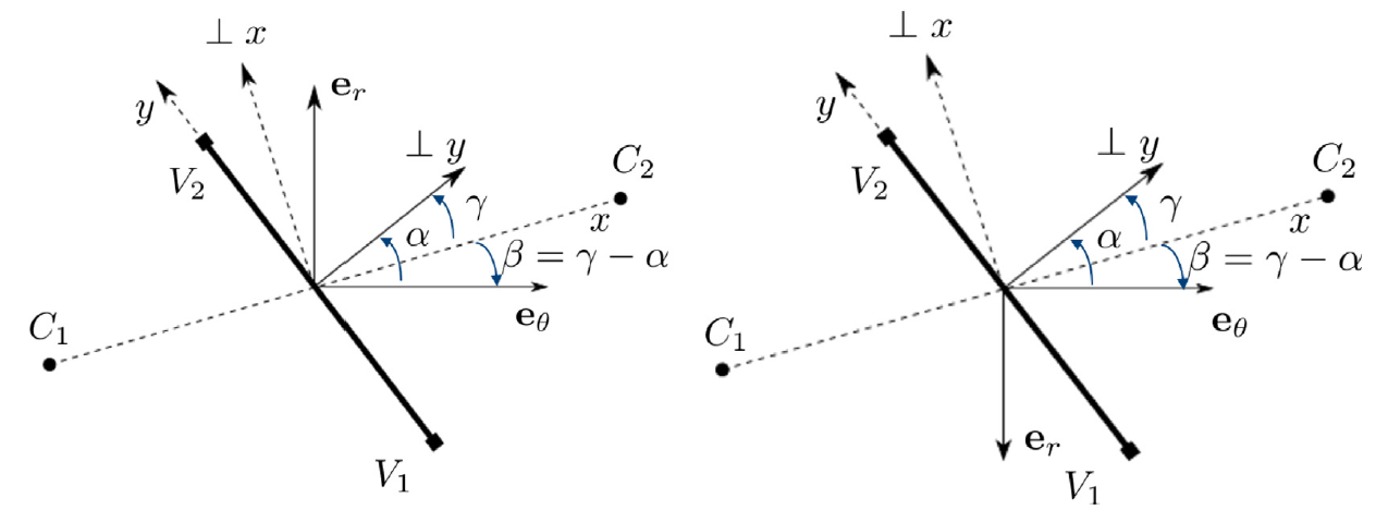
\includegraphics[width=14cm]{FiguresWG/mesh_angles.png}}
\else
    \centerline{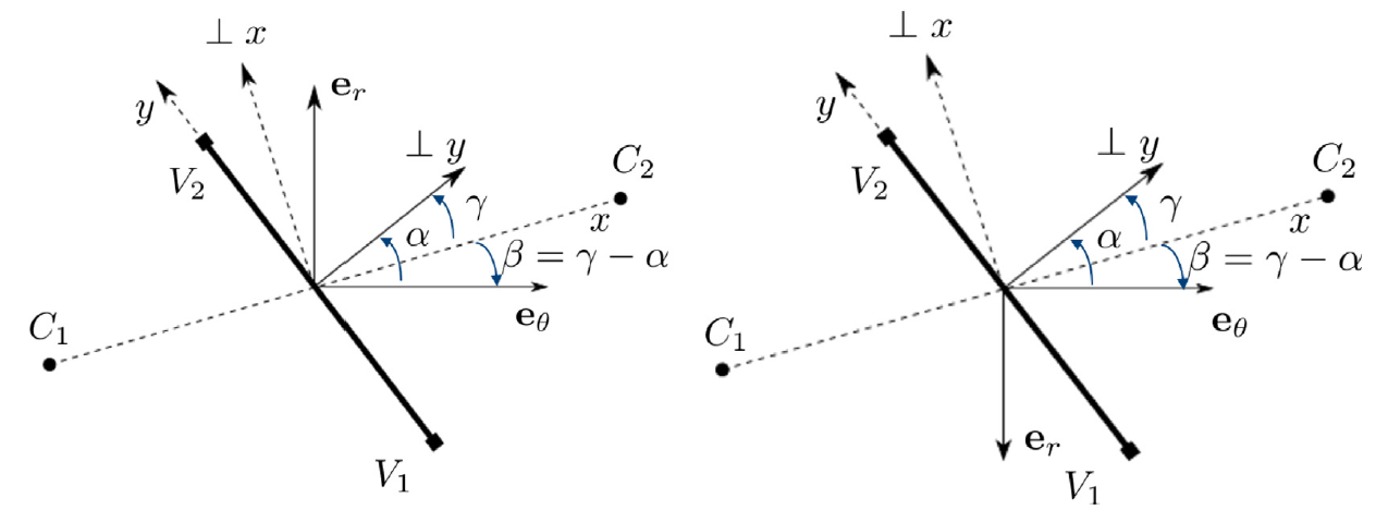
\includegraphics[width=14cm]{FiguresWG/mesh_angles.eps}}
\fi
    \caption{Local coordinate systems defining cell face orientation w.r.t. magnetic field, cell centers, and vertices. Left: toroidal field out of page. Right: toroidal field into the page.
    Figure reproduced from \cite{DEKEYSER2021}.}
    \label{fig:mesh_angles}
\end{figure}

The definitions of the variables in Figure \ref{fig:mesh_angles} are as follows:

\begin{itemize}
\item {\tt $C_1$} is the center of control volume 1. The index for that control volume is given by {\tt fcCv(iFc,1)}.
\item {\tt $C_2$} is the center of control volume 2. The index for that control volume is given by {\tt fcCv(iFc,2)}.
\item {\tt $V_1$} is the first vertex of the face. Its index is given by {\tt fcVx(iFc,1)}.
\item {\tt $V_2$} is the second vertex of the face. Its index is given by {\tt fcVx(iFc,2)}. The convention is that, when we look from {\tt $V_1$} to {\tt $V_2$}, {\tt $C_1$} is on the left and {\tt $C_2$} is on the right.
\item {\tt x} The $x$-direction is defined through the (not necessarily straight)
coordinate line connecting {\tt $C_1$} and {\tt $C_2$}, going through the center of the
cell face, and positive from {\tt $C_1$} to {\tt $C_2$}.
\item {\tt y} The $y$-direction is tangent to the face, positive from {\tt $V_1$} to {\tt $V_2$}.
\item {\tt $\alpha$} is the included angle between the magnetic field vector and the face normal.
{\tt fcQalf(iFc,0)} is the cosine of {\tt $\alpha$} and {\tt fcQalf(iFc,1)} is the sine of {\tt $\alpha$}.
\item {\tt $\gamma$} is the included angle between the cell-connector vector and the normal vector
of face {\tt iFc}. {\tt fcQgam(iFc,0)} is the cosine of {\tt $\gamma$} and {\tt fcQgam(iFc,1)} is the sine of {\tt $\gamma$}. It will hold that {\tt 0.lt.fcQgam(,).le.1}.
\item {\tt $\beta$} is the included angle between the cell-connector and the magnetic field vector.
{\tt fcQbet(iFc,0)} is the cosine of {\tt $\beta$} and {\tt fcQbet(iFc,1)} is the sine of {\tt $\beta$}.
\item {\tt fcHc(iFc,1)} is the distance between {\tt $C_1$} and the cell face center. {\tt fcHc(iFc,2)} is the distance between {\tt $C_2$} and the cell face center.
\item {\tt fcHt(iFc)} is the distance between {\tt $V_1$} and {\tt $V_2$}.
\end{itemize}

The flux of a particular quantity $u$ follows a convection-diffusion prescription:

\begin{equation*}
\mathbf{\Gamma} = \mathbf{C} u - \mathcal{D} \nabla u
\end{equation*}

The anisotropy in the equations is most naturally expressed w.r.t.
the poloidal ($\theta$) and radial ($r$) directions, which, by definition, are locally
orthogonal to each other. In our notation, the poloidal direction
points along the poloidal projection of the magnetic field, and the
radial direction is orthogonal to it in the poloidal plane, forming a
right-handed system with the third unit vector along the toroidal
projection of the field. These unit vectors therefore may flip orientation
with poloidal/toroidal field reversal. The coefficient
$\mathbf{C} = C_\theta \mathbf{e}_\theta + C_r \mathbf{e}_r$ is a vector describing the convective
flux of $u$, with components
defined in the poloidal and radial directions, and $\mathcal{D} = [D_{\theta \theta} D_{\theta r}, D_{r \theta} D_{r r}]$
is a diffusive tensor. The cross-diffusivities are included
because they are representative of the treatment of drift flows.
The {\tt B2.5} finite volume technique requires the evaluation of the fluxes across
cell faces:

\begin{align*}
 \mathbf{\Gamma} \cdot \mathbf{S} & = \Gamma_\theta S_\theta + \Gamma_r S_r \\
 & = \left( C_\theta u - D_{\theta \theta} \nabla_\theta u - D_{\theta r} \nabla_r u \right) S_\theta +
 \left( C_r u - D_{r \theta} \nabla_\theta u - D_{r r} \nabla_r u \right) S_r,
 \end{align*}

where $\mathbf{S} = S_\theta \mathbf{e}_\theta +  S_r \mathbf{e}_r $
is the surface vector of a face, expanded in its
poloidal and radial components.

To compute the poloidal and radial components of the gradient,
we relate them to the gradients in the $x$ and $y$
directions, which in turn can be computed directly from differences
between cell center (for $\nabla_\theta$) and vertex (for $\nabla_r$) values of $u$. The
desired expression for the components of the gradient can be obtained
by expanding the gradient in the orthogonal poloidal-radial system,
$\nabla u = \nabla_\theta u \cdot \mathbf{e}_\theta + \nabla_r u \cdot \mathbf{e}_r$,
and applying the definition of the gradient, $\nabla_d u = \nabla u \cdot \mathbf{d}$
for an arbitrary direction $\mathbf{d}$, to the unit vectors $\mathbf{e}_\theta$ and
$\mathbf{e}_r$:

\begin{align*}
\nabla_x u & = \nabla u \cdot \mathbf{e}_x = \nabla_\theta u \mathbf{e}_\theta \cdot \mathbf{e}_x + \nabla_r u \mathbf{e}_r \cdot \mathbf{e}_x, \\
\nabla_y u & = \nabla u \cdot \mathbf{e}_y = \nabla_\theta u \mathbf{e}_\theta \cdot \mathbf{e}_y + \nabla_r u \mathbf{e}_r \cdot \mathbf{e}_y.
\end{align*}

From Figure \ref{fig:mesh_angles} we see that $\mathbf{e}_\theta \cdot \mathbf{e}_x = \cos \beta$,
 $\mathbf{e}_r \cdot \mathbf{e}_x = \mp \sin \beta$, $\mathbf{e}_\theta \cdot \mathbf{e}_y = -\sin \alpha$
and $\mathbf{e}_r \cdot \mathbf{e}_y = \pm \cos \alpha$, with the upper signs corresponding to toroidal field
out of the page, and the lower signs with toroidal field into the page.
Inverting the system, we obtain

\begin{align*}
\nabla_\theta u & = \frac{\cos \alpha}{\cos \gamma} \nabla_x u + \frac{\sin \beta}{\cos \gamma} \nabla_y u, \\
\nabla_r u & = \pm \frac{\sin \alpha}{\cos \gamma} \nabla_x u \pm \frac{\cos \beta}{\cos \gamma} \nabla_y u.
\end{align*}

For completeness we give also the component of the gradient normal
to the face, which is needed for some boundary conditions:

\begin{equation*}
\nabla_n u = \frac{1}{\cos \gamma} \nabla_x u + \frac{\sin \gamma}{\cos \gamma} \nabla_y u,
\end{equation*}

and note, trivially, that the component tangential to the face is the
component in the $y$-direction: $\nabla_t u = \nabla_y u$.
Computing the poloidal and radial components of the gradient in
general thus requires a combination of gradients in $x$ and $y$ directions.

Drift terms can also be discretized using the expressions above. Only
the component of the drift perpendicular to a face leads to transport
across a face. Recalling that drifts have the form of a cross-diffusion
term, the net drift flow $\Gamma_d$ across a face is of the form:

\begin{equation*}
\mathbf{\Gamma}_d \cdot \mathbf{S} = - D_d \left( \nabla_r u S_\theta - \nabla_\theta u S_r \right) = \mp D_d \nabla_y u S
\end{equation*}

where we use the identity $\mathbf{S} = \left( \cos \alpha \ \mathbf{e}_\theta \pm \sin \alpha \ \mathbf{e}_r \right) S$.
Thus, net drift flow
across the face depends only on gradients along the face, while the
decomposition of the drift into its poloidal and radial components (as
required for example for the collisions with neutrals) requires again the
correct computation of the radial/poloidal gradients on each (possibly
non-aligned) face.
Using the expressions for the fluxes and derivatives on faces given
above, the governing equations can be discretized. Gradients in cell
centers are obtained through interpolation of the cell face gradients.
The discretization schemes of the structured version of the code have
been generalized to arbitrary unstructured grids. Hybrid discretization
schemes are used for the convection-diffusion flows, which are second
order in space for diffusion-dominated flows, but tend to a first-order
upwind scheme in convection-dominated flows.
The discretization schemes of the unstructured solver no longer neglect effects of misalignment
w.r.t. the magnetic field, and hence the solver is more accurate than older {\tt B2.5} versions
 even for non-extended grid cases.

Dedicated routines in {\tt \$\{SOLPSTOP\}/modules/B2.5/src/utility/} now take care of recurring numerical operations:

\begin{itemize}
\item {\tt GRAD} computes gradients of a cell-centered quantity on the cell faces, in both poloidal and radial directions.
\item {\tt GRAD\_NT} computes gradients of a cell-centered quantity on the cell faces, in both tangential and normal directions.
\item {\tt GRADC} computes gradients of a cell-centered quantity at the cell center by first computing the gradients on faces, and then interpolating back to the cell center.
\item {\tt GRADC\_DIV} computes gradients of a cell-centered quantity at the cell-center by applying the divergence theorem.
\item {\tt DIV} computes the divergence of a flow field.
\item {\tt INTFACE} interpolates a cell-centered quantity to the cell faces.
\item {\tt INTCELL} interpolates a face-based quantity to the cell centers.
\item {\tt INTVERTEX} interpolates a cell-centered quantity to the vertices.
\end{itemize}

%%%%%%%%%%%%%%%%%%%%%%%%%%%%%%%%%%%%%%%%%%%%%%%%%%%%%%%%%%%%%%%%%
%%%%%%%%%%%%%%%%%%%%%%%%%%%%%%%%%%%%%%%%%%%%%%%%%%%%%%%%%%%%%%%%%
\section{Rhie-Chow correction in unstructured code}
%%%%%%%%%%%%%%%%%%%%%%%%%%%%%%%%%%%%%%%%%%%%%%%%%%%%%%%%%%%%%%%%%
%%%%%%%%%%%%%%%%%%%%%%%%%%%%%%%%%%%%%%%%%%%%%%%%%%%%%%%%%%%%%%%%%

To avoid odd-even decoupling in the parallel direction due to the
collocated velocity and density (pressure) fields, a Rhie-Chow scheme
for compressible flow as described in Ref.~\cite{MOUKALLED2016} is implemented for the
parallel direction. The scheme is also explained in Section 8.8 and 10.2 (older versions) or 9.8 and 11.2 (newer versions) of Ref.~\cite{FERZIGER2019}.
The switches {\tt b2npco\_pcm0}, {\tt b2npco\_pcm1}, {\tt b2npht\_pcm0} and {\tt b2npht\_pcm1} determine the strength of the corrections.

%%%%%%%%%%%%%%%%%%%%%%%%%%%%%%%%%%%%%%%%%%%%%%%%%%%%%%%%%%%%%%%%%
%%%%%%%%%%%%%%%%%%%%%%%%%%%%%%%%%%%%%%%%%%%%%%%%%%%%%%%%%%%%%%%%%
\section{WG-related TODOs for this manual}
%%%%%%%%%%%%%%%%%%%%%%%%%%%%%%%%%%%%%%%%%%%%%%%%%%%%%%%%%%%%%%%%%
%%%%%%%%%%%%%%%%%%%%%%%%%%%%%%%%%%%%%%%%%%%%%%%%%%%%%%%%%%%%%%%%%

Some sections of this manual still need to be rewritten to be consistent with the unstructured solver:

\begin{itemize}
\item Appendix \ref{cha:b2wdat_iout_4} for the debugging output tracing files.
\item Appendix \ref{cha:Mladen_2}: remove, update, or integrate with another part of the manual.
\item Appendix \ref{sec:typical_BCs} for the expressions of boundary conditions.
\item Add information on creation of new extended cases. For now we refer to the {\tt 20230815\_carre2\_presentation.pdf} presentation found on the \SOLPSITER SharePoint website, in the \href{https://sharepoint.iter.org/departments/POP/CM/IMAS/SOLPS-ITER/SOLPS-ITER\%20Extended\%20Grids\%20Workshops}{SOLPS-ITER Extended Grids Workshops} directory.
\end{itemize}

%%%%%%%%%%%%%%%%%%%%%%%%%%%%%%%%%%%%%%%%%%%%%%%%%%%%%%%%%%%%%%%%%
%%%%%%%%%%%%%%%%%%%%%%%%%%%%%%%%%%%%%%%%%%%%%%%%%%%%%%%%%%%%%%%%%
\section{Converting structured cases}
%%%%%%%%%%%%%%%%%%%%%%%%%%%%%%%%%%%%%%%%%%%%%%%%%%%%%%%%%%%%%%%%%
%%%%%%%%%%%%%%%%%%%%%%%%%%%%%%%%%%%%%%%%%%%%%%%%%%%%%%%%%%%%%%%%%

Users can easily convert their existing structured cases to run with the WG code version. How to do this is explained in documents on the \SOLPSITER SharePoint website, \href{https://sharepoint.iter.org/departments/POP/CM/IMAS/SOLPS-ITER/SOLPS-ITER\%20Extended\%20Grids\%20Workshops}{SOLPS-ITER Extended Grids Workshops} directory, namely {\tt Session\_case\_conversion.pdf} and the last section of {\tt 20230814\_extended\_grids\_presentation.pdf}.


\appendix

\chapter{Internal B2.5 documentation}
\label{cha:intb2doc}

\section{b2cdca.F}
\label{lis:b2cdca}\index{b2cdca.F}\index{B2.5, code documentation}

\VerbatimInput[fontsize=\footnotesize]{b2cdca.F}

\newpage
\section{b2cdcr.F}
\label{lis:b2cdcr}\index{b2cdcr.F}\index{B2.5, list of routines}

\VerbatimInput[fontsize=\footnotesize]{b2cdcr.F}

\newpage
\section{b2cdcv.F}
\label{lis:b2cdcv}\index{b2cdcv.F}\index{B2.5, list of variables}

\VerbatimInput[fontsize=\footnotesize]{b2cdcv.F}

\newpage
\section{b2cdci.F}
\label{lis:b2cdci}\index{b2cdci.F}\index{B2.5, list of switches}

\VerbatimInput[fontsize=\footnotesize]{b2cdci.F}

\newpage
\section{b2cdcn.F}
\label{lis:b2cdcn}\index{b2cdcn.F}\index{B2.5, list of namelists}

\VerbatimInput[fontsize=\footnotesize]{b2cdcn.F}

\chapter{The physics of B2.5}
\label{cha:b2physics}

An extensive review of {\tt B2-Eirene} has been published as \cite{SOLPS2006}\index{SOLPS review}. It provides a full description of the {\bf SOLPS5.0} physics model, which can be obtained in the code by setting the {\tt b2mndt\_style} switch to {\tt 0}.
It is asked that authors using {\tt SOLPS} simulation results cite that work when
referring to the code. This review, only some short sections of which are detailed
below, can be found as part of the {\tt SOLPS} package at {\tt \$\{SOLPSTOP\}/doc/CPP\_2006.pdf}. Most of the discussion and definitions presented here apply to both the {\bf SOLPS5.0} and \SOLPSfivetwo physics models. In cases where the models differ, the use of the \SOLPSfivetwo model is recommended, although the {\bf SOLPS5.0} model remains available in the code for backward compatibility.

The equations are written on a
curvilinear orthogonal coordinate system.
The $x$-coordinate varies along flux surfaces and the $y$-coordinate varies
perpendicular to flux surfaces (see figure \ref{fig:geo}),
$z$ is the toroidal direction.

\begin{figure}[hbt]
\centerline{
\ifpdf
\includegraphics[width=8.0cm]{b2plot_1.pdf}
\else
\includegraphics[width=8.0cm]{b2plot_1.eps}
\fi
}
\caption{Coordinate system: $x$ is the poloidal coordinate,
$y$ is the radial coordinate orthogonal to the flux surfaces. The
coordinate $\perp$ corresponds to the direction perpendicular
both to the magnetic field and to the $y$-axis. The directions
of magnetic field and plasma current correspond to normal
operation conditions of ASDEX--Upgrade (ion $\nabla B$ drift
directed towards the X-point).
 }
\label{fig:geo}
\end{figure}

The metric coefficients are
$h_x=1/\|\grad x\|$, $h_y=1/\|\grad y\|$ and $\sqrt{g}=h_xh_yh_z$.
One can replace $h_z$ by $2 \pi R$,
where $R$ is the local major radius.  Components of a vector are the
projections on unit basis vectors
; they are not the contravariant or
covariant components ($b_x = B_x/B$, $b_z = B_z/B$).
Ion velocities $V_{\perp}$ (velocity perpendicular both
to magnetic field $B$ and the $y$-axis) and $V_y$ are
determined from the two components of the momentum balance equation
for ions perpendicular to a magnetic field. Using the Braginskii expression
for the friction force, one obtains:\\
\begin{gather}
\label{eq:nf1}
V_{\perp} = V_{\perp}^{\left( a \right)} - \frac{1}{enB}
\frac{1}{h_y}\frac{\partial nT_i}{\partial y} +
V_{\perp}^{\left( in \right)} + V_{\perp}^{\left( vis \right)} +
V_{\perp}^{\left( s \right)}
\end{gather}
\begin{gather}
\label{eq:nf2}
V_y = V_y^{\left( a \right)} + \frac{B_z}{enB^2}
\frac{1}{h_x}\frac{\partial nT_i}{\partial x} +
V_y^{\left( in \right)} + V_y^{\left( vis \right)} +
V_y^{\left( s \right)}
\end{gather}
Velocities $V_{\perp,y}^{\left( a \right)}$ are the sum of the
$\exb$ drifts and diffusive and thermo-diffusive
velocities.
This part corresponds to the ambipolar flux. It is the same both for ions and
electrons.
The second term in the r.h.s. of
Eqs.~(\ref{eq:nf1}) and (\ref{eq:nf2})
corresponds to diamagnetic flow of ions, while the other terms are caused
by inertial, viscous and ion-neutral friction forces.
These non-ambipolar terms are
connected with currents: $\vec{V}^{\left( in \right)} = \vec{j}^{\left( in \right)}/en,
\vec{V}^{\left( vis \right)} = \vec{j}^{\left( vis \right)}/en,
\vec{V}^{\left( s \right)} = \vec{j}^{\left( s \right)}/en$.\\
In the presence of anomalous transport
($D$ is the classical diffusion coefficient, $D=\frac{T_e+T_i}{eb}
\frac{\nu_{ei}}{\omega_{ce}}$, with electron cyclotron frequency
$\omega_{ce}$ and electron-ion collision frequency $\nu_{ei}$)
\begin{gather}
\label{eq:nf3}
V_{\perp}^{\left( a \right)} =
- \frac{1}{B}\frac{1}{h_y}\frac{\partial \Phi}{\partial y}
-\frac{D}{T_e+T_i} \frac{b_z}{h_x}\left(\frac{\partial p}{n \partial x}
-\frac{3}{2}\frac{\partial T_e}{\partial x}\right)
-D^{(AN)}_n\frac{1}{h_x n} \frac{\partial n}{\partial x}
-D^{(AN)}_p\frac{1}{h_x n} \frac{\partial p_i}{\partial x}
+V_{\perp}^{\left( AN \right)}
\end{gather}
\begin{gather}
\label{eq:nf44}
V_y^{\left( a \right)} =
\frac{B_z}{B^2}\frac{1}{h_x}\frac{\partial \Phi}{\partial x}
-\frac{D}{T_e+T_i} \frac{1}{h_y}\left(\frac{\partial p}{n \partial y}
-\frac{3}{2}\frac{\partial T_e}{\partial y}\right)
-D^{(AN)}_n\frac{1}{h_y n} \frac{\partial n}{\partial y}
-D^{(AN)}_p\frac{1}{h_y n} \frac{\partial p_i}{\partial y}
+V_y^{\left( AN \right)}
\end{gather}
The poloidal velocity is a sum $V_x = b_z V_{\perp} + b_x V_{\parallel}$.

In the particle balance
the fact that the diamagnetic
velocity is almost divergence free is taken into
account. Therefore, instead of the diamagnetic velocity
it is possible to introduce an effective
velocity $\vec{\tilde{V}}^{\left( dia \right)}$,
which gives the same contribution
to the divergence of the particle flux:
\begin{gather}
\label{eq:nf4}
\frac{\partial n}{\partial t} +
     \frac{1}{\sqrt{g}} \frac{\partial}{\partial x}
      \left(\frac{\sqrt{g}}{h_x} n\left(b_x V_{\parallel} +
     b_z V_{\perp}^{\left( 0 \right)}\right)\right)+
     \frac{1}{\sqrt{g}} \frac{\partial}{\partial y}
      \left(\frac{\sqrt{g}}{h_y} n V_y^{\left( 0 \right)}\right)
= S^n
\end{gather}
\begin{gather}\label{eq:nf5}
V_{\perp}^{\left( 0 \right)} = V_{\perp}^{\left( a \right)} +
V_{\perp}^{\left( in \right)} + V_{\perp}^{\left( vis \right)} +
V_{\perp}^{\left( s \right)} + \tilde{V}_{\perp}^{\left( dia \right)}
\end{gather}
\begin{gather}\label{eq:nf6}
V_{y}^{\left( 0 \right)} = V_{y}^{\left( a \right)} +
V_{y}^{\left( in \right)} + V_{y}^{\left( vis \right)} +
V_{y}^{\left( s \right)} + \tilde{V}_{y}^{\left( dia \right)}
\end{gather}
\begin{gather}\label{eq:nf7}
\tilde{V}_{\perp}^{\left( dia \right)} = \frac{T_i B_z}{e}
\frac{\partial}{h_y \partial y}\left(\frac{1}{B^2}\right)
\end{gather}
\begin{gather}\label{eq:nf8}
\tilde{V}_y^{\left( dia \right)} = -\frac{T_i B_z}{e}
\frac{\partial}{h_x \partial x}\left(\frac{1}{B^2}\right)
\end{gather}
The velocity $\tilde{V}^{{\left(dia\right)}}$ is an effective velocity. It
represents vertical guiding centre drift of ions caused by
$\nabla B$.\\

Combining the inertia and gyroviscosity terms in the Braginskii equations,
one finds
\begin{multline}\label{eq:mom}
\hfill m_i \left[ \frac{\partial n V_{\parallel}}{\partial t} +
     \frac{1}{\sqrt{g}} \frac{\partial}{\partial x}
      \left( \frac{\sqrt{g}}{h_x} n
       \left( V_{\perp}^{\left( 0 \right)} b_z
            + V_{\parallel} b_x \right)
       V_{\parallel} \right) +
     \frac{1}{\sqrt{g}} \frac{\partial}{\partial y}
      \left( \frac{\sqrt{g}}{h_y} n V_y^{\left( 0 \right)} V_{\parallel} \right)
\right] = \hfill \\
\hfill -\frac{b_x}{h_x}\frac{\partial n T_i}{\partial x} -
b_x \frac{en}{h_x}\frac{\partial \Phi}{\partial x} + F_k +
\frac{4}{3} b_x B^{3/2} \frac{\partial}{h_x \partial x}
\left(\frac{\eta_0 b_x}{B^2}
\frac{\partial\left(\sqrt{B}\left(V_{\parallel}+ \dfrac{B}{B_x} \left(V^{(dia)}_x + V^{(E)}_x\right)\right)\right)}
{h_x \partial x}\right)
\hfill \\
\hfill + B^{3/2} b_x \frac{\partial}{h_x \partial x}
\left(\frac{b_x}{\nu_{ii} B^2}
\frac{\partial\left(\sqrt{B}q_{i\parallel}^{\left( 0 \right)}
\right)}{h_x \partial x}\right)+
     \frac{1}{\sqrt{g}} \frac{\partial}{\partial y}
      \left(\frac{\sqrt{g}}{h_y^2} \eta_2 \frac{\partial V_{\parallel}}
{\partial y}\right) \hfill \\
\hfill
      + \frac{1}{\sqrt{g}} \frac{\partial}{\partial x}
      \left(\frac{\sqrt{g}}{h_x^2} \eta_2 \frac{\partial V_{\parallel}}
{\partial x}\right)
+ S_{i \parallel}^m + R_{ie\parallel}. \hfill
\end{multline}
The diamagnetic terms in the l.h.s. of (\ref{eq:mom}) are almost cancelled
\cite{ROGNLIEN98A, ROGNLIEN98B, ROGNLIEN99A, HINTON94C}, so that
velocities normal to the flux surface in the second and third term,
as in the particle balance equation, are determined by (\ref{eq:nf1}) and (\ref{eq:nf2}).
In \cite{HINTON94C}
the divergent part of diamagnetic velocity has been
neglected. Here, it is kept, because the corresponding flux is still
relatively large and can be comparable with the diffusive flux even
for anomalous diffusion coefficients. The authors of
\cite{ROGNLIEN98A, ROGNLIEN98B, ROGNLIEN99A} also kept this
flux.
In contrast to
\cite{ROGNLIEN98A, ROGNLIEN98B, ROGNLIEN99A}
there is an additional term of the same kind in the r.h.s. of
Eq.~(\ref{eq:mom}):
\begin{gather}
F_k = - m_i \left(\frac{1}{\sqrt{g}} \frac{\partial}{\partial x}
      \left(\frac{\sqrt{g}}{h_x} n V_{\parallel}
      \tilde{V}_{\perp}^{\left( dia \right)} b_z \right) +
      \frac{1}{\sqrt{g}} \frac{\partial}{\partial y}
      \left(\frac{\sqrt{g}}{h_y} n V_{\parallel}
      \tilde{V}_y^{\left( dia \right)} \right)\right)
\end{gather}
This parallel force is the Coriolis force, connected with the
diamagnetic drift velocity and
toroidal (parallel) rotation. This force can be obtained in a different
way by averaging the drift kinetic equation
\cite{MIHAIL84A} and is of the same order
as the inertia terms.

Parallel viscosity is represented
by the fourth and fifth terms in the r.h.s.
The former is the Balescu
parallel viscosity with coefficient $\eta_0 = \dfrac{4}{3} 0.96 \sqrt{2} n T_i / \nu_{ii}$. A detailed derivation is given at the end of this section, see~\ref{sec:viscosity}.
The latter corresponds to the parallel viscosity driven
by parallel ion heat flux
$q_{i\parallel}^{\left( 0 \right)} =
- \kappa_{i,\parallel} b_x \frac{1}{h_x} \frac{\partial T_i}{\partial x}$.
This viscosity is absent in the Braginskii equations, however, in a tokamak,
where parallel particle flux multiplied by temperature is of
the order of the ion heat flux, these two
viscosities are of the same order. On closed flux surfaces far from
the separatrix, the flux-surface-averaged parallel
viscosity coincides with the well-known
neoclassical expression for the Pfirsch-Schl{\"u}ter regime
\cite{HIRSHMAN81A}.
Thus, parallel viscosity in Eq.~(\ref{eq:mom}) provides smooth transition to
neoclassical theory.
The classical perpendicular viscosity coefficient
can
be replaced by an anomalous value as in
\cite{ROGNLIEN98A, ROGNLIEN98B, ROGNLIEN99A}: $\eta_2 =
n m_i D^{(AN)}_n$. Perpendicular viscosity and inertia terms with the
anomalous particle flux are responsible for the transport of the
parallel momentum in radial and poloidal directions. The radial transport
can be rather important despite the fact that $\eta_2 \ll \eta_0$, since
the scale in the radial direction is rather small.

The term  $S_{i \parallel}^m$  represents the parallel momentum loss due to
ion-neutral friction and parallel momentum input from neutral beam injection.
$R_{ie\parallel}$ is the ion-electron friction.

The parallel momentum balance for electrons has the standard form:
\begin{gather}
j_{\parallel} = \sigma_{\parallel} \left(
\frac{b_x}{e} \frac{1}{h_x} \left( \frac{\partial n T_e}{n \partial x} +
0.71 \frac{\partial T_e}{\partial x} \right)
- \frac{b_x}{h_x} \frac{\partial \Phi}{\partial x} \right).
\end{gather}

Expressions for $j_{\perp}$ and $j_y$ are obtained from radial and
poloidal projections of the total momentum balance equation (the sum
of electron and ion momentum balance equations).
The resulting current is a sum of contributions from pressure
gradient (diamagnetic current) $\vec{j}^{\left( dia \right)}$, inertia
and gyroviscosity $\vec{j}^{\left( in \right)}$, viscosity
$\vec{j}^{\left( vis \right)}$ and ion-neutral friction
$\vec{j}^{\left( s \right)}$.
Similar to the particle continuity equation, the effective
current $\vec{\tilde{j}}$ is introduced, which gives the same contribution to
$\nabla \vec{j}$, as the ordinary current. This gives the current continuity
equation
\begin{gather}\label{eq:curr0}
     \frac{1}{\sqrt{g}} \frac{\partial}{\partial x}
      \left(\frac{\sqrt{g}}{h_x} \tilde{j}_x\right)+
     \frac{1}{\sqrt{g}} \frac{\partial}{\partial y}
      \left(\frac{\sqrt{g}}{h_y} \tilde{j}_y\right)
= 0~.
\end{gather}
\begin{gather}\label{eq:curr1}
\tilde{j}_x = b_z \tilde{j}_{\perp} + b_x \tilde{j}_{\parallel}~.
\end{gather}
\begin{gather}\label{eq:curr2}
\vec{j} = \vec{\tilde{j}}^{\left( dia \right)} + \vec{j}^{\left( in \right)}
+ \vec{j}^{\left( vis \right)} + \vec{j}^{\left( s \right)}
+\vec{j}_{\parallel}~.
\end{gather}
The effective diamagnetic current can be chosen in a form
\begin{gather}\label{eq:curr3}
\tilde{j}_{\perp}^{\left( dia \right)} =
\frac{1}{b_z}\frac{n\left( T_e + T_i \right) B_z}{h_y}
\frac{\partial}{\partial y}\left(\frac{1}{B^2}\right)~,
\end{gather}
\begin{gather}\label{eq:curr4}
\tilde{j}_y^{\left( dia \right)} =
- \frac{n\left( T_e + T_i \right) B_z}{h_x}
\frac{\partial}{\partial x}\left(\frac{1}{B^2}\right)~.
\end{gather}
Current driven by parallel viscosity should be taken into account in
Eqs.~(\ref{eq:curr0}), (\ref{eq:curr1}) and (\ref{eq:curr2}).
This current is a small correction to the diamagnetic current
Eqs.~(\ref{eq:curr3}) and (\ref{eq:curr4}).
However, on closed flux surfaces, where the pressure is almost constant,
the diamagnetic current averaged
over the flux surfaces tends to zero. The resulting remaining part can
become comparable to the parallel viscosity-driven current, which is
necessary to satisfy the condition that the averaged net radial current
should be zero.
The terms, which contain the plasma viscosity, produce almost
divergence-free currents.
Similar to the case of diamagnetic currents, it can be reduced
to
\begin{gather}
\tilde{j}_{\perp}^{\left( vis \parallel \right)} =
- \frac{B_x \eta_0}{3 \sqrt{B}}
\frac{\partial\left(\sqrt{B}\left(V_{\parallel}+b_x \left(V^{(dia)}_{\perp} + V^{(E)}_{\perp}\right)\right)\right)}
{h_x \partial x}
\frac{\partial}{h_y \partial y}
\left(\frac{1}{B^2}\right)
\end{gather}
\begin{gather}
\tilde{j}_y^{\left( vis \parallel \right)} =
b_z\frac{B_x \eta_0}{3 \sqrt{B}}
\frac{\partial\left(\sqrt{B}\left(V_{\parallel}+b_x \left(V^{(dia)}_{\perp} + V^{(E)}_{\perp}\right)\right)\right)}
{h_x \partial x}
\frac{\partial}{h_x \partial x}
\left(\frac{1}{B^2}\right)
\end{gather}
The current produced by components of viscosity tensor connected
with heat fluxes is:
\begin{gather}
\tilde{j}_{\perp}^{\left( vis q \right)} =
- \frac{0.24 B_x}{\sqrt{B} \nu_{ii}}\frac{\partial
\left(q_{i \parallel}^{\left( 0 \right)} \sqrt{B}\right)}{h_x \partial x}
\frac{\partial}{h_y \partial y}
\left(\frac{1}{B^2}\right)
\end{gather}
\begin{gather}
\tilde{j}_y^{\left( vis q \right)} =
b_z\frac{0.24 B_x}{\sqrt{B} \nu_{ii}}\frac{\partial
\left(q_{i \parallel}^{\left( 0 \right)} \sqrt{B}\right)}{h_x \partial x}
\frac{\partial}{h_x \partial x}
\left(\frac{1}{B^2}\right)
\end{gather}

The second part of the current contains contributions from both inertia
and gyroviscosity forces. In contrast to the parallel momentum balance,
the cancellation is not complete (as has been noticed in
\cite{HINTON94C}). Expressions
for this part of the current are

\begin{multline}
\hfill j_{\perp}^{\left(in\right)}= - \frac{m_i}{B}
\left[\frac{\partial n V_{y}}{\partial t} +
     \frac{1}{\sqrt{g}} \frac{\partial}{\partial x}
      \left(\frac{\sqrt{g}}{h_x} n\left(V_{\perp}^{\left( 0 \right)} b_z
+ V_{\parallel} b_x \right) V_{y}\right)+
     \frac{1}{\sqrt{g}} \frac{\partial}{\partial y}
      \left(\frac{\sqrt{g}}{h_y} n V_y^{\left( 0 \right)} V_{y}\right)
\right] \hfill \\
\hfill -
\frac{2 b_x}{B} \frac{1}{h_x}\frac{\partial}{\partial x}
\left(\eta_3
\frac{\partial V_{\parallel}}{h_x \partial x}\right)+
\frac{m_i}{B} n V_{\parallel}^2 \frac{\partial \ln h_z}{h_y \partial y}
\hfill
\end{multline}

\begin{multline}
\hfill j_{y}^{\left(in\right)}= \frac{m_i}{B}
\left[\frac{\partial n V_{\perp}}{\partial t} +
     \frac{1}{\sqrt{g}} \frac{\partial}{\partial x}
      \left(\frac{\sqrt{g}}{h_x} n\left(V_{\perp}^{\left( 0 \right)} b_z
+ V_{\parallel} b_x \right) V_{\perp}\right)+
     \frac{1}{\sqrt{g}} \frac{\partial}{\partial y}
      \left(\frac{\sqrt{g}}{h_y} n V_y^{\left( 0 \right)} V_{\perp}\right)
\right] \hfill \\
\hfill -
\frac{2 b_x}{B} \frac{1}{h_x}\frac{\partial}{\partial x}
\left(\eta_3
\frac{\partial V_{\parallel}}{h_y \partial y}\right) -
\frac{m_i}{B} n V_{\parallel}^2 \frac{\partial \ln h_z}{h_x \partial x}
\hfill
\end{multline}

where $\eta_3 = \frac{n T_i}{2 \omega_{ci}}, \eta_1 = \frac{\eta_2}{4}$.

The last terms proportional to the gradient of $B$ correspond to the vertical
guiding centre drift of ions caused by the centrifugal force. This current
can be simply added to the diamagnetic current. Other terms seem to be less
important.

The contribution from perpendicular viscosity is
\begin{multline}
\hfill j_{\perp}^{\left(vis \perp \right)}= \frac{1}{B}
\left[\frac{1}{h_x}\frac{\partial}{\partial x}\left(\eta_1
     \frac{\partial V_y}{h_x \partial x}\right)+
 \frac{1}{h_y}\frac{\partial}{\partial y}\left(\eta_1
     \frac{\partial V_y}{h_y \partial y}\right)+
\frac{1}{h_x h_y }\frac{\partial \eta_1}{\partial x}
     \frac{\partial V_{\perp}}{\partial y}-
\frac{1}{h_x h_y }\frac{\partial \eta_1}{\partial y}
     \frac{\partial V_{\perp}}{\partial x}\right] \hfill \\
\hfill +
\frac{4 b_x}{B} \frac{1}{h_x h_y}
\left(\frac{\partial \eta_1}{\partial x} \frac{\partial V_{\parallel}}
{\partial y} - \frac{\partial \eta_1}{\partial y}\frac{\partial V_{\parallel}}
{\partial x}
\right)
\hfill
\end{multline}
\begin{gather}
j_{y}^{\left(vis \perp \right)}= -\frac{1}{B}
\left[\frac{1}{h_y}\frac{\partial}{\partial y}\left(\eta_1
     \frac{\partial V_{\perp}}{h_y \partial y}\right)+
 \frac{1}{h_x}\frac{\partial}{\partial x}\left(\eta_1
     \frac{\partial V_{\perp}}{h_x \partial x}\right)-
\frac{1}{h_x h_y }\frac{\partial \eta_1}{\partial x}
     \frac{\partial V_y}{\partial y}+
\frac{1}{h_x h_y }\frac{\partial \eta_1}{\partial y}
     \frac{\partial V_y}{\partial x}\right].
\end{gather}

Here, the largest term is the first one in the r.h.s. of the expression
for the radial current, since the radial derivatives are the largest.
This current corresponds to a pure cylindrical approximation. It is
responsible, for example, for closing currents near flush-mounted probes
\cite{ROZ99A}.
It was taken into account in
\cite{ROGNLIEN99A, RADFORD96A}. However, in the problem of global current
structure in the edge plasma, the currents driven by parallel viscosity seem
to be more important.

The total current caused by viscosity is
\begin{gather}
\vec{j}^{\left(vis\right)} = \vec{j}^{\left(vis \parallel\right)} +
\vec{j}^{\left(vis \perp\right)} +
\vec{j}^{\left(vis q\right)}
~.
\end{gather}

The contribution from ion neutral friction is
\begin{gather}
j_{\perp}^{\left(s\right)} = \frac{S_{iy}^m}{B}
~.
\end{gather}
\begin{gather}
j_{y}^{\left(s\right)} = -\frac{S_{i \perp}^m}{B}
~,
\end{gather}
where $S_{iy}^m$ and $S_{i \perp}^m$ are the momentum sinks due to
ion-neutral friction.
\begin{gather}
S_{i \perp}^m = - n \mu_{iN} \nu_{iN} \left( V_{\perp} - V_{\perp N}\right)
~,
\end{gather}
\begin{gather}
S_{i y}^m = - n \mu_{iN} \nu_{iN} \left( V_{y} - V_{y N}\right)
~,
\end{gather}
where $\mu_{iN}=m_i/2$ is the effective mass,
$\nu_{iN}= n_N \left\langle V_{iN} \sigma_{cx} \right\rangle$
is the ion-neutral collision frequency,
$n_N$ is the neutral density and $\vec{V_{iN}}$ is the neutral mean
velocity. For the ion velocity used above,
only electric and diamagnetic drifts are left, neglecting smaller terms,
to obtain
\begin{gather}
\tilde j_{x}^{\left(s\right)} = \tilde j_{\perp}^ {\left(s\right)} b_z =
- \sigma_{iN} b_z^2 \frac{\partial \Phi}{h_x \partial x}-
\sigma_{iN} b_z^2 \frac{1}{e n}\frac{\partial n T_i}{h_x \partial x}+
\sigma_{iN} B_z V_{yN}
~,
\end{gather}
\begin{gather}
\tilde j_{y}^{\left(s\right)} =
- \sigma_{iN} \frac{\partial \Phi}{h_y \partial y}-
\sigma_{iN} \frac{1}{e n}\frac{\partial n T_i}{h_y \partial y}-
\sigma_{iN} B V_{\perp N}
~,
\end{gather}
where $\sigma_{iN}$ is the ion-neutral perpendicular conductivity
\begin{gather}
\sigma_{iN} =
\frac{n m_i \left\langle V_{iN} \sigma_{cx} \right\rangle n_N}{2 B^2}
~.
\end{gather}

The rate of charge-exchange $\left\langle V_{iN} \sigma_{cx} \right\rangle$ can
be expressed through the mobility $K_0$ measured in the absence of a
magnetic field for room temperature and atmospheric pressure for
deuterium \cite{MCDANIEL73A}:
\begin{gather}
K_0 =
\frac{2 e}{m_i \left\langle V_{iN} \sigma_{cx} \right\rangle n_N^{\left(0\right)}}
~,
\end{gather}
with $n_N^{\left(0\right)} = 2.687 \cdot 10^{25} m^{-3}$ and
$K_0 = 11.2 \cdot 10^{-4} \frac{m^2}{s V}$.
Assuming that the charge-exchange cross-section is approximately constant
one gets
\begin{gather}
\left\langle V_{iN} \sigma_{cx} \right\rangle = 3.2 \cdot 10^{-15} \sqrt{\frac{T_i}{0.026}}
\frac{m^3}{s}
~,
\end{gather}
where $T_i$ is measured in $eV$. A similar expression, which gives approximately
the same result, is \cite{ROZ88A}:
\begin{gather}
\left\langle V_{iN} \sigma_{cx} \right\rangle = \frac{32 \sigma_{cx}}{3 \sqrt{\pi}}
\sqrt{\frac{T_i}{m_i}}
\frac{m^3}{s}
~.
\end{gather}.


In the energy balance equations
appears
a special problem, which is the
possible inclusion of an anomalous radial current.
The basic guidelines are as follows:
\begin{itemize}
\item The expression must be as simple as possible, and the most convenient
format is an Ohm-like expression;
\item The system of equations must be informed about this non-classical
contribution, but
\item The classical core of the equations must not be disturbed.
\end{itemize}
Apparently, the radial current would enter the electron energy equation
via the Joule term, but this manipulation is inappropriate since one cannot
be sure that this term directly heats the electrons, which is the case in
a purely classical setup. The proper thing to do is to keep only
the non-radial classical contribution in the Joule term, and
construct additional heat exchange terms
containing the radial current.
In this way, the system decides how to thermodynamically allocate the
"alien" heat term, among electrons and ion species.\\
For this reason, one cannot simply use the standard Ohm's
law in the radial direction with anomalous coefficients, or any other
prescribed expression whatsoever, as a constructive procedure is necessary
for simultaneously producing the radial current as well as the heat exchange
terms. At this point it has to be mentioned that this peculiarity arises
only in the multi-fluid case, whereas in the single species case
these heat exchange terms can indeed be constructed even using a prescribed
expression for the radial current. \\
The trick for carrying out this program is to correct the electron friction
density $\vec{R}^e$ by adding the term $n_e e \tilde{\eta}_\perp \vec{J}_\perp$
similar to the classical one, only using the {\itshape ad hoc} parameter
$\tilde{\eta}_\perp$. \\
Since $\vec{R}^e=-{\sum_{a}\vec{R}^a}$, one has a
modified total ion momentum equation at hand which in conjuction with the
pressure equilibrium (not affected by the additional term)
$\vec{J} \times \vec{B} = \nabla P$, gives the diffusive part of the
radial current, namely
\begin{gather}
J_y^{diff}=\frac{\tilde{\eta}_\perp en_e}{B^2} \frac{\partial P_i}{\partial y}
\end{gather}
where $P_i$ is the total ion pressure. This dependency is also found in
\cite{ROGNLIEN98A}. Moreover, an additional dependence on the radial
electric field can potentially be added without interfering with
the procedure. \\
The final step, namely the construction of the heat exchange terms, is
performed by claiming that the well known relation \cite{BAELMANS94A}
(adapted for the multi-fluid case)
\begin{gather}
Q_e=-\sum_{a} \left (Q_a + (\vec{u}^a - \vec{u}^e) \cdot \vec{R}^a \right )~,
\end{gather}
which stems from the fundamental null space of the collision operator,
is still true while carrying the modified friction.
Claiming this, after
performing the proper manipulations in the energy
equations, one reveals the {\itshape ad hoc}
contribution as the exchange term that one wants,
which reads
$
\sum_{a} (\vec{u}^a -\vec{u}^e)_\perp n_a \frac{Z_a^2}{Z_{eff}} e \tilde{\eta}_\perp \vec{J}_\perp
$
added in the total ion energy equation and subtracted from the
electron equation.
Note that in the single species case, this term boils down to
$
\tilde{\eta}_\perp J_\perp ^2
$
removing energy from the electrons,  depositing it to the ions, a feature
predicted by neoclassical theory \cite{ROSENBLUTH72A}.\\

In the final form of the energy balance equations, the convective heat
flux and the diamagnetic heat flux are combined as in
\cite{ROGNLIEN98A, ROGNLIEN98B, ROGNLIEN99A, HINTON94C}, see also
\cite{ROZ99A}.

The energy balance equation for the electrons is
\begin{multline}
\hfill
     \frac{3}{2} \frac{\partial nT_e}{\partial t} +
     \frac{1}{\sqrt{g}} \frac{\partial}{\partial x}
      \left(\frac{\sqrt{g}}{h_x} \tilde{q}_{ex}\right) +
     \frac{1}{\sqrt{g}} \frac{\partial}{\partial y}
      \left(\frac{\sqrt{g}}{h_y} \tilde{q}_{ey}\right) +
     \frac{nT_e}{\sqrt{g}}\frac{\partial}{\partial x}
      \left(\frac{\sqrt{g}}{h_x}\left(
      V_{\parallel} - j_{\parallel}/en\right)b_x\right) \hfill \\
\hfill     =
     Q_e + n T_e B \frac{1}{h_x h_y}\left(\frac{\partial \Phi}{\partial y}
     \frac{\partial}{\partial x}\left(\frac{1}{B^2}\right)
     -\frac{\partial \Phi}{\partial x}\frac{\partial}{\partial y}
     \left(\frac{1}{B^2}\right)\right)~,\hfill
\end{multline}
where
\begin{multline}
\hfill        \tilde{q}_{ex} = \frac{3}{2} n T_e \left(- \frac{b_z}{B h_y}
         \frac{\partial \Phi}{\partial y}
         + b_x V_{\parallel} - b_x j_{\parallel} / en \right) \hfill \\
     \hfill + \frac{5}{2} n T_e b_z \left(
     - \frac{D}{T_e+T_i} \frac{b_z}{h_x} \left(\frac{\partial p}{n \partial x}
     - \frac{3}{2} \frac{\partial T_e}{\partial x} \right)
     - D^{(AN)}_n \frac{1}{h_x n} \frac{\partial n}{\partial x}
     - D^{(AN)}_p \frac{1}{h_x n} \frac{\partial p_i}{\partial x}
     + V_{e\perp}^{(AN)} \right)
      \hfill \\
      \hfill   - 0.71 b_x j_{\parallel} T_e/e - \kappa_{e \parallel}
         \frac{b_x^2}{h_x} \frac{\partial T_e}{\partial x}
         - \kappa_{e \perp} b_z^2 \frac{1}{h_x}
         \frac{\partial T_e}{\partial x} \hfill \\
      \hfill   + \frac{3}{2}\frac{T_e}{e B} \frac{\nu_{ei}}{\omega_{ce}}
         \frac{b_z^2}{h_x} \frac{\partial n\left(T_e+T_i\right)}{\partial x}
         - \frac{5}{2} n T_e^2 \frac{B_z}{e}
         \frac{\partial}{h_y \partial y}\left(\frac{1}{B^2}\right) ~ , \hfill
\end{multline}
\begin{multline}
\hfill  \tilde{q}_{ey} = \frac{3}{2} n T_e \left( \frac{B_z}{B^2} \frac{1}{h_x}
        \frac{\partial \Phi}{\partial x} \right) \hfill \\
     \hfill  + \frac{5}{2} n T_e \left(
     - \frac{D}{T_e+T_i} \frac{1}{h_y} \left( \frac{\partial p}{n \partial y}
     - \frac{3}{2} \frac{\partial T_e}{\partial y} \right)
     - D^{(AN)}_n \frac{1}{h_y n} \frac{\partial n}{\partial y}
     - D^{(AN)}_p \frac{1}{h_y n} \frac{\partial p_i}{\partial y}
     + V_{ey}^{(AN)} \right)
         \hfill \\
         \hfill - \kappa_{e \perp} \frac{1}{h_y} \frac{\partial T_e}{\partial y}
         + \frac{3}{2}\frac{T_e}{e B} \frac{\nu_{ei}}{\omega_{ce}}
         \frac{1}{h_y} \frac{\partial n\left(T_e+T_i\right)}{\partial y}
         + \frac{5}{2} n T_e^2 \frac{B_z}{e}
         \frac{\partial}{h_x \partial x}\left(\frac{1}{B^2} \right) ~ , \hfill
\end{multline}
\begin{gather}
        Q_{\Delta} = \frac{3 m_e}{m_i} n \nu_{ei} \left(
T_e - T_i
\right)~,
\end{gather}
\begin{gather}
        Q_u = R_{ie \parallel} j_{\parallel}/en~,
\end{gather}
\begin{gather}
        Q_{AN} = \sum_{a} \left(\vec{u}^a -\vec{u}^e\right)_\perp n_a
                 \frac{Z_a^2}{Z_{eff}} e \tilde{\eta}_\perp \vec{J}_\perp~,
\end{gather}
\begin{gather}
        Q_e = -Q_{\Delta} - Q_u - Q_{AN}~.
\end{gather}

\begin{sloppypar}
Here $\kappa_{e \parallel}$ is the Balescu (not Braginskii as stated in the CPP review paper \cite{SOLPS_review}
or in {\tt \$\{SOLPSTOP\}/doc\allowbreak /CPP\_2006.pdf}) heat
conductivity with a possible heat
flux limit \cite{BRAAMS96B}.
The leading numerical coefficient is then $\frac{5}{2} \frac{2.16 z}{1 + 0.27 z}$ as opposed to 3.16 for the Braginskii
formula \cite{NRL}. The perpendicular heat conductivity
$\kappa_{e \perp}$ can be
either classical or anomalous. In the last term of the energy balance
equation, it is taken into account that the $\exb$
drift velocity is
almost divergence-free.
\end{sloppypar}

The ion energy balance equation is
\begin{multline}\label{eq:ion_energy} \hfill
     \frac{3}{2} \frac{\partial nT_i}{\partial t} +
     \frac{1}{\sqrt{g}} \frac{\partial}{\partial x}
      \left(\frac{\sqrt{g}}{h_x} \tilde{q}_{ix}\right) +
     \frac{1}{\sqrt{g}} \frac{\partial}{\partial y}
      \left(\frac{\sqrt{g}}{h_y} \tilde{q}_{iy}\right) +
     \frac{nT_i}{\sqrt{g}}\frac{\partial}{\partial x}
      \left(\frac{\sqrt{g}}{h_x} V_{\parallel} b_x \right) \hfill \\
     \hfill =
     Q_{\Delta} + Q_{AN} + \frac{\eta_0}{3} \left(2 b_x
     \frac{\partial V_{\parallel}}{h_x \partial x}\right)^2+
     n T_i B
     \frac{1}{h_x h_y}\left(\frac{\partial \Phi}{\partial y}
     \frac{\partial}{\partial x}\left(\frac{1}{B^2}\right)
     -\frac{\partial \Phi}{\partial x}\frac{\partial}{\partial y}
     \left(\frac{1}{B^2}\right)\right)~,\hfill
\end{multline}
where
\begin{multline} \hfill
        \tilde{q}_{ix} = \frac{3}{2} n T_i \left(- \frac{b_z}{B h_y}
        \frac{\partial \Phi}{\partial y}
         + b_x V_{\parallel} \right) \hfill \\
\hfill + \frac{5}{2} n T_i b_z \left(
     - \frac{D}{T_e + T_i} \frac{b_z}{h_x}\left(\frac{\partial p}{n \partial x}
     - \frac{3}{2} \frac{\partial T_e}{\partial x} \right)
     - D^{(AN)}_n \frac{1}{h_x n} \frac{\partial n}{\partial x}
     - D^{(AN)}_p \frac{1}{h_x n} \frac{\partial p_i}{\partial x}
     + V_{i\perp}^{(AN)} \right)
         \hfill \\ \hfill
         + \frac{5}{2} n T_i b_z \tilde{V}_{\perp}^{\left(dia\right)}
         - \kappa_{i \parallel}
         \frac{b_x^2}{h_x} \frac{\partial T_i}{\partial x}
         - \kappa_{i \perp} b_z^2 \frac{1}{h_x}
         \frac{\partial T_i}{\partial x} ~, \hfill
\end{multline}
\begin{multline} \hfill
        \tilde{q}_{iy} = \frac{3}{2} n T_i \left( \frac{B_z}{B^2}
         \frac{1}{h_x} \frac{\partial \Phi}{\partial x} \right)
        \hfill \\ \hfill
     + \frac{5}{2} n T_i \left(
     - \frac{D}{T_e+T_i} \frac{1}{h_y} \left( \frac{\partial p}{n \partial y}
     - \frac{3}{2} \frac{\partial T_e}{\partial y}\right)
     - D^{(AN)}_n \frac{1}{h_y n} \frac{\partial n}{\partial y}
     - D^{(AN)}_p \frac{1}{h_y n} \frac{\partial p_i}{\partial y}
     + V_{iy}^{(AN)} \right) \hfill \\ \hfill
         - \kappa_{e \perp} \frac{1}{h_y}
         \frac{\partial T_i}{\partial y}
         + \frac{5}{2} n T_i \tilde{V}_{y}^{\left(dia\right)} ~. \hfill
\end{multline}

As for the electrons, the parallel heat conductivity is classical with
a possible heat flux limit, while the perpendicular contribution
can be either
classical or anomalous.

There is discussion in the literature on how to take into account anomalous
terms in the energy balance equations. One point of view (see e.g.
\cite{ZAGORSKI98A})
is to cancel the contribution from anomalous particle fluxes in the
terms $p_i \nabla \cdot \vec{V}_i$ (or $\vec{V}_i \cdot \nabla p_i$ if equations
are written in a different form). In contrast, according to the
derivation
\cite{HINTON94C},
where a kinetic equation with fluctuating term has been integrated, the
anomalous fluxes should be kept in all terms of the energy balance
equations. This variant was used in {\tt UEDGE} \cite{ROGNLIEN98A, ROGNLIEN98B, ROGNLIEN99A}.
In {\tt B2.5} only the contribution
from anomalous radial particle flux to the convective heat flux are left
in the expressions for $\tilde{q}_{e,i}$. In the term
$p_i \nabla \cdot \vec{V}_i$ the anomalous particle flux is absent.

\section{Derivation of parallel viscosity term in momentum equation}
\index{parallel viscosity}\label{sec:viscosity}

To evaluate the parallel viscosity contribution we should start from the general expressions, which can be transformed and simplified in arbitrary cartesian coordinate system assuming only parallel velocity. The Braginskii description for parallel viscosity in cartesian coordinates is:

\begin{equation*}
\pi_{\alpha \beta} = \frac{3}{2} \eta_0 \left( b_\alpha b_\beta - \frac{1}{3} \delta_{\alpha \beta} \right) \left( b_\mu b_\nu - \frac{1}{3} \delta_{\mu \nu} \right) W_{\mu \nu}
\end{equation*}

where

\begin{equation*}
W_{\mu \nu} = \frac{\partial V_\mu}{\partial x_\nu} + \frac{\partial V_\nu}{\partial x_\mu} - \frac{2}{3} \delta_{\mu \nu} \frac{\partial V_i}{\partial x_i}, ~\vec{b} = \vec{B}/B .
\end{equation*}

The parallel momentum balance component is:

\begin{equation*}
\vec{b} \cdot \left( \nabla \cdot \overleftrightarrow{\pi} \right) = b_\alpha \frac{\partial \pi_{\alpha \beta}}{\partial x_\beta} = b_\alpha \frac{\partial}{\partial x_\beta} \left[ \frac{3}{2} \eta_0 \left( b_\alpha b_\beta - \frac{1}{3} \delta_{\alpha \beta} \right) \left( b_\mu b_\nu - \frac{1}{3} \delta_{\mu \nu} \right) W_{\mu \nu} \right]
\end{equation*}

We can evaluate the scalar value separately:

\begin{align*}
\pi_0 &= \frac{3}{2} \eta_0 W_{\parallel \parallel} = \frac{3}{2} \eta_0 \left( b_\mu b_\nu - \frac{1}{3} \delta_{\mu \nu} \right) W_{\mu \nu} \\
&= \frac{3}{2} \eta_0 \left(  b_\mu b_\nu - \frac{1}{3} \delta_{\mu \nu} \right) \left( \frac{\partial V_\mu}{\partial x_\nu} + \frac{\partial V_\nu}{\partial x_\mu} - \frac{2}{3} \delta_{\mu \nu} \frac{\partial V_i}{\partial x_i} \right) = 3 \eta_0 \left(  b_\mu b_\nu - \frac{1}{3} \delta_{\mu \nu} \right) \left( \frac{\partial V_\mu}{\partial x_\nu} - \frac{1}{3} \delta_{\mu \nu} \frac{\partial V_i}{\partial x_i} \right) \\
&= 3 \eta_0 \left( b_\mu b_\nu \frac{\partial V_\mu}{\partial x_\nu} - \frac{1}{3} \frac{\partial V_i}{\partial x_i} \right) = 3 \eta_0 \left( b_\mu b_\nu \frac{\partial V_\parallel b_\mu}{\partial x_\nu} - \frac{1}{3} \frac{\partial V_\parallel b_\nu}{\partial x_\nu} \right) \\
&= 3 \eta_0 \left( \frac{B_\nu}{B} \frac{\partial V_\parallel}{\partial x_\nu} - \frac{1}{3} B_\nu \frac{\partial V_\parallel / B}{\partial x_\nu} \right) = \eta_0 \frac{B_\nu}{B} \left( 2 \frac{\partial V_\parallel}{\partial x_\nu} + \frac{V_\parallel}{B} \frac{\partial B}{\partial x_\nu} \right) \\
&= 2 \eta_0 \frac{B_\nu}{B} \frac{1}{\sqrt{B}} \frac{\partial V_\parallel \sqrt{B}}{\partial x_\nu} = 2 \eta_0 \frac{1}{\sqrt{B}} \vec{b} \cdot \nabla \left ( V_\parallel \sqrt{B} \right)
\end{align*}

The projection of the viscosity divergence on the parallel direction is then:

\begin{align*}
\vec{b} \cdot \left( \nabla \cdot \overleftrightarrow{\pi} \right) &= b_\alpha \frac{\partial}{\partial x_\beta} \left[ \pi_0 \left( b_\alpha b_\beta - \frac{1}{3} \delta_{\alpha \beta} \right) \right] = \frac{\partial \pi_0 b_\alpha}{\partial x_\alpha} - \frac{1}{3} b_\alpha \frac{\partial \pi_0}{\partial x_\alpha} = B_\alpha \frac{\partial \pi_0 / B}{\partial x_\alpha} - \frac{1}{3} b_\alpha \frac{\partial \pi_0}{\partial x_\alpha} \\
&= \frac{2}{3} b_\alpha \frac{\partial \pi_0}{\partial x_\alpha} - \pi_0 \frac{b_\alpha}{B} \frac{\partial B}{\partial x_\alpha} = \frac{2}{3} B^{3/2} b_\alpha \frac{\partial \pi_0 B^{-3/2}}{\partial x_\alpha} = \frac{2}{3} B^{3/2} \vec{b} \cdot \nabla \left( \pi_0 B^{-3/2} \right)
\end{align*}

Then the parallel viscosity in the parallel momentum balance is:

\begin{equation*}
\vec{b} \cdot \left( \nabla \cdot \overleftrightarrow{\pi} \right) = \frac{4}{3} B^{3/2} \vec{b} \cdot \nabla \left( \frac{\eta_0}{B^2} \vec{b} \cdot \nabla \left( V_\parallel \sqrt{B} \right) \right), ~ \mbox{where} ~ V_\parallel = \vec{b} \cdot \vec{V}
\end{equation*}

For \SOLPSITERns, the orthogonal coordinates $(x,r,z)$ are more convenient for further evaluations than the non-orthogonal coordinates $(x,y,z)$. In these coordinates, it is readily seen that $\vec{b} \cdot \nabla f = b_x \frac{\partial f}{h_x \partial x}$ for any scalar function $f$. The viscosity can be finally written as:

\begin{equation*}
\vec{b} \cdot \left( \nabla \cdot \overleftrightarrow{\pi} \right) = \frac{4}{3} b_x B^{\frac{3}{2}} \frac{\partial}{h_x \partial x} \left( \frac{\eta_0 b_x}{B} \frac{\partial \left( B^{\frac{1}{2}} V_\parallel \right)}{h_x \partial x} \right)
\end{equation*}

\section{Boundary conditions with drifts and currents}
\index{drifts and currents, boundary conditions}
\index{boundary conditions, drifts and currents}

Whether one deals with the diamagnetic or $\exb$ perpendicular
drift velocity, special care must be taken to avoid unphysical flows
at the plates. The standard boundary condition is to require that the flow be
at least sonic at the sheath entrance \cite{STANGEBY95B},
which translates into:

\begin{equation}\label{eq:Chodura}
V_{\parallel} \ge C_s - \frac{b_z}{b_x} V_{\perp} ~,
\end{equation}

where $C_s$ is the local sound speed and $\frac{b_z}{b_x}$ is the inverse
of the field line pitch. However, for very small pitch angles, as in
stellarators, the $V_{\perp}$ term may overpower the sound
velocity \cite{FENG99A}
and then the boundary condition would require a plasma flow exiting the plate.
Therefore, the pitch angle at the plates is limited to be no less than
1 degree (user parameter, see switch {\tt b2agfs\_min\_pitch} in Appendix~\ref{lis:b2cdci}),
motivated by the engineering limits met when attempting to align the
divertor tiles with the magnetic field. The solution procedure of the code
was also modified so as ensure that no unphysical flows were being created,
and solves the parallel momentum equation using the updated electric potential.

Boundary conditions for the current continuity equation at the plates
correspond to sheath current-voltage characteristics
\begin{equation}\label{eq:sheath-voltage}
j_x = en\left(b_x c_s - b_x \frac{1}{\sqrt{2 \pi}} \sqrt{\frac{T_e}{m_e}}
      \exp \left(- \frac{e \Phi}{T_e}\right) \left(1 - \gamma_e\right)\right),
\end{equation}
where $\gamma_e$ is the secondary electron emission coefficient. At the inner
(core) flux surface the currents are set either to the divergent part
of the diamagnetic current or to zero. Both variants give the same result
and both guarantee that the net current integrated over the inner flux surface
should be zero. At the walls, the same conditions on the normal current
components were imposed as for the inner core.

The electron and ion heat fluxes to the target plates are
\begin{equation}\label{eq:target_qe}
\tilde q_{ex} = b_x \frac{n}{\sqrt{2 \pi}} \sqrt{\frac{T_e}{m_e}}
     \exp \left(- \frac{e \Phi}{T_e}\right) \left(1 - \gamma_e\right)
     \left(T_e \frac{1+\gamma_e}{1-\gamma_e} + e \Phi\right),
\end{equation}
\begin{equation}\label{eq:target_qi}
\tilde q_{ix} = \frac{3}{2}n T_i c_s b_x.
\end{equation}

The question of kinetic
boundary conditions including drifts is not yet finally clarified
and will need further work from both kinetic and fluid modelling
\cite{CHANKIN94AB,STANGEBY95B}.

\section{Problems for a fluid description of the edge plasma}
\index{flux limits}

To apply a fluid model for the description of the edge,
a specific ordering of lengths is necessary.

The necessary condition for a fluid model is
that all characteristic lengths (characteristic length
of the sheath, which is a microscopic length scale of about 10 Debye lengths;
electron and ion mean free path ranging from sub-cm to metres; neutral mean
free path, which is centimetres to metres; heat conduction length which is typically
five times the mean free path length due to the dominant contribution from tail
electrons or ions)
are smaller than the parallel connection length (order of several tens of metres). This
is usually fulfilled in edge plasmas with the following possible exceptions:
\begin{enumerate}
  \item at low temperatures, e.g.
           near the target in the divertor,
           steeper gradients result in non-local heat flux contributions. In general,
           a non-local description might be necessary
            (weighted mean of temperature profile over
           five mean free lengths of electrons or ions). However, a simpler correction
           is sometimes satisfactory and is used in the code (see below).
  \item at high temperatures
        (midplane, near separatrix).
        Corrections for flux limit and for periodic systems on closed
        field lines are necessary due to the fact that the heat conduction
        mean free path is larger than the connection length.
  \item the sheath cannot be resolved by a fluid model and is represented
        by boundary conditions at the sheath entrance deduced from kinetic
        models.
\end{enumerate}

Simple heat flux and momentum flux (viscosity)
limits are available.
The heat flux limit is formulated as
\begin{gather}
  \kappa_{\parallel}=\frac{\kappa_{SH}}{1+|q_{SH}/q_{fl}|},
\end{gather}

with the classical Spitzer--H\"arm heat flux
\begin{gather}
 q_{SH}=-\kappa_{\parallel ,SH} \cdot \frac{\partial T_e}{\partial x}
\end{gather}

and the flux limit
\begin{gather}
 q_{fl}=\alpha n_e T_e^{3/2} \sqrt{m_e }
\end{gather}

($\alpha \approx 0.2$ from comparison with kinetic calculations for electrons;
the situation for ions is less clear).

The momentum flux limit is done the same way
\begin{gather}
  \eta_{\parallel} =\frac{\eta_{cl,a}}
   {1+|q_{cl,a}/q_{fl,a}|},
\end{gather}

with the classical momentum flux
\begin{gather}
  q_{cl,a}=-\eta_{\parallel,a} \cdot
  \frac{\partial u_{\parallel,a}}{\partial x}
\end{gather}
and the flux limit
\begin{gather}
 q_{fl,a}=\alpha p_{a}
\end{gather}
(with $\alpha = 0.5$). Unfortunately, for this correction even less kinetic
work
exists than for the heat flux limits.

Additionally,
long mean free path corrections of classical heat conduction and viscosity
(in the core) are applied.
For periodic systems and small perturbations one gets
\cite{NEUHAUSER86A}:
\begin{gather}
   q_{\parallel , eff}
    = q_{SH}/\left(h_{\parallel}^2 \lambda_{HC}^2 +1\right),
\end{gather}

with wavenumber of periodicity
\begin{gather}
  h_{\parallel}=2 \pi / \lambda_{\parallel},
\end{gather}
\begin{gather}
  \lambda_{\parallel}=2 \pi R q
\end{gather}

and mean free path of tail electrons
\cite{CHODURA84A}
\begin{gather}
  \lambda_{HC} (\mbox{m}) = 7.5\cdot 10^{16} \cdot T_e^2(\mbox{eV})/n_e(
  \mbox{m}^{-3}).
\end{gather}

Fokker-Planck computer simulations of electron heat transport in laser
plasmas
\cite{LLE91}
show that a better description is obtained for a linear
correction:
\begin{gather}
  q_{\parallel , eff}
    = q_{SH}/(h_{\parallel} \lambda_{HC} +1).
\end{gather}

Applying these limits for the core, convergence behaviour of the code
improves significantly.\\
A more correct kinetic limit would imply a
non-local heat transport (and viscosity,...) description.
The parallel heat flux at a point should be determined by
classical fluxes at points
up to typically five mean free paths away. As an additional feature, one
would get
pre-heating effects by fast electrons, maybe important for the ELMs.
Work is necessary to generalize this to the SOL
\cite{KRASH92A,YURI91A}
and this has to be cross-checked
with kinetic calculations \cite{Abou-Assaleh92}. Also, numerical problems due
to this non--local description have to be solved \cite{PRASAD91A}.

In general, if these kinetic corrections become important, quantitative
conclusions are
questionable, because the fluid model is no longer strictly valid.
Considerations of
particle, energy and momentum conservation still guarantee a qualitatively
correct
description. The flux limiters are designed are defined to give the correct
answer
in the fully collisional and in the fully collisionless regime.

Parametric studies varying the various flux limiters should be done,
particularly
for predictive work. Specific experimental scenarios would be required to
calibrate
the flux limiters. However, complete experimental data sets including
electron and
ion temperatures and densities at the target plate and upstream are necessary.
Fortunately, at higher densities these corrections are not important.
Furthermore,
one should note, that mapping of target data to the midplane and the
extraction of
anomalous radial transport coefficients from such a procedure is
questionable in the
regime where flux limiters are important
\cite{CosterHinM2003}.

As an example,
SOLPS5.0 calculations for JET using deuterium, carbon and helium are shown in
Figs.~\ref{cflmi_1e19} and \ref{cflmi_2e19}.
The predicted electron temperatures at the outer target are shown for
two different upstream densities.
In each graph, the ion energy flux limit is varied and the sensitivity of the
target profiles to this variation is obvious.

\begin{figure}[bt]
\ifpdf
    \centerline{\includegraphics[width=11cm]{cflmi_1e19.pdf}}
\else
    \centerline{\includegraphics[angle=-90,width=11cm]{cflmi_1e19.ps}}
\fi
\caption{Impact of ion flux limits for a $10^{19}~~m^{-3}$ upstream density case.}
\label{cflmi_1e19}
\vspace*{1cm}
\end{figure}

\begin{figure}[bt]
\ifpdf
    \centerline{\includegraphics[width=11cm]{cflmi_2e19.pdf}}
\else
    \centerline{\includegraphics[angle=-90,width=11cm]{cflmi_2e19.ps}}
\fi
\caption{Impact of ion flux limits for a $2 \times 10^{19}~~m^{-3}$ upstream density case.}
\label{cflmi_2e19}
\end{figure}

\section{Neutral models}

\subsection{Fluid neutrals}
\index{neutrals, fluid model}

As an alternative to the complete kinetic Monte Carlo description offered by {\tt Eirene},
a simpler and faster neutral fluid model is also available as {\tt B2.5} standalone. The surface sources of neutrals are
then given by user-defined recycling models, possibly enhanced with local sputtering models
when impurities are considered (see e.g.~\cite{Warrier04}). The volume sources of neutrals are given by
plasma recombination rates computed by the {\tt B2.5} atomic physics packages. The neutral species is then
treated just as the other plasma species, with its own particle and momentum transport equations in the parallel
direction, equivalent to Eqs.~(\ref{eq:nf4}) and (\ref{eq:mom}). The neutrals are assumed to have the same common
temperature as all other ion species and the neutral energy balance equation becomes simply a component
of Eq.~(\ref{eq:ion_energy}). Of course, terms due to charged particle motions or currents do not appear
for neutral species.

The neutral species transport coefficients are usually given by the following equations:
\begin{gather}\index{neutrals, transport coefficients}
 D^{(AN)}_{n,0} = 0,
\end{gather}
\begin{gather}
 D^{(AN)}_{p,0} = C + \sqrt{\frac{T_i}{m_N}} \frac{1}{( \sigma_{CX} n_i + \sigma_{in} n_e )},
\end{gather}
where $m_N$ is the mass of the neutral species, and $C$, $\sigma_{CX}$ and $\sigma_{in}$ are three constants given by
the user, representing hydrogen gas diffusion, and the charge-exchange and ionisation cross-sections, respectively.
As an option, one may choose to use cross-sections from atomic databases instead of constants, with their appropriate
parameter dependencies. The diffusion coefficients can also be bounded to avoid unphysically large or small values.

Additionally, the heat and particle fluxes carried by neutrals can be flux-limited, following the formalism
laid out in~\cite{UMANSKY03A}\index{neutrals, flux limits}. On the one hand, we flux-limit the neutral contribution
to the ion heat diffusivity, involved
in the conductive heat flux computation. On the other hand, we also flux-limit the convective
particle and energy fluxes of neutrals. Because these limits apply for neutral species, both the parallel
and perpendicular directions are to be considered.
The basic formula used is:
\begin{gather}
X \Rightarrow  \frac{X}{\left[ 1 + \left|\frac{X}{\alpha F}\right|^\gamma\right]^{(1/\gamma)}}
\end{gather}
where
$X$ is the quantity to limit and $F$ is the limiting value.
Typically, the $\gamma$ coefficient is set to $\gamma=1$
or $2$; if $\gamma=1$ is used, then the absolute value of the flux
ratio is taken.  The value of $\alpha$ is of order unity; the
precise value is unimportant, but the goal is to limit the flux to a value of
approximately $n {\bar v}/4$, where ${\bar v} = \sqrt{(8T/\pi m)} = 2 v_T /\sqrt{\pi}$.
One could also use $v_T$ rather than ${\bar v}$, but the
difference is not very significant; in fact, flux
limits of $\sim n {\bar v}/2$ are often chosen, since too severe flux limits sometimes make the
solutions more difficult to obtain.

For the thermal diffusivities, the individual species
diffusivities are flux-limited, then multiplied by the corresponding density (ion or neutral) and
then added up in a term which gets multiplied by the (common) ion
temperature gradient. For the neutrals, the heat conductivity is
\begin{gather}
\chi_N  = n_N \lambda_{CX} v_T ,
\end{gather}
where $\lambda_{CX} = 1/(\sigma_{CX} n_i)$ is the neutral CX mean-free-path,
$n_N$ is the neutral density, and $v_T$ is the (neutral, ion) thermal
velocity.  Thus, this conductivity gets limited as
\begin{gather}
\chi_N \Rightarrow \frac{n_N \lambda_{CX} v_T}{{\left[1 + {\left|\frac{n_N \lambda_{CX} v_T \nabla T_i}
{\alpha_2 v_T n_N T_i}\right|}^{\gamma_2} \right]}^{(1/\gamma_2)}}
\end{gather}
where $\alpha_2 \sim 1$ again.  Some cancellations can be made in the equation,
but all terms are included for clarity.  Again, either $\gamma_2=1$ or $\gamma_2=2$ could be used.

In general, both of these terms can be important for
limiting the heat flux, as the neutral convective velocity shows up as a
convective heat flux.  In fact, because neutral gradients can be larger
than $T_i$ gradients, the convective velocity corrections might be the most
important.
The impact of the fluid model and associated flux limits, in comparison with
the {\tt Eirene} Monte Carlo model, is covered in detail with examples in~\cite{CosterHinM2003}.

\subsection{Advanced fluid neutrals}
\index{neutrals, advanced fluid neutral model}

\begin{sloppypar}
The advanced fluid neutral (AFN) models developed by the KU Leuven group provide a description for the fluid neutrals
that is more consistent with {\tt Eirene} than the fluid neutral model historically available in {\tt B2.5}.
The models have been developed and tested for single-species hydrogenic cases. More research is needed to generalize for H/D/T mixtures. A fluid description for the molecules is also still missing. The transport model is derived assuming dominant CX between ions and atoms.
The ionization, recombination, and CX rates are derived from the same databases as {\tt Eirene}. The advanced fluid neutral boundary conditions provide macroscopic BCs based on integration of the {\tt TRIM}
database from {\tt Eirene} over the known velocity distribution of incident ions and an assumed velocity distribution of the incident atoms. The model equations and benchmarks with {\tt Eirene} are discussed in full in the following references:~\cite{HorstenNF,BlommaertCtPP,VanUytven_Tn,VanUytvenPSI2022,VanUytven_AFN_assessment}.
The AFN BCs at runtime make use of pre-computed databases. For the most common combinations of incident particles and wall materials, these are stored in {\tt B2.5/Database/trim.data/refl.data}.
A pre-processor to create new databases for new combinations of incident particles and wall materials is available in the source code as {\tt b2ab}.
A detailed description of the theoretical derivation, code implementation details, user instructions for running with AFN BCs, and user instructions for {\tt b2ab} are available under {\tt \$\{SOLPSTOP\}/doc/AFN\_BCs\_documentation.pdf}.
The \LaTeX~source files for this PDF are available in {\tt \$\{SOLPSTOP\}/doc/AFN\_BCs\_documentation/LaTeX\_source\_code}. An example {\tt b2ab.dat} file is available in the {\tt \$\{SOLPSTOP\}/doc/AFN\_BCs\_documentation/example\_input\_b2ab} directory.

Additionally, there are two PDF presentations on the \SOLPSITER SharePoint website, in the \href{https://sharepoint.iter.org/departments/POP/CM/IMAS/SOLPS-ITER/SOLPS-ITER\%20Extended\%20Grids\%20Workshops}{SOLPS-ITER Extended Grids Workshops} directory, explaining the setup of AFN cases: {\tt workshop\_presentation\_AFN} and {\tt AFN handson session}.
\end{sloppypar}

\subsection{Spatially hybrid fluid-kinetic neutrals}
\index{neutrals, spatially hybrid neutral model}

The spatially hybrid (SpH) fluid-kinetic neutral models aim to combine the benefits of fluid and kinetic neutral modeling in a consistent way.
The goal is to keep neutrals kinetic in the regions where they have longer mean-free paths, and/or as they undergo the first few collisions after recycling (first flight),
but to have a fluid neutral model in the CX-dominated regions where the mean-free paths are short, and where consequently the {\tt Eirene} CPU time per particle trajectory is large.

The spatially hybrid approach is discussed in detail in the references~\cite{blommaert2019spatially,VanUytven_advanced_SpH,horsten2021application,borodin2022fluid,van2023phd}.
On the \SOLPSITER SharePoint website, in the \href{https://sharepoint.iter.org/departments/POP/CM/IMAS/SOLPS-ITER/SOLPS-ITER\%20Extended\%20Grids\%20Workshops}{SOLPS-ITER Extended Grids Workshops} directory, there are two presentations explaining the setup of spatially hybrid cases: {\tt workshop\_presentation\_hybrid} and {\tt hybrid handson session}.

Very good agreement between the hybrid and the fully kinetic methods has been achieved, while strongly reducing the average CPU time per particle. However, more work is needed before the SpH model can truly speed up simulations by orders of magnitude in all conditions:

\begin{itemize}
\item Since there is no fluid approximation for the neutral molecules, they have to be kept fully kinetic. However, in detached conditions, the CPU time for the molecules is not negligible compared to the atoms.
\item At the interface between the {\tt B2.5} mesh and the {\tt Eirene} void triangles, a large flux of atoms must be converted from fluid to kinetic. It could be beneficial to move this interface further down in the divertor with the extended grids code, such that a larger fraction of the neutrals can be treated as fluid.
\item Suboptimal performance of the global statistics (total bias error) was observed. Typically more particles are needed for the neutral strata along the PFR boundaries, partially negating the speed-up. More research is needed on Monte Carlo procedures that are optimal for the SpH approach.
\end{itemize}

\subsection{First-flight model}
\index{neutrals, first-flight model}

As an intermediate approximation between the fluid and kinetic neutral transport models,
a so-called "first-flight" model has been implemented. In this model, the first trajectory
flight of neutrals launched from the computational domain boundary (at the plates or the wall
boundaries) is followed until the neutral undergoes ionisation or charge-exchange, and then
passed on to the neutral fluid model. In practice, as an initial computational step,
one defines a number of chords (user-specified, usually 9)
radiating from each edge boundary segment into the plasma, and computes the length travelled by
each chord within each plasma cell it crosses. Then, at each time step, the locally injected neutral flux
(from recycling, sputtering, or the like) is launched along each chord (with a normalized intensity
determined by some pre-determined angular dependence)
and considered to be attenuated within each intersected cell according to the local CX and ionisation mean free paths,
while the balancing plasma sources and sinks in that cell are computed.
The effect of such a model is also shown in~\cite{CosterHinM2003}.

\subsection{Kinetic neutrals: B2.5-Eirene coupling}
\index{neutral sources, coupling}\label{sec:sourcescoupling}

The coupling procedure between the plasma fluid and Monte Carlo
neutral parts of the SOLPS package is done by means of passing arrays in
both directions, namely the {\tt braeir} and {\tt eirbra} modules.
The plasma fluid code delivers a plasma background on which
the neutral trajectories are computed (also available as files {\tt fort.30} for
the plasma geometry and {\tt fort.31} for the plasma solution), and the associated particle, parallel momentum
and energy sources are deduced (returned {\it via} the {\tt fort.44} file). Then, in order to translate the total energy
sources from the Monte Carlo code into the internal energy sources needed for
the plasma fluid solution, we apply the following conversion rules, where the $E$ superscript
represents the energy sources in {\tt Eirene} (and old {\tt B2}) and $H$ the heat sources in {\tt B2.5}:

\hspace*{2cm}
\begin{minipage}{12cm}
  \begin{align}
    \mbox{total energy} & \Rightarrow\ S_a^E\ =\ \int \frac{1}{2} m_a v_a^2 S_a \, d^3v,\\
    \mbox{internal energy} & \Rightarrow\ S_a^H\ =\ \int \frac{1}{2} m_a \left(
v_a - u_a \right)^2 S_a \, d^3v,\\
    & \rightarrow\ S_a^H \ =\ S_a^E - u_a \cdot S_a^{mom} + \frac{1}{2} m_a u_a^2 S_a^{particle}.
  \end{align}
\end{minipage}

The derivation is as follows. The energy source rate from {\tt Eirene} is computed as:

\begin{equation*}
S_i^E = \sum_a S_a^E = \sum_a \sum_{Ea} \iint \frac{1}{2} m_a v_a^2 \, d^3v \, d^3x
\end{equation*}

where the $\sum_a$ is taken over all species, and $\sum_{Ea}$ over the
newly ionised particles of species $a$ coming from the {\tt Eirene} strata,
and the spatial integral is taken over the cell volume.
We also define the particle and parallel momentum source rates:

\begin{align*}
S_i^{particle} = \sum_a S_{Ea}^{particle} &= \sum_a \sum_{Ea} \int 1 \cdot d^3x \\
\vec{S}_i^{mom} = \sum_a \vec{S}_{Ea}^{mom} &= \sum_a \sum_{Ea} \int m_a \vec{v}_a \, d^3x
\end{align*}

We need $S_i^H$, which, neglecting all other terms, is defined by:

\begin{equation*}
\frac{\partial}{\partial t} \left( \int \frac{3}{2} n_i T_i \, d^3x \right) = \frac{\partial}{\partial t} \left( \sum_a \int \frac{3}{2} n_a T_a \, d^3x \right) = S_i^H
\end{equation*}

Thus,

\begin{equation*}
\frac{3}{2} \sum_a \int \left( n_a^{t+\Delta t} T_a^{t+\Delta t} - n_a^t T_a^t \right) d^3x = S_i^H \Delta t
\end{equation*}

\begin{equation*}
\frac{3}{2} \sum_a \left[ \left( N_a^t + S_a^{particle} \Delta t \right) T_a^{t+\Delta t} - N_a^t T_a^t \right] = S_i^H \Delta t
\end{equation*}

where $N_a = \int n_a d^3x$ is the cell particle content for species $a$.

For a drifting Maxwellian distribution with drift velocity
$\vec{u}_a$, the temperature (in energy units) is defined as:
\begin{equation*}
\frac{3}{2} T_a = \left \langle \frac{1}{2} m_a {\left( \vec{v}_a - \vec{u}_a \right)}^2 \right \rangle
\end{equation*}

In {\tt B2.5}, we assume $T_a = T_i$ and use $n_i = \sum_a n_a$.

So we can write:
\begin{equation}\label{eq:heatsources}
\sum_a \left( N_a^t + S_a^{particle} \Delta t \right)
{\left \langle \frac{1}{2} m_a {\left( \vec{v}_a - \vec{u}_a \right)}^2 \right \rangle}^{t+\Delta t}
- \sum_a N_a^t {\left \langle \frac{1}{2} m_a {\left( \vec{v}_a - \vec{u}_a \right)}^2 \right \rangle}^t = S_i^H \Delta t
\end{equation}

We define:
\begin{align}
\vec{u}_a^{t+\Delta t} &= {\left \langle \vec{v}_a \right \rangle}^{t+\Delta t} = \frac{N_a^t\vec{u}_a^t + \frac{1}{m_a} \vec{S}_a^{mom} \Delta t}{N_a^t + S_a^{particle} \Delta t} \\
\delta\vec{u}_a &= \vec{u}_a^{t+ \Delta t} - \vec{u}_a^t = \frac{\frac{1}{m_a} \vec{S}_a^{mom} \Delta t - \vec{u}_a^t S_a^{particle} \Delta t}{N_a^t + S_a^{particle} \Delta t}
\end{align}

And make use of:
\begin{align*}
{\left \langle \frac{1}{2} m_a {\left( \vec{v}_a - \vec{u}_a \right)}^2 \right \rangle}^{t+\Delta t} &=
{\left \langle \frac{1}{2} m_a {\left( \vec{v}_a - \left( \vec{u}_a^t + \delta\vec{u}_a \right) \right)}^2 \right \rangle}^{t+\Delta t} \\
 &= {\left \langle \frac{1}{2} m_a \left( v_a^2 - 2 \vec{v}_a\cdot\vec{u}_a^t - 2 \vec{v}_a\cdot\delta\vec{u}_a + {u_a^t}^2 + 2 \delta\vec{u}_a\cdot\vec{u}_a^t + {(\delta u_a)}^2 \right) \right \rangle}^{t+\Delta t} \\
 &= {\left \langle \frac{1}{2} m_a \left[ {\left( \vec{v}_a - \vec{u}_a^t \right)}^2 + \left( - 2 \vec{v}_a\cdot\delta\vec{u}_a + 2 \delta\vec{u}_a\cdot\vec{u}_a^t + {(\delta u_a)}^2 \right) \right] \right \rangle}^{t+\Delta t} \\
 &= {\left \langle \frac{1}{2} m_a {\left( \vec{v}_a - \vec{u}_a^t \right)}^2 \right \rangle}^{t+\Delta t}
  - m_a {\left \langle \vec{v}_a\cdot\delta\vec{u}_a \right \rangle}^{t+\Delta t}
  + m_a {\left \langle \vec{u}_a^t\cdot\delta\vec{u}_a \right \rangle}^{t+\Delta t}
  + \frac{1}{2} m_a {(\delta u_a)}^2 \\
 &= {\left \langle \frac{1}{2} m_a {\left( \vec{v}_a - \vec{u}_a^t \right)}^2 \right \rangle}^{t+\Delta t}
  - m_a \delta\vec{u}_a \cdot \left( \vec{u}_a^{t+\Delta t} - \vec{u}_a^t \right) + \frac{1}{2} m_a {(\delta u_a)}^2 \\
 &= {\left \langle \frac{1}{2} m_a {\left( \vec{v}_a - \vec{u}_a^t \right)}^2 \right \rangle}^{t+\Delta t}
  - \frac{1}{2} m_a {(\delta u_a)}^2
\end{align*}

Writing out the first average explicitly:
\begin{align*}
& {\left \langle \frac{1}{2} m_a {\left( \vec{v}_a - \vec{u}_a^t \right)}^2 \right \rangle}^{t+\Delta t} \\
& = \frac{\mathlarger{\iint} n_a^t {\left( \frac{m_a}{2 \pi T_a^t} \right)}^{\frac{3}{2}} \frac{1}{2} m_a
{\left( \vec{v}_a - \vec{u}_a^t \right)}^2 \exp \left( -\frac{1}{2}m_a\frac{{\left( \vec{v}_a - \vec{u}_a^t \right)}^2}{T_a^t} \right) \, d^3 \vec{v}_a \, d^3x
+ \sum_a \frac{1}{2}m_a {\left( \vec{v}_a - \vec{u}_a^t \right)}^2 \Delta t }{N_a^t + S_a^{particle} \Delta t} \\
&= \frac{1}{N_a^t + S_a^{particle} \Delta t} \left[ \frac{3}{2} N_a^t T_a^t + \sum_a \int \frac{1}{2} m_a v_a^2 \Delta t \, d^3x
+ \frac{1}{2}m_a {u_a^t}^2 S_a^{particle} \Delta t - \vec{u}_a^t\cdot\vec{S}_a^{mom} \Delta t \right]
\\
&= \frac{1}{N_a^t + S_a^{particle} \Delta t} \left[ \frac{3}{2} N_a^t T_a^t + S_a^E \Delta t + \frac{1}{2}m_a{u_a^t}^2S_a^{particle} \Delta t - \vec{u}_a^t\cdot\vec{S}_a^{mom} \Delta t \right]
\end{align*}

Putting all this back into Eq.~(\ref{eq:heatsources}), we obtain:
\begin{align*}
\sum_a & \left\{ \left[ \frac{3}{2} N_a^t T_a^t + S_a^E \Delta t + \frac{1}{2}m_a{u_a^t}^2S_a^{particle} \Delta t
- \vec{u}_a^t\cdot\vec{S}_a^{mom} \Delta t \right] -
\left( N_a^t + S_a^{particle} \Delta t \right) \frac{1}{2} m_a {(\delta u_a)}^2 \right\} \\
-& \sum_a \frac{3}{2} N_a^t T_a^t = S_i^H \Delta t
\end{align*}

Thus:
\begin{equation}\label{eq:sources}
S_i^H = \sum_a S_a^E - \sum_a \vec{u}_a^t\cdot\vec{S}_a^{mom} + \sum_a \frac{1}{2} m_a {u_a^t}^2 S_a^{particle} - \sum_a \frac{N_a^t + S_a^{particle} \Delta t}{\Delta t} \frac{1}{2} m_a {(\delta u_a)}^2
\end{equation}

In the code, we previously had only the first three terms in the R.H.S. of the final equation above. But for very strong sources, dominating the background plasma, the higher order correction is necessary.

In some cases, it may also be essential to ensure excellent particle conservation. During a coupled
run timestep, as the {\tt B2} internal iterations make the plasma solution evolve away from the plasma
background originally used for the computation of the {\tt Eirene} sources above, it may become
necessary to rescale these. A scheme to do so was developed by A. Kukushkin for ITER applications \cite{Kukushkin2002PPCF}
and can be activated using the {\tt eirene\_ank\_mods} switch. See the listing in Appendix~\ref{lis:b2cdci}
and the additional description in the {\tt \$\{SOLPSTOP\}/doc/Source\_Scaling\_in\_B2.pdf} file.

\section{Classical transport: Braginskii, Balescu and Zhdanov formulations}
\index{Classical transport}\index{Braginskii}\index{Balescu}\index{Zhdanov}\label{sec:balescubraginskii}

In \SOLPSfour the classical transport coefficients were derived from Braginskii \cite{Braginskii65}.
In \SOLPSfive these have been replaced with expressions from Balescu \cite{BALESCUA98A}, completed in \SOLPSITER with expressions derived from the work of Zhdanov \cite{ZHDANOV2002}, sometimes fitted
as a function of the local $Z_{eff}$.
Table \ref{tab:comparetransport} summarizes the differences between the Braginskii and Balescu models.
It is possible in the code to use either model, or even the full Balescu 21-moment expressions, as well as
a Zhdanov fit to the table published in the Braginskii paper as a function of $Z_{eff}$.
See the use of the switches {\tt 'b2tqce\_model'}, {\tt 'b2tqca\_model'} and {\tt 'b2sigp\_style'} as described in Appendix~\ref{lis:b2cdci}.

\begin{center}
    \begin{longtable}{|c|c|c|c|c|}
    \hline
    \multicolumn{5}{|l|}{\small\it continued from previous page} \\
    \hline quantity & functional & \multicolumn{3}{|c|}{numerical prefactor} \\
    \cline{3-5}     & dependence & Braginskii & fits to Balescu & fits to Zhdanov \\
    \hline default in &          & \SOLPSfour & \SOLPSfive & \SOLPSITER \\
    \hline \endhead
    \hline quantity & functional & \multicolumn{3}{|c|}{numerical prefactor} \\
    \cline{3-5}     & dependence & Braginskii & fits to Balescu & fits to Zhdanov \\
    \hline default in &          & \SOLPSfour & \SOLPSfive & \SOLPSITER \\
    \hline \endfirsthead
    \hline
    \multicolumn{5}{|l|}{\small\it continued on next page} \\
    \hline \endfoot
    \endlastfoot
$\kappa_{e \parallel}$ & $\frac{T_e^{5/2} n_e}{\ln \Lambda \sum \limits_a Z_a^2 n_a}$ & 3.16 & $\frac{5}{2} \frac{2.16 Z_{eff}}{1 + 0.27 Z_{eff}}$ & $\frac{\left( 3.9 +\frac{2.3}{Z_{eff}} \right)}{0.31+\frac{1.2}{Z_{eff}}+\frac{0.41}{Z_{eff}^2}}$ \\ \hline
$\kappa_{i \parallel}$ & $\frac{T_i^{5/2}}{\ln \Lambda}\sum \limits_a \frac{n_a}{Z_a^2}$ & $\frac{3.9}{\mathlarger{\sum \limits_b} Z_b^2 n_b \sqrt{\frac{2 m_a m_b}{m_a + m_b}}}$ & \multicolumn{2}{|c|}{$\frac{3.95}{\sqrt{m_a} \sum \limits_b Z_b^2 n_b}$} \\ \hline
$\eta_{a \parallel}$ & $\frac{T_i^{5/2}}{\ln \Lambda}\frac{n_a}{Z_a^2}$ & $\frac{1.37}{\mathlarger{\sum \limits_b} \frac{Z_b^2 n_b}{\sqrt{\frac{m_a + m_b}{2}}}}$ & \multicolumn{2}{|c|}{$\frac{\sqrt{2} \; 0.96 \sqrt{m_a}}{\sum \limits_b Z_b^2 n_b}$} \\ \hline
$\sigma_\parallel$ & $\frac{n_e T_e^{3/2}}{\ln \Lambda \sum \limits_a Z_a^2 n_a}$ & \multicolumn{2}{|c|}{$\frac{4.95 Z_{eff}}{1 + 1.54 Z_{eff}}$} & $\frac{(1+0.24 Z_{eff})(1+0.93 Z_{eff})}{(1+2.56 Z_{eff})(1+0.29 Z_{eff})}$ \\ \hline
$\alpha_{e \parallel}$ & $\frac{n_e T_e^{3/2}}{\ln \Lambda \sum \limits_a Z_a^2 n_a}$ & \multicolumn{2}{|c|}{$-\sqrt{\frac{5}{2}}\frac{1.25 Z_{eff}}{1+0.41 Z_{eff}}$} & $-\frac{1.56 Z_{eff} \frac{\left( 1+1.4 Z_{eff} \right) \left( 1+0.52 Z_{eff} \right)}{\left( 1+2.56 Z_{eff} \right) \left( 1+0.29 Z_{eff} \right)} \frac{1}{Z_{eff} + \frac{\sqrt{2}}{2}}}{\frac{\left( 1+0.24 Z_{eff} \right) \left( 1+0.93 Z_{eff} \right)}{\left( 1+2.56 Z_{eff} \right) \left( 1+0.29 Z_{eff} \right)}}$ \\
    \hline
    \caption{Comparison of classical transport coefficients according to the Braginskii, Balescu, and Zhdanov formulations}
    \label{tab:comparetransport}
  \end{longtable}
\end{center}

Note that this table does not contain the full prefactors, but only the numerically changing pieces between the models.

In figures \ref{fig:hce} to \ref{fig:alf},
we illustrate the dependencies of the electronic classical transport coefficients as a
function of $Z_{eff}$ , comparing the \SOLPSfive and \SOLPSITER fit used by default (to the 29-moment Balescu result), the exact 21-moment Balescu expressions, the
Zhdanov fit to Braginskii and the \SOLPSfour values.

\begin{figure}[bt]
\ifpdf
    \centerline{\includegraphics[angle=-90,width=11cm]{hce.pdf}}
\else
    \centerline{\includegraphics[angle=-90,width=11cm]{hce.eps}}
\fi
\caption{Dependence of the various models for the $\kappa_{e \parallel}$ prefactor as a function of $Z_{eff}$.}
\label{fig:hce}
\vspace*{1cm}
\end{figure}

\begin{figure}[bt]
\ifpdf
    \centerline{\includegraphics[width=11cm]{sig.pdf}}
\else
    \centerline{\includegraphics[angle=-90,width=11cm]{sig.eps}}
\fi
\caption{Dependence of the various models for the parallel electron conductivity $\sigma_{\parallel}$ prefactor as a function of $Z_{eff}$.}
\label{fig:sig}
\vspace*{1cm}
\end{figure}

\begin{figure}[bt]
\ifpdf
    \centerline{\includegraphics[width=11cm]{alf.pdf}}
\else
    \centerline{\includegraphics[angle=-90,width=11cm]{alf.eps}}
\fi
\caption{Dependence of the various models for the thermo-electric coefficient $\alpha_{e \parallel}$ prefactor as a function of $Z_{eff}$.}
\label{fig:alf}
\vspace*{1cm}
\end{figure}

\section{Classical ion transport: Zhdanov-Grad module}
\label{sec:zhdanovgrad}

{\em This code feature is still experimental.}

\begin{sloppypar}
Fully multi-ion collisional closure for the components along the magnetic field of the vector and tensor moments of the distribution function is applied for all ions (without specifying main ions and impurities) based on the works of Zhdanov \cite{ZHDANOV2002} and Makarov {\it et al.} \cite{MAKAROV2021}. It is used if {\tt 'b2tral\_Zhdanov\_closure'} is set to {\tt '1'}. It is not applied by default. The Zhdanov-Grad module operates in two regimes: 1) Improved analytical method (IAM), if {\tt 'b2tral\_zh\_imp\_analyt'} is set to {\tt '1'}; 2) Explicit matrix inversion method (EMIM), if {\tt 'b2tral\_zh\_imp\_analyt'} is set to {\tt '0'}. The Zhdanov-Grad closure provides transport coefficients for the parallel components of the ion heat conductivity, the ion velocity-dependent heat flux, the ion thermal force, the ion friction force, the ion flow velocity viscous stress and the ion heat viscous stress for all ions. It allows aplication of \SOLPSITER to arbitrary plasma mixtures such as: $D+T+He+$impurities, $H+D+$impurities, $He+H+$impurities, etc... A detailed description of this closure method can be found in Section~\ref{sec:Zhdanov}.
\end{sloppypar}

\chapter{Model equations for B2.5}
\label{cha:equations}\index{B2.5, model}\index{B2.5, equations}\index{equations}\index{model}

The version of the equations shown in this Appendix represents the best available description of the standard recommended settings for the \SOLPSITER physics model, built upon the original work on \SOLPSfivetwo from the St. Petersburg group \cite{ROZHANSKY2009}. Use of that physics model is governed by the switch {\tt b2mndt\_style}, with a default value of {\tt 1}. If set to {\tt 0}, then the {\bf SOLPS5.0} physics model, as described in Appendix~\ref{cha:b2physics} and in the review paper \cite{SOLPS2006}, will be applied instead. The present Appendix is not meant as an exhaustive registry of the capabilities of the code, for which the reader is encouraged to peruse Chapters~\ref{cha:standaloneb2} and \ref{cha:coupledb2eirene} as well as the list of switches in Appendix~\ref{lis:b2cdci} and of namelist variables in Appendix~\ref{lis:b2cdcn}.

Some equations include terms which are multiplied by zero. This is meant to indicate that such terms are not included in the standard \SOLPSITER physics model, but that switches exist that allow for their inclusion.

\section{Sign conventions}\index{sign conventions}\label{sec:signs}\index{COCOS}\index{e2d}

The radial coordinate $y$ increases as one crosses the separatrix from the core (or private flux) region into the main SOL region (and so is minimum at the magnetic axis). The poloidal coordinate $x$ increases in the {\em clockwise} direction when viewing the poloidal plane with the central axis line on its left. The toroidal magnetic field component $B_z$ is taken as positive if the toroidal magnetic field is directed {\em clockwise} when viewing the tokamak from above. The poloidal magnetic field component $B_x$ follows the same convention as the $x$ component and is positive when directed in the direction of increasing poloidal index, i.e. {\em clockwise}. This forms a right-handed poloidal coordinate system $(x, y, z)$ equivalent to $(\theta, \rho, \phi)$. In terms of the conventions laid out in \cite{COCOS}, the magnetic field is calculated from the provided magnetic equilibrium solution according to a {\em COCOS} index of {\bf 4}. To ensure the correct orientation of $B_x$ and $B_z$, either provide the magnetic equilibrium solution converted to {\em COCOS} index of {\bf 4}, or manually check and invert the orientations as suggested by the hints provided in {\tt b2ag.log}. Equilibrium file format conversion tools such as {\tt e2d} do not apply any {\em COCOS} convention conversion unless explicitly specified.

Is it important to know, that, in the equations below, the parallel velocity $V_\parallel$ is a true parallel velocity, i.e. it changes sign if the poloidal magnetic field component does, namely: $V_\parallel = \vec{V} \cdot \vec{B} / \left| B \right|$. This applies to all species, including electrons, meaning $V_{\parallel a}$ and $V_{\parallel e}$. However, the poloidal projections of the fluxes and currents, such as $\Gamma_{ax}$, are positive when they are colinear with $\vec{e}_x$, i.e. point in the direction of increasing $x$. The exception to this is the parallel current, $j_\parallel$. In the equations below, it has the same sign convention as the parallel velocity. In the actual code, because it is treated as a flux, it follows the sign convention of the fluxes. This therefore means that the code does not follow $j_\parallel$, but rather $j_\parallel \cdot |B_x|/B_x$.

Note also that, in the code, the magnetic field components are always positive, and their sign is carried by the angle they form with cell faces and/or the associated unit vector fields.

%-------- Equations by S.P. Voskoboynikov ---------

\section{Continuity equations for particle conservation}

\begin{equation}
\label{eq:cont_appC}
\frac{\partial n_a}{\partial t} + \frac{1}{\sqrt g}\frac{\partial}{\partial x}\left( \frac{\sqrt g}{h_x} \widetilde{\Gamma}_{ax} \right) +   \frac{1}{\sqrt g}\frac{\partial}{\partial y}\left( \frac{\sqrt g}{h_y} \widetilde{\Gamma}_{ay} \right) = S_a^n, a = 0, 1, \ldots, ns-1
\end{equation}

\begin{multline}
\label{eq:GammaAX_appC}
\widetilde{\Gamma}_{ax} = \left( b_x V_{\parallel a} + V_{ax}^{\left( E \right)} + V_{ax}^{\left( AN \right)} + V_a^{corr\_dpc} \right) n_a + 0 \cdot \frac{1}{z_a e} \left( j_{ax}^{\left( AN \right)} + j_{ax}^{\left( in \right)} + \widetilde{j}_{ax}^{\left( vis \parallel \right)} + j_{ax}^{\left( vis \perp \right)} + \widetilde{j}_{ax}^{\left( visq \right)} + j^{(\kappa,\mathrm{RS})}_{ax} \right) \\
- D_{n,a} \frac{1}{h_x} \frac{\partial n_a}{\partial x} - \widetilde{D}_{p,ax} \frac{1}{h_x} \frac{\partial p_a}{\partial x} - \widetilde{\Gamma}_{ax}^{\left( PSch \right)}
\end{multline}

\begin{multline}
\label{eq:GammaAY_appC}
\widetilde{\Gamma}_{ay} = \left( V_{ay}^{\left( E \right)} + V_{ay}^{\left( AN \right)} \right) n_a + \frac{1}{z_a e} \left( j_{ay}^{\left( AN \right)} + j_{ay}^{\left( in \right)} + \widetilde{j}_{ay}^{\left( vis \parallel \right)} + j_{ay}^{\left( vis \perp \right)} + \widetilde{j}_{ay}^{\left( visq \right)} + j^{(\kappa,\mathrm{RS})}_{ay} \right) \\
 - D_{n,a} \frac{1}{h_y} \frac{\partial n_a}{\partial y} - \widetilde{D}_{p,ay} \frac{1}{h_y} \frac{\partial p_a}{\partial y} - \widetilde{\Gamma}_{ay}^{\left( PSch \right)}
\end{multline}

\begin{equation}
\Gamma_{ax}^{\left( PSch \right)} = D_{axy} \frac{1}{h_y} \frac{\partial n_a T_i}{\partial y}
\qquad\qquad
\Gamma_{ay}^{\left( PSch \right)} = - D_{ayx} \frac{1}{h_x} \frac{\partial n_a T_i}{\partial x}
\end{equation}

\begin{equation}
\widetilde{\Gamma}_{ax}^{\left( PSch \right)} =
\left\{
\begin{aligned}
\Gamma_{ax}^{\left( PSch \right)} , & \  z_a = 0 \\
\frac{\Gamma_{ax}^{\left( PSch \right)}}{1 + \frac{\left| \Gamma_{ax}^{\left( PSch \right)} \right|}{\frac{\sqrt{g}}{h_x} n_a V_{Ta}}} , & \ z_a \neq 0
\end{aligned} \right.
\quad
\widetilde{\Gamma}_{ay}^{\left( PSch \right)} =
\left\{
\begin{aligned}
\Gamma_{ay}^{\left( PSch \right)} , &  \  z_a = 0 \\
\frac{\Gamma_{ay}^{\left( PSch \right)}}{1 + \frac{\left| \Gamma_{ay}^{\left( PSch \right)} \right|}{\frac{\sqrt{g}}{h_y} n_a V_{T_a}}} , &  \ z_a \neq 0
\end{aligned} \right.
\end{equation}

\begin{equation}
V_{T_a} = \sqrt{ \frac{8 T_i}{\pi m_a} }
\end{equation}

\begin{multline}
\label{eq:GammaAXnoTilde_appC}
\Gamma_{ax} = \left( b_x V_{\parallel a} + \widetilde{U}_{ax}^{\left( dia \right)} + V_{ax}^{\left( AN \right)} + V_a^{corr\_dpc} \right) n_a + \\
 0 \cdot \frac{1}{z_a e} \left( j_{ax}^{\left( AN \right)} + j_{ax}^{\left( in \right)} + \widetilde{j}_{ax}^{\left( vis \parallel \right)} + {j}_{ax}^{\left( vis \perp \right)} + \widetilde{j}_{ax}^{\left( visq \right)} + j^{(\kappa,\mathrm{RS})}_{ax} \right) - D_{n,a} \frac{1}{h_x} \frac{\partial n_a}{\partial x} - \widetilde{D}_{p,ax} \frac{1}{h_x} \frac{\partial p_a}{\partial x}
\end{multline}

\begin{multline}
\label{eq:GammaAYnoTilde_appC}
\Gamma_{ay} = \left( \widetilde{U}_{ay}^{\left( dia \right)} + V_{ay}^{\left( AN \right)} \right) n_a + \frac{1}{z_a e} \left( j_{ay}^{\left( AN \right)} + j_{ay}^{\left( in \right)} + \widetilde{j}_{ay}^{\left( vis \parallel \right)} + j_{ay}^{\left( vis \perp \right)} + \widetilde{j}_{ay}^{\left( visq \right)} + j^{(\kappa,\mathrm{RS})}_{ay} \right) \\
- D_{n,a} \frac{1}{h_y} \frac{\partial n_a}{\partial y} - \widetilde{D}_{p,ay} \frac{1}{h_y} \frac{\partial p_a}{\partial y}
\end{multline}

\begin{multline}
\label{eq:GammaAXCor_appC}
\Gamma_{ax}^{Cor} = \left( b_x V_{\parallel a} + \widetilde{U}_{ax}^{\left( 2dia \right)} + V_{ax}^{\left( AN \right)} + V_a^{corr\_dpc} \right) n_a + \\
 0 \cdot \frac{1}{z_a e} \left( j_{ax}^{\left( AN \right)} + j_{ax}^{\left( in \right)} + \widetilde{j}_{ax}^{\left( vis \parallel \right)} + j_{ax}^{\left( vis \perp \right)} + \widetilde{j}_{ax}^{\left( visq \right)} +j^{(\kappa,\mathrm{RS})}_{ax} \right) - D_{n,a} \frac{1}{h_x} \frac{\partial n_a}{\partial x} - \widetilde{D}_{p,ax} \frac{1}{h_x} \frac{\partial p_a}{\partial x}
\end{multline}

\begin{multline}
\label{eq:GammaAYCor_appC}
\Gamma_{ay}^{Cor} = \left( \widetilde{U}_{ay}^{\left( 2dia \right)} + V_{ay}^{\left( AN \right)} \right) n_a + \\
 \frac{1}{z_a e} \left( j_{ay}^{\left( AN \right)} + j_{ay}^{\left( in \right)} + \widetilde{j}_{ay}^{\left( vis \parallel \right)} + j_{ay}^{\left( vis \perp \right)} + \widetilde{j}_{ay}^{\left( visq \right)} + j^{(\kappa,\mathrm{RS})}_{ay} \right) - D_{n,a} \frac{1}{h_y} \frac{\partial n_a}{\partial y} - \widetilde{D}_{p,ay} \frac{1}{h_y} \frac{\partial p_a}{\partial y}
\end{multline}

\begin{equation}
\label{eq:GammaAxNoDrift_appC}
\Gamma_{ax}^{ \left( \text{no drift} \right)} = \left( b_x V_{\parallel a} + V_{ax}^{\left( AN \right)} + 0 \cdot V_a^{corr\_dpc} \right) n_a
\end{equation}

\begin{equation}
\label{eq:GammaAyNoDrift_appC}
\Gamma_{ay}^{ \left( \text{no drift} \right)} = \left( V_{ay}^{\left( AN \right)} \right) n_a, \text{really 0 as } V_{ay}^{\left( AN \right)} = 0
\end{equation}

\noindent where
\begin{equation}
\label{eq:vaExB_appC}
V_{ax}^{(E)} =
\left\{
\begin{aligned}
-\frac{B_z}{B^2} \frac{1}{h_y} \frac{\partial \Phi}{\partial y} , & \ z_a \neq 0 \\
0, & \ z_a = 0
\end{aligned} \right.
\qquad\qquad
V_{ay}^{(E)} =
\left\{
\begin{aligned}
\frac{B_z}{B^2} \frac{1}{h_x} \frac{\partial \Phi}{\partial x} , & \ z_a \neq 0 \\
0, & \ z_a = 0
\end{aligned} \right.
\end{equation}

\begin{equation}
\label{eq:vadia_tilde_appC}
\widetilde{V}_{ax}^{(dia)} =
\left\{
\begin{aligned}
\frac{T_i B_z}{z_a e} \frac{\partial}{h_y \partial y} \left( \frac{1}{B^2} \right) , & \ z_a \neq 0 \\
0, & \ z_a = 0
\end{aligned} \right.
\qquad\qquad
\widetilde{V}_{ay}^{(dia)} =
\left\{
\begin{aligned}
-\frac{T_i B_z}{z_a e} \frac{\partial}{h_x \partial x} \left( \frac{1}{B^2} \right) , & \ z_a \neq 0 \\
0, & \ z_a = 0
\end{aligned} \right.
\end{equation}

\begin{equation}
\widetilde{\widetilde{V}}_{ax}^{\left( dia \right)} =
\left\{
\begin{aligned}
\widetilde{V}_{ax}^{\left( dia \right)} , &  \ z_a = 0 \\
\frac{\widetilde{V}_{ax}^{\left( dia \right)}}{ 1 + \frac{\left| \widetilde{V}_{ax}^{\left( dia \right)} \right|}{V_{T_a}}} , &  \  z_a \neq 0
\end{aligned} \right.
\qquad
\widetilde{\widetilde{V}}_{ay}^{\left( dia \right)} =
\left\{
\begin{aligned}
\widetilde{V}_{ay}^{\left( dia \right)} , &  \  z_a = 0 \\
\frac{\widetilde{V}_{ay}^{\left( dia \right)}}{ 1 + \frac{\left| \widetilde{V}_{ay}^{\left( dia \right)} \right|}{V_{T_a}}} , &  \  z_a \neq 0
\end{aligned} \right.
\end{equation}

\begin{multline}
\label{eq:Gamma_ax_Eir}
\Gamma_{ax}^{\left( Eir \right)} = \left( b_x V_{\parallel a} + V_{ax}^{\left( E \right)} + \widetilde{W}_{ax}^{\left( dia \right)} + V_{ax}^{\left( AN \right)} + V_a^{corr\_dpc} \right) n_a + \\
 0 \cdot \frac{1}{z_a e} \left( j_{ax}^{\left( AN \right)} + j_{ax}^{\left( in \right)} + \widetilde{j}_{ax}^{\left( vis \parallel \right)} + j_{ax}^{\left( vis \perp \right)} + \widetilde{j}_{ax}^{\left( visq \right)} + j^{(\kappa,\mathrm{RS})}_{ax} \right) - D_{n,a} \frac{1}{h_x} \frac{\partial n_a}{\partial x}
\end{multline}

\begin{multline}
\label{eq:Gamma_ay_Eir}
\Gamma_{ay}^{\left( Eir \right)} = \left( V_{ay}^{\left( E \right)} + \widetilde{W}_{ya}^{\left( dia \right)} + V_{ay}^{\left( AN \right)} \right) n_a + \\
 \frac{1}{z_a e} \left( j_{ay}^{\left( AN \right)} + j_{ay}^{\left( in \right)} + \widetilde{j}_{ay}^{\left( vis \parallel \right)} + {j}_{ay}^{\left( vis \perp \right)} + \widetilde{j}_{ay}^{\left( visq \right)} + j^{(\kappa,\mathrm{RS})}_{ay} \right) - D_{n,a} \frac{1}{h_y} \frac{\partial n_a}{\partial y}
\end{multline}

\noindent where
\begin{equation}
\label{eq:vadia_appC}
W_{ax}^{\left( dia \right)} =
\left\{
\begin{aligned}
-\frac{B_z}{z_a e B^2 n_a} \frac{1}{h_y} \frac{\partial n_a T_i}{\partial y} & \ z_a \neq 0 \\
0, & \ z_a = 0
\end{aligned} \right.
\qquad\qquad
W_{ay}^{\left( dia \right)} =
\left\{
\begin{aligned}
\frac{B_z}{z_a e B^2 n_a} \frac{1}{h_x} \frac{\partial n_a T_i}{\partial x} & \ z_a \neq 0 \\
0, & \ z_a = 0
\end{aligned} \right.
\end{equation}

\begin{equation}
\widetilde{W}_{ax}^{\left( dia \right)} =
\left\{
\begin{aligned}
W_{ax}^{\left( dia \right)} , & \  z_a = 0 \\
\frac{W_{ax}^{\left( dia \right)}}{ 1 + \frac{\left| W_{ax}^{\left( dia \right)} \right|}{V_{T_a}}} , & \ z_a \neq 0
\end{aligned} \right.
\qquad
\widetilde{W}_{ay}^{\left( dia \right)} =
\left\{
\begin{aligned}
W_{ay}^{\left( dia \right)} , & \ z_a = 0 \\
\frac{W_{ay}^{\left( dia \right)}}{ 1 + \frac{\left| W_{ay}^{\left( dia \right)} \right|}{V_{T_a}}} , & \ z_a \neq 0
\end{aligned} \right.
\end{equation}

\begin{equation}
U_{ax}^{\left( dia \right)} = \widetilde{V}_{ax}^{\left( dia \right)} + V_{ax}^{\left( E \right)}
\qquad\qquad
U_{ay}^{\left( dia \right)} = \widetilde{V}_{ay}^{\left( dia \right)} + V_{ay}^{\left( E \right)}
\end{equation}

\begin{equation}
U_{ax}^{\left( 2dia \right)} = 2 \widetilde{V}_{ax}^{\left( dia \right)} + V_{ax}^{\left( E \right)}
\qquad\qquad
U_{ay}^{\left( 2dia \right)} = 2 \widetilde{V}_{ay}^{\left( dia \right)} + V_{ay}^{\left( E \right)}
\end{equation}

\begin{equation}
\widetilde{U}_{ax}^{\left( dia \right)} =
\left\{
\begin{aligned}
U_{ax}^{\left( dia \right)} , & \ z_a = 0 \\
\frac{U_{ax}^{\left( dia \right)}}{ 1 + \frac{\left| U_{ax}^{\left( dia \right)} \right|}{V_{T_a}}} , & \ z_a \neq 0
\end{aligned} \right.
\qquad
\widetilde{U}_{ay}^{\left( dia \right)} =
\left\{
\begin{aligned}
U_{ay}^{\left( dia \right)} , & \ z_a = 0 \\
\frac{U_{ay}^{\left( dia \right)}}{ 1 + \frac{\left| U_{ay}^{\left( dia \right)} \right|}{V_{T_a}}} , & \ z_a \neq 0
\end{aligned} \right.
\end{equation}

\begin{equation}
\widetilde{U}_{ax}^{\left( 2dia \right)} =
\left\{
\begin{aligned}
U_{ax}^{\left( 2dia \right)} , & \ z_a = 0 \\
\frac{U_{ax}^{\left( 2dia \right)}}{ 1 + \frac{\left| U_{ax}^{\left( 2dia \right)} \right|}{V_{T_a}}} , & \ z_a \neq 0
\end{aligned} \right.
\qquad
\widetilde{U}_{ay}^{\left( 2dia \right)} =
\left\{
\begin{aligned}
U_{ay}^{\left( 2dia \right)} , & \ z_a = 0 \\
\frac{U_{ay}^{\left( 2dia \right)}}{ 1 + \frac{\left| U_{ay}^{\left( 2dia \right)} \right|}{V_{T_a}}} , & \ z_a \neq 0
\end{aligned} \right.
\end{equation}

\begin{equation}
\label{eq:Eka}
E_{k,a}=\frac{m_a}2 V^2_{\parallel a}
\end{equation}

\begin{equation}
\label{eq:W_xy}
W_{a \perp}^{\left( dia \right)} =
\left\{
\begin{aligned}
-\frac{1}{z_a e B n_a} \frac{1}{h_y} \frac{\partial n_a T_i}{\partial y}, & \ z_a \neq 0 \\
0, & \ z_a = 0
\end{aligned} \right.
\qquad\qquad
W_{ay}^{\left( dia \right)} =
\left\{
\begin{aligned}
\frac{B_z}{z_a e B^2 n_a} \frac{1}{h_x} \frac{\partial n_a T_i}{\partial x}, & \ z_a \neq 0 \\
0, & \ z_a = 0
\end{aligned} \right.
\end{equation}

\begin{equation}
V_{a \perp}^{\left( \exb \right)} =
\left\{
\begin{aligned}
-\frac{1}{B} \frac{1}{h_y} \frac{\partial \Phi}{\partial y}, & \ z_a \neq 0 \\
0, & \ z_a = 0
\end{aligned} \right.
\qquad\qquad
V_{ay}^{\left( \exb \right)} =
\left\{
\begin{aligned}
\frac{B_z}{B^2} \frac{1}{h_x} \frac{\partial \Phi}{\partial x}, & \ z_a \neq 0 \\
0, & \ z_a = 0
\end{aligned} \right.
\end{equation}

\begin{equation}\label{eq:ne}
n_e = \sum \limits^{ns-1}_{a=0} z_a n_a, \qquad
n_i = \sum \limits^{ns-1}_{a=0} n_a, \qquad
\widetilde{n}_i = \sum \limits^{ns-1}_{\substack{a=0 \\ z_a \neq 0}} n_a
\end{equation}

\begin{equation}
p_a = n_a \left( z_a T_e + T_i \right), \qquad
p_e = n_e T_e
\end{equation}

\begin{equation}\label{eq:VaCor_dpcDef_appC}
V_a^{corr\_dpc} = \frac{c^{corr\_dpc}}{16} \left| b_x \right| \sqrt{ \frac{p_a}{m_a n_a} } \frac{\partial^2}{\partial x^2} \left( \frac{1}{p_a} \frac{\partial p_a}{\partial x} \right)
\end{equation}

The ion densities $n_i$ and $\widetilde{n}_i$ are stored in the {\tt ni(:,0)} and {\tt ni(:,1)} array components respectively.

Which speciated $j_{a}$ current contributions are non-zero depends on the physics model switches {\tt b2tanml\_anml\_all\_ions} for $j_a^{(AN)}$, {\tt b2tiner\_inert\_all\_ions} for $j_a^{(in)}$, and {\tt b2tvspr\_visper\_all\_ions} for $j_a^{(vis \perp)}$, respectively. If the Zhdanov-Grad closure is applied, then all ion species contribute to the $\widetilde{j}_a^{(vis \parallel)}$ and $\widetilde{j}_a^{(visq)}$ currents. Otherwise, only the one hydrogenic species with $z_a = 1$ and $z_{n,a} = 1$ will. If the code contains multiple hydrogenic species and the Zhdanov closure scheme is not activated, an error will be reported to avoid double-counting. Overall, the assignment of these current contributions to the ion instead of to the electron fluxes is governed by the switches {\tt b2tfnb\_xcur} and {\tt b2tfnb\_ycur} for the poloidal and radial directions, respectively.

\subsection{Source terms in density equations}

\begin{equation}
\label{eq:particle_source_appC}
S_a^n = S_{I_a}^n+S_{I_{a+1}}^n+S_{R_a}^n+S_{R_{a-1}}^n+S_{CX_a}^n+S_{CX_{a-1}}^n+S_a^{\rm Eirene}
\end{equation}


%-------- end of 1st page -------------

$z_a$ --- the atomic charge of species $a$,
$z_{n,a}$ --- the nuclear charge of species $a$

\begin{equation}\label{eq:SIa}
\begin{matrix}
S_{I_a}^n & =
& \left\{
\begin{matrix}
-r_{I_a} n_e n_a, & \ a=0,\ldots,ns-2, z_a < z_{a+1} \mbox{ and } z_{n,a}=z_{n,a+1}\\

\end{matrix} \right.
\end{matrix}
\end{equation}

\begin{equation}\label{eq:SIa1}
\begin{matrix}
S_{I_{a+1}}^n & =
& \left\{
\begin{matrix}
r_{I_a} n_e n_a, & \ a=0,\ldots,ns-2, z_a < z_{a+1} \mbox{ and } z_{n,a}=z_{n,a+1}\\
0
\end{matrix} \right.
\end{matrix}
\end{equation}

\begin{equation}
r_{I_a} = \exp \left( r_{0,I_a}+r_{1,I_a} \ln\left(\frac{T_e}e\right)\right)
\end{equation}

\begin{equation}\label{eq:SRa}
\begin{matrix}
S_{R_a}^n & =
& \left\{
\begin{matrix}
-r_{R_a} n_e n_a, & \ a=1,\ldots,ns-1, z_{a-1} < z_a \text{ and } z_{n-1,a}=z_{n,a}\\
0
\end{matrix} \right.
\end{matrix}
\end{equation}

\begin{equation}\label{eq:SRa1}
\begin{matrix}
S_{R_{a-1}}^n & =
& \left\{
\begin{matrix}
r_{R_a} n_e n_a, & \ a=1,\ldots,ns-1, z_{a-1} < z_a \text{ and } z_{n-1,a}=z_{n,a}\\
0
\end{matrix} \right.
\end{matrix}
\end{equation}

\begin{equation}
r_{R_a}=\exp\left(r_{0,R_a}+r_{1,R_a} \ln\left(\frac{T_e}e\right)\right)
\end{equation}
%-------------------
\begin{eqnarray}\label{eq:Scxa}
S_{CX_a}^n & = - \sum \limits^{ns_{CX}}_{\substack{b=0 \\ b \neq a-1}} r_{CX_{ab}} n_a n_b \\
S_{CX_{a-1}}^n & = \sum \limits^{ns_{CX}}_{\substack{b=0 \\ b \neq a-1}} r_{CX_{ab}} n_a n_b \\
\end{eqnarray}
\begin{eqnarray}\label{eq:Scxb}
S_{CX_b}^n & = - \sum \limits^{ns-1}_{\substack{a=0 \\ b \neq a-1}} r_{CX_{ab}} n_a n_b \\
S_{CX_{b+1}}^n & = \sum \limits^{ns-1}_{\substack{a=0 \\ b \neq a-1}} r_{CX_{ab}} n_a n_b
\end{eqnarray}

\begin{equation}
r_{CX_{ab}} = \exp \left( r_{0,CX_{ab}} + r_{1,CX_{ab}} \ln \left( \frac{m_p T_i} {m_b e} \right) \right)
\end{equation}

\subsection{Velocities}

\begin{equation}
V_a^{corr\_dpc} = \frac{c^{corr\_dpc}}{16} |b_x| \sqrt{\frac{p_a}{m_a n_a}} \frac{\partial
^2}{\partial x^2} \left( \frac{1}{p_a} \frac{\partial p_a}{\partial x} \right)
\end{equation}
is a (physically meaningless) damping term, often called the "Rhie and Chow" correction~\cite{RHIE83A}, meant to avoid the checkerboard instability when solving the momentum equation. The default value of $c^{corr\_dpc}$ is 1 and provided by the {\tt 'b2tfnb\_xfrhie'} switch.

\begin{equation}\label{eq:VaxE_appC}
\begin{matrix}
V_{ax}^{\left( E\right)} & =
& \left\{
\begin{matrix}
-c_{\exb} \frac{B_z}{B^2} \frac{1}{h_y} \frac{\partial \Phi }{\partial y}, & \ z_a \neq 0 \\
0, & \ z_a = 0
\end{matrix} \right.
\end{matrix}
\end{equation}

\begin{equation}\label{eq:VayE_appC}
\begin{matrix}
V_{ay}^{\left( E \right)} & =
& \left\{
\begin{matrix}
c_{\exb} \frac{B_z}{B^2} \frac{1}{h_x} \frac{\partial \Phi }{\partial x}, & \ z_a \neq 0 \\
0, & \ z_a = 0
\end{matrix} \right.
\end{matrix}
\end{equation}

%-------- end of 2nd page -------------

\begin{equation}\label{eq:VaxDia}
\begin{matrix}
\widetilde{V}_{ax}^{\left( dia \right)} & =
& \left\{
\begin{matrix}
c_{dia} \frac{T_i B_z}{z_a e} \frac{\partial}{h_y\partial y} \left(\frac{1}{B^2} \right), & \ z_a \neq 0 \\
0, & \ z_a = 0
\end{matrix} \right.
\end{matrix}
\end{equation}

\begin{equation}\label{eq:VayDia}
\begin{matrix}
\widetilde{V}_{ay}^{\left( dia \right)} & =
& \left\{
\begin{matrix}
-c_{dia} \frac{T_i B_z}{z_a e} \frac{\partial}{h_x\partial x} \left(\frac{1}{B^2} \right), & \ z_a \neq 0 \\
0, & \ z_a = 0
\end{matrix} \right.
\end{matrix}
\end{equation}

$V_{ax}^{(AN)}=0$

\begin{equation}\label{eq:V_ayAN}
V_{ay}^{(AN)} = \left( c_{V_a^{(AN)},0} + c_{V_a^{(AN)},1} \frac{10^{20}}{n_e} + c_{V_a^{(AN)},2} D_{f,a} + c_{V_a^{(AN)},3} \frac{T_e}{16 e|B|} \right) f_{V_a^{(AN)}}(x,y)
\end{equation}

\begin{sloppypar}
The $c_{V_a^{(AN)},x}$ coefficients correspond to the {\tt cfvla} array elements provided in the {\tt b2ah.dat} file, or, if present, in the {\tt b2cmpt} block of the {\tt b2mn.dat} file. For charged species, they can be overwritten by means of the {\tt b2.transport.parameters} file, see Section~\ref{lab:b2:transport:parameters}. Typically, no pinch velocity is applied:\index{b2ah}\index{b2mn}\index{b2.transport.parameters}
\end{sloppypar}

$a=0, c_{V_a^{(AN)},0}=0, c_{V_a^{(AN)},1}=0, c_{V_a^{(AN)},2}=0, c_{V_a^{(AN)},3}=0$

$a=1, c_{V_a^{(AN)},0}=0, c_{V_a^{(AN)},1}=0, c_{V_a^{(AN)},2}=0, c_{V_a^{(AN)},3}=0$

The $f_{V_a^{(AN)}}$ function is an optional modifier, governed by the value of {\tt b2tqna\_user\_transport}. If $c_{V_a^{(AN)},7} \ne 0$, then $f_{V_a^{(AN)}}$ contains a flux-scaling factor of $\left( \frac{h_y}{h_{y,ref}} \right)^2$.

If {\tt b2tqna\_user\_transport} is {\tt 2}, an ELM model is applied, with three pinch velocities scalings according to radial location and alternating between inter-ELM and intra-ELM values. See code for details.

If {\tt b2tqna\_user\_transport} is {\tt 4}, the pinch velocity in the core is given according to \cite{NAULIN2005}.

If {\tt b2tqna\_user\_transport} is {\tt 5}, a pinch velocity for ions is applied between the top of the machine and the X-point on the low-field side. See code for details.

If {\tt b2tqna\_user\_transport} is {\tt 6}, a transport barrier can be applied in a parametric fashion, according to the value of {\tt b2tqna\_itype}, and the coefficients {\tt b2tqna\_vl\_alfa[1-4]}. Blobby transport in the SOL can also be added. See code for details.

If {\tt b2tqna\_user\_transport} is {\tt 9}, a blobby transport model is applied in the SOL. See code for details.

\subsection{Particle transport coefficients}

$
\left\{
\begin{matrix}
D_{axy}= \left( \frac{1}{B^2} - \frac{1}{\left\langle B^2\right\rangle} \right) \frac{B_z}{z_a e}, & z_a \neq 0\\
D_{axy}=0, & z_a=0
\end{matrix}
\right.
$, where $\left \langle B^2 \right \rangle = \frac{\mathlarger{\iint \limits_{core}} B^2 \sqrt{g} dx dy}{\mathlarger{\iint \limits_{core}} \sqrt{g} dx dy}$

\begin{equation}
\left\{
\begin{matrix}
\label{eq:D_axy}
D_{ayx} = \left( \frac{1}{B^2} - \frac{1}{\left\langle B^2\right\rangle} \right) \frac{B_z}{z_a e}, & z_a \neq 0\\
D_{ayx} = 0, & z_a=0
\end{matrix}
\right.
\end{equation}

\begin{equation}\label{eq:D_na}
D_{n,a} = D^{(AN)}_{n,a}
\end{equation}

\begin{equation}
D^{(AN)}_{n,a} = \left( c_{D_{n,a},0} + c_{D_{n,a},1} \frac{10^{20}}{n_e} + c_{D_{n,a},2} D_{f,a} + c_{D_{n,a},3} \frac{T_e}{16 e|B|} \right) f_{D_n,a}(x,y)
\end{equation}

\begin{sloppypar}
The $c_{D_{n,a},x}$ coefficients correspond to the {\tt cfdna} array elements provided in the {\tt b2ah.dat} file, or, if present, in the {\tt b2cmpt} block of the {\tt b2mn.dat} file. For charged species, they can be overwritten by means of the {\tt b2.transport.parameters} file, see Section~\ref{lab:b2:transport:parameters}. A typical choice may be:\index{b2ah}\index{b2mn}\index{b2.transport.parameters}
\end{sloppypar}

$ a=0,\;\;\; c_{D_{n,a},0}=0,\;\;\; c_{D_{n,a},1}=0,\;\;\; c_{D_{n,a},2}=0,\;\;\; c_{D_{n,a},3}=0$

$ a=1,\;\;\; c_{D_{n,a},0}=0,\;\;\; c_{D_{n,a},1}=0,\;\;\; c_{D_{n,a},2}=1,\;\;\; c_{D_{n,a},3}=0$

$D_{f,a}$ is a diffusivity used to scale the various transport coefficients together and its coefficients $c_{D_{f,a},x}$ correspond to the {\tt cfdf0} array provided in the {\tt b2ah.dat} file, or, if present, in the {\tt b2cmpt} block of the {\tt b2mn.dat} file. Typical values are:\index{b2ah}\index{b2mn}

$D_{f,a} = c_{D_{f,a},0} + c_{D_{f,a},1} \frac{10^{20}}{n_i} + \frac{c_{D_{f,a},2} \sqrt{\frac{T_i}{m_a}}}{c_{D_{f,a},3} n_i + c_{D_{f,a},4} n_e}$,

\begin{table}[ht]
\begin{tabular}{|c|c|c|c|c|c|c|c|c|}
\hline
$a$ & $c_{D_{f,a},0}$ & $c_{D_{f,a},1}$ & $c_{D_{f,a},2}$ & $c_{D_{f,a},3}$ & $c_{D_{f,a},4}$ & $c_{D_{f,a},5}$ & $c_{D_{f,a},6}$ & $c_{D_{f,a},7}$ \\ \hline
$0$ & $10^2$ & $0$ & $1$ & $5 \cdot 10^{-20}$ & $1.5 \cdot 10^{-18}$ & $0$ & $0$ & $0$ \\ \hline
$1$ & $0.3$ & $0$ & $0$ & -- & -- & $0$ & $0$ & $0$ \\ \hline
\end{tabular}
\end{table}

If {\tt 'b2tqna\_new\_df0'} is set to {\tt '1'} (default is {\tt '0'}), then, the diffusivity for neutral species is computed as:

$D_{f,a} = \frac{\sqrt{\frac{T_i}{m_a}}}{ {\left\langle \sigma v \right\rangle}_{ion} n_e + \sum \limits_{b} {\left\langle \sigma v \right\rangle}_{CX} n_{b}} + \frac{1}{\frac{n_a}{2 \times 10^{19}}}, \; \; \; z_a = 0$

The $f_{D_n,a}$ function is an optional modifier, governed by the value of {\tt b2tqna\_user\_transport}. If $c_{D_{n,a},7} \ne 0$, then $f_{D_n,a}$ contains a flux-scaling factor of $\left( \frac{h_y}{h_{y,ref}} \right)^2$.

If {\tt b2tqna\_user\_transport} is {\tt 1}, the $D^{(AN)}_{n,a}$ coefficient is scaled by the same amount as $\chi_e^{(AN)}$ necessary to maintain the local $T_e$ gradient at the reference transport location to {\tt set\_transport\_required\_te\_gradient}.

If {\tt b2tqna\_user\_transport} is {\tt 2}, an ELM model is applied, with three levels of transport scaling according to radial location and alternating between inter-ELM and intra-ELM values. See code for details.

If {\tt b2tqna\_user\_transport} is {\tt 4}, the diffusion coefficient is modified in the main SOL to reproduce the model from \cite{NAULIN2005}.

If {\tt b2tqna\_user\_transport} is {\tt 6}, a transport barrier can be applied in a parametric fashion, according to the value of {\tt b2tqna\_itype}, and the coefficients {\tt b2tqna\_alfa[1-4]} are used to modify $f_{D_n,a}$. See code for details.

If {\tt b2tqna\_user\_transport} is {\tt 7}, the disruption model is applied, adding $1000 f_{quench} \sqrt{\frac{m_e}{m_a}} \left( \frac{T_i}{1000 \text{eV}} \right)^{\frac{5}{2}} \left( \frac{h_y}{h_{y,ref}} \right)^2$ to $D_{n,a}$.

If {\tt b2tqna\_user\_transport} is {\tt 8}, the neoclassical transport model is applied. See code for details.

%-------- end of 3rd page -------------

\begin{equation}\label{eq:D_pa}
D_{p,a} = D^{(AN)}_{p,a}
\end{equation}

\begin{equation*}
D^{(AN)}_{p,a} = \frac{1}{z_a T_e + T_i} \left( c_{D_{p,a},0} + c_{D_{p,a},1} \frac{10^{20}}{n_e} + c_{D_{p,a},2} D_{f,a} + c_{D_{p,a},3} \frac{T_e}{16 e|B|} \right) f_{D_p,a}(x,y)
\end{equation*}

Typical values are:

\begin{equation*}
a=0,c_{D_{p,a},0}=0, c_{D_{p,a},1}=0, c_{D_{p,a},2}=1, c_{D_{p,a},3}=0
\end{equation*}
\begin{equation*}
a=1, c_{D_{p,a},0}=0, c_{D_{p,a},1}=0, c_{D_{p,a},2}=0, c_{D_{p,a},3}=0
\end{equation*}

If $c_{D_{p,a},7} \ne 0$, then $f_{D_p,a}$ contains a flux-scaling factor of $\left( \frac{h_y}{h_{y,ref}} \right)^2$, otherwise it is $1$ everywhere.

The flux limits for $D_{p,a}$ are applied as:

\begin{equation}\label{eq:D_pax}
\begin{matrix}
\widetilde D_{p,ax} & =
& \left\{
\begin{matrix}
\frac{D_{p,a}}
{\left(1+\left(\frac{\frac{\sqrt{g}}{h_x} D_{p,a} \left| \frac{1}{h_x} \frac{\partial p_a}{\partial x} \right| }{\frac{\sqrt{g}}{h_x} \mathit{\alpha n}_a \frac{V_{T_i}} 4} \right)^{\gamma_1} \right)^{\frac{1}{\gamma_1}}},
& \ V_{T_i}=\sqrt{\frac{8T_i}{\mathit{\pi m}_a}}, & \ z_a = 0 \\
D_{p,a}, & \ z_a \neq 0 \\
\end{matrix} \right.
\end{matrix}
\end{equation}

\begin{equation}\label{eq:D_pay}
\begin{matrix}
\widetilde D_{p,ay} & =
& \left\{
\begin{matrix}
\frac{D_{p,a}}
{\left(1+\left(\frac{\frac{\sqrt{g}}{h_y} D_{p,a} \left| \frac{1}{h_y}\frac{\partial p_a}{\partial y} \right| }{\frac{\sqrt{g}}{h_y} \mathit{\alpha n}_a\frac{V_{T_i}} 4}\right)^{\gamma_1}\right)^{\frac{1}{\gamma_1}}},
& \ V_{T_i}=\sqrt{\frac{8 T_i}{\mathit{\pi m}_a}}, & \ z_a = 0 \\
D_{p,a}, & \ z_a \neq 0 \\
\end{matrix} \right.
\end{matrix}
\end{equation}

\section{Parallel momentum conservation equations}

The standard form of the parallel momentum conservation equation,
Eq.~(\ref{eq:mom_new}), as implemented in the code
for the default choice of {\tt b2sigp\_style} set to {\tt '2'}, is:

\begin{align}\label{eq:mom_new}
m_a \frac{\partial n_a V_{\parallel a}}{\partial t} +
\frac{1}{h_z\sqrt g} \frac{\partial}{\partial x} \left( \frac{h_z\sqrt g}{h_x} \Gamma_{ax}^m \right) &+
\frac{1}{h_z\sqrt g} \frac{\partial}{\partial y} \left( \frac{h_z\sqrt g}{h_y} \Gamma_{ay}^m \right) +
\frac{b_x}{h_x}\frac{\partial n_a T_i}{\partial x} +
Z_a e n_a \frac{b_x}{h_x} \frac{\partial \Phi}{\partial x} = \notag \\
= S_{a \parallel}^m + S_{CF_a}^m + S_{fr_a}^m &+ S_{Therm_a}^{m} + S_{I_a}^m + S_{R_a}^m + S_{CX_a}^m + S_{AN_a}^m + S_{EIRENE_{a\parallel}}^m
\end{align}

However, one can also use the formulation given as Eq.~(\ref{eq:mom_old}),
by setting {\tt b2sigp\_style} set to {\tt '1'}:

\begin{align}\label{eq:mom_old}
m_a \frac{\partial n_a V_{\parallel a}}{\partial t} +
\frac{1}{h_z\sqrt g} \frac{\partial}{\partial x} \left( \frac{h_z \sqrt g}{h_x} \Gamma_{ax}^m \right) &+
\frac{1}{h_z\sqrt g} \frac{\partial}{\partial y} \left( \frac{h_z \sqrt g}{h_y} \Gamma_{ay}^m \right) +
\frac{b_x}{h_x} \frac{\partial n_a T_i}{\partial x} +
\frac{b_x}{h_x} \frac{Z_a n_a \partial n_e T_e}{n_e \partial x} = \notag \\
= S_{a \parallel}^m + S_{CF_a}^m + S_{fr_a}^m &+ S_{Therm_a}^{m} + S_{I_a}^m + S_{R_a}^m + S_{CX_a}^m + S_{AN_a}^m + S_{EIRENE_{a\parallel}}^m
\end{align}

The treatment using Eq.~(\ref{eq:mom_new}) is recommended for cases with a
single main hydrogenic ion (or at least where the main species is the lightest
one) and an arbitrary amount of impurities. It also requires the current
continuity equation (\ref{eq:pot_eq}) to be solved simulatenously for $\Phi$
(i.e. {\tt 'b2news\_poteq'} set to {\tt '1'}). For cases
with hydrogenic ion mixtures or non-hydrogenic plasmas, the use of
Eq.~(\ref{eq:mom_old}) is preferred.

%-------- end of 4th page -------------

\subsection{Sources for parallel momentum equations}\label{subsec:par_mom}

\begin{align}\label{eq:mom_alls}
S_{a}^m = S_{a \parallel}^m + S_{CF_a}^m + S_{fr_a}^m &+ S_{Therm_a}^{m} + S_{I_a}^m + S_{R_a}^m + S_{CX_a}^m + S_{AN_a}^m
\end{align}

\begin{equation}\label{eq:mom_viscos}
\begin{matrix}
S_{a \parallel}^m = - \left( \nabla \cdot\overset\leftrightarrow\pi_a^{\parallel} \right)_{\parallel} & =
& \left\{
\begin{matrix}
- \left( {\nabla \cdot\overset\leftrightarrow\pi_a^{V_\parallel}} \right)^{res}_{\parallel} -
\left( \nabla \cdot\overset\leftrightarrow\pi_a^{q_\parallel} \right)_{\parallel}
& \ a=a_{main} \\
\\
0, & \mbox{otherwise} \\
\end{matrix} \right.
\end{matrix}
\end{equation}

If {\tt 'b2tral\_Zhdanov\_closure'} is set to {\tt '1'}, $S_{a \parallel}^m $ is applied according to Section~\ref{sec:Zhdanov}.

\begin{equation}\label{eq:mom_visres}
\begin{matrix}
\left( {\nabla \cdot\overset\leftrightarrow\pi_a^{V_\parallel}} \right)^{res}_{\parallel} & =
& \left\{
\begin{aligned}
- \frac{1}{h_z\sqrt g} \frac{\partial}{\partial x}
\left(\frac{h_z\sqrt g}{h_x} \frac{4}{3} \widetilde{\widetilde{\eta}}^{(CL)}_{ax}
\frac{\partial \ln \left( h_z B^{\frac{1}{2}} \right) }{B^{\frac{1}{2}} h_x \partial x}\right)
B^{\frac{1}{2}} V_{\parallel a},
& \qquad  a=a_{main} \\
0, & \qquad \mbox{otherwise} \\
\end{aligned} \right.
\end{matrix}
\end{equation}

\begin{equation}\label{eq:mom_visq}
\begin{matrix}
\left( \nabla \cdot\overset\leftrightarrow\pi_a^{q_\parallel} \right)_{\parallel} & =
& \left\{
\begin{matrix}
-B^{\frac{3}{2}} b_x \frac{\partial}{h_x \partial x}
\left( \alpha^{NEO} \frac{b_x \tilde {\tau}_a}{B^2} \frac{\partial \left(B^{\frac{1}{2}} \tilde q_a^{(0)} \right)}{h_x \partial x}\right),
& \ a=a_{main} \\
0, & \mbox{otherwise} \\
\end{matrix} \right.
\end{matrix}
\end{equation}

\begin{equation}\label{eq:mom_sorcf}
S_{CF_a}^m = m_a b_x n_a V_{\parallel a}^2 \frac{1}{h_z h_x} \frac{\partial h_z}{\partial x}
\end{equation}

$S_{AN_a}^m$ is a correcting source due to the radial anomalous current:

\begin{equation}\label{eq:mom_soran}
S_{AN_a}^m = \left\{
\begin{matrix}
0, & z_a = 0 \\
- j_{ay}^{(AN)} \frac{B B_x}{B_z}, & z_a \ne 0 \\
\end{matrix}
\right.
\end{equation}

Parallel momentum source due to ionisation

\begin{equation}\label{eq:mom_sorio}
S_{I_a}^m = S_{I_a}^q + S_{I_{a+1}}^q
\end{equation}

\begin{equation}
\begin{matrix}
S_{I_a}^q & =
& \left\{
\begin{matrix}
-r_{I_a} n_e n_a \left( \frac{m_a+m_{a+1}}2 \right) V_{\parallel a}, & \ a=0,\ldots,ns-2, & \ z_a < z_{a+1} \mbox{ and } z_{n,a} = z_{n,a+1} \\
0 \\
\end{matrix} \right.
\end{matrix}
\end{equation}

\begin{equation}
\begin{matrix}
S_{I_{a+1}}^q & =
& \left\{
\begin{matrix}
r_{I_a} n_e n_a \left( \frac{m_a+m_{a+1}}2 \right) V_{\parallel a}, & \ a=0,\ldots,ns-2, & \ z_a < z_{a+1} \text{ and } z_{n,a} = z_{n,a+1} \\
0 \\
\end{matrix} \right.
\end{matrix}
\end{equation}

Parallel momentum source due to recombination

\begin{equation}\label{eq:mom_sorre}
S_{R_a}^m = S_{R_a}^q + S_{R_{a-1}}^q
\end{equation}

\begin{equation}
\begin{matrix}
S_{R_a}^q & =
& \left\{
\begin{matrix}
-r_{R_a} n_e n_a \left( \frac{m_a+m_{a-1}}2 \right) V_{\parallel a}, & \ a=1,\ldots,ns-1, & \ z_{a-1} < z_a \text{ and } z_{n,a-1}= z_{n,a} \\
0 \\
\end{matrix} \right.
\end{matrix}
\end{equation}

\begin{equation}
\begin{matrix}
S_{R_{a-1}}^q & =
& \left\{
\begin{matrix}
r_{R_a} n_e n_a \left( \frac{m_a+m_{a+1}}2 \right) V_{\parallel a}, & \ a=1,\ldots,ns-1, & \ z_{a-1} < z_a \text{ and } z_{n,a-1}= z_{n,a} \\
0 \\
\end{matrix} \right.
\end{matrix}
\end{equation}


\begin{equation}\label{eq:mom_scx}
S_{CX_a}^m= S_{CX_a}^q + S_{CX_{a-1}}^q + S_{CX_b}^q + S_{CX_{b+1}}^q
\end{equation}

\begin{eqnarray}\label{eq:mom_sorcex}
S_{CX_a}^q = - \sum \limits^{ns_{CX}}_{\substack{b=0 \\ b \neq a-1}} r_{CX_{ab}} n_a n_b \left( \frac{m_a+m_{a-1}}{2} \right) V_{a \parallel} \\
S_{CX_{a-1}}^q = \sum \limits^{ns_{CX}}_{\substack{b=0 \\ b \neq a-1}} r_{CX_{ab}} n_a n_b \left( \frac{m_a+m_{a-1}}{2} \right) V_{a \parallel} \\
S_{CX_b}^q = - \sum \limits^{ns-1}_{\substack{a=0 \\ b \neq a-1}} r_{CX_{ab}} n_a n_b \left( \frac{m_b+m_{b+1}}{2} \right) V_{b \parallel} \\
S_{CX_{b+1}}^q = \sum \limits^{ns-1}_{\substack{a=0 \\ b \neq a-1}} r_{CX_{ab}} n_a n_b \left( \frac{m_b+m_{b+1}}{2} \right) V_{b \parallel}
\end{eqnarray}

%-------- end of 5th page -------------

If using Eq.~(\ref{eq:mom_new}), the thermal and friction forces have two parts:

\begin{align}\label{eq:mom_tfric}
S_{Therm,a}^m = S_{Therm,ea}^m + S_{Therm,ia}^m
\end{align}

\begin{align}\label{eq:mom_fric}
S_{fr,a}^m = S_{fr,ea}^m + S_{fr,ia}^m
\end{align}

The electron contributions are:

\begin{equation}\label{eq:mom_terme}
S_{Therm,ea}^m = - \alpha_{ex} c_e^{(1)} \frac{n_a z_a^2 m_e}{b_x e \zeta_e} \frac{1}{c_{\sigma^{(CL)}_{\parallel}}^{(Luciani)}} \frac{1}{h_x} \frac{\partial T_e}{\partial x}, ~ z_a \ne 0
\end{equation}

\begin{equation}\label{eq:mom_sorfre}
S_{fr,ea}^m = \frac{b_x^2 e^2 z_a^2}{\sigma_\parallel z_{eff}} n_e n_a \left( V_{e \parallel} - V_{a \parallel} \right), ~ z_a \ne 0
\end{equation}

and the ion contributions are:

\begin{equation}\label{eq:mom_termi}
S_{Therm,ia}^m = \sum \limits_{\substack{b=0 \\ b \ne a}}^{ns - 1} c_{\alpha_{ab}}^{(F \lim)} z_a^2 z_b^2 \frac{m_p}{\zeta_p e} \frac{n_a n_b}{n_a + n_b} \alpha_{ab} \frac{1}{h_x} \frac{\partial T_i}{\partial x}, ~z_a \ne 0
\end{equation}

If {\tt 'b2tral\_Zhdanov\_closure'} is set to {\tt '1'}, $S_{Therm,ia}^m $ is applied according to Section~\ref{sec:Zhdanov}.

\begin{equation}\label{eq:mom_sorfri}
S_{fr,ia}^m = \sum \limits_{\substack{b=0 \\ b \ne a}}^{ns - 1} R_{ab}^{(V_\parallel)} = \sum \limits_{\substack{b=0 \\ b \ne a}}^{ns - 1} \frac{1}{\zeta_p} m_p \sqrt{\frac{\frac{m_a}{m_p} \frac{m_b}{m_p}}{\frac{m_a}{m_p} + \frac{m_b}{m_p}}} z_a^2 z_b^2 n_a n_b K_{ab}^{(V_\parallel)} \left( V_{b \parallel} - V_{a \parallel} \right)
\end{equation}

If {\tt 'b2tral\_Zhdanov\_closure'} is set to {\tt '1'}, $S_{fr,ia}^m $ is applied according to Section~\ref{sec:Zhdanov}.

where

$\alpha_{ab} = \frac{\zeta_p e \left( n_a + n_b \right)}{\sqrt{m_p}} \sqrt{\frac{\frac{m_a}{m_p} \frac{m_b}{m_p}}{\frac{m_a}{m_p} + \frac{m_b}{m_p}}} \left( \frac{K_{ab}^{(Therm)}}{\kappa_b} - \frac{K_{ba}^{(Therm)}}{\kappa_a} \right) b_x, ~ z_a \ne 0$

$\zeta_e = \frac{3}{4 \sqrt{2 \pi}} \frac{\sqrt{m_e} T_e^{\frac{3}{2}}}{\ln \Lambda} {\left( \frac{4 \pi \epsilon_0}{e^2} \right)}^2$, ~ $\tau_e = \frac{\zeta_e}{z_{eff} n_e}$

$\zeta_p = \frac{3}{4 \sqrt{2 \pi}} \frac{\sqrt{m_p} T_i^{\frac{3}{2}}}{\ln \Lambda} {\left( \frac{4 \pi \epsilon_0}{e^2} \right)}^2$, ~ $\tau_a = \frac{\zeta_p}{z_a^2 z_{eff} n_e} \sqrt{\frac{m_a}{m_p}}$

$c_e^{(1)} = \frac{\left( 1 + 0.24 z_{eff} \right) \left( 1 + 0.93 z_{eff} \right)}{\left( 1 + 2.56 z_{eff} \right) \left( 1 + 0.29 z_{eff} \right)}$, ~ $c_e^{(2)} = 1.56 \frac{\left( 1 + 1.4 z_{eff} \right) \left( 1 + 0.52 z_{eff} \right)}{\left( 1 + 2.56 z_{eff} \right) \left( 1 + 0.29 z_{eff} \right)}$

$\kappa_a = \sum \limits_{r=0}^{ns - 1} z_a^2 z_r^2 n_r \sqrt{m_p} \sqrt{\frac{\frac{m_a}{m_p} \frac{m_r}{m_p}}{\frac{m_a}{m_p} + \frac{m_r}{m_p}}}$


$K_{rs}^{(Therm)} = \left\{
\begin{matrix}
c_{imp}^{(2)}, & s \ne r, & s = s_{main}, & z_r \ne 0, & z_s \ne 0 \\
0, & r \ne r_{main}, & s \ne s_{main}, & z_r \ne 0, & z_s \ne 0 \\
0, & r = r_{main}, & \forall s & &
\end{matrix}
\right.
$

If {\tt 'b2npmo\_impr\_form\_tf'} is set to {\tt '1'}, $K_{rs}^{(Therm)}$ is applied according to Section~\ref{sec:Zhdanov}.

$K_{rs}^{(V_\parallel)} = \left\{
\begin{matrix}
c_{imp}^{(1)}, & r = r_{main}, & s \ne r, & z_r \ne 0, & z_s \ne 0 \\
c_{imp}^{(1)}, & s = s_{main}, & r \ne s, & z_r \ne 0, & z_s \ne 0 \\
1, & r \ne r_{main}, & s \ne s_{main}, & z_r \ne 0, & z_s \ne 0 \\
0, & r = s, & \text{or} & z_r = 0, & z_s = 0
\end{matrix}
\right.
$

If {\tt 'b2npmo\_impr\_form\_fr'} is set to {\tt '1'}, $K_{rs}^{(V_\parallel)}$ is applied according to Section~\ref{sec:Zhdanov}.

$c_{imp}^{(1)} = \frac{\left( 1 + 0.24 z_{eff\_imp} \right) \left( 1 + 0.93 z_{eff\_imp} \right)}{\left( 1 + 2.56 z_{eff\_imp} \right) \left( 1 + 0.29 z_{eff\_imp} \right)}$, ~ $c_{imp}^{(2)} = 1.56 \frac{\left( 1 + 1.4 z_{eff\_imp} \right) \left( 1 + 0.52 z_{eff\_imp} \right)}{\left( 1 + 2.56 z_{eff\_imp} \right) \left( 1 + 0.29 z_{eff\_imp} \right)}$

$z_{eff\_imp} = \frac{\sum \limits_{\substack{a=0 \\ a \ne a_{main}}}^{ns - 1} n_a z_a^2}{n_{a_{main}} z_{a_{main}}^2}$, ~ $c_{\sigma^{(CL)}_{\parallel}}^{(Luciani)} = c_{\kappa_{ex}^{(CL)}}^{(Luciani)}$

$c_{\alpha_{ab}}^{(F \lim)} = \left\{
\begin{matrix}
1, & \mbox{inside the separatrix} \\
\frac{1}{1+\frac{\left| \alpha_{ab} \frac{1}{h_x} \frac{\partial T_i}{\partial x} \right|}{c_{flab} j_{ab, \max}}}, & \mbox{outside the separatrix}
\end{matrix}
\right.
$, ~ $j_{ab, \max} = e K_{ab}^{(V_\parallel)} \sqrt{\frac{T_i}{m_p}} \left( n_a + n_b \right)$, ~ $c_{flab} = c_{flim_4} = 0.5$

Otherwise, when using Eq.~(\ref{eq:mom_old}), the thermal and friction force term expressions are:

$S_{Therm,a}^m =
n_a \left( \frac{z_a}{n_e} - \frac{z_a^2}{n_{e^2}} \right)
b_x e
\left[ \hat E_x - \frac{n_e}{e} \left( c_{th_e,a} \Delta_{T_e} + c_{th_i,a} \Delta_{T_i} \right) \right]$,

\begin{equation}\label{eq:mom_sorfra}
S^m_{fr,a} =
\sum \limits^{ns-1}_{\substack{b = 0 \\ b\neq a, z_a \neq 0, z_b \neq 0}} \frac{1}{\tau_p} m_p
\sqrt{ \frac{\frac{m_a}{m_p} \frac{m_b}{m_p}}{\frac{m_a}{m_p} + \frac{m_b}{m_p}} }
z_a^2 z_b^2 n_b n_a \left( V_{b \parallel} - V_{a \parallel} \right)
\end{equation}

where

$\tau_p = \frac{3}{4\sqrt{2\pi}}
\frac{\sqrt{m_p}T_i^{\frac{3}{2}}}{\ln \Lambda}
\left(\frac{4 \pi \varepsilon_0}{e^2}\right)^2$, where the Coulomb logarithm $\ln \Lambda $ can be chosen as

\begin{equation}\label{eq:lnlambda_ii}
\ln \Lambda = \left\{
\begin{matrix}
12 \\
\begin{matrix}
\max \{ 5; 23.4 - 1.15 \cdot \log_{10} \left( \frac{n_e}{10^6} \right) + 3.45 \cdot \log_{10} \left( \frac{T_e}{e} \right) \}, & \frac{T_e}{e} \leq 50 \\
\max \{ 5; 25.3 - 1.15 \cdot \log_{10} \left( \frac{n_e}{10^6} \right) + 2.30 \cdot \log_{10} \left( \frac{T_e}{e} \right) \}, & \frac{T_e}{e} > 50
\end{matrix} & \text{Braginskii formula} \\
\max \{ 5; 17.3 - 0.5 \cdot \ln \left( \frac{n_e}{10^{20}} \right) + 1.5 \cdot \ln \left( \frac{T_i}{e \cdot 10^3} \right) \} &
\begin{matrix}
\text{Wesson formula} \\
\text{for ion-ion collisions}
\end{matrix}
\end{matrix} \right.
\end{equation}

\begin{equation*}
n_{e^2 }= \sum \limits^{ns-1}_{a=0} z_a^2 n_a, \;\;\;\ l_{t_e}=0.3; \;\;\;\;\; l_{t_i}=0.3; \;\;\;\;\; z_{\lambda_e}=\frac{1.5\cdot
10^{16}}{n_e} \left( \frac{T_e} e \right)^2, \;\;\;\;\; z_{\lambda_i}=\frac{1.5 \cdot 10^{16}}{n_{e^2}}\left(\frac{T_i} e\right)^2
\end{equation*}

\begin{equation}
\begin{matrix}
\Delta_{T_e} & =
& \left\{
\begin{matrix}
\frac{\partial T_e}{h_x\partial x}, && l_{t_e} \leq 0 \\

\left|
        \min \left\{
                \left| \frac{\partial T_e}{h_x \partial x} \right|,
                       \frac{l_{t_e} T_e}{z_{\lambda_e}|b_x|}
        \right\}
\right|,
& \frac{\partial T_e}{h_x \partial x} \ge 0, & l_{t_e}>0 \\

-\left|
        \min \left\{
                \left|
                        \frac{\partial T_e}{h_x \partial x} \right|,
                        \frac{l_{t_e} T_e}{z_{\lambda_e}|b_x|}
        \right\}
\right|,
& \frac{\partial T_e}{h_x \partial x} < 0, & l_{t_e} > 0
\end{matrix} \right.
\end{matrix}
\end{equation}

\begin{equation}
\begin{matrix}
\Delta_{T_i} & =
& \left\{
\begin{matrix}
\frac{\partial T_i}{h_x\partial x}, && l_{t_i} \leq 0 \\
\left|
        \min \left\{
                \left| \frac{\partial T_i}{h_x \partial x}
                \right|, \frac{l_{t_i} T_i}{z_{\lambda_i}|b_x|}
        \right\}
\right|,
& \frac{\partial T_i}{h_x \partial x} \ge 0, & l_{t_i}>0 \\
-\left|
        \min \left\{
                \left|
                        \frac{\partial T_i}{h_x \partial x}
                \right|, \frac{l_{t_i} T_i}{z_{\lambda_i}|b_x|}
        \right\}
\right|,
& \frac{\partial T_i}{h_x \partial x} < 0, & l_{t_i} > 0
\end{matrix} \right.
\end{matrix}
\end{equation}

$c_{th_e,a} = 0, a=0,\ldots,ns-1$ and $c_{th_i,a}=2.65, a=0,\ldots, ns-1$ if the 21-moment approximation is not used.

\subsubsection{Neoclassical corrections for high Z impurity transport}

These corrections (see~\cite{KORZUEVA2025} for a full derivation) are based on the Zhdanov-Grad module (see Section~\ref{sec:Zhdanov}), so {\tt 'b2tral\_Zhdanov\_closure'} should be set to {\tt '1'}.

\begin{sloppypar}
If {\tt 'b2tral\_Zhdanov\_nc'} is set to {\tt '1'}, neoclassical corrections for impurity transport are applied for a chosen impurity isonuclear sequence, {\tt 'b2tral\_Zhdanov\_nc\_spec'}, e.g. for Ne in case of a {\tt D+Ne} plasma {\tt 'b2tral\_Zhdanov\_nc\_spec'} should be set to {\tt '2'}. The corrections are more accurate for impurity species with at least Z=10.
\end{sloppypar}

{\tt 'b2tral\_Zhdanov\_nc\_min'} sets $Z^{min}_a$ ('6' by default). Lower values are not recommended. The corrections are applied for the ion thermal force (see Eq. (\ref{eq:mom_termi})) and friction terms (see Eq. (\ref{eq:mom_sorfri})) as follows:

\begin{equation}
S^{m}_ {Therm,ia} = S^{m}_ {Therm,ia}\cdot c^{tf}_a
\end{equation}

\begin{equation}
S^{m}_{fr,ia} = S^{m}_{fr,ia}\cdot c^{fr}_a
\end{equation}

\begin{equation}\label{eq:mom_neoctermi}
\begin{matrix}
c_{a}^{tf} & =
& \left\{
\begin{matrix}
  \frac{c_{0,a}*c_{1,a}+c_{2,a}}{K_2} , &  \text{\small{if $Z_a \ge Z^{min}_a$}} \\
  1 , &  \text{\small{for all other non-main ion species}} \\
  \frac{1}{\overline{Z_{\beta_I}^2 n_{\beta_I}}} \sum_{b, b\neq b_{main}} {Z_{b}^2 n_{b}}c_{b}^{tf} , & \text{for main ions} \\
\end{matrix} \right.
\end{matrix}
\end{equation}

\begin{equation}\label{eq:mom_neocfri}
\begin{matrix}
c_{a}^{fr} & =
& \left\{
\begin{matrix}
  1 + \frac{ 0.01-0.36 \cdot \alpha_{H,a}+0.44\cdot \alpha_{H,a}^{0.77} }{1+g^2} , &  \text{if $Z_a \ge Z^{min}_a$} \\
  1, &  \text{for all other non-main ion species} \\
  \frac{1}{\overline{Z_{\alpha_I}^2 n_{\alpha_I}}}  \sum_{b, b\neq b_{main}} {Z_{b}^2 n_{b}}c_{b}^{fr} , & \text{for main ions}  \\
\end{matrix} \right.
\end{matrix}
\end{equation}

\begin{equation}\label{eq:mom_neoctermi_0}
c_{0,a}=\frac{\sqrt{2}c^{hTA,an}_{\beta_{main}}}{2.5 c^{RTA,an}_{\beta_{main},\alpha Z}}
\end{equation}

\begin{equation}\label{eq:mom_neoctermi_1}
c_{1,a}=\frac{2.4\varepsilon^{1.5}}{1+(0.36+0.4\alpha_{H,a})g^2}
\end{equation}

\begin{equation}\label{eq:mom_neoctermi_2}
c_{2,a}=\frac{1.6\varepsilon^3 g^2}{1+\varepsilon^{1.5}g^2}
\end{equation}

\begin{equation}\label{eq:mom_neoc_alpha}
\alpha_{H,a}=\frac{Z^2_a n_a}{Z^2_{a_{main}} n_{a_{main}}}
\end{equation}

\begin{equation}\label{eq:mom_neoc_collis}
g=\frac{\nu_{\ast} \varepsilon^{1.5}}{Z_{eff}}
\end{equation}

Quantities (\ref{eq:mom_neoctermi})-(\ref{eq:mom_neoc_collis}) are printed, if {\tt 'b2sifrtf\_iout'} is set to {\tt '1'}. Variables such as $\nu_{\ast}$ and $\varepsilon$ are described in Section~\ref{eq:mom_nu_vareps_etc}. Overline averaged values and $c^{RTA,an}_{\beta,\alpha}$, $c^{hTA,an}_{\beta}$ are described in Section~\ref{sec:Zhdanov}.

If {\tt 'b2sifr\_Zhdanov\_test'} is set to {\tt '1'}, the Zhdanov-Grad variables are calculated but used only for the friction and thermal force. Additionally, the velocity-dependent ion heat flux, see Eq.~(\ref{eq:eni_tifix}), is included. Other parts of the Zhdanov-Grad module are not used.

\subsection{Parallel momentum fluxes}

\begin{equation}\label{eq:mom_fluxx}
\Gamma^m_{ax} = \left\{
\begin{matrix}
m_a V_{\parallel a} \Gamma_{ax}^{Cor} +
\frac{4}{3} \widetilde{\widetilde{\eta}}^{(CL)}_{ax} \frac{\partial \ln h_z}{h_x \partial x} V_{\parallel a} -
\eta_{ax} \frac{\partial V_{\parallel a}}{h_x \partial x}, & a=a_{main} \\
m_a V_{\parallel a} \Gamma_{ax}^{Cor} -
\eta_{ax} \frac{\partial V_{\parallel a}}{h_x \partial x}, & \mbox{otherwise} \\
\end{matrix}
\right.
\end{equation}

If {\tt 'b2tral\_Zhdanov\_closure'} is set to {\tt '1'}, $\Gamma^m_{ax} $ is applied according to Section~\ref{sec:Zhdanov}.

\begin{equation}\label{eq:mom_fluxy}
\Gamma^m_{ay} =
m_a V_{\parallel a} \Gamma_{ay}^{Cor} -
\eta_{ay} \frac{\partial V_{\parallel a}}{h_y \partial y}
\end{equation}

\subsection{Parallel momentum transport coefficients}\label{subsec:par_mom_transp_coef}

\begin{equation}\label{eq:eta_ax}
\eta_{ax} = \eta^{(AN)}_{a} + \frac{4}{3} \widetilde{\widetilde{\eta}}^{(CL)}_{ax}
\end{equation}

%-------- end of 6th page -------------

\begin{equation}\label{eq:mom_etana}
\eta^{(AN)}_{a} = m_a n_a \nu_a^{visc} =
\left( c_{\eta_a,0} + c_{\eta_a,1} \frac{10^{20}}{n_e} + c_{\eta_a,2} D_{f,a} +
c_{\eta_a,3} \frac{T_e}{16 e|B|} \right)
m_a n_a f_{\eta_a}(x,y)
\end{equation}

\begin{sloppypar}
The $c_{\eta_a,x}$ coefficients correspond to the {\tt cfvsa} array elements provided in the {\tt b2ah.dat} file, or, if present, in the {\tt b2cmpt} block of the {\tt b2mn.dat} file. For charged species, they can be overwritten by means of the {\tt b2.transport.parameters} file, see Section~\ref{lab:b2:transport:parameters}. Typical values are:\index{b2ah}\index{b2mn}\index{b2.transport.parameters}
\end{sloppypar}

$ a = 0, \;\;\;  c_{\eta_a,0} = 0, \;\;\;  c_{\eta_a,1} = 0, \;\;\;  c_{\eta_a,2} = 1,  \;\;\;  c_{\eta_a,3} = 0$

$ a = 1, \;\;\;  c_{\eta_a,0} = 0, \;\;\;  c_{\eta_a,1} = 0, \;\;\;  c_{\eta_a,2} = 1,  \;\;\;  c_{\eta_a,3} = 0$

The $f_{\eta_a}$ function is an optional modifier, governed by the value of {\tt b2tqna\_user\_transport}. If $c_{\eta_a,7} \ne 0$, then $f_{\eta_a}$ contains a flux-scaling factor of $\left( \frac{h_y}{h_{y,ref}} \right)^2$.

If {\tt b2tqna\_user\_transport} is {\tt 6}, a transport barrier can be applied in a parametric fashion, according to the value of {\tt b2tqna\_itype}, and the coefficients {\tt b2tqna\_vs\_alfa[1-4]} are used to modify $f_{\eta_a}$. See code for details.

\begin{align}\label{eq:mom_dveta}
\widetilde{\widetilde{\eta}}^{(CL)}_{ax} = c_{\eta_{ax}^{(CL)}} \widetilde{\eta}^{(CL)}_{ax}
\end{align}

\begin{equation}\label{eq:mom_cetaclx}
\begin{matrix}
c_{\eta_{ax}^{(CL)}} & =
& \left\{
\begin{matrix}
1, & \ z_a \neq 0 \; \text{and only for inner flux surfaces} \\
\frac{1}{1 + \frac{\frac{\sqrt g}{h_x} \widetilde{\eta}^{(CL)}_{ax} \left| \frac{\partial V_{\parallel a}}{h_x \partial x} \right| }{V_{m_a}^{(\max)}}}, &
\text{for all other cases} \\
\end{matrix} \right.
\end{matrix}
\end{equation}

\begin{equation}\label{eq:vma_max}
V_{m_a}^{(\max)} = c_{f,mom} \frac{\sqrt g}{h_x} |b_x| n_a T_i
\end{equation}

If the collision limit is turned on, i.e. the {\tt b2trcl\_min\_collisions} is non-zero, for open field lines where the average number of collisions is below that value, the flux limit formula is modified to:

\begin{equation*}
c_{\eta_{ax}^{(CL)}} = \frac{1}{1 + \frac{1}{c_{f,mom} N_{coll,i}}}
\end{equation*}

where $N_{coll,i}$ is the number of ion collisions along the field line:

\begin{equation*}
N_{coll,i} = \int \left( \frac{B}{B_x} \frac{1}{\tau_{a} c_s} \right) dl
\end{equation*}

The flux limiter coefficient $c_{f,mom}$ is computed as, if {\tt b2trcl\_min\_collisions} is non-zero:

\begin{equation*}
c_{f,mom} = c_{flim_2} \max \left( \alpha_{lc} , \min \left( 1, \frac{N_{coll,i} - \text{min\_collisions}}{5} * (1 - \alpha_{lc} ) + \alpha_{lc} \right) \right)
\end{equation*}

where $\alpha_{lc}$ is given by the {\tt b2tlmv\_cvsa\_low\_coll\_mltpl} switch (default is $0.1$).

If the minimum collision number condition does not apply, we use simply: $c_{f,mom} = c_{flim_2}$, (default value $\frac{3}{8}$).

\begin{align}\label{eq:mom_veta}
\widetilde{\eta}^{(CL)}_{ax} = c_{\eta^{(CL)}}^{Luciani} \eta^{(CL)}_{ax}
\end{align}

If {\tt 'b2trcl\_lluciani'} is set to {\tt '1'}, the Luciani flux limiter is given by:

$\begin{matrix}
c_{\eta^{(CL)}}^{Luciani} & =
& \left\{
\begin{matrix}
\frac{1}{1 + \frac{7.5 \cdot 10^{16} \left( \frac{T_i}{e} \right)^2}
{c(y) \sum \limits_{a=0}^{ns-1} z_a^2 n_a}
}
, & \text{for ions on inner flux surfaces} \\
1, & \text{for all other cases} \\
\end{matrix} \right.
\end{matrix}$

For the plateau and banana transport regimes, the correction, with {\tt 'b2trcl\_lluciani'} set to {\tt '3'} (default), is given by:

%-------- end of 7th page -------------
if {\tt 'b2trcl\_luc\_et\_form'} set to {\tt '1'}(default):

$
\begin{matrix}
c_{\eta^{(CL)}}^{Luciani} & =
& \left\{
\begin{matrix}
\frac{1}{1 +
\frac{1}
{\varepsilon^{3/2}\nu_{\ast}}}
\cdot
\frac{1}{1 +
\frac{1}
{\nu_{\ast}}}
, & \text{for ions on inner flux surfaces} \\
1, & \text{for all other cases} \\
\end{matrix} \right.
\end{matrix}
$

if {\tt 'b2trcl\_luc\_et\_form'} set to {\tt '0'} (only valid for hydrogen-majority plasmas):

$
\begin{matrix}
c_{\eta^{(CL)}}^{Luciani} & =
& \left\{
\begin{matrix}
\frac{1}{1 +
\frac{15.12 \cdot 10^{16} \left( \frac{T_i}{e} \right)^2}
{c(y)\sum \limits_{a=0}^{ns-1} z_a^2 n_a}}
\cdot
\frac{1}{1 +
\frac{15.12 \cdot 10^{16} \cdot \varepsilon^{3/2} \left( \frac{T_i}{e} \right)^2}
{c(y)\sum \limits_{a=0}^{ns-1} z_a^2 n_a}}
, & \text{for ions on inner flux surfaces} \\
1, & \text{for all other cases} \\
\end{matrix} \right.
\end{matrix}
$

$
\nu_{\ast} = \frac{c \left( y \right)}
{2 \pi \varepsilon^{3/2} \tau_{main}^{(Br)} \sqrt{T_i/m_{main}}}$,\ \ \ \
$c \left( y \right) = \mathlarger{\oint} h_x |b_x|^{-1} dx$, \ \ \ \
$\varepsilon = \frac{\left( \mathlarger{\oint} h_x dx \right)^2}
{\mathlarger{\oint} \sqrt g / h_y dx}$,\ \ \ \ $
\tau_a^{(Br)} = \frac{3}{4 \sqrt{\pi} }
\frac{ \sqrt{m_a} T_i^{\frac{3}{2}} }{ z_a^2 z_{eff} n_e \ln \Lambda }
\left( \frac{ 4 \pi \epsilon_0 }{e^2} \right)^2
$\label{eq:mom_nu_vareps_etc}

If {\tt 'b2tral\_Zhdanov\_closure'} is set to {\tt '1'}, $\nu_{\ast} $ is applied according to \eqref{eq:nu_zh}.

\begin{equation}
\label{eq:mom_etaCL}
\eta^{(CL)}_{ax} =
\left\{
\begin{aligned}
0, & \ z_a = 0 \\
\eta \sqrt{2} T_i n_a \tau_a b_x^2, & \ z_a \neq 0  \\
\end{aligned} \right. ~ \text{,} ~ \eta = 0.96
\end{equation}

\begin{equation}
\label{eq:mom_taua}
\tau_a = \frac{3}{4 \sqrt{2\pi}}
\frac{\sqrt{m_a} T_i^{\frac{3}{2}}} {z_a^2 z_{eff} n_e \ln \Lambda}
\left( \frac{4 \pi \varepsilon_0}{e^2} \right)^2,
\end{equation}
where the Coulomb logarithm $\ln \Lambda$
can be chosen as

$
\ln \Lambda = \left\{
\begin{matrix}
12 \\
\begin{matrix}
\max \{ 5; 23.4 - 1.15 \cdot \log_{10} \left( \frac{n_e}{10^6} \right) + 3.45 \cdot \log_{10} \left( \frac{T_e}{e} \right) \}, & \frac{T_e}{e} \leq 50 \\
\max \{ 5; 25.3 - 1.15 \cdot \log_{10} \left( \frac{n_e}{10^6} \right) + 2.30 \cdot \log_{10} \left( \frac{T_e}{e} \right) \}, & \frac{T_e}{e} > 50
\end{matrix} & \text{Braginskii formula} \\
\max \{ 5; 17.3 - 0.5 \cdot \ln \left( \frac{n_e}{10^{20}} \right) + 1.5 \cdot \ln \left( \frac{T_i}{e \cdot 10^3} \right) \} &
\begin{matrix}
\text{Wesson formula} \\
\text{for ion-ion collisions}
\end{matrix}
\end{matrix} \right.
$

$\eta_{ay} = \eta^{(AN)}_a + \eta^{(CL)}_{ay}$, $\eta^{(CL)}_{ay} = 0$

$\widetilde{q}_a^{(0)} = q^{(1)} \arctan \left( \frac{q_a^{(0)}}{q^{(1)}} \right), \; q^{(1)} = c_{q1} \widetilde{n}_i T_i \sqrt{\frac{T_i + T_e}{m_i}}$

$c_{q1} = 0.5$ or {\tt 'b2siav\_cqip1'} set to {\tt '0.1'} in {\tt b2mn.dat}

The three-point smoothing procedure is imposed twice on $\widetilde{q}^{(0)}$ along the $x$ direction.

In case {\tt 'b2siav\_style\_qip'} is set to {\tt '0'} in {\tt b2mn.dat}:

\begin{equation}\label{eq:q0-0}
q_a^{(0)} = \left\{
\begin{matrix}
0 & \text{outside the separatrix} \\
\frac{B}{B_x} \widetilde{q}_{ax}^{(dia)} & \text{inside the separatrix}
\end{matrix} \right.
\end{equation}

%-------- end of 8th page -------------

In case {\tt 'b2siav\_style\_qip'} is set to {\tt '1'} in {\tt b2mn.dat}:

\begin{equation}\label{eq:q0-1}
q_a^{(0)} = \left\{
\begin{matrix}
0 & \text{outside the separatrix} \\
q_{a\parallel}^{(0)} + \frac{B}{B_x} q_{ax}^{(dia)} & \text{inside the separatrix}
\end{matrix} \right.
\end{equation}

$
q_{a \parallel}^{(0)} = - \frac{\widetilde{\widetilde{k}}_{ix}^{(CL)}}{b_x} \frac{\partial T_i}{h_x \partial x}
$

Note that $\widetilde{\widetilde{k}}_{ix}^{(CL)}$ already contains a factor of $b_x^2$, see its definition below Eq.~(\ref{eq:eni_kapixCL}).%$

$
q_{ax}^{(dia)} = - \frac{5}{2} \frac{B_z}{B^2} \frac{\widetilde{n}_i T_i}{e} \frac{\partial T_i}{h_y \partial y}
$

$
\widetilde{q}_{ax}^{(dia)} = - \frac{5}{2} \frac{B_z}{\left\langle B^2 \right\rangle} \frac{\widetilde{n}_i T_i}{e} \frac{\partial T_i}{h_y \partial y}
$

$
\widetilde{\tau}_a =
\frac{\tau_a^{(Br)}}{1+\frac{15.12\cdot 10^{16}\left(\frac{T_i}{e}\right)^2}{c(y) \sum \limits^{ns-1}_{a=0} z_a^2 n_a}}
\cdot
\frac{1}{1 +
\frac{15.12 \cdot 10^{16} \cdot \varepsilon^{3/2} \left( \frac{T_i}{e} \right)^2}
{c(y) \sum \limits^{ns-1}_{a=0} z_a^2 n_a}}
$, \ \ \ \

$
\tau_a^{(Br)} = \frac{3}{4 \sqrt{\pi} }
\frac{ \sqrt{m_a} T_i^{\frac{3}{2}} }{ z_a^2 z_{eff} n_e \ln \Lambda }
\left( \frac{ 4 \pi \epsilon_0 }{e^2} \right)^2
$

This correction is compatible {\bf only} with plateau and banana correction ('b2trcl\_lluciani' set to '3').

$\alpha^{NEO} = \frac{8}{15}
\left(
\frac{-0.17 + 1.05\nu_{\ast}^{1/2} + 2.7\nu_{\ast}^2 \varepsilon^3}
{1 + 0.7\nu_{\ast}^{1/2} + \nu_{\ast}^2\varepsilon^3} -1 \right)$ gives the correct coefficient before
the temperature gradient in the neoclassical electric field in the plateau and banana regime

$\nu_{\ast} = \frac{c \left( y \right)}
{2 \pi \varepsilon^{3/2} \tau_{main}^{(Br)} \sqrt{T_i/m_{main}}}$,\ \ \ \
$c \left( y \right) = \mathlarger{\oint} h_x |b_x|^{-1}dx$, \ \ \ \
$\varepsilon = \frac{\left(\mathlarger{\oint} h_x dx \right)^2}
{\mathlarger{\oint} \sqrt g /h_y dx}$

\section{Electron energy equations}

\begin{align}\label{eq:ene_new}
\frac{3}{2} \frac{\partial n_e T_e}{\partial t} &+
\frac{1}{\sqrt g} \frac{\partial}{\partial x} \left( \frac{\sqrt g}{h_x} \widetilde{q}_{ex} \right) +
\frac{1}{\sqrt g} \frac{\partial}{\partial y} \left( \frac{\sqrt g}{h_y} \widetilde{q}_{ey} \right) +
\frac{n_e T_e}{\sqrt g} \frac{\partial}{\partial x} \left(\frac{\sqrt g}{h_x} b_x V_{e \parallel} \right) = \notag \\
= Q_e &+ c_{\exb} n_e T_e B_z \frac{1}{h_x h_y}
\left(
        \frac{\partial \Phi }{\partial y} \frac{\partial}{\partial x} \left(\frac{1}{B^2} \right) -
        \frac{\partial \Phi }{\partial x} \frac{\partial}{\partial y} \left(\frac{1}{B^2} \right)
\right)
-
\frac{j_y^{(ST)}}{e n_e} \frac{\partial n_e T_e}{h_y \partial y}
+ Q_{Fei} + Q_e^{\rm EIRENE} \notag \\
& + Q_e^{\kappa,\mathrm{inter}} + Q_e^{\kappa,\parallel}
\end{align}

\subsection{Electron energy sources}

\begin{multline}\label{eq:ene_seheat}
 S_e^{heat} = Q_e + c_{\exb} n_e T_e B_z \frac{1}{h_x h_y}
\left(
        \frac{\partial \Phi }{\partial y} \frac{\partial}{\partial x} \left(\frac{1}{B^2} \right) -
        \frac{\partial \Phi }{\partial x} \frac{\partial}{\partial y} \left(\frac{1}{B^2} \right)
\right)
- \frac{j_y^{(ST)}}{e n_e} \frac{\partial n_e T_e}{h_y \partial y}
+ Q_{Fei} -\\
- \frac{n_e T_e}{\sqrt g} \frac{\partial}{\partial x} \left(\frac{\sqrt g}{h_x} b_x V_{e \parallel} \right) + Q_e^{\rm EIRENE} + Q_e^{\kappa,\mathrm{inter}} + Q_e^{\kappa,\parallel}
\end{multline}

$Q_e = -Q_{\Delta } - Q_R$

\begin{equation}\label{eq:ene_Qdelta}
Q_{\Delta} = c_{eqp} \ln \Lambda e^{\frac{3}{2}}
\frac{
        \sum \limits_{a=0}^{ns-1}\frac{z_a^2 m_p}{m_a}n_a
        }
        {n_i}
\frac{n_e n_i}{T_e^{\frac{3}{2}}}
(T_e - T_i),\;\;\; c_{eqp}=4.8 \cdot 10^{-15},\;\;
\end{equation}
where $\ln \Lambda $ can be chosen as

\begin{equation}\label{eq:ene_lnla}
\ln \Lambda  = \left\{
\begin{matrix}
12 \\
\begin{matrix}
  \max \{ 5; 23.4 - 1.15 \cdot \log_{10} \left( \frac{n_e}{10^6} \right) + 3.45 \cdot \log_{10} \left( \frac{T_e}{e} \right) \}, & \frac{T_e}{e} \leq 50 \\
  \max \{ 5; 25.3 - 1.15 \cdot \log_{10} \left( \frac{n_e}{10^6} \right) + 2.30 \cdot \log_{10} \left( \frac{T_e}{e} \right) \}, & \frac{T_e}{e} > 50
\end{matrix} & \text{Braginskii formula} \\
\max \{ 5; 15.2 - 0.5 \cdot \ln \left( \frac{n_e}{10^{20}} \right) + \ln \left( \frac{T_e}{e \cdot 10^3} \right) \} &
\begin{matrix}
  \text{Wesson formula for} \\
  \text{electron-ion collisions}
\end{matrix}
\end{matrix} \right.
\end{equation}

\begin{equation}\label{eq:ene_QR}
Q_R = \sum \limits_{a=0}^{ns-1} r_{Q_a} n_e n_a ~ \text{from b2stel}
\end{equation}

\begin{equation}
 \label{eq:ene_QRa}
 r_{Q_a} = r_{Q_a}^{\rm ion} + r_{Q_a}^{\rm rec} + r_{Q_a}^{\rm brm} + r_{Q_a}^{\rm line}
\end{equation}
contains contributions from ionisation, recombination, bremsstrahlung and line radiation.

\begin{equation}\label{eq:ene_Qfei}
Q_{Fei} = \left\{
\begin{aligned}
 V_{e \parallel} \sum \limits_{\substack{a=0 \\ z_a \neq 0}}^{ns - 1}
\left( S^m_{fr,ea} + S^m_{Therm,ea} \right)
& \mbox{, when Eq.~(\ref{eq:mom_new}) is activated ({\tt 'b2sigp\_style'} set to {\tt '2'})} \\
j_x \hat E_x + 0 \cdot j_y \hat{E}_y & \mbox{, when Eq.~(\ref{eq:mom_old}) is activated}
\end{aligned}\right.
\end{equation}

If {\tt 'b2tral\_Zhdanov\_closure'} is set to {\tt '1'}, $Q_{Fei} $ is applied according to Section~\ref{sec:Zhdanov}.

$Q_e^{\kappa,\mathrm{inter}}$ and $Q_e^{\kappa,\parallel}$ are interchange terms related to the $\kappa$-model, see Eqs.~(\ref{eq:sikt_t1}) and (\ref{eq:sikt_t3}).

 %-------- end of 9th page -------------

\subsection{Poloidal electron energy fluxes}

\begin{equation}\label{eq:ene_tiqex}
\widetilde{q}_{ex} = \widetilde{f}_{ex} T_e - \kappa_{ex} \frac{1}{h_x} \frac{\partial T_e} {\partial x} + 0 \cdot \alpha_{ex} T_e \hat{E}_x - q_{ex}^{P.Sch}
\end{equation}

\begin{equation}\label{eq:ene_tifex}
\widetilde{f}_{ex} = \frac{3}{2} \Gamma_{ex} + V_{ex}^{(str)} n_e - c_{071} \frac{j^{ \left( \parallel \right) }_x}{e}
\end{equation}

$c_{071} = z_{eff} \widetilde{c_e}^{(2)}$

\begin{equation}\label{eq:ene_qPSchx}
q_{ex}^{P.Sch} = -\frac{5}{2} D_{exy} \frac{1}{h_y} \frac{\partial n_e T_e^2} {\partial y}
\end{equation}

$D_{exy} = \left( \frac{1}{B^2} - \frac{1}{\left\langle B^2 \right\rangle} \right) \frac{B_z} e$

$D_{eyx} = \left( \frac{1}{B^2} - \frac{1}{\left\langle B^2 \right\rangle} \right) \frac{B_z} e$
, where $\left\langle B^2 \right\rangle = \frac{\mathlarger{\iint \limits_{core}} B^2 \sqrt g dxdy}
{\mathlarger{\iint \limits_{core}} \sqrt g dxdy}$

\begin{equation}\label{eq:ene_qex}
q_{ex} =
\left[
        \frac{3}{2} \Gamma_{ex} - c_{071} \frac{j^{\left( \parallel \right) }_x} e
        -
        \frac{5}{2} n_e T_e \frac{B_z}{e} \frac{\partial}{h_y\partial y} \left( \frac{1}{B^2} \right) +
        V_{ex}^{(str)} n_e
\right] T_e
-
\kappa_{ex} \frac{1}{h_x} \frac{\partial T_e}{\partial x}
+
0 \cdot \alpha_{ex} T_e \hat{E}_x
\end{equation}

\begin{equation}\label{eq:ene_gammax}
\Gamma_{ex} = \sum \limits_{a=0}^{ns-1} z_a \Gamma_{ax}^{(he)} - \frac{j^{\left( \parallel \right)}_x} e
\end{equation}

\begin{equation}\label{eq:ene_gammaxhe}
\Gamma_{ax}^{(he)} =
\left(
        b_x V_{a \parallel} + V_{ax}^{(E)} + f_{(he)} V_a^{(AN)} + V_a^{corr\_dpc}
\right) n_a -
f_{(he)} D_{n,a} \frac{1}{h_x} \frac{\partial n_a}{\partial x} - \frac{5}{3} \widetilde{D}_{p,ax} \frac{1}{h_x} \frac{\partial p_a}{\partial x}
\end{equation}

\begin{equation}\label{eq:ene_qexeir}
q_{ex}^{(Eir)} =
\left[
        \frac{5}{2} \Gamma_{ex}^{(Eir)} + V_{ex}^{(str)}n_e
        - c_{071} \frac{j_{\parallel}} e
\right] T_e -
\kappa_{ex} \frac{1}{h_x} \frac{\partial T_e}{\partial x}
\end{equation}

\begin{equation}\label{eq:ene_qeyeir}
q_{ey}^{(Eir)} =
\left[
        \frac{5}{2} \Gamma_{ex}^{(Eir)} + V_{ey}^{(str)}n_e
\right] T_e -
\kappa_{ey} \frac{1}{h_y} \frac{\partial T_e}{\partial y}
\end{equation}

where

\begin{equation}\label{eq:ene_gamexeir}
\Gamma_{ex}^{(Eir)} =
\left(
        b_x V_{\parallel e} + V_{ex}^{(E)} + V_{ex}^{(dia)} + V_{ex}^{(AN)}
\right) n_e -
\sum \limits_{a=0}^{ns-1} D_{n,a} \frac 1{h_x} \frac{\partial  z_a n_a}{\partial x}
\end{equation}

\begin{equation*}
\Gamma_{ey}^{(Eir)} =
\left(
        V_{ey}^{(E)} + V_{ey}^{(dia)} + V_{ey}^{(AN)}
\right) n_e -
\sum \limits_{a=0}^{ns-1} D_{n,a} \frac 1{h_y} \frac{\partial  z_a n_a}{\partial y}
\end{equation*}

\begin{equation}\label{eq:ene_vexdia}
V_{ex}^{(dia)} = \frac{B_z}{e B^2 n_e} \frac{\partial n_e T_e}{h_y \partial y}
\end{equation}
\begin{equation}\label{eq:ene_veydia}
V_{ey}^{(dia)} = -\frac{B_z}{e B^2 n_e} \frac{\partial n_e T_e}{h_x \partial x}
\end{equation}

$V_{ex}^{(str)} = 0$

\begin{sloppypar}
The parameter $\widetilde{c_e}^{(2)}$ is given by
$\widetilde{c_e}^{(2)} = \frac{c_e^{(2)}}{\left( z_{eff} + \frac{\sqrt{2}}{2} \right)} = 1.56 \frac{(1 + 1.4 z_{eff})(1 + 0.52 z_{eff})}{(1 + 2.56 z_{eff})( 1 + 0.29 z_{eff})}\frac{1}{\left( z_{eff} + \frac{\sqrt{2}}{2} \right)}$
when {\tt 'b2sigp\_style'} is set to {\tt '2'} (default) or by its limiting
value at $z_{eff} = 1$ of 0.71 otherwise.

The prefactor $f_{(he)}$ is set by default to $1$, to match the physics assumptions underlying the $k-\epsilon$ model (meaning {\tt keps\_he\_anom\_model.eq.1}), and $\frac{5}{3}$ otherwise (meaning {\tt keps\_he\_anom\_model.eq.0}, which recovers the original \SOLPSfivetwo physics model). A value of $1$ is also found to help in avoiding non-monotonic ion temperature profiles in the far-SOL and promote code stability.

\end{sloppypar}

\subsection{Electron energy transport}

\begin{equation}\label{eq:ene_kapex}
\kappa_{ex} = \kappa_e^{(AN)} + \widetilde{\widetilde{\kappa}}_{ex}^{(CL)}
\end{equation}

\begin{equation}\label{eq:ene_kapexan}
\kappa_e^{(AN)} = \chi_e^{(AN)} n_e
\end{equation}

\begin{equation}\label{eq:ene_chie}
\chi_e^{(AN)} = \left(
        c_{h_e,0} + c_{h_e,1} \frac{10^{20}}{n_e} + c_{h_e,3} \frac{T_e}{16 e|B|}
\right) f_{h_e}(x,y)
\end{equation}

\begin{sloppypar}
The $c_{h_e,x}$ coefficients correspond to the {\tt cfhce} array elements provided in the {\tt b2ah.dat} file, or, if present, in the {\tt b2cmpt} block of the {\tt b2mn.dat} file. They can be overwritten by means of the {\tt b2.transport.parameters} file, see Section~\ref{lab:b2:transport:parameters}. A typical choice may be:\index{b2ah}\index{b2mn}\index{b2.transport.parameters}
\end{sloppypar}

%-------- end of 10th page -------------

$c_{h_e,0} = 1.2 , \;\; c_{h_e,1} = 0, \;\;\; c_{h_e,3} = 0$

The $f_{h_e}$ function is an optional modifier, governed by the value of {\tt b2tqna\_user\_transport}. If $c_{h_e,7} \ne 0$, then $f_{h_e}$ contains a flux-scaling factor of $\left( \frac{h_y}{h_{y,ref}} \right)^2$.

If {\tt b2tqna\_user\_transport} is {\tt 1}, the $\chi_e^{(AN)}$ coefficient is scaled so as to maintain the local $T_e$ gradient at the reference transport location to {\tt set\_transport\_required\_te\_gradient}.

If {\tt b2tqna\_user\_transport} is {\tt 2}, an ELM model is applied, with three levels of transport scaling according to radial location and alternating between inter-ELM and intra-ELM values. See code for details.

If {\tt b2tqna\_user\_transport} is {\tt 3}, use parameters from the {\tt b2.transport\_models\_save.parameters} namelist to maintain a constant $\frac{\grad T_e}{\grad n_e}$ ratio at the reference location via feedback.

If {\tt b2tqna\_user\_transport} is {\tt 6}, a transport barrier can be applied in a parametric fashion, according to the value of {\tt b2tqna\_itype}, and the coefficients {\tt b2tqna\_te\_alfa[1-4]} are used to modify $f_{h_e}$. See code for details.

If {\tt b2tqna\_user\_transport} is {\tt 7}, the disruption model is applied, adding $1000 f_{quench} \frac{n_{e,ref}}{n_e} \left( \frac{T_e}{1000 \text{eV}} \right)^{\frac{5}{2}} \left( \frac{h_y}{h_{y,ref}} \right)^2$ to $\chi_e^{(AN)}$.

If {\tt b2tqna\_user\_transport} is {\tt 8}, the neoclassical transport model is applied. See code for details.

\begin{equation}\label{eq:ene_dmkapexcl}
\widetilde{\widetilde{\kappa}}_{ex}^{(CL)} = c_{\kappa_{ex}}^{(F \lim)} \widetilde{\kappa}_{ex}^{(CL)}
\end{equation}

\begin{equation}\label{eq:ene_cflim}
\begin{matrix}
c_{\kappa_{ex}}^{F \lim} & =
& \left\{
\begin{matrix}
1, & \text{only for inner flux surfaces} \\
\frac{1}{
        1 + \frac{
        \frac{\sqrt g}{h_x} \widetilde{\kappa}_{ex}^{(CL)}
        \left|
                \frac{\partial T_e}{h_x \partial x}
        \right|}
        { V_{h_e}^{(\max)} n_e T_e}
}
&  \text{for other flux surfaces} \\
\end{matrix} \right.
\end{matrix}
\end{equation}

\begin{equation}\label{eq:ene_vhemax}
V_{h_e}^{(\max)} = c_{flim_0} \frac{\sqrt g}{h_x}|b_x| \sqrt{\frac{T_e}{m_e}}
\end{equation}

If the collision limit is turned on, i.e. the {\tt b2trcl\_min\_collisions} is non-zero, for open field lines where the average number of collisions is below that value, the flux limit formula is modified to:

\begin{equation*}
c_{\kappa_{ex}}^{F \lim} = \frac{1}{1 + \frac{1}{c_{flim_0} N_{coll,e}}}
\end{equation*}

where $N_{coll,e}$ is the number of electron collisions along the field line:

\begin{equation*}
N_{coll,e} = \int \left( \frac{B}{B_x} \frac{1}{\tau_{e} \sqrt{\frac{T_e}{m_e}}} \right) dl
\end{equation*}

\begin{equation}\label{eq:ene_mkapexcl}
\widetilde{\kappa}_{ex}^{(CL)} = c_{\kappa_{ex}^{(CL)}}^{(Luciani)} \kappa_{ex}^{(CL)} b_x^2
\end{equation}

$c_{flim_0} = 0.15$ is the electron heat flux limiter coefficient.

\begin{sloppypar}
The classical electron thermal diffusivity is expressed as:
$\kappa_{ex}^{(CL)} = \frac{T_e}{m_e} f_{k_e} \left( z_{eff} \right) n_e \tau_e$ (Zhdanov formulation, default, {\tt 'b2tqce\_fke\_Zhdanov'} set to {\tt '1'}), with
$f_{k_e}\left( z_{eff} \right )=
\frac{3.9 + 2.3/z_{eff}}{0.31 + 1.2/z_{eff} + 0.41/z_{eff}^2}$,
or
$\kappa_{ex}^{(CL)} = \frac{5}{2} \frac{T_e}{m_e} f_{k_e}
\left( z_{eff} \right) n_e \tau_e$ (Balescu formulation, {\tt 'b2tqce\_fke\_Zhdanov'} set to {\tt '0'}), with
$f_{k_e} \left( z_{eff} \right) = \frac{2.16 z_{eff}}{1 + 0.27 z_{eff}}$
and
$z_{eff} = \frac{1}{n_e} \sum \limits_{a=0}^{ns-1} z_a^2 n_a$.
\end{sloppypar}

If the plateau and banana transport regimes correction is applied (default, {\tt 'b2trcl\_lluciani'} set to {\tt '3'}), one has:

$
\begin{matrix}
c_{\kappa_{ex}^{(CL)}}^{(Luciani)} & =
& \left\{
\begin{matrix}
0.58 \varepsilon^{\frac{3}{2}}/K_1, & \text{only for inner flux surfaces} \\
1, &  \text{for other flux surfaces} \\
\end{matrix} \right.
\end{matrix}
$

If {\tt 'b2trcl\_luciani'} is set to {\tt '1'}, one gets instead:

$
\begin{matrix}
c_{\kappa_{ex}^{(CL)}}^{(Luciani)} & =
& \left\{
\begin{matrix}
\frac{1}{
1 + \frac{
7.5 \cdot 10^{16} \left( \frac{T_e} e \right)^2}
{c(y) \sum \limits_{a=0}^{ns-1} z_a^2 n_a}
}
, &  \text{only for inner flux surfaces} \\
1, &  \text{for all other cases} \\
\end{matrix} \right.
\end{matrix}
$

If {\tt 'b2trcl\_luciani'} is set to {\tt '2'}, the \SOLPSfour formulation is used:

$
\begin{matrix}
c_{\kappa_{ex}^{(CL)}}^{(Luciani)} & =
& \left\{
\begin{matrix}
\frac{1}{
1 + \frac{
0.3 \cdot 10^{16} \left( \frac{T_e} e \right)^2}
{\sum \limits_{a=0}^{ns-1} z_a^2 n_a}
}
, &  \text{only for inner flux surfaces} \\
1, &  \text{for all other cases} \\
\end{matrix} \right.
\end{matrix}
$

\begin{equation*}
K_1 = \frac{1}{1 + 2.01 \cdot \nu_{\ast e}^{1/2} + 1.53 \cdot \nu_{\ast e}} +
\frac{0.52 \cdot \varepsilon^3 \cdot \nu_{\ast e}}{1 + 0.89 \cdot \varepsilon^{3/2} \cdot \nu_{\ast e}}
\end{equation*}

\begin{equation}\label{eq:ene_nue}
\nu_{\ast e} = \frac{c \left( y \right)}{2 \pi \varepsilon^{3/2} \tau_e \sqrt{T_e/m_e}}
\end{equation}

\begin{equation}\label{eq:ene_taue}
\tau_e = \frac{3}{4\sqrt{2\pi}}
\frac{\sqrt{m_e} T_e^{\frac{3}{2}}} {\ln \Lambda \sum \limits_{a=0}^{ns-1} z_a^2 n_a}
\left( \frac{4 \pi \varepsilon_0}{e^2}\right)^2
\end{equation}
where the Coulomb logarithm $\ln \Lambda $ can be chosen as

\begin{equation}\label{eq:ene_couln}
\ln \Lambda = \left\{
\begin{matrix}
12 \\
\begin{matrix}
  \max \{ 5; 23.4 - 1.15 \cdot \log_{10} \left( \frac{n_e}{10^6} \right) + 3.45 \cdot \log_{10} \left( \frac{T_e}{e} \right) \}, & \frac{T_e}{e} \leq 50 \\
  \max \{ 5; 25.3 - 1.15 \cdot \log_{10} \left( \frac{n_e}{10^6} \right) + 2.30 \cdot \log_{10} \left( \frac{T_e}{e} \right) \}, & \frac{T_e}{e} > 50
\end{matrix} &
\text{Braginskii formula} \\
\max \{ 5; 14.9 - 0.5 \cdot \ln \left( \frac{n_e}{10^{20}} \right) + \ln \left( \frac{T_e}{e \cdot 10^3} \right) \} &
\begin{matrix}
\text{Wesson formula for} \\
\text{electron-electron collisions}
\end{matrix}
\end{matrix} \right.
\end{equation}

%-------- end of 11th page -------------

$
\begin{matrix}
c \left( y \right) & =
& \left\{
\begin{matrix}
\mathlarger{\int} \frac{h_x \left( x,y \right)}{|b_x|}dx
, &  \text{for inner flux surfaces} \\
0, &  \text{for other} \\
\end{matrix} \right.
\end{matrix}
$

\subsubsection{Electron parallel velocity}

\begin{equation}\label{eq:ene_veparal}
V_{e \parallel} = \frac{1}{e n_e} \left[
\sum \limits_{a=0}^{ns -1} z_a e n_a V_{a\parallel} - \frac{j^{(\parallel)}_x}{b_x}
\right]
\end{equation}

\begin{equation}\label{eq:fch_p}
j^{(\parallel)}_x = \sigma_{\parallel} \left( \frac{1}{e n_e h_x} \frac{\partial n_e T_e}{\partial x} - \frac{1}{h_x} \frac{\partial \Phi}{\partial x} \right) - \alpha_{ex} \frac{1}{h_x} \frac{\partial T_e}{\partial x} - \frac{e b_x}{z_{eff}} \sum \limits_{a=0}^{ns-1} n_a V_{a \parallel} \left( z_a^2 - z_a z_{eff} \right)
\end{equation}

The last term in Eq.~(\ref{eq:fch_p}) is activated with the switch {\tt b2sigp\_style} set to {\tt '2'}.

\begin{equation}\label{eq:ene_Ex}
\hat E_x = \frac{1}{en_e h_x} \frac{\partial n_e T_e}{\partial x} - \frac{1}{h_x} \frac{\partial \Phi}{\partial x}
\end{equation}

\begin{equation}\label{eq:ene_sigmparal}
\sigma_{\parallel} = \sigma^{(AN)}_{\parallel} + \widetilde{\sigma}^{(CL)}_{\parallel}
\end{equation}

$\sigma^{(AN)}_{\parallel} = 0$

\begin{equation}\label{eq:ene_tisigparcl}
\widetilde{\sigma}^{(CL)}_{\parallel} = c_{\kappa_{ex}^{(CL)}}^{(Luciani)} \sigma^{(CL)}_{\parallel}
\end{equation}

The classical parallel conductivity is given as:
\index{Zhdanov}\index{Balescu}
\begin{equation}\label{eq:ene_sigparcl}
\sigma^{(CL)}_{\parallel} = b_x^2 \frac{e^2}{m_e} f_{\sigma_e} \left( z_{eff} \right) n_e \tau_e
\end{equation}

where the electron form factor is
$f_{\sigma_e} \left( z_{eff} \right) = \frac{1}{c_e^{(1)}}$
when {\tt 'b2sigp\_style'} is set to {\tt '2'} (Zhdanov formulation), and
$f_{\sigma_e} \left( z_{eff} \right) = \frac{4.95 z_{eff}}{1 + 1.54 z_{eff}}$
otherwise (Balescu formulation). The parameter $c_e^{(1)}$ is given by:

$c_e^{(1)} = \frac{( 1 + 0.24 z_{eff} ) ( 1 + 0.93 z_{eff} )}
                  {( 1 + 2.56 z_{eff} ) ( 1 + 0.29 z_{eff} )}$.
See also Section~\ref{sec:balescubraginskii}.

%-------- end of 12th page -------------
\begin{equation}\label{eq:ene_alphex}
\alpha_{ex} = \alpha^{(AN)}_{x} + \widetilde{\widetilde{\alpha}}^{(CL)}_{x}
\end{equation}

$\alpha^{(AN)}_{x}=0$,

The classical thermo-electric coefficient $\alpha^{(CL)}_{x}$ is given as:
\begin{equation}\label{eq:ene_alphxcl}
\alpha^{(CL)}_{x} = - b_x^2 \frac{e}{m_e} \frac{\widetilde{c_e}^{(2)}}{c_e^{(1)}} n_e \tau_e z_{eff}
\end{equation}
when {\tt 'b2sigp\_style'} is set to {\tt '2'} (Zhdanov formulation, default), and
$\alpha^{(CL)}_{x} = b_x^2 \frac{e}{m_e} \sqrt{\frac{5}{2}} f_{\alpha} \left(z_{eff} \right) n_e \tau_e$ otherwise (Balescu formulation), and
$f_{\alpha} \left( z_{eff} \right) = -\frac{1.25 z_{eff}}{1 + 0.41 z_{eff}}$.
See also Section~\ref{sec:balescubraginskii}.

A conductive flux limit is applied to the thermo-electric coefficient, as follows.
If {\tt 'b2sigp\_style'} is set to {\tt '2'} (default):
\begin{equation}\label{eq:ene_2dtialphxcl}
\widetilde{\widetilde{\alpha}}^{(CL)}_{x} = c_{\alpha_{ex}}^{(F \lim)} \widetilde{\alpha}^{(CL)}_{x}
\end{equation}

\begin{equation}\label{eq:ene_2tialphxcl}
\widetilde{\alpha}^{(CL)}_{x} = c_{\kappa_{ex}^{(CL)}}^{(Luciani)} \alpha^{(CL)}_{x}
\end{equation}

\begin{equation*}
c_{\alpha_{ex}}^{(F \lim)} = \left\{
\begin{matrix}
1, & \text{inside the separatrix} \\
\frac{1}{1+\left|\frac{\alpha^{(CL)}_{x} \frac{1}{h_x} \frac{\partial T_e}{\partial x}}{c_{flal} j_{e \max}}\right|}, & \text{outside the separatrix} \\
\end{matrix} \right.
\end{equation*}
\begin{equation*}
j_{e \max} = \left| b_x \right| e n_e \sqrt{\frac{T_e}{m_e}}, ~ c_{flal} = c_{flim_3} = 0.5
\end{equation*}
If {\tt 'b2sigp\_style'} is set to {\tt '1'}:

\begin{equation}\label{eq:ene_1dtialphxcl}
\widetilde{\widetilde{\alpha}}^{(CL)}_{x} = c_{\kappa_{ex}}^{(F\text{lim})} \widetilde{\alpha}^{(CL)}_{x}
\end{equation}

\begin{equation}\label{eq:ene_1tialphxcl}
\widetilde{\alpha}^{(CL)}_{x} = c_{\kappa_{ex}^{(CL)}}^{(Luciani)} \alpha^{(CL)}_{x}
\end{equation}

\subsection{Radial electron energy fluxes}

\begin{equation}\label{eq:ene_tiqey}
\widetilde q_{ey} = \widetilde f_{ey} T_e - \kappa_{ey} \frac{1}{h_y} \frac{\partial T_e}{\partial y} + 0 \cdot \alpha_{ey} T_e \hat{E}_y - q_{ey}^{P.Sch}
\end{equation}

\begin{equation*}
\widetilde f_{ey} = \frac{3}{2} \left(\Gamma_{ey} - \frac{5}{3} \frac{j_y^{\left( ST \right)}} e \right) +
V_{ey}^{(str)} n_e
\end{equation*}

\begin{equation}\label{eq:ene_qPSchy}
q_{ey}^{P.Sch} = \frac{5}{2} D_{eyx} \frac{1}{h_x} \frac{\partial n_e T_e^2}{\partial x}
\end{equation}

\begin{equation}\label{eq:ene_qey}
q_{ey} = \left[
        \frac{3}{2} \Gamma_{ey} - \frac{5}{2} \frac{j_y^{\left( ST \right)}}{e} +
        \frac{5}{2} n_e T_e \frac{B_z}{e} \frac{\partial}{h_x \partial x}\left( \frac{1}{B^2} \right) +
        V_{ey}^{(str)} n_e
\right] T_e -
\kappa_{ey} \frac{1}{h_y} \frac{\partial T_e}{\partial y}
+ 0 \cdot \alpha_{ey} T_e \hat{E}_y
\end{equation}

\begin{equation}\label{eq:ene_gammay}
\Gamma_{ey} = \sum \limits_{a=0}^{ns-1} z_a \Gamma_{ay}^{(he)}
\end{equation}

\begin{equation}\label{eq:ene_gammayhe}
\Gamma_{ay}^{(he)} = \left( f_{(he)} V_a^{(AN)} + V_{ay}^{(E)} \right) n_a - \left[
        f_{(he)} D_{n,a} \frac{1}{h_y} \frac{\partial n_a}{\partial y} +
        \frac{5}{3} \widetilde D_{p,ay} \frac{1}{h_y} \frac{\partial p_a}{\partial y}
\right]
\end{equation}

%-------- end of 13th page -------------

$V_{ey}^{(str)} = 0$

\begin{equation}\label{eq:ene_Ey}
\hat E_y = \frac{1}{e n_e h_y} \frac{\partial n_e T_e}{\partial y} - \frac{1}{h_y}\frac{\partial \Phi }{\partial y}
\end{equation}

\begin{equation}\label{eq:ene_kapey}
\kappa_{ey} = \kappa_e^{(AN)} + \kappa_{ey}^{(CL)} + \kappa_e^{(ST)}
\end{equation}

$\kappa_{ey}^{(CL)} = 0$

\begin{equation}\label{eq:ene_kapeST}
\begin{matrix}
\kappa_{e}^{(ST)} & =
& \left\{
\begin{matrix}
1.6 \alpha^{(ST)} \sigma^{(ST)} T_e / e^2
, &  y \in \left[ -\Delta^{(ST)},0 \right], & \alpha^{(ST)} \approx  2 \\
0, &  y \notin \left[ -\Delta^{(ST)},0 \right]\\
\end{matrix} \right.
\end{matrix}
\end{equation}

$\alpha_{ey} = \alpha^{(AN)}_{y} + \alpha^{(CL)}_{y}$

\begin{equation}\label{eq:ene_ayAN}
\alpha^{(AN)}_{y} = \left(
        c_{\alpha,0} + c_{\alpha,1} \frac{10^{20}}{n_e} +
        c_{\alpha,3} \frac{T_e}{16 e |B|}
\right) n_e \sqrt{\frac{e}{T_e}} f_\alpha(x,y)
\end{equation}

\begin{sloppypar}
The $c_{\alpha,x}$ coefficients correspond to the {\tt cfalf} array elements provided in the {\tt b2ah.dat} file, or, if present, in the {\tt b2cmpt} block of the {\tt b2mn.dat} file. They can be overwritten by means of the {\tt b2.transport.parameters} file, see Section~\ref{lab:b2:transport:parameters}. A typical choice may be:\index{b2ah}\index{b2mn}\index{b2.transport.parameters}
\end{sloppypar}

$c_{\alpha,0} = 10^{-3}, \;\;\; c_{\alpha,1} = 0,\;\;\; c_{\alpha,3} = 0$

If $c_{\alpha,7} \ne 0$, then $f_\alpha$ contains a flux-scaling factor of $\left( \frac{h_y}{h_{y,ref}} \right)^2$, otherwise it is $1$ everywhere.

$\alpha^{(CL)}_{y} = 0$

The prefactor $f_{(he)}$ is set by default to $1$, to match the physics assumptions underlying the $k-\epsilon$ model (meaning {\tt keps\_he\_anom\_model.eq.1}), and $\frac{5}{3}$ otherwise (meaning {\tt keps\_he\_anom\_model.eq.0}, which recovers the original \SOLPSfivetwo physics model). A value of $1$ is also found to help in avoiding non-monotonic ion temperature profiles in the far-SOL and promote code stability.

\section{Ion energy equations}

\begin{multline}
\label{eq:eni}
\frac{3}{2} \frac{\partial n_i T_i}{\partial t} + \frac{1}{\sqrt g} \frac{\partial}{\partial x} \left(
        \frac{\sqrt g}{h_x} \widetilde q_{ix}
\right)  + \frac{1}{\sqrt g} \frac{\partial}{\partial y} \left(
        \frac{\sqrt g}{h_y} \widetilde q_{iy}
\right) + \sum \limits^{ns-1}_{a = 0} \frac{n_a T_i}{\sqrt{g}} \frac{\partial}{\partial x} \left(
        \frac{\sqrt g}{h_x} V_{a \parallel} b_x
\right) =
\\
= Q_{\Delta} + Q_{F_{ab}} +  c_{\exb} T_i B_z \frac{1}{h_x h_y} \left(
        \frac{\partial \Phi}{\partial y} \frac{\partial}{\partial x} \left(
                \frac{1}{B^2}
        \right) -
        \frac{\partial \Phi}{\partial x} \frac{\partial}{\partial y} \left(
                \frac{1}{B^2}
        \right)
\right)
\sum \limits^{ns-1}_{\substack{a = 0 \\ z_a \neq 0}} n_a +
\\
+ \sum \limits_{fluid~species} \left(
          \eta_{ax} \left(
                \frac{\partial V_{a \parallel}}{h_x \partial x}
        \right)^2
        + \eta^{(AN)}_{a} \left(
                \frac{\partial V_{a \parallel}}{h_y \partial y}
        \right)^2
\right) + Q_I^{(i)} + Q_R^{(i)} + Q_i^{\rm EIRENE} + Q_i^{\kappa,\mathrm{inter}},
\end{multline}

The "sum over fluid species" above means the species index $a$ ranges from $0$ to $ns - 1$ for {\bf B2.5} standalone runs and only over charged species for coupled \SOLPSITER runs.

\subsection{Ion energy sources}

\begin{multline}\label{eq:eni_siheat}
%\begin{matrix}
 S_i^{heat} =  Q_{\Delta} + Q_{F_{ab}} +  c_{\exb} T_i B_z \frac{1}{h_x h_y} \left(
        \frac{\partial \Phi}{\partial y} \frac{\partial}{\partial x} \left(
                \frac{1}{B^2}
        \right) -
        \frac{\partial \Phi}{\partial x} \frac{\partial}{\partial y} \left(
                \frac{1}{B^2}
        \right)
\right)
\sum \limits^{ns-1}_{\substack{a = 0 \\ z_a \neq 0}} n_a +
\\
+ Q_{vis} + Q_I^{(i)} + Q_R^{(i)} - \sum \limits^{ns-1}_{a = 0} \frac{n_a T_i}{\sqrt{g}} \frac{\partial}{\partial x} \left(
        \frac{\sqrt g}{h_x} V_{a \parallel} b_x
\right) + Q_i^{\kappa,\mathrm{inter}}
%\end{matrix}
\end{multline}

\begin{equation}\label{eq:eni_Qvis}
Q_{vis} = \sum \limits_{fluid~species} \left(
          \eta_{ax} \left(
                \frac{\partial V_{a \parallel}}{h_x \partial x}
        \right)^2
        + \eta^{(AN)}_{a} \left(
                \frac{\partial V_{a \parallel}}{h_y \partial y}
        \right)^2
\right)
\end{equation}

If {\tt 'b2tral\_Zhdanov\_closure'} is set to {\tt '1'}, $Q_{vis} $ is applied according to Section~\ref{sec:Zhdanov}.

When Eq.~(\ref{eq:mom_new}) is used ({\tt 'b2sigp\_style'} set to {\tt '2'}), the contribution from friction between charged species is given as:

\begin{equation}\label{eq:eni_Qfabnew}
Q_{F_{ab}} = - \sum \limits_{\substack{a=0 \\ z_a \neq 0}}^{ns - 1} V_{a \parallel} \left( S^m_{fr,a} + S^m_{Therm,a} \right)
\end{equation}

Otherwise, it is:

\begin{equation}\label{eq:eni_Qfabold}
Q_{F_{ab}} =
\sum \limits^{ns-1}_{\substack{b = 0 \\ z_b \neq 0}}
\sum \limits^{ns-1}_{\substack{a = b + 1 \\ z_a \neq 0}}
\frac{1}{4 \tau_p} m_p
\sqrt{ \frac{\frac{m_a}{m_p} \frac{m_b}{m_p}} {\frac{m_a}{m_p} + \frac{m_b}{m_p}} }
z_a^2 z_b^2 n_a n_b \left( V_{a \parallel} - V_{b \parallel} \right)^2
\end{equation}

If {\tt 'b2tral\_Zhdanov\_closure'} is set to {\tt '1'}, $Q_{F_{ab}} $ is applied according to Section~\ref{sec:Zhdanov}.

Atom heat source due to ionisation

\begin{equation}\label{eq:eni_QIi}
Q_I^{(i)} = \sum \limits_{a=0}^{ns-2} Q_{I_a}^{(i)}
\end{equation}

\begin{equation}\label{eq:eni_QIia}
\begin{matrix}
Q_{I_a}^{(i)} & =
& \left\{
\begin{matrix}
r_{I_a} n_e n_a \left( \frac{m_a + m_{a+1}}4 \right)
\left( V_{\parallel a} - V_{\parallel a+1} \right)^2,
& z_a < z_{a+1} ~ \& ~ z_n = z_{n+1} \\
0 \\
\end{matrix} \right.
\end{matrix}
\end{equation}

Atom heat source due to recombination

%-------- end of 14th page -------------

\begin{equation}
\label{eq:eni_QRi}
Q_R^{(i)} = \sum \limits_{a=1}^{ns-1} Q_{R_a}^{(i)}
\end{equation}

\begin{equation}
\label{eq:eni_QRia}
\begin{matrix}
Q_{R_a}^{(i)} & =
& \left\{
\begin{matrix}
r_{R_a} n_e n_a \left( \frac{m_a + m_{a-1}}4 \right)
\left( V_{\parallel a} - V_{\parallel a-1} \right)^2,
& z_{a-1} < z_a ~ \& ~ z_{n-1} = z_n \\
0 \\
\end{matrix} \right.
\end{matrix}
\end{equation}

$\tau_p = \frac{3}{4\sqrt{2\pi }} \frac{\sqrt{m_p} T_i^{\frac{3}{2}}}{\ln \Lambda} \left( \frac{4 \pi \varepsilon_0}{e^2}\right)^2$, where the Coulomb logarithm $\ln \Lambda $ can be chosen as

$
\begin{matrix}
\ln \Lambda & =
& \left\{
\begin{matrix}
12 \\
\begin{matrix}
\max \{ 5; 23.4 - 1.15 \cdot \log_{10} \left( \frac{n_e}{10^6} \right) + 3.45 \cdot \log_{10} \left( \frac{T_e}{e} \right) \}, & \frac{T_e}{e} \leq 50 \\
\max \{ 5; 25.3 - 1.15 \cdot \log_{10} \left( \frac{n_e}{10^6} \right) + 2.30 \cdot \log_{10} \left( \frac{T_e}{e} \right) \}, & \frac{T_e}{e} > 50
\end{matrix}
& \text{Braginskii formula} \\
\max \{ 5; 17.3 - 0.5 \cdot \ln \left( \frac{n_e}{10^{20}} \right) + 1.5 \cdot \ln \left( \frac{T_i}{e \cdot 10^3} \right) \} &
\begin{matrix}
\text{Wesson formula for} \\
\text{ion-ion collisions}
\end{matrix}
\end{matrix} \right.
\end{matrix}
$

$Q_i^{\kappa,\mathrm{inter}}$ is an interchange term related to the $\kappa$-model, see Eq.~(\ref{eq:sikt_t0}).

\subsection{Poloidal ion energy fluxes}

\begin{multline}\label{eq:eni_tiqix}
\widetilde q_{ix} = \widetilde f_{ix} T_i - \kappa_{ix} \frac{1}{h_x} \frac{\partial T_i}{\partial x} - q_{ix}^{P.Sch} = \\
= \frac{3}{2} \Gamma_{ix} T_i + V_{ix}^{(str)} n_i T_i + \frac{3}{2} \left( \frac{j_x^{\left( AN \right)} + j_x^{\left( in \right)} + \widetilde{j_x}^{\left( vis \parallel \right)} + j_x^{\left( vis \perp \right)} + \widetilde{j_x}^{\left( visq \right)} + j^{(\kappa,\mathrm{RS})}_x }{e} \right) T_i - \\
- \kappa_{ix} \frac{1}{h_x} \frac{\partial T_i}{\partial x} - q_{ix}^{P.Sch}
\end{multline}

\begin{equation*}
\widetilde f_{ix} = \frac{3}{2} \Gamma_{ix} + V_{ix}^{(str)} n_i + \frac{3}{2} \left( \frac{j_x^{\left( AN \right)} + j_x^{\left( in \right)} + \widetilde{j_x}^{\left( vis \parallel \right)} + j_x^{\left( vis \perp \right)} + \widetilde{j_x}^{\left( visq \right)} + j^{(\kappa,\mathrm{RS})}_x }{e} \right)
\end{equation*}

If {\tt 'b2tral\_Zhdanov\_closure'} is set to {\tt '1'}, $\widetilde f_{ix} $ is applied according to Section~\ref{sec:Zhdanov}.

\begin{equation}\label{eq:eni_qixPSch}
q_{ix}^{P.Sch} = \frac{5}{2} \sum \limits^{ns-1}_{\substack{a = 0 \\ z_a \neq 0}} D_{axy} \frac{1}{h_y} \frac{\partial n_a T_i^2}{\partial y}
\end{equation}

\begin{multline}\label{eq:eni_qix}
q_{ix} = \left[
        \frac{3}{2} \Gamma_{ix} +
        \frac{5}{2} \sum \limits^{ns-1}_{\substack{a = 0 \\ z_a \neq 0}} n_a \widetilde V_{ax}^{(dia)} +
        V_{ix}^{(str)} n_i \right. \\ \left. +
        \frac{3}{2} \left( \frac{j_x^{\left( AN \right)} + j_x^{\left( in \right)} + \widetilde{j_x}^{\left( vis \parallel \right)} + j_x^{\left( vis \perp \right)} + \widetilde{j_x}^{\left( visq \right)} + j^{(\kappa,\mathrm{RS})}_x}{e} \right)
\right] T_i
- \kappa_{ix} \frac{1}{h_x} \frac{\partial T_i}{\partial x}
\end{multline}

If {\tt 'b2tral\_Zhdanov\_closure'} is set to {\tt '1'}, the convective part of $q_{ix} $ is applied according to Section~\ref{sec:Zhdanov}.

\begin{equation}\label{eq:eni_gammahix}
\Gamma_{ix} = \sum \limits^{ns-1}_{a = 0} \Gamma_{ax}^{(he)}
\end{equation}

\begin{equation}\label{eq:eni_qixeir}
q_{ix}^{(Eir)} =
\frac{5}{2} \sum \limits^{ns-1}_{\substack{a = 0 \\ z_a \neq 0}} \Gamma_{ax}^{(Eir)} T_i -
\kappa_{ix} \frac{1}{h_x} \frac{\partial T_i}{\partial x}
\end{equation}

If {\tt 'b2tral\_Zhdanov\_closure'} is set to {\tt '1'}, the convective part of $q_{ix}^{(Eir)} $ is applied according to Section~\ref{sec:Zhdanov}.

\subsection{Poloidal ion energy transport coefficients}

\begin{equation}\label{eq:eni_kapix}
\kappa_{ix} = \kappa_{ix}^{(AN)} + \widetilde{\widetilde{\kappa}}_{ix}^{(CL)}
\end{equation}

\begin{equation}\label{eq:eni_kapixAN}
\kappa_{ix}^{(AN)} = \sum \limits_{a = 0}^{ns - 1} \widetilde \kappa_{ax}^{(AN)}
\end{equation}

%-------- end of 15th page -------------
\begin{equation}\label{eq:eni_tikapaxAN}
\begin{matrix}
\widetilde{\kappa}_{ax}^{(AN)} & =
& \left\{
\begin{matrix}
\kappa_a^{(AN)}, & z_a \neq 0 \\
\frac{\kappa_a^{(AN)}}
{\left(
        1 + \left(
                        \frac{ \frac{\sqrt{g}}{h_x} \kappa_a^{(AN)} \left| \frac{\partial T_i}{h_x \partial x} \right|}
                        {\frac{\sqrt{g}}{h_x} \alpha V_{h_a} n_a T_i}
                \right)^{\gamma_2}
\right)^{\frac{1}{\gamma_2}}},
& z_a = 0 \\
\end{matrix} \right.
\end{matrix}
\end{equation}

\begin{equation}\label{eq:eni_vha}
V_{h_a} = \sqrt{\frac{2 T_i}{m_a}}
\end{equation}

\begin{equation}\label{eq:eni_kapAN}
\kappa_a^{(AN)} = \chi_a^{(AN)} n_a
\end{equation}

\begin{equation}\label{eq:eni_chiAN}
\chi_a^{(AN)} = \left(
c_{h_a,0} + c_{h_a,1} \frac{10^{20}}{n_e} + c_{h_a,2} D_{f,a} + c_{h_a,3}\frac{T_e}{16 e|B|}
\right) f_{h_a}(x,y)
\end{equation}

\begin{sloppypar}
The $c_{h_a,x}$ coefficients correspond to the {\tt cfhci} array elements provided in the {\tt b2ah.dat} file, or, if present, in the {\tt b2cmpt} block of the {\tt b2mn.dat} file. They can be overwritten by means of the {\tt b2.transport.parameters} file, see Section~\ref{lab:b2:transport:parameters}. A typical choice may be:\index{b2ah}\index{b2mn}\index{b2.transport.parameters}
\end{sloppypar}

$ a = 0, \;\;\;  c_{h_a,0} = 0, \;\;\;  c_{h_a,1} = 0, \;\;\;  c_{h_a,2} = 1.4,  \;\;\;  c_{h_a,3} = 0$

$ a = 1, \;\;\;  c_{h_a,0} = 0, \;\;\;  c_{h_a,1} = 0, \;\;\;  c_{h_a,2} = 1.2,  \;\;\;  c_{h_a,3} = 0$

The $f_{h_a}$ function is an optional modifier, governed by the value of {\tt b2tqna\_user\_transport}. If $c_{h_a,7} \ne 0$, then $f_{h_a}$ contains a flux-scaling factor of $\left( \frac{h_y}{h_{y,ref}} \right)^2$.

If {\tt b2tqna\_user\_transport} is {\tt 2}, an ELM model is applied, with three levels of transport scaling according to radial location and alternating between inter-ELM and intra-ELM values. See code for details.

If {\tt b2tqna\_user\_transport} is {\tt 6}, a transport barrier can be applied in a parametric fashion, according to the value of {\tt b2tqna\_itype}, and the coefficients {\tt b2tqna\_ti\_alfa[1-4]} are used to modify $f_{h_a}$. See code for details.

If {\tt b2tqna\_user\_transport} is {\tt 7}, the disruption model is applied, adding $1000 f_{quench} \sqrt{\frac{m_e}{m_a}} \frac{n_{a,ref}}{n_a} \left( \frac{T_i}{1000 \text{eV}} \right)^{\frac{5}{2}} \left( \frac{h_y}{h_{y,ref}} \right)^2$ to $\chi_a^{(AN)}$.

If {\tt b2tqna\_user\_transport} is {\tt 8}, the neoclassical transport model is applied. See code for details.

\begin{equation}\label{eq:eni_dtkapixCL}
\widetilde{\widetilde{\kappa}}_{ix}^{(CL)} = c_{\kappa_{ix}}^{(F \lim)} \widetilde{\kappa}_{ix}^{(CL)}
\end{equation}

If {\tt 'b2tral\_Zhdanov\_closure'} is set to {\tt '1'}, $\widetilde{\widetilde{\kappa}}_{ix}^{(CL)} $ is applied according to Section~\ref{sec:Zhdanov}.

\begin{equation}\label{eq:eni_cflim}
\begin{matrix}
c_{\kappa_{ix}}^{F \lim} & =
& \left\{
\begin{matrix}
1, & \text{for inner flux surfaces} \\
\frac{1}{
        1 + \frac{
        \frac{\sqrt g}{h_x} \widetilde{\kappa}_{ix}^{(CL)}
        \left|
                \frac{\partial T_i}{h_x \partial x}
        \right|}
        { V_{h_i}^{(\max)} n_i T_i}
},
&  \text{for other flux surfaces} \\
\end{matrix} \right.
\end{matrix}
\end{equation}

\begin{equation}\label{eq:eni_vhimax}
V_{h_i}^{(\max)} = c_{flim_1} \frac{\sqrt g}{h_x} |b_x| \sqrt{\frac{T_i}{m_p}}
\frac{\sum \limits_{a=0}^{ns-1}  n_a \sqrt{\frac{m_p}{m_a}}}{n_i}
\end{equation} % nirm

$c_{flim_1} = 0.15$ is the ion heat flux limiter coefficient.

If the collision limit is turned on, i.e. the {\tt b2trcl\_min\_collisions} is non-zero, for open field lines where the average number of collisions is below that value, the flux limit formula is modified to:

\begin{equation*}
c_{\kappa_{ix}}^{F \lim} = \frac{1}{1 + \frac{1}{c_{flim_1} N_{coll,i}}}
\end{equation*}

\begin{equation}\label{eq:eni_tikapixCL}
\widetilde{\kappa}_{ix}^{(CL)} = c_{\kappa_{ix}^{(CL)}}^{(Luciani)} \kappa_{ix}^{(CL)}
\end{equation}

If {\tt 'b2trcl\_luciani'} is set to {\tt '1'}, one gets:

\begin{equation}\label{eq:eni_1cluciCL}
\begin{matrix}
c_{\kappa_{ix}^{(CL)}}^{(Luciani)} & =
& \left\{
\begin{matrix}
\frac{1}{
1 + \frac{
7.5 \cdot 10^{16} \left( \frac{T_i} e \right)^2}
{c(y) \sum \limits_{a=0}^{ns-1} z_a^2 n_a}
}
, &  \text{only for inner flux surfaces} \\
1, &  \text{for other flux surfaces} \\
\end{matrix} \right.
\end{matrix}
\end{equation}

If {\tt 'b2trcl\_luciani'} is set to {\tt '2'}, the \SOLPSfour formulation is used:

\begin{equation}\label{eq:eni_2cluciCL}
\begin{matrix}
c_{\kappa_{ix}^{(CL)}}^{(Luciani)} & =
& \left\{
\begin{matrix}
\frac{1}{
1 + \frac{
0.3 \cdot 10^{16} \left( \frac{T_i} e \right)^2}
{\sum \limits_{a=0}^{ns-1} z_a^2 n_a}
}
, &  \text{only for inner flux surfaces} \\
1, &  \text{for other flux surfaces} \\
\end{matrix} \right.
\end{matrix}
\end{equation}

%-------- end of 16th page -------------

If the plateau and banana transport regimes correction is applied (default, {\tt 'b2trcl\_lluciani'} set to {\tt '3'}), one has:

\begin{equation}\label{eq:eni_3cluciCL}
\begin{matrix}
c_{\kappa_{ix}^{(CL)}}^{(Luciani)} & =
& \left\{
\begin{matrix}
1.6 \varepsilon^{\frac{3}{2}}/K_2, & \text{only for inner flux surfaces} \\
1, &  \text{for other flux surfaces} \\
\end{matrix} \right.
\end{matrix}
\end{equation}

\begin{equation*}
K_2 = \frac{
        0.66 + 1.88 \cdot \sqrt{\varepsilon} - 1.54 \cdot \varepsilon
}
{
        1 + 1.03 \cdot \nu_{\ast}^{1/2} + 0.31 \cdot \nu_{\ast}
}
+
\frac{
        1.17 \cdot \varepsilon ^3 \cdot \nu_{\ast}
}
{
        1 + 0.74 \cdot \varepsilon^{3/2} \cdot \nu_{\ast}
}
\end{equation*}

\begin{equation}\label{eq:eni_kapixCL}
\kappa_{ix}^{(CL)} =
\frac{5}{2} b_x^2 \sum \limits^{ns-1}_{\substack{a = 0 \\ z_a \neq 0}} \frac{T_i}{m_a} n_a f_{k_i} \tau_a, ~ f_{k_i} = 2.253
\end{equation}

For integrated modeling workflows ({\tt 'b2trcl\_integral\_modeling'} set to {\tt '1'}), in the region of the overlap with {\tt ASTRA} in the inner part of the core:

\begin{equation}\label{eq:eni_tkapixCL}
\widetilde{\kappa}_{ix}^{(CL)} = \frac{25}{4} \left(
        n_{ismain} T_i \frac{B_z}{B_x h_y}
\right)^2
\frac{h_{y \text{(outer midplane)}}} e
\left[
\oint \frac{\sqrt g}{B^2} \left( 1-\frac{B^2}{\left\langle B^2 \right\rangle} \right)^2 dx
\right] \times K_{\text{ASTRA}}
\end{equation}

Here $\left\langle B^2 \right\rangle = \frac{\mathlarger{\oint} B^2 \sqrt{g} dx}{\mathlarger{\oint} \sqrt g dx}$ and {\tt ismain} is the index of the main plasma ion species.

From {\tt ASTRA} we get $T_i/e$ and $\oint q_i^{NEO} ds$ as a functions of $R_{\text{(outer midplane)}}$ and calculate

\begin{equation}\label{eq:eni_kastra}
K_{ASTRA} = \frac{-1}{\oint q_i^{NEO} ds} \frac{d(T_i/e)}{dR_{\text{(outer midplane)}}}
\end{equation}
as a flux surface function in {\tt B2.5}.

$V_{ix}^{(str)}=0$

\subsection{Radial ion energy fluxes}

\begin{multline}\label{eq:eni_tiqiy}
\widetilde q_{iy} = \widetilde f_{iy} T_i -
\kappa_{iy} \frac{1}{h_y} \frac{\partial T_i}{\partial y} - q_{iy}^{P.Sch} \\
= \left[\frac{3}{2} \Gamma_{iy} + V_{iy}^{(str)} n_i + \frac{3}{2} \frac{\left(
        j_y^{(AN)} + \widetilde j_y^{(vis \parallel)} + j_y^{(vis \perp)} + \widetilde j_y^{(visq)} + j_y^{(in)} + j^{(\kappa,\mathrm{RS})}_y \right)}{e} \right] T_i - \kappa_{iy} \frac{1}{h_y} \frac{\partial T_i}{\partial y} - q_{iy}^{P.Sch}
\end{multline}

\begin{equation*}
\widetilde f_{iy} = \frac{3}{2} \Gamma_{iy} + V_{iy}^{(str)} n_i + \frac{3}{2} \frac{\left(
        j_y^{(AN)} + \widetilde j_y^{(vis \parallel)} + j_y^{(vis \perp)} + \widetilde j_y^{(visq)} + j_y^{(in)} + j^{(\kappa,\mathrm{RS})}_y
\right)} e
\end{equation*}

\begin{equation}\label{eq:eni_qiyPSch}
q_{iy}^{P.Sch} = -\frac{5}{2} \sum \limits^{ns-1}_{\substack{a = 0 \\ z_a \neq 0}} D_{ayx}
\frac{1}{h_x} \frac{\partial n_a T^2_i}{\partial x}
\end{equation}

%-------- end of 17th page -------------

\begin{equation}\label{eq:eni_qiy}
q_{iy} = \left[
        \frac{3}{2} \Gamma_{iy} +
        \frac{5}{2} \sum \limits^{ns-1}_{\substack{a = 0 \\ z_a \neq 0}} n_a \widetilde V_{ay}^{(dia)} +
        V_{iy}^{(str)} n_i +
        \frac{3}{2} \frac{\left(
                j_y^{(AN)} + \widetilde j_y^{(vis \parallel)} + j_y^{(vis \perp)} + \widetilde j_y^{(visq)} + j_y^{(in)} + j^{(\kappa,\mathrm{RS})}_y
        \right)} e
\right] T_i - \kappa_{iy} \frac{1}{h_y} \frac{\partial T_i}{\partial y}
\end{equation}

$\Gamma_{iy} = \sum \limits_{a = 0}^{ns -1} \Gamma_{ay}^{(he)}$

\begin{equation}\label{eq:eni_qiyeir}
q_{iy}^{(Eir)} =
\frac{5}{2} \sum \limits^{ns-1}_{\substack{a = 0 \\ z_a \neq 0}} \Gamma_{ay}^{(Eir)} T_i -
\kappa_{iy} \frac{1}{h_y} \frac{\partial T_i}{\partial y}
\end{equation}

$V_{iy}^{(str)} = 0$

\subsection{Radial ion energy transport coefficients}

\begin{equation}\label{eq:eni_kapiy}
\kappa_{iy} = \kappa_{iy}^{(AN)} + \kappa_{iy}^{(CL)}
\end{equation}

\begin{equation}\label{eq:eni_kapiyAN}
\kappa_{iy}^{(AN)} = \sum \limits_{a=0}^{ns-1} \widetilde \kappa_{ay}^{(AN)}
\end{equation}

\begin{equation}\label{eq:eni_tikapayAN}
\begin{matrix}
\widetilde \kappa_{ay}^{(AN)} = &
& \left\{
\begin{matrix}
\kappa_a^{(AN)}, & z_a \neq 0 \\
\frac{\kappa_a^{(AN)}}
{\left(
        1 + \left(
                        \frac{\frac{\sqrt{g}}{h_y} \kappa_a^{(AN)} \left| \frac{\partial T_i}{h_y \partial y} \right|}
                        {\frac{\sqrt{g}}{h_y} \alpha V_{h_a} n_a T_i}
                \right)^{\gamma_2}
\right)^{\frac{1}{\gamma_2}}}
, & z_a = 0 \\
\end{matrix} \right.
\end{matrix}
\end{equation}

$\kappa_{iy}^{(CL)} = 0$

\section{Current continuity equation}

\begin{equation}\label{eq:pot_eq}
\frac{1}{\sqrt g} \frac{\partial}{\partial x} \left( \frac{\sqrt g}{h_x} j_x \right) +
\frac{1}{\sqrt g} \frac{\partial}{\partial y} \left( \frac{\sqrt g}{h_y} j_y \right) = 0
\end{equation}

\subsection{Poloidal currents}

\begin{equation}\label{eq:pot_jx}
j_x = j_x^{(AN)} + \widetilde{j}_x^{(dia)} + j_x^{(in)} + \widetilde{j}_x^{(vis \parallel)} + j_x^{(vis \perp)}
+ \widetilde{j}_x^{(visq)} + \widetilde{j}_x^{(s)} + j^{(\parallel)}_x + j^{(\kappa,\mathrm{RS})}_x
\end{equation}

\begin{equation}\label{eq:pot_jxan}
j_x^{(AN)} = \sum \limits^{ns-1}_{\substack{a = 0 \\ z_a \neq 0}}j_{ax}^{(AN)}
\end{equation}

\begin{equation}\label{eq:pot_jaxan}
j_{ax}^{(AN)} = - \frac{Z_an_a}{n_e} \sigma^{(AN)} \frac{\partial \Phi}{h_x \partial x}
\end{equation}

$j_{ax}^{(AN)}$ is the component of the poloidal anomalous current due to species $a$.

\begin{equation}\label{eq:pot_jxdia}
\widetilde{j}_x^{(dia)} = B_z \frac{
        \sum \limits^{ns-1}_{\substack{a = 0 \\ z_a \neq 0}} n_a \left(
                z_aT_e + T_i
        \right)
}{h_y}
\frac{\partial}{\partial y}
\left( \frac{1}{B^2} \right)
\end{equation}

\begin{equation}\label{eq:pot_jxin}
j_x^{(in)} =
\sum \limits^{ns-1}_{\substack{a = 0 \\ z_a \neq 0}} j_{ax}^{(in)}
\end{equation}

\begin{equation}\label{eq:pot_jaxin}
j_{ax}^{(in)}  =
\left\{
\begin{aligned}
\frac{B_z}2 \frac{\partial}{h_y \partial y}
\left( \frac{1}{B^2} \right) m_a n_a V^2_{a \parallel} , &\ z_a \neq 0 \\
0, &\ z_a = 0
\end{aligned} \right.
\end{equation}

$j_{ax}^{(in)}$ is the component of the poloidal inertial current due to species $a$.

%-------- end of 18th page -------------

\begin{equation}\label{eq:pot_jxvispar}
\widetilde j_x^{(vis \parallel)} =
\sum \limits^{ns-1}_{\substack{a = 0 \\ z_a \neq 0 }} \widetilde j_{ax}^{(vis \parallel)}
\end{equation}

\begin{equation}\label{eq:pot_jaxvispar}
\widetilde j_{ax}^{(vis \parallel)} =
- \delta_{1,a}\frac{B_z \sqrt{B}}{3 B_x}
\frac{\partial}{h_y \partial y}
\left( \frac{1}{B^2} \right)
\widetilde{\widetilde{\eta}}^{(CL)}_{ax}
\frac{\partial \left( \sqrt{B} V_{a \parallel} \right)}{h_x \partial x}~,
\left( \widetilde{\widetilde{\eta}}^{(CL)}_{ax} \text{already contains a factor of } b_x^2 \right)
\end{equation}

$\widetilde{j}_{ax}^{(vis \parallel)}$ is the component of the poloidal current due to parallel viscosity from species $a$. It is non-zero only for the main hydrogenic species in the problem.

If {\tt 'b2tral\_Zhdanov\_closure'} is set to {\tt '1'}, $\widetilde j_{ax}^{(vis \parallel)}$ is applied according to Section~\ref{sec:Zhdanov}.

\begin{equation}\label{eq:pot_jxvisper}
j_x^{(vis \perp)} = \sum \limits^{ns-1}_{\substack{a = 0 \\ z_a \neq 0}} j_{ax}^{(vis \perp)}
\end{equation}

\begin{equation}\label{eq:pot_jaxvisper}
j_{ax}^{(vis \perp)} = 0
\end{equation}

$j_{ax}^{(vis \perp)}$ is the poloidal component of the perpendicular viscosity current due to species $a$.

\begin{equation}\label{eq:pot_jxvisq}
\widetilde j_x^{(visq)} = \sum \limits^{ns-1}_{\substack{a = 0 \\ z_a \neq 0 }} \widetilde j_{ax}^{(visq)}
\end{equation}

\begin{equation}\label{eq:pot_jaxvisq}
\widetilde j_{ax}^{(visq)} =
-\delta_{1,a} 0.24
\alpha^{NEO} \widetilde{\tau}_a b_z
\frac{B_x}{B^{\frac{1}{2}}}
\frac{\partial}{h_y \partial y}
\left( \frac{1}{B^2} \right)
\frac{\partial \left( \widetilde{q}_a^{(0)} B^{\frac{1}{2}} \right)}{h_x \partial x}
\end{equation}

$\widetilde{j}_{ax}^{(visq)}$ is the component of the poloidal heat viscosity current due to species $a$. It is non-zero only for the main hydrogenic species in the problem.

If {\tt 'b2tral\_Zhdanov\_closure'} is set to {\tt '1'}, $\widetilde j_{ax}^{(visq)}$ is applied according to Section~\ref{sec:Zhdanov}.

For the definition of $\widetilde{q}_a^{(0)}$, see Eqs.~(\ref{eq:q0-0}) and (\ref{eq:q0-1}).

The poloidal component of the ion-neutral current is

\begin{equation}\label{eq:pot_jxs}
\widetilde{j}_x^{(s)} =
\sum \limits^{ns-1}_{\substack{a_0 = 0 \\ z_{a_0} = 0~\&~z_{n,a_0} = 1 }}
\sum \limits^{ns-1}_{\substack{a = 0 \\ z_{a} = 1~\&~z_{n,a} = 1 }}
\left(
- \sigma_{aa_0} b_z^2 \frac{\partial \Phi}{h_x \partial x}
- \sigma_{aa_0} b_z^2 \frac{1}{z_a e n_a} \frac{\partial n_a T_i}{h_x \partial x}
+ \sigma_{aa_0} B_z V_{a_{0}y}
\right)
\end{equation}

If {\tt 'b2tinnt\_style'} is set to {\tt '1'} (default), the gradient of $n_a T_i$ is calculated directly.
If {\tt 'b2tinnt\_style'} is set to {\tt '0'}, the implementation follows from rewriting the equation as

\begin{equation}\label{eq:pot_jxs_old}
\widetilde{j}_x^{(s)} =
\sum \limits^{ns-1}_{\substack{a_0 = 0 \\ z_{a_0} = 0~\&~z_{n,a_0} = 1 }}
\sum \limits^{ns-1}_{\substack{a = 0 \\ z_{a} = 1~\&~z_{n,a} = 1 }}
\left(
- \sigma_{aa_0} b_z^2 \frac{\partial \Phi}{h_x \partial x}
- \sigma_{aa_0} b_z^2 \frac{1}{z_a e} \left( \frac{\partial T_i}{h_x \partial x} + T_i \frac{\partial log(n_a)}{h_x \partial x} \right)
+ \sigma_{aa_0} B_z V_{a_{0}y}
\right)
\end{equation}

The ion-neutral conductivity is given by:

\begin{equation}
\sigma_{aa_0} =
\left\{
\begin{matrix}\label{eq:pot_sigaa0}
\frac{\tilde\mu_{aa_0} m_p n_a \left\langle V_{aa_0} \sigma_{ex} \right\rangle n_{a_0}}{B^2}, &
z_{a_0} = 0 ~ \& ~ z_{n,a_0} = 1, z_a \ne 0 ~ \& ~z_{n_a} = 1 \\
0, & \text{otherwise}
\end{matrix}
\right.
\end{equation}

If {\tt 'b2tqin\_csigin\_style'} is {\tt '0'} the diffusivity of room-temperature hydrogen is used:

\begin{equation}
\left\langle V_{aa_0} \sigma_{ex} \right\rangle = 3.2 \cdot 10^{-15} \sqrt{\frac{T_i}{0.026e}}\sqrt{\frac{1}{\tilde\mu_{aa_0}}}
\end{equation}

\begin{equation}
\tilde\mu_{aa_0}= \frac{\frac{m_a}{m_p} \frac{m_{a_0}}{m_p}}{\frac{m_a}{m_p} + \frac{m_{a_0}}{m_p}}
\end{equation}

If {\tt 'b2tqin\_csigin\_style'} is {\tt '1'} the local B2.5 CX rate is used.

$V_{a_{0}y} = \frac{\Gamma_{a_{0}y} }{n_{a_0}}$

The neutral densities $n_{a_0}$ are the sum of the fluid neutral and kinetic neutral densities.
The radial neutral flux $\Gamma_{a_{0}y}$ is the density-weighted average of the fluid and kinetic fluxes (for compatibility with hybrid fluid-kinetic neutrals).

Remark: when the perpendicular momentum sources are scored in {\tt Eirene} and available in {\tt B2.5}, the ion-neutral current should be rewritten. This would be more self-consistent, whereas now
it is a mix of post-processed {\tt Eirene} perpendicular atom velocities and {\tt B2.5} CX rates. See derivations in \cite{Rozhansky2001NF} and \cite{VanUytvenPSI2022}.

$j_x^{(\parallel)}$ - see Eq.~(\ref{eq:fch_p}) above.

$j^{(\kappa,\mathrm{RS})}_x$ - see Eq.~(\ref{eq:j_RS}) below.

\subsection{Radial currents}

\begin{equation}\label{eq:pot_jy}
j_y = j_y^{(AN)} + \widetilde{j}_y^{(dia)} + j_y^{(in)} + \widetilde{j}_y^{(vis \parallel)} + j_y^{(vis \perp)}
+ \widetilde{j}_y^{(visq)} + \widetilde{j}_y^{(s)} + j_y^{(ST)} + j^{(\kappa,\mathrm{RS})}_y
\end{equation}

\begin{equation}\label{eq:pot_jyan}
j_y^{(AN)} =\sum \limits^{ns-1}_{\substack{a = 0 \\ z_a \neq 0}}j_{ay}^{(AN)}
\end{equation}

\begin{equation}\label{eq:pot_jayan}
j_{ay}^{(AN)} = - \frac{Z_an_a}{n_e} \sigma^{(AN)} \frac{\partial \Phi}{h_y \partial y}
\end{equation}

$j_{ay}^{(AN)}$ is the component of the radial anomalous current due to species $a$.

\begin{equation}\label{eq:pot_jydia}
\widetilde{j}_y^{(dia)} = - B_z \frac{
        \sum \limits^{ns-1}_{\substack{a = 0 \\ z_a \neq 0}} n_a \left(
                z_a T_e + T_i
        \right)
}{h_x}
\frac{\partial}{\partial x}
\left( \frac{1}{B^2} \right)
\end{equation}

\begin{equation}\label{eq:pot_jyin}
j_y^{(in)} = \sum \limits^{ns-1}_{\substack{a = 0 \\ z_a \neq 0}}j_{ay}^{(in)}
\end{equation}

\begin{equation}\label{eq:pot_jayin}
j_{ay}^{(in)} =
\left\{
\begin{aligned}
 - \frac{B_z}2 \frac{\partial}{h_x \partial x}
\left( \frac{1}{B^2} \right) m_a n_a V^2_{a \parallel} , &\ z_a \neq 0 \\
0, &\ z_a = 0
\end{aligned} \right.
\end{equation}

$j_{ay}^{(in)}$ is the component of the radial inertial current due to species $a$.

\begin{equation}\label{eq:pot_jyvispar}
\widetilde j_y^{(vis \parallel)} = \sum \limits^{ns-1}_{\substack{a = 0 \\ z_a \neq 0}} \widetilde j_{ay}^{(vis \parallel)}
\end{equation}

\begin{equation}\label{eq:pot_jayvispar}
\widetilde j_{ay}^{(vis \parallel)} =
\delta_{1,a} \frac{B_z \sqrt{B}}{3 B_x}
\frac{\partial}{h_x \partial x}
\left( \frac{1}{B^2} \right)
\widetilde{\widetilde{\eta}}^{(CL)}_{ax}
\frac{\partial \left( \sqrt{B} V_{a \parallel} \right)}{h_x \partial x}~,
\left( \widetilde{\widetilde{\eta}}^{(CL)}_{ax} \text{already contains a factor of } b_x^2 \right)
\end{equation}

$\widetilde{j}_{ay}^{(vis \parallel)}$ is the radial component of the current due to parallel viscosity of species $a$. It is non-zero only for the main hydrogenic species in the problem.

If {\tt 'b2tral\_Zhdanov\_closure'} is set to {\tt '1'}, $\widetilde j_{ay}^{(vis \parallel)} $ is applied according to Section~\ref{sec:Zhdanov}.

\begin{equation}\label{eq:pot_jyvisper}
\widetilde j_y^{(vis \perp)} = \sum \limits^{ns-1}_{\substack{a = 0 \\ z_a \neq 0}} \widetilde j_{ay}^{(vis \perp)}
\end{equation}

\begin{equation}\label{eq:pot_jayvisper}
\widetilde j_{ay}^{(vis \perp)} =
\left\{
\begin{aligned}
- \frac{1}{B \sqrt{g}}
\frac{\partial}{\partial y}
\left(
        \frac{\sqrt{g}}{h_y}
        \frac{\eta^{(AN)}_{a}}{4}
        \frac{\partial \widetilde V_{a \perp}}{h_y \partial y}
\right) , &\ z_a \neq 0 \\
0, &\ z_a = 0
\end{aligned} \right.
\end{equation}

$\widetilde{j}_{ay}^{(vis \perp)}$ is the radial component of the perpendicular viscosity current due to species $a$.

%-------- end of 19th page -------------

\begin{equation}
\widetilde V_{a \perp} =
\frac{V_{a \perp}}{ 1 + \frac{\left| V_{a \perp} \right|}{V_{T_a}}}
\end{equation}

\begin{equation}
V_{T_a} = \sqrt{ \frac{8 T_i}{\pi m_a} }
\end{equation}

\begin{equation}\label{eq:pot_vaperp}
V_{a \perp} =
- \frac 1{B h_y}\frac{\partial \Phi}{\partial y}
- \frac 1{z_a e B h_y n_a} \frac{\partial n_a T_i}{\partial y}
\end{equation}

\begin{equation}\label{eq:pot_jyvisq}
\widetilde j_y^{(visq)} =
\sum \limits^{ns-1}_{\substack{a = 0 \\ z_a \neq 0}}\widetilde j_{ay}^{(visq)}
\end{equation}

\begin{equation}\label{eq:pot_jayvisq}
\widetilde j_{ay}^{(visq)} =
\delta_{1,a} 0.24 \alpha^{NEO} \widetilde{\tau}_a b_z
\frac{B_x}{B^{\frac{1}{2}}}
\frac{\partial}{h_x \partial x}
\left( \frac{1}{B^2} \right)
\frac{\partial \left( \widetilde{q}_a^{(0)} B^{\frac{1}{2}} \right)}{h_x \partial x}
\end{equation}

$\widetilde{j}_{ay}^{(visq)}$ is the radial component of the heat viscosity current due to species $a$. It is non-zero only for the main hydrogenic species in the problem.

If {\tt 'b2tral\_Zhdanov\_closure'} is set to {\tt '1'}, $\widetilde j_{ay}^{(visq)} $ is applied according to Section~\ref{sec:Zhdanov}.

For definition of $\widetilde{q}_a^{(0)}$, see Eqs.~(\ref{eq:q0-0}) and (\ref{eq:q0-1}).

The radial component of the ion-neutral current is

\begin{equation}\label{eq:pot_jys}
\widetilde{j}_y^{(s)} =
\sum \limits^{ns-1}_{\substack{a_0 = 0 \\ z_{a_0} = 0~\&~z_{n,a_0} = 1 }}
\sum \limits^{ns-1}_{\substack{a = 0 \\ z_a = 1~\&~z_{n,a} = 1}}
\left(
- \sigma_{aa_0} \frac{\partial \Phi}{h_y \partial y}
- \sigma_{aa_0} \frac{1}{z_a e n_a} \frac{\partial n_a T_i}{h_y \partial y}
- \sigma_{aa_0} B V_{a_{0}\perp}
\right)
\end{equation}

The {\tt 'b2tinnt\_style'} switch determines the numerical implementation, similarly as for Eq.~(\ref{eq:pot_jxs}) and Eq.~(\ref{eq:pot_jxs_old}).

\begin{equation}\label{eq:pot_jyst}
\begin{matrix}
j_y^{(ST)} = &
& \left\{
\begin{matrix}
-\sigma^{(ST)}\left(
        \frac{1}{h_y} \frac{\partial \Phi}{\partial y} -
        \frac{T_e}{e n_e} \frac{1}{h_y} \frac{\partial n_e}{\partial y} -
        \frac{0.5}{e} \frac{1}{h_y} \frac{\partial T_e}{\partial y}
\right)
, & y \in \left[ -\Delta^{(ST)},0 \right] \\
0, &  y \notin \left[ -\Delta^{(ST)},0 \right] \\
\end{matrix} \right.
\end{matrix}
\end{equation}

$V_{a_{0}\perp}=\frac{\Gamma_{a_{0}\perp}}{n_{a_0}}$

The neutral densities $n_{a_0}$ are the sum of the fluid neutral and kinetic neutral densities.
The diamagnetic neutral flux $\Gamma_{a_{0}\perp}$ is the density-weighted average of the fluid and kinetic fluxes (for compatibility with hybrid fluid-kinetic neutrals).

$\sigma_{aa_0}$ see Eq.~(\ref{eq:pot_sigaa0}) above.

$j^{(\kappa,\mathrm{RS})}_y$ - see Eq.~(\ref{eq:j_RS}) below.

\subsection{Conductivities}

\begin{equation}\label{eq:pot_sigst}
\begin{matrix}
\sigma^{(ST)} = &
& \left\{
\begin{matrix}
c_{\sigma^{(ST)}} e n_e
, & y \in \left[ -\Delta^{(ST)},0 \right], & c_{\sigma^{(ST)}} > c_{\sigma^{(AN)}_{y}} \\
0, &  y \notin \left[ -\Delta^{(ST)},0 \right] \\
\end{matrix} \right.
\end{matrix}
\end{equation}
is the radial conductivity associated with the presence of a magnetic stochastic layer, of thickness $\Delta^{(ST)}$ (in $m$, given by the {\tt 'b2tstch\_delta'} switch, default value $0.0$), just inside the nominal separatrix. The multiplier $c_{\sigma^{(ST)}}$ is given by the value of the {\tt 'b2tstch\_sig'} switch (default value {\tt 1.0}). Overall, the presence of the stochastic current term is governed by the {\tt 'b2tfhe\_stochastic'} switch (default value $0.0$, i.e. off).

$\sigma_y=\sigma^{(AN)} + \sigma^{(CL)}_{y}$

$\sigma^{(AN)}$  depends on {\tt 'b2tqna\_model\_sig'}.

If {\tt 'b2tqna\_model\_sig'} is {\tt '0'}, then:
\begin{equation}\label{eq:pot_sigan0}
\sigma^{(AN)} = \left(
        c_{\sigma^{(AN)},0} + c_{\sigma^{(AN)},1} \frac{10^{20}}{n_e} +
        c_{\sigma^{(AN)},3} \frac{T_e}{16 e|B|} +
        c_{\sigma^{(AN)},4} e^{-c_{\sigma^{(AN)},5}\left(\frac{y}{L\left(x\right)}\right)^2}
\right) e n_e f_\sigma(x,y),
\end{equation}

otherwise:

\begin{equation}\label{eq:pot_sigan}
\sigma^{(AN)} = \left(
        c_{\sigma^{(AN)},0} + c_{\sigma^{(AN)},1} \frac{10^{20}}{n_e} +
        c_{\sigma^{(AN)},3} \frac{T_e}{16 e|B|} +
        c_{\sigma^{(AN)},4} e^{-c_{\sigma^{(AN)},5}\left(\frac{y}{L\left(x\right)}\right)^2}
\right) e \widetilde n_e f_\sigma(x,y)
\end{equation}

where $\widetilde n_e$ is the electron density at the location where the innermost flux surface crosses the outer midplane.

\begin{equation*}
L\left( x \right) = \int \limits_0^{y_{out}} h_y \left( x,y \right) ~ dy
\end{equation*}

\begin{sloppypar}
The $c_{\sigma^{(AN)},x}$ coefficients correspond to the {\tt cfsig} array elements provided in the {\tt b2ah.dat} file, or, if present, in the {\tt b2cmpt} block of the {\tt b2mn.dat} file. They can be overwritten by means of the {\tt b2.transport.parameters} file, see Section~\ref{lab:b2:transport:parameters}. A typical choice may be:\index{b2ah}\index{b2mn}\index{b2.transport.parameters}
\end{sloppypar}

$c_{\sigma^{(AN)},0} = 10^{-6} \div 10^{-3}$, $c_{\sigma^{(AN)},1} = 0$, $c_{\sigma^{(AN)},3} = 0$

If $c_{\sigma^{(AN)},7} \ne 0$, then $f_\sigma$ contains a flux-scaling factor of $\left( \frac{h_y}{h_{y,ref}} \right)^2$, otherwise it is $1$ everywhere.

$\sigma^{(CL)}_{y} = 0$

\section{Turbulent kinetic energy equation}

Note: the equations above are written in the 'old' form. In the unstructured code, it is now more natural to describe the equations in vector notation. Dedicated routines now take care of consistently computing gradients and divergences. We recommend that new equations are written in vector notation. In the long run, it would also be beneficial to rewrite (with great care!) the equations above in vector notation.

\subsection{Purpose}

The aim of the $\kappa$-model is to capture the average effect of plasma turbulence in a mean-field code like \SOLPSITERns, thereby improving the
predictive capabilities of the code compared to the use of {\it ad hoc} anomalous perpendicular transport coefficients. The model is optional and the main switch to activate it is
{\tt b2mndr\_solve\_keps}. The development of the model is described in references~\cite{coosemans2020new,carli2020interchange,coosemans2021bayesian,de2021bayesian,coosemans2021turbulent,dekeyser2022self,coosemans2022self,coosemans2024mean}. Ref.~\cite{dekeyser2022self} presents an overview of the work and the equations in this manual are derived from that paper. While the paper often makes use of proportionality signs $\sim$, they are replaced here by equality signs, to better represent the code implementation.

For a general quantity $x$ we have either a Reynolds
decomposition $x = \overline{x} + x^\prime$, or a Favre decomposition $x = \widetilde{x} + x^{\prime\prime}$, where $\overline{x} = \mathrm{lim}_{T \rightarrow \infty} \frac{1}{T} \int_T x \mathrm{d}t$
and $\widetilde{x} = \overline{x n} / \overline{n}$. For example, $\overline{n}$ corresponds to $n_i$ in {\tt B2.5} and $\widetilde{T_i}$ corresponds to $T_i$ in {\tt B2.5}. However,
{\tt B2.5} has no direct information on the fluctuations (e.g. $n^\prime$ or $T_i^{\prime\prime}$) because it is not a turbulence code. The goal of the $\kappa$-model is to approximate the most important
terms containing products of the fluctuations, using available mean-field information.

The model assumes that electrostatic $\exb$ interchange turbulence is the dominant anomalous transport mechanism.
The user-defined anomalous transport coefficients, $D_i^{(AN)}$, $\chi_i^{(AN)}$, $\chi_e^{(AN)}$, and $\nu_i^{(AN)}$ are replaced by $\dexb$, $\heexb$, $\hiexb$, and $\nuexb$.
$\heexb$, $\hiexb$, and $\nuexb$ scale with $\dexb$, i.e. $\heexb = \kepsheate \ \dexb$, $\hiexb = \kepsheati \ \dexb$ and $\nuexb = \kepsvisc \ \dexb$, where $\kepsheati$, $\kepsheate$ and $\kepsvisc$ are constants of order unity. To avoid zero diffusion, minimum diffusion coefficients $D_{i,\mathrm{min}}$, $\chi_{i,\mathrm{min}}$, $\chi_{e,\mathrm{min}}$, and $\nu_{i,\mathrm{min}}$ are added to $\dexb$, $\hiexb$, $\heexb$, and $\nuexb$, respectively. $\dexb$ is given by:

\begin{equation}
\dexb = \kepscd \frac{\kappa/m}{\sqrt{\kappa/m}/\kepsrho + \kepscs |S_{mean}|}.
\end{equation}

Here, $\kappa$ is the turbulent kinetic energy, $m$ is the ion mass, $\kepsrho$ is the ion Larmor radius, $|S_{mean}|$ is the mean $\exb$ flow shear, and $\kepscs$ is a user-defined multiplier to choose the importance of the flow shear contribution. With $\kepscs=0$, $\dexb = \kepscd \kepsrho \sqrt{\kappa/m}$ remains.

The turbulent kinetic energy is defined by:
\begin{equation}\label{eq:dekeyser31}
\overline{n} \kappa \equiv \frac{m \overline{n {\mathbf{V}^{\prime\prime}_E}^2}}{2},
\end{equation}

where ${\mathbf{V}^{\prime\prime}_E}$ is the fluctuation of the $\exb$ velocity.

In Ref.~\cite{coosemans2021turbulent}, it is shown that the anomalous transport due to isothermal electrostatic $\exb$ fluctuations can be
described rather accurately through a diffusive model

\begin{equation}\label{eq:dekeyser30}
\overline{n^\prime \mathbf{V}^\prime_E} = - \dexb \nabla_\perp \overline{n}.
\end{equation}

 In Ref.~\cite{coosemans2022self}, it is additionally shown that the electron and ion heat fluxes due
to $\exb$ fluctuations can be approximated with a diffusive relation, where the diffusivities follow the same characteristic
scaling as $\dexb$ up to a constant of order unity:

\begin{equation}\label{eq:dekeyser32}
\frac{3}{2} \overline{n \mathbf{V}^{\prime\prime}_E {T^{\prime\prime}_e}} = - \overline{n} \heexb \nabla_{\perp} \widetilde{T_e} ,
\end{equation}

\begin{equation}\label{eq:dekeyser33}
\frac{3}{2} \overline{n \mathbf{V}^{\prime\prime}_E T^{\prime\prime}_i} = - \overline{n} \hiexb \nabla_\perp \widetilde{T_i}.
\end{equation}

In the absence of dedicated simulations, we assume that also the parallel momentum
transport due to these fluctuations will follow a similar diffusive law,

\begin{equation}\label{eq:dekeyser34}
m \overline{n {u_\parallel^{\prime\prime}} \mathbf{V}^{\prime\prime}_E} = - m \overline{n} \nuexb \nabla_\perp \widetilde{u_\parallel}.
\end{equation}

All research regarding the $\kappa$-model up till now has been performed for single-species deuterium cases, such that $n = n_i = n_e$.
The current approach for multi-species cases in \SOLPSITER is to assume that the turbulent kinetic energy is only determined by the main ion species
and that $\dexb$ is the same for all ion species.

\subsection{Model equations for turbulent kinetic energy}\label{eq:kmodel_main}

The transport equation for $\kappa$, as given by Eq.~41 in Ref.~\cite{dekeyser2022self} is

\begin{equation}
\underbrace{\frac{\partial \overline{n} \kappa}{\partial t}}_\text{term 1} +
\nabla \cdot \left(
\underbrace{\overline{n} \widetilde{\mathbf{V}} \kappa}_\text{term 2}
+
\underbrace{\frac{m}{2} \overline{n \mathbf{V}^{\prime\prime} {\mathbf{V}^{\prime\prime}}^2_E}}_\text{term 3}
+
\underbrace{ \overline{\phi^\prime j^\prime_\parallel } \mathbf{b}}_\text{term 4} \right)
=
- \underbrace{\mathbf{\Pi}_\mathrm{RS} : \nabla {\overline{\mathbf{V}_E}}^T }_\text{term 5}
+ \underbrace{\overline{j^\prime_\parallel \nabla_\parallel \phi^\prime}}_\text{term 6}
- \underbrace{\overline{p^\prime \mathbf{V}^\prime_E} \cdot \nabla \mathrm{ln} B^2}_\text{term 7} .
\end{equation}

{\tt Term 1} is the time evolution of $\kappa$, where $\overline{n} = n_i$. This term is similar to the time derivatives of densities, parallel velocities, and temperatures.

{\tt Term 2} is the advection of $\kappa$ with $\overline{n} \widetilde{\mathbf{V}}$, which is the mean-field ion flux $\Gamma_i$.

{\tt Term 3} was shown to be only a minor transport term in Ref.~\cite{coosemans2021turbulent} and is modelled as a small diffusion term on $\kappa$ that mainly
facilitates the numerical implementation:

\begin{equation}\label{eq:dekeyser42}
\frac{m}{2} \overline{n {\mathbf{V}^{\prime\prime}} {\mathbf{V}^{\prime\prime}_E}^2 } \approx - \overline{n} \hckexb \nabla \kappa,
\end{equation}

with $\hckexb = \kepskappa \dexb$ and $\kepskappa$ a model constant.

{\tt Term 4} is approximated as

\begin{equation}\label{eq:dekeyser46}
\overline{\phi^\prime j_\parallel^\prime} \mathbf{b} = - \kepscsigpar \sigma_\parallel B^2 \kepsrho^2 \left( \nabla_\parallel \frac{\kappa}{m} \right) \mathbf{b},
\end{equation}

with $\kepscsigpar$ a constant introduced in the model that can be used to control the magnitude of the parallel transport, and
can be expected to be of order unity.

{\tt Term 5} is related to the Reynolds stress-tensor $\mathbf{\Pi}_\mathrm{RS}$. We want to model the dominant effect that $\exb$ flow shear, in particular
radial shear of the poloidal $\exb$ velocity, tends to tear turbulent eddies apart, reducing the turbulence intensity and associated transport. To accomplish this, we assume that the $\exb$ contribution will dominate the Reynolds stress tensor, and use a negative turbulent viscosity model to make the corresponding term in Equation~(\ref{eq:kmodel_main}) a sink:

\begin{equation}\label{eq:dekeyser48}
\mathbf{\Pi}_\mathrm{RS} = \frac{2}{3} \overline{n} \kappa \mathds{I} - 2 \etaexb \left( \frac{1}{2} \left( \nabla \overline{\mathbf{V}_E} + \nabla \overline{\mathbf{V}_E}^T \right)
- \frac{1}{3} \left( \nabla \cdot \overline{\mathbf{V}_E} \right) \mathds{I} \right),
\end{equation}

where $\mathds{I}$ is the identity tensor. Note that the trace of this tensor is determined by $\kappa$, as it should by definition, while the
anisotropic piece is determined by the rate-of-strain tensor multiplied by a turbulent viscosity $\etaexb$ which we assume to
be negative, $\etaexb = - \kepseta m \overline{n} \dexb$. With this model for $\mathbf{\Pi}_\mathrm{RS}$, {\tt term 5}
becomes

\begin{equation}\label{eq:dekeyser49}
- \mathbf{\Pi}_\mathrm{RS} : \nabla \overline{V_E}^T = \frac{2}{3} \overline{n} \kappa \overline{\mathbf{V}_E} \cdot \nabla \mathrm{ln} B^2
- \frac{2}{3} \etaexb \left( \overline{\mathbf{V}_E} \cdot \nabla \mathrm{ln} B^2 \right)^2 + \etaexb \left( \nabla_r \overline{V_{E,\theta}} \right)^2.
\end{equation}

As with the interchange and parallel dissipation terms, we need to consider global energy conservation in our model.
In contrast to the previous terms which exchange energy with the ion or electron heat equations, the Reynolds stress term
appears in the perpendicular momentum equation instead, and hence leads to an additional mean-field drift.
Using our model for $\mathbf{\Pi}_\mathrm{RS}$, the resulting drift can be approximated as

\begin{equation}\label{eq:dekeyser50}
 \frac{\mathbf{b}}{B} \times \nabla \cdot \mathbf{\Pi}_\mathrm{RS} \approx \frac{\mathbf{b}}{B} \times \nabla \left( \frac{2}{3} \overline{n} \kappa \right)
 - \frac{\mathbf{e}_r}{B} \nabla \cdot \left( \etaexb \nabla_r \overline{V_{E,\wedge}} \mathbf{e}_r \right),
\end{equation}

where $\overline{V_{E,\wedge}} = \left( \nabla_r \overline{\phi} \right) / B$ is the component of the $\exb$ velocity in the diamagnetic direction.

{\tt Term 6} is approximated as

\begin{equation}\label{eq:dekeyser47}
\overline{j_\parallel^\prime  \nabla_\parallel \phi^\prime } \approx - \kepscsigpartwo \sigma_\parallel B^2 \frac{\kepsrho^2}{L_{\mathrm{conn}}^2} \frac{\kappa}{m},
\end{equation}

with a second model constant $\kepscsigpartwo$ and $L_{\mathrm{conn}}$ the connection length.

{\tt Term 7} is the source of $\kappa$ due to the interchange mechanism. This was found to be the dominant source of $\kappa$ in recent studies of interchange $\exb$ drift turbulence for the SOL using TOKAM2D simulations \cite{coosemans2021turbulent,coosemans2020new,coosemans2021bayesian,coosemans2022self}. No additional closure is needed
for this term for electrostatic $\exb$ turbulence, as a closure for the turbulent heat flux due to ions and electrons is already
proposed above. Indeed, using the properties of Reynolds and Favre averages one can show that

\begin{equation}\label{eq:dekeyser43}
\overline{p^\prime \mathbf{V}^\prime_E} = \overline{n^\prime \mathbf{V}^\prime_E} \left( \widetilde{T_e} + \widetilde{T_i} \right)
+ \overline{n \mathbf{V}^{\prime\prime}_E T_e^{\prime\prime}} + \overline{n \mathbf{V}^{\prime\prime}_E T_i^{\prime\prime}} ,
\end{equation}

so that the closures proposed in Equations~(\ref{eq:dekeyser30}), (\ref{eq:dekeyser32}), and (\ref{eq:dekeyser33}) can be used to close the interchange term.

The heat source terms that end up in the ion and electron heat equation are:

\begin{align}\label{eq:sikt_t0}
Q_i^{\kappa,\mathrm{inter}} & = - \left( - \left( \overline{n^\prime \mathbf{V}^\prime_E} \widetilde{T_i} + \overline{n \mathbf{V}^{\prime\prime}_E T_i^{\prime\prime}} \right) \cdot \nabla \mathrm{ln} B^2 \right) \nonumber \\
  & = - \left( \dexb \nabla_\perp \overline{n} \widetilde{T_i} + \overline{n} \heexb \nabla_{\perp} \widetilde{T_i} \right) \cdot \nabla \mathrm{ln} B^2
\end{align}

\begin{align}\label{eq:sikt_t1}
Q_e^{\kappa,\mathrm{inter}} & = - \left( \left( \overline{n^\prime \mathbf{V}^\prime_E} \widetilde{T_e} + \overline{n \mathbf{V}^{\prime\prime}_E T_e^{\prime\prime}} \right) \cdot \nabla \mathrm{ln} B^2 \right) \nonumber \\
  & = - \left( \dexb \nabla_\perp \overline{n} \widetilde{T_e} + \overline{n} \heexb \nabla_{\perp} \widetilde{T_e} \right) \cdot \nabla \mathrm{ln} B^2
\end{align}

\begin{align}\label{eq:sikt_t3}
Q_e^{\kappa,\parallel} & = - \overline{j_\parallel^\prime \nabla_\parallel \phi^\prime } \nonumber \\
  & = \kepscsigpartwo \sigma_\parallel B^2 \frac{\kepsrho^2}{L_{\mathrm{conn}}^2} \frac{\kappa}{m}
\end{align}

The current due to the Reynolds stress is

\begin{equation}\label{eq:j_RS}
j^{(\kappa,\mathrm{RS})} = \frac{\mathbf{b}}{B} \times \nabla \left( \frac{2}{3} \overline{n} \kappa \right)
 - \frac{\mathbf{e}_r}{B} \nabla \cdot \left( \etaexb \nabla_r \overline{V_{E,\wedge}} \mathbf{e}_r \right)
\end{equation}

\subsection{Link between symbols and code variables}

The table below links the equation symbols to the names of the variables in the code. Some variables are global, and some are local to {\tt set\_transport\_keps}.

\begin{tabular}{c|c}
\underline{Symbol} & \underline{Code}   \\
$\dexb$ & {\tt dna\_ExB}  \\
$\heexb$ & {\tt hce\_ExB} \\
$\hiexb$ & {\tt hci\_ExB}\\
$\nuexb$ & {\tt vsa\_ExB} \\
$\kepscd$ & {\tt keps\_cd} \\
$\kepscs$ & {\tt keps\_shear} \\
$\kepsheate$ & {\tt keps\_heat}\\
$\kepsheati$ & {\tt keps\_heat\_i}\\
$\kepsvisc$ & {\tt keps\_visc} \\
$\kepsrho$ & {\tt rhol} \\
$\kepskappa$ & {\tt keps\_dkt} \\
$\kepscsigpar$& {\tt fsigkt} \\
$\kepscsigpartwo$ & {\tt fac\_diss(\_core)} \\
$\kepseta$ & {\tt fac\_vis\_RS} \\
$D_{i,\mathrm{min}}$ & {\tt dna\_min} \\
$\chi_{i,\mathrm{min}}$ & {\tt hci\_min} \\
$\chi_{e,\mathrm{min}}$ & {\tt hce\_min} \\
$\nu_{i,\mathrm{min}}$ & {\tt  vsa\_min}
\end{tabular}

\section{Turbulent enstrophy equation}

The equation for turbulent enstrophy ($\zeta$) is in a very early stage of development. Not yet intended for users.
Documentation will follow when the model is more mature.

%-------- end of 20th page -------------
\section{Typical boundary conditions}\label{sec:typical_BCs}

In the unstructured {\tt B2.5} code, the concept of 'East', 'West', 'North' and 'South' boundaries no longer exists. In the structured code, there was typically a hard-coded distinction between for example 'East' and 'West' boundaries, to get all signs correct. In the unstructured code, there is only a single type of boundary ({\tt 'A'}, for 'Automatic'), indicating a general interface between the plasma and a boundary segment. Some boundary conditions are only allowed for core boundaries, and these are checked with help of the {\tt cvOnClosedSurface} variable.

To get all signs correct for the generalized interface, the unstructured code makes use of the face angles $\alpha$, $\beta$ and $\gamma$, and the additional variable {\tt bcFcOr}, which indicates if the outward boundary normal coincides with the face normal ({\tt +1.0}) or not ({\tt -1.0}). Figure \ref{fig:bcfcor} illustrates the definition of {\tt bcFcOr}.

\begin{figure}[hbtp]
\ifpdf
    \centerline{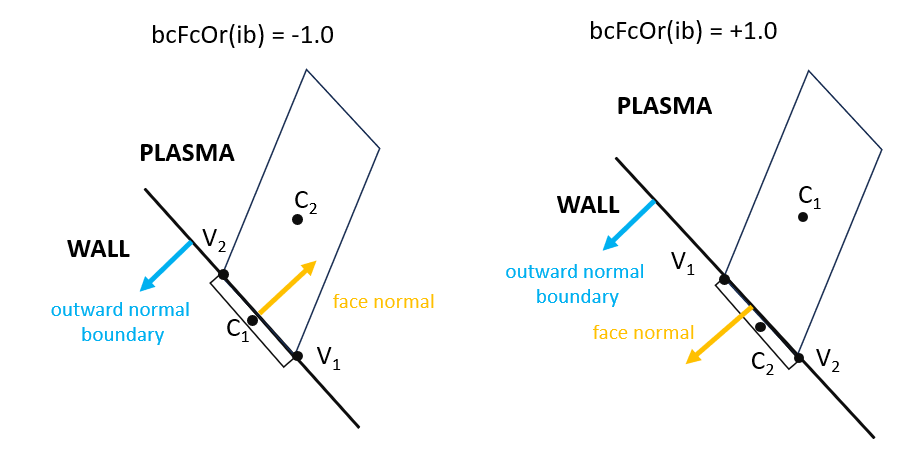
\includegraphics[height=4cm]{FiguresWG/bcfcor.PNG}}
\else
    \centerline{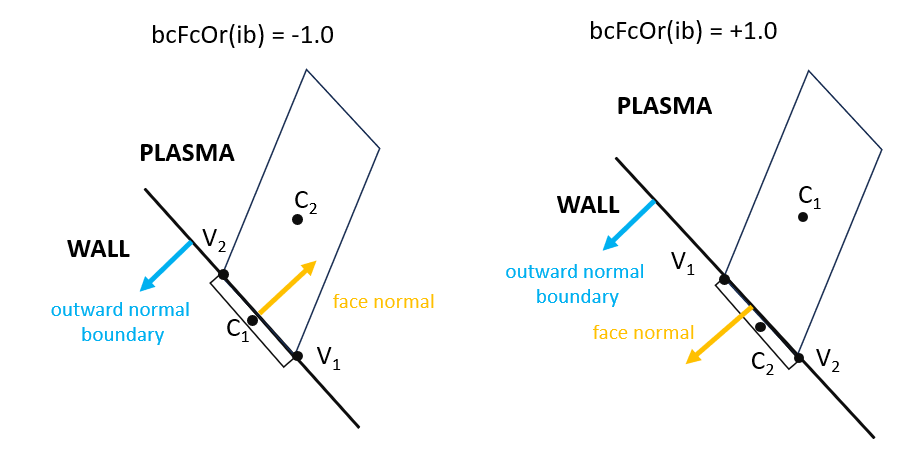
\includegraphics[height=4cm]{FiguresWG/bcfcor.eps}}
\fi
    \caption{Illustration of {\tt bcFcOr}.}
    \label{fig:bcfcor}
\end{figure}

Most boundary conditions fall in one of three categories: Dirichlet, Neumann, or flux.

\textbf{Flux}

To impose a given flux, the net source term in the guard cell must be equal to that flux. Since no fluxes are computed between the guard cells, the flux across the guard cell face must equal the source term.

\textbf{Dirichlet}
\begin{sloppypar}
To impose a fixed value in a guard cell, the code makes use of the different source contributions and very large numbers. For example, to set a fixed density {\tt $n_{BC}$},
the code sets {\tt sna(iCv,0,is) = VBIG $\times$ fcS $\times$ $n_{BC}$}, and {\tt sna(iCv,1,is) = - VBIG $\times$ fcS}, with {\tt sna(iCv,is) = sna(iCv,0,is) + sna(iCv,1,is) $\times$ na(iCv,is)} and where {\tt VBIG} is a very large number. Because {\tt VBIG} is so large, the only way to get a physical source is to have {\tt na(iCv,is) = $n_{BC}$}.
\end{sloppypar}

\textbf{Neumann}
\begin{sloppypar}
To set the gradient normal to the boundary, the code again makes use of the different source contributions and very large numbers. For orthogonal cells, these boundary conditions correctly impose the gradient normal to the boundary face.
For cells that are skewed with respect to the boundary face, the implementation depends on the (partially experimental) {\tt b2stbc\_BC2\_cor9} switch.
To impose for example a density gradient $\Phi$ with {\tt b2stbc\_BC2\_cor9 = 0.0}, the code sets
{\tt sna(iCv,0,is) = VBIG $\times$ fcS $\times$ ($\Phi$ $\times$ ( fcHc(1) + fcHc(2) ) $\times \cos \gamma$ + na(iCv\_internal)} and {\tt sna(iCv,1,is) = - VBIG $\times$ fcS}, where {\tt na(iCv\_internal)} is the density in the first interior cell. To get a physical source, we must have {\tt $\Phi$ $\times$ ( fcHc(1) + fcHc(2) ) $\times \cos \gamma$ + na(iCv\_internal) = na(iCv)}. This results in the correct normal gradient for skewed cells, only if there would be no gradients in the direction tangential to the boundary face. When {\tt b2stbc\_BC2\_cor9 = 1.0}, a correction term based on the vertex values is added, such that $\Phi$ is the gradient normal to the boundary, also in the presence of tangential gradients (up to the interpolation error).
\end{sloppypar}

%% TODO: convert all below to unstructured?

In this Section, the boundaries are denoted as $S_0$ for the PFR boundaries, $S_1$ for the core boundaries, $E$ for the Eastern boundaries (right targets), $W$ for the Western boundaries (left targets), and $N$ for the outer main wall boundary.

\subsection{Particle balance equations}

$S_{n_a} = S_{n_a,0} + S_{n_a,1} n_a$

\subsubsection{South. Private region}

\underline{If $z_a = 0$}

{\em For leakage boundary condition:} {\tt BCCON = 10}

\begin{equation}
\left. \frac{\sqrt g}{h_y}\Gamma_{ay} \right|_{S_0}
=
\left. \left[
p_{n_a,a,1} \frac{\sqrt g}{h_y} \sqrt{\frac{z_a T_e + T_i}{m_a}} n_a
+
\sum \limits_{a=0}^{ns-1} r_{rec,a,0} c_{nsr}
\max \left\{0, -\frac{\sqrt g}{h_y} \Gamma_{ay} \right\}
\right] \right|_{S_0}
\end{equation}

$p_{n_a,a,1} = -10^{-2}, \;\; r_{rec,0,0} = 0,\;\; r_{rec,1,0} = 1$

$\widetilde{\Gamma}_{ay}$ was replaced by $\Gamma_{ay}$

$c_{nsr}$ --- neutral sources rescale coefficient, $1$ --- when working with B2.5 standalone and $10^{-10}$ when coupling to Eirene

$p_{n_a,a,1}$ is the radial leakage velocity, in units of the local species sound speed. Negative velocities are directed out of the plasma.

\underline{If $z_a \neq 0$}

{\em For decay length boundary condition:} {\tt BCCON = 9}

\begin{equation}
\begin{matrix}
\left. \frac{\sqrt g}{h_y} \widetilde{\Gamma}_{ay} \right|_{S_0}& =
& \left\{
\begin{matrix}
\left. \left[
        -\frac{1}{p_{n_a,a,1}} \frac{\sqrt g}{h_y}  \left(
                D^{(AN)}_{n,a} + D^{(AN)}_{p,a} \left(z_a T_e + T_i \right)
        \right) n_a
\right] \right|_{S_0}, & \text{mdf\_fnb} = 0
\\
\left. \left[
\begin{matrix}
        -\frac{1}{p_{n_a,a,1}} \frac{\sqrt g}{h_y} & \left(
                D^{(AN)}_{n,a} + D^{(AN)}_{p,a} \left(z_a T_e + T_i \right)
        \right) n_a
        + \\
        \frac{\sqrt g}{h_y} & D_{ayx} \frac{1}{h_x} \frac{\partial n_a T_i}{\partial x}
        +
        \frac{\sqrt g}{h_y} V_{ay}^{(E)} n_a
\end{matrix}
\right] \right|_{S_0}, & \text{mdf\_fnb} = 1
\end{matrix} \right.
\end{matrix}
\end{equation}

\begin{align}
S^{no\_mdf}_{n_a,0} & = 0 \\
S^{no\_mdf}_{n_a,1} & = - \frac{1}{p_{n_a,a,1}} \frac{\sqrt{g}}{h_y} \left( D^{(AN)}_{n,a} + D^{(AN)}_{p,a} \left( z_a T_e + T_i \right) \right)
\end{align}

$p_{n_a,a,1}$ is the density radial decay length of species $a$, in $m$.

{\em For leakage boundary conditions:} {\tt BCCON = 10}

\begin{equation}
\begin{matrix}
\left. \frac{\sqrt g}{h_y} \widetilde{\Gamma}_{ay} \right|_{S_0}& =
& \left\{
\begin{matrix}
\left. \left[
        p_{n_a,a,1} \frac{\sqrt g}{h_y} \sqrt{\frac{z_a T_e + T_i}{m_a}} n_a
        +
        \min \left\{0, \frac{\sqrt g}{h_y} n_a V_{ay}^{(E)} \right\}
\right] \right|_{S_0}, & \text{mdf\_fnb} = 0
\\
\left. \left[
p_{n_a,a,1} \frac{\sqrt g}{h_y} \sqrt{\frac{z_a T_e + T_i}{m_a}} n_a
        +
        \frac{\sqrt g}{h_y} D_{ayx} \frac{1}{h_x} \frac{\partial n_a T_i}{\partial x}
        +
        \min \left\{0, \frac{\sqrt g}{h_y} n_a V_{ay}^{(E)} \right\}
\right] \right|_{S_0}, & \text{mdf\_fnb} = 1
\end{matrix} \right.
\end{matrix}
\end{equation}

$p_{n_a,a,1} = -10^{-3}$ is the radial leakage velocity, in units of the species local sound speed. Negative velocities are directed out of the plasma.

\begin{align}
S^{no\_mdf}_{n_a,0} & = 0 \\
S^{no\_mdf}_{n_a,1} & = {p_{n_a,a,1}} \frac{\sqrt{g}}{h_y} \sqrt{\frac{z_a T_e + T_i}{m_a}} n_a
\end{align}

% -- To be checked --
{\em Imposing radial leakage:} {\tt BCCON = 15}

When using drifts, one should use {\tt BCCON = 10} instead.

\begin{equation}
\left. - \frac{\sqrt g}{h_y^2} D_{n,ay} \frac{\partial n_a}{\partial y} \right|_{S_0}
=
\left. \left[
c_{n_a,a,2} \frac{\sqrt g}{h_y} \sqrt{\frac{z_a T_e + T_i}{m_a}} n_a
\right] \right|_{S_0}
\end{equation}

$c_{n_a,a,2} = -10^{-3}$ is the radial leakage velocity, in units of the species local thermal velocity. Negative velocities are directed out of the plasma.

% -- end --

\subsubsection{South 1. Core plasma}

\underline{If $z_a = 0$}

%-------- end of 21st page -------------

{\em Imposing total particle flux:} {\tt BCCON = 8}

$\left. \frac{\sqrt g}{h_y} \widetilde{\Gamma}_{ay} \right|_{S_1} = 0$

$\left. \frac{\sqrt g}{h_y} \Gamma_{ay} \right|_{S_1} = 0$

\underline{If $z_a \neq 0$}

{\em Imposing a constant density :} {\tt BCCON = 1}

\begin{equation}
\left. \frac{\sqrt g}{h_y} \widetilde{\Gamma}_{ay} \right|_{S_1}
=
\frac{\sqrt{g}}{h_y}
\left. \left(
        \left. v_{big} n_a \right|_{S_1} - v_{big} n_a
\right) \right|_{S_1},
\;\;
v_{big} = 10^8 \sqrt{\frac{100 \text{eV}}{m_p}},
\;\;
\left. n_a \right|_{S_1} \text{ is the desired density in } m^{-3}
\end{equation}

{\em Imposing the total particle flux with constant flux density:} {\tt BCCON = 8}

\begin{equation*}
\left. \frac{\sqrt g}{h_y} \widetilde{\Gamma}_{ay} \right|_{S_1} =
\left. p_{n,a,0} \frac{
\frac{\sqrt g}{h_y}
} {
\sum \limits_i \left(
        \frac{\sqrt g}{h_y}
\right)_{i, -1}
} \right|_{S_1}
+
\left.
\frac{\sqrt g}{h_y} D_{ayx} \frac{1}{h_x} \frac{\partial n_a T_i}{\partial x}
\right|_{S_1} +
\left. \frac{\sqrt g}{h_y}V_{ya}^{(E)} n_a \right|_{S_1}
\end{equation*}

$p_{n,a,0}$ is the desired total particle flux, per unit time.

\subsubsection{North}

\underline{If $z_a = 0$}

{\em For leakage boundary condition:} {\tt BCCON = 10}

\begin{equation}
\left. - \frac{\sqrt g}{h_y} \Gamma_{ay} \right|_{N}
=
\left. \left[
p_{n_a,a,1} \frac{\sqrt g}{h_y} \sqrt{\frac{z_a T_e + T_i}{m_a}} n_a
+
\sum \limits_{a=0}^{ns-1} r_{rec,a,0} c_{nsr}
\max \left\{0, \frac{\sqrt g}{h_y} \Gamma_{ay} \right\}
\right] \right|_{N}
\end{equation}

$p_{n_a,a,1} = -10^{-2}, \;\; r_{rec,0,0} = 0,\;\; r_{rec,1,0} = 1$

$c_{nsr}$ --- neutral sources rescale coefficient, $1$ --- when working with B2.5 standalone and $10^{-10}$ when coupling to Eirene

$p_{n_a,a,1}$ is the radial leakage velocity, in units of the local species sound speed. Negative velocities are directed out of the plasma.

$\widetilde{\Gamma}_{ay}$ was replaced by $\Gamma_{ay}$

\underline{If $z_a \neq 0$}

{\em For decay length boundary condition:} {\tt BCCON = 9}

\begin{equation}
\begin{matrix}
\left. - \frac{\sqrt g}{h_y} \widetilde{\Gamma}_{ay} \right|_{N}& =
& \left\{
\begin{matrix}
\left. \left[
        \frac{1}{p_{n_a,a,1}} \frac{\sqrt g}{h_y}  \left(
                D^{(AN)}_{n,a} + D^{(AN)}_{p,a} \left(z_a T_e + T_i \right)
        \right) n_a
\right] \right|_{N}, & \text{mdf\_fnb} = 0
\\
\left. \left[
\begin{matrix}
        \frac{1}{p_{n_a,a,1}} & \frac{\sqrt g}{h_y}  \left(
                D^{(AN)}_{n,a} + D^{(AN)}_{p,a} \left(z_a T_e + T_i \right)
        \right) n_a \\
        -
        \frac{\sqrt g}{h_y} & D_{ayx} \frac{1}{h_x} \frac{\partial n_a T_i}{\partial x}
        -
        \frac{\sqrt g}{h_y} V_{ay}^{(E)} n_a
\end{matrix}
\right] \right|_{N}, & \text{mdf\_fnb} = 1
\end{matrix} \right.
\end{matrix}
\end{equation}

\begin{align}
S^{no\_mdf}_{n_a,0} & = 0 \\
S^{no\_mdf}_{n_a,1} & = \frac{1}{p_{n_a,a,1}} \frac{\sqrt{g}}{h_y} \left( D^{(AN)}_{n,a} + D^{(AN)}_{p,a} \left( z_a T_e + T_i \right) \right)
\end{align}

$p_{n_a,a,1}$ is the density radial decay length of species $a$, in $m$.

{\em For leakage boundary conditions:} {\tt BCCON = 10}

\begin{equation}
\begin{matrix}
\left. - \frac{\sqrt g}{h_y} \widetilde{\Gamma}_{ay} \right|_{N}& =
& \left\{
\begin{matrix}
\left. \left[
        p_{n_a,a,1} \frac{\sqrt g}{h_y} \sqrt{\frac{z_a T_e + T_i}{m_a}} n_a
        -
        \max \left\{0, \frac{\sqrt g}{h_y} n_a V_{ay}^{(E)} \right\}
\right] \right|_{N}, & \text{mdf\_fnb} = 0
\\
\left. \left[
        p_{n_a,a,1} \frac{\sqrt g}{h_y} \sqrt{\frac{z_a T_e + T_i}{m_a}} n_a
        -
        \frac{\sqrt g}{h_y} D_{ayx} \frac{1}{h_x} \frac{\partial n_a T_i}{\partial x}
        -
        \max \left\{0, \frac{\sqrt g}{h_y} n_a V_{ay}^{(E)} \right\}
\right] \right|_{N}, & \text{mdf\_fnb} = 1
\end{matrix} \right.
\end{matrix}
\end{equation}

$p_{n_a,a,1} = -10^{-3}$ is the radial leakage velocity, in units of the species local sound speed. Negative velocities are directed out of the plasma.

\begin{align}
S^{no\_mdf}_{n_a,0} & = 0 \\
S^{no\_mdf}_{n_a,1} & = {p_{n_a,a,1}} \frac{\sqrt{g}}{h_y} \sqrt{\frac{z_a T_e + T_i}{m_a}} n_a
\end{align}

% -- To be checked --
{\em Imposing radial leakage:} {\tt BCCON = 15}

When using drifts, one should use {\tt BCCON = 10} instead.

\begin{equation}
\left. \frac{\sqrt g}{h_y^2} D_{n,ay} \frac{\partial n_a}{\partial y} \right|_N
=
\left. \left[
c_{n_a,a,2} \frac{\sqrt g}{h_y} \sqrt{\frac{z_a T_e + T_i}{m_a}} n_a
\right] \right|_N
\end{equation}

$c_{n_a,a,2} = -10^{-3}$ is the radial leakage velocity, in units of the species local thermal velocity. Negative velocities are directed out of the plasma.

% -- end --

\subsubsection{North with puffing}

\underline{If $z_a = 0$}

{\em Imposing a particle flux per unit area:} {\tt BCCON = 5}

\begin{equation}
\left. - \frac{\sqrt g}{h_y} \widetilde{\Gamma}_{ay} \right|_N
=
\left. p_{n,a,0} \frac{\sqrt g}{h_y} \right|_N
+
\left.
\sum \limits_{a=0}^{ns-1} \left[
        r_{rec,a,0} c_{nsr}
        \max \left\{0, -\frac{\sqrt g}{h_y} \Gamma_{ay} \right\}
\right] \right|_N
\end{equation}

$c_{nsr}$ --- neutral sources rescale coefficient, $1$ --- when working with B2.5 standalone and $10^{-10}$ when coupling to Eirene

$r_{rec,0,0} = 0,\;\; r_{rec,1,0} = 1$

$p_{n,a,0}$ is the desired total particle flux density, in $m^{-2}.s^{-1}$.

$\widetilde{\Gamma}_{ay}$ was replaced by $\Gamma_{ay}$

or

{\em Imposing a total particle flux with constant flux density:} {\tt BCCON = 8}

\begin{equation*}
\left. - \frac{\sqrt g}{h_y} \widetilde{\Gamma}_{ay} \right|_N =
\left. \frac{ p_{n,a,0}
}{
\sum \limits_{i=0}^{Nx-1} \left(
        \frac{\sqrt g}{h_y}
\right)_{i, Ny}
}
\frac{\sqrt g}{h_y} \right|_N
+
\left. \sum \limits_{a=0}^{ns-1} \left[
        r_{rec,a,0} c_{nsr}
        \max \left\{0, \frac{\sqrt g}{h_y} \Gamma_{ay} \right\}
\right]
\right|_N
\end{equation*}

$c_{nsr}$ --- neutral sources rescale coefficient, $1$ --- when working with B2.5 standalone and $10^{-10}$ when coupling to Eirene

$r_{rec,0,0} = 0,\;\; r_{rec,1,0} = 1$

$p_{n,a,0}$ is the desired total particle flux, per unit time.

$\widetilde{\Gamma}_{ay}$ was replaced by $\Gamma_{ay}$

\subsubsection{West}

%-------- end of 23rd page -------------

\underline{If $z_a = 0$}

{\em Imposing a given particle flux per unit area:} {\tt BCCON = 5}

\begin{equation}
\left. \frac{\sqrt g}{h_x} \Gamma_{ax} \right|_W
=
\left. \left[
p_{n,a,1} \frac{\sqrt g}{h_y}
+
c_{nsr} \sum \limits_{a=0}^{ns-1} r_{rec,a,0}
\max \left\{0, -\frac{\sqrt g}{h_x} \Gamma_{ax} \right\}
\right] \right|_W
\end{equation}

$r_{rec,0,0} = 0,\;\; r_{rec,1,0} = 1,\;\; p_{n_a,a,1} = 0 $

\begin{equation}
\left. \frac{\sqrt g}{h_x} \widetilde{\Gamma}_{ax} \right|_W
=
\left. \left[
p_{n,a,1} \frac{\sqrt g}{h_x}
+
c_{nsr} \sum \limits_{a=0}^{ns-1} r_{rec,a,0}
\max \left\{0, -\frac{\sqrt g}{h_x} \Gamma_{ax} \right\}
\right] \right|_W
\end{equation}

$\widetilde{\Gamma}_{ax}$ was replaced by $\Gamma_{ax}$

$r_{rec,0,0} = 0,\;\; r_{rec,1,0} = 1,\;\; p_{n_a,a,1} = 0 $

\underline{If $z_a \neq 0$}

{\em Sheath density boundary condition:} {\tt BCCON = 3}

\begin{equation*}
\left. \frac{\sqrt g}{h_x} \Gamma_{ax} \right|_W = \left.
10^{20} \frac{\sqrt{g}}{h_x} \frac{\partial n_a}{\partial x}
\right|_W
\end{equation*}

{\em Drift-compatible, Bohm-Chodura sheath entrance condition} {\tt BCCON = 14}

{\em If the sine of the incident field line angle is larger than {\tt Qalfmin}:}

{\em - Marginal imposition, with collective sound speed:} {\tt MOMPAR(,,2)} = $p_{m,a,2} < 0.5$

To be used in conjunction with {\tt BCENE = 15}, {\tt BCENI = 15}, {\tt BCMOM = 13}, and {\tt BCPOT = 11}.

\begin{equation*}
\left. \frac{\sqrt g}{h_x} \widetilde{\Gamma}_{ax} \right|_W
=
\left. \left[
- p_{n,a,1} \frac{\sqrt g}{h_x} |b_x|
\sqrt{\frac{\sum \limits_{\substack{b = 0 \\ z_b \neq 0}}^{ns-1} p_b}{\sum \limits_{\substack{b = 0 \\ z_b \neq 0}}^{ns-1} m_b n_b}} n_a
-
\frac{\sqrt g}{h_x} D_{axy} \frac{1}{h_y} \frac{\partial n_a T_i}{\partial y}
\right]
\right|_W
\end{equation*}

$p_{n,a,1} = +1$

{\em - Non-marginal imposition, with individual species sound speed:} {\tt MOMPAR(,,2)} = $p_{m,a,2} \geq 0.5$

to be used in conjunction with {\tt BCMOM = 13}, {\tt BCENE = 15} with {\tt bcene\_15\_style = 1}, {\tt BCENI = 15}, {\tt BCPOT = 3} or {\tt BCPOT = 11} with {\tt istyle\_fchi=0}.

This condition imposes that the sum of the poloidal projection of the parallel velocity and the poloidal $\exb$ velocity (restricted to not exceed $\pm 2 c_{s,a} |b_x|$), equals \textit{at least} the specific species sound speed $c_{s,a}$, reprojected in the the poloidal direction.

The parameter $p_{m,a,1}$ is set by {\tt MOMPAR(,,1)}. The parameter $\chi$ is set by {\tt GAMMAI}.

\begin{equation*}
\left. \frac{\sqrt g}{h_x} \widetilde{\Gamma}_{ax} \right|_W
=
\left. \left[
- \frac{\sqrt g}{h_x} |b_x|
U_{out} n_a
-
\frac{\sqrt g}{h_x} D_{axy} \frac{1}{h_y} \frac{\partial n_a T_i}{\partial y}
\right]
\right|_W
\end{equation*}

\begin{equation*}
  U_{out} = \max \left( -u_{\parallel,a}^{extrap}- \frac{V_{\exb}^{restr}}{|b_x|}, p_{m,a,1} \cdot \sqrt{\frac{\chi T_i + z_a T_e}{m_a}} \right)
\end{equation*}

where $u_{\parallel,a}^{extrap}$ is the extrapolated parallel velocity at the target, and $V_{\exb}^{restr}$ is the poloidal $\exb$ velocity restricted to not exceed $\pm 2 c_{s,a} |b_x|$.

{\em For nearly tangent field lines, we use instead:}

\begin{equation}
\begin{matrix}
\left. - \frac{\sqrt g}{h_x} \widetilde{\Gamma}_{ax} \right|_W & =
& \left\{
\begin{matrix}
\left. \left[ \frac{\sqrt g}{h_x} p_{n,a,1} \sqrt{\frac{\sum \limits_{\substack{b = 0 \\ z_b \neq 0}}^{ns-1} p_b}{\sum \limits_{\substack{b = 0 \\ z_b \neq 0}}^{ns-1} m_b n_b}} n_a \alpha_{\max} +
   \max \left( 0, \frac{\sqrt g}{h_x} V^{(E)}_{ax} n_a \right) \right] \right|_W, & \text{mdf\_fnb = 0}
\\
\left. \left[ \frac{\sqrt g}{h_x} p_{n,a,1} \sqrt{\frac{\sum \limits_{\substack{b = 0 \\ z_b \neq 0}}^{ns-1} p_b}{\sum \limits_{\substack{b = 0 \\ z_b \neq 0}}^{ns-1} m_b n_b}} n_a \alpha_{\max} +
   \max \left( 0, \frac{\sqrt g}{h_x} \left( V^{(E)}_{ax} + \widetilde{\widetilde{V}}^{(dia)}_{ax} \right) n_a \right) + \tilde\Gamma^{(PSch)}_{ax} \right] \right|_W, & \text{mdf\_fnb = 1}
\end{matrix}
\right.
\end{matrix}
\end{equation}

where $\alpha_{\max}$ is given by {\tt Qalfmax}.

Both {\tt Qalfmin} and {\tt Qalfmax} are provided in the {\tt b2fgmtry} file or through the {\tt b2us\_prep\_Qalfmin} and {\tt b2us\_prep\_Qalfmax} switches, respectively. Default value for both is $10^{-3}$.

\subsubsection{East}

\underline{If $z_a = 0$}

{\em Imposing a given particle flux per unit area:} {\tt BCCON = 5}

\begin{equation}
\left. - \frac{\sqrt g}{h_x} \Gamma_{ax} \right|_E
=
\left. \left[
p_{n,a,1} \frac{\sqrt g}{h_y}
+
c_{nsr} \sum \limits_{a=0}^{ns-1} r_{rec,a,0}
\max \left\{0, \frac{\sqrt g}{h_x} \Gamma_{ax} \right\}
\right] \right|_E
\end{equation}

$r_{rec,0,0} = 0,\;\; r_{rec,1,0} = 1,\;\; p_{n_a,a,1} = 0 $

%-------- end of 24th page -------------


\begin{equation}
\left. - \frac{\sqrt g}{h_x} \widetilde{\Gamma}_{ax} \right|_E
=
\left. \left[
c_{nsr} \sum \limits_{a=0}^{ns-1} r_{rec,a,0}
\max \left\{0, \frac{\sqrt g}{h_x} \Gamma_{ax} \right\}
\right] \right|_E
\end{equation}

$\widetilde{\Gamma}_{ax}$ was replaced by $\Gamma_{ax}$

$r_{rec,0,0} = 0,\;\; r_{rec,1,0} = 1$

\underline{If $z_a \neq 0$}

{\em Sheath density boundary condition:} {\tt BCCON = 3}

\begin{equation*}
\left. - \frac{\sqrt g}{h_x} \Gamma_{ax} \right|_E =
- 10^{20} \left. \frac{\sqrt{g}}{h_x} \frac{\partial n_a}{\partial x}
\right|_E
\end{equation*}

{\em Drift-compatible, Bohm-Chodura sheath entrance condition} {\tt BCCON = 14}

{\em If the sine of the incident field line angle is larger} {\tt Qalfmin}:

{\em - Marginal imposition, with collective sound speed:} {\tt MOMPAR(,,2)} = $p_{m,a,2} < 0.5$

To be used in conjunction with {\tt BCENE = 15}, {\tt BCENI = 15}, {\tt BCMOM = 13}, and {\tt BCPOT = 11}.

\begin{equation*}
\left. - \frac{\sqrt g}{h_x} \widetilde{\Gamma}_{ax} \right|_E
=
\left. \left[
- p_{n,a,1} \frac{\sqrt g}{h_x} |b_x|
\sqrt{\frac{\sum \limits_{\substack{b = 0 \\ z_b \neq 0}}^{ns-1} p_b}{\sum \limits_{\substack{b = 0 \\ z_b \neq 0}}^{ns-1} m_b n_b}} n_a
+
\frac{\sqrt g}{h_x} D_{axy} \frac{1}{h_y} \frac{\partial n_a T_i}{\partial y}
\right]
\right|_E
\end{equation*}

$p_{n,a,1} = +1$

{\em - Non-marginal imposition, with individual species sound speed:} {\tt MOMPAR(,,2)} = $p_{m,a,2} \geq 0.5$

to be used in conjunction with {\tt BCMOM = 13}, {\tt BCENE = 15} with {\tt bcene\_15\_style = 1}, {\tt BCENI = 15}, {\tt BCPOT = 3} or {\tt BCPOT = 11} with {\tt istyle\_fchi=0}.

This condition imposes that the sum of the poloidal projection of the parallel velocity and the poloidal $\exb$ velocity (restricted to not exceed $\pm 2 c_{s,a} |b_x|$), equals \textit{at least} the specific species sound speed $c_{s,a}$, reprojected in the the poloidal direction.

The parameter $p_{m,a,1}$ is set by {\tt MOMPAR(,,1)}. The parameter $\chi$ is set by {\tt GAMMAI}.

\begin{equation*}
\left. - \frac{\sqrt g}{h_x} \widetilde{\Gamma}_{ax} \right|_E
=
\left. \left[
- \frac{\sqrt g}{h_x} |b_x|
U_{out} n_a
+
\frac{\sqrt g}{h_x} D_{axy} \frac{1}{h_y} \frac{\partial n_a T_i}{\partial y}
\right]
\right|_E
\end{equation*}

\begin{equation*}
  U_{out} = \max \left( u_{\parallel,a}^{extrap} + \frac{V_{\exb}^{restr}}{|b_x|}, p_{m,a,1} \cdot \sqrt{\frac{\chi T_i + z_a T_e}{m_a}} \right)
\end{equation*}

where $u_{\parallel,a}^{extrap}$ is the extrapolated parallel velocity at the target, and $V_{\exb}^{restr}$ is the poloidal $\exb$ velocity restricted to not exceed $\pm 2 c_{s,a} |b_x|$.

{\em For nearly tangent field lines, we use instead:}

\begin{equation}
\begin{matrix}
\left. \frac{\sqrt g}{h_x} \widetilde{\Gamma}_{ax} \right|_E & =
& \left\{
\begin{matrix}
\left. \left[ \frac{\sqrt g}{h_x} p_{n,a,1} \sqrt{\frac{\sum \limits_{\substack{b = 0 \\ z_b \neq 0}}^{ns-1} p_b}{\sum \limits_{\substack{b = 0 \\ z_b \neq 0}}^{ns-1} m_b n_b}} n_a \alpha_{\max} +
   \max \left( 0, \frac{\sqrt g}{h_x} V^{(E)}_{ax} n_a \right) \right] \right|_E, & \text{mdf\_fnb = 0}
\\
\left. \left[ \frac{\sqrt g}{h_x} p_{n,a,1} \sqrt{\frac{\sum \limits_{\substack{b = 0 \\ z_b \neq 0}}^{ns-1} p_b}{\sum \limits_{\substack{b = 0 \\ z_b \neq 0}}^{ns-1} m_b n_b}} n_a \alpha_{\max} +
   \max \left( 0, \frac{\sqrt g}{h_x} \left( V^{(E)}_{ax} + \widetilde{\widetilde{V}}^{(dia)}_{ax} \right) n_a \right) + \tilde\Gamma^{(PSch)}_{ax} \right] \right|_E, & \text{mdf\_fnb = 1}
\end{matrix}
\right.
\end{matrix}
\end{equation}

\subsection{Parallel momentum balance for ions}

$S_{m_a} = S_{m_a,0} + S_{m_a,1} V_{\parallel a} + S_{m_a,2} m_a n_a + S_{m_a,3} m_a n_a V_{\parallel a}$

\subsubsection{South. Private region}

\underline{If $z_a = 0$}

{\em Weakly imposing a velocity:} {\tt BCMOM = 4}

\begin{equation*}
\left. h_z \frac{\sqrt g}{h_y} \Gamma_{ay}^m \right|_{S_0} =
\left. \left[
p_{m,a,1} p_{m,a,2} h_z \frac{\sqrt g}{h_y} -
p_{m,a,2} h_z \frac{\sqrt g}{h_y} V_{\parallel a}
\right] \right|_{S_0}
\end{equation*}

$p_{m,a,1}=0$ is the imposed velocity, in $m.s^{-1}$, and $p_{m,a,2}=10^5$ is the strength with which this velocity is imposed.

We had this b.c.

$\left. h_z \frac{\sqrt g}{h_y} \Gamma_{ay}^m \right|_{S_0} =
\left. \left[
c_{m,a,3} h_z \frac{\sqrt g}{h_y} m_a n_a V_{\parallel a} +
c_{m,a,6} \max \left(0,-h_z \frac{\sqrt g}{h_y} \frac{\Gamma_{ay}^{Cor}}{n_a} \right)
m_a n_a V_{\parallel a}
\right] \right|_{S_0}$, delete term with {\tt max} !

%-------- end of 25th page -------------

$\Gamma_{ay}^{Cor} = \Gamma_{ay} + \Gamma_{ay}^{(dia)}$

$c_{m,a,3} = -10^{10}$, we have $c_{m,a,6}=-1$, but not $c_{m,a,6}=0$

Inserted into {\tt b2stbc\_phys} for {\tt BCMOM=12} as $c_{m,a,3} \rightarrow p_{m,a,2} = -10^{10}$, and $c_{m,a,6} \rightarrow p_{m,a,1} = -1$

\underline{If $z_a \neq 0$}

{\em Weakly imposing a velocity:} {\tt BCMOM = 4}

\begin{equation}
\left. h_z \frac{\sqrt g}{h_y} \Gamma_{ay}^m \right|_{S_0} =
\left. \left[
        p_{m,a,1} p_{m,a,2} h_z \frac{\sqrt g}{h_y} -
        p_{m,a,2} h_z \frac{\sqrt g}{h_y} V_{\parallel a}
\right] \right|_{S_0}
\end{equation}

$p_{m,a,1}=0$ is the imposed velocity, in $m.s^{-1}$, and $p_{m,a,2}=10^5$ is the strength with which this velocity is imposed.

\begin{equation}
\left. h_z \frac{\sqrt g}{h_y} \Gamma_{ay}^m \right|_{S_0} =
\left. \left[
        c_{m,a,3} h_z \frac{\sqrt g}{h_y} m_a n_a V_{\parallel a} +
        c_{m,a,6} \max \left(
                0, -h_z \frac{\sqrt g}{h_y} \frac{\Gamma_{ay}^{Cor}}{n_a}
        \right) m_a n_a V_{\parallel a}
\right] \right|_{S_0}
\end{equation}

delete term with {\tt max}!

$\Gamma_{ay}^{Cor} = \Gamma_{ay} + \Gamma_{ay}^{(dia)}$

$c_{m,a,3} = 0$,  $c_{m,a,6} = -1$

\subsubsection{South 1. Core}

\underline{If $z_a = 0$}

{\em Weakly imposing a velocity:} {\tt BCMOM = 4}

$ \left. h_z \frac{\sqrt g}{h_y} \Gamma_{ay}^m \right|_{S_1} = \left. \left[
        p_{m,a,1} p_{m,a,2} h_z \frac{\sqrt g}{h_y} -
        p_{m,a,2} h_z \frac{\sqrt g}{h_y} V_{\parallel a}
\right] \right|_{S_1}$

$p_{m,a,1}=0$ is the imposed velocity, in $m.s^{-1}$, and $p_{m,a,2}=10^5$ is the strength with which this velocity is imposed.

$ \left. h_z \frac{\sqrt g}{h_y} \Gamma_{ay}^m \right|_{S_1} = c_{m,a,3} h_z \left. \frac{\sqrt g}{h_y} m_a n_a V_{\parallel a} \right|_{S_1}$

$c_{m,a,3} = -10^{10}$

Inserted into {\tt b2stbc\_phys} for {\tt BCMOM=12} as $c_{m,a,3} \rightarrow p_{m,a,2} = -10^{10},\;c_{m,a,6} \rightarrow
p_{m,a,1} = 0$

\underline{If $z_a \neq 0$}

%-------- end of 26th page -------------

{\em Weakly imposing a velocity:} {\tt BCMOM = 4}

$ \left. h_z \frac{\sqrt g}{h_y} \Gamma_{ay}^m \right|_{S_1} = \left. \left[
        p_{m,a,1} p_{m,a,2} h_z \frac{\sqrt g}{h_y} -
        p_{m,a,2} \frac{\sqrt g}{h_y} V_{\parallel a}
\right] \right|_{S_1}$

$p_{m,a,1}=0$ is the imposed velocity, in $m.s^{-1}$, and $p_{m,a,2}=10^5$ is the strength with which this velocity is imposed.

{\em {\tt b2stbc\_spb} style:} {\tt BCMOM = 14}

\begin{align*}
\left. h_z \frac{\sqrt g}{h_y} \Gamma_{ay}^m \right|_{S_1} = &
c_{m,a,3} h_z \left. \frac{\sqrt g}{h_y} m_a n_a V_{\parallel a} \right|_{S_1} + \\
& \left. \left[
h_z \frac{\sqrt g}{h_y} m_a \left\langle n_a \right\rangle \left( -2 \right)\frac{\left\langle T_i \right\rangle B_z}{ez_a}\frac{\partial}{h_x \partial x} \left( \frac{1}{B^2} \right) \left\langle V_{\parallel a} \right\rangle c_{drift} +
c_{corflux} h_z \frac{\sqrt g}{h_y}
\right] \right|_{S_1} \\
+ & \left. c_{m,a,1} \max \left( 0 , - h_z \frac{\sqrt{g}}{h_y} \frac{\Gamma_{ay}^{Cor}}{n_a} \right) m_a n_a V_{\parallel a} \right|_{S_1}
\end{align*}

$c_{m,a,1} = 0$, $c_{m,a,3} = -10^{10}$

{\em Prescribe the value of the parallel velocity as a function of the poloidal coordinate:} {\tt BCMOM = 15}

\begin{equation*}
\left. h_z \frac{\sqrt g}{h_y} \Gamma_{ay}^m \right|_{S_1} =
\left. v_{big} n_{e0} m_{a} h_z \frac{\sqrt g}{h_y} \left[
        \frac{\langle B \rangle}{B} p_{m,a,1} - V_{\parallel a}
\right] \right|_{S_1}
\end{equation*}

where $\langle B \rangle = \frac{\mathlarger{\oint}_{S_1} B \sqrt{g} \, dx}{\mathlarger{\oint}_{S_1} \sqrt{g} \, dx}$, the integration is done over the innermost magnetic surface, $v_{big} = 10^{8} \sqrt{\frac{100 \text{eV}}{m_p}}$, $n_{e0} = 10^{20}$, $p_{m,a,1}$ is the given value of the average parallel velocity, in $m.s^{-1}$.

\subsubsection{North}

\underline{If $z_a=0$}

{\em Weakly imposing a velocity:} {\tt BCMOM = 4}

$ \left. -h_z \frac{\sqrt g}{h_y} \Gamma_{ay}^m \right|_N = \left. \left[
        p_{m,a,1} p_{m,a,2} h_z \frac{\sqrt g}{h_y} -
        p_{m,a,2} h_z \frac{\sqrt g}{h_y} V_{\parallel a}\right]
\right|_N$

$p_{m,a,1}=0$ is the imposed velocity, in $m.s^{-1}$, and $p_{m,a,2}=10^5$ is the strength with which this velocity is imposed.

$\left. -h_z \frac{\sqrt g}{h_y} \Gamma_{ay}^m \right|_N = \left. \left[
        c_{m,a,3} h_z \frac{\sqrt g}{h_y} m_a n_a V_{\parallel a} +
        c_{m,a,6} \max \left(
                0, h_z \frac{\sqrt g}{h_y} \frac{\Gamma_{ay}^{Cor}}{n_a}
        \right) m_a n_a V_{\parallel a}
\right]
\right|_N$

delete term with {\tt max} !

$c_{m,a,3} = -10^{10}$, we have  $c_{m,a,6} = -1$, but not $c_{m,a,6} = 0$

Inserted into {\tt b2stbc\_phys} for {\tt BCMOM=12} as $c_{m,a,3} \rightarrow p_{m,a,2} = -10^{10},\;c_{m,a,6} \rightarrow p_{m,a,1} = -1$

\underline{If $z_a \neq 0$}

%-------- end of 27th page -------------

{\em Weakly imposing a velocity:} {\tt BCMOM = 4}

$ \left. -h_z \frac{\sqrt g}{h_y} \Gamma_{ay}^m \right|_N = \left[
        p_{m,a,1} p_{m,a,2} h_z \frac{\sqrt g}{h_y} -
        p_{m,a,2} h_z \frac{\sqrt g}{h_y} V_{\parallel a}
\right]|_N$

$p_{m,a,1}=0$ is the imposed velocity, in $m.s^{-1}$, and $p_{m,a,2}=10^5$ is the strength with which this velocity is imposed.

\begin{equation*}
\left. -h_z \frac{\sqrt g}{h_y} \Gamma_{ay}^m \right|_N =
\left. \left[
c_{m,a,3} h_z \frac{\sqrt g}{h_y} m_a n_a V_{\parallel a} +
c_{m,a,6} \max \left(
        0, h_z \frac{\sqrt g}{h_y} \frac{\Gamma_{ay}^{Cor}}{n_a}
\right) m_a n_a V_{\parallel a}
\right] \right|_N
\end{equation*}

$c_{m,a,3} = 0$, $c_{m,a,6} = -1$

\subsubsection{West}

\underline{If $z_a = 0$}, $p_{m,a,1} = 0$

\underline{If $z_a \neq 0$}, $p_{m,a,1} = 1$

{\em Drift-compatible, Bohm-Chodura sheath entrance condition} {\tt BCMOM = 13}

{\em If the sine of the incident field line angle is larger than} {\tt Qalfmin}:

{\em - Marginal imposition, with collective sound speed:} {\tt MOMPAR(,,2)} = $p_{m,a,2} < 0.5$

To be used in conjunction with {\tt BCENE = 15}, {\tt BCENI = 15}, {\tt BCCON = 14}, and {\tt BCPOT = 11}.

\begin{equation*}
\left. h_z \frac{\sqrt g}{h_x} \Gamma_{ax}^m \right|_W = \left. \left[
        p_{m,a,1} \frac{u_{big}}{\epsilon^2} V_{West} m_a n_a -
        \frac{u_{big}}{\epsilon^2} h_z \frac{\sqrt g}{h_x} |b_x| m_a n_a V_{\parallel a}
\right]
\right|_W
\end{equation*}

with $u_{big} = 10^{10} \sqrt{\frac{100 \text{eV}}{m_p}}$ and $\epsilon = 10^{-10}$.

\begin{equation*}
V_{West} =
- h_z \frac{\sqrt g}{h_x} \frac{|b_x|}{b_x} \min \left( 2 c_s, V_{ax}^{(\exb)} \right)
- h_z \frac{\sqrt g}{h_x} b_x
\sqrt{\frac{\sum \limits_{\substack{a = 0 \\ z_a \neq 0}}^{ns-1} p_a}
{\sum \limits_{\substack{a = 0 \\ z_a \neq 0}}^{ns-1} m_a n_a}}
\end{equation*}

{\em - Non-marginal imposition, with individual species sound speed:} {\tt MOMPAR(,,2)} = $p_{m,a,2} \geq 0.5$

to be used in conjunction with {\tt BCCON = 14}, {\tt BCENE = 15} with {\tt bcene\_15\_style = 1}, {\tt BCENI = 15}, {\tt BCPOT = 3} or {\tt BCPOT = 11} with {\tt istyle\_fchi = 0}.

This condition imposes that the sum of the poloidal projection of the parallel velocity and the poloidal $\exb$ velocity (restricted to not exceed $\pm 2 c_{s,a} |b_x|$), equals \textit{at least} the specific species sound speed $c_{s,a}$, reprojected in the the poloidal direction.

The parameter $p_{m,a,1}$ is set by {\tt MOMPAR(,,1)}. The parameter $\chi$ is set by {\tt GAMMAI}.

\begin{equation*}
  \left. \frac{\sqrt g}{h_x} \Gamma_{ax}^m \right|_W = \left. \left[
          -\frac{u_{big}}{\epsilon^2} n_a m_a \frac{\sqrt{g}}{h_x} U_{out} \frac{B_x}{|B_x|}
          -\frac{u_{big}}{\epsilon^2} n_a m_a \frac{\sqrt{g}}{h_x} V_{\parallel,a}
  \right]
  \right|_W
  \end{equation*}

\begin{equation*}
  U_{out} = \max \left( -u_{\parallel,a}^{extrap} - \frac{V_{\exb}^{restr}}{|b_x|}, p_{m,a,1} \cdot \sqrt{\frac{\chi T_i + z_a T_e}{m_a}} \right)
\end{equation*}

where $u_{\parallel,a}^{extrap}$ is the extrapolated parallel velocity at the target, and $V_{\exb}^{restr}$ is the poloidal $\exb$ velocity restricted to not exceed $\pm 2 c_{s,a} |b_x|$.

{\em For nearly tangent field lines}, we apply a no radial shear velocity condition.

\underline{If $z_a = 0$}

{\em Imposing a specified parallel velocity:} {\tt BCMOM = 1}

$\left. \frac{\sqrt g}{h_x} \Gamma_{ax}^m \right|_W = \left. \left[
        u_{big} n_{e00} \frac{m_a}{m_p} \frac{\sqrt{g}}{h_x} p_{m,a,1} -
        u_{big} n_{e00} \frac{m_a}{m_p} \frac{\sqrt{g}}{h_x} V_{\parallel a}
\right]
\right|_W$

$p_{m,a,1}=0$ is the imposed velocity in $m.s^{-1}$, $n_{e00} = 10^{20}$.

\underline{If $z_a \neq 0$}

{\em Imposing a sheath velocity boundary condition:} {\tt BCMOM = 3}

\begin{equation*}
\left. \frac{\sqrt g}{h_x} \Gamma_{ax}^m \right|_W = \left. \left[
        -\frac{u_{big}}{\epsilon^2} n_a m_a \frac{\sqrt{g}}{h_x} u_{p_{out}}
        -\frac{u_{big}}{\epsilon^2} n_a m_a \frac{\sqrt{g}}{h_x} V_{\parallel a}
\right]
\right|_W
\end{equation*}

%-------- end of 28th page -------------

If $p_{m,a,2} < 0.5$:

\begin{equation*}
c_s = \sqrt{\frac{\sum \limits_{\substack{a = 0 \\ z_a \neq 0}}^{ns-1} p_a}{\sum \limits_{\substack{a = 0 \\ z_a \neq 0}}^{ns-1} m_a n_a}}
\end{equation*}

$u_{u_{out}} = p_{m,a,1} c_s |b_x|$

$u_{p_{out}} = \max \left\{ 0, \frac{u_{u_{out}}}{|b_x|} + u_a^{(dia)} b_z \right\}$

If $p_{m,a,2} > 0.5$:

$c_{s,a} = \sqrt{\frac{\gamma_i T_i + z_a^2 \frac{n_a}{n_e} T_e}{m_a}}$

where $\gamma_i$ is the adiabatic ratio of specific heats ({\tt GAMMAI} in {\tt b2.boundary.parameters}),

$u_{u_{out}} = \max \left\{ p_{m,a,1} c_{s,a}, u_{extrap} \right\}$

where $u_{extrap}$ is the extrapolated value to the sheath edge of the poloidal velocity $u_a$,

$u_{p_{out}} = \max \left\{ 0, u_{u_{out}} + u_a^{(dia)} \frac{b_z}{b_x} \right\}$.

\subsubsection{East}

\underline{If $z_a = 0$}, $p_{m,a,1} = 0$

\underline{If $z_a \neq 0$}, $p_{m,a,1} = 1$

{\em Drift-compatible, Bohm-Chodura sheath entrance condition} {\tt BCMOM = 13}

{\em If the sine of the incident field line angle is larger than} {\tt Qalfmin}:

{\em - Marginal imposition, with collective sound speed:} {\tt MOMPAR(,,2)} = $p_{m,a,2} < 0.5$

To be used in conjunction with {\tt BCENE = 15}, {\tt BCENI = 15}, {\tt BCCON = 14}, and {\tt BCPOT = 11}.

$\left. -h_z \frac{\sqrt g}{h_x} \Gamma_{ax}^m \right|_E = \left. \left[
        p_{m,a,1} \frac{u_{big}}{\epsilon^2} V_{East} m_a n_a -
        \frac{u_{big}}{\epsilon^2} h_z \frac{\sqrt g}{h_x} |b_x| m_a n_a V_{\parallel a}
\right]
\right|_E$

\begin{equation*}
V_{East} =
- h_z \frac{\sqrt g}{h_x} \frac{|b_x|}{b_x} \min \left( 2 c_s, V_{ax}^{(\exb)} \right)
+ h_z \frac{\sqrt g}{h_x} b_x
\sqrt{\frac{\sum \limits_{\substack{a = 0 \\ z_a \neq 0}}^{ns-1} p_a}
{\sum \limits_{\substack{a = 0 \\ z_a \neq 0}}^{ns-1} m_a n_a}}
\end{equation*}

{\em - Non-marginal imposition, with individual species sound speed:} {\tt MOMPAR(,,2)} = $p_{m,a,2} \geq 0.5$

to be used in conjunction with BCCON=14, BCENE=15 with {\tt bcene\_15\_style=1}, BCENI=15, BCPOT=3 or BCPOT=11 with {\tt istyle\_fchi=0}.

This condition imposes that the sum of the poloidal projection of the parallel velocity and the poloidal $\exb$ velocity (restricted to not exceed $\pm 2 c_{s,a} |b_x|$), equals \textit{at least} the specific species sound speed $c_{s,a}$, reprojected in the the poloidal direction.

The parameter $p_{m,a,1}$ is set by {\tt MOMPAR(,,1)}. The parameter $\chi$ is set by {\tt GAMMAI}.

\begin{equation*}
  -\left. \frac{\sqrt g}{h_x} \Gamma_{ax}^m \right|_E = \left. \left[
          \frac{u_{big}}{\epsilon^2} n_a m_a \frac{\sqrt{g}}{h_x} U_{out} \frac{B_x}{|B_x|}
          -\frac{u_{big}}{\epsilon^2} n_a m_a \frac{\sqrt{g}}{h_x} V_{\parallel,a}
  \right]
  \right|_E
  \end{equation*}

\begin{equation*}
  U_{out} = \max \left( u_{\parallel,a}^{extrap} + \frac{V_{\exb}^{restr}}{|b_x|}, p_{m,a,1} \cdot \sqrt{\frac{\chi T_i + z_a T_e}{m_a}} \right)
\end{equation*}

where $u_{\parallel,a}^{extrap}$ is the extrapolated parallel velocity at the target, and $V_{\exb}^{restr}$ is the poloidal $\exb$ velocity restricted to not exceed $\pm 2 c_{s,a} |b_x|$.

{\em For nearly tangent field lines}, we apply a no radial shear velocity condition.

\underline{If $z_a = 0$}

{\em Imposing a specified parallel velocity:} {\tt BCMOM = 1}

\begin{equation*}
\left. -\frac{\sqrt g}{h_x} \Gamma_{ax}^m \right|_E = \left. \left[
        u_{big} n_{e00} \frac{m_a}{m_p} \frac{\sqrt{g}}{h_x} p_{m,a,1} -
        u_{big} n_{e00} \frac{m_a}{m_p} \frac{\sqrt{g}}{h_x} V_{\parallel a}
\right]
\right|_E
\end{equation*}

$p_{m,a,1}=0$ is the imposed parallel velocity in $m.s^{-1}$.

\underline{If $z_a \neq 0$}

{\em Imposing a sheath velocity boundary condition:} {\tt BCMOM = 3}

\begin{equation*}
\left. -\frac{\sqrt g}{h_x} \Gamma_{ax}^m \right|_E = \left. \left[
        -\frac{u_{big}}{\epsilon^2} n_a m_a \frac{\sqrt{g}}{h_x} u_{p_{out}}
        -\frac{u_{big}}{\epsilon^2} n_a m_a \frac{\sqrt{g}}{h_x} V_{\parallel a}
\right]
\right|_E
\end{equation*}

If $p_{m,a,2} < 0.5$:

\begin{equation*}
c_s = \sqrt{\frac{\sum \limits_{\substack{a = 0 \\ z_a \neq 0}}^{ns-1} p_a}{\sum \limits_{\substack{a = 0 \\ z_a \neq 0}}^{ns-1} m_a n_a}}
\end{equation*}

$u_{u_{out}} = p_{m,a,1} c_s |b_x|$,

$u_{p_{out}} = \max \left\{ 0, \frac{u_{u_{out}}}{|b_x|} - u_a^{(dia)} b_z \right\}$

If $p_{m,a,2} > 0.5$:

$c_{s,a} = \sqrt{\frac{\gamma_i T_i + z_a^2 \frac{n_a}{n_e} T_e}{m_a}}$

$u_{u_{out}} = \max \left\{ p_{m,a,1} c_{s,a}, u_{extrap} \right\}$

$u_{p_{out}} = \max \left\{ 0, u_{u_{out}} - u_a^{(dia)} \frac{b_z}{b_x} \right\}$.

%-------- end of 29th page -------------

\subsection{Current continuity equation}

$S_{ch} = S_{ch,0} + S_{ch,1} \Phi + S_{ch,2} n_e + S_{ch,3} n_e \Phi$

\subsubsection{South. Private region}

$\left. \frac{\sqrt{g}}{h_y} j_y \right|_{S_0} = 0$

\begin{equation*}
\begin{matrix}
\left. \frac{\sqrt{g}}{h_y} j_y \right|_{S_0} = &
& \left\{
\begin{matrix}
0, & \text{facdrift} = 0 \\
\left. \frac{\sqrt{g}}{h_y}
\left(
        \widetilde{j}_y^{(dia)} + j_y^{(in)} + \widetilde{j}_y^{(vis \parallel)} + j_y^{(vis \perp)}
        + \widetilde{j}_y^{(visq)} + \widetilde{j}_y^{(s)}
\right) \right|_{S_0}
, & \text{facdrift} \neq 0 \\
\end{matrix} \right.
\end{matrix}
\end{equation*}

\subsubsection{South 1. Core}

\begin{equation*}
\begin{matrix}
\left. \frac{\sqrt{g}}{h_y} j_y \right|_{S_1} = &
& \left\{
\begin{matrix}
0, & \text{facdrift} = 0 \\
\left. \frac{\sqrt{g}}{h_y}
\left(
        \left\langle \widetilde{j}_y^{(dia)} \right\rangle
\right) \right|_{S_1}
, & \text{facdrift} \neq 0 \\
\end{matrix} \right.
\end{matrix}
\end{equation*}

\begin{equation*}
\begin{matrix}
\left. \frac{\sqrt{g}}{h_y} j_y \right|_{S_1} = &
& \left\{
\begin{matrix}
0, & \text{facdrift} = 0 \\
\left. \frac{\sqrt{g}}{h_y}
\left(
        \left\langle \widetilde{j}_y^{(dia)} \right\rangle +
        \left\langle j_y^{(in)} \right\rangle
\right) \right|_{S_1}
, & \text{facdrift} \neq 0 \\
\end{matrix} \right.
\end{matrix}
\end{equation*}

\begin{equation*}
\left\langle \widetilde{j}_y^{(dia)} \right\rangle =
- \frac{
        B_z \left\langle
                \sum \limits^{ns-1}_{\substack{a = 0 \\
                        z_a \neq 0}} n_a \left(
                        z_a T_e + T_i
                \right)
        \right\rangle
}{h_x}
\frac{\partial}{\partial x}
\left( \frac{1}{B^2} \right)
\end{equation*}

\begin{equation*}
\left\langle j_y^{(in)} \right\rangle =
- \frac{B_z}{2}
\frac{\partial}{h_x \partial x}
\left( \frac{1}{B^2} \right)
\sum \limits^{ns-1}_{\substack{a = 0 \\
    z_a \neq 0}} m_a n_a \left\langle V^2_{a \parallel}
\right\rangle
\end{equation*}

\subsubsection{North}

\begin{equation*}
\begin{matrix}
\left. \frac{\sqrt{g}}{h_y} j_y \right|_N = &
& \left\{
\begin{matrix}
0, & \text{facdrift} = 0 \\
\left. \frac{\sqrt{g}}{h_y}
\left(
        \left\langle \widetilde{j}_y^{(dia)} \right\rangle
\right) \right|_N
, & \text{facdrift} \neq 0 \\
\end{matrix} \right.
\end{matrix}
\end{equation*}

%-------- end of 30th page -------------

\begin{equation*}
\begin{matrix}
\left. - \frac{\sqrt{g}}{h_y} j_y \right|_N = &
& \left\{
\begin{matrix}
0, & \text{facdrift} = 0 \\
\left. - \frac{\sqrt{g}}{h_y}
\left(
        \widetilde{j}_y^{(dia)} + j_y^{(in)} +
        \widetilde{j}_y^{(vis \parallel)} + j_y^{(vis \perp)} +
        \widetilde{j}_y^{(visq)} + \widetilde{j}_y^{(s)}
\right) \right|_N
, & \text{facdrift} \neq 0 \\
\end{matrix} \right.
\end{matrix}
\end{equation*}

\subsubsection{West}

{\em Imposing a sound speed velocity flux:} {\tt BCPOT = 11}

To be used in conjunction with {\tt BCENE = 15}, {\tt BCENI = 15}, {\tt BCMOM = 13}, and {\tt BCCON = 14}.

\small\begin{equation*}
\left. \frac{\sqrt g}{h_x} j_x \right|_W =
\frac{\sqrt g}{h_x} e \left. \left[
        - \sum \limits_{a=0}^{ns-1} z_a \left(
                p_{n,a,1} b_\alpha \sqrt{\frac{\sum \limits_{\substack{b = 0 \\ z_b \neq 0}}^{ns-1} p_b}{\sum \limits_{\substack{b = 0 \\ z_b \neq 0}}^{ns-1} m_b n_b}} n_a
        \right) +
        \left( 1 - \gamma_e \right) b_\alpha n_e \frac{1}{\sqrt{2\pi}}
        \sqrt{\frac{T_e}{m_e}} \exp \left( -\frac{e \left( \Phi - p_{\Phi,2} \right)}{T_e} \right)
\right] \right|_W
\end{equation*}\normalsize

with

\begin{equation*}
b_\alpha = \left\{
\begin{matrix}
|b_x| & , \text{if} \ |b_x| \ge \alpha_{\min} \\
\alpha_{\max} & , \text{if} \ |b_x| < \alpha_{\min}
\end{matrix}
\right.
\end{equation*}

{\em Imposing a sheath potential boundary condition:} {\tt BCPOT = 3}

$\left. \frac{\sqrt g}{h_x} j_x \right|_W =
\frac{\sqrt g}{h_x} e \left. \left[
        \sum \limits_{b=0}^{ns-1} z_a \Gamma_{ax} +
        \left( 1 - \gamma_e \right) |b_x| n_e \frac{1}{\sqrt{2\pi}}
        \sqrt{\frac{T_e}{m_e}}
        \exp \left( -\frac{e \left( \Phi - p_{\Phi,2}\right)}{T_e} \right)
\right] \right|_W$

\subsubsection{East}

{\em Imposing a sound speed velocity flux:} {\tt BCPOT = 11}

To be used in conjunction with {\tt BCENE = 15}, {\tt BCENI = 15}, {\tt BCMOM = 13}, and {\tt BCCON = 11}.

\small\begin{equation*}
\left. -\frac{\sqrt g}{h_x} j_x \right|_E =
\frac{\sqrt g}{h_x} e \left. \left[
        - \sum \limits_{a=0}^{ns-1} z_a \left(
                p_{n,a,1} b_\alpha \sqrt{\frac{\sum \limits_{\substack{b = 0 \\ z_b \neq 0}}^{ns-1} p_b}{\sum \limits_{\substack{b = 0 \\ z_b \neq 0}}^{ns-1} m_b n_b}} n_a
        \right) +
        \left( 1 - \gamma_e \right) b_\alpha n_e \frac{1}{\sqrt{2\pi}}
        \sqrt{\frac{T_e}{m_e}} \exp \left( -\frac{e \left( \Phi - p_{\Phi,2} \right)}{T_e} \right)
\right] \right|_E
\end{equation*}\normalsize

{\em Imposing a sheath potential boundary condition:} {\tt BCPOT = 3}

$\left. -\frac{\sqrt g}{h_x} j_x \right|_E =
\frac{\sqrt g}{h_x} e \left. \left[
        -\sum \limits_{a=0}^{ns-1} z_a \Gamma_{ax} +
        \left( 1 - \gamma_e \right) |b_x| n_e \frac{1}{\sqrt{2\pi}}
        \sqrt{\frac{T_e}{m_e}}
        \exp \left( -\frac{e \left( \Phi - p_{\Phi,2}\right)}{T_e} \right)
\right] \right|_E$

%-------- end of 31st page -------------

\subsection{Energy balance equation for electrons}\label{sec:bcene}

$S_{h_e} = S_{h_e,0} + S_{h_e,1} T_e + S_{h_e,2} n_e + S_{h_e,3} n_e T_e$

\subsubsection{South. Private region}

{\em Imposing the {\tt b2stbc\_spb} style boundary condition:} {\tt BCENE = 11}

\begin{equation*}
\left. \frac{\sqrt g}{h_y} \widetilde q_{ey} \right|_{S_0} = \left. \left[
        \left(
                c_{h_e,2} \frac{\sqrt g}{h_y} \sqrt{\frac{T_e}{m_e}}
        \right) T_e n_e
        +
        c_{h_e,7} \max \left(
                0, -\frac{\sqrt g}{h_y} \widetilde f_{ey}
        \right) T_e - q_{ex}^{P.Sch}
\right] \right|_{S_0}
\end{equation*}

$c_{h_e,2} = -10^{-4}$, $c_{h_e,7} = -1$, $c_{h_e,2} \rightarrow p_{h_e,2} = -10^{-4}$, $c_{h_e,7} \rightarrow p_{h_e,1} = -1$

{\em Imposing a decay length for the electron temperature:} {\tt BCENE = 22}

$\left. -\frac{\sqrt g}{h_y} \kappa_{ey} \frac{\partial T_e}{h_y \partial y} \right|_{S_0} = \left. \left[ \left( p_{h_e,1} \frac{\sqrt g}{h_y}\sqrt{\frac{T_e}{m_e}} \right) T_e n_e \right] \right|_{S_0}$

{\em Imposing a decay length for the electron temperature:} {\tt BCENE=9}

\begin{equation*}
\begin{matrix}
\left. \frac{\sqrt g}{h_y} \widetilde q_{ey} \right|_{S_0}=
& \left\{
\begin{matrix}
\left. \left[
        \frac{5}{2} \sum \limits_{a=0}^{ns-1} z_a S_{n_a,0}^{no\_mdf} T_e
        -
        \frac{\sqrt g}{h_y} \frac{\kappa_e^{(AN)}}{p_{h_e,1}} T_e
        +
        \frac{5}{2} \sum \limits_{a=0}^{ns-1} z_a S_{n_a,1}^{no\_mdf} n_a T_e
\right] \right|_{S_0},
& \text{mdf\_fhe} = 0 \\
\left. \left[
\begin{matrix}
        & \frac{5}{2} \sum \limits_{a=0}^{ns-1} z_a S_{n_a,0}^{no\_mdf} T_e
        -
        \frac{\sqrt g}{h_y} \frac{\kappa_e^{(AN)}}{p_{h_e,1}} T_e \\
        + &
        \frac{5}{2} \sum \limits_{a=0}^{ns-1} z_a S_{n_a,1}^{no\_mdf} n_a T_e
        -
        q_{ey}^{P.Sch}
        +
        \frac{\sqrt g}{h_y} \frac{3}{2} V_{ey}^{(E)} n_e T_e
\end{matrix}
\right] \right|_{S_0},
& \text{mdf\_fhe} = 1 \\
\end{matrix} \right.
\end{matrix}
\end{equation*}

\subsubsection{South 1. Core}

{\em In {\tt b2stbc\_spb}:}

\begin{equation*}
\left. \frac{\sqrt g}{h_y} \widetilde q_{ey} \right|_{S_1} = \left. \left[
        \left(
                c_{h_e,0} \frac{\sqrt g}{h_y}
                +
                c_{h_e,1} \frac{\sqrt g}{h_y} T_e
        \right)
\right] \right|_{S_1}
\end{equation*}

$c_{h_e,0} = 4 \cdot 10^{13}$, $c_{h_e,a,1} = -10^{30}$

{\em Imposing a total electron energy flux:} {\tt BCENE = 8}

$\left. \frac{\sqrt g}{h_y} q_{ey} \right|_{S_1} = p_{h_e,1} \left. \frac{
        \frac{\sqrt g}{h_y}}
        {\sum \limits_{core} \left( \frac{\sqrt g}{h_y} \right)}
\right|_{S_1}$

$p_{h_e,1}$ is the imposed total electron energy flux, in $W$.

\subsubsection{North}

{\em Imposing the {\tt b2stbc\_spb} style boundary condition:} {\tt BCENE = 11}

\begin{equation*}
\left. -\frac{\sqrt g}{h_y} \widetilde q_{ey} \right|_N = \left. \left[
        \left(
                p_{h_e,1} \frac{\sqrt g}{h_y} \sqrt{\frac{T_e}{m_e}}
        \right) T_e n_e
        +
        p_{h_e,2} \max \left(
                0, \frac{\sqrt g}{h_y} \widetilde f_{ey}
        \right) T_e - q_{ex}^{P.Sch}
\right] \right|_N
\end{equation*}

%-------- end of 32nd page -------------

$p_{h_e,1} = -10^{-4}$, $p_{h_e,2} = -1$

{\em Imposing a decay length for electron temperature:} {\tt BCENE = 22}

$\left. \frac{\sqrt g}{h_y} \kappa_{ey} \frac{\partial T_e}{h_y \partial y} \right|_N = \left. \left[ \left( p_{h_e,1} \frac{\sqrt g}{h_y}\sqrt{\frac{T_e}{m_e}} \right) T_e n_e \right] \right|_N$

{\em Imposing a decay length for electron temperature:} {\tt BCENE = 9}

$p_{h_e,1}$ is the radial electron temperature decay length, in $m$.

\begin{equation*}
\begin{matrix}
\left. -\frac{\sqrt g}{h_y} \widetilde q_{ey} \right|_{N}= &
& \left\{
\begin{matrix}
\left. \left[
        \frac{5}{2} \sum \limits_{a=0}^{ns-1} z_a S_{n_a,0}^{no\_mdf} T_e
        -
        \frac{\sqrt g}{h_y} \frac{\kappa_e^{(AN)}}{p_{h_e,1}} T_e
        +
        \frac{5}{2} \sum \limits_{a=0}^{ns-1} z_a S_{n_a,1}^{no\_mdf} n_a T_e
\right] \right|_{N},
& \text{mdf\_fhe} = 0 \\
\left. \left[
\begin{matrix}
        & \frac{5}{2} \sum \limits_{a=0}^{ns-1} z_a S_{n_a,0}^{no\_mdf} T_e
        -
        \frac{\sqrt g}{h_y} \frac{\kappa_e^{(AN)}}{p_{h_e,1}} T_e \\
        + &
        \frac{5}{2} \sum \limits_{a=0}^{ns-1} z_a S_{n_a,1}^{no\_mdf} n_a T_e
        +
        q_{ey}^{P.Sch}
        -
        \frac{\sqrt g}{h_y} \frac{3}{2} V_{ey}^{(E)} n_e T_e
\end{matrix}
\right] \right|_{N},
& \text{mdf\_fhe} = 1  \\
\end{matrix} \right.
\end{matrix}
\end{equation*}

\subsubsection{West}

{\em Imposing the {\tt b2stbc\_spb} style boundary condition for electron temperature:} {\tt BCENE = 15}

To be used in conjunction with {\tt BCENI = 15}, {\tt BCCON = 14}, {\tt BCMOM = 13}, and {\tt BCPOT = 11}.

If {\tt 'bcene\_15\_style'} is set to {\tt '0'}

\begin{equation}\label{eq:sheath_electron_bc_West_style0}
\left. \frac{\sqrt g}{h_x} \widetilde q_{ex} \right|_W = \left. \left[
        -\left(
                \frac{1 + \gamma_e}{1 -\gamma_e} T_e + e\Phi
        \right)
        \max \left(
                0, \frac{\sqrt g}{h_x}
                \sum \limits_{a=0}^{ns-1} z_a p_{n,a,1} |b_x|
                \sqrt{\frac{\sum \limits_{\substack{b = 0 \\ z_b \neq 0}}^{ns-1} p_b}{\sum \limits_{\substack{b = 0 \\ z_b \neq 0}}^{ns-1} m_b n_b}} n_a
                +
                \frac{\sqrt g}{h_x} \frac{j_{\parallel}}{e}
        \right)
        -
        \frac{\sqrt g}{h_x} q_{ex}^{P.Sch}
\right] \right|_W
\end{equation}

If {\tt 'bcene\_15\_style'} is set to {\tt '1'} (recommended for stability, default):

\begin{equation}\label{eq:sheath_electron_bc_West_style1}
\left. \frac{\sqrt g}{h_x} \widetilde q_{ex} \right|_W = \left. \left[
        -\frac{\sqrt g}{h_x} b_\alpha \left(
                \left( 1 + \gamma_e + p_{h_e,1} \right) T_e +
                \left( 1 - \gamma_e \right) e \left( \Phi - p_{\Phi,2} \right)
        \right) n_e \frac{1}{\sqrt{2 \pi}}
        \sqrt{\frac{T_e}{m_e}} \exp \left( -\frac{e \left( \Phi - p_{\Phi,2} \right) }{T_e} \right)
        -
        \frac{\sqrt g}{h_x} q_{ex}^{P.Sch}
\right] \right|_W
\end{equation}

with $p_{h_e,1}$ set by {\tt ENEPAR(:,1)} and $p_{\Phi,2}$ set by {\tt POTPAR(:,2)}.

If $p_{n,a,2} \ne 0$, a diffusive term $-\frac{\sqrt{g}}{h_x} p_{h_i,2} \frac{D^{(AN)}_{n,a}}{p_{n,a,2}} z_a n_a$ is included in the species summation inside the r.h.s. of Eq.~(\ref{eq:sheath_electron_bc_West_style0}) or, summed over species, to the second term in the r.h.s of Eq.~(\ref{eq:sheath_electron_bc_West_style1}).

In case of electron temperature or potential oscillations, one can make use of the {\tt b2stbc\_stab\_coeff\_sheath\_te} switch, assigning it a positive value (recommended range between 1 and 100), to include an additional zero-sum stabilizing term.

{\em Imposing the sheath boundary condition for electron temperature:} {\tt BCENE = 3}

$\left. \frac{\sqrt g}{h_x} q_{ex} \right|_W = \left[ \left(
        p_{h_e,1} + \frac{ e \left( \Phi - p_{\Phi,2} \right) }{T_e}
\right)
\frac{\sqrt g}{h_x} \nu_{e_{out}} T_e
- \left.
\frac{\sqrt g}{h_x} q_{ex}^{P.Sch}
\right] \right|_W$

$p_{h_e,1} = 0.9$, $p_{\Phi,2}$ is the applied electric potential at the target, in $V$.

If $p_{m,a_{main},2} < 0.5$:

%-------- end of 33rd page -------------

$\nu_{e_{out}} = \min \left\{ 0, -u_{u_{out}} n_e - \frac{j_x}{e} \right\}$,
$u_{u_{out}} = p_{m,a_{main},1} c_s |b_x|$
\begin{equation*}
c_s = \sqrt{\frac{\sum \limits_{\substack{a = 0 \\ z_a \neq 0}}^{ns-1} p_a}{\sum \limits_{\substack{a = 0 \\ z_a \neq 0}}^{ns-1} m_a n_a}}
\end{equation*}

If $p_{m,a_{main},2} > 0.5$:

$\nu_{e_{out}} = \min \left\{ 0, - \sum \limits_{\substack{a = 0 \\ z_a \neq 0}}^{ns-1} u_{a_{out}} z_a n_a - \frac{j_x}{e} \right\}$

$u_{a_{out}} = \max \left\{ p_{m,a,1} c_{s,a} |b_x|, u_{extrap} \right\}$

where $u_{extrap}$ is the extrapolated value of the plasma poloidal velocity defined as $u = \sum \limits_{a=0}^{ns-1} \frac{\Gamma_{a,x}}{n_a}$.

$c_{s,a} = \sqrt{\frac{\gamma_i T_i + z_a^2 \frac{n_a}{n_e} T_e}{m_a}}$

where $\gamma_i$ is the adiabatic ratio of specific heats ({\tt GAMMAI} in {\tt b2.boundary.parameters}).

\subsubsection{East}

{\em Imposing the {\tt b2stbc\_spb} style boundary condition for electron temperature:} {\tt BCENE = 15}

To be used in conjunction with {\tt BCENI = 15}, {\tt BCCON = 14}, {\tt BCMOM = 13}, and {\tt BCPOT = 11}.

If {\tt 'bcene\_15\_style} is set to {\tt '0'}:

\begin{equation}\label{eq:sheath_electron_bc_East_style0}
\left. -\frac{\sqrt g}{h_x} \widetilde q_{ex} \right|_E = \left. \left[
        -\left(
                \frac{1 + \gamma_e}{1 -\gamma_e} T_e + e\Phi
        \right)
        \max \left(
                0, \frac{\sqrt g}{h_x}
                \sum \limits_{a=0}^{ns-1} z_a p_{n,a,1} |b_x|
                \sqrt{\frac{\sum \limits_{\substack{b = 0 \\ z_b \neq 0}}^{ns-1} p_b}{\sum \limits_{\substack{b = 0 \\ z_b \neq 0}}^{ns-1} m_b n_b}} n_a
                -
                \frac{\sqrt g}{h_x} b_x \frac{j_{\parallel}}{e}
        \right)
        +
        \frac{\sqrt g}{h_x} q_{ex}^{P.Sch}
\right] \right|_E
\end{equation}

If {\tt 'bcene\_15\_style'} is set to {\tt '1'} (recommended for stability, default):

\begin{equation}\label{eq:sheath_electron_bc_East_style1}
\left. -\frac{\sqrt g}{h_x} \widetilde q_{ex} \right|_E = \left. \left[
        -\frac{\sqrt g}{h_x} b_\alpha \left(
                \left( 1 + \gamma_e + p_{h_e,1} \right) T_e +
                \left( 1 - \gamma_e \right) e \left( \Phi - p_{\phi,2} \right)
        \right) n_e \frac{1}{\sqrt{2 \pi}}
        \sqrt{\frac{T_e}{m_e}} \exp \left( -\frac{e \left( \Phi - p_{\Phi,2} \right) }{T_e} \right)
        +
        \frac{\sqrt g}{h_x} q_{ex}^{P.Sch}
\right] \right|_E
\end{equation}

with $p_{h_e,1}$ set by {\tt ENEPAR(:,1)} and $p_{\Phi,2}$ set by {\tt POTPAR(:,2)}.

If $p_{n,a,2} \ne 0$, a diffusive term $-\frac{\sqrt{g}}{h_x} p_{h_i,2} \frac{D^{(AN)}_{n,a}}{p_{n,a,2}} z_a n_a$ is included in the species summation inside the r.h.s. of Eq.~(\ref{eq:sheath_electron_bc_East_style0}) or, summed over species, to the second term in the r.h.s of Eq.~(\ref{eq:sheath_electron_bc_East_style1}).

In case of electron temperature or potential oscillations, one can make use of the {\tt b2stbc\_stab\_coeff\_sheath\_te} switch, assigning it a positive value (recommended range between 1 and 100), to include an additional zero-sum stabilizing term.

{\em Imposing the sheath boundary condition for electron temperature:} {\tt BCENE = 3}

\begin{equation*}
\left. -\frac{\sqrt g}{h_x} \widetilde q_{ex} \right|_E = -\left[ \left(
        p_{h_e,1} + \frac{e \left( \Phi - p_{\Phi,2} \right) }{T_e}
\right)
\frac{\sqrt g}{h_x} \nu_{e_{out}} T_e
+ \left.
\frac{\sqrt g}{h_x} q_{ex}^{P.Sch}
\right] \right|_E
\end{equation*}

$p_{h_e,1} = 0.9$, $p_{\Phi,2}$ is the applied electric potential at the target, in $V$.

If $p_{m,a_{main},2} < 0.5$:

$\nu_{e_{out}} = \max \left\{ 0, u_{u_{out}} n_e - \frac{j_x}{e} \right\}$,
$u_{u_{out}} = p_{m,a_{main},1} c_s |b_x|$
\begin{equation*}
c_s = \sqrt{\frac{\sum \limits_{\substack{a = 0 \\ z_a \neq 0}}^{ns-1} p_a}{\sum \limits_{\substack{a = 0 \\ z_a \neq 0}}^{ns-1} m_a n_a}}
\end{equation*}

If $p_{m,a_{main},2} > 0.5$:

$\nu_{e_{out}} = \min \left\{ 0, \sum \limits_{\substack{a = 0 \\ z_a \neq 0}}^{ns-1} u_{a_{out}} z_a n_a - \frac{j_x}{e} \right\}$

$u_{a_{out}} = \max \left\{ p_{m,a,1} c_{s,a} |b_x|, u_{extrap} \right\}$

$c_{s,a} = \sqrt{\frac{\gamma_i T_i + z_a^2 \frac{n_a}{n_e} T_e}{m_a}}$

%-------- end of 34th page -------------

\subsection{Energy balance equation for ions}\label{sec:bceni}

$S_{h_i} = S_{h_i,0} + S_{h_i,1} T_i + S_{h_i,2} n_i + S_{h_i,3} n_i T_i$

\subsubsection{South. Private region}

{\em Imposing a decay length for the ion temperature:} {\tt BCENI = 9}

$p_{h_i,1}$ is the radial ion temperature decay length, in $m$.

$e_{rec,0} = 0$ and $e_{rec,1} = 0.3$ are energy recycling coefficients.

$r_{rec,0,0} = 0$ and $r_{rec,1,0} = 1$ are particle recycling coefficients.

\begin{equation*}
\left. \frac{\sqrt g}{h_y} \widetilde q_{iy} \right|_{S_0} = \left\{
  \begin{matrix}
  \left. \left[
  \begin{matrix}
    \frac{5}{2} \sum \limits_{a=0}^{ns-1} S_{n_a,0}^{no\_mdf} T_i -
    \frac{\sqrt g}{h_y} \frac{\kappa_i^{(AN)}}{p_{h_i,1}} T_i +
    \frac{5}{2} \sum \limits_{a=0}^{ns-1} S_{n_a,1}^{no\_mdf} n_a T_i + \\
  + c_{nsr} \left( \frac{3}{2} + BoRiS \right)
    \sum \limits_{a=0}^{ns-1} \max \left\{ e_{rec,a}
    \left( T_i + z_a \left( \Phi - p_{\Phi,2} \right) \right) \right. , \\
    \left. k_B T_{surf} \right\}
    r_{rec,a,0} \max \left\{ 0, -\frac{\sqrt g}{h_y} \Gamma_{ay} \right\}
  \end{matrix}
  \right] \right|_{S_0} & \text{mdf\_fhi} = 0
\\
  \begin{matrix}
  \left. \left[
    \begin{matrix}
      \frac{5}{2} \sum \limits_{a=0}^{ns-1} S_{n_a,0}^{no\_mdf} T_i -
      \frac{\sqrt g}{h_y} \frac{\kappa_i^{(AN)}}{p_{h_i,1}} T_i +
      \frac{5}{2} \sum \limits_{a=0}^{ns-1} S_{n_a,1}^{no\_mdf} n_a T_i \\
      - q_{iy}^{P.Sch} +
      \frac{\sqrt g}{h_y} \frac{3}{2} \sum \limits_{a=0}^{ns-1} V_{ay}^{(E)} n_a T_i + \\
    + c_{nsr} \left( \frac{3}{2} + BoRiS \right)
      \sum \limits_{a=0}^{ns-1} \max \left\{ e_{rec,a}
      \left( T_i + z_a \left( \Phi - p_{\Phi,2} \right) \right) \right. , \\
      \left. k_B T_{surf} \right\}
      r_{rec,a,0} \max \left\{ 0, -\frac{\sqrt g}{h_y} \Gamma_{ay} \right\}
   \end{matrix}
   \right] \right|_{S_0} & & \text{mdf\_fhi} = 1
  \end{matrix}
\end{matrix} \right.
\end{equation*}

{\em Imposing a constant ion temperature:} {\tt BCENI = 21}

\begin{equation*}
\left. \frac{\sqrt g}{h_y} \widetilde q_{iy} \right|_{S_0}
= \left.
p_{h_i,2} \sum \limits^{ns-1}_{\substack{a = 0 \\ z_a \neq 0}} \left(
        \frac{\sqrt g}{h_y} n_a \sqrt{\frac{z_a T_e + T_i}{m_a}}
\right) T_i \right|_{S_0} + \left.
p_{h_i,1} \max \left\{0, -\frac{\sqrt g}{h_y} \widetilde f_{iy}^{(E)} \right\} T_i
\right|_{S_0}
\end{equation*}

$p_{h_i,1} = -1$, $p_{h_i,2} = -10^{-2}$

{\em Imposing a decay length for the ion temperature:} {\tt BCENI = 22}

$\left. -\frac{\sqrt g}{h_y} \kappa_{iy} \frac{\partial T_i}{h_y \partial y} \right|_{S_0}
= \left.
p_{h_i,1} \sum \limits^{ns-1}_{\substack{a = 0 \\ z_a \neq 0}} \left(
        \frac{\sqrt g}{h_y} n_a \sqrt{\frac{z_a T_e + T_i}{m_a}}
\right) T_i \right|_{S_0}$

$p_{h_i,1}$ is the imposed ion temperature decay length, in $m$.

{\em {\tt b2stbc\_spb} boundary condition:}

$\left. \frac{\sqrt g}{h_y} \widetilde q_{iy} \right|_{S_0}
= \left.
\sum \limits^{ns-1}_{\substack{a = 0 \\ z_a \neq 0}} \left(
        c_{h_i,a,2} \frac{\sqrt g}{h_y} \frac{n_a}{n_i} \sqrt{\frac{z_a T_e + T_i}{m_a}}
\right) n_i T_i \right|_{S_0}
+ \left.
c_{h_i,a,7} \max \left\{0, -\frac{\sqrt g}{h_y} \widetilde f_{iy} \right\} T_i
\right|_{S_0}$

$c_{h_i,a,2} = -10^{-2}$

\subsubsection{South 1. Core}

{\em Imposing a total ion energy flux:} {\tt BCENI = 8}

%-------- end of 35th page -------------

\begin{equation*}
\left. \frac{\sqrt g}{h_y} \widetilde q_{iy} \right|_{S_1} = \left. \left[ p_{h_i,1} \frac{
        \frac{\sqrt g}{h_y}}
        {\sum \limits_{core} \left( \frac{\sqrt g}{h_y} \right)}
        - q_{iy}^{P.Sch}
        + \frac{3}{2} \frac{\left( j_y^{(AN)} + j_y^{(in)} + \widetilde{j}_y^{(vis \parallel)} + \widetilde{j}_y^{(visq)} + j_y^{(vis \perp)} \right)}{e} T_i
\right] \right|_{S_1}
\end{equation*}

$p_{h_i,1}$ is the imposed total ion energy flux, in $W$.

{\em {\tt b2stbc\_spb} boundary condition:}

$\left. \frac{\sqrt g}{h_y} \widetilde q_{iy} \right|_{S_1} =
\sum \limits_{a=0}^{ns-1}
\left. \left[
        \left(
                c_{h_i,a,0} \frac{\sqrt g}{h_y} \frac{n_a}{n_i}
                +
                c_{h_i,a,1} \frac{\sqrt g}{h_y} \frac{n_a}{n_i} T_i
        \right)
\right] \right|_{S_1}$

$c_{h_i,a,0} = 4 \cdot 10^{13}$, $c_{h_i,a,1} = -10^{30}$, $a=0.1$.

\subsubsection{North}

{\em Imposing an ion temperature decay length:} {\tt BCENE = 9}

$p_{h_i,1}$ is the radial ion temperature decay length, in $m$.

$e_{rec,0} = 0$ and $e_{rec,1} = 0.3$ are energy recycling coefficients.

$r_{rec,0,0} = 0$ and $r_{rec,1,0} = 1$ are particle recycling coefficients.

\begin{equation*}
- \left. \frac{\sqrt g}{h_y} \widetilde q_{iy} \right|_{N} = \left\{
  \begin{matrix}
    \left. \left[
    \begin{matrix}
       \frac{5}{2} \sum \limits_{a=0}^{ns-1} S_{n_a,0}^{no\_mdf} T_i -
       \frac{\sqrt g}{h_y} \frac{\kappa_i^{(AN)}}{p_{h_i,1}} T_i +
       \frac{5}{2} \sum \limits_{a=0}^{ns-1} S_{n_a,1}^{no\_mdf} n_a T_i \\
       + c_{nsr} \left( \frac{3}{2} + BoRiS \right)
         \sum \limits_{a=0}^{ns-1} \max \left\{
         e_{rec,a} \left( T_i + z_a \left( \Phi - p_{\Phi,2} \right) \right) , \right. \\
         \left. k_B T_{surf} \right\}
       r_{rec,a,0} \max \left\{ 0, -\frac{\sqrt g}{h_y} \Gamma_{ay} \right\}
    \end{matrix}
    \right] \right|_{N} & \text{mdf\_fhi} = 0
    \\
    \left. \left[
    \begin{matrix}
       \frac{5}{2} \sum \limits_{a=0}^{ns-1} S_{n_a,0}^{no\_mdf} T_i -
       \frac{\sqrt g}{h_y} \frac{\kappa_i^{(AN)}}{p_{h_i,1}} T_i +
       \frac{5}{2} \sum \limits_{a=0}^{ns-1} S_{n_a,1}^{no\_mdf} n_a T_i \\
       - q_{iy}^{P.Sch} +
       \frac{\sqrt g}{h_y} \frac{3}{2}
       \sum \limits_{a=0}^{ns-1} V_{ay}^{(E)} n_a T_i \\
       + c_{nsr} \left( \frac{3}{2} + BoRiS \right)
         \sum \limits_{a=0}^{ns-1} \max \left\{
         e_{rec,a} \left( T_i + z_a \left( \Phi - p_{\Phi,2} \right) \right) , \right. \\
       \left. k_B T_{surf} \right\}
       r_{rec,a,0} \max \left\{ 0, -\frac{\sqrt g}{h_y} \Gamma_{ay} \right\}
    \end{matrix}
    \right] \right|_{N} & \text{mdf\_fhi} = 1
  \end{matrix}
  \right.
\end{equation*}

{\em Boundary condition from {\tt b2stbc\_spb}:} {\tt BCENI = 21}

\begin{equation*}
\left. -\frac{\sqrt g}{h_y} \widetilde q_{iy} \right|_N
= \left.
p_{h_i,2} \sum \limits^{ns-1}_{\substack{a = 0 \\ z_a \neq 0}} \left(
        \frac{\sqrt g}{h_y} n_a \sqrt{\frac{z_a T_e + T_i}{m_a}}
\right) T_i \right|_N
+ \left.
p_{h_i,1} \max \left\{0, -\frac{\sqrt g}{h_y} \widetilde f_{iy} \right\} T_i
\right|_N
\end{equation*}

$p_{h_i,1} = -1$, $p_{h_i,2} = 10^{-2}$

{\em Prescribing a decay length for the ion temperature:} {\tt BCENI = 22}

$\left. \frac{\sqrt g}{h_y} k_{iy} \frac{\partial T_i}{h_y \partial y} \right|_N
= \left.
p_{h_i,1} \sum \limits^{ns-1}_{\substack{a = 0 \\ z_a \neq 0}} \left(
        \frac{\sqrt g}{h_y} n_a \sqrt{\frac{z_a T_e + T_i}{m_a}}
\right) T_i \right|_N$

$p_{h_i,1}$ is the imposed ion temperature decay length, in $m$.

{\em Boundary condition in {\tt b2stbc\_spb}:}

\begin{equation*}
\left. -\frac{\sqrt g}{h_y} \widetilde q_{iy} \right|_N
= \left.
\sum \limits^{ns-1}_{\substack{a = 0 \\ z_a \neq 0}} \left(
        c_{h_i,a,2}  \frac{\sqrt g}{h_y} \frac{n_a }{n_i} \sqrt{\frac{z_a T_e + T_i}{m_a}}
\right) n_i T_i \right|_N
+ \left.
c_{h_i,a,7} \max \left\{0, -\frac{\sqrt g}{h_y} \widetilde f_{iy} \right\} T_i
\right|_N
\end{equation*}

%-------- end of 36th page -------------

$c_{h_i,a,2} = -10^{-2}$

\subsubsection{West}

{\em Drift-compatible, Bohm-Chodura sheath entrance condition} {\tt BCENI = 15}

{\em If the sine of the incident field line angle is larger than} {\tt Qalfmin}:

{\em - Marginal imposition, with collective sound speed:} {\tt MOMPAR(ismain,,2)} = $p_{m,ismain,2} < 0.5$

To be used in conjunction with {\tt BCENE = 15}, {\tt BCCON = 14}, {\tt BCMOM = 13}, and {\tt BCPOT = 11}.

\begin{equation}\label{eq:sheath_ion_bc_West}
\left. \frac{\sqrt g}{h_x} \widetilde q_{ix} \right|_W = \left.
- p_{h_i,1} \frac{\sqrt g}{h_x} |b_x|
\sqrt{\frac{\sum \limits_{\substack{b = 0 \\ z_b \neq 0}}^{ns-1} p_b}{\sum \limits_{\substack{b = 0 \\ z_b \neq 0}}^{ns-1} m_b n_b}} T_i
\sum \limits^{ns-1}_{\substack{a = 0 \\ z_a \neq 0}} p_{n,a,1} n_a
-
\frac{\sqrt g}{h_x} q_{ix}^{P.Sch}
\right|_W
\end{equation}

$p_{h_i,1} = +1.5$

If $p_{n,a,2} \ne 0$, a diffusive term $-\frac{\sqrt{g}}{h_x} p_{h_i,2} \frac{D^{(AN)}_{n,a}}{p_{n,a,2}} n_a$ is included in the species summation inside the r.h.s. of Eq.~(\ref{eq:sheath_ion_bc_West}).

In case of ion temperature oscillations, one can make use of the {\tt b2stbc\_stab\_coeff\_sheath\_ti} switch, assigning it a positive value (recommended range between 1 and 100), to include an additional zero-sum stabilizing term.

{\em - Non-marginal imposition, with individual species sound speed:} {\tt MOMPAR(ismain,,2)} = $p_{m,ismain,2} \geq 0.5$

to be used in conjunction with {\tt BCMOM = 13}, {\tt BCENE = 15} with {\tt bcene\_15\_style = 1}, {\tt BCCON = 14}, {\tt BCPOT = 3} or {\tt BCPOT = 11} with {\tt istyle\_fchi = 0}.

This condition imposes that the ion heat flux, minus its Pfirsch-Schlueter component, is equal to the ion convective particle flux (excluding its Pfirsch-Schlueter component) times the ion sheath transmission coefficient.

The parameter $p_{i,1}$ is set by {\tt ENIPAR(:,1)}.

\begin{equation*}
  \left. \frac{\sqrt g}{h_x} \widetilde q_{ix} \right|_W = \left.
  - p_{i,1} \frac{\sqrt g}{h_x}
  \sum_a \left( -\widetilde{\Gamma}_{ax} - D_{axy}\frac{1}{h_y}\frac{\partial n_aT_i}{\partial y} \right) T_i
  -
  \frac{\sqrt g}{h_x} q_{ix}^{P.Sch}
  \right|_W
\end{equation*}

If $p_{n,a,2} \ne 0$, a diffusive term $-\frac{\sqrt{g}}{h_x} p_{h_i,2} \frac{D^{(AN)}_{n,a}}{p_{n,a,2}} n_a$ is included in the species summation inside the r.h.s. of Eq.~(\ref{eq:sheath_ion_bc_West}).

In case of ion temperature or potential oscillations, one can make use of the {\tt b2stbc\_stab\_coeff\_sheath\_ti} switch, assigning it a positive value (recommended range between 1 and 100), to include an additional zero-sum stabilizing term.

{\em For nearly tangent field lines}, we use instead:

\begin{equation}\label{eq:sheath_ion_bc_tangent_West}
\left. \frac{\sqrt g}{h_x} \widetilde q_{ix} \right|_W = \left.
- \frac{3}{2} \frac{\sqrt g}{h_x} \alpha_{\max} \sqrt{\frac{\sum \limits_{\substack{b = 0 \\ z_b \neq 0}}^{ns-1} p_b}{\sum \limits_{\substack{b = 0 \\ z_b \neq 0}}^{ns-1} m_b n_b}} n_i \right|_W
\end{equation}

If $\text{mdf\_fhi} \ne 0$, a term $-\frac{\sqrt g}{h_x} \left( q_{ix}^{P.Sch} + \frac{3}{2} \sum \limits_b V^{\exb}_{bx} n_b T_i \right)$ is added to the r.h.s. of Eq.~(\ref{eq:sheath_ion_bc_tangent_West}).

For coupled runs, if {\tt b2stbc\_bceni\_15\_style} is set to {\tt 1} (default is {\tt 0}), then $p_{h,i,1}$ above is replaced with the value deduced from the truncated drifting Maxwellian sampling in {\tt Eirene} (see Section 1.5.1 in the {\tt Eirene} manual for the full derivation):

$p_{h_i,1} = 2 + \nu^2_\tau + \nu^2_\nu + 0.5 \frac{g \left( \nu_\nu \right) - 1}{g \left( \nu_\nu \right)}$

\bigskip

{\em Boundary condition from {\tt b2stbc\_spb}:}

$\left. \frac{\sqrt g}{h_x} \widetilde q_{ix} \right|_W =
\left. \left[
        \sum \limits^{ns-1}_{\substack{a = 0 \\ z_a \neq 0}}
        \left(
                c_{h_i,a,7}
                \frac{\sqrt g}{h_x} |b_x|
                \sqrt{\frac{\sum \limits_{\substack{b = 0 \\ z_b \neq 0}}^{ns-1} p_b}{\sum \limits_{\substack{b = 0 \\ z_b \neq 0}}^{ns-1} m_b n_b}}
                \frac{n_a}{n_i}
        \right) n_i T_i
        -
        \frac{\sqrt g}{h_x} q_{ix}^{P.Sch}
\right] \right|_W$

{\em Imposing a sheath ion boundary condition:} {\tt BCENI = 3}

\begin{equation*}
\left. \frac{\sqrt g}{h_x} \widetilde q_{ix} \right|_W =
\left. \left[
\begin{matrix}
 - \frac{\sqrt g}{h_x} p_{h_i,1} \sum \limits_{z_a \neq 0} \left(
        u_{u_{out}} n_a \right) T_i
 - \frac{\sqrt g}{h_x} q_{ix}^{P.Sch} \\
 + c_{nsr} \left( \frac{3}{2} + BoRiS \right) \sum \limits_{a=0}^{ns-1} \max
     \left\{ r_{rec,a,1} \left( T_i + z_a \left( \Phi - p_{\Phi,2} \right) \right)
     \right., \\
     \left. k_B T_{surf} \right\}
     r_{rec,a,0} \max \left\{ 0, -\frac{\sqrt g}{h_x} \Gamma_{ax} \right\}
\end{matrix}
\right] \right|_W
\end{equation*}

$p_{m,a_{main},1} = 1.0$

If $p_{m,a_{main},2} < 0.5$:

$u_{u_{out}} = p_{m,a_{main},1} c_s |b_x|$,

\begin{equation}
c_s = \sqrt{\frac{\sum \limits_{\substack{a = 0 \\ z_a \neq 0}}^{ns-1} p_a}{\sum \limits_{\substack{a = 0 \\ z_a \neq 0}}^{ns-1} m_a n_a}}
\end{equation}

If $p_{m,a_{main},2} > 0.5$:

$c_{s,a} = \sqrt{\frac{\gamma_i T_i + z_a^2 \frac{n_a}{n_e} T_e}{m_a}}$

where $\gamma_i$ is the adiabatic ratio of specific heats ({\tt GAMMAI} in {\tt b2.boundary.parameters}),

$u_{u_{out}} = \max \left\{ p_{m,a_{main},1} c_{s,a}, u_{extrap} \right\}$

\begin{sloppypar}
If {\tt neutrals\_namelist.eq.1.or.use\_eirene.ne.0}
then $e_{rec,0} = 0$, $e_{rec,1} = 0.3$, $r_{rec,0,0} = 0$, $r_{rec,1,0} = 1$
\end{sloppypar}

else $r_{rec,0,0} = 0$, $r_{rec,1,0} = 1$, $r_{rec,0,1} = 0$, $r_{rec,1,1} = 0.3$

$p_{h_i,1} = 2.5$ should be $p_{h_i,1} = 1.5$

$p_{h_i,2} = 0$ without drifts

$p_{h_i,2} = 10^{-3}$ with drifts, should be $p_{h_i,2} = 0$

%-------- end of 37th page -------------

\subsubsection{East}

{\em Drift-compatible, Bohm-Chodura sheath entrance condition} {\tt BCENI = 15}

{\em If the sine of the incident field line angle is larger than} {\tt Qalfmin}:

{\em - Marginal imposition, with collective sound speed:} MOMPAR(ismain,,2) = $p_{m,ismain,2} < 0.5 $

To be used in conjunction with {\tt BCENE = 15}, {\tt BCCON = 14}, {\tt BCMOM = 13}, and {\tt BCPOT = 11}.

\begin{equation}\label{eq:sheath_ion_bc_East}
\left. -\frac{\sqrt g}{h_x} \widetilde q_{ix} \right|_E = \left.
- p_{h_i,1} \frac{\sqrt g}{h_x} |b_x|
\sqrt{\frac{\sum \limits_{\substack{b = 0 \\ z_b \neq 0}}^{ns-1} p_b}{\sum \limits_{\substack{b = 0 \\ z_b \neq 0}}^{ns-1} m_b n_b}} T_i
\sum \limits^{ns-1}_{\substack{a = 0 \\ z_a \neq 0}} p_{n,a,1} n_a
+
\frac{\sqrt g}{h_x} q_{ix}^{P.Sch}
\right|_E
\end{equation}

$p_{h_i,1} = +1.5$

If $p_{n,a,2} \ne 0$, a diffusive term $-\frac{\sqrt{g}}{h_x} p_{h_i,2} \frac{D^{(AN)}_{n,a}}{p_{n,a,2}} n_a$ is included inside the species summation on the r.h.s. of Eq.~(\ref{eq:sheath_ion_bc_East}).

In case of ion temperature oscillations, one can make use of the {\tt b2stbc\_stab\_coeff\_sheath\_ti} switch, assigning it a positive value (recommended range between 1 and 100), to include an additional zero-sum stabilizing term.

{\em - Non-marginal imposition, with individual species sound speed:} {\tt MOMPAR(ismain,,2)} = $p_{m,ismain,2} \geq 0.5 $

to be used in conjunction with {\tt BCMOM = 13}, {\tt BCENE=15} with {\tt bcene\_15\_style = 1}, {\tt BCCON = 14}, {\tt BCPOT = 3} or {\tt BCPOT = 11} with {\tt istyle\_fchi = 0}.

This condition imposes that the ion heat flux, minus its Pfirsch-Schlueter component, is equal to the ion convective particle flux (excluding its Pfirsch-Schlueter component) times the ion sheath transmission coefficient.

The parameter $p_{i,1}$ is set by {\tt ENIPAR(:,1)}.

\begin{equation*}
  -\left. \frac{\sqrt g}{h_x} \widetilde q_{ix} \right|_E = \left.
  - p_{i,1} \frac{\sqrt g}{h_x}
  \sum_a \left( \widetilde{\Gamma}_{ax} + D_{axy}\frac{1}{h_y}\frac{\partial n_aT_i}{\partial y} \right) T_i
  +
  \frac{\sqrt g}{h_x} q_{ix}^{P.Sch}
  \right|_E
\end{equation*}

If $p_{n,a,2} \ne 0$, a diffusive term $-\frac{\sqrt{g}}{h_x} p_{h_i,2} \frac{D^{(AN)}_{n,a}}{p_{n,a,2}} n_a$ is included inside the species summation on the r.h.s. of Eq.~(\ref{eq:sheath_ion_bc_East}).

In case of ion temperature or potential oscillations, one can make use of the {\tt b2stbc\_stab\_coeff\_sheath\_ti} switch, assigning it a positive value (recommended range between 1 and 100), to include an additional zero-sum stabilizing term.

{\em For nearly tangent field lines}, we use instead:

\begin{equation}\label{eq:sheath_ion_bc_tangent_East}
\left. -\frac{\sqrt g}{h_x} \widetilde q_{ix} \right|_E = \left.
- \frac{3}{2} \frac{\sqrt g}{h_x} \alpha_{\max} \sqrt{\frac{\sum \limits_{\substack{b = 0 \\ z_b \neq 0}}^{ns-1} p_b}{\sum \limits_{\substack{b = 0 \\ z_b \neq 0}}^{ns-1} m_b n_b}} n_i \right|_E
\end{equation}

If $\text{mdf\_fhi} \ne 0$, a term $\frac{\sqrt g}{h_x} \left( q_{ix}^{P.Sch} + \frac{3}{2} \sum \limits_b V^{\exb}_{bx} n_b T_i \right)$ is added to the r.h.s. of Eq.~(\ref{eq:sheath_ion_bc_tangent_East}).

For coupled runs, if {\tt b2stbc\_bceni\_15\_style} is set to {\tt 1} (default is {\tt 0}), then $p_{h,i,1}$ above is replaced with the value deduced from the truncated drifting Maxwellian sampling in {\tt Eirene} (see Section 1.5.1 in the {\tt Eirene} manual for the full derivation):

$p_{h_i,1} = 2 + \nu^2_\tau + \nu^2_\nu + 0.5 \frac{g \left( \nu_\nu \right) - 1}{g \left( \nu_\nu \right)}$

In case of ion temperature oscillations, one can make use of the {\tt b2stbc\_stab\_coeff\_sheath\_ti} switch, assigning it a positive value (recommended range between 1 and 100), to include an additional zero-sum stabilizing term.

{\em Boundary condition from {\tt b2stbc\_spb}:}

\begin{equation*}
\left. -\frac{\sqrt g}{h_x} \widetilde q_{ix} \right|_E =
\left. \left[
        - \sum \limits^{ns-1}_{\substack{a = 0 \\ z_a \neq 0}}
        \left(
                c_{h_i,a,7}
                \frac{\sqrt g}{h_x} |b_x|
                \sqrt{\frac{\sum \limits_{\substack{b = 0 \\ z_b \neq 0}}^{ns-1} p_b}{\sum \limits_{\substack{b = 0 \\ z_b \neq 0}}^{ns-1} m_b n_b}}
                \frac{n_a}{n_i}
        \right) n_i T_i
        +
        \frac{\sqrt g}{h_x} q_{ix}^{P.Sch}
\right] \right|_E
\end{equation*}

{\em Imposing a sheath ion boundary condition:} {\tt BCENI = 3}

\begin{equation*}
\begin{matrix}
\left. -\frac{\sqrt g}{h_x} \widetilde q_{ix} \right|_E =
& \left. \left[
\begin{matrix}
- \sum \limits_{z_a \neq 0} \left(
        \frac{\sqrt g}{h_x} p_{h_i,1} u_{u_{out}} n_a T_i
\right)
+ \frac{\sqrt g}{h_x} q_{ix}^{P.Sch} \\
+ c_{nsr} \left( \frac{3}{2} + BoRiS \right)
  \sum \limits_{a=0}^{ns-1} \max \left\{
        r_{rec,a,1} \left(
                T_i + z_a \left( \Phi - p_{\Phi,2} \right)
        \right) \right. , \\ \left. k_B T_{surf} \right\}
        r_{rec,a,0} \max \left\{ 0, \frac{\sqrt g}{h_x} \Gamma_{ax} \right\}
\end{matrix} \right] \right|_E ,
\end{matrix}
\end{equation*}

$p_{m,a_{main},1} = 1.0$

If $p_{m,a_{main},2} < 0.5$:

$u_{u_{out}} = p_{m,a_{main},1} c_s |b_x|$,

\begin{equation*}
c_s = \sqrt{\frac{\sum \limits_{\substack{a = 0 \\ z_a \neq 0}}^{ns-1} p_a}{\sum \limits_{\substack{a = 0 \\ z_a \neq 0}}^{ns-1} m_a n_a}}
\end{equation*}

If $p_{m,a_{main},2} > 0.5$:

$c_{s,a} = \sqrt{\frac{\gamma_i T_i + z_a^2 \frac{n_a}{n_e} T_e}{m_a}}$

where $\gamma_i$ is the adiabatic ratio of specific heats ({\tt GAMMAI} in {\tt b2.boundary.parameters}),

$u_{u_{out}} = \max \left\{ p_{m,a,1} c_{s,a}, u_{extrap} \right\}$

If {\tt neutrals\_namelist.eq.1.or.use\_eirene.ne.0}
then $e_{rec,0} = 0$, $e_{rec,1} = 0.3$, $r_{rec,0,0} = 0$, $r_{rec,1,0} = 1$

else  $r_{rec,0,0} = 0$, $r_{rec,1,0} = 1$, $r_{rec,0,1} = 0$, $r_{rec,1,1} = 0.3$

$p_{h_i,1} = 2.5$, should be $p_{h_i,1} = 1.5$

$p_{h_i,2} = 0$, without drifts

$p_{h_i,2} = 10^{-3}$ with drifts, should be $p_{h_i,2} =0$,
%-------- end of 38th page -------------

\section{Total energy balance}

The aim of this section is to derive an equation which resembles the total energy
balance equation, i.e. has the form

\begin{multline}
 \label{eq:total_energy_balance_appC}
 \frac{\partial\varepsilon}{\partial t} + \left(\nabla \cdot \vec{\bf q}^{\rm ENERGY}\right) = \\
 \left(\vec{\bf j}\cdot\vec{\bf E}\right) +
 V_{e\parallel} R_{e\parallel}^{\rm INELASTIC} + \sum\limits_a V_{a\parallel} R_{a\parallel}^{\rm INELASTIC} + Q_e^{\rm ATOMIC} + Q_i^{\rm ATOMIC} +
 Q^{\rm res}
\end{multline}

from the code equations written in the sections above. Then it is explained how
to compute each term of the equation (\ref{eq:total_energy_balance_appC}), including
the residual term $Q^{\rm res}$, making use of the quantites available from the code output
activated by the switch
{\tt b2wdat\_iout = 4} (see Appendix~\ref{cha:b2wdat_iout_4}).

The equation~(\ref{eq:total_energy_balance_appC}) may be derived from the code equations,
following~\cite{Braginskii65}, as

\begin{equation}
\label{eq:energy_balance_derivation}
 {\rm Eq.}\mbox{ (\ref{eq:ene_new}) } + {\rm Eq.}\mbox{ (\ref{eq:eni}) } +
 \sum\limits_a V_{a\parallel} \cdot \left( {\rm Eq.}\mbox{ (\ref{eq:mom_new}) } \right) -
 \sum\limits_a \frac{m_aV_{a\parallel}^2}{2} \cdot \left( {\rm Eq.}\mbox{ (\ref{eq:cont_appC}) }\right)
\end{equation}

\begin{sloppypar}
The term $\displaystyle \left\{ V_{e\parallel}\cdot\left(\mbox{ electron parallel force balance equation }\right) \right\}$ does not appear in the sum~(\ref{eq:energy_balance_derivation}), because \SOLPSITER neglects electron inertia, so the corresponding equation does not appear explicitly in the B2.5 equation system and there is no term involving the electron kinetic energy $\displaystyle \frac{m_e u_e^2}{2}$. One should make use of equations~(\ref{eq:ene_veparal}) and~(\ref{eq:fch_p}) instead. Similarly, the electron continuity equation (or its equivalent~(\ref{eq:pot_eq})) does not enter the sum~(\ref{eq:energy_balance_derivation}) either.
\end{sloppypar}

The kinetic energy of perpendicular motion is neglected as well for the same reason ---
the inertia terms are neglected in the perpendicular force balance equations (even
if these equations are implicitly taken into account).

Thus the total energy density is

\begin{equation}
 \varepsilon = \sum\limits_a \frac{m_a V_{a\parallel}^2}{2}
 +\frac{3}{2} \sum\limits_a n_a T_i + \frac{3}{2} n_e T_e.
\end{equation}

The energy flux

\begin{equation}
\label{eq:energy_flux_vector}
\vec{\bf q}^{\rm ENERGY} = \vec{\bf q}_{e}^{\rm ENERGY} + \vec{\bf q}_{i}^{\rm ENERGY}
\end{equation}
should be associated with the
motion of guiding centers in its convective part, BUT
it should NOT contain $\vec{\tilde{\bf \Gamma}}_a$,
$\vec{\tilde{\bf q}}_e$ and $\vec{\tilde{\bf q}}_i$, since these are modified fluxes where divergence-free components have been analytically removed for numerical stability reasons.

The explicit expressions may be rewritten in components:

\begin{gather}
 q_{ex}^{\rm ENERGY} = \frac{5}{2}\left[\sum\limits_a z_a \Gamma^{\rm ENERGY}_{ax} -
 \frac{j^{(\parallel)}_x}{e} -
n_e T_e \frac{B_z}{e} \frac{\partial}{h_y \partial y} \left( \frac{1}{B^2} \right)\right] T_e -
\kappa_{ex} \frac{1}{h_x} \frac{\partial T_e}{\partial x} -
\tilde{c}_e^{(2)} \frac{j^{\left( \parallel \right) }_x}{e} T_e\\
q_{ey}^{\rm ENERGY} = \frac{5}{2} \left[\sum\limits_a z_a \Gamma^{\rm ENERGY}_{ay} +
n_e T_e \frac{B_z}{e} \frac{\partial}{h_x \partial x} \left( \frac{1}{B^2} \right)\right] T_e -
\kappa_{ey} \frac{1}{h_y} \frac{\partial T_e}{\partial y}
\end{gather}

\begin{multline}
 q_{ix}^{\rm ENERGY} = \sum\limits_a \left( \Gamma^{\rm ENERGY}_{ax} +
 n_a \tilde{V}_{ax}^{(dia)} + \frac{ j_x^{\left( AN \right)} + j_x^{\left( in \right)} + \widetilde{j}_x^{\left( vis \parallel \right)} + \widetilde{j}_x^{\left( vis \perp \right)} + \widetilde{j}_x^{\left( visq \right)} }{e} \right) \times \\ \left(\frac{m_a n_a V_{a\parallel}^2}{2}
+ \frac{5}{2} n_a T_i \right) -
\kappa_{ix} \frac{1}{h_x} \frac{\partial T_i}{\partial x}
\end{multline}

\begin{multline}
 q_{iy}^{\rm ENERGY} = \sum\limits_a \left( \Gamma^{\rm ENERGY}_{ax} + n_a \tilde{V}_{ax}^{(dia)} +
\frac{ j_y^{\left( AN \right)} + j_y^{\left( in \right)} + \widetilde{j}_y^{\left( vis \parallel \right)} + \widetilde{j}_y^{\left( vis \perp \right)} + \widetilde{j}_y^{\left( visq \right)}}{e}
 \right) \times \\ \left( \frac{m_a V_{a\parallel}^2}{2}
+ \frac{5}{2} T_i \right)-
 \kappa_{iy} \frac{1}{h_y} \frac{\partial T_i}{\partial y}
\end{multline}

\begin{gather}
 \Gamma^{\rm ENERGY}_{ax} = \left( b_x V_{\parallel a} + V_{x}^{\left( E \right)} + V_{ax}^{\left( AN \right)} + V_a^{corr\_dpc} \right) n_a  - D_{n,a} \frac{1}{h_x} \frac{\partial n_a}{\partial x} - \widetilde{D}_{p,ax} \frac{1}{h_x} \frac{\partial p_a}{\partial x}
\\
 \Gamma^{\rm ENERGY}_{ay} = \left( V_{y}^{\left( E \right)} + V_{ay}^{\left( AN \right)} \right) n_a
 - D_{n,a} \frac{1}{h_y} \frac{\partial n_a}{\partial y} - \widetilde{D}_{p,ay} \frac{1}{h_y} \frac{\partial p_a}{\partial y}
\end{gather}

$R_{e\parallel}$ and $R_{a\parallel}$ are contributions from inelastic
collisions to the parallel projection of friction forces acting on
electrons and ions correspondingly. They are

\begin{gather}
 R_{e\parallel} = 0; \\
 R_{a\parallel} =  S_{I_a}^m + S_{R_a}^m + S_{CX_a}^m + S_{AN_a}^m + S_{{\rm EIRENE}_{a\parallel}}^m
\end{gather}

$Q_e^{\rm ATOMIC}$ and $Q_i^{\rm ATOMIC}$ are electron and ion
energy sources and sinks due to inelastic collisions.

\begin{gather}
 Q_e^{\rm ATOMIC} = Q_R + Q_e^{\rm EIRENE} \\
 Q_i^{\rm ATOMIC} = Q_I^{(i)} + Q_R^{(i)} + Q_i^{\rm EIRENE}
\end{gather}

The residual term $Q^{\rm res}$ consists of residuals coming from the inaccuracies
of code equations and from numerical approximation. They can be grouped according to
their origin as follows:

\begin{multline}
 Q^{\rm res} = Q_{\rm visc} + Q_{\rm inert}^{\rm res} + \left(\left[\vec{\bf j} - \left(\vec{\bf j}\cdot\vec{\bf b}\right) \vec{\bf b} - \vec{\bf j}_{\rm dia}\right]\cdot\vec{\bf E}\right) +
  Q_{\rm j_\perp}^{\rm res} + Q_{\rm corr\_dpc}^{\rm res} + {Q^{\rm res}_{i,nTu_\parallel}} + {Q^{\rm res}_{e,dia}} + {Q^{\rm res}_{i,dia}}
\end{multline}

The viscosity residual $Q_{\rm visc}$ comes from the fact that the term
$\left(\overset\leftrightarrow\pi_a\cdot\vec{\bf V_a}\right)$ does
not appear in the code equations and cannot be extracted from the code output, therefore it is excluded from the total energy flux $\vec{\bf q}^{\rm ENERGY}$. Instead $Q_{\rm visc}$ appears in the right hand side in the form:

\begin{multline}
 Q_{\rm visc} = \sum \limits_{a} \left[
 \frac{4}{3} \widetilde{\widetilde{\eta}}^{(CL)}_{ax} \left(
                \frac{\partial V_{a \parallel}}{h_x \partial x}
        \right)^2 +
          \eta^{(AN)}_{a} \left[ \left(
                \frac{\partial V_{a \parallel}}{h_x \partial x}
        \right)^2 +
         \left(
                \frac{\partial V_{a \parallel}}{h_y \partial y}
        \right)^2 \right] \right] - \\
        \sum \limits_{a} \left[ V_{a\parallel} \left(
        \left( \nabla \cdot\overset\leftrightarrow\pi_a^{V_\parallel} \right)_{\parallel} +
        \left( \nabla \cdot\overset\leftrightarrow\pi_a^{\perp} \right)_{\parallel} +
        \left( \nabla \cdot\overset\leftrightarrow\pi_a^{q} \right)_{\parallel}
        \right) \right]
\end{multline}
which is in fact only the approximation to

$\sum\limits_a \left(\nabla\cdot\left(\overset\leftrightarrow\pi_a\cdot\vec{\bf V_a}\right)\right) - \sum\limits_a \left(\vec{\bf b} \cdot V_{a\parallel} -
\left(\nabla \cdot \overset\leftrightarrow\pi_a\right)\right)
$

Here

\begin{multline}
  \left(  \nabla \cdot\overset\leftrightarrow\pi_a^{V_\parallel} \right)_{\parallel} =
 \frac{4}{3} \frac{1}{h_z \sqrt g}\frac{\partial}{\partial x} \left(\frac{h_z \sqrt g}{h_x}
\widetilde{\widetilde{\eta}}^{(CL)}_{ax} \frac{\partial \ln h_z}{h_x \partial x} V_{\parallel a} -
\widetilde{\widetilde{\eta}}^{(CL)}_{ax} \frac{\partial V_{\parallel a}}{h_x \partial x}\right)
- \\ \frac{4}{3} \frac{1}{h_z \sqrt g}\frac{\partial}{\partial x}
\left(\frac{h_z \sqrt g}{h_x} \widetilde{\widetilde{\eta}}^{(CL)}_{ax}
\frac{\partial \ln \left( h_z B^{\frac{1}{2}} \right) }{B^{\frac{1}{2}} h_x \partial x}\right)
B^{\frac{1}{2}} V_{\parallel a}, \qquad a=a_{main}
\end{multline}

\begin{equation}
 \left( \nabla \cdot\overset\leftrightarrow\pi_a^{\perp} \right)_{\parallel} = -
 \frac{1}{h_z \sqrt g}\frac{\partial}{\partial x} \left(\frac{h_z \sqrt g}{h_x}
 \eta^{(AN)}_{a} \frac{\partial V_{\parallel a}}{h_x \partial x} \right) -
 \frac{1}{h_z \sqrt g}\frac{\partial}{\partial y} \left(\frac{h_z \sqrt g}{h_y}
 \eta^{(AN)}_{a} \frac{\partial V_{\parallel a}}{h_y \partial y} \right)
\end{equation}

The inertia residual $Q_{\rm inert}^{\rm res}$ is the difference
between what we want and what we have regarding the convective
flux of the ion parallel kinetic energy:

\begin{multline}
 Q_{\rm inert}^{\rm res} = \\ \frac{1}{\sqrt g} \frac{\partial}{\partial x} \left[ \frac{\sqrt g}{h_x}
 \sum\limits_a \left( \Gamma^{\rm ENERGY}_{ax}  +
 n_a \tilde{V}_{ax}^{(dia)} + \frac{ j_{ax}^{\left( AN \right)} + j_{ax}^{\left( in \right)} + \widetilde{j}_{ax}^{\left( vis \parallel \right)} + \widetilde{j}_{ax}^{\left( vis \perp \right)} + \widetilde{j}_{ax}^{\left( visq \right)} }{z_a e} \right) \frac{m_a V_{a\parallel}^2}{2}
 \right] +
\\ \frac{1}{\sqrt g} \frac{\partial}{\partial y} \left[ \frac{\sqrt g}{h_y}
 \sum\limits_a \left( \Gamma^{\rm ENERGY}_{ay}  +
 n_a \tilde{V}_{ay}^{(dia)} + \frac{ j_{ay}^{\left( AN \right)} + j_{ay}^{\left( in \right)} + \widetilde{j}_{ay}^{\left( vis \parallel \right)} + \widetilde{j}_{ay}^{\left( vis \perp \right)} + \widetilde{j}_{ay}^{\left( visq \right)} }{z_a e} \right) \frac{m_a V_{a\parallel}^2}{2}
 \right] - \\
 \sum\limits_a V_{a\parallel} \left[
 \frac{1}{h_z \sqrt g}\frac{\partial}{\partial x} \left(\frac{h_z \sqrt g}{h_x} \Gamma_{ax}^{Cor} \right) +
 \frac{1}{h_z \sqrt g}\frac{\partial}{\partial y} \left(\frac{h_z \sqrt g}{h_y} \Gamma_{ay}^{Cor} \right) - S_{CF_a}^m\right] + \\
\sum\limits_a \frac{m_a V_{a\parallel}^2}{2} \left[
\frac{1}{\sqrt g} \frac{\partial}{\partial x} \left( \frac{\sqrt g}{h_x} \widetilde{\Gamma}_{ax} \right) + \frac{1}{\sqrt g} \frac{\partial}{\partial y} \left( \frac{\sqrt g}{h_y} \widetilde{\Gamma}_{ay} \right) \right]
\end{multline}

This residual comes not only from numerical approximations, but
also from the inaccuracies in the definition of
$\left( \vec{\bf b} \cdot \left( \nabla \cdot m_a n_a \vec{V}_a \vec{V}_a \right) \right)$.

The Joule heating term $\left(\vec{\bf j} \cdot \vec{\bf E}\right)$ requires a separate discussion.

It may be noted that, analytically:

\begin{multline}
\label{eq:j||E||_appC}
 j_\parallel E_\parallel = \frac{1}{\sqrt g} \frac{\partial}{\partial x} \left( \frac{\sqrt g}{h_x} n_e T_e b_x V_{e\parallel} \right) -
 \frac{n_e T_e}{\sqrt g} \frac{\partial}{\partial x} \left( \frac{\sqrt g}{h_x} b_x V_{e\parallel} \right) + V_{e\parallel} \sum\limits_a \left( S_{fr,ea}^m + S_{Therm,ea}^m \right) - \\
 \frac{b_x}{h_x} \frac{\partial \Phi}{\partial x} \sum\limits_a Z_a e n_a V_{a\parallel}
\end{multline}

and

\begin{equation}
\label{eq:jdiaE_appC}
 \left(\vec{\bf j}_{\rm dia} \cdot \vec{\bf E}\right) =
 \left(\nabla(n_e T_e + n_i T_i) \cdot \vec{\bf V}^{(E)}\right)
\end{equation}

No other currents contribute to the total energy balance Eq.~(\ref{eq:total_energy_balance_appC}), which is why the term \newline
$\left( \left[ \vec{\bf j} - \left( \vec{\bf j} \cdot \vec{\bf b} \right) \vec{\bf b} - \vec{\bf j}_{\rm dia} \right] \cdot \vec{\bf E} \right)$
appears in the expression for the residual. Practically, it is only
possible to compute the right hand sides of Eqs.~(\ref{eq:j||E||_appC})
and~(\ref{eq:jdiaE_appC}), since terms like \newline
$j_\parallel E_\parallel$, $\left(\vec{\bf j}_{\rm dia} \cdot \vec{\bf E}\right)$ or $\left(\left[\vec{\bf j} - \left(\vec{\bf j}\cdot\vec{\bf b}\right) \vec{\bf b} - \vec{\bf j}_{\rm dia}\right]\cdot\vec{\bf E}\right)$ are not available in the code.

The term
\begin{multline}
 Q_{\rm j_\perp}^{\rm res} =
 \frac{1}{\sqrt g} \frac{\partial}{\partial x} \left[ \frac{\sqrt g}{h_x}
 \frac{T_i}{e} \left(
 j_x^{\left( AN \right)} + j_x^{\left( in \right)} + \widetilde{j}_x^{\left( vis \parallel \right)} + \widetilde{j}_x^{\left( vis \perp \right)} + \widetilde{j}_x^{\left( visq \right)} \right) \right] + \\
 \frac{1}{\sqrt g} \frac{\partial}{\partial y} \left[
 \frac{\sqrt g}{h_y} \frac{T_i}{e} \left(
 j_y^{\left( AN \right)} + j_y^{\left( in \right)} + \widetilde{j}_y^{\left( vis \parallel \right)} + \widetilde{j}_y^{\left( vis \perp \right)} + \widetilde{j}_y^{\left( visq \right)} \right)
 \right]
\end{multline}
appears due to the approximate treatment of the ion perpendicular force balance equations.

The term
\begin{equation}
 Q_{\rm corr\_dpc}^{\rm res} =
 \frac{1}{\sqrt g} \frac{\partial}{\partial x} \left[ \frac{\sqrt g}{h_x} \sum\limits_a \left( n_e T_e + n_a T_i \right) V_a^{corr\_dpc} \right]
\end{equation}
is physically meaningless, but it may give a notable contribution
to the total energy balance residual in cases, for example, where
it compensates numerical oscillations in the parallel velocity.

The rest of the residual terms are analytically zero, but may be
non-zero due to numerical discretization errors:

\begin{equation}
 {Q^{\rm res}_{i,nTu_\parallel}} = \sum\limits_a \left[
 \frac{1}{\sqrt g} \frac{\partial}{\partial x} \left( \frac{\sqrt g}{h_x} n_a T_i b_x V_{a\parallel} \right) -
 \frac{n_a T_i}{\sqrt g} \frac{\partial}{\partial x} \left( \frac{\sqrt g}{h_x} b_x V_{a\parallel} \right) -
 \frac{b_x V_{a\parallel}}{h_x} \frac{\partial n_a T_i}{\partial x} \right]
\end{equation}

\begin{multline}
 {Q^{\rm res}_{e,dia}} = \frac{5}{2} \frac{1}{\sqrt g} \frac{\partial}{\partial x} \left[ - \frac{\sqrt g}{h_x} n_e T_e^2 \frac{B_z}{e h_y} \frac{\partial}{\partial y} \left( \frac{1}{B^2} \right) \right] +
 \frac{1}{\sqrt g} \frac{\partial}{\partial y} \left[ \frac{\sqrt g}{h_y} n_e T_e^2 \frac{B_z}{e h_x} \frac{\partial}{\partial x} \left( \frac{1}{B^2} \right) \right] + \\
 \frac{1}{\sqrt g}\frac{\partial}{\partial x}\left(\frac{\sqrt g}{h_x} q_{ex}^{P.Sch}\right) +
 \frac{1}{\sqrt g}\frac{\partial}{\partial y}\left(\frac{\sqrt g}{h_y} q_{ey}^{P.Sch}\right)
\end{multline}

\begin{multline}
 {Q^{\rm res}_{i,dia}} = \frac{5}{2} \sum\limits_a \left[ \frac{1}{\sqrt g} \frac{\partial}{\partial x} \left( \frac{\sqrt g}{h_x} n_a T_i \tilde{V}_{ax}^{(dia)} \right) +
 \frac{5}{2} \frac{1}{\sqrt g} \frac{\partial}{\partial y} \left( \frac{\sqrt g}{h_y} n_a T_i \tilde{V}_{ay}^{(dia)} \right) + \right. \\
 \left. \frac{1}{\sqrt g} \frac{\partial}{\partial x} \left( \frac{\sqrt g}{h_x} q_{ix}^{P.Sch} \right) +
 \frac{1}{\sqrt g} \frac{\partial}{\partial y} \left( \frac{\sqrt g}{h_y} q_{iy}^{P.Sch} \right) \right]
\end{multline}

\section{Parallel viscosity}

Old form of  $\left( \nabla \pi_a^{\parallel}\right)_{\parallel}$ was

\begin{equation*}
\begin{matrix}
\left( \nabla \pi_a^{\parallel}\right)_{\parallel} = &
& \left[
\begin{matrix}
0, & a \neq 1\\

-\frac{4}{3} b_x B^{\frac{3}{2}} \frac{\partial}{h_x \partial x} \left(
        \frac{
                c_{\eta_{ax}^{(CL)}} c_{\eta^{(CL)}}^{(Luciani)} \eta^{(CL)}_{ax} b_x
        }{B^2}
        \frac{
                \partial \left(
                        B^{\frac{1}{2}} \left(
                                V_{a \parallel} + 0 \cdot \frac{B}{B_x} V_{ax}^{(dia)} + 0 \cdot \frac{B}{B_x} V_x^{(E)}
                        \right)
                \right)
        }{h_x\partial x}
\right)
, & a = 1\\

-0 \cdot B^{\frac{3}{2}} b_x \frac{\partial}{h_x \partial x} \left(
        \frac{b_x}{\nu_{aa} B^2}
        \frac{\partial \left(
                B^{\frac{1}{2}} \left(q_{a \parallel}^{(0)} + \frac{B}{B_x} q_{ax}^{(dia)} \right)
        \right)}{h_x\partial x}
\right)
\end{matrix} \right.
\end{matrix}
\end{equation*}

Contribution from anomalous viscosity was contained in l.h.s.

Because of $\eta^{(AN)}_a \ll \widetilde{\widetilde{\eta}}^{(CL)}_{ax}$, $\eta_{ax} \approx \widetilde{\widetilde{\eta}}^{(CL)}_{ax}$ and taking into account $B_x h_x h_y = \text{const}$

\begin{equation}\begin{matrix}
-\frac{4}{3} b_x B^{\frac{3}{2}} & \frac{\partial}{h_x \partial x} \left(
        \frac{c_{\eta_{ax}^{(CL)}} c_{\eta^{(CL)}}^{(Luciani)} \eta^{(CL)}_{ax} b_x}{B^2}
        \frac{ \partial \left( B^{\frac{1}{2}} V_{a \parallel} \right)}{h_x \partial x}
\right)
& = \\
\frac{\partial}{h_z \sqrt g \partial x} \left(
        \frac{h_z \sqrt g}{h_x} \left(
                \frac{4}{3} \eta_{ax} \frac{\partial \ln h_z}{h_x \partial x} V_{\parallel a}
                -
                \frac{4}{3} \eta_{ax} \frac{\partial V_{\parallel a}}{h_x \partial x}
        \right)
\right) & \\
- \frac{\partial}{h_z \sqrt g \partial x} \left(
        \frac{h_z \sqrt g}{h_x} \frac{4}{3} \eta_{ax} \frac{\partial \ln \left( h_z B^{\frac{1}{2}} \right)}
        {B^{\frac{1}{2}} h_x \partial x}
\right) B^{\frac{1}{2}} V_{\parallel a}, & a = 1
\end{matrix}\end{equation}

%-------- end of 39th page -------------

New form of $\left( \nabla \pi_a^{\parallel} \right)_{\parallel}$

\begin{tiny}
\begin{equation*}
\begin{matrix}
\left( \nabla \pi_a^{\parallel}\right)_{\parallel} = &
\left[
\begin{matrix}
0, & a \neq 1\\

\frac{\partial}{h_z \sqrt g \partial x} \left(
        \frac{h_z \sqrt g}{h_x} \left(
                \frac{4}{3} \eta_{ax} \frac{\partial \ln h_z}{h_x \partial x} V_{\parallel a}
                -
                \frac{4}{3} \eta_{ax} \frac{\partial V_{\parallel a}}{h_x \partial x}
        \right)
\right)
-
\frac{\partial}{h_z \sqrt g \partial x}\left(
        \frac{h_z \sqrt g}{h_x} \frac{4}{3} \eta_{ax}
        \frac{\partial \ln \left( h_z B^{\frac{1}{2}} \right)}{B^{\frac{1}{2}} h_x \partial x}
\right) B^{\frac{1}{2}} V_{\parallel a}, & a = 1
\end{matrix} \right.
\end{matrix}
\end{equation*}
\end{tiny}

\section{Scaling of residuals}

\begin{equation}
\mbox{Continuity equation residual for species } a \mbox{:}
\frac{
        \sum \limits_{i=1}^{nCi} \left| r_{n_a,i} \right|
}{
        \sum \limits_{i=1}^{nCi} \sqrt{g_{i}} n_{a,i}
}
\end{equation}

\begin{equation}
\mbox{Parallel momentum equation residual for species } a \mbox{:}
\frac{
        \sum \limits_{i=1}^{nCi} \left| r_{u_a,i} \right|
}{
        \sum \limits_{i=1}^{nCi} \sqrt{g_{i}} n_{a,i} \sqrt{m_a T_i}
}
\end{equation}

\begin{equation}
\mbox{Electron energy equation residual:}
\frac{
        \sum \limits_{i=1}^{nCi} \left| r_{h_e,i} \right|
}{
        \left( \frac{3}{2} + BoRiS \right) \sum \limits_{a=0}^{ns-1} \sum \limits_{i=1}^{nCi} \sqrt{g_{i}} n_{a,i}
        \left( z_a T_e + T_i \right)
}
\end{equation}

\begin{equation}
\mbox{Ion energy equation residual:}
\frac{
        \sum \limits_{i=1}^{nCi} \left| r_{h_i,i} \right|
}{
        \left( \frac{3}{2} + BoRiS \right) \sum \limits_{a=0}^{ns-1} \sum \limits_{i=1}^{nCi} \sqrt{g_{i}} n_{a,i}
        \left( z_a T_e + T_i \right)
}
\end{equation}

\begin{equation}
\mbox{Electric potential equation residual:}
\frac{
        \sum \limits_{i=1}^{nCi} \left| r_{po,i} \right|
}{
        \sum \limits_{i=1}^{nCi} \sqrt{g_{i}} e n_{e,i}
}
\end{equation}

\section{Zhdanov-Grad closure}\label{sec:Zhdanov}

\subsection{Introduction}

{\em The closure scheme described in this Section is still experimental.}

This section describes the equations and switches that are used when the switch {\tt b2tral\_Zhdanov\_closure} is equal to {\tt 1} in {\tt b2mn.dat}. It enables a more detailed calculation of the ion transport coefficients instead of the standard ion transport coefficients described above. By default {\tt b2tral\_Zhdanov\_closure} is equal to {\tt 0}.

The relevant switches for the Zhdanov closure are:
\begin{description}
  \item[b2tral\_Zhdanov\_closure] The main switch that turns on the Zhdanov closure calculation, if set to {\tt '1'}. Default is {\tt '0'}.
  \item[b2sifr\_Zhdanov\_test] If {\tt '1'}, the Zhdanov closure calculation takes place, but the results are not used and the standard calculation is applied. Default is {\tt '0'}. Meant for testing purposes.
  \item[b2sifr\_Zhdanov\_tf\_fr] If {\tt '1'} (default), the Zhdanov thermal and friction forces formulations are applied.
  \item[b2tral\_zhd\_corr] Multiplier to the corrections due to the difference in definition for temperature and Joule heating between Zhdanov and Braginskii. Default is {\tt '1'}.
  \item[b2tral\_zhd\_corrT] Multiplier to the corrections due to the difference in definition for temperature between Zhdanov and Braginskii in the thermal force calculation. Default is {\tt '1'}.
  \item[b2tral\_zhcscorr] If {\tt '1'} (default), the corrections for each individual ion charge state from the isonuclear sequence value are applied.
  \item[b2tral\_zhcscorr\_vq] If {\tt '0'}, the corrections for each individual ion charge state from the isonuclear sequence value is not applied for the heat stress viscosity. Default is {\tt '1'}.
  \item[b2tral\_zh\_imp\_analyt] If {\tt '1'}, the matrix inversion method is not used. Instead, the improved analytical expressions from \cite{MAKAROV2021} are applied. Default is {\tt '0'}.
  \item[b2tral\_zh\_analyt\_mdf] If {\tt '1'}, the MDF friction force calculation is applied (see \cite{MAKAROV2021}). Default is {\tt '0'}.
  \item[b2tral\_zhflcorr] Flux-limiting coefficient multiplier. Default is {\tt '3.0'}.
  \item[b2tral\_Zhdanov\_cond] If {\tt '1'} (default), the Zhdanov ion conductivity formulation is applied instead of the Braginskii expression.
  \item[b2tral\_zhflcorrh] Additional flux-limiting coefficient multiplier for the heat flux. Default is {\tt '0.4'}.
  \item[b2tfhi\_Zhdanov\_vel\_heat] If {\tt '1'} (default), the Zhdanov velocity-dependent ion heat flux is added.
  \item[b2tral\_Zhdanov\_visu] If {\tt '1'} (default), the Zhdanov velocity-dependent viscous stress formulation is applied instead of the Braginskii expression.
  \item[b2tral\_Zhdanov\_vish] If {\tt '1'} (default), the Zhdanov heat flux dependent viscous stress formulation is applied instead of the Braginskii expression.
  \item[b2tral\_zh\_tf\_toff] String of integers with (nspecies*(nspecies+1))/2-nspecies digits. If a digit is {\tt 1}, turn off the thermal force between corresponding species starting from 1 and 2; 1 and 3;....; up to nspecies-1 and nspecies. Default is {\tt '0'}.
  \item[b2tral\_zh\_vis\_type] If {\tt '0'} (default), the Braginskii-like velocity-dependent stress-viscosity is used.  If {\tt '1'}, the Zhdanov-like velocity-dependent stress-viscosity is used. If {\tt '2'}, the Makarov-like velocity-dependent stress-viscosity is used \cite{MakarovPhD}.
  \item[b2npmo\_smbvi\_factor] This switch defines the fraction of the cross-ion part of the stress-viscosity term (Eq.~(\ref{eq:mom_zh_visai})) which is applied. The cross-ion part of the stress-viscosity term can lead to numerical problems. If so, it is recommended to start from {\tt '0.0'} and increase it step by step. Default is {\tt '1.0'}.
   \item[b2tral\_amfact\_on] If {\tt '1'}, the mass correction for the thermal and friction force calculation is applied (for details see \cite{Makarov2023}). Default is {\tt '0'}.
   \item[b2tral\_amfact\_***] If {\tt b2tral\_amfact\_on.eq.1}, this multiplier is applied for the mass of the isonuclear sequence with number {\tt '***'}. Recall the numbering of the isonuclear sequences starts at zero (e.g. {\tt b2tral\_amfact\_000}, {\tt b2tral\_amfact\_001}, ...). Default is {\tt '1.0'}.
\end{description}

\begin{sloppypar}
Legacy switches (using the reduced improved analytical expressions that were included in earlier 3.0.7 code versions; they can be applied, if {\tt b2tral\_Zhdanov\_closure.eq.0} or {\tt b2sifr\_Zhdanov\_test.eq.1} or {\tt b2sifr\_Zhdanov\_tf\_fr.eq.}0; details in subsection~\ref{subsec:zh_legacy_tf_fr}):
\begin{description}
  \item[b2npmo\_impr\_form\_tf] If {\tt '1'}, the thermal force is calculated using reduced improved analytical expressions (corresponding to {\tt b2sigp\_style.eq.2}). Default is {\tt '0'}.
  \item[b2npmo\_impr\_form\_fr] If {\tt '1'}, the friction force is calculated using reduced improved analytical expressions (corresponding to {\tt b2sigp\_style.eq.2}). Default is {\tt '0'}.
  \item[b2npmo\_mass\_multiplicator] Using this number the impurity mass can be artificialy increased. Default is {\tt '1.0'}.
\end{description}
\end{sloppypar}

\subsection{Notation}\label{subsec:zh_notation}

Latin letters correspond to the indexing of the ion charge states:
\begin{align*}
\underbrace{D^{0}}_{a=0},\underbrace{D^{+1}}_{a=1},\underbrace{T^{0}}_{a=2},\underbrace{T^{+1}}_{a=3},\underbrace{He^{0}}_{a=4},\underbrace{He^{+1}}_{a=5},\underbrace{He^{+2}}_{a=6}...
\end{align*}
Greek letters correspond to the indexing of the isonuclear sequences:
\begin{align*}
\underbrace{D}_{\alpha=0},\underbrace{T}_{\alpha=1},\underbrace{He}_{\alpha=2}...
\end{align*}
For isonuclear sequence $\alpha$ and charge state $Z$, there is a one-to-one match with the Latin notation: $a(\alpha,Z)$.

\subsection{Ion heat conductivity}

If {\tt Zhdanov\_cond.eq.1}, then:

\textbf{In the transport part of B2.5:}

\begin{align}\label{eq:eni_zh_ddkapixCL}
\tilde{\tilde{\kappa}}^{CL}_{ix} = c^{(Luciani)}_{\kappa_{ix}} \tilde{\kappa}^{CL}_{ix}
\end{align}

\begin{align}
\overline{\tilde{\tilde{\kappa}}^{CL}_{\alpha x}} = c^{(Luciani)}_{\kappa_{ix}} \overline{\tilde{\kappa}^{CL}_{\alpha x}},\ \ \ \left(\frac{Z^2}{\overline{Z_\alpha^2}} \text{weighted}\right)
\end{align}

\begin{align}\label{eq:eni_zh_ddkapaxCL}
\tilde{\tilde{\kappa}}^{CL}_{a x} = c^{(Luciani)}_{\kappa_{ix}} \tilde{\kappa}^{CL}_{a x}
\end{align}

For plateau and banana correction, ({\tt 'b2trcl\_lluciani'.eq.'3'}):
\begin{align}
c^{(Luciani)}_{\kappa_{ix}} = 1.6 \cdot \frac{\varepsilon^{3/2}}{K_2}
\end{align}

\begin{align}
K_2 = \frac{0.66+1.88 \cdot \sqrt{\varepsilon} - 1.54 \cdot \varepsilon}
           {1 + 1.03 \cdot \nu^{1/2}_* + 0.31 \nu_*}
     +\frac{1.17 \cdot \varepsilon^3 \cdot \nu_*}
           {1 + 0.74 \cdot \varepsilon^{3/2} \cdot \nu_*}
\end{align}

\begin{align}\label{eq:nu_zh}
\nu_* = \frac{c(y)}{2 \pi \left( \tau_{ii} V_{th} \right)^{eff}}
,\quad
\left( \tau_{ii} V_{th} \right)^{eff} = \sum_{a} \frac{n_a}{n_i} \tau^{(Zh)}_{a} \sqrt{\frac{T_i}{m_{a}}}
\end{align}

\begin{align}
\tau^{(Zh)}_{a} = \tau^{(Br)}_{a} \cdot \frac{Z_{eff} n_e}{\sum_{b} \sqrt{\frac{2 \mu_{ab}}{m_a}} Z_b^2 n_b}
,\quad
\tau^{(Br)}_{a} = \frac{3}{4 \sqrt{\pi}} \frac{1}{Z_a^2 Z_{eff} n_e} \frac{\sqrt{m_a} T_i^{\frac{3}{2}}}{\ln \Lambda} {\left( \frac{4 \pi \epsilon_0}{e^2} \right)}^2
\end{align}

Where the Zhdanov ion heat conductivity is:
\begin{align}\label{eq:eni_zh_dkapixCL}
\tilde{\kappa}^{CL}_{ix} = \sum_\alpha \left( \overline{\tilde{\kappa}^{CL}_{\alpha x}} + zhcscorr \cdot \overline{\tilde{\kappa}^{B}_{\alpha x}} \left( \tilde{I}_\alpha - 1 \right) \right)
\end{align}

\begin{align}\label{eq:eni_zh_kapixCL}
{\kappa}^{CL}_{ix} = \sum_\alpha \left( \overline{{\kappa}^{CL}_{\alpha x}} + zhcscorr \cdot \overline{{\kappa}^{B}_{\alpha x}} \left( \tilde{I}_\alpha - 1 \right) \right)
\end{align}

\begin{align}
\tilde{I}_\alpha = \sum_Z \frac{1}{I_{a(\alpha,Z)}} \left( \frac{n_{a}}{\overline n_{\alpha}} \right)^2
\end{align}

\begin{align}\label{eq:eni_zh_dkapaxCL}
\tilde{\kappa}^{CL}_{ax} = \frac{n_{a}}{\overline n_{\alpha}} \left( \overline{\tilde{\kappa}^{CL}_{\alpha x}} + zhcscorr \cdot \overline{\tilde{\kappa}^{B}_{\alpha x}} \left( \frac{\overline{Z_\alpha^2}}{Z^2} - 1 \right) \right)
\end{align}

\begin{align}\label{eq:eni_zh_kapaxCL}
{\kappa}^{CL}_{ax} = \frac{n_{a}}{\overline n_{\alpha}} \left( \overline{{\kappa}^{CL}_{\alpha x}} + zhcscorr \cdot \overline{{\kappa}^{B}_{\alpha x}} \left( \frac{\overline{Z_\alpha^2}}{Z^2} - 1 \right) \right)
\end{align}

\textbf{\textit{If {\tt zh\_imp\_analyt.eq.0} then}}

\begin{align}
\overline{\tilde{\kappa}^{CL}_{\alpha x}} = -\frac{5}{2} b_x^2 \frac{\zeta_p}{\left( Z_{eff}n_e \right)^2} \frac{T_i}{m_p} \sum_\beta \tilde{\check{a}}^{fl\ h}_{\alpha \beta} \overline{n}_{\alpha} \overline{n}_{\beta},\ \ \ \left( \frac{Z^2}{\overline{Z_\alpha^2}} \text{weighted} \right)
\end{align}

\begin{align}
\tilde{\check{a}}^{fl\ h}_{\alpha \beta} = c^{(F\ lim\ h)}_{\alpha} \tilde{\check{a}}_{\alpha \beta}
\end{align}

\begin{equation}
\begin{matrix}
\tilde{c}^{(F\ lim\ h)}_{\alpha} & =
& \left\{
\begin{matrix}
1, & \text{inside the separatrix} \\
\frac{1}{\left( 1 + \left( \frac{\frac{5}{2} \frac{\zeta_p}{\left( Z_{eff} n_e \right)^2 m_p} \left| \sum_\gamma \tilde{\check{a}}_{\alpha \gamma} \overline{n}_{\gamma} b_x \widetilde{\frac{\partial T_{\gamma}}{h_x\partial x}} \right| }{zhflcorrh \cdot zhflcorr \cdot c_{fl\ lim} \sqrt{\frac{T}{m_{\alpha}}}} \right)^{\gamma_1} \right)^{\frac{1}{\gamma_1}}}, &
\text{outside the separatrix} \\
\end{matrix} \right.
\end{matrix}
\end{equation}

\begin{align}
\overline{{\kappa}^{CL}_{\alpha x}} = -\frac{5}{2} b_x^2 \frac{\zeta_p}{\left( Z_{eff} n_e \right)^2} \frac{T_i}{m_p} \sum_\beta \tilde{\check{a}}_{\alpha \beta} \overline{n}_{\alpha} \overline{n}_{\beta},\ \ \ \left( \frac{Z^2}{\overline{Z_\alpha^2}} \text{weighted} \right)
\end{align}

\textbf{\textit{otherwise}}

\begin{align}
\overline{\tilde{\kappa}^{CL}_{\alpha x}} = b_x^2 \frac{\zeta_p}{\left( Z_{eff} n_e \right)^2} \frac{T_i}{m_p} c^{\left( h_T^A\ fl \right) }_{\alpha} \sqrt{\frac{2 m_{p}}{m_{\alpha}}} \overline{n}_{\alpha}^2 \left( \frac{Z_{eff} n_e}{\overline{Z_\alpha^2 n_\alpha}} \right)^2,\ \ \ \left( \frac{Z^2}{\overline{Z_\alpha^2}} \text{weighted} \right)
\end{align}

\begin{align}
c^{(h_T^A\ fl)}_{\alpha} = \tilde{c}^{(F\ lim\ h)}_{\alpha} c^{(h_T^A)}_{\alpha}
\end{align}

\begin{equation}
\begin{matrix}
\tilde{c}^{(F\ lim\ h)}_{\alpha} & =
& \left\{
\begin{matrix}
1, & \text{inside the separatrix} \\
\frac{1}{\left( 1 + \left( \frac{\frac{\zeta_p}{(\overline{Z_\alpha^2 n_\alpha})^2 m_{p}} \overline{n}_{\alpha} \sqrt{\frac{2 m_{p}}{m_{\alpha}}} \left| c^{(h_T^A)}_{\alpha} b_x \widetilde{\frac{\partial T_{\alpha}}{h_x \partial x}} \right| }{zhflcorrh \cdot zhflcorr \cdot c_{fl\ lim} \sqrt{\frac{T}{m_{\alpha}}}} \right)^{\gamma_1} \right)^{\frac{1}{\gamma_1}}}, &
\text{outside the separatrix} \\
\end{matrix} \right.
\end{matrix}
\end{equation}

\begin{align}
\overline{{\kappa}^{CL}_{\alpha x}} = b_x^2 \frac{\zeta_p}{\left( Z_{eff} n_e \right)^2} \frac{T_i}{m_p} c^{(h_T^A)}_{\alpha} \sqrt{\frac{2 m_{p}}{m_{\alpha}}} \overline{n}_{\alpha}^2 \left(\frac{Z_{eff} n_e}{\overline{Z_\alpha^2 n_\alpha}} \right)^2,\ \ \ \left( \frac{Z^2}{\overline{Z_\alpha^2}} \text{weighted} \right)
\end{align}

\begin{align}
c^{(h_T^A)}_{\alpha} = \frac{125}{32} \frac{1}{\tilde{\Delta}_\alpha} \left( 1 + \frac{433 \sqrt{2}}{360} Z^s_{11\alpha} \right)
\end{align}

\textbf{\textit{end}}

\begin{align}
\overline{\tilde{\kappa}^{B}_{\alpha x}} = b_x^2 \frac{\zeta_p}{\left( Z_{eff} n_e \right)^2}\frac{T_i}{m_p} c^{(F\ limB\ h)}_{\alpha} c^{(h_T^B)}_\alpha \sqrt{\frac{2 m_{p}}{m_{\alpha}}} \overline{n}_{\alpha}^2 \left( \frac{Z_{eff} n_e}{\overline{Z_\alpha^2 n_\alpha}} \right)^2
\end{align}

\begin{align}
\overline{{\kappa}^{B}_{\alpha x}} = b_x^2 \frac{\zeta_p}{\left( Z_{eff} n_e \right)^2} \frac{T_i}{m_p} c^{(h_T^B)}_\alpha \sqrt{\frac{2 m_{p}}{m_{\alpha}}} \overline{n}_{\alpha}^2 \left( \frac{Z_{eff} n_e}{\overline{Z_\alpha^2 n_\alpha}} \right)^2
\end{align}

\begin{align}
c^{(h_T^B)}_\alpha = \frac{139750}{53471}
                 \frac{1 + \frac{6928 \sqrt{2}}{8385} Z^s_{11\alpha}}{D^{part}_\alpha}
\end{align}
where:
\begin{align}\label{eq:D_alpha_part}
{D^{part}_\alpha} =
1 + \frac{204376 \sqrt{2}}{160413} Z^s_{11\alpha}
  + \frac{72670 \sqrt{2}}{53471} Z^s_{5\alpha}
  - \frac{76728 \sqrt{2}}{53471} Z^s_{9\alpha}
  + \frac{360256}{160413} Z^s_{5\alpha} Z^s_{11\alpha}
  - \frac{101568}{53471} \left( {Z^s_{9\alpha}} \right)^2
\end{align}

\textbf{\textit{If {\tt zh\_imp\_analyt.eq.0} then}}

\begin{equation}
\begin{matrix}
c^{(F\ limB\ h)}_{\alpha} & =
& \left\{
\begin{matrix}
1, & \text{inside the separatrix} \\
0.5 + 0.5 \cdot \tanh \left[ 10 \cdot \left( \frac{zhflcorrh \cdot zhflcorr \cdot c_{fl\ lim} \sqrt{\frac{T}{m_{\alpha}}}}{\frac{5}{2} \frac{\zeta_p}{\left( Z_{eff} n_e \right)^2 m_p} \left| \sum_\gamma \tilde{\check{a}}_{\alpha \gamma} \overline{n}_{\gamma} b_x \widetilde{\frac{\partial T_{\gamma}}{h_x \partial x}} \right|} - 1 \right) \right], &
\text{outside the separatrix} \\
\end{matrix} \right.
\end{matrix}
\end{equation}

\textbf{\textit{else}}

\begin{equation}
\begin{matrix}
c^{(F\ limB\ h)}_{\alpha} & =
& \left\{
\begin{matrix}
1, & \text{inside the separatrix} \\
0.5 + 0.5 \cdot \tanh \left[ 10 \cdot \left(
 \frac{zhflcorrh \cdot zhflcorr \cdot c_{fl\ lim} \sqrt{\frac{T}{m_{\alpha}}}}
      {\frac{\zeta_p}{\left( \overline{Z_\alpha^2 n_\alpha} \right)^2 m_{p}}
       \overline{n}_{\alpha} \sqrt{\frac{2 m_{p}}{m_{\alpha}}}
       \left| c^{(h_T^A)}_{\alpha} b_x \widetilde{\frac{\partial T_{\alpha}}
                                                   {h_x \partial x}} \right| }
 - 1 \right) \right], &
\text{outside the separatrix} \\
\end{matrix} \right.
\end{matrix}
\end{equation}

\subsection{Velocity-dependent ion heat flux}

If {\tt Zhdanov\_vel\_heat.eq.1}, then:

\begin{align}\label{eq:eni_tifix}
\frac{\sqrt{g}}{h_x} h^V_{ix} = \frac{\sqrt{g}}{h_x} b_x T_i \sum_{\substack{a \\ z_a \neq 0}} n_{a} \sum_{\beta} c^{(h_w)}_{\beta \alpha(a)} \left( V_{a\parallel} - \overline{V}_{\beta\parallel} \right)
\end{align}

Therefore:
\begin{multline}
\widetilde{q}_{ix} = \widetilde{f}_{ix} T_i - \kappa_{ix} \frac{1}{h_x} \frac{\partial T_i}{\partial x} - q_{ix}^{P.Sch} = \\
= \frac{3}{2} \Gamma_{ix} T_i + V_{ix}^{(str)} n_i T_i + \frac{3}{2} \left( \frac{j_x^{\left( AN \right)} + j_x^{\left( in \right)} + \widetilde{j}_x^{\left( vis \parallel \right)} + j_x^{\left( vis \perp \right)} + \widetilde{j}_x^{\left( visq \right)}}{e} \right) T_i \\
- \kappa_{ix} \frac{1}{h_x} \frac{\partial T_i}{\partial x} - q_{ix}^{P.Sch} + b_x T_i \sum_{\alpha} \overline{n}_{\alpha} \sum_{\beta} c^{(h_w^A)}_{\beta \alpha} \left( \overline{V}_{\alpha\parallel} - \overline{V}_{\beta\parallel} \right)
\end{multline}

\begin{multline*}
\widetilde{f}_{ix} = \frac{3}{2} \Gamma_{ix} + V_{ix}^{(str)} n_i + \frac{3}{2} \left( \frac{j_x^{\left( AN \right)} + j_x^{\left( in \right)} + \widetilde{j}_x^{\left( vis \parallel \right)} + j_x^{\left( vis \perp \right)} + \widetilde{j}_x^{\left( visq \right)}}{e} \right) \\
+ b_x \sum_{\alpha} \overline{n}_{\alpha} \sum_{\beta} c^{(h_w^A)}_{\beta \alpha} \left( \overline{V}_{\alpha\parallel} - \overline{V}_{\beta\parallel} \right)
\end{multline*}

\begin{multline}
q_{ix} = \left[
\frac{3}{2} \Gamma_{ix} +
\frac{5}{2} \sum \limits^{ns-1}_{\substack{a = 0 \\ z_a \neq 0}} n_a \widetilde{V}_{ax}^{(dia)} +
V_{ix}^{(str)} n_i + b_x \sum_{\alpha} \overline{n}_{\alpha} \sum_{\beta} c^{(h_w^A)}_{\beta \alpha} \left( \overline{V}_{\alpha\parallel} - \overline{V}_{\beta\parallel} \right) \right. \\
+ \left. \frac{3}{2} \left( \frac{j_x^{\left( AN \right)} + j_x^{\left( in \right)} + \widetilde{j}_x^{\left( vis \parallel \right)} + j_x^{\left( vis \perp \right)} + \widetilde{j}_x^{\left( visq \right)}}{e} \right)
\right] T_i
- \kappa_{ix} \frac{1}{h_x} \frac{\partial T_i}{\partial x}
\end{multline}

\begin{equation}
q_{ix}^{(Eir)} =
\frac{5}{2} \sum \limits^{ns-1}_{\substack{a = 0 \\ z_a \neq 0}} \Gamma_{ax}^{(Eir)} T_i -
\kappa_{ix} \frac{1}{h_x} \frac{\partial T_i}{\partial x} + h^V_{ix}
\end{equation}

\subsection{Thermal force}

If {\tt Zhdanov\_tf\_fr.eq.1}, then:

\textbf{In the friction source part of B2.5:}

For isonuclear sequence $\alpha$ and charge state $Z$:

\begin{multline}
S^m_{Therm,ia} = \left[ a \rightarrow \alpha Z,\ \text{then}\ a(\alpha,Z) \right] = R_{\alpha Z}^{T} = \\
- I_{a} \sum_{\beta} \overline{n}_{\beta} \tilde{c}^{(R_T^A)}_{\alpha \beta}
b_x \widetilde{\frac{\partial T_{\beta}}{h_x\partial x}} - zhcscorr \cdot \overline{n}_{\alpha} c^{(R_T^B)}_{\alpha} \left( \frac{n_{a}}{\overline{n}_{\alpha}} b_x \frac{\partial T_{a}}{h_x \partial x} - I_{a} b_x \widetilde{\frac{\partial T_{\alpha}}{h_x \partial x}} \right)
\end{multline}

Temperature gradients:
\begin{align}
\widetilde{\frac{\partial T_{\alpha}}{h_x \partial x}} = \sum_Z \frac{n_{a(\alpha,Z)}}{\overline{n}_{\alpha}} \frac{\partial T_{a(\alpha,Z)}}{h_x \partial x}
\end{align}

\begin{align}
T_{a} = T_{i} + zhd\_corr \cdot zhd\_corrT \cdot \frac{1}{3} m_a \textbf{w}^2_{a}
\end{align}

\begin{align}
T = T_{i},
\quad
\textbf{w}^2_{a} = w^2_{a\parallel} % \ \left( + {w^{(drift)}_{a \perp}}^2 \right)
\end{align}

(The drift velocity could be added to the equation above)

\begin{align}
w_{a\parallel} = V_{a\parallel} - V_{\parallel},
\quad
V_{\parallel} = \frac{1}{\rho} \sum_{a} \rho_{a} V_{a\parallel}
\end{align}

\begin{align}
\rho = \sum_{a} \rho_{a},
\quad
\rho_{a} = m_{a} n_{a}
\end{align}

\begin{align}
I_{a} = \frac{Z^2 n_{a}}{\overline{Z_\alpha^2 n_{\alpha}}},
\quad
\overline{n}_{\alpha} = \sum_Z n_{a(\alpha,Z)},\ \ \ \ \overline{Z_\alpha^2 n_{\alpha}} = \sum_Z Z^2 n_{a(\alpha,Z)}
\end{align}

\begin{align}
Z_{eff} n_e = \sum_\alpha \overline{Z_\alpha^2 n_{\alpha}},\ \ \ \ \overline{Z_\alpha^2} = \frac{\overline{Z_\alpha^2 n_{\alpha}}}{\overline{n}_{\alpha}}
\end{align}

\textbf{In the transport part of B2.5:}

Thermal force coefficients are:

First coefficient is:

\textbf{\textit{If {\tt zh\_imp\_analyt.eq.0} then}}

\begin{multline}
\tilde{c}^{(R_T^A)}_{\alpha \beta} = -\frac{5}{2} \sum_{\gamma} \left[ \frac{\mu_{\alpha \gamma}}{m_{\alpha}} \check{G}^{(2)}_{\alpha \gamma } \left( \tilde{\check{a}}^{fl}_{\alpha \beta} - \frac{m_{\alpha}}{m_{\gamma}} \tilde{\check{a}}^{fl}_{\gamma \beta} \right)
+ \left( \frac{\mu_{\alpha \gamma}}{m_{\alpha}} \right)^2 \check{G}^{(8)}_{\alpha \gamma } \left(\tilde{\check{a}}^{mdf\_fl}_{\alpha + n_s \beta} - \left( \frac{m_{\alpha}}{m_{\gamma}} \right)^2 \tilde{\check{a}}^{mdf\_fl}_{\gamma + n_s \beta} \right) \right]
\end{multline}

\begin{align}
\tilde{\check{a}}^{fl}_{\alpha \beta} = c^{(F\ lim)}_{\alpha} \tilde{\check{a}}_{\alpha \beta}
\end{align}

\begin{align}
\tilde{\check{a}}^{mdf\_fl}_{\alpha \beta} = c^{(F\ lim)}_{\alpha} \tilde{\check{a}}^{mdf}_{\alpha \beta}
\end{align}

\begin{equation}
\begin{matrix}
c^{(F\ lim)}_{\alpha} & =
& \left\{
\begin{matrix}
1, & \text{inside the separatrix} \\
\frac{1}{\left( 1 + \left(\frac{\frac{5}{2} \frac{\zeta_p}{\left( Z_{eff} n_e \right)^2 m_p} \left| \sum_\gamma \tilde{\check{a}}_{\alpha \gamma} \overline{n}_{\gamma} b_x \widetilde{\frac{\partial T_{\gamma}}{h_x \partial x}} \right| }{zhflcorr \cdot c_{fl\ lim} \sqrt{\frac{T}{m_{\alpha}}}} \right)^{\gamma_1} \right)^{\frac{1}{\gamma_1}}}, &
\text{outside the separatrix} \\
\end{matrix} \right.
\end{matrix}
\end{equation}

\begin{align}
\tilde{c}^{(R_T^A)\_nofl}_{\alpha \beta} = -\frac{5}{2} \sum_{\gamma} \left[ \frac{\mu_{\alpha \gamma}}{m_{\alpha}} \check{G}^{(2)}_{\alpha \gamma } \left( \tilde{\check{a}}_{\alpha \beta} - \frac{m_{\alpha}}{m_{\gamma}} \tilde{\check{a}}_{\gamma \beta} \right)
+ \left( \frac{\mu_{\alpha \gamma}}{m_{\alpha}} \right)^2 \check{G}^{(8)}_{\alpha \gamma } \left(\tilde{\check{a}}^{mdf}_{\alpha + n_s \beta} - \left( \frac{m_{\alpha}}{m_{\gamma}} \right)^2 \tilde{\check{a}}^{mdf}_{\gamma + n_s \beta} \right) \right]
\end{align}

\textbf{\textit{else}}

\begin{align}
\tilde{c}^{(R_T^A)}_{\alpha \beta} = \delta_{\alpha \beta} \sum_{\gamma} c^{(R_T^A)}_{\alpha \gamma} \frac{\overline{Z_\gamma^2 n_\gamma}}{\overline{Z_\alpha^2 n_\alpha}} - c^{(R_T^A)}_{\beta \alpha} \frac{\overline{Z_\alpha^2 n_\alpha}}{\overline{Z_\beta^2 n_\beta}}
\end{align}

\begin{align}
c^{(R_T^A)}_{\alpha\beta} = \tilde{c}^{(F\ lim)}_{\alpha} c^{(R_T^A)\_nofl}_{\alpha\beta}
\end{align}

\begin{equation}
\begin{matrix}
\tilde{c}^{(F\ lim)}_{\alpha} & =
& \left\{
\begin{matrix}
1, & \text{inside the separatrix} \\
\frac{1}{\left( 1 + \left( \frac{\frac{\zeta_p}{\left( \overline{Z_\alpha^2 n_\alpha}\right)^2 m_{p}} \overline{n}_{\alpha} \sqrt{\frac{2 m_{p}}{m_{\alpha}}} \left| c^{(h_T^A)}_{\alpha} b_x \widetilde{\frac{\partial T_{\alpha}}{h_x \partial x}} \right|}{zhflcorr \cdot c_{fl\ lim}\sqrt{\frac{T}{m_{\alpha}}}} \right)^{\gamma_1} \right)^{\frac{1}{\gamma_1}}}, &
\text{outside the separatrix} \\
\end{matrix} \right.
\end{matrix}
\end{equation}

\begin{align}
c^{(h_T^A)}_{\alpha} = \frac{125}{32} \frac{1}{\tilde{\Delta}_\alpha} \left( 1 + \frac{433 \sqrt{2}}{360} Z^s_{11\alpha} \right)
\end{align}

\begin{align}
\tilde{c}^{(R_T^A)\_nofl}_{\alpha \beta} = \delta_{\alpha \beta} \sum_{\gamma} c^{(R_T^A)\_nofl}_{\alpha \gamma} \frac{\overline{Z_\gamma^2 n_\gamma}}{\overline{Z_\alpha^2 n_\alpha}} - c^{(R_T^A)\_nofl}_{\beta \alpha} \frac{\overline{Z_\alpha^2 n_\alpha}}{\overline{Z_\beta^2 n_\beta}}
\end{align}

\begin{align}
c^{(R_T^A)\_nofl}_{\alpha\beta} =
\frac{1}{\tilde{\Delta}_\alpha}\frac{25 \sqrt{2}}{16} \frac{\mu_{\alpha \beta}}{m_\alpha} \sqrt{\frac{\mu_{\alpha\beta}}{m_\alpha}} \left[ \frac{3}{2} + \frac{433 \sqrt{2}}{240} Z^s_{11\alpha} -\frac{1}{2} \frac{\mu_{\alpha \beta}}{m_\alpha} \left( 1 + \frac{23 \sqrt{2}}{8} Z^s_{9\alpha} \right) \right]
\end{align}

\begin{align}
\tilde{\Delta}_\alpha = \frac{5629}{1152} Z^s_{5\alpha} Z^s_{11\alpha} - \frac{529}{128} {Z^s_{9\alpha}}^2 + \frac{65 \sqrt{2}}{32} Z^s_{5\alpha} + \frac{433 \sqrt{2}}{288} Z^s_{11\alpha} - \frac{23 \sqrt{2}}{16} Z^s_{9\alpha} + 1
\end{align}

\textbf{\textit{end}}

Second coefficient is:
\begin{align}
c^{(R_T^B)}_{\alpha} = c^{(F\ limB)}_{\alpha} c^{(R_T^B)\_nofl}_{\alpha}
\end{align}

\textbf{\textit{If {\tt zh\_imp\_analyt.eq.0} then}}
\begin{equation}
\begin{matrix}
c^{(F\ limB)}_{\alpha} & =
& \left\{
\begin{matrix}
1, & \text{inside the separatrix} \\
0.5 + 0.5 \cdot \tanh \left[ 10 \cdot \left( \frac{zhflcorr \cdot c_{fl\ lim} \sqrt{\frac{T}{m_{\alpha}}}}{\frac{5}{2} \frac{\zeta_p}{\left( Z_{eff} n_e \right)^2 m_p} \left| \sum_\gamma \tilde{\check{a}}_{\alpha \gamma} \overline{n}_{\gamma} b_x \widetilde{\frac{\partial T_{\gamma}}{h_x \partial x}} \right| } - 1 \right) \right], &
\text{outside the separatrix} \\
\end{matrix} \right.
\end{matrix}
\end{equation}

\textbf{\textit{else}}

\begin{equation}
\begin{matrix}
c^{(F\ limB)}_{\alpha} & =
& \left\{
\begin{matrix}
1, & \text{inside the separatrix} \\
0.5 + 0.5 \cdot \tanh \left[ 10 \cdot \left( \frac{ zhflcorr \cdot c_{fl\ lim} \sqrt{\frac{T}{m_{\alpha}}}}{\frac{\zeta_p}{\left( \overline{Z_\alpha^2 n_\alpha} \right)^2 m_{p}} \overline{n}_{\alpha} \sqrt{\frac{2 m_{p}}{m_{\alpha}}} \left| c^{(h_T^A)}_{\alpha} b_x \widetilde{\frac{\partial T_{\alpha}}{h_x \partial x}} \right| } - 1 \right) \right], &
\text{outside the separatrix} \\
\end{matrix} \right.
\end{matrix}
\end{equation}

\textbf{\textit{end}}

\begin{align}
c^{(R_T^B)\_nofl}_{\alpha} =
\frac{31500}{53471}
\frac{\frac{559}{420} \left( 1 + \frac{6928 \sqrt{2}}{8385} Z^s_{11\alpha} \right) \left( 1 + 2 \sqrt{2} Z^s_{2\alpha} \right) - \frac{139}{420} \left( 1 + \frac{184 \sqrt{2}}{139} Z^s_{9\alpha} \right) \left( 1 + 4 \sqrt{2} Z^s_{8\alpha} \right)}{D^{part}_\alpha}
\end{align}

where:
\begin{align}
{D^{part}_\alpha} =
1 + \frac{204376 \sqrt{2}}{160413} Z^s_{11\alpha} + \frac{72670 \sqrt{2}}{53471} Z^s_{5\alpha} - \frac{76728 \sqrt{2}}{53471} Z^s_{9\alpha}
+ \frac{360256}{160413} Z^s_{5\alpha} Z^s_{11\alpha} - \frac{101568}{53471} \left( {Z^s_{9\alpha}} \right)^2
\end{align}

The $Z$-variables can be found in subsection~\ref{AGZ}.

\subsection{Friction force}

If {\tt Zhdanov\_tf\_fr.eq.1}, then:

\textbf{In the friction source part of B2.5:}

For isonuclear sequence $\alpha$ and charge state $Z$:

\begin{align}
S^m_{fr,ia} = \left[ a \rightarrow \alpha Z \right] = R_{\alpha Z}^{w} =
- Z^2 n_{a} \frac{m_p}{\zeta_p} \sum_{\beta} \overline{Z_\beta^2 n_\beta} \sqrt{\frac{\mu_{\alpha \beta}}{m_p}} c^{(R_w)}_{\beta\alpha} \left( V_{\alpha Z\parallel} - \overline{V}_{\beta\parallel}\right)
\end{align}
where:
\begin{align}
\overline{V}_{\alpha\parallel} = \sum_{Z} I_{a(\alpha,Z)} V_{a(\alpha,Z)\parallel}
\end{align}

\textbf{In the transport part of B2.5:}

\textbf{\textit{if {\tt zhcscorr.eq.1} then}}

\begin{align}
c^{(R_w)}_{\beta\alpha} =
\delta_{\alpha\beta} \sum_{\gamma} \sqrt{\frac{\mu_{\alpha \gamma}}{\mu_{\alpha \beta}}} \frac{\overline{Z_\gamma^2 n_\gamma}}{\overline{Z_\beta^2 n_\beta}}\left[ c^{(R_w^B)}_{\gamma\alpha} - c^{(R_w^A)}_{\gamma \alpha} \right] + c^{(R_w^A)}_{\beta \alpha}
\end{align}

\textbf{\textit{else}}

\begin{align}
c^{(R_w)}_{\beta\alpha} = \begin{cases} c^{(R_w^A)}_{\beta \alpha}, & \beta\neq\alpha \\ 1, & \beta=\alpha \end{cases}
\end{align}

\textbf{\textit{end}}

First coefficient:
\begin{align}
c^{(R_w^A)}_{\beta \alpha} = 1 + c^{(R_w^A1)}_{\beta \alpha}
                          + c^{(R_w^A2)}_{\beta \alpha} + c^{(R_w^A3)}_{\beta \alpha}
\end{align}

\begin{align}
c^{(R_w^A1)}_{\beta \alpha} =
-\sum_{\gamma\neq\alpha} \frac{\mu_{\alpha \gamma}}{m_{\alpha}} \sqrt{\frac{\mu_{\alpha\gamma}}{\mu_{\alpha\beta}}} \frac{\overline{Z_\gamma^2 n_\gamma}}{\overline{Z_\beta^2 n_\beta}} \left[ \frac{3}{5} c^{(h_w^A)}_{\beta \alpha} - \frac{3}{14} \frac{\mu_{\alpha \gamma}}{m_{\alpha}} c^{(r_w^A)}_{\beta \alpha} \right]
\end{align}

\begin{align}
c^{(R_w^A2)}_{\beta \alpha} =
\sum_{\gamma\neq\alpha} \frac{\mu_{\alpha \gamma}}{m_{\gamma}} \sqrt{\frac{\mu_{\alpha\gamma}}{\mu_{\alpha\beta}}} \frac{\overline{Z_\gamma^2 n_\gamma}}{\overline{Z_\beta^2 n_\beta}} \left[ \frac{3}{5} c^{(h_w^A)}_{\beta \gamma} - \frac{3}{14} \frac{\mu_{\alpha \gamma}}{m_{\gamma}} c^{(r_w^A)}_{\beta \gamma} \right]
\end{align}

\begin{align}
c^{(R_w^A3)}_{\beta \alpha} =
-\frac{\mu_{\alpha \beta}}{m_{\beta}} \sum_{\gamma}\left[ \frac{3}{5} c^{(h_w^A)}_{\gamma\beta}
- \frac{3}{14} \frac{\mu_{\alpha \beta}}{m_{\beta}} c^{(r_w^A)}_{\gamma\beta} \right]
\end{align}

\textbf{\textit{If {\tt zh\_imp\_analyt.eq.0} then}}

\begin{align}
c^{(h_w^A)}_{\beta \alpha} = \sum_{\gamma} \left( c^{(h_w^A*)}_{\alpha \gamma\beta} - c^{(h_w^A*)}_{\alpha\beta\gamma} \right)
\end{align}

\begin{align}
c^{(h_w^A*)}_{\alpha\gamma\beta} = -\frac{5}{2} \frac{\mu_{\gamma\beta}}{m_\gamma} \check{G}^{(2)}_{\gamma \beta}\tilde{\check{a}}_{\alpha \gamma} - \frac{35}{2} \left( \frac{\mu_{\gamma \beta}}{m_{\gamma}} \right)^2 \check{G}^{(8)}_{\gamma \beta} \tilde{\check{a}}_{\alpha \gamma + n_s}
\end{align}

\begin{align}
c^{(r_w^A)}_{\beta \alpha} = \sum_{\gamma} \left( c^{(r_w^A*)}_{\alpha \gamma\beta} - c^{(r_w^A*)}_{\alpha \beta \gamma} \right)
\end{align}

\begin{align}
c^{(r_w^A*)}_{\alpha \gamma\beta} = -\frac{5}{2} \frac{\mu_{\gamma \beta}}{m_\gamma} \check{G}^{(2)}_{\gamma \beta} \tilde{\check{a}}^{mdf}_{\alpha + n_s \gamma} - \frac{35}{2} \left( \frac{\mu_{\gamma \beta}}{m_{\gamma}} \right)^2 \check{G}^{(8)}_{\gamma \beta} \tilde{\check{a}}^{mdf}_{\alpha+n_s\gamma + n_s}
\end{align}

\textbf{\textit{else}}

\begin{align}\label{eq:heat_flux_vel_aver_coef}
c^{(h_w^A)}_{\beta \alpha} = \frac{1}{\tilde{\Delta}_\alpha} \frac{25 \sqrt{2}}{16} \frac{\mu_{\alpha \beta}}{m_\alpha} \sqrt{\frac{\mu_{\alpha\beta}}{m_\alpha}} \left[ \frac{3}{2} + \frac{433 \sqrt{2}}{240} Z^s_{11\alpha} - \frac{1}{2} \frac{\mu_{\alpha \beta}}{m_\alpha} \left( 1 + \frac{23 \sqrt{2}}{8} Z^s_{9\alpha} \right) \right] \frac{\overline{Z_\beta^2} n_\beta}{\overline{Z_\alpha^2} n_\alpha}
\end{align}

\begin{align}\label{eq:r_moment_vel_aver_coef}
c^{(r_w^A)}_{\beta \alpha} = -\frac{1}{\tilde{\Delta}_\alpha} \frac{35 \sqrt{2}}{24} \frac{\mu_{\alpha \beta}}{m_\alpha} \sqrt{\frac{\mu_{\alpha\beta}}{m_\alpha}} \left[ -\frac{3}{2} - \frac{69 \sqrt{2}}{16} Z^s_{9\alpha} + \frac{5}{2} \frac{\mu_{\alpha \beta}}{m_\alpha} \left( 1 + \frac{13 \sqrt{2}}{8} Z^s_{5\alpha} \right) \right] \frac{\overline{Z_\beta^2} n_\beta}{\overline{Z_\alpha^2} n_\alpha}
\end{align}

\ \ \textbf{\textit{If {\tt zh\_analyt\_mdf.eq.1} then}}

\ \ \ \ \textbf{\textit{If $m_\alpha > m_\beta$ then}}

\begin{align}
c^{(h_w^A)}_{\beta \alpha} = 0
\end{align}

\begin{align}
c^{(r_w^A)}_{\beta \alpha} = 0
\end{align}

\ \ \ \ \textbf{\textit{end}}

\ \ \textbf{\textit{end}}

\textbf{\textit{end}}

$A$-coefficients and $G$-objects can be found in subsection~\ref{AGZ}.

Second coefficient:

\begin{align}
c^{(R_w^B)}_{\beta\alpha} = 1 - \frac{3}{5} \frac{\mu_{\alpha \beta}}{m_{\alpha}} c^{(h_w^B)}_\alpha
+ \frac{3}{14} \left( \frac{\mu_{\alpha \beta}}{m_{\alpha}} \right)^2 c^{(r_w^B)}_\alpha
\end{align}

\begin{align}\label{eq:c_6_analyt}
c^{(h_w^B)}_\alpha =
\frac{31500}{53471}
\frac{1 - \frac{139 \sqrt{2}}{105} Z^s_{8\alpha} - \frac{46 \sqrt{2}}{105} Z^s_{9\alpha} + \frac{1732 \sqrt{2}}{1575} Z^s_{11\alpha} + \frac{559 \sqrt{2}}{210} Z^s_{2\alpha} - \frac{368}{105} Z^s_{8\alpha} Z^s_{9\alpha} + \frac{6928}{1575} Z^s_{2\alpha} Z^s_{11\alpha}}{D^{part}_\alpha}
\end{align}

\begin{align}\label{eq:c_8_analyt}
c^{(r_w^B)}_\alpha =
\frac{17080}{53471}
\frac{1 + \frac{276 \sqrt{2}}{61} Z^s_{9\alpha} + \frac{417 \sqrt{2}}{61} Z^s_{2\alpha} - \frac{590 \sqrt{2}}{61} Z^s_{8\alpha} - \frac{130 \sqrt{2}}{61} Z^s_{5\alpha} + \frac{1104}{61} Z^s_{2\alpha} Z^s_{9\alpha} - \frac{1040}{61} Z^s_{5\alpha} Z^s_{8\alpha}}{D^{part}_\alpha}
\end{align}

where:

\begin{align}
{D^{part}_\alpha} =
1 + \frac{204376 \sqrt{2}}{160413} Z^s_{11\alpha}
  + \frac{72670 \sqrt{2}}{53471} Z^s_{5\alpha}
  - \frac{76728 \sqrt{2}}{53471} Z^s_{9\alpha}
  + \frac{360256}{160413} Z^s_{5\alpha} Z^s_{11\alpha}
  - \frac{101568}{53471} \left( {Z^s_{9\alpha}} \right)^2
\end{align}

$Z$-variables can be found in subsection~\ref{AGZ}.

\subsection{Viscous stress}

From Zhdanov for ions:

\ \ \textbf{\textit{If {\tt zh\_vis\_type.eq.0} then}}

\begin{align}
\left( {\nabla \cdot \overset\leftrightarrow\pi_a^{V_\parallel}} \right)^{full}_{\parallel} = -B^{\frac 3 2} b_x \frac{\partial}{h_x \partial x}
\left( \frac{4}{3} \frac{\widetilde{\widetilde{\eta}}^{(CL)}_{ax}}{\rho^{rel}_a}
 \frac{1}{b_x B^2} \frac{\partial \left(B^{\frac{1}{2}} V_{\parallel a} \right)}{h_x \partial x}\right)
\end{align}

where:

\begin{align}
\rho^{rel}_a = \frac{\rho_{a}}{\rho},\ \ \
\rho = \sum_{a} \rho_{a},\ \ \
\rho_{a} = m_{a} n_{a}
\end{align}

\begin{align}
\left( {\nabla \cdot\overset\leftrightarrow\pi_a^{V_\parallel}} \right)^{full}_{\parallel} = \left( { \nabla \cdot\overset\leftrightarrow\pi_a^{V_\parallel}} \right)^{res}_{\parallel} + \left( { \nabla \cdot\overset\leftrightarrow\pi_a^{V_\parallel}} \right)^{ai}_{\parallel} + \left( { \nabla \cdot\overset\leftrightarrow\pi_a^{V_\parallel}} \right)^{div}_{\parallel}
\end{align}

\begin{align}\label{eq:mom_zh_visres_0}
\left( { \nabla \cdot\overset\leftrightarrow\pi_a^{V_\parallel}} \right)^{res}_{\parallel} =
- \frac{1}{h_z \sqrt g} \frac{\partial}{\partial x}
\left( \frac{h_z \sqrt g}{h_x} \frac{4}{3} \frac{\widetilde{\widetilde{\eta}}^{(CL)}_{ax}}{\rho^{rel}_a}
\frac{\partial \ln \left( h_z B^{\frac{1}{2}} \right) }{B^{\frac{1}{2}} h_x \partial x} \right)
B^{\frac{1}{2}} V_{\parallel a}
\end{align}

\begin{align}\label{eq:mom_zh_visai_0}
\left({ \nabla \cdot\overset\leftrightarrow\pi_a^{V_\parallel}} \right)^{ai}_{\parallel} = 0
\end{align}

\begin{multline}
\left({ \nabla \cdot\overset\leftrightarrow\pi_a^{V_\parallel}} \right)^{div}_{\parallel} =
\frac{1}{h_z \sqrt g} \frac{\partial}{\partial x}
\left( \frac{h_z \sqrt g}{h_x} \frac{4}{3} \frac{\widetilde{\widetilde{\eta}}^{(CL)}_{ax}}{\rho^{rel}_a} \left(\frac{\partial \ln h_z}{h_x \partial x}  V_{\parallel a}
- \frac{\partial V_{\parallel a}}{h_x \partial x} \right) \right) = \\
\frac{1}{h_z \sqrt g} \frac{\partial}{\partial x}
\left( \frac{h_z \sqrt g}{h_x} \left(\frac{4}{3} \frac{\widetilde{\widetilde{\eta}}^{(CL)}_{ax}}{\rho^{rel}_a} \frac{ \partial \ln h_z}{h_x \partial x} V_{\parallel a} - \frac{4}{3} \frac{\widetilde{\widetilde{\eta}}^{(CL)}_{ax}}{\rho^{rel}_a} \frac{\partial V_{\parallel a}}{h_x \partial x} \right) \right)
\end{multline}

Thus the momentum flux is:

\begin{equation}\label{eq:mom_zh_fluxx_0}
\Gamma^m_{ax} = \left\{
\begin{matrix}
m_a V_{\parallel a} \Gamma_{ax}^{Cor} + \frac{4}{3} \frac{\widetilde{\widetilde{\eta}}^{(CL)}_{ax}}{\rho^{rel}_a} \frac{\partial \ln h_z}{h_x \partial x} V_{\parallel a} - \eta_{ax} \frac{\partial V_{\parallel a}}{h_x \partial x}, & z_a \neq 0\\
m_a V_{\parallel a} \Gamma_{ax}^{Cor} -
\eta_{ax} \frac{\partial V_{\parallel a}}{h_x \partial x}, & z_a = 0 \\
\end{matrix}
\right.
\end{equation}

where:

\begin{equation}
\eta_{ax}=\eta^{(AN)}_{ax}+\frac{4}{3} \frac{\widetilde{\widetilde{\eta}}^{(CL)}_{ax}}{\rho^{rel}_a}
\end{equation}

and the momentum source is:

\begin{equation}
\begin{matrix}
S_{a \parallel}^m = -\left( \nabla \cdot\overset\leftrightarrow\pi_a^{\parallel} \right)_{\parallel} & =
& \left\{
\begin{matrix}
- \left( {\nabla \cdot\overset\leftrightarrow\pi_a^{V_\parallel}} \right)^{res}_{\parallel} -\left({ \nabla \cdot\overset\leftrightarrow\pi_a^{V_\parallel}} \right)^{ai}_{\parallel}-
\left( \nabla \cdot\overset\leftrightarrow\pi_a^{h_i} \right)_{\parallel},
& \ z_a \neq 0 \\
\\
0, & z_a = 0 \\
\end{matrix} \right.
\end{matrix}
\end{equation}

\ \ \textbf{\textit{elseif {\tt zh\_vis\_type.eq.1} then}}

\begin{multline}
\left( {\nabla \cdot \overset\leftrightarrow\pi_a^{V_\parallel}} \right)^{full}_{\parallel} = -B^{\frac 3 2} b_x \frac{\partial}{h_x \partial x}
\left( \frac{4}{3} \frac{\widetilde{\widetilde{\eta}}^{(CL)}_{ax}}{\rho^{rel}_a}
 \frac{1}{b_x B^2} \frac{\partial \left(B^{\frac{1}{2}} V_{\parallel} \right)}{h_x \partial x}\right) = \\
 -B^{\frac{3}{2}} b_x \frac{\partial}{h_x \partial x}
\left( \frac{4}{3} \frac{\widetilde{\widetilde{\eta}}^{(CL)}_{ax}}{\rho^{rel}_a}
 \frac{1}{b_x B^2} \frac{\partial \left( B^{\frac{1}{2}} \left( \rho^{rel}_a V_{\parallel a} \right) \right)}{h_x \partial x} \right)\\
 -B^{\frac 3 2} b_x \frac{\partial}{h_x \partial x}
\left( \frac{4}{3} \frac{\widetilde{\widetilde{\eta}}^{(CL)}_{ax}}{\rho^{rel}_a}
 \frac{1}{b_x B^2} \frac{\partial \left(B^{\frac{1}{2}} \left( V_{\parallel} - \rho^{rel}_a V_{\parallel a} \right) \right)}{h_x \partial x} \right)
\end{multline}

where:

\begin{align}
\rho^{rel}_a = \frac{\rho_{a}}{\rho},\ \ \
\rho = \sum_{a} \rho_{a},\ \ \
\rho_{a} = m_{a} n_{a}
\end{align}

Note that:

\begin{align}
V_{\parallel} - \rho^{rel}_a V_{\parallel a} = \sum_{b\neq a} \rho^{rel}_b V_{\parallel b}
\end{align}

does not depend on $V_{\parallel a}$.

\begin{align}
\left( {\nabla \cdot\overset\leftrightarrow\pi_a^{V_\parallel}} \right)^{full}_{\parallel} = \left( { \nabla \cdot\overset\leftrightarrow\pi_a^{V_\parallel}} \right)^{res}_{\parallel} + \left( { \nabla \cdot\overset\leftrightarrow\pi_a^{V_\parallel}} \right)^{ai}_{\parallel} + \left( { \nabla \cdot\overset\leftrightarrow\pi_a^{V_\parallel}} \right)^{div}_{\parallel}
\end{align}

\begin{align}\label{eq:mom_zh_visres}
\left( { \nabla \cdot\overset\leftrightarrow\pi_a^{V_\parallel}} \right)^{res}_{\parallel} =
- \frac{1}{h_z \sqrt g} \frac{\partial}{\partial x}
\left( \frac{h_z \sqrt g}{h_x} \frac{4}{3} \frac{\widetilde{\widetilde{\eta}}^{(CL)}_{ax}}{\rho^{rel}_a}
\frac{\partial \ln \left( h_z B^{\frac{1}{2}} \right) }{B^{\frac{1}{2}} h_x \partial x} \right)
B^{\frac{1}{2}} \rho^{rel}_a V_{\parallel a}
\end{align}

\begin{align}\label{eq:mom_zh_visai}
\left({ \nabla \cdot\overset\leftrightarrow\pi_a^{V_\parallel}} \right)^{ai}_{\parallel} = -B^{\frac 3 2} b_x \frac{\partial}{h_x \partial x}
\left( \frac{h_z \sqrt g}{h_x} \frac{4}{3} \frac{\widetilde{\widetilde{\eta}}^{(CL)}_{ax}}{\rho^{rel}_a}
 \frac{1}{b_x B^2}\frac{h_x}{h_z \sqrt g} \frac{\partial \left(B^{\frac{1}{2}} \left( V_{\parallel} - \rho^{rel}_a V_{\parallel a} \right) \right)}{h_x \partial x}\right)
\end{align}

\begin{multline}
\left({ \nabla \cdot\overset\leftrightarrow\pi_a^{V_\parallel}} \right)^{div}_{\parallel} =
\frac{1}{h_z \sqrt g} \frac{\partial}{\partial x}
\left( \frac{h_z \sqrt g}{h_x} \frac{4}{3} \frac{\widetilde{\widetilde{\eta}}^{(CL)}_{ax}}{\rho^{rel}_a} \left(\frac{\partial \ln h_z}{h_x \partial x} \rho^{rel}_a V_{\parallel a}
- \frac{\partial \rho^{rel}_a V_{\parallel a}}{h_x \partial x} \right) \right) = \\
\frac{1}{h_z \sqrt g} \frac{\partial}{\partial x}
\left( \frac{h_z \sqrt g}{h_x} \left(\frac{4}{3} \widetilde{\widetilde{\eta}}^{(CL)}_{ax}\left( \frac{ \partial \ln h_z}{h_x \partial x} - \frac{\partial \ln{\rho^{rel}_a}}{h_x \partial x}\right) V_{\parallel a} - \frac{4}{3} \widetilde{\widetilde{\eta}}^{(CL)}_{ax} \frac{\partial V_{\parallel a}}{h_x \partial x} \right) \right)
\end{multline}

Thus the momentum flux is:

\begin{equation}\label{eq:mom_zh_fluxx}
\Gamma^m_{ax} = \left\{
\begin{matrix}
m_a V_{\parallel a} \Gamma_{ax}^{Cor} + \frac{4}{3} \widetilde{\widetilde{\eta}}^{(CL)}_{ax} \left( \frac{\partial \ln h_z}{h_x \partial x} - \frac{\partial \ln{\rho^{rel}_a}}{h_x \partial x} \right) V_{\parallel a} - \eta_{ax} \frac{\partial V_{\parallel a}}{h_x \partial x}, & z_a \neq 0\\
m_a V_{\parallel a} \Gamma_{ax}^{Cor} -
\eta_{ax} \frac{\partial V_{\parallel a}}{h_x \partial x}, & z_a = 0 \\
\end{matrix}
\right.
\end{equation}

where:

\begin{equation}
\eta_{ax}=\eta^{(AN)}_{ax}+\frac{4}{3}\widetilde{\widetilde{\eta}}^{(CL)}_{ax}
\end{equation}

and the momentum source is:

\begin{equation}
\begin{matrix}
S_{a \parallel}^m = -\left( \nabla \cdot\overset\leftrightarrow\pi_a^{\parallel} \right)_{\parallel} & =
& \left\{
\begin{matrix}
- \left( {\nabla \cdot\overset\leftrightarrow\pi_a^{V_\parallel}} \right)^{res}_{\parallel} -\left({ \nabla \cdot\overset\leftrightarrow\pi_a^{V_\parallel}} \right)^{ai}_{\parallel}-
\left( \nabla \cdot\overset\leftrightarrow\pi_a^{h_i} \right)_{\parallel},
& \ z_a \neq 0 \\
\\
0, & z_a = 0 \\
\end{matrix} \right.
\end{matrix}
\end{equation}

\ \ \textbf{\textit{elseif {\tt zh\_vis\_type.eq.2} then}}

\begin{multline}
\left( {\nabla \cdot \overset\leftrightarrow\pi_a^{V_\parallel}} \right)^{full}_{\parallel} =
 -\frac{4}{3}b_xB^{3/2}\frac{\partial}{h_x\partial x}\Bigg[\widetilde{\widetilde{\eta}}^{(CL)}_{a x}\frac{1}{B^{2}b_x}\frac{\partial}{h_x\partial x}\bigg(\sqrt{B}V_{\parallel a}\bigg)\Bigg]\\
-\frac{4}{3}b_xB^{3/2}\frac{\partial}{h_x\partial x}\Bigg[\frac{1}{B^{2}b_x}\frac{n_{a}}{\overline{n}_{\alpha}}\bigg[
\sum_{\beta\neq\alpha}\frac{\widetilde{\widetilde{\eta}}^{(u_iA)}_{\alpha \beta x}}{p_\alpha}\sum_{\zeta} n_{(\beta\zeta)}T_i\frac{\partial}{h_x\partial x}\bigg(\sqrt{B}V_{\parallel(\beta \zeta)}\bigg)+\\
 \left(\frac{\widetilde{\widetilde{\eta}}^{(u_iA)}_{\alpha \alpha x}}{p_\alpha}-zhcscorr \cdot\frac{\widetilde{\widetilde{\eta}}^{(u_iB)}_{\alpha x}}{p_\alpha}\right)\sum_{\zeta\neq Z} n_{(\alpha\zeta)}T_i\frac{\partial}{h_x\partial x}\bigg(\sqrt{B}V_{\parallel (\alpha \zeta)}\bigg)
\bigg]\Bigg]
\end{multline}

\begin{align}
\left( {\nabla \cdot\overset\leftrightarrow\pi_a^{V_\parallel}} \right)^{full}_{\parallel} = \left( { \nabla \cdot\overset\leftrightarrow\pi_a^{V_\parallel}} \right)^{res}_{\parallel} + \left( { \nabla \cdot\overset\leftrightarrow\pi_a^{V_\parallel}} \right)^{ai}_{\parallel} + \left( { \nabla \cdot\overset\leftrightarrow\pi_a^{V_\parallel}} \right)^{div}_{\parallel}
\end{align}

\begin{align}\label{eq:mom_zh_visres_2}
\left( { \nabla \cdot\overset\leftrightarrow\pi_a^{V_\parallel}} \right)^{res}_{\parallel} =
- \frac{1}{h_z \sqrt g} \frac{\partial}{\partial x}
\left( \frac{h_z \sqrt g}{h_x} \frac{4}{3} \widetilde{\widetilde{\eta}}^{(CL)}_{ax}
\frac{\partial \ln \left( h_z B^{\frac{1}{2}} \right) }{B^{\frac{1}{2}} h_x \partial x} \right)
B^{\frac{1}{2}} V_{\parallel a}
\end{align}

\begin{multline}\label{eq:mom_zh_visai_2}
\left({ \nabla \cdot\overset\leftrightarrow\pi_a^{V_\parallel}} \right)^{ai}_{\parallel} = -\frac{4}{3}b_xB^{3/2}\frac{\partial}{h_x\partial x}\Bigg[\frac{1}{B^{2}b_x}\frac{n_{a}}{\overline{n}_{\alpha}}\bigg[
\sum_{\beta\neq\alpha}\frac{\widetilde{\widetilde{\eta}}^{(u_iA)}_{\alpha \beta x}}{p_\alpha}\sum_{\zeta} n_{(\beta\zeta)}T_i\frac{\partial}{h_x\partial x}\bigg(\sqrt{B}V_{\parallel(\beta \zeta)}\bigg)+\\
 \left(\frac{\widetilde{\widetilde{\eta}}^{(u_iA)}_{\alpha \alpha x}}{p_\alpha}-zhcscorr \cdot\frac{\widetilde{\widetilde{\eta}}^{(u_iB)}_{\alpha x}}{p_\alpha}\right)\sum_{\zeta\neq Z} n_{(\alpha\zeta)}T_i\frac{\partial}{h_x\partial x}\bigg(\sqrt{B}V_{\parallel (\alpha \zeta)}\bigg)
\bigg]\Bigg]
\end{multline}

\begin{multline}
\left({ \nabla \cdot\overset\leftrightarrow\pi_a^{V_\parallel}} \right)^{div}_{\parallel} =
\frac{1}{h_z \sqrt g} \frac{\partial}{\partial x}
\left( \frac{h_z \sqrt g}{h_x} \frac{4}{3} \widetilde{\widetilde{\eta}}^{(CL)}_{ax}\left(\frac{\partial \ln h_z}{h_x \partial x}  V_{\parallel a}
- \frac{\partial V_{\parallel a}}{h_x \partial x} \right) \right) = \\
\frac{1}{h_z \sqrt g} \frac{\partial}{\partial x}
\left( \frac{h_z \sqrt g}{h_x} \left(\frac{4}{3} \widetilde{\widetilde{\eta}}^{(CL)}_{ax}\frac{ \partial \ln h_z}{h_x \partial x} V_{\parallel a} - \frac{4}{3} \widetilde{\widetilde{\eta}}^{(CL)}_{ax}\frac{\partial V_{\parallel a}}{h_x \partial x} \right) \right)
\end{multline}

Thus the momentum flux is:

\begin{equation}\label{eq:mom_zh_fluxx_2}
\Gamma^m_{ax} = \left\{
\begin{matrix}
m_a V_{\parallel a} \Gamma_{ax}^{Cor} + \frac{4}{3} \widetilde{\widetilde{\eta}}^{(CL)}_{ax} \frac{\partial \ln h_z}{h_x \partial x} V_{\parallel a} - \eta_{ax} \frac{\partial V_{\parallel a}}{h_x \partial x}, & z_a \neq 0\\
m_a V_{\parallel a} \Gamma_{ax}^{Cor} -
\eta_{ax} \frac{\partial V_{\parallel a}}{h_x \partial x}, & z_a = 0 \\
\end{matrix}
\right.
\end{equation}

where:

\begin{equation}
\eta_{ax}=\eta^{(AN)}_{ax}+\frac{4}{3} \widetilde{\widetilde{\eta}}^{(CL)}_{ax}
\end{equation}

and the momentum source is:

\begin{equation}
\begin{matrix}
S_{a \parallel}^m = -\left( \nabla \cdot\overset\leftrightarrow\pi_a^{\parallel} \right)_{\parallel} & =
& \left\{
\begin{matrix}
- \left( {\nabla \cdot\overset\leftrightarrow\pi_a^{V_\parallel}} \right)^{res}_{\parallel} -\left({ \nabla \cdot\overset\leftrightarrow\pi_a^{V_\parallel}} \right)^{ai}_{\parallel}-
\left( \nabla \cdot\overset\leftrightarrow\pi_a^{h_i} \right)_{\parallel},
& \ z_a \neq 0 \\
\\
0, & z_a = 0 \\
\end{matrix} \right.
\end{matrix}
\end{equation}

\ \ \textbf{\textit{end}}

Where the viscous stress coefficient is:

\ \ \textbf{\textit{If {\tt zh\_vis\_type.eq.0} or {\tt zh\_vis\_type.eq.1} then}}

\begin{align}\label{eq:mom_zh_ddveta}
\widetilde{\widetilde{\eta}}^{(CL)}_{ax} = c_{\eta^{(CL)}}^{Luciani} \widetilde{\eta}^{(CL)}_{ax}
\end{align}

\begin{align}\label{eq:mom_zh_dveta}
\widetilde{\eta}^{(CL)}_{ax} = c_{\eta_{ax}^{(CL)}} \eta^{(CL)}_{ax}
\end{align}

The $c_{\eta^{(CL)}}^{Luciani}$ is defined in subsection~\ref{subsec:par_mom_transp_coef}.

\begin{equation}
\begin{matrix}
c_{\eta_{ax}^{(CL)}} & =
& \left\{
\begin{matrix}
1, & \ z_a \neq 0 \; \text{and only for inner flux surfaces} \\
\frac 1
{\left(1 + \left( \frac{
\eta^{(CL)}_{a}
  \left| b_x \frac{\partial V_{\parallel}}{h_x \partial x} \right|
}
{V_{m_a}^{(\max)}} \right)^{\gamma_1} \right)^{\frac{1}{\gamma_1}}
}, &
\text{for all other cases} \\
\end{matrix} \right.
\end{matrix}
\end{equation}

\begin{equation}
V_{m_a}^{(\max)} = c_{flim_2} n_a T_i ~ \text{,} ~ c_{flim_2} = \frac{3}{8}
\end{equation}

\begin{equation}\label{eq:mom_zh_veta}
\eta^{(CL)}_{ax} =
\left\{
\begin{aligned}
0, & \ z_a = 0 \\
\rho^{rel}_a \eta^{(CL)}_{a} b_x^2, & \ z_a \neq 0  \\
\end{aligned} \right.
\end{equation}

\begin{align}
\eta^{(CL)}_{a} = n_{a} T_i \left[ \sum_{\beta} \check{c}^{(\pi_u^A)}_{\alpha \beta} \tau^{(Zh)}_{\alpha \beta} \frac{\overline{n}_{\beta}}{\overline{n}_{\alpha}} + zhcscorr \cdot 2 c^{(\pi_u^B)}_{\alpha} \tau_{\alpha \alpha }^{(Zh)} \left( \frac{\overline{Z_\alpha^2}}{Z^2} - 1 \right) \right]
\end{align}

\ \ \textbf{\textit{elseif {\tt zh\_vis\_type.eq.2} then}}

\begin{align}\label{eq:mom_zh_ddveta_2}
\widetilde{\widetilde{\eta}}^{(CL)}_{ax} = c_{\eta^{(CL)}}^{Luciani} \widetilde{\eta}^{(CL)}_{ax}
\end{align}

\begin{align}\label{eq:mom_zh_dveta_2}
\widetilde{\eta}^{(CL)}_{ax} = c_{\eta_{\alpha x}^{(CL)}} \eta^{(CL)}_{ax}
\end{align}

The $c_{\eta^{(CL)}}^{Luciani}$ is defined in subsection~\ref{subsec:par_mom_transp_coef}.

\begin{equation}
\begin{matrix}
c_{\eta_{\alpha x}^{(CL)}} & =
& \left\{
\begin{matrix}
1, & \ z_a \neq 0 \; \text{and only for inner flux surfaces} \\
\frac 1
{\left(1 + \left( \frac{
\eta^{(CL) eff}_{\alpha}
  \left| b_x \frac{\partial V_{\parallel}}{h_x \partial x} \right|
}
{V_{m_\alpha}^{(\max)}} \right)^{\gamma_1} \right)^{\frac{1}{\gamma_1}}
}, &
\text{for all other cases} \\
\end{matrix} \right.
\end{matrix}
\end{equation}

\begin{equation}
V_{m_\alpha}^{(\max)} = c_{flim_2} \overline{n}_\alpha T_i ~ \text{,} ~ c_{flim_2} = \frac{3}{8}
\end{equation}

\begin{equation}
\eta^{(CL) eff}_{\alpha}=\sum_\beta \frac{\eta^{(u_iA)}_{\alpha \beta}}{p_\alpha} \overline{n}_\beta T_i
\end{equation}

\begin{equation}\label{eq:mom_zh_veta_2}
\eta^{(CL)}_{ax} =
\left\{
\begin{aligned}
0, & \ z_a = 0 \\
 \eta^{(CL)}_{a} b_x^2, & \ z_a \neq 0  \\
\end{aligned} \right.
\end{equation}

\begin{align}
\eta^{(CL)}_{a} = \left[ a \rightarrow \alpha Z \right] = \Bigg[\frac{\eta^{(u_iA)}_{\alpha \alpha x}}{p_\alpha}+
zhcscorr\cdot\frac{\eta^{(u_iB)}_{\alpha x}}{p_\alpha}\left(\frac{1}{I_{a}}-1\right)\Bigg]\frac{n_{a}}{\overline{n}_{\alpha}} n_{a}T_i
\end{align}

\begin{align}
\frac{\widetilde{\widetilde{\eta}}^{(u_iA)}_{\alpha \beta x}}{p_\alpha}= c_{\eta^{(CL)}}^{Luciani} \frac{\widetilde{\eta}^{(u_iA)}_{\alpha \beta x}}{p_\alpha},\ \ \ \ \frac{\widetilde{\widetilde{\eta}}^{(u_iB)}_{\alpha x}}{p_\alpha}= c_{\eta^{(CL)}}^{Luciani} \frac{\widetilde{\eta}^{(u_iB)}_{\alpha x}}{p_\alpha}
\end{align}

\begin{align}
\frac{\widetilde{\eta}^{(u_iA)}_{\alpha \beta x}}{p_\alpha} = c_{\eta_{\alpha x}^{(CL)}} \frac{\eta^{(u_iA)}_{\alpha \beta x}}{p_\alpha},\ \ \ \frac{\widetilde{\eta}^{(u_iB)}_{\alpha x}}{p_\alpha} = c_{\eta_{\alpha x}^{(CL)}} \frac{\eta^{(u_iB)}_{\alpha x}}{p_\alpha}
\end{align}

\begin{align}
\frac{\eta^{(u_iA)}_{\alpha \beta x}}{p_\alpha} = b_x^2 \frac{\eta^{(u_iA)}_{\alpha \beta }}{p_\alpha};\ \ \ \frac{\eta^{(u_iA)}_{\alpha \beta }}{p_\alpha} = \check{c}^{(\pi_u^A)}_{\alpha \beta} \tau^{(Zh)}_{\alpha \beta};\ \ \
\frac{\eta^{(u_iB)}_{\alpha x}}{p_\alpha} = b_x^2\frac{\eta^{(u_iB)}_{\alpha}}{p_\alpha};\ \ \ \frac{\eta^{(u_iB)}_{\alpha}}{p_\alpha} = 2 c^{(\pi_u^B)}_{\alpha} \tau^{(Zh)}_{\alpha \alpha},
\end{align}

\ \ \textbf{\textit{end}}

where:

\begin{align}
\tau_{\alpha \beta }^{(Zh)} = \sqrt{\frac{\mu_{\alpha\beta}}{m_{p}}} \frac{\zeta_p}{\overline{Z_\alpha^2}\overline{Z_\beta^2 n_\beta}}
\end{align}

Heat viscosity:

\begin{multline}
 \left( \nabla \cdot\overset\leftrightarrow\pi _a^{h_i} \right)_{\parallel} = -B^{3/2} b_x \frac{\partial}{h_x \partial x} \left[ \sum_{\beta} \left( \frac{n_{a}}{\overline n_{\alpha}} \frac{h_z \sqrt g}{h_x} \frac{8}{15} \frac{\widetilde{\eta}^{(h_iA)}_{\alpha \beta x}}{p_\alpha}\frac{1}{b_x B^{2}}\frac{h_x}{h_z \sqrt g} \frac{\partial}{h_x \partial x}\left(\sqrt{B} \frac{\widetilde{\overline h^{\ast(0)}_{\beta x}}}{b_x} \right) \right) \right] + \\
zhcscorr \cdot zhcscorr\_vq \cdot \\
\left( -B^{3/2} b_x \frac{\partial}{h_x\partial x} \left[ \frac{n_{a}}{\overline n_{\alpha}} \frac{h_z \sqrt g}{h_x} \frac{8}{15} \frac{\widetilde{\eta}^{(h_iB)}_{\alpha x}}{p_\alpha} \frac{1}{b_x B^{2}} \frac{h_x}{h_z \sqrt g} \left( \frac{1}{I_a} \frac{\partial}{h_x \partial x} \left( \sqrt{B} \frac{\widetilde{h^{(0)}_{a x}}}{b_x} \right) - \frac{\partial}{h_x \partial x} \left( \sqrt{B} \frac{\widetilde{\overline h^{\ast(0)}_{\alpha x}}}{b_x} \right) \right) \right] \right)
\end{multline}

where the heat fluxes are given by:

\begin{align}
\frac{\widetilde{\overline{h}^{\ast(0)}_{\beta x}}}{b_x} = \overline{h}^{(1)}_{\beta} \arctan{\left( \frac{1}{\overline{h}^{(1)}_{\beta}} \frac{\overline{h}^{\ast(0)}_{\beta x}}{b_x} \right)},\ \ \ \overline{h}^{(1)}_{\beta} = c_{q1} \overline{n}_\beta T_i \sqrt{\frac{T_i + T_e}{m_\beta}}
\end{align}

\begin{align}
\frac{\widetilde{h^{(0)}_{a x}}}{b_x} = h^{(1)}_{a} \arctan{\left( \frac{1}{h^{(1)}_{a}} \frac{h^{(0)}_{ax}}{b_x} \right)},\ \ \ h^{(1)}_{a} = c_{q1} n_a T_i \sqrt{\frac{T_i + T_e}{m_a}}
\end{align}

In case {\tt 'b2siav\_style\_qip'} is set to {\tt '0'} in {\tt b2mn.dat}:

\begin{equation}
\begin{matrix}
\frac{\overline h^{\ast(0)}_{\beta x}}{b_x} =
\frac{\overline {\tilde h}^{\ast(dia)}_{\beta x}}{b_x} & =
& \left\{
\begin{matrix}
0 & \text{outside the separatrix} \\
-\frac{5}{2} \frac{B_z B}{B_x \left\langle B^2 \right\rangle} \frac{\overline{(Z^{-1})}^\ast_\beta\overline{n}_\beta T_i}{e} \frac{\partial T_i}{h_y \partial y}
& \text{inside the separatrix}
\end{matrix} \right.
\end{matrix}
\end{equation}

\begin{equation}
\begin{matrix}
\frac{h^{(0)}_{ax}}{b_x} =
\frac{\tilde h^{(dia)}_{ax}}{b_x} & =
& \left\{
\begin{matrix}
0 & \text{outside the separatrix} \\
-\frac 5 2 \frac{B_z B}{B_x \left\langle B^2 \right\rangle} \frac{n_a T_i}{Z_a e} \frac{\partial T_i}{h_y \partial y}
& \text{inside the separatrix}
\end{matrix} \right.
\end{matrix}
\end{equation}

In case {\tt 'b2siav\_style\_qip'} is set to {\tt '1'} in {\tt b2mn.dat}:
\begin{equation}
\begin{matrix}
\frac{\overline h^{\ast(0)}_{\beta x}}{b_x} =
\overline h^\ast_{\beta\parallel} + \frac{\overline {h}^{\ast(dia)}_{\beta x}}{b_x} & =
& \left\{
\begin{matrix}
0 & \text{outside the separatrix} \\
-\frac{\overline{\tilde{\tilde{\kappa}}}^{\ast CL}_{\beta x}}{b_x} \frac{\partial T_i}{h_x \partial x} - \frac{5}{2} \frac{B_z B}{B_x B^2} \frac{\overline{(Z^{-1})}^\ast_\beta \overline{n}_\beta T_i}{e} \frac{\partial T_i}{h_y \partial y}
& \text{inside the separatrix}
\end{matrix} \right.
\end{matrix}
\end{equation}
\begin{equation}
\begin{matrix}
\frac{h^{(0)}_{ax}}{b_x} = h_{a\parallel} +
\frac{h^{(dia)}_{ax}}{b_x} & =
& \left\{
\begin{matrix}
0 & \text{outside the separatrix} \\
-\frac{\tilde{\tilde{\kappa}}^{CL}_{ax}}{b_x} \frac{ \partial T_i}{h_x \partial x}
-\frac{5}{2} \frac{B_z B}{B_x B^2 } \frac{n_a T_i}{Z_a e} \frac{\partial T_i}{h_y \partial y}
& \text{inside the separatrix}
\end{matrix} \right.
\end{matrix}
\end{equation}

\begin{align}
\overline{(Z^{-1})}^\ast_\beta = \frac{1}{\overline{n}_{\beta}}\sum_\zeta \frac{n_{b(\beta,\zeta)}}{\zeta},\ \ \ \  \overline{\tilde{\tilde{\kappa}}}^{\ast CL}_{\beta x}=\sum_\zeta\tilde{\tilde{\kappa}}^{CL}_{\beta \zeta x}
\end{align}

And the viscosity coefficients are:

\begin{align}\label{eq:mom_zh_veta_hA}
\frac{\widetilde{\eta}^{(h_iA)}_{\alpha \beta x}}{p_\alpha} = \tilde{\alpha}^{neo} c_{\eta^{(CL)}}^{Luciani} \frac{\eta^{(h_iA)}_{\alpha \beta x}}{p_\alpha};\ \ \ \frac{\eta^{(h_iA)}_{\alpha \beta x}}{p_\alpha} = b_x^2 \frac{\eta^{(h_iA)}_{\alpha \beta }}{p_\alpha};\ \ \ \frac{\eta^{(h_iA)}_{\alpha \beta }}{p_\alpha} = \check{c}^{(\pi_h^A)}_{\alpha \beta} \tau^{(Zh)}_{\alpha \beta}
\end{align}

\begin{align}\label{eq:mom_zh_veta_hB}
\frac{\widetilde{\eta}^{(h_iB)}_{\alpha x}}{p_\alpha} = \tilde{\alpha}^{neo} c_{\eta^{(CL)}}^{Luciani} \frac{\eta^{(h_iB)}_{\alpha x}}{p_\alpha};\ \ \ \frac{\eta^{(h_iB)}_{\alpha x}}{p_\alpha} = b_x^2\frac{\eta^{(h_iB)}_{\alpha}}{p_\alpha};\ \ \ \frac{\eta^{(h_iB)}_{\alpha}}{p_\alpha} = 2 c^{(\pi_h^B)}_{\alpha} \tau^{(Zh)}_{\alpha \alpha}
\end{align}

\begin{align}
\tilde{\alpha}^{neo} = \frac {1}{1.7}
\left(
\frac{-0.17 + 1.05 \nu_{\ast}^{1/2} + 2.7 \nu_{\ast}^2 \varepsilon^3}
         {1 + 0.7 \nu_{\ast}^{1/2} + \nu_{\ast}^2 \varepsilon^3} - 1 \right)
\end{align}

The old formulation was:

\begin{align}
\alpha^{NEO} = \underbrace{\frac 4{3}}_{tensor} \cdot \underbrace{\frac{2}{5}}_{heat\ flux} \cdot
\underbrace{\frac{1}{1.7}
\left(
\frac{-0.17 + 1.05 \nu_{\ast}^{1/2} + 2.7 \nu_{\ast}^2 \varepsilon^3}
{1 + 0.7 \nu_{\ast}^{1/2} + \nu_{\ast}^2 \varepsilon^3} - 1 \right)}_{neoclassical\ correction}\cdot \underbrace{1.7}_{kinetic}
\end{align}

\textbf{\textit{If {\tt zh\_imp\_analyt.eq.0} then}}

\begin{align}
\check{c}^{(\pi_u^A)}_{\alpha \beta} = -\frac{\overline{Z_\alpha^2 n_\alpha}}{Z_{eff} n_e} \frac{\overline{Z_\beta^2 n_\beta}}{Z_{eff} n_e}\frac{\tilde {\check {c}}_{\alpha \beta}}{\sqrt{\frac{\mu_{\alpha\beta}}{m_{p}}}}
\end{align}

\begin{align}
\check{c}^{(\pi_h^A)}_{\alpha \beta} =
 -\frac{\overline{Z_\alpha^2 n_\alpha}}{Z_{eff} n_e}
  \frac{\overline{Z_\beta^2 n_\beta}}{Z_{eff} n_e}
  \frac{ \left( \tilde{\check{c}}_{\alpha \beta} +
         \frac{7}{2} \tilde{\check{c}}_{\alpha \beta+n_s} \right)}
       {\sqrt{\frac{\mu_{\alpha\beta}}{m_{p}}}}
\end{align}

\textbf{\textit{else}}

\begin{align}
\check{c}^{(\pi_u^A)}_{\alpha \beta} = 2 c^{(\pi_u^A)}_\alpha \delta_{\alpha \beta};\ \ \
c^{(\pi_u^A)}_\alpha = \frac{1025}{1068} \frac{1}{\Delta_\alpha^\pi} \left( 1 + \frac{204 \sqrt{2}}{205} Z^\pi_{22\alpha} \right)
\end{align}

\begin{align}
\check{c}^{(\pi_h^A)}_{\alpha \beta} = 2 c^{(\pi_h^A)}_\alpha \delta_{\alpha \beta}
;\ \ \
c^{(\pi_h^A)}_\alpha = \frac{1655}{1068} \frac{1}{\Delta_\alpha^\pi} \left( 1 + \frac{204 \sqrt{2}}{331} Z^\pi_{22\alpha} + \frac{252 \sqrt{2}}{331} Z^\pi_{12\alpha} \right)
\end{align}

\begin{align}
\Delta_\alpha^\pi = \frac{204}{89} Z^\pi_{11\alpha} Z^\pi_{22\alpha} - \frac{108}{89} {Z^\pi_{12\alpha}}^2 + \frac{205 \sqrt{2}}{178} Z^\pi_{11\alpha} + \frac{102 \sqrt{2}}{89} Z^\pi_{22\alpha} - \frac{54 \sqrt{2}}{89} Z^\pi_{12\alpha} + 1
\end{align}

\textbf{\textit{end}}

\begin{align}\label{eq:c7_part}
c^{(\pi_u^B)}_{\alpha} = \frac{265}{334}
\frac{1 + \frac{204 \sqrt{2}}{265} Z^\pi_{22\alpha}}{D^{\pi part}_\alpha}
\end{align}

\begin{align}\label{eq:c12_part}
c^{(\pi_h^B)}_{\alpha} = \frac{475}{334}
\frac{1 + \frac{252 \sqrt{2}}{475} Z^\pi_{12\alpha} + \frac{204 \sqrt{2}}{475} Z^\pi_{22\alpha}}{D^{\pi part}_\alpha}
\end{align}

\begin{align}\label{eq:D_vis_alpha_part}
{D^{\pi part}_\alpha} =
1 + \frac{159 \sqrt{2}}{167} Z^\pi_{11\alpha} + \frac{816 \sqrt{2}}{835} Z^\pi_{22\alpha}
  - \frac{108 \sqrt{2}}{167} Z^\pi_{12\alpha}
  + \frac{1224}{835} Z^\pi_{11\alpha} Z^\pi_{22\alpha}
  - \frac{648}{835} \left( Z^\pi_{12\alpha} \right)^2
\end{align}

\subsection{A-coefficients, G-objects and Z-variables}\label{AGZ}

Re-normalized part of the inverted matrix is: \\
\hspace{20pt}$\alpha=0..n_s-1$

\hspace{20pt}$\beta=0..2n_s-1$
\begin{align}
\tilde {\check {a}}^{mdf}_{\alpha \beta} = \frac{m_{\alpha}}{T} \tilde{\check{a}}_{\alpha + n_s \beta}
\end{align}

and $\tilde{\check{a}}_{\alpha \beta}$ are the elements of the inverted matrix. Elements of the original matrix are: \\
$\alpha=0..n_s-1$

\hspace{20pt}$\beta=0..n_s-1$
\begin{align}
\check{a}_{\alpha \beta}=
\check{G}^{(6)}_{\alpha \beta}
,\quad
\check{a}_{\alpha + n_s\beta}=
7 \check{G}^{(10)}_{\alpha \beta}
\end{align}

\begin{align}
\check{a}_{\alpha\beta + n_s}=
\frac{m_{\alpha}}{T}\check{G}^{(10)}_{\alpha \beta}
,\quad
\check{a}_{\alpha+n_s\beta+n_s}=
\frac{m_{\beta}}{T}\check{G}^{(12)}_{\alpha \beta}
\end{align}

Addition for diagonal elements: \\
\hspace{20pt}$\beta=0..n_s-1$
\begin{align}
\check{a}_{\beta\beta} =
\check{a}_{\beta\beta} + \sum_{\gamma} \check{G}^{(5)}_{\beta \gamma}
,\quad
\check{a}_{\beta + n_s \beta}=
\check{a}_{\beta + n_s \beta} + 7 \sum_{\gamma} \check{G}^{(9)}_{\beta\gamma}
\end{align}

\begin{align}
\check{a}_{\beta\beta + n_s} =
\check{a}_{\beta\beta + n_s} + \frac{m_{\beta}}{T} \sum_{\gamma} \check{G}^{(9)}_{\beta \gamma}
,\quad
\check{a}_{\beta + n_s \beta + n_s} = \check{a}_{\beta + n_s \beta + n_s}+
\frac{m_{\beta}}{T} \sum_{\gamma} \check{G}^{(11)}_{\beta \gamma}
\end{align}

Elements of the matrix for the viscous stress tensor are:\\
$\alpha=0..n_s-1$

\hspace{20pt}$\beta=0..n_s-1$
\begin{align}
\check{c}_{\alpha \beta}=
\check{G}^{(4)}_{\alpha \beta}
,\quad
\check{c}_{\alpha + n_s \beta}=
\frac{7}{2} \frac{m_{\alpha}}{m_{\beta}} \check{G}^{(14)}_{\alpha \beta}
\end{align}

\begin{align}
\check{c}_{\alpha\beta + n_s} =
\frac{m_{\alpha}}{T}\frac{m_{\beta}}{m_{\alpha}}\check{G}^{(14)}_{\alpha \beta}
,\quad
\check{c}_{\alpha + n_s \beta + n_s} =
\frac{m_{\alpha}}{T} \check{G}^{(16)}_{\alpha \beta}
\end{align}

Addition for diagonal elements: \\
\hspace{20pt}$\beta=0..n_s-1$
\begin{align}
\check{c}_{\beta\beta} =
\check{c}_{\beta\beta} + \sum_{\gamma} \check{G}^{(3)}_{\beta \gamma}
,\quad
\check{c}_{\beta + n_s \beta} =
\check{c}_{\beta + n_s \beta} + \frac{7}{2} \sum_{\gamma} \check{G}^{(13)}_{\beta\gamma}
\end{align}

\begin{align}
\check{c}_{\beta\beta+n_s} =
\check{c}_{\beta\beta+n_s} + \frac{m_{\alpha}}{T} \sum_{\gamma} \check{G}^{(13)}_{\beta \gamma}
,\quad
\check{c}_{\beta + n_s \beta + n_s} = \check{c}_{\beta + n_s \beta + n_s} +
\frac{m_{\alpha}}{T} \sum_{\gamma} \check{G}^{(15)}_{\beta \gamma}
\end{align}

Where the $\check{G}^{(n)}_{\alpha \beta }$ objects are:
\begin{equation}
\check{G}^{(n)}_{\alpha \beta } = \frac{\overline{Z_\alpha^2 n_\alpha}}{Z_{eff} n_e}\frac{\overline{Z_\beta^2 n_\beta}}{Z_{eff} n_e} N_{\alpha \beta }^{(n)}
\end{equation}

Where $N_{\alpha \beta }^{(n)}$ is a different part of each $\check{G}^{(n)}_{\alpha \beta }$:

\begin{align}
N_{\alpha \beta}^{(2)} = \frac{3}{5} \sqrt{\frac{\mu_{\alpha \beta}}{m_{p}}},\ \ \ \
N_{\alpha \beta}^{(3)} = -2 \left( 1 + \frac{3}{5} \frac{m_\beta}{m_\alpha} \right) \frac{m_p}{m_\alpha + m_\beta} \sqrt{\frac{\mu_{\alpha \beta}}{m_{p}}},\ \ \ \
N_{\alpha \beta}^{(4)} = \frac{4}{5} \frac{m_p}{m_\alpha + m_\beta} \sqrt{\frac{\mu_{\alpha \beta}}{m_{p}}}\\
N_{\alpha \beta}^{(5)} = -\left( \frac{13}{10} \frac{m_\beta}{m_\alpha} + \frac{8}{5} + 3 \frac{m_\alpha}{m_\beta} \right) \kappa_{\alpha\beta} \sqrt{\frac{\mu_{\alpha \beta}}{m_{p}}},\ \ \ \
N_{\alpha \beta}^{(6)} = \frac{27}{10} \kappa_{\alpha\beta} \sqrt{\frac{\mu_{\alpha \beta}}{m_{p}}},\ \ \ \
N_{\alpha \beta}^{(8)} = -\frac{3}{14} \sqrt{\frac{\mu_{\alpha \beta}}{m_{p}}}\\
N_{\alpha \beta}^{(9)} = \frac{3}{5} \left( \frac{23}{28} \frac{m_\beta}{m_\alpha} + \frac{8}{7} + 3 \frac{m_\alpha}{m_\beta} \right) \kappa_{\alpha\beta} \sqrt{\frac{\mu_{\alpha \beta}}{m_{p}}}\frac{\mu_{\alpha\beta}}{m_{\alpha}},\ \ \ \
N_{\alpha \beta}^{(10)} = -\frac{45}{28} \kappa_{\alpha\beta} \sqrt{\frac{\mu_{\alpha \beta}}{m_{p}}}\frac{\mu_{\alpha\beta}}{m_{\alpha}}\\
N_{\alpha \beta}^{(11)} = -\left(\frac{433}{280} \frac{m^2_\beta}{m^2_\alpha} + \frac{136}{35} \frac{m_\beta}{m_\alpha} + \frac{459}{35} + \frac{32}{5} \frac{m_\alpha}{m_\beta} + 5 \frac{m^2_\alpha}{m^2_\beta} \right) \kappa^2_{\alpha\beta} \sqrt{\frac{\mu_{\alpha \beta}}{m_{p}}},\ \ \ \
N_{\alpha \beta}^{(12)} = \frac{75}{8} \kappa^2_{\alpha\beta} \sqrt{\frac{\mu_{\alpha \beta}}{m_{p}}}\\
N_{\alpha \beta}^{(13)} = \left(\frac{18}{35} \frac{m_\beta}{m_\alpha} + \frac{6}{5} \right) \frac{m_p}{m_\alpha} \kappa_{\alpha\beta} \sqrt{\frac{\mu_{\alpha \beta}}{m_{p}}},\ \ \ \
N_{\alpha \beta}^{(14)} = -\frac{24}{35} \frac{m_p}{m_\alpha} \kappa_{\alpha\beta} \sqrt{\frac{\mu_{\alpha \beta}}{m_{p}}}\\
N_{\alpha \beta}^{(15)} = -\left( \frac{51}{35} \frac{m^2_\beta}{m^2_\alpha} + \frac{37}{7} \frac{m_\beta}{m_\alpha} + \frac{22}{5} + 4 \frac{m_\alpha}{m_\beta} \right) \frac{m_{p}}{m_\alpha + m_\beta} \kappa_{\alpha\beta} \sqrt{\frac{\mu_{\alpha \beta}}{m_{p}}},\\
N_{\alpha \beta}^{(16)} = \frac{24}{7} \frac{m_\beta}{m_\alpha} \frac{m_{p}}{m_\alpha + m_\beta} \kappa_{\alpha\beta} \sqrt{\frac{\mu_{\alpha \beta}}{m_{p}}}
\end{align}

Finally $Z$-variables are defined by:

\begin{align}
Z^*_\alpha = \sum_{\beta \neq \alpha} \frac{\overline{Z_\beta^2 n_\beta}}{\overline{Z_\alpha^2 n_\alpha}},\ \ \ \
Z^*_{c\alpha} = \sum_{\beta \neq \alpha} \sqrt{\frac{\mu_{\alpha\beta}}{m_\alpha}} \frac{\overline{Z_\beta^2 n_\beta}}{\overline{Z_\alpha^2 n_\alpha}}
\end{align}

\begin{align}
Z^s_{2\alpha} = \sum_{\beta\neq\alpha} \left( \frac{\mu_{\alpha \beta}}{m_\alpha} \right)^{3/2} \frac{\overline{Z_\beta^2 n_\beta}}{\overline{Z_\alpha^2 n_\alpha}}
\end{align}

\begin{align}
Z^s_{8\alpha} = \sum_{\beta\neq\alpha} \left( \frac{\mu_{\alpha \beta}}{m_\alpha} \right)^{5/2} \frac{\overline{Z_\beta^2 n_\beta}}{\overline{Z_\alpha^2 n_\alpha}}
\end{align}

\begin{align}
Z^s_{5\alpha} = \sum_{\beta \neq \alpha}\left(1+\frac{16}{13}\frac{m_\alpha}{m_\beta}+\frac{30}{13}\left(\frac{m_\alpha}{m_\beta}\right)^2\right)\left(\frac{\mu_{\alpha \beta}}{m_\alpha}\right)^{5/2}\frac{\overline{Z_\beta^2n_\beta}}{\overline{Z_\alpha^2n_\alpha}}
\end{align}

\begin{align}
Z^s_{9\alpha} = \sum_{\beta \neq \alpha} \left( 1 + \frac{32}{23} \frac{m_\alpha}{m_\beta} + \frac{84}{23} \left( \frac{m_\alpha}{m_\beta} \right)^2 \right) \left( \frac{\mu_{\alpha \beta}}{m_\alpha} \right)^{7/2} \frac{\overline{Z_\beta^2 n_\beta}}{\overline{Z_\alpha^2 n_\alpha}}
\end{align}

\begin{align}
Z^s_{11\alpha} = \sum_{\beta \neq \alpha} \left( 1 + \frac{1088}{433} \frac{m_\alpha}{m_\beta} + \frac{3672}{433} \left( \frac{m_\alpha}{m_\beta} \right)^2 +
\frac{1792}{433} \left( \frac{m_\alpha}{m_\beta} \right)^3 +
\frac{1400}{433} \left( \frac{m_\alpha}{m_\beta} \right)^4 \right)
\left( \frac{\mu_{\alpha \beta}}{m_\alpha}\right)^{9/2} \frac{\overline{Z_\beta^2 n_\beta}}{\overline{Z_\alpha^2 n_\alpha}}
\end{align}

\begin{align}
Z^\pi_{11\alpha} = \sum_{\beta \neq \alpha} \left( 1 + \frac{5}{3} \frac{m_\alpha}{m_\beta} \right) \left( \frac{\mu_{\alpha \beta}}{m_\alpha} \right)^{3/2} \frac{\overline{Z_\beta^2} n_\beta}{\overline{Z_\alpha^2} n_\alpha}\\
Z^\pi_{12\alpha} = \sum_{\beta \neq \alpha} \left( 1 + \frac{7}{3} \frac{m_\alpha}{m_\beta} \right) \left( \frac{\mu_{\alpha \beta}}{m_\alpha} \right)^{5/2} \frac{\overline{Z_\beta^2} n_\beta}{\overline{Z_\alpha^2} n_\alpha}
\end{align}

\begin{align}
Z^\pi_{22\alpha} = \sum_{\beta \neq \alpha} \left( 1 + \frac{185}{51} \frac{m_\alpha}{m_\beta}
+ \frac{154}{51} \left( \frac{m_\alpha}{m_\beta} \right)^2
+ \frac{140}{51} \left( \frac{m_\alpha}{m_\beta} \right)^3 \right) \left( \frac{\mu_{\alpha \beta}}{m_\alpha} \right)^{7/2} \frac{\overline{Z_\beta^2} n_\beta}{\overline{Z_\alpha^2} n_\alpha}
\end{align}

\subsection{Heat source}

If {\tt Zhdanov\_tf\_fr.eq.1}, then:

\textbf{In the heat source part of B2.5:}

\begin{multline}
Q_{F_{ab}} = -\sum_\alpha \sum_Z w_{\alpha Z \parallel} \left( R_{\alpha Z} + R^e_{\alpha Z} \right)=\\
-\left( \sum_a V_{a \parallel} \left( S^m_{fr,a} + S^m_{Therm,a} \right) - zhd\_corr \cdot V_{\parallel} \sum_a \left( S^m_{fr,ea} + S^m_{Therm,ea} \right) \right)
\end{multline}

\begin{multline}
Q_{F_{ei}} = w_{e \parallel} \sum_\alpha \sum_Z R^e_{\alpha Z} =\\
V_{e\parallel} \left( \sum_a \left( S^m_{fr,ea} + S^m_{Therm,ea} \right) - zhd\_corr \cdot \frac{V_{\parallel}}{V_{e\parallel}} \sum_a \left( S^m_{fr,ea} + S^m_{Therm,ea} \right) \right)
\end{multline}

If {\tt Zhdanov\_visu.eq.1}, then:

\textbf{In the heat source part of B2.5:}

\ \ \textbf{\textit{If {\tt zh\_vis\_type.eq.0} then}}

\begin{equation}
Q_{vis} = \sum \limits_{fluid~species} \left(
          \eta_{ax} \left(
                \frac{\partial V_{a \parallel}}{h_x \partial x}
        \right)^2
        + \eta^{(AN)}_{a} \left(
                \frac{\partial V_{a \parallel}}{h_y \partial y}
        \right)^2
\right)
\end{equation}

\ \ \textbf{\textit{elseif {\tt zh\_vis\_type.eq.1} then}}

\begin{multline}
Q_{vis}=\sum \limits^{ns-1}_{\substack{a = 0 \\ z_a\neq 0}} \left(
          \eta^{(AN)}_{a} \left(
                \frac{\partial V_{a \parallel}}{h_x \partial x}
        \right)^2
        + \eta_{ay} \left(
                \frac{\partial V_{a \parallel}}{h_y \partial y}
        \right)^2 +\frac{4}{3} \frac{\widetilde{\widetilde{\eta}}^{(CL)}_{ax}}{\rho^{rel}_a}
 \left(
                \frac{\partial V_{\parallel}}{h_x \partial x}
        \right)^2
\right) +\\
\sum \limits^{ns-1}_{\substack{a = 0 \\ z_a= 0\\ fluid}} \left(
          \eta_{ax} \left(
                \frac{\partial V_{a \parallel}}{h_x \partial x}
        \right)^2
        + \eta_{ay} \left(
                \frac{\partial V_{a \parallel}}{h_y \partial y}
        \right)^2
\right)
\end{multline}

\ \ \textbf{\textit{elseif {\tt zh\_vis\_type.eq.2} then}}

\begin{multline}
Q_{vis} = \sum \limits_{fluid~species}\Bigg[
          \eta_{ax} \left(
                \frac{\partial V_{a \parallel}}{h_x \partial x}
        \right)^2
        + \eta^{(AN)}_{a} \left(
                \frac{\partial V_{a \parallel}}{h_y \partial y}
        \right)^2+\\
\frac{n_{a}}{\overline{n}_{\alpha}}\bigg[
\sum_{\beta\neq\alpha}\frac{\eta^{(u_iA)}_{\alpha \beta x}}{p_\alpha}\sum_{\zeta} n_{(\beta\zeta)} T_i\frac{\partial}{h_x\partial x}\bigg(V_{\parallel(\beta \zeta)}\bigg)+\\
 \left(\frac{\eta^{(u_iA)}_{\alpha \alpha x}}{p_\alpha}-zhcscorr \cdot\frac{\eta^{(u_iB)}_{\alpha x}}{p_\alpha}\right)\sum_{\zeta\neq Z} n_{(\alpha\zeta)}T_i\frac{\partial}{h_x\partial x}\bigg(V_{\parallel(\alpha \zeta)}\bigg)
\bigg] \left(
                \frac{\partial V_{a \parallel}}{h_x \partial x}
        \right)\Bigg]
\end{multline}

\ \ \textbf{\textit{end}}

\subsection{Currents}

\textbf{In the current part of B2.5:}

If {\tt Zhdanov\_visu.eq.1}, then:

\begin{equation}
\widetilde j_x^{(vis \parallel)} = \sum \limits^{ns-1}_{\substack{a = 0 \\ z_a \neq 0 }}
\widetilde j_{ax}^{(vis \parallel)}
\end{equation}

\ \ \textbf{\textit{If {\tt zh\_vis\_type.eq.0} then}}

\begin{multline}
\widetilde j_{ax}^{(vis \parallel)} =
\left\{
\begin{aligned}
- \frac{B_z \sqrt{B}}{3 B_x}
\frac{\partial}{h_y \partial y}
\left( \frac{1}{B^2} \right)
\frac{\widetilde{\widetilde{\eta}}^{(CL)}_{ax}}{\rho^{rel}_a}
\frac{\partial \left( \sqrt{B} V_{a \parallel} \right)}{h_x \partial x}, &\ z_a \neq 0 \\
0, &\ z_a = 0
\end{aligned} \right.\\
\left( \widetilde{\widetilde{\eta}}^{(CL)}_{ax} \text{already contains a factor of } \rho^{rel}_a b_x^2 \right)
\end{multline}

\ \ \textbf{\textit{elseif {\tt zh\_vis\_type.eq.1} then}}

\begin{multline}
\widetilde j_{ax}^{(vis \parallel)} =
\left\{
\begin{aligned}
- \frac{B_z \sqrt{B}}{3 B_x}
\frac{\partial}{h_y \partial y}
\left( \frac{1}{B^2} \right)
\frac{\widetilde{\widetilde{\eta}}^{(CL)}_{ax}}{\rho^{rel}_a}
\frac{\partial \left( \sqrt{B} V_{ \parallel} \right)}{h_x \partial x}, &\ z_a \neq 0 \\
0, &\ z_a = 0
\end{aligned} \right.\\
\left( \widetilde{\widetilde{\eta}}^{(CL)}_{ax} \text{already contains a factor of } \rho^{rel}_a b_x^2 \right)
\end{multline}

\ \ \textbf{\textit{elseif {\tt zh\_vis\_type.eq.2} then}}

\begin{multline}
\widetilde j_{ax}^{(vis \parallel)} =
\left\{
\begin{aligned}
- \frac{B_z \sqrt{B}}{3 B_x}
\frac{\partial}{h_y \partial y}
\left( \frac{1}{B^2} \right)\Bigg[
\widetilde{\widetilde{\eta}}^{(CL)}_{ax}
\frac{\partial \left( \sqrt{B} V_{a \parallel} \right)}{h_x \partial x}+\\
\frac{n_{a}}{\overline{n}_{\alpha}}\bigg[
\sum_{\beta\neq\alpha}\frac{\eta^{(u_iA)}_{\alpha \beta x}}{p_\alpha}\sum_{\zeta} n_{(\beta\zeta)} T_i\frac{\partial}{h_x\partial x}\bigg(\sqrt{B}V_{\parallel(\beta \zeta)}\bigg)+\\
 \left(\frac{\eta^{(u_iA)}_{\alpha \alpha x}}{p_\alpha}-zhcscorr \cdot\frac{\eta^{(u_iB)}_{\alpha x}}{p_\alpha}\right)\sum_{\zeta\neq Z} n_{(\alpha\zeta)}T_i\frac{\partial}{h_x\partial x}\bigg(\sqrt{B}V_{\parallel(\alpha \zeta)}\bigg)
\bigg]\Bigg], &\ z_a \neq 0 \\
0, &\ z_a = 0
\end{aligned} \right.\\
\left( \widetilde{\widetilde{\eta}}^{(CL)}_{ax} \text{already contains a factor of } \rho^{rel}_a b_x^2 \right)
\end{multline}

\ \ \textbf{\textit{end}}

\begin{equation}
\widetilde{j}_y^{(vis \parallel)} = \sum \limits^{ns-1}_{\substack{a = 0 \\ z_a \neq 0}} \widetilde{j}_{ay}^{(vis \parallel)}
\end{equation}

\ \ \textbf{\textit{If {\tt zh\_vis\_type.eq.0} then}}

\begin{multline}
\widetilde{j}_{ay}^{(vis \parallel)} =
\left\{
\begin{aligned}
\frac{B_z \sqrt{B}}{3 B_x}
\frac{\partial}{h_x \partial x}
\left( \frac{1}{B^2} \right)
\frac{\widetilde{\widetilde{\eta}}^{(CL)}_{ax}}{\rho^{rel}_a}
\frac{\partial \left( \sqrt{B} V_{a \parallel} \right)}{h_x \partial x}, &\ z_a \neq 0 \\
0, &\ z_a = 0
\end{aligned} \right.\\
\left( \widetilde{\widetilde{\eta}}^{(CL)}_{ax} \text{already contains a factor of } \rho^{rel}_a b_x^2 \right)
\end{multline}

\ \ \textbf{\textit{elseif {\tt zh\_vis\_type.eq.1} then}}

\begin{multline}
\widetilde{j}_{ay}^{(vis \parallel)} =
\left\{
\begin{aligned}
\frac{B_z \sqrt{B}}{3 B_x}
\frac{\partial}{h_x \partial x}
\left( \frac{1}{B^2} \right)
\frac{\widetilde{\widetilde{\eta}}^{(CL)}_{ax}}{\rho^{rel}_a}
\frac{\partial \left( \sqrt{B} V_{ \parallel} \right)}{h_x \partial x}, &\ z_a \neq 0 \\
0, &\ z_a = 0
\end{aligned} \right.\\
\left( \widetilde{\widetilde{\eta}}^{(CL)}_{ax} \text{already contains a factor of } \rho^{rel}_a b_x^2 \right)
\end{multline}

\ \ \textbf{\textit{elseif {\tt zh\_vis\_type.eq.2} then}}

\begin{multline}
\widetilde j_{ay}^{(vis \parallel)} =
\left\{
\begin{aligned}
\frac{B_z \sqrt{B}}{3 B_x}
\frac{\partial}{h_x \partial x}
\left( \frac{1}{B^2} \right)\Bigg[
\widetilde{\widetilde{\eta}}^{(CL)}_{ax}
\frac{\partial \left( \sqrt{B} V_{a \parallel} \right)}{h_x \partial x}+\\
\frac{n_{a}}{\overline{n}_{\alpha}}\bigg[
\sum_{\beta\neq\alpha}\frac{\eta^{(u_iA)}_{\alpha \beta x}}{p_\alpha}\sum_{\zeta} n_{(\beta\zeta)} T_i\frac{\partial}{h_x\partial x}\bigg(\sqrt{B}V_{\parallel(\beta \zeta)}\bigg)+\\
 \left(\frac{\eta^{(u_iA)}_{\alpha \alpha x}}{p_\alpha}-zhcscorr \cdot\frac{\eta^{(u_iB)}_{\alpha x}}{p_\alpha}\right)\sum_{\zeta\neq Z} n_{(\alpha\zeta)}T_i\frac{\partial}{h_x\partial x}\bigg(\sqrt{B}V_{\parallel(\alpha \zeta)}\bigg)
\bigg]\Bigg], &\ z_a \neq 0 \\
0, &\ z_a = 0
\end{aligned} \right.\\
\left( \widetilde{\widetilde{\eta}}^{(CL)}_{ax} \text{already contains a factor of } \rho^{rel}_a b_x^2 \right)
\end{multline}

\ \ \textbf{\textit{end}}

If {\tt Zhdanov\_vish.eq.1}, then:

\begin{equation}
\widetilde{j}_x^{(visq)} = \sum \limits^{ns-1}_{\substack{a = 0 \\ z_a \neq 0 }}
\widetilde{j}_{ax}^{(visq)}
\end{equation}

\begin{multline}
\widetilde{j}_{ax}^{(visq)} =
\left\{
\begin{aligned}
- \frac{2}{5} \frac{B_z \sqrt{B}}{3 B_x}
  \frac{\partial}{h_y \partial y}
  \left( \frac{1}{B^2} \right)
  \left[ \sum_{\beta} \left( \frac{n_{a}}{\overline n_{\alpha}}
                           \frac{\widetilde{\eta}^{(h_iA)}_{\alpha \beta x}}{p_\alpha}
                           \frac{\partial}{h_x\partial x}
                                \left( \sqrt{B} \frac{\widetilde{\overline h^{\ast(0)}_{\beta x}}}{b_x} \right) \right) \right. + \\
         \left. zhcscorr \cdot zhcscorr\_vq \cdot
         \frac{n_{a}}{\overline n_{\alpha}}
         \frac{\widetilde{\eta}^{(h_iB)}_{\alpha x}}{p_\alpha}
         \left( \frac{1}{I_a} \frac{\partial}{h_x\partial x}
                \left( \sqrt{B} \frac{\widetilde{h^{(0)}_{a x}}}{b_x} \right)
              - \frac{\partial}{h_x\partial x}
                     \left( \sqrt{B} \frac{\widetilde{\overline{h}^{\ast(0)}_{\alpha x}}}{b_x} \right)
               \right) \right], &\ z_a \neq 0 \\
0, &\ z_a = 0
\end{aligned} \right.\\
\left( \frac{\widetilde{\eta}^{(h_iA)}_{\alpha \beta x}}{p_\alpha},\ \frac{\widetilde{\eta}^{(h_iB)}_{\alpha x}}{p_\alpha} \text{already contain a factor of } b_x^2 \right)
\end{multline}

\begin{equation}
\widetilde{j}_y^{(visq)} =
\sum \limits^{ns-1}_{\substack{a = 0 \\ z_a \neq 0}}\widetilde{j}_{ay}^{(visq)}
\end{equation}

\begin{multline}
\widetilde{j}_{ay}^{(visq)}=
\left\{
\begin{aligned}
\frac{2}{5} \frac{B_z \sqrt{B}}{3 B_x}
\frac{\partial}{h_x \partial x}
\left( \frac{1}{B^2} \right) \left[ \sum_{\beta} \left( \frac{n_{a}}{\overline n_{\alpha}}\frac{\widetilde{\eta}^{(h_iA)}_{\alpha \beta x}}{p_\alpha} \frac{\partial}{h_x\partial x} \left(\sqrt{B} \frac{\widetilde{\overline{h}^{\ast(0)}_{\beta x}}}{b_x} \right) \right) \right. +\\
 \left. zhcscorr \cdot zhcscorr\_vq \cdot
 \frac{n_{a}}{\overline{n}_{\alpha}} \frac{\widetilde{\eta}^{(h_iB)}_{\alpha x}}{p_\alpha} \left( \frac{1}{I_a} \frac{\partial}{h_x\partial x} \left( \sqrt{B} \frac{\widetilde{h^{(0)}_{a x}}}{b_x} \right) - \frac{\partial}{h_x\partial x} \left( \sqrt{B} \frac{\widetilde{\overline{h}^{\ast(0)}_{\alpha x}}}{b_x} \right) \right) \right], &\ z_a \neq 0 \\
0, &\ z_a = 0
\end{aligned} \right.\\
\left( \frac{\widetilde{\eta}^{(h_iA)}_{\alpha \beta x}}{p_\alpha},\ \frac{\widetilde{\eta}^{(h_iB)}_{\alpha x}}{p_\alpha} \text{already contain a factor of } b_x^2 \right)
\end{multline}

\subsection{The thermal and friction forces (legacy)}\label{subsec:zh_legacy_tf_fr}

Reduced improved analytical expressions were included into the standard 3.0.7 \SOLPSITER code structure.

\textbf{\textit{If {\tt Zhdanov\_closure.eq.0} .or. {\tt Zhdanov\_test.eq.1} .or. {\tt Zhdanov\_tf\_fr.eq.0} then}}\\

\ \ \textbf{\textit{If {\tt impr\_form\_tf.eq.1} then}}

\ \ \ The corresponding term in subsection~\ref{subsec:par_mom} is replaced by:

\begin{align}
K^{(Therm)}_{\beta0} = \frac{1}{\tilde{\Delta}_0} \frac{25}{16} \frac{\mu_{0 \beta}}{m_{0}} \left[ \frac{3}{2} \left( 1 + \frac{433 \sqrt{2}}{360} Z^s_{110} \right) - \frac{1}{2} \frac{\mu_{0 \beta}}{m_0} \left( 1 + \frac{23 \sqrt{2}}{8} Z^s_{90} \right) \right] \left( 1 + \sqrt{2} Z^*_{c\alpha} \right)
\end{align}

\ \ \ Note, a transition from the Greek to Latin letters should be done $ [ 0 \rightarrow s;\ \beta \rightarrow r] $ (details in subsection~\ref{subsec:zh_notation}), where $s=s_{main},\ s\neq r$\\

\ \ \textbf{\textit{else}}

\ \ \ Standard model is used.

\ \ \textbf{\textit{end}}

\ \ \textbf{\textit{If {\tt impr\_form\_fr.eq.1} then}}

\ \ \ The corresponding term in subsection~\ref{subsec:par_mom} is replaced by:

\begin{multline}
K^{(V_\parallel)}_{\beta0} = K^{(V_\parallel)}_{0\beta} =
1 - \frac{15 \sqrt{2}}{16} Z^s_{20} \frac{\mu_{0 \beta}}{m_0} \frac{1}{\tilde{\Delta}_0} \left( \frac{3}{2} - \frac{1}{2} \frac{\mu_{0 \beta}}{m_0} + \frac{433 \sqrt{2}}{240} Z^s_{110} - \frac{23 \sqrt{2}}{16} \frac{\mu_{0 \beta}}{m_0} Z^s_{90} \right)\\
-
\frac{5 \sqrt{2}}{16} Z^s_{80} \frac{\mu_{0 \beta}}{m_0} \frac{1}{\tilde{\Delta}_0} \left( \frac{5}{2} \frac{\mu_{0 \beta}}{m_0} - \frac{3}{2} + \frac{65 \sqrt{2}}{16} \frac{\mu_{0 \beta}}{m_0}Z^s_{50} - \frac{69 \sqrt{2}}{16} Z^s_{90} \right)
\end{multline}


\ \ \ Note, a transition from the Greek to Latin letters should be done $ [ 0 \rightarrow s;\ \beta \rightarrow r] $ (details in subsection~\ref{subsec:zh_notation}), where $s=s_{main},\ s\neq r$\\

\ \ \textbf{\textit{else}}

\ \ \ Standard model is used.

\ \ \textbf{\textit{end}}

\textbf{\textit{end}}

\subsection{The distribution function}

%\begin{align}
%f_a(\textbf{v})=f^\parallel_a(c_\parallel)f^\perp_a(v_\perp)f^\perp_a(v_y)
%\end{align}
%Where $f^\perp_a(v_\perp)$ and $f^\perp_a(v_y)$ are drift-Maxwell distribution funcitons and:
%\begin{align}
%c_\parallel=v_\parallel-u_\parallel,\ \ \ u_\parallel = \frac{\sum_{a} m_a n_{a} {u_{a}}_\parallel}{\sum_{a} m_a n_{a}}
%\end{align}
%\begin{multline}
%f^\parallel_a(c_\parallel)=n_a\left(\frac{m_a}{2\pi T_i}\right)^{1/2}\exp{\left(-\frac{m_ac_\parallel^2}{2T_i}\right)}\cdot\left[1+\gamma_a w_{\parallel a}c_\parallel+\frac{1}{5}\gamma_a^2\frac{h_{\parallel a}}{p_a}
%\end{multline}

\begin{multline}\label{eq:zh_ion_dist_fun}
f_a(\textbf{c}) = n_a \left( \frac{m_a}{2 \pi T_i} \right)^{3/2} \exp{\left( -\frac{m_a c^2}{2 T_i} \right)} \cdot \left[ 1 + \gamma_a w_{\parallel a} c_\parallel + \right. \\
\left. \frac{1}{5} \gamma_a^2 \left( \frac{h^T_{\parallel a}}{p_a} + \frac{h^w_{\parallel a}}{p_a} \right) c_\parallel \left( c^2 - \frac{5}{\gamma_a} \right) + \frac{1}{70} \gamma_a^3 \left( \frac{ r^T_{\parallel a} \gamma_a}{p_a} + \frac{r^w_{\parallel a} \gamma_a}{p_a} \right) c_\parallel \left( c^4 - \frac{14}{\gamma_a} c^2 + \frac{35}{\gamma_a^2} \right) \right]
\end{multline}

\begin{multline}
f_e(\textbf{c}) = n_e \left( \frac{m_e}{2 \pi T_e} \right)^{3/2} \exp{\left( -\frac{m_e c^2}{2 T_e} \right)} \cdot \left[ 1 + \gamma_e w_{\parallel e} c_\parallel + \right. \\
\left. \frac{1}{5} \gamma_e^2 \left(\frac{h^T_{\parallel e}}{p_e} + \frac{h^w_{\parallel e}}{p_e} \right) c_\parallel \left( c^2 - \frac{5}{\gamma_e} \right) + \frac{1}{70} \gamma_e^3 \left( \frac{ r^T_{\parallel e} \gamma_e}{p_e} + \frac{r^w_{\parallel e} \gamma_e}{p_e} \right) c_\parallel \left( c^4 - \frac{14}{\gamma_e} c^2 + \frac{35}{\gamma_e^2} \right) \right]
\end{multline}

where:

\begin{align}
\gamma_e = \frac{m_e}{T_e},\ \ \ \gamma_a = \frac{m_a}{T_i},\ \ \ \textbf{c} = \textbf{v} - \textbf{u},\ \ \ \textbf{u} = \frac{\sum_{a} m_a n_{a} \textbf{u}_a}{\sum_{a} m_a n_{a}}
\end{align}

NB: if $\textbf{u}^{\perp}_e,\textbf{u}^{\perp}_a \neq \textbf{u}^{\perp}$ (charge-dependent drifts are significant), this distribution function should be corrected.

\begin{multline}
\int_0^{\infty} \int_0^{2\pi} f_a \left( c_\parallel , c_\perp \right) c_\perp d\varphi dc_\perp = n_a \left( \frac{\gamma_a}{2 \pi} \right)^{1/2} \exp{\left( -\frac{\gamma_a}{2} c_\parallel^2 \right)} \cdot \left[ 1 + \gamma_a w_{\parallel a} c_\parallel + \right. \\
\left. \frac{1}{5} \gamma_a^2 \left( \frac{h^T_{\parallel a}}{p_a} + \frac{h^w_{\parallel a}}{p_a} \right) c_\parallel \left(c_\parallel^2 - \frac{3}{\gamma_a} \right) + \frac{1}{70} \gamma_a^3 \left( \frac{r^T_{\parallel a} \gamma_a}{p_a} + \frac{r^w_{\parallel a} \gamma_a}{p_a} \right) c_\parallel \left( c_\parallel^4 - \frac{10}{\gamma_a} c_\parallel^2 + \frac{15}{\gamma_a^2} \right) \right]
\end{multline}

\chapter{Boundary conditions in B2.5}
\label{cha:Mladen}\index{boundary conditions}

\section{Introduction}

The boundary conditions are implemented in the {\tt B2.5} code by means of the
boundary sources, that is in a similar way as the volume sources due to the
atomic processes, but they are defined only in the boundary cells of the
computational grid~\cite{BAELMANS94A}. It means that in a case of the
boundary conditions at the material surfaces the boundary cells have a role
of combined electrostatic sheath and quasineutral collisionless magnetic
presheath, which cannot be modelled with the {\tt B2.5} fluid equations. According
to the existing fluid models of the magnetized boundary plasma, the role of
the magnetic presheath, which is located between the collisional plasma
presheath and electrostatic sheath, is to deflect the charged particles from
their average motion along the magnetic field lines to the direction
perpendicular to the wall. The average ion velocity along the magnetic field
direction at the entrance of the magnetic presheath from the collisional
presheath side is at least the local ion sound velocity, that is
$c_{sMPSE}=\sqrt{\frac{k_{B}(ZT_{eMPSE}+T_{iMPSE})}{m_{i}}}$ in a two-component
plasma, or $u_{\Vert MPSE} \geq c_{sMPSE}$~\cite{STANGEBY95A}. The component of
the average ion velocity at the entrance of the electrostatic sheath, which
is perpendicular to the wall, is also greater than or equal to the local ion
sound velocity, i.e. $u_{SE} \geq c_{sSE}$~\cite{Riemann1991a,STANGEBY95A}.
Since both the magnetic presheath and electrostatic sheath are
collisionless regions and assuming that the dissipative effects due to some
turbulent mechanisms are negligible in these regions, particle, momentum and
energy fluxes are conserved in these regions. The {\tt B2.5} equations for the
bulk plasma are approximately valid in the collisional presheath, assuming
that the charged particle velocity distributions do not differ significantly
from Maxwellian or drifting-Maxwellian distributions. (However, it should be
emphasized that according to the two-scale kinetic analysis of the boundary
plasma near the solid surface, pure Maxwellian or drifting-Maxwellian ion
velocity distributions cannot satisfy the generalized Bohm
criterion~\cite{Riemann1991a,Riemann1997,Daube1999}). It means that they provide
the values for the charged particle densities, drift velocities, ion and
electron temperatures at the magnetic presheath edge ($MPSE$), which can be
used for calculating the fluxes at the magnetic presheath edge. The value of
the poloidal component of the ion drift velocity at the magnetic presheath
edge obtained from the bulk transport equations should be corrected, because
of the effects related to the stronger local electric field in the magnetic
presheath. This electric field causes a strong acceleration of the ions
along the magnetic field lines, similarly to a non-magnetic
plasma presheath or when the magnetic field is perpendicular to
the surface, and an additional poloidal $\exb$ drift due to the
radial component of the electric field. In some cases the $\exb$
drift velocity can be comparable with the local ion sound
velocity~\cite{STANGEBY95B,ROGNLIEN99A,ROGNLIEN99B}. The correction of the
poloidal component of the ion drift velocity due to the
$\mathbf{B} \times \nabla p$ drift is usually negligible, since it contributes mostly to
the ion flow parallel to the surface~\cite{CHANKIN94AB}. However, more
detailed investigations of the importance of this drift should be performed
in the future studies, which should include also kinetic models and
numerical simulations (e.g. particle and/or kinetic simulations) of the
magnetized boundary plasma.

The boundary sources in the {\tt B2.5} code are defined by the boundary cell
averages or volume integrals of the negative divergences of the incoming
fluxes into the boundary cells. The boundary condition for the continuity
equation for each atomic species is given by:
\begin{equation}
S_{p}=-\int_{B.V.}\nabla\cdot\mathbf{\Gamma}\text{ }dV=-\int_{B.S.}\mathbf{%
\Gamma\cdot} d\mathbf{A}\text{,}   \label{1}
\end{equation}
which means that in the discretized form of this equation the value of the
particle flux, $\Gamma_{j}=n\left\langle v_{j}\right\rangle $, at the
magnetic presheath edge as a function of the macroscopic plasma parameters
should be specified. The boundary condition for the momentum equation is:
\begin{equation}
\mathbf{S}_{m}=-\int_{B.V.}\nabla\cdot\underline{\mathbf{M}}\text{ }%
dV=-\int_{B.S.}\underline{\mathbf{M}}\cdot d\mathbf{A}\text{.}   \label{2}
\end{equation}
In this case the appropriate components of the momentum tensor,
$M_{jk}=mn\left\langle v_{j}v_{k}\right\rangle $, at the magnetic presheath
edge should be specified in the discretized equations. Similarly, the energy
or heat boundary sources are given by:
\begin{equation}
S_{q}=-\int_{B.V.}\nabla\cdot\mathbf{Q}\text{ }dV=-\int_{B.S.}\mathbf{Q\cdot}%
d\mathbf{A}\text{,}   \label{3}
\end{equation}
where the appropriate components of the electron and/or ion heat flux,
$Q_{j}=\frac{1}{2}mn\left\langle v^{2}v_{j}\right\rangle $, at the magnetic
presheath edge as functions of the macroscopic plasma parameters should be
specified in the discretized equations. The boundary charge source is given
by:
\begin{equation}
S_{ch}=-\int_{B.V.}\nabla\cdot\mathbf{j}\text{ }dV=-\int_{B.S.}\mathbf{j\cdot%
}d\mathbf{A}\text{,}   \label{4}
\end{equation}
where the electric current density, $\mathbf{j}=e\left( \sum_{\alpha
}Z_{\alpha}\mathbf{\Gamma}_{\alpha}-\mathbf{\Gamma}_{e}\right) $, at the
magnetic presheath edge should be specified in the discretized equations.

\section{Analytical Expressions for the Standard ("Old") Boundary Sources
in the B2.5 Code}\label{cha:Mladen_2}

Obsolete for WG.

The boundary sources are expressed as linear and/or weakly nonlinear
functions of the macroscopic plasma parameters ($n_{\alpha}$, $n_{e}$,
$u_{\alpha x}$, $T_{i}$, $T_{e}$, $\Phi$), calculated in
the cells neighbouring the boundary cells. Specific dependencies of the
boundary sources on these parameters are determined by the choice of the
coefficients $C_{pj\alpha}$, $C_{mj\alpha}$, $C_{hij\alpha}$, $C_{hej}$ and
$C_{chj}$. These coefficients are free input parameters,
which depend on the theoretical model used for describing the boundary
conditions. They must be written by the user in the input file
{\tt b2ah.dat} (Section~\ref{sec:b2ah}). If the {\tt b2ah.dat} file already exists and the boundary
conditions for the new simulation are not significantly different, it is
practical to write any minor changes to the boundary conditions in the input
file {\tt b2mn.dat} (Section~\ref{sec:b2mn}). (If the existing {\tt b2ah.dat} file is
corrected, it is not necessary to do that.) When the theoretical model
predicts more complicated nonlinear dependence of the boundary fluxes on
the plasma parameters, the effects of these nonlinearities can be only
approximately taken into consideration in the calculation, e.g. by some
appropriate choice of the numerical values of the input parameters. More
details about the numerical implementation of
the boundary sources can be found in the {\tt b2stbc.F} source code.

\subsection{Definitions of Physical Parameters Used in the Analytical
Expressions for the Standard Boundary Sources}

All following quantities are calculated locally at the appropriate boundary
-- "SOUTH" (S), "NORTH" (N), "WEST" (W), and "EAST" (E) --, i.e. in the boundary cells:
\begin{equation}
S_{0}=V/h_{y1}\text{, \ \ \ }h_{y1}=h_{y}\cos(\widehat{x}\widehat{y})
\label{5}
\end{equation}
for the "SOUTH" and "NORTH" boundaries, where $V$ is the volume of the boundary
cell, $h_{y}$ is the $y$-diameter (radial length) of the boundary cell and
$\cos(\widehat{x}\widehat{y})$ is the cosine of the complementary angle
between the $x$-direction and $y$-direction on the boundary cell;
\begin{equation}
S_{0}=V/h_{x}   \label{6}
\end{equation}
for the "WEST" and "EAST" boundaries, where $V$ is the volume of the boundary cell
and $h_{x}$ is the $x$-diameter (poloidal length) of the boundary cell;
\begin{equation}
S_{1}=\left| S_{1}^{\pm}\right| =\left| \frac{B_{y}}{B}A\right|   \label{7}
\end{equation}
for the "SOUTH" and "NORTH" boundaries, where $S_{1}^{\pm}$ is the product of the
magnetic field pitch and the surface area on the cell face between the
boundary cell and its neighbouring (previous) cell ($(ix,-1)$ and $(ix,0)$ for
the "SOUTH" and $(ix,ny)$ and $(ix,ny-1)$ for the "NORTH");
\begin{equation}
S_{1}=\left| S_{1}^{\pm}\right| =\left| \frac{B_{x}}{B}A\right|   \label{8}
\end{equation}
for the "WEST" and "EAST" boundaries, where $S_{1}^{\pm}$ is the product of the
magnetic field pitch and the surface area on the cell face between the
boundary cell and its neighbouring (previous) cell ($(-1,iy)$ and $(0,iy)$ for
the "WEST" and $(nx,iy)$ and $(nx-1,iy)$ for the "EAST");
\begin{equation}
c_{s\alpha}=\sqrt{\frac{k_{B}\left( Z_{\alpha}T_{e}+T_{i}\right) }
{A_{\alpha}m_{p}}}=\sqrt{\frac{k_{B}\left( Z_{\alpha}T_{e}+T_{i}\right) }
{m_{\alpha}}}   \label{9}
\end{equation}
is the isothermal ion sound velocity for the atomic species $\alpha$;
\begin{equation}
c_{st}=\sqrt{\frac{\sum_{\substack{\alpha \\ Z_\alpha \neq 0}}n_{\alpha}k_{B}\left(
Z_{\alpha}T_{e}+T_{i}\right) }{\sum_{\substack{\alpha \\ Z_\alpha \neq 0}} n_{\alpha}A_{\alpha}m_{p}}}=
\sqrt{\frac{\sum_{\substack{\alpha \\ Z_\alpha \neq 0}}n_{\alpha}k_{B}\left( Z_{\alpha}T_{e}+T_{i}\right)
}{\sum_{\substack{\alpha \\ Z_\alpha \neq 0}}n_{\alpha}m_{\alpha}}}   \label{10}
\end{equation}
is the isothermal ion sound velocity for a multi-species plasma (default model)
or, if {\tt b2stbc\_sound\_model} is set to 1:
\begin{equation}
c_{st}=\sqrt{\sum_{\alpha}\frac{n_\alpha k_{B} \left( Z_\alpha T_e + T_i \right)}{m_\alpha n_i}}~.
\end{equation}
\begin{equation}
c_{sD\alpha}=\max\left(c_{s\alpha},0.1c_{s\alpha}\pm\left( B_{z}/B_{x}\right)
u_{Dx}\right)   \label{11}
\end{equation}
is the conditionally corrected ion drift velocity of the atomic species $\alpha$
due to the poloidal $\exb$ drift, where '$+$' applies to the
"WEST" and '$-$' to the "EAST" boundaries; the approximate correction is used only if
$0.1c_{s\alpha}\pm\left( B_{z}/B_{x}\right) u_{Dx}>c_{s\alpha}$;
\begin{equation}
c_{stD}=\max\left(c_{st},0.1c_{st}\pm\left( B_{z}/B_{x}\right) u_{Dx}\right)
\label{12}
\end{equation}
is the conditionally corrected ion drift velocity of the multi-species plasma due
to the poloidal $\exb$ drift, where '$+$' applies to the "WEST"
and '$-$' to the "EAST" boundaries; the approximate correction is used only if
$0.1c_{st}\pm\left( B_{z}/B_{x}\right) u_{Dx}>c_{st}$;
\begin{equation}
\rho_{\alpha}=A_{\alpha}m_{p}n_{\alpha}=m_{\alpha}n_{\alpha}   \label{13}
\end{equation}
is the mass density of atomic species $\alpha$;
\begin{equation}
n_{i}=\sum_{\alpha}n_{\alpha}   \label{14}
\end{equation}
is the total atomic species (ion) particle density;
\begin{equation}
t_{\alpha}=\frac{n_{\alpha}}{n_{i}}   \label{15}
\end{equation}
is the relative concentration (particle density) of the atomic species $\alpha$;
\begin{equation}
\mathbf{j}_{i}=\pm e\sum_{\alpha}Z_{\alpha}\mathbf{\Gamma}_{\alpha}
\label{16}
\end{equation}
is the positive ion electric current density in the boundary cells, where
'$+$' applies to the "NORTH" and "EAST" boundaries and '$-$' to
the "SOUTH" and "WEST" boundaries;
\begin{equation}
v_{th,e}=\sqrt{\frac{k_{B}T_{e}}{m_{e}}}   \label{17}
\end{equation}
is the electron thermal velocity;
\begin{equation}
J_{e}=\frac{1}{\sqrt{2\pi}}en_{e}v_{th,e}S_{1}\exp\left( -\frac{e\Phi}{%
k_{B}T_{e}}\right)   \label{18}
\end{equation}
is the current carried by the electrons;
the electron and ion temperatures are expressed in energy units and
\begin{equation}
\mathbf{Q}_{h\alpha D}=\kappa_{\times\alpha}\left( \mathbf{b\times\nabla }
T_{\alpha}\right) S_{0}   \label{20}
\end{equation}
is the diamagnetic component of the heat current for species $\alpha$,
where $\mathbf{b=}\frac{\mathbf{B}}{B}$.

\subsection{Standard Boundary Sources}

Analytical formulae for the standard boundary sources are presented in this
subsection. Their numerical implementation is included in the {\tt b2stbc.F}
source code. The {\tt B2.5} code architecture is flexible enough so
that it is possible to change the expressions for the boundary sources
without changing the other parts of the source code, i.e. only the
numerical values of the boundary sources are used in further
calculations.

\subsubsection{"SOUTH" Boundary (Cells (ix,-1))}

\paragraph{Particle Sources}

\begin{equation}
S_{p\alpha}=S_{p0\alpha}+S_{p1\alpha}n_{\alpha}   \label{21}
\end{equation}

\begin{equation}
S_{p0\alpha}=C_{p0\alpha}S_{0}   \label{22}
\end{equation}

\begin{equation}
S_{p1\alpha}=C_{p1\alpha}S_{0}+C_{p2\alpha}c_{s\alpha}S_{0}+C_{p3\alpha}
c_{s\alpha}S_{1}+C_{p4\alpha}c_{st}S_{0}+C_{p5\alpha}c_{st}S_{1}
\label{23}
\end{equation}

\paragraph{Parallel momentum Sources}

\begin{equation}
S_{m\alpha}=S_{m0\alpha}+S_{m1\alpha}u_{\alpha x}+S_{m2\alpha}\rho_{\alpha}
+S_{m3\alpha}\rho_{\alpha}u_{\alpha x}   \label{24}
\end{equation}

\begin{equation}
S_{m0\alpha}=C_{m0\alpha}S_{0}   \label{25}
\end{equation}

\begin{equation}
S_{m1\alpha}=0   \label{26}
\end{equation}

\begin{equation}
S_{m2\alpha}=C_{m1\alpha}\left( -c_{s\alpha}\right) S_{1}^{\pm}+C_{m2\alpha}
\left( -c_{st}\right) S_{1}^{\pm}+C_{m5\alpha}
\frac{\max\left(0,\Gamma_{\alpha y}\right) }{n_{\alpha}}   \label{27}
\end{equation}

\begin{equation}
S_{m3\alpha}=C_{m3\alpha}S_{0}+C_{m4\alpha}S_{1}+C_{m6\alpha}
\frac{\max\left( 0,-\Gamma_{\alpha y}\right) }{n_{\alpha}}   \label{28}
\end{equation}

\paragraph{All Atom/Ion Heat Source}

\begin{equation}
S_{hi}=S_{hi0}+S_{hi1}T_{i}+S_{hi2}n_{i}+S_{hi3}n_{i}T_{i}   \label{29}
\end{equation}

\begin{equation}
S_{hi0}=\sum_{\alpha}\left[ C_{hi0\alpha}t_{\alpha}S_{0}+C_{hi6\alpha}
\max\left( 0,\Gamma_{\alpha y}\right) \right] +Q_{hiDy} \label{30}
\end{equation}

\begin{equation}
S_{hi1}=\sum_{\alpha}C_{hi1\alpha}t_{\alpha}S_{0}+\frac{Q_{hiDy}}{T_i} \label{31}
\end{equation}

\begin{equation}
S_{hi2}=0 \label{32}
\end{equation}

\begin{multline}
S_{hi3}=\sum_{\alpha} \left[ ~ C_{hi2\alpha}t_{\alpha}c_{s\alpha}S_{0}+C_{hi3\alpha}
t_{\alpha}c_{s\alpha}S_{1}+C_{hi4\alpha}t_{\alpha}c_{st}S_{0} + \right. \\
~ \left. C_{hi5\alpha}t_{\alpha}c_{st}S_{1}+C_{hi7\alpha}
\frac{\max \left( 0, - \Gamma_{\alpha y} \right) }{n_{i}} \right] \label{33}
\end{multline}

\paragraph{Electron Heat Source}

\begin{equation}
S_{he}=S_{he0}+S_{he1}T_{e}+S_{he2}n_{e}+S_{he3}n_{e}T_e \label{34}
\end{equation}

\begin{equation}
S_{he0}=C_{he0}S_{0}+C_{he6} \max \left( 0, \Gamma_{ey} \right) + Q_{heDy}
\label{35}
\end{equation}

\begin{equation}
S_{he1}=C_{he1}S_{0}+\frac{Q_{heDy}}{T_{e}} \label{36}
\end{equation}

\begin{equation}
S_{he2}=0   \label{37}
\end{equation}

\begin{equation}\begin{split}
S_{he3}= ~ & C_{he2}v_{th,e}S_{0}+C_{he3}v_{th,e}S_{1}+C_{he4}c_{st}S_{0}+ \\
~ & C_{he5}c_{st}S_{1}+C_{he7}\frac{\max\left( 0,-\Gamma_{ey}\right) }{n_{e}}
\label{38}
\end{split}\end{equation}

\paragraph{Electric Charge Source}

\begin{equation}
S_{ch}=S_{ch0}+S_{ch1}\Phi+S_{ch2}n_{e}+S_{ch3}n_{e}\Phi   \label{39}
\end{equation}

\begin{equation}
S_{ch0}=C_{ch7}J_{ey}-C_{ch6}J_{iy}+
\max\left(C_{ch6}J_{iy},C_{ch7}J_{ey}\right) \frac{e\Phi}{T_{e}}   \label{40}
\end{equation}

\begin{equation}
S_{ch1}=-\frac{\max\left( C_{ch6}J_{iy},C_{ch7}J_{ey}\right) e}{T_e}   \label{41}
\end{equation}

\begin{equation}
S_{ch2}=C_{ch0}ev_{th,e}S_{0}+C_{ch2}ev_{th,e}S_{1}+C_{ch4}ec_{st}S_{1}
\label{42}
\end{equation}

\begin{equation}
S_{ch3}=C_{ch1}\frac{e^{2}v_{th,e}S_{0}}{T_{e}}+C_{ch3}
\frac{e^{2}v_{th,e}S_{1}}{T_{e}}+C_{ch5}\frac{e^{2}c_{st}S_{1}}{T_{e}}   \label{43}
\end{equation}

\subsubsection{"NORTH" Boundary (Cells (ix,ny))}

\paragraph{Particle Sources}

\begin{equation}
S_{p\alpha}=S_{p0\alpha}+S_{p1\alpha}n_{\alpha}   \label{44}
\end{equation}

\begin{equation}
S_{p0\alpha}=C_{p0\alpha}S_{0}   \label{45}
\end{equation}

\begin{equation}
S_{p1\alpha}=C_{p1\alpha}S_{0}+C_{p2\alpha}c_{s\alpha}S_{0}+C_{p3\alpha}
c_{s\alpha}S_{1}+C_{p4\alpha}c_{st}S_{0}+C_{p5\alpha}c_{st}S_{1}
\label{46}
\end{equation}

\paragraph{Parallel momentum Sources}

\begin{equation}
S_{m\alpha}=S_{m0\alpha}+S_{m1\alpha}u_{\alpha x}+S_{m2\alpha}\rho_{\alpha}
+S_{m3\alpha}\rho_{\alpha}u_{\alpha x}   \label{47}
\end{equation}

\begin{equation}
S_{m0\alpha}=C_{m0\alpha}S_{0}   \label{48}
\end{equation}

\begin{equation}
S_{m1\alpha}=0   \label{49}
\end{equation}

\begin{equation}
S_{m2\alpha}=C_{m1\alpha}c_{s\alpha}S_{1}^{\pm}+C_{m2\alpha}c_{st}S_{1}^{\pm}
+C_{m5\alpha}\frac{\max\left( 0,-\Gamma_{\alpha y}\right) }{n_{\alpha}}  \label{50}
\end{equation}

\begin{equation}
S_{m3\alpha}=C_{m3\alpha}S_{0}+C_{m4\alpha}S_{1}+C_{m6\alpha}
\frac{\max\left( 0,\Gamma_{\alpha y}\right) }{n_{\alpha}}   \label{51}
\end{equation}

\paragraph{All Atom/Ion Heat Source}

\begin{equation}
S_{hi}=S_{hi0}+S_{hi1}T_{i}+S_{hi2}n_{i}+S_{hi3}n_{i}T_{i}   \label{52}
\end{equation}

\begin{equation}
S_{hi0}=\sum_{\alpha}\left[ C_{hi0\alpha}t_{\alpha}S_{0}+C_{hi6\alpha}
\max\left( 0,-\Gamma_{\alpha y}\right) \right] -Q_{hiDy}   \label{53}
\end{equation}

\begin{equation}
S_{hi1}=\sum_{\alpha}C_{hi1\alpha}t_{\alpha}S_{0}-\frac{Q_{hiDy}}{T_{i}}   \label{54}
\end{equation}

\begin{equation}
S_{hi2}=0   \label{55}
\end{equation}

\begin{multline}
S_{hi3}=\sum_{\alpha} \left[ ~ C_{hi2\alpha}t_{\alpha}c_{s\alpha}S_{0}+C_{hi3\alpha}
t_{\alpha}c_{s\alpha}S_{1}+C_{hi4\alpha}t_{\alpha}c_{st}S_{0} + \right. \\
~ \left. C_{hi5\alpha}t_{\alpha}c_{st}S_{1}+C_{hi7\alpha}
\frac{\max\left(0,\Gamma_{\alpha y}\right) }{n_{i}} \right] \label{56}
\end{multline}

\paragraph{Electron Heat Source}

\begin{equation}
S_{he}=S_{he0}+S_{he1}T_{e}+S_{he2}n_{e}+S_{he3}n_{e}T_{e} \label{57}
\end{equation}

\begin{equation}
S_{he0}=C_{he0}S_{0}+C_{he6}\max\left( 0,-\Gamma_{ey}\right) -Q_{heDy}
\label{58}
\end{equation}

\begin{equation}
S_{he1}=C_{he1}S_{0}-\frac{Q_{heDy}}{T_{e}}   \label{59}
\end{equation}

\begin{equation}
S_{he2}=0   \label{60}
\end{equation}

\begin{equation}\begin{split}
S_{he3}= ~ &C_{he2}v_{th,e}S_{0}+C_{he3}v_{th,e}S_{1}+C_{he4}c_{st}S_{0}+ \\
~ & C_{he5}c_{st}S_{1}+C_{he7}\frac{\max\left( 0,\Gamma_{ey}\right) }{n_{e}}   \label{61}
\end{split}\end{equation}

\paragraph{Electric Charge Source}

\begin{equation}
S_{ch}=S_{ch0}+S_{ch1}\Phi+S_{ch2}n_{e}+S_{ch3}n_{e}\Phi   \label{62}
\end{equation}

\begin{equation}
S_{ch0}=C_{ch7}J_{ey}-C_{ch6}J_{iy}+
\max\left(C_{ch6}J_{iy},C_{ch7}J_{ey}\right) \frac{e\Phi}{T_{e}}   \label{63}
\end{equation}

\begin{equation}
S_{ch1}=-\frac{\max\left( C_{ch6}J_{iy},C_{ch7}J_{ey}\right) e}{T_{e}}   \label{64}
\end{equation}

\begin{equation}
S_{ch2}=C_{ch0}ev_{th,e}S_{0}+C_{ch2}ev_{th,e}S_{1}+C_{ch4}ec_{st}S_{1}   \label{65}
\end{equation}

\begin{equation}
S_{ch3}=C_{ch1}\frac{e^{2}v_{th,e}S_{0}}{T_{e}}+C_{ch3}
\frac{e^{2}v_{th,e}S_{1}}{T_{e}}+C_{ch5}\frac{e^{2}c_{st}S_{1}}{T_{e}}   \label{66}
\end{equation}

\subsubsection{"WEST" Boundary (Cells (-1,iy), Divertor Plate)}

\paragraph{Particle Sources}

\begin{equation}
S_{p\alpha}=S_{p0\alpha}+S_{p1\alpha}n_{\alpha}   \label{67}
\end{equation}

\begin{equation}
S_{p0\alpha}=C_{p0\alpha}S_{0}+C_{p6\alpha}
\max\left( 0,u_{\alpha x}S_{1}^{\pm}\right)   \label{68}
\end{equation}

\begin{equation}\begin{split}
S_{p1\alpha}= ~ &C_{p1\alpha}S_{0}+C_{p2\alpha}c_{sD\alpha}S_{0}+C_{p3\alpha}
c_{sD\alpha}S_{1}+C_{p4\alpha}c_{stD}S_{0}+ \\
~ & C_{p5\alpha}c_{stD}S_{1}+C_{p7\alpha}\max\left( 0,-u_{\alpha x}S_{1}^{\pm}\right)   \label{69}
\end{split}\end{equation}

\paragraph{Parallel momentum Sources}

\begin{equation}
S_{m\alpha}=S_{m0\alpha}+S_{m1\alpha}u_{\alpha x}+S_{m2\alpha}\rho_{\alpha}
+S_{m3\alpha}\rho_{\alpha}u_{\alpha x}   \label{70}
\end{equation}

\begin{equation}
S_{m0\alpha}=C_{m0\alpha}S_{0} \label{71}
\end{equation}

\begin{equation}
S_{m1\alpha}=0 \label{72}
\end{equation}

\begin{equation}
S_{m2\alpha}=C_{m1\alpha}\left( -c_{sD\alpha}\right)
S_{1}^{\pm}+C_{m2\alpha}\left( -c_{stD}\right) S_{1}^{\pm}+C_{m5\alpha}
\frac{\max\left( 0,\Gamma_{\alpha x}\right) }{n_{\alpha}} \label{73}
\end{equation}

\begin{equation}
S_{m3\alpha}=C_{m3\alpha}S_{0}+C_{m4\alpha}S_{1}+C_{m6\alpha}
\frac{\max\left( 0,-\Gamma_{\alpha x}\right) }{n_{\alpha}} \label{74}
\end{equation}

\paragraph{All Atom/Ion Heat Source}

\begin{equation}
S_{hi}=S_{hi0}+S_{hi1}T_{i}+S_{hi2}n_{i}+S_{hi3}n_{i}T_{i} \label{75}
\end{equation}

\begin{equation}
S_{hi0}=\sum_{\alpha} \left[ C_{hi0\alpha}t_{\alpha}S_{0}+C_{hi6\alpha}
\max \left( 0, \Gamma_{\alpha x} \right) \right] +Q_{hiDx} \label{76}
\end{equation}

\begin{equation}
S_{hi1}=\sum_{\alpha}C_{hi1\alpha}t_{\alpha}S_{0}+\frac{Q_{hiDx}}{T_{i}} \label{77}
\end{equation}

\begin{equation}
S_{hi2}=0   \label{78}
\end{equation}

\begin{multline}
S_{hi3}=\sum_{\alpha} \left[ ~ C_{hi2\alpha}t_{\alpha}c_{sD\alpha}S_{0}+C_{hi3\alpha}
t_{\alpha}c_{sD\alpha}S_{1}+C_{hi4\alpha}t_{\alpha}c_{stD}S_{0} + \right. \\
~ \left. C_{hi5\alpha}t_{\alpha}c_{stD}S_{1}+C_{hi7\alpha}
\frac{\max \left( 0, - \Gamma_{\alpha x} \right) }{n_{i}} \right] \label{79}
\end{multline}

\paragraph{\protect\bigskip Electron Heat Source}

\begin{equation}
S_{he}=S_{he0}+S_{he1}T_{e}+S_{he2}n_{e}+S_{he3}n_{e}T_{e} \label{80}
\end{equation}

\begin{equation}
S_{he0}=C_{he0}S_{0}+C_{he6}\max\left( 0, \Gamma_{ex} \right) +Q_{heDx}
\label{81}
\end{equation}

\begin{equation}
S_{he1}=C_{he1}S_{0}+\frac{Q_{heDx}}{T_{e}} \label{82}
\end{equation}

\begin{equation}
S_{he2}=0   \label{83}
\end{equation}

\begin{equation}\begin{split}
S_{he3}= ~ & C_{he2}v_{th,e}S_{0}+C_{he3}v_{th,e}S_{1}+C_{he4}c_{stD}S_{0}+ \\
~ & C_{he5}c_{stD}S_{1}+C_{he7}\frac{\max\left( 0,-\Gamma_{ex}\right) }{n_{e}}
\label{84}
\end{split}\end{equation}

\paragraph{Electric Charge Source}

\begin{equation}
S_{ch}=S_{ch0}+S_{ch1}\Phi+S_{ch2}n_{e}+S_{ch3}n_{e}\Phi   \label{85}
\end{equation}

\begin{equation}
S_{ch0}=C_{ch7}J_{ex}-C_{ch6}J_{ix}+
\max\left(C_{ch6}J_{ix},C_{ch7}J_{ex}\right) \frac{e\Phi}{T_{e}}   \label{86}
\end{equation}

\begin{equation}
S_{ch1}=-\frac{\max\left( C_{ch6}J_{ix},C_{ch7}J_{ex}\right) e}{T_{e}}   \label{87}
\end{equation}

\begin{equation}
S_{ch2}=C_{ch0}ev_{th,e}S_{0}+C_{ch2}ev_{th,e}S_{1}+C_{ch4}ec_{stD}S_{1}
\label{88}
\end{equation}

\begin{equation}
S_{ch3}=C_{ch1}\frac{e^{2}v_{th,e}S_{0}}{T_{e}}+C_{ch3}
\frac{e^{2}v_{th,e}S_{1}}{T_{e}}+C_{ch5}\frac{e^{2}c_{stD}S_{1}}{T_{e}}   \label{89}
\end{equation}

\subsubsection{"EAST" Boundary (Cells (nx,iy), Divertor Plate)}

\paragraph{Particle Sources}

\begin{equation}
S_{p\alpha}=S_{p0\alpha}+S_{p1\alpha}n_{\alpha}   \label{90}
\end{equation}

\begin{equation}
S_{p0\alpha}=C_{p0\alpha}S_{0}+C_{p6\alpha}
\max\left( 0,-u_{\alpha x}S_{1}^{\pm}\right)   \label{91}
\end{equation}

\begin{equation}\begin{split}
S_{p1\alpha}= ~ & C_{p1\alpha}S_{0}+C_{p2\alpha}c_{sD\alpha}S_{0}+C_{p3\alpha}
c_{sD\alpha}S_{1}+C_{p4\alpha}c_{stD}S_{0}+ \\
~ & C_{p5\alpha}c_{stD}S_{1}+C_{p7\alpha}\max\left( 0,u_{\alpha x}S_{1}^{\pm}\right)   \label{92}
\end{split}\end{equation}

\paragraph{Parallel momentum Sources}

\begin{equation}
S_{m\alpha}=S_{m0\alpha}+S_{m1\alpha}u_{\alpha x}+S_{m2\alpha}\rho_{\alpha}
+S_{m3\alpha}\rho_{\alpha}u_{\alpha x}   \label{93}
\end{equation}

\begin{equation}
S_{m0\alpha}=C_{m0\alpha}S_{0}   \label{94}
\end{equation}

\begin{equation}
S_{m1\alpha}=0   \label{95}
\end{equation}

\begin{equation}
S_{m2\alpha}=C_{m1\alpha}c_{sD\alpha}S_{1}^{\pm}+C_{m2\alpha}c_{stD}S_{1}^{\pm}
+C_{m5\alpha}\frac{\max\left( 0,-\Gamma_{\alpha x}\right) }{n_{\alpha }}
\label{96}
\end{equation}

\begin{equation}
S_{m3\alpha}=C_{m3\alpha}S_{0}+C_{m4\alpha}S_{1}+C_{m6\alpha}
\frac{\max\left( 0,\Gamma_{\alpha x}\right) }{n_{\alpha}} \label{97}
\end{equation}

\paragraph{All Atom/Ion Heat Source}

\begin{equation}
S_{hi}=S_{hi0}+S_{hi1}T_{i}+S_{hi2}n_{i}+S_{hi3}n_{i}T_{i} \label{98}
\end{equation}

\begin{equation}
S_{hi0}=\sum_{\alpha}\left[ C_{hi0\alpha}t_{\alpha}S_{0}+C_{hi6\alpha}
\max\left( 0,-\Gamma_{\alpha x}\right) \right] -Q_{hiDx} \label{99}
\end{equation}

\begin{equation}
S_{hi1}=\sum_{\alpha}C_{hi1\alpha}t_{\alpha}S_{0}-\frac{Q_{hiDx}}{T_{i}} \label{100}
\end{equation}

\begin{equation}
S_{hi2}=0 \label{101}
\end{equation}

\begin{multline}
S_{hi3}=\sum_{\alpha} \left[ ~ C_{hi2\alpha}t_{\alpha}c_{sD\alpha}S_{0}+C_{hi3\alpha}
t_{\alpha}c_{sD\alpha}S_{1}+C_{hi4\alpha}t_{\alpha}c_{stD}S_{0} + \right. \\
~ \left. C_{hi5\alpha}t_{\alpha}c_{stD}S_{1}+C_{hi7\alpha}
\frac{\max \left( 0, \Gamma_{\alpha x} \right) }{n_{i}} \right] \label{102}
\end{multline}

\paragraph{\protect\bigskip Electron Heat Source}

\begin{equation}
S_{he}=S_{he0}+S_{he1}T_{e}+S_{he2}n_{e}+S_{he3}n_{e}T_{e} \label{103}
\end{equation}

\begin{equation}
S_{he0}=C_{he0}S_{0}+C_{he6} \max \left( 0, - \Gamma_{ex} \right) - Q_{heDx}
\label{104}
\end{equation}

\begin{equation}
S_{he1}=C_{he1}S_{0}-\frac{Q_{heDx}}{T_{e}}   \label{105}
\end{equation}

\begin{equation}
S_{he2}=0   \label{106}
\end{equation}

\begin{equation}\begin{split}
S_{he3} =~ & C_{he2}v_{th,e}S_{0}+C_{he3}v_{th,e}S_{1}+C_{he4}c_{stD}S_{0}+ \\
~ & C_{he5}c_{stD}S_{1}+C_{he7}\frac{\max\left( 0,\Gamma_{ex}\right) }{n_{e}}
\label{107}
\end{split}\end{equation}

\paragraph{Electric Charge Source}

\begin{equation}
S_{ch}=S_{ch0}+S_{ch1}\Phi+S_{ch2}n_{e}+S_{ch3}n_{e}\Phi \label{108}
\end{equation}

\begin{equation}
S_{ch0}=C_{ch7}J_{ex}-C_{ch6}J_{ix}+
\max\left(C_{ch6}J_{ix},C_{ch7}J_{ex}\right) \frac{e\Phi}{T_{e}}
\label{109}
\end{equation}

\begin{equation}
S_{ch1}=-\frac{\max\left( C_{ch6}J_{ix},C_{ch7}J_{ex}\right) e}{T_{e}} \label{110}
\end{equation}

\begin{equation}
S_{ch2}=C_{ch0}ev_{th,e}S_{0}+C_{ch2}ev_{th,e}S_{1}+C_{ch4}ec_{stD}S_{1}
\label{111}
\end{equation}

\begin{equation}
S_{ch3}=C_{ch1}\frac{e^{2}v_{th,e}S_{0}}{T_{e}}+C_{ch3}
\frac{e^{2}v_{th,e}S_{1}}{T_{e}}+C_{ch5}\frac{e^{2}c_{stD}S_{1}}{T_{e}} \label{112}
\end{equation}

\clearpage

\chapter{Quantities stored in b2time.nc}
\label{cha:b2time}\index{b2time.nc, quantities stored
  in}\index{time-dependent quantities, b2time.nc}\index{b2time.nc}\index{b2.user.parameters}

The following scalar time-dependent quantities are stored in
{\tt b2time.nc} and can be plotted by
\begin{verbatim}
  2dt tesepm
\end{verbatim}
to plot the midplane separatrix electron temperature as a function of
time, or
\begin{verbatim}
  2d nesepm tesepm
\end{verbatim}
to plot the midplane separatrix electron temperature versus the midplane separatrix electron density. The frequency at which (and whether) these quantities are written out is controlled by the {\tt 'b2mndr\_b2time'} switch.

If {\tt 'b2mndr\_stim'} is set to a negative value, data from the current \SOLPSITER run will be appended to the existing {\tt b2time.nc} file, otherwise the file is created anew.

In the case of double-null runs, the divertor and separatrix quantities are given in pairs. For the midplane quantities,
the first value is for the outer midplane, and the second value for the inner midplane. Divertor quantities show
first the bottom then the top divertor. The midplane locations are given {\it via} the {\tt b2.user.parameters} file, using the {\tt RZOMP} and {\tt RZIMP} variables, for the outer and inner midplane positions respectively.

For double-null (DN) and lower single-null (LSN) topologies, the Western edge refers to the inboard divertor, while it points to the outboard divertor for upper single-null (USN) topologies. Conversely, the Eastern edge is the outboard divertor for DN and LSN cases, but the inboard divertor for USN cases.

In the case of linear runs, the midplane refers, by default, to the midpoint of the domain. The divertor throat quantities are not defined.

The total internal energy flux quantities {\tt fet...} are defined in the same way as the {\tt fetx} \btwoplot quantity (see Section~\ref{fetx}).\index{b2plot, fetx}

\begin{center}
    \begin{longtable}{|l|l|l|}
    \hline
    \multicolumn{3}{|l|}{\small\it continued from previous page} \\
    \hline quantity & description & units \\
    \hline \endhead
    \hline quantity & description & units \\
    \hline \endfirsthead
    \hline
    \multicolumn{3}{|l|}{\small\it continued on next page} \\
    \hline \endfoot
    \endlastfoot
ntstep \index{ntstep}\index{b2time.nc, ntstep} & timestep index & $ $ \\
timesa \index{timesa}\index{b2time.nc, timesa} & time stamp & $s$ \\
fnixip \index{fnixip}\index{b2time.nc, fnixip} & integrated poloidal main ion particle flux, Western edge & $s^{-1}$ \\
feexip \index{feexip}\index{b2time.nc, feexip} & integrated poloidal electron energy flux, Western edge & $W$ \\
feixip \index{feixip}\index{b2time.nc, feixip} & integrated poloidal ion energy flux, Western edge & $W$ \\
fetxip \index{fetxip}\index{b2time.nc, fetxip} & integrated poloidal total internal energy flux, Western edge & $W$ \\
fchxip \index{fchxip}\index{b2time.nc, fchxip} & integrated poloidal current, Western edge & $A$ \\
fnixap \index{fnixap}\index{b2time.nc, fnixap} & integrated poloidal main ion particle flux, Eastern edge & $s^{-1}$ \\
feexap \index{feexap}\index{b2time.nc, feexap} & integrated poloidal electron energy flux, Eastern edge & $W$ \\
feixap \index{feixap}\index{b2time.nc, feixap} & integrated poloidal ion energy flux, Eastern edge & $W$ \\
fetxap \index{fetxap}\index{b2time.nc, fetxap} & integrated poloidal total internal energy flux, Eastern edge & $W$ \\
fchxap \index{fchxap}\index{b2time.nc, fchxap} & integrated poloidal current, Eastern edge & $A$ \\
nasepi \index{nasepi}\index{b2time.nc, nasepi} & separatrix fluid species density & \\
                                               & \hspace{1cm} (for each fluid species), Western edge & $m^{-3}$ \\
nesepi \index{nesepi}\index{b2time.nc, nesepi} & separatrix electron density, Western edge & $m^{-3}$ \\
tesepi \index{tesepi}\index{b2time.nc, tesepi} & separatrix electron temperature, Western edge & $eV$ \\
tisepi \index{tisepi}\index{b2time.nc, tisepi} & separatrix ion temperature, Western edge & $eV$ \\
dabsepi \index{dabsepi}\index{b2time.nc, dabsepi} & separatrix {\tt Eirene} atom density & \\
                                                  & \hspace{1cm} (for each atom species, if {\tt Eirene} is used), Western edge & $m^{-3}$ \\
dmbsepi \index{dmbsepi}\index{b2time.nc, dmbsepi} & separatrix {\tt Eirene} molecule density & \\
                                                  & \hspace{1cm} (for each molecule species, if {\tt Eirene} is used), Western edge & $m^{-3}$ \\
tabsepi \index{tabsepi}\index{b2time.nc, tabsepi} & separatrix {\tt Eirene} atom temperature & \\
                                                  & \hspace{1cm} (for each atom species, if {\tt Eirene} is used), Western edge & $eV$ \\
tmbsepi \index{tmbsepi}\index{b2time.nc, tmbsepi} & separatrix {\tt Eirene} molecule temperature & \\
                                                  & \hspace{1cm} (for each molecule species, if {\tt Eirene} is used), Western edge & $eV$ \\
tpsepi \index{tpsepi}\index{b2time.nc, tpsepi} & separatrix target temperature, Western edge & $K$ \\
posepi \index{posepi}\index{b2time.nc, posepi} & separatrix potential, Western edge & $V $ \\
nasepm \index{nasepm}\index{b2time.nc, nasepm} & separatrix fluid species density & \\
                                               & \hspace{1cm} (for each fluid species), outer midplane & $m^{-3}$ \\
nesepm \index{nesepm}\index{b2time.nc, nesepm} & separatrix electron density, outer midplane & $m^{-3}$ \\
tesepm \index{tesepm}\index{b2time.nc, tesepm} & separatrix electron temperature, outer midplane & $eV$ \\
tisepm \index{tisepm}\index{b2time.nc, tisepm} & separatrix ion temperature, outer midplane & $eV$ \\
dabsepm \index{dabsepm}\index{b2time.nc, dabsepm} & separatrix {\tt Eirene} atom density & \\
                                                  & \hspace{1cm} (for each atom species, if {\tt Eirene} is used), outer midplane & $m^{-3}$ \\
dmbsepm \index{dmbsepm}\index{b2time.nc, dmbsepm} & separatrix {\tt Eirene} molecule density & \\
                                                  & \hspace{1cm} (for each molecule species, if {\tt Eirene} is used), outer midplane & $m^{-3}$ \\
tabsepm \index{tabsepm}\index{b2time.nc, tabsepm} & separatrix {\tt Eirene} atom temperature & \\
                                                  & \hspace{1cm} (for each atom species, if {\tt Eirene} is used), outer midplane & $eV$ \\
tmbsepm \index{tmbsepm}\index{b2time.nc, tmbsepm} & separatrix {\tt Eirene} molecule temperature & \\
                                                  & \hspace{1cm} (for each molecule species, if {\tt Eirene} is used), outer midplane & $eV$ \\
posepm \index{posepm}\index{b2time.nc, posepm} & separatrix potential, outer midplane & $V$ \\
dnsepm \index{dnsepm}\index{b2time.nc, dnsepm} & separatrix main ion density diffusion coefficient, outer midplane & $m^2.s^{-1}$ \\
dpsepm \index{dpsepm}\index{b2time.nc, dpsepm} & separatrix main neutral pressure diffusion coefficient, outer midplane & $m^2.s^{-1}$ \\
kesepm \index{kesepm}\index{b2time.nc, kesepm} & separatrix electron thermal diffusivity, outer midplane & $m^2.s^{-1}$ \\
kisepm \index{kisepm}\index{b2time.nc, kisepm} & separatrix ion thermal diffusivity, outer midplane & $m^2.s^{-1}$ \\
vxsepm \index{vxsepm}\index{b2time.nc, vxsepm} & separatrix main ion poloidal pinch velocity, outer midplane & $m.s^{-1}$ \\
vysepm \index{vysepm}\index{b2time.nc, vysepm} & separatrix main ion radial pinch velocity, outer midplane & $m.s^{-1}$ \\
vssepm \index{vssepm}\index{b2time.nc, vssepm} & separatrix main ion particle viscosity, outer midplane & $m^2.s^{-1}$ \\
nasepa \index{nasepa}\index{b2time.nc, nasepa} & separatrix fluid species density & \\
                                               & \hspace{1cm} (for each fluid species), Eastern edge & $m^{-3}$ \\
nesepa \index{nesepa}\index{b2time.nc, nesepa} & separatrix electron density, Eastern edge & $m^{-3}$ \\
tesepa \index{tesepa}\index{b2time.nc, tesepa} & separatrix electron temperature, Eastern edge & $eV$ \\
tisepa \index{tisepa}\index{b2time.nc, tisepa} & separatrix ion temperature, Eastern edge & $eV$ \\
dabsepa \index{dabsepa}\index{b2time.nc, dabsepa} & separatrix {\tt Eirene} atom density & \\
                                                  & \hspace{1cm} (for each atom species, if {\tt Eirene} is used), Eastern edge & $m^{-3}$ \\
dmbsepa \index{dmbsepa}\index{b2time.nc, dmbsepa} & separatrix {\tt Eirene} molecule density & \\
                                                  & \hspace{1cm} (for each molecule species, if {\tt Eirene} is used), Eastern edge & $m^{-3}$ \\
tabsepa \index{tabsepa}\index{b2time.nc, tabsepa} & separatrix {\tt Eirene} atom temperature & \\
                                                  & \hspace{1cm} (for each atom species, if {\tt Eirene} is used), Eastern edge & $eV$ \\
tmbsepa \index{tmbsepa}\index{b2time.nc, tmbsepa} & separatrix {\tt Eirene} molecule temperature & \\
                                                  & \hspace{1cm} (for each molecule species, if {\tt Eirene} is used), Eastern edge & $eV$ \\
tpsepa \index{tpsepa}\index{b2time.nc, tpsepa} & separatrix target temperature, Eastern edge & $K$ \\
posepa \index{posepa}\index{b2time.nc, posepa} & separatrix potential, Eastern edge & $V $ \\
namxip \index{namxip}\index{b2time.nc, namxip} & maximum fluid species density & \\
                                               & \hspace{1cm} (for each fluid species), Western edge & $m^{-3}$ \\
nemxip \index{nemxip}\index{b2time.nc, nemxip} & maximum electron density, Western edge & $m^{-3}$ \\
temxip \index{temxip}\index{b2time.nc, temxip} & maximum electron temperature, Western edge & $eV$ \\
timxip \index{timxip}\index{b2time.nc, timxip} & maximum ion temperature, Western edge & $eV$ \\
tpmxip \index{tpmxip}\index{b2time.nc, tpmxip} & maximum target temperature, Western edge & $K$ \\
pomxip \index{pomxip}\index{b2time.nc, pomxip} & maximum potential, Western edge & $V$ \\
namxap \index{namxap}\index{b2time.nc, namxap} & maximum fluid species density & \\
                                               & \hspace{1cm} (for each fluid species), Eastern edge & $m^{-3}$ \\
nemxap \index{nemxap}\index{b2time.nc, nemxap} & maximum electron density, Eastern edge & $m^{-3}$ \\
temxap \index{temxap}\index{b2time.nc, temxap} & maximum electron temperature, Eastern edge & $eV$ \\
timxap \index{timxap}\index{b2time.nc, timxap} & maximum ion temperature, Eastern edge  & $eV$ \\
tpmxap \index{tpmxap}\index{b2time.nc, tpmxap} & maximum target temperature, Eastern edge & $K$ \\
pomxap \index{pomxap}\index{b2time.nc, pomxap} & maximum potential, Eastern edge & $V $ \\
fniyip \index{fniyip}\index{b2time.nc, fniyip} & integrated radial main ion particle flux, main chamber & $s^{-1}$ \\
feeyip \index{feeyip}\index{b2time.nc, feeyip} & integrated radial electron energy flux, main chamber & $W$ \\
feiyip \index{feiyip}\index{b2time.nc, feiyip} & integrated radial ion energy flux, main chamber & $W$ \\
fetyip \index{fetyip}\index{b2time.nc, fetyip} & integrated radial total internal energy flux, main chamber & $W$ \\
fchyip \index{fchyip}\index{b2time.nc, fchyip} & integrated radial current, main chamber & $A$ \\
fniyap \index{fniyap}\index{b2time.nc, fniyap} & integrated radial main ion particle flux, divertor region & $s^{-1}$ \\
feeyap \index{feeyap}\index{b2time.nc, feeyap} & integrated radial electron energy flux, divertor region & $W$ \\
feiyap \index{feiyap}\index{b2time.nc, feiyap} & integrated radial ion energy flux, divertor region & $W$ \\
fetyap \index{fetyap}\index{b2time.nc, fetyap} & integrated radial total internal energy flux, divertor region & $W$ \\
fchyap \index{fchyap}\index{b2time.nc, fchyap} & integrated radial current, divertor region & $A$ \\
pwmxip \index{pwmxip}\index{b2time.nc, pwmxip} & maximum total power flux, Western edge & $W.m^{-2}$ \\
pwmxap \index{pwmxap}\index{b2time.nc, pwmxap} & maximum total power flux, Eastern edge & $W.m^{-2}$ \\
tmne \index{tmne}\index{b2time.nc, tmne} & total number of particles & $ $ \\
tmte \index{tmte}\index{b2time.nc, tmte} & total electron energy & $eV$ \\
tmti \index{tmti}\index{b2time.nc, tmti} & total ion energy & $eV$ \\
tmhacore \index{tmhacore}\index{b2time.nc, tmhacore} & $H_\alpha$ emissivity, core & $photons.m^{-2}.sr^{-1}?$ \\
tmhasol \index{tmhasol}\index{b2time.nc, tmhasol} & $H_\alpha$ emissivity, SOL above the X-point & $photons.m^{-2}.sr^{-1}?$ \\
tmhadiv \index{tmhadiv}\index{b2time.nc, tmhadiv} & $H_\alpha$ emissivity, divertor region & $photons.m^{-2}.sr^{-1}?$ \\
fnisip \index{fnisip}\index{b2time.nc, fnisip} & poloidal main ion particle flux, into Western separatrix throat & $s^{-1}$ \\
feesip \index{feesip}\index{b2time.nc, feesip} & poloidal electron energy flux, into Western separatrix throat & $W$ \\
feisip \index{feisip}\index{b2time.nc, feisip} & poloidal ion energy flux, into Western separatrix throat & $W$ \\
fetsip \index{fetsip}\index{b2time.nc, fetsip} & poloidal total internal energy flux, into Western separatrix throat & $W$ \\
fchsip \index{fchsip}\index{b2time.nc, fchsip} & poloidal current, into Western separatrix throat & $A$ \\
fnisap \index{fnisap}\index{b2time.nc, fnisap} & poloidal main ion particle flux, into Eastern separatrix throat & $s^{-1}$ \\
feesap \index{feesap}\index{b2time.nc, feesap} & poloidal electron energy flux, into Eastern separatrix throat & $W$ \\
feisap \index{feisap}\index{b2time.nc, feisap} & poloidal ion energy flux, into Eastern separatrix throat & $W$ \\
fetsap \index{fetsap}\index{b2time.nc, fetsap} & poloidal total internal energy flux, into Eastern separatrix throat & $W$ \\
fchsap \index{fchsap}\index{b2time.nc, fchsap} & poloidal current, into Eastern separatrix throat & $A$ \\
fnisipp \index{fnisipp}\index{b2time.nc, fnisipp} & poloidal main ion particle flux, core x-pt flux region & $s^{-1}$ \\
feesipp \index{feesipp}\index{b2time.nc, feesipp} & poloidal electron energy flux, core x-pt flux region & $W$ \\
feisipp \index{feisipp}\index{b2time.nc, feisipp} & poloidal ion energy flux, core x-pt flux region & $W$ \\
fetsipp \index{fetsipp}\index{b2time.nc, fetsipp} & poloidal total internal energy flux, core x-pt flux region & $W$ \\
fchsipp \index{fchsipp}\index{b2time.nc, fchsipp} & poloidal current, core x-pt flux region & $A$ \\
fnisapp \index{fnisapp}\index{b2time.nc, fnisapp} & poloidal main ion particle flux, x-pt private flux region & $s^{-1}$ \\
feesapp \index{feesapp}\index{b2time.nc, feesapp} & poloidal electron energy flux, x-pt private flux region & $W$ \\
feisapp \index{feisapp}\index{b2time.nc, feisapp} & poloidal ion energy flux, x-pt private flux region & $W$ \\
fetsapp \index{fetsapp}\index{b2time.nc, fetsapp} & poloidal total internal energy flux, x-pt private flux region & $W$ \\
fchsapp \index{fchsapp}\index{b2time.nc, fchsapp} & poloidal current, x-pt private flux region & $A$ \\
    \hline
    \caption{Scalar time-dependent quantities stored in b2time.nc}
    \label{tab:2db2time}
  \end{longtable}
\end{center}

The following are vector time-dependent quantities stored in
{\tt b2time.nc}.  These are quantities along lines of constant
{\em ix} at the Western target ({\tt l})
(inner for LSN, outer for USN, and lower inner for DN configurations),
inner midplane ({\tt i}), outer midplane ({\tt a}) and Eastern target ({\tt r})
(outer for LSN, inner for USN, and lower outer for DN configurations).  The
positions of the inner and outer midplanes are defined by the
{\tt RZIMP} and {\tt RZOMP} variables, respectively, in
{\tt b2.user.parameters}.

Again, the total internal energy flux quantities {\tt ft3d..} are defined in the same way as the {\tt fetx} \btwoplot quantity (see Section~\ref{fetx}).\index{b2plot, fetx}

Note that, when processed with {\tt 2d\_profiles}, the fluxes are renormalised by the
contact area to the neighbouring cells, and therefore their units must all be multiplied
by $m^{-2}$. When using {\tt 2d\_profiles\_extended}, additional files are created using
the name template {\tt f?3d?P.last10} where the area used is the surface area
perpendicular to the magnetic field direction.

\begin{center}
    \begin{longtable}{|l|l|l|}
    \hline
    \multicolumn{3}{|l|}{\small\it continued from previous page} \\
    \hline quantity & description & units \\
    \hline \endhead
    \hline quantity & description & units \\
    \hline \endfirsthead
    \hline
    \multicolumn{3}{|l|}{\small\it continued on next page} \\
    \hline \endfoot
    \endlastfoot
fn3dl \index{fn3dl}\index{b2time.nc, fn3dl} & poloidal particle flux & \\
                                            & \hspace{1cm} (for each fluid species), Western edge & $s^{-1}.m^{-2}$ \\
fl3dl \index{fl3dl}\index{b2time.nc, fl3dl} & poloidal electron flux, Western edge & $s^{-1}.m^{-2}$ \\
fo3dl \index{fo3dl}\index{b2time.nc, fo3dl} & poloidal total ion flux, Western edge & $s^{-1}.m^{-2}$ \\
fe3dl \index{fe3dl}\index{b2time.nc, fe3dl} & poloidal electron energy flux, Western edge & $W.m^{-2}$ \\
fi3dl \index{fi3dl}\index{b2time.nc, fi3dl} & poloidal ion energy flux, Western edge & $W.m^{-2}$ \\
ft3dl \index{ft3dl}\index{b2time.nc, ft3dl} & poloidal total internal energy flux, Western edge & $W.m^{-2}$ \\
fc3dl \index{fc3dl}\index{b2time.nc, fc3dl} & poloidal current, Western edge & $A.m^{-2}$ \\
na3dl \index{na3dl}\index{b2time.nc, na3dl} & fluid species density & \\
                                            & \hspace{1cm} (for each fluid species), Western edge & $m^{-3}$ \\
ne3dl \index{ne3dl}\index{b2time.nc, ne3dl} & electron density, Western edge & $m^{-3}$ \\
te3dl \index{te3dl}\index{b2time.nc, te3dl} & electron temperature, Western edge & $eV$ \\
ti3dl \index{ti3dl}\index{b2time.nc, ti3dl} & ion temperature, Western edge & $eV$ \\
tp3dl \index{tp3dl}\index{b2time.nc, tp3dl} & target temperature, Western edge & $K$ \\
po3dl \index{po3dl}\index{b2time.nc, po3dl} & potential, Western edge & $V$ \\
an3dl \index{an3dl}\index{b2time.nc, an3dl} & atom density of main neutral, Western edge & $m^{-3}$ \\
mn3dl \index{mn3dl}\index{b2time.nc, mn3dl} & molecule density of $1^{st}$ molecule, Western edge & $m^{-3}$ \\
dab3dl \index{dab3dl}\index{b2time.nc, dab3dl} & {\tt Eirene} atom density & \\
                                               & \hspace{1cm} (for each atom species, if {\tt Eirene} is used), Western edge & $m^{-3}$ \\
dmb3dl \index{dmb3dl}\index{b2time.nc, dmb3dl} & {\tt Eirene} molecule density & \\
                                               & \hspace{1cm} (for each molecule species, if {\tt Eirene} is used), Western edge & $m^{-3}$ \\
tab3dl \index{tab3dl}\index{b2time.nc, tab3dl} & {\tt Eirene} atom temperature & \\
                                               & \hspace{1cm} (for each atom species, if {\tt Eirene} is used), Western edge & $eV$ \\
tmb3dl \index{tmb3dl}\index{b2time.nc, tmb3dl} & {\tt Eirene} molecule temperature & \\
                                               & \hspace{1cm} (for each molecule species, if {\tt Eirene} is used), Western edge & $eV$ \\
na3di \index{na3di}\index{b2time.nc, na3di} & fluid species density & \\
                                            & \hspace{1cm} (for each fluid species), inboard midplane & $m^{-3}$ \\
ne3di \index{ne3di}\index{b2time.nc, ne3di} & electron density, inboard midplane & $m^{-3}$ \\
te3di \index{te3di}\index{b2time.nc, te3di} & electron temperature, inboard midplane & $eV$ \\
ti3di \index{ti3di}\index{b2time.nc, ti3di} & ion temperature, inboard midplane & $eV$ \\
po3di \index{po3di}\index{b2time.nc, po3di} & potential, inboard midplane & $V$ \\
an3di \index{an3di}\index{b2time.nc, an3di} & atom density of main neutral, inboard midplane & $m^{-3}$ \\
mn3di \index{mn3di}\index{b2time.nc, mn3di} & molecule density of $1^{st}$ molecule, inboard midplane & $m^{-3}$ \\
dab3di \index{dab3di}\index{b2time.nc, dab3di} & {\tt Eirene} atom density & \\
                                               & \hspace{1cm} (for each atom species, if {\tt Eirene} is used), inboard midplane & $m^{-3}$ \\
dmb3di \index{dmb3di}\index{b2time.nc, dmb3di} & {\tt Eirene} molecule density & \\
                                               & \hspace{1cm} (for each molecule species, if {\tt Eirene} is used), inboard midplane & $m^{-3}$ \\
tab3di \index{tab3di}\index{b2time.nc, tab3di} & {\tt Eirene} atom temperature & \\
                                               & \hspace{1cm} (for each atom species, if {\tt Eirene} is used), inboard midplane & $eV$ \\
tmb3di \index{tmb3di}\index{b2time.nc, tmb3di} & {\tt Eirene} molecule temperature & \\
                                               & \hspace{1cm} (for each molecule species, if {\tt Eirene} is used), inboard midplane & $eV$ \\
dn3di \index{dn3di}\index{b2time.nc, dn3di} & particle density diffusivities & \\
                                            & \hspace{1cm} (for each fluid species), inboard midplane & $m^2.s^{-1}$ \\
dp3di \index{dp3di}\index{b2time.nc, dp3di} & particle pressure diffusivities & \\
                                            & \hspace{1cm} (for each fluid species), inboard midplane & $m^2.s^{-1}$ \\
ke3di \index{ke3di}\index{b2time.nc, ke3di} & electron heat diffusivity, inboard midplane & $m^2.s^{-1}$ \\
ki3di \index{ki3di}\index{b2time.nc, ki3di} & ion heat diffusivity, inboard midplane & $m^2.s^{-1}$ \\
vs3di \index{vs3di}\index{b2time.nc, vs3di} & viscosities & \\
                                            & \hspace{1cm} (for each fluid species), inboard midplane & $m^2.s^{-1}$ \\
vx3di \index{vx3di}\index{b2time.nc, vx3di} & poloidal pinch velocities & \\
                                            & \hspace{1cm} (for each fluid species), inboard midplane & $m.s^{-1}$ \\
vy3di \index{vy3di}\index{b2time.nc, vy3di} & radial pinch velocities & \\
                                            & \hspace{1cm} (for each fluid species), inboard midplane & $m.s^{-1}$ \\
na3da \index{na3da}\index{b2time.nc, na3da} & fluid species density & \\
                                            & \hspace{1cm} (for each fluid species), outboard midplane & $m^{-3}$ \\
ne3da \index{ne3da}\index{b2time.nc, ne3da} & electron density, outboard midplane & $m^{-3}$ \\
te3da \index{te3da}\index{b2time.nc, te3da} & electron temperature, outboard midplane & $eV$ \\
ti3da \index{ti3da}\index{b2time.nc, ti3da} & ion temperature, outboard midplane & $eV$ \\
po3da \index{po3da}\index{b2time.nc, po3da} & potential, outboard midplane & $V$ \\
an3da \index{an3da}\index{b2time.nc, an3da} & atom density of main neutral, outboard midplane & $m^{-3}$ \\
mn3da \index{mn3da}\index{b2time.nc, mn3da} & molecule density of $1^{st}$ molecule, outboard midplane & $m^{-3}$ \\
dab3da \index{dab3da}\index{b2time.nc, dab3da} & {\tt Eirene} atom density & \\
                                               & \hspace{1cm} (for each atom species, if {\tt Eirene} is used), outboard midplane & $m^{-3}$ \\
dmb3da \index{dmb3da}\index{b2time.nc, dmb3da} & {\tt Eirene} molecule density & \\
                                               & \hspace{1cm} (for each molecule species, if {\tt Eirene} is used), outboard midplane & $m^{-3}$ \\
tab3da \index{tab3da}\index{b2time.nc, tab3da} & {\tt Eirene} atom temperature & \\
                                               & \hspace{1cm} (for each atom species, if {\tt Eirene} is used), outboard midplane & $eV$ \\
tmb3da \index{tmb3da}\index{b2time.nc, tmb3da} & {\tt Eirene} molecule temperature & \\
                                               & \hspace{1cm} (for each molecule species, if {\tt Eirene} is used), outboard midplane & $eV$ \\
dn3da \index{dn3da}\index{b2time.nc, dn3da} & particle density diffusivities & \\
                                            & \hspace{1cm} (for each fluid species), outboard midplane & $m^2.s^{-1}$ \\
dp3da \index{dp3da}\index{b2time.nc, dp3da} & particle pressure diffusivities & \\
                                            & \hspace{1cm} (for each fluid species), outboard midplane & $m^2.s^{-1}$ \\
ke3da \index{ke3da}\index{b2time.nc, ke3da} & electron heat diffusivity, outboard midplane & $m^2.s^{-1}$ \\
ki3da \index{ki3da}\index{b2time.nc, ki3da} & ion heat diffusivity, outboard midplane & $m^2.s^{-1}$ \\
vs3da \index{vs3da}\index{b2time.nc, vs3da} & viscosities & \\
                                            & \hspace{1cm} (for each fluid species), outboard midplane & $m^2.s^{-1}$ \\
vx3da \index{vx3da}\index{b2time.nc, vx3da} & poloidal pinch velocities & \\
                                            & \hspace{1cm} (for each fluid species), outboard midplane & $m.s^{-1}$ \\
vy3da \index{vy3da}\index{b2time.nc, vy3da} & radial pinch velocities & \\
                                            & \hspace{1cm} (for each fluid species), outboard midplane & $m.s^{-1}$ \\
na3dr \index{na3dr}\index{b2time.nc, na3dr} & fluid species density & \\
                                            & \hspace{1cm} (for each fluid species), Eastern edge & $m^{-3}$ \\
ne3dr \index{ne3dr}\index{b2time.nc, ne3dr} & electron density, Eastern edge & $m^{-3}$ \\
te3dr \index{te3dr}\index{b2time.nc, te3dr} & electron temperature, Eastern edge & $eV$ \\
ti3dr \index{ti3dr}\index{b2time.nc, ti3dr} & ion temperature, Eastern edge & $eV$ \\
tp3dr \index{tp3dr}\index{b2time.nc, tp3dr} & target temperature, Eastern edge & $K$ \\
po3dr \index{po3dr}\index{b2time.nc, po3dr} & potential, Eastern edge & $V$ \\
an3dr \index{an3dr}\index{b2time.nc, an3dr} & atom density of main neutral, Eastern edge & $m^{-3}$ \\
mn3dr \index{mn3dr}\index{b2time.nc, mn3dr} & molecule density of $1^{st}$ molecule, Eastern edge & $m^{-3}$ \\
dab3dr \index{dab3dr}\index{b2time.nc, dab3dr} & {\tt Eirene} atom density & \\
                                               & \hspace{1cm} (for each atom species, if {\tt Eirene} is used), Eastern edge & $m^{-3}$ \\
dmb3dr \index{dmb3dr}\index{b2time.nc, dmb3dr} & {\tt Eirene} molecule density & \\
                                               & \hspace{1cm} (for each molecule species, if {\tt Eirene} is used), Eastern edge & $m^{-3}$ \\
tab3dr \index{tab3dr}\index{b2time.nc, tab3dr} & {\tt Eirene} atom temperature & \\
                                               & \hspace{1cm} (for each atom species, if {\tt Eirene} is used), Eastern edge & $eV$ \\
tmb3dr \index{tmb3dr}\index{b2time.nc, tmb3dr} & {\tt Eirene} molecule temperature & \\
                                               & \hspace{1cm} (for each molecule species, if {\tt Eirene} is used), Eastern edge & $eV$ \\
fn3dr \index{fn3dr}\index{b2time.nc, fn3dr} & poloidal particle flux & \\
                                            & \hspace{1cm} (for each fluid species), Eastern edge & $s^{-1}.m^{-2}$ \\
fe3dr \index{fe3dr}\index{b2time.nc, fe3dr} & poloidal electron energy flux, Eastern edge & $W.m^{-2}$ \\
fi3dr \index{fi3dr}\index{b2time.nc, fi3dr} & poloidal ion energy flux, Eastern edge & $W.m^{-2}$ \\
ft3dr \index{ft3dr}\index{b2time.nc, ft3dr} & poloidal total internal energy flux, Eastern edge & $W.m^{-2}$ \\
fc3dr \index{fc3dr}\index{b2time.nc, fc3dr} & poloidal current, Eastern edge & $A.m^{-2}$ \\
fl3dr \index{fl3dr}\index{b2time.nc, fl3dr} & poloidal electron flux, Eastern edge & $s^{-1}.m^{-2}$ \\
fo3dr \index{fo3dr}\index{b2time.nc, fo3dr} & poloidal total ion flux, Eastern edge & $s^{-1}.m^{-2}$ \\
    \hline
    \caption{Vector time-dependent quantities stored in b2time.nc.
       Note that the conversion to "per unit area" for fluxes is done
       in the script "2d\_profiles"; the actual data stored in
       b2time.nc for fluxes are the fluxes per cell. There is a
       similar conversion from $J$ to $eV$ for temperatures.}
    \label{tab:3db2time}
  \end{longtable}
\end{center}

In the case of double-null geometries, additional quantities are
created related to the inboard top ({\tt tl}) and
outboard top ({\tt tr}) divertors. These are listed below in
Table \ref{tab:4db2time}.

\begin{center}
    \begin{longtable}{|l|l|l|}
    \hline
    \multicolumn{3}{|l|}{\small\it continued from previous page} \\
    \hline quantity & description & units \\
    \hline \endhead
    \hline quantity & description & units \\
    \hline \endfirsthead
    \hline
    \multicolumn{3}{|l|}{\small\it continued on next page} \\
    \hline \endfoot
    \endlastfoot
na3dtl \index{na3dtl}\index{b2time.nc, na3dtl} & fluid species density & \\
                                               & \hspace{1cm} (for each fluid species), inboard top divertor & $m^{-3}$ \\
ne3dtl \index{ne3dtl}\index{b2time.nc, ne3dtl} & electron density, inboard top divertor & $m^{-3}$ \\
te3dtl \index{te3dtl}\index{b2time.nc, te3dtl} & electron temperature, inboard top divertor & $eV$ \\
ti3dtl \index{ti3dtl}\index{b2time.nc, ti3dtl} & ion temperature, inboard top divertor & $eV$ \\
tp3dtl \index{tp3dtl}\index{b2time.nc, tp3dtl} & target temperature, inboard top divertor & $K $ \\
po3dtl \index{po3dtl}\index{b2time.nc, po3dtl} & potential, inboard top divertor & $V $ \\
an3dtl \index{an3dtl}\index{b2time.nc, an3dtl} & atom density of main neutral, inboard top divertor & $m^{-3}$ \\
mn3dtl \index{mn3dtl}\index{b2time.nc, mn3dtl} & molecule density of $1^{st}$ molecule, inboard top divertor & $m^{-3}$ \\
dab3dtl \index{dab3dtl}\index{b2time.nc, dab3dtl} & {\tt Eirene} atom density & \\
                                                  & \hspace{1cm} (for each atom species, if {\tt Eirene} is used), inboard top divertor & $m^{-3}$ \\
dmb3dtl \index{dmb3dtl}\index{b2time.nc, dmb3dtl} & {\tt Eirene} molecule density & \\
                                                  & \hspace{1cm} (for each molecule species, if {\tt Eirene} is used), inboard top divertor & $m^{-3}$ \\
tab3dtl \index{tab3dtl}\index{b2time.nc, tab3dtl} & {\tt Eirene} atom temperature & \\
                                                  & \hspace{1cm} (for each atom species, if {\tt Eirene} is used), inboard top divertor & $eV$ \\
tmb3dtl \index{tmb3dtl}\index{b2time.nc, tmb3dtl} & {\tt Eirene} molecule temperature & \\
                                                  & \hspace{1cm} (for each molecule species, if {\tt Eirene} is used), inboard top divertor & $eV$ \\
fn3dtl \index{fn3dtl}\index{b2time.nc, fn3dtl} & poloidal particle flux & \\
                                               & \hspace{1cm} (for each fluid species), inboard top divertor & $s^{-1}$ \\
fe3dtl \index{fe3dtl}\index{b2time.nc, fe3dtl} & poloidal electron energy flux, inboard top divertor & $W$ \\
fi3dtl \index{fi3dtl}\index{b2time.nc, fi3dtl} & poloidal ion energy flux, inboard top divertor & $W$ \\
ft3dtl \index{ft3dtl}\index{b2time.nc, ft3dtl} & poloidal total internal energy flux, inboard top divertor & $W$ \\
fc3dtl \index{fc3dtl}\index{b2time.nc, fc3dtl} & poloidal current, inboard top divertor  & $A$ \\
fl3dtl \index{fl3dtl}\index{b2time.nc, fl3dtl} & poloidal electron flux, inboard top divertor & $s^{-1}$ \\
fo3dtl \index{fo3dtl}\index{b2time.nc, fo3dtl} & poloidal total ion flux, inboard top divertor & $s^{-1}$ \\
na3dtr \index{na3dtr}\index{b2time.nc, na3dtr} & fluid species density & \\
                                               & \hspace{1cm} (for each fluid species), outboard top divertor & $m^{-3}$ \\
ne3dtr \index{ne3dtr}\index{b2time.nc, ne3dtr} & electron density, outboard top divertor & $m^{-3}$ \\
te3dtr \index{te3dtr}\index{b2time.nc, te3dtr} & electron temperature, outboard top divertor & $eV$ \\
ti3dtr \index{ti3dtr}\index{b2time.nc, ti3dtr} & ion temperature, outboard top divertor & $eV$ \\
tp3dtl \index{tp3dtl}\index{b2time.nc, tp3dtl} & target temperature, outboard top divertor & $K $ \\
po3dtr \index{po3dtr}\index{b2time.nc, po3dtr} & potential, outboard top divertor & $V $ \\
an3dtr \index{an3dtr}\index{b2time.nc, an3dtr} & atom density of main neutral, outboard top divertor & $m^{-3}$ \\
mn3dtr \index{mn3dtr}\index{b2time.nc, mn3dtr} & molecule density of $1^{st}$ molecule, outboard top divertor & $m^{-3}$ \\
dab3dtr \index{dab3dtr}\index{b2time.nc, dab3dtr} & {\tt Eirene} atom density & \\
                                                  & \hspace{1cm} (for each atom species, if {\tt Eirene} is used), outboard top divertor & $m^{-3}$ \\
dmb3dtr \index{dmb3dtr}\index{b2time.nc, dmb3dtr} & {\tt Eirene} molecule density & \\
                                                  & \hspace{1cm} (for each molecule species, if {\tt Eirene} is used), outboard top divertor & $m^{-3}$ \\
tab3dtr \index{tab3dtr}\index{b2time.nc, tab3dtr} & {\tt Eirene} atom temperature & \\
                                                  & \hspace{1cm} (for each atom species, if {\tt Eirene} is used), outboard top divertor & $eV$ \\
tmb3dtr \index{tmb3dtr}\index{b2time.nc, tmb3dtr} & {\tt Eirene} molecule temperature & \\
                                                  & \hspace{1cm} (for each molecule species, if {\tt Eirene} is used), outboard top divertor & $eV$ \\
fn3dtr \index{fn3dtr}\index{b2time.nc, fn3dtr} & poloidal particle flux & \\
                                               & \hspace{1cm} (for each fluid species), outboard top divertor & $s^{-1}$ \\
fe3dtr \index{fe3dtr}\index{b2time.nc, fe3dtr} & poloidal electron energy flux, outboard top divertor & $W$ \\
fi3dtr \index{fi3dtr}\index{b2time.nc, fi3dtr} & poloidal ion energy flux, outboard top divertor & $W$ \\
ft3dtr \index{ft3dtr}\index{b2time.nc, ft3dtr} & poloidal total internal energy flux, outboard top divertor & $W$ \\
fc3dtr \index{fc3dtr}\index{b2time.nc, fc3dtr} & poloidal current, outboard top divertor  & $A$ \\
fl3dtr \index{fl3dtr}\index{b2time.nc, fl3dtr} & poloidal electron flux, outboard top divertor & $s^{-1}$ \\
fo3dtr \index{fo3dtr}\index{b2time.nc, fo3dtr} & poloidal total ion flux, outboard top divertor & $s^{-1}$ \\
    \hline
    \caption{Double-null vector time-dependent quantities stored in b2time.nc}
    \label{tab:4db2time}
  \end{longtable}
\end{center}

Additional multi-dimensional writes to {\tt b2time.nc} can be made using the {\tt b2mwti\_2dwrite} switch.
If set to {\tt 1}, then a few 2D arrays ($n_e$, $T_e$, $T_i$) are output with each write to {\tt b2time.nc}. If set
to {\tt 2}, then additional quantities such as fluxes are added, see below Table
\ref{tab:5db2time}.

\begin{center}
    \begin{longtable}{|l|l|l|}
    \hline
    \multicolumn{3}{|l|}{\small\it continued from previous page} \\
    \hline quantity & description & units \\
    \hline \endhead
    \hline quantity & description & units \\
    \hline \endfirsthead
    \hline
    \multicolumn{3}{|l|}{\small\it continued on next page} \\
    \hline \endfoot
    \endlastfoot
    \multicolumn{3}{|c|}{If {\tt b2mwti\_2dwrite} $\ge$ 1} \\
    \hline
    na2d \index{na2d}\index{b2time.nc, na2d} & fluid species density (for each fluid species) & $m^{-3}$ \\
    ne2d \index{ne2d}\index{b2time.nc, ne2d} & electron density & $m^{-3}$ \\
    te2d \index{te2d}\index{b2time.nc, te2d} & electron temperature & $eV$ \\
    ti2d \index{ti2d}\index{b2time.nc, ti2d} & ion temperature & $eV$ \\
    \hline
    \multicolumn{3}{|c|}{and if {\tt b2mwti\_2dwrite} = 2} \\
    \hline
    po2d \index{po2d}\index{b2time.nc, po2d} & electric potential & $V$ \\
    kin2d \index{kin2d}\index{b2time.nc, kin2d} & parallel kinetic energy & $J$ \\
    rsahi2d \index{rsahi2d}\index{b2time.nc, rsahi2d} & ionisation energy source/sink & $W$ \\
    rsana2d \index{rsana2d}\index{b2time.nc, rsana2d} & ionisation rate & $s^{-1}$ \\
    rrahi2d \index{rrahi2d}\index{b2time.nc, rrahi2d} & recombination energy source/sink & $W$ \\
    rrana2d \index{rrana2d}\index{b2time.nc, rrana2d} & recombination rate & $s^{-1}$ \\
    rcxhi2d \index{rcxhi2d}\index{b2time.nc, rcxhi2d} & charge exchange energy source/sink & $W$ \\
    rcxna2d \index{rcxna2d}\index{b2time.nc, rcxna2d} & charge exchange rate & $s^{-1}$ \\
    rqrad2d \index{rqrad2d}\index{b2time.nc, rqrad2d} & Line radiation rate & $W$ \\
    rqahe2d \index{rqahe2d}\index{b2time.nc, rqahe2d} & Electron cooling rate & $W$ \\
    fhe2d \index{fhe2d}\index{b2time.nc, fhe2d} & Electron heat flux & $W$ \\
    fhi2d \index{fhi2d}\index{b2time.nc, fhi2d} & Ion heat flux & $W$ \\
    fch2d \index{fch2d}\index{b2time.nc, fch2d} & Electric crrent & $A$ \\
    fna2d \index{fna2d}\index{b2time.nc, fna2d} & Particle flux & $s^{-1}$ \\
    \hline
    \caption{Multi-dimensional time-dependent quantities stored in b2time.nc}
    \label{tab:5db2time}
  \end{longtable}
\end{center}

\begin{sloppypar}
When using the averaging scheme for {\tt Eirene} coupled runs
(see Section~\ref{sec:B2Eirene:averaging}), obtained by
activating the {\tt 'b2mndt\_av'} switch, the {\tt b2time.nc} file will also
contain some averaged data, listed below in table \ref{tab:b2timeav}.
These quantities can be visualized by means of the {\tt 2dt\_av} script.
\index{2dt\_av}
\end{sloppypar}

\begin{center}
    \begin{longtable}{|l|l|l|}
    \hline
    \multicolumn{3}{|l|}{\small\it continued from previous page} \\
    \hline quantity & description & units \\
    \hline \endhead
    \hline quantity & description & units \\
    \hline \endfirsthead
    \hline
    \multicolumn{3}{|l|}{\small\it continued on next page} \\
    \hline \endfoot
    \endlastfoot
nastep \index{nastep}\index{b2time.nc, nastep} & timestep index & $ $ \\
batchsa \index{batchsa}\index{b2time.nc, batchsa} & time stamp for averaged batch & $s$ \\
nasepi\_av \index{nasepi\_av}\index{b2time.nc, nasepi\_av} & averaged separatrix fluid species density & \\
                                                           & \hspace{1cm} (for each fluid species), Western edge & $m^{-3}$ \\
nesepi\_av \index{nesepi\_av}\index{b2time.nc, nesepi\_av} & averaged separatrix electron density, Western edge & $m^{-3}$ \\
tesepi\_av \index{tesepi\_av}\index{b2time.nc, tesepi\_av} & averaged separatrix electron temperature, Western edge & $eV$ \\
tisepi\_av \index{tisepi\_av}\index{b2time.nc, tisepi\_av} & averaged separatrix ion temperature, Western edge & $eV$ \\
dabsepi\_av \index{dabsepi\_av}\index{b2time.nc, dabsepi\_av} & averaged separatrix {\tt Eirene} atom density & \\
                                                              & \hspace{1cm} (for each atom species, if {\tt Eirene} is used), Western edge & $m^{-3}$ \\
dmbsepi\_av \index{dmbsepi\_av}\index{b2time.nc, dmbsepi\_av} & averaged separatrix {\tt Eirene} molecule density & \\
                                                              & \hspace{1cm} (for each molecule species, if {\tt Eirene} is used), Western edge & $m^{-3}$ \\
tabsepi\_av \index{tabsepi\_av}\index{b2time.nc, tabsepi\_av} & averaged separatrix {\tt Eirene} atom temperature & \\
                                                              & \hspace{1cm} (for each atom species, if {\tt Eirene} is used), Western edge & $eV$ \\
tmbsepi\_av \index{tmbsepi\_av}\index{b2time.nc, tmbsepi\_av} & averaged separatrix {\tt Eirene} molecule temperature & \\
                                                              & \hspace{1cm} (for each molecule species, if {\tt Eirene} is used), Western edge & $eV$ \\
posepi\_av \index{posepi\_av}\index{b2time.nc, posepi\_av} & averaged separatrix potential, Western edge & $V$ \\
nasepm\_av \index{nasepm\_av}\index{b2time.nc, nasepm\_av} & averaged separatrix fluid species density & \\
                                                           & \hspace{1cm} (for each fluid species), outer midplane & $m^{-3}$ \\
nesepm\_av \index{nesepm\_av}\index{b2time.nc, nesepm\_av} & averaged separatrix electron density, outer midplane & $m^{-3}$ \\
tesepm\_av \index{tesepm\_av}\index{b2time.nc, tesepm\_av} & averaged separatrix electron temperature, outer midplane & $eV$ \\
tisepm\_av \index{tisepm\_av}\index{b2time.nc, tisepm\_av} & averaged separatrix ion temperature, outer midplane & $eV$ \\
dabsepm\_av \index{dabsepm\_av}\index{b2time.nc, dabsepm\_av} & averaged separatrix {\tt Eirene} atom density & \\
                                                              & \hspace{1cm} (for each atom species, if {\tt Eirene} is used), outer midplane & $m^{-3}$ \\
dmbsepm\_av \index{dmbsepm\_av}\index{b2time.nc, dmbsepm\_av} & averaged separatrix {\tt Eirene} molecule density & \\
                                                              & \hspace{1cm} (for each molecule species, if {\tt Eirene} is used), outer midplane & $m^{-3}$ \\
tabsepm\_av \index{tabsepm\_av}\index{b2time.nc, tabsepm\_av} & averaged separatrix {\tt Eirene} atom temperature & \\
                                                              & \hspace{1cm} (for each atom species, if {\tt Eirene} is used), outer midplane & $eV$ \\
tmbsepm\_av \index{tmbsepm\_av}\index{b2time.nc, tmbsepm\_av} & averaged separatrix {\tt Eirene} molecule temperature & \\
                                                              & \hspace{1cm} (for each molecule species, if {\tt Eirene} is used), outer midplane & $eV$ \\
posepm\_av \index{posepm\_av}\index{b2time.nc, posepm\_av} & averaged separatrix potential, outer midplane & $V$ \\
nasepa\_av \index{nasepa\_av}\index{b2time.nc, nasepa\_av} & averaged separatrix fluid species density & \\
                                                           & \hspace{1cm} (for each fluid species), Eastern edge & $m^{-3}$ \\
nesepa\_av \index{nesepa\_av}\index{b2time.nc, nesepa\_av} & averaged separatrix electron density, Eastern edge & $m^{-3}$ \\
tesepa\_av \index{tesepa\_av}\index{b2time.nc, tesepa\_av} & averaged separatrix electron temperature, Eastern edge & $eV$ \\
tisepa\_av \index{tisepa\_av}\index{b2time.nc, tisepa\_av} & averaged separatrix ion temperature, Eastern edge & $eV$ \\
dabsepa\_av \index{dabsepa\_av}\index{b2time.nc, dabsepa\_av} & averaged separatrix {\tt Eirene} atom density & \\
                                                              & \hspace{1cm} (for each atom species, if {\tt Eirene} is used), Eastern edge & $m^{-3}$ \\
dmbsepa\_av \index{dmbsepa\_av}\index{b2time.nc, dmbsepa\_av} & averaged separatrix {\tt Eirene} molecule density & \\
                                                              & \hspace{1cm} (for each molecule species, if {\tt Eirene} is used), Eastern edge & $m^{-3}$ \\
tabsepa\_av \index{tabsepa\_av}\index{b2time.nc, tabsepa\_av} & averaged separatrix {\tt Eirene} atom temperature & \\
                                                              & \hspace{1cm} (for each atom species, if {\tt Eirene} is used), Eastern edge & $eV$ \\
tmbsepa\_av \index{tmbsepa\_av}\index{b2time.nc, tmbsepa\_av} & averaged separatrix {\tt Eirene} molecule temperature & \\
                                                              & \hspace{1cm} (for each molecule species, if {\tt Eirene} is used), Eastern edge & $eV$ \\
posepa\_av \index{posepa\_av}\index{b2time.nc, posepa\_av} & averaged separatrix potential, Eastern edge & $V$ \\
namxip\_av \index{namxip\_av}\index{b2time.nc, namxip\_av} & averaged maximum fluid species density & \\
                                                           & \hspace{1cm} (for each fluid species), Western edge & $m^{-3}$ \\
nemxip\_av \index{nemxip\_av}\index{b2time.nc, nemxip\_av} & averaged maximum electron density, Western edge & $m^{-3}$ \\
temxip\_av \index{temxip\_av}\index{b2time.nc, temxip\_av} & averaged maximum electron temperature, Western edge & $eV$ \\
timxip\_av \index{timxip\_av}\index{b2time.nc, timxip\_av} & averaged maximum ion temperature, Western edge & $eV$ \\
pomxip\_av \index{pomxip\_av}\index{b2time.nc, pomxip\_av} & averaged maximum potential, Western edge & $V$ \\
namxap\_av \index{namxap\_av}\index{b2time.nc, namxap\_av} & averaged maximum fluid species density & \\
                                                           & \hspace{1cm} (for each fluid species), Eastern edge & $m^{-3}$ \\
nemxap\_av \index{nemxap\_av}\index{b2time.nc, nemxap\_av} & averaged maximum electron density, Eastern edge & $m^{-3}$ \\
temxap\_av \index{temxap\_av}\index{b2time.nc, temxap\_av} & averaged maximum electron temperature, Eastern edge & $eV$ \\
timxap\_av \index{timxap\_av}\index{b2time.nc, timxap\_av} & averaged maximum ion temperature, Eastern edge & $eV$ \\
pomxap\_av \index{pomxap\_av}\index{b2time.nc, pomxap\_av} & averaged maximum potential, Eastern edge & $ $ \\
nasepi\_std \index{nasepi\_std}\index{b2time.nc, nasepi\_std} & variance for separatrix fluid species density & \\
                                                              & \hspace{1cm} (for each fluid species), Western edge & $m^{-3}$ \\
nesepi\_std \index{nesepi\_std}\index{b2time.nc, nesepi\_std} & variance for separatrix electron density, Western edge & $m^{-3}$ \\
tesepi\_std \index{tesepi\_std}\index{b2time.nc, tesepi\_std} & variance for separatrix electron temperature, Western edge & $eV$ \\
tisepi\_std \index{tisepi\_std}\index{b2time.nc, tisepi\_std} & variance for separatrix ion temperature, Western edge & $eV$ \\
dabsepi\_std \index{dabsepi\_std}\index{b2time.nc, dabsepi\_std} & variance for separatrix {\tt Eirene} atom density & \\
                                                                 & \hspace{1cm} (for each atom species, if {\tt Eirene} is used), Western edge & $m^{-3}$ \\
dmbsepi\_std \index{dmbsepi\_std}\index{b2time.nc, dmbsepi\_std} & variance for separatrix {\tt Eirene} molecule density & \\
                                                                 & \hspace{1cm} (for each molecule species, if {\tt Eirene} is used), Western edge & $m^{-3}$ \\
tabsepi\_std \index{tabsepi\_std}\index{b2time.nc, tabsepi\_std} & variance for separatrix {\tt Eirene} atom temperature & \\
                                                                 & \hspace{1cm} (for each atom species, if {\tt Eirene} is used), Western edge & $eV$ \\
tmbsepi\_std \index{tmbsepi\_std}\index{b2time.nc, tmbsepi\_std} & variance for separatrix {\tt Eirene} molecule temperature & \\
                                                                 & \hspace{1cm} (for each molecule species, if {\tt Eirene} is used), Western edge & $eV$ \\
posepi\_std \index{posepi\_std}\index{b2time.nc, posepi\_std} & variance for separatrix potential, Western edge & $V$ \\
nasepm\_std \index{nasepm\_std}\index{b2time.nc, nasepm\_std} & variance for separatrix fluid species density & \\
                                                              & \hspace{1cm} (for each fluid species), outer midplane & $m^{-3}$ \\
nesepm\_std \index{nesepm\_std}\index{b2time.nc, nesepm\_std} & variance for separatrix electron density, outer midplane & $m^{-3}$ \\
tesepm\_std \index{tesepm\_std}\index{b2time.nc, tesepm\_std} & variance for separatrix electron temperature, outer midplane & $eV$ \\
tisepm\_std \index{tisepm\_std}\index{b2time.nc, tisepm\_std} & variance for separatrix ion temperature, outer midplane & $eV$ \\
dabsepm\_std \index{dabsepm\_std}\index{b2time.nc, dabsepm\_std} & variance for separatrix {\tt Eirene} atom density & \\
                                                                 & \hspace{1cm} (for each atom species, if {\tt Eirene} is used), outer midplane & $m^{-3}$ \\
dmbsepm\_std \index{dmbsepm\_std}\index{b2time.nc, dmbsepm\_std} & variance for separatrix {\tt Eirene} molecule density & \\
                                                                 & \hspace{1cm} (for each molecule species, if {\tt Eirene} is used), outer midplane & $m^{-3}$ \\
tabsepm\_std \index{tabsepm\_std}\index{b2time.nc, tabsepm\_std} & variance for separatrix {\tt Eirene} atom temperature & \\
                                                                 & \hspace{1cm} (for each atom species, if {\tt Eirene} is used), outer midplane & $eV$ \\
tmbsepm\_std \index{tmbsepm\_std}\index{b2time.nc, tmbsepm\_std} & variance for separatrix {\tt Eirene} molecule temperature & \\
                                                                 & \hspace{1cm} (for each molecule species, if {\tt Eirene} is used), outer midplane & $eV$ \\
posepm\_std \index{posepm\_std}\index{b2time.nc, posepm\_std} & variance for separatrix potential, outer midplane & $V $ \\
nasepa\_std \index{nasepa\_std}\index{b2time.nc, nasepa\_std} & variance for separatrix fluid species density & \\
                                                              & \hspace{1cm} (for each fluid species), Eastern edge & $m^{-3}$ \\
nesepa\_std \index{nesepa\_std}\index{b2time.nc, nesepa\_std} & variance for separatrix electron density, Eastern edge & $m^{-3}$ \\
tesepa\_std \index{tesepa\_std}\index{b2time.nc, tesepa\_std} & variance for separatrix electron temperature, Eastern edge & $eV$ \\
tisepa\_std \index{tisepa\_std}\index{b2time.nc, tisepa\_std} & variance for separatrix ion temperature, Eastern edge & $eV$ \\
dabsepa\_std \index{dabsepa\_std}\index{b2time.nc, dabsepa\_std} & variance for separatrix {\tt Eirene} atom density & \\
                                                                 & \hspace{1cm} (for each atom species, if {\tt Eirene} is used), Eastern edge & $m^{-3}$ \\
dmbsepa\_std \index{dmbsepa\_std}\index{b2time.nc, dmbsepa\_std} & variance for separatrix {\tt Eirene} molecule density & \\
                                                                 & \hspace{1cm} (for each molecule species, if {\tt Eirene} is used), Eastern edge & $m^{-3}$ \\
tabsepa\_std \index{tabsepa\_std}\index{b2time.nc, tabsepa\_std} & variance for separatrix {\tt Eirene} atom temperature & \\
                                                                 & \hspace{1cm} (for each atom species, if {\tt Eirene} is used), Eastern edge & $eV$ \\
tmbsepa\_std \index{tmbsepa\_std}\index{b2time.nc, tmbsepa\_std} & variance for separatrix {\tt Eirene} molecule temperature & \\
                                                                 & \hspace{1cm} (for each molecule species, if {\tt Eirene} is used), Eastern edge & $eV$ \\
posepa\_std \index{posepa\_std}\index{b2time.nc, posepa\_std} & variance for separatrix potential, Eastern edge & $V$ \\
namxip\_std \index{namxip\_std}\index{b2time.nc, namxip\_std} & variance for maximum fluid species density & \\
                                                              & \hspace{1cm} (for each fluid species), Western edge & $m^{-3}$ \\
nemxip\_std \index{nemxip\_std}\index{b2time.nc, nemxip\_std} & variance for maximum electron density, Western edge & $m^{-3}$ \\
temxip\_std \index{temxip\_std}\index{b2time.nc, temxip\_std} & variance for maximum electron temperature, Western edge & $eV$ \\
timxip\_std \index{timxip\_std}\index{b2time.nc, timxip\_std} & variance for maximum ion temperature, Western edge & $eV$ \\
pomxip\_std \index{pomxip\_std}\index{b2time.nc, pomxip\_std} & variance for maximum potential, Western edge & $V$ \\
namxap\_std \index{namxap\_std}\index{b2time.nc, namxap\_std} & variance for maximum fluid species density & \\
                                                              & \hspace{1cm} (for each fluid species), Eastern edge & $m^{-3}$ \\
nemxap\_std \index{nemxap\_std}\index{b2time.nc, nemxap\_std} & variance for maximum electron density, Eastern edge & $m^{-3}$ \\
temxap\_std \index{temxap\_std}\index{b2time.nc, temxap\_std} & variance for maximum electron temperature, Eastern edge & $eV$ \\
timxap\_std \index{timxap\_std}\index{b2time.nc, timxap\_std} & variance for maximum ion temperature, Eastern edge & $eV$ \\
pomxap\_std \index{pomxap\_std}\index{b2time.nc, pomxap\_std} & variance for maximum potential, Eastern edge & $V $ \\
    \hline
    \caption{Scalar batch-averaged time-dependent quantities stored in b2time.nc}
    \label{tab:b2timeav}
  \end{longtable}
\end{center}

\clearpage

\chapter{Quantities stored in b2movies.nc and eirenemovies.nc}
\label{cha:b2movies}\index{b2movies.nc and eirenemovies.nc, quantities stored
  in}\index{movie frames, b2movies.nc, eirenemovies.nc}\index{b2movies.nc, eirenemovies.nc}

Several relevant multi-dimensional arrays, i.e.\ covering the entire {\tt B2.5} grid, are stored in {\tt b2movies.nc}. Similarly, several relevant multi-dimensional arrays covering the entire {\tt Eirene} triangular grid, in case of runs with {\tt Eirene}, are stored in {\tt eirenemovies.nc}.
The real-time interval between writes of the movie frames of these quantities is controlled by the {\tt 'b2mndr\_cdfmovietim'} switch.

If {\tt 'b2mndr\_stim'} is set to a negative value, data from the current \SOLPSITER run will be appended to the existing {\tt b2movies.nc} and {\tt eirenemovies.nc} files, otherwise the files are created anew.

The number of arrays outputted to {\tt b2movies.nc} is controlled by a series of switches (which can be simultaneously used) as described in the below Table
\ref{tab:b2moviesarrays}.

\begin{center}
    \begin{longtable}{|l|l|l|}
    \hline
    \multicolumn{3}{|l|}{\small\it continued from previous page} \\
    \hline quantity & description & units \\
    \hline \endhead
    \hline quantity & description & units \\
    \hline \endfirsthead
    \hline
    \multicolumn{3}{|l|}{\small\it continued on next page} \\
    \hline \endfoot
    \endlastfoot
    \multicolumn{3}{|c|}{If {\tt cdfmovie\_b25\_state\_variables} $\ge$ 1} \\
    \hline
    na \index{na}\index{b2movies.nc, na} & Density of fluid species (for each species) & $m^{-3}$ \\
    ne \index{ne}\index{b2movies.nc, ne} & Electron density & $m^{-3}$ \\
    ua \index{ua}\index{b2movies.nc, ua} & Parallel velocity of fluid species (for each species) & $m s^{-1}$ \\
    te \index{te}\index{b2movies.nc, te} & Electron temperature & $eV$ \\
    ti \index{ti}\index{b2movies.nc, ti} & Ion temperature & $eV$ \\
    po \index{po}\index{b2movies.nc, po} & Electric potential & $V$ \\
    \hline
    \multicolumn{3}{|c|}{If {\tt cdfmovie\_b25\_fluxes} $\ge$ 1} \\
    \hline
    fnax \index{fnax}\index{b2movies.nc, fnax} & Poloidal particle flux (for each fluid species) & $s^{-1}$ \\
    fnay \index{fnay}\index{b2movies.nc, fnay} & Radial particle flux (for each fluid species) & $s^{-1}$ \\
    fhex \index{fhex}\index{b2movies.nc, fhex} & Poloidal electron heat flux & $W$ \\
    fhey \index{fhey}\index{b2movies.nc, fhey} & Radial electron heat flux & $W$ \\
    fhix \index{fhix}\index{b2movies.nc, fhix} & Poloidal ion heat flux & $W$ \\
    fhiy \index{fhiy}\index{b2movies.nc, fhiy} & Radial ion heat flux & $W$ \\
    fchx \index{fchx}\index{b2movies.nc, fchx} & Poloidal electric current & $A$ \\
    fchy \index{fchy}\index{b2movies.nc, fchy} & Radial electric current & $A$ \\
    \hline
    \multicolumn{3}{|c|}{If {\tt cdfmovie\_b25\_sources} $\ge$ 1} \\
    \hline
    rsana \index{rsana}\index{b2movies.nc, rsana} & Volumetric ionisation rate (for each fluid species) & $m^{-3} s^{-1}$ \\
    rsahi \index{rsahi}\index{b2movies.nc, rsahi} & Volumetric ionisation energy source/sink (for each fluid species) & $W m^{-3}$ \\
    rsahisum \index{rsahisum}\index{b2movies.nc, rsahisum} & Total volumetric ionisation energy source/sink & $W m^{-3}$ \\
    rrana \index{rrana}\index{b2movies.nc, rrana} & Volumetric recombination rate (for each fluid species) & $m^{-3} s^{-1}$ \\
    rrahi \index{rrahi}\index{b2movies.nc, rrahi} & Volumetric recombination energy source/sink (for each fluid species) & $W m^{-3}$ \\
    rrahisum \index{rrahisum}\index{b2movies.nc, rrahisum} & Total volumetric recombination energy source/sink & $W m^{-3}$ \\
    rcxna \index{rcxna}\index{b2movies.nc, rcxna} & Volumetric charge exchange rate (for each fluid species) & $m^{-3} s^{-1}$ \\
    rcxhi \index{rcxhi}\index{b2movies.nc, rcxhi} & Volumetric charge exchange energy source/sink (for each fluid species) & $W m^{-3}$ \\
    rcxhisum \index{rcxhisum}\index{b2movies.nc, rcxhisum} & Total volumetric charge exchange energy source/sink & $W m^{-3}$ \\
    rqahe \index{rqahe}\index{b2movies.nc, rqahe} & Volumetric electron cooling rate (for each fluid species) & $W m^{-3}$ \\
    rqahesum \index{rqahesum}\index{b2movies.nc, rqahesum} & Total volumetric electron cooling rate & $W m^{-3}$ \\
    rqrad \index{rqrad}\index{b2movies.nc, rqrad} & Volumetric line radiation rate (for each fluid species) & $W m^{-3}$ \\
    rqahesum \index{rqahesum}\index{b2movies.nc, rqahesum} & Total volumetric line radiation rate & $W m^{-3}$ \\
    \hline
    \multicolumn{3}{|c|}{If {\tt cdfmovie\_b25\_transport} $\ge$ 1} \\
    \hline
    dna \index{dna}\index{b2movies.nc, dna} & Particle density-driven diffusivity (for each fluid species) & $m^{-2} s^{-1}$ \\
    dpa \index{dna}\index{b2movies.nc, dpa} & Particle pressure-driven diffusivity (for each fluid species) & $m^{-2} s^{-1}$ \\
    hci \index{hci}\index{b2movies.nc, hci} & Ion thermal anomalous diffusivity & $m^{-2} s^{-1}$ \\
    hce \index{hce}\index{b2movies.nc, hce} & Electron thermal anomalous diffusivity & $m^{-2} s^{-1}$ \\
    vlax \index{vlax}\index{b2movies.nc, vlax} & Poloidal anomalous pinch velocity (for each fluid species) & $m s^{-1}$ \\
    vlay \index{vlay}\index{b2movies.nc, vlay} & Radial anomalous pinch velocity (for each fluid species) & $m s^{-1}$ \\
    vsa \index{vsa}\index{b2movies.nc, vsa} & Anomalous viscosity (for each fluid species) & $m kg^{-1} s^{-1}$ \\
    \hline
    \multicolumn{3}{|c|}{If {\tt cdfmovie\_eirene\_state\_variables} $\ge$ 1 (if {\tt Eirene} is used)} \\
    \hline
    dab2 \index{dab2}\index{b2movies.nc, dab2} & Atom density (for each atom species) & $m^{-3}$ \\
    tab2 \index{tab2}\index{b2movies.nc, tab2} & Atom temperature (for each atom species) & $eV$ \\
    dmb2 \index{dab2}\index{b2movies.nc, dmb2} & Molecule density (for each molecule species) & $m^{-3}$ \\
    tmb2 \index{tab2}\index{b2movies.nc, tmb2} & Molecule temperature (for each molecule species) & $eV$ \\
    \hline
    \multicolumn{3}{|c|}{If {\tt cdfmovie\_eirene\_fluxes} $\ge$ 1 (if {\tt Eirene} is used)} \\
    \hline
    rfluxa \index{rfluxa}\index{b2movies.nc, rfluxa} & Atomic radial flux density (for each atom species) & $m^{-2} s^{-1}$ \\
    pfluxa \index{pfluxa}\index{b2movies.nc, pfluxa} & Atomic poloidal flux density (for each atom species) & $m^{-2} s^{-1}$ \\
    refluxa \index{refluxa}\index{b2movies.nc, refluxa} & Atomic radial energy flux density (for each atom species) & $W m^{-2}$ \\
    pefluxa \index{pefluxa}\index{b2movies.nc, pefluxa} & Atomic poloidal energy flux density (for each atom species) & $W m^{-2}$ \\
    rfluxm \index{rfluxm}\index{b2movies.nc, rfluxm} & Molecular radial flux density (for each molecule species) & $m^{-2} s^{-1}$ \\
    pfluxm \index{pfluxm}\index{b2movies.nc, pfluxm} & Molecular poloidal flux density (for each molecule species) & $m^{-2} s^{-1}$ \\
    refluxm \index{refluxm}\index{b2movies.nc, refluxm} & Molecular radial energy flux density (for each molecule species) & $W m^{-2}$ \\
    pefluxm \index{pefluxm}\index{b2movies.nc, pefluxm} & Molecular poloidal energy flux density (for each molecule species) & $W m^{-2}$ \\
    \hline
    \multicolumn{3}{|c|}{If {\tt cdfmovie\_eirene\_sources} $\ge$ 1 (if {\tt Eirene} is used)} \\
    \hline
    eirene\_papl\_sna \index{eirene\_papl\_sna}\index{b2movies.nc, eirene\_papl\_sna} & Particle source density from atom-plasma collisions & \\
                                                                                & \hspace{0.5cm} (for each fluid species) & $m^{-3} s^{-1}$ \\
    eirene\_pmpl\_sna \index{eirene\_pmpl\_sna}\index{b2movies.nc, eirene\_pmpl\_sna} & Particle source density from molecule-plasma collisions & \\
                                                                                & \hspace{0.5cm} (for each fluid species) & $m^{-3} s^{-1}$ \\
    eirene\_pppl\_sna \index{eirene\_pppl\_sna}\index{b2movies.nc, eirene\_pppl\_sna} & Particle source density from recombinations & \\
                                                                                & \hspace{0.5cm} (for each fluid species) & $m^{-3} s^{-1}$ \\
    eirene\_eael\_she \index{eirene\_eael\_she}\index{b2movies.nc, eirene\_eael\_she} & Electron energy source density from atom-plasma collisions & $W m^{-3}$ \\
    eirene\_emel\_she \index{eirene\_emel\_she}\index{b2movies.nc, eirene\_emel\_she} & Electron energy source density from molecule-plasma collisions & $W m^{-3}$ \\
    eirene\_epel\_she \index{eirene\_epel\_she}\index{b2movies.nc, eirene\_epel\_she} & Electron energy source density from recombinations & $W m^{-3}$ \\
    eirene\_eapl\_shi \index{eirene\_eapl\_shi}\index{b2movies.nc, eirene\_eapl\_shi} & Ion energy source density from atom-plasma collisions & $W m^{-3}$ \\
    eirene\_empl\_shi \index{eirene\_empl\_shi}\index{b2movies.nc, eirene\_empl\_shi} & Ion energy source density from molecule-plasma collisions & $W m^{-3}$ \\
    eirene\_eppl\_shi \index{eirene\_eppl\_shi}\index{b2movies.nc, eirene\_eppl\_shi} & Ion energy source density from recombinations & $W m^{-3}$ \\
    eneutrad \index{eneutrad}\index{b2movies.nc, eneutrad} & Volumetric radiation rate due to {\tt Eirene} atoms & \\
                                                           & \hspace{0.5cm} (for each atom species) & $W m^{-3}$ \\
    eneutradsum \index{eneutradsum}\index{b2movies.nc, eneutradsum} & Total volumetric radiation rate due to {\tt Eirene} atoms & $W m^{-3}$ \\
    emolrad \index{emolrad}\index{b2movies.nc, emolrad} & Volumetric radiation rate due to {\tt Eirene} molecules & \\
                                                        & \hspace{0.5cm} (for each molecule species) & $W m^{-3}$ \\
    emolradsum \index{emolradsum}\index{b2movies.nc, emolradsum} & Total volumetric radiation rate due to {\tt Eirene} molecules & $W m^{-3}$ \\
    \hline
    \caption{Multi-dimensional time-dependent quantities stored in b2movies.nc}
    \label{tab:b2moviesarrays}
  \end{longtable}
\end{center}

Users should be careful when requesting the generation of {\tt b2movies.nc}, because it can become very heavy. The following list summarizes the additional filesize which can be roughly expected, on a $96 \times 36 = 3456$ control volumes grid, for each of the requested data groups:
\begin{itemize}
\item If {\tt cdfmovie\_b25\_state\_variables} $\ge$ 1: 40 kB per {\tt B2.5} fluid species per outputted timestep.
\item If {\tt cdfmovie\_b25\_fluxes} $\ge$ 1: 150 kB per {\tt B2.5} fluid species per outputted timestep.
\item If {\tt cdfmovie\_b25\_sources} $\ge$ 1: 250 kB per {\tt B2.5} fluid species per outputted timestep.
\item If {\tt cdfmovie\_b25\_transport} $\ge$ 1: 160 kB per {\tt B2.5} fluid species per outputted timestep.
\item If {\tt cdfmovie\_eirene\_state\_variables} $\ge$ 1: 60 kB per {\tt Eirene} atom/molecule species per outputted timestep.
\item If {\tt cdfmovie\_eirene\_fluxes} $\ge$ 1: 120 kB per {\tt Eirene} atom/molecule species per outputted timestep.
\item If {\tt cdfmovie\_eirene\_sources} $\ge$ 1: 100 kB per {\tt B2.5} fluid species + 45 kB per {\tt Eirene} atom/molecule species per outputted timestep.
\end{itemize}
Therefore, if the write of this file is requested for 1000 timesteps on a D+He+C case (12 {\tt B2.5} fluid species, 3 {\tt Eirene} atom species, and 1 {\tt Eirene} molecule species):
\begin{itemize}
\item Setting the switch {\tt cdfmovie\_b25\_state\_variables} $\ge$ 1 will cause additional 480 MB of filesize.
\item Setting the switch {\tt cdfmovie\_b25\_fluxes} $\ge$ 1 will cause additional 1.8 GB of filesize.
\item Setting the switch {\tt cdfmovie\_b25\_sources} $\ge$ 1 will cause additional 3.0 GB of filesize.
\item Setting the switch {\tt cdfmovie\_b25\_transport} $\ge$ 1 will cause additional 1.9 GB of filesize.
\item Setting the switch {\tt cdfmovie\_eirene\_state\_variables} $\ge$ 1 will cause additional 240 MB of filesize.
\item Setting the switch {\tt cdfmovie\_eirene\_fluxes} $\ge$ 1 will cause additional 480 MB of filesize.
\item Setting the switch {\tt cdfmovie\_eirene\_sources} $\ge$ 1 will cause additional 1.4 GB of filesize.
\end{itemize}
If all the aforementioned switches are $\ge$ 1, then a filesize of roughly 9.3 GB can be expected after 1000 outputted timesteps.

The arrays outputted to {\tt eirenemovies.nc} are, instead, described in the below Table
\ref{tab:eirenemoviesarrays}. The file is created, in case of couples runs, only if the switch {\tt cdfmovie\_triangles} $\ge$ 1.

\begin{center}
    \begin{longtable}{|l|l|l|}
    \hline
    \multicolumn{3}{|l|}{\small\it continued from previous page} \\
    \hline quantity & description & units \\
    \hline \endhead
    \hline quantity & description & units \\
    \hline \endfirsthead
    \hline
    \multicolumn{3}{|l|}{\small\it continued on next page} \\
    \hline \endfoot
    \endlastfoot
    pdena \index{pdena}\index{eirenemovies.nc, pdena} & Atom particle density (for each atom species) & $m^{-3}$ \\
    pdenm \index{pdenm}\index{eirenemovies.nc, pdenm} & Molecule particle density (for each molecule species) & $m^{-3}$ \\
    edena \index{edena}\index{eirenemovies.nc, edena} & Atom energy density (for each atom species) & $eV m^{-3}$ \\
    edenm \index{edenm}\index{eirenemovies.nc, edenm} & Molecule energy density (for each molecule species) & $eV m^{-3}$ \\
    vxdena \index{vxdena}\index{eirenemovies.nc, vxdena} & Atom x-directed momentum density (for each atom species) & $kg s^{-1} m^{-2}$ \\
    vxdenm \index{vxdenm}\index{eirenemovies.nc, vxdenm} & Molecule x-directed momentum density (for each molecule species) & $kg s^{-1} m^{-2}$ \\
    vydena \index{vydena}\index{eirenemovies.nc, vydena} & Atom y-directed momentum density (for each atom species) & $kg s^{-1} m^{-2}$ \\
    vydenm \index{vydenm}\index{eirenemovies.nc, vydenm} & Molecule y-directed momentum density (for each molecule species) & $kg s^{-1} m^{-2}$ \\
    vzdena \index{vzdena}\index{eirenemovies.nc, vzdena} & Atom z-directed momentum density (for each atom species) & $kg s^{-1} m^{-2}$ \\
    vzdenm \index{vzdenm}\index{eirenemovies.nc, vzdenm} & Molecule z-directed momentum density (for each molecule species) & $kg s^{-1} m^{-2}$ \\
    \hline
    \caption{Multi-dimensional time-dependent quantities stored in eirenemovies.nc}
    \label{tab:eirenemoviesarrays}
  \end{longtable}
\end{center}

Similarly as {\tt b2movies.nc}, also {\tt eirenemovies.nc} can become very heavy. For example, on a grid consisting of 10000 triangles, the filesize can be roughly expected to be 360 kB per {\tt Eirene} atom/molecule species per outputted timestep. Therefore, if the write of this file is requested for 1000 timesteps on a D+He+C case (3 {\tt Eirene} atom species and 1 {\tt Eirene} molecule species), a filesize of roughly 1.4 GB can be expected.

\clearpage

\chapter{Quantities stored in b2tallies.nc}
\label{cha:b2tallies}\index{b2tallies.nc, quantities stored
  in}\index{time-dependent quantities, b2tallies.nc}\index{b2tallies.nc}

These are the tallies stored in {\tt b2tallies.nc}. The frequency at which (and whether) these quantities are written out is controlled by the {\tt 'tallies\_netcdf'} switch.

If {\tt 'b2mndr\_stim'} is set to a negative value, data from the current \SOLPSITER run will be appended to the existing {\tt b2tallies.nc} file, otherwise the file is created anew.

The meaning of the dimensions are:
\begin{description}
\item[vreg] volume region tally (see Appendix~\ref{cha:regions} and Section~\ref{lab:b2:numerics:parameters}). Here, however, region 0 stands for the whole plasma.
\item[freg] face-directed region tally (see Appendix~\ref{cha:regions})
\item[ns] species index
\item[time] time index
\end{description}

\begin{center}
    \begin{longtable}{|l|l|l|l|}
    \hline
    \multicolumn{4}{|l|}{\small\it continued from previous page} \\
    \hline quantity & dimensions & units & description \\
    \hline \endhead
    \hline quantity & dimensions & units & description \\
    \hline \endfirsthead
    \hline
    \multicolumn{4}{|l|}{\small\it continued on next page} \\
    \hline \endfoot
    \endlastfoot
b2bremreg \index{b2bremreg}\index{b2tallies.nc, b2bremreg}                       & vreg, time     & $W$           & Bremsstrahlung radiation rate \\
b2divua \index{b2divua}\index{b2tallies.nc, b2divua}                             & vreg, time     & $W$           & Heating term from $\nabla u_a$ \\
b2divue \index{b2divue}\index{b2tallies.nc, b2divue}                             & vreg, time     & $W$           & Heating term from $\nabla u_e$ \\
b2exba \index{b2exba}\index{b2tallies.nc, b2exba}                                & vreg, time     & $W$           & Heating term to ions from $\exb$ \\
b2exbe \index{b2exbe}\index{b2tallies.nc, b2exbe}                                & vreg, time     & $W$           & Heating term to electrons from $\exb$ \\
b2fraa \index{b2fraa}\index{b2tallies.nc, b2fraa}                                & vreg, time     & $W$           & Heating from inter-species friction \\
b2joule \index{b2joule}\index{b2tallies.nc, b2joule}                             & vreg, time     & $W$           & Joule heating \\
b2qie \index{b2qie}\index{b2tallies.nc, b2qie}                                   & vreg, time     & $W$           & Electron/ion exchange term \\
b2radreg \index{b2radreg}\index{b2tallies.nc, b2radreg}                          & vreg, time     & $W$           & Line radiation rate \\
b2she \index{b2she}\index{b2tallies.nc, b2she}                                   & vreg, time     & $W$           & Incoming electron heat sources \\
b2she0 \index{b2she0}\index{b2tallies.nc, b2she0}                                & vreg, time     & $W$           & Electron heat sources from {\tt b2sihs.F} \\
b2shi \index{b2shi}\index{b2tallies.nc, b2shi}                                   & vreg, time     & $W$           & Incoming ion heat sources \\
b2shi0 \index{b2shi0}\index{b2tallies.nc, b2shi0}                                & vreg, time     & $W$           & Ion heat sources from {\tt b2sihs.F} \\
b2stbc\_sch\_reg \index{b2stbc\_sch\_reg}\index{b2tallies.nc, b2stbc\_sch\_reg}  & vreg, time     & $A$           & Boundary charge source \\
b2stbc\_she\_reg \index{b2stbc\_she\_reg}\index{b2tallies.nc, b2stbc\_she\_reg}  & vreg, time     & $W$           & Boundary electron energy source \\
b2stbc\_shi\_reg \index{b2stbc\_shi\_reg}\index{b2tallies.nc, b2stbc\_shi\_reg}  & vreg, time     & $W$           & Boundary ion energy source \\
b2stbc\_smo\_reg \index{b2stbc\_smo\_reg}\index{b2tallies.nc, b2stbc\_smo\_reg}  & vreg, ns, time & $kg.m.s^{-1}$  & Boundary parallel momentum source \\
b2stbc\_sna\_reg \index{b2stbc\_sna\_reg}\index{b2tallies.nc, b2stbc\_sna\_reg}  & vreg, ns, time & $s^{-1}$       & Boundary particle source \\
b2stbc\_sne\_reg \index{b2stbc\_sne\_reg}\index{b2tallies.nc, b2stbc\_sne\_reg}  & vreg, time     & $s^{-1}$       & Boundary electron source \\
b2stbr\_sch\_reg \index{b2stbr\_sch\_reg}\index{b2tallies.nc, b2stbr\_sch\_reg}  & vreg, time     & $A$           & Recycling charge source \\
b2stbr\_she\_reg \index{b2stbr\_she\_reg}\index{b2tallies.nc, b2stbr\_she\_reg}  & vreg, time     & $W$           & Recycling electron energy source \\
b2stbr\_shi\_reg \index{b2stbr\_shi\_reg}\index{b2tallies.nc, b2stbr\_shi\_reg}  & vreg, time     & $W$           & Recycling ion energy source \\
b2stbr\_smo\_reg \index{b2stbr\_smo\_reg}\index{b2tallies.nc, b2stbr\_smo\_reg}  & vreg, ns, time & $kg.m.s^{-1}$  & Recycling parallel momentum source \\
b2stbr\_sna\_reg \index{b2stbr\_sna\_reg}\index{b2tallies.nc, b2stbr\_sna\_reg}  & vreg, ns, time & $s^{-1}$       & Recycling particle source \\
b2stbr\_sne\_reg \index{b2stbr\_sne\_reg}\index{b2tallies.nc, b2stbr\_sne\_reg}  & vreg, time     & $s^{-1}$       & Recycling electron source \\
b2stbm\_sch\_reg \index{b2stbm\_sch\_reg}\index{b2tallies.nc, b2stbm\_sch\_reg}  & vreg, time     & $A$           & Additional charge source \\
b2stbm\_she\_reg \index{b2stbm\_she\_reg}\index{b2tallies.nc, b2stbm\_she\_reg}  & vreg, time     & $W$           & Additional electron energy source \\
b2stbm\_shi\_reg \index{b2stbm\_shi\_reg}\index{b2tallies.nc, b2stbm\_shi\_reg}  & vreg, time     & $W$           & Additional ion energy source \\
b2stbm\_smo\_reg \index{b2stbm\_smo\_reg}\index{b2tallies.nc, b2stbm\_smo\_reg}  & vreg, ns, time & $kg.m.s^{-1}$  & Additional parallel momentum source \\
b2stbm\_sna\_reg \index{b2stbm\_sna\_reg}\index{b2tallies.nc, b2stbm\_sna\_reg}  & vreg, ns, time & $s^{-1}$       & Additional particle source \\
b2stbm\_sne\_reg \index{b2stbm\_sne\_reg}\index{b2tallies.nc, b2stbm\_sne\_reg}  & vreg, time     & $s^{-1}$       & Additional electron source \\
b2sext\_sch\_reg \index{b2sext\_sch\_reg}\index{b2tallies.nc, b2sext\_sch\_reg}  & vreg, time     & $A$           & External charge source \\
b2sext\_she\_reg \index{b2sext\_she\_reg}\index{b2tallies.nc, b2sext\_she\_reg}  & vreg, time     & $W$           & External electron energy source \\
b2sext\_shi\_reg \index{b2sext\_shi\_reg}\index{b2tallies.nc, b2sext\_shi\_reg}  & vreg, time     & $W$           & External ion energy source \\
b2sext\_smo\_reg \index{b2sext\_smo\_reg}\index{b2tallies.nc, b2sext\_smo\_reg}  & vreg, ns, time & $kg.m.s^{-1}$  & External parallel momentum source \\
b2sext\_sna\_reg \index{b2sext\_sna\_reg}\index{b2tallies.nc, b2sext\_sna\_reg}  & vreg, ns, time & $s^{-1}$       & External particle source \\
b2sext\_sne\_reg \index{b2sext\_sne\_reg}\index{b2tallies.nc, b2sext\_sne\_reg}  & vreg, time     & $s^{-1}$       & External electron source \\
b2str \index{b2str}\index{b2tallies.nc, b2str}                                   & vreg, time     & $W$           & Strange term \\
b2visa \index{b2visa}\index{b2tallies.nc, b2visa}                                & vreg, time     & $W$           & Ion viscous heating \\
b2wrong1 \index{b2wrong1}\index{b2tallies.nc, b2wrong1}                          & vreg, time     & $W$           & Obsolete \\
b2wrong2 \index{b2wrong2}\index{b2tallies.nc, b2wrong2}                          & vreg, time     & $W$           & Obsolete \\
b2wrong3 \index{b2wrong3}\index{b2tallies.nc, b2wrong3}                          & vreg, time     & $W$           & Obsolete \\
fchreg \index{fchreg}\index{b2tallies.nc, fchreg}                                & freg, time     & $A$           & Current \\
fhereg \index{fhereg}\index{b2tallies.nc, fhereg}                                & freg, time     & $W$           & Electron thermal energy flux \\
fhireg \index{fhireg}\index{b2tallies.nc, fhireg}                                & freg, time     & $W$           & Ion thermal energy flux \\
fhmreg \index{fhmreg}\index{b2tallies.nc, fhmreg}                                & freg, ns, time & $W$           & Flux of parallel kinetic energy \\
fhpreg \index{fhpreg}\index{b2tallies.nc, fhpreg}                                & freg, ns, time & $W$           & Ionisation energy flux \\
fhjreg \index{fhjreg}\index{b2tallies.nc, fhjreg}                                & freg, time     & $W$           & Electrostatic energy flux \\
fhtreg \index{fhtreg}\index{b2tallies.nc, fhtreg}                                & freg, time     & $W$           & Total energy flux \\
fnareg \index{fnareg}\index{b2tallies.nc, fnareg}                                & freg, ns, time & $s{^-1}$      & Particle flux \\
nareg \index{nareg}\index{b2tallies.nc, nareg}                                   & vreg, ns, time & $m^{-3}$       & Average ion density $\frac{\int n_a dV}{\int dV}$ \\
ne2reg \index{ne2reg}\index{b2tallies.nc, ne2reg}                                & vreg, time     & $m^{-3}$       & Average weighted density $\frac{\int Z_a^2 n_a dV}{\int dV}$ \\
nereg \index{nereg}\index{b2tallies.nc, nereg}                                   & vreg, time     & $m^{-3}$       & Average electron density $\frac{\int n_e dV}{\int dV}$ \\
nireg \index{nireg}\index{b2tallies.nc, nireg}                                   & vreg, time     & $m^{-3}$       & Average total ion density $\frac{\int n_i dV}{\int dV}$  \\
poreg \index{poreg}\index{b2tallies.nc, poreg}                                   & vreg, time     & $eV$          & Average potential $\frac{\int \Phi dV}{\int dV}$ \\
qconvereg \index{qconvereg}\index{b2tallies.nc, qconvereg}                       & freg, time     & $W$           & Convected electron energy  \\
qconvireg \index{qconvireg}\index{b2tallies.nc, qconvireg}                       & freg, ns, time & $W$           & Convected ion energy \\
rcxhireg \index{rcxhireg}\index{b2tallies.nc, rcxhireg}                          & vreg, ns, time & $W$           & Charge-exchange ion energy source \\
rcxmoreg \index{rcxmoreg}\index{b2tallies.nc, rcxmoreg}                          & vreg, ns, time & $kg.m.s^{-1}$  & Charge-exchange ion parallel momentum source \\
rcxnareg \index{rcxnareg}\index{b2tallies.nc, rcxnareg}                          & vreg, ns, time & $s^{-1}$       & Charge-exchange particle source \\
rdneureg \index{rdneureg}\index{b2tallies.nc, rdneureg}                          & vreg, time     & $W$           & Total radiation from {\tt Eirene} neutrals \\
resco\_reg \index{resco\_reg}\index{b2tallies.nc, resco\_reg}                    & vreg, ns, time &               & Continuity equation residuals \\
reshe\_reg \index{reshe\_reg}\index{b2tallies.nc, reshe\_reg}                    & vreg, time     & $W$           & Electron heat equation residuals \\
reshi\_reg \index{reshi\_reg}\index{b2tallies.nc, reshi\_reg}                    & vreg, time     & $W$           & Ion heat equation residuals \\
resmo\_reg \index{resmo\_reg}\index{b2tallies.nc, resmo\_reg}                    & vreg, ns, time & $kg.m.s^{-1}$ & Parallel momentum equations residuals \\
resmt\_reg \index{resmt\_reg}\index{b2tallies.nc, resmt\_reg}                    & vreg, time     & $kg.m.s^{-1}$ & Total parallel momentum equation residuals \\
respo\_reg \index{respo\_reg}\index{b2tallies.nc, respo\_reg}                    & vreg, time     & $eV$          & Potential equation residuals \\
rqahereg \index{rqahereg}\index{b2tallies.nc, rqahereg}                          & vreg, ns, time & $W$           & Electron cooling rate \\
rqbrmreg \index{rqbrmreg}\index{b2tallies.nc, rqbrmreg}                          & vreg, ns, time & $W$           & Bremsstrahlung \\
rqradreg \index{rqradreg}\index{b2tallies.nc, rqradreg}                          & vreg, ns, time & $W$           & Line radiation \\
rrahireg \index{rrahireg}\index{b2tallies.nc, rrahireg}                          & vreg, ns, time & $W$           & Recombination ion heat source \\
rramoreg \index{rramoreg}\index{b2tallies.nc, rramoreg}                          & vreg, ns, time & $kg.m.s^{-1}$ & Recombination parallel momentum source \\
rranareg \index{rranareg}\index{b2tallies.nc, rranareg}                          & vreg, ns, time & $s^{-1}$      & Recombination particle source \\
rsahireg \index{rsahireg}\index{b2tallies.nc, rsahireg}                          & vreg, ns, time & $W$           & Ionisation ion heat source \\
rsamoreg \index{rsamoreg}\index{b2tallies.nc, rsamoreg}                          & vreg, ns, time & $kg.m.s^{-1}$ & Ionisation parallel momentum source \\
rsanareg \index{rsanareg}\index{b2tallies.nc, rsanareg}                          & vreg, ns, time & $s^{-1}$      & Ionisation particle source \\
tereg \index{tereg}\index{b2tallies.nc, tereg}                                   & vreg, time     & $eV$          & Average electron temperature $\frac{\int T_e n_e dV}{\int n_e dV}$ \\
tireg \index{tireg}\index{b2tallies.nc, tireg}                                   & vreg, time     & $eV$          & Average ion temperature $\frac{\int T_i n_i dV}{\int n_i dV}$ \\
volreg \index{volreg}\index{b2tallies.nc, volreg}                                & vreg, time     & $m^3$         & Total volume $\int dV$\\
    \hline
    \caption{Quantities stored in b2tallies.nc}
    \label{tab:b2tallies}
  \end{longtable}
\end{center}

\clearpage

\chapter{Quantities printed by {\tt 'b2wdat\_iout' = '4'}}
\label{cha:b2wdat_iout_4}

The switch setting {\tt 'b2wdat\_iout' = '4'} allows for a number of output files,
developed in Saint Petersburg by Elizaveta Kaveeva
(with some technical help from Sergey Voskoboynikov and Ilya Senichenkov), in order to obtain explicitly each term from the equations listed in Appendix~\ref{cha:equations} exactly as they are computed in the code.

For this purpose the output of each quantity is produced exactly from the subroutine where this quantity is computed, e.g.
the velocity $u_a$ ({\tt ua}) is printed from the subroutine {\tt b2npmo}. Each quantity is printed into a separate
ASCII file as a 2D table. All these files are
stored in the {\tt output/} folder inside the run directory. The general naming convention is the following
(except for geometry related quantities and a few others):

 \begin{verbatim}
  <subroutine_name>_<quantity>[_<XXX>]_us.dat
 \end{verbatim}

Here, {\tt <subroutine\_name>} is the name of subroutine (or sometimes the name of the Fortran source file containing this subroutine)
from which the output is produced, while {\tt <quantity>} is the quantity name, which usually coincides with the name of the corresponding
variable inside the subroutine, if such a variable exists. Otherwise some association is used. The species index is denoted here as {\tt XXX} (three digits), and is used for species-dependent quantities (such as {\tt na} or {\tt ua}), and is
omitted from common quantities (such as {\tt te}, {\tt ti} or {\tt po}). For example, the file containing the density of the species with index {\tt is = 1} would be

\begin{verbatim}
 b2npco_na_001_us.dat
\end{verbatim}

The content of the file looks like the following:

\begin{verbatim}
         1   1.334884E+19
         2   1.357794E+19
         3   1.422283E+19
         4   1.591764E+19
         5   1.950276E+19
         6   2.558840E+19
         7   3.389793E+19
         8   4.246212E+19
         9   4.749358E+19
        10   4.531322E+19
        11   3.734540E+19
        12   2.820136E+19
        13   2.101713E+19
        14   1.615825E+19
        15   1.280937E+19
        16   1.036007E+19
        17   8.326655E+18
        18   6.587507E+18
        19   5.128458E+18
        20   3.965141E+18
        21   3.215927E+18
        22   2.912588E+18
        23   2.963722E+18
        24   3.181588E+18
        25   1.870758E+19
        26   1.874680E+19
        27   1.876753E+19
        28   1.874173E+19
        29   1.871714E+19
        30   1.874141E+19
        31   1.881712E+19
        32   1.891364E+19
        33   1.900573E+19
        34   1.908675E+19
        35   1.916120E+19
        36   1.923514E+19
\end{verbatim}

Here the first column (truncated in the example above) gives the index of the
control volume ({\tt iCv}), and the second column gives the density.

The price for the possibility to output each quantity exactly from the subroutine where this quantity is calculated
is the production of output files each time the corresponding subroutine is called.
This gives an additional load to the filesystem due to the increased number of file writing operations and slows the
computation significantly.
Therefore it is NOT recommended to perform long-lasting runs with {\tt 'b2wdat\_iout'} set to {\tt '4'}.
Instead, after a normal run with {\tt 'b2wdat\_iout' = '0'} finishes, it is suggested to set {\tt 'b2wdat\_iout' = '4'} and to continue the run for a small number of time steps, say, between 1 and 10. Then the whole set of output files
may be read by any suitable tool (e.g. MATLAB) for further analysis, plotting, comparing, etc.
Setting {\tt 'b2wdat\_iout' = '1'} will provide an extensive set of files giving many quantities as they exist at the end of the B2.5 iteration.
With {\tt 'b2wdat\_iout' = '2'}, one obtains a set of profiles at the midplane and targets.
With {\tt 'b2wdat\_iout' = '3'}, one obtains a set of files providing a description of the primary code quantities.

\begin{sloppypar}
Normally, the data in these files will correspond to the last time the routine writing them was called or the plasma solution at the end of the simulation. Setting {\tt 'b2wdat\_append' = '1'} will instead append the data in these files at every call or every B2.5 iteration. Again, this switch should be used sparingly to avoid very large I/O load on the program.
\end{sloppypar}

The table below provides a listing of the various files that may be produced, the variables they contain and the equations to which they relate.

Note that some quantities (like density, velocity, temperature, potentials, magnetic field,
metric coefficients, etc.) are computed at cell centers, while others (like particle,
energy, and momentum fluxes, currents, and quantities which contribute to them) are computed at cell faces.

\begin{center}
    \begin{longtable}{|l|l|l|l|}
    \hline
    \multicolumn{4}{|l|}{\small\it continued from previous page} \\
    \hline quantity & units & file(s) & equation \\
    \hline \endhead
    \hline quantity & units & file(s) & equation \\
    \hline \endfirsthead
    \hline
    \multicolumn{4}{|l|}{\small\it continued on next page} \\
    \hline \endfoot
    \endlastfoot
\multicolumn{4}{|l|}{\small\it Main quantities} \\
\hline

$n_a$ & $m^{-3}$ & \texttt{b2npco\_na[XXX].dat} or & (\ref{eq:cont_appC}) \\
 & & \texttt{b2npc11\_na[XXX].dat} &  \\
$u_a$ & $m/s$ & \texttt{b2npmo\_ua[XXX].dat} & (\ref{eq:mom_new}), (\ref{eq:mom_old}) \\
$T_e$ & $J$ & \texttt{b2npht\_te.dat} or & (\ref{eq:ene_new}) \\
 & & \texttt{b2nph9\_te.dat} &  \\
$T_i$ & $J$ & \texttt{b2npht\_ti.dat} or & (\ref{eq:eni}) \\
 & & \texttt{b2nph9\_ti.dat} &  \\
$T_e$ & $eV$ & \texttt{te\_eV.dat} & (\ref{eq:ene_new}) \\
$T_i$ & $eV$ & \texttt{ti\_eV.dat} & (\ref{eq:eni}) \\
$\varphi$ & $V$ & \texttt{b2nppo\_po.dat} or & (\ref{eq:pot_eq}) \\
 & & \texttt{b2npp7\_po.dat} &  \\
$n_e$ & $m^{-3}$ & \texttt{ne.dat} & (\ref{eq:ne}) \\

\hline
\multicolumn{4}{|l|}{\small\it Geometry and related quantities} \\
\hline

$\sqrt{g}$ & $m^3$ & \texttt{vol.dat} &  \\
$h_x$ & $m$ & \texttt{hx.dat} &  \\
$h_y$ & $m$ & \texttt{hy.dat} &  \\
$h_{y1}$ & $m$ & \texttt{hy1.dat} &  \\
$h_z$ & $m$ & \texttt{hz.dat} &  \\
$B$ & $T$ & \texttt{bb.dat} &  \\
$B_x$ & $T$ & \texttt{bbx.dat} &  \\
$B_z$ & $T$ & \texttt{bbz.dat} &  \\
$R_0$ & $m$ & \texttt{crx0.dat} &  \\
$Z_0$ & $m$ & \texttt{crz0.dat} &  \\
$R_1$ & $m$ & \texttt{crx1.dat} &  \\
$Z_1$ & $m$ & \texttt{crz1.dat} &  \\
$R_2$ & $m$ & \texttt{crx2.dat} &  \\
$Z_2$ & $m$ & \texttt{crz2.dat} &  \\
$R_3$ & $m$ & \texttt{crx3.dat} &  \\
$Z_3$ & $m$ & \texttt{crz3.dat} &  \\

\hline
\multicolumn{4}{|l|}{\small\it Continuity equation and related quantities} \\
\hline

$S_a^n\sqrt{g}$ & $s^{-1}$ & \texttt{b2npco\_sna[XXX].dat} or & (\ref{eq:cont_appC}) \\
 & & \texttt{b2npc11\_sna[XXX].dat} & \\

$\left({S_{I_a}^n+S_{I_{a+1}}^n}\right){\sqrt{g}}$ & $s^{-1}$ & \texttt{b2stel\_sna\_ion[XXX].dat} & (\ref{eq:SIa}), (\ref{eq:SIa1}) \\

$\left({S_{R_a}^n+S_{R_{a-1}}^n}\right){\sqrt{g}}$ & $s^{-1}$ & \texttt{b2stel\_sna\_rec[XXX].dat} & (\ref{eq:SRa}), (\ref{eq:SRa1}) \\

$\left({S_{CX_a}^n+S_{CX_{a-1}}^n}\right){\sqrt{g}}$ & $s^{-1}$ & \texttt{b2stcx\_sna\_[XXX].dat} & (\ref{eq:Scxa}) \\

$S_a^{\rm Eirene}{\sqrt{g}}$ & $s^{-1}$ & \texttt{b2stbr\_sna\_eir[XXX].dat} &  \\

${S_a^{BC}}{\sqrt{g}}$ & $s^{-1}$ & \texttt{b2stbc\_phys\_sna[XXX].dat} &  \\

$\displaystyle \sqrt{g}\frac{\partial n_a}{\partial t} $ & $s^{-1}$ & \texttt{b2npco\_dnadt[XXX].dat} or & (\ref{eq:cont_appC}) \\
 & & \texttt{b2npc11\_dnadt[XXX].dat} & \\

$\displaystyle \frac{\sqrt{g}}{h_x} \widetilde{\Gamma}_{ax}$ & $s^{-1}$ & \texttt{b2npc11\_fnax[XXX].dat} & (\ref{eq:GammaAX_appC}) \\

$\displaystyle \frac{\sqrt{g}}{h_x} \widetilde{\Gamma}_{ay}$ & $s^{-1}$ & \texttt{b2npc11\_fnay[XXX].dat} or & (\ref{eq:GammaAY_appC}) \\

$\displaystyle \frac{\sqrt{g}}{h_x} b_x V_{a\parallel} n_a$ & $s^{-1}$ & \texttt{b2tfnb\_bxuanax[XXX].dat} & (\ref{eq:GammaAX_appC}), (\ref{eq:GammaAXnoTilde_appC}) \\

$\displaystyle \frac{\sqrt{g}}{h_x} V_{ax}^{(E)} n_a$ & $s^{-1}$ & \texttt{b2tfnb\_vaecrbnax[XXX].dat} & (\ref{eq:vaExB_appC}) \\

$\displaystyle \frac{\sqrt{g}}{h_x} V_{ay}^{(E)} n_a$ & $s^{-1}$ & \texttt{b2tfnb\_vaecrbnay[XXX].dat} & (\ref{eq:vaExB_appC}) \\

$\displaystyle \frac{\sqrt{g}}{h_x} V_{a}^{\rm corr\_ dpc} n_a$ & $s^{-1}$ & \texttt{b2tfnb\_dpccornax[XXX].dat} & (\ref{eq:VaCor_dpcDef_appC}) \\

$\displaystyle \frac{\sqrt{g}}{h_x} V_{ay}^{(AN)} n_a$ & $s^{-1}$ & \texttt{b2tfnb\_cvlbnay[XXX].dat} & (\ref{eq:V_ayAN}) \\

$\displaystyle -D_{n,a} \frac{\sqrt{g}}{h_x} \frac{1}{h_x} \frac{\partial{n_a}}{\partial{x}}$ & $s^{-1}$ & \footnotesize{\texttt{b2tfnb\_dPat\_mdf\_gradnax[XXX].dat}} & (\ref{eq:D_na}) \\

$\displaystyle -D_{n,a} \frac{\sqrt{g}}{h_y} \frac{1}{h_y} \frac{\partial{n_a}}{\partial{y}}$ & $s^{-1}$ & \footnotesize{\texttt{b2tfnb\_dPat\_mdf\_gradnay[XXX].dat}} & (\ref{eq:D_na}) \\

$\displaystyle -\tilde{D}_{p,ax} \frac{\sqrt{g}}{h_x} \frac{1}{h_x} \frac{\partial{p_a}}{\partial{x}}$ & $s^{-1}$ & \texttt{b2tfnb\_dgradpbx[XXX].dat} & (\ref{eq:D_pax}) \\

$\displaystyle -\tilde{D}_{p,ay} \frac{\sqrt{g}}{h_y} \frac{1}{h_y} \frac{\partial{p_a}}{\partial{y}}$ & $s^{-1}$ & \texttt{b2tfnb\_dgradpby[XXX].dat} & (\ref{eq:D_pay}) \\

$\displaystyle \frac{\sqrt{g}}{h_x} \widetilde{\Gamma}_{ax}^{\left( PSch \right)}$ \footnote{Mind the sign! It is opposite in the output file and the flux balance.} & $s^{-1}$ & \texttt{b2tfnb\_fnbPSchx[XXX].dat} & (\ref{eq:D_axy}) \\

$\displaystyle \frac{\sqrt{g}}{h_y} \widetilde{\Gamma}_{ay}^{\left( PSch \right)}$ \footnote{Mind the sign! It is opposite in the output file and the flux balance.} & $s^{-1}$ & \texttt{b2tfnb\_fnbPSchy[XXX].dat} & (\ref{eq:D_axy}) \\

$\displaystyle {D}_{n,a} \frac{\sqrt{g}}{h_x^2}$ & $m^3/s$ & \texttt{b2trno\_cdnax[XXX].dat} & (\ref{eq:D_na}) \\

$\displaystyle {D}_{n,a} \frac{\sqrt{g}}{h_y^2}$ & $m^3/s$ & \texttt{b2trno\_cdnay[XXX].dat} & (\ref{eq:D_na}) \\

$\displaystyle {\tilde{D}_{ax}}^p \frac{\sqrt{g}}{h_x^2}$ & $m \cdot s / kg$ & \texttt{b2trno\_cdpax[XXX].dat} & (\ref{eq:D_pax}) \\

$\displaystyle {\tilde{D}_{ay}}^p \frac{\sqrt{g}}{h_y^2}$ & $m \cdot s / kg$ & \texttt{b2trno\_cdpay[XXX].dat} & (\ref{eq:D_pay}) \\

$\displaystyle {D}_{n,a}^{AN}$ & $m^2/s$ & \texttt{b2tqna\_dna0[XXX].dat} & (\ref{eq:D_na}) \\

$\displaystyle {{D}_a}^p $ & $m^2/s$ & \texttt{b2tqna\_dpa0[XXX].dat} & (\ref{eq:D_pa}) \\

${V_{ax}}^{(E)}$ & $m/s$ & \texttt{b2tfnb\_vbecrbx001.dat} & (\ref{eq:VaxE_appC}) \\

${V_{ay}}^{(E)}$ & $m/s$ & \texttt{b2tfnb\_vbecrby001.dat} & (\ref{eq:VayE_appC}) \\

${W_x}^{(dia)}$ & $m/s$ & \texttt{b2tfnb\_wbdiax[XXX].dat} & (\ref{eq:W_xy}) \\

${W_y}^{(dia)}$ & $m/s$ & \texttt{b2tfnb\_wbdiay[XXX].dat} & (\ref{eq:W_xy}) \\

$\tilde{V}_{ax}^{(dia)}$ & $m/s$ & \texttt{b2tfnb\_vbdiax[XXX].dat} & (\ref{eq:VaxDia}) \\

$\tilde{V}_{ay}^{(dia)}$ & $m/s$ & \texttt{b2tfnb\_vbdiay[XXX].dat} & (\ref{eq:VayDia}) \\

$\displaystyle \frac{\sqrt{g}}{h_x} \tilde{V}_{ax}^{(dia)} n_a$ & $s^{-1}$ & \texttt{b2tfnb\_vadianax[XXX].dat} & (\ref{eq:vadia_appC}) \\

$\displaystyle \frac{\sqrt{g}}{h_x} \tilde{V}_{ay}^{(dia)} n_a$ & $s^{-1}$ & \texttt{b2tfnb\_vadianay[XXX].dat} & (\ref{eq:vadia_appC}) \\

$E_{k,a}$ & $J$ & \texttt{b2tfnb\_kbnrgy[XXX].dat} & (\ref{eq:Eka}) \\

${V_{ay}}^{(AN)}$ & $m/s$ & \texttt{b2tqna\_vla0y[XXX].dat} & (\ref{eq:V_ayAN}) \\

${\Gamma}_{ax}$ & $s^{-1}$ & \texttt{b2tfnb\_fnbx[XXX].dat} & (\ref{eq:GammaAXnoTilde_appC}) \\

${\Gamma}_{ay}$ & $s^{-1}$ & \texttt{b2tfnb\_fnby[XXX].dat} & (\ref{eq:GammaAYnoTilde_appC}) \\

residuals & $s^{-1}$ & \texttt{b2npco\_resco[XXX].dat} or &  \\
 & & \texttt{b2npc11\_resco[XXX].dat} &  \\

\hline
\multicolumn{4}{|l|}{\small\it Momentum balance equation and related quantities} \\
\hline

$V_{\parallel a}$ & $m/s$ & \texttt{b2npmo\_ua[XXX].dat} & (\ref{eq:mom_new}), (\ref{eq:mom_old}) \\

$S_a^m h_z \sqrt{g}$ & $N \cdot m$ & \texttt{b2npmo\_smb[XXX].dat} & (\ref{eq:mom_alls}) \\

$\displaystyle m_a \frac{\partial n_a V_{\parallel a}}{\partial t} h_z \sqrt{g}$ & $N \cdot m$ & \texttt{b2npmo\_madnavadt[XXX].dat} & (\ref{eq:mom_new}), (\ref{eq:mom_old}) \\

$\displaystyle m_a n_a \frac{\partial V_{\parallel a}}{\partial t} h_z \sqrt{g}$ & $N \cdot m$ & \texttt{b2npmo\_manadvadt[XXX].dat} &  \\

$\displaystyle m_a V_{\parallel a} \frac{\partial n_a}{\partial t} h_z \sqrt{g}$ & $N \cdot m$ & \texttt{b2npmo\_mavadnadt[XXX].dat} &  \\

$\displaystyle \frac{h_z\sqrt g}{h_x} \Gamma_{ax}^m$ & $N \cdot m$ & \texttt{b2npmo\_fmox[XXX].dat} & (\ref{eq:mom_fluxx}) \\

$\displaystyle \frac{h_z\sqrt g}{h_y} \Gamma_{ay}^m$ & $N \cdot m$ & \texttt{b2npmo\_fmoy[XXX].dat} & (\ref{eq:mom_fluxy}) \\

% $\displaystyle S_{CF_a}^m $ & $N \cdot m$ & \texttt{b2npmo\_smocf[XXX].dat} & (\ref{eq:mom_alls}), (\ref{eq:mom_sorcf}) \\

$\displaystyle -\frac{b_x}{h_x} \frac{\partial n_a T_i}{\partial x}  h_z \sqrt{g}$ & $N \cdot m$ & \texttt{b2sigp\_smogpi[XXX].dat} & (\ref{eq:mom_new}), (\ref{eq:mom_old}) \\

$\displaystyle -Z_a e n_a \frac{b_x}{h_x} \frac{\partial \Phi}{\partial x} h_z \sqrt{g}$ & $N \cdot m$ & \texttt{b2sigp\_smogpo[XXX].dat} & (\ref{eq:mom_new}) \\

$\displaystyle S_{CX_a}^m h_z \sqrt{g}$ & $N \cdot m$ & \texttt{b2stcx\_smq[XXX].dat} & (\ref{eq:mom_scx}) \\

$\displaystyle S_{CF}^m h_z \sqrt{g}$ & $N \cdot m$ & \texttt{b2npmo\_smocf[XXX].dat} & (\ref{eq:mom_sorcf}), (\ref{eq:mom_sorio}) \\

$\displaystyle S_{I_a}^m h_z \sqrt{g}$ & $N \cdot m$ & \texttt{b2stel\_smq\_ion[XXX].dat} & (\ref{eq:mom_alls}), (\ref{eq:mom_sorio}) \\

$\displaystyle S_{R_a}^m h_z \sqrt{g}$ & $N \cdot m$ & \texttt{b2stel\_smq\_rec[XXX].dat} & (\ref{eq:mom_alls}), (\ref{eq:mom_sorio}) \\

$\displaystyle S_{Therm,ia}^m h_z \sqrt{g}$ & $N \cdot m$ & \texttt{b2npmo\_smotfia[XXX].dat} & (\ref{eq:mom_termi}) \\

$\displaystyle S_{Therm,ea}^m h_z \sqrt{g}$ & $N \cdot m$ & \texttt{b2npmo\_smotfea[XXX].dat} & (\ref{eq:mom_terme}) \\

$\displaystyle S_{fr,ea}^m h_z \sqrt{g}$ & $N \cdot m$ & \texttt{b2npmo\_smofrea[XXX].dat} & (\ref{eq:mom_sorfre}) \\

$\displaystyle S_{fr,ia}^m h_z \sqrt{g}$ & $N \cdot m$ & \texttt{b2npmo\_smofria[XXX].dat} & (\ref{eq:mom_sorfri}) \\

$\displaystyle S_{AN_a}^m h_z \sqrt{g}$ & $N \cdot m$ & \texttt{b2npmo\_smoan[XXX].dat} & (\ref{eq:mom_soran}) \\

$\displaystyle S_{BC_a}^m h_z \sqrt{g}$ & $N \cdot m$ & \texttt{b2stbc\_phys\_smo[XXX].dat} &  \\

$\displaystyle S_{EIRENE_{a\parallel}}^m h_z \sqrt{g}$ & $N \cdot m$ & \texttt{b2stbr\_smo\_eir[XXX].dat} &  (\ref{eq:mom_new}), (\ref{eq:mom_old}) \\

$\displaystyle \widetilde{\widetilde{\eta}}_{ax}^{(CL)} \frac{h_z \sqrt{g}}{h_x^2}$ & $kg \cdot m/s$ & \footnotesize{\texttt{b2trcl\_luciani\_fllim\_cvsahzx[XXX].dat}} & (\ref{eq:mom_dveta}) \\

$\displaystyle \widetilde{\eta}^{(CL)}_{ax} \frac{h_z \sqrt{g}}{h_x^2}$ & $kg \cdot m/s$ & \footnotesize{\texttt{b2trcl\_luciani\_cvsahzx[XXX].dat}} & (\ref{eq:mom_veta}) \\

$\displaystyle \frac{\widetilde{\widetilde{\eta}}^{(CL)}_{ax}}{\rho^{rel}_a} \frac{h_z \sqrt{g}}{h_x^2}$ \footnotesize{(only for Section~\ref{sec:Zhdanov})} & $kg \cdot m/s$ & \scriptsize{\texttt{b2tral\_cvsahz\_drhox[XXX].dat}} & (\ref{eq:mom_zh_visres}), (\ref{eq:mom_zh_visai}) \\

$\displaystyle \widetilde{\widetilde{\eta}}_{ax}^{(CL)} \frac{h_z \sqrt{g}}{h_x^2}$ \footnotesize{(only for Section~\ref{sec:Zhdanov})} & $kg \cdot m/s$ & \footnotesize{\texttt{b2tral\_cvsahz\_clx[XXX].dat}} & (applied in \ref{eq:mom_zh_fluxx}) \\

$\displaystyle \widetilde{\widetilde{\eta}}_{ax}^{(CL)} \frac{h_z \sqrt{g}}{h_x^2}$ \footnotesize{(only for Section~\ref{sec:Zhdanov})} & $kg \cdot m/s$ & \footnotesize{\texttt{b2tral\_cvsahz\_drhox[XXX].dat}} & (\ref{eq:mom_zh_ddveta}) \\

$\displaystyle \widetilde{\eta}^{(CL)}_{ax} \frac{h_z \sqrt{g}}{h_x^2}$ \footnotesize{(only for Section~\ref{sec:Zhdanov})} & $kg \cdot m/s$ & \footnotesize{\texttt{b2tral\_cvsahz0\_flx[XXX].dat}} & (\ref{eq:mom_zh_dveta}) \\

$\displaystyle {\eta}^{(CL)}_{ax} \frac{h_z \sqrt{g}}{h_x^2}$ \footnotesize{(only for Section~\ref{sec:Zhdanov})} & $kg \cdot m/s$ & \footnotesize{\texttt{b2tral\_cvsahzx0\_noflx[XXX].dat}} & (\ref{eq:mom_zh_veta}) \\

$\displaystyle \eta_{a}^{(AN)} \frac{h_z\sqrt g}{h_x^2}$ & $kg \cdot m/s$ & \texttt{b2trno\_cvsahzx[XXX].dat} & (\ref{eq:mom_etana}) \\

$\displaystyle \eta_{a}^{(AN)} \frac{h_z\sqrt g}{h_y^2}$ & $kg \cdot m/s$ & \texttt{b2trno\_cvsahzy[XXX].dat} & (\ref{eq:mom_etana})  \\

$\displaystyle \eta_{ax}^{CL} \frac{h_z\sqrt g}{h_x^2}$ & $kg \cdot m/s$ & \texttt{b2trcl\_cvsahzx[XXX].dat} & (\ref{eq:mom_etaCL})  \\

$\displaystyle \frac{\widetilde{\eta}^{(h_iA)}_{\alpha \beta x}}{p_\alpha} \frac{h_z \sqrt{g}}{h_x^2}$ \footnotesize{(only for Section~\ref{sec:Zhdanov})} & $kg \cdot m/s$ & \scriptsize{\texttt{b2tral\_cvsahz\_hAdp\_lucx[XXX]\_[YYY].dat}} & (\ref{eq:mom_zh_veta_hA}) \\

$\displaystyle \frac{\widetilde{\eta}^{(h_iA)}_{\alpha \beta x}}{p_\alpha} \frac{\sqrt{g}}{h_x^2}$ \footnotesize{(only for Section~\ref{sec:Zhdanov})} & $kg \cdot m/s$ & \scriptsize{\texttt{b2tral\_cvsa\_hAdp\_lucx[XXX]\_[YYY].dat}} & (\ref{eq:mom_zh_veta_hA}) \\

$\displaystyle \frac{{\eta}^{(h_iA)}_{\alpha \beta x}}{p_\alpha} \frac{h_z \sqrt{g}}{h_x^2}$ \footnotesize{(only for Section~\ref{sec:Zhdanov})} & $kg \cdot m/s$ & \footnotesize{\texttt{b2tral\_cvsahz0\_hAdpx[XXX]\_[YYY].dat}} & (\ref{eq:mom_zh_veta_hA}) \\

$\displaystyle \frac{{\eta}^{(h_iA)}_{\alpha \beta x}}{p_\alpha} \frac{\sqrt{g}}{h_x^2}$ \footnotesize{(only for Section~\ref{sec:Zhdanov})} & $kg \cdot m/s$ & \footnotesize{\texttt{b2tral\_cvsa0\_hAdpx[XXX]\_[YYY].dat}} & (\ref{eq:mom_zh_veta_hA}) \\

$\displaystyle \frac{\widetilde{\eta}^{(h_iB)}_{\alpha x}}{p_\alpha} \frac{h_z \sqrt{g}}{h_x^2}$ \footnotesize{(only for Section~\ref{sec:Zhdanov})} & $kg \cdot m/s$ & \footnotesize{\texttt{b2tral\_cvsahz\_hBdp\_lucx[XXX].dat}} & (\ref{eq:mom_zh_veta_hB}) \\

$\displaystyle \frac{\widetilde{\eta}^{(h_iB)}_{\alpha x}}{p_\alpha} \frac{\sqrt{g}}{h_x^2}$ \footnotesize{(only for Section~\ref{sec:Zhdanov})} & $kg \cdot m/s$ & \footnotesize{\texttt{b2tral\_cvsa\_hBdp\_lucx[XXX].dat}} & (\ref{eq:mom_zh_veta_hB}) \\

$\displaystyle \frac{{\eta}^{(h_iB)}_{\alpha x}}{p_\alpha} \frac{h_z \sqrt{g}}{h_x^2}$ \footnotesize{(only for Section~\ref{sec:Zhdanov})} & $kg \cdot m/s$ & \footnotesize{\texttt{b2tral\_cvsahz0\_hBdpx[XXX].dat}} & (\ref{eq:mom_zh_veta_hB}) \\

$\displaystyle \frac{{\eta}^{(h_iB)}_{\alpha x}}{p_\alpha} \frac{\sqrt{g}}{h_x^2}$ \footnotesize{(only for Section~\ref{sec:Zhdanov})} & $kg \cdot m/s$ & \footnotesize{\texttt{b2tral\_cvsa0\_hBdpx[XXX].dat}} & (\ref{eq:mom_zh_veta_hB}) \\

$\displaystyle \tau_a$ & $s$ & \texttt{b2tqca\_taua[XXX].dat} & (\ref{eq:mom_taua}) \\

$\displaystyle \frac{h_z \sqrt{g}}{h_x} \Gamma_{ax}^{Corr} $ & $m^2/s$ & \texttt{b2tfnb\_fnb\_fcorx[XXX].dat} & (\ref{eq:GammaAXCor_appC}) \\

$\displaystyle \frac{h_z \sqrt{g}}{h_x} \Gamma_{ay}^{Corr} $ & $m^2/s$ & \texttt{b2tfnb\_fnb\_fcory[XXX].dat} & (\ref{eq:GammaAYCor_appC}) \\

$\displaystyle -D_a^{n} \frac{1}{h_x} \frac{\partial{n_a}}{\partial x} \frac{h_z\sqrt g}{h_x}$ & $m/s$ & \footnotesize{\texttt{b2tfnb\_dPat\_2diagradnax[XXX].dat}} & (\ref{eq:GammaAXCor_appC}) \\

$\displaystyle \nu_a^{visc} $ & $m^2/s$ & \texttt{b2tqna\_vsa0[XXX].dat} & (\ref{eq:mom_etana}) \\

$\displaystyle -\frac{h_z \sqrt{g}}{h_x} \eta_{ax} \frac{\partial V_{\parallel a}}{h_x \partial x}$ & $kg/s$ & \texttt{b2urmo\_etaPat\_graduax[XXX].dat} & (\ref{eq:mom_fluxx}) \\

$\displaystyle -\frac{h_z \sqrt{g}}{h_y} \eta_{ay} \frac{\partial V_{\parallel a}}{h_y \partial y}$ & $N \cdot m$ & \texttt{b2urmo\_etaPat\_graduay[XXX].dat} & (\ref{eq:mom_fluxy}) \\

$\displaystyle \frac{h_z \sqrt{g}}{h_x} \left( \frac{4}{3} \widetilde{\widetilde{\eta}}^{(CL)}_{ax} \frac{\partial \ln h_z}{h_x \partial x} \right) $ & $kg \cdot m/s$ & \texttt{b2npmo\_flubvx001.dat} & (\ref{eq:mom_fluxx}) \\

residuals & $N \cdot m$ & \texttt{b2npmo\_resmo[XXX].dat} &  \\

\hline
\multicolumn{4}{|l|}{\small\it Electron heat balance equation and related quantities} \\
\hline

$T_e$ & $J$ & \texttt{b2npht\_te.dat} or & (\ref{eq:ene_new}) \\
 & & \texttt{b2nph9\_te.dat} &  \\

$\displaystyle \frac{\sqrt{g}}{h_{x}} \widetilde{q}_{ex}$ & $W$ & \texttt{b2nph9\_fhex.dat} & (\ref{eq:ene_tiqex}) \\

$\displaystyle \frac{\sqrt {g}}{h_{y}} \widetilde{q}_{ey}$ & $W$ & \texttt{b2nph9\_fhey.dat} & (\ref{eq:ene_tiqey}) \\

$\displaystyle S_{e}^{heat} \sqrt{g}$ & $W$ & \texttt{b2npht\_she.dat} or & (\ref{eq:ene_seheat}) \\
 & & \texttt{b2nph9\_she.dat} &  \\

$\displaystyle Q_{R} \sqrt{g}$ & $W$ & \texttt{b2stel\_she\_rad.dat} & (\ref{eq:ene_QR}) \\

$\displaystyle Q_{\Delta } \sqrt{g}$ & $W$ & \texttt{b2npht\_shei.dat} or & (\ref{eq:ene_Qdelta}) \\
 & & \texttt{b2nph9\_shei.dat} &  \\

$\displaystyle Q_e^{\rm EIRENE} \sqrt{g} $ & $W$ & \texttt{b2stbr\_she\_eir.dat} & (\ref{eq:ene_seheat}) \\

$\displaystyle Q_{Fei} \sqrt{g}$ & $W$ & \texttt{b2sihs\_\_shefr.dat} & (\ref{eq:ene_Qfei}) \\

$\displaystyle \frac{n_e T_e}{\sqrt{g}} \frac{\partial}{\partial x} \left( \frac{\sqrt{g}}{h_x} b_x V_{e \parallel} \right) \sqrt{g}$ & $W$ & \texttt{b2sihs\_\_shedu.dat} & (\ref{eq:ene_new}) \\

$\displaystyle n_e T_e \left( \nabla \cdot \vec{\bf V}^E \right) \sqrt{g}$ & $W$ & \texttt{b2sihs\_\_shedd.dat} & (\ref{eq:ene_new}) \\

$\displaystyle Q^{BC}_{e} \sqrt{g}$ & $W$ & \texttt{b2stbc\_phys\_she.dat} &  \\

$\displaystyle -\frac{j_y^{(ST)}}{e n_e} \frac{\partial n_e T_e}{h_y \partial y} \sqrt{g}$ & $W$ & \texttt{b2sihs\_\_shest.dat} & (\ref{eq:ene_new}) \\

$\displaystyle \frac{3}{2} \frac{\partial n_e T_e}{\partial t} \sqrt{g}$ & $W$ & \texttt{b2npht\_dnetedt.dat} or & (\ref{eq:ene_new}) \\
 & & \texttt{b2nph9\_dnetedt.dat} &  \\

$\displaystyle \frac{3}{2} n_e \frac{\partial T_e}{\partial t} \sqrt{g}$ & $W$ & \texttt{b2npht\_nedtedt.dat} or &  \\
 & & \texttt{b2nph9\_nedtedt.dat} &  \\

$\displaystyle \frac{3}{2} T_e \frac{\partial n_e}{\partial t} \sqrt{g}$ & $W$ & \texttt{b2npht\_tednedt.dat} or &  \\
 & & \texttt{b2nph9\_tednedt.dat} &  \\

$\displaystyle \frac{3}{2} \frac{\sqrt{g}}{h_{x}} \Gamma_{ex} T_e$ & $W$ & \texttt{b2tfhe\_\_qe\_32x.dat} & (\ref{eq:ene_gammax}) \\

$\displaystyle \frac{3}{2} \frac{\sqrt{g}}{h_{y}} \Gamma_{ey} T_e$ & $W$ & \texttt{b2tfhe\_\_qe\_32y.dat} & (\ref{eq:ene_gammay}) \\

$\displaystyle \frac{\sqrt{g}}{h_{x}} q_{ex}^{P.Sch}$ \footnote{Mind the sign! It is opposite in the output file and the heat balance.} & $W$ & \texttt{b2tfhe\_\_fhePSchx.dat} & (\ref{eq:ene_qPSchx}) \\

$\displaystyle \frac{\sqrt{g}}{h_{y}} q_{ey}^{P.Sch}$ \footnote{Mind the sign! It is opposite in the output file and the heat balance.} & $W$ & \texttt{b2tfhe\_\_fhePSchy.dat} & (\ref{eq:ene_qPSchy}) \\

$\displaystyle -\frac{\sqrt{g}}{h_{x}} \kappa_{ex} \frac{1}{h_{x}} \frac{\partial T_e}{\partial x}$ & $W$ & \texttt{b2tfhe\_\_qe\_ke\_gTx.dat} & (\ref{eq:ene_qex}) \\

$\displaystyle -\frac{\sqrt{g}}{h_{y}} \kappa_{ey} \frac{1}{h_{y}} \frac{\partial T_e}{\partial y}$ & $W$ & \texttt{b2tfhe\_\_qe\_ke\_gTy.dat} & (\ref{eq:ene_qey}) \\

$\displaystyle -\widetilde{c_e}^{(2)} \frac{j^{\left( \parallel \right) }_x}{e} T_e$
\footnote{If the switch {\tt b2tfhe\_alphaTeh = 1} (and {\tt b2tfhe\_fch\_pTe = 0}),
then this output item contains $\displaystyle \alpha_{ex} \hat{E}_x T_e$} & $W$ & \texttt{b2tfhe\_\_qe\_fchpTex.dat} & (\ref{eq:ene_tifex}) \\

%$\displaystyle \alpha_{ex} \hat{E}_x T_e$ & $W$ & \texttt{b2tfhe\_\_qe\_alphaTehx.dat} & (\ref{eq:ene_Ex}) \\

$\displaystyle \alpha_{ey} \hat{E}_y T_e$ & $W$ & \texttt{b2tfhe\_\_qe\_alphaTehy.dat} & (\ref{eq:ene_Ey}) \\

$\displaystyle \Gamma_{ax}^{(he)} \frac{\sqrt{g}}{h_x}$ & $s^{-1}$ & \texttt{b2tfnb\_fnb\_hex.dat} & (\ref{eq:ene_gammaxhe}) \\

$\displaystyle \Gamma_{ay}^{(he)} \frac{\sqrt{g}}{h_y} $ & $s^{-1}$ & \texttt{b2tfnb\_fnb\_hey.dat} & (\ref{eq:ene_gammayhe}) \\

$\displaystyle \kappa_{ex} \frac{\sqrt{g}}{h_{x}^2}$ & $s^{-1}$ & \texttt{b2tfhe\_\_chcex\_Pat.dat} & (\ref{eq:ene_kapex}) \\

$\displaystyle \kappa_{ey} \frac{\sqrt{g}}{h_{y}^2}$ & $s^{-1}$ & \texttt{b2tfhe\_\_chcey\_Pat.dat} & (\ref{eq:ene_kapey}) \\

$\displaystyle\kappa_{e}^{(AN)} \frac{\sqrt{g}}{h_{x}^2}$ & $s^{-1}$ & \texttt{b2trno\_chcex.dat} & (\ref{eq:ene_kapexan}) \\

$\displaystyle\kappa_{e}^{(AN)} \frac{\sqrt{g}}{h_{y}^2}$ & $s^{-1}$ & \texttt{b2trno\_chcey.dat} & (\ref{eq:ene_kapexan}) \\

$\chi_{e}^{(AN)}$ & $m^2/s$ & \texttt{b2tqna\_hce0.dat} & (\ref{eq:ene_kapexan}) \\

$\displaystyle \widetilde{\widetilde{\kappa}}_{ex}^{CL} \frac{\sqrt{g}}{h_{x}^2}$ & $s^{-1}$ & \texttt{b2trcl\_luciani\_fllim\_chcex.dat} & (\ref{eq:mom_new}) \\

$\displaystyle \widetilde{\kappa}_{ex}^{CL} \frac{\sqrt{g}}{h_{x}^2}$ & $s^{-1}$ & \texttt{b2trcl\_luciani\_chcex.dat} & (\ref{eq:ene_dmkapexcl}) \\

$\displaystyle \kappa_{ex}^{CL} \frac{\sqrt{g}}{h_{x}^2} b_x^2$ & $s^{-1}$ & \texttt{b2trcl\_chcex.dat} & (\ref{eq:ene_mkapexcl}) \\

$\tau_e$ & $s$ & \texttt{b2tqce\_taue.dat} & (\ref{eq:ene_taue}) \\

$V_{e\parallel}$ & $m/s$ & \texttt{b2sifrtf\_ue.dat} & (\ref{eq:ene_veparal}) \\

$\displaystyle \sigma_{\parallel} \frac{\sqrt{g}}{h_{x}^2}$ & $\displaystyle \frac{1}{m \cdot S}$ & \texttt{b2trcl\_luciani\_csigx.dat} & (\ref{eq:fch_p}), (\ref{eq:ene_sigmparal}) \\

$\displaystyle \sigma_{CL\parallel} \frac{\sqrt{g}}{h_{x}^2}$ & $\displaystyle \frac{1}{m \cdot S}$ & \texttt{b2trcl\_csigx.dat} & (\ref{eq:ene_sigparcl}) \\

$\displaystyle \alpha_{ex} \frac{\sqrt{g}}{h_{x}^2}$ & $\displaystyle \frac{m}{V \cdot s}$ & \texttt{b2trcl\_luciani\_fllim\_calfx.dat} & (\ref{eq:ene_alphex}) \\

$\displaystyle \widetilde{\alpha}_{CLx} \frac{\sqrt{g}}{h_{x}^2}$ & $\displaystyle \frac{m}{V \cdot s}$ & \texttt{b2trcl\_lucian\_calfx.dat} & (\ref{eq:ene_2tialphxcl}), (\ref{eq:ene_1tialphxcl}) \\

$\displaystyle \alpha_{CLx} \frac{\sqrt{g}}{h_{x}^2}$ & $\displaystyle \frac{m}{V \cdot s}$ & \texttt{b2trcl\_calfx.dat} & (\ref{eq:ene_alphxcl}) \\

$\displaystyle \alpha^{(ST)}$ & $??$ & \texttt{b2trno\_chcey\_stoch.dat} & (\ref{eq:ene_kapeST}) \\

$\displaystyle -\frac{5}{2} \frac{\sqrt{g}}{h_{x}} n_e T_e^2 \frac{B_z}{eh_y} \frac{\partial}{\partial y} \left( \frac{1}{B^2} \right)$ & $W$ & \texttt{b2tfhe\_\_qediax.dat} & (\ref{eq:ene_qex}) \\

$\displaystyle \frac{5}{2} \frac{\sqrt{g}}{h_{y}} n_e T_e^2 \frac{B_z}{eh_x} \frac{\partial}{\partial x} \left( \frac{1}{B^2} \right)$ & $W$ & \texttt{b2tfhe\_\_qediay.dat} & (\ref{eq:ene_qey}) \\

$r_{Q_a}^{\rm brm} \sqrt{g}$ & $W$ & \texttt{b2stel\_rqbrm[XXX]} & (\ref{eq:ene_QRa}) \\

$r_{Q_a}^{\rm line} \sqrt{g}$ & $W$ & \texttt{b2stel\_rqrad[XXX]} & (\ref{eq:ene_QRa}) \\

residuals & $W$ & \texttt{b2npht\_reshe.dat} or &  \\
 & & \texttt{b2nph9\_reshe.dat} &  \\

\hline
\multicolumn{4}{|l|}{\small\it Ion heat balance equation and related quantities} \\
\hline

$T_i$ & $W$ & \texttt{b2npht\_shi.dat} or & (\ref{eq:eni}) \\
 & & \texttt{b2nph9\_shi.dat} &  \\

$S_i^{heat} \sqrt{g}$ & $W$ & \texttt{b2npht\_shi.dat} or & (\ref{eq:cont_appC}) \\
 & & \texttt{b2nph9\_shi.dat} &  \\

$\displaystyle \frac{3}{2} \frac{\partial n_i T_i}{\partial t} \sqrt{g}$ & $W$ & \texttt{b2npht\_dnitidt.dat} or & (\ref{eq:ene_new}) \\
 & & \texttt{b2nph9\_dnitidt.dat} & \\

$\displaystyle \frac{3}{2} n_i \frac{\partial T_i}{\partial t} \sqrt{g}$ & $W$ & \texttt{b2npht\_nidtidt.dat} or &  \\
 & & \texttt{b2nph9\_nidtidt.dat} & \\

$\displaystyle \frac{3}{2} T_i \frac{\partial n_i}{\partial t} \sqrt{g}$ & $W$ & \texttt{b2npht\_tidnidt.dat} or &  \\
 & & \texttt{b2nph9\_tidnidt.dat} & \\

$\displaystyle \frac{\sqrt{g}}{h_x} \widetilde{q}_{ix}$ & $W$ & \texttt{b2nph9\_fhix.dat} & (\ref{eq:eni_tiqix}) \\

$\displaystyle \frac{\sqrt{g}}{h_y} \widetilde{q}_{iy}$ & $W$ & \texttt{b2nph9\_fhiy.dat} & (\ref{eq:eni_tiqiy}) \\

$\displaystyle \sum \limits^{ns-1}_{\substack{a = 0 \\ z_a \neq 0}} n_a T_i \left( \nabla \cdot \vec{\bf V}^E \right) \sqrt{g}$ & $W$ & \texttt{b2sihs\_\_shidd.dat} & (\ref{eq:eni_siheat}) \\

$\displaystyle -\sum \limits^{ns-1}_{a = 0} n_a T_i \frac{\partial}{\partial x} \left( \frac{\sqrt{g}}{h_x} V_{a \parallel} b_x \right) \sqrt{g}$& $W$ & \texttt{b2sihs\_\_shidu.dat} & (\ref{eq:eni}), (\ref{eq:eni_siheat}) \\

$\displaystyle \sum \limits_{fluid~species} \eta_{ax} \left( \frac{\partial V_{a \parallel}}{h_x \partial x} \right)^2 \sqrt{g}$ & $W$ & \texttt{b2sihs\_\_shivc.dat} & (\ref{eq:eni_siheat}) \\

$\displaystyle \sum \limits_{fluid~species} \eta^{(AN)}_{a} \left( \frac{\partial V_{a \parallel}}{h_y \partial y} \right)^2 \sqrt{g}$ & $W$ & \texttt{b2sihs\_\_shiva.dat} & (\ref{eq:eni_siheat}) \\

$\displaystyle Q_{F_{ab}} \sqrt{g}$ & $W$ & \texttt{b2sihs\_\_shifr.dat} & (\ref{eq:eni_Qfabnew}), (\ref{eq:eni_Qfabold}) \\

$\displaystyle Q_I^{(i)} \sqrt{g}$ & $W$ & \texttt{b2stel\_shi\_ion.dat} & (\ref{eq:eni_QIi}) \\

$\displaystyle Q_{R}^{(i)} \sqrt{g}$ & $W$ & \texttt{b2stel\_shi\_rec.dat} &(\ref{eq:eni_siheat}), (\ref{eq:eni_QRi}) \\

$\displaystyle Q_i^{\rm EIRENE} \sqrt{g}$ & $W$ & \texttt{b2stel\_shi\_eir.dat} & (\ref{eq:eni_siheat}) \\

$\displaystyle -\frac{3}{2} \frac{\sqrt{g}}{h_x} \Gamma_{ix}T_i$ & $W$ & \texttt{b2tfhi\_\_qi\_32x.dat} & (\ref{eq:eni_gammahix}) \\

$\displaystyle -\frac{3}{2} \frac{\sqrt{g}}{h_y} \Gamma_{iy}T_i$ & $W$ & \texttt{b2tfhi\_\_qi\_32y.dat} & (\ref{eq:eni_gammahix}) \\

$\displaystyle \frac{\sqrt{g}}{h_x} q_{ix}^{P.Sch}$ & $W$ & \texttt{b2tfhi\_\_fhiPSchx.dat} & (\ref{eq:eni_qixPSch}) \\

$\displaystyle \frac{\sqrt{g}}{h_y} q_{iy}^{P.Sch}$ & $W$ & \texttt{b2tfhi\_\_fhiPSchy.dat} & (\ref{eq:eni_qiyPSch}) \\

$\displaystyle -\frac{\sqrt{g}}{h_x} \kappa_{ix} \frac{1}{h_x} \frac{\partial{T_i}}{\partial x}$ & $W$ & \texttt{b2tfhi\_\_qi\_ki\_gTx.dat} & (\ref{eq:eni_tiqix}) \\

$\displaystyle -\frac{\sqrt{g}}{h_y} \kappa_{iy} \frac{1}{h_y} \frac{\partial{T_i}}{\partial y}$ & $W$ & \texttt{b2tfhi\_\_qi\_ki\_gTy.dat} & (\ref{eq:eni_tiqiy}) \\

$\displaystyle \frac{\sqrt{g}}{h_x}h^V_{ix}$ (only for Section~\ref{sec:Zhdanov}) & $W$ & \texttt{b2tfhi\_\_hi\_velx.dat} & (\ref{eq:eni_tifix}) \\

$\chi_a^{(AN)}$ & $m^2/s$ & \texttt{b2tqna\_hcib[XXX].dat} & (\ref{eq:eni_kapAN}), (\ref{eq:eni_chiAN}) \\

$\displaystyle \kappa_{ix} \frac{\sqrt{g}}{h_x^2}$ & $s^{-1}$ & \texttt{b2tfhi\_\_chcix\_Pat.dat} & (\ref{eq:eni_kapixAN}) \\

$\displaystyle \kappa_{iy} \frac{\sqrt{g}}{h_y^2}$ & $s^{-1}$ & \texttt{b2tfhi\_\_chciy\_Pat.dat} & (\ref{eq:eni_kapiy}) \\

$\displaystyle \kappa_{ix}^{(AN)} \frac{\sqrt{g}}{h_x^2}$ & $s^{-1}$ & \texttt{b2trno\_chcix.dat} & (\ref{eq:eni_kapixAN}) \\

$\displaystyle \kappa_{iy}^{(AN)} \frac{\sqrt{g}}{h_y^2}$ & $s^{-1}$ & \texttt{b2trno\_chciy.dat} & (\ref{eq:eni_kapixAN}) \\

$\displaystyle \widetilde{\widetilde{\kappa}}_{ix}^{(CL)} \frac{\sqrt{g}}{h_x^2}$ & $s^{-1}$ & \texttt{b2trcl\_luciani\_fllim\_chci.dat} & (\ref{eq:eni_dtkapixCL}) \\

$\displaystyle \widetilde{\kappa}_{ix}^{(CL)} \frac{\sqrt{g}}{h_x^2}$ & $ s^{-1} $ & \texttt{b2trcl\_luciani\_chcix.dat} & (\ref{eq:eni_tikapixCL}), (\ref{eq:eni_tkapixCL}) \\

$\displaystyle \kappa_{ix}^{(CL)} \frac{\sqrt g}{h_x^2}$ & $s^{-1}$ & \texttt{b2trcl\_chcix.dat} & (\ref{eq:eni_kapixCL}) \\

$\displaystyle \widetilde{\widetilde{\kappa}}_{ix}^{(CL)} \frac{\sqrt{g}}{h_x^2}$ (only for Section~\ref{sec:Zhdanov}) & $s^{-1}$ & \texttt{b2tral\_chci0x.dat} & (applied in \ref{eq:eni_kapix}) \\

$\displaystyle \widetilde{\widetilde{\kappa}}_{ix}^{(CL)} \frac{\sqrt{g}}{h_x^2}$ (only for Section~\ref{sec:Zhdanov}) & $s^{-1}$ & \texttt{b2tral\_chci0\_lucx.dat} & (\ref{eq:eni_zh_ddkapixCL}) \\

$\displaystyle \widetilde{\kappa}_{ix}^{(CL)} \frac{\sqrt{g}}{h_x^2}$ (only for Section~\ref{sec:Zhdanov}) & $s^{-1}$ & \texttt{b2tral\_chci0\_flx.dat} & (\ref{eq:eni_zh_dkapixCL}) \\

$\displaystyle {\kappa}_{ix}^{(CL)} \frac{\sqrt{g}}{h_x^2}$ (only for Section~\ref{sec:Zhdanov}) & $s^{-1}$ & \texttt{b2tral\_chci0\_noflx.dat} & (\ref{eq:eni_zh_kapixCL}) \\

$\displaystyle \widetilde{\widetilde{\kappa}}_{ax}^{(CL)} \frac{\sqrt{g}}{h_x^2}$ (only for Section~\ref{sec:Zhdanov}) & $s^{-1}$ & \footnotesize{\texttt{b2tral\_chci\_a\_lucx.dat}} & (\ref{eq:eni_zh_ddkapaxCL}) \\

$\displaystyle \widetilde{\kappa}_{ax}^{(CL)} \frac{\sqrt{g}}{h_x^2}$ (only for Section~\ref{sec:Zhdanov}) & $s^{-1}$ & \texttt{b2tral\_chci0\_ax.dat} & (\ref{eq:eni_zh_dkapaxCL}) \\

$\displaystyle \frac{5}{2} \frac{\sqrt{g}}{h_x} T_i \sum \limits^{ns-1}_{\substack{a = 0 \\ z_a \neq 0}} n_a \widetilde V_{ax}^{(dia)}$ & $W$ & \texttt{b2tfhi\_\_qidiax.dat} & (\ref{eq:eni_qix}) \\

$\displaystyle \frac{5}{2} \frac{\sqrt{g}}{h_y} T_i \sum \limits^{ns-1}_{\substack{a = 0 \\ z_a \neq 0}} n_a \widetilde V_{ay}^{(dia)}$ & $W$ & \texttt{b2tfhi\_\_qidiay.dat} & (\ref{eq:eni_qiy}) \\

residuals & $W$ & \texttt{b2npht\_reshi.dat} or &  \\
 & & \texttt{b2nph9\_reshi.dat} &  \\

\hline
\multicolumn{4}{|l|}{\small\it Current continuity equation and related quantities} \\
\hline

$\varphi$ & $V$ & \texttt{b2nppo\_po.dat} or & (\ref{eq:pot_eq}) \\
 & & \texttt{b2npp7\_po.dat} &  \\

$\displaystyle \frac{\sqrt{g}}{h_x} j_x$ & $A$ & \texttt{b2nppo\_fchx.dat} or & (\ref{eq:pot_eq}), (\ref{eq:pot_jx}) \\
 & & \texttt{b2npp7\_fchx.dat} &  \\

$\displaystyle \frac{\sqrt{g}}{h_y} j_y$ & $A$ & \texttt{b2nppo\_fchy.dat} or & (\ref{eq:pot_eq}), (\ref{eq:pot_jy}) \\
 & & \texttt{b2npp7\_fchy.dat} &  \\

$\displaystyle \frac{\sqrt{g}}{h_x} j_x^{(\parallel)}$ & $A$ & \texttt{b2tfhe\_\_fch\_px.dat} & (\ref{eq:fch_p}), (\ref{eq:pot_jx}) \\

$\displaystyle \frac{\sqrt{g}}{h_x} \widetilde{j}_x^{(dia)}$ & $A$ & \texttt{b2tfhe\_\_fchdiax.dat} & (\ref{eq:pot_jxdia}) \\

$\displaystyle \frac{\sqrt{g}}{h_y} \widetilde{j}_y^{(dia)}$ & $A$ & \texttt{b2tfhe\_\_fchdiay.dat} & (\ref{eq:pot_jydia}) \\

$\displaystyle \frac{\sqrt{g}}{h_x} \widetilde{j}_x^{(in)}$ & $A$ & \texttt{b2tfch\_\_fchinertx.dat} & (\ref{eq:pot_jxin}) \\

$\displaystyle \frac{\sqrt{g}}{h_x} \widetilde{j}_{ax}^{(in)}$ & $A$ & \texttt{b2tfch\_\_fchinert\_ax[XXX].dat} & (\ref{eq:pot_jaxin}) \\

$\displaystyle \frac{\sqrt{g}}{h_y} j_y^{(in)}$ & $A$ & \texttt{b2tfch\_\_fchinerty.dat} & (\ref{eq:pot_jyin}) \\

$\displaystyle \frac{\sqrt{g}}{h_y} j_{ay}^{(in)}$ & $A$ & \texttt{b2tfch\_\_fchinert\_ay[XXX].dat} & (\ref{eq:pot_jayin}) \\

$\displaystyle \frac{\sqrt{g}}{h_x} \widetilde{j}_x^{(vis \parallel)}$ & $A$ & \texttt{b2tfch\_\_fchvisparx.dat} & (\ref{eq:pot_jxvispar}) \\

$\displaystyle \frac{\sqrt{g}}{h_x} \widetilde{j}_{ax}^{(vis \parallel)}$ & $A$ & \texttt{b2tfch\_\_fchvispar\_ax[XXX].dat} & (\ref{eq:pot_jaxvispar}) \\

$\displaystyle \frac{\sqrt{g}}{h_y} \widetilde{j}_y^{(vis \parallel)}$ & $A$ & \texttt{b2tfch\_\_fchvispary.dat} & (\ref{eq:pot_jyvispar}) \\

$\displaystyle \frac{\sqrt{g}}{h_y} \widetilde{j}_{ay}^{(vis \parallel)}$ & $A$ & \texttt{b2tfch\_\_fchvispar\_ay[XXX].dat} & (\ref{eq:pot_jayvispar}) \\

$\displaystyle \frac{\sqrt{g}}{h_x} \widetilde{j}_x^{(s)}$ & $A$ & \texttt{b2tfhe\_\_fchinx.dat} & (\ref{eq:pot_jx}), (\ref{eq:pot_jxs}) \\

$\displaystyle \frac{\sqrt{g}}{h_y} \widetilde{j}_y^{(s)}$ & $A$ & \texttt{b2tfhe\_\_fchiny.dat} & (\ref{eq:pot_jy}), (\ref{eq:pot_jys}) \\

$\displaystyle \sigma_{aa0} b^2_z \frac{\sqrt{g}}{h^2_x}$ & $S$ & \texttt{b2tral\_csiginx01\_00.dat} & (\ref{eq:pot_sigaa0}) \\

$\displaystyle \frac{\sqrt{g}}{h_x} \widetilde{j}_x^{(AN)}$ & $A$ & \texttt{b2tfch\_\_fchanmlx.dat} & (\ref{eq:pot_jxan}) \\

$\displaystyle \frac{\sqrt{g}}{h_x} \widetilde{j}_{ax}^{(AN)}$ & $A$ & \texttt{b2tfch\_\_fchanml\_ax[XXX].dat} & (\ref{eq:pot_jaxan}) \\

$\displaystyle \frac{\sqrt{g}}{h_y} \widetilde{j}_y^{(AN)}$ & $A$ & \texttt{b2tfch\_\_fchanmly.dat} & (\ref{eq:pot_jyan}) \\

$\displaystyle \frac{\sqrt{g}}{h_y} \widetilde{j}_{ay}^{(AN)}$ & $A$ & \texttt{b2tfch\_\_fchanml\_ay[XXX].dat} & (\ref{eq:pot_jayan}) \\

$\displaystyle \sigma_{ANy}$ & $S/m^2$ & \texttt{b2tqna\_sig0.dat} & (\ref{eq:pot_sigan}) \\

$\displaystyle \frac{\sqrt{g}}{h_x} \widetilde{j}_{ax}^{(vis \perp)}$ & $A$ & \texttt{b2tfch\_\_fchvisper\_ax[XXX].dat} & (\ref{eq:pot_jaxvisper}) \\

$\displaystyle \frac{\sqrt{g}}{h_y} \widetilde{j}_y^{(vis \perp)}$ & $A$ & \texttt{b2tfch\_\_fchvispery.dat} & (\ref{eq:pot_jyvisper}) \\

$\displaystyle \frac{\sqrt{g}}{h_y} \widetilde{j}_{ay}^{(vis \perp)}$ & $A$ & \texttt{b2tfch\_\_fchvisper\_ay[XXX].dat} & (\ref{eq:pot_jayvisper}) \\

$\displaystyle \frac{\sqrt{g}}{h_x} \widetilde{j}_{ax}^{(vis q)}$ & $A$ & \texttt{b2tfch\_\_fchvisq\_ax[XXX].dat} & (\ref{eq:pot_jaxvisq}) \\

$\displaystyle \frac{\sqrt{g}}{h_y} \widetilde{j}_y^{(vis q)}$ & $A$ & \texttt{b2tfch\_\_fchvisqy.dat} & (\ref{eq:pot_jyvisq}) \\

$\displaystyle \frac{\sqrt{g}}{h_y} \widetilde{j}_{ay}^{(vis q)}$ & $A$ & \texttt{b2tfch\_\_fchvisq\_ay[XXX].dat} & (\ref{eq:pot_jayvisq}) \\

$\displaystyle \frac{\sqrt{g}}{h_y} j_y^{(ST)}$ & $A$ & \texttt{b2tfhe\_\_fchstochy.dat} & (\ref{eq:pot_jyst}) \\

$\displaystyle \frac{\sqrt{g}}{h^2_y} \sigma^{(ST)}$ & $S$ & \texttt{b2trno\_csigy\_stoch.dat} & (\ref{eq:pot_sigst}) \\

residuals & $A$ & \texttt{b2nppo\_respo.dat} or & (\ref{eq:pot_eq}) \\
 & & \texttt{b2npp7\_respo.dat} &  \\

\hline
\multicolumn{4}{|l|}{\small\it Moments of the distribution function} \\
\hline

$\displaystyle u_{\parallel}$ (only for Section~\ref{sec:Zhdanov}) & $m/s$ & \texttt{b2tral\_avm\_u.dat} & (\ref{eq:zh_ion_dist_fun}) \\

$\displaystyle w_{\parallel a}$ (only for Section~\ref{sec:Zhdanov}) & $m/s$ & \texttt{b2tral\_w\_out[XXX].dat} & (\ref{eq:zh_ion_dist_fun}) \\

$\displaystyle \frac{h^T_{\parallel a}}{p_a}$ (only for Section~\ref{sec:Zhdanov}) & $m/s$ & \texttt{b2tral\_hTdp\_out[XXX].dat} & (\ref{eq:zh_ion_dist_fun}) \\

$\displaystyle \frac{h^w_{\parallel a}}{p_a}$ (only for Section~\ref{sec:Zhdanov}) & $m/s$ & \texttt{b2tral\_hwdp\_out[XXX].dat} & (\ref{eq:zh_ion_dist_fun}) \\

$\displaystyle \frac{r^T_{\parallel a}\gamma_a}{p_a}$ (only for Section~\ref{sec:Zhdanov}) & $m/s$ & \texttt{b2tral\_rTdpgamma\_out[XXX].dat} & (\ref{eq:zh_ion_dist_fun}) \\

$\displaystyle \frac{r^w_{\parallel a}\gamma_a}{p_a}$ (only for Section~\ref{sec:Zhdanov}) & $m/s$ & \texttt{b2tral\_rwdpgamma\_out[XXX].dat} & (\ref{eq:zh_ion_dist_fun}) \\

\hline
\caption{Files produced by means of {\tt 'b2wdat\_iout = 4'}, the variable they contain, and the equation to which they are related}
\label{tab:b2wdat_files}
\end{longtable}
\end{center}

It may be convenient to build a total energy flux $\vec{\bf q}^{\rm ENERGY}$ (cf. Eq.~(\ref{eq:energy_flux_vector})) and many other quantities
which contribute to it from the quantities listed in the table~\ref{tab:b2wdat_files}. Note that since the energy flux is computed at
cell faces, it is necessary to compute it from the quantities also computed at cell faces.

\begin{gather}
 q_{x}^{\rm ENERGY} = q_{ex}^{\rm ENERGY} + q_{ix}^{\rm ENERGY} \\
 q_{y}^{\rm ENERGY} = q_{ey}^{\rm ENERGY} + q_{iy}^{\rm ENERGY}
\end{gather}

\begin{gather}
  q_{ex}^{\rm ENERGY} = \widetilde{q}_{ex} + q_{ex}^{P.Sch} + q_{ex}^{dia} +
  \frac{2}{3} \left(q_{ex}^{\exb} + q_{ex}^{u_\parallel} + q_{ex}^{uDPC}\right) \\
  q_{ix}^{\rm ENERGY} = \widetilde{q}_{ix} + q_{ix}^{P.Sch} + q_{ix}^{dia} +
  \frac{2}{3} \left(q_{ix}^{\exb} + q_{ix}^{u_\parallel} + q_{ix}^{uDPC}\right) +
  q_{ix}^{j} + q_{ix}^{conv}\\
  q_{ey}^{\rm ENERGY} = \widetilde{q}_{ey} + q_{ey}^{P.Sch} + q_{ey}^{dia} +
  \frac{2}{3} q_{ey}^{\exb} \\
  q_{iy}^{\rm ENERGY} = \widetilde{q}_{iy} + q_{iy}^{P.Sch} + q_{iy}^{dia} +
  \frac{2}{3} q_{iy}^{\exb} + q_{iy}^{conv} + q_{iy}^{j}
\end{gather}

\begin{gather}
 \widetilde{q}_{ex}^{dia} = -\frac{5}{2} T_e^{\rm (face)} \sum\limits_a
 \frac{z_a^2 T_e^{\rm (face)}}{T_i^{\rm (face)}} \tilde{V}_{ax}^{(dia)}n_a \\
 \widetilde{q}_{ey}^{dia} = -\frac{5}{2} T_e^{\rm (face)} \sum\limits_a
 \frac{z_a^2 T_e^{\rm (face)}}{T_i^{\rm (face)}} \tilde{V}_{ay}^{(dia)}n_a \\
 \widetilde{q}_{ix}^{dia} = \frac{5}{2} T_i^{\rm (face)} \sum\limits_a \tilde{V}_{ax}^{(dia)}n_a \\
 \widetilde{q}_{iy}^{dia} = \frac{5}{2} T_i^{\rm (face)} \sum\limits_a \tilde{V}_{ay}^{(dia)}n_a
\end{gather}

Here and below the superscript "(face)" means that the temperature (or other
quantity) should be computed at the cell face as a half-sum its neighboring cell-centered values.
Since $\displaystyle \frac{\sqrt{g}}{h_x} \tilde{V}_{ax}^{(dia)}n_a$ and
$\displaystyle \frac{\sqrt{g}}{h_y} \tilde{V}_{ay}^{(dia)}n_a$ are the particle
fluxes through the cell faces, $\displaystyle \frac{\sqrt{g}}{h_x}$ and
$\displaystyle \frac{\sqrt{g}}{h_y}$ are the cell face areas, and these quantities
are computed at cell faces, we need to compute temperatures at cell faces too
to get heat flux densities correctly computed at cell faces. A similar approach
is applied below in all equations within this Appendix.

\begin{gather}
 q_{ex}^{\exb} = \frac{3}{2} T_e^{\rm (face)} \sum\limits_a z_a n_a V_{ax}^E \\
 q_{ey}^{\exb} = \frac{3}{2} T_e^{\rm (face)} \sum\limits_a z_a n_a V_{ay}^E \\
 q_{ix}^{\exb} = \frac{3}{2} T_i^{\rm (face)} \sum\limits_a n_a V_{ax}^E \\
 q_{iy}^{\exb} = \frac{3}{2} T_i^{\rm (face)} \sum\limits_a n_a V_{ay}^E
\end{gather}

\begin{gather}
 q_{ex}^{u_\parallel} = \frac{3}{2} T_e^{\rm (face)} \left(
 \sum\limits_a z_a b_x n_a V_{\parallel a} - \frac{j_x^{(\parallel)}}{e} \right)\\
 q_{ix}^{u_\parallel} = \frac{3}{2} T_i^{\rm (face)} \sum\limits_a b_x n_a V_{\parallel a}
\end{gather}

\begin{gather}
 q_{ex}^{uDPC} = \frac{3}{2} T_e^{\rm (face)}
 \sum\limits_a z_a n_a V_a^{\rm corr\_dpc} \\
 q_{ix}^{uDPC} = \frac{3}{2} T_i^{\rm (face)} \sum\limits_a n_a V_a^{\rm corr\_dpc}
\end{gather}

\begin{gather}
 q_{ix}^{conv} =  \sum\limits_a \frac{m_a \left(V_{\parallel a}^{\rm (face)}\right)^2}{2}
 \left(\widetilde{\Gamma}_{ax} + \widetilde{\Gamma}_{ax}^{\left( PSch \right)}  + \tilde{V}_{ax}^{(dia)} n_a \right) \\
 q_{iy}^{conv} = \sum\limits_a \frac{m_a \left(V_{\parallel a}^{\rm (face)}\right)^2}{2}
 \left(\widetilde{\Gamma}_{ay} + \widetilde{\Gamma}_{ax}^{\left( PSch \right)} + \tilde{V}_{ax}^{(dia)} n_a \right)
\end{gather}


\begin{gather}
 q_{ix}^{j} =  \frac{T_i^{\rm (face)}}{e} \sum\limits_a
 \left( j_x^{\left( AN \right)} + j_x^{\left( in \right)} + \widetilde{j}_x^{\left( vis \parallel \right)} + \widetilde{j}_x^{\left( vis \perp \right)} + \widetilde{j}_x^{\left( visq \right)} \right) \\
 q_{iy}^{j} = \frac{T_i^{\rm (face)}}{e} \sum\limits_a \left( j_y^{\left( AN \right)} + j_y^{\left( in \right)} + \widetilde{j}_y^{\left( vis \parallel \right)} + \widetilde{j}_y^{\left( vis \perp \right)} + \widetilde{j}_y^{\left( visq \right)} \right)
\end{gather}

Additionally one can consider a flux of energy in the form of potential energy of ionisation. This energy is spent by electrons at the place of ionisation and released
back at the place of recombination (or is transferred to the targets thus contributing to the target heat loads). The associated energy flux is

\begin{gather}
 q_{x}^{ioniz} = \sum\limits_a \left(\widetilde{\Gamma}_{ax} + \widetilde{\Gamma}_{ax}^{\left( PSch \right)}  + \tilde{V}_{ax}^{(dia)} n_a \right) E_a^{pot} \\
 q_{y}^{ioniz} = \sum\limits_a \left(\widetilde{\Gamma}_{ax} + \widetilde{\Gamma}_{ax}^{\left( PSch \right)}  + \tilde{V}_{ax}^{(dia)} n_a \right) E_a^{pot}
\end{gather}
with
\begin{equation}
   E_a^{pot} = \sum\limits_{i=1}^{z_a} I_a^{ioniz}
\end{equation}
the sum of the ionisation potentials $I_a^{ioniz}$ of all ions with
a charge state below the considered ion (inclusive) within their isonuclear sequence.

\chapter{Region definitions}
\label{cha:regions}\index{regions}\index{vreg}\index{freg}\index{NREG}

Two types of regions are defined in {\tt b2agfs.F}: volume-based and face-based. Face-based regions may include either only flux-aligned faces, only non-aligned faces, or a mixture of both, as indicated. The numbers of volume-based and face-based regions should also be stored in the {\tt NREG} and {\tt FREG} environment variables respectively (or through the presence of an {\tt NREG} ASCII file containing only two numbers of regions, volume- then face-based, separated by a single space and on the same line) as they are used for a variety of analysis scripts. Typical configurations for 1-D, linear, limiter, SN, DN (Connected and Disconnected), periodic stellarator island, and LFS snowflake cases are shown below:

\clearpage
\section{Regions for 1-D and linear cases}
\index{regions, 1-D cases}

For this geometry, {\tt NREG} should be set to $1$ and {\tt FREG} to $4$, or the {\tt NREG} file contain:
\begin{verbatim}
1 4
\end{verbatim}

Volume-based regions:
\begin{verbatim}
+-----------------------------+
|                             |
|              1              |
|                             |
+-----------------------------+

region 1 === plasma
\end{verbatim}

Face-based regions:
\begin{verbatim}
+--------------4--------------+
|                             |
1                             2
|                             |
+--------------3--------------+

region 1 === Western edge
region 2 === Eastern edge
region 3 === core boundary
region 4 === SOL boundary
\end{verbatim}

In 1-d or linear topologies, none of the face-based regions is required to be exclusively formed of (non-)flux-aligned faces.

In cases where the problem of interest has only one target and a plasma entry surface, it is best if the target is located to the right of the domain and the plasma enters from the left.

An informative review of how the code geometry and physics model can be adapted to linear devices is given in \cite{Sala2020}.

\clearpage
\section{Regions for limiter cases}
\index{regions, limiter cases}

For this geometry, {\tt NREG} should be set to $2$ and {\tt FREG} to $6$, or the {\tt NREG} file contain:
\begin{verbatim}
2 6
\end{verbatim}

Volume-based regions:
\begin{verbatim}
+-------------------------------+
|                               |
|               2               |
|                               |
+/-----------------------------\+
||                             ||
||              1              ||
||                             ||
++-----------------------------++

region 1 === core
region 2 === Scrape-Off Layer
\end{verbatim}

Face-based regions:
\begin{verbatim}
+---------------6---------------+
|                               |
1                               2
|                               |
+/--------------5--------------\+
||                             ||
||3                            ||
||                             ||
++--------------4--------------++

region 1 === left target
region 2 === right target
region 3 === connection between both sides of core
region 4 === core boundary
region 5 === separatrix
region 6 === SOL boundary
\end{verbatim}

In limiter topologies, face-based regions 4 and 5 (core boundary and separatrix) must be exclusively formed of flux-aligned faces, while face-based region 3, the core connection periodicity surface, must consist exclusively of non-flux-aligned faces.

\clearpage
\section{Regions for SN}
\index{regions, SN cases}

For this geometry, {\tt NREG} should be set to $4$ and {\tt FREG} to $13$ (defaults), or the {\tt NREG} file contain:
\begin{verbatim}
4 13
\end{verbatim}

Volume-based regions:

See also Section~\ref{lab:b2:numerics:parameters} for a specific example.

\begin{verbatim}
+-------+---------------+-------+
|       :               :       |
|       :       2       :       |
|       :               :       |
|   3   +---------------+   4   |
|       |               |       |
|       |       1       |       |
|       |               |       |
+-------+---------------+-------+

region 1 === core
region 2 === Scrape-Off Layer
region 3 === Western divertor (inboard for LSN, outboard for USN)
region 4 === Eastern divertor (outboard for LSN, inboard for USN)
\end{verbatim}

Face-based regions:
\begin{verbatim}
+--11---+------12-------+--13---+
|       :               :       |
|       2               3       |
|       :               :       |
1       +------10-------+       4
|       |               |       |
|       |5              |6      |
|       |               |       |
+---7---+-------8-------+---9---+

region 1 === Western target (inboard for LSN, outboard for USN)
region 2 === entrance to Western divertor
region 3 === entrance to Eastern divertor
region 4 === Eastern target (outboard for LSN, inboard for USN)
region 5 === connection between both sides of core
region 6 === connection between both sides of divertor
region 7 === Western divertor private flux wall boundary
                (inboard for LSN, outboard for USN)
region 8 === core boundary
region 9 === Eastern divertor private flux wall boundary
                (outboard for LSN, inboard for USN)
region 10 === separatrix
region 11 === Western divertor to main chamber wall boundary
                (inboard for LSN, outboard for USN)
region 12 === SOL to main chamber wall boundary
region 13 === Eastern divertor to main chamber wall boundary
                (outboard for LSN, inboard for USN)
\end{verbatim}

For SN topologies, face-based regions 8 and 10, the core boundary and the separatrix, must consist exclusively of flux-aligned faces, while face-based regions 2, 3, 5, and 6, the divertor entrances and the connection across the cuts, must contain only non-flux-aligned faces.

\clearpage
\section{Regions for CDN}
\index{regions, CDN cases}

For this geometry, {\tt NREG} should be set to $8$ and {\tt FREG} to $26$, or the {\tt NREG} file contain:
\begin{verbatim}
8 26
\end{verbatim}

Volume-based regions:
\begin{verbatim}
+-------+---------------+-------++-------+---------------+-------+
|       :               :       ||       :               :       |
|       :       2       :       ||       :       6       :       |
|       :               :       ||       :               :       |
|   3   +---------------+   4   ||   7   +---------------+   8   |
|       |               |       ||       |               |       |
|       |       1       |       ||       |       5       |       |
|       |               |       ||       |               |       |
+-------+---------------+-------++-------+---------------+-------+

region 1 === left core
region 2 === left SOL
region 3 === left inboard divertor
region 4 === left outboard divertor
region 5 === right core
region 6 === right SOL
region 7 === right inboard divertor
region 8 === right outboard divertor
\end{verbatim}

Face-based regions:
\begin{verbatim}
+---17---+------18------+---19---++---24---+------25------+---26---+
|        :              :        ||        :              :        |
|        2              3        ||        6              7        |
|        :              :        ||        :              :        |
1        +------16------+        45        +------23------+        8
|        |              |        ||        |              |        |
|        |9             |10      ||        |11            |12      |
|        |              |        ||        |              |        |
+---13---+------14------+---15---++---20---+------21------+---22---+

region 1 === left inboard divertor target
region 2 === entrance to left inboard divertor
region 3 === entrance to left outboard divertor
region 4 === left outboard target
region 5 === right inboard target
region 6 === entrance to right inboard divertor
region 7 === entrance to right outboard divertor
region 8 === right outboard target
region 9 === connection between left inboard and right outboard core
region 10 === connection between left outboard and
                                 right inboard private flux region
region 11 === connection between right inboard and left outboard core
region 12 === connection between right outboard and
                                 left inboard private flux region
region 13 === left inboard divertor private flux wall boundary
region 14 === left core boundary
region 15 === left outboard divertor private flux wall boundary
region 16 === left separatrix
region 17 === left inboard divertor main chamber wall boundary
region 18 === left SOL main chamber wall boundary
region 19 === left outboard divertor main chamber wall boundary
region 20 === right inboard divertor private flux wall boundary
region 21 === right core boundary
region 22 === right outboard divertor private flux wall boundary
region 23 === right separatrix
region 24 === right inboard divertor main chamber wall boundary
region 25 === right SOL main chamber wall boundary
region 26 === right outboard divertor main chamber wall boundary
\end{verbatim}

For CDN topologies, face-based regions 14, 16, 21, and 23, the core boundaries and the separatrices, must consist exclusively of flux-aligned faces, while face-based regions 2, 3, 6, 7, 9, 10, 11, and 12, the divertor entrances and the connection across the cuts, must contain only non-flux-aligned faces.

\clearpage
\section{Regions for DDN}
\index{regions, DDN cases}

The case presented below corresponds to one where the active (or innermost)
X-point is located at the bottom of the plasma (i.e. a DND case). For the
opposite DNU configuration, the only change is the relative radial positions
of the inner divertor boundaries between SOL-connected and PFR-connected
halves and the position of the face-based region 13 moves to being between
face-based regions 9 and 2 instead of being between face-based regions 11 and 6.

For both cases, {\tt NREG} should be set to $8$ and {\tt FREG} to $27$, or the {\tt NREG} file contain:
\begin{verbatim}
8 27
\end{verbatim}

Volume-based regions:

See also Section~\ref{lab:b2:numerics:parameters} for a specific example.

\begin{verbatim}
+-------+---------------+-------++-------+---------------+-------+
|       :               :       ||       :               :       |
|       :       2       :       ||       :       6       :       |
|       :               +...4...||...7...+               :       |
|       :               |       ||       |               :       |
|...3...+---------------+       ||       +---------------+...8...|
|       |       1       |       ||       |       5       |       |
|       |               |       ||       |               |       |
+-------+---------------+-------++-------+---------------+-------+

region 1 === left core
region 2 === left SOL
region 3 === left inboard divertor
region 4 === left outboard divertor
region 5 === right core
region 6 === right SOL
region 7 === right inboard divertor
region 8 === right outboard divertor
\end{verbatim}

\clearpage
Face-based regions:
\begin{verbatim}
+---18---+------19------+---20---++---25---+------26------+---27---+
|        :              :        ||        :              :        |
|        2              3        ||        6              7        |
|        :              +........45........+              :        |
|        :              |        ||        |13            :        |
1........+------17------+10      ||        +------24------+........8
|        |9             |        ||        |11            |12      |
|        |              |        ||        |              |        |
+---14---+------15------+---16---++---21---+------22------+---23---+

region 1 === left inboard divertor target
region 2 === entrance to left inboard divertor
region 3 === entrance to left outboard divertor
region 4 === left outboard target
region 5 === right inboard target
region 6 === entrance to right inboard divertor
region 7 === entrance to right outboard divertor
region 8 === right outboard target
region 9 === connection between left inboard and right outboard core
region 10 === connection between left outboard and
                                 right inboard private flux region
region 11 === connection between right inboard and left outboard core
region 12 === connection between right outboard and
                                 left inboard private flux region
region 13 === connection between right and left SOL
region 14 === left inboard divertor private flux wall boundary
region 15 === left core boundary
region 16 === left outboard divertor private flux wall boundary
region 17 === left separatrix
region 18 === left inboard divertor main chamber wall boundary
region 19 === left SOL main chamber wall boundary
region 20 === left outboard divertor main chamber wall boundary
region 21 === right inboard divertor private flux wall boundary
region 22 === right core boundary
region 23 === right outboard divertor private flux wall boundary
region 24 === right separatrix
region 25 === right inboard divertor main chamber wall boundary
region 26 === right SOL main chamber wall boundary
region 27 === right outboard divertor main chamber wall boundary
\end{verbatim}

For DDN topologies, face-based regions 15, 17, 22, and 24, the core boundaries and the separatrices, must consist exclusively of flux-aligned faces, while face-based regions 2, 3, 6, 7, 9, 10, 11, 12, and 13, the divertor entrances and the connection across the cuts, must contain only non-flux-aligned faces.

\clearpage
\section{Regions for periodic BC stellarator island case}
\index{regions, periodic BC stellarator island cases}

The reader is referred to~\cite{BONNINPSI14} for a fuller description of this
geometry.
Note that the side edges of the core (volume region 1) are periodicity
boundaries.

For this geometry, {\tt NREG} should be set to $5$ and {\tt FREG} to $15$, or the {\tt NREG} file contain:
\begin{verbatim}
5 15
\end{verbatim}

Volume-based regions:
\begin{verbatim}
++-----------------------------++
||              5              ||
+\-----------------------------/+
|               2               |
+-------+---------------+-------+
|       |               |       |
|   3   |       1       |   4   |
|       |               |       |
+-------+---------------+-------+

region 1 === core
region 2 === Scrape-Off Layer
region 3 === inboard divertor
region 4 === outboard divertor
region 5 === island
\end{verbatim}

Face-based regions:
\begin{verbatim}
++-------------13--------------++
||7                            ||
+\-------------15--------------/+
|       2               3       |
1--12---+------11-------+--14---4
|       |               |       |
|       |5              |6      |
|       |               |       |
+---8---+-------9-------+--10---+

region 1 === inboard target
region 2 === entrance to inboard divertor
region 3 === entrance to outboard divertor
region 4 === outboard target
region 5 === connection between both sides of core
region 6 === connection between both sides of private flux region
region 7 === connection between both sides of island
region 8 === inboard divertor private flux wall boundary
region 9 === core boundary
region 10 === outboard divertor private flux wall boundary
region 11 === separatrix
region 12 === entrance to inboard private flux region
region 13 === island center
region 14 === entrance to outboard private flux region
region 15 === island boundary
\end{verbatim}

For stellarator island topologies, face-based regions 9, 11, 12, 13, 14, and 15, the core and island boundaries and the separatrices, must consist exclusively of flux-aligned faces, while face-based regions 2, 3, 5, 6, and 7, the divertor entrances, connection across the cuts, and periodicity boundaries, must contain only non-flux-aligned faces.

\clearpage
\section{Regions for low field side snowflakes}
\index{regions, SF cases}

The case presented below corresponds to one where the secondary X-point is
located in the primary SOL (ie, a Snowflake-minus). For the
SF-plus configuration, the only change is that the secondary X-point is
located in the primary PFR. These region definitions also apply to
X-point target geometries.
For a fuller description, please refer to \cite{Cowley2023}.

For both cases, {\tt NREG} should be set to $7$ and {\tt FREG} to $26$, or the {\tt NREG} file contain:
\begin{verbatim}
7 26
\end{verbatim}

Volume-based regions:

\begin{Verbatim}
+-------+-----------------------+-------+-------++-------+-------+
|       :                       :       :       ||       :       |
|       :           2           :       :       ||       :       |
|       :                       :       +...5...||...6...+...7...|
|       :                       :       |       ||       |       |
|...3...+-----------------------+...4...+       ||       |       |
|       |           1           |       |       ||       |       |
|       |                       |       |       ||       |       |
+-------+-----------------------+-------+-------++-------+-------+

region 1 === core
region 2 === Scrape-Off Layer
region 3 === inboard divertor
region 4 === outboard divertor entrance
region 5 === outboard divertor leg 1
region 6 === outboard divertor leg 2
region 7 === outboard divertor leg 3
\end{Verbatim}

\clearpage
Face-based regions:
\begin{Verbatim}
+---18---+---------19-----------+---20---+---24---++---25---+---26---+
|        :                      :        :        ||        :        |
|        2                      3        6        ||        7        |
|        :                      :        +........45........+........|
|        :                      :        |        ||        |13      |
1........+---------17-----------+........+11      ||        +........8
|        |9                     |10      |        ||        |12      |
|        |                      |        |        ||        |        |
+---14---+---------15-----------+---16---+---21---++---22---+---23---+

region 1 === inboard divertor target
region 2 === entrance to inboard divertor
region 3 === entrance to outboard divertor
region 4 === first outboard divertor target
region 5 === second outboard divertor target
region 6 === entrance to first outer divertor leg
region 7 === connection between 2nd and 3rd outer divertor legs
region 8 === third outboard divertor target
region 9 === connection between left and right core
region 10 === connection between left and right primary private flux region
region 11 === connection between 1st and 2nd outer divertor legs
region 12 === connection between primary PFR and third outer divertor leg
region 13 === connection between primary CFR and third outer divertor leg
region 14 === inboard divertor private flux wall boundary
region 15 === core boundary
region 16 === outboard divertor entrance private flux wall boundary
region 17 === primary separatrix
region 18 === inboard divertor main chamber wall boundary
region 19 === SOL main chamber wall boundary
region 20 === outboard divertor entrance main chamber wall boundary
region 21 === first outboard divertor leg private flux wall boundary
region 22 === second outboard divertor leg private flux wall boundary
region 23 === third outboard divertor leg private flux wall boundary
region 24 === first outboard divertor leg main chamber wall boundary
region 25 === second outboard divertor leg main chamber wall boundary
region 26 === third outboard divertor leg main chamber wall boundary
\end{Verbatim}

For LFS snowflake topologies, face-based regions 15 and 17, the core boundary and the separatrix, must consist exclusively of flux-aligned faces, while face-based regions 2, 3, 6, 7, 9, 10, 11, 12, and 13, the divertor entrances and connection across the cuts, must contain only non-flux-aligned faces.

\chapter{b2plot manual}
\label{cha:b2plotmanual}

\section{Introduction}

\btwoplot is designed to take data from {\tt B2}, {\tt B2.5} or {\tt B2.5-Eirene} and plot it
under interactive control.  It uses {\tt NCAR} and so the user must have
access to the {\tt NCAR} environment. Some, but far from all, functionalities
have been ported so that \btwoplot may also work in the {\tt PLPLOT}
environment. Preprocessing before compilation with {\tt -DPLPLOT} option is then necessary
(see Section~\ref{sec:compilingb2} for more details).
Data from the {\tt B2SXDR}, and, if available, the {\tt B2SDIAG} (for \SOLPSfour runs),
{\tt b2fstate}, {\tt b2fplasma}, {\tt b2frates}, {\tt b2fgmtry}, {\tt b2mn.dat}
(for \SOLPSfive and \SOLPSITER runs) and {\tt fort.44} and {\tt fort.46}
(when running with {\tt Eirene}) files are read in, and then
commands are read in from {\tt stdin}.

The basic idea in using \btwoplot is to specify the data quantity, some
transformations, and then the plot command.

{\bf Note that \btwoplot deals with cell-face quantities by
  interpolating such quantities to cell-centres so that, within
  \btwoplotns, all quantities are cell-centred quantities.}

\btwoplot is stack
based: seven different stacks are used\index{b2plot, stacks}.
The most important stack is
the "matrix" stack which is used to store quantities on the
computational grid.  These quantities can be of size $nCv \times ns$
where $nCv$ is the number of cells in the grid, and $ns$ ranges over
the species.  An "integer" stack is used to supply arguments for some of
the commands.  A "real" stack is also used to supply arguments for some
commands and, importantly, for storing values to be used in doing
arithmetic on the "matrix" stack.  The fourth stack stores
"string" values, and is also used for supplying data for some
commands.
The fifth stack is the "Eirene" stack, which contains quantities related
to the neutrals, and computed on the {\tt Eirene} triangular grid (only
for \SOLPSITER runs). The Eirene stack data is of size $ntrii \times ns$,
where $ntrii$ is the number of triangles in the {\tt Eirene} computational
grid and $ns$ ranges over the relevant species (atoms, molecules, or test
ions).
The sixth stack is a "wall" stack, which contains
quantities that can be defined only on the edges of the domain.
The wall data is of size $nbnd \times ns$, where $nbnd$ is the number
of boundary cells.
The seventh stack is the "target" stack, which contains data relevant
to the target deposition and heat transfer models (only for \SOLPSfive
and \SOLPSITER runs).
The target data is of size $nbnd \times ndepth$, where $ndepth$
is the number of depth discretization points of the target elements in the
direction normal to the vessel surface.
As input lines are parsed, each input entity is identified
as being a command, a real value, an integer value or a string value.
If insufficient data is stored on the appropriate stacks for
command execution, an error message will be returned and no other action will be taken.
The real, integer or string values are placed on the "real",
"integer" or "string" stacks, respectively.  Integers and reals
are distinguished by the latter having a decimal point, or having an
{\tt e} or {\tt E} indicating exponential notation.  The "integer",
"real" and "string" stacks have a capacity of 1000 values each,
and the strings can be up to 256 characters long.
If a stack overflow occurs, an error is returned and no action is taken.
The "matrix", "wall" and "target" stacks have a capacity of 10 data
sets each. If a stack overflow occurs, the data set at the bottom of the stack
is dropped, and the command can proceed. Stack overflows can be avoided by using
the appropriate {\bf drop} (see \ref{sec:drop}) commands once a stack quantity is
no longer needed.

\section{Environment variables}

\begin{description}
\item[B2PLOT\_DEV]\index{B2PLOT\_DEV} is used to specify plotting to any combination of {\tt x11}, {\tt ps} or {\tt cgm} (default is {\tt ps}).  Under {\tt tcsh}, use
  \begin{verbatim}
setenv B2PLOT_DEV 'x11 ps'
  \end{verbatim}
\item[SOLPSTOP]\index{SOLPSTOP} used to specify the top of the {\tt SOLPS} tree
\item[SOLPSTOP\_FORCE]\index{SOLPSTOP\_FORCE} used to override the value of {\tt \$SOLPSTOP} to force execution of code executables from a different tree (not defined by default)
\end{description}

Environment variables can also be used in the {\bf extl} command
(see \ref{sec:extl}). If not explicitly set by the user, they inherit
their value from the {\tt setup.csh.*} files in the {\tt \$\{SOLPSTOP\}}
directory.

\section{Commands}

Commands are
distinguished from strings by the latter being surrounded by single
quote marks.  Several types of commands are distinguished (sometimes
somewhat arbitrarily): available data quantities (plasma, neutrals, wall,
or target), available commands acting on stack quantities on or the plots,
setting real plot parameters (like maxima and minima), string valued commands,
and storing constants onto the stacks.

The available plasma data quantities are given in table
\ref{tab:available-quantities}. These are quantities like the electron
temperature, or the particle densities and typically store the results
on the "matrix" stack.  Some of these commands also take arguments
when calculating derived data.

Note that some commands will only work if the {\tt B2.5} grid is built from
an underlying structured base grid, i.e. those referring to an $ix$ or $iy$
coordinate index.

\begin{center}\index{b2plot, plasma quantities}
  \begin{longtable}{|l|l|}
    \hline
    \multicolumn{2}{|l|}{\small\it continued from previous page} \\
    \hline quantity & description $(units)$ \\
    \hline \endhead
    \hline quantity & description $(units)$ \\
    \hline \endfirsthead
    \hline
    \multicolumn{2}{|l|}{\small\it continued on next page} \\
    \hline \endfoot
    \endlastfoot
    ahal     & \index{b2plot, ahal} Atomic $H_\alpha$ emissivity $(photons.m^{-3}.s^{-1})$ \\
    alf      & \index{b2plot, alf} Thermo-electric coefficient $(\Omega^{-1}.m^{-1})$ \\
    alph     & \index{b2plot, alph} Ratio of pressure gradient to critical ballooning value \\
    b        & \index{b2plot, b} Magnetic field component magnitudes $(T)$ \\
    b2br     & \index{b2plot, b2br} Bremsstrahlung losses $(W)$ \\
    b2eatcr  & \index{b2plot, b2eatcr} {\tt Eirene} atomic species index \\
    b2espcr  & \index{b2plot, b2espcr} Nuclear sequence index \\
    b2im     & \index{b2plot, b2im} Momentum ionisation/recombination losses $(s^{-1})$ (\SOLPSfour runs) \\
    b2in     & \index{b2plot, b2in} Particle ionisation/recombination losses $(s^{-1})$ (\SOLPSfour runs) \\
    b2io     & \index{b2plot, b2io} Ionisation/recombination losses $(W)$ (\SOLPSfour runs) \\
    b2ne     & \index{b2plot, b2ne} Electron energy neutral losses $(W)$ (\SOLPSfour runs) \\
    b2ni     & \index{b2plot, b2ni} Ion energy neutral losses $(W)$ (\SOLPSfour runs) \\
    b2nm     & \index{b2plot, b2nm} Momentum neutral losses $(s^{-1})$ (\SOLPSfour runs) \\
    b2nn     & \index{b2plot, b2nn} Particle neutral losses $(s^{-1})$  (\SOLPSfour runs)\\
    b2ra     & \index{b2plot, b2ra} Line radiation losses $(W)$ \\
    bb       & \index{b2plot, bb} Total magnetic field $(T)$ \\
    bc       & \index{b2plot, bc} Boundary condition number \\
    bcch     & \index{b2plot, bcch} Boundary charge source {\em b2stbc\_sch} $(A)$ \\
    bche     & \index{b2plot, bche} Boundary electron heat source {\em b2stbc\_she} $(W)$ \\
    bchi     & \index{b2plot, bchi} Boundary ion heat source {\em b2stbc\_shi} $(W)$ \\
    bchn     & \index{b2plot, bchn} Boundary fluid neutral heat source {\em b2stbc\_shn} $(W)$ \\
    bckt     & \index{b2plot, bckt} Boundary $\exb$ turbulent energy source {\em b2stbc\_skt} $(W)$ \\
    bcmo     & \index{b2plot, bcmo} Boundary parallel momentum source {\em b2stbc\_smo} $(N)$ \\
    bcna     & \index{b2plot, bcna} Boundary particle source {\em b2stbc\_sna} $(particles.s^{-1})$ \\
    bczt     & \index{b2plot, bczt} Boundary $\exb$ turbulent enstrophy source {\em b2stbc\_szt} $(s^{-3}?)$ \\
    bdcl     & \index{b2plot, bdcl} Boundary cells \\
    bix      & \index{b2plot, bix} Bottom neighbour {\em ix} coordinate \\
    biy      & \index{b2plot, biy} Bottom neighbour {\em iy} coordinate  \\
    brch     & \index{b2plot, brch} Recycling charge source {\em b2stbr\_sch} $(A)$ \\
             & \hspace{1cm} (including any {\tt Eirene} contributions) \\
    brhe     & \index{b2plot, brhe} Recycling electron heat source {\em b2stbr\_she} $(W)$ \\
             & \hspace{1cm} (including any {\tt Eirene} contributions) \\
    brhi     & \index{b2plot, brhi} Recycling ion heat source {\em b2stbr\_shi} $(W)$ \\
             & \hspace{1cm} (including any {\tt Eirene} contributions) \\
    brhn     & \index{b2plot, brhn} Recycling fluid neutral heat source {\em b2stbr\_shn} $(W)$ \\
    brkt     & \index{b2plot, brkt} Recycling $\exb$ turbulent energy source {\em b2stbr\_skt} $(W)$ \\
    brmo     & \index{b2plot, brmo} Recycling parallel momentum source {\em b2stbr\_smo} $(N)$ \\
             & \hspace{1cm} (including any {\tt Eirene} contributions) \\
    brna     & \index{b2plot, brna} Recycling particle source {\em b2stbr\_sna} $(particles.s^{-1})$ \\
             & \hspace{1cm} (including any {\tt Eirene} contributions) \\
    brzt     & \index{b2plot, brzt} Recycling $\exb$ turbulent enstrophy source {\em b2stbr\_skt} $(s^{-3}?)$ \\
    bvis     & \index{b2plot, bvis} Braams viscosity piece $(m.kg^{-1}.s^{-1})$ \\
    bx, bpol & \index{b2plot, bx} Poloidal magnetic field $(T)$ \index{b2plot, bpol} \\
    by, brad & \index{b2plot, by} Radial magnetic field $(T)$ \index{b2plot, brad} \\
    bz, btor & \index{b2plot, bz} Toroidal magnetic field $(T)$ \index{b2plot, btor} \\
    cd       & \index{b2plot, cd} Poloidal component of diamagnetic current $(m.s^{-1})$ \\
    ceqp     & \index{b2plot, ceqp} Equipartition term multiplier \\
    chhichii & \index{b2plot, chhichii} Chang-Hinton $\chi_i$ $(m^2.s^{-1})$ \\
    chineo   & \index{b2plot, chineo} Neoclassical heat conductivity $\chi$ $(m^2.s^{-1})$ \\
    ckt      & \index{b2plot, ckt} $\exb$ turbulent energy correction $(eV)$ \\
    clbl     & \index{b2plot, clbl} Cell label number \\
    colle    & \index{b2plot, colle} Average electron collision number in flux tube \\
    colli    & \index{b2plot, colli} Average main ion collision number in flux tube \\
    coni     & \index{b2plot, coni} Coronal equilibrium densities \\
    conn     & \index{b2plot, conn} Connection length $(m)$ \\
    cora     & \index{b2plot, cora} Coronal equilibrium radiation rate (per isonuclear sequence) $(W)$ \\
    cpa      & \index{b2plot, cpa} Pressure correction $(Pa)$ \\
    cpo      & \index{b2plot, cpo} Electric potential correction $(V)$ \\
    cr       & \index{b2plot, cr} Radial coordinate $(m)$ \\
    crx      & \index{b2plot, crx} Corner radial coordinate $(m)$ \\
    cry      & \index{b2plot, cry} Corner vertical coordinate $(m)$ \\
    cte      & \index{b2plot, cte} Electron temperature correction $(eV)$ \\
    cti      & \index{b2plot, cti} Ion temperature correction $(eV)$ \\
    ctn      & \index{b2plot, ctn} Fluid neutral temperature correction $(eV)$ \\
    cua      & \index{b2plot, cua} Parallel velocity correction $(m.s^{-1})$ \\
    cut      & \index{b2plot, cut} Total momentum correction $(kg.m.s^{-1})$ \\
    cvsx     & \index{b2plot, cvsx} Parallel classical viscosity $(m.kg^{-1}.s^{-1})$ \\
    cvsy     & \index{b2plot, cvsy} Radial classical viscosity $(m.kg^{-1}.s^{-1})$ \\
    cvv      & \index{b2plot, cvv} {\em CORVV} (\SOLPSfour runs) \\
    cz       & \index{b2plot, cz} Vertical coordinate $(m)$ \\
    czt      & \index{b2plot, czt} $\exb$ turbulent enstrophy correction $(s^{-2}?)$ \\
    d        & \index{b2plot, d} Particle density diffusion coefficient $(m^2.s^{-1})$ \\
    dab2     & \index{b2plot, dab2} Atomic density $(m^{-3})$ \\
    dd       & \index{b2plot, dd} Radial component of diamagnetic current $(m.s^{-1})$ \\
    deltab   & \index{b2plot, deltab} Ratio of collision frequency to gyro-frequency \\
    deltal   & \index{b2plot, deltal} Ratio of Larmor radius to minimum gradient length \\
    deltapar & \index{b2plot, deltapar} Ratio of radial to parallel dynamics \\
    deltaw   & \index{b2plot, deltaw} Ratio of banana width to minimum gradient length \\
    deltawn  & \index{b2plot, deltawn} Ratio of banana width to density gradient length \\
    deltawt  & \index{b2plot, deltawt} Ratio of banana width to temperature gradient length \\
    dfhe     & \index{b2plot, dfhe} Divergence of the electron energy flux $(W)$ \\
    dfhi     & \index{b2plot, dfhi} Divergence of the ion energy flux $(W)$ \\
    dfhj     & \index{b2plot, dfhj} Divergence of the electrostatic energy flux $(A)$ \\
    dfhm     & \index{b2plot, dfhm} Divergence of the parallel kinetic energy flux $(W)$ \\
    dfhn     & \index{b2plot, dfhn} Divergence of the fluid neutral energy flux $(W)$ \\
    dfhp     & \index{b2plot, dfhp} Divergence of the potential energy flux $(W)$ \\
    dfkt     & \index{b2plot, dfkt} Divergence of the $\exb$ turbulent energy flux $(W)$ \\
    dfmo     & \index{b2plot, dfmo} Divergence of the momentum flux $(N.s)$ \\
    dfna     & \index{b2plot, dfna} Divergence of the particle flux $(s^{-1})$ \\
    dfzt     & \index{b2plot, dfzt} Divergence of the enstrophy flux $(W)$ \\
    dhet, dfhet     & \index{b2plot, dhet} Divergence of the electron total energy flux $(W)$ \index{b2plot, dfhet} \\
    dhit, dfhit     & \index{b2plot, dhit} Divergence of the electron total energy flux $(W)$ \index{b2plot, dfhit} \\
    dib2     & \index{b2plot, dib2} Test ion density $(m^{-3})$ \\
    dkt      & \index{b2plot, dkt} $\exb$ turbulent energy diffusion coefficient $(m^2.s^{-1})$ \\
    dmb2     & \index{b2plot, dmb2} Molecular density $(m^{-3})$ \\
    dnneo    & \index{b2plot, dnneo} Neoclassical particle diffusivity $D_n$ $(m^2.s^{-1})$ \\
    dp       & \index{b2plot, dp} Particle pressure diffusion coefficient $(m^2.s^{-1})$ \\
    dvua     & \index{b2plot, dvua} Ion heat source {\em b2sihs\_divua} $(W)$ \\
    dvue     & \index{b2plot, dvue} Electron heat source {\em b2sihs\_divue} $(W)$ \\
    dx       & \index{b2plot, dx} Cell poloidal length {\em dx} $(m)$ (\SOLPSfour runs) \\
    dy       & \index{b2plot, dy} Cell radial width {\em dy} $(m)$ (\SOLPSfour runs) \\
    dzt      & \index{b2plot, dzt} $\exb$ turbulent enstrophy diffusion coefficient $(m^2.s^{-1})$ \\
    ebal     & \index{b2plot, ebal} Energy balance $(W)$ \\
    ebld     & \index{b2plot, ebld} Energy balance (-divergence of fluxes) $(W)$ \\
    ebls     & \index{b2plot, ebls} Energy balance (sources) $(W)$ \\
    edissml  & \index{b2plot, edissml} Power to atoms due to molecule dissociation $(W)$ \\
    ehx      & \index{b2plot, ehx} {\em ehx} $(V)$ \\
    ehy      & \index{b2plot, ehy} {\em ehy} $(V)$ \\
    exba     & \index{b2plot, exba} $\exb$ ion heating term {\em b2sihs\_exba} $(W)$ \\
    exbe     & \index{b2plot, exbe} $\exb$ electron heating term {\em b2sihs\_exbe} $(W)$ \\
    exch     & \index{b2plot, exch} External charge source {\em ext\_sch} $(A)$ \\
    exhe     & \index{b2plot, exhe} External electron heat source {\em ext\_she} $(W)$ \\
    exhi     & \index{b2plot, exhi} External ion heat source {\em ext\_shi} $(W)$ \\
    exmo     & \index{b2plot, exmo} External parallel momentum source {\em ext\_smo} $(N)$ \\
    exna     & \index{b2plot, exna} External particle source {\em ext\_sna} $(particles.s^{-1})$ \\
    fac\_exb & \index{b2plot, fac\_exb} $\exb$ drift multiplier {\em fac\_ExB} \\
    fac\_vis & \index{b2plot, fac\_vis} Viscosity drift terms multiplier {\em fac\_vis} \\
    facdrift & \index{b2plot, facdrift} Diamagnetic drift terms multiplier {\em facdrift} \\
    fax\_ext & \index{b2plot, fax\_ext} External species poloidal flux $(s^{-1})$ \\
    fay\_ext & \index{b2plot, fay\_ext} External species radial flux $(s^{-1})$ \\
    fchx     & \index{b2plot, fchx} Poloidal current $(A)$ \\
    fchx32   & \index{b2plot, fchx32} Convective poloidal current $(A)$ (Does not include drift contributions) \\
    fchx52   & \index{b2plot, fchx52} Conductive poloidal current $(A)$ (Does not include drift contributions) \\
    fchxn    & \index{b2plot, fchxn} Poloidal component of inertial current {\em fchin} $(A)$ \\
    fchxvspa & \index{b2plot, fchxvspa} Poloidal component of parallel viscosity current {\em fchvispar} $(A)$ \\
    fchxvspe & \index{b2plot, fchxvspe} Poloidal component of perpendicular viscosity current {\em fchvisper} $(A)$ \\
    fchp     & \index{b2plot, fchp} Parallel current $(A)$ \\
    fchy     & \index{b2plot, fchy} Radial current $(A)$ \\
    fchy32   & \index{b2plot, fchy32} Convective radial current $(A)$ (Does not include drift contributions) \\
    fchy52   & \index{b2plot, fchy52} Conductive radial current $(A)$ (Does not include drift contributions) \\
    fchyn    & \index{b2plot, fchyn} Radial component of inertial current {\em fchin} $(A)$ \\
    fchyvspa & \index{b2plot, fchyvspa} Radial component of parallel viscosity current {\em fchvispar} $(A)$ \\
    fchyvspe & \index{b2plot, fchyvspe} Radial component of perpendicular viscosity current {\em fchvisper} $(A)$ \\
    fcxviskt & \index{b2plot, fcxviskt} Poloidal current due to Reynolds stress of {\em kt}-model $(A)$ \\
    fcyviskt & \index{b2plot, fcyviskt} Radial current due to Reynolds stress of {\em kt}-model $(A)$ \\
    fetx     & \index{b2plot, fetx} Total poloidal internal energy flux $(W)$ \\
    fety     & \index{b2plot, fety} Total radial internal energy flux $(W)$ \\
    ffbz     & \index{b2plot, ffbz} Toroidal magnetic flux function {\em ffbz} $(Wb/m)$ \\
    fhetx    & \index{b2plot, fhetx} Poloidal total electron energy flux $(W)$ \\
    fhety    & \index{b2plot, fhety} Radial total electron energy flux $(W)$ \\
    fhex     & \index{b2plot, fhex} Poloidal electron energy flux $(W)$ \\
    fhey     & \index{b2plot, fhey} Radial electron energy flux $(W)$ \\
    fhitx    & \index{b2plot, fhitx} Poloidal total ion energy flux $(W)$ \\
    fhity    & \index{b2plot, fhity} Radial total ion energy flux $(W)$ \\
    fhix     & \index{b2plot, fhix} Poloidal ion energy flux $(W)$ \\
    fhiy     & \index{b2plot, fhiy} Radial ion energy flux $(W)$ \\
    fhjx     & \index{b2plot, fhjx} Poloidal electrostatic energy flux $(W)$ \\
    fhjy     & \index{b2plot, fhjy} Radial electrostatic energy flux $(W)$ \\
    fhmx     & \index{b2plot, fhmx} Poloidal parallel kinetic energy flux $(W)$ \\
    fhmy     & \index{b2plot, fhmy} Radial parallel kinetic energy flux $(W)$ \\
    fhnx     & \index{b2plot, fhnx} Poloidal fluid neutral energy flux $(W)$ \\
    fhny     & \index{b2plot, fhny} Radial fluid neutral energy flux $(W)$ \\
    fhpx     & \index{b2plot, fhpx} Poloidal potential energy flux $(W)$ \\
    fhpy     & \index{b2plot, fhpy} Radial potential energy flux $(W)$ \\
    fhtx     & \index{b2plot, fhtx} Poloidal total energy flux $(W)$ \\
    fhty     & \index{b2plot, fhty} Peprendicular total energy flux $(W)$ \\
    fktx     & \index{b2plot, fktx} Poloidal $\exb$ turbulent energy flux $(W)$ \\
    fkty     & \index{b2plot, fkty} Peprendicular $\exb$ turbulent energy flux $(W)$ \\
    flal     & \index{b2plot, flal} Thermo-electric classical flux limit factor \\
    flalc    & \index{b2plot, flalc} Thermo-electric coefficient limit factor \\
    flbl     & \index{b2plot, flbl} Face label number \\
    fle      & \index{b2plot, fle} Electron heat flux limit factor \\
    fli      & \index{b2plot, fli} Ion heat flux limit factor \\
    flke     & \index{b2plot, flke} Electron heat diffusivity classical flux limit factor \\
    flki     & \index{b2plot, flki} Ion heat diffusivity classical flux limit factor \\
    fluca    & \index{b2plot, fluca} Thermo-electric Luciani flux limit factor \\
    fluce    & \index{b2plot, fluce} Electron heat diffusivity Luciani flux limit factor \\
    fluci    & \index{b2plot, fluci} Ion heat diffusivity Luciani flux limit factor \\
    flucs    & \index{b2plot, flucs} Electric conductivity Luciani flux limit factor \\
    flucv    & \index{b2plot, flucv} Viscosity Luciani flux limit factor \\
    flvisc   & \index{b2plot, flvisc} Viscosity flux limit factor \\
    fmox     & \index{b2plot, fmox} Poloidal momentum flux $(N)$ \\
    fmoy     & \index{b2plot, fmoy} Radial momentum flux $(N)$ \\
    fmx      & \index{b2plot, fmx} Poloidal mass flux $(kg.s^{-1})$ \\
    fmy      & \index{b2plot, fmy} Radial mass flux $(kg.s^{-1})$ \\
    fnax     & \index{b2plot, fnax} Poloidal particle flux $(s^{-1})$ \\
    fnax32   & \index{b2plot, fnax32} Convective poloidal particle flux $(s^{-1})$ \\
    fnax52   & \index{b2plot, fnax52} Conductive poloidal particle flux $(s^{-1})$ \\
    fnaxnodr & \index{b2plot, fnaxnodr} Poloidal particle flux without drifts $(s^{-1})$ \\
    fnay     & \index{b2plot, fnay} Radial particle flux $(s^{-1})$ \\
    fnay32   & \index{b2plot, fnay32} Convective radial particle flux $(s^{-1})$ \\
    fnay52   & \index{b2plot, fnay52} Conductive radial particle flux $(s^{-1})$ \\
    fnaynodr & \index{b2plot, fnaynodr} Radial particle flux without drifts $(s^{-1})$ \\
    fnex     & \index{b2plot, fnex} Poloidal electron flux $(s^{-1})$ \\
    fnex32   & \index{b2plot, fnex32} Convective poloidal electron flux $(s^{-1})$ (Does not include drift contributions) \\
    fnex52   & \index{b2plot, fnex52} Conductive poloidal electron flux $(s^{-1})$ (Does not include drift contributions) \\
    fney     & \index{b2plot, fney} Radial electron flux $(s^{-1})$ \\
    fney32   & \index{b2plot, fney32} Convective radial electron flux $(s^{-1})$ (Does not include drift contributions) \\
    fney52   & \index{b2plot, fney52} Conductive radial electron flux $(s^{-1})$ (Does not include drift contributions) \\
    fnix32   & \index{b2plot, fnix32} Convective poloidal total ion flux $(s^{-1})$ (Does not include drift contributions) \\
    fnix52   & \index{b2plot, fnix52} Conductive poloidal total ion flux $(s^{-1})$ (Does not include drift contributions) \\
    fniy32   & \index{b2plot, fniy32} Convective radial total ion flux $(s^{-1})$ (Does not include drift contributions) \\
    fniy52   & \index{b2plot, fniy52} Conductive radial total ion flux $(s^{-1})$ (Does not include drift contributions) \\
    fnnx     & \index{b2plot, fnnx} Poloidal fluid neutral particle flux $(s^{-1})$ \\
    fnnx32   & \index{b2plot, fnnx32} Convective fluid neutral poloidal particle flux $(s^{-1})$ \\
    fnnx52   & \index{b2plot, fnnx52} Conductive fluid neutral poloidal particle flux $(s^{-1})$ \\
    fnny     & \index{b2plot, fnny} Radial fluid neutral particle flux $(s^{-1})$ \\
    fnny32   & \index{b2plot, fnny32} Convective fluid neutral radial particle flux $(s^{-1})$ \\
    fnny52   & \index{b2plot, fnny52} Conductive fluid neutral radial particle flux $(s^{-1})$ \\
    fraa     & \index{b2plot, fraa} Friction heating term {\em b2sihs\_fraa} $(W)$ \\
    freg     & \index{b2plot, freg} Face region number \\
    fteq     & \index{b2plot, fteq} Flux tube index {\em iFt} is equal to \\
    fztx     & \index{b2plot, fztx} Poloidal $\exb$ turbulent enstrophy flux $(s^{-3}?)$ \\
    fzty     & \index{b2plot, fzty} Peprendicular $\exb$ turbulent enstrophy flux $(s^{-3}?)$ \\
    gdcl     & \index{b2plot, gdcl} Guard cells \\
    hx       & \index{b2plot, hx} Poloidal cell length $(m)$ \\
    hy       & \index{b2plot, hy} Radial cell width $(m)$ \\
    hy1      & \index{b2plot, hy1} Shear-corrected radial cell width $(m)$ \\
    ic       & \index{b2plot, ic} Cell index \\
    iceq     & \index{b2plot, iceq} Cell index {\em iCv} is equal to \\
    icge     & \index{b2plot, icge} Cell index {\em iCv} is greater than or equal to \\
    icgt     & \index{b2plot, icgt} Cell index {\em iCv} is greater than \\
    icle     & \index{b2plot, icle} Cell index {\em iCv} is less than or equal to \\
    iclt     & \index{b2plot, iclt} Cell index {\em iCv} is less than \\
    icne     & \index{b2plot, icne} Cell index {\em iCv} is not equal to \\
    ifeq     & \index{b2plot, ifeq} Adjoining cells to face index \\
    ift      & \index{b2plot, ift} Flux tube number \\
    iimp     & \index{b2plot, iimp} Inner midplane cells \\
    iix      & \index{b2plot, iix} Poloidal cell index {\em ix} \\
    iiy      & \index{b2plot, iiy} Radial cell index {\em iy} \\
    iomp     & \index{b2plot, iomp} Outer midplane cells \\
    ionrad   & \index{b2plot, ionrad} Power loss due to molecular ion radiation $(W)$ \\
    iseq     & \index{b2plot, iseq} Species index {\em is} is equal to \\
    isge     & \index{b2plot, isge} Species index {\em is} is greater than or equal to \\
    isgt     & \index{b2plot, isgt} Species index {\em is} is greater than \\
    isle     & \index{b2plot, isle} Species index {\em is} is less than or equal to \\
    islt     & \index{b2plot, islt} Species index {\em is} is less than \\
    isne     & \index{b2plot, isne} Species index {\em is} is not equal to \\
    iveq     & \index{b2plot, iveq} Adjoining cells to vertex index \\
    ix       & \index{b2plot, ix} Poloidal cell index {\em ix} (normalized) \\
    ixeq     & \index{b2plot, ixeq} Poloidal cell index {\em ix} is equal to \\
    ixge     & \index{b2plot, ixge} Poloidal cell index {\em ix} is greater than or equal to \\
    ixgt     & \index{b2plot, ixgt} Poloidal cell index {\em ix} is greater than \\
    ixle     & \index{b2plot, ixle} Poloidal cell index {\em ix} is less than or equal to \\
    ixlt     & \index{b2plot, ixlt} Poloidal cell index {\em ix} is less than \\
    ixne     & \index{b2plot, ixne} Poloidal cell index {\em ix} is not equal to \\
    iy       & \index{b2plot, iy} Radial cell index {\em iy} (normalized) \\
    iyeq     & \index{b2plot, iyeq} Radial cell index {\em iy} is equal to \\
    iyge     & \index{b2plot, iyge} Radial cell index {\em iy} is greater than or equal to \\
    iygt     & \index{b2plot, iygt} Radial cell index {\em iy} is greater than \\
    iyle     & \index{b2plot, iyle} Radial cell index {\em iy} is less than or equal to \\
    iylt     & \index{b2plot, iylt} Radial cell index {\em iy} is less than \\
    iyne     & \index{b2plot, iyne} Radial cell index {\em iy} is not equal to \\
    joul     & \index{b2plot, joul} Joule heating term {\em b2sihs\_joule} $(W)$ \\
    ke       & \index{b2plot, ke} Parallel kinetic energy $(J)$ \\
    kt       & \index{b2plot, kt} $\exb$ turbulent kinetic energy $(eV)$ \\
    kt0      & \index{b2plot, kt0} $\exb$ turbulent kinetic energy {\em kt} at previous time step $(eV)$ \\
    kye      & \index{b2plot, kye} Electron heat diffusivity $\chi_e$ $(m^2.s^{-1})$ \\
    kyi      & \index{b2plot, kyi} Ion heat diffusivity $\chi_i$ $(m^2.s^{-1})$ \\
    kyi0     & \index{b2plot, kyi0} Total ion heat diffusivity $(m^2.s^{-1})$ \\
    kyn0     & \index{b2plot, kyn0} Fluid neutral heat diffusivity $(m^2.s^{-1})$ \\
    lix      & \index{b2plot, lix} Left neighbour poloidal index {\em leftix} \\
    liy      & \index{b2plot, liy} Left neighbour radial index {\em leftiy} \\
    lnlam    & \index{b2plot, lnlam} Coulomb logarithm \\
    lnn      & \index{b2plot, lnn} Density gradient length $(m)$ \\
    ltt      & \index{b2plot, ltt} Temperature gradient length $(m)$ \\
    mach     & \index{b2plot, mach} Mach number \\
    mach4    & \index{b2plot, mach4} Mach number (\SOLPSfour calculation) \\
    mch2     & \index{b2plot, mch2} Normalized parallel velocity \\
    mhal     & \index{b2plot, mhal} Molecular $H_\alpha$ emissivity $(photons.m^{-3}.s^{-1})$ \\
    mi       & \index{b2plot, mi} Ion mass $(kg)$ \\
    mi\_ext  & \index{b2plot, mi\_ext} External species mass $(kg)$ \\
    molrad   & \index{b2plot, molrad} Power loss due to molecule radiation $(W)$ \\
    na       & \index{b2plot, na} Ion density $(m^{-3})$ (\SOLPSfive and \SOLPSITER runs) \\
    na0      & \index{b2plot, na0} Ion density {\em na} at previous time step $(m^{-3})$ \\
    na\_ext  & \index{b2plot, na\_ext} External species density $(m^{-3})$ \\
    ne       & \index{b2plot, ne} Electron density $(m^{-3})$ \\
    ne2      & \index{b2plot, ne2} ne2 $(m^{-3})$ \\
    ne\_ext  & \index{b2plot, ne\_ext} Electron density associated with external species $(m^{-3})$ \\
    neutrad  & \index{b2plot, neutrad} Power loss due to atom radiation $(W)$ \\
    nflfhix  & \index{b2plot, nflfhix} Neutral flux limits for poloidal ion energy flux \\
    nflfhiy  & \index{b2plot, nflfhiy} Neutral flux limits for radial ion energy flux \\
    nflfnax  & \index{b2plot, nflfnax} Neutral flux limits for poloidal particle flux \\
    nflfnay  & \index{b2plot, nflfnay} Neutral flux limits for radial particle flux \\
    nh       & \index{b2plot, nh} Total atomic hydrogen density $(m^{-3})$ \\
    ni       & \index{b2plot, ni} Total density $(m^{-3})$ (\SOLPSfive and \SOLPSITER runs) \\
    ni       & \index{b2plot, ni} Ion density $(m^{-3})$ (\SOLPSfour runs) \\
    ni0      & \index{b2plot, ni0} Density {\em ni} at previous time step $(m^{-3})$ \\
    niso     & \index{b2plot, niso} Isolating region number \\
    npcl     & \index{b2plot, npcl} Neutral pressure cells \\
    nreg     & \index{b2plot, nreg} Region number \\
    nua      & \index{b2plot, nua} Total collision frequency $(s^{-1})$ \\
    nuab     & \index{b2plot, nuab} Two species collision frequency $(s^{-1})$ \\
    nustar   & \index{b2plot, nustar} Normalized collisionality \\
    omega    & \index{b2plot, omega} Gyro-frequency $(rad.s^{-1})$ \\
    p*       & \index{b2plot, p*} Dynamic pressure $(Pa)$ \\
    pbal     & \index{b2plot, pbal} Particle balance \\
    pefa     & \index{b2plot, pefa} Poloidal atomic energy flux $(W.m^{-2})$ \\
    pefm     & \index{b2plot, pefm} Poloidal molecular energy flux $(W.m^{-2})$ \\
    pfla     & \index{b2plot, pfla} Poloidal atomic flux $(s^{-1}.m^{-2})$ \\
    pflm     & \index{b2plot, pflm} Poloidal molecular flux $(s^{-1}.m^{-2})$ \\
    phi      & \index{b2plot, phi} Plasma potential $\varphi (V)$ (\SOLPSfour runs) \\
    pit, pitch      & \index{b2plot, pit} Pitch \index{b2plot, pitch} \\
    po       & \index{b2plot, po} Electric potential $\varphi (V)$ \\
    po0      & \index{b2plot, po0} Electric potential {\em po} at previous time step $(V)$ \\
    pot      & \index{b2plot, pot} Potential energy (cumulative) $(eV)$ \\
    pot*     & \index{b2plot, pot*} Ionisation energy [shifted down one] $(eV)$ \\
    poti     & \index{b2plot, poti} Ionisation energy $(eV)$ \\
    pr       & \index{b2plot, pr} Static pressure $(Pa)$ \\
    psi      & \index{b2plot, psi} Poloidal magnetic flux function $\Psi$ $(Wb)$ \\
    pz       & \index{b2plot, pz} Plasma pressure $(Pa)$ \\
    q        & \index{b2plot, q} Safety factor \\
    qc       & \index{b2plot, qc} Cosine of the angle between flux line direction and left cell face \\
    qz0      & \index{b2plot, qz0} Sine of the angle away from orthogonality of the grid \\
    qz1      & \index{b2plot, qz1} Cosine of the angle away from orthogonality of the grid \\
    rc       & \index{b2plot, rc} Recycling condition number \\
    rco      & \index{b2plot, rco} Continuity residuals \\
    rcxi     & \index{b2plot, rcxi} Ion energy neutral losses ({\em rcxhi}) $(W)$ \\
    rcxm     & \index{b2plot, rcxm} Ion momentum neutral losses ({\em rcxmo}) $(N)$ \\
    rcxn     & \index{b2plot, rcxn} Particle neutral losses ({\em rcxna}) $(s^{-1})$ \\
    rdi      & \index{b2plot, rdi} {\em RESDI} (\SOLPSfour runs) \\
    rdi1     & \index{b2plot, rdi1} {\em RESDI1} (\SOLPSfour runs) \\
    ree      & \index{b2plot, ree} Electron energy equation residuals $(W)$ \\
    refa     & \index{b2plot, refa} Radial atomic energy flux $(W.m^{-2})$ \\
    refm     & \index{b2plot, refm} Radial molecular energy flux $(W.m^{-2})$ \\
    rei      & \index{b2plot, rei} Ion energy equation residuals $(W)$ \\
    ren      & \index{b2plot, ren} Fluid neutral energy equation residuals $(W)$ \\
    rfla     & \index{b2plot, rfla} Radial atomic flux $(s^{-1}.m^{-2})$ \\
    rflm     & \index{b2plot, rflm} Radial molecular flux $(s^{-1}.m^{-2})$ \\
    rhol     & \index{b2plot, rhol} Full-B Larmor radius $(m)$ \\
    rkt      & \index{b2plot, rkt} $\exb$ turbulent energy equation residuals $(W)$ \\
    rix      & \index{b2plot, rix} Right neighbour poloidal index {\em rightix} \\
    riy      & \index{b2plot, riy} Right neighbour radial index {\em rightiy} \\
    rlcl     & \index{b2plot, rlcl} Real cells \\
    rmo      & \index{b2plot, rmo} Momentum equation residuals $(kg.m.s^{-1})$ \\
    rmt      & \index{b2plot, rmt} Total momentum equation residuals $(kg.m.s^{-1})$ \\
    ro       & \index{b2plot, ro} Mass density $(kg.m^{-3})$ \\
    rpo      & \index{b2plot, rpo} Potential equation residuals $(V)$ \\
    rqae     & \index{b2plot, rqae} Electron cooling rate ({\em rqahe}) $(W)$ \\
    rrai     & \index{b2plot, rrai} Recombination ion energy losses ({\em rrahi}) $(W)$ \\
    rram     & \index{b2plot, rram} Recombination ion momentum losses ({\em rramo}) $(N)$ \\
    rran     & \index{b2plot, rran} Recombination ion particle losses ({\em rrana}) $(s^{-1})$ \\
    rsai     & \index{b2plot, rsai} Ionisation ion energy losses ({\em rsahi}) $(W)$ \\
    rsam     & \index{b2plot, rsam} Ionisation ion momentum losses ({\em rsamo}) $(N)$ \\
    rsan     & \index{b2plot, rsan} Ionisation ion particle losses ({\em rsana}) $(s^{-1})$ \\
    rud      & \index{b2plot, rud} {\em RESUD} (\SOLPSfour runs) \\
    rudc     & \index{b2plot, rudc} {\em RESUDC} (\SOLPSfour runs) \\
    rvd      & \index{b2plot, rvd} {\em RESVD} (\SOLPSfour runs) \\
    rzt      & \index{b2plot, rzt} $\exb$ turbulent enstrophy equation residuals $(s^{-3}?)$ \\
    s        & \index{b2plot, s} Magnetic shear \\
    sch      & \index{b2plot, sch} Charge sources $(C)$ \\
    she      & \index{b2plot, she} Electron energy sources $(W)$ (excluding equipartition) \\
    shi      & \index{b2plot, shi} Ion energy sources $(W)$ (excluding equipartition) \\
    shn      & \index{b2plot, shn} Fluid neutral energy sources $(W)$ \\
    sig      & \index{b2plot, sig} Anomalous conductivity $(\Omega^{-1}.m^{-1})$ \\
    skt      & \index{b2plot, skt} $\exb$ turbulent energy sources $(W)$ \\
    smaf     & \index{b2plot, smaf} Parallel momentum source from friction {\em b2npmo\_smaf} $(N)$ \\
    smag     & \index{b2plot, smag} Parallel momentum source from pressure gradient {\em b2npmo\_smag} $(N)$ \\
    smav     & \index{b2plot, smav} Parallel momentum source from additional viscosity {\em b2npmo\_smav} $(N)$ \\
    smfr     & \index{b2plot, smfr} Friction force $(N)$ \\
    smo      & \index{b2plot, smo} Momentum sources $(N)$ \\
    smp      & \index{b2plot, smp} Self-pressure force $(N)$ (\SOLPSfour runs) \\
    smpr     & \index{b2plot, smpr} Thermal force (proportional to {\em exhp}, not valid when {\em b2sigp\_style = 2}) $(N)$ \\
    smpt     & \index{b2plot, smpt} Thermal force \\
             & \hspace{1cm} (proportional to $T_i$ and $T_e$ gradients, not valid when {\em b2sigp\_style = 2}) $(N)$ \\
    smq      & \index{b2plot, smq} Total momentum sources $(N)$ \\
    smth     & \index{b2plot, smth} Thermal force $(N)$ \\
    sna      & \index{b2plot, sna} Particle sources $(particles.s^{-1})$ \\
    srcml    & \index{b2plot, srcml} Molecule dissociation rate $(molecules.s^{-1})$ \\
    str      & \index{b2plot, str} Heating from strange term {\em b2sihs\_str} $(W)$ \\
    sx       & \index{b2plot, sx} Poloidal area of contact for cell $(m^2)$ \\
    sxperp   & \index{b2plot, sxperp} Poloidal area perpendicular to $x$-direction $(m^2)$ \\
    sy       & \index{b2plot, sy} Radial area of contact for cell $(m^2)$ \\
    sz       & \index{b2plot, sz} Poloidal cross-sectional area for cell $(m^2)$ \\
    szt      & \index{b2plot, szt} $\exb$ turbulent enstrophy sources $(s^{-3}?)$ \\
    tab2     & \index{b2plot, tab2} Neutral atom temperature $(eV)$ \\
    ta\_ext  & \index{b2plot, ta\_ext} External species temperature $(eV)$ \\
    te       & \index{b2plot, te} Electron temperature $(eV)$ \\
    te0      & \index{b2plot, te0} Electron temperature {\em te} at previous time step $(eV)$ \\
    ti       & \index{b2plot, ti} Ion temperature $(eV)$ \\
    ti0      & \index{b2plot, ti0} Ion temperature {\em ti} at previous time step $(eV)$ \\
    tib2     & \index{b2plot, tib2} Test ion temperature $(eV)$ \\
    tix      & \index{b2plot, tix} Top neighbour poloidal index {\em topix} \\
    tiy      & \index{b2plot, tiy} Top neighbour radial index {\em topiy} \\
    tlbl     & \index{b2plot, tlbl} Flux tube label number \\
    tmb2     & \index{b2plot, tmb2} Neutral molecule temperature $(eV)$ \\
    tn       & \index{b2plot, tn} Fluid neutral temperature $(eV)$ \\
    tn0      & \index{b2plot, tn0} Fluid neutral temperature {\em tn} at previous time step $(eV)$ \\
    ua       & \index{b2plot, ua} Parallel velocity ({\em ua}) $(m.s^{-1})$ (\SOLPSfive and \SOLPSITER runs) \\
    ua0      & \index{b2plot, ua0} Parallel velocity {\em ua} at previous time step $(m.s^{-1})$ \\
    ua\_ext  & \index{b2plot, ua\_ext} External species parallel velocity $(m.s^{-1})$ \\
    ud       & \index{b2plot, ud} Poloidal component of drift velocity $(m.s^{-1})$ \\
    ue       & \index{b2plot, ue} Parallel electron velocity ({\em ue}) $(m.s^{-1})$ \\
    up       & \index{b2plot, up} Parallel velocity ({\em up}) $(m.s^{-1})$ (\SOLPSfour runs) \\
    up       & \index{b2plot, up} Poloidal velocity ({\em up}) $(m.s^{-1})$ (\SOLPSfive and \SOLPSITER runs) \\
    uu       & \index{b2plot, uu} Poloidal velocity ({\em uu}) $(m.s^{-1})$ (\SOLPSfour runs) \\
    vadia.x  & \index{b2plot, vadia.x} Poloidal component of divergent part of ion diamagnetic drift velocity $(m.s^{-1})$ \\
    vadia.y  & \index{b2plot, vadia.y} Radial component of divergent part of ion diamagnetic drift velocity $(m.s^{-1})$ \\
    valfven  & \index{b2plot, valfven} Alfv{\'e}n velocity $v_{\mbox{\small{\it Alfv{\'e}n}}}$ $(m.s^{-1})$ \\
    vcon     & \index{b2plot, vcon} $v_{con}$ $(m.s^{-1})$ (\SOLPSfour runs) \\
    vd       & \index{b2plot, vd} Radial component of drift velocity $(m.s^{-1})$ \\
    vedia.x  & \index{b2plot, vedia.x} Poloidal component of divergent part of electron diamagnetic drift velocity $(m.s^{-1})$ \\
    vedia.y  & \index{b2plot, vedia.y} Radial component of divergent part of electron diamagnetic drift velocity $(m.s^{-1})$ \\
    veexb.x  & \index{b2plot, veexb.x} Poloidal component of electron $\exb$ drift velocity $(m.s^{-1})$ \\
    veexb.y  & \index{b2plot, veexb.y} Radial component of electron $\exb$ drift velocity $(m.s^{-1})$ \\
    vexb.x   & \index{b2plot, vexb.x} Poloidal component of ion $\exb$ drift velocity $(m.s^{-1})$ \\
    vexb.y   & \index{b2plot, vexb.y} Radial component of ion $\exb$ drift velocity $(m.s^{-1})$ \\
    visa     & \index{b2plot, visa} Viscous heating term {\em b2sihs\_visa} $(W)$ \\
    visc     & \index{b2plot, visc} Viscosity $(m.kg^{-1}.s^{-1})$ \\
    vlax     & \index{b2plot, vlax} Poloidal pinch velocity $(m.s^{-1})$ \\
    vlay     & \index{b2plot, vlay} Radial pinch velocity $(m.s^{-1})$ \\
    vol      & \index{b2plot, vol} Cell volume $(m^3)$ \\
    vnneo    & \index{b2plot, vnneo} Neoclassical particle pinch $v_n$ $(m.s^{-1})$ \\
    vth      & \index{b2plot, vth} Thermal velocity $v_{th}$ $(m.s^{-1})$ \\
    vthe     & \index{b2plot, vthe} Electron thermal velocity $v_{th,e}$ $(m.s^{-1})$ \\
    vthi     & \index{b2plot, vthi} Ion thermal velocity $v_{th,i}$ $(m.s^{-1})$ \\
    vv       & \index{b2plot, vv} Radial velocity ({\em vv}) $(m.s^{-1})$ \\
    vv0      & \index{b2plot, vv0} Radial velocity {\em vv} at previous time step $(m.s^{-1})$ \\
    vwneo    & \index{b2plot, vnneo} Neoclassical heat pinch $v_w$ $(m.s^{-1})$ \\
    wadia.x  & \index{b2plot, wadia.x} Poloidal component of total diamagnetic drift velocity $(m.s^{-1})$ \\
    wadia.y  & \index{b2plot, wadia.y} Radial component of total diamagnetic drift velocity $(m.s^{-1})$ \\
    wb       & \index{b2plot, wb} Width of the banana orbit $(m)$ \\
    wce      & \index{b2plot, wce} Electron cyclotron frequency $\omega_{ce}$ $(rad.s^{-1})$ \\
    wci      & \index{b2plot, wci} Ion cyclotron frequency $\omega_{ci}$ $(rad.s^{-1})$ \\
    wpe      & \index{b2plot, wpe} Plasma frequency $\omega_{pe}$ $(rad.s^{-1})$ \\
    ww       & \index{b2plot, ww} Toroidal velocity ({\em ww}) $(m.s{-1})$ \\
    xymap    & \index{b2plot, xymap} Index of wall segment {\em xymap} \\
    za\_ext  & \index{b2plot, za\_ext} External species charge $(amu)$ \\
    za2\_ext & \index{b2plot, za2\_ext} External species squared charge $(amu)$ \\
    zeff     & \index{b2plot, zeff} $Z$ effective $(amu)$ \\
    zi, za   & \index{b2plot, zi} Ion charge $(amu)$ \index{b2plot, za} \\
    zn       & \index{b2plot, zn} Nuclear charge $(amu)$ \\
    zn\_ext  & \index{b2plot, zn\_ext} External species nuclear charge $(amu)$ \\
    zt       & \index{b2plot, zt} $\exb$ turbulent enstrophy $(s^{-2}?)$ \\
    zt0      & \index{b2plot, zt0} $\exb$ turbulent enstrophy {\em zt} at previous time step $(s^{-2}?)$ \\
    \hline
    \caption{Available quantities}
    \label{tab:available-quantities}
  \end{longtable}
\end{center}

Note that the {\bf nreg}, {\bf niso}, {\bf freg}, {\bf clbl}, {\bf flbl}, and {\bf tlbl} commands require an integer
argument $\langle${\tt ireg}$\rangle$. If $\langle${\tt ireg}$\rangle = 0$, the arrays will contain the region index
number of each cell. If $\langle${\tt ireg}$\rangle$ is greater than {\tt 0}, the cells in region with index $\langle${\tt ireg}$\rangle$ will contain {\tt 1.0}, and the rest will contain zero. For {\bf nreg} and {\bf niso}, if $\langle${\tt ireg}$\rangle$ is less than {\tt 0}, the cells in region with index $-\langle${\tt ireg}$\rangle$ will contain zero, and the rest will contain {\tt 1.0}.

The source arrays {\bf sna}, {\bf smo}, {\bf smq}, {\bf she}, {\bf shi},
{\bf shn}, {\bf sch}, {\bf skt}, and {\bf szt} can take an optional integer
argument $\langle${\tt isel}$\rangle$, varying from {\tt 0} to {\tt 3}
({\tt 0} to {\tt 1} for {\bf sna}). Then the data
stack contains the linearized source data according to the description found in Appendix~\ref{lis:b2cdcv}. In the absence of this integer argument, the data stack will contain the total source terms.
The same treatment applies to {\bf smaf}, {\bf smag}, and {\bf smav}.

For the corner coordinates arrays {\bf crx} and {\bf cry}, an integer argument must be provided to determine the corner
index according to the following\index{cell corner indices}:
\begin{description}
  \item[0] Bottom left
  \item[1] Bottom right
  \item[2] Top left
  \item[3] Top right
\end{description}
where the topology is that of the computational domain. This means that for a cell with indices $(ix,iy)$,
the left face is shared with $(ix-1,iy)$, the right face with $(ix+1,iy)$, the top face with $(ix,iy+1)$,
and the bottom face with $(ix,iy-1)$.

For the Coulomb logarithm {\bf lnlam}, an optional integer argument can be provided to choose which formula is being used. The allowed values are:
\begin{description}
  \item[0] Braginskii formula [default if the argument is not provided]
  \item[1] Wesson formula for ion-ion collisions (Eq.~(\ref{eq:lnlambda_ii}))
  \item[2] Wesson formula for electron-electron collisions (Eq.~(\ref{eq:ene_lnla}))
  \item[3] Wesson formula for electron-ion collisions (Eq.~(\ref{eq:ene_couln}))
\end{description}

The arrays
{\bf ixlt}, {\bf ixle}, {\bf ixeq}, {\bf ixne}, {\bf ixgt}, {\bf ixge},
{\bf iylt}, {\bf iyle}, {\bf iyeq}, {\bf iyne}, {\bf iygt}, {\bf iyge},
{\bf islt}, {\bf isle}, {\bf iseq}, {\bf isne}, {\bf isgt}, and {\bf isge}
also all require an integer argument $\langle${\tt i}$\rangle$,
with which the logical comparison is done. If the comparison test is true, the arrays
will contain 1.0, otherwise they will contain zero.

Please note that the sign convention for the parallel ion ({\bf ua}) and electron ({\bf ue}) velocities depends on the sign of the poloidal magnetic field. The poloidal field is positive if it points if the direction of increasing poloidal index $ix$. The parallel velocities are positive if they point in the {\em same direction as the poloidal magnetic field}. Note further that this sign convention {\em does not apply} to the parallel current {\bf fchp}, for which the standard sign convention applies, i.e. it is positive if pointing in the direction of increasing poloidal index $ix$.\index{b2plot, ua}\index{b2plot, ue}

A note about total energy fluxes. These are provided in two slightly different forms, denoted {\bf fet[xy]} and {\bf fht[xy]}. Both formulations contain the {\bf fhe}, {\bf fhi}, {\bf fhm}, and {\bf fhp} terms. If the code was solving internal energy equations (i.e. {\tt b2news\_BoRiS} set to $0.0$ [default]), we add viscous correction terms and an extra factor of particle flux times temperature. For the {\bf fht} formulation, we also add the electrostatic energy flux term {\bf fhj}. This term is not included in {\bf fet}, but, instead, {\bf fet} will include any contributions from species provided by an additional external code (for example, {\tt IMPGYRO}). These external species do not include the ones followed by {\tt Eirene}, however.\index{b2plot, fetx}\index{b2plot, fety}\index{b2plot, fhtx}\index{b2plot, fhty}\label{fetx}

The commands acting on the matrix stack are given in table
\ref{tab:available-commands}. These involve some manipulation or use of
the data on the "matrix" stack.  The stack requirements of each command
are shown in the table for the integer ('i'), real ('r'), string ('s'),
matrix ('m'), wall ('w') and target ('t') stacks. Whenever these stack requirements
are not met, an error is returned and no action is taken.

\begin{center}\index{b2plot, stack commands}
  \begin{longtable}{|c|c|c|c|c|c|c|c|c|l|}
    \hline
    \multicolumn{10}{|l|}{\small\it continued from previous page} \\
    \hline command & \multicolumn{7}{|c|}{stack requirements} & section & description \\
    \hline   & 'i' & 'r' & 's' & 'm' & 'e' & 'w' & 't' &   &   \\
    \hline \endhead
    \hline command & \multicolumn{7}{|c|}{stack requirements} & section & description \\
    \hline   & 'i' & 'r' & 's' & 'm' & 'e' & 'w' & 't' &   &   \\
    \hline \endfirsthead
    \hline
    \multicolumn{10}{|l|}{\small\it continued on next page} \\
    \hline \endfoot
    \endlastfoot
    abs \index{b2plot, abs}        & 0 & 0 & 0 & 1 & 0 & 0 & 0 & \ref{sec:abs}   & Absolute value \\
    arox \index{b2plot, arox}      & 0 & 0 & 0 & 1 & 0 & 0 & 0 & \ref{sec:arox}  & Use as array for arrow $X$-component \\
    aroy \index{b2plot, aroy}      & 0 & 0 & 0 & 1 & 0 & 0 & 0 & \ref{sec:aroy}  & Use as array for arrow $Y$-component \\
    ave \index{b2plot, ave}        & 1 & 0 & 0 & 0 & 0 & 0 & 0 & \ref{sec:ave}   & Perform average \\
    bala \index{b2plot, bala}      & 0 & 0 & 0 & 1 & 0 & 0 & 0 & \ref{sec:bala}  & Compute balance \\
    chs \index{b2plot, chs}        & 0 & 0 & 0 & 1 & 0 & 0 & 0 & \ref{sec:chs}   & Change sign \\
    dase \index{b2plot, dase}      & 0 & 0 & 0 & 1 & 0 & 0 & 0 & \ref{sec:dase}  & Set as {\em dab2} array \\
    ddx \index{b2plot, ddx}        & 0 & 0 & 0 & 1 & 0 & 0 & 0 & \ref{sec:ddx}   & Differentiate with respect to $x$ \\
    ddy \index{b2plot, ddy}        & 0 & 0 & 0 & 1 & 0 & 0 & 0 & \ref{sec:ddy}   & Differentiate with respect to $y$ \\
    drop \index{b2plot, drop}      & 0 & 0 & 0 & 1 & 0 & 0 & 0 & \ref{sec:drop}  & Drop array on top of stack \\
    dup \index{b2plot, dup}        & 0 & 0 & 0 & 1 & 0 & 0 & 0 & \ref{sec:dup}   & Duplicate array on top of stack \\
    eirc \index{b2plot, eirc}      & 0 & 0 & 0 & 0 & 0 & 0 & 0 & \ref{sec:eirc}  & Copy {\tt Eirene} data onto {\tt B2.5} data \\
    f.imp \index{b2plot, f.imp}    & 0 & 0 & 0 & 1 & 0 & 0 & 0 & \ref{sec:f.imp} & Plot along the inner midplane \\
    f.lx \index{b2plot, f.lx}      & 1 & 0 & 0 & 1 & 0 & 0 & 0 & \ref{sec:f.lx}  & Plot against $\log(x)$ \\
    f.ly \index{b2plot, f.ly}      & 1 & 0 & 0 & 1 & 0 & 0 & 0 & \ref{sec:f.ly}  & Plot against $\log(y)$ \\
    f.omp \index{b2plot, f.omp}    & 0 & 0 & 0 & 1 & 0 & 0 & 0 & \ref{sec:f.omp} & Plot along the outer midplane \\
    f.t \index{b2plot, f.t}        & 1 & 0 & 0 & 1 & 0 & 0 & 0 & \ref{sec:f.t}   & Plot along a flux tube \\
    f.x \index{b2plot, f.x}        & 1 & 0 & 0 & 1 & 0 & 0 & 0 & \ref{sec:f.x}   & Plot against $x$ \\
    f.y \index{b2plot, f.y}        & 1 & 0 & 0 & 1 & 0 & 0 & 0 & \ref{sec:f.y}   & Plot against $y$ \\
    fpsi \index{b2plot, fpsi}      & 0 & 0 & 0 & 0 & 0 & 0 & 0 & \ref{sec:fpsi}  & Plot data against poloidal \\
                                   &   &   &   &   &   &   &   &  & \hspace{1cm} magnetic flux ($\Psi$) value \\
    icse \index{b2plot, icse}      & 0 & 0 & 0 & 1 & 0 & 0 & 0 & \ref{sec:icse}  & Set list of trajectory launch cells from matrix stack \\
    intx \index{b2plot, intx}      & 0 & 0 & 0 & 1 & 0 & 0 & 0 & \ref{sec:intx}  & Integrate along flux tubes \\
    inty \index{b2plot, inty}      & 0 & 0 & 0 & 1 & 0 & 0 & 0 & \ref{sec:inty}  & Integrate along $y$ \\
    line \index{b2plot, line}      & 1 & 0 & 0 & 0 & 0 & 0 & 0 & \ref{sec:line}  & Choose $x$- or $y$-directed graphs \\
    list \index{b2plot, list}      & 0 & 0 & 0 & 1 & 0 & 0 & 0 & \ref{sec:list}  & List the contents of the matrix stack \\
    ln \index{b2plot, ln}          & 0 & 0 & 0 & 1 & 0 & 0 & 0 & \ref{sec:ln}    & Take natural logarithm of array \\
    log \index{b2plot, log}        & 0 & 0 & 0 & 1 & 0 & 0 & 0 & \ref{sec:log}   & Take $log_{10}$ of array \\
    m* \index{b2plot, m*}          & 0 & 0 & 0 & 2 & 0 & 0 & 0 & \ref{sec:m*}    & Matrix multiplication\\
    m+ \index{b2plot, m+}          & 0 & 0 & 0 & 2 & 0 & 0 & 0 & \ref{sec:m+}    & Matrix addition \\
    m- \index{b2plot, m-}          & 0 & 0 & 0 & 2 & 0 & 0 & 0 & \ref{sec:m-}    & Matrix subtraction \\
    m/ \index{b2plot, m/}          & 0 & 0 & 0 & 2 & 0 & 0 & 0 & \ref{sec:m/}    & Matrix division \\
    mdims \index{b2plot, mdims}    & 0 & 0 & 0 & 0 & 0 & 0 & 0 & \ref{sec:mdims} & Prints the dimensions and \\
                                   &   &   &   &   &   &   &   &   & \hspace{1cm} contents of the matrix stack \\
    meq \index{b2plot, meq}        & 0 & 0 & 0 & 2 & 0 & 0 & 0 & \ref{sec:meq}   & Matrix equal to \\
    mge \index{b2plot, mge}        & 0 & 0 & 0 & 2 & 0 & 0 & 0 & \ref{sec:mge}   & Matrix greater than or equal to \\
    mgt \index{b2plot, mgt}        & 0 & 0 & 0 & 2 & 0 & 0 & 0 & \ref{sec:mgt}   & Matrix greater than \\
    mle \index{b2plot, mle}        & 0 & 0 & 0 & 2 & 0 & 0 & 0 & \ref{sec:mle}   & Matrix less than or equal to \\
    mlt \index{b2plot, mlt}        & 0 & 0 & 0 & 2 & 0 & 0 & 0 & \ref{sec:mlt}   & Matrix less than \\
    mmax \index{b2plot, mmax}      & 0 & 0 & 0 & 2 & 0 & 0 & 0 & \ref{sec:mmax}  & Maximum of two matrices \\
    mmid \index{b2plot, mmid}      & 0 & 0 & 0 & 0 & 0 & 0 & 0 & \ref{sec:mmid}  & Map data to midplane \\
    mmin \index{b2plot, mmin}      & 0 & 0 & 0 & 2 & 0 & 0 & 0 & \ref{sec:mmin}  & Minimum of two matrices \\
    mne \index{b2plot, mne}        & 0 & 0 & 0 & 2 & 0 & 0 & 0 & \ref{sec:mne}   & Matrix not equal to \\
    mpsi \index{b2plot, mpsi}      & 0 & 0 & 0 & 0 & 0 & 0 & 0 & \ref{sec:mpsi}  & Plot data against normalised poloidal \\
                                   &   &   &   &   &   &   &   &   & \hspace{1cm} magnetic flux ($\psi$) value \\
    nese \index{b2plot, nese}      & 0 & 0 & 0 & 0 & 0 & 0 & 0 & \ref{sec:nese}  & Overwrite onto electron density array \\
    nspe, nspec \index{b2plot, nspe}\index{b2plot, nspec} & 3 & 0 & 0 & 0 & 0 & 0 & 0 & \ref{sec:nspe}  & New spectrometer \\
    over \index{b2plot, over}      & 0 & 0 & 0 & 2 & 0 & 0 & 0 & \ref{sec:over}  & Copy over second top element of \\
                                   &   &   &   &   &   &   &   &  & \hspace{1cm} matrix stack \\
    pne \index{b2plot, pne}        & 0 & 0 & 0 & 1 & 0 & 0 & 0 & \ref{sec:pne}   & Divide by electron density \\
    pos \index{b2plot, pos}        & 0 & 0 & 0 & 1 & 0 & 0 & 0 & \ref{sec:pos}   & Is positive? \\
    psx \index{b2plot, psx}        & 0 & 0 & 0 & 1 & 0 & 0 & 0 & \ref{sec:psx}   & Divide by poloidal contact area \\
    psxperp \index{b2plot, psxperp} & 0 & 0 & 0 & 1 & 0 & 0 & 0 & \ref{sec:psxperp}   & Divide by area perpendicular \\
                                   &   &   &   &   &   &   &   &  & \hspace{1cm} to flux tube\\
    psy \index{b2plot, psy}        & 0 & 0 & 0 & 1 & 0 & 0 & 0 & \ref{sec:psy}   & Divide by radial contact area \\
    pvol \index{b2plot, pvol}      & 0 & 0 & 0 & 1 & 0 & 0 & 0 & \ref{sec:pvol}  & Divide by cell volume \\
    rigz \index{b2plot, rigz}      & 0 & 0 & 0 & 0 & 0 & 0 & 0 & \ref{sec:rigz}  & Toggles use of ignorable cells \\
                                   &   &   &   &   &   &   &   &  & \hspace{1cm} (\SOLPSfour runs) \\
    rm* \index{b2plot, rm*}        & 0 & 1 & 0 & 1 & 0 & 0 & 0 & \ref{sec:rm*}   & Matrix multiplication by real \\
    rm** \index{b2plot, rm**}      & 0 & 1 & 0 & 1 & 0 & 0 & 0 & \ref{sec:rm**}  & Matrix taken to a real power \\
    rm+ \index{b2plot, rm+}        & 0 & 1 & 0 & 1 & 0 & 0 & 0 & \ref{sec:rm+}   & Real added to matrix \\
    rm- \index{b2plot, rm-}        & 0 & 1 & 0 & 1 & 0 & 0 & 0 & \ref{sec:rm-}   & Real substracted from matrix \\
    rm/ \index{b2plot, rm/}        & 0 & 1 & 0 & 1 & 0 & 0 & 0 & \ref{sec:rm/}   & Matrix divided by real \\
    rmaj \index{b2plot, rmaj}      & 0 & 0 & 0 & 0 & 0 & 0 & 0 & \ref{sec:rmaj}  & Plot data against major radius $R$ value \\
    rmma, rmmax \index{b2plot, rmma}\index{b2plot, rmmax}  & 0 & 1 & 0 & 1 & 0 & 0 & 0 & \ref{sec:rmma}  & Maximum between real and matrix \\
    rmmi, rmmin \index{b2plot, rmmi}\index{b2plot, rmmin}  & 0 & 1 & 0 & 1 & 0 & 0 & 0 & \ref{sec:rmmi}  & Minimum between real and matrix \\
    rpsi \index{b2plot, rpsi}      & 0 & 0 & 0 & 0 & 0 & 0 & 0 & \ref{sec:rpsi}  & Plot data against $\rho_{pol}~\left(~=~\sqrt{\psi}\right)$ value \\
    spec \index{b2plot, spec}      & 0 & 0 & 0 & 0 & 0 & 0 & 0 & \ref{sec:spec}  & Old spectrometer \\
    sqrt \index{b2plot, sqrt}      & 0 & 0 & 0 & 1 & 0 & 0 & 0 & \ref{sec:sqrt}  & Square root of matrix \\
    stoe \index{b2plot, stoe}      & 0 & 0 & 0 & 1 & 0 & 0 & 0 & \ref{sec:stoe}  & Copy top of matrix stack to \\
                                   &   &   &   &   &   &   &   &  & \hspace{1cm} Eirene stack \\
    stow \index{b2plot, stow}      & 0 & 0 & 0 & 1 & 0 & 0 & 0 & \ref{sec:stow}  & Copy top of matrix stack to wall stack \\
    sumft \index{b2plot, sumft}    & 0 & 0 & 0 & 1 & 0 & 0 & 0 & \ref{sec:sumft} & Sum over flux tube \\
    sumx \index{b2plot, sumx}      & 0 & 0 & 0 & 1 & 0 & 0 & 0 & \ref{sec:sumx}  & Sum over $x$ \\
    sumy \index{b2plot, sumy}      & 0 & 0 & 0 & 1 & 0 & 0 & 0 & \ref{sec:sumy}  & Sum over $y$ \\
    sumz \index{b2plot, sumz}      & 2 & 0 & 0 & 1 & 0 & 0 & 0 & \ref{sec:sumz}  & Sum over species \\
    swap \index{b2plot, swap}      & 0 & 0 & 0 & 2 & 0 & 0 & 0 & \ref{sec:swap}  & Swap top two matrices on stack \\
    t\_\#p \index{b2plot, t\_\#p}  & 1 & 0 & 0 & 0 & 0 & 0 & 0 & \ref{sec:t_hashp} & Number of trajectories \\
    t\_xy \index{b2plot, t\_xy}    & 4 & 0 & 0 & 0 & 0 & 0 & 0 & \ref{sec:t_xy}  & Range of structured cells from which \\
                                   &   &   &   &   &   &   &   &  & \hspace{1cm}to launch trajectories \\
    tese \index{b2plot, tese}      & 0 & 0 & 0 & 1 & 0 & 0 & 0 & \ref{sec:tese}  & Copy top of stack onto \\
                                   &   &   &   &   &   &   &   &  & \hspace{1cm} electron temperature \\
    traj \index{b2plot, traj}      & 3+* & 0 & 0 & 1 & 0 & 0 & 0 & \ref{sec:traj} & Trajectories \\
    uuse \index{b2plot, uuse}      & 0 & 0 & 0 & 1 & 0 & 0 & 0 & \ref{sec:uuse}  & Set $X$-component of trajectory flows \\
    vvse \index{b2plot, vvse}      & 0 & 0 & 0 & 1 & 0 & 0 & 0 & \ref{sec:vvse}  & Set $Y$-component of trajectory flows \\
    wtos \index{b2plot, wtos}      & 0 & 0 & 0 & 0 & 0 & 1 & 0 & \ref{sec:wtos}  & Copy wall stack array onto \\
                                   &   &   &   &   &   &   &   &  & \hspace{1cm} matrix stack \\
    xsel \index{b2plot, xsel}      & 1 & 0 & 0 & 1 & 0 & 0 & 0 & \ref{sec:xsel}  & Select $X$ value \\
    xtow \index{b2plot, xtow}      & 1 & 0 & 0 & 0 & 0 & 0 & 0 & \ref{sec:xtow}  & Copy $X$-row of matrix onto wall stack \\
    ysel \index{b2plot, ysel}      & 1 & 0 & 0 & 1 & 0 & 0 & 0 & \ref{sec:ysel}  & Select $Y$ value \\
    ytow \index{b2plot, ytow}      & 1 & 0 & 0 & 0 & 0 & 0 & 0 & \ref{sec:ytow}  & Copy $Y$-column of matrix \\
                                   &   &   &   &   &   &   &   &  & \hspace{1cm} onto wall stack \\
    zrng \index{b2plot, zrng}      & 2 & 0 & 0 & 1 & 0 & 0 & 0 & \ref{sec:zrng}  & Select species range \\
    zsel \index{b2plot, zsel}      & 1 & 0 & 0 & 1 & 0 & 0 & 0 & \ref{sec:zsel}  & Select species index \\
    \hline
    \caption{Commands acting on the "matrix" stack together with their stack requirements.}
    \label{tab:available-commands}
  \end{longtable}
\end{center}

The commands acting on the "matrix" stack plotting are given in table
\ref{tab:matrixplot-commands}.  These modify some behavior or
appearance of the "matrix" stack plot.  Their arguments requirements
are indicated in the table.

\begin{center}\index{b2plot, plot commands}
  \begin{longtable}{|c|c|c|c|c|c|c|c|c|l|}
    \hline
    \multicolumn{10}{|l|}{\small\it continued from previous page} \\
    \hline command & \multicolumn{7}{|c|}{stack requirements} & section & description \\
    \hline   & 'i' & 'r' & 's' & 'm' & 'e' & 'w' & 't' &   &   \\
    \hline \endhead
    \hline command & \multicolumn{7}{|c|}{stack requirements} & section & description \\
    \hline   & 'i' & 'r' & 's' & 'm' & 'e' & 'w' & 't' &   &   \\
    \hline \endfirsthead
    \hline
    \multicolumn{10}{|l|}{\small\it continued on next page} \\
    \hline \endfoot
    \endlastfoot
    a4l \index{b2plot, a4l}        & 0 & 0 & 0 & 0 & 0 & 0 & 0 & \ref{sec:a4l}    & A4 landscape \\
    a4p \index{b2plot, a4p}        & 0 & 0 & 0 & 0 & 0 & 0 & 0 & \ref{sec:a4p}    & A4 portrait \\
    acol \index{b2plot, acol}      & 1 & 0 & 0 & 0 & 0 & 0 & 0 & \ref{sec:acol}   & Arrow colour \\
    arow \index{b2plot, arow}      & 0 & 1 & 0 & 0 & 0 & 0 & 0 & \ref{sec:arow}   & Set arrow length scale \\
    arww \index{b2plot, arww}      & 0 & 1 & 0 & 0 & 0 & 0 & 0 & \ref{sec:arww}   & Set arrow line width \\
    aspc \index{b2plot, aspc}      & 0 & 0 & 0 & 0 & 0 & 0 & 0 & \ref{sec:aspc}   & Toggle aspect ratio \\
    bcol \index{b2plot, bcol}      & 1 & 0 & 0 & 0 & 0 & 0 & 0 & \ref{sec:bcol}   & Colour of label bar title \\
    bold \index{b2plot, bold}      & 0 & 0 & 0 & 0 & 0 & 0 & 0 & \ref{sec:bold}   & Toggles bold graph frame \\
    both \index{b2plot, both}      & 0 & 0 & 0 & 0 & 0 & 0 & 0 & \ref{sec:both}   & Computational and physical domain plots \\
    bw \index{b2plot, bw}          & 0 & 0 & 0 & 0 & 0 & 0 & 0 & \ref{sec:bw}     & Black-and-white plots only \\
    clvd \index{b2plot, clvd}      & 0 & 3 & 0 & 0 & 0 & 0 & 0 & \ref{sec:clvd}   & Customize contour levels (delta) \\
    clvl \index{b2plot, clvl}      & 0 & 0 & 0 & 0 & 0 & 0 & 0 & \ref{sec:clvl}   & Turn off contour levels \\
    clvn \index{b2plot, clvn}      & 1 & 2 & 0 & 0 & 0 & 0 & 0 & \ref{sec:clvn}   & Customize contour levels (number) \\
    clvp \index{b2plot, clvp}      & 2 & 0 & 0 & 1 & 0 & 0 & 0 & \ref{sec:clvp}   & Customize contour levels (proportion) \\
    clvs \index{b2plot, clvs}      & 1 & * & 0 & 0 & 0 & 0 & 0 & \ref{sec:clvs}   & Customize contour levels (specified) \\
    col \index{b2plot, col}        & 0 & 0 & 0 & 0 & 0 & 0 & 0 & \ref{sec:col}    & Colour plots \\
    comp \index{b2plot, comp}      & 0 & 0 & 0 & 0 & 0 & 0 & 0 & \ref{sec:comp}   & Computational domain plots only \\
    cont \index{b2plot, cont}      & 0 & 0 & 0 & 1 & 0 & 0 & 0 & \ref{sec:cont}   & Contour plot \\
    dcol \index{b2plot, dcol}      & 1 & 0 & 0 & 0 & 0 & 0 & 0 & \ref{sec:dcol}   & Colour for matrix data line plots \\
    eclv \index{b2plot, eclv}      & 0 & 0 & 0 & 0 & 0 & 0 & 0 & \ref{sec:eclv}   & Empty contour levels \\
    ecol \index{b2plot, ecol}      & 1 & 0 & 0 & 0 & 0 & 0 & 0 & \ref{sec:ecol}   & Experimental data colour \\
    expl \index{b2plot, expl}      & 0 & 0 & 0 & 0 & 0 & 0 & 0 & \ref{sec:expl}   & Toggle line or scatter experimental \\
     &  &  &  &  &  &  &  &  & \hspace{1cm} data plot \\
    exps \index{b2plot, exps}      & 1 & 0 & 0 & 0 & 0 & 0 & 0 & \ref{sec:exps}   & Symbol for experimental scatter plot \\
    ewid \index{b2plot, ewid}      & 0 & 1 & 0 & 0 & 0 & 0 & 0 & \ref{sec:ewid}   & Experimental data line width \\
    fclv \index{b2plot, fclv}      & 0 & 0 & 0 & 0 & 0 & 0 & 0 & \ref{sec:fclv}   & Fill contour levels \\
    fcol \index{b2plot, fcol}      & 1 & 0 & 0 & 0 & 0 & 0 & 0 & \ref{sec:fcol}   & Color for graph frame, axes, \\
     &  &  &  &  &  &  &  &  & \hspace{1cm} ticks and labels \\
    filo \index{b2plot, filo}      & 1 & 0 & 0 & 0 & 0 & 0 & 0 & \ref{sec:filo}   & Fill option \\
    font \index{b2plot, font}      & 1 & 0 & 0 & 0 & 0 & 0 & 0 & \ref{sec:font}   & Set font \\
    gcol \index{b2plot, gcol}      & 1 & 0 & 0 & 0 & 0 & 0 & 0 & \ref{sec:gcol}   & Colour of graph title \\
    glob \index{b2plot, glob}      & 0 & 0 & 0 & 0 & 0 & 0 & 0 & \ref{sec:glob}   & Copy {\em extralabel} to the global label field \\
    glsz \index{b2plot, glsz}      & 0 & 1 & 0 & 0 & 0 & 0 & 0 & \ref{sec:glsz}   & Global header font size \\
    grid \index{b2plot, grid}      & 0 & 0 & 0 & 0 & 0 & 0 & 0 & \ref{sec:grid}   & Add grid to plot \\
    hcol \index{b2plot, hcol}      & 1 & 0 & 0 & 0 & 0 & 0 & 0 & \ref{sec:hcol}   & Colour of global header \\
    i* \index{b2plot, i*}          & 2 & 0 & 0 & 0 & 0 & 0 & 0 & \ref{sec:i*}     & Integer multiplication \\
    i** \index{b2plot, i**}        & 2 & 0 & 0 & 0 & 0 & 0 & 0 & \ref{sec:i**}    & Integer to the power \\
    i+ \index{b2plot, i+}          & 2 & 0 & 0 & 0 & 0 & 0 & 0 & \ref{sec:i+}     & Integer addition \\
    i- \index{b2plot, i-}          & 2 & 0 & 0 & 0 & 0 & 0 & 0 & \ref{sec:i-}     & Integer substraction \\
    i/ \index{b2plot, i/}          & 2 & 0 & 0 & 0 & 0 & 0 & 0 & \ref{sec:i/}     & Integer division \\
    idrop \index{b2plot, idrop}    & 1 & 0 & 0 & 0 & 0 & 0 & 0 & \ref{sec:idrop}  & Drop top element from the integer stack \\
    idup \index{b2plot, idup}      & 1 & 0 & 0 & 0 & 0 & 0 & 0 & \ref{sec:idup}   & Duplicate top element from the \\
     &  &  &  &  &  &  &  &  & \hspace{1cm} integer stack \\
    iover \index{b2plot, iover}    & 2 & 0 & 0 & 0 & 0 & 0 & 0 & \ref{sec:iover}  & Copy over second element from the \\
     &  &  &  &  &  &  &  &  & \hspace{1cm} integer stack to top \\
    iprt \index{b2plot, iprt}      & 1 & 0 & 0 & 0 & 0 & 0 & 0 & \ref{sec:iprt}   & Outputs the integer stack \\
    iswap \index{b2plot, iswap}    & 2 & 0 & 0 & 0 & 0 & 0 & 0 & \ref{sec:iswap}  & Swap top two elements from the \\
     &  &  &  &  &  &  &  &  & \hspace{1cm} integer stack \\
    itoe \index{b2plot, itoe}      & 1 & 0 & 0 & 0 & 0 & 0 & 0 & \ref{sec:itoe}   & Copy integer onto Eirene stack \\
    itom \index{b2plot, itom}      & 1 & 0 & 0 & 0 & 0 & 0 & 0 & \ref{sec:itom}   & Copy integer onto matrix stack \\
    itor \index{b2plot, itor}      & 1 & 0 & 0 & 0 & 0 & 0 & 0 & \ref{sec:itom}   & Copy integer onto real stack \\
    itostr \index{b2plot, itostr}  & 1 & 0 & 0 & 0 & 0 & 0 & 0 & \ref{sec:itom}   & Write integer onto string stack \\
    itot \index{b2plot, itot}      & 1 & 0 & 0 & 0 & 0 & 0 & 0 & \ref{sec:itom}   & Copy integer onto target stack \\
    itow \index{b2plot, itow}      & 1 & 0 & 0 & 0 & 0 & 0 & 0 & \ref{sec:itom}   & Copy integer onto wall stack \\
    lacl \index{b2plot, lacl}      & 0 & 0 & 0 & 0 & 0 & 0 & 0 & \ref{sec:lacl}   & Labels along contour plots \\
    lbof \index{b2plot, lbof}      & 0 & 0 & 0 & 0 & 0 & 0 & 0 & \ref{sec:lbof}   & Labels off \\
    lbon \index{b2plot, lbon}      & 0 & 0 & 0 & 0 & 0 & 0 & 0 & \ref{sec:lbon}   & Labels on \\
    lbsa \index{b2plot, lbsa}      & 0 & 0 & 0 & 0 & 0 & 0 & 0 & \ref{sec:lbsa}   & Toggle label lines \\
    lbsz \index{b2plot, lbsz}      & 0 & 1 & 0 & 0 & 0 & 0 & 0 & \ref{sec:lbsz}   & Label size \\
    lfsz \index{b2plot, lfsz}      & 1 & 0 & 0 & 0 & 0 & 0 & 0 & \ref{sec:lfsz}   & Line label font size \\
    lhor \index{b2plot, lhor}      & 0 & 0 & 0 & 0 & 0 & 0 & 0 & \ref{sec:lhor}   & Horizontal labels \\
    linf \index{b2plot, linf}      & 0 & 0 & 0 & 0 & 0 & 0 & 0 & \ref{sec:linf}   & Linear functions plot \\
    lint \index{b2plot, lint}      & 0 & 0 & 0 & 0 & 0 & 0 & 0 & \ref{sec:lint}   & Linear time for trajectories plot \\
    linx \index{b2plot, linx}      & 0 & 0 & 0 & 0 & 0 & 0 & 0 & \ref{sec:linx}   & Linear $X$ scale \\
    logf \index{b2plot, logf}      & 0 & 0 & 0 & 0 & 0 & 0 & 0 & \ref{sec:logf}   & Logarithmic functions plot \\
    logt \index{b2plot, logt}      & 0 & 0 & 0 & 0 & 0 & 0 & 0 & \ref{sec:logt}   & Logarithmic time for trajectories plot \\
    logx \index{b2plot, logx}      & 0 & 0 & 0 & 0 & 0 & 0 & 0 & \ref{sec:logx}   & Logarithmic $X$ scale \\
    lwid \index{b2plot, lwid}      & 0 & 1 & 0 & 0 & 0 & 0 & 0 & \ref{sec:lwid}   & Line width \\
    mcol \index{b2plot, mcol}      & 1 & 0 & 0 & 0 & 0 & 0 & 0 & \ref{sec:mcol}   & Mesh (and triangular grid) colour \\
    mesh \index{b2plot, mesh}      & 0 & 0 & 0 & 0 & 0 & 0 & 0 & \ref{sec:mesh}   & Plot mesh \\
    mvsk \index{b2plot, mvsk}      & 1 & 0 & 0 & 0 & 0 & 0 & 0 & \ref{sec:mvsk}   & Movie skip \\
    ndec \index{b2plot, ndec}      & 1 & 0 & 0 & 0 & 0 & 0 & 0 & \ref{sec:ndec}   & Number of logarithmic decades \\
    new \index{b2plot, new}        & 0 & 0 & 0 & 0 & 0 & 0 & 0 & \ref{sec:new}    & New page \\
    neo\_ic \index{b2plot, neo\_ic} & 1 & 0 & 0 & 0 & 0 & 0 & 0 & \ref{sec:neoic}   & Option for neoclassical calculation \\
    nice \index{b2plot, nice}      & 0 & 0 & 0 & 0 & 0 & 0 & 0 & \ref{sec:nice}   & Toggle whether nice axes will be used \\
    noax \index{b2plot, noax}      & 0 & 0 & 0 & 0 & 0 & 0 & 0 & \ref{sec:noax}   & No axes \\
    nocp \index{b2plot, nocp}      & 0 & 0 & 0 & 0 & 0 & 0 & 0 & \ref{sec:nocp}   & No contour plot \\
    ocol \index{b2plot, ocol}      & 1 & 0 & 0 & 0 & 0 & 0 & 0 & \ref{sec:ocol}   & Outline colour \\
    outl \index{b2plot, outl}      & 0 & 0 & 0 & 0 & 0 & 0 & 0 & \ref{sec:outl}   & Plot outline \\
    owid \index{b2plot, owid}      & 0 & 1 & 0 & 0 & 0 & 0 & 0 & \ref{sec:owid}   & Outline line width \\
    page \index{b2plot, page}      & 2 & 0 & 0 & 0 & 0 & 0 & 0 & \ref{sec:page}   & Number of graphs per page \\
    part \index{b2plot, part}      & 0 & 1 & 0 & 0 & 0 & 0 & 0 & \ref{sec:part}   & Partition colour map \\
    phys \index{b2plot, phys}      & 0 & 0 & 0 & 0 & 0 & 0 & 0 & \ref{sec:phys}   & Physical domain plots only \\
    r* \index{b2plot, r*}          & 0 & 2 & 0 & 0 & 0 & 0 & 0 & \ref{sec:r*}     & Real multiplication \\
    r** \index{b2plot, r**}        & 0 & 2 & 0 & 0 & 0 & 0 & 0 & \ref{sec:r**}    & Real to the power \\
    r+ \index{b2plot, r+}          & 0 & 2 & 0 & 0 & 0 & 0 & 0 & \ref{sec:r+}     & Real addition \\
    r- \index{b2plot, r-}          & 0 & 2 & 0 & 0 & 0 & 0 & 0 & \ref{sec:r-}     & Real substraction \\
    r/ \index{b2plot, r/}          & 0 & 2 & 0 & 0 & 0 & 0 & 0 & \ref{sec:r/}     & Real division \\
    rdrop \index{b2plot, rdrop}    & 0 & 1 & 0 & 0 & 0 & 0 & 0 & \ref{sec:rdrop}  & Drop top element from the real stack \\
    rdup \index{b2plot, rdup}      & 0 & 1 & 0 & 0 & 0 & 0 & 0 & \ref{sec:rdup}   & Duplicate top element from the real stack \\
    reso \index{b2plot, reso}      & 0 & 0 & 0 & 0 & 0 & 0 & 0 & \ref{sec:reso}   & Reset output \\
    rigz \index{b2plot, rigz}      & 0 & 0 & 0 & 0 & 0 & 0 & 0 & \ref{sec:rigz}   & Toggle use of ignore regions \\
    rover \index{b2plot, rover}    & 0 & 2 & 0 & 0 & 0 & 0 & 0 & \ref{sec:rover}  & Copy over second element from the \\
     &  &  &  &  &  &  &  &  & \hspace{1cm} real stack to top \\
    rprt \index{b2plot, rprt}      & 0 & 1 & 0 & 0 & 0 & 0 & 0 & \ref{sec:rprt}   & Outputs the real stack \\
    rswap \index{b2plot, rswap}    & 0 & 2 & 0 & 0 & 0 & 0 & 0 & \ref{sec:rswap}  & Swap top two elements from the \\
     &  &  &  &  &  &  &  &  & \hspace{1cm} real stack \\
    rtom \index{b2plot, rtoe}      & 0 & 1 & 0 & 0 & 0 & 0 & 0 & \ref{sec:itoe}   & Copy real onto Eirene stack \\
    rtom \index{b2plot, rtom}      & 0 & 1 & 0 & 0 & 0 & 0 & 0 & \ref{sec:itom}   & Copy real onto matrix stack \\
    rtostr \index{b2plot, rtostr}  & 0 & 1 & 0 & 0 & 0 & 0 & 0 & \ref{sec:itom}   & Write real onto string stack \\
    rtot \index{b2plot, rtot}      & 0 & 1 & 0 & 0 & 0 & 0 & 0 & \ref{sec:itom}   & Copy real onto target stack \\
    rtow \index{b2plot, rtow}      & 0 & 1 & 0 & 0 & 0 & 0 & 0 & \ref{sec:itom}   & Copy real onto wall stack \\
    same \index{b2plot, same}      & 0 & 0 & 0 & 0 & 0 & 0 & 0 & \ref{sec:same}   & Next graph on same axes \\
    scol \index{b2plot, scol}      & 1 & 0 & 0 & 0 & 0 & 0 & 0 & \ref{sec:scol}   & Separatrix colour \\
    sep \index{b2plot, sep}        & 0 & 0 & 0 & 0 & 0 & 0 & 0 & \ref{sec:sep}    & Plot separatrices \\
    sepw \index{b2plot, sepw}      & 0 & 1 & 0 & 0 & 0 & 0 & 0 & \ref{sec:sepw}   & Separatrix line width \\
    shco \index{b2plot, shco}      & 0 & 0 & 0 & 0 & 0 & 0 & 0 & \ref{sec:shco}   & \\
    spln \index{b2plot, spln}      & 0 & 0 & 0 & 1 & 0 & 0 & 0 & \ref{sec:spln}   & Spline plot \\
    sq \index{b2plot, sq}          & 0 & 0 & 0 & 0 & 0 & 0 & 0 & \ref{sec:sq}     & Square aspect ratio plot \\
    stdl \index{b2plot, stdl}      & 0 & 0 & 0 & 0 & 0 & 0 & 0 & \ref{sec:stdl}   & Set standard label as {\em extralabel} \\
    surf \index{b2plot, surf}      & 0 & 0 & 0 & 1 & 0 & 0 & 0 & \ref{sec:surf}   & Surface plot \\
    swid \index{b2plot, swid}      & 1 & 0 & 0 & 0 & 0 & 0 & 0 & \ref{sec:swid}   & Set {\tt WINID} \\
    t\_r+ \index{b2plot, t\_r+}    & 0 & 0 & 0 & 0 & 0 & 0 & 0 & \ref{sec:t_r+}   & Set ratio to {\tt .true.} \\
    t\_r- \index{b2plot, t\_r-}    & 0 & 0 & 0 & 0 & 0 & 0 & 0 & \ref{sec:t_r-}   & Set ratio to {\tt .false.} \\
    target \index{b2plot, target}  & 0 & 0 & 0 & 0 & 0 & 0 & 1 & \ref{sec:target} & Add target data to plot \\
    tcol \index{b2plot, tcol}      & 1 & 0 & 0 & 0 & 0 & 0 & 0 & \ref{sec:tcol}   & Colour for target data line plots \\
    trgoff \index{b2plot, trgoff}  & 0 & 0 & 0 & 0 & 0 & 0 & 0 & \ref{sec:trgoff} & Turn off target data in plot \\
    trig \index{b2plot, trig}      & 0 & 0 & 0 & 0 & 0 & 0 & 0 & \ref{sec:trig}   & Add triangular grid to plot \\
    trigmesh \index{b2plot, trigmesh}  & 0 & 0 & 0 & 0 & 0 & 0 & 0 & \ref{sec:trigmesh} & Plot triangular grid \\
    vcol \index{b2plot, vcol}      & 1 & 0 & 0 & 0 & 0 & 0 & 0 & \ref{sec:vcol}   & Vessel colour \\
    vesl \index{b2plot, vesl}      & 0 & 0 & 0 & 0 & 0 & 0 & 0 & \ref{sec:vesl}   & Plot vessel \\
    vwid \index{b2plot, vwid}      & 0 & 1 & 0 & 0 & 0 & 0 & 0 & \ref{sec:vwid}   & Vessel line width \\
    wall \index{b2plot, wall}      & 0 & 0 & 0 & 0 & 0 & 1 & 0 & \ref{sec:wall}   & Add wall data to plot \\
    wcol \index{b2plot, wcol}      & 1 & 0 & 0 & 0 & 0 & 0 & 0 & \ref{sec:wcol}   & Colour for wall data line plots \\
    writ \index{b2plot, writ}, write \index{b2plot, write} & 0 & 0 & 0 & 0 & 0 & 0 & 0 & \ref{sec:writ}   & Write output file \\
    xcol \index{b2plot, xcol}      & 1 & 0 & 0 & 0 & 0 & 0 & 0 & \ref{sec:xcol}   & Colour of extra label \\
    xpar \index{b2plot, xpar}      & 0 & 0 & 0 & 0 & 0 & 0 & 0 & \ref{sec:xpar}   & Set $X$ coordinate to parallel length \\
     &  &  &  &  &  &  &  &  & \hspace{1cm} of fieldline \\
    xpol \index{b2plot, xpol}      & 0 & 0 & 0 & 0 & 0 & 0 & 0 & \ref{sec:xpol}   & Set $X$ coordinate to poloidal length \\
    xyrz \index{b2plot, xyrz}      & 0 & 0 & 0 & 0 & 0 & 0 & 0 & \ref{sec:xyrz}   & Output plot ranges and boundaries \\
    yref \index{b2plot, yref}      & 1 & 0 & 0 & 0 & 0 & 0 & 0 & \ref{sec:yref}   & Set $yref$ (radial reference coordinate) \\
    ytra \index{b2plot, ytra}      & 1 & 0 & 0 & 0 & 0 & 0 & 0 & \ref{sec:ytra}   & Transform $Y$ coordinate for comparison \\
     &  &  &  &  &  &  &  &  & \hspace{1cm} to experiment \\
    zcol \index{b2plot, zcol}      & 1 & 0 & 0 & 0 & 0 & 0 & 0 & \ref{sec:zcol}   & Colour of zero axes \\
    zero \index{b2plot, zero}      & 0 & 0 & 0 & 0 & 0 & 0 & 0 & \ref{sec:zero}   & Add zero axes to plot \\
    zwid \index{b2plot, zwid}      & 0 & 1 & 0 & 0 & 0 & 0 & 0 & \ref{sec:zwid}   & Zero axes line width \\
    \hline
    \caption{Commands acting on the "matrix" stack plotting together with their stack requirements.}
    \label{tab:matrixplot-commands}
  \end{longtable}
\end{center}

The maxima and minima for plotting can
be set by changing the real variables listed in table
\ref{tab:real-variables}.  These commands take one value from the
"real" stack and store it in an associated global variable.

\begin{center}\index{b2plot, real variables}
  \begin{longtable}{|l|l|}
    \hline
    \multicolumn{2}{|l|}{\small\it continued from previous page} \\
    \hline name & use $(units)$ \\
    \hline \endhead
    \hline name & use $(units)$ \\
    \hline \endfirsthead
    \hline
    \multicolumn{2}{|l|}{\small\it continued on next page} \\
    \hline \endfoot
    \endlastfoot
    a0 \index{b2plot, a0}      & $R$ radius of the ellipse in {\tt chord.F} $(m)$ \\
    b0 \index{b2plot, b0}      & $R$ radius of the ellipse in {\tt chord.F} $(m)$ \\
    emax \index{b2plot, emax}    & Maximum function value for plotting Eirene stack data \\
    emin \index{b2plot, emin}    & Minimum function value for plotting Eirene stack data \\
    fmax \index{b2plot, fmax}    & Maximum function value for plotting matrix data \\
    fmin \index{b2plot, fmin}    & Minimum function value for plotting matrix data \\
    omax \index{b2plot, omax}    & Maximum ordinate for 2-D plots \\
    omin \index{b2plot, omin}    & Minimum ordinate for 2-D plots \\
    r0 \index{b2plot, r0}      & $R$ position of the ellipse in {\tt chord.F} $(m)$ \\
    rmax \index{b2plot, rmax}    & Maximum $R$ for plotting in the physical domain $(m)$ \\
    rmin \index{b2plot, rmin}    & Minimum $R$ for plotting in the physical domain $(m)$ \\
    rshi \index{b2plot, rshi}    & Relative $R$ shift to be applied to chords $(m)$ \\
    smax \index{b2plot, smax}    & Maximum ordinate for wall plots \\
    smin \index{b2plot, smin}    & Minimum ordinate for wall plots \\
    t\_pt \index{b2plot, t\_pt}   & Total flight time of particles in {\tt caltraj} $(s)$ \\
    trgfmax \index{b2plot, trgfmax} & Maximum function value for plotting in the target domain \\
    trgfmin \index{b2plot, trgfmin} & Minimum function value plotting in the target domain \\
    trgomax \index{b2plot, trgomax} & Maximum ordinate for target domain 2-D plots \\
    trgomin \index{b2plot, trgomin} & Minimum ordinate for target domain 2-D plots \\
    trgrmax \index{b2plot, trgrmax} & Maximum $R$ for plotting in the target domain $(m)$ \\
    trgrmin \index{b2plot, trgrmin} & Minimum $R$ for plotting in the target domain $(m)$ \\
    trgxmax \index{b2plot, trgxmax} & Maximum $x$ for plotting in the target domain \\
    trgxmin \index{b2plot, trgxmin} & Minimum $x$ for plotting in the target domain \\
    trgymax \index{b2plot, trgymax} & Maximum $y$ for plotting in the target domain \\
    trgymin \index{b2plot, trgymin} & Minimum $y$ for plotting in the target domain \\
    trgzmax \index{b2plot, trgzmax} & Maximum $Z$ for plotting in the target domain $(m)$ \\
    trgzmin \index{b2plot, trgzmin} & Minimum $Z$ for plotting in the target domain $(m)$ \\
    tt0 \index{b2plot, tt0}     & Function value inside the ellipse in {\tt chord.F} \\
    wmax \index{b2plot, wmax}    & Maximum function value for plotting in wall domain \\
    wmin \index{b2plot, wmin}    & Minimum function value for plotting in wall domain \\
    xmax \index{b2plot, xmax}    & Maximum $x$ for plotting in the computational domain \\
    xmin \index{b2plot, xmin}    & Minimum $x$ for plotting in the computational domain \\
    xref \index{b2plot, xref}    & Reference position in $x$: 0.0=left, 0.5=mid, 1.0=right \\
    ymax \index{b2plot, ymax}    & Maximum $y$ for plotting in the computational domain \\
    ymin \index{b2plot, ymin}    & Minimum $y$ for plotting in the computational domain \\
    z0 \index{b2plot, z0}        & $Z$ position of the ellipse in {\tt chord.F} $(m)$ \\
    zmax \index{b2plot, zmax}    & Maximum $Z$ for plotting in the physical domain $(m)$ \\
    zmin \index{b2plot, zmin}    & Minimum $Z$ for plotting in the physical domain $(m)$ \\
    zshi \index{b2plot, zshi}    & Relative $Z$ shift to be applied to chords $(m)$ \\
    \hline
    \caption{Commands assigning real variables from stack for use in plotting}
    \label{tab:real-variables}
  \end{longtable}
\end{center}

Values for the text variables mentioned in
tables \ref{tab:character-variables} can also be set.  These text
variables often form the argument for a command.  Typically these
commands take one value off the "string" stack.

\begin{center}\index{b2plot, character commands}
  \begin{longtable}{|c|c|c|c|c|c|c|c|c|l|}
    \hline
    \multicolumn{10}{|l|}{\small\it continued from previous page} \\
    \hline name & \multicolumn{7}{|c|}{stack requirements} & section & use \\
    \hline   & 'i' & 'r' & 's' & 'm' & 'e' & 'w' & 't' &   &   \\
    \hline \endhead
    \hline name & \multicolumn{7}{|c|}{stack requirements} & section & use \\
    \hline   & 'i' & 'r' & 's' & 'm' & 'e' & 'w' & 't' &   &   \\
    \hline \endfirsthead
    \hline
    \multicolumn{10}{|l|}{\small\it continued on next page} \\
    \hline \endfoot
    \endlastfoot
    adas \index{b2plot, adas}    & 0 & 0 & 1 & 0 & 0 & 0 & 0 & \ref{sec:adas}     & Access {\tt ADAS} data \\
    amju \index{b2plot, amju}, amjuel \index{b2plot, anjuel} & 0 & 0 & 4 & 0 & 0 & 0 & 0 & \ref{sec:amju} & Access {\tt AMJUEL} data \\
    cam \index{b2plot, cam}      & 0 & 0 & 1 & 0 & 0 & 0 & 0 & \ref{sec:cam}      & Camera plot \\
    chbx \index{b2plot, chbx}    & 0 & 0 & 1 & 0 & 0 & 0 & 0 & \ref{sec:chbx}     & Boxcar average of chords \\
    chmp \index{b2plot, chmp}    & 0 & 0 & 1 & 0 & 0 & 0 & 0 & \ref{sec:chmp}     & Chord contributions to the mesh element \\
    chor \index{b2plot, chor}    & 0 & 0 & 1 & 0 & 0 & 0 & 0 & \ref{sec:chor}     & Filename containing chords \\
                                 &   &   &   &   &   &   &   &  & \hspace{1cm} (for integration) \\
    chpl \index{b2plot, chpl}    & 0 & 0 & 1 & 0 & 0 & 0 & 0 & \ref{sec:chpl}     & Filename containing chords (to plot) \\
    chvl \index{b2plot, chvl}    & 0 & 0 & 1 & 0 & 0 & 0 & 0 & \ref{sec:chvl}     & Value at positions \\
    cltb \index{b2plot, cltb}    & 0 & 0 & 1 & 0 & 0 & 0 & 0 & \ref{sec:cltb}     & Filename for a colour table \\
    cmd \index{b2plot, cmd}      & 0 & 0 & 1 & 0 & 0 & 0 & 0 & \ref{sec:cmd}      & Filename from which to take commands \\
    cmdcdf \index{b2plot, cmdcdf} & 0 & 0 & 1 & 0 & 0 & 0 & 0 & \ref{sec:cmdcdf}  & Loop command file on {\tt CDF} data \\
    ecam \index{b2plot, ecam}    & 0 & 0 & 1 & 0 & 1 & 0 & 0 & \ref{sec:ecam}     & Camera plot for Eirene stack data \\
    echbx \index{b2plot, echbx}  & 0 & 0 & 1 & 0 & 1 & 0 & 0 & \ref{sec:echbx}    & Boxcar average of chords for \\
                                 &   &   &   &   &   &   &   &  & \hspace{1cm} Eirene stack data \\
    echmp \index{b2plot, echmp}  & 0 & 0 & 1 & 0 & 1 & 0 & 0 & \ref{sec:echmp}    & Chord contributions to the mesh element \\
                                 &   &   &   &   &   &   &   &  & \hspace{1cm} from Eirene stack data \\
    echor \index{b2plot, echor}  & 0 & 0 & 1 & 0 & 1 & 0 & 0 & \ref{sec:echor}    & Filename containing chords for \\
                                 &   &   &   &   &   &   &   &  & \hspace{1cm} integration of Eirene stack data \\
    echvl \index{b2plot, echvl}  & 0 & 0 & 1 & 0 & 1 & 0 & 0 & \ref{sec:echvl}    & Value at positions of Eirene stack data \\
    expf \index{b2plot, expf}    & 0 & 0 & 1 & 0 & 0 & 0 & 0 & \ref{sec:expf}     & Experimental data file \\
    extl \index{b2plot, extl}    & 0 & 0 & 1 & 0 & 0 & 0 & 0 & \ref{sec:extl}     & Extra label \\
    flux \index{b2plot, flux}    & 0 & 0 & 1 & 0 & 0 & 0 & 0 & \ref{sec:flux}     & Call {\tt WOSlib} flux routine \\
    glbl \index{b2plot, glbl}    & 0 & 0 & 1 & 1 & 0 & 0 & 0 & \ref{sec:glbl}     & Set graph label \\
    movi \index{b2plot, movi}    & 0 & 0 & 1 & 0 & 0 & 0 & 0 & \ref{sec:movi}     & Movie \\
    movie\index{b2plot, movie}, nmovie \index{b2plot, nmovie} & 2 & 0 & 1 & 0 & 0 & 0 & 0 & \ref{sec:movie} & New movie option \\
    mprt \index{b2plot, mprt}    & 0 & 0 & 1 & 1 & 0 & 0 & 0 & \ref{sec:mprt}     & Output top of matrix stack to a file \\
    mtab \index{b2plot, mtab}    & 2 or 4 & 0 & 1 & 1 & 0 & 0 & 0 & \ref{sec:mtab} & Output part of the matrix on top \\
                                 &   &   &   &   &   &   &   &  & \hspace{1cm} of the stack to a file \\
    omovie \index{b2plot, omovie} & 2 & 0 & 2 & 0 & 0 & 0 & 0 & \ref{sec:omovie}  & Old movie option \\
    oson \index{b2plot, oson}    & 0 & 0 & 1 & 0 & 0 & 0 & 0 & \ref{sec:oson}     & Output geometry in {\tt Sonnet} format \\
    outp \index{b2plot, outp}    & 1 or 2 & 0 & 1 & 1 & 0 & 0 & 0 & \ref{sec:outp} & Prints value of specific element \\
    pdev \index{b2plot, pdev}    & 0 & 0 & 1 & 0 & 0 & 0 & 0 & \ref{sec:pdev}     & {\tt PLPLOT} device name \\
    saw \index{b2plot, saw}      & 2 & 0 & 1 & 0 & 0 & 0 & 0 & \ref{sec:saw}      & Read external data \\
                                 &   &   &   &   &   &   &   &   & \hspace{1cm} onto the matrix stack \\
    saws \index{b2plot, saws}    & 3 & 0 & 1 & 0 & 0 & 0 & 0 & \ref{sec:saws}     & Read external fluid species data \\
                                 &   &   &   &   &   &   &   &  & \hspace{1cm} onto the matrix stack \\
    sawx \index{b2plot, sawx}    & 3 & 0 & 1 & 0 & 0 & 0 & 0 & \ref{sec:sawx}     & Read external additional species data \\
                                 &   &   &   &   &   &   &   &   & \hspace{1cm} onto the matrix stack \\
    scat \index{b2plot, scat}    & 0 & 0 & 2 & 0 & 0 & 0 & 0 & \ref{sec:scat}     & Concatenate two strings \\
    sdrop \index{b2plot, sdrop}  & 0 & 0 & 1 & 0 & 0 & 0 & 0 & \ref{sec:sdrop}    & Drop top of string stack \\
    sdup \index{b2plot, sdup}    & 0 & 0 & 1 & 0 & 0 & 0 & 0 & \ref{sec:sdup}     & Duplicate top of string stack \\
    slbl \index{b2plot, slbl}    & 1 & 0 & 1 & 1 & 0 & 0 & 0 & \ref{sec:slbl}     & Set species label \\
    sonn \index{b2plot, sonn}    & 0 & 0 & 1 & 0 & 0 & 0 & 0 & \ref{sec:sonn}     & Read a new {\tt Sonnet} geometry \\
    sover \index{b2plot, sover}  & 0 & 0 & 2 & 0 & 0 & 0 & 0 & \ref{sec:sover}    & Copy over the second element of the \\
                                 &   &   &   &   &   &   &   &  & \hspace{1cm} string stack \\
    sprt \index{b2plot, sprt}    & 0 & 0 & 1 & 0 & 0 & 0 & 0 & \ref{sec:sprt}     & Outputs the string stack \\
    sswap \index{b2plot, sswap}  & 0 & 0 & 2 & 0 & 0 & 0 & 0 & \ref{sec:sswap}    & Swap the top two elements of the \\
                                 &   &   &   &   &   &   &   &  & \hspace{1cm} string stack \\
    tlbl \index{b2plot, tlbl}    & 0 & 0 & 1 & 0 & 0 & 0 & 1 & \ref{sec:tlbl}     & Set target graph label \\
    trgblbl \index{b2plot, trgblbl} & 0 & 0 & 1 & 0 & 0 & 0 & 0 & \ref{sec:trgblbl} & Set target bar label \\
    trgprt \index{b2plot, trgprt} & 0 & 0 & 1 & 0 & 0 & 0 & 1 & \ref{sec:trgprt}  & Output top of target stack to a file \\
    trgtab \index{b2plot, trgtab} & 4 & 0 & 1 & 0 & 0 & 0 & 1 & \ref{sec:trgtab}  & Output part of the top of the \\
                                 &   &   &   &   &   &   &   &  & \hspace{1cm} target stack to a file \\
    uedgegrd \index{b2plot, uedgegrd} & 0 & 1 & 1 & 0 & 0 & 0 & 0 & \ref{sec:uedgegrd} & Output geometry in {\tt UEDGE} format \\
    wallblbl \index{b2plot, wallblbl} & 0 & 0 & 1 & 0 & 0 & 0 & 0 & \ref{sec:wallblbl} & Set wall bar label \\
    wlbl \index{b2plot, wlbl}    & 0 & 0 & 1 & 0 & 0 & 1 & 0 & \ref{sec:wlbl}     & Set wall graph label \\
    wprt \index{b2plot, wprt}    & 0 & 0 & 1 & 0 & 0 & 1 & 0 & \ref{sec:wprt}     & Output top of wall stack to a file \\
    wslbl \index{b2plot, wslbl}  & 1 & 0 & 1 & 0 & 0 & 1 & 0 & \ref{sec:wslbl}    & Set wall species label \\
    wtab \index{b2plot, wtab}    & 2 & 0 & 1 & 0 & 0 & 1 & 0 & \ref{sec:wtab}     & Output part of the top of the \\
                                 &   &   &   &   &   &   &   &  & \hspace{1cm} wall stack to a file \\
    xlab \index{b2plot, xlab}    & 0 & 0 & 1 & 0 & 0 & 0 & 0 & \ref{sec:xlab}     & Set $x$-axis label \\
    ylab \index{b2plot, ylab}    & 0 & 0 & 1 & 0 & 0 & 0 & 0 & \ref{sec:ylab}     & Set $y$-axis label \\
    \hline
    \caption{Commands taking character strings as parameters.  Note
      that the string should be delimited by single quotes.}
    \label{tab:character-variables}
  \end{longtable}
\end{center}

In table \ref{tab:eirenequantities}, we give the list of quantities that
are available for use on the "Eirene" stack, containing values defined
on the triangular grid defined for the {\tt Eirene} computations. These
quantities are only available for coupled \SOLPSITER runs.

\begin{center}\index{b2plot, Eirene quantities}
  \begin{longtable}{|l|l|}
    \hline
    \multicolumn{2}{|l|}{\small\it continued from previous page} \\
    \hline name & description $(units)$ \\
    \hline \endhead
    \hline name & description $(units)$ \\
    \hline \endfirsthead
    \hline
    \multicolumn{2}{|l|}{\small\it continued on next page} \\
    \hline \endfoot
    \endlastfoot
    edena \index{b2plot, edena} & Atoms energy density $(eV.m^{-3})$ \\
    edeni \index{b2plot, edeni} & Test ions energy density $(eV.m^{-3})$ \\
    edenm \index{b2plot, edenm} & Molecules energy density $(eV.m^{-3})$ \\
    massa \index{b2plot, massa} & Atom mass $(kg)$ \\
    massi \index{b2plot, massi} & Molecular ion mass $(kg)$ \\
    massm \index{b2plot, massm} & Molecule mass $(kg)$ \\
    pdena \index{b2plot, pdena} & Atoms particle density $(m^{-3})$ \\
    pdeni \index{b2plot, pdeni} & Test ions particle density $(m^{-3})$ \\
    pdenm \index{b2plot, pdenm} & Molecules particle density $(m^{-3})$ \\
    pux \index{b2plot, pux} & $x$-component of poloidal unit vector at triangle center \\
    puy \index{b2plot, puy} & $y$-component of poloidal unit vector at triangle center \\
    pvx \index{b2plot, pvx} & $x$-component of radial unit vector at triangle center \\
    pvy \index{b2plot, pvy} & $y$-component of radial unit vector at triangle center \\
    tindex \index{b2plot, tindex} & Triangle index \\
    tr \index{b2plot,tr} & Triangle centroid $R$ coordinate $(m)$ \\
    triarea \index{b2plot, triarea} & Triangle area $(m^{2})$ \\
    triavol \index{b2plot, triavol} & Triangle volume $(m^{3})$ \\
    tz \index{b2plot,tz} & Triangle centroid $z$ coordinate $(m)$ \\
    vxa \index{b2plot, vxa} & Atoms $x$-directed (Cartesian) velocity $(m.s^{-1})$ \\
    vxdena \index{b2plot, vxdena} & Atoms $x$-directed (Cartesian) momentum density $(kg.m^{-2}.s^{-1})$ \\
    vxdeni \index{b2plot, vxdeni} & Test ions $x$-directed (Cartesian) momentum density $(kg.m^{-2}.s^{-1})$ \\
    vxdenm \index{b2plot, vxdenm} & Molecules $x$-directed (Cartesian) momentum density $(kg.m^{-2}.s^{-1})$ \\
    vxi \index{b2plot, vxi} & Test ions $x$-directed (Cartesian) velocity $(m.s^{-1})$ \\
    vxm \index{b2plot, vxm} & Molecules $x$-directed (Cartesian) velocity $(m.s^{-1})$ \\
    vya \index{b2plot, vya} & Atoms $y$-directed (Cartesian) velocity $(m.s^{-1})$ \\
    vydena \index{b2plot, vydena} & Atoms $y$-directed (Cartesian) momentum density $(kg.m^{-2}.s^{-1})$ \\
    vydeni \index{b2plot, vydeni} & Test ions $y$-directed (Cartesian) momentum density $(kg.m^{-2}.s^{-1})$ \\
    vydenm \index{b2plot, vydenm} & Molecules $y$-directed (Cartesian) momentum density $(kg.m^{-2}.s^{-1})$ \\
    vyi \index{b2plot, vyi} & Test ions $y$-directed (Cartesian) velocity $(m.s^{-1})$ \\
    vym \index{b2plot, vym} & Molecules $y$-directed (Cartesian) velocity $(m.s^{-1})$ \\
    vza \index{b2plot, vza} & Atoms $z$-directed (Cartesian) velocity $(m.s^{-1})$ \\
    vzdena \index{b2plot, vzdena} & Atoms $z$-directed (Cartesian) momentum density $(kg.m^{-2}.s^{-1})$ \\
    vzdeni \index{b2plot, vzdeni} & Test ions $z$-directed (Cartesian) momentum density $(kg.m^{-2}.s^{-1})$ \\
    vzdenm \index{b2plot, vzdenm} & Molecules $z$-directed (Cartesian) momentum density $(kg.m^{-2}.s^{-1})$ \\
    vzi \index{b2plot, vzi} & Test ions $z$-directed (Cartesian) velocity $(m.s^{-1})$ \\
    vzm \index{b2plot, vzm} & Molecules $z$-directed (Cartesian) velocity $(m.s^{-1})$ \\
    \hline
    \caption{Quantities that can be stored in the "Eirene" stack.}
    \label{tab:eirenequantities}
  \end{longtable}
\end{center}

Note that the neutral pressure is readily obtainable as $\frac{2}{3}$ of the energy density.

In table \ref{tab:eirenecommands}, we give the list of commands that
act on the "Eirene" stack or affect graphs of those data.

\begin{center}\index{b2plot, Eirene stack commands}
  \begin{longtable}{|c|c|c|c|c|c|c|c|c|l|}
    \hline
    \multicolumn{10}{|l|}{\small\it continued from previous page} \\
    \hline name & \multicolumn{7}{|c|}{stack requirements} & section & use \\
    \hline   & 'i' & 'r' & 's' & 'm' & 'e' & 'w' & 't' &   &   \\
    \hline \endhead
    \hline name & \multicolumn{7}{|c|}{stack requirements} & section & use \\
    \hline   & 'i' & 'r' & 's' & 'm' & 'e' & 'w' & 't' &   &   \\
    \hline \endfirsthead
    \hline
    \multicolumn{10}{|l|}{\small\it continued on next page} \\
    \hline \endfoot
    \endlastfoot
    eabs \index{b2plot, eabs}      & 0 & 0 & 0 & 0 & 1 & 0 & 0 & \ref{sec:eabs}     & Absolute value \\
    earow \index{b2plot, earow}    & 0 & 1 & 0 & 0 & 0 & 0 & 0 & \ref{sec:earow}    & Set arrow length scale for Eirene data plots \\
    earox \index{b2plot, earox}    & 0 & 0 & 0 & 0 & 1 & 0 & 0 & \ref{sec:earox}    & Use as Eirene array for arrow $x$-component \\
    earoy \index{b2plot, earoy}    & 0 & 0 & 0 & 0 & 1 & 0 & 0 & \ref{sec:earoy}    & Use as Eirene array for arrow $y$-component \\
    eavg \index{b2plot, eavg}      & 0 & 8 & 0 & 0 & 1 & 0 & 0 & \ref{sec:eavg}     & Perform a volume average of Eirene data \\
                                   &   &   &   &   &   &   &   &  & \hspace{1cm} over a rectangular region \\
    echs \index{b2plot, echs}      & 0 & 0 & 0 & 0 & 1 & 0 & 0 & \ref{sec:echs}     & Change sign of Eirene data \\
    eclvd \index{b2plot, eclvd}    & 0 & 3 & 0 & 0 & 0 & 0 & 0 & \ref{sec:eclvd}    & Customize Eirene contour levels (delta) \\
    eclvn \index{b2plot, eclvn}    & 1 & 2 & 0 & 0 & 0 & 0 & 0 & \ref{sec:eclvn}    & Customize Eirene contour levels (number) \\
    eclvp \index{b2plot, eclvp}    & 2 & 0 & 0 & 0 & 1 & 0 & 0 & \ref{sec:eclvp}    & Customize Eirene contour levels (proportion) \\
    eclvs \index{b2plot, eclvs}    & 1 & * & 0 & 0 & 0 & 0 & 0 & \ref{sec:eclvs}    & Customize Eirene contour levels (specified) \\
    edims \index{b2plot, edims}    & 0 & 0 & 0 & 0 & 0 & 0 & 0 & \ref{sec:edims}    & Prints the dimensions and contents \\
                                   &   &   &   &   &   &   &   &  & \hspace{1cm} of the Eirene stack \\
    edrop \index{b2plot, edrop}    & 0 & 0 & 0 & 0 & 1 & 0 & 0 & \ref{sec:edrop}    & Drop top of Eirene stack \\
    edup \index{b2plot, edup}      & 0 & 0 & 0 & 0 & 1 & 0 & 0 & \ref{sec:edup}     & Duplicate top of Eirene stack \\
    eexp \index{b2plot, eexp}      & 0 & 0 & 0 & 0 & 1 & 0 & 0 & \ref{sec:eexp}     & Take exponential of Eirene data \\
    elbl \index{b2plot, elbl}      & 0 & 0 & 1 & 0 & 0 & 0 & 0 & \ref{sec:elbl}     & Provide a label for the Eirene data graph \\
    elist \index{b2plot, elist}    & 0 & 0 & 0 & 0 & 1 & 0 & 0 & \ref{sec:elist}    & Lists the contents of the Eirene stack \\
    eln \index{b2plot, eln}        & 0 & 0 & 0 & 0 & 1 & 0 & 0 & \ref{sec:eln}      & Take natural logarithm of Eirene data \\
    elog \index{b2plot, elog}      & 0 & 0 & 0 & 0 & 1 & 0 & 0 & \ref{sec:elog}     & Take $log_{10}$ of Eirene data \\
    em* \index{b2plot, em*}        & 0 & 0 & 0 & 0 & 2 & 0 & 0 & \ref{sec:em*}      & Eirene stack multiplication \\
    em+ \index{b2plot, em+}        & 0 & 0 & 0 & 0 & 2 & 0 & 0 & \ref{sec:em+}      & Eirene stack addition \\
    em- \index{b2plot, em-}        & 0 & 0 & 0 & 0 & 2 & 0 & 0 & \ref{sec:em-}      & Eirene stack substraction \\
    em/ \index{b2plot, em/}        & 0 & 0 & 0 & 0 & 2 & 0 & 0 & \ref{sec:em/}      & Eirene stack division \\
    emeq \index{b2plot, emeq}      & 0 & 1 & 0 & 0 & 1 & 0 & 0 & \ref{sec:emeq}     & Eirene matrix element is equal to \\
    emge \index{b2plot, emge}      & 0 & 1 & 0 & 0 & 1 & 0 & 0 & \ref{sec:emge}     & Eirene matrix element is greater than \\
                                   &   &   &   &   &   &   &   &  &  \hspace{1cm} or equal to \\
    emgt \index{b2plot, emgt}      & 0 & 1 & 0 & 0 & 1 & 0 & 0 & \ref{sec:emgt}     & Eirene matrix element is greater than \\
    emle \index{b2plot, emle}      & 0 & 1 & 0 & 0 & 1 & 0 & 0 & \ref{sec:emle}     & Eirene matrix element is less than or equal to \\
    emlt \index{b2plot, emlt}      & 0 & 1 & 0 & 0 & 1 & 0 & 0 & \ref{sec:emlt}     & Eirene matrix element is less than \\
    emmax \index{b2plot, emmax}    & 0 & 0 & 0 & 0 & 2 & 0 & 0 & \ref{sec:emmax}    & Maximum of top two elements \\
                                   &   &   &   &   &   &   &   &  & \hspace{1cm} on the Eirene stack \\
    emmin \index{b2plot, emmin}    & 0 & 0 & 0 & 0 & 2 & 0 & 0 & \ref{sec:emmin}    & Minimum of top two elements \\
                                   &   &   &   &   &   &   &   &  & \hspace{1cm} on the Eirene stack \\
    emne \index{b2plot, emne}      & 0 & 1 & 0 & 0 & 1 & 0 & 0 & \ref{sec:emne}     & Eirene matrix element is not equal to \\
    eoutp \index{b2plot, eoutp}    & 1 & 0 & 1 & 0 & 1 & 0 & 0 & \ref{sec:eoutp}    & Output the value of a specific Eirene triangle \\
    eover \index{b2plot, eover}    & 0 & 0 & 0 & 0 & 2 & 0 & 0 & \ref{sec:eover}    & Copy over the second element \\
                                   &   &   &   &   &   &   &   &  & \hspace{1cm} of the Eirene stack \\
    epos \index{b2plot, epos}      & 0 & 0 & 0 & 0 & 1 & 0 & 0 & \ref{sec:epos}     & Is Eirene data element positive? \\
    eprt \index{b2plot, eprt}      & 0 & 0 & 1 & 0 & 1 & 0 & 0 & \ref{sec:eprt}     & Prints the Eirene data onto a file \\
    esel \index{b2plot, esel}      & 1 & 0 & 0 & 0 & 1 & 0 & 0 & \ref{sec:esel}     & Select Eirene triangle \\
    esqrt \index{b2plot, esqrt}    & 0 & 0 & 0 & 0 & 1 & 0 & 0 & \ref{sec:esqrt}    & Take square root of Eirene data \\
    esumz \index{b2plot, esumz}    & 2 & 0 & 0 & 0 & 1 & 0 & 0 & \ref{sec:esumz}    & Sum over species \\
    esurf \index{b2plot, esurf}    & 0 & 0 & 0 & 0 & 1 & 0 & 0 & \ref{sec:esurf}    & Plot Eirene data on the triangular grid \\
    eswap \index{b2plot, eswap}    & 0 & 0 & 0 & 0 & 2 & 0 & 0 & \ref{sec:eswap}    & Swap top two elements of Eirene stack \\
    etal \index{b2plot, etal}      & 0 & 0 & 1 & 0 & 0 & 0 & 0 & \ref{sec:etal}     & Read Eirene tally output file \\
                                   &   &   &   &   &   &   &   &  & \hspace{1cm} onto the Eirene stack \\
    etos \index{b2plot, etos}      & 0 & 0 & 0 & 0 & 1 & 0 & 0 & \ref{sec:etos}     & Copy Eirene data onto matrix stack \\
    evac \index{b2plot, evac}      & 0 & 1 & 0 & 0 & 1 & 0 & 0 & \ref{sec:evac}     & Fill vacuum region of Eirene stack with a value \\
    wzrng \index{b2plot, ezrng}    & 2 & 0 & 0 & 0 & 1 & 0 & 0 & \ref{sec:ezrng}    & Select species range in Eirene data \\
    ezsel \index{b2plot, ezsel}    & 1 & 0 & 0 & 0 & 1 & 0 & 0 & \ref{sec:ezsel}    & Select species in Eirene data \\
    rem* \index{b2plot, rem*}      & 0 & 1 & 0 & 0 & 1 & 0 & 0 & \ref{sec:rem*}     & Eirene data * real \\
    rem** \index{b2plot, rem**}    & 0 & 1 & 0 & 0 & 1 & 0 & 0 & \ref{sec:rwm**}    & Eirene data ** real \\
    rem+ \index{b2plot, rem+}      & 0 & 1 & 0 & 0 & 1 & 0 & 0 & \ref{sec:rem+}     & Eirene data + real \\
    rem- \index{b2plot, rem-}      & 0 & 1 & 0 & 0 & 1 & 0 & 0 & \ref{sec:rem-}     & Eirene data - real \\
    rem/ \index{b2plot, rem/}      & 0 & 1 & 0 & 0 & 1 & 0 & 0 & \ref{sec:rem*}     & Eirne data / real \\
    remma \index{b2plot, remma}    & 0 & 1 & 0 & 0 & 1 & 0 & 0 & \ref{sec:remma}    & Maximum of Eirene data and real \\
    remmi \index{b2plot, remmi}    & 0 & 1 & 0 & 0 & 1 & 0 & 0 & \ref{sec:remmi}    & Minimum of Eirene data and real \\
    psta \index{b2plot, psta}      & 0 & 0 & 0 & 0 & 1 & 0 & 0 & \ref{sec:psta}     & Divide Eirene data per triangle area \\
    pstv \index{b2plot, pstv}      & 0 & 0 & 0 & 0 & 1 & 0 & 0 & \ref{sec:pstv}     & Divide Eirene data per triangle volume \\
    sumt \index{b2plot, sumt}      & 0 & 0 & 0 & 0 & 1 & 0 & 0 & \ref{sec:sumt}     & Sum over triangular grid \\
    \hline
    \caption{Commands related to the "Eirene" stack and triangular grid data plots.}
    \label{tab:eirenecommands}
  \end{longtable}
\end{center}

In table \ref{tab:wallquantities}, we give the list of quantities that
are available for use on the "wall" stack, containing values defined at the boundary surface
at the edge of the computational domain.

\begin{center}\index{b2plot, wall quantities}
  \begin{longtable}{|l|l|}
    \hline
    \multicolumn{2}{|l|}{\small\it continued from previous page} \\
    \hline name & description $(units)$ \\
    \hline \endhead
    \hline name & description $(units)$ \\
    \hline \endfirsthead
    \hline
    \multicolumn{2}{|l|}{\small\it continued on next page} \\
    \hline \endfoot
    \endlastfoot
    backscae \index{b2plot, backscae}  & Backscattering energy fraction \\
    backscat \index{b2plot, backscat}  & Backscattering fraction \\
    bbdyemis \index{b2plot, bbdyemis}  & Blackbody emissivity \\
    c\_cp\_b1 \index{b2plot, c\_cp\_b1}  & Coating heat capacity $b_1$ factor $(J.kg^{-1}.K^{-1})$ \\
    c\_cp\_b2 \index{b2plot, c\_cp\_b2}  & Coating heat capacity $b_2$ factor $(J.kg^{-1}.K^{-2})$ \\
    c\_cp\_b3 \index{b2plot, c\_cp\_b3}  & Coating heat capacity $b_3$ factor (either $(J.kg^{-1}.K)$ [old format] \\
     & \hspace{1cm} or $(J.kg^{-1}.K^{-3})$ [new format]) \\
    c\_cp\_b4 \index{b2plot, c\_cp\_b4}  & Coating heat capacity $b_4$ factor $(J.kg^{-1}.K^{-4})$ \\
    ckappa\_a \index{b2plot, ckappa\_a}  & Coating factor $a$ in $\kappa=1/(aT+b)$ $(m.W^{-1})$ \\
    ckappaa1 \index{b2plot, ckappaa1} & Coating factor $a_1$ in $\kappa$ polynomial fit $(W.m^{-1}.K^{-1})$ \\
    ckappaa2 \index{b2plot, ckappaa2} & Coating factor $a_2$ in $\kappa$ polynomial fit $(W.m^{-1}.K^{-2})$ \\
    ckappaa3 \index{b2plot, ckappaa3} & Coating factor $a_3$ in $\kappa$ polynomial fit $(W.m^{-1}.K^{-3})$ \\
    ckappaa4 \index{b2plot, ckappaa4} & Coating factor $a_4$ in $\kappa$ polynomial fit $(W.m^{-1}.K^{-4})$ \\
    ckappaa5 \index{b2plot, ckappaa5} & Coating factor $a_5$ in $\kappa$ polynomial fit $(W.m^{-1}.K^{-5})$ \\
    ckappa\_b \index{b2plot, ckappa\_b}  & Coating factor $b$ in $\kappa=1/(aT+b)$ $(m.K.W^{-1})$ \\
    ckapppa1 \index{b2plot, ckapppa1}  & Coating factor $a_1$ in $\kappa_\perp$ polynomial fit $(W.m^{-1}.K^{-1})$ \\
    ckapppa2 \index{b2plot, ckapppa2}  & Coating factor $a_2$ in $\kappa_\perp$ polynomial fit $(W.m^{-1}.K^{-2})$ \\
    ckapppa3 \index{b2plot, ckapppa3}  & Coating factor $a_3$ in $\kappa_\perp$ polynomial fit $(W.m^{-1}.K^{-3})$ \\
    ckapppa4 \index{b2plot, ckapppa4}  & Coating factor $a_4$ in $\kappa_\perp$ polynomial fit $(W.m^{-1}.K^{-4})$ \\
    ckapppa5 \index{b2plot, ckapppa5}  & Coating factor $a_5$ in $\kappa_\perp$ polynomial fit $(W.m^{-1}.K^{-5})$ \\
    coathick \index{b2plot, coathick}  & Wall element coating thickness $(m)$ \\
    cooltemp \index{b2plot, cooltemp}  & Coolant temperature on back side of wall element $(K)$ \\
    cp\_b1 \index{b2plot, cp\_b1}    & Heat capacity $b_1$ factor $(J.kg^{-1}.K^{-1})$ \\
    cp\_b2 \index{b2plot, cp\_b2}    & Heat capacity $b_2$ factor $(J.kg^{-1}.K^{-2})$ \\
    cp\_b3 \index{b2plot, cp\_b3}    & Heat capacity $b_3$ factor (either $(J.kg^{-1}.K)$ [old format] or $(J.kg^{-1}.K^{-3})$ [new format]) \\
    cp\_b4 \index{b2plot, cp\_b4}    & Heat capacity $b_4$ factor $(J.kg^{-1}.K^{-4})$ \\
    ctgdns \index{b2plot, ctgdns}    & Wall element coating material density $(kg.m^{-3})$ \\
    depo\_ml \index{b2plot, depo\_ml}  & Monolayer deposition $(monolayers)$ \\
    deposit \index{b2plot, deposit} & Gross deposition $(particles)$ \\
    east \index{b2plot, east}       & Wall elements corresponding to the East boundary \\
    ei \index{b2plot, ei}           & Incident energy $(eV)$ \\
    erel \index{b2plot, erel}       & Chemical sputtering factor {\em erel} \\
    ero\_ml \index{b2plot, ero\_ml} & Monolayer erosion $(monolayers)$ \\
    erosion \index{b2plot, erosion} & Gross erosion $(particles)$ \\
    ibnd \index{b2plot, ibnd}       & Wall element number \\
    imapx \index{b2plot, imapx}     & Wall element {\em ix} position \\
    imapy \index{b2plot, imapy}     & Wall element {\em iy} position \\
    isweq \index{b2plot, isweq}     & Species index {\em is} equal to \\
    iswge \index{b2plot, iswgt}     & Species index {\em is} greater than or equal to \\
    iswgt \index{b2plot, iswgt}     & Species index {\em is} greater than \\
    iswle \index{b2plot, iswle}     & Species index {\em is} less than or equal to \\
    iswlt \index{b2plot, iswlt}     & Species index {\em is} less than \\
    iswne \index{b2plot, iswne}     & Species index {\em is} not equal to \\
    iweq \index{b2plot, iweq}      & Wall elements whose index is equal to \\
    iwge \index{b2plot, iwge}      & Wall elements whose index is greater than or equal to \\
    iwgt \index{b2plot, iwgt}      & Wall elements whose index is greater than \\
    iwle \index{b2plot, iwle}      & Wall elements whose index is less than or equal to \\
    iwlt \index{b2plot, iwlt}      & Wall elements whose index is less than \\
    iwne \index{b2plot, iwne}      & Wall elements whose index is not equal to \\
    kappa\_a \index{b2plot, kappa\_a}  & Factor $a$ in $\kappa=1/(aT+b)$ $(m.W^{-1})$ \\
    kappa\_a1 \index{b2plot, kappa\_a1} & Factor $a_1$ in $\kappa$ polynomial fit $(W.m^{-1}.K^{-1})$ \\
    kappa\_a2 \index{b2plot, kappa\_a2} & Factor $a_2$ in $\kappa$ polynomial fit $(W.m^{-1}.K^{-2})$ \\
    kappa\_a3 \index{b2plot, kappa\_a3} & Factor $a_3$ in $\kappa$ polynomial fit $(W.m^{-1}.K^{-3})$ \\
    kappa\_a4 \index{b2plot, kappa\_a4} & Factor $a_4$ in $\kappa$ polynomial fit $(W.m^{-1}.K^{-4})$ \\
    kappa\_a5 \index{b2plot, kappa\_a5} & Factor $a_5$ in $\kappa$ polynomial fit $(W.m^{-1}.K^{-5})$ \\
    kappa\_b \index{b2plot, kappa\_b}  & Factor $b$ in $\kappa=1/(aT+b)$ $(m.K.W^{-1})$ \\
    kappapa1 \index{b2plot, kappapa1}  & Factor $a_1$ in $\kappa_\perp$ polynomial fit $(W.m^{-1}.K^{-1})$ \\
    kappapa2 \index{b2plot, kappapa2}  & Factor $a_2$ in $\kappa_\perp$ polynomial fit $(W.m^{-1}.K^{-2})$ \\
    kappapa3 \index{b2plot, kappapa3}  & Factor $a_3$ in $\kappa_\perp$ polynomial fit $(W.m^{-1}.K^{-3})$ \\
    kappapa4 \index{b2plot, kappapa4}  & Factor $a_4$ in $\kappa_\perp$ polynomial fit $(W.m^{-1}.K^{-4})$ \\
    kappapa5 \index{b2plot, kappapa5}  & Factor $a_5$ in $\kappa_\perp$ polynomial fit $(W.m^{-1}.K^{-5})$ \\
    lcp \index{b2plot, lcp}  & Layer heat capacity $(J.kg^{-1}.K^{-1})$ \\
    ldepth \index{b2plot, ldepth}   & Layer depth $(m)$ \\
    lemis \index{b2plot, lemis}     & Layer blackbody emissivity \\
    lkappa \index{b2plot, lkappa}   & Layer heat conductivity $(W.m^{-1}.K^{-1})$ \\
    lrho \index{b2plot, lrho}       & Layer mass density $(kg.m^{-3})$ \\
    lthick \index{b2plot, lthick}   & Layer thickness $(m)$ \\
    north \index{b2plot, north}     & Wall elements corresponding to the North boundary \\
    nseg \index{b2plot, nseg}      & Wall segment number \\
    plathick \index{b2plot, plathick}  & Wall element thickness $(m)$ \\
    qevap \index{b2plot, qevap}     & Energy lost by vaporisation $(W.m^{-2})$ \\
    qrad \index{b2plot, qrad}      & Energy lost by blackbody radiation $(W.m^{-2})$ \\
    r1 \index{b2plot, r1}        & Start $R$ position of wall element $(m)$ \\
    r2 \index{b2plot, r2}        & End $R$ position of wall element $(m)$ \\
    south \index{b2plot, south}     & Wall elements corresponding to the South boundary \\
    sput \index{b2plot, sput}      & Physical sputtering yield \\
    sput2 \index{b2plot, sput2}     & Physical sputtering energy yield \\
    sputchem \index{b2plot, sputchem}  & Chemical sputtering yield \\
    sputfrac \index{b2plot, sputfrac}  & Layer fraction \\
    sputres \index{b2plot, sputres}   & Radiation enhanced sputtering yield \\
    stckcoef \index{b2plot, stckcoef}  & Sticking coefficient \\
    sublheat \index{b2plot, sublheat}  & Heat of sublimation $(J.kg^{-1})$ \\
    tgdns \index{b2plot, tgdns}     & Wall element material density $(kg.m^{-3})$ \\
    thermev \index{b2plot, thermev}   & Thermal evaporation flux $(m^{-2}.s^{-1})$ \\
    time \index{b2plot, time}      & Wall element time $(s)$ \\
    vapprs \index{b2plot, vapprs}    & Vapor pressure $(Pa)$ \\
    vapprs\_a \index{b2plot, vapprs\_a} & Vapor pressure $A$ factor $(K)$ \\
    vapprs\_b \index{b2plot, vapprs\_b} & Vapor pressure $B$ factor \\
    vaprtemp \index{b2plot, vaprtemp}  & Vaporisation temperature of wall material $(K)$ \\
    wallarea \index{b2plot, wallarea}  & Wall area $(m^2)$ \\
    walldist \index{b2plot, walldist}  & Distance along wall $(m)$ \\
    wallflux \index{b2plot, wallflux}  & Wall particle flux $(s^{-1})$ \\
    wallhflx \index{b2plot, wallhflx}  & Wall heat flux $(W.m^{-2})$ \\
    wallngth \index{b2plot, wallngth}  & Wall element length $(m)$ \\
    walltemp \index{b2plot, walltemp}  & Wall surface temperature $(K)$ \\
    west \index{b2plot, west}      & Wall elements corresponding to the West boundary \\
    z1 \index{b2plot, z1}        & Start $Z$ position of wall element $(m)$ \\
    z2 \index{b2plot, z2}        & End $Z$ position of wall element $(m)$ \\
    \hline
    \caption{Quantities that can be stored in the "wall" stack.}
    \label{tab:wallquantities}
  \end{longtable}
\end{center}

Note that the {\bf nseg} command requires an integer
argument $\langle${\tt iseg}$\rangle$. If $\langle${\tt iseg}$\rangle = 0$, the arrays will contain the wall segment
number of each element. If $\langle${\tt iseg}$\rangle$ is larger than {\tt 0}, the elements in segment
with index $\langle${\tt iseg}$\rangle$ will contain {\tt 1.0}, and the rest will contain zero.
If $\langle${\tt iseg}$\rangle$ is less than {\tt 0}, the elements in segment
with index $-\langle${\tt iseg}$\rangle$ will contain zero, and the rest will contain {\tt 1.0}.

The arrays {\bf iwlt}, {\bf iwle}, {\bf iweq}, {\bf iwne}, {\bf iwge}, {\bf iwgt},
{\bf iswlt}, {\bf iswle}, {\bf isweq}, {\bf iswne}, {\bf iswge}, and {\bf iswgt}
all require an integer argument $\langle${\tt i}$\rangle$,
with which the logical comparison is done. If the comparison test is true, the arrays
will contain {\tt 1.0}, otherwise they will contain zero.

In table \ref{tab:wallcommands}, we give the list of commands that
act on the "wall" stack or affect wall graphs.

\begin{center}\index{b2plot, wall commands}
  \begin{longtable}{|c|c|c|c|c|c|c|c|c|l|}
    \hline
    \multicolumn{10}{|l|}{\small\it continued from previous page} \\
    \hline name & \multicolumn{7}{|c|}{stack requirements} & section & use \\
    \hline   & 'i' & 'r' & 's' & 'm' & 'e' & 'w' & 't' &   &   \\
    \hline \endhead
    \hline name & \multicolumn{7}{|c|}{stack requirements} & section & use \\
    \hline   & 'i' & 'r' & 's' & 'm' & 'e' & 'w' & 't' &   &   \\
    \hline \endfirsthead
    \hline
    \multicolumn{10}{|l|}{\small\it continued on next page} \\
    \hline \endfoot
    \endlastfoot
    ddw \index{b2plot, ddw}       & 0 & 0 & 0 & 0 & 0 & 1 & 0 & \ref{sec:ddw}      & Take derivative along wall length \\
    intw \index{b2plot, intw}     & 0 & 0 & 0 & 0 & 0 & 1 & 0 & \ref{sec:intw}     & Integrate over walls (per segment) \\
    intw* \index{b2plot, intw*}   & 0 & 0 & 0 & 0 & 0 & 1 & 0 & \ref{sec:intw*}    & Integrate over walls (all segments) \\
    linw \index{b2plot, linw}     & 0 & 0 & 0 & 0 & 0 & 1 & 0 & \ref{sec:linw}     & Use linear scale for wall plot \\
    linxw \index{b2plot, linxw}   & 0 & 0 & 0 & 0 & 0 & 1 & 0 & \ref{sec:linxw}    & Use linear abscissa for wall plot \\
    logw \index{b2plot, logw}     & 0 & 0 & 0 & 0 & 0 & 0 & 0 & \ref{sec:logw}     & Use logarithmic scale for wall plot \\
    logxw \index{b2plot, logxw}   & 0 & 0 & 0 & 0 & 0 & 0 & 0 & \ref{sec:logxw}    & Use logarithmic abscissa for wall plot \\
    outpw \index{b2plot, outpw}   & 1 & 0 & 1 & 0 & 0 & 1 & 0 & \ref{sec:outpw}    & Output the value of a specific wall element \\
    plwl \index{b2plot, plwl}     & 0 & 0 & 0 & 0 & 0 & 1 & 0 & \ref{sec:plwl}     & Plot in wall domain \\
    pswa \index{b2plot, pswa}     & 0 & 0 & 0 & 0 & 0 & 1 & 0 & \ref{sec:pswa}     & Divide per wall element area \\
    pwne \index{b2plot, pwne}     & 0 & 0 & 0 & 0 & 0 & 1 & 0 & \ref{sec:pwne}     & Divide by electron density \\
    rwm* \index{b2plot, rwm*}     & 0 & 1 & 0 & 0 & 0 & 1 & 0 & \ref{sec:rwm*}     & Wall data * real \\
    rwm** \index{b2plot, rwm**}   & 0 & 1 & 0 & 0 & 0 & 1 & 0 & \ref{sec:rwm**}    & Wall data ** real \\
    rwm+ \index{b2plot, rwm+}     & 0 & 1 & 0 & 0 & 0 & 1 & 0 & \ref{sec:rwm+}     & Wall data + real \\
    rwm- \index{b2plot, rwm-}     & 0 & 1 & 0 & 0 & 0 & 1 & 0 & \ref{sec:rwm-}     & Wall data - real \\
    rwm/ \index{b2plot, rwm/}     & 0 & 1 & 0 & 0 & 0 & 1 & 0 & \ref{sec:rwm*}     & Wall data / real \\
    rwmma \index{b2plot, rwmma}   & 0 & 1 & 0 & 0 & 0 & 1 & 0 & \ref{sec:rwmma}    & Maximum of wall data and real \\
    rwmmi \index{b2plot, rwmmi}   & 0 & 1 & 0 & 0 & 0 & 1 & 0 & \ref{sec:rwmmi}    & Minimum of wall data and real \\
    sumw \index{b2plot, sumw}     & 0 & 0 & 0 & 0 & 0 & 1 & 0 & \ref{sec:sumw}     & Sum over walls \\
    wabs \index{b2plot, wabs}     & 0 & 0 & 0 & 0 & 0 & 1 & 0 & \ref{sec:wabs}     & Absolute value \\
    wall \index{b2plot, wall}     & 0 & 0 & 0 & 0 & 0 & 1 & 0 & \ref{sec:wall}     & Add wall data to contour plot \\
    wall\_ank \index{b2plot, wall\_ank} & 1 & 0 & 0 & 0 & 0 & 0 & 0 & \ref{sec:wall_ank} & Add ANK wall data to contour plot \\
    wallf \index{b2plot, wallf}   & 0 & 0 & 1 & 0 & 0 & 0 & 0 & \ref{sec:wallf}    & Add experimental data to wall plot \\
    wchs \index{b2plot, wchs}     & 0 & 0 & 0 & 0 & 0 & 1 & 0 & \ref{sec:wchs}     & Change sign of wall data \\
    wclvd \index{b2plot, wclvd}   & 0 & 3 & 0 & 0 & 0 & 0 & 0 & \ref{sec:wclvd}    & Customize wall contour levels (delta) \\
    wclvn \index{b2plot, wclvn}   & 1 & 2 & 0 & 0 & 0 & 0 & 0 & \ref{sec:wclvn}    & Customize wall contour levels (number) \\
    wclvp \index{b2plot, wclvp}   & 2 & 0 & 0 & 0 & 0 & 1 & 0 & \ref{sec:wclvp}    & Customize wall contour levels (proportion) \\
    wclvs \index{b2plot, wclvs}   & 1 & * & 0 & 0 & 0 & 0 & 0 & \ref{sec:wclvs}    & Customize wall contour levels (specified) \\
    wdrop \index{b2plot, wdrop}   & 0 & 0 & 0 & 0 & 0 & 1 & 0 & \ref{sec:wdrop}    & Drop top of wall stack \\
    wdup \index{b2plot, wdup}     & 0 & 0 & 0 & 0 & 0 & 1 & 0 & \ref{sec:wdup}     & Duplicate top of wall stack \\
    wexp \index{b2plot, wexp}     & 0 & 0 & 0 & 0 & 0 & 1 & 0 & \ref{sec:wexp}     & Take exponential of wall data \\
    wlist \index{b2plot, wlist}   & 0 & 0 & 0 & 0 & 0 & 1 & 0 & \ref{sec:wlist}    & Lists the contents of the wall stack \\
    wln \index{b2plot, wln}       & 0 & 0 & 0 & 0 & 0 & 1 & 0 & \ref{sec:wln}      & Take natural logarithm of wall data \\
    wlog \index{b2plot, wlog}     & 0 & 0 & 0 & 0 & 0 & 1 & 0 & \ref{sec:wlog}     & Take $log_{10}$ of wall data \\
    wm* \index{b2plot, wm*}       & 0 & 0 & 0 & 0 & 0 & 2 & 0 & \ref{sec:wm*}      & Wall stack multiplication \\
    wm+ \index{b2plot, wm+}       & 0 & 0 & 0 & 0 & 0 & 2 & 0 & \ref{sec:wm+}      & Wall stack addition \\
    wm- \index{b2plot, wm-}       & 0 & 0 & 0 & 0 & 0 & 2 & 0 & \ref{sec:wm-}      & Wall stack substraction \\
    wm/ \index{b2plot, wm/}       & 0 & 0 & 0 & 0 & 0 & 2 & 0 & \ref{sec:wm/}      & Wall stack division \\
    wmeq \index{b2plot, wmeq}     & 0 & 1 & 0 & 0 & 0 & 1 & 0 & \ref{sec:wmeq}     & Wall matrix element is equal to \\
    wmge \index{b2plot, wmge}     & 0 & 1 & 0 & 0 & 0 & 1 & 0 & \ref{sec:wmge}     & Wall matrix element is greater than \\
                                  &   &   &   &   &   &   &   &  & \hspace{1cm} or equal to \\
    wmgt \index{b2plot, wmgt}     & 0 & 1 & 0 & 0 & 0 & 1 & 0 & \ref{sec:wmgt}     & Wall matrix element is greater than \\
    wmle \index{b2plot, wmle}     & 0 & 1 & 0 & 0 & 0 & 1 & 0 & \ref{sec:wmle}     & Wall matrix element is less than or equal to \\
    wmlt \index{b2plot, wmlt}     & 0 & 1 & 0 & 0 & 0 & 1 & 0 & \ref{sec:wmlt}     & Wall matrix element is less than \\
    wmmax \index{b2plot, wmmax}   & 0 & 0 & 0 & 0 & 0 & 2 & 0 & \ref{sec:wmmax}    & Maximum of top two elements \\
                                  &   &   &   &   &   &   &   &  & \hspace{1cm} on the wall stack \\
    wmmin \index{b2plot, wmmin}   & 0 & 0 & 0 & 0 & 0 & 2 & 0 & \ref{sec:wmmin}    & Minimum of top two elements \\
                                  &   &   &   &   &   &   &   &  & \hspace{1cm} on the wall stack \\
    wmne \index{b2plot, wmne}     & 0 & 1 & 0 & 0 & 0 & 1 & 0 & \ref{sec:wmne}     & Wall matrix element is not equal to \\
    woff \index{b2plot, woff}     & 0 & 0 & 0 & 0 & 0 & 0 & 0 & \ref{sec:woff}     & Turn off wall plots \\
    wover \index{b2plot, wover}   & 0 & 0 & 0 & 0 & 0 & 2 & 0 & \ref{sec:wover}    & Copy over the second element \\
                                  &   &   &   &   &   &   &   &  & \hspace{1cm} of the wall stack \\
    wpos \index{b2plot, wpos}     & 0 & 0 & 0 & 0 & 0 & 1 & 0 & \ref{sec:wpos}     & Is wall data element positive? \\
    wprt \index{b2plot, wprt}     & 0 & 0 & 1 & 0 & 0 & 1 & 0 & \ref{sec:wprt}     & Prints the wall data onto a file \\
    wsaw \index{b2plot, wsaw}     & 1 & 0 & 1 & 0 & 0 & 0 & 0 & \ref{sec:wsaw}     & Read external data onto the wall stack \\
    wsel \index{b2plot, wsel}     & 1 & 0 & 0 & 0 & 0 & 1 & 0 & \ref{sec:wsel}     & Select wall element \\
    wsqrt \index{b2plot, wsqrt}   & 0 & 0 & 0 & 0 & 0 & 1 & 0 & \ref{sec:wsqrt}    & Take square root of wall data \\
    wsumz \index{b2plot, wsumz}   & 2 & 0 & 0 & 0 & 0 & 1 & 0 & \ref{sec:wsumz}    & Sum over species \\
    wswap \index{b2plot, wswap}   & 0 & 0 & 0 & 0 & 0 & 2 & 0 & \ref{sec:wswap}    & Swap top two elements of wall stack \\
    wtos \index{b2plot, wtos}     & 0 & 0 & 0 & 0 & 0 & 1 & 0 & \ref{sec:wtos}     & Copy wall data onto matrix stack \\
    wtot \index{b2plot, wtot}     & 0 & 0 & 0 & 0 & 0 & 1 & 0 & \ref{sec:wtot}     & Copy wall data onto target stack \\
    wwid \index{b2plot, wwid}     & 0 & 1 & 0 & 0 & 0 & 0 & 0 & \ref{sec:wwid}     & Wall linewidth \\
    wzrng \index{b2plot, wzrng}   & 2 & 0 & 0 & 0 & 0 & 1 & 0 & \ref{sec:wzrng}    & Select species range in wall data \\
    wzsel \index{b2plot, wzsel}   & 1 & 0 & 0 & 0 & 0 & 1 & 0 & \ref{sec:wzsel}    & Select species in wall data \\
    \hline
    \caption{Commands related to the "wall" stack and wall plots.}
    \label{tab:wallcommands}
  \end{longtable}
\end{center}

In table \ref{tab:targetquantities}, we give the list of quantities that
are available for use on the "target" stack, containing values defined
inside the target elements, if the appropriate \SOLPSfive models have been
activated. Note that by default, the "target" stack contains the target
temperature (in $K$) upon \btwoplot start-up.

\begin{center}\index{b2plot, target quantities}
  \begin{longtable}{|c|l|}
    \hline
    \multicolumn{2}{|l|}{\small\it continued from previous page} \\
    \hline name & description $(units)$ \\
    \hline \endhead
    \hline name & description $(units)$ \\
    \hline \endfirsthead
    \hline
    \multicolumn{2}{|l|}{\small\it continued on next page} \\
    \hline \endfoot
    \endlastfoot
    cp \index{b2plot, cp}        & Target specific heat capacity $(J.kg^{-1}.K^{-1})$ \\
    dkappadt \index{b2plot, dkappadt}  & Derivative of target heat conductivity $(W.m^{-1}.K^{-2})$ \\
    itrgeq \index{b2plot, itrgeq}    & Is the target element index equal to? \\
    itrgge \index{b2plot, itrgge}    & Is the target element index greater than or equal to? \\
    itrggt \index{b2plot, itrggt}    & Is the target element index greater than? \\
    itrgle \index{b2plot, itrgle}    & Is the target element index less than or equal to? \\
    itrglt \index{b2plot, itrglt}    & Is the target element index less than? \\
    itrgne \index{b2plot, itrgne}    & Is the target element index not equal to? \\
    kappa \index{b2plot, kappa}     & Target heat conductivity (from polynomial fit) $(W.m^{-1}.K^{-1})$ \\
    kappa\_ab \index{b2plot, kappa\_ab} & Target heat conductivity (from $1/(aT+b)$ fit) $(W.m^{-1}.K^{-1})$ \\
    kappap \index{b2plot, kappap}    & Perpendicular target heat conductivity $(W.m^{-1}.K^{-1})$ \\
    kappapdt \index{b2plot, kappapdt}  & Perpendicular target heat conductivity derivative $(W.m^{-1}.K^{-2})$ \\
    trgdepth \index{b2plot, trgdepth}  & Target element depth $(m)$ \\
    trgeast \index{b2plot, trgeast}   & Target elements pertaining to the East boundary \\
    trgibnd \index{b2plot, trgibnd}     & Target element index \\
    trgiz \index{b2plot, trgiz}     & Target depth index \\
    trgnorth \index{b2plot, trgnorth}  & Target elements pertaining to the North boundary \\
    trgr1 \index{b2plot, trgr1}     & Radial coordinate of first side of target element $(m)$ \\
    trgr2 \index{b2plot, trgr2}     & Radial coordinate of second side of target element $(m)$ \\
    trgseg \index{b2plot, trgseg}    & Target wall segment index \\
    trgsouth \index{b2plot, trgsouth}  & Target elements pertaining to the South boundary \\
    trgtemp \index{b2plot, trgtemp}   & Target temperature $(K)$ (default) \\
    trgvol \index{b2plot, trgvol}    & Target element volume $(m^3)$ \\
    trgwest \index{b2plot, trgwest}   & Target elements pertaining to the West boundary \\
    trgwidth \index{b2plot, trgwidth}  & Target element width $(m)$ \\
    trgz1 \index{b2plot, trgz1}     & $Z$ coordinate of first side of target element $(m)$ \\
    trgz2 \index{b2plot, trgz2}     & $Z$ coordinate of second side of target element $(m)$ \\
    ztrgeq \index{b2plot, ztrgeq}    & Is the target element depth index equal to? \\
    ztrgge \index{b2plot, ztrgge}    & Is the target element depth index greater than or equal to? \\
    ztrggt \index{b2plot, ztrggt}    & Is the target element depth index greater than? \\
    ztrgle \index{b2plot, ztrgle}    & Is the target element depth index less than or equal to? \\
    ztrglt \index{b2plot, ztrglt}    & Is the target element depth index less than? \\
    ztrgne \index{b2plot, ztrgne}    & Is the target element depth index not equal to? \\
    \hline
    \caption{Available target quantities for plotting.}
    \label{tab:targetquantities}
  \end{longtable}
\end{center}

The arrays {\bf itrglt}, {\bf itrgle}, {\bf itrgeq}, {\bf itrgne}, {\bf itrgge}, {\bf itrggt}, {\bf ztrglt}, {\bf ztrgle}, {\bf ztrgeq}, {\bf ztrgne}, {\bf ztrgge}, and {\bf ztrggt}
all require an integer argument $\langle${\tt i}$\rangle$,
with which the logical comparison is done. If the comparison test is true, the arrays
will contain {\tt 1.0}, otherwise they will contain zero.

The {\bf trgseg} command requires an integer argument $\langle${\tt iseg}$\rangle$.
If $\langle${\tt iseg}$\rangle = 0$, the arrays will contain the wall segment
number of each element. If $\langle${\tt iseg}$\rangle$ is larger than {\tt 0},
the elements in segment with index $\langle${\tt iseg}$\rangle$
will contain {\tt 1.0}, and the rest will contain zero.
If $\langle${\tt iseg}$\rangle$ is less than {\tt 0},
the elements in segment with index $-\langle${\tt iseg}$\rangle$
will contain zero, and the others will contain {\tt 1.0}.

In table \ref{tab:targetcommands}, we give the list of commands that
act on the "target" stack or affect target graphs, with their respective
stack requirements.

\begin{center}\index{b2plot, target commands}
  \begin{longtable}{|c|c|c|c|c|c|c|c|c|l|}
    \hline
    \multicolumn{10}{|l|}{\small\it continued from previous page} \\
    \hline name & \multicolumn{7}{|c|}{stack requirements} & section & use \\
    \hline   & 'i' & 'r' & 's' & 'm' & 'e' & 'w' & 't' &   &   \\
    \hline \endhead
    \hline name & \multicolumn{7}{|c|}{stack requirements} & section & use \\
    \hline   & 'i' & 'r' & 's' & 'm' & 'e' & 'w' & 't' &   &   \\
    \hline \endfirsthead
    \hline
    \multicolumn{10}{|l|}{\small\it continued on next page} \\
    \hline \endfoot
    \endlastfoot
    inttrgw \index{b2plot, inttrgw}   & 0 & 0 & 0 & 0 & 0 & 0 & 1 & \ref{sec:inttrgw}  & Integrate along walls (all segments) \\
    inttrgw* \index{b2plot, inttrgw*} & 0 & 0 & 0 & 0 & 0 & 0 & 1 & \ref{sec:inttrgw}  & Integrate along walls (per segment) \\
    inttrgz \index{b2plot, inttrgz}   & 0 & 0 & 0 & 0 & 0 & 0 & 1 & \ref{sec:inttrgz}  & Integrate in depth \\
    lintrg \index{b2plot, lintrg}     & 0 & 0 & 0 & 0 & 0 & 0 & 0 & \ref{sec:lintrg}   & Linear target plot \\
    linxtrg \index{b2plot, linxtrg}   & 0 & 0 & 0 & 0 & 0 & 0 & 0 & \ref{sec:linxtrg}  & Linear abscissae target plot \\
    logtrg \index{b2plot, logtrg}     & 0 & 0 & 0 & 0 & 0 & 0 & 0 & \ref{sec:logtrg}   & Logarithmic target plot \\
    logxtrg \index{b2plot, logxtrg}   & 0 & 0 & 0 & 0 & 0 & 0 & 0 & \ref{sec:logxtrg}  & Logarithmic abscissae target plot \\
    outptrg \index{b2plot, outptrg}   & 2 & 0 & 1 & 0 & 0 & 0 & 1 & \ref{sec:outptrg}  & Outputs an element of target data \\
    rtrgm* \index{b2plot, rtrgm*}     & 0 & 1 & 0 & 0 & 0 & 0 & 1 & \ref{sec:rtrgm*}   & Multiply the target data with a real \\
    rtrgm** \index{b2plot, rtrgm**}   & 0 & 1 & 0 & 0 & 0 & 0 & 1 & \ref{sec:rtrgm**}  & Take the target data to a real power \\
    rtrgm+ \index{b2plot, rtrgm+}     & 0 & 1 & 0 & 0 & 0 & 0 & 1 & \ref{sec:rtrgm+}   & Add a real to the target data \\
    rtrgm- \index{b2plot, rtrgm-}     & 0 & 1 & 0 & 0 & 0 & 0 & 1 & \ref{sec:rtrgm-}   & Substract a real from the target data \\
    rtrgm/ \index{b2plot, rtrgm/}     & 0 & 1 & 0 & 0 & 0 & 0 & 1 & \ref{sec:rtrgm/}   & Divide the target data \\
                                      &   &   &   &   &   &   &   &  & \hspace{1cm} by a real \\
    rtrgmma \index{b2plot, rtrgmma}   & 0 & 1 & 0 & 0 & 0 & 0 & 1 & \ref{sec:rtrgmma}  & Take the maximum of the target data \\
                                      &   &   &   &   &   &   &   &  & \hspace{1cm} and a real \\
    rtrgmmi \index{b2plot, rtrgmmi}   & 0 & 1 & 0 & 0 & 0 & 0 & 1 & \ref{sec:rtrgmmi}  & Take the minimum of the target data \\
                                      &   &   &   &   &   &   &   &  & \hspace{1cm} and a real \\
    sumtrgw \index{b2plot, sumtrgw}   & 0 & 0 & 0 & 0 & 0 & 0 & 1 & \ref{sec:sumtrgw}  & Sum along wall coordinate \\
    sumtrgz \index{b2plot, sumtrgz}   & 0 & 0 & 0 & 0 & 0 & 0 & 1 & \ref{sec:sumtrgz}  & Sum over target depth \\
    tclvd \index{b2plot, tclvd}       & 0 & 3 & 0 & 0 & 0 & 0 & 0 & \ref{sec:tclvd}    & Customize target contour levels (delta) \\
    tclvn \index{b2plot, tclvn}       & 1 & 2 & 0 & 0 & 0 & 0 & 0 & \ref{sec:tclvn}    & Customize target contour levels (number) \\
    tclvp \index{b2plot, tclvp}       & 2 & 0 & 0 & 0 & 0 & 0 & 1 & \ref{sec:tclvp}    & Customize target contour levels (proportion) \\
    tclvs \index{b2plot, tclvs}       & 1 & * & 0 & 0 & 0 & 0 & 0 & \ref{sec:tclvs}    & Customize target contour levels (specified) \\
    trg.w \index{b2plot, trg.w}       & 1 & 0 & 0 & 0 & 0 & 0 & 1 & \ref{sec:trg.w}    & Line target plot against wall element \\
    trg.z \index{b2plot, trg.z}       & 1 & 0 & 0 & 0 & 0 & 0 & 1 & \ref{sec:trg.z}    & Line target plot against target depth \\
    trgabs \index{b2plot, trgabs}     & 0 & 0 & 0 & 0 & 0 & 0 & 1 & \ref{sec:trgabs}   & Absolute value of target data \\
    trgchs \index{b2plot, trgchs}     & 0 & 0 & 0 & 0 & 0 & 0 & 1 & \ref{sec:trgchs}   & Change sign of target data \\
    trgddp \index{b2plot, trgddp}     & 0 & 0 & 0 & 0 & 0 & 0 & 1 & \ref{sec:trgddp}   & Take derivative of target data \\
                                      &   &   &   &   &   &   &   &  & \hspace{1cm} along perpendicular direction \\
    trgddw \index{b2plot, trgddw}     & 0 & 0 & 0 & 0 & 0 & 0 & 1 & \ref{sec:trgddw}   & Take derivative of target data \\
                                      &   &   &   &   &   &   &   &  & \hspace{1cm} along wall coordinate \\
    trgddz \index{b2plot, trgddz}     & 0 & 0 & 0 & 0 & 0 & 0 & 1 & \ref{sec:trgddz}   & Take derivative of target data \\
                                      &   &   &   &   &   &   &   &  & \hspace{1cm} along target depth \\
    trgdrop \index{b2plot, trgdrop}   & 0 & 0 & 0 & 0 & 0 & 0 & 1 & \ref{sec:trgdrop}  & Drop the top element from the target stack \\
    trgdup \index{b2plot, trgdup}     & 0 & 0 & 0 & 0 & 0 & 0 & 1 & \ref{sec:trgdup}   & Duplicate the top element \\
                                      &   &   &   &   &   &   &   &  & \hspace{1cm} from the target stack \\
    trgeq \index{b2plot, trgeq}       & 0 & 1 & 0 & 0 & 0 & 0 & 1 & \ref{sec:trgeq}    & Target data is equal to \\
    trgexp \index{b2plot, trgexp}     & 0 & 0 & 0 & 0 & 0 & 0 & 1 & \ref{sec:trgexp}   & Take exponential of target data \\
    trgge \index{b2plot, trgge}       & 0 & 1 & 0 & 0 & 0 & 0 & 1 & \ref{sec:trgge}    & Target data is greater than or equal to \\
    trggt \index{b2plot, trggt}       & 0 & 1 & 0 & 0 & 0 & 0 & 1 & \ref{sec:trggt}    & Target data is greater than \\
    trgle \index{b2plot, trgle}       & 0 & 1 & 0 & 0 & 0 & 0 & 1 & \ref{sec:trgle}    & Target data is less than or equal to \\
    trglist \index{b2plot, trglist}   & 0 & 0 & 0 & 0 & 0 & 0 & 1 & \ref{sec:trglist}  & List the contents of the target stack \\
    trgln \index{b2plot, trgln}       & 0 & 0 & 0 & 0 & 0 & 0 & 1 & \ref{sec:trgln}    & Take natural logarithm of target data \\
    trglog \index{b2plot, trglog}     & 0 & 0 & 0 & 0 & 0 & 0 & 1 & \ref{sec:trglog}   & Take $log_{10}$ of target data \\
    trglt \index{b2plot, trglt}       & 0 & 1 & 0 & 0 & 0 & 0 & 1 & \ref{sec:trglt}    & Target data is less than \\
    trgm* \index{b2plot, trgm*}       & 0 & 0 & 0 & 0 & 0 & 0 & 2 & \ref{sec:trgm*}    & Target stack multiplication \\
    trgm+ \index{b2plot, trgm+}       & 0 & 0 & 0 & 0 & 0 & 0 & 2 & \ref{sec:trgm+}    & Target stack addition \\
    trgm- \index{b2plot, trgm-}       & 0 & 0 & 0 & 0 & 0 & 0 & 2 & \ref{sec:trgm-}    & Target stack substraction \\
    trgm/ \index{b2plot, trgm/}       & 0 & 0 & 0 & 0 & 0 & 0 & 2 & \ref{sec:trgm/}    & Target stack division \\
    trgmmax \index{b2plot, trgmmax}   & 0 & 0 & 0 & 0 & 0 & 0 & 2 & \ref{sec:trgmmax}  & Maximum of top two elements of target stack \\
    trgmmin \index{b2plot, trgmmin}   & 0 & 0 & 0 & 0 & 0 & 0 & 2 & \ref{sec:trgmmin}  & Minimum of top two elements of target stack \\
    trgne \index{b2plot, trgne}       & 0 & 1 & 0 & 0 & 0 & 0 & 1 & \ref{sec:trgne}    & Target data is not equal to \\
    trgover \index{b2plot, trgover}   & 0 & 0 & 0 & 0 & 0 & 0 & 2 & \ref{sec:trgover}  & Copy over second element on top \\
                                      &   &   &   &   &   &   &   &  & \hspace{1cm} of target stack \\
    trgpos \index{b2plot, trgpos}     & 0 & 0 & 0 & 0 & 0 & 0 & 1 & \ref{sec:trgpos}   & Is target data positive? \\
    trgsqrt \index{b2plot, trgsqrt}   & 0 & 0 & 0 & 0 & 0 & 0 & 1 & \ref{sec:trgsqrt}  & Take square root of target data \\
    trgsurf \index{b2plot, trgsurf}   & 0 & 0 & 0 & 0 & 0 & 0 & 1 & \ref{sec:trgsurf}  & Create target data contour plot \\
    trgswap \index{b2plot, trgswap}   & 0 & 0 & 0 & 0 & 0 & 0 & 2 & \ref{sec:trgswap}  & Swap top two elements of target stack \\
    trgtow \index{b2plot, trgtow}     & 0 & 0 & 0 & 0 & 0 & 0 & 1 & \ref{sec:trgtow}   & Copy target data onto wall stack \\
    trgwsel \index{b2plot, trgwsel}   & 1 & 0 & 0 & 0 & 0 & 0 & 1 & \ref{sec:trgwsel}  & Select wall element in target data \\
    trgzsel \index{b2plot, trgzsel}   & 1 & 0 & 0 & 0 & 0 & 0 & 1 & \ref{sec:trgzsel}  & Select depth element in target data \\
    \hline
    \caption{Commands related to the "target" stack and target plots.}
    \label{tab:targetcommands}
  \end{longtable}
\end{center}

Additionally, some real and integer constants used by the code can be read
into the "real" and "integer" stacks of \btwoplot for further manipulation. These are given
in the table \ref{tab:b2plotconstants}.

\begin{center}\index{b2plot, constants}
  \begin{longtable}{|c|l|}
    \hline
    \multicolumn{2}{|l|}{\small\it continued from previous page} \\
    \hline name & description $(units)$ \\
    \hline \endhead
    \hline name & description $(units)$ \\
    \hline \endfirsthead
    \hline
    \multicolumn{2}{|l|}{\small\it continued on next page} \\
    \hline \endfoot
    \endlastfoot
    avogr \index{b2plot, avogr}  & Avogadro's constant $N_A$ $(mol^{-1})$ \\
    c \index{b2plot, c}      & Speed of light $c$ $(m/s)$ \\
    eps0 \index{b2plot, eps0}   & Electric permittivity of vacuum $\epsilon_0$ $(F)$ \\
    ev \index{b2plot, ev}     & Electron-Volt $eV$ $(J)$ \\
    ifsep \index{b2plot, ifsep}  & Flux surface index of main separatrix \\
    ifsep2 \index{b2plot, ifsep2}  & Flux surface index of second half of separatrix in CDN cases \\
    ismain \index{b2plot, ismain} & Index of the main plasma species \\
    ixref \index{b2plot, ixref}    & Index of reference poloidal location \\
    iyref \index{b2plot, iyref}    & Index of reference radial location \\
    kbolt \index{b2plot, kbolt}  & Boltzmann's constant $k_B$ $(J.K^{-1})$ \\
    me \index{b2plot, me}     & Electron mass $m_e$ $(kg)$ \\
    mp \index{b2plot, mp}     & Proton mass $m_p$ $(kg)$ \\
    mu0 \index{b2plot, mu0}    & Magnetic permittivity of vacuum $\mu_0$ $(F.m^{-1})$ \\
    natm \index{b2plot, natm}   & Number of atomic species followed by {\tt Eirene} \\
    nbnd \index{b2plot, nbnd}   & Number of boundary cells \\
    nci \index{b2plot, nci}     & Number of internal grid cells \\
    ncv \index{b2plot, ncv}     & Number of grid cells \\
    ndepth \index{b2plot, ndepth} & Size of target arrays in depth direction \\
    nimp \index{b2plot, nimp}    & Number of inner midplane cells \\
    nion \index{b2plot, nion}   & Number of molecular ion species followed by {\tt Eirene} \\
    nmol \index{b2plot, nmol}   & Number of molecular species followed by {\tt Eirene} \\
    nomp \index{b2plot, nomp}    & Number of outer midplane cells \\
    ns \index{b2plot, ns}     & Number of species \\
    nspecies \index{b2plot, nspecies}     & Number of isonuclear sequences \\
    nx \index{b2plot, nx}     & Mesh size in poloidal direction \\
    nxtl \index{b2plot, nxtl}   & Position index of top inner divertor in DN cases \\
    nxtr \index{b2plot, nxtr}   & Position index of top outer divertor in DN cases \\
    ny \index{b2plot, ny}     & Mesh size in radial direction \\
    pi \index{b2plot, pi}     & $\pi$ \\
    qe \index{b2plot, qe}     & Electron charge $q_e$ $(C)$ \\
    \hline
    \caption{Available \btwoplot constants.}
    \label{tab:b2plotconstants}
  \end{longtable}
\end{center}

In table \ref{tab:extracommands} some additional commands are given.

\begin{center}\index{b2plot, additional commands}
  \begin{longtable}{|c|l|}
    \hline
    \multicolumn{2}{|l|}{\small\it continued from previous page} \\
    \hline name & use \\
    \hline \endhead
    \hline name & use \\
    \hline \endfirsthead
    \hline
    \multicolumn{2}{|l|}{\small\it continued on next page} \\
    \hline \endfoot
    \endlastfoot
    coro \index{b2plot, coro}         & Print coronal rates \\
    debu \index{b2plot, debu}, debug \index{b2plot, debug} & Set debugging information level \\
    eof \index{b2plot, eof}           & Indicate end of file \\
    f30 \index{b2plot, f30}           & Create a {\tt fort.30} file \\
    f31 \index{b2plot, f31}           & Create a {\tt fort.31} file \\
    help \index{b2plot, help}         & Print available commands \\
    tranprof \index{b2plot, tranprof} & Create {\tt b2.transport.inputfile} file\index{b2.transport.inputfile} \\
    user \index{b2plot, user}         & Available for user-defined functions \\
    wlld \index{b2plot, wlld}         & Produces ANK wall loading files \\
    quit \index{b2plot, quit}, exit, end \index{b2plot, exit}\index{b2plot, end} & Terminate program \\
    \hline
    \caption{Additional commands.}
    \label{tab:extracommands}
  \end{longtable}
\end{center}

The {\bf coro} command, with integer argument $\langle${\tt is}$\rangle$ and real argument $\langle${\tt T}$\rangle$
prints to {\tt stdout} the coronal radiation
rates for the isonuclear sequence of species $\langle${\tt is}$\rangle$ at temperature $\langle${\tt T}$\rangle$ (in $eV$).

The {\bf debu} command, with integer argument $\langle${\tt level}$\rangle$,
sets up the level of debugging information to $\langle${\tt level}$\rangle$ (default {\tt 0}).
The higher the value of $\langle${\tt level}$\rangle$, the more output is produced.
{\bf debug} is an alias for {\bf debu}.

The {\bf wlld} command requires an integer argument $\langle${\tt ig}$\rangle$. Let
$\langle${\tt ig}$\rangle${\tt = JKLM}. If {\tt M} \textgreater {\tt 0}, then the file {\tt radsrc.b2e} is produced,
containing the radiation sources (in $MW/m^3$). If {\tt L} \textgreater {\tt 0}, then the
file {\tt wlld.dat} is produced, which contains the power loading
from the plasma onto the Eirene walls (including
splitting of the targets by the grid). If {\tt K} \textgreater {\tt 0}, then a
set of files is produced containing the power loading on the targets,
provided the necessary preparatory data exists in the DG model. These files
are:\index{wall power loading}
\begin{description}
  \item[ld\_tg\_*.dat] provides the power loading at the targets, including contributions from plasma particles, neutrals, and radiation.
  \item[fp\_tg\_*.dat] provides the particle fluxes at the targets
  \item[peak\_power] provides the location and value of the peak power at the lower targets
  \item[peak\_power\_u] provides the location and value of the peak power at the upper targets
  \item[peak\_power\_w] gives the width of the power profiles
\end{description}
where the asterisk (*) stands for {\em i} (inner target), {\em iu} (inner upper target), {\em ou} (outer upper target) or {\em o} (outer target), respectively.
If J \textgreater 0, then the codes produces a set of {\tt wlld\_*.dat},
where the asterisk (*) is the name of each "plot zone" defined in the DG model.
Each such file contains the power loading onto the set of walls defined in that
plot zone. If LM = 99 and J \textgreater 0, additional diagnostics are produced that indicate the radiation split by isonuclear sequence. If LM = 98 and J \textgreater 0, additional diagnostics are produced that indicate the radiation coming from the core additional sources. Note that the radiation loading is computed using a cylindrical approximation, i.e. neglecting the toroidal curvature. \\
If the user wants to use the heat transfer model for the monoblock and/or the reflector plates, then plot zones for the inner/outer target, the reflector plates, and/or the dome must be defined in the DG model, using the labels {\tt trg[i-o]}, {\tt [i-o]rp}, and/or {\tt dome}, respectively. The {\tt wlld\_*.dat} files produced should then be postprocessed by either {\tt b2ymb} (see \ref{sec:b2ymb}), {\tt b2yrp} (\ref{sec:b2yrp}), or {\tt b2ydm} (\ref{sec:b2ydm}).


\section{Common errors}
\index{b2plot, troubleshooting}

Amongst the most common errors are
\begin{itemize}
\item not distinguishing between real and integer values --- real
  values have a decimal point in them or are written in exponential
  notation, integers consist only of numerals (preceded by a sign, if
  necessary);
\item not preceding commands by their arguments --- the whole program is
  structured to use a prefix notation (think HP calculator!);
\item not delimiting character strings by single quotes.
\end{itemize}

\section{Available Functions and Operators in \btwoplot }

Section~\ref{sec:dataplotting} describes the commands used to produce a
plot.  Sections \ref{sec:datamanipulation} describes commands that manipulate
quantities on the "matrix" stack, and \ref{sec:arithmetic} describes the
commands that can be used to do arithmetic.  Stack manipulating
commands are described in Section~\ref{sec:stack}.  Graph appearance is covered in
sections \ref{sec:pageformat} (page format), \ref{sec:graphformat} (graph
format) and \ref{sec:graphappearance} (graph appearance).  Overlays to
contour plots are covered in Section~\ref{sec:contouroverlays} and changing
contour parameters in Section~\ref{sec:contourparameters}.  There is a grab bag of
miscellaneous commands in Section~\ref{sec:miscellaneous}.

\subsection{Data plotting commands}\label{sec:dataplotting}
\index{b2plot, data plotting commands}

These commands are typically used to produce a plot.

See Section~\ref{sec:graphappearance} for a list of commands that can be used to
change the graph appearance (text font, label size, overlays), and
Section~\ref{sec:graphformat} for commands changing the graph format
(physical or computational domain, aspect ratio, linear or logarithmic).

See also the {\bf chor} (\ref{sec:chor}), {\bf chpl} (\ref{sec:chpl}),
{\bf chbx} (\ref{sec:chbx}),
{\bf chvl} (\ref{sec:chvl}), {\bf flux} (\ref{sec:flux}),
{\bf chmp} (\ref{sec:chmp}), {\bf cam} (\ref{sec:cam}),
{\bf ecam} (\ref{sec:ecam}), {\bf echbx} (\ref{sec:echbx}),
{\bf echmp} (\ref{sec:echmp}), {\bf echor} (\ref{sec:echor}),
{\bf echvl} (\ref{sec:echvl}) and {\bf movi} (\ref{sec:movi}) commands.

A simple example is:
\begin{Verbatim}[fontsize=\footnotesize]
echo a4l 2 1 page 2.0 lbsz stdl glob vesl sep logf 3 ndec phys ni cont dab2 surf | b2plot
\end{Verbatim}
which produced figure \ref{fig:d3d}.

\begin{figure}[hbtp]
\ifpdf
    \centerline{\includegraphics[angle=90,height=8cm]{b2plot_d3d.pdf}}
\else
    \centerline{\includegraphics[angle=90,height=8cm]{b2plot_d3d.eps}}
\fi
    \caption{Ion and atomic densities for DIII--D.}
    \label{fig:d3d}
\end{figure}

\subsubsection{cont}\index{b2plot, cont}\label{sec:cont}
Plots contour plots of the current data.  See figure \ref{fig:d3d}.
See Section~\ref{sec:contourparameters} for a list of commands that can be used to
change the appearance of contour plots.  Section~\ref{sec:pageformat}
covers global changes to the plotting (square, landscape or portrait,
number of graphs per page). The use of {\bf surf} (see \ref{sec:surf}) is preferred
over that of {\bf cont}.
{\em Not yet working for physical domain plots.}

\subsubsection{$<$pos,{\bf I}$>$ f.x}\index{b2plot, f.x}\label{sec:f.x}
Plots the 2-D graph of the matrix data at $iy = \langle${\tt pos}$\rangle$ versus $x$.
Vertical lines will be added to the plot to delimit any
eventual unconnected domain boundaries. Use of {\bf xpol} (default, see \ref{sec:xpol})
or {\bf xpar} (see \ref{sec:xpar}) commands allows one to toggle between plotting
against poloidal or parallel distance along the field line.

\subsubsection{$<$pos,{\bf I}$>$ f.y}\index{b2plot, f.y}\label{sec:f.y}
Plots the 2-D graph of the matrix data at $ix = \langle${\tt pos}$\rangle$ versus $y$.
Use of the {\bf mmid} (see \ref{sec:mmid}), {\bf fpsi} (see \ref{sec:fpsi}),
{\bf mpsi} (see \ref{sec:mpsi}), {\bf rpsi} (see \ref{sec:rpsi}), or {\bf rmaj}
(see \ref{sec:rmaj}) commands allows for plotting versus the outer midplane
(or another position chosen by the user) radial coordinate, full poloidal
magnetic flux, normalized flux, $\rho_{pol}$, or the major radius $R$,
respectively.

\subsubsection{$<$n1,{\bf I}$>$ f.lx}\index{b2plot, f.lx}\label{sec:f.lx}
Plots the 2-D graph of the matrix data at $iy = \langle${\tt pos}$\rangle$ versus $\log(x)$.
Equivalent to a combination of {\bf logx} (see \ref{sec:logx}) and {\bf f.x} above,
but remembers ths old setting of linear or logarithmic abscissa scale.

\subsubsection{$<$n1,{\bf I}$>$ f.ly}\index{b2plot, f.ly}\label{sec:f.ly}
Plots the 2-D graph of the matrix data at $ix = \langle${\tt pos}$\rangle$ versus $\log(y)$.
Equivalent to a combination of {\bf logx} (see \ref{sec:logx}) and {\bf f.y} above,
but remembers ths old setting of linear or logarithmic abscissa scale.

\subsubsection{f.imp}\index{b2plot, f.imp}\label{sec:f.imp}
Plots the 2-D graph of the matrix data along the inner midplane, as defined
in the {\tt b2.user.parameters} file.
Use of the {\bf fpsi} (see \ref{sec:fpsi}), {\bf mpsi} (see \ref{sec:mpsi}),
{\bf rpsi} (see \ref{sec:rpsi}), or {\bf rmaj} (see \ref{sec:rmaj})
commands allows for plotting versus the full poloidal magnetic flux,
normalized flux, $\rho_{pol}$, or major radius $R$, respectively.

\subsubsection{f.omp}\index{b2plot, f.omp}\label{sec:f.omp}
Plots the 2-D graph of the matrix data along the outer midplane, as defined
in the {\tt b2.user.parameters} file.
Use of the {\bf fpsi} (see \ref{sec:fpsi}), {\bf mpsi} (see \ref{sec:mpsi}),
{\bf rpsi} (see \ref{sec:rpsi}), or {\bf rmaj} (see \ref{sec:rmaj})
commands allows for plotting versus the full poloidal magnetic flux,
normalized flux, $\rho_{pol}$, or major radius $R$, respectively.

\subsubsection{$<$iFt,{\bf I}$>$ f.t}\index{b2plot, f.t}\label{sec:f.t}
Plots the 2-D graph of the matrix data along flux tube with index {\tt iFt}.
Use of {\bf xpol} (default, see \ref{sec:xpol}) or {\bf xpar} (see \ref{sec:xpar}) commands allows one to toggle between plotting against poloidal or parallel distance along the field tube.

\subsubsection{plwl}\index{b2plot, plwl}\label{sec:plwl}
Plots in the "wall" domain (applicable to wall data only).
This creates 2-D plots, with vertical lines separating
the various wall segments.

\subsubsection{$<$pos,{\bf I}$>$ trg.w}\index{b2plot, trg.w}\label{sec:trg.w}
Plots the 2-D graph of target data at $iz = \langle${\tt pos}$\rangle$ versus wall coordinate.
Vertical lines will be added to the plot to delimit
the various wall segments.

\subsubsection{$<$pos,{\bf I}$>$ trg.z}\index{b2plot, trg.z}\label{sec:trg.z}
Plots the 2-D graph of target data at element $i = \langle${\tt pos}$\rangle$ versus $z$.

\subsubsection{$<$n1,{\bf I}$>$ line}\index{b2plot, line}\label{sec:line}
Chooses between plotting against $x$-coordinate (default, $\langle${\tt n1}$\rangle = 1$)
or $y$-coordinate ($\langle${\tt n1}$\rangle = 2$). Not sure this works.

\subsubsection{mesh}\index{b2plot, mesh}\label{sec:mesh}
Plots the mesh. The colour of the mesh can be chosen
with the {\bf mcol} (see \ref{sec:mcol}) command.

\subsubsection{trigmesh}\index{b2plot, trigmesh}\label{sec:trigmesh}
Plots the triangular grid. The colour of the mesh can be chosen
with the {\bf mcol} (see \ref{sec:mcol}) command.

\subsubsection{surf}\index{b2plot, surf}\label{sec:surf}
Produces a "patch" plot where each cell is plotted in the
colour associated with its value.  This can be useful when the data is
noisy and contour plots take excessive time.  See figure \ref{fig:d3d}.
Recommended.

\subsubsection{esurf}\index{b2plot, esurf}\label{sec:esurf}
Produces a "patch" plot where each triangle from the {\tt Eirene} grid
is plotted in the colour associated with its value.

\subsubsection{trgsurf}\index{b2plot, trgsurf}\label{sec:trgsurf}
Produces a "patch" plot of the target domain.
Note that the side in contact with the plasma is at the bottom of the target computational domain.

\subsubsection{traj}\index{b2plot, traj}\label{sec:traj}\index{b2plot, icse}\label{sec:icse}\index{b2plot, uuse}\label{sec:uuse}\index{b2plot, vvse}\label{sec:vvse}\index{b2plot, t\_\#p}\label{sec:t_hashp}\label{sec:t_xy}\index{b2plot, t\_xy}\index{b2plot, lint}\label{sec:lint}\index{b2plot, logt}\label{sec:logt}
\index{b2plot, trajectories plot}

Plots trajectories.  The following command
\begin{verbatim}
echo 70 1 70 36 t_xy phys a4p vesl sep outl 1000 0 1 1 traj | b2plot
\end{verbatim}
produced the results shown in figure \ref{fig:traj}.

\begin{figure}[hbtp]
\ifpdf
    \centerline{\includegraphics[height=8cm]{b2plot_70_1_70_36_1000.pdf}}
\else
    \centerline{\includegraphics[height=8cm]{b2plot_70_1_70_36_1000.eps}}
\fi
    \caption{Trajectory plot.}
    \label{fig:traj}
\end{figure}

The command takes a variable number of integer arguments, the minimum number being 4.

The first number specifies the amount
of test particles to be started (if positive the particles are started
weighted by volume, if negative then the weighting function is taken
off the matrix stack). This is then followed by a flag (1 for a
movie, otherwise normal trajectories), and then the species indices
come next. The last argument specifies the number of species.
The starting points of the trajectories are chosen from the set of active cells
defined in the {\tt ic\_active} array (default is all real cells).
The use of {\bf icse} allows to specify which cells are used for starting points
for the trajectories. The selected cells will be the ones which have a non-zero
value in the matrix stack.
The use of {\bf uuse} and {\bf vvse} allows one to replace the particle velocities
matrices used by default to compute the trajectories with data from the
matrix stack.

The following example uses 2000 particles, weighted by particle
number, over the entire domain, for the 6 charge states of carbon.

\begin{verbatim}
stdl glob
a4p
phys
-1.2 zmin 1.2 zmax
1.0 lbsz
'rgb.pal' cltb
vesl sep outl
2000 t_#p
1e-3 t_pt
na vol m*
-2000 1 2 3 4 5 6 7 6 traj
drop
\end{verbatim}

From the code documentation:
\begin{verbatim}
C     This routine is used to plot trajectories of particles using the
C     velocity fields uu and vv. To call this routine
C     one must specify at least 4 parameters:
C     # of particles, 1 or 0 for movie or lines, species indices (at least
C     one), and last but not least the total number of species indices one
C     has given in the step before. A valid call could be:
C     100 0 0 1 traj
C     This should plot the trajectories of 100 particles as lines
C     for hydrogen (0=H).
C     The start locations of the trajectories will be chosen from the set
C     of set defined in the ic_active array (default is all real cells).
C     The location (in a structured grid) of the cells from which to launch
C     particles can be chosen using the 't_xy' command, or from the non-zero
C     cells from the matrix stack with the 'icse' command.
C     The number of time steps (plots) is given by the 't_#p' command.
C     The total flight time of the particles is given by the 't_pt' command.
C     The velocity fields uu and vv can be overwritten using the
C     'uuse' and 'vvse' commands. Their defaults values are ua and fna/na/sy
C     respectively. If the number of particles is positive, then the
C     particles are born randomly, with the probability of being born in a
C     cell being proportional to the cell volume. This probability weighting
C     can be changed by calling 'traj' with a negative number of particles.
C     Then the weighting function is whatever field is on top of the matrix
C     stack. For example, this set of commands does the following:
C     fnax na m/ psxperp 0 zsel uuse  ! uutraj set to poloidal
C                                     !   neutral flow velocity
C     fnay na m/ psy 0 zsel vvse      ! vvtraj set to radial
C                                     !   neutral flow velocity
C     1000 t_#p                       ! 1000 time steps
C     1e-4 t_pt                       ! followed for a total time of 1.e-4 s.
C     na 0 zsel                       ! weighted with neutral density
C     -1000 0 0 1 traj                ! over all ic_active cells
C               ! 1000 particles using non-default weighting function (-1000)
C               ! trajectories plotted (0)
C               ! for species 0 (=H neutrals) (0)
C               ! total of species considered is 1 (1)
C     =======================================================================
\end{verbatim}

The trajectories are coloured according to the length of time the particle has traveled
along it (illustrated by the label bar to the right of the graph). This label bar can
be set to be logarithmic (default) with the {\bf logt} command, or linear with the
{\bf lint} command.


\subsection{Data manipulating functions}\label{sec:datamanipulation}
\index{b2plot, data manipulation}

\subsubsection{abs}\index{b2plot, abs}\label{sec:abs}
Take the absolute value of the matrix data values.

\subsubsection{eabs}\index{b2plot, eabs}\label{sec:eabs}
Take the absolute value of the Eirene data values.

\subsubsection{wabs}\index{b2plot, wabs}\label{sec:wabs}
Take the absolute value of the wall data values.

\subsubsection{trgabs}\index{b2plot, trgabs}\label{sec:trgabs}
Take the absolute value of the target data values.

\subsubsection{chs}\index{b2plot, chs}\label{sec:chs}
Change sign of matrix data.

\subsubsection{echs}\index{b2plot, echs}\label{sec:echs}
Change sign of Eirene data.

\subsubsection{trgchs}\index{b2plot, trgchs}\label{sec:trgchs}
Change sign of target data.

\subsubsection{wchs}\index{b2plot, wchs}\label{sec:wchs}
Change sign of wall data.

\subsubsection{ddw}\index{b2plot, ddw}\label{sec:ddw}
Differentiates the wall data with respect to coordinate along wall perimeter.

\subsubsection{ddx}\index{b2plot, ddx}\label{sec:ddx}
Differentiates the matrix data with respect to poloidal coordinate $x$.

\subsubsection{ddy}\index{b2plot, ddy}\label{sec:ddy}
Differentiates the matrix data with respect to radial coordinate $y$.

\subsubsection{trgddp}\index{b2plot, trgddp}\label{sec:trgddp}
Differentiates the target data with respect to perpendicular coordinate.

\subsubsection{trgddw}\index{b2plot, trgddw}\label{sec:trgddw}
Differentiates the target data with respect to coordinate along wall perimeter.

\subsubsection{trgddz}\index{b2plot, trgddz}\label{sec:trgddz}
Differentiates the target data with respect to depth coordinate $z$.

\subsubsection{inttrgw}\index{b2plot, inttrgw}\label{sec:inttrgw}
Integrates data from the target stack along wall direction, summing over all wall segments.

\subsubsection{inttrgw*}\index{b2plot, inttrgw*}\label{sec:inttrgw*}
Integrates data from the target stack along wall direction, each segment being done separately.

\subsubsection{inttrgz}\index{b2plot, inttrgz}\label{sec:inttrgz}
Integrates data from the target stack in depth direction.

\subsubsection{intw}\index{b2plot, intw}\label{sec:intw}
Integrates data from the wall stack, summing over all wall segments.

\subsubsection{intw*}\index{b2plot, intw*}\label{sec:intw*}
Integrates data from the wall stack, each segment being done separately.

\subsubsection{intx}\index{b2plot, intx}\label{sec:intx}
Integrates data from the matrix stack along the $x$-direction, taking connectivities into account.

\subsubsection{inty}\index{b2plot, inty}\label{sec:inty}
Integrates data from the matrix stack along the $y$-direction.

\subsubsection{pne}\index{b2plot, pne}\label{sec:pne}
Divides the matrix data by the electron density $n_e$.

\subsubsection{pwne}\index{b2plot, pwne}\label{sec:pwne}
Divides the wall data by the local electron density $n_e$.

\subsubsection{pswa}\index{b2plot, pswa}\label{sec:pswa}
Divides the wall data by the wall element area.

\subsubsection{psx}\index{b2plot, psx}\label{sec:psx}
Divides the matrix data by $s_x$ --- the contact cell area between cells in the
$x$-direction.

\subsubsection{psxperp}\index{b2plot, psxperp}\label{sec:psxperp}
Divides the matrix data by $s_x \times qc$ --- the cell area perpendicular to the
$x$-direction.

\subsubsection{psy}\index{b2plot, psy}\label{sec:psy}
Divides the matrix data by $s_y$ --- the cell area perpendicular to the
$y$-direction.

\subsubsection{pvol}\index{b2plot, pvol}\label{sec:pvol}
Divides the matrix data by the volume of the cells.

\subsubsection{psta}\index{b2plot, psta}\label{sec:psta}
Divides the Eirene data by the triangular element area.

\subsubsection{pstv}\index{b2plot, pstv}\label{sec:pstv}
Divides the Eirene data by the triangular element volume.

\subsubsection{sumft}\index{b2plot, sumft}\label{sec:sumft}
Sums the matrix data over flux tubes, and then copies the sum to all cells within the flux tube.

\subsubsection{sumt}\index{b2plot, sumt}\label{sec:sumt}
Sums the Eirene data over all triangles, and then copies the sum to all elements.

\subsubsection{sumtrgw}\index{b2plot, sumtrgw}\label{sec:sumtrgw}
Sums the target data along the wall coordinate, and then copies the sum to all elements.

\subsubsection{sumtrgz}\index{b2plot, sumtrgz}\label{sec:sumtrgz}
Sums the target data depth-wise, and then copies the sum to all $z$-positions.

\subsubsection{sumw}\index{b2plot, sumw}\label{sec:sumw}
Sums the wall data, and then copies the sum to all elements.

\subsubsection{sumx}\index{b2plot, sumx}\label{sec:sumx}
Sums the matrix data over the entire $x$-direction, and then copies the sum to all $x$-positions.

\subsubsection{sumy}\index{b2plot, sumy}\label{sec:sumy}
Sums the matrix data over the entire $y$-direction, and then copies the sum to all $y$-positions.

\subsubsection{$<$is\textsubscript{start},{\bf I}$>$ $<$is\textsubscript{end},{\bf I}$>$ sumz}\index{b2plot, sumz}\label{sec:sumz}
Sums the matrix data over the $z$-direction from $\langle${\tt is\textsubscript{start}}$\rangle$ to $\langle${\tt is\textsubscript{end}}$\rangle$, and then copies the
sum to the first $z$ position. If $\langle${\tt is\textsubscript{start}}$\rangle = \langle${\tt is\textsubscript{end}}$\rangle = 0$, then the sum is done over all species.

\subsubsection{$<$is\textsubscript{start},{\bf I}$>$ $<$is\textsubscript{end},{\bf I}$>$ esumz}\index{b2plot, esumz}\label{sec:esumz}
Sums the Eirene data over the $z$-direction from $\langle${\tt is\textsubscript{start}}$\rangle$ to $\langle${\tt is\textsubscript{end}}$\rangle$, and then copies the
sum to the first $z$ position. If $\langle${\tt is\textsubscript{start}}$\rangle = \langle${\tt is\textsubscript{end}}$\rangle = 0$, then the sum is done over all species.

\subsubsection{$<$is\textsubscript{start},{\bf I}$>$ $<$is\textsubscript{end},{\bf I}$>$ wsumz}\index{b2plot, wsumz}\label{sec:wsumz}
Sums the wall data over the $z$-direction from $\langle${\tt is\textsubscript{start}}$\rangle$ to $\langle${\tt is\textsubscript{end}}$\rangle$, and then copies the
sum to the first $z$ position. If $\langle${\tt is\textsubscript{start}}$\rangle = \langle${\tt is\textsubscript{end}}$\rangle = 0$, then the sum is done over all species.

\subsubsection{$<$is\textsubscript{start},{\bf I}$>$ $<$is\textsubscript{end},{\bf I}$>$ zrng}\index{b2plot, zrng}\label{sec:zrng}
Selects the subset over species extended from species index $\langle${\tt is\textsubscript{start}}$\rangle$ to
species index $\langle${\tt is\textsubscript{end}}$\rangle$ from the matrix data.

\subsubsection{$<$is\textsubscript{start},{\bf I}$>$ $<$is\textsubscript{end},{\bf I}$>$ ezrng}\index{b2plot, ezrng}\label{sec:ezrng}
Selects the subset over species extended from species index $\langle${\tt is\textsubscript{start}}$\rangle$ to
species index $\langle${\tt is\textsubscript{end}}$\rangle$ from the Eirene data.

\subsubsection{$<$is\textsubscript{start},{\bf I}$>$ $<$is\textsubscript{end},{\bf I}$>$ wzrng}\index{b2plot, wzrng}\label{sec:wzrng}
Selects the subset over species extended from species index $\langle${\tt is\textsubscript{start}}$\rangle$ to
species index $\langle${\tt is\textsubscript{end}}$\rangle$ from the wall data.

\subsubsection{$<$i,{\bf I}$>$ esel}\index{b2plot, esel}\label{sec:esel}
Propagates the Eirene data value from element $\langle${\tt i}$\rangle$ to all other elements.

\subsubsection{$<$i,{\bf I}$>$ wsel}\index{b2plot, wsel}\label{sec:wsel}
Propagates the wall data value from element $\langle${\tt i}$\rangle$ to all other elements.

\subsubsection{$<$ix,{\bf I}$>$ xsel}\index{b2plot, xsel}\label{sec:xsel}
Propagates the matrix data value in the specified position $\langle${\tt ix}$\rangle$ to all other $x$ values.

\subsubsection{$<$iy,{\bf I}$>$ ysel}\index{b2plot, ysel}\label{sec:ysel}
Propagates the matrix data value in the specified position $\langle${\tt iy}$\rangle$ to all other $y$ values.

\subsubsection{$<$is,{\bf I}$>$ zsel}\index{b2plot, zsel}\label{sec:zsel}
Propagates the matrix data value in the specified position $\langle${\tt is}$\rangle$ to all other $z$
(species) values.

\subsubsection{$<$i,{\bf I}$>$ trgwsel}\index{b2plot, trgwsel}\label{sec:trgwsel}
Propagates the target data value from the specified element $\langle${\tt i}$\rangle$ to all other elements.

\subsubsection{$<$is,{\bf I}$>$ ezsel}\index{b2plot, ezsel}\label{sec:ezsel}
Propagates the Eirene data value in the specified position $\langle${\tt is}$\rangle$ to all other $z$
(species) values.

\subsubsection{$<$iz,{\bf I}$>$ trgzsel}\index{b2plot, trgzsel}\label{sec:trgzsel}
Propagates the target data value at the specified depth $\langle${\tt iz}$\rangle$ to all other $z$ values.

\subsubsection{$<$is,{\bf I}$>$ wzsel}\index{b2plot, wzsel}\label{sec:wzsel}
Propagates the wall data value in the specified position $\langle${\tt is}$\rangle$ to all other $z$
(species) values.

\subsubsection{rigz}\index{b2plot, rigz}\label{sec:rigz}
Toggles the inclusion of ignorable cells in the plots. The ignorable cells
are the guard cells at the boundaries and cells from isolated regions.

\subsubsection{log}\index{b2plot, log}\label{sec:log}
Computes logarithm base 10 of a matrix.

\subsubsection{ln}\index{b2plot, ln}\label{sec:ln}
Computes natural logarithm of a matrix.

\subsubsection{sqrt}\index{b2plot, sqrt}\label{sec:sqrt}
Takes square root of a matrix.

\subsubsection{exp}\index{b2plot, exp}\label{sec:exp}
Computes exponential of a matrix.

\subsubsection{elog}\index{b2plot, elog}\label{sec:elog}
Computes logarithm base 10 of Eirene data.

\subsubsection{eln}\index{b2plot, eln}\label{sec:eln}
Computes natural logarithm of Eirene data.

\subsubsection{esqrt}\index{b2plot, esqrt}\label{sec:esqrt}
Takes square root of Eirene data.

\subsubsection{eexp}\index{b2plot, eexp}\label{sec:eexp}
Computes exponential of Eirene data.

\subsubsection{trglog}\index{b2plot, trglog}\label{sec:trglog}
Computes logarithm base 10 of target data.

\subsubsection{trgln}\index{b2plot, trgln}\label{sec:trgln}
Computes natural logarithm of target data.

\subsubsection{trgsqrt}\index{b2plot, trgsqrt}\label{sec:trgsqrt}
Takes square root of target data.

\subsubsection{trgexp}\index{b2plot, trgexp}\label{sec:trgexp}
Computes exponential of target data.

\subsubsection{wlog}\index{b2plot, wlog}\label{sec:wlog}
Computes logarithm base 10 of wall data.

\subsubsection{wln}\index{b2plot, wln}\label{sec:wln}
Computes natural logarithm of wall data.

\subsubsection{wsqrt}\index{b2plot, wsqrt}\label{sec:wsqrt}
Takes square root of wall data.

\subsubsection{wexp}\index{b2plot, wexp}\label{sec:wexp}
Computes exponential of wall data.


\subsection{Arithmetic commands}\label{sec:arithmetic}
\index{b2plot, arithmetic commands}

\subsubsection{m+}\index{b2plot, m+}\label{sec:m+}
Adds the two arrays on the top of the matrix stack.

\subsubsection{m-}\index{b2plot, m-}\label{sec:m-}
Subtracts the array on the top of the matrix stack from the array second from
the top.

\subsubsection{m*}\index{b2plot, m*}\label{sec:m*}
Multiplies the two arrays on the top of the matrix stack.

\subsubsection{m/}\index{b2plot, m/}\label{sec:m/}
Divides the array second from the top of the matrix stack by the array on
the top. Division by a zero element will yield zero.

\subsubsection{mmin}\index{b2plot, mmin}\label{sec:mmin}
Minimum of two top matrices on the stack.

\subsubsection{mmax}\index{b2plot, mmax}\label{sec:mmax}
Minimum of two top matrices on the stack.

\subsubsection{em+}\index{b2plot, em+}\label{sec:em+}
Adds the two arrays on the top of the Eirene stack.

\subsubsection{em-}\index{b2plot, em-}\label{sec:em-}
Subtracts the array on the top of the Eirene stack from the array second from
the top.

\subsubsection{em*}\index{b2plot, em*}\label{sec:em*}
Multiplies the two arrays on the top of the Eirene stack.

\subsubsection{em/}\index{b2plot, em/}\label{sec:em/}
Divides the array second from the top of the Eirene stack by the array on
the top. Division by a zero element will yield zero.

\subsubsection{emmin}\index{b2plot, emmin}\label{sec:emmin}
Minimum of two top arrays on the Eirene stack.

\subsubsection{emmax}\index{b2plot, emmax}\label{sec:emmax}
Minimum of two top arrays on the Eirene stack.

\subsubsection{$<$r1,{\bf R}$>$ $<$r2,{\bf R}$>$ r+}\index{b2plot, r+}\label{sec:r+}
Adds the two real values $\langle${\tt r1}$\rangle$ and $\langle${\tt r2}$\rangle$ on the top of the real stack.

\subsubsection{$<$r1,{\bf R}$>$ $<$r2,{\bf R}$>$ r-}\index{b2plot, r-}\label{sec:r-}
Subtracts the real value on the top of the real stack $\langle${\tt r2}$\rangle$ from the real value
second from the top $\langle${\tt r1}$\rangle$.

\subsubsection{$<$r1,{\bf R}$>$ $<$r2,{\bf R}$>$ r*}\index{b2plot, r*}\label{sec:r*}
Multiplies the two real values $\langle${\tt r1}$\rangle$ and $\langle${\tt r2}$\rangle$ on the top of the real stack.

\subsubsection{$<$r1,{\bf R}$>$ $<$r2,{\bf R}$>$ r/}\index{b2plot, r/}\label{sec:r/}
Divides the real value second from the top of the real stack $\langle${\tt r1}$\rangle$ by the real value on the top of the real stack $\langle${\tt r2}$\rangle$. Division by 0 will yield an error and do nothing.

\subsubsection{$<$r1,{\bf R}$>$ $<$r2,{\bf R}$>$ r**}\index{b2plot, r**}\label{sec:r**}
Raises the real value second from the top of the real stack $\langle${\tt r1}$\rangle$ to the power of
the real value on the top $\langle${\tt r2}$\rangle$. $0^0$ will yield an error and do nothing.

\subsubsection{$<$number,{\bf R}$>$ rm+}\index{b2plot, rm+}\label{sec:rm+}
Adds $\langle${\tt number}$\rangle$ to the array on the top of the matrix stack.

\subsubsection{$<$number,{\bf R}$>$ rm-}\index{b2plot, rm-}\label{sec:rm-}
Substracts $\langle${\tt number}$\rangle$ from the array on the top of the matrix stack.

\subsubsection{$<$number,{\bf R}$>$ rm*}\index{b2plot, rm*}\label{sec:rm*}
Multiplies the array on the top of the matrix stack by $\langle${\tt number}$\rangle$.

\subsubsection{$<$number,{\bf R}$>$ rm/}\index{b2plot, rm/}\label{sec:rm/}
Divides the array on the top of the matrix stack by $\langle${\tt number}$\rangle$. Division by
zero will yield an error and do nothing.

\subsubsection{$<$number,{\bf R}$>$ rm**}\index{b2plot, rm**}\label{sec:rm**}
Raises each element of the array on the top of the matrix stack to the $\langle${\tt number}$\rangle$-th power. If $\langle${\tt number}$\rangle = 0$, the result will be {\tt 1.0} for all cells.

\subsubsection{$<$number,{\bf R}$>$ rmmi}\index{b2plot, rmmi}\label{sec:rmmi}
Minimum of a matrix and $\langle${\tt number}$\rangle$.

\subsubsection{$<$number,{\bf R}$>$ rmma}\index{b2plot, rmma}\label{sec:rmma}
Maximum of a matrix and $\langle${\tt number}$\rangle$.

\subsubsection{$<$number,{\bf R}$>$ rem+}\index{b2plot, rem+}\label{sec:rem+}
Adds $\langle${\tt number}$\rangle$ to the array on the top of the Eirene stack.

\subsubsection{$<$number,{\bf R}$>$ rem-}\index{b2plot, rem-}\label{sec:rem-}
Substracts $\langle${\tt number}$\rangle$ from the array on the top of the Eirene stack.

\subsubsection{$<$number,{\bf R}$>$ rem*}\index{b2plot, rem*}\label{sec:rem*}
Multiplies the array on the top of the Eirene stack by $\langle${\tt number}$\rangle$.

\subsubsection{$<$number,{\bf R}$>$ rem/}\index{b2plot, rem/}\label{sec:rem/}
Divides the array on the top of the Eirene stack by $\langle${\tt number}$\rangle$. Division by
zero will yield an error and do nothing.

\subsubsection{$<$number,{\bf R}$>$ rem**}\index{b2plot, rem**}\label{sec:rem**}
Raises each element of the array on the top of the Eirene stack to the $\langle${\tt number}$\rangle$-th power. If $\langle${\tt number}$\rangle = 0$, the result will be {\tt 1.0} for all cells.

\subsubsection{$<$number,{\bf R}$>$ remmi}\index{b2plot, remmi}\label{sec:remmi}
Minimum of an Eirene array and $\langle${\tt number}$\rangle$.

\subsubsection{$<$number,{\bf R}$>$ remma}\index{b2plot, remma}\label{sec:remma}
Maximum of an Eirene array and $\langle${\tt number}$\rangle$.

\subsubsection{$<$number,{\bf R}$>$ rtrgm+}\index{b2plot, rtrgm+}\label{sec:rtrgm+}
Adds $\langle${\tt number}$\rangle$ to the array on the top of the target stack.

\subsubsection{$<$number,{\bf R}$>$ rtrgm-}\index{b2plot, rtrgm-}\label{sec:rtrgm-}
Substracts $\langle${\tt number}$\rangle$ from the array on the top of the target stack.

\subsubsection{$<$number,{\bf R}$>$ rtrgm*}\index{b2plot, rtrgm*}\label{sec:rtrgm*}
Multiplies the array on the top of the target stack by $\langle${\tt number}$\rangle$.

\subsubsection{$<$number,{\bf R}$>$ rtrgm/}\index{b2plot, rtrgm/}\label{sec:rtrgm/}
Divides the array on the top of the target stack by $\langle${\tt number}$\rangle$. Division by
zero will yield an error and do nothing.

\subsubsection{$<$number,{\bf R}$>$ rtrgm**}\index{b2plot, rtrgm**}\label{sec:rtrgm**}
Raises each element of the array on the top of the target stack to the $\langle${\tt number}$\rangle$-th power. If $\langle${\tt number}$\rangle = 0$, the result will be {\tt 1.0} for all elements.

\subsubsection{$<$number,{\bf R}$>$ rtrgmmi}\index{b2plot, rtrgmmi}\label{sec:rtrgmmi}
Minimum of target data and $\langle${\tt number}$\rangle$.

\subsubsection{$<$number,{\bf R}$>$ rtrgmma}\index{b2plot, rtrgmma}\label{sec:rtrgmma}
Maximum of target data and $\langle${\tt number}$\rangle$.

\subsubsection{$<$number,{\bf R}$>$ rwm+}\index{b2plot, rwm+}\label{sec:rwm+}
Adds $\langle${\tt number}$\rangle$ to the array on the top of the wall stack.

\subsubsection{$<$number,{\bf R}$>$ rwm-}\index{b2plot, rwm-}\label{sec:rwm-}
Substracts $\langle${\tt number}$\rangle$ from the array on the top of the wall stack.

\subsubsection{$<$number,{\bf R}$>$ rwm*}\index{b2plot, rwm*}\label{sec:rwm*}
Multiplies the array on the top of the wall stack by $\langle${\tt number}$\rangle$.

\subsubsection{$<$number,{\bf R}$>$ rwm/}\index{b2plot, rwm/}\label{sec:rwm/}
Divides the array on the top of the wall stack by $\langle${\tt number}$\rangle$. Division by
zero will yield an error and do nothing.

\subsubsection{$<$number,{\bf R}$>$ rwm**}\index{b2plot, rwm**}\label{sec:rwm**}
Raises each element of the array on the top of the wall stack to the $\langle${\tt number}$\rangle$-th power. If $\langle${\tt number}$\rangle = 0.0$, the result will be {\tt 1.0} for all elements.

\subsubsection{$<$number,{\bf R}$>$ rwmmi}\index{b2plot, rwmmi}\label{sec:rwmmi}
Minimum of wall data and $\langle${\tt number}$\rangle$.

\subsubsection{$<$number,{\bf R}$>$ rwmma}\index{b2plot, rwmma}\label{sec:rwmma}
Maximum of wall data and $\langle${\tt number}$\rangle$.

\subsubsection{$<$number,{\bf R}$>$ meq}\index{b2plot, meq}\label{sec:meq}
If a matrix element is equal to $\langle${\tt number}$\rangle$, sets this matrix element to {\tt 1.0}.
Otherwise, sets it to zero.

\subsubsection{$<$number,{\bf R}$>$ mne}\index{b2plot, mne}\label{sec:mne}
If a matrix element is not equal to $\langle${\tt number}$\rangle$, sets this matrix element to {\tt 1.0}.
Otherwise, sets it to zero.

\subsubsection{$<$number,{\bf R}$>$ mge}\index{b2plot, mge}\label{sec:mge}
If a matrix element is greater than or equal to $\langle${\tt number}$\rangle$, sets this matrix element to {\tt 1.0}.
Otherwise, sets it to zero.

\subsubsection{$<$number,{\bf R}$>$ mgt}\index{b2plot, mgt}\label{sec:mgt}
If a matrix element is greater than $\langle${\tt number}$\rangle$, sets this matrix element to {\tt 1.0}.
Otherwise, sets it to zero.

\subsubsection{$<$number,{\bf R}$>$ mle}\index{b2plot, mle}\label{sec:mle}
If a matrix element is less than or equal to $\langle${\tt number}$\rangle$, sets this matrix element to {\tt 1.0}.
Otherwise, sets it to zero.

\subsubsection{$<$number,{\bf R}$>$ mlt}\index{b2plot, mlt}\label{sec:mlt}
If a matrix element is less than $\langle${\tt number}$\rangle$, sets this matrix element to {\tt 1.0}.
Otherwise, sets it to zero.

\subsubsection{pos}\index{b2plot, pos}\label{sec:pos}
If a matrix element is positive, sets this matrix element to {\tt 1.0}.
Otherwise, sets it to zero.

\subsubsection{$<$number,{\bf R}$>$ emeq}\index{b2plot, emeq}\label{sec:emeq}
If an Eirene array element is equal to $\langle${\tt number}$\rangle$, sets this element to {\tt 1.0}.
Otherwise, sets it to zero.

\subsubsection{$<$number,{\bf R}$>$ emne}\index{b2plot, emne}\label{sec:emne}
If an Eirene array element is not equal to $\langle${\tt number}$\rangle$, sets this element to {\tt 1.0}.
Otherwise, sets it to zero.

\subsubsection{$<$number,{\bf R}$>$ emge}\index{b2plot, emge}\label{sec:emge}
If an Eirene array element is greater than or equal to $\langle${\tt number}$\rangle$, sets this element to {\tt 1.0}.
Otherwise, sets it to zero.

\subsubsection{$<$number,{\bf R}$>$ emgt}\index{b2plot, emgt}\label{sec:emgt}
If an Eirene array element is greater than $\langle${\tt number}$\rangle$, sets this element to {\tt 1.0}.
Otherwise, sets it to zero.

\subsubsection{$<$number,{\bf R}$>$ emle}\index{b2plot, emle}\label{sec:emle}
If an Eirene array element is less than or equal to $\langle${\tt number}$\rangle$, sets this element to {\tt 1.0}.
Otherwise, sets it to zero.

\subsubsection{$<$number,{\bf R}$>$ emlt}\index{b2plot, emlt}\label{sec:emlt}
If an Eirene array element is less than $\langle${\tt number}$\rangle$, sets this element to {\tt 1.0}.
Otherwise, sets it to zero.

\subsubsection{epos}\index{b2plot, epos}\label{sec:epos}
If an Eirene array element is positive, sets this element to {\tt 1.0}.
Otherwise, sets it to zero.

\subsubsection{$<$i1,{\bf I}$>$ $<$i2,{\bf I}$>$ i+}\index{b2plot, i+}\label{sec:i+}
Adds the two integer values $\langle${\tt i1}$\rangle$ and $\langle${\tt i2}$\rangle$ on the top of the integer stack.

\subsubsection{$<$i1,{\bf I}$>$ $<$i2,{\bf I}$>$ i-}\index{b2plot, i-}\label{sec:i-}
Subtracts the integer value on the top of the integer stack $\langle${\tt i2}$\rangle$ from the integer value
second from the top $\langle${\tt i1}$\rangle$.

\subsubsection{$<$i1,{\bf I}$>$ $<$i2,{\bf I}$>$ i*}\index{b2plot, i*}\label{sec:i*}
Multiplies the two integer values $\langle${\tt i1}$\rangle$ and $\langle${\tt i2}$\rangle$ on the top of the integer stack.

\subsubsection{$<$i1,{\bf I}$>$ $<$i2,{\bf I}$>$ i/}\index{b2plot, i/}\label{sec:i/}
Divides the integer value second from the top of the integer stack $\langle${\tt i1}$\rangle$ by the integer value on top of the integer stack $\langle${\tt i2}$\rangle$. This is integer division! Division by {\tt 0} will yield an error and do nothing.

\subsubsection{$<$i1,{\bf I}$>$ $<$i2,{\bf I}$>$ i**}\index{b2plot, i**}\label{sec:i**}
Raises the integer value second from the top of the integer stack $\langle${\tt i1}$\rangle$ to the power of
the integer value on the top $\langle${\tt i2}$\rangle$. $0^0$ will yield an error and do nothing.

\subsubsection{$<$number,{\bf R}$>$ trgeq}\index{b2plot, trgeq}\label{sec:trgeq}
If a target element is equal to $\langle${\tt number}$\rangle$, sets this target element to {\tt 1.0}.
Otherwise, sets it to zero.

\subsubsection{$<$number,{\bf R}$>$ trgne}\index{b2plot, trgne}\label{sec:trgne}
If a target element is not equal to $\langle${\tt number}$\rangle$, sets this target element to {\tt 1.0}.
Otherwise, sets it to zero.

\subsubsection{$<$number,{\bf R}$>$ trgge}\index{b2plot, trgge}\label{sec:trgge}
If a target element is greater than or equal to $\langle${\tt number}$\rangle$, sets this target element to {\tt 1.0}.
Otherwise, sets it to zero.

\subsubsection{$<$number,{\bf R}$>$ trggt}\index{b2plot, trggt}\label{sec:trggt}
If a target element is greater than $\langle${\tt number}$\rangle$, sets this target element to {\tt 1.0}.
Otherwise, sets it to zero.

\subsubsection{$<$number,{\bf R}$>$ trgle}\index{b2plot, trgle}\label{sec:trgle}
If a target element is less than or equal to $\langle${\tt number}$\rangle$, sets this target element to {\tt 1.0}.
Otherwise, sets it to zero.

\subsubsection{$<$number,{\bf R}$>$ trglt}\index{b2plot, trglt}\label{sec:trglt}
If a target element is less than $\langle${\tt number}$\rangle$, sets this target element to {\tt 1.0}.
Otherwise, sets it to zero.

\subsubsection{trgmmin}\index{b2plot, trgmmin}\label{sec:trgmmin}
Minimum of two top matrices on the target stack.

\subsubsection{trgmmax}\index{b2plot, trgmmax}\label{sec:trgmmax}
Maximum of two top matrices on the target stack.

\subsubsection{trgm+}\index{b2plot, trgm+}\label{sec:trgm+}
Adds the two arrays on the top of the target stack.

\subsubsection{trgm-}\index{b2plot, trgm-}\label{sec:trgm-}
Subtracts the array on the top of the target stack from the array second from
the top.

\subsubsection{trgm*}\index{b2plot, trgm*}\label{sec:trgm*}
Multiplies the two arrays on the top of the target stack.

\subsubsection{trgm/}\index{b2plot, trgm/}\label{sec:trgm/}
Divides the array second from the top of the target stack by the array on the top.
Division by a zero element will yield zero.

\subsubsection{trgpos}\index{b2plot, trgpos}\label{sec:trgpos}
If a target element is positive, sets this target element to 1.0.
Otherwise, sets it to zero.

\subsubsection{wm+}\index{b2plot, wm+}\label{sec:wm+}
Adds the two arrays on the top of the wall stack.

\subsubsection{wm-}\index{b2plot, wm-}\label{sec:wm-}
Subtracts the array on the top of the wall stack from the array second from
the top.

\subsubsection{wm*}\index{b2plot, wm*}\label{sec:wm*}
Multiplies the two arrays on the top of the wall stack.

\subsubsection{wm/}\index{b2plot, wm/}\label{sec:wm/}
Divides the array second from the top of the wall stack by the array on
the top. Division by a zero element will yield zero.

\subsubsection{wmmin}\index{b2plot, wmmin}\label{sec:wmmin}
Minimum of two top data sets on the wall stack.

\subsubsection{wmmax}\index{b2plot, wmmax}\label{sec:wmmax}
Minimum of two top data sets on the wall stack.

\subsubsection{$<$number,{\bf R}$>$ wmeq}\index{b2plot, wmeq}\label{sec:wmeq}
If a wall element is equal to $\langle${\tt number}$\rangle$, sets this wall element to {\tt 1.0}.
Otherwise, sets it to zero.

\subsubsection{$<$number,{\bf R}$>$ wmne}\index{b2plot, wmne}\label{sec:wmne}
If a wall element is not equal to $\langle${\tt number}$\rangle$, sets this wall element to {\tt 1.0}.
Otherwise, sets it to zero.

\subsubsection{$<$number,{\bf R}$>$ wmge}\index{b2plot, wmge}\label{sec:wmge}
If a wall element is greater than or equal to $\langle${\tt number}$\rangle$, sets this wall element to {\tt 1.0}.
Otherwise, sets it to zero.

\subsubsection{$<$number,{\bf R}$>$ wmgt}\index{b2plot, wmgt}\label{sec:wmgt}
If a wall element is greater than $\langle${\tt number}$\rangle$, sets this wall element to {\tt 1.0}.
Otherwise, sets it to zero.

\subsubsection{$<$number,{\bf R}$>$ wmle}\index{b2plot, wmle}\label{sec:wmle}
If a wall element is less than or equal to $\langle${\tt number}$\rangle$, sets this wall element to {\tt 1.0}.
Otherwise, sets it to zero.

\subsubsection{$<$number,{\bf R}$>$ wmlt}\index{b2plot, wmlt}\label{sec:wmlt}
If a wall element is less than $\langle${\tt number}$\rangle$, sets this wall element to {\tt 1.0}.
Otherwise, sets it to zero.

\subsubsection{wpos}\index{b2plot, wpos}\label{sec:wpos}
If a wall element is positive, sets this wall element to {\tt 1.0}.
Otherwise, sets it to zero.


\subsection{Stack manipulating commands}\label{sec:stack}
\index{b2plot, stack manipulation}

\subsubsection{drop}\index{b2plot, drop}\label{sec:drop}
Deletes the array on the top of the matrix stack.

\subsubsection{dup}\index{b2plot, dup}\label{sec:dup}
Duplicates the array on the top of the matrix stack.

\subsubsection{swap}\index{b2plot, swap}\label{sec:swap}
Swaps the top two arrays on the matrix stack.

\subsubsection{over}\index{b2plot, over}\label{sec:over}
Copies the array second from the top to the top of the matrix stack.

\subsubsection{list}\index{b2plot, list}\label{sec:list}
Lists the contents of the matrix stack by printing the titles
of the stored matrices to {\tt stdout}.

\subsubsection{mdims}\index{b2plot, mdims}\label{sec:mdims}
Prints the dimensions and contents (i.e. data set titles) of the matrix
stack to {\tt stdout}.

\subsubsection{rdrop}\index{b2plot, rdrop}\label{sec:rdrop}
Deletes the real on the top of the real stack.

\subsubsection{rdup}\index{b2plot, rdup}\label{sec:rdup}
Duplicates the real on the top of the real stack.

\subsubsection{rswap}\index{b2plot, rswap}\label{sec:rswap}
Swaps the top two reals on the real stack.

\subsubsection{rover}\index{b2plot, rover}\label{sec:rover}
Copies the real second from the top to the top of the real stack.

\subsubsection{rtostr}\index{b2plot, rtostr}\label{sec:rtostr}
Writes the real on top of the real stack to the top of the string stack.

\subsubsection{rtom}\index{b2plot, rtom}\label{sec:rtom}
Copies the real on top of the real stack to the top of the matrix stack.

\subsubsection{rtoe}\index{b2plot, rtoe}\label{sec:rtoe}
Copies the real on top of the real stack to the top of the Eirene stack.

\subsubsection{rtow}\index{b2plot, rtow}\label{sec:rtow}
Copies the real on top of the real stack to the top of the wall stack.

\subsubsection{rtot}\index{b2plot, rtot}\label{sec:rtot}
Copies the real on top of the real stack to the top of the target stack.

\subsubsection{rprt}\index{b2plot, rprt}\label{sec:rprt}
Outputs the contents of the real stack to {\tt stdout}, and to {\tt b2plot.write}
(in the \SOLPSfour environment) or {\tt b2pl.exe.dir/b2plot.write}
(in the \SOLPSfive environment) if {\bf writ} is active.

\subsubsection{idrop}\index{b2plot, idrop}\label{sec:idrop}
Deletes the integer on the top of the integer stack.

\subsubsection{idup}\index{b2plot, idup}\label{sec:idup}
Duplicates the integer on the top of the integer stack.

\subsubsection{iswap}\index{b2plot, iswap}\label{sec:iswap}
Swaps the top two integers on the integer stack.

\subsubsection{iover}\index{b2plot, iover}\label{sec:iover}
Copies the integer second from the top to the top of the integer stack.

\subsubsection{itor}\index{b2plot, itor}\label{sec:itor}
Copies the integer on top of the integer stack to the top of the real stack.

\subsubsection{itostr}\index{b2plot, itostr}\label{sec:itostr}
Writes the integer on top of the integer stack to the top of the string stack.

\subsubsection{itom}\index{b2plot, itom}\label{sec:itom}
Copies the integer on top of the integer stack to the top of the matrix stack.

\subsubsection{itoe}\index{b2plot, itoe}\label{sec:itoe}
Copies the integer on top of the integer stack to the top of the Eirene stack.

\subsubsection{itow}\index{b2plot, itow}\label{sec:itow}
Copies the integer on top of the integer stack to the top of the wall stack.

\subsubsection{itot}\index{b2plot, itot}\label{sec:itot}
Copies the integer on top of the integer stack to the top of the target stack.

\subsubsection{iprt}\index{b2plot, iprt}\label{sec:iprt}
Outputs the contents of the integer stack to {\tt stdout}, and to {\tt b2plot.write}
(in the \SOLPSfour environment) or {\tt b2pl.exe.dir/b2plot.write}
(in the \SOLPSfive environment) if {\bf writ} is active.

\subsubsection{scat}\index{b2plot, scat}\label{sec:scat}
Concatenates the top two strings of the string stack.

\subsubsection{sdrop}\index{b2plot, sdrop}\label{sec:sdrop}
Deletes the string on the top of the string stack.

\subsubsection{sdup}\index{b2plot, sdup}\label{sec:sdup}
Duplicates the string on the top of the string stack.

\subsubsection{sswap}\index{b2plot, sswap}\label{sec:sswap}
Swaps the top two strings on the string stack.

\subsubsection{sover}\index{b2plot, sover}\label{sec:sover}
Copies the string second from the top to the top of the string stack.

\subsubsection{sprt}\index{b2plot, sprt}\label{sec:sprt}
Outputs the contents of the string stack to {\tt stdout}, and to {\tt b2plot.write}
(in the \SOLPSfour environment) or {\tt b2pl.exe.dir/b2plot.write}
(in the \SOLPSfive environment) if {\bf writ} is active.

\subsubsection{$<$nx,{\bf I}$>$ $<$ny,{\bf I}$>$ $<$filename,{\bf S}$>$ saw}\index{b2plot, saw}\label{sec:saw}
Reads the matrix of size $( \langle${\tt nx}$\rangle + 2 ) \times ( \langle${\tt ny}$\rangle + 2 )$ from file $\langle${\tt filename}$\rangle$ into the matrix stack.

\subsubsection{$<$nx,{\bf I}$>$ $<$ny,{\bf I}$>$ $<$nz,{\bf I}$>$ $<$filename,{\bf S}$>$ saws}\index{b2plot, saws}\label{sec:saws}
Reads the matrix of size $( \langle${\tt nx}$\rangle + 2 ) \times ( \langle${\tt ny}$\rangle + 2 ) \times \langle${\tt nz}$\rangle$ from file $\langle${\tt filename}$\rangle$ into the
matrix stack. Expects $nz$ to match $ns$ and that the data refers to the fluid plasma species.

\subsubsection{$<$nx,{\bf I}$>$ $<$ny,{\bf I}$>$ $<$nz,{\bf I}$>$ $<$filename,{\bf S}$>$ sawx}\index{b2plot, sawx}\label{sec:sawx}
Reads the matrix of size $( \langle${\tt nx}$\rangle + 2 ) \times ( \langle${\tt ny}$\rangle + 2 ) \times \langle${\tt nz}$\rangle$ from file $\langle${\tt filename}$\rangle$ into the
matrix stack. Expects $nz$ to match $ns\_ext$ and that the data refers to the additional species followed by the external code to which {\bf SOLPS} is coupled.

\subsubsection{$<$nwall,{\bf I}$>$ $<$filename,{\bf S}$>$ wsaw}\index{b2plot, wsaw}\label{sec:wsaw}
Reads the array of size $\langle${\tt nwall}$\rangle$ from file $\langle${\tt filename}$\rangle$ into the wall stack.

\subsubsection{stoe}\index{b2plot, stoe}\label{sec:stoe}
Copies the array on top of the matrix stack to the Eirene stack. Only the matrix
elements from internal cells will be copied over, onto the corresponding triangular elements.

\subsubsection{stow}\index{b2plot, stow}\label{sec:stow}
Copies the array on top of the matrix stack to the wall data stack. Only the matrix
elements from boundary cells will be copied over, onto the corresponding wall elements.

\subsubsection{edrop}\index{b2plot, edrop}\label{sec:edrop}
Deletes the array on the top of the Eirene stack.

\subsubsection{edup}\index{b2plot, edup}\label{sec:edup}
Duplicates the array on the top of the Eirene stack.

\subsubsection{eswap}\index{b2plot, eswap}\label{sec:eswap}
Swaps the top two arrays on the Eirene stack.

\subsubsection{eover}\index{b2plot, eover}\label{sec:eover}
Copies the array second from the top to the top of the Eirene stack.

\subsubsection{elist}\index{b2plot, elist}\label{sec:elist}
Lists the contents of the Eirene stack by printing the titles
of the stored arrays to {\tt stdout}.

\subsubsection{edims}\index{b2plot, edims}\label{sec:edims}
Prints the dimensions and contents (i.e. data set titles) of the Eirene
stack to {\tt stdout}.

\subsubsection{etos}\index{b2plot, etos}\label{sec:etos}
Copies the array on top of the Eirene stack to the matrix stack. The average value of the Eirene elements from internal cells will be copied over, onto the corresponding matrix elements.

\subsubsection{trgdrop}\index{b2plot, trgdrop}\label{sec:trgdrop}
Deletes the array on the top of the target stack.

\subsubsection{trgdup}\index{b2plot, trgdup}\label{sec:trgdup}
Duplicates the array on the top of the target stack.

\subsubsection{trgswap}\index{b2plot, trgswap}\label{sec:trgswap}
Swaps the top two arrays on the target stack.

\subsubsection{trgover}\index{b2plot, trgover}\label{sec:trgover}
Copies the array second from the top to the top of the target stack.

\subsubsection{trglist}\index{b2plot, trglist}\label{sec:trglist}
Lists the contents of the target stack by printing the titles
of the stored matrices to {\tt stdout}.

\subsubsection{trgtow}\index{b2plot, trgtow}\label{sec:trgtow}
Copies the matrix on top of the target data stack onto the wall data stack. Only the
top surface target data values will be copied onto the corresponding wall elements.

\subsubsection{wdrop}\index{b2plot, wdrop}\label{sec:wdrop}
Deletes the array on the top of the wall stack.

\subsubsection{wdup}\index{b2plot, wdup}\label{sec:wdup}
Duplicates the array on the top of the wall stack.

\subsubsection{wswap}\index{b2plot, wswap}\label{sec:wswap}
Swaps the top two arrays on the wall stack.

\subsubsection{wover}\index{b2plot, wover}\label{sec:wover}
Copies the array second from the top to the top of the wall stack.

\subsubsection{wlist}\index{b2plot, wlist}\label{sec:wlist}
Lists the contents of the wall stack by printing the titles
of the stored matrices to {\tt stdout}.

\subsubsection{wtos}\index{b2plot, wtos}\label{sec:wtos}
Copies the array on top of the wall data stack onto the matrix stack. Each wall element
value is copied onto the corresponding boundary cell in the matrix stack. Inner cells
of the matrix stack will contain zero.

\subsubsection{wtot}\index{b2plot, wtot}\label{sec:wtot}
Copies the array on top of the wall data stack onto the target stack. Each wall element
value is copied onto the corresponding column of cells in the target stack.

\subsubsection{$<$ix,{\bf I}$>$ xtow}\index{b2plot, xtow}\label{sec:xtow}
Copies the data from the $ix$-th row of the array on top of the matrix stack to the wall data stack.

\subsubsection{$<$iy,{\bf I}$>$ ytow}\index{b2plot, ytow}\label{sec:ytow}
Copies the data from the $iy$-th column of the array on top of the matrix stack to the wall data stack.


\subsection{Page format parameters}\label{sec:pageformat}
\index{b2plot, page format commands}

\subsubsection{a4l}\index{b2plot, a4l}\label{sec:a4l}
Sets the plot area for A4 landscape. Use {\tt ctrans -d ps.mono.land | a4page | lpr}.

\subsubsection{a4p}\index{b2plot, a4p}\label{sec:a4p}
Sets the plot area for A4 portrait.  Use {\tt ctrans -d ps.mono | a4page | lpr}.

\subsubsection{sq}\index{b2plot, sq}\label{sec:sq}
Sets the plot area to be square. This ensures that the$x$ and $y$ scaling factors are the same.

\subsubsection{$<$nx,{\bf I}$>$ $<$ny,{\bf I}$>$ page}\index{b2plot, page}\label{sec:page}
Plots $\langle${\tt nx}$\rangle$ graphs in the $x$-direction and $\langle${\tt ny}$\rangle$ in the $y$-direction on the same page.


\subsection{Graph format commands}\index{b2plot, graphformat}\label{sec:graphformat}
\index{b2plot, graph format commands}

\subsubsection{both}\index{b2plot, both}\label{sec:both}
Plots on both the physical and computational meshes.

\subsubsection{comp}\index{b2plot, comp}\label{sec:comp}
Plots on computational mesh only.

\subsubsection{phys}\index{b2plot, phys}\label{sec:phys}
Plots on the physical mesh only.

\subsubsection{aspc}\index{b2plot, aspc}\label{sec:aspc}
Toggles whether aspect ratio should be preserved for physical domain
plots (default {\tt .true.}).  If {\tt .false.}, the plot region
limits will be those defined from the $rmin~rmax~zmin~zmax$,
etc... values (perhaps modified to get "nice" axes intervals).

\subsubsection{linf}\index{b2plot, linf}\label{sec:linf}
Sets linear scaling for the function values (default).

\subsubsection{logf}\index{b2plot, logf}\label{sec:logf}
Sets logarithmic scaling for the function values.

\subsubsection{lintrg}\index{b2plot, lintrg}\label{sec:lintrg}
Sets linear scaling for the target data values (default).

\subsubsection{logtrg}\index{b2plot, logtrg}\label{sec:logtrg}
Sets logarithmic scaling for the target data values.

\subsubsection{linxtrg}\index{b2plot, linxtrg}\label{sec:linxtrg}
Sets linear abscissae for the target data values (default).

\subsubsection{logxtrg}\index{b2plot, logxtrg}\label{sec:logxtrg}
Sets logarithmic abscissae scaling for the target data values.

\subsubsection{linx}\index{b2plot, linx}\label{sec:linx}
Sets linear scaling for the abscissae values (default).

\subsubsection{logx}\index{b2plot, logx}\label{sec:logx}
Sets logarithmic scaling for the abscissae values.

\subsubsection{xpar}\index{b2plot, xpar}\label{sec:xpar}
Plots 2-D plots against parallel $x$ distance.

\subsubsection{xpol}\index{b2plot, xpol}\label{sec:xpol}
Plots 2-D plots against poloidal $x$ distance (default).

\subsubsection{$<$n,{\bf I}$>$ ndec}\index{b2plot, ndec}\label{sec:ndec}
Sets number of decades to $\langle${\tt n}$\rangle$ for logarithmic plots (default 10).
If $n = 0$, restores the default value.

\subsubsection{mmid}\index{b2plot, mmid}\label{sec:mmid}
Toggles mapping to midplane coordinate for 2-D plots. The midplane location
is given by the {\tt RZIMP} and {\tt RZOMP} variables, defined in {\tt b2.user.parameters}, for the inner and outer midplane respectively. Use commands {\bf iomp} and {\bf iimp} for showing the cells that the midplane traverses.
Special cases: For double-null cases, HFS data is mapped to the inner midplane, and for private flux data, it is mapped to the distance below the X-point.

\subsubsection{fpsi}\index{b2plot, fpsi}\label{sec:fpsi}
Toggles plotting 2-D radial plots against the full poloidal flux coordinate $\Psi$.
If turned on, then turns off {\bf mpsi}, {\bf rpsi}, and {\bf rmaj}.

\subsubsection{mpsi}\index{b2plot, mpsi}\label{sec:mpsi}
Toggles plotting 2-D radial plots against the normalised poloidal flux coordinate $\psi$.
If turned on, then turns off {\bf fpsi}, {\bf rpsi}, and {\bf rmaj}.

\subsubsection{rpsi}\index{b2plot, rpsi}\label{sec:rpsi}
Toggles plotting 2-D radial plots against the square root of normalised poloidal flux coordinate ($\rho_{pol} = \sqrt{\Psi}$).
If turned on, then turns off {\bf fpsi}, {\bf mpsi}, and {\bf rmaj}.

\subsubsection{rmaj}\index{b2plot, rmaj}\label{sec:rmaj}
Toggles plotting 2-D radial plots against the major radius coordinate $R$.
If turned on, then turns off {\bf fpsi}, {\bf mpsi}, and {\bf rpsi}.

\subsection{Graph appearance commands}\label{sec:graphappearance}
\index{b2plot, graph appearance commands}

\subsubsection{bw}\index{b2plot, bw}\label{sec:bw}
Want black and white for some plots.

\subsubsection{col}\index{b2plot, col}\label{sec:col}
Want colour for some plots.

\subsubsection{bold}\index{b2plot, bold}\label{sec:bold}
Toggles having the graph frames, axes, ticks and labels be in bold type.

\subsubsection{$<$number,{\bf I}$>$ font}\index{b2plot, font}\label{sec:font}
Changes the current font type to $\langle${\tt number}$\rangle$
\begin{itemize}
\item -25 TIMES ROMAN
\item -26 TIMES BOLD
\item -21 HELVETICA
\item -22 HELVETICA BOLD
\item -29 COURIER
\item -30 COURIER BOLD
\end{itemize}
There are even more available fonts --- refer to {\tt NCAR} manpage.

In general, it is possible to change fonts within a text string to be printed
on the graph, for the commands below taking a string as argument. For example,
the command
\begin{verbatim}
'D-\\Ga\\R (photons m^{-3} s^{-1})' extl
\end{verbatim}
would give an extra graph label containing 'D-$\alpha$ (photons m$^{-3}$ s$^{-1}$)'.

To switch font properties inside the string, use a double backslash followed by one of the letters:
\begin{description}
  \item[R] Switch to Roman characters
  \item[G] Switch to Greek characters
  \item[d] Switch to default characters
  \item[g] Switch to Greek font
  \item[r] Switch to Roman font
  \item[n] Switch to normal level
  \item[h] Resize font 130\%
  \item[t] Resize font 70\%
  \item[m] Switch to math font
\end{description}

Exponents can be requested with a string such as '\^~\{{\tt exp}\}', subscripts with '\_\{{\tt sub}\}', environment variables with '\$\{{\tt var}\}', or the result of shell commands with '`{\tt cmd}`'.

\subsubsection{stdl}\index{b2plot, stdl}\label{sec:stdl}
Sets standard label as {\em extralabel}:
\begin{verbatim}
'\${HOST} \${PWD} `date` T=\${TIME}'
\end{verbatim}

\subsubsection{$<$label, {\bf S}$>$ glbl}\index{b2plot, glbl}\label{sec:glbl}
Sets the current graph label to $\langle${\tt label}$\rangle$.

\subsubsection{$<$label, {\bf S}$>$ elbl}\index{b2plot, elbl}\label{sec:elbl}
Sets the current Eirene data graph label to $\langle${\tt label}$\rangle$.

\subsubsection{$<$number,{\bf I}$>$ $<$label, {\bf S}$>$ slbl}\index{b2plot, slbl}\label{sec:slbl}
Sets the species label of species index $\langle${\tt number}$\rangle$ to $\langle${\tt label}$\rangle$ for the current graph.

\subsubsection{$<$label, {\bf S}$>$ tlbl}\index{b2plot, tlbl}\label{sec:tlbl}
Sets the current target graph label to $\langle${\tt label}$\rangle$.

\subsubsection{$<$label, {\bf S}$>$ trgblbl}\index{b2plot, trgblbl}\label{sec:trgblbl}
Sets the current target bar label to $\langle${\tt label}$\rangle$.

\subsubsection{$<$label, {\bf S}$>$ wlbl}\index{b2plot, wlbl}\label{sec:wlbl}
Sets the current wall graph label to $\langle${\tt label}$\rangle$.

\subsubsection{$<$number,{\bf I}$>$ $<$label, {\bf S}$>$ wslbl}\index{b2plot, wslbl}\label{sec:wslbl}
Sets the species label of species index $\langle${\tt number}$\rangle$ to $\langle${\tt label}$\rangle$ for the current wall graph.

\subsubsection{$<$label, {\bf S}$>$ wallblbl}\index{b2plot, wallblbl}\label{sec:wallblbl}
Sets the current wall bar label to $\langle${\tt label}$\rangle$.

\subsubsection{glob}\index{b2plot, glob}\label{sec:glob}
Copies the contents of {\em extralabel} into the global header for all graphs.

\subsubsection{$<$factor,{\bf R}$>$ glsz}\index{b2plot, glsz}\label{sec:glsz}
Sets font size for global header to $\langle${\tt factor}$\rangle$ times default size (default is {\tt 1.0}).

\subsubsection{$<$factor,{\bf R}$>$ lbsz}\index{b2plot, lbsz}\label{sec:lbsz}
Sets label size to $\langle${\tt factor}$\rangle$ times default size (default is {\tt 1.0}). Does not apply to the global header.

\subsubsection{$<$number,{\bf I}$>$ lfsz}\index{b2plot, lfsz}\label{sec:lfsz}
Sets line label font size to $\langle${\tt number}$\rangle$ (default is {\tt 0}). If $\langle${\tt number}$\rangle$ is between {\tt 0} and {\tt 3}, then the size
represents {\tt 1.0}, {\tt 1.5}, {\tt 2.0}, and {\tt 3.0} times an 8-plotter address unit width. Otherwise, it represents the character width in plotter address units.

\subsubsection{nice}\index{b2plot, nice}\label{sec:nice}
Toggles whether graphs will use nice axes with rounded values ({\tt .true.} by default).  Even with this set to {\tt .false.}, some massaging of the plot range occurs.

\subsubsection{noax}\index{b2plot, noax}\label{sec:noax}
Does not plot axes.

\subsubsection{$<$factor,{\bf R}$>$ lwid}\index{b2plot, lwid}\label{sec:lwid}
Changes line width to $\langle${\tt factor}$\rangle$ times default width.

\subsubsection{same}\index{b2plot, same}\label{sec:same}
The next graphs occur on the same set of axes. Terminated with {\bf new}.

\subsubsection{new}\index{b2plot, new}\label{sec:new}
Starts graphs on a new set of axes.


\subsection{Overlays to contour and line plots}\label{sec:contouroverlays}
\index{b2plot, contour overlays}

\subsubsection{zero}\index{b2plot, zero}\label{sec:zero}
Toggles the plotting of dotted axes lines at zero.

\subsubsection{$<$factor,{\bf R}$>$ zwid}\index{b2plot, zwid}\label{sec:zwid}
Changes width of dotted axes lines at zero to $\langle${\tt factor}$\rangle$ times default width.

\subsubsection{$<$ncol,{\bf I}$>$ zcol}\index{b2plot, zcol}\label{sec:zcol}\index{b2plot, colour table}
Plots axes line at zero with colour $\langle${\tt ncol}$\rangle$ (default is {\tt 1}). The colours available by default are:
\begin{enumerate}
  \item[ 0] White (background)
  \item[ 1] Black (default)
  \item[ 2] Lavender
  \item[ 3] Dark Violet
  \item[ 4] Slate Blue
  \item[ 5] Royal Blue
  \item[ 6] Deep Sky Blue
  \item[ 7] Aqua
  \item[ 8] Green
  \item[ 9] Celeste
  \item[10] Chartreuse
  \item[11] Green Yellow
  \item[12] Yellow
  \item[13] Golden
  \item[14] Orange
  \item[15] Orange Red
  \item[16] Red
  \item[17] Orchid
\end{enumerate}
These values can be overridden by use of the {\bf cltb} command.

\subsubsection{$<$ncol,{\bf I}$>$ dcol}\index{b2plot, dcol}\label{sec:dcol}
Colour to be used for matrix data line plots (default 1).
If {\bf dcol} is set to a negative value, the data plot lines will use
a succession of colours starting from $|\langle${\tt dcol}$\rangle|$ with increasing index.
See {\bf zcol} above for a list of available colours.

\subsubsection{$<$ncol,{\bf I}$>$ tcol}\index{b2plot, tcol}\label{sec:tcol}
Colour to be used for target data line plots (default 1).
If {\bf tcol} is set to a negative value, the data plot lines will use
a succession of colours starting from $|tcol|$ with increasing index.
See {\bf zcol} above for a list of available colours.

\subsubsection{$<$ncol,{\bf I}$>$ wcol}\index{b2plot, wcol}\label{sec:wcol}
Colour to be used for wall data line plots (default 1).
If {\bf wcol} is set to a negative value, the data plot lines will use
a succession of colours starting from $|wcol|$ with increasing index.
See {\bf zcol} above for a list of available colours.

\subsubsection{$<$ncol,{\bf I}$>$ bcol}\index{b2plot, bcol}\label{sec:bcol}
Colour to be used for printing label bar title (default 1).
See {\bf zcol} above for a list of available colours.

\subsubsection{$<$ncol,{\bf I}$>$ fcol}\index{b2plot, fcol}\label{sec:fcol}
Colour to be used for printing the graph frame, axes, ticks and labels (default 1).
See {\bf zcol} above for a list of available colours.

\subsubsection{$<$ncol,{\bf I}$>$ gcol}\index{b2plot, gcol}\label{sec:gcol}
Colour to be used for printing graph title (default 1).
See {\bf zcol} above for a list of available colours.

\subsubsection{$<$ncol,{\bf I}$>$ hcol}\index{b2plot, hcol}\label{sec:hcol}
Colour to be used for printing global header (default 1).
See {\bf zcol} above for a list of available colours.

\subsubsection{$<$ncol,{\bf I}$>$ xcol}\index{b2plot, xcol}\label{sec:xcol}
Colour to be used for printing extra label (default 1).
See {\bf zcol} above for a list of available colours.

\subsubsection{$<$length,{\bf R}$>$ arow}\index{b2plot, arow}\label{sec:arow}\index{b2plot, arox}\label{sec:arox}\index{b2plot, aroy}\label{sec:aroy}
Produces flow chart of arrays {\em up} and {\em vv} using a maximum arrow
length of $\langle${\tt length}$\rangle$ metres.
The use of {\em up} and {\em vv} can be superseded
by the commands {\bf arox} and {\bf aroy}, respectively, which will then use
data from the matrix stack for computing the arrow directions instead.

\subsubsection{$<$length,{\bf R}$>$ earow}\index{b2plot, earow}\label{sec:earow}\index{b2plot, earox}\label{sec:earox}\index{b2plot, earoy}\label{sec:earoy}
Produces flow chart of Eirene array {\em vxa} and {\em vya} using a
maximum arrow length of $\langle${\tt length}$\rangle$ metres. The use of {\em vxa} and
{\em vya} can be superseded by the commands {\bf earox} and {\bf earoy},
respectively, which will then use data from the Eirene stack for computing
the arrow directions instead.

\subsubsection{$<$widthfactor,{\bf R}$>$ arww}\index{b2plot, arww}\label{sec:arww}
Changes default arrow width by $\langle${\tt widthfactor}$\rangle$ (default is {\tt 1.0}).

\subsubsection{$<$ncol,{\bf I}$>$ acol}\index{b2plot, acol}\label{sec:acol}
Plots overlaid arrows with colour $\langle${\tt ncol}$\rangle$ (default is {\tt 1}).
See {\bf zcol} above for a list of available colours.

\subsubsection{$<$data file,{\bf S}$>$ expf}\index{b2plot, expf}\label{sec:expf}
File from which to take experimental data to be plotted with code data.

\subsubsection{expl}\index{b2plot, expl}\label{sec:expl}
Toggles between plotting the experimental data as a line (default) or as a scatter plot.

\subsubsection{$<$expsymbol,{\bf I}$>$ exps}\index{b2plot, exps}\label{sec:exps}
Choice of the symbol to be used forthe experimental data scatter plots (default 5).
The numbering convention is the same as used in the {\tt libgr} library from {\tt Eirene}.

\subsubsection{$<$data file,{\bf S}$>$ wallf}\index{b2plot, wallf}\label{sec:wallf}
File from which to take experimental data to be plotted with wall data.

\subsubsection{$<$ncol,{\bf I}$>$ ecol}\index{b2plot, ecol}\label{sec:ecol}
Plots experimental data overlay with colour $\langle${\tt ncol}$\rangle$ (default is {\tt 1}).
If {\bf ecol} is set to a negative value, the data plot lines will use
a succession of colours starting from $|${\tt ecol}$|$ with increasing index.
See {\bf zcol} above for a list of available colours.

\subsubsection{$<$widthfactor,{\bf R}$>$ ewid}\index{b2plot, ewid}\label{sec:ewid}
Changes the experimental data overlay line width by $\langle${\tt widthfactor}$\rangle$ (default is {\tt 1.0}).

\subsubsection{$<$n,{\bf I}$>$ ytra}\index{b2plot, ytra}\label{sec:ytra}
\begin{sloppypar}
Choose transformation function ($\langle${\tt n}$\rangle${\tt .ne.0}) for radial
coordinate to compare with experimental data, according to
{\tt n.s.r.z.a\_inner} and {\tt n.s.r.z.a\_outer}
files in the {\tt \$\{SOLPSTOP\}/data.local} or {\tt \$\{SOLPSTOP\}\allowbreak /data} directories.
\end{sloppypar}

\subsubsection{sep}\index{b2plot, sep}\label{sec:sep}
Toggles drawing of the separatrices.

\subsubsection{$<$ncol,{\bf I}$>$ scol}\index{b2plot, scol}\label{sec:scol}
Plots separatrices with colour $\langle${\tt ncol}$\rangle$ (default is {\tt 1}).
Also applies to the vertical separators drawn for 2-D plots.
See {\bf zcol} above for a list of available colours.

\subsubsection{$<$widthfactor,{\bf R}$>$ sepw}\index{b2plot, sepw}\label{sec:sepw}
Changes the default width of the separatrices line by $\langle${\tt widthfactor}$\rangle$ (default is {\tt 1.0}).
Also applies to the vertical separators drawn for 2-D plots.

\subsubsection{vesl}\index{b2plot, vesl}\label{sec:vesl}
Toggles drawing of the outline of vacuum vessel.
The data for this option is obtained from the file {\tt mesh.extra} if it exists.
If the {\tt mesh.extra} file is not found, does nothing.

\subsubsection{$<$ncol,{\bf I}$>$ vcol}\index{b2plot, vcol}\label{sec:vcol}
Plots overlaid vacuum vessel outline with colour $\langle${\tt ncol}$\rangle$ (default is {\tt 1}).
See {\bf zcol} above for a list of available colours.

\subsubsection{$<$widthfactor,{\bf R}$>$ vwid}\index{b2plot, vwid}\label{sec:vwid}
Changes the default width of the vessel outline by $\langle${\tt widthfactor}$\rangle$ (default is {\tt 1.0}).

\subsubsection{grid}\index{b2plot, grid}\label{sec:grid}
Toggles drawing of overlaid mesh.

\subsubsection{trig}\index{b2plot, trig}\label{sec:trig}
Toggles drawing of overlaid triangular grid.

\subsubsection{$<$ncol,{\bf I}$>$ mcol}\index{b2plot, mcol}\label{sec:mcol}
Sets colour of overlaid mesh and triangular grid to $\langle${\tt ncol}$\rangle$ (default is {\tt 1}).
See {\bf zcol} above for a list of available colours.

\subsubsection{outl}\index{b2plot, outl}\label{sec:outl}
Toggles plotting of plasma domain outline.
When target elements overlays are also plotted, then the target elements outline is activated as well.

\subsubsection{$<$ncol,{\bf I}$>$ ocol}\index{b2plot, ocol}\label{sec:ocol}
Sets colour of overlaid plasma outline to $\langle${\tt ncol}$\rangle$ (default is {\tt 1}).
See {\bf zcol} above for a list of available colours.

\subsubsection{$<$widthfactor,{\bf R}$>$ owid}\index{b2plot, owid}\label{sec:owid}
Changes the default width of the overlaid plasma outline by $\langle${\tt widthfactor}$\rangle$ (default is {\tt 1.0}).

\subsubsection{wall}\index{b2plot, wall}\label{sec:wall}
Toggles plotting of additional wall data.

\subsubsection{woff}\index{b2plot, woff}\label{sec:woff}
Turns off plotting of additional wall data (default).

\subsubsection{$<$widthfactor,{\bf R}$>$ wwid}\index{b2plot, wwid}\label{sec:wwid}
Changes the default width of the wall data overlay line by $\langle${\tt widthfactor}$\rangle$ (default is {\tt 10.0}).

\subsubsection{logw}\index{b2plot, logw}\label{sec:logw}
Selects logarithmic scale for wall plots.

\subsubsection{linw}\index{b2plot, linw}\label{sec:linw}
Selects linear scale for wall plots (default).

\subsubsection{logxw}\index{b2plot, logxw}\label{sec:logxw}
Selects logarithmic abscissae for wall plots.

\subsubsection{linxw}\index{b2plot, linxw}\label{sec:linxw}
Selects linear abscissae for wall plots (default).

\subsubsection{target}\index{b2plot, target}\label{sec:target}
Turns on plotting of additional target data.

\subsubsection{trgoff}\index{b2plot, trgoff}\label{sec:trgoff}
Turns off plotting of additional target data (default).


\subsection{Changing contour parameters}\label{sec:contourparameters}
\index{b2plot, contour parameters}

\subsubsection{nocp}\index{b2plot, nocp}\label{sec:nocp}
Does not plot contour plot.

\subsubsection{$<$level\textsubscript{min},{\bf R}$>$ $<$level\textsubscript{max},{\bf R}$>$ $<$delta,{\bf R}$>$ clvd}\index{b2plot, clvd}\label{sec:clvd}
Starts contour levels at $\langle${\tt level\textsubscript{min}}$\rangle$ increasing by $\langle${\tt delta}$\rangle$ up
to $\langle${\tt level\textsubscript{max}}$\rangle$.

\subsubsection{$<$level\textsubscript{min},{\bf R}$>$ $<$level\textsubscript{max},{\bf R}$>$ $<$n,{\bf I}$>$ clvn}\index{b2plot, clvn}\label{sec:clvn}
Produces $\langle${\tt n}$\rangle$ contour levels going from $\langle${\tt level\textsubscript{min}}$\rangle$ to $\langle${\tt level\textsubscript{max}}$\rangle$.

\subsubsection{$<$n,{\bf I}$>$ $<$level$_1$,{\bf R}$>$ ... $<$level$_n$,{\bf R}$>$ clvs}\index{b2plot, clvs}\label{sec:clvs}
Sets $\langle${\tt n}$\rangle$ contour levels to the values specified by $\langle${\tt label\textsubscript{i}}$\rangle$.

\begin{verbatim}
0 clvs
\end{verbatim}
can be used to go back to the default contour labelling scheme after use
of {\bf clvd}, {\bf clvn}, {\bf clvp} or {\bf clvs}.

\subsubsection{$<$npplvm,{\bf I}$>$ $<$npplvp,{\bf I}$>$ clvp}\index{b2plot, clvp}\label{sec:clvp}
Sets up contour levels according to their proportion inside the plasma domain.
The levels are arranged so that the integral of the absolute value of
the data over the region between each two neighbouring level lines is the same.
If $\langle${\tt npplvm}$\rangle${\tt .lt.0}, then this integral is equal (approximately)
to $\frac{1}{\|\langle\text{npplvp}\rangle\|}$ of the integral over the whole volume.
If $\langle${\tt npplvm}$\rangle${\tt .ge.0}, then the regions of positive and negative data
values are treated separately, with $\|\langle${\tt npplvp}$\rangle\|$ data intervals for
the positive and $\langle${\tt npplvm}$\rangle$ for the negative data range. In this case,
if $\langle${\tt npplvp}$\rangle${\tt .ge.0} then {\tt 0} is added to the level list, otherwise, the
negative and positive values closest to zero fall in the same zone.

\subsubsection{$<$level\textsubscript{min},{\bf R}$>$ $<$level\textsubscript{max},{\bf R}$>$ $<$delta,{\bf R}$>$ eclvd}\index{b2plot, eclvd}\label{sec:eclvd}
Starts contour levels at $\langle${\tt level\textsubscript{min}}$\rangle$ increasing by $\langle${\tt delta}$\rangle$ up
to $\langle${\tt level\textsubscript{max}}$\rangle$ for Eirene data contour plot.

\subsubsection{$<$level\textsubscript{min},{\bf R}$>$ $<$level\textsubscript{max},{\bf R}$>$ $<$n,{\bf I}$>$ eclvn}\index{b2plot, eclvn}\label{sec:eclvn}
Produces $\langle${\tt n}$\rangle$ contour levels going from $\langle${\tt level\textsubscript{min}}$\rangle$ to $\langle${\tt level\textsubscript{max}}$\rangle$ for Eirene data contour plot.

\subsubsection{$<$n,{\bf I}$>$ $<$level\textsubscript{1},{\bf R}$>$ ... $<$level\textsubscript{n},{\bf R}$>$ eclvs}\index{b2plot, eclvs}\label{sec:eclvs}
Sets $\langle${\tt n}$\rangle$ contour levels to the values specified by $\langle${\tt label\textsubscript{i}}$\rangle$ for Eirene data contour plots.
As above, the command {\tt 0 eclvs} can be used to revert back to default behaviour.

\subsubsection{$<$npplvm,{\bf I}$>$ $<$npplvp,{\bf I}$>$ eclvp}\index{b2plot, eclvp}\label{sec:eclvp}
Sets up contour levels according to their proportion inside the Eirene domain, as per the {\bf clvp} logic above.

\subsubsection{$<$level\textsubscript{min},{\bf R}$>$ $<$level\textsubscript{max},{\bf R}$>$ $<$delta,{\bf R}$>$ tclvd}\index{b2plot, tclvd}\label{sec:tclvd}
Starts contour levels at $\langle${\tt level\textsubscript{min}}$\rangle$ increasing by $\langle${\tt delta}$\rangle$ up
to $\langle${\tt level\textsubscript{max}}$\rangle$ for target data contour plot.

\subsubsection{$<$level\textsubscript{min},{\bf R}$>$ $<$level\textsubscript{max},{\bf R}$>$ $<$n,{\bf I}$>$ tclvn}\index{b2plot, tclvn}\label{sec:tclvn}
Produces $\langle${\tt n}$\rangle$ contour levels going from $\langle${\tt level\textsubscript{min}}$\rangle$ to $\langle${\tt level\textsubscript{max}}$\rangle$ for target data contour plot.

\subsubsection{$<$n,{\bf I}$>$ $<$level\textsubscript{1},{\bf R}$>$ ... $<$level\textsubscript{n},{\bf R}$>$ tclvs}\index{b2plot, tclvs}\label{sec:tclvs}
Sets $\langle${\tt n}$\rangle$ contour levels to the values specified by $\langle${\tt label\textsubscript{i}}$\rangle$ for target data contour plots.
As above, the command {\tt 0 tclvs} can be used to revert back to default behaviour.

\subsubsection{$<$npplvm,{\bf I}$>$ $<$npplvp,{\bf I}$>$ tclvp}\index{b2plot, tclvp}\label{sec:tclvp}
Sets up contour levels according to their proportion inside the target domain, as per the {\bf clvp} logic above.

\subsubsection{$<$level\textsubscript{min},{\bf R}$>$ $<$level\textsubscript{max},{\bf R}$>$ $<$delta,{\bf R}$>$ wclvd}\index{b2plot, wclvd}\label{sec:wclvd}
Selects threshold levels at $\langle${\tt level\textsubscript{min}}$\rangle$ increasing by $\langle${\tt delta}$\rangle$ up
to $\langle${\tt level\textsubscript{max}}$\rangle$, for use in the wall data colour scheme.

\subsubsection{$<$level\textsubscript{min},{\bf R}$>$ $<$level\textsubscript{max},{\bf R}$>$ $<$n,{\bf I}$>$ wclvn}\index{b2plot, wclvn}\label{sec:wclvn}
Produces $\langle${\tt n}$\rangle$ threshold levels starting from $\langle${\tt level\textsubscript{min}}$\rangle$ to $\langle${\tt level\textsubscript{max}}$\rangle$ for the wall data
colour scheme.

\subsubsection{$<$n,{\bf I}$>$ $<$level\textsubscript{1},{\bf R}$>$ ... $<$level\textsubscript{n},{\bf R}$>$ wclvs}\index{b2plot, wclvs}\label{sec:wclvs}
Sets $\langle${\tt n}$\rangle$ threshold levels to the values specified by $\langle${\tt label\textsubscript{i}}$\rangle$ for the wall data colour scheme.
As above, the command {\tt 0 wclvs} can be used to revert back to default behaviour.

\subsubsection{$<$npplvm,{\bf I}$>$ $<$npplvp,{\bf I}$>$ wclvp}\index{b2plot, wclvp}\label{sec:wclvp}
Sets threshold levels for the wall data colour scheme, as per the {\bf cvlp} logic above.

\subsubsection{clvl}\index{b2plot, clvl}\label{sec:clvl}
Switches off contour level lines to be drawn into filled contour plot.

\subsubsection{eclv}\index{b2plot, eclv}\label{sec:eclv}
Switches to empty contour levels (for output on BW-Laser).

\subsubsection{fclv}\index{b2plot, fclv}\label{sec:fclv}
Switches to filled contour levels (default).

\subsubsection{lacl}\index{b2plot, lacl}\label{sec:lacl}
Switches to labels along contour lines.

\subsubsection{lhor}\index{b2plot, lhor}\label{sec:lhor}
Switches to horizontal labels (default).

\subsubsection{lbon}\index{b2plot, lbon}\label{sec:lbon}
Draws niveau labels into contour plot. (default).

\subsubsection{lbof}\index{b2plot, lbof}\label{sec:lbof}
Does not draw labels into contour plot.

\subsubsection{lbsa}\index{b2plot, lbsa}\label{sec:lbsa}
Toggles labeling of lines for 2-D plots with multiple curves (default {\tt .TRUE.}).

\subsubsection{spln}\index{b2plot, spln}\label{sec:spln}
Uses spline interpolation for plot (very slow !!!).

\subsubsection{$<$fill\_opt,{\bf I}$>$ filo}\index{b2plot, filo}\label{sec:filo}
Sets the fill option to $\langle${\tt fill\_opt}$\rangle$.
If it equals {\tt 0}, then colours
are selected from the available colour range and adjacent levels might
have the same value, otherwise modulo selection of colours is enabled
and colour cycling might occur.


\subsection{miscellaneous}\label{sec:miscellaneous}

\subsubsection{neo\_ic}\index{b2plot, nei\_ic}\index{neoclassical}\index{neoart}\label{sec:neoic}
The command takes a single integer argument and uses this to choose which transport contributions to include from NEOART.

The choices are:
\begin{description}
\item[0] NEOART: classical,
\item[1] NEOART: banana plateau,
\item[2] NEOART: Pfirsch-Schlueter,
\item[3] NEOART: banana plateau + Pfirsch-Schlueter, and
\item[4] NEOART: all.
\end{description}

The available neoclassical quantities are:
\begin{description}
\item[dnneo] Neoclassical particle diffusivity $D_n$ $(m^2.s^{-1})$,
\item[chineo] Neoclassical heat conductivity $\chi$ $(m^2.s^{-1})$,
\item[vnneo] Neoclassical particle pinch $v_n$ $(m.s^{-1})$, and
\item[vwneo] Neoclassical heat pinch $v_w$ $(m.s^{-1})$.
\end{description}

Related quantities are:
\begin{description}
\item[lnn] Density gradient length $(m)$,
\item[ltt] Temperature gradient length $(m)$,
\item[nuab] Two species collision frequency $(s^{-1})$,
\item[nua] Total collision frequency $(s^{-1})$,
\item[nustar] Normalized collisionality,
\item[vth] Thermal velocity $v\textsubscript{th}$ $(m.s^{-1})$,
\item[rhol] Full-B Larmor radius $(m)$,
\item[deltal] Ratio of Larmor radius to minimum gradient length,
\item[wb] Width of the banana orbit $(m)$,
\item[deltaw] Ratio of banana width to minimum gradient length
\item[deltawn] Ratio of banana width to density gradient length
\item[deltawt] Ratio of banana width to temperature gradient length
\item[omega] Gyro-frequency $(rad.s^{-1})$
\item[deltab] Ratio of collision frequency to gyro-frequency, and
\item[deltapar] Ratio of perpendicular to parallel dynamics.
\end{description}

\subsubsection{dase}\index{b2plot, dase}\label{sec:dase}
Overwrites the {\em dab2} array with the top of the matrix stack.

\subsubsection{eirc}\index{b2plot, eirc}\index{b2plot, dab2}\index{b2plot, na}\index{b2plot, ro}\index{b2plot, pfla}\index{b2plot, rfla}\index{b2plot, fnax}\index{b2plot, fnay}\index{b2plot, ua}\index{b2plot, up}\index{b2plot, vv}\index{b2plot, uuse}\index{b2plot, vvse}\index{b2plot, arox}\index{b2plot, aroy}\label{sec:eirc}
Copies {\tt Eirene} data onto {\tt B2.5} data. Will only be performed once.
Specifically, the densities of neutrals species (when a match between {\tt B2.5} and
{\tt Eirene} species can be found) computed from {\tt Eirene} ({\em dab2}) are added
to the fluid neutral densities from {\tt B2.5} ({\em na}).
Same for the mass density field {\em ro}.
If the atomic particle fluxes {\em pfla} and {\em rfla} are available, then the
velocities for the neutral species are also updated, meaning the
{\em ua}, {\em up}, and {\em vv} fields, along with the default values of the {\em uutraj},
{\em vvtraj}, {\em arrowx}, and {\em arrowy} arrays.

\subsubsection{$<$filename,{\bf S}$>$ etal}\index{b2plot, etal}\label{sec:etal}
Copies data from the Eirene tally output file $\langle${\tt filename}$\rangle$ to the Eirene data stack. Such files are written from the volume tally output in block 11 of the Eirene input file. This function assumes the tally file contains 2-D data on the Eirene triangular grid.

\subsubsection{$<$value,{\bf R}$>$ evac}\index{b2plot, evac}\label{sec:evac}
Assigns real value $\langle${\tt value}$\rangle$ to all triangles from the top of the Eirene data stack that do not map to a {\tt B2.5} grid cell.

\subsubsection{writ}\index{b2plot, writ}\label{sec:writ}
Writes out the labels and values for all simple 2-D plots to {\tt b2plot.write} (in the \SOLPSfour environment)
or {\tt b2pl.exe.dir/b2plot.write} (in the \SOLPSfive environment).
{\bf write} is an alias for {\bf writ}.

\subsubsection{$<$filename,{\bf S}$>$ mprt}\index{b2plot, mprt}\label{sec:mprt}
Writes out the top of the matrix stack to $\langle${\tt filename}$\rangle$ (in the \SOLPSfour environment)
or (in the \SOLPSfive environment) {\tt b2pl.exe.dir/}$\langle${\tt filename}$\rangle$.

\subsubsection{$<$filename,{\bf S}$>$ eprt}\index{b2plot, eprt}\label{sec:eprt}
Writes out the top of the Eirene stack to $\langle${\tt filename}$\rangle$ (in the \SOLPSfour environment)
or (in the \SOLPSfive environment) {\tt b2pl.exe.dir/}$\langle${\tt filename}$\rangle$.

\subsubsection{$<$x1,{\bf R}$>$ $<$y1,{\bf R}$>$ $<$x2,{\bf R}$>$ $<$y2,{\bf R}$>$ $<$x3,{\bf R}$>$ $<$y3,{\bf R}$>$ $<$x4,{\bf R}$>$ $<$y4,{\bf R}$>$ eavg}\index{b2plot, eavg}\label{sec:eavg}
Writes out the volume average of the data on top of the Eirene stack over the quadrangular region delimited by the four doublets of coordinates [($x1$,$y1$);($x2$,$y2$);($x3$,$y3$);($x4$,$y4$)].

\subsubsection{$<$iCv1,{\bf I}$>$ $<$iCv2,{\bf I}$>$ $<$filename,{\bf S}$>$ mtab OR $<$ix1,{\bf I}$>$ $<$ix2,{\bf I}$>$ $<$iy1,{\bf I}$>$ $<$iy2,{\bf I}$>$ $<$filename,{\bf S}$>$ mtab}\index{b2plot, mtab}\label{sec:mtab}
Writes out a table extracted from the matrix on the top of the stack to $\langle${\tt filename}$\rangle$ (in the \SOLPSfour environment)
or (in the \SOLPSfive environment) {\tt b2pl.exe.dir/}$\langle${\tt filename}$\rangle$. $0$ $0$ pairs for the $iCv$, $ix$, or $iy$ values will
output their entire respective ranges.

\subsubsection{$<$filename,{\bf S}$>$ wprt}\index{b2plot, wprt}\label{sec:wprt}
Writes out the top of the wall stack to $\langle${\tt filename}$\rangle$ (in the \SOLPSfour environment)
or (in the \SOLPSfive environment) {\tt b2pl.exe.dir/}$\langle${\tt filename}$\rangle$.

\subsubsection{$<$iw1,{\bf I}$>$ $<$iw2,{\bf I}$>$ $<$filename,{\bf S}$>$ wtab}\index{b2plot, wtab}\label{sec:wtab}
Writes out a table extracted from the array on the top of the wall stack to $\langle${\tt filename}$\rangle$ (in the \SOLPSfour environment)
or (in the \SOLPSfive environment) {\tt b2pl.exe.dir/}$\langle${\tt filename}$\rangle$. A $0$ $0$ pair for the $iw$ value will
output the entire range.

\subsubsection{$<$filename,{\bf S}$>$ trgprt}\index{b2plot, trgprt}\label{sec:trgprt}
Writes out the top of the target stack to $\langle${\tt filename}$\rangle$ (in the \SOLPSfour environment)
or (in the \SOLPSfive environment) {\tt b2pl.exe.dir/}$\langle${\tt filename}$\rangle$.

\subsubsection{$<$iw1,{\bf I}$>$ $<$iw2,{\bf I}$>$ $<$depth1,{\bf I}$>$ $<$depth2,{\bf I}$>$ $<$filename,{\bf S}$>$ trgtab}\index{b2plot, trgtab}\label{sec:trgtab}
Writes out a table extracted from the matrix on the top of the target stack to $\langle${\tt filename}$\rangle$ (in the \SOLPSfour environment)
or (in the \SOLPSfive environment) {\tt b2pl.exe.dir/}$\langle${\tt filename}$\rangle$. $0$ $0$ pairs for the $iw$ or $depth$ values will
output the entire wall element or depth ranges, respectively.

\subsubsection{$<$iCv,{\bf I}$>$ $<$filename,{\bf S}$>$ outp OR $<$ix,{\bf I}$>$ $<$iy,{\bf I}$>$ $<$filename,{\bf S}$>$ outp}\index{b2plot, outp}\label{sec:outp}
Writes out data from element $iCv$ or $ ( \langle${\tt ix}$\rangle , \langle${\tt iy}$\rangle )$ (if a structured base grid exists) from the top of the matrix stack to $\langle${\tt filename}$\rangle$ (in the \SOLPSfour environment)
or {\tt b2pl.exe.dir/}$\langle${\tt filename}$\rangle$ (in the \SOLPSfive environment).

\subsubsection{$<$i,{\bf I}$>$ $<$filename,{\bf S}$>$ eoutp}\index{b2plot, eoutp}\label{sec:eoutp}
Writes out data from triangle element $\langle${\tt i}$\rangle$ from the top of the matrix stack to $\langle${\tt filename}$\rangle$ (in the \SOLPSfour environment)
or {\tt b2pl.exe.dir/}$\langle${\tt filename}$\rangle$ (in the \SOLPSfive environment).

\subsubsection{$<$i,{\bf I}$>$ $<$iz,{\bf I}$>$ $<$filename,{\bf S}$>$ outptrg}\index{b2plot, outptrg}\label{sec:outptrg}
Writes out data from element $( \langle${\tt i}$\rangle , \langle${\tt iz}$\rangle )$ from the top of the target stack to $\langle${\tt filename}$\rangle$ (in the \SOLPSfour environment)
or {\tt b2pl.exe.dir/}$\langle${\tt filename}$\rangle$ (in the \SOLPSfive environment).

\subsubsection{$<$i,{\bf I}$>$ $<$filename,{\bf S}$>$ outpw}\index{b2plot, outpw}\label{sec:outpw}
Writes out data from element $\langle${\tt i}$\rangle$ from the top of the wall stack to $\langle${\tt filename}$\rangle$ (in the \SOLPSfour environment)
or (in the \SOLPSfive environment) to {\tt b2pl.exe.dir/}$\langle${\tt filename}$\rangle$.

\subsubsection{f30}\index{b2plot, f30}\label{sec:f30}
Produces the {\tt fort.30} file containing the geometry for use within {\tt Eirene}.

\subsubsection{f31}\index{b2plot, f31}\label{sec:f31}
Produces the {\tt fort.31} file containing the plasma state for use within {\tt Eirene}.

\subsubsection{tranprof}\index{b2plot, tranprof}\label{sec:tranprof}
\index{b2.transport.profile, output by b2plot}
Outputs the transport profile information as a {\tt b2.transport.inputfile} file.

\subsubsection{reso}\index{b2plot, reso}\label{sec:reso}
Resets plotting output.

\subsubsection{spec}\index{b2plot, spec}\label{sec:spec}
\begin{sloppypar}
Generates the spectral line emissivities from the Summers' data stored
in {\tt \$\{SOLPSTOP\}/modules/B2.5\allowbreak /Database\allowbreak /Summers}
(which can be superseded by the contents of
{\tt \$\{SOLPSTOP\}/data.local/Summers}). One pre-selected
diagnostic line per ionisation stage is provided. Data is only provided for
Helium, Boron, Carbon, Oxygen and Neon.
\end{sloppypar}

\subsubsection{$<$is,{\bf I}$>$ $<$lambda,{\bf I}$>$ $<$delta,{\bf I}$>$ nspe}\index{b2plot, nspe}\label{sec:nspe}\index{ADAS}
Generates the spectral line emissivities according to the {\tt ADAS} database \cite{ADAS}, stored in {\tt \$\{SOLPSTOP\}/modules\allowbreak/adas}
or {\tt \$\{SOLPSTOP\}/data.local/adas}, for species index $\langle${\tt is}$\rangle$, centered around wavelength $\langle${\tt lambda}$\rangle$ (in {\em \AA}),
with width $\langle${\tt delta}$\rangle$ (in {\em \AA}).
{\bf nspec} is an alias for {\bf nspe}.

\subsubsection{$<$n,{\bf I}$>$ mvsk}\index{b2plot, mvsk}\label{sec:mvsk}
Sets the movie skip factor to $\langle${\tt n}$\rangle$ (default is {\tt 1}).

\subsubsection{nese}\index{b2plot, nese}\label{sec:nese}
Overwrites the $n_e$ array with the top of the matrix stack.

\subsubsection{tese}\index{b2plot, tese}\label{sec:tese}
Overwrites the $T_e$ array with the top of the matrix stack.

\subsubsection{$<$iy,{\bf I}$>$ yref}\index{b2plot, yref}\label{sec:yref}
Overwrites the radial reference location index {\em iyref} with $\langle${\tt iy}$\rangle$.
See description of {\tt set\_transport\_iyref} switch (see Appendix~\ref{lis:b2cdci})
for the computation of its default value (usually the separatrix location).

\subsubsection{$<$n,{\bf I}$>$ ave}\index{b2plot, ave}\label{sec:ave}
Averages over $\langle${\tt n}$\rangle$ chords for {\bf chor} and {\bf chvl}.

\subsubsection{$<$device name,{\bf S}$>$ pdev}\index{b2plot, pdev}\label{sec:pdev}
Sets value of {\tt PLPLOT} device name to $\langle${\tt device name}$\rangle$.

\subsubsection{$<$winid,{\bf I}$>$ swid}\index{b2plot, swid}\label{sec:swid}
Sets value of {\tt WIN\_ID} environment variable (part of {\tt TCL/TK} interface) to $\langle${\tt winid}$\rangle$.

\subsubsection{xyrz}\index{b2plot, xyrz}\label{sec:xyrz}
Outputs {\em xmin}, {\em xmax}, {\em ymin}, {\em ymax}, {\em rmin}, {\em rmax}, {\em zmin}, and {\em zmax} to stdout.

\subsubsection{$<$ig,{\bf I}$>$ user}\index{b2plot, user}\label{sec:user}
\begin{sloppypar}
Optional user routine. The choice of user routine is governed by $\langle${\tt ig}$\rangle$.
Currently coded functions are:
\begin{description}
  \item[ig = -20] Produces a file {\tt diagno.dat} with coordinates of the grid cell centers and densities, temperatures for all species
  \item[ig = -19] Produces a file {\tt brooks.dat} with coordinates of the grid cell centers and the plasma parameters (density, temperatures, drift velocity) in these points
  \item[ig = -18] Produces input files for a DIVIMP run. Requires one field on the matrix stack and one filename on the string stack to indicate which field is to be produced and where it is to be written
  \item[ig = -17] Prints detailed particle balance for the cells around the lower x-point in file {\tt x-point.dat}
  \item[ig = -16] Produces a file {\tt krieger.dat} with the plasma densities, temperatures, fluid velocities in the cell centers
  \item[ig = -15] Produces data files for the neutral fluxes on the specified surfaces. File names are {\tt ndt\_*.dat} (not yet available)
  \item[ig = -14] Produces data files for the cell-face-integrated fluxes of ions on every target. File names are {\tt fi\_tg\_*.dat}
  \item[ig = -13] Produces a file {\tt radsources.dat} with coordinates of the grid cell centers and the radiation intensity (total and components) in these points - for bolometry optimisation
  \item[ig = -12] Produces a file with coordinates of the grid cell centers ({\tt wuerz-g.dat}) and the plasma parameters (densities, temperatures, fluid velocities) ({\tt wuerz-d.dat}) in the Eastern divertor
  \item[ig = -11] Creates tables with coordinates of the grid cell corners along the separatrices and along the magnetic surfaces, together with the wall geometry in specified zones for separate plotting, in files {\tt gm\_sep.dat}, {\tt gm\_sep\_i.dat}, {\tt gm\_sep\_o.dat}, {\tt gm\_SOL.dat}, {\tt gm\_SOL\_i.dat}, {\tt gm\_SOL\_o.dat}, {\tt gm\_PFR.dat}, {\tt gm\_PFR\_u.dat}, and {\tt gm\_core.dat}, according to magnetic topology
  \item[ig = -10] Creates table of fluxes and temperatures at the grid edges in file {\tt gridedge.dat}
  \item[ig = -9] Prints out the total number of nuclei of each kind in the system in file {\tt nuclei.tot}
  \item[ig = -8] Creates files {\tt pr.dat} (plasma pressure), {\tt prn.dat} (pressure due to hydrogen isotope {\em atoms}), {\tt prt.dat} (sum of the previous two) and {\tt sm.dat} (neutral momentum source)
  \item[ig = -7] Prints out the neutral data read from {\tt fort.44} for debugging
  \item[ig = -6] Produces a file {\tt zaveraev.dat} with coordinates of the grid cell centers and the plasma parameters (density, temperatures, neutral density) in these points
  \item[ig = -5] Writes the C{\sc ii} sources in the plasma for DIVIMP in file {\tt CII\_source.dvi}
  \item[ig = -4] Produces a map of model radiation emissivity on a rectangular grid for 3D calculation of the wall loading in files {\tt fpri.dat}, {\tt fpro.dat}, {\tt fprp.dat}, {\tt plenter.dat}, {\tt plenter.grd}. Requires 11 numbers on the real stack for providing the emissivity profile shape and overall magnitude (see code in {\tt b2pplent.F} routine for details)
  \item[ig = -3] Prints out the particle flux integrals onto the targets in file {\tt particle.flx}
  \item[ig = -2] Produces a file {\tt horton.dat} with coordinates of the grid cell centers and the plasma parameters (density, temperatures, neutral density, and so on) in these points
  \item[ig = -1] Produces a file {\tt abramov.dat} with coordinates of the grid cell centers and the plasma parameters (density, temperatures, neutral density) in these points
  \item[0 $\le$ ig $\le$ DEF\_NYD] Produces a file {\tt oleg.dat} with plasma parameters (density, temperature, parallel flow velocity, parallel heat flux) against the distance along the magnetic flux tube with index $\langle${\tt ig}$\rangle$
  \item[DEF\_NYD $<$ ig $<$ 1000] Produces two files with estimated helium concentration ({\tt fraction.he}) and neutral pressure ({\tt pressure.ntr}) in the PFR for summary plots. The cells used for the neutral pressure calculation are those defined in the {\tt PFR\_CVS} list in {\tt b2.user.parameters} and can be plotted by means of the {\tt npcl} command.
  \item[ig $\ge$ 1000] Adds a line to the file {\tt ../sum\_tmp/spec\_pwr.dat} with the power entering both divertors, power radiated along the divertor legs, power radiated near the targets, areas of the separatrix branches and mean specific power radiated along the divertor legs per square meter. $\langle${\tt ig}$\rangle$ -1000 cells are treated as "close to the targets"
\end{description}
\end{sloppypar}

\subsection{Still need to do}

\begin{description}
\item[bala] \index{b2plot, bala}\label{sec:bala} Computes departure from pressure balance along field line
\item[shco] \index{b2plot, shco}\label{sec:shco} currently not used (meant for {\tt TCL/TK} interface)
\item[t\_r+] \index{b2plot, t\_r+}\label{sec:t_r+} set {\em ratio} to {\tt .true.} (default)
\item[t\_r-] \index{b2plot, t\_r-}\label{sec:t_r-} set {\em ratio} to {\tt .false.}. Not sure this does anything.
\item[part] \index{b2plot, part}\label{sec:part} partition colour map
\item[wall\_ank] \index{b2plot, wall\_ank}\label{sec:wall_ank} Add ANK wall data to contour plot
\end{description}

\subsubsection{eof, exit, quit, end}\index{b2plot, eof}\label{sec:eof}\index{b2plot, exit}\label{sec:exit}\index{b2plot, quit}\label{sec:quit}\index{b2plot, end}\label{sec:end}
Use of any of {\bf eof}, {\bf exit}, {\bf end} or {\bf quit} will terminate the \btwoplot run.


\section{Commands taking a string parameter}

\subsection{Manipulating text appearing on graphs}

\subsubsection{$<$extra label$>$ extl}\index{b2plot, extl}\label{sec:extl}
Specifies an additional label to appear on the graphs.

{\bf Options to the 'extl' string}

In your configuration file you can specify additional "text" which
is added to the title of a plot.
There are several \TeX\--like commands available:
\begin{itemize}
\item $\backslash R$ Switch to the "Roman" part of the {\tt PWRITX} database
\item $\backslash G$ Switch to the "Greek" part of the {\tt PWRITX} database
\item $\backslash d$ switches to default typeface
\item $\backslash g$ switches to Greek typeface
\item $\backslash r$ switches to standard roman typeface
\item $\backslash h$ changes font size to huge
\item $\backslash t$ changes font size to tiny
\item $\hat{}$ switches to superscript, e.g. word\textsuperscript{super}
\item $\_$ switches to subscript, e.g. word\textsubscript{sub}
\item $\backslash n$ returns to normal level
\item $\backslash h$ increases font size by 130 percent
\item $\backslash t$ decreases font size by 70 percent
\end{itemize}
It is however not possible to iterate super--/subscript with any of the
other options like Roman or Greek font type!
This can be achieved by using $\hat{}$ and $\_$, closing super- or subscript
with $\backslash n$: \\
$ \hat{} ~ \backslash g lt\backslash n\backslash\mbox{r text}$ expands to
$^{\lambda\tau}$ {\tt text}

Environment variables can also be included by using, for example
\$\{PWD\}.  {\tt PWD} could be any environment variable except {\tt TIME},
{\tt LABEL} or {\tt SONNETFILE} (either lower or uppercase) where the
values stored in the {\tt B2SXDR} file are used (for \SOLPSfour runs).

Commands to be executed externally by a shell and returning a value can be
entered between \`{}s, e.g.
\begin{verbatim}
`date`
\end{verbatim}

See Section~\ref{sec:stdl} for the label set by {\bf stdl} for an example using
environment variables as well as shell expansions.

\subsubsection{$<${\it x}-axis label$>$ xlab}\index{b2plot, xlab}\label{sec:xlab}
Specifies a label for the $x$-axis.  The same text options as for
\ref{sec:extl} are available.

A (not to be taken too seriously) example for usage is
\begin{verbatim}
  echo 'a4p phys 16 font "R [m]" xlab "Z [m]" ylab mesh' | b2plot -s
\end{verbatim}

\subsubsection{$<${\it y}-axis label$>$ ylab}\index{b2plot, ylab}\label{sec:ylab}
Specifies a label for the $y$-axis.  The same text options as for
\ref{sec:extl} are available.

An example is provided in \ref{sec:xlab}.

\subsection{Commands using external files}

\subsubsection{$<$palette file$>$ cltb}\index{b2plot, cltb}\label{sec:cltb}
Reads in the specifications for an alternative palette.  The data
format is RGB triplets for each colour.

If the file does not exist in the current working directory, the
directories {\tt \$\{SOLPSTOP\}/data.local/palettes},
{\tt \$\{SOLPSTOP\}/scripts.local/palettes} and
{\tt \$\{SOLPSTOP\}/scripts/palettes} are searched in order.

Many different palettes are available and the user can easily create its own.
For instance, the {\tt blue\_to\_red} color maps are useful for data fields that
have a zero in the middle (such as Mach numbers or velocities). The
integer number at the end of the filename indicates how many colours the
palette contains. Figure~\ref{fig:palette} was produced using the commands below,
and shows examples of the {\tt jet}, {\tt blue\_to\_red}, and {\tt rainbow} palettes.

\begin{verbatim}
3 1 page a4l
sep outl comp
2.0 lbsz 3.0 sepw
0. 192. 17 clvn te
'jet_16.pal' cltb 'jet palette' extl
surf

ti
'blue_to_red_16.pal' cltb 'blue_to_red palette' extl
surf

mach
-1.2 1.2 17 clvn
'rainbow_16.pal' cltb 'rainbow palette' extl
surf
\end{verbatim}

\begin{figure}[hbtp]
  \centering
\ifpdf
  \includegraphics[width=.8\linewidth]{palette_example.pdf}
\else
  \includegraphics[width=.8\linewidth]{palette_example.eps}
\fi
  \caption{Demonstration of various color palettes available in \btwoplot}\label{fig:palette}
\end{figure}

\subsubsection{$<$chord file$>$ chor}\index{b2plot, chor}\label{sec:chor}\index{b2plot, chord plots}
Reads in chords from the specified file and calculates the line
integrals for the currently specified data.  The data format in the
file consists of a label (in single quotes) followed by an integer
specifying the number of points to be sampled along the line.
Following this line are lines consisting of pairs of $X$, $Y$, and $Z$ coordinates
and a numeric value.  The numeric value is used as the ordinate when
plotting the chord integrals.

If the file does not exist in the current working directory, the
directories {\tt \$\{SOLPSTOP\}/data.local/chords} and
{\tt \$\{SOLPSTOP\}/data/chords} are searched in order.

\subsubsection{$<$chord file$>$ echor}\index{b2plot, echor}\label{sec:echor}\index{b2plot, chord plots}
Same as {\bf chor} above, but does the line integral over the triangular grid.

\subsubsection{$<$chord file$>$ chpl}\index{b2plot, chpl}\label{sec:chpl}
The chords specified by the chord file are plotted in the physical
plane.  Data format for the file is as for {\bf chor} (see \ref{sec:chor}).

Currently the following chord file examples (from AUG diagnostics) are provided (in the {\tt \$\{SOLPSTOP\}/doc\allowbreak/solps/chords} directory):
\begin{itemize}
\item BLS, figure \ref{fig:BLS}, use:
  \begin{verbatim}
spec 'BLS.chords' chor
  \end{verbatim}
\item BOL, figure \ref{fig:BOL}, use:
  \begin{verbatim}
b2ra pvol abs 0 0 sumz 'BOL.chords' chor
  \end{verbatim}
\item DCN, figure \ref{fig:DCN}, use:
  \begin{verbatim}
ne 'DCN.chords' chor
  \end{verbatim}
\item DIV, figure \ref{fig:DIV}, use:
  \begin{verbatim}
spec 'DIV.chords' chor
  \end{verbatim}
\item HAL, figure \ref{fig:HAL}, \ref{fig:HAL_13}, \ref{fig:HAL_6Bo},
  \ref{fig:HAL_6Bu} and \ref{fig:HAL_8Co}:
  \begin{verbatim}
ahal mhal m+ 'HAL.chords' chor
  \end{verbatim}
\end{itemize}

\begin{figure}[hbtp]
  \centering
\ifpdf
  \subfigure[BLS.chords]{\label{fig:BLS}\includegraphics[height=6cm]{BLS_chords.pdf}}
  \subfigure[BOL.chords]{\label{fig:BOL}\includegraphics[height=6cm]{BOL_chords.pdf}}
  \subfigure[DCN.chords]{\label{fig:DCN}\includegraphics[height=6cm]{DCN_chords.pdf}}
  \subfigure[DIV.chords]{\label{fig:DIV}\includegraphics[height=6cm]{DIV_chords.pdf}}
\else
  \subfigure[BLS.chords]{\label{fig:BLS}\includegraphics[height=6cm]{BLS_chords.eps}}
  \subfigure[BOL.chords]{\label{fig:BOL}\includegraphics[height=6cm]{BOL_chords.eps}}
  \subfigure[DCN.chords]{\label{fig:DCN}\includegraphics[height=6cm]{DCN_chords.eps}}
  \subfigure[DIV.chords]{\label{fig:DIV}\includegraphics[height=6cm]{DIV_chords.eps}}
\fi
  \caption{BLS, BOL, DCN and DIV chords.}
\end{figure}

\begin{figure}[hbtp]
  \centering
\ifpdf
  \subfigure[HAL.chords]{\label{fig:HAL}\includegraphics[height=7cm]{HAL_chords.pdf}}
  \subfigure[HAL\_13.chords]{\label{fig:HAL_13}\includegraphics[height=7cm]{HAL_13_chords.pdf}}
  \subfigure[HAL\_6Bo.chords]{\label{fig:HAL_6Bo}\includegraphics[height=7cm]{HAL_6Bo_chords.pdf}}
  \subfigure[HAL\_6Bu.chords]{\label{fig:HAL_6Bu}\includegraphics[height=7cm]{HAL_6Bu_chords.pdf}}
  \subfigure[HAL\_8Co.chords]{\label{fig:HAL_8Co}\includegraphics[height=7cm]{HAL_8Co_chords.pdf}}
\else
  \subfigure[HAL.chords]{\label{fig:HAL}\includegraphics[height=7cm]{HAL_chords.eps}}
  \subfigure[HAL\_13.chords]{\label{fig:HAL_13}\includegraphics[height=7cm]{HAL_13_chords.eps}}
  \subfigure[HAL\_6Bo.chords]{\label{fig:HAL_6Bo}\includegraphics[height=7cm]{HAL_6Bo_chords.eps}}
  \subfigure[HAL\_6Bu.chords]{\label{fig:HAL_6Bu}\includegraphics[height=7cm]{HAL_6Bu_chords.eps}}
  \subfigure[HAL\_8Co.chords]{\label{fig:HAL_8Co}\includegraphics[height=7cm]{HAL_8Co_chords.eps}}
\fi
  \caption{HAL chords.}
\end{figure}

\subsubsection{$<$command file$>$ cmd}\index{b2plot, cmd}\label{sec:cmd}
Further commands are taken from the specified file.  If the file does
not exist in the current working directory, the directories
{\tt \$\{SOLPSTOP\}/scripts.local/commands} and
{\tt \$\{SOLPSTOP\}/scripts/commands} are searched in order.
The command file may contain comment lines, starting with {\tt '*'}, {\tt '!'} or {\tt '\#'}.

\subsubsection{$<$CDF command file$>$ cmdcdf}\index{b2plot, cmdcdf}\label{sec:cmdcdf}
{\tt CDF} commands used repetitively (for movie frames) are taken from the specified file.
If the file does not exist in the current working directory, the directories
{\tt \$\{SOLPSTOP\}/scripts.local/commands} and
{\tt \$\{SOLPSTOP\}\allowbreak/scripts/commands} are searched in order.

\subsubsection{$<$chord file$>$ chbx}\index{b2plot, chbx}\label{sec:chbx}
Chord integral averaged over three chords. Equivalent to using the {\bf 3 ave} command.

\subsubsection{$<$position file$>$ chvl}\index{b2plot, chvl}\label{sec:chvl}
The value is plotted at the specified positions.

\subsubsection{$<$flux info$>$ flux}\index{b2plot, flux}\label{sec:flux}
Needs to be compiled with {\tt -DWOS}. String should contain shot number,
time within the shot, and the diagnostic name.  Then causes the
equilibrium for this shot to overlay subsequent plots.

\subsubsection{$<$chord file$>$ chmp}\index{b2plot, chmp}\label{sec:chmp}
Plots a contour plot of the chord contribution from the mesh elements.

\subsubsection{$<$chord file$>$ cam}\index{b2plot, cam}\label{sec:cam}
Camera plot.  The chord file needs to contain some additional
information on the first line.

\subsubsection{$<$chord file$>$ echbx}\index{b2plot, echbx}\label{sec:echbx}
Chord integral of Eirene data averaged over three chords. Equivalent to
using the {\bf 3 ave} command.

\subsubsection{$<$position file$>$ echvl}\index{b2plot, echvl}\label{sec:echvl}
The Eirene stack data value is plotted at the specified positions.

\subsubsection{$<$chord file$>$ echmp}\index{b2plot, echmp}\label{sec:echmp}
Plots a contour plot of the chord contribution from the triangles.

\subsubsection{$<$chord file$>$ ecam}\index{b2plot, ecam}\label{sec:ecam}
Camera plot of Eirene data. The chord file needs to contain some additional
information on the first line.

\subsubsection{$<$CDF file name$>$ movi}\index{b2plot, movi}\label{sec:movi}
Used for specifying the {\tt CDF} file if a movie is to be made.

\subsubsection{$<$istart,{\bf I}$>$ $<$iend,{\bf I}$>$ $<$varname, {\bf S}$>$ movie}\index{b2plot, movie}\label{sec:movie}
Creates a movie for timeslice $\langle${\tt istart}$\rangle$ to time slice $\langle${\tt iend}$\rangle$ of variable $\langle${\tt varname}$\rangle$. The
list of available quantities in given in Appendix~\ref{cha:b2time}. The time interval between frames can be
controlled with the {\bf mvsk} command.
{\bf nmovie} is an alias for {\bf movie}.

\subsubsection{$<$istart,{\bf I}$>$ $<$iend,{\bf I}$>$ $<$filename, {\bf S}$>$ $<$varname, {\bf S}$>$ omovie}\index{b2plot, omovie}\label{sec:omovie}
Creates a movie for timeslice $\langle${\tt istart}$\rangle$ to time slice $\langle${\tt iend}$\rangle$ of variable $\langle${\tt varname}$\rangle$ read
from file $\langle${\tt filename}$\rangle$.

\subsubsection{$<$sonnetfile$>$ sonn}\index{b2plot, sonn}\label{sec:sonn}
Reads in a new {\tt Sonnet} geometry file.

\subsubsection{$<$output\_sonnet file$>$ oson}\index{b2plot, oson}\label{sec:oson}
Outputs the geometry in {\tt Sonnet} {\tt ASCII} format.

\subsubsection{$<$$z_{shift}$,{\bf R}$>$ $<$UEDGE grid file$>$ uedgegrd}\index{b2plot, uedgegrd}\label{sec:uedgegrd}
Outputs the geometry in {\tt UEDGE} ASCII format. The grid can be shifted in the vertical
direction by an amount of $\langle z_{shift} \rangle$ metres.

\subsubsection{$<$filename$>$ $<$H123$>$ $<$reac$>$ $<$crc$>$ amju}\index{b2plot, amju}\label{sec:amju}
Computes a reaction rate as per the {\tt Eirene} specification. Consult the
{\tt Eirene} manual for details.
{\bf amjuel} is an alias for {\bf amju}.

\subsubsection{$<$reac$>$ adas}\index{b2plot, adas}\label{sec:adas}\index{ADAS}
Computes a reaction rate as per the {\tt ADAS} specification. The $\langle${\tt reac}$\rangle$ string should be something of the
form 'acd89'. The matrix obtained contains then all the rates from these files, for all species in the run, extracted
from the files stored in {\tt \$\{SOLPSTOP\}/modules/adas} or
{\tt \$\{SOLPSTOP\}/data.local/adas}.

\section{Examples}

Some simple (and not so simple) examples of plots that can be obtained with
\btwoplot commands are shown in the next section.

\subsection{Mesh plot}
\index{b2plot, mesh plot}

Here (figure \ref{fig:mesh}) we have two plots of the computational and physical grids, captioned with
the commands used to obtain them.

\begin{figure}[hbtp]
  \centering
\ifpdf
  \subfigure[comp a4p mesh]{\label{fig:comp}\includegraphics[height=6cm]{comp.pdf}}
  \subfigure[phys a4p mesh]{\label{fig:phys}\includegraphics[height=6cm]{phys.pdf}}
\else
  \subfigure[comp a4p mesh]{\label{fig:comp}\includegraphics[height=6cm]{comp.eps}}
  \subfigure[phys a4p mesh]{\label{fig:phys}\includegraphics[height=6cm]{phys.eps}}
\fi
  \caption{Mesh plots.}
  \label{fig:mesh}
\end{figure}

\subsection{Plotting plasma solution data}
\index{b2plot, plotting plasma quantities}

Data from the plasma solution, stored on the "matrix" stack, can be visualized as per figure \ref{fig:te}.

\begin{figure}[hbtp]
  \centering
\ifpdf
  \subfigure[comp a4p te surf]{\label{fig:tecomp}\includegraphics[height=6cm]{Te_comp.pdf}}
  \subfigure[phys a4p -2.2 zmin 2.2 zmax 2.0 lbsz sep outl vesl logf 3 ndec te surf]{\label{fig:tephys}\includegraphics[height=6cm]{Te_phys.pdf}}
\else
  \subfigure[comp a4p te surf]{\label{fig:tecomp}\includegraphics[height=6cm]{Te_comp.eps}}
  \subfigure[phys a4p -2.2 zmin 2.2 zmax 2.0 lbsz sep outl vesl logf 3 ndec te surf]{\label{fig:tephys}\includegraphics[height=6cm]{Te_phys.eps}}
\fi
  \caption{Electron temperature plots.}
  \label{fig:te}
\end{figure}

Note that here the physical domain plot ({\bf phys} figure \ref{fig:tephys}) has been modified to have more readable
labels ({\bf 2.0 lbsz}), a logarithmic scale ({\bf logf}) covering 3 decades ({\bf 3 ndec}),
includes the magnetic separatrix ({\bf sep}), the plasma outline ({\bf outl}), the vacuum
vessel ({\bf vesl}), and has an extended vertical range ({\bf -2.2 zmin 2.2 zmax}). Note however that
the plotting program always attempts to maintain "nice" axis bounds and conserve the graph
aspect ration (unless {\bf aspc} is toggled).

Other examples:

\begin{figure}[hbtp]
  \centering
\ifpdf
  \subfigure[phys a4p noax 0 nreg]{\label{fig:noax}\includegraphics[height=6cm]{noax.pdf}}
  \subfigure[phys a4p ti te m/ surf]{\label{fig:tioverte}\includegraphics[height=6cm]{Ti_Te.pdf}}
\else
  \subfigure[phys a4p noax 0 nreg]{\label{fig:noax}\includegraphics[height=6cm]{noax.eps}}
  \subfigure[phys a4p ti te m/ surf]{\label{fig:tioverte}\includegraphics[height=6cm]{Ti_Te.eps}}
\fi
  \caption{Other solution data plots.}
  \label{fig:otherdata}
\end{figure}

In figure \ref{fig:tioverte}, we obtain the ratio of ion to electron
temperature, while figure \ref{fig:noax} is a region plot (like the ones in
Fig. \ref{fig:SN_regions}, obtained with {\bf sep vesl outl 0 nreg surf}, and
Fig. \ref{fig:DN_regions}, obtained with {\bf sep 0 nreg surf}).

\subsection{Chord plots}
\index{b2plot, chord plots}

In figure \ref{fig:JETchords} we have an example of chord plots as applied to the KL2 diagnostic on JET.

\begin{figure}[hbtp]
  \centering
\ifpdf
  \subfigure[a4p vesl outl sep \newline 'KL2.chords' chpl]{\label{fig:chpl}\includegraphics[height=6cm]{chpl.pdf}}
  \subfigure[a4l phys 3 6581 1 nspec '658 nm CII' extl 'KL2.chords' chor]{\label{fig:chor}\includegraphics[angle=90,height=6cm]{chor.pdf}}
\else
  \subfigure[a4p vesl outl sep \newline 'KL2.chords' chpl]{\label{fig:chpl}\includegraphics[height=6cm]{chpl.eps}}
  \subfigure[a4l phys 3 6581 1 nspec '658 nm CII' extl 'KL2.chords' chor]{\label{fig:chor}\includegraphics[angle=90,height=6cm]{chor.eps}}
\fi
  \caption{Chord plots applied to JET.}
  \label{fig:JETchords}
\end{figure}

The first {\bf chpl} plot (\ref{fig:chpl}) gives the physical
position of the chords, as obtained from the {\tt KL2.chords} file.
The second {\bf chpl} plot (\ref{fig:chor}),
in landscape mode {\bf a4l}, shows the emissivity of a C$^+$ line
(species 3) at $\lambda = 6581 \pm 1$ {\em \AA} ({\bf 3 6581 1 nspec}).
The {\bf extl} instruction gives the extra label on the second title line.
The chords file will be looked for, in succession, in the local directory,
one level up, in {\tt \$\{SOLPSTOP\}/data.local/chords}, and in
{\tt \$\{SOLPSTOP\}/data/chords}. The file used for this example can be
found in {\tt \$\{SOLPSTOP\}/doc/solps\allowbreak/chords}.

\subsection{Wall plots}
\index{wall segments}\index{b2plot, plotting wall quantities}

In figure \ref{fig:wallplots}, we show examples of wall plots.

\begin{figure}[hbtp]
  \centering
\ifpdf
  \subfigure[phys 0 nseg 4 1. 2. 3. 4. wclvs \newline 10.0 wwid wall mesh]{\label{fig:nseg}\includegraphics[height=6cm]{nseg.pdf}}
  \subfigure[vesl sep phys wall 10.0 wwid sputchem 1 wzsel \newline 3 ndec logw fnax 1 zsel 'Ychem D+' wallblbl surf]{\label{fig:Ychem}\includegraphics[height=6cm]{Ychem.pdf}}
\else
  \subfigure[phys 0 nseg 4 1. 2. 3. 4. wclvs \newline 10.0 wwid wall mesh]{\label{fig:nseg}\includegraphics[height=6cm]{nseg.eps}}
  \subfigure[vesl sep phys wall 10.0 wwid sputchem 1 wzsel \newline 3 ndec logw fnax 1 zsel 'Ychem D+' wallblbl surf]{\label{fig:Ychem}\includegraphics[height=6cm]{Ychem.eps}}
\fi
  \caption{Wall plots.}
  \label{fig:wallplots}
\end{figure}

The wall segment indices are illustrated in figure \ref{fig:nseg}, obtained with the {\bf 0 nseg} command. We impose the contour levels to be at the values 1 through 4 with the {\bf 4 1. 2. 3. 4. wclvs} command. The thickness of the drawn wall line is given by {\bf 10.0 wwid}. {\bf wall} asks for the wall data overlay on top of the requested {\bf mesh} plot.

Another more complex example is given in figure \ref{fig:Ychem}. It combines a {\bf surf} plot of the D$^+$ poloidal
particle flux ({\bf fnax 1 zsel}, as D$^+$ has species index 1), with a {\bf wall} plot of the chemical sputtering
yield for D$^+$ ({\bf sputchem 1 wzsel}). The latter is done on a logarithmic scale ({\bf logw}), covering 3 decades
({\bf 3 ndec}). The label for the colour bar for the wall data is shortened with {\bf 'Ychem D+' wallblbl}. The wall
colour bar is the rightmost one. Not choosing
the {\bf zsel} and {\bf wzsel} options would have given a series of plots, one per species, with their individual
poloidal particle flux and chemical sputtering yield. If only the {\bf wzsel} option is used, one obtains a series of
{\bf surf} plots with all the same "wall" data overlay. If only the {\bf zsel} option is used, then the {\bf wall}
overlay will come from the first species, namely D$^0$ in this case. It is therefore recommended to always make sure
that the species dimensions of the "matrix" and "wall" data match!

\subsection{Target plots}
\index{b2plot, plotting target quantities}

In figure \ref{fig:targetplots}, we show examples of target plots.

\begin{figure}[hbtp]
  \centering
\ifpdf
  \subfigure[comp sep 10.0 wwid wallhflx wall kappa trgsurf]{\label{fig:Kappa}\includegraphics[height=6cm]{Kappa.pdf}}
  \subfigure[a4l outl vesl 2.2 rmin 3.2 rmax -1.0 zmax -1.75 zmin sep 8.0 wwid logw te logf 5 ndec cooltemp wtot trgm- phys 'Tp-Tc (K)' trgblbl wallflux 1 wzsel 'D+ wall flux' wallblbl wall target logtrg surf]{\label{fig:Triple}\includegraphics[angle=90,height=6cm]{Triple.pdf}}
\else
  \subfigure[comp sep 10.0 wwid wallhflx wall kappa trgsurf]{\label{fig:Kappa}\includegraphics[height=6cm]{Kappa.eps}}
  \subfigure[a4l outl vesl 2.2 rmin 3.2 rmax -1.0 zmax -1.75 zmin sep 8.0 wwid logw te logf 5 ndec cooltemp wtot trgm- phys 'Tp-Tc (K)' trgblbl wallflux 1 wzsel 'D+ wall flux' wallblbl wall target logtrg surf]{\label{fig:Triple}\includegraphics[angle=90,height=6cm]{Triple.eps}}
\fi
  \caption{Target plots.}
  \label{fig:targetplots}
\end{figure}

The first plot (figure \ref{fig:Kappa}) shows the target heat conductivity ({\bf kappa}) in the target
computational domain ({\bf comp} and {\bf trgsurf}).
The vertical separators ({\bf sep}) indicate the segment boundaries.
The overlay line at $y$=0, i.e. at the target surface in contact with the plasma is the {\bf wall} data,
here the incoming plasma heat flux ({\bf wallhflx}).

The second plot (figure \ref{fig:Triple}) is a triple plot\index{b2plot, triple plot}, containing
a plasma quantity from the "matrix" stack, (here {\bf te}), with {\bf wall} and {\bf target} overlays.
The "matrix" ({\bf logf}), "wall" ({\bf logw}) and "target" ({\bf trglog}) data are all plotted on
a logarithmic scale. The target data is obtained with the command
\begin{verbatim}
cooltemp wtot trgm-
\end{verbatim}
which takes the "wall" quantity {\bf cooltemp}, the temperature at the cooled end of the target plate, copies it
over to the "target" stack ({\bf wtot}), and subtracts it from the preceding "target" stack value (here the
target temperature, which is loaded onto the stack by default at startup). So we obtain the amount by which
the target has been heated by the plasma, and label it with {\bf 'Tp-Tc (K)' trgblbl}.
The wall overlay data is the D$^+$ particle flux to the wall ({\bf wallflux 1 wzsel}), labeled with
{\bf 'D+ wall flux' wallblbl}. The colour bars, from left to right, correspond to the "matrix", "wall"
and "target" data arrays.

\subsection{Radiation plots}
\index{b2plot, radiation plots}

The following was used to produce a plot (figure \ref{fig:b2rad}) of
the emissivity arising out of line radiation for C and Ne.

\begin{verbatim}
! b2plot < b2rad.plot ; ctrans -d ps.land.color gmeta | a4page > ! tmp.ps
a4l 2 1 page lbof logf phys
b2ra pvol abs 2  8 sumz 1.0e4 fmin 1.0e8 fmax 'Carbon' extl surf
b2ra pvol abs 9 19 sumz 1.0e4 fmin 1.0e8 fmax 'Neon' extl surf
\end{verbatim}

The first line is a comment indicating how \btwoplot should be run (the
file containing the above lines was called {\tt b2rad.plot}), and how
the PostScript file should be generated.

The second line sets up an A4 landscape format with two graphs next to
each other, sets labelling of contour levels off, logarithmic scaling
and plotting on the physical domain only.

The third and fourth lines plot the line radiation data summed over
species indices 2 to 8 and 9 to 19, respectively, assuming a D+C+Ne case,
setting the data minimum to $10^4$ and maximum to $10^8$,
labelling the graphs "Carbon" and "Neon" respectively.

\begin{figure}[hbtp]
\ifpdf
    \centerline{\includegraphics[angle=90,height=10cm]{b2plot_b2rad.pdf}}
\else
    \centerline{\includegraphics[angle=90,height=10cm]{b2plot_b2rad.eps}}
\fi
    \caption{C and Ne radiation.}
    \label{fig:b2rad}
\end{figure}

Please note that {\bf b2ra} only contains the line radiation emanating
from the fluid species followed by {\tt B2.5}. If you wish to also
include the radiation emanating from the neutral kinetic species computed
by {\tt Eirene}, you need to add contributions from {\bf neutrad}, {\bf molrad},
and {\bf ionrad}, which correspond to the radiation due to atoms, molecules, and
molecular ions, respectively.
Please be mindful however that {\bf neutrad} has dimensions $natmi$
({\bf molrad} $nmoli$ and {\bf ionrad} $nioni$) while
{\bf b2ra} has dimensions $ns$.
Moreover, if you are intending to compute the
total radiation rate, you should also include the bremsstrahlung contribution
from {\bf b2br}. You would then have as your set of commands, now using a
D+He+C example:

\begin{verbatim}
a4l 3 1 page lbof logf phys sep vesl outl 1.5 lbsz 5 ndec
b2ra b2br m+ abs 0  1 sumz
neutrad 0 zsel m+ molrad  0 zsel m+ ionrad  0 zsel m+ pvol 0 ' ' slbl
'Total radiation loss (W/m^{3})' glbl 'Hydrogenic species' extl surf
b2ra b2br m+  abs 2  4 sumz
neutrad 1 zsel m+ pvol 0 ' ' slbl
'Total radiation loss (W/m^{3})' glbl 'Helium species' extl surf
b2ra b2br m+  abs 5 11 sumz
neutrad 2 zsel m+ pvol 0 ' ' slbl
'Total radiation loss (W/m^{3})' glbl 'Carbon species' extl surf
\end{verbatim}

\begin{figure}[hbtp]
\ifpdf
    \centerline{\includegraphics[angle=90,height=10cm]{b2plot_total_rad.pdf}}
\else
    \centerline{\includegraphics[angle=90,height=10cm]{b2plot_total_rad.eps}}
\fi
    \caption{Total radiation for a D+He+C example case.}
    \label{fig:b2totalrad}
\end{figure}

\subsection{Fluxes and values plot}

The following was used to calculate and plot integrated values of
fluxes and some local quantities along various lines.  See figure \ref{fig:fluxes}.

\begin{verbatim}
'${HOST} ${PWD} `date` T=${TIME}' extl glob
a4p 2 2 page
phys
feex sumy 19 f.x drop
feey sumx 57 f.y drop
feix sumy 19 f.x drop
feiy sumx 57 f.y drop
fnix 1 1 sumz sumy 19 f.x drop
fnix 2 7 sumz sumy 19 f.x drop
fnix 8 17 sumz sumy 19 f.x drop
fnix 18 19 sumz sumy 19 f.x drop
fniy 1 1 sumz sumx 57 f.y drop
fniy 2 7 sumz sumx 57 f.y drop
fniy 8 17 sumz sumx 57 f.y drop
fniy 18 19 sumz sumx 57 f.y drop
phys
ni 1 1 sumz 0.0 fmin 0.0 fmax 57 f.y drop
ni 2 7 sumz 0.0 fmin 0.0 fmax 57 f.y drop
ni 8 17 sumz 0.0 fmin 0.0 fmax 57 f.y drop
ni 18 19 sumz 0.0 fmin 0.0 fmax 57 f.y drop
te 0.0 fmin 0.0 fmax 57 f.y drop
ti 0.0 fmin 0.0 fmax 57 f.y drop
zeff 0.0 fmin 0.0 fmax 57 f.y drop
ne 0.0 fmin 0.0 fmax 57 f.y drop
\end{verbatim}
%% $

This example plots a series of line plots in a $2 \times 2$ format on an A4
portrait page.  Liberal use is made of {\bf sumx} and {\bf sumy} to produce
appropriate sums, and of {\bf sumz} to sum over the same species.  {\bf f.x}
and {\bf f.y} are used to plot the line plots.  Setting both {\bf fmin} and
{\bf fmax} to 0.0 means each plot is scaled separately --- otherwise the
scaling is done on all of the data.

\begin{figure}[hbtp]
  \centering
\ifpdf
  \subfigure[Page 1]{\label{fig:fluxes_p1}\includegraphics[height=7cm]{b2plot_fluxes_1.pdf}}
  \subfigure[Page 2]{\label{fig:fluxes_p2}\includegraphics[height=7cm]{b2plot_fluxes_2.pdf}}
  \subfigure[Page 3]{\label{fig:fluxes_p3}\includegraphics[height=7cm]{b2plot_fluxes_3.pdf}}
  \subfigure[Page 4]{\label{fig:fluxes_p4}\includegraphics[height=7cm]{b2plot_fluxes_4.pdf}}
  \subfigure[Page 5]{\label{fig:fluxes_p5}\includegraphics[height=7cm]{b2plot_fluxes_5.pdf}}
\else
  \subfigure[Page 1]{\label{fig:fluxes_p1}\includegraphics[height=7cm]{b2plot_fluxes_1.eps}}
  \subfigure[Page 2]{\label{fig:fluxes_p2}\includegraphics[height=7cm]{b2plot_fluxes_2.eps}}
  \subfigure[Page 3]{\label{fig:fluxes_p3}\includegraphics[height=7cm]{b2plot_fluxes_3.eps}}
  \subfigure[Page 4]{\label{fig:fluxes_p4}\includegraphics[height=7cm]{b2plot_fluxes_4.eps}}
  \subfigure[Page 5]{\label{fig:fluxes_p5}\includegraphics[height=7cm]{b2plot_fluxes_5.eps}}
\fi
  \caption{Line plots of fluxes and other quantities.}\label{fig:fluxes}
\end{figure}

\clearpage

\chapter{Miscellaneous}
\label{cha:Misc}

\section{b2mod\_dimensions.F}\index{b2mod\_dimensions.F}\label{sec:DIMENSIONS}

\begin{sloppypar}
The file {\tt \$\{SOLPSTOP\}/modules/B2.5/src/modules/b2mod\_dimensions.F} and its local version
{\tt \$\{SOLPSTOP\}\allowbreak/modules\allowbreak/B2.5/src/modules.local/b2mod\_dimensions.F} contain key dimensions
that determine
the sizes of arrays that can be defined by namelists
in {\tt b2.*.parameters} files (for compatibility with
certain compilers).
\end{sloppypar}

\begin{sloppypar}
Upon the first creation of the local version of the {\tt b2mod\_dimensions.F} file,
one must make the {\tt Makefile} aware of its presence by doing the following:
\begin{verbatim}
  stop
  gmake listobj
  gmake tags
  gmake depend
  gmake
\end{verbatim}
so that the local file is used. The last {\tt gmake} command may of course be
replaced by {\tt gmake \allowbreak solps(\_debug)}, {\tt gmake solps\_mpi(\_debug)},
{\tt gmake all(\_debug)} or {\tt gmake all\_mpi(\_debug)} as needed.
\end{sloppypar}

The quantities defined in {\tt b2mod\_dimensions.F} are:
\begin{description}
\item[DEF\_ISOEXTRA]\index{DEF\_ISOEXTRA}\index{ISOEXTRA} the maximum
number of extra isolating cells
\item[DEF\_MAXCHORDS] \index{DEF\_MAXCHORDS} Maximum number of chords to be considered (optional, internal default value is 10000)
\item[DEF\_NADD]\index{DEF\_NADD}\index{NADD} the maximum number of additional vacuum cells outside the gridded domain in {\tt Eirene}
\item[DEF\_NATM]\index{DEF\_NATM}\index{NATM} the maximum number of neutral atomic species to be handled by {\tt Eirene}
\item[DEF\_NBC]\index{DEF\_NBC}\index{NBC} the maximum number of boundary conditions provided in {\tt b2.boundary.parameters} (optional, internal default value is 20)
\item[DEF\_NCHEN]\index{DEF\_NCHEN}\index{NCHEN} the maximum number of energy bins for the diagnostic chords in {\tt Eirene}
\item[DEF\_NCUT]\index{DEF\_NCUT}\index{NCUT} the maximum number of "cuts" (2 for single null cases, 4 for double nulls)
\item[DEF\_NFL]\index{DEF\_NFL}\index{NFL} the maximum number of charged fluids passed from {\tt B2.5} to {\tt Eirene}
\item[DEF\_NGSTAL]\index{DEF\_NGSTAL}\index{NGSTAL} the maximum number of grids on which spatially resolved surface tallies are computed
\item[DEF\_NION]\index{DEF\_NION}\index{NION} the maximum number of molecular ion species to be handled by {\tt Eirene}
\item[DEF\_NISO]\index{DEF\_NISO}\index{NISO} the maximum number of isolated regions within the {\tt B2.5} computational domain (optional, internal default value is 10)
\item[DEF\_NLIM]\index{DEF\_NLIM}\index{NLIM} the maximum number of additional surfaces to be handled by {\tt DivGeo}
\item[DEF\_NMOL]\index{DEF\_NMOL}\index{NMOL} the maximum number of neutral molecular species to be handled by {\tt Eirene}
\item[DEF\_NPHID]\index{DEF\_NPHID}\index{NPHID} the maximum number of toroidal standard surfaces
\item[DEF\_NPLS]\index{DEF\_NPLS}\index{NPLS} the maximum number of background plasma species to be handled by {\tt Eirene}
\item[DEF\_NPRNL]\index{DEF\_NPRNL}\index{NPRNL} the maximum number of particles that can be saved in the time-dependent arrays
\item[DEF\_NREAC]\index{DEF\_NREAC}\index{NREAC} the maximum number of reaction cards that can be created by {\tt Uinp}
\item[DEF\_NRCX]\index{DEF\_NRCX}\index{NRCX} the maximum number of charge exchange reaction cards that can be created by {\tt Uinp}
\item[DEF\_NREC]\index{DEF\_NREC}\index{NREC} the maximum number of recombination reaction cards that can be created by {\tt Uinp}
\item[DEF\_NREI]\index{DEF\_NREI}\index{NREI} the maximum number of electron impact reaction cards that can be created by {\tt Uinp}
\item[DEF\_NREL]\index{DEF\_NREL}\index{NREL} the maximum number of elastic collision reaction cards that can be created by {\tt Uinp}
\item[DEF\_NSD]\index{DEF\_NSD}\index{NSD} the maximum number of plasma species handled in {\tt B2.5}
\item[DEF\_NSPCSRFG]\index{DEF\_NSPCSRFG}\index{NSPCSRFG} the maximum number of groups of {\tt Eirene} surfaces for which the data can be transferred from {\tt B2.5} ({\tt DG} specification "Surface special")
\item[DEF\_NSRFS]\index{DEF\_NSRFS}\index{NSRFS} the maximum number of surfaces in a stratum
\item[DEF\_NSTRA]\index{DEF\_NSTRA}\index{NSTRA} the maximum number of {\tt Eirene} strata
\item[DEF\_NSTS]\index{DEF\_NSTS}\index{NSTS} the maximum number of non-default standard surfaces to be handled by {\tt Eirene}
\item[DEF\_NTOR]\index{DEF\_NTOR}\index{NTOR} the maximum number of toroidal periodicity boundaries
\item[DEF\_NXD]\index{DEF\_NXD}\index{NXD} the maximum number of cells in the $x$ (parallel or poloidal) direction not including two guard cells
\item[DEF\_NYD]\index{DEF\_NYD}\index{NYD} the maximum number of cells in the radial direction not including two guard cells
\item[HITS\_PER\_CHORD] \index{HITS\_PER\_CHORD} Maximum number of chord points per cell (optional, internal default value is 50)
%%\item[] the maximum number of
%%\item[] the maximum number of
\end{description}

The current default settings of {\tt b2mod\_dimensions.F}, which allow for a
128~$\times$~36 DN geometry case including species H, D, T, He, Be and C, are:
\VerbatimInput[fontsize=\footnotesize]{b2mod_dimensions.F}

\section{Making movies}

\section{Compiling B2.5}
\label{sec:compilingb2}\index{B2.5, compiling}\index{B2.5, Makefile}

(See also Section~\ref{sec:b2}, page~\pageref{sec:b2}.)

The following is the {\tt Makefile} provided with the Master
in the {\tt sbb} directory:

\lstinputlisting[breaklines,basicstyle=\footnotesize]{B2_5.Makefile}

and, as a prototypical example, the {\tt config.ITER.ifort64} and
{\tt config.common.ifort64} files from
the {\tt config} subdirectory: \index{B2.5, compiling options}

\centerline{\bf config.ITER.ifort64}

\lstinputlisting[breaklines,basicstyle=\footnotesize]{B2_5.config.ITER.ifort64}

\centerline{\bf config.common.ifort64}

\lstinputlisting[breaklines,basicstyle=\footnotesize]{B2_5.config.common.ifort64}

If the user wishes to modify the compiling options used, the creation
of a {\tt config.\$\{HOST\_NAME\}.\allowbreak\$\{COMPILER\}\allowbreak.local} file in the {\tt config} directory is recommended, in which to store the modified settings. Since the {\tt Makefile} reads those after the {\tt config.\allowbreak\$\{HOST\_NAME\}.\$\{COMPILER\}} and {\tt config\allowbreak.common.\$\{COMPILER\}} files,
they need only contain the modified definitions.

\section{Defines}

\subsection{SOLPS-ITER}
\label{sec:defines}\index{DEFINES, used throughout SOLPS-ITER}

We list here the possible optional pre-processor definitions that can be used when
compiling the various components of the \SOLPSITER code suite.
The optional variables below must therefore, if desired, be declared as part of the {\tt SOLPS\_CPP} environment variable, which is defined in the
{\tt \$\{SOLPSTOP\}/SETUP\allowbreak/config.\$\{HOST\_NAME\}.\allowbreak\$\{COMPILER\}(.local)} and
{\tt \$\{SOLPSTOP\}/SETUP\allowbreak/config.common.\$\{COMPILER\}} files.
Additionally, system-wide compiler flags can be provided by means of the
{\tt FFLAGSEXTRA} environment variable in the same files.

\begin{description}
\item[AL\_MAJOR\_VERSION] \index{AL\_MAJOR\_VERSION} Major version number of the AL (IMAS Access Layer) library to which the code is linked (set internally by the configuration files)
\item[AL\_MICRO\_VERSION] \index{AL\_MICRO\_VERSION} Micro version number of the AL (IMAS Access Layer) library to which the code is linked (set internally by the configuration files)
\item[AL\_MINOR\_VERSION] \index{AL\_MINOR\_VERSION} Minor version number of the AL (IMAS Access Layer) library to which the code is linked (set internally by the configuration files)
\item[CATALYST] \index{CATALYST} Turns on the Paraview Catalyst utility (see the SOLPS-GUI manual for full details)
\item[DIMENSIONS\_MODULE] \index{DIMENSIONS\_MODULE} Indicates whether the \SOLPSITER version is one that uses a {\tt b2mod\_dimensions.F} module file instead of the {\tt DIMENSIONS.F} include file (set internally by the configuration files)
\item[COMPILER\_MAJOR\_VERSION] \index{COMPILER\_MAJOR\_VERSION} Major version number of the compiler being used (set internally by the configuration files)
\item[COMPILER\_MINOR\_VERSION] \index{COMPILER\_MINOR\_VERSION} Minor version number of the compiler being used (set internally by the configuration files)
\item[CONSTANTS\_MINOR\_VERSION] \index{CONSTANTS\_MINOR\_VERSION} Indicates which minor version (and thus which CODATA year) of the {\tt Fundamental-Constants} module is being linked to (set internally by the configuration files)
\item[CONSTANTS\_PROVIDED] \index{CONSTANTS\_PROVIDED} Indicates whether the {\tt Fundamental-Constants} module is being used at compilation time (set internally by the configuration files)
\item[CRAY] \index{CRAY} To be used with the Cray Fortran compiler
\item[DBG] \index{DBG} Turns on additional debugging output (set internally by the {\tt Makefile} when requesting a {\tt \_debug} compilation)
\item[F77] \index{F77} Identifies specific code to {\tt Fortran-77} compilers
\item[GFORTRAN] \index{GFORTRAN} To be used with {\tt gfortran} compilation
\item[GGD\_MAJOR\_VERSION] \index{GGD\_MAJOR\_VERSION} Major version number of the IMAS GGD library to which the code is linked (set internally by the configuration files)
\item[GGD\_MICRO\_VERSION] \index{GGD\_MICRO\_VERSION} Micro version number of the IMAS GGD library to which the code is linked (set internally by the configuration files)
\item[GGD\_MINOR\_VERSION] \index{GGD\_MINOR\_VERSION} Minor version number of the IMAS GGD library to which the code is linked (set internally by the configuration files)
\item[G95] \index{G95} To be used with {\tt g95} compilation
\item[HPUX] \index{HPUX} To be used when compiling on HP Unix systems
\item[IBMaix] \index{IBMaix} To be used when compiling on IBM AIX computers
\item[IMAS] \index{IMAS} To be used when compiling within the IMAS framework
\item[IMAS\_MAJOR\_VERSION] \index{IMAS\_MAJOR\_VERSION} Major version number of the IMAS library to which the code is linked (set internally by the configuration files)
\item[IMAS\_MICRO\_VERSION] \index{IMAS\_MICRO\_VERSION} Micro version number of the IMAS library to which the code is linked (set internally by the configuration files)
\item[IMAS\_MINOR\_VERSION] \index{IMAS\_MINOR\_VERSION} Minor version number of the IMAS library to which the code is linked (set internally by the configuration files)
\item[ITM] \index{ITM} To be used when compiling within the ITM framework
\item[ITM\_ENVIRONMENT\_LOADED] \index{ITM\_ENVIRONMENT\_LOADED} To be used when wishing to compile with ITM CPOs
\item[LEGACYCOMP] \index{LEGACYCOMP} For use with legacy compilers which do not support Fortran 2003 features
\item[MDSPLUS] \index{MDSPLUS} Enables use of {\tt MDSplus} trees
\item[NAGF95] \index{NAGF95} To be used when compiling with the {\tt NAG} F95 compiler
\item[NAG22] \index{NAG22} Specific to using the Nag Mark 22 or higher mathematical library
\item[NCAR4] \index{NCAR4} Used to specify NCAR4 rather than NCAR3
\item[NO\_CDF] \index{NO\_CDF} No {\tt CDF} library available
\item[NO\_GETENV] \index{NO\_GETENV} No {\tt GETENV} system call available
\item[NO\_LONG\_LINES] \index{NO\_LONG\_LINES} Identify those compilers which have a limitation to relatively short output lines
\item[NO\_NAG] \index{NO\_NAG} No {\tt NAG} libraries available
\item[PGF90] \index{PGF90} To be used when compiling with the Portland Group {\tt Fortran-90} compiler
\item[PSR] \index{PSR} Specific to the Pacific Sierra VAST compiler
\item[USE\_MPI] \index{USE\_MPI} Set internally by the {\tt Makefile} and used to identify code necessary for MPI applications
\item[USE\_PXFGETENV] \index{USE\_PXFGETENV} Uses {\tt PXFGETENV} instead of {\tt GETENV}
\item[WINDOWS] \index{WINDOWS} To be used when compiling on a Windows system
\end{description}

\index{SOLPS\_CPP}
If you want to activate any of these options, you should add
{\tt -DOPTION} (where {\tt OPTION} might, for example, be
{\tt NO\_NAG}) to the {\tt SOLPS\_CPP} environment variable
with
\begin{verbatim}
  setenv SOLPS_CPP '-DOPTION'
\end{verbatim}
and then recompile all of the routines affected (if unsure which
routines are affected, recompile them all with
\begin{verbatim}
  gmake clean
  gmake depend
  gmake
\end{verbatim}
).  If {\tt SOLPS\_CPP} already had a value, you would want to do
\begin{verbatim}
  setenv SOLPS_CPP "$SOLPS_CPP -DOPTION"
\end{verbatim}
%% $
or
\begin{verbatim}
  SOLPS_CPP += -DOPTION
\end{verbatim}
so that the new option is added to the list. {\tt ksh} or {\tt bash} users would use something like
\begin{verbatim}
  export SOLPS_CPP="$SOLPS_CPP -DOPTION"
\end{verbatim}
%% $

\subsection{Carre2}
\index{DEFINES, used in compiling Carre2}

%%grep #if $SOLPSTOP/modules/Carre2/src90/*/*.F90 | awk '{print $2}' | sort | uniq

We list here additional possible compiler options that can be used when compiling {\tt Carre2}.

\begin{description}
\item[BUILDING\_CARRE] \index{BUILDING\_CARRE} Flags code for extended grids handling routine specific to {\tt Carre2}
\item[CARRE\_NONINTERACTIVE] \index{CARRE\_NONINTERACTIVE} Flag to turn off the {\tt Carre2} interactive options for changing grid parameters during the run
\item[READOPT] \index{READOPT} Allows for format-free keyboard input
\item[USE\_ITMCARRE] \index{USE\_ITMCARRE} Switch for the ITM version of {\tt Carre2}
\item[USE\_SILO] \index{USE\_SILO} Use SILO-style output for storing grid data
\end{description}

%%grep #if $SOLPSTOP/modules/Carre2/src90/*/*.F90 | awk '{print $2,$1}' | sort | uniq

We list below where the {\tt Carre2} compilation switches are used.

\begin{center}
  \begin{longtable}{|l|l|}
    \hline
    \multicolumn{2}{|l|}{\small\it continued from previous page} \\
    \hline name & used in \\
    \hline \endhead
    \hline name & used in \\
    \hline \endfirsthead
    \hline
    \multicolumn{2}{|l|}{\small\it continued on next page} \\
    \hline \endfoot
    \endlastfoot
CARRE\_NONINTERACTIVE & carre/coinci.F90 \\
CARRE\_NONINTERACTIVE & carre/maille.F90 \\
CARRE\_NONINTERACTIVE & carre/selptx.F90 \\
CARRE\_NONINTERACTIVE & carre\_mod/carre\_parameter\_io.F90 \\
ITM\_ENVIRONMENT\_LOADED & fcrr/fcrr.F90 \\
ITM\_ENVIRONMENT\_LOADED & trans/tradui.F90 \\
DBG & carre\_mod/carre\_types.F90 \\
DBG & fcrr/construct\_vessel\_polygons.F90 \\
DBG & fcrr/fcrprp.F90 \\
READOPT & carre/rdfrch.F90 \\
READOPT & carre/rdfrin.F90 \\
READOPT & carre/rdfrre.F90 \\
READOPT & carre\_mod/carre\_parameter\_io.F90 \\
USE\_ITMCARRE & fcrr/fcrr.F90 \\
USE\_ITMCARRE & trans/tradui.F90 \\
USE\_SILO & carre/mailcn.F90 \\
USE\_SILO & carre/mailrg.F90 \\
USE\_SILO & carre\_mod/carre\_equilibrium.F90 \\
USE\_SILO & carre\_mod/carre\_main.F90 \\
USE\_SILO & carre\_mod/carre\_niveau.F90 \\
USE\_SILO & carre\_mod/carre\_postprocess.F90 \\
USE\_SILO & carre\_mod/carre\_virtualstructures.F90 \\
USE\_SILO & carre\_mod/carresiloio.F90 \\
USE\_SILO & trans/tradui.F90 \\
    \hline
    \caption{Defines for Carre2 and where they are used.}
    \label{tab:Carre2defines}
  \end{longtable}
\end{center}

\subsection{DivGeo}
\index{DEFINES, used in compiling DivGeo}

%%grep #if $SOLPSTOP/modules/Divgeo/equtrn/src/*.F | awk '{print $2,$1}' | sort | uniq

We list below where the {\tt DivGeo} compilation switches are used.

\begin{center}
  \begin{longtable}{|l|l|}
    \hline
    \multicolumn{2}{|l|}{\small\it continued from previous page} \\
    \hline name & used in \\
    \hline \endhead
    \hline name & used in \\
    \hline \endfirsthead
    \hline
    \multicolumn{2}{|l|}{\small\it continued on next page} \\
    \hline \endfoot
    \endlastfoot
       AL\_MAJOR\_VERSION & equtrn/src/rdids.f \\
       AL\_MAJOR\_VERSION & equtrn/src/wrids.f \\
       AL\_MICRO\_VERSION & equtrn/src/rdids.f \\
       AL\_MINOR\_VERSION & equtrn/src/rdids.f \\
       CONSTANTS\_PROVIDED & equtrn/src/eqdim.f90 \\
       GGD\_MAJOR\_VERSION & equtrn/src/wrids.f \\
       GGD\_MICRO\_VERSION & equtrn/src/wrids.f \\
       GGD\_MINOR\_VERSION & equtrn/src/wrids.f \\
       IMAS & equtrn/src/eqdim.f90 \\
       IMAS\_MAJOR\_VERSION & equtrn/src/dg2ids.f \\
       IMAS\_MAJOR\_VERSION & equtrn/src/eqdim.f90 \\
       IMAS\_MAJOR\_VERSION & equtrn/src/ids2dg.f \\
       IMAS\_MAJOR\_VERSION & equtrn/src/rdids.f \\
       IMAS\_MAJOR\_VERSION & equtrn/src/wrids.f \\
       IMAS\_MINOR\_VERSION & equtrn/src/eqdim.f90 \\
       IMAS\_MINOR\_VERSION & equtrn/src/rdids.f \\
       IMAS\_MINOR\_VERSION & equtrn/src/wrids.f \\
       NO\_GETENV & equtrn/src/dg2ids.f \\
       NO\_GETENV & equtrn/src/ids2dg.f \\
       NO\_GETENV & equtrn/src/wrids.f \\
       USE\_PXFGETENV & equtrn/src/dg2ids.f \\
       USE\_PXFGETENV & equtrn/src/ids2dg.f \\
       USE\_PXFGETENV & equtrn/src/wrids.f \\
    \hline
    \caption{Defines for DivGeo and where they are used.}
    \label{tab:DivGeodefines}
  \end{longtable}
\end{center}

\subsection{B2.5-Eirene}
\index{DEFINES, used in compiling B2.5-Eirene}

We list here the possible compiler options that can be used when compiling the
coupled version of {\tt B2.5-Eirene}. These options are shared across both the
{\tt B2.5} and {\tt Eirene} source codes. The options below must therefore,
if desired, be declared as part of the {\tt SOLPS\_CPP} environment variable,
which is defined in the
{\tt \$\{SOLPSTOP\}/SETUP\allowbreak/config.\allowbreak\$\{HOST\_NAME\}.\$\{COMPILER\}(.local)} files.

\begin{description}
\item[ALLOCATE\_AND\_NAMELIST] \index{ALLOCATE\_AND\_NAMELIST} To be used if the compiler allows dynamically allocated namelist arrays
\item[B25\_EIRENE] \index{B25\_EIRENE} Set internally by the {\tt Makefile} and used to identify differences between source code for standalone {\tt B2.5} and coupled {\tt B2.5-Eirene} applications
\item[MPI\_MOD] \index{MPI\_MOD} Checks whether the MPI internal variables are brought in {\it via} the {\tt mpi.mod} module or the {\tt mpif.h} include file (set internally by the {\tt Makefile})
\item[MPI\_VERSION] \index{MPI\_VERSION} Index of MPI version (set internally by the {\tt Makefile})
\item[NO\_B2\_CHEM\_SPUT] \index{NO\_B2\_CHEM\_SPUT} Used to indicate that chemical sputtering is specified through {\tt Eirene} arrays instead of {\tt B2.5}
\item[NO\_SAVE] \index{NO\_SAVE} Turning off static save of some common blocks
\item[SOLPS4\_3] \index{SOLPS4\_3} Set internally by the {\tt Makefile} to activate code specific to the {\tt SOLPS4-5 b2sxdr} converter
\item[USE\_EXT\_OPENMP] \index{USE\_EXT\_OPENMP} For use if {\tt B2.5-Eirene} or its components are called from within an OpenMP parallelized region inside a larger workflow (Cannot be used in conjunction with {\tt USE\_OPENMP})
\item[USE\_IMPGYRO] \index{USE\_IMPGYRO} Used when coupling to IMPGYRO
\item[USE\_OPENMP] \index{USE\_OPENMP} For OpenMP specific code related to internal {\tt Eirene} parallelization (Cannot be used in conjunction with {\tt USE\_EXT\_OPENMP}). Will be set by default when requesting an OpenMP executable.
\end{description}

\subsection{B2.5}
\index{DEFINES, used in compiling B2.5}

%%grep #if $SOLPSTOP/modules/B2.5/src/*/*.F | awk '{print $2}' | sort | uniq

We list here the additional compiler options available that only affect compilation of
{\tt B2.5}. The options below must therefore,
if desired, be declared as part of either the {\tt SOLPS\_CPP} or the
{\tt B25\_DEFINES} environment variable, which are defined in the
{\tt \$\{SOLPSTOP\}/SETUP/config.\$\{HOST\_NAME\}.\$\{COMPILER\}(.local)} files.

\begin{description}
\item[AMNS] \index{AMNS} Links to AMNS database in IMAS environment
\item[ASTRA] \index{ASTRA} To be used if one wishes to run in coupled mode with the core transport code {\tt ASTRA}
\item[CDF\_MOVIE] \index{CDF\_MOVIE} To be used if {\tt CDF} movie output is desired (turned on by default if the NetCDF library is present)
\item[CLASSICAL\_CURRENT] \index{CLASSICAL\_CURRENT} Turns on classical current drift term
\item[EASY] \index{EASY} Uses the "easy" model for chord integration
\item[FIXED\_POINT] \index{FIXED\_POINT} Compiles the {\tt B2.5} code such that the time-stepping loop is turned into a fixed-point form for an efficient checkpointing strategy of {\tt Tapenade} adjoint AD
\item[GOT\_AMNSPROTO] \index{GOT\_AMNSPROTO} Links to AMNS database in ITM environment
\item[JET] \index{JET} Enables some additional output for coupling to the JET post-processor
\item[NO\_21] \index{NO\_21} Do not use 21-moment model for thermal and viscous forces
\item[NO\_IEEE] \index{NO\_IEEE} Provides replacements to IEEE non-standard arithmetic routines
\item[NO\_F01AAF] \index{NO\_F01AAF} No {\tt NAG} routine {\tt F01AAF} --- uses its replacement instead (needed if linking with Version 17 or later of {\tt NAG})
\item[NO\_OPENMP\_*] \index{NO\_OPENMP} Turning off OpenMP parallelization
\item[NO\_OPT] \index{NO\_OPT} No compiler optimization
\item[\_OPENMP] \index{\_OPENMP} For OpenMP specific code
\item[PAR\_OPT] \index{PAR\_OPT} Runs the code in a special interpretive parameter optimization mode
\item[PARDISO] \index{PARDISO} Enables specific code for the PARDISO solver
\item[PERFMON] \index{PERFMON} Enable performance monitoring
\item[PLPLOT] \index{PLPLOT} Use {\tt PLPLOT} instead of {\tt NCAR} for plotting
%\item[SCL\_IMP\_RCI] \index{SCL\_IMP\_RCI} Toggles scaling of impurities tallies
\item[TAO\_NEW] \index{TAO\_NEW} Indicates that the code is to be linked with version 3.17 or newer of the {\tt PETSc} package. Automatically set by the session start-up scripts.
\item[USE\_CDF\_B2STIME] \index{USE\_CDF\_B2STIME} Specific for \SOLPSfour {\tt CDF} tallies
\item[WANT\_PROCESS] \index{WANT\_PROCESS} Enables the code for the \SOLPSfive to \SOLPSfour converter
\item[WITH\_FTIMINGS] \index{WITH\_FTIMINGS} Enables debugging code for timing OpenMP parallelization implementation
\item[WOS] \index{WOS} Uses the {\tt WOS} libraries for accessing experimental data at IPP
\end{description}

\index{SOLPS\_CPP}\index{B25\_DEFINES}
If you want to activate any of these options, you should add
{\tt -DOPTION} (where {\tt OPTION} might, for example, be
{\tt PERFMON}) to either the {\tt SOLPS\_CPP}
or the {\tt B25\_DEFINES} environment variable with
\begin{verbatim}
  setenv B25_DEFINES '-DOPTION'
\end{verbatim}
and then recompile all of the routines affected (if unsure which
routines are affected, recompile them all with
\begin{verbatim}
  gmake clean
  gmake depend
  gmake
\end{verbatim}
).  If {\tt B25\_DEFINES} already had a value, you would want to do
\begin{verbatim}
  setenv B25_DEFINES "$B25_DEFINES -DOPTION"
\end{verbatim}
%% $
or
\begin{verbatim}
  B25_DEFINES += -DOPTION
\end{verbatim}
so that the new option is added to the list. (Unsupported {\tt ksh}
or {\tt bash} users would use something like
\begin{verbatim}
  export B25_DEFINES="$B25_DEFINES -DOPTION"
\end{verbatim}
%% $
). If choosing to use {\tt SOLPS\_CPP} instead, the procedure is the same as
in the previous section.

%%grep #if $SOLPSTOP/modules/B2.5/src/*/*.F | awk '{print $2,$1}' | sort | uniq

We list below where the {\tt B2.5} compilation switches are used.

\begin{center}
  \begin{longtable}{|l|l|}
    \hline
    \multicolumn{2}{|l|}{\small\it continued from previous page} \\
    \hline name & used in \\
    \hline \endhead
    \hline name & used in \\
    \hline \endfirsthead
    \hline
    \multicolumn{2}{|l|}{\small\it continued on next page} \\
    \hline \endfoot
    \endlastfoot
AL\_MAJOR\_VERSION & b2plot/b2pawpwr.F \\
AL\_MAJOR\_VERSION & ids/b2\_ual\_rewrite.F90 \\
AL\_MAJOR\_VERSION & ids/b2\_ual\_write.F90 \\
AL\_MAJOR\_VERSION & ids/b2mod\_ual.F90 \\
AL\_MINOR\_VERSION & ids/b2mod\_ual.F90 \\
AL\_MAJOR\_VERSION & ids/b2mod\_ual\_io.F90 \\
AL\_MAJOR\_VERSION & ids/b2mod\_ual\_io\_grid.F90 \\
ALLOCATE\_AND\_NAMELIST & b2plot/init\_wall.F \\
ALLOCATE\_AND\_NAMELIST & modules/b2mod\_boundary\_namelist.F \\
ALLOCATE\_AND\_NAMELIST & modules/b2mod\_input\_profile.F \\
ALLOCATE\_AND\_NAMELIST & modules/b2mod\_layer.F \\
ALLOCATE\_AND\_NAMELIST & modules/b2mod\_neutrals\_namelist.F \\
ALLOCATE\_AND\_NAMELIST & modules/b2mod\_numerics\_namelist.F \\
ALLOCATE\_AND\_NAMELIST & modules/b2mod\_sputter.F \\
ALLOCATE\_AND\_NAMELIST & modules/b2mod\_transport\_models.F \\
ALLOCATE\_AND\_NAMELIST & modules/b2mod\_transport\_namelist.F \\
ALLOCATE\_AND\_NAMELIST & modules/b2mod\_user\_namelist.F \\
ALLOCATE\_AND\_NAMELIST & modules/b2mod\_wall.F \\
ALLOCATE\_AND\_NAMELIST & modules/b2us\_prep.F \\
ALLOCATE\_AND\_NAMELIST & postprocessing/b2yt\_wall.F \\
ALLOCATE\_AND\_NAMELIST & sources/b2stbr.F \\
AMNS & preprocessing/b2ardr.F \\
AMNS & utility/ratadas.F \\
ASTRA & modules/b2mod\_astra\_to\_b2.F \\
ASTRA & sources/b2stbc\_phys.F \\
ASTRA & sources/b2stbr.F \\
ASTRA & sources/b2stcx.F \\
ASTRA & sources/b2stel.F \\
ASTRA & transport/b2trcl.F \\
B25\_EIRENE & b2plot/b2pabrmv.F \\
B25\_EIRENE & b2plot/b2paux.F \\
B25\_EIRENE & b2plot/b2pblmtr.F \\
B25\_EIRENE & b2plot/b2phel.F \\
B25\_EIRENE & b2plot/b2phortn.F \\
B25\_EIRENE & b2plot/b2pinp.F \\
B25\_EIRENE & b2plot/b2plot.F \\
B25\_EIRENE & b2plot/b2pnwl.F \\
B25\_EIRENE & b2plot/b2prdl.F \\
B25\_EIRENE & b2plot/b2ptrdl.F \\
B25\_EIRENE & b2plot/b2ptrgl.F \\
B25\_EIRENE & b2plot/b2pwinm.F \\
B25\_EIRENE & b2plot/b2pwldw.F \\
B25\_EIRENE & b2plot/b2pwlprp.F \\
B25\_EIRENE & b2plot/b2pwrdld.F \\
B25\_EIRENE & b2plot/b2pwsort.F \\
B25\_EIRENE & b2plot/b2pzavrv.F \\
B25\_EIRENE & b2plot/clvp.F \\
B25\_EIRENE & b2plot/copy.F \\
B25\_EIRENE & b2plot/extend.F \\
B25\_EIRENE & b2plot/get\_from\_movie\_cdf.F \\
B25\_EIRENE & b2plot/map\_eirene\_chords.F \\
B25\_EIRENE & b2plot/ngread.F \\
B25\_EIRENE & b2plot/ntread.F \\
B25\_EIRENE & b2plot/pltoutline.F \\
B25\_EIRENE & b2plot/plttriang.F \\
B25\_EIRENE & b2plot/process\_eirene\_chords\_boxcar.F \\
B25\_EIRENE & b2plot/process\_eirene\_chords.F \\
B25\_EIRENE & b2plot/process\_eirene\_chord\_slice.F \\
B25\_EIRENE & b2plot/psta.F \\
B25\_EIRENE & b2plot/pstv.F \\
B25\_EIRENE & b2plot/triangle\_surf.F \\
B25\_EIRENE & b2plot/trigmesh.F \\
B25\_EIRENE & convert/b2mds.F \\
B25\_EIRENE & convert/b2yt\_ngread.F \\
B25\_EIRENE & convert/b2yt\_ntread.F \\
B25\_EIRENE & convert/b2us.F \\
B25\_EIRENE & driver/b2co.F \\
B25\_EIRENE & driver/b2mod\_driver.F \\
B25\_EIRENE & driver/b2mod\_main.F \\
B25\_EIRENE & ids/b2\_ual\_rewrite.F90 \\
B25\_EIRENE & ids/b2\_ual\_write.F90 \\
B25\_EIRENE & ids/b2\_ual\_write\_b2mod.F90 \\
B25\_EIRENE & ids/b2mod\_ual\_io.F90 \\
B25\_EIRENE & ids/b2mod\_ual.F90 \\
B25\_EIRENE & modules/b2mod\_b2\_to\_astra.F \\
B25\_EIRENE & modules/b2mod\_mwti.F90 \\
B25\_EIRENE & modules/b2mod\_neutrals\_namelist.F \\
B25\_EIRENE & modules/b2mod\_user\_namelist.F \\
B25\_EIRENE & modules/b2us\_feedback.F \\
B25\_EIRENE & output/b2wdat.F \\
B25\_EIRENE & postprocessing/b2ytdr.F \\
B25\_EIRENE & sources/b2mod\_eirene.F \\
B25\_EIRENE & sources/b2stbc\_phys.F \\
B25\_EIRENE & sources/b2stbm.F \\
B25\_EIRENE & sources/b2stbr.F \\
B25\_EIRENE & sources/eirene\_f30f31.F \\
B25\_EIRENE & sources/eirene\_mc\_init.F \\
B25\_EIRENE & transport/b2tinnt.F \\
B25\_EIRENE & user/b2mod\_blnc.F \\
B25\_EIRENE & user/b2mod\_blne.F \\
B25\_EIRENE & user/b2mod\_blnm.F \\
B25\_EIRENE & user/b2mod\_blns.F \\
B25\_EIRENE & user/b2mod\_trace.F \\
B25\_EIRENE & user/b2mod\_usrtrc.F \\
B25\_EIRENE & user/b2mod\_wrint.F \\
B25\_EIRENE & user/b2mod\_wrsep.F \\
B25\_EIRENE & user/b2mod\_wrsrt.F \\
B25\_EIRENE & user/cdfmovie.F \\
B25\_EIRENE & user/eirflux\_map.F \\
B25\_EIRENE & user/test\_couple.F90 \\
B25\_EIRENE & utility/gfsub2.F \\
B25\_EIRENE & utility/rdneutrs.F \\
B25\_EIRENE & utility/xertst.F \\
BUILDING\_CARRE & ids/b2mod\_connectivity.F90 \\
CATALYST & driver/b2mod\_driver.F \\
CDF\_MOVIE & b2plot/caltraj.F \\
CDF\_MOVIE & b2plot/process\_chords.F \\
CLASSICAL\_CURRENT & transport/b2tdia.F \\
CONSTANTS\_MINOR\_VERSION & ids/b2mod\_constants.F90 \\
CONSTANTS\_PROVIDED & common/emissivity.constants \\
CONSTANTS\_PROVIDED & ids/b2mod\_constants.F90 \\
CRAY & b2plot/b2plot.F \\
CRAY & driver/b2mnastra.F \\
CRAY & driver/b2mod\_driver.F \\
CRAY & driver/b2obeq.F \\
CRAY & driver/b2obfn.F \\
CRAY & driver/b2oblm.F \\
CRAY & equations/b2news.F \\
CRAY & equations/b2news\_.F \\
CRAY & equations/b2npmo.F \\
CRAY & modules/b2mod\_openmp.F \\
CRAY & postprocessing/b2ytdr.F \\
CRAY & solvers/b2ux11p.F \\
CRAY & solvers/b2ux5p.F \\
CRAY & solvers/b2ux7p.F \\
CRAY & solvers/b2ux9p.F \\
CRAY & utility/illtern\_7\_solps.F \\
CRAY & utility/ilutern\_7\_solps.F \\
CRAY & utility/ilutern\_9\_solps.F \\
CRAY & utility/ilutern\_us\_solps.F \\
DBG & b2plot/b2pnwl.F \\
DBG & b2plot/b2ptrdl.F \\
DBG & b2plot/b2ptrgl.F \\
DBG & b2plot/b2pwlprp.F \\
DBG & b2plot/b2pwrdld.F \\
DBG & b2plot/b2pwrldt.F \\
DBG & b2plot/fill.F \\
DBG & b2plot/init\_wall.F \\
DBG & b2plot/ngread.F \\
DBG & b2plot/plotcontour.F \\
DBG & b2plot/rlcomp.F \\
DBG & equations/b2news\_.F \\
DBG & equations/b2news\_m.F \\
DBG & equations/b2npco.F \\
DBG & equations/b2npht.F \\
DBG & equations/b2npmo.F \\
DBG & equations/b2nppo.F \\
DBG & modules/b2mod\_ad.F \\
DBG & modules/b2mod\_boundary\_namelist.F \\
DBG & modules/b2mod\_cdf.F90 \\
DBG & modules/b2mod\_input\_profile.F \\
DBG & modules/b2mod\_neutrals\_namelist.F \\
DBG & modules/b2us\_map.F \\
DBG & modules/b2us\_prep.F \\
DBG & output/b2wdat.F \\
DBG & preprocessing/b2agfs\_st.F \\
DBG & sources/b2sihs\_.F \\
DBG & sources/b2sral.F \\
DBG & sources/b2stbc.F \\
DBG & sources/b2stbr.F \\
DBG & sources/b2stbr\_phys.F \\
DBG & transport/b2tfch\_.F \\
DBG & transport/b2tqna.F \\
DBG & transport/b2tral.F \\
DBG & transport/b2trcl.F \\
DBG & transport/b2trno.F \\
DBG & transport/b2tvskt.F \\
DBG & transport/b2tvspr.F \\
DBG & user/b2mod\_blns.F \\
DBG & user/b2mod\_file.F \\
DBG & user/b2mod\_usrtrc.F \\
DBG & user/b2mod\_wrsrt.F \\
DBG & utility/ma28.F \\
DBG & utility/ma28copy.F \\
DBG & utility/ma28copy3.F \\
DBG & utility/my\_out.F \\
DBG & utility/my\_out\_us.F \\
DBG & utility/my\_outi\_us.F \\
DBG & utility/ratamjhyd.F \\
DBG & utility/ysmp\_d.F \\
DEF\_MAXCHORDS & b2plot/process\_chords.F \\
DEF\_MAXCHORDS & b2plot/process\_eirene\_chords.F \\
EASY & b2plot/chord.F \\
EASY & b2plot/chord\_triangle.F \\
F77 & user/b2file.F \\
FIXED\_POINT & driver/b2mod\_driver.F \\
FIXED\_POINT & equations/b2npco.F \\
FIXED\_POINT & equations/b2npht.F \\
FIXED\_POINT & equations/b2npmo.F \\
FIXED\_POINT & equations/b2nxdv.F \\
FIXED\_POINT & solvers/b2urmo.F \\
FIXED\_POINT & sources/b2mod\_eirene.F \\
FIXED\_POINT & sources/b2sian.F \\
FIXED\_POINT & sources/b2siav.F \\
FIXED\_POINT & sources/b2sicf.F \\
FIXED\_POINT & sources/b2sifr\_.F \\
FIXED\_POINT & sources/b2sifrtf.F \\
FIXED\_POINT & sources/b2sigp.F \\
FIXED\_POINT & sources/b2sihs.F \\
FIXED\_POINT & sources/b2sihs\_.F \\
FIXED\_POINT & sources/b2srdt.F \\
FIXED\_POINT & sources/b2srsm.F \\
FIXED\_POINT & sources/b2srst.F \\
FIXED\_POINT & sources/b2stbc.F \\
FIXED\_POINT & sources/b2stbm.F \\
FIXED\_POINT & sources/b2stbr.F \\
FIXED\_POINT & sources/b2stcx.F \\
FIXED\_POINT & sources/b2stel.F \\
FIXED\_POINT & transport/b2tfhe\_.F \\
FIXED\_POINT & transport/b2tfhi\_.F \\
FIXED\_POINT & transport/b2tfnb.F \\
G95 & utility/mds\_routines.F \\
GGD\_MAJOR\_VERSION & ids/b2mod\_ual\_io.F90 \\
GGD\_MAJOR\_VERSION & ids/b2mod\_ual\_io\_data.F90 \\
GGD\_MAJOR\_VERSION & ids/b2mod\_ual\_io\_grid.F90 \\
GGD\_MICRO\_VERSION & ids/b2mod\_ual\_io.F90 \\
GGD\_MICRO\_VERSION & ids/b2mod\_ual\_io\_grid.F90 \\
GGD\_MINOR\_VERSION & ids/b2mod\_ual\_io.F90 \\
GGD\_MINOR\_VERSION & ids/b2mod\_ual\_io\_grid.F90 \\
GOT\_AMNSPROTO & preprocessing/b2ardr.F \\
GOT\_AMNSPROTO & utility/ratadas.F \\
HITS\_PER\_CHORD & b2plot/process\_chords.F \\
HITS\_PER\_CHORD & b2plot/process\_eirene\_chords.F \\
HPUX & b2plot/b2plot.F \\
HPUX & b2plot/b2ptrgl.F \\
HPUX & b2plot/b2pwldw.F \\
HPUX & b2plot/ngread.F \\
HPUX & b2plot/ntread.F \\
HPUX & convert/b2co.F \\
HPUX & convert/b2mds.F \\
HPUX & convert/b2yt\_ngread.F \\
HPUX & convert/b2yt\_ntread.F \\
HPUX & driver/b2mod\_driver.F \\
HPUX & postprocessing/b2ytdr.F \\
HPUX & sources/eirene\_f30f31.F \\
IBMaix & b2plot/b2plot.F \\
IBMaix & postprocessing/b2ytdr.F \\
IBMaix & user/b2file.F \\
IMAS & b2plot/b2paspwr.F \\
IMAS & driver/b2mnds.F \\
IMAS & ids/b2mod\_interp.F90 \\
IMAS & ids/b2mod\_ual.F90 \\
IMAS & ids/b2mod\_ual\_io\_data.F90 \\
IMAS & ids/b2mod\_ual\_io\_grid.F90 \\
IMAS & ids/b2mod\_ual\_io.F90 \\
IMAS & ids/b2\_ual\_write.F90 \\
IMAS & modules/b2mod\_b2cmrc.F \\
IMAS & modules/b2mod\_ppout.F \\
IMAS & preprocessing/b2ardr.F \\
IMAS & utility/ratadas.F \\
IMAS\_MAJOR\_VERSION & b2plot/b2paspwr.F \\
IMAS\_MAJOR\_VERSION & driver/b2mod\_driver.F \\
IMAS\_MAJOR\_VERSION & ids/b2mod\_ual.F90 \\
IMAS\_MAJOR\_VERSION & ids/b2mod\_ual\_io.F90 \\
IMAS\_MAJOR\_VERSION & ids/b2mod\_ual\_io\_data.F90 \\
IMAS\_MAJOR\_VERSION & ids/b2mod\_ual\_io\_grid.F90 \\
IMAS\_MAJOR\_VERSION & ids/b2\_ual\_rewrite.F90 \\
IMAS\_MAJOR\_VERSION & ids/b2\_ual\_write.F90 \\
IMAS\_MAJOR\_VERSION & ids/b2\_ual\_write\_b2mod.F90 \\
IMAS\_MICRO\_VERSION & driver/b2mod\_driver.F \\
IMAS\_MICRO\_VERSION & ids/b2mod\_ual\_io.F90 \\
IMAS\_MICRO\_VERSION & ids/b2\_ual\_rewrite.F90 \\
IMAS\_MICRO\_VERSION & ids/b2\_ual\_write.F90 \\
IMAS\_MICRO\_VERSION & ids/b2\_ual\_write\_b2mod.F90 \\
IMAS\_MINOR\_VERSION & driver/b2mod\_driver.F \\
IMAS\_MINOR\_VERSION & ids/b2mod\_interp.F90 \\
IMAS\_MINOR\_VERSION & ids/b2mod\_ual.F90 \\
IMAS\_MINOR\_VERSION & ids/b2mod\_ual\_io.F90 \\
IMAS\_MINOR\_VERSION & ids/b2mod\_ual\_io\_data.F90 \\
IMAS\_MINOR\_VERSION & ids/b2mod\_ual\_io\_grid.F90 \\
IMAS\_MINOR\_VERSION & ids/b2\_ual\_rewrite.F90 \\
IMAS\_MINOR\_VERSION & ids/b2\_ual\_write.F90 \\
IMAS\_MINOR\_VERSION & ids/b2\_ual\_write\_b2mod.F90 \\
ITM & preprocessing/b2ardr.F \\
ITM & preprocessing/b2arin.F \\
ITM & utility/ratadas.F \\
ITM\_ENVIRONMENT\_LOADED & ids/b2mod\_interp.F90 \\
ITM\_ENVIRONMENT\_LOADED & ids/b2mod\_ual.F90 \\
ITM\_ENVIRONMENT\_LOADED & ids/b2mod\_ual\_io\_data.F90 \\
ITM\_ENVIRONMENT\_LOADED & ids/b2mod\_ual\_io\_grid.F90 \\
ITM\_ENVIRONMENT\_LOADED & ids/b2mod\_ual\_io.F90 \\
ITM\_ENVIRONMENT\_LOADED & ids/b2\_ual\_write.F90 \\
JET & driver/b2mnastra.F \\
JET & driver/b2mnds.F \\
JET & driver/b2mn\_opt.F \\
JET & driver/b2mod\_driver.F \\
JET & driver/b2mod\_main.F \\
JET & ids/b2\_ual\_write.F90 \\
JET & modules/b2mod\_ppout.F \\
JET & preprocessing/b2agfs.F \\
JET & preprocessing/b2ardr.F \\
LEGACYCOMP & convert/b2cdftallies2mds.F \\
LEGACYCOMP & convert/conv\_surface\_models.F \\
LEGACYCOMP & convert/conv\_triangles.F \\
LEGACYCOMP & convert/write\_triangles.F \\
LEGACYCOMP & ids/b2mod\_ual.F90 \\
LEGACYCOMP & modules/b2mod\_batch\_average.F \\
LEGACYCOMP & modules/b2mod\_boundary\_namelist.F \\
LEGACYCOMP & modules/b2mod\_create\_afn\_bc\_tables.F \\
LEGACYCOMP & modules/b2mod\_math.F \\
LEGACYCOMP & modules/b2mod\_mdsplus.F \\
LEGACYCOMP & modules/b2mod\_neutrals\_namelist.F \\
LEGACYCOMP & modules/b2mod\_par\_opt.F \\
LEGACYCOMP & modules/b2mod\_running\_average.F \\
LEGACYCOMP & modules/b2us\_feedback.F \\
LEGACYCOMP & modules/b2us\_plasma.F \\
LEGACYCOMP & modules/b2us\_prep.F \\
LEGACYCOMP & postprocessing/b2ye.F \\
LEGACYCOMP & test/check\_b2\_output.F90 \\
LEGACYCOMP & user/out\_for\_plot.F \\
LEGACYCOMP & utility/calc\_err.F \\
LEGACYCOMP & utility/cfopen.F \\
LEGACYCOMP & utility/mds\_routines.F \\
MDSPLUS & convert/b2cdf2mds.F \\
MDSPLUS & convert/b2cdfmovies2mds.F \\
MDSPLUS & convert/b2cdftallies2mds.F \\
MDSPLUS & convert/b2mddr.F \\
MDSPLUS & convert/b2mds.F \\
MDSPLUS & driver/b2rd.F \\
MDSPLUS & modules/b2mod\_mdsplus.F \\
MDSPLUS & utility/mds\_routines.F \\
MPI\_MOD & driver/b2mn\_opt.F \\
MPI\_MOD & driver/b2mnastra.F \\
MPI\_MOD & driver/b2mod\_main.F \\
MPI\_MOD & modules/b2mod\_impgyro.F \\
MPI\_MOD & utility/xertst.F \\
NAG22 & b2plot/caltraj.F \\
NAGF95 & b2plot/b2plot.F \\
NAGF95 & b2plot/dhdata.F \\
NAGF95 & b2plot/initialize\_plotting.F \\
NAGF95 & b2plot/spect.F \\
NAGF95 & convert/b2mds.F \\
NAGF95 & convert/b2plasmastate\_inspect.F \\
NAGF95 & driver/b2co.F \\
NAGF95 & modules/b2mod\_ppout.F \\
NAGF95 & modules/b2mod\_solpstop.F \\
NAGF95 & output/b2wgpj\_gnuplot.F \\
NAGF95 & preprocessing/b2agfs.F \\
NAGF95 & utility/open\_file.F \\
NAGF95 & utility/usrnam.F \\
NAGFOR & b2plot/chord.F \\
NAGFOR & b2plot/dhdata.F \\
NAGFOR & b2plot/set\_extralabel.F \\
NAGFOR & convert/b2plasmastate\_inspect.F \\
NAGFOR & driver/b2mndt.F \\
NAGFOR & driver/b2mod\_driver.F \\
NAGFOR & driver/b2mod\_main.F \\
NAGFOR & driver/b2obeq.F \\
NAGFOR & driver/b2obfn.F \\
NAGFOR & driver/b2oblm.F \\
NAGFOR & equations/b2news\_.F \\
NAGFOR & equations/b2npco.F \\
NAGFOR & equations/b2npht.F \\
NAGFOR & equations/b2npmo.F \\
NAGFOR & modules/b2mod\_openmp.F \\
NAGFOR & modules/b2mod\_types.F \\
NAGFOR & output/b2wgpj\_gnuplot.F \\
NAGFOR & sources/b2mod\_eirene.F \\
NAGFOR & sources/b2siav.F \\
NAGFOR & sources/b2sifr\_.F \\
NAGFOR & sources/b2sihs\_.F \\
NAGFOR & sources/b2sral.F \\
NAGFOR & sources/b2stbc.F \\
NAGFOR & sources/b2stbc\_phys.F \\
NAGFOR & sources/b2stbr.F \\
NAGFOR & sources/b2stbr\_phys.F \\
NAGFOR & transport/b2tcpa.F \\
NAGFOR & transport/b2tfch\_.F \\
NAGFOR & transport/b2tfhe\_.F \\
NAGFOR & transport/b2tfhi\_.F \\
NAGFOR & transport/b2tfnb.F \\
NAGFOR & transport/b2tqca.F \\
NAGFOR & transport/b2tqce.F \\
NAGFOR & transport/b2tqna.F \\
NAGFOR & transport/b2tral.F \\
NAGFOR & transport/b2trca.F \\
NAGFOR & transport/b2trcl.F \\
NAGFOR & transport/b2trcv.F \\
NAGFOR & transport/b2treq.F \\
NAGFOR & transport/b2trno.F \\
NAGFOR & transport/b2trql.F \\
NAGFOR & transport/b2tvskt.F \\
NAGFOR & transport/b2tvspr.F \\
NAGFOR & transport/b2tvsq.F \\
NAGFOR & utility/calc\_atomic\_data.F \\
NAGFOR & utility/smax.F \\
NAGFOR & utility/smin.F \\
NCAR4 & b2plot/end\_page.F \\
NCAR4 & b2plot/initialize\_plotting.F \\
NCAR4 & b2plot/terminate\_plotting.F \\
NO\_21 & transport/b2trcl.F \\
NO\_B2\_CHEM\_SPUT & modules/b2mod\_neutrals\_namelist.F \\
NO\_B2\_CHEM\_SPUT & postprocessing/b2ytdr.F \\
NO\_B2\_CHEM\_SPUT & sources/b2mod\_eirene.F \\
NO\_CDF & b2plot/b2plot.F \\
NO\_CDF & b2plot/caltraj.F \\
NO\_CDF & b2plot/get\_from\_movie\_cdf.F \\
NO\_CDF & b2plot/process\_chords.F \\
NO\_CDF & convert/b2cdf2mds.F \\
NO\_CDF & convert/b2cdfmovies2mds.F \\
NO\_CDF & convert/b2cdftallies2mds.F \\
NO\_CDF & convert/b2co.F \\
NO\_CDF & convert/b2co\_movies\_cdf.F \\
NO\_CDF & convert/b2co\_tally\_cdf.F \\
NO\_CDF & convert/b2co\_time\_cdf.F \\
NO\_CDF & convert/b2co\_wall\_cdf.F \\
NO\_CDF & convert/process.F \\
NO\_CDF & driver/b2mod\_driver.F \\
NO\_CDF & modules/b2mod\_balance.F \\
NO\_CDF & modules/b2mod\_movies.F \\
NO\_CDF & modules/b2mod\_mwti.F \\
NO\_CDF & modules/b2mod\_tallies.F \\
NO\_CDF & modules/b2mod\_wall.F \\
NO\_CDF & output/tallies.F \\
NO\_CDF & sources/b2stbr.F \\
NO\_CDF & user/cdfmovie.F \\
NO\_CDF & utility/cdf\_routines.F \\
NO\_F01AAF & transport/b2tr21.F \\
NO\_GETENV & b2plot/b2paspwr.F \\
NO\_GETENV & b2plot/b2plot.F \\
NO\_GETENV & b2plot/spect.F \\
NO\_GETENV & convert/b2co\_movies\_cdf.F \\
NO\_GETENV & convert/b2co\_tally\_cdf.F \\
NO\_GETENV & convert/b2co\_time\_cdf.F \\
NO\_GETENV & convert/b2co\_wall\_cdf.F \\
NO\_GETENV & convert/b2mds.F \\
NO\_GETENV & driver/b2co.F \\
NO\_GETENV & driver/b2mod\_driver.F \\
NO\_GETENV & ids/b2\_ual\_rewrite.F90 \\
NO\_GETENV & ids/b2\_ual\_write.F90 \\
NO\_GETENV & ids/b2\_ual\_write\_b2mod.F90 \\
NO\_GETENV & ids/b2mod\_ual\_io.F90 \\
NO\_GETENV & modules/b2mod\_ppout.F \\
NO\_GETENV & modules/b2mod\_solpstop.F \\
NO\_GETENV & preprocessing/b2agfs.F \\
NO\_GETENV & utility/open\_file.F \\
NO\_GETENV & utility/usrnam.F \\
NO\_IEEE & modules/b2mod\_create\_afn\_bc\_tables.F \\
NO\_IEEE & utility/nancheck.F \\
NO\_LONG\_LINES & output/tallies.F \\
NO\_NAG & b2plot/caltraj.F \\
NO\_NAG & sources/heatdiff1D.F \\
NO\_NAG & transport/b2tr21.F \\
NO\_NAG & utility/nagsubst.F \\
NO\_OPENMP\_B2NEWS\_UNDERSCORE\_LOOP1 & equations/b2news\_.F \\
NO\_OPENMP\_B2NEWS\_UNDERSCORE\_LOOP2 & equations/b2news\_.F \\
NO\_OPENMP\_B2NEWS\_UNDERSCORE\_LOOP3 & equations/b2news\_.F \\
NO\_OPENMP\_B2NEWS\_UNDERSCORE\_M\_LOOP1 & equations/b2news\_m.F \\
NO\_OPENMP\_B2NEWS\_UNDERSCORE\_M\_LOOP2 & equations/b2news\_m.F \\
NO\_OPENMP\_B2NEWS\_UNDERSCORE\_M\_LOOP3 & equations/b2news\_m.F \\
NO\_OPENMP\_B2NPMO & equations/b2npmo.F \\
NO\_OPENMP\_B2SIFRTF & sources/b2sifrtf.F \\
NO\_OPENMP\_B2SPCX & sources/b2spcx.F \\
NO\_OPENMP\_B2SPEL & sources/b2spel.F \\
NO\_OPENMP\_B2SQCX & sources/b2sqcx.F \\
NO\_OPENMP\_B2SQEL & sources/b2sqel.F \\
NO\_OPENMP\_B2SRDT & sources/b2srdt.F \\
NO\_OPENMP\_B2SRST & sources/b2srst.F \\
NO\_OPENMP\_B2STBC & sources/b2stbc.F \\
NO\_OPENMP\_B2STBR & sources/b2stbr\_phys.F \\
NO\_OPENMP\_B2STCX & sources/b2stcx.F \\
NO\_OPENMP\_B2STEL & sources/b2stel.F \\
NO\_OPENMP\_B2TFRN & sources/b2tfrn.F \\
NO\_OPENMP\_B2TLC0 & sources/b2tlc0.F \\
NO\_OPENMP\_B2TLH0 & sources/b2tlh0.F \\
NO\_OPENMP\_B2TLH0 & sources/b2tlv0.F \\
NO\_OPENMP\_B2TQCA & sources/b2tqca.F \\
NO\_OPENMP\_B2TQIN & sources/b2tqin.F \\
NO\_OPENMP\_B2TRCL & sources/b2trcl.F \\
NO\_OPENMP\_B2TRNO & sources/b2trno.F \\
NO\_OPENMP\_B2USHT & solvers/b2usht.F \\
NO\_OPENMP\_B2XPFE & b2aux/b2xpfe.F \\
NO\_OPENMP\_MYBLAS & utility/myblas.F \\
NO\_OPENMP\_SFILL & utility/sfill.F \\
NO\_OPT & b2plot/b2plot.F \\
NO\_OPT & ids/b2mod\_ual\_io.F90 \\
NO\_OPT & postprocessing/b2ytdr.F \\
NO\_SAVE & include/BRAEIR.H \\
NO\_SAVE & include/EIRBRA.H \\
NO\_SAVE & include/EIRDIAG.H \\
\_OPENMP & b2aux/b2xpfe.F \\
\_OPENMP & catalyst/fortranAdaptor.F90 \\
\_OPENMP & driver/b2mn\_opt.F \\
\_OPENMP & driver/b2mnastra.F \\
\_OPENMP & driver/b2mod\_driver.F \\
\_OPENMP & driver/b2obeq.F \\
\_OPENMP & driver/b2obfn.F \\
\_OPENMP & driver/b2oblm.F \\
\_OPENMP & equations/b2news\_.F \\
\_OPENMP & equations/b2news\_m.F \\
\_OPENMP & equations/b2npco.F \\
\_OPENMP & equations/b2npmo.F \\
\_OPENMP & equations/b2nxfc.F \\
\_OPENMP & modules/b2mod\_ad.F \\
\_OPENMP & modules/b2mod\_ma28\_for\_us.F \\
\_OPENMP & modules/b2mod\_openmp.F \\
\_OPENMP & modules/b2mod\_sputter.F \\
\_OPENMP & modules/b2mod\_ysmp\_sdrv.F \\
\_OPENMP & solvers/b2urmo.F \\
\_OPENMP & solvers/b2usht.F \\
\_OPENMP & solvers/b2usmo.F \\
\_OPENMP & solvers/b2uspo.F \\
\_OPENMP & solvers/b2ux11p.F \\
\_OPENMP & solvers/b2ux5p.F \\
\_OPENMP & solvers/b2ux7p.F \\
\_OPENMP & solvers/b2ux9p.F \\
\_OPENMP & solvers/b2uxus.F \\
\_OPENMP & sources/b2mod\_eirene.F \\
\_OPENMP & sources/b2sian.F \\
\_OPENMP & sources/b2siav.F \\
\_OPENMP & sources/b2siav\_zh.F \\
\_OPENMP & sources/b2sicf.F \\
\_OPENMP & sources/b2sifr\_.F \\
\_OPENMP & sources/b2sifrtf.F \\
\_OPENMP & sources/b2sigp.F \\
\_OPENMP & sources/b2spcx.F \\
\_OPENMP & sources/b2spel.F \\
\_OPENMP & sources/b2sqcx.F \\
\_OPENMP & sources/b2sqel.F \\
\_OPENMP & sources/b2srdt.F \\
\_OPENMP & sources/b2srst.F \\
\_OPENMP & sources/b2stbc.F \\
\_OPENMP & sources/b2stbr.F \\
\_OPENMP & sources/b2stbr\_phys.F \\
\_OPENMP & sources/b2stcx.F \\
\_OPENMP & sources/b2stel.F \\
\_OPENMP & transport/b2tbfl.F \\
\_OPENMP & transport/b2tfrn.F \\
\_OPENMP & transport/b2tlc0.F \\
\_OPENMP & transport/b2tlh0.F \\
\_OPENMP & transport/b2tlv0.F \\
\_OPENMP & transport/b2tqca.F \\
\_OPENMP & transport/b2tqin.F \\
\_OPENMP & transport/b2trcl.F \\
\_OPENMP & transport/b2trno.F \\
\_OPENMP & transport/b2txvspr.F \\
\_OPENMP & utility/b2mod\_ipmain.F \\
\_OPENMP & utility/b2mod\_subsys.F \\
\_OPENMP & utility/illtern\_7\_solps.F \\
\_OPENMP & utility/ilutern\_7\_solps.F \\
\_OPENMP & utility/ilutern\_9\_solps.F \\
\_OPENMP & utility/ilutern\_solps.F \\
\_OPENMP & utility/ilutern\_us\_solps.F \\
\_OPENMP & utility/ma28.F \\
\_OPENMP & utility/ma28copy.F \\
\_OPENMP & utility/ma28copy3.F \\
\_OPENMP & utility/myblas.F \\
\_OPENMP & utility/my\_out\_us.F \\
\_OPENMP & utility/sfill.F \\
PAR\_OPT & sources/b2stbc\_phys.F \\
PAR\_OPT & transport/b2tqna.F \\
PARDISO & modules/b2mod\_pardiso.F \\
PERFMON & utility/prgend.F \\
PERFMON & utility/prgini.F \\
PERFMON & utility/subsys.F \\
PGF90 & modules/b2mod\_openmp.F \\
PGF90 & modules/b2mod\_types.F \\
PLPLOT & b2plot/b2plot.F \\
PLPLOT & b2plot/color.F \\
PLPLOT & b2plot/end\_page.F \\
PLPLOT & b2plot/font.F \\
PLPLOT & b2plot/fx.F \\
PLPLOT & b2plot/fy.F \\
PLPLOT & b2plot/gslwsc\_d.F \\
PLPLOT & b2plot/initialize\_plotting.F \\
PLPLOT & b2plot/init\_page.F \\
PLPLOT & b2plot/lined\_d.F \\
PLPLOT & b2plot/mesh.F \\
PLPLOT & b2plot/meshit.F \\
PLPLOT & b2plot/plotpatch.F \\
PLPLOT & b2plot/plottarget.F \\
PLPLOT & b2plot/plottripatch.F \\
PLPLOT & b2plot/plot\_wall\_elements.F \\
PLPLOT & b2plot/pltoutline.F \\
PLPLOT & b2plot/pltsptrix.F \\
PLPLOT & b2plot/plttarget.F \\
PLPLOT & b2plot/plttriang.F \\
PLPLOT & b2plot/pltvessel.F \\
PLPLOT & b2plot/pltwall.F \\
PLPLOT & b2plot/set\_a4l.F \\
PLPLOT & b2plot/set\_a4p.F \\
PLPLOT & b2plot/set\_extralabel.F \\
PLPLOT & b2plot/terminate\_plotting.F \\
PLPLOT & b2plot/trgw.F \\
PLPLOT & b2plot/trgz.F \\
PLPLOT & b2plot/trigmesh.F \\
PLPLOT & utility/b2mod\_lbfill.F \\
PLPLOT & utility/ncardummy.F \\
PLPLOT & utility/pagdef.F \\
PLPLOT & utility/pagend.F \\
PLPLOT & utility/pagini.F \\
PSR & modules/b2mod\_b2plot.F \\
PSR & modules/b2mod\_elements.F \\
PSR & modules/b2mod\_sputter.F \\
SOLPS4\_3 & modules/b2mod\_b2\_to\_astra.F \\
SOLPS4\_3 & modules/b2mod\_balance.F \\
SOLPS4\_3 & modules/b2mod\_cdf.F90 \\
SOLPS4\_3 & modules/b2mod\_diag.F \\
SOLPS4\_3 & modules/b2mod\_mwti.F90 \\
SOLPS4\_3 & modules/b2mod\_neutrals\_namelist.F \\
SOLPS4\_3 & modules/b2us\_feedback.F \\
SOLPS4\_3 & sources/eirene\_f30f31.F \\
TAO\_NEW & differentiation/b2optim\_tao.F90 \\
TAO\_NEW & differentiation/adjoint/b2optim\_tao.F90 \\
TAO\_NEW & differentiation/tangent/b2optim\_tao.F90 \\
USE\_CDF\_B2STIME & modules/b2mod\_comtimpl.F \\
USE\_CDF\_B2STIME & common/COUPLE/COMTIMPL.F \\
USE\_EXT\_OPENMP & driver/b2mod\_driver.F \\
USE\_IMPGYRO & driver/b2mod\_driver.F \\
USE\_IMPGYRO & driver/b2mod\_main.F \\
USE\_IMPGYRO & modules/b2mod\_impgyro.F \\
USE\_MPI & driver/b2mnastra.F \\
USE\_MPI & driver/b2mn\_opt.F \\
USE\_MPI & driver/b2mod\_driver.F \\
USE\_MPI & driver/b2mod\_main.F \\
USE\_MPI & modules/b2mod\_boundary\_namelist.F \\
USE\_MPI & modules/b2mod\_feedback.F \\
USE\_MPI & modules/b2mod\_impgyro.F \\
USE\_MPI & modules/b2mod\_input\_profile.F \\
USE\_MPI & modules/b2mod\_neutrals\_namelist.F \\
USE\_MPI & modules/b2mod\_numerics\_namelist.F \\
USE\_MPI & modules/b2mod\_sputter.F \\
USE\_MPI & modules/b2mod\_transpbgr\_namelist.F \\
USE\_MPI & modules/b2mod\_transport\_models.F \\
USE\_MPI & modules/b2mod\_transport\_namelist.F \\
USE\_MPI & modules/b2mod\_user\_namelist.F \\
USE\_MPI & modules/b2mod\_wall.F \\
USE\_MPI & utility/xertst.F \\
USE\_OPENMP & driver/b2mod\_driver.F \\
USE\_PXFGETENV & b2plot/b2paspwr.F \\
USE\_PXFGETENV & b2plot/b2plot.F \\
USE\_PXFGETENV & b2plot/initialize\_plotting.F \\
USE\_PXFGETENV & b2plot/set\_extralabel.F \\
USE\_PXFGETENV & b2plot/spect.F \\
USE\_PXFGETENV & convert/b2co\_movies\_cdf.F \\
USE\_PXFGETENV & convert/b2co\_tally\_cdf.F \\
USE\_PXFGETENV & convert/b2co\_time\_cdf.F \\
USE\_PXFGETENV & convert/b2co\_wall\_cdf.F \\
USE\_PXFGETENV & convert/b2mds.F \\
USE\_PXFGETENV & convert/b2plasmastate\_inspect.F \\
USE\_PXFGETENV & driver/b2co.F \\
USE\_PXFGETENV & driver/b2mod\_driver.F \\
USE\_PXFGETENV & ids/b2\_ual\_rewrite.F90 \\
USE\_PXFGETENV & ids/b2\_ual\_write.F90 \\
USE\_PXFGETENV & ids/b2mod\_ual\_io.F90 \\
USE\_PXFGETENV & ids/b2mod\_ual.F90 \\
USE\_PXFGETENV & modules/b2mod\_ppout.F \\
USE\_PXFGETENV & modules/b2mod\_solpstop.F \\
USE\_PXFGETENV & preprocessing/b2agfs.F \\
USE\_PXFGETENV & utility/open\_file.F \\
USE\_PXFGETENV & utility/usrnam.F \\
WANT\_PROCESS & convert/process.F \\
WINDOWS & b2plot/initialize\_plotting.F \\
WINDOWS & driver/b2obeq.F \\
WINDOWS & driver/b2obfn.F \\
WINDOWS & driver/b2oblm.F \\
WINDOWS & driver/b2op.F \\
WINDOWS & modules/b2mod\_b2plot\_values.F \\
WINDOWS & modules/b2mod\_sputter.F \\
WINDOWS & postprocessing/b2yv.F \\
WITH\_FTIMINGS & equations/b2news\_.F \\
WITH\_FTIMINGS & equations/b2news\_m.F \\
WITH\_FTIMINGS & equations/b2npmo.F \\
WITH\_FTIMINGS & utility/sfill.F \\
WOS & b2plot/additional\_elements.F \\
WOS & b2plot/flux.F \\
    \hline
    \caption{Defines for B2.5 and where they are used.}
    \label{tab:B2defines}
  \end{longtable}
\end{center}

\subsection{Eirene}
\index{DEFINES, used in compiling Eirene}

%%grep #if $SOLPSTOP/modules/Eirene/*/*.[Ff] $SOLPSTOP/modules/Eirene/*/*/*.[Ff]* | grep -v builds | awk '{print $2,$1}' | sort | uniq

We list here the possible compiler options that can be used when compiling {\tt Eirene}.
The options below must therefore,
if desired, be declared as part of either the {\tt SOLPS\_CPP} or the
{\tt EIRENE\_DEFINES} environment variable, which are defined in the
{\tt \$\{SOLPSTOP\}/SETUP/config.\$\{HOST\_NAME\}.\$\{COMPILER\}(.local)} files.

\begin{description}
\item[CHECKBIN] \index{CHECKBIN} Turns on debugging output to check the contents of the output binary files
\item[NO\_JSON] \index{NO\_JSON} Turns off JSON I/O format support
\item[OPEN\_MPI] \index{OPEN\_MPI} Used to indicate compilation with the OpenMPI library (automatically set by the {\tt Makefile})
\item[TRACE] \index{TRACE} Turns on tracing output in geometry routines (set internally by the {\tt Makefile} when requesting a {\tt \_debug} compilation)
\end{description}

\index{SOLPS\_CPP}\index{EIRENE\_DEFINES}
If you want to activate any of these options, you should add
{\tt -DOPTION} (where {\tt OPTION} might, for example, be
{\tt TRACE}) to either the {\tt SOLPS\_CPP}
or the {\tt EIRENE\_DEFINES} environment variable with
\begin{verbatim}
  setenv EIRENE_DEFINES '-DOPTION'
\end{verbatim}
and then recompile all of the routines affected (if unsure which
routines are affected, recompile them all with
\begin{verbatim}
  gmake clean
  gmake depend
  gmake
\end{verbatim}
). If {\tt EIRENE\_DEFINES} already has a value, you would want to do
\begin{verbatim}
  setenv EIRENE_DEFINES "$EIRENE_DEFINES -DOPTION"
\end{verbatim}
%% $
or
\begin{verbatim}
  EIRENE_DEFINES += -DOPTION
\end{verbatim}
so that the new option is added to the list. (Unsupported {\tt ksh}
or {\tt bash} users would use something like
\begin{verbatim}
  export EIRENE_DEFINES="$EIRENE_DEFINES -DOPTION"
\end{verbatim}
%% $
). If choosing to use {\tt SOLPS\_CPP} instead, the procedure is the same as
in the previous section.

We list below where the {\tt Eirene} compilation switches are used.

\begin{center}
  \begin{longtable}{|l|l|}
    \hline
    \multicolumn{2}{|l|}{\small\it continued from previous page} \\
    \hline name & used in \\
    \hline \endhead
    \hline name & used in \\
    \hline \endfirsthead
    \hline
    \multicolumn{2}{|l|}{\small\it continued on next page} \\
    \hline \endfoot
    \endlastfoot
ALLOCATE\_AND\_NAMELIST & interfaces/couple\_SOLPS\_WG/couple\_param.F \\
B25\_EIRENE & interfaces/couple\_SOLPS\_WG/couple\_init.F \\
B25\_EIRENE & interfaces/couple\_SOLPS\_WG/couple\_param.F \\
B25\_EIRENE & interfaces/couple\_SOLPS\_WG/eirmod\_extrab25.F90 \\
B25\_EIRENE & main-routines/eirmod\_eirene.F \\
CHECKBIN & assistant/wrstrt.F \\
CHECKBIN & file-handling/wrgeom.F \\
CHECKBIN & file-handling/wrplam\_long.F \\
CHECKBIN & file-handling/wrplam\_shrt.F \\
CHECKBIN & interfaces/couple\_B2/infcop.f \\
CHECKBIN & main-routines/eirmod\_mcarlo.F \\
CHECKBIN & modules/eirmod\_comxs.F \\
COMPILER\_MAJOR\_VERSION & assistant/exit\_own.F \\
COMPILER\_MINOR\_VERSION & assistant/exit\_own.F \\
CRAY & broadcast/broad\_iestr.F \\
CRAY & broadcast/broadcast.F \\
CRAY & broadcast/broadsput.F \\
CRAY & broadcast/calstr.F \\
CRAY & broadcast/collect\_census.F \\
CRAY & broadcast/collect\_coutau.F \\
CRAY & interfaces/couple\_SOLPS\_WG/eirmod\_wneutrals.F \\
CRAY & interfaces/couple\_SOLPS\_WG/eirsrt.F \\
CRAY & modules/eirmod\_cadgeo.F \\
CRAY & modules/eirmod\_cai.F \\
CRAY & modules/eirmod\_ccona.F \\
CRAY & modules/eirmod\_cestim.F \\
CRAY & modules/eirmod\_cgeom.F \\
CRAY & modules/eirmod\_cgrid.F \\
CRAY & modules/eirmod\_clgin.F \\
CRAY & modules/eirmod\_clogau.F \\
CRAY & modules/eirmod\_comnnl.F \\
CRAY & modules/eirmod\_comsig.F \\
CRAY & modules/eirmod\_comsou.F \\
CRAY & modules/eirmod\_comspl.F \\
CRAY & modules/eirmod\_comusr.F \\
CRAY & modules/eirmod\_comxs.F \\
CRAY & modules/eirmod\_coutau.F \\
CRAY & modules/eirmod\_cpes.F \\
CRAY & modules/eirmod\_cpolyg.F \\
CRAY & modules/eirmod\_cref.F \\
CRAY & modules/eirmod\_csdvi.F \\
CRAY & modules/eirmod\_cstep.F \\
CRAY & modules/eirmod\_ctetra.F \\
CRAY & modules/eirmod\_ctext.F \\
CRAY & modules/eirmod\_ctrcei.F \\
CRAY & modules/eirmod\_ctrig.F \\
CRAY & modules/eirmod\_czt1.F \\
CRAY & modules/eirmod\_parmmod.F \\
CRAY & photons/eirmod\_photon.F \\
CRAY & user-routines/user\_iter/broad\_usr.F \\
CRAY & user-routines/user\_iter/eirmod\_refusr.F \\
DIMENSIONS\_MODULE & interfaces/couple\_SOLPS\_WG/couple\_param.F \\
DIMENSIONS\_MODULE & interfaces/couple\_SOLPS\_WG/eirmod\_extrab25.F90 \\
GFORTRAN & assistant/exit\_own.F \\
GFORTRAN & broadcast/broad\_iestr.F \\
GFORTRAN & broadcast/broadcast.F \\
GFORTRAN & broadcast/broadsput.F \\
GFORTRAN & broadcast/calstr.F \\
GFORTRAN & broadcast/collect\_census.F \\
GFORTRAN & broadcast/collect\_coutau.F \\
GFORTRAN & broadcast/eirmod\_calstr\_buffered.F90 \\
GFORTRAN & interfaces/couple\_SOLPS\_WG/eirmod\_wneutrals.F \\
GFORTRAN & interfaces/couple\_SOLPS\_WG/eirsrt.F \\
GFORTRAN & modules/eirmod\_balanced\_strategy.F90 \\
GFORTRAN & modules/eirmod\_cadgeo.F \\
GFORTRAN & modules/eirmod\_cai.F \\
GFORTRAN & modules/eirmod\_ccona.F \\
GFORTRAN & modules/eirmod\_cestim.F \\
GFORTRAN & modules/eirmod\_cgeom.F \\
GFORTRAN & modules/eirmod\_cgrid.F \\
GFORTRAN & modules/eirmod\_cinit.F \\
GFORTRAN & modules/eirmod\_clgin.F \\
GFORTRAN & modules/eirmod\_clogau.F \\
GFORTRAN & modules/eirmod\_comnnl.F \\
GFORTRAN & modules/eirmod\_comsig.F \\
GFORTRAN & modules/eirmod\_comsou.F \\
GFORTRAN & modules/eirmod\_comspl.F \\
GFORTRAN & modules/eirmod\_comusr.F \\
GFORTRAN & modules/eirmod\_comxs.F \\
GFORTRAN & modules/eirmod\_coutau.F \\
GFORTRAN & modules/eirmod\_cpes.F \\
GFORTRAN & modules/eirmod\_cpolyg.F \\
GFORTRAN & modules/eirmod\_cref.F \\
GFORTRAN & modules/eirmod\_csdvi.F \\
GFORTRAN & modules/eirmod\_cstep.F \\
GFORTRAN & modules/eirmod\_ctetra.F \\
GFORTRAN & modules/eirmod\_ctext.F \\
GFORTRAN & modules/eirmod\_ctrcei.F \\
GFORTRAN & modules/eirmod\_ctrig.F \\
GFORTRAN & modules/eirmod\_czt1.F \\
GFORTRAN & modules/eirmod\_improved\_strategy.F90 \\
GFORTRAN & modules/eirmod\_mpi.F90 \\
GFORTRAN & modules/eirmod\_parmmod.F \\
GFORTRAN & photons/eirmod\_photon.F \\
GFORTRAN & user-routines/user\_iter/broad\_usr.F \\
GFORTRAN & user-routines/user\_iter/eirmod\_refusr.F \\
G95 & assistant/exit\_own.F \\
G95 & file-handling/eirmod\_openfile.F \\
G95 & interfaces/couple\_SOLPS\_WG/couple\_specific.F \\
G95 & interfaces/couple\_SOLPS\_WG/eirmod\_infcop.F \\
G95 & main-routines/integrate\_tallies.F \\
G95 & main-routines/scal\_volav\_tallies.F \\
G95 & main-routines/scale\_tallies.F \\
G95 & main-routines/sum\_average.F \\
G95 & main-routines/sumostra.F \\
G95 & main-routines/tally\_sanity\_check.F \\
G95 & particle-tracing/eirmod\_collide.F \\
G95 & particle-tracing/escape.F \\
G95 & scoring/getscl4.F \\
G95 & scoring/update.F \\
G95 & scoring/update\_surface.F \\
G95 & scoring/update\_sptflx.F \\
G95 & scoring/updphot.F \\
G95 & startup-routines/find\_tet\_dim.F \\
G95 & startup-routines/find\_triang\_dim.F \\
HPUX & modules/eirmod\_cinit.F \\
LEGACYCOMP & assistant/eirmod\_algebra.F \\
LEGACYCOMP & file-handling/eirmod\_openfile.F \\
LEGACYCOMP & file-handling/wrplam\_shrt.F \\
LEGACYCOMP & interfaces/couple\_SOLPS\_WG/couple\_specific.F \\
LEGACYCOMP & interfaces/couple\_SOLPS\_WG/eirmod\_infcop.F \\
LEGACYCOMP & interfaces/couple\_SOLPS\_WG/eirmod\_wneutrals.F \\
LEGACYCOMP & main-routines/integrate\_tallies.F \\
LEGACYCOMP & main-routines/scal\_volav\_tallies.F \\
LEGACYCOMP & main-routines/scale\_tallies.F \\
LEGACYCOMP & main-routines/sum\_average.F \\
LEGACYCOMP & main-routines/sumostra.F \\
LEGACYCOMP & main-routines/tally\_sanity\_check.F \\
LEGACYCOMP & modules/eirmod\_comusr.F \\
LEGACYCOMP & modules/eirmod\_json.F \\
LEGACYCOMP & output/outildsrf.f \\
LEGACYCOMP & particle-tracing/eirmod\_collide.F \\
LEGACYCOMP & particle-tracing/eirmod\_samsrf.F \\
LEGACYCOMP & particle-tracing/escape.F \\
LEGACYCOMP & scoring/getscl4.F \\
LEGACYCOMP & scoring/update.F \\
LEGACYCOMP & scoring/update\_surface.F \\
LEGACYCOMP & scoring/update\_sptflx.F \\
LEGACYCOMP & scoring/updphot.F \\
LEGACYCOMP & startup-routines/find\_tet\_dim.F \\
LEGACYCOMP & startup-routines/find\_triang\_dim.F \\
LEGACYCOMP & startup-routines/read\_fixform.F \\
MPI\_MOD & modules/eirmod\_mpi.F90 \\
MPI\_VERSION & modules/eirmod\_mpi.F90 \\
MPI\_VERSION & startup-routines/read\_fixform.F \\
NAGFOR & assistant/eirmod\_second\_own.F \\
NAGFOR & file-handling/eirmod\_openfile.F \\
NO\_B2\_CHEM\_SPUT & interfaces/couple\_SOLPS\_WG/eirmod\_infcop.F \\
NO\_GETENV & user-routines/user\_iter/get\_solpstop.F \\
NO\_JSON & interfaces/couple\_SOLPS\_WG/eirmod\_infcop.F \\
NO\_JSON & interfaces/couple\_SOLPS\_WG/if0prm\_json.F \\
NO\_JSON & interfaces/couple\_SOLPS\_WG/wr0\_json.F \\
NO\_JSON & modules/eirmod\_comusr.F \\
NO\_JSON & modules/eirmod\_json.F \\
NO\_JSON & startup-routines/find\_param\_json.F \\
NO\_JSON & startup-routines/read\_fixform.F \\
NO\_JSON & startup-routines/read\_json.F \\
NO\_JSON & startup-routines/read\_reaclines.F \\
NO\_JSON & startup-routines/write\_json\_amdata.f \\
NO\_JSON & startup-routines/write\_json\_file.F \\
NO\_JSON & user-routines/user\_iter/eirmod\_iousr.F \\
OPEN\_MPI & broadcast/broad\_iestr.F \\
OPEN\_MPI & broadcast/broadcast.F \\
OPEN\_MPI & broadcast/broadsput.F \\
OPEN\_MPI & broadcast/calstr.F \\
OPEN\_MPI & broadcast/collect\_census.F \\
OPEN\_MPI & broadcast/collect\_coutau.F \\
OPEN\_MPI & broadcast/eirmod\_calstr\_buffered.F90 \\
OPEN\_MPI & interfaces/couple\_SOLPS\_WG/eirmod\_wneutrals.F \\
OPEN\_MPI & interfaces/couple\_SOLPS\_WG/eirsrt.F \\
OPEN\_MPI & modules/eirmod\_balanced\_strategy.F90 \\
OPEN\_MPI & modules/eirmod\_cadgeo.F \\
OPEN\_MPI & modules/eirmod\_cai.F \\
OPEN\_MPI & modules/eirmod\_ccona.F \\
OPEN\_MPI & modules/eirmod\_cestim.F \\
OPEN\_MPI & modules/eirmod\_cgeom.F \\
OPEN\_MPI & modules/eirmod\_cgrid.F \\
OPEN\_MPI & modules/eirmod\_cinit.F \\
OPEN\_MPI & modules/eirmod\_clgin.F \\
OPEN\_MPI & modules/eirmod\_clogau.F \\
OPEN\_MPI & modules/eirmod\_comnnl.F \\
OPEN\_MPI & modules/eirmod\_comsig.F \\
OPEN\_MPI & modules/eirmod\_comsou.F \\
OPEN\_MPI & modules/eirmod\_comspl.F \\
OPEN\_MPI & modules/eirmod\_comusr.F \\
OPEN\_MPI & modules/eirmod\_comxs.F \\
OPEN\_MPI & modules/eirmod\_coutau.F \\
OPEN\_MPI & modules/eirmod\_cpes.F \\
OPEN\_MPI & modules/eirmod\_cpolyg.F \\
OPEN\_MPI & modules/eirmod\_cref.F \\
OPEN\_MPI & modules/eirmod\_csdvi.F \\
OPEN\_MPI & modules/eirmod\_cstep.F \\
OPEN\_MPI & modules/eirmod\_ctetra.F \\
OPEN\_MPI & modules/eirmod\_ctext.F \\
OPEN\_MPI & modules/eirmod\_ctrcei.F \\
OPEN\_MPI & modules/eirmod\_ctrig.F \\
OPEN\_MPI & modules/eirmod\_czt1.F \\
OPEN\_MPI & modules/eirmod\_improved\_strategy.F90 \\
OPEN\_MPI & modules/eirmod\_parmmod.F \\
OPEN\_MPI & photons/eirmod\_photon.F \\
OPEN\_MPI & user-routines/user\_iter/broad\_usr.F \\
OPEN\_MPI & user-routines/user\_iter/eirmod\_refusr.F \\
PGF90 & assistant/exit\_own.F \\
PGF90 & particle-tracing/folion.F \\
PGF90 & particle-tracing/velocs.F \\
PGF90 & surface-processes/emaxw.F \\
TRACE & geometry/time-routines/checks.F \\
TRACE & geometry/time-routines/eirmod\_timea.F \\
TRACE & geometry/time-routines/eirmod\_timep.F \\
TRACE & geometry/time-routines/eirmod\_timer.F \\
TRACE & geometry/time-routines/timet.F \\
TRACE & modules/eirmod\_improved\_strategy.F90 \\
USE\_EXT\_OPENMP & assistant/exit\_own.F \\
USE\_EXT\_OPENMP & broadcast/eirmod\_calstr\_buffered.F90 \\
USE\_EXT\_OPENMP & diagno/eirmod\_linint.F \\
USE\_EXT\_OPENMP & geometry/eirmod\_learc1.F \\
USE\_EXT\_OPENMP & geometry/learc2.F \\
USE\_EXT\_OPENMP & geometry/time-routines/eirmod\_timea.F \\
USE\_EXT\_OPENMP & geometry/time-routines/eirmod\_timep.F \\
USE\_EXT\_OPENMP & geometry/time-routines/eirmod\_timer.F \\
USE\_EXT\_OPENMP & interfaces/couple\_SOLPS\_WG/uptcop.F \\
USE\_EXT\_OPENMP & main-routines/eirmod\_eirene.F \\
USE\_EXT\_OPENMP & main-routines/eirmod\_mcarlo.F \\
USE\_EXT\_OPENMP & main-routines/integrate\_tallies.F \\
USE\_EXT\_OPENMP & main-routines/sumostra.F \\
USE\_EXT\_OPENMP & mathematics/eirmod\_h1rnm.F \\
USE\_EXT\_OPENMP & mathematics/eirmod\_ranf.F \\
USE\_EXT\_OPENMP & modules/eirmod\_cestim.F \\
USE\_EXT\_OPENMP & modules/eirmod\_cfplk.F \\
USE\_EXT\_OPENMP & modules/eirmod\_clast.F \\
USE\_EXT\_OPENMP & modules/eirmod\_comprt.F \\
USE\_EXT\_OPENMP & modules/eirmod\_comsou.F \\
USE\_EXT\_OPENMP & modules/eirmod\_comspl.F \\
USE\_EXT\_OPENMP & modules/eirmod\_comusr.F \\
USE\_EXT\_OPENMP & modules/eirmod\_comxs.F \\
USE\_EXT\_OPENMP & modules/eirmod\_coutau.F \\
USE\_EXT\_OPENMP & modules/eirmod\_crand.F \\
USE\_EXT\_OPENMP & modules/eirmod\_csdvi.F \\
USE\_EXT\_OPENMP & modules/eirmod\_cspez.F \\
USE\_EXT\_OPENMP & modules/eirmod\_cupd.F \\
USE\_EXT\_OPENMP & modules/eirmod\_czt1.F \\
USE\_EXT\_OPENMP & modules/eirmod\_openmp.F \\
USE\_EXT\_OPENMP & particle-tracing/colphot.F \\
USE\_EXT\_OPENMP & particle-tracing/eirmod\_addcol.F \\
USE\_EXT\_OPENMP & particle-tracing/eirmod\_collide.F \\
USE\_EXT\_OPENMP & particle-tracing/eirmod\_locate.F \\
USE\_EXT\_OPENMP & particle-tracing/eirmod\_samsrf.F \\
USE\_EXT\_OPENMP & particle-tracing/eirmod\_samvol.F \\
USE\_EXT\_OPENMP & particle-tracing/eirmod\_stdcol.F \\
USE\_EXT\_OPENMP & particle-tracing/eirmod\_switch\_partinfo.F \\
USE\_EXT\_OPENMP & particle-tracing/eirmod\_velocx.F \\
USE\_EXT\_OPENMP & particle-tracing/eirmod\_veloel.F \\
USE\_EXT\_OPENMP & particle-tracing/eirmod\_velopi.F \\
USE\_EXT\_OPENMP & particle-tracing/escape.F \\
USE\_EXT\_OPENMP & particle-tracing/folion.F \\
USE\_EXT\_OPENMP & particle-tracing/folneut.F \\
USE\_EXT\_OPENMP & particle-tracing/folstat\_ion.F \\
USE\_EXT\_OPENMP & particle-tracing/folstat\_neut.F \\
USE\_EXT\_OPENMP & particle-tracing/fpkcol.F \\
USE\_EXT\_OPENMP & particle-tracing/spltrr.F \\
USE\_EXT\_OPENMP & particle-tracing/timcol.F \\
USE\_EXT\_OPENMP & particle-tracing/time2surface.F \\
USE\_EXT\_OPENMP & particle-tracing/torcol.F \\
USE\_EXT\_OPENMP & plotting/eirmod\_plt2d.F \\
USE\_EXT\_OPENMP & plotting/eirmod\_tstchm.F \\
USE\_EXT\_OPENMP & scoring/eirmod\_statis.F \\
USE\_EXT\_OPENMP & scoring/eirmod\_updlin.F \\
USE\_EXT\_OPENMP & scoring/eirmod\_uptbgk.F \\
USE\_EXT\_OPENMP & scoring/update.F \\
USE\_EXT\_OPENMP & scoring/update\_spectrum.F \\
USE\_EXT\_OPENMP & scoring/update\_sptflx.F \\
USE\_EXT\_OPENMP & scoring/update\_surface.F \\
USE\_EXT\_OPENMP & scoring/updphot.F \\
USE\_EXT\_OPENMP & surface-processes/eirmod\_reflec.F \\
USE\_EXT\_OPENMP & surface-processes/eirmod\_sheath.F \\
USE\_EXT\_OPENMP & surface-processes/eirmod\_sputer.F \\
USE\_EXT\_OPENMP & surface-processes/reflec\_photon.F \\
USE\_EXT\_OPENMP & tetrahedra/learct.F \\
USE\_EXT\_OPENMP & user-routines/user\_iter/eirmod\_uptusr.F \\
USE\_MPI & assistant/eirmod\_second\_own.F \\
USE\_MPI & assistant/exit\_own.F \\
USE\_MPI & broadcast/broad\_iestr.F \\
USE\_MPI & broadcast/broadcast.F \\
USE\_MPI & broadcast/broadsput.F \\
USE\_MPI & broadcast/calstr.F \\
USE\_MPI & broadcast/collect\_census.F \\
USE\_MPI & broadcast/collect\_coutau.F \\
USE\_MPI & broadcast/eirmod\_calstr\_buffered.F90 \\
USE\_MPI & interfaces/couple\_SOLPS\_WG/eirmod\_ccoupl.F \\
USE\_MPI & interfaces/couple\_SOLPS\_WG/eirmod\_eirbra.F \\
USE\_MPI & interfaces/couple\_SOLPS\_WG/eirmod\_infcop.F \\
USE\_MPI & interfaces/couple\_SOLPS\_WG/eirmod\_wneutrals.F \\
USE\_MPI & interfaces/couple\_SOLPS\_WG/eirsrt.F \\
USE\_MPI & main-routines/eirene\_main.F \\
USE\_MPI & modules/eirmod\_balanced\_strategy.F90 \\
USE\_MPI & modules/eirmod\_cadgeo.F \\
USE\_MPI & modules/eirmod\_cai.F \\
USE\_MPI & modules/eirmod\_ccona.F \\
USE\_MPI & modules/eirmod\_cestim.F \\
USE\_MPI & modules/eirmod\_cgeom.F \\
USE\_MPI & modules/eirmod\_cgrid.F \\
USE\_MPI & modules/eirmod\_cinit.F \\
USE\_MPI & modules/eirmod\_clgin.F \\
USE\_MPI & modules/eirmod\_clogau.F \\
USE\_MPI & modules/eirmod\_comnnl.F \\
USE\_MPI & modules/eirmod\_comsig.F \\
USE\_MPI & modules/eirmod\_comsou.F \\
USE\_MPI & modules/eirmod\_comspl.F \\
USE\_MPI & modules/eirmod\_comusr.F \\
USE\_MPI & modules/eirmod\_comxs.F \\
USE\_MPI & modules/eirmod\_coutau.F \\
USE\_MPI & modules/eirmod\_cpes.F \\
USE\_MPI & modules/eirmod\_cpolyg.F \\
USE\_MPI & modules/eirmod\_cref.F \\
USE\_MPI & modules/eirmod\_csdvi.F \\
USE\_MPI & modules/eirmod\_cstep.F \\
USE\_MPI & modules/eirmod\_ctetra.F \\
USE\_MPI & modules/eirmod\_ctext.F \\
USE\_MPI & modules/eirmod\_ctrcei.F \\
USE\_MPI & modules/eirmod\_ctrig.F \\
USE\_MPI & modules/eirmod\_czt1.F \\
USE\_MPI & modules/eirmod\_improved\_strategy.F90 \\
USE\_MPI & modules/eirmod\_mpi.F90 \\
USE\_MPI & modules/eirmod\_parmmod.F \\
USE\_MPI & photons/eirmod\_photon.F \\
USE\_MPI & startup-routines/input.F \\
USE\_MPI & user-routines/user\_iter/broad\_usr.F \\
USE\_MPI & user-routines/user\_iter/eirmod\_refusr.F \\
USE\_OPENMP & assistant/eirmod\_second\_own.F \\
USE\_OPENMP & assistant/exit\_own.F \\
USE\_OPENMP & broadcast/eirmod\_calstr\_buffered.F90 \\
USE\_OPENMP & diagno/eirmod\_linint.F \\
USE\_OPENMP & geometry/eirmod\_learc1.F \\
USE\_OPENMP & geometry/learc2.F \\
USE\_OPENMP & geometry/time-routines/eirmod\_timea.F \\
USE\_OPENMP & geometry/time-routines/eirmod\_timep.F \\
USE\_OPENMP & geometry/time-routines/eirmod\_timer.F \\
USE\_OPENMP & interfaces/couple\_SOLPS\_WG/uptcop.F \\
USE\_OPENMP & main-routines/eirmod\_eirene.F \\
USE\_OPENMP & main-routines/eirmod\_mcarlo.F \\
USE\_OPENMP & main-routines/integrate\_tallies.F \\
USE\_OPENMP & main-routines/sumostra.F \\
USE\_OPENMP & mathematics/eirmod\_h1rnm.F \\
USE\_OPENMP & mathematics/eirmod\_ranf.F \\
USE\_OPENMP & modules/eirmod\_cestim.F \\
USE\_OPENMP & modules/eirmod\_cfplk.F \\
USE\_OPENMP & modules/eirmod\_clast.F \\
USE\_OPENMP & modules/eirmod\_comprt.F \\
USE\_OPENMP & modules/eirmod\_comsou.F \\
USE\_OPENMP & modules/eirmod\_comspl.F \\
USE\_OPENMP & modules/eirmod\_comusr.F \\
USE\_OPENMP & modules/eirmod\_comxs.F \\
USE\_OPENMP & modules/eirmod\_coutau.F \\
USE\_OPENMP & modules/eirmod\_crand.F \\
USE\_OPENMP & modules/eirmod\_csdvi.F \\
USE\_OPENMP & modules/eirmod\_cspez.F \\
USE\_OPENMP & modules/eirmod\_cupd.F \\
USE\_OPENMP & modules/eirmod\_czt1.F \\
USE\_OPENMP & modules/eirmod\_mpi.F90 \\
USE\_OPENMP & modules/eirmod\_openmp.F \\
USE\_OPENMP & particle-tracing/colphot.F \\
USE\_OPENMP & particle-tracing/eirmod\_addcol.F \\
USE\_OPENMP & particle-tracing/eirmod\_collide.F \\
USE\_OPENMP & particle-tracing/eirmod\_locate.F \\
USE\_OPENMP & particle-tracing/eirmod\_samsrf.F \\
USE\_OPENMP & particle-tracing/eirmod\_samvol.F \\
USE\_OPENMP & particle-tracing/eirmod\_stdcol.F \\
USE\_OPENMP & particle-tracing/eirmod\_switch\_partinfo.F \\
USE\_OPENMP & particle-tracing/eirmod\_velocx.F \\
USE\_OPENMP & particle-tracing/eirmod\_veloel.F \\
USE\_OPENMP & particle-tracing/eirmod\_velopi.F \\
USE\_OPENMP & particle-tracing/escape.F \\
USE\_OPENMP & particle-tracing/folion.F \\
USE\_OPENMP & particle-tracing/folneut.F \\
USE\_OPENMP & particle-tracing/folstat\_ion.F \\
USE\_OPENMP & particle-tracing/folstat\_neut.F \\
USE\_OPENMP & particle-tracing/fpkcol.F \\
USE\_OPENMP & particle-tracing/spltrr.F \\
USE\_OPENMP & particle-tracing/timcol.F \\
USE\_OPENMP & particle-tracing/time2surface.F \\
USE\_OPENMP & particle-tracing/torcol.F \\
USE\_OPENMP & plotting/eirmod\_plt2d.F \\
USE\_OPENMP & plotting/eirmod\_tstchm.F \\
USE\_OPENMP & scoring/eirmod\_statis.F \\
USE\_OPENMP & scoring/eirmod\_updlin.F \\
USE\_OPENMP & scoring/eirmod\_uptbgk.F \\
USE\_OPENMP & scoring/update.F \\
USE\_OPENMP & scoring/update\_spectrum.F \\
USE\_OPENMP & scoring/update\_sptflx.F \\
USE\_OPENMP & scoring/update\_surface.F \\
USE\_OPENMP & scoring/updphot.F \\
USE\_OPENMP & surface-processes/eirmod\_reflec.F \\
USE\_OPENMP & surface-processes/eirmod\_sheath.F \\
USE\_OPENMP & surface-processes/eirmod\_sputer.F \\
USE\_OPENMP & surface-processes/reflec\_photon.F \\
USE\_OPENMP & tetrahedra/learct.F \\
USE\_OPENMP & user-routines/user\_iter/eirmod\_uptusr.F \\
USE\_PXFGETENV & user-routines/user\_iter/get\_solpstop.F \\
WINDOWS & user-routines/user\_iter/ioflush\_usr.F \\
    \hline
    \caption{Defines for Eirene and where they are used.}
    \label{tab:Eirdefines}
  \end{longtable}
\end{center}

\index{SOLPS\_CPP}\index{EIRENE\_DEFINES}
If you want to activate any of these options, you should add
{\tt -DOPTION} (where {\tt OPTION} might, for example, be
{\tt NO\_NAG}) to either the {\tt SOLPS\_CPP} or the
{\tt EIRENE\_DEFINES} environment variable with
\begin{verbatim}
  setenv EIRENE_DEFINES '-DOPTION'
\end{verbatim}
and then recompile all of the routines affected (if unsure which
routines are affected, recompile them all with
\begin{verbatim}
  gmake clean
  gmake depend
  gmake
\end{verbatim}
).  If {\tt EIRENE\_DEFINES} already had a value, you would want to do
\begin{verbatim}
  setenv EIRENE_DEFINES "$EIRENE_DEFINES -DOPTION"
\end{verbatim}
%% $
or
\begin{verbatim}
  EIRENE_DEFINES += -DOPTION
\end{verbatim}
so that the new option is added to the list. (Unsupported {\tt ksh}
or {\tt bash} users would use something like
\begin{verbatim}
  export EIRENE_DEFINES="$EIRENE_DEFINES -DOPTION"
\end{verbatim}
%% $
). If choosing to use {\tt SOLPS\_CPP} instead, the procedure is the same as
in the previous section.

\section{NAG calls in SOLPS}
\index{NAG calls in SOLPS}

\subsection{B2.5}
\index{NAG calls in B2.5}

The NAG calls from {\tt B2.5} are given in table \ref{tab:nagb2}.

\begin{center}
  \begin{longtable}[hbtp]{|c|c|p{10cm}|}
    \hline
    \multicolumn{3}{|l|}{\small\it continued from previous page} \\
    \hline caller routine & calling & function \\
    \hline \endhead
    \hline caller routine & calling & function \\
    \hline \endfirsthead
    \hline
    \multicolumn{2}{|l|}{\small\it continued on next page} \\
    \hline \endfoot
    \endlastfoot
b2mndr.f                &  X05BAF & returns the amount of processor time used since an unspecified previous time, via the routine name \\ \hline
b2mod\_input\_profile.f &  E01BEF & computes a monotonicity-preserving piecewise cubic Hermite interpolant to a set of data points \\ \hline
b2mod\_input\_profile.f &  E01BFF & evaluates a piecewise cubic Hermite interpolant, as computed by E01BEF \\ \hline
b2stbr.f                &  X05BAF & returns the amount of processor time used since an unspecified previous time, via the routine name \\ \hline
b2tr21.f                &  F01AAF & performs a matrix inversion (OBSOLETE) \\ \hline
b2tr21.f                &  F06QFF & performs the matrix-copy operation \\ \hline
b2tr21.f                &  F07ADF & (DGETRF) computes the LU factorization of a real m by n matrix. \\ \hline
b2tr21.f                &  F07AJF & (DGETRI) computes the inverse of a real matrix A, where A has been factorized by F07ADF (DGETRF). \\ \hline
b2ux5p.f                &  X05BAF & returns the amount of processor time used since an unspecified previous time, via the routine name \\ \hline
b2ux7p.f                &  X05BAF & returns the amount of processor time used since an unspecified previous time, via the routine name \\ \hline
caltraj.f               &  G05CAF & returns a pseudo-random number taken from a uniform distribution between 0 and 1 \\ \hline
caltraj.f               &  G05CBF & sets the seeds used by the generator mechanism \\ \hline
caltraj.f               &  X05BAF & returns the amount of processor time used since an unspecified previous time, via the routine name \\ \hline
daytim.f                &  X05AAF & returns the current date and time \\ \hline
daytim.f                &  X05ABF & converts from a seven-integer format time and date, as returned by X05AAF, into a character string, returned via the routine name \\ \hline
heatdiff1D.f            &  D03PCF & integrates a system of linear or nonlinear parabolic partial differential equations (PDEs) in one space variable. \\ \hline
ilutern\_7\_solps.f     &  X05BAF & returns the amount of processor time used since an unspecified previous time, via the routine name \\ \hline
macheps.f               &  X02AJF & returns the machine precision \\ \hline
machsfr.f               &  X02AMF & returns the safe range of floating-point arithmetic \\
  \hline
  \caption{NAG calls from B2.5}
  \label{tab:nagb2}
  \end{longtable}
\end{center}

\subsection{EIRENE}
\index{NAG calls in Eirene}

The NAG calls from {\tt Eirene} are given in table \ref{tab:nageirene}.

\begin{table}[hbtp]
  \centering
  \begin{tabular}{|c|c|p{10cm}|} \hline
erf.f            & S15AEF & returns the value of the error function erf, via the routine name. \\ \hline
second\_own.F    & X05BAF & returns the amount of processor time used since an unspecified previous time, via the routine name \\ \hline
  \end{tabular}
  \caption{NAG calls from Eirene}
  \label{tab:nageirene}
\end{table}

\section{Performance monitoring}
\index{PERFMON}\index{performance monitoring}

This is an experimental feature!

This only works at the moment using the {\tt linux.Fujitsu} or {\tt linux.ifort64}
compilers, and then only at Garching!

You need to set
\begin{verbatim}
setenv PERFMON -DPERFMON
\end{verbatim}
and then do (in {\tt sbb})
\begin{verbatim}
rm $OBJECTCODE/prgend.? $OBJECTCODE/prgini.? $OBJECTCODE/subsys.?
gmake
\end{verbatim}
%% $

\chapter{DG manual: Version 2.10}
\label{cha:dgmanual}

\centerline{\it A. Kukushkin, K. Kukushkin}
\centerline{ITER Organization}
\centerline{\it A. Chin, D. Stotler}
\centerline{Princeton Plasma Physics Laboratory}

\begin{figure}[hbtp]
\ifpdf
  \centerline{\includegraphics[height=12.0cm]{nstx_22_dg.pdf}}
\else
  \centerline{\includegraphics[height=12.0cm]{nstx_22_dg.eps}}
\fi
\end{figure}

This is the user's manual for the {\tt DG} geometry definition
code. Its primary objective is to simplify the specification of the
geometry, and other input data, required for the simulation of the
boundary of magnetic fusion devices. The most straightforward application
of the code is to divertor tokamak geometries (having one or two
X-points), although in principle other magnetic configurations
are possible. The flexible design of {\tt DG} allows its
output to be used with multiple magnetic fusion simulation codes,
including {\tt B2-Eirene} and {\tt DEGAS 2}. In fact, some
of the objects defined in {\tt DG} and described in this manual
may be designed specifically for use by these codes.

\section{Introduction}

This is the user's manual for the {\tt DG} geometry definition
code. Its primary objective is to simplify the specification of the
geometry, and other input data, required for the simulation of the
boundary of magnetic fusion devices. The most straightforward application
of the code is to divertor tokamak geometries (having one or two
X-points), although in principle other magnetic configurations
are possible. The flexible design of {\tt DG} allows its
output to be used with multiple magnetic fusion simulation codes,
including {\tt B2-Eirene} and {\tt DEGAS 2}. In fact, some
of the objects defined in {\tt DG} and described in this manual
may be designed specifically for use by these codes.

\subsection{Purpose of DG}

{\tt DG} is the backbone of the {\bf Interactive Graphical Interface}
package. It allows user to visualize the model geometry, to modify it,
and to specify the geometry-related data necessary for a grid
generator and modelling codes. It was originally designed to alleviate
transfer of the divertor geometry from the CAD system to the
{\tt B2-Eirene} code package. However, it has proved to become a powerful
tool of more general purpose, allowing one, e.g., to specify
arbitrary shape of the divertor structures, to check visually the
quality of the computational grids produced by a mesh generator, to
analyse the error messages from the Monte Carlo routine, to assess
easily the compatibility of the plasma equilibrium used in the
calculations and the wall geometry of the machine, etc. It can also
be very efficient as a sort of very simple drawing program to design
the problem geometry from scratch, and not only for {\tt B2-Eirene}. With
use of this code, the most boring and time-consuming part of the
preparatory work necessary for the edge plasma modelling in a
realistic geometry, becomes really a pleasure. Try it and see for
yourself!

\subsection{DG objects}

\subsubsection{External objects}

The external objects are the files which {\tt DG} imports or exports. They
normally have default extensions by which are used by the code when
displaying the lists of files in the I/O control windows. The
following table gives a brief description of the files used in {\tt DG}.

\begin{center}
    \begin{longtable}{|l|p{10cm}|l|}
    \hline
    \multicolumn{3}{|l|}{\small\it continued from previous page} \\
    \hline          & {\large\bf Description} & {\large\bf Extension} \\
    \hline \endhead
    \hline          & {\large\bf Description} & {\large\bf Extension} \\
    \hline \endfirsthead
    \hline
    \multicolumn{3}{|l|}{\small\it continued on next page} \\
    \hline \endfoot
    \endlastfoot
{\bf Input files:}&                                 & \\ \hline
{\tt DG} model & All the data relevant to the model & .dg \\
Template     & Geometry data from CAD drawing or other source
                                                    & .ogr \\
Equilibrium  & Values of the poloidal magnetic flux on a regular grid
                                                    & .equ \\
Mesh         & The computational grid to be used by {\tt B2-Eirene}
                                                    & \\ \hline
{\bf Output files:}&                                & \\ \hline
{\tt DG} model     & All the data relevant to the model  & .dg \\
Output file  & Specification of the {\it elements} and some other
information - to be used by the interface routines producing
the input files for {\tt B2-Eirene}                 & .dgo \\
Targets file & Specification of the {\it targets} - to be used by the
interface routines producing the input files for {\tt B2-Eirene} and {\tt Sonnet} or {\tt Carre2}
                                                    & .trg \\
Structure file&Specification of the structures - to be used
by the interface routines producing the input files for {\tt Sonnet} or {\tt Carre2}
                                                    & .str \\ \hline

{\bf Configuration file:}&                          & \\ \hline
             & The file containing information on the {\tt DG} {\it layers} and
{\it variables}.
                                                    & .dgc \\
    \hline
    \caption{DG external objects}
    \label{tab:dgexternalobjects}
  \end{longtable}
\end{center}

\subsubsection{Internal objects}
\label{sec:internalobjects}

The internal objects are those with which you deal when working with {\tt DG}.

\begin{center}
    \begin{longtable}{|l|p{12cm}|}
    \hline
    \multicolumn{2}{|l|}{\small\it continued from previous page} \\
    \hline {\large\bf Objects} & {\large\bf Description} \\
    \hline \endhead
    \hline {\large\bf Objects} & {\large\bf Description} \\
    \hline \endfirsthead
    \hline
    \multicolumn{2}{|l|}{\small\it continued on next page} \\
    \hline \endfoot
    \endlastfoot
{\bf Drawing objects}&             \\
Points               &
Just points (displayed as red squares) which can be used to create
{\it elements} or for diagnostic purpose.
\\
Irregular points
&
Every point which is not regular. A regular point connects
exactly two {\it elements} having the same orientation (see
{\it External normals})
\\
Elements
&
Straight line segments (displayed in bright white) connecting
{\it points}. Normally, they represent material surfaces
in the neutral transport code ("additional surfaces"
in {\tt Eirene} parlance). You can edit elements (create,
delete, split, join, change orientation, etc.) and assign
{\it variables} to them.
\\
Surfaces
&
Contours of constant poloidal flux
(displayed
in yellow) computed from {\it equilibrium} data. You can create,
move, and delete them. The surfaces allow you to specify the
requirements on the radial mesh for the mesh generator
({\tt Sonnet} or {\tt Carre2}), and also to
check the compatibility of your wall structures with the magnetic
configuration.
\\
Grid points
&
Points on the separatrix which represent partition of the magnetic
surfaces in different regions for the grid generator
({\tt Sonnet} or {\tt Carre2}). They are
displayed as dashes in magenta, the separatrix being drawn in red.
\\
Separators
&
Straight line segments (displayed in cyan) connecting the outer nodes
of the computational {\it mesh} with surrounding {\it structure}. The separators
also represent additional surfaces, but you can only re-position their
outer edges. Their purpose is separation of {\it additional cells} - in
terms of {\tt Eirene}. As of V. 1.4 of {\tt DG}, "separators" have been temporarily
disabled. \\
Sources             &
Special points which can be grouped together (displayed as white
asterisks). They can be used to specify the point sources of neutrals,
- and also in calculation of radiation load onto the first wall. \\
Equilibrium         &
A simple visualisation of the equilibrium data - red and blue dashes
corresponding to negative and positive, respectively,
values of the poloidal magnetic flux. \\
Mesh                &
Computational mesh, displayed in blue, produced with a grid generator
({\tt Sonnet} or {\tt Carre2}) and imported into {\tt DG}.
Allows you to check the quality of the mesh and
to make the necessary corrections to the input data for the grid
generator. \\
Chords              &
Straight line segments representing the {\tt Eirene}
and \btwoplot diagnostic chords. \\
Cells               &
Regions outside the computational mesh surrounded by the elements,
separators, and the mesh edges ({\it additional cells} - in terms of
{\tt Eirene}). \\
External normals    &
Are displayed as magenta dashes and depict the orientation of the elements. They
point to the right as you move from the beginning to the end
of an element. This is the direction of the external normal in terms
of {\tt Eirene}. \\
Template            &
Imported graphics from external source (e.g. from CAD drawing or from
old {\tt Eirene} input file). The template is displayed in cyan, and it can
be converted into {\it elements}. \\
Axes                &
Coordinate axes which can be displayed on the drawing. \\
Grid                &
Coordinate grid which can be displayed on the drawing. \\
X-point             &
The X-point of the magnetic equilibrium; it effectively separates the divertor
from the core plasma.  In double-null configurations, there are two
X-points which may or may not be on the same flux surface.
The code must be told the topology of the equilibrium (see {\it topology})
in order to locate the X-points.
This must be done before specifying {\it surfaces} or
{\it grid points}.
 \\
Topology
 &
The topology of the magnetic separatrix.  A set of commonly used topologies
is provided with {\tt DG}.  Once the {\it equilibrium} and topology have been
imported, the code will attempt to locate the X-point(s); if successful, the
separatrix (or separatrices) will be drawn in red.
 \\
{\bf Additional data}&    \\
Variables           &
Typically used to associate various pieces of data with the {\it elements}.
This information can be then passed to
other codes via the output files.
 \\

Layers
 &
Groups of variables.
 \\

Targets
 &
Bound the {\it surfaces} in the poloidal direction, and thus must be
specified for the grid generator.  They are thus analogous to the
actual divertor targets in a tokamak.
 \\
Structure
&
Bound the {\it surfaces} in the radial direction.  They are thus
analogous to the walls of the vacuum vessel in a tokamak.
\\
Target edges
&
The elements which should be reconnected to the corresponding corners
of the calculational mesh in order to avoid mismatches of the mesh
and the targets in the Monte Carlo calculations. \\
    \hline
    \caption{DG internal objects}
    \label{tab:dginternalobjects}
  \end{longtable}
\end{center}


\section{Using DG}

\subsection{Starting DG}

\index{DG, starting}
To start {\tt DG} with a blank window, type:
\begin{verbatim}
  dg &
\end{verbatim}
at the UNIX prompt.

To start {\tt DG} with an existing model (or several models) loaded, type:
\begin{verbatim}
  dg <filename.dg> [...] &
\end{verbatim}

After you start {\tt DG}, the main window will appear.

\subsection{Main window}

After you start {\tt DG}, the main window appears. It has four areas: menu bar, toolbar, work area and the message line.

\subsubsection{Menu bar}

\index{DG, menu bar}
The menu bar gives you access to the most of the {\tt DG} functionality. It
contains several buttons, which can be used to open the corresponding
menus by clicking the left mouse button on it. Every menu can be torn
off and left on the screen after opening it. In order to do
this, just click at the dashed line at the top of the menu window. In this document,
we will show menu items in {\tt typewriter} font.

The following menus are available at present:

\begin{description}
  \item[File] You use this to start a new model, to work with
external objects (to save or open the model; to import templates,
equilibrium files, topologies,
or computational meshes; to produce the output files
which are used for generation of the input files for computational
codes), or to quit the application.
  \item[Edit] Allows you to perform some global operations,
such as recovering from errors, selecting and de-selecting all
elements, creation or removal of groups of objects, and shift or
rotation of the picture.
  \item[View] Here you can control the overall view of the
model and specify which objects should be
visible on the screen.
  \item[Commands] Allows you to perform global commands on
the model such as converting
a {\it template} to {\it elements} and
renumbering the elements.
  \item[Variables] You will use this to specify
additional geometry-related information for the output files (eg.,
location of targets, boundary conditions for the Monte Carlo routine,
etc.).
  \item[Options] From this menu you can tailor the main window
and operating mode
to fit you preferences. It also allows you to customize the DG
variables {\it (only for experienced users!).}
  \item[Window] Allows you to open more windows with
different views of the same model, to close the current window, to open
a window showing the statistics for the model, and to open the
{\tt Toolbox}.
  \item[Help] This is the way to get some online help on DG and
to identify its current version.
\end{description}

\subsubsection{Toolbar}

\index{DG, toolbar}
The toolbar allows you to assign different {\it tools} to each of the mouse
buttons. It has 3 option menus-for the three buttons- that contain the
list of available tools. If your mouse has less than three buttons,
then only the leftmost option menu(s) are activated.

\subsubsection{Work area}

\index{DG, work area}
The work area is the area where the drawing is displayed. Here you can
move around the drawing, and you can use {\it tools} to edit it. The
work area can optionally display coordinate axes and coordinate grid
to simplify positioning of objects.

\subsubsection{Message line}

\index{DG, message line}
The message line is located below the work area. It is used to display
error messages and information on the objects. Error messages are
sometimes displayed in an error box instead of the message line, and
in this case you must click {\tt OK} to proceed.

\subsection{Using tools}

\index{DG, using tools}
{\bf Tools} are used to perform actions in the work area. They allow
you to create, move, modify, or remove objects, to query information
on the objects and to move around the drawing.
In this document, we will indicate tools in {\it {\tt italic
typewriter}} font.

A tool {\it must} be assigned to a mouse button in order to be used. You can
select the tool to be assigned to each of the mouse buttons either
from the toolbar, or from the {\tt ToolBox} (accessible from the {\tt Window} menu). There is one
small difference between these two options. Operating with the
toolbar, only the left mouse button should be used to select the tools associated
with the three mouse buttons,
On the other hand, when working with the {\tt Toolbox},
a tool is associated
with a given mouse button by clicking that button on the tool.

To use a tool, move the mouse pointer into the work area and depress
the mouse button to which the tool has been assigned. Then, you can
optionally drag the mouse. To complete the mouse drag, release the mouse button
with the mouse pointer still inside the work area. To cancel the
action associated with the drag,
move the mouse pointer out of the work area and release the
mouse button.

Some tools require you to "select" an object. To select an object,
move the mouse pointer to the object and depress the mouse button. The
object selected will be highlighted in another colour. The {\it green} colour
means OK, while the {\it red} one indicates that the operation cannot be
done. Normally, some explanatory text appears in such cases on the
message line.

\subsection{Using Undo}

\index{DG, undo}
You can reverse the effect of almost any operation by issuing the
{\tt Edit|Undo} menu command. You can also reverse the effect of {\tt Undo}
command by {\tt Edit|Redo}. The {\tt DG} keeps track of practically all the
operations you did starting from opening the window, and thus you can
recover from almost all the errors you could make in the coarse of the
model editing. To reverse the effect of all the Undo commands you
issued, use {\tt Edit|Redo} all.

\section{Working with models}

\subsection{Opening an existing model}

\index{DG, open}
To open an existing {\tt DG} model from {\tt DG}, use the {\tt File|Open...} menu
command. A dialog box will appear prompting you for a filename. You
can either select a file from the list or type the filename in the
edit field. Then press {\tt Ok}. A new window displaying the selected model
will be opened. If you issue the {\tt File|Open...} command
immediately after starting {\tt DG}, the file will be loaded in the current
window. If an error happens, the error box appears. Press {\tt Ok} to
close the error box.

To start {\tt DG} with an existing model loaded, specify the filename on the
{\tt DG} command line. If you specify multiple filenames, {\tt DG} will open a
separate window for each model.

\subsection{Creating a new model}

\index{DG, new}
To create a new, empty model with {\tt DG}, use the {\tt File|New} menu
command. A new blank window will be opened.

When you start {\tt DG} without parameters, the {\tt DG} window is blank.

\subsection{Saving a model}

\index{DG, save}
To save a model, use the {\tt File|Save} menu command. A dialog
box will appear prompting you for a filename. If the current model has
a filename assigned to it, this filename will appear in the edit
field.  In order to save the model under a different name, or to save
the newly-created file, you should either enter the new name in the
edit field, or select a name from the list (to overwrite an existing
file).  After that, press {\tt OK}. An auto-save feature
automatically saves a version of the file with a '{\tt $\sim$}'
appended to the name every 5 minutes (see
{\tt Options|Save interval}); of course, a new file must
be saved before this can work.  If you need to use this file (e.g.,
in the event that {\tt DG} crashes unexpectedly), you should rename this
file to remove the '{\tt $\sim$}'.

\subsection{Quitting DG}
\index{DG, quit}

To quit {\tt DG}, you must close all windows.

To close a window, issue the {\tt Window|Close} menu command. You can
also use the window manager to close a window.
You can also use the window manager to close a window
click the "{\tt X}" at the top right of the menu. With Motif Window
Manager, simply double-click the system menu. If you've made changes
to the model in this window, a warning box will appear. Select
{\tt Save} to save the model. Select {\tt Discard} to close the
window without saving changes. Select {\tt Cancel} to leave the
window open.

To close all windows, use the {\tt File|Exit program} menu command.

There is a caveat in the current version of {\tt DG} that iconified windows
containing unsaved work are not de-iconified after these commands. You
will have to de-iconify them manually in order to see their warning
boxes. All other iconified windows will be closed without problems.

\section{Working with elements}

\subsection{Converting a template}

\index{DG, converting a template}\index{DG, template}
It is often more convenient to convert a template into a set of
elements and then edit them to suit your needs, rather than to define
all elements by hand.

First, you should import the template. Choose the
{\tt File|Template...}  menu command. A dialog box will appear
prompting for a filename, similar to that for opening {\tt DG} files. After
importing the template, choose {\tt View|Picture} view to adjust the
zoom factor in order to make the template visible. Enable
{\tt View|Axes} and {\tt View|Grid} to display the coordinate
system.

{\tt DG} lets you adjust the template position by moving it by a fixed
distance and/or rotating it 90 degrees around (0,0). To adjust the
position, choose the {\tt Edit|Move/Rotate...} menu command. A dialog
box will appear. Enable the {\tt Template} check box. To move the
template, enter $X$- and $Y$-increments and press {\tt Move}. To rotate,
press {\tt Rotate}. If the template moves out of sight, again choose
{\tt View|Picture} view. Press {\tt Close} when done.

To convert the template into a set of elements, choose
{\tt Commands|Convert} template.

Note that after the conversion, the template remains visible. This is
convenient for editing elements, because the difference from the
original template is visible. You can hide or display the template by
disabling or enabling {\tt View|Template}. To unload the template
permanently, choose {\tt Edit|Delete|Template}.

Elements produced in this manner are sometimes improperly connected or
have wrong external normals. Manual editing of the elements may be required to
remedy these problems.

\subsection{Creating elements manually}

There are several tools for creating new elements.

\index{DG, adding elements}
Use {\tt Add element} to create the first element or to attach an element to
a pre-defined point. Move the mouse pointer to the starting point and
press the mouse button. Then move the pointer to the ending point and
release the mouse button.

\index{DG, splitting elements}
Use {\tt Split element} to split an element into two. Select an
element. It will split into two. Drag the newly created point to the
desired location and release the mouse button.

\index{DG, connecting points}
Use {\tt Connect points} to create an element between two pre-defined
points. Select the first point, move the mouse cursor to the second
one and release the mouse button. You cannot create more than one
element between the same two points.

You can also use the {\tt Edit|Create|Point...} menu command to
create points that will be later connected using the {\tt Connect points}
tool. A dialog box will appear. Enter the desired coordinates and
press {\tt Create}. The dialog box will remain on the screen, allowing you
to create more than one point without re-opening it. To close the
dialog box, press {\tt Cancel}.

\subsection{Editing elements}

There are several tools for modifications of existing elements.

\index{DG, deleting elements}
Use {\tt Delete} to remove an element. Select the element and release the
mouse button.

\index{DG, joining elements}
Use {\tt Join elements} to join two adjanced elements into one
(reverse effect of {\tt Split element}). Select the point between the
elements and release the mouse button. You can only join elements
around a regular point. There must be exactly two elements attached
and their external normals must point to the same direction.

\index{DG, moving elements}
Use {\tt Move/Stretch} to move a point with all attached elements.
Select the point and drag it to the new location. Then release the
mouse button.

\index{DG, repositioning elements}
Use {\tt Reposition} to attach one end of an element to another
point. Select the element near one of its ends, move the mouse
pointer to another pre-defined point and release the button.

\subsection{Changing external normals}

\index{DG, changing external normals}
Having the external normals of adjacent elements aligned permits them
to be easily marked; some operations also require the normals of
adjacent elements to be aligned (i.e., for the points involved in the
operation to
all be regular).

To display or hide external normals, enable or disable
{\tt View|External normals}.

Use the {\tt Reverse normals} tool to change directions of external
normals. Select an element to change its normal. Moving the mouse
pointer to adjacent elements will force their normals to point to the
same direction as that of the first element. Release the mouse button
to end the action.

\subsection{Renumbering elements}

\index{DG, renumbering elements}
Each element has a unique integer label associated with it. These
determine the order in which the elements are written into the output file. This
feature is very useful for debugging. {\tt DG} uses an internal counter to
assign these numbers. Each time the user creates an element, the
counter is incremented by one and its value is used as the element
number. However, when the user deletes an element, the remaining elements are
not renumbered and the counter is not decremented. Since many unused
numbers consume disk space and may slow down programs that use {\tt DG}
output, these unused element numbers should be periodically eliminated. Renumbering elements is
absolutely safe except when you are doing some debugging and need
these numbers to identify elements in the output file.

\index{DG, diplaying numbers}\index{DG, hiding numbers}
To display or hide element numbers, enable or disable {\tt View|Display|Numbers}.

To count unused numbers, choose {\tt Window|Statistics} in order to
display information about the current file. The 'unused numbers' entry
contains this count.

\index{DG, eliminating unused numbers}
To eliminate unused element numbers, choose {\tt Commands|Renumber elements}.

\section{Controlling how objects are displayed}

\subsection{Changing the zoom factor and location}

\index{DG, zoom}
You can use the {\tt Zoom} tool to move around the drawing and to change the
zoom factor. You can also use commands from the {\tt View} menu.

To move around with the {\tt Zoom} tool, press and release the mouse
button anywhere in the work area without moving the mouse. The work
area will be adjusted so that the location where the button was
pressed is moved to the centre. Alternatively, you can press
Shift+mouse button, move the mouse pointer and release the button. The
work area will be adjusted so that the location where the button was
pressed is now shown where the button has been released.

To change the zoom factor with the {\tt Zoom} tool, press the mouse
button, move the mouse in order to draw a rectangle around the area to
be shown in the work area. Then, release the mouse button. Note that
the area actually shown may be enlargened in order to preserve the
aspect ratio.

The {\tt View|Zoom In} command increases the zoom factor.

The {\tt View|Zoom Out} command decreases the zoom factor.

The {\tt View|Picture view} command adjusts the zoom factor and
location so that all objects fit into the work area. This command
ignores objects that are hidden because of settings in the {\tt View} menu.

The {\tt View|Selection view} command adjusts the zoom factor and
location so that all marked objects fit into the work area.

\subsection{Hiding and displaying objects}

\index{DG, hiding objects}\index{DG, displaying objects}
Toggle buttons in the {\tt View} menu let you hide or display the coordinate
system and various kinds of objects.

Note that you cannot select an object that is not displayed. In
particular, you can only select points that are displayed (a small
square is drawn around the point). The {\tt View|Points} setting
controls the display of points. When it is disabled, the
{\tt View|Irregular points}  setting controls the display of
irregular points. It is convenient to display only irregular points
while correcting a converted template, because irregularities can be
seen very easily.

\subsection{Rotating the view}
\label{sec:rotateview}\index{DG, rotating view}

The display may now be viewed at any angle of rotation. The user may
specify the desired angle by using the
Rotate tool, the commands under the
{\tt View|Rotate} menu,
or the equivalent
keyboard shortcuts to increment ("Ctrl+("), decrement ("Ctrl+)"), or
zero the angle ({\tt Rectify},
shortcut "Ctrl+C"); see Fig.~\ref{fig:rotate30}.
The rotation does not affect the
underlying structures being displayed, but only the drawing procedure.
The {\tt Previous view} command will undo rotations.
Rotations are saved starting with file format version 115.
Files of older formats are still compatible; the default angle will be 0.
Note that the {\tt View|Picture view} command zeroes the rotation angle.

\begin{figure}[hbtp]
\ifpdf
  \centerline{\includegraphics[width=15.0cm]{rotation_30.pdf}}
\else
  \centerline{\includegraphics[width=15.0cm]{rotation_30.eps}}
\fi
\caption{Demonstration of a rotated view with associated dialog box and tear-off menu.}
\label{fig:rotate30}
\end{figure}

\subsection{Stretching and shrinking the view}
\label{sec:stretchview}\index{DG, stretching and shrinking view}

The aspect ratio may be "unlocked" by enabling the
{\tt View|Mode|Stretch} button.
In {\tt Stretch} view mode, the
{\tt View|Stretch/Shrink}
menu item becomes active (see Fig.~\ref{fig:stretch2x5y}),
and the user may use these tools to
stretch or shrink the $x$ and $y$ axes.
To stretch or shrink the current view by a factor of 2,
use the first four buttons of this menu.  The keyboard shortcuts are
"Ctrl+Shift+H" to stretch horizontally (in the $x$ direction),
"Ctrl+H" to shrink horizontally, "Ctrl+Shift+V" to stretch vertically
(in the $y$ direction), and "Ctrl+V" to shrink vertically.
Precise stretching or shrinking factors can be specified with the
{\tt Stretch \ldots} dialog.  The aspect ratio can be reset
with the {\tt Justify} menu item.
Additionally, zooming with the highlighted
rectangle now zooms to display exactly the contents inside the rectangle,
rather than expanding to ensure the proper aspect ratio. Disabling
{\tt Stretch} mode redraws the display with proper aspect ratio and
preserves the ratio in future changes of view.

\begin{figure}[hbtp]
\ifpdf
  \centerline{\includegraphics[width=15.0cm]{stretch_2x_5y.pdf}}
\else
  \centerline{\includegraphics[width=15.0cm]{stretch_2x_5y.eps}}
\fi
\caption{Demonstration of the variable aspect ratio capability along with
the associated tear-off menu.}
\label{fig:stretch2x5y}
\end{figure}

The {\tt Stretch}
tool works a little differently since it can stretch either
horizontally or vertically.  If the mouse is within 45$^{\circ}$ of an
imaginary horizontal line through the center of the window, a mouse drag
will stretch or shrink the view in the horizontal direction.  Likewise, if the
mouse is within 45$^{\circ}$ of the vertical line through the center of
the window, a mouse drag stretches or shrinks in the vertical
direction.  If {\tt Stretch} mode
is disabled, the {\tt Stretch} tool does
nothing.

Note that the {\tt View|Picture view} command resets
the aspect ratio, but does not disable {\tt Stretch} mode.

% We still have Alan's description of the application of the stretch and
% rotation capability to manipulate mesh cells. Suggest putting it later
% with mesh related stuff or perhaps in an appendix.
\subsection{Top-down view}
\label{sec:topdownview}\index{DG, top-down view}

\begin{sloppypar}
To facilitate visualization and specification of chords
with nonzero toroidal extent (see Sec.~\ref{sec:chords}), a view from above the
torus is now available via the
{\tt View|Mode|Top-down view}
button.  When this button is enabled, the main window depicts the view of the
present geometry looking down along the $y$ axis.  The elements in the
model are assumed to be toroidally symmetric.  In this view, the elements are
displayed as 48 (arbitrarily chosen) straight line segments.  The only
other objects currently displayed in this view are chords, although
working drawing procedures exist for all markable objects. Since displaying
every element in the model would likely result in confusion, the user
must select the specific elements to be depicted.  The variable
{\tt Top View Elements} has been defined for this purpose
({\tt Variables|Top View Elements}).
The appearance of chords (with some toroidal extent) can be toggled with
either {\tt View|Display|Chords}
or {\tt View|Display|3dchords}.
As in the normal (poloidal) view,
{\tt View|Display|Elements} toggles the appearance of elements in the top view.
Since top view was intended to be used only for chords, many tools are
disabled in this mode.  Likewise, since top view uses the same
screen coordinates as the normal view, it may be necessary to re-zoom
after switching between the two views.
{\tt View|Picture view} can be used for this purpose in either mode.
\end{sloppypar}

\section{Working with magnetic surfaces and grid points}

\subsection{Equilibrium conversion and manipulation}
\label{sec:equtrn}\index{equtrn}

\begin{sloppypar}
The {\tt \$\{SOLPSTOP\}/modules/DivGeo/equtrn}
directory has some utilities for converting between various
widely used formats for magnetic equilibrium files and for making minor
modifications to them.
\end{sloppypar}

The listings and documentation below may be out of date. An updated
documentation of the supported scripts can be found in
{\tt \$\{SOLPSTOP\}/modules/DivGeo/equtrn/doxygen/refman.pdf}.

\subsubsection{d2d}
\index{d2d}\index{dg2dg}\index{DG, doubling resolution}

This is a script that invokes the {\tt dg2dg} executable. Its sole
function is to double the resolution of a {\tt DG} equilibrium file.  To
invoke it:
\begin{quote}
{\tt d2d <filein>.equ <fileout>.equ}
\end{quote}

\subsubsection{d2e}
\index{d2e}\index{dg2ef}\index{DG, convert to EFIT equilibrium}

This is a script that invokes the {\tt dg2ef} executable to convert a
{\tt DG} equilibrium file to the {\tt EFIT} format (specifically, the {\tt EFIT}
"{\tt g}" file). This is invoked with
(the file suffixes are recommended for clarity and are not enforced):
\begin{quote}
{\tt d2e <filein>.equ <fileout>.efit}
\end{quote}

Some older {\tt DG} files lack the magnetic field data needed for this conversion.
The default name for the file containing its value is
{\tt field.snn} (i.e., using the above invocation).
Alternatively, the name of the file containing the field can be
specified as a third argument:
\begin{quote}
{\tt d2e <filein>.equ <fileout>.efit <fieldfile>}
\end{quote}

\subsubsection{d2v}
\index{d2v}\index{dg2vr}\index{DG, convert to Carre equilibrium}

This is a script that invokes the {\tt dg2vr} executable to convert a
{\tt DG} equilibrium file to the {\tt Carre} (or TdeV) equilibrium format.
This is invoked with (the file suffixes are recommended for clarity
and are not enforced):
\begin{quote}
{\tt d2v <filein>.equ <fileout>.v}
\end{quote}

Some older {\tt DG} files lack the magnetic field data needed for this conversion.
The default name for the file containing its value is
{\tt field.snn} (i.e., using the above invocation).
Alternatively, the name of the file containing the field can be
specified as a third argument:
\begin{quote}
{\tt d2v <filein>.equ <fileout>.v <fieldfile>}
\end{quote}

\subsubsection{dg\_minuspsi\_dg}
\index{dg\_minuspsi\_dg}\index{DG, change sign of equilibrium}

This is a program that flips the sign of a {\tt DG} equilibrium file.
This is invoked with (the file suffixes are recommended for clarity
and are not enforced):
\begin{quote}
{\tt dg\_minuspsi\_dg <filein>.equ <fileout>.equ}
\end{quote}

\subsubsection{dg\_symm\_dg}
\index{dg\_symm\_dg}\index{DG, symmetrise equilibrium}\label{sec:dgminuspsidg}

This is a program that symmetrises a {\tt DG} equilibrium file. It is recommended to be used when dealing with a quasi-CDN equilibrium to be modelled as a true CDN.
This is invoked with (the file suffixes are recommended for clarity
and are not enforced):
\begin{quote}
{\tt dg\_symm\_dg <filein>.equ <fileout>.equ}
\end{quote}

Some older {\tt DG} files lack the magnetic field data needed for this conversion.
The default name for the file containing its value is
{\tt field.snn} (i.e., using the above invocation).
Alternatively, the name of the file containing the field can be
specified as a third argument:
\begin{quote}
{\tt dg\_symm\_dg <filein>.equ <fileout>.equ <fieldfile>}
\end{quote}

A fourth optional (real) argument can be added to mix in a fraction of the old equilibrium with
the symmetrised one, so as to not fully symmetrise it, but rather change the distance between the two X-points.

\subsubsection{e2d}
\index{e2d}\index{ef2dg}\index{DG, converting from EFIT equilibrium}\index{FreeGS}

This is a script that invokes the {\tt ef2dg}
executable to convert an {\tt EFIT} format (specifically, the {\tt EFIT} "{\tt g}" file)
equilibrium to the format read by {\tt DG}.
This is invoked with (the file suffixes are recommended for clarity
and are not enforced):
\begin{quote}
{\tt e2d <filein>.efit <fileout>.equ}
\end{quote}

Another program that produce output in an {\tt EFIT}-like format that is readable
by {\tt DG} using this script is {\tt FreeGS}\footnote{Documentation available at
\href{https://freegs.readthedocs.io/en/latest/index.html}{https://freegs.readthedocs.io/en/latest/index.html}.}.

\subsubsection{move\_equ}
\index{move\_equ}\index{DG, moving an equilibrium}

This script rigidly moves an equilibrium {\tt .equ} file, in the radial and/or vertical directions. The syntax is:
\begin{quote}
{\tt move\_equ <filein>.equ <fileout>.equ [<fieldfile>]}
\end{quote}
The third argument {\tt <fieldfile>} is optional and has the same meaning as in the {\tt dg\_symm\_dg} script above.

The user is then prompted to provide the radial and vertical shifts (in metres) to apply to the equilibrium.

\subsubsection{n2d}
\index{n2d}\index{nn2d}\index{nk2dg}\index{DG, converting from Naka equilibrium}

This is a script that invokes the {\tt nk2dg} executable to convert an
 equilibrium in the "Naka" format to the format read by {\tt DG}.
This is invoked with (the file suffixes are suggested for clarity
and are not enforced):
\begin{quote}
{\tt n2d <filein>.nk <fileout>.equ}
\end{quote}

\subsubsection{rps}
\index{rps}\index{risepsi}\index{DG, shifting flux values}

This is a script that invokes the {\tt risepsi} executable.
Its sole function is to increase the poloidal flux values in the
{\tt DG} equilibrium file by the specified amount. To invoke it:
\begin{quote}
{\tt rps <filein>.equ <fileout>.equ <increment>}
\end{quote}

\subsubsection{v2d}
\index{v2d}\index{vr2dg}\index{DG, converting from Carre equilibrium}

This is a script that invokes the {\tt vr2dg}
executable to convert an equilibrium in the {\tt Carre} (or TdeV) format
to the format read by {\tt DG}.
This is invoked with (the file suffixes are recommended for clarity
and are not enforced):
\begin{quote}
{\tt v2d <filein>.v <fileout>.equ}
\end{quote}

By default, this script will look for the value of the magnetic field
in a file {\tt field.snn}.
Alternatively, the name of the file containing the field can be
specified as a third argument:
\begin{quote}
{\tt v2d <filein>.v <fileout>.equ <fieldfile>}
\end{quote}

\subsubsection{cropequ}
\index{cropequ}\index{DG, crop equilibrium}

This is an executable (no corresponding script) that crops a
{\tt DG} equilibrium file. The code is invoked with
(the file suffixes are recommended for clarity and are not enforced):
\begin{quote}
{\tt cropequ <filein>.equ <fileout>.equ}
\end{quote}

The code will print out the dimension and spatial extent of the input
equilibrium grid then request the values for the output grid in the
order: number of radial grid points, minimum radius, maximum radius,
number of vertical grid points, minimum vertical coordinate,
maximum vertical coordinate. The code will require the requested
spatial extent to lie within that of the input grid. If it does not,
the offending parameter is reset to match the corresponding value
from the input grid.

The output file will contain a new equilibrium, re-computed with
the new specified grid dimensions, with interpolation of the data
to the new grid point locations.

\subsubsection{dgcut}
\index{dgcut}\index{DG, chop equilibrium}

This is an executable (no corresponding script) that chops a
{\tt DG} equilibrium file. The code is invoked with
(the file suffixes are recommended for clarity and are not enforced):
\begin{quote}
{\tt dgcut <filein>.equ <fileout>.equ}
\end{quote}

The code will print out the spatial extent of the input
equilibrium grid then request the values for the output grid in the
order: minimum radius, maximum radius,
minimum vertical coordinate, maximum vertical coordinate.
The code
will require the requested spatial extent to lie within that of the
input grid.  If it does not, the offending parameter is reset to
match the corresponding value from the input grid.

The output file will contain only the data from the original
input file that is within the new coordinate bounds being prescribed.

\subsubsection{prinequ}
\index{prinequ}\index{DG, print equilibrium}

This is an executable (no corresponding script) that prints out the
contents of a {\tt DG} equilibrium file in tabular format.  The file
is read from standard input and the result is sent to standard out.
So, the preferred invocation would be
(the file suffixes are recommended for clarity
and are not enforced):
\begin{quote}
{\tt prinequ < <filein>.equ > <fileout>.txt}
\end{quote}

\subsection{Importing equilibrium}
\index{DG, equilibrium}\index{DG, importing an equilibrium}

An equilibrium file must be imported before defining any surfaces or
grid points.

To import an equilibrium file, choose {\tt File|Import|Equilibrium...} . A
dialog box will appear prompting for a filename. Select a file and
press {\tt Ok}.  Select {\tt View|Picture} view to make sure the
equilibrium grid is visible in the work area. Red colour represents
positive $\psi$ values, while blue represents the negative ones.

\subsection{Output mode}
\index{DG, output mode}

The detailed procedures for creating and editing surfaces and grid
points differ slightly for the {\tt Sonnet} and {\tt Carre2} mesh generators.
So, before undertaking these tasks, the user should select the
appropriate output mode in {\tt Options\allowbreak|Output mode}.
Since only the {\tt Carre2} code is distributed along with this manual,
only procedures pertinent to it will be described.

This dialog box also allows the user to determine which objects are
examined for consistency when {\tt DG}'s output is requested
(via {\tt File|Output...}).  Selecting all of these
checks is recommended.  Users should override them only if they are
aware of the consequences of the object in question being improperly
defined.

\subsection{Creating and editing surfaces}
\index{DG, surfaces}\label{sec:createsurfaces}

As was noted in Sec.~\ref{sec:internalobjects}, surfaces are drawn between
targets and are bounded by structures.
The target related variables are single elements set using the
variables
{\tt Variables|Inner edge of inner target}, etc.,
where the first "inner" and "outer" refers to the inner and outer edge
of the computational mesh, respectively, and the second to the
usual inner and outer divertor target.  There is an additional
set of targets available for double-null geometries; see:
{\tt Variables|Add|Extra targets for DN}.
The structures are set with the variable
{\tt Variables|Structure}.  There may be one or more
of these.

In {\tt Carre} mode, the user begins the process of surface creation by manually
creating the surface that will represent the innermost core surface
via the {\tt Add surface} tool.
Just click it inside core plasma at the
desired location (the tool will not work anywhere else).
Its location can be altered via the {\tt Move}
tool.  It can only be deleted
by executing the {\tt Edit|Delete|Surfaces} command
(this deletes {\em all} surfaces).

The next step is to open the {\tt Create surface(s)...} dialog,
{\tt Edit|Create|Surfaces...} (see Fig~\ref{fig:createsurfacesfig}).
In {\tt Carre} mode, the user can only create multiple surfaces (i.e., the {\tt Single}
option will not work).  The {\tt Area} menu determines in which part
(topologically) of the equilibrium the surfaces will be drawn.  The number
of cells must be input manually.  The line graph in the dialog box is a
simple depiction of the relative spacing of the surfaces.  In {\tt Carre} mode,
only the {\tt Delta Law} is available.  In this case, the two parameters
{\tt Delta1} and {\tt Delta2} specify a quadratic function used to determine
this spacing
(The deltas specify the relative normalized
difference between the levels of the
first two, and the last two surfaces).

While these parameters can be input directly, the preferred
means of setting them is to click and drag the black line in the graph to
achieve the desired spacing variation.  When the {\tt Create} button is
clicked, the surfaces will be generated with this spacing and drawn in
{\tt DG}'s main window.  If a model has an existing set of surfaces that the
user wishes to tweak, click on one with the {\tt Examine} tool and then
click the {\tt <<} button in the {\tt Create surface(s)...}
dialog; this will
import the parameters describing these surfaces.

\begin{figure}[hbtp]
\ifpdf
  \centerline{\includegraphics[width=15.0cm]{bde_structure.pdf}}
\else
  \centerline{\includegraphics[width=15.0cm]{bde_structure.eps}}
\fi
\caption{{\tt Create Surface(s)...} dialog with highlighted {\tt Structures}.}
\label{fig:createsurfacesfig}
\end{figure}

Note that the dialog will {\em not} enforce constraints on the number of
cells (e.g., that the number of core and PFR cells must be equal); the
user must check to be sure that all such constraints are satisfied.
{\tt Carre2} will perform its own set of checks when invoked as well.

{\tt DG}'s algorithm for calculating the outermost flux surface level for unbounded
regions (e.g., PFR and SOL)
uses the {\tt Structure} and
{\tt Inner / Outer targets} variables. The only
elements that the algorithm is aware of are those specified in the
{\tt Structure} variable, shown in Fig.~\ref{fig:createsurfacesfig}.
Additionally, the algorithm
recognizes at least two subsets of the structures, the "targets", which
consist of all closed loops in the structure on which elements in the
{\tt Inner target} and {\tt Outer target} variables lie.
All {\tt target} elements must lie on a
closed loop in order that the targets have a well-defined "inside" and
"outside".
The outermost surface level is then defined as the flux value
differing most greatly from the value on the separatrix, whose corresponding
flux surface passes through every target but encounters no other elements in
the structure. This value is computed, to as much accuracy as the
resolution of the equilibrium allows, as the least of 1) the global maximum
on each target and 2) the global minimum on all other elements in the
structure, where maximum and minimum are understood to be in terms of
absolute deviation from the separatrix flux.

With this procedure, it is clear that the outermost level must be a flux
extremum of some element of the structure; we call this element the
"bounding element". The capability was added to {\tt DG} to record this
bounding element during surface creation and mark it from within the
{\tt Create Surface(s)...} dialog. See, e.g., Fig.~\ref{fig:boundingelement}.
Note that the core region has no bounding
element. By
identifying what {\tt DG} considers as the bounding element, we may easily
adjust the extent of the flux surfaces by moving the bounding element to
change the level of its extremum. Note that once the structure is
changed, the bounding element might different than before.

\begin{figure}[hbtp]
\ifpdf
  \centerline{\includegraphics[width=15.0cm]{bde_pfr_zoom.pdf}}
\else
  \centerline{\includegraphics[width=15.0cm]{bde_pfr_zoom.eps}}
\fi
\caption{Zoom of the PFR showing the highlighted "bounding element".}
\label{fig:boundingelement}
\end{figure}

\subsubsection{In case of difficulty \ldots}

% THIS DESCRIPTION STILL HAS A LITTLE TOO MUCH CODE JARGON (namely,
% the "surface zones") TO BE USEFUL.  Come back to this if it can
% be clarified.

The process of creating surfaces is perhaps the most confusing and difficult
aspect of using {\tt DG}.  Moreover, the algorithm it uses for choosing the
outermost flux surface level differs in detail from the one used by
{\tt Carre2}.  If you are having problems getting the surfaces you want,
you might benefit from reading the precise description of {\tt DG}'s
current algorithm for setting the outermost flux level:

It is to be understood that "maximum" and "minimum"
always refer to the absolute flux deviation from the separatrix.
First, find the surface zone and the separatrix(ces) of the zone. If
there are two separatrices, draw surfaces from one to the other. Else
if the zone is marked as "limit by surface", find the farthest surface
in the zone and draw surfaces to it.  (In practice, only one surface
by be added manually in this zone, so that surfaces are always bounded
by that one.)

Else, initialize the maximum level to infinity and get the structure
variable, which includes the targets.  The structure is split into
chains of adjacent elements, where each element in a chain may be
connected to at most one other element at each endpoint.  If there are
branching points in any chain, an error is returned.  The chains are
organized into three groups: the first group consists of chains which
contain elements that have been specified as a target.  These chains
must contain the entire target variable and must form a closed loop,
otherwise an error is returned.  The second group consists of chains
with no target elements that form a closed loop, and the third group
consists of chains with no target elements that do not form a closed
loop.

For each chain in the first group, for each element in the chain, if
neither endpoint is in the surface zone, skip it, else get the maximum
and minimum flux levels on the element from the equilibrium.  Find the
maximum level on the chain, and set the surface level maximum to the
innermost of these levels.  Also, find the minimum level on the chain,
and set the surface level minimum to the outermost of these levels.

For each of the elements in the second or third group, if the first
endpoint is not in the surface zone, skip it, else get the minimum
flux level on the element.  If it is less than the current surface
level minimum, skip it, else if it is still less than the current
surface level maximum, set the surface level maximum to this level.

\index{DG, adding surfaces}
You can use the {\tt Add surface} tool to create surfaces visually. It is
also possible to create surfaces with the {\tt Edit|Create|Surface} menu
command. To move or delete surfaces, use {\tt Move/Stretch} and {\tt Delete}
tools.

To use the {\tt Add surface} tool, press the mouse button anywhere in
the equilibrium. A surface will appear. Move the mouse pointer to
adjust the surface position. When ready, release the mouse button.

The {\tt Edit|Create|Surface menu} command is similar to
{\tt Edit|Create|Point}. A dialog box will appear prompting for
coordinates. After you press {\tt Create}, a magnetic surface will be drawn
through the specified location.

\index{DG, moving surfaces}\index{DG, deleting surfaces}
To use {\tt Move/Stretch} and {\tt Delete} tools, select a surface.
Then drag it to the new location and release the mouse button resp.
simply release the mouse button to delete it.

To delete all surfaces, use the {\tt Edit|Delete|Surfaces} menu command.

\subsection{Defining the X-point}
\index{DG, X-point}

In some older {\tt DG} version, you must define the X-point before
working with grid points. This is necessary if version of {\tt DG} used
cannot detect the X-point location automatically. By defining it, you
give {\tt DG} a hint how to display grid points and process user input.
{\tt DG} does not write the X-point location into the output file.

For performance reasons, the separatrix is drawn as series of line
segments. Because of this, it is not displayed very accurately,
especially near the X-point.

First, define the targets so that they are intersected by the
separatrix. Then, use the {\tt Set X Point} tool to define a rectangle
around the X-point. Press the mouse button at one corner of the
rectangle, move the mouse pointer to the opposite corner and release
the mouse button. In case of success, the separatrix will be drawn in
the work area. Otherwise, an error message will be displayed in the
message line. If you get the {\tt Invalid X point location} error message,
try selecting a bigger rectangle.

Note that the separatrix inside this rectangle is represented by two
intersecting line segments that could even intersect with surfaces!

With an X-point defined, you can use the {\tt Set X Point} tool to
redefine it.

\subsection{Limiter and linear configurations}
\index{DG, limiter configurations}\index{DG, linear configurations}

If you are dealing with a limiter or linear configuration, {\tt DG} needs to be
"tricked", because its internal algorithm requires some quantities that
can only be computed in a divertor topology. The implemented solution
is to provide two sets of variables, one of which is a dummy only used
to satisfy the {\tt DG} internal requirements, and another set that
provides the actual case information.

The procedure to follow is:
\begin{enumerate}
  \item {\tt Import} a single-null {\tt Equilibrium}. The best would be
something of a very different size, so that it lies completely outside the
geometry you really want to model. Make sure the sign of the single-null
equilibrium is the same as that of your limiter configuration (use the
{\tt dg\_minuspsi\_dg} program to change its sign if necessary, see Section~\ref{sec:dgminuspsidg}).
{\tt Import} the single-null {\tt Topology}. {\tt Create} a {\tt Surface}
in the core region of the diverted equilibrium as usual - preferably at
about the same depth that you will want for the limiter case grid.
Create also two closed polygons to act as targets for this SN equilibrium.
Declare them as {\tt Inner target} and {\tt Outer target}, and include them
as part of the {\tt Structure} in the usual way, as decribed in
Section~\ref{sec:createsurfaces}. Also include these target polygons in the
{\tt Elements not for Eirene} list.
  \item {\tt Add} the {\tt Limiter and linear configurations} set of variables,
and cut and paste the name of the limiter configuration equilibrium file into
the {\tt Real equilibrium} there. If treating a linear case, leave the name of
{\tt Real equilibrium} to be its default value of {\tt -}.
Specify the depth of the grid you wish to obtain by setting the {\tt Core width} (in units of $m$).
  \item Include the limiter or linear device walls in the {\tt Structure}, plus some grid-limiting parts as needed.
  \item The {\tt Target specification} variables refer to the
two halves of the limiter on either side of the tangency point, or the two ends
of the linear device, as the case may be. Provide there
all relevant material and sputtering properties. For limiter cases,
{\tt Targets \#1} and {\tt \#2} should be positioned so that you travel
clockwise around the plasma when going from {\tt Target \#1} to
{\tt Target \#2}. For linear cases, the poloidal index will increase as you go
from {\tt Target \#1} to {\tt Target \#2}.
Use the real elements you want to be reconnected to the
grid corners as the {\tt SOL edges}. For the {\tt PFR edges}, create two
fake elements and specify 0 as the {\tt Surface Type} in the
{\tt General Surface Data} for these two elements. Although these may be
fictitious elemens, they must NOT be included in the
{\tt Elements not for Eirene} list.
  \item Create the {\tt Surfaces} and {\tt Grid points} as usual.
Only the {\tt SOL} zone for the {\tt Grid points} and the {\tt SOL} and
{\tt Core} areas for the {\tt Surfaces} are meaningful. The {\tt Grid points}
in the {\tt Core} will provide the poloidal (or axial) resolution. For linear
cases, the radial point distribution will be given by the {\tt SOL} number of
{\tt Surfaces} and the number of {\tt Cells} in the {\tt Core} should be set to {\tt 1}.
  \item For limiter configurations, make sure that the {\tt Major radius}
in {\tt Global Eirene data} is set to its real positive value
(in units of $cm$). For linear devices, set it to any nonzero positive number.
  \item As usual, define all other variables ({\tt Surface data},
{\tt Gas puff}, {\tt Plasma species}, etc...) as needed. When defining the
{\tt TRIA-EIRENE parameters}, define the contour indices as they pertain to
the limiter or linear configuration geometry description.
\end{enumerate}

\index{lns}
Once you are finished setting up all the case variables, follow the
usual procedure: {\tt Output} the case files, use the {\tt lns} script to
establish the necessary symbolic links (the scripts checks if you are doing
a limiter case, and, if so, will have {\tt dg.equ} link to the
file you indicated as the {\tt Real equilibrium}), then use the {\tt carre -}
script to create the grid, {\tt Import} the {\tt Grid} and inspect it.
For linear cases, you cannot use {\tt Carre2} and must provide the grid
independently.
You may have to play with the usual settings for the grid generation,
such as the {\tt Surfaces} and {\tt Grid points} together with the
{\tt Carre guard length} in the {\tt Target specifications}, and also with
the {\tt Core width} in the {\tt Limiter configuration} in order to get the
grid which suits you and is acceptable for the plasma modelling code (no pink
segments in the grid). If you find it impossible to create the necessary
distribution of the surfaces or the grid points because of local extrema
appearing on the visualisation curve, then try to adjust the
{\tt Radial scale} or {\tt Poloidal scale} in the
{\tt Limiter and linear configurations} layer.

\subsection{Snowflake configurations}
\index{DG, Snowflake configurations}

Similar to limiter or linear configurations, {\tt DG} needs to be
"tricked", because it is not yet a valid topology in {\tt DG}.

The procedure to follow is:
\begin{enumerate}
  \item {\tt Import} a valid (preferably double-null) {\tt Equilibrium} and {\tt Template} for the same machine
    as the desired snowflake. Declare the structure,
    {\tt Inner target} and {\tt Outer target}, as if preparing the double-null stand-in.
  \item Add four targets to the {\tt Target specification} variables, the edges of which
    should correspond to the snowflake grid, not the double-null stand in. Provide there
    all relevant material and sputtering properties.
  \item Identify the four contours for the {\tt TRIA-EIRENE parameters} variable that apply to the snowflake
    grid, not the double-null stand-in.
    Export these four surfaces as templates, which must be used to manually generate a {\tt tria.in} file later
    (there are also Python routines to do this in the snowflake example run).
  \item Create the {\tt Surfaces} and {\tt Grid points} for the double-null stand in.
    This step is done because {\tt DG} needs surfaces and grid points before outputting.
  \item As usual, define all other variables ({\tt Surface data},
    {\tt Gas puff}, {\tt Plasma species}, etc...) as needed.
\end{enumerate}

\index{lns}
Once you are finished setting up all the case variables, follow the
usual procedure: {\tt Output} the case files, use the {\tt lns} script to
establish the necessary symbolic links. Rather than running {\tt carre}, simply run {\tt uinp} with
the externally generated snowflake grid file. This should generate an {\tt input.eir} file, which
will house the desired material and strata data. However, the plasma data will be relevant to the
double-null grid, not the desired snowflake. As such, it should be edited later to contain correct
 plasma information. Instructions to do this are located in the snowflake example run directory.

\subsection{Creating and editing grid points}
\index{DG, grid points}\index{DG, adding grid points}

\begin{sloppypar}
The {\tt Add grid point} tool lets you visually define grid points.
In addition, the {\tt Edit|Create|Grid point(s)} menu command lets you
define a grid point by specifying its value or fill a zone on the
separatrix with a given number of grid points.
In {\tt Carre} mode, the only available method for creating grid points
is with the {\tt multiple} option of the
{\tt Create grid point(s)\ldots}
dialog box.  In particular, the {\tt Add grid point} tool
will not work, nor will the {\tt Move} or
{\tt Delete} tools have any effect on the grid points.
\end{sloppypar}

In {\tt Carre} mode, the operation of this dialog box is directly
analogous to that used to create surfaces (Sec.~\ref{sec:createsurfaces}).
The "zone" refers to the section of the separatrix along which
grid points are to be created.
The number of cells must be input manually.  The line graph in the dialog box is a
simple depiction of the relative spacing of the grid points.  In {\tt Carre} mode,
only the {\tt Delta Law} is available.  In this case, the two parameters
{\tt Delta1} and {\tt Delta2} specify a quadratic function used to determine
this spacing.  While these parameters can be input directly, the preferred
means of setting them is to click and drag the black line in the graph to
achieve the desired spacing variation.  When the {\tt Create} button is
clicked, the grid points will be generated with this spacing and drawn in
{\tt DG}'s main window.  If a model has an existing set of grid points that the
user wishes to tweak, click on one
of these grid points with the {\tt Examine} tool and then
click the {\tt <<} button in the {\tt Create grid point(s)...}
dialog; this will
import the parameters describing these grid points.
Note that the dialog will {\em not} enforce constraints on the number of
cells (e.g., that the number of grid points on either side of the
PFR must be equal); the
user must check to be sure that all such constraints are satisfied.
Again, {\tt Carre2} will perform its own series of such checks when invoked.

With the {\tt Add grid point} tool, move the mouse pointer to the
desired location on the separatrix and press the mouse button. A grid
point will be created at this location. You can move the mouse pointer
to adjust its position. When finished, release the mouse button.

The {\tt Edit|Create|Grid point(s)} menu command brings up a dialog
box prompting you for a separatrix zone and alternatively, number of
grid points to create or a grid point value. Two radio buttons let you
choose between filling the zone with grid points and creating a grid
point with an exact value. After entering values, press {\tt Create}.
Filling a zone with grid points will remove all previous grid points
from that zone.

\index{DG, moving grid points}
Use the {\tt Move/Stretch} tool to move a grid point or to "stretch"
grid points of one zone. To move a single grid point, select it, then
drag it to the new location and release the mouse button. To "stretch"
grid points, move the mouse pointer to one of them, press Shift+mouse
button and drag it to the new location. All other grid points in that
zone will be "stretched".

\index{DG, deleting grid points}
Use the {\tt Delete} tool to remove grid points. Select the grid
point to delete and release the mouse button.

Use the {\tt Edit|Delete|Grid} points menu command to delete all grid
points.

\section{Working with chords}
\label{sec:chords}\index{DG, chords}

Chords are presently the only objects in {\tt DG} that are not confined to the
poloidal plane (i.e., that may be non-axisymmetric).
For purposes of defining chords in three
dimensions, two coordinate
modes have been established.
In "cartesian" mode, $Z$ is the
vertical axis in the "top-down view" (Sec.~\ref{sec:topdownview});
the horizontal axis in the poloidal plane is $X$ and the
vertical axis is $Y$ (note: this is a left-handed coordinate system).
In "cylindrical" mode, $Z$ is the vertical coordinate in the poloidal
plane, identical to $Y$ in "cartesian" mode.
In the "top-down view",
the horizontal axis is
designated as $R$ and the toroidal angle as $\varphi$ (counterclockwise relative
to the horizontal axis) is entered in degrees.

Chords can be displayed with either
{\tt View|Display|Chords} or {\tt View|Display|3dchords}.  For chords
confined to the poloidal plane, these are identical, and chords will
not be visible in the "top-down view".  For chords with a toroidal
extent, selecting
{\tt View|Display|Chords} in the
poloidal plane results in straight
line segments connecting the
$X$ and $Y$ "cartesian" coordinates of the chord end points.
Equivalently in the "cylindrical" mode, these are the $R$
and $Z$ coordinates at the end points.  In contrast,
{\tt View|Display|3dchords} shows the projection
of the toroidal path of the chords on the $Z = 0$ ("cartesian")
or $\varphi = 0$ ("cylindrical") plane.  In the "top-down view",
both {\tt View|Display|Chords} and
{\tt View|Display|3dchords} show the straight
line paths of the chords in the $X$-$Z$ ("cartesian") or
$R \cos \varphi$-$R \sin \varphi$ ("cylindrical") plane.

Starting with file format version 115, chords with $X$, $Y$,
and $Z$
components may be saved and loaded.

\subsection{Creating chords}
\index{DG, creating chords}

The {\tt Add Chord} tool
allows you to create chords graphically.  To
create a chord, move the mouse pointer to the desired location of its
beginning and press the mouse button the tool is assigned to. Without
releasing the mouse button, move the mouse pointer to the desired
location of the other end of the chord and release the mouse button.
{\tt Chords} can also be created from marked {\tt Elements} via the
{\tt Commands|Convert|Elements to chords}
command.  Duplicate chords are not produced and the
original elements are deleted.

The third method for creating chords is with the
{\tt Edit|Create|Chord...} dialog.

\subsection{Modifying chords}
\index{DG, modifying chords}

The {\tt Move} tool allows chords to be manipulated in either
the poloidal plane or in "top-down view".  The user can
manipulate either the {\tt Chords} object (displayed by
{\tt View|Display|Chords}) or the
{\tt 3dchords} object
(displayed by {\tt View|Display|3dchords}.
The {\tt Adjust chord} tool moves an end point of the chord
while keeping its radial coordinate constant.  Holding down the
"shift" key while using the {\tt Move}
tool replicates this behavior,
but with slightly
different graphics that conform to the rest of the {\tt Move}
tool.

Chords have an orientation, just like elements; this
orientation is displayed with
{\tt View|Display|External normals}.
The {\tt Reverse normals} tool can be used to change this
orientation. Note that when this tool is dragged, it will only
operate on objects of the same type as the
first object encountered, either chords or elements.

\index{DG, extending chords}
The {\tt Extend chord} tool linearly
extends (i.e., replaces) the second endpoint of a chord to lie on
the nearest element, or the nearest marked element if elements have
been marked.  The
{\tt Edit|Extend chords} commands applies does
this for all marked chords.  The
{\tt Edit|Mark all chords} command can be used
to mark all chords in preparation for extension.

{\em Note:} as of August 2007, the "mathematically correct" procedure
for extending chords has not been debugged. However, two macros
defined in {\tt chords.c} may be used to select a different preferred
implementation of the procedure.  {\tt EXTCHORD\_2D}
selects the 2-D
procedure, which does not support chords with nonzero
toroidal extent,
and {\tt EXTCHORD\_OLD} selects the partially correct, stable
3-D procedure, which does not work for horizontal chords and ignores
horizontal elements. (This is enabled in the current
release of {\tt DG}).
If neither macro is defined, the code defaults to
the incomplete procedure, which may show unpredictable behavior during
use.

\index{DG, deleting chords}
The {\tt Edit|Delete|Chords} command deletes all chords.

\section{Working with sources}
\index{DG, sources}

\subsection{Creating and editing sources}

{\tt DG} allows the user to define sources and to attach variables to them.

\index{DG, creating a source}
To create sources, use the {\tt Add source} tool. Move the mouse
pointer to the desired location in the work area and press the mouse
button. A source will be created at this location. You can move the
mouse pointer to adjust its position. When finished, release the
mouse button.

To create a source by entering its coordinates, select
{\tt Edit|Create|Source...} . A dialog box will appear prompting for
coordinates. Enter values and press {\tt Create}. A source will be
created.  The dialog box will remain on the screen, allowing you to
define multiple sources without re-opening it. Press {\tt Cancel} to
close the dialog box.

\index{DG, moving a source}
To move a source to a new location, use the {\tt Move/Stretch} tool.
Select the source to move, drag it to the new location and release the
mouse button.

\index{DG, deleting a source}
To delete a source, use the {\tt Delete} tool. Select the source to
delete and release the mouse button.

To delete all sources, issue the {\tt Edit|Delete|Sources} menu command.

\section{Working with meshes}
\index{DG, meshes}

\subsection{Importing a SONNET format mesh}

\index{DG, importing a SONNET grid}
{\tt DG} allows you to import a mesh in the {\tt Sonnet} format. {\tt Carre2}'s output
mesh can be converted into this format, as can meshes produced by other
codes. At present, it
can only read the ASCII version of the grid file. The grid can then be
displayed in the working area.

To import the mesh, use the {\tt File|Import|Mesh...} menu
command. A dialog box will appear prompting you for a filename. Select
a file from the list or type the filename in the edit field. Then
press {\tt Load}.  The mesh will be imported and displayed in
the work area. If nothing is displayed, select {\tt View|Picture}
view to enlarge the area displayed. Also, make sure that
{\tt View|Display|Mesh} is enabled.

To hide or display the mesh, toggle {\tt View|Display|Mesh}.
To unload it, select {\tt Edit|Delete|Mesh}.

\subsection{Modifying a mesh}
\index{DG, modifying a mesh}

{\tt DG}'s graphical interface permits limited modification of a mesh that has
been imported.  The altered mesh can be written out to a text file (in
the {\tt Sonnet} format) for use by other codes.  The primary tool for this
purpose is the {\tt Move mesh point} tool.  The actions of this tool
are governed by the settings specified in the
{\tt Options|Mesh editing...} dialog.
They only affect one-dimensional movements of mesh points.

{\tt Slide along} specifies how movements of mesh points are confined.
When {\tt Magnetic surfaces} is in effect, the movement is confined to a
magnetic surface passing through the original location of the mesh
point. This method should work fine except for the vicinity of the
X-point, where magnetic surfaces drawn by {\tt DG} become distorted.
When {\tt Splines} is in effect, the movement is confined to a spline
passing through a row of existing mesh points.  This method may be
useful in the vicinity of the X-point.

{\tt Margin} specifies the minimum distance between adjacent mesh
points. If this limit is about to get exceeded, adjacent points start
moving in order to "make room".
The {\tt Double border} setting, when enabled, instructs {\tt DG} to treat
outermost mesh cells as a double border. They would be resized
together with adjacent "regular" cells.

A modified mesh can be written out with the
{\tt File|Export|Mesh...} dialog.

\subsection{Repairing mesh cells using rotated view and variable aspect ratio}
\index{DG, repairing cells}

Mesh cells highlighted in pink in {\tt DG}'s main window are either concave
(have an interior angle greater than 180 degrees) or consist of
overlap with a neighboring cell.  These problems typically arise where
the mesh generator ({\tt Carre2} or otherwise) is forcing the mesh to
conform to the specified divertor target shape and usually involve
cells that are stretched significantly in one direction.

The ability to rotate and stretch the view allows the structure of the
problem cells to be discerned and repaired.
As an example, we consider a certain mesh generated for the NSTX experiment
which contains twisted cells near the inner divertor, Fig.~\ref{fig:twisted}.
By zooming, stretching, and rotating the view using the tools
described in Secs.~\ref{sec:rotateview} and \ref{sec:stretchview},
we arrive at a much clearer depiction
of the problem, Fig.~\ref{fig:twistedstretch}.
We see that the edges of the cells crossed the enforced boundary,
twisting the mesh cells in the process.  At this point, the user can
straightforwardly use the {\tt Move mesh point}
tool to manually repair the cells.

\begin{figure}[bt]
\ifpdf
  \centerline{\includegraphics[width=15.0cm]{twisted_nostretch.pdf}}
\else
  \centerline{\includegraphics[width=15.0cm]{twisted_nostretch.eps}}
\fi
\caption{Zoom of the twisted mesh cells near the inner divertor target of an NSTX geometry.}
\label{fig:twisted}
\end{figure}

\begin{figure}[bt]
\ifpdf
  \centerline{\includegraphics[width=15.0cm]{twisted_top_rotate_stretch.pdf}}
\else
  \centerline{\includegraphics[width=15.0cm]{twisted_top_rotate_stretch.eps}}
\fi
\caption{After stretching and rotation, the overlapping of the cells in
the upper part of the region cells depicted in Fig.~\ref{fig:twisted} becomes
clear.}
\label{fig:twistedstretch}
\end{figure}

\subsection{Defining cells}
\index{DG, defining cells}

With {\tt DG}, you can define cells between the {\tt Sonnet} grid and the
structure (both objects must be present). You define cells by creating
separators between them. You create separators with the
{\tt Edit|Create|Separators} menu command. To adjust individual
separators, use the {\tt Reposition} tool. The
{\tt Edit|Delete|Separators}  menu command removes all separators.
You cannot add or remove individual separators with {\tt DG}.

To work with separators, you must define a suitable structure and
import a {\tt Sonnet} grid.

Use the {\tt Edit|Create|Separators} menu command to create
separators between the structure and the {\tt Sonnet} grid.

Use the {\tt Reposition} tool to attach a separator to a different
structure point. Select the separator and move the mouse cursor a
structure point. Then release the mouse button.

Use the {\tt Edit|Delete|Separators} menu command to delete all
separators.

\section{Working with variables}
\index{DG, variables}

\subsection{Basics}

With {\tt DG}, you can use {\tt Variables} to specify information that cannot be
edited visually in the work area. Variables are written into the
output file and can be processed by other programs. Some variables
(targets and structure) also have important functions in {\tt DG}.

Variables must be set up by a power user before using them. This
procedure is described in {\bf Customizing DG} (Section~\ref{sec:DGcustom}). Each variable has
following attributes\index{DG, variable attributes}:
\begin{description}
\item[Name] \index{DG, variables, name}is written into the output file
  and is otherwise invisible.
\item[Description] \index{DG, variables, name}is the name that is
  shown to the user.
\item[Type] \index{DG, variables, type}defines type of values the
  variable can hold.
\item[Scope] \index{DG, variables, scope}specifies what objects the
  variable applies for.
\item[Export/No export] \index{DG, variables, export/no
    export}determines whether values are written into the output file.
\item[Default value] \index{DG, variables, default value}is the
  default value for newly-created objects.
\item[Help text] \index{DG, variables, help text}is displayed to the
  user when s/he asks for it.
\end{description}

These attributes are normally defined by a power user while setting up
variables. A normal user should have some idea of the type and the
scope in order to be able to set correct values for correct objects.

Each variable has a {\tt type}. A variable can hold either a text
value ({\tt integer}, {\tt real} or {\tt text}) or a set of
elements ({\tt element}, {\tt set of elements}, {\tt target},
{\tt structure}, {\tt part of structure}). {\tt DG} prevents the user from
entering values of a wrong type.

The {\tt scope} determines objects the variable is attached to. There
are 4 possible scopes:
\begin{description}
 \item[Layers] means that the variable has one value for the whole
  layer.
\item[Elements] means the variable has a separate value for each
  element.
\item[Sources] means the variable has a separate value for each
  source.
\item[Chords] means the variable has a separate value for
each chord.
\end{description}

As noted above, variables are organized
into {\tt layers} with {\tt DG} displaying each
layer in a separate dialog box.

The power user defines {\tt layer types} and the minimum and the
maximum number of layers of each type.

\subsection{Working with layers}

Layers may have one or more instantiations in a particular
model.  For some layers, a single instance is
all that is needed
to specify the desired information; {\tt DG} will not
permit the creation of additional instances of this same
layer.  In the latter case, {\tt DG} will assign an integer
count as the instances are created.
Some layer instances are predefined (e.g.,
{\tt Structure}) and cannot be created or destroyed
by the user, power or otherwise.

To create an instance of a specific layer, select the layer from the
{\tt Variables|Add} sub-menu. A dialog box for editing the variables in this
layer instance will appear. If the maximum number of instances of a
specific layer already exist, this layer will not be displayed in the {\tt Add}
menu. If this menu becomes empty, the {\tt Variables|Add} cascade button
will be grayed.

To destroy an instance of a layer, select its name in the {\tt Variables|Remove}
sub-menu. If there are multiple instances of a layer, there will be a sub-menu associated
with that layer, listing the integer indices of those instances.
If only the minimum number of instances of a specific layer
already exist, layers of this type will not be displayed in this menu.
If this menu becomes empty, the {\tt Variables|Remove} cascade button
will be grayed.

To display the dialog box for an existing layer instance, select its name
and instance index (if applicable) under
the {\tt Variables} menu.

To hide the dialog box for a layer, press the {\tt Close} button in
that dialog box.

\subsection{Setting variables}
\index{DG, variables, setting}

To set variables in a layer, you need to display the dialog box for
that layer first.

The dialog box for each instance of a layer displays its variables,
allowing them to be set, viewed, and modified.
The title of this dialog box is the name of the layer; if there are
multiple instances, the integer index of the particular index
is also displayed here.  At the top of the dialog
box, there is a row of buttons that affect the entire box.
Below this are fields for the individual variables.  Finally, there
is a status line at the bottom of the dialog box.

The "$\bigtriangleup$"
button on top of the dialog box allows you to "roll it up"
so that the box occupies less screen space. In
order to restore the dialog box to its full size, press this button
again.

The dialog box can be resized using the window manager. If it is
reduced in size, scrollbars appear, allowing you to scroll the
content. The functionality of the dialog box is NOT affected by
resizing it or rolling it up. In particular, the {\tt Set all} button also
affects variables that are invisible.

For each variable, the dialog box contains its name, a {\tt Help} button, a
text field for entering the new value (for text-like variables) or a
{\tt Mark}
button (for {\tt set of objects} variables), and a {\tt Set} button.
The {\tt Help} button, when pressed, displays help about the variable.
The text field is used to enter new values for text variables. When
the text field has keyboard focus, the status line displays the
current value of the variable. For text variables that apply to
elements, chords or sources, only variables that apply to marked
objects are accessed.  {\tt Filename} variables differ from {\tt Text}
in that the user can select the file interactively (press the
{\tt Enter} key on your keyboard in the text field to bring up the
file selection dialog); the variable is not valid unless the file
exists and is readable at the time of the variable check.

The {\tt Mark} button, available only for {\tt Set of objects} variables,
marks the objects contained in the variable.
The {\tt Set} button sets the variable to the new value. For text
variables, the new value must be entered in the text
field. For variables storing sets of objects, the objects must be
marked.

The {\tt Set all} button in the top row, when pressed, has exactly the
same effect as pressing the {\tt Set} button of each variable except that
empty new values for variables that apply to elements, sources or
chords are ignored. This button is only available if the layer
consists of text variables only.

The {\tt Reset all} button, when pressed, resets all text fields to
present values of corresponding variables. It is only available in
layers consisting of text variables only. The text field is cleared
for variables that apply to elements, sources or chords when marked
objects have different values.

% NOT SURE THE HOLD BUTTON IS BEING USED.
% The {\tt Hold} toggle button controls how text fields for variables that
% apply to elements, sources or chords are updated. When {\tt Hold} is
% disabled, these fields are updated whenever an object is marked or
% unmarked. When {\tt Hold} is enabled, these fields are not updated.

The {\tt Close} button closes the dialog box.

Pressing the right mouse button over a text field or a button
associated with a variable brings up a pop-up menu. If the mouse has
less than 3 buttons, the menu can be displayed by pressing "Ctrl+left"
button.
The {\tt Reset} command sets the text field to the current value of the
variable, similar to the {\tt Reset all} button but affecting only one
variable. For variables storing sets of objects, this command acts
exactly like the {\tt Mark} button.
The {\tt Display values} command displays values of variables that apply
to elements, chords or sources next to corresponding objects. In order
to remove these "labels", highlight any object or use the
{\tt View|Remove labels} command from the main menu.
Commands in the {\tt Compare} sub-menu compare values of the variable to
the value entered in the edit field and mark matching objects.
Both the {\tt Display values} command and the {\tt Compare} sub-menu are only
available for variables that apply to elements, sources or chords.

To set a value for a variable that contains a set of elements, mark
the desired elements and press its {\tt >} button.

To set a value for a text variable that applies to the layer, enter
the value in the {\tt New Value} text field and press the {\tt >}
button.

To set a value for a text variable that applies to elements or
sources, first mark elements or sources the value should be assigned
to. To set a new value, enter it in the {\tt New Value} text field
and press the {\tt >} button.

Current values for variables are always displayed in corresponding
{\tt Old Value} text boxes. For variables that apply to elements or
sources, only values for marked objects are considered. If all values
are the same, a value will be displayed, otherwise the word
{\tt Different}.

To copy the current value of a variable into its {\tt New Value}
text field, press its {\tt <} button. For a variable containing a
set of elements, the elements belonging to the variable will be
marked.

The {\tt Accept} button has exactly the same effect as pressing all {\tt >}
buttons except that empty new values are ignored.

The {\tt Reset} button has exactly the same effect as pressing all
{\tt <} buttons.

The {\tt Hold} toggle button controls how {\tt New Value} fields of
variables that apply to elements or sources are updated. With
{\tt Hold}  disabled, these fields are updated every time objects are
marked and unmarked. When it is enabled, no such updates happen.

You can easily copy values between different elements or sources.
Disable {\tt Hold} and mark objects containing the desired value.
Then enable {\tt Hold} and mark objects the values should be assigned
to. Press {\tt Accept} to set new values.

\section{Creating output files}
\index{DG, creating output files}

\subsection{Types of output files}

{\tt DG} produces 3 output files:
\begin{description}
  \item[Structure file] contains the structure, with {\tt .str} extension
  \item[Targets file] contains targets, surfaces and grid points, with {\tt .trg} extension
  \item[Output file] contains elements, sources, separators, and the values of the variables associated with all of the layer instances for the current model, with {\tt .dgo} extension
\end{description}

The current version of {\tt DG} requires structure, targets, surfaces, and grid
points to be defined. Also, all {\tt integer} and {\tt real} variables must be set
to non-empty values.

\subsection{Producing output files}

{\tt DG} generates names of output files by attaching different extensions
to the name of the {\tt DG} file. If the current file has no name yet, save
it with the {\tt File|Save} command before producing the output.

To produce the output files, choose the {\tt File|Output} menu
command. A dialog box will appear asking for confirmation. Press
{\tt Ok} to create the files.

\section{Customizing DG}
\index{DG, customizing}\label{sec:DGcustom}

\subsection{Installing DG}
\index{DG, installing}

To install {\tt DG}, you need to:
\begin{itemize}
\item Compile and link its sources
\item Make sure that the help file exists and has the right name
\item Make sure that the configuration file exists and has the right name
\end{itemize}

{\tt DG} is an X Windows application. The correct {\tt DISPLAY} setting is
necessary.

Some useful infos on installing are contained in the {\bf Customizing DG} section (\ref{sec:DGcustom}).

\subsection{Files needed by DG}
\index{DG, files needed by}

\begin{description}
  \item[dg] Executable file
  \item[dg.dgh] Help file
  \item[dg.dgc] Configuration file
\end{description}

\subsection{Specifying directory masks}
\index{DG, directory masks}

You can customize directory masks {\tt DG} displays in file selection dialog
boxes by setting the following environment variables:
\begin{description}
\item[DG\_OPEN\_MASK] Directory mask for {\tt File|Open} (defaults to the current directory)
\item[DG\_SAVE\_MASK] Directory mask for {\tt File|Save} (defaults to the current directory)
\item[DG\_EQUIL\_MASK] Directory mask for {\tt File|Equilibrium} (defaults to the current directory)
\item[DG\_TEMPLATE\_MASK] Directory mask for {\tt File|Template} (defaults to the {\tt templates/} subdirectory, if present, or to the current directory)
\item[DGSONNETMASK] Directory mask for {\tt File|Sonnet grid} (defaults to {\tt \$\{SOLPSTOP\}/modules/DivGeo\allowbreak/device/\$\{DEVICE\}})
\end{description}

\subsection{The configuration file}
\index{DG, configuration file}

There is a special {\tt DG} file, the {\bf configuration file}. Its
filename is normally produced by appending {\tt .dgc} to the name of the
executable. The configuration file has two functions:
\begin{enumerate}
  \item When the {\tt File|New} command is executed, the configuration file
is loaded into the new window.
  \item When a {\tt DG} file is being opened, the configuration file is used to
update its definitions of variables and layers.
\end{enumerate}

{\tt DG} normally writes these definitions in {\tt DG} files. When a {\tt DG} file is
opened, they are normally ignored and definitions from the
configuration file are used instead. This ensures that all files
loaded in {\tt DG} have identical definitions of layers and variables.

Default values are not updated in the current version of {\tt DG}.

\subsubsection{Specifying the configuration file}

Sometimes it is necessary to use a different configuration file or not
to use any at all.

To use a different configuration file, start {\tt DG} with the following
command:
\begin{verbatim}
dg -cfg <filename-with-extension>
\end{verbatim}

To use {\tt DG} without loading a configuration file, type

\begin{verbatim}
dg -nocfg
\end{verbatim}

NOTE:   There are some bugs in {\tt DG} that appear only when it is started
without any configuration and sometimes cause an exception.

\subsection{Creating or modifying the configuration file}

Use the {\tt Options|Setup} menu command to create/modify the
configuration file.

The {\tt Setup} dialog box and all dialog boxes you open during setup
are modal. For this reason, you can work only with the topmost dialog
box.

Choose the {\tt Variables...} sub-menu in order to edit definitions of variables
and layers in the current file. The {\tt Layer types} dialog box will
appear.

Press {\tt Save as configuration} to save the current file as a
configuration file. A dialog box will appear prompting for a filename.
Normally, it already contains the right name. Select {\tt Ok} to save
the file in the current window as configuration.

Press {\tt Close} to close the dialog box.

\subsubsection{Adding, modifying and removing layer types}

To define a layer type, choose {\tt Add} in the {\tt Layer types}
dialog box. The new {\tt Layer type} options dialog box will appear.

Enter the name of the layer type to create in the {\tt Name} text
field. The name should contain only alphanumeric characters. This name
will be written into the output file.

Enter the description in the {\tt Description} text field. In the
{\tt MinInstances/MaxInstances} text field, enter the minimum and
the maximum number of layers of this type. You will have to use 0 for
{\tt MinInstances} because there are no layers of this type yet. You
can change {\tt MinInstances} later after creating the minimum number
of layers.

Press the {\tt Ok} button to create the layer type.

To remove a layer type, select it in the list and press {\tt Delete}.

To modify a layer type, select it in the list and press {\tt Modify}.
The {\tt Layer type options} dialog box will appear. You can change
name, description, {\tt Min/MaxInstances} here. Note that if you change the
name, layers contained in {\tt DG} files under the old name will be ignored.

To close the {\tt Layer types} dialog box, press {\tt Close}.

\subsubsection{Setting up variables}

To define the variables that will constitute a layer, first display its
{\tt Layer type options} dialog box ({\tt Modify}). This dialog box contains a
rectangular area with buttons. These buttons represent row/column
positions of variables in dialog boxes. Buttons containing the string
{\tt Empty} mean that no variable is defined at this position.

To create a variable at a specific position, press the {\tt Empty}
button at that position. The {\tt New variable} dialog box will appear.

Enter the name of the variable to be created in the {\tt Name} field. The
name must contain only alphanumeric character.

Select the type and the scope in corresponding option menus. Check the
{\tt Do not export} toggle button to prevent the variable from being
written into the output file. Structure and targets are normally not
exported because they are written into separate files.

Press {\tt Ok} to create the variable.

To modify a variable definition, press its button in the
{\tt Layer type options} dialog box. The {\tt Variable options}
dialog box will
appear. After making changes, press {\tt Ok}. Note that if you change
the name, variables contained in {\tt DG} files under the old name will be
ignored.

To remove a variable, press its button in the
{\tt Layer type options} dialog box. The {\tt Variable options}
dialog box will appear. Press {\tt Remove} to remove the variable.

\subsubsection{Adding help text to variables}

{\tt DG} lets you add help text to variables. The user can display the help
text by pressing the {\tt Help} button located near the name of the variable in
the {\tt Variables} dialog box.

To edit a help text for a variable, display its {\tt Variable options}
dialog box and press {\tt Edit help}. The {\tt Help for variable} editor dialog box with a
text editing field will appear. Edit the help text in the editing
field and press {\tt Ok}.

\subsubsection{Setting default values}

{\tt DG} lets you define default values for variables. When a new layer,
element or source is created, the default values are used for the
newly created object.

It is suggested that you define default values for all variables
because {\tt DG} will not generate output files when some variables have
empty values. A search for empty values can be very difficult and cost
a lot of time.

To define default values for variables in a layer type, display its
{\tt Layer type options} dialog box and
choose the variable for which you wish to set a default.
In its {\tt Variables:} dialog box there is a
{\tt Default value} field for this purpose.

Default values from the configuration file are used only to create new
{\tt DG} files. When opening an existing file, default values from the
configuration are ignored.

\section{File formats}
\index{DG, file formats}

\subsection{Simple template file format}

Besides the {\tt Neutral File} exported from {\tt PATRAN}, {\tt DG} can also import
templates in a very simple format where the geometry is specified as a
set of polygons (in general, open). In this case, each line of the
input file either contains a pair of the co-ordinates of the next
corner, or is empty.

\subsection{Structure file format}

The first line in the structure file contains the number of closed chains in the structure.

Then, for each chain, starting with the outermost, the following block
appears:
\begin{verbatim}
<number of points in the chain>
<x1> , <y1>
...
\end{verbatim}

For the outermost chain, the bounding rectangle is added.

Points are output in counterclockwise order when the external normals
of the elements in the chain point outwards. Otherwise, they are
output in clockwise order.

\subsection{Targets file format}

The targets file (for a single-null model) has the following format:
\begin{verbatim}
target 1
line
  <x> , <y>
  ...
target 2
line
  <x> , <y>
  ...
region 1
levels
  <level>
  ...
region 2
levels
  <level>
  ...
region 3
levels
  <level>
  ...
zone 0
points
  <value>
  ...
zone 1
points
  <value>
  ...
zone 2
points
  <value>
  ...

<eof>
\end{verbatim}

The {\tt target1} and {\tt target2} blocks contain point coordinates for targets.

The {\tt region 1...3} blocks contain levels of surfaces. Regions have
following meaning:
\begin{description}
  \item[region 1] Main Plasma
  \item[region 2] SOL
  \item[region 3] Private Flux
\end{description}

The {\tt zone 1...3} blocks contain values of grid points
(between 0 and 1). Zones have following meaning:
\begin{description}
  \item[zone 1] Main chamber
  \item[zone 2] Inner divertor
  \item[zone 3] Outer divertor
\end{description}

\subsection{Output file format}

The output file has the following format:

\begin{verbatim}
p1
  <x> , <y> , <z>
  ...
p2
  <x> , <y> , <z>
misselem
  <number>
  ...
sprtrs
  <number>
  ...
sources
  <x> , <y>
cells <cellnum>
  <number>
  ...
...
<layer name> <layer number>
  <variable>
  ...
...
finish
\end{verbatim}userdata

{\tt p1} and {\tt p2} sections containt coordinates of origins and
ends of elements and/or separators, sorted after element number. For
unused numbers, dummy coordinates are output. The $Z$ coordinate is
always 0.

The {\tt misselem} section contains unused element numbers. Elements
with these numbers {\bf must} be ignored.

The {\tt sprtrs} section lists numbers of separators in {\tt p1} and
{\tt p2} arrays.

The {\tt sources} section lists sources.

If separators are defined, there is a {\tt cells} section for each
cell. Each section lists numbers of elements and separators included
in its cell.

For each layer, a {\tt <layer name>} {\tt <layer number>} section is
present. Layer name is the name of the layer type. Layer number is
used to distinguish between layers of the same type. Each section
contains a {\tt <variable>} entry for each variable in the layer.

The {\tt <variable>} block has following formats:
\begin{itemize}
  \item Text variables that apply to the layer:
\begin{verbatim}
<variable name> <value>
\end{verbatim}
  \item Text variables that apply to elements or sources:
\begin{verbatim}
<variable name>
  <value>
  ...
\end{verbatim}
  \item For variables that apply to elements, a value for each element number
is included. Dummy values are used for unused numbers. For variables
that apply to sources, a value for each source is included. Values are
written in the same order as sources in the {\tt sources} section.
  \item "Set of elements" variables that apply to the layer:
\begin{verbatim}
<variable name>
  <element number>
  ...
\end{verbatim}
\end{itemize}

\chapter{Expert mode for AD}
\label{cha:ad_expert}
%%%%%%%%%%%%%%%%%%%%%%%%%%%%%%%%%%%%%%%%%%%%%%%%%%%%%%%%%%%%%%%%%
%%%%%%%%%%%%%%%%%%%%%%%%%%%%%%%%%%%%%%%%%%%%%%%%%%%%%%%%%%%%%%%%%
\section{Introduction}\label{sec:expert}
%%%%%%%%%%%%%%%%%%%%%%%%%%%%%%%%%%%%%%%%%%%%%%%%%%%%%%%%%%%%%%%%%
%%%%%%%%%%%%%%%%%%%%%%%%%%%%%%%%%%%%%%%%%%%%%%%%%%%%%%%%%%%%%%%%%

This section is targeted to users who want to differentiate {\tt B2.5} themselves in order to add new cost functions, new input parameters to the default list given in Section~\ref{sec:tanget_more}, or simply experiment to get to know AD.

The website of {\tt Tapenade} provides a manual for this tool as well as an extensive set of FAQ \cite{tapesite}.

%%%%%%%%%%%%%%%%%%%%%%%%%%%%%%%%%%%%%%%%%%%%%%%%%%%%%%%%%%%%%%%%%
%%%%%%%%%%%%%%%%%%%%%%%%%%%%%%%%%%%%%%%%%%%%%%%%%%%%%%%%%%%%%%%%%
\section{Running Tapenade in tangent mode}\label{sec:runningTapeTgt}
%%%%%%%%%%%%%%%%%%%%%%%%%%%%%%%%%%%%%%%%%%%%%%%%%%%%%%%%%%%%%%%%%
%%%%%%%%%%%%%%%%%%%%%%%%%%%%%%%%%%%%%%%%%%%%%%%%%%%%%%%%%%%%%%%%%

To start, the user needs to make sure all code changes they need have been correctly implemented and the code has been re-compiled in standalone {\tt B2.5} mode, as {\tt Tapenade} needs the pre-processed source files compiled in {\tt B2.5/builds/standalone.\${HOST\_NAME}.\${COMPILER}}. It is STRONGLY recommended to compile the code in fixed-point form, see \ref{sec:runningTapeAdj}, although it is not strictly necessary as for adjoint AD. Additionally, the environment variable {\tt \$TAPENADEDIR} has to correctly point to the {\tt Tapenade} installation folder. Be aware that {\tt Tapenade} requires a specific Java installation and that the additional environment variable {\tt \$JAVA\_HOME} must be correctly set, see \cite{tapesite} for details.

Once the above requirements have been fulfilled, the user can start differentiating the code. The current implementation requires the user to create the folder {\tt \$SOLPSTOP/modules/B2.5/build/differentiated\_files.diff\_d} where the compiler will look for the differentiated (diff'ed) source files. The actual differentiation can be done in any other folder/location but then the user has to move the obtained source files to there. From experience, the differentiation failed due to Java memory issues when {\tt Tapenade} was run interactively on the terminal. As such, it is advised to submit it as a job. In this case, experience with the VSC cluster (KU-Leuven, Belgium) has shown that 5 processes were apparently needed for successful differentiation, or with enough memory (\(\sim \)10~GB).

The command line to perform the tangent differentiation is the following:
\begin{verbatim}
$TAPENADEDIR/bin/tapenade -d -O . -head "b2mndr_1(J)/(enepar)" \
  `collect_tapenade_files.sh` \
  -ext $SOLPSTOP/modules/B2.5/src/differentiation/solpsGeneralLib \
  -context -java "-mx30g" -noisize -msglevel 30 -html -r8 >! log
\end{verbatim}

The different options and their meaning is listed below:
\begin{description}
  \item {\tt -d} This flag tells {\tt Tapenade} to use the tangent AD mode

  \item {\tt -O .} This flag indicates that the output directory is the current directory

  \item {\tt -head "b2mndr\_1(J)/(enepar)"} This flag tells {\tt Tapenade} which is the head/root subroutine for the differentiation and the dependent and independent variables. In the current implementation the head routine should be {\tt b2mndr\_1}. Within the first parentheses it is indicated which is/are the dependent variables, i.e. the outputs or cost function {\tt J}. Note that again, in the current implementation, the dependent variable should be {\tt J}. Finally, within the second parentheses are indicated the independent variables, i.e. the input parameters. In this example it is the energy boundary condition parameter, but other common options are the anomalous transport coefficients e.g. {\tt parm\_dna}, {\tt parm\_hce}, and {\tt parm\_hci}. Note also that even though these are arrays, it is not necessary to specify the array elements, this will be done at a later stage, see Section~\ref{sec:diff_files}. Finally, be aware that the specified inputs/outputs must be arguments of the head subroutine or must be {\em visible} within the routine using modules.

  \item {\tt `collect\_tapenade\_files.sh`} This script is run in order to pass to {\tt Tapenade} the names of the necessary source files to be differentiated. These source files must be the {\tt *.f} and {\tt *.f90} files which have been produced by the {\tt cpp} preprocessor and this is why the user needs to re-compile the code first.

  \item {\tt -ext \$SOLPSTOP/modules/B2.5/src/differentiation/solpsGeneralLib} This flag provides the description of several functions/subroutines which have been excluded from the differentiation but for which {\tt Tapenade} needs to know the shape, i.e. number of arguments and their type. Additionally, information on the dependencies between arguments can also be specified. The user is referred to the {\tt Tapenade} website or manual for additional information.

  \item {\tt -context} This flag allows {\tt Tapenade} to search dependencies outside the head routine, for example input variables defined within a module. It also introduces some code lines around the head routine which enable verification of derivatives, see Section~\ref{sec:diff_files}.

  \item {\tt -java "-mx30g"} This flag requires the maximum heap memory for Java to be set to 30~GB. This number came from experience with the code and may change depending on the installation and/or the {\tt B2.5} version.

  \item {\tt -noisize} This flag is optional but it is recommended to switch it on. If not, {\tt Tapenade} will not try to assign the size of newly introduced variables, with the drawback that the user has to do so routine by routine (although the use of a module {\tt DIFFSIZES.F} can partially simplify the procedure). Note that, notwithstanding enabling this option, {\tt Tapenade} will still not provide the size of a few variables. These, for the current implementation, are always found in the same subroutines and as such their size is automatically specified by an {\it ad hoc} script, see Section~\ref{sec:diff_files}.

  \item {\tt -msglevel 30} This flag is optional and controls the amount of output messages that {\tt Tapenade} issues. It is advised to always use it when new implementations are being built.

  \item {\tt -html} This flag is optional and asks {\tt Tapenade} to produce an additional set of {\tt html} files which can be interactively opened with any browser. This allows an easier inspection of the diff'ed subroutines and eventually of errors.

  \item {\tt -r8} This flag is required to specify that the size for reals is 8 bytes (and therefore 16 for double precision reals). See \cite{tapesite} for details.
\end{description}

After a successful differentiation, the output directory will contain the new source files, normally all Fortran {\tt .f90} files, which have the same name of the original source files with an additional {\tt \_d}, for example {\tt b2npmo.f} will become {\tt b2npmo\_d.f90}. Within each diff'ed subroutine/module, {\tt Tapenade} introduces two copies of each subroutine: a diff'ed one, with the additional {\tt \_d} extension in its name, and a non-diff'ed one, with the additional extension {\tt \_nodiff} in its name. Whenever {\tt Tapenade} finds that a subroutine does not influence any of the dependent or independent variables, then only the {\tt \_nodiff} version is present and used in the diff'ed code. Within each diff'ed subroutine version, variables that have a differentiable influence on the dependent or independent variables are duplicated (both in the subroutine arguments or as local variables), and their name has an additional {\tt \_d} at the end.

Some of the diff'ed files still need some automated and manual tuning before compilation of the diff'ed code can start, as {\tt Tapenade}, for example, sometimes misses some arrays dimensioning.

Note also that, after a successful differentiation, {\tt Tapenade} still issues several hundreds of messages, which should be only warnings. These can normally be ignored as soon as the derivative verification is correct, but the user is encouraged to read the log for certainty.

%%%%%%%%%%%%%%%%%%%%%%%%%%%%%%%%%%%%%%%%%%%%%%%%%%%%%%%%%%%%%%%%%
\subsection{Modifications to the tangent differentiated files}\label{sec:diff_files}
%%%%%%%%%%%%%%%%%%%%%%%%%%%%%%%%%%%%%%%%%%%%%%%%%%%%%%%%%%%%%%%%%

The next step, before the diff'ed code is compiled, is to modify some of the diff'ed source files to get rid of the small inconsistencies that {\tt Tapenade} leaves behind and to setup the code such that the derivatives of the input parameter(s) are properly initialized. This procedure has been automated as much as possible but still some manual user changes are required.

\begin{sloppypar}
The automated part is carried out by executing the script {\tt postprocess\_tapenade\_tgt.sh} in the folder {\tt differentiated\_files.diff\_d}, where the diff'ed files should be moved after differentiation (keep the original diff'ed files for backup). This script performs different actions on specific source files (more details can be found in Section~\ref{sec:script_ad}). It is likely that with new code developments or new {\tt Tapenade} versions, some of such modifications will not be necessary anymore and new ones may arise. Therefore the user is invited to look at the script file description and at the script itself in case new modifications should be necessary.
\end{sloppypar}

The automated part will perform the following actions, which the user can take inspiration from for personal needs:
\begin{itemize}
  \item Initialize the diff'ed input parameter(s) in routine {\tt b2mn\_d.F90}. This step depends on which input parameters have been selected as independent, and a few examples are given below:
    \begin{description}
      \item[\tt ENEPAR] If the user wants the derivatives wrt the energy boundary condition parameter, for example at the core, the target variable is {\tt ENEPAR(1,1)} (note that this would also be the variable that the user would need to perturb when doing finite differences). Therefore the two following lines can be inserted just before the call to {\tt b2mn\_step\_d}:
\begin{verbatim}
      enepard = 0.0_R8
      enepard(1,1) = 1.0_R8
\end{verbatim}
      \item[\tt PARM\_HCE] In case the user wants the derivative wrt the anomalous electron heat diffusion coefficient $\chi_{\perp,e}$, the target variable is {\tt PARM\_HCE}. Therefore the following line can be inserted just before the call to {\tt b2mn\_step\_d}:
\begin{verbatim}
      parm_hced = 1.0_R8
\end{verbatim}
      \item[\tt PARM\_DNA] The case of the derivative wrt the anomalous (density driven) particle diffusion coefficient $D_{\perp}$ is similar as for {\tt PARM\_HCE}. The target variable is {\tt PARM\_DNA(IS)} and the initialization, to be placed again just before the call to {\tt b2mn\_step\_d}, assuming the target species index to be {\tt 1}:
\begin{verbatim}
      parm_dnad = 0.0_R8
      parm_dnad(1) = 1.0_R8
\end{verbatim}
    \end{description}

  \item Obtain in output the cost function gradient. The script modifies {\tt b2mndr\_1\_d} within {\tt b2mod\_driver\_diff.F90}. Right after the call to {\tt b2usr\_cost\_function\_d}, the cost function value is printed in a {\tt FOR}-loop, and just after that a few new lines are added to print in the log tile the cost function gradient.
\end{itemize}

This script does not guarantee a 100\% success, as changes in the code may affect how {\tt Tapenade} writes the diff'ed source files. Thus, the user is encouraged to look into the diff'ed files and modify according to need.

If the user wants to verify the obtained derivatives using the {\tt Tapenade} built-in option, then no automatic initialization of the diff'ed input parameters should be done. Also, the user needs to re-introduce code sections in {\tt b2mn\_d} around the call to {\tt b2mn\_step\_d} which the script will have removed (thus useful to keep the original files). These start with {\tt CALL ADCONTEXTTGT\_*} and automatically initialize the input parameters for verification. More details on this procedure are available in \cite{tapesite}.

%%%%%%%%%%%%%%%%%%%%%%%%%%%%%%%%%%%%%%%%%%%%%%%%%%%%%%%%%%%%%%%%%
\subsection{Tangent code compilation}
%%%%%%%%%%%%%%%%%%%%%%%%%%%%%%%%%%%%%%%%%%%%%%%%%%%%%%%%%%%%%%%%%

Having completed the modifications to the diff'ed source files, the compilation can be carried out. To do so, the user has to first define the environment variable:
\begin{verbatim}
$ setenv DIFF_D yes
\end{verbatim}
or simply use the alias {\tt set\_d} and then make the objects and dependencies list in the standard way in {\tt \$SOLPSTOP}:
\begin{verbatim}
$ gmake listobj depend
\end{verbatim}
Finally, the diff'ed code compilation can be started with the command:
\begin{verbatim}
$ gmake b25_diff_d
\end{verbatim}

In case the {\tt debug} version is needed, it follows the standard \SOLPSITER rules which simply require to append {\tt \_debug} to the make targets.

%%%%%%%%%%%%%%%%%%%%%%%%%%%%%%%%%%%%%%%%%%%%%%%%%%%%%%%%%%%%%%%%%
\subsection{Tangent vector mode}\label{sec:tgtvec}
%%%%%%%%%%%%%%%%%%%%%%%%%%%%%%%%%%%%%%%%%%%%%%%%%%%%%%%%%%%%%%%%%

If one wants to obtain the full Jacobian, i.e. the gradient with respect to all (or at least several) input parameters, {\tt Tapenade} provides this feature through the so-called vector or multi-directional tangent mode. This is also the correct option that enables optimization of multiple parameters using tangent AD. Also in this case it is STRONGLY recommended to compile the code in fixed-point form, see \ref{sec:runningTapeAdj}.

To do so, the user should insert the flag {\tt -multi} and specify different independent variables when invoking the {\tt Tapenade} command line described in Section~\ref{sec:runningTapeTgt}, which for example can be modified as follows:
\begin{verbatim}
   -multi -head "b2mndr_1(J)/(enepar enipar parm_dna parm_hci parm_hce)"
\end{verbatim}

In this way {\tt Tapenade} will provide the derivative of all cost functions {\tt J} against the five input parameters specified (the ordering does not matter).
The procedure to follow is very similar to the one described before, with some slight modifications.

The first difference wrt to the normal tangent AD mode is that now the diff'ed source files and routines have a different naming, using {\tt \_dv} instead of {\tt \_d}, and {\tt \_diffv} instead of {\tt \_diff} for modules. Additionally, the diff'ed variables have now an extra dimension, which is the derivative direction. For example a variable which had primal size {\tt (1:nCv,0:ns-1)} now has dimensions {\tt (nbdirsmax,1:nCv,0:ns-1)}. The extra dimension maximum size {\tt nbdirsmax} can be defined in two ways: either by the use of a new module {\tt DIFFSIZES.F}, which is automatically placed by {\tt Tapenade} in each routine (default option); or by differentiating using the additional command line option {\tt -nbdirsmax \#}, with {\tt \#} the maximum number of directions (in our example 5, as the number of input parameters, for example). The first method, however, allows more flexibility in the sense that if the dependent variables are themselves arrays (as in the case shown above), the user can choose to obtain the derivative wrt all the elements of such arrays. Finally, each routine now has an additional argument, {\tt nbdirs}, which defines the actual number of directions over which it calculates the derivative. This parameter is therefore used in additional {\tt DO}-loops at the lowest/innermost level. It is thus clear that the computational cost now scales with the number of actual directions computed, {\tt nbdirs}. This has to be defined at the start of {\tt b2mn\_d.F90} and must of course be smaller or equal to {\tt nbdirsmax}.

\begin{sloppypar}
Tangent vector mode requires scripts similar to those for the normal tangent mode, but their principles remain the same. Therefore, the user can follow the same procedure described in Section~\ref{sec:diff_files}, this time executing the script {\tt postprocess\_tapenade\_tgt\_multi.sh} in the directory {\tt differentiated\_files.diff\_d}. This will:
\begin{itemize}
  \item Initialize in {\tt b2mn\_d.F90} the variable {\tt nbdirs} to a specific default integer based on {\tt b2.optimization.parameters}.

  \item Initialize the diff'ed input parameters by inserting a call in {\tt b2mn\_dv.F90} to the ad-hoc routine {\tt set\_tgt\_perturbation.F}. This will automatically initialize the parameters according to what is specified in {\tt b2.optimization.parameters}, and write in {\tt run.log} which parameters are being looked at. The diff'ed inputs have now an extra first dimension, that must not clash with the other parameters. For example, this means:
    \begin{verbatim}
      enepard(1,1,1) = 1.0_R8
      enipard(2,1,1) = 1.0_R8
      parm_hced(3) = 1.0_R8
      parm_hcid(4,1) = 1.0_R8
      parm_dnad(5,1) = 1.0_R8
    \end{verbatim}
    In this way, the first direction will evaluate the cost function gradient wrt {\tt ENEPAR(1,1)}, the second wrt {\tt ENIPAR(1,1)}, and so on. It is instead WRONG to initialize this way: {\tt enepard(1,1,1) = 1.0\_R8} and {\tt parm\_hced(1) = 1.0\_R8}. In this case the first derivative direction would yield the sum $\frac{\partial J}{\partial \mathrm{enepar}} + \frac{\partial J}{\partial \mathrm{cfhce}}$.

  \item If the code has been differentiated in fixed-point form, insert an extra call to {\tt b2usr\_cost\_function\_dv} within the fixed-point loop in {\tt b2mod\_driver\_diffv.F90}, for output monitoring.

  \item Allow the printout of the cost function gradient in {\tt b2mod\_driver\_diffv.F90} by calling the ad-hoc routine {\tt print\_tgt\_gradient} after the call to {\tt b2usr\_cost\_function\_dv}.

  \item Change the use of module {\tt DIFFSIZES} into {\tt b2mod\_diffsizes}, and create such a module.
\end{itemize}
\end{sloppypar}

Compilation and running of the multidirectional tangent mode work the same as for the normal mode.

\subsection{Enabling output of differentiated quantities}\label{sed:diffout}

It is possible to enable additional output to check the convergence of the diff'ed equations through their residuals. Unfortunately, {\tt Tapenade} does not automatically introduce diff'ed code that mimics the same output of the primal quantities, e.g. the residuals or the time traces. Therefore, the script {\tt postprocess\_tapenade\_tgt\_multi.sh} automatically introduces some new calls to routines.

\subsubsection{Residuals output}

For the output of the diff'ed equation residuals an additional file {\tt b2ftraced} needs to be written and the dedicated quantities calculated. For this purpose, three dedicated subroutines from {\tt B2.5} have been adapted and are available in {\tt B2.5/src/differentiation}: {\tt b2mwqt\_diff.F}, {\tt b2mxac\_diff.F} and {\tt b2mxar\_diff.F}. Such routines are automatically copied into the {\tt differentiated\_files.diff\_d} folder. Additionally, the script brings changes in the following routines:
\begin{description}
  \item[\tt b2mndt\_d.F90] The first change deals with the declaration of diff'ed residuals variables, while the other two routines mentioned above are called to evaluate the norm of the residuals and of the corrections and to write the output in {\tt b2ftraced}. Compare with the unmodified output of {\tt Tapenade} or with {\tt src/differentiation/tangent/\allowbreak b2mndt\_dv.F90} if help is needed.

  \item[\tt b2mod\_main\_diff.F90] An extra line that opens the {\tt b2ftraced} file is added.

  \item[\tt b2mod\_driver\_diff.F90] A line that calls the {\tt createB2Diagnostic} subroutine is added.

  \item[\tt b2mnds\_d.F90] Headers are written to the {\tt b2ftraced} file.
\end{description}

\textbf{Note:} It may be that the source code of these routines needs to be further modified for the user's needs or if developments are made in the original routines.

\subsubsection{Time traces output}

This feature is not yet available.

\subsubsection{Enabling reading and writing of differentiated state file}

It is possible to also enable the reading/writing of a differentiated plasma state file, so that it is possible to continue a run using the diff'ed code without re-starting from zero the derivative part. This however is not the standard behaviour of the tangent or adjoint code found in the source files!

Here a clarification has to be made, because with the diff'ed code it is anyway possible to continue a run in the 'standard' way, by copying {\tt b2fstate} into {\tt b2fstati} and letting the primal quantities converge. On the other hand, the derived quantities do not have an initial state file, and therefore always restart from a flat {\tt 0.0}. This might not be a problem in general, but in cases with large grids and/or with long convergence times of the primal (e.g. with drifts), it is desirable to be able to save the state of the derived quantities and continue from it. Therefore two additional files can be introduced specifically for the diff'ed code (they are not needed for the standard {\tt B2.5} simulations): {\tt b2fdiffi} and {\tt b2fdiffe}. The first is the initial diff'ed plasma state and the second is the final diff'ed plasma state. Therefore, to continue a run with the diff'ed code, the user can copy {\tt b2fstate} into {\tt b2fstati} and {\tt b2fdiffe} into {\tt b2fdiffi}. The initial diff'ed state file must be present in the run directory even if reading/writing of diff'ed state files is not enabled (it is a dependency in the {\it runs} {\tt Makefile}), and if not yet available the user can simply use {\tt b2fstati}.

\begin{sloppypar}
To enable this code option, two dedicated subroutines from {\tt b2us\_plasma\_state.F} have been adapted and are available in {\tt B2.5/src/differentiation}: {\tt read\_plasma\_state\_diff.F} and {\tt write\_plasma\_state\_diff.F}. Such routines are automatically copied into the {\tt differentiated\_files} folder. Additionally, the user has to manually add lines in the following routines:
\begin{description}
  \item[\tt b2mod\_main\_diff.F90] Action is needed to first open the {\tt b2fdiffi} file and read the file version. Here the user is encouraged to also modify the lines that follow, where the file version {\tt b2fdiffi\_version} should be added to the comparison. Further, headers from {\tt b2fdiffi} should be read and some quantities tested, then a new {\tt b2fdiffe} file should be opened. Compare and mimic how {\tt b2fstati} and {\tt b2fstate} are handled.

  \item[\tt b2mod\_driver\_diff.F90] Action is needed to enable the call to {\tt read\_plasma\_state\_diff} and {\tt write\_plasma\_state\_diff} respectively, again mimicking how the state plasma is read/written.

  \item[\tt b2mnds\_d.F90] Action is first to re-enble the statement function {\tt ltst} (unless it is already inherited from {\tt b2mod\_math}), which is needed afterwards. Second, the headers of {\tt b2fdiffi} should be read and tested. Third, the label of {\tt b2fdiffi} should be printed in output. Fourth, headers should be written to {\tt b2fdiffe}. Again, compare and mimic how {\tt b2fstati} and {\tt b2fstate} are handled.
\end{description}
\end{sloppypar}

Note: it can be that the source code of these routines needs to be further modified for the user's needs or if new developments are made in the original routines.

\textbf{IMPORTANT NOTE FOR VECTOR MODE}

The output of differentiated quantities is available only for the first direction for the multidirectional mode. Further developments will allow complete output of all directions.

The residuals output follows what has been described in Section~\ref{sed:diffout}. Three dedicated subroutines from {\tt B2.5} have been adapted and are available in {\tt B2.5/src/differentiation}: {\tt b2mwqt\_diffv.F}, {\tt b2mxac\_diffv.F} and {\tt b2mxar\_diffv.F}. Such routines are automatically copied into the {\tt differentiated\_files.diff\_d} folder. The script provided modifies the same lines in the routines described in Section~\ref{sed:diffout}.

READING AND WRITING OF DIFF'ED STATE FILES FOR VECTOR MODE IS NOT YET DEVELOPED.

%%%%%%%%%%%%%%%%%%%%%%%%%%%%%%%%%%%%%%%%%%%%%%%%%%%%%%%%%%%%%%%%%
%%%%%%%%%%%%%%%%%%%%%%%%%%%%%%%%%%%%%%%%%%%%%%%%%%%%%%%%%%%%%%%%%
\section{Running Tapenade in adjoint mode}\label{sec:runningTapeAdj}
%%%%%%%%%%%%%%%%%%%%%%%%%%%%%%%%%%%%%%%%%%%%%%%%%%%%%%%%%%%%%%%%%
%%%%%%%%%%%%%%%%%%%%%%%%%%%%%%%%%%%%%%%%%%%%%%%%%%%%%%%%%%%%%%%%%

Again, the user needs to make sure all needed code changes have been correctly implemented. Specifically, for adjoint AD, the time-iterating scheme of {\tt B2.5} (essentially a {\tt FOR}-loop on the number of iterations) MUST be converted into a fixed-point iterator form. This is essential to apply the \textit{two-phases} scheme, which allows significantly lower memory requirements, see \cite{griewank,carlijcp}. To convert into a fixed point form, users need to set a specific environment variable and recompile standalone {\tt B2.5}:
\begin{verbatim}
$ setenv FIXED_POINT yes
$ gmake clean_b25
$ gmake b25
\end{verbatim}
Using the {\tt FIXED\_POINT} environment variable will also make sure that additional features such as balance routines computations are excluded from compilation, as they increase the memory cost of adjoint AD while not being necessary for sensitivity computation or optimization.

After that, the user should create the folder {\tt \$SOLPSTOP/modules/B2.5/build/differentiated\_files\allowbreak.diff\_b} (note the different ending compared to tangent mode!) where the compiler will look for the adjoint diff'ed source files. For adjoint AD the time required for differentiation is much longer (5 hours instead of 1 on the VSC cluster in Belgium). Again, experience with VSC shows that 5 processes are needed for successful differentiation, or about 10~GB of memory.

The command line to perform the adjoint differentiation is the following:
\begin{verbatim}
$TAPENADEDIR/bin/tapenade -b -O . -head "b2mndr_1(J)/(parm_dna parm_hce \
  parm_hci enepar enipar conpar)" `collect_tapenade_files.sh` -ext \
  $SOLPSTOP/modules/B2.5/src/differentiation/solpsGeneralLib -context -java \
  "-mx30g" -noisize -msglevel 30 -html -r8 >! log
\end{verbatim}

The options are the same as for tangent AD with the difference only in the flag {\tt -b} which enables adjoint mode.

As with tangent mode, new source files are produced by {\tt Tapenade}, this time with {\tt \_b} in place of {\tt \_d} for files, routines, and variables names. Modules keep the same {\tt \_diff} naming convention. Similarly as with tangent AD, diff'ed files need some tuning, described in the following section.

%%%%%%%%%%%%%%%%%%%%%%%%%%%%%%%%%%%%%%%%%%%%%%%%%%%%%%%%%%%%%%%%%
\subsection{Modifications to the differentiated files}\label{sec:diff_files_adj}
%%%%%%%%%%%%%%%%%%%%%%%%%%%%%%%%%%%%%%%%%%%%%%%%%%%%%%%%%%%%%%%%%

An automated correction of the diff'ed files is carried out now by executing the script {\tt postprocess\_tapenade\_adj.\allowbreak sh} in the folder {\tt differentiated\_files.diff\_b}. As with tangent mode, new code developments may make some of the script actions obsolete or insufficient, and the user should then manually tune the required files.

The automated part will perform the following actions, from which the user can take inspiration for personal needs:
\begin{itemize}
  \item Initialize the diff'ed output parameter(s) in routine {\tt b2mn\_step\_b} within {\tt b2mod\_main\_diff.F90}. This step depends on which output parameters have been selected as dependents, and the suggested default is the cost function {\tt J}. In this case, the initialization should be done just before the call to {\tt b2mndr\_1\_b} in the following way:
    \begin{verbatim}
      jb = 0.0_R8
      jb(1) = 1.0_R8
    \end{verbatim}
    This is because the optimization (see Section~\ref{sec:optimization}) will only employ the first element of the cost function array {\tt J}.

  \item Insert a call in {\tt b2mn\_b.F90} to the routine {\tt print\_adj\_parameters} which writes in {\tt run.log} information on which parameters are being looked at, based on {\tt b2.optimization.parameter}.

  \item Obtain in output the cost function gradient. The script modifies {\tt b2mndr\_1\_b} within {\tt b2mod\_driver\_diff.F90} to print the gradient at each iteration by adding a call to the routine {\tt set\_adj\_gradient}. A few examples are:
    \begin{description}
      \item \verb|write(*,*) 'GRADIENT conpar 1',conparb(1,1,1)|, for continuity BC at boundary {\tt 1}, species {\tt 1};
      \item \verb|write(*,*) 'GRADIENT conpar 2',conparb(0,2,1)|, for continuity BC at boundary {\tt 2}, species {\tt 0};
      \item \verb|write(*,*) 'GRADIENT enepar 1',eneparb(3,1)|, for electron energy BC at boundary {\tt 3};
      \item \verb|write(*,*) 'GRADIENT dna ',parm_dnab(1)|, for $D_\perp$, species {\tt 1};
      \item \verb|write(*,*) 'GRADIENT hce ',parm_hceb|, for $\chi_{\perp,e}$.
    \end{description}
\end{itemize}

Again, if the user wants to verify the obtained derivatives using the {\tt Tapenade} built-in option, then no automatic initialization should be done and the calls to {\tt CALL ADCONTEXTADJ\_*} need to be re-introduced in {\tt b2mn\_step\_b} within {\tt b2mod\_main\_diff.F90} around the call to {\tt b2mndr\_1\_b}.

A simple modification of the {\tt while} loop condition in {\tt b2mndr\_1\_b} enables the user to stop the fixed point iterator after the required number of iterations, when {\tt .quit} or {\tt \_quit} is seen and after the specified elapsed time.

%%%%%%%%%%%%%%%%%%%%%%%%%%%%%%%%%%%%%%%%%%%%%%%%%%%%%%%%%%%%%%%%%
\subsection{Adjoint code compilation}
%%%%%%%%%%%%%%%%%%%%%%%%%%%%%%%%%%%%%%%%%%%%%%%%%%%%%%%%%%%%%%%%%

Having completed the modifications to the diff'ed source files, the compilation can be carried out. To do so, the user has to first define the environment variable:
\begin{verbatim}
$ setenv DIFF_B yes
\end{verbatim}
and then make the objects and dependencies list in the standard way in {\tt \$SOLPSTOP}:
\begin{verbatim}
$ gmake listobj depend
\end{verbatim}
Finally, the diff'ed code compilation can be started with the command:
\begin{verbatim}
$ gmake b25_diff_b
\end{verbatim}

In case the {\tt debug} version is needed, it follows the standard \SOLPSITER rules which simply require to append {\tt \_debug} to the make targets.

%%%%%%%%%%%%%%%%%%%%%%%%%%%%%%%%%%%%%%%%%%%%%%%%%%%%%%%%%%%%%%%%%
\subsection{Enabling output of differentiated quantities}
%%%%%%%%%%%%%%%%%%%%%%%%%%%%%%%%%%%%%%%%%%%%%%%%%%%%%%%%%%%%%%%%%

Currently it hasn't been tested if additional outputs like residuals or saving/reading an initial adjoint derivative state file is possible.

Also, if one for example wants to obtain a full 2D map of transport coefficient sensitivity (e.g. for {\tt dna0} which is defined on each cell), either some manual tuning of {\tt b2tqna\_b} is necessary to save {\tt cfdnab} before it is re-set to zero, or the differentiation command should probably include as an additional independent {\tt cfdna}. An example of the first method is included in the current source files for {\tt B2.5/src/differentiation/adjoint}.

%%%%%%%%%%%%%%%%%%%%%%%%%%%%%%%%%%%%%%%%%%%%%%%%%%%%%%%%%%%%%%%%%
\subsection{AD pragmas}
%%%%%%%%%%%%%%%%%%%%%%%%%%%%%%%%%%%%%%%%%%%%%%%%%%%%%%%%%%%%%%%%%

Some AD pragmas are already inserted as comments in the {\tt B2.5} code and mainly affect the adjoint mode. Such pragmas are:
\begin{description}
  \item[AD FP-LOOP ``state''] This pragma is used in {\tt b2mndr\_1} to tell {\tt Tapenade} that the loop that follows is a fixed point iterator, with state variable "state". It is required for efficient memory usage in adjoint mode and is not relevant for tangent mode.

  \item[AD NOCHECKPOINT] This pragma is used at the beginning of several low-level routines. In adjoint mode it turns off checkpointing of this routine (i.e. saving a snapshot of the variables around the call to this routine), which at the low level of the call tree may be less performing than a full recalculation.

  \item[AD II-LOOP] This pragma indicates that the following loop has independent iterations, which means that adjoint AD can perform better computations by applying an {\it ad hoc} checkpointing scheme. Seems to have sped up the adjoint code when used for the matrix computation in {\tt b2usco}, {\tt b2usmo}, {\tt b2uspo}, or {\tt b2usht}.
\end{description}

%%%%%%%%%%%%%%%%%%%%%%%%%%%%%%%%%%%%%%%%%%%%%%%%%%%%%%%%%%%%%%%%%
%%%%%%%%%%%%%%%%%%%%%%%%%%%%%%%%%%%%%%%%%%%%%%%%%%%%%%%%%%%%%%%%%
\section{Pre-processing mode}
%%%%%%%%%%%%%%%%%%%%%%%%%%%%%%%%%%%%%%%%%%%%%%%%%%%%%%%%%%%%%%%%%
%%%%%%%%%%%%%%%%%%%%%%%%%%%%%%%%%%%%%%%%%%%%%%%%%%%%%%%%%%%%%%%%%

{\tt Tapenade} allows a pre-processing mode in which it basically parses through the source files but does not attempt to write any derivative information. The output is just the original code but written out by {\tt Tapenade} in Fortran 90 style. This {\tt Tapenade} mode is quite useful and quick to test if a certain cost function depends on certain parameters, to check for potential errors in the code (see common pitfalls in Section~\ref{sec:errors_ad}), to test compilation of the diff'ed files, and verify that the outcome is the same of the original code.

The command line to perform the pre-processing mode is the following:
\begin{verbatim}
$TAPENADEDIR/bin/tapenade -p -O . -head "b2mndr_1(J)/(parm_dna parm_hce \
  parm_hci enepar enipar conpar)" `collect_tapenade_files.sh` -ext \
  $SOLPSTOP/modules/B2.5/src/differentiation/solpsGeneralLib -context -java \
  "-mx30g" -noisize -msglevel 30 -html -r8 >! log
\end{verbatim}

The only difference wrt to tangent and adjoint mode is in the {\tt -p} flag in place of {\tt -d} or {\tt -b}.

%%%%%%%%%%%%%%%%%%%%%%%%%%%%%%%%%%%%%%%%%%%%%%%%%%%%%%%%%%%%%%%%%
%%%%%%%%%%%%%%%%%%%%%%%%%%%%%%%%%%%%%%%%%%%%%%%%%%%%%%%%%%%%%%%%%
\section{Running Tapenade in tangent over tangent mode}\label{sec:tgttgt}
%%%%%%%%%%%%%%%%%%%%%%%%%%%%%%%%%%%%%%%%%%%%%%%%%%%%%%%%%%%%%%%%%
%%%%%%%%%%%%%%%%%%%%%%%%%%%%%%%%%%%%%%%%%%%%%%%%%%%%%%%%%%%%%%%%%

This time, the user needs to make sure all needed code changes have been correctly implemented also in the \textit{tangent} code, which is the one that Tapenade will differentiate.

After that, the user should create the folder {\tt \$SOLPSTOP/modules/B2.5/build/differentiated\_files\allowbreak.diff\_d\_d} where the compiler will look for the tangent over tangent diff'ed source files. 

The command line to perform the tangent over tangent differentiation is the following:
\begin{verbatim}
	$TAPENADEDIR/bin/tapenade -d -multi -O . -head "b2mndr_1_dv(Jd)/(parm_dna parm_hce \
	parm_hci enepar enipar conpar)" `collect_tapenade_files_tgt.sh` -ext \
	$SOLPSTOP/modules/B2.5/src/differentiation/solpsGeneralLib -context -java \
	"-mx30g" -noisize -msglevel 30 -html -r8 >! log
\end{verbatim}

\textbf{Important:} Note the different head routine, which is now {\tt b2mndr\_1\_dv}, and the dependent variable which is now {\tt Jd}.

{\tt Tapenade} will produce files with an additional {\tt \_dv} for routine names, and . Similarly as with tangent AD, diff'ed files need some tuning, described in the following section.

%%%%%%%%%%%%%%%%%%%%%%%%%%%%%%%%%%%%%%%%%%%%%%%%%%%%%%%%%%%%%%%%%
\subsection{Modifications to the differentiated files}\label{sec:diff_files_tgttgt}
%%%%%%%%%%%%%%%%%%%%%%%%%%%%%%%%%%%%%%%%%%%%%%%%%%%%%%%%%%%%%%%%%

An automated correction of the diff'ed files is carried out now by executing the script {\tt postprocess\_tapenade\_hess\_tgt.\allowbreak sh} in the folder {\tt differentiated\_files.diff\_d\_d}. As with tangent mode, new code developments may make some of the script actions obsolete or insufficient, and the user should then manually tune the required files.

The automated part will perform the following actions, from which the user can take inspiration for personal needs:
\begin{itemize}
	\item Initialize in {\tt b2mn\_d.F90} the variable {\tt nbdirs0} to a specific default integer based on {\tt b2.optimization.parameters}.

	\item Initialize the diff'ed input parameters by inserting a call in {\tt b2mn\_dv\_dv.F90} to the ad-hoc routine {\tt set\_tg\_tgt\_perturbation.F}. This will automatically initialize the parameters according to what is specified in {\tt b2.optimization.parameters}, and write in {\tt run.log} which parameters are being looked at. There is now a new set of diff'ed input parameters with the suffix {\tt d0} which behave exactly as the diff'ed input parameters of tangent vector AD, and must be initialized in a similar way. For example:
	\begin{verbatim}
		enepard(1,1,1) = 1.0_R8
		enepard0(1,1,1) = 1.0_R8
		enipard(2,1,1) = 1.0_R8
		enipard0(2,1,1) = 1.0_R8
		parm_hced(3) = 1.0_R8
		parm_hced0(3) = 1.0_R8
	\end{verbatim}

	\item Allow the printout of the cost function gradient and hessian in {\tt b2mod\_driver\_diffv.F90} by calling the ad-hoc routine {\tt print\_tgt\_hessian} after the call to {\tt b2usr\_cost\_function\_dv\_dv}.

	\item Change the use of module {\tt DIFFSIZES} into {\tt b2mod\_diffsizes}, and create such a module.

	\item Enable output of the residuals of the twice diff'ed equations by modifying {\tt b2mndt\_dv\_dv} inserting calls to the ad-hoc routines {\tt b2mwqt\_diffv\_diffv} {\tt b2mxac\_diffv\_diffv} and {\tt b2mxar\_diffv\_diffv}
\end{itemize}

Again, if the user wants to verify the obtained derivatives using the {\tt Tapenade} built-in option, then no automatic initialization should be done and the calls to {\tt CALL ADCONTEXTTGT\_*} need to be re-introduced in {\tt b2mn\_step\_dv\_dv}.

%%%%%%%%%%%%%%%%%%%%%%%%%%%%%%%%%%%%%%%%%%%%%%%%%%%%%%%%%%%%%%%%%
\subsection{Tangent over tangent code compilation}
%%%%%%%%%%%%%%%%%%%%%%%%%%%%%%%%%%%%%%%%%%%%%%%%%%%%%%%%%%%%%%%%%

Having completed the modifications to the diff'ed source files, the compilation can be carried out. To do so, the user has to first define the environment variable:
\begin{verbatim}
	$ setenv DIFF_DD yes
\end{verbatim}
and then make the objects and dependencies list in the standard way in {\tt \$SOLPSTOP}:
\begin{verbatim}
	$ gmake listobj depend
\end{verbatim}
Finally, the diff'ed code compilation can be started with the command:
\begin{verbatim}
	$ gmake b25_diff_dd
\end{verbatim}

In case the {\tt debug} version is needed, it follows the standard \SOLPSITER rules which simply require to append {\tt \_debug} to the make targets.

%%%%%%%%%%%%%%%%%%%%%%%%%%%%%%%%%%%%%%%%%%%%%%%%%%%%%%%%%%%%%%%%%
\subsection{Derivatives verification}
%%%%%%%%%%%%%%%%%%%%%%%%%%%%%%%%%%%%%%%%%%%%%%%%%%%%%%%%%%%%%%%%%

To verify the second order derivatives one can either use the {\tt Tapenade} built-in option or by applying finite differences and running the tangent vector AD mode in place of the primal.

%%%%%%%%%%%%%%%%%%%%%%%%%%%%%%%%%%%%%%%%%%%%%%%%%%%%%%%%%%%%%%%%%	%%%%%%%%%%%%%%%%%%%%%%%%%%%%%%%%%%%%%%%%%%%%%%%%%%%%%%%%%%%%%%%%%
\section{Common pitfalls}\label{sec:errors_ad}
%%%%%%%%%%%%%%%%%%%%%%%%%%%%%%%%%%%%%%%%%%%%%%%%%%%%%%%%%%%%%%%%%
%%%%%%%%%%%%%%%%%%%%%%%%%%%%%%%%%%%%%%%%%%%%%%%%%%%%%%%%%%%%%%%%%

In case of an unsuccessful differentiation, at the end of the log file produced by {\tt Tapenade}, a line will appear stating "Differentiation failed". In this case, no new source files will be present in the output directory and the user will need to look into the log file for errors.

From experience, differentiation failures could be caused by these main aspects:
\begin{itemize}
  \item Presence of {\tt entry} statements. These are not tolerated by {\tt Tapenade} and therefore an error message from the Fortran parser is issued in the log file. Therefore, some subroutines have been excluded from the differentiation or have been restructured to become a module.

  \item {\tt NetCDF} routines. All the {\tt NetCDF} routines have therefore been moved to a single module, which is then excluded from the differentiation. These routines have also been described in {\tt B2.5/src/differentiation/\allowbreak solpsGeneralLib} so that {\tt Tapenade} knows their shape.

  \item Statement functions. Although generally accepted by {\tt Tapenade}, they have caused problems in two ways. First, because {\tt Tapenade} expects them to be defined after all variable declarations. Second, because sometimes such statement functions use variables which are also used within the subroutine/function. While in the first case the Fortran parser will issue an error and the differentiation will fail, in the second case the differentiation will succeed but the derivatives might be incorrect. Therefore, when possible these statement functions have been substituted by normal functions.
\end{itemize}

The items above were the main cause of errors in the differentiation but the user is encouraged to always verify the quality of the derivative information using finite differences or the built-in verification procedure produced by the {\tt -context} flag.

Other errors encountered:
\begin{itemize}
  \item Some labels of the {\tt GOTO} statements in {\tt b2stbc\_phys.F} were disappearing in the diff'ed file. Therefore, all these statements have been replaced by {\tt SELECT CASE}. This has solved the problem, which seems to arise only when many {\tt GOTO}'s are present.

  \item Several other 'small' errors in the differentiation are still present and are addressed in the next section by the scripts described there. These are mostly related to formatting and to the fact that some subroutines have been excluded from {\tt Tapenade}, while in fact they do not prevent correct propagation of the derivative information.

  \item ALIASING: it is a bad coding practice which is normally (but apparently not always) spotted by {\tt Tapenade} in the log file. It is a quite important issue for adjoint AD, while is not a problem for tangent. The explanation of the potential error comes from the example in Figure~\ref{fig:alias}. The function{\tt fun} and its call are on the left of the figure, while the adjoint of the function {\tt fun\_b} and its call are on the right. The aliasing happens when passing to the function the same variable {\tt x} to two formally separate arguments {\tt a} and {\tt b}. The correct adjoint for this specific call should be: {\tt xb = 2*x*yb}. However, since the same variable is passed when the routine is called, within {\tt fun\_b} the calculated {\tt ab} is passed to the first instance of {\tt xb}, while the calculated {\tt bb} is passed to the second instance. The order in which this is done determines the actual value of {\tt xb} but neither of the two is correct since it will overwrite, not sum to, the previous value!

  \item SIDE EFFECT/HIDDEN VARIABLES: this issue happens again only in adjoint, when {\tt Tapenade} needs to restore some {\tt SAVE}'d variables within a certain routine. Such {\tt SAVE}'d variables must therefore be visible in the calling routine, in order for {\tt Tapenade} to checkpoint them before the called routine and restore them after. Side effect variables are mentioned in the log file. An example is the case in which \textit{routine\_A} calls \textit{routine\_B}, and 
  \textit{routine\_B} saves the variable \textit{ncall\_B} because it performs different actions depending on its value. As a result, {\tt Tapenade} will ask that variable \textit{ncall\_B} is visible within \textit{routine\_A}. This can be solved for example using a module, as the dedicated {\tt b2mod\_ad} already available for this purpose, which defines and stores \textit{ncall\_B}, and is {\tt USE}'d by both routines.

  \item ARRAY DIMENSIONS: in some cases {\tt Tapenade} is not able to reconstruct the sizes of certain extra variables it has created during the differentiation. Often this happens when array slicing is done in the primal code. In these cases it employs for the variable definition the size {\tt ISIZE1OFXXX}, where {\tt XXX} is the variable name. In the automated script files some of these instances are already corrected using typical sizes like {\tt nCv}, {\tt nFc}, etc... When differentiating the code, some of these may re-appear somewhere else. The user can look at the script files below in Section~\ref{sec:script_ad} to find inspiration on how to correct these.
\end{itemize}

\begin{figure}[ht]
  \centering
  \ifpdf
    \subfigure{\includegraphics[width=60mm]{FiguresAD/aliasing1.png}}
    \subfigure{\includegraphics[width=60mm]{FiguresAD/aliasing2.png}}
  \else
    \subfigure{\includegraphics[width=60mm]{FiguresAD/aliasing1.eps}}
    \subfigure{\includegraphics[width=60mm]{FiguresAD/aliasing2.eps}}
  \fi
  \caption{Example of issues with aliasing in adjoint AD.}\label{fig:alias}
\end{figure}

%%%%%%%%%%%%%%%%%%%%%%%%%%%%%%%%%%%%%%%%%%%%%%%%%%%%%%%%%%%%%%%%%
%%%%%%%%%%%%%%%%%%%%%%%%%%%%%%%%%%%%%%%%%%%%%%%%%%%%%%%%%%%%%%%%%
\section{Detailed files description }\label{sec:description_files_ad}
%%%%%%%%%%%%%%%%%%%%%%%%%%%%%%%%%%%%%%%%%%%%%%%%%%%%%%%%%%%%%%%%%
%%%%%%%%%%%%%%%%%%%%%%%%%%%%%%%%%%%%%%%%%%%%%%%%%%%%%%%%%%%%%%%%%

%%%%%%%%%%%%%%%%%%%%%%%%%%%%%%%%%%%%%%%%%%%%%%%%%%%%%%%%%%%%%%%%%
\subsection{Description of pre-differentiated routines}
%%%%%%%%%%%%%%%%%%%%%%%%%%%%%%%%%%%%%%%%%%%%%%%%%%%%%%%%%%%%%%%%%

In this section additional information is given on the pre-differentiated routines available in {\tt B2.5/src/differentiation}. It is possible that with further code developments, the source code for some of the routines that have been duplicated and adapted will not be valid anymore, and as such should be modified.
\begin{description}
  \item{\tt b2mwqt\_diff.F} This routine is a copy of {\tt b2mwqt.F} used to write output data concerning the numerical evolution of the diff'ed equations. The main difference wrt {\tt b2mwqt} is that here no checks on signs of quantities is done. 

  \item{\tt b2mwqt\_diffv.F} is the same routine adapted also for multi-directional tangent differentiation.

  \item{\tt b2mwqt\_diffv\_diffv.F} is the same routine adapted also for tangent over tangent multi-directional  differentiation.

  \item{\tt b2mxac\_diff.F} This routine is a copy of {\tt b2mxac.F} and is used to evaluate the norm of the corrections. The difference wrt {\tt b2mxac.F} is that the type of the input variable {\tt dv} is {\tt B2Derivatives\_diff}. 

  \item{\tt b2mxac\_diffv.F} is the same routine adapted also for multi-directional tangent differentiation. 

  \item{\tt b2mxac\_diffv\_diffv.F} is the same routine adapted also for tangent over tangent multi-directional  differentiation.

  \item{\tt b2mxar\_diff.F} This routine is a copy of {\tt b2mxar.F} and is used to evaluate the norm of the residuals. The difference wrt {\tt b2mxar.F} is that all sums are done using the absolute value of diff'ed quantities, since these can be negative and the use of {\tt sqrt} would fail. 

  \item{\tt b2mxar\_diffv.F} is the same routine adapted also for multi-directional tangent differentiation.

  \item{\tt b2mxar\_diffv\_diffv.F} is the same routine adapted also for tangent over tangent multi-directional  differentiation.

  \item{\tt b2uxus\_d.F} This routine solves a linear system of equations both for the primal and the derived quantities in tangent mode and is not a copy of {\tt b2uxus.F}. This pre-differentiated form of the linear solver is much more efficient than letting {\tt Tapenade} differentiate throughout all the {\tt ilutern\_us\_solps} and {\tt b2mod\_ma28\_for\_us} routines. The theory behind is quite simple because tangent differentiating a linear system of equation of the form:
    \begin{equation*}
	Ax=b
    \end{equation*}
  leads to the following results
    \begin{eqnarray*}
      d(Ax)=d(b)\\
      \dot{A}x+A\dot{x}=\dot{b}\\
      A\dot{x}=\dot{b}-\dot{A}x
    \end{eqnarray*}
  where $\dot{v}$ indicates the tangent derivative operator for the quantity $v$. The final system of equations makes use of the already known solution $x$ and solves for the unknown $\dot{x}$. 

  \item{\tt b2uxus\_dv.F} is the same routine adapted for multi-directional tangent differentiation

  \item{\tt b2uxus\_dv\_dv.F} is the same routine adapted for multi-directional tangent over tangent differentiation. This is done based on the fact that the first tangent differentiation leads to perform the following operations within {\tt b2uxus\_dv}:
  \begin{eqnarray*}
  	Ax=b\\
  	y=\dot{b}-\dot{A}x\\
  	A\dot{x}=y
  \end{eqnarray*}
  Thus differentiating once more in tangent mode leads to:

  $d(Ax)=d(b) \rightarrow $ same as {\tt b2uxus\_dv}

  $d(y)=d(\dot{b})-d(\dot{A}x) \rightarrow \dot{y} = \ddot{b} - \ddot{A}x - \dot{A}\dot{x}$

  $d(A\dot{x})=d(y) \rightarrow $ same as {\tt b2uxus\_dv} but with different arguments.

  \item{\tt b2uxus\_b.F} Similar to the previous, but for adjoint AD. The routine solves te following equations:
    \begin{align*}
       &A^T \overline{b} =  \overline{x},\\
       &\overline{A}_{i,j} = -x_j\overline{b}_i.
    \end{align*}
    In this case, the first linear system is solved for $\overline{b}$ and simply transposing the matrix $A$. Afterwards, the primal linear system is solved and $x$ fed to the second equation.

  \item{\tt b2uxus\_b\_dv.F} A first attempt at creating the tangent-over-adjoint discrete version of the solver. Needs testing!

  \item{\tt b2uxus.f} A fake version of {\tt b2uxus} that is provided to {\tt Tapenade} for differentiation in tangent and adjoint mode with the only purpose of avoiding to provide the whole solver routines.

  \item{\tt b2uxus\_tgt.f} Same as above, but used for tangent over tangent mode.

  \item{\tt dim\_[db].F90} This subroutine is a manual differentiation of the intrinsic function {\tt dim}.

  \item {\tt dim\_dv.F90} is the same routine adapted for multi-directional tangent differentiation.

  \item {\tt dim.f} A fake version of the intrinsic {\tt dim} that is provided to {\tt Tapenade}, otherwise the differentiation of this intrinsic was not correctly done (might be removed with future versions of Tapenade).

  \item {\tt calc\_res\_fp\_diff.F} and {\tt calc\_res\_fp\_multi.F} These subroutines are used for the tangent/adjoint and tangent vector mode to calculate the maximum residual used in the adjoint fixed point iterator (see Section~\ref{sec:run_adj}).

  \item{\tt erf\_[db].F} This subroutine is a manual differentiation of the intrinsic {\tt erf} which calculates the derivative of the error function as:
    \begin{equation*}
      \frac{\partial \mathrm{erf}}{\partial z}=\frac{2}{\sqrt{\pi}}e^{-z^2}
    \end{equation*}
    {\tt erf\_dv.F} is the same routine adapted for multi-directional tangent differentiation.

  \item {\tt print\_adj\_parameters.F} This routine checks and writes in {\tt run.log} which parameters are being used for the sensitivity computation or for optimization, based on the input specified in {\tt b2.optimization.parameters}.

  \item {\tt print\_tgt\_gradient.F} This routine writes in {\tt run.log} the value of the derivatives for each cost function and for each parameter when using the tangent vector mode.

  \item {\tt print\_tgt\_hessian.F} This routine writes in {\tt run.log} the value of the first and second order derivatives (Hessian) for each cost function and for each parameter when using the tangent over tangent vector mode.

  \item{\tt read\_b2fstate\_diff.F} and {\tt write\_b2fstate\_diff.F} are copies of the same routines found in {\tt b2us\_plasma.F} with the only difference in the type of the input argument {\tt st}, which here is {\tt B2STATE\_DIFF}.

  \item {\tt set\_adj\_gradient.F} This routine is used by {\tt b2optim*} routines to set and pass the gradient information from adjoint AD code to the optimization routines.

  \item {\tt set\_parameters.F } This routine is added in the diff'ed version of {\tt b2mn\_step} within {\tt b2mod\_main} to assign the optimization parameters obtained from the optimization routines to the input variables actually used by {\tt B2.5}.

  \item {\tt set\_tgt\_perturbation.F} This routine is used by {\tt b2optim*} and {\tt b2mn\_dv} routines to set and pass the input perturbation from the optimization routines to the tangent AD code.

  \item {\tt set\_tgt\_tgt\_perturbation.F} This routine is used by {\tt b2mn\_dv\_dv} to set and pass the input perturbation from the optimization routines to the tangent over tangent AD code.

  \item {\tt solve\_covariance\_dv.F} This routine computes the tangent vector differentiation of {\tt solve\_covariance}. The original routines solves the system $C^{-1}z=r$ with $C$ the covariance matrix, and computes the log-determinant of $C$, $\log(\det(C))$. The tangent AD differentiation results in:

  $d(C^{-1}z)=d(r) \rightarrow C\dot{r}= \dot{z} - \dot{C}r$

  $p=\det(C)$

  $\dot{p} = d(\det(C)) = \det(C)Tr(C^{-1}\dot{C})$

  $d(\log(\det(C)))=d(\log(p)) = \dot{p}/p= Tr(C^{-1}\dot{C})$

  \item {\tt solve\_covariance\_dv\_dv.F} This routines computes the tangent vector differentiation of {\tt solve\_covariance\_dv}. The linear system is differentiated similarly to {\tt b2uxus\_dv\_dv}:

  $d(C^{-1}z)=d(r) \rightarrow $ same as {\tt solve\_covariance\_dv}

  $d(y)=d(\dot{z}-\dot{C}r) \rightarrow \dot{y} = \ddot{r} - \ddot{C}r - \dot{C}\dot{r}$

  $d(C\dot{r})=d(y) \rightarrow $ same as {\tt solve\_covariance\_dv} but with different arguments.

  The second derivative of the log-determinant can be computed based on the fact that $d(Tr(A)) = Tr(d(A))$, with $A=C^{-1}\dot{C}$. Then, using the product chain rule, one gets $d(A)=d(C^{-1}\dot{C})=\dot{C^{-1}}\dot{C}+C^{-1}\ddot{C}$. The derivative od $C^{-1}$ can be computed based on the fact that $CC^{-1}=CB=I$ and thus $d(CB)=0$, which implies that $\dot{C}B+C\dot{B}=0$, and further $C\dot{B}=-\dot{C}B$, so that eventually $\dot{B}=\dot{C^{-1}}=-C\dot{C}^{-1}C$. This finally gives that:

  $d(d(\log(\det(C))))=d(Tr(C^{-1}\dot{C})) = Tr(C^{-1}(\ddot{C}-\dot{C}C^{-1}\dot{C}))$

  \item {\tt solve\_covariance\_b.F} This routine performs the differentiation of {\tt solve\_covariance} in adjoint AD mode. The linear system $C^{-1}z=r$ is differentiated in the same way as explained for {\tt b2uxus\_b}. The adjoint of the log-determinant of $C$ is done as follows:

  $p=\det(C)$

  $q=\log(p)$

  $\bar{p} = \bar{q}/p$

  $\bar{C}=\bar{p}p(C^{-1})^T$=$\bar{q}C^{-1}$, since covariance is symmetric.

  \item {\tt solve\_covariance.f} A fake version of {\tt solve\_covariance} that is provided to {\tt Tapenade} for differentiation in tangent and adjoint mode with the only purpose of avoiding to provide the whole solver routines.

  \item {\tt invert\_matrix\_dv.F} This routine computes the tangent vector differentiation of {\tt invert\_matrix}, see description for {\tt solve\_covariance\_dv.F}.

  \item {\tt invert\_matrix\_b.F} This routine computes the adjoint differentiation of {\tt invert\_matrix}, see description for {\tt solve\_covariance\_b.F}.

  \item {\tt invert\_matrix.f} A fake version of {\tt invert\_matrix} that is provided to {\tt Tapenade} for differentiation in tangent and adjoint mode with the only purpose of avoiding to provide the whole solver routines (clashing with DGETRI).
\end{description}

%%%%%%%%%%%%%%%%%%%%%%%%%%%%%%%%%%%%%%%%%%%%%%%%%%%%%%%%%%%%%%%%%
\subsection{Description of script files}\label{sec:script_ad}
%%%%%%%%%%%%%%%%%%%%%%%%%%%%%%%%%%%%%%%%%%%%%%%%%%%%%%%%%%%%%%%%%

\begin{sloppypar}
In this section additional information is given on the script files used for or after the differentiation (available in {\tt \$SOLPSTOP/scripts}). Be aware that after modification of the source code some of the command lines in these scripts might not work anymore and thus the user has to modify them according to need.
\begin{description}
  \item[collect\_tapenade\_files.sh]\index{collect\_tapenade\_files.sh} This scripts provides {\tt Tapenade} with the name and path of the {\tt *.f} and {\tt *.f90} source files to be differentiated. These are automatically found in {\tt B2.5/builds/standalone.\$HOST\_NAME.\allowbreak\$COMPILER}. This script also excludes specific files from the differentiation according to the {\tt excluded.txt} list produced by calling the script {\tt exclude\_tapenade\_files.sh}.

  \item[collect\_tapenade\_files\_tgt.sh]\index{collect\_tapenade\_files\_tgt.sh} This scripts provides {\tt Tapenade} with the name and path of the {\tt *.f} and {\tt *.f90} source files to be differentiated when using tangent over tangent AD mode. These are automatically found in {\tt B2.5/builds/standalone.\$HOST\_NAME.\allowbreak\$COMPILER.tgt}. This script also excludes specific files from the differentiation according to the file {\tt files\_to\_exclude\_tgt.txt} in {\tt \$SOLPSTOP/modules/B2.5/src/differentiation}.

  \item[collect\_tapenade\_files\_adj.sh]\index{collect\_tapenade\_files\_adj.sh} This scripts provides {\tt Tapenade} with the name and path of the {\tt *.f} and {\tt *.f90} source files to be differentiated when using tangent over adjoint AD mode. These are automatically found in {\tt B2.5/builds/standalone.\$HOST\_NAME.\allowbreak\$COMPILER.adj}. This script also excludes specific files from the differentiation according to the file {\tt files\_to\_exclude\_adj.txt} in {\tt \$SOLPSTOP/modules/B2.5/src/differentiation}.

  \item[exclude\_tapenade\_files.sh]\index{exclude\_tapenade\_files.sh} This script produces the file {\tt excluded.txt} that lists all the files that have been excluded from the differentiation. Those are mainly the source files from {\tt B2.5/src/b2plot}, {\tt B2.5/src/\allowbreak convert}, {\tt B2.5/src/documentation}, {\tt B2.5/src/postprocessing}, {\tt B2.5/src/preprocessing}, and {\tt B2.5/src/output}. Additionally, it allows to exclude/include specific source files according to these text files:
    \begin{description}
      \item{\tt B2.5/src/differentiation/files\_to\_exclude.txt}
      \item{\tt B2.5/src/differentiation/files\_to\_keep.txt}
    \end{description}

  \item[postprocess\_tapenade\_tgt.sh]\index{postprocess\_tapenade\_tgt.sh} Script that automatically applies corrections to the diff'ed files obtained from {\tt Tapenade} in tangent mode. It calls {\tt modify\_tapenade\_files\_d.sh}.

  \item[postprocess\_tapenade\_tgt\_multi.sh]\index{postprocess\_tapenade\_tgt\_multi.sh} Script that automatically applies corrections to the diff'ed files obtained from {\tt Tapenade} in tangent vector mode. It calls {\tt modify\_tapenade\_files\_d\_multi.sh}.

  \item[postprocess\_tapenade\_adj.sh]\index{postprocess\_tapenade\_adj.sh} Script that automatically applies corrections to the diff'ed files obtained from {\tt Tapenade} in adjoint mode. It calls {\tt modify\_tapenade\_files\_b.sh}.

  \item[postprocess\_tapenade\_hess\_tgt.sh]\index{postprocess\_tapenade\_hess\_tgt.sh} Script that automatically applies corrections to the diff'ed files obtained from {\tt Tapenade} in tangent over tangent mode. It calls {\tt modify\_tapenade\_files\_d\_d\_multi.sh}.

  \item[modify\_tapenade\_files\_d.sh]\index{modify\_tapenade\_files\_d.sh} This script modifies the diff'ed source files produced by {\tt Tapenade} in tangent AD mode so that the diff'ed code can properly compile and run. The actions executed in the script are, among others:
    \begin{itemize}
      \item Call the script {\tt move\_to\_F90.sh}.
      \item Call the script {\tt collect\_nodiff\_d.sh}.
      \item Remove the {\tt USE DIFFSIZES} statements in all routines since the needed sizes not known to {\tt Tapenade} will be modified from the script.
      \item Assign to some of the newly introduced variables the correct size, which {\tt Tapenade} somehow cannot identify. These variables are normally easy to find by searching for the keyword {\tt ISIZE}. Others, located in {\tt b2mod\_driver\_diff.F90}, have been declared without any size or using wrong Fortran constructs. Note that this is the sequence most likely to change with new code implementations or {\tt Tapenade} releases.
      \item Some dummy variables of derived diff'ed type are somehow misinterpreted by {\tt Tapenade} as pointers and thus nullified. Therefore these {\tt =>NULL()} statements are substituted with initialization to {\tt 0.0\_R8}.
      \item Remove the declaration of some functions which were hidden to {\tt Tapenade} but are actually visible through non-diff'ed files.
      \item (SKIPPED: Call the script {\tt remove\_initializations\_d.sh}).
      \item Substitute the kind of (some) newly introduced variables from {\tt REAL} to {\tt REAL(KIND=R8)}. This is necessary for accurate gradient calculations.
      \item Introduce some missing variables in the diff'ed {\tt MAPPING} type.
      \item Introduce a {\tt B2DIAGNOSTIC} type for the diff'ed plasma state.
      \item Copy from {\tt \$TAPENADEDIR} the two additional source files needed for the context verification procedure.
    \end{itemize}

  \item[move\_to\_F90.sh]\index{move\_to\_F90.sh} Changes the diff'ed files extensions from {\tt .f90} to {\tt .F90}. This is needed by the compilations rules within the {\tt B2.5} Makefile.

  \item[collect\_nodiff\_d.sh]\index{collect\_nodiff\_d.sh} Collect source files that have not been diff'ed and make sure the modules used in such files are the diff'ed ones. At this stage also the name of the diff'ed modules is changed by substituting the {\tt \_d} in their name with {\tt \_diff}, which makes it easier to compile.

  \item[remove\_initializations\_d.sh]\index{remove\_initializations\_d.sh} In {\tt b2mod\_driver\_diff.F90}, {\tt Tapenade} sets the initialization of some diff'ed variables to {\tt 0.0\_R8}. Among these, also diff'ed plasma state variables, as for example {\tt state\%pl\%te}, are initialized. However, when run continuation is enabled, such initializations would overwrite the data read from {\tt b2fdiffi}. Therefore, this script looks for which plasma state variables are read in {\tt read\_plasma\_state\_diff.F} and makes sure that their initialization in {\tt b2mod\_driver\_diff.F90} is removed.

  \item[modify\_tapenade\_files\_d\_multi.sh]\index{modify\_tapenade\_files\_d\_multi.sh} This script modifies the diff'ed source files produced by {\tt Tapenade} in tangent vector mode so that the diff'ed code can properly compile and run. The actions executed in the script are similar to what is done in {\tt modify\_tapenade\_files\_d.sh}.

  \item[collect\_nodiff\_d\_multi.sh]\index{collect\_nodiff\_d\_multi.sh} Called within {\tt modify\_tapenade\_files\_d\_multi.sh} and executes similar commands as {\tt collect\_nodiff\_d.sh}.

  \item[copy\_nodiff\_files.sh]\index{copy\_nodiff\_files.sh} A unified script called by {\tt collect\_nodiff\_d\_multi.sh}, {\tt collect\_nodiff\_b.sh} and {\tt collect\_nodiff\_d\_d\_multi.sh}, to grab files that have not been diff'ed.

  \item[modify\_tapenade\_files\_d\_d\_multi.sh]\index{modify\_tapenade\_files\_d\_d\_multi.sh} This script modifies the diff'ed source files produced by {\tt Tapenade} in tangent over tangent vector mode so that the diff'ed code can properly compile and run. The actions executed in the script are similar to what is done in {\tt modify\_tapenade\_files\_d\_multi.sh}

  \item[collect\_nodiff\_d\_d\_multi.sh]\index{collect\_nodiff\_d\_d\_multi.sh} Called within {\tt modify\_tapenade\_files\_d\_d\_multi.sh} and executes similar commands as {\tt collect\_nodiff\_d.sh}.

  \item[modify\_tapenade\_files\_b.sh]\index{modify\_tapenade\_files\_b.sh} This script modifies the diff'ed source files produced by {\tt Tapenade} in adjoint mode so that the diff'ed code can properly compile and run. The actions executed in the script are similar to what is done in {\tt modify\_tapenade\_files\_d.sh}.

  \item[collect\_nodiff\_b.sh]\index{collect\_nodiff\_b.sh} Called within {\tt modify\_tapenade\_files\_b.sh} and executes similar commands as {\tt collect\_nodiff\_d.sh}.

  \item[collect\_nodiff\_p.sh]\index{collect\_nodiff\_p.sh} Executes similar commands as {\tt collect\_nodiff\_d.sh}, can be used to collect files when the pre-processing mode of {\tt Tapenade} is used.

  \item[collect\_nodiff\_p.sh]\index{collect\_nodiff\_p.sh} Executes similar commands as {\tt collect\_nodiff\_d.sh}, can be used to collect files when the pre-processing mode of {\tt Tapenade} is used.

  \item[clean\_tapenade\_log.sh]\index{clean\_tapenade\_log.sh} Cleans some of the harmless output messages of {\tt Tapenade} from the log file of the differentiation.

  \item[postprocess\_tapenade\_tgt\_debug.sh]\index{postprocess\_tapenade\_tgt\_debug.sh} Script that automatically applies corrections to the diff'ed files obtained from {\tt Tapenade} in tangent DEBUG mode. EXPERIMENTAL!

  \item[postprocess\_tapenade\_tgt\_multi\_debug.sh]\index{postprocess\_tapenade\_tgt\_multi\_debug.sh} Script that automatically applies corrections to the diff'ed files obtained from {\tt Tapenade} in tangent vector DEBUG mode. EXPERIMENTAL!
\end{description}
\end{sloppypar}


\chapter{Some information from the SOLPS 2002 Course Notes}
\label{cha:coursenotes}

The following information is extracted from the SOLPS Course Notes given at
JET in 2002.

\section{Breakdown of B2.5 programs}
\index{B2.5, programs}\label{sec:b2programs}

{\tt B2.5} consists of a number of programs
\begin{description}
\item[b2ab] \index{b2ab} prepares the AFN database files (see {\tt \$\{SOLPSTOP\}/doc/AFN\_BCs\_documentation.pdf}, Section 5.2)
\item[\textcolor{Red}{b2ag}] \index{b2ag} prepares the geometry and magnetic field (see \ref{sec:b2ag})
\item[\textcolor{Red}{b2ah}] \index{b2ah} prepares the default physics parameters (see \ref{sec:b2ah})
\item[\textcolor{Red}{b2ai}] \index{b2ai} prepares the initial plasma state (see \ref{sec:b2ai})
\item[\textcolor{Red}{b2ar}] \index{b2ar} prepares a table of atomic rate coefficients (see \ref{sec:b2ar})
\item[\textcolor{Red}{b2co}] \index{b2co} one option when running the main program is to write out a
  short restart file periodically; this program converts such a
  restart file into the normal version (see \ref{sec:b2co})
\item[b2fu] \index{b2fu} the opposite of {\bf b2uf}; it converts a formatted plasma
  file {\tt b2fplasmf} to the normal unformatted {\tt b2fplasma}
\item[\textcolor{Red}{b2md}] \index{b2md} saves the \SOLPSfive output to the {\tt MDSplus} server (see \ref{cha:MDSplus})
\item[\textcolor{Red}{b2mn}] \index{b2mn} the main program (see \ref{sec:b2mn})
\item[\textcolor{Red}{b2pl}] \index{b2pl} the plot program (see \ref{sec:b2pl} and Appendix~\ref{cha:b2plotmanual})
\item[\textcolor{Red}{b2rd}] \index{b2rd} retrieves the \SOLPSfive output from the {\tt MDSplus} server (see \ref{cha:MDSplus})
\item[b2ts] \index{b2ts} an example post-processing program; it reads the basic
  output files produced by {\bf b2mn} and prints some simple geometric
  quantities
\item[b2uf] \index{b2uf} the normal {\tt b2fplasma} file (used for plotting) is
  written using FORTRAN unformatted writes; this program reads such a
  file and writes it out as a formatted file, {\tt b2fplasmf}.
  Typically used for moving the {\tt b2fplasma} to a different
  computer architecture.
\item[b2xd] \index{b2xd} was used in the transition stage from \SOLPSfour to \SOLPSfive
  --- it converts from the \SOLPSfive plasma state file to that used by
  \SOLPSfour
\item[\textcolor{Red}{b2ydm}] \index{b2ydm} post processes the heat load profiles on the dome and evaluates outlet coolant temperature (see \ref{sec:b2ydm})
\item[b2ye] \index{b2ye} computes an error assessment of a coupled {\tt B2.5-Eirene} run
\item[b2yg] \index{b2yg} plots the geometry and magnetic field
\item[b2yh] \index{b2yh} prints the table of physics parameters
\item[b2yi] \index{b2yi} plots the plasma state
\item[b2yi\_gnuplot] \index{b2yi\_gnuplot} a version of {\bf b2yi} using {\tt gnuplot} instead of {\tt NCAR}
\item[b2ym] \index{b2ym} claims to produce a movie
\item[\textcolor{Red}{b2ymb}] \index{b2ymb} post processes the heat load profiles on the targets and creates input files for the monoblock heat transfer model (see \ref{sec:b2ymb})
\item[b2yn] \index{b2yn} plots the progress of the inner {\tt B2.5} iterations
\item[b2yp] \index{b2yp} displays the plasma state
\item[b2yq] \index{b2yq} claims to provide a quick display of the evolution data
\item[b2yr] \index{b2yr} plots the atomic rate coefficients
\item[\textcolor{Red}{b2yrp}] \index{b2yrp} post processes the heat load profiles on the reflector plates and creates input files for the RPs heat transfer model (see \ref{sec:b2yrp})
\item[\textcolor{Red}{b2yt}] \index{b2yt} transfers the plasma from one mesh to another mesh of a different size (see \ref{sec:b2yt})
\item[\textcolor{Red}{b2\_ual\_write}] \index{\b2\_ual\_write} writes out the plasma state in IDS format (see \ref{sec:b2_ual_write})
\end{description}

\clearpage
\section{B2.5 ".dat" and ".prt" files}
\index{B2.5, input/output files}\label{sec:b2IOfiles}

\begin{table}[hbtp]
  \leavevmode
  \begin{center}
\begin{tabular}{l|l|l}
filename & formatted? & read by \\ \hline
b2ab.dat \index{b2ab.dat} & formatted &  b2ab \\
b2ag.dat \index{b2ag.dat} & formatted &  b2ag b2ai \\
b2ah.dat \index{b2ah.dat} & formatted &  b2ah \\
b2ai.dat \index{b2ai.dat} & formatted &  b2ai \\
b2ar.dat \index{b2ar.dat} & formatted &  b2ar \\
b2md.dat \index{b2md.dat} & formatted &  b2md \\
b2mn.dat \index{b2mn.dat} & formatted &  b2md b2mn b2pl b2yi b2yi\_gnuplot b2yn b2yp b2yt b2\_ual\_write \\
b2ydm.dat \index{b2ydm.dat} & formatted &  b2ydm \\
b2yg.dat \index{b2yg.dat} & formatted &  b2yg \\
b2yh.dat \index{b2yh.dat} & formatted &  b2yh \\
b2yi.dat \index{b2yi.dat} & formatted &  b2yi \\
b2ym.dat \index{b2ym.dat} & formatted &  b2ym \\
b2ymb.dat \index{b2ymb.dat} & formatted &  b2ymb \\
b2yn.dat \index{b2yn.dat} & formatted &  b2yn \\
b2yp.dat \index{b2yp.dat} & formatted &  b2yp \\
b2yq.dat \index{b2yq.dat} & formatted &  b2yq \\
b2yr.dat \index{b2yr.dat} & formatted &  b2yr \\
b2yrp.dat \index{b2yrp.dat} & formatted &  b2yrp \\
b2yt.dat \index{b2yt.dat} & formatted &  b2yt \\
stra.dat \index{stra.dat} & formatted &  b2ar \\
weis.dat \index{weis.dat} & formatted &  b2ar \\
\end{tabular}
  \end{center}
\end{table}

\begin{table}[hbtp]
  \leavevmode
  \begin{center}
\begin{tabular}{l|l|l}
filename & formatted? & written by \\ \hline
b2ab.prt \index{b2ab.prt} & formatted & b2ab \\
b2ag.prt \index{b2ag.prt} & formatted & b2ag \\
b2ah.prt \index{b2ah.prt} & formatted & b2ah \\
b2ai.prt \index{b2ai.prt} & formatted & b2ai \\
b2ar.prt \index{b2ar.prt} & formatted & b2ar \\
b2co.prt \index{b2co.prt} & formatted & b2co \\
b2fu.prt \index{b2fu.prt} & formatted & b2fu \\
b2md.prt \index{b2md.prt} & formatted & b2md \\
b2mn.prt \index{b2mn.prt} & formatted & b2mn \\
b2rd.prt \index{b2rd.prt} & formatted & b2rd \\
b2uf.prt \index{b2uf.prt} & formatted & b2uf \\
b2ydm.prt \index{b2ydm.prt} & formatted & b2ydm \\
b2ye.prt \index{b2ye.prt} & formatted & b2ye \\
b2yg.prt \index{b2yg.prt} & formatted & b2yg \\
b2yh.prt \index{b2yh.prt} & formatted & b2yh \\
b2yi.prt \index{b2yi.prt} & formatted & b2yi \\
b2ym.prt \index{b2ym.prt} & formatted & b2ym \\
b2ymb.prt \index{b2ymb.prt} & formatted & b2ymb \\
b2yn.prt \index{b2yn.prt} & formatted & b2yn \\
b2yp.prt \index{b2yp.prt} & formatted & b2yp \\
b2yq.prt \index{b2yq.prt} & formatted & b2yq \\
b2yr.prt \index{b2yr.prt} & formatted & b2yr \\
b2yrp.prt \index{b2yrp.prt} & formatted & b2yrp \\
b2yt.prt \index{b2yt.prt} & formatted & b2yt \\
\end{tabular}
  \end{center}
\end{table}

\clearpage
\section{B2.5 communication files}
\index{B2.5, communication files}\label{sec:b2files}

\begin{table}[hbtp]
  \leavevmode
  \begin{center}
\begin{tabular}{l|l|l|l|l}
filename & formatted? & written by & read by & contents \\ \hline
b2fgmtry \index{b2fgmtry} & un*formatted & b2ag & b2ah b2ai b2co b2fu b2md & structured geometry file \\
 &  &  & b2mn b2pl b2ts b2uf b2xd & \\
 &  &  & b2yg b2yh b2yp b2yt & \\
 &  &  & b2\_ual\_write & \\
b2fgmtry\_us \index{b2fgmtry\_us} & un*formatted & b2ag b2us & b2ai & unstructured geometry file \\
b2fmovie \index{b2fmovie} & un*formatted & b2mn & b2ym & movie of plasma evolution \\
b2fparam \index{b2fparam} & un*formatted & b2mn & b2md b2fu b2pl b2ts & run parameters used \\
 &  &  & b2uf b2xd b2yh b2yp & \hspace{1cm} for plotting \\
 &  &  & b2\_ual\_write & \\
b2fpardf \index{b2fpardf} & un*formatted & b2ah & b2co b2mn b2yh b2yt & transport parameters \\
b2fplasma \index{b2fplasma} & unformatted & b2fu b2mn & b2md b2pl b2ts b2uf b2xd & plasma state used \\
 &  &  & b2\_ual\_write & \hspace{1cm} for plotting \\
b2fplasmf \index{b2fplasmf} & formatted & b2uf & b2fu & plasma state used for plotting \\
b2frates \index{b2frates} & un*formatted & b2ar & b2md b2mn b2pl b2yn & atomic physics rates \\
 &  &  & b2yp b2yr b2yt & \\
 &  &  & b2\_ual\_write & \\
b2fstate \index{b2fstate} & un*formatted & b2co b2mn & b2fu b2md b2pl b2ts b2uf & final plasma state \\
 &  & b2rd & b2xd b2yi b2yi\_gnuplot & \\
 &  &  & b2yp b2yr b2yt & \\
 &  &  & b2\_ual\_write & \\
b2fstati \index{b2fstati} & un*formatted & b2ai & b2co b2mn b2yi & initial (structured) plasma state \\
 &  &  & b2yi\_gnuplot & \\
b2fstati\_us \index{b2fstati\_us} & un*formatted & b2ai b2us & & initial (unstructured) plasma state \\
b2fstatt \index{b2fstatt} & un*formatted & b2yt & & plasma state on a new grid \\
b2fgmtrt \index{b2fgmtrt} & un*formatted & b2rd & & recovered geometry file \\
b2ftrace \index{b2ftrace} & un*formatted & b2mn & b2yq & residuals \\
b2ftrack \index{b2ftrack} & un*formatted & b2mn & b2yn & residuals \\
b2specp \index{b2specp} & formatted & b2yp & & sources \\
b2faveri \index{b2faveri} & formatted & & b2mn & initial averaged plasma \\
 &  & &  & solution \\
b2favere \index{b2favere} & formatted & b2mn & b2ye & final averaged plasma \\
 &  &  &  & \hspace{1cm} solution \\
tran \index{tran} & formatted & b2mn & & plasma state used for \\
 &  &  &  & \hspace{1cm} archiving at JET \\
\end{tabular}
  \end{center}
\end{table}

\chapter{Subversion repository logs}
\index{subversion repository logs}

\section{SOLPS-ITER}
\index{GIT repository log, SOLPS-ITER}

\lstinputlisting[breaklines,basicstyle=\footnotesize]{solps-iter_git.log}

\section{Changes in output for the AUG\_16151\_D test case}

Whenever the code is changed, small changes can appear in the results of a simulation.  In this section we look at some changes that have appeared as a result of the changes between {\bf SOLPS 5.0} revisions r1360 and r1463.

The base case was stored as revision 1360 at 2008-01-30 13:39:40 GMT
and saved in MDSplus as 21393.  This forms the {\bf REF} case for the
following discussion.

The first variant, {\bf 000} looked at used the r1463 for all files
except for {\tt b2mod\_constants.F}, where the r1403 version was used.
(r1404 introduced a new more accurate set of physics constants.)

The second variant, {\bf 001}, used the r1463 revision for all files,
but the run was performed with the previously generated
{\tt b2frates}, {\tt b2fgmtry} and {\tt b2fpardf} files.

The third variant, {\bf 002}, used the r1463 revision for all files,
with the run performed with newly generated {\tt b2frates},
{\tt b2fgmtry} and {\tt b2fpardf} files.

Two subvariants of {\bf 002} were then performed: {\bf 002a} with old
{\tt b2frates} but newly calculated {\tt b2fgmtry} and
{\tt b2fpardf}; and {\bf 002b} with old {\tt b2fgmtry} but newly
calculated {\tt b2frates} and {\tt b2fpardf}.

\begin{figure}[hbt]
  \centerline{
    \hfill
    REF
    \hfill \hfill
    000
    \hfill \hfill
    001
    \hfill
  }
  \centerline{
    \ifpdf
    \includegraphics[width=6.0cm]{resall_D_REF.pdf}
    \else
    \includegraphics[origin=br,angle=-90,width=6.0cm]{resall_D_REF.eps}
    \fi
    \hfill
    \ifpdf
    \includegraphics[width=6.0cm]{resall_D_000.pdf}
    \else
    \includegraphics[origin=br,angle=-90,width=6.0cm]{resall_D_000.eps}
    \fi
    \hfill
    \ifpdf
    \includegraphics[width=6.0cm]{resall_D_001.pdf}
    \else
    \includegraphics[origin=br,angle=-90,width=6.0cm]{resall_D_001.eps}
    \fi
  }
  \centerline{
    \hfill
    002
    \hfill \hfill
    002a
    \hfill \hfill
    002b
    \hfill
  }
  \centerline{
    \ifpdf
    \includegraphics[width=6.0cm]{resall_D_002.pdf}
    \else
    \includegraphics[origin=br,angle=-90,width=6.0cm]{resall_D_002.eps}
    \fi
    \hfill
    \ifpdf
    \includegraphics[width=6.0cm]{resall_D_002a.pdf}
    \else
    \includegraphics[origin=br,angle=-90,width=6.0cm]{resall_D_002a.eps}
    \fi
    \hfill
    \ifpdf
    \includegraphics[width=6.0cm]{resall_D_002b.pdf}
    \else
    \includegraphics[origin=br,angle=-90,width=6.0cm]{resall_D_002b.eps}
    \fi
  }
  \caption{Residuals of the AUG\_16151\_D standard case for different code versions and options.}
  \label{fig:resDcomp}
\end{figure}

The following observations were made (see figure \ref{fig:resDcomp}):
\begin{description}
\item[000] same as {\bf REF}
\item[001] small kick in the residuals ($< 0.01$)
\item[002] larger kick in the residuals (between 100 and 1000)
\item[002a] very similar to {\bf 002}
\item[002b] very similar to {\bf 001}
\end{description}

\begin{figure}[hbt]
  \centerline{
    \hfill
    Relative change in $T_e$
    \hfill \hfill
    Relative change in $n_e$
    \hfill
  }
  \centerline{
    \ifpdf
    \includegraphics[width=9.0cm]{te3dr_relative_changes.pdf}
    \else
    \includegraphics[origin=br,width=9.0cm]{te3dr_relative_changes}
    \fi
    \hfill
    \ifpdf
    \includegraphics[width=9.0cm]{ne3dr_relative_changes.pdf}
    \else
    \includegraphics[origin=br,width=9.0cm]{ne3dr_relative_changes}
    \fi
  }
  \caption{Relative changes for the considered options.}
  \label{fig:relchangetene}
\end{figure}

Comparing (figure \ref{fig:relchangetene}) the converged values of $T_e$
at the outer target, {\bf 000}, {\bf 001} and {\bf 002b} gave the same
answer as {\bf REF}. {\bf 001} and {\bf 002b} gave the same answer,
and the maximum relative change was 0.997408. (For $n_e$ at the outer
target, the maximum relative error was 1.00227.)

The conclusion: the largest effect seems to have come from the
correction in the cell volumes (causing a change in {\tt b2fgmtry}),
but this caused a small final change. The change of physics constants
introduced a very small effect, seen only as a jump in the residuals.

\chapter{License}

\input{LICENSE.tex}

\chapter{Contributing}

\input{CONTRIBUTING.tex}

\bibliographystyle{iaea}
\bibliography{tok,aug,general,extern,main,model,divgas,mnw,xpb,adopt,afn,keps}

\documentclass[a4paper,10pt]{report}
\usepackage{ifpdf}
%% \newif\ifpdf
%% \ifx\pdfoutput\undefined
%%   \pdffalse % we are not running PDFLaTeX
%% \else
%%   \pdfoutput=1 % we are running PDFLaTeX
%% \pdftrue
%% \fi
% !TEX encoding = UTF-8
\ifpdf
  \usepackage[pdftex]{graphicx}
  \pdfcompresslevel=9
  \usepackage{microtype}
\else
  \usepackage{graphicx}
\fi
\ifpdf
\else
\fi
\usepackage[OT1]{fontenc}
\usepackage{times}
\usepackage{makeidx}
\usepackage{fullpage}
\usepackage{relsize}
\usepackage{supertabular}
\usepackage{parskip}
\usepackage{multicol}
\usepackage{fancyvrb}
\usepackage{listings}
\usepackage{longtable}
\usepackage[scriptsize]{subfigure}
\usepackage{amsmath}
\usepackage{exscale}
\usepackage{bigints}
\usepackage{dsfont}
\usepackage{tocbibind}
\ifpdf
\usepackage{thumbpdf}
\usepackage[pageanchor,pdftex,backref,hyperindex,colorlinks,bookmarks,bookmarksnumbered]{hyperref} %bookmarksopen,
\PassOptionsToPackage{unicode}{hyperref}
\else
\usepackage{hyperref}
\fi
\usepackage{color}
\usepackage{alltt}
\usepackage{tabularx}
\input{Old_packages}

\def\topfraction{.9}
\def\bottomfraction{.9}
\def\textfraction{.1}
\def\floatpagefraction{.9}
\def\headsep{25pt}

\hyphenation{author another created financial paper re-commend-ed Post-Script}

\newcommand\SOLPSfour{{\bf SOLPS 4.x} }
\newcommand\SOLPSfive{{\bf SOLPS 5.x} }
\newcommand\SOLPSfivens{{\bf SOLPS 5.x}}
\newcommand\SOLPSfiveone{{\bf SOLPS 5.1} }
\newcommand\SOLPSfiveonens{{\bf SOLPS 5.1}}
\newcommand\SOLPSfivetwo{{\bf SOLPS 5.2} }
\newcommand\SOLPSfivetwons{{\bf SOLPS 5.2}}
\newcommand\SOLPSITER{{\bf SOLPS-ITER} }
\newcommand\SOLPSITERns{{\bf SOLPS-ITER}}
\newcommand{\btwoplot}{{\bf b2plot} }
\newcommand{\btwoplotns}{{\bf b2plot}}
\newcommand{\grad}{\nabla}
\definecolor{Red}{rgb}{1.0,0.0,0.0}

%% for k-model
\newcommand{\exb}{{\bf E}\times{\bf B}}
\newcommand{\dexb}{D_{\exb}}
\newcommand{\heexb}{\chi_{e,\exb}}
\newcommand{\hiexb}{\chi_{i,\exb}}
\newcommand{\nuexb}{\nu_{\exb}}
\newcommand{\hckexb}{\chi_{\kappa,\exb}}
\newcommand{\etaexb}{\eta_{\exb}}
\newcommand{\kepscd}{C_D}
\newcommand{\kepscs}{C_S}
\newcommand{\kepsheate}{C_{\chi_e}}
\newcommand{\kepsheati}{C_{\chi_i}}
\newcommand{\kepsvisc}{C_\nu}
\newcommand{\kepseta}{C_\eta}
\newcommand{\kepsrho}{\rho_L}
\newcommand{\kepskappa}{C_\kappa}
\newcommand{\kepscsigpar}{C_{\sigma_\parallel,1}}
\newcommand{\kepscsigpartwo}{C_{\sigma_\parallel,2}}
\newcommand{\kepscdiss}{C_{diss}}

\providecommand{\tightlist}{%
  \setlength{\itemsep}{0pt}\setlength{\parskip}{0pt}}

\makeindex

\begin{document}

\mbox{}
\vfill
{\Huge \hfill \SOLPSITER \hfill}

\vspace*{3\baselineskip}

{\Large \hfill \today \hfill}

\vfill

\newpage
\chapter*{Preface}
This manual is built from the following code repository versions:
\begin{alltt}
\input{SOLPS_versions}
\end{alltt}

This is the combined work of many authors. Started by D.P.~Coster, it includes contributions from
\begin{itemize}
\item D.P~Coster and O.~Wenisch, the original \btwoplot manual (Appendix~\ref{cha:b2plotmanual})
\item K.~and A.S.~Kukushkin, the {\tt DG} manual (Appendix~\ref{cha:dgmanual}), with revisions by A.~Chin and D.~Stotler
\item M.~Stanojevic, Appendix~\ref{cha:Mladen} on boundary conditions
\item X.~Bonnin, for many contributions and the \SOLPSITER updates
\item S.~Voskoboynikov, E.~Kaveeva, and I.~Senichenkov, for the \SOLPSITER model equations (Appendix~\ref{cha:equations}) and output quantities information (Appendix~\ref{cha:b2wdat_iout_4})
\item S.~Makarov, for the Zhdanov-Grad closure description
\item S.~Carli, for the Algorithmic Differentiation chapters (Chapter~\ref{cha:ad_optim} and Appendix~\ref{cha:ad_expert})
\item W.~Van~Uytven, for updates regarding the switch to the unstructured grid format and additional documentation on the advanced fluid neutral models.
\end{itemize}
All errors, omissions {\it etc.} should be e-mailed to {\tt Xavier.Bonnin@iter.org}.

\newpage
\tableofcontents
\listoffigures
\listoftables

\chapter{Introduction}
\label{cha:intro}

This document describes the \SOLPSITER code package and its components.
Following this introduction is a chapter (\ref{cha:structure})
describing the structure of the code.  Then Chapter~\ref{cha:standaloneb2}
describes the standalone version of {\tt B2.5}.  This
is followed by a description of the standalone version of {\tt Eirene} in
Chapter~\ref{cha:standaloneeirene} and then of the coupled {\tt B2.5-Eirene}
in Chapter~\ref{cha:coupledb2eirene}.  Then follow chapters on {\tt DivGeo}
(\ref{cha:divgeo}), {\tt Carre} (\ref{cha:carre}) and {\tt agg} (\ref{cha:agg}).
A discussion of the Algorithmic Differentation and optimization code options is found in Chapter~\ref{cha:ad_optim}.
Chapter~\ref{cha:unstructured} explains the new wide grid (WG) structure of {\tt B2.5}.
Appendix~\ref{cha:intb2doc} contains copies of the {\tt B2.5} internal
documentation files, \ref{cha:b2physics} describes the physics in {\tt B2.5},
\ref{cha:equations} gives the full model equations used in {\tt B2.5},
\ref{cha:Mladen} gives details about some {\tt B2.5} boundary conditions,
\ref{cha:b2time} information about the quantities stored in {\tt b2time.nc},
\ref{cha:b2tallies} information about the quantities stored in {\tt b2tallies.nc},
\ref{cha:b2wdat_iout_4} information about the quantities that can be output using {\tt b2wdat\_iout},
\ref{cha:regions} gives the region definitions used in the code,
\ref{cha:b2plotmanual} is an updated version of the \btwoplot manual,
\ref{cha:Misc} contains information about array dimensions and compilation options,
\ref{cha:dgmanual} is the {\tt DG} manual,
\ref{cha:ad_expert} contains instructions on how to build a differentiated version of the code,
\ref{cha:coursenotes} includes a listing of the programs and files included
in the {\tt B2.5} part of the \SOLPSITER package, followed by the repository logs, license document, and contribution rules.

Historically, there have been many implementations of the
{\tt SOLPS} (Scrape-Off Layer Plasma Simulation) code package, according
to which version of the fluid plasma code ({\tt B2} or {\tt B2.5}) and of
the {\tt Eirene} Monte Carlo neutral transport code are used. We distinguish
between \SOLPSfour which uses {\tt B2} and \SOLPSfive which uses {\tt B2.5}.
This document is devoted solely to \SOLPSITER although several features are
common to multiple versions. \SOLPSITER contains the {\tt B2.5} plasma kernel and a recent version of {\tt Eirene}.
Most of the current development and support
is done exclusively on \SOLPSfive and \SOLPSITER versions (with the important exception of the Forschungszentrum J{\"u}lich and their collaborators where \SOLPSfour is still in use). The main
differences of note between {\tt B2} and {\tt B2.5} are:
\begin{enumerate}
  \item For ions, {\tt B2} solves a {\em total} energy equation, while {\tt B2.5}
solves an {\em internal} energy equation. See Section~\ref{sec:sourcescoupling} for an
example of the consequences.
  \item The primary momentum variable is the {\em poloidal} velocity in {\tt B2} and the
{\em parallel} velocity in {\tt B2.5}.
  \item The velocities are computed on cell faces in {\tt B2} and on cell centres in {\tt B2.5}.
  \item The current continuity equation is solved by default in {\tt B2.5}, but not in {\tt B2}.
  \item The treatment of drifts and currents is much more complete in {\tt B2.5} than in {\tt B2}.
  \item Classical transport in {\tt B2.5} follows the Zhdanov and Balescu treatments by default, while it uses
Braginskii in {\tt B2} (see \ref{sec:balescubraginskii} for a comparison).
  \item Some variables names and indexing have changed. See Section~\ref{sec:b2pl} for a partial list.
  \item The run parameters to {\tt B2.5} are split into several input files. See sections
\ref{sec:b2mn}, \ref{lis:b2cdcn} and \ref{sec:b2files} for a detailed description.
\end{enumerate}
\index{Converting from SOLPS4 to SOLPS5}
\index{Converting from SOLPS5 to SOLPS4}
Some effort has been undertaken for the user to be able to toggle between the \SOLPSfour and
\SOLPSfive numerical treatments. The interested reader is referred to the listing of run switches
in Section~\ref{lis:b2cdci} for the complete list. Two converters also exist to transfer run output
from \SOLPSfour or \SOLPSfive to \SOLPSITERns:
\begin{description}
  \item[From 4 to 5 and ITER] {\tt b2sxdr}\index{b2sxdr}
  \item[From 5 and ITER to 4] {\tt b2xd}\index{b2xd}
  \item[From 5 to ITER] {\tt b2yt}\index{b2yt}
\end{description}

Additional documentation on other code versions can be found in the {\tt \$\{SOLPSTOP\}/doc} directory.
Namely, the original report by Bas Braams is:
\begin{Verbatim}[fontsize=\footnotesize]
BRAAMS_-_A_Multi-Fluid_Code_for_the_Simulation_of_the_Edge_Plasma_in_Tokamaks_-_NET_Report_1987.pdf ,
\end{Verbatim}
and an excellent review of \SOLPSfour can be found in:
\begin{verbatim}
Martine_Baelmans_-_Juelich_Report_1994.pdf .
\end{verbatim}

When referring to \SOLPSITER in scientific papers, please use \cite{WiesenPSI2014,BONNINPET15} and references therein. You will also find these references in the {\tt \$\{SOLPSTOP\}/doc} directory. For work involving {\tt Eirene}, also quote reference \cite{Reiter2005}.

Several of the {\bf SOLPS4.2} features are detailed in {\tt Kotov\_SOLPS42\_Report.pdf}.

{\tt B2} and {\tt B2.5} originally used structured finite-volume meshes with a rectangular topology. Since 2017, an effort is ongoing to transform the code to an unstructured mesh format, making it possible to model up to the real vessel walls, and having more control over local refinement. This new version is typically called the wide-grids version or WG. Chapter~\ref{cha:unstructured} explains the WG discretization.

The next section discusses obtaining and updating the code.

\section{Obtaining and updating the code}
\label{solpsdistribution}\index{Obtaining the code}\index{B2.5, obtaining}\index{SOLPS-ITER, obtaining}\index{Eirene, obtaining}\index{dg, obtaining}\index{DG, obtaining}\index{DivGeo, obtaining}\index{Carre, obtaining}\index{Updating the code}\index{B2.5, Updating}\index{SOLPS-ITER, Updating}\index{Eirene, Updating}\index{dg, Updating}\index{DG, updating}\index{DivGeo, Updating}\index{Carre, Updating}\index{SOLPS-GUI}

\begin{sloppypar}
Most code components are now available as open-source software on the ITER GitHub portal at \href{https://github.com\allowbreak/iterorganization}{https://github.com/iterorganization}. If what is found there is insufficient for the user's purposes, a request should be sent to ITER IT using the web form at \href{https://jira.iter.org/servicedesk/customer/portal/1/create/257}{https://jira.iter.org/servicedesk/customer/portal/1/create/257} to obtain the necessary additional permissions.
\end{sloppypar}

The instructions below are written for ITER collaborators that have obtained an ITER IDM account in mind. Although parts of them also apply to users who obtain the code via GitHub, they are still being updated to this new distribution channel. {\em The ITER Organization does not provide support to open-source users}, but they are welcome to report any issues they encounter and/or to start discussions about desired features at the respective locations on the ITER GitHub server.

For ITER collaborators, the first formality is to obtain an IDM (ITER Document Management) account, in case they do not have one already. This account request will be done by the code Responsible Officer (RO) at ITER, Xavier Bonnin ({\tt Xavier.Bonnin\allowbreak@iter.org}), and the requesting user will receive an automated electronic message asking for confirmation of the provided e-mail address. This e-mail address should preferably be a professional one, otherwise requesting users need to provide a way for the IO to verify their belonging to an authorized ITER collaboration partner (academic or non-military state institutions within the ITER Member States, or that have an existing contractual relationship with the IO). This may also require the signature of an IMAS Access Request between the IO and the new user's institution, if one is not already in force. Another option is for the user to be sponsored nominatively by a third party institution through their own IMAS Access Request.

The only non-public IO repository related to \SOLPSITER is AMNS ADAS, which provides data files that are not yet available on GitHub. For users without access to AMNS ADAS, the installation scripts will instead fetch equivalent data to that on the IO repository from the OpenADAS website (\href{https://open.adas.ac.uk}{https://open.adas.ac.uk}) and Zenodo. All other \SOLPSITERns-related IO repositories are only needed if you need to do some code archaeology, and no code development is to be done there. For IO repositories, if you do not intend to participate in code development, you can ask for {\tt REPO\_READ} permissions only, instead of {\tt REPO\_WRITE}. The open source repositories work on the fork system, so users may create their own forks, but the reference branches can only be manipulated by IO staff.

\begin{sloppypar}
Users can obtain the {\tt Eirene} code under a CC-BY-NC-ND licence but developers need to agree to the terms of the Eirene Public Licence (EPL) and become a Basic Developer (BD) or Associated Developer (AD) - see {\tt \$\{SOLPSTOP\}\allowbreak/modules/Eirene/EPL.pdf} for full details. Such registration is managed by Forschungszentrum J{\"u}lich and occurs at \href{https://www.eirene.de/}{https://www.eirene.de/}. ADs associated to ITER may contribute by forking {\tt Eirene} and raising Pull Requests to have their changes integrated into the main repository.

After access is granted, the user will be able to consult the \SOLPSITER GIT repository at \href{https://github.com/iterorganization/SOLPS-ITER}{https://github.com\allowbreak/iterorganization/SOLPS-ITER}. The access request will also serve as registration of the user to the \SOLPSITER Microsoft Teams channel for diffusion of code-related notifications, and which also contains extensive documentation at \href{https://iterorganization.sharepoint.com/sites/SOLPS-ITER/Shared%20Documents/General}{https://iterorganization.sharepoint.com\allowbreak/sites/SOLPS-ITER/Shared Documents\allowbreak/General}. The manual to the SOLPS-GUI can be found online at \href{https://static.iter.org/imas/assets/solps-iter/html/}{https://static.iter.org/imas/assets/solps-iter/html/}. For IDM account holders, links to the IDM-controlled documents related to \SOLPSITER can be found in a centralized folder: \href{https://user.iter.org/?uid=Q92BAQ}{https://user.iter.org/?uid=Q92BAQ}. Additionally, there are two Wiki pages, on GitHub at \href{https://github.com/iterorganization/SOLPS-ITER/wiki}{https://github.com/iterorganization/SOLPS-ITER/wiki} and on the ITER Confluence site at \href{https://confluence.iter.org/display/IMP/SOLPS-ITER}{https://confluence.iter.org/display/IMP/SOLPS-ITER} for the purpose of collecting user contributions to the body of knowledge about the code and which contains minutes of the \SOLPSITER User Forums and Release Notes for the various code versions. Lastly, a Slack discussion forum has been set up at \href{https://solps.slack.com}{https://solps.slack.com}.

The \SOLPSITER Git repository includes the repositories for {\tt B2.5}, {\tt Eirene}, {\tt Carre2} and {\tt DivGeo} individually as submodules. Optional ADAS data files are provided in the {\tt AMNS ADAS} submodule. Some service libraries (such as the {\tt GGD}, {\tt MSCL}, and {\tt GR} service libraries), can be found in the repository in the {\tt IMAS Extra} and {\tt Libraries} section, or as stand-alone repositories at \href{https://github.com/iterorganization}{https://github.com/iterorganization}. Registered users can also have access to the standalone {\tt SOLPS4.3} repository.

One can generally browse the ITER Git repositories at \href{https://github.com/iterorganization}{https://github.com/iterorganization} (open access) or \href{https://git.iter.org}{https://git\allowbreak.iter.org} (restricted access) and \SOLPSITER specifically at \href{https://github.com/iterorganization/SOLPS-ITER}{https://github.com/iterorganization/SOLPS-ITER}. For the ITER restricted repositories, users will first need to authenticate with their ITER username and password - possibly twice, once for the intranet, and once for the Git web front end in the top right hand corner in the web browser window.
\end{sloppypar}

To do this, one must upload a copy of their public ssh key here: \href{https://git.iter.org/plugins/servlet/ssh\allowbreak/account/keys}{https://git.iter.org/plugins/servlet/ssh/account/keys} or create a token at \href{https://git.iter.org/plugins/servlet/access-tokens/manage}{https://git.iter.org/plugins/servlet/access-tokens/manage} (by following links under "Manage Account"). Then one should be able to simply clone a copy of \SOLPSITER to a local machine by doing:

\begin{verbatim}
> git clone git@github.com:iterorganization/SOLPS-ITER.git
> cd solps-iter
> git submodule init
> git submodule update
\end{verbatim}

If using the SSH method, make sure that there is no {\tt PreferredAuthentications} setting in your ssh configuration file, as it can conflict with the IO GIT repository access protocol. Please also note that the SSH key needs to be 1024 bits. For GitHub clones, be aware that the HTTPS method only allows for read-only clones. If you intend to do code development, you must use the SSH cloning method and provide a public SSH key to GitHub, following the instructions you will find there.

It is best afterwards to position oneself on the {\tt master} branches, which is achieved with the {\tt switch\_to\_master} script (which should be used after the SOLPS-ITER session environment is established, see Section~\ref{sec:session}) or, alternatively, by hand, with the commands:

\begin{verbatim}
> git checkout master
> cd modules/B2.5
> git checkout master
> cd ../Eirene
> git checkout SOLPS_master
> cd ../DivGeo
> git checkout master
> cd ../Carre
> git checkout master
> cd ../adas
> git checkout master
\end{verbatim}

\begin{sloppypar}
For later updates of the {\tt master} branches, it is recommended you use the {\tt solps-iter\_update} script. If you are planning to do code development, your starting point should be the {\tt develop} branches, which you can switch to by using the {\tt solps-iter\_update\_develop} script instead. For the Wide Grids code, you should use the {\tt solps-iter\_update\_wg\_release} script.
\end{sloppypar}

{\em {\bf \underline{IMPORTANT:}} When updating the code, some routines or other configuration files may have been moved, renamed, added, or deleted, and the updating script itself may have changed. In that case, compilation will likely fail on the first update attempt. The user should then start afresh with a new session, and run the update script a second time. If compilation still fails, then the user should remove old compiled files by means of the appropriate {\tt gmake clean} instruction and attempt another compilation, from scratch.}

Please note that because of the way some of the \SOLPSITER utility scripts function, the path to the \SOLPSITER top directory must not contain any of the strings {\tt .debug}, {\tt .mpi}, {\tt .openmp}, {\tt .ig}, {\tt .tgt}, or {\tt .adj}.

Since the user-id is immutably encoded into any changes, it is always a good idea to properly configure a local installation of Git on all the systems on which one plans on making code revisions with, e.g.:

\begin{verbatim}
> git config --global user.name "Your Name"
> git config --global user.email your.name@anywhere.you.are
\end{verbatim}

ITER IDM account holders who have obtained {\tt REPO\_WRITE} permissions can, for their own development, create {\tt feature/[topic]}, {\tt bugfix/[topic]}, or {\tt hotfix/[topic]} branches and raise a "Pull Request" (\href{https://git.iter.org/projects/BND/repos/solps-iter/pull-requests}{https://git\allowbreak.iter.org/projects/BND\allowbreak/repos/solps-iter/pull-requests}) to have them merged into the {\tt develop} branch after pushing them back to the ITER repository. The {\tt develop}, {\tt master} and {\tt svn/*} branches are protected and can only be manipulated by the owners of the repository. For developers, please create a fork in which to make your own development, and then trigger a Pull Request using the relevant GitHub machinery.

Issues are handled using the {\tt Issues} and {\tt Discussions} tabs on the GitHub site. You should feel free to create new items associated with \SOLPSITER or any of its submodules if you have any problems or suggestions. Use the {\tt Issues} tab to report bugs or unwanted code behaviour, and the {\tt Discussions} tab to propose new features and allow for debate about whether and how to implement them. The community of \SOLPSITER users is expected to provide support to each other with the ITER Organization providing help as far as possible.

For more general help with Git, we can recommend the documentation here (\href{http://git-scm.com/}{http://git-scm.com/}) and the Pro Git book (linked from there) in particular. Another useful resource for novice Git users is the tutorial from Codecademy available at \href{https://www.codecademy.com/learn/learn-git}{https://www.codecademy.com/learn/learn-git}.

When using Git, the command
\begin{verbatim}
> git status
\end{verbatim}
will check if there are any local changes to your local copies of the version-controlled files from the repository, using as a reference the state of the repository from when you last cloned or updated it. To update these
references to the current state of the {\tt origin} repository, please use
\begin{verbatim}
> git fetch
\end{verbatim}
If that command returns no output, then your references are up-to-date. Otherwise, if someone else has
been committing changes to the repository, Git will indicate the tags of the updated repository. You can then import these latest changes with the command
\begin{verbatim}
> git pull
\end{verbatim}
followed by
\begin{verbatim}
> git submodule update
\end{verbatim}
which will also update the files contained in the various submodules \SOLPSITER is linking to. It is best to do this with your local directory up-to-date and your local changes committed, otherwise Git will ask you to resolve any conflicts before you may proceed. If you wish to update your entire \SOLPSITER distribution, the recommended method is to use the automated script:
\begin{verbatim}
> solps-iter_update
\end{verbatim}
which will fetch and pull the master branches for the main \SOLPSITER repository and all of its submodules, provided you are in a clean state, i.e. with no locally modified files under version control, unless these are stashed or committed to local branches. After the distribution files have been updated, the script will attempt to recompile the code.

\SOLPSITER is a complicated code package and it would be difficult to learn how to install, compile and run it from this document and the internal documentation alone. In the past we have found that an initial visit of at least two weeks to a research team already proficient with \SOLPSITER use with subsequent visits, or about two months and no further visits, are desirable.

The Git \SOLPSITER repository is structured as a self-contained whole, but some effort was also devoted to be able to check out, as individual standalone modules, the main pieces of the SOLPS suite, i.e. {\tt DivGeo}, {\tt Carre}, {\tt Eirene} and {\tt B2.5}, although this is not recommended.

\section{Requirements}
\index{Requirements}

\begin{sloppypar}
To best use the \SOLPSITER code suite, the user will need, locally installed:
\begin{description}
\item[Fortran 90/95 Compiler] the main programs are written in {\tt FORTRAN} (see Section~\ref{sec:platforms} for a list of supported compilers)
\item[C Compiler] the {\tt DivGeo} code and a few utility routines are written in {\tt C}
\item[MPI] Parallelization framework (optional)
\item[NAG]\index{NAG} mathematical library (optional) (available from \href{http://www.nag.com/content/nag-library}{http://www.nag.com/content/nag-library})
\item[BLAS/LAPACK] mathematical libraries (available from \href{http://www.netlib.org/}{http://www.netlib.org/})
\item[NCAR] plotting library (available from \href{https://www.ncl.ucar.edu/Download/}{https://www.ncl.ucar.edu/Download/})
\item[GR] plotting library (optional, developed at FZ-J{\"u}lich, available as an open-source package at \href{https://github.com/iterorganization/GR-Software}{https://github.com/iterorganization/GR-Software})
\item[GKS] graphical kernel library (available from \href{http://ngwww.ucar.edu}{http://ngwww.ucar.edu})
\item[HDF5] data storage library (available from \href{http://support.hdfgroup.org/HDF5/}{http://support.hdfgroup.org/HDF5/})
\item[JSON] data storage library (Fortran version, available from \href{https://jacobwilliams.github.io/json-fortran/}{https://jacobwilliams.github.io/json-fortran/})
\item[NetCDF]\index{netcdf} storage/archival library (optional) (available from \href{http://www.unidata.ucar.edu/netcdf/}{http://www.unidata.ucar.edu/netcdf/}) (\SOLPSITER needs at least version 4)
\item[MSCL] utility library (available as an open-source package at \href{https://github.com/iterorganization/MSCL}{https://github.com/iterorganization/MSCL})
\item[MKL] Intel Math Kernel Library (optional)
\item[makedepend] to build the dependencies needed by the {\tt Makefiles}
\item[gnuplot] for many analysis scripts
\item[nc2text] for obtaining time-dependent data traces (optional)
\item[plotmtv] for obtaining graphs of the time evolution of various profiles (optional)
\item[LaTeX interpreter] to produce this manual (optional)
\item[GIT] version control software
\item[python] scripting language (\SOLPSITER needs at least version 2.7, but version at least 3.5 is required for many additional features)
\item[/bin/bash] used by some scripts
\item[/bin/csh] used by some scripts
\item[/bin/ksh] used by some scripts
\item[/bin/sh] used by some scripts
\item[/bin/tcsh] used by some scripts
\end{description}
\end{sloppypar}

Most of the required libraries should be, in principle, already available in the various HPC clusters as modules. It is recommended for these to be loaded as modules rather than be locally re-built, so that they may be shared amongst multiple users on the same machine, so as not to duplicate large files and to centralize their management.

\begin{sloppypar}
If one uses local copies of these libraries, a copy or link to them should be put in the
{\tt \$\{SOLPSTOP\}/lib/\allowbreak\$\{HOST\_NAME\}.\allowbreak\$\{COMPILER\}} directory.
\end{sloppypar}

\begin{sloppypar}
Those libraries which are not available in a cluster must be necessarily locally built for the code to be used. By running the script:
\begin{verbatim}
> install_dependencies
\end{verbatim}
it is possible to automatically obtain several libraries which might be not already available in some HPC clusters. In particular, the Blas/Lapack, NetCDF and NCARG libraries (using a local Conda installation based on {\tt miniforge}), and the Gnuplot, JSON-Fortran, MSCL, GKS, and GR libraries (which are locally built from source). Both the local Conda installation and the locally compiled libraries will reside in the {\tt \$\{SOLPSTOP\}/lib/\allowbreak\$\{HOST\_NAME\}.\allowbreak\$\{COMPILER\}} directory. Note the NCARG library can be obtained only for cluster installations using a {\tt gfortran} compiler. The paths and the compiling flags needed to correctly find and link these libraries are also automatically set.
\end{sloppypar}

For fuller code capability, it is also recommended to load the IMAS (Integrated Modelling and Analysis Suite)\index{IMAS} environment, provided by the IO, whenever possible.

If the {\tt nc2text} utility program is not present on the system, but the {\tt NetCDF} library is available, the code will then automatically build an alternative skeleton version and add it to the scripts path.\index{nc2text}

\index{NO\_MANUAL}
If there is no \LaTeX~interpreter found on the system, this manual will not be built. For other systems on which one may not wish to build the manual, the environment variable {\tt NO\_MANUAL} can be set to any non-empty string, for instance as part of the {\tt \$SOLPSTOP/SETUP/setup.csh.\$\{HOST\_NAME\}.\$\{COMPILER\}(.local)} files.

\section{Initial set-up}
\index{Initial set-up}

For each local implementation, environment variables are used to designate
the location where the various libraries are to be found, as well as the preferred compilers to be
used. These are propagated throughout the \SOLPSITER code structure and used by the Makefiles and
the various scripts. It is therefore important to carefully assign their values.

These environment variables are found in files {\tt config.\$\{HOST\_NAME\}.\$\{COMPILER\}}. Shared settings that are independent of host location are located in files {\tt config.common.\$\{COMPILER\}}.

The current list of recognized hostnames, deduced by means of the {\tt whereami} script, includes:
\begin{description}\index{Hostnames}
  \item[ASIPP] Academica Sinica, Hefei: *.ipp.cas.cn
  \item[CCFE] Culham Centre for Fusion Energy: *.ccfe.ac.uk
  \item[DARWIN] Stand-in for a MacOS Darwin operating system on a stand-alone laptop
  \item[FZJ] Forschungszentrum J{\"u}lich: *.fz-juelich.de, *.ipp.kfa-juelich.de
  \item[GA] General Atomics: *.gat.com
  \item[IAEA] Internal Atomic Energy Agency: *.iaea.org
  \item[IFERC] IFERC supercomputer: *.iferc-csc.org
  \item[IN-DA] ITER-India: *.iter-india.org
  \item[IPP] IPP-Garching: *.ipp.mpg.de, *.ipp-garching.mpg.de, *.rzg.mpg.de
  \item[IPP-HGW] IPP-Greifswald: *.ipp-hgw.mpg.de
  \item[IPPCR] Institute for Plasma Physics - Czech Republic: *.tok.ipp.cas.cz
  \item[IPR] Institute for Plasma Research, Gandhinagar: *.ipr.res.in
  \item[ITER] ITER domain: *.iter.org
  \item[ITM] ITM Gateway machine: *.efgw.local, *.eufus.eu, *.efda-itm.eu
  \item[JET] JET domain: *.jet.uk
  \item[KEIO] Keio University of Yokohama: *.keio.ac.jp
  \item[LEUVEN] KU-Leuven: *.mech.kuleuven.be, *.hpc.kuleuven.be
  \item[LINUX] Stand-in for a Linux-based operating system on a stand-alone laptop
  \item[MARCONI] MARCONI supercomputer: *.marconi.cineca.it
  \item[MEPHI] Moscow Engineering Physics Institute: *.mephi.ru
  \item[MPCDF] Max Planck Computing and Data Facility: *.mpcdf.mpg.de
  \item[NERSC] DoE supercomputer center: *.nersc.gov
  \item[NSCC] National Supercomputing Center: *.nscc-hf.cn
  \item[ORNL] Oak Ridge National Laboratory: *.ornl.gov
  \item[PITAGORA] PITAGORA supercomputer: *.pitagora.cineca.it
  \item[PPPL] PPPL domain: *.pppl.gov
  \item[SPBSTU] St. Petersburg State Polytechnical University: *.spbstu.ru
  \item[SURFSARA] Snellius National Supercomputer: *.snellius.surf.nl
  \item[SWIP] SouthWestern Institute of Plasma Physics, Chengdu: *.swip.ac.cn
  \item[UL] University of Ljubljana, *.uni-lj.si
  \item[WM] College of William and Mary: *.wm.edu
  \item[AU\_UNKNOWN] All other domain names from Australia and associated territories
  \item[CA\_UNKNOWN] All other domain names from Canada
  \item[CH\_UNKNOWN] All other domain names from Switzerland
  \item[CN\_UNKNOWN] All other domain names from China and associated territories
  \item[EU\_UNKNOWN] All other domain names from EURATOM Member countries and their associated territories
  \item[IN\_UNKNOWN] All other domain names from India
  \item[JP\_UNKNOWN] All other domain names from Japan
  \item[KR\_UNKNOWN] All other domain names from the Republic of Korea
  \item[KZ\_UNKNOWN] All other domain names from Kazakhstan
  \item[RF\_UNKNOWN] All other domain names from the Russian Federation
  \item[UK\_UNKNOWN] All other domain names from the United Kingdom and associated territories
  \item[US\_UNKNOWN] All other domain names from the United States and associated territories, including *.edu and *.gov
  \item[UNKNOWN] everywhere else
\end{description}

If your specific domain name is not on this list, please add it to {\tt whereami}. If necessary, for example when the {\tt hostname} and {\tt nslookup} commands used by {\tt whereami} do not provide the desired {\tt HOST\_NAME} value, you bypass the default domain name recognition in one of two ways, listed in their order of precedence:
\begin{enumerate}
  \item set the {\tt SOLPS\_HOST\_NAME\_FORCE} environment variable in your current shell session, i.e.:
  \begin{verbatim}
    setenv SOLPS_HOST_NAME_FORCE <your_desired_HOST_NAME_value>
  \end{verbatim}
  \item create a {\tt \$\{SOLPSTOP\}/SETUP/setup.csh.HOST\_NAME.local} file to bypass the {\tt whereami} script permanently, with contents like:
  \begin{verbatim}
    setenv HOST_NAME <your_desired_HOST_NAME_value>
  \end{verbatim}
\end{enumerate}

At the moment the following compiler platforms are supported, assuming a Linux work environment:\label{sec:platforms}
\begin{description}\index{Platforms}
  \item[cray] The Cray compiler, in use at the JFRS supercomputing center
  \item[pgf90] Portland Group 32-bit Fortran compiler, in use at JET and ORNL
  \item[ifort64] Intel 64-bit Fortran compiler, in use at ITER
  \item[gfortran] The gfortran compiler, in use at IPP, EFGW (EUROfusion Gateway), FZ-J{\"u}lich, and KU-Leuven
  \item[g95] The g95 compiler
  \item[nag\_f90] The NAG Fortran compiler
\end{description}

For each hostname domain, a default compiler can be defined by means of the {\tt default\_compiler} file. If your domain name does not yet have a default compiler associated with it or you want to change it, please edit the {\tt default\_compiler} script accordingly. If necessary, the default compiler assignment can be bypassed in one of two ways, listed in their order of precedence:
\begin{enumerate}
  \item specify an argument to the {\tt source setup.csh} command, i.e.:
  \begin{verbatim}
    source setup.csh ifort64
  \end{verbatim}
  \item set the {\tt SOLPS\_COMPILER\_FORCE} environment variable in your current shell session, i.e.:
  \begin{verbatim}
    setenv SOLPS_COMPILER_FORCE ifort64
  \end{verbatim}
\end{enumerate}

Then, if this is the first installation in your file space, please do:
\begin{verbatim}
  first_setup
\end{verbatim}

\begin{sloppypar}
This will, if they are not already present in the distribution, create the various {\tt config.\$\{HOST\_NAME\}.\allowbreak \$\{COMPILER\}} files for each of the \SOLPSITER submodules. Feel free to modify them afterwards according to your local requirements. As with {\tt whereami} and {\tt default\_compiler}, if those modifications are worth sharing with the other users, please commit them back to the repository using a pull request.
\end{sloppypar}

\begin{sloppypar}
For each combination of hostname and compiler, the set of corresponding environment variables are loaded
from the {\tt \$\{SOLPSTOP\}\allowbreak /SETUP/setup.csh.\$\{HOST\_NAME\}.\$\{COMPILER\}} file and, subsequently,
the {\tt \$\{SOLPSTOP\}/\allowbreak SETUP/setup.csh.\$\{HOST\_NAME\}.\allowbreak\$\{COMPILER\}.local} file.
The compiler switches are given through the configuration files
{\tt \$\{SOLPSTOP\}/SETUP/\allowbreak config.\$\{HOST\_NAME\}.\$\{COMPILER\}} and {\tt \$\{SOLPSTOP\}/SETUP/\allowbreak config.common.\$\{COMPILER\}}. The former file should contain the
location of all the main libraries with which the \SOLPSITER executables will be linked and their
linking instructions. The latter file provides shared instructions for that compiler, independent of location. These files also contain the shared compiler directives for all the \SOLPSITER object files
(see Section~\ref{sec:defines} for a full listing) and the name of the debugger program to be used, if any.
Users should make sure the settings within these files fit their run environment and modify them as needed.
In particular, if the default {\tt python} command on the system points to version 2.7 or similar, and a newer version 3 executable is available, it is recommended to define the {\tt PYTHON} environment variable to point to that executable in the appropriate local {\tt \$\{SOLPSTOP\}/SETUP/setup.csh} file.
If changes are needed, please forward them to the \SOLPSITER RO so that they may be included in the
set of distributed files to help other future users.
\end{sloppypar}

\begin{sloppypar}
For the case where single submodules are cloned from the \SOLPSITER repository, without the full regalia of
programs, additional sets of configuration files can be found in the {\tt config} directory in each module. The
compiler settings specific to this module are included there. Users are encouraged to modify these as needed. If local
changes are required that should not be archived in the repository, then users should create a file named
{\tt config.\$\{HOST\_NAME\}.\allowbreak\$\{COMPILER\}\allowbreak.local} which the {\tt Makefile} will load and use to
overwrite the more general settings from the distributed {\tt config} files.
\end{sloppypar}

As a general rule, a {\tt config.\$\{HOST\_NAME\}.\allowbreak\$\{COMPILER\}\allowbreak.local} file should not be a modified copy of the original {\tt config.\$\{HOST\_NAME\}.\allowbreak\$\{COMPILER\}} file, but instead {\em only} contain those variable definitions that need to be locally modified.

\begin{sloppypar}\index{easybuild}\label{sec:easybuild}
For easier building of the {\tt gfortran} and {\tt ifort64} toolchains, including the IMAS\index{IMAS} modules and tools for \SOLPSITERns, a {\tt SETUP/easybuild-local.sh} script is provided. The script includes a complete list of modules as they appear on the ITER SDCC cluster and is convenient for standalone/local "builders" and for site administrators that want to build an ITER-equivalent installation on their machine. Example {\tt setup.csh.UL.gfortran} and {\tt setup.csh.UL.ifort64} are thus very similar to {\tt setup.csh.ITER.gfortran} and {\tt setup.csh.ITER.ifort64}, respectively. The configuration files {\tt config.UL.gfortran} and {\tt config.UL.ifort64} can then simply be symlinked to the corresponding {\tt config.ITER} versions.

Essentially, this script exploits the functionality of the \href{http://easybuild.readthedocs.org/}{EasyBuild} tool by adding search paths to ITER-specific easyconfig {\tt .eb} sources from the ITER Git repository. The only requirement for this script is a recent version of Python 3 and {\tt modulesfiles} or {\tt Lmod} support. The rest is being downloaded from the internet and the ITER Git website. A quick start for building may be by creating a Personal Access Token from the \href{https://git.iter.org/plugins/servlet/access-tokens/manage}{ITER Git website} and entering:
\end{sloppypar}
\begin{verbatim}
export EASYBUILD_MODULES_TOOL=Lmod # EnvironmentModules are default
export HTTP_AUTH_BEARER="ReplaceWithPersonalAccessToken"
SETUP/easybuild-local.sh --help | more
SETUP/easybuild-local.sh
SETUP/easybuild-local.sh --imas-foss install
SETUP/easybuild-local.sh --imas-apps
\end{verbatim}
Note that the above minimal example requires Python 3.8+, {\tt Lmod} and Korn shell to be installed on the system and functional. The rest is installed by the script in the {\tt easybuild.local} directory or elsewhere if desired.

Some Windows\index{Windows} implementations have been attempted, and require an additional {\tt -DWINDOWS} compiler switch, but are not curently being supported. Windows subsystem for Linux (WSL2) on Windows 10 and 11 can be a convenient replacement for standalone builds using the {\tt SETUP/easybuild-local.sh} script.

If you wish your domain name to be included in the list of hostnames above, please contact the
\SOLPSITER RO and send the
hostname you would like to have and the Internet address range to which it would apply. Please
also send the relevant compiler configuration files so they may be distributed to future users from the
same domain or serve as examples for other users using the same compiler.

If the NAG library is not available (it requires a pay licence), then the BLAS and
LAPACK packages should be used instead, and links to them added to the corresponding {\tt config} files.

\begin{sloppypar}
To compile the coupled version of the code you should begin by checking that the default
array dimensions provided fit your problem size. These are stored in the file
{\tt \$\{SOLPSTOP\}/modules/B2.5/src/modules\allowbreak/b2mod\_dimensions.F}. If the dimensions are not right for you,
then do the following:
\index{b2mod\_dimensions.F}
\begin{verbatim}
  sbb
  cd src
  mkdir -p modules.local
  cp modules/b2mod_dimensions.F modules.local
  touch modules/.new_modules
\end{verbatim}
and edit the file {\tt modules.local/b2mod\_dimensions.F} so that the
dimensions (mainly used for the namelists in {\tt B2.5} and the {\tt Uinp} input file build-up program) are
big enough (see the description of the relevant variables in Section~\ref{sec:DIMENSIONS}). Once you have edited that file, you will need to recompile with:
\begin{verbatim}
  stop
  gmake listobj
  gmake tags
  gmake depend
  gmake
\end{verbatim}
so that your local file will be used. The last {\tt gmake} command may of
course be replaced by {\tt gmake solps(\_debug)},
{\tt gmake solps\_mpi(\_debug)}, {\tt gmake all(\_debug)} or
{\tt gmake all\_mpi(\_debug)}, etc... as needed. Conversely, if you want to revert back to the {\tt b2mod\_dimensions.F} provided with your code distribution, use the commands:
\begin{verbatim}
  sbb
  rm src/modules.local/b2mod_dimensions.F
  touch src/modules/.new_modules
  touch src/modules/b2mod_dimensions.F
\end{verbatim}
and proceed with the recompilation as above.
\end{sloppypar}

It is possible to pass down Makefile options with the syntax
\begin{verbatim}
  gmake MAKE_OPTIONS=-j8
\end{verbatim}
for instance to multi-thread on the compilation. It is not recommended to give compilation options directly in the compilation line (say, with {\tt gmake -j8 solps})
because the \SOLPSITER compilation includes many parts which must be done in order and sometimes serially.

Once the configuration files and dimensions have been filled in with the appropriate information for the
local implementation desired, one proceeds with the compilation of the code. For this
purpose, a master \SOLPSITER {\tt Makefile} is provided, located at {\tt \$\{SOLPSTOP\}/Makefile}.\index{Makefile} The options supported by this {\tt Makefile} are:
\begin{description}\index{Compiling the code}\index{B2.5, compiling}\index{SOLPS-ITER, compiling}\index{Eirene, compiling}\index{DivGeo, compiling}\index{Carre, compiling}
  \item[solps] (Default) Compiles the necessary components for a full \SOLPSITER implementation, including:
    \begin{description}
      \item[libs] Installs the needed libraries according to configuration files
      \item[carre] The {\tt Carre2} grid generator and associated translators
      \item[divgeo] The {\tt DivGeo} graphical input file builder and accompanying equilibrium and template converters
      \item[b25eirene] The {\tt B2.5-Eirene} main code and accompanying programs
      \item[uinp] The {\tt Uinp} translator from {\tt DivGeo} output to {\tt B2.5-Eirene} input
      \item[sonnet-light] The {\tt Sonnet} library
      \item[triang] The {\tt Tria} and {\tt Triageom} triangulation utilities
      \item[amds] The {\tt AMDS} utility for building consistent reaction sets
      \item[manual] Builds this manual
    \end{description}
  \item[all] The same as {\bf solps} above, but in addition:
    \begin{description}
      \item[b25] The {\tt B2.5} standalone plasma fluid solver and accompanying programs
      \item[eirene] The {\tt Eirene} standalone Monte Carlo neutral transport code
    \end{description}
  \item[nox] The same as {\bf solps} above, but without linking to any graphical libraries:
    \begin{description}
      \item[carre\_nox] The {\tt Carre2} grid generator will not generate graphs
      \item[divgeo\_nox] Equilibrium and template converters for {\tt DivGeo}
      \item[b25eirene\_nox] Only the {\tt B2.5-Eirene} executable will be built, without graphics
      \item[triang\_nox] The {\tt tria.eps} and {\tt triageom.eps} files will not be produced
      \item[uinp\_nox] The {\tt Uinp} translator from {\tt DivGeo} output to {\tt B2.5-Eirene} input
      \item[manual] Builds this manual
      \item[libs, divgeo, amds, sonnet-light] Will not be built
    \end{description}
  \item[all\_nox] The same as {\bf nox} above, but in addition:
    \begin{description}
      \item[b25\_nox] The {\tt B2.5} standalone plasma fluid solver and accompanying programs
      \item[eirene\_nox] The {\tt Eirene} standalone Monte Carlo neutral transport code
    \end{description}
  \item[nox\_build] The same as {\bf nox} above and used for compilation tests on the Continous Integration server:
    \begin{description}
      \item[carre\_nox] The {\tt Carre2} grid generator will not generate graphs
      \item[divgeo\_nox] Equilibrium and template converters for {\tt DivGeo}
      \item[b25eirene\_nox] Only the {\tt B2.5-Eirene} executable will be built without graphics
      \item[triang\_nox] The {\tt tria.eps} and {\tt triageom.eps} files will not be produced
      \item[uinp\_nox] The {\tt Uinp} translator from {\tt DivGeo} output to {\tt B2.5-Eirene} input
      \item[libs, divgeo, amds, sonnet-light, manual] Will not be built
    \end{description}
  \item[carre] The {\tt Carre2} grid generator and associated translators only
  \item[divgeo] The {\tt DivGeo} graphical input file builder and accompanying equilibrium and template converters only
  \item[divgeo\_nox] Equilibrium and template converters for {\tt DivGeo}
  \item[b25] The {\tt B2.5} standalone plasma fluid solver and accompanying programs only
  \item[b25\_nox] The {\tt B2.5} standalone plasma fluid solver and accompanying programs, not using NCAR Graphics
  \item[b25\_all] The {\tt B2.5} standalone plasma fluid solver and accompanying programs only, plus {\tt b2xd} the \SOLPSfive to \SOLPSfour converter
  \item[eirene] The {\tt Eirene} standalone Monte Carlo neutral transport code only
  \item[eirene\_nox] The {\tt Eirene} standalone Monte Carlo neutral transport code only, without graphics
  \item[b25eirene] The {\tt B2.5-Eirene} main code and accompanying programs only
  \item[b25eirene\_all] The {\tt B2.5-Eirene} main code and accompanying programs only, plus {\tt b2xd} the \SOLPSfive to \SOLPSfour converter
  \item[uinp] The {\tt Uinp} translator from {\tt DivGeo} output to {\tt B2.5-Eirene} input only (requires {\bf b25eirene} previous compilation)
  \item[sonnet-light] The {\tt Sonnet} library only
  \item[triang] The {\tt Tria} and {\tt Triageom} triangulation utilities only
  \item[nc2text\_simple]\index{nc2text} The {\tt nc2text\_simple} replacement program for systems where {\tt nc2text} is not available (requires the {\tt NetCDF} library)
  \item[nc\_reduce]\index{nc\_reduce} The {\tt nc\_reduce} utility program to make large NetCDF files smaller (requires the {\tt NetCDF} library)
  \item[b2sxdr] The {\tt b2sxdr} converter from \SOLPSfour to \SOLPSITER
  \item[amds] The {\tt AMDS} utility for building consistent reaction sets only
  \item[manual] This manual and the {\tt AFN\_BCs\_documentation} description, only
  \item[local] Creates the local directories in {\tt B2.5} and {\tt Eirene} used for local code modifications
  \item[listobj] Builds the list of object files for the various code components
  \item[depend] Builds the dependencies files for the various code components
  \item[depend\_nox] Builds the dependencies files for the various code components when not linking to graphics libraries
  \item[tags] Builds {\tt etags} files for easy source code searched using {\tt emacs}
  \item[VERSION] Updates the GIT version number included in the source code and output
  \item[clean] Alias to {\bf clean\_solps}
  \item[solps\_nox] Alias to {\bf nox}
  \item[help] Lists the available targets that can be built
  \item[echo] Provides debugging information about internal {\tt Makefile} variables
\end{description}

Adding the {\tt \_mpi} suffix at the end of any build target will execute the command
with MPI parallelization options, when relevant, and put the executables in a separate
{\tt builds/\$\{TOOL\_CHAIN\}.mpi} directory. This can also be done automatically by use of the {\tt set\_mpi} script before the compilation.

Adding the {\tt \_openmp} suffix at the end of any build target will execute the command
with OpenMP parallelization options, when relevant, and put the executables in a separate
{\tt builds/\$\{TOOL\_CHAIN\}.openmp} directory. This can also be done automatically by use of the {\tt set\_openmp} script before the compilation.

Adding both the {\tt \_openmp} and {\tt \_mpi} suffixes, in either order, i.e. {\tt \_openmp\_mpi} or {\tt \_mpi\_openmp}, at the end of any build target will execute the command
with both OpenMP and MPI parallelization options, when relevant, and put the executables in a separate
{\tt builds/\$\{TOOL\_CHAIN\}.openmp.mpi} directory.

Adding the {\tt \_debug} suffix at the end of any build target will execute the command
in debug mode, and put the executables in a separate
{\tt builds/\$\{TOOL\_CHAIN\}.debug} directory. This can also be done automatically by use of the {\tt set\_debug} script before the compilation.

Adding the {\tt clean\_} prefix at the beginning of any build target will remove that build target
from its directory, as well as all associated pre-processed source files, object files, module files,
dependencies and libraries.

For compilation of the {\tt Sonnet} library, the user should first do:
\begin{verbatim}
fs sysname
\end{verbatim}
and copy the result in {\tt \$\{SOLPSTOP\}/modules/Sonnet-light/Makefile}.

\subsection{Installation on local machines}
\index{Installation on local machines}

The code can be compiled also on local machines for full offline usage, provided that the user attempting the installation has admin rights. Different Unix-based environments are supported, namely Linux (e.g.\ for Ubuntu computers) and Darwin (for Apple MacOS computers), and different CPU architectures (x86\_64 and arm64). The corresponding hostnames are {\bf LINUX} and {\bf DARWIN}, respectively, and the used compiler is {\tt gfortran}. The various setup and configuration files for both the main code and the submodules are already provided.\\
On Linux systems a Conda-based package manager needs to be installed, which is automatically done while building the various libraries (see next paragraph). On Darwin systems, instead, as a prerequirement the user will need to install the {\tt XQuartz} package (\href{https://www.xquartz.org/}{https://www.xquartz.org/}), the {\tt Homebrew} package manager (\href{https://brew.sh/}{https://brew.sh/}) and the {\tt MacPorts} package manager (\href{https://ports.macports.org/}{https://ports.macports.org/}). A python installation also needs to be present.\\
The various libraries required for the code to be fully operational need to be installed, before attempting to compile the code. All required libraries, for both Linux and Darwin systems, can be completely automatically downloaded and/or compiled by running the script
\begin{verbatim}
> install_dependencies
\end{verbatim}
which will guide the user through all the required installation steps. The provided setup and configuration files already recognize the paths to the compiled libraries as automatically provided by the above script.\\
The compilation of B2.5 and Eirene (both standalone and coupled versions) has been successfully tested. Both serial and parallelized versions of the code (OpenMP and MPI) can be built. All components (standalone B2.5 code, standalone Eirene code, coupled B2.5-Eirene code, DivGeo, Carre, Triang and Uinp) can be successfully compiled and used.

\section{Before every \SOLPSITER session}
\index{Run set-up}\label{sec:session}

At the beginning of every \SOLPSITER session, the user must load up the \SOLPSITER
environment, which will contain the aliases and environment variables needed for
smooth code operation (See also Section~\ref{sec:setup} for full details).
\SOLPSITER is expected to be run within the TC-shell. This is achieved by the command:
\index{setup.csh}
\begin{verbatim}
tcsh
source setup.csh
\end{verbatim}

Among other things, these setup files establish some aliases that are useful for navigating the \SOLPSITER directory structure (see details in Chapter~\ref{cha:structure}). Those aliases are:
\begin{description}
  \item[stop] Goes to {\tt \$\{SOLPSTOP\}}, the \SOLPSITER top directory
  \item[sb2, sbb] Go to {\tt \$\{SOLPSTOP\}/modules/B2.5}, the {\tt B2.5} top directory
  \item[sei] Goes to {\tt \$\{SOLPSTOP\}/modules/Eirene}, the {\tt Eirene} top directory
  \item[ssc2] Goes to {\tt \$\{SOLPSTOP\}/modules/Carre2}, the {\tt Carre2} top directory
  \item[ssd] Goes to {\tt \$\{SOLPSTOP\}/modules/DivGeo}, the {\tt DivGeo} top directory
  \item[sst] Goes to {\tt \$\{SOLPSTOP\}/modules/Triang}, the {\tt Tria} top directory
  \item[ssu] Goes to {\tt \$\{SOLPSTOP\}/modules/Uinp}, the {\tt Uinp} top directory
  \item[ssw] Goes to {\tt \$\{SOLPSTOP\}/modules/Sonnet}, the {\tt Sonnet} top directory
  \item[slib] Goes to {\tt \$\{SOLPSTOP\}/lib/\$\{HOST\_NAME\}.\$\{COMPILER\}}, the directory where libraries are stored
  \item[sbr] Go to {\tt \$\{SOLPSTOP\}/runs/}, the top run directory
  \item[scr] Goes to {\tt \$\{SOLPSTOP\}/scripts}, the directory where the scripts are stored
  \item[\$DG] The location of the {\tt DivGeo} top directory
\end{description}

It is also possible to toggle between versions of the code compiled with and without debug options (array bounds checking, traceback, etc...) by use of the {\tt set\_debug} and {\tt unset\_debug} commands. Similarly, the
{\tt set\_mpi} and {\tt unset\_mpi} will turn on or off, respectively, compilation with MPI parallelization flags. Same for {\tt set\_openmp} and {\tt unset\_openmp}, for OpenMP parallelization. By default, neither debug nor parallelization (MPI and OpenMP) flags are turned on.

After activating one of these flags and upon successful compilation, it is recommended to do:
\begin{verbatim}
  rehash
\end{verbatim}
to refresh the list of executables to be found with the search path.

\section{Examples}
\label{examples}\index{b2mod\_dimensions.F}

There is a dedicated directory {\tt \$\{SOLPSTOP\}/runs/examples} which contains references to a series of sample cases. These are actually stored as a Zenodo record at \href{https://zenodo.org/communities/solps/}{https://zenodo.org/communities/solps/}, and the means to retrieve these cases is detailed in the {\tt \$\{SOLPSTOP\}/runs/examples\allowbreak/README.md} file. Following the instructions therein will extract an archived file in gzipped tar format containing a {\tt baserun} and one or more run directories and associated files. In some cases, a {\tt b2mod\_dimensions.F} file is also provided, which shows the dimensions necessary to run those cases (see Appendix~\ref{sec:DIMENSIONS} for full details about the contents of such files).

\begin{sloppypar}
The cases stored for retrieval include:
\begin{description}
  \item[AUG\_16151\_SN\_WG] ASDEX-Upgrade D-only benchmark cases, for a single-null (SN) topology
  \item[AUG\_17151\_DDN\_WG] ASDEX-Upgrade D-only benchmark cases, for a disconnected double-null (DDN) topology
  \item[COMPASS\_16515\_1150ms\_D\_AFN] an unstructured, coarse grid, pure D COMPASS case with drifts and Advanced Fluid Neutrals, and kinetic neutrals without drifts, with a Matlab example script to plot results in the WG code
  \item[COMPASS\_sensitivity] CI test case and demo for the sensitivity calculation and optimization toolbox based on AD. Based on the COMPASS\_16515\_1150ms\_D\_AFN case above, with Advanced Fluid Neutrals and $k$-model
  \item[COMPASS\_sensitivity\_D+T] CI test case and demo for the sensitivity calculation and optimization toolbox based on AD. Based on the COMPASS\_16515\_1150ms\_D\_AFN case above, with coarser mesh, PARDISO solver, deuterium+tritium species, drifts, Advanced Fluid Neutrals, Zhdanov closure and $k$-model
  \item[COMPASS\_optimization] an older version of the {\tt COMPASS\_sensitivity} tests
  \item[JET\_80295\_Lim\_WG] a JET limiter topology benchmark case
\end{description}
\end{sloppypar}

We expect to add in the future, once issues of solver robustness for distorted grids have been resolved, the following ITER cases:

\begin{description}
  \item[ITER\_2171\_D+He+Be+Ne] ITER full performance case with Ne injection and Be sputtering
  \item[ITER\_2292\_Honly\_20MW] ITER low power case at low density (H-fuelled)
  \item[ITER\_2294\_Honly\_20MW] Same as above, but increasing density
  \item[ITER\_2296\_Honly\_20MW] Same as above, but continuing density scan
  \item[ITER\_2297\_Honly\_20MW] Same as above, continuing scan, reaching detachment
  \item[ITER\_2308\_Honly\_20MW] Same as above, continuing scan, detached conditions
  \item[ITER\_2588\_D+He+N] ITER full power case with N injection and gas puff feedback on SOL D particle content
  \item[ITER\_2588\_drifts] ITER {\tt B2.5} standalone D-only demonstration case with and without drifts
  \item[ITER\_535\_D+He+Ar] ITER full power case with Ar injection
  \item[ITER\_Be-W\_D+T+He+Ne] ITER full power case with 98 species
\end{description}

Other cases can be added at the suggestion of users, if available.

After the cases have been downloaded to your system, make sure that the timestamps of the various input files are in the proper chronological order (using the {\tt correct\_baserun\_timestamps} and {\tt touch bf2tstati} instructions as necessary) before attempting to launch any actual runs. Also, the links to database files are not provided within these examples, and they can be set up using the {\tt setup\_baserun\_eirene\_links} script.

\section{Using a central installation}
\label{Using a central installation}
\index{add\_central\_device}\index{setup.csh}

For systems with several users it is advisable to set up a central \SOLPSITER installation that can be maintained by an administrator. The scripts have been set up to allow this by specifying a {\tt \$\{SOLPSWORK\}} directory that is different from the default {\tt \$\{SOLPSTOP\}/runs} and setting the environment variable {\tt SOLPS\_CENTRAL} to {\tt 'yes'}. Each user will then have a directory for their runs, {\tt \$SOLPSWORK}, which should contain a file named {\tt SOLPSTOP} which contains the value for {\tt \$\{SOLPSTOP\}}. Using an example where each user has their runs in {\tt \$\{HOME\}/solps-runs} then the central installation could have a {\tt SETUP/setup.csh.local} with the following lines:
\begin{verbatim}
setenv SOLPSWORK /home/$USER/solps-runs
alias sbr 'cd ${SOLPSWORK}'
echo $SOLPSTOP >! $SOLPSWORK/SOLPSTOP
if (-e $SOLPSWORK/setup.csh.local) then
  source $SOLPSWORK/setup.csh.local
endif
setenv SOLPS_CENTRAL "yes"
\end{verbatim}
This will set {\tt SOLPSWORK}, create the appropriate {\tt SOLPSTOP} file, and load a {\tt setup.csh.local} for each user if it exists. The scripts such as {\tt dg}, {\tt carre2}, and {\tt triang} then check if {\tt SOLPS\_CENTRAL} is set and will create the meshes, etc under {\tt \$\{DEVICE\}/\$\{USER\}} instead of just {\tt \$\{DEVICE\}}. It is therefore important that the {\tt DivGeo/device}, {\tt Carre2/meshes} and {\tt Triang/triangles} and each {\tt \$\{DEVICE\}} subdirectory have the permissions set such that each user can write to it. This can be achieved by having a {\tt solps} group, for example, or by providing write access for all users. Users should also have read and execute access throughout the arboresence emanating from the central installation directory. To avoid issues where the first user to create a {\tt \$\{DEVICE\}} directory will do so without the correct permissions, an {\tt add\_central\_device} script has been provided which will create the appropriate directories with write access for all users. The administrator should run this and add each {\tt DEVICE} that will be used by the group.

Before each session, each user will then set up the \SOLPSITER environment by running
\begin{verbatim}
tcsh; source $(SOLPS_central_dir)/setup.csh [optional_compiler_name]
\end{verbatim}
from their {\tt \$SOLPSWORK} directory, and the rest of the usage would be standard, where {\tt \$(SOLPS\_central\_dir)} is the location of the central installation. Please be aware that the capability to source the {\tt setup.csh} file from elsewhere than the directory where it is located may not be supported by all systems.

\chapter{The structure}
\label{cha:structure}

The \SOLPSITER directory has the following global structure:

%% find $SOLPSTOP -follow -maxdepth 2 -type d -print | sed -e "s:${SOLPSTOP}:SOLPSTOP:" | sed -e 's:[^/]*/:|   :g' | sed 's:\(\(|   \)*\)|   :\1+---:'

\begin{verbatim}
SOLPSTOP
+---doc
|   +---SOLPS_2002_Course
|   +---solps
+---scripts
|   +---Balance
|   +---commands
|   +---matlab
|   +---MatlabPostProcessing
|   +---Matlab_SPb
|   +---nc2text_simple
|   +---palettes
|   +---ITER.ifort64
+---scripts.local
+---modules
|   +---Sonnet-light
|   +---fxdr
|   +---Triang
|   +---Uinp
|   +---Carre2
|   +---amds
|   +---adas
|   +---B2.5
|   +---solps4-5
|   +---DivGeo
|   +---Eirene
+---lib
|   +---ITER.ifort64
+---runs
+---SETUP
\end{verbatim}

In order to set up the appropriate environment variables and aliases, the command
\begin{verbatim}
source setup.csh
\end{verbatim}
should be executed in the top level directory.

Three important environment variables are {\tt SOLPSTOP} which points
to the top level directory, {\tt HOST\_NAME} which tells \SOLPSITER in
which environment it is running and {\tt COMPILER} which identifies the
chosen Fortran compiler ({\it e.g.} {\tt ifort64}).

\section{Setup and configuration files}
\index{setup.csh}\label{sec:setup}

\begin{sloppypar}
The {\tt setup.csh} file and its subsidiaries {\tt \$\{SOLPSTOP\}/SETUP/setup.csh.\$\{HOST\_NAME\}.\allowbreak\$\{COMPILER\}}, {\tt \$\{SOLPSTOP\}/SETUP/config.common.\$\{COMPILER\}}, and {\tt \$\{SOLPSTOP\}/SETUP/config.\allowbreak \$\{HOST\_NAME\}.\allowbreak \$\{COMPILER\}} are used to load any modules packages useful for the local \SOLPSITER run environment and the following environment variables:
\begin{enumerate}
\item {\tt B25\_DEFINES}\index{B25\_DEFINES}, an environment variable containing the additional "defines" to use during compilation of {\tt B2.5}
\item {\tt DBX}\index{DBX}, the name of the debugger to be used
\item {\tt DEVICE}\index{DEVICE} the name of the fusion device most likely to be simulated for this {\tt HOST\_NAME} (see Chapter~\ref{cha:divgeo} for available choices)
\item {\tt EIRENE\_DEFINES}\index{EIRENE\_DEFINES}, an environment variable containing the additional "defines" to use during compilation of {\tt Eirene}
\item {\tt FFLAGSEXTRA}\index{FFLAGSEXTRA}, for providing system-wide Fortran compilation flags
\item {\tt GKS\_ROOT}\index{GKS\_ROOT}, the root of the {\tt GKS} tree, and {\tt LD\_GKS}, the appropriate loader instruction to load the {\tt GKS} library
\item {\tt GLI\_HOME}\index{GLI\_HOME}, the location of the {\tt gksfont.dat} file (this definition must appear in both the {\tt setup.csh.*.*} and {\tt config.*.*} files as it is used both during compilation and at runtime)
\item {\tt GR\_ROOT}\index{GR\_ROOT}, the root of the {\tt GR} tree, and {\tt LD\_GR}, the appropriate loader instruction to load the {\tt GR} library (a graphics package produced by FZ-J{\"u}lich and used by {\tt Eirene})
\item {\tt H5DIR}\index{H5DIR}, the root directory for the HDF5 utility library
\item {\tt LD\_CATALYST}, the appropriate loader instruction to load the Paraview Catalyst utility
\item {\tt LD\_MSCL}, the appropriate loader instruction to load the {\tt MSCL} library
\item {\tt LD\_NETCDF}, the appropriate loader instruction to load the {\tt NetCDF} library
\item {\tt LD\_SONNET}, the appropriate loader instruction to load the {\tt Sonnet-light} library
\item {\tt LD\_UAL}\index{IMAS}\index{UAL}, the appropriate loader instruction to load the Integrated Modelling and Analysis Suite (IMAS) Universal Access Layer (UAL) library
\item {\tt MDSPLUS\_DIR}\index{MDSPLUS\_DIR}, the root of the {\tt MDSplus} tree, and {\tt LD\_MDSPLUS}, the appropriate loader instruction to load {\tt MDSplus}
\item {\tt MSCL\_ROOT}\index{MSCL\_ROOT}, the root of the {\tt mscl} tree, and {\tt LD\_MSCL}, the appropriate loader instruction to load the {\tt mscl} library
\item {\tt NAGDIR}\index{NAGDIR}, the root of the {\tt NAG} tree, and {\tt LD\_NAG}, the appropriate loader instruction to load the {\tt NAG} library
\item {\tt NCARG\_ROOT}\index{NCARG\_ROOT}, the root of the {\tt NCAR} tree, and {\tt LD\_NCARG}, the appropriate loader instruction to load {\tt NCAR} (It is best if the definition of {\tt NCARG\_ROOT} appears in both the {\tt setup.csh.*.*} and {\tt config.*.*} files as some implementations of NCAR use it both during compilation and at runtime)
\item {\tt NCDIR}\index{NCDIR}, the root of the {\tt NetCDF} tree, and {\tt LD\_NETCDF}, the appropriate loader instruction to load {\tt NetCDF}
\item {\tt PERFMON}\index{PERFMON}, an environment variable used by the compiler to know whether to enable the performance monitoring libraries
\item {\tt SOLPS\_CPP}\index{SOLPS\_CPP}, an environment variable containing the global "defines" to use during compilation of {\tt SOLPS} code components
\item some aliases to move around the tree ({\tt sbb}, {\tt sei}, {\it etc.})
\item some aliases for plotting ({\tt xyplot}, etc...)
\item two aliases to swap between the debug and no\_debug versions of the code ({\tt set\_debug} and {\tt unset\_debug})
\item two aliases to swap between the MPI and no\_MPI versions of the code ({\tt set\_mpi} and {\tt unset\_mpi})
\item two aliases to swap between the OpenMP and no\_OpenMP versions of the code ({\tt set\_openmp} and {\tt unset\_openmp})
\item two aliases to swap between the TGT and no\_TGT versions of the code ({\tt set\_tgt} and {\tt unset\_tgt})
\item two aliases to swap between the ADJ and no\_ADJ versions of the code ({\tt set\_adj} and {\tt unset\_adj})
\item two aliases to swap between the TAO and no\_TAO versions of the code ({\tt set\_tao} and {\tt unset\_tao})
\end{enumerate}
Of course, any additional desired definitions can be added. The preferred place for those is, for those variables that need not be shared by other users, the {\tt \$\{SOLPSTOP\}/SETUP/setup.csh.\$\{HOST\_NAME\}.\allowbreak\$\{COMPILER\}.local} and {\tt \$\{SOLPSTOP\}/SETUP/config.\$\{HOST\_NAME\}.\$\{COMPILER\}.local} files. Variables that are needed at compilation time need to appear in the {\tt config.*.*(.local)} file, while variables needed at runtime must appear in {\tt setup.csh.*.*(.local)} file.
\end{sloppypar}

Moreover, the \SOLPSITER GIT server holds several examples in the {\tt \$\{SOLPSTOP\}/SETUP/} directory.

The command\index{stop}
\begin{verbatim}
    stop
\end{verbatim}
will take you to {\tt \$\{SOLPSTOP\}}.

\newpage
\section{modules}
\index{modules}\index{include}

\begin{verbatim}
+---modules
|   +---Sonnet-light
|   +---fxdr
|   +---Triang
|   +---Uinp
|   +---Carre2
|   +---adas
|   +---amds
|   +---B2.5
|   +---solps4-5
|   +---DivGeo
|   +---Eirene
\end{verbatim}

\begin{sloppypar}
The {\tt modules/B2.5} subtree contains the source directories
for {\tt B2.5}, {\tt modules/Eirene} for the Monte Carlo code, {\tt modules/Carre2} and
{\tt modules/fxdr}
the grid generator and associated converter,
{\tt modules/DivGeo} for the {\tt DG} graphical interface
to the grid preprocessor, {\tt modules/Triang} for the {\tt Eirene} triangular mesh generator,
{\tt modules/Uinp} for the {\tt Uinp} input file generator,
{\tt modules/adas} for the ADAS atomic data files,
{\tt modules\allowbreak/amds} for the automated generator of atomic physics blocks for {\tt Eirene},
{\tt modules/solps4-5} for the {\tt b2sxdr} converter from
\SOLPSfour to \SOLPSITERns, and {\tt modules/Sonnet-light} for the {\tt Sonnet} library in use for \SOLPSfour grids.
\end{sloppypar}

\newpage\subsection{modules/B2.5}
\index{B2.5}\label{sec:b2}

The different versions of {\tt B2.5} are shown below:

%%find $SOLPSTOP/modules/B2.5 -follow -maxdepth 1 -type d -print | sed -e "s:${SOLPSTOP}:SOLPSTOP:" | sed -e 's:[^/]*/:|   :g' | sed 's:\(\(|   \)*\)|   :\1+---:'

\begin{verbatim}
SOLPSTOP
+---modules
|   +---B2.5
|   |   +---config
|   |   +---src
|   |   +---src.local (optional)
|   |   +---builds
\end{verbatim}

\begin{description}
\item[config] \index{config} contains compiler option files
\item[src.local] \index{src.local}\index{B2.5,local}\label{src.local} is an optional location which can contain locally modified source files (not version-controlled)
\item[src] \index{src}\index{B2.5, src}\label{b2.5_src} contains the {\tt B2.5} source code files
\item[builds]\index{builds}\index{B2.5, builds} contains the compiled object files for building the {\tt B2.5} executables.
\end{description}

A more varied selection of {\tt B2.5} historical versions is available within the {\bf SOLPS5.0} distribution.

The commands\index{ssb}\index{sb2}
\begin{verbatim}
    ssb
\end{verbatim}
or
\begin{verbatim}
    sb2
\end{verbatim}
will take you to {\tt \$\{SOLPSTOP\}/modules/B2.5}.

\subsubsection{Local modifications to the B2.5 source}
\label{b2codemodifications}\index{B2.5, modifying the
  source}\index{modifying the source of B2.5}

With the installation instructions from Section~\ref{solpsdistribution},
users get a local clone of the {\tt B2.5} GIT submodule, and
{\bf this is the only supported option!}
The files in {\tt src} will be version-controlled and updated whenever the
user will pull in new code version.
If, however, one wishes to make local changes to a file and protect those from
GIT updates, the procedure for that purpose is to copy the file you want to change to
{\tt src.local} and then edit that file. You will then need to do
\begin{verbatim}
  sbb
  gmake local
\end{verbatim}
to create the {\tt src.local} directory. Once you have copied and edited the
file(s) you need to change in {\tt src.local}, you should recompile with:
\begin{verbatim}
  stop
  gmake listobj
  gmake tags
  gmake depend
  gmake
\end{verbatim}
so that the local file is used. The last {\tt gmake} command may of course be
replaced by {\tt gmake solps(\_debug)}, {\tt gmake solps\_mpi(\_debug)},
{\tt gmake all(\_debug)} or {\tt gmake all\_mpi(\_debug)} as needed.

If this local change should no longer
be needed, then it should be removed from {\tt src.local} and the
following performed:
\begin{verbatim}
  stop
  gmake clean
  gmake listobj
  gmake tags
  gmake depend
  gmake
\end{verbatim}
If you want to avoid a long recompilation, you need to remove from the {\tt builds/*/}
directories, the object and module files corresponding to your locally changed file(s),
and then ask for a normal recompilation with a single {\tt gmake} command.

\begin{sloppypar}
If the user wishes to modify the compiling options used, the creation
of a {\tt config.\$\{HOST\_NAME\}.\allowbreak \$\{COMPILER\}\allowbreak .local} file in the
{\tt config} subdirectory is recommended. Since the {\tt Makefile}
reads those after the {\tt config.\allowbreak \$\{HOST\_NAME\}.\allowbreak \$\{COMPILER\}}
and {\tt config.common.\$\{COMPILER\}} files,
they need only contain the modified definitions.
\end{sloppypar}

It is also possible to add additional dependencies by means of a {\tt config/dependencies.local} file, which should then contain lines with the format:
\begin{verbatim}
${OBJDIR}/<calling_program>.o: ${OBJDIR}/<called_program>.o
\end{verbatim}
This can be particularly useful when compiling with options such as {\tt warn interfaces} to make sure that the files containing the called routines are compiled before the files containing the calling routines.

If you just want to compile {\tt b2mn.exe}, you can do
\begin{verbatim}
    gmake MAIN
\end{verbatim}
or to compile all but the graphics programs
\begin{verbatim}
    gmake NOPLOT
\end{verbatim}
To compile everything, including the converters from \SOLPSfive to
and from \SOLPSfour (which might not function as they require a complicated
combination of options), you can
\begin{verbatim}
    gmake ALL
\end{verbatim}
The default compiles all but the \SOLPSfive to \SOLPSfour converters.

If you wish to submit code changes for a pull request so that they may be inserted in the
general \SOLPSITER distribution or to have them version-controlled within your own topical
branches, the locally modified files need to remain in the {\tt src}
version-controlled directories.

\newpage\subsubsection{modules/B2.5/src}

Within the {\tt modules/B2.5/src} source directory, we have:

%%find $SOLPSTOP/modules/B2.5/src -follow -maxdepth 2 -type d -print | sed -e "s:${SOLPSTOP}:SOLPSTOP:" | sed -e 's:[^/]*/:|   :g' | sed 's:\(\(|   \)*\)|   :\1+---:'

\begin{verbatim}
SOLPSTOP
+---modules
|   +---B2.5
|   |   +---src.local
|   |   +---src
|   |   |   +---b2aux
|   |   |   +---solvers
|   |   |   +---sources
|   |   |   +---include
|   |   |   +---include.local (optional)
|   |   |   +---documentation
|   |   |   +---postprocessing
|   |   |   +---user
|   |   |   +---driver
|   |   |   +---utility
|   |   |   +---output
|   |   |   +---input
|   |   |   +---preprocessing
|   |   |   +---b2plot
|   |   |   +---modules
|   |   |   +---modules.local (optional)
|   |   |   +---convert
|   |   |   +---transport
|   |   |   +---common
|   |   |   +---equations
|   |   |   +---catalyst
|   |   |   +---ids
|   |   |   +---mpi_dummy
|   |   |   +---differentiation
|   |   |   |   +---adjoint
|   |   |   |   +---tangent
|   |   |   |   +---hessian_tgt
|   |   +---Database
|   |   |   +---Bulk_properties
|   |   |   +---Surface_properties
|   |   |   +---trim.data
|   |   |   |   +---range.data
|   |   |   |   +---refl.data
|   |   |   |   +---sputter.data
|   |   +---builds
\end{verbatim}

Similarly to the {\tt src.local} directory, two additional local directories are provided
{\tt src/include.local} and {\tt src/modules.local} for locally modified include files
and modules, respectively, that the user does not wish to have updated by the version
control software. The same compilation instructions as in previous
Section~\ref{b2codemodifications} apply.

The user wanting to delve deeper into the source code is directed to the detailed routine
listing in Appendix~\ref{lis:b2cdcr}.

\subsubsection{modules/B2.5/Database}

The {\tt Database} directory contain the data files which {\tt B2.5}
relies on to compute things such as reaction rates, wall element surface
temperatures, etc...

These data files include:
\begin{description}
\item[ionization\_potentials] \index{ionization\_potentials} is a {\tt B2} and {\tt B2.5} input file containing ionisation potentials
\item[incatm] \index{incatm} is a {\tt B2.5} input file containing data for atomic mass, surface binding energy and density of all elements
\item[ratadas.filelist] \index{ratadas.filelist}\index{b2ar}\index{ADAS} is a {\tt B2.5} input file containing information used to index into the ADAS files when the {\tt 'adas'} option is used in {\tt b2ar} (see Section~\ref{sec:b2ar})
\item[stra.dat] \index{stra.dat}\index{b2ar}\index{baserun}\index{STRAHL} is a file containing {\tt STRAHL} atomic data results for use by {\tt b2ar} when building {\tt b2frates} files where the {\tt 'strahl'} data option is chosen. Must be copied to the local {\tt baserun} directory.
\item[weis.dat] \index{weis.dat}\index{b2ar}\index{baserun} is a file containing atomic data results for hydrogen by Weisheit {\it et al.} for use by {\tt b2ar} when building {\tt b2frates} files. Must be copied to the local {\tt baserun} directory.
\end{description}

\subsubsection{modules/B2.5/Database/Bulk\_properties}
\index{Bulk\_properties}

Contains data for bulk properties of different target materials.
A sample file to be filled by the user for additional materials
is contained in {\tt blank}.

\subsubsection{modules/B2.5/Database/Surface\_properties}
\index{Surface\_properties}

Contains data for surface properties of different target materials.
A sample file to be filled by the user for additional materials
is contained in {\tt blank}.

\subsubsection{modules/B2.5/Database/trim.data}
\index{trim.data}

Subdivided into {\tt range.data}, {\tt refl.data} and {\tt sputter.data}
directories. They contain the {\tt TRIM} range, reflection and sputtering
data used by {\tt B2.5}. Files ending in {\tt e} are for energy, in
{\tt n} are for particles. {\tt refl.data} also contains files such as
{\tt dc.fnn} and {\tt dc.fnn.coarse} which are the databases used for the
advanced fluid neutral (AFN) models.

Because some of these files can be very large, they are not stored on the
GitHub repository but rather as a public-access Zenodo record, and the
{\tt Makefile} automatically fetches them at first installation using the
{\tt retrieve\_fnn\_datasets} script.

\newpage
\subsection{modules/Eirene}
\index{Eirene}\label{cha:eirene}

%%find $SOLPSTOP/modules/Eirene -follow -maxdepth 3 -type d -print | sed -e "s:${SOLPSTOP}:SOLPSTOP:" | sed -e 's:[^/]*/:|   :g' | sed 's:\(\(|   \)*\)|   :\1+---:'

\begin{verbatim}
SOLPSTOP
+---modules
|   +---Eirene
|   |   +---builds
|   |   +---config
|   |   +---Database
|   |   |   +---AMdata
|   |   |   +---SurfaceData
|   |   |   |   +---TRIM
|   |   |   |   |   +---10_bins
|   |   +---Manual
|   |   |   +---figures
|   |   |   +---tex
|   |   +---scripts
|   |   +---src.local
|   |   +---src
|   |   |   +---assistant
|   |   |   +---broadcast
|   |   |   +---broadcast_dummy
|   |   |   +---cmake
|   |   |   +---diagno
|   |   |   +---file-handling
|   |   |   +---geometry
|   |   |   |   +---time-routines
|   |   |   +---grsoft-dummy
|   |   |   +---interfaces
|   |   |   |   +---couple_B2
|   |   |   |   +---couple_B2.5
|   |   |   |   +---couple_Dummy
|   |   |   |   +---couple_SOLPS-ITER
|   |   |   |   +---couple_SOLPS_WG
|   |   |   |   +---couple_Tria
|   |   |   +---iterate
|   |   |   +---main-routines
|   |   |   +---mathematics
|   |   |   +---modules
|   |   |   +---output
|   |   |   +---particle-tracing
|   |   |   +---photons
|   |   |   +---plot_dummy
|   |   |   +---plotting
|   |   |   +---sampling
|   |   |   +---scoring
|   |   |   +---startup-routines
|   |   |   +---surface-processes
|   |   |   +---tetrahedra
|   |   |   +---user-routines
|   |   |   |   +---user_default
|   |   |   |   +---user_EDGE2D
|   |   |   |   +---user_generalized_interface
|   |   |   |   +---user_iter
|   |   |   |   +---user_solps4.3
|   |   |   |   +---user_solps5.0
|   |   |   +---volume-processes
\end{verbatim}

The command\index{sei}
\begin{verbatim}
    sei
\end{verbatim}
will take you to {\tt \$\{SOLPSTOP\}/modules/Eirene}.

\begin{sloppypar}
Because {\tt Eirene} is distributed as a standalone submodule and is being maintained
by FZ-J{\"u}lich, some of the directories found above correspond to {\tt Eirene}
implementations other than that used in \SOLPSITERns. These are the subdirectories
within {\tt interfaces} and {\tt user-routines}. \SOLPSITER uses only the code found in
the {\tt interfaces/couple\_SOLPS\_WG} and {\tt user-routines/user\_iter} subdirectories.
The code in {\tt interfaces/couple\_SOLPS-ITER} is meant for the structured \SOLPSITER version.
The others are included for compatibility with the FZ-J{\"u}lich master {\tt Eirene}
repository.
\end{sloppypar}

Additionally, the {\tt Database} directory contain the data files which {\tt Eirene}
relies on to compute things such as backscattering coefficients, atomic reactions, etc...

As with {\tt B2.5}, a {\tt local} directory for the user that wishes to make code
changes sheltered from GIT updates. The same procedures apply.

If routines have been added or removed, if the dependencies have been
altered or if this is the first compilation in a new tree, and you are not
compiling using the \SOLPSITER master {\tt Makefile}, you should do
\index{Eirene, compilation}
\begin{verbatim}
    gmake depend
    gmake listobj
    gmake tags
    gmake depend
    gmake
\end{verbatim}
The first {\tt gmake depend} is only needed for a brand new compilation.
The {\tt gmake listobj} command is needed for a first-time compilation or if
a new source file has been added.
The {\tt gmake tags} command is needed if this is the first compilation or new
files are added or a new routine has been added within an existing source file.
The second {\tt gmake depend} is needed if this is the first compilation or
if the dependencies have been altered.

When compiling {\tt Eirene} in stand-alone mode, and not using {\tt CMake}, the
{\tt Makefile} will attempt to detect automatically if it is part of a \SOLPSITER
distribution and of which \SOLPSITER code version. If this is the case, it will
assign the name of the interface directory by itself. If not, or if the user wishes
to override the choice of interface directory, this is done by setting the environment
variable {\tt INTDIR} to the absolute path of the desired interface directory, like so:
\begin{verbatim}
    setenv INTDIR ${SOLPSTOP}/modules/Eirene/src/interfaces/couple_[Name-of-interface]
\end{verbatim}

If the user wishes to modify the compiling options used, the creation
of a {\tt config.\$\{HOST\_NAME\}.\allowbreak \$\{COMPILER\}\allowbreak .local} file in the
{\tt config} subdirectory is recommended. Since the {\tt Makefile}
reads those after the {\tt config.\allowbreak \$\{HOST\_NAME\}.\allowbreak \$\{COMPILER\}} and {\tt config.common.\$\{COMPILER\}} files,
they need only contain the modified definitions.

If you are having problems (you have tried to be clever with altering
files, or the {\tt SOLPS} administrator has), you might need to do
\begin{verbatim}
    gmake clean
    rm builds/*/LISTOBJ
    gmake depend
    gmake listobj
    gmake tags
    gmake depend
    gmake
\end{verbatim}

\subsubsection{modules/Eirene/Database}

Data files needed by {\tt Eirene} are stroed in this directory.
The most important of these data files are:
\begin{description}
\item[AMJUEL] \index{AMJUEL} is an {\tt Eirene} input file containing atomic
  physics rates
\item[H2VIBR] \index{H2VIBR} is an {\tt Eirene} input file containing atomic
  physics rates for the vibrational states of hydrogen molecules
\item[HYDHEL] \index{HYDHEL} is an {\tt Eirene} input file containing atomic
  physics rates for hydrogen and helium
\item[METHANE] \index{METHANE} is an {\tt Eirene} input file containing atomic
  physics rate for methane
\item[SPUTER] \index{SPUTER} is an {\tt Eirene} input file containing
  sputtering data
\item[TRIM] \index{TRIM} is an {\tt Eirene} input file containing
  sputtering data
\end{description}

\subsubsection{modules/Eirene/Database/Surfacedata/TRIM}
\index{TRIM}

Contains {\tt TRIM} data used by {\tt Eirene}, pointed to by a {\tt cpath}
instruction in the {\tt Eirene} input file.

This directory is now located in {\tt modules/Eirene/Database/Surfacedata}.

\subsection{modules/amds}
\index{AMDS}

Allows for the provision of chemistry set files to be used by {\tt Eirene}, through selection in {\tt DG} and
pre-processing by {\tt Uinp}. See the dedicated manual {\tt \$\{SOLPSTOP\}/modules/amds/doc/manual.pdf} for full
details.

The {\tt AMDS} program can be called by use of the {\tt amds} script.

Several {\tt AMDS} files are provided by default as part of the \SOLPSITER distribution. Users are encouraged to browse through those files to see which ones could fit their needs on a case-by-case basis. Of particular note is the {\tt Uinp\_defaults.amd} file, which provides the same set of reactions as the {\tt Uinp} default recommended set.

\subsection{modules/adas}
\index{adas}\index{ADAS}

The {\tt modules/adas} subdirectory contains the {\tt ADAS} datafiles cloned from the AMNS ADAS repository and manifest files which are used to tell various programs
which {\tt ADAS} files to use.

{\tt source.location} indicates which class of lines to use ({\tt pjr}
currently) and the name of the other index file ({\tt ratadas.filelist}
currently).

{\tt ratadas.filelist} indicates the global source of the {\tt ADAS} files,
and which "years" to use.

In case of no access to the AMNS ADAS repository, the script {\tt fetch\_adas\_datafiles} can be used to create a local copy of this folder, as {\tt \$SOLPSTOP/data.local/adas}, which will be populated using open source data downloaded from the \href{https://open.adas.ac.uk/}{OpenADAS website} and, for bundled data, from a Zenodo record.

\newpage \section{lib}

%%find $SOLPSTOP/lib -follow -maxdepth 2 -type d -print | sed -e "s:${SOLPSTOP}:SOLPSTOP:" | sed -e 's:[^/]*/:|   :g' | sed 's:\(\(|   \)*\)|   :\1+---:'

The {\tt lib} subtree contains libraries used during compilation.

\begin{verbatim}
SOLPSTOP
+---lib
|   +---ITER.ifort64
\end{verbatim}

Since most of the libraries are now expected to be provided as modules, only the
{\tt Sonnet} library, {\tt libsonnet.a}, needs to be stored here. However, local
copies of the required libraries can also be put there at the user's convenience.

The command\index{slib}
\begin{verbatim}
    slib
\end{verbatim}
will take you to {\tt \$\{SOLPSTOP\}/lib/\$\{HOST\_NAME\}.\$\{COMPILER\}}.

\section{runs}
\index{B2.5, runs}\label{sec:b2runs}

The runs for \SOLPSITER are done in {\tt runs}.

%%find $SOLPSTOP/runs -follow -maxdepth 2 -type d -print | sed -e "s:${SOLPSTOP}:SOLPSTOP:" | sed -e 's:[^/]*/:|   :g' | sed 's:\(\(|   \)*\)|   :\1+---:'

\begin{verbatim}
SOLPSTOP
+---runs
\end{verbatim}

The command\index{sbr}
\begin{verbatim}
    sbr
\end{verbatim}
will take you to {\tt \$\{SOLPSTOP\}/runs}.

Usually a "case series" would be run in a sub-directory of
{\tt \$\{SOLPSTOP\}/runs}.  Sometimes, further subdirectories are created to
separate categories of runs --- the depth of sub-directories is a
matter of taste!  In each of the directories, a {\tt baserun}
sub-directory is created, and then, at the same level, run directories.
The {\tt baserun}
directory contains the defaults for all of the other directories at
its same level, and typically the grid generation steps and the input build programs
{\tt b2ag}, {\tt b2ah}, {\tt b2ar}
and {\tt b2ai} are run in this directory (see Chapter~\ref{cha:standaloneb2}).

\newpage\section{scripts}
\label{sec:scripts}

The command\index{scr}
\begin{verbatim}
    scr
\end{verbatim}
will take you to {\tt \$\{SOLPSTOP\}/scripts}.

\begin{sloppypar}
The number of scripts developed for various {\bf SOLPS} versions is very large. Efforts have been made to translate all the relevant ones for use within \SOLPSITERns. Any of these scripts can be copied to the {\tt \$\{SOLPSTOP\}\allowbreak /scripts.local} directory for local user modifications as desired. There also are {\tt \$\{HOST\_NAME\}.\allowbreak\$\{COMPILER\}} subdirectories where compiler-dependent script programs will reside. A non-exhaustive listing of these scripts, with some explanation as to their purpose, follows:
\begin{itemize}
\item Job submission scripts
 \begin{description}
  \item[b2plot]\index{b2plot} Shortcut to \btwoplotns. A {\tt -n} option allows for dry-run tests. A {\tt -d} option allows to run within the chosen debugger. A {\tt -s} option allows to run \btwoplot without coupling to {\tt Eirene} data. A {\tt -h} option prints a help description.
  \item[b2run]\index{b2run}\index{b2co}\index{b2fstate} Shortcut to the {\tt Makefile} launching {\tt B2.5}. A {\tt -n} option allows for dry-run tests. A {\tt -d} option allows to run within the chosen debugger. A {\tt -s} option allows to run {\tt B2.5} in standalone mode. A {\tt -m} option allows to run with MPI options. A {\tt -o} option adds any other desired run options. The options can be grouped together inside quotes or given individually with multiple {\tt -o} instances. A {\tt -t \#} option allows to request an OpenMP run with \# threads. A {\tt -b} option can be used when invoking the {\tt b2co} program to obtain a provisional {\tt b2fstate} file while the main code is running. A {\tt -tgt}, {\tt -hess\_tgt}, or {\tt -adj} option allows to request a standalone run with tangent, Hessian tangent on tangent, or adjoint AD derivatives, respectively. A {\tt -opt\_tgt} or {\tt -opt\_adj} option allows to request a standalone optimization with tangent or adjoint AD derivatives, respectively. A {\tt -h} option prints a help description. (See \ref{b2run} for fuller details)
  \item[b2run\_hgw\_cluster]\index{b2run\_hgw\_clus} Shortcut to the {\tt Makefile} launching {\tt B2.5} for the IPP--Greifswald cluster. A {\tt -n} option allows for dry-run tests.
  \item[b2sxdr]\index{b2sxdr} Shortcut to the \SOLPSfour to \SOLPSfive converter. A {\tt -n} option allows for dry-run tests. A {\tt -d} option allows to run within the chosen debugger. A {\tt -s} option allows to specify that the run to convert was not coupled to {\tt Eirene}. A {\tt -o} option adds any other desired run options. The options can be grouped together inside quotes or given individually with multiple {\tt -o} instances. A {\tt -h} option prints a help description.
  \item[convert\_from\_solps4.3 \#1]\index{convert\_from\_solps4.3} Converts run number \#1 from {\tt DEVICE} from the SOLPS4.3 ITER archive to a \SOLPSITER run in directory {\tt \$\{SOLPSTOP\}/runs/\$\{DEVICE\}/\#1} .
  \item[csd3submit]\index{csd3submit} Command file to launch runs on the CCFE CSD3 cluster. See Section~\ref{b2run} for details.
  \item[cumulussubmit]\index{cumulussubmit} Command file to launch runs on the CCFE Cumulus cluster. See Section~\ref{b2run} for details.
  \item[darwinsubmit]\index{darwinsubmit} Command file to launch runs on MacOS devices (DarwinOS). See Section~\ref{b2run} for details.
  \item[efgwmake]\index{efgwmake} Command file to launch a batch compilation script on the EFGW machine. A {\tt -o} option allows to pass Makefile options. Other options are as per the submission scripts. The list of objects to be compiled should form the end of the list of arguments.
  \item[eirobj]\index{eirobj} Alias to run {\tt Eirene} standalone with graphics.
  \item[eirobjx]\index{eirobjx} Alias to run {\tt Eirene} standalone without graphics.
  \item[ippsubmit]\index{ippsubmit} Command file to launch runs on the new (2019) IPP cluster. See Section~\ref{b2run} for details.
  \item[ITER\_divertor\_HTM]\index{ITER\_divertor\_HTM} Performs the thermal calculation of the divertor target monoblocks and reflector plate hypervapotron channels. It requires {\tt b2ymb.dat} and {\tt b2yrp.dat} to be present in the run directory. It runs \btwoplot to produce the heat load profile data of the targets and reflector plates. Then it runs {\tt b2ymb} to produce the input files (see \ref{sec:b2ymb}) for the {\tt FreeFem++}\cite{MR3043640} heat transfer model of the monoblock {\tt Monoblock\_HTM.edp} for the outer target. Afterwards, {\tt b2ymb} is run again to produce the input files to run {\tt Monoblock\_HTM.edp} for the inner target. When the inner target is completed, {\tt b2yrp} (see \ref{sec:b2yrp}) is run to produce the input files for the inner reflector plate heat transfer model {\tt ReflectorPlate\_HTM.edp}. Finally, {\tt b2yrp} is executed one last time to produce the input files for the thermal analysis of the outer reflector plate.
  \item[itermake]\index{itermake} Command file to launch a batch compilation script on the ITER SDCC cluster. A {\tt -o} option allows to pass Makefile options. Other options are as per the submission scripts. The list of objects to be compiled should form the end of the list of arguments.
  \item[itersubmit]\index{itersubmit} Command file to launch runs on the ITER SDCC cluster. See Section~\ref{b2run} for details.
  \item[itmsubmit]\index{itmsubmit} Command file to launch runs on the EFGW machine. See Section~\ref{b2run} for details.
  \item[jetsubmit]\index{jetsubmit} Command file to launch runs on the JET Analysis Cluster (JAC). See Section~\ref{b2run} for details.
  \item[jfrssubmit]\index{jfrssubmit} Command file to launch runs on the JFRS IFERC-CSC supercomputer. See Section~\ref{b2run} for details.
  \item[localsubmit]\index{localsubmit} Command file to launch runs on the local machine. See Section~\ref{b2run} for details.
  \item[marconisubmit]\index{marconisubmit} Command file to launch runs on the Marconi supercomputer. See Section~\ref{b2run} for details.
  \item[mpcdfsubmit]\index{mpcdfsubmit} Command file to launch runs on the MPCDF clusters Raven and Viper. See Section~\ref{b2run} for details.
  \item[pitagorasubmit]\index{pitagorasubmit} Command file to launch runs on the Pitagora supercomputer. See Section~\ref{b2run} for details.
  \item[resave\_mds]\index{resave\_mds} Update an archived {\tt MDSplus} case. A {\tt -n} option allows for dry-run tests. A {\tt -d} option allows to run within the chosen debugger. A {\tt -s} option allows to update a {\tt B2.5} standalone case. A {\tt -r} option allows to pass variable redefinitions to the underlying Makefile.
  \item[save\_mds]\index{save\_mds} Archive an {\tt MDSplus} case. A {\tt -n} option allows for dry-run tests. A {\tt -d} option allows to run within the chosen debugger. A {\tt -s} option allows to archive a {\tt B2.5} standalone case. A {\tt -r} option allows to pass variable redefinitions to the underlying Makefile.
  \item[sgesubmit]\index{sgesubmit} Command file to launch runs on an SGE system. See Section~\ref{b2run} for details.
  \item[ustcsubmit]\index{ustcsubmit} Command file to launch runs on the USTC computer cluster. See Section~\ref{b2run} for details.
 \end{description}
\item The residuals can be plotted with
 \begin{description}
  \item[resall\_D]\index{resall\_D} all residuals for a $D$-only case. A python version of this script also exists (Python 2.7 and 3.5 compatible).
  \item[resall\_D+\_only]\index{resall\_D+\_only} all residuals for a $D^+$-only case
  \item[resall\_D+D]\index{resall\_D+D} all residuals for test cases where we treat two separate $D$ sequences
  \item[resall\_D+T]\index{resall\_D+T} all residuals for a $D+T$ case
  \item[resall\_H]\index{resall\_H} all residuals for a $H$ only case
  \item[resall\_He]\index{resall\_He} all residuals for a $He$ only case
  \item[resall\_H+He]\index{resall\_H+He} all residuals for a $H+He$ case
  \item[resrest]\index{resrest} residuals for non-species dependent equations
  \item[res\_D+C]\index{res\_D+C} non-species dependent residuals for a $D+C$ case
  \item[res\_D+O]\index{res\_D+O} non-species dependent residuals for a $D+O$ case
  \item[res\_D+C+He]\index{res\_D+C+He} non-species dependent residuals for a $D+C+He$ case
  \item[res\_D+C+Ar+Ne+He]\index{res\_D+C+Ar+Ne+He} non-species dependent residuals for a $D+C+Ar+Ne+He$ case
  \item[resco]\index{resco} continuity residuals per species
  \item[resco\_reg]\index{resco\_reg} continuity residuals per region
  \item[resco\_reg\_region \#1]\index{resco\_reg\_region} continuity residuals per region for species \#1 (default 0)
  \item[resco\_D+C]\index{resco\_D+C} continuity residuals for a $D+C$ case
  \item[resco\_D+O]\index{resco\_D+O} continuity residuals for a $D+O$ case
  \item[resco\_D+C+He]\index{resco\_D+C+He} continuity residuals for a $D+C+He$ case
  \item[resmo]\index{resmo} parallel momentum residuals per species
  \item[resmo\_reg \#1]\index{resmo\_reg} parallel momentum residuals per species for region \#1 (default 0)
  \item[resmo\_reg\_region \#1]\index{resmo\_reg\_region} parallel momentum residuals per region for species \#1 (default 0)
  \item[resmo\_D+C]\index{resmo\_D+C} parallel momentum residuals for a $D+C$ case
  \item[resmo\_D+O]\index{resmo\_D+O} parallel momentum residuals for a $D+O$ case
  \item[resmo\_D+C+He]\index{resmo\_D+C+He} parallel momentum residuals for a $D+C+He$ case
  \item[resmt\_reg]\index{resmt\_reg} residuals of the total parallel momentum equation
  \item[reshe]\index{reshe} residuals of the electron heat equation
  \item[reshe\_reg]\index{reshe\_reg} residuals of the electron heat equation per region
  \item[reshi]\index{reshi} residuals of the ion heat equation
  \item[reshi\_reg]\index{reshi\_reg} residuals of the ion heat equation per region
  \item[respo] \index{respo} residuals of the potential equation, including the internal iterations
  \item[respo\_num] \index{respo\_num} the number of internal potential equation iterations
  \item[respo\_reg]\index{respo\_reg} residuals of the potential equation per region
  \item[resopt]\index{resopt} Internal script to apply options to above residuals scripts (see below)
  \item[resmod \#1]\index{resmod} Selects residuals {\it modulo} \#1 (default all)
 \end{description}
all of the above can take {\tt -m \#} to plot the residuals {\it modulo} {\tt \#} occurrences
and/or {\tt -l \#} to plot the last {\tt \#} residuals
and/or {\tt -a \#} to plot the average residual over {\tt \#} occurrences.
The options are applied in that order independently of the order in which they were typed.
\item Power/particle losses (see Section~\ref{cha:regions} and Appendix~\ref{lab:b2:numerics:parameters} for the region definitions)
 \begin{description}
  \item[b2stbc\_sna\_reg \#1]\index{b2stbc\_sna\_reg} Boundary particle sources for region \#1 (default 0)
  \item[b2stbr\_sna\_reg \#1]\index{b2stbr\_sna\_reg} Recycling particle sources for region \#1 (default 0)
  \item[b2stbm\_sna\_reg \#1]\index{b2stbm\_sna\_reg} Additional particle sources for region \#1 (default 0)
  \item[b2sext\_sna\_reg \#1]\index{b2sext\_sna\_reg} External particle sources for region \#1 (default 0)
  \item[b2stbc\_smo\_reg \#1]\index{b2stbc\_smo\_reg} Boundary parallel momentum sources for region \#1 (default 0)
  \item[b2stbr\_smo\_reg \#1]\index{b2stbr\_smo\_reg} Recycling parallel momentum sources for region \#1 (default 0)
  \item[b2stbm\_smo\_reg \#1]\index{b2stbm\_smo\_reg} Additional parallel momentum sources for region \#1 (default 0)
  \item[b2sext\_smo\_reg \#1]\index{b2sext\_smo\_reg} External parallel momentum sources for region \#1 (default 0)
  \item[rcxhireg \#1]\index{rcxhireg} charge exchange energy for region \#1 (default 0)
  \item[rcxmoreg \#1]\index{rcxmoreg} charge exchange parallel momentum for region \#1 (default 0)
  \item[rcxnareg \#1]\index{rcxnareg} charge exchange rate for region \#1 (default 0)
  \item[rdneureg \#1]\index{rdneureg} radiation rate from {\tt Eirene} neutrals for region \#1 (default 0)
  \item[rqahereg \#1]\index{rqahereg} electron heat loss for region \#1 (default 0)
  \item[rqbrmreg \#1]\index{rqbrmreg} bremsstrahlung losses for region \#1 (default 0)
  \item[rqradreg \#1]\index{rqradreg} total radiation rate for region \#1 (default 0)
  \item[rrahireg \#1]\index{rrahireg} recombination energy for region \#1 (default 0)
  \item[rramoreg \#1]\index{rramoreg} recombination parallel momentum for region \#1 (default 0)
  \item[rranareg \#1]\index{rranareg} recombination rate for region \#1 (default 0)
  \item[rsahireg \#1]\index{rsahireg} ionisation energy for region \#1 (default 0)
  \item[rsamoreg \#1]\index{rsamoreg} ionisation parallel momentum for region \#1 (default 0)
  \item[rsanareg \#1]\index{rsanareg} ionisation rate for region \#1 (default 0)
  \item[b2stbc\_she\_reg\_region \#1]\index{b2stbc\_she\_reg\_region} Boundary electron heat sources, by region, for species \#1 (default 0)
  \item[b2stbc\_shi\_reg\_region \#1]\index{b2stbc\_shi\_reg\_region} Boundary ion heat sources, by region, for species \#1 (default 0)
  \item[b2stbc\_sne\_reg\_region \#1]\index{b2stbc\_sne\_reg\_region} Boundary electron particle sources, by region, for species \#1 (default 0)
  \item[b2stbc\_sch\_reg\_region \#1]\index{b2stbc\_sch\_reg\_region} Boundary charge sources, by region, for species \#1 (default 0)
  \item[b2stbc\_sna\_reg\_region \#1]\index{b2stbc\_sna\_reg\_region} Boundary particle sources, by region, for species \#1 (default 0)
  \item[b2stbc\_smo\_reg\_region \#1]\index{b2stbc\_smo\_reg\_region} Boundary parallel momentum sources, by region, for species \#1 (default 0)
  \item[b2stbr\_she\_reg\_region \#1]\index{b2stbr\_she\_reg\_region} Recycling electron heat sources, by region, for species \#1 (default 0)
  \item[b2stbr\_shi\_reg\_region \#1]\index{b2stbr\_shi\_reg\_region} Recycling ion heat sources, by region, for species \#1 (default 0)
  \item[b2stbr\_sne\_reg\_region \#1]\index{b2stbr\_sne\_reg\_region} Recycling electron particle sources, by region, for species \#1 (default 0)
  \item[b2stbr\_sch\_reg\_region \#1]\index{b2stbr\_sch\_reg\_region} Recycling charge sources, by region, for species \#1 (default 0)
  \item[b2stbr\_sna\_reg\_region \#1]\index{b2stbr\_sna\_reg\_region} Recycling particle sources, by region, for species \#1 (default 0)
  \item[b2stbr\_smo\_reg\_region \#1]\index{b2stbr\_smo\_reg\_region} Recycling parallel momentum sources, by region, for species \#1 (default 0)
  \item[b2stbm\_she\_reg\_region \#1]\index{b2stbm\_she\_reg\_region} Additional electron heat sources, by region, for species \#1 (default 0)
  \item[b2stbm\_shi\_reg\_region \#1]\index{b2stbm\_shi\_reg\_region} Additional ion heat sources, by region, for species \#1 (default 0)
  \item[b2stbm\_sne\_reg\_region \#1]\index{b2stbm\_sne\_reg\_region} Additional electron particle sources, by region, for species \#1 (default 0)
  \item[b2stbm\_sch\_reg\_region \#1]\index{b2stbm\_sch\_reg\_region} Additional charge sources, by region, for species \#1 (default 0)
  \item[b2stbm\_sna\_reg\_region \#1]\index{b2stbm\_sna\_reg\_region} Additional particle sources, by region, for species \#1 (default 0)
  \item[b2stbm\_smo\_reg\_region \#1]\index{b2stbm\_smo\_reg\_region} Additional parallel momentum sources, by region, for species \#1 (default 0)
  \item[b2sext\_she\_reg\_region \#1]\index{b2sext\_she\_reg\_region} External electron heat sources, by region, for species \#1 (default 0)
  \item[b2sext\_shi\_reg\_region \#1]\index{b2sext\_shi\_reg\_region} External ion heat sources, by region, for species \#1 (default 0)
  \item[b2sext\_sne\_reg\_region \#1]\index{b2sext\_sne\_reg\_region} External electron particle sources, by region, for species \#1 (default 0)
  \item[b2sext\_sch\_reg\_region \#1]\index{b2sext\_sch\_reg\_region} External charge sources, by region, for species \#1 (default 0)
  \item[b2sext\_sna\_reg\_region \#1]\index{b2sext\_sna\_reg\_region} External particle sources, by region, for species \#1 (default 0)
  \item[b2sext\_smo\_reg\_region \#1]\index{b2sext\_smo\_reg\_region} External parallel momentum sources, by region, for species \#1 (default 0)
  \item[rcxhireg\_region \#1]\index{rcxhireg\_region} charge exchange energy, by region, for species \#1 (default 0)
  \item[rcxmoreg\_region \#1]\index{rcxmoreg\_region} charge exchange parallel momentum, by region, for species \#1 (default 0)
  \item[rcxnareg\_region \#1]\index{rcxnareg\_region} charge exchange rate, by region, for species \#1 (default 0)
  \item[rqahereg\_region \#1]\index{rqahereg\_region} electron heat loss, by region, for species \#1 (default 0)
  \item[rqbrmreg\_region \#1]\index{rqbrmreg\_region} bremsstrahlung radiation loss, by region, for species \#1 (default 0)
  \item[rqradreg\_region \#1]\index{rqradreg\_region} total radiation rate, by region, for species \#1 (default 0)
  \item[rrahireg\_region \#1]\index{rrahireg\_region} recombination energy, by region, for species \#1 (default 0)
  \item[rramoreg\_region \#1]\index{rramoreg\_region} recombination parallel momentum, by region, for species \#1 (default 0)
  \item[rranareg\_region \#1]\index{rranareg\_region} recombination rate, by region, for species \#1 (default 0)
  \item[rsahireg\_region \#1]\index{rsahireg\_region} ionisation energy, by region, for species \#1 (default 0)
  \item[rsamoreg\_region \#1]\index{rsamoreg\_region} ionisation parallel momentum, by region, for species \#1 (default 0)
  \item[rsanareg\_region \#1]\index{rsanareg\_region} ionisation rate, by region, for species \#1 (default 0)
 \end{description}
these require the {\tt SOLPS\_FLUIDS} and {\tt NREG} variables to be set correctly (see Section~\ref{lab:b2:numerics:parameters} and Appendix~\ref{cha:regions} for the definitions of the regions)\index{SOLPS\_FLUIDS}\index{NREG}. If the {\tt SOLPS\_FLUIDS} or {\tt NREG} files are not found, the necessary information is extracted from the {\tt run.log} file.
\item Plotting
 \begin{description}
  \item[plot]\index{plot} The various {\tt xyplot}\#, {\tt lxyplot}\#, {\tt xlyplot}\# and {\tt lxlyplot}\# call {\tt plot} passing their name as the 1$^{st}$ parameter; {\tt plot} parses the 1$^{st}$ parameter to determine if $\log x$ ({\tt lx}) or $\log y$ ({\tt ly}) and the number of curves (\#); args 1..\# specify labels for curves; the next two arguments specify $x$- and $y$-axis labels, the last specifies a header. The system normally uses {\tt gnuplot.cmd} for the {\tt gnuplot} commands, and {\tt gnuplot.data} for the data. A number of environment variables can be used to modify the behaviour of plot:
   \begin{description}
    \item[GNUPLOT\_BATCH] used at the start of the process of specifying a batch of plots that should all be processed together into one PostScript file. The basic structure for using this feature would be of the following form:
    \begin{verbatim}
setenv GNUPLOT_BATCH yes
setenv GNUPLOT_POSTSCRIPT_OPTIONS 'color solid'
setenv PRINT_PLOT b2time2d_time_traces.ps
rm -f GNUPLOT_COUNT gnuplot.cmd
echo 0 > GNUPLOT_COUNT

2dt nesepm
2dt tesepm tisepm
2dt nesepi nemxip nesepa nemxap
...
2dt tmne
2dt tmte tmti

gnuplot gnuplot.cmd
rm GNUPLOT_COUNT gnuplot.*data
    \end{verbatim}
    where the {\tt 2dt} could be any series of commands that use {\tt plot} for their graphics.  See the script {\tt 2d\_plots} (\ref{script:2dplots} on page \pageref{script:2dplots}) for an example
    \item[GNUPLOT\_CMD]\index{GNUPLOT\_CMD} changes the command file used from {\tt gnuplot.cmd} to the filename specified by this environment variable
    \item[GNUPLOT\_COUNT]\index{GNUPLOT\_COUNT} internal environment variable used for batch plots
    \item[GNUPLOT\_DATA]\index{GNUPLOT\_DATA} changes the data file used from {\tt gnuplot.data} to the filename specified by this environment variable
    \item[GNUPLOT\_DELAY]\index{GNUPLOT\_DELAY} allows the user to change the delay set at the bottom of {\tt gnuplot.cmd}
    \item[GNUPLOT\_EXTRA]\index{GNUPLOT\_EXTRA} adds the contents of the file whose name is stored in {\tt GNUPLOT\_EXTRA} to the {\tt gnuplot.cmd} file
    \item[GNUPLOT\_LINEWIDTH]\index{GNUPLOT\_LINEWIDTH} changes the line width being used
    \item[GNUPLOT\_MAX\_POINTS]\index{GNUPLOT\_MAX\_POINTS} sets the maximum number of points that will be plotted; if more points are present, the data will be averaged so that the limit will not be exceeded
    \item[GNUPLOT\_MAX\_POINTS\_FACTOR]\index{GNUPLOT\_MAX\_POINTS\_FACTOR} integer factor by which the number of points is reduced to be below that set by {\tt GNUPLOT\_MAX\_POINTS} (defaults to 2)
    \item[GNUPLOT\_NOTIMESTAMP]\index{GNUPLOT\_NOTIMESTAMP} removes the timestamp from the plots
    \item[GNUPLOT\_POINTSIZE]\index{GNUPLOT\_POINTSIZE} changes the size of points plotted
    \item[GNUPLOT\_POSTSCRIPT\_OPTIONS]\index{GNUPLOT\_POSTSCRIPT\_OPTIONS} {\tt gnuplot} options for the PostScript driver
    \item[GNUPLOT\_TERM]\index{GNUPLOT\_TERM} provides the "term" information for {\tt gnuplot}
    \item[GNUPLOT\_TMP]\index{GNUPLOT\_TMP} causes the {\tt gnuplot.cmd}, {\tt gnuplot.data} and other temporary files to be written to the directory specified by this environment variable. Works for most scripts. Also moves the location of the {\tt GNUPLOT\_EXTRA} and {\tt GNUPLOT\_COUNT} files to being located in {\tt GNUPLOT\_TMP}.
    \item[PLOTPOINTS]\index{PLOTPOINTS} just plot points
    \item[PRINT\_PLOT]\index{PRINT\_PLOT} if set to a filename, then PostScript is written to that file; else if set but empty, PostScript is sent to the default printer; otherwise the plot is done to the X terminal
   \end{description}
  If the file {\tt GNUPLOT\_COUNT} exists, then an internal counter {\tt GNUPLOT\_COUNT} is set by reading the number from the file; incremented; and then saved to the file; instead of using {\tt gnuplot.data} for the data, the file {\tt gnuplot.\$\{GNUPLOT\_COUNT\}.data} is used and the commands for plotting are concatenated to {\tt gnuplot.cmd} allowing for multiple pages of plots.
  \item[plot\_cps \#1]\index{plot\_cps} Copies {\tt gnuplot.cmd} to {\tt gnuplot\_cps.cmd}, modifying it so that colour plotting occurs to \#1 or by default {\tt out.ps}; executes {\tt gnuplot} on new file. The location of these files can be modified by use of the {\tt GNUPLOT\_TMP} variable.
  \item[plot\_it]\index{plot\_it} Utility script used to produce complex plots.
  \item[plot\_mesh \#1 \#2]\index{plot\_mesh} Plots the mesh specified as \#1 accompanied by the {\tt mesh.extra} file specified as \#2 as \#1.ps.
  \item[plot\_png]\index{plot\_png} produces a PNG output file instead
  \item[plot\_ps \#1]\index{plot\_ps} Copies {\tt gnuplot.cmd} to {\tt gnuplot\_ps.cmd}, modifying it so that black-and-white plotting occurs to \#1 or by default {\tt out.ps}; executes {\tt gnuplot} on new file. The location of these files can be modified by use of the {\tt GNUPLOT\_TMP} variable.
  \item[plot\_rzpsi.dat]\index{plot\_rzpsi.dat} Utility script using {\tt plotmtv} to obtain a plot of the equilibrium data from the {\tt rzpsi.dat} file used by {\tt Carre2} to build the computational grid.
  \item[plot\_trouble]\index{plot\_trouble} Plots {\tt Eirene} problematic trajectories over the {\tt B2.5} mesh and {\tt mesh.extra}.
  \item[plot\_set]\index{plot\_set} Utility script preparing files for complex plots.
  \item[xyplot ]\index{xyplot } alias for simple "$x~y$" plot
  \item[xyplot2]\index{xyplot2} alias for simple "$x~y_1~y_2$" plot
  \item[xyplot3]\index{xyplot3} alias for simple "$x~y_1~y_2~y_3$" plot
  \item[xyplot4]\index{xyplot4} alias for simple "$x~y_1~y_2~y_3~y_4$" plot
  \item[xyplot5]\index{xyplot5} alias for simple "$x~y_1~y_2~y_3~y_4~y_5$" plot
  \item[xyplot6]\index{xyplot6} alias for simple "$x~y_1~y_2~y_3~y_4~y_5~y_6$" plot
  \item[xyplot7]\index{xyplot7} alias for simple "$x~y_1~y_2~y_3~y_4~y_5~y_6~y_7$" plot
  \item[xyplot8]\index{xyplot8} alias for simple "$x~y_1~y_2~y_3~y_4~y_5~y_6~y_7~y_8$" plot
  \item[xyplot9]\index{xyplot9} alias for simple "$x~y_1~y_2~y_3~y_4~y_5~y_6~y_7~y_8~y_9$" plot
  \item[xlyplot ]\index{xlyplot } alias for simple "$x~\log(y)$" plot
  \item[xlyplot2]\index{xlyplot2} alias for simple "$x~\log(y_1)~\log(y_2)$" plot
  \item[xlyplot3]\index{xlyplot3} alias for simple "$x~\log(y_1)~\log(y_2)~\log(y_3)$" plot
  \item[xlyplot4]\index{xlyplot4} alias for simple "$x~\log(y_1)~\log(y_2)~\log(y_3)~\log(y_4)$" plot
  \item[xlyplot5]\index{xlyplot5} alias for simple "$x~\log(y_1)~\log(y_2)~\log(y_3)~\log(y_4)~\log(y_5)$" plot
  \item[xlyplot6]\index{xlyplot6} alias for simple "$x~\log(y_1)~\log(y_2)~\log(y_3)~\log(y_4)~\log(y_5)~\log(y_6)$" plot
  \item[xlyplot7]\index{xlyplot7} alias for simple "$x~\log(y_1)~\log(y_2)~\log(y_3)~\log(y_4)~\log(y_5)~\log(y_6)~\log(y_7)$" plot
  \item[xlyplot8]\index{xlyplot8} alias for simple "$x~\log(y_1)~\log(y_2)~\log(y_3)~\log(y_4)~\log(y_5)~\log(y_6)~\log(y_7)~\log(y_8)$" plot
  \item[xlyplot9]\index{xlyplot9} alias for simple "$x~\log(y_1)~\log(y_2)~\log(y_3)~\log(y_4)~\log(y_5)~\log(y_6)~\log(y_7)~\log(y_8)~\log(y_9)$" plot
  \item[lxyplot ]\index{lxyplot } alias for simple "$\log(x)~y$" plot
  \item[lxyplot2]\index{lxyplot2} alias for simple "$\log(x)~y_1~y_2$" plot
  \item[lxyplot3]\index{lxyplot3} alias for simple "$\log(x)~y_1~y_2~y_3$" plot
  \item[lxyplot4]\index{lxyplot4} alias for simple "$\log(x)~y_1~y_2~y_3~y_4$" plot
  \item[lxyplot5]\index{lxyplot5} alias for simple "$\log(x)~y_1~y_2~y_3~y_4~y_5$" plot
  \item[lxyplot6]\index{lxyplot6} alias for simple "$\log(x)~y_1~y_2~y_3~y_4~y_5~y_6$" plot
  \item[lxyplot7]\index{lxyplot7} alias for simple "$\log(x)~y_1~y_2~y_3~y_4~y_5~y_6~y_7$" plot
  \item[lxyplot8]\index{lxyplot8} alias for simple "$\log(x)~y_1~y_2~y_3~y_4~y_5~y_6~y_7~y_8$" plot
  \item[lxyplot9]\index{lxyplot9} alias for simple "$\log(x)~y_1~y_2~y_3~y_4~y_5~y_6~y_7~y_8~y_9$" plot
  \item[lxlyplot ]\index{lxlyplot } alias for simple "$\log(x)~\log(y)$" plot
  \item[lxlyplot2]\index{lxlyplot2} alias for simple "$\log(x)~\log(y_1)~\log(y_2)$" plot
  \item[lxlyplot3]\index{lxlyplot3} alias for simple "$\log(x)~\log(y_1)~\log(y_2)~\log(y_3)$" plot
  \item[lxlyplot4]\index{lxlyplot4} alias for simple "$\log(x)~\log(y_1)~\log(y_2)~\log(y_3)~\log(y_4)$" plot
  \item[lxlyplot5]\index{lxlyplot5} alias for simple "$\log(x)~\log(y_1)~\log(y_2)~\log(y_3)~\log(y_4)~\log(y_5)$" plot
  \item[lxlyplot6]\index{lxlyplot6} alias for simple "$\log(x)~\log(y_1)~\log(y_2)~\log(y_3)~\log(y_4)~\log(y_5)~\log(y_6)$" plot
  \item[lxlyplot7]\index{lxlyplot7} alias for simple "$\log(x)~\log(y_1)~\log(y_2)~\log(y_3)~\log(y_4)~\log(y_5)~\log(y_6)~\log(y_7)$" plot
  \item[lxlyplot8]\index{lxlyplot8} alias for simple "$\log(x)~\log(y_1)~\log(y_2)~\log(y_3)~\log(y_4)~\log(y_5)~\log(y_6)~\log(y_7)~\log(y_8)$" plot
  \item[lxlyplot9]\index{lxlyplot9} alias for simple "$\log(x)~\log(y_1)~\log(y_2)~\log(y_3)~\log(y_4)~\log(y_5)~\log(y_6)~\log(y_7)~\log(y_8)~\log(y_9)$" plot
 \end{description}
\item Detailed run diagnostics (Many of these invoke the {\tt plot} command described above and can be toggled to use a logarithmic $y$ scale by use of an additional {\tt l} argument while {\tt L} also plots the absolute values of negative quantities on the same scale and {\tt M} the absolute values of negative quantities in a separate plot)
 \begin{description}
  \item[2d]\index{2d} plots time-dependent quantities from {\tt b2time.nc} (Appendix~\ref{cha:b2time}), 2$^{nd}$, 3$^{rd}$ {\it etc.\ versus} the 1$^{st}$ argument. Multi-species quantities should be called as {\tt \$\{name\}\allowbreak\$\{is\}}, where {\tt \$\{is\}} is the {\tt B2.5} species index (the species names can be retrieved using the {\bf species} command). E.g.:
  \begin{verbatim}
  > 2d timesa nesepm
  > 2d timesa tesepm tisepm
  > 2d timesa nasepm1 nasepm9
  \end{verbatim}
  \item[2da]\index{2da} prints time-dependent quantities from {\tt b2time.nc} (Appendix~\ref{cha:b2time}), 2$^{nd}$, 3$^{rd}$ {\it etc.\ versus} the 1$^{st}$ argument. Multi-species quantities should be called as {\tt \$\{name\}\allowbreak\$\{is\}}, where {\tt \$\{is\}} is the {\tt B2.5} species index (the species names can be retrieved using the {\bf species} command). E.g.:
  \begin{verbatim}
  > 2da timesa nesepm
  > 2da timesa tesepm tisepm
  > 2da timesa nasepm1 nasepm9
  \end{verbatim}
  \item[2dds]\index{2dds} prints profiles from {\tt b2time.nc} (Appendix~\ref{cha:b2time}) versus the corresponding space coordinate. Multi-species quantities should be called as {\tt \$\{name\}\allowbreak\$\{is\}}, where {\tt \$\{is\}} is the {\tt B2.5} species index (the species names can be retrieved using the {\bf species} command). E.g.:
  \begin{verbatim}
  > 2dds ne3da
  > 2dds te3da ti3da
  > 2dds na3da1 na3da9
  \end{verbatim}
  By default, the plotted profiles will be averaged over the last 10 snapshots. If the number of available snapshots is less than 10, the default will be to average over all the snapshots available. The averaging limits can be adjusted with the two further arguments which should be added at end of the command (default values are 10 and 0 respectively).
  \item[2dt]\index{2dt} plots time-dependent quantities from {\tt b2time.nc} (Appendix~\ref{cha:b2time}) versus time. Multi-species quantities should be called as {\tt \$\{name\}\allowbreak\$\{is\}}, where {\tt \$\{is\}} is the {\tt B2.5} species index (the species names can be retrieved using the {\bf species} command). E.g.:
  \begin{verbatim}
  > 2dt nesepm
  > 2dt tesepm tisepm
  > 2dt nasepm1 nasepm9
  \end{verbatim}
  A python version of this script also exists (Python 2.7 and 3.5 compatible).
  \item[2dt\_tallies.py]\index{2dt\_tallies.py} plots time-dependent quantities from {\tt b2tallies.nc} (Appendix~\ref{cha:b2tallies}) versus time (Python 3.5 compatible).
  \item[2dt\_tracing]\index{2dt\_tracing} plots time-dependent quantities from the run tracing files {\tt tracing/*.trc}.
  \item[2dt\_av]\index{2dt\_av} plots averaged time-dependent quantities from {\tt b2time.nc} (Appendix~\ref{cha:b2time}) versus time. Multi-species quantities should be called as {\tt \$\{name\}\allowbreak\$\{is\}}, where {\tt \$\{is\}} is the {\tt B2.5} species index (the species names can be retrieved using the {\bf species} command). E.g.:
  \begin{verbatim}
  > 2dt_av nesepm
  > 2dt_av tesepm tisepm
  > 2dt_av nasepm1 nasepm9
  \end{verbatim}
  \item[2dvi]\index{2dvi} prepares a \btwoplot command file {\tt TDV/contr.b2p} for production of input files to start a {\tt DIVIMP} run.
  \item[2d\_plots]\label{script:2dplots}\index{2d\_plots} prepares {\tt b2time2d\_time\_traces.ps} from {\tt b2time.nc} (Appendix~\ref{cha:b2time}) containing several relevant time traces.
  \item[2d\_plots\_av]\index{2d\_plots\_av} prepares {\tt b2time2d\_time\_traces\_av.ps} from averaged values in {\tt b2time.nc} (Appendix~\ref{cha:b2time}) containing several relevant time traces. This uses the batch feature of the {\tt plot} command.
  \item[2d\_profiles]\index{2d\_profiles} creates {\tt *.last10} files containing several relevant plasma profiles at relevant locations (inner/outer midplane and divertor targets), and plots the important ones on {\tt b2time2d\_profiles.ps}. When processing fluxes, divides them by the area of contact to the neighbouring cell. By default, the printed profiles will be averaged over the last 10 snapshots. If the number of available snapshots is less than 10, the default will be to average over all the snapshots available. The averaging limits can be adjusted with the \#1 and \#2 arguments (default values are 10 and 0 respectively).
  \item[2d\_profiles\_extended]\index{2d\_profiles\_extended} creates {\tt *.last10} files containing several relevant plasma profiles at relevant locations (inner/outer midplane and divertor targets). When processing fluxes, divides them by the area of contact to the neighbouring cell. The flux files ending in {\tt P.last10} are divided by the perpendicular area of the cell face. By default, the printed profiles will be averaged over the last 10 snapshots. If the number of available snapshots is less than 10, the default will be to average over all the snapshots available. The averaging number can be adjusted with the \#1 argument (default value is 10).
  \item[2d.summarize]\index{2d.summarize} Outputs the time-dependent quantities from the last time point in {\tt b2time.nc}.
  \item[b2favere\_OK]\index{b2favere\_OK} Checks that the {\tt b2favere} file is of correct size and content.
  \item[b2fstate\_OK]\index{b2fstate\_OK} Checks that the {\tt b2fstate} file is of correct size and content.
  \item[b2fstate\_OK\_bool]\index{b2fstate\_OK\_bool} Checks that the {\tt b2fstate} file is of correct size and content and returns 0 or 1 for use in scripting.
  \item[D+\_fluid\_fluxes]\index{D+\_fluid\_fluxes} Plots the fluxes of $D^+$ ions across the grid boundaries for a {\tt B2.5} standalone case
  \item[D0\_fluid\_fluxes]\index{D0\_fluid\_fluxes} Plots the fluxes of $D^0$ neutrals across the grid boundaries for a {\tt B2.5} standalone case
  \item[D\_coupled\_conservation]\index{D\_coupled\_conservation} Plots the particle balance of D for coupled runs
  \item[D\_coupled\_conservation\_core]\index{D\_coupled\_conservation\_core} Plots the particle balance of D in the core plasma for coupled runs
  \item[D\_fluid\_conservation]\index{D\_fluid\_conservation} Plots the particle balance of D for {\tt B2.5} standalone runs
  \item[D\_fluid\_conservation\_core]\index{D\_fluid\_conservation\_core} Plots the particle balance of D in the core plasma for {\tt B2.5} standalone runs
  \item[D\_fluid\_fluxes]\index{D\_fluid\_fluxes} Plots the fluxes of D across the grid boundaries for a {\tt B2.5} standalone case
  \item[He\_coupled\_conservation\_core]\index{He\_coupled\_conservation\_core} Plots the particle balance of He in the core plasma for coupled runs
  \item[He\_fluid\_conservation]\index{He\_fluid\_conservation} Plots the particle balance of He for {\tt B2.5} standalone runs
  \item[He\_fluid\_fluxes]\index{He\_fluid\_fluxes} Plots the fluxes of He across the grid boundaries for a {\tt B2.5} standalone case
  \item[bremsstrahlung]\index{bremsstrahlung} Obsolete. Plots bremsstrahlung losses in \SOLPSfour cases. Use {\tt rqbrmreg} instead.
  \item[check\_b2\_output]\index{check\_b2\_output} Compares the two {\tt b2fstate} files provided as arguments.
  \item[cpu]\index{cpu} Lists the CPU time per {\tt B2.5} timestep.
  \item[currents.py]\index{currents.py} Plots the electric current across various surfaces. Currents into the domain are shown as negative values, fluxes out of the domain as positive values.
  \item[delta]\index{delta} Plots the maximum fractional change of the primary variables per {\tt B2.5} timestep.
  \item[density]\index{density} Plots the time evolution of the density in a {\tt B2.5} run.
  \item[display\_tallies]\index{display\_tallies} Displays the {\tt B2.5} tallies in an easy-to-read format (argument {\tt H} gives the first instance, and {\tt L} the last instance)
  \item[energy\_analysis]\index{energy\_analysis} Plots the energy flows across certain important surfaces in {\tt B2.5}.
  \item[energy\_analysis\_fht]\index{energy\_analysis\_fht} Plots the total energy flows across certain important surfaces in {\tt B2.5}.
  \item[energy\_analysis\_total]\index{energy\_analysis\_total} Plots the total energy flows across certain important surfaces in {\tt B2.5}.
  \item[energy\_balance]\index{energy\_balance} Plots the energy balance.
  \item[energy\_balance\_core]\index{energy\_balance\_core} Plots the energy balance for the core plasma.
  \item[energy\_balance\_core\_extended]\index{energy\_balance\_core\_extended} Plots an extended version including volumetric sources of the energy balance for the core plasma.
  \item[energy\_balance\_coupled]\index{energy\_balance\_coupled} Plots the energy balance, including sources from {\tt Eirene}.
  \item[energy\_balance\_extended]\index{energy\_balance\_extended} Plots an extended version including volumetric sources of the energy balance.
  \item[energy\_balance\_tracing]\index{energy\_balance\_tracing} prepares the {\tt energy\_balance.ps} file from {\tt tracing/blne.trc} containing the full energy balance of the run (in order: total energy balance, decomposition of radiation terms, decomposition of the energy load onto the inner target, decomposition of the energy load onto the outer target, decomposition of the energy load onto the main wall).
  \item[fchreg]\index{fchreg} Plots the electric current flow across important face-directed surfaces in {\tt B2.5}.
  \item[fhereg]\index{fhereg} Plots the electron energy flow across important face-directed surfaces in {\tt B2.5}.
  \item[fhireg]\index{fhireg} Plots the ion energy flow across important face-directed surfaces in {\tt B2.5}.
  \item[fhmreg]\index{fhmreg} Plots the parallel kinetic energy flow across important face-directed surfaces in {\tt B2.5}.
  \item[fhpreg]\index{fhpreg} Plots the ionisation energy flow across important face-directed surfaces in {\tt B2.5}.
  \item[fhjreg]\index{fhjreg} Plots the electrostatic energy flow across important face-directed surfaces in {\tt B2.5}.
  \item[fhtreg]\index{fhtreg} Plots the total energy flow across important face-directed surfaces in {\tt B2.5}.
  \item[fluid\_fluxes \#1 \#2]\index{fluid\_fluxes} Plots the sum of fluid fluxes for species numbers varying from \#1 to \#2 (respective defaults are 0 and 1). Also exists as a Python script. Fluxes into the domain are shown as negative values, fluxes out of the domain as positive values.
  \item[fluxt \#1]\index{fluxt}\index{b2mod\_dimensions.F} Gives the flux strength for the first \#1 {\tt Eirene} strata. The default value is all the strata, as read from the {\tt b2.neutrals.parameters} file, or if not present, the {\tt \$\{SOLPSTOP\}/modules/B2.5/src\allowbreak/modules.local/b2mod\_dimensions.F} file, or if not present, the {\tt \$\{SOLPSTOP\}/modules/B2.5\allowbreak /src/modules/b2mod\_dimensions.F} file.
  \item[get\_solps\_fluids]\index{get\_solps\_fluids} A utility script to obtain the list of fluid species labels from the {\tt run.log} file.
  \item[groups\_species]\index{groups\_species} Obtains the ordered numbers of species contained in each isonuclear sequence.
  \item[ingest\_simulation\_to\_SimDB]\index{ingest\_simulation\_to\_SimDB} Script to publish a simulation result to a {\tt SimDB} public database.
  \item[internal\_energy\_balance]\index{internal\_energy\_balance} Outputs the energy balance tallies.
  \item[internal\_energy\_balance\_coupled]\index{internal\_energy\_balance\_coupled} Outputs the energy balance tallies for a coupled run.
  \item[joule\_heating]\index{joule\_heating} Plots the amount of Joule heating per region.
  \item[mtv\_3d]\index{mtv\_3d} Plots the time evolution of a {\tt CDF} quantity (Appendix~\ref{cha:b2time}) profile.
  \item[mtv\_3d\_f]\index{mtv\_3d\_f} Plots the time evolution of the profile of the flux of a {\tt CDF} quantity (Appendix~\ref{cha:b2time}) along the targets.
  \item[mtv\_3d\_nf]\index{mtv\_3d\_nf} Plots the time evolution of the profile of a {\tt CDF} quantity (Appendix~\ref{cha:b2time}) along both targets side by side.
  \item[mtv\_3d\_t]\index{mtv\_3d\_t} Plots the time evolution of the profile of the a {\tt CDF} quantity (Appendix~\ref{cha:b2time}) along the targets.
  \item[nareg \#1]\index{nareg} Shows averaged density per region for species \#1.
  \item[nareg\_species \#1]\index{nareg\_species} Shows averaged density per species for region \#1.
  \item[nereg]\index{nereg} Shows averaged electron density per region.
  \item[nesepm\_feedback]\index{nesepm\_feedback} Plots in {\tt feedback.ps} the parameters of the {\em nesepm\_sol} feedback scheme.
  \item[nesepm\_feedback\_by\_core]\index{nesepm\_feedback\_by\_core} Plots in {\tt feedback.ps} the parameters of the {\em nesepm} feedback scheme.
  \item[nesepm\_feedback\_by\_pfr]\index{nesepm\_feedback\_by\_pfr} Plots in {\tt feedback.ps} the parameters of the {\em nesepm\_pfr} feedback scheme.
  \item[nesepm\_feedback\_fluid]\index{nesepm\_feedback\_fluid} Plots in {\tt feedback.ps} the parameters of the {\em nesepm\_sol} feedback scheme for fluid runs.
  \item[nireg]\index{nireg} Shows averaged total ion density per region.
  \item[particle\_balance\_tracing]\index{particle\_balance\_tracing} prepares the {\tt particle\_balance.ps} file from {\tt tracing/blnn\_SPb.trc} containing the full particle balance of the run (in order: total particle balance and ion balance, both for all fluid species).
  \item[particle\_conservation\_coupled]\index{particle\_conservation\_coupled} Plots the particle balance for multi-species coupled runs
  \item[plot\_residuals]\index{plot\_residuals} prepares the {\tt residuals.ps} containing the time traces of all the run residuals.
  \item[print\_species]\index{print\_species} Prints the list of species included in the run.
  \item[reflection]\index{reflection} Shows reflected particle fluxes (for {\tt B2.5} standalone runs).
  \item[reflection\_energy]\index{reflection\_energy} Shows reflected energy fluxes (for {\tt B2.5} standalone runs).
  \item[species]\index{species} Obtains the list of species from {\tt SOLPS\_FLUIDS}.
  \item[sputter]\index{sputter} Shows sputtering particle fluxes (for {\tt B2.5} standalone runs).
  \item[sputter\_energy]\index{sputter\_energy} Shows sputtering energy fluxes (for {\tt B2.5} standalone runs).
  \item[sputter\_RES]\index{sputter\_RES} Shows RES sputtering particle fluxes (for {\tt B2.5} standalone runs).
  \item[sputter\_RES\_energy]\index{sputter\_RES\_energy} Shows RES sputtering energy fluxes (for {\tt B2.5} standalone runs).
  \item[sputter\_chemical]\index{sputter\_chemical} Shows chemical sputtering particle fluxes (for {\tt B2.5} standalone runs).
  \item[sputter\_chemical\_energy]\index{sputter\_chemical\_energy} Shows chemical sputtering energy fluxes (for {\tt B2.5} standalone runs).
  \item[sputter\_physical]\index{sputter\_physical} Shows physical sputtering particle fluxes (for {\tt B2.5} standalone runs).
  \item[sputter\_physical\_energy]\index{sputter\_physical\_energy} Shows physical sputtering energy fluxes (for {\tt B2.5} standalone runs).
  \item[tflux \#1]\index{tflux}\index{b2mod\_dimensions.F} Gives the flux strength for the first \#1 strata from {\tt b2.neutrals.parameters}. The default value is all the strata, as read from the {\tt b2.neutrals.parameters} file, or if not present, the {\tt \$\{SOLPSTOP\}\allowbreak/modules/B2.5/src/modules.local/b2mod\_dimensions.F} file, or if not present, the {\tt \$\{SOLPSTOP\}\allowbreak /modules/B2.5/src\allowbreak /modules/b2mod\_dimensions.F} file.
  \item[thermal\_evaporation]\index{thermal\_evaporation} Shows thermal evaporation particle fluxes (for {\tt B2.5} standalone runs).
  \item[thermal\_evaporation\_energy]\index{thermal\_evaporation\_energy} Shows thermal evaporation energy fluxes (for {\tt B2.5} standalone runs).
  \item[tereg]\index{tereg} Shows averaged electron temperature per region.
  \item[time\_dep]\index{time\_dep} Script to obtain time traces of many useful quantities.
  \item[tireg]\index{tireg} Shows averaged ion temperature per region.
  \item[viscous\_heating]\index{viscous\_heating} Shows the viscous heating term per region.
  \item[zeffreg]\index{zeffreg} Shows $Z_{eff}$ per region.
 \end{description}
many of the above require the {\tt SOLPS\_FLUIDS} and {\tt NREG} variables to be set correctly (see Section~\ref{lab:b2:numerics:parameters} and Appendix~\ref{cha:regions}
for the definitions of the regions and surfaces)\index{SOLPS\_FLUIDS}\index{NREG}. If the {\tt SOLPS\_FLUIDS} or {\tt NREG} files is not found, the necessary information is extracted from the {\tt run.log} file.
\item Utility
 \begin{description}
  \item[add\_central\_device DEVICE]\index{add\_central\_device} Creates writeable directories for a given {\tt DEVICE} for a centralized \SOLPSITER installation.
  \item[add\_b2plot\_to\_series]\index{add\_b2plot\_to\_series} Appends b2plot data generated according to command file {\tt add\_b2plot\_to\_series.com} to multi-column file {\tt Series.dat} ganerated by {\tt get\_series} (default example of this file can be found in {\tt \$SOLPSTOP/scripts/commands}). Read the script header for further details.
  \item[ave.awk \#1]\index{ave.awk} Performs an average over the \#1 rows (default all).
  \item[awk.first+even]\index{awk.first+even} Selects the first and every even column from an array of data.
  \item[awk.integrate]\index{awk.integrate} Integrates an array of data.
  \item[awk.mesh]\index{awk.mesh} Outputs the {\tt mesh.extra} file data in a form usable for {\tt xyplot}.
  \item[awk.notfirst]\index{awk.notfirst} Removes the first column from an array of data.
  \item[awk.plot\_mesh \#1]\index{awk.plot\_mesh} Outputs the mesh specified as \#1 in a form usable for {\tt xyplot}.
  \item[awk.reverse]\index{awk.reverse} Outputs a file in reverse order.
  \item[awk.transpose]\index{awk.transpose} Transposes an array of data.
  \item[blank]\index{blank} Dummy script that does nothing.
  \item[canonical \#1]\index{canonical} Provides the full absolute path to the filename given as argument.
  \item[chop\_pwd \#1]\index{chop\_pwd} Truncates the name of the current directory to not exceed \#1 characters (default 60).
  \item[count]\index{count} Basic counting with advanced options ({\tt count -h} for help).
  \item[datestamp]\index{datestamp} Gets a date stamp from the machine.
  \item[define\_compilers]\index{define\_compilers} This script sets the compiling variables {\tt \$\{CC\}} and {\tt \$\{FC\}} to the proper C and Fortran compilers, respectively, if not already set, according to the value of the main {\tt \$\{COMPILER\}} variable.
  \item[env\_var\_length]\index{env\_var\_length} Lists the length of each environment variable in the shell. When executed as in {\tt `env\_var\_length | sort -n | tail`}, prints the 10 longest environment variables.
  \item[env\_var\_prune]\index{env\_var\_prune} Prunes an environment variable by removing duplicated entries. Usage is {\tt setenv X `env\_var\_prune X`}.
  \item[fetch\_adas\_datafiles]\index{fetch\_adas\_datafiles}\index{ADAS} Downloads the ADAS datafiles used by {\tt B2.5} from the OpenADAS website (adf11 and adf15 files) and from the \SOLPSITER Zenodo archive (bundled files) and puts them into a {\tt \$SOLPSTOP/data.local/adas} folder. Used in case of no access to the AMNS ADAS repository.
  \item[fixbb]\index{fixbb} A utility script to properly define the bounding box of PostScript files.
  \item[get\_series]\index{get\_series} Gets the data from {\tt last\_2d\_out} files of the runs associated with the series described in {\tt series\_file} and prints them out in a plottable multi-column file {\tt Series.dat} according to {\tt get\_series.cmd} file (default example of this file can be found in {\tt \$SOLPSTOP/scripts/commands}). Read the script header for further details.
  \item[gtdr]\index{gtdr} Script to make a directory tree local.
  \item[gtfl]\index{gtfl} Replaces the specified links by the files to which they are linked.
  \item[grf]\index{grf} A more effective version of {\tt grep} when searching for use of a variable in the source code.
  \item[inspect\_plasmastate \#1]\index{inspect\_plasmastate} This script will return the plasma time stamp at which the {\tt plasmastate} savefile \#1 was written.
  \item[install\_dependencies]\index{install\_dependencies} This script locally downloads and installs all external dependencies needed to correctly compile and run \SOLPSITER, if not already present, in a fully automatized way. Additionally, if needed, it automatically appends the linking flags to the corresponding compiled binaries in a {\tt \$\{SOLPSTOP\}/SETUP/config.\$\{HOST\_NAME\}.\$\{COMPILER\}.local} file and in the corresponding configuration files of the various submodules. For local \SOLPSITER installations, all required external dependencies can be locally provided. For installations on HPC clusters, only the dependencies which may be missing are provided, namely the Blas/Lapack, NetCDF, NCARG, JSON-Fortran, MSCL, GKS, and GR libraries. Note that the NCARG library can be built only for cluster installations using a {\tt gfortran} compiler.
  \item[install\_miniforge]\index{install\_miniforge} This script installs a \SOLPSITER-specific local Conda installation, based on {\tt miniforge}, located in the {\tt \$\{SOLPSTOP\}/lib/\allowbreak\$\{HOST\_NAME\}.\allowbreak\$\{COMPILER\}} directory. Such installation is required to obtain some external packages needed by the compilation of the code, namely Blas/Lapack, NetCDF and NCARG, using the {\tt install\_dependencies} script.
  \item[last\_2d]\index{last\_2d} Averaging script for {\tt tracing/*.trc}, {\tt b2time.nc} and {\tt b2tallies.nc} files. Averaging can be perfromed over the last {\tt N} iterations or last {\tt n} seconds. Writes raw output to {\tt last\_2d\_out} and formatted output to {\tt last\_2d\_out\_f}, the latter is governed by the {\tt last\_2d.cmd} file (default example of this file can be found in {\tt \$SOLPSTOP/scripts/commands}). Read the script header for further details.
  \item[lln]\index{lln} Lists the chain of symbolic links leading to a file.
  \item[lndr]\index{lndr} routine to generate shadow trees.
  \item[noquote\_pwd]\index{noquote\_pwd} Returns the current working directory as a string without quotes (c.f.\ {\tt quote\_pwd}).
  \item[plot\_series]\index{plot\_series} Produces {\tt Series.pdf} file (or {\tt Series.ps} if {\tt PLOT\_TRC\_FMT} environment variable is set to {\tt ps}) containing desired figures based on the data from {\tt Series.dat} file obtained by {\tt get\_series} script according to {\tt plot\_series.cmd} file (default example of this file can be found in {\tt \$SOLPSTOP/scripts/commands}). Read the script header for further details.
  \item[plot\_trc]\index{plot\_trc} Produces {\tt trc.pdf} file (or {\tt trc.ps} if {\tt PLOT\_TRC\_FMT} environment variable is set to {\tt ps}) containing desired figures based on the data from {\tt tracing/*.trc} and {\tt b2time.nc} (potentially other similarly formatted files as well) according to {\tt plot\_trc.cmd} file (default example of this file can be found in {\tt \$SOLPSTOP/scripts/commands}). Read the script header for further details.
  \item[plot\_trg]\index{plot\_trg} Produces {\tt trg.pdf} file (or {\tt trg.pdf} if {\tt PLOT\_TRC\_FMT} environment variable is set to {\tt ps}) containing desired figures based on the data from {\tt ld\_tg\_*.dat} and {\tt fp\_tg\_*.dat} (potentially other similarly formatted files as well) according to {\tt plot\_trg.cmd} file (default example of this file can be found in {\tt \$SOLPSTOP/scripts/commands}). Also produces {\tt trg\_sum.dat} file containing some integral, peak and average quantities at the targets. Read the script header for further details.
  \item[quote\_pwd]\index{quote\_pwd} Returns the current working directory as a string with quotes (c.f.\ {\tt noquote\_pwd}).
  \item[replace\_links]\index{replace\_links} This script recursively replaces all symbolic links in a directory and subdirectories (in the current directory if called without arguments, or in a directory specified as argument) with the real file or folder to which they are linked, keeping the same name of the original link (if the real linked file/folder currently exists).
  \item[rlndr]\index{rlndr} Replaces a link address by another.
  \item[saveb2]\index{saveb2} Workflow script used to backup and save current run data. Intended usage would be running {\tt saveb2 -l} whenever the run is stopped for the diagnostic purpose. This will create {\tt backup.date} directory, copy all the important files there and move tracing files there as well (this allows to keep the whole run history and simultaneously limit the size of current tracing files for faster plotting and better space management). After that {\tt b2mndr\_stime} switch should be set to the current timestamp (can be done by running {\tt STIME -l} script) and run can be continued. After the run is converged {\tt saveb2 -s run\_name} can be used to copy all the necessary files to {\tt run\_name.save} directory and the current {\tt run\_name} directory can be safely deleted to clean-up the space. The script can also be used to setup a workspace on scratch, copy results back and clean-up the workspace.
  \item[STIME]\index{STIME} Auxiliary script to handle {\tt b2mndr\_stime} with {\tt saveb2} workflow, run {\tt STIME -h} for details.
  \item[wavelength\_to\_energy]\index{wavelength\_to\_energy} Converts a wavelength (in $m$) to an energy (in $eV$) (and the reverse).
 \end{description}
\item AD-related (see also ``Expert mode for AD'' in Appendix~\ref{sec:script_ad} for more details)
 \begin{description}
  \item[collect\_nodiff\_b.sh]\index{collect\_nodiff\_b.sh} Executes similar commands as {\tt collect\_nodiff\_d.sh}, but for adjoint AD code.
  \item[collect\_nodiff\_d.sh]\index{collect\_nodiff\_d.sh} Collect source files that have not been diff'ed in tangent mode.
  \item[collect\_nodiff\_d\_multi.sh]\index{collect\_nodiff\_d\_multi.sh} Executes similar commands as {\tt collect\_nodiff\_d.sh}, but for tangent vector mode.
  \item[collect\_nodiff\_d\_d\_multi.sh]\index{collect\_nodiff\_d\_d\_multi.sh} Executes similar commands as {\tt collect\_nodiff\_d.sh}, but for tangent over tangent vector mode.
  \item[collect\_nodiff\_p.sh]\index{collect\_nodiff\_p.sh} Executes similar commands as {\tt collect\_nodiff\_d.sh}, but for AD pre-processing mode.
  \item[copy\_nodiff\_files.sh]\index{copy\_nodiff\_files.sh} A unified script called by {\tt collect\_nodiff\_d\_multi.sh}, {\tt collect\_nodiff\_b.sh} and {\tt collect\_nodiff\_d\_d\_multi.sh}, to grab files that have not been diff'ed.
  \item[collect\_tapenade\_files.sh]\index{collect\_tapenade\_files.sh} Provides {\tt Tapenade} with the name and path of the source files to be differentiated.
  \item[collect\_tapenade\_files\_tgt.sh]\index{collect\_tapenade\_files\_tgt.sh} Provides {\tt Tapenade} with the name and path of the source files to be differentiated when doing tangent over tangent vector mode.
  \item[collect\_tapenade\_files\_adj.sh]\index{collect\_tapenade\_files\_adj.sh} Provides {\tt Tapenade} with the name and path of the source files to be differentiated when doing tangent over adjoint mode.
  \item[cost\_function \$i]\index{cost\_function} Allows the user to plot the value of the cost function {\tt \$i} as a function of the iterations.
  \item[cost\_function\_gradient \$i]\index{cost\_function\_gradient} Allows the user to plot the value of the gradient of cost function {\tt \$i} as a function of the iterations (in tangent mode only).
  \item[exclude\_tapenade\_files.sh]\index{exclude\_tapenade\_files.sh} Produces a file that lists all the files that have been excluded from the differentiation.
  \item[modify\_tapenade\_files\_b.sh]\index{modify\_tapenade\_files\_b.sh} Modifies the diff'ed source files produced by {\tt Tapenade} in adjoint mode so that the diff'ed code can properly compile and run.
  \item[modify\_tapenade\_files\_d.sh]\index{modify\_tapenade\_files\_d.sh} Modifies the diff'ed source files produced by {\tt Tapenade} in tangent AD mode so that the diff'ed code can properly compile and run.
  \item[modify\_tapenade\_files\_d\_multi.sh]\index{modify\_tapenade\_files\_d\_multi.sh} Modifies the diff'ed source files produced by {\tt Tapenade} in tangent vector mode so that the diff'ed code can properly compile and run.
  \item[modify\_tapenade\_files\_d\_d\_multi.sh]\index{modify\_tapenade\_files\_d\_d\_multi.sh} Modifies the diff'ed source files produced by {\tt Tapenade} in tangent over tangent vector mode so that the diff'ed code can properly compile and run.
  \item[move\_to\_F90.sh]\index{move\_to\_F90.sh} Changes the diff'ed files extensions from {\tt .f90} to {\tt .F90}.
  \item[postprocess\_tapenade\_adj.sh]\index{postprocess\_tapenade\_adj.sh} Applies corrections to the diff'ed files obtained from {\tt Tapenade} in adjoint mode.
  \item[postprocess\_tapenade\_tgt.sh]\index{postprocess\_tapenade\_tgt.sh} Applies corrections to the diff'ed files obtained from {\tt Tapenade} in tangent mode.
  \item[postprocess\_tapenade\_tgt\_multi.sh]\index{postprocess\_tapenade\_tgt\_multi.sh} Applies corrections to the diff'ed files obtained from {\tt Tapenade} in tangent vector mode.
  \item[postprocess\_tapenade\_hess\_tgt.sh]\index{postprocess\_tapenade\_hess\_tgt.sh} Applies corrections to the diff'ed files obtained from {\tt Tapenade} in tangent over tangent vector mode.
  \item[remove\_initializations\_d.sh]\index{remove\_initializations\_d.sh} In {\tt b2mod\_driver\_diff.F90}, looks for which plasma state variables are read in {\tt read\_plasma\_state\_diff.F} and makes sure their initialization in {\tt b2mod\_driver\_diff.F90} is removed.
  \item[clean\_tapenade\_log.sh]\index{clean\_tapenade\_log.sh} Cleans some of the harmless output messages of {\tt Tapenade} from the log file of the differentiation.
  \item[postprocess\_tapenade\_tgt\_debug.sh]\index{postprocess\_tapenade\_tgt\_debug.sh} Script that automatically applies corrections to the diff'ed files obtained from {\tt Tapenade} in tangent DEBUG mode. EXPERIMENTAL!
  \item[postprocess\_tapenade\_tgt\_multi\_debug.sh]\index{postprocess\_tapenade\_tgt\_multi\_debug.sh} Script that automatically applies corrections to the diff'ed files obtained from {\tt Tapenade} in tangent vector DEBUG mode. EXPERIMENTAL!
  \item[resall\_D\_diff]\index{resall\_D\_diff} Plots the evolution of the residuals of all the diff'ed equations for D only cases (in tangent mode only).
  \item[resall\_D\_diff\_diff]\index{resall\_D\_diff\_diff} Plots the evolution of the residuals of all the second order diff'ed equations for D only cases (in tangent over tangent mode only).
  \item[resco\_diff]\index{resco\_diff} Plots the evolution of the residuals of the diff'ed continuity equation (in tangent mode only).
  \item[reskt\_diff]\index{reskt\_diff} Plots the evolution of the residuals of the diff'ed $k$ equation (in tangent mode only).
  \item[resmo\_diff]\index{resmo\_diff} Plots the evolution of the residuals of the diff'ed momentum equation (in tangent mode only).
  \item[resrest\_diff]\index{resrest\_diff} Plots the evolution of the residuals of the diff'ed total momentum, ion energy, electron energy, and potential equations (in tangent mode only).
  \item[result\_tao.sh]\index{result\_tao.sh} Produces files that summarize an optimization run performed with {\tt PETSc/TAO}. See \ref{sec:optim_results} for details.
  \item[run\_info]\index{run\_info} Prints the file {\tt run.info} that contains information about cost function, gradient, optimization. See \ref{sec:optim_results} for details.
 \end{description}
\item Others
 \begin{description}
  \item[b2]\index{b2} Shortcut to {\tt B2}.
  \item[b2p]\index{b2p} Script to obtain a standard series of \btwoplot graphs.
  \item[b2pc]\index{b2pc} Script to obtain a standard series of \btwoplot graphs.
  \item[b2pl]\index{b2pl} Script to obtain a standard series of \btwoplot graphs.
  \item[b2pp]\index{b2pp} Script to obtain a standard series of \btwoplot graphs.
  \item[b2pt]\index{b2pt} Script to obtain a standard series of \btwoplot graphs.
  \item[carre2]\index{carre2}\index{Carre2} Script used to launch the {\tt Carre2} grid generator in the current working directory
  \item[climb\_and\_look\_for]\index{climb\_and\_look\_for} Script used to find a file in a directory above the current one.
  \item[copy\_tracing\_files]\index{copy\_tracing\_files} Script to bring tracing files to temporary run directory, if present.
  \item[correct\_baserun\_timestamps]\index{correct\_baserun\_timestamps} Makes sure the timestamps for the start-up files in the {\tt baserun} directory are in the right chronological order.
  \item[correct\_b2yt\_timestamps]\index{correct\_b2yt\_timestamps}\index{b2yt} Makes sure the timestamps for the start-up files in the current directory are in the right chronological order for the {\tt b2yt} converter.
  \item[d2d]\index{d2d} Doubles the resolution of the {\tt DG} equilibrium file (see Sec.~\ref{sec:equtrn}).
  \item[d2e]\index{d2e} Converts {\tt DG} equilibrium files to {\tt EFIT} format (see Sec.~\ref{sec:equtrn}).
  \item[d2v]\index{d2v} Converts {\tt DG} equilibrium files to {\tt Carre} format (see Sec.~\ref{sec:equtrn}).
  \item[determine\_SOLPSTOP]\index{determine\_SOLPSTOP}\index{SOLPSTOP\_FORCE} Assigns the SOLPSTOP variable inside submission scripts according to the environment variable {\tt SOLPSTOP\_FORCE}, if present and pointing to a valid directory, or, next, the content of the local {\tt SOLPSTOP} file or, last, the environment variable {\tt \$SOLPSTOP}.
  \item[e2d]\index{e2d} Converts {\tt EFIT} equilibrium files to {\tt DG} format (see Sec.~\ref{sec:equtrn}).
  \item[first\_setup]\index{first\_setup} Creates the {\tt config.\$\{HOST\_NAME\}.\$\{COMPILER\}} files, if missing, in each of the \SOLPSITER submodules.
  \item[get\_git\_email]\index{get\_git\_email} Finds the user's email address from the {\tt .gitconfig} file.
  \item[get\_git\_name]\index{get\_git\_name} Finds the user's name from the {\tt .gitconfig} file.
  \item[get\_parm.bpl]\index{get\_parm.bpl} extracts certain useful quantities from a run input and output files for use in later scripts, particularly those building \btwoplot command files.
  \item[IDS\_yaml\_replace \#pulse \#old\_run \#new\_run]\index{IDS\_yaml\_replace}\index{b2\_ual\_rewrite} Script invoked by the {\tt b2\_ual\_rewrite} program (see~\ref{sec:b2_ual_rewrite}) to update the {\tt .yaml} IMAS database files to indicate that the {\tt \#old\_run} run number of pulse {\tt \#pulse} is now replaced by run number {\tt \#new\_run}.
  \item[import\_files\_from\_convert]\index{import\_files\_from\_convert}\index{b2yt}\index{correct\_baserun\_timestamps} Imports and renames the files produced by {\tt b2yt} in a {\tt convert} directory at the same level as the current directory to prepare the new converted case for a run. Also updates some of the files in the {\tt baserun} directory, so it is often prudent to use {\tt correct\_baserun\_timestamps}, from the parent directory, afterwards.
  \item[import\_files\_from\_convert\_wg]\index{import\_files\_from\_convert\_wg}\index{b2us} Imports and renames the files produced by {\tt b2us} in a {\tt convert} directory at the same level as the current directory to prepare the new converted wide-grid case for a run.
  \item[input.dat\_to\_mesh.extra]\index{input.dat\_to\_mesh.extra}\index{input.dat}\index{mesh.extra} Converts standard input (usually directed from a {\tt input.dat} file) into a {\tt mesh.extra} file.
  \item[last10]\index{last10} Truncates the {\tt run.log} file to contain only the output from the last 10 written code iterations and stores them in {\tt run.log.last10}.
  \item[mds\_id]\index{mds\_id} Obtains certain data necessary for run identification when saving to the {\tt MDSplus} database.
  \item[move\_optional\_files]\index{move\_optional\_files} Script used by the run Makefile to check for the existence of optional output files and, upon successful termination of a run, move these files to the run directory.
  \item[move\_save\_files]\index{move\_save\_files}\index{b2co} Script used by the crash recovery program {\tt b2co} to replace optional run output files with their recovered versions.
  \item[n2d]\index{n2d} Converts "Naka" format equilibrium files to {\tt DG} format (see Sec.~\ref{sec:equtrn}).
  \item[nc\_reduce]\index{nc\_reduce} Utility program to reduce the size of very large NetCDF files by keeping only a fraction of the timeslices. Uses {\tt -m \#} and {\tt -l \#} options to obtain every $m$-th time slice and/or the last $l$ time slices.
  \item[nc2text\_simple]\index{nc2text} Replacement program providing the basic capabilities of the {\tt nc2text} utility when not available on the system. A symbolic link to {\tt nc2text} will be created for other scripts to be able to use it.
  \item[nn2d]\index{nn2d} Converts new "Naka" format equilibrium files to {\tt DG} format (see Sec.~\ref{sec:equtrn}).
  \item[obtain\_tracing\_files]\index{obtain\_tracing\_files} Script to grab the last version of the tracing files for run recovery.
  \item[pipe\_b2.log]\index{pipe\_b2.log} Prepares the {\tt B2} log file for use by other scripts.
  \item[pipe\_run.log]\index{pipe\_run.log} Prepares the {\tt B2.5} log file for use by other scripts.
  \item[preserve\_scratch\_to\_work]\index{preserve\_scratch\_to\_work} List of instructions to move run results from temporary scratch space to a backed-up filespace
  \item[print\_versions]\index{print\_versions} Prints the GIT repository versions of the various code executables
  \item[QSUB.postprocess]\index{QSUB.postprocess} List of instructions appended to the {\tt B2.5} standalone submission scripts for run post-processing
  \item[QSUB.postprocess\_coupled]\index{QSUB.postprocess\_coupled} List of instructions appended to the \SOLPSITER submission scripts for run post-processing
  \item[recover\_initial\_files]\index{recover\_initial\_files}\index{b2co}\index{plasmastate} For use to copy back the stored initial case files ({\tt .i} extension) before a run restart, or when use of {\tt b2co} is not possible because the run crash happened too early for {\tt plasmastate} files to be written.
  \item[regression\_test]\index{regression\_test} Utility script to run regression tests.
  \item[regxy\_sum\_over\_species]\index{regxy\_sum\_over\_species} Intermediate utility script to extract a face-directed region quantity and sum it over species.
  \item[res\_av]\index{res\_av} Special script to reduce residuals in the finalization step of the {\tt Eirene} sources averaging scheme (see Section~\ref{sec:B2Eirene:averaging} for details).
  \item[reset\_structure\_for\_carre2]\index{reset\_structure\_for\_carre2} Script to merge two {\tt Carre} {\it structure.dat} files, one containing virtual structures (which must appear first), located in {\tt basegrid} directory, and the one containing the real structures, from the {\tt baserun} directory.
  \item[rps]\index{rps} Shifts $\Psi$ values by a given amount within a {\tt DG} equilibrium file (see Sec.~\ref{sec:equtrn}).
  \item[run\_av]\index{run\_av} Special script to prepare the averaging step of the {\tt Eirene} sources averaging scheme (see Section~\ref{sec:B2Eirene:averaging} for details).
  \item[save\_initial\_files]\index{save\_initial\_files} Script used by runs Makefile at start of a run to save initial state files for eventual recovery.
  \item[setup\_baserun\_B25\_links]\index{setup\_baserun\_B25\_links} Prepares the run directory before a {\tt B2.5} stand-alone run by setting up links to the proper input and data files.
  \item[setup\_baserun\_eirene\_links]\index{setup\_baserun\_eirene\_links} Prepares the run directory before a {\tt B2.5-Eirene} coupled run by setting up links to the proper input and data files. Uses the formatted variant of the main {\tt Eirene} input file ({\tt input.dat}).
  \item[setup\_baserun\_eirene\_json\_links]\index{setup\_baserun\_eirene\_json\_links} Prepares the run directory before a {\tt B2.5-Eirene} coupled run by setting up links to the proper input and data files. Uses the JSON variant of the main {\tt Eirene} input file ({\tt eirene.input.json}).
  \item[SLURM.efgw\_compile]\index{SLURM.efgw\_compile} Template file for batch compilation on the EFGW machine.
  \item[SLURM.iter\_compile]\index{SLURM.iter\_compile} Template file for batch compilation on the ITER SDCC cluster.
  \item[SLURM.postprocess]\index{SLURM.postprocess} Alias to {\tt QSUB.postprocess}.
  \item[SLURM.postprocess\_coupled]\index{SLURM.postprocess\_coupled} Alias to {\tt QSUB.postprocess\_coupled}.
  \item[SOLPS4to5]\index{SOLPS4to5} Script to convert a \SOLPSfour run directory into a \SOLPSfive one.
  \item[SOLPS-ITER\_CI\_env]\index{SOLPS-ITER\_CI\_env} Script used to set up the common environment for all continuous integration (CI) tests at ITER.
  \item[SOLPS-ITER\_CI\_test]\index{SOLPS-ITER\_CI\_test} Script used by the continuous integration (CI) server to test \SOLPSITER in standard mode.
  \item[SOLPS-ITER\_debug\_CI\_test]\index{SOLPS-ITER\_debug\_CI\_test} Script used by the continuous integration (CI) server to test \SOLPSITER in debug mode.
  \item[SOLPS-ITER\_MPI\_CI\_test]\index{SOLPS-ITER\_MPI\_CI\_test} Script used by the continuous integration (CI) server to test \SOLPSITER with MPI options turned on.
  \item[SOLPS-ITER\_OpenMP\_CI\_test]\index{SOLPS-ITER\_OpenMP\_CI\_test} Script used by the continuous integration (CI) server to test \SOLPSITER with OpenMP options turned on.
  \item[solps-iter\_update]\index{solps-iter\_update} Script to update to the latest \SOLPSITER master distribution.
  \item[solps-iter\_update\_develop]\index{solps-iter\_update\_develop} Script to switch to the up-to-date \SOLPSITER develop branch.
  \item[solps-iter\_update\_3.0.9\_release]\index{solps-iter\_update\_3.0.9\_release} Script to switch to the \SOLPSITER 3.0.9 release candidate code branch.
  \item[solps-iter\_update\_3.1.0\_release]\index{solps-iter\_update\_3.1.0\_release} Script to switch to the up-to-date \SOLPSITER 9-point-stencil 3.1.0 code branch.
  \item[solps-iter\_update\_3.1.1\_release]\index{solps-iter\_update\_3.1.1\_release} Script to switch to the \SOLPSITER 9-point-stencil 3.1.1 release candidate code branch.
  \item[solps-iter\_update\_wg\_release]\index{solps-iter\_update\_wg\_release} Script to switch to the up-to-date \SOLPSITER wide grids {\tt wg-release} branch (slow-moving reference branch).
  \item[solps-iter\_update\_wg\_workflow]\index{solps-iter\_update\_wg\_workflow} Script to switch to the up-to-date \SOLPSITER wide grids {\tt wg\_workflow} branch (fast-moving development branch).
  \item[str2ogr]\index{str2ogr} Converts a {\tt .str} structure file into a {\tt DG} {\tt .ogr} template file.
  \item[summarize\_run]\index{summarize\_run} Overarching script for obtaining a standard set of run diagnostics, relying on quantities from the {\tt run.log} file.
  \item[summarize\_run\_tracing]\index{summarize\_run\_tracing} Overarching script for obtaining a standard set of run diagnostics, relying on quantities from the {\tt tracing} files.
  \item[switch\_to\_master]\index{switch\_to\_master} Script to switch to the up-to-date \SOLPSITER master branch.
  \item[traduit-carre2-b2]\index{traduit-carre2-b2}\index{Carre2}\index{DivGeo} Script used to translate a grid created by {\tt Carre2} into the formats readable by {\tt DivGeo} and {\tt B2.5} ({\tt traduit.out.sonnet} and {\tt traduit.out.b2}, respectively)
  \item[triang]\index{triang} Main script used to prepare run input files after the {\tt DivGeo} case has been defined and the {\tt Carre} grid has been built.
  \item[triang.conf]\index{triang.conf} Script containing utility functions used by the {\tt triang} script.
  \item[transfer\_solps-iter\_runs]\index{transfer\_solps-iter\_runs} Script for transferring a \SOLPSITER case. If a run directory from machine {\tt X} is to be transferred to machine {\tt Y} then the script is to be run from machine {\tt X} and just one level up from the directory which is to be transferred. The script will trace back and update the soft links in the run directory according to the remote environment. Running the script requires knowing the IP address of the remote machine and have a username and password to log on to it. This script makes use of the {\tt sshpass} utility.
  \item[truncate\_tracing\_files]\index{truncate\_tracing\_files}\index{b2co} Script used by the crash recovery program {\tt b2co} to truncate the optional tracing files so that they stay synchronized with the recovered plasma state.
  \item[v2d]\index{v2d} Converts {\tt Carre} format equilibrium files to {\tt DG} format (see Sec.~\ref{sec:equtrn}).
 \end{description}
\item Some new Python \index{Python scripts} based scripts have also been added:
 \begin{description}
  \item[calculate\_sputter\_inner\_target.py]\index{calculate\_sputter\_inner\_target.py} Calculates the physical sputtering to be expected at the inner target in a simulation saved in MDSplus (Chapter~\ref{cha:MDSplus}) on the solps-mdsplus.ipp.mpg.de server ({\tt -h} help is provided).
  \item[calculate\_sputter\_outer\_target.py]\index{calculate\_sputter\_outer\_target.py} Calculates the physical sputtering to be expected at the outer target in a simulation saved in MDSplus (Chapter~\ref{cha:MDSplus}) on the solps-mdsplus.ipp.mpg.de server ({\tt -h} help is provided).
  \item[compare\_2\_solps.py]\index{compare\_2\_solps.py} Compares two SOLPS shots with same dimensions saved in MDSplus (Chapter~\ref{cha:MDSplus}) on the solps-mdsplus.ipp.mpg.de server ({\tt -h} help is provided).
  \item[energy\_analysis.py]\index{energy\_analysis.py} Energy passing through various surfaces.
  \item[fluid\_core\_fluxes.py \#1 \#2]\index{fluid\_core\_fluxes.py} Total fluid flux entering the core region summed from species \#1 to \#2.
  \item[fluid\_fluxes.py \#1 \#2]\index{fluid\_fluxes.py} Fluid fluxes through various surfaces summed from species \#1 to \#2.
  \item[get\_series.py]\index{get\_series.py} Driver for the {\tt get\_series} script.
  \item[last\_2d.py]\index{last\_2d.py} Driver for the {\tt last\_2d} script.
  \item[nareg.py \#1]\index{nareg.py} Average ion densities for region \#1.
  \item[nareg\_species.py \#1]\index{nareg\_species.py} Average ion densities for region \#1 summed over charge states for each species.
  \item[nereg.py]\index{nereg.py} Average electron densities.
  \item[plot\_traduit\_out\_b2us.py]\index{plot\_traduit\_out\_b2us.py}\index{traduit.out.b2us} Plots contents of the {\tt traduit.out.b2us} file.
  \item[plot\_trc.py]\index{plot\_trc.py} Driver for the {\tt plot\_trc}, {\tt plot\_trg} and {\tt plot\_series} scripts.
  \item[rqradreg.py \#1]\index{rqradreg.py} Line radiation summed over each species' charge states for region \#1.
  \item[rranareg.py \#1]\index{rranareg.py} Recombination rates for region \#1.
  \item[rranareg\_per\_rsanareg.py \#1]\index{[rranareg\_per\_rsanareg.py} Recombination rates divided by ionisation rates for region \#1 (summed over charge states).
  \item[rsanareg.py \#1]\index{rsanareg.py} Ionisation rates for region \#1.
  \item[sum\_trg.py]\index{sum\_trg.py} Produces output file {\tt trg\_sum.dat} containing some integral, averaged and peaked data at the target using {\tt ld\_t\_*.dat} and {\tt fp\_tg\_*.dat} files.
  \item[tereg.py]\index{tereg.py} Average electron temperatures.
  \item[tiara\_ggd\_to\_b2us.py]\index{tiara\_ggd\_to\_b2us.py}\index{GGD} Converts a GGD object from an {\tt equilibrium} IDS into the {\tt b2us} format.
  \item[tireg.py]\index{tireg.py} Average ion temperatures.
  \item[zeffreg.py]\index{zeffreg.py} Average $Z_{eff}$.
 \end{description}
\end{itemize}
\end{sloppypar}

Note that the Python scripts above may require Python versions of at least 3.7 and the availability of the {\tt netCDF4} Python package. At ITER, because some of the underlying service modules are built with {\tt iimpi}, it is even necessary to launch them as interactive MPI jobs, such as:
\begin{verbatim}
mpirun -np 1 tereg.py
\end{verbatim}

\paragraph{Still need to do :}

The following have not yet been documented --- user contributions are
welcome!
\begin{description}
  \item[awk.derivative]\index{awk.derivative}
  \item[cnvtria]\index{cnvtria}
  \item[min\_ave\_max.awk]\index{min\_ave\_max.awk}
  \item[plot\_bc\_conpar13]\index{plot\_bc\_conpar13}
  \item[plotdg]\index{plotdg}
\end{description}

\subsection{scripts/commands}
\index{commands}

Contains various \btwoplot command files.

\subsection{scripts/matlab}
\index{Matlab}

Contains various {\tt Matlab} routines provided by users for data analysis and post-processing.

\subsection{scripts/palettes}
\index{palettes}

Contains the palettes that can be used by \btwoplot and {\tt mtv\_3d} scripts.

\subsection{scripts/Balance}
\index{balance}

\begin{sloppypar}
Contains the Matlab routines used for balance diagnostics, provided by David Moulton of CCFE. A detailed description of their use can be found in the document {\tt \$\{SOLPSTOP\}/doc\allowbreak /Balance\_routines\_in\_SOLPS-ITER.pdf}.
\end{sloppypar}

\subsection{scripts/nc2text\_simple}
\index{nc2text}\index{nc\_reduce}

Contains the replacement skeleton program for the {\tt nc2text} and {\tt nc\_reduce} utilities.

\subsection{scripts/MatlabPostProcessing}
\index{postprocessing}

Contains various Matlab routines used for postprocessing run results.

\subsection{scripts/Matlab\_SPb}

Contains a set of Matlab scripts to adjust meshes produced by {\tt Carre2} and stored in {\tt .geo} format. See full documentation in {\tt \$\{SOLPSTOP\}/doc/edit\_geo\_manual.pdf}.

\newpage\section{data}
\index{data}

Contrary to previous {\bf SOLPS} versions, there is no more centralized
version-controlled {\tt \$\{SOLPSTOP\}/data} directory. The user may create
one if needed, and use it a similar structure as in the past.

For data files that are still experimental in nature, the option
to create a parallel {\tt data.local} directory, with
the same structure (only putting in the needed new files and subdirectories),
at the level {\tt \$\{SOLPSTOP\}/data.local} is also still available.
The code routinely checks for
the existence of local data before relying on the presence of Master copies.

Because the \SOLPSITER distribution is split into submodules, the data files
that are accessed exclusively by either {\tt Eirene} or {\tt B2.5} are now
placed in directories named {\tt Database} and placed in the corresponding
{\tt \$\{SOLPSTOP\}\allowbreak /modules} directory. Files that were needed by the
post-processing or analysis scripts are now placed within the
{\tt \$\{SOLPSTOP\}\allowbreak /scripts} directory. Please refer to the appropriate sections
above for more details.

\chapter{Running the standalone version of B2.5}
\label{cha:standaloneb2}

The compilation of {\tt B2.5} is described in Section~\ref{sec:b2} on page
\pageref{sec:b2}.

The run directory is described in Section~\ref{sec:b2runs} on page
\pageref{sec:b2runs}. It is accessible with the {\tt sbr} command.

\begin{sloppypar}
The main code is {\tt b2mn.exe} but it needs input files written
by {\tt b2ag.exe}, {\tt b2ah.exe}, {\tt b2ar.exe} and
{\tt b2ai.exe}.  As described in Section~\ref{sec:b2runs}, these last four are
usually run in the {\tt baserun} directory, and then {\tt b2mn.exe}
is run in the actual run directory.
\end{sloppypar}

If one is running {\tt B2.5} in standalone mode, it is recommended to set the environment variable:
\begin{verbatim}
  setenv STAND_ALONE yes
\end{verbatim}

The general way of running any of these programs is by
\begin{verbatim}
    gmake -f $SOLPSTOP/runs/Makefile b2XX.prt
\end{verbatim}
or
\begin{verbatim}
    gmake -f $SOLPSTOP/runs/Makefile b2fYYYYY
\end{verbatim}
where {\tt b2XX.exe} would be the program run, and {\tt b2fYYYYY}
would be one of the output files created by the program. The {\tt Makefile}
is best accessed via {\tt \$\{SOLPSTOP\}/runs/Makefile} in the
above examples and in the following sections. Alternatively, if you are
running within the {\tt \$\{SOLPSTOP\}/runs} tree, the
{\tt Makefile} can be found as {\tt ../../Makefile} where the number
of {\tt ../}s would reflect how many
levels the actual run directory is below the
{\tt \$\{SOLPSTOP\}/runs} directory.

\begin{sloppypar}
A useful shortcut is to use\index{b2run}\label{b2run}
\begin{verbatim}
    b2run b2XX
\end{verbatim}
This automatically does the {\tt gmake} for you, finding the {\tt Makefile}
for itself by climbing up the tree. You can add options to the {\tt b2run} command:
\begin{description}
  \item[-h] Print a help message.
  \item[-n] Will run the {\tt Makefile} in dry-run mode. This is useful to check that all the needed files for the runs are in the right order of precedence. If they are not, the {\tt correct\_baserun\_timestamps} script can be used to re-order the pre-requisite files found in the associated {\tt baserun} directory
  \item[-m $\backslash$"MPI-launcher + options$\backslash$"] Allows to launch {\tt b2XX} in MPI
    mode with the provided options (example: [the syntax is important, both
      the slashes and the quotes are needed] {\tt b2run -m $\backslash$"mpiexec -np 2$\backslash$" b2mn})
  \item[-s] Specifies that one wishes to run {\tt B2.5} in standalone mode, i.e. without any coupling to {\tt Eirene}.
  \item[-o "run options"] Allows to launch {\tt b2XX} with additional run options. The options can be grouped together inside quotes or given individually with multiple {\tt -o} instances.
  \item[-t \#] Requests an OpenMP run using \# threads.
  \item[-b]\index{b2co}\index{b2fstate} Specifies, when calling the {\tt b2co} program, that only the {\tt b2fstate} file should be produced. To be used when invoking {\tt b2co} while the main code is running.
  \item[-d "debugger\_name"] Allows to run {\tt b2XX} with the named debugger (example: {\tt b2run -d totalview b2mn}). If no debugger name is specified, the debugger defined with the {\tt DBX} environment variable and specified in the {\tt \$\{SOLPSTOP\}/SETUP/setup.csh.\$\{HOST\_NAME\}.\$\{COMPILER\}.local} or {\tt \$\{SOLPSTOP\}\allowbreak/SETUP\allowbreak/setup.csh.\$\{HOST\_NAME\}.\$\{COMPILER\}} files will be used.
  \item[-tgt]\index{tgt} Allows to run a standalone case with tangent AD derivatives.
  \item[-adj]\index{adj} Allows to run a standalone case with adjoint AD derivatives.
  \item[-hess\_tgt]\index{hess\_tgt} Allows to run a standalone case with Hessian tangent on tangent AD derivatives.
  \item[-opt\_tgt]\index{opt\_tgt} Allows to run a standalone optimization with tangent AD derivatives.
  \item[-opt\_adj]\index{opt\_adj} Allows to run a standalone optimization with adjoint AD derivatives.
\end{description}
\end{sloppypar}

\index{SOLPSTOP file}
The use of {\tt b2run} allows for the run to be launched
in a file space that is outside the {\tt \$\{SOLPSTOP\}} tree, provided there is a file named
{\tt SOLPSTOP} in the run directory or above that contains the path to the {\tt \$\{SOLPSTOP\}} tree.
If the file named {\tt SOLPSTOP} is missing, the submission script ({\tt QSUB.*} or {\tt SLURM.*}) will construct {\tt \$\{SOLPSTOP\}} by
truncating the path to actual run directory {\tt \$\{SOLPSTOP\}/runs/<RUN\_DIRECTORY>} to {\tt \$\{SOLPSTOP\}}.

To stop an on-going run in a clean way, before it has reached the initially requested
number of iterations, one can use, from the run directory:
\begin{verbatim}
    touch b2mn.exe.dir/.quit
\end{verbatim}
This will force the code to stop cleanly at the end of the current iteration, and
produce all the output files in an orderly fashion, which then can be post-processed
with the usual tools.

When submitting jobs in a cluster environment, one will make use of the job submission commands provided
in the {\tt \$\{SOLPSTOP\}/runs} directory ({\tt QSUB.*}, {\tt SBATCH.*},
or {\tt SLURM.*} files). Currently, the following commands
are provided:
\begin{description}
  \item{cumulussubmit}\index{cumulussubmit} for submissions on the CCFE Cumulus cluster
  \item{csd3submit}\index{csd3submit} for submissions on the CCFE CSD3 cluster
  \item{darwinsubmit}\index{darwinsubmit} for submissions on MacOS devices (DarwinOS)
  \item{ippsubmit}\index{ippsubmit} for submissions on the new (2019) IPP cluster
  \item{itersubmit}\index{itersubmit} for submissions on the ITER SDCC cluster
  \item{itmsubmit}\index{itmsubmit} for submissions on the EFGW machine
  \item{jetsubmit}\index{jetsubmit} for submissions on the JET Analysis Cluster (JAC)
  \item{jfrssubmit}\index{jfrssubmit} for submissions on the JFRS IFERC-CSC supercomputer
  \item{localsubmit}\index{localsubmit} for local submission
  \item{marconisubmit}\index{marconisubmit} for submissions on the Marconi supercomputer
  \item{mpcdfsubmit}\index{mpcdfsubmit} for submissions on the MPCDF clusters Raven and Viper
  \item{pitagorasubmit}\index{pitagorasubmit} for submissions on the Pitagora supercomputer
  \item{sgesubmit}\index{sgesubmit} for submissions on a system running SGE
  \item{spbstusubmit}\index{spbstusubmit} for submissions on the SPbSPU HPC cluster in Saint Petersburg, Russia
  \item{ustcsubmit}\index{ustcsubmit} for submissions on the USTC computer cluster
\end{description}
Users on other systems are encouraged to recopy these command scripts (found in {\tt \$\{SOLPSTOP\}/scripts}) and adapt them to their local environment, along with the needed modifications to the {\tt \$\{SOLPSTOP\}/runs/QSUB.*} or {\tt \$\{SOLPSTOP\}/runs/SLURM.*} actual submission scripts. Here, {\tt *} stands for {\tt csd3}, {\tt cumulus}, {\tt ipp}, {\tt iter}, {\tt itm}, {\tt jet}, {\tt jfrs}, {\tt lsf}, {\tt marconi}, {\tt mpcdf}, {\tt pitagora}, {\tt sge}, or {\tt spbstu}, referring to the machine system on which the submission script is to be used. Any otherwise named file specified by the user can also be given as an argument to the submission command (in which case the {\tt -z} option is ineffective). The specified file must be located in the {\tt \$\{SOLPSTOP\}/runs} directory, or in the actual run directory, or one above it.

Looping scripts, with a {\tt \_loop} extension, are also available for some systems. These will automatically relaunch a case at the end of the time allotted to an individual job submission, provided the run appears to have finished cleanly. If the run appears to have failed, the looping script will stop. It may happen on some systems that some environment variables are appended to or duplicated on job resubmission, which leads to the loop breaking when the maximum allowed length for the environment variable is exceeded --- in this case the recommended solution is to save the value of the environment variable at its initialization within the {\tt setup.csh} scripts and reload it at the beginning of the {\tt SLURM.*\_loop} script. Please refer to the solution suggested for the ITM Gateway concerning environment variables {\tt \$PATH\_FOR\_LOOP} and {\tt \$MANPATH\_FOR\_LOOP}, see scripts {\tt \$\{SOLPSTOP\}/setup.csh} and {\tt \$\{SOLPSTOP\}/runs/SLURM.itm*\_loop}.

All the submission scripts make use of {\tt b2run} so the same possibility of submitting runs from outside the {\tt \$\{SOLPSTOP\}} file space is available.

If, for instance, one is running on the ITER cluster, then, the instructions to follow would be to run the script
\begin{verbatim}
itersubmit
\end{verbatim}
or
\begin{verbatim}
itersubmit -z
\end{verbatim}
or
\begin{verbatim}
itersubmit <<Submission_file>>
\end{verbatim}
from your current run directory. This script climbs up the tree looking for {\tt <<Submission\_file>>},
and submits the job to the cluster by the command
\begin{verbatim}
sbatch <<Job_file>>
\end{verbatim}
where {\tt <<Job\_file>>} is a temporary modified copy of {\tt <<Submission\_file>>} with changes corresponding to the particular job submission at hand (built automatically by {\tt itersubmit}),
%% $
or stops if the submission file is not found.

If {\tt <<Submission\_file>>} is not specified, {\tt itersubmit} looks for {\tt SLURM.iter}. To request a {\tt B2.5} standalone run explicitly, the user should use the {\tt -s} option. By default, the script will assume a run using the coupled code.

In the case one wishes to run the code with MPI and needs to pass MPI options to the launching program, this is achieved by means of the {\tt -m} option, followed by the desired options inside double quotes, as follows:
\begin{verbatim}
itersubmit -m "<my MPI options>" <my_optional_submission_file_name>
\end{verbatim}
The launching program is identified by the variable {\tt MPI\_EXEC} inside the submission file, and options can be by hand as well using the {\tt MPI\_OPTS} variable.

If the user wishes to submit an OpenMP job, this is done by use of the {\tt -t} option, followed by the number of desired CPU threads.

On some environments (ITER and SPBSTU, for instance), it is also possible to specify directly the number of nodes on which the job should run, by means of the
\begin{verbatim}
itersubmit -N <number_of_nodes>
\end{verbatim}
command. The default value for the number of nodes is 1. If running on multiple nodes, then the number of processors requested among the MPI options must be the {\em total} number of processors required.

The default job name is {\tt SOLPS-ITER} for coupled jobs and {\tt B2.5} for standalone jobs. It can be changed by means of the
\begin{verbatim}
itersubmit -j <my_job_name>
\end{verbatim}
command. Standalone jobs are requested with the {\tt -s} option.

The number of CPU hours dedicated to the job (with possible consequences for the queue on which the submission will take place) can be modified by means of the
\begin{verbatim}
itersubmit -T 24
\end{verbatim}
command, here to ask for a 24-hour long job. The various submission environments will have different default values for the job duration. Similarly, the requested memory size can be modified from the queue default with the
\begin{verbatim}
itersubmit -M 8GB
\end{verbatim}
command, to obtain here a run using 8GB of memory. The {\tt B} (for "bytes") is necessary in this syntax for SLURM submission, but should be omitted when using QSUB submission.

The partition on which the job will be run can be specified by means of the {\tt -Q} option. For example:
\begin{verbatim}
itersubmit -Q sirius
\end{verbatim}
chooses the {\tt sirius} partition, which is the default on the ITER SDCC cluster. Another usable partition on the cluster is {\tt sun}.

When using the SLURM job submission engine, it is also possible to submit a chain of jobs simultaneously (or at least in very quick succession), in which jobs only start after the previous one has completed successfully. Chains can be of arbitrary length and each job in the chain will be added individually to the queue. On oversubscribed clusters, this chain submission option tends to launch the next job in the chain earlier than if resubmitted only after the preceding job has finished. In this context, a successful job completion means that the {\tt b2fstate\_OK\_bool}\index{b2fstate\_OK\_bool} returns {\tt 0}, i.e. the {\tt b2fstate} end state file and {\tt b2fstati} initial state file are of the same size and format. The relevant option has syntax:
\begin{verbatim}
itersubmit -c <<JOB_ID>>
\end{verbatim}
where {\tt <<JOB\_ID>>} is the job number of the previous job in the submission chain. Before continuing with the next job submission, the {\tt run.log.gz} and {\tt b2mn.prt} output files will be stored as {\tt run.log.\${JOB\_ID}.gz} and {\tt b2mn.prt.\${JOB\_ID}}, respectively. The job submission script will be stored as {\tt SLURM.\$HOST.after\_\${JOB\_ID}}. This option is not available when using the loop submission scripts.

To run a standalone case with AD sensitivities one can use the command
\begin{verbatim}
itersubmit -tgt
itersubmit -adj
itersubmit -hess_tgt
\end{verbatim}
for tangent, adjoint, and Hessian tangent on tangent AD respectively. This can be complemented with the other options listed before. Furthermore, if one is interested in a standalone optimization the command to use is:
\begin{verbatim}
itersubmit -opt_tgt <<OPT_OPTIONS>>
itersubmit -opt_adj <<OPT_OPTIONS>>
\end{verbatim}
again for tangent and adjoint AD respectively. The user can select the optimization library beforehand, e.g. using {\tt set\_tao} or another available one, otherwise the script will default to {\tt PETSc/TAO}. A concrete example is:
\begin{verbatim}
set_tao; itersubmit -opt_tgt '-tao_ls_type armijo'
\end{verbatim}
where the {\tt PETSc/TAO armijo} line search option is asked for. For both sensitivity and optimization runs only the {\tt SLURM.iter} script should be employed. Note additionally that MPI and OpenMP are currently not tested for AD executables.

A listing of the available options for each submission script can be obtained by the
\begin{verbatim}
itersubmit -h
\end{verbatim}
command. All options (except {\tt -h}) can be used simultaneously and in any order, provided the name of the (optional) submission file is given last.

Some submission scripts (currently only {\tt ippsubmit} and {\tt mpcdfsubmit}) also allow to launch several runs within one single SLURM job, by means of the {\tt -b} option, if the runs share the same {\tt baserun}. This is done executing the script from the directory above the run and {\tt baserun} directories, specifying the names of the run directories from which the jobs should be launched through a comma-separated list. For example:
\begin{verbatim}
ippsubmit -b 'run1,run2'
\end{verbatim}
This option should be used with careful consideration, in order to request CPU resources in an appropriate way. The ideal situation in which such option could be used is in case of reasonably similar runs, and with all launched runs asked to be stopped after the same wallclock time, so that no allocated CPUs end up being in idle state. Users are encouraged to refer to the possible options, within the above mentioned submission scripts, for the specification of the requested job properties (e.g.\ requested number of CPUs per run and memory).

The {\tt SLURM.iter} script first of all changes directory to
{\tt \$\{SOLPSTOP\}} with the help of the {\tt SOLPSTOP} file
and executes {\tt setup.csh} there. This is necessary
to set up environment variables for the cluster node
which would actually execute the job, since that machine
does not necessarily coincide with one from which the job was submitted.
Then the {\tt SLURM.iter} script returns back to the current run directory
and executes the script {\tt b2run}.

The examples presented below are for a pure D plasma.

\newpage\section{b2ag, setting up the geometry}
\index{b2fgmtry}\label{sec:b2ag}\index{b2ag}\index{b2run}

{\tt b2ag} prepares the geometry file, {\tt b2fgmtry}, reading the
input file {\tt b2ag.dat}

It is run by doing
\begin{verbatim}
    gmake -f $SOLPSTOP/runs/Makefile b2ag.prt
\end{verbatim}
or
\begin{verbatim}
    gmake -f $SOLPSTOP/runs/Makefile b2fgmtry
\end{verbatim}
%% $
or, best:
\begin{verbatim}
    b2run b2ag
\end{verbatim}

\subsection{b2ag.dat}
\index{b2ag.dat}

In the following example of {\tt b2ag.dat}, we identify the mesh file
as {\tt jet.50401.58000.geo}, identify it as being of size $96 \times
24$ and require a $96 \times 24$ {\tt b2fgmtry} file to be prepared.

\VerbatimInput[fontsize=\footnotesize]{D/b2ag.dat}

\begin{description}
\item[*dimens] specifies the size of the grid
  \begin{itemize}
  \item first pair is {\tt NX} \& {\tt NY} of the grid you want to produce
  \item second pair is the size of the grid that was originally created
    \begin{itemize}
    \item each needs to be an integer multiple of the corresponding
      entry of the first pair. Note that for double-null cases, the interior
      guard cells corresponding to the top divertor boundaries should not be
      multiplied.
    \end{itemize}
  \end{itemize}
\item[*param] at least 100 additional numbers, of which only the first
  is relevant for us
  \begin{description}
  \item[-1.0] read the mesh data using the "simplified" {\tt Carre} format
  \item[-2.0] read the mesh data using the {\tt Sonnet} format
  \end{description}
\item[b2agfs\_geometry] specifies the mesh file to be read
  \begin{itemize}
  \item searched for in (in order)
    \begin{enumerate}
    \item the {\tt b2ag.exe.dir} sub-directory of the current run
      directory
    \item the current run directory
    \item {\tt \$\{SOLPSTOP\}/data.local/meshes}
    \item {\tt \$\{SOLPSTOP\}/modules/Carre2/meshes/\$\{DEVICE\}}
    \item {\tt \$\{SOLPSTOP\}/modules/Carre2/meshes/\$\{DEVICE\}/\$\{USER\}}
    \end{enumerate}
  \end{itemize}
\item[...] other options can be used to modify the mesh and magnetic
  field information that are read in from the mesh file (see Appendix~\ref{lis:b2cdci})
\end{description}

\newpage\section{b2ah, setting up the default physics parameters}
\index{b2fpardf}\label{sec:b2ah}\index{b2ah}\index{b2run}

{\tt b2ah} prepares the default physics file, {\tt b2fpardf},
reading the input file {\tt b2ah.dat}

\begin{verbatim}
    gmake -f $SOLPSTOP/runs/Makefile b2ah.prt
\end{verbatim}
or
\begin{verbatim}
    gmake -f $SOLPSTOP/runs/Makefile b2fpardf
\end{verbatim}
or, best:
\begin{verbatim}
    b2run b2ah
\end{verbatim}

\subsection{b2ah.dat}
\index{b2ah.dat, D example}

The recommended way of specifying the actual values used for boundary
conditions and transport coefficients is specified later.

\VerbatimInput[fontsize=\footnotesize]{D/b2ah.dat}

The basic structure is
\begin{description}
\item[*dimens] the number of charge states
\item[*label] specifies, on the next line, a label for the run
\item[*b2cmpa] specifies a block of basic parameters
\item[*b2cmpb] specifies a block of boundary conditions
\item[*b2cmpt] specifies a block of transport coefficients
\end{description}

Taking each of the {\tt b2cmp} blocks in turn:

\subsubsection{b2cmpa, basic parameters}
\index{b2cmpa}\index{basic parameters}

The {\tt b2cmpa} block contains
\begin{description}
\item[*specs] atomic charge, nuclear charge, atomic mass and atomic
  charge squared; this data should match that given in {\tt b2ai.dat}
\end{description}

Starting with code version {\tt 01.001.024}, an alternative means of
describing the plasma species and filling out the {\tt b2cmpa} block
is provided, in order to allow for bundling of charge states, when
running cases with high-$Z$ species. The relevant description is then
\begin{description}
\item[*specs] minimum atomic charge of the stage, maximum atomic charge
  of the stage, nuclear charge, and atomic mass; this data should match
  that given in {\tt b2ai.dat}
\end{description}

The code can accept indifferently both types of input and makes the
appropriate self-consistency checks. It is not permitted to bundle
neutral and ionised species together.

\subsubsection{b2cmpb, boundary conditions}
\index{b2cmpb}\index{boundary conditions}

The {\tt b2cmpb} block contains
\begin{description}
\item[*cbregs] specifies the number of regions where boundary
  conditions will be specified
  \begin{itemize}
  \item the "South" boundary is broken into three pieces with one
    quarter of the cells in the first region, half of the cells in the
    second, and the remaining quarter in the third region (West
    target private flux, core, East target private flux). This is geometry-dependent
    information the code will check against the mesh connectivity and
    return an error if the two do not match
  \item the "North", "West" and "East" boundaries are not broken up, and
    correspond to the SOL boundary, inner (outer) target and outer (inner) target,
    respectively, for lower (upper) single-null configurations.
    For double-null cases, the north boundary should be split into two sections
  \end{itemize}
\item[*region] one block for each of the regions containing; the
  immediately following line being the region identifier
  \begin{description}
    \item[*cbsna] boundary conditions for density (1 line per species)
    \item[*cbsmo] boundary conditions for parallel momentum (1 line per species)
    \item[*cbshi] ion/neutral (or "atomic") temperature/energy boundary condition (1 line per species)
    \item[*cbshe] electron temperature/heat flux boundary condition
    \item[*cbsch] boundary condition for the electric potential equation
    \item[*cbrec] recycling coefficients (1 line per species)
    \item[*cbmsa] [unused]
    \item[*cbmsb] [unused] (1 line per species)
  \end{description}
\end{description}

The exact form of the specification is somewhat arcane: users are
referred to the write-up in Appendix~\ref{cha:Mladen} for the
definitive meaning.

Users are encouraged to use the "physics" formulation of the
boundary conditions specified later (see Section~\ref{lab:b2:boundary:parameters}),
rather than the "Bas" formulation listed here.
For double-null and snowflake cases, the "South" boundary must be split
in at least six pieces, and the "North" boundary in at least two.
However, the {\tt b2ah} format does not allow for the specification of
additional "East" or "West" boundaries, so double-null and snowflake cases
{\bf must} use the "physics" formulation in addition.
The code enforces this requirement.

The boundary condition implemented arises from numerical combinations
of the eight parameters with various quantities from the code.

Anything from this block can be overridden in {\tt b2mn.dat} and,
depending on switches in {\tt b2mn.dat}, by
{\tt b2.\allowbreak boundary.\allowbreak parameters} (the recycling coefficients can be
overridden by {\tt b2.neutrals.parameters}
(see Section~\ref{lab:b2:neutrals:parameters})).

\subsubsection{b2cmpt, transport coefficients}
\index{b2cmpt}\index{transport coefficients}\label{lab:b2cmpt}

The {\tt b2cmpt} block contains
\begin{description}

\item[*cfdf0] auxiliary transport quantity (1 line per species)
\item[*cfdna] density driven particle diffusion coefficient (1 line per species)
\item[*cfdpa] pressure driven particle diffusion coefficient (1 line per species)
\item[*cfvla] anomalous "pinch" velocity (1 line per species)
\item[*cfvsa] anomalous transverse momentum diffusivity (1 line per species)
\item[*cfhci] anomalous ion/neutral heat diffusivity (1 line per species)
\item[*cfhce] anomalous electron heat diffusivity
\item[*cfsig] diffusivity corresponding to the anomalous electrical
  conductivity
\item[*cfalf] diffusivity corresponding to the anomalous
  thermo-electric coefficient
\item[*cflim] coefficients for flux limiting
\end{description}

Users are encouraged to use the "physics" formulation of the
transport coefficients using the namelist formulation in
{\tt b2.transport.parameters} or
{\tt b2.transport.inputfile} as described in
sections \ref{lab:b2:transport:parameters} and \ref{lab:b2:transport:inputfile}.

The transport coefficients implemented arise from numerical combinations
of the seven parameters with various quantities from the code.

Anything from this block can be overridden in {\tt b2mn.dat} and,
depending on switches in {\tt b2mn.dat}, by use of the
{\tt b2.transport.parameters} (Section~\ref{lab:b2:transport:parameters}) and
{\tt b2.transport.inputfile} (Section~\ref{lab:b2:transport:inputfile}) files.

Fuller descriptions are found in {\tt b2cdcv.F} in the {\tt documentation}
sub-directory of the {\tt B2.5} source code (see Appendix~\ref{lis:b2cdcv}), and the
relevant subroutine is {\tt b2tqna}.

It is important, for numerical stability reasons, to provide mechanisms by which some
particle transport and radial current (if the electric potential equation is being solved)
can be established. If the transport is given by
{\tt b2cmpt}, this means that, first, the {\tt cfdna} and {\tt cfdpa} arrays
cannot be simultaneously zero when solving density equations. Second, the arrays
{\tt cfsig} and {\tt cfalf} cannot be
simultaneously zero when solving the potential equations without drift current terms on.
The code will fail a transport coefficients test in {\tt b2tral} otherwise.

\newpage
\section{b2ar, setting up the atomic physics rates}
\index{b2frates}\label{sec:b2ar}\index{b2ar}\index{b2run}

{\tt b2ar} prepares the default atomic physics rates file, {\tt b2frates},
reading the input file {\tt b2ar.dat}

\begin{verbatim}
    gmake -f $SOLPSTOP/runs/Makefile b2ar.prt
\end{verbatim}
or
\begin{verbatim}
    gmake -f $SOLPSTOP/runs/Makefile b2frates
\end{verbatim}
or, best:
\begin{verbatim}
    b2run b2ar
\end{verbatim}

\subsection{b2ar.dat}
\index{b2ar.dat, D example}

\VerbatimInput[fontsize=\footnotesize]{D/b2ar.dat}

\begin{description}
\item[tlohi] range of temperatures for atomic physics table in $eV$
\item[nlohi] range of densities for atomic physics table in $m^{-3}$
\item[numnuc] number of distinct isonuclear sequences
\item[nucspec] nuclear charge, lowest charge state, highest charge state
\item[flag] which atomic physics database to use
\item[tailep] smoothing parameter for the temperature dependence of some rate coefficients
\item[switches] optional, described in {\tt b2cdci}, (see Appendix~\ref{lis:b2cdci})
\end{description}

The allowable choices for the {\bf flag} switch are:
\begin{description}
\item['adas']\index{ADAS} (Atomic Data and Analysis Structure) A complete collisional-radiative atomic physics database, actively being maintained and upgraded \cite{ADAS,ADAS2006}. Recommended. Available at \href{http://adas.phys.strath.ac.uk/}{http://adas.phys.strath.ac.uk/}
\item['adpak']\index{ADPAK} A complete atomic physics package with scaling law rates applicable to all charge states, but not always of high accuracy \cite{ADPAK}
\item['amns']\index{AMNS} (Atomic, Molecular, Nuclear, and Surface data) For IMAS and ITM environment runs only, uses access to the AMNS tools and database
\item['strahl']\index{STRAHL} A collisional-radiative package developed at IPP--Garching \cite{BEHRINGER87A}, stored in the {\tt stra.dat}\index{stra.dat} file
\end{description}

\index{Weisheit}
Unless the user chooses to activate the {\tt b2ardr\_no\_weisheit} switch (see
Section~\ref{lis:b2cdci} for description), the hydrogen rates come from
\cite{Weisheit} and \cite{Janev1984} and overwrite those provided by the data packages above. Those
data are stored in the {\tt weis.dat}\index{weis.dat} file which should be present in the
{\tt baserun} directory where {\tt b2ar} is run. When running {\tt b2ar.dat} using the
dedicated {\tt Makefile}, this is automatically done.

Another option allows for the user to request specific rates using reaction cards from the {\tt AMJUEL} and {\tt HYDHEL} database files. This is recommended when using the AFN model for hydrogenic neutrals. To be used, one must set {\tt b2ardr\_no\_weisheit} to {\tt 1} and {\tt b2ardr\_amjhydhel} to {\tt 1}. An example of such a file is provided below:

\VerbatimInput[fontsize=\footnotesize]{D/b2ar_AFN.dat}

When {\tt b2ardr\_nreac = 0}, a default set of AMJUEL/HYDHEL reactions is used, i.e., AMJUEL 2.1.5 for ionization, HYDHEL 3.1.8 for charge exchange and AMJUEL 2.1.8 for recombination. This default set of reactions can be overwritten by user-specified reactions from the AMJUEL/HYDHEL databases by making {\tt b2ardr\_nreac > 0}. Then a {\tt reac} field has to be added, as illustrated in the example. The format is not important as long as blanks separate the fields. For the above example, the default reaction for ionization is explicitly overwritten by the default one. Hence, it makes no difference if you specify them or not.

\begin{sloppypar}
Supplemental information on atomic physics rates can be found in the file
{\tt \$\{SOLPSTOP\}/doc\allowbreak/SOLPS\_2002\_Course\allowbreak/atomic\_physics.pdf}.
%% [[[May want to add some stuff from the atomic physics course notes]]]
\end{sloppypar}

\index{ADAS, bundling}
The {\tt 'adas'} option allows for charge state bundling, provided one has pre-computed the bundled atomic rates. A set of such bundled datasets can be found in the {\tt \$SOLPSTOP/modules/adas/adas\_bundled} directory (or in the {\tt \$SOLPSTOP/data.local/adas/adas\_bundled} directory, if ADAS datafiles were obtained by means of the {\tt fetch\_adas\_datafiles} script). The {\tt adas\_DPC\_3} directory contains datasets in which isonuclear sequences are bundled in the most aggressive way, i.e. in 3 bundles only (neutral, all partially ionized species, and fully stripped ion). The {\tt adas\_W} directory contains datasets for bundled tungsten ({\tt W}) using a variety of bundling schemes (see~\cite{BONNIN_W} and the contents of the {\tt adas\_W/Documentation} directory for a full description).

As an example, let us assume that one wishes to use the {\tt 'jett'} bundling scheme for tungsten. The files for this scheme have the naming convention {\tt adf11/xxx89/xxx89\_w\_02\_jett.dat} where {\tt xxx} stands for one of {\tt acd} (recombination), {\tt ccd} (charge exchange), {\tt ecd} (average ionisation potential), {\tt plt} (line radiation rate), {\tt prb} (energy loss rate), {\tt scd} (ionisation), {\tt ycd} (average square charge), or {\tt zcd} (average charge). Then, the header for the {\tt ratadas.filelist} should be modified to read:
\begin{verbatim}
'SOLPSTOP/modules/adas/adas_bundled/adas_W'
\end{verbatim}
or
\begin{verbatim}
'SOLPSTOP/data.local/adas/adas_bundled/adas_W'
\end{verbatim}
if ADAS datafiles were obtained by means of the {\tt fetch\_adas\_datafiles} script, and the line for the tungsten data should be:
\begin{verbatim}
'8902' '8902' '8902' '8902' '8902' '8902' '8902' 'w '  'jett'
\end{verbatim}
The syntax of the header line understands {\tt SOLPSTOP} to mean the current value of the {\tt \$SOLPSTOP} environment variable. The {\tt SOLPSTOP/modules} part of the path can be skipped and will be added automatically by the code when searching for the ADAS datasets if the path provided was not absolute. Only the file path up to but not including the {\tt adf11/} directory should be included. If a dataset is not found in the provided path, the code will revert to the one stored in the default directory {\tt \$SOLPSTOP/modules/adas} or {\tt \$SOLPSTOP/data.local/adas}. The syntax of the tungsten data line contains seven four-digit numbers, one for each process ({\tt ycd} and {\tt zcd} must point to the same calculation, so only the latter appears in the file), followed by the name of the element and the label of the bundling scheme, all within single quotes. Each of the seven numbers is made up of the first two digits being the ADAS 'year' and the second set of two digits giving the 'partition level' of the bundling scheme being used for that process. A dataset containing all ions, unbundled, has partition level {\tt 01}. A bundle of ions will have partition level {\tt 02}. A bundle of bundles will have partition level {\tt 03}, and so on. The partition level appears in the dataset filename after the element name and before the bundling scheme label.

The modified {\tt ratadas.filelist} file should be present in the {\tt baserun} directory from which {\tt b2ar} will be run. If this file is prepared before {\tt Uinp} is run, then the case build-up will assume that the indicated bundling scheme is to be used and create all appropriate input files accordingly. If one is introducing bundling to an existing case, then the recommended procedure is to use the {\tt b2yt} conversion program to modify all input files as needed. See the corresponding section~\ref{sec:b2yt} for the full details.

If the ADAS bundled rates are also used in the Eirene input file, then the syntax for the reaction cards in block 4 of the Eirene input file is as follows:
\begin{verbatim}
 54 ADAS   H.4  scd89    EI    0 184
    w    1       02_jett
\end{verbatim}
in which the extension of the ADAS dataset filename (partition level and bundling scheme label) has been added starting on the $18^{th}$ character of the second line.

\newpage
\section{b2ai, the default initial plasma state}
\index{b2fstati}\label{sec:b2ai}\index{b2ai}\index{b2run}

{\tt b2ai} prepares the default initial plasma state file, {\tt b2fstati},
reading the input file {\tt b2ai.dat}

\begin{verbatim}
    gmake -f $SOLPSTOP/runs/Makefile b2ai.prt
\end{verbatim}
or
\begin{verbatim}
    gmake -f $SOLPSTOP/runs/Makefile b2fstati
\end{verbatim}
or, best:
\begin{verbatim}
    b2run b2ai
\end{verbatim}

\subsection{b2ai.dat}
\index{b2ai.dat, D example}

\VerbatimInput[fontsize=\footnotesize]{D/b2ai.dat}

The basic structure is
\begin{description}
\item[*dimens] the number of charge states
\item[*label] a label
\item[*specs] atomic charge, nuclear charge, atomic mass and atomic
  charge squared for each charge state
\item[*naini] initial densities for each of the charge states, in $m^{-3}$
\item[*ttini] initial ion and electron temperature, in $eV$
\end{description}

The initial potential is set to 3.1 times the initial temperature.

Starting with code version {\tt 01.001.024}, an alternative means of
describing the plasma species and filling out the {\tt b2cmpa} block
is provided, in order to allow for bundling of charge states, when
running cases with high-$Z$ species. The relevant description is then
\begin{description}
\item[*specs] minimum atomic charge of the stage, maximum atomic charge
  of the stage, nuclear charge, and atomic mass; this data should match
  that given in {\tt b2ah.dat}
\end{description}

The code can accept indifferently both types of input and makes the
appropriate self-consistency checks. It is not permitted to bundle
neutral and ionised species together.

The initial state being created by {\tt b2ai.dat} will be a homogeneous
isothermal static plasma, which is very far from a realistic plasma edge
solution. It is therefore almost always better ans strongly recommended
to start a case using an already converged case of the same topology and
containing the same main species, even it does not have the same grid size,
or corresponds to a different device, or if the species list is somewhat
different. To convert such a solution to the parameters of the case at hand,
the {\tt b2yt} converter is provided. See Section~\ref{sec:b2yt} for details
on how to use it.

It is possible, by adding the switch
\begin{verbatim}
'b2aidr_read_b2fstate'   '1'
\end{verbatim}
at the end of the {\tt b2ai.dat} file, to obtain a new starting point file
which will include the data from the already computed solution in the locally
present {\tt b2fstate} file, and to which are added fields corresponding to
a flat state for new species declared in the species list from {\tt b2ai.dat}.

\newpage
\section{b2mn, the main program}
\index{b2fparam}
\index{b2fstate}
\index{b2fmovie}
\index{b2ftrace}
\index{b2ftrack}
\index{b2fplasma}
\label{sec:b2mn}
\index{b2mn}
\index{b2run}

The program can be run with one of the following
\begin{verbatim}
    gmake -f $SOLPSTOP/runs/Makefile b2mn.prt
    gmake -f $SOLPSTOP/runs/Makefile b2fparam
    gmake -f $SOLPSTOP/runs/Makefile b2fstate
    gmake -f $SOLPSTOP/runs/Makefile b2fmovie
    gmake -f $SOLPSTOP/runs/Makefile b2ftrace
    gmake -f $SOLPSTOP/runs/Makefile b2ftrack
    gmake -f $SOLPSTOP/runs/Makefile b2fplasma
\end{verbatim}
%% $
or, best:
\begin{verbatim}
    b2run b2mn
\end{verbatim}

With all of these the code output will come to the screen.  It is
recommended that it be re-directed to the file {\tt run.log} and the
program run in the background.  Thus
\begin{verbatim}
    b2run b2mn > run.log &
\end{verbatim}

The code reads its data from {\tt b2mn.dat}, and optionally from a
number of other files, as described below.  Options for monitoring the
code run are described in Section~\ref{sec:b2running}.

\subsection{b2mn.dat}
\index{b2mn.dat, D example}

\VerbatimInput[fontsize=\footnotesize]{D/b2mn.dat}

\begin{sloppypar}
The basic structure of {\tt b2mn.dat} is
\begin{description}
  \item[*label] specifies, on the next line, a label for the run
  \item[*b2cmpa] specifies a block of basic parameters, overriding
  those specified in the block of the same name in {\tt b2ah.dat}
  \item[*b2cmpb] specifies a block of boundary conditions, overriding
  those specified in the block of the same name in {\tt b2ah.dat}
  \item[*b2cmpt] specifies a block of transport coefficients, overriding
  those specified in the block of the same name in {\tt b2ah.dat}
  \item[switches] described in {\tt b2cdci}, (see Appendix~\ref{lis:b2cdci})
\end{description}
\end{sloppypar}

\subsection{b2.boundary.parameters}
\index{b2.boundary.parameters}\index{b2stbc}\index{b2stbc\_boundary\_namelist}\index{boundary conditions}\label{lab:b2:boundary:parameters}

See also Appendix~\ref{lis:b2cdcn} for a more up-to-date description.

If {\tt 'b2stbc\_boundary\_namelist'} is set to {\tt '1'} in {\tt b2mn.dat}
then the boundary conditions are read in from
{\tt b2.boundary.parameters} instead of being taken from the file
created by {\tt b2ah} and possibly modified in {\tt b2mn.dat}.
For cases with a double-null topology, use of {\tt b2.boundary.parameters}
is required, and will be enforced irrespective of the value of the
{\tt 'b2stbc\_boundary\_namelist'} switch.

\begin{sloppypar}
The boundary conditions are specified by the {\tt boundary} namelist
which contains
\begin{description}
\item[NBC]\index{NBC} {\tt integer}, number of boundary segments
\item[BCCHAR]\index{BCCHAR} {\tt character array, length NBC}
  \begin{description}
  \item[A] {\tt BCCHAR} is always equal to {\tt 'A'} (automatic) and
    a boundary list is defined by the mesh boundary faces that have
    {\tt fcLbl.ge.BCSTART} and {\tt fcLbl.le.BCEND}.
  \end{description}
\item[BCPOS]\index{BCPOS} {\tt integer array, length NBC}, for North, South
  or X boundary conditions, it specifies the row index; for West, East
  and Y boundary conditions, it specifies the column index.
  Obsolete for WG.
\item[BCSTART]\index{BCSTART} {\tt integer array, length NBC},
  Starting label ({\tt fcLbl}) of the cells belonging to this boundary condition
  (see description of {\tt BCCHAR}).
\item[BCEND]\index{BCEND} {\tt integer array, length NBC},
  Ending label ({\tt fcLbl}) of the cells belonging to this boundary condition
  (see description of {\tt BCCHAR}).
\item[BCCON]\index{BCCON} {\tt integer array, length NS * NBC}, specifying
  the type of density boundary condition for each segment and species
  (fastest varying index is species); makes use of {\tt CONPAR} to
  specify additional information, as indicated.
  \begin{description}
  \item[0] no boundary condition is applied (default).
  \item[1] prescribe the value of the density,
    {\tt CONPAR(,,1)} specifies the required density in $m^{-3}$.
  \item[2] prescribe the gradient of the density,
    {\tt CONPAR(,,1)} specifies the required density gradient in $m^{-4}$.
  \item[3] sheath conditions, {\tt CONPAR(,,1)} not used (zero gradient is used).
  \item[4] prescribe the value of the density, weakly a mixed boundary condition,
    {\tt CONPAR(,,1)} specifies the required density in $m^{-3}$ and
    {\tt CONPAR(,,2)} specifies the "strength" of the boundary condition.
  \item[5] prescribe the particle flux per unit area,
    {\tt CONPAR(,,1)} specifies the required particle flux density in $m^{-2}.s^{-1}$.
  \item[6] prescribe the total particle flux for a constant density,
    {\tt CONPAR(,,1)} specifies the particle flux in $s^{-1}$.
    Not yet available for WG.
  \item[7] prescribe the density using {\tt bv\_na} from {\tt b2mod\_boundary\_sources}.
  \item[8] prescribe the total particle flux with constant flux density,
    {\tt CONPAR(,,1)} specifies the particle flux in $s^{-1}$.
  \item[9] prescribe the decay length for the density,
    {\tt CONPAR(,,1)} specifies the gradient length in $m$.
  \item[10] leakage option for density, recommended for cases with drifts,
    {\tt CONPAR(,,1)} specifies the leakage factor,
    $\alpha$ in $\Gamma_{\mbox{loss}} = \alpha C_{s,a} n_a$.
    {\tt CONPAR(,,2)} provides an optional additional stabilization parameter to
    help with the linearization (must be positive if used).
  \item[11] should not be used for feedbacks anymore, not converted to WG code.
  \item[12] should not be used for feedbacks anymore, not converted to WG code.
  \item[13] particle density to achieve specified total flux,
    {\tt CONPAR(,,1)} is the specified radial flux crossing the boundary surface, to which is added the returning flux of ionised neutrals that crossed into the plasma core ({\it via} {\tt CONPAR(,,3)}) when running with {\tt Eirene} and the {\tt 'ionising\_core'} switch is used,
    {\tt CONPAR(,,2)} is the strength of the feedback (if left zero, {\tt b2stbc\_bc\_ref} will be used).
  \item[14] if {\tt MOMPAR(,,2)} $< 0.5$, collective sound speed velocity flux, and marginal imposition of the Bohm-Chodura sheath entrance condition; {\tt MOMPAR(,,1)} is a multiplier to the outgoing collective sound speed $C_s$.
    If {\tt MOMPAR(,,2)} $\geq 0.5$, single species sound speed velocity flux, non-marginal imposition of the Bohm-Chodura sheath entrance condition; {\tt MOMPAR(,,1)} is a multiplier to the outgoing specific species sound speed $C_{s,a}$.
    If {\tt CONPAR(,,2).gt.0}, an additional decay length loss is added, where {\tt CONPAR(,,2)} is the decay length.
    Recommended sheath boundary condition for use with drifts, in conjunction with {\tt BCENE/I=15} with {\tt bcene\_15\_style=1}, {\tt BCPOT=11}, and {\tt BCMOM=13}.
  \item[15] prescribe a radial leakage velocity,
    {\tt CONPAR(,,1)} specifies the leakage velocity in units of the local thermal velocity.
  \item[16] particle density to achieve specified total flux, used with {\tt ASTRA} coupling. The total desired flux is summed over all {\tt BCCON=16} core boundaries.
    {\tt CONPAR(,,1)} specifies the desired particle flux in $s^{-1}$.
    {\tt CONPAR(,,2)} specifies the strength of the feedback (if left zero, {\tt b2stbc\_bc\_ref} will be used).
  \item[18] prescribe total main ion particle flux, used with {\tt ASTRA} coupling.
    Not yet available for WG.
  \item[19] particle flux feedback boundary condition, flux is summed over neutrals and ions, for coupling with {\tt ASTRA}. The total desired flux is summed over all {\tt BCCON=19} core boundaries. This boundary condition applies to ions in their highest ionisation stage.
    {\tt CONPAR(,,1)} specifies the desired particle flux in $s^{-1}$.
    {\tt CONPAR(,,2)} specifies the strength of the feedback (if left zero, {\tt b2stbc\_bc\_ref} will be used).
  \item[20] constant density feedback condition,
    {\tt CONPAR(,,1)} specifies the desired density in $m^{-3}$.
    Not yet available for WG.
  \item[21] prescribe the value of the density and add a poloidal density variation to get a solution which is as close as possible to neoclassical theory. It is recommended to use this boundary condition together with corresponding condition on ion temperature ({\tt BCENI=24}). The total desired density is summed over all {\tt BCCON=21} core boundaries.
    {\tt CONPAR(,,1)} specifies the desired density in $m^{-3}$.
  \item[22] feedback boundary condition: given total particle flux with constant average density. The poloidal density variation is added to make the solution as close as possible to the neoclassical value derived for pure H/D/T plasma. It is recommended to use this boundary condition with corresponding boundary condition on ion temperature ({\tt BCENI=23,24}). The total desired flux is summed over all {\tt BCCON=22} core boundaries.
    {\tt CONPAR(,,1)} specifies the desired particle flux in $s^{-1}$.
    {\tt CONPAR(,,2)} specifies the strength of the feedback (if left zero, {\tt b2stbc\_bc\_ref} will be used).
  \item[23] feedback boundary condition: given sum of integrated neutrals and main ion particle fluxes with constant average density. The poloidal density variation is added to make the solution as close as possible to the neoclassical value derived for pure H/D/T plasma. It is recommended to use this boundary condition with corresponding boundary condition on ion temperature ({\tt BCENI=23,24}). The total desired flux is summed over all {\tt BCCON=23} core boundaries.
    {\tt CONPAR(,,1)} specifies the desired particle flux in $s^{-1}$.
    {\tt CONPAR(,,2)} specifies the strength of the feedback (if left zero, {\tt b2stbc\_bc\_ref} will be used).
  \item[24] constant density feedback scaled by density on the ring {\tt bc\_type21\_ref} away
    {\tt CONPAR(,,1)} specifies the desired density in $m^{-3}$.
    {\tt CONPAR(,,2)} is the strength of the feedback (if left zero, {\tt b2stbc\_bc\_ref} will be used).
    Not yet available for WG.
  \item[25] feedback boundary condition: prescribe the average value of the density and add the poloidal density variation from neighbouring radial ring. This boundary condition is suitable for any species of a multi-species plasma (i.e. in the case when the condition used in {\tt BCCON=21} fails). It is recommended to use this boundary condition together with the corresponding condition on ion temperature ({\tt BCENI=26,27}).
    {\tt CONPAR(,,1)} specifies the desired average density in $m^{-3}$.
    {\tt CONPAR(,,2)} specifies the strength of the feedback (if left zero, {\tt b2stbc\_bc\_ref} will be used).
  \item[26] feedback boundary condition: prescribe the total ion flux and find the average density. The poloidal density variation from the neighbouring radial ring is applied on top of the average density. This boundary condition is suitable for any species of a multi-species plasma (i.e. in the case when the condition used in {\tt BCCON=22} fails). It is recommended to use this boundary condition together with a corresponding condition on the ion temperature ({\tt BCENI=26,27}). The total desired flux is summed over all {\tt BCCON=26} core boundaries.
    {\tt CONPAR(,,1)} specifies the desired particle flux in $s^{-1}$.
    {\tt CONPAR(,,2)} specifies the strength of the feedback (if left zero, {\tt b2stbc\_bc\_ref} will be used).
  \item[27] feedback boundary condition: prescribe the particle flux sum for all neutrals and ions belonging to a given isonuclear sequence and find the average density of the highest ionization stage. The poloidal density variation from the neighbouring radial ring is applied on top of the average density. It is recommended to use this boundary condition together with corresponding condition on ion temperature ({\tt BCENI=25,26}). The total desired flux is summed over all {\tt BCCON=27} core boundaries.
    {\tt CONPAR(,,1)} specifies the desired particle flux in $s^{-1}$.
    {\tt CONPAR(,,2)} specifies the strength of the feedback (if left zero, {\tt b2stbc\_bc\_ref} will be used).
  \item[28] prescribe the flux surface averaged density, with a poloidal perturbation taken from the flux tube just inside the domain. Only intended for core boundaries.
    {\tt CONPAR(,,1)} specifies the desired average density in $m^{-3}$.
  \item[29] feedback on the total particle flux, by imposing a flux surface averaged density, with a poloidal perturbation taken from the flux tube just inside the domain.
    {\tt CONPAR(,,1)} specifies the desired particle flux in $s^{-1}$.
    {\tt CONPAR(,,2)} is the strength of the feedback (if left zero, {\tt b2stbc\_bc\_ref} will be used). Intended for core boundaries only.
  \end{description}
\item[BCMOM]\index{BCMOM} {\tt integer array, length NS * NBC}, specifying
  the type of parallel momentum or velocity boundary condition for each segment
  and species (fastest varying index is species); makes use of {\tt MOMPAR} to
  specify additional information, as indicated
  \begin{description}
  \item[0] no boundary condition is applied (default).
  \item[1] prescribe the value of the parallel velocity,
    {\tt MOMPAR(,,1)} specifies the parallel velocity in $m.s^{-1}$.
  \item[2] prescribe the gradient of the parallel velocity,
    {\tt MOMPAR(,,1)} specifies the parallel velocity gradient in $s^{-1}$.
  \item[3] sheath conditions, Mach number as input, if
    {\tt MOMPAR(,,2)} $< \frac{1}{2}$, then the velocity is set to exactly
    {\tt MOMPAR(,,1)} $\times C_{s, \mbox{collective}}$, otherwise the
    velocity is set to be at least {\tt MOMPAR(,,1)} $\times C_{s,\mbox{species}}$.
    {\tt BCMOM=3} was not adapted for WG. Replace with drift-compatible {\tt BCMOM=13}.
  \item[4] prescribe the value of the velocity, weakly a mixed boundary condition,
    {\tt MOMPAR(,,1)} specifies the parallel velocity in $m.s^{-1}$ and
    {\tt MOMPAR(,,2)} specifies the "strength" of the boundary condition.
  \item[5] prescribe the parallel momentum flux per unit area,
    {\tt MOMPAR(,,1)} specifies the parallel momentum flux density in $N.m^{-2}$.
  \item[6] prescribe the total parallel momentum flux for a constant
    parallel velocity [not yet available].
  \item[7] prescribe the parallel momentum as given by {\tt bv\_ua} from {\tt b2mod\_boundary\_sources}.
  \item[8] special : limited shear, imposes zero gradient for the Mach number.
    [[[Eventually intended to have {\tt MOMPAR(,,1)} specify the gradient of the Mach number in $m^{-1}$]]].
  \item[9] prescribe the total parallel momentum flux with constant flux density,
    {\tt MOMPAR(,,1)} specifies the parallel momentum flux in $N$.
  \item[10] prescribe the decay length for the parallel momentum,
    {\tt MOMPAR(,,1)} specifies the decay length in $m$.
  \item[11] Rozhansky viscosity condition for the parallel momentum,
    {\tt MOMPAR(,,1)} is not used.
    Not yet available for WG.
  \item[12] condition from {\tt b2stbc\_spb} for the parallel momentum.
  \item[13] if {\tt MOMPAR(,,2)} $< 0.5$, collective sound speed velocity flux, and marginal imposition of the Bohm-Chodura sheath entrance condition; {\tt MOMPAR(,,1)} is a multiplier to the outgoing collective sound speed $C_s$;
    If {\tt MOMPAR(,,2)} $\geq 0.5$, single species sound speed velocity flux, non-marginal imposition of the Bohm-Chodura sheath entrance condition; {\tt MOMPAR(,,1)} is a multiplier to the outgoing specific species sound speed $C_{s,a}$;
    Recommended boundary condition for use with drifts, in conjunction with {\tt BCENE/I=15} with {\tt bcene\_15\_style=1}, {\tt BCPOT=11}, and {\tt BCCON=14}.
  \item[14] condition from {\tt b2stbc\_spb} for the parallel momentum.
  \item[15] prescribe the value of the parallel velocity as a function of poloidal coordinate, scaling with $\frac{\langle B\rangle}{B}$.
    Not yet available for WG.
  \item[16] prescribe the average value of the parallel velocity,
    {\tt MOMPAR(,,1)} specifies the parallel velocity in $m.s^{-1}$.
  \item[17] leakage option for parallel momentum, {\tt MOMPAR(,,1)} specifies
    the leakage factor, $\alpha$ in $\Gamma_{\mbox{loss}} = \alpha C_{s, a} m_a n_a u_a$.
  \item[18] explicitly enforce zero source terms, resulting in zero flux.
  \end{description}
\item[BCENE]\index{BCENE} {\tt integer array, length NBC}, specifying
  the type of electron energy or temperature boundary condition for
  each segment; makes use of {\tt ENEPAR} to specify additional
  information, as indicated
  \begin{description}
  \item[0] no boundary condition is applied (default).
  \item[1] prescribe the value of the electron temperature,
    {\tt ENEPAR(,1)} specifies the temperature in $eV$.
  \item[2] prescribe the gradient of the electron temperature,
    {\tt ENEPAR(,1)} specifies the temperature gradient in $eV.m^{-1}$.
  \item[3] sheath conditions, electron energy transmission,
    {\tt ENEPAR(,1)} specifies an additional contribution to the energy
    transmission coefficient in addition to that of the potential
    difference [the sound speed used depends on settings of {\tt MOMPAR(,ISMAIN,2)} and the {\tt \allowbreak b2stbc\_sound\_model} switch].
    {\tt BCENE=3} not adapted for WG. Replace with drift-compatible {\tt BCENE=15}.
  \item[4] prescribe the value of the electron temperature, weakly a mixed boundary condition,
    {\tt ENEPAR(,1)} specifies the temperature in $eV$ and
    {\tt ENEPAR(,2)} specifies the "strength" of the boundary condition.
  \item[5] prescribe the electron energy flux per unit area,
    {\tt ENEPAR(,1)} specifies the energy flux density in $W.m^{-2}$.
  \item[6] prescribe the total electron energy flux for a constant electron temperature,
    {\tt ENEPAR(,1)} specifies the energy flux in $W$
    (no longer supported, use types [16] or [17] instead).
  \item[7] prescribe the electron temperature based on {\tt bv\_te} from {\tt b2mod\_boundary\_sources}.
  \item[8] prescribe the total electron heat flux with constant flux density,
    {\tt ENEPAR(,1)} specifies the energy flux in $W$.
  \item[9] prescribe the decay length for the electron temperature,
    {\tt ENEPAR(,1)} specifies the decay length in $m$ (can also use type [19] instead).
  \item[10] should not be used for feedbacks anymore, not converted to WG code.
  \item[11] not used
  \item[12] sheath conditions, electron energy transmission coefficient,
    {\tt ENEPAR(,1)} specifies an energy transmission factor,
    $\delta_e$ in $Q_e = \delta_e \Gamma_e T_e$.
    Obsolete. Replace with drift-compatible {\tt BCENE=15}.
  \item[13] prescribe the electron energy flux per unit area proportional to temperature,
    {\tt ENEPAR(,1)} specifies the energy flux density per temperature in $W.m^{-2}.J^{-1}$ (the temperature here in $J$).
  \item[14] leakage option for electron energy, {\tt ENEPAR(,1)} specifies
    the leakage factor, $\alpha$ in $\Gamma_{\mbox{loss}} = \alpha C_{s, \mbox{collective}} n_e T_e$
  \item[15] sheath boundary condition, recommended when using drifts. Linked to using {\tt BCCON=14} and {\tt BCMOM=13} for all ion species, {\tt BCENI=15}, and {\tt BCPOT=11}.
    When {\tt bcene\_15\_style=1}, the electron flux is computed via the exponential of the sheath potential drop, and {\tt ENEPAR(:,1)} is used to artificially increase or decrease the sheath transmission coefficient for electrons (default = {\tt 0}).
  \item[16] feedback boundary condition with constant temperature,
    {\tt ENEPAR(,1)} specifies the power flux in $W$ across the boundary surface,
    {\tt ENEPAR(,2)} should be something like $0.1$ and specifies the strength of the feedback (if left zero, {\tt b2stbc\_bc\_ref\_te} will be used).
    Also see type [17] below. Available if {\tt bcene\_16\_style=0} (default).
    If {\tt bcene\_16\_style=1}, integrated electron heat flux with constant $T_e$, summed over all core boundaries with {\tt BCENE=16}.
  \item[17] feedback boundary condition with constant shared temperature
    for both electrons and ions, with {\tt ENEPAR(,1) + ENIPAR(,1)} giving
    the total power flux in $W$ across the boundary surface,
    {\tt ENEPAR(,2)} should be something like $0.1$ and specifies the strength of the feedback.
    Replaces [16] for high densities.
  \item[18] fractional drop condition. Experimental. Attempts to set the guard cell temperature to be $(1 - ENEPAR(,1))$ times the boundary cell temperature.
  \item[19] same as [9] but to be used when simultaneously setting {\tt BCCON=1} on the same boundary.
    Not yet available for WG.
  \item[20] feedback boundary condition with constant temperature,
    as per type [16] but with a different feedback scheme.
    {\tt ENEPAR(,2)} specifies the strength of the feedback (if left zero, {\tt b2stbc\_bc\_ref\_te} will be used).
  \item[21] constant temperature feedback scaled by temperature on the ring {\tt bc\_type21\_ref} away.
   {\tt ENEPAR(,1)} specifies the desired electron temperature in $eV$.
   {\tt ENEPAR(,2)} is the strength of the feedback (if left zero, {\tt b2stbc\_bc\_ref\_te} will be used).
  \item[22] radial leakage condition for the electron temperature.
    {\tt ENEPAR(,1)} specifies the leakage velocity in units of the electron thermal velocity. A temperature gradient such that the diffusive flux is set to match this leakage is imposed.
  \item[23] prescribe the value of the electron temperature, with a poloidal perturbation taken from the flux tube just inside the domain.
    {\tt ENEPAR(,1)} specifies the desired electron temperature in $eV$.
    Intended only for core boundaries.
  \item[24] Feedback on the total electron energy flux, by imposing a flux surface averaged temperature, with a poloidal perturbation taken from the flux tube just inside the domain.
    {\tt ENEPAR(,1)} specifies the energy flux in $W$.
    {\tt ENEPAR(,2)} specifies the strength of the feedback (if left zero, {\tt b2stbc\_bc\_ref\_te} will be used).
    Intended only for core boundaries.
  \end{description}
\item[BCENI]\index{BCENI} {\tt integer array, length NBC}, specifying the
  type of ion energy or temperature boundary condition for each
  segment; makes use of {\tt ENIPAR} to specify additional
  information, as indicated
  \begin{description}
  \item[0] no boundary condition is applied (default).
  \item[1] prescribe the value of the ion temperature,
    {\tt ENIPAR(,1)} specifies the temperature in $eV$.
  \item[2] prescribe the gradient of the ion temperature,
    {\tt ENIPAR(,1)} specifies the temperature gradient in $eV.m^{-1}$.
  \item[3] sheath conditions, ion energy transmission,
    {\tt ENIPAR(,1)} specifies the contribution to the energy transmission coefficient
    [the sound speed used depends on settings of {\tt MOMPAR(,ISMAIN,2)} and the {\tt \allowbreak b2stbc\_sound\_model} switch].
    {\tt BCENI=3} not adapted for WG. Replace with drift-compatible {\tt BCENI=15}.
  \item[4] prescribe the value of the ion temperature, weakly a mixed boundary condition,
    {\tt ENIPAR(,1)} specifies the temperature in $eV$ and
    {\tt ENIPAR(,2)} specifies the "strength" of the boundary condition.
  \item[5] prescribe the ion energy flux per unit area,
    {\tt ENIPAR(,1)} specifies the energy flux density in $W.m^{-2}$.
  \item[6] prescribe the total ion energy flux for a constant ion temperature,
    {\tt ENIPAR(,1)} specifies the energy flux in $W$
    (no longer supported, use types [16] or [17] instead).
  \item[7] prescribe the ion temperature based on {\tt bv\_ti} from {\tt b2mod\_boundary\_sources}.
  \item[8] prescribe the total ion heat flux with constant flux density,
    {\tt ENIPAR(,1)} specifies the energy flux in $W$.
  \item[9] prescribe the decay length for the ion temperature,
    {\tt ENIPAR(,1)} specifies the decay length in $m$ (can also use type [19] instead).
  \item[10] should not be used for feedbacks anymore, not converted to WG code.
  \item[11] sheath conditions, ion energy transmission coefficient,
    {\tt ENIPAR(,1)} specifies an energy transmission factor,
    $\delta_i$ in $Q_i = \delta_i T_i \sum_a n_a C_{s,a}$.
    Not yet available for WG.
  \item[12] sheath conditions, ion energy transmission coefficient,
    {\tt ENIPAR(,1)} specifies an energy transmission factor,
    $\delta_i$ in $Q_i = \delta_i T_i \sum_a \Gamma_a$.
    Obsolete. Replace with drift-compatible {\tt BCENI=15}.
  \item[13] prescribe the ion energy flux per unit area proportional to temperature,
    {\tt ENIPAR(,1)} specifies the energy flux density per temperature in $W.m^{-2}.J^{-1}$ (the temperature here in $J$).
  \item[14] leakage option for ion energy, {\tt ENIPAR(,1)} specifies
    the leakage factor, $\alpha$ in $\Gamma_{\mbox{loss}} = \alpha C_{s,\mbox{collective}} n_i T_i$
  \item[15] sheath boundary condition. If {\tt MOMPAR(ismain,,2)} $< 0.5$, collective sound speed velocity flux, and marginal imposition of the Bohm-Chodura sheath entrance condition;
    the ion heat flux is computed using the collective sound speed and {\tt ENIPAR(:,1)} sets the ion sheath transmission coefficient (default {\tt 1.5}); to be used in conjunction with {\tt BCENE=15}, {\tt BCPOT=11}, {\tt BCCON=14} and {\tt BCMOM=13} for all ion species.
    If {\tt MOMPAR(,,2)} $\geq 0.5$, single species sound speed velocity flux, non-marginal imposition of the Bohm-Chodura sheath entrance condition; the ion heat flux is computed using the target particle flux and {\tt ENIPAR(:,1)} sets the ion sheath transmission coefficient (default {\tt 1.5});
    to be used in conjunction with {\tt BCMOM=13}, {\tt BCENE=15} with {\tt bcene\_15\_style=1}, {\tt BCCON=14}, {\tt BCPOT=3} or {\tt BCPOT=11} with {\tt istyle\_fchi=0}. Recommended for cases with drifts.
  \item[16] Feedback boundary condition with constant temperature,
    {\tt ENIPAR(,1)} specifies the power flux in $W$ across the boundary surface,
    {\tt ENIPAR(,2)} should be something like $0.1$ and specifies the strength of the feedback (if left zero, {\tt b2stbc\_bc\_ref\_ti} will be used).
    Also see type [17] below. Available if {\tt bceni\_16\_style=0} (default).
    If {\tt bceni\_16\_style=1}, integrated ion heat flux with constant $T_i$, summed over all core boundaries with {\tt BCENI=16}.
  \item[17] feedback boundary condition with constant shared temperature
    for both electrons and ions, see {\tt BCENE=17} above for description.
  \item[18] fractional drop condition. Experimental. Attempts to set the guard cell temperature to be $(1 - ENIPAR(,1))$ times the boundary cell temperature.
  \item[19] same as [9] but to be used when simultaneously setting {\tt BCCON=1} on the same boundary.
    Not yet available for WG.
  \item[20] feedback boundary condition with constant temperature,
    as per type [16] but with a different feedback scheme.
    {\tt ENIPAR(,2)} specifies the strength of the feedback (if left zero, {\tt b2stbc\_bc\_ref\_ti} will be used).
  \item[21] from {\tt b2stbc\_spb}. Not yet available for WG.
  \item[22] radial leakage velocity for the ion temperature.
    {\tt ENIPAR(,1)} specifies the leakage velocity in units of the collective ion thermal velocity. A temperature gradient such that the diffusive flux is set to match this leakage is imposed.
  \item[23] prescribe the poloidally averaged value of the ion temperature and introduce a poloidal variation as close as possible to neoclassical solution. It is recommended to use this boundary condition together with corresponding condition on ion density ({\tt BCCON=21,22,23}). The average is taken over all core boundaries with {\tt BCENI=23}.
    {\tt ENIPAR(,1)} specifies the temperature in $eV$.
  \item[24] feedback boundary condition with prescribed total ion flux, constant poloidally averaged ion temperature and a poloidal variation as close as possible to neoclassical solution. It is recommended to use this boundary condition together with corresponding condition on ion density ({\tt BCCON=21,22,23}). The flux is summed over all core boundaries with {\tt BCENI=24}.
    {\tt ENIPAR(,1)} specifies the energy flux in $W$.
    {\tt ENIPAR(,2)} specifies the strength of the feedback (if left zero, {\tt b2stbc\_bc\_ref\_ti} will be used).
  \item[25] constant temperature feedback scaled by temperature on the ring {\tt bc\_type21\_ref} away
    {\tt ENIPAR(,1)} specifies the desired ion temperature in $eV$.
    {\tt ENIPAR(,2)} is the strength of the feedback (if left zero, {\tt b2stbc\_bc\_ref\_ti} will be used).
  \item[26] prescribe the poloidally averaged value of the ion temperature and introduce a poloidal variation in a simplified manner. This boundary condition is suitable for any plasma composition (i.e. when {\tt BCENI=23} fails). It is recommended to use this boundary condition together with corresponding condition on ion density ({\tt BCCON=25,26,27}). The average is taken over all core boundaries with {\tt BCENI=26}.
    {\tt ENIPAR(,1)} specifies the temperature in $eV$.
  \item[27] feedback boundary condition with prescribed total ion heat flux, constant poloidally averaged ion temperature and a poloidal variation in a simplified manner. This boundary condition is suitable for any plasma composition (i.e. when {\tt BCENI=24} fails). It is recommended to use this boundary condition together with corresponding condition on ion density ({\tt BCCON=25,26,27}). The flux is summed over all core boundaries with {\tt BCENI=27}.
    {\tt ENIPAR(,1)} specifies the energy flux in $W$.
    {\tt ENIPAR(,2)} is the strength of the feedback (if left zero, {\tt b2stbc\_bc\_ref\_ti} will be used).
  \item[28] prescribe the value of the ion temperature, with a poloidal perturbation taken from the flux tube just inside the domain.
    {\tt ENIPAR(,1)} specifies the average temperature in $eV$.
  \item[29] Feedback on the total ion energy flux, by imposing a flux surface averaged temperature, with a poloidal perturbation taken from the flux tube just inside the domain.
    {\tt ENIPAR(,1)} specifies the energy flux in $W$.
    {\tt ENIPAR(,2)} specifies the strength of the feedback (if left zero, {\tt b2stbc\_bc\_ref\_ti} will be used).
  \end{description}
\item[BCPOT]\index{BCPOT} {\tt integer array, length NBC}, specifying the
  type of electric potential or current boundary condition for each
  segment; makes use of {\tt POTPAR} to specify additional
  information, as indicated
  \begin{description}
  \item[0] no boundary conditon is applied (default).
  \item[1] prescribe the value of the potential,
    {\tt POTPAR(,1)} specifies the potential in $V$.
  \item[2] prescribe the gradient of the potential,
    {\tt POTPAR(,1)} specifies the potential gradient in $V.m^{-1}$.
  \item[3] sheath conditions,
    {\tt POTPAR(,2)} used for biasing [see code for details].
    {\tt BCPOT=3} not adapted for WG. Replace with drift-compatible {\tt BCPOT=11}.
  \item[4] prescribe the value of the potential weakly a mixed boundary condition,
    {\tt POTPAR(,1)} specifies the potential in $V$ and
    {\tt POTPAR(,2)} specifies the "strength" of the boundary condition.
  \item[5] prescribe the current flux density per unit area,
    {\tt POTPAR(,1)} specifies the electric current flux density in $A.m^{-2}$.
  \item[6] prescribe the total current flux density for a constant potential [not yet available].
  \item[7] prescribe the potential as given by {\tt bv\_po} from {\tt b2mod\_boundary\_sources}.
  \item[8] prescribe the total electric current with constant flux density,
    {\tt POTPAR(,1)} specifies the electric current in $A$.
  \item[9] prescribe the decay length for the potential,
    {\tt POTPAR(,1)} specifies the decay length in $m$.
  \item[10] should not be used for feedbacks anymore, not converted to WG code.
  \item[11] sheath conditions, electron energy transmission from {\tt b2stbc\_spb}, recommended when using drifts. Linked to using {\tt BCCON=14} and {\tt BCMOM=13} for all ion species, and {\tt BCENE/I=15}. {\tt POTPAR(,2)} specifies the bias potential in $V$.
  \item[12] imposes the currents due to drifts for the core boundary. Must be used in conjunction with the switch setting {\tt \allowbreak istyle\_cur\_contr\_on\_S\_and\_N=2}.
  \item[13] imposes the currents due to drifts for the private flux and main chamber boundaries. Must be used in conjunction with {\tt \allowbreak istyle\_cur\_contr\_on\_S\_and\_N=2}.
  \item[14] prescribe the total current without imposing a specific profile. Follow the profile of the first flux tube inside.
    Intended use: core boundary, total PF boundary,... For testing purposes, use with care!
  \item[15] feedback boundary condition on total current with constant potential.
    {\tt POTPAR(,1)} specifies the electric current in $A$.
    {\tt POTPAR(,2)} specifies the strength of the feedback (if left zero, {\tt b2stbc\_bc\_ref\_te} will be used).
  \item[16] feedback condition of constant electric potential for a given prescribed current. The prescribed current (in $A$) is given by the sum of the {\tt POTPAR(,1)} of all the boundary conditions with {\tt BCPOT=16}. Still experimental, will not work for drift cases.
  \item[17] feedback boundary condition on total current by imposing the potential, with same profile as neighbouring flux tube.
    {\tt POTPAR(,1)} specifies the electric current in $A$. {\tt POTPAR(,2)} specifies the under-relaxation factor for the feedback mechanism.
    {\tt POTPAR(,2)} specifies the strength of the feedback (if left zero, {\tt b2stbc\_bc\_ref\_te} will be used).
  \item[21] constant potential feedback scaled by potential on the ring {\tt bc\_type21\_ref} away,
    {\tt POTPAR(,,1)} specifies the desired electric potential in $V$,
    {\tt POTPAR(,,2)} is the strength of the feedback (if left zero, {\tt b2stbc\_bc\_ref\_te} will be used).
  \item[22] prescribe the value of the potential, with a perturbation taken from the first flux tube in the domain. Intended for core boundaries only.
    {\tt POTPAR(,1)} specifies the average potential.
  \item[23] Feedback on the total current for the core boundary, by imposing a flux surface averaged potential, with poloidal perturbation taken from flux
     tube just inside domain. The feedback is scaled with the ion temperature.
    {\tt POTPAR(,1)} specifies the desired integral current through flux surfaces in $A$.
    {\tt POTPAR(,2)} is the strength of the feedback (if left zero, {\tt b2stbc\_bc\_ref\_te} will be used).
  \end{description}
\item[BCENK]\index{BCENK} {\tt integer array, length NBC}, specifying the
  type of boundary condition for the turbulent kinetic energy for each
  segment; makes use of {\tt ENKPAR} to specify additional
  information, as indicated
  \begin{description}
  \item[0] no boundary condition is applied (default).
  \item[1] prescribe the value of the turbulent kinetic energy,
    {\tt ENKPAR(,1)} specifies the energy in $eV$.
  \item[2] prescribe the gradient of the turbulent kinetic energy,
    {\tt ENKPAR(,1)} specifies the gradient of the turbulent kinetic energy in $eV.m^{-1}$.
  \item[6] prescribe the total flux of turbulent kinetic energy, following the
    profile of the total heat flux.
    {\tt ENKPAR(,1)} specifies the flux in $W$.
  \item[7] prescribe the total flux of turbulent kinetic energy, following the
    profile of the particle flux.
    {\tt ENKPAR(,1)} specifies the flux in $W$.
  \item[8] prescribe the total flux of turbulent kinetic energy,
    with constant flux density.
    {\tt ENKPAR(,1)} specifies the flux in $W$.
  \item[14] leakage option for turbulent kinetic energy, {\tt ENKPAR(,1)} specifies
    the leakage factor, $\alpha$ in $\Gamma_{\mbox{loss}} = \alpha C_{s,\mbox{collective}} n_i \kappa$.
  \item[15] Sheath loss boundary condition. For now it assumes that {\tt BCCON=14} is used. {\tt ENKPAR(,1)} specifies the sheath transmission factor corresponding to
    the particle fluxes dictated by {\tt CONPAR(,,1)} and {\tt ENKPAR(,2)} specifies the sheath transmission factor corresponding to
    the particle fluxes dictated by {\tt CONPAR(,,2)}.
  \item[16] Prescribe the value of the turbulent kinetic energy, with a poloidal
    perturbation taken from the flux tube just inside domain.
    {\tt kt = ENKPAR(,1) + kt2 - kt2av}, where {\tt kt2} is the turbulent kinetic energy in the first cell inside the domain,
    and {\tt kt2av} is the average turbulent kinetic energy in the flux tube just inside the domain.
    Intended for core boundaries only.
  \item[17]  Feedback on the turbulent kinetic energy flux, by imposing a flux surface
    averaged $\kappa$, with a poloidal perturbation taken from the flux tube just inside the domain.
    Intended for core boundaries only. {\tt ENKPAR(,1)} specifies the flux in $W$.
    {\tt ENKPAR(,2)} specifies the strength of the feedback (if left zero, {\tt b2stbc\_bc\_ref\_ti} will be used).
  \end{description}
\item[BCENZ]\index{BCENZ} {\tt integer array, length NBC}, specifying the
  type of boundary condition for the turbulent enstrophy for each
  segment; makes use of {\tt ENZPAR} to specify additional
  information, as indicated
  \begin{description}
  \item[0] no boundary condition is applied (default).
  \item[1] prescribe the value of the turbulent enstrophy,
    {\tt ENZPAR(,1)} specifies the energy in $s^{-2}$.
  \item[2] prescribe the gradient of the turbulent enstrophy,
    {\tt ENZPAR(,1)} specifies the gradient of the turbulent enstrophy in $s^{-2}.m^{-1}$.
  \item[14] leakage option for turbulent enstrophy, {\tt ENZPAR(,1)} specifies
    the leakage factor, $\alpha$ in $\Gamma_{\mbox{loss}} = \alpha C_{s,\mbox{collective}} n_i \zeta$
  \item[15] Sheath loss boundary condition. For now it assumes that {\tt BCCON=14} is used. {\tt ENZPAR(,1)} specifies the sheath transmission factor corresponding to
    the particle fluxes dictated by {\tt CONPAR(,,1)} and {\tt ENZPAR(,2)} specifies the sheath transmission factor corresponding to
    the particle fluxes dictated by {\tt CONPAR(,,2)}.
  \item[16] Prescribe the value of the turbulent enstrophy, with a poloidal
    perturbation taken from the flux tube just inside the domain.
    {\tt zt = ENZPAR(,1) + zt2 - zt2av}, where {\tt zt2} is the enstrophy in the first cell inside the domain,
    and {\tt zt2av} is the average enstrohpy in the flux tube just inside the domain.
    Intended for core boundaries only.
  \end{description}
\item[CONPAR]\index{CONPAR} {\tt real array, length NS * NBC * 3}, supplies
  the additional parameters needed for the option specified by
  {\tt BCCON}
\item[MOMPAR]\index{MOMPAR} {\tt real array, length NS * NBC * 2}, supplies
  the additional parameters needed for the option specified by
  {\tt BCMOM}
\item[ENEPAR]\index{ENEPAR} {\tt real array, length NBC * 2}, supplies the
  additional parameters needed for the option specified by
  {\tt BCENE}
\item[ENIPAR]\index{ENIPAR} {\tt real array, length NBC * 2}, supplies the
  additional parameters needed for the option specified by
  {\tt BCENI}
\item[POTPAR]\index{POTPAR} {\tt real array, length NBC * 2}, supplies the
  additional parameters needed for the option specified by
  {\tt BCPOT}
\item[GAMMAI]\index{GAMMAI} {\tt real}, ratio of specific heats (adiabatic coefficient)
\item[GAMMAE]\index{GAMMAE} {\tt real}, secondary electron emission coefficient
\item[LFEEDBACK]\index{LFEEDBACK} {\tt logical}, if true enables various
  feedback mechanisms (needed for any feedback mechanisms)
\item[NNISO]\index{NNISO} {\tt integer}, number of dead (or isolated)
  regions
\item[NXISO1]\index{NXISO1} {\tt integer array, length NNISO}, column number
  of bottom left corner of the dead regions
\item[NXISO2]\index{NXISO2} {\tt integer array, length NNISO}, column number
  of top right corner of the dead regions
\item[NYISO1]\index{NYISO1} {\tt integer array, length NNISO}, row number
  of bottom left corner of the dead regions
\item[NYISO2]\index{NYISO2} {\tt integer array, length NNISO}, row number
  of top right corner of the dead regions
\item[NIISO]\index{NIISO} {\tt real array, length NS}, ion densities of the
  dead regions in $m^{-3}$
\item[TEISO]\index{TEISO} {\tt real}, electron temperature  of the
  dead regions in $eV$
\item[TIISO]\index{TIISO} {\tt real}, ion temperature of the
  dead regions in $eV$
\item[PHIISO]\index{PHIISO} {\tt real}, electric potential of the
  dead regions in $V$
\item[BOUNDARY\_FILENAME]\index{BOUNDARY\_FILENAME} {\tt filename}, the name of a new
  boundary input file that will be read based on a condition
  determined by $\mod(${\tt TIM},{\tt BOUNDARY\_TIME\_MOD}$)>${\tt BOUNDARY\_TIME\_SWITCH}
\item[BOUNDARY\_TIME\_MOD]\index{BOUNDARY\_TIME\_MOD} {\tt real},
  the basic time periodicity used to set time varying boundary
  conditions, in $s$
\item[BOUNDARY\_TIME\_SWITCH]\index{BOUNDARY\_TIME\_SWITCH}
  {\tt real}, the basic time at which a switch is to be made to a new
  boundary input file, in $s$
\item[LCBS]\index{LCBS} {\tt integer array, length NBC}, indices of the core boundary
  segments in {\tt B2} and {\tt B2.5} for passing to {\tt Eirene}
\end{description}
Additional boundary conditions modifications due to
drifts\index{boundary conditions, drifts}\index{drifts, boundary
conditions} are automatically included if drifts are turned on (the
core current is adjusted to be its neo-classical value, and the Bohm
criterion at the plates is adjusted to include drift velocities).
\end{sloppypar}

\subsection{b2.transport.parameters}
\index{b2.transport.parameters}\index{b2tqna}\index{b2tqna\_transport\_namelist}\index{transport coefficients}\label{lab:b2:transport:parameters}

See also Appendix~\ref{lis:b2cdcn} for a more up-to-date description.

If {\tt 'b2tqna\_transport\_namelist'} is set to {\tt '1'} in {\tt b2mn.dat}
then the transport coefficients are read in from the namelist found in
{\tt b2.transport.parameters} instead of being taken from the file
created by {\tt b2ah} and possibly modified in {\tt b2mn.dat}.
The transport coefficients are specified by the {\tt transport} namelist
which contains
\begin{description}
\item[FLAG\_DNA]\index{FLAG\_DNA} {\tt integer array, length NS}, density driven particle diffusion model
  \begin{description}
  \item[0] use value specified in {\tt b2cmpt} block in
  {\tt b2ah.dat}, perhaps overridden in {\tt b2mn.dat}
  \item[1] constant value specified by {\tt PARM\_DNA(IS)}
  \item[2] constant value specified by {\tt PARM\_DNA(IS)} scaled by
  $\frac{10^{20}}{n_e [m^{-3}]}$
  \item[3] constant value specified by {\tt PARM\_DNA(IS)} scaled by
  Bohm ($\frac{T_e [eV]}{16 B [T]}$)
  \item[4] constant value specified by {\tt PARM\_DNA(IS)} (flux scaled)
  \end{description}
\item[FLAG\_DPA]\index{FLAG\_DPA} {\tt integer array, length NS}, pressure driven particle diffusion model
  \begin{description}
  \item[0] use value specified in {\tt b2cmpt} block in
  {\tt b2ah.dat}, perhaps overridden in {\tt b2mn.dat}
  \item[1] constant value specified by {\tt PARM\_DPA(IS)}
  \item[2] constant value specified by {\tt PARM\_DPA(IS)} scaled by
  $\frac{10^{20}}{n_e [m^{-3}]}$
  \item[3] constant value specified by {\tt PARM\_DPA(IS)} scaled by
  Bohm ($\frac{T_e [eV]}{16 B [T]}$)
  \item[4] constant value specified by {\tt PARM\_DPA(IS)} (flux scaled)
  \end{description}
\item[FLAG\_VLA]\index{FLAG\_VLA} {\tt integer array, length NS}, radial pinch velocity model
  \begin{description}
  \item[0] use value specified in {\tt b2cmpt} block in
  {\tt b2ah.dat}, perhaps overridden in {\tt b2mn.dat}
  \item[1] constant value specified by {\tt PARM\_VLA(IS)}
  \item[2] constant value specified by {\tt PARM\_VLA(IS)} scaled by
  $\frac{10^{20}}{n_e [m^{-3}]}$
  \item[3] constant value specified by {\tt PARM\_VLA(IS)} scaled by
  Bohm ($\frac{T_e [eV]}{16 B [T]}$)
  \item[4] constant value specified by {\tt PARM\_VLA(IS)} (flux scaled)
  \end{description}
\item[FLAG\_VSA]\index{FLAG\_VSA} {\tt integer array, length NS}, anomalous viscosity model
  \begin{description}
  \item[0] use value specified in {\tt b2cmpt} block in
  {\tt b2ah.dat}, perhaps overridden in {\tt b2mn.dat}
  \item[1] constant value specified by {\tt PARM\_VSA(IS)}
  \item[2] constant value specified by {\tt PARM\_VSA(IS)} scaled by
  $\frac{10^{20}}{n_e [m^{-3}]}$
  \item[3] constant value specified by {\tt PARM\_VSA(IS)} scaled by
  Bohm ($\frac{T_e [eV]}{16 B [T]}$)
  \item[4] constant value specified by {\tt PARM\_VSA(IS)} (flux scaled)
  \end{description}
\item[FLAG\_HCI]\index{FLAG\_HCI} {\tt integer array, length NS}, anomalous ion thermal diffusivity model
  \begin{description}
  \item[0] use value specified in {\tt b2cmpt} block in
  {\tt b2ah.dat}, perhaps overridden in {\tt b2mn.dat}
  \item[1] constant value specified by {\tt PARM\_HCI(IS)}
  \item[2] constant value specified by {\tt PARM\_HCI(IS)} scaled by
  $\frac{10^{20}}{n_e [m^{-3}]}$
  \item[3] constant value specified by {\tt PARM\_HCI(IS)} scaled by
  Bohm ($\frac{T_e [eV]}{16 B [T]}$)
  \item[4] constant value specified by {\tt PARM\_HCI(IS)} (flux scaled)
  \end{description}
\item[FLAG\_HCE]\index{FLAG\_HCE} {\tt integer}, anomalous electron thermal diffusivity model
  \begin{description}
  \item[0] use value specified in {\tt b2cmpt} block in
  {\tt b2ah.dat}, perhaps overridden in {\tt b2mn.dat}
  \item[1] constant value specified by {\tt PARM\_HCE}
  \item[2] constant value specified by {\tt PARM\_HCE} scaled by
  $\frac{10^{20}}{n_e [m^{-3}]}$
  \item[3] constant value specified by {\tt PARM\_HCE} scaled by
  Bohm ($\frac{T_e [eV]}{16 B [T]}$)
  \item[4] constant value specified by {\tt PARM\_HCE} (flux scaled)
  \end{description}
\item[FLAG\_SIG]\index{FLAG\_SIG} {\tt integer}, anomalous current conductivity model
  \begin{description}
  \item[0] use value specified in {\tt b2cmpt} block in
  {\tt b2ah.dat}, perhaps overridden in {\tt b2mn.dat}
  \item[1] constant value specified by {\tt PARM\_SIG}
  \item[2] constant value specified by {\tt PARM\_SIG} scaled by
  $\frac{10^{20}}{n_e [m^{-3}]}$
  \item[3] constant value specified by {\tt PARM\_SIG} scaled by
  Bohm ($\frac{T_e [eV]}{16 B [T]}$)
  \item[4] constant value specified by {\tt PARM\_SIG} (flux scaled)
  \end{description}
\item[FLAG\_ALF]\index{FLAG\_ALF} {\tt integer}, anomalous thermo-electric current model
  \begin{description}
  \item[0] use value specified in {\tt b2cmpt} block in
  {\tt b2ah.dat}, perhaps overridden in {\tt b2mn.dat}
  \item[1] constant value specified by {\tt PARM\_ALF}
  \item[2] constant value specified by {\tt PARM\_ALF} scaled by
  $\frac{10^{20}}{n_e [m^{-3}]}$
  \item[3] constant value specified by {\tt PARM\_ALF} scaled by
  Bohm ($\frac{T_e [eV]}{16 B [T]}$)
  \item[4] constant value specified by {\tt PARM\_ALF} (flux scaled)
  \end{description}
\item[PARM\_DNA]\index{PARM\_DNA} {\tt real array, length NS},
  provides parameters for {\tt FLAG\_DNA}
\item[PARM\_DPA]\index{PARM\_DPA} {\tt real array, length NS},
  provides parameters for {\tt FLAG\_DPA}
\item[PARM\_VLA]\index{PARM\_VLA} {\tt real array, length NS},
  provides parameters for {\tt FLAG\_VLA}
\item[PARM\_VSA]\index{PARM\_VSA} {\tt real array, length NS},
  provides parameters for {\tt FLAG\_VSA}
\item[PARM\_HCI]\index{PARM\_HCI} {\tt real array, length NS},
  provides parameters for {\tt FLAG\_HCI}
\item[PARM\_HCE]\index{PARM\_HCE} {\tt real},
  provides parameters for {\tt FLAG\_HCE}
\item[PARM\_SIG]\index{PARM\_SIG} {\tt real},
  provides parameters for {\tt FLAG\_SIG}
\item[PARM\_ALF]\index{PARM\_ALF} {\tt real},
  provides parameters for {\tt FLAG\_ALF}
\item[CFLME]\index{CFLME} {\tt real},
  multiplier to the electron flux limit
\item[CFLMI]\index{CFLMI} {\tt real},
  multiplier to the ion flux limit
\item[CFLMV]\index{CFLMV} {\tt real},
  multiplier to the viscosity flux limit
\item[TRANSPORT\_FILENAME]\index{TRANSPORT\_FILENAME} {\tt filename}, the name of a new
  transport input file that will be read based on a condition
  determined by $\mod(${\tt TIM},{\tt TRANSPORT\_TIME\_MOD}$)>${\tt TRANSPORT\_TIME\_SWITCH}
\item[TRANSPORT\_TIME\_MOD]\index{TRANSPORT\_TIME\_MOD}  {\tt real},
  the basic time periodicity used to set time varying transport
  coefficients, in $s$
\item[TRANSPORT\_TIME\_SWITCH]\index{TRANSPORT\_TIME\_SWITCH}
  {\tt real}, the basic time at which a switch is to be made to a new
  transport input file, in $s$
\end{description}
See also Section~\ref{lab:b2:transport:inputfile} for an alternative
description of the transport coefficients which allows for radial
variation.

It is important to note that the settings from {\tt b2.transport.parameters} will {\bf NOT} be applied to neutral species!

As stated in the {\tt b2cmpt} block description (Section~\ref{lab:b2cmpt}),
for numerical stability reasons, mechanisms must exist to provide some
particle transport and establish radial currents. Therefore, the user
must not, when determining the transport coefficients by use of the
{\tt b2.transport.parameters} file, set both {\tt parm\_dna} and
{\tt parm\_dpa} simultaneously to zero when solving density equations.
Similarly, {\tt parm\_sig} and {\tt parm\_alf} must not simultaneously
be set to zero when solving the potential equations without drift current
terms on.
The code will fail a transport coefficients test in {\tt b2tral} otherwise.

\subsection{b2.numerics.parameters}
\index{b2.numerics.parameters}\label{lab:b2:numerics:parameters}

See also Appendix~\ref{lis:b2cdcn} for a more up-to-date description.

\begin{description}\index{NREG}
\item[DTCO]\index{DTCO} {\tt real array, length NS * (NREG+1)}, the
  timestep multiplier for the continuity equation of species
  {\tt IS} in region {\tt IREG}
\item[DTMO]\index{DTMO} {\tt real array, length NS * (NREG+1)}, the
  timestep multiplier for the parallel momentum equation of species
  {\tt IS} in region {\tt IREG}
\item[DTEE]\index{DTEE} {\tt real array, length (NREG+1)}, the
  timestep multiplier for the electron energy equation in region {\tt IREG}
\item[DTEI]\index{DTEI} {\tt real array, length (NREG+1)}, the
  timestep multiplier for the ion energy equation in region {\tt IREG}
\item[SOLVECO]\index{SOLVECO} {\tt logical array, length NS * (NREG+1)},
  indicates whether the continuity equations are to be solved in each region
\item[SOLVEMO]\index{SOLVEMO} {\tt logical array, length NS * (NREG+1)},
  indicates whether the parallel momentum equations are to be solved in each region
\item[SOLVEMT]\index{SOLVEMT} {\tt logical array, length (NREG+1)},
  indicates whether the total parallel momentum equation is to be solved in each region
\item[SOLVEPO]\index{SOLVEPO} {\tt logical array, length (NREG+1)},
  indicates whether the potential equation is to be solved in each region
\item[SOLVEEE]\index{SOLVEEE} {\tt logical array, length (NREG+1)},
  indicates whether the electron heat equation is to be solved in each region
\item[SOLVEEI]\index{SOLVEEI} {\tt logical array, length (NREG+1)},
  indicates whether the ion heat equation is to be solved in each region
\item[SOLVEET]\index{SOLVEET} {\tt logical array, length (NREG+1)},
  indicates whether the total heat equation is to be solved in each region
\item[TIME\_FACTOR\_REQUIRED]\index{TIME\_FACTOR\_REQUIRED}
  {\tt real}, related to local source re-scaling
  (see routine {\tt b2srsm.F})
\item[CORE\_DT\_SUPPRESSION]\index{CORE\_DT\_SUPPRESSION} {\tt real},
  multiplier to the timestep for the innermost core ring of cells
\item[CORE\_DT\_FACTOR]\index{CORE\_DT\_FACTOR} {\tt real},
  multiplier to the timestep for successive core rings of cells
\end{description}

When referring to array length {\tt (NREG+1)} above, we mean range {\tt [0:NREG]} in the code, while {\tt NS} refers to {\tt [0:NS-1]}.

When running in dynamic mode ({\tt b2mndt\_style.eq.2}), the total momentum and energy equations are not solved, and the timestep multipliers should not be used, unless their product with the under-relaxation parameters is 1 (as the code defaults provide).

The region indices are defined as follows for a SN case:
\begin{itemize}\index{regions}
  \item[0] Dead regions (unused cells)
  \item[1] Core
  \item[2] SOL
  \item[3] Western Divertor (Inner for LSN, Outer for USN)
  \item[4] Eastern Divertor (Outer for LSN, Inner for USN)
\end{itemize}
The extent of those regions in both computational and physical space is shown
in Fig.~\ref{fig:SN_regions}. For double-null configurations, the regions
follow a similar numbering scheme (modulo 4) as shown in
Fig.~\ref{fig:DN_regions}. Details for other geometries can be found in the
{\tt init\_region} routine of {\tt b2agfs.F} and in Appendix~\ref{cha:regions}.

\begin{figure}[hbtp]
  \centering
\ifpdf
  \subfigure[Computational domain]{\label{fig:SN_comp}\includegraphics[height=7cm]{SN_comp.pdf}}
  \subfigure[Physics domain]{\label{fig:SN_phys}\includegraphics[height=7cm]{SN_phys.pdf}}
\else
  \subfigure[Computational domain]{\label{fig:SN_comp}\includegraphics[height=7cm]{SN_comp.eps}}
  \subfigure[Physics domain]{\label{fig:SN_phys}\includegraphics[height=7cm]{SN_phys.eps}}
\fi
  \caption{Region numbers for single-null geometries.}\label{fig:SN_regions}
\end{figure}

\begin{figure}[hbtp]
  \centering
\ifpdf
  \subfigure[Computational domain]{\label{fig:DN_comp}\includegraphics[height=7cm]{DN_comp.pdf}}
  \subfigure[Physics domain]{\label{fig:DN_phys}\includegraphics[height=7cm]{DN_phys.pdf}}
\else
  \subfigure[Computational domain]{\label{fig:DN_comp}\includegraphics[height=7cm]{DN_comp.eps}}
  \subfigure[Physics domain]{\label{fig:DN_phys}\includegraphics[height=7cm]{DN_phys.eps}}
\fi
  \caption{Region numbers for double-null geometries.}\label{fig:DN_regions}
\end{figure}

\subsection{b2.transport.inputfile}
\index{b2.transport.inputfile}\index{b2tqna}\index{b2tqna\_inputfile}\index{transport coefficients}\label{lab:b2:transport:inputfile}\index{b2ah.dat}\index{b2mn.dat}\index{b2.transport.parameters}

See also Appendix~\ref{lis:b2cdcn} for a more up-to-date description.

This allows for a radial variation ... for a simpler option see
Section~\ref{lab:b2:transport:parameters}.

If {\tt 'b2tqna\_inputfile'} is set to {\tt '1'} in {\tt b2mn.dat}
then the transport coefficients are read in from the namelist in
{\tt b2.transport.inputfile} instead of being taken from the file
created by {\tt b2ah} and possibly modified in {\tt b2mn.dat}.
This then allows one to set radially
varying profiles of the transport coefficients, and to achieve time
dependence in these transport coefficients by triggering a read of a
new file (as for {\tt b2.transport.parameters}).
The transport coefficients are specified by the {\tt transport} namelist
as described below.

The input format for these files is somewhat arcane (the relevant
subroutine is {\tt transport\_input}, to be found in {\tt b2mod\_input\_profile.F}) and an
example, without the modification for reading in a new file triggered
by time, which is the same as for the {\tt b2.transport.parameters}, is
included below.

The basic idea is to specify pairs of numbers which give the position
and value of the relevant transport coefficients.

{\tt tdata} has four indices:

The value of the first index $=1$ means position in space, $=2$ means the value.

The second is used to index the various positions (6 positions in the
example below, specified by {\tt ndata}). The total number of positions should not
exceed $ny+2$, as having transport coefficient profiles finer than the
plasma grid resolution is overkill.

The third index of {\tt tdata} relates to the kind of transport coefficient
being specified, where:
\begin{description}\index{kind\_coeff}
  \item[kind\_coeff.eq.1 $\Rightarrow$ dna0  ]   particle density-driven diffusivity $D_\perp^{na}$
  \item[kind\_coeff.eq.2 $\Rightarrow$ dpa0  ]   particle pressure-driven diffusivity $D_\perp^{pa}$
  \item[kind\_coeff.eq.3 $\Rightarrow$ hcib  ]   ion thermal anomalous diffusivity $\chi_i$
  \item[kind\_coeff.eq.4 $\Rightarrow$ hce0  ]   electron thermal anomalous diffusivity $\chi_e$
  \item[kind\_coeff.eq.5 $\Rightarrow$ vla0\_x]  $x$-component of the anomalous "pinch" velocity
  \item[kind\_coeff.eq.6 $\Rightarrow$ vla0\_y]  $y$-component of the anomalous "pinch" velocity
  \item[kind\_coeff.eq.7 $\Rightarrow$ vsa0  ]   anomalous viscosity
  \item[kind\_coeff.eq.8 $\Rightarrow$ sig0  ]   anomalous radial electrical conductivity
  \item[kind\_coeff.eq.9 $\Rightarrow$ alf0  ]   anomalous radial thermo-electric coefficient
\end{description}

The fourth index is the species index.

Again, as in Section~\ref{lab:b2cmpt}, it is important, for numerical stability reasons,
to provide mechanisms by which some
particle transport and radial current can be established. If the transport coefficients
are given here, this means that, first, the {\tt dna0} and {\tt dpa0} arrays
cannot be simultaneously zero when solving density equations. Second, the arrays
{\tt sig0} and {\tt alf0} cannot be
simultaneously zero when solving the potential equations without drift current terms on.
The code will fail a transport coefficients test in {\tt b2tral} otherwise.

The relevant routine was written by

\begin{verbatim}
!**************************************************************************
!*     subroutine for reading in experimental transport coefficients from *
!*     the midplane and calculating transport coefficients                *
!*     for B2.5 (written by Heimo Buerbaumer 1999)                        *
!*     Inputfile:  b2.transport.inputfile                                 *
!**************************************************************************
\end{verbatim}

Some additional description of the relevant variables is as follows:

\begin{description}
  \item[ndata(1,i,j)]\index{ndata} where $i$ is an index for the type of transport coefficient
     being defined (see table above) and $j$ is a species index ($0$ for atoms and $1$
     for ions in a $D$-only case, for instance, and irrelevant (use $1$) for electron
     coefficients). {\tt ndata} is the
     number of data points where the value of the transport coefficients is given.
  \item[addspec(k,i,j)]\index{addspec} are the indices of any additional species whose
     transport coefficients are also described by the same set of numbers. $k$
     is a dummy that runs from $1$ to the number of additional species
     described.
  \item[tdata(1,m,i,j)]\index{tdata} are the radial positions (measured in metres) of the
     {\tt ndata(1,i,j)} points,
     where $m$ runs from $1$ to {\tt ndata(1,i,j)}. By default, the radial positions are
     measured from the separatrix outward, along the outer midplane, but this can be changed by
     making use of the $ixref$ and $iyref$ switches, respectively, to modify the poloidal
     location of the profile and the radial position from which the distances are measured.
  \item[tdata(2,m,i,j)] are the corresponding values of the coefficients.
  \item[no\_pflux]\index{no\_pflux} is a logical that, if {\tt .true.}, does not apply these transport coefficients to the private flux region(s).
  \item[no\_div]\index{no\_div} is a logical that, if {\tt .true.}, does not apply these transport coefficients to the divertor regions.
\end{description}

So in the example file below, three transport coefficients profiles
are given, i.e. in order, $D_\perp^{na}$, $\chi_i$ and $\chi_e$, defined
with 6 points each, and setting a transport barrier around the separatrix.
Note that the radial locations of those points are quite
independent of where the mesh is. The code interpolates the transport
values onto the mesh, so one needs not worry about making sure
that a point is at an exact cell location.
It is recommended that the first and last points be a large distance away
from the separatrix, typically well outside the computational
domain. This ensures that the code is still interpolating and not
using (possibly different) default values when computing coefficients for cells near the
edges of the mesh. The interpolation the code uses is a
monotonicity-preserving cubic Hermite polynomial spline from the NAG
library, or a simple linear interpolation if the NAG library is
unavailable at compilation time. For computational cells located
outside the range provided by the {\tt tdata(1,m,i,j)} positions,
the code will use whatever
'default' values were declared previously. As a reminder, the order of
precedence of the transport coefficients settings is:
\begin{verbatim}
b2ah.dat < b2mn.dat < b2.tranport.parameters < b2.transport.inputfile
\end{verbatim}

The following contains an example where the flag {\tt no\_pflux} is
used to switch off the setting of transport coefficients in the
private flux region.

\VerbatimInput[fontsize=\footnotesize]{b2.transport.inputfile}

\subsection{b2.sources.profile}
\index{b2.sources.profile}\index{b2sral}\index{b2sral\_inputfile}\index{sources}\label{lab:b2:sources:profile}

See also Appendix~\ref{lis:b2cdcn} for a more up-to-date description.

One can also set radially dependent source profiles, in much the same way as with
{\tt b2.transport.inputfile}, with the {\tt b2.sources.profile} input file,
accessed by setting {\tt 'b2sral\_inputfile'} to {\tt '1'}. The logic is the same in terms
of fixing radial positions, applicable species, etc...

The coefficient types go as:
\begin{enumerate}
   \item Particle sources {\tt sna} \index{b2plot, exna}
   \item Parallel momentum sources {\tt smo} \index{b2plot, exmo}
   \item Electron heat sources {\tt she} \index{b2plot, exhe}
   \item Ion heat sources {\tt shi} \index{b2plot, exhi}
   \item Electric charge sources {\tt sch} \index{b2plot, exch}
   \item Electric particle source (non-ambipolar) {\tt sne} \index{b2plot, exne}
\end{enumerate}

It is also possible to multiply these radial profiles by an axial form factor.
This axial multiplier is set in the same way as the poloidal profile.

The description of the variables found in {\tt b2.sources.profile} is as follows:
\begin{description}
  \item[nsdata(1,i,j)]\index{nsdata} where {\tt i} is an index for the type of source
     being defined (see table above) and {\tt j} is a species index ({\tt 0} for atoms and {\tt 1}
     for ions in a $D$-only case, for instance, and irrelevant (use {\tt 1}) for electron
     sources). {\tt nsdata} is the
     number of data points where the strength of the source is given.
  \item[sdata(1,m,i,j)]\index{sdata} are the radial positions (measured in metres) of the
     {\tt nsdata(1,i,j)} points,
     where {\tt m} runs from {\tt 1} to {\tt nsdata(1,i,j)}. The radial positions are
     measured from the separatrix outward, along the outer midplane.
  \item[sdata(2,m,i,j)] are the corresponding strengths of the sources.
  \item[nxdata(k,i,j)]\index{nxdata} where {\tt i} is an index for the type of source
     being defined (see table above) and {\tt j} is a species index ({\tt 0} for atoms and {\tt 1}
     for ions in a $D$-only case, for instance, and irrelevant (use {\tt 1}) for electron
     sources). {\tt nxdata} is the
     number of data points where the value of the axial multiplier to the source is given.
     If {\tt k} is equal to {\tt 1}, the data is to be understood as function of normalized
     connection length. If {\tt k} is equal to {\tt 2}, then the axial profile is given in terms
     of the normalized computational coordinate (running from {\tt 0} to {\tt 1} along the flux tube).
  \item[xdata(1,m,i,j)]\index{xdata} are the axial positions (normalised to the total flux tube length)
     of the {\tt nxdata(1,i,j)} points,
     where {\tt m} runs from {\tt 1} to {\tt nxdata(1,i,j)}. The connection length
     used is the one measured just inside the separatrix, with the origin
     located at the outer midplane, but this can be changed by
     making use of the {\tt iyref} switch, respectively, to modify the radial position along which the distances are measured.
     In case the reference location is chosen inside a closed field line region, the axial
     multiplier is set to zero everywhere on the open field lines.
  \item[xdata(2,m,i,j)] are the corresponding values of the source strengths.
  \item[divheat]\index{divheat} is the total volumetric ion heat source (in $W/m^{3}$)
     spread equally throughout the divertor volume.
  \item[sources\_time\_mod]\index{sources\_time\_mod}  {\tt real},
    the basic time periodicity used to set time varying sources, in $s$.
  \item[sources\_time\_switch]\index{sources\_time\_switch}
    {\tt real}, the basic time at which a switch is to be made to a new sources input file, in $s$.
\end{description}

The results of these imported source profiles can be visualised in
\btwoplot with the {\bf exna}, {\bf exmo}, {\bf exhe}, {\bf exhi},
{\bf exch}, and {\bf exne} commands. An example of input file is given below:

\VerbatimInput[fontsize=\footnotesize]{b2.sources.profile}

\subsection{b2.neutrals.parameters}
\index{b2.neutrals.parameters}\label{lab:b2:neutrals:parameters}

See descriptions in Coupled {\tt Eirene} chapter~\ref{cha:coupledb2eirene}
and Appendix~\ref{lis:b2cdcn}.

\subsection{b2.atomic\_physics\_rescale.parameters}
\index{b2.atomic\_physics\_rescale.parameters}\label{lab:b2:atomic_physics_rescale:parameters}

Contains a series of multipliers to the atomic physics rates provided by {\tt b2ar} in {\tt b2frates}.
These are:
\begin{description}
  \item[RESCALE\_SA]\index{RESCALE\_SA} {\tt real*8 array, length NS},
  contains the scaling factor per species to be applied to the ionisation rates
  \item[RESCALE\_RA]\index{RESCALE\_RA} {\tt real*8 array, length NS},
  contains the scaling factor per species to be applied to the recombination rates
  \item[RESCALE\_QA]\index{RESCALE\_QA} {\tt real*8 array, length NS},
  contains the scaling factor per species to be applied to the electron cooling rates
  \item[RESCALE\_CX]\index{RESCALE\_CX} {\tt real*8 array, length NS},
  contains the scaling factor per species to be applied to the charge exchange rates
  \item[RESCALE\_RD]\index{RESCALE\_RD} {\tt real*8 array, length NS},
  contains the scaling factor per species to be applied to the line radiation rates
  \item[RESCALE\_BR]\index{RESCALE\_BR} {\tt real*8 array, length NS},
  contains the scaling factor per species to be applied to the brems-strahlung radiation rates
\end{description}

See Appendix~\ref{lis:b2cdcn} for a full description.

\subsection{b2.user.parameters}
\index{b2.user.parameters}\label{lab:b2:user:parameters}

See descriptions in Coupled {\tt Eirene} chapter~\ref{cha:coupledb2eirene}
and Appendix~\ref{lis:b2cdcn}.

\subsection{b2.XXX.parameters}

See descriptions in Appendix~\ref{lis:b2cdcn}.

\subsection{While the code is running}
\label{sec:b2running}

While the code is running and writing into {\tt run.log}, a number of
the scripts described in Section~\ref{sec:scripts} can be run.

{\tt cpu}\index{cpu} shows how much CPU time each iteration has taken and is a
quick way of monitoring the progress of a run.

\begin{Verbatim}[fontsize=\footnotesize]
18:22> cpu
# /scratch/dpc/solps5.0_test_xpb/src/Braams/b2/runs/JET_B2_comparison/50401/57_coarse/2e19_8MW
1 2.129999935626984
2 1.940000295639038
3 1.730000019073486
4 1.719999313354492
5 1.710000038146973
6 1.720000267028809
7 1.690000534057617
8 1.710000038146973
9 1.679999351501465
10 1.700000762939453
11 1.699998855590820
12 1.710000991821289
13 1.699998855590820
18:22>
\end{Verbatim}

All of the residuals of a pure deuterium run can be plotted with
{\tt resall\_D}\index{resall\_D}, figure \ref{fig:resallD}.

\begin{figure}[hbtp]
\ifpdf
    \centerline{\includegraphics[origin=br,angle=-90,height=8cm]{resall_D.pdf}}
\else
    \centerline{\includegraphics[origin=br,angle=-90,height=8cm]{resall_D.ps}}
\fi
    \caption{Residuals.}
    \label{fig:resallD}
\end{figure}

The power crossing various surfaces can be seen with
{\tt energy\_analysis}\index{energy\_analysis} or
{\tt energy\_analysis.py}\index{energy\_analysis.py}, figure \ref{fig:energyanalysis}.
The detailed definition of these surfaces can be found in Appendix~\ref{cha:regions}
or the commented header to the {\tt init\_region} subroutine in
{\tt b2agfs.F}.

\begin{figure}[hbtp]
\ifpdf
    \centerline{\includegraphics[origin=br,angle=-90,height=8cm]{energy_analysis.pdf}}
\else
    \centerline{\includegraphics[origin=br,angle=-90,height=8cm]{energy_analysis.ps}}
\fi
    \caption{Power crossing various surfaces.}
    \label{fig:energyanalysis}
\end{figure}

{\tt 2dt tesepm}\index{2d, tesepm} can be used to plot the separatrix
temperature as a function of time, figure \ref{fig:tesepm}.  See table
\ref{tab:2db2time} (page \pageref{tab:2db2time}) for a list of
quantities that can be plotted in this way.

\begin{figure}[hbtp]
\ifpdf
    \centerline{\includegraphics[origin=br,angle=-90,height=8cm]{tesepm.pdf}}
\else
    \centerline{\includegraphics[origin=br,angle=-90,height=8cm]{tesepm.ps}}
\fi
    \caption{Upstream (outer midplane) electron temperature.}
    \label{fig:tesepm}
\end{figure}

{\tt }\index{}

{\tt }\index{}

{\tt }\index{}

\newpage
\section{b2pl, the plotting program}
\index{b2pl}\index{b2plot}\label{sec:b2pl}

%%sed 's:^     [^ ]:@@@:' $SOLPSTOP/modules/B2.5/src/b2plot/b2plot.F | awk 'BEGIN{save=""}/^[^@][^@][^@]/&&save!=""{print save}/^[^@][^@][^@]/{save=$0}/^@@@/{save=save" "$0}END{print save}' | sed 's; *@@@ *;;g' | grep -v "IGNORE" | egrep "case *\( *'|description *=" | sed -e "s;.*case *('\(.*\)');cmd: \1;" -e "s; *description *= *'\(.*\)';desc: \1;" -e "s;' //';;" -e "s;'//';;" | awk -F: 'BEGIN{save=""}/^cmd/&&save!=""{print save}/^cmd:/{save=$2}/^desc/{save=save"\t "$2}END{print save}' | sed 's:\! ::' | sed "s:',':,:g" | sed "s:'':':g" | expand >! b2plot.commands

The following commands apply:

\lstinputlisting[breaklines,basicstyle=\footnotesize]{b2plot.commands}

A revised copy of the \btwoplot manual can be found in
Appendix~\ref{cha:b2plotmanual}, page~\pageref{cha:b2plotmanual}.
Note that some of the quantities have changed name between \SOLPSfour
and \SOLPSfive versions,
\index{b2plot, changes from SOLPS4.0 to SOLPS5.0}Table~\ref{tab:changedplotquantities}, and that
whereas {\tt ix} ran from {\tt 0} to {\tt nx+1} it now runs from
{\tt -1} to {\tt nx}, {\tt iy} which ran from {\tt 0} to {\tt ny+1}
now runs from {\tt -1} to {\tt ny} and {\tt is} which ran from {\tt 1}
to {\tt ns} now runs from {\tt 0} to {\tt ns-1}. \SOLPSITER uses the same
indexing and naming conventions as \SOLPSfivens.

\begin{table}[hbtp]
  \leavevmode
  \begin{center}
    \begin{tabular}{|l|l|}
    \hline
    \SOLPSfour  & \SOLPSfive  \\ \hline
    ni          & na          \\
    zi          & za          \\
    up          & ua          \\
    dx          & hx          \\
    dy          & hy1         \\
    feex        & fhex        \\
    feey        & fhey        \\
    feix        & fhix        \\
    feiy        & fhiy        \\
    fnix        & fnax        \\
    fniy        & fnay        \\ \hline
    \end{tabular}
    \caption{Changes of quantity names from \SOLPSfour \btwoplot to \SOLPSfive {\bf b2pl.exe}.}
    \label{tab:changedplotquantities}
  \end{center}
\end{table}

\newpage
\section{b2yg, plotting the geometry}
\index{b2fgmtry}\label{sec:b2yg}\index{b2yg}\index{b2run}

The commands
\begin{verbatim}
    b2run b2yg
\end{verbatim}
or
\begin{verbatim}
    gmake -f $SOLPSTOP/runs/Makefile b2yg.prt
\end{verbatim}
or
\begin{verbatim}
    gmake -f $SOLPSTOP/runs/Makefile b2yg.plt
\end{verbatim}
will produce a {\tt b2yg.plt} file containing a series of plots giving
some details about the geometry, as well as a {\tt b2yg.prt} ASCII file
containing tables of the geometry quantities.

The {\tt b2yg.plt} file is an NCAR GKS file. The presence in the run directory
of a file called {\tt ncar.cfg}, with the first character of the first line non-blank,
will cause the program to use 'publication-ready' settings for the graphs, namely
thicker and more visible lines and an easier-to-read font.\index{ncar.cfg}
The file can be converted into a PostScript file by means of the command:
\begin{verbatim}
  ctrans -d ps.mono b2yg.plt > b2yg.ps
\end{verbatim}

The input file {\tt b2yg.dat} looks like:
\VerbatimInput[fontsize=\footnotesize]{b2yg.dat}

The meaning of the variables is:
\begin{description}
  \item[iftp] Formatting index for the plot contour lines
  \item[idout] String specifying the type of data tables requested
  \item[nmbpcc] Number of computational domain plots requested
  \item[cwaxr, cwayr] For each computational plot requested, a doublet of numbers
indicating the $x$ and $y$ relative positions, in computational space, of the reference
location for these plots
  \item[nmbpdm] Number of physical domain plots requested
  \item[cwxmin, cwxmax, cwymin, cwymax] For each physical domain plot requested, a
quadruplet of coordinates ($x_{min}$, $x_{max}$, $y_{min}$, $y_{max}$) that give
the bounds of the domain to be plotted
\end{description}

The data fields that can be requested through {\bf idout} are:
\begin{description}
  \item['pgmm'] Print min/max values of the geometry data fields
  \item['pgcc'] Print geometry data on 5$\times$5 corners
  \item['pgnl'] Print singular regions data
  \item['pgmx'] Print $x$-faced data
  \item['pgmy'] Print $y$-faced data
  \item['pgso'] Print South boundary data
  \item['pgno'] Print North boundary data
  \item['pgwe'] Print West boundary data
  \item['pgea'] Print East boundary data
  \item['mpcr'] Plot the geometry and mesh
  \item['mpff'] Plot the flux functions {\bf fpsi} and {\bf ffbz}
  \item['mpbb'] Plot the magnetic field
\end{description}
A {\tt '.'} can be used as a wild card when specifying {\bf idout}.
Therefore, the string {\tt '....'} will request all data fields.
Several fields can be requested through the same {\bf idout} string by listing them
in sequence with or without some separating character(s).

\newpage
\section{b2yh, plotting the run parameters}
\index{b2fpardf}\index{b2fparam}\label{sec:b2yh}\index{b2yh}\index{b2ah}\index{b2run}

The commands
\begin{verbatim}
    b2run b2yh
\end{verbatim}
or
\begin{verbatim}
    gmake -f $SOLPSTOP/runs/Makefile b2yh.prt
\end{verbatim}
%% $
will produce a {\tt b2yh.prt} file containing a description of the run
parameters: a species list, default boundary conditions
parameters, and transport coefficients. These parameters will be extracted
from {\tt b2fparam} if it is present (thereby giving the run parameters
as they were used by {\tt b2mn}), or from {\tt b2fpardf} which contains
the default set of parameters built from {\tt b2ah}.

The input file {\tt b2yh.dat} looks like:
\VerbatimInput[fontsize=\footnotesize]{b2yh.dat}

The only number in that file is a style switch that changes the type of output
printed out in {\tt b2yh.prt}. Current accepted values are 0 and 1.

\newpage
\section{b2yi \& b2yp, plotting the plasma state}
\index{b2fstati}\index{b2fstate}\index{b2specp}\label{sec:b2yi}\label{sec:b2yp}
\index{b2yi}\index{b2yp}\index{b2ai}\index{b2mn}\index{b2run}

The commands
\begin{verbatim}
    b2run b2yi
\end{verbatim}
or
\begin{verbatim}
    gmake -f $SOLPSTOP/runs/Makefile.plot b2yi.prt
\end{verbatim}
or
\begin{verbatim}
    gmake -f $SOLPSTOP/runs/Makefile.plot b2yi.plt
\end{verbatim}
will produce a {\tt b2yi.plt} file containing a series of plots describing
the plasma state, as well as a {\tt b2yi.prt} ASCII file
containing tables of the plasma quantities. The plasma state will be extracted
from {\tt b2fstate} if it is present (thereby giving the plasma state
as it was computed by {\tt b2mn}), or from {\tt b2fstati} which contains
the initial plasma state built from {\tt b2ai}.

Similarly, the commands
\begin{verbatim}
    b2run b2yp
\end{verbatim}
or any of
\begin{verbatim}
    gmake -f $SOLPSTOP/runs/Makefile b2yp.prt
    gmake -f $SOLPSTOP/runs/Makefile b2yp.plt
    gmake -f $SOLPSTOP/runs/Makefile b2specp
\end{verbatim}
%% $
will produce a {\tt b2yp.plt} file with plots describing the plasma state
computed by {\tt b2mn} and stored in the {\tt b2fstate} file, as well as
a {\tt b2yp.prt} ASCII file with tables of plasma quantities. {\tt b2yp}
also produces a {\tt b2specp} file.

The {\tt b2yi.plt} and {\tt b2yp.plt} files are NCAR GKS files. The presence in the
run directory of a file called {\tt ncar.cfg}, with the first character of the first
line non-blank, will cause the program to use 'publication-ready' settings for the
graphs, namely thicker and more visible lines and an easier-to-read font.\index{ncar.cfg}
The files can be converted into PostScript by means of the commands:
\begin{verbatim}
  ctrans -d ps.mono b2yi.plt > b2yi.ps
  ctrans -d ps.mono b2yp.plt > b2yp.ps
\end{verbatim}

The input file {\tt b2yi.dat} looks like:
\VerbatimInput[fontsize=\footnotesize]{b2yi.dat}

The input file {\tt b2yp.dat} looks like:
\VerbatimInput[fontsize=\footnotesize]{b2yp.dat}

The meaning of the variables is:
\begin{description}
  \item[] in both {\tt b2yi.dat} and {\tt b2yp.dat} files:
    \begin{description}
      \item[iftp] Formatting index for the plot contour lines
      \item[idout] String specifying the type of data requested
    \end{description}
  \item[] additionally, in {\tt b2yp.dat}:
    \begin{description}
      \item[nmbpcc] Number of computational domain plots requested
  \item[cwaxr, cwayr] For each computational plot requested, a doublet of numbers
indicating the $x$ and $y$ relative positions, in computational space, of the reference
location for these plots
      \item[nmbpdm] Number of physical domain plots requested
      \item[cwxmin, cwxmax, cwymin, cwymax] For each physical domain plot requested, a
quadruplet of coordinates ($x_{min}$, $x_{max}$, $y_{min}$, $y_{max}$) that give
the bounds of the domain to be plotted
    \end{description}
\end{description}

The data fields that can be requested through {\bf idout} are:
\begin{description}
  \item['pzmm'] Print min/max values of the plasma quantities
  \item['pfnx'] Print reduced $x$-face particle fluxes
  \item['pfzx'] Print reduced $x$-face electron and ion fluxes
  \item['pfny'] Print reduced $y$-face particle fluxes
  \item['pfzy'] Print reduced $y$-face electron and ion fluxes
  \item['pzso'] Print South boundary data
  \item['pzno'] Print North boundary data
  \item['pzwe'] Print West boundary data
  \item['pzea'] Print East boundary data
  \item['cpne'] Plot the electron density
  \item['cpni'] Plot the total ion density
  \item['cpte'] Plot the electron temperature
  \item['cpti'] Plot the ion temperature
  \item['cppr'] Plot the total pressure (including neutrals)
  \item['cppz'] Plot the plasma pressure
  \item['cppo'] Plot the electric potential
  \item['cpfn'] Plot the fractional atom density
  \item['cppe'] Plot the electron pressure
  \item['cpua'] Plot the parallel velocity
  \item['cpmc'] Plot the Mach number
  \item['cphe'] Plot the electron heat flux
  \item['cphi'] Plot the ion heat flux
  \item['fnex'] Plot the integrated total particle fluxes as function of $x$
  \item['fhex'] Plot the integrated heat fluxes as function of $x$
  \item['fchx'] Plot the integrated electric current as function of $x$
  \item['fnax'] Plot the integrated ion particle fluxes as function of $x$
  \item['fney'] Plot the integrated total particle fluxes as function of $y$
  \item['fhey'] Plot the integrated heat fluxes as function of $y$
  \item['fchy'] Plot the integrated electric current as function of $y$
  \item['fnay'] Plot the integrated ion particle fluxes as function of $y$
\end{description}
A {\tt '.'} can be used as a wild card when specifying {\bf idout}.
Therefore, the string {\tt '....'} will request all data fields.
Several fields can be requested through the same {\bf idout} string by listing them
in sequence with or without some separating character(s).

\newpage
\section{b2yr, plotting the atomic physics rates}
\index{b2frates}\index{b2yr.dat}\label{sec:b2yr}\index{b2yr}\index{b2run}

The commands
\begin{verbatim}
    b2run b2yr
\end{verbatim}
or
\begin{verbatim}
    gmake -f $SOLPSTOP/runs/Makefile b2yr.prt
\end{verbatim}
or
\begin{verbatim}
    gmake -f $SOLPSTOP/runs/Makefile b2yr.plt
\end{verbatim}
will produce a {\tt b2yr.plt} file containing a series of
plots detailing the dependencies of the atomic rates on density and temperature for
each isonuclear sequence, as well as a {\tt b2yr.prt} ASCII file containing
tables of these rates. If the {\tt fix\_recomb} switch has been activated, then
the electron cooling rate is plotted with and without the contribution due to the
ionisation potential of the recombining ion, and additional graphs are included for the
negative of that rate if it becomes a heating (instead of cooling) rate.

The {\tt b2yr.plt} file is an NCAR GKS file. The presence in the run directory of a file called {\tt ncar.cfg}, with the
first character of the first line non-blank, will cause the program to use
'publication-ready' settings for the graphs, namely thicker and more visible lines
and an easier-to-read font.\index{ncar.cfg} The file can be converted into a PostScript file by means of the command:
\begin{verbatim}
  ctrans -d ps.mono b2yr.plt > b2yr.ps
\end{verbatim}

The input file for {\tt b2yr} is {\tt b2yr.dat}, and an example is provided below:
\VerbatimInput[fontsize=\footnotesize]{b2yr.dat}
The first set of integer is the number of density and temperature slices, respectively, that will be plotted, and the next two sets of integers are the indices within the density and temperatures tables in {\tt b2frates} that are being plotted.

The user has the option when running the main code to rescale the rates given by {\tt b2ar}
through the use of the {\tt b2.atomic\_physics\_rescale.parameters} file. See
\ref{lab:b2:atomic_physics_rescale:parameters} for details.

\newpage
\section{b2ym, producing movie output}
\index{b2fmovie}\label{sec:b2ym}\index{b2ym}\index{b2run}

The commands
\begin{verbatim}
    b2run b2ym
\end{verbatim}
or
\begin{verbatim}
    gmake -f $SOLPSTOP/runs/Makefile b2ym.prt
\end{verbatim}
or
\begin{verbatim}
    gmake -f $SOLPSTOP/runs/Makefile b2ym.plt
\end{verbatim}
will produce a {\tt b2ym.plt} file containing a series of movie frames,
as well as a {\tt b2ym.prt} ASCII file containing some additional output.
The data for the movie is extracted from the {\tt b2fmovie} file.

The {\tt b2ym.plt} file is an NCAR GKS file. The presence in the run directory of a file
called {\tt ncar.cfg}, with the first character of the first line non-blank, will cause
the program to use 'publication-ready' settings for the graphs, namely thicker and more
isible lines and an easier-to-read font.\index{ncar.cfg} The file can be converted into
a PostScript file by means of the command:
\begin{verbatim}
  ctrans -d ps.mono b2ym.plt > b2ym.ps
\end{verbatim}

The input file {\tt b2ym.dat} looks like:
\VerbatimInput[fontsize=\footnotesize]{b2ym.dat}

The meaning of the variables is:
\begin{description}
  \item[iftp] Formatting index for the plot contour lines
  \item[idout] String specifying the type of data requested
\end{description}

The data fields that can be requested through {\bf idout} are:
\begin{description}
  \item['cpne'] Make contour plots of the electron density change
  \item['cpna'] Make contour plots of the ion density changes
  \item['cpni'] Make contour plots of the total atom density change
  \item['cpte'] Make contour plots of the electron temperature change
  \item['cpti'] Make contour plots of the ion temperature change
  \item['cppo'] Make contour plots of the electric potential change
  \item['cpua'] Make contour plots of the ion parallel velocity changes
\end{description}
A {\tt '.'} can be used as a wild card when specifying {\bf idout}.
Therefore, the string {\tt '....'} will request all data fields.
Several fields can be requested through the same {\bf idout} string by listing them
in sequence with or without some separating character(s).

\newpage
\section{b2yn, display the progress of inner B2.5 iterations}
\index{b2ftrack}\label{sec:b2yn}\index{b2yn}\index{b2run}

The commands
\begin{verbatim}
    b2run b2yn
\end{verbatim}
or
\begin{verbatim}
    gmake -f $SOLPSTOP/runs/Makefile.plot b2yn.prt
\end{verbatim}
or
\begin{verbatim}
    gmake -f $SOLPSTOP/runs/Makefile.plot b2yn.plt
\end{verbatim}
will produce a {\tt b2yn.plt} file containing contour plots of the residuals
and corrections from the {\tt B2.5} equations,
as well as a {\tt b2yn.prt} ASCII file containing some additional output.
The data from the {\tt B2.5} inner iterations is extracted from the {\tt b2ftrack} file.

The {\tt b2yn.plt} file is an NCAR GKS file. The presence in the run directory of a file
called {\tt ncar.cfg}, with the first character of the first line non-blank, will cause
the program to use 'publication-ready' settings for the graphs, namely thicker and more
isible lines and an easier-to-read font.\index{ncar.cfg} The file can be converted into
a PostScript file by means of the command:
\begin{verbatim}
  ctrans -d ps.mono b2yn.plt > b2yn.ps
\end{verbatim}

The input file {\tt b2yn.dat} looks like:
\VerbatimInput[fontsize=\footnotesize]{b2yn.dat}

The meaning of the variables is:
\begin{description}
  \item[iftp] Formatting index for the plot contour lines
  \item[idout] String specifying the type of data requested
\end{description}

The data fields that can be requested through {\bf idout} are:
\begin{description}
  \item['cpne'] Make contour plots of electron density residuals and correction
  \item['cpni'] Make contour plots of total ion density residuals and correction
  \item['cpte'] Make contour plots of electron temperature residuals and correction
  \item['cpti'] Make contour plots of ion temperature residuals and correction
  \item['cppo'] Make contour plots of electric potential residuals and correction
  \item['cpna'] Make contour plots of ion density residuals and correction
  \item['cpua'] Make contour plots of ion parallel momentum residuals and correction
  \item['cput'] Make contour plots of total parallel momentum residuals and correction
  \item['cppr'] Make contour plots of total pressure correction
\end{description}
A {\tt '.'} can be used as a wild card when specifying {\bf idout}.
Therefore, the string {\tt '....'} will request all data fields.
Several fields can be requested through the same {\bf idout} string by listing them
in sequence with or without some separating character(s).

\newpage
\section{b2yq, display the evolution data}
\index{b2ftrace}\label{sec:b2yq}\index{b2yq}\index{b2run}

The commands
\begin{verbatim}
    b2run b2yq
\end{verbatim}
or
\begin{verbatim}
    gmake -f $SOLPSTOP/runs/Makefile b2yq.prt
\end{verbatim}
or
\begin{verbatim}
    gmake -f $SOLPSTOP/runs/Makefile b2yq.plt
\end{verbatim}
will produce a {\tt b2yq.plt} file containing a quick display of the
{\tt B2.5} evolution data, as well as a {\tt b2yq.prt} ASCII file containing
some additional output.
The data from {\tt B2.5} is extracted from the {\tt b2ftrace} file.

The input file {\tt b2yq.dat} looks like:
\VerbatimInput[fontsize=\footnotesize]{b2yq.dat}

Each line of the {\tt b2yq.dat} file contains a doublet of integers:
\begin{description}
  \item[indx] Index of the data field in the {\tt b2ftrace} file to use as abscissa
  \item[indy] Index of the data field in the {\tt b2ftrace} file to use as ordinate
\end{description}

The number of quantities actually written to the {\tt b2ftrace} file during a
{\tt B2.5} run depends on the setting of the {\tt b2mwqt\_style} switch in {\tt b2mn.dat}.
They are, according to {\tt b2mwqt\_style} value:
\begin{enumerate}
  \item[style=1] default value
    \begin{description}
      \item[1] plasma simulation time
      \item[2] iteration counter
      \item[3..ns+2] norms of ion continuity residuals
      \item[ns+3..2*ns+2] norms of ion momentum residuals
      \item[2*ns+3] norm of total momentum residual
      \item[2*ns+4] norm of electron energy equation
      \item[2*ns+5] norm of ion energy equation
      \item[2*ns+6] norm of electric potential equation
      \item[2*ns+7..3*ns+6] norms of ion continuity corrections
      \item[3*ns+7..4*ns+6] norms of ion momentum corrections
      \item[4*ns+7] norm of total momentum correction
      \item[4*ns+8] norm of electron temperature correction
      \item[4*ns+9] norm of ion temperature correction
      \item[4*ns+10] norm of electric potential equation
    \end{description}
  \item[style=2] all of the above, plus data for 36 grid regions:
    \begin{description}
      \item[ 4*ns+11..40*ns+10] total ion particle content per region
      \item[40*ns+11..40*ns+46] total electron energy content per region
      \item[40*ns+47..40*ns+82] total ion energy content per region
      \item[40*ns+83..40*ns+118] total electric energy content per region
    \end{description}
  \item[style=3] all of the above, plus 20 integrated cross-region fluxes:
    \begin{description}
      \item[40*ns+119..60*ns+118] $x$-directed particle fluxes
      \item[60*ns+119..80*ns+118] $y$-directed particle fluxes
      \item[80*ns+119..80*ns+138] $x$-directed electron energy fluxes
      \item[80*ns+139..80*ns+158] $y$-directed electron energy fluxes
      \item[80*ns+159..80*ns+178] $x$-directed ion energy fluxes
      \item[80*ns+179..80*ns+198] $y$-directed ion energy fluxes
      \item[80*ns+199..80*ns+218] $x$-directed electric current
      \item[80*ns+219..80*ns+238] $y$-directed electric current
    \end{description}
  \item[style=4] all of the above, plus data for 36 grid regions
    \begin{description}
      \item[ 80*ns+239..152*ns+238] min/max values of ion densities per region
      \item[152*ns+239..152*ns+310] min/max values of electron temperature per region
      \item[152*ns+311..152*ns+382] min/max values of ion temperature per region
      \item[152*ns+383..152*ns+454] min/max values of electric potential per region
    \end{description}
\end{enumerate}
The grid regions are formed as computational rectangles where the first and last region
correspond to the domain boundaries ($ix=-1$, $ix=nx$, $iy=-1$ and $iy=ny$) and the
intermediate regions each cover one fourth of the extent of the computational domain
($nx/4$ and $ny/4$ respectively). The integrated fluxes are the fluxes connecting
those regions, excluding the fluxes within boundary regions.

\newpage
\section{b2yt, changing from one grid size and species set to another}
\index{b2yt}\index{b2fstatt}\label{sec:b2yt}\index{input.dat}\index{input.dat.2}\index{b2mn.dat}\index{b2fgmtry}\index{b2run}
\index{b2fgmtry.old}\index{b2mn.dat.2}\index{b2.boundary.parameters}\index{b2.boundary.parameters.2}\index{b2favere.2}
\index{b2.neutrals.parameters}\index{b2.neutrals.parameters.2}\index{b2ah.dat}\index{b2ah.dat.2}
\index{b2.wall\_save.parameters}\index{b2.wall\_save.parameters.2}\index{b2frates}\index{b2fpardf}
\index{b2.transport.parameters}\index{b2.transport.parameters.2}\index{SOLPS\_FLUIDS}

\begin{sloppypar}
The converter program {\tt b2yt} can be used for a variety of purposes, and
prospective users are urged to read the {\em entire} section below carefully
before proceeding to use it. As a summary, however, the sequence of steps to
be followed for a successful conversion is:
\begin{enumerate}
  \item[1] Create a new case directory: {\tt \$SOLPSWORK/<my\_new\_case>}.
  \item[2] In the new case directory, create subdirectories {\tt baserun} and {\tt convert} as well as a run subdirectory ({\tt <my\_run>}). {\tt baserun} and {\tt convert} are special names and should not be changed.
  \item[3] Copy from your old case to the new case's {\tt convert} directory all input and output files you wish to have converted. You may copy {\tt baserun} files that you know will not be converted to the new case's {\tt baserun} directory instead.
  \item[4] Check and correct as necessary the relative ages of the input files, for which you can use the {\tt correct\_b2yt\_timestamps} script.
  \item[5] Run the {\tt b2yt} converter.
  \item[6] Displace the converted case input files to the converted case {\tt baserun} and run directories, for which you can use the {\tt import\_files\_from\_convert} script.
\end{enumerate}
\end{sloppypar}

The {\tt b2yt} utility program allows a user to take a {\tt b2fstate} solution file
with size $nx \times ny$ and transform it into an $nx1 \times ny1$ {\tt b2fstatt}
file, provided the numbers of real cells in both $x$ and
$y$ directions in the new solution are divisors of the ones in the original mesh. Other
files necessary to proceed with the run under the new geometry will also be produced. The
two numbers $nx1$ and $ny1$ are provided by the user in the {\tt b2yt.dat}
file. The {\tt b2yt.dat} file should contain, for example:
\begin{verbatim}
*dimens         (nx1, ny1; free format)
  8  8
'solps_version'  'iter'
'eirene_format'  'iter'
\end{verbatim}
with any optional switches mentioned afterwards, here to create a solution on an $8 \times 8$ grid.

A solution for non-commensurate grids is also available, requiring
instead that the topology of the two solutions be the same, and works by 2-D
interpolation of the plasma data in the computational domain, by region. This is
activated with the {\tt 'b2ytdr\_non\_commensurate'} option set to {\tt '1'} in {\tt b2yt.dat}. This option should also be used when the overall grid size remains the same but the location and/or depth of the cuts has changed, or when mapping a lower single-null (LSN) case to an upper single-null (USN) case or vice versa (or between USN-like and LSN-like limiter geometries). When switching between USN and LSN, the solution will be mirror-reflected to keep the inboard and outboard divertor solutions in the correct geometrical locations.

The conversion of the {\tt Eirene} input file additionally requires for the converter program to know the original version of {\tt Eirene} with which the input file was used, and this is provided by means of the {\tt 'eirene\_format'} switch. Its possible values (case-insensitive) are:
\begin{description}
  \item['old'] for input files from {\bf SOLPS4.0} and {\bf SOLPS5.0} runs using "old" Eirene\_96
  \item['new'] for input files from {\bf SOLPS4.0} and {\bf SOLPS5.0} runs using "new" Eirene\_99
  \item['facelift'] for input files from \SOLPSfiveone runs
  \item['juelich'] for input files from Juelich {\tt Eirene} versions (2008 and younger)
  \item['iter'] for input files from {\bf SOLPS4.2/4.3} and \SOLPSITER runs
  \item['msv'] (default) for input files from the {\tt Eirene} Milestone Version
\end{description}
The {\tt input.dat.2} file that the converter will create will follow the Milestone Version format.

The conversion of the {\tt Eirene} output file ({\tt fort.44}) additionally requires for the converter program to know the original version of {\tt SOLPS} with which the output file was created, and this is provided by means of the {\tt 'solps\_version'} switch. Its possible values (case-insensitive) are:
\begin{description}
  \item['4.3'] for {\tt fort.44} output files from {\bf SOLPS4.3} runs
  \item['5.0'] for {\tt fort.44} output files from {\bf SOLPS5.0} runs
  \item['5.1'] for {\tt fort.44} output files from \SOLPSfiveone runs
  \item['5.2'] for {\tt fort.44} output files from \SOLPSfivetwo runs
  \item['iter'] (default) for input files from \SOLPSITER runs (no conversion necessary)
\end{description}
The {\tt fort.44.2} file that the converter will create will follow the \SOLPSITER
format.

One can also use {\tt b2yt} to flip the sign of the poloidal and/or toroidal components
of the magnetic field, and the code will make the appropriate adjustments in the input
and data files. The switches to obtain this are:
\begin{description}
  \item['invert\_bpol' '1'] Inverts the poloidal field and related quantities
  \item['invert\_btor' '1'] Inverts the toroidal field and related quantities
\end{description}
This is important because the parallel velocity is co-aligned with the magnetic field in \SOLPSITERns, which was not the case in earlier code versions (please consult Section~\ref{sec:signs} for a full description of the sign conventions used in \SOLPSITERns). For instance, if you are converting from an older {\bf SOLPS4.3} case (where the magnetic field components were always positive by default), you need to use these switches to adapt the plasma solution and the geometry files. This is done automatically for ITER cases when using the {\tt convert\_from\_solps4.3} script.

{\tt b2yt} may also be used
to change the order of species (for example changing from $D+C+He$ to $D+He+C$) or for
bundling, de-bundling, or re-bundling species, or even removing species and complete
isonuclear sequences. It is however not possible to use this converter to {\em add}
a new isonuclear sequence. When modifying the species data, the user
should run {\tt b2ar} with the new species arrangement before running {\tt b2yt}
to obtain a temporary file {\tt b2frates}. After {\tt b2yt} has been run successfully,
then the user should re-run {\tt b2ah} (using the produced {\tt b2ah.dat.2} file,
after renaming it {\tt b2ah.dat}) and {\tt b2ar} before re-launching the run.

If a new geometry is requested, the {\tt b2yt} program should be run after the
new geometry file ($nx1 \times ny1$) has
been produced and is available in the {\tt convert} or {\tt baserun} directories as {\tt b2fgmtry}. If converting a linear case, it is possible to move the location of the nominal separatrix on the new grid by means of the {\tt b2ytdr\_jsep1} switch in {\tt b2yt.dat}.
The old geometry file should also remain available in
the {\tt convert} directory as {\tt b2fgmtry.old}. If this is a coupled case and the number of
triangles for the {\tt Eirene} grid remains the same, the new {\tt fort.33}, {\tt fort.34}
and {\tt fort.35} files corresponding
to the new geometry should also be provided. If, however, the number of triangles between the
old and new geometries changes, there is currently no conversion possible of the data in the
{\tt fort.46} file and it should not be made present in the {\tt convert} directory.

The program also needs the {\tt b2mn.dat} and any other used input files (such
as {\tt input.dat}, {\tt b2.*.parameters} or {\tt b2.*.inputfile}) from
the original run.

It is important for proper {\tt b2yt} execution that the necessary files have the
expected seniority from the Makefile. Therefore, you must ensure that:
\begin{enumerate}
  \item {\tt b2fstate} is the {\em youngest} file.
  \item {\tt b2frates} (or {\tt ../baserun/b2frates}) is {\em older} than {\tt b2fstate} but {\em younger} than {\tt b2fgmtry}.
  \item {\tt b2fpardf} (or {\tt ../baserun/b2fpardf}) is {\em younger} than {\tt b2ah.dat} and
         {\em older} than {\tt b2frates}.
  \item {\tt b2fgmtry} must be {\em younger} than {\tt b2ag.dat} and {\em older} than {\tt b2fpardf}.
\end{enumerate}

So, ALL of the following must be verified:
\begin{verbatim}
b2ag.dat < b2fgmtry < b2fpardf < b2frates < b2fstate

b2ah.dat < b2fpardf

b2ar.dat < b2frates
\end{verbatim}
If this order is not met, use a series of {\tt touch 'filename'} commands
to give the files new dates. The best to check this is to run the command:
\begin{verbatim}
b2run -n b2yt
\end{verbatim}
which will launch a dry-run of the Makefile invoking {\tt b2yt}. Then, make sure
that this dry-run only attempts to run {\tt b2yt} and no other programs. If it
does call, say {\tt b2ag} and/or {\tt b2mn}, then the age hierarchy above was
not respected. In that case, you can run the script
\index{correct\_b2yt\_timestamps}
\begin{verbatim}
correct_b2yt_timestamps
\end{verbatim}
to get the correct ordering of files. Do check again afterwards with the dry-run
command to make sure it worked.

Upon successful termination of {\tt b2yt}, the user will find a {\tt b2fstatt}
file containing the transformed plasma state, as well as a {\tt b2mn.dat.2} file which
will contain the updated run switches appropriate for the new geometry and species
selection. Similarly, if
{\tt b2.boundary.parameters} and {\tt b2.neutrals.parameters} files were present
in the working directory, files {\tt b2.boundary.parameters.2} and
{\tt b2.neutrals.parameters.2},
respectively, will contain the updated namelist variables. The program will also create
a new {\tt b2.wall\_save.parameters.2} file containing the new wall namelist settings
 and a new {\tt b2favere.2} file containing the new averaged solution, when appropriate. Other {\tt B2.5} input files are treated in the same fashion. The
code will also attempt to create a new {\tt SOLPS\_FLUIDS.2} file appropriate for the
new species list.

If an {\tt input.dat} file is present in the run directory, the code will also attempt
to produce a new {\tt input.dat.2} file. Note that conversion of an {\tt eirene.input.json} file is not supported. In order to
ensure consistency between the {\tt B2.5} and {\tt Eirene} modified inputs, it is
important that the order of the neutrals boundary conditions in
{\tt b2.neutrals.parameters} and the strata in {\tt input.dat} match!
If the {\tt B2.5} grid has been changed, and a new {\tt Eirene} triangular grid is needed,
the triangulation will need to be redone. In order to do so, copy the converted
{\tt input.dat.2} file to {\tt ../baserun/triang.eir}, modify the copied file to set
{\tt NLTRIMESH} to {\tt .true.}, and then launch the {\tt triang} script (in the
{\tt baserun} directory, skipping the {\tt (U)inp} and {\tt (b)2ag} steps, i.e.
starting at the {\tt (E)irene} step.\index{triang}

When species are being re-bundled, possible
conflicts may occur between their individual settings. In such cases, the code behaviour
is to use the setting from the highest charge state within the bundle. If species are
being removed, strata, tallies or diagnostics involving these species may either be
removed from the input file or revert to their default settings. The user is encouraged
to check that those choices are appropriate and modify them as needed.

Once the user has finished converting a case, a script exists, named
{\tt import\_files\_from\_convert}\index{import\_files\_from\_convert},
that will take the converted files from {\tt b2yt} and
place them, after proper renaming, in the current run directory,
provided the {\tt convert} directory where {\tt b2yt}
was run is located at the same level. Some of the files are put in
the {\tt baserun} directory if they would belong there, so it is always best, after
the import, to execute {\tt correct\_baserun\_timestamps}\index{correct\_baserun\_timestamps}
from the parent directory, followed by a {\tt touch b2fstati} command
in each of the run subdirectories.

Because of the complexity of the conversion process, for which not all possible
cases have been tested, users are encouraged to inspect the {\tt b2yt} output files
visually after execution to make sure no mistakes remain. No attempt is made to adjust
or modify the text labels pertaining to the various input files, so users should
consider adapting those to the new case being built. Report of conversion errors or
omissions to the developer team are always welcome.

\newpage
\section{b2co, recovering from a crash}
\label{sec:b2co}\index{b2co}\index{plasmastate}\index{B2.5, run recovery}\index{b2fstate}\index{recover\_initial\_files}\index{tracing}\index{b2movies.nc}\index{eirenemovies.nc}\index{b2tallies.nc}\index{b2wall.nc}\index{b2time.nc}\index{b2run}\index{inspect\_plasmastate}

\begin{sloppypar}
In case of a computer crash during a run, it may be possible to recover
the results and continue the simulation. The code writes, at regular
intervals (default is 3600 CPU seconds, and can be modified with use of the
{\tt b2mndr\_cpu}, {\tt b2mndr\_ntim\_save}, or {\tt b2mndr\_plasmatim} switches, see Appendix~\ref{lis:b2cdci} for details),
recovery files entitled {\tt plasmastate.XXXX} and {\tt b2.*\_save.parameters.XXXX} in the {\tt b2mn.exe.dir} run
subdirectory. The {\tt XXXX} are numbers indicating the order in which the
files were written. The {\tt plasmastate} files contain the same information as the {\tt b2fstati} or
{\tt b2fstate} files, but in a more compact format. In order to recover from
a crash, the user should then:
\begin{enumerate}
  \item Check for the presence of {\tt plasmastate.XXXX} files in the {\tt b2mn.exe.dir} run subdirectory
  \item If present, check that the most recent file is of the same size as the others (sometimes the crash happens while writing the {\tt plasmastate} file!)
  \item You can check the plasma time to which the {\tt plasmastate} file corresponds by means of the {\tt inspect\_plasmastate \#1} script where {\tt \#1} is the name of the plasmastate file you are considering to use
  \item {\tt setenv PLASMASTATE b2mn.exe.dir/plasmastate.XXXX} where {\tt XXXX} is the number of the desired {\tt plasmastate} file
  \item {\tt b2run b2co} or {\tt gmake -f \$SOLPSTOP/runs/Makefile b2co.prt} which will create a {\tt b2fstate} file
  \item {\tt mv b2fstate b2fstati}
  \item Re-launch the run
\end{enumerate}
\end{sloppypar}

If the crash happened early on in the simulation and one wishes to return to the initial state of the simulation to re-launch the run cleanly, one may use the {\tt recover\_initial\_files} script instead.

This procedure will produce the files necessary to re-start the run from the point at which the {\tt plasmastate} file was written. In cases with feedback schemes active, the feedback values will be grabbed from the relevant {\tt b2.*\_save.parameters.XXXX} files and a new set of {\tt b2.*\_save.parameters} files will be created. Optional output files (i.e the NetCDF files {\tt b2time.nc}, {\tt b2tallies.nc}, {\tt b2wall.nc}, {\tt b2movies.nc} and {\tt eirenemovies.nc} (the last one only for runs with {\tt Eirene}) , as well as the {\tt *.trc} files in the {\tt tracing} directory), if present, will be truncated to be synchronized with the recovered plasma state file.

\begin{sloppypar}
It is also possible to use the {\tt b2co} utility {\em while} {\tt SOLPS} is running, in order to obtain a {\tt b2fstate} file in the run directory that one may use to plot certain plasma quantities and monitor the current status of the run. However, to do this and not overwrite the current tracing files, {\tt b2co} {\em must} be invoked as follows:
\begin{enumerate}
  \item {\tt setenv PLASMASTATE b2mn.exe.dir/plasmastate.XXXX} where {\tt XXXX} is the number of the desired {\tt plasmastate} file
  \item {\tt b2run -b b2co} or {\tt gmake -f \$SOLPSTOP/runs/Makefile b2co.prt B2FSTATE\_ONLY='yes'} which will create the provisional {\tt b2fstate} file
\end{enumerate}
\end{sloppypar}

\newpage
\section{b2uf \& b2fu, converting the plasma output file}
\label{sec:b2uf}\label{sec:b2fu}\index{b2uf}\index{b2fu}\index{b2fplasma}\index{b2fplasmf}\index{b2run}

The commands
\begin{verbatim}
   b2run b2uf
\end{verbatim}
or
\begin{verbatim}
    gmake -f $SOLPSTOP/runs/Makefile b2uf.prt
\end{verbatim}
%% $
will convert an 'un*formatted' {\tt b2fplasma} file into a 'formatted'
{\tt b2fplasmf} file. This file contains a full description of the plasma
solution and derived quantities.

The reverse operation, converting back from {\tt b2fplasmf} to {\tt b2fplasma}, is
obtained by means of the commands:
\begin{verbatim}
   b2run b2fu
\end{verbatim}
or
\begin{verbatim}
    gmake -f $SOLPSTOP/runs/Makefile b2fu.prt
\end{verbatim}
%% $

\newpage
\section{b2rd, fetching an archived MDSPLUS run}
\label{sec:b2rd}\index{b2rd}\index{shotnumber.history}\index{B2.5, recover an archived run}\index{b2fstate}\index{b2fgmtrt}\index{b2fgmtry}\index{b2run}

\begin{sloppypar}
If a run has been archived into the {\tt MDSplus} tree structure (see \ref{cha:MDSplus} for details)
it is possible to extract from the tree the information necessary to obtain {\tt b2fstate} and {\tt b2fgmtry} files
from which to continue the run. To do so, follow the procedure below:
\begin{enumerate}
  \item Check for the presence of a {\tt shotnumber.history} file in the run directory
  \item If present, the fetched run will be the one with the run number specified last in {\tt shotnumber.history}
  \item If absent or incorrect, create or modify the {\tt shotnumber.history} file to add an extra line at the end with the run number of the run you which to retrieve
  \item {\tt b2run b2rd} or {\tt gmake -f \$SOLPSTOP/runs/Makefile.plot b2rd.prt} which will create a {\tt b2fstate} file
  \item {\tt mv b2fstate b2fstati}
  \item {\tt mv b2fgmtrt b2fgmtry}
  \item Re-launch the run
\end{enumerate}
\end{sloppypar}

This procedure will re-start the run from the point at which the {\tt MDSplus} file was written. However, the input files
and run settings are not retrieved along with {\tt b2fstate} (these are not stored) so the user must check the input data
present in the run directory before re-launching a case. In cases with feedback schemes active, for example, the feedback
values will be the ones stored in the appropriate namelists from the {\tt b2.*.parameters} files in the run directory. Concerning the retrieval of the geometry case, some quantities must be recomputed by {\tt b2rd} as they are not saved in {\tt MDSplus}, so the code assumes a tokamak geometry and that the mesh is a basis mesh.

\newpage
\section{b2ymb, post processing for monoblock heat transfer model}
\label{sec:b2ymb}\index{b2ymb}\index{shotnumber.history}\index{B2.5, recover an archived run}\index{b2fstate}\index{b2fgmtrt}\index{b2fgmtry}

\begin{sloppypar}
This routine first reads the formatted file {\tt b2ymb.dat} and writes the unformatted file {\tt mnb\_in.dat} that is needed by the {\tt FreeFem++}(\href{http://www.freefem.org}{http://www.freefem.org})\cite{MR3043640} heat transfer model of the monoblock, see the details in the manual in {\tt \$\{SOLPSTOP\}/doc/SOLPS-ITER\_PFCs\_heat\_transfer\_model.pdf}.
Then, it reads the files {\tt wlld\_trg[i-o].dat} produced by \btwoplot with the {\tt "1000 wlld"} command and writes the unformatted files {\tt W\_tg[i-o].dat}, {\tt X\_tg[i-o].dat} and {\tt tg[i-o]\_size.dat} that are needed  by the {\tt FreeFem++} heat transfer model of the monoblock.
In {\tt W\_tg[i-o].dat} is stored the value of the heat flux for each tile of the monoblock in Watts.
In {\tt X\_tg[i-o].dat} is stored the value of the poloidal coordinate of the center of each tile along the monoblock axis (in metres).
In {\tt tg[i-o]\_size.dat} is stored the number of points (i.e. tiles) in which the inner/outer monoblocks have been subdivided according to the assigned tile poloidal length, which is read from the {\tt b2ymb.dat} file.
To use the routine:
\begin{enumerate}
  \item Define in the {\tt DG} model the plot zone variables for inner and outer targets with labels {\tt trgi} and {\tt trgo} respectively
  \item Create the file {\tt b2ymb.dat} in the run directory (see below for an example)
  \item {\tt echo "1000 wlld" | b2plot} will produce the {\tt wlld\_trg[i-o].dat} files
  \item Copy the {\tt wlld\_trg[i-o].dat} files in the run directory
  \item {\tt b2plot b2ymb}
\end{enumerate}
\end{sloppypar}

Example of the {\tt b2ymb.dat} file:\\
\index{b2ymb.dat}
\VerbatimInput[fontsize=\footnotesize]{b2ymb.dat}

\begin{figure}[hbtp]
\ifpdf
  \centerline{\includegraphics[height=8cm]{monoblock_cross_section-eps-converted-to.pdf}}
\else
  \centerline{\includegraphics[height=8cm]{monoblock_cross_section.eps}}
\fi
\caption{Monoblock tile cross-section}
\label{fig:monoblock_cross_section}
\end{figure}

\newpage
\section{b2yrp, post processing for reflector plates heat transfer model}
\label{sec:b2yrp}\index{b2yrp}\index{shotnumber.history}\index{B2.5, recover an archived run}\index{b2fstate}\index{b2fgmtrt}\index{b2fgmtry}

\begin{sloppypar}
This routine first reads the formatted file {\tt b2yrp.dat} and writes the unformatted file {\tt rps\_in.dat} that is needed by the {\tt FreeFem++}(\href{http://www.freefem.org}{http://www.freefem.org})\cite{MR3043640} heat transfer model of the reflector plates, see the details in the manual in {\tt \$\{SOLPSTOP\}/doc/SOLPS-ITER\_PFCs\_heat\_transfer\_model.pdf}.
Then, it reads the files {\tt wlld\_[i-o]rp.dat} produced by \btwoplot with the {\tt "1000 wlld"} command and writes the unformatted files {\tt W\_[i-o]rp.dat}, {\tt X\_[i-o]rp.dat} and {\tt [i-o]rp\_size.dat} that are needed by the {\tt FreeFem++} heat transfer model.
In {\tt W\_[i-o]rp.dat} is stored the value of the heat flux for each tile of the RPs in Watts.
In {\tt X\_[i-o]rp.dat} is stored the value of the poloidal coordinate of the center of each tile along the RPs axis (in metres).
In {\tt [i-o]rp\_size.dat} is stored the number of points (i.e. tiles) in which the inner/outer RPs have been subdivided according to the assigned tile poloidal length, which is read from the {\tt b2yrp.dat} file.
To use the routine:
\begin{enumerate}
  \item Define in the {\tt DG} model the plot zone variables for inner and outer reflector plates with labels {\tt irp} and {\tt orp} respectively
  \item Create the file {\tt b2yrp.dat} in the run directory (see below for an example)
  \item {\tt echo "1000 wlld" | b2plot} will produce the {\tt wlld\_[i-o]rp.dat} files
  \item Copy the {\tt wlld\_[i-o]rp.dat} files in the run directory
  \item {\tt b2plot b2yrp}
\end{enumerate}
\end{sloppypar}

Example of the {\tt b2yrp.dat} file:\\
\index{b2yrp.dat}
\VerbatimInput[fontsize=\footnotesize]{b2yrp.dat}

\begin{figure}[hbtp]
\ifpdf
  \centerline{\includegraphics[height=8cm]{ref_plate-eps-converted-to.pdf}}
\else
  \centerline{\includegraphics[height=8cm]{ref_plate.eps}}
\fi
\caption{Reflector plate tile cross-section}
\label{fig:refplate_cross_section}
\end{figure}


\newpage
\section{b2ydm, post processing of dome wall loading}
\label{sec:b2ydm}\index{b2ydm}\index{shotnumber.history}\index{B2.5, recover an archived run}\index{b2fstate}\index{b2fgmtrt}\index{b2fgmtry}

This routine first reads the formatted file {\tt b2ydm.dat}. Then, it reads the file {\tt wlld\_dome.dat} produced by \btwoplot with the {\tt "1000 wlld"} command and writes the unformatted file {\tt dome\_out.dat} in which is stored the coolant temperature at the outlet of the dome hypervapotron cooling system. This temperature can be used as inlet temperature for the outer reflector plate heat transfer model.
To use the routine:
\begin{enumerate}
  \item Define in the {\tt DG} model the plot zone variable for the dome
  \item Create the file {\tt b2ydm.dat} in the run directory (see below for an example)
  \item {\tt echo "1000 wlld" | b2plot} will produce the {\tt wlld\_dome.dat} file
  \item Copy the {\tt wlld\_dome.dat} file in the run directory
  \item {\tt b2plot b2ydm}
\end{enumerate}

Example of the {\tt b2ydm.dat} file:\\
\index{b2ydm.dat}
\VerbatimInput[fontsize=\footnotesize]{b2ydm.dat}

\newpage
\section{b2\_ual\_write, writing last state to IDS}
\label{sec:b2_ual_write}\index{b2\_ual\_write}\index{IDS, Interface Data Structues}

The program can be run with one of the following
\begin{verbatim}
  gmake -f $SOLPSTOP/runs/Makefile b2_ual_write.prt
\end{verbatim}
%% $
or
\begin{verbatim}
  b2run b2_ual_write
\end{verbatim}

\begin{sloppypar}
This program saves the final output state of a run into an IDS (Interface Data Structure). Currently, it will populate the {\tt edge\_profiles}, {\tt edge\_transport}, {\tt edge\_sources}, {\tt radiation}, {\tt divertors}, {\tt dataset\_description}, and {\tt summary} data structures. If the current run being saved is a time continuation of the run already present in that IDS, then a new time slice is appended, otherwise the IDS is overwritten. If the existing IDS was written with an earlier Data Dictionary version, it is recreated with the current one.
\end{sloppypar}

\begin{sloppypar}\index{shotnumber.history}\index{IMASDIR}
The program reads the {\tt b2mndr\_id*} switch group, defined in {\tt b2mn.dat}:
\begin{itemize}
  \item {\tt b2mndr\_user} defines the user name and it is set by default to be the same as the {\tt USER} environment variable.
  \item {\tt b2mndr\_database} defines the IMAS IDS database name and it is set by default to be the same as the {\tt DEVICE} environment variable. If {\tt DEVICE} has been left undefined, the default database name is {\tt 'solps-iter'}. If {\tt DEVICE} has been set to {\tt 'iter'}, the code internally modifies it to {\tt 'ITER'}, following the IMAS convention.
  \item {\tt b2mndr\_device}, superseded by {\tt b2mndr\_database}.
  \item {\tt b2mndr\_ids\_path} defines the path to the IDS being saved. May or may not contain the environment variable {\tt IMASDIR} as prefix. If not provided, it is read from the last line of the {\tt shotnumber.history} file. Only available when using IMAS Access Layer 5. If it starts with a {\tt /} character and does not contain {\tt IMASDIR}, it is understood to be an absolute path.
  \item {\tt b2mndr\_pulse\_number} defines the pulse (in Access Layer 5) or shot (in Access Layer 4) number. If not provided, it is read from the last line of the {\tt shotnumber.history} file. Superseded by {\tt b2mndr\_ids\_path}.
  \item {\tt b2mndr\_shot\_number}, superseded by {\tt b2mndr\_pulse\_number}.
  \item {\tt b2mndr\_run\_number} defines the run number. If not provided, it is deduced from the last line of the {\tt shotnumber.history} file. Superseded by {\tt b2mndr\_ids\_path}.
\end{itemize}
These switches are used as identification parameters for the IDS. Afterwards, a
{\tt b2mn} run is initialized but {\em not} started, so that the final
output state data is read. Then the data is written to an IDS, with the
{\tt b2mndr\_id*} switchgroup used as identification descriptors.
\end{sloppypar}

It is possible to replace (or supplement) the IDS switch settings coming from the {\tt b2mn.dat} file by using the command line {\tt -o} option, with the following syntax:
\begin{verbatim}
  b2run -o "-s 123456 -r 1" b2_ual_write
\end{verbatim}
which will recognize, within the quotes following the {\tt -o} additional options opener, the switches:
\begin{itemize}
  \item {\tt -p}, {\tt --path} The path to the directory where to save the IMAS data entry (only available with Access Layer 5).
  \item {\tt -s}, {\tt --shot} {\tt --pulse} The pulse (in Access Layer 5) or shot (in Access Layer 4) number (superseded by {\tt --path}). If used, must be positive.
  \item {\tt -r}, {\tt --run} The run number (superseded by {\tt --path}). If used, must be positive or zero.
  \item {\tt -u}, {\tt --user} The user name (default is {\tt USER}).
  \item {\tt -d}, {\tt --database}, {\tt --device} The IMAS database name (default is {\tt DEVICE}, if set, or {\tt 'solps-iter'} otherwise).
  \item {\tt -v}, {\tt --version} The IMAS version to be used (default is {\tt 3}).
\end{itemize}

Concerning the assignment of pulse (in Access Layer 5) or shot (in Access Layer 4) and run numbers, the following rules are in effect. If not using IMAS Access Layer 5, the shot number must a six digit number between 1 and 214748. ITER pulse or shot numbers shall start with a 1, the second digit represents the majority fuelling species (0:H, 1:He, 2:D, 3:D-T, 4:T, 5:others, the sequence reflecting the order in which fuel gases are expected to be used in the ITER Research Plan), and the last four digits identify the simulation. Because multiple codes are all writing to the same database and we want to avoid clashes, different "slices" of numbers have been assigned for various codes. We will use numbers {\tt 1x2000} to {\tt 1x2999} for transferring existing simulations from the {\bf SOLPS 4.3} database to IMAS, and {\tt 1x3000} to {\tt 1x3499} for new \SOLPSITER cases. Run numbers should start at 1, and be incremented every time a new version of the same simulation (say after a re-run because a bug in the code was fixed) is being stored in the archive. When changing important run parameters such as gas puffing rates, turning on drifts, etc..., a new pulse or shot number should be used. If intending to publish the IMAS data entry in the IO database, please send an email to the IO code Responsible Officer ({\tt Xavier.Bonnin@iter.org}), when you wish to assign a new shot number, as the IO will keep track of those already used. IMPORTANT: {\em When publishing SOLPS-ITER results with IO co-authors involved, archiving into the public IMAS database of the simulations on which the published work is based is mandatory.}

\begin{sloppypar}
With Access Layer 5, the IMAS data entries will be written in the directory with absolute location given by {\tt path}, with the prefix {\tt \$IMASDIR/} if it was not provided. {\tt IMASDIR} is expected to be of the form {\tt <path\_to\_user\_public\_directory>/imasdb/\$\{database\}/\$\{version\}}. It should be set as part of the local environment variables in a {\tt setup.csh.local} file. Use of the {\tt user}, {\tt database}, or {\tt version} input flags allows to overwrite their values in the {\tt IMASDIR} path. The {\tt path} may also contain {\tt \$HOME}, {\tt \$IMASDIR}, or {\tt \$SOLPSTOP}, which will be parsed by the code.
\end{sloppypar}

After the IDS files are created, if using IMAS Access Layer 3 or 4, one should also run the {\tt create\_db\_entry} script, with the syntax:
\begin{verbatim}
create_db_entry [-u USER] [-d DATABASE] -s SHOT -r RUN
\end{verbatim}
which will create {\tt ids\_*.yaml} and {\tt ids\_*.watcher} files for that shot and run number, to be used in the IMAS scenario database. These files should be edited by hand according to the instructions within them and the IMAS documentation.

If using IMAS Access Layer 5, the code will create a SimDB manifest file ({\tt manifest.yaml}). This file is meant to contain a unique alias for the run to be saved, a verbose description field, and the list of input and output files used and produced by this run. The code fills in the manifest automatically, but it is the responsibility of the user to make sure the file lists are complete (for example in case of multiple input profiles for a time-dependent run) and the alias and description fields contain useful identifying information. Once the manifest file is ready, the run can be published to a remote public database with the command:\index{SimDB}\index{ingest\_simulation\_to\_SimDB}
\begin{verbatim}
ingest_simulation_to_SimDB [REMOTE]
\end{verbatim}
where {\tt [REMOTE]} is the name of the remote SimDB server where the run is to be pushed. It must be provided if more than one SimDB remotes are declared, but is otherwise optional. Please refer to the SimDB documentation at \href{https://simdb.readthedocs.io/en/stable}{https://simdb.readthedocs.io/} for more details.

\subsection{b2\_ual\_rewrite, rewriting an existing IDS}
\label{sec:b2_ual_rewrite}\index{b2\_ual\_rewrite}

The program can be run with one of the following
\begin{verbatim}
  gmake -f $SOLPSTOP/runs/Makefile b2_ual_rewrite.prt
\end{verbatim}
%% $
or
\begin{verbatim}
  b2run b2_ual_rewrite
\end{verbatim}

\begin{sloppypar}
This program rewrites an existing IDS in case a correction needs to be made (because of a bug fix, for instance). It will rewrite the {\tt edge\_profiles}, {\tt edge\_transport}, {\tt edge\_sources}, {\tt radiation}, {\tt divertors}, {\tt dataset\_description}, and {\tt summary} data structures. It uses the same inputs as {\tt b2\_ual\_write}. In addition, one can have the IDS rewritten with a new run number, by means of the optional {\tt -n \it new\_run\_number} argument. Only the last time slice present in the IDS can be rewritten in this way, and data from older time slices will be lost. If a new run number is specified, the {\tt .yaml} file of the old run number will be modified to indicate that it is now obsolete and replaced by the new run number, and the {\tt .yaml} file for the new IDS will also indicate which old run it is replacing. The new run number must be larger than the old one.
\end{sloppypar}

\newpage
\section{b2xx, the others}

\chapter{Running the standalone version of Eirene}
\label{cha:standaloneeirene}\index{Eirene}

The complete {\tt Eirene} manual is provided as part of the \SOLPSITER
distribution as the {\tt \$SOLPSTOP/modules/\allowbreak Eirene/Manual/eirene.pdf} file,
automatically built with the code compilation.
If not present, it can also be found at \href{http://www.eirene.de/}{http://www.eirene.de/}.
The user is strongly encouraged to check out that very complete manual.
Reference~\cite{Reiter2005} also provides a useful description.

The {\tt Eirene} standalone executable is built by doing {\tt gmake eirene} (if you want the {\tt Eirene} graphics) or {\tt gmake eirene\_nox} (without graphics) from the top \SOLPSITER directory. MPI and/or OpenMP parallelization and debugging options can be requested by adding {\tt \_mpi}, {\tt \_openmp} and {\tt \_debug} (last) to the compilation target name, or by using, respectively, the {\tt set\_mpi}, {\tt set\_openmp}, and {\tt set\_debug} scripts before launching the compilation. The executables are named {\tt eirobj} and {\tt eirobjx} respectively, and can be invoked directly.

{\tt Eirene} can also be compiled from its submodule directory with:
\begin{verbatim}
  sei
  gmake depend
  gmake listobj
  gmake tags
  gmake depend
  gmake
\end{verbatim}
%% $

See also the next Chapter and Section~\ref{sec:DIMENSIONS} for setting the array sizes
and useful file links for {\tt Eirene} before compilation.

\section{Specific SOLPS-ITER blocks in the Eirene input file}

In addition to the very complete description of the {\tt Eirene} input file in the {\tt Eirene} online manual, the last part of the {\tt Eirene} input file (blocks 14 and 15) is specific to \SOLPSITER coupling. We therefore document its content here.

\subsection{Block 14. Data for interfacing routine INFUSR}

The data in this block is meant to allow communication between the {\tt B2.5} and {\tt Eirene} halves of \SOLPSITER.

The format of this input block for coupling to \SOLPSITER is as follows:

{\it ***14. Data for interfacing routine "infusr"}
\begin{verbatim}
LSYMET  LBALAN  LCOARSE NLTRIMESH  LSPRCL
NFLA    NTRFRM  NFULL   IBRAD   IBPOL   IBTOR    DUM7    ...
...     DUM8    DUM9    DUM10   NCOND
\end{verbatim}
{\it read NPLSI species lines}
\begin{verbatim}
DO 20, IPL=1,NPLSI
   I   IFLB   FCTE   BMASS   LKINDP
20 CONTINUE
\end{verbatim}
{\it Kinetic-fluid condensation for hybrid model}
\begin{verbatim}
DO ICOND=1,NCOND
   CONDENSE_FROM  CONDENSE_TO
ENDDO
\end{verbatim}
{\it Recycling target definitions}
\begin{verbatim}
NCVP   NCIP   NFCP
NTARGI
NTGPRT(IT), IT=1,NTARGI
DO 30, IT=1,NTARGI
   DO 33, IPRT=1,NTGPRT(IT)
      I NDT    NPTC   NPTCM  NSPZI  NSPZE  NEMOD  ITYPE
   33 CONTINUE
30 CONTINUE
\end{verbatim}
{\it Short cycle parameters}
\begin{verbatim}
CHGP   CHGEE   CHGEI   CHGMOM
NAINB  NCOPIB  NCOPEB
DO 40, IAIN=1,NAINB
   I   NAINS   NAINT
   TXTPLS(IAIN,12)
   TXTPSP(IAIN,12)  TXTPUN(IAIN,12)
40 CONTINUE
NAOTB
DO 50, IAOT=1,NAOTB
   I   NAOTS   NAOTT
50 CONTINUE
\end{verbatim}

{\bf Meaning of the input variables for interfacing routine INFUSR}

We only include here the variables or aspects thereof not already described in the {\tt Eirene} manual, Section~2.14.

\begin{description}
  \item[LCOARSE] Coarse mesh switch ??? $\Rightarrow$ no longer in use in the extended grids code
  \item[NLTRIMESH] When {\tt .TRUE.}, {\tt Eirene} is only run to obtain the contours necessary to build the triangular grid, which are then written in {\tt fort.78}. This is used by the {\tt triang} script toolchain. No particle trajectories are followed.
  \item[LSPRCL] Turns on species-specific source rescaling when {\tt .TRUE.}
  \item[NTRFRM] {\tt fort.33} format switch, should be {\tt 1} for the wide grids code
  \item[DUM7-10] Dummy parameters, not in use in the wide grids code. Present to avoid issues when starting from a converted structured case (with additional inputs).
  \item[NCOND] Number of atoms that is allowed to ``condense" from the {\tt Eirene} kinetic to the {\tt B2.5} fluid population in the hybrid model.
  \item[LKINDP] Index of the {\tt Eirene} atom this species is linked to
  \item[CONDENSE\_FROM] Index of atom ({\tt IATM}) that is able to condense from the kinetic to fluid population. The condensation will happen if {\tt NGENA(IATM).lt.0} in block 4 and when the Knudsen number based on the local charge-exchange mean-free path of the atom becomes smaller than the value specified by {\tt -10000/(NGENA+1)} (see {\tt Eirene} manual). The format of {\tt NGENA} is {\tt I3}, which means that the range of transition Knudsen number is limited. However, the probability of kinetic-fluid condensation can be decreased by decreasing {\tt L\_macro\_AFN}.
  \item[CONDENSE\_TO] Index of background species of block 5 ({\tt IPLS}) with the corresponding fluid neutral background.
  \item[NCVP] Total number of cells in the {\tt B2.5} mesh
  \item[NCIP] Total number of internal cells in the {\tt B2.5} mesh
  \item[NFCP] Total number of faces in the {\tt B2.5} mesh
  \item[NPTC] In addition to the description in the {\tt Eirene} manual, note that only the value from the first segment of the stratum ({\tt IPRT=1}) is used.
  \item[NPTCM] This corresponds to the {\tt NMINPTS} flag in input block 7, and is needed only if {\tt INDSRC=6}, i.e., if the source is specified by data from block 14 alone. As for {\tt NPTC}, only the value from the first stratum segment is used.
  \item[NEMOD] This corresponds to the {\tt NEMODS} flag in input block 7, and is needed only if {\tt INDSRC=6}, i.e., if the source is specified by data from block 14 alone. As for {\tt NPTC}, only the value from the first stratum segment is used. {\tt NEMOD=7} includes sheath acceleration (e.g., needed at the targets). {\tt NEMOD=6} does not include sheath acceleration and is recommended at plasma-void interfaces. If you want to sample kinetic atoms from the fluid neutral Maxwellian background distribution and send in the void regions in the hybrid model, it is strongly recommended to use {\tt NEMOD=0}.
  \item[ITYPE] Possibility to specify the species type: {\tt ITYPE=0} (default): bulk ion species ({\tt NLPLS=.TRUE.}); {\tt ITYPE=1}: atoms ({\tt NLATM=.TRUE.}); {\tt ITYPE=2}: molecules ({\tt NLMOL=.TRUE.}); {\tt ITYPE=3}: trace ions ({\tt NLION=.TRUE.}); {\tt ITYPE=4}: bulk ions ({\tt NLPLS=.TRUE.}); {\tt ITYPE=5}: photons ({\tt NLPHOT=.TRUE.}). For {\tt ITYPE=1}, the surface normal is reversed as well by making {\tt SORIFL=2000} ensuring that the atoms are sent into the void region.
  \item[NCOPIB] Not in use
  \item[NCOPEB] Maximum number of additional tallies per plasma background species
\end{description}

\subsection{Block 15. Data for interfacing routine GEOUSR}

When using the JSON formatted input, the data from this block will be found in the {\tt user\_data.input} file.

This input block is used to adjust the edges of the additional walls in the {\tt Eirene} description of the vacuum vessel walls to match exactly the location of the grid corners from the plasma solver in {\tt B2.5}. This block may begin with an optional text line containing either {\tt GENERAL} or {\tt BIASED\_GARCHING}, which changes the format below. The \SOLPSITER default is to not include this text line. With that default, the specified additional surfaces will be adjusted to meet up exactly with the grid corners at the edges of the divertor targets, and there should be one such additional surface specification per grid corner. The corners will be listed in the following order, in reference to the rectangular computational domain: lower left, upper left, lower right, upper right. For double-null configurations, each separate half of the computational domain will be listed in turn, first the four corners of the left half, then the four corners of the right half. An additional surface can only accommodate one such end vertex adjustment, not more. The number of such corner adjustments is provided by {\tt NASMOD}.

It is also possible to move the vertices of other additional surfaces with the {\tt NADMOD} block, and to flip cell face normals with the {\tt NORMOD} block, although this is not recommended in standard \SOLPSITER runs.

{\it ***15. Data for interfacing routine "geousr"}

If there is no preceding text line (recommended default), the reading format is:
\begin{verbatim}
NADMOD   NASMOD
DO I=1,NADMOD
   NRS   IPUNKT   XCOOR   YCOOR   ZCOOR
ENDDO
DO I=1,NASMOD
   LIMPOS   ONETWO   ICOOR
   IF (ONETWO.LT.0) XPOLPOS   YPOLPOS
ENDDO
\end{verbatim}

If the text line is {\tt GENERAL}, the reading format is:
\begin{verbatim}
NADMOD   NASMOD   NORMOD
DO I=1,NADMOD
   NRS   IPUNKT   XCOOR   YCOOR   ZCOOR
ENDDO
DO I=1,NASMOD
   NAS   IPUNKT   NSSIR
ENDDO
DO I=1,NORMOD
   IDIR  IR   IP
ENDDO
\end{verbatim}

If the text line is {\tt BIASED\_GARCHING}, the reading format is:
\begin{verbatim}
DO I=1,max(NPPLG/3,1)*4
   ONETWO   LIMPOS
   IF (ONETWO.LT.0) XPOLPOS   YPOLPOS
ENDDO
\end{verbatim}

{\bf Meaning of the input variables for interfacing routine GEOUSR}

\begin{description}
  \item[NADMOD] Number of additional surfaces to be fixed to another position specified by {\tt (XCOOR\allowbreak,YCOOR\allowbreak,ZCOOR)}. Should be 0 for standard \SOLPSITER couplings.
  \item[NASMOD] Number of additional surfaces for which one end vertex is to be matched to a B2.5 grid corner. Should be 2 per divertor target, and 2 for a limiter geometry case.
  \item[NORMOD] Number of cell faces for which the normal is to be inverted. Should be 0 for standard \SOLPSITER couplings.
  \item[NRS] Index of the additional surface being modified
  \item[IPUNKT] Index of the vertex being modified in that additional surface. Values from 1 to 6 are allowed in {\tt NADMOD} block, and 1 or 2 only in {\tt NASMOD} block.
  \item[XCOOR] New X-coordinate of the vertex being modified (in cm).
  \item[YCOOR] New Y-coordinate of the vertex being modified (in cm).
  \item[ZCOOR] New Z-coordinate of the vertex being modified (in cm).
  \item[LIMPOS] Index of the additional surface to be fixed to a grid corner. The particular grid corner to which this additional surface is fixed is given by the ordering specified in the introductory paragraph of this subsection.
  \item[ONETWO] {\tt ABS(ONETWO)} is the index of the vertex being modified in that additional surface, and can only be 1 or 2
  \item[ICOOR] The index of the {\tt Eirene} vertex whose coordinates will overwrite the original coordinates of the additional surface.
  \item[XPOLPOS] Integer {\tt X}-index (poloidal) of the {\tt Eirene} grid vertex to which the additional surface vertex must be matched. To be used only if the default setting does not give the desired result.
  \item[YPOLPOS] Integer {\tt Y}-index (radial) of the {\tt Eirene} grid vertex to which the additional surface vertex must be matched. To be used only if the default setting does not give the desired result.
  \item[NAS] Index of the additional surface to be modified
  \item[NSSIR] Index of the {\tt Eirene} grid vertex to which the additional surface vertex is to be matched
  \item[IDIR] Direction of the face which normal is being inverted (1 = radial, 2 = poloidal)
  \item[IR] Radial index of the {\tt Eirene} grid cell which face normal is being inverted
  \item[IP] Poloidal index of the {\tt Eirene} grid cell which face normal is being inverted
\end{description}

\subsection{Information for MPI}

The standard way to choose the MPI parallelization strategy in {\tt Eirene} is {\it via} the {\tt NPRLL} variable in block 1 of the input file. In order to obtain the default \SOLPSITER behaviour as quoted below, one should set {\tt NPRLL = -1}. However, one can also use an optional block at the very end of the {\tt Eirene} input file which will overwrite the {\tt NPRLL} setting. Its format is:

{\it *** INFORMATION\_FOR\_MPI}
\begin{verbatim}
AUTOMATIC_DISTRIBUTION
\end{verbatim}

There are currently six possible choices supported. They are:
\begin{description}
  \item[BALANCED] A balanced strategy in which the workload is attempted to be divided evenly among processors. If the initial setup for the {\bf BALANCED} strategy fails, the code then attempts the {\bf APCAS} strategy. Also obtainable by setting {\tt NPRLL = 3}.
  \item[IMPROVED] An improvement over the {\bf BALANCED} strategy to minimize communication overhead and increase stability and parallelization efficiency. If the initial setup for the {\bf IMPROVED} strategy fails, the code then attempts the {\bf APCAS} strategy. Also obtainable by setting {\tt NPRLL = 4}.
  \item[APCAS] meaning {\it All Processors Compute All Strata}, where the work of each stratum is divided among all processors. Usually involves more communication between processors. Also obtainable by setting {\tt NPRLL = 2}.
  \item[ORIGINAL] The original strategy implemented in versions of {\tt Eirene} prior to \SOLPSITER version 3.0.5. Also called "proportional allocation" or "stratified sampling" in the {\tt Eirene} manual. In that strategy, each processor is handed either part of a large stratum or one or several full smaller strata. This strategy works well if the number of processors is larger than the number of strata, but is not recommended if the number of strata is larger than the number of processors. Also obtainable by setting {\tt NPRLL = 1}.
  \item[EMBARRASS] meaning the "embarassingly parallel" scheme by which each processor is assigned the same number of particle trajectories, as given in the {\tt Eirene} input file. This is the default in non-\SOLPSITER versions of {\tt Eirene}. Also obtainable if setting {\tt NPRLL = 0} or {\tt NPRLL > 4}.
  \item[AUTOMATIC] tells the code to use the current default, whatever it may be.
\end{description}
The format to read the strategy name is free-form. The input file is scanned for the words describing the chosen strategy after the title line {\tt *** INFORMATION\_FOR\_MPI} is found. The {\em first} match to an (uppercase) strategy name will be the strategy followed by the code. If the title line is missing or no match is found to any of the strategy names, the default strategy is used. See the {\tt Eirene\_balanced\_MPI} document on the \SOLPSITER web site {\tt Manuals and Documentation} folder for more details on the performance and algorithm corresponding to each strategy.

The default strategy depends on the version of the MPI library with which {\tt Eirene} was compiled. If MPI version 3 or greater was used, then the default strategy is the {\bf BALANCED} one. Otherwise, the {\bf ORIGINAL} strategy is chosen. If {\tt Eirene} is used outside the \SOLPSITER environment, the default strategy will be the {\bf EMBARASSINGLY PARALLEL} one.

\section{Pressure Feedback Loop}

This type of boundary condition modifies the recycling probability {\tt RECYCT} by means of a proportional-integral loop so that the pressure in a given cell matches a given reference value. It is activated by setting {\tt ILREF = 4} in the desired reflection model in block 6a of the Eirene input file. Two new values, related with the reference cell and pressure, have to be provided. The first one in the line:

\begin{verbatim}
ILREF ILSPT ISRS ISRC ILCHSPNWL REFCELL
\end{verbatim}

in which {\tt REFCELL} is an integer referencing the cell in the Eirene mesh in which the pressure will be computed. This value can be easily obtained with {\tt triang} by means of the {\tt (I)nquire} function. The second value is provided in the line:

\begin{verbatim}
RECYCS RECYCC SPTPRM ESPUTS ESPUTC REFPRESS
\end{verbatim}

in which {\tt REFPRESS} is the reference pressure in $Pa$.

This loop will not provide values of {\tt RECYCT} larger than $1$ or below $0$.
The coefficients of the proportional-integral loop are hard-coded.

\chapter{Running the coupled version of B2.5-Eirene}
\label{cha:coupledb2eirene}

In the run directory, you should execute the command
\begin{verbatim}
  setup_baserun_eirene_links
\end{verbatim}\index{setup\_baserun\_eirene\_links}
if using the formatted version of the {\tt Eirene} input file ({\tt input.dat}), or
\begin{verbatim}
  setup_baserun_eirene_json_links
\end{verbatim}\index{setup\_baserun\_eirene\_json\_links}
if using the JSON formatted {\tt eirene.input.json} file,
to establish the links {\tt Eirene} needs to the relevant input and atomic data files,
as well as some links needed for diagnostic scripts.
Using the {\tt -r} option with these scripts creates relative links. Default behaviour is to create absolute links.

If only the {\tt input.dat} file is present (or is used), {\tt Eirene} will translate it to the JSON format as part of the run. The input file that {\tt Eirene} actually uses is the one to which the symbolic link {\tt fort.1} file points.

%% Examples files from https://solps-mdsplus.aug.ipp.mpg.de/repos/SOLPS/trunk/solps_examples/solps5.1/bench_mark/AUG_16151_D+C+He/

\section{Input files}

Below are given the input files used for the {\tt D+C+He} benchmark
case that can be found on the SVN server. These files can be found in the {\em Examples} folder in the \SOLPSITER SharePoint
web site
(\href{https://sharepoint.iter.org/departments/POP/CM/IMAS/SOLPS-ITER}{\allowbreak https://sharepoint.iter.org/departments\allowbreak/POP/CM/IMAS/SOLPS-ITER}), or directly among the examples provided in {\tt \$\{SOLPSTOP\}/runs/examples}, as part of the {\tt AUG\_16151\_D+C+He} case.

\subsection{b2ag.dat}
\index{b2ag.dat, D+C+He example}
\VerbatimInput[fontsize=\footnotesize]{D+C+He/b2ag.dat}

\subsection{b2ai.dat}
\index{b2ai.dat, D+C+He example}
\VerbatimInput[fontsize=\footnotesize]{D+C+He/b2ai.dat}

\subsection{b2ar.dat}
\index{b2ar.dat, D+C+He example}
\VerbatimInput[fontsize=\footnotesize]{D+C+He/b2ar.dat}

\subsection{b2ah.dat}
\index{b2ah.dat, D+C+He example}
\VerbatimInput[fontsize=\footnotesize]{D+C+He/b2ah.dat}

\subsection{b2mn.dat}
\index{b2mn.dat, D+C+He example}
\VerbatimInput[fontsize=\footnotesize]{D+C+He/b2mn.dat}

To activate a coupled run, the master switch is {\tt 'b2mndr\_eirene'} which should be set to {\tt '1'}. In addition, the densities of the fluid neutral species need to be scaled down, along with the sources that affect them. This is achieved, respectively, by use of the switches {\tt 'b2mndr\_rescale\_neutrals'} and {\tt 'b2mndr\_rescale\_neutral\_sources'}. Typically, it is recommended to use a value of the order of $10^{-10}$ for scaling down the fluid neutral sources. For the fluid neutral densities, one can scale them down only on the first run, by the same amount as the sources, and then turn off the rescaling, as they are no longer being replenished.

In order to attempt to improve convergence of coupled \SOLPSITER runs, currently four
averaging schemes are available to reduce the impact of the Monte Carlo noise, which is intrinsic
to the {\tt Eirene} sources, to the plasma solution (especially concerning the particle
balance of impurities, which may be worsened because of bias errors derived from high levels
of noise in their {\tt Eirene} source terms). The user may want to activate one of these schemes,
although there is no firm recommendation as to which will perform best. The switches
for those are:
\begin{description}
  \item[eirene\_neutr\_avg] The neutral sources are averaged over the last up to $neutr\_avg$ {\tt Eirene} calls. After $neutr\_avg$ calls, the history is cleared and the average arrays are rebuilt progressively again (ratcheting average scheme).
  \item[eirene\_underrelax] The neutral sources are multiplied by an under-relaxation factor of $1/eirene\_underrelax$ and added to the sources from the previous timestep (under-relaxation scheme). This scheme was analyzed in detail in Ref. \cite{WVU_PoP2025} and found to perform well, allowing to reduce the number of Monte Carlo particles with one to two orders of magnitude for a given numerical accuracy. However, a combination of too strong underrelaxation with too high (false) timestep can lead to divergence, and this limit is case-dependent. A good starting point is $eirene\_underrelax = 10$ for $\Delta t = 10^{-4} s$ and $eirene\_underrelax = 100$ for $\Delta t = 10^{-5}-10^{-7} s$. To smoothly continue a simulation with underrelaxation, set both {\tt 'eirene\_underrelax\_continue'} and {\tt 'b2mndt\_av'} to {\tt '1'}.
  \item[b2stbr\_eir\_src\_nhist] The neutral sources are averaged over the last $nhist$ {\tt Eirene} calls (moving average scheme).
  \item[eirene\_averaging\_multiple\_calls] {\tt Eirene} is called $multiple\_calls$ times within a single time step, before a new plasma solution is computed by {\tt B2.5}, and the {\tt Eirene} sources are averaged over all performed calls before being used to compute the new plasma solution.
\end{description}
The first three schemes should be used only when converged steady-state solution is of interest, since sources
computed in previous time steps also contribute to the neutral background in use for any current time step.
The last scheme, despite coming at the cost of a significant increase in computation time, may also be used
for time-dependent simulations.

In addition to those, please see the recommended averaging scheme described in
Section~\ref{sec:B2Eirene:averaging}.

\subsection{b2.boundary.parameters}

\subsubsection{Structured code version}
\index{b2.boundary.parameters, D+C+He example structured}
\VerbatimInput[fontsize=\footnotesize]{D+C+He/b2.boundary.parameters}

\subsubsection{WG code version}

\index{b2.boundary.parameters, D+C+He example unstructured}
\VerbatimInput[fontsize=\footnotesize]{D+C+He/b2us.boundary.parameters}

\subsection{b2.numerics.parameters}
\index{b2.numerics.parameters, D+C+He example}
\VerbatimInput[fontsize=\footnotesize]{D+C+He/b2.numerics.parameters}

\subsection{b2.transport.parameters}
\index{b2.transport.parameters, D+C+He example}
\VerbatimInput[fontsize=\footnotesize]{D+C+He/b2.transport.parameters}

\subsection{b2.neutrals.parameters}

\subsubsection{Structured code version}
\index{b2.neutrals.parameters, D+C+He example structured}
\VerbatimInput[fontsize=\footnotesize]{D+C+He/b2.neutrals.parameters}

\subsubsection{WG code version}

With all species bundled for each boundary segment (not recommended):
\index{b2.neutrals.parameters, D+C+He example unstructured, species bundled}
\VerbatimInput[fontsize=\footnotesize]{D+C+He/b2us.neutrals.parameters}

With a separate stratum for each isonuclear sequence ({\tt D=0-1}, {\tt C=2-8}, {\tt He=9-11}) for each boundary segment (recommended) :

\index{b2.neutrals.parameters, D+C+He example unstructured, species unbundled}
\VerbatimInput[fontsize=\footnotesize]{D+C+He/b2us.neutrals.parameters_unbundled}

Note that the unbundled format has unused entries in the input file: for example {\tt RECYC} is given for each ionization state of each species for each stratum, but for each stratum only the entries between {\tt SPECIES\_START} and {\tt SPECIES\_END} will be used.

In this file the user defines many parameters that are used for communication
between the
{\tt B2.5} and {\tt Eirene} parts of the code.
Please see Appendix~\ref{lis:b2cdcn} for full details. In particular, it is
essential that the neutrals boundary conditions declared here match, in
number and in order, the strata declared in the {\tt Eirene} input file.

Some differences between the \SOLPSITER and {\bf SOLPS5.0} behaviours
should be noted here.

First, the number of strata {\tt NSTRAI} need no longer include the
time-dependent {\tt 'T'} stratum.

Second, the array sizes of {\tt chemical\_sputter\_yield}, if used, now need to match the
actual number of wall and non-standard surfaces
{\tt NLIM} and {\tt NSTS} as they are found in the {\tt Eirene} input file.
Non-zero values should only be assigned to
actual walls (so the 200 in the above example corresponds to the real number of walls declared in block 3B of the {\tt Eirene}
{\tt input.dat} file and/or in the {\tt eirene\_add\_surfaces.json.input} file used for the same case) and to the non-standard surfaces (block 3A) corresponding to the targets. Note that
the surface numbering considers block 3B first, and then block 3A, so non-standard surfaces will have
indices varying between {\tt NLIM+1} and {\tt NLIM+NSTS}. Moreover,
{\tt Eirene} adds a last non-standard (absorbing) surface that is used as a "time
boundary" (or "horizon"). If the {\tt Eirene} input file is being produced by use of the
{\tt Uinp} utility and/or the {\tt triang} script, then a
{\tt b2.neutrals.parameters.2} file meeting these criteria will be created,
provided a {\tt b2.neutrals.parameters} file containing any other data not
deducible from the {\tt DG} model is present.

Third, in \SOLPSITERns, the main chamber and private flux boundaries of the {\tt B2.5} grid are
no longer recycling/sputtering surfaces but rather only switching surfaces to the
triangular grid regions (unless the grid is fully extended to the walls).
The recycling and sputtering factors for these surfaces are not used.

\section{Output files}
\index{fort.44}\index{fort.46}

When running the coupled version of \SOLPSITERns, you will obtain additional output files, named {\tt fort.44} and {\tt fort.46}, which contain data computed from {\tt Eirene}. The contents of the {\tt fort.44} file is a series of data blocks, each starting with a title line, after a header providing the grid size and species list, as well as a format identifier. The relevant dimensions are (please also refer to the {\tt Eirene} manual for further details and to the code for the actual way the arrays are written out):

\begin{description}
  \item[NCV] Number of grid cells in the {\tt B2.5} computational grid
  \item[NCVTOT] Number of grid cells in the {\tt B2.5} computational grid + the number of {\tt Eirene} cells that lie outside the {\tt B2.5} grid (void triangles).
  \item[NATM] Number of atom species declared in the {\tt Eirene} input file
  \item[NMOL] Number of molecule species declared in the {\tt Eirene} input file
  \item[NION] Number of test ion species declared in the {\tt Eirene} input file
  \item[NFLA] Number of plasma species followed by the plasma solver, as declared in the {\tt Eirene} input file
  \item[NPLS] Number of plasma background species declared in the {\tt Eirene} input file (including BGK species)
  \item[NSTRA] Number of source strata declared in the {\tt Eirene} input file (Stratum 0 is the sum over strata)
  \item[NLIM] Number of "additional surfaces" (physical walls) declared in block 3B of the {\tt Eirene} input file
  \item[NSTS] Number of "non-standard surfaces" (plasma boundaries) declared in block 3A of the {\tt Eirene} input file
  \item[NTRII] Number of triangles forming the {\tt Eirene} computational grid
  \item[NCL] Number of segments for resolved tallies on non-standard surfaces
\end{description}

The data blocks are:

\begin{sloppypar}
\begin{description}
  \item[dab2] Atom density ($m^{-3}$), dimension ({\tt NCV},{\tt NATM})
  \item[tab2] Atom temperature ($eV$), dimension ({\tt NCV},{\tt NATM})
  \item[dmb2] Molecule density ($m^{-3}$), dimension ({\tt NCV},{\tt NMOL})
  \item[tmb2] Molecule temperature ($eV$), dimension ({\tt NCV},{\tt NMOL})
  \item[dib2] Test ion density ($m^{-3}$), dimension ({\tt NCV},{\tt NION})
  \item[tib2] Test ion temperature ($eV$), dimension ({\tt NCV},{\tt NION})
  \item[rfluxa] Radial flux density of atoms ($m^{-2}.s^{-1}$), dimension ({\tt NCV},{\tt NATM})
  \item[rfluxm] Radial flux density of molecules ($m^{-2}.s^{-1}$), dimension ({\tt NCV},{\tt NMOL})
  \item[pfluxa] Poloidal flux density of atoms ($m^{-2}.s^{-1}$), dimension ({\tt NCV},{\tt NATM})
  \item[pfluxm] Poloidal flux density of molecules ($m^{-2}.s^{-1}$), dimension ({\tt NCV},{\tt NMOL})
  \item[refluxa] Radial energy flux density carried by atoms ($W.m^{-2}$), dimension ({\tt NCV},{\tt NATM})
  \item[refluxm] Radial energy flux density carried by molecules ($W.m^{-2}$), dimension ({\tt NCV},{\tt NMOL})
  \item[pefluxa] Poloidal energy flux density carried by atoms ($W.m^{-2}$), dimension ({\tt NCV},{\tt NATM})
  \item[pefluxm] Poloidal energy flux density carried by molecules ($W.m^{-2}$), dimension ({\tt NCV},{\tt NMOL})
  \item[emiss] $H_\alpha$ emissivity due to atoms ($photons.m^{-3}.s^{-1}$), dimension ({\tt NCV})
  \item[emissmol] $H_\alpha$ emissivity due to molecules and molecular ions ($photons.m^{-3}.s^{-1}$), dimension ({\tt NCV})
  \item[srcml] Molecule particle source (if the header is older than {\tt 20240627}, then $A.cm^{-3}$, otherwise $molecules.s^{-1}$), dimension ({\tt NCV},{\tt NMOL})
  \item[edissml] Energy spent for dissociating hydrogenic molecules (if the header is older than {\tt 20240627}, then $W.cm^{-3}$, otherwise $W$), dimension ({\tt NCV},{\tt NMOL})
  \item[wldnek] Net kinetic energy deposited by neutrals ($W$), total over strata, dimension ({\tt NLIM}+{\tt NSTS})
  \item[wldnep] Energy released by recombination of neutrals and ions into molecules ($W$), total over strata, dimension ({\tt NLIM}+{\tt NSTS})
  \item[wldna] Flux of atoms impinging on surface ($particles.s^{-1}$), total over strata, dimension ({\tt NLIM}+{\tt NSTS},{\tt NATM})
  \item[ewlda] Average energy of impinging atoms on surface ($eV$), total over strata, dimension ({\tt NLIM}+{\tt NSTS},{\tt NATM})
  \item[wldnm] Flux of molecules impinging on surface ($particles.s^{-1}$), total over strata, dimension ({\tt NLIM}+{\tt NSTS},{\tt NMOL})
  \item[ewldm] Average energy of impinging molecules on surface ($eV$), total over strata, dimension ({\tt NLIM}+{\tt NSTS},{\tt NMOL})
  \item[p1,p2] Endpoints of surface ($X$ and $Y$ coordinates, in $m$), total over strata, dimension ({\tt NLIM})
  \item[wldra] Flux of reflected atoms from surface ($particles.s^{-1}$), total over strata, dimension ({\tt NLIM}+{\tt NSTS},{\tt NATM})
  \item[wldrm] Flux of reflected molecules from surface ($particles.s^{-1}$), total over strata, dimension ({\tt NLIM}+{\tt NSTS},{\tt NMOL})
  \item[For each stratum $i=1,nstra$] The above data, resolved per stratum:
  \begin{description}
    \item[wldnek(i)] Net kinetic energy deposited by neutrals ($W$), dimension ({\tt NLIM}+{\tt NSTS})
    \item[wldnep(i)] Energy released by recombination of neutrals and ions into molecules ($W$), dimension ({\tt NLIM}+{\tt NSTS})
    \item[wldna(i)] Flux of atoms impinging on surface ($particles.s^{-1}$), dimension ({\tt NLIM}+{\tt NSTS},{\tt NATM})
    \item[ewlda(i)] Average energy of impinging atoms on surface ($eV$), dimension ({\tt NLIM}+{\tt NSTS},{\tt NATM})
    \item[wldnm(i)] Flux of molecules impinging on surface ($particles.s^{-1}$), dimension ({\tt NLIM}+{\tt NSTS},{\tt NMOL})
    \item[ewldm(i)] Average energy of impinging molecules on surface ($eV$), dimension ({\tt NLIM}+{\tt NSTS},{\tt NMOL})
    \item[wldra(i)] Flux of reflected atoms from surface ($particles.s^{-1}$), dimension ({\tt NLIM}+{\tt NSTS},{\tt NATM})
    \item[wldrm(i)] Flux of reflected molecules from surface ($particles.s^{-1}$), dimension ({\tt NLIM}+{\tt NSTS},{\tt NMOL})
  \end{description}
  \item[wldpp] Flux of plasma ions impinging on surface ($particles.s^{-1}$), total over strata, dimension ({\tt NLIM}+{\tt NSTS},{\tt NPLS})
  \item[wldpa] Net flux of atoms emitted from surface ($particles.s^{-1}$), total over strata, dimension ({\tt NLIM}+{\tt NSTS},{\tt NATM})
  \item[wldpm] Net flux of molecules emitted from surface ($particles.s^{-1}$), total over strata, dimension ({\tt NLIM}+{\tt NSTS},{\tt NMOL})
  \item[wldpeb] Power carried by particles emitted from surface ($W$), total over strata, dimension ({\tt NLIM}+{\tt NSTS})
  \item[wldspt] Flux of sputtered wall material ($particles.s^{-1}$), total over strata, dimension ({\tt NLIM}+{\tt NSTS})
  \item[wldspta] Flux of sputtered wall material per atom ($particles.s^{-1}$), total over strata, dimension ({\tt NLIM}+{\tt NSTS},{\tt NATM})
  \item[wldsptm] Flux of sputtered wall material per molecule ($particles.s^{-1}$), total over strata, dimension ({\tt NLIM}+{\tt NSTS},{\tt NMOL})
  \item[For each stratum $i=1,nstra$] The above data, resolved per stratum:
  \begin{description}
    \item[wldpp(i)] Flux of plasma ions impinging on surface ($particles.s^{-1}$), dimension ({\tt NLIM}+{\tt NSTS},{\tt NPLS})
    \item[wldpa(i)] Net flux of atoms emitted from surface ($particles.s^{-1}$), dimension ({\tt NLIM}+{\tt NSTS},{\tt NATM})
    \item[wldpm(i)] Net flux of molecules emitted from surface ($particles.s^{-1}$), dimension ({\tt NLIM}+{\tt NSTS},{\tt NMOL})
    \item[wldpeb(i)] Power carried by particles emitted from surface ($W$), dimension ({\tt NLIM}+{\tt NSTS})
    \item[wldspt(i)] Flux of sputtered wall material ($particles.s^{-1}$), dimension ({\tt NLIM}+{\tt NSTS})
    \item[wldspta(m)] Flux of sputtered wall material per atom ($particles.s^{-1}$), dimension ({\tt NLIM}+{\tt NSTS},{\tt NATM})
    \item[wldsptm(m)] Flux of sputtered wall material per molecule ($particles.s^{-1}$), dimension ({\tt NLIM}+{\tt NSTS},{\tt NMOL})
  \end{description}
  \item[isrftype] {\tt ILIIN} surface type variable in {\tt Eirene}, dimension ({\tt NLIM}+{\tt NSTS})
  \item[wlarea] Surface area ($m^2$), dimension ({\tt NLIM}+{\tt NSTS})
  \item[wlabsrp(A)] Absorption rate for atoms, dimension ({\tt NATM}, {\tt NLIM}+{\tt NSTS})
  \item[wlabsrp(M)] Absorption rate for molecules, dimension ({\tt NMOL}, {\tt NLIM}+{\tt NSTS})
  \item[wlabsrp(I)] Absorption rate for test ions, dimension ({\tt NION}, {\tt NLIM}+{\tt NSTS})
  \item[wlabsrp(P)] Absorption rate for plasma ions, dimension ({\tt NPLS}, {\tt NLIM}+{\tt NSTS})
  \item[wlpump(A)] Pumped flux per atom ($particles.s^{-1}$), dimension ({\tt NATM}, {\tt NLIM}+{\tt NSTS})
  \item[wlpump(M)] Pumped flux per molecule ($particles.s^{-1}$), dimension ({\tt NMOL}, {\tt NLIM}+{\tt NSTS})
  \item[wlpump(I)] Pumped flux per test ion ($particles.s^{-1}$), dimension ({\tt NION}, {\tt NLIM}+{\tt NSTS})
  \item[wlpump(P)] Pumped flux per plasma ion ($particles.s^{-1}$), dimension ({\tt NPLS}, {\tt NLIM}+{\tt NSTS})
  \item[eneutrad] Radiation rate due to atoms ($W$), dimension ({\tt NCV},{\tt NATM})
  \item[emolrad] Radiation rate due to molecules ($W$), dimension ({\tt NCV},{\tt NMOL})
  \item[eionrad] Radiation rate due to test ions ($W$), dimension ({\tt NCV},{\tt NION})
  \item[eirdiag\_nds] Index delimitors for segments on resolved non-standard surfaces, dimension ({\tt NSTS + 1})
  \item[fnmti\_b2] Face indices forming the non-standard surfaces, dimension ({\tt NCL = eirdiag(NSTS)})
  \item[sarea\_res] Surface area of surface segment ($m^2$), dimension ({\tt NCL})
  \item[wldna\_res] Flux of atoms impinging on surface segment ($particles.m^{-2}.s^{-1}$), dimension ({\tt NATM}, {\tt NCL})
  \item[wldnm\_res] Flux of molecules impinging on surface segment ($particles.m^{-2}.s^{-1}$), dimension ({\tt NMOL}, {\tt NCL})
  \item[ewlda\_res] Energy flux carried by impinging atoms on surface segment ($W.m^{-2}$), dimension ({\tt NATM}, {\tt NCL})
  \item[ewldm\_res] Energy flux carried by impinging molecules on surface segment ($W.m^{-2}$), dimension ({\tt NMOL}, {\tt NCL})
  \item[ewldea\_res] Energy flux carried by emitted atoms from surface segment ($W.m^{-2}$), dimension ({\tt NATM}, {\tt NCL})
  \item[ewldem\_res] Energy flux carried by emitted molecules from surface segment ($W.m^{-2}$), dimension ({\tt NMOL}, {\tt NCL})
  \item[ewldrp\_res] Kinetic energy flux carried by recycling atoms and molecules ($W.m^{-2}$), dimension ({\tt NCL})
  \item[ewldmr\_res] Energy flux due to recombination of atoms and atomic ions into molecules ($W.m^{-2}$), dimension ({\tt NMOL}, {\tt NCL})
  \item[wldspt\_res] Flux of sputtered wall material ($A.m^{-2}$), dimension ({\tt NCL})
  \item[wldspta\_res] Flux of sputtered wall material per atom ($A.m^{-2}$), dimension ({\tt NCL}, {\tt NATM})
  \item[wldsptm\_res] Flux of sputtered wall material per molecule ($A.m^{-2}$), dimension ({\tt NCL}, {\tt NMOL})
  \item[wlpump\_res(A)] Pumped flux per atom ($A.m^{-2}$), dimension ({\tt NCL}, {\tt NATM})
  \item[wlpump\_res(M)] Pumped flux per molecule ($A.m^{-2}$), dimension ({\tt NCL}, {\tt NMOL})
  \item[wlpump\_res(I)] Pumped flux per test ion ($A.m^{-2}$), dimension ({\tt NCL}, {\tt NION})
  \item[wlpump\_res(P)] Pumped flux per plasma ion ($A.m^{-2}$), dimension ({\tt NCL}, {\tt NPLS})
  \item[ewldt\_res] Total wall power loading from {\tt Eirene} particles ($W.m^{-2}$), dimension ({\tt NCL})
  \item[pdena\_int] Integral number of atoms over the entire {\tt Eirene} computational grid, dimension ({\tt NATM}, {\tt 0:NSTRA})
  \item[pdenm\_int] Integral number of molecules over the entire {\tt Eirene} computational grid, dimension ({\tt NMOL}, {\tt 0:NSTRA})
  \item[pdeni\_int] Integral number of test ions over the entire {\tt Eirene} computational grid, dimension ({\tt NION}, {\tt 0:NSTRA})
  \item[pdena\_int\_b2] Integral number of atoms over the {\tt B2.5} computational grid, dimension ({\tt NATM}, {\tt 0:NSTRA})
  \item[pdenm\_int\_b2] Integral number of molecules over the {\tt B2.5} computational grid, dimension ({\tt NMOL}, {\tt 0:NSTRA})
  \item[pdeni\_int\_b2] Integral number of test ions over the {\tt B2.5} computational grid, dimension ({\tt NION}, {\tt 0:NSTRA})
  \item[edena\_int] Integral energy carried by atoms over the entire {\tt Eirene} computational grid ($J$), dimension ({\tt NATM}, {\tt 0:NSTRA})
  \item[edenm\_int] Integral energy carried by molecules over the entire {\tt Eirene} computational grid ($J$), dimension ({\tt NMOL}, {\tt 0:NSTRA})
  \item[edeni\_int] Integral energy carried by test ions over the entire {\tt Eirene} computational grid ($J$), dimension ({\tt NION}, {\tt 0:NSTRA})
  \item[edena\_int\_b2] Integral energy carried by atoms over the {\tt B2.5} computational grid ($J$), dimension ({\tt NATM}, {\tt 0:NSTRA})
  \item[edenm\_int\_b2] Integral energy carried by molecules over the {\tt B2.5} computational grid ($J$), dimension ({\tt NMOL}, {\tt 0:NSTRA})
  \item[edeni\_int\_b2] Integral energy carried by test ions over the {\tt B2.5} computational grid ($J$), dimension ({\tt NION}, {\tt 0:NSTRA})
\end{description}
\end{sloppypar}

Similarly, the {\tt fort.46} file contains the following data blocks, this time all defined on the {\tt Eirene} triangle grid, which are:

\begin{description}
  \item[PDENA] Atom particle density (in $cm^{-3}$), dimension ({\tt NCVTOT},{\tt NATM})
  \item[PDENM] Molecule particle density (in $cm^{-3}$), dimension ({\tt NCVTOT},{\tt NMOL})
  \item[PDENI] Test ion particle density (in $cm^{-3}$), dimension ({\tt NCVTOT},{\tt NION})
  \item[EDENA] Energy density carried by atoms (in $eV.cm^{-3}$), dimension ({\tt NCVTOT},{\tt NATM})
  \item[EDENM] Energy density carried by molecules (in $eV.cm^{-3}$), dimension ({\tt NCVTOT},{\tt NMOL})
  \item[EDENI] Energy density carried by test ions (in $eV.cm^{-3}$), dimension ({\tt NCVTOT},{\tt NION})
  \item[VXDENA] $X$-directed momentum density carried by atoms (in $g.cm^{-2}.s^{-1}$), dimension ({\tt NCVTOT},{\tt NATM})
  \item[VXDENM] $X$-directed momentum density carried by molecules (in $g.cm^{-2}.s^{-1}$), dimension ({\tt NCVTOT},{\tt NMOL})
  \item[VXDENI] $X$-directed momentum density carried by test ions (in $g.cm^{-2}.s^{-1}$), dimension ({\tt NCVTOT},{\tt NION})
  \item[VYDENA] $Y$-directed momentum density carried by atoms (in $g.cm^{-2}.s^{-1}$), dimension ({\tt NCVTOT},{\tt NATM})
  \item[VYDENM] $Y$-directed momentum density carried by molecules (in $g.cm^{-2}.s^{-1}$), dimension ({\tt NCVTOT},{\tt NMOL})
  \item[VYDENI] $Y$-directed momentum density carried by test ions (in $g.cm^{-2}.s^{-1}$), dimension ({\tt NCVTOT},{\tt NION})
  \item[VZDENA] $Z$-directed momentum density carried by atoms (in $g.cm^{-2}.s^{-1}$), dimension ({\tt NCVTOT},{\tt NATM})
  \item[VZDENM] $Z$-directed momentum density carried by molecules (in $g.cm^{-2}.s^{-1}$), dimension ({\tt NCVTOT},{\tt NMOL})
  \item[VZDENI] $Z$-directed momentum density carried by test ions (in $g.cm^{-2}.s^{-1}$), dimension ({\tt NCVTOT},{\tt NION})
  \item[VOL] Triangle volumes (in $cm^3$), dimension ({\tt NTRII})
  \item[PUX] $X$-component of the poloidal unit vector at the triangle center, dimension ({\tt NCV})
  \item[PUY] $Y$-component of the poloidal unit vector at the triangle center, dimension ({\tt NCV})
  \item[PVX] $X$-component of the radial unit vector at the triangle center, dimension ({\tt NCV})
  \item[PVY] $Y$-component of the radial unit vector at the triangle center, dimension ({\tt NCV})
\end{description}

Please note that, for the momentum densities, the coordinate system used by {\tt Eirene} is cartesian, i.e. independent of the local magnetic field, and that this data is given in CGS units. For cases without a certain species type, for example a pure Helium case with no molecules, the relevant data fields have a species dimension of {\tt 1} as they are mapped internally in {\tt Eirene} to a dummy pointer array.

\section{Changing dt}

With \SOLPSfour one was often limited to a timestep of $1 \times
10^{-6} s$ -- $1 \times10^{-5} s$.  With \SOLPSfive this restriction
seems to have been lifted, at least for some parameter regimes.  In
figure \ref{fig:tesepm1} we show the time evolution of the upstream
separatrix temperature for time-steps of $1 \times 10^{-6} s$, $1
\times 10^{-5} s$, $1 \times 10^{-4} s$, $1 \times 10^{-3} s$ and $1
\times 10^{-2} s$.  All of the runs seem to be behaving similarly,
though at the highest time-step there is a time shift.

\begin{figure}[hbtp]
\ifpdf
    \centerline{\includegraphics[origin=br,angle=-90,width=8cm]{compare_10814_tesepm_1.pdf}}
\else
    \centerline{\includegraphics[origin=br,angle=-90,width=8cm]{compare_10814_tesepm_1.ps}}
\fi
    \caption{Upstream (outer midplane) electron temperature for a
    range of time-steps.}
    \label{fig:tesepm1}
\end{figure}

In figure \ref{fig:tesepm2} we see the same quantity plotted for
a range of time-steps but with an additional core speed-up factor coming
from {\tt b2.numerics.parameters}.

\begin{figure}[hbtp]
\ifpdf
    \centerline{\includegraphics[origin=br,angle=-90,width=8cm]{compare_10814_tesepm_2.pdf}}
\else
    \centerline{\includegraphics[origin=br,angle=-90,width=8cm]{compare_10814_tesepm_2.ps}}
\fi
    \caption{Upstream (outer midplane) electron temperature for a
    range of time-steps with a core speed-up factor.}
    \label{fig:tesepm2}
\end{figure}

Figure \ref{fig:tesepm3} combines the data form figures \ref{fig:tesepm1} and \ref{fig:tesepm2}.

\begin{figure}[hbtp]
\ifpdf
    \centerline{\includegraphics[origin=br,angle=-90,width=8cm]{compare_10814_tesepm_3.pdf}}
\else
    \centerline{\includegraphics[origin=br,angle=-90,width=8cm]{compare_10814_tesepm_3.ps}}
\fi
    \caption{Upstream (outer midplane) electron temperature for a
    range of time-steps with and without a core speed-up factor.}
    \label{fig:tesepm3}
\end{figure}

Figures \ref{fig:tesepm4}, \ref{fig:tesepm5} and \ref{fig:tesepm6}
show the outer target separatrix temperatures corresponding to figures
\ref{fig:tesepm1}, \ref{fig:tesepm2} and \ref{fig:tesepm3}.

\begin{figure}[hbtp]
\ifpdf
    \centerline{\includegraphics[origin=br,angle=-90,width=8cm]{compare_10814_tesepm_4.pdf}}
\else
    \centerline{\includegraphics[origin=br,angle=-90,width=8cm]{compare_10814_tesepm_4.ps}}
\fi
    \caption{Downstream (outer target) electron temperature for a
    range of time-steps.}
    \label{fig:tesepm4}
\end{figure}


\begin{figure}[hbtp]
\ifpdf
    \centerline{\includegraphics[origin=br,angle=-90,width=8cm]{compare_10814_tesepm_5.pdf}}
\else
    \centerline{\includegraphics[origin=br,angle=-90,width=8cm]{compare_10814_tesepm_5.ps}}
\fi
    \caption{Downstream (outer target) electron temperature for a
    range of time-steps with a core speed-up factor.}
    \label{fig:tesepm5}
\end{figure}


\begin{figure}[hbtp]
\ifpdf
    \centerline{\includegraphics[origin=br,angle=-90,width=8cm]{compare_10814_tesepm_6.pdf}}
\else
    \centerline{\includegraphics[origin=br,angle=-90,width=8cm]{compare_10814_tesepm_6.ps}}
\fi
    \caption{Downstream (outer target) electron temperature for a
    range of time-steps with and without a core speed-up factor.}
    \label{fig:tesepm6}
\end{figure}

Figures \ref{fig:tesepm7}, \ref{fig:tesepm8} and \ref{fig:tesepm9}
show continuation runs.

\begin{figure}[hbtp]
\ifpdf
    \centerline{\includegraphics[origin=br,angle=-90,width=8cm]{compare_10814_tesepm_7.pdf}}
\else
    \centerline{\includegraphics[origin=br,angle=-90,width=8cm]{compare_10814_tesepm_7.ps}}
\fi
    \caption{Upstream (outer midplane) electron temperature.}
    \label{fig:tesepm7}
\end{figure}


\begin{figure}[hbtp]
\ifpdf
    \centerline{\includegraphics[origin=br,angle=-90,width=8cm]{compare_10814_tesepm_8.pdf}}
\else
    \centerline{\includegraphics[origin=br,angle=-90,width=8cm]{compare_10814_tesepm_8.ps}}
\fi
    \caption{Upstream (outer midplane) electron temperature.}
    \label{fig:tesepm8}
\end{figure}


\begin{figure}[hbtp]
\ifpdf
    \centerline{\includegraphics[origin=br,angle=-90,width=8cm]{compare_10814_tesepm_9.pdf}}
\else
    \centerline{\includegraphics[origin=br,angle=-90,width=8cm]{compare_10814_tesepm_9.ps}}
\fi
    \caption{Upstream (outer midplane) electron temperature.}
    \label{fig:tesepm9}
\end{figure}

A similar study was undertaken using \SOLPSITER with fluid neutrals, where a subset of the PFR
region radial particle boundary conditions were set as total particle flux to simulate a
gas puff. In this case it was found that a time step on the order of $10^{-7}$ was required
to obtain converged behavior. In particular, large time steps resulted in significant deviation
in the total number of particles injected after an elapsed time, meaning the effective puff rate
varied with the value of $\Delta_t$. Figures \ref{fig:tesepm10} and \ref{fig:tmne1} show the evolution
of the midplane temperature and the total number of electron after the puff B.C. was applied for
several values of $\Delta_t$.

\begin{figure}[hbtp]
\ifpdf
    \centerline{\includegraphics[origin=br,height=8cm]{tesepm_10.pdf}}
\else
    \centerline{\includegraphics[origin=br,height=8cm]{tesepm_10.eps}}
\fi
    \caption{Upstream electron temperature for several timesteps after puff b.c. applied.}
    \label{fig:tesepm10}
\end{figure}

\begin{figure}[hbtp]
\ifpdf
    \centerline{\includegraphics[origin=br,height=8cm]{tmne_1.pdf}}
\else
    \centerline{\includegraphics[origin=br,height=8cm]{tmne_1.eps}}
\fi
    \caption{Total electron content for several timesteps after puff b.c. applied.}
    \label{fig:tmne1}
\end{figure}

\section{Dynamic ("Time-dependent") mode}
\label{sec:dynamic}\index{Dynamic mode}

There is an alternative solution method available, which does not rely on under-relaxation, and is called the dynamic mode, by abuse of language, the "time-dependent" mode. This solution mode allows for a more precise estimate of the time derivative terms, particularly for the momentum and energy equations, and can be helpful to damp out numerical oscillations. This is obtained by setting the switch {\tt b2mndt\_style} to {\tt 2}. The traditional time-dependent solution method is based on a $1^{st}$ order Euler scheme, but a more accurate $2^{nd}$ order Crank-Nicolson scheme is also available. These are chosen using the switch {\tt b2mndt\_ckn}, with values {\tt 1} (default) and {\tt 2} respectively. The Crank-Nicolson scheme can also be used for the "false time-stepping" done in steady-state runs if desired.

The dynamic mode triggers the use of the \SOLPSfivetwo physics model. It changes the order of solution of the equations to solve first for the density equations, then the parallel momentum equations, followed by the electrical potential, electron and ion temperature equations. The total momentum and energy equations are not solved.

When using the traditional solution method, relying on under-relaxation of the equations, the evolution in time of the solution is not a true reflection of the physical evolution of the system, but rather only a numerical approximation, and only the final steady-state solution can be fully trusted. If one is interested in the details of the time evolution of the plasma state, then this new solution method should be considered. Please note that the timestep may need to be decreased compared to a similar traditional case, using under-relaxation, to achieve convergence.

More specifically, the way the time derivative terms are discretized is changed between the two code operation modes. For the traditional way of running the code, using the under-relaxation scheme, the time derivative term for the parallel momentum equations, (\ref{eq:mom_new}) or (\ref{eq:mom_old}), is discretized as:

\begin{equation}\label{eq:mom_dt_1}
m_a h_z \sqrt{g} \frac{n_a^{(k)} V_{\parallel a}^{(k+1)} - n_a^{(k)} V_{\parallel a}^{(k)}}{\tau \delta_{ma} \tau_f}
\end{equation}

and the time derivative terms for the energy equations, (\ref{eq:ene_new}) and (\ref{eq:eni}), are discretized as:

\begin{equation}\label{eq:en_dt_1}
\sqrt{g} \frac{3}{2} \frac{n_\alpha^{(k+1)} T_\alpha^{(k+1)} - n_\alpha^{(k)} T_\alpha^{(k)}}{\tau \delta_{e \alpha} \tau_f}
\end{equation}

where $\alpha$ stands for $e$ or $i$, $\tau$ is the time step size, $\delta_x$ is the time step multiplier for the $x$ equation (i.e. the value of the {\tt DTMO}, {\tt DTEE}, or {\tt DTEI} arrays for that region and species), and $\tau_f$ is an additional optional time step multiplier, governed by the {\tt CORE\_DT\_FACTOR} switch from the {\tt NUMERICS} namelist (see Section~\ref{lab:b2:numerics:parameters} and Appendix~\ref{lis:b2cdcn} for details).

According to the under-relaxation scheme, the updated values of the parallel velocity and temperatures at time step $k+1$ are given by:

\begin{equation*}
V_{\parallel a}^{(k+1)} = V_{\parallel a}^{(k)} + r_{xf_{V_{\parallel a}}} \left( \widetilde{V}_{\parallel a}^{(k+1)} - V_{\parallel a}^{(k)} \right)
\end{equation*}
\begin{equation*}
T_\alpha^{(k+1)} = T_\alpha^{(k)} + r_{xf_{T_\alpha}} \left( \widetilde{T}_\alpha^{(k+1)} - T_\alpha^{(k)} \right)
\end{equation*}

where $r_{xf_{V_{\parallel a}}}$ and $r_{xf_{T_\alpha}}$ are the under-relaxation factors, which are equal to {\tt rxf*xfm1} and {\tt rxf*xfm3} respectively, and the tilde quantities are the actual solutions to the equations. The factors {\tt rxf}, {\tt xfm1}, and {\tt xfm3}, are given by the values of the {\tt b2mndr\_rxf}, {\tt b2news\_xfm1}, and {\tt b2news\_xfm3} switches, respectively.

When applying the dynamic mode, the discretization of the time derivative terms becomes, for the parallel momentum equations:

\begin{equation}\label{eq:mom_dt_2}
m_a h_z \sqrt{g} \frac{ \widetilde{V}_{\parallel a}^{(k+1)} - V_{\parallel a}^{(k)}}{\tau \delta_{ma} \tau_f} n_a^{(k+1)} + m_a h_z \sqrt{g} \frac{n_a^{(k+1)} - n_a^{(k)}}{\tau} V_{\parallel a}^{(k)}
\end{equation}

and, for the energy equations:

\begin{equation}\label{eq:en_dt_2}
\sqrt{g} \frac{3}{2} \frac{ \widetilde{T}_\alpha^{(k+1)} - T_\alpha^{(k)}}{\tau \delta_{e \alpha} \tau_f} n_\alpha^{(k+1)} + \sqrt{g} \frac{3}{2} \frac{n_\alpha^{(k+1)} - n_\alpha^{(k)}}{\tau} T_\alpha^{(k)}
\end{equation}

Note that, since the order of solution of the equations has been changed in the dynamic mode, the updated density $n_a^{(k+1)}$ is now available for use in Eq.~(\ref{eq:mom_dt_2}), providing a more accurate evaluation of the parallel momentum time derivative term.

The conditions
\begin{equation}\label{eq:rxf_mo}
\delta_{m_a} \tau_f r_{xf_{V_{\parallel a}}} = 1
\end{equation}
\begin{equation}\label{eq:rxf_en}
\delta_{e \alpha} \tau_f r_{xf_{T_\alpha}} = 1
\end{equation}
\begin{equation}\label{eq:rxf_na}
\delta_{n_a} \tau_f r_{xf_{f_{n_a}}} = 1
\end{equation}
must be fulfilled for the numerical solution to converge to the exact solution as $\tau \rightarrow 0$. Setting all parameters equal to one could be the best option, if it were not for the process of sequential separate solution of the equations, which can lead to a limitation of the time step $\tau$. To expand the region of convergence of this process, one can try to find parameters in Eqs.~(\ref{eq:rxf_mo})-(\ref{eq:rxf_na}) other than unity.

When computing the residuals in dynamic mode, the contribution from the time derivative terms is not included. If using internal iterations ({\tt b2mndt\_nstg0}, {\tt b2mndt\_nstg1}, or {\tt b2mndt\_nstg2} larger than 1), the time derivative is computed from one internal iteration to the next.

\section{Time-dependent puff functions}
\label{sec:time-dep-puff}
Several functional forms for setting time-dependent gas puff inputs can be set using {\tt b2.neutrals.parameters}. To use these options, the switches {\tt TIME\_DEP\_PUFF} and {\tt TIME\_DEP\_PUFF\_FUNC} should be set to {\tt true} for the intended stratum. Six functional forms can be selected, corresponding to the value of {\tt TIME\_DEP\_PUFF\_CASE}, with parameters controlled by {\tt TIME\_DEP\_PUFF\_PARAM}. These are described in Table \ref{tab:time-dep-puff} with examples shown in Fig.~\ref{fig:time-dep-puff}.

\begin{table}[hbtp]
  \centering
  \begin{tabular}{|c|c|c|c|c|} \hline
    Function & Case & Param & Meaning & Fig. Example \\ \hline
    Sine     & 0 & 1 & offset ($\#/s$) & 1 \\ \hline
             &   & 2 & amplitude ($\#/s$) & 1 \\ \hline
             &   & 3 & frequency ($Hz$) & 2 \\ \hline
             &   & 4 & phase ($rad$) & 0 \\ \hline
    Stair+Ramp & 1 & 1 & offset ($\#/s$) & 2 \\ \hline
             &   & 2 & step size ($\#/s$) & 1 \\ \hline
             &   & 3 & step duration ($s$) & 0.33 \\ \hline
    Linear   & 2 & 1 & offset ($\#/s$) & 3 \\ \hline
             &   & 2 & slope ($\#/s^2$) & 2 \\ \hline
    Lin+Sine & 3 & 1 & offset ($\#/s$) & 3 \\ \hline
             &   & 2 & amplitude ($\#/s$) & 1 \\ \hline
             &   & 3 & frequency ($Hz$) & 4 \\ \hline
             &   & 4 & phase ($rad$) & 0 \\ \hline
             &   & 5 & slope ($\#/s^2$) & 2 \\ \hline
    Stair    & 4 & 1 & offset ($\#/s$) & 5 \\ \hline
             &   & 2 & step size ($\#/s$) & 2 \\ \hline
             &   & 3 & step duration ($s$) & 0.5 \\ \hline
    Triangle & 5 & 1 & offset ($\#/s$) & 6 \\ \hline
             &   & 2 & slope ($/s^2$) & 2 \\ \hline
             &   & 3 & period ($s$) & 0.25 \\ \hline
             &   & 4 & phase ($rad$) & 0 \\ \hline
  \end{tabular}
  \caption{Input switch settings for time-dependent puff functions.}
  \label{tab:time-dep-puff}
\end{table}

\begin{figure}[hbtp]
\ifpdf
    \centerline{\includegraphics[height=8cm]{time_dep_puff.pdf}}
\else
    \centerline{\includegraphics[height=8cm]{time_dep_puff.eps}}
\fi
    \caption{Examples of the time-dependent puff functions.}
    \label{fig:time-dep-puff}
\end{figure}

\section{Averaging scheme}
\label{sec:B2Eirene:averaging}\index{Averaging}\index{b2faveri}\index{b2favere}\index{b2fstate}\index{b2fstati}

When running a coupled \SOLPSITER case to obtain a steady-state solution, it is recommended to use the
averaging scheme detailed in {\tt \$\{SOLPSTOP\}/doc/SOLPS-ITER\_Eirene\_averaging.pdf} and references therein. This averaging scheme is meant to yield significant
run speed-up and lower the statistical error introduced by the {\tt Eirene} Monte Carlo noise, as well as provide means to estimate the errors on the solution, following the formalism detailed in \cite{Ghoos_PET2016, Ghoos_JCP2016}. Error estimates are obtained by means of the {\tt b2ye} program (See Section~\ref{sec:b2ye} below).  It should be noted that this averaging scheme does NOT affect the physical run behaviour as such and therefore does not have any stabilizing effect on the run.

The averaging scheme works in three stages:
\begin{enumerate}\index{res\_av}\index{run\_av}
  \item{A transient phase} during which the code is run normally, until all the short transients die out and the solution approaches its steady state.
  \item{An averaging phase}, turned on by means of the {\tt 'b2mndt\_av'} switch in the {\tt b2mn.dat} input file, usually with a smaller number of {\tt Eirene} trajectories, during which batch averaging will be done to obtain an averaged steady-state solution. This stage can be prepared by means of the {\tt run\_av} script and uses the {\tt input\_avg.eir Eirene} input file prepared by {\tt Uinp} if available. When continuing a run in this phase, the user needs to provide both the instantaneous and averaged solutions from the previous run, i.e. do {\tt mv b2favere b2faveri} in addition to {\tt mv b2fstate b2fstati}.
  \item{A finalization phase} where the averaged steady-state solution is used for a small number of timesteps, and a larger number of {\tt Eirene} trajectories, to reduce statistical noise. This is done by running the {\tt res\_av} script and uses the {\tt input\_fin.eir Eirene} input file prepared by {\tt Uinp} if available.
\end{enumerate}

It is possible to write the averaged state as part of an IMAS data entry by means of the {\tt b2mndr\_ids\_av} switch. If non-zero, the value of the switch is the frequency, in number of batch averages, at which time-slices are appended to the IMAS data entry. The averaged solution is saved as the second occurrence of the {\tt edge\_profiles} and {\tt edge\_sources} IDSs.

\section{b2ye, statistical error assessment}
\label{sec:b2ye}\index{b2ye}\index{error assessment}\index{b2time.nc}\index{b2favere}\index{b2run}

The program {\tt b2ye} is meant for computing statistical error assessment according to \cite{Ghoos_MC2017} of a coupled {\tt B2.5-Eirene} run where the averaging scheme described in Section~\ref{sec:B2Eirene:averaging} above has been used. It is called by means of the command:
\begin{verbatim}
    b2run b2ye
\end{verbatim}
or
\begin{verbatim}
    gmake -f $SOLPSTOP/runs/Makefile b2ye.prt
\end{verbatim}
%% $

It uses the data in the {\tt b2time.nc} and {\tt b2favere} files and calculates statistical errors based on averaged quantities collected during the averaging phase of a {\tt B2.5-Eirene} calculation.
For each averaged quantity stored in {\tt b2time.nc} it evaluates:
\begin{itemize}
\item The sample mean.
\item The correlation time according to the {\it batching} method.
\item The correlation time according to the {\it autocorrelation} method.
\item The statistical error $\sigma_{s}$ according to the maximum of the two correlation times.
\end{itemize}

\chapter{Using MDSPLUS}
\index{MDSPLUS}\label{cha:MDSplus}

A routine has been added, {\tt b2md}\index{b2md}, which allows one to save
the output from \SOLPSfive and \SOLPSITER to an {\tt MDSplus} server in Garching.  (For more
information about {\tt MDSplus} see the Web site at {\tt www.mdsplus.org}.)

The reverse operation, namely recovering an archived run from the {\tt MDSplus}
server, is performed by {\tt b2rd}\index{b2rd}.

In order to use this facility, you need to ask David Coster at IPP-Garching
({\tt david.coster@ipp.mpg.de}) to
add you to the list of authorized {\tt MDSplus} writers, supplying the username
which will be used, as well as the machine/domain.

\begin{sloppypar}
In order to compile the code with {\tt MDSplus}, the {\tt MDSPLUS\_DIR} environment
needs to be set, as well as the compiler linking instruction {\tt LD\_MDSPLUS} ---
consult your systems people about this, or the
{\tt MDSplus} documentation. The {\tt MDSPLUS\_DIR} should in principle be provided by the {\tt \$\{SOLPSTOP\}/SETUP/setup.csh.\$\{HOST\_NAME\}.\allowbreak\$\{COMPILER\}} file for your system, but can be overwritten locally in {\tt \$\{SOLPSTOP\}/SETUP/setup.csh.\allowbreak\$\{HOST\_NAME\}.\$\{COMPILER\}.local} file. Similarly, the {\tt LD\_MDSPLUS} linking instructions should be found in the {\tt \$\{SOLPSTOP\}/SETUP/config.\$\{HOST\_NAME\}.\$\{COMPILER\}(.local)} file.
Then, a full recompilation with
\begin{verbatim}
sbb ; gmake clean ; gmake depend ; gmake
\end{verbatim}
is safest.  Before doing this, the {\tt MDSPLUS\_DIR} environment
needs to be set --- consult your systems people about this, or the
{\tt MDSplus} documentation.
\end{sloppypar}

On many systems, it is sufficient to do
\begin{verbatim}
module load MDSplus/7.153.3-GCCcore-13.2.0
\end{verbatim}
or whatever the latest version of MDSplus is.
%% $

{\tt b2md} requires as input {\tt b2md.dat} and this is searched for in the
present working directory, then the {\tt baserun} directory, in order.
See Appendix~\ref{lis:b2cdcn} for a content description.

An example {\tt b2md.dat} is:
\VerbatimInput[fontsize=\footnotesize]{MDSPLUS/b2md.dat}

To save a new run to the {\tt MDSplus} server, execute
\begin{verbatim}
save_mds
\end{verbatim}
which should create {\tt shotnumber.history} which contains the
"shotnumber" for the run on the server (not to be confused with the
experimental shot number).  The output from the operation will be saved in
{\tt b2md.log} and this should be checked for errors.

A run can be re-saved to the same shotnumber with
\begin{verbatim}
resave_mds
\end{verbatim}
which uses the "shotnumber" in {\tt shotnumber.history}.

The {\tt shotnumber.history} file can later be read by {\tt b2rd} which will
then fetch from the {\tt MDSplus} tree the archived shot corresponding to
the last number stored within.

\section{SOLPS tree structure}
\index{SOLPS tree structure in MDSplus}
\index{tree structure in MDSplus}
\index{MDSplus SOLPS tree structure}

%%rsync -avP /shares/dmz/services/solps-mdsplus/MDS/TCL/. MDSPLUS/  [on srv-solps-1.dmz.ipp.mpg.de]

The {\tt solps} tree consists of the main tree, {\tt SOLPS}, and six sub-trees: {\tt IDENT},
{\tt SNAPSHOT}, {\tt TALLIES}, {\tt TIMEDEP}, {\tt MOVIES} and {\tt DIAG}.

The signals in, for example, {\tt TIMEDEP} can be accessed as
{\tt \\SOLPS::TOP.TIMEDEP.DP:IMPSEP} or alternatively
{\tt \\TIMEDEP::TOP.DP:IMPSEP}.

\subsection{SOLPS}

\VerbatimInput[fontsize=\footnotesize]{MDSPLUS/SOLPS_MODEL.TCL.index}

\subsection{IDENT}

\VerbatimInput[fontsize=\footnotesize]{MDSPLUS/IDENT_MODEL.TCL.index}

\subsection{SNAPSHOT}

\VerbatimInput[fontsize=\footnotesize]{MDSPLUS/SNAPSHOT_MODEL.TCL.index}

Note that the {\tt SNAPSHOT::TOP.GRID:DSPAR} and {\tt SNAPSHOT::TOP.GRID:DSPOL} quantities are respectively the parallel and poloidal distances along the magnetic field to the Western edge of the computational domain, and not, strictly speaking, connection lengths.

\subsection{TALLIES}

\VerbatimInput[fontsize=\footnotesize]{MDSPLUS/TALLIES_MODEL.TCL.index}

\subsection{TIMEDEP}

\VerbatimInput[fontsize=\footnotesize]{MDSPLUS/TIMEDEP_MODEL.TCL.index}

\subsection{MOVIES}

\VerbatimInput[fontsize=\footnotesize]{MDSPLUS/MOVIES_MODEL.TCL.index}

\subsection{DIAG}

\VerbatimInput[fontsize=\footnotesize]{MDSPLUS/DIAG_MODEL.TCL.index}

\section{Accessing data from the MDSPLUS server}

\subsection{Using standard experimental data viewing programs}

The {\tt MDSplus} server name is {\tt solps-mdsplus.ipp.mpg.de:8001}.

The tree name is {\tt solps}.

An example shotnumber is {\tt 4293}.

Example signal names are {\tt \\top.timedep.ne:ompsep},
{\tt \\top.timedep.te:ompsep} (Outer midplane electron density and temperature), and
{\tt \\top.timedep.ti:ompsep} (Outer midplane ion temperature).

\subsubsection{cview}
\index{cview}

\begin{itemize}
\item start {\tt cview}
\item {\tt Shot} = {\tt 4293}
\item In the table:
  \begin{itemize}
  \item {\tt shot} = {\tt 0}
  \item {\tt shot} = {\tt +solps}
  \item {\tt diag} = {\tt solps}
  \item {\tt name} = {\tt \\top.timedep.ne:ompsep}
  \end{itemize}
\end{itemize}

Adding {\tt \\top.timedep.ne:ompsep} and {\tt \\top.timedep.ne:ompsep}, the
graph in figure \ref{fig:cviewsolpsmdsplus} is produced.

\begin{figure}[htbp]
  \centering
  \ifpdf
    \centerline{\includegraphics[height=8cm]{MDSPLUS/cview_mdsplus_example.pdf}}
\else
    \centerline{\includegraphics[height=8cm]{MDSPLUS/cview_mdsplus_example.eps}}
\fi
  \caption{Using CVIEW to access SOLPS MDSplus data.}
  \label{fig:cviewsolpsmdsplus}
\end{figure}

\subsubsection{jetdsp}
\index{jetdsp}

\begin{itemize}
\item start {\tt JETDSP}
\item {\tt File|Read Signal}
\item {\tt MDS+} option
\item {\tt MDS+ server:} = {\tt solps-mdsplus.ipp.mpg.de:8001}
\item {\tt Shot number:} = {\tt 4293}
\item {\tt Tree:} = {\tt solps}
\item {\tt Signal:} = {\tt \\top.timedep.ne:ompsep}
\item {\tt Read} button
\end{itemize}

You can also use
\begin{itemize}
\item start {\tt JETDSP}
\item {\tt File|Read Signal}
\item {\tt MDS+} option
\item {\tt MDS+ server:} = {\tt solps-mdsplus.ipp.mpg.de:8001}
\item {\tt Shot number:} = {\tt 4293}
\item {\tt Tree:} = {\tt timedep}
\item {\tt Signal:} = {\tt \\top.ne:ompsep}
\item {\tt Read} button
\end{itemize}

Adding {\tt te:ompsep} and {\tt ti:ompsep}, the graph in figure
\ref{fig:jetdspsolpsmdsplus} is produced.

\begin{figure}[htbp]
  \centering
  \ifpdf
    \centerline{\includegraphics[origin=bl,angle=+90,width=8cm]{MDSPLUS/jetdsp_mdsplus_example.pdf}}
\else
    \centerline{\includegraphics[origin=bl,angle=+90,width=8cm]{MDSPLUS/jetdsp_mdsplus_example.eps}}
\fi
  \caption{Using JETDSP to access SOLPS MDSplus data.}
  \label{fig:jetdspsolpsmdsplus}
\end{figure}

\subsubsection{reviewplus}
\index{reviewplus}

\subsection{Using IDL}
\index{idl}

\begin{verbatim}
mdsconnect,'solps-mdsplus.ipp.mpg.de:8001'
mdsopen,'solps',251
te_coarse=mdsvalue('\top.snapshot:te')
cr_coarse=mdsvalue('\top.snapshot.grid:cr')
mdsopen,'solps',288
te_fine=mdsvalue('\top.snapshot:te')
cr_fine=mdsvalue('\top.snapshot.grid:cr')
mdsclose
mdsdisconnect
plot,cr_coarse[*,8],te_coarse[*,8],linestyle=1,psym=-1,yrange=[0,50]
oplot,cr_fine[*,10],te_fine[*,10],linestyle=2,psym=-2
\end{verbatim}

\subsection{Using MATLAB}
\index{matlab}

\begin{verbatim}
mdsopen('solps-mdsplus.ipp.mpg.de:8001::solps',nshot);
onx= mdsvalue('\SOLPS::TOP.SNAPSHOT.DIMENSIONS:NX');
ny = mdsvalue('\SOLPS::TOP.SNAPSHOT.DIMENSIONS:NY'); %number of radial cells
ne = mdsvalue('\SOLPS::TOP.SNAPSHOT:NE');
te = mdsvalue('\SOLPS::TOP.SNAPSHOT:TE');
ti = mdsvalue('\SOLPS::TOP.SNAPSHOT:TI');
sep= mdsvalue('\SOLPS::TOP.TIMEDEP.OMP:DS');
qe = 1.602e-19; %Elementary charge in C
amu= 1.660542e-27; %Atomic mass unit in kg

%Calculate the ion sound speed at outer target
cs2o = qe .* (ti(onx-1,:) + te(onx-1,:)) ./ (2*amu);

%Outer target
neo  = ne(onx-1,:);
osja = neo .* qe .* sqrt(cs2o) / 1.0e4;

cr = mdsvalue('\SOLPS::TOP.SNAPSHOT.GRID:CR'); %R-coordinate of cell centre
ocr= cr(onx,:); %R coordinates of outer target cells
cz = mdsvalue('\SOLPS::TOP.SNAPSHOT.GRID:CZ'); %Z-coordinate of cell centre
ocz= cz(onx,:); %Z coordinate of outer target cells
mdsclose('MDSIP');

[map2mid,oms]=jhmap2mid(26730,ocr,ocz,0.7);
rrsep= map2mid.Rmid-map2mid.Rlcfs;

plot(rrsep,osja,'k');
\end{verbatim}

\subsection{Using Python}
\index{python}

You will need the MDSplus interface for python.

\begin{verbatim}
import MDSplus

conn = MDSplus.Connection('solps-mdsplus.ipp.mpg.de:8001')
conn.openTree('solps', 12380)
r=conn.get('\\top.snapshot.grid:r')
z=conn.get('\\top.snapshot.grid:z')
conn.closeTree('solps', 12380)
conn.disconnect()

print(r)
print(z)
\end{verbatim}

For additional information about using python, see\\
\href{https://wiki.eu-euforia.eu/index.php/Fusion\_dataset\_with\_Python\_and\_VisIt}{https://wiki.eu-euforia.eu/index.php/Fusion\_dataset\_with\_Python\_and\_VisIt}\\
(this activity occurred within the EUFORIA project,
\href{http://www.euforia-project.eu/}{http://www.euforia-project.eu/}).

\index{python, plots to compare profiles}
Typing
\begin{verbatim}
  python
  import compare_shots
\end{verbatim}
with the following as {\tt compare\_shots.py}:
\lstinputlisting[breaklines,basicstyle=\footnotesize]{compare_shots.py}
produced Figure~\ref{fig:python_compare_shots}.

\begin{figure}[hbtp]
\ifpdf
    \centerline{\includegraphics[height=8cm]{compare_shots.png}}
\else
    \centerline{\includegraphics[height=8cm]{compare_shots.eps}}
\fi
    \caption{Comparison of profiles for a range of shots.}
    \label{fig:python_compare_shots}
\end{figure}

In another, more complicated, example, python was used to create the frames of a movie on the ITM Gateway machine.
\index{movie, python}\index{python, movie}
\begin{Verbatim}[fontsize=\footnotesize]
set c=0
foreach i ( `cat shots` )
  set tbase=`echo $c | awk '{print $1*1000*1e-5}'`
  mkdir $i
  echo Submitting $i with offset $tbase
  ( cd $i ; sed -e "s:#1#:${i}:g" -e "s:#2#:${tbase}:g" < ../QSUB.shot | bsub )
  @ c++
  sleep 5
end
\end{Verbatim}
with {\tt QSUB.shot} containing \lstinputlisting[breaklines,basicstyle=\footnotesize]{QSUB.shot.python_movie} and {\tt shots} containing \VerbatimInput[fontsize=\footnotesize]{shots.python_movie}

This launches one job per SOLPS shot-number.  Then the frames were renumbered by
\begin{verbatim}
mkdir frames
cd frames/
set c=0
foreach i ( `cat ../shots` )
  set p=`echo $c | awk '{printf "%03i\n",$1}'`
  echo $p
  @ c++
  foreach j ( `cd ../$i ; echo tmp_????.png`)
    ln -s ../$i/$j `echo $j | sed "s:tmp_0:tmp_${p}:"`
  end
end
\end{verbatim}

The individual frames were then combined into a movie with
\begin{Verbatim}[fontsize=\footnotesize]
mencoder 'mf://frames/tmp_??????.png' -mf type=png:fps=30 -ovc lavc -lavcopts \
 vcodec=wmv2 -oac copy -o fb_nesepm=5.0e19.ELM_2cm_X10.rqahesum.mpg
\end{Verbatim}

The resultant movie can be found at\\
\href{http://solps-mdsplus.ipp.mpg.de/SOLPS/fb\_nesepm=5.0e19.ELM\_2cm\_X10.rqahesum.mpg}{http://solps-mdsplus.ipp.mpg.de/SOLPS/fb\_nesepm=5.0e19.ELM\_2cm\_X10.rqahesum.mpg}

\section{Querying the database}
\index{database}\index{querying database}

All cases are also entered into a {\tt MySQL}\index{MySQL}
(\href{http://www.mysql.com/}{http://www.mysql.com/}) database.

The database can also be queried via {\tt MySQL} commands passed via {\tt MDSplus}. An {\tt IDL}
example of querying the database to find the number of shots supplied by each
user follows:

\index{database query via IDL}
\begin{verbatim}
mdsconnect,'solps-mdsplus.ipp.mpg.de:8001'
ans=mdsvalue("sql('select user,count(*) from id group by user','solps')")
mdsdisconnect
help,ans
print,transpose(ans)
\end{verbatim}

Another, more complicated, {\tt IDL} example is:

\begin{Verbatim}[fontsize=\footnotesize]
mdsconnect,'solps-mdsplus.ipp.mpg.de:8001'
ans=mdsvalue("sql('select solpsindex,shot,time,ompsep_te,ompsep_ti,user,exp
   from id where ompsep_te>110.0 and ompsep_te<120.0','solps')")
mdsdisconnect
help,ans
print,format='(i6,1x,i6,1x,f6.3,1x,f6.2,1x,1x,f6.2,1x,a10,1x,a)',transpose(ans)
plot,ans(*,3),ans(*,4),psym=4,xtitle='Te (eV)',ytitle='Ti (eV)'
\end{Verbatim}

\index{database query via python}\index{python, database qyery}
And a similar example in python:
\begin{verbatim}
python sql_solps.py
\end{verbatim}
with {\tt sql\_solps.py} containing
\lstinputlisting[breaklines,basicstyle=\footnotesize]{sql_solps.py} The resultant
plots are given in figures \ref{fig:python_sql_scatter},
\ref{fig:python_sql_hexbin_lin} and \ref{fig:python_sql_hexbin_log}.

\begin{figure}[hbtp]
\ifpdf
    \centerline{\includegraphics[height=8cm]{sql_scatter.png}}
\else
    \centerline{\includegraphics[height=8cm]{sql_scatter.eps}}
\fi
    \caption{Scatter plot for separatrix temperature versus density.}
    \label{fig:python_sql_scatter}
\end{figure}

\begin{figure}[hbtp]
\ifpdf
    \centerline{\includegraphics[height=8cm]{sql_hexbin_lin.png}}
\else
    \centerline{\includegraphics[height=8cm]{sql_hexbin_lin.eps}}
\fi
    \caption{Histogram plot for separatrix temperature versus density.}
    \label{fig:python_sql_hexbin_lin}
\end{figure}

\begin{figure}[hbtp]
\ifpdf
    \centerline{\includegraphics[height=8cm]{sql_hexbin_log.png}}
\else
    \centerline{\includegraphics[height=8cm]{sql_hexbin_log.eps}}
\fi
    \caption{Log histogram plot for separatrix temperature versus density.}
    \label{fig:python_sql_hexbin_log}
\end{figure}


\section{Coupling to other codes via MDSplus}
\index{Coupling to other codes via MDSplus}

Coupling of {\tt SOLPS} to other codes has in the past been done mostly by
exchanging files.  The preferred route for the future is to use the {\tt SOLPS MDSplus} tree.

As an example of how to do this, a short example {\tt FORTRAN} code which queries
the {\tt SOLPS MDSplus} server and then writes geometry information in the standard
{\tt Sonnet} format is presented below.  The code uses Wolfgang Suttrop's
{\tt libitdb} library
(\href{http://www.ipp.mpg.de/~Wolfgang.Suttrop/mdsplus/libitdb/}{http://www.ipp.mpg.de/~Wolfgang.Suttrop/mdsplus/libitdb/}).

\begin{verbatim}
      program write_files
      implicit none
      integer nxdmax, nydmax
      parameter (nxdmax=1024, nydmax=1024)
      integer ishot, status, iargc, lng,
     1 sizes(4), ndim, ndim1, ndim2, ndim3,
     2 icell, ix, iy, nx, ny
      character arg*256, string*256
      real*8 cr(-1:nxdmax, -1:nydmax),  cz(-1:nxdmax, -1:nydmax),
     1 crx(-1:nxdmax, -1:nydmax, 0:3), cry(-1:nxdmax, -1:nydmax, 0:3),
     2 bb(-1:nxdmax, -1:nydmax, 0:3),
     3 dum1(1), dum2(1), dum3(1), b0r0

      if(iargc().ne.1) then
        write(*,*) 'One argument expected, not ',iargc()
        stop
      endif
      call getarg(1,arg)
      read(arg,*) ishot

      call itdb_open(status,"solps-mdsplus.ipp.mpg.de:8001",
     1 "solps", ishot)
      call itdb_err_msg('itdb_open',status)

      lng=len(string)
      call itdb_gettext(status,"\TOP.IDENT:USER",string,lng)
      call itdb_err_msg('itdb_gettext',status)
      write(*,*) string(1:lng)

      ndim=2
      ndim1=0                 ! nxdmax+2
      sizes(1)=nxdmax+2
      ndim2=0                 ! nydmax+2
      sizes(2)=nydmax+2
      ndim3=0                 ! 1+3
      sizes(3)=1+3

      ndim=2
      ndim1=0                 ! nxdmax+2
      sizes(1)=nxdmax+2
      ndim2=0                 ! nydmax+2
      sizes(2)=nydmax+2
      ndim3=0                 ! 1+3
      CALL itdb_getsig(status,'\TOP.SNAPSHOT.GRID:CR',
     *     ndim,sizes,cr,ndim1,dum1,ndim2,dum2,ndim3,dum3)
      call itdb_err_msg('itdb_getsig',status)
      write(*,*) 'CR: ',ndim,sizes(1:ndim),ndim1,ndim2,ndim3
      ndim=2
      ndim1=0                 ! nxdmax+2
      sizes(1)=nxdmax+2
      ndim2=0                 ! nydmax+2
      sizes(2)=nydmax+2
      ndim3=0                 ! 1+3
      CALL itdb_getsig(status,'\TOP.SNAPSHOT.GRID:CZ',
     *     ndim,sizes,cz,ndim1,dum1,ndim2,dum2,ndim3,dum3)
      call itdb_err_msg('itdb_getsig',status)
      write(*,*) 'CZ: ',ndim,sizes(1:ndim),ndim1,ndim2,ndim3
      ndim=3
      ndim1=0                 ! nxdmax+2
      sizes(1)=nxdmax+2
      ndim2=0                 ! nydmax+2
      sizes(2)=nydmax+2
      ndim3=0                 ! 1+3
      sizes(3)=1+3
      CALL itdb_getsig(status,'\TOP.SNAPSHOT.GRID:R',
     *     ndim,sizes,crx,ndim1,dum1,ndim2,dum2,ndim3,dum3)
      call itdb_err_msg('itdb_getsig',status)
      write(*,*) 'R: ',ndim,sizes(1:ndim),ndim1,ndim2,ndim3
      ndim=3
      ndim1=0                 ! nxdmax+2
      sizes(1)=nxdmax+2
      ndim2=0                 ! nydmax+2
      sizes(2)=nydmax+2
      ndim3=0                 ! 1+3
      sizes(3)=1+3
      CALL itdb_getsig(status,'\TOP.SNAPSHOT.GRID:Z',
     *     ndim,sizes,cry,ndim1,dum1,ndim2,dum2,ndim3,dum3)
      call itdb_err_msg('itdb_getsig',status)
      write(*,*) 'Z: ',ndim,sizes(1:ndim),ndim1,ndim2,ndim3
      ndim=3
      ndim1=0                 ! nxdmax+2
      sizes(1)=nxdmax+2
      ndim2=0                 ! nydmax+2
      sizes(2)=nydmax+2
      ndim3=0                 ! 1+3
      sizes(3)=1+3
      CALL itdb_getsig(status,'\TOP.SNAPSHOT:B',
     *     ndim,sizes,bb,ndim1,dum1,ndim2,dum2,ndim3,dum3)
      call itdb_err_msg('itdb_getsig',status)
      write(*,*) 'B: ',ndim,sizes(1:ndim),ndim1,ndim2,ndim3

      call itdb_close(status)
      call itdb_err_msg('itdb_close',status)

      nx=sizes(1)-2
      ny=sizes(2)-2

      open(99,file=trim(arg)//'.sonnet')
      icell=0
      write(99,*)
      write(99,'(3x,a/)') 'Element output:'
      b0r0=cr(-1,-1)*bb(-1,-1,3)

      write(99,*) '   R*Btor =',b0r0
      write(99,'(/3x,2a)')
     1 '======================================',
     2 '=================================================='
      do iy=-1,ny
        do ix=-1,nx
          write(99,10001) icell,ix+1,iy+1,
     1     crx(ix,iy,2),cry(ix,iy,2),crx(ix,iy,3),cry(ix,iy,3)
10001     format(3x,'Element',i5,' = (',i3,',',i3,'): (',
     .     1pe17.10,',',1pe17.10,')',
     .     6x,'(',1pe17.10,',',1pe17.10,')')
          write(99,10002)
     1     sqrt(bb(ix,iy,0)**2+bb(ix,iy,1)**2)/bb(ix,iy,3),
     2     cr(ix,iy),cz(ix,iy)
10002     format(3x,'Field ratio  = ',1pe17.10,13x,
     .     '(',1pe17.10,',',1pe17.10,')')
          write(99,10003)
     1     crx(ix,iy,0),cry(ix,iy,0),crx(ix,iy,1),cry(ix,iy,1)
10003     format(
     .     t30,'(',1pe17.10,',',1pe17.10,')',
     .     6x,'(',1pe17.10,',',1pe17.10,')')
          write(99,10005)
10005     format(3x,
     1     '--------------------------------------------------',
     2     '--------------------------------------')
          icell=icell+1
        enddo
      enddo
      close(99)

      end

      subroutine itdb_err_msg(name,status)
      implicit none
      character*(*) name
      integer status

      if (status.ne.0) then
        write(*,*) 'Routine ',trim(name),' returned error code ',status
      endif
      return
      end
\end{verbatim}


\section{Some information about the server}

The IPP MDSplus server is a dual processor 2.8~GHz AMD Opteron machine with 4~GB RAM
running SUSE LINUX 10.1 (X86-64).  The data is stored in MR-AFS.

%% echo As of `date` the SOLPS MDSplus server \"solps-mdsplus.ipp.mpg.de:8001\" contained `hexdump -e '1/4 "%d\n"' < /shares/dmz/services/solps-mdsplus/MDS/models/shotid.sys` cases consisting of `du -hs /shares/dmz/services/solps-mdsplus/MDS/0` in `find /shares/dmz/services/solps-mdsplus/MDS/0 -type f | wc -l` files.

As of Wed Jun 1 21:30:57 CEST 2005 the SOLPS MDSplus server
"solps-mdsplus.ipp.mpg.de:8001" contained 12497 cases consisting of
387.158 GB in 261099 files.

As of Wed Jul 26 19:12:53 CEST 2006 the SOLPS MDSplus server
"solps-mdsplus.ipp.mpg.de:8001" contained 15999 cases consisting of
995.904 GB in 334534 files.

As of Sat Mar 8 00:46:36 CET 2008 the SOLPS MDSplus server
"solps-mdsplus.ipp.mpg.de:8001" contained 22190 cases consisting
of 2824.17 GB in 464547 files.

As of Tue Oct 7 19:45:57 CEST 2008 the SOLPS MDSplus server
"solps-mdsplus.ipp.mpg.de:8001" contained 25623 cases consisting
of 3646.37 GB in 536644 files.

As of Tue Jan 13 10:05:51 MET 2009 the SOLPS MDSplus server
"solps-mdsplus.ipp.mpg.de:8001" contained 26448 cases consisting
of 3802.68 GB in 553970 files.

As of Thu Jun 8 11:22:51 CEST 2017 the SOLPS MDSplus server
"solps-mdsplus.ipp.mpg.de:8001" contained 95977 cases consisting of
19859.1 GB in 1929218 files.

As of 2025-07-31T09:02:17 CEST the SOLPS MDSplus server
"solps-mdsplus.ipp.mpg.de:8001" contained 186288 cases consisting of
42 TB in 3909532 files.

\chapter{Running DivGeo}
\label{cha:divgeo}\index{DG, running}

You will need to choose your device, {\it e.g.}: \index{DEVICE}
\begin{verbatim}
  setenv DEVICE iter
\end{verbatim}
Available choices are:
\begin{description}
\item[aditya] ADITYA (Gandhinagar, India)
\item[asdex] ASDEX (Garching, Germany), now HL--2A (Chengdu, China)
\item[cfns] Compact Fusion Neutron Source (China)
\item[cmod] Alcator C--Mod (Boston, USA)
\item[demo] DEMO (many incarnations)
\item[d3d] DIII--D (San Diego, USA)
\item[dream] (Japan)
\item[east] EAST (Hefei, China)
\item[globus] Globus--2M (St. Petersburg, Russia)
\item[hl2a] HL-2A (Chengdu, China)
\item[hl2m] HL-2M (Chengdu, China)
\item[iter] ITER (Cadarache, France) (default)
\item[iter.dg] link to {\tt iter}
\item[iterm] ITER (modified)
\item[jet] JET (Culham, UK)
\item[jt60sa] JT60--SA (Naka, Japan)
\item[jt60u] JT60--U (Naka, Japan)
\item[kstar] KSTAR (Daejon, Korea)
\item[mast] MAST (Culham, UK)
\item[nhtx] NHTX (Hefei, China)
\item[sst] SST (Gandhinagar, India)
\item[t15m] T15--M (Moscow, Russia)
\item[tcv] TCV (Lausanne, Switzerland)
\item[ts] Tore Supra (Cadarache, France)
\item[upgrade] ASDEX--Upgrade (Garching, Germany)
\item[upgrade.dg] link to {\tt upgrade}
\end{description}
The default setting for {\tt DEVICE} can be changed for each local
implementation {\em via} use of the {\tt setup.csh.*} files listed
in Section~\ref{sec:setup}.

If {\tt DivGeo} is not yet compiled, you will need to do \index{DivGeo, compiling}
\begin{verbatim}
  cd $DG
  gmake tags
  gmake listobj
  gmake depend
  gmake
  cd equtrn
  gmake depend
  gmake
  cd ../convert
  gmake
\end{verbatim}
%$

The environment variable {\tt DG} contains the path
{\tt \$\{SOLPSTOP\}/modules/DivGeo}.
To start {\tt DivGeo}, the command is:
\begin{verbatim}
  ./dg &
\end{verbatim}
or
\begin{verbatim}
  ./dg case.dg &
\end{verbatim}
where {\tt case.dg} is an existing case.

The reader is referred to the {\tt DG} manual in Appendix~\ref{cha:dgmanual}
for further information of running {\tt DG} itself.

After saving ({\tt File|Save}) and outputting ({\tt File|Output}) you
will then need to \index{lns}
\begin{verbatim}
  ./lns case
\end{verbatim}
where {\tt case} is the name of the just saved case (without the
{\tt .dg} extension). This links the {\tt DG} output files to
files named {\tt dg.*} in the {\tt Carre2} run directory.

The {\tt lns} script establishes a series of symbolic links from the {\tt DivGeo} output files to some files with standardized names on which other parts of the workflow rely. It also copies the {\tt case.trg} target and {\tt case.str} structure description files to the {\tt \$\{DGSONNETMASK\}} directory (with default value {\tt \$\{DG\}/device/\$\{DEVICE\}} or {\tt \$\{DG\}/device/\allowbreak \$\{DEVICE\}/\$\{USER\}} for central installation).

Then you will probably want to generate the grid --- this is described
in the next chapter.  After the grid has been created, you can import
it back into {\tt DG} ({\tt File|Import|Mesh}) to check it.

\chapter{Running Carre}
\label{cha:carre}\index{Carre, running}

If {\tt Carre} is not yet compiled, you will need to do \index{Carre, compiling}
\begin{verbatim}
  ssc2
  gmake tags
  gmake listobj
  gmake depend
  gmake
\end{verbatim}

\begin{sloppypar}
With the installation instructions from Section~\ref{solpsdistribution},
users get a local clone of the {\tt Carre} GIT submodule, and
{\bf this is the only supported option!}
The files in {\tt src} will be version-controlled and updated whenever the
user will pull in new code version.
If, however, one wishes to make local changes to a file and protect those from
GIT updates, the procedure for that purpose is to copy the file you want to change to
{\tt src.local} and then edit that file. Once you have copied and edited the
file(s) you need to change in {\tt src.local}, you should recompile with:
\begin{verbatim}
  stop
  gmake listobj
  gmake tags
  gmake depend
  gmake (carre)
\end{verbatim}
so that the local file is used. The last {\tt gmake} command may of course be
replaced by {\tt gmake carre(\_debug)}, {\tt gmake solps(\_debug)},
{\tt gmake solps\_mpi(\_debug)}, {\tt gmake all(\_debug)} or
{\tt gmake \allowbreak all\_mpi(\_debug)} as needed.
\end{sloppypar}

If this local change should no longer
be needed, then it should be removed from {\tt src.local} and the
following performed:
\begin{verbatim}
  stop
  gmake clean(_carre)
  gmake listobj
  gmake tags
  gmake depend
  gmake (carre)
\end{verbatim}
If you want to avoid a long recompilation, you need to remove from the {\tt builds/*/}
directories , the object and module files corresponding to your locally changed file(s),
and then ask for a normal recompilation with a single {\tt gmake} command.

To run {\tt Carre2}, assuming that you are working on a case from {\tt DG},
you would then need to do
\begin{verbatim}
  carre2 -
\end{verbatim}
and then either type {\tt return} to accept the default, or a {\tt y} if
asked to accept {\tt Carre2}'s choices.

The presence in the run directory of a file called {\tt ncar.cfg}, with the
first character of the first line non-blank, will cause the program to use
'publication-ready' settings for the graphs, namely thicker and visible lines
and easier-to-read font. \index{ncar.cfg}

If {\tt Carre2} is asked to perform the gridding using an equilibrium that
is being analytically extended, the resulting extended equilibrium is output in file
{\tt rzpsi\_ext.dat}. \index{rzpsi\_ext.dat}

{\em The following section only applies if Carre2 is compiled in interactive mode}

The program will propose a table (see next Chapter for an example) containing,
for each
region of the grid, the relevant meshing parameters. The first table
(titled {\tt SEPARATRIX SEGMENTS}) includes the variables for the poloidal
meshing along the separatrix. For a single-null case, segment 1 goes from
the inner divertor to the X-point, segment 2 from the outer divertor to
the X-point, and segment 3 around the core in the clockwise direction.
For more complicated geometries, see the {\tt Carre} original paper
\cite{Marchand1996}. The variables in the table mean:

\begin{description}
  \item[nptseg]\index{nptseg} Number of poloidal mesh points along the segment
  \item[lg]\index{lg} Length of the segment (in $m$)
  \item[deltp1]\index{deltp1} Distance from the $1^{st}$ to the $2^{nd}$ mesh point (The first mesh point is defined to be the X-point) (in $m$)
  \item[deltpn]\index{deltpn} Distance from the penultimate to the last mesh point (The last mesh point is defined to be the strike point) (in $m$)
  \item[dpmin]\index{dpmin} Minimum distance achieved between two neighbouring points (in $m$)
  \item[dpmax]\index{dpmax} Maximum distance achieved between two neighbouring points (in $m$)
\end{description}

Of the above, the user is only allowed to change {\tt nptseg}, {\tt deltp1} and {\tt deltpn}. If the code, when using the default parameters (which are imported from the {\tt DG} run), initially fails, re-run trying a different set of parameters. The code in some cases gives some indication of which region and which surface was problematic. For the most common error scenarios, some sanity checks are performed at this stage and the code will not allow the user to continue unless all of these are satisfied. In particular, make sure that for each individual segment {\tt lg}, {\tt deltp1}, {\tt deltpn}, {\tt dpmin} and {\tt dpmax} are all of the same sign. It is recommended to have the sizes of the mesh steps on all sides of the X-points to be comparable, and to increase resolution gradually towards the strike points. The values of {\tt dpmin} and {\tt dpmax} can be used to check the monotonicity of the mesh step size. For reasons related to numerical convergence of the plasma solvers, the grid spacing between neighbouring cells should not change too quickly and must be prevented from collapsing to zero. To this effect, {\tt Carre} imposes a minimum grid spacing given by the {\tt pasmin}\index{pasmin} value. However, the spacing of the points as initially provided by {\tt DG} is unaware of that limit, and thus it is often the case that the user must adapt either the grid spacings or {\tt pasmin} (or both) before being allowed to continue.

The second table
(titled {\tt RADIAL DISTRIBUTIONS}) includes the variables for the radial
meshing away from the separatrix. For a single-null case, region 1 is the
private flux region (PFR), and region 2 the scrape-off layer (SOL).
For more complicated geometries, see the {\tt Carre} original paper
\cite{Marchand1996}.

\begin{description}
  \item[repart]\index{repart} Radial repartition of points is done according
to distance if {\tt repart=1} (recommended) or according to the magnetic flux function {\tt psi} if {\tt repart=2}. Units for the quantities below are then
either $m$ or $Wb$.
  \item[npr]\index{npr} Number of radial mesh points in the region
  \item[width]\index{width} Width of the region
  \item[deltr1]\index{deltr1} Distance from the $1^{st}$ to the $2^{nd}$ mesh point (The first mesh point is defined to be on the separatrix)
  \item[deltrn]\index{deltrn} Distance from the penultimate to the last mesh point
  \item[drmin]\index{drmin} Minimum distance achieved between two neighbouring points
  \item[drmax]\index{drmax} Maximum distance achieved between two neighbouring points
\end{description}

The user is only allowed to change {\tt repart}, {\tt npr}, {\tt deltr1} and {\tt deltrn}. Again, make sure that for each individual segment {\tt width}, {\tt deltr1}, {\tt deltrn}, {\tt drmin} and {\tt drmax} are all of the same sign. Regions on opposite sides of the separatrix will usually have opposite signs for their respective {\tt width} values. It is recommended to have the sizes of the mesh steps on both sides of the separatrix be comparable, and to decrease resolution gradually towards the boundaries. For disconnected double-null cases, the region between the two separatrices must be meshed with special care. The values of {\tt drmin} and {\tt drmax} can be used to check the monotonicity of the mesh step size.

The third table
(titled {\tt CENTRAL REGION}) includes the variables for the radial
meshing in the core. For a single-null case, this is region 3.
The {\tt repart} switch from above applies here as well.
For more complicated geometries, see the {\tt Carre} original paper \cite{Marchand1996}.

\begin{description}
  \item[pntrat]\index{pntrat} Radial penetration from the separatrix into the core to the innermost meshed flux surface. The O-point is located at the value {\tt pntrat max}.
  \item[npr]\index{npr} Number of radial mesh points in the core
  \item[width]\index{width} Width of the region
  \item[deltr1]\index{deltr1} Distance from the $1^{st}$ to the $2^{nd}$ mesh point (The first mesh point is defined to be on the separatrix)
  \item[deltrn]\index{deltrn} Distance from the penultimate to the last mesh point
  \item[drmin]\index{drmin} Minimum distance achieved between two neighbouring points
  \item[drmax]\index{drmax} Maximum distance achieved between two neighbouring points
\end{description}

The user is only allowed to change {\tt pntrat}, {\tt npr}, {\tt deltr1} and {\tt deltrn}. Again, the code forces the user to ensure that {\tt width}, {\tt deltr1}, {\tt deltrn}, {\tt drmin} and {\tt drmax} are all of the same sign. It is recommended to keep the sizes of the mesh steps on both sides of the separatrix to be comparable (compare with the {\tt RADIAL DISTRIBUTIONS} table), and to decrease resolution gradually towards the inner core boundary and outer regions. The values of {\tt drmin} and {\tt drmax} can be used to check the monotonicity of the mesh step size. For a {\tt B2} or {\tt B2.5} run, it is necessary that {\tt npr} in the PFR and core regions be the same. This check will be performed by the {\tt b2ag} grid preprocessor and an error message returned if the condition is not satisfied. Similar more complicated checks will be done for double-null geometries.

\begin{sloppypar}
The fourth table (titled {\tt GUARD LENGTH FOR EACH DIVERTOR PLATE}) gives
the poloidal length (in $m$) {\tt tgarde} over which the grid is to be adjusted from strictly orthogonal to coincident with the target geometry. This is a highly device-dependent quantity, but a value of the order of the length of the relevant separatrix segment is recommended. In single-null geometries, {\tt tgarde(1)} refers to the inner target, and {\tt tgarde(2)} to the outer target.
\end{sloppypar}

The last table (titled {\tt RELAXATION PARAMETERS USED TO CONSTRUCT THE MESH})
gives numerical parameters used to smooth out the mesh.
{\tt Carre} uses a relaxation scheme to optimize the mesh so as to make it as orthogonal as possible within the given
constraints of the field geometry and the shape of the target plates. The parameters governing this scheme are:

\begin{description}
  \item[nrelax]\index{nrelax} The maximum number of iterations allowed
  \item[relax]\index{relax} The relaxation factor used
  \item[pasmin]\index{pasmin} The minimal spacing required between neighbouring surfaces in the poloidal direction
  \item[rlcept]\index{rlcept} The maximum desired deviation from orthogonality (averaged over a flux surface)
  \item[dpol1max]\index{dpol1max} Criterion for removing small triangular cells along a flux surface (default 0.01)
  \item[dpol2max]\index{dpol2max} Criterion for removing small triangular cells in the radiald direction (default 0.01)
\end{description}

If the code fails to position the points poloidally in a way that satisfies the optimization
criteria, an error message will be printed showing the deviation from orthogonality obtained and
options likely to improve it. The user
may ignore the message and proceed, but the mesh provided may not then be of sufficient quality.

Lastly, there is a "hidden" language variable {\tt sellan}\index{sellan} (default value {\tt 'english'}) that can be changed
to its original {\tt 'francais'}.

Once all the settings have been chosen, it is often convenient to save them, so as to not have to re-enter them on the next {\tt Carre} meshing attempt. This is achieved by means of the {\tt (S)ave} option within the {\tt carre} script, provided that the user does not start the next meshing attempt with the {\tt (P)repare} option, but rather jumps directly to {\tt (G)rid}.

\begin{sloppypar}
Upon successful termination, one needs to {\tt (C)onvert} the grid files to the {\tt .geo} and {\tt .sno} formats understandable by {\tt B2.5} and {\tt DivGeo}. It is also possible to {\tt s(T)ore} the files used to create the grid and the grid output for archival. The input files will be copied to the {\tt \$\{CARRE\_STOREDIR\}} directory (default value is {\tt \$\{SOLPSTOP\}/modules/Carre2/\allowbreak meshes/\$\{DEVICE\}}, or {\tt \$\{SOLPSTOP\}/modules/Carre2/meshes/\$\{DEVICE\}/\$\{USER\}} for a central installation). The Carre2 grid output and {\tt .geo} file will be stored in the same location, but that can be changed by means of the {\tt (O)utput} command in the script itsef, or by specifying the {\tt \$\{CARRE\_GRIDDIR\}} environment variable. If {\tt \$\{CARRE\_GRIDDIR\}} is not specified, the {\tt *.sno} converted output file will be copied instead to {\tt \$\{SOLPSTOP\}/\allowbreak modules/DivGeo/device/\allowbreak \$\{DEVICE\}} (or {\tt \$\{SOLPSTOP\}/modules/DivGeo/device/\$\{DEVICE\}/\allowbreak \$\{USER\}} for a central installation).
\end{sloppypar}

After running {\tt Carre2}, it is recommended to have a look at the mesh and decide if one wants to modify it before
proceeding much further (see previous section). The default settings may not be appropriate for all cases. It is
particularly important to check the mesh near the separatrix, the X-point(s) and the target plates.

In some cases, the {\tt carre2 -} script will fail. In that case, one can still
run {\tt Carre2} in "standalone" mode by invoking:
\begin{verbatim}
  ssc2
  builds/${HOST_NAME}.${COMPILER}(.debug)/carre
\end{verbatim}


\chapter{Running agg}
\label{cha:agg}

{\tt agg} is an interface to {\tt Carre} for generating the grid for
a specified ASDEX Upgrade shot at a particular time point.  There is
also a similar program, {\tt aggj} for JET. {\tt agg} was written
by Heimo B{\"u}rbaumer.

Running the code at IPP produces:
\begin{Verbatim}[fontsize=\footnotesize]
15:36> ./aggs
AGG: Automatic Grid Generator
For fully automatic use type: aggs -s shotnumber -t time
and optionally: -nx pol.grid -ny rad.grid -depth distance
with shotnumber as integer, time in s (2.7), poloidal grid (96,...)
rad.grid (32, ... ) and distance betw. X-Point and inner boundary in cm
For half-automatic use type: aggs -i
Requesting shot 10095(1) of DPC:EQI 10095(1)
Requesting shot 8650 of AUGD:YGC 8650
 kkEQPFM: ierr=0
 kkEQpfx: ierr=0
 kkrzBrzt: ierr0
 1.74294448,  1.52229261,  2.15042973,  1.68617392,  1.11173415
 0.130604938,  -0.858187616,  0.449555516,  1.26027465,  -0.581599176
 ngr,ngz=65,  129
 10095,  3.20000005,  1 dpc  EQI 96x24
 Starting
 newpag OK
 cpsets ok
 cprect ok
 cpcldr ok
 Pre-selected points are identified.
 o-point:     1.7426E+00    1.3054E-01
 x-point:     1.5218E+00   -8.5777E-01


 Do you accept the selection (y/n)?

 Entering sptris: npx=  1

 ipx,ix,jx,ptx,pty =  1  26  28    1.5217840062009  -0.85776841963238
 psi(ix,jx),CCW =   -7.9810600000000D-04    8.9943400000000D-05
     4.3189500000000D-04    -1.7131000000000D-03
 fctpx =   -1.5440357642937D-04

 idir,nbdfav,isep =  1  0  0
 i1,i2,j1,j2,iref,jref =  28  28  27  28  28  27
 psi(i1,j1),psi(i2,j2),fctpx(ipx)=   -2.4685900000000D-03   -5.0395700000000D-03
    -1.5440357642937D-04
 i1,i2,j1,j2,iref,jref =  28  28  28  29  28  28
 psi(i1,j1),psi(i2,j2),fctpx(ipx)=   -5.0395700000000D-03   -3.9870700000000D-03
    -1.5440357642937D-04
 i1,i2,j1,j2,iref,jref =  28  28  29  30  28  29
 psi(i1,j1),psi(i2,j2),fctpx(ipx)=   -3.9870700000000D-03    8.0841800000000D-04
    -1.5440357642937D-04
 Cell crossing: k,isep,ipx,separx,separy =  2  1  1    1.5600000000000
   -0.82721824912211
 insert: indstr,nbdef,ipx  1  0  1

 idir,nbdfav,isep =  2  1  1
 i1,i2,j1,j2,iref,jref =  28  27  30  30  27  30
 psi(i1,j1),psi(i2,j2),fctpx(ipx)=    8.0841800000000D-04    4.4249300000000D-03
    -1.5440357642937D-04
 i1,i2,j1,j2,iref,jref =  27  26  30  30  26  30
 psi(i1,j1),psi(i2,j2),fctpx(ipx)=    4.4249300000000D-03    9.2840200000000D-04
    -1.5440357642937D-04
 i1,i2,j1,j2,iref,jref =  26  25  30  30  25  30
 psi(i1,j1),psi(i2,j2),fctpx(ipx)=    9.2840200000000D-04   -8.7230800000000D-03
    -1.5440357642937D-04
 Cell crossing: k,isep,ipx,separx,separy =  2  2  1    1.4966342819380
   -0.82250000000000
 insert: indstr,nbdef,ipx  2  1  1

 idir,nbdfav,isep =  3  2  2
 i1,i2,j1,j2,iref,jref =  25  25  30  29  24  29
 psi(i1,j1),psi(i2,j2),fctpx(ipx)=   -8.7230800000000D-03   -9.5526000000000D-03
    -1.5440357642937D-04
 i1,i2,j1,j2,iref,jref =  25  25  29  28  24  28
 psi(i1,j1),psi(i2,j2),fctpx(ipx)=   -9.5526000000000D-03   -7.2130600000000D-03
    -1.5440357642937D-04
 i1,i2,j1,j2,iref,jref =  25  25  28  27  24  27
 psi(i1,j1),psi(i2,j2),fctpx(ipx)=   -7.2130600000000D-03   -1.7010600000000D-03
    -1.5440357642937D-04

 idir,nbdfav,isep =  4  2  2
 i1,i2,j1,j2,iref,jref =  25  26  27  27  25  26
 psi(i1,j1),psi(i2,j2),fctpx(ipx)=   -1.7010600000000D-03    3.5539300000000D-03
    -1.5440357642937D-04
 Cell crossing: k,isep,ipx,separx,separy =  2  3  1    1.4788296443394
   -0.89300000000000
 insert: indstr,nbdef,ipx  1  2  1
 i1,i2,j1,j2,iref,jref =  26  27  27  27  26  26
 psi(i1,j1),psi(i2,j2),fctpx(ipx)=    3.5539300000000D-03    3.4159400000000D-03
    -1.5440357642937D-04
 i1,i2,j1,j2,iref,jref =  27  28  27  27  27  26
 psi(i1,j1),psi(i2,j2),fctpx(ipx)=    3.4159400000000D-03   -2.4685900000000D-03
    -1.5440357642937D-04
 Cell crossing: k,isep,ipx,separx,separy =  2  4  1    1.5482020156738
   -0.89300000000000
 insert: indstr,nbdef,ipx  2  2  1

 After idir loop: isep,ipx,nbdef,nbdfav =   4  1  2  2

 after x-point loop: isep,ipx,nbdef,nbdfav =   4  2  2  2
 ixp_hlp :  1  1
 xsttmp :    1.2536294134836    1.6897170950977
 ysttmp :   -1.0691543089581   -1.0565671252574
 nptot
   226 220  18  14
     0   0   0   0
 indplq
     1   2   1   2
     0   0   0   0
 Entering trgarng: nbdef=  2
 inddef:       1         2
 indxpt:       1         1
 xst:     1.254E+00 1.690E+00
 yst:    -1.069E+00-1.057E+00
 Single intersections :   2
 jj :   1  2
 ll :   1  1
 Complete x-points:   1
 kk :   1
 Before re-arrangement. k =   2
 jj :   1  2
 After re-arrangement:   2
 inddef:       1         2
 xst:     1.254E+00 1.690E+00
 yst:    -1.069E+00-1.057E+00
 Leaving trgarng:   2
 Entering orddef: npx,nbdef=   1  2
 inddef:    1   2
 xst:   1.25E+00  1.69E+00
 yst:  -1.07E+00 -1.06E+00
 ptx:   1.52E+00
 pty:  -8.58E-01
 After ordering in y
 inddef:    2   1
   i ipx    xy      pty     aire  :                  wx                :                  wy
   1  1 -8.58E-01 1.31E-01-4.44E-02 1.52E+00 1.69E+00 1.25E+00 1.52E+00-8.58E-01-1.06E+00-1.07E+00-8.58E-01
 After ordering in x
 inddef:    2   1
 Leaving sptris...

 === carre *..10.0 - before frtier
 ptx:  1.5218E+00  1.7426E+00  0.0000E+00  0.0000E+00
 pty: -8.5777E-01  1.3054E-01  0.0000E+00  0.0000E+00
 nptot(4,nxpoints)
   204    1   17   13    0    0    0    0    0    0    0    0    0    0    0    0
 Strike points (presumably)
 x:  1.5218E+00  1.5218E+00  1.2536E+00  1.6897E+00  0.0000E+00  0.0000E+00  0.0000E+00  0.0000E+00

 y: -8.5777E-01 -8.5777E-01 -1.0692E+00 -1.0566E+00  0.0000E+00  0.0000E+00  0.0000E+00  0.0000E+00



         SEPARATRICES

 #   nptseg(i)   lg(i)      deltp1(i)   deltpn(i)     dpmin       dpmax
===========================================================================
 1      25      2.6059E-01  5.2083E-03  5.2083E-03  5.2083E-03  1.4051E-02
 2      25      3.4168E-01  5.2083E-03  5.2083E-03  5.2083E-03  1.9340E-02
 3      49      4.1421E+00  5.2083E-03  5.2083E-03  5.2083E-03  1.2942E-01


         RADIAL DISTRIBUTIONS
             Distribution in psi: repart=    2

region  npr(i)    width     deltr1(i)   deltrn(i)     drmin       drmax
===========================================================================
 1      13     -1.3291E-01 -1.0000E-03 -2.0833E-03 -1.7192E-02 -1.0000E-03
 2      13      5.0702E-02  1.0000E-03  2.0833E-03  1.0000E-03  5.9821E-03


         CENTRAL REGION: region i=  3     pntrat max.=1.01267691

pntrat  npr(i)    width     deltr1(i)   deltrn(i)     drmin       drmax
===========================================================================
0.3000   13     2.3836E-01  1.0000E-03  2.0833E-03  1.0000E-03  3.1572E-02


         GUARD LENGTH FOR EACH DIVERTOR PLATE

tgarde(1)      tgarde(2)
===========================================================================
0.00000         0.00000


         RELAXATION PARAMETERS USED TO CONSTRUCT THE MESH

===========================================================================
nrelax        relax          pasmin         rlcept
  200         0.200           5.000E-03      1.000E-06


Do you wish to accept these values (y/n)?
 ir=  2
 ir=  3
 ir=  4
 ir=  5
 ir=  6
 ir=  7
 ir=  8
 ir=  9
 ir=  10
 ir=  11
 ir=  12
 ir=  13
 ir=  2
 ir=  3
 ir=  4
 ir=  5
 ir=  6
 ir=  7
 ir=  8
 ir=  9
 ir=  10
 ir=  11
 ir=  12
 ir=  13
 ir=  2
 ir=  3
 ir=  4
 ir=  5
 ir=  6
 ir=  7
 ir=  8
 ir=  9
 ir=  10
 ir=  11
 ir=  12
 ir=  13
Warning: Distance Separatix-outer grid line is small: 2.40 cm !
But mesh-generation is valid !
 Distance Separatix-outer grid line in private flux region is: 6.37 cm !
 Name of the file containing the carre grid
 Select the output format
 1: standard mailtri format
 2: format B2.5
 3: format SONNET-DIVIMP
 4: format DG-SONNET-B2-EIRENE
 ===> Entering b2agfz. nreg =   3
 Input: b0r0 =    -4.1984658200000
 topology: sn-down
15:37>
\end{Verbatim}

\chapter{Sensitivity calculation and optimization in B2.5}
\label{cha:ad_optim}
\input{ad_optimization.tex}

\chapter{Unstructured / Wide Grids format of B2.5}
\label{cha:unstructured}
\input{unstructured.tex}

\appendix

\chapter{Internal B2.5 documentation}
\label{cha:intb2doc}

\section{b2cdca.F}
\label{lis:b2cdca}\index{b2cdca.F}\index{B2.5, code documentation}

\VerbatimInput[fontsize=\footnotesize]{b2cdca.F}

\newpage
\section{b2cdcr.F}
\label{lis:b2cdcr}\index{b2cdcr.F}\index{B2.5, list of routines}

\VerbatimInput[fontsize=\footnotesize]{b2cdcr.F}

\newpage
\section{b2cdcv.F}
\label{lis:b2cdcv}\index{b2cdcv.F}\index{B2.5, list of variables}

\VerbatimInput[fontsize=\footnotesize]{b2cdcv.F}

\newpage
\section{b2cdci.F}
\label{lis:b2cdci}\index{b2cdci.F}\index{B2.5, list of switches}

\VerbatimInput[fontsize=\footnotesize]{b2cdci.F}

\newpage
\section{b2cdcn.F}
\label{lis:b2cdcn}\index{b2cdcn.F}\index{B2.5, list of namelists}

\VerbatimInput[fontsize=\footnotesize]{b2cdcn.F}

\chapter{The physics of B2.5}
\label{cha:b2physics}

An extensive review of {\tt B2-Eirene} has been published as \cite{SOLPS2006}\index{SOLPS review}. It provides a full description of the {\bf SOLPS5.0} physics model, which can be obtained in the code by setting the {\tt b2mndt\_style} switch to {\tt 0}.
It is asked that authors using {\tt SOLPS} simulation results cite that work when
referring to the code. This review, only some short sections of which are detailed
below, can be found as part of the {\tt SOLPS} package at {\tt \$\{SOLPSTOP\}/doc/CPP\_2006.pdf}. Most of the discussion and definitions presented here apply to both the {\bf SOLPS5.0} and \SOLPSfivetwo physics models. In cases where the models differ, the use of the \SOLPSfivetwo model is recommended, although the {\bf SOLPS5.0} model remains available in the code for backward compatibility.

The equations are written on a
curvilinear orthogonal coordinate system.
The $x$-coordinate varies along flux surfaces and the $y$-coordinate varies
perpendicular to flux surfaces (see figure \ref{fig:geo}),
$z$ is the toroidal direction.

\begin{figure}[hbt]
\centerline{
\ifpdf
\includegraphics[width=8.0cm]{b2plot_1.pdf}
\else
\includegraphics[width=8.0cm]{b2plot_1.eps}
\fi
}
\caption{Coordinate system: $x$ is the poloidal coordinate,
$y$ is the radial coordinate orthogonal to the flux surfaces. The
coordinate $\perp$ corresponds to the direction perpendicular
both to the magnetic field and to the $y$-axis. The directions
of magnetic field and plasma current correspond to normal
operation conditions of ASDEX--Upgrade (ion $\nabla B$ drift
directed towards the X-point).
 }
\label{fig:geo}
\end{figure}

The metric coefficients are
$h_x=1/\|\grad x\|$, $h_y=1/\|\grad y\|$ and $\sqrt{g}=h_xh_yh_z$.
One can replace $h_z$ by $2 \pi R$,
where $R$ is the local major radius.  Components of a vector are the
projections on unit basis vectors
; they are not the contravariant or
covariant components ($b_x = B_x/B$, $b_z = B_z/B$).
Ion velocities $V_{\perp}$ (velocity perpendicular both
to magnetic field $B$ and the $y$-axis) and $V_y$ are
determined from the two components of the momentum balance equation
for ions perpendicular to a magnetic field. Using the Braginskii expression
for the friction force, one obtains:\\
\begin{gather}
\label{eq:nf1}
V_{\perp} = V_{\perp}^{\left( a \right)} - \frac{1}{enB}
\frac{1}{h_y}\frac{\partial nT_i}{\partial y} +
V_{\perp}^{\left( in \right)} + V_{\perp}^{\left( vis \right)} +
V_{\perp}^{\left( s \right)}
\end{gather}
\begin{gather}
\label{eq:nf2}
V_y = V_y^{\left( a \right)} + \frac{B_z}{enB^2}
\frac{1}{h_x}\frac{\partial nT_i}{\partial x} +
V_y^{\left( in \right)} + V_y^{\left( vis \right)} +
V_y^{\left( s \right)}
\end{gather}
Velocities $V_{\perp,y}^{\left( a \right)}$ are the sum of the
$\exb$ drifts and diffusive and thermo-diffusive
velocities.
This part corresponds to the ambipolar flux. It is the same both for ions and
electrons.
The second term in the r.h.s. of
Eqs.~(\ref{eq:nf1}) and (\ref{eq:nf2})
corresponds to diamagnetic flow of ions, while the other terms are caused
by inertial, viscous and ion-neutral friction forces.
These non-ambipolar terms are
connected with currents: $\vec{V}^{\left( in \right)} = \vec{j}^{\left( in \right)}/en,
\vec{V}^{\left( vis \right)} = \vec{j}^{\left( vis \right)}/en,
\vec{V}^{\left( s \right)} = \vec{j}^{\left( s \right)}/en$.\\
In the presence of anomalous transport
($D$ is the classical diffusion coefficient, $D=\frac{T_e+T_i}{eb}
\frac{\nu_{ei}}{\omega_{ce}}$, with electron cyclotron frequency
$\omega_{ce}$ and electron-ion collision frequency $\nu_{ei}$)
\begin{gather}
\label{eq:nf3}
V_{\perp}^{\left( a \right)} =
- \frac{1}{B}\frac{1}{h_y}\frac{\partial \Phi}{\partial y}
-\frac{D}{T_e+T_i} \frac{b_z}{h_x}\left(\frac{\partial p}{n \partial x}
-\frac{3}{2}\frac{\partial T_e}{\partial x}\right)
-D^{(AN)}_n\frac{1}{h_x n} \frac{\partial n}{\partial x}
-D^{(AN)}_p\frac{1}{h_x n} \frac{\partial p_i}{\partial x}
+V_{\perp}^{\left( AN \right)}
\end{gather}
\begin{gather}
\label{eq:nf44}
V_y^{\left( a \right)} =
\frac{B_z}{B^2}\frac{1}{h_x}\frac{\partial \Phi}{\partial x}
-\frac{D}{T_e+T_i} \frac{1}{h_y}\left(\frac{\partial p}{n \partial y}
-\frac{3}{2}\frac{\partial T_e}{\partial y}\right)
-D^{(AN)}_n\frac{1}{h_y n} \frac{\partial n}{\partial y}
-D^{(AN)}_p\frac{1}{h_y n} \frac{\partial p_i}{\partial y}
+V_y^{\left( AN \right)}
\end{gather}
The poloidal velocity is a sum $V_x = b_z V_{\perp} + b_x V_{\parallel}$.

In the particle balance
the fact that the diamagnetic
velocity is almost divergence free is taken into
account. Therefore, instead of the diamagnetic velocity
it is possible to introduce an effective
velocity $\vec{\tilde{V}}^{\left( dia \right)}$,
which gives the same contribution
to the divergence of the particle flux:
\begin{gather}
\label{eq:nf4}
\frac{\partial n}{\partial t} +
     \frac{1}{\sqrt{g}} \frac{\partial}{\partial x}
      \left(\frac{\sqrt{g}}{h_x} n\left(b_x V_{\parallel} +
     b_z V_{\perp}^{\left( 0 \right)}\right)\right)+
     \frac{1}{\sqrt{g}} \frac{\partial}{\partial y}
      \left(\frac{\sqrt{g}}{h_y} n V_y^{\left( 0 \right)}\right)
= S^n
\end{gather}
\begin{gather}\label{eq:nf5}
V_{\perp}^{\left( 0 \right)} = V_{\perp}^{\left( a \right)} +
V_{\perp}^{\left( in \right)} + V_{\perp}^{\left( vis \right)} +
V_{\perp}^{\left( s \right)} + \tilde{V}_{\perp}^{\left( dia \right)}
\end{gather}
\begin{gather}\label{eq:nf6}
V_{y}^{\left( 0 \right)} = V_{y}^{\left( a \right)} +
V_{y}^{\left( in \right)} + V_{y}^{\left( vis \right)} +
V_{y}^{\left( s \right)} + \tilde{V}_{y}^{\left( dia \right)}
\end{gather}
\begin{gather}\label{eq:nf7}
\tilde{V}_{\perp}^{\left( dia \right)} = \frac{T_i B_z}{e}
\frac{\partial}{h_y \partial y}\left(\frac{1}{B^2}\right)
\end{gather}
\begin{gather}\label{eq:nf8}
\tilde{V}_y^{\left( dia \right)} = -\frac{T_i B_z}{e}
\frac{\partial}{h_x \partial x}\left(\frac{1}{B^2}\right)
\end{gather}
The velocity $\tilde{V}^{{\left(dia\right)}}$ is an effective velocity. It
represents vertical guiding centre drift of ions caused by
$\nabla B$.\\

Combining the inertia and gyroviscosity terms in the Braginskii equations,
one finds
\begin{multline}\label{eq:mom}
\hfill m_i \left[ \frac{\partial n V_{\parallel}}{\partial t} +
     \frac{1}{\sqrt{g}} \frac{\partial}{\partial x}
      \left( \frac{\sqrt{g}}{h_x} n
       \left( V_{\perp}^{\left( 0 \right)} b_z
            + V_{\parallel} b_x \right)
       V_{\parallel} \right) +
     \frac{1}{\sqrt{g}} \frac{\partial}{\partial y}
      \left( \frac{\sqrt{g}}{h_y} n V_y^{\left( 0 \right)} V_{\parallel} \right)
\right] = \hfill \\
\hfill -\frac{b_x}{h_x}\frac{\partial n T_i}{\partial x} -
b_x \frac{en}{h_x}\frac{\partial \Phi}{\partial x} + F_k +
\frac{4}{3} b_x B^{3/2} \frac{\partial}{h_x \partial x}
\left(\frac{\eta_0 b_x}{B^2}
\frac{\partial\left(\sqrt{B}\left(V_{\parallel}+ \dfrac{B}{B_x} \left(V^{(dia)}_x + V^{(E)}_x\right)\right)\right)}
{h_x \partial x}\right)
\hfill \\
\hfill + B^{3/2} b_x \frac{\partial}{h_x \partial x}
\left(\frac{b_x}{\nu_{ii} B^2}
\frac{\partial\left(\sqrt{B}q_{i\parallel}^{\left( 0 \right)}
\right)}{h_x \partial x}\right)+
     \frac{1}{\sqrt{g}} \frac{\partial}{\partial y}
      \left(\frac{\sqrt{g}}{h_y^2} \eta_2 \frac{\partial V_{\parallel}}
{\partial y}\right) \hfill \\
\hfill
      + \frac{1}{\sqrt{g}} \frac{\partial}{\partial x}
      \left(\frac{\sqrt{g}}{h_x^2} \eta_2 \frac{\partial V_{\parallel}}
{\partial x}\right)
+ S_{i \parallel}^m + R_{ie\parallel}. \hfill
\end{multline}
The diamagnetic terms in the l.h.s. of (\ref{eq:mom}) are almost cancelled
\cite{ROGNLIEN98A, ROGNLIEN98B, ROGNLIEN99A, HINTON94C}, so that
velocities normal to the flux surface in the second and third term,
as in the particle balance equation, are determined by (\ref{eq:nf1}) and (\ref{eq:nf2}).
In \cite{HINTON94C}
the divergent part of diamagnetic velocity has been
neglected. Here, it is kept, because the corresponding flux is still
relatively large and can be comparable with the diffusive flux even
for anomalous diffusion coefficients. The authors of
\cite{ROGNLIEN98A, ROGNLIEN98B, ROGNLIEN99A} also kept this
flux.
In contrast to
\cite{ROGNLIEN98A, ROGNLIEN98B, ROGNLIEN99A}
there is an additional term of the same kind in the r.h.s. of
Eq.~(\ref{eq:mom}):
\begin{gather}
F_k = - m_i \left(\frac{1}{\sqrt{g}} \frac{\partial}{\partial x}
      \left(\frac{\sqrt{g}}{h_x} n V_{\parallel}
      \tilde{V}_{\perp}^{\left( dia \right)} b_z \right) +
      \frac{1}{\sqrt{g}} \frac{\partial}{\partial y}
      \left(\frac{\sqrt{g}}{h_y} n V_{\parallel}
      \tilde{V}_y^{\left( dia \right)} \right)\right)
\end{gather}
This parallel force is the Coriolis force, connected with the
diamagnetic drift velocity and
toroidal (parallel) rotation. This force can be obtained in a different
way by averaging the drift kinetic equation
\cite{MIHAIL84A} and is of the same order
as the inertia terms.

Parallel viscosity is represented
by the fourth and fifth terms in the r.h.s.
The former is the Balescu
parallel viscosity with coefficient $\eta_0 = \dfrac{4}{3} 0.96 \sqrt{2} n T_i / \nu_{ii}$. A detailed derivation is given at the end of this section, see~\ref{sec:viscosity}.
The latter corresponds to the parallel viscosity driven
by parallel ion heat flux
$q_{i\parallel}^{\left( 0 \right)} =
- \kappa_{i,\parallel} b_x \frac{1}{h_x} \frac{\partial T_i}{\partial x}$.
This viscosity is absent in the Braginskii equations, however, in a tokamak,
where parallel particle flux multiplied by temperature is of
the order of the ion heat flux, these two
viscosities are of the same order. On closed flux surfaces far from
the separatrix, the flux-surface-averaged parallel
viscosity coincides with the well-known
neoclassical expression for the Pfirsch-Schl{\"u}ter regime
\cite{HIRSHMAN81A}.
Thus, parallel viscosity in Eq.~(\ref{eq:mom}) provides smooth transition to
neoclassical theory.
The classical perpendicular viscosity coefficient
can
be replaced by an anomalous value as in
\cite{ROGNLIEN98A, ROGNLIEN98B, ROGNLIEN99A}: $\eta_2 =
n m_i D^{(AN)}_n$. Perpendicular viscosity and inertia terms with the
anomalous particle flux are responsible for the transport of the
parallel momentum in radial and poloidal directions. The radial transport
can be rather important despite the fact that $\eta_2 \ll \eta_0$, since
the scale in the radial direction is rather small.

The term  $S_{i \parallel}^m$  represents the parallel momentum loss due to
ion-neutral friction and parallel momentum input from neutral beam injection.
$R_{ie\parallel}$ is the ion-electron friction.

The parallel momentum balance for electrons has the standard form:
\begin{gather}
j_{\parallel} = \sigma_{\parallel} \left(
\frac{b_x}{e} \frac{1}{h_x} \left( \frac{\partial n T_e}{n \partial x} +
0.71 \frac{\partial T_e}{\partial x} \right)
- \frac{b_x}{h_x} \frac{\partial \Phi}{\partial x} \right).
\end{gather}

Expressions for $j_{\perp}$ and $j_y$ are obtained from radial and
poloidal projections of the total momentum balance equation (the sum
of electron and ion momentum balance equations).
The resulting current is a sum of contributions from pressure
gradient (diamagnetic current) $\vec{j}^{\left( dia \right)}$, inertia
and gyroviscosity $\vec{j}^{\left( in \right)}$, viscosity
$\vec{j}^{\left( vis \right)}$ and ion-neutral friction
$\vec{j}^{\left( s \right)}$.
Similar to the particle continuity equation, the effective
current $\vec{\tilde{j}}$ is introduced, which gives the same contribution to
$\nabla \vec{j}$, as the ordinary current. This gives the current continuity
equation
\begin{gather}\label{eq:curr0}
     \frac{1}{\sqrt{g}} \frac{\partial}{\partial x}
      \left(\frac{\sqrt{g}}{h_x} \tilde{j}_x\right)+
     \frac{1}{\sqrt{g}} \frac{\partial}{\partial y}
      \left(\frac{\sqrt{g}}{h_y} \tilde{j}_y\right)
= 0~.
\end{gather}
\begin{gather}\label{eq:curr1}
\tilde{j}_x = b_z \tilde{j}_{\perp} + b_x \tilde{j}_{\parallel}~.
\end{gather}
\begin{gather}\label{eq:curr2}
\vec{j} = \vec{\tilde{j}}^{\left( dia \right)} + \vec{j}^{\left( in \right)}
+ \vec{j}^{\left( vis \right)} + \vec{j}^{\left( s \right)}
+\vec{j}_{\parallel}~.
\end{gather}
The effective diamagnetic current can be chosen in a form
\begin{gather}\label{eq:curr3}
\tilde{j}_{\perp}^{\left( dia \right)} =
\frac{1}{b_z}\frac{n\left( T_e + T_i \right) B_z}{h_y}
\frac{\partial}{\partial y}\left(\frac{1}{B^2}\right)~,
\end{gather}
\begin{gather}\label{eq:curr4}
\tilde{j}_y^{\left( dia \right)} =
- \frac{n\left( T_e + T_i \right) B_z}{h_x}
\frac{\partial}{\partial x}\left(\frac{1}{B^2}\right)~.
\end{gather}
Current driven by parallel viscosity should be taken into account in
Eqs.~(\ref{eq:curr0}), (\ref{eq:curr1}) and (\ref{eq:curr2}).
This current is a small correction to the diamagnetic current
Eqs.~(\ref{eq:curr3}) and (\ref{eq:curr4}).
However, on closed flux surfaces, where the pressure is almost constant,
the diamagnetic current averaged
over the flux surfaces tends to zero. The resulting remaining part can
become comparable to the parallel viscosity-driven current, which is
necessary to satisfy the condition that the averaged net radial current
should be zero.
The terms, which contain the plasma viscosity, produce almost
divergence-free currents.
Similar to the case of diamagnetic currents, it can be reduced
to
\begin{gather}
\tilde{j}_{\perp}^{\left( vis \parallel \right)} =
- \frac{B_x \eta_0}{3 \sqrt{B}}
\frac{\partial\left(\sqrt{B}\left(V_{\parallel}+b_x \left(V^{(dia)}_{\perp} + V^{(E)}_{\perp}\right)\right)\right)}
{h_x \partial x}
\frac{\partial}{h_y \partial y}
\left(\frac{1}{B^2}\right)
\end{gather}
\begin{gather}
\tilde{j}_y^{\left( vis \parallel \right)} =
b_z\frac{B_x \eta_0}{3 \sqrt{B}}
\frac{\partial\left(\sqrt{B}\left(V_{\parallel}+b_x \left(V^{(dia)}_{\perp} + V^{(E)}_{\perp}\right)\right)\right)}
{h_x \partial x}
\frac{\partial}{h_x \partial x}
\left(\frac{1}{B^2}\right)
\end{gather}
The current produced by components of viscosity tensor connected
with heat fluxes is:
\begin{gather}
\tilde{j}_{\perp}^{\left( vis q \right)} =
- \frac{0.24 B_x}{\sqrt{B} \nu_{ii}}\frac{\partial
\left(q_{i \parallel}^{\left( 0 \right)} \sqrt{B}\right)}{h_x \partial x}
\frac{\partial}{h_y \partial y}
\left(\frac{1}{B^2}\right)
\end{gather}
\begin{gather}
\tilde{j}_y^{\left( vis q \right)} =
b_z\frac{0.24 B_x}{\sqrt{B} \nu_{ii}}\frac{\partial
\left(q_{i \parallel}^{\left( 0 \right)} \sqrt{B}\right)}{h_x \partial x}
\frac{\partial}{h_x \partial x}
\left(\frac{1}{B^2}\right)
\end{gather}

The second part of the current contains contributions from both inertia
and gyroviscosity forces. In contrast to the parallel momentum balance,
the cancellation is not complete (as has been noticed in
\cite{HINTON94C}). Expressions
for this part of the current are

\begin{multline}
\hfill j_{\perp}^{\left(in\right)}= - \frac{m_i}{B}
\left[\frac{\partial n V_{y}}{\partial t} +
     \frac{1}{\sqrt{g}} \frac{\partial}{\partial x}
      \left(\frac{\sqrt{g}}{h_x} n\left(V_{\perp}^{\left( 0 \right)} b_z
+ V_{\parallel} b_x \right) V_{y}\right)+
     \frac{1}{\sqrt{g}} \frac{\partial}{\partial y}
      \left(\frac{\sqrt{g}}{h_y} n V_y^{\left( 0 \right)} V_{y}\right)
\right] \hfill \\
\hfill -
\frac{2 b_x}{B} \frac{1}{h_x}\frac{\partial}{\partial x}
\left(\eta_3
\frac{\partial V_{\parallel}}{h_x \partial x}\right)+
\frac{m_i}{B} n V_{\parallel}^2 \frac{\partial \ln h_z}{h_y \partial y}
\hfill
\end{multline}

\begin{multline}
\hfill j_{y}^{\left(in\right)}= \frac{m_i}{B}
\left[\frac{\partial n V_{\perp}}{\partial t} +
     \frac{1}{\sqrt{g}} \frac{\partial}{\partial x}
      \left(\frac{\sqrt{g}}{h_x} n\left(V_{\perp}^{\left( 0 \right)} b_z
+ V_{\parallel} b_x \right) V_{\perp}\right)+
     \frac{1}{\sqrt{g}} \frac{\partial}{\partial y}
      \left(\frac{\sqrt{g}}{h_y} n V_y^{\left( 0 \right)} V_{\perp}\right)
\right] \hfill \\
\hfill -
\frac{2 b_x}{B} \frac{1}{h_x}\frac{\partial}{\partial x}
\left(\eta_3
\frac{\partial V_{\parallel}}{h_y \partial y}\right) -
\frac{m_i}{B} n V_{\parallel}^2 \frac{\partial \ln h_z}{h_x \partial x}
\hfill
\end{multline}

where $\eta_3 = \frac{n T_i}{2 \omega_{ci}}, \eta_1 = \frac{\eta_2}{4}$.

The last terms proportional to the gradient of $B$ correspond to the vertical
guiding centre drift of ions caused by the centrifugal force. This current
can be simply added to the diamagnetic current. Other terms seem to be less
important.

The contribution from perpendicular viscosity is
\begin{multline}
\hfill j_{\perp}^{\left(vis \perp \right)}= \frac{1}{B}
\left[\frac{1}{h_x}\frac{\partial}{\partial x}\left(\eta_1
     \frac{\partial V_y}{h_x \partial x}\right)+
 \frac{1}{h_y}\frac{\partial}{\partial y}\left(\eta_1
     \frac{\partial V_y}{h_y \partial y}\right)+
\frac{1}{h_x h_y }\frac{\partial \eta_1}{\partial x}
     \frac{\partial V_{\perp}}{\partial y}-
\frac{1}{h_x h_y }\frac{\partial \eta_1}{\partial y}
     \frac{\partial V_{\perp}}{\partial x}\right] \hfill \\
\hfill +
\frac{4 b_x}{B} \frac{1}{h_x h_y}
\left(\frac{\partial \eta_1}{\partial x} \frac{\partial V_{\parallel}}
{\partial y} - \frac{\partial \eta_1}{\partial y}\frac{\partial V_{\parallel}}
{\partial x}
\right)
\hfill
\end{multline}
\begin{gather}
j_{y}^{\left(vis \perp \right)}= -\frac{1}{B}
\left[\frac{1}{h_y}\frac{\partial}{\partial y}\left(\eta_1
     \frac{\partial V_{\perp}}{h_y \partial y}\right)+
 \frac{1}{h_x}\frac{\partial}{\partial x}\left(\eta_1
     \frac{\partial V_{\perp}}{h_x \partial x}\right)-
\frac{1}{h_x h_y }\frac{\partial \eta_1}{\partial x}
     \frac{\partial V_y}{\partial y}+
\frac{1}{h_x h_y }\frac{\partial \eta_1}{\partial y}
     \frac{\partial V_y}{\partial x}\right].
\end{gather}

Here, the largest term is the first one in the r.h.s. of the expression
for the radial current, since the radial derivatives are the largest.
This current corresponds to a pure cylindrical approximation. It is
responsible, for example, for closing currents near flush-mounted probes
\cite{ROZ99A}.
It was taken into account in
\cite{ROGNLIEN99A, RADFORD96A}. However, in the problem of global current
structure in the edge plasma, the currents driven by parallel viscosity seem
to be more important.

The total current caused by viscosity is
\begin{gather}
\vec{j}^{\left(vis\right)} = \vec{j}^{\left(vis \parallel\right)} +
\vec{j}^{\left(vis \perp\right)} +
\vec{j}^{\left(vis q\right)}
~.
\end{gather}

The contribution from ion neutral friction is
\begin{gather}
j_{\perp}^{\left(s\right)} = \frac{S_{iy}^m}{B}
~.
\end{gather}
\begin{gather}
j_{y}^{\left(s\right)} = -\frac{S_{i \perp}^m}{B}
~,
\end{gather}
where $S_{iy}^m$ and $S_{i \perp}^m$ are the momentum sinks due to
ion-neutral friction.
\begin{gather}
S_{i \perp}^m = - n \mu_{iN} \nu_{iN} \left( V_{\perp} - V_{\perp N}\right)
~,
\end{gather}
\begin{gather}
S_{i y}^m = - n \mu_{iN} \nu_{iN} \left( V_{y} - V_{y N}\right)
~,
\end{gather}
where $\mu_{iN}=m_i/2$ is the effective mass,
$\nu_{iN}= n_N \left\langle V_{iN} \sigma_{cx} \right\rangle$
is the ion-neutral collision frequency,
$n_N$ is the neutral density and $\vec{V_{iN}}$ is the neutral mean
velocity. For the ion velocity used above,
only electric and diamagnetic drifts are left, neglecting smaller terms,
to obtain
\begin{gather}
\tilde j_{x}^{\left(s\right)} = \tilde j_{\perp}^ {\left(s\right)} b_z =
- \sigma_{iN} b_z^2 \frac{\partial \Phi}{h_x \partial x}-
\sigma_{iN} b_z^2 \frac{1}{e n}\frac{\partial n T_i}{h_x \partial x}+
\sigma_{iN} B_z V_{yN}
~,
\end{gather}
\begin{gather}
\tilde j_{y}^{\left(s\right)} =
- \sigma_{iN} \frac{\partial \Phi}{h_y \partial y}-
\sigma_{iN} \frac{1}{e n}\frac{\partial n T_i}{h_y \partial y}-
\sigma_{iN} B V_{\perp N}
~,
\end{gather}
where $\sigma_{iN}$ is the ion-neutral perpendicular conductivity
\begin{gather}
\sigma_{iN} =
\frac{n m_i \left\langle V_{iN} \sigma_{cx} \right\rangle n_N}{2 B^2}
~.
\end{gather}

The rate of charge-exchange $\left\langle V_{iN} \sigma_{cx} \right\rangle$ can
be expressed through the mobility $K_0$ measured in the absence of a
magnetic field for room temperature and atmospheric pressure for
deuterium \cite{MCDANIEL73A}:
\begin{gather}
K_0 =
\frac{2 e}{m_i \left\langle V_{iN} \sigma_{cx} \right\rangle n_N^{\left(0\right)}}
~,
\end{gather}
with $n_N^{\left(0\right)} = 2.687 \cdot 10^{25} m^{-3}$ and
$K_0 = 11.2 \cdot 10^{-4} \frac{m^2}{s V}$.
Assuming that the charge-exchange cross-section is approximately constant
one gets
\begin{gather}
\left\langle V_{iN} \sigma_{cx} \right\rangle = 3.2 \cdot 10^{-15} \sqrt{\frac{T_i}{0.026}}
\frac{m^3}{s}
~,
\end{gather}
where $T_i$ is measured in $eV$. A similar expression, which gives approximately
the same result, is \cite{ROZ88A}:
\begin{gather}
\left\langle V_{iN} \sigma_{cx} \right\rangle = \frac{32 \sigma_{cx}}{3 \sqrt{\pi}}
\sqrt{\frac{T_i}{m_i}}
\frac{m^3}{s}
~.
\end{gather}.


In the energy balance equations
appears
a special problem, which is the
possible inclusion of an anomalous radial current.
The basic guidelines are as follows:
\begin{itemize}
\item The expression must be as simple as possible, and the most convenient
format is an Ohm-like expression;
\item The system of equations must be informed about this non-classical
contribution, but
\item The classical core of the equations must not be disturbed.
\end{itemize}
Apparently, the radial current would enter the electron energy equation
via the Joule term, but this manipulation is inappropriate since one cannot
be sure that this term directly heats the electrons, which is the case in
a purely classical setup. The proper thing to do is to keep only
the non-radial classical contribution in the Joule term, and
construct additional heat exchange terms
containing the radial current.
In this way, the system decides how to thermodynamically allocate the
"alien" heat term, among electrons and ion species.\\
For this reason, one cannot simply use the standard Ohm's
law in the radial direction with anomalous coefficients, or any other
prescribed expression whatsoever, as a constructive procedure is necessary
for simultaneously producing the radial current as well as the heat exchange
terms. At this point it has to be mentioned that this peculiarity arises
only in the multi-fluid case, whereas in the single species case
these heat exchange terms can indeed be constructed even using a prescribed
expression for the radial current. \\
The trick for carrying out this program is to correct the electron friction
density $\vec{R}^e$ by adding the term $n_e e \tilde{\eta}_\perp \vec{J}_\perp$
similar to the classical one, only using the {\itshape ad hoc} parameter
$\tilde{\eta}_\perp$. \\
Since $\vec{R}^e=-{\sum_{a}\vec{R}^a}$, one has a
modified total ion momentum equation at hand which in conjuction with the
pressure equilibrium (not affected by the additional term)
$\vec{J} \times \vec{B} = \nabla P$, gives the diffusive part of the
radial current, namely
\begin{gather}
J_y^{diff}=\frac{\tilde{\eta}_\perp en_e}{B^2} \frac{\partial P_i}{\partial y}
\end{gather}
where $P_i$ is the total ion pressure. This dependency is also found in
\cite{ROGNLIEN98A}. Moreover, an additional dependence on the radial
electric field can potentially be added without interfering with
the procedure. \\
The final step, namely the construction of the heat exchange terms, is
performed by claiming that the well known relation \cite{BAELMANS94A}
(adapted for the multi-fluid case)
\begin{gather}
Q_e=-\sum_{a} \left (Q_a + (\vec{u}^a - \vec{u}^e) \cdot \vec{R}^a \right )~,
\end{gather}
which stems from the fundamental null space of the collision operator,
is still true while carrying the modified friction.
Claiming this, after
performing the proper manipulations in the energy
equations, one reveals the {\itshape ad hoc}
contribution as the exchange term that one wants,
which reads
$
\sum_{a} (\vec{u}^a -\vec{u}^e)_\perp n_a \frac{Z_a^2}{Z_{eff}} e \tilde{\eta}_\perp \vec{J}_\perp
$
added in the total ion energy equation and subtracted from the
electron equation.
Note that in the single species case, this term boils down to
$
\tilde{\eta}_\perp J_\perp ^2
$
removing energy from the electrons,  depositing it to the ions, a feature
predicted by neoclassical theory \cite{ROSENBLUTH72A}.\\

In the final form of the energy balance equations, the convective heat
flux and the diamagnetic heat flux are combined as in
\cite{ROGNLIEN98A, ROGNLIEN98B, ROGNLIEN99A, HINTON94C}, see also
\cite{ROZ99A}.

The energy balance equation for the electrons is
\begin{multline}
\hfill
     \frac{3}{2} \frac{\partial nT_e}{\partial t} +
     \frac{1}{\sqrt{g}} \frac{\partial}{\partial x}
      \left(\frac{\sqrt{g}}{h_x} \tilde{q}_{ex}\right) +
     \frac{1}{\sqrt{g}} \frac{\partial}{\partial y}
      \left(\frac{\sqrt{g}}{h_y} \tilde{q}_{ey}\right) +
     \frac{nT_e}{\sqrt{g}}\frac{\partial}{\partial x}
      \left(\frac{\sqrt{g}}{h_x}\left(
      V_{\parallel} - j_{\parallel}/en\right)b_x\right) \hfill \\
\hfill     =
     Q_e + n T_e B \frac{1}{h_x h_y}\left(\frac{\partial \Phi}{\partial y}
     \frac{\partial}{\partial x}\left(\frac{1}{B^2}\right)
     -\frac{\partial \Phi}{\partial x}\frac{\partial}{\partial y}
     \left(\frac{1}{B^2}\right)\right)~,\hfill
\end{multline}
where
\begin{multline}
\hfill        \tilde{q}_{ex} = \frac{3}{2} n T_e \left(- \frac{b_z}{B h_y}
         \frac{\partial \Phi}{\partial y}
         + b_x V_{\parallel} - b_x j_{\parallel} / en \right) \hfill \\
     \hfill + \frac{5}{2} n T_e b_z \left(
     - \frac{D}{T_e+T_i} \frac{b_z}{h_x} \left(\frac{\partial p}{n \partial x}
     - \frac{3}{2} \frac{\partial T_e}{\partial x} \right)
     - D^{(AN)}_n \frac{1}{h_x n} \frac{\partial n}{\partial x}
     - D^{(AN)}_p \frac{1}{h_x n} \frac{\partial p_i}{\partial x}
     + V_{e\perp}^{(AN)} \right)
      \hfill \\
      \hfill   - 0.71 b_x j_{\parallel} T_e/e - \kappa_{e \parallel}
         \frac{b_x^2}{h_x} \frac{\partial T_e}{\partial x}
         - \kappa_{e \perp} b_z^2 \frac{1}{h_x}
         \frac{\partial T_e}{\partial x} \hfill \\
      \hfill   + \frac{3}{2}\frac{T_e}{e B} \frac{\nu_{ei}}{\omega_{ce}}
         \frac{b_z^2}{h_x} \frac{\partial n\left(T_e+T_i\right)}{\partial x}
         - \frac{5}{2} n T_e^2 \frac{B_z}{e}
         \frac{\partial}{h_y \partial y}\left(\frac{1}{B^2}\right) ~ , \hfill
\end{multline}
\begin{multline}
\hfill  \tilde{q}_{ey} = \frac{3}{2} n T_e \left( \frac{B_z}{B^2} \frac{1}{h_x}
        \frac{\partial \Phi}{\partial x} \right) \hfill \\
     \hfill  + \frac{5}{2} n T_e \left(
     - \frac{D}{T_e+T_i} \frac{1}{h_y} \left( \frac{\partial p}{n \partial y}
     - \frac{3}{2} \frac{\partial T_e}{\partial y} \right)
     - D^{(AN)}_n \frac{1}{h_y n} \frac{\partial n}{\partial y}
     - D^{(AN)}_p \frac{1}{h_y n} \frac{\partial p_i}{\partial y}
     + V_{ey}^{(AN)} \right)
         \hfill \\
         \hfill - \kappa_{e \perp} \frac{1}{h_y} \frac{\partial T_e}{\partial y}
         + \frac{3}{2}\frac{T_e}{e B} \frac{\nu_{ei}}{\omega_{ce}}
         \frac{1}{h_y} \frac{\partial n\left(T_e+T_i\right)}{\partial y}
         + \frac{5}{2} n T_e^2 \frac{B_z}{e}
         \frac{\partial}{h_x \partial x}\left(\frac{1}{B^2} \right) ~ , \hfill
\end{multline}
\begin{gather}
        Q_{\Delta} = \frac{3 m_e}{m_i} n \nu_{ei} \left(
T_e - T_i
\right)~,
\end{gather}
\begin{gather}
        Q_u = R_{ie \parallel} j_{\parallel}/en~,
\end{gather}
\begin{gather}
        Q_{AN} = \sum_{a} \left(\vec{u}^a -\vec{u}^e\right)_\perp n_a
                 \frac{Z_a^2}{Z_{eff}} e \tilde{\eta}_\perp \vec{J}_\perp~,
\end{gather}
\begin{gather}
        Q_e = -Q_{\Delta} - Q_u - Q_{AN}~.
\end{gather}

\begin{sloppypar}
Here $\kappa_{e \parallel}$ is the Balescu (not Braginskii as stated in the CPP review paper \cite{SOLPS_review}
or in {\tt \$\{SOLPSTOP\}/doc\allowbreak /CPP\_2006.pdf}) heat
conductivity with a possible heat
flux limit \cite{BRAAMS96B}.
The leading numerical coefficient is then $\frac{5}{2} \frac{2.16 z}{1 + 0.27 z}$ as opposed to 3.16 for the Braginskii
formula \cite{NRL}. The perpendicular heat conductivity
$\kappa_{e \perp}$ can be
either classical or anomalous. In the last term of the energy balance
equation, it is taken into account that the $\exb$
drift velocity is
almost divergence-free.
\end{sloppypar}

The ion energy balance equation is
\begin{multline}\label{eq:ion_energy} \hfill
     \frac{3}{2} \frac{\partial nT_i}{\partial t} +
     \frac{1}{\sqrt{g}} \frac{\partial}{\partial x}
      \left(\frac{\sqrt{g}}{h_x} \tilde{q}_{ix}\right) +
     \frac{1}{\sqrt{g}} \frac{\partial}{\partial y}
      \left(\frac{\sqrt{g}}{h_y} \tilde{q}_{iy}\right) +
     \frac{nT_i}{\sqrt{g}}\frac{\partial}{\partial x}
      \left(\frac{\sqrt{g}}{h_x} V_{\parallel} b_x \right) \hfill \\
     \hfill =
     Q_{\Delta} + Q_{AN} + \frac{\eta_0}{3} \left(2 b_x
     \frac{\partial V_{\parallel}}{h_x \partial x}\right)^2+
     n T_i B
     \frac{1}{h_x h_y}\left(\frac{\partial \Phi}{\partial y}
     \frac{\partial}{\partial x}\left(\frac{1}{B^2}\right)
     -\frac{\partial \Phi}{\partial x}\frac{\partial}{\partial y}
     \left(\frac{1}{B^2}\right)\right)~,\hfill
\end{multline}
where
\begin{multline} \hfill
        \tilde{q}_{ix} = \frac{3}{2} n T_i \left(- \frac{b_z}{B h_y}
        \frac{\partial \Phi}{\partial y}
         + b_x V_{\parallel} \right) \hfill \\
\hfill + \frac{5}{2} n T_i b_z \left(
     - \frac{D}{T_e + T_i} \frac{b_z}{h_x}\left(\frac{\partial p}{n \partial x}
     - \frac{3}{2} \frac{\partial T_e}{\partial x} \right)
     - D^{(AN)}_n \frac{1}{h_x n} \frac{\partial n}{\partial x}
     - D^{(AN)}_p \frac{1}{h_x n} \frac{\partial p_i}{\partial x}
     + V_{i\perp}^{(AN)} \right)
         \hfill \\ \hfill
         + \frac{5}{2} n T_i b_z \tilde{V}_{\perp}^{\left(dia\right)}
         - \kappa_{i \parallel}
         \frac{b_x^2}{h_x} \frac{\partial T_i}{\partial x}
         - \kappa_{i \perp} b_z^2 \frac{1}{h_x}
         \frac{\partial T_i}{\partial x} ~, \hfill
\end{multline}
\begin{multline} \hfill
        \tilde{q}_{iy} = \frac{3}{2} n T_i \left( \frac{B_z}{B^2}
         \frac{1}{h_x} \frac{\partial \Phi}{\partial x} \right)
        \hfill \\ \hfill
     + \frac{5}{2} n T_i \left(
     - \frac{D}{T_e+T_i} \frac{1}{h_y} \left( \frac{\partial p}{n \partial y}
     - \frac{3}{2} \frac{\partial T_e}{\partial y}\right)
     - D^{(AN)}_n \frac{1}{h_y n} \frac{\partial n}{\partial y}
     - D^{(AN)}_p \frac{1}{h_y n} \frac{\partial p_i}{\partial y}
     + V_{iy}^{(AN)} \right) \hfill \\ \hfill
         - \kappa_{e \perp} \frac{1}{h_y}
         \frac{\partial T_i}{\partial y}
         + \frac{5}{2} n T_i \tilde{V}_{y}^{\left(dia\right)} ~. \hfill
\end{multline}

As for the electrons, the parallel heat conductivity is classical with
a possible heat flux limit, while the perpendicular contribution
can be either
classical or anomalous.

There is discussion in the literature on how to take into account anomalous
terms in the energy balance equations. One point of view (see e.g.
\cite{ZAGORSKI98A})
is to cancel the contribution from anomalous particle fluxes in the
terms $p_i \nabla \cdot \vec{V}_i$ (or $\vec{V}_i \cdot \nabla p_i$ if equations
are written in a different form). In contrast, according to the
derivation
\cite{HINTON94C},
where a kinetic equation with fluctuating term has been integrated, the
anomalous fluxes should be kept in all terms of the energy balance
equations. This variant was used in {\tt UEDGE} \cite{ROGNLIEN98A, ROGNLIEN98B, ROGNLIEN99A}.
In {\tt B2.5} only the contribution
from anomalous radial particle flux to the convective heat flux are left
in the expressions for $\tilde{q}_{e,i}$. In the term
$p_i \nabla \cdot \vec{V}_i$ the anomalous particle flux is absent.

\section{Derivation of parallel viscosity term in momentum equation}
\index{parallel viscosity}\label{sec:viscosity}

To evaluate the parallel viscosity contribution we should start from the general expressions, which can be transformed and simplified in arbitrary cartesian coordinate system assuming only parallel velocity. The Braginskii description for parallel viscosity in cartesian coordinates is:

\begin{equation*}
\pi_{\alpha \beta} = \frac{3}{2} \eta_0 \left( b_\alpha b_\beta - \frac{1}{3} \delta_{\alpha \beta} \right) \left( b_\mu b_\nu - \frac{1}{3} \delta_{\mu \nu} \right) W_{\mu \nu}
\end{equation*}

where

\begin{equation*}
W_{\mu \nu} = \frac{\partial V_\mu}{\partial x_\nu} + \frac{\partial V_\nu}{\partial x_\mu} - \frac{2}{3} \delta_{\mu \nu} \frac{\partial V_i}{\partial x_i}, ~\vec{b} = \vec{B}/B .
\end{equation*}

The parallel momentum balance component is:

\begin{equation*}
\vec{b} \cdot \left( \nabla \cdot \overleftrightarrow{\pi} \right) = b_\alpha \frac{\partial \pi_{\alpha \beta}}{\partial x_\beta} = b_\alpha \frac{\partial}{\partial x_\beta} \left[ \frac{3}{2} \eta_0 \left( b_\alpha b_\beta - \frac{1}{3} \delta_{\alpha \beta} \right) \left( b_\mu b_\nu - \frac{1}{3} \delta_{\mu \nu} \right) W_{\mu \nu} \right]
\end{equation*}

We can evaluate the scalar value separately:

\begin{align*}
\pi_0 &= \frac{3}{2} \eta_0 W_{\parallel \parallel} = \frac{3}{2} \eta_0 \left( b_\mu b_\nu - \frac{1}{3} \delta_{\mu \nu} \right) W_{\mu \nu} \\
&= \frac{3}{2} \eta_0 \left(  b_\mu b_\nu - \frac{1}{3} \delta_{\mu \nu} \right) \left( \frac{\partial V_\mu}{\partial x_\nu} + \frac{\partial V_\nu}{\partial x_\mu} - \frac{2}{3} \delta_{\mu \nu} \frac{\partial V_i}{\partial x_i} \right) = 3 \eta_0 \left(  b_\mu b_\nu - \frac{1}{3} \delta_{\mu \nu} \right) \left( \frac{\partial V_\mu}{\partial x_\nu} - \frac{1}{3} \delta_{\mu \nu} \frac{\partial V_i}{\partial x_i} \right) \\
&= 3 \eta_0 \left( b_\mu b_\nu \frac{\partial V_\mu}{\partial x_\nu} - \frac{1}{3} \frac{\partial V_i}{\partial x_i} \right) = 3 \eta_0 \left( b_\mu b_\nu \frac{\partial V_\parallel b_\mu}{\partial x_\nu} - \frac{1}{3} \frac{\partial V_\parallel b_\nu}{\partial x_\nu} \right) \\
&= 3 \eta_0 \left( \frac{B_\nu}{B} \frac{\partial V_\parallel}{\partial x_\nu} - \frac{1}{3} B_\nu \frac{\partial V_\parallel / B}{\partial x_\nu} \right) = \eta_0 \frac{B_\nu}{B} \left( 2 \frac{\partial V_\parallel}{\partial x_\nu} + \frac{V_\parallel}{B} \frac{\partial B}{\partial x_\nu} \right) \\
&= 2 \eta_0 \frac{B_\nu}{B} \frac{1}{\sqrt{B}} \frac{\partial V_\parallel \sqrt{B}}{\partial x_\nu} = 2 \eta_0 \frac{1}{\sqrt{B}} \vec{b} \cdot \nabla \left ( V_\parallel \sqrt{B} \right)
\end{align*}

The projection of the viscosity divergence on the parallel direction is then:

\begin{align*}
\vec{b} \cdot \left( \nabla \cdot \overleftrightarrow{\pi} \right) &= b_\alpha \frac{\partial}{\partial x_\beta} \left[ \pi_0 \left( b_\alpha b_\beta - \frac{1}{3} \delta_{\alpha \beta} \right) \right] = \frac{\partial \pi_0 b_\alpha}{\partial x_\alpha} - \frac{1}{3} b_\alpha \frac{\partial \pi_0}{\partial x_\alpha} = B_\alpha \frac{\partial \pi_0 / B}{\partial x_\alpha} - \frac{1}{3} b_\alpha \frac{\partial \pi_0}{\partial x_\alpha} \\
&= \frac{2}{3} b_\alpha \frac{\partial \pi_0}{\partial x_\alpha} - \pi_0 \frac{b_\alpha}{B} \frac{\partial B}{\partial x_\alpha} = \frac{2}{3} B^{3/2} b_\alpha \frac{\partial \pi_0 B^{-3/2}}{\partial x_\alpha} = \frac{2}{3} B^{3/2} \vec{b} \cdot \nabla \left( \pi_0 B^{-3/2} \right)
\end{align*}

Then the parallel viscosity in the parallel momentum balance is:

\begin{equation*}
\vec{b} \cdot \left( \nabla \cdot \overleftrightarrow{\pi} \right) = \frac{4}{3} B^{3/2} \vec{b} \cdot \nabla \left( \frac{\eta_0}{B^2} \vec{b} \cdot \nabla \left( V_\parallel \sqrt{B} \right) \right), ~ \mbox{where} ~ V_\parallel = \vec{b} \cdot \vec{V}
\end{equation*}

For \SOLPSITERns, the orthogonal coordinates $(x,r,z)$ are more convenient for further evaluations than the non-orthogonal coordinates $(x,y,z)$. In these coordinates, it is readily seen that $\vec{b} \cdot \nabla f = b_x \frac{\partial f}{h_x \partial x}$ for any scalar function $f$. The viscosity can be finally written as:

\begin{equation*}
\vec{b} \cdot \left( \nabla \cdot \overleftrightarrow{\pi} \right) = \frac{4}{3} b_x B^{\frac{3}{2}} \frac{\partial}{h_x \partial x} \left( \frac{\eta_0 b_x}{B} \frac{\partial \left( B^{\frac{1}{2}} V_\parallel \right)}{h_x \partial x} \right)
\end{equation*}

\section{Boundary conditions with drifts and currents}
\index{drifts and currents, boundary conditions}
\index{boundary conditions, drifts and currents}

Whether one deals with the diamagnetic or $\exb$ perpendicular
drift velocity, special care must be taken to avoid unphysical flows
at the plates. The standard boundary condition is to require that the flow be
at least sonic at the sheath entrance \cite{STANGEBY95B},
which translates into:

\begin{equation}\label{eq:Chodura}
V_{\parallel} \ge C_s - \frac{b_z}{b_x} V_{\perp} ~,
\end{equation}

where $C_s$ is the local sound speed and $\frac{b_z}{b_x}$ is the inverse
of the field line pitch. However, for very small pitch angles, as in
stellarators, the $V_{\perp}$ term may overpower the sound
velocity \cite{FENG99A}
and then the boundary condition would require a plasma flow exiting the plate.
Therefore, the pitch angle at the plates is limited to be no less than
1 degree (user parameter, see switch {\tt b2agfs\_min\_pitch} in Appendix~\ref{lis:b2cdci}),
motivated by the engineering limits met when attempting to align the
divertor tiles with the magnetic field. The solution procedure of the code
was also modified so as ensure that no unphysical flows were being created,
and solves the parallel momentum equation using the updated electric potential.

Boundary conditions for the current continuity equation at the plates
correspond to sheath current-voltage characteristics
\begin{equation}\label{eq:sheath-voltage}
j_x = en\left(b_x c_s - b_x \frac{1}{\sqrt{2 \pi}} \sqrt{\frac{T_e}{m_e}}
      \exp \left(- \frac{e \Phi}{T_e}\right) \left(1 - \gamma_e\right)\right),
\end{equation}
where $\gamma_e$ is the secondary electron emission coefficient. At the inner
(core) flux surface the currents are set either to the divergent part
of the diamagnetic current or to zero. Both variants give the same result
and both guarantee that the net current integrated over the inner flux surface
should be zero. At the walls, the same conditions on the normal current
components were imposed as for the inner core.

The electron and ion heat fluxes to the target plates are
\begin{equation}\label{eq:target_qe}
\tilde q_{ex} = b_x \frac{n}{\sqrt{2 \pi}} \sqrt{\frac{T_e}{m_e}}
     \exp \left(- \frac{e \Phi}{T_e}\right) \left(1 - \gamma_e\right)
     \left(T_e \frac{1+\gamma_e}{1-\gamma_e} + e \Phi\right),
\end{equation}
\begin{equation}\label{eq:target_qi}
\tilde q_{ix} = \frac{3}{2}n T_i c_s b_x.
\end{equation}

The question of kinetic
boundary conditions including drifts is not yet finally clarified
and will need further work from both kinetic and fluid modelling
\cite{CHANKIN94AB,STANGEBY95B}.

\section{Problems for a fluid description of the edge plasma}
\index{flux limits}

To apply a fluid model for the description of the edge,
a specific ordering of lengths is necessary.

The necessary condition for a fluid model is
that all characteristic lengths (characteristic length
of the sheath, which is a microscopic length scale of about 10 Debye lengths;
electron and ion mean free path ranging from sub-cm to metres; neutral mean
free path, which is centimetres to metres; heat conduction length which is typically
five times the mean free path length due to the dominant contribution from tail
electrons or ions)
are smaller than the parallel connection length (order of several tens of metres). This
is usually fulfilled in edge plasmas with the following possible exceptions:
\begin{enumerate}
  \item at low temperatures, e.g.
           near the target in the divertor,
           steeper gradients result in non-local heat flux contributions. In general,
           a non-local description might be necessary
            (weighted mean of temperature profile over
           five mean free lengths of electrons or ions). However, a simpler correction
           is sometimes satisfactory and is used in the code (see below).
  \item at high temperatures
        (midplane, near separatrix).
        Corrections for flux limit and for periodic systems on closed
        field lines are necessary due to the fact that the heat conduction
        mean free path is larger than the connection length.
  \item the sheath cannot be resolved by a fluid model and is represented
        by boundary conditions at the sheath entrance deduced from kinetic
        models.
\end{enumerate}

Simple heat flux and momentum flux (viscosity)
limits are available.
The heat flux limit is formulated as
\begin{gather}
  \kappa_{\parallel}=\frac{\kappa_{SH}}{1+|q_{SH}/q_{fl}|},
\end{gather}

with the classical Spitzer--H\"arm heat flux
\begin{gather}
 q_{SH}=-\kappa_{\parallel ,SH} \cdot \frac{\partial T_e}{\partial x}
\end{gather}

and the flux limit
\begin{gather}
 q_{fl}=\alpha n_e T_e^{3/2} \sqrt{m_e }
\end{gather}

($\alpha \approx 0.2$ from comparison with kinetic calculations for electrons;
the situation for ions is less clear).

The momentum flux limit is done the same way
\begin{gather}
  \eta_{\parallel} =\frac{\eta_{cl,a}}
   {1+|q_{cl,a}/q_{fl,a}|},
\end{gather}

with the classical momentum flux
\begin{gather}
  q_{cl,a}=-\eta_{\parallel,a} \cdot
  \frac{\partial u_{\parallel,a}}{\partial x}
\end{gather}
and the flux limit
\begin{gather}
 q_{fl,a}=\alpha p_{a}
\end{gather}
(with $\alpha = 0.5$). Unfortunately, for this correction even less kinetic
work
exists than for the heat flux limits.

Additionally,
long mean free path corrections of classical heat conduction and viscosity
(in the core) are applied.
For periodic systems and small perturbations one gets
\cite{NEUHAUSER86A}:
\begin{gather}
   q_{\parallel , eff}
    = q_{SH}/\left(h_{\parallel}^2 \lambda_{HC}^2 +1\right),
\end{gather}

with wavenumber of periodicity
\begin{gather}
  h_{\parallel}=2 \pi / \lambda_{\parallel},
\end{gather}
\begin{gather}
  \lambda_{\parallel}=2 \pi R q
\end{gather}

and mean free path of tail electrons
\cite{CHODURA84A}
\begin{gather}
  \lambda_{HC} (\mbox{m}) = 7.5\cdot 10^{16} \cdot T_e^2(\mbox{eV})/n_e(
  \mbox{m}^{-3}).
\end{gather}

Fokker-Planck computer simulations of electron heat transport in laser
plasmas
\cite{LLE91}
show that a better description is obtained for a linear
correction:
\begin{gather}
  q_{\parallel , eff}
    = q_{SH}/(h_{\parallel} \lambda_{HC} +1).
\end{gather}

Applying these limits for the core, convergence behaviour of the code
improves significantly.\\
A more correct kinetic limit would imply a
non-local heat transport (and viscosity,...) description.
The parallel heat flux at a point should be determined by
classical fluxes at points
up to typically five mean free paths away. As an additional feature, one
would get
pre-heating effects by fast electrons, maybe important for the ELMs.
Work is necessary to generalize this to the SOL
\cite{KRASH92A,YURI91A}
and this has to be cross-checked
with kinetic calculations \cite{Abou-Assaleh92}. Also, numerical problems due
to this non--local description have to be solved \cite{PRASAD91A}.

In general, if these kinetic corrections become important, quantitative
conclusions are
questionable, because the fluid model is no longer strictly valid.
Considerations of
particle, energy and momentum conservation still guarantee a qualitatively
correct
description. The flux limiters are designed are defined to give the correct
answer
in the fully collisional and in the fully collisionless regime.

Parametric studies varying the various flux limiters should be done,
particularly
for predictive work. Specific experimental scenarios would be required to
calibrate
the flux limiters. However, complete experimental data sets including
electron and
ion temperatures and densities at the target plate and upstream are necessary.
Fortunately, at higher densities these corrections are not important.
Furthermore,
one should note, that mapping of target data to the midplane and the
extraction of
anomalous radial transport coefficients from such a procedure is
questionable in the
regime where flux limiters are important
\cite{CosterHinM2003}.

As an example,
SOLPS5.0 calculations for JET using deuterium, carbon and helium are shown in
Figs.~\ref{cflmi_1e19} and \ref{cflmi_2e19}.
The predicted electron temperatures at the outer target are shown for
two different upstream densities.
In each graph, the ion energy flux limit is varied and the sensitivity of the
target profiles to this variation is obvious.

\begin{figure}[bt]
\ifpdf
    \centerline{\includegraphics[width=11cm]{cflmi_1e19.pdf}}
\else
    \centerline{\includegraphics[angle=-90,width=11cm]{cflmi_1e19.ps}}
\fi
\caption{Impact of ion flux limits for a $10^{19}~~m^{-3}$ upstream density case.}
\label{cflmi_1e19}
\vspace*{1cm}
\end{figure}

\begin{figure}[bt]
\ifpdf
    \centerline{\includegraphics[width=11cm]{cflmi_2e19.pdf}}
\else
    \centerline{\includegraphics[angle=-90,width=11cm]{cflmi_2e19.ps}}
\fi
\caption{Impact of ion flux limits for a $2 \times 10^{19}~~m^{-3}$ upstream density case.}
\label{cflmi_2e19}
\end{figure}

\section{Neutral models}

\subsection{Fluid neutrals}
\index{neutrals, fluid model}

As an alternative to the complete kinetic Monte Carlo description offered by {\tt Eirene},
a simpler and faster neutral fluid model is also available as {\tt B2.5} standalone. The surface sources of neutrals are
then given by user-defined recycling models, possibly enhanced with local sputtering models
when impurities are considered (see e.g.~\cite{Warrier04}). The volume sources of neutrals are given by
plasma recombination rates computed by the {\tt B2.5} atomic physics packages. The neutral species is then
treated just as the other plasma species, with its own particle and momentum transport equations in the parallel
direction, equivalent to Eqs.~(\ref{eq:nf4}) and (\ref{eq:mom}). The neutrals are assumed to have the same common
temperature as all other ion species and the neutral energy balance equation becomes simply a component
of Eq.~(\ref{eq:ion_energy}). Of course, terms due to charged particle motions or currents do not appear
for neutral species.

The neutral species transport coefficients are usually given by the following equations:
\begin{gather}\index{neutrals, transport coefficients}
 D^{(AN)}_{n,0} = 0,
\end{gather}
\begin{gather}
 D^{(AN)}_{p,0} = C + \sqrt{\frac{T_i}{m_N}} \frac{1}{( \sigma_{CX} n_i + \sigma_{in} n_e )},
\end{gather}
where $m_N$ is the mass of the neutral species, and $C$, $\sigma_{CX}$ and $\sigma_{in}$ are three constants given by
the user, representing hydrogen gas diffusion, and the charge-exchange and ionisation cross-sections, respectively.
As an option, one may choose to use cross-sections from atomic databases instead of constants, with their appropriate
parameter dependencies. The diffusion coefficients can also be bounded to avoid unphysically large or small values.

Additionally, the heat and particle fluxes carried by neutrals can be flux-limited, following the formalism
laid out in~\cite{UMANSKY03A}\index{neutrals, flux limits}. On the one hand, we flux-limit the neutral contribution
to the ion heat diffusivity, involved
in the conductive heat flux computation. On the other hand, we also flux-limit the convective
particle and energy fluxes of neutrals. Because these limits apply for neutral species, both the parallel
and perpendicular directions are to be considered.
The basic formula used is:
\begin{gather}
X \Rightarrow  \frac{X}{\left[ 1 + \left|\frac{X}{\alpha F}\right|^\gamma\right]^{(1/\gamma)}}
\end{gather}
where
$X$ is the quantity to limit and $F$ is the limiting value.
Typically, the $\gamma$ coefficient is set to $\gamma=1$
or $2$; if $\gamma=1$ is used, then the absolute value of the flux
ratio is taken.  The value of $\alpha$ is of order unity; the
precise value is unimportant, but the goal is to limit the flux to a value of
approximately $n {\bar v}/4$, where ${\bar v} = \sqrt{(8T/\pi m)} = 2 v_T /\sqrt{\pi}$.
One could also use $v_T$ rather than ${\bar v}$, but the
difference is not very significant; in fact, flux
limits of $\sim n {\bar v}/2$ are often chosen, since too severe flux limits sometimes make the
solutions more difficult to obtain.

For the thermal diffusivities, the individual species
diffusivities are flux-limited, then multiplied by the corresponding density (ion or neutral) and
then added up in a term which gets multiplied by the (common) ion
temperature gradient. For the neutrals, the heat conductivity is
\begin{gather}
\chi_N  = n_N \lambda_{CX} v_T ,
\end{gather}
where $\lambda_{CX} = 1/(\sigma_{CX} n_i)$ is the neutral CX mean-free-path,
$n_N$ is the neutral density, and $v_T$ is the (neutral, ion) thermal
velocity.  Thus, this conductivity gets limited as
\begin{gather}
\chi_N \Rightarrow \frac{n_N \lambda_{CX} v_T}{{\left[1 + {\left|\frac{n_N \lambda_{CX} v_T \nabla T_i}
{\alpha_2 v_T n_N T_i}\right|}^{\gamma_2} \right]}^{(1/\gamma_2)}}
\end{gather}
where $\alpha_2 \sim 1$ again.  Some cancellations can be made in the equation,
but all terms are included for clarity.  Again, either $\gamma_2=1$ or $\gamma_2=2$ could be used.

In general, both of these terms can be important for
limiting the heat flux, as the neutral convective velocity shows up as a
convective heat flux.  In fact, because neutral gradients can be larger
than $T_i$ gradients, the convective velocity corrections might be the most
important.
The impact of the fluid model and associated flux limits, in comparison with
the {\tt Eirene} Monte Carlo model, is covered in detail with examples in~\cite{CosterHinM2003}.

\subsection{Advanced fluid neutrals}
\index{neutrals, advanced fluid neutral model}

\begin{sloppypar}
The advanced fluid neutral (AFN) models developed by the KU Leuven group provide a description for the fluid neutrals
that is more consistent with {\tt Eirene} than the fluid neutral model historically available in {\tt B2.5}.
The models have been developed and tested for single-species hydrogenic cases. More research is needed to generalize for H/D/T mixtures. A fluid description for the molecules is also still missing. The transport model is derived assuming dominant CX between ions and atoms.
The ionization, recombination, and CX rates are derived from the same databases as {\tt Eirene}. The advanced fluid neutral boundary conditions provide macroscopic BCs based on integration of the {\tt TRIM}
database from {\tt Eirene} over the known velocity distribution of incident ions and an assumed velocity distribution of the incident atoms. The model equations and benchmarks with {\tt Eirene} are discussed in full in the following references:~\cite{HorstenNF,BlommaertCtPP,VanUytven_Tn,VanUytvenPSI2022,VanUytven_AFN_assessment}.
The AFN BCs at runtime make use of pre-computed databases. For the most common combinations of incident particles and wall materials, these are stored in {\tt B2.5/Database/trim.data/refl.data}.
A pre-processor to create new databases for new combinations of incident particles and wall materials is available in the source code as {\tt b2ab}.
A detailed description of the theoretical derivation, code implementation details, user instructions for running with AFN BCs, and user instructions for {\tt b2ab} are available under {\tt \$\{SOLPSTOP\}/doc/AFN\_BCs\_documentation.pdf}.
The \LaTeX~source files for this PDF are available in {\tt \$\{SOLPSTOP\}/doc/AFN\_BCs\_documentation/LaTeX\_source\_code}. An example {\tt b2ab.dat} file is available in the {\tt \$\{SOLPSTOP\}/doc/AFN\_BCs\_documentation/example\_input\_b2ab} directory.

Additionally, there are two PDF presentations on the \SOLPSITER SharePoint website, in the \href{https://sharepoint.iter.org/departments/POP/CM/IMAS/SOLPS-ITER/SOLPS-ITER\%20Extended\%20Grids\%20Workshops}{SOLPS-ITER Extended Grids Workshops} directory, explaining the setup of AFN cases: {\tt workshop\_presentation\_AFN} and {\tt AFN handson session}.
\end{sloppypar}

\subsection{Spatially hybrid fluid-kinetic neutrals}
\index{neutrals, spatially hybrid neutral model}

The spatially hybrid (SpH) fluid-kinetic neutral models aim to combine the benefits of fluid and kinetic neutral modeling in a consistent way.
The goal is to keep neutrals kinetic in the regions where they have longer mean-free paths, and/or as they undergo the first few collisions after recycling (first flight),
but to have a fluid neutral model in the CX-dominated regions where the mean-free paths are short, and where consequently the {\tt Eirene} CPU time per particle trajectory is large.

The spatially hybrid approach is discussed in detail in the references~\cite{blommaert2019spatially,VanUytven_advanced_SpH,horsten2021application,borodin2022fluid,van2023phd}.
On the \SOLPSITER SharePoint website, in the \href{https://sharepoint.iter.org/departments/POP/CM/IMAS/SOLPS-ITER/SOLPS-ITER\%20Extended\%20Grids\%20Workshops}{SOLPS-ITER Extended Grids Workshops} directory, there are two presentations explaining the setup of spatially hybrid cases: {\tt workshop\_presentation\_hybrid} and {\tt hybrid handson session}.

Very good agreement between the hybrid and the fully kinetic methods has been achieved, while strongly reducing the average CPU time per particle. However, more work is needed before the SpH model can truly speed up simulations by orders of magnitude in all conditions:

\begin{itemize}
\item Since there is no fluid approximation for the neutral molecules, they have to be kept fully kinetic. However, in detached conditions, the CPU time for the molecules is not negligible compared to the atoms.
\item At the interface between the {\tt B2.5} mesh and the {\tt Eirene} void triangles, a large flux of atoms must be converted from fluid to kinetic. It could be beneficial to move this interface further down in the divertor with the extended grids code, such that a larger fraction of the neutrals can be treated as fluid.
\item Suboptimal performance of the global statistics (total bias error) was observed. Typically more particles are needed for the neutral strata along the PFR boundaries, partially negating the speed-up. More research is needed on Monte Carlo procedures that are optimal for the SpH approach.
\end{itemize}

\subsection{First-flight model}
\index{neutrals, first-flight model}

As an intermediate approximation between the fluid and kinetic neutral transport models,
a so-called "first-flight" model has been implemented. In this model, the first trajectory
flight of neutrals launched from the computational domain boundary (at the plates or the wall
boundaries) is followed until the neutral undergoes ionisation or charge-exchange, and then
passed on to the neutral fluid model. In practice, as an initial computational step,
one defines a number of chords (user-specified, usually 9)
radiating from each edge boundary segment into the plasma, and computes the length travelled by
each chord within each plasma cell it crosses. Then, at each time step, the locally injected neutral flux
(from recycling, sputtering, or the like) is launched along each chord (with a normalized intensity
determined by some pre-determined angular dependence)
and considered to be attenuated within each intersected cell according to the local CX and ionisation mean free paths,
while the balancing plasma sources and sinks in that cell are computed.
The effect of such a model is also shown in~\cite{CosterHinM2003}.

\subsection{Kinetic neutrals: B2.5-Eirene coupling}
\index{neutral sources, coupling}\label{sec:sourcescoupling}

The coupling procedure between the plasma fluid and Monte Carlo
neutral parts of the SOLPS package is done by means of passing arrays in
both directions, namely the {\tt braeir} and {\tt eirbra} modules.
The plasma fluid code delivers a plasma background on which
the neutral trajectories are computed (also available as files {\tt fort.30} for
the plasma geometry and {\tt fort.31} for the plasma solution), and the associated particle, parallel momentum
and energy sources are deduced (returned {\it via} the {\tt fort.44} file). Then, in order to translate the total energy
sources from the Monte Carlo code into the internal energy sources needed for
the plasma fluid solution, we apply the following conversion rules, where the $E$ superscript
represents the energy sources in {\tt Eirene} (and old {\tt B2}) and $H$ the heat sources in {\tt B2.5}:

\hspace*{2cm}
\begin{minipage}{12cm}
  \begin{align}
    \mbox{total energy} & \Rightarrow\ S_a^E\ =\ \int \frac{1}{2} m_a v_a^2 S_a \, d^3v,\\
    \mbox{internal energy} & \Rightarrow\ S_a^H\ =\ \int \frac{1}{2} m_a \left(
v_a - u_a \right)^2 S_a \, d^3v,\\
    & \rightarrow\ S_a^H \ =\ S_a^E - u_a \cdot S_a^{mom} + \frac{1}{2} m_a u_a^2 S_a^{particle}.
  \end{align}
\end{minipage}

The derivation is as follows. The energy source rate from {\tt Eirene} is computed as:

\begin{equation*}
S_i^E = \sum_a S_a^E = \sum_a \sum_{Ea} \iint \frac{1}{2} m_a v_a^2 \, d^3v \, d^3x
\end{equation*}

where the $\sum_a$ is taken over all species, and $\sum_{Ea}$ over the
newly ionised particles of species $a$ coming from the {\tt Eirene} strata,
and the spatial integral is taken over the cell volume.
We also define the particle and parallel momentum source rates:

\begin{align*}
S_i^{particle} = \sum_a S_{Ea}^{particle} &= \sum_a \sum_{Ea} \int 1 \cdot d^3x \\
\vec{S}_i^{mom} = \sum_a \vec{S}_{Ea}^{mom} &= \sum_a \sum_{Ea} \int m_a \vec{v}_a \, d^3x
\end{align*}

We need $S_i^H$, which, neglecting all other terms, is defined by:

\begin{equation*}
\frac{\partial}{\partial t} \left( \int \frac{3}{2} n_i T_i \, d^3x \right) = \frac{\partial}{\partial t} \left( \sum_a \int \frac{3}{2} n_a T_a \, d^3x \right) = S_i^H
\end{equation*}

Thus,

\begin{equation*}
\frac{3}{2} \sum_a \int \left( n_a^{t+\Delta t} T_a^{t+\Delta t} - n_a^t T_a^t \right) d^3x = S_i^H \Delta t
\end{equation*}

\begin{equation*}
\frac{3}{2} \sum_a \left[ \left( N_a^t + S_a^{particle} \Delta t \right) T_a^{t+\Delta t} - N_a^t T_a^t \right] = S_i^H \Delta t
\end{equation*}

where $N_a = \int n_a d^3x$ is the cell particle content for species $a$.

For a drifting Maxwellian distribution with drift velocity
$\vec{u}_a$, the temperature (in energy units) is defined as:
\begin{equation*}
\frac{3}{2} T_a = \left \langle \frac{1}{2} m_a {\left( \vec{v}_a - \vec{u}_a \right)}^2 \right \rangle
\end{equation*}

In {\tt B2.5}, we assume $T_a = T_i$ and use $n_i = \sum_a n_a$.

So we can write:
\begin{equation}\label{eq:heatsources}
\sum_a \left( N_a^t + S_a^{particle} \Delta t \right)
{\left \langle \frac{1}{2} m_a {\left( \vec{v}_a - \vec{u}_a \right)}^2 \right \rangle}^{t+\Delta t}
- \sum_a N_a^t {\left \langle \frac{1}{2} m_a {\left( \vec{v}_a - \vec{u}_a \right)}^2 \right \rangle}^t = S_i^H \Delta t
\end{equation}

We define:
\begin{align}
\vec{u}_a^{t+\Delta t} &= {\left \langle \vec{v}_a \right \rangle}^{t+\Delta t} = \frac{N_a^t\vec{u}_a^t + \frac{1}{m_a} \vec{S}_a^{mom} \Delta t}{N_a^t + S_a^{particle} \Delta t} \\
\delta\vec{u}_a &= \vec{u}_a^{t+ \Delta t} - \vec{u}_a^t = \frac{\frac{1}{m_a} \vec{S}_a^{mom} \Delta t - \vec{u}_a^t S_a^{particle} \Delta t}{N_a^t + S_a^{particle} \Delta t}
\end{align}

And make use of:
\begin{align*}
{\left \langle \frac{1}{2} m_a {\left( \vec{v}_a - \vec{u}_a \right)}^2 \right \rangle}^{t+\Delta t} &=
{\left \langle \frac{1}{2} m_a {\left( \vec{v}_a - \left( \vec{u}_a^t + \delta\vec{u}_a \right) \right)}^2 \right \rangle}^{t+\Delta t} \\
 &= {\left \langle \frac{1}{2} m_a \left( v_a^2 - 2 \vec{v}_a\cdot\vec{u}_a^t - 2 \vec{v}_a\cdot\delta\vec{u}_a + {u_a^t}^2 + 2 \delta\vec{u}_a\cdot\vec{u}_a^t + {(\delta u_a)}^2 \right) \right \rangle}^{t+\Delta t} \\
 &= {\left \langle \frac{1}{2} m_a \left[ {\left( \vec{v}_a - \vec{u}_a^t \right)}^2 + \left( - 2 \vec{v}_a\cdot\delta\vec{u}_a + 2 \delta\vec{u}_a\cdot\vec{u}_a^t + {(\delta u_a)}^2 \right) \right] \right \rangle}^{t+\Delta t} \\
 &= {\left \langle \frac{1}{2} m_a {\left( \vec{v}_a - \vec{u}_a^t \right)}^2 \right \rangle}^{t+\Delta t}
  - m_a {\left \langle \vec{v}_a\cdot\delta\vec{u}_a \right \rangle}^{t+\Delta t}
  + m_a {\left \langle \vec{u}_a^t\cdot\delta\vec{u}_a \right \rangle}^{t+\Delta t}
  + \frac{1}{2} m_a {(\delta u_a)}^2 \\
 &= {\left \langle \frac{1}{2} m_a {\left( \vec{v}_a - \vec{u}_a^t \right)}^2 \right \rangle}^{t+\Delta t}
  - m_a \delta\vec{u}_a \cdot \left( \vec{u}_a^{t+\Delta t} - \vec{u}_a^t \right) + \frac{1}{2} m_a {(\delta u_a)}^2 \\
 &= {\left \langle \frac{1}{2} m_a {\left( \vec{v}_a - \vec{u}_a^t \right)}^2 \right \rangle}^{t+\Delta t}
  - \frac{1}{2} m_a {(\delta u_a)}^2
\end{align*}

Writing out the first average explicitly:
\begin{align*}
& {\left \langle \frac{1}{2} m_a {\left( \vec{v}_a - \vec{u}_a^t \right)}^2 \right \rangle}^{t+\Delta t} \\
& = \frac{\mathlarger{\iint} n_a^t {\left( \frac{m_a}{2 \pi T_a^t} \right)}^{\frac{3}{2}} \frac{1}{2} m_a
{\left( \vec{v}_a - \vec{u}_a^t \right)}^2 \exp \left( -\frac{1}{2}m_a\frac{{\left( \vec{v}_a - \vec{u}_a^t \right)}^2}{T_a^t} \right) \, d^3 \vec{v}_a \, d^3x
+ \sum_a \frac{1}{2}m_a {\left( \vec{v}_a - \vec{u}_a^t \right)}^2 \Delta t }{N_a^t + S_a^{particle} \Delta t} \\
&= \frac{1}{N_a^t + S_a^{particle} \Delta t} \left[ \frac{3}{2} N_a^t T_a^t + \sum_a \int \frac{1}{2} m_a v_a^2 \Delta t \, d^3x
+ \frac{1}{2}m_a {u_a^t}^2 S_a^{particle} \Delta t - \vec{u}_a^t\cdot\vec{S}_a^{mom} \Delta t \right]
\\
&= \frac{1}{N_a^t + S_a^{particle} \Delta t} \left[ \frac{3}{2} N_a^t T_a^t + S_a^E \Delta t + \frac{1}{2}m_a{u_a^t}^2S_a^{particle} \Delta t - \vec{u}_a^t\cdot\vec{S}_a^{mom} \Delta t \right]
\end{align*}

Putting all this back into Eq.~(\ref{eq:heatsources}), we obtain:
\begin{align*}
\sum_a & \left\{ \left[ \frac{3}{2} N_a^t T_a^t + S_a^E \Delta t + \frac{1}{2}m_a{u_a^t}^2S_a^{particle} \Delta t
- \vec{u}_a^t\cdot\vec{S}_a^{mom} \Delta t \right] -
\left( N_a^t + S_a^{particle} \Delta t \right) \frac{1}{2} m_a {(\delta u_a)}^2 \right\} \\
-& \sum_a \frac{3}{2} N_a^t T_a^t = S_i^H \Delta t
\end{align*}

Thus:
\begin{equation}\label{eq:sources}
S_i^H = \sum_a S_a^E - \sum_a \vec{u}_a^t\cdot\vec{S}_a^{mom} + \sum_a \frac{1}{2} m_a {u_a^t}^2 S_a^{particle} - \sum_a \frac{N_a^t + S_a^{particle} \Delta t}{\Delta t} \frac{1}{2} m_a {(\delta u_a)}^2
\end{equation}

In the code, we previously had only the first three terms in the R.H.S. of the final equation above. But for very strong sources, dominating the background plasma, the higher order correction is necessary.

In some cases, it may also be essential to ensure excellent particle conservation. During a coupled
run timestep, as the {\tt B2} internal iterations make the plasma solution evolve away from the plasma
background originally used for the computation of the {\tt Eirene} sources above, it may become
necessary to rescale these. A scheme to do so was developed by A. Kukushkin for ITER applications \cite{Kukushkin2002PPCF}
and can be activated using the {\tt eirene\_ank\_mods} switch. See the listing in Appendix~\ref{lis:b2cdci}
and the additional description in the {\tt \$\{SOLPSTOP\}/doc/Source\_Scaling\_in\_B2.pdf} file.

\section{Classical transport: Braginskii, Balescu and Zhdanov formulations}
\index{Classical transport}\index{Braginskii}\index{Balescu}\index{Zhdanov}\label{sec:balescubraginskii}

In \SOLPSfour the classical transport coefficients were derived from Braginskii \cite{Braginskii65}.
In \SOLPSfive these have been replaced with expressions from Balescu \cite{BALESCUA98A}, completed in \SOLPSITER with expressions derived from the work of Zhdanov \cite{ZHDANOV2002}, sometimes fitted
as a function of the local $Z_{eff}$.
Table \ref{tab:comparetransport} summarizes the differences between the Braginskii and Balescu models.
It is possible in the code to use either model, or even the full Balescu 21-moment expressions, as well as
a Zhdanov fit to the table published in the Braginskii paper as a function of $Z_{eff}$.
See the use of the switches {\tt 'b2tqce\_model'}, {\tt 'b2tqca\_model'} and {\tt 'b2sigp\_style'} as described in Appendix~\ref{lis:b2cdci}.

\begin{center}
    \begin{longtable}{|c|c|c|c|c|}
    \hline
    \multicolumn{5}{|l|}{\small\it continued from previous page} \\
    \hline quantity & functional & \multicolumn{3}{|c|}{numerical prefactor} \\
    \cline{3-5}     & dependence & Braginskii & fits to Balescu & fits to Zhdanov \\
    \hline default in &          & \SOLPSfour & \SOLPSfive & \SOLPSITER \\
    \hline \endhead
    \hline quantity & functional & \multicolumn{3}{|c|}{numerical prefactor} \\
    \cline{3-5}     & dependence & Braginskii & fits to Balescu & fits to Zhdanov \\
    \hline default in &          & \SOLPSfour & \SOLPSfive & \SOLPSITER \\
    \hline \endfirsthead
    \hline
    \multicolumn{5}{|l|}{\small\it continued on next page} \\
    \hline \endfoot
    \endlastfoot
$\kappa_{e \parallel}$ & $\frac{T_e^{5/2} n_e}{\ln \Lambda \sum \limits_a Z_a^2 n_a}$ & 3.16 & $\frac{5}{2} \frac{2.16 Z_{eff}}{1 + 0.27 Z_{eff}}$ & $\frac{\left( 3.9 +\frac{2.3}{Z_{eff}} \right)}{0.31+\frac{1.2}{Z_{eff}}+\frac{0.41}{Z_{eff}^2}}$ \\ \hline
$\kappa_{i \parallel}$ & $\frac{T_i^{5/2}}{\ln \Lambda}\sum \limits_a \frac{n_a}{Z_a^2}$ & $\frac{3.9}{\mathlarger{\sum \limits_b} Z_b^2 n_b \sqrt{\frac{2 m_a m_b}{m_a + m_b}}}$ & \multicolumn{2}{|c|}{$\frac{3.95}{\sqrt{m_a} \sum \limits_b Z_b^2 n_b}$} \\ \hline
$\eta_{a \parallel}$ & $\frac{T_i^{5/2}}{\ln \Lambda}\frac{n_a}{Z_a^2}$ & $\frac{1.37}{\mathlarger{\sum \limits_b} \frac{Z_b^2 n_b}{\sqrt{\frac{m_a + m_b}{2}}}}$ & \multicolumn{2}{|c|}{$\frac{\sqrt{2} \; 0.96 \sqrt{m_a}}{\sum \limits_b Z_b^2 n_b}$} \\ \hline
$\sigma_\parallel$ & $\frac{n_e T_e^{3/2}}{\ln \Lambda \sum \limits_a Z_a^2 n_a}$ & \multicolumn{2}{|c|}{$\frac{4.95 Z_{eff}}{1 + 1.54 Z_{eff}}$} & $\frac{(1+0.24 Z_{eff})(1+0.93 Z_{eff})}{(1+2.56 Z_{eff})(1+0.29 Z_{eff})}$ \\ \hline
$\alpha_{e \parallel}$ & $\frac{n_e T_e^{3/2}}{\ln \Lambda \sum \limits_a Z_a^2 n_a}$ & \multicolumn{2}{|c|}{$-\sqrt{\frac{5}{2}}\frac{1.25 Z_{eff}}{1+0.41 Z_{eff}}$} & $-\frac{1.56 Z_{eff} \frac{\left( 1+1.4 Z_{eff} \right) \left( 1+0.52 Z_{eff} \right)}{\left( 1+2.56 Z_{eff} \right) \left( 1+0.29 Z_{eff} \right)} \frac{1}{Z_{eff} + \frac{\sqrt{2}}{2}}}{\frac{\left( 1+0.24 Z_{eff} \right) \left( 1+0.93 Z_{eff} \right)}{\left( 1+2.56 Z_{eff} \right) \left( 1+0.29 Z_{eff} \right)}}$ \\
    \hline
    \caption{Comparison of classical transport coefficients according to the Braginskii, Balescu, and Zhdanov formulations}
    \label{tab:comparetransport}
  \end{longtable}
\end{center}

Note that this table does not contain the full prefactors, but only the numerically changing pieces between the models.

In figures \ref{fig:hce} to \ref{fig:alf},
we illustrate the dependencies of the electronic classical transport coefficients as a
function of $Z_{eff}$ , comparing the \SOLPSfive and \SOLPSITER fit used by default (to the 29-moment Balescu result), the exact 21-moment Balescu expressions, the
Zhdanov fit to Braginskii and the \SOLPSfour values.

\begin{figure}[bt]
\ifpdf
    \centerline{\includegraphics[angle=-90,width=11cm]{hce.pdf}}
\else
    \centerline{\includegraphics[angle=-90,width=11cm]{hce.eps}}
\fi
\caption{Dependence of the various models for the $\kappa_{e \parallel}$ prefactor as a function of $Z_{eff}$.}
\label{fig:hce}
\vspace*{1cm}
\end{figure}

\begin{figure}[bt]
\ifpdf
    \centerline{\includegraphics[width=11cm]{sig.pdf}}
\else
    \centerline{\includegraphics[angle=-90,width=11cm]{sig.eps}}
\fi
\caption{Dependence of the various models for the parallel electron conductivity $\sigma_{\parallel}$ prefactor as a function of $Z_{eff}$.}
\label{fig:sig}
\vspace*{1cm}
\end{figure}

\begin{figure}[bt]
\ifpdf
    \centerline{\includegraphics[width=11cm]{alf.pdf}}
\else
    \centerline{\includegraphics[angle=-90,width=11cm]{alf.eps}}
\fi
\caption{Dependence of the various models for the thermo-electric coefficient $\alpha_{e \parallel}$ prefactor as a function of $Z_{eff}$.}
\label{fig:alf}
\vspace*{1cm}
\end{figure}

\section{Classical ion transport: Zhdanov-Grad module}
\label{sec:zhdanovgrad}

{\em This code feature is still experimental.}

\begin{sloppypar}
Fully multi-ion collisional closure for the components along the magnetic field of the vector and tensor moments of the distribution function is applied for all ions (without specifying main ions and impurities) based on the works of Zhdanov \cite{ZHDANOV2002} and Makarov {\it et al.} \cite{MAKAROV2021}. It is used if {\tt 'b2tral\_Zhdanov\_closure'} is set to {\tt '1'}. It is not applied by default. The Zhdanov-Grad module operates in two regimes: 1) Improved analytical method (IAM), if {\tt 'b2tral\_zh\_imp\_analyt'} is set to {\tt '1'}; 2) Explicit matrix inversion method (EMIM), if {\tt 'b2tral\_zh\_imp\_analyt'} is set to {\tt '0'}. The Zhdanov-Grad closure provides transport coefficients for the parallel components of the ion heat conductivity, the ion velocity-dependent heat flux, the ion thermal force, the ion friction force, the ion flow velocity viscous stress and the ion heat viscous stress for all ions. It allows aplication of \SOLPSITER to arbitrary plasma mixtures such as: $D+T+He+$impurities, $H+D+$impurities, $He+H+$impurities, etc... A detailed description of this closure method can be found in Section~\ref{sec:Zhdanov}.
\end{sloppypar}

\chapter{Model equations for B2.5}
\label{cha:equations}\index{B2.5, model}\index{B2.5, equations}\index{equations}\index{model}

The version of the equations shown in this Appendix represents the best available description of the standard recommended settings for the \SOLPSITER physics model, built upon the original work on \SOLPSfivetwo from the St. Petersburg group \cite{ROZHANSKY2009}. Use of that physics model is governed by the switch {\tt b2mndt\_style}, with a default value of {\tt 1}. If set to {\tt 0}, then the {\bf SOLPS5.0} physics model, as described in Appendix~\ref{cha:b2physics} and in the review paper \cite{SOLPS2006}, will be applied instead. The present Appendix is not meant as an exhaustive registry of the capabilities of the code, for which the reader is encouraged to peruse Chapters~\ref{cha:standaloneb2} and \ref{cha:coupledb2eirene} as well as the list of switches in Appendix~\ref{lis:b2cdci} and of namelist variables in Appendix~\ref{lis:b2cdcn}.

Some equations include terms which are multiplied by zero. This is meant to indicate that such terms are not included in the standard \SOLPSITER physics model, but that switches exist that allow for their inclusion.

\section{Sign conventions}\index{sign conventions}\label{sec:signs}\index{COCOS}\index{e2d}

The radial coordinate $y$ increases as one crosses the separatrix from the core (or private flux) region into the main SOL region (and so is minimum at the magnetic axis). The poloidal coordinate $x$ increases in the {\em clockwise} direction when viewing the poloidal plane with the central axis line on its left. The toroidal magnetic field component $B_z$ is taken as positive if the toroidal magnetic field is directed {\em clockwise} when viewing the tokamak from above. The poloidal magnetic field component $B_x$ follows the same convention as the $x$ component and is positive when directed in the direction of increasing poloidal index, i.e. {\em clockwise}. This forms a right-handed poloidal coordinate system $(x, y, z)$ equivalent to $(\theta, \rho, \phi)$. In terms of the conventions laid out in \cite{COCOS}, the magnetic field is calculated from the provided magnetic equilibrium solution according to a {\em COCOS} index of {\bf 4}. To ensure the correct orientation of $B_x$ and $B_z$, either provide the magnetic equilibrium solution converted to {\em COCOS} index of {\bf 4}, or manually check and invert the orientations as suggested by the hints provided in {\tt b2ag.log}. Equilibrium file format conversion tools such as {\tt e2d} do not apply any {\em COCOS} convention conversion unless explicitly specified.

Is it important to know, that, in the equations below, the parallel velocity $V_\parallel$ is a true parallel velocity, i.e. it changes sign if the poloidal magnetic field component does, namely: $V_\parallel = \vec{V} \cdot \vec{B} / \left| B \right|$. This applies to all species, including electrons, meaning $V_{\parallel a}$ and $V_{\parallel e}$. However, the poloidal projections of the fluxes and currents, such as $\Gamma_{ax}$, are positive when they are colinear with $\vec{e}_x$, i.e. point in the direction of increasing $x$. The exception to this is the parallel current, $j_\parallel$. In the equations below, it has the same sign convention as the parallel velocity. In the actual code, because it is treated as a flux, it follows the sign convention of the fluxes. This therefore means that the code does not follow $j_\parallel$, but rather $j_\parallel \cdot |B_x|/B_x$.

Note also that, in the code, the magnetic field components are always positive, and their sign is carried by the angle they form with cell faces and/or the associated unit vector fields.

%-------- Equations by S.P. Voskoboynikov ---------

\section{Continuity equations for particle conservation}

\begin{equation}
\label{eq:cont_appC}
\frac{\partial n_a}{\partial t} + \frac{1}{\sqrt g}\frac{\partial}{\partial x}\left( \frac{\sqrt g}{h_x} \widetilde{\Gamma}_{ax} \right) +   \frac{1}{\sqrt g}\frac{\partial}{\partial y}\left( \frac{\sqrt g}{h_y} \widetilde{\Gamma}_{ay} \right) = S_a^n, a = 0, 1, \ldots, ns-1
\end{equation}

\begin{multline}
\label{eq:GammaAX_appC}
\widetilde{\Gamma}_{ax} = \left( b_x V_{\parallel a} + V_{ax}^{\left( E \right)} + V_{ax}^{\left( AN \right)} + V_a^{corr\_dpc} \right) n_a + 0 \cdot \frac{1}{z_a e} \left( j_{ax}^{\left( AN \right)} + j_{ax}^{\left( in \right)} + \widetilde{j}_{ax}^{\left( vis \parallel \right)} + j_{ax}^{\left( vis \perp \right)} + \widetilde{j}_{ax}^{\left( visq \right)} + j^{(\kappa,\mathrm{RS})}_{ax} \right) \\
- D_{n,a} \frac{1}{h_x} \frac{\partial n_a}{\partial x} - \widetilde{D}_{p,ax} \frac{1}{h_x} \frac{\partial p_a}{\partial x} - \widetilde{\Gamma}_{ax}^{\left( PSch \right)}
\end{multline}

\begin{multline}
\label{eq:GammaAY_appC}
\widetilde{\Gamma}_{ay} = \left( V_{ay}^{\left( E \right)} + V_{ay}^{\left( AN \right)} \right) n_a + \frac{1}{z_a e} \left( j_{ay}^{\left( AN \right)} + j_{ay}^{\left( in \right)} + \widetilde{j}_{ay}^{\left( vis \parallel \right)} + j_{ay}^{\left( vis \perp \right)} + \widetilde{j}_{ay}^{\left( visq \right)} + j^{(\kappa,\mathrm{RS})}_{ay} \right) \\
 - D_{n,a} \frac{1}{h_y} \frac{\partial n_a}{\partial y} - \widetilde{D}_{p,ay} \frac{1}{h_y} \frac{\partial p_a}{\partial y} - \widetilde{\Gamma}_{ay}^{\left( PSch \right)}
\end{multline}

\begin{equation}
\Gamma_{ax}^{\left( PSch \right)} = D_{axy} \frac{1}{h_y} \frac{\partial n_a T_i}{\partial y}
\qquad\qquad
\Gamma_{ay}^{\left( PSch \right)} = - D_{ayx} \frac{1}{h_x} \frac{\partial n_a T_i}{\partial x}
\end{equation}

\begin{equation}
\widetilde{\Gamma}_{ax}^{\left( PSch \right)} =
\left\{
\begin{aligned}
\Gamma_{ax}^{\left( PSch \right)} , & \  z_a = 0 \\
\frac{\Gamma_{ax}^{\left( PSch \right)}}{1 + \frac{\left| \Gamma_{ax}^{\left( PSch \right)} \right|}{\frac{\sqrt{g}}{h_x} n_a V_{Ta}}} , & \ z_a \neq 0
\end{aligned} \right.
\quad
\widetilde{\Gamma}_{ay}^{\left( PSch \right)} =
\left\{
\begin{aligned}
\Gamma_{ay}^{\left( PSch \right)} , &  \  z_a = 0 \\
\frac{\Gamma_{ay}^{\left( PSch \right)}}{1 + \frac{\left| \Gamma_{ay}^{\left( PSch \right)} \right|}{\frac{\sqrt{g}}{h_y} n_a V_{T_a}}} , &  \ z_a \neq 0
\end{aligned} \right.
\end{equation}

\begin{equation}
V_{T_a} = \sqrt{ \frac{8 T_i}{\pi m_a} }
\end{equation}

\begin{multline}
\label{eq:GammaAXnoTilde_appC}
\Gamma_{ax} = \left( b_x V_{\parallel a} + \widetilde{U}_{ax}^{\left( dia \right)} + V_{ax}^{\left( AN \right)} + V_a^{corr\_dpc} \right) n_a + \\
 0 \cdot \frac{1}{z_a e} \left( j_{ax}^{\left( AN \right)} + j_{ax}^{\left( in \right)} + \widetilde{j}_{ax}^{\left( vis \parallel \right)} + {j}_{ax}^{\left( vis \perp \right)} + \widetilde{j}_{ax}^{\left( visq \right)} + j^{(\kappa,\mathrm{RS})}_{ax} \right) - D_{n,a} \frac{1}{h_x} \frac{\partial n_a}{\partial x} - \widetilde{D}_{p,ax} \frac{1}{h_x} \frac{\partial p_a}{\partial x}
\end{multline}

\begin{multline}
\label{eq:GammaAYnoTilde_appC}
\Gamma_{ay} = \left( \widetilde{U}_{ay}^{\left( dia \right)} + V_{ay}^{\left( AN \right)} \right) n_a + \frac{1}{z_a e} \left( j_{ay}^{\left( AN \right)} + j_{ay}^{\left( in \right)} + \widetilde{j}_{ay}^{\left( vis \parallel \right)} + j_{ay}^{\left( vis \perp \right)} + \widetilde{j}_{ay}^{\left( visq \right)} + j^{(\kappa,\mathrm{RS})}_{ay} \right) \\
- D_{n,a} \frac{1}{h_y} \frac{\partial n_a}{\partial y} - \widetilde{D}_{p,ay} \frac{1}{h_y} \frac{\partial p_a}{\partial y}
\end{multline}

\begin{multline}
\label{eq:GammaAXCor_appC}
\Gamma_{ax}^{Cor} = \left( b_x V_{\parallel a} + \widetilde{U}_{ax}^{\left( 2dia \right)} + V_{ax}^{\left( AN \right)} + V_a^{corr\_dpc} \right) n_a + \\
 0 \cdot \frac{1}{z_a e} \left( j_{ax}^{\left( AN \right)} + j_{ax}^{\left( in \right)} + \widetilde{j}_{ax}^{\left( vis \parallel \right)} + j_{ax}^{\left( vis \perp \right)} + \widetilde{j}_{ax}^{\left( visq \right)} +j^{(\kappa,\mathrm{RS})}_{ax} \right) - D_{n,a} \frac{1}{h_x} \frac{\partial n_a}{\partial x} - \widetilde{D}_{p,ax} \frac{1}{h_x} \frac{\partial p_a}{\partial x}
\end{multline}

\begin{multline}
\label{eq:GammaAYCor_appC}
\Gamma_{ay}^{Cor} = \left( \widetilde{U}_{ay}^{\left( 2dia \right)} + V_{ay}^{\left( AN \right)} \right) n_a + \\
 \frac{1}{z_a e} \left( j_{ay}^{\left( AN \right)} + j_{ay}^{\left( in \right)} + \widetilde{j}_{ay}^{\left( vis \parallel \right)} + j_{ay}^{\left( vis \perp \right)} + \widetilde{j}_{ay}^{\left( visq \right)} + j^{(\kappa,\mathrm{RS})}_{ay} \right) - D_{n,a} \frac{1}{h_y} \frac{\partial n_a}{\partial y} - \widetilde{D}_{p,ay} \frac{1}{h_y} \frac{\partial p_a}{\partial y}
\end{multline}

\begin{equation}
\label{eq:GammaAxNoDrift_appC}
\Gamma_{ax}^{ \left( \text{no drift} \right)} = \left( b_x V_{\parallel a} + V_{ax}^{\left( AN \right)} + 0 \cdot V_a^{corr\_dpc} \right) n_a
\end{equation}

\begin{equation}
\label{eq:GammaAyNoDrift_appC}
\Gamma_{ay}^{ \left( \text{no drift} \right)} = \left( V_{ay}^{\left( AN \right)} \right) n_a, \text{really 0 as } V_{ay}^{\left( AN \right)} = 0
\end{equation}

\noindent where
\begin{equation}
\label{eq:vaExB_appC}
V_{ax}^{(E)} =
\left\{
\begin{aligned}
-\frac{B_z}{B^2} \frac{1}{h_y} \frac{\partial \Phi}{\partial y} , & \ z_a \neq 0 \\
0, & \ z_a = 0
\end{aligned} \right.
\qquad\qquad
V_{ay}^{(E)} =
\left\{
\begin{aligned}
\frac{B_z}{B^2} \frac{1}{h_x} \frac{\partial \Phi}{\partial x} , & \ z_a \neq 0 \\
0, & \ z_a = 0
\end{aligned} \right.
\end{equation}

\begin{equation}
\label{eq:vadia_tilde_appC}
\widetilde{V}_{ax}^{(dia)} =
\left\{
\begin{aligned}
\frac{T_i B_z}{z_a e} \frac{\partial}{h_y \partial y} \left( \frac{1}{B^2} \right) , & \ z_a \neq 0 \\
0, & \ z_a = 0
\end{aligned} \right.
\qquad\qquad
\widetilde{V}_{ay}^{(dia)} =
\left\{
\begin{aligned}
-\frac{T_i B_z}{z_a e} \frac{\partial}{h_x \partial x} \left( \frac{1}{B^2} \right) , & \ z_a \neq 0 \\
0, & \ z_a = 0
\end{aligned} \right.
\end{equation}

\begin{equation}
\widetilde{\widetilde{V}}_{ax}^{\left( dia \right)} =
\left\{
\begin{aligned}
\widetilde{V}_{ax}^{\left( dia \right)} , &  \ z_a = 0 \\
\frac{\widetilde{V}_{ax}^{\left( dia \right)}}{ 1 + \frac{\left| \widetilde{V}_{ax}^{\left( dia \right)} \right|}{V_{T_a}}} , &  \  z_a \neq 0
\end{aligned} \right.
\qquad
\widetilde{\widetilde{V}}_{ay}^{\left( dia \right)} =
\left\{
\begin{aligned}
\widetilde{V}_{ay}^{\left( dia \right)} , &  \  z_a = 0 \\
\frac{\widetilde{V}_{ay}^{\left( dia \right)}}{ 1 + \frac{\left| \widetilde{V}_{ay}^{\left( dia \right)} \right|}{V_{T_a}}} , &  \  z_a \neq 0
\end{aligned} \right.
\end{equation}

\begin{multline}
\label{eq:Gamma_ax_Eir}
\Gamma_{ax}^{\left( Eir \right)} = \left( b_x V_{\parallel a} + V_{ax}^{\left( E \right)} + \widetilde{W}_{ax}^{\left( dia \right)} + V_{ax}^{\left( AN \right)} + V_a^{corr\_dpc} \right) n_a + \\
 0 \cdot \frac{1}{z_a e} \left( j_{ax}^{\left( AN \right)} + j_{ax}^{\left( in \right)} + \widetilde{j}_{ax}^{\left( vis \parallel \right)} + j_{ax}^{\left( vis \perp \right)} + \widetilde{j}_{ax}^{\left( visq \right)} + j^{(\kappa,\mathrm{RS})}_{ax} \right) - D_{n,a} \frac{1}{h_x} \frac{\partial n_a}{\partial x}
\end{multline}

\begin{multline}
\label{eq:Gamma_ay_Eir}
\Gamma_{ay}^{\left( Eir \right)} = \left( V_{ay}^{\left( E \right)} + \widetilde{W}_{ya}^{\left( dia \right)} + V_{ay}^{\left( AN \right)} \right) n_a + \\
 \frac{1}{z_a e} \left( j_{ay}^{\left( AN \right)} + j_{ay}^{\left( in \right)} + \widetilde{j}_{ay}^{\left( vis \parallel \right)} + {j}_{ay}^{\left( vis \perp \right)} + \widetilde{j}_{ay}^{\left( visq \right)} + j^{(\kappa,\mathrm{RS})}_{ay} \right) - D_{n,a} \frac{1}{h_y} \frac{\partial n_a}{\partial y}
\end{multline}

\noindent where
\begin{equation}
\label{eq:vadia_appC}
W_{ax}^{\left( dia \right)} =
\left\{
\begin{aligned}
-\frac{B_z}{z_a e B^2 n_a} \frac{1}{h_y} \frac{\partial n_a T_i}{\partial y} & \ z_a \neq 0 \\
0, & \ z_a = 0
\end{aligned} \right.
\qquad\qquad
W_{ay}^{\left( dia \right)} =
\left\{
\begin{aligned}
\frac{B_z}{z_a e B^2 n_a} \frac{1}{h_x} \frac{\partial n_a T_i}{\partial x} & \ z_a \neq 0 \\
0, & \ z_a = 0
\end{aligned} \right.
\end{equation}

\begin{equation}
\widetilde{W}_{ax}^{\left( dia \right)} =
\left\{
\begin{aligned}
W_{ax}^{\left( dia \right)} , & \  z_a = 0 \\
\frac{W_{ax}^{\left( dia \right)}}{ 1 + \frac{\left| W_{ax}^{\left( dia \right)} \right|}{V_{T_a}}} , & \ z_a \neq 0
\end{aligned} \right.
\qquad
\widetilde{W}_{ay}^{\left( dia \right)} =
\left\{
\begin{aligned}
W_{ay}^{\left( dia \right)} , & \ z_a = 0 \\
\frac{W_{ay}^{\left( dia \right)}}{ 1 + \frac{\left| W_{ay}^{\left( dia \right)} \right|}{V_{T_a}}} , & \ z_a \neq 0
\end{aligned} \right.
\end{equation}

\begin{equation}
U_{ax}^{\left( dia \right)} = \widetilde{V}_{ax}^{\left( dia \right)} + V_{ax}^{\left( E \right)}
\qquad\qquad
U_{ay}^{\left( dia \right)} = \widetilde{V}_{ay}^{\left( dia \right)} + V_{ay}^{\left( E \right)}
\end{equation}

\begin{equation}
U_{ax}^{\left( 2dia \right)} = 2 \widetilde{V}_{ax}^{\left( dia \right)} + V_{ax}^{\left( E \right)}
\qquad\qquad
U_{ay}^{\left( 2dia \right)} = 2 \widetilde{V}_{ay}^{\left( dia \right)} + V_{ay}^{\left( E \right)}
\end{equation}

\begin{equation}
\widetilde{U}_{ax}^{\left( dia \right)} =
\left\{
\begin{aligned}
U_{ax}^{\left( dia \right)} , & \ z_a = 0 \\
\frac{U_{ax}^{\left( dia \right)}}{ 1 + \frac{\left| U_{ax}^{\left( dia \right)} \right|}{V_{T_a}}} , & \ z_a \neq 0
\end{aligned} \right.
\qquad
\widetilde{U}_{ay}^{\left( dia \right)} =
\left\{
\begin{aligned}
U_{ay}^{\left( dia \right)} , & \ z_a = 0 \\
\frac{U_{ay}^{\left( dia \right)}}{ 1 + \frac{\left| U_{ay}^{\left( dia \right)} \right|}{V_{T_a}}} , & \ z_a \neq 0
\end{aligned} \right.
\end{equation}

\begin{equation}
\widetilde{U}_{ax}^{\left( 2dia \right)} =
\left\{
\begin{aligned}
U_{ax}^{\left( 2dia \right)} , & \ z_a = 0 \\
\frac{U_{ax}^{\left( 2dia \right)}}{ 1 + \frac{\left| U_{ax}^{\left( 2dia \right)} \right|}{V_{T_a}}} , & \ z_a \neq 0
\end{aligned} \right.
\qquad
\widetilde{U}_{ay}^{\left( 2dia \right)} =
\left\{
\begin{aligned}
U_{ay}^{\left( 2dia \right)} , & \ z_a = 0 \\
\frac{U_{ay}^{\left( 2dia \right)}}{ 1 + \frac{\left| U_{ay}^{\left( 2dia \right)} \right|}{V_{T_a}}} , & \ z_a \neq 0
\end{aligned} \right.
\end{equation}

\begin{equation}
\label{eq:Eka}
E_{k,a}=\frac{m_a}2 V^2_{\parallel a}
\end{equation}

\begin{equation}
\label{eq:W_xy}
W_{a \perp}^{\left( dia \right)} =
\left\{
\begin{aligned}
-\frac{1}{z_a e B n_a} \frac{1}{h_y} \frac{\partial n_a T_i}{\partial y}, & \ z_a \neq 0 \\
0, & \ z_a = 0
\end{aligned} \right.
\qquad\qquad
W_{ay}^{\left( dia \right)} =
\left\{
\begin{aligned}
\frac{B_z}{z_a e B^2 n_a} \frac{1}{h_x} \frac{\partial n_a T_i}{\partial x}, & \ z_a \neq 0 \\
0, & \ z_a = 0
\end{aligned} \right.
\end{equation}

\begin{equation}
V_{a \perp}^{\left( \exb \right)} =
\left\{
\begin{aligned}
-\frac{1}{B} \frac{1}{h_y} \frac{\partial \Phi}{\partial y}, & \ z_a \neq 0 \\
0, & \ z_a = 0
\end{aligned} \right.
\qquad\qquad
V_{ay}^{\left( \exb \right)} =
\left\{
\begin{aligned}
\frac{B_z}{B^2} \frac{1}{h_x} \frac{\partial \Phi}{\partial x}, & \ z_a \neq 0 \\
0, & \ z_a = 0
\end{aligned} \right.
\end{equation}

\begin{equation}\label{eq:ne}
n_e = \sum \limits^{ns-1}_{a=0} z_a n_a, \qquad
n_i = \sum \limits^{ns-1}_{a=0} n_a, \qquad
\widetilde{n}_i = \sum \limits^{ns-1}_{\substack{a=0 \\ z_a \neq 0}} n_a
\end{equation}

\begin{equation}
p_a = n_a \left( z_a T_e + T_i \right), \qquad
p_e = n_e T_e
\end{equation}

\begin{equation}\label{eq:VaCor_dpcDef_appC}
V_a^{corr\_dpc} = \frac{c^{corr\_dpc}}{16} \left| b_x \right| \sqrt{ \frac{p_a}{m_a n_a} } \frac{\partial^2}{\partial x^2} \left( \frac{1}{p_a} \frac{\partial p_a}{\partial x} \right)
\end{equation}

The ion densities $n_i$ and $\widetilde{n}_i$ are stored in the {\tt ni(:,0)} and {\tt ni(:,1)} array components respectively.

Which speciated $j_{a}$ current contributions are non-zero depends on the physics model switches {\tt b2tanml\_anml\_all\_ions} for $j_a^{(AN)}$, {\tt b2tiner\_inert\_all\_ions} for $j_a^{(in)}$, and {\tt b2tvspr\_visper\_all\_ions} for $j_a^{(vis \perp)}$, respectively. If the Zhdanov-Grad closure is applied, then all ion species contribute to the $\widetilde{j}_a^{(vis \parallel)}$ and $\widetilde{j}_a^{(visq)}$ currents. Otherwise, only the one hydrogenic species with $z_a = 1$ and $z_{n,a} = 1$ will. If the code contains multiple hydrogenic species and the Zhdanov closure scheme is not activated, an error will be reported to avoid double-counting. Overall, the assignment of these current contributions to the ion instead of to the electron fluxes is governed by the switches {\tt b2tfnb\_xcur} and {\tt b2tfnb\_ycur} for the poloidal and radial directions, respectively.

\subsection{Source terms in density equations}

\begin{equation}
\label{eq:particle_source_appC}
S_a^n = S_{I_a}^n+S_{I_{a+1}}^n+S_{R_a}^n+S_{R_{a-1}}^n+S_{CX_a}^n+S_{CX_{a-1}}^n+S_a^{\rm Eirene}
\end{equation}


%-------- end of 1st page -------------

$z_a$ --- the atomic charge of species $a$,
$z_{n,a}$ --- the nuclear charge of species $a$

\begin{equation}\label{eq:SIa}
\begin{matrix}
S_{I_a}^n & =
& \left\{
\begin{matrix}
-r_{I_a} n_e n_a, & \ a=0,\ldots,ns-2, z_a < z_{a+1} \mbox{ and } z_{n,a}=z_{n,a+1}\\

\end{matrix} \right.
\end{matrix}
\end{equation}

\begin{equation}\label{eq:SIa1}
\begin{matrix}
S_{I_{a+1}}^n & =
& \left\{
\begin{matrix}
r_{I_a} n_e n_a, & \ a=0,\ldots,ns-2, z_a < z_{a+1} \mbox{ and } z_{n,a}=z_{n,a+1}\\
0
\end{matrix} \right.
\end{matrix}
\end{equation}

\begin{equation}
r_{I_a} = \exp \left( r_{0,I_a}+r_{1,I_a} \ln\left(\frac{T_e}e\right)\right)
\end{equation}

\begin{equation}\label{eq:SRa}
\begin{matrix}
S_{R_a}^n & =
& \left\{
\begin{matrix}
-r_{R_a} n_e n_a, & \ a=1,\ldots,ns-1, z_{a-1} < z_a \text{ and } z_{n-1,a}=z_{n,a}\\
0
\end{matrix} \right.
\end{matrix}
\end{equation}

\begin{equation}\label{eq:SRa1}
\begin{matrix}
S_{R_{a-1}}^n & =
& \left\{
\begin{matrix}
r_{R_a} n_e n_a, & \ a=1,\ldots,ns-1, z_{a-1} < z_a \text{ and } z_{n-1,a}=z_{n,a}\\
0
\end{matrix} \right.
\end{matrix}
\end{equation}

\begin{equation}
r_{R_a}=\exp\left(r_{0,R_a}+r_{1,R_a} \ln\left(\frac{T_e}e\right)\right)
\end{equation}
%-------------------
\begin{eqnarray}\label{eq:Scxa}
S_{CX_a}^n & = - \sum \limits^{ns_{CX}}_{\substack{b=0 \\ b \neq a-1}} r_{CX_{ab}} n_a n_b \\
S_{CX_{a-1}}^n & = \sum \limits^{ns_{CX}}_{\substack{b=0 \\ b \neq a-1}} r_{CX_{ab}} n_a n_b \\
\end{eqnarray}
\begin{eqnarray}\label{eq:Scxb}
S_{CX_b}^n & = - \sum \limits^{ns-1}_{\substack{a=0 \\ b \neq a-1}} r_{CX_{ab}} n_a n_b \\
S_{CX_{b+1}}^n & = \sum \limits^{ns-1}_{\substack{a=0 \\ b \neq a-1}} r_{CX_{ab}} n_a n_b
\end{eqnarray}

\begin{equation}
r_{CX_{ab}} = \exp \left( r_{0,CX_{ab}} + r_{1,CX_{ab}} \ln \left( \frac{m_p T_i} {m_b e} \right) \right)
\end{equation}

\subsection{Velocities}

\begin{equation}
V_a^{corr\_dpc} = \frac{c^{corr\_dpc}}{16} |b_x| \sqrt{\frac{p_a}{m_a n_a}} \frac{\partial
^2}{\partial x^2} \left( \frac{1}{p_a} \frac{\partial p_a}{\partial x} \right)
\end{equation}
is a (physically meaningless) damping term, often called the "Rhie and Chow" correction~\cite{RHIE83A}, meant to avoid the checkerboard instability when solving the momentum equation. The default value of $c^{corr\_dpc}$ is 1 and provided by the {\tt 'b2tfnb\_xfrhie'} switch.

\begin{equation}\label{eq:VaxE_appC}
\begin{matrix}
V_{ax}^{\left( E\right)} & =
& \left\{
\begin{matrix}
-c_{\exb} \frac{B_z}{B^2} \frac{1}{h_y} \frac{\partial \Phi }{\partial y}, & \ z_a \neq 0 \\
0, & \ z_a = 0
\end{matrix} \right.
\end{matrix}
\end{equation}

\begin{equation}\label{eq:VayE_appC}
\begin{matrix}
V_{ay}^{\left( E \right)} & =
& \left\{
\begin{matrix}
c_{\exb} \frac{B_z}{B^2} \frac{1}{h_x} \frac{\partial \Phi }{\partial x}, & \ z_a \neq 0 \\
0, & \ z_a = 0
\end{matrix} \right.
\end{matrix}
\end{equation}

%-------- end of 2nd page -------------

\begin{equation}\label{eq:VaxDia}
\begin{matrix}
\widetilde{V}_{ax}^{\left( dia \right)} & =
& \left\{
\begin{matrix}
c_{dia} \frac{T_i B_z}{z_a e} \frac{\partial}{h_y\partial y} \left(\frac{1}{B^2} \right), & \ z_a \neq 0 \\
0, & \ z_a = 0
\end{matrix} \right.
\end{matrix}
\end{equation}

\begin{equation}\label{eq:VayDia}
\begin{matrix}
\widetilde{V}_{ay}^{\left( dia \right)} & =
& \left\{
\begin{matrix}
-c_{dia} \frac{T_i B_z}{z_a e} \frac{\partial}{h_x\partial x} \left(\frac{1}{B^2} \right), & \ z_a \neq 0 \\
0, & \ z_a = 0
\end{matrix} \right.
\end{matrix}
\end{equation}

$V_{ax}^{(AN)}=0$

\begin{equation}\label{eq:V_ayAN}
V_{ay}^{(AN)} = \left( c_{V_a^{(AN)},0} + c_{V_a^{(AN)},1} \frac{10^{20}}{n_e} + c_{V_a^{(AN)},2} D_{f,a} + c_{V_a^{(AN)},3} \frac{T_e}{16 e|B|} \right) f_{V_a^{(AN)}}(x,y)
\end{equation}

\begin{sloppypar}
The $c_{V_a^{(AN)},x}$ coefficients correspond to the {\tt cfvla} array elements provided in the {\tt b2ah.dat} file, or, if present, in the {\tt b2cmpt} block of the {\tt b2mn.dat} file. For charged species, they can be overwritten by means of the {\tt b2.transport.parameters} file, see Section~\ref{lab:b2:transport:parameters}. Typically, no pinch velocity is applied:\index{b2ah}\index{b2mn}\index{b2.transport.parameters}
\end{sloppypar}

$a=0, c_{V_a^{(AN)},0}=0, c_{V_a^{(AN)},1}=0, c_{V_a^{(AN)},2}=0, c_{V_a^{(AN)},3}=0$

$a=1, c_{V_a^{(AN)},0}=0, c_{V_a^{(AN)},1}=0, c_{V_a^{(AN)},2}=0, c_{V_a^{(AN)},3}=0$

The $f_{V_a^{(AN)}}$ function is an optional modifier, governed by the value of {\tt b2tqna\_user\_transport}. If $c_{V_a^{(AN)},7} \ne 0$, then $f_{V_a^{(AN)}}$ contains a flux-scaling factor of $\left( \frac{h_y}{h_{y,ref}} \right)^2$.

If {\tt b2tqna\_user\_transport} is {\tt 2}, an ELM model is applied, with three pinch velocities scalings according to radial location and alternating between inter-ELM and intra-ELM values. See code for details.

If {\tt b2tqna\_user\_transport} is {\tt 4}, the pinch velocity in the core is given according to \cite{NAULIN2005}.

If {\tt b2tqna\_user\_transport} is {\tt 5}, a pinch velocity for ions is applied between the top of the machine and the X-point on the low-field side. See code for details.

If {\tt b2tqna\_user\_transport} is {\tt 6}, a transport barrier can be applied in a parametric fashion, according to the value of {\tt b2tqna\_itype}, and the coefficients {\tt b2tqna\_vl\_alfa[1-4]}. Blobby transport in the SOL can also be added. See code for details.

If {\tt b2tqna\_user\_transport} is {\tt 9}, a blobby transport model is applied in the SOL. See code for details.

\subsection{Particle transport coefficients}

$
\left\{
\begin{matrix}
D_{axy}= \left( \frac{1}{B^2} - \frac{1}{\left\langle B^2\right\rangle} \right) \frac{B_z}{z_a e}, & z_a \neq 0\\
D_{axy}=0, & z_a=0
\end{matrix}
\right.
$, where $\left \langle B^2 \right \rangle = \frac{\mathlarger{\iint \limits_{core}} B^2 \sqrt{g} dx dy}{\mathlarger{\iint \limits_{core}} \sqrt{g} dx dy}$

\begin{equation}
\left\{
\begin{matrix}
\label{eq:D_axy}
D_{ayx} = \left( \frac{1}{B^2} - \frac{1}{\left\langle B^2\right\rangle} \right) \frac{B_z}{z_a e}, & z_a \neq 0\\
D_{ayx} = 0, & z_a=0
\end{matrix}
\right.
\end{equation}

\begin{equation}\label{eq:D_na}
D_{n,a} = D^{(AN)}_{n,a}
\end{equation}

\begin{equation}
D^{(AN)}_{n,a} = \left( c_{D_{n,a},0} + c_{D_{n,a},1} \frac{10^{20}}{n_e} + c_{D_{n,a},2} D_{f,a} + c_{D_{n,a},3} \frac{T_e}{16 e|B|} \right) f_{D_n,a}(x,y)
\end{equation}

\begin{sloppypar}
The $c_{D_{n,a},x}$ coefficients correspond to the {\tt cfdna} array elements provided in the {\tt b2ah.dat} file, or, if present, in the {\tt b2cmpt} block of the {\tt b2mn.dat} file. For charged species, they can be overwritten by means of the {\tt b2.transport.parameters} file, see Section~\ref{lab:b2:transport:parameters}. A typical choice may be:\index{b2ah}\index{b2mn}\index{b2.transport.parameters}
\end{sloppypar}

$ a=0,\;\;\; c_{D_{n,a},0}=0,\;\;\; c_{D_{n,a},1}=0,\;\;\; c_{D_{n,a},2}=0,\;\;\; c_{D_{n,a},3}=0$

$ a=1,\;\;\; c_{D_{n,a},0}=0,\;\;\; c_{D_{n,a},1}=0,\;\;\; c_{D_{n,a},2}=1,\;\;\; c_{D_{n,a},3}=0$

$D_{f,a}$ is a diffusivity used to scale the various transport coefficients together and its coefficients $c_{D_{f,a},x}$ correspond to the {\tt cfdf0} array provided in the {\tt b2ah.dat} file, or, if present, in the {\tt b2cmpt} block of the {\tt b2mn.dat} file. Typical values are:\index{b2ah}\index{b2mn}

$D_{f,a} = c_{D_{f,a},0} + c_{D_{f,a},1} \frac{10^{20}}{n_i} + \frac{c_{D_{f,a},2} \sqrt{\frac{T_i}{m_a}}}{c_{D_{f,a},3} n_i + c_{D_{f,a},4} n_e}$,

\begin{table}[ht]
\begin{tabular}{|c|c|c|c|c|c|c|c|c|}
\hline
$a$ & $c_{D_{f,a},0}$ & $c_{D_{f,a},1}$ & $c_{D_{f,a},2}$ & $c_{D_{f,a},3}$ & $c_{D_{f,a},4}$ & $c_{D_{f,a},5}$ & $c_{D_{f,a},6}$ & $c_{D_{f,a},7}$ \\ \hline
$0$ & $10^2$ & $0$ & $1$ & $5 \cdot 10^{-20}$ & $1.5 \cdot 10^{-18}$ & $0$ & $0$ & $0$ \\ \hline
$1$ & $0.3$ & $0$ & $0$ & -- & -- & $0$ & $0$ & $0$ \\ \hline
\end{tabular}
\end{table}

If {\tt 'b2tqna\_new\_df0'} is set to {\tt '1'} (default is {\tt '0'}), then, the diffusivity for neutral species is computed as:

$D_{f,a} = \frac{\sqrt{\frac{T_i}{m_a}}}{ {\left\langle \sigma v \right\rangle}_{ion} n_e + \sum \limits_{b} {\left\langle \sigma v \right\rangle}_{CX} n_{b}} + \frac{1}{\frac{n_a}{2 \times 10^{19}}}, \; \; \; z_a = 0$

The $f_{D_n,a}$ function is an optional modifier, governed by the value of {\tt b2tqna\_user\_transport}. If $c_{D_{n,a},7} \ne 0$, then $f_{D_n,a}$ contains a flux-scaling factor of $\left( \frac{h_y}{h_{y,ref}} \right)^2$.

If {\tt b2tqna\_user\_transport} is {\tt 1}, the $D^{(AN)}_{n,a}$ coefficient is scaled by the same amount as $\chi_e^{(AN)}$ necessary to maintain the local $T_e$ gradient at the reference transport location to {\tt set\_transport\_required\_te\_gradient}.

If {\tt b2tqna\_user\_transport} is {\tt 2}, an ELM model is applied, with three levels of transport scaling according to radial location and alternating between inter-ELM and intra-ELM values. See code for details.

If {\tt b2tqna\_user\_transport} is {\tt 4}, the diffusion coefficient is modified in the main SOL to reproduce the model from \cite{NAULIN2005}.

If {\tt b2tqna\_user\_transport} is {\tt 6}, a transport barrier can be applied in a parametric fashion, according to the value of {\tt b2tqna\_itype}, and the coefficients {\tt b2tqna\_alfa[1-4]} are used to modify $f_{D_n,a}$. See code for details.

If {\tt b2tqna\_user\_transport} is {\tt 7}, the disruption model is applied, adding $1000 f_{quench} \sqrt{\frac{m_e}{m_a}} \left( \frac{T_i}{1000 \text{eV}} \right)^{\frac{5}{2}} \left( \frac{h_y}{h_{y,ref}} \right)^2$ to $D_{n,a}$.

If {\tt b2tqna\_user\_transport} is {\tt 8}, the neoclassical transport model is applied. See code for details.

%-------- end of 3rd page -------------

\begin{equation}\label{eq:D_pa}
D_{p,a} = D^{(AN)}_{p,a}
\end{equation}

\begin{equation*}
D^{(AN)}_{p,a} = \frac{1}{z_a T_e + T_i} \left( c_{D_{p,a},0} + c_{D_{p,a},1} \frac{10^{20}}{n_e} + c_{D_{p,a},2} D_{f,a} + c_{D_{p,a},3} \frac{T_e}{16 e|B|} \right) f_{D_p,a}(x,y)
\end{equation*}

Typical values are:

\begin{equation*}
a=0,c_{D_{p,a},0}=0, c_{D_{p,a},1}=0, c_{D_{p,a},2}=1, c_{D_{p,a},3}=0
\end{equation*}
\begin{equation*}
a=1, c_{D_{p,a},0}=0, c_{D_{p,a},1}=0, c_{D_{p,a},2}=0, c_{D_{p,a},3}=0
\end{equation*}

If $c_{D_{p,a},7} \ne 0$, then $f_{D_p,a}$ contains a flux-scaling factor of $\left( \frac{h_y}{h_{y,ref}} \right)^2$, otherwise it is $1$ everywhere.

The flux limits for $D_{p,a}$ are applied as:

\begin{equation}\label{eq:D_pax}
\begin{matrix}
\widetilde D_{p,ax} & =
& \left\{
\begin{matrix}
\frac{D_{p,a}}
{\left(1+\left(\frac{\frac{\sqrt{g}}{h_x} D_{p,a} \left| \frac{1}{h_x} \frac{\partial p_a}{\partial x} \right| }{\frac{\sqrt{g}}{h_x} \mathit{\alpha n}_a \frac{V_{T_i}} 4} \right)^{\gamma_1} \right)^{\frac{1}{\gamma_1}}},
& \ V_{T_i}=\sqrt{\frac{8T_i}{\mathit{\pi m}_a}}, & \ z_a = 0 \\
D_{p,a}, & \ z_a \neq 0 \\
\end{matrix} \right.
\end{matrix}
\end{equation}

\begin{equation}\label{eq:D_pay}
\begin{matrix}
\widetilde D_{p,ay} & =
& \left\{
\begin{matrix}
\frac{D_{p,a}}
{\left(1+\left(\frac{\frac{\sqrt{g}}{h_y} D_{p,a} \left| \frac{1}{h_y}\frac{\partial p_a}{\partial y} \right| }{\frac{\sqrt{g}}{h_y} \mathit{\alpha n}_a\frac{V_{T_i}} 4}\right)^{\gamma_1}\right)^{\frac{1}{\gamma_1}}},
& \ V_{T_i}=\sqrt{\frac{8 T_i}{\mathit{\pi m}_a}}, & \ z_a = 0 \\
D_{p,a}, & \ z_a \neq 0 \\
\end{matrix} \right.
\end{matrix}
\end{equation}

\section{Parallel momentum conservation equations}

The standard form of the parallel momentum conservation equation,
Eq.~(\ref{eq:mom_new}), as implemented in the code
for the default choice of {\tt b2sigp\_style} set to {\tt '2'}, is:

\begin{align}\label{eq:mom_new}
m_a \frac{\partial n_a V_{\parallel a}}{\partial t} +
\frac{1}{h_z\sqrt g} \frac{\partial}{\partial x} \left( \frac{h_z\sqrt g}{h_x} \Gamma_{ax}^m \right) &+
\frac{1}{h_z\sqrt g} \frac{\partial}{\partial y} \left( \frac{h_z\sqrt g}{h_y} \Gamma_{ay}^m \right) +
\frac{b_x}{h_x}\frac{\partial n_a T_i}{\partial x} +
Z_a e n_a \frac{b_x}{h_x} \frac{\partial \Phi}{\partial x} = \notag \\
= S_{a \parallel}^m + S_{CF_a}^m + S_{fr_a}^m &+ S_{Therm_a}^{m} + S_{I_a}^m + S_{R_a}^m + S_{CX_a}^m + S_{AN_a}^m + S_{EIRENE_{a\parallel}}^m
\end{align}

However, one can also use the formulation given as Eq.~(\ref{eq:mom_old}),
by setting {\tt b2sigp\_style} set to {\tt '1'}:

\begin{align}\label{eq:mom_old}
m_a \frac{\partial n_a V_{\parallel a}}{\partial t} +
\frac{1}{h_z\sqrt g} \frac{\partial}{\partial x} \left( \frac{h_z \sqrt g}{h_x} \Gamma_{ax}^m \right) &+
\frac{1}{h_z\sqrt g} \frac{\partial}{\partial y} \left( \frac{h_z \sqrt g}{h_y} \Gamma_{ay}^m \right) +
\frac{b_x}{h_x} \frac{\partial n_a T_i}{\partial x} +
\frac{b_x}{h_x} \frac{Z_a n_a \partial n_e T_e}{n_e \partial x} = \notag \\
= S_{a \parallel}^m + S_{CF_a}^m + S_{fr_a}^m &+ S_{Therm_a}^{m} + S_{I_a}^m + S_{R_a}^m + S_{CX_a}^m + S_{AN_a}^m + S_{EIRENE_{a\parallel}}^m
\end{align}

The treatment using Eq.~(\ref{eq:mom_new}) is recommended for cases with a
single main hydrogenic ion (or at least where the main species is the lightest
one) and an arbitrary amount of impurities. It also requires the current
continuity equation (\ref{eq:pot_eq}) to be solved simulatenously for $\Phi$
(i.e. {\tt 'b2news\_poteq'} set to {\tt '1'}). For cases
with hydrogenic ion mixtures or non-hydrogenic plasmas, the use of
Eq.~(\ref{eq:mom_old}) is preferred.

%-------- end of 4th page -------------

\subsection{Sources for parallel momentum equations}\label{subsec:par_mom}

\begin{align}\label{eq:mom_alls}
S_{a}^m = S_{a \parallel}^m + S_{CF_a}^m + S_{fr_a}^m &+ S_{Therm_a}^{m} + S_{I_a}^m + S_{R_a}^m + S_{CX_a}^m + S_{AN_a}^m
\end{align}

\begin{equation}\label{eq:mom_viscos}
\begin{matrix}
S_{a \parallel}^m = - \left( \nabla \cdot\overset\leftrightarrow\pi_a^{\parallel} \right)_{\parallel} & =
& \left\{
\begin{matrix}
- \left( {\nabla \cdot\overset\leftrightarrow\pi_a^{V_\parallel}} \right)^{res}_{\parallel} -
\left( \nabla \cdot\overset\leftrightarrow\pi_a^{q_\parallel} \right)_{\parallel}
& \ a=a_{main} \\
\\
0, & \mbox{otherwise} \\
\end{matrix} \right.
\end{matrix}
\end{equation}

If {\tt 'b2tral\_Zhdanov\_closure'} is set to {\tt '1'}, $S_{a \parallel}^m $ is applied according to Section~\ref{sec:Zhdanov}.

\begin{equation}\label{eq:mom_visres}
\begin{matrix}
\left( {\nabla \cdot\overset\leftrightarrow\pi_a^{V_\parallel}} \right)^{res}_{\parallel} & =
& \left\{
\begin{aligned}
- \frac{1}{h_z\sqrt g} \frac{\partial}{\partial x}
\left(\frac{h_z\sqrt g}{h_x} \frac{4}{3} \widetilde{\widetilde{\eta}}^{(CL)}_{ax}
\frac{\partial \ln \left( h_z B^{\frac{1}{2}} \right) }{B^{\frac{1}{2}} h_x \partial x}\right)
B^{\frac{1}{2}} V_{\parallel a},
& \qquad  a=a_{main} \\
0, & \qquad \mbox{otherwise} \\
\end{aligned} \right.
\end{matrix}
\end{equation}

\begin{equation}\label{eq:mom_visq}
\begin{matrix}
\left( \nabla \cdot\overset\leftrightarrow\pi_a^{q_\parallel} \right)_{\parallel} & =
& \left\{
\begin{matrix}
-B^{\frac{3}{2}} b_x \frac{\partial}{h_x \partial x}
\left( \alpha^{NEO} \frac{b_x \tilde {\tau}_a}{B^2} \frac{\partial \left(B^{\frac{1}{2}} \tilde q_a^{(0)} \right)}{h_x \partial x}\right),
& \ a=a_{main} \\
0, & \mbox{otherwise} \\
\end{matrix} \right.
\end{matrix}
\end{equation}

\begin{equation}\label{eq:mom_sorcf}
S_{CF_a}^m = m_a b_x n_a V_{\parallel a}^2 \frac{1}{h_z h_x} \frac{\partial h_z}{\partial x}
\end{equation}

$S_{AN_a}^m$ is a correcting source due to the radial anomalous current:

\begin{equation}\label{eq:mom_soran}
S_{AN_a}^m = \left\{
\begin{matrix}
0, & z_a = 0 \\
- j_{ay}^{(AN)} \frac{B B_x}{B_z}, & z_a \ne 0 \\
\end{matrix}
\right.
\end{equation}

Parallel momentum source due to ionisation

\begin{equation}\label{eq:mom_sorio}
S_{I_a}^m = S_{I_a}^q + S_{I_{a+1}}^q
\end{equation}

\begin{equation}
\begin{matrix}
S_{I_a}^q & =
& \left\{
\begin{matrix}
-r_{I_a} n_e n_a \left( \frac{m_a+m_{a+1}}2 \right) V_{\parallel a}, & \ a=0,\ldots,ns-2, & \ z_a < z_{a+1} \mbox{ and } z_{n,a} = z_{n,a+1} \\
0 \\
\end{matrix} \right.
\end{matrix}
\end{equation}

\begin{equation}
\begin{matrix}
S_{I_{a+1}}^q & =
& \left\{
\begin{matrix}
r_{I_a} n_e n_a \left( \frac{m_a+m_{a+1}}2 \right) V_{\parallel a}, & \ a=0,\ldots,ns-2, & \ z_a < z_{a+1} \text{ and } z_{n,a} = z_{n,a+1} \\
0 \\
\end{matrix} \right.
\end{matrix}
\end{equation}

Parallel momentum source due to recombination

\begin{equation}\label{eq:mom_sorre}
S_{R_a}^m = S_{R_a}^q + S_{R_{a-1}}^q
\end{equation}

\begin{equation}
\begin{matrix}
S_{R_a}^q & =
& \left\{
\begin{matrix}
-r_{R_a} n_e n_a \left( \frac{m_a+m_{a-1}}2 \right) V_{\parallel a}, & \ a=1,\ldots,ns-1, & \ z_{a-1} < z_a \text{ and } z_{n,a-1}= z_{n,a} \\
0 \\
\end{matrix} \right.
\end{matrix}
\end{equation}

\begin{equation}
\begin{matrix}
S_{R_{a-1}}^q & =
& \left\{
\begin{matrix}
r_{R_a} n_e n_a \left( \frac{m_a+m_{a+1}}2 \right) V_{\parallel a}, & \ a=1,\ldots,ns-1, & \ z_{a-1} < z_a \text{ and } z_{n,a-1}= z_{n,a} \\
0 \\
\end{matrix} \right.
\end{matrix}
\end{equation}


\begin{equation}\label{eq:mom_scx}
S_{CX_a}^m= S_{CX_a}^q + S_{CX_{a-1}}^q + S_{CX_b}^q + S_{CX_{b+1}}^q
\end{equation}

\begin{eqnarray}\label{eq:mom_sorcex}
S_{CX_a}^q = - \sum \limits^{ns_{CX}}_{\substack{b=0 \\ b \neq a-1}} r_{CX_{ab}} n_a n_b \left( \frac{m_a+m_{a-1}}{2} \right) V_{a \parallel} \\
S_{CX_{a-1}}^q = \sum \limits^{ns_{CX}}_{\substack{b=0 \\ b \neq a-1}} r_{CX_{ab}} n_a n_b \left( \frac{m_a+m_{a-1}}{2} \right) V_{a \parallel} \\
S_{CX_b}^q = - \sum \limits^{ns-1}_{\substack{a=0 \\ b \neq a-1}} r_{CX_{ab}} n_a n_b \left( \frac{m_b+m_{b+1}}{2} \right) V_{b \parallel} \\
S_{CX_{b+1}}^q = \sum \limits^{ns-1}_{\substack{a=0 \\ b \neq a-1}} r_{CX_{ab}} n_a n_b \left( \frac{m_b+m_{b+1}}{2} \right) V_{b \parallel}
\end{eqnarray}

%-------- end of 5th page -------------

If using Eq.~(\ref{eq:mom_new}), the thermal and friction forces have two parts:

\begin{align}\label{eq:mom_tfric}
S_{Therm,a}^m = S_{Therm,ea}^m + S_{Therm,ia}^m
\end{align}

\begin{align}\label{eq:mom_fric}
S_{fr,a}^m = S_{fr,ea}^m + S_{fr,ia}^m
\end{align}

The electron contributions are:

\begin{equation}\label{eq:mom_terme}
S_{Therm,ea}^m = - \alpha_{ex} c_e^{(1)} \frac{n_a z_a^2 m_e}{b_x e \zeta_e} \frac{1}{c_{\sigma^{(CL)}_{\parallel}}^{(Luciani)}} \frac{1}{h_x} \frac{\partial T_e}{\partial x}, ~ z_a \ne 0
\end{equation}

\begin{equation}\label{eq:mom_sorfre}
S_{fr,ea}^m = \frac{b_x^2 e^2 z_a^2}{\sigma_\parallel z_{eff}} n_e n_a \left( V_{e \parallel} - V_{a \parallel} \right), ~ z_a \ne 0
\end{equation}

and the ion contributions are:

\begin{equation}\label{eq:mom_termi}
S_{Therm,ia}^m = \sum \limits_{\substack{b=0 \\ b \ne a}}^{ns - 1} c_{\alpha_{ab}}^{(F \lim)} z_a^2 z_b^2 \frac{m_p}{\zeta_p e} \frac{n_a n_b}{n_a + n_b} \alpha_{ab} \frac{1}{h_x} \frac{\partial T_i}{\partial x}, ~z_a \ne 0
\end{equation}

If {\tt 'b2tral\_Zhdanov\_closure'} is set to {\tt '1'}, $S_{Therm,ia}^m $ is applied according to Section~\ref{sec:Zhdanov}.

\begin{equation}\label{eq:mom_sorfri}
S_{fr,ia}^m = \sum \limits_{\substack{b=0 \\ b \ne a}}^{ns - 1} R_{ab}^{(V_\parallel)} = \sum \limits_{\substack{b=0 \\ b \ne a}}^{ns - 1} \frac{1}{\zeta_p} m_p \sqrt{\frac{\frac{m_a}{m_p} \frac{m_b}{m_p}}{\frac{m_a}{m_p} + \frac{m_b}{m_p}}} z_a^2 z_b^2 n_a n_b K_{ab}^{(V_\parallel)} \left( V_{b \parallel} - V_{a \parallel} \right)
\end{equation}

If {\tt 'b2tral\_Zhdanov\_closure'} is set to {\tt '1'}, $S_{fr,ia}^m $ is applied according to Section~\ref{sec:Zhdanov}.

where

$\alpha_{ab} = \frac{\zeta_p e \left( n_a + n_b \right)}{\sqrt{m_p}} \sqrt{\frac{\frac{m_a}{m_p} \frac{m_b}{m_p}}{\frac{m_a}{m_p} + \frac{m_b}{m_p}}} \left( \frac{K_{ab}^{(Therm)}}{\kappa_b} - \frac{K_{ba}^{(Therm)}}{\kappa_a} \right) b_x, ~ z_a \ne 0$

$\zeta_e = \frac{3}{4 \sqrt{2 \pi}} \frac{\sqrt{m_e} T_e^{\frac{3}{2}}}{\ln \Lambda} {\left( \frac{4 \pi \epsilon_0}{e^2} \right)}^2$, ~ $\tau_e = \frac{\zeta_e}{z_{eff} n_e}$

$\zeta_p = \frac{3}{4 \sqrt{2 \pi}} \frac{\sqrt{m_p} T_i^{\frac{3}{2}}}{\ln \Lambda} {\left( \frac{4 \pi \epsilon_0}{e^2} \right)}^2$, ~ $\tau_a = \frac{\zeta_p}{z_a^2 z_{eff} n_e} \sqrt{\frac{m_a}{m_p}}$

$c_e^{(1)} = \frac{\left( 1 + 0.24 z_{eff} \right) \left( 1 + 0.93 z_{eff} \right)}{\left( 1 + 2.56 z_{eff} \right) \left( 1 + 0.29 z_{eff} \right)}$, ~ $c_e^{(2)} = 1.56 \frac{\left( 1 + 1.4 z_{eff} \right) \left( 1 + 0.52 z_{eff} \right)}{\left( 1 + 2.56 z_{eff} \right) \left( 1 + 0.29 z_{eff} \right)}$

$\kappa_a = \sum \limits_{r=0}^{ns - 1} z_a^2 z_r^2 n_r \sqrt{m_p} \sqrt{\frac{\frac{m_a}{m_p} \frac{m_r}{m_p}}{\frac{m_a}{m_p} + \frac{m_r}{m_p}}}$


$K_{rs}^{(Therm)} = \left\{
\begin{matrix}
c_{imp}^{(2)}, & s \ne r, & s = s_{main}, & z_r \ne 0, & z_s \ne 0 \\
0, & r \ne r_{main}, & s \ne s_{main}, & z_r \ne 0, & z_s \ne 0 \\
0, & r = r_{main}, & \forall s & &
\end{matrix}
\right.
$

If {\tt 'b2npmo\_impr\_form\_tf'} is set to {\tt '1'}, $K_{rs}^{(Therm)}$ is applied according to Section~\ref{sec:Zhdanov}.

$K_{rs}^{(V_\parallel)} = \left\{
\begin{matrix}
c_{imp}^{(1)}, & r = r_{main}, & s \ne r, & z_r \ne 0, & z_s \ne 0 \\
c_{imp}^{(1)}, & s = s_{main}, & r \ne s, & z_r \ne 0, & z_s \ne 0 \\
1, & r \ne r_{main}, & s \ne s_{main}, & z_r \ne 0, & z_s \ne 0 \\
0, & r = s, & \text{or} & z_r = 0, & z_s = 0
\end{matrix}
\right.
$

If {\tt 'b2npmo\_impr\_form\_fr'} is set to {\tt '1'}, $K_{rs}^{(V_\parallel)}$ is applied according to Section~\ref{sec:Zhdanov}.

$c_{imp}^{(1)} = \frac{\left( 1 + 0.24 z_{eff\_imp} \right) \left( 1 + 0.93 z_{eff\_imp} \right)}{\left( 1 + 2.56 z_{eff\_imp} \right) \left( 1 + 0.29 z_{eff\_imp} \right)}$, ~ $c_{imp}^{(2)} = 1.56 \frac{\left( 1 + 1.4 z_{eff\_imp} \right) \left( 1 + 0.52 z_{eff\_imp} \right)}{\left( 1 + 2.56 z_{eff\_imp} \right) \left( 1 + 0.29 z_{eff\_imp} \right)}$

$z_{eff\_imp} = \frac{\sum \limits_{\substack{a=0 \\ a \ne a_{main}}}^{ns - 1} n_a z_a^2}{n_{a_{main}} z_{a_{main}}^2}$, ~ $c_{\sigma^{(CL)}_{\parallel}}^{(Luciani)} = c_{\kappa_{ex}^{(CL)}}^{(Luciani)}$

$c_{\alpha_{ab}}^{(F \lim)} = \left\{
\begin{matrix}
1, & \mbox{inside the separatrix} \\
\frac{1}{1+\frac{\left| \alpha_{ab} \frac{1}{h_x} \frac{\partial T_i}{\partial x} \right|}{c_{flab} j_{ab, \max}}}, & \mbox{outside the separatrix}
\end{matrix}
\right.
$, ~ $j_{ab, \max} = e K_{ab}^{(V_\parallel)} \sqrt{\frac{T_i}{m_p}} \left( n_a + n_b \right)$, ~ $c_{flab} = c_{flim_4} = 0.5$

Otherwise, when using Eq.~(\ref{eq:mom_old}), the thermal and friction force term expressions are:

$S_{Therm,a}^m =
n_a \left( \frac{z_a}{n_e} - \frac{z_a^2}{n_{e^2}} \right)
b_x e
\left[ \hat E_x - \frac{n_e}{e} \left( c_{th_e,a} \Delta_{T_e} + c_{th_i,a} \Delta_{T_i} \right) \right]$,

\begin{equation}\label{eq:mom_sorfra}
S^m_{fr,a} =
\sum \limits^{ns-1}_{\substack{b = 0 \\ b\neq a, z_a \neq 0, z_b \neq 0}} \frac{1}{\tau_p} m_p
\sqrt{ \frac{\frac{m_a}{m_p} \frac{m_b}{m_p}}{\frac{m_a}{m_p} + \frac{m_b}{m_p}} }
z_a^2 z_b^2 n_b n_a \left( V_{b \parallel} - V_{a \parallel} \right)
\end{equation}

where

$\tau_p = \frac{3}{4\sqrt{2\pi}}
\frac{\sqrt{m_p}T_i^{\frac{3}{2}}}{\ln \Lambda}
\left(\frac{4 \pi \varepsilon_0}{e^2}\right)^2$, where the Coulomb logarithm $\ln \Lambda $ can be chosen as

\begin{equation}\label{eq:lnlambda_ii}
\ln \Lambda = \left\{
\begin{matrix}
12 \\
\begin{matrix}
\max \{ 5; 23.4 - 1.15 \cdot \log_{10} \left( \frac{n_e}{10^6} \right) + 3.45 \cdot \log_{10} \left( \frac{T_e}{e} \right) \}, & \frac{T_e}{e} \leq 50 \\
\max \{ 5; 25.3 - 1.15 \cdot \log_{10} \left( \frac{n_e}{10^6} \right) + 2.30 \cdot \log_{10} \left( \frac{T_e}{e} \right) \}, & \frac{T_e}{e} > 50
\end{matrix} & \text{Braginskii formula} \\
\max \{ 5; 17.3 - 0.5 \cdot \ln \left( \frac{n_e}{10^{20}} \right) + 1.5 \cdot \ln \left( \frac{T_i}{e \cdot 10^3} \right) \} &
\begin{matrix}
\text{Wesson formula} \\
\text{for ion-ion collisions}
\end{matrix}
\end{matrix} \right.
\end{equation}

\begin{equation*}
n_{e^2 }= \sum \limits^{ns-1}_{a=0} z_a^2 n_a, \;\;\;\ l_{t_e}=0.3; \;\;\;\;\; l_{t_i}=0.3; \;\;\;\;\; z_{\lambda_e}=\frac{1.5\cdot
10^{16}}{n_e} \left( \frac{T_e} e \right)^2, \;\;\;\;\; z_{\lambda_i}=\frac{1.5 \cdot 10^{16}}{n_{e^2}}\left(\frac{T_i} e\right)^2
\end{equation*}

\begin{equation}
\begin{matrix}
\Delta_{T_e} & =
& \left\{
\begin{matrix}
\frac{\partial T_e}{h_x\partial x}, && l_{t_e} \leq 0 \\

\left|
        \min \left\{
                \left| \frac{\partial T_e}{h_x \partial x} \right|,
                       \frac{l_{t_e} T_e}{z_{\lambda_e}|b_x|}
        \right\}
\right|,
& \frac{\partial T_e}{h_x \partial x} \ge 0, & l_{t_e}>0 \\

-\left|
        \min \left\{
                \left|
                        \frac{\partial T_e}{h_x \partial x} \right|,
                        \frac{l_{t_e} T_e}{z_{\lambda_e}|b_x|}
        \right\}
\right|,
& \frac{\partial T_e}{h_x \partial x} < 0, & l_{t_e} > 0
\end{matrix} \right.
\end{matrix}
\end{equation}

\begin{equation}
\begin{matrix}
\Delta_{T_i} & =
& \left\{
\begin{matrix}
\frac{\partial T_i}{h_x\partial x}, && l_{t_i} \leq 0 \\
\left|
        \min \left\{
                \left| \frac{\partial T_i}{h_x \partial x}
                \right|, \frac{l_{t_i} T_i}{z_{\lambda_i}|b_x|}
        \right\}
\right|,
& \frac{\partial T_i}{h_x \partial x} \ge 0, & l_{t_i}>0 \\
-\left|
        \min \left\{
                \left|
                        \frac{\partial T_i}{h_x \partial x}
                \right|, \frac{l_{t_i} T_i}{z_{\lambda_i}|b_x|}
        \right\}
\right|,
& \frac{\partial T_i}{h_x \partial x} < 0, & l_{t_i} > 0
\end{matrix} \right.
\end{matrix}
\end{equation}

$c_{th_e,a} = 0, a=0,\ldots,ns-1$ and $c_{th_i,a}=2.65, a=0,\ldots, ns-1$ if the 21-moment approximation is not used.

\subsubsection{Neoclassical corrections for high Z impurity transport}

These corrections (see~\cite{KORZUEVA2025} for a full derivation) are based on the Zhdanov-Grad module (see Section~\ref{sec:Zhdanov}), so {\tt 'b2tral\_Zhdanov\_closure'} should be set to {\tt '1'}.

\begin{sloppypar}
If {\tt 'b2tral\_Zhdanov\_nc'} is set to {\tt '1'}, neoclassical corrections for impurity transport are applied for a chosen impurity isonuclear sequence, {\tt 'b2tral\_Zhdanov\_nc\_spec'}, e.g. for Ne in case of a {\tt D+Ne} plasma {\tt 'b2tral\_Zhdanov\_nc\_spec'} should be set to {\tt '2'}. The corrections are more accurate for impurity species with at least Z=10.
\end{sloppypar}

{\tt 'b2tral\_Zhdanov\_nc\_min'} sets $Z^{min}_a$ ('6' by default). Lower values are not recommended. The corrections are applied for the ion thermal force (see Eq. (\ref{eq:mom_termi})) and friction terms (see Eq. (\ref{eq:mom_sorfri})) as follows:

\begin{equation}
S^{m}_ {Therm,ia} = S^{m}_ {Therm,ia}\cdot c^{tf}_a
\end{equation}

\begin{equation}
S^{m}_{fr,ia} = S^{m}_{fr,ia}\cdot c^{fr}_a
\end{equation}

\begin{equation}\label{eq:mom_neoctermi}
\begin{matrix}
c_{a}^{tf} & =
& \left\{
\begin{matrix}
  \frac{c_{0,a}*c_{1,a}+c_{2,a}}{K_2} , &  \text{\small{if $Z_a \ge Z^{min}_a$}} \\
  1 , &  \text{\small{for all other non-main ion species}} \\
  \frac{1}{\overline{Z_{\beta_I}^2 n_{\beta_I}}} \sum_{b, b\neq b_{main}} {Z_{b}^2 n_{b}}c_{b}^{tf} , & \text{for main ions} \\
\end{matrix} \right.
\end{matrix}
\end{equation}

\begin{equation}\label{eq:mom_neocfri}
\begin{matrix}
c_{a}^{fr} & =
& \left\{
\begin{matrix}
  1 + \frac{ 0.01-0.36 \cdot \alpha_{H,a}+0.44\cdot \alpha_{H,a}^{0.77} }{1+g^2} , &  \text{if $Z_a \ge Z^{min}_a$} \\
  1, &  \text{for all other non-main ion species} \\
  \frac{1}{\overline{Z_{\alpha_I}^2 n_{\alpha_I}}}  \sum_{b, b\neq b_{main}} {Z_{b}^2 n_{b}}c_{b}^{fr} , & \text{for main ions}  \\
\end{matrix} \right.
\end{matrix}
\end{equation}

\begin{equation}\label{eq:mom_neoctermi_0}
c_{0,a}=\frac{\sqrt{2}c^{hTA,an}_{\beta_{main}}}{2.5 c^{RTA,an}_{\beta_{main},\alpha Z}}
\end{equation}

\begin{equation}\label{eq:mom_neoctermi_1}
c_{1,a}=\frac{2.4\varepsilon^{1.5}}{1+(0.36+0.4\alpha_{H,a})g^2}
\end{equation}

\begin{equation}\label{eq:mom_neoctermi_2}
c_{2,a}=\frac{1.6\varepsilon^3 g^2}{1+\varepsilon^{1.5}g^2}
\end{equation}

\begin{equation}\label{eq:mom_neoc_alpha}
\alpha_{H,a}=\frac{Z^2_a n_a}{Z^2_{a_{main}} n_{a_{main}}}
\end{equation}

\begin{equation}\label{eq:mom_neoc_collis}
g=\frac{\nu_{\ast} \varepsilon^{1.5}}{Z_{eff}}
\end{equation}

Quantities (\ref{eq:mom_neoctermi})-(\ref{eq:mom_neoc_collis}) are printed, if {\tt 'b2sifrtf\_iout'} is set to {\tt '1'}. Variables such as $\nu_{\ast}$ and $\varepsilon$ are described in Section~\ref{eq:mom_nu_vareps_etc}. Overline averaged values and $c^{RTA,an}_{\beta,\alpha}$, $c^{hTA,an}_{\beta}$ are described in Section~\ref{sec:Zhdanov}.

If {\tt 'b2sifr\_Zhdanov\_test'} is set to {\tt '1'}, the Zhdanov-Grad variables are calculated but used only for the friction and thermal force. Additionally, the velocity-dependent ion heat flux, see Eq.~(\ref{eq:eni_tifix}), is included. Other parts of the Zhdanov-Grad module are not used.

\subsection{Parallel momentum fluxes}

\begin{equation}\label{eq:mom_fluxx}
\Gamma^m_{ax} = \left\{
\begin{matrix}
m_a V_{\parallel a} \Gamma_{ax}^{Cor} +
\frac{4}{3} \widetilde{\widetilde{\eta}}^{(CL)}_{ax} \frac{\partial \ln h_z}{h_x \partial x} V_{\parallel a} -
\eta_{ax} \frac{\partial V_{\parallel a}}{h_x \partial x}, & a=a_{main} \\
m_a V_{\parallel a} \Gamma_{ax}^{Cor} -
\eta_{ax} \frac{\partial V_{\parallel a}}{h_x \partial x}, & \mbox{otherwise} \\
\end{matrix}
\right.
\end{equation}

If {\tt 'b2tral\_Zhdanov\_closure'} is set to {\tt '1'}, $\Gamma^m_{ax} $ is applied according to Section~\ref{sec:Zhdanov}.

\begin{equation}\label{eq:mom_fluxy}
\Gamma^m_{ay} =
m_a V_{\parallel a} \Gamma_{ay}^{Cor} -
\eta_{ay} \frac{\partial V_{\parallel a}}{h_y \partial y}
\end{equation}

\subsection{Parallel momentum transport coefficients}\label{subsec:par_mom_transp_coef}

\begin{equation}\label{eq:eta_ax}
\eta_{ax} = \eta^{(AN)}_{a} + \frac{4}{3} \widetilde{\widetilde{\eta}}^{(CL)}_{ax}
\end{equation}

%-------- end of 6th page -------------

\begin{equation}\label{eq:mom_etana}
\eta^{(AN)}_{a} = m_a n_a \nu_a^{visc} =
\left( c_{\eta_a,0} + c_{\eta_a,1} \frac{10^{20}}{n_e} + c_{\eta_a,2} D_{f,a} +
c_{\eta_a,3} \frac{T_e}{16 e|B|} \right)
m_a n_a f_{\eta_a}(x,y)
\end{equation}

\begin{sloppypar}
The $c_{\eta_a,x}$ coefficients correspond to the {\tt cfvsa} array elements provided in the {\tt b2ah.dat} file, or, if present, in the {\tt b2cmpt} block of the {\tt b2mn.dat} file. For charged species, they can be overwritten by means of the {\tt b2.transport.parameters} file, see Section~\ref{lab:b2:transport:parameters}. Typical values are:\index{b2ah}\index{b2mn}\index{b2.transport.parameters}
\end{sloppypar}

$ a = 0, \;\;\;  c_{\eta_a,0} = 0, \;\;\;  c_{\eta_a,1} = 0, \;\;\;  c_{\eta_a,2} = 1,  \;\;\;  c_{\eta_a,3} = 0$

$ a = 1, \;\;\;  c_{\eta_a,0} = 0, \;\;\;  c_{\eta_a,1} = 0, \;\;\;  c_{\eta_a,2} = 1,  \;\;\;  c_{\eta_a,3} = 0$

The $f_{\eta_a}$ function is an optional modifier, governed by the value of {\tt b2tqna\_user\_transport}. If $c_{\eta_a,7} \ne 0$, then $f_{\eta_a}$ contains a flux-scaling factor of $\left( \frac{h_y}{h_{y,ref}} \right)^2$.

If {\tt b2tqna\_user\_transport} is {\tt 6}, a transport barrier can be applied in a parametric fashion, according to the value of {\tt b2tqna\_itype}, and the coefficients {\tt b2tqna\_vs\_alfa[1-4]} are used to modify $f_{\eta_a}$. See code for details.

\begin{align}\label{eq:mom_dveta}
\widetilde{\widetilde{\eta}}^{(CL)}_{ax} = c_{\eta_{ax}^{(CL)}} \widetilde{\eta}^{(CL)}_{ax}
\end{align}

\begin{equation}\label{eq:mom_cetaclx}
\begin{matrix}
c_{\eta_{ax}^{(CL)}} & =
& \left\{
\begin{matrix}
1, & \ z_a \neq 0 \; \text{and only for inner flux surfaces} \\
\frac{1}{1 + \frac{\frac{\sqrt g}{h_x} \widetilde{\eta}^{(CL)}_{ax} \left| \frac{\partial V_{\parallel a}}{h_x \partial x} \right| }{V_{m_a}^{(\max)}}}, &
\text{for all other cases} \\
\end{matrix} \right.
\end{matrix}
\end{equation}

\begin{equation}\label{eq:vma_max}
V_{m_a}^{(\max)} = c_{f,mom} \frac{\sqrt g}{h_x} |b_x| n_a T_i
\end{equation}

If the collision limit is turned on, i.e. the {\tt b2trcl\_min\_collisions} is non-zero, for open field lines where the average number of collisions is below that value, the flux limit formula is modified to:

\begin{equation*}
c_{\eta_{ax}^{(CL)}} = \frac{1}{1 + \frac{1}{c_{f,mom} N_{coll,i}}}
\end{equation*}

where $N_{coll,i}$ is the number of ion collisions along the field line:

\begin{equation*}
N_{coll,i} = \int \left( \frac{B}{B_x} \frac{1}{\tau_{a} c_s} \right) dl
\end{equation*}

The flux limiter coefficient $c_{f,mom}$ is computed as, if {\tt b2trcl\_min\_collisions} is non-zero:

\begin{equation*}
c_{f,mom} = c_{flim_2} \max \left( \alpha_{lc} , \min \left( 1, \frac{N_{coll,i} - \text{min\_collisions}}{5} * (1 - \alpha_{lc} ) + \alpha_{lc} \right) \right)
\end{equation*}

where $\alpha_{lc}$ is given by the {\tt b2tlmv\_cvsa\_low\_coll\_mltpl} switch (default is $0.1$).

If the minimum collision number condition does not apply, we use simply: $c_{f,mom} = c_{flim_2}$, (default value $\frac{3}{8}$).

\begin{align}\label{eq:mom_veta}
\widetilde{\eta}^{(CL)}_{ax} = c_{\eta^{(CL)}}^{Luciani} \eta^{(CL)}_{ax}
\end{align}

If {\tt 'b2trcl\_lluciani'} is set to {\tt '1'}, the Luciani flux limiter is given by:

$\begin{matrix}
c_{\eta^{(CL)}}^{Luciani} & =
& \left\{
\begin{matrix}
\frac{1}{1 + \frac{7.5 \cdot 10^{16} \left( \frac{T_i}{e} \right)^2}
{c(y) \sum \limits_{a=0}^{ns-1} z_a^2 n_a}
}
, & \text{for ions on inner flux surfaces} \\
1, & \text{for all other cases} \\
\end{matrix} \right.
\end{matrix}$

For the plateau and banana transport regimes, the correction, with {\tt 'b2trcl\_lluciani'} set to {\tt '3'} (default), is given by:

%-------- end of 7th page -------------
if {\tt 'b2trcl\_luc\_et\_form'} set to {\tt '1'}(default):

$
\begin{matrix}
c_{\eta^{(CL)}}^{Luciani} & =
& \left\{
\begin{matrix}
\frac{1}{1 +
\frac{1}
{\varepsilon^{3/2}\nu_{\ast}}}
\cdot
\frac{1}{1 +
\frac{1}
{\nu_{\ast}}}
, & \text{for ions on inner flux surfaces} \\
1, & \text{for all other cases} \\
\end{matrix} \right.
\end{matrix}
$

if {\tt 'b2trcl\_luc\_et\_form'} set to {\tt '0'} (only valid for hydrogen-majority plasmas):

$
\begin{matrix}
c_{\eta^{(CL)}}^{Luciani} & =
& \left\{
\begin{matrix}
\frac{1}{1 +
\frac{15.12 \cdot 10^{16} \left( \frac{T_i}{e} \right)^2}
{c(y)\sum \limits_{a=0}^{ns-1} z_a^2 n_a}}
\cdot
\frac{1}{1 +
\frac{15.12 \cdot 10^{16} \cdot \varepsilon^{3/2} \left( \frac{T_i}{e} \right)^2}
{c(y)\sum \limits_{a=0}^{ns-1} z_a^2 n_a}}
, & \text{for ions on inner flux surfaces} \\
1, & \text{for all other cases} \\
\end{matrix} \right.
\end{matrix}
$

$
\nu_{\ast} = \frac{c \left( y \right)}
{2 \pi \varepsilon^{3/2} \tau_{main}^{(Br)} \sqrt{T_i/m_{main}}}$,\ \ \ \
$c \left( y \right) = \mathlarger{\oint} h_x |b_x|^{-1} dx$, \ \ \ \
$\varepsilon = \frac{\left( \mathlarger{\oint} h_x dx \right)^2}
{\mathlarger{\oint} \sqrt g / h_y dx}$,\ \ \ \ $
\tau_a^{(Br)} = \frac{3}{4 \sqrt{\pi} }
\frac{ \sqrt{m_a} T_i^{\frac{3}{2}} }{ z_a^2 z_{eff} n_e \ln \Lambda }
\left( \frac{ 4 \pi \epsilon_0 }{e^2} \right)^2
$\label{eq:mom_nu_vareps_etc}

If {\tt 'b2tral\_Zhdanov\_closure'} is set to {\tt '1'}, $\nu_{\ast} $ is applied according to \eqref{eq:nu_zh}.

\begin{equation}
\label{eq:mom_etaCL}
\eta^{(CL)}_{ax} =
\left\{
\begin{aligned}
0, & \ z_a = 0 \\
\eta \sqrt{2} T_i n_a \tau_a b_x^2, & \ z_a \neq 0  \\
\end{aligned} \right. ~ \text{,} ~ \eta = 0.96
\end{equation}

\begin{equation}
\label{eq:mom_taua}
\tau_a = \frac{3}{4 \sqrt{2\pi}}
\frac{\sqrt{m_a} T_i^{\frac{3}{2}}} {z_a^2 z_{eff} n_e \ln \Lambda}
\left( \frac{4 \pi \varepsilon_0}{e^2} \right)^2,
\end{equation}
where the Coulomb logarithm $\ln \Lambda$
can be chosen as

$
\ln \Lambda = \left\{
\begin{matrix}
12 \\
\begin{matrix}
\max \{ 5; 23.4 - 1.15 \cdot \log_{10} \left( \frac{n_e}{10^6} \right) + 3.45 \cdot \log_{10} \left( \frac{T_e}{e} \right) \}, & \frac{T_e}{e} \leq 50 \\
\max \{ 5; 25.3 - 1.15 \cdot \log_{10} \left( \frac{n_e}{10^6} \right) + 2.30 \cdot \log_{10} \left( \frac{T_e}{e} \right) \}, & \frac{T_e}{e} > 50
\end{matrix} & \text{Braginskii formula} \\
\max \{ 5; 17.3 - 0.5 \cdot \ln \left( \frac{n_e}{10^{20}} \right) + 1.5 \cdot \ln \left( \frac{T_i}{e \cdot 10^3} \right) \} &
\begin{matrix}
\text{Wesson formula} \\
\text{for ion-ion collisions}
\end{matrix}
\end{matrix} \right.
$

$\eta_{ay} = \eta^{(AN)}_a + \eta^{(CL)}_{ay}$, $\eta^{(CL)}_{ay} = 0$

$\widetilde{q}_a^{(0)} = q^{(1)} \arctan \left( \frac{q_a^{(0)}}{q^{(1)}} \right), \; q^{(1)} = c_{q1} \widetilde{n}_i T_i \sqrt{\frac{T_i + T_e}{m_i}}$

$c_{q1} = 0.5$ or {\tt 'b2siav\_cqip1'} set to {\tt '0.1'} in {\tt b2mn.dat}

The three-point smoothing procedure is imposed twice on $\widetilde{q}^{(0)}$ along the $x$ direction.

In case {\tt 'b2siav\_style\_qip'} is set to {\tt '0'} in {\tt b2mn.dat}:

\begin{equation}\label{eq:q0-0}
q_a^{(0)} = \left\{
\begin{matrix}
0 & \text{outside the separatrix} \\
\frac{B}{B_x} \widetilde{q}_{ax}^{(dia)} & \text{inside the separatrix}
\end{matrix} \right.
\end{equation}

%-------- end of 8th page -------------

In case {\tt 'b2siav\_style\_qip'} is set to {\tt '1'} in {\tt b2mn.dat}:

\begin{equation}\label{eq:q0-1}
q_a^{(0)} = \left\{
\begin{matrix}
0 & \text{outside the separatrix} \\
q_{a\parallel}^{(0)} + \frac{B}{B_x} q_{ax}^{(dia)} & \text{inside the separatrix}
\end{matrix} \right.
\end{equation}

$
q_{a \parallel}^{(0)} = - \frac{\widetilde{\widetilde{k}}_{ix}^{(CL)}}{b_x} \frac{\partial T_i}{h_x \partial x}
$

Note that $\widetilde{\widetilde{k}}_{ix}^{(CL)}$ already contains a factor of $b_x^2$, see its definition below Eq.~(\ref{eq:eni_kapixCL}).%$

$
q_{ax}^{(dia)} = - \frac{5}{2} \frac{B_z}{B^2} \frac{\widetilde{n}_i T_i}{e} \frac{\partial T_i}{h_y \partial y}
$

$
\widetilde{q}_{ax}^{(dia)} = - \frac{5}{2} \frac{B_z}{\left\langle B^2 \right\rangle} \frac{\widetilde{n}_i T_i}{e} \frac{\partial T_i}{h_y \partial y}
$

$
\widetilde{\tau}_a =
\frac{\tau_a^{(Br)}}{1+\frac{15.12\cdot 10^{16}\left(\frac{T_i}{e}\right)^2}{c(y) \sum \limits^{ns-1}_{a=0} z_a^2 n_a}}
\cdot
\frac{1}{1 +
\frac{15.12 \cdot 10^{16} \cdot \varepsilon^{3/2} \left( \frac{T_i}{e} \right)^2}
{c(y) \sum \limits^{ns-1}_{a=0} z_a^2 n_a}}
$, \ \ \ \

$
\tau_a^{(Br)} = \frac{3}{4 \sqrt{\pi} }
\frac{ \sqrt{m_a} T_i^{\frac{3}{2}} }{ z_a^2 z_{eff} n_e \ln \Lambda }
\left( \frac{ 4 \pi \epsilon_0 }{e^2} \right)^2
$

This correction is compatible {\bf only} with plateau and banana correction ('b2trcl\_lluciani' set to '3').

$\alpha^{NEO} = \frac{8}{15}
\left(
\frac{-0.17 + 1.05\nu_{\ast}^{1/2} + 2.7\nu_{\ast}^2 \varepsilon^3}
{1 + 0.7\nu_{\ast}^{1/2} + \nu_{\ast}^2\varepsilon^3} -1 \right)$ gives the correct coefficient before
the temperature gradient in the neoclassical electric field in the plateau and banana regime

$\nu_{\ast} = \frac{c \left( y \right)}
{2 \pi \varepsilon^{3/2} \tau_{main}^{(Br)} \sqrt{T_i/m_{main}}}$,\ \ \ \
$c \left( y \right) = \mathlarger{\oint} h_x |b_x|^{-1}dx$, \ \ \ \
$\varepsilon = \frac{\left(\mathlarger{\oint} h_x dx \right)^2}
{\mathlarger{\oint} \sqrt g /h_y dx}$

\section{Electron energy equations}

\begin{align}\label{eq:ene_new}
\frac{3}{2} \frac{\partial n_e T_e}{\partial t} &+
\frac{1}{\sqrt g} \frac{\partial}{\partial x} \left( \frac{\sqrt g}{h_x} \widetilde{q}_{ex} \right) +
\frac{1}{\sqrt g} \frac{\partial}{\partial y} \left( \frac{\sqrt g}{h_y} \widetilde{q}_{ey} \right) +
\frac{n_e T_e}{\sqrt g} \frac{\partial}{\partial x} \left(\frac{\sqrt g}{h_x} b_x V_{e \parallel} \right) = \notag \\
= Q_e &+ c_{\exb} n_e T_e B_z \frac{1}{h_x h_y}
\left(
        \frac{\partial \Phi }{\partial y} \frac{\partial}{\partial x} \left(\frac{1}{B^2} \right) -
        \frac{\partial \Phi }{\partial x} \frac{\partial}{\partial y} \left(\frac{1}{B^2} \right)
\right)
-
\frac{j_y^{(ST)}}{e n_e} \frac{\partial n_e T_e}{h_y \partial y}
+ Q_{Fei} + Q_e^{\rm EIRENE} \notag \\
& + Q_e^{\kappa,\mathrm{inter}} + Q_e^{\kappa,\parallel}
\end{align}

\subsection{Electron energy sources}

\begin{multline}\label{eq:ene_seheat}
 S_e^{heat} = Q_e + c_{\exb} n_e T_e B_z \frac{1}{h_x h_y}
\left(
        \frac{\partial \Phi }{\partial y} \frac{\partial}{\partial x} \left(\frac{1}{B^2} \right) -
        \frac{\partial \Phi }{\partial x} \frac{\partial}{\partial y} \left(\frac{1}{B^2} \right)
\right)
- \frac{j_y^{(ST)}}{e n_e} \frac{\partial n_e T_e}{h_y \partial y}
+ Q_{Fei} -\\
- \frac{n_e T_e}{\sqrt g} \frac{\partial}{\partial x} \left(\frac{\sqrt g}{h_x} b_x V_{e \parallel} \right) + Q_e^{\rm EIRENE} + Q_e^{\kappa,\mathrm{inter}} + Q_e^{\kappa,\parallel}
\end{multline}

$Q_e = -Q_{\Delta } - Q_R$

\begin{equation}\label{eq:ene_Qdelta}
Q_{\Delta} = c_{eqp} \ln \Lambda e^{\frac{3}{2}}
\frac{
        \sum \limits_{a=0}^{ns-1}\frac{z_a^2 m_p}{m_a}n_a
        }
        {n_i}
\frac{n_e n_i}{T_e^{\frac{3}{2}}}
(T_e - T_i),\;\;\; c_{eqp}=4.8 \cdot 10^{-15},\;\;
\end{equation}
where $\ln \Lambda $ can be chosen as

\begin{equation}\label{eq:ene_lnla}
\ln \Lambda  = \left\{
\begin{matrix}
12 \\
\begin{matrix}
  \max \{ 5; 23.4 - 1.15 \cdot \log_{10} \left( \frac{n_e}{10^6} \right) + 3.45 \cdot \log_{10} \left( \frac{T_e}{e} \right) \}, & \frac{T_e}{e} \leq 50 \\
  \max \{ 5; 25.3 - 1.15 \cdot \log_{10} \left( \frac{n_e}{10^6} \right) + 2.30 \cdot \log_{10} \left( \frac{T_e}{e} \right) \}, & \frac{T_e}{e} > 50
\end{matrix} & \text{Braginskii formula} \\
\max \{ 5; 15.2 - 0.5 \cdot \ln \left( \frac{n_e}{10^{20}} \right) + \ln \left( \frac{T_e}{e \cdot 10^3} \right) \} &
\begin{matrix}
  \text{Wesson formula for} \\
  \text{electron-ion collisions}
\end{matrix}
\end{matrix} \right.
\end{equation}

\begin{equation}\label{eq:ene_QR}
Q_R = \sum \limits_{a=0}^{ns-1} r_{Q_a} n_e n_a ~ \text{from b2stel}
\end{equation}

\begin{equation}
 \label{eq:ene_QRa}
 r_{Q_a} = r_{Q_a}^{\rm ion} + r_{Q_a}^{\rm rec} + r_{Q_a}^{\rm brm} + r_{Q_a}^{\rm line}
\end{equation}
contains contributions from ionisation, recombination, bremsstrahlung and line radiation.

\begin{equation}\label{eq:ene_Qfei}
Q_{Fei} = \left\{
\begin{aligned}
 V_{e \parallel} \sum \limits_{\substack{a=0 \\ z_a \neq 0}}^{ns - 1}
\left( S^m_{fr,ea} + S^m_{Therm,ea} \right)
& \mbox{, when Eq.~(\ref{eq:mom_new}) is activated ({\tt 'b2sigp\_style'} set to {\tt '2'})} \\
j_x \hat E_x + 0 \cdot j_y \hat{E}_y & \mbox{, when Eq.~(\ref{eq:mom_old}) is activated}
\end{aligned}\right.
\end{equation}

If {\tt 'b2tral\_Zhdanov\_closure'} is set to {\tt '1'}, $Q_{Fei} $ is applied according to Section~\ref{sec:Zhdanov}.

$Q_e^{\kappa,\mathrm{inter}}$ and $Q_e^{\kappa,\parallel}$ are interchange terms related to the $\kappa$-model, see Eqs.~(\ref{eq:sikt_t1}) and (\ref{eq:sikt_t3}).

 %-------- end of 9th page -------------

\subsection{Poloidal electron energy fluxes}

\begin{equation}\label{eq:ene_tiqex}
\widetilde{q}_{ex} = \widetilde{f}_{ex} T_e - \kappa_{ex} \frac{1}{h_x} \frac{\partial T_e} {\partial x} + 0 \cdot \alpha_{ex} T_e \hat{E}_x - q_{ex}^{P.Sch}
\end{equation}

\begin{equation}\label{eq:ene_tifex}
\widetilde{f}_{ex} = \frac{3}{2} \Gamma_{ex} + V_{ex}^{(str)} n_e - c_{071} \frac{j^{ \left( \parallel \right) }_x}{e}
\end{equation}

$c_{071} = z_{eff} \widetilde{c_e}^{(2)}$

\begin{equation}\label{eq:ene_qPSchx}
q_{ex}^{P.Sch} = -\frac{5}{2} D_{exy} \frac{1}{h_y} \frac{\partial n_e T_e^2} {\partial y}
\end{equation}

$D_{exy} = \left( \frac{1}{B^2} - \frac{1}{\left\langle B^2 \right\rangle} \right) \frac{B_z} e$

$D_{eyx} = \left( \frac{1}{B^2} - \frac{1}{\left\langle B^2 \right\rangle} \right) \frac{B_z} e$
, where $\left\langle B^2 \right\rangle = \frac{\mathlarger{\iint \limits_{core}} B^2 \sqrt g dxdy}
{\mathlarger{\iint \limits_{core}} \sqrt g dxdy}$

\begin{equation}\label{eq:ene_qex}
q_{ex} =
\left[
        \frac{3}{2} \Gamma_{ex} - c_{071} \frac{j^{\left( \parallel \right) }_x} e
        -
        \frac{5}{2} n_e T_e \frac{B_z}{e} \frac{\partial}{h_y\partial y} \left( \frac{1}{B^2} \right) +
        V_{ex}^{(str)} n_e
\right] T_e
-
\kappa_{ex} \frac{1}{h_x} \frac{\partial T_e}{\partial x}
+
0 \cdot \alpha_{ex} T_e \hat{E}_x
\end{equation}

\begin{equation}\label{eq:ene_gammax}
\Gamma_{ex} = \sum \limits_{a=0}^{ns-1} z_a \Gamma_{ax}^{(he)} - \frac{j^{\left( \parallel \right)}_x} e
\end{equation}

\begin{equation}\label{eq:ene_gammaxhe}
\Gamma_{ax}^{(he)} =
\left(
        b_x V_{a \parallel} + V_{ax}^{(E)} + f_{(he)} V_a^{(AN)} + V_a^{corr\_dpc}
\right) n_a -
f_{(he)} D_{n,a} \frac{1}{h_x} \frac{\partial n_a}{\partial x} - \frac{5}{3} \widetilde{D}_{p,ax} \frac{1}{h_x} \frac{\partial p_a}{\partial x}
\end{equation}

\begin{equation}\label{eq:ene_qexeir}
q_{ex}^{(Eir)} =
\left[
        \frac{5}{2} \Gamma_{ex}^{(Eir)} + V_{ex}^{(str)}n_e
        - c_{071} \frac{j_{\parallel}} e
\right] T_e -
\kappa_{ex} \frac{1}{h_x} \frac{\partial T_e}{\partial x}
\end{equation}

\begin{equation}\label{eq:ene_qeyeir}
q_{ey}^{(Eir)} =
\left[
        \frac{5}{2} \Gamma_{ex}^{(Eir)} + V_{ey}^{(str)}n_e
\right] T_e -
\kappa_{ey} \frac{1}{h_y} \frac{\partial T_e}{\partial y}
\end{equation}

where

\begin{equation}\label{eq:ene_gamexeir}
\Gamma_{ex}^{(Eir)} =
\left(
        b_x V_{\parallel e} + V_{ex}^{(E)} + V_{ex}^{(dia)} + V_{ex}^{(AN)}
\right) n_e -
\sum \limits_{a=0}^{ns-1} D_{n,a} \frac 1{h_x} \frac{\partial  z_a n_a}{\partial x}
\end{equation}

\begin{equation*}
\Gamma_{ey}^{(Eir)} =
\left(
        V_{ey}^{(E)} + V_{ey}^{(dia)} + V_{ey}^{(AN)}
\right) n_e -
\sum \limits_{a=0}^{ns-1} D_{n,a} \frac 1{h_y} \frac{\partial  z_a n_a}{\partial y}
\end{equation*}

\begin{equation}\label{eq:ene_vexdia}
V_{ex}^{(dia)} = \frac{B_z}{e B^2 n_e} \frac{\partial n_e T_e}{h_y \partial y}
\end{equation}
\begin{equation}\label{eq:ene_veydia}
V_{ey}^{(dia)} = -\frac{B_z}{e B^2 n_e} \frac{\partial n_e T_e}{h_x \partial x}
\end{equation}

$V_{ex}^{(str)} = 0$

\begin{sloppypar}
The parameter $\widetilde{c_e}^{(2)}$ is given by
$\widetilde{c_e}^{(2)} = \frac{c_e^{(2)}}{\left( z_{eff} + \frac{\sqrt{2}}{2} \right)} = 1.56 \frac{(1 + 1.4 z_{eff})(1 + 0.52 z_{eff})}{(1 + 2.56 z_{eff})( 1 + 0.29 z_{eff})}\frac{1}{\left( z_{eff} + \frac{\sqrt{2}}{2} \right)}$
when {\tt 'b2sigp\_style'} is set to {\tt '2'} (default) or by its limiting
value at $z_{eff} = 1$ of 0.71 otherwise.

The prefactor $f_{(he)}$ is set by default to $1$, to match the physics assumptions underlying the $k-\epsilon$ model (meaning {\tt keps\_he\_anom\_model.eq.1}), and $\frac{5}{3}$ otherwise (meaning {\tt keps\_he\_anom\_model.eq.0}, which recovers the original \SOLPSfivetwo physics model). A value of $1$ is also found to help in avoiding non-monotonic ion temperature profiles in the far-SOL and promote code stability.

\end{sloppypar}

\subsection{Electron energy transport}

\begin{equation}\label{eq:ene_kapex}
\kappa_{ex} = \kappa_e^{(AN)} + \widetilde{\widetilde{\kappa}}_{ex}^{(CL)}
\end{equation}

\begin{equation}\label{eq:ene_kapexan}
\kappa_e^{(AN)} = \chi_e^{(AN)} n_e
\end{equation}

\begin{equation}\label{eq:ene_chie}
\chi_e^{(AN)} = \left(
        c_{h_e,0} + c_{h_e,1} \frac{10^{20}}{n_e} + c_{h_e,3} \frac{T_e}{16 e|B|}
\right) f_{h_e}(x,y)
\end{equation}

\begin{sloppypar}
The $c_{h_e,x}$ coefficients correspond to the {\tt cfhce} array elements provided in the {\tt b2ah.dat} file, or, if present, in the {\tt b2cmpt} block of the {\tt b2mn.dat} file. They can be overwritten by means of the {\tt b2.transport.parameters} file, see Section~\ref{lab:b2:transport:parameters}. A typical choice may be:\index{b2ah}\index{b2mn}\index{b2.transport.parameters}
\end{sloppypar}

%-------- end of 10th page -------------

$c_{h_e,0} = 1.2 , \;\; c_{h_e,1} = 0, \;\;\; c_{h_e,3} = 0$

The $f_{h_e}$ function is an optional modifier, governed by the value of {\tt b2tqna\_user\_transport}. If $c_{h_e,7} \ne 0$, then $f_{h_e}$ contains a flux-scaling factor of $\left( \frac{h_y}{h_{y,ref}} \right)^2$.

If {\tt b2tqna\_user\_transport} is {\tt 1}, the $\chi_e^{(AN)}$ coefficient is scaled so as to maintain the local $T_e$ gradient at the reference transport location to {\tt set\_transport\_required\_te\_gradient}.

If {\tt b2tqna\_user\_transport} is {\tt 2}, an ELM model is applied, with three levels of transport scaling according to radial location and alternating between inter-ELM and intra-ELM values. See code for details.

If {\tt b2tqna\_user\_transport} is {\tt 3}, use parameters from the {\tt b2.transport\_models\_save.parameters} namelist to maintain a constant $\frac{\grad T_e}{\grad n_e}$ ratio at the reference location via feedback.

If {\tt b2tqna\_user\_transport} is {\tt 6}, a transport barrier can be applied in a parametric fashion, according to the value of {\tt b2tqna\_itype}, and the coefficients {\tt b2tqna\_te\_alfa[1-4]} are used to modify $f_{h_e}$. See code for details.

If {\tt b2tqna\_user\_transport} is {\tt 7}, the disruption model is applied, adding $1000 f_{quench} \frac{n_{e,ref}}{n_e} \left( \frac{T_e}{1000 \text{eV}} \right)^{\frac{5}{2}} \left( \frac{h_y}{h_{y,ref}} \right)^2$ to $\chi_e^{(AN)}$.

If {\tt b2tqna\_user\_transport} is {\tt 8}, the neoclassical transport model is applied. See code for details.

\begin{equation}\label{eq:ene_dmkapexcl}
\widetilde{\widetilde{\kappa}}_{ex}^{(CL)} = c_{\kappa_{ex}}^{(F \lim)} \widetilde{\kappa}_{ex}^{(CL)}
\end{equation}

\begin{equation}\label{eq:ene_cflim}
\begin{matrix}
c_{\kappa_{ex}}^{F \lim} & =
& \left\{
\begin{matrix}
1, & \text{only for inner flux surfaces} \\
\frac{1}{
        1 + \frac{
        \frac{\sqrt g}{h_x} \widetilde{\kappa}_{ex}^{(CL)}
        \left|
                \frac{\partial T_e}{h_x \partial x}
        \right|}
        { V_{h_e}^{(\max)} n_e T_e}
}
&  \text{for other flux surfaces} \\
\end{matrix} \right.
\end{matrix}
\end{equation}

\begin{equation}\label{eq:ene_vhemax}
V_{h_e}^{(\max)} = c_{flim_0} \frac{\sqrt g}{h_x}|b_x| \sqrt{\frac{T_e}{m_e}}
\end{equation}

If the collision limit is turned on, i.e. the {\tt b2trcl\_min\_collisions} is non-zero, for open field lines where the average number of collisions is below that value, the flux limit formula is modified to:

\begin{equation*}
c_{\kappa_{ex}}^{F \lim} = \frac{1}{1 + \frac{1}{c_{flim_0} N_{coll,e}}}
\end{equation*}

where $N_{coll,e}$ is the number of electron collisions along the field line:

\begin{equation*}
N_{coll,e} = \int \left( \frac{B}{B_x} \frac{1}{\tau_{e} \sqrt{\frac{T_e}{m_e}}} \right) dl
\end{equation*}

\begin{equation}\label{eq:ene_mkapexcl}
\widetilde{\kappa}_{ex}^{(CL)} = c_{\kappa_{ex}^{(CL)}}^{(Luciani)} \kappa_{ex}^{(CL)} b_x^2
\end{equation}

$c_{flim_0} = 0.15$ is the electron heat flux limiter coefficient.

\begin{sloppypar}
The classical electron thermal diffusivity is expressed as:
$\kappa_{ex}^{(CL)} = \frac{T_e}{m_e} f_{k_e} \left( z_{eff} \right) n_e \tau_e$ (Zhdanov formulation, default, {\tt 'b2tqce\_fke\_Zhdanov'} set to {\tt '1'}), with
$f_{k_e}\left( z_{eff} \right )=
\frac{3.9 + 2.3/z_{eff}}{0.31 + 1.2/z_{eff} + 0.41/z_{eff}^2}$,
or
$\kappa_{ex}^{(CL)} = \frac{5}{2} \frac{T_e}{m_e} f_{k_e}
\left( z_{eff} \right) n_e \tau_e$ (Balescu formulation, {\tt 'b2tqce\_fke\_Zhdanov'} set to {\tt '0'}), with
$f_{k_e} \left( z_{eff} \right) = \frac{2.16 z_{eff}}{1 + 0.27 z_{eff}}$
and
$z_{eff} = \frac{1}{n_e} \sum \limits_{a=0}^{ns-1} z_a^2 n_a$.
\end{sloppypar}

If the plateau and banana transport regimes correction is applied (default, {\tt 'b2trcl\_lluciani'} set to {\tt '3'}), one has:

$
\begin{matrix}
c_{\kappa_{ex}^{(CL)}}^{(Luciani)} & =
& \left\{
\begin{matrix}
0.58 \varepsilon^{\frac{3}{2}}/K_1, & \text{only for inner flux surfaces} \\
1, &  \text{for other flux surfaces} \\
\end{matrix} \right.
\end{matrix}
$

If {\tt 'b2trcl\_luciani'} is set to {\tt '1'}, one gets instead:

$
\begin{matrix}
c_{\kappa_{ex}^{(CL)}}^{(Luciani)} & =
& \left\{
\begin{matrix}
\frac{1}{
1 + \frac{
7.5 \cdot 10^{16} \left( \frac{T_e} e \right)^2}
{c(y) \sum \limits_{a=0}^{ns-1} z_a^2 n_a}
}
, &  \text{only for inner flux surfaces} \\
1, &  \text{for all other cases} \\
\end{matrix} \right.
\end{matrix}
$

If {\tt 'b2trcl\_luciani'} is set to {\tt '2'}, the \SOLPSfour formulation is used:

$
\begin{matrix}
c_{\kappa_{ex}^{(CL)}}^{(Luciani)} & =
& \left\{
\begin{matrix}
\frac{1}{
1 + \frac{
0.3 \cdot 10^{16} \left( \frac{T_e} e \right)^2}
{\sum \limits_{a=0}^{ns-1} z_a^2 n_a}
}
, &  \text{only for inner flux surfaces} \\
1, &  \text{for all other cases} \\
\end{matrix} \right.
\end{matrix}
$

\begin{equation*}
K_1 = \frac{1}{1 + 2.01 \cdot \nu_{\ast e}^{1/2} + 1.53 \cdot \nu_{\ast e}} +
\frac{0.52 \cdot \varepsilon^3 \cdot \nu_{\ast e}}{1 + 0.89 \cdot \varepsilon^{3/2} \cdot \nu_{\ast e}}
\end{equation*}

\begin{equation}\label{eq:ene_nue}
\nu_{\ast e} = \frac{c \left( y \right)}{2 \pi \varepsilon^{3/2} \tau_e \sqrt{T_e/m_e}}
\end{equation}

\begin{equation}\label{eq:ene_taue}
\tau_e = \frac{3}{4\sqrt{2\pi}}
\frac{\sqrt{m_e} T_e^{\frac{3}{2}}} {\ln \Lambda \sum \limits_{a=0}^{ns-1} z_a^2 n_a}
\left( \frac{4 \pi \varepsilon_0}{e^2}\right)^2
\end{equation}
where the Coulomb logarithm $\ln \Lambda $ can be chosen as

\begin{equation}\label{eq:ene_couln}
\ln \Lambda = \left\{
\begin{matrix}
12 \\
\begin{matrix}
  \max \{ 5; 23.4 - 1.15 \cdot \log_{10} \left( \frac{n_e}{10^6} \right) + 3.45 \cdot \log_{10} \left( \frac{T_e}{e} \right) \}, & \frac{T_e}{e} \leq 50 \\
  \max \{ 5; 25.3 - 1.15 \cdot \log_{10} \left( \frac{n_e}{10^6} \right) + 2.30 \cdot \log_{10} \left( \frac{T_e}{e} \right) \}, & \frac{T_e}{e} > 50
\end{matrix} &
\text{Braginskii formula} \\
\max \{ 5; 14.9 - 0.5 \cdot \ln \left( \frac{n_e}{10^{20}} \right) + \ln \left( \frac{T_e}{e \cdot 10^3} \right) \} &
\begin{matrix}
\text{Wesson formula for} \\
\text{electron-electron collisions}
\end{matrix}
\end{matrix} \right.
\end{equation}

%-------- end of 11th page -------------

$
\begin{matrix}
c \left( y \right) & =
& \left\{
\begin{matrix}
\mathlarger{\int} \frac{h_x \left( x,y \right)}{|b_x|}dx
, &  \text{for inner flux surfaces} \\
0, &  \text{for other} \\
\end{matrix} \right.
\end{matrix}
$

\subsubsection{Electron parallel velocity}

\begin{equation}\label{eq:ene_veparal}
V_{e \parallel} = \frac{1}{e n_e} \left[
\sum \limits_{a=0}^{ns -1} z_a e n_a V_{a\parallel} - \frac{j^{(\parallel)}_x}{b_x}
\right]
\end{equation}

\begin{equation}\label{eq:fch_p}
j^{(\parallel)}_x = \sigma_{\parallel} \left( \frac{1}{e n_e h_x} \frac{\partial n_e T_e}{\partial x} - \frac{1}{h_x} \frac{\partial \Phi}{\partial x} \right) - \alpha_{ex} \frac{1}{h_x} \frac{\partial T_e}{\partial x} - \frac{e b_x}{z_{eff}} \sum \limits_{a=0}^{ns-1} n_a V_{a \parallel} \left( z_a^2 - z_a z_{eff} \right)
\end{equation}

The last term in Eq.~(\ref{eq:fch_p}) is activated with the switch {\tt b2sigp\_style} set to {\tt '2'}.

\begin{equation}\label{eq:ene_Ex}
\hat E_x = \frac{1}{en_e h_x} \frac{\partial n_e T_e}{\partial x} - \frac{1}{h_x} \frac{\partial \Phi}{\partial x}
\end{equation}

\begin{equation}\label{eq:ene_sigmparal}
\sigma_{\parallel} = \sigma^{(AN)}_{\parallel} + \widetilde{\sigma}^{(CL)}_{\parallel}
\end{equation}

$\sigma^{(AN)}_{\parallel} = 0$

\begin{equation}\label{eq:ene_tisigparcl}
\widetilde{\sigma}^{(CL)}_{\parallel} = c_{\kappa_{ex}^{(CL)}}^{(Luciani)} \sigma^{(CL)}_{\parallel}
\end{equation}

The classical parallel conductivity is given as:
\index{Zhdanov}\index{Balescu}
\begin{equation}\label{eq:ene_sigparcl}
\sigma^{(CL)}_{\parallel} = b_x^2 \frac{e^2}{m_e} f_{\sigma_e} \left( z_{eff} \right) n_e \tau_e
\end{equation}

where the electron form factor is
$f_{\sigma_e} \left( z_{eff} \right) = \frac{1}{c_e^{(1)}}$
when {\tt 'b2sigp\_style'} is set to {\tt '2'} (Zhdanov formulation), and
$f_{\sigma_e} \left( z_{eff} \right) = \frac{4.95 z_{eff}}{1 + 1.54 z_{eff}}$
otherwise (Balescu formulation). The parameter $c_e^{(1)}$ is given by:

$c_e^{(1)} = \frac{( 1 + 0.24 z_{eff} ) ( 1 + 0.93 z_{eff} )}
                  {( 1 + 2.56 z_{eff} ) ( 1 + 0.29 z_{eff} )}$.
See also Section~\ref{sec:balescubraginskii}.

%-------- end of 12th page -------------
\begin{equation}\label{eq:ene_alphex}
\alpha_{ex} = \alpha^{(AN)}_{x} + \widetilde{\widetilde{\alpha}}^{(CL)}_{x}
\end{equation}

$\alpha^{(AN)}_{x}=0$,

The classical thermo-electric coefficient $\alpha^{(CL)}_{x}$ is given as:
\begin{equation}\label{eq:ene_alphxcl}
\alpha^{(CL)}_{x} = - b_x^2 \frac{e}{m_e} \frac{\widetilde{c_e}^{(2)}}{c_e^{(1)}} n_e \tau_e z_{eff}
\end{equation}
when {\tt 'b2sigp\_style'} is set to {\tt '2'} (Zhdanov formulation, default), and
$\alpha^{(CL)}_{x} = b_x^2 \frac{e}{m_e} \sqrt{\frac{5}{2}} f_{\alpha} \left(z_{eff} \right) n_e \tau_e$ otherwise (Balescu formulation), and
$f_{\alpha} \left( z_{eff} \right) = -\frac{1.25 z_{eff}}{1 + 0.41 z_{eff}}$.
See also Section~\ref{sec:balescubraginskii}.

A conductive flux limit is applied to the thermo-electric coefficient, as follows.
If {\tt 'b2sigp\_style'} is set to {\tt '2'} (default):
\begin{equation}\label{eq:ene_2dtialphxcl}
\widetilde{\widetilde{\alpha}}^{(CL)}_{x} = c_{\alpha_{ex}}^{(F \lim)} \widetilde{\alpha}^{(CL)}_{x}
\end{equation}

\begin{equation}\label{eq:ene_2tialphxcl}
\widetilde{\alpha}^{(CL)}_{x} = c_{\kappa_{ex}^{(CL)}}^{(Luciani)} \alpha^{(CL)}_{x}
\end{equation}

\begin{equation*}
c_{\alpha_{ex}}^{(F \lim)} = \left\{
\begin{matrix}
1, & \text{inside the separatrix} \\
\frac{1}{1+\left|\frac{\alpha^{(CL)}_{x} \frac{1}{h_x} \frac{\partial T_e}{\partial x}}{c_{flal} j_{e \max}}\right|}, & \text{outside the separatrix} \\
\end{matrix} \right.
\end{equation*}
\begin{equation*}
j_{e \max} = \left| b_x \right| e n_e \sqrt{\frac{T_e}{m_e}}, ~ c_{flal} = c_{flim_3} = 0.5
\end{equation*}
If {\tt 'b2sigp\_style'} is set to {\tt '1'}:

\begin{equation}\label{eq:ene_1dtialphxcl}
\widetilde{\widetilde{\alpha}}^{(CL)}_{x} = c_{\kappa_{ex}}^{(F\text{lim})} \widetilde{\alpha}^{(CL)}_{x}
\end{equation}

\begin{equation}\label{eq:ene_1tialphxcl}
\widetilde{\alpha}^{(CL)}_{x} = c_{\kappa_{ex}^{(CL)}}^{(Luciani)} \alpha^{(CL)}_{x}
\end{equation}

\subsection{Radial electron energy fluxes}

\begin{equation}\label{eq:ene_tiqey}
\widetilde q_{ey} = \widetilde f_{ey} T_e - \kappa_{ey} \frac{1}{h_y} \frac{\partial T_e}{\partial y} + 0 \cdot \alpha_{ey} T_e \hat{E}_y - q_{ey}^{P.Sch}
\end{equation}

\begin{equation*}
\widetilde f_{ey} = \frac{3}{2} \left(\Gamma_{ey} - \frac{5}{3} \frac{j_y^{\left( ST \right)}} e \right) +
V_{ey}^{(str)} n_e
\end{equation*}

\begin{equation}\label{eq:ene_qPSchy}
q_{ey}^{P.Sch} = \frac{5}{2} D_{eyx} \frac{1}{h_x} \frac{\partial n_e T_e^2}{\partial x}
\end{equation}

\begin{equation}\label{eq:ene_qey}
q_{ey} = \left[
        \frac{3}{2} \Gamma_{ey} - \frac{5}{2} \frac{j_y^{\left( ST \right)}}{e} +
        \frac{5}{2} n_e T_e \frac{B_z}{e} \frac{\partial}{h_x \partial x}\left( \frac{1}{B^2} \right) +
        V_{ey}^{(str)} n_e
\right] T_e -
\kappa_{ey} \frac{1}{h_y} \frac{\partial T_e}{\partial y}
+ 0 \cdot \alpha_{ey} T_e \hat{E}_y
\end{equation}

\begin{equation}\label{eq:ene_gammay}
\Gamma_{ey} = \sum \limits_{a=0}^{ns-1} z_a \Gamma_{ay}^{(he)}
\end{equation}

\begin{equation}\label{eq:ene_gammayhe}
\Gamma_{ay}^{(he)} = \left( f_{(he)} V_a^{(AN)} + V_{ay}^{(E)} \right) n_a - \left[
        f_{(he)} D_{n,a} \frac{1}{h_y} \frac{\partial n_a}{\partial y} +
        \frac{5}{3} \widetilde D_{p,ay} \frac{1}{h_y} \frac{\partial p_a}{\partial y}
\right]
\end{equation}

%-------- end of 13th page -------------

$V_{ey}^{(str)} = 0$

\begin{equation}\label{eq:ene_Ey}
\hat E_y = \frac{1}{e n_e h_y} \frac{\partial n_e T_e}{\partial y} - \frac{1}{h_y}\frac{\partial \Phi }{\partial y}
\end{equation}

\begin{equation}\label{eq:ene_kapey}
\kappa_{ey} = \kappa_e^{(AN)} + \kappa_{ey}^{(CL)} + \kappa_e^{(ST)}
\end{equation}

$\kappa_{ey}^{(CL)} = 0$

\begin{equation}\label{eq:ene_kapeST}
\begin{matrix}
\kappa_{e}^{(ST)} & =
& \left\{
\begin{matrix}
1.6 \alpha^{(ST)} \sigma^{(ST)} T_e / e^2
, &  y \in \left[ -\Delta^{(ST)},0 \right], & \alpha^{(ST)} \approx  2 \\
0, &  y \notin \left[ -\Delta^{(ST)},0 \right]\\
\end{matrix} \right.
\end{matrix}
\end{equation}

$\alpha_{ey} = \alpha^{(AN)}_{y} + \alpha^{(CL)}_{y}$

\begin{equation}\label{eq:ene_ayAN}
\alpha^{(AN)}_{y} = \left(
        c_{\alpha,0} + c_{\alpha,1} \frac{10^{20}}{n_e} +
        c_{\alpha,3} \frac{T_e}{16 e |B|}
\right) n_e \sqrt{\frac{e}{T_e}} f_\alpha(x,y)
\end{equation}

\begin{sloppypar}
The $c_{\alpha,x}$ coefficients correspond to the {\tt cfalf} array elements provided in the {\tt b2ah.dat} file, or, if present, in the {\tt b2cmpt} block of the {\tt b2mn.dat} file. They can be overwritten by means of the {\tt b2.transport.parameters} file, see Section~\ref{lab:b2:transport:parameters}. A typical choice may be:\index{b2ah}\index{b2mn}\index{b2.transport.parameters}
\end{sloppypar}

$c_{\alpha,0} = 10^{-3}, \;\;\; c_{\alpha,1} = 0,\;\;\; c_{\alpha,3} = 0$

If $c_{\alpha,7} \ne 0$, then $f_\alpha$ contains a flux-scaling factor of $\left( \frac{h_y}{h_{y,ref}} \right)^2$, otherwise it is $1$ everywhere.

$\alpha^{(CL)}_{y} = 0$

The prefactor $f_{(he)}$ is set by default to $1$, to match the physics assumptions underlying the $k-\epsilon$ model (meaning {\tt keps\_he\_anom\_model.eq.1}), and $\frac{5}{3}$ otherwise (meaning {\tt keps\_he\_anom\_model.eq.0}, which recovers the original \SOLPSfivetwo physics model). A value of $1$ is also found to help in avoiding non-monotonic ion temperature profiles in the far-SOL and promote code stability.

\section{Ion energy equations}

\begin{multline}
\label{eq:eni}
\frac{3}{2} \frac{\partial n_i T_i}{\partial t} + \frac{1}{\sqrt g} \frac{\partial}{\partial x} \left(
        \frac{\sqrt g}{h_x} \widetilde q_{ix}
\right)  + \frac{1}{\sqrt g} \frac{\partial}{\partial y} \left(
        \frac{\sqrt g}{h_y} \widetilde q_{iy}
\right) + \sum \limits^{ns-1}_{a = 0} \frac{n_a T_i}{\sqrt{g}} \frac{\partial}{\partial x} \left(
        \frac{\sqrt g}{h_x} V_{a \parallel} b_x
\right) =
\\
= Q_{\Delta} + Q_{F_{ab}} +  c_{\exb} T_i B_z \frac{1}{h_x h_y} \left(
        \frac{\partial \Phi}{\partial y} \frac{\partial}{\partial x} \left(
                \frac{1}{B^2}
        \right) -
        \frac{\partial \Phi}{\partial x} \frac{\partial}{\partial y} \left(
                \frac{1}{B^2}
        \right)
\right)
\sum \limits^{ns-1}_{\substack{a = 0 \\ z_a \neq 0}} n_a +
\\
+ \sum \limits_{fluid~species} \left(
          \eta_{ax} \left(
                \frac{\partial V_{a \parallel}}{h_x \partial x}
        \right)^2
        + \eta^{(AN)}_{a} \left(
                \frac{\partial V_{a \parallel}}{h_y \partial y}
        \right)^2
\right) + Q_I^{(i)} + Q_R^{(i)} + Q_i^{\rm EIRENE} + Q_i^{\kappa,\mathrm{inter}},
\end{multline}

The "sum over fluid species" above means the species index $a$ ranges from $0$ to $ns - 1$ for {\bf B2.5} standalone runs and only over charged species for coupled \SOLPSITER runs.

\subsection{Ion energy sources}

\begin{multline}\label{eq:eni_siheat}
%\begin{matrix}
 S_i^{heat} =  Q_{\Delta} + Q_{F_{ab}} +  c_{\exb} T_i B_z \frac{1}{h_x h_y} \left(
        \frac{\partial \Phi}{\partial y} \frac{\partial}{\partial x} \left(
                \frac{1}{B^2}
        \right) -
        \frac{\partial \Phi}{\partial x} \frac{\partial}{\partial y} \left(
                \frac{1}{B^2}
        \right)
\right)
\sum \limits^{ns-1}_{\substack{a = 0 \\ z_a \neq 0}} n_a +
\\
+ Q_{vis} + Q_I^{(i)} + Q_R^{(i)} - \sum \limits^{ns-1}_{a = 0} \frac{n_a T_i}{\sqrt{g}} \frac{\partial}{\partial x} \left(
        \frac{\sqrt g}{h_x} V_{a \parallel} b_x
\right) + Q_i^{\kappa,\mathrm{inter}}
%\end{matrix}
\end{multline}

\begin{equation}\label{eq:eni_Qvis}
Q_{vis} = \sum \limits_{fluid~species} \left(
          \eta_{ax} \left(
                \frac{\partial V_{a \parallel}}{h_x \partial x}
        \right)^2
        + \eta^{(AN)}_{a} \left(
                \frac{\partial V_{a \parallel}}{h_y \partial y}
        \right)^2
\right)
\end{equation}

If {\tt 'b2tral\_Zhdanov\_closure'} is set to {\tt '1'}, $Q_{vis} $ is applied according to Section~\ref{sec:Zhdanov}.

When Eq.~(\ref{eq:mom_new}) is used ({\tt 'b2sigp\_style'} set to {\tt '2'}), the contribution from friction between charged species is given as:

\begin{equation}\label{eq:eni_Qfabnew}
Q_{F_{ab}} = - \sum \limits_{\substack{a=0 \\ z_a \neq 0}}^{ns - 1} V_{a \parallel} \left( S^m_{fr,a} + S^m_{Therm,a} \right)
\end{equation}

Otherwise, it is:

\begin{equation}\label{eq:eni_Qfabold}
Q_{F_{ab}} =
\sum \limits^{ns-1}_{\substack{b = 0 \\ z_b \neq 0}}
\sum \limits^{ns-1}_{\substack{a = b + 1 \\ z_a \neq 0}}
\frac{1}{4 \tau_p} m_p
\sqrt{ \frac{\frac{m_a}{m_p} \frac{m_b}{m_p}} {\frac{m_a}{m_p} + \frac{m_b}{m_p}} }
z_a^2 z_b^2 n_a n_b \left( V_{a \parallel} - V_{b \parallel} \right)^2
\end{equation}

If {\tt 'b2tral\_Zhdanov\_closure'} is set to {\tt '1'}, $Q_{F_{ab}} $ is applied according to Section~\ref{sec:Zhdanov}.

Atom heat source due to ionisation

\begin{equation}\label{eq:eni_QIi}
Q_I^{(i)} = \sum \limits_{a=0}^{ns-2} Q_{I_a}^{(i)}
\end{equation}

\begin{equation}\label{eq:eni_QIia}
\begin{matrix}
Q_{I_a}^{(i)} & =
& \left\{
\begin{matrix}
r_{I_a} n_e n_a \left( \frac{m_a + m_{a+1}}4 \right)
\left( V_{\parallel a} - V_{\parallel a+1} \right)^2,
& z_a < z_{a+1} ~ \& ~ z_n = z_{n+1} \\
0 \\
\end{matrix} \right.
\end{matrix}
\end{equation}

Atom heat source due to recombination

%-------- end of 14th page -------------

\begin{equation}
\label{eq:eni_QRi}
Q_R^{(i)} = \sum \limits_{a=1}^{ns-1} Q_{R_a}^{(i)}
\end{equation}

\begin{equation}
\label{eq:eni_QRia}
\begin{matrix}
Q_{R_a}^{(i)} & =
& \left\{
\begin{matrix}
r_{R_a} n_e n_a \left( \frac{m_a + m_{a-1}}4 \right)
\left( V_{\parallel a} - V_{\parallel a-1} \right)^2,
& z_{a-1} < z_a ~ \& ~ z_{n-1} = z_n \\
0 \\
\end{matrix} \right.
\end{matrix}
\end{equation}

$\tau_p = \frac{3}{4\sqrt{2\pi }} \frac{\sqrt{m_p} T_i^{\frac{3}{2}}}{\ln \Lambda} \left( \frac{4 \pi \varepsilon_0}{e^2}\right)^2$, where the Coulomb logarithm $\ln \Lambda $ can be chosen as

$
\begin{matrix}
\ln \Lambda & =
& \left\{
\begin{matrix}
12 \\
\begin{matrix}
\max \{ 5; 23.4 - 1.15 \cdot \log_{10} \left( \frac{n_e}{10^6} \right) + 3.45 \cdot \log_{10} \left( \frac{T_e}{e} \right) \}, & \frac{T_e}{e} \leq 50 \\
\max \{ 5; 25.3 - 1.15 \cdot \log_{10} \left( \frac{n_e}{10^6} \right) + 2.30 \cdot \log_{10} \left( \frac{T_e}{e} \right) \}, & \frac{T_e}{e} > 50
\end{matrix}
& \text{Braginskii formula} \\
\max \{ 5; 17.3 - 0.5 \cdot \ln \left( \frac{n_e}{10^{20}} \right) + 1.5 \cdot \ln \left( \frac{T_i}{e \cdot 10^3} \right) \} &
\begin{matrix}
\text{Wesson formula for} \\
\text{ion-ion collisions}
\end{matrix}
\end{matrix} \right.
\end{matrix}
$

$Q_i^{\kappa,\mathrm{inter}}$ is an interchange term related to the $\kappa$-model, see Eq.~(\ref{eq:sikt_t0}).

\subsection{Poloidal ion energy fluxes}

\begin{multline}\label{eq:eni_tiqix}
\widetilde q_{ix} = \widetilde f_{ix} T_i - \kappa_{ix} \frac{1}{h_x} \frac{\partial T_i}{\partial x} - q_{ix}^{P.Sch} = \\
= \frac{3}{2} \Gamma_{ix} T_i + V_{ix}^{(str)} n_i T_i + \frac{3}{2} \left( \frac{j_x^{\left( AN \right)} + j_x^{\left( in \right)} + \widetilde{j_x}^{\left( vis \parallel \right)} + j_x^{\left( vis \perp \right)} + \widetilde{j_x}^{\left( visq \right)} + j^{(\kappa,\mathrm{RS})}_x }{e} \right) T_i - \\
- \kappa_{ix} \frac{1}{h_x} \frac{\partial T_i}{\partial x} - q_{ix}^{P.Sch}
\end{multline}

\begin{equation*}
\widetilde f_{ix} = \frac{3}{2} \Gamma_{ix} + V_{ix}^{(str)} n_i + \frac{3}{2} \left( \frac{j_x^{\left( AN \right)} + j_x^{\left( in \right)} + \widetilde{j_x}^{\left( vis \parallel \right)} + j_x^{\left( vis \perp \right)} + \widetilde{j_x}^{\left( visq \right)} + j^{(\kappa,\mathrm{RS})}_x }{e} \right)
\end{equation*}

If {\tt 'b2tral\_Zhdanov\_closure'} is set to {\tt '1'}, $\widetilde f_{ix} $ is applied according to Section~\ref{sec:Zhdanov}.

\begin{equation}\label{eq:eni_qixPSch}
q_{ix}^{P.Sch} = \frac{5}{2} \sum \limits^{ns-1}_{\substack{a = 0 \\ z_a \neq 0}} D_{axy} \frac{1}{h_y} \frac{\partial n_a T_i^2}{\partial y}
\end{equation}

\begin{multline}\label{eq:eni_qix}
q_{ix} = \left[
        \frac{3}{2} \Gamma_{ix} +
        \frac{5}{2} \sum \limits^{ns-1}_{\substack{a = 0 \\ z_a \neq 0}} n_a \widetilde V_{ax}^{(dia)} +
        V_{ix}^{(str)} n_i \right. \\ \left. +
        \frac{3}{2} \left( \frac{j_x^{\left( AN \right)} + j_x^{\left( in \right)} + \widetilde{j_x}^{\left( vis \parallel \right)} + j_x^{\left( vis \perp \right)} + \widetilde{j_x}^{\left( visq \right)} + j^{(\kappa,\mathrm{RS})}_x}{e} \right)
\right] T_i
- \kappa_{ix} \frac{1}{h_x} \frac{\partial T_i}{\partial x}
\end{multline}

If {\tt 'b2tral\_Zhdanov\_closure'} is set to {\tt '1'}, the convective part of $q_{ix} $ is applied according to Section~\ref{sec:Zhdanov}.

\begin{equation}\label{eq:eni_gammahix}
\Gamma_{ix} = \sum \limits^{ns-1}_{a = 0} \Gamma_{ax}^{(he)}
\end{equation}

\begin{equation}\label{eq:eni_qixeir}
q_{ix}^{(Eir)} =
\frac{5}{2} \sum \limits^{ns-1}_{\substack{a = 0 \\ z_a \neq 0}} \Gamma_{ax}^{(Eir)} T_i -
\kappa_{ix} \frac{1}{h_x} \frac{\partial T_i}{\partial x}
\end{equation}

If {\tt 'b2tral\_Zhdanov\_closure'} is set to {\tt '1'}, the convective part of $q_{ix}^{(Eir)} $ is applied according to Section~\ref{sec:Zhdanov}.

\subsection{Poloidal ion energy transport coefficients}

\begin{equation}\label{eq:eni_kapix}
\kappa_{ix} = \kappa_{ix}^{(AN)} + \widetilde{\widetilde{\kappa}}_{ix}^{(CL)}
\end{equation}

\begin{equation}\label{eq:eni_kapixAN}
\kappa_{ix}^{(AN)} = \sum \limits_{a = 0}^{ns - 1} \widetilde \kappa_{ax}^{(AN)}
\end{equation}

%-------- end of 15th page -------------
\begin{equation}\label{eq:eni_tikapaxAN}
\begin{matrix}
\widetilde{\kappa}_{ax}^{(AN)} & =
& \left\{
\begin{matrix}
\kappa_a^{(AN)}, & z_a \neq 0 \\
\frac{\kappa_a^{(AN)}}
{\left(
        1 + \left(
                        \frac{ \frac{\sqrt{g}}{h_x} \kappa_a^{(AN)} \left| \frac{\partial T_i}{h_x \partial x} \right|}
                        {\frac{\sqrt{g}}{h_x} \alpha V_{h_a} n_a T_i}
                \right)^{\gamma_2}
\right)^{\frac{1}{\gamma_2}}},
& z_a = 0 \\
\end{matrix} \right.
\end{matrix}
\end{equation}

\begin{equation}\label{eq:eni_vha}
V_{h_a} = \sqrt{\frac{2 T_i}{m_a}}
\end{equation}

\begin{equation}\label{eq:eni_kapAN}
\kappa_a^{(AN)} = \chi_a^{(AN)} n_a
\end{equation}

\begin{equation}\label{eq:eni_chiAN}
\chi_a^{(AN)} = \left(
c_{h_a,0} + c_{h_a,1} \frac{10^{20}}{n_e} + c_{h_a,2} D_{f,a} + c_{h_a,3}\frac{T_e}{16 e|B|}
\right) f_{h_a}(x,y)
\end{equation}

\begin{sloppypar}
The $c_{h_a,x}$ coefficients correspond to the {\tt cfhci} array elements provided in the {\tt b2ah.dat} file, or, if present, in the {\tt b2cmpt} block of the {\tt b2mn.dat} file. They can be overwritten by means of the {\tt b2.transport.parameters} file, see Section~\ref{lab:b2:transport:parameters}. A typical choice may be:\index{b2ah}\index{b2mn}\index{b2.transport.parameters}
\end{sloppypar}

$ a = 0, \;\;\;  c_{h_a,0} = 0, \;\;\;  c_{h_a,1} = 0, \;\;\;  c_{h_a,2} = 1.4,  \;\;\;  c_{h_a,3} = 0$

$ a = 1, \;\;\;  c_{h_a,0} = 0, \;\;\;  c_{h_a,1} = 0, \;\;\;  c_{h_a,2} = 1.2,  \;\;\;  c_{h_a,3} = 0$

The $f_{h_a}$ function is an optional modifier, governed by the value of {\tt b2tqna\_user\_transport}. If $c_{h_a,7} \ne 0$, then $f_{h_a}$ contains a flux-scaling factor of $\left( \frac{h_y}{h_{y,ref}} \right)^2$.

If {\tt b2tqna\_user\_transport} is {\tt 2}, an ELM model is applied, with three levels of transport scaling according to radial location and alternating between inter-ELM and intra-ELM values. See code for details.

If {\tt b2tqna\_user\_transport} is {\tt 6}, a transport barrier can be applied in a parametric fashion, according to the value of {\tt b2tqna\_itype}, and the coefficients {\tt b2tqna\_ti\_alfa[1-4]} are used to modify $f_{h_a}$. See code for details.

If {\tt b2tqna\_user\_transport} is {\tt 7}, the disruption model is applied, adding $1000 f_{quench} \sqrt{\frac{m_e}{m_a}} \frac{n_{a,ref}}{n_a} \left( \frac{T_i}{1000 \text{eV}} \right)^{\frac{5}{2}} \left( \frac{h_y}{h_{y,ref}} \right)^2$ to $\chi_a^{(AN)}$.

If {\tt b2tqna\_user\_transport} is {\tt 8}, the neoclassical transport model is applied. See code for details.

\begin{equation}\label{eq:eni_dtkapixCL}
\widetilde{\widetilde{\kappa}}_{ix}^{(CL)} = c_{\kappa_{ix}}^{(F \lim)} \widetilde{\kappa}_{ix}^{(CL)}
\end{equation}

If {\tt 'b2tral\_Zhdanov\_closure'} is set to {\tt '1'}, $\widetilde{\widetilde{\kappa}}_{ix}^{(CL)} $ is applied according to Section~\ref{sec:Zhdanov}.

\begin{equation}\label{eq:eni_cflim}
\begin{matrix}
c_{\kappa_{ix}}^{F \lim} & =
& \left\{
\begin{matrix}
1, & \text{for inner flux surfaces} \\
\frac{1}{
        1 + \frac{
        \frac{\sqrt g}{h_x} \widetilde{\kappa}_{ix}^{(CL)}
        \left|
                \frac{\partial T_i}{h_x \partial x}
        \right|}
        { V_{h_i}^{(\max)} n_i T_i}
},
&  \text{for other flux surfaces} \\
\end{matrix} \right.
\end{matrix}
\end{equation}

\begin{equation}\label{eq:eni_vhimax}
V_{h_i}^{(\max)} = c_{flim_1} \frac{\sqrt g}{h_x} |b_x| \sqrt{\frac{T_i}{m_p}}
\frac{\sum \limits_{a=0}^{ns-1}  n_a \sqrt{\frac{m_p}{m_a}}}{n_i}
\end{equation} % nirm

$c_{flim_1} = 0.15$ is the ion heat flux limiter coefficient.

If the collision limit is turned on, i.e. the {\tt b2trcl\_min\_collisions} is non-zero, for open field lines where the average number of collisions is below that value, the flux limit formula is modified to:

\begin{equation*}
c_{\kappa_{ix}}^{F \lim} = \frac{1}{1 + \frac{1}{c_{flim_1} N_{coll,i}}}
\end{equation*}

\begin{equation}\label{eq:eni_tikapixCL}
\widetilde{\kappa}_{ix}^{(CL)} = c_{\kappa_{ix}^{(CL)}}^{(Luciani)} \kappa_{ix}^{(CL)}
\end{equation}

If {\tt 'b2trcl\_luciani'} is set to {\tt '1'}, one gets:

\begin{equation}\label{eq:eni_1cluciCL}
\begin{matrix}
c_{\kappa_{ix}^{(CL)}}^{(Luciani)} & =
& \left\{
\begin{matrix}
\frac{1}{
1 + \frac{
7.5 \cdot 10^{16} \left( \frac{T_i} e \right)^2}
{c(y) \sum \limits_{a=0}^{ns-1} z_a^2 n_a}
}
, &  \text{only for inner flux surfaces} \\
1, &  \text{for other flux surfaces} \\
\end{matrix} \right.
\end{matrix}
\end{equation}

If {\tt 'b2trcl\_luciani'} is set to {\tt '2'}, the \SOLPSfour formulation is used:

\begin{equation}\label{eq:eni_2cluciCL}
\begin{matrix}
c_{\kappa_{ix}^{(CL)}}^{(Luciani)} & =
& \left\{
\begin{matrix}
\frac{1}{
1 + \frac{
0.3 \cdot 10^{16} \left( \frac{T_i} e \right)^2}
{\sum \limits_{a=0}^{ns-1} z_a^2 n_a}
}
, &  \text{only for inner flux surfaces} \\
1, &  \text{for other flux surfaces} \\
\end{matrix} \right.
\end{matrix}
\end{equation}

%-------- end of 16th page -------------

If the plateau and banana transport regimes correction is applied (default, {\tt 'b2trcl\_lluciani'} set to {\tt '3'}), one has:

\begin{equation}\label{eq:eni_3cluciCL}
\begin{matrix}
c_{\kappa_{ix}^{(CL)}}^{(Luciani)} & =
& \left\{
\begin{matrix}
1.6 \varepsilon^{\frac{3}{2}}/K_2, & \text{only for inner flux surfaces} \\
1, &  \text{for other flux surfaces} \\
\end{matrix} \right.
\end{matrix}
\end{equation}

\begin{equation*}
K_2 = \frac{
        0.66 + 1.88 \cdot \sqrt{\varepsilon} - 1.54 \cdot \varepsilon
}
{
        1 + 1.03 \cdot \nu_{\ast}^{1/2} + 0.31 \cdot \nu_{\ast}
}
+
\frac{
        1.17 \cdot \varepsilon ^3 \cdot \nu_{\ast}
}
{
        1 + 0.74 \cdot \varepsilon^{3/2} \cdot \nu_{\ast}
}
\end{equation*}

\begin{equation}\label{eq:eni_kapixCL}
\kappa_{ix}^{(CL)} =
\frac{5}{2} b_x^2 \sum \limits^{ns-1}_{\substack{a = 0 \\ z_a \neq 0}} \frac{T_i}{m_a} n_a f_{k_i} \tau_a, ~ f_{k_i} = 2.253
\end{equation}

For integrated modeling workflows ({\tt 'b2trcl\_integral\_modeling'} set to {\tt '1'}), in the region of the overlap with {\tt ASTRA} in the inner part of the core:

\begin{equation}\label{eq:eni_tkapixCL}
\widetilde{\kappa}_{ix}^{(CL)} = \frac{25}{4} \left(
        n_{ismain} T_i \frac{B_z}{B_x h_y}
\right)^2
\frac{h_{y \text{(outer midplane)}}} e
\left[
\oint \frac{\sqrt g}{B^2} \left( 1-\frac{B^2}{\left\langle B^2 \right\rangle} \right)^2 dx
\right] \times K_{\text{ASTRA}}
\end{equation}

Here $\left\langle B^2 \right\rangle = \frac{\mathlarger{\oint} B^2 \sqrt{g} dx}{\mathlarger{\oint} \sqrt g dx}$ and {\tt ismain} is the index of the main plasma ion species.

From {\tt ASTRA} we get $T_i/e$ and $\oint q_i^{NEO} ds$ as a functions of $R_{\text{(outer midplane)}}$ and calculate

\begin{equation}\label{eq:eni_kastra}
K_{ASTRA} = \frac{-1}{\oint q_i^{NEO} ds} \frac{d(T_i/e)}{dR_{\text{(outer midplane)}}}
\end{equation}
as a flux surface function in {\tt B2.5}.

$V_{ix}^{(str)}=0$

\subsection{Radial ion energy fluxes}

\begin{multline}\label{eq:eni_tiqiy}
\widetilde q_{iy} = \widetilde f_{iy} T_i -
\kappa_{iy} \frac{1}{h_y} \frac{\partial T_i}{\partial y} - q_{iy}^{P.Sch} \\
= \left[\frac{3}{2} \Gamma_{iy} + V_{iy}^{(str)} n_i + \frac{3}{2} \frac{\left(
        j_y^{(AN)} + \widetilde j_y^{(vis \parallel)} + j_y^{(vis \perp)} + \widetilde j_y^{(visq)} + j_y^{(in)} + j^{(\kappa,\mathrm{RS})}_y \right)}{e} \right] T_i - \kappa_{iy} \frac{1}{h_y} \frac{\partial T_i}{\partial y} - q_{iy}^{P.Sch}
\end{multline}

\begin{equation*}
\widetilde f_{iy} = \frac{3}{2} \Gamma_{iy} + V_{iy}^{(str)} n_i + \frac{3}{2} \frac{\left(
        j_y^{(AN)} + \widetilde j_y^{(vis \parallel)} + j_y^{(vis \perp)} + \widetilde j_y^{(visq)} + j_y^{(in)} + j^{(\kappa,\mathrm{RS})}_y
\right)} e
\end{equation*}

\begin{equation}\label{eq:eni_qiyPSch}
q_{iy}^{P.Sch} = -\frac{5}{2} \sum \limits^{ns-1}_{\substack{a = 0 \\ z_a \neq 0}} D_{ayx}
\frac{1}{h_x} \frac{\partial n_a T^2_i}{\partial x}
\end{equation}

%-------- end of 17th page -------------

\begin{equation}\label{eq:eni_qiy}
q_{iy} = \left[
        \frac{3}{2} \Gamma_{iy} +
        \frac{5}{2} \sum \limits^{ns-1}_{\substack{a = 0 \\ z_a \neq 0}} n_a \widetilde V_{ay}^{(dia)} +
        V_{iy}^{(str)} n_i +
        \frac{3}{2} \frac{\left(
                j_y^{(AN)} + \widetilde j_y^{(vis \parallel)} + j_y^{(vis \perp)} + \widetilde j_y^{(visq)} + j_y^{(in)} + j^{(\kappa,\mathrm{RS})}_y
        \right)} e
\right] T_i - \kappa_{iy} \frac{1}{h_y} \frac{\partial T_i}{\partial y}
\end{equation}

$\Gamma_{iy} = \sum \limits_{a = 0}^{ns -1} \Gamma_{ay}^{(he)}$

\begin{equation}\label{eq:eni_qiyeir}
q_{iy}^{(Eir)} =
\frac{5}{2} \sum \limits^{ns-1}_{\substack{a = 0 \\ z_a \neq 0}} \Gamma_{ay}^{(Eir)} T_i -
\kappa_{iy} \frac{1}{h_y} \frac{\partial T_i}{\partial y}
\end{equation}

$V_{iy}^{(str)} = 0$

\subsection{Radial ion energy transport coefficients}

\begin{equation}\label{eq:eni_kapiy}
\kappa_{iy} = \kappa_{iy}^{(AN)} + \kappa_{iy}^{(CL)}
\end{equation}

\begin{equation}\label{eq:eni_kapiyAN}
\kappa_{iy}^{(AN)} = \sum \limits_{a=0}^{ns-1} \widetilde \kappa_{ay}^{(AN)}
\end{equation}

\begin{equation}\label{eq:eni_tikapayAN}
\begin{matrix}
\widetilde \kappa_{ay}^{(AN)} = &
& \left\{
\begin{matrix}
\kappa_a^{(AN)}, & z_a \neq 0 \\
\frac{\kappa_a^{(AN)}}
{\left(
        1 + \left(
                        \frac{\frac{\sqrt{g}}{h_y} \kappa_a^{(AN)} \left| \frac{\partial T_i}{h_y \partial y} \right|}
                        {\frac{\sqrt{g}}{h_y} \alpha V_{h_a} n_a T_i}
                \right)^{\gamma_2}
\right)^{\frac{1}{\gamma_2}}}
, & z_a = 0 \\
\end{matrix} \right.
\end{matrix}
\end{equation}

$\kappa_{iy}^{(CL)} = 0$

\section{Current continuity equation}

\begin{equation}\label{eq:pot_eq}
\frac{1}{\sqrt g} \frac{\partial}{\partial x} \left( \frac{\sqrt g}{h_x} j_x \right) +
\frac{1}{\sqrt g} \frac{\partial}{\partial y} \left( \frac{\sqrt g}{h_y} j_y \right) = 0
\end{equation}

\subsection{Poloidal currents}

\begin{equation}\label{eq:pot_jx}
j_x = j_x^{(AN)} + \widetilde{j}_x^{(dia)} + j_x^{(in)} + \widetilde{j}_x^{(vis \parallel)} + j_x^{(vis \perp)}
+ \widetilde{j}_x^{(visq)} + \widetilde{j}_x^{(s)} + j^{(\parallel)}_x + j^{(\kappa,\mathrm{RS})}_x
\end{equation}

\begin{equation}\label{eq:pot_jxan}
j_x^{(AN)} = \sum \limits^{ns-1}_{\substack{a = 0 \\ z_a \neq 0}}j_{ax}^{(AN)}
\end{equation}

\begin{equation}\label{eq:pot_jaxan}
j_{ax}^{(AN)} = - \frac{Z_an_a}{n_e} \sigma^{(AN)} \frac{\partial \Phi}{h_x \partial x}
\end{equation}

$j_{ax}^{(AN)}$ is the component of the poloidal anomalous current due to species $a$.

\begin{equation}\label{eq:pot_jxdia}
\widetilde{j}_x^{(dia)} = B_z \frac{
        \sum \limits^{ns-1}_{\substack{a = 0 \\ z_a \neq 0}} n_a \left(
                z_aT_e + T_i
        \right)
}{h_y}
\frac{\partial}{\partial y}
\left( \frac{1}{B^2} \right)
\end{equation}

\begin{equation}\label{eq:pot_jxin}
j_x^{(in)} =
\sum \limits^{ns-1}_{\substack{a = 0 \\ z_a \neq 0}} j_{ax}^{(in)}
\end{equation}

\begin{equation}\label{eq:pot_jaxin}
j_{ax}^{(in)}  =
\left\{
\begin{aligned}
\frac{B_z}2 \frac{\partial}{h_y \partial y}
\left( \frac{1}{B^2} \right) m_a n_a V^2_{a \parallel} , &\ z_a \neq 0 \\
0, &\ z_a = 0
\end{aligned} \right.
\end{equation}

$j_{ax}^{(in)}$ is the component of the poloidal inertial current due to species $a$.

%-------- end of 18th page -------------

\begin{equation}\label{eq:pot_jxvispar}
\widetilde j_x^{(vis \parallel)} =
\sum \limits^{ns-1}_{\substack{a = 0 \\ z_a \neq 0 }} \widetilde j_{ax}^{(vis \parallel)}
\end{equation}

\begin{equation}\label{eq:pot_jaxvispar}
\widetilde j_{ax}^{(vis \parallel)} =
- \delta_{1,a}\frac{B_z \sqrt{B}}{3 B_x}
\frac{\partial}{h_y \partial y}
\left( \frac{1}{B^2} \right)
\widetilde{\widetilde{\eta}}^{(CL)}_{ax}
\frac{\partial \left( \sqrt{B} V_{a \parallel} \right)}{h_x \partial x}~,
\left( \widetilde{\widetilde{\eta}}^{(CL)}_{ax} \text{already contains a factor of } b_x^2 \right)
\end{equation}

$\widetilde{j}_{ax}^{(vis \parallel)}$ is the component of the poloidal current due to parallel viscosity from species $a$. It is non-zero only for the main hydrogenic species in the problem.

If {\tt 'b2tral\_Zhdanov\_closure'} is set to {\tt '1'}, $\widetilde j_{ax}^{(vis \parallel)}$ is applied according to Section~\ref{sec:Zhdanov}.

\begin{equation}\label{eq:pot_jxvisper}
j_x^{(vis \perp)} = \sum \limits^{ns-1}_{\substack{a = 0 \\ z_a \neq 0}} j_{ax}^{(vis \perp)}
\end{equation}

\begin{equation}\label{eq:pot_jaxvisper}
j_{ax}^{(vis \perp)} = 0
\end{equation}

$j_{ax}^{(vis \perp)}$ is the poloidal component of the perpendicular viscosity current due to species $a$.

\begin{equation}\label{eq:pot_jxvisq}
\widetilde j_x^{(visq)} = \sum \limits^{ns-1}_{\substack{a = 0 \\ z_a \neq 0 }} \widetilde j_{ax}^{(visq)}
\end{equation}

\begin{equation}\label{eq:pot_jaxvisq}
\widetilde j_{ax}^{(visq)} =
-\delta_{1,a} 0.24
\alpha^{NEO} \widetilde{\tau}_a b_z
\frac{B_x}{B^{\frac{1}{2}}}
\frac{\partial}{h_y \partial y}
\left( \frac{1}{B^2} \right)
\frac{\partial \left( \widetilde{q}_a^{(0)} B^{\frac{1}{2}} \right)}{h_x \partial x}
\end{equation}

$\widetilde{j}_{ax}^{(visq)}$ is the component of the poloidal heat viscosity current due to species $a$. It is non-zero only for the main hydrogenic species in the problem.

If {\tt 'b2tral\_Zhdanov\_closure'} is set to {\tt '1'}, $\widetilde j_{ax}^{(visq)}$ is applied according to Section~\ref{sec:Zhdanov}.

For the definition of $\widetilde{q}_a^{(0)}$, see Eqs.~(\ref{eq:q0-0}) and (\ref{eq:q0-1}).

The poloidal component of the ion-neutral current is

\begin{equation}\label{eq:pot_jxs}
\widetilde{j}_x^{(s)} =
\sum \limits^{ns-1}_{\substack{a_0 = 0 \\ z_{a_0} = 0~\&~z_{n,a_0} = 1 }}
\sum \limits^{ns-1}_{\substack{a = 0 \\ z_{a} = 1~\&~z_{n,a} = 1 }}
\left(
- \sigma_{aa_0} b_z^2 \frac{\partial \Phi}{h_x \partial x}
- \sigma_{aa_0} b_z^2 \frac{1}{z_a e n_a} \frac{\partial n_a T_i}{h_x \partial x}
+ \sigma_{aa_0} B_z V_{a_{0}y}
\right)
\end{equation}

If {\tt 'b2tinnt\_style'} is set to {\tt '1'} (default), the gradient of $n_a T_i$ is calculated directly.
If {\tt 'b2tinnt\_style'} is set to {\tt '0'}, the implementation follows from rewriting the equation as

\begin{equation}\label{eq:pot_jxs_old}
\widetilde{j}_x^{(s)} =
\sum \limits^{ns-1}_{\substack{a_0 = 0 \\ z_{a_0} = 0~\&~z_{n,a_0} = 1 }}
\sum \limits^{ns-1}_{\substack{a = 0 \\ z_{a} = 1~\&~z_{n,a} = 1 }}
\left(
- \sigma_{aa_0} b_z^2 \frac{\partial \Phi}{h_x \partial x}
- \sigma_{aa_0} b_z^2 \frac{1}{z_a e} \left( \frac{\partial T_i}{h_x \partial x} + T_i \frac{\partial log(n_a)}{h_x \partial x} \right)
+ \sigma_{aa_0} B_z V_{a_{0}y}
\right)
\end{equation}

The ion-neutral conductivity is given by:

\begin{equation}
\sigma_{aa_0} =
\left\{
\begin{matrix}\label{eq:pot_sigaa0}
\frac{\tilde\mu_{aa_0} m_p n_a \left\langle V_{aa_0} \sigma_{ex} \right\rangle n_{a_0}}{B^2}, &
z_{a_0} = 0 ~ \& ~ z_{n,a_0} = 1, z_a \ne 0 ~ \& ~z_{n_a} = 1 \\
0, & \text{otherwise}
\end{matrix}
\right.
\end{equation}

If {\tt 'b2tqin\_csigin\_style'} is {\tt '0'} the diffusivity of room-temperature hydrogen is used:

\begin{equation}
\left\langle V_{aa_0} \sigma_{ex} \right\rangle = 3.2 \cdot 10^{-15} \sqrt{\frac{T_i}{0.026e}}\sqrt{\frac{1}{\tilde\mu_{aa_0}}}
\end{equation}

\begin{equation}
\tilde\mu_{aa_0}= \frac{\frac{m_a}{m_p} \frac{m_{a_0}}{m_p}}{\frac{m_a}{m_p} + \frac{m_{a_0}}{m_p}}
\end{equation}

If {\tt 'b2tqin\_csigin\_style'} is {\tt '1'} the local B2.5 CX rate is used.

$V_{a_{0}y} = \frac{\Gamma_{a_{0}y} }{n_{a_0}}$

The neutral densities $n_{a_0}$ are the sum of the fluid neutral and kinetic neutral densities.
The radial neutral flux $\Gamma_{a_{0}y}$ is the density-weighted average of the fluid and kinetic fluxes (for compatibility with hybrid fluid-kinetic neutrals).

Remark: when the perpendicular momentum sources are scored in {\tt Eirene} and available in {\tt B2.5}, the ion-neutral current should be rewritten. This would be more self-consistent, whereas now
it is a mix of post-processed {\tt Eirene} perpendicular atom velocities and {\tt B2.5} CX rates. See derivations in \cite{Rozhansky2001NF} and \cite{VanUytvenPSI2022}.

$j_x^{(\parallel)}$ - see Eq.~(\ref{eq:fch_p}) above.

$j^{(\kappa,\mathrm{RS})}_x$ - see Eq.~(\ref{eq:j_RS}) below.

\subsection{Radial currents}

\begin{equation}\label{eq:pot_jy}
j_y = j_y^{(AN)} + \widetilde{j}_y^{(dia)} + j_y^{(in)} + \widetilde{j}_y^{(vis \parallel)} + j_y^{(vis \perp)}
+ \widetilde{j}_y^{(visq)} + \widetilde{j}_y^{(s)} + j_y^{(ST)} + j^{(\kappa,\mathrm{RS})}_y
\end{equation}

\begin{equation}\label{eq:pot_jyan}
j_y^{(AN)} =\sum \limits^{ns-1}_{\substack{a = 0 \\ z_a \neq 0}}j_{ay}^{(AN)}
\end{equation}

\begin{equation}\label{eq:pot_jayan}
j_{ay}^{(AN)} = - \frac{Z_an_a}{n_e} \sigma^{(AN)} \frac{\partial \Phi}{h_y \partial y}
\end{equation}

$j_{ay}^{(AN)}$ is the component of the radial anomalous current due to species $a$.

\begin{equation}\label{eq:pot_jydia}
\widetilde{j}_y^{(dia)} = - B_z \frac{
        \sum \limits^{ns-1}_{\substack{a = 0 \\ z_a \neq 0}} n_a \left(
                z_a T_e + T_i
        \right)
}{h_x}
\frac{\partial}{\partial x}
\left( \frac{1}{B^2} \right)
\end{equation}

\begin{equation}\label{eq:pot_jyin}
j_y^{(in)} = \sum \limits^{ns-1}_{\substack{a = 0 \\ z_a \neq 0}}j_{ay}^{(in)}
\end{equation}

\begin{equation}\label{eq:pot_jayin}
j_{ay}^{(in)} =
\left\{
\begin{aligned}
 - \frac{B_z}2 \frac{\partial}{h_x \partial x}
\left( \frac{1}{B^2} \right) m_a n_a V^2_{a \parallel} , &\ z_a \neq 0 \\
0, &\ z_a = 0
\end{aligned} \right.
\end{equation}

$j_{ay}^{(in)}$ is the component of the radial inertial current due to species $a$.

\begin{equation}\label{eq:pot_jyvispar}
\widetilde j_y^{(vis \parallel)} = \sum \limits^{ns-1}_{\substack{a = 0 \\ z_a \neq 0}} \widetilde j_{ay}^{(vis \parallel)}
\end{equation}

\begin{equation}\label{eq:pot_jayvispar}
\widetilde j_{ay}^{(vis \parallel)} =
\delta_{1,a} \frac{B_z \sqrt{B}}{3 B_x}
\frac{\partial}{h_x \partial x}
\left( \frac{1}{B^2} \right)
\widetilde{\widetilde{\eta}}^{(CL)}_{ax}
\frac{\partial \left( \sqrt{B} V_{a \parallel} \right)}{h_x \partial x}~,
\left( \widetilde{\widetilde{\eta}}^{(CL)}_{ax} \text{already contains a factor of } b_x^2 \right)
\end{equation}

$\widetilde{j}_{ay}^{(vis \parallel)}$ is the radial component of the current due to parallel viscosity of species $a$. It is non-zero only for the main hydrogenic species in the problem.

If {\tt 'b2tral\_Zhdanov\_closure'} is set to {\tt '1'}, $\widetilde j_{ay}^{(vis \parallel)} $ is applied according to Section~\ref{sec:Zhdanov}.

\begin{equation}\label{eq:pot_jyvisper}
\widetilde j_y^{(vis \perp)} = \sum \limits^{ns-1}_{\substack{a = 0 \\ z_a \neq 0}} \widetilde j_{ay}^{(vis \perp)}
\end{equation}

\begin{equation}\label{eq:pot_jayvisper}
\widetilde j_{ay}^{(vis \perp)} =
\left\{
\begin{aligned}
- \frac{1}{B \sqrt{g}}
\frac{\partial}{\partial y}
\left(
        \frac{\sqrt{g}}{h_y}
        \frac{\eta^{(AN)}_{a}}{4}
        \frac{\partial \widetilde V_{a \perp}}{h_y \partial y}
\right) , &\ z_a \neq 0 \\
0, &\ z_a = 0
\end{aligned} \right.
\end{equation}

$\widetilde{j}_{ay}^{(vis \perp)}$ is the radial component of the perpendicular viscosity current due to species $a$.

%-------- end of 19th page -------------

\begin{equation}
\widetilde V_{a \perp} =
\frac{V_{a \perp}}{ 1 + \frac{\left| V_{a \perp} \right|}{V_{T_a}}}
\end{equation}

\begin{equation}
V_{T_a} = \sqrt{ \frac{8 T_i}{\pi m_a} }
\end{equation}

\begin{equation}\label{eq:pot_vaperp}
V_{a \perp} =
- \frac 1{B h_y}\frac{\partial \Phi}{\partial y}
- \frac 1{z_a e B h_y n_a} \frac{\partial n_a T_i}{\partial y}
\end{equation}

\begin{equation}\label{eq:pot_jyvisq}
\widetilde j_y^{(visq)} =
\sum \limits^{ns-1}_{\substack{a = 0 \\ z_a \neq 0}}\widetilde j_{ay}^{(visq)}
\end{equation}

\begin{equation}\label{eq:pot_jayvisq}
\widetilde j_{ay}^{(visq)} =
\delta_{1,a} 0.24 \alpha^{NEO} \widetilde{\tau}_a b_z
\frac{B_x}{B^{\frac{1}{2}}}
\frac{\partial}{h_x \partial x}
\left( \frac{1}{B^2} \right)
\frac{\partial \left( \widetilde{q}_a^{(0)} B^{\frac{1}{2}} \right)}{h_x \partial x}
\end{equation}

$\widetilde{j}_{ay}^{(visq)}$ is the radial component of the heat viscosity current due to species $a$. It is non-zero only for the main hydrogenic species in the problem.

If {\tt 'b2tral\_Zhdanov\_closure'} is set to {\tt '1'}, $\widetilde j_{ay}^{(visq)} $ is applied according to Section~\ref{sec:Zhdanov}.

For definition of $\widetilde{q}_a^{(0)}$, see Eqs.~(\ref{eq:q0-0}) and (\ref{eq:q0-1}).

The radial component of the ion-neutral current is

\begin{equation}\label{eq:pot_jys}
\widetilde{j}_y^{(s)} =
\sum \limits^{ns-1}_{\substack{a_0 = 0 \\ z_{a_0} = 0~\&~z_{n,a_0} = 1 }}
\sum \limits^{ns-1}_{\substack{a = 0 \\ z_a = 1~\&~z_{n,a} = 1}}
\left(
- \sigma_{aa_0} \frac{\partial \Phi}{h_y \partial y}
- \sigma_{aa_0} \frac{1}{z_a e n_a} \frac{\partial n_a T_i}{h_y \partial y}
- \sigma_{aa_0} B V_{a_{0}\perp}
\right)
\end{equation}

The {\tt 'b2tinnt\_style'} switch determines the numerical implementation, similarly as for Eq.~(\ref{eq:pot_jxs}) and Eq.~(\ref{eq:pot_jxs_old}).

\begin{equation}\label{eq:pot_jyst}
\begin{matrix}
j_y^{(ST)} = &
& \left\{
\begin{matrix}
-\sigma^{(ST)}\left(
        \frac{1}{h_y} \frac{\partial \Phi}{\partial y} -
        \frac{T_e}{e n_e} \frac{1}{h_y} \frac{\partial n_e}{\partial y} -
        \frac{0.5}{e} \frac{1}{h_y} \frac{\partial T_e}{\partial y}
\right)
, & y \in \left[ -\Delta^{(ST)},0 \right] \\
0, &  y \notin \left[ -\Delta^{(ST)},0 \right] \\
\end{matrix} \right.
\end{matrix}
\end{equation}

$V_{a_{0}\perp}=\frac{\Gamma_{a_{0}\perp}}{n_{a_0}}$

The neutral densities $n_{a_0}$ are the sum of the fluid neutral and kinetic neutral densities.
The diamagnetic neutral flux $\Gamma_{a_{0}\perp}$ is the density-weighted average of the fluid and kinetic fluxes (for compatibility with hybrid fluid-kinetic neutrals).

$\sigma_{aa_0}$ see Eq.~(\ref{eq:pot_sigaa0}) above.

$j^{(\kappa,\mathrm{RS})}_y$ - see Eq.~(\ref{eq:j_RS}) below.

\subsection{Conductivities}

\begin{equation}\label{eq:pot_sigst}
\begin{matrix}
\sigma^{(ST)} = &
& \left\{
\begin{matrix}
c_{\sigma^{(ST)}} e n_e
, & y \in \left[ -\Delta^{(ST)},0 \right], & c_{\sigma^{(ST)}} > c_{\sigma^{(AN)}_{y}} \\
0, &  y \notin \left[ -\Delta^{(ST)},0 \right] \\
\end{matrix} \right.
\end{matrix}
\end{equation}
is the radial conductivity associated with the presence of a magnetic stochastic layer, of thickness $\Delta^{(ST)}$ (in $m$, given by the {\tt 'b2tstch\_delta'} switch, default value $0.0$), just inside the nominal separatrix. The multiplier $c_{\sigma^{(ST)}}$ is given by the value of the {\tt 'b2tstch\_sig'} switch (default value {\tt 1.0}). Overall, the presence of the stochastic current term is governed by the {\tt 'b2tfhe\_stochastic'} switch (default value $0.0$, i.e. off).

$\sigma_y=\sigma^{(AN)} + \sigma^{(CL)}_{y}$

$\sigma^{(AN)}$  depends on {\tt 'b2tqna\_model\_sig'}.

If {\tt 'b2tqna\_model\_sig'} is {\tt '0'}, then:
\begin{equation}\label{eq:pot_sigan0}
\sigma^{(AN)} = \left(
        c_{\sigma^{(AN)},0} + c_{\sigma^{(AN)},1} \frac{10^{20}}{n_e} +
        c_{\sigma^{(AN)},3} \frac{T_e}{16 e|B|} +
        c_{\sigma^{(AN)},4} e^{-c_{\sigma^{(AN)},5}\left(\frac{y}{L\left(x\right)}\right)^2}
\right) e n_e f_\sigma(x,y),
\end{equation}

otherwise:

\begin{equation}\label{eq:pot_sigan}
\sigma^{(AN)} = \left(
        c_{\sigma^{(AN)},0} + c_{\sigma^{(AN)},1} \frac{10^{20}}{n_e} +
        c_{\sigma^{(AN)},3} \frac{T_e}{16 e|B|} +
        c_{\sigma^{(AN)},4} e^{-c_{\sigma^{(AN)},5}\left(\frac{y}{L\left(x\right)}\right)^2}
\right) e \widetilde n_e f_\sigma(x,y)
\end{equation}

where $\widetilde n_e$ is the electron density at the location where the innermost flux surface crosses the outer midplane.

\begin{equation*}
L\left( x \right) = \int \limits_0^{y_{out}} h_y \left( x,y \right) ~ dy
\end{equation*}

\begin{sloppypar}
The $c_{\sigma^{(AN)},x}$ coefficients correspond to the {\tt cfsig} array elements provided in the {\tt b2ah.dat} file, or, if present, in the {\tt b2cmpt} block of the {\tt b2mn.dat} file. They can be overwritten by means of the {\tt b2.transport.parameters} file, see Section~\ref{lab:b2:transport:parameters}. A typical choice may be:\index{b2ah}\index{b2mn}\index{b2.transport.parameters}
\end{sloppypar}

$c_{\sigma^{(AN)},0} = 10^{-6} \div 10^{-3}$, $c_{\sigma^{(AN)},1} = 0$, $c_{\sigma^{(AN)},3} = 0$

If $c_{\sigma^{(AN)},7} \ne 0$, then $f_\sigma$ contains a flux-scaling factor of $\left( \frac{h_y}{h_{y,ref}} \right)^2$, otherwise it is $1$ everywhere.

$\sigma^{(CL)}_{y} = 0$

\section{Turbulent kinetic energy equation}

Note: the equations above are written in the 'old' form. In the unstructured code, it is now more natural to describe the equations in vector notation. Dedicated routines now take care of consistently computing gradients and divergences. We recommend that new equations are written in vector notation. In the long run, it would also be beneficial to rewrite (with great care!) the equations above in vector notation.

\subsection{Purpose}

The aim of the $\kappa$-model is to capture the average effect of plasma turbulence in a mean-field code like \SOLPSITERns, thereby improving the
predictive capabilities of the code compared to the use of {\it ad hoc} anomalous perpendicular transport coefficients. The model is optional and the main switch to activate it is
{\tt b2mndr\_solve\_keps}. The development of the model is described in references~\cite{coosemans2020new,carli2020interchange,coosemans2021bayesian,de2021bayesian,coosemans2021turbulent,dekeyser2022self,coosemans2022self,coosemans2024mean}. Ref.~\cite{dekeyser2022self} presents an overview of the work and the equations in this manual are derived from that paper. While the paper often makes use of proportionality signs $\sim$, they are replaced here by equality signs, to better represent the code implementation.

For a general quantity $x$ we have either a Reynolds
decomposition $x = \overline{x} + x^\prime$, or a Favre decomposition $x = \widetilde{x} + x^{\prime\prime}$, where $\overline{x} = \mathrm{lim}_{T \rightarrow \infty} \frac{1}{T} \int_T x \mathrm{d}t$
and $\widetilde{x} = \overline{x n} / \overline{n}$. For example, $\overline{n}$ corresponds to $n_i$ in {\tt B2.5} and $\widetilde{T_i}$ corresponds to $T_i$ in {\tt B2.5}. However,
{\tt B2.5} has no direct information on the fluctuations (e.g. $n^\prime$ or $T_i^{\prime\prime}$) because it is not a turbulence code. The goal of the $\kappa$-model is to approximate the most important
terms containing products of the fluctuations, using available mean-field information.

The model assumes that electrostatic $\exb$ interchange turbulence is the dominant anomalous transport mechanism.
The user-defined anomalous transport coefficients, $D_i^{(AN)}$, $\chi_i^{(AN)}$, $\chi_e^{(AN)}$, and $\nu_i^{(AN)}$ are replaced by $\dexb$, $\heexb$, $\hiexb$, and $\nuexb$.
$\heexb$, $\hiexb$, and $\nuexb$ scale with $\dexb$, i.e. $\heexb = \kepsheate \ \dexb$, $\hiexb = \kepsheati \ \dexb$ and $\nuexb = \kepsvisc \ \dexb$, where $\kepsheati$, $\kepsheate$ and $\kepsvisc$ are constants of order unity. To avoid zero diffusion, minimum diffusion coefficients $D_{i,\mathrm{min}}$, $\chi_{i,\mathrm{min}}$, $\chi_{e,\mathrm{min}}$, and $\nu_{i,\mathrm{min}}$ are added to $\dexb$, $\hiexb$, $\heexb$, and $\nuexb$, respectively. $\dexb$ is given by:

\begin{equation}
\dexb = \kepscd \frac{\kappa/m}{\sqrt{\kappa/m}/\kepsrho + \kepscs |S_{mean}|}.
\end{equation}

Here, $\kappa$ is the turbulent kinetic energy, $m$ is the ion mass, $\kepsrho$ is the ion Larmor radius, $|S_{mean}|$ is the mean $\exb$ flow shear, and $\kepscs$ is a user-defined multiplier to choose the importance of the flow shear contribution. With $\kepscs=0$, $\dexb = \kepscd \kepsrho \sqrt{\kappa/m}$ remains.

The turbulent kinetic energy is defined by:
\begin{equation}\label{eq:dekeyser31}
\overline{n} \kappa \equiv \frac{m \overline{n {\mathbf{V}^{\prime\prime}_E}^2}}{2},
\end{equation}

where ${\mathbf{V}^{\prime\prime}_E}$ is the fluctuation of the $\exb$ velocity.

In Ref.~\cite{coosemans2021turbulent}, it is shown that the anomalous transport due to isothermal electrostatic $\exb$ fluctuations can be
described rather accurately through a diffusive model

\begin{equation}\label{eq:dekeyser30}
\overline{n^\prime \mathbf{V}^\prime_E} = - \dexb \nabla_\perp \overline{n}.
\end{equation}

 In Ref.~\cite{coosemans2022self}, it is additionally shown that the electron and ion heat fluxes due
to $\exb$ fluctuations can be approximated with a diffusive relation, where the diffusivities follow the same characteristic
scaling as $\dexb$ up to a constant of order unity:

\begin{equation}\label{eq:dekeyser32}
\frac{3}{2} \overline{n \mathbf{V}^{\prime\prime}_E {T^{\prime\prime}_e}} = - \overline{n} \heexb \nabla_{\perp} \widetilde{T_e} ,
\end{equation}

\begin{equation}\label{eq:dekeyser33}
\frac{3}{2} \overline{n \mathbf{V}^{\prime\prime}_E T^{\prime\prime}_i} = - \overline{n} \hiexb \nabla_\perp \widetilde{T_i}.
\end{equation}

In the absence of dedicated simulations, we assume that also the parallel momentum
transport due to these fluctuations will follow a similar diffusive law,

\begin{equation}\label{eq:dekeyser34}
m \overline{n {u_\parallel^{\prime\prime}} \mathbf{V}^{\prime\prime}_E} = - m \overline{n} \nuexb \nabla_\perp \widetilde{u_\parallel}.
\end{equation}

All research regarding the $\kappa$-model up till now has been performed for single-species deuterium cases, such that $n = n_i = n_e$.
The current approach for multi-species cases in \SOLPSITER is to assume that the turbulent kinetic energy is only determined by the main ion species
and that $\dexb$ is the same for all ion species.

\subsection{Model equations for turbulent kinetic energy}\label{eq:kmodel_main}

The transport equation for $\kappa$, as given by Eq.~41 in Ref.~\cite{dekeyser2022self} is

\begin{equation}
\underbrace{\frac{\partial \overline{n} \kappa}{\partial t}}_\text{term 1} +
\nabla \cdot \left(
\underbrace{\overline{n} \widetilde{\mathbf{V}} \kappa}_\text{term 2}
+
\underbrace{\frac{m}{2} \overline{n \mathbf{V}^{\prime\prime} {\mathbf{V}^{\prime\prime}}^2_E}}_\text{term 3}
+
\underbrace{ \overline{\phi^\prime j^\prime_\parallel } \mathbf{b}}_\text{term 4} \right)
=
- \underbrace{\mathbf{\Pi}_\mathrm{RS} : \nabla {\overline{\mathbf{V}_E}}^T }_\text{term 5}
+ \underbrace{\overline{j^\prime_\parallel \nabla_\parallel \phi^\prime}}_\text{term 6}
- \underbrace{\overline{p^\prime \mathbf{V}^\prime_E} \cdot \nabla \mathrm{ln} B^2}_\text{term 7} .
\end{equation}

{\tt Term 1} is the time evolution of $\kappa$, where $\overline{n} = n_i$. This term is similar to the time derivatives of densities, parallel velocities, and temperatures.

{\tt Term 2} is the advection of $\kappa$ with $\overline{n} \widetilde{\mathbf{V}}$, which is the mean-field ion flux $\Gamma_i$.

{\tt Term 3} was shown to be only a minor transport term in Ref.~\cite{coosemans2021turbulent} and is modelled as a small diffusion term on $\kappa$ that mainly
facilitates the numerical implementation:

\begin{equation}\label{eq:dekeyser42}
\frac{m}{2} \overline{n {\mathbf{V}^{\prime\prime}} {\mathbf{V}^{\prime\prime}_E}^2 } \approx - \overline{n} \hckexb \nabla \kappa,
\end{equation}

with $\hckexb = \kepskappa \dexb$ and $\kepskappa$ a model constant.

{\tt Term 4} is approximated as

\begin{equation}\label{eq:dekeyser46}
\overline{\phi^\prime j_\parallel^\prime} \mathbf{b} = - \kepscsigpar \sigma_\parallel B^2 \kepsrho^2 \left( \nabla_\parallel \frac{\kappa}{m} \right) \mathbf{b},
\end{equation}

with $\kepscsigpar$ a constant introduced in the model that can be used to control the magnitude of the parallel transport, and
can be expected to be of order unity.

{\tt Term 5} is related to the Reynolds stress-tensor $\mathbf{\Pi}_\mathrm{RS}$. We want to model the dominant effect that $\exb$ flow shear, in particular
radial shear of the poloidal $\exb$ velocity, tends to tear turbulent eddies apart, reducing the turbulence intensity and associated transport. To accomplish this, we assume that the $\exb$ contribution will dominate the Reynolds stress tensor, and use a negative turbulent viscosity model to make the corresponding term in Equation~(\ref{eq:kmodel_main}) a sink:

\begin{equation}\label{eq:dekeyser48}
\mathbf{\Pi}_\mathrm{RS} = \frac{2}{3} \overline{n} \kappa \mathds{I} - 2 \etaexb \left( \frac{1}{2} \left( \nabla \overline{\mathbf{V}_E} + \nabla \overline{\mathbf{V}_E}^T \right)
- \frac{1}{3} \left( \nabla \cdot \overline{\mathbf{V}_E} \right) \mathds{I} \right),
\end{equation}

where $\mathds{I}$ is the identity tensor. Note that the trace of this tensor is determined by $\kappa$, as it should by definition, while the
anisotropic piece is determined by the rate-of-strain tensor multiplied by a turbulent viscosity $\etaexb$ which we assume to
be negative, $\etaexb = - \kepseta m \overline{n} \dexb$. With this model for $\mathbf{\Pi}_\mathrm{RS}$, {\tt term 5}
becomes

\begin{equation}\label{eq:dekeyser49}
- \mathbf{\Pi}_\mathrm{RS} : \nabla \overline{V_E}^T = \frac{2}{3} \overline{n} \kappa \overline{\mathbf{V}_E} \cdot \nabla \mathrm{ln} B^2
- \frac{2}{3} \etaexb \left( \overline{\mathbf{V}_E} \cdot \nabla \mathrm{ln} B^2 \right)^2 + \etaexb \left( \nabla_r \overline{V_{E,\theta}} \right)^2.
\end{equation}

As with the interchange and parallel dissipation terms, we need to consider global energy conservation in our model.
In contrast to the previous terms which exchange energy with the ion or electron heat equations, the Reynolds stress term
appears in the perpendicular momentum equation instead, and hence leads to an additional mean-field drift.
Using our model for $\mathbf{\Pi}_\mathrm{RS}$, the resulting drift can be approximated as

\begin{equation}\label{eq:dekeyser50}
 \frac{\mathbf{b}}{B} \times \nabla \cdot \mathbf{\Pi}_\mathrm{RS} \approx \frac{\mathbf{b}}{B} \times \nabla \left( \frac{2}{3} \overline{n} \kappa \right)
 - \frac{\mathbf{e}_r}{B} \nabla \cdot \left( \etaexb \nabla_r \overline{V_{E,\wedge}} \mathbf{e}_r \right),
\end{equation}

where $\overline{V_{E,\wedge}} = \left( \nabla_r \overline{\phi} \right) / B$ is the component of the $\exb$ velocity in the diamagnetic direction.

{\tt Term 6} is approximated as

\begin{equation}\label{eq:dekeyser47}
\overline{j_\parallel^\prime  \nabla_\parallel \phi^\prime } \approx - \kepscsigpartwo \sigma_\parallel B^2 \frac{\kepsrho^2}{L_{\mathrm{conn}}^2} \frac{\kappa}{m},
\end{equation}

with a second model constant $\kepscsigpartwo$ and $L_{\mathrm{conn}}$ the connection length.

{\tt Term 7} is the source of $\kappa$ due to the interchange mechanism. This was found to be the dominant source of $\kappa$ in recent studies of interchange $\exb$ drift turbulence for the SOL using TOKAM2D simulations \cite{coosemans2021turbulent,coosemans2020new,coosemans2021bayesian,coosemans2022self}. No additional closure is needed
for this term for electrostatic $\exb$ turbulence, as a closure for the turbulent heat flux due to ions and electrons is already
proposed above. Indeed, using the properties of Reynolds and Favre averages one can show that

\begin{equation}\label{eq:dekeyser43}
\overline{p^\prime \mathbf{V}^\prime_E} = \overline{n^\prime \mathbf{V}^\prime_E} \left( \widetilde{T_e} + \widetilde{T_i} \right)
+ \overline{n \mathbf{V}^{\prime\prime}_E T_e^{\prime\prime}} + \overline{n \mathbf{V}^{\prime\prime}_E T_i^{\prime\prime}} ,
\end{equation}

so that the closures proposed in Equations~(\ref{eq:dekeyser30}), (\ref{eq:dekeyser32}), and (\ref{eq:dekeyser33}) can be used to close the interchange term.

The heat source terms that end up in the ion and electron heat equation are:

\begin{align}\label{eq:sikt_t0}
Q_i^{\kappa,\mathrm{inter}} & = - \left( - \left( \overline{n^\prime \mathbf{V}^\prime_E} \widetilde{T_i} + \overline{n \mathbf{V}^{\prime\prime}_E T_i^{\prime\prime}} \right) \cdot \nabla \mathrm{ln} B^2 \right) \nonumber \\
  & = - \left( \dexb \nabla_\perp \overline{n} \widetilde{T_i} + \overline{n} \heexb \nabla_{\perp} \widetilde{T_i} \right) \cdot \nabla \mathrm{ln} B^2
\end{align}

\begin{align}\label{eq:sikt_t1}
Q_e^{\kappa,\mathrm{inter}} & = - \left( \left( \overline{n^\prime \mathbf{V}^\prime_E} \widetilde{T_e} + \overline{n \mathbf{V}^{\prime\prime}_E T_e^{\prime\prime}} \right) \cdot \nabla \mathrm{ln} B^2 \right) \nonumber \\
  & = - \left( \dexb \nabla_\perp \overline{n} \widetilde{T_e} + \overline{n} \heexb \nabla_{\perp} \widetilde{T_e} \right) \cdot \nabla \mathrm{ln} B^2
\end{align}

\begin{align}\label{eq:sikt_t3}
Q_e^{\kappa,\parallel} & = - \overline{j_\parallel^\prime \nabla_\parallel \phi^\prime } \nonumber \\
  & = \kepscsigpartwo \sigma_\parallel B^2 \frac{\kepsrho^2}{L_{\mathrm{conn}}^2} \frac{\kappa}{m}
\end{align}

The current due to the Reynolds stress is

\begin{equation}\label{eq:j_RS}
j^{(\kappa,\mathrm{RS})} = \frac{\mathbf{b}}{B} \times \nabla \left( \frac{2}{3} \overline{n} \kappa \right)
 - \frac{\mathbf{e}_r}{B} \nabla \cdot \left( \etaexb \nabla_r \overline{V_{E,\wedge}} \mathbf{e}_r \right)
\end{equation}

\subsection{Link between symbols and code variables}

The table below links the equation symbols to the names of the variables in the code. Some variables are global, and some are local to {\tt set\_transport\_keps}.

\begin{tabular}{c|c}
\underline{Symbol} & \underline{Code}   \\
$\dexb$ & {\tt dna\_ExB}  \\
$\heexb$ & {\tt hce\_ExB} \\
$\hiexb$ & {\tt hci\_ExB}\\
$\nuexb$ & {\tt vsa\_ExB} \\
$\kepscd$ & {\tt keps\_cd} \\
$\kepscs$ & {\tt keps\_shear} \\
$\kepsheate$ & {\tt keps\_heat}\\
$\kepsheati$ & {\tt keps\_heat\_i}\\
$\kepsvisc$ & {\tt keps\_visc} \\
$\kepsrho$ & {\tt rhol} \\
$\kepskappa$ & {\tt keps\_dkt} \\
$\kepscsigpar$& {\tt fsigkt} \\
$\kepscsigpartwo$ & {\tt fac\_diss(\_core)} \\
$\kepseta$ & {\tt fac\_vis\_RS} \\
$D_{i,\mathrm{min}}$ & {\tt dna\_min} \\
$\chi_{i,\mathrm{min}}$ & {\tt hci\_min} \\
$\chi_{e,\mathrm{min}}$ & {\tt hce\_min} \\
$\nu_{i,\mathrm{min}}$ & {\tt  vsa\_min}
\end{tabular}

\section{Turbulent enstrophy equation}

The equation for turbulent enstrophy ($\zeta$) is in a very early stage of development. Not yet intended for users.
Documentation will follow when the model is more mature.

%-------- end of 20th page -------------
\section{Typical boundary conditions}\label{sec:typical_BCs}

In the unstructured {\tt B2.5} code, the concept of 'East', 'West', 'North' and 'South' boundaries no longer exists. In the structured code, there was typically a hard-coded distinction between for example 'East' and 'West' boundaries, to get all signs correct. In the unstructured code, there is only a single type of boundary ({\tt 'A'}, for 'Automatic'), indicating a general interface between the plasma and a boundary segment. Some boundary conditions are only allowed for core boundaries, and these are checked with help of the {\tt cvOnClosedSurface} variable.

To get all signs correct for the generalized interface, the unstructured code makes use of the face angles $\alpha$, $\beta$ and $\gamma$, and the additional variable {\tt bcFcOr}, which indicates if the outward boundary normal coincides with the face normal ({\tt +1.0}) or not ({\tt -1.0}). Figure \ref{fig:bcfcor} illustrates the definition of {\tt bcFcOr}.

\begin{figure}[hbtp]
\ifpdf
    \centerline{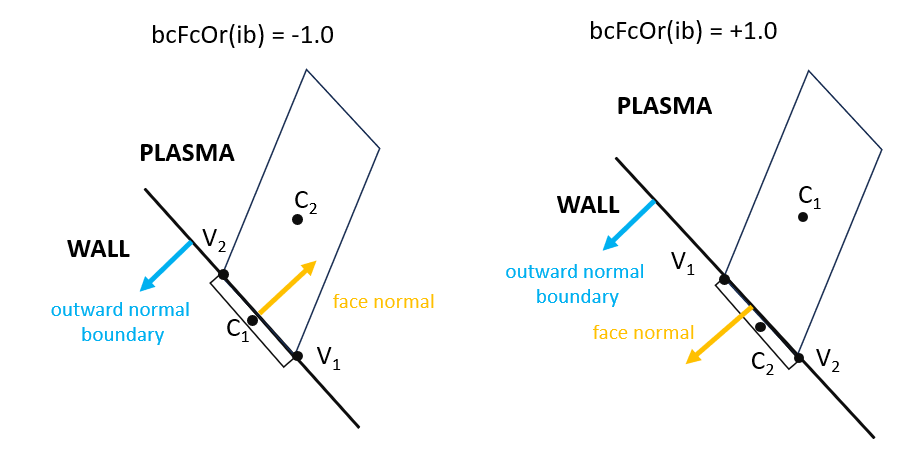
\includegraphics[height=4cm]{FiguresWG/bcfcor.PNG}}
\else
    \centerline{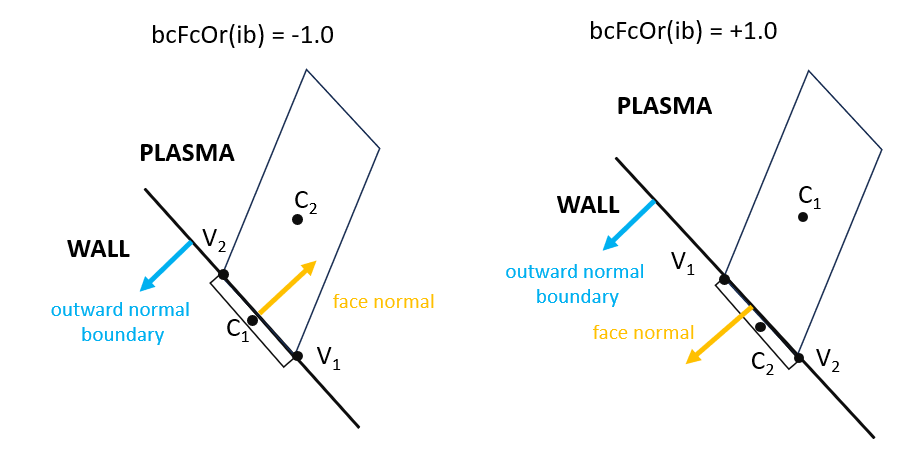
\includegraphics[height=4cm]{FiguresWG/bcfcor.eps}}
\fi
    \caption{Illustration of {\tt bcFcOr}.}
    \label{fig:bcfcor}
\end{figure}

Most boundary conditions fall in one of three categories: Dirichlet, Neumann, or flux.

\textbf{Flux}

To impose a given flux, the net source term in the guard cell must be equal to that flux. Since no fluxes are computed between the guard cells, the flux across the guard cell face must equal the source term.

\textbf{Dirichlet}
\begin{sloppypar}
To impose a fixed value in a guard cell, the code makes use of the different source contributions and very large numbers. For example, to set a fixed density {\tt $n_{BC}$},
the code sets {\tt sna(iCv,0,is) = VBIG $\times$ fcS $\times$ $n_{BC}$}, and {\tt sna(iCv,1,is) = - VBIG $\times$ fcS}, with {\tt sna(iCv,is) = sna(iCv,0,is) + sna(iCv,1,is) $\times$ na(iCv,is)} and where {\tt VBIG} is a very large number. Because {\tt VBIG} is so large, the only way to get a physical source is to have {\tt na(iCv,is) = $n_{BC}$}.
\end{sloppypar}

\textbf{Neumann}
\begin{sloppypar}
To set the gradient normal to the boundary, the code again makes use of the different source contributions and very large numbers. For orthogonal cells, these boundary conditions correctly impose the gradient normal to the boundary face.
For cells that are skewed with respect to the boundary face, the implementation depends on the (partially experimental) {\tt b2stbc\_BC2\_cor9} switch.
To impose for example a density gradient $\Phi$ with {\tt b2stbc\_BC2\_cor9 = 0.0}, the code sets
{\tt sna(iCv,0,is) = VBIG $\times$ fcS $\times$ ($\Phi$ $\times$ ( fcHc(1) + fcHc(2) ) $\times \cos \gamma$ + na(iCv\_internal)} and {\tt sna(iCv,1,is) = - VBIG $\times$ fcS}, where {\tt na(iCv\_internal)} is the density in the first interior cell. To get a physical source, we must have {\tt $\Phi$ $\times$ ( fcHc(1) + fcHc(2) ) $\times \cos \gamma$ + na(iCv\_internal) = na(iCv)}. This results in the correct normal gradient for skewed cells, only if there would be no gradients in the direction tangential to the boundary face. When {\tt b2stbc\_BC2\_cor9 = 1.0}, a correction term based on the vertex values is added, such that $\Phi$ is the gradient normal to the boundary, also in the presence of tangential gradients (up to the interpolation error).
\end{sloppypar}

%% TODO: convert all below to unstructured?

In this Section, the boundaries are denoted as $S_0$ for the PFR boundaries, $S_1$ for the core boundaries, $E$ for the Eastern boundaries (right targets), $W$ for the Western boundaries (left targets), and $N$ for the outer main wall boundary.

\subsection{Particle balance equations}

$S_{n_a} = S_{n_a,0} + S_{n_a,1} n_a$

\subsubsection{South. Private region}

\underline{If $z_a = 0$}

{\em For leakage boundary condition:} {\tt BCCON = 10}

\begin{equation}
\left. \frac{\sqrt g}{h_y}\Gamma_{ay} \right|_{S_0}
=
\left. \left[
p_{n_a,a,1} \frac{\sqrt g}{h_y} \sqrt{\frac{z_a T_e + T_i}{m_a}} n_a
+
\sum \limits_{a=0}^{ns-1} r_{rec,a,0} c_{nsr}
\max \left\{0, -\frac{\sqrt g}{h_y} \Gamma_{ay} \right\}
\right] \right|_{S_0}
\end{equation}

$p_{n_a,a,1} = -10^{-2}, \;\; r_{rec,0,0} = 0,\;\; r_{rec,1,0} = 1$

$\widetilde{\Gamma}_{ay}$ was replaced by $\Gamma_{ay}$

$c_{nsr}$ --- neutral sources rescale coefficient, $1$ --- when working with B2.5 standalone and $10^{-10}$ when coupling to Eirene

$p_{n_a,a,1}$ is the radial leakage velocity, in units of the local species sound speed. Negative velocities are directed out of the plasma.

\underline{If $z_a \neq 0$}

{\em For decay length boundary condition:} {\tt BCCON = 9}

\begin{equation}
\begin{matrix}
\left. \frac{\sqrt g}{h_y} \widetilde{\Gamma}_{ay} \right|_{S_0}& =
& \left\{
\begin{matrix}
\left. \left[
        -\frac{1}{p_{n_a,a,1}} \frac{\sqrt g}{h_y}  \left(
                D^{(AN)}_{n,a} + D^{(AN)}_{p,a} \left(z_a T_e + T_i \right)
        \right) n_a
\right] \right|_{S_0}, & \text{mdf\_fnb} = 0
\\
\left. \left[
\begin{matrix}
        -\frac{1}{p_{n_a,a,1}} \frac{\sqrt g}{h_y} & \left(
                D^{(AN)}_{n,a} + D^{(AN)}_{p,a} \left(z_a T_e + T_i \right)
        \right) n_a
        + \\
        \frac{\sqrt g}{h_y} & D_{ayx} \frac{1}{h_x} \frac{\partial n_a T_i}{\partial x}
        +
        \frac{\sqrt g}{h_y} V_{ay}^{(E)} n_a
\end{matrix}
\right] \right|_{S_0}, & \text{mdf\_fnb} = 1
\end{matrix} \right.
\end{matrix}
\end{equation}

\begin{align}
S^{no\_mdf}_{n_a,0} & = 0 \\
S^{no\_mdf}_{n_a,1} & = - \frac{1}{p_{n_a,a,1}} \frac{\sqrt{g}}{h_y} \left( D^{(AN)}_{n,a} + D^{(AN)}_{p,a} \left( z_a T_e + T_i \right) \right)
\end{align}

$p_{n_a,a,1}$ is the density radial decay length of species $a$, in $m$.

{\em For leakage boundary conditions:} {\tt BCCON = 10}

\begin{equation}
\begin{matrix}
\left. \frac{\sqrt g}{h_y} \widetilde{\Gamma}_{ay} \right|_{S_0}& =
& \left\{
\begin{matrix}
\left. \left[
        p_{n_a,a,1} \frac{\sqrt g}{h_y} \sqrt{\frac{z_a T_e + T_i}{m_a}} n_a
        +
        \min \left\{0, \frac{\sqrt g}{h_y} n_a V_{ay}^{(E)} \right\}
\right] \right|_{S_0}, & \text{mdf\_fnb} = 0
\\
\left. \left[
p_{n_a,a,1} \frac{\sqrt g}{h_y} \sqrt{\frac{z_a T_e + T_i}{m_a}} n_a
        +
        \frac{\sqrt g}{h_y} D_{ayx} \frac{1}{h_x} \frac{\partial n_a T_i}{\partial x}
        +
        \min \left\{0, \frac{\sqrt g}{h_y} n_a V_{ay}^{(E)} \right\}
\right] \right|_{S_0}, & \text{mdf\_fnb} = 1
\end{matrix} \right.
\end{matrix}
\end{equation}

$p_{n_a,a,1} = -10^{-3}$ is the radial leakage velocity, in units of the species local sound speed. Negative velocities are directed out of the plasma.

\begin{align}
S^{no\_mdf}_{n_a,0} & = 0 \\
S^{no\_mdf}_{n_a,1} & = {p_{n_a,a,1}} \frac{\sqrt{g}}{h_y} \sqrt{\frac{z_a T_e + T_i}{m_a}} n_a
\end{align}

% -- To be checked --
{\em Imposing radial leakage:} {\tt BCCON = 15}

When using drifts, one should use {\tt BCCON = 10} instead.

\begin{equation}
\left. - \frac{\sqrt g}{h_y^2} D_{n,ay} \frac{\partial n_a}{\partial y} \right|_{S_0}
=
\left. \left[
c_{n_a,a,2} \frac{\sqrt g}{h_y} \sqrt{\frac{z_a T_e + T_i}{m_a}} n_a
\right] \right|_{S_0}
\end{equation}

$c_{n_a,a,2} = -10^{-3}$ is the radial leakage velocity, in units of the species local thermal velocity. Negative velocities are directed out of the plasma.

% -- end --

\subsubsection{South 1. Core plasma}

\underline{If $z_a = 0$}

%-------- end of 21st page -------------

{\em Imposing total particle flux:} {\tt BCCON = 8}

$\left. \frac{\sqrt g}{h_y} \widetilde{\Gamma}_{ay} \right|_{S_1} = 0$

$\left. \frac{\sqrt g}{h_y} \Gamma_{ay} \right|_{S_1} = 0$

\underline{If $z_a \neq 0$}

{\em Imposing a constant density :} {\tt BCCON = 1}

\begin{equation}
\left. \frac{\sqrt g}{h_y} \widetilde{\Gamma}_{ay} \right|_{S_1}
=
\frac{\sqrt{g}}{h_y}
\left. \left(
        \left. v_{big} n_a \right|_{S_1} - v_{big} n_a
\right) \right|_{S_1},
\;\;
v_{big} = 10^8 \sqrt{\frac{100 \text{eV}}{m_p}},
\;\;
\left. n_a \right|_{S_1} \text{ is the desired density in } m^{-3}
\end{equation}

{\em Imposing the total particle flux with constant flux density:} {\tt BCCON = 8}

\begin{equation*}
\left. \frac{\sqrt g}{h_y} \widetilde{\Gamma}_{ay} \right|_{S_1} =
\left. p_{n,a,0} \frac{
\frac{\sqrt g}{h_y}
} {
\sum \limits_i \left(
        \frac{\sqrt g}{h_y}
\right)_{i, -1}
} \right|_{S_1}
+
\left.
\frac{\sqrt g}{h_y} D_{ayx} \frac{1}{h_x} \frac{\partial n_a T_i}{\partial x}
\right|_{S_1} +
\left. \frac{\sqrt g}{h_y}V_{ya}^{(E)} n_a \right|_{S_1}
\end{equation*}

$p_{n,a,0}$ is the desired total particle flux, per unit time.

\subsubsection{North}

\underline{If $z_a = 0$}

{\em For leakage boundary condition:} {\tt BCCON = 10}

\begin{equation}
\left. - \frac{\sqrt g}{h_y} \Gamma_{ay} \right|_{N}
=
\left. \left[
p_{n_a,a,1} \frac{\sqrt g}{h_y} \sqrt{\frac{z_a T_e + T_i}{m_a}} n_a
+
\sum \limits_{a=0}^{ns-1} r_{rec,a,0} c_{nsr}
\max \left\{0, \frac{\sqrt g}{h_y} \Gamma_{ay} \right\}
\right] \right|_{N}
\end{equation}

$p_{n_a,a,1} = -10^{-2}, \;\; r_{rec,0,0} = 0,\;\; r_{rec,1,0} = 1$

$c_{nsr}$ --- neutral sources rescale coefficient, $1$ --- when working with B2.5 standalone and $10^{-10}$ when coupling to Eirene

$p_{n_a,a,1}$ is the radial leakage velocity, in units of the local species sound speed. Negative velocities are directed out of the plasma.

$\widetilde{\Gamma}_{ay}$ was replaced by $\Gamma_{ay}$

\underline{If $z_a \neq 0$}

{\em For decay length boundary condition:} {\tt BCCON = 9}

\begin{equation}
\begin{matrix}
\left. - \frac{\sqrt g}{h_y} \widetilde{\Gamma}_{ay} \right|_{N}& =
& \left\{
\begin{matrix}
\left. \left[
        \frac{1}{p_{n_a,a,1}} \frac{\sqrt g}{h_y}  \left(
                D^{(AN)}_{n,a} + D^{(AN)}_{p,a} \left(z_a T_e + T_i \right)
        \right) n_a
\right] \right|_{N}, & \text{mdf\_fnb} = 0
\\
\left. \left[
\begin{matrix}
        \frac{1}{p_{n_a,a,1}} & \frac{\sqrt g}{h_y}  \left(
                D^{(AN)}_{n,a} + D^{(AN)}_{p,a} \left(z_a T_e + T_i \right)
        \right) n_a \\
        -
        \frac{\sqrt g}{h_y} & D_{ayx} \frac{1}{h_x} \frac{\partial n_a T_i}{\partial x}
        -
        \frac{\sqrt g}{h_y} V_{ay}^{(E)} n_a
\end{matrix}
\right] \right|_{N}, & \text{mdf\_fnb} = 1
\end{matrix} \right.
\end{matrix}
\end{equation}

\begin{align}
S^{no\_mdf}_{n_a,0} & = 0 \\
S^{no\_mdf}_{n_a,1} & = \frac{1}{p_{n_a,a,1}} \frac{\sqrt{g}}{h_y} \left( D^{(AN)}_{n,a} + D^{(AN)}_{p,a} \left( z_a T_e + T_i \right) \right)
\end{align}

$p_{n_a,a,1}$ is the density radial decay length of species $a$, in $m$.

{\em For leakage boundary conditions:} {\tt BCCON = 10}

\begin{equation}
\begin{matrix}
\left. - \frac{\sqrt g}{h_y} \widetilde{\Gamma}_{ay} \right|_{N}& =
& \left\{
\begin{matrix}
\left. \left[
        p_{n_a,a,1} \frac{\sqrt g}{h_y} \sqrt{\frac{z_a T_e + T_i}{m_a}} n_a
        -
        \max \left\{0, \frac{\sqrt g}{h_y} n_a V_{ay}^{(E)} \right\}
\right] \right|_{N}, & \text{mdf\_fnb} = 0
\\
\left. \left[
        p_{n_a,a,1} \frac{\sqrt g}{h_y} \sqrt{\frac{z_a T_e + T_i}{m_a}} n_a
        -
        \frac{\sqrt g}{h_y} D_{ayx} \frac{1}{h_x} \frac{\partial n_a T_i}{\partial x}
        -
        \max \left\{0, \frac{\sqrt g}{h_y} n_a V_{ay}^{(E)} \right\}
\right] \right|_{N}, & \text{mdf\_fnb} = 1
\end{matrix} \right.
\end{matrix}
\end{equation}

$p_{n_a,a,1} = -10^{-3}$ is the radial leakage velocity, in units of the species local sound speed. Negative velocities are directed out of the plasma.

\begin{align}
S^{no\_mdf}_{n_a,0} & = 0 \\
S^{no\_mdf}_{n_a,1} & = {p_{n_a,a,1}} \frac{\sqrt{g}}{h_y} \sqrt{\frac{z_a T_e + T_i}{m_a}} n_a
\end{align}

% -- To be checked --
{\em Imposing radial leakage:} {\tt BCCON = 15}

When using drifts, one should use {\tt BCCON = 10} instead.

\begin{equation}
\left. \frac{\sqrt g}{h_y^2} D_{n,ay} \frac{\partial n_a}{\partial y} \right|_N
=
\left. \left[
c_{n_a,a,2} \frac{\sqrt g}{h_y} \sqrt{\frac{z_a T_e + T_i}{m_a}} n_a
\right] \right|_N
\end{equation}

$c_{n_a,a,2} = -10^{-3}$ is the radial leakage velocity, in units of the species local thermal velocity. Negative velocities are directed out of the plasma.

% -- end --

\subsubsection{North with puffing}

\underline{If $z_a = 0$}

{\em Imposing a particle flux per unit area:} {\tt BCCON = 5}

\begin{equation}
\left. - \frac{\sqrt g}{h_y} \widetilde{\Gamma}_{ay} \right|_N
=
\left. p_{n,a,0} \frac{\sqrt g}{h_y} \right|_N
+
\left.
\sum \limits_{a=0}^{ns-1} \left[
        r_{rec,a,0} c_{nsr}
        \max \left\{0, -\frac{\sqrt g}{h_y} \Gamma_{ay} \right\}
\right] \right|_N
\end{equation}

$c_{nsr}$ --- neutral sources rescale coefficient, $1$ --- when working with B2.5 standalone and $10^{-10}$ when coupling to Eirene

$r_{rec,0,0} = 0,\;\; r_{rec,1,0} = 1$

$p_{n,a,0}$ is the desired total particle flux density, in $m^{-2}.s^{-1}$.

$\widetilde{\Gamma}_{ay}$ was replaced by $\Gamma_{ay}$

or

{\em Imposing a total particle flux with constant flux density:} {\tt BCCON = 8}

\begin{equation*}
\left. - \frac{\sqrt g}{h_y} \widetilde{\Gamma}_{ay} \right|_N =
\left. \frac{ p_{n,a,0}
}{
\sum \limits_{i=0}^{Nx-1} \left(
        \frac{\sqrt g}{h_y}
\right)_{i, Ny}
}
\frac{\sqrt g}{h_y} \right|_N
+
\left. \sum \limits_{a=0}^{ns-1} \left[
        r_{rec,a,0} c_{nsr}
        \max \left\{0, \frac{\sqrt g}{h_y} \Gamma_{ay} \right\}
\right]
\right|_N
\end{equation*}

$c_{nsr}$ --- neutral sources rescale coefficient, $1$ --- when working with B2.5 standalone and $10^{-10}$ when coupling to Eirene

$r_{rec,0,0} = 0,\;\; r_{rec,1,0} = 1$

$p_{n,a,0}$ is the desired total particle flux, per unit time.

$\widetilde{\Gamma}_{ay}$ was replaced by $\Gamma_{ay}$

\subsubsection{West}

%-------- end of 23rd page -------------

\underline{If $z_a = 0$}

{\em Imposing a given particle flux per unit area:} {\tt BCCON = 5}

\begin{equation}
\left. \frac{\sqrt g}{h_x} \Gamma_{ax} \right|_W
=
\left. \left[
p_{n,a,1} \frac{\sqrt g}{h_y}
+
c_{nsr} \sum \limits_{a=0}^{ns-1} r_{rec,a,0}
\max \left\{0, -\frac{\sqrt g}{h_x} \Gamma_{ax} \right\}
\right] \right|_W
\end{equation}

$r_{rec,0,0} = 0,\;\; r_{rec,1,0} = 1,\;\; p_{n_a,a,1} = 0 $

\begin{equation}
\left. \frac{\sqrt g}{h_x} \widetilde{\Gamma}_{ax} \right|_W
=
\left. \left[
p_{n,a,1} \frac{\sqrt g}{h_x}
+
c_{nsr} \sum \limits_{a=0}^{ns-1} r_{rec,a,0}
\max \left\{0, -\frac{\sqrt g}{h_x} \Gamma_{ax} \right\}
\right] \right|_W
\end{equation}

$\widetilde{\Gamma}_{ax}$ was replaced by $\Gamma_{ax}$

$r_{rec,0,0} = 0,\;\; r_{rec,1,0} = 1,\;\; p_{n_a,a,1} = 0 $

\underline{If $z_a \neq 0$}

{\em Sheath density boundary condition:} {\tt BCCON = 3}

\begin{equation*}
\left. \frac{\sqrt g}{h_x} \Gamma_{ax} \right|_W = \left.
10^{20} \frac{\sqrt{g}}{h_x} \frac{\partial n_a}{\partial x}
\right|_W
\end{equation*}

{\em Drift-compatible, Bohm-Chodura sheath entrance condition} {\tt BCCON = 14}

{\em If the sine of the incident field line angle is larger than {\tt Qalfmin}:}

{\em - Marginal imposition, with collective sound speed:} {\tt MOMPAR(,,2)} = $p_{m,a,2} < 0.5$

To be used in conjunction with {\tt BCENE = 15}, {\tt BCENI = 15}, {\tt BCMOM = 13}, and {\tt BCPOT = 11}.

\begin{equation*}
\left. \frac{\sqrt g}{h_x} \widetilde{\Gamma}_{ax} \right|_W
=
\left. \left[
- p_{n,a,1} \frac{\sqrt g}{h_x} |b_x|
\sqrt{\frac{\sum \limits_{\substack{b = 0 \\ z_b \neq 0}}^{ns-1} p_b}{\sum \limits_{\substack{b = 0 \\ z_b \neq 0}}^{ns-1} m_b n_b}} n_a
-
\frac{\sqrt g}{h_x} D_{axy} \frac{1}{h_y} \frac{\partial n_a T_i}{\partial y}
\right]
\right|_W
\end{equation*}

$p_{n,a,1} = +1$

{\em - Non-marginal imposition, with individual species sound speed:} {\tt MOMPAR(,,2)} = $p_{m,a,2} \geq 0.5$

to be used in conjunction with {\tt BCMOM = 13}, {\tt BCENE = 15} with {\tt bcene\_15\_style = 1}, {\tt BCENI = 15}, {\tt BCPOT = 3} or {\tt BCPOT = 11} with {\tt istyle\_fchi=0}.

This condition imposes that the sum of the poloidal projection of the parallel velocity and the poloidal $\exb$ velocity (restricted to not exceed $\pm 2 c_{s,a} |b_x|$), equals \textit{at least} the specific species sound speed $c_{s,a}$, reprojected in the the poloidal direction.

The parameter $p_{m,a,1}$ is set by {\tt MOMPAR(,,1)}. The parameter $\chi$ is set by {\tt GAMMAI}.

\begin{equation*}
\left. \frac{\sqrt g}{h_x} \widetilde{\Gamma}_{ax} \right|_W
=
\left. \left[
- \frac{\sqrt g}{h_x} |b_x|
U_{out} n_a
-
\frac{\sqrt g}{h_x} D_{axy} \frac{1}{h_y} \frac{\partial n_a T_i}{\partial y}
\right]
\right|_W
\end{equation*}

\begin{equation*}
  U_{out} = \max \left( -u_{\parallel,a}^{extrap}- \frac{V_{\exb}^{restr}}{|b_x|}, p_{m,a,1} \cdot \sqrt{\frac{\chi T_i + z_a T_e}{m_a}} \right)
\end{equation*}

where $u_{\parallel,a}^{extrap}$ is the extrapolated parallel velocity at the target, and $V_{\exb}^{restr}$ is the poloidal $\exb$ velocity restricted to not exceed $\pm 2 c_{s,a} |b_x|$.

{\em For nearly tangent field lines, we use instead:}

\begin{equation}
\begin{matrix}
\left. - \frac{\sqrt g}{h_x} \widetilde{\Gamma}_{ax} \right|_W & =
& \left\{
\begin{matrix}
\left. \left[ \frac{\sqrt g}{h_x} p_{n,a,1} \sqrt{\frac{\sum \limits_{\substack{b = 0 \\ z_b \neq 0}}^{ns-1} p_b}{\sum \limits_{\substack{b = 0 \\ z_b \neq 0}}^{ns-1} m_b n_b}} n_a \alpha_{\max} +
   \max \left( 0, \frac{\sqrt g}{h_x} V^{(E)}_{ax} n_a \right) \right] \right|_W, & \text{mdf\_fnb = 0}
\\
\left. \left[ \frac{\sqrt g}{h_x} p_{n,a,1} \sqrt{\frac{\sum \limits_{\substack{b = 0 \\ z_b \neq 0}}^{ns-1} p_b}{\sum \limits_{\substack{b = 0 \\ z_b \neq 0}}^{ns-1} m_b n_b}} n_a \alpha_{\max} +
   \max \left( 0, \frac{\sqrt g}{h_x} \left( V^{(E)}_{ax} + \widetilde{\widetilde{V}}^{(dia)}_{ax} \right) n_a \right) + \tilde\Gamma^{(PSch)}_{ax} \right] \right|_W, & \text{mdf\_fnb = 1}
\end{matrix}
\right.
\end{matrix}
\end{equation}

where $\alpha_{\max}$ is given by {\tt Qalfmax}.

Both {\tt Qalfmin} and {\tt Qalfmax} are provided in the {\tt b2fgmtry} file or through the {\tt b2us\_prep\_Qalfmin} and {\tt b2us\_prep\_Qalfmax} switches, respectively. Default value for both is $10^{-3}$.

\subsubsection{East}

\underline{If $z_a = 0$}

{\em Imposing a given particle flux per unit area:} {\tt BCCON = 5}

\begin{equation}
\left. - \frac{\sqrt g}{h_x} \Gamma_{ax} \right|_E
=
\left. \left[
p_{n,a,1} \frac{\sqrt g}{h_y}
+
c_{nsr} \sum \limits_{a=0}^{ns-1} r_{rec,a,0}
\max \left\{0, \frac{\sqrt g}{h_x} \Gamma_{ax} \right\}
\right] \right|_E
\end{equation}

$r_{rec,0,0} = 0,\;\; r_{rec,1,0} = 1,\;\; p_{n_a,a,1} = 0 $

%-------- end of 24th page -------------


\begin{equation}
\left. - \frac{\sqrt g}{h_x} \widetilde{\Gamma}_{ax} \right|_E
=
\left. \left[
c_{nsr} \sum \limits_{a=0}^{ns-1} r_{rec,a,0}
\max \left\{0, \frac{\sqrt g}{h_x} \Gamma_{ax} \right\}
\right] \right|_E
\end{equation}

$\widetilde{\Gamma}_{ax}$ was replaced by $\Gamma_{ax}$

$r_{rec,0,0} = 0,\;\; r_{rec,1,0} = 1$

\underline{If $z_a \neq 0$}

{\em Sheath density boundary condition:} {\tt BCCON = 3}

\begin{equation*}
\left. - \frac{\sqrt g}{h_x} \Gamma_{ax} \right|_E =
- 10^{20} \left. \frac{\sqrt{g}}{h_x} \frac{\partial n_a}{\partial x}
\right|_E
\end{equation*}

{\em Drift-compatible, Bohm-Chodura sheath entrance condition} {\tt BCCON = 14}

{\em If the sine of the incident field line angle is larger} {\tt Qalfmin}:

{\em - Marginal imposition, with collective sound speed:} {\tt MOMPAR(,,2)} = $p_{m,a,2} < 0.5$

To be used in conjunction with {\tt BCENE = 15}, {\tt BCENI = 15}, {\tt BCMOM = 13}, and {\tt BCPOT = 11}.

\begin{equation*}
\left. - \frac{\sqrt g}{h_x} \widetilde{\Gamma}_{ax} \right|_E
=
\left. \left[
- p_{n,a,1} \frac{\sqrt g}{h_x} |b_x|
\sqrt{\frac{\sum \limits_{\substack{b = 0 \\ z_b \neq 0}}^{ns-1} p_b}{\sum \limits_{\substack{b = 0 \\ z_b \neq 0}}^{ns-1} m_b n_b}} n_a
+
\frac{\sqrt g}{h_x} D_{axy} \frac{1}{h_y} \frac{\partial n_a T_i}{\partial y}
\right]
\right|_E
\end{equation*}

$p_{n,a,1} = +1$

{\em - Non-marginal imposition, with individual species sound speed:} {\tt MOMPAR(,,2)} = $p_{m,a,2} \geq 0.5$

to be used in conjunction with {\tt BCMOM = 13}, {\tt BCENE = 15} with {\tt bcene\_15\_style = 1}, {\tt BCENI = 15}, {\tt BCPOT = 3} or {\tt BCPOT = 11} with {\tt istyle\_fchi=0}.

This condition imposes that the sum of the poloidal projection of the parallel velocity and the poloidal $\exb$ velocity (restricted to not exceed $\pm 2 c_{s,a} |b_x|$), equals \textit{at least} the specific species sound speed $c_{s,a}$, reprojected in the the poloidal direction.

The parameter $p_{m,a,1}$ is set by {\tt MOMPAR(,,1)}. The parameter $\chi$ is set by {\tt GAMMAI}.

\begin{equation*}
\left. - \frac{\sqrt g}{h_x} \widetilde{\Gamma}_{ax} \right|_E
=
\left. \left[
- \frac{\sqrt g}{h_x} |b_x|
U_{out} n_a
+
\frac{\sqrt g}{h_x} D_{axy} \frac{1}{h_y} \frac{\partial n_a T_i}{\partial y}
\right]
\right|_E
\end{equation*}

\begin{equation*}
  U_{out} = \max \left( u_{\parallel,a}^{extrap} + \frac{V_{\exb}^{restr}}{|b_x|}, p_{m,a,1} \cdot \sqrt{\frac{\chi T_i + z_a T_e}{m_a}} \right)
\end{equation*}

where $u_{\parallel,a}^{extrap}$ is the extrapolated parallel velocity at the target, and $V_{\exb}^{restr}$ is the poloidal $\exb$ velocity restricted to not exceed $\pm 2 c_{s,a} |b_x|$.

{\em For nearly tangent field lines, we use instead:}

\begin{equation}
\begin{matrix}
\left. \frac{\sqrt g}{h_x} \widetilde{\Gamma}_{ax} \right|_E & =
& \left\{
\begin{matrix}
\left. \left[ \frac{\sqrt g}{h_x} p_{n,a,1} \sqrt{\frac{\sum \limits_{\substack{b = 0 \\ z_b \neq 0}}^{ns-1} p_b}{\sum \limits_{\substack{b = 0 \\ z_b \neq 0}}^{ns-1} m_b n_b}} n_a \alpha_{\max} +
   \max \left( 0, \frac{\sqrt g}{h_x} V^{(E)}_{ax} n_a \right) \right] \right|_E, & \text{mdf\_fnb = 0}
\\
\left. \left[ \frac{\sqrt g}{h_x} p_{n,a,1} \sqrt{\frac{\sum \limits_{\substack{b = 0 \\ z_b \neq 0}}^{ns-1} p_b}{\sum \limits_{\substack{b = 0 \\ z_b \neq 0}}^{ns-1} m_b n_b}} n_a \alpha_{\max} +
   \max \left( 0, \frac{\sqrt g}{h_x} \left( V^{(E)}_{ax} + \widetilde{\widetilde{V}}^{(dia)}_{ax} \right) n_a \right) + \tilde\Gamma^{(PSch)}_{ax} \right] \right|_E, & \text{mdf\_fnb = 1}
\end{matrix}
\right.
\end{matrix}
\end{equation}

\subsection{Parallel momentum balance for ions}

$S_{m_a} = S_{m_a,0} + S_{m_a,1} V_{\parallel a} + S_{m_a,2} m_a n_a + S_{m_a,3} m_a n_a V_{\parallel a}$

\subsubsection{South. Private region}

\underline{If $z_a = 0$}

{\em Weakly imposing a velocity:} {\tt BCMOM = 4}

\begin{equation*}
\left. h_z \frac{\sqrt g}{h_y} \Gamma_{ay}^m \right|_{S_0} =
\left. \left[
p_{m,a,1} p_{m,a,2} h_z \frac{\sqrt g}{h_y} -
p_{m,a,2} h_z \frac{\sqrt g}{h_y} V_{\parallel a}
\right] \right|_{S_0}
\end{equation*}

$p_{m,a,1}=0$ is the imposed velocity, in $m.s^{-1}$, and $p_{m,a,2}=10^5$ is the strength with which this velocity is imposed.

We had this b.c.

$\left. h_z \frac{\sqrt g}{h_y} \Gamma_{ay}^m \right|_{S_0} =
\left. \left[
c_{m,a,3} h_z \frac{\sqrt g}{h_y} m_a n_a V_{\parallel a} +
c_{m,a,6} \max \left(0,-h_z \frac{\sqrt g}{h_y} \frac{\Gamma_{ay}^{Cor}}{n_a} \right)
m_a n_a V_{\parallel a}
\right] \right|_{S_0}$, delete term with {\tt max} !

%-------- end of 25th page -------------

$\Gamma_{ay}^{Cor} = \Gamma_{ay} + \Gamma_{ay}^{(dia)}$

$c_{m,a,3} = -10^{10}$, we have $c_{m,a,6}=-1$, but not $c_{m,a,6}=0$

Inserted into {\tt b2stbc\_phys} for {\tt BCMOM=12} as $c_{m,a,3} \rightarrow p_{m,a,2} = -10^{10}$, and $c_{m,a,6} \rightarrow p_{m,a,1} = -1$

\underline{If $z_a \neq 0$}

{\em Weakly imposing a velocity:} {\tt BCMOM = 4}

\begin{equation}
\left. h_z \frac{\sqrt g}{h_y} \Gamma_{ay}^m \right|_{S_0} =
\left. \left[
        p_{m,a,1} p_{m,a,2} h_z \frac{\sqrt g}{h_y} -
        p_{m,a,2} h_z \frac{\sqrt g}{h_y} V_{\parallel a}
\right] \right|_{S_0}
\end{equation}

$p_{m,a,1}=0$ is the imposed velocity, in $m.s^{-1}$, and $p_{m,a,2}=10^5$ is the strength with which this velocity is imposed.

\begin{equation}
\left. h_z \frac{\sqrt g}{h_y} \Gamma_{ay}^m \right|_{S_0} =
\left. \left[
        c_{m,a,3} h_z \frac{\sqrt g}{h_y} m_a n_a V_{\parallel a} +
        c_{m,a,6} \max \left(
                0, -h_z \frac{\sqrt g}{h_y} \frac{\Gamma_{ay}^{Cor}}{n_a}
        \right) m_a n_a V_{\parallel a}
\right] \right|_{S_0}
\end{equation}

delete term with {\tt max}!

$\Gamma_{ay}^{Cor} = \Gamma_{ay} + \Gamma_{ay}^{(dia)}$

$c_{m,a,3} = 0$,  $c_{m,a,6} = -1$

\subsubsection{South 1. Core}

\underline{If $z_a = 0$}

{\em Weakly imposing a velocity:} {\tt BCMOM = 4}

$ \left. h_z \frac{\sqrt g}{h_y} \Gamma_{ay}^m \right|_{S_1} = \left. \left[
        p_{m,a,1} p_{m,a,2} h_z \frac{\sqrt g}{h_y} -
        p_{m,a,2} h_z \frac{\sqrt g}{h_y} V_{\parallel a}
\right] \right|_{S_1}$

$p_{m,a,1}=0$ is the imposed velocity, in $m.s^{-1}$, and $p_{m,a,2}=10^5$ is the strength with which this velocity is imposed.

$ \left. h_z \frac{\sqrt g}{h_y} \Gamma_{ay}^m \right|_{S_1} = c_{m,a,3} h_z \left. \frac{\sqrt g}{h_y} m_a n_a V_{\parallel a} \right|_{S_1}$

$c_{m,a,3} = -10^{10}$

Inserted into {\tt b2stbc\_phys} for {\tt BCMOM=12} as $c_{m,a,3} \rightarrow p_{m,a,2} = -10^{10},\;c_{m,a,6} \rightarrow
p_{m,a,1} = 0$

\underline{If $z_a \neq 0$}

%-------- end of 26th page -------------

{\em Weakly imposing a velocity:} {\tt BCMOM = 4}

$ \left. h_z \frac{\sqrt g}{h_y} \Gamma_{ay}^m \right|_{S_1} = \left. \left[
        p_{m,a,1} p_{m,a,2} h_z \frac{\sqrt g}{h_y} -
        p_{m,a,2} \frac{\sqrt g}{h_y} V_{\parallel a}
\right] \right|_{S_1}$

$p_{m,a,1}=0$ is the imposed velocity, in $m.s^{-1}$, and $p_{m,a,2}=10^5$ is the strength with which this velocity is imposed.

{\em {\tt b2stbc\_spb} style:} {\tt BCMOM = 14}

\begin{align*}
\left. h_z \frac{\sqrt g}{h_y} \Gamma_{ay}^m \right|_{S_1} = &
c_{m,a,3} h_z \left. \frac{\sqrt g}{h_y} m_a n_a V_{\parallel a} \right|_{S_1} + \\
& \left. \left[
h_z \frac{\sqrt g}{h_y} m_a \left\langle n_a \right\rangle \left( -2 \right)\frac{\left\langle T_i \right\rangle B_z}{ez_a}\frac{\partial}{h_x \partial x} \left( \frac{1}{B^2} \right) \left\langle V_{\parallel a} \right\rangle c_{drift} +
c_{corflux} h_z \frac{\sqrt g}{h_y}
\right] \right|_{S_1} \\
+ & \left. c_{m,a,1} \max \left( 0 , - h_z \frac{\sqrt{g}}{h_y} \frac{\Gamma_{ay}^{Cor}}{n_a} \right) m_a n_a V_{\parallel a} \right|_{S_1}
\end{align*}

$c_{m,a,1} = 0$, $c_{m,a,3} = -10^{10}$

{\em Prescribe the value of the parallel velocity as a function of the poloidal coordinate:} {\tt BCMOM = 15}

\begin{equation*}
\left. h_z \frac{\sqrt g}{h_y} \Gamma_{ay}^m \right|_{S_1} =
\left. v_{big} n_{e0} m_{a} h_z \frac{\sqrt g}{h_y} \left[
        \frac{\langle B \rangle}{B} p_{m,a,1} - V_{\parallel a}
\right] \right|_{S_1}
\end{equation*}

where $\langle B \rangle = \frac{\mathlarger{\oint}_{S_1} B \sqrt{g} \, dx}{\mathlarger{\oint}_{S_1} \sqrt{g} \, dx}$, the integration is done over the innermost magnetic surface, $v_{big} = 10^{8} \sqrt{\frac{100 \text{eV}}{m_p}}$, $n_{e0} = 10^{20}$, $p_{m,a,1}$ is the given value of the average parallel velocity, in $m.s^{-1}$.

\subsubsection{North}

\underline{If $z_a=0$}

{\em Weakly imposing a velocity:} {\tt BCMOM = 4}

$ \left. -h_z \frac{\sqrt g}{h_y} \Gamma_{ay}^m \right|_N = \left. \left[
        p_{m,a,1} p_{m,a,2} h_z \frac{\sqrt g}{h_y} -
        p_{m,a,2} h_z \frac{\sqrt g}{h_y} V_{\parallel a}\right]
\right|_N$

$p_{m,a,1}=0$ is the imposed velocity, in $m.s^{-1}$, and $p_{m,a,2}=10^5$ is the strength with which this velocity is imposed.

$\left. -h_z \frac{\sqrt g}{h_y} \Gamma_{ay}^m \right|_N = \left. \left[
        c_{m,a,3} h_z \frac{\sqrt g}{h_y} m_a n_a V_{\parallel a} +
        c_{m,a,6} \max \left(
                0, h_z \frac{\sqrt g}{h_y} \frac{\Gamma_{ay}^{Cor}}{n_a}
        \right) m_a n_a V_{\parallel a}
\right]
\right|_N$

delete term with {\tt max} !

$c_{m,a,3} = -10^{10}$, we have  $c_{m,a,6} = -1$, but not $c_{m,a,6} = 0$

Inserted into {\tt b2stbc\_phys} for {\tt BCMOM=12} as $c_{m,a,3} \rightarrow p_{m,a,2} = -10^{10},\;c_{m,a,6} \rightarrow p_{m,a,1} = -1$

\underline{If $z_a \neq 0$}

%-------- end of 27th page -------------

{\em Weakly imposing a velocity:} {\tt BCMOM = 4}

$ \left. -h_z \frac{\sqrt g}{h_y} \Gamma_{ay}^m \right|_N = \left[
        p_{m,a,1} p_{m,a,2} h_z \frac{\sqrt g}{h_y} -
        p_{m,a,2} h_z \frac{\sqrt g}{h_y} V_{\parallel a}
\right]|_N$

$p_{m,a,1}=0$ is the imposed velocity, in $m.s^{-1}$, and $p_{m,a,2}=10^5$ is the strength with which this velocity is imposed.

\begin{equation*}
\left. -h_z \frac{\sqrt g}{h_y} \Gamma_{ay}^m \right|_N =
\left. \left[
c_{m,a,3} h_z \frac{\sqrt g}{h_y} m_a n_a V_{\parallel a} +
c_{m,a,6} \max \left(
        0, h_z \frac{\sqrt g}{h_y} \frac{\Gamma_{ay}^{Cor}}{n_a}
\right) m_a n_a V_{\parallel a}
\right] \right|_N
\end{equation*}

$c_{m,a,3} = 0$, $c_{m,a,6} = -1$

\subsubsection{West}

\underline{If $z_a = 0$}, $p_{m,a,1} = 0$

\underline{If $z_a \neq 0$}, $p_{m,a,1} = 1$

{\em Drift-compatible, Bohm-Chodura sheath entrance condition} {\tt BCMOM = 13}

{\em If the sine of the incident field line angle is larger than} {\tt Qalfmin}:

{\em - Marginal imposition, with collective sound speed:} {\tt MOMPAR(,,2)} = $p_{m,a,2} < 0.5$

To be used in conjunction with {\tt BCENE = 15}, {\tt BCENI = 15}, {\tt BCCON = 14}, and {\tt BCPOT = 11}.

\begin{equation*}
\left. h_z \frac{\sqrt g}{h_x} \Gamma_{ax}^m \right|_W = \left. \left[
        p_{m,a,1} \frac{u_{big}}{\epsilon^2} V_{West} m_a n_a -
        \frac{u_{big}}{\epsilon^2} h_z \frac{\sqrt g}{h_x} |b_x| m_a n_a V_{\parallel a}
\right]
\right|_W
\end{equation*}

with $u_{big} = 10^{10} \sqrt{\frac{100 \text{eV}}{m_p}}$ and $\epsilon = 10^{-10}$.

\begin{equation*}
V_{West} =
- h_z \frac{\sqrt g}{h_x} \frac{|b_x|}{b_x} \min \left( 2 c_s, V_{ax}^{(\exb)} \right)
- h_z \frac{\sqrt g}{h_x} b_x
\sqrt{\frac{\sum \limits_{\substack{a = 0 \\ z_a \neq 0}}^{ns-1} p_a}
{\sum \limits_{\substack{a = 0 \\ z_a \neq 0}}^{ns-1} m_a n_a}}
\end{equation*}

{\em - Non-marginal imposition, with individual species sound speed:} {\tt MOMPAR(,,2)} = $p_{m,a,2} \geq 0.5$

to be used in conjunction with {\tt BCCON = 14}, {\tt BCENE = 15} with {\tt bcene\_15\_style = 1}, {\tt BCENI = 15}, {\tt BCPOT = 3} or {\tt BCPOT = 11} with {\tt istyle\_fchi = 0}.

This condition imposes that the sum of the poloidal projection of the parallel velocity and the poloidal $\exb$ velocity (restricted to not exceed $\pm 2 c_{s,a} |b_x|$), equals \textit{at least} the specific species sound speed $c_{s,a}$, reprojected in the the poloidal direction.

The parameter $p_{m,a,1}$ is set by {\tt MOMPAR(,,1)}. The parameter $\chi$ is set by {\tt GAMMAI}.

\begin{equation*}
  \left. \frac{\sqrt g}{h_x} \Gamma_{ax}^m \right|_W = \left. \left[
          -\frac{u_{big}}{\epsilon^2} n_a m_a \frac{\sqrt{g}}{h_x} U_{out} \frac{B_x}{|B_x|}
          -\frac{u_{big}}{\epsilon^2} n_a m_a \frac{\sqrt{g}}{h_x} V_{\parallel,a}
  \right]
  \right|_W
  \end{equation*}

\begin{equation*}
  U_{out} = \max \left( -u_{\parallel,a}^{extrap} - \frac{V_{\exb}^{restr}}{|b_x|}, p_{m,a,1} \cdot \sqrt{\frac{\chi T_i + z_a T_e}{m_a}} \right)
\end{equation*}

where $u_{\parallel,a}^{extrap}$ is the extrapolated parallel velocity at the target, and $V_{\exb}^{restr}$ is the poloidal $\exb$ velocity restricted to not exceed $\pm 2 c_{s,a} |b_x|$.

{\em For nearly tangent field lines}, we apply a no radial shear velocity condition.

\underline{If $z_a = 0$}

{\em Imposing a specified parallel velocity:} {\tt BCMOM = 1}

$\left. \frac{\sqrt g}{h_x} \Gamma_{ax}^m \right|_W = \left. \left[
        u_{big} n_{e00} \frac{m_a}{m_p} \frac{\sqrt{g}}{h_x} p_{m,a,1} -
        u_{big} n_{e00} \frac{m_a}{m_p} \frac{\sqrt{g}}{h_x} V_{\parallel a}
\right]
\right|_W$

$p_{m,a,1}=0$ is the imposed velocity in $m.s^{-1}$, $n_{e00} = 10^{20}$.

\underline{If $z_a \neq 0$}

{\em Imposing a sheath velocity boundary condition:} {\tt BCMOM = 3}

\begin{equation*}
\left. \frac{\sqrt g}{h_x} \Gamma_{ax}^m \right|_W = \left. \left[
        -\frac{u_{big}}{\epsilon^2} n_a m_a \frac{\sqrt{g}}{h_x} u_{p_{out}}
        -\frac{u_{big}}{\epsilon^2} n_a m_a \frac{\sqrt{g}}{h_x} V_{\parallel a}
\right]
\right|_W
\end{equation*}

%-------- end of 28th page -------------

If $p_{m,a,2} < 0.5$:

\begin{equation*}
c_s = \sqrt{\frac{\sum \limits_{\substack{a = 0 \\ z_a \neq 0}}^{ns-1} p_a}{\sum \limits_{\substack{a = 0 \\ z_a \neq 0}}^{ns-1} m_a n_a}}
\end{equation*}

$u_{u_{out}} = p_{m,a,1} c_s |b_x|$

$u_{p_{out}} = \max \left\{ 0, \frac{u_{u_{out}}}{|b_x|} + u_a^{(dia)} b_z \right\}$

If $p_{m,a,2} > 0.5$:

$c_{s,a} = \sqrt{\frac{\gamma_i T_i + z_a^2 \frac{n_a}{n_e} T_e}{m_a}}$

where $\gamma_i$ is the adiabatic ratio of specific heats ({\tt GAMMAI} in {\tt b2.boundary.parameters}),

$u_{u_{out}} = \max \left\{ p_{m,a,1} c_{s,a}, u_{extrap} \right\}$

where $u_{extrap}$ is the extrapolated value to the sheath edge of the poloidal velocity $u_a$,

$u_{p_{out}} = \max \left\{ 0, u_{u_{out}} + u_a^{(dia)} \frac{b_z}{b_x} \right\}$.

\subsubsection{East}

\underline{If $z_a = 0$}, $p_{m,a,1} = 0$

\underline{If $z_a \neq 0$}, $p_{m,a,1} = 1$

{\em Drift-compatible, Bohm-Chodura sheath entrance condition} {\tt BCMOM = 13}

{\em If the sine of the incident field line angle is larger than} {\tt Qalfmin}:

{\em - Marginal imposition, with collective sound speed:} {\tt MOMPAR(,,2)} = $p_{m,a,2} < 0.5$

To be used in conjunction with {\tt BCENE = 15}, {\tt BCENI = 15}, {\tt BCCON = 14}, and {\tt BCPOT = 11}.

$\left. -h_z \frac{\sqrt g}{h_x} \Gamma_{ax}^m \right|_E = \left. \left[
        p_{m,a,1} \frac{u_{big}}{\epsilon^2} V_{East} m_a n_a -
        \frac{u_{big}}{\epsilon^2} h_z \frac{\sqrt g}{h_x} |b_x| m_a n_a V_{\parallel a}
\right]
\right|_E$

\begin{equation*}
V_{East} =
- h_z \frac{\sqrt g}{h_x} \frac{|b_x|}{b_x} \min \left( 2 c_s, V_{ax}^{(\exb)} \right)
+ h_z \frac{\sqrt g}{h_x} b_x
\sqrt{\frac{\sum \limits_{\substack{a = 0 \\ z_a \neq 0}}^{ns-1} p_a}
{\sum \limits_{\substack{a = 0 \\ z_a \neq 0}}^{ns-1} m_a n_a}}
\end{equation*}

{\em - Non-marginal imposition, with individual species sound speed:} {\tt MOMPAR(,,2)} = $p_{m,a,2} \geq 0.5$

to be used in conjunction with BCCON=14, BCENE=15 with {\tt bcene\_15\_style=1}, BCENI=15, BCPOT=3 or BCPOT=11 with {\tt istyle\_fchi=0}.

This condition imposes that the sum of the poloidal projection of the parallel velocity and the poloidal $\exb$ velocity (restricted to not exceed $\pm 2 c_{s,a} |b_x|$), equals \textit{at least} the specific species sound speed $c_{s,a}$, reprojected in the the poloidal direction.

The parameter $p_{m,a,1}$ is set by {\tt MOMPAR(,,1)}. The parameter $\chi$ is set by {\tt GAMMAI}.

\begin{equation*}
  -\left. \frac{\sqrt g}{h_x} \Gamma_{ax}^m \right|_E = \left. \left[
          \frac{u_{big}}{\epsilon^2} n_a m_a \frac{\sqrt{g}}{h_x} U_{out} \frac{B_x}{|B_x|}
          -\frac{u_{big}}{\epsilon^2} n_a m_a \frac{\sqrt{g}}{h_x} V_{\parallel,a}
  \right]
  \right|_E
  \end{equation*}

\begin{equation*}
  U_{out} = \max \left( u_{\parallel,a}^{extrap} + \frac{V_{\exb}^{restr}}{|b_x|}, p_{m,a,1} \cdot \sqrt{\frac{\chi T_i + z_a T_e}{m_a}} \right)
\end{equation*}

where $u_{\parallel,a}^{extrap}$ is the extrapolated parallel velocity at the target, and $V_{\exb}^{restr}$ is the poloidal $\exb$ velocity restricted to not exceed $\pm 2 c_{s,a} |b_x|$.

{\em For nearly tangent field lines}, we apply a no radial shear velocity condition.

\underline{If $z_a = 0$}

{\em Imposing a specified parallel velocity:} {\tt BCMOM = 1}

\begin{equation*}
\left. -\frac{\sqrt g}{h_x} \Gamma_{ax}^m \right|_E = \left. \left[
        u_{big} n_{e00} \frac{m_a}{m_p} \frac{\sqrt{g}}{h_x} p_{m,a,1} -
        u_{big} n_{e00} \frac{m_a}{m_p} \frac{\sqrt{g}}{h_x} V_{\parallel a}
\right]
\right|_E
\end{equation*}

$p_{m,a,1}=0$ is the imposed parallel velocity in $m.s^{-1}$.

\underline{If $z_a \neq 0$}

{\em Imposing a sheath velocity boundary condition:} {\tt BCMOM = 3}

\begin{equation*}
\left. -\frac{\sqrt g}{h_x} \Gamma_{ax}^m \right|_E = \left. \left[
        -\frac{u_{big}}{\epsilon^2} n_a m_a \frac{\sqrt{g}}{h_x} u_{p_{out}}
        -\frac{u_{big}}{\epsilon^2} n_a m_a \frac{\sqrt{g}}{h_x} V_{\parallel a}
\right]
\right|_E
\end{equation*}

If $p_{m,a,2} < 0.5$:

\begin{equation*}
c_s = \sqrt{\frac{\sum \limits_{\substack{a = 0 \\ z_a \neq 0}}^{ns-1} p_a}{\sum \limits_{\substack{a = 0 \\ z_a \neq 0}}^{ns-1} m_a n_a}}
\end{equation*}

$u_{u_{out}} = p_{m,a,1} c_s |b_x|$,

$u_{p_{out}} = \max \left\{ 0, \frac{u_{u_{out}}}{|b_x|} - u_a^{(dia)} b_z \right\}$

If $p_{m,a,2} > 0.5$:

$c_{s,a} = \sqrt{\frac{\gamma_i T_i + z_a^2 \frac{n_a}{n_e} T_e}{m_a}}$

$u_{u_{out}} = \max \left\{ p_{m,a,1} c_{s,a}, u_{extrap} \right\}$

$u_{p_{out}} = \max \left\{ 0, u_{u_{out}} - u_a^{(dia)} \frac{b_z}{b_x} \right\}$.

%-------- end of 29th page -------------

\subsection{Current continuity equation}

$S_{ch} = S_{ch,0} + S_{ch,1} \Phi + S_{ch,2} n_e + S_{ch,3} n_e \Phi$

\subsubsection{South. Private region}

$\left. \frac{\sqrt{g}}{h_y} j_y \right|_{S_0} = 0$

\begin{equation*}
\begin{matrix}
\left. \frac{\sqrt{g}}{h_y} j_y \right|_{S_0} = &
& \left\{
\begin{matrix}
0, & \text{facdrift} = 0 \\
\left. \frac{\sqrt{g}}{h_y}
\left(
        \widetilde{j}_y^{(dia)} + j_y^{(in)} + \widetilde{j}_y^{(vis \parallel)} + j_y^{(vis \perp)}
        + \widetilde{j}_y^{(visq)} + \widetilde{j}_y^{(s)}
\right) \right|_{S_0}
, & \text{facdrift} \neq 0 \\
\end{matrix} \right.
\end{matrix}
\end{equation*}

\subsubsection{South 1. Core}

\begin{equation*}
\begin{matrix}
\left. \frac{\sqrt{g}}{h_y} j_y \right|_{S_1} = &
& \left\{
\begin{matrix}
0, & \text{facdrift} = 0 \\
\left. \frac{\sqrt{g}}{h_y}
\left(
        \left\langle \widetilde{j}_y^{(dia)} \right\rangle
\right) \right|_{S_1}
, & \text{facdrift} \neq 0 \\
\end{matrix} \right.
\end{matrix}
\end{equation*}

\begin{equation*}
\begin{matrix}
\left. \frac{\sqrt{g}}{h_y} j_y \right|_{S_1} = &
& \left\{
\begin{matrix}
0, & \text{facdrift} = 0 \\
\left. \frac{\sqrt{g}}{h_y}
\left(
        \left\langle \widetilde{j}_y^{(dia)} \right\rangle +
        \left\langle j_y^{(in)} \right\rangle
\right) \right|_{S_1}
, & \text{facdrift} \neq 0 \\
\end{matrix} \right.
\end{matrix}
\end{equation*}

\begin{equation*}
\left\langle \widetilde{j}_y^{(dia)} \right\rangle =
- \frac{
        B_z \left\langle
                \sum \limits^{ns-1}_{\substack{a = 0 \\
                        z_a \neq 0}} n_a \left(
                        z_a T_e + T_i
                \right)
        \right\rangle
}{h_x}
\frac{\partial}{\partial x}
\left( \frac{1}{B^2} \right)
\end{equation*}

\begin{equation*}
\left\langle j_y^{(in)} \right\rangle =
- \frac{B_z}{2}
\frac{\partial}{h_x \partial x}
\left( \frac{1}{B^2} \right)
\sum \limits^{ns-1}_{\substack{a = 0 \\
    z_a \neq 0}} m_a n_a \left\langle V^2_{a \parallel}
\right\rangle
\end{equation*}

\subsubsection{North}

\begin{equation*}
\begin{matrix}
\left. \frac{\sqrt{g}}{h_y} j_y \right|_N = &
& \left\{
\begin{matrix}
0, & \text{facdrift} = 0 \\
\left. \frac{\sqrt{g}}{h_y}
\left(
        \left\langle \widetilde{j}_y^{(dia)} \right\rangle
\right) \right|_N
, & \text{facdrift} \neq 0 \\
\end{matrix} \right.
\end{matrix}
\end{equation*}

%-------- end of 30th page -------------

\begin{equation*}
\begin{matrix}
\left. - \frac{\sqrt{g}}{h_y} j_y \right|_N = &
& \left\{
\begin{matrix}
0, & \text{facdrift} = 0 \\
\left. - \frac{\sqrt{g}}{h_y}
\left(
        \widetilde{j}_y^{(dia)} + j_y^{(in)} +
        \widetilde{j}_y^{(vis \parallel)} + j_y^{(vis \perp)} +
        \widetilde{j}_y^{(visq)} + \widetilde{j}_y^{(s)}
\right) \right|_N
, & \text{facdrift} \neq 0 \\
\end{matrix} \right.
\end{matrix}
\end{equation*}

\subsubsection{West}

{\em Imposing a sound speed velocity flux:} {\tt BCPOT = 11}

To be used in conjunction with {\tt BCENE = 15}, {\tt BCENI = 15}, {\tt BCMOM = 13}, and {\tt BCCON = 14}.

\small\begin{equation*}
\left. \frac{\sqrt g}{h_x} j_x \right|_W =
\frac{\sqrt g}{h_x} e \left. \left[
        - \sum \limits_{a=0}^{ns-1} z_a \left(
                p_{n,a,1} b_\alpha \sqrt{\frac{\sum \limits_{\substack{b = 0 \\ z_b \neq 0}}^{ns-1} p_b}{\sum \limits_{\substack{b = 0 \\ z_b \neq 0}}^{ns-1} m_b n_b}} n_a
        \right) +
        \left( 1 - \gamma_e \right) b_\alpha n_e \frac{1}{\sqrt{2\pi}}
        \sqrt{\frac{T_e}{m_e}} \exp \left( -\frac{e \left( \Phi - p_{\Phi,2} \right)}{T_e} \right)
\right] \right|_W
\end{equation*}\normalsize

with

\begin{equation*}
b_\alpha = \left\{
\begin{matrix}
|b_x| & , \text{if} \ |b_x| \ge \alpha_{\min} \\
\alpha_{\max} & , \text{if} \ |b_x| < \alpha_{\min}
\end{matrix}
\right.
\end{equation*}

{\em Imposing a sheath potential boundary condition:} {\tt BCPOT = 3}

$\left. \frac{\sqrt g}{h_x} j_x \right|_W =
\frac{\sqrt g}{h_x} e \left. \left[
        \sum \limits_{b=0}^{ns-1} z_a \Gamma_{ax} +
        \left( 1 - \gamma_e \right) |b_x| n_e \frac{1}{\sqrt{2\pi}}
        \sqrt{\frac{T_e}{m_e}}
        \exp \left( -\frac{e \left( \Phi - p_{\Phi,2}\right)}{T_e} \right)
\right] \right|_W$

\subsubsection{East}

{\em Imposing a sound speed velocity flux:} {\tt BCPOT = 11}

To be used in conjunction with {\tt BCENE = 15}, {\tt BCENI = 15}, {\tt BCMOM = 13}, and {\tt BCCON = 11}.

\small\begin{equation*}
\left. -\frac{\sqrt g}{h_x} j_x \right|_E =
\frac{\sqrt g}{h_x} e \left. \left[
        - \sum \limits_{a=0}^{ns-1} z_a \left(
                p_{n,a,1} b_\alpha \sqrt{\frac{\sum \limits_{\substack{b = 0 \\ z_b \neq 0}}^{ns-1} p_b}{\sum \limits_{\substack{b = 0 \\ z_b \neq 0}}^{ns-1} m_b n_b}} n_a
        \right) +
        \left( 1 - \gamma_e \right) b_\alpha n_e \frac{1}{\sqrt{2\pi}}
        \sqrt{\frac{T_e}{m_e}} \exp \left( -\frac{e \left( \Phi - p_{\Phi,2} \right)}{T_e} \right)
\right] \right|_E
\end{equation*}\normalsize

{\em Imposing a sheath potential boundary condition:} {\tt BCPOT = 3}

$\left. -\frac{\sqrt g}{h_x} j_x \right|_E =
\frac{\sqrt g}{h_x} e \left. \left[
        -\sum \limits_{a=0}^{ns-1} z_a \Gamma_{ax} +
        \left( 1 - \gamma_e \right) |b_x| n_e \frac{1}{\sqrt{2\pi}}
        \sqrt{\frac{T_e}{m_e}}
        \exp \left( -\frac{e \left( \Phi - p_{\Phi,2}\right)}{T_e} \right)
\right] \right|_E$

%-------- end of 31st page -------------

\subsection{Energy balance equation for electrons}\label{sec:bcene}

$S_{h_e} = S_{h_e,0} + S_{h_e,1} T_e + S_{h_e,2} n_e + S_{h_e,3} n_e T_e$

\subsubsection{South. Private region}

{\em Imposing the {\tt b2stbc\_spb} style boundary condition:} {\tt BCENE = 11}

\begin{equation*}
\left. \frac{\sqrt g}{h_y} \widetilde q_{ey} \right|_{S_0} = \left. \left[
        \left(
                c_{h_e,2} \frac{\sqrt g}{h_y} \sqrt{\frac{T_e}{m_e}}
        \right) T_e n_e
        +
        c_{h_e,7} \max \left(
                0, -\frac{\sqrt g}{h_y} \widetilde f_{ey}
        \right) T_e - q_{ex}^{P.Sch}
\right] \right|_{S_0}
\end{equation*}

$c_{h_e,2} = -10^{-4}$, $c_{h_e,7} = -1$, $c_{h_e,2} \rightarrow p_{h_e,2} = -10^{-4}$, $c_{h_e,7} \rightarrow p_{h_e,1} = -1$

{\em Imposing a decay length for the electron temperature:} {\tt BCENE = 22}

$\left. -\frac{\sqrt g}{h_y} \kappa_{ey} \frac{\partial T_e}{h_y \partial y} \right|_{S_0} = \left. \left[ \left( p_{h_e,1} \frac{\sqrt g}{h_y}\sqrt{\frac{T_e}{m_e}} \right) T_e n_e \right] \right|_{S_0}$

{\em Imposing a decay length for the electron temperature:} {\tt BCENE=9}

\begin{equation*}
\begin{matrix}
\left. \frac{\sqrt g}{h_y} \widetilde q_{ey} \right|_{S_0}=
& \left\{
\begin{matrix}
\left. \left[
        \frac{5}{2} \sum \limits_{a=0}^{ns-1} z_a S_{n_a,0}^{no\_mdf} T_e
        -
        \frac{\sqrt g}{h_y} \frac{\kappa_e^{(AN)}}{p_{h_e,1}} T_e
        +
        \frac{5}{2} \sum \limits_{a=0}^{ns-1} z_a S_{n_a,1}^{no\_mdf} n_a T_e
\right] \right|_{S_0},
& \text{mdf\_fhe} = 0 \\
\left. \left[
\begin{matrix}
        & \frac{5}{2} \sum \limits_{a=0}^{ns-1} z_a S_{n_a,0}^{no\_mdf} T_e
        -
        \frac{\sqrt g}{h_y} \frac{\kappa_e^{(AN)}}{p_{h_e,1}} T_e \\
        + &
        \frac{5}{2} \sum \limits_{a=0}^{ns-1} z_a S_{n_a,1}^{no\_mdf} n_a T_e
        -
        q_{ey}^{P.Sch}
        +
        \frac{\sqrt g}{h_y} \frac{3}{2} V_{ey}^{(E)} n_e T_e
\end{matrix}
\right] \right|_{S_0},
& \text{mdf\_fhe} = 1 \\
\end{matrix} \right.
\end{matrix}
\end{equation*}

\subsubsection{South 1. Core}

{\em In {\tt b2stbc\_spb}:}

\begin{equation*}
\left. \frac{\sqrt g}{h_y} \widetilde q_{ey} \right|_{S_1} = \left. \left[
        \left(
                c_{h_e,0} \frac{\sqrt g}{h_y}
                +
                c_{h_e,1} \frac{\sqrt g}{h_y} T_e
        \right)
\right] \right|_{S_1}
\end{equation*}

$c_{h_e,0} = 4 \cdot 10^{13}$, $c_{h_e,a,1} = -10^{30}$

{\em Imposing a total electron energy flux:} {\tt BCENE = 8}

$\left. \frac{\sqrt g}{h_y} q_{ey} \right|_{S_1} = p_{h_e,1} \left. \frac{
        \frac{\sqrt g}{h_y}}
        {\sum \limits_{core} \left( \frac{\sqrt g}{h_y} \right)}
\right|_{S_1}$

$p_{h_e,1}$ is the imposed total electron energy flux, in $W$.

\subsubsection{North}

{\em Imposing the {\tt b2stbc\_spb} style boundary condition:} {\tt BCENE = 11}

\begin{equation*}
\left. -\frac{\sqrt g}{h_y} \widetilde q_{ey} \right|_N = \left. \left[
        \left(
                p_{h_e,1} \frac{\sqrt g}{h_y} \sqrt{\frac{T_e}{m_e}}
        \right) T_e n_e
        +
        p_{h_e,2} \max \left(
                0, \frac{\sqrt g}{h_y} \widetilde f_{ey}
        \right) T_e - q_{ex}^{P.Sch}
\right] \right|_N
\end{equation*}

%-------- end of 32nd page -------------

$p_{h_e,1} = -10^{-4}$, $p_{h_e,2} = -1$

{\em Imposing a decay length for electron temperature:} {\tt BCENE = 22}

$\left. \frac{\sqrt g}{h_y} \kappa_{ey} \frac{\partial T_e}{h_y \partial y} \right|_N = \left. \left[ \left( p_{h_e,1} \frac{\sqrt g}{h_y}\sqrt{\frac{T_e}{m_e}} \right) T_e n_e \right] \right|_N$

{\em Imposing a decay length for electron temperature:} {\tt BCENE = 9}

$p_{h_e,1}$ is the radial electron temperature decay length, in $m$.

\begin{equation*}
\begin{matrix}
\left. -\frac{\sqrt g}{h_y} \widetilde q_{ey} \right|_{N}= &
& \left\{
\begin{matrix}
\left. \left[
        \frac{5}{2} \sum \limits_{a=0}^{ns-1} z_a S_{n_a,0}^{no\_mdf} T_e
        -
        \frac{\sqrt g}{h_y} \frac{\kappa_e^{(AN)}}{p_{h_e,1}} T_e
        +
        \frac{5}{2} \sum \limits_{a=0}^{ns-1} z_a S_{n_a,1}^{no\_mdf} n_a T_e
\right] \right|_{N},
& \text{mdf\_fhe} = 0 \\
\left. \left[
\begin{matrix}
        & \frac{5}{2} \sum \limits_{a=0}^{ns-1} z_a S_{n_a,0}^{no\_mdf} T_e
        -
        \frac{\sqrt g}{h_y} \frac{\kappa_e^{(AN)}}{p_{h_e,1}} T_e \\
        + &
        \frac{5}{2} \sum \limits_{a=0}^{ns-1} z_a S_{n_a,1}^{no\_mdf} n_a T_e
        +
        q_{ey}^{P.Sch}
        -
        \frac{\sqrt g}{h_y} \frac{3}{2} V_{ey}^{(E)} n_e T_e
\end{matrix}
\right] \right|_{N},
& \text{mdf\_fhe} = 1  \\
\end{matrix} \right.
\end{matrix}
\end{equation*}

\subsubsection{West}

{\em Imposing the {\tt b2stbc\_spb} style boundary condition for electron temperature:} {\tt BCENE = 15}

To be used in conjunction with {\tt BCENI = 15}, {\tt BCCON = 14}, {\tt BCMOM = 13}, and {\tt BCPOT = 11}.

If {\tt 'bcene\_15\_style'} is set to {\tt '0'}

\begin{equation}\label{eq:sheath_electron_bc_West_style0}
\left. \frac{\sqrt g}{h_x} \widetilde q_{ex} \right|_W = \left. \left[
        -\left(
                \frac{1 + \gamma_e}{1 -\gamma_e} T_e + e\Phi
        \right)
        \max \left(
                0, \frac{\sqrt g}{h_x}
                \sum \limits_{a=0}^{ns-1} z_a p_{n,a,1} |b_x|
                \sqrt{\frac{\sum \limits_{\substack{b = 0 \\ z_b \neq 0}}^{ns-1} p_b}{\sum \limits_{\substack{b = 0 \\ z_b \neq 0}}^{ns-1} m_b n_b}} n_a
                +
                \frac{\sqrt g}{h_x} \frac{j_{\parallel}}{e}
        \right)
        -
        \frac{\sqrt g}{h_x} q_{ex}^{P.Sch}
\right] \right|_W
\end{equation}

If {\tt 'bcene\_15\_style'} is set to {\tt '1'} (recommended for stability, default):

\begin{equation}\label{eq:sheath_electron_bc_West_style1}
\left. \frac{\sqrt g}{h_x} \widetilde q_{ex} \right|_W = \left. \left[
        -\frac{\sqrt g}{h_x} b_\alpha \left(
                \left( 1 + \gamma_e + p_{h_e,1} \right) T_e +
                \left( 1 - \gamma_e \right) e \left( \Phi - p_{\Phi,2} \right)
        \right) n_e \frac{1}{\sqrt{2 \pi}}
        \sqrt{\frac{T_e}{m_e}} \exp \left( -\frac{e \left( \Phi - p_{\Phi,2} \right) }{T_e} \right)
        -
        \frac{\sqrt g}{h_x} q_{ex}^{P.Sch}
\right] \right|_W
\end{equation}

with $p_{h_e,1}$ set by {\tt ENEPAR(:,1)} and $p_{\Phi,2}$ set by {\tt POTPAR(:,2)}.

If $p_{n,a,2} \ne 0$, a diffusive term $-\frac{\sqrt{g}}{h_x} p_{h_i,2} \frac{D^{(AN)}_{n,a}}{p_{n,a,2}} z_a n_a$ is included in the species summation inside the r.h.s. of Eq.~(\ref{eq:sheath_electron_bc_West_style0}) or, summed over species, to the second term in the r.h.s of Eq.~(\ref{eq:sheath_electron_bc_West_style1}).

In case of electron temperature or potential oscillations, one can make use of the {\tt b2stbc\_stab\_coeff\_sheath\_te} switch, assigning it a positive value (recommended range between 1 and 100), to include an additional zero-sum stabilizing term.

{\em Imposing the sheath boundary condition for electron temperature:} {\tt BCENE = 3}

$\left. \frac{\sqrt g}{h_x} q_{ex} \right|_W = \left[ \left(
        p_{h_e,1} + \frac{ e \left( \Phi - p_{\Phi,2} \right) }{T_e}
\right)
\frac{\sqrt g}{h_x} \nu_{e_{out}} T_e
- \left.
\frac{\sqrt g}{h_x} q_{ex}^{P.Sch}
\right] \right|_W$

$p_{h_e,1} = 0.9$, $p_{\Phi,2}$ is the applied electric potential at the target, in $V$.

If $p_{m,a_{main},2} < 0.5$:

%-------- end of 33rd page -------------

$\nu_{e_{out}} = \min \left\{ 0, -u_{u_{out}} n_e - \frac{j_x}{e} \right\}$,
$u_{u_{out}} = p_{m,a_{main},1} c_s |b_x|$
\begin{equation*}
c_s = \sqrt{\frac{\sum \limits_{\substack{a = 0 \\ z_a \neq 0}}^{ns-1} p_a}{\sum \limits_{\substack{a = 0 \\ z_a \neq 0}}^{ns-1} m_a n_a}}
\end{equation*}

If $p_{m,a_{main},2} > 0.5$:

$\nu_{e_{out}} = \min \left\{ 0, - \sum \limits_{\substack{a = 0 \\ z_a \neq 0}}^{ns-1} u_{a_{out}} z_a n_a - \frac{j_x}{e} \right\}$

$u_{a_{out}} = \max \left\{ p_{m,a,1} c_{s,a} |b_x|, u_{extrap} \right\}$

where $u_{extrap}$ is the extrapolated value of the plasma poloidal velocity defined as $u = \sum \limits_{a=0}^{ns-1} \frac{\Gamma_{a,x}}{n_a}$.

$c_{s,a} = \sqrt{\frac{\gamma_i T_i + z_a^2 \frac{n_a}{n_e} T_e}{m_a}}$

where $\gamma_i$ is the adiabatic ratio of specific heats ({\tt GAMMAI} in {\tt b2.boundary.parameters}).

\subsubsection{East}

{\em Imposing the {\tt b2stbc\_spb} style boundary condition for electron temperature:} {\tt BCENE = 15}

To be used in conjunction with {\tt BCENI = 15}, {\tt BCCON = 14}, {\tt BCMOM = 13}, and {\tt BCPOT = 11}.

If {\tt 'bcene\_15\_style} is set to {\tt '0'}:

\begin{equation}\label{eq:sheath_electron_bc_East_style0}
\left. -\frac{\sqrt g}{h_x} \widetilde q_{ex} \right|_E = \left. \left[
        -\left(
                \frac{1 + \gamma_e}{1 -\gamma_e} T_e + e\Phi
        \right)
        \max \left(
                0, \frac{\sqrt g}{h_x}
                \sum \limits_{a=0}^{ns-1} z_a p_{n,a,1} |b_x|
                \sqrt{\frac{\sum \limits_{\substack{b = 0 \\ z_b \neq 0}}^{ns-1} p_b}{\sum \limits_{\substack{b = 0 \\ z_b \neq 0}}^{ns-1} m_b n_b}} n_a
                -
                \frac{\sqrt g}{h_x} b_x \frac{j_{\parallel}}{e}
        \right)
        +
        \frac{\sqrt g}{h_x} q_{ex}^{P.Sch}
\right] \right|_E
\end{equation}

If {\tt 'bcene\_15\_style'} is set to {\tt '1'} (recommended for stability, default):

\begin{equation}\label{eq:sheath_electron_bc_East_style1}
\left. -\frac{\sqrt g}{h_x} \widetilde q_{ex} \right|_E = \left. \left[
        -\frac{\sqrt g}{h_x} b_\alpha \left(
                \left( 1 + \gamma_e + p_{h_e,1} \right) T_e +
                \left( 1 - \gamma_e \right) e \left( \Phi - p_{\phi,2} \right)
        \right) n_e \frac{1}{\sqrt{2 \pi}}
        \sqrt{\frac{T_e}{m_e}} \exp \left( -\frac{e \left( \Phi - p_{\Phi,2} \right) }{T_e} \right)
        +
        \frac{\sqrt g}{h_x} q_{ex}^{P.Sch}
\right] \right|_E
\end{equation}

with $p_{h_e,1}$ set by {\tt ENEPAR(:,1)} and $p_{\Phi,2}$ set by {\tt POTPAR(:,2)}.

If $p_{n,a,2} \ne 0$, a diffusive term $-\frac{\sqrt{g}}{h_x} p_{h_i,2} \frac{D^{(AN)}_{n,a}}{p_{n,a,2}} z_a n_a$ is included in the species summation inside the r.h.s. of Eq.~(\ref{eq:sheath_electron_bc_East_style0}) or, summed over species, to the second term in the r.h.s of Eq.~(\ref{eq:sheath_electron_bc_East_style1}).

In case of electron temperature or potential oscillations, one can make use of the {\tt b2stbc\_stab\_coeff\_sheath\_te} switch, assigning it a positive value (recommended range between 1 and 100), to include an additional zero-sum stabilizing term.

{\em Imposing the sheath boundary condition for electron temperature:} {\tt BCENE = 3}

\begin{equation*}
\left. -\frac{\sqrt g}{h_x} \widetilde q_{ex} \right|_E = -\left[ \left(
        p_{h_e,1} + \frac{e \left( \Phi - p_{\Phi,2} \right) }{T_e}
\right)
\frac{\sqrt g}{h_x} \nu_{e_{out}} T_e
+ \left.
\frac{\sqrt g}{h_x} q_{ex}^{P.Sch}
\right] \right|_E
\end{equation*}

$p_{h_e,1} = 0.9$, $p_{\Phi,2}$ is the applied electric potential at the target, in $V$.

If $p_{m,a_{main},2} < 0.5$:

$\nu_{e_{out}} = \max \left\{ 0, u_{u_{out}} n_e - \frac{j_x}{e} \right\}$,
$u_{u_{out}} = p_{m,a_{main},1} c_s |b_x|$
\begin{equation*}
c_s = \sqrt{\frac{\sum \limits_{\substack{a = 0 \\ z_a \neq 0}}^{ns-1} p_a}{\sum \limits_{\substack{a = 0 \\ z_a \neq 0}}^{ns-1} m_a n_a}}
\end{equation*}

If $p_{m,a_{main},2} > 0.5$:

$\nu_{e_{out}} = \min \left\{ 0, \sum \limits_{\substack{a = 0 \\ z_a \neq 0}}^{ns-1} u_{a_{out}} z_a n_a - \frac{j_x}{e} \right\}$

$u_{a_{out}} = \max \left\{ p_{m,a,1} c_{s,a} |b_x|, u_{extrap} \right\}$

$c_{s,a} = \sqrt{\frac{\gamma_i T_i + z_a^2 \frac{n_a}{n_e} T_e}{m_a}}$

%-------- end of 34th page -------------

\subsection{Energy balance equation for ions}\label{sec:bceni}

$S_{h_i} = S_{h_i,0} + S_{h_i,1} T_i + S_{h_i,2} n_i + S_{h_i,3} n_i T_i$

\subsubsection{South. Private region}

{\em Imposing a decay length for the ion temperature:} {\tt BCENI = 9}

$p_{h_i,1}$ is the radial ion temperature decay length, in $m$.

$e_{rec,0} = 0$ and $e_{rec,1} = 0.3$ are energy recycling coefficients.

$r_{rec,0,0} = 0$ and $r_{rec,1,0} = 1$ are particle recycling coefficients.

\begin{equation*}
\left. \frac{\sqrt g}{h_y} \widetilde q_{iy} \right|_{S_0} = \left\{
  \begin{matrix}
  \left. \left[
  \begin{matrix}
    \frac{5}{2} \sum \limits_{a=0}^{ns-1} S_{n_a,0}^{no\_mdf} T_i -
    \frac{\sqrt g}{h_y} \frac{\kappa_i^{(AN)}}{p_{h_i,1}} T_i +
    \frac{5}{2} \sum \limits_{a=0}^{ns-1} S_{n_a,1}^{no\_mdf} n_a T_i + \\
  + c_{nsr} \left( \frac{3}{2} + BoRiS \right)
    \sum \limits_{a=0}^{ns-1} \max \left\{ e_{rec,a}
    \left( T_i + z_a \left( \Phi - p_{\Phi,2} \right) \right) \right. , \\
    \left. k_B T_{surf} \right\}
    r_{rec,a,0} \max \left\{ 0, -\frac{\sqrt g}{h_y} \Gamma_{ay} \right\}
  \end{matrix}
  \right] \right|_{S_0} & \text{mdf\_fhi} = 0
\\
  \begin{matrix}
  \left. \left[
    \begin{matrix}
      \frac{5}{2} \sum \limits_{a=0}^{ns-1} S_{n_a,0}^{no\_mdf} T_i -
      \frac{\sqrt g}{h_y} \frac{\kappa_i^{(AN)}}{p_{h_i,1}} T_i +
      \frac{5}{2} \sum \limits_{a=0}^{ns-1} S_{n_a,1}^{no\_mdf} n_a T_i \\
      - q_{iy}^{P.Sch} +
      \frac{\sqrt g}{h_y} \frac{3}{2} \sum \limits_{a=0}^{ns-1} V_{ay}^{(E)} n_a T_i + \\
    + c_{nsr} \left( \frac{3}{2} + BoRiS \right)
      \sum \limits_{a=0}^{ns-1} \max \left\{ e_{rec,a}
      \left( T_i + z_a \left( \Phi - p_{\Phi,2} \right) \right) \right. , \\
      \left. k_B T_{surf} \right\}
      r_{rec,a,0} \max \left\{ 0, -\frac{\sqrt g}{h_y} \Gamma_{ay} \right\}
   \end{matrix}
   \right] \right|_{S_0} & & \text{mdf\_fhi} = 1
  \end{matrix}
\end{matrix} \right.
\end{equation*}

{\em Imposing a constant ion temperature:} {\tt BCENI = 21}

\begin{equation*}
\left. \frac{\sqrt g}{h_y} \widetilde q_{iy} \right|_{S_0}
= \left.
p_{h_i,2} \sum \limits^{ns-1}_{\substack{a = 0 \\ z_a \neq 0}} \left(
        \frac{\sqrt g}{h_y} n_a \sqrt{\frac{z_a T_e + T_i}{m_a}}
\right) T_i \right|_{S_0} + \left.
p_{h_i,1} \max \left\{0, -\frac{\sqrt g}{h_y} \widetilde f_{iy}^{(E)} \right\} T_i
\right|_{S_0}
\end{equation*}

$p_{h_i,1} = -1$, $p_{h_i,2} = -10^{-2}$

{\em Imposing a decay length for the ion temperature:} {\tt BCENI = 22}

$\left. -\frac{\sqrt g}{h_y} \kappa_{iy} \frac{\partial T_i}{h_y \partial y} \right|_{S_0}
= \left.
p_{h_i,1} \sum \limits^{ns-1}_{\substack{a = 0 \\ z_a \neq 0}} \left(
        \frac{\sqrt g}{h_y} n_a \sqrt{\frac{z_a T_e + T_i}{m_a}}
\right) T_i \right|_{S_0}$

$p_{h_i,1}$ is the imposed ion temperature decay length, in $m$.

{\em {\tt b2stbc\_spb} boundary condition:}

$\left. \frac{\sqrt g}{h_y} \widetilde q_{iy} \right|_{S_0}
= \left.
\sum \limits^{ns-1}_{\substack{a = 0 \\ z_a \neq 0}} \left(
        c_{h_i,a,2} \frac{\sqrt g}{h_y} \frac{n_a}{n_i} \sqrt{\frac{z_a T_e + T_i}{m_a}}
\right) n_i T_i \right|_{S_0}
+ \left.
c_{h_i,a,7} \max \left\{0, -\frac{\sqrt g}{h_y} \widetilde f_{iy} \right\} T_i
\right|_{S_0}$

$c_{h_i,a,2} = -10^{-2}$

\subsubsection{South 1. Core}

{\em Imposing a total ion energy flux:} {\tt BCENI = 8}

%-------- end of 35th page -------------

\begin{equation*}
\left. \frac{\sqrt g}{h_y} \widetilde q_{iy} \right|_{S_1} = \left. \left[ p_{h_i,1} \frac{
        \frac{\sqrt g}{h_y}}
        {\sum \limits_{core} \left( \frac{\sqrt g}{h_y} \right)}
        - q_{iy}^{P.Sch}
        + \frac{3}{2} \frac{\left( j_y^{(AN)} + j_y^{(in)} + \widetilde{j}_y^{(vis \parallel)} + \widetilde{j}_y^{(visq)} + j_y^{(vis \perp)} \right)}{e} T_i
\right] \right|_{S_1}
\end{equation*}

$p_{h_i,1}$ is the imposed total ion energy flux, in $W$.

{\em {\tt b2stbc\_spb} boundary condition:}

$\left. \frac{\sqrt g}{h_y} \widetilde q_{iy} \right|_{S_1} =
\sum \limits_{a=0}^{ns-1}
\left. \left[
        \left(
                c_{h_i,a,0} \frac{\sqrt g}{h_y} \frac{n_a}{n_i}
                +
                c_{h_i,a,1} \frac{\sqrt g}{h_y} \frac{n_a}{n_i} T_i
        \right)
\right] \right|_{S_1}$

$c_{h_i,a,0} = 4 \cdot 10^{13}$, $c_{h_i,a,1} = -10^{30}$, $a=0.1$.

\subsubsection{North}

{\em Imposing an ion temperature decay length:} {\tt BCENE = 9}

$p_{h_i,1}$ is the radial ion temperature decay length, in $m$.

$e_{rec,0} = 0$ and $e_{rec,1} = 0.3$ are energy recycling coefficients.

$r_{rec,0,0} = 0$ and $r_{rec,1,0} = 1$ are particle recycling coefficients.

\begin{equation*}
- \left. \frac{\sqrt g}{h_y} \widetilde q_{iy} \right|_{N} = \left\{
  \begin{matrix}
    \left. \left[
    \begin{matrix}
       \frac{5}{2} \sum \limits_{a=0}^{ns-1} S_{n_a,0}^{no\_mdf} T_i -
       \frac{\sqrt g}{h_y} \frac{\kappa_i^{(AN)}}{p_{h_i,1}} T_i +
       \frac{5}{2} \sum \limits_{a=0}^{ns-1} S_{n_a,1}^{no\_mdf} n_a T_i \\
       + c_{nsr} \left( \frac{3}{2} + BoRiS \right)
         \sum \limits_{a=0}^{ns-1} \max \left\{
         e_{rec,a} \left( T_i + z_a \left( \Phi - p_{\Phi,2} \right) \right) , \right. \\
         \left. k_B T_{surf} \right\}
       r_{rec,a,0} \max \left\{ 0, -\frac{\sqrt g}{h_y} \Gamma_{ay} \right\}
    \end{matrix}
    \right] \right|_{N} & \text{mdf\_fhi} = 0
    \\
    \left. \left[
    \begin{matrix}
       \frac{5}{2} \sum \limits_{a=0}^{ns-1} S_{n_a,0}^{no\_mdf} T_i -
       \frac{\sqrt g}{h_y} \frac{\kappa_i^{(AN)}}{p_{h_i,1}} T_i +
       \frac{5}{2} \sum \limits_{a=0}^{ns-1} S_{n_a,1}^{no\_mdf} n_a T_i \\
       - q_{iy}^{P.Sch} +
       \frac{\sqrt g}{h_y} \frac{3}{2}
       \sum \limits_{a=0}^{ns-1} V_{ay}^{(E)} n_a T_i \\
       + c_{nsr} \left( \frac{3}{2} + BoRiS \right)
         \sum \limits_{a=0}^{ns-1} \max \left\{
         e_{rec,a} \left( T_i + z_a \left( \Phi - p_{\Phi,2} \right) \right) , \right. \\
       \left. k_B T_{surf} \right\}
       r_{rec,a,0} \max \left\{ 0, -\frac{\sqrt g}{h_y} \Gamma_{ay} \right\}
    \end{matrix}
    \right] \right|_{N} & \text{mdf\_fhi} = 1
  \end{matrix}
  \right.
\end{equation*}

{\em Boundary condition from {\tt b2stbc\_spb}:} {\tt BCENI = 21}

\begin{equation*}
\left. -\frac{\sqrt g}{h_y} \widetilde q_{iy} \right|_N
= \left.
p_{h_i,2} \sum \limits^{ns-1}_{\substack{a = 0 \\ z_a \neq 0}} \left(
        \frac{\sqrt g}{h_y} n_a \sqrt{\frac{z_a T_e + T_i}{m_a}}
\right) T_i \right|_N
+ \left.
p_{h_i,1} \max \left\{0, -\frac{\sqrt g}{h_y} \widetilde f_{iy} \right\} T_i
\right|_N
\end{equation*}

$p_{h_i,1} = -1$, $p_{h_i,2} = 10^{-2}$

{\em Prescribing a decay length for the ion temperature:} {\tt BCENI = 22}

$\left. \frac{\sqrt g}{h_y} k_{iy} \frac{\partial T_i}{h_y \partial y} \right|_N
= \left.
p_{h_i,1} \sum \limits^{ns-1}_{\substack{a = 0 \\ z_a \neq 0}} \left(
        \frac{\sqrt g}{h_y} n_a \sqrt{\frac{z_a T_e + T_i}{m_a}}
\right) T_i \right|_N$

$p_{h_i,1}$ is the imposed ion temperature decay length, in $m$.

{\em Boundary condition in {\tt b2stbc\_spb}:}

\begin{equation*}
\left. -\frac{\sqrt g}{h_y} \widetilde q_{iy} \right|_N
= \left.
\sum \limits^{ns-1}_{\substack{a = 0 \\ z_a \neq 0}} \left(
        c_{h_i,a,2}  \frac{\sqrt g}{h_y} \frac{n_a }{n_i} \sqrt{\frac{z_a T_e + T_i}{m_a}}
\right) n_i T_i \right|_N
+ \left.
c_{h_i,a,7} \max \left\{0, -\frac{\sqrt g}{h_y} \widetilde f_{iy} \right\} T_i
\right|_N
\end{equation*}

%-------- end of 36th page -------------

$c_{h_i,a,2} = -10^{-2}$

\subsubsection{West}

{\em Drift-compatible, Bohm-Chodura sheath entrance condition} {\tt BCENI = 15}

{\em If the sine of the incident field line angle is larger than} {\tt Qalfmin}:

{\em - Marginal imposition, with collective sound speed:} {\tt MOMPAR(ismain,,2)} = $p_{m,ismain,2} < 0.5$

To be used in conjunction with {\tt BCENE = 15}, {\tt BCCON = 14}, {\tt BCMOM = 13}, and {\tt BCPOT = 11}.

\begin{equation}\label{eq:sheath_ion_bc_West}
\left. \frac{\sqrt g}{h_x} \widetilde q_{ix} \right|_W = \left.
- p_{h_i,1} \frac{\sqrt g}{h_x} |b_x|
\sqrt{\frac{\sum \limits_{\substack{b = 0 \\ z_b \neq 0}}^{ns-1} p_b}{\sum \limits_{\substack{b = 0 \\ z_b \neq 0}}^{ns-1} m_b n_b}} T_i
\sum \limits^{ns-1}_{\substack{a = 0 \\ z_a \neq 0}} p_{n,a,1} n_a
-
\frac{\sqrt g}{h_x} q_{ix}^{P.Sch}
\right|_W
\end{equation}

$p_{h_i,1} = +1.5$

If $p_{n,a,2} \ne 0$, a diffusive term $-\frac{\sqrt{g}}{h_x} p_{h_i,2} \frac{D^{(AN)}_{n,a}}{p_{n,a,2}} n_a$ is included in the species summation inside the r.h.s. of Eq.~(\ref{eq:sheath_ion_bc_West}).

In case of ion temperature oscillations, one can make use of the {\tt b2stbc\_stab\_coeff\_sheath\_ti} switch, assigning it a positive value (recommended range between 1 and 100), to include an additional zero-sum stabilizing term.

{\em - Non-marginal imposition, with individual species sound speed:} {\tt MOMPAR(ismain,,2)} = $p_{m,ismain,2} \geq 0.5$

to be used in conjunction with {\tt BCMOM = 13}, {\tt BCENE = 15} with {\tt bcene\_15\_style = 1}, {\tt BCCON = 14}, {\tt BCPOT = 3} or {\tt BCPOT = 11} with {\tt istyle\_fchi = 0}.

This condition imposes that the ion heat flux, minus its Pfirsch-Schlueter component, is equal to the ion convective particle flux (excluding its Pfirsch-Schlueter component) times the ion sheath transmission coefficient.

The parameter $p_{i,1}$ is set by {\tt ENIPAR(:,1)}.

\begin{equation*}
  \left. \frac{\sqrt g}{h_x} \widetilde q_{ix} \right|_W = \left.
  - p_{i,1} \frac{\sqrt g}{h_x}
  \sum_a \left( -\widetilde{\Gamma}_{ax} - D_{axy}\frac{1}{h_y}\frac{\partial n_aT_i}{\partial y} \right) T_i
  -
  \frac{\sqrt g}{h_x} q_{ix}^{P.Sch}
  \right|_W
\end{equation*}

If $p_{n,a,2} \ne 0$, a diffusive term $-\frac{\sqrt{g}}{h_x} p_{h_i,2} \frac{D^{(AN)}_{n,a}}{p_{n,a,2}} n_a$ is included in the species summation inside the r.h.s. of Eq.~(\ref{eq:sheath_ion_bc_West}).

In case of ion temperature or potential oscillations, one can make use of the {\tt b2stbc\_stab\_coeff\_sheath\_ti} switch, assigning it a positive value (recommended range between 1 and 100), to include an additional zero-sum stabilizing term.

{\em For nearly tangent field lines}, we use instead:

\begin{equation}\label{eq:sheath_ion_bc_tangent_West}
\left. \frac{\sqrt g}{h_x} \widetilde q_{ix} \right|_W = \left.
- \frac{3}{2} \frac{\sqrt g}{h_x} \alpha_{\max} \sqrt{\frac{\sum \limits_{\substack{b = 0 \\ z_b \neq 0}}^{ns-1} p_b}{\sum \limits_{\substack{b = 0 \\ z_b \neq 0}}^{ns-1} m_b n_b}} n_i \right|_W
\end{equation}

If $\text{mdf\_fhi} \ne 0$, a term $-\frac{\sqrt g}{h_x} \left( q_{ix}^{P.Sch} + \frac{3}{2} \sum \limits_b V^{\exb}_{bx} n_b T_i \right)$ is added to the r.h.s. of Eq.~(\ref{eq:sheath_ion_bc_tangent_West}).

For coupled runs, if {\tt b2stbc\_bceni\_15\_style} is set to {\tt 1} (default is {\tt 0}), then $p_{h,i,1}$ above is replaced with the value deduced from the truncated drifting Maxwellian sampling in {\tt Eirene} (see Section 1.5.1 in the {\tt Eirene} manual for the full derivation):

$p_{h_i,1} = 2 + \nu^2_\tau + \nu^2_\nu + 0.5 \frac{g \left( \nu_\nu \right) - 1}{g \left( \nu_\nu \right)}$

\bigskip

{\em Boundary condition from {\tt b2stbc\_spb}:}

$\left. \frac{\sqrt g}{h_x} \widetilde q_{ix} \right|_W =
\left. \left[
        \sum \limits^{ns-1}_{\substack{a = 0 \\ z_a \neq 0}}
        \left(
                c_{h_i,a,7}
                \frac{\sqrt g}{h_x} |b_x|
                \sqrt{\frac{\sum \limits_{\substack{b = 0 \\ z_b \neq 0}}^{ns-1} p_b}{\sum \limits_{\substack{b = 0 \\ z_b \neq 0}}^{ns-1} m_b n_b}}
                \frac{n_a}{n_i}
        \right) n_i T_i
        -
        \frac{\sqrt g}{h_x} q_{ix}^{P.Sch}
\right] \right|_W$

{\em Imposing a sheath ion boundary condition:} {\tt BCENI = 3}

\begin{equation*}
\left. \frac{\sqrt g}{h_x} \widetilde q_{ix} \right|_W =
\left. \left[
\begin{matrix}
 - \frac{\sqrt g}{h_x} p_{h_i,1} \sum \limits_{z_a \neq 0} \left(
        u_{u_{out}} n_a \right) T_i
 - \frac{\sqrt g}{h_x} q_{ix}^{P.Sch} \\
 + c_{nsr} \left( \frac{3}{2} + BoRiS \right) \sum \limits_{a=0}^{ns-1} \max
     \left\{ r_{rec,a,1} \left( T_i + z_a \left( \Phi - p_{\Phi,2} \right) \right)
     \right., \\
     \left. k_B T_{surf} \right\}
     r_{rec,a,0} \max \left\{ 0, -\frac{\sqrt g}{h_x} \Gamma_{ax} \right\}
\end{matrix}
\right] \right|_W
\end{equation*}

$p_{m,a_{main},1} = 1.0$

If $p_{m,a_{main},2} < 0.5$:

$u_{u_{out}} = p_{m,a_{main},1} c_s |b_x|$,

\begin{equation}
c_s = \sqrt{\frac{\sum \limits_{\substack{a = 0 \\ z_a \neq 0}}^{ns-1} p_a}{\sum \limits_{\substack{a = 0 \\ z_a \neq 0}}^{ns-1} m_a n_a}}
\end{equation}

If $p_{m,a_{main},2} > 0.5$:

$c_{s,a} = \sqrt{\frac{\gamma_i T_i + z_a^2 \frac{n_a}{n_e} T_e}{m_a}}$

where $\gamma_i$ is the adiabatic ratio of specific heats ({\tt GAMMAI} in {\tt b2.boundary.parameters}),

$u_{u_{out}} = \max \left\{ p_{m,a_{main},1} c_{s,a}, u_{extrap} \right\}$

\begin{sloppypar}
If {\tt neutrals\_namelist.eq.1.or.use\_eirene.ne.0}
then $e_{rec,0} = 0$, $e_{rec,1} = 0.3$, $r_{rec,0,0} = 0$, $r_{rec,1,0} = 1$
\end{sloppypar}

else $r_{rec,0,0} = 0$, $r_{rec,1,0} = 1$, $r_{rec,0,1} = 0$, $r_{rec,1,1} = 0.3$

$p_{h_i,1} = 2.5$ should be $p_{h_i,1} = 1.5$

$p_{h_i,2} = 0$ without drifts

$p_{h_i,2} = 10^{-3}$ with drifts, should be $p_{h_i,2} = 0$

%-------- end of 37th page -------------

\subsubsection{East}

{\em Drift-compatible, Bohm-Chodura sheath entrance condition} {\tt BCENI = 15}

{\em If the sine of the incident field line angle is larger than} {\tt Qalfmin}:

{\em - Marginal imposition, with collective sound speed:} MOMPAR(ismain,,2) = $p_{m,ismain,2} < 0.5 $

To be used in conjunction with {\tt BCENE = 15}, {\tt BCCON = 14}, {\tt BCMOM = 13}, and {\tt BCPOT = 11}.

\begin{equation}\label{eq:sheath_ion_bc_East}
\left. -\frac{\sqrt g}{h_x} \widetilde q_{ix} \right|_E = \left.
- p_{h_i,1} \frac{\sqrt g}{h_x} |b_x|
\sqrt{\frac{\sum \limits_{\substack{b = 0 \\ z_b \neq 0}}^{ns-1} p_b}{\sum \limits_{\substack{b = 0 \\ z_b \neq 0}}^{ns-1} m_b n_b}} T_i
\sum \limits^{ns-1}_{\substack{a = 0 \\ z_a \neq 0}} p_{n,a,1} n_a
+
\frac{\sqrt g}{h_x} q_{ix}^{P.Sch}
\right|_E
\end{equation}

$p_{h_i,1} = +1.5$

If $p_{n,a,2} \ne 0$, a diffusive term $-\frac{\sqrt{g}}{h_x} p_{h_i,2} \frac{D^{(AN)}_{n,a}}{p_{n,a,2}} n_a$ is included inside the species summation on the r.h.s. of Eq.~(\ref{eq:sheath_ion_bc_East}).

In case of ion temperature oscillations, one can make use of the {\tt b2stbc\_stab\_coeff\_sheath\_ti} switch, assigning it a positive value (recommended range between 1 and 100), to include an additional zero-sum stabilizing term.

{\em - Non-marginal imposition, with individual species sound speed:} {\tt MOMPAR(ismain,,2)} = $p_{m,ismain,2} \geq 0.5 $

to be used in conjunction with {\tt BCMOM = 13}, {\tt BCENE=15} with {\tt bcene\_15\_style = 1}, {\tt BCCON = 14}, {\tt BCPOT = 3} or {\tt BCPOT = 11} with {\tt istyle\_fchi = 0}.

This condition imposes that the ion heat flux, minus its Pfirsch-Schlueter component, is equal to the ion convective particle flux (excluding its Pfirsch-Schlueter component) times the ion sheath transmission coefficient.

The parameter $p_{i,1}$ is set by {\tt ENIPAR(:,1)}.

\begin{equation*}
  -\left. \frac{\sqrt g}{h_x} \widetilde q_{ix} \right|_E = \left.
  - p_{i,1} \frac{\sqrt g}{h_x}
  \sum_a \left( \widetilde{\Gamma}_{ax} + D_{axy}\frac{1}{h_y}\frac{\partial n_aT_i}{\partial y} \right) T_i
  +
  \frac{\sqrt g}{h_x} q_{ix}^{P.Sch}
  \right|_E
\end{equation*}

If $p_{n,a,2} \ne 0$, a diffusive term $-\frac{\sqrt{g}}{h_x} p_{h_i,2} \frac{D^{(AN)}_{n,a}}{p_{n,a,2}} n_a$ is included inside the species summation on the r.h.s. of Eq.~(\ref{eq:sheath_ion_bc_East}).

In case of ion temperature or potential oscillations, one can make use of the {\tt b2stbc\_stab\_coeff\_sheath\_ti} switch, assigning it a positive value (recommended range between 1 and 100), to include an additional zero-sum stabilizing term.

{\em For nearly tangent field lines}, we use instead:

\begin{equation}\label{eq:sheath_ion_bc_tangent_East}
\left. -\frac{\sqrt g}{h_x} \widetilde q_{ix} \right|_E = \left.
- \frac{3}{2} \frac{\sqrt g}{h_x} \alpha_{\max} \sqrt{\frac{\sum \limits_{\substack{b = 0 \\ z_b \neq 0}}^{ns-1} p_b}{\sum \limits_{\substack{b = 0 \\ z_b \neq 0}}^{ns-1} m_b n_b}} n_i \right|_E
\end{equation}

If $\text{mdf\_fhi} \ne 0$, a term $\frac{\sqrt g}{h_x} \left( q_{ix}^{P.Sch} + \frac{3}{2} \sum \limits_b V^{\exb}_{bx} n_b T_i \right)$ is added to the r.h.s. of Eq.~(\ref{eq:sheath_ion_bc_tangent_East}).

For coupled runs, if {\tt b2stbc\_bceni\_15\_style} is set to {\tt 1} (default is {\tt 0}), then $p_{h,i,1}$ above is replaced with the value deduced from the truncated drifting Maxwellian sampling in {\tt Eirene} (see Section 1.5.1 in the {\tt Eirene} manual for the full derivation):

$p_{h_i,1} = 2 + \nu^2_\tau + \nu^2_\nu + 0.5 \frac{g \left( \nu_\nu \right) - 1}{g \left( \nu_\nu \right)}$

In case of ion temperature oscillations, one can make use of the {\tt b2stbc\_stab\_coeff\_sheath\_ti} switch, assigning it a positive value (recommended range between 1 and 100), to include an additional zero-sum stabilizing term.

{\em Boundary condition from {\tt b2stbc\_spb}:}

\begin{equation*}
\left. -\frac{\sqrt g}{h_x} \widetilde q_{ix} \right|_E =
\left. \left[
        - \sum \limits^{ns-1}_{\substack{a = 0 \\ z_a \neq 0}}
        \left(
                c_{h_i,a,7}
                \frac{\sqrt g}{h_x} |b_x|
                \sqrt{\frac{\sum \limits_{\substack{b = 0 \\ z_b \neq 0}}^{ns-1} p_b}{\sum \limits_{\substack{b = 0 \\ z_b \neq 0}}^{ns-1} m_b n_b}}
                \frac{n_a}{n_i}
        \right) n_i T_i
        +
        \frac{\sqrt g}{h_x} q_{ix}^{P.Sch}
\right] \right|_E
\end{equation*}

{\em Imposing a sheath ion boundary condition:} {\tt BCENI = 3}

\begin{equation*}
\begin{matrix}
\left. -\frac{\sqrt g}{h_x} \widetilde q_{ix} \right|_E =
& \left. \left[
\begin{matrix}
- \sum \limits_{z_a \neq 0} \left(
        \frac{\sqrt g}{h_x} p_{h_i,1} u_{u_{out}} n_a T_i
\right)
+ \frac{\sqrt g}{h_x} q_{ix}^{P.Sch} \\
+ c_{nsr} \left( \frac{3}{2} + BoRiS \right)
  \sum \limits_{a=0}^{ns-1} \max \left\{
        r_{rec,a,1} \left(
                T_i + z_a \left( \Phi - p_{\Phi,2} \right)
        \right) \right. , \\ \left. k_B T_{surf} \right\}
        r_{rec,a,0} \max \left\{ 0, \frac{\sqrt g}{h_x} \Gamma_{ax} \right\}
\end{matrix} \right] \right|_E ,
\end{matrix}
\end{equation*}

$p_{m,a_{main},1} = 1.0$

If $p_{m,a_{main},2} < 0.5$:

$u_{u_{out}} = p_{m,a_{main},1} c_s |b_x|$,

\begin{equation*}
c_s = \sqrt{\frac{\sum \limits_{\substack{a = 0 \\ z_a \neq 0}}^{ns-1} p_a}{\sum \limits_{\substack{a = 0 \\ z_a \neq 0}}^{ns-1} m_a n_a}}
\end{equation*}

If $p_{m,a_{main},2} > 0.5$:

$c_{s,a} = \sqrt{\frac{\gamma_i T_i + z_a^2 \frac{n_a}{n_e} T_e}{m_a}}$

where $\gamma_i$ is the adiabatic ratio of specific heats ({\tt GAMMAI} in {\tt b2.boundary.parameters}),

$u_{u_{out}} = \max \left\{ p_{m,a,1} c_{s,a}, u_{extrap} \right\}$

If {\tt neutrals\_namelist.eq.1.or.use\_eirene.ne.0}
then $e_{rec,0} = 0$, $e_{rec,1} = 0.3$, $r_{rec,0,0} = 0$, $r_{rec,1,0} = 1$

else  $r_{rec,0,0} = 0$, $r_{rec,1,0} = 1$, $r_{rec,0,1} = 0$, $r_{rec,1,1} = 0.3$

$p_{h_i,1} = 2.5$, should be $p_{h_i,1} = 1.5$

$p_{h_i,2} = 0$, without drifts

$p_{h_i,2} = 10^{-3}$ with drifts, should be $p_{h_i,2} =0$,
%-------- end of 38th page -------------

\section{Total energy balance}

The aim of this section is to derive an equation which resembles the total energy
balance equation, i.e. has the form

\begin{multline}
 \label{eq:total_energy_balance_appC}
 \frac{\partial\varepsilon}{\partial t} + \left(\nabla \cdot \vec{\bf q}^{\rm ENERGY}\right) = \\
 \left(\vec{\bf j}\cdot\vec{\bf E}\right) +
 V_{e\parallel} R_{e\parallel}^{\rm INELASTIC} + \sum\limits_a V_{a\parallel} R_{a\parallel}^{\rm INELASTIC} + Q_e^{\rm ATOMIC} + Q_i^{\rm ATOMIC} +
 Q^{\rm res}
\end{multline}

from the code equations written in the sections above. Then it is explained how
to compute each term of the equation (\ref{eq:total_energy_balance_appC}), including
the residual term $Q^{\rm res}$, making use of the quantites available from the code output
activated by the switch
{\tt b2wdat\_iout = 4} (see Appendix~\ref{cha:b2wdat_iout_4}).

The equation~(\ref{eq:total_energy_balance_appC}) may be derived from the code equations,
following~\cite{Braginskii65}, as

\begin{equation}
\label{eq:energy_balance_derivation}
 {\rm Eq.}\mbox{ (\ref{eq:ene_new}) } + {\rm Eq.}\mbox{ (\ref{eq:eni}) } +
 \sum\limits_a V_{a\parallel} \cdot \left( {\rm Eq.}\mbox{ (\ref{eq:mom_new}) } \right) -
 \sum\limits_a \frac{m_aV_{a\parallel}^2}{2} \cdot \left( {\rm Eq.}\mbox{ (\ref{eq:cont_appC}) }\right)
\end{equation}

\begin{sloppypar}
The term $\displaystyle \left\{ V_{e\parallel}\cdot\left(\mbox{ electron parallel force balance equation }\right) \right\}$ does not appear in the sum~(\ref{eq:energy_balance_derivation}), because \SOLPSITER neglects electron inertia, so the corresponding equation does not appear explicitly in the B2.5 equation system and there is no term involving the electron kinetic energy $\displaystyle \frac{m_e u_e^2}{2}$. One should make use of equations~(\ref{eq:ene_veparal}) and~(\ref{eq:fch_p}) instead. Similarly, the electron continuity equation (or its equivalent~(\ref{eq:pot_eq})) does not enter the sum~(\ref{eq:energy_balance_derivation}) either.
\end{sloppypar}

The kinetic energy of perpendicular motion is neglected as well for the same reason ---
the inertia terms are neglected in the perpendicular force balance equations (even
if these equations are implicitly taken into account).

Thus the total energy density is

\begin{equation}
 \varepsilon = \sum\limits_a \frac{m_a V_{a\parallel}^2}{2}
 +\frac{3}{2} \sum\limits_a n_a T_i + \frac{3}{2} n_e T_e.
\end{equation}

The energy flux

\begin{equation}
\label{eq:energy_flux_vector}
\vec{\bf q}^{\rm ENERGY} = \vec{\bf q}_{e}^{\rm ENERGY} + \vec{\bf q}_{i}^{\rm ENERGY}
\end{equation}
should be associated with the
motion of guiding centers in its convective part, BUT
it should NOT contain $\vec{\tilde{\bf \Gamma}}_a$,
$\vec{\tilde{\bf q}}_e$ and $\vec{\tilde{\bf q}}_i$, since these are modified fluxes where divergence-free components have been analytically removed for numerical stability reasons.

The explicit expressions may be rewritten in components:

\begin{gather}
 q_{ex}^{\rm ENERGY} = \frac{5}{2}\left[\sum\limits_a z_a \Gamma^{\rm ENERGY}_{ax} -
 \frac{j^{(\parallel)}_x}{e} -
n_e T_e \frac{B_z}{e} \frac{\partial}{h_y \partial y} \left( \frac{1}{B^2} \right)\right] T_e -
\kappa_{ex} \frac{1}{h_x} \frac{\partial T_e}{\partial x} -
\tilde{c}_e^{(2)} \frac{j^{\left( \parallel \right) }_x}{e} T_e\\
q_{ey}^{\rm ENERGY} = \frac{5}{2} \left[\sum\limits_a z_a \Gamma^{\rm ENERGY}_{ay} +
n_e T_e \frac{B_z}{e} \frac{\partial}{h_x \partial x} \left( \frac{1}{B^2} \right)\right] T_e -
\kappa_{ey} \frac{1}{h_y} \frac{\partial T_e}{\partial y}
\end{gather}

\begin{multline}
 q_{ix}^{\rm ENERGY} = \sum\limits_a \left( \Gamma^{\rm ENERGY}_{ax} +
 n_a \tilde{V}_{ax}^{(dia)} + \frac{ j_x^{\left( AN \right)} + j_x^{\left( in \right)} + \widetilde{j}_x^{\left( vis \parallel \right)} + \widetilde{j}_x^{\left( vis \perp \right)} + \widetilde{j}_x^{\left( visq \right)} }{e} \right) \times \\ \left(\frac{m_a n_a V_{a\parallel}^2}{2}
+ \frac{5}{2} n_a T_i \right) -
\kappa_{ix} \frac{1}{h_x} \frac{\partial T_i}{\partial x}
\end{multline}

\begin{multline}
 q_{iy}^{\rm ENERGY} = \sum\limits_a \left( \Gamma^{\rm ENERGY}_{ax} + n_a \tilde{V}_{ax}^{(dia)} +
\frac{ j_y^{\left( AN \right)} + j_y^{\left( in \right)} + \widetilde{j}_y^{\left( vis \parallel \right)} + \widetilde{j}_y^{\left( vis \perp \right)} + \widetilde{j}_y^{\left( visq \right)}}{e}
 \right) \times \\ \left( \frac{m_a V_{a\parallel}^2}{2}
+ \frac{5}{2} T_i \right)-
 \kappa_{iy} \frac{1}{h_y} \frac{\partial T_i}{\partial y}
\end{multline}

\begin{gather}
 \Gamma^{\rm ENERGY}_{ax} = \left( b_x V_{\parallel a} + V_{x}^{\left( E \right)} + V_{ax}^{\left( AN \right)} + V_a^{corr\_dpc} \right) n_a  - D_{n,a} \frac{1}{h_x} \frac{\partial n_a}{\partial x} - \widetilde{D}_{p,ax} \frac{1}{h_x} \frac{\partial p_a}{\partial x}
\\
 \Gamma^{\rm ENERGY}_{ay} = \left( V_{y}^{\left( E \right)} + V_{ay}^{\left( AN \right)} \right) n_a
 - D_{n,a} \frac{1}{h_y} \frac{\partial n_a}{\partial y} - \widetilde{D}_{p,ay} \frac{1}{h_y} \frac{\partial p_a}{\partial y}
\end{gather}

$R_{e\parallel}$ and $R_{a\parallel}$ are contributions from inelastic
collisions to the parallel projection of friction forces acting on
electrons and ions correspondingly. They are

\begin{gather}
 R_{e\parallel} = 0; \\
 R_{a\parallel} =  S_{I_a}^m + S_{R_a}^m + S_{CX_a}^m + S_{AN_a}^m + S_{{\rm EIRENE}_{a\parallel}}^m
\end{gather}

$Q_e^{\rm ATOMIC}$ and $Q_i^{\rm ATOMIC}$ are electron and ion
energy sources and sinks due to inelastic collisions.

\begin{gather}
 Q_e^{\rm ATOMIC} = Q_R + Q_e^{\rm EIRENE} \\
 Q_i^{\rm ATOMIC} = Q_I^{(i)} + Q_R^{(i)} + Q_i^{\rm EIRENE}
\end{gather}

The residual term $Q^{\rm res}$ consists of residuals coming from the inaccuracies
of code equations and from numerical approximation. They can be grouped according to
their origin as follows:

\begin{multline}
 Q^{\rm res} = Q_{\rm visc} + Q_{\rm inert}^{\rm res} + \left(\left[\vec{\bf j} - \left(\vec{\bf j}\cdot\vec{\bf b}\right) \vec{\bf b} - \vec{\bf j}_{\rm dia}\right]\cdot\vec{\bf E}\right) +
  Q_{\rm j_\perp}^{\rm res} + Q_{\rm corr\_dpc}^{\rm res} + {Q^{\rm res}_{i,nTu_\parallel}} + {Q^{\rm res}_{e,dia}} + {Q^{\rm res}_{i,dia}}
\end{multline}

The viscosity residual $Q_{\rm visc}$ comes from the fact that the term
$\left(\overset\leftrightarrow\pi_a\cdot\vec{\bf V_a}\right)$ does
not appear in the code equations and cannot be extracted from the code output, therefore it is excluded from the total energy flux $\vec{\bf q}^{\rm ENERGY}$. Instead $Q_{\rm visc}$ appears in the right hand side in the form:

\begin{multline}
 Q_{\rm visc} = \sum \limits_{a} \left[
 \frac{4}{3} \widetilde{\widetilde{\eta}}^{(CL)}_{ax} \left(
                \frac{\partial V_{a \parallel}}{h_x \partial x}
        \right)^2 +
          \eta^{(AN)}_{a} \left[ \left(
                \frac{\partial V_{a \parallel}}{h_x \partial x}
        \right)^2 +
         \left(
                \frac{\partial V_{a \parallel}}{h_y \partial y}
        \right)^2 \right] \right] - \\
        \sum \limits_{a} \left[ V_{a\parallel} \left(
        \left( \nabla \cdot\overset\leftrightarrow\pi_a^{V_\parallel} \right)_{\parallel} +
        \left( \nabla \cdot\overset\leftrightarrow\pi_a^{\perp} \right)_{\parallel} +
        \left( \nabla \cdot\overset\leftrightarrow\pi_a^{q} \right)_{\parallel}
        \right) \right]
\end{multline}
which is in fact only the approximation to

$\sum\limits_a \left(\nabla\cdot\left(\overset\leftrightarrow\pi_a\cdot\vec{\bf V_a}\right)\right) - \sum\limits_a \left(\vec{\bf b} \cdot V_{a\parallel} -
\left(\nabla \cdot \overset\leftrightarrow\pi_a\right)\right)
$

Here

\begin{multline}
  \left(  \nabla \cdot\overset\leftrightarrow\pi_a^{V_\parallel} \right)_{\parallel} =
 \frac{4}{3} \frac{1}{h_z \sqrt g}\frac{\partial}{\partial x} \left(\frac{h_z \sqrt g}{h_x}
\widetilde{\widetilde{\eta}}^{(CL)}_{ax} \frac{\partial \ln h_z}{h_x \partial x} V_{\parallel a} -
\widetilde{\widetilde{\eta}}^{(CL)}_{ax} \frac{\partial V_{\parallel a}}{h_x \partial x}\right)
- \\ \frac{4}{3} \frac{1}{h_z \sqrt g}\frac{\partial}{\partial x}
\left(\frac{h_z \sqrt g}{h_x} \widetilde{\widetilde{\eta}}^{(CL)}_{ax}
\frac{\partial \ln \left( h_z B^{\frac{1}{2}} \right) }{B^{\frac{1}{2}} h_x \partial x}\right)
B^{\frac{1}{2}} V_{\parallel a}, \qquad a=a_{main}
\end{multline}

\begin{equation}
 \left( \nabla \cdot\overset\leftrightarrow\pi_a^{\perp} \right)_{\parallel} = -
 \frac{1}{h_z \sqrt g}\frac{\partial}{\partial x} \left(\frac{h_z \sqrt g}{h_x}
 \eta^{(AN)}_{a} \frac{\partial V_{\parallel a}}{h_x \partial x} \right) -
 \frac{1}{h_z \sqrt g}\frac{\partial}{\partial y} \left(\frac{h_z \sqrt g}{h_y}
 \eta^{(AN)}_{a} \frac{\partial V_{\parallel a}}{h_y \partial y} \right)
\end{equation}

The inertia residual $Q_{\rm inert}^{\rm res}$ is the difference
between what we want and what we have regarding the convective
flux of the ion parallel kinetic energy:

\begin{multline}
 Q_{\rm inert}^{\rm res} = \\ \frac{1}{\sqrt g} \frac{\partial}{\partial x} \left[ \frac{\sqrt g}{h_x}
 \sum\limits_a \left( \Gamma^{\rm ENERGY}_{ax}  +
 n_a \tilde{V}_{ax}^{(dia)} + \frac{ j_{ax}^{\left( AN \right)} + j_{ax}^{\left( in \right)} + \widetilde{j}_{ax}^{\left( vis \parallel \right)} + \widetilde{j}_{ax}^{\left( vis \perp \right)} + \widetilde{j}_{ax}^{\left( visq \right)} }{z_a e} \right) \frac{m_a V_{a\parallel}^2}{2}
 \right] +
\\ \frac{1}{\sqrt g} \frac{\partial}{\partial y} \left[ \frac{\sqrt g}{h_y}
 \sum\limits_a \left( \Gamma^{\rm ENERGY}_{ay}  +
 n_a \tilde{V}_{ay}^{(dia)} + \frac{ j_{ay}^{\left( AN \right)} + j_{ay}^{\left( in \right)} + \widetilde{j}_{ay}^{\left( vis \parallel \right)} + \widetilde{j}_{ay}^{\left( vis \perp \right)} + \widetilde{j}_{ay}^{\left( visq \right)} }{z_a e} \right) \frac{m_a V_{a\parallel}^2}{2}
 \right] - \\
 \sum\limits_a V_{a\parallel} \left[
 \frac{1}{h_z \sqrt g}\frac{\partial}{\partial x} \left(\frac{h_z \sqrt g}{h_x} \Gamma_{ax}^{Cor} \right) +
 \frac{1}{h_z \sqrt g}\frac{\partial}{\partial y} \left(\frac{h_z \sqrt g}{h_y} \Gamma_{ay}^{Cor} \right) - S_{CF_a}^m\right] + \\
\sum\limits_a \frac{m_a V_{a\parallel}^2}{2} \left[
\frac{1}{\sqrt g} \frac{\partial}{\partial x} \left( \frac{\sqrt g}{h_x} \widetilde{\Gamma}_{ax} \right) + \frac{1}{\sqrt g} \frac{\partial}{\partial y} \left( \frac{\sqrt g}{h_y} \widetilde{\Gamma}_{ay} \right) \right]
\end{multline}

This residual comes not only from numerical approximations, but
also from the inaccuracies in the definition of
$\left( \vec{\bf b} \cdot \left( \nabla \cdot m_a n_a \vec{V}_a \vec{V}_a \right) \right)$.

The Joule heating term $\left(\vec{\bf j} \cdot \vec{\bf E}\right)$ requires a separate discussion.

It may be noted that, analytically:

\begin{multline}
\label{eq:j||E||_appC}
 j_\parallel E_\parallel = \frac{1}{\sqrt g} \frac{\partial}{\partial x} \left( \frac{\sqrt g}{h_x} n_e T_e b_x V_{e\parallel} \right) -
 \frac{n_e T_e}{\sqrt g} \frac{\partial}{\partial x} \left( \frac{\sqrt g}{h_x} b_x V_{e\parallel} \right) + V_{e\parallel} \sum\limits_a \left( S_{fr,ea}^m + S_{Therm,ea}^m \right) - \\
 \frac{b_x}{h_x} \frac{\partial \Phi}{\partial x} \sum\limits_a Z_a e n_a V_{a\parallel}
\end{multline}

and

\begin{equation}
\label{eq:jdiaE_appC}
 \left(\vec{\bf j}_{\rm dia} \cdot \vec{\bf E}\right) =
 \left(\nabla(n_e T_e + n_i T_i) \cdot \vec{\bf V}^{(E)}\right)
\end{equation}

No other currents contribute to the total energy balance Eq.~(\ref{eq:total_energy_balance_appC}), which is why the term \newline
$\left( \left[ \vec{\bf j} - \left( \vec{\bf j} \cdot \vec{\bf b} \right) \vec{\bf b} - \vec{\bf j}_{\rm dia} \right] \cdot \vec{\bf E} \right)$
appears in the expression for the residual. Practically, it is only
possible to compute the right hand sides of Eqs.~(\ref{eq:j||E||_appC})
and~(\ref{eq:jdiaE_appC}), since terms like \newline
$j_\parallel E_\parallel$, $\left(\vec{\bf j}_{\rm dia} \cdot \vec{\bf E}\right)$ or $\left(\left[\vec{\bf j} - \left(\vec{\bf j}\cdot\vec{\bf b}\right) \vec{\bf b} - \vec{\bf j}_{\rm dia}\right]\cdot\vec{\bf E}\right)$ are not available in the code.

The term
\begin{multline}
 Q_{\rm j_\perp}^{\rm res} =
 \frac{1}{\sqrt g} \frac{\partial}{\partial x} \left[ \frac{\sqrt g}{h_x}
 \frac{T_i}{e} \left(
 j_x^{\left( AN \right)} + j_x^{\left( in \right)} + \widetilde{j}_x^{\left( vis \parallel \right)} + \widetilde{j}_x^{\left( vis \perp \right)} + \widetilde{j}_x^{\left( visq \right)} \right) \right] + \\
 \frac{1}{\sqrt g} \frac{\partial}{\partial y} \left[
 \frac{\sqrt g}{h_y} \frac{T_i}{e} \left(
 j_y^{\left( AN \right)} + j_y^{\left( in \right)} + \widetilde{j}_y^{\left( vis \parallel \right)} + \widetilde{j}_y^{\left( vis \perp \right)} + \widetilde{j}_y^{\left( visq \right)} \right)
 \right]
\end{multline}
appears due to the approximate treatment of the ion perpendicular force balance equations.

The term
\begin{equation}
 Q_{\rm corr\_dpc}^{\rm res} =
 \frac{1}{\sqrt g} \frac{\partial}{\partial x} \left[ \frac{\sqrt g}{h_x} \sum\limits_a \left( n_e T_e + n_a T_i \right) V_a^{corr\_dpc} \right]
\end{equation}
is physically meaningless, but it may give a notable contribution
to the total energy balance residual in cases, for example, where
it compensates numerical oscillations in the parallel velocity.

The rest of the residual terms are analytically zero, but may be
non-zero due to numerical discretization errors:

\begin{equation}
 {Q^{\rm res}_{i,nTu_\parallel}} = \sum\limits_a \left[
 \frac{1}{\sqrt g} \frac{\partial}{\partial x} \left( \frac{\sqrt g}{h_x} n_a T_i b_x V_{a\parallel} \right) -
 \frac{n_a T_i}{\sqrt g} \frac{\partial}{\partial x} \left( \frac{\sqrt g}{h_x} b_x V_{a\parallel} \right) -
 \frac{b_x V_{a\parallel}}{h_x} \frac{\partial n_a T_i}{\partial x} \right]
\end{equation}

\begin{multline}
 {Q^{\rm res}_{e,dia}} = \frac{5}{2} \frac{1}{\sqrt g} \frac{\partial}{\partial x} \left[ - \frac{\sqrt g}{h_x} n_e T_e^2 \frac{B_z}{e h_y} \frac{\partial}{\partial y} \left( \frac{1}{B^2} \right) \right] +
 \frac{1}{\sqrt g} \frac{\partial}{\partial y} \left[ \frac{\sqrt g}{h_y} n_e T_e^2 \frac{B_z}{e h_x} \frac{\partial}{\partial x} \left( \frac{1}{B^2} \right) \right] + \\
 \frac{1}{\sqrt g}\frac{\partial}{\partial x}\left(\frac{\sqrt g}{h_x} q_{ex}^{P.Sch}\right) +
 \frac{1}{\sqrt g}\frac{\partial}{\partial y}\left(\frac{\sqrt g}{h_y} q_{ey}^{P.Sch}\right)
\end{multline}

\begin{multline}
 {Q^{\rm res}_{i,dia}} = \frac{5}{2} \sum\limits_a \left[ \frac{1}{\sqrt g} \frac{\partial}{\partial x} \left( \frac{\sqrt g}{h_x} n_a T_i \tilde{V}_{ax}^{(dia)} \right) +
 \frac{5}{2} \frac{1}{\sqrt g} \frac{\partial}{\partial y} \left( \frac{\sqrt g}{h_y} n_a T_i \tilde{V}_{ay}^{(dia)} \right) + \right. \\
 \left. \frac{1}{\sqrt g} \frac{\partial}{\partial x} \left( \frac{\sqrt g}{h_x} q_{ix}^{P.Sch} \right) +
 \frac{1}{\sqrt g} \frac{\partial}{\partial y} \left( \frac{\sqrt g}{h_y} q_{iy}^{P.Sch} \right) \right]
\end{multline}

\section{Parallel viscosity}

Old form of  $\left( \nabla \pi_a^{\parallel}\right)_{\parallel}$ was

\begin{equation*}
\begin{matrix}
\left( \nabla \pi_a^{\parallel}\right)_{\parallel} = &
& \left[
\begin{matrix}
0, & a \neq 1\\

-\frac{4}{3} b_x B^{\frac{3}{2}} \frac{\partial}{h_x \partial x} \left(
        \frac{
                c_{\eta_{ax}^{(CL)}} c_{\eta^{(CL)}}^{(Luciani)} \eta^{(CL)}_{ax} b_x
        }{B^2}
        \frac{
                \partial \left(
                        B^{\frac{1}{2}} \left(
                                V_{a \parallel} + 0 \cdot \frac{B}{B_x} V_{ax}^{(dia)} + 0 \cdot \frac{B}{B_x} V_x^{(E)}
                        \right)
                \right)
        }{h_x\partial x}
\right)
, & a = 1\\

-0 \cdot B^{\frac{3}{2}} b_x \frac{\partial}{h_x \partial x} \left(
        \frac{b_x}{\nu_{aa} B^2}
        \frac{\partial \left(
                B^{\frac{1}{2}} \left(q_{a \parallel}^{(0)} + \frac{B}{B_x} q_{ax}^{(dia)} \right)
        \right)}{h_x\partial x}
\right)
\end{matrix} \right.
\end{matrix}
\end{equation*}

Contribution from anomalous viscosity was contained in l.h.s.

Because of $\eta^{(AN)}_a \ll \widetilde{\widetilde{\eta}}^{(CL)}_{ax}$, $\eta_{ax} \approx \widetilde{\widetilde{\eta}}^{(CL)}_{ax}$ and taking into account $B_x h_x h_y = \text{const}$

\begin{equation}\begin{matrix}
-\frac{4}{3} b_x B^{\frac{3}{2}} & \frac{\partial}{h_x \partial x} \left(
        \frac{c_{\eta_{ax}^{(CL)}} c_{\eta^{(CL)}}^{(Luciani)} \eta^{(CL)}_{ax} b_x}{B^2}
        \frac{ \partial \left( B^{\frac{1}{2}} V_{a \parallel} \right)}{h_x \partial x}
\right)
& = \\
\frac{\partial}{h_z \sqrt g \partial x} \left(
        \frac{h_z \sqrt g}{h_x} \left(
                \frac{4}{3} \eta_{ax} \frac{\partial \ln h_z}{h_x \partial x} V_{\parallel a}
                -
                \frac{4}{3} \eta_{ax} \frac{\partial V_{\parallel a}}{h_x \partial x}
        \right)
\right) & \\
- \frac{\partial}{h_z \sqrt g \partial x} \left(
        \frac{h_z \sqrt g}{h_x} \frac{4}{3} \eta_{ax} \frac{\partial \ln \left( h_z B^{\frac{1}{2}} \right)}
        {B^{\frac{1}{2}} h_x \partial x}
\right) B^{\frac{1}{2}} V_{\parallel a}, & a = 1
\end{matrix}\end{equation}

%-------- end of 39th page -------------

New form of $\left( \nabla \pi_a^{\parallel} \right)_{\parallel}$

\begin{tiny}
\begin{equation*}
\begin{matrix}
\left( \nabla \pi_a^{\parallel}\right)_{\parallel} = &
\left[
\begin{matrix}
0, & a \neq 1\\

\frac{\partial}{h_z \sqrt g \partial x} \left(
        \frac{h_z \sqrt g}{h_x} \left(
                \frac{4}{3} \eta_{ax} \frac{\partial \ln h_z}{h_x \partial x} V_{\parallel a}
                -
                \frac{4}{3} \eta_{ax} \frac{\partial V_{\parallel a}}{h_x \partial x}
        \right)
\right)
-
\frac{\partial}{h_z \sqrt g \partial x}\left(
        \frac{h_z \sqrt g}{h_x} \frac{4}{3} \eta_{ax}
        \frac{\partial \ln \left( h_z B^{\frac{1}{2}} \right)}{B^{\frac{1}{2}} h_x \partial x}
\right) B^{\frac{1}{2}} V_{\parallel a}, & a = 1
\end{matrix} \right.
\end{matrix}
\end{equation*}
\end{tiny}

\section{Scaling of residuals}

\begin{equation}
\mbox{Continuity equation residual for species } a \mbox{:}
\frac{
        \sum \limits_{i=1}^{nCi} \left| r_{n_a,i} \right|
}{
        \sum \limits_{i=1}^{nCi} \sqrt{g_{i}} n_{a,i}
}
\end{equation}

\begin{equation}
\mbox{Parallel momentum equation residual for species } a \mbox{:}
\frac{
        \sum \limits_{i=1}^{nCi} \left| r_{u_a,i} \right|
}{
        \sum \limits_{i=1}^{nCi} \sqrt{g_{i}} n_{a,i} \sqrt{m_a T_i}
}
\end{equation}

\begin{equation}
\mbox{Electron energy equation residual:}
\frac{
        \sum \limits_{i=1}^{nCi} \left| r_{h_e,i} \right|
}{
        \left( \frac{3}{2} + BoRiS \right) \sum \limits_{a=0}^{ns-1} \sum \limits_{i=1}^{nCi} \sqrt{g_{i}} n_{a,i}
        \left( z_a T_e + T_i \right)
}
\end{equation}

\begin{equation}
\mbox{Ion energy equation residual:}
\frac{
        \sum \limits_{i=1}^{nCi} \left| r_{h_i,i} \right|
}{
        \left( \frac{3}{2} + BoRiS \right) \sum \limits_{a=0}^{ns-1} \sum \limits_{i=1}^{nCi} \sqrt{g_{i}} n_{a,i}
        \left( z_a T_e + T_i \right)
}
\end{equation}

\begin{equation}
\mbox{Electric potential equation residual:}
\frac{
        \sum \limits_{i=1}^{nCi} \left| r_{po,i} \right|
}{
        \sum \limits_{i=1}^{nCi} \sqrt{g_{i}} e n_{e,i}
}
\end{equation}

\section{Zhdanov-Grad closure}\label{sec:Zhdanov}

\subsection{Introduction}

{\em The closure scheme described in this Section is still experimental.}

This section describes the equations and switches that are used when the switch {\tt b2tral\_Zhdanov\_closure} is equal to {\tt 1} in {\tt b2mn.dat}. It enables a more detailed calculation of the ion transport coefficients instead of the standard ion transport coefficients described above. By default {\tt b2tral\_Zhdanov\_closure} is equal to {\tt 0}.

The relevant switches for the Zhdanov closure are:
\begin{description}
  \item[b2tral\_Zhdanov\_closure] The main switch that turns on the Zhdanov closure calculation, if set to {\tt '1'}. Default is {\tt '0'}.
  \item[b2sifr\_Zhdanov\_test] If {\tt '1'}, the Zhdanov closure calculation takes place, but the results are not used and the standard calculation is applied. Default is {\tt '0'}. Meant for testing purposes.
  \item[b2sifr\_Zhdanov\_tf\_fr] If {\tt '1'} (default), the Zhdanov thermal and friction forces formulations are applied.
  \item[b2tral\_zhd\_corr] Multiplier to the corrections due to the difference in definition for temperature and Joule heating between Zhdanov and Braginskii. Default is {\tt '1'}.
  \item[b2tral\_zhd\_corrT] Multiplier to the corrections due to the difference in definition for temperature between Zhdanov and Braginskii in the thermal force calculation. Default is {\tt '1'}.
  \item[b2tral\_zhcscorr] If {\tt '1'} (default), the corrections for each individual ion charge state from the isonuclear sequence value are applied.
  \item[b2tral\_zhcscorr\_vq] If {\tt '0'}, the corrections for each individual ion charge state from the isonuclear sequence value is not applied for the heat stress viscosity. Default is {\tt '1'}.
  \item[b2tral\_zh\_imp\_analyt] If {\tt '1'}, the matrix inversion method is not used. Instead, the improved analytical expressions from \cite{MAKAROV2021} are applied. Default is {\tt '0'}.
  \item[b2tral\_zh\_analyt\_mdf] If {\tt '1'}, the MDF friction force calculation is applied (see \cite{MAKAROV2021}). Default is {\tt '0'}.
  \item[b2tral\_zhflcorr] Flux-limiting coefficient multiplier. Default is {\tt '3.0'}.
  \item[b2tral\_Zhdanov\_cond] If {\tt '1'} (default), the Zhdanov ion conductivity formulation is applied instead of the Braginskii expression.
  \item[b2tral\_zhflcorrh] Additional flux-limiting coefficient multiplier for the heat flux. Default is {\tt '0.4'}.
  \item[b2tfhi\_Zhdanov\_vel\_heat] If {\tt '1'} (default), the Zhdanov velocity-dependent ion heat flux is added.
  \item[b2tral\_Zhdanov\_visu] If {\tt '1'} (default), the Zhdanov velocity-dependent viscous stress formulation is applied instead of the Braginskii expression.
  \item[b2tral\_Zhdanov\_vish] If {\tt '1'} (default), the Zhdanov heat flux dependent viscous stress formulation is applied instead of the Braginskii expression.
  \item[b2tral\_zh\_tf\_toff] String of integers with (nspecies*(nspecies+1))/2-nspecies digits. If a digit is {\tt 1}, turn off the thermal force between corresponding species starting from 1 and 2; 1 and 3;....; up to nspecies-1 and nspecies. Default is {\tt '0'}.
  \item[b2tral\_zh\_vis\_type] If {\tt '0'} (default), the Braginskii-like velocity-dependent stress-viscosity is used.  If {\tt '1'}, the Zhdanov-like velocity-dependent stress-viscosity is used. If {\tt '2'}, the Makarov-like velocity-dependent stress-viscosity is used \cite{MakarovPhD}.
  \item[b2npmo\_smbvi\_factor] This switch defines the fraction of the cross-ion part of the stress-viscosity term (Eq.~(\ref{eq:mom_zh_visai})) which is applied. The cross-ion part of the stress-viscosity term can lead to numerical problems. If so, it is recommended to start from {\tt '0.0'} and increase it step by step. Default is {\tt '1.0'}.
   \item[b2tral\_amfact\_on] If {\tt '1'}, the mass correction for the thermal and friction force calculation is applied (for details see \cite{Makarov2023}). Default is {\tt '0'}.
   \item[b2tral\_amfact\_***] If {\tt b2tral\_amfact\_on.eq.1}, this multiplier is applied for the mass of the isonuclear sequence with number {\tt '***'}. Recall the numbering of the isonuclear sequences starts at zero (e.g. {\tt b2tral\_amfact\_000}, {\tt b2tral\_amfact\_001}, ...). Default is {\tt '1.0'}.
\end{description}

\begin{sloppypar}
Legacy switches (using the reduced improved analytical expressions that were included in earlier 3.0.7 code versions; they can be applied, if {\tt b2tral\_Zhdanov\_closure.eq.0} or {\tt b2sifr\_Zhdanov\_test.eq.1} or {\tt b2sifr\_Zhdanov\_tf\_fr.eq.}0; details in subsection~\ref{subsec:zh_legacy_tf_fr}):
\begin{description}
  \item[b2npmo\_impr\_form\_tf] If {\tt '1'}, the thermal force is calculated using reduced improved analytical expressions (corresponding to {\tt b2sigp\_style.eq.2}). Default is {\tt '0'}.
  \item[b2npmo\_impr\_form\_fr] If {\tt '1'}, the friction force is calculated using reduced improved analytical expressions (corresponding to {\tt b2sigp\_style.eq.2}). Default is {\tt '0'}.
  \item[b2npmo\_mass\_multiplicator] Using this number the impurity mass can be artificialy increased. Default is {\tt '1.0'}.
\end{description}
\end{sloppypar}

\subsection{Notation}\label{subsec:zh_notation}

Latin letters correspond to the indexing of the ion charge states:
\begin{align*}
\underbrace{D^{0}}_{a=0},\underbrace{D^{+1}}_{a=1},\underbrace{T^{0}}_{a=2},\underbrace{T^{+1}}_{a=3},\underbrace{He^{0}}_{a=4},\underbrace{He^{+1}}_{a=5},\underbrace{He^{+2}}_{a=6}...
\end{align*}
Greek letters correspond to the indexing of the isonuclear sequences:
\begin{align*}
\underbrace{D}_{\alpha=0},\underbrace{T}_{\alpha=1},\underbrace{He}_{\alpha=2}...
\end{align*}
For isonuclear sequence $\alpha$ and charge state $Z$, there is a one-to-one match with the Latin notation: $a(\alpha,Z)$.

\subsection{Ion heat conductivity}

If {\tt Zhdanov\_cond.eq.1}, then:

\textbf{In the transport part of B2.5:}

\begin{align}\label{eq:eni_zh_ddkapixCL}
\tilde{\tilde{\kappa}}^{CL}_{ix} = c^{(Luciani)}_{\kappa_{ix}} \tilde{\kappa}^{CL}_{ix}
\end{align}

\begin{align}
\overline{\tilde{\tilde{\kappa}}^{CL}_{\alpha x}} = c^{(Luciani)}_{\kappa_{ix}} \overline{\tilde{\kappa}^{CL}_{\alpha x}},\ \ \ \left(\frac{Z^2}{\overline{Z_\alpha^2}} \text{weighted}\right)
\end{align}

\begin{align}\label{eq:eni_zh_ddkapaxCL}
\tilde{\tilde{\kappa}}^{CL}_{a x} = c^{(Luciani)}_{\kappa_{ix}} \tilde{\kappa}^{CL}_{a x}
\end{align}

For plateau and banana correction, ({\tt 'b2trcl\_lluciani'.eq.'3'}):
\begin{align}
c^{(Luciani)}_{\kappa_{ix}} = 1.6 \cdot \frac{\varepsilon^{3/2}}{K_2}
\end{align}

\begin{align}
K_2 = \frac{0.66+1.88 \cdot \sqrt{\varepsilon} - 1.54 \cdot \varepsilon}
           {1 + 1.03 \cdot \nu^{1/2}_* + 0.31 \nu_*}
     +\frac{1.17 \cdot \varepsilon^3 \cdot \nu_*}
           {1 + 0.74 \cdot \varepsilon^{3/2} \cdot \nu_*}
\end{align}

\begin{align}\label{eq:nu_zh}
\nu_* = \frac{c(y)}{2 \pi \left( \tau_{ii} V_{th} \right)^{eff}}
,\quad
\left( \tau_{ii} V_{th} \right)^{eff} = \sum_{a} \frac{n_a}{n_i} \tau^{(Zh)}_{a} \sqrt{\frac{T_i}{m_{a}}}
\end{align}

\begin{align}
\tau^{(Zh)}_{a} = \tau^{(Br)}_{a} \cdot \frac{Z_{eff} n_e}{\sum_{b} \sqrt{\frac{2 \mu_{ab}}{m_a}} Z_b^2 n_b}
,\quad
\tau^{(Br)}_{a} = \frac{3}{4 \sqrt{\pi}} \frac{1}{Z_a^2 Z_{eff} n_e} \frac{\sqrt{m_a} T_i^{\frac{3}{2}}}{\ln \Lambda} {\left( \frac{4 \pi \epsilon_0}{e^2} \right)}^2
\end{align}

Where the Zhdanov ion heat conductivity is:
\begin{align}\label{eq:eni_zh_dkapixCL}
\tilde{\kappa}^{CL}_{ix} = \sum_\alpha \left( \overline{\tilde{\kappa}^{CL}_{\alpha x}} + zhcscorr \cdot \overline{\tilde{\kappa}^{B}_{\alpha x}} \left( \tilde{I}_\alpha - 1 \right) \right)
\end{align}

\begin{align}\label{eq:eni_zh_kapixCL}
{\kappa}^{CL}_{ix} = \sum_\alpha \left( \overline{{\kappa}^{CL}_{\alpha x}} + zhcscorr \cdot \overline{{\kappa}^{B}_{\alpha x}} \left( \tilde{I}_\alpha - 1 \right) \right)
\end{align}

\begin{align}
\tilde{I}_\alpha = \sum_Z \frac{1}{I_{a(\alpha,Z)}} \left( \frac{n_{a}}{\overline n_{\alpha}} \right)^2
\end{align}

\begin{align}\label{eq:eni_zh_dkapaxCL}
\tilde{\kappa}^{CL}_{ax} = \frac{n_{a}}{\overline n_{\alpha}} \left( \overline{\tilde{\kappa}^{CL}_{\alpha x}} + zhcscorr \cdot \overline{\tilde{\kappa}^{B}_{\alpha x}} \left( \frac{\overline{Z_\alpha^2}}{Z^2} - 1 \right) \right)
\end{align}

\begin{align}\label{eq:eni_zh_kapaxCL}
{\kappa}^{CL}_{ax} = \frac{n_{a}}{\overline n_{\alpha}} \left( \overline{{\kappa}^{CL}_{\alpha x}} + zhcscorr \cdot \overline{{\kappa}^{B}_{\alpha x}} \left( \frac{\overline{Z_\alpha^2}}{Z^2} - 1 \right) \right)
\end{align}

\textbf{\textit{If {\tt zh\_imp\_analyt.eq.0} then}}

\begin{align}
\overline{\tilde{\kappa}^{CL}_{\alpha x}} = -\frac{5}{2} b_x^2 \frac{\zeta_p}{\left( Z_{eff}n_e \right)^2} \frac{T_i}{m_p} \sum_\beta \tilde{\check{a}}^{fl\ h}_{\alpha \beta} \overline{n}_{\alpha} \overline{n}_{\beta},\ \ \ \left( \frac{Z^2}{\overline{Z_\alpha^2}} \text{weighted} \right)
\end{align}

\begin{align}
\tilde{\check{a}}^{fl\ h}_{\alpha \beta} = c^{(F\ lim\ h)}_{\alpha} \tilde{\check{a}}_{\alpha \beta}
\end{align}

\begin{equation}
\begin{matrix}
\tilde{c}^{(F\ lim\ h)}_{\alpha} & =
& \left\{
\begin{matrix}
1, & \text{inside the separatrix} \\
\frac{1}{\left( 1 + \left( \frac{\frac{5}{2} \frac{\zeta_p}{\left( Z_{eff} n_e \right)^2 m_p} \left| \sum_\gamma \tilde{\check{a}}_{\alpha \gamma} \overline{n}_{\gamma} b_x \widetilde{\frac{\partial T_{\gamma}}{h_x\partial x}} \right| }{zhflcorrh \cdot zhflcorr \cdot c_{fl\ lim} \sqrt{\frac{T}{m_{\alpha}}}} \right)^{\gamma_1} \right)^{\frac{1}{\gamma_1}}}, &
\text{outside the separatrix} \\
\end{matrix} \right.
\end{matrix}
\end{equation}

\begin{align}
\overline{{\kappa}^{CL}_{\alpha x}} = -\frac{5}{2} b_x^2 \frac{\zeta_p}{\left( Z_{eff} n_e \right)^2} \frac{T_i}{m_p} \sum_\beta \tilde{\check{a}}_{\alpha \beta} \overline{n}_{\alpha} \overline{n}_{\beta},\ \ \ \left( \frac{Z^2}{\overline{Z_\alpha^2}} \text{weighted} \right)
\end{align}

\textbf{\textit{otherwise}}

\begin{align}
\overline{\tilde{\kappa}^{CL}_{\alpha x}} = b_x^2 \frac{\zeta_p}{\left( Z_{eff} n_e \right)^2} \frac{T_i}{m_p} c^{\left( h_T^A\ fl \right) }_{\alpha} \sqrt{\frac{2 m_{p}}{m_{\alpha}}} \overline{n}_{\alpha}^2 \left( \frac{Z_{eff} n_e}{\overline{Z_\alpha^2 n_\alpha}} \right)^2,\ \ \ \left( \frac{Z^2}{\overline{Z_\alpha^2}} \text{weighted} \right)
\end{align}

\begin{align}
c^{(h_T^A\ fl)}_{\alpha} = \tilde{c}^{(F\ lim\ h)}_{\alpha} c^{(h_T^A)}_{\alpha}
\end{align}

\begin{equation}
\begin{matrix}
\tilde{c}^{(F\ lim\ h)}_{\alpha} & =
& \left\{
\begin{matrix}
1, & \text{inside the separatrix} \\
\frac{1}{\left( 1 + \left( \frac{\frac{\zeta_p}{(\overline{Z_\alpha^2 n_\alpha})^2 m_{p}} \overline{n}_{\alpha} \sqrt{\frac{2 m_{p}}{m_{\alpha}}} \left| c^{(h_T^A)}_{\alpha} b_x \widetilde{\frac{\partial T_{\alpha}}{h_x \partial x}} \right| }{zhflcorrh \cdot zhflcorr \cdot c_{fl\ lim} \sqrt{\frac{T}{m_{\alpha}}}} \right)^{\gamma_1} \right)^{\frac{1}{\gamma_1}}}, &
\text{outside the separatrix} \\
\end{matrix} \right.
\end{matrix}
\end{equation}

\begin{align}
\overline{{\kappa}^{CL}_{\alpha x}} = b_x^2 \frac{\zeta_p}{\left( Z_{eff} n_e \right)^2} \frac{T_i}{m_p} c^{(h_T^A)}_{\alpha} \sqrt{\frac{2 m_{p}}{m_{\alpha}}} \overline{n}_{\alpha}^2 \left(\frac{Z_{eff} n_e}{\overline{Z_\alpha^2 n_\alpha}} \right)^2,\ \ \ \left( \frac{Z^2}{\overline{Z_\alpha^2}} \text{weighted} \right)
\end{align}

\begin{align}
c^{(h_T^A)}_{\alpha} = \frac{125}{32} \frac{1}{\tilde{\Delta}_\alpha} \left( 1 + \frac{433 \sqrt{2}}{360} Z^s_{11\alpha} \right)
\end{align}

\textbf{\textit{end}}

\begin{align}
\overline{\tilde{\kappa}^{B}_{\alpha x}} = b_x^2 \frac{\zeta_p}{\left( Z_{eff} n_e \right)^2}\frac{T_i}{m_p} c^{(F\ limB\ h)}_{\alpha} c^{(h_T^B)}_\alpha \sqrt{\frac{2 m_{p}}{m_{\alpha}}} \overline{n}_{\alpha}^2 \left( \frac{Z_{eff} n_e}{\overline{Z_\alpha^2 n_\alpha}} \right)^2
\end{align}

\begin{align}
\overline{{\kappa}^{B}_{\alpha x}} = b_x^2 \frac{\zeta_p}{\left( Z_{eff} n_e \right)^2} \frac{T_i}{m_p} c^{(h_T^B)}_\alpha \sqrt{\frac{2 m_{p}}{m_{\alpha}}} \overline{n}_{\alpha}^2 \left( \frac{Z_{eff} n_e}{\overline{Z_\alpha^2 n_\alpha}} \right)^2
\end{align}

\begin{align}
c^{(h_T^B)}_\alpha = \frac{139750}{53471}
                 \frac{1 + \frac{6928 \sqrt{2}}{8385} Z^s_{11\alpha}}{D^{part}_\alpha}
\end{align}
where:
\begin{align}\label{eq:D_alpha_part}
{D^{part}_\alpha} =
1 + \frac{204376 \sqrt{2}}{160413} Z^s_{11\alpha}
  + \frac{72670 \sqrt{2}}{53471} Z^s_{5\alpha}
  - \frac{76728 \sqrt{2}}{53471} Z^s_{9\alpha}
  + \frac{360256}{160413} Z^s_{5\alpha} Z^s_{11\alpha}
  - \frac{101568}{53471} \left( {Z^s_{9\alpha}} \right)^2
\end{align}

\textbf{\textit{If {\tt zh\_imp\_analyt.eq.0} then}}

\begin{equation}
\begin{matrix}
c^{(F\ limB\ h)}_{\alpha} & =
& \left\{
\begin{matrix}
1, & \text{inside the separatrix} \\
0.5 + 0.5 \cdot \tanh \left[ 10 \cdot \left( \frac{zhflcorrh \cdot zhflcorr \cdot c_{fl\ lim} \sqrt{\frac{T}{m_{\alpha}}}}{\frac{5}{2} \frac{\zeta_p}{\left( Z_{eff} n_e \right)^2 m_p} \left| \sum_\gamma \tilde{\check{a}}_{\alpha \gamma} \overline{n}_{\gamma} b_x \widetilde{\frac{\partial T_{\gamma}}{h_x \partial x}} \right|} - 1 \right) \right], &
\text{outside the separatrix} \\
\end{matrix} \right.
\end{matrix}
\end{equation}

\textbf{\textit{else}}

\begin{equation}
\begin{matrix}
c^{(F\ limB\ h)}_{\alpha} & =
& \left\{
\begin{matrix}
1, & \text{inside the separatrix} \\
0.5 + 0.5 \cdot \tanh \left[ 10 \cdot \left(
 \frac{zhflcorrh \cdot zhflcorr \cdot c_{fl\ lim} \sqrt{\frac{T}{m_{\alpha}}}}
      {\frac{\zeta_p}{\left( \overline{Z_\alpha^2 n_\alpha} \right)^2 m_{p}}
       \overline{n}_{\alpha} \sqrt{\frac{2 m_{p}}{m_{\alpha}}}
       \left| c^{(h_T^A)}_{\alpha} b_x \widetilde{\frac{\partial T_{\alpha}}
                                                   {h_x \partial x}} \right| }
 - 1 \right) \right], &
\text{outside the separatrix} \\
\end{matrix} \right.
\end{matrix}
\end{equation}

\subsection{Velocity-dependent ion heat flux}

If {\tt Zhdanov\_vel\_heat.eq.1}, then:

\begin{align}\label{eq:eni_tifix}
\frac{\sqrt{g}}{h_x} h^V_{ix} = \frac{\sqrt{g}}{h_x} b_x T_i \sum_{\substack{a \\ z_a \neq 0}} n_{a} \sum_{\beta} c^{(h_w)}_{\beta \alpha(a)} \left( V_{a\parallel} - \overline{V}_{\beta\parallel} \right)
\end{align}

Therefore:
\begin{multline}
\widetilde{q}_{ix} = \widetilde{f}_{ix} T_i - \kappa_{ix} \frac{1}{h_x} \frac{\partial T_i}{\partial x} - q_{ix}^{P.Sch} = \\
= \frac{3}{2} \Gamma_{ix} T_i + V_{ix}^{(str)} n_i T_i + \frac{3}{2} \left( \frac{j_x^{\left( AN \right)} + j_x^{\left( in \right)} + \widetilde{j}_x^{\left( vis \parallel \right)} + j_x^{\left( vis \perp \right)} + \widetilde{j}_x^{\left( visq \right)}}{e} \right) T_i \\
- \kappa_{ix} \frac{1}{h_x} \frac{\partial T_i}{\partial x} - q_{ix}^{P.Sch} + b_x T_i \sum_{\alpha} \overline{n}_{\alpha} \sum_{\beta} c^{(h_w^A)}_{\beta \alpha} \left( \overline{V}_{\alpha\parallel} - \overline{V}_{\beta\parallel} \right)
\end{multline}

\begin{multline*}
\widetilde{f}_{ix} = \frac{3}{2} \Gamma_{ix} + V_{ix}^{(str)} n_i + \frac{3}{2} \left( \frac{j_x^{\left( AN \right)} + j_x^{\left( in \right)} + \widetilde{j}_x^{\left( vis \parallel \right)} + j_x^{\left( vis \perp \right)} + \widetilde{j}_x^{\left( visq \right)}}{e} \right) \\
+ b_x \sum_{\alpha} \overline{n}_{\alpha} \sum_{\beta} c^{(h_w^A)}_{\beta \alpha} \left( \overline{V}_{\alpha\parallel} - \overline{V}_{\beta\parallel} \right)
\end{multline*}

\begin{multline}
q_{ix} = \left[
\frac{3}{2} \Gamma_{ix} +
\frac{5}{2} \sum \limits^{ns-1}_{\substack{a = 0 \\ z_a \neq 0}} n_a \widetilde{V}_{ax}^{(dia)} +
V_{ix}^{(str)} n_i + b_x \sum_{\alpha} \overline{n}_{\alpha} \sum_{\beta} c^{(h_w^A)}_{\beta \alpha} \left( \overline{V}_{\alpha\parallel} - \overline{V}_{\beta\parallel} \right) \right. \\
+ \left. \frac{3}{2} \left( \frac{j_x^{\left( AN \right)} + j_x^{\left( in \right)} + \widetilde{j}_x^{\left( vis \parallel \right)} + j_x^{\left( vis \perp \right)} + \widetilde{j}_x^{\left( visq \right)}}{e} \right)
\right] T_i
- \kappa_{ix} \frac{1}{h_x} \frac{\partial T_i}{\partial x}
\end{multline}

\begin{equation}
q_{ix}^{(Eir)} =
\frac{5}{2} \sum \limits^{ns-1}_{\substack{a = 0 \\ z_a \neq 0}} \Gamma_{ax}^{(Eir)} T_i -
\kappa_{ix} \frac{1}{h_x} \frac{\partial T_i}{\partial x} + h^V_{ix}
\end{equation}

\subsection{Thermal force}

If {\tt Zhdanov\_tf\_fr.eq.1}, then:

\textbf{In the friction source part of B2.5:}

For isonuclear sequence $\alpha$ and charge state $Z$:

\begin{multline}
S^m_{Therm,ia} = \left[ a \rightarrow \alpha Z,\ \text{then}\ a(\alpha,Z) \right] = R_{\alpha Z}^{T} = \\
- I_{a} \sum_{\beta} \overline{n}_{\beta} \tilde{c}^{(R_T^A)}_{\alpha \beta}
b_x \widetilde{\frac{\partial T_{\beta}}{h_x\partial x}} - zhcscorr \cdot \overline{n}_{\alpha} c^{(R_T^B)}_{\alpha} \left( \frac{n_{a}}{\overline{n}_{\alpha}} b_x \frac{\partial T_{a}}{h_x \partial x} - I_{a} b_x \widetilde{\frac{\partial T_{\alpha}}{h_x \partial x}} \right)
\end{multline}

Temperature gradients:
\begin{align}
\widetilde{\frac{\partial T_{\alpha}}{h_x \partial x}} = \sum_Z \frac{n_{a(\alpha,Z)}}{\overline{n}_{\alpha}} \frac{\partial T_{a(\alpha,Z)}}{h_x \partial x}
\end{align}

\begin{align}
T_{a} = T_{i} + zhd\_corr \cdot zhd\_corrT \cdot \frac{1}{3} m_a \textbf{w}^2_{a}
\end{align}

\begin{align}
T = T_{i},
\quad
\textbf{w}^2_{a} = w^2_{a\parallel} % \ \left( + {w^{(drift)}_{a \perp}}^2 \right)
\end{align}

(The drift velocity could be added to the equation above)

\begin{align}
w_{a\parallel} = V_{a\parallel} - V_{\parallel},
\quad
V_{\parallel} = \frac{1}{\rho} \sum_{a} \rho_{a} V_{a\parallel}
\end{align}

\begin{align}
\rho = \sum_{a} \rho_{a},
\quad
\rho_{a} = m_{a} n_{a}
\end{align}

\begin{align}
I_{a} = \frac{Z^2 n_{a}}{\overline{Z_\alpha^2 n_{\alpha}}},
\quad
\overline{n}_{\alpha} = \sum_Z n_{a(\alpha,Z)},\ \ \ \ \overline{Z_\alpha^2 n_{\alpha}} = \sum_Z Z^2 n_{a(\alpha,Z)}
\end{align}

\begin{align}
Z_{eff} n_e = \sum_\alpha \overline{Z_\alpha^2 n_{\alpha}},\ \ \ \ \overline{Z_\alpha^2} = \frac{\overline{Z_\alpha^2 n_{\alpha}}}{\overline{n}_{\alpha}}
\end{align}

\textbf{In the transport part of B2.5:}

Thermal force coefficients are:

First coefficient is:

\textbf{\textit{If {\tt zh\_imp\_analyt.eq.0} then}}

\begin{multline}
\tilde{c}^{(R_T^A)}_{\alpha \beta} = -\frac{5}{2} \sum_{\gamma} \left[ \frac{\mu_{\alpha \gamma}}{m_{\alpha}} \check{G}^{(2)}_{\alpha \gamma } \left( \tilde{\check{a}}^{fl}_{\alpha \beta} - \frac{m_{\alpha}}{m_{\gamma}} \tilde{\check{a}}^{fl}_{\gamma \beta} \right)
+ \left( \frac{\mu_{\alpha \gamma}}{m_{\alpha}} \right)^2 \check{G}^{(8)}_{\alpha \gamma } \left(\tilde{\check{a}}^{mdf\_fl}_{\alpha + n_s \beta} - \left( \frac{m_{\alpha}}{m_{\gamma}} \right)^2 \tilde{\check{a}}^{mdf\_fl}_{\gamma + n_s \beta} \right) \right]
\end{multline}

\begin{align}
\tilde{\check{a}}^{fl}_{\alpha \beta} = c^{(F\ lim)}_{\alpha} \tilde{\check{a}}_{\alpha \beta}
\end{align}

\begin{align}
\tilde{\check{a}}^{mdf\_fl}_{\alpha \beta} = c^{(F\ lim)}_{\alpha} \tilde{\check{a}}^{mdf}_{\alpha \beta}
\end{align}

\begin{equation}
\begin{matrix}
c^{(F\ lim)}_{\alpha} & =
& \left\{
\begin{matrix}
1, & \text{inside the separatrix} \\
\frac{1}{\left( 1 + \left(\frac{\frac{5}{2} \frac{\zeta_p}{\left( Z_{eff} n_e \right)^2 m_p} \left| \sum_\gamma \tilde{\check{a}}_{\alpha \gamma} \overline{n}_{\gamma} b_x \widetilde{\frac{\partial T_{\gamma}}{h_x \partial x}} \right| }{zhflcorr \cdot c_{fl\ lim} \sqrt{\frac{T}{m_{\alpha}}}} \right)^{\gamma_1} \right)^{\frac{1}{\gamma_1}}}, &
\text{outside the separatrix} \\
\end{matrix} \right.
\end{matrix}
\end{equation}

\begin{align}
\tilde{c}^{(R_T^A)\_nofl}_{\alpha \beta} = -\frac{5}{2} \sum_{\gamma} \left[ \frac{\mu_{\alpha \gamma}}{m_{\alpha}} \check{G}^{(2)}_{\alpha \gamma } \left( \tilde{\check{a}}_{\alpha \beta} - \frac{m_{\alpha}}{m_{\gamma}} \tilde{\check{a}}_{\gamma \beta} \right)
+ \left( \frac{\mu_{\alpha \gamma}}{m_{\alpha}} \right)^2 \check{G}^{(8)}_{\alpha \gamma } \left(\tilde{\check{a}}^{mdf}_{\alpha + n_s \beta} - \left( \frac{m_{\alpha}}{m_{\gamma}} \right)^2 \tilde{\check{a}}^{mdf}_{\gamma + n_s \beta} \right) \right]
\end{align}

\textbf{\textit{else}}

\begin{align}
\tilde{c}^{(R_T^A)}_{\alpha \beta} = \delta_{\alpha \beta} \sum_{\gamma} c^{(R_T^A)}_{\alpha \gamma} \frac{\overline{Z_\gamma^2 n_\gamma}}{\overline{Z_\alpha^2 n_\alpha}} - c^{(R_T^A)}_{\beta \alpha} \frac{\overline{Z_\alpha^2 n_\alpha}}{\overline{Z_\beta^2 n_\beta}}
\end{align}

\begin{align}
c^{(R_T^A)}_{\alpha\beta} = \tilde{c}^{(F\ lim)}_{\alpha} c^{(R_T^A)\_nofl}_{\alpha\beta}
\end{align}

\begin{equation}
\begin{matrix}
\tilde{c}^{(F\ lim)}_{\alpha} & =
& \left\{
\begin{matrix}
1, & \text{inside the separatrix} \\
\frac{1}{\left( 1 + \left( \frac{\frac{\zeta_p}{\left( \overline{Z_\alpha^2 n_\alpha}\right)^2 m_{p}} \overline{n}_{\alpha} \sqrt{\frac{2 m_{p}}{m_{\alpha}}} \left| c^{(h_T^A)}_{\alpha} b_x \widetilde{\frac{\partial T_{\alpha}}{h_x \partial x}} \right|}{zhflcorr \cdot c_{fl\ lim}\sqrt{\frac{T}{m_{\alpha}}}} \right)^{\gamma_1} \right)^{\frac{1}{\gamma_1}}}, &
\text{outside the separatrix} \\
\end{matrix} \right.
\end{matrix}
\end{equation}

\begin{align}
c^{(h_T^A)}_{\alpha} = \frac{125}{32} \frac{1}{\tilde{\Delta}_\alpha} \left( 1 + \frac{433 \sqrt{2}}{360} Z^s_{11\alpha} \right)
\end{align}

\begin{align}
\tilde{c}^{(R_T^A)\_nofl}_{\alpha \beta} = \delta_{\alpha \beta} \sum_{\gamma} c^{(R_T^A)\_nofl}_{\alpha \gamma} \frac{\overline{Z_\gamma^2 n_\gamma}}{\overline{Z_\alpha^2 n_\alpha}} - c^{(R_T^A)\_nofl}_{\beta \alpha} \frac{\overline{Z_\alpha^2 n_\alpha}}{\overline{Z_\beta^2 n_\beta}}
\end{align}

\begin{align}
c^{(R_T^A)\_nofl}_{\alpha\beta} =
\frac{1}{\tilde{\Delta}_\alpha}\frac{25 \sqrt{2}}{16} \frac{\mu_{\alpha \beta}}{m_\alpha} \sqrt{\frac{\mu_{\alpha\beta}}{m_\alpha}} \left[ \frac{3}{2} + \frac{433 \sqrt{2}}{240} Z^s_{11\alpha} -\frac{1}{2} \frac{\mu_{\alpha \beta}}{m_\alpha} \left( 1 + \frac{23 \sqrt{2}}{8} Z^s_{9\alpha} \right) \right]
\end{align}

\begin{align}
\tilde{\Delta}_\alpha = \frac{5629}{1152} Z^s_{5\alpha} Z^s_{11\alpha} - \frac{529}{128} {Z^s_{9\alpha}}^2 + \frac{65 \sqrt{2}}{32} Z^s_{5\alpha} + \frac{433 \sqrt{2}}{288} Z^s_{11\alpha} - \frac{23 \sqrt{2}}{16} Z^s_{9\alpha} + 1
\end{align}

\textbf{\textit{end}}

Second coefficient is:
\begin{align}
c^{(R_T^B)}_{\alpha} = c^{(F\ limB)}_{\alpha} c^{(R_T^B)\_nofl}_{\alpha}
\end{align}

\textbf{\textit{If {\tt zh\_imp\_analyt.eq.0} then}}
\begin{equation}
\begin{matrix}
c^{(F\ limB)}_{\alpha} & =
& \left\{
\begin{matrix}
1, & \text{inside the separatrix} \\
0.5 + 0.5 \cdot \tanh \left[ 10 \cdot \left( \frac{zhflcorr \cdot c_{fl\ lim} \sqrt{\frac{T}{m_{\alpha}}}}{\frac{5}{2} \frac{\zeta_p}{\left( Z_{eff} n_e \right)^2 m_p} \left| \sum_\gamma \tilde{\check{a}}_{\alpha \gamma} \overline{n}_{\gamma} b_x \widetilde{\frac{\partial T_{\gamma}}{h_x \partial x}} \right| } - 1 \right) \right], &
\text{outside the separatrix} \\
\end{matrix} \right.
\end{matrix}
\end{equation}

\textbf{\textit{else}}

\begin{equation}
\begin{matrix}
c^{(F\ limB)}_{\alpha} & =
& \left\{
\begin{matrix}
1, & \text{inside the separatrix} \\
0.5 + 0.5 \cdot \tanh \left[ 10 \cdot \left( \frac{ zhflcorr \cdot c_{fl\ lim} \sqrt{\frac{T}{m_{\alpha}}}}{\frac{\zeta_p}{\left( \overline{Z_\alpha^2 n_\alpha} \right)^2 m_{p}} \overline{n}_{\alpha} \sqrt{\frac{2 m_{p}}{m_{\alpha}}} \left| c^{(h_T^A)}_{\alpha} b_x \widetilde{\frac{\partial T_{\alpha}}{h_x \partial x}} \right| } - 1 \right) \right], &
\text{outside the separatrix} \\
\end{matrix} \right.
\end{matrix}
\end{equation}

\textbf{\textit{end}}

\begin{align}
c^{(R_T^B)\_nofl}_{\alpha} =
\frac{31500}{53471}
\frac{\frac{559}{420} \left( 1 + \frac{6928 \sqrt{2}}{8385} Z^s_{11\alpha} \right) \left( 1 + 2 \sqrt{2} Z^s_{2\alpha} \right) - \frac{139}{420} \left( 1 + \frac{184 \sqrt{2}}{139} Z^s_{9\alpha} \right) \left( 1 + 4 \sqrt{2} Z^s_{8\alpha} \right)}{D^{part}_\alpha}
\end{align}

where:
\begin{align}
{D^{part}_\alpha} =
1 + \frac{204376 \sqrt{2}}{160413} Z^s_{11\alpha} + \frac{72670 \sqrt{2}}{53471} Z^s_{5\alpha} - \frac{76728 \sqrt{2}}{53471} Z^s_{9\alpha}
+ \frac{360256}{160413} Z^s_{5\alpha} Z^s_{11\alpha} - \frac{101568}{53471} \left( {Z^s_{9\alpha}} \right)^2
\end{align}

The $Z$-variables can be found in subsection~\ref{AGZ}.

\subsection{Friction force}

If {\tt Zhdanov\_tf\_fr.eq.1}, then:

\textbf{In the friction source part of B2.5:}

For isonuclear sequence $\alpha$ and charge state $Z$:

\begin{align}
S^m_{fr,ia} = \left[ a \rightarrow \alpha Z \right] = R_{\alpha Z}^{w} =
- Z^2 n_{a} \frac{m_p}{\zeta_p} \sum_{\beta} \overline{Z_\beta^2 n_\beta} \sqrt{\frac{\mu_{\alpha \beta}}{m_p}} c^{(R_w)}_{\beta\alpha} \left( V_{\alpha Z\parallel} - \overline{V}_{\beta\parallel}\right)
\end{align}
where:
\begin{align}
\overline{V}_{\alpha\parallel} = \sum_{Z} I_{a(\alpha,Z)} V_{a(\alpha,Z)\parallel}
\end{align}

\textbf{In the transport part of B2.5:}

\textbf{\textit{if {\tt zhcscorr.eq.1} then}}

\begin{align}
c^{(R_w)}_{\beta\alpha} =
\delta_{\alpha\beta} \sum_{\gamma} \sqrt{\frac{\mu_{\alpha \gamma}}{\mu_{\alpha \beta}}} \frac{\overline{Z_\gamma^2 n_\gamma}}{\overline{Z_\beta^2 n_\beta}}\left[ c^{(R_w^B)}_{\gamma\alpha} - c^{(R_w^A)}_{\gamma \alpha} \right] + c^{(R_w^A)}_{\beta \alpha}
\end{align}

\textbf{\textit{else}}

\begin{align}
c^{(R_w)}_{\beta\alpha} = \begin{cases} c^{(R_w^A)}_{\beta \alpha}, & \beta\neq\alpha \\ 1, & \beta=\alpha \end{cases}
\end{align}

\textbf{\textit{end}}

First coefficient:
\begin{align}
c^{(R_w^A)}_{\beta \alpha} = 1 + c^{(R_w^A1)}_{\beta \alpha}
                          + c^{(R_w^A2)}_{\beta \alpha} + c^{(R_w^A3)}_{\beta \alpha}
\end{align}

\begin{align}
c^{(R_w^A1)}_{\beta \alpha} =
-\sum_{\gamma\neq\alpha} \frac{\mu_{\alpha \gamma}}{m_{\alpha}} \sqrt{\frac{\mu_{\alpha\gamma}}{\mu_{\alpha\beta}}} \frac{\overline{Z_\gamma^2 n_\gamma}}{\overline{Z_\beta^2 n_\beta}} \left[ \frac{3}{5} c^{(h_w^A)}_{\beta \alpha} - \frac{3}{14} \frac{\mu_{\alpha \gamma}}{m_{\alpha}} c^{(r_w^A)}_{\beta \alpha} \right]
\end{align}

\begin{align}
c^{(R_w^A2)}_{\beta \alpha} =
\sum_{\gamma\neq\alpha} \frac{\mu_{\alpha \gamma}}{m_{\gamma}} \sqrt{\frac{\mu_{\alpha\gamma}}{\mu_{\alpha\beta}}} \frac{\overline{Z_\gamma^2 n_\gamma}}{\overline{Z_\beta^2 n_\beta}} \left[ \frac{3}{5} c^{(h_w^A)}_{\beta \gamma} - \frac{3}{14} \frac{\mu_{\alpha \gamma}}{m_{\gamma}} c^{(r_w^A)}_{\beta \gamma} \right]
\end{align}

\begin{align}
c^{(R_w^A3)}_{\beta \alpha} =
-\frac{\mu_{\alpha \beta}}{m_{\beta}} \sum_{\gamma}\left[ \frac{3}{5} c^{(h_w^A)}_{\gamma\beta}
- \frac{3}{14} \frac{\mu_{\alpha \beta}}{m_{\beta}} c^{(r_w^A)}_{\gamma\beta} \right]
\end{align}

\textbf{\textit{If {\tt zh\_imp\_analyt.eq.0} then}}

\begin{align}
c^{(h_w^A)}_{\beta \alpha} = \sum_{\gamma} \left( c^{(h_w^A*)}_{\alpha \gamma\beta} - c^{(h_w^A*)}_{\alpha\beta\gamma} \right)
\end{align}

\begin{align}
c^{(h_w^A*)}_{\alpha\gamma\beta} = -\frac{5}{2} \frac{\mu_{\gamma\beta}}{m_\gamma} \check{G}^{(2)}_{\gamma \beta}\tilde{\check{a}}_{\alpha \gamma} - \frac{35}{2} \left( \frac{\mu_{\gamma \beta}}{m_{\gamma}} \right)^2 \check{G}^{(8)}_{\gamma \beta} \tilde{\check{a}}_{\alpha \gamma + n_s}
\end{align}

\begin{align}
c^{(r_w^A)}_{\beta \alpha} = \sum_{\gamma} \left( c^{(r_w^A*)}_{\alpha \gamma\beta} - c^{(r_w^A*)}_{\alpha \beta \gamma} \right)
\end{align}

\begin{align}
c^{(r_w^A*)}_{\alpha \gamma\beta} = -\frac{5}{2} \frac{\mu_{\gamma \beta}}{m_\gamma} \check{G}^{(2)}_{\gamma \beta} \tilde{\check{a}}^{mdf}_{\alpha + n_s \gamma} - \frac{35}{2} \left( \frac{\mu_{\gamma \beta}}{m_{\gamma}} \right)^2 \check{G}^{(8)}_{\gamma \beta} \tilde{\check{a}}^{mdf}_{\alpha+n_s\gamma + n_s}
\end{align}

\textbf{\textit{else}}

\begin{align}\label{eq:heat_flux_vel_aver_coef}
c^{(h_w^A)}_{\beta \alpha} = \frac{1}{\tilde{\Delta}_\alpha} \frac{25 \sqrt{2}}{16} \frac{\mu_{\alpha \beta}}{m_\alpha} \sqrt{\frac{\mu_{\alpha\beta}}{m_\alpha}} \left[ \frac{3}{2} + \frac{433 \sqrt{2}}{240} Z^s_{11\alpha} - \frac{1}{2} \frac{\mu_{\alpha \beta}}{m_\alpha} \left( 1 + \frac{23 \sqrt{2}}{8} Z^s_{9\alpha} \right) \right] \frac{\overline{Z_\beta^2} n_\beta}{\overline{Z_\alpha^2} n_\alpha}
\end{align}

\begin{align}\label{eq:r_moment_vel_aver_coef}
c^{(r_w^A)}_{\beta \alpha} = -\frac{1}{\tilde{\Delta}_\alpha} \frac{35 \sqrt{2}}{24} \frac{\mu_{\alpha \beta}}{m_\alpha} \sqrt{\frac{\mu_{\alpha\beta}}{m_\alpha}} \left[ -\frac{3}{2} - \frac{69 \sqrt{2}}{16} Z^s_{9\alpha} + \frac{5}{2} \frac{\mu_{\alpha \beta}}{m_\alpha} \left( 1 + \frac{13 \sqrt{2}}{8} Z^s_{5\alpha} \right) \right] \frac{\overline{Z_\beta^2} n_\beta}{\overline{Z_\alpha^2} n_\alpha}
\end{align}

\ \ \textbf{\textit{If {\tt zh\_analyt\_mdf.eq.1} then}}

\ \ \ \ \textbf{\textit{If $m_\alpha > m_\beta$ then}}

\begin{align}
c^{(h_w^A)}_{\beta \alpha} = 0
\end{align}

\begin{align}
c^{(r_w^A)}_{\beta \alpha} = 0
\end{align}

\ \ \ \ \textbf{\textit{end}}

\ \ \textbf{\textit{end}}

\textbf{\textit{end}}

$A$-coefficients and $G$-objects can be found in subsection~\ref{AGZ}.

Second coefficient:

\begin{align}
c^{(R_w^B)}_{\beta\alpha} = 1 - \frac{3}{5} \frac{\mu_{\alpha \beta}}{m_{\alpha}} c^{(h_w^B)}_\alpha
+ \frac{3}{14} \left( \frac{\mu_{\alpha \beta}}{m_{\alpha}} \right)^2 c^{(r_w^B)}_\alpha
\end{align}

\begin{align}\label{eq:c_6_analyt}
c^{(h_w^B)}_\alpha =
\frac{31500}{53471}
\frac{1 - \frac{139 \sqrt{2}}{105} Z^s_{8\alpha} - \frac{46 \sqrt{2}}{105} Z^s_{9\alpha} + \frac{1732 \sqrt{2}}{1575} Z^s_{11\alpha} + \frac{559 \sqrt{2}}{210} Z^s_{2\alpha} - \frac{368}{105} Z^s_{8\alpha} Z^s_{9\alpha} + \frac{6928}{1575} Z^s_{2\alpha} Z^s_{11\alpha}}{D^{part}_\alpha}
\end{align}

\begin{align}\label{eq:c_8_analyt}
c^{(r_w^B)}_\alpha =
\frac{17080}{53471}
\frac{1 + \frac{276 \sqrt{2}}{61} Z^s_{9\alpha} + \frac{417 \sqrt{2}}{61} Z^s_{2\alpha} - \frac{590 \sqrt{2}}{61} Z^s_{8\alpha} - \frac{130 \sqrt{2}}{61} Z^s_{5\alpha} + \frac{1104}{61} Z^s_{2\alpha} Z^s_{9\alpha} - \frac{1040}{61} Z^s_{5\alpha} Z^s_{8\alpha}}{D^{part}_\alpha}
\end{align}

where:

\begin{align}
{D^{part}_\alpha} =
1 + \frac{204376 \sqrt{2}}{160413} Z^s_{11\alpha}
  + \frac{72670 \sqrt{2}}{53471} Z^s_{5\alpha}
  - \frac{76728 \sqrt{2}}{53471} Z^s_{9\alpha}
  + \frac{360256}{160413} Z^s_{5\alpha} Z^s_{11\alpha}
  - \frac{101568}{53471} \left( {Z^s_{9\alpha}} \right)^2
\end{align}

$Z$-variables can be found in subsection~\ref{AGZ}.

\subsection{Viscous stress}

From Zhdanov for ions:

\ \ \textbf{\textit{If {\tt zh\_vis\_type.eq.0} then}}

\begin{align}
\left( {\nabla \cdot \overset\leftrightarrow\pi_a^{V_\parallel}} \right)^{full}_{\parallel} = -B^{\frac 3 2} b_x \frac{\partial}{h_x \partial x}
\left( \frac{4}{3} \frac{\widetilde{\widetilde{\eta}}^{(CL)}_{ax}}{\rho^{rel}_a}
 \frac{1}{b_x B^2} \frac{\partial \left(B^{\frac{1}{2}} V_{\parallel a} \right)}{h_x \partial x}\right)
\end{align}

where:

\begin{align}
\rho^{rel}_a = \frac{\rho_{a}}{\rho},\ \ \
\rho = \sum_{a} \rho_{a},\ \ \
\rho_{a} = m_{a} n_{a}
\end{align}

\begin{align}
\left( {\nabla \cdot\overset\leftrightarrow\pi_a^{V_\parallel}} \right)^{full}_{\parallel} = \left( { \nabla \cdot\overset\leftrightarrow\pi_a^{V_\parallel}} \right)^{res}_{\parallel} + \left( { \nabla \cdot\overset\leftrightarrow\pi_a^{V_\parallel}} \right)^{ai}_{\parallel} + \left( { \nabla \cdot\overset\leftrightarrow\pi_a^{V_\parallel}} \right)^{div}_{\parallel}
\end{align}

\begin{align}\label{eq:mom_zh_visres_0}
\left( { \nabla \cdot\overset\leftrightarrow\pi_a^{V_\parallel}} \right)^{res}_{\parallel} =
- \frac{1}{h_z \sqrt g} \frac{\partial}{\partial x}
\left( \frac{h_z \sqrt g}{h_x} \frac{4}{3} \frac{\widetilde{\widetilde{\eta}}^{(CL)}_{ax}}{\rho^{rel}_a}
\frac{\partial \ln \left( h_z B^{\frac{1}{2}} \right) }{B^{\frac{1}{2}} h_x \partial x} \right)
B^{\frac{1}{2}} V_{\parallel a}
\end{align}

\begin{align}\label{eq:mom_zh_visai_0}
\left({ \nabla \cdot\overset\leftrightarrow\pi_a^{V_\parallel}} \right)^{ai}_{\parallel} = 0
\end{align}

\begin{multline}
\left({ \nabla \cdot\overset\leftrightarrow\pi_a^{V_\parallel}} \right)^{div}_{\parallel} =
\frac{1}{h_z \sqrt g} \frac{\partial}{\partial x}
\left( \frac{h_z \sqrt g}{h_x} \frac{4}{3} \frac{\widetilde{\widetilde{\eta}}^{(CL)}_{ax}}{\rho^{rel}_a} \left(\frac{\partial \ln h_z}{h_x \partial x}  V_{\parallel a}
- \frac{\partial V_{\parallel a}}{h_x \partial x} \right) \right) = \\
\frac{1}{h_z \sqrt g} \frac{\partial}{\partial x}
\left( \frac{h_z \sqrt g}{h_x} \left(\frac{4}{3} \frac{\widetilde{\widetilde{\eta}}^{(CL)}_{ax}}{\rho^{rel}_a} \frac{ \partial \ln h_z}{h_x \partial x} V_{\parallel a} - \frac{4}{3} \frac{\widetilde{\widetilde{\eta}}^{(CL)}_{ax}}{\rho^{rel}_a} \frac{\partial V_{\parallel a}}{h_x \partial x} \right) \right)
\end{multline}

Thus the momentum flux is:

\begin{equation}\label{eq:mom_zh_fluxx_0}
\Gamma^m_{ax} = \left\{
\begin{matrix}
m_a V_{\parallel a} \Gamma_{ax}^{Cor} + \frac{4}{3} \frac{\widetilde{\widetilde{\eta}}^{(CL)}_{ax}}{\rho^{rel}_a} \frac{\partial \ln h_z}{h_x \partial x} V_{\parallel a} - \eta_{ax} \frac{\partial V_{\parallel a}}{h_x \partial x}, & z_a \neq 0\\
m_a V_{\parallel a} \Gamma_{ax}^{Cor} -
\eta_{ax} \frac{\partial V_{\parallel a}}{h_x \partial x}, & z_a = 0 \\
\end{matrix}
\right.
\end{equation}

where:

\begin{equation}
\eta_{ax}=\eta^{(AN)}_{ax}+\frac{4}{3} \frac{\widetilde{\widetilde{\eta}}^{(CL)}_{ax}}{\rho^{rel}_a}
\end{equation}

and the momentum source is:

\begin{equation}
\begin{matrix}
S_{a \parallel}^m = -\left( \nabla \cdot\overset\leftrightarrow\pi_a^{\parallel} \right)_{\parallel} & =
& \left\{
\begin{matrix}
- \left( {\nabla \cdot\overset\leftrightarrow\pi_a^{V_\parallel}} \right)^{res}_{\parallel} -\left({ \nabla \cdot\overset\leftrightarrow\pi_a^{V_\parallel}} \right)^{ai}_{\parallel}-
\left( \nabla \cdot\overset\leftrightarrow\pi_a^{h_i} \right)_{\parallel},
& \ z_a \neq 0 \\
\\
0, & z_a = 0 \\
\end{matrix} \right.
\end{matrix}
\end{equation}

\ \ \textbf{\textit{elseif {\tt zh\_vis\_type.eq.1} then}}

\begin{multline}
\left( {\nabla \cdot \overset\leftrightarrow\pi_a^{V_\parallel}} \right)^{full}_{\parallel} = -B^{\frac 3 2} b_x \frac{\partial}{h_x \partial x}
\left( \frac{4}{3} \frac{\widetilde{\widetilde{\eta}}^{(CL)}_{ax}}{\rho^{rel}_a}
 \frac{1}{b_x B^2} \frac{\partial \left(B^{\frac{1}{2}} V_{\parallel} \right)}{h_x \partial x}\right) = \\
 -B^{\frac{3}{2}} b_x \frac{\partial}{h_x \partial x}
\left( \frac{4}{3} \frac{\widetilde{\widetilde{\eta}}^{(CL)}_{ax}}{\rho^{rel}_a}
 \frac{1}{b_x B^2} \frac{\partial \left( B^{\frac{1}{2}} \left( \rho^{rel}_a V_{\parallel a} \right) \right)}{h_x \partial x} \right)\\
 -B^{\frac 3 2} b_x \frac{\partial}{h_x \partial x}
\left( \frac{4}{3} \frac{\widetilde{\widetilde{\eta}}^{(CL)}_{ax}}{\rho^{rel}_a}
 \frac{1}{b_x B^2} \frac{\partial \left(B^{\frac{1}{2}} \left( V_{\parallel} - \rho^{rel}_a V_{\parallel a} \right) \right)}{h_x \partial x} \right)
\end{multline}

where:

\begin{align}
\rho^{rel}_a = \frac{\rho_{a}}{\rho},\ \ \
\rho = \sum_{a} \rho_{a},\ \ \
\rho_{a} = m_{a} n_{a}
\end{align}

Note that:

\begin{align}
V_{\parallel} - \rho^{rel}_a V_{\parallel a} = \sum_{b\neq a} \rho^{rel}_b V_{\parallel b}
\end{align}

does not depend on $V_{\parallel a}$.

\begin{align}
\left( {\nabla \cdot\overset\leftrightarrow\pi_a^{V_\parallel}} \right)^{full}_{\parallel} = \left( { \nabla \cdot\overset\leftrightarrow\pi_a^{V_\parallel}} \right)^{res}_{\parallel} + \left( { \nabla \cdot\overset\leftrightarrow\pi_a^{V_\parallel}} \right)^{ai}_{\parallel} + \left( { \nabla \cdot\overset\leftrightarrow\pi_a^{V_\parallel}} \right)^{div}_{\parallel}
\end{align}

\begin{align}\label{eq:mom_zh_visres}
\left( { \nabla \cdot\overset\leftrightarrow\pi_a^{V_\parallel}} \right)^{res}_{\parallel} =
- \frac{1}{h_z \sqrt g} \frac{\partial}{\partial x}
\left( \frac{h_z \sqrt g}{h_x} \frac{4}{3} \frac{\widetilde{\widetilde{\eta}}^{(CL)}_{ax}}{\rho^{rel}_a}
\frac{\partial \ln \left( h_z B^{\frac{1}{2}} \right) }{B^{\frac{1}{2}} h_x \partial x} \right)
B^{\frac{1}{2}} \rho^{rel}_a V_{\parallel a}
\end{align}

\begin{align}\label{eq:mom_zh_visai}
\left({ \nabla \cdot\overset\leftrightarrow\pi_a^{V_\parallel}} \right)^{ai}_{\parallel} = -B^{\frac 3 2} b_x \frac{\partial}{h_x \partial x}
\left( \frac{h_z \sqrt g}{h_x} \frac{4}{3} \frac{\widetilde{\widetilde{\eta}}^{(CL)}_{ax}}{\rho^{rel}_a}
 \frac{1}{b_x B^2}\frac{h_x}{h_z \sqrt g} \frac{\partial \left(B^{\frac{1}{2}} \left( V_{\parallel} - \rho^{rel}_a V_{\parallel a} \right) \right)}{h_x \partial x}\right)
\end{align}

\begin{multline}
\left({ \nabla \cdot\overset\leftrightarrow\pi_a^{V_\parallel}} \right)^{div}_{\parallel} =
\frac{1}{h_z \sqrt g} \frac{\partial}{\partial x}
\left( \frac{h_z \sqrt g}{h_x} \frac{4}{3} \frac{\widetilde{\widetilde{\eta}}^{(CL)}_{ax}}{\rho^{rel}_a} \left(\frac{\partial \ln h_z}{h_x \partial x} \rho^{rel}_a V_{\parallel a}
- \frac{\partial \rho^{rel}_a V_{\parallel a}}{h_x \partial x} \right) \right) = \\
\frac{1}{h_z \sqrt g} \frac{\partial}{\partial x}
\left( \frac{h_z \sqrt g}{h_x} \left(\frac{4}{3} \widetilde{\widetilde{\eta}}^{(CL)}_{ax}\left( \frac{ \partial \ln h_z}{h_x \partial x} - \frac{\partial \ln{\rho^{rel}_a}}{h_x \partial x}\right) V_{\parallel a} - \frac{4}{3} \widetilde{\widetilde{\eta}}^{(CL)}_{ax} \frac{\partial V_{\parallel a}}{h_x \partial x} \right) \right)
\end{multline}

Thus the momentum flux is:

\begin{equation}\label{eq:mom_zh_fluxx}
\Gamma^m_{ax} = \left\{
\begin{matrix}
m_a V_{\parallel a} \Gamma_{ax}^{Cor} + \frac{4}{3} \widetilde{\widetilde{\eta}}^{(CL)}_{ax} \left( \frac{\partial \ln h_z}{h_x \partial x} - \frac{\partial \ln{\rho^{rel}_a}}{h_x \partial x} \right) V_{\parallel a} - \eta_{ax} \frac{\partial V_{\parallel a}}{h_x \partial x}, & z_a \neq 0\\
m_a V_{\parallel a} \Gamma_{ax}^{Cor} -
\eta_{ax} \frac{\partial V_{\parallel a}}{h_x \partial x}, & z_a = 0 \\
\end{matrix}
\right.
\end{equation}

where:

\begin{equation}
\eta_{ax}=\eta^{(AN)}_{ax}+\frac{4}{3}\widetilde{\widetilde{\eta}}^{(CL)}_{ax}
\end{equation}

and the momentum source is:

\begin{equation}
\begin{matrix}
S_{a \parallel}^m = -\left( \nabla \cdot\overset\leftrightarrow\pi_a^{\parallel} \right)_{\parallel} & =
& \left\{
\begin{matrix}
- \left( {\nabla \cdot\overset\leftrightarrow\pi_a^{V_\parallel}} \right)^{res}_{\parallel} -\left({ \nabla \cdot\overset\leftrightarrow\pi_a^{V_\parallel}} \right)^{ai}_{\parallel}-
\left( \nabla \cdot\overset\leftrightarrow\pi_a^{h_i} \right)_{\parallel},
& \ z_a \neq 0 \\
\\
0, & z_a = 0 \\
\end{matrix} \right.
\end{matrix}
\end{equation}

\ \ \textbf{\textit{elseif {\tt zh\_vis\_type.eq.2} then}}

\begin{multline}
\left( {\nabla \cdot \overset\leftrightarrow\pi_a^{V_\parallel}} \right)^{full}_{\parallel} =
 -\frac{4}{3}b_xB^{3/2}\frac{\partial}{h_x\partial x}\Bigg[\widetilde{\widetilde{\eta}}^{(CL)}_{a x}\frac{1}{B^{2}b_x}\frac{\partial}{h_x\partial x}\bigg(\sqrt{B}V_{\parallel a}\bigg)\Bigg]\\
-\frac{4}{3}b_xB^{3/2}\frac{\partial}{h_x\partial x}\Bigg[\frac{1}{B^{2}b_x}\frac{n_{a}}{\overline{n}_{\alpha}}\bigg[
\sum_{\beta\neq\alpha}\frac{\widetilde{\widetilde{\eta}}^{(u_iA)}_{\alpha \beta x}}{p_\alpha}\sum_{\zeta} n_{(\beta\zeta)}T_i\frac{\partial}{h_x\partial x}\bigg(\sqrt{B}V_{\parallel(\beta \zeta)}\bigg)+\\
 \left(\frac{\widetilde{\widetilde{\eta}}^{(u_iA)}_{\alpha \alpha x}}{p_\alpha}-zhcscorr \cdot\frac{\widetilde{\widetilde{\eta}}^{(u_iB)}_{\alpha x}}{p_\alpha}\right)\sum_{\zeta\neq Z} n_{(\alpha\zeta)}T_i\frac{\partial}{h_x\partial x}\bigg(\sqrt{B}V_{\parallel (\alpha \zeta)}\bigg)
\bigg]\Bigg]
\end{multline}

\begin{align}
\left( {\nabla \cdot\overset\leftrightarrow\pi_a^{V_\parallel}} \right)^{full}_{\parallel} = \left( { \nabla \cdot\overset\leftrightarrow\pi_a^{V_\parallel}} \right)^{res}_{\parallel} + \left( { \nabla \cdot\overset\leftrightarrow\pi_a^{V_\parallel}} \right)^{ai}_{\parallel} + \left( { \nabla \cdot\overset\leftrightarrow\pi_a^{V_\parallel}} \right)^{div}_{\parallel}
\end{align}

\begin{align}\label{eq:mom_zh_visres_2}
\left( { \nabla \cdot\overset\leftrightarrow\pi_a^{V_\parallel}} \right)^{res}_{\parallel} =
- \frac{1}{h_z \sqrt g} \frac{\partial}{\partial x}
\left( \frac{h_z \sqrt g}{h_x} \frac{4}{3} \widetilde{\widetilde{\eta}}^{(CL)}_{ax}
\frac{\partial \ln \left( h_z B^{\frac{1}{2}} \right) }{B^{\frac{1}{2}} h_x \partial x} \right)
B^{\frac{1}{2}} V_{\parallel a}
\end{align}

\begin{multline}\label{eq:mom_zh_visai_2}
\left({ \nabla \cdot\overset\leftrightarrow\pi_a^{V_\parallel}} \right)^{ai}_{\parallel} = -\frac{4}{3}b_xB^{3/2}\frac{\partial}{h_x\partial x}\Bigg[\frac{1}{B^{2}b_x}\frac{n_{a}}{\overline{n}_{\alpha}}\bigg[
\sum_{\beta\neq\alpha}\frac{\widetilde{\widetilde{\eta}}^{(u_iA)}_{\alpha \beta x}}{p_\alpha}\sum_{\zeta} n_{(\beta\zeta)}T_i\frac{\partial}{h_x\partial x}\bigg(\sqrt{B}V_{\parallel(\beta \zeta)}\bigg)+\\
 \left(\frac{\widetilde{\widetilde{\eta}}^{(u_iA)}_{\alpha \alpha x}}{p_\alpha}-zhcscorr \cdot\frac{\widetilde{\widetilde{\eta}}^{(u_iB)}_{\alpha x}}{p_\alpha}\right)\sum_{\zeta\neq Z} n_{(\alpha\zeta)}T_i\frac{\partial}{h_x\partial x}\bigg(\sqrt{B}V_{\parallel (\alpha \zeta)}\bigg)
\bigg]\Bigg]
\end{multline}

\begin{multline}
\left({ \nabla \cdot\overset\leftrightarrow\pi_a^{V_\parallel}} \right)^{div}_{\parallel} =
\frac{1}{h_z \sqrt g} \frac{\partial}{\partial x}
\left( \frac{h_z \sqrt g}{h_x} \frac{4}{3} \widetilde{\widetilde{\eta}}^{(CL)}_{ax}\left(\frac{\partial \ln h_z}{h_x \partial x}  V_{\parallel a}
- \frac{\partial V_{\parallel a}}{h_x \partial x} \right) \right) = \\
\frac{1}{h_z \sqrt g} \frac{\partial}{\partial x}
\left( \frac{h_z \sqrt g}{h_x} \left(\frac{4}{3} \widetilde{\widetilde{\eta}}^{(CL)}_{ax}\frac{ \partial \ln h_z}{h_x \partial x} V_{\parallel a} - \frac{4}{3} \widetilde{\widetilde{\eta}}^{(CL)}_{ax}\frac{\partial V_{\parallel a}}{h_x \partial x} \right) \right)
\end{multline}

Thus the momentum flux is:

\begin{equation}\label{eq:mom_zh_fluxx_2}
\Gamma^m_{ax} = \left\{
\begin{matrix}
m_a V_{\parallel a} \Gamma_{ax}^{Cor} + \frac{4}{3} \widetilde{\widetilde{\eta}}^{(CL)}_{ax} \frac{\partial \ln h_z}{h_x \partial x} V_{\parallel a} - \eta_{ax} \frac{\partial V_{\parallel a}}{h_x \partial x}, & z_a \neq 0\\
m_a V_{\parallel a} \Gamma_{ax}^{Cor} -
\eta_{ax} \frac{\partial V_{\parallel a}}{h_x \partial x}, & z_a = 0 \\
\end{matrix}
\right.
\end{equation}

where:

\begin{equation}
\eta_{ax}=\eta^{(AN)}_{ax}+\frac{4}{3} \widetilde{\widetilde{\eta}}^{(CL)}_{ax}
\end{equation}

and the momentum source is:

\begin{equation}
\begin{matrix}
S_{a \parallel}^m = -\left( \nabla \cdot\overset\leftrightarrow\pi_a^{\parallel} \right)_{\parallel} & =
& \left\{
\begin{matrix}
- \left( {\nabla \cdot\overset\leftrightarrow\pi_a^{V_\parallel}} \right)^{res}_{\parallel} -\left({ \nabla \cdot\overset\leftrightarrow\pi_a^{V_\parallel}} \right)^{ai}_{\parallel}-
\left( \nabla \cdot\overset\leftrightarrow\pi_a^{h_i} \right)_{\parallel},
& \ z_a \neq 0 \\
\\
0, & z_a = 0 \\
\end{matrix} \right.
\end{matrix}
\end{equation}

\ \ \textbf{\textit{end}}

Where the viscous stress coefficient is:

\ \ \textbf{\textit{If {\tt zh\_vis\_type.eq.0} or {\tt zh\_vis\_type.eq.1} then}}

\begin{align}\label{eq:mom_zh_ddveta}
\widetilde{\widetilde{\eta}}^{(CL)}_{ax} = c_{\eta^{(CL)}}^{Luciani} \widetilde{\eta}^{(CL)}_{ax}
\end{align}

\begin{align}\label{eq:mom_zh_dveta}
\widetilde{\eta}^{(CL)}_{ax} = c_{\eta_{ax}^{(CL)}} \eta^{(CL)}_{ax}
\end{align}

The $c_{\eta^{(CL)}}^{Luciani}$ is defined in subsection~\ref{subsec:par_mom_transp_coef}.

\begin{equation}
\begin{matrix}
c_{\eta_{ax}^{(CL)}} & =
& \left\{
\begin{matrix}
1, & \ z_a \neq 0 \; \text{and only for inner flux surfaces} \\
\frac 1
{\left(1 + \left( \frac{
\eta^{(CL)}_{a}
  \left| b_x \frac{\partial V_{\parallel}}{h_x \partial x} \right|
}
{V_{m_a}^{(\max)}} \right)^{\gamma_1} \right)^{\frac{1}{\gamma_1}}
}, &
\text{for all other cases} \\
\end{matrix} \right.
\end{matrix}
\end{equation}

\begin{equation}
V_{m_a}^{(\max)} = c_{flim_2} n_a T_i ~ \text{,} ~ c_{flim_2} = \frac{3}{8}
\end{equation}

\begin{equation}\label{eq:mom_zh_veta}
\eta^{(CL)}_{ax} =
\left\{
\begin{aligned}
0, & \ z_a = 0 \\
\rho^{rel}_a \eta^{(CL)}_{a} b_x^2, & \ z_a \neq 0  \\
\end{aligned} \right.
\end{equation}

\begin{align}
\eta^{(CL)}_{a} = n_{a} T_i \left[ \sum_{\beta} \check{c}^{(\pi_u^A)}_{\alpha \beta} \tau^{(Zh)}_{\alpha \beta} \frac{\overline{n}_{\beta}}{\overline{n}_{\alpha}} + zhcscorr \cdot 2 c^{(\pi_u^B)}_{\alpha} \tau_{\alpha \alpha }^{(Zh)} \left( \frac{\overline{Z_\alpha^2}}{Z^2} - 1 \right) \right]
\end{align}

\ \ \textbf{\textit{elseif {\tt zh\_vis\_type.eq.2} then}}

\begin{align}\label{eq:mom_zh_ddveta_2}
\widetilde{\widetilde{\eta}}^{(CL)}_{ax} = c_{\eta^{(CL)}}^{Luciani} \widetilde{\eta}^{(CL)}_{ax}
\end{align}

\begin{align}\label{eq:mom_zh_dveta_2}
\widetilde{\eta}^{(CL)}_{ax} = c_{\eta_{\alpha x}^{(CL)}} \eta^{(CL)}_{ax}
\end{align}

The $c_{\eta^{(CL)}}^{Luciani}$ is defined in subsection~\ref{subsec:par_mom_transp_coef}.

\begin{equation}
\begin{matrix}
c_{\eta_{\alpha x}^{(CL)}} & =
& \left\{
\begin{matrix}
1, & \ z_a \neq 0 \; \text{and only for inner flux surfaces} \\
\frac 1
{\left(1 + \left( \frac{
\eta^{(CL) eff}_{\alpha}
  \left| b_x \frac{\partial V_{\parallel}}{h_x \partial x} \right|
}
{V_{m_\alpha}^{(\max)}} \right)^{\gamma_1} \right)^{\frac{1}{\gamma_1}}
}, &
\text{for all other cases} \\
\end{matrix} \right.
\end{matrix}
\end{equation}

\begin{equation}
V_{m_\alpha}^{(\max)} = c_{flim_2} \overline{n}_\alpha T_i ~ \text{,} ~ c_{flim_2} = \frac{3}{8}
\end{equation}

\begin{equation}
\eta^{(CL) eff}_{\alpha}=\sum_\beta \frac{\eta^{(u_iA)}_{\alpha \beta}}{p_\alpha} \overline{n}_\beta T_i
\end{equation}

\begin{equation}\label{eq:mom_zh_veta_2}
\eta^{(CL)}_{ax} =
\left\{
\begin{aligned}
0, & \ z_a = 0 \\
 \eta^{(CL)}_{a} b_x^2, & \ z_a \neq 0  \\
\end{aligned} \right.
\end{equation}

\begin{align}
\eta^{(CL)}_{a} = \left[ a \rightarrow \alpha Z \right] = \Bigg[\frac{\eta^{(u_iA)}_{\alpha \alpha x}}{p_\alpha}+
zhcscorr\cdot\frac{\eta^{(u_iB)}_{\alpha x}}{p_\alpha}\left(\frac{1}{I_{a}}-1\right)\Bigg]\frac{n_{a}}{\overline{n}_{\alpha}} n_{a}T_i
\end{align}

\begin{align}
\frac{\widetilde{\widetilde{\eta}}^{(u_iA)}_{\alpha \beta x}}{p_\alpha}= c_{\eta^{(CL)}}^{Luciani} \frac{\widetilde{\eta}^{(u_iA)}_{\alpha \beta x}}{p_\alpha},\ \ \ \ \frac{\widetilde{\widetilde{\eta}}^{(u_iB)}_{\alpha x}}{p_\alpha}= c_{\eta^{(CL)}}^{Luciani} \frac{\widetilde{\eta}^{(u_iB)}_{\alpha x}}{p_\alpha}
\end{align}

\begin{align}
\frac{\widetilde{\eta}^{(u_iA)}_{\alpha \beta x}}{p_\alpha} = c_{\eta_{\alpha x}^{(CL)}} \frac{\eta^{(u_iA)}_{\alpha \beta x}}{p_\alpha},\ \ \ \frac{\widetilde{\eta}^{(u_iB)}_{\alpha x}}{p_\alpha} = c_{\eta_{\alpha x}^{(CL)}} \frac{\eta^{(u_iB)}_{\alpha x}}{p_\alpha}
\end{align}

\begin{align}
\frac{\eta^{(u_iA)}_{\alpha \beta x}}{p_\alpha} = b_x^2 \frac{\eta^{(u_iA)}_{\alpha \beta }}{p_\alpha};\ \ \ \frac{\eta^{(u_iA)}_{\alpha \beta }}{p_\alpha} = \check{c}^{(\pi_u^A)}_{\alpha \beta} \tau^{(Zh)}_{\alpha \beta};\ \ \
\frac{\eta^{(u_iB)}_{\alpha x}}{p_\alpha} = b_x^2\frac{\eta^{(u_iB)}_{\alpha}}{p_\alpha};\ \ \ \frac{\eta^{(u_iB)}_{\alpha}}{p_\alpha} = 2 c^{(\pi_u^B)}_{\alpha} \tau^{(Zh)}_{\alpha \alpha},
\end{align}

\ \ \textbf{\textit{end}}

where:

\begin{align}
\tau_{\alpha \beta }^{(Zh)} = \sqrt{\frac{\mu_{\alpha\beta}}{m_{p}}} \frac{\zeta_p}{\overline{Z_\alpha^2}\overline{Z_\beta^2 n_\beta}}
\end{align}

Heat viscosity:

\begin{multline}
 \left( \nabla \cdot\overset\leftrightarrow\pi _a^{h_i} \right)_{\parallel} = -B^{3/2} b_x \frac{\partial}{h_x \partial x} \left[ \sum_{\beta} \left( \frac{n_{a}}{\overline n_{\alpha}} \frac{h_z \sqrt g}{h_x} \frac{8}{15} \frac{\widetilde{\eta}^{(h_iA)}_{\alpha \beta x}}{p_\alpha}\frac{1}{b_x B^{2}}\frac{h_x}{h_z \sqrt g} \frac{\partial}{h_x \partial x}\left(\sqrt{B} \frac{\widetilde{\overline h^{\ast(0)}_{\beta x}}}{b_x} \right) \right) \right] + \\
zhcscorr \cdot zhcscorr\_vq \cdot \\
\left( -B^{3/2} b_x \frac{\partial}{h_x\partial x} \left[ \frac{n_{a}}{\overline n_{\alpha}} \frac{h_z \sqrt g}{h_x} \frac{8}{15} \frac{\widetilde{\eta}^{(h_iB)}_{\alpha x}}{p_\alpha} \frac{1}{b_x B^{2}} \frac{h_x}{h_z \sqrt g} \left( \frac{1}{I_a} \frac{\partial}{h_x \partial x} \left( \sqrt{B} \frac{\widetilde{h^{(0)}_{a x}}}{b_x} \right) - \frac{\partial}{h_x \partial x} \left( \sqrt{B} \frac{\widetilde{\overline h^{\ast(0)}_{\alpha x}}}{b_x} \right) \right) \right] \right)
\end{multline}

where the heat fluxes are given by:

\begin{align}
\frac{\widetilde{\overline{h}^{\ast(0)}_{\beta x}}}{b_x} = \overline{h}^{(1)}_{\beta} \arctan{\left( \frac{1}{\overline{h}^{(1)}_{\beta}} \frac{\overline{h}^{\ast(0)}_{\beta x}}{b_x} \right)},\ \ \ \overline{h}^{(1)}_{\beta} = c_{q1} \overline{n}_\beta T_i \sqrt{\frac{T_i + T_e}{m_\beta}}
\end{align}

\begin{align}
\frac{\widetilde{h^{(0)}_{a x}}}{b_x} = h^{(1)}_{a} \arctan{\left( \frac{1}{h^{(1)}_{a}} \frac{h^{(0)}_{ax}}{b_x} \right)},\ \ \ h^{(1)}_{a} = c_{q1} n_a T_i \sqrt{\frac{T_i + T_e}{m_a}}
\end{align}

In case {\tt 'b2siav\_style\_qip'} is set to {\tt '0'} in {\tt b2mn.dat}:

\begin{equation}
\begin{matrix}
\frac{\overline h^{\ast(0)}_{\beta x}}{b_x} =
\frac{\overline {\tilde h}^{\ast(dia)}_{\beta x}}{b_x} & =
& \left\{
\begin{matrix}
0 & \text{outside the separatrix} \\
-\frac{5}{2} \frac{B_z B}{B_x \left\langle B^2 \right\rangle} \frac{\overline{(Z^{-1})}^\ast_\beta\overline{n}_\beta T_i}{e} \frac{\partial T_i}{h_y \partial y}
& \text{inside the separatrix}
\end{matrix} \right.
\end{matrix}
\end{equation}

\begin{equation}
\begin{matrix}
\frac{h^{(0)}_{ax}}{b_x} =
\frac{\tilde h^{(dia)}_{ax}}{b_x} & =
& \left\{
\begin{matrix}
0 & \text{outside the separatrix} \\
-\frac 5 2 \frac{B_z B}{B_x \left\langle B^2 \right\rangle} \frac{n_a T_i}{Z_a e} \frac{\partial T_i}{h_y \partial y}
& \text{inside the separatrix}
\end{matrix} \right.
\end{matrix}
\end{equation}

In case {\tt 'b2siav\_style\_qip'} is set to {\tt '1'} in {\tt b2mn.dat}:
\begin{equation}
\begin{matrix}
\frac{\overline h^{\ast(0)}_{\beta x}}{b_x} =
\overline h^\ast_{\beta\parallel} + \frac{\overline {h}^{\ast(dia)}_{\beta x}}{b_x} & =
& \left\{
\begin{matrix}
0 & \text{outside the separatrix} \\
-\frac{\overline{\tilde{\tilde{\kappa}}}^{\ast CL}_{\beta x}}{b_x} \frac{\partial T_i}{h_x \partial x} - \frac{5}{2} \frac{B_z B}{B_x B^2} \frac{\overline{(Z^{-1})}^\ast_\beta \overline{n}_\beta T_i}{e} \frac{\partial T_i}{h_y \partial y}
& \text{inside the separatrix}
\end{matrix} \right.
\end{matrix}
\end{equation}
\begin{equation}
\begin{matrix}
\frac{h^{(0)}_{ax}}{b_x} = h_{a\parallel} +
\frac{h^{(dia)}_{ax}}{b_x} & =
& \left\{
\begin{matrix}
0 & \text{outside the separatrix} \\
-\frac{\tilde{\tilde{\kappa}}^{CL}_{ax}}{b_x} \frac{ \partial T_i}{h_x \partial x}
-\frac{5}{2} \frac{B_z B}{B_x B^2 } \frac{n_a T_i}{Z_a e} \frac{\partial T_i}{h_y \partial y}
& \text{inside the separatrix}
\end{matrix} \right.
\end{matrix}
\end{equation}

\begin{align}
\overline{(Z^{-1})}^\ast_\beta = \frac{1}{\overline{n}_{\beta}}\sum_\zeta \frac{n_{b(\beta,\zeta)}}{\zeta},\ \ \ \  \overline{\tilde{\tilde{\kappa}}}^{\ast CL}_{\beta x}=\sum_\zeta\tilde{\tilde{\kappa}}^{CL}_{\beta \zeta x}
\end{align}

And the viscosity coefficients are:

\begin{align}\label{eq:mom_zh_veta_hA}
\frac{\widetilde{\eta}^{(h_iA)}_{\alpha \beta x}}{p_\alpha} = \tilde{\alpha}^{neo} c_{\eta^{(CL)}}^{Luciani} \frac{\eta^{(h_iA)}_{\alpha \beta x}}{p_\alpha};\ \ \ \frac{\eta^{(h_iA)}_{\alpha \beta x}}{p_\alpha} = b_x^2 \frac{\eta^{(h_iA)}_{\alpha \beta }}{p_\alpha};\ \ \ \frac{\eta^{(h_iA)}_{\alpha \beta }}{p_\alpha} = \check{c}^{(\pi_h^A)}_{\alpha \beta} \tau^{(Zh)}_{\alpha \beta}
\end{align}

\begin{align}\label{eq:mom_zh_veta_hB}
\frac{\widetilde{\eta}^{(h_iB)}_{\alpha x}}{p_\alpha} = \tilde{\alpha}^{neo} c_{\eta^{(CL)}}^{Luciani} \frac{\eta^{(h_iB)}_{\alpha x}}{p_\alpha};\ \ \ \frac{\eta^{(h_iB)}_{\alpha x}}{p_\alpha} = b_x^2\frac{\eta^{(h_iB)}_{\alpha}}{p_\alpha};\ \ \ \frac{\eta^{(h_iB)}_{\alpha}}{p_\alpha} = 2 c^{(\pi_h^B)}_{\alpha} \tau^{(Zh)}_{\alpha \alpha}
\end{align}

\begin{align}
\tilde{\alpha}^{neo} = \frac {1}{1.7}
\left(
\frac{-0.17 + 1.05 \nu_{\ast}^{1/2} + 2.7 \nu_{\ast}^2 \varepsilon^3}
         {1 + 0.7 \nu_{\ast}^{1/2} + \nu_{\ast}^2 \varepsilon^3} - 1 \right)
\end{align}

The old formulation was:

\begin{align}
\alpha^{NEO} = \underbrace{\frac 4{3}}_{tensor} \cdot \underbrace{\frac{2}{5}}_{heat\ flux} \cdot
\underbrace{\frac{1}{1.7}
\left(
\frac{-0.17 + 1.05 \nu_{\ast}^{1/2} + 2.7 \nu_{\ast}^2 \varepsilon^3}
{1 + 0.7 \nu_{\ast}^{1/2} + \nu_{\ast}^2 \varepsilon^3} - 1 \right)}_{neoclassical\ correction}\cdot \underbrace{1.7}_{kinetic}
\end{align}

\textbf{\textit{If {\tt zh\_imp\_analyt.eq.0} then}}

\begin{align}
\check{c}^{(\pi_u^A)}_{\alpha \beta} = -\frac{\overline{Z_\alpha^2 n_\alpha}}{Z_{eff} n_e} \frac{\overline{Z_\beta^2 n_\beta}}{Z_{eff} n_e}\frac{\tilde {\check {c}}_{\alpha \beta}}{\sqrt{\frac{\mu_{\alpha\beta}}{m_{p}}}}
\end{align}

\begin{align}
\check{c}^{(\pi_h^A)}_{\alpha \beta} =
 -\frac{\overline{Z_\alpha^2 n_\alpha}}{Z_{eff} n_e}
  \frac{\overline{Z_\beta^2 n_\beta}}{Z_{eff} n_e}
  \frac{ \left( \tilde{\check{c}}_{\alpha \beta} +
         \frac{7}{2} \tilde{\check{c}}_{\alpha \beta+n_s} \right)}
       {\sqrt{\frac{\mu_{\alpha\beta}}{m_{p}}}}
\end{align}

\textbf{\textit{else}}

\begin{align}
\check{c}^{(\pi_u^A)}_{\alpha \beta} = 2 c^{(\pi_u^A)}_\alpha \delta_{\alpha \beta};\ \ \
c^{(\pi_u^A)}_\alpha = \frac{1025}{1068} \frac{1}{\Delta_\alpha^\pi} \left( 1 + \frac{204 \sqrt{2}}{205} Z^\pi_{22\alpha} \right)
\end{align}

\begin{align}
\check{c}^{(\pi_h^A)}_{\alpha \beta} = 2 c^{(\pi_h^A)}_\alpha \delta_{\alpha \beta}
;\ \ \
c^{(\pi_h^A)}_\alpha = \frac{1655}{1068} \frac{1}{\Delta_\alpha^\pi} \left( 1 + \frac{204 \sqrt{2}}{331} Z^\pi_{22\alpha} + \frac{252 \sqrt{2}}{331} Z^\pi_{12\alpha} \right)
\end{align}

\begin{align}
\Delta_\alpha^\pi = \frac{204}{89} Z^\pi_{11\alpha} Z^\pi_{22\alpha} - \frac{108}{89} {Z^\pi_{12\alpha}}^2 + \frac{205 \sqrt{2}}{178} Z^\pi_{11\alpha} + \frac{102 \sqrt{2}}{89} Z^\pi_{22\alpha} - \frac{54 \sqrt{2}}{89} Z^\pi_{12\alpha} + 1
\end{align}

\textbf{\textit{end}}

\begin{align}\label{eq:c7_part}
c^{(\pi_u^B)}_{\alpha} = \frac{265}{334}
\frac{1 + \frac{204 \sqrt{2}}{265} Z^\pi_{22\alpha}}{D^{\pi part}_\alpha}
\end{align}

\begin{align}\label{eq:c12_part}
c^{(\pi_h^B)}_{\alpha} = \frac{475}{334}
\frac{1 + \frac{252 \sqrt{2}}{475} Z^\pi_{12\alpha} + \frac{204 \sqrt{2}}{475} Z^\pi_{22\alpha}}{D^{\pi part}_\alpha}
\end{align}

\begin{align}\label{eq:D_vis_alpha_part}
{D^{\pi part}_\alpha} =
1 + \frac{159 \sqrt{2}}{167} Z^\pi_{11\alpha} + \frac{816 \sqrt{2}}{835} Z^\pi_{22\alpha}
  - \frac{108 \sqrt{2}}{167} Z^\pi_{12\alpha}
  + \frac{1224}{835} Z^\pi_{11\alpha} Z^\pi_{22\alpha}
  - \frac{648}{835} \left( Z^\pi_{12\alpha} \right)^2
\end{align}

\subsection{A-coefficients, G-objects and Z-variables}\label{AGZ}

Re-normalized part of the inverted matrix is: \\
\hspace{20pt}$\alpha=0..n_s-1$

\hspace{20pt}$\beta=0..2n_s-1$
\begin{align}
\tilde {\check {a}}^{mdf}_{\alpha \beta} = \frac{m_{\alpha}}{T} \tilde{\check{a}}_{\alpha + n_s \beta}
\end{align}

and $\tilde{\check{a}}_{\alpha \beta}$ are the elements of the inverted matrix. Elements of the original matrix are: \\
$\alpha=0..n_s-1$

\hspace{20pt}$\beta=0..n_s-1$
\begin{align}
\check{a}_{\alpha \beta}=
\check{G}^{(6)}_{\alpha \beta}
,\quad
\check{a}_{\alpha + n_s\beta}=
7 \check{G}^{(10)}_{\alpha \beta}
\end{align}

\begin{align}
\check{a}_{\alpha\beta + n_s}=
\frac{m_{\alpha}}{T}\check{G}^{(10)}_{\alpha \beta}
,\quad
\check{a}_{\alpha+n_s\beta+n_s}=
\frac{m_{\beta}}{T}\check{G}^{(12)}_{\alpha \beta}
\end{align}

Addition for diagonal elements: \\
\hspace{20pt}$\beta=0..n_s-1$
\begin{align}
\check{a}_{\beta\beta} =
\check{a}_{\beta\beta} + \sum_{\gamma} \check{G}^{(5)}_{\beta \gamma}
,\quad
\check{a}_{\beta + n_s \beta}=
\check{a}_{\beta + n_s \beta} + 7 \sum_{\gamma} \check{G}^{(9)}_{\beta\gamma}
\end{align}

\begin{align}
\check{a}_{\beta\beta + n_s} =
\check{a}_{\beta\beta + n_s} + \frac{m_{\beta}}{T} \sum_{\gamma} \check{G}^{(9)}_{\beta \gamma}
,\quad
\check{a}_{\beta + n_s \beta + n_s} = \check{a}_{\beta + n_s \beta + n_s}+
\frac{m_{\beta}}{T} \sum_{\gamma} \check{G}^{(11)}_{\beta \gamma}
\end{align}

Elements of the matrix for the viscous stress tensor are:\\
$\alpha=0..n_s-1$

\hspace{20pt}$\beta=0..n_s-1$
\begin{align}
\check{c}_{\alpha \beta}=
\check{G}^{(4)}_{\alpha \beta}
,\quad
\check{c}_{\alpha + n_s \beta}=
\frac{7}{2} \frac{m_{\alpha}}{m_{\beta}} \check{G}^{(14)}_{\alpha \beta}
\end{align}

\begin{align}
\check{c}_{\alpha\beta + n_s} =
\frac{m_{\alpha}}{T}\frac{m_{\beta}}{m_{\alpha}}\check{G}^{(14)}_{\alpha \beta}
,\quad
\check{c}_{\alpha + n_s \beta + n_s} =
\frac{m_{\alpha}}{T} \check{G}^{(16)}_{\alpha \beta}
\end{align}

Addition for diagonal elements: \\
\hspace{20pt}$\beta=0..n_s-1$
\begin{align}
\check{c}_{\beta\beta} =
\check{c}_{\beta\beta} + \sum_{\gamma} \check{G}^{(3)}_{\beta \gamma}
,\quad
\check{c}_{\beta + n_s \beta} =
\check{c}_{\beta + n_s \beta} + \frac{7}{2} \sum_{\gamma} \check{G}^{(13)}_{\beta\gamma}
\end{align}

\begin{align}
\check{c}_{\beta\beta+n_s} =
\check{c}_{\beta\beta+n_s} + \frac{m_{\alpha}}{T} \sum_{\gamma} \check{G}^{(13)}_{\beta \gamma}
,\quad
\check{c}_{\beta + n_s \beta + n_s} = \check{c}_{\beta + n_s \beta + n_s} +
\frac{m_{\alpha}}{T} \sum_{\gamma} \check{G}^{(15)}_{\beta \gamma}
\end{align}

Where the $\check{G}^{(n)}_{\alpha \beta }$ objects are:
\begin{equation}
\check{G}^{(n)}_{\alpha \beta } = \frac{\overline{Z_\alpha^2 n_\alpha}}{Z_{eff} n_e}\frac{\overline{Z_\beta^2 n_\beta}}{Z_{eff} n_e} N_{\alpha \beta }^{(n)}
\end{equation}

Where $N_{\alpha \beta }^{(n)}$ is a different part of each $\check{G}^{(n)}_{\alpha \beta }$:

\begin{align}
N_{\alpha \beta}^{(2)} = \frac{3}{5} \sqrt{\frac{\mu_{\alpha \beta}}{m_{p}}},\ \ \ \
N_{\alpha \beta}^{(3)} = -2 \left( 1 + \frac{3}{5} \frac{m_\beta}{m_\alpha} \right) \frac{m_p}{m_\alpha + m_\beta} \sqrt{\frac{\mu_{\alpha \beta}}{m_{p}}},\ \ \ \
N_{\alpha \beta}^{(4)} = \frac{4}{5} \frac{m_p}{m_\alpha + m_\beta} \sqrt{\frac{\mu_{\alpha \beta}}{m_{p}}}\\
N_{\alpha \beta}^{(5)} = -\left( \frac{13}{10} \frac{m_\beta}{m_\alpha} + \frac{8}{5} + 3 \frac{m_\alpha}{m_\beta} \right) \kappa_{\alpha\beta} \sqrt{\frac{\mu_{\alpha \beta}}{m_{p}}},\ \ \ \
N_{\alpha \beta}^{(6)} = \frac{27}{10} \kappa_{\alpha\beta} \sqrt{\frac{\mu_{\alpha \beta}}{m_{p}}},\ \ \ \
N_{\alpha \beta}^{(8)} = -\frac{3}{14} \sqrt{\frac{\mu_{\alpha \beta}}{m_{p}}}\\
N_{\alpha \beta}^{(9)} = \frac{3}{5} \left( \frac{23}{28} \frac{m_\beta}{m_\alpha} + \frac{8}{7} + 3 \frac{m_\alpha}{m_\beta} \right) \kappa_{\alpha\beta} \sqrt{\frac{\mu_{\alpha \beta}}{m_{p}}}\frac{\mu_{\alpha\beta}}{m_{\alpha}},\ \ \ \
N_{\alpha \beta}^{(10)} = -\frac{45}{28} \kappa_{\alpha\beta} \sqrt{\frac{\mu_{\alpha \beta}}{m_{p}}}\frac{\mu_{\alpha\beta}}{m_{\alpha}}\\
N_{\alpha \beta}^{(11)} = -\left(\frac{433}{280} \frac{m^2_\beta}{m^2_\alpha} + \frac{136}{35} \frac{m_\beta}{m_\alpha} + \frac{459}{35} + \frac{32}{5} \frac{m_\alpha}{m_\beta} + 5 \frac{m^2_\alpha}{m^2_\beta} \right) \kappa^2_{\alpha\beta} \sqrt{\frac{\mu_{\alpha \beta}}{m_{p}}},\ \ \ \
N_{\alpha \beta}^{(12)} = \frac{75}{8} \kappa^2_{\alpha\beta} \sqrt{\frac{\mu_{\alpha \beta}}{m_{p}}}\\
N_{\alpha \beta}^{(13)} = \left(\frac{18}{35} \frac{m_\beta}{m_\alpha} + \frac{6}{5} \right) \frac{m_p}{m_\alpha} \kappa_{\alpha\beta} \sqrt{\frac{\mu_{\alpha \beta}}{m_{p}}},\ \ \ \
N_{\alpha \beta}^{(14)} = -\frac{24}{35} \frac{m_p}{m_\alpha} \kappa_{\alpha\beta} \sqrt{\frac{\mu_{\alpha \beta}}{m_{p}}}\\
N_{\alpha \beta}^{(15)} = -\left( \frac{51}{35} \frac{m^2_\beta}{m^2_\alpha} + \frac{37}{7} \frac{m_\beta}{m_\alpha} + \frac{22}{5} + 4 \frac{m_\alpha}{m_\beta} \right) \frac{m_{p}}{m_\alpha + m_\beta} \kappa_{\alpha\beta} \sqrt{\frac{\mu_{\alpha \beta}}{m_{p}}},\\
N_{\alpha \beta}^{(16)} = \frac{24}{7} \frac{m_\beta}{m_\alpha} \frac{m_{p}}{m_\alpha + m_\beta} \kappa_{\alpha\beta} \sqrt{\frac{\mu_{\alpha \beta}}{m_{p}}}
\end{align}

Finally $Z$-variables are defined by:

\begin{align}
Z^*_\alpha = \sum_{\beta \neq \alpha} \frac{\overline{Z_\beta^2 n_\beta}}{\overline{Z_\alpha^2 n_\alpha}},\ \ \ \
Z^*_{c\alpha} = \sum_{\beta \neq \alpha} \sqrt{\frac{\mu_{\alpha\beta}}{m_\alpha}} \frac{\overline{Z_\beta^2 n_\beta}}{\overline{Z_\alpha^2 n_\alpha}}
\end{align}

\begin{align}
Z^s_{2\alpha} = \sum_{\beta\neq\alpha} \left( \frac{\mu_{\alpha \beta}}{m_\alpha} \right)^{3/2} \frac{\overline{Z_\beta^2 n_\beta}}{\overline{Z_\alpha^2 n_\alpha}}
\end{align}

\begin{align}
Z^s_{8\alpha} = \sum_{\beta\neq\alpha} \left( \frac{\mu_{\alpha \beta}}{m_\alpha} \right)^{5/2} \frac{\overline{Z_\beta^2 n_\beta}}{\overline{Z_\alpha^2 n_\alpha}}
\end{align}

\begin{align}
Z^s_{5\alpha} = \sum_{\beta \neq \alpha}\left(1+\frac{16}{13}\frac{m_\alpha}{m_\beta}+\frac{30}{13}\left(\frac{m_\alpha}{m_\beta}\right)^2\right)\left(\frac{\mu_{\alpha \beta}}{m_\alpha}\right)^{5/2}\frac{\overline{Z_\beta^2n_\beta}}{\overline{Z_\alpha^2n_\alpha}}
\end{align}

\begin{align}
Z^s_{9\alpha} = \sum_{\beta \neq \alpha} \left( 1 + \frac{32}{23} \frac{m_\alpha}{m_\beta} + \frac{84}{23} \left( \frac{m_\alpha}{m_\beta} \right)^2 \right) \left( \frac{\mu_{\alpha \beta}}{m_\alpha} \right)^{7/2} \frac{\overline{Z_\beta^2 n_\beta}}{\overline{Z_\alpha^2 n_\alpha}}
\end{align}

\begin{align}
Z^s_{11\alpha} = \sum_{\beta \neq \alpha} \left( 1 + \frac{1088}{433} \frac{m_\alpha}{m_\beta} + \frac{3672}{433} \left( \frac{m_\alpha}{m_\beta} \right)^2 +
\frac{1792}{433} \left( \frac{m_\alpha}{m_\beta} \right)^3 +
\frac{1400}{433} \left( \frac{m_\alpha}{m_\beta} \right)^4 \right)
\left( \frac{\mu_{\alpha \beta}}{m_\alpha}\right)^{9/2} \frac{\overline{Z_\beta^2 n_\beta}}{\overline{Z_\alpha^2 n_\alpha}}
\end{align}

\begin{align}
Z^\pi_{11\alpha} = \sum_{\beta \neq \alpha} \left( 1 + \frac{5}{3} \frac{m_\alpha}{m_\beta} \right) \left( \frac{\mu_{\alpha \beta}}{m_\alpha} \right)^{3/2} \frac{\overline{Z_\beta^2} n_\beta}{\overline{Z_\alpha^2} n_\alpha}\\
Z^\pi_{12\alpha} = \sum_{\beta \neq \alpha} \left( 1 + \frac{7}{3} \frac{m_\alpha}{m_\beta} \right) \left( \frac{\mu_{\alpha \beta}}{m_\alpha} \right)^{5/2} \frac{\overline{Z_\beta^2} n_\beta}{\overline{Z_\alpha^2} n_\alpha}
\end{align}

\begin{align}
Z^\pi_{22\alpha} = \sum_{\beta \neq \alpha} \left( 1 + \frac{185}{51} \frac{m_\alpha}{m_\beta}
+ \frac{154}{51} \left( \frac{m_\alpha}{m_\beta} \right)^2
+ \frac{140}{51} \left( \frac{m_\alpha}{m_\beta} \right)^3 \right) \left( \frac{\mu_{\alpha \beta}}{m_\alpha} \right)^{7/2} \frac{\overline{Z_\beta^2} n_\beta}{\overline{Z_\alpha^2} n_\alpha}
\end{align}

\subsection{Heat source}

If {\tt Zhdanov\_tf\_fr.eq.1}, then:

\textbf{In the heat source part of B2.5:}

\begin{multline}
Q_{F_{ab}} = -\sum_\alpha \sum_Z w_{\alpha Z \parallel} \left( R_{\alpha Z} + R^e_{\alpha Z} \right)=\\
-\left( \sum_a V_{a \parallel} \left( S^m_{fr,a} + S^m_{Therm,a} \right) - zhd\_corr \cdot V_{\parallel} \sum_a \left( S^m_{fr,ea} + S^m_{Therm,ea} \right) \right)
\end{multline}

\begin{multline}
Q_{F_{ei}} = w_{e \parallel} \sum_\alpha \sum_Z R^e_{\alpha Z} =\\
V_{e\parallel} \left( \sum_a \left( S^m_{fr,ea} + S^m_{Therm,ea} \right) - zhd\_corr \cdot \frac{V_{\parallel}}{V_{e\parallel}} \sum_a \left( S^m_{fr,ea} + S^m_{Therm,ea} \right) \right)
\end{multline}

If {\tt Zhdanov\_visu.eq.1}, then:

\textbf{In the heat source part of B2.5:}

\ \ \textbf{\textit{If {\tt zh\_vis\_type.eq.0} then}}

\begin{equation}
Q_{vis} = \sum \limits_{fluid~species} \left(
          \eta_{ax} \left(
                \frac{\partial V_{a \parallel}}{h_x \partial x}
        \right)^2
        + \eta^{(AN)}_{a} \left(
                \frac{\partial V_{a \parallel}}{h_y \partial y}
        \right)^2
\right)
\end{equation}

\ \ \textbf{\textit{elseif {\tt zh\_vis\_type.eq.1} then}}

\begin{multline}
Q_{vis}=\sum \limits^{ns-1}_{\substack{a = 0 \\ z_a\neq 0}} \left(
          \eta^{(AN)}_{a} \left(
                \frac{\partial V_{a \parallel}}{h_x \partial x}
        \right)^2
        + \eta_{ay} \left(
                \frac{\partial V_{a \parallel}}{h_y \partial y}
        \right)^2 +\frac{4}{3} \frac{\widetilde{\widetilde{\eta}}^{(CL)}_{ax}}{\rho^{rel}_a}
 \left(
                \frac{\partial V_{\parallel}}{h_x \partial x}
        \right)^2
\right) +\\
\sum \limits^{ns-1}_{\substack{a = 0 \\ z_a= 0\\ fluid}} \left(
          \eta_{ax} \left(
                \frac{\partial V_{a \parallel}}{h_x \partial x}
        \right)^2
        + \eta_{ay} \left(
                \frac{\partial V_{a \parallel}}{h_y \partial y}
        \right)^2
\right)
\end{multline}

\ \ \textbf{\textit{elseif {\tt zh\_vis\_type.eq.2} then}}

\begin{multline}
Q_{vis} = \sum \limits_{fluid~species}\Bigg[
          \eta_{ax} \left(
                \frac{\partial V_{a \parallel}}{h_x \partial x}
        \right)^2
        + \eta^{(AN)}_{a} \left(
                \frac{\partial V_{a \parallel}}{h_y \partial y}
        \right)^2+\\
\frac{n_{a}}{\overline{n}_{\alpha}}\bigg[
\sum_{\beta\neq\alpha}\frac{\eta^{(u_iA)}_{\alpha \beta x}}{p_\alpha}\sum_{\zeta} n_{(\beta\zeta)} T_i\frac{\partial}{h_x\partial x}\bigg(V_{\parallel(\beta \zeta)}\bigg)+\\
 \left(\frac{\eta^{(u_iA)}_{\alpha \alpha x}}{p_\alpha}-zhcscorr \cdot\frac{\eta^{(u_iB)}_{\alpha x}}{p_\alpha}\right)\sum_{\zeta\neq Z} n_{(\alpha\zeta)}T_i\frac{\partial}{h_x\partial x}\bigg(V_{\parallel(\alpha \zeta)}\bigg)
\bigg] \left(
                \frac{\partial V_{a \parallel}}{h_x \partial x}
        \right)\Bigg]
\end{multline}

\ \ \textbf{\textit{end}}

\subsection{Currents}

\textbf{In the current part of B2.5:}

If {\tt Zhdanov\_visu.eq.1}, then:

\begin{equation}
\widetilde j_x^{(vis \parallel)} = \sum \limits^{ns-1}_{\substack{a = 0 \\ z_a \neq 0 }}
\widetilde j_{ax}^{(vis \parallel)}
\end{equation}

\ \ \textbf{\textit{If {\tt zh\_vis\_type.eq.0} then}}

\begin{multline}
\widetilde j_{ax}^{(vis \parallel)} =
\left\{
\begin{aligned}
- \frac{B_z \sqrt{B}}{3 B_x}
\frac{\partial}{h_y \partial y}
\left( \frac{1}{B^2} \right)
\frac{\widetilde{\widetilde{\eta}}^{(CL)}_{ax}}{\rho^{rel}_a}
\frac{\partial \left( \sqrt{B} V_{a \parallel} \right)}{h_x \partial x}, &\ z_a \neq 0 \\
0, &\ z_a = 0
\end{aligned} \right.\\
\left( \widetilde{\widetilde{\eta}}^{(CL)}_{ax} \text{already contains a factor of } \rho^{rel}_a b_x^2 \right)
\end{multline}

\ \ \textbf{\textit{elseif {\tt zh\_vis\_type.eq.1} then}}

\begin{multline}
\widetilde j_{ax}^{(vis \parallel)} =
\left\{
\begin{aligned}
- \frac{B_z \sqrt{B}}{3 B_x}
\frac{\partial}{h_y \partial y}
\left( \frac{1}{B^2} \right)
\frac{\widetilde{\widetilde{\eta}}^{(CL)}_{ax}}{\rho^{rel}_a}
\frac{\partial \left( \sqrt{B} V_{ \parallel} \right)}{h_x \partial x}, &\ z_a \neq 0 \\
0, &\ z_a = 0
\end{aligned} \right.\\
\left( \widetilde{\widetilde{\eta}}^{(CL)}_{ax} \text{already contains a factor of } \rho^{rel}_a b_x^2 \right)
\end{multline}

\ \ \textbf{\textit{elseif {\tt zh\_vis\_type.eq.2} then}}

\begin{multline}
\widetilde j_{ax}^{(vis \parallel)} =
\left\{
\begin{aligned}
- \frac{B_z \sqrt{B}}{3 B_x}
\frac{\partial}{h_y \partial y}
\left( \frac{1}{B^2} \right)\Bigg[
\widetilde{\widetilde{\eta}}^{(CL)}_{ax}
\frac{\partial \left( \sqrt{B} V_{a \parallel} \right)}{h_x \partial x}+\\
\frac{n_{a}}{\overline{n}_{\alpha}}\bigg[
\sum_{\beta\neq\alpha}\frac{\eta^{(u_iA)}_{\alpha \beta x}}{p_\alpha}\sum_{\zeta} n_{(\beta\zeta)} T_i\frac{\partial}{h_x\partial x}\bigg(\sqrt{B}V_{\parallel(\beta \zeta)}\bigg)+\\
 \left(\frac{\eta^{(u_iA)}_{\alpha \alpha x}}{p_\alpha}-zhcscorr \cdot\frac{\eta^{(u_iB)}_{\alpha x}}{p_\alpha}\right)\sum_{\zeta\neq Z} n_{(\alpha\zeta)}T_i\frac{\partial}{h_x\partial x}\bigg(\sqrt{B}V_{\parallel(\alpha \zeta)}\bigg)
\bigg]\Bigg], &\ z_a \neq 0 \\
0, &\ z_a = 0
\end{aligned} \right.\\
\left( \widetilde{\widetilde{\eta}}^{(CL)}_{ax} \text{already contains a factor of } \rho^{rel}_a b_x^2 \right)
\end{multline}

\ \ \textbf{\textit{end}}

\begin{equation}
\widetilde{j}_y^{(vis \parallel)} = \sum \limits^{ns-1}_{\substack{a = 0 \\ z_a \neq 0}} \widetilde{j}_{ay}^{(vis \parallel)}
\end{equation}

\ \ \textbf{\textit{If {\tt zh\_vis\_type.eq.0} then}}

\begin{multline}
\widetilde{j}_{ay}^{(vis \parallel)} =
\left\{
\begin{aligned}
\frac{B_z \sqrt{B}}{3 B_x}
\frac{\partial}{h_x \partial x}
\left( \frac{1}{B^2} \right)
\frac{\widetilde{\widetilde{\eta}}^{(CL)}_{ax}}{\rho^{rel}_a}
\frac{\partial \left( \sqrt{B} V_{a \parallel} \right)}{h_x \partial x}, &\ z_a \neq 0 \\
0, &\ z_a = 0
\end{aligned} \right.\\
\left( \widetilde{\widetilde{\eta}}^{(CL)}_{ax} \text{already contains a factor of } \rho^{rel}_a b_x^2 \right)
\end{multline}

\ \ \textbf{\textit{elseif {\tt zh\_vis\_type.eq.1} then}}

\begin{multline}
\widetilde{j}_{ay}^{(vis \parallel)} =
\left\{
\begin{aligned}
\frac{B_z \sqrt{B}}{3 B_x}
\frac{\partial}{h_x \partial x}
\left( \frac{1}{B^2} \right)
\frac{\widetilde{\widetilde{\eta}}^{(CL)}_{ax}}{\rho^{rel}_a}
\frac{\partial \left( \sqrt{B} V_{ \parallel} \right)}{h_x \partial x}, &\ z_a \neq 0 \\
0, &\ z_a = 0
\end{aligned} \right.\\
\left( \widetilde{\widetilde{\eta}}^{(CL)}_{ax} \text{already contains a factor of } \rho^{rel}_a b_x^2 \right)
\end{multline}

\ \ \textbf{\textit{elseif {\tt zh\_vis\_type.eq.2} then}}

\begin{multline}
\widetilde j_{ay}^{(vis \parallel)} =
\left\{
\begin{aligned}
\frac{B_z \sqrt{B}}{3 B_x}
\frac{\partial}{h_x \partial x}
\left( \frac{1}{B^2} \right)\Bigg[
\widetilde{\widetilde{\eta}}^{(CL)}_{ax}
\frac{\partial \left( \sqrt{B} V_{a \parallel} \right)}{h_x \partial x}+\\
\frac{n_{a}}{\overline{n}_{\alpha}}\bigg[
\sum_{\beta\neq\alpha}\frac{\eta^{(u_iA)}_{\alpha \beta x}}{p_\alpha}\sum_{\zeta} n_{(\beta\zeta)} T_i\frac{\partial}{h_x\partial x}\bigg(\sqrt{B}V_{\parallel(\beta \zeta)}\bigg)+\\
 \left(\frac{\eta^{(u_iA)}_{\alpha \alpha x}}{p_\alpha}-zhcscorr \cdot\frac{\eta^{(u_iB)}_{\alpha x}}{p_\alpha}\right)\sum_{\zeta\neq Z} n_{(\alpha\zeta)}T_i\frac{\partial}{h_x\partial x}\bigg(\sqrt{B}V_{\parallel(\alpha \zeta)}\bigg)
\bigg]\Bigg], &\ z_a \neq 0 \\
0, &\ z_a = 0
\end{aligned} \right.\\
\left( \widetilde{\widetilde{\eta}}^{(CL)}_{ax} \text{already contains a factor of } \rho^{rel}_a b_x^2 \right)
\end{multline}

\ \ \textbf{\textit{end}}

If {\tt Zhdanov\_vish.eq.1}, then:

\begin{equation}
\widetilde{j}_x^{(visq)} = \sum \limits^{ns-1}_{\substack{a = 0 \\ z_a \neq 0 }}
\widetilde{j}_{ax}^{(visq)}
\end{equation}

\begin{multline}
\widetilde{j}_{ax}^{(visq)} =
\left\{
\begin{aligned}
- \frac{2}{5} \frac{B_z \sqrt{B}}{3 B_x}
  \frac{\partial}{h_y \partial y}
  \left( \frac{1}{B^2} \right)
  \left[ \sum_{\beta} \left( \frac{n_{a}}{\overline n_{\alpha}}
                           \frac{\widetilde{\eta}^{(h_iA)}_{\alpha \beta x}}{p_\alpha}
                           \frac{\partial}{h_x\partial x}
                                \left( \sqrt{B} \frac{\widetilde{\overline h^{\ast(0)}_{\beta x}}}{b_x} \right) \right) \right. + \\
         \left. zhcscorr \cdot zhcscorr\_vq \cdot
         \frac{n_{a}}{\overline n_{\alpha}}
         \frac{\widetilde{\eta}^{(h_iB)}_{\alpha x}}{p_\alpha}
         \left( \frac{1}{I_a} \frac{\partial}{h_x\partial x}
                \left( \sqrt{B} \frac{\widetilde{h^{(0)}_{a x}}}{b_x} \right)
              - \frac{\partial}{h_x\partial x}
                     \left( \sqrt{B} \frac{\widetilde{\overline{h}^{\ast(0)}_{\alpha x}}}{b_x} \right)
               \right) \right], &\ z_a \neq 0 \\
0, &\ z_a = 0
\end{aligned} \right.\\
\left( \frac{\widetilde{\eta}^{(h_iA)}_{\alpha \beta x}}{p_\alpha},\ \frac{\widetilde{\eta}^{(h_iB)}_{\alpha x}}{p_\alpha} \text{already contain a factor of } b_x^2 \right)
\end{multline}

\begin{equation}
\widetilde{j}_y^{(visq)} =
\sum \limits^{ns-1}_{\substack{a = 0 \\ z_a \neq 0}}\widetilde{j}_{ay}^{(visq)}
\end{equation}

\begin{multline}
\widetilde{j}_{ay}^{(visq)}=
\left\{
\begin{aligned}
\frac{2}{5} \frac{B_z \sqrt{B}}{3 B_x}
\frac{\partial}{h_x \partial x}
\left( \frac{1}{B^2} \right) \left[ \sum_{\beta} \left( \frac{n_{a}}{\overline n_{\alpha}}\frac{\widetilde{\eta}^{(h_iA)}_{\alpha \beta x}}{p_\alpha} \frac{\partial}{h_x\partial x} \left(\sqrt{B} \frac{\widetilde{\overline{h}^{\ast(0)}_{\beta x}}}{b_x} \right) \right) \right. +\\
 \left. zhcscorr \cdot zhcscorr\_vq \cdot
 \frac{n_{a}}{\overline{n}_{\alpha}} \frac{\widetilde{\eta}^{(h_iB)}_{\alpha x}}{p_\alpha} \left( \frac{1}{I_a} \frac{\partial}{h_x\partial x} \left( \sqrt{B} \frac{\widetilde{h^{(0)}_{a x}}}{b_x} \right) - \frac{\partial}{h_x\partial x} \left( \sqrt{B} \frac{\widetilde{\overline{h}^{\ast(0)}_{\alpha x}}}{b_x} \right) \right) \right], &\ z_a \neq 0 \\
0, &\ z_a = 0
\end{aligned} \right.\\
\left( \frac{\widetilde{\eta}^{(h_iA)}_{\alpha \beta x}}{p_\alpha},\ \frac{\widetilde{\eta}^{(h_iB)}_{\alpha x}}{p_\alpha} \text{already contain a factor of } b_x^2 \right)
\end{multline}

\subsection{The thermal and friction forces (legacy)}\label{subsec:zh_legacy_tf_fr}

Reduced improved analytical expressions were included into the standard 3.0.7 \SOLPSITER code structure.

\textbf{\textit{If {\tt Zhdanov\_closure.eq.0} .or. {\tt Zhdanov\_test.eq.1} .or. {\tt Zhdanov\_tf\_fr.eq.0} then}}\\

\ \ \textbf{\textit{If {\tt impr\_form\_tf.eq.1} then}}

\ \ \ The corresponding term in subsection~\ref{subsec:par_mom} is replaced by:

\begin{align}
K^{(Therm)}_{\beta0} = \frac{1}{\tilde{\Delta}_0} \frac{25}{16} \frac{\mu_{0 \beta}}{m_{0}} \left[ \frac{3}{2} \left( 1 + \frac{433 \sqrt{2}}{360} Z^s_{110} \right) - \frac{1}{2} \frac{\mu_{0 \beta}}{m_0} \left( 1 + \frac{23 \sqrt{2}}{8} Z^s_{90} \right) \right] \left( 1 + \sqrt{2} Z^*_{c\alpha} \right)
\end{align}

\ \ \ Note, a transition from the Greek to Latin letters should be done $ [ 0 \rightarrow s;\ \beta \rightarrow r] $ (details in subsection~\ref{subsec:zh_notation}), where $s=s_{main},\ s\neq r$\\

\ \ \textbf{\textit{else}}

\ \ \ Standard model is used.

\ \ \textbf{\textit{end}}

\ \ \textbf{\textit{If {\tt impr\_form\_fr.eq.1} then}}

\ \ \ The corresponding term in subsection~\ref{subsec:par_mom} is replaced by:

\begin{multline}
K^{(V_\parallel)}_{\beta0} = K^{(V_\parallel)}_{0\beta} =
1 - \frac{15 \sqrt{2}}{16} Z^s_{20} \frac{\mu_{0 \beta}}{m_0} \frac{1}{\tilde{\Delta}_0} \left( \frac{3}{2} - \frac{1}{2} \frac{\mu_{0 \beta}}{m_0} + \frac{433 \sqrt{2}}{240} Z^s_{110} - \frac{23 \sqrt{2}}{16} \frac{\mu_{0 \beta}}{m_0} Z^s_{90} \right)\\
-
\frac{5 \sqrt{2}}{16} Z^s_{80} \frac{\mu_{0 \beta}}{m_0} \frac{1}{\tilde{\Delta}_0} \left( \frac{5}{2} \frac{\mu_{0 \beta}}{m_0} - \frac{3}{2} + \frac{65 \sqrt{2}}{16} \frac{\mu_{0 \beta}}{m_0}Z^s_{50} - \frac{69 \sqrt{2}}{16} Z^s_{90} \right)
\end{multline}


\ \ \ Note, a transition from the Greek to Latin letters should be done $ [ 0 \rightarrow s;\ \beta \rightarrow r] $ (details in subsection~\ref{subsec:zh_notation}), where $s=s_{main},\ s\neq r$\\

\ \ \textbf{\textit{else}}

\ \ \ Standard model is used.

\ \ \textbf{\textit{end}}

\textbf{\textit{end}}

\subsection{The distribution function}

%\begin{align}
%f_a(\textbf{v})=f^\parallel_a(c_\parallel)f^\perp_a(v_\perp)f^\perp_a(v_y)
%\end{align}
%Where $f^\perp_a(v_\perp)$ and $f^\perp_a(v_y)$ are drift-Maxwell distribution funcitons and:
%\begin{align}
%c_\parallel=v_\parallel-u_\parallel,\ \ \ u_\parallel = \frac{\sum_{a} m_a n_{a} {u_{a}}_\parallel}{\sum_{a} m_a n_{a}}
%\end{align}
%\begin{multline}
%f^\parallel_a(c_\parallel)=n_a\left(\frac{m_a}{2\pi T_i}\right)^{1/2}\exp{\left(-\frac{m_ac_\parallel^2}{2T_i}\right)}\cdot\left[1+\gamma_a w_{\parallel a}c_\parallel+\frac{1}{5}\gamma_a^2\frac{h_{\parallel a}}{p_a}
%\end{multline}

\begin{multline}\label{eq:zh_ion_dist_fun}
f_a(\textbf{c}) = n_a \left( \frac{m_a}{2 \pi T_i} \right)^{3/2} \exp{\left( -\frac{m_a c^2}{2 T_i} \right)} \cdot \left[ 1 + \gamma_a w_{\parallel a} c_\parallel + \right. \\
\left. \frac{1}{5} \gamma_a^2 \left( \frac{h^T_{\parallel a}}{p_a} + \frac{h^w_{\parallel a}}{p_a} \right) c_\parallel \left( c^2 - \frac{5}{\gamma_a} \right) + \frac{1}{70} \gamma_a^3 \left( \frac{ r^T_{\parallel a} \gamma_a}{p_a} + \frac{r^w_{\parallel a} \gamma_a}{p_a} \right) c_\parallel \left( c^4 - \frac{14}{\gamma_a} c^2 + \frac{35}{\gamma_a^2} \right) \right]
\end{multline}

\begin{multline}
f_e(\textbf{c}) = n_e \left( \frac{m_e}{2 \pi T_e} \right)^{3/2} \exp{\left( -\frac{m_e c^2}{2 T_e} \right)} \cdot \left[ 1 + \gamma_e w_{\parallel e} c_\parallel + \right. \\
\left. \frac{1}{5} \gamma_e^2 \left(\frac{h^T_{\parallel e}}{p_e} + \frac{h^w_{\parallel e}}{p_e} \right) c_\parallel \left( c^2 - \frac{5}{\gamma_e} \right) + \frac{1}{70} \gamma_e^3 \left( \frac{ r^T_{\parallel e} \gamma_e}{p_e} + \frac{r^w_{\parallel e} \gamma_e}{p_e} \right) c_\parallel \left( c^4 - \frac{14}{\gamma_e} c^2 + \frac{35}{\gamma_e^2} \right) \right]
\end{multline}

where:

\begin{align}
\gamma_e = \frac{m_e}{T_e},\ \ \ \gamma_a = \frac{m_a}{T_i},\ \ \ \textbf{c} = \textbf{v} - \textbf{u},\ \ \ \textbf{u} = \frac{\sum_{a} m_a n_{a} \textbf{u}_a}{\sum_{a} m_a n_{a}}
\end{align}

NB: if $\textbf{u}^{\perp}_e,\textbf{u}^{\perp}_a \neq \textbf{u}^{\perp}$ (charge-dependent drifts are significant), this distribution function should be corrected.

\begin{multline}
\int_0^{\infty} \int_0^{2\pi} f_a \left( c_\parallel , c_\perp \right) c_\perp d\varphi dc_\perp = n_a \left( \frac{\gamma_a}{2 \pi} \right)^{1/2} \exp{\left( -\frac{\gamma_a}{2} c_\parallel^2 \right)} \cdot \left[ 1 + \gamma_a w_{\parallel a} c_\parallel + \right. \\
\left. \frac{1}{5} \gamma_a^2 \left( \frac{h^T_{\parallel a}}{p_a} + \frac{h^w_{\parallel a}}{p_a} \right) c_\parallel \left(c_\parallel^2 - \frac{3}{\gamma_a} \right) + \frac{1}{70} \gamma_a^3 \left( \frac{r^T_{\parallel a} \gamma_a}{p_a} + \frac{r^w_{\parallel a} \gamma_a}{p_a} \right) c_\parallel \left( c_\parallel^4 - \frac{10}{\gamma_a} c_\parallel^2 + \frac{15}{\gamma_a^2} \right) \right]
\end{multline}

\chapter{Boundary conditions in B2.5}
\label{cha:Mladen}\index{boundary conditions}

\section{Introduction}

The boundary conditions are implemented in the {\tt B2.5} code by means of the
boundary sources, that is in a similar way as the volume sources due to the
atomic processes, but they are defined only in the boundary cells of the
computational grid~\cite{BAELMANS94A}. It means that in a case of the
boundary conditions at the material surfaces the boundary cells have a role
of combined electrostatic sheath and quasineutral collisionless magnetic
presheath, which cannot be modelled with the {\tt B2.5} fluid equations. According
to the existing fluid models of the magnetized boundary plasma, the role of
the magnetic presheath, which is located between the collisional plasma
presheath and electrostatic sheath, is to deflect the charged particles from
their average motion along the magnetic field lines to the direction
perpendicular to the wall. The average ion velocity along the magnetic field
direction at the entrance of the magnetic presheath from the collisional
presheath side is at least the local ion sound velocity, that is
$c_{sMPSE}=\sqrt{\frac{k_{B}(ZT_{eMPSE}+T_{iMPSE})}{m_{i}}}$ in a two-component
plasma, or $u_{\Vert MPSE} \geq c_{sMPSE}$~\cite{STANGEBY95A}. The component of
the average ion velocity at the entrance of the electrostatic sheath, which
is perpendicular to the wall, is also greater than or equal to the local ion
sound velocity, i.e. $u_{SE} \geq c_{sSE}$~\cite{Riemann1991a,STANGEBY95A}.
Since both the magnetic presheath and electrostatic sheath are
collisionless regions and assuming that the dissipative effects due to some
turbulent mechanisms are negligible in these regions, particle, momentum and
energy fluxes are conserved in these regions. The {\tt B2.5} equations for the
bulk plasma are approximately valid in the collisional presheath, assuming
that the charged particle velocity distributions do not differ significantly
from Maxwellian or drifting-Maxwellian distributions. (However, it should be
emphasized that according to the two-scale kinetic analysis of the boundary
plasma near the solid surface, pure Maxwellian or drifting-Maxwellian ion
velocity distributions cannot satisfy the generalized Bohm
criterion~\cite{Riemann1991a,Riemann1997,Daube1999}). It means that they provide
the values for the charged particle densities, drift velocities, ion and
electron temperatures at the magnetic presheath edge ($MPSE$), which can be
used for calculating the fluxes at the magnetic presheath edge. The value of
the poloidal component of the ion drift velocity at the magnetic presheath
edge obtained from the bulk transport equations should be corrected, because
of the effects related to the stronger local electric field in the magnetic
presheath. This electric field causes a strong acceleration of the ions
along the magnetic field lines, similarly to a non-magnetic
plasma presheath or when the magnetic field is perpendicular to
the surface, and an additional poloidal $\exb$ drift due to the
radial component of the electric field. In some cases the $\exb$
drift velocity can be comparable with the local ion sound
velocity~\cite{STANGEBY95B,ROGNLIEN99A,ROGNLIEN99B}. The correction of the
poloidal component of the ion drift velocity due to the
$\mathbf{B} \times \nabla p$ drift is usually negligible, since it contributes mostly to
the ion flow parallel to the surface~\cite{CHANKIN94AB}. However, more
detailed investigations of the importance of this drift should be performed
in the future studies, which should include also kinetic models and
numerical simulations (e.g. particle and/or kinetic simulations) of the
magnetized boundary plasma.

The boundary sources in the {\tt B2.5} code are defined by the boundary cell
averages or volume integrals of the negative divergences of the incoming
fluxes into the boundary cells. The boundary condition for the continuity
equation for each atomic species is given by:
\begin{equation}
S_{p}=-\int_{B.V.}\nabla\cdot\mathbf{\Gamma}\text{ }dV=-\int_{B.S.}\mathbf{%
\Gamma\cdot} d\mathbf{A}\text{,}   \label{1}
\end{equation}
which means that in the discretized form of this equation the value of the
particle flux, $\Gamma_{j}=n\left\langle v_{j}\right\rangle $, at the
magnetic presheath edge as a function of the macroscopic plasma parameters
should be specified. The boundary condition for the momentum equation is:
\begin{equation}
\mathbf{S}_{m}=-\int_{B.V.}\nabla\cdot\underline{\mathbf{M}}\text{ }%
dV=-\int_{B.S.}\underline{\mathbf{M}}\cdot d\mathbf{A}\text{.}   \label{2}
\end{equation}
In this case the appropriate components of the momentum tensor,
$M_{jk}=mn\left\langle v_{j}v_{k}\right\rangle $, at the magnetic presheath
edge should be specified in the discretized equations. Similarly, the energy
or heat boundary sources are given by:
\begin{equation}
S_{q}=-\int_{B.V.}\nabla\cdot\mathbf{Q}\text{ }dV=-\int_{B.S.}\mathbf{Q\cdot}%
d\mathbf{A}\text{,}   \label{3}
\end{equation}
where the appropriate components of the electron and/or ion heat flux,
$Q_{j}=\frac{1}{2}mn\left\langle v^{2}v_{j}\right\rangle $, at the magnetic
presheath edge as functions of the macroscopic plasma parameters should be
specified in the discretized equations. The boundary charge source is given
by:
\begin{equation}
S_{ch}=-\int_{B.V.}\nabla\cdot\mathbf{j}\text{ }dV=-\int_{B.S.}\mathbf{j\cdot%
}d\mathbf{A}\text{,}   \label{4}
\end{equation}
where the electric current density, $\mathbf{j}=e\left( \sum_{\alpha
}Z_{\alpha}\mathbf{\Gamma}_{\alpha}-\mathbf{\Gamma}_{e}\right) $, at the
magnetic presheath edge should be specified in the discretized equations.

\section{Analytical Expressions for the Standard ("Old") Boundary Sources
in the B2.5 Code}\label{cha:Mladen_2}

Obsolete for WG.

The boundary sources are expressed as linear and/or weakly nonlinear
functions of the macroscopic plasma parameters ($n_{\alpha}$, $n_{e}$,
$u_{\alpha x}$, $T_{i}$, $T_{e}$, $\Phi$), calculated in
the cells neighbouring the boundary cells. Specific dependencies of the
boundary sources on these parameters are determined by the choice of the
coefficients $C_{pj\alpha}$, $C_{mj\alpha}$, $C_{hij\alpha}$, $C_{hej}$ and
$C_{chj}$. These coefficients are free input parameters,
which depend on the theoretical model used for describing the boundary
conditions. They must be written by the user in the input file
{\tt b2ah.dat} (Section~\ref{sec:b2ah}). If the {\tt b2ah.dat} file already exists and the boundary
conditions for the new simulation are not significantly different, it is
practical to write any minor changes to the boundary conditions in the input
file {\tt b2mn.dat} (Section~\ref{sec:b2mn}). (If the existing {\tt b2ah.dat} file is
corrected, it is not necessary to do that.) When the theoretical model
predicts more complicated nonlinear dependence of the boundary fluxes on
the plasma parameters, the effects of these nonlinearities can be only
approximately taken into consideration in the calculation, e.g. by some
appropriate choice of the numerical values of the input parameters. More
details about the numerical implementation of
the boundary sources can be found in the {\tt b2stbc.F} source code.

\subsection{Definitions of Physical Parameters Used in the Analytical
Expressions for the Standard Boundary Sources}

All following quantities are calculated locally at the appropriate boundary
-- "SOUTH" (S), "NORTH" (N), "WEST" (W), and "EAST" (E) --, i.e. in the boundary cells:
\begin{equation}
S_{0}=V/h_{y1}\text{, \ \ \ }h_{y1}=h_{y}\cos(\widehat{x}\widehat{y})
\label{5}
\end{equation}
for the "SOUTH" and "NORTH" boundaries, where $V$ is the volume of the boundary
cell, $h_{y}$ is the $y$-diameter (radial length) of the boundary cell and
$\cos(\widehat{x}\widehat{y})$ is the cosine of the complementary angle
between the $x$-direction and $y$-direction on the boundary cell;
\begin{equation}
S_{0}=V/h_{x}   \label{6}
\end{equation}
for the "WEST" and "EAST" boundaries, where $V$ is the volume of the boundary cell
and $h_{x}$ is the $x$-diameter (poloidal length) of the boundary cell;
\begin{equation}
S_{1}=\left| S_{1}^{\pm}\right| =\left| \frac{B_{y}}{B}A\right|   \label{7}
\end{equation}
for the "SOUTH" and "NORTH" boundaries, where $S_{1}^{\pm}$ is the product of the
magnetic field pitch and the surface area on the cell face between the
boundary cell and its neighbouring (previous) cell ($(ix,-1)$ and $(ix,0)$ for
the "SOUTH" and $(ix,ny)$ and $(ix,ny-1)$ for the "NORTH");
\begin{equation}
S_{1}=\left| S_{1}^{\pm}\right| =\left| \frac{B_{x}}{B}A\right|   \label{8}
\end{equation}
for the "WEST" and "EAST" boundaries, where $S_{1}^{\pm}$ is the product of the
magnetic field pitch and the surface area on the cell face between the
boundary cell and its neighbouring (previous) cell ($(-1,iy)$ and $(0,iy)$ for
the "WEST" and $(nx,iy)$ and $(nx-1,iy)$ for the "EAST");
\begin{equation}
c_{s\alpha}=\sqrt{\frac{k_{B}\left( Z_{\alpha}T_{e}+T_{i}\right) }
{A_{\alpha}m_{p}}}=\sqrt{\frac{k_{B}\left( Z_{\alpha}T_{e}+T_{i}\right) }
{m_{\alpha}}}   \label{9}
\end{equation}
is the isothermal ion sound velocity for the atomic species $\alpha$;
\begin{equation}
c_{st}=\sqrt{\frac{\sum_{\substack{\alpha \\ Z_\alpha \neq 0}}n_{\alpha}k_{B}\left(
Z_{\alpha}T_{e}+T_{i}\right) }{\sum_{\substack{\alpha \\ Z_\alpha \neq 0}} n_{\alpha}A_{\alpha}m_{p}}}=
\sqrt{\frac{\sum_{\substack{\alpha \\ Z_\alpha \neq 0}}n_{\alpha}k_{B}\left( Z_{\alpha}T_{e}+T_{i}\right)
}{\sum_{\substack{\alpha \\ Z_\alpha \neq 0}}n_{\alpha}m_{\alpha}}}   \label{10}
\end{equation}
is the isothermal ion sound velocity for a multi-species plasma (default model)
or, if {\tt b2stbc\_sound\_model} is set to 1:
\begin{equation}
c_{st}=\sqrt{\sum_{\alpha}\frac{n_\alpha k_{B} \left( Z_\alpha T_e + T_i \right)}{m_\alpha n_i}}~.
\end{equation}
\begin{equation}
c_{sD\alpha}=\max\left(c_{s\alpha},0.1c_{s\alpha}\pm\left( B_{z}/B_{x}\right)
u_{Dx}\right)   \label{11}
\end{equation}
is the conditionally corrected ion drift velocity of the atomic species $\alpha$
due to the poloidal $\exb$ drift, where '$+$' applies to the
"WEST" and '$-$' to the "EAST" boundaries; the approximate correction is used only if
$0.1c_{s\alpha}\pm\left( B_{z}/B_{x}\right) u_{Dx}>c_{s\alpha}$;
\begin{equation}
c_{stD}=\max\left(c_{st},0.1c_{st}\pm\left( B_{z}/B_{x}\right) u_{Dx}\right)
\label{12}
\end{equation}
is the conditionally corrected ion drift velocity of the multi-species plasma due
to the poloidal $\exb$ drift, where '$+$' applies to the "WEST"
and '$-$' to the "EAST" boundaries; the approximate correction is used only if
$0.1c_{st}\pm\left( B_{z}/B_{x}\right) u_{Dx}>c_{st}$;
\begin{equation}
\rho_{\alpha}=A_{\alpha}m_{p}n_{\alpha}=m_{\alpha}n_{\alpha}   \label{13}
\end{equation}
is the mass density of atomic species $\alpha$;
\begin{equation}
n_{i}=\sum_{\alpha}n_{\alpha}   \label{14}
\end{equation}
is the total atomic species (ion) particle density;
\begin{equation}
t_{\alpha}=\frac{n_{\alpha}}{n_{i}}   \label{15}
\end{equation}
is the relative concentration (particle density) of the atomic species $\alpha$;
\begin{equation}
\mathbf{j}_{i}=\pm e\sum_{\alpha}Z_{\alpha}\mathbf{\Gamma}_{\alpha}
\label{16}
\end{equation}
is the positive ion electric current density in the boundary cells, where
'$+$' applies to the "NORTH" and "EAST" boundaries and '$-$' to
the "SOUTH" and "WEST" boundaries;
\begin{equation}
v_{th,e}=\sqrt{\frac{k_{B}T_{e}}{m_{e}}}   \label{17}
\end{equation}
is the electron thermal velocity;
\begin{equation}
J_{e}=\frac{1}{\sqrt{2\pi}}en_{e}v_{th,e}S_{1}\exp\left( -\frac{e\Phi}{%
k_{B}T_{e}}\right)   \label{18}
\end{equation}
is the current carried by the electrons;
the electron and ion temperatures are expressed in energy units and
\begin{equation}
\mathbf{Q}_{h\alpha D}=\kappa_{\times\alpha}\left( \mathbf{b\times\nabla }
T_{\alpha}\right) S_{0}   \label{20}
\end{equation}
is the diamagnetic component of the heat current for species $\alpha$,
where $\mathbf{b=}\frac{\mathbf{B}}{B}$.

\subsection{Standard Boundary Sources}

Analytical formulae for the standard boundary sources are presented in this
subsection. Their numerical implementation is included in the {\tt b2stbc.F}
source code. The {\tt B2.5} code architecture is flexible enough so
that it is possible to change the expressions for the boundary sources
without changing the other parts of the source code, i.e. only the
numerical values of the boundary sources are used in further
calculations.

\subsubsection{"SOUTH" Boundary (Cells (ix,-1))}

\paragraph{Particle Sources}

\begin{equation}
S_{p\alpha}=S_{p0\alpha}+S_{p1\alpha}n_{\alpha}   \label{21}
\end{equation}

\begin{equation}
S_{p0\alpha}=C_{p0\alpha}S_{0}   \label{22}
\end{equation}

\begin{equation}
S_{p1\alpha}=C_{p1\alpha}S_{0}+C_{p2\alpha}c_{s\alpha}S_{0}+C_{p3\alpha}
c_{s\alpha}S_{1}+C_{p4\alpha}c_{st}S_{0}+C_{p5\alpha}c_{st}S_{1}
\label{23}
\end{equation}

\paragraph{Parallel momentum Sources}

\begin{equation}
S_{m\alpha}=S_{m0\alpha}+S_{m1\alpha}u_{\alpha x}+S_{m2\alpha}\rho_{\alpha}
+S_{m3\alpha}\rho_{\alpha}u_{\alpha x}   \label{24}
\end{equation}

\begin{equation}
S_{m0\alpha}=C_{m0\alpha}S_{0}   \label{25}
\end{equation}

\begin{equation}
S_{m1\alpha}=0   \label{26}
\end{equation}

\begin{equation}
S_{m2\alpha}=C_{m1\alpha}\left( -c_{s\alpha}\right) S_{1}^{\pm}+C_{m2\alpha}
\left( -c_{st}\right) S_{1}^{\pm}+C_{m5\alpha}
\frac{\max\left(0,\Gamma_{\alpha y}\right) }{n_{\alpha}}   \label{27}
\end{equation}

\begin{equation}
S_{m3\alpha}=C_{m3\alpha}S_{0}+C_{m4\alpha}S_{1}+C_{m6\alpha}
\frac{\max\left( 0,-\Gamma_{\alpha y}\right) }{n_{\alpha}}   \label{28}
\end{equation}

\paragraph{All Atom/Ion Heat Source}

\begin{equation}
S_{hi}=S_{hi0}+S_{hi1}T_{i}+S_{hi2}n_{i}+S_{hi3}n_{i}T_{i}   \label{29}
\end{equation}

\begin{equation}
S_{hi0}=\sum_{\alpha}\left[ C_{hi0\alpha}t_{\alpha}S_{0}+C_{hi6\alpha}
\max\left( 0,\Gamma_{\alpha y}\right) \right] +Q_{hiDy} \label{30}
\end{equation}

\begin{equation}
S_{hi1}=\sum_{\alpha}C_{hi1\alpha}t_{\alpha}S_{0}+\frac{Q_{hiDy}}{T_i} \label{31}
\end{equation}

\begin{equation}
S_{hi2}=0 \label{32}
\end{equation}

\begin{multline}
S_{hi3}=\sum_{\alpha} \left[ ~ C_{hi2\alpha}t_{\alpha}c_{s\alpha}S_{0}+C_{hi3\alpha}
t_{\alpha}c_{s\alpha}S_{1}+C_{hi4\alpha}t_{\alpha}c_{st}S_{0} + \right. \\
~ \left. C_{hi5\alpha}t_{\alpha}c_{st}S_{1}+C_{hi7\alpha}
\frac{\max \left( 0, - \Gamma_{\alpha y} \right) }{n_{i}} \right] \label{33}
\end{multline}

\paragraph{Electron Heat Source}

\begin{equation}
S_{he}=S_{he0}+S_{he1}T_{e}+S_{he2}n_{e}+S_{he3}n_{e}T_e \label{34}
\end{equation}

\begin{equation}
S_{he0}=C_{he0}S_{0}+C_{he6} \max \left( 0, \Gamma_{ey} \right) + Q_{heDy}
\label{35}
\end{equation}

\begin{equation}
S_{he1}=C_{he1}S_{0}+\frac{Q_{heDy}}{T_{e}} \label{36}
\end{equation}

\begin{equation}
S_{he2}=0   \label{37}
\end{equation}

\begin{equation}\begin{split}
S_{he3}= ~ & C_{he2}v_{th,e}S_{0}+C_{he3}v_{th,e}S_{1}+C_{he4}c_{st}S_{0}+ \\
~ & C_{he5}c_{st}S_{1}+C_{he7}\frac{\max\left( 0,-\Gamma_{ey}\right) }{n_{e}}
\label{38}
\end{split}\end{equation}

\paragraph{Electric Charge Source}

\begin{equation}
S_{ch}=S_{ch0}+S_{ch1}\Phi+S_{ch2}n_{e}+S_{ch3}n_{e}\Phi   \label{39}
\end{equation}

\begin{equation}
S_{ch0}=C_{ch7}J_{ey}-C_{ch6}J_{iy}+
\max\left(C_{ch6}J_{iy},C_{ch7}J_{ey}\right) \frac{e\Phi}{T_{e}}   \label{40}
\end{equation}

\begin{equation}
S_{ch1}=-\frac{\max\left( C_{ch6}J_{iy},C_{ch7}J_{ey}\right) e}{T_e}   \label{41}
\end{equation}

\begin{equation}
S_{ch2}=C_{ch0}ev_{th,e}S_{0}+C_{ch2}ev_{th,e}S_{1}+C_{ch4}ec_{st}S_{1}
\label{42}
\end{equation}

\begin{equation}
S_{ch3}=C_{ch1}\frac{e^{2}v_{th,e}S_{0}}{T_{e}}+C_{ch3}
\frac{e^{2}v_{th,e}S_{1}}{T_{e}}+C_{ch5}\frac{e^{2}c_{st}S_{1}}{T_{e}}   \label{43}
\end{equation}

\subsubsection{"NORTH" Boundary (Cells (ix,ny))}

\paragraph{Particle Sources}

\begin{equation}
S_{p\alpha}=S_{p0\alpha}+S_{p1\alpha}n_{\alpha}   \label{44}
\end{equation}

\begin{equation}
S_{p0\alpha}=C_{p0\alpha}S_{0}   \label{45}
\end{equation}

\begin{equation}
S_{p1\alpha}=C_{p1\alpha}S_{0}+C_{p2\alpha}c_{s\alpha}S_{0}+C_{p3\alpha}
c_{s\alpha}S_{1}+C_{p4\alpha}c_{st}S_{0}+C_{p5\alpha}c_{st}S_{1}
\label{46}
\end{equation}

\paragraph{Parallel momentum Sources}

\begin{equation}
S_{m\alpha}=S_{m0\alpha}+S_{m1\alpha}u_{\alpha x}+S_{m2\alpha}\rho_{\alpha}
+S_{m3\alpha}\rho_{\alpha}u_{\alpha x}   \label{47}
\end{equation}

\begin{equation}
S_{m0\alpha}=C_{m0\alpha}S_{0}   \label{48}
\end{equation}

\begin{equation}
S_{m1\alpha}=0   \label{49}
\end{equation}

\begin{equation}
S_{m2\alpha}=C_{m1\alpha}c_{s\alpha}S_{1}^{\pm}+C_{m2\alpha}c_{st}S_{1}^{\pm}
+C_{m5\alpha}\frac{\max\left( 0,-\Gamma_{\alpha y}\right) }{n_{\alpha}}  \label{50}
\end{equation}

\begin{equation}
S_{m3\alpha}=C_{m3\alpha}S_{0}+C_{m4\alpha}S_{1}+C_{m6\alpha}
\frac{\max\left( 0,\Gamma_{\alpha y}\right) }{n_{\alpha}}   \label{51}
\end{equation}

\paragraph{All Atom/Ion Heat Source}

\begin{equation}
S_{hi}=S_{hi0}+S_{hi1}T_{i}+S_{hi2}n_{i}+S_{hi3}n_{i}T_{i}   \label{52}
\end{equation}

\begin{equation}
S_{hi0}=\sum_{\alpha}\left[ C_{hi0\alpha}t_{\alpha}S_{0}+C_{hi6\alpha}
\max\left( 0,-\Gamma_{\alpha y}\right) \right] -Q_{hiDy}   \label{53}
\end{equation}

\begin{equation}
S_{hi1}=\sum_{\alpha}C_{hi1\alpha}t_{\alpha}S_{0}-\frac{Q_{hiDy}}{T_{i}}   \label{54}
\end{equation}

\begin{equation}
S_{hi2}=0   \label{55}
\end{equation}

\begin{multline}
S_{hi3}=\sum_{\alpha} \left[ ~ C_{hi2\alpha}t_{\alpha}c_{s\alpha}S_{0}+C_{hi3\alpha}
t_{\alpha}c_{s\alpha}S_{1}+C_{hi4\alpha}t_{\alpha}c_{st}S_{0} + \right. \\
~ \left. C_{hi5\alpha}t_{\alpha}c_{st}S_{1}+C_{hi7\alpha}
\frac{\max\left(0,\Gamma_{\alpha y}\right) }{n_{i}} \right] \label{56}
\end{multline}

\paragraph{Electron Heat Source}

\begin{equation}
S_{he}=S_{he0}+S_{he1}T_{e}+S_{he2}n_{e}+S_{he3}n_{e}T_{e} \label{57}
\end{equation}

\begin{equation}
S_{he0}=C_{he0}S_{0}+C_{he6}\max\left( 0,-\Gamma_{ey}\right) -Q_{heDy}
\label{58}
\end{equation}

\begin{equation}
S_{he1}=C_{he1}S_{0}-\frac{Q_{heDy}}{T_{e}}   \label{59}
\end{equation}

\begin{equation}
S_{he2}=0   \label{60}
\end{equation}

\begin{equation}\begin{split}
S_{he3}= ~ &C_{he2}v_{th,e}S_{0}+C_{he3}v_{th,e}S_{1}+C_{he4}c_{st}S_{0}+ \\
~ & C_{he5}c_{st}S_{1}+C_{he7}\frac{\max\left( 0,\Gamma_{ey}\right) }{n_{e}}   \label{61}
\end{split}\end{equation}

\paragraph{Electric Charge Source}

\begin{equation}
S_{ch}=S_{ch0}+S_{ch1}\Phi+S_{ch2}n_{e}+S_{ch3}n_{e}\Phi   \label{62}
\end{equation}

\begin{equation}
S_{ch0}=C_{ch7}J_{ey}-C_{ch6}J_{iy}+
\max\left(C_{ch6}J_{iy},C_{ch7}J_{ey}\right) \frac{e\Phi}{T_{e}}   \label{63}
\end{equation}

\begin{equation}
S_{ch1}=-\frac{\max\left( C_{ch6}J_{iy},C_{ch7}J_{ey}\right) e}{T_{e}}   \label{64}
\end{equation}

\begin{equation}
S_{ch2}=C_{ch0}ev_{th,e}S_{0}+C_{ch2}ev_{th,e}S_{1}+C_{ch4}ec_{st}S_{1}   \label{65}
\end{equation}

\begin{equation}
S_{ch3}=C_{ch1}\frac{e^{2}v_{th,e}S_{0}}{T_{e}}+C_{ch3}
\frac{e^{2}v_{th,e}S_{1}}{T_{e}}+C_{ch5}\frac{e^{2}c_{st}S_{1}}{T_{e}}   \label{66}
\end{equation}

\subsubsection{"WEST" Boundary (Cells (-1,iy), Divertor Plate)}

\paragraph{Particle Sources}

\begin{equation}
S_{p\alpha}=S_{p0\alpha}+S_{p1\alpha}n_{\alpha}   \label{67}
\end{equation}

\begin{equation}
S_{p0\alpha}=C_{p0\alpha}S_{0}+C_{p6\alpha}
\max\left( 0,u_{\alpha x}S_{1}^{\pm}\right)   \label{68}
\end{equation}

\begin{equation}\begin{split}
S_{p1\alpha}= ~ &C_{p1\alpha}S_{0}+C_{p2\alpha}c_{sD\alpha}S_{0}+C_{p3\alpha}
c_{sD\alpha}S_{1}+C_{p4\alpha}c_{stD}S_{0}+ \\
~ & C_{p5\alpha}c_{stD}S_{1}+C_{p7\alpha}\max\left( 0,-u_{\alpha x}S_{1}^{\pm}\right)   \label{69}
\end{split}\end{equation}

\paragraph{Parallel momentum Sources}

\begin{equation}
S_{m\alpha}=S_{m0\alpha}+S_{m1\alpha}u_{\alpha x}+S_{m2\alpha}\rho_{\alpha}
+S_{m3\alpha}\rho_{\alpha}u_{\alpha x}   \label{70}
\end{equation}

\begin{equation}
S_{m0\alpha}=C_{m0\alpha}S_{0} \label{71}
\end{equation}

\begin{equation}
S_{m1\alpha}=0 \label{72}
\end{equation}

\begin{equation}
S_{m2\alpha}=C_{m1\alpha}\left( -c_{sD\alpha}\right)
S_{1}^{\pm}+C_{m2\alpha}\left( -c_{stD}\right) S_{1}^{\pm}+C_{m5\alpha}
\frac{\max\left( 0,\Gamma_{\alpha x}\right) }{n_{\alpha}} \label{73}
\end{equation}

\begin{equation}
S_{m3\alpha}=C_{m3\alpha}S_{0}+C_{m4\alpha}S_{1}+C_{m6\alpha}
\frac{\max\left( 0,-\Gamma_{\alpha x}\right) }{n_{\alpha}} \label{74}
\end{equation}

\paragraph{All Atom/Ion Heat Source}

\begin{equation}
S_{hi}=S_{hi0}+S_{hi1}T_{i}+S_{hi2}n_{i}+S_{hi3}n_{i}T_{i} \label{75}
\end{equation}

\begin{equation}
S_{hi0}=\sum_{\alpha} \left[ C_{hi0\alpha}t_{\alpha}S_{0}+C_{hi6\alpha}
\max \left( 0, \Gamma_{\alpha x} \right) \right] +Q_{hiDx} \label{76}
\end{equation}

\begin{equation}
S_{hi1}=\sum_{\alpha}C_{hi1\alpha}t_{\alpha}S_{0}+\frac{Q_{hiDx}}{T_{i}} \label{77}
\end{equation}

\begin{equation}
S_{hi2}=0   \label{78}
\end{equation}

\begin{multline}
S_{hi3}=\sum_{\alpha} \left[ ~ C_{hi2\alpha}t_{\alpha}c_{sD\alpha}S_{0}+C_{hi3\alpha}
t_{\alpha}c_{sD\alpha}S_{1}+C_{hi4\alpha}t_{\alpha}c_{stD}S_{0} + \right. \\
~ \left. C_{hi5\alpha}t_{\alpha}c_{stD}S_{1}+C_{hi7\alpha}
\frac{\max \left( 0, - \Gamma_{\alpha x} \right) }{n_{i}} \right] \label{79}
\end{multline}

\paragraph{\protect\bigskip Electron Heat Source}

\begin{equation}
S_{he}=S_{he0}+S_{he1}T_{e}+S_{he2}n_{e}+S_{he3}n_{e}T_{e} \label{80}
\end{equation}

\begin{equation}
S_{he0}=C_{he0}S_{0}+C_{he6}\max\left( 0, \Gamma_{ex} \right) +Q_{heDx}
\label{81}
\end{equation}

\begin{equation}
S_{he1}=C_{he1}S_{0}+\frac{Q_{heDx}}{T_{e}} \label{82}
\end{equation}

\begin{equation}
S_{he2}=0   \label{83}
\end{equation}

\begin{equation}\begin{split}
S_{he3}= ~ & C_{he2}v_{th,e}S_{0}+C_{he3}v_{th,e}S_{1}+C_{he4}c_{stD}S_{0}+ \\
~ & C_{he5}c_{stD}S_{1}+C_{he7}\frac{\max\left( 0,-\Gamma_{ex}\right) }{n_{e}}
\label{84}
\end{split}\end{equation}

\paragraph{Electric Charge Source}

\begin{equation}
S_{ch}=S_{ch0}+S_{ch1}\Phi+S_{ch2}n_{e}+S_{ch3}n_{e}\Phi   \label{85}
\end{equation}

\begin{equation}
S_{ch0}=C_{ch7}J_{ex}-C_{ch6}J_{ix}+
\max\left(C_{ch6}J_{ix},C_{ch7}J_{ex}\right) \frac{e\Phi}{T_{e}}   \label{86}
\end{equation}

\begin{equation}
S_{ch1}=-\frac{\max\left( C_{ch6}J_{ix},C_{ch7}J_{ex}\right) e}{T_{e}}   \label{87}
\end{equation}

\begin{equation}
S_{ch2}=C_{ch0}ev_{th,e}S_{0}+C_{ch2}ev_{th,e}S_{1}+C_{ch4}ec_{stD}S_{1}
\label{88}
\end{equation}

\begin{equation}
S_{ch3}=C_{ch1}\frac{e^{2}v_{th,e}S_{0}}{T_{e}}+C_{ch3}
\frac{e^{2}v_{th,e}S_{1}}{T_{e}}+C_{ch5}\frac{e^{2}c_{stD}S_{1}}{T_{e}}   \label{89}
\end{equation}

\subsubsection{"EAST" Boundary (Cells (nx,iy), Divertor Plate)}

\paragraph{Particle Sources}

\begin{equation}
S_{p\alpha}=S_{p0\alpha}+S_{p1\alpha}n_{\alpha}   \label{90}
\end{equation}

\begin{equation}
S_{p0\alpha}=C_{p0\alpha}S_{0}+C_{p6\alpha}
\max\left( 0,-u_{\alpha x}S_{1}^{\pm}\right)   \label{91}
\end{equation}

\begin{equation}\begin{split}
S_{p1\alpha}= ~ & C_{p1\alpha}S_{0}+C_{p2\alpha}c_{sD\alpha}S_{0}+C_{p3\alpha}
c_{sD\alpha}S_{1}+C_{p4\alpha}c_{stD}S_{0}+ \\
~ & C_{p5\alpha}c_{stD}S_{1}+C_{p7\alpha}\max\left( 0,u_{\alpha x}S_{1}^{\pm}\right)   \label{92}
\end{split}\end{equation}

\paragraph{Parallel momentum Sources}

\begin{equation}
S_{m\alpha}=S_{m0\alpha}+S_{m1\alpha}u_{\alpha x}+S_{m2\alpha}\rho_{\alpha}
+S_{m3\alpha}\rho_{\alpha}u_{\alpha x}   \label{93}
\end{equation}

\begin{equation}
S_{m0\alpha}=C_{m0\alpha}S_{0}   \label{94}
\end{equation}

\begin{equation}
S_{m1\alpha}=0   \label{95}
\end{equation}

\begin{equation}
S_{m2\alpha}=C_{m1\alpha}c_{sD\alpha}S_{1}^{\pm}+C_{m2\alpha}c_{stD}S_{1}^{\pm}
+C_{m5\alpha}\frac{\max\left( 0,-\Gamma_{\alpha x}\right) }{n_{\alpha }}
\label{96}
\end{equation}

\begin{equation}
S_{m3\alpha}=C_{m3\alpha}S_{0}+C_{m4\alpha}S_{1}+C_{m6\alpha}
\frac{\max\left( 0,\Gamma_{\alpha x}\right) }{n_{\alpha}} \label{97}
\end{equation}

\paragraph{All Atom/Ion Heat Source}

\begin{equation}
S_{hi}=S_{hi0}+S_{hi1}T_{i}+S_{hi2}n_{i}+S_{hi3}n_{i}T_{i} \label{98}
\end{equation}

\begin{equation}
S_{hi0}=\sum_{\alpha}\left[ C_{hi0\alpha}t_{\alpha}S_{0}+C_{hi6\alpha}
\max\left( 0,-\Gamma_{\alpha x}\right) \right] -Q_{hiDx} \label{99}
\end{equation}

\begin{equation}
S_{hi1}=\sum_{\alpha}C_{hi1\alpha}t_{\alpha}S_{0}-\frac{Q_{hiDx}}{T_{i}} \label{100}
\end{equation}

\begin{equation}
S_{hi2}=0 \label{101}
\end{equation}

\begin{multline}
S_{hi3}=\sum_{\alpha} \left[ ~ C_{hi2\alpha}t_{\alpha}c_{sD\alpha}S_{0}+C_{hi3\alpha}
t_{\alpha}c_{sD\alpha}S_{1}+C_{hi4\alpha}t_{\alpha}c_{stD}S_{0} + \right. \\
~ \left. C_{hi5\alpha}t_{\alpha}c_{stD}S_{1}+C_{hi7\alpha}
\frac{\max \left( 0, \Gamma_{\alpha x} \right) }{n_{i}} \right] \label{102}
\end{multline}

\paragraph{\protect\bigskip Electron Heat Source}

\begin{equation}
S_{he}=S_{he0}+S_{he1}T_{e}+S_{he2}n_{e}+S_{he3}n_{e}T_{e} \label{103}
\end{equation}

\begin{equation}
S_{he0}=C_{he0}S_{0}+C_{he6} \max \left( 0, - \Gamma_{ex} \right) - Q_{heDx}
\label{104}
\end{equation}

\begin{equation}
S_{he1}=C_{he1}S_{0}-\frac{Q_{heDx}}{T_{e}}   \label{105}
\end{equation}

\begin{equation}
S_{he2}=0   \label{106}
\end{equation}

\begin{equation}\begin{split}
S_{he3} =~ & C_{he2}v_{th,e}S_{0}+C_{he3}v_{th,e}S_{1}+C_{he4}c_{stD}S_{0}+ \\
~ & C_{he5}c_{stD}S_{1}+C_{he7}\frac{\max\left( 0,\Gamma_{ex}\right) }{n_{e}}
\label{107}
\end{split}\end{equation}

\paragraph{Electric Charge Source}

\begin{equation}
S_{ch}=S_{ch0}+S_{ch1}\Phi+S_{ch2}n_{e}+S_{ch3}n_{e}\Phi \label{108}
\end{equation}

\begin{equation}
S_{ch0}=C_{ch7}J_{ex}-C_{ch6}J_{ix}+
\max\left(C_{ch6}J_{ix},C_{ch7}J_{ex}\right) \frac{e\Phi}{T_{e}}
\label{109}
\end{equation}

\begin{equation}
S_{ch1}=-\frac{\max\left( C_{ch6}J_{ix},C_{ch7}J_{ex}\right) e}{T_{e}} \label{110}
\end{equation}

\begin{equation}
S_{ch2}=C_{ch0}ev_{th,e}S_{0}+C_{ch2}ev_{th,e}S_{1}+C_{ch4}ec_{stD}S_{1}
\label{111}
\end{equation}

\begin{equation}
S_{ch3}=C_{ch1}\frac{e^{2}v_{th,e}S_{0}}{T_{e}}+C_{ch3}
\frac{e^{2}v_{th,e}S_{1}}{T_{e}}+C_{ch5}\frac{e^{2}c_{stD}S_{1}}{T_{e}} \label{112}
\end{equation}

\clearpage

\chapter{Quantities stored in b2time.nc}
\label{cha:b2time}\index{b2time.nc, quantities stored
  in}\index{time-dependent quantities, b2time.nc}\index{b2time.nc}\index{b2.user.parameters}

The following scalar time-dependent quantities are stored in
{\tt b2time.nc} and can be plotted by
\begin{verbatim}
  2dt tesepm
\end{verbatim}
to plot the midplane separatrix electron temperature as a function of
time, or
\begin{verbatim}
  2d nesepm tesepm
\end{verbatim}
to plot the midplane separatrix electron temperature versus the midplane separatrix electron density. The frequency at which (and whether) these quantities are written out is controlled by the {\tt 'b2mndr\_b2time'} switch.

If {\tt 'b2mndr\_stim'} is set to a negative value, data from the current \SOLPSITER run will be appended to the existing {\tt b2time.nc} file, otherwise the file is created anew.

In the case of double-null runs, the divertor and separatrix quantities are given in pairs. For the midplane quantities,
the first value is for the outer midplane, and the second value for the inner midplane. Divertor quantities show
first the bottom then the top divertor. The midplane locations are given {\it via} the {\tt b2.user.parameters} file, using the {\tt RZOMP} and {\tt RZIMP} variables, for the outer and inner midplane positions respectively.

For double-null (DN) and lower single-null (LSN) topologies, the Western edge refers to the inboard divertor, while it points to the outboard divertor for upper single-null (USN) topologies. Conversely, the Eastern edge is the outboard divertor for DN and LSN cases, but the inboard divertor for USN cases.

In the case of linear runs, the midplane refers, by default, to the midpoint of the domain. The divertor throat quantities are not defined.

The total internal energy flux quantities {\tt fet...} are defined in the same way as the {\tt fetx} \btwoplot quantity (see Section~\ref{fetx}).\index{b2plot, fetx}

\begin{center}
    \begin{longtable}{|l|l|l|}
    \hline
    \multicolumn{3}{|l|}{\small\it continued from previous page} \\
    \hline quantity & description & units \\
    \hline \endhead
    \hline quantity & description & units \\
    \hline \endfirsthead
    \hline
    \multicolumn{3}{|l|}{\small\it continued on next page} \\
    \hline \endfoot
    \endlastfoot
ntstep \index{ntstep}\index{b2time.nc, ntstep} & timestep index & $ $ \\
timesa \index{timesa}\index{b2time.nc, timesa} & time stamp & $s$ \\
fnixip \index{fnixip}\index{b2time.nc, fnixip} & integrated poloidal main ion particle flux, Western edge & $s^{-1}$ \\
feexip \index{feexip}\index{b2time.nc, feexip} & integrated poloidal electron energy flux, Western edge & $W$ \\
feixip \index{feixip}\index{b2time.nc, feixip} & integrated poloidal ion energy flux, Western edge & $W$ \\
fetxip \index{fetxip}\index{b2time.nc, fetxip} & integrated poloidal total internal energy flux, Western edge & $W$ \\
fchxip \index{fchxip}\index{b2time.nc, fchxip} & integrated poloidal current, Western edge & $A$ \\
fnixap \index{fnixap}\index{b2time.nc, fnixap} & integrated poloidal main ion particle flux, Eastern edge & $s^{-1}$ \\
feexap \index{feexap}\index{b2time.nc, feexap} & integrated poloidal electron energy flux, Eastern edge & $W$ \\
feixap \index{feixap}\index{b2time.nc, feixap} & integrated poloidal ion energy flux, Eastern edge & $W$ \\
fetxap \index{fetxap}\index{b2time.nc, fetxap} & integrated poloidal total internal energy flux, Eastern edge & $W$ \\
fchxap \index{fchxap}\index{b2time.nc, fchxap} & integrated poloidal current, Eastern edge & $A$ \\
nasepi \index{nasepi}\index{b2time.nc, nasepi} & separatrix fluid species density & \\
                                               & \hspace{1cm} (for each fluid species), Western edge & $m^{-3}$ \\
nesepi \index{nesepi}\index{b2time.nc, nesepi} & separatrix electron density, Western edge & $m^{-3}$ \\
tesepi \index{tesepi}\index{b2time.nc, tesepi} & separatrix electron temperature, Western edge & $eV$ \\
tisepi \index{tisepi}\index{b2time.nc, tisepi} & separatrix ion temperature, Western edge & $eV$ \\
dabsepi \index{dabsepi}\index{b2time.nc, dabsepi} & separatrix {\tt Eirene} atom density & \\
                                                  & \hspace{1cm} (for each atom species, if {\tt Eirene} is used), Western edge & $m^{-3}$ \\
dmbsepi \index{dmbsepi}\index{b2time.nc, dmbsepi} & separatrix {\tt Eirene} molecule density & \\
                                                  & \hspace{1cm} (for each molecule species, if {\tt Eirene} is used), Western edge & $m^{-3}$ \\
tabsepi \index{tabsepi}\index{b2time.nc, tabsepi} & separatrix {\tt Eirene} atom temperature & \\
                                                  & \hspace{1cm} (for each atom species, if {\tt Eirene} is used), Western edge & $eV$ \\
tmbsepi \index{tmbsepi}\index{b2time.nc, tmbsepi} & separatrix {\tt Eirene} molecule temperature & \\
                                                  & \hspace{1cm} (for each molecule species, if {\tt Eirene} is used), Western edge & $eV$ \\
tpsepi \index{tpsepi}\index{b2time.nc, tpsepi} & separatrix target temperature, Western edge & $K$ \\
posepi \index{posepi}\index{b2time.nc, posepi} & separatrix potential, Western edge & $V $ \\
nasepm \index{nasepm}\index{b2time.nc, nasepm} & separatrix fluid species density & \\
                                               & \hspace{1cm} (for each fluid species), outer midplane & $m^{-3}$ \\
nesepm \index{nesepm}\index{b2time.nc, nesepm} & separatrix electron density, outer midplane & $m^{-3}$ \\
tesepm \index{tesepm}\index{b2time.nc, tesepm} & separatrix electron temperature, outer midplane & $eV$ \\
tisepm \index{tisepm}\index{b2time.nc, tisepm} & separatrix ion temperature, outer midplane & $eV$ \\
dabsepm \index{dabsepm}\index{b2time.nc, dabsepm} & separatrix {\tt Eirene} atom density & \\
                                                  & \hspace{1cm} (for each atom species, if {\tt Eirene} is used), outer midplane & $m^{-3}$ \\
dmbsepm \index{dmbsepm}\index{b2time.nc, dmbsepm} & separatrix {\tt Eirene} molecule density & \\
                                                  & \hspace{1cm} (for each molecule species, if {\tt Eirene} is used), outer midplane & $m^{-3}$ \\
tabsepm \index{tabsepm}\index{b2time.nc, tabsepm} & separatrix {\tt Eirene} atom temperature & \\
                                                  & \hspace{1cm} (for each atom species, if {\tt Eirene} is used), outer midplane & $eV$ \\
tmbsepm \index{tmbsepm}\index{b2time.nc, tmbsepm} & separatrix {\tt Eirene} molecule temperature & \\
                                                  & \hspace{1cm} (for each molecule species, if {\tt Eirene} is used), outer midplane & $eV$ \\
posepm \index{posepm}\index{b2time.nc, posepm} & separatrix potential, outer midplane & $V$ \\
dnsepm \index{dnsepm}\index{b2time.nc, dnsepm} & separatrix main ion density diffusion coefficient, outer midplane & $m^2.s^{-1}$ \\
dpsepm \index{dpsepm}\index{b2time.nc, dpsepm} & separatrix main neutral pressure diffusion coefficient, outer midplane & $m^2.s^{-1}$ \\
kesepm \index{kesepm}\index{b2time.nc, kesepm} & separatrix electron thermal diffusivity, outer midplane & $m^2.s^{-1}$ \\
kisepm \index{kisepm}\index{b2time.nc, kisepm} & separatrix ion thermal diffusivity, outer midplane & $m^2.s^{-1}$ \\
vxsepm \index{vxsepm}\index{b2time.nc, vxsepm} & separatrix main ion poloidal pinch velocity, outer midplane & $m.s^{-1}$ \\
vysepm \index{vysepm}\index{b2time.nc, vysepm} & separatrix main ion radial pinch velocity, outer midplane & $m.s^{-1}$ \\
vssepm \index{vssepm}\index{b2time.nc, vssepm} & separatrix main ion particle viscosity, outer midplane & $m^2.s^{-1}$ \\
nasepa \index{nasepa}\index{b2time.nc, nasepa} & separatrix fluid species density & \\
                                               & \hspace{1cm} (for each fluid species), Eastern edge & $m^{-3}$ \\
nesepa \index{nesepa}\index{b2time.nc, nesepa} & separatrix electron density, Eastern edge & $m^{-3}$ \\
tesepa \index{tesepa}\index{b2time.nc, tesepa} & separatrix electron temperature, Eastern edge & $eV$ \\
tisepa \index{tisepa}\index{b2time.nc, tisepa} & separatrix ion temperature, Eastern edge & $eV$ \\
dabsepa \index{dabsepa}\index{b2time.nc, dabsepa} & separatrix {\tt Eirene} atom density & \\
                                                  & \hspace{1cm} (for each atom species, if {\tt Eirene} is used), Eastern edge & $m^{-3}$ \\
dmbsepa \index{dmbsepa}\index{b2time.nc, dmbsepa} & separatrix {\tt Eirene} molecule density & \\
                                                  & \hspace{1cm} (for each molecule species, if {\tt Eirene} is used), Eastern edge & $m^{-3}$ \\
tabsepa \index{tabsepa}\index{b2time.nc, tabsepa} & separatrix {\tt Eirene} atom temperature & \\
                                                  & \hspace{1cm} (for each atom species, if {\tt Eirene} is used), Eastern edge & $eV$ \\
tmbsepa \index{tmbsepa}\index{b2time.nc, tmbsepa} & separatrix {\tt Eirene} molecule temperature & \\
                                                  & \hspace{1cm} (for each molecule species, if {\tt Eirene} is used), Eastern edge & $eV$ \\
tpsepa \index{tpsepa}\index{b2time.nc, tpsepa} & separatrix target temperature, Eastern edge & $K$ \\
posepa \index{posepa}\index{b2time.nc, posepa} & separatrix potential, Eastern edge & $V $ \\
namxip \index{namxip}\index{b2time.nc, namxip} & maximum fluid species density & \\
                                               & \hspace{1cm} (for each fluid species), Western edge & $m^{-3}$ \\
nemxip \index{nemxip}\index{b2time.nc, nemxip} & maximum electron density, Western edge & $m^{-3}$ \\
temxip \index{temxip}\index{b2time.nc, temxip} & maximum electron temperature, Western edge & $eV$ \\
timxip \index{timxip}\index{b2time.nc, timxip} & maximum ion temperature, Western edge & $eV$ \\
tpmxip \index{tpmxip}\index{b2time.nc, tpmxip} & maximum target temperature, Western edge & $K$ \\
pomxip \index{pomxip}\index{b2time.nc, pomxip} & maximum potential, Western edge & $V$ \\
namxap \index{namxap}\index{b2time.nc, namxap} & maximum fluid species density & \\
                                               & \hspace{1cm} (for each fluid species), Eastern edge & $m^{-3}$ \\
nemxap \index{nemxap}\index{b2time.nc, nemxap} & maximum electron density, Eastern edge & $m^{-3}$ \\
temxap \index{temxap}\index{b2time.nc, temxap} & maximum electron temperature, Eastern edge & $eV$ \\
timxap \index{timxap}\index{b2time.nc, timxap} & maximum ion temperature, Eastern edge  & $eV$ \\
tpmxap \index{tpmxap}\index{b2time.nc, tpmxap} & maximum target temperature, Eastern edge & $K$ \\
pomxap \index{pomxap}\index{b2time.nc, pomxap} & maximum potential, Eastern edge & $V $ \\
fniyip \index{fniyip}\index{b2time.nc, fniyip} & integrated radial main ion particle flux, main chamber & $s^{-1}$ \\
feeyip \index{feeyip}\index{b2time.nc, feeyip} & integrated radial electron energy flux, main chamber & $W$ \\
feiyip \index{feiyip}\index{b2time.nc, feiyip} & integrated radial ion energy flux, main chamber & $W$ \\
fetyip \index{fetyip}\index{b2time.nc, fetyip} & integrated radial total internal energy flux, main chamber & $W$ \\
fchyip \index{fchyip}\index{b2time.nc, fchyip} & integrated radial current, main chamber & $A$ \\
fniyap \index{fniyap}\index{b2time.nc, fniyap} & integrated radial main ion particle flux, divertor region & $s^{-1}$ \\
feeyap \index{feeyap}\index{b2time.nc, feeyap} & integrated radial electron energy flux, divertor region & $W$ \\
feiyap \index{feiyap}\index{b2time.nc, feiyap} & integrated radial ion energy flux, divertor region & $W$ \\
fetyap \index{fetyap}\index{b2time.nc, fetyap} & integrated radial total internal energy flux, divertor region & $W$ \\
fchyap \index{fchyap}\index{b2time.nc, fchyap} & integrated radial current, divertor region & $A$ \\
pwmxip \index{pwmxip}\index{b2time.nc, pwmxip} & maximum total power flux, Western edge & $W.m^{-2}$ \\
pwmxap \index{pwmxap}\index{b2time.nc, pwmxap} & maximum total power flux, Eastern edge & $W.m^{-2}$ \\
tmne \index{tmne}\index{b2time.nc, tmne} & total number of particles & $ $ \\
tmte \index{tmte}\index{b2time.nc, tmte} & total electron energy & $eV$ \\
tmti \index{tmti}\index{b2time.nc, tmti} & total ion energy & $eV$ \\
tmhacore \index{tmhacore}\index{b2time.nc, tmhacore} & $H_\alpha$ emissivity, core & $photons.m^{-2}.sr^{-1}?$ \\
tmhasol \index{tmhasol}\index{b2time.nc, tmhasol} & $H_\alpha$ emissivity, SOL above the X-point & $photons.m^{-2}.sr^{-1}?$ \\
tmhadiv \index{tmhadiv}\index{b2time.nc, tmhadiv} & $H_\alpha$ emissivity, divertor region & $photons.m^{-2}.sr^{-1}?$ \\
fnisip \index{fnisip}\index{b2time.nc, fnisip} & poloidal main ion particle flux, into Western separatrix throat & $s^{-1}$ \\
feesip \index{feesip}\index{b2time.nc, feesip} & poloidal electron energy flux, into Western separatrix throat & $W$ \\
feisip \index{feisip}\index{b2time.nc, feisip} & poloidal ion energy flux, into Western separatrix throat & $W$ \\
fetsip \index{fetsip}\index{b2time.nc, fetsip} & poloidal total internal energy flux, into Western separatrix throat & $W$ \\
fchsip \index{fchsip}\index{b2time.nc, fchsip} & poloidal current, into Western separatrix throat & $A$ \\
fnisap \index{fnisap}\index{b2time.nc, fnisap} & poloidal main ion particle flux, into Eastern separatrix throat & $s^{-1}$ \\
feesap \index{feesap}\index{b2time.nc, feesap} & poloidal electron energy flux, into Eastern separatrix throat & $W$ \\
feisap \index{feisap}\index{b2time.nc, feisap} & poloidal ion energy flux, into Eastern separatrix throat & $W$ \\
fetsap \index{fetsap}\index{b2time.nc, fetsap} & poloidal total internal energy flux, into Eastern separatrix throat & $W$ \\
fchsap \index{fchsap}\index{b2time.nc, fchsap} & poloidal current, into Eastern separatrix throat & $A$ \\
fnisipp \index{fnisipp}\index{b2time.nc, fnisipp} & poloidal main ion particle flux, core x-pt flux region & $s^{-1}$ \\
feesipp \index{feesipp}\index{b2time.nc, feesipp} & poloidal electron energy flux, core x-pt flux region & $W$ \\
feisipp \index{feisipp}\index{b2time.nc, feisipp} & poloidal ion energy flux, core x-pt flux region & $W$ \\
fetsipp \index{fetsipp}\index{b2time.nc, fetsipp} & poloidal total internal energy flux, core x-pt flux region & $W$ \\
fchsipp \index{fchsipp}\index{b2time.nc, fchsipp} & poloidal current, core x-pt flux region & $A$ \\
fnisapp \index{fnisapp}\index{b2time.nc, fnisapp} & poloidal main ion particle flux, x-pt private flux region & $s^{-1}$ \\
feesapp \index{feesapp}\index{b2time.nc, feesapp} & poloidal electron energy flux, x-pt private flux region & $W$ \\
feisapp \index{feisapp}\index{b2time.nc, feisapp} & poloidal ion energy flux, x-pt private flux region & $W$ \\
fetsapp \index{fetsapp}\index{b2time.nc, fetsapp} & poloidal total internal energy flux, x-pt private flux region & $W$ \\
fchsapp \index{fchsapp}\index{b2time.nc, fchsapp} & poloidal current, x-pt private flux region & $A$ \\
    \hline
    \caption{Scalar time-dependent quantities stored in b2time.nc}
    \label{tab:2db2time}
  \end{longtable}
\end{center}

The following are vector time-dependent quantities stored in
{\tt b2time.nc}.  These are quantities along lines of constant
{\em ix} at the Western target ({\tt l})
(inner for LSN, outer for USN, and lower inner for DN configurations),
inner midplane ({\tt i}), outer midplane ({\tt a}) and Eastern target ({\tt r})
(outer for LSN, inner for USN, and lower outer for DN configurations).  The
positions of the inner and outer midplanes are defined by the
{\tt RZIMP} and {\tt RZOMP} variables, respectively, in
{\tt b2.user.parameters}.

Again, the total internal energy flux quantities {\tt ft3d..} are defined in the same way as the {\tt fetx} \btwoplot quantity (see Section~\ref{fetx}).\index{b2plot, fetx}

Note that, when processed with {\tt 2d\_profiles}, the fluxes are renormalised by the
contact area to the neighbouring cells, and therefore their units must all be multiplied
by $m^{-2}$. When using {\tt 2d\_profiles\_extended}, additional files are created using
the name template {\tt f?3d?P.last10} where the area used is the surface area
perpendicular to the magnetic field direction.

\begin{center}
    \begin{longtable}{|l|l|l|}
    \hline
    \multicolumn{3}{|l|}{\small\it continued from previous page} \\
    \hline quantity & description & units \\
    \hline \endhead
    \hline quantity & description & units \\
    \hline \endfirsthead
    \hline
    \multicolumn{3}{|l|}{\small\it continued on next page} \\
    \hline \endfoot
    \endlastfoot
fn3dl \index{fn3dl}\index{b2time.nc, fn3dl} & poloidal particle flux & \\
                                            & \hspace{1cm} (for each fluid species), Western edge & $s^{-1}.m^{-2}$ \\
fl3dl \index{fl3dl}\index{b2time.nc, fl3dl} & poloidal electron flux, Western edge & $s^{-1}.m^{-2}$ \\
fo3dl \index{fo3dl}\index{b2time.nc, fo3dl} & poloidal total ion flux, Western edge & $s^{-1}.m^{-2}$ \\
fe3dl \index{fe3dl}\index{b2time.nc, fe3dl} & poloidal electron energy flux, Western edge & $W.m^{-2}$ \\
fi3dl \index{fi3dl}\index{b2time.nc, fi3dl} & poloidal ion energy flux, Western edge & $W.m^{-2}$ \\
ft3dl \index{ft3dl}\index{b2time.nc, ft3dl} & poloidal total internal energy flux, Western edge & $W.m^{-2}$ \\
fc3dl \index{fc3dl}\index{b2time.nc, fc3dl} & poloidal current, Western edge & $A.m^{-2}$ \\
na3dl \index{na3dl}\index{b2time.nc, na3dl} & fluid species density & \\
                                            & \hspace{1cm} (for each fluid species), Western edge & $m^{-3}$ \\
ne3dl \index{ne3dl}\index{b2time.nc, ne3dl} & electron density, Western edge & $m^{-3}$ \\
te3dl \index{te3dl}\index{b2time.nc, te3dl} & electron temperature, Western edge & $eV$ \\
ti3dl \index{ti3dl}\index{b2time.nc, ti3dl} & ion temperature, Western edge & $eV$ \\
tp3dl \index{tp3dl}\index{b2time.nc, tp3dl} & target temperature, Western edge & $K$ \\
po3dl \index{po3dl}\index{b2time.nc, po3dl} & potential, Western edge & $V$ \\
an3dl \index{an3dl}\index{b2time.nc, an3dl} & atom density of main neutral, Western edge & $m^{-3}$ \\
mn3dl \index{mn3dl}\index{b2time.nc, mn3dl} & molecule density of $1^{st}$ molecule, Western edge & $m^{-3}$ \\
dab3dl \index{dab3dl}\index{b2time.nc, dab3dl} & {\tt Eirene} atom density & \\
                                               & \hspace{1cm} (for each atom species, if {\tt Eirene} is used), Western edge & $m^{-3}$ \\
dmb3dl \index{dmb3dl}\index{b2time.nc, dmb3dl} & {\tt Eirene} molecule density & \\
                                               & \hspace{1cm} (for each molecule species, if {\tt Eirene} is used), Western edge & $m^{-3}$ \\
tab3dl \index{tab3dl}\index{b2time.nc, tab3dl} & {\tt Eirene} atom temperature & \\
                                               & \hspace{1cm} (for each atom species, if {\tt Eirene} is used), Western edge & $eV$ \\
tmb3dl \index{tmb3dl}\index{b2time.nc, tmb3dl} & {\tt Eirene} molecule temperature & \\
                                               & \hspace{1cm} (for each molecule species, if {\tt Eirene} is used), Western edge & $eV$ \\
na3di \index{na3di}\index{b2time.nc, na3di} & fluid species density & \\
                                            & \hspace{1cm} (for each fluid species), inboard midplane & $m^{-3}$ \\
ne3di \index{ne3di}\index{b2time.nc, ne3di} & electron density, inboard midplane & $m^{-3}$ \\
te3di \index{te3di}\index{b2time.nc, te3di} & electron temperature, inboard midplane & $eV$ \\
ti3di \index{ti3di}\index{b2time.nc, ti3di} & ion temperature, inboard midplane & $eV$ \\
po3di \index{po3di}\index{b2time.nc, po3di} & potential, inboard midplane & $V$ \\
an3di \index{an3di}\index{b2time.nc, an3di} & atom density of main neutral, inboard midplane & $m^{-3}$ \\
mn3di \index{mn3di}\index{b2time.nc, mn3di} & molecule density of $1^{st}$ molecule, inboard midplane & $m^{-3}$ \\
dab3di \index{dab3di}\index{b2time.nc, dab3di} & {\tt Eirene} atom density & \\
                                               & \hspace{1cm} (for each atom species, if {\tt Eirene} is used), inboard midplane & $m^{-3}$ \\
dmb3di \index{dmb3di}\index{b2time.nc, dmb3di} & {\tt Eirene} molecule density & \\
                                               & \hspace{1cm} (for each molecule species, if {\tt Eirene} is used), inboard midplane & $m^{-3}$ \\
tab3di \index{tab3di}\index{b2time.nc, tab3di} & {\tt Eirene} atom temperature & \\
                                               & \hspace{1cm} (for each atom species, if {\tt Eirene} is used), inboard midplane & $eV$ \\
tmb3di \index{tmb3di}\index{b2time.nc, tmb3di} & {\tt Eirene} molecule temperature & \\
                                               & \hspace{1cm} (for each molecule species, if {\tt Eirene} is used), inboard midplane & $eV$ \\
dn3di \index{dn3di}\index{b2time.nc, dn3di} & particle density diffusivities & \\
                                            & \hspace{1cm} (for each fluid species), inboard midplane & $m^2.s^{-1}$ \\
dp3di \index{dp3di}\index{b2time.nc, dp3di} & particle pressure diffusivities & \\
                                            & \hspace{1cm} (for each fluid species), inboard midplane & $m^2.s^{-1}$ \\
ke3di \index{ke3di}\index{b2time.nc, ke3di} & electron heat diffusivity, inboard midplane & $m^2.s^{-1}$ \\
ki3di \index{ki3di}\index{b2time.nc, ki3di} & ion heat diffusivity, inboard midplane & $m^2.s^{-1}$ \\
vs3di \index{vs3di}\index{b2time.nc, vs3di} & viscosities & \\
                                            & \hspace{1cm} (for each fluid species), inboard midplane & $m^2.s^{-1}$ \\
vx3di \index{vx3di}\index{b2time.nc, vx3di} & poloidal pinch velocities & \\
                                            & \hspace{1cm} (for each fluid species), inboard midplane & $m.s^{-1}$ \\
vy3di \index{vy3di}\index{b2time.nc, vy3di} & radial pinch velocities & \\
                                            & \hspace{1cm} (for each fluid species), inboard midplane & $m.s^{-1}$ \\
na3da \index{na3da}\index{b2time.nc, na3da} & fluid species density & \\
                                            & \hspace{1cm} (for each fluid species), outboard midplane & $m^{-3}$ \\
ne3da \index{ne3da}\index{b2time.nc, ne3da} & electron density, outboard midplane & $m^{-3}$ \\
te3da \index{te3da}\index{b2time.nc, te3da} & electron temperature, outboard midplane & $eV$ \\
ti3da \index{ti3da}\index{b2time.nc, ti3da} & ion temperature, outboard midplane & $eV$ \\
po3da \index{po3da}\index{b2time.nc, po3da} & potential, outboard midplane & $V$ \\
an3da \index{an3da}\index{b2time.nc, an3da} & atom density of main neutral, outboard midplane & $m^{-3}$ \\
mn3da \index{mn3da}\index{b2time.nc, mn3da} & molecule density of $1^{st}$ molecule, outboard midplane & $m^{-3}$ \\
dab3da \index{dab3da}\index{b2time.nc, dab3da} & {\tt Eirene} atom density & \\
                                               & \hspace{1cm} (for each atom species, if {\tt Eirene} is used), outboard midplane & $m^{-3}$ \\
dmb3da \index{dmb3da}\index{b2time.nc, dmb3da} & {\tt Eirene} molecule density & \\
                                               & \hspace{1cm} (for each molecule species, if {\tt Eirene} is used), outboard midplane & $m^{-3}$ \\
tab3da \index{tab3da}\index{b2time.nc, tab3da} & {\tt Eirene} atom temperature & \\
                                               & \hspace{1cm} (for each atom species, if {\tt Eirene} is used), outboard midplane & $eV$ \\
tmb3da \index{tmb3da}\index{b2time.nc, tmb3da} & {\tt Eirene} molecule temperature & \\
                                               & \hspace{1cm} (for each molecule species, if {\tt Eirene} is used), outboard midplane & $eV$ \\
dn3da \index{dn3da}\index{b2time.nc, dn3da} & particle density diffusivities & \\
                                            & \hspace{1cm} (for each fluid species), outboard midplane & $m^2.s^{-1}$ \\
dp3da \index{dp3da}\index{b2time.nc, dp3da} & particle pressure diffusivities & \\
                                            & \hspace{1cm} (for each fluid species), outboard midplane & $m^2.s^{-1}$ \\
ke3da \index{ke3da}\index{b2time.nc, ke3da} & electron heat diffusivity, outboard midplane & $m^2.s^{-1}$ \\
ki3da \index{ki3da}\index{b2time.nc, ki3da} & ion heat diffusivity, outboard midplane & $m^2.s^{-1}$ \\
vs3da \index{vs3da}\index{b2time.nc, vs3da} & viscosities & \\
                                            & \hspace{1cm} (for each fluid species), outboard midplane & $m^2.s^{-1}$ \\
vx3da \index{vx3da}\index{b2time.nc, vx3da} & poloidal pinch velocities & \\
                                            & \hspace{1cm} (for each fluid species), outboard midplane & $m.s^{-1}$ \\
vy3da \index{vy3da}\index{b2time.nc, vy3da} & radial pinch velocities & \\
                                            & \hspace{1cm} (for each fluid species), outboard midplane & $m.s^{-1}$ \\
na3dr \index{na3dr}\index{b2time.nc, na3dr} & fluid species density & \\
                                            & \hspace{1cm} (for each fluid species), Eastern edge & $m^{-3}$ \\
ne3dr \index{ne3dr}\index{b2time.nc, ne3dr} & electron density, Eastern edge & $m^{-3}$ \\
te3dr \index{te3dr}\index{b2time.nc, te3dr} & electron temperature, Eastern edge & $eV$ \\
ti3dr \index{ti3dr}\index{b2time.nc, ti3dr} & ion temperature, Eastern edge & $eV$ \\
tp3dr \index{tp3dr}\index{b2time.nc, tp3dr} & target temperature, Eastern edge & $K$ \\
po3dr \index{po3dr}\index{b2time.nc, po3dr} & potential, Eastern edge & $V$ \\
an3dr \index{an3dr}\index{b2time.nc, an3dr} & atom density of main neutral, Eastern edge & $m^{-3}$ \\
mn3dr \index{mn3dr}\index{b2time.nc, mn3dr} & molecule density of $1^{st}$ molecule, Eastern edge & $m^{-3}$ \\
dab3dr \index{dab3dr}\index{b2time.nc, dab3dr} & {\tt Eirene} atom density & \\
                                               & \hspace{1cm} (for each atom species, if {\tt Eirene} is used), Eastern edge & $m^{-3}$ \\
dmb3dr \index{dmb3dr}\index{b2time.nc, dmb3dr} & {\tt Eirene} molecule density & \\
                                               & \hspace{1cm} (for each molecule species, if {\tt Eirene} is used), Eastern edge & $m^{-3}$ \\
tab3dr \index{tab3dr}\index{b2time.nc, tab3dr} & {\tt Eirene} atom temperature & \\
                                               & \hspace{1cm} (for each atom species, if {\tt Eirene} is used), Eastern edge & $eV$ \\
tmb3dr \index{tmb3dr}\index{b2time.nc, tmb3dr} & {\tt Eirene} molecule temperature & \\
                                               & \hspace{1cm} (for each molecule species, if {\tt Eirene} is used), Eastern edge & $eV$ \\
fn3dr \index{fn3dr}\index{b2time.nc, fn3dr} & poloidal particle flux & \\
                                            & \hspace{1cm} (for each fluid species), Eastern edge & $s^{-1}.m^{-2}$ \\
fe3dr \index{fe3dr}\index{b2time.nc, fe3dr} & poloidal electron energy flux, Eastern edge & $W.m^{-2}$ \\
fi3dr \index{fi3dr}\index{b2time.nc, fi3dr} & poloidal ion energy flux, Eastern edge & $W.m^{-2}$ \\
ft3dr \index{ft3dr}\index{b2time.nc, ft3dr} & poloidal total internal energy flux, Eastern edge & $W.m^{-2}$ \\
fc3dr \index{fc3dr}\index{b2time.nc, fc3dr} & poloidal current, Eastern edge & $A.m^{-2}$ \\
fl3dr \index{fl3dr}\index{b2time.nc, fl3dr} & poloidal electron flux, Eastern edge & $s^{-1}.m^{-2}$ \\
fo3dr \index{fo3dr}\index{b2time.nc, fo3dr} & poloidal total ion flux, Eastern edge & $s^{-1}.m^{-2}$ \\
    \hline
    \caption{Vector time-dependent quantities stored in b2time.nc.
       Note that the conversion to "per unit area" for fluxes is done
       in the script "2d\_profiles"; the actual data stored in
       b2time.nc for fluxes are the fluxes per cell. There is a
       similar conversion from $J$ to $eV$ for temperatures.}
    \label{tab:3db2time}
  \end{longtable}
\end{center}

In the case of double-null geometries, additional quantities are
created related to the inboard top ({\tt tl}) and
outboard top ({\tt tr}) divertors. These are listed below in
Table \ref{tab:4db2time}.

\begin{center}
    \begin{longtable}{|l|l|l|}
    \hline
    \multicolumn{3}{|l|}{\small\it continued from previous page} \\
    \hline quantity & description & units \\
    \hline \endhead
    \hline quantity & description & units \\
    \hline \endfirsthead
    \hline
    \multicolumn{3}{|l|}{\small\it continued on next page} \\
    \hline \endfoot
    \endlastfoot
na3dtl \index{na3dtl}\index{b2time.nc, na3dtl} & fluid species density & \\
                                               & \hspace{1cm} (for each fluid species), inboard top divertor & $m^{-3}$ \\
ne3dtl \index{ne3dtl}\index{b2time.nc, ne3dtl} & electron density, inboard top divertor & $m^{-3}$ \\
te3dtl \index{te3dtl}\index{b2time.nc, te3dtl} & electron temperature, inboard top divertor & $eV$ \\
ti3dtl \index{ti3dtl}\index{b2time.nc, ti3dtl} & ion temperature, inboard top divertor & $eV$ \\
tp3dtl \index{tp3dtl}\index{b2time.nc, tp3dtl} & target temperature, inboard top divertor & $K $ \\
po3dtl \index{po3dtl}\index{b2time.nc, po3dtl} & potential, inboard top divertor & $V $ \\
an3dtl \index{an3dtl}\index{b2time.nc, an3dtl} & atom density of main neutral, inboard top divertor & $m^{-3}$ \\
mn3dtl \index{mn3dtl}\index{b2time.nc, mn3dtl} & molecule density of $1^{st}$ molecule, inboard top divertor & $m^{-3}$ \\
dab3dtl \index{dab3dtl}\index{b2time.nc, dab3dtl} & {\tt Eirene} atom density & \\
                                                  & \hspace{1cm} (for each atom species, if {\tt Eirene} is used), inboard top divertor & $m^{-3}$ \\
dmb3dtl \index{dmb3dtl}\index{b2time.nc, dmb3dtl} & {\tt Eirene} molecule density & \\
                                                  & \hspace{1cm} (for each molecule species, if {\tt Eirene} is used), inboard top divertor & $m^{-3}$ \\
tab3dtl \index{tab3dtl}\index{b2time.nc, tab3dtl} & {\tt Eirene} atom temperature & \\
                                                  & \hspace{1cm} (for each atom species, if {\tt Eirene} is used), inboard top divertor & $eV$ \\
tmb3dtl \index{tmb3dtl}\index{b2time.nc, tmb3dtl} & {\tt Eirene} molecule temperature & \\
                                                  & \hspace{1cm} (for each molecule species, if {\tt Eirene} is used), inboard top divertor & $eV$ \\
fn3dtl \index{fn3dtl}\index{b2time.nc, fn3dtl} & poloidal particle flux & \\
                                               & \hspace{1cm} (for each fluid species), inboard top divertor & $s^{-1}$ \\
fe3dtl \index{fe3dtl}\index{b2time.nc, fe3dtl} & poloidal electron energy flux, inboard top divertor & $W$ \\
fi3dtl \index{fi3dtl}\index{b2time.nc, fi3dtl} & poloidal ion energy flux, inboard top divertor & $W$ \\
ft3dtl \index{ft3dtl}\index{b2time.nc, ft3dtl} & poloidal total internal energy flux, inboard top divertor & $W$ \\
fc3dtl \index{fc3dtl}\index{b2time.nc, fc3dtl} & poloidal current, inboard top divertor  & $A$ \\
fl3dtl \index{fl3dtl}\index{b2time.nc, fl3dtl} & poloidal electron flux, inboard top divertor & $s^{-1}$ \\
fo3dtl \index{fo3dtl}\index{b2time.nc, fo3dtl} & poloidal total ion flux, inboard top divertor & $s^{-1}$ \\
na3dtr \index{na3dtr}\index{b2time.nc, na3dtr} & fluid species density & \\
                                               & \hspace{1cm} (for each fluid species), outboard top divertor & $m^{-3}$ \\
ne3dtr \index{ne3dtr}\index{b2time.nc, ne3dtr} & electron density, outboard top divertor & $m^{-3}$ \\
te3dtr \index{te3dtr}\index{b2time.nc, te3dtr} & electron temperature, outboard top divertor & $eV$ \\
ti3dtr \index{ti3dtr}\index{b2time.nc, ti3dtr} & ion temperature, outboard top divertor & $eV$ \\
tp3dtl \index{tp3dtl}\index{b2time.nc, tp3dtl} & target temperature, outboard top divertor & $K $ \\
po3dtr \index{po3dtr}\index{b2time.nc, po3dtr} & potential, outboard top divertor & $V $ \\
an3dtr \index{an3dtr}\index{b2time.nc, an3dtr} & atom density of main neutral, outboard top divertor & $m^{-3}$ \\
mn3dtr \index{mn3dtr}\index{b2time.nc, mn3dtr} & molecule density of $1^{st}$ molecule, outboard top divertor & $m^{-3}$ \\
dab3dtr \index{dab3dtr}\index{b2time.nc, dab3dtr} & {\tt Eirene} atom density & \\
                                                  & \hspace{1cm} (for each atom species, if {\tt Eirene} is used), outboard top divertor & $m^{-3}$ \\
dmb3dtr \index{dmb3dtr}\index{b2time.nc, dmb3dtr} & {\tt Eirene} molecule density & \\
                                                  & \hspace{1cm} (for each molecule species, if {\tt Eirene} is used), outboard top divertor & $m^{-3}$ \\
tab3dtr \index{tab3dtr}\index{b2time.nc, tab3dtr} & {\tt Eirene} atom temperature & \\
                                                  & \hspace{1cm} (for each atom species, if {\tt Eirene} is used), outboard top divertor & $eV$ \\
tmb3dtr \index{tmb3dtr}\index{b2time.nc, tmb3dtr} & {\tt Eirene} molecule temperature & \\
                                                  & \hspace{1cm} (for each molecule species, if {\tt Eirene} is used), outboard top divertor & $eV$ \\
fn3dtr \index{fn3dtr}\index{b2time.nc, fn3dtr} & poloidal particle flux & \\
                                               & \hspace{1cm} (for each fluid species), outboard top divertor & $s^{-1}$ \\
fe3dtr \index{fe3dtr}\index{b2time.nc, fe3dtr} & poloidal electron energy flux, outboard top divertor & $W$ \\
fi3dtr \index{fi3dtr}\index{b2time.nc, fi3dtr} & poloidal ion energy flux, outboard top divertor & $W$ \\
ft3dtr \index{ft3dtr}\index{b2time.nc, ft3dtr} & poloidal total internal energy flux, outboard top divertor & $W$ \\
fc3dtr \index{fc3dtr}\index{b2time.nc, fc3dtr} & poloidal current, outboard top divertor  & $A$ \\
fl3dtr \index{fl3dtr}\index{b2time.nc, fl3dtr} & poloidal electron flux, outboard top divertor & $s^{-1}$ \\
fo3dtr \index{fo3dtr}\index{b2time.nc, fo3dtr} & poloidal total ion flux, outboard top divertor & $s^{-1}$ \\
    \hline
    \caption{Double-null vector time-dependent quantities stored in b2time.nc}
    \label{tab:4db2time}
  \end{longtable}
\end{center}

Additional multi-dimensional writes to {\tt b2time.nc} can be made using the {\tt b2mwti\_2dwrite} switch.
If set to {\tt 1}, then a few 2D arrays ($n_e$, $T_e$, $T_i$) are output with each write to {\tt b2time.nc}. If set
to {\tt 2}, then additional quantities such as fluxes are added, see below Table
\ref{tab:5db2time}.

\begin{center}
    \begin{longtable}{|l|l|l|}
    \hline
    \multicolumn{3}{|l|}{\small\it continued from previous page} \\
    \hline quantity & description & units \\
    \hline \endhead
    \hline quantity & description & units \\
    \hline \endfirsthead
    \hline
    \multicolumn{3}{|l|}{\small\it continued on next page} \\
    \hline \endfoot
    \endlastfoot
    \multicolumn{3}{|c|}{If {\tt b2mwti\_2dwrite} $\ge$ 1} \\
    \hline
    na2d \index{na2d}\index{b2time.nc, na2d} & fluid species density (for each fluid species) & $m^{-3}$ \\
    ne2d \index{ne2d}\index{b2time.nc, ne2d} & electron density & $m^{-3}$ \\
    te2d \index{te2d}\index{b2time.nc, te2d} & electron temperature & $eV$ \\
    ti2d \index{ti2d}\index{b2time.nc, ti2d} & ion temperature & $eV$ \\
    \hline
    \multicolumn{3}{|c|}{and if {\tt b2mwti\_2dwrite} = 2} \\
    \hline
    po2d \index{po2d}\index{b2time.nc, po2d} & electric potential & $V$ \\
    kin2d \index{kin2d}\index{b2time.nc, kin2d} & parallel kinetic energy & $J$ \\
    rsahi2d \index{rsahi2d}\index{b2time.nc, rsahi2d} & ionisation energy source/sink & $W$ \\
    rsana2d \index{rsana2d}\index{b2time.nc, rsana2d} & ionisation rate & $s^{-1}$ \\
    rrahi2d \index{rrahi2d}\index{b2time.nc, rrahi2d} & recombination energy source/sink & $W$ \\
    rrana2d \index{rrana2d}\index{b2time.nc, rrana2d} & recombination rate & $s^{-1}$ \\
    rcxhi2d \index{rcxhi2d}\index{b2time.nc, rcxhi2d} & charge exchange energy source/sink & $W$ \\
    rcxna2d \index{rcxna2d}\index{b2time.nc, rcxna2d} & charge exchange rate & $s^{-1}$ \\
    rqrad2d \index{rqrad2d}\index{b2time.nc, rqrad2d} & Line radiation rate & $W$ \\
    rqahe2d \index{rqahe2d}\index{b2time.nc, rqahe2d} & Electron cooling rate & $W$ \\
    fhe2d \index{fhe2d}\index{b2time.nc, fhe2d} & Electron heat flux & $W$ \\
    fhi2d \index{fhi2d}\index{b2time.nc, fhi2d} & Ion heat flux & $W$ \\
    fch2d \index{fch2d}\index{b2time.nc, fch2d} & Electric crrent & $A$ \\
    fna2d \index{fna2d}\index{b2time.nc, fna2d} & Particle flux & $s^{-1}$ \\
    \hline
    \caption{Multi-dimensional time-dependent quantities stored in b2time.nc}
    \label{tab:5db2time}
  \end{longtable}
\end{center}

\begin{sloppypar}
When using the averaging scheme for {\tt Eirene} coupled runs
(see Section~\ref{sec:B2Eirene:averaging}), obtained by
activating the {\tt 'b2mndt\_av'} switch, the {\tt b2time.nc} file will also
contain some averaged data, listed below in table \ref{tab:b2timeav}.
These quantities can be visualized by means of the {\tt 2dt\_av} script.
\index{2dt\_av}
\end{sloppypar}

\begin{center}
    \begin{longtable}{|l|l|l|}
    \hline
    \multicolumn{3}{|l|}{\small\it continued from previous page} \\
    \hline quantity & description & units \\
    \hline \endhead
    \hline quantity & description & units \\
    \hline \endfirsthead
    \hline
    \multicolumn{3}{|l|}{\small\it continued on next page} \\
    \hline \endfoot
    \endlastfoot
nastep \index{nastep}\index{b2time.nc, nastep} & timestep index & $ $ \\
batchsa \index{batchsa}\index{b2time.nc, batchsa} & time stamp for averaged batch & $s$ \\
nasepi\_av \index{nasepi\_av}\index{b2time.nc, nasepi\_av} & averaged separatrix fluid species density & \\
                                                           & \hspace{1cm} (for each fluid species), Western edge & $m^{-3}$ \\
nesepi\_av \index{nesepi\_av}\index{b2time.nc, nesepi\_av} & averaged separatrix electron density, Western edge & $m^{-3}$ \\
tesepi\_av \index{tesepi\_av}\index{b2time.nc, tesepi\_av} & averaged separatrix electron temperature, Western edge & $eV$ \\
tisepi\_av \index{tisepi\_av}\index{b2time.nc, tisepi\_av} & averaged separatrix ion temperature, Western edge & $eV$ \\
dabsepi\_av \index{dabsepi\_av}\index{b2time.nc, dabsepi\_av} & averaged separatrix {\tt Eirene} atom density & \\
                                                              & \hspace{1cm} (for each atom species, if {\tt Eirene} is used), Western edge & $m^{-3}$ \\
dmbsepi\_av \index{dmbsepi\_av}\index{b2time.nc, dmbsepi\_av} & averaged separatrix {\tt Eirene} molecule density & \\
                                                              & \hspace{1cm} (for each molecule species, if {\tt Eirene} is used), Western edge & $m^{-3}$ \\
tabsepi\_av \index{tabsepi\_av}\index{b2time.nc, tabsepi\_av} & averaged separatrix {\tt Eirene} atom temperature & \\
                                                              & \hspace{1cm} (for each atom species, if {\tt Eirene} is used), Western edge & $eV$ \\
tmbsepi\_av \index{tmbsepi\_av}\index{b2time.nc, tmbsepi\_av} & averaged separatrix {\tt Eirene} molecule temperature & \\
                                                              & \hspace{1cm} (for each molecule species, if {\tt Eirene} is used), Western edge & $eV$ \\
posepi\_av \index{posepi\_av}\index{b2time.nc, posepi\_av} & averaged separatrix potential, Western edge & $V$ \\
nasepm\_av \index{nasepm\_av}\index{b2time.nc, nasepm\_av} & averaged separatrix fluid species density & \\
                                                           & \hspace{1cm} (for each fluid species), outer midplane & $m^{-3}$ \\
nesepm\_av \index{nesepm\_av}\index{b2time.nc, nesepm\_av} & averaged separatrix electron density, outer midplane & $m^{-3}$ \\
tesepm\_av \index{tesepm\_av}\index{b2time.nc, tesepm\_av} & averaged separatrix electron temperature, outer midplane & $eV$ \\
tisepm\_av \index{tisepm\_av}\index{b2time.nc, tisepm\_av} & averaged separatrix ion temperature, outer midplane & $eV$ \\
dabsepm\_av \index{dabsepm\_av}\index{b2time.nc, dabsepm\_av} & averaged separatrix {\tt Eirene} atom density & \\
                                                              & \hspace{1cm} (for each atom species, if {\tt Eirene} is used), outer midplane & $m^{-3}$ \\
dmbsepm\_av \index{dmbsepm\_av}\index{b2time.nc, dmbsepm\_av} & averaged separatrix {\tt Eirene} molecule density & \\
                                                              & \hspace{1cm} (for each molecule species, if {\tt Eirene} is used), outer midplane & $m^{-3}$ \\
tabsepm\_av \index{tabsepm\_av}\index{b2time.nc, tabsepm\_av} & averaged separatrix {\tt Eirene} atom temperature & \\
                                                              & \hspace{1cm} (for each atom species, if {\tt Eirene} is used), outer midplane & $eV$ \\
tmbsepm\_av \index{tmbsepm\_av}\index{b2time.nc, tmbsepm\_av} & averaged separatrix {\tt Eirene} molecule temperature & \\
                                                              & \hspace{1cm} (for each molecule species, if {\tt Eirene} is used), outer midplane & $eV$ \\
posepm\_av \index{posepm\_av}\index{b2time.nc, posepm\_av} & averaged separatrix potential, outer midplane & $V$ \\
nasepa\_av \index{nasepa\_av}\index{b2time.nc, nasepa\_av} & averaged separatrix fluid species density & \\
                                                           & \hspace{1cm} (for each fluid species), Eastern edge & $m^{-3}$ \\
nesepa\_av \index{nesepa\_av}\index{b2time.nc, nesepa\_av} & averaged separatrix electron density, Eastern edge & $m^{-3}$ \\
tesepa\_av \index{tesepa\_av}\index{b2time.nc, tesepa\_av} & averaged separatrix electron temperature, Eastern edge & $eV$ \\
tisepa\_av \index{tisepa\_av}\index{b2time.nc, tisepa\_av} & averaged separatrix ion temperature, Eastern edge & $eV$ \\
dabsepa\_av \index{dabsepa\_av}\index{b2time.nc, dabsepa\_av} & averaged separatrix {\tt Eirene} atom density & \\
                                                              & \hspace{1cm} (for each atom species, if {\tt Eirene} is used), Eastern edge & $m^{-3}$ \\
dmbsepa\_av \index{dmbsepa\_av}\index{b2time.nc, dmbsepa\_av} & averaged separatrix {\tt Eirene} molecule density & \\
                                                              & \hspace{1cm} (for each molecule species, if {\tt Eirene} is used), Eastern edge & $m^{-3}$ \\
tabsepa\_av \index{tabsepa\_av}\index{b2time.nc, tabsepa\_av} & averaged separatrix {\tt Eirene} atom temperature & \\
                                                              & \hspace{1cm} (for each atom species, if {\tt Eirene} is used), Eastern edge & $eV$ \\
tmbsepa\_av \index{tmbsepa\_av}\index{b2time.nc, tmbsepa\_av} & averaged separatrix {\tt Eirene} molecule temperature & \\
                                                              & \hspace{1cm} (for each molecule species, if {\tt Eirene} is used), Eastern edge & $eV$ \\
posepa\_av \index{posepa\_av}\index{b2time.nc, posepa\_av} & averaged separatrix potential, Eastern edge & $V$ \\
namxip\_av \index{namxip\_av}\index{b2time.nc, namxip\_av} & averaged maximum fluid species density & \\
                                                           & \hspace{1cm} (for each fluid species), Western edge & $m^{-3}$ \\
nemxip\_av \index{nemxip\_av}\index{b2time.nc, nemxip\_av} & averaged maximum electron density, Western edge & $m^{-3}$ \\
temxip\_av \index{temxip\_av}\index{b2time.nc, temxip\_av} & averaged maximum electron temperature, Western edge & $eV$ \\
timxip\_av \index{timxip\_av}\index{b2time.nc, timxip\_av} & averaged maximum ion temperature, Western edge & $eV$ \\
pomxip\_av \index{pomxip\_av}\index{b2time.nc, pomxip\_av} & averaged maximum potential, Western edge & $V$ \\
namxap\_av \index{namxap\_av}\index{b2time.nc, namxap\_av} & averaged maximum fluid species density & \\
                                                           & \hspace{1cm} (for each fluid species), Eastern edge & $m^{-3}$ \\
nemxap\_av \index{nemxap\_av}\index{b2time.nc, nemxap\_av} & averaged maximum electron density, Eastern edge & $m^{-3}$ \\
temxap\_av \index{temxap\_av}\index{b2time.nc, temxap\_av} & averaged maximum electron temperature, Eastern edge & $eV$ \\
timxap\_av \index{timxap\_av}\index{b2time.nc, timxap\_av} & averaged maximum ion temperature, Eastern edge & $eV$ \\
pomxap\_av \index{pomxap\_av}\index{b2time.nc, pomxap\_av} & averaged maximum potential, Eastern edge & $ $ \\
nasepi\_std \index{nasepi\_std}\index{b2time.nc, nasepi\_std} & variance for separatrix fluid species density & \\
                                                              & \hspace{1cm} (for each fluid species), Western edge & $m^{-3}$ \\
nesepi\_std \index{nesepi\_std}\index{b2time.nc, nesepi\_std} & variance for separatrix electron density, Western edge & $m^{-3}$ \\
tesepi\_std \index{tesepi\_std}\index{b2time.nc, tesepi\_std} & variance for separatrix electron temperature, Western edge & $eV$ \\
tisepi\_std \index{tisepi\_std}\index{b2time.nc, tisepi\_std} & variance for separatrix ion temperature, Western edge & $eV$ \\
dabsepi\_std \index{dabsepi\_std}\index{b2time.nc, dabsepi\_std} & variance for separatrix {\tt Eirene} atom density & \\
                                                                 & \hspace{1cm} (for each atom species, if {\tt Eirene} is used), Western edge & $m^{-3}$ \\
dmbsepi\_std \index{dmbsepi\_std}\index{b2time.nc, dmbsepi\_std} & variance for separatrix {\tt Eirene} molecule density & \\
                                                                 & \hspace{1cm} (for each molecule species, if {\tt Eirene} is used), Western edge & $m^{-3}$ \\
tabsepi\_std \index{tabsepi\_std}\index{b2time.nc, tabsepi\_std} & variance for separatrix {\tt Eirene} atom temperature & \\
                                                                 & \hspace{1cm} (for each atom species, if {\tt Eirene} is used), Western edge & $eV$ \\
tmbsepi\_std \index{tmbsepi\_std}\index{b2time.nc, tmbsepi\_std} & variance for separatrix {\tt Eirene} molecule temperature & \\
                                                                 & \hspace{1cm} (for each molecule species, if {\tt Eirene} is used), Western edge & $eV$ \\
posepi\_std \index{posepi\_std}\index{b2time.nc, posepi\_std} & variance for separatrix potential, Western edge & $V$ \\
nasepm\_std \index{nasepm\_std}\index{b2time.nc, nasepm\_std} & variance for separatrix fluid species density & \\
                                                              & \hspace{1cm} (for each fluid species), outer midplane & $m^{-3}$ \\
nesepm\_std \index{nesepm\_std}\index{b2time.nc, nesepm\_std} & variance for separatrix electron density, outer midplane & $m^{-3}$ \\
tesepm\_std \index{tesepm\_std}\index{b2time.nc, tesepm\_std} & variance for separatrix electron temperature, outer midplane & $eV$ \\
tisepm\_std \index{tisepm\_std}\index{b2time.nc, tisepm\_std} & variance for separatrix ion temperature, outer midplane & $eV$ \\
dabsepm\_std \index{dabsepm\_std}\index{b2time.nc, dabsepm\_std} & variance for separatrix {\tt Eirene} atom density & \\
                                                                 & \hspace{1cm} (for each atom species, if {\tt Eirene} is used), outer midplane & $m^{-3}$ \\
dmbsepm\_std \index{dmbsepm\_std}\index{b2time.nc, dmbsepm\_std} & variance for separatrix {\tt Eirene} molecule density & \\
                                                                 & \hspace{1cm} (for each molecule species, if {\tt Eirene} is used), outer midplane & $m^{-3}$ \\
tabsepm\_std \index{tabsepm\_std}\index{b2time.nc, tabsepm\_std} & variance for separatrix {\tt Eirene} atom temperature & \\
                                                                 & \hspace{1cm} (for each atom species, if {\tt Eirene} is used), outer midplane & $eV$ \\
tmbsepm\_std \index{tmbsepm\_std}\index{b2time.nc, tmbsepm\_std} & variance for separatrix {\tt Eirene} molecule temperature & \\
                                                                 & \hspace{1cm} (for each molecule species, if {\tt Eirene} is used), outer midplane & $eV$ \\
posepm\_std \index{posepm\_std}\index{b2time.nc, posepm\_std} & variance for separatrix potential, outer midplane & $V $ \\
nasepa\_std \index{nasepa\_std}\index{b2time.nc, nasepa\_std} & variance for separatrix fluid species density & \\
                                                              & \hspace{1cm} (for each fluid species), Eastern edge & $m^{-3}$ \\
nesepa\_std \index{nesepa\_std}\index{b2time.nc, nesepa\_std} & variance for separatrix electron density, Eastern edge & $m^{-3}$ \\
tesepa\_std \index{tesepa\_std}\index{b2time.nc, tesepa\_std} & variance for separatrix electron temperature, Eastern edge & $eV$ \\
tisepa\_std \index{tisepa\_std}\index{b2time.nc, tisepa\_std} & variance for separatrix ion temperature, Eastern edge & $eV$ \\
dabsepa\_std \index{dabsepa\_std}\index{b2time.nc, dabsepa\_std} & variance for separatrix {\tt Eirene} atom density & \\
                                                                 & \hspace{1cm} (for each atom species, if {\tt Eirene} is used), Eastern edge & $m^{-3}$ \\
dmbsepa\_std \index{dmbsepa\_std}\index{b2time.nc, dmbsepa\_std} & variance for separatrix {\tt Eirene} molecule density & \\
                                                                 & \hspace{1cm} (for each molecule species, if {\tt Eirene} is used), Eastern edge & $m^{-3}$ \\
tabsepa\_std \index{tabsepa\_std}\index{b2time.nc, tabsepa\_std} & variance for separatrix {\tt Eirene} atom temperature & \\
                                                                 & \hspace{1cm} (for each atom species, if {\tt Eirene} is used), Eastern edge & $eV$ \\
tmbsepa\_std \index{tmbsepa\_std}\index{b2time.nc, tmbsepa\_std} & variance for separatrix {\tt Eirene} molecule temperature & \\
                                                                 & \hspace{1cm} (for each molecule species, if {\tt Eirene} is used), Eastern edge & $eV$ \\
posepa\_std \index{posepa\_std}\index{b2time.nc, posepa\_std} & variance for separatrix potential, Eastern edge & $V$ \\
namxip\_std \index{namxip\_std}\index{b2time.nc, namxip\_std} & variance for maximum fluid species density & \\
                                                              & \hspace{1cm} (for each fluid species), Western edge & $m^{-3}$ \\
nemxip\_std \index{nemxip\_std}\index{b2time.nc, nemxip\_std} & variance for maximum electron density, Western edge & $m^{-3}$ \\
temxip\_std \index{temxip\_std}\index{b2time.nc, temxip\_std} & variance for maximum electron temperature, Western edge & $eV$ \\
timxip\_std \index{timxip\_std}\index{b2time.nc, timxip\_std} & variance for maximum ion temperature, Western edge & $eV$ \\
pomxip\_std \index{pomxip\_std}\index{b2time.nc, pomxip\_std} & variance for maximum potential, Western edge & $V$ \\
namxap\_std \index{namxap\_std}\index{b2time.nc, namxap\_std} & variance for maximum fluid species density & \\
                                                              & \hspace{1cm} (for each fluid species), Eastern edge & $m^{-3}$ \\
nemxap\_std \index{nemxap\_std}\index{b2time.nc, nemxap\_std} & variance for maximum electron density, Eastern edge & $m^{-3}$ \\
temxap\_std \index{temxap\_std}\index{b2time.nc, temxap\_std} & variance for maximum electron temperature, Eastern edge & $eV$ \\
timxap\_std \index{timxap\_std}\index{b2time.nc, timxap\_std} & variance for maximum ion temperature, Eastern edge & $eV$ \\
pomxap\_std \index{pomxap\_std}\index{b2time.nc, pomxap\_std} & variance for maximum potential, Eastern edge & $V $ \\
    \hline
    \caption{Scalar batch-averaged time-dependent quantities stored in b2time.nc}
    \label{tab:b2timeav}
  \end{longtable}
\end{center}

\clearpage

\chapter{Quantities stored in b2movies.nc and eirenemovies.nc}
\label{cha:b2movies}\index{b2movies.nc and eirenemovies.nc, quantities stored
  in}\index{movie frames, b2movies.nc, eirenemovies.nc}\index{b2movies.nc, eirenemovies.nc}

Several relevant multi-dimensional arrays, i.e.\ covering the entire {\tt B2.5} grid, are stored in {\tt b2movies.nc}. Similarly, several relevant multi-dimensional arrays covering the entire {\tt Eirene} triangular grid, in case of runs with {\tt Eirene}, are stored in {\tt eirenemovies.nc}.
The real-time interval between writes of the movie frames of these quantities is controlled by the {\tt 'b2mndr\_cdfmovietim'} switch.

If {\tt 'b2mndr\_stim'} is set to a negative value, data from the current \SOLPSITER run will be appended to the existing {\tt b2movies.nc} and {\tt eirenemovies.nc} files, otherwise the files are created anew.

The number of arrays outputted to {\tt b2movies.nc} is controlled by a series of switches (which can be simultaneously used) as described in the below Table
\ref{tab:b2moviesarrays}.

\begin{center}
    \begin{longtable}{|l|l|l|}
    \hline
    \multicolumn{3}{|l|}{\small\it continued from previous page} \\
    \hline quantity & description & units \\
    \hline \endhead
    \hline quantity & description & units \\
    \hline \endfirsthead
    \hline
    \multicolumn{3}{|l|}{\small\it continued on next page} \\
    \hline \endfoot
    \endlastfoot
    \multicolumn{3}{|c|}{If {\tt cdfmovie\_b25\_state\_variables} $\ge$ 1} \\
    \hline
    na \index{na}\index{b2movies.nc, na} & Density of fluid species (for each species) & $m^{-3}$ \\
    ne \index{ne}\index{b2movies.nc, ne} & Electron density & $m^{-3}$ \\
    ua \index{ua}\index{b2movies.nc, ua} & Parallel velocity of fluid species (for each species) & $m s^{-1}$ \\
    te \index{te}\index{b2movies.nc, te} & Electron temperature & $eV$ \\
    ti \index{ti}\index{b2movies.nc, ti} & Ion temperature & $eV$ \\
    po \index{po}\index{b2movies.nc, po} & Electric potential & $V$ \\
    \hline
    \multicolumn{3}{|c|}{If {\tt cdfmovie\_b25\_fluxes} $\ge$ 1} \\
    \hline
    fnax \index{fnax}\index{b2movies.nc, fnax} & Poloidal particle flux (for each fluid species) & $s^{-1}$ \\
    fnay \index{fnay}\index{b2movies.nc, fnay} & Radial particle flux (for each fluid species) & $s^{-1}$ \\
    fhex \index{fhex}\index{b2movies.nc, fhex} & Poloidal electron heat flux & $W$ \\
    fhey \index{fhey}\index{b2movies.nc, fhey} & Radial electron heat flux & $W$ \\
    fhix \index{fhix}\index{b2movies.nc, fhix} & Poloidal ion heat flux & $W$ \\
    fhiy \index{fhiy}\index{b2movies.nc, fhiy} & Radial ion heat flux & $W$ \\
    fchx \index{fchx}\index{b2movies.nc, fchx} & Poloidal electric current & $A$ \\
    fchy \index{fchy}\index{b2movies.nc, fchy} & Radial electric current & $A$ \\
    \hline
    \multicolumn{3}{|c|}{If {\tt cdfmovie\_b25\_sources} $\ge$ 1} \\
    \hline
    rsana \index{rsana}\index{b2movies.nc, rsana} & Volumetric ionisation rate (for each fluid species) & $m^{-3} s^{-1}$ \\
    rsahi \index{rsahi}\index{b2movies.nc, rsahi} & Volumetric ionisation energy source/sink (for each fluid species) & $W m^{-3}$ \\
    rsahisum \index{rsahisum}\index{b2movies.nc, rsahisum} & Total volumetric ionisation energy source/sink & $W m^{-3}$ \\
    rrana \index{rrana}\index{b2movies.nc, rrana} & Volumetric recombination rate (for each fluid species) & $m^{-3} s^{-1}$ \\
    rrahi \index{rrahi}\index{b2movies.nc, rrahi} & Volumetric recombination energy source/sink (for each fluid species) & $W m^{-3}$ \\
    rrahisum \index{rrahisum}\index{b2movies.nc, rrahisum} & Total volumetric recombination energy source/sink & $W m^{-3}$ \\
    rcxna \index{rcxna}\index{b2movies.nc, rcxna} & Volumetric charge exchange rate (for each fluid species) & $m^{-3} s^{-1}$ \\
    rcxhi \index{rcxhi}\index{b2movies.nc, rcxhi} & Volumetric charge exchange energy source/sink (for each fluid species) & $W m^{-3}$ \\
    rcxhisum \index{rcxhisum}\index{b2movies.nc, rcxhisum} & Total volumetric charge exchange energy source/sink & $W m^{-3}$ \\
    rqahe \index{rqahe}\index{b2movies.nc, rqahe} & Volumetric electron cooling rate (for each fluid species) & $W m^{-3}$ \\
    rqahesum \index{rqahesum}\index{b2movies.nc, rqahesum} & Total volumetric electron cooling rate & $W m^{-3}$ \\
    rqrad \index{rqrad}\index{b2movies.nc, rqrad} & Volumetric line radiation rate (for each fluid species) & $W m^{-3}$ \\
    rqahesum \index{rqahesum}\index{b2movies.nc, rqahesum} & Total volumetric line radiation rate & $W m^{-3}$ \\
    \hline
    \multicolumn{3}{|c|}{If {\tt cdfmovie\_b25\_transport} $\ge$ 1} \\
    \hline
    dna \index{dna}\index{b2movies.nc, dna} & Particle density-driven diffusivity (for each fluid species) & $m^{-2} s^{-1}$ \\
    dpa \index{dna}\index{b2movies.nc, dpa} & Particle pressure-driven diffusivity (for each fluid species) & $m^{-2} s^{-1}$ \\
    hci \index{hci}\index{b2movies.nc, hci} & Ion thermal anomalous diffusivity & $m^{-2} s^{-1}$ \\
    hce \index{hce}\index{b2movies.nc, hce} & Electron thermal anomalous diffusivity & $m^{-2} s^{-1}$ \\
    vlax \index{vlax}\index{b2movies.nc, vlax} & Poloidal anomalous pinch velocity (for each fluid species) & $m s^{-1}$ \\
    vlay \index{vlay}\index{b2movies.nc, vlay} & Radial anomalous pinch velocity (for each fluid species) & $m s^{-1}$ \\
    vsa \index{vsa}\index{b2movies.nc, vsa} & Anomalous viscosity (for each fluid species) & $m kg^{-1} s^{-1}$ \\
    \hline
    \multicolumn{3}{|c|}{If {\tt cdfmovie\_eirene\_state\_variables} $\ge$ 1 (if {\tt Eirene} is used)} \\
    \hline
    dab2 \index{dab2}\index{b2movies.nc, dab2} & Atom density (for each atom species) & $m^{-3}$ \\
    tab2 \index{tab2}\index{b2movies.nc, tab2} & Atom temperature (for each atom species) & $eV$ \\
    dmb2 \index{dab2}\index{b2movies.nc, dmb2} & Molecule density (for each molecule species) & $m^{-3}$ \\
    tmb2 \index{tab2}\index{b2movies.nc, tmb2} & Molecule temperature (for each molecule species) & $eV$ \\
    \hline
    \multicolumn{3}{|c|}{If {\tt cdfmovie\_eirene\_fluxes} $\ge$ 1 (if {\tt Eirene} is used)} \\
    \hline
    rfluxa \index{rfluxa}\index{b2movies.nc, rfluxa} & Atomic radial flux density (for each atom species) & $m^{-2} s^{-1}$ \\
    pfluxa \index{pfluxa}\index{b2movies.nc, pfluxa} & Atomic poloidal flux density (for each atom species) & $m^{-2} s^{-1}$ \\
    refluxa \index{refluxa}\index{b2movies.nc, refluxa} & Atomic radial energy flux density (for each atom species) & $W m^{-2}$ \\
    pefluxa \index{pefluxa}\index{b2movies.nc, pefluxa} & Atomic poloidal energy flux density (for each atom species) & $W m^{-2}$ \\
    rfluxm \index{rfluxm}\index{b2movies.nc, rfluxm} & Molecular radial flux density (for each molecule species) & $m^{-2} s^{-1}$ \\
    pfluxm \index{pfluxm}\index{b2movies.nc, pfluxm} & Molecular poloidal flux density (for each molecule species) & $m^{-2} s^{-1}$ \\
    refluxm \index{refluxm}\index{b2movies.nc, refluxm} & Molecular radial energy flux density (for each molecule species) & $W m^{-2}$ \\
    pefluxm \index{pefluxm}\index{b2movies.nc, pefluxm} & Molecular poloidal energy flux density (for each molecule species) & $W m^{-2}$ \\
    \hline
    \multicolumn{3}{|c|}{If {\tt cdfmovie\_eirene\_sources} $\ge$ 1 (if {\tt Eirene} is used)} \\
    \hline
    eirene\_papl\_sna \index{eirene\_papl\_sna}\index{b2movies.nc, eirene\_papl\_sna} & Particle source density from atom-plasma collisions & \\
                                                                                & \hspace{0.5cm} (for each fluid species) & $m^{-3} s^{-1}$ \\
    eirene\_pmpl\_sna \index{eirene\_pmpl\_sna}\index{b2movies.nc, eirene\_pmpl\_sna} & Particle source density from molecule-plasma collisions & \\
                                                                                & \hspace{0.5cm} (for each fluid species) & $m^{-3} s^{-1}$ \\
    eirene\_pppl\_sna \index{eirene\_pppl\_sna}\index{b2movies.nc, eirene\_pppl\_sna} & Particle source density from recombinations & \\
                                                                                & \hspace{0.5cm} (for each fluid species) & $m^{-3} s^{-1}$ \\
    eirene\_eael\_she \index{eirene\_eael\_she}\index{b2movies.nc, eirene\_eael\_she} & Electron energy source density from atom-plasma collisions & $W m^{-3}$ \\
    eirene\_emel\_she \index{eirene\_emel\_she}\index{b2movies.nc, eirene\_emel\_she} & Electron energy source density from molecule-plasma collisions & $W m^{-3}$ \\
    eirene\_epel\_she \index{eirene\_epel\_she}\index{b2movies.nc, eirene\_epel\_she} & Electron energy source density from recombinations & $W m^{-3}$ \\
    eirene\_eapl\_shi \index{eirene\_eapl\_shi}\index{b2movies.nc, eirene\_eapl\_shi} & Ion energy source density from atom-plasma collisions & $W m^{-3}$ \\
    eirene\_empl\_shi \index{eirene\_empl\_shi}\index{b2movies.nc, eirene\_empl\_shi} & Ion energy source density from molecule-plasma collisions & $W m^{-3}$ \\
    eirene\_eppl\_shi \index{eirene\_eppl\_shi}\index{b2movies.nc, eirene\_eppl\_shi} & Ion energy source density from recombinations & $W m^{-3}$ \\
    eneutrad \index{eneutrad}\index{b2movies.nc, eneutrad} & Volumetric radiation rate due to {\tt Eirene} atoms & \\
                                                           & \hspace{0.5cm} (for each atom species) & $W m^{-3}$ \\
    eneutradsum \index{eneutradsum}\index{b2movies.nc, eneutradsum} & Total volumetric radiation rate due to {\tt Eirene} atoms & $W m^{-3}$ \\
    emolrad \index{emolrad}\index{b2movies.nc, emolrad} & Volumetric radiation rate due to {\tt Eirene} molecules & \\
                                                        & \hspace{0.5cm} (for each molecule species) & $W m^{-3}$ \\
    emolradsum \index{emolradsum}\index{b2movies.nc, emolradsum} & Total volumetric radiation rate due to {\tt Eirene} molecules & $W m^{-3}$ \\
    \hline
    \caption{Multi-dimensional time-dependent quantities stored in b2movies.nc}
    \label{tab:b2moviesarrays}
  \end{longtable}
\end{center}

Users should be careful when requesting the generation of {\tt b2movies.nc}, because it can become very heavy. The following list summarizes the additional filesize which can be roughly expected, on a $96 \times 36 = 3456$ control volumes grid, for each of the requested data groups:
\begin{itemize}
\item If {\tt cdfmovie\_b25\_state\_variables} $\ge$ 1: 40 kB per {\tt B2.5} fluid species per outputted timestep.
\item If {\tt cdfmovie\_b25\_fluxes} $\ge$ 1: 150 kB per {\tt B2.5} fluid species per outputted timestep.
\item If {\tt cdfmovie\_b25\_sources} $\ge$ 1: 250 kB per {\tt B2.5} fluid species per outputted timestep.
\item If {\tt cdfmovie\_b25\_transport} $\ge$ 1: 160 kB per {\tt B2.5} fluid species per outputted timestep.
\item If {\tt cdfmovie\_eirene\_state\_variables} $\ge$ 1: 60 kB per {\tt Eirene} atom/molecule species per outputted timestep.
\item If {\tt cdfmovie\_eirene\_fluxes} $\ge$ 1: 120 kB per {\tt Eirene} atom/molecule species per outputted timestep.
\item If {\tt cdfmovie\_eirene\_sources} $\ge$ 1: 100 kB per {\tt B2.5} fluid species + 45 kB per {\tt Eirene} atom/molecule species per outputted timestep.
\end{itemize}
Therefore, if the write of this file is requested for 1000 timesteps on a D+He+C case (12 {\tt B2.5} fluid species, 3 {\tt Eirene} atom species, and 1 {\tt Eirene} molecule species):
\begin{itemize}
\item Setting the switch {\tt cdfmovie\_b25\_state\_variables} $\ge$ 1 will cause additional 480 MB of filesize.
\item Setting the switch {\tt cdfmovie\_b25\_fluxes} $\ge$ 1 will cause additional 1.8 GB of filesize.
\item Setting the switch {\tt cdfmovie\_b25\_sources} $\ge$ 1 will cause additional 3.0 GB of filesize.
\item Setting the switch {\tt cdfmovie\_b25\_transport} $\ge$ 1 will cause additional 1.9 GB of filesize.
\item Setting the switch {\tt cdfmovie\_eirene\_state\_variables} $\ge$ 1 will cause additional 240 MB of filesize.
\item Setting the switch {\tt cdfmovie\_eirene\_fluxes} $\ge$ 1 will cause additional 480 MB of filesize.
\item Setting the switch {\tt cdfmovie\_eirene\_sources} $\ge$ 1 will cause additional 1.4 GB of filesize.
\end{itemize}
If all the aforementioned switches are $\ge$ 1, then a filesize of roughly 9.3 GB can be expected after 1000 outputted timesteps.

The arrays outputted to {\tt eirenemovies.nc} are, instead, described in the below Table
\ref{tab:eirenemoviesarrays}. The file is created, in case of couples runs, only if the switch {\tt cdfmovie\_triangles} $\ge$ 1.

\begin{center}
    \begin{longtable}{|l|l|l|}
    \hline
    \multicolumn{3}{|l|}{\small\it continued from previous page} \\
    \hline quantity & description & units \\
    \hline \endhead
    \hline quantity & description & units \\
    \hline \endfirsthead
    \hline
    \multicolumn{3}{|l|}{\small\it continued on next page} \\
    \hline \endfoot
    \endlastfoot
    pdena \index{pdena}\index{eirenemovies.nc, pdena} & Atom particle density (for each atom species) & $m^{-3}$ \\
    pdenm \index{pdenm}\index{eirenemovies.nc, pdenm} & Molecule particle density (for each molecule species) & $m^{-3}$ \\
    edena \index{edena}\index{eirenemovies.nc, edena} & Atom energy density (for each atom species) & $eV m^{-3}$ \\
    edenm \index{edenm}\index{eirenemovies.nc, edenm} & Molecule energy density (for each molecule species) & $eV m^{-3}$ \\
    vxdena \index{vxdena}\index{eirenemovies.nc, vxdena} & Atom x-directed momentum density (for each atom species) & $kg s^{-1} m^{-2}$ \\
    vxdenm \index{vxdenm}\index{eirenemovies.nc, vxdenm} & Molecule x-directed momentum density (for each molecule species) & $kg s^{-1} m^{-2}$ \\
    vydena \index{vydena}\index{eirenemovies.nc, vydena} & Atom y-directed momentum density (for each atom species) & $kg s^{-1} m^{-2}$ \\
    vydenm \index{vydenm}\index{eirenemovies.nc, vydenm} & Molecule y-directed momentum density (for each molecule species) & $kg s^{-1} m^{-2}$ \\
    vzdena \index{vzdena}\index{eirenemovies.nc, vzdena} & Atom z-directed momentum density (for each atom species) & $kg s^{-1} m^{-2}$ \\
    vzdenm \index{vzdenm}\index{eirenemovies.nc, vzdenm} & Molecule z-directed momentum density (for each molecule species) & $kg s^{-1} m^{-2}$ \\
    \hline
    \caption{Multi-dimensional time-dependent quantities stored in eirenemovies.nc}
    \label{tab:eirenemoviesarrays}
  \end{longtable}
\end{center}

Similarly as {\tt b2movies.nc}, also {\tt eirenemovies.nc} can become very heavy. For example, on a grid consisting of 10000 triangles, the filesize can be roughly expected to be 360 kB per {\tt Eirene} atom/molecule species per outputted timestep. Therefore, if the write of this file is requested for 1000 timesteps on a D+He+C case (3 {\tt Eirene} atom species and 1 {\tt Eirene} molecule species), a filesize of roughly 1.4 GB can be expected.

\clearpage

\chapter{Quantities stored in b2tallies.nc}
\label{cha:b2tallies}\index{b2tallies.nc, quantities stored
  in}\index{time-dependent quantities, b2tallies.nc}\index{b2tallies.nc}

These are the tallies stored in {\tt b2tallies.nc}. The frequency at which (and whether) these quantities are written out is controlled by the {\tt 'tallies\_netcdf'} switch.

If {\tt 'b2mndr\_stim'} is set to a negative value, data from the current \SOLPSITER run will be appended to the existing {\tt b2tallies.nc} file, otherwise the file is created anew.

The meaning of the dimensions are:
\begin{description}
\item[vreg] volume region tally (see Appendix~\ref{cha:regions} and Section~\ref{lab:b2:numerics:parameters}). Here, however, region 0 stands for the whole plasma.
\item[freg] face-directed region tally (see Appendix~\ref{cha:regions})
\item[ns] species index
\item[time] time index
\end{description}

\begin{center}
    \begin{longtable}{|l|l|l|l|}
    \hline
    \multicolumn{4}{|l|}{\small\it continued from previous page} \\
    \hline quantity & dimensions & units & description \\
    \hline \endhead
    \hline quantity & dimensions & units & description \\
    \hline \endfirsthead
    \hline
    \multicolumn{4}{|l|}{\small\it continued on next page} \\
    \hline \endfoot
    \endlastfoot
b2bremreg \index{b2bremreg}\index{b2tallies.nc, b2bremreg}                       & vreg, time     & $W$           & Bremsstrahlung radiation rate \\
b2divua \index{b2divua}\index{b2tallies.nc, b2divua}                             & vreg, time     & $W$           & Heating term from $\nabla u_a$ \\
b2divue \index{b2divue}\index{b2tallies.nc, b2divue}                             & vreg, time     & $W$           & Heating term from $\nabla u_e$ \\
b2exba \index{b2exba}\index{b2tallies.nc, b2exba}                                & vreg, time     & $W$           & Heating term to ions from $\exb$ \\
b2exbe \index{b2exbe}\index{b2tallies.nc, b2exbe}                                & vreg, time     & $W$           & Heating term to electrons from $\exb$ \\
b2fraa \index{b2fraa}\index{b2tallies.nc, b2fraa}                                & vreg, time     & $W$           & Heating from inter-species friction \\
b2joule \index{b2joule}\index{b2tallies.nc, b2joule}                             & vreg, time     & $W$           & Joule heating \\
b2qie \index{b2qie}\index{b2tallies.nc, b2qie}                                   & vreg, time     & $W$           & Electron/ion exchange term \\
b2radreg \index{b2radreg}\index{b2tallies.nc, b2radreg}                          & vreg, time     & $W$           & Line radiation rate \\
b2she \index{b2she}\index{b2tallies.nc, b2she}                                   & vreg, time     & $W$           & Incoming electron heat sources \\
b2she0 \index{b2she0}\index{b2tallies.nc, b2she0}                                & vreg, time     & $W$           & Electron heat sources from {\tt b2sihs.F} \\
b2shi \index{b2shi}\index{b2tallies.nc, b2shi}                                   & vreg, time     & $W$           & Incoming ion heat sources \\
b2shi0 \index{b2shi0}\index{b2tallies.nc, b2shi0}                                & vreg, time     & $W$           & Ion heat sources from {\tt b2sihs.F} \\
b2stbc\_sch\_reg \index{b2stbc\_sch\_reg}\index{b2tallies.nc, b2stbc\_sch\_reg}  & vreg, time     & $A$           & Boundary charge source \\
b2stbc\_she\_reg \index{b2stbc\_she\_reg}\index{b2tallies.nc, b2stbc\_she\_reg}  & vreg, time     & $W$           & Boundary electron energy source \\
b2stbc\_shi\_reg \index{b2stbc\_shi\_reg}\index{b2tallies.nc, b2stbc\_shi\_reg}  & vreg, time     & $W$           & Boundary ion energy source \\
b2stbc\_smo\_reg \index{b2stbc\_smo\_reg}\index{b2tallies.nc, b2stbc\_smo\_reg}  & vreg, ns, time & $kg.m.s^{-1}$  & Boundary parallel momentum source \\
b2stbc\_sna\_reg \index{b2stbc\_sna\_reg}\index{b2tallies.nc, b2stbc\_sna\_reg}  & vreg, ns, time & $s^{-1}$       & Boundary particle source \\
b2stbc\_sne\_reg \index{b2stbc\_sne\_reg}\index{b2tallies.nc, b2stbc\_sne\_reg}  & vreg, time     & $s^{-1}$       & Boundary electron source \\
b2stbr\_sch\_reg \index{b2stbr\_sch\_reg}\index{b2tallies.nc, b2stbr\_sch\_reg}  & vreg, time     & $A$           & Recycling charge source \\
b2stbr\_she\_reg \index{b2stbr\_she\_reg}\index{b2tallies.nc, b2stbr\_she\_reg}  & vreg, time     & $W$           & Recycling electron energy source \\
b2stbr\_shi\_reg \index{b2stbr\_shi\_reg}\index{b2tallies.nc, b2stbr\_shi\_reg}  & vreg, time     & $W$           & Recycling ion energy source \\
b2stbr\_smo\_reg \index{b2stbr\_smo\_reg}\index{b2tallies.nc, b2stbr\_smo\_reg}  & vreg, ns, time & $kg.m.s^{-1}$  & Recycling parallel momentum source \\
b2stbr\_sna\_reg \index{b2stbr\_sna\_reg}\index{b2tallies.nc, b2stbr\_sna\_reg}  & vreg, ns, time & $s^{-1}$       & Recycling particle source \\
b2stbr\_sne\_reg \index{b2stbr\_sne\_reg}\index{b2tallies.nc, b2stbr\_sne\_reg}  & vreg, time     & $s^{-1}$       & Recycling electron source \\
b2stbm\_sch\_reg \index{b2stbm\_sch\_reg}\index{b2tallies.nc, b2stbm\_sch\_reg}  & vreg, time     & $A$           & Additional charge source \\
b2stbm\_she\_reg \index{b2stbm\_she\_reg}\index{b2tallies.nc, b2stbm\_she\_reg}  & vreg, time     & $W$           & Additional electron energy source \\
b2stbm\_shi\_reg \index{b2stbm\_shi\_reg}\index{b2tallies.nc, b2stbm\_shi\_reg}  & vreg, time     & $W$           & Additional ion energy source \\
b2stbm\_smo\_reg \index{b2stbm\_smo\_reg}\index{b2tallies.nc, b2stbm\_smo\_reg}  & vreg, ns, time & $kg.m.s^{-1}$  & Additional parallel momentum source \\
b2stbm\_sna\_reg \index{b2stbm\_sna\_reg}\index{b2tallies.nc, b2stbm\_sna\_reg}  & vreg, ns, time & $s^{-1}$       & Additional particle source \\
b2stbm\_sne\_reg \index{b2stbm\_sne\_reg}\index{b2tallies.nc, b2stbm\_sne\_reg}  & vreg, time     & $s^{-1}$       & Additional electron source \\
b2sext\_sch\_reg \index{b2sext\_sch\_reg}\index{b2tallies.nc, b2sext\_sch\_reg}  & vreg, time     & $A$           & External charge source \\
b2sext\_she\_reg \index{b2sext\_she\_reg}\index{b2tallies.nc, b2sext\_she\_reg}  & vreg, time     & $W$           & External electron energy source \\
b2sext\_shi\_reg \index{b2sext\_shi\_reg}\index{b2tallies.nc, b2sext\_shi\_reg}  & vreg, time     & $W$           & External ion energy source \\
b2sext\_smo\_reg \index{b2sext\_smo\_reg}\index{b2tallies.nc, b2sext\_smo\_reg}  & vreg, ns, time & $kg.m.s^{-1}$  & External parallel momentum source \\
b2sext\_sna\_reg \index{b2sext\_sna\_reg}\index{b2tallies.nc, b2sext\_sna\_reg}  & vreg, ns, time & $s^{-1}$       & External particle source \\
b2sext\_sne\_reg \index{b2sext\_sne\_reg}\index{b2tallies.nc, b2sext\_sne\_reg}  & vreg, time     & $s^{-1}$       & External electron source \\
b2str \index{b2str}\index{b2tallies.nc, b2str}                                   & vreg, time     & $W$           & Strange term \\
b2visa \index{b2visa}\index{b2tallies.nc, b2visa}                                & vreg, time     & $W$           & Ion viscous heating \\
b2wrong1 \index{b2wrong1}\index{b2tallies.nc, b2wrong1}                          & vreg, time     & $W$           & Obsolete \\
b2wrong2 \index{b2wrong2}\index{b2tallies.nc, b2wrong2}                          & vreg, time     & $W$           & Obsolete \\
b2wrong3 \index{b2wrong3}\index{b2tallies.nc, b2wrong3}                          & vreg, time     & $W$           & Obsolete \\
fchreg \index{fchreg}\index{b2tallies.nc, fchreg}                                & freg, time     & $A$           & Current \\
fhereg \index{fhereg}\index{b2tallies.nc, fhereg}                                & freg, time     & $W$           & Electron thermal energy flux \\
fhireg \index{fhireg}\index{b2tallies.nc, fhireg}                                & freg, time     & $W$           & Ion thermal energy flux \\
fhmreg \index{fhmreg}\index{b2tallies.nc, fhmreg}                                & freg, ns, time & $W$           & Flux of parallel kinetic energy \\
fhpreg \index{fhpreg}\index{b2tallies.nc, fhpreg}                                & freg, ns, time & $W$           & Ionisation energy flux \\
fhjreg \index{fhjreg}\index{b2tallies.nc, fhjreg}                                & freg, time     & $W$           & Electrostatic energy flux \\
fhtreg \index{fhtreg}\index{b2tallies.nc, fhtreg}                                & freg, time     & $W$           & Total energy flux \\
fnareg \index{fnareg}\index{b2tallies.nc, fnareg}                                & freg, ns, time & $s{^-1}$      & Particle flux \\
nareg \index{nareg}\index{b2tallies.nc, nareg}                                   & vreg, ns, time & $m^{-3}$       & Average ion density $\frac{\int n_a dV}{\int dV}$ \\
ne2reg \index{ne2reg}\index{b2tallies.nc, ne2reg}                                & vreg, time     & $m^{-3}$       & Average weighted density $\frac{\int Z_a^2 n_a dV}{\int dV}$ \\
nereg \index{nereg}\index{b2tallies.nc, nereg}                                   & vreg, time     & $m^{-3}$       & Average electron density $\frac{\int n_e dV}{\int dV}$ \\
nireg \index{nireg}\index{b2tallies.nc, nireg}                                   & vreg, time     & $m^{-3}$       & Average total ion density $\frac{\int n_i dV}{\int dV}$  \\
poreg \index{poreg}\index{b2tallies.nc, poreg}                                   & vreg, time     & $eV$          & Average potential $\frac{\int \Phi dV}{\int dV}$ \\
qconvereg \index{qconvereg}\index{b2tallies.nc, qconvereg}                       & freg, time     & $W$           & Convected electron energy  \\
qconvireg \index{qconvireg}\index{b2tallies.nc, qconvireg}                       & freg, ns, time & $W$           & Convected ion energy \\
rcxhireg \index{rcxhireg}\index{b2tallies.nc, rcxhireg}                          & vreg, ns, time & $W$           & Charge-exchange ion energy source \\
rcxmoreg \index{rcxmoreg}\index{b2tallies.nc, rcxmoreg}                          & vreg, ns, time & $kg.m.s^{-1}$  & Charge-exchange ion parallel momentum source \\
rcxnareg \index{rcxnareg}\index{b2tallies.nc, rcxnareg}                          & vreg, ns, time & $s^{-1}$       & Charge-exchange particle source \\
rdneureg \index{rdneureg}\index{b2tallies.nc, rdneureg}                          & vreg, time     & $W$           & Total radiation from {\tt Eirene} neutrals \\
resco\_reg \index{resco\_reg}\index{b2tallies.nc, resco\_reg}                    & vreg, ns, time &               & Continuity equation residuals \\
reshe\_reg \index{reshe\_reg}\index{b2tallies.nc, reshe\_reg}                    & vreg, time     & $W$           & Electron heat equation residuals \\
reshi\_reg \index{reshi\_reg}\index{b2tallies.nc, reshi\_reg}                    & vreg, time     & $W$           & Ion heat equation residuals \\
resmo\_reg \index{resmo\_reg}\index{b2tallies.nc, resmo\_reg}                    & vreg, ns, time & $kg.m.s^{-1}$ & Parallel momentum equations residuals \\
resmt\_reg \index{resmt\_reg}\index{b2tallies.nc, resmt\_reg}                    & vreg, time     & $kg.m.s^{-1}$ & Total parallel momentum equation residuals \\
respo\_reg \index{respo\_reg}\index{b2tallies.nc, respo\_reg}                    & vreg, time     & $eV$          & Potential equation residuals \\
rqahereg \index{rqahereg}\index{b2tallies.nc, rqahereg}                          & vreg, ns, time & $W$           & Electron cooling rate \\
rqbrmreg \index{rqbrmreg}\index{b2tallies.nc, rqbrmreg}                          & vreg, ns, time & $W$           & Bremsstrahlung \\
rqradreg \index{rqradreg}\index{b2tallies.nc, rqradreg}                          & vreg, ns, time & $W$           & Line radiation \\
rrahireg \index{rrahireg}\index{b2tallies.nc, rrahireg}                          & vreg, ns, time & $W$           & Recombination ion heat source \\
rramoreg \index{rramoreg}\index{b2tallies.nc, rramoreg}                          & vreg, ns, time & $kg.m.s^{-1}$ & Recombination parallel momentum source \\
rranareg \index{rranareg}\index{b2tallies.nc, rranareg}                          & vreg, ns, time & $s^{-1}$      & Recombination particle source \\
rsahireg \index{rsahireg}\index{b2tallies.nc, rsahireg}                          & vreg, ns, time & $W$           & Ionisation ion heat source \\
rsamoreg \index{rsamoreg}\index{b2tallies.nc, rsamoreg}                          & vreg, ns, time & $kg.m.s^{-1}$ & Ionisation parallel momentum source \\
rsanareg \index{rsanareg}\index{b2tallies.nc, rsanareg}                          & vreg, ns, time & $s^{-1}$      & Ionisation particle source \\
tereg \index{tereg}\index{b2tallies.nc, tereg}                                   & vreg, time     & $eV$          & Average electron temperature $\frac{\int T_e n_e dV}{\int n_e dV}$ \\
tireg \index{tireg}\index{b2tallies.nc, tireg}                                   & vreg, time     & $eV$          & Average ion temperature $\frac{\int T_i n_i dV}{\int n_i dV}$ \\
volreg \index{volreg}\index{b2tallies.nc, volreg}                                & vreg, time     & $m^3$         & Total volume $\int dV$\\
    \hline
    \caption{Quantities stored in b2tallies.nc}
    \label{tab:b2tallies}
  \end{longtable}
\end{center}

\clearpage

\chapter{Quantities printed by {\tt 'b2wdat\_iout' = '4'}}
\label{cha:b2wdat_iout_4}

The switch setting {\tt 'b2wdat\_iout' = '4'} allows for a number of output files,
developed in Saint Petersburg by Elizaveta Kaveeva
(with some technical help from Sergey Voskoboynikov and Ilya Senichenkov), in order to obtain explicitly each term from the equations listed in Appendix~\ref{cha:equations} exactly as they are computed in the code.

For this purpose the output of each quantity is produced exactly from the subroutine where this quantity is computed, e.g.
the velocity $u_a$ ({\tt ua}) is printed from the subroutine {\tt b2npmo}. Each quantity is printed into a separate
ASCII file as a 2D table. All these files are
stored in the {\tt output/} folder inside the run directory. The general naming convention is the following
(except for geometry related quantities and a few others):

 \begin{verbatim}
  <subroutine_name>_<quantity>[_<XXX>]_us.dat
 \end{verbatim}

Here, {\tt <subroutine\_name>} is the name of subroutine (or sometimes the name of the Fortran source file containing this subroutine)
from which the output is produced, while {\tt <quantity>} is the quantity name, which usually coincides with the name of the corresponding
variable inside the subroutine, if such a variable exists. Otherwise some association is used. The species index is denoted here as {\tt XXX} (three digits), and is used for species-dependent quantities (such as {\tt na} or {\tt ua}), and is
omitted from common quantities (such as {\tt te}, {\tt ti} or {\tt po}). For example, the file containing the density of the species with index {\tt is = 1} would be

\begin{verbatim}
 b2npco_na_001_us.dat
\end{verbatim}

The content of the file looks like the following:

\begin{verbatim}
         1   1.334884E+19
         2   1.357794E+19
         3   1.422283E+19
         4   1.591764E+19
         5   1.950276E+19
         6   2.558840E+19
         7   3.389793E+19
         8   4.246212E+19
         9   4.749358E+19
        10   4.531322E+19
        11   3.734540E+19
        12   2.820136E+19
        13   2.101713E+19
        14   1.615825E+19
        15   1.280937E+19
        16   1.036007E+19
        17   8.326655E+18
        18   6.587507E+18
        19   5.128458E+18
        20   3.965141E+18
        21   3.215927E+18
        22   2.912588E+18
        23   2.963722E+18
        24   3.181588E+18
        25   1.870758E+19
        26   1.874680E+19
        27   1.876753E+19
        28   1.874173E+19
        29   1.871714E+19
        30   1.874141E+19
        31   1.881712E+19
        32   1.891364E+19
        33   1.900573E+19
        34   1.908675E+19
        35   1.916120E+19
        36   1.923514E+19
\end{verbatim}

Here the first column (truncated in the example above) gives the index of the
control volume ({\tt iCv}), and the second column gives the density.

The price for the possibility to output each quantity exactly from the subroutine where this quantity is calculated
is the production of output files each time the corresponding subroutine is called.
This gives an additional load to the filesystem due to the increased number of file writing operations and slows the
computation significantly.
Therefore it is NOT recommended to perform long-lasting runs with {\tt 'b2wdat\_iout'} set to {\tt '4'}.
Instead, after a normal run with {\tt 'b2wdat\_iout' = '0'} finishes, it is suggested to set {\tt 'b2wdat\_iout' = '4'} and to continue the run for a small number of time steps, say, between 1 and 10. Then the whole set of output files
may be read by any suitable tool (e.g. MATLAB) for further analysis, plotting, comparing, etc.
Setting {\tt 'b2wdat\_iout' = '1'} will provide an extensive set of files giving many quantities as they exist at the end of the B2.5 iteration.
With {\tt 'b2wdat\_iout' = '2'}, one obtains a set of profiles at the midplane and targets.
With {\tt 'b2wdat\_iout' = '3'}, one obtains a set of files providing a description of the primary code quantities.

\begin{sloppypar}
Normally, the data in these files will correspond to the last time the routine writing them was called or the plasma solution at the end of the simulation. Setting {\tt 'b2wdat\_append' = '1'} will instead append the data in these files at every call or every B2.5 iteration. Again, this switch should be used sparingly to avoid very large I/O load on the program.
\end{sloppypar}

The table below provides a listing of the various files that may be produced, the variables they contain and the equations to which they relate.

Note that some quantities (like density, velocity, temperature, potentials, magnetic field,
metric coefficients, etc.) are computed at cell centers, while others (like particle,
energy, and momentum fluxes, currents, and quantities which contribute to them) are computed at cell faces.

\begin{center}
    \begin{longtable}{|l|l|l|l|}
    \hline
    \multicolumn{4}{|l|}{\small\it continued from previous page} \\
    \hline quantity & units & file(s) & equation \\
    \hline \endhead
    \hline quantity & units & file(s) & equation \\
    \hline \endfirsthead
    \hline
    \multicolumn{4}{|l|}{\small\it continued on next page} \\
    \hline \endfoot
    \endlastfoot
\multicolumn{4}{|l|}{\small\it Main quantities} \\
\hline

$n_a$ & $m^{-3}$ & \texttt{b2npco\_na[XXX].dat} or & (\ref{eq:cont_appC}) \\
 & & \texttt{b2npc11\_na[XXX].dat} &  \\
$u_a$ & $m/s$ & \texttt{b2npmo\_ua[XXX].dat} & (\ref{eq:mom_new}), (\ref{eq:mom_old}) \\
$T_e$ & $J$ & \texttt{b2npht\_te.dat} or & (\ref{eq:ene_new}) \\
 & & \texttt{b2nph9\_te.dat} &  \\
$T_i$ & $J$ & \texttt{b2npht\_ti.dat} or & (\ref{eq:eni}) \\
 & & \texttt{b2nph9\_ti.dat} &  \\
$T_e$ & $eV$ & \texttt{te\_eV.dat} & (\ref{eq:ene_new}) \\
$T_i$ & $eV$ & \texttt{ti\_eV.dat} & (\ref{eq:eni}) \\
$\varphi$ & $V$ & \texttt{b2nppo\_po.dat} or & (\ref{eq:pot_eq}) \\
 & & \texttt{b2npp7\_po.dat} &  \\
$n_e$ & $m^{-3}$ & \texttt{ne.dat} & (\ref{eq:ne}) \\

\hline
\multicolumn{4}{|l|}{\small\it Geometry and related quantities} \\
\hline

$\sqrt{g}$ & $m^3$ & \texttt{vol.dat} &  \\
$h_x$ & $m$ & \texttt{hx.dat} &  \\
$h_y$ & $m$ & \texttt{hy.dat} &  \\
$h_{y1}$ & $m$ & \texttt{hy1.dat} &  \\
$h_z$ & $m$ & \texttt{hz.dat} &  \\
$B$ & $T$ & \texttt{bb.dat} &  \\
$B_x$ & $T$ & \texttt{bbx.dat} &  \\
$B_z$ & $T$ & \texttt{bbz.dat} &  \\
$R_0$ & $m$ & \texttt{crx0.dat} &  \\
$Z_0$ & $m$ & \texttt{crz0.dat} &  \\
$R_1$ & $m$ & \texttt{crx1.dat} &  \\
$Z_1$ & $m$ & \texttt{crz1.dat} &  \\
$R_2$ & $m$ & \texttt{crx2.dat} &  \\
$Z_2$ & $m$ & \texttt{crz2.dat} &  \\
$R_3$ & $m$ & \texttt{crx3.dat} &  \\
$Z_3$ & $m$ & \texttt{crz3.dat} &  \\

\hline
\multicolumn{4}{|l|}{\small\it Continuity equation and related quantities} \\
\hline

$S_a^n\sqrt{g}$ & $s^{-1}$ & \texttt{b2npco\_sna[XXX].dat} or & (\ref{eq:cont_appC}) \\
 & & \texttt{b2npc11\_sna[XXX].dat} & \\

$\left({S_{I_a}^n+S_{I_{a+1}}^n}\right){\sqrt{g}}$ & $s^{-1}$ & \texttt{b2stel\_sna\_ion[XXX].dat} & (\ref{eq:SIa}), (\ref{eq:SIa1}) \\

$\left({S_{R_a}^n+S_{R_{a-1}}^n}\right){\sqrt{g}}$ & $s^{-1}$ & \texttt{b2stel\_sna\_rec[XXX].dat} & (\ref{eq:SRa}), (\ref{eq:SRa1}) \\

$\left({S_{CX_a}^n+S_{CX_{a-1}}^n}\right){\sqrt{g}}$ & $s^{-1}$ & \texttt{b2stcx\_sna\_[XXX].dat} & (\ref{eq:Scxa}) \\

$S_a^{\rm Eirene}{\sqrt{g}}$ & $s^{-1}$ & \texttt{b2stbr\_sna\_eir[XXX].dat} &  \\

${S_a^{BC}}{\sqrt{g}}$ & $s^{-1}$ & \texttt{b2stbc\_phys\_sna[XXX].dat} &  \\

$\displaystyle \sqrt{g}\frac{\partial n_a}{\partial t} $ & $s^{-1}$ & \texttt{b2npco\_dnadt[XXX].dat} or & (\ref{eq:cont_appC}) \\
 & & \texttt{b2npc11\_dnadt[XXX].dat} & \\

$\displaystyle \frac{\sqrt{g}}{h_x} \widetilde{\Gamma}_{ax}$ & $s^{-1}$ & \texttt{b2npc11\_fnax[XXX].dat} & (\ref{eq:GammaAX_appC}) \\

$\displaystyle \frac{\sqrt{g}}{h_x} \widetilde{\Gamma}_{ay}$ & $s^{-1}$ & \texttt{b2npc11\_fnay[XXX].dat} or & (\ref{eq:GammaAY_appC}) \\

$\displaystyle \frac{\sqrt{g}}{h_x} b_x V_{a\parallel} n_a$ & $s^{-1}$ & \texttt{b2tfnb\_bxuanax[XXX].dat} & (\ref{eq:GammaAX_appC}), (\ref{eq:GammaAXnoTilde_appC}) \\

$\displaystyle \frac{\sqrt{g}}{h_x} V_{ax}^{(E)} n_a$ & $s^{-1}$ & \texttt{b2tfnb\_vaecrbnax[XXX].dat} & (\ref{eq:vaExB_appC}) \\

$\displaystyle \frac{\sqrt{g}}{h_x} V_{ay}^{(E)} n_a$ & $s^{-1}$ & \texttt{b2tfnb\_vaecrbnay[XXX].dat} & (\ref{eq:vaExB_appC}) \\

$\displaystyle \frac{\sqrt{g}}{h_x} V_{a}^{\rm corr\_ dpc} n_a$ & $s^{-1}$ & \texttt{b2tfnb\_dpccornax[XXX].dat} & (\ref{eq:VaCor_dpcDef_appC}) \\

$\displaystyle \frac{\sqrt{g}}{h_x} V_{ay}^{(AN)} n_a$ & $s^{-1}$ & \texttt{b2tfnb\_cvlbnay[XXX].dat} & (\ref{eq:V_ayAN}) \\

$\displaystyle -D_{n,a} \frac{\sqrt{g}}{h_x} \frac{1}{h_x} \frac{\partial{n_a}}{\partial{x}}$ & $s^{-1}$ & \footnotesize{\texttt{b2tfnb\_dPat\_mdf\_gradnax[XXX].dat}} & (\ref{eq:D_na}) \\

$\displaystyle -D_{n,a} \frac{\sqrt{g}}{h_y} \frac{1}{h_y} \frac{\partial{n_a}}{\partial{y}}$ & $s^{-1}$ & \footnotesize{\texttt{b2tfnb\_dPat\_mdf\_gradnay[XXX].dat}} & (\ref{eq:D_na}) \\

$\displaystyle -\tilde{D}_{p,ax} \frac{\sqrt{g}}{h_x} \frac{1}{h_x} \frac{\partial{p_a}}{\partial{x}}$ & $s^{-1}$ & \texttt{b2tfnb\_dgradpbx[XXX].dat} & (\ref{eq:D_pax}) \\

$\displaystyle -\tilde{D}_{p,ay} \frac{\sqrt{g}}{h_y} \frac{1}{h_y} \frac{\partial{p_a}}{\partial{y}}$ & $s^{-1}$ & \texttt{b2tfnb\_dgradpby[XXX].dat} & (\ref{eq:D_pay}) \\

$\displaystyle \frac{\sqrt{g}}{h_x} \widetilde{\Gamma}_{ax}^{\left( PSch \right)}$ \footnote{Mind the sign! It is opposite in the output file and the flux balance.} & $s^{-1}$ & \texttt{b2tfnb\_fnbPSchx[XXX].dat} & (\ref{eq:D_axy}) \\

$\displaystyle \frac{\sqrt{g}}{h_y} \widetilde{\Gamma}_{ay}^{\left( PSch \right)}$ \footnote{Mind the sign! It is opposite in the output file and the flux balance.} & $s^{-1}$ & \texttt{b2tfnb\_fnbPSchy[XXX].dat} & (\ref{eq:D_axy}) \\

$\displaystyle {D}_{n,a} \frac{\sqrt{g}}{h_x^2}$ & $m^3/s$ & \texttt{b2trno\_cdnax[XXX].dat} & (\ref{eq:D_na}) \\

$\displaystyle {D}_{n,a} \frac{\sqrt{g}}{h_y^2}$ & $m^3/s$ & \texttt{b2trno\_cdnay[XXX].dat} & (\ref{eq:D_na}) \\

$\displaystyle {\tilde{D}_{ax}}^p \frac{\sqrt{g}}{h_x^2}$ & $m \cdot s / kg$ & \texttt{b2trno\_cdpax[XXX].dat} & (\ref{eq:D_pax}) \\

$\displaystyle {\tilde{D}_{ay}}^p \frac{\sqrt{g}}{h_y^2}$ & $m \cdot s / kg$ & \texttt{b2trno\_cdpay[XXX].dat} & (\ref{eq:D_pay}) \\

$\displaystyle {D}_{n,a}^{AN}$ & $m^2/s$ & \texttt{b2tqna\_dna0[XXX].dat} & (\ref{eq:D_na}) \\

$\displaystyle {{D}_a}^p $ & $m^2/s$ & \texttt{b2tqna\_dpa0[XXX].dat} & (\ref{eq:D_pa}) \\

${V_{ax}}^{(E)}$ & $m/s$ & \texttt{b2tfnb\_vbecrbx001.dat} & (\ref{eq:VaxE_appC}) \\

${V_{ay}}^{(E)}$ & $m/s$ & \texttt{b2tfnb\_vbecrby001.dat} & (\ref{eq:VayE_appC}) \\

${W_x}^{(dia)}$ & $m/s$ & \texttt{b2tfnb\_wbdiax[XXX].dat} & (\ref{eq:W_xy}) \\

${W_y}^{(dia)}$ & $m/s$ & \texttt{b2tfnb\_wbdiay[XXX].dat} & (\ref{eq:W_xy}) \\

$\tilde{V}_{ax}^{(dia)}$ & $m/s$ & \texttt{b2tfnb\_vbdiax[XXX].dat} & (\ref{eq:VaxDia}) \\

$\tilde{V}_{ay}^{(dia)}$ & $m/s$ & \texttt{b2tfnb\_vbdiay[XXX].dat} & (\ref{eq:VayDia}) \\

$\displaystyle \frac{\sqrt{g}}{h_x} \tilde{V}_{ax}^{(dia)} n_a$ & $s^{-1}$ & \texttt{b2tfnb\_vadianax[XXX].dat} & (\ref{eq:vadia_appC}) \\

$\displaystyle \frac{\sqrt{g}}{h_x} \tilde{V}_{ay}^{(dia)} n_a$ & $s^{-1}$ & \texttt{b2tfnb\_vadianay[XXX].dat} & (\ref{eq:vadia_appC}) \\

$E_{k,a}$ & $J$ & \texttt{b2tfnb\_kbnrgy[XXX].dat} & (\ref{eq:Eka}) \\

${V_{ay}}^{(AN)}$ & $m/s$ & \texttt{b2tqna\_vla0y[XXX].dat} & (\ref{eq:V_ayAN}) \\

${\Gamma}_{ax}$ & $s^{-1}$ & \texttt{b2tfnb\_fnbx[XXX].dat} & (\ref{eq:GammaAXnoTilde_appC}) \\

${\Gamma}_{ay}$ & $s^{-1}$ & \texttt{b2tfnb\_fnby[XXX].dat} & (\ref{eq:GammaAYnoTilde_appC}) \\

residuals & $s^{-1}$ & \texttt{b2npco\_resco[XXX].dat} or &  \\
 & & \texttt{b2npc11\_resco[XXX].dat} &  \\

\hline
\multicolumn{4}{|l|}{\small\it Momentum balance equation and related quantities} \\
\hline

$V_{\parallel a}$ & $m/s$ & \texttt{b2npmo\_ua[XXX].dat} & (\ref{eq:mom_new}), (\ref{eq:mom_old}) \\

$S_a^m h_z \sqrt{g}$ & $N \cdot m$ & \texttt{b2npmo\_smb[XXX].dat} & (\ref{eq:mom_alls}) \\

$\displaystyle m_a \frac{\partial n_a V_{\parallel a}}{\partial t} h_z \sqrt{g}$ & $N \cdot m$ & \texttt{b2npmo\_madnavadt[XXX].dat} & (\ref{eq:mom_new}), (\ref{eq:mom_old}) \\

$\displaystyle m_a n_a \frac{\partial V_{\parallel a}}{\partial t} h_z \sqrt{g}$ & $N \cdot m$ & \texttt{b2npmo\_manadvadt[XXX].dat} &  \\

$\displaystyle m_a V_{\parallel a} \frac{\partial n_a}{\partial t} h_z \sqrt{g}$ & $N \cdot m$ & \texttt{b2npmo\_mavadnadt[XXX].dat} &  \\

$\displaystyle \frac{h_z\sqrt g}{h_x} \Gamma_{ax}^m$ & $N \cdot m$ & \texttt{b2npmo\_fmox[XXX].dat} & (\ref{eq:mom_fluxx}) \\

$\displaystyle \frac{h_z\sqrt g}{h_y} \Gamma_{ay}^m$ & $N \cdot m$ & \texttt{b2npmo\_fmoy[XXX].dat} & (\ref{eq:mom_fluxy}) \\

% $\displaystyle S_{CF_a}^m $ & $N \cdot m$ & \texttt{b2npmo\_smocf[XXX].dat} & (\ref{eq:mom_alls}), (\ref{eq:mom_sorcf}) \\

$\displaystyle -\frac{b_x}{h_x} \frac{\partial n_a T_i}{\partial x}  h_z \sqrt{g}$ & $N \cdot m$ & \texttt{b2sigp\_smogpi[XXX].dat} & (\ref{eq:mom_new}), (\ref{eq:mom_old}) \\

$\displaystyle -Z_a e n_a \frac{b_x}{h_x} \frac{\partial \Phi}{\partial x} h_z \sqrt{g}$ & $N \cdot m$ & \texttt{b2sigp\_smogpo[XXX].dat} & (\ref{eq:mom_new}) \\

$\displaystyle S_{CX_a}^m h_z \sqrt{g}$ & $N \cdot m$ & \texttt{b2stcx\_smq[XXX].dat} & (\ref{eq:mom_scx}) \\

$\displaystyle S_{CF}^m h_z \sqrt{g}$ & $N \cdot m$ & \texttt{b2npmo\_smocf[XXX].dat} & (\ref{eq:mom_sorcf}), (\ref{eq:mom_sorio}) \\

$\displaystyle S_{I_a}^m h_z \sqrt{g}$ & $N \cdot m$ & \texttt{b2stel\_smq\_ion[XXX].dat} & (\ref{eq:mom_alls}), (\ref{eq:mom_sorio}) \\

$\displaystyle S_{R_a}^m h_z \sqrt{g}$ & $N \cdot m$ & \texttt{b2stel\_smq\_rec[XXX].dat} & (\ref{eq:mom_alls}), (\ref{eq:mom_sorio}) \\

$\displaystyle S_{Therm,ia}^m h_z \sqrt{g}$ & $N \cdot m$ & \texttt{b2npmo\_smotfia[XXX].dat} & (\ref{eq:mom_termi}) \\

$\displaystyle S_{Therm,ea}^m h_z \sqrt{g}$ & $N \cdot m$ & \texttt{b2npmo\_smotfea[XXX].dat} & (\ref{eq:mom_terme}) \\

$\displaystyle S_{fr,ea}^m h_z \sqrt{g}$ & $N \cdot m$ & \texttt{b2npmo\_smofrea[XXX].dat} & (\ref{eq:mom_sorfre}) \\

$\displaystyle S_{fr,ia}^m h_z \sqrt{g}$ & $N \cdot m$ & \texttt{b2npmo\_smofria[XXX].dat} & (\ref{eq:mom_sorfri}) \\

$\displaystyle S_{AN_a}^m h_z \sqrt{g}$ & $N \cdot m$ & \texttt{b2npmo\_smoan[XXX].dat} & (\ref{eq:mom_soran}) \\

$\displaystyle S_{BC_a}^m h_z \sqrt{g}$ & $N \cdot m$ & \texttt{b2stbc\_phys\_smo[XXX].dat} &  \\

$\displaystyle S_{EIRENE_{a\parallel}}^m h_z \sqrt{g}$ & $N \cdot m$ & \texttt{b2stbr\_smo\_eir[XXX].dat} &  (\ref{eq:mom_new}), (\ref{eq:mom_old}) \\

$\displaystyle \widetilde{\widetilde{\eta}}_{ax}^{(CL)} \frac{h_z \sqrt{g}}{h_x^2}$ & $kg \cdot m/s$ & \footnotesize{\texttt{b2trcl\_luciani\_fllim\_cvsahzx[XXX].dat}} & (\ref{eq:mom_dveta}) \\

$\displaystyle \widetilde{\eta}^{(CL)}_{ax} \frac{h_z \sqrt{g}}{h_x^2}$ & $kg \cdot m/s$ & \footnotesize{\texttt{b2trcl\_luciani\_cvsahzx[XXX].dat}} & (\ref{eq:mom_veta}) \\

$\displaystyle \frac{\widetilde{\widetilde{\eta}}^{(CL)}_{ax}}{\rho^{rel}_a} \frac{h_z \sqrt{g}}{h_x^2}$ \footnotesize{(only for Section~\ref{sec:Zhdanov})} & $kg \cdot m/s$ & \scriptsize{\texttt{b2tral\_cvsahz\_drhox[XXX].dat}} & (\ref{eq:mom_zh_visres}), (\ref{eq:mom_zh_visai}) \\

$\displaystyle \widetilde{\widetilde{\eta}}_{ax}^{(CL)} \frac{h_z \sqrt{g}}{h_x^2}$ \footnotesize{(only for Section~\ref{sec:Zhdanov})} & $kg \cdot m/s$ & \footnotesize{\texttt{b2tral\_cvsahz\_clx[XXX].dat}} & (applied in \ref{eq:mom_zh_fluxx}) \\

$\displaystyle \widetilde{\widetilde{\eta}}_{ax}^{(CL)} \frac{h_z \sqrt{g}}{h_x^2}$ \footnotesize{(only for Section~\ref{sec:Zhdanov})} & $kg \cdot m/s$ & \footnotesize{\texttt{b2tral\_cvsahz\_drhox[XXX].dat}} & (\ref{eq:mom_zh_ddveta}) \\

$\displaystyle \widetilde{\eta}^{(CL)}_{ax} \frac{h_z \sqrt{g}}{h_x^2}$ \footnotesize{(only for Section~\ref{sec:Zhdanov})} & $kg \cdot m/s$ & \footnotesize{\texttt{b2tral\_cvsahz0\_flx[XXX].dat}} & (\ref{eq:mom_zh_dveta}) \\

$\displaystyle {\eta}^{(CL)}_{ax} \frac{h_z \sqrt{g}}{h_x^2}$ \footnotesize{(only for Section~\ref{sec:Zhdanov})} & $kg \cdot m/s$ & \footnotesize{\texttt{b2tral\_cvsahzx0\_noflx[XXX].dat}} & (\ref{eq:mom_zh_veta}) \\

$\displaystyle \eta_{a}^{(AN)} \frac{h_z\sqrt g}{h_x^2}$ & $kg \cdot m/s$ & \texttt{b2trno\_cvsahzx[XXX].dat} & (\ref{eq:mom_etana}) \\

$\displaystyle \eta_{a}^{(AN)} \frac{h_z\sqrt g}{h_y^2}$ & $kg \cdot m/s$ & \texttt{b2trno\_cvsahzy[XXX].dat} & (\ref{eq:mom_etana})  \\

$\displaystyle \eta_{ax}^{CL} \frac{h_z\sqrt g}{h_x^2}$ & $kg \cdot m/s$ & \texttt{b2trcl\_cvsahzx[XXX].dat} & (\ref{eq:mom_etaCL})  \\

$\displaystyle \frac{\widetilde{\eta}^{(h_iA)}_{\alpha \beta x}}{p_\alpha} \frac{h_z \sqrt{g}}{h_x^2}$ \footnotesize{(only for Section~\ref{sec:Zhdanov})} & $kg \cdot m/s$ & \scriptsize{\texttt{b2tral\_cvsahz\_hAdp\_lucx[XXX]\_[YYY].dat}} & (\ref{eq:mom_zh_veta_hA}) \\

$\displaystyle \frac{\widetilde{\eta}^{(h_iA)}_{\alpha \beta x}}{p_\alpha} \frac{\sqrt{g}}{h_x^2}$ \footnotesize{(only for Section~\ref{sec:Zhdanov})} & $kg \cdot m/s$ & \scriptsize{\texttt{b2tral\_cvsa\_hAdp\_lucx[XXX]\_[YYY].dat}} & (\ref{eq:mom_zh_veta_hA}) \\

$\displaystyle \frac{{\eta}^{(h_iA)}_{\alpha \beta x}}{p_\alpha} \frac{h_z \sqrt{g}}{h_x^2}$ \footnotesize{(only for Section~\ref{sec:Zhdanov})} & $kg \cdot m/s$ & \footnotesize{\texttt{b2tral\_cvsahz0\_hAdpx[XXX]\_[YYY].dat}} & (\ref{eq:mom_zh_veta_hA}) \\

$\displaystyle \frac{{\eta}^{(h_iA)}_{\alpha \beta x}}{p_\alpha} \frac{\sqrt{g}}{h_x^2}$ \footnotesize{(only for Section~\ref{sec:Zhdanov})} & $kg \cdot m/s$ & \footnotesize{\texttt{b2tral\_cvsa0\_hAdpx[XXX]\_[YYY].dat}} & (\ref{eq:mom_zh_veta_hA}) \\

$\displaystyle \frac{\widetilde{\eta}^{(h_iB)}_{\alpha x}}{p_\alpha} \frac{h_z \sqrt{g}}{h_x^2}$ \footnotesize{(only for Section~\ref{sec:Zhdanov})} & $kg \cdot m/s$ & \footnotesize{\texttt{b2tral\_cvsahz\_hBdp\_lucx[XXX].dat}} & (\ref{eq:mom_zh_veta_hB}) \\

$\displaystyle \frac{\widetilde{\eta}^{(h_iB)}_{\alpha x}}{p_\alpha} \frac{\sqrt{g}}{h_x^2}$ \footnotesize{(only for Section~\ref{sec:Zhdanov})} & $kg \cdot m/s$ & \footnotesize{\texttt{b2tral\_cvsa\_hBdp\_lucx[XXX].dat}} & (\ref{eq:mom_zh_veta_hB}) \\

$\displaystyle \frac{{\eta}^{(h_iB)}_{\alpha x}}{p_\alpha} \frac{h_z \sqrt{g}}{h_x^2}$ \footnotesize{(only for Section~\ref{sec:Zhdanov})} & $kg \cdot m/s$ & \footnotesize{\texttt{b2tral\_cvsahz0\_hBdpx[XXX].dat}} & (\ref{eq:mom_zh_veta_hB}) \\

$\displaystyle \frac{{\eta}^{(h_iB)}_{\alpha x}}{p_\alpha} \frac{\sqrt{g}}{h_x^2}$ \footnotesize{(only for Section~\ref{sec:Zhdanov})} & $kg \cdot m/s$ & \footnotesize{\texttt{b2tral\_cvsa0\_hBdpx[XXX].dat}} & (\ref{eq:mom_zh_veta_hB}) \\

$\displaystyle \tau_a$ & $s$ & \texttt{b2tqca\_taua[XXX].dat} & (\ref{eq:mom_taua}) \\

$\displaystyle \frac{h_z \sqrt{g}}{h_x} \Gamma_{ax}^{Corr} $ & $m^2/s$ & \texttt{b2tfnb\_fnb\_fcorx[XXX].dat} & (\ref{eq:GammaAXCor_appC}) \\

$\displaystyle \frac{h_z \sqrt{g}}{h_x} \Gamma_{ay}^{Corr} $ & $m^2/s$ & \texttt{b2tfnb\_fnb\_fcory[XXX].dat} & (\ref{eq:GammaAYCor_appC}) \\

$\displaystyle -D_a^{n} \frac{1}{h_x} \frac{\partial{n_a}}{\partial x} \frac{h_z\sqrt g}{h_x}$ & $m/s$ & \footnotesize{\texttt{b2tfnb\_dPat\_2diagradnax[XXX].dat}} & (\ref{eq:GammaAXCor_appC}) \\

$\displaystyle \nu_a^{visc} $ & $m^2/s$ & \texttt{b2tqna\_vsa0[XXX].dat} & (\ref{eq:mom_etana}) \\

$\displaystyle -\frac{h_z \sqrt{g}}{h_x} \eta_{ax} \frac{\partial V_{\parallel a}}{h_x \partial x}$ & $kg/s$ & \texttt{b2urmo\_etaPat\_graduax[XXX].dat} & (\ref{eq:mom_fluxx}) \\

$\displaystyle -\frac{h_z \sqrt{g}}{h_y} \eta_{ay} \frac{\partial V_{\parallel a}}{h_y \partial y}$ & $N \cdot m$ & \texttt{b2urmo\_etaPat\_graduay[XXX].dat} & (\ref{eq:mom_fluxy}) \\

$\displaystyle \frac{h_z \sqrt{g}}{h_x} \left( \frac{4}{3} \widetilde{\widetilde{\eta}}^{(CL)}_{ax} \frac{\partial \ln h_z}{h_x \partial x} \right) $ & $kg \cdot m/s$ & \texttt{b2npmo\_flubvx001.dat} & (\ref{eq:mom_fluxx}) \\

residuals & $N \cdot m$ & \texttt{b2npmo\_resmo[XXX].dat} &  \\

\hline
\multicolumn{4}{|l|}{\small\it Electron heat balance equation and related quantities} \\
\hline

$T_e$ & $J$ & \texttt{b2npht\_te.dat} or & (\ref{eq:ene_new}) \\
 & & \texttt{b2nph9\_te.dat} &  \\

$\displaystyle \frac{\sqrt{g}}{h_{x}} \widetilde{q}_{ex}$ & $W$ & \texttt{b2nph9\_fhex.dat} & (\ref{eq:ene_tiqex}) \\

$\displaystyle \frac{\sqrt {g}}{h_{y}} \widetilde{q}_{ey}$ & $W$ & \texttt{b2nph9\_fhey.dat} & (\ref{eq:ene_tiqey}) \\

$\displaystyle S_{e}^{heat} \sqrt{g}$ & $W$ & \texttt{b2npht\_she.dat} or & (\ref{eq:ene_seheat}) \\
 & & \texttt{b2nph9\_she.dat} &  \\

$\displaystyle Q_{R} \sqrt{g}$ & $W$ & \texttt{b2stel\_she\_rad.dat} & (\ref{eq:ene_QR}) \\

$\displaystyle Q_{\Delta } \sqrt{g}$ & $W$ & \texttt{b2npht\_shei.dat} or & (\ref{eq:ene_Qdelta}) \\
 & & \texttt{b2nph9\_shei.dat} &  \\

$\displaystyle Q_e^{\rm EIRENE} \sqrt{g} $ & $W$ & \texttt{b2stbr\_she\_eir.dat} & (\ref{eq:ene_seheat}) \\

$\displaystyle Q_{Fei} \sqrt{g}$ & $W$ & \texttt{b2sihs\_\_shefr.dat} & (\ref{eq:ene_Qfei}) \\

$\displaystyle \frac{n_e T_e}{\sqrt{g}} \frac{\partial}{\partial x} \left( \frac{\sqrt{g}}{h_x} b_x V_{e \parallel} \right) \sqrt{g}$ & $W$ & \texttt{b2sihs\_\_shedu.dat} & (\ref{eq:ene_new}) \\

$\displaystyle n_e T_e \left( \nabla \cdot \vec{\bf V}^E \right) \sqrt{g}$ & $W$ & \texttt{b2sihs\_\_shedd.dat} & (\ref{eq:ene_new}) \\

$\displaystyle Q^{BC}_{e} \sqrt{g}$ & $W$ & \texttt{b2stbc\_phys\_she.dat} &  \\

$\displaystyle -\frac{j_y^{(ST)}}{e n_e} \frac{\partial n_e T_e}{h_y \partial y} \sqrt{g}$ & $W$ & \texttt{b2sihs\_\_shest.dat} & (\ref{eq:ene_new}) \\

$\displaystyle \frac{3}{2} \frac{\partial n_e T_e}{\partial t} \sqrt{g}$ & $W$ & \texttt{b2npht\_dnetedt.dat} or & (\ref{eq:ene_new}) \\
 & & \texttt{b2nph9\_dnetedt.dat} &  \\

$\displaystyle \frac{3}{2} n_e \frac{\partial T_e}{\partial t} \sqrt{g}$ & $W$ & \texttt{b2npht\_nedtedt.dat} or &  \\
 & & \texttt{b2nph9\_nedtedt.dat} &  \\

$\displaystyle \frac{3}{2} T_e \frac{\partial n_e}{\partial t} \sqrt{g}$ & $W$ & \texttt{b2npht\_tednedt.dat} or &  \\
 & & \texttt{b2nph9\_tednedt.dat} &  \\

$\displaystyle \frac{3}{2} \frac{\sqrt{g}}{h_{x}} \Gamma_{ex} T_e$ & $W$ & \texttt{b2tfhe\_\_qe\_32x.dat} & (\ref{eq:ene_gammax}) \\

$\displaystyle \frac{3}{2} \frac{\sqrt{g}}{h_{y}} \Gamma_{ey} T_e$ & $W$ & \texttt{b2tfhe\_\_qe\_32y.dat} & (\ref{eq:ene_gammay}) \\

$\displaystyle \frac{\sqrt{g}}{h_{x}} q_{ex}^{P.Sch}$ \footnote{Mind the sign! It is opposite in the output file and the heat balance.} & $W$ & \texttt{b2tfhe\_\_fhePSchx.dat} & (\ref{eq:ene_qPSchx}) \\

$\displaystyle \frac{\sqrt{g}}{h_{y}} q_{ey}^{P.Sch}$ \footnote{Mind the sign! It is opposite in the output file and the heat balance.} & $W$ & \texttt{b2tfhe\_\_fhePSchy.dat} & (\ref{eq:ene_qPSchy}) \\

$\displaystyle -\frac{\sqrt{g}}{h_{x}} \kappa_{ex} \frac{1}{h_{x}} \frac{\partial T_e}{\partial x}$ & $W$ & \texttt{b2tfhe\_\_qe\_ke\_gTx.dat} & (\ref{eq:ene_qex}) \\

$\displaystyle -\frac{\sqrt{g}}{h_{y}} \kappa_{ey} \frac{1}{h_{y}} \frac{\partial T_e}{\partial y}$ & $W$ & \texttt{b2tfhe\_\_qe\_ke\_gTy.dat} & (\ref{eq:ene_qey}) \\

$\displaystyle -\widetilde{c_e}^{(2)} \frac{j^{\left( \parallel \right) }_x}{e} T_e$
\footnote{If the switch {\tt b2tfhe\_alphaTeh = 1} (and {\tt b2tfhe\_fch\_pTe = 0}),
then this output item contains $\displaystyle \alpha_{ex} \hat{E}_x T_e$} & $W$ & \texttt{b2tfhe\_\_qe\_fchpTex.dat} & (\ref{eq:ene_tifex}) \\

%$\displaystyle \alpha_{ex} \hat{E}_x T_e$ & $W$ & \texttt{b2tfhe\_\_qe\_alphaTehx.dat} & (\ref{eq:ene_Ex}) \\

$\displaystyle \alpha_{ey} \hat{E}_y T_e$ & $W$ & \texttt{b2tfhe\_\_qe\_alphaTehy.dat} & (\ref{eq:ene_Ey}) \\

$\displaystyle \Gamma_{ax}^{(he)} \frac{\sqrt{g}}{h_x}$ & $s^{-1}$ & \texttt{b2tfnb\_fnb\_hex.dat} & (\ref{eq:ene_gammaxhe}) \\

$\displaystyle \Gamma_{ay}^{(he)} \frac{\sqrt{g}}{h_y} $ & $s^{-1}$ & \texttt{b2tfnb\_fnb\_hey.dat} & (\ref{eq:ene_gammayhe}) \\

$\displaystyle \kappa_{ex} \frac{\sqrt{g}}{h_{x}^2}$ & $s^{-1}$ & \texttt{b2tfhe\_\_chcex\_Pat.dat} & (\ref{eq:ene_kapex}) \\

$\displaystyle \kappa_{ey} \frac{\sqrt{g}}{h_{y}^2}$ & $s^{-1}$ & \texttt{b2tfhe\_\_chcey\_Pat.dat} & (\ref{eq:ene_kapey}) \\

$\displaystyle\kappa_{e}^{(AN)} \frac{\sqrt{g}}{h_{x}^2}$ & $s^{-1}$ & \texttt{b2trno\_chcex.dat} & (\ref{eq:ene_kapexan}) \\

$\displaystyle\kappa_{e}^{(AN)} \frac{\sqrt{g}}{h_{y}^2}$ & $s^{-1}$ & \texttt{b2trno\_chcey.dat} & (\ref{eq:ene_kapexan}) \\

$\chi_{e}^{(AN)}$ & $m^2/s$ & \texttt{b2tqna\_hce0.dat} & (\ref{eq:ene_kapexan}) \\

$\displaystyle \widetilde{\widetilde{\kappa}}_{ex}^{CL} \frac{\sqrt{g}}{h_{x}^2}$ & $s^{-1}$ & \texttt{b2trcl\_luciani\_fllim\_chcex.dat} & (\ref{eq:mom_new}) \\

$\displaystyle \widetilde{\kappa}_{ex}^{CL} \frac{\sqrt{g}}{h_{x}^2}$ & $s^{-1}$ & \texttt{b2trcl\_luciani\_chcex.dat} & (\ref{eq:ene_dmkapexcl}) \\

$\displaystyle \kappa_{ex}^{CL} \frac{\sqrt{g}}{h_{x}^2} b_x^2$ & $s^{-1}$ & \texttt{b2trcl\_chcex.dat} & (\ref{eq:ene_mkapexcl}) \\

$\tau_e$ & $s$ & \texttt{b2tqce\_taue.dat} & (\ref{eq:ene_taue}) \\

$V_{e\parallel}$ & $m/s$ & \texttt{b2sifrtf\_ue.dat} & (\ref{eq:ene_veparal}) \\

$\displaystyle \sigma_{\parallel} \frac{\sqrt{g}}{h_{x}^2}$ & $\displaystyle \frac{1}{m \cdot S}$ & \texttt{b2trcl\_luciani\_csigx.dat} & (\ref{eq:fch_p}), (\ref{eq:ene_sigmparal}) \\

$\displaystyle \sigma_{CL\parallel} \frac{\sqrt{g}}{h_{x}^2}$ & $\displaystyle \frac{1}{m \cdot S}$ & \texttt{b2trcl\_csigx.dat} & (\ref{eq:ene_sigparcl}) \\

$\displaystyle \alpha_{ex} \frac{\sqrt{g}}{h_{x}^2}$ & $\displaystyle \frac{m}{V \cdot s}$ & \texttt{b2trcl\_luciani\_fllim\_calfx.dat} & (\ref{eq:ene_alphex}) \\

$\displaystyle \widetilde{\alpha}_{CLx} \frac{\sqrt{g}}{h_{x}^2}$ & $\displaystyle \frac{m}{V \cdot s}$ & \texttt{b2trcl\_lucian\_calfx.dat} & (\ref{eq:ene_2tialphxcl}), (\ref{eq:ene_1tialphxcl}) \\

$\displaystyle \alpha_{CLx} \frac{\sqrt{g}}{h_{x}^2}$ & $\displaystyle \frac{m}{V \cdot s}$ & \texttt{b2trcl\_calfx.dat} & (\ref{eq:ene_alphxcl}) \\

$\displaystyle \alpha^{(ST)}$ & $??$ & \texttt{b2trno\_chcey\_stoch.dat} & (\ref{eq:ene_kapeST}) \\

$\displaystyle -\frac{5}{2} \frac{\sqrt{g}}{h_{x}} n_e T_e^2 \frac{B_z}{eh_y} \frac{\partial}{\partial y} \left( \frac{1}{B^2} \right)$ & $W$ & \texttt{b2tfhe\_\_qediax.dat} & (\ref{eq:ene_qex}) \\

$\displaystyle \frac{5}{2} \frac{\sqrt{g}}{h_{y}} n_e T_e^2 \frac{B_z}{eh_x} \frac{\partial}{\partial x} \left( \frac{1}{B^2} \right)$ & $W$ & \texttt{b2tfhe\_\_qediay.dat} & (\ref{eq:ene_qey}) \\

$r_{Q_a}^{\rm brm} \sqrt{g}$ & $W$ & \texttt{b2stel\_rqbrm[XXX]} & (\ref{eq:ene_QRa}) \\

$r_{Q_a}^{\rm line} \sqrt{g}$ & $W$ & \texttt{b2stel\_rqrad[XXX]} & (\ref{eq:ene_QRa}) \\

residuals & $W$ & \texttt{b2npht\_reshe.dat} or &  \\
 & & \texttt{b2nph9\_reshe.dat} &  \\

\hline
\multicolumn{4}{|l|}{\small\it Ion heat balance equation and related quantities} \\
\hline

$T_i$ & $W$ & \texttt{b2npht\_shi.dat} or & (\ref{eq:eni}) \\
 & & \texttt{b2nph9\_shi.dat} &  \\

$S_i^{heat} \sqrt{g}$ & $W$ & \texttt{b2npht\_shi.dat} or & (\ref{eq:cont_appC}) \\
 & & \texttt{b2nph9\_shi.dat} &  \\

$\displaystyle \frac{3}{2} \frac{\partial n_i T_i}{\partial t} \sqrt{g}$ & $W$ & \texttt{b2npht\_dnitidt.dat} or & (\ref{eq:ene_new}) \\
 & & \texttt{b2nph9\_dnitidt.dat} & \\

$\displaystyle \frac{3}{2} n_i \frac{\partial T_i}{\partial t} \sqrt{g}$ & $W$ & \texttt{b2npht\_nidtidt.dat} or &  \\
 & & \texttt{b2nph9\_nidtidt.dat} & \\

$\displaystyle \frac{3}{2} T_i \frac{\partial n_i}{\partial t} \sqrt{g}$ & $W$ & \texttt{b2npht\_tidnidt.dat} or &  \\
 & & \texttt{b2nph9\_tidnidt.dat} & \\

$\displaystyle \frac{\sqrt{g}}{h_x} \widetilde{q}_{ix}$ & $W$ & \texttt{b2nph9\_fhix.dat} & (\ref{eq:eni_tiqix}) \\

$\displaystyle \frac{\sqrt{g}}{h_y} \widetilde{q}_{iy}$ & $W$ & \texttt{b2nph9\_fhiy.dat} & (\ref{eq:eni_tiqiy}) \\

$\displaystyle \sum \limits^{ns-1}_{\substack{a = 0 \\ z_a \neq 0}} n_a T_i \left( \nabla \cdot \vec{\bf V}^E \right) \sqrt{g}$ & $W$ & \texttt{b2sihs\_\_shidd.dat} & (\ref{eq:eni_siheat}) \\

$\displaystyle -\sum \limits^{ns-1}_{a = 0} n_a T_i \frac{\partial}{\partial x} \left( \frac{\sqrt{g}}{h_x} V_{a \parallel} b_x \right) \sqrt{g}$& $W$ & \texttt{b2sihs\_\_shidu.dat} & (\ref{eq:eni}), (\ref{eq:eni_siheat}) \\

$\displaystyle \sum \limits_{fluid~species} \eta_{ax} \left( \frac{\partial V_{a \parallel}}{h_x \partial x} \right)^2 \sqrt{g}$ & $W$ & \texttt{b2sihs\_\_shivc.dat} & (\ref{eq:eni_siheat}) \\

$\displaystyle \sum \limits_{fluid~species} \eta^{(AN)}_{a} \left( \frac{\partial V_{a \parallel}}{h_y \partial y} \right)^2 \sqrt{g}$ & $W$ & \texttt{b2sihs\_\_shiva.dat} & (\ref{eq:eni_siheat}) \\

$\displaystyle Q_{F_{ab}} \sqrt{g}$ & $W$ & \texttt{b2sihs\_\_shifr.dat} & (\ref{eq:eni_Qfabnew}), (\ref{eq:eni_Qfabold}) \\

$\displaystyle Q_I^{(i)} \sqrt{g}$ & $W$ & \texttt{b2stel\_shi\_ion.dat} & (\ref{eq:eni_QIi}) \\

$\displaystyle Q_{R}^{(i)} \sqrt{g}$ & $W$ & \texttt{b2stel\_shi\_rec.dat} &(\ref{eq:eni_siheat}), (\ref{eq:eni_QRi}) \\

$\displaystyle Q_i^{\rm EIRENE} \sqrt{g}$ & $W$ & \texttt{b2stel\_shi\_eir.dat} & (\ref{eq:eni_siheat}) \\

$\displaystyle -\frac{3}{2} \frac{\sqrt{g}}{h_x} \Gamma_{ix}T_i$ & $W$ & \texttt{b2tfhi\_\_qi\_32x.dat} & (\ref{eq:eni_gammahix}) \\

$\displaystyle -\frac{3}{2} \frac{\sqrt{g}}{h_y} \Gamma_{iy}T_i$ & $W$ & \texttt{b2tfhi\_\_qi\_32y.dat} & (\ref{eq:eni_gammahix}) \\

$\displaystyle \frac{\sqrt{g}}{h_x} q_{ix}^{P.Sch}$ & $W$ & \texttt{b2tfhi\_\_fhiPSchx.dat} & (\ref{eq:eni_qixPSch}) \\

$\displaystyle \frac{\sqrt{g}}{h_y} q_{iy}^{P.Sch}$ & $W$ & \texttt{b2tfhi\_\_fhiPSchy.dat} & (\ref{eq:eni_qiyPSch}) \\

$\displaystyle -\frac{\sqrt{g}}{h_x} \kappa_{ix} \frac{1}{h_x} \frac{\partial{T_i}}{\partial x}$ & $W$ & \texttt{b2tfhi\_\_qi\_ki\_gTx.dat} & (\ref{eq:eni_tiqix}) \\

$\displaystyle -\frac{\sqrt{g}}{h_y} \kappa_{iy} \frac{1}{h_y} \frac{\partial{T_i}}{\partial y}$ & $W$ & \texttt{b2tfhi\_\_qi\_ki\_gTy.dat} & (\ref{eq:eni_tiqiy}) \\

$\displaystyle \frac{\sqrt{g}}{h_x}h^V_{ix}$ (only for Section~\ref{sec:Zhdanov}) & $W$ & \texttt{b2tfhi\_\_hi\_velx.dat} & (\ref{eq:eni_tifix}) \\

$\chi_a^{(AN)}$ & $m^2/s$ & \texttt{b2tqna\_hcib[XXX].dat} & (\ref{eq:eni_kapAN}), (\ref{eq:eni_chiAN}) \\

$\displaystyle \kappa_{ix} \frac{\sqrt{g}}{h_x^2}$ & $s^{-1}$ & \texttt{b2tfhi\_\_chcix\_Pat.dat} & (\ref{eq:eni_kapixAN}) \\

$\displaystyle \kappa_{iy} \frac{\sqrt{g}}{h_y^2}$ & $s^{-1}$ & \texttt{b2tfhi\_\_chciy\_Pat.dat} & (\ref{eq:eni_kapiy}) \\

$\displaystyle \kappa_{ix}^{(AN)} \frac{\sqrt{g}}{h_x^2}$ & $s^{-1}$ & \texttt{b2trno\_chcix.dat} & (\ref{eq:eni_kapixAN}) \\

$\displaystyle \kappa_{iy}^{(AN)} \frac{\sqrt{g}}{h_y^2}$ & $s^{-1}$ & \texttt{b2trno\_chciy.dat} & (\ref{eq:eni_kapixAN}) \\

$\displaystyle \widetilde{\widetilde{\kappa}}_{ix}^{(CL)} \frac{\sqrt{g}}{h_x^2}$ & $s^{-1}$ & \texttt{b2trcl\_luciani\_fllim\_chci.dat} & (\ref{eq:eni_dtkapixCL}) \\

$\displaystyle \widetilde{\kappa}_{ix}^{(CL)} \frac{\sqrt{g}}{h_x^2}$ & $ s^{-1} $ & \texttt{b2trcl\_luciani\_chcix.dat} & (\ref{eq:eni_tikapixCL}), (\ref{eq:eni_tkapixCL}) \\

$\displaystyle \kappa_{ix}^{(CL)} \frac{\sqrt g}{h_x^2}$ & $s^{-1}$ & \texttt{b2trcl\_chcix.dat} & (\ref{eq:eni_kapixCL}) \\

$\displaystyle \widetilde{\widetilde{\kappa}}_{ix}^{(CL)} \frac{\sqrt{g}}{h_x^2}$ (only for Section~\ref{sec:Zhdanov}) & $s^{-1}$ & \texttt{b2tral\_chci0x.dat} & (applied in \ref{eq:eni_kapix}) \\

$\displaystyle \widetilde{\widetilde{\kappa}}_{ix}^{(CL)} \frac{\sqrt{g}}{h_x^2}$ (only for Section~\ref{sec:Zhdanov}) & $s^{-1}$ & \texttt{b2tral\_chci0\_lucx.dat} & (\ref{eq:eni_zh_ddkapixCL}) \\

$\displaystyle \widetilde{\kappa}_{ix}^{(CL)} \frac{\sqrt{g}}{h_x^2}$ (only for Section~\ref{sec:Zhdanov}) & $s^{-1}$ & \texttt{b2tral\_chci0\_flx.dat} & (\ref{eq:eni_zh_dkapixCL}) \\

$\displaystyle {\kappa}_{ix}^{(CL)} \frac{\sqrt{g}}{h_x^2}$ (only for Section~\ref{sec:Zhdanov}) & $s^{-1}$ & \texttt{b2tral\_chci0\_noflx.dat} & (\ref{eq:eni_zh_kapixCL}) \\

$\displaystyle \widetilde{\widetilde{\kappa}}_{ax}^{(CL)} \frac{\sqrt{g}}{h_x^2}$ (only for Section~\ref{sec:Zhdanov}) & $s^{-1}$ & \footnotesize{\texttt{b2tral\_chci\_a\_lucx.dat}} & (\ref{eq:eni_zh_ddkapaxCL}) \\

$\displaystyle \widetilde{\kappa}_{ax}^{(CL)} \frac{\sqrt{g}}{h_x^2}$ (only for Section~\ref{sec:Zhdanov}) & $s^{-1}$ & \texttt{b2tral\_chci0\_ax.dat} & (\ref{eq:eni_zh_dkapaxCL}) \\

$\displaystyle \frac{5}{2} \frac{\sqrt{g}}{h_x} T_i \sum \limits^{ns-1}_{\substack{a = 0 \\ z_a \neq 0}} n_a \widetilde V_{ax}^{(dia)}$ & $W$ & \texttt{b2tfhi\_\_qidiax.dat} & (\ref{eq:eni_qix}) \\

$\displaystyle \frac{5}{2} \frac{\sqrt{g}}{h_y} T_i \sum \limits^{ns-1}_{\substack{a = 0 \\ z_a \neq 0}} n_a \widetilde V_{ay}^{(dia)}$ & $W$ & \texttt{b2tfhi\_\_qidiay.dat} & (\ref{eq:eni_qiy}) \\

residuals & $W$ & \texttt{b2npht\_reshi.dat} or &  \\
 & & \texttt{b2nph9\_reshi.dat} &  \\

\hline
\multicolumn{4}{|l|}{\small\it Current continuity equation and related quantities} \\
\hline

$\varphi$ & $V$ & \texttt{b2nppo\_po.dat} or & (\ref{eq:pot_eq}) \\
 & & \texttt{b2npp7\_po.dat} &  \\

$\displaystyle \frac{\sqrt{g}}{h_x} j_x$ & $A$ & \texttt{b2nppo\_fchx.dat} or & (\ref{eq:pot_eq}), (\ref{eq:pot_jx}) \\
 & & \texttt{b2npp7\_fchx.dat} &  \\

$\displaystyle \frac{\sqrt{g}}{h_y} j_y$ & $A$ & \texttt{b2nppo\_fchy.dat} or & (\ref{eq:pot_eq}), (\ref{eq:pot_jy}) \\
 & & \texttt{b2npp7\_fchy.dat} &  \\

$\displaystyle \frac{\sqrt{g}}{h_x} j_x^{(\parallel)}$ & $A$ & \texttt{b2tfhe\_\_fch\_px.dat} & (\ref{eq:fch_p}), (\ref{eq:pot_jx}) \\

$\displaystyle \frac{\sqrt{g}}{h_x} \widetilde{j}_x^{(dia)}$ & $A$ & \texttt{b2tfhe\_\_fchdiax.dat} & (\ref{eq:pot_jxdia}) \\

$\displaystyle \frac{\sqrt{g}}{h_y} \widetilde{j}_y^{(dia)}$ & $A$ & \texttt{b2tfhe\_\_fchdiay.dat} & (\ref{eq:pot_jydia}) \\

$\displaystyle \frac{\sqrt{g}}{h_x} \widetilde{j}_x^{(in)}$ & $A$ & \texttt{b2tfch\_\_fchinertx.dat} & (\ref{eq:pot_jxin}) \\

$\displaystyle \frac{\sqrt{g}}{h_x} \widetilde{j}_{ax}^{(in)}$ & $A$ & \texttt{b2tfch\_\_fchinert\_ax[XXX].dat} & (\ref{eq:pot_jaxin}) \\

$\displaystyle \frac{\sqrt{g}}{h_y} j_y^{(in)}$ & $A$ & \texttt{b2tfch\_\_fchinerty.dat} & (\ref{eq:pot_jyin}) \\

$\displaystyle \frac{\sqrt{g}}{h_y} j_{ay}^{(in)}$ & $A$ & \texttt{b2tfch\_\_fchinert\_ay[XXX].dat} & (\ref{eq:pot_jayin}) \\

$\displaystyle \frac{\sqrt{g}}{h_x} \widetilde{j}_x^{(vis \parallel)}$ & $A$ & \texttt{b2tfch\_\_fchvisparx.dat} & (\ref{eq:pot_jxvispar}) \\

$\displaystyle \frac{\sqrt{g}}{h_x} \widetilde{j}_{ax}^{(vis \parallel)}$ & $A$ & \texttt{b2tfch\_\_fchvispar\_ax[XXX].dat} & (\ref{eq:pot_jaxvispar}) \\

$\displaystyle \frac{\sqrt{g}}{h_y} \widetilde{j}_y^{(vis \parallel)}$ & $A$ & \texttt{b2tfch\_\_fchvispary.dat} & (\ref{eq:pot_jyvispar}) \\

$\displaystyle \frac{\sqrt{g}}{h_y} \widetilde{j}_{ay}^{(vis \parallel)}$ & $A$ & \texttt{b2tfch\_\_fchvispar\_ay[XXX].dat} & (\ref{eq:pot_jayvispar}) \\

$\displaystyle \frac{\sqrt{g}}{h_x} \widetilde{j}_x^{(s)}$ & $A$ & \texttt{b2tfhe\_\_fchinx.dat} & (\ref{eq:pot_jx}), (\ref{eq:pot_jxs}) \\

$\displaystyle \frac{\sqrt{g}}{h_y} \widetilde{j}_y^{(s)}$ & $A$ & \texttt{b2tfhe\_\_fchiny.dat} & (\ref{eq:pot_jy}), (\ref{eq:pot_jys}) \\

$\displaystyle \sigma_{aa0} b^2_z \frac{\sqrt{g}}{h^2_x}$ & $S$ & \texttt{b2tral\_csiginx01\_00.dat} & (\ref{eq:pot_sigaa0}) \\

$\displaystyle \frac{\sqrt{g}}{h_x} \widetilde{j}_x^{(AN)}$ & $A$ & \texttt{b2tfch\_\_fchanmlx.dat} & (\ref{eq:pot_jxan}) \\

$\displaystyle \frac{\sqrt{g}}{h_x} \widetilde{j}_{ax}^{(AN)}$ & $A$ & \texttt{b2tfch\_\_fchanml\_ax[XXX].dat} & (\ref{eq:pot_jaxan}) \\

$\displaystyle \frac{\sqrt{g}}{h_y} \widetilde{j}_y^{(AN)}$ & $A$ & \texttt{b2tfch\_\_fchanmly.dat} & (\ref{eq:pot_jyan}) \\

$\displaystyle \frac{\sqrt{g}}{h_y} \widetilde{j}_{ay}^{(AN)}$ & $A$ & \texttt{b2tfch\_\_fchanml\_ay[XXX].dat} & (\ref{eq:pot_jayan}) \\

$\displaystyle \sigma_{ANy}$ & $S/m^2$ & \texttt{b2tqna\_sig0.dat} & (\ref{eq:pot_sigan}) \\

$\displaystyle \frac{\sqrt{g}}{h_x} \widetilde{j}_{ax}^{(vis \perp)}$ & $A$ & \texttt{b2tfch\_\_fchvisper\_ax[XXX].dat} & (\ref{eq:pot_jaxvisper}) \\

$\displaystyle \frac{\sqrt{g}}{h_y} \widetilde{j}_y^{(vis \perp)}$ & $A$ & \texttt{b2tfch\_\_fchvispery.dat} & (\ref{eq:pot_jyvisper}) \\

$\displaystyle \frac{\sqrt{g}}{h_y} \widetilde{j}_{ay}^{(vis \perp)}$ & $A$ & \texttt{b2tfch\_\_fchvisper\_ay[XXX].dat} & (\ref{eq:pot_jayvisper}) \\

$\displaystyle \frac{\sqrt{g}}{h_x} \widetilde{j}_{ax}^{(vis q)}$ & $A$ & \texttt{b2tfch\_\_fchvisq\_ax[XXX].dat} & (\ref{eq:pot_jaxvisq}) \\

$\displaystyle \frac{\sqrt{g}}{h_y} \widetilde{j}_y^{(vis q)}$ & $A$ & \texttt{b2tfch\_\_fchvisqy.dat} & (\ref{eq:pot_jyvisq}) \\

$\displaystyle \frac{\sqrt{g}}{h_y} \widetilde{j}_{ay}^{(vis q)}$ & $A$ & \texttt{b2tfch\_\_fchvisq\_ay[XXX].dat} & (\ref{eq:pot_jayvisq}) \\

$\displaystyle \frac{\sqrt{g}}{h_y} j_y^{(ST)}$ & $A$ & \texttt{b2tfhe\_\_fchstochy.dat} & (\ref{eq:pot_jyst}) \\

$\displaystyle \frac{\sqrt{g}}{h^2_y} \sigma^{(ST)}$ & $S$ & \texttt{b2trno\_csigy\_stoch.dat} & (\ref{eq:pot_sigst}) \\

residuals & $A$ & \texttt{b2nppo\_respo.dat} or & (\ref{eq:pot_eq}) \\
 & & \texttt{b2npp7\_respo.dat} &  \\

\hline
\multicolumn{4}{|l|}{\small\it Moments of the distribution function} \\
\hline

$\displaystyle u_{\parallel}$ (only for Section~\ref{sec:Zhdanov}) & $m/s$ & \texttt{b2tral\_avm\_u.dat} & (\ref{eq:zh_ion_dist_fun}) \\

$\displaystyle w_{\parallel a}$ (only for Section~\ref{sec:Zhdanov}) & $m/s$ & \texttt{b2tral\_w\_out[XXX].dat} & (\ref{eq:zh_ion_dist_fun}) \\

$\displaystyle \frac{h^T_{\parallel a}}{p_a}$ (only for Section~\ref{sec:Zhdanov}) & $m/s$ & \texttt{b2tral\_hTdp\_out[XXX].dat} & (\ref{eq:zh_ion_dist_fun}) \\

$\displaystyle \frac{h^w_{\parallel a}}{p_a}$ (only for Section~\ref{sec:Zhdanov}) & $m/s$ & \texttt{b2tral\_hwdp\_out[XXX].dat} & (\ref{eq:zh_ion_dist_fun}) \\

$\displaystyle \frac{r^T_{\parallel a}\gamma_a}{p_a}$ (only for Section~\ref{sec:Zhdanov}) & $m/s$ & \texttt{b2tral\_rTdpgamma\_out[XXX].dat} & (\ref{eq:zh_ion_dist_fun}) \\

$\displaystyle \frac{r^w_{\parallel a}\gamma_a}{p_a}$ (only for Section~\ref{sec:Zhdanov}) & $m/s$ & \texttt{b2tral\_rwdpgamma\_out[XXX].dat} & (\ref{eq:zh_ion_dist_fun}) \\

\hline
\caption{Files produced by means of {\tt 'b2wdat\_iout = 4'}, the variable they contain, and the equation to which they are related}
\label{tab:b2wdat_files}
\end{longtable}
\end{center}

It may be convenient to build a total energy flux $\vec{\bf q}^{\rm ENERGY}$ (cf. Eq.~(\ref{eq:energy_flux_vector})) and many other quantities
which contribute to it from the quantities listed in the table~\ref{tab:b2wdat_files}. Note that since the energy flux is computed at
cell faces, it is necessary to compute it from the quantities also computed at cell faces.

\begin{gather}
 q_{x}^{\rm ENERGY} = q_{ex}^{\rm ENERGY} + q_{ix}^{\rm ENERGY} \\
 q_{y}^{\rm ENERGY} = q_{ey}^{\rm ENERGY} + q_{iy}^{\rm ENERGY}
\end{gather}

\begin{gather}
  q_{ex}^{\rm ENERGY} = \widetilde{q}_{ex} + q_{ex}^{P.Sch} + q_{ex}^{dia} +
  \frac{2}{3} \left(q_{ex}^{\exb} + q_{ex}^{u_\parallel} + q_{ex}^{uDPC}\right) \\
  q_{ix}^{\rm ENERGY} = \widetilde{q}_{ix} + q_{ix}^{P.Sch} + q_{ix}^{dia} +
  \frac{2}{3} \left(q_{ix}^{\exb} + q_{ix}^{u_\parallel} + q_{ix}^{uDPC}\right) +
  q_{ix}^{j} + q_{ix}^{conv}\\
  q_{ey}^{\rm ENERGY} = \widetilde{q}_{ey} + q_{ey}^{P.Sch} + q_{ey}^{dia} +
  \frac{2}{3} q_{ey}^{\exb} \\
  q_{iy}^{\rm ENERGY} = \widetilde{q}_{iy} + q_{iy}^{P.Sch} + q_{iy}^{dia} +
  \frac{2}{3} q_{iy}^{\exb} + q_{iy}^{conv} + q_{iy}^{j}
\end{gather}

\begin{gather}
 \widetilde{q}_{ex}^{dia} = -\frac{5}{2} T_e^{\rm (face)} \sum\limits_a
 \frac{z_a^2 T_e^{\rm (face)}}{T_i^{\rm (face)}} \tilde{V}_{ax}^{(dia)}n_a \\
 \widetilde{q}_{ey}^{dia} = -\frac{5}{2} T_e^{\rm (face)} \sum\limits_a
 \frac{z_a^2 T_e^{\rm (face)}}{T_i^{\rm (face)}} \tilde{V}_{ay}^{(dia)}n_a \\
 \widetilde{q}_{ix}^{dia} = \frac{5}{2} T_i^{\rm (face)} \sum\limits_a \tilde{V}_{ax}^{(dia)}n_a \\
 \widetilde{q}_{iy}^{dia} = \frac{5}{2} T_i^{\rm (face)} \sum\limits_a \tilde{V}_{ay}^{(dia)}n_a
\end{gather}

Here and below the superscript "(face)" means that the temperature (or other
quantity) should be computed at the cell face as a half-sum its neighboring cell-centered values.
Since $\displaystyle \frac{\sqrt{g}}{h_x} \tilde{V}_{ax}^{(dia)}n_a$ and
$\displaystyle \frac{\sqrt{g}}{h_y} \tilde{V}_{ay}^{(dia)}n_a$ are the particle
fluxes through the cell faces, $\displaystyle \frac{\sqrt{g}}{h_x}$ and
$\displaystyle \frac{\sqrt{g}}{h_y}$ are the cell face areas, and these quantities
are computed at cell faces, we need to compute temperatures at cell faces too
to get heat flux densities correctly computed at cell faces. A similar approach
is applied below in all equations within this Appendix.

\begin{gather}
 q_{ex}^{\exb} = \frac{3}{2} T_e^{\rm (face)} \sum\limits_a z_a n_a V_{ax}^E \\
 q_{ey}^{\exb} = \frac{3}{2} T_e^{\rm (face)} \sum\limits_a z_a n_a V_{ay}^E \\
 q_{ix}^{\exb} = \frac{3}{2} T_i^{\rm (face)} \sum\limits_a n_a V_{ax}^E \\
 q_{iy}^{\exb} = \frac{3}{2} T_i^{\rm (face)} \sum\limits_a n_a V_{ay}^E
\end{gather}

\begin{gather}
 q_{ex}^{u_\parallel} = \frac{3}{2} T_e^{\rm (face)} \left(
 \sum\limits_a z_a b_x n_a V_{\parallel a} - \frac{j_x^{(\parallel)}}{e} \right)\\
 q_{ix}^{u_\parallel} = \frac{3}{2} T_i^{\rm (face)} \sum\limits_a b_x n_a V_{\parallel a}
\end{gather}

\begin{gather}
 q_{ex}^{uDPC} = \frac{3}{2} T_e^{\rm (face)}
 \sum\limits_a z_a n_a V_a^{\rm corr\_dpc} \\
 q_{ix}^{uDPC} = \frac{3}{2} T_i^{\rm (face)} \sum\limits_a n_a V_a^{\rm corr\_dpc}
\end{gather}

\begin{gather}
 q_{ix}^{conv} =  \sum\limits_a \frac{m_a \left(V_{\parallel a}^{\rm (face)}\right)^2}{2}
 \left(\widetilde{\Gamma}_{ax} + \widetilde{\Gamma}_{ax}^{\left( PSch \right)}  + \tilde{V}_{ax}^{(dia)} n_a \right) \\
 q_{iy}^{conv} = \sum\limits_a \frac{m_a \left(V_{\parallel a}^{\rm (face)}\right)^2}{2}
 \left(\widetilde{\Gamma}_{ay} + \widetilde{\Gamma}_{ax}^{\left( PSch \right)} + \tilde{V}_{ax}^{(dia)} n_a \right)
\end{gather}


\begin{gather}
 q_{ix}^{j} =  \frac{T_i^{\rm (face)}}{e} \sum\limits_a
 \left( j_x^{\left( AN \right)} + j_x^{\left( in \right)} + \widetilde{j}_x^{\left( vis \parallel \right)} + \widetilde{j}_x^{\left( vis \perp \right)} + \widetilde{j}_x^{\left( visq \right)} \right) \\
 q_{iy}^{j} = \frac{T_i^{\rm (face)}}{e} \sum\limits_a \left( j_y^{\left( AN \right)} + j_y^{\left( in \right)} + \widetilde{j}_y^{\left( vis \parallel \right)} + \widetilde{j}_y^{\left( vis \perp \right)} + \widetilde{j}_y^{\left( visq \right)} \right)
\end{gather}

Additionally one can consider a flux of energy in the form of potential energy of ionisation. This energy is spent by electrons at the place of ionisation and released
back at the place of recombination (or is transferred to the targets thus contributing to the target heat loads). The associated energy flux is

\begin{gather}
 q_{x}^{ioniz} = \sum\limits_a \left(\widetilde{\Gamma}_{ax} + \widetilde{\Gamma}_{ax}^{\left( PSch \right)}  + \tilde{V}_{ax}^{(dia)} n_a \right) E_a^{pot} \\
 q_{y}^{ioniz} = \sum\limits_a \left(\widetilde{\Gamma}_{ax} + \widetilde{\Gamma}_{ax}^{\left( PSch \right)}  + \tilde{V}_{ax}^{(dia)} n_a \right) E_a^{pot}
\end{gather}
with
\begin{equation}
   E_a^{pot} = \sum\limits_{i=1}^{z_a} I_a^{ioniz}
\end{equation}
the sum of the ionisation potentials $I_a^{ioniz}$ of all ions with
a charge state below the considered ion (inclusive) within their isonuclear sequence.

\chapter{Region definitions}
\label{cha:regions}\index{regions}\index{vreg}\index{freg}\index{NREG}

Two types of regions are defined in {\tt b2agfs.F}: volume-based and face-based. Face-based regions may include either only flux-aligned faces, only non-aligned faces, or a mixture of both, as indicated. The numbers of volume-based and face-based regions should also be stored in the {\tt NREG} and {\tt FREG} environment variables respectively (or through the presence of an {\tt NREG} ASCII file containing only two numbers of regions, volume- then face-based, separated by a single space and on the same line) as they are used for a variety of analysis scripts. Typical configurations for 1-D, linear, limiter, SN, DN (Connected and Disconnected), periodic stellarator island, and LFS snowflake cases are shown below:

\clearpage
\section{Regions for 1-D and linear cases}
\index{regions, 1-D cases}

For this geometry, {\tt NREG} should be set to $1$ and {\tt FREG} to $4$, or the {\tt NREG} file contain:
\begin{verbatim}
1 4
\end{verbatim}

Volume-based regions:
\begin{verbatim}
+-----------------------------+
|                             |
|              1              |
|                             |
+-----------------------------+

region 1 === plasma
\end{verbatim}

Face-based regions:
\begin{verbatim}
+--------------4--------------+
|                             |
1                             2
|                             |
+--------------3--------------+

region 1 === Western edge
region 2 === Eastern edge
region 3 === core boundary
region 4 === SOL boundary
\end{verbatim}

In 1-d or linear topologies, none of the face-based regions is required to be exclusively formed of (non-)flux-aligned faces.

In cases where the problem of interest has only one target and a plasma entry surface, it is best if the target is located to the right of the domain and the plasma enters from the left.

An informative review of how the code geometry and physics model can be adapted to linear devices is given in \cite{Sala2020}.

\clearpage
\section{Regions for limiter cases}
\index{regions, limiter cases}

For this geometry, {\tt NREG} should be set to $2$ and {\tt FREG} to $6$, or the {\tt NREG} file contain:
\begin{verbatim}
2 6
\end{verbatim}

Volume-based regions:
\begin{verbatim}
+-------------------------------+
|                               |
|               2               |
|                               |
+/-----------------------------\+
||                             ||
||              1              ||
||                             ||
++-----------------------------++

region 1 === core
region 2 === Scrape-Off Layer
\end{verbatim}

Face-based regions:
\begin{verbatim}
+---------------6---------------+
|                               |
1                               2
|                               |
+/--------------5--------------\+
||                             ||
||3                            ||
||                             ||
++--------------4--------------++

region 1 === left target
region 2 === right target
region 3 === connection between both sides of core
region 4 === core boundary
region 5 === separatrix
region 6 === SOL boundary
\end{verbatim}

In limiter topologies, face-based regions 4 and 5 (core boundary and separatrix) must be exclusively formed of flux-aligned faces, while face-based region 3, the core connection periodicity surface, must consist exclusively of non-flux-aligned faces.

\clearpage
\section{Regions for SN}
\index{regions, SN cases}

For this geometry, {\tt NREG} should be set to $4$ and {\tt FREG} to $13$ (defaults), or the {\tt NREG} file contain:
\begin{verbatim}
4 13
\end{verbatim}

Volume-based regions:

See also Section~\ref{lab:b2:numerics:parameters} for a specific example.

\begin{verbatim}
+-------+---------------+-------+
|       :               :       |
|       :       2       :       |
|       :               :       |
|   3   +---------------+   4   |
|       |               |       |
|       |       1       |       |
|       |               |       |
+-------+---------------+-------+

region 1 === core
region 2 === Scrape-Off Layer
region 3 === Western divertor (inboard for LSN, outboard for USN)
region 4 === Eastern divertor (outboard for LSN, inboard for USN)
\end{verbatim}

Face-based regions:
\begin{verbatim}
+--11---+------12-------+--13---+
|       :               :       |
|       2               3       |
|       :               :       |
1       +------10-------+       4
|       |               |       |
|       |5              |6      |
|       |               |       |
+---7---+-------8-------+---9---+

region 1 === Western target (inboard for LSN, outboard for USN)
region 2 === entrance to Western divertor
region 3 === entrance to Eastern divertor
region 4 === Eastern target (outboard for LSN, inboard for USN)
region 5 === connection between both sides of core
region 6 === connection between both sides of divertor
region 7 === Western divertor private flux wall boundary
                (inboard for LSN, outboard for USN)
region 8 === core boundary
region 9 === Eastern divertor private flux wall boundary
                (outboard for LSN, inboard for USN)
region 10 === separatrix
region 11 === Western divertor to main chamber wall boundary
                (inboard for LSN, outboard for USN)
region 12 === SOL to main chamber wall boundary
region 13 === Eastern divertor to main chamber wall boundary
                (outboard for LSN, inboard for USN)
\end{verbatim}

For SN topologies, face-based regions 8 and 10, the core boundary and the separatrix, must consist exclusively of flux-aligned faces, while face-based regions 2, 3, 5, and 6, the divertor entrances and the connection across the cuts, must contain only non-flux-aligned faces.

\clearpage
\section{Regions for CDN}
\index{regions, CDN cases}

For this geometry, {\tt NREG} should be set to $8$ and {\tt FREG} to $26$, or the {\tt NREG} file contain:
\begin{verbatim}
8 26
\end{verbatim}

Volume-based regions:
\begin{verbatim}
+-------+---------------+-------++-------+---------------+-------+
|       :               :       ||       :               :       |
|       :       2       :       ||       :       6       :       |
|       :               :       ||       :               :       |
|   3   +---------------+   4   ||   7   +---------------+   8   |
|       |               |       ||       |               |       |
|       |       1       |       ||       |       5       |       |
|       |               |       ||       |               |       |
+-------+---------------+-------++-------+---------------+-------+

region 1 === left core
region 2 === left SOL
region 3 === left inboard divertor
region 4 === left outboard divertor
region 5 === right core
region 6 === right SOL
region 7 === right inboard divertor
region 8 === right outboard divertor
\end{verbatim}

Face-based regions:
\begin{verbatim}
+---17---+------18------+---19---++---24---+------25------+---26---+
|        :              :        ||        :              :        |
|        2              3        ||        6              7        |
|        :              :        ||        :              :        |
1        +------16------+        45        +------23------+        8
|        |              |        ||        |              |        |
|        |9             |10      ||        |11            |12      |
|        |              |        ||        |              |        |
+---13---+------14------+---15---++---20---+------21------+---22---+

region 1 === left inboard divertor target
region 2 === entrance to left inboard divertor
region 3 === entrance to left outboard divertor
region 4 === left outboard target
region 5 === right inboard target
region 6 === entrance to right inboard divertor
region 7 === entrance to right outboard divertor
region 8 === right outboard target
region 9 === connection between left inboard and right outboard core
region 10 === connection between left outboard and
                                 right inboard private flux region
region 11 === connection between right inboard and left outboard core
region 12 === connection between right outboard and
                                 left inboard private flux region
region 13 === left inboard divertor private flux wall boundary
region 14 === left core boundary
region 15 === left outboard divertor private flux wall boundary
region 16 === left separatrix
region 17 === left inboard divertor main chamber wall boundary
region 18 === left SOL main chamber wall boundary
region 19 === left outboard divertor main chamber wall boundary
region 20 === right inboard divertor private flux wall boundary
region 21 === right core boundary
region 22 === right outboard divertor private flux wall boundary
region 23 === right separatrix
region 24 === right inboard divertor main chamber wall boundary
region 25 === right SOL main chamber wall boundary
region 26 === right outboard divertor main chamber wall boundary
\end{verbatim}

For CDN topologies, face-based regions 14, 16, 21, and 23, the core boundaries and the separatrices, must consist exclusively of flux-aligned faces, while face-based regions 2, 3, 6, 7, 9, 10, 11, and 12, the divertor entrances and the connection across the cuts, must contain only non-flux-aligned faces.

\clearpage
\section{Regions for DDN}
\index{regions, DDN cases}

The case presented below corresponds to one where the active (or innermost)
X-point is located at the bottom of the plasma (i.e. a DND case). For the
opposite DNU configuration, the only change is the relative radial positions
of the inner divertor boundaries between SOL-connected and PFR-connected
halves and the position of the face-based region 13 moves to being between
face-based regions 9 and 2 instead of being between face-based regions 11 and 6.

For both cases, {\tt NREG} should be set to $8$ and {\tt FREG} to $27$, or the {\tt NREG} file contain:
\begin{verbatim}
8 27
\end{verbatim}

Volume-based regions:

See also Section~\ref{lab:b2:numerics:parameters} for a specific example.

\begin{verbatim}
+-------+---------------+-------++-------+---------------+-------+
|       :               :       ||       :               :       |
|       :       2       :       ||       :       6       :       |
|       :               +...4...||...7...+               :       |
|       :               |       ||       |               :       |
|...3...+---------------+       ||       +---------------+...8...|
|       |       1       |       ||       |       5       |       |
|       |               |       ||       |               |       |
+-------+---------------+-------++-------+---------------+-------+

region 1 === left core
region 2 === left SOL
region 3 === left inboard divertor
region 4 === left outboard divertor
region 5 === right core
region 6 === right SOL
region 7 === right inboard divertor
region 8 === right outboard divertor
\end{verbatim}

\clearpage
Face-based regions:
\begin{verbatim}
+---18---+------19------+---20---++---25---+------26------+---27---+
|        :              :        ||        :              :        |
|        2              3        ||        6              7        |
|        :              +........45........+              :        |
|        :              |        ||        |13            :        |
1........+------17------+10      ||        +------24------+........8
|        |9             |        ||        |11            |12      |
|        |              |        ||        |              |        |
+---14---+------15------+---16---++---21---+------22------+---23---+

region 1 === left inboard divertor target
region 2 === entrance to left inboard divertor
region 3 === entrance to left outboard divertor
region 4 === left outboard target
region 5 === right inboard target
region 6 === entrance to right inboard divertor
region 7 === entrance to right outboard divertor
region 8 === right outboard target
region 9 === connection between left inboard and right outboard core
region 10 === connection between left outboard and
                                 right inboard private flux region
region 11 === connection between right inboard and left outboard core
region 12 === connection between right outboard and
                                 left inboard private flux region
region 13 === connection between right and left SOL
region 14 === left inboard divertor private flux wall boundary
region 15 === left core boundary
region 16 === left outboard divertor private flux wall boundary
region 17 === left separatrix
region 18 === left inboard divertor main chamber wall boundary
region 19 === left SOL main chamber wall boundary
region 20 === left outboard divertor main chamber wall boundary
region 21 === right inboard divertor private flux wall boundary
region 22 === right core boundary
region 23 === right outboard divertor private flux wall boundary
region 24 === right separatrix
region 25 === right inboard divertor main chamber wall boundary
region 26 === right SOL main chamber wall boundary
region 27 === right outboard divertor main chamber wall boundary
\end{verbatim}

For DDN topologies, face-based regions 15, 17, 22, and 24, the core boundaries and the separatrices, must consist exclusively of flux-aligned faces, while face-based regions 2, 3, 6, 7, 9, 10, 11, 12, and 13, the divertor entrances and the connection across the cuts, must contain only non-flux-aligned faces.

\clearpage
\section{Regions for periodic BC stellarator island case}
\index{regions, periodic BC stellarator island cases}

The reader is referred to~\cite{BONNINPSI14} for a fuller description of this
geometry.
Note that the side edges of the core (volume region 1) are periodicity
boundaries.

For this geometry, {\tt NREG} should be set to $5$ and {\tt FREG} to $15$, or the {\tt NREG} file contain:
\begin{verbatim}
5 15
\end{verbatim}

Volume-based regions:
\begin{verbatim}
++-----------------------------++
||              5              ||
+\-----------------------------/+
|               2               |
+-------+---------------+-------+
|       |               |       |
|   3   |       1       |   4   |
|       |               |       |
+-------+---------------+-------+

region 1 === core
region 2 === Scrape-Off Layer
region 3 === inboard divertor
region 4 === outboard divertor
region 5 === island
\end{verbatim}

Face-based regions:
\begin{verbatim}
++-------------13--------------++
||7                            ||
+\-------------15--------------/+
|       2               3       |
1--12---+------11-------+--14---4
|       |               |       |
|       |5              |6      |
|       |               |       |
+---8---+-------9-------+--10---+

region 1 === inboard target
region 2 === entrance to inboard divertor
region 3 === entrance to outboard divertor
region 4 === outboard target
region 5 === connection between both sides of core
region 6 === connection between both sides of private flux region
region 7 === connection between both sides of island
region 8 === inboard divertor private flux wall boundary
region 9 === core boundary
region 10 === outboard divertor private flux wall boundary
region 11 === separatrix
region 12 === entrance to inboard private flux region
region 13 === island center
region 14 === entrance to outboard private flux region
region 15 === island boundary
\end{verbatim}

For stellarator island topologies, face-based regions 9, 11, 12, 13, 14, and 15, the core and island boundaries and the separatrices, must consist exclusively of flux-aligned faces, while face-based regions 2, 3, 5, 6, and 7, the divertor entrances, connection across the cuts, and periodicity boundaries, must contain only non-flux-aligned faces.

\clearpage
\section{Regions for low field side snowflakes}
\index{regions, SF cases}

The case presented below corresponds to one where the secondary X-point is
located in the primary SOL (ie, a Snowflake-minus). For the
SF-plus configuration, the only change is that the secondary X-point is
located in the primary PFR. These region definitions also apply to
X-point target geometries.
For a fuller description, please refer to \cite{Cowley2023}.

For both cases, {\tt NREG} should be set to $7$ and {\tt FREG} to $26$, or the {\tt NREG} file contain:
\begin{verbatim}
7 26
\end{verbatim}

Volume-based regions:

\begin{Verbatim}
+-------+-----------------------+-------+-------++-------+-------+
|       :                       :       :       ||       :       |
|       :           2           :       :       ||       :       |
|       :                       :       +...5...||...6...+...7...|
|       :                       :       |       ||       |       |
|...3...+-----------------------+...4...+       ||       |       |
|       |           1           |       |       ||       |       |
|       |                       |       |       ||       |       |
+-------+-----------------------+-------+-------++-------+-------+

region 1 === core
region 2 === Scrape-Off Layer
region 3 === inboard divertor
region 4 === outboard divertor entrance
region 5 === outboard divertor leg 1
region 6 === outboard divertor leg 2
region 7 === outboard divertor leg 3
\end{Verbatim}

\clearpage
Face-based regions:
\begin{Verbatim}
+---18---+---------19-----------+---20---+---24---++---25---+---26---+
|        :                      :        :        ||        :        |
|        2                      3        6        ||        7        |
|        :                      :        +........45........+........|
|        :                      :        |        ||        |13      |
1........+---------17-----------+........+11      ||        +........8
|        |9                     |10      |        ||        |12      |
|        |                      |        |        ||        |        |
+---14---+---------15-----------+---16---+---21---++---22---+---23---+

region 1 === inboard divertor target
region 2 === entrance to inboard divertor
region 3 === entrance to outboard divertor
region 4 === first outboard divertor target
region 5 === second outboard divertor target
region 6 === entrance to first outer divertor leg
region 7 === connection between 2nd and 3rd outer divertor legs
region 8 === third outboard divertor target
region 9 === connection between left and right core
region 10 === connection between left and right primary private flux region
region 11 === connection between 1st and 2nd outer divertor legs
region 12 === connection between primary PFR and third outer divertor leg
region 13 === connection between primary CFR and third outer divertor leg
region 14 === inboard divertor private flux wall boundary
region 15 === core boundary
region 16 === outboard divertor entrance private flux wall boundary
region 17 === primary separatrix
region 18 === inboard divertor main chamber wall boundary
region 19 === SOL main chamber wall boundary
region 20 === outboard divertor entrance main chamber wall boundary
region 21 === first outboard divertor leg private flux wall boundary
region 22 === second outboard divertor leg private flux wall boundary
region 23 === third outboard divertor leg private flux wall boundary
region 24 === first outboard divertor leg main chamber wall boundary
region 25 === second outboard divertor leg main chamber wall boundary
region 26 === third outboard divertor leg main chamber wall boundary
\end{Verbatim}

For LFS snowflake topologies, face-based regions 15 and 17, the core boundary and the separatrix, must consist exclusively of flux-aligned faces, while face-based regions 2, 3, 6, 7, 9, 10, 11, 12, and 13, the divertor entrances and connection across the cuts, must contain only non-flux-aligned faces.

\chapter{b2plot manual}
\label{cha:b2plotmanual}

\section{Introduction}

\btwoplot is designed to take data from {\tt B2}, {\tt B2.5} or {\tt B2.5-Eirene} and plot it
under interactive control.  It uses {\tt NCAR} and so the user must have
access to the {\tt NCAR} environment. Some, but far from all, functionalities
have been ported so that \btwoplot may also work in the {\tt PLPLOT}
environment. Preprocessing before compilation with {\tt -DPLPLOT} option is then necessary
(see Section~\ref{sec:compilingb2} for more details).
Data from the {\tt B2SXDR}, and, if available, the {\tt B2SDIAG} (for \SOLPSfour runs),
{\tt b2fstate}, {\tt b2fplasma}, {\tt b2frates}, {\tt b2fgmtry}, {\tt b2mn.dat}
(for \SOLPSfive and \SOLPSITER runs) and {\tt fort.44} and {\tt fort.46}
(when running with {\tt Eirene}) files are read in, and then
commands are read in from {\tt stdin}.

The basic idea in using \btwoplot is to specify the data quantity, some
transformations, and then the plot command.

{\bf Note that \btwoplot deals with cell-face quantities by
  interpolating such quantities to cell-centres so that, within
  \btwoplotns, all quantities are cell-centred quantities.}

\btwoplot is stack
based: seven different stacks are used\index{b2plot, stacks}.
The most important stack is
the "matrix" stack which is used to store quantities on the
computational grid.  These quantities can be of size $nCv \times ns$
where $nCv$ is the number of cells in the grid, and $ns$ ranges over
the species.  An "integer" stack is used to supply arguments for some of
the commands.  A "real" stack is also used to supply arguments for some
commands and, importantly, for storing values to be used in doing
arithmetic on the "matrix" stack.  The fourth stack stores
"string" values, and is also used for supplying data for some
commands.
The fifth stack is the "Eirene" stack, which contains quantities related
to the neutrals, and computed on the {\tt Eirene} triangular grid (only
for \SOLPSITER runs). The Eirene stack data is of size $ntrii \times ns$,
where $ntrii$ is the number of triangles in the {\tt Eirene} computational
grid and $ns$ ranges over the relevant species (atoms, molecules, or test
ions).
The sixth stack is a "wall" stack, which contains
quantities that can be defined only on the edges of the domain.
The wall data is of size $nbnd \times ns$, where $nbnd$ is the number
of boundary cells.
The seventh stack is the "target" stack, which contains data relevant
to the target deposition and heat transfer models (only for \SOLPSfive
and \SOLPSITER runs).
The target data is of size $nbnd \times ndepth$, where $ndepth$
is the number of depth discretization points of the target elements in the
direction normal to the vessel surface.
As input lines are parsed, each input entity is identified
as being a command, a real value, an integer value or a string value.
If insufficient data is stored on the appropriate stacks for
command execution, an error message will be returned and no other action will be taken.
The real, integer or string values are placed on the "real",
"integer" or "string" stacks, respectively.  Integers and reals
are distinguished by the latter having a decimal point, or having an
{\tt e} or {\tt E} indicating exponential notation.  The "integer",
"real" and "string" stacks have a capacity of 1000 values each,
and the strings can be up to 256 characters long.
If a stack overflow occurs, an error is returned and no action is taken.
The "matrix", "wall" and "target" stacks have a capacity of 10 data
sets each. If a stack overflow occurs, the data set at the bottom of the stack
is dropped, and the command can proceed. Stack overflows can be avoided by using
the appropriate {\bf drop} (see \ref{sec:drop}) commands once a stack quantity is
no longer needed.

\section{Environment variables}

\begin{description}
\item[B2PLOT\_DEV]\index{B2PLOT\_DEV} is used to specify plotting to any combination of {\tt x11}, {\tt ps} or {\tt cgm} (default is {\tt ps}).  Under {\tt tcsh}, use
  \begin{verbatim}
setenv B2PLOT_DEV 'x11 ps'
  \end{verbatim}
\item[SOLPSTOP]\index{SOLPSTOP} used to specify the top of the {\tt SOLPS} tree
\item[SOLPSTOP\_FORCE]\index{SOLPSTOP\_FORCE} used to override the value of {\tt \$SOLPSTOP} to force execution of code executables from a different tree (not defined by default)
\end{description}

Environment variables can also be used in the {\bf extl} command
(see \ref{sec:extl}). If not explicitly set by the user, they inherit
their value from the {\tt setup.csh.*} files in the {\tt \$\{SOLPSTOP\}}
directory.

\section{Commands}

Commands are
distinguished from strings by the latter being surrounded by single
quote marks.  Several types of commands are distinguished (sometimes
somewhat arbitrarily): available data quantities (plasma, neutrals, wall,
or target), available commands acting on stack quantities on or the plots,
setting real plot parameters (like maxima and minima), string valued commands,
and storing constants onto the stacks.

The available plasma data quantities are given in table
\ref{tab:available-quantities}. These are quantities like the electron
temperature, or the particle densities and typically store the results
on the "matrix" stack.  Some of these commands also take arguments
when calculating derived data.

Note that some commands will only work if the {\tt B2.5} grid is built from
an underlying structured base grid, i.e. those referring to an $ix$ or $iy$
coordinate index.

\begin{center}\index{b2plot, plasma quantities}
  \begin{longtable}{|l|l|}
    \hline
    \multicolumn{2}{|l|}{\small\it continued from previous page} \\
    \hline quantity & description $(units)$ \\
    \hline \endhead
    \hline quantity & description $(units)$ \\
    \hline \endfirsthead
    \hline
    \multicolumn{2}{|l|}{\small\it continued on next page} \\
    \hline \endfoot
    \endlastfoot
    ahal     & \index{b2plot, ahal} Atomic $H_\alpha$ emissivity $(photons.m^{-3}.s^{-1})$ \\
    alf      & \index{b2plot, alf} Thermo-electric coefficient $(\Omega^{-1}.m^{-1})$ \\
    alph     & \index{b2plot, alph} Ratio of pressure gradient to critical ballooning value \\
    b        & \index{b2plot, b} Magnetic field component magnitudes $(T)$ \\
    b2br     & \index{b2plot, b2br} Bremsstrahlung losses $(W)$ \\
    b2eatcr  & \index{b2plot, b2eatcr} {\tt Eirene} atomic species index \\
    b2espcr  & \index{b2plot, b2espcr} Nuclear sequence index \\
    b2im     & \index{b2plot, b2im} Momentum ionisation/recombination losses $(s^{-1})$ (\SOLPSfour runs) \\
    b2in     & \index{b2plot, b2in} Particle ionisation/recombination losses $(s^{-1})$ (\SOLPSfour runs) \\
    b2io     & \index{b2plot, b2io} Ionisation/recombination losses $(W)$ (\SOLPSfour runs) \\
    b2ne     & \index{b2plot, b2ne} Electron energy neutral losses $(W)$ (\SOLPSfour runs) \\
    b2ni     & \index{b2plot, b2ni} Ion energy neutral losses $(W)$ (\SOLPSfour runs) \\
    b2nm     & \index{b2plot, b2nm} Momentum neutral losses $(s^{-1})$ (\SOLPSfour runs) \\
    b2nn     & \index{b2plot, b2nn} Particle neutral losses $(s^{-1})$  (\SOLPSfour runs)\\
    b2ra     & \index{b2plot, b2ra} Line radiation losses $(W)$ \\
    bb       & \index{b2plot, bb} Total magnetic field $(T)$ \\
    bc       & \index{b2plot, bc} Boundary condition number \\
    bcch     & \index{b2plot, bcch} Boundary charge source {\em b2stbc\_sch} $(A)$ \\
    bche     & \index{b2plot, bche} Boundary electron heat source {\em b2stbc\_she} $(W)$ \\
    bchi     & \index{b2plot, bchi} Boundary ion heat source {\em b2stbc\_shi} $(W)$ \\
    bchn     & \index{b2plot, bchn} Boundary fluid neutral heat source {\em b2stbc\_shn} $(W)$ \\
    bckt     & \index{b2plot, bckt} Boundary $\exb$ turbulent energy source {\em b2stbc\_skt} $(W)$ \\
    bcmo     & \index{b2plot, bcmo} Boundary parallel momentum source {\em b2stbc\_smo} $(N)$ \\
    bcna     & \index{b2plot, bcna} Boundary particle source {\em b2stbc\_sna} $(particles.s^{-1})$ \\
    bczt     & \index{b2plot, bczt} Boundary $\exb$ turbulent enstrophy source {\em b2stbc\_szt} $(s^{-3}?)$ \\
    bdcl     & \index{b2plot, bdcl} Boundary cells \\
    bix      & \index{b2plot, bix} Bottom neighbour {\em ix} coordinate \\
    biy      & \index{b2plot, biy} Bottom neighbour {\em iy} coordinate  \\
    brch     & \index{b2plot, brch} Recycling charge source {\em b2stbr\_sch} $(A)$ \\
             & \hspace{1cm} (including any {\tt Eirene} contributions) \\
    brhe     & \index{b2plot, brhe} Recycling electron heat source {\em b2stbr\_she} $(W)$ \\
             & \hspace{1cm} (including any {\tt Eirene} contributions) \\
    brhi     & \index{b2plot, brhi} Recycling ion heat source {\em b2stbr\_shi} $(W)$ \\
             & \hspace{1cm} (including any {\tt Eirene} contributions) \\
    brhn     & \index{b2plot, brhn} Recycling fluid neutral heat source {\em b2stbr\_shn} $(W)$ \\
    brkt     & \index{b2plot, brkt} Recycling $\exb$ turbulent energy source {\em b2stbr\_skt} $(W)$ \\
    brmo     & \index{b2plot, brmo} Recycling parallel momentum source {\em b2stbr\_smo} $(N)$ \\
             & \hspace{1cm} (including any {\tt Eirene} contributions) \\
    brna     & \index{b2plot, brna} Recycling particle source {\em b2stbr\_sna} $(particles.s^{-1})$ \\
             & \hspace{1cm} (including any {\tt Eirene} contributions) \\
    brzt     & \index{b2plot, brzt} Recycling $\exb$ turbulent enstrophy source {\em b2stbr\_skt} $(s^{-3}?)$ \\
    bvis     & \index{b2plot, bvis} Braams viscosity piece $(m.kg^{-1}.s^{-1})$ \\
    bx, bpol & \index{b2plot, bx} Poloidal magnetic field $(T)$ \index{b2plot, bpol} \\
    by, brad & \index{b2plot, by} Radial magnetic field $(T)$ \index{b2plot, brad} \\
    bz, btor & \index{b2plot, bz} Toroidal magnetic field $(T)$ \index{b2plot, btor} \\
    cd       & \index{b2plot, cd} Poloidal component of diamagnetic current $(m.s^{-1})$ \\
    ceqp     & \index{b2plot, ceqp} Equipartition term multiplier \\
    chhichii & \index{b2plot, chhichii} Chang-Hinton $\chi_i$ $(m^2.s^{-1})$ \\
    chineo   & \index{b2plot, chineo} Neoclassical heat conductivity $\chi$ $(m^2.s^{-1})$ \\
    ckt      & \index{b2plot, ckt} $\exb$ turbulent energy correction $(eV)$ \\
    clbl     & \index{b2plot, clbl} Cell label number \\
    colle    & \index{b2plot, colle} Average electron collision number in flux tube \\
    colli    & \index{b2plot, colli} Average main ion collision number in flux tube \\
    coni     & \index{b2plot, coni} Coronal equilibrium densities \\
    conn     & \index{b2plot, conn} Connection length $(m)$ \\
    cora     & \index{b2plot, cora} Coronal equilibrium radiation rate (per isonuclear sequence) $(W)$ \\
    cpa      & \index{b2plot, cpa} Pressure correction $(Pa)$ \\
    cpo      & \index{b2plot, cpo} Electric potential correction $(V)$ \\
    cr       & \index{b2plot, cr} Radial coordinate $(m)$ \\
    crx      & \index{b2plot, crx} Corner radial coordinate $(m)$ \\
    cry      & \index{b2plot, cry} Corner vertical coordinate $(m)$ \\
    cte      & \index{b2plot, cte} Electron temperature correction $(eV)$ \\
    cti      & \index{b2plot, cti} Ion temperature correction $(eV)$ \\
    ctn      & \index{b2plot, ctn} Fluid neutral temperature correction $(eV)$ \\
    cua      & \index{b2plot, cua} Parallel velocity correction $(m.s^{-1})$ \\
    cut      & \index{b2plot, cut} Total momentum correction $(kg.m.s^{-1})$ \\
    cvsx     & \index{b2plot, cvsx} Parallel classical viscosity $(m.kg^{-1}.s^{-1})$ \\
    cvsy     & \index{b2plot, cvsy} Radial classical viscosity $(m.kg^{-1}.s^{-1})$ \\
    cvv      & \index{b2plot, cvv} {\em CORVV} (\SOLPSfour runs) \\
    cz       & \index{b2plot, cz} Vertical coordinate $(m)$ \\
    czt      & \index{b2plot, czt} $\exb$ turbulent enstrophy correction $(s^{-2}?)$ \\
    d        & \index{b2plot, d} Particle density diffusion coefficient $(m^2.s^{-1})$ \\
    dab2     & \index{b2plot, dab2} Atomic density $(m^{-3})$ \\
    dd       & \index{b2plot, dd} Radial component of diamagnetic current $(m.s^{-1})$ \\
    deltab   & \index{b2plot, deltab} Ratio of collision frequency to gyro-frequency \\
    deltal   & \index{b2plot, deltal} Ratio of Larmor radius to minimum gradient length \\
    deltapar & \index{b2plot, deltapar} Ratio of radial to parallel dynamics \\
    deltaw   & \index{b2plot, deltaw} Ratio of banana width to minimum gradient length \\
    deltawn  & \index{b2plot, deltawn} Ratio of banana width to density gradient length \\
    deltawt  & \index{b2plot, deltawt} Ratio of banana width to temperature gradient length \\
    dfhe     & \index{b2plot, dfhe} Divergence of the electron energy flux $(W)$ \\
    dfhi     & \index{b2plot, dfhi} Divergence of the ion energy flux $(W)$ \\
    dfhj     & \index{b2plot, dfhj} Divergence of the electrostatic energy flux $(A)$ \\
    dfhm     & \index{b2plot, dfhm} Divergence of the parallel kinetic energy flux $(W)$ \\
    dfhn     & \index{b2plot, dfhn} Divergence of the fluid neutral energy flux $(W)$ \\
    dfhp     & \index{b2plot, dfhp} Divergence of the potential energy flux $(W)$ \\
    dfkt     & \index{b2plot, dfkt} Divergence of the $\exb$ turbulent energy flux $(W)$ \\
    dfmo     & \index{b2plot, dfmo} Divergence of the momentum flux $(N.s)$ \\
    dfna     & \index{b2plot, dfna} Divergence of the particle flux $(s^{-1})$ \\
    dfzt     & \index{b2plot, dfzt} Divergence of the enstrophy flux $(W)$ \\
    dhet, dfhet     & \index{b2plot, dhet} Divergence of the electron total energy flux $(W)$ \index{b2plot, dfhet} \\
    dhit, dfhit     & \index{b2plot, dhit} Divergence of the electron total energy flux $(W)$ \index{b2plot, dfhit} \\
    dib2     & \index{b2plot, dib2} Test ion density $(m^{-3})$ \\
    dkt      & \index{b2plot, dkt} $\exb$ turbulent energy diffusion coefficient $(m^2.s^{-1})$ \\
    dmb2     & \index{b2plot, dmb2} Molecular density $(m^{-3})$ \\
    dnneo    & \index{b2plot, dnneo} Neoclassical particle diffusivity $D_n$ $(m^2.s^{-1})$ \\
    dp       & \index{b2plot, dp} Particle pressure diffusion coefficient $(m^2.s^{-1})$ \\
    dvua     & \index{b2plot, dvua} Ion heat source {\em b2sihs\_divua} $(W)$ \\
    dvue     & \index{b2plot, dvue} Electron heat source {\em b2sihs\_divue} $(W)$ \\
    dx       & \index{b2plot, dx} Cell poloidal length {\em dx} $(m)$ (\SOLPSfour runs) \\
    dy       & \index{b2plot, dy} Cell radial width {\em dy} $(m)$ (\SOLPSfour runs) \\
    dzt      & \index{b2plot, dzt} $\exb$ turbulent enstrophy diffusion coefficient $(m^2.s^{-1})$ \\
    ebal     & \index{b2plot, ebal} Energy balance $(W)$ \\
    ebld     & \index{b2plot, ebld} Energy balance (-divergence of fluxes) $(W)$ \\
    ebls     & \index{b2plot, ebls} Energy balance (sources) $(W)$ \\
    edissml  & \index{b2plot, edissml} Power to atoms due to molecule dissociation $(W)$ \\
    ehx      & \index{b2plot, ehx} {\em ehx} $(V)$ \\
    ehy      & \index{b2plot, ehy} {\em ehy} $(V)$ \\
    exba     & \index{b2plot, exba} $\exb$ ion heating term {\em b2sihs\_exba} $(W)$ \\
    exbe     & \index{b2plot, exbe} $\exb$ electron heating term {\em b2sihs\_exbe} $(W)$ \\
    exch     & \index{b2plot, exch} External charge source {\em ext\_sch} $(A)$ \\
    exhe     & \index{b2plot, exhe} External electron heat source {\em ext\_she} $(W)$ \\
    exhi     & \index{b2plot, exhi} External ion heat source {\em ext\_shi} $(W)$ \\
    exmo     & \index{b2plot, exmo} External parallel momentum source {\em ext\_smo} $(N)$ \\
    exna     & \index{b2plot, exna} External particle source {\em ext\_sna} $(particles.s^{-1})$ \\
    fac\_exb & \index{b2plot, fac\_exb} $\exb$ drift multiplier {\em fac\_ExB} \\
    fac\_vis & \index{b2plot, fac\_vis} Viscosity drift terms multiplier {\em fac\_vis} \\
    facdrift & \index{b2plot, facdrift} Diamagnetic drift terms multiplier {\em facdrift} \\
    fax\_ext & \index{b2plot, fax\_ext} External species poloidal flux $(s^{-1})$ \\
    fay\_ext & \index{b2plot, fay\_ext} External species radial flux $(s^{-1})$ \\
    fchx     & \index{b2plot, fchx} Poloidal current $(A)$ \\
    fchx32   & \index{b2plot, fchx32} Convective poloidal current $(A)$ (Does not include drift contributions) \\
    fchx52   & \index{b2plot, fchx52} Conductive poloidal current $(A)$ (Does not include drift contributions) \\
    fchxn    & \index{b2plot, fchxn} Poloidal component of inertial current {\em fchin} $(A)$ \\
    fchxvspa & \index{b2plot, fchxvspa} Poloidal component of parallel viscosity current {\em fchvispar} $(A)$ \\
    fchxvspe & \index{b2plot, fchxvspe} Poloidal component of perpendicular viscosity current {\em fchvisper} $(A)$ \\
    fchp     & \index{b2plot, fchp} Parallel current $(A)$ \\
    fchy     & \index{b2plot, fchy} Radial current $(A)$ \\
    fchy32   & \index{b2plot, fchy32} Convective radial current $(A)$ (Does not include drift contributions) \\
    fchy52   & \index{b2plot, fchy52} Conductive radial current $(A)$ (Does not include drift contributions) \\
    fchyn    & \index{b2plot, fchyn} Radial component of inertial current {\em fchin} $(A)$ \\
    fchyvspa & \index{b2plot, fchyvspa} Radial component of parallel viscosity current {\em fchvispar} $(A)$ \\
    fchyvspe & \index{b2plot, fchyvspe} Radial component of perpendicular viscosity current {\em fchvisper} $(A)$ \\
    fcxviskt & \index{b2plot, fcxviskt} Poloidal current due to Reynolds stress of {\em kt}-model $(A)$ \\
    fcyviskt & \index{b2plot, fcyviskt} Radial current due to Reynolds stress of {\em kt}-model $(A)$ \\
    fetx     & \index{b2plot, fetx} Total poloidal internal energy flux $(W)$ \\
    fety     & \index{b2plot, fety} Total radial internal energy flux $(W)$ \\
    ffbz     & \index{b2plot, ffbz} Toroidal magnetic flux function {\em ffbz} $(Wb/m)$ \\
    fhetx    & \index{b2plot, fhetx} Poloidal total electron energy flux $(W)$ \\
    fhety    & \index{b2plot, fhety} Radial total electron energy flux $(W)$ \\
    fhex     & \index{b2plot, fhex} Poloidal electron energy flux $(W)$ \\
    fhey     & \index{b2plot, fhey} Radial electron energy flux $(W)$ \\
    fhitx    & \index{b2plot, fhitx} Poloidal total ion energy flux $(W)$ \\
    fhity    & \index{b2plot, fhity} Radial total ion energy flux $(W)$ \\
    fhix     & \index{b2plot, fhix} Poloidal ion energy flux $(W)$ \\
    fhiy     & \index{b2plot, fhiy} Radial ion energy flux $(W)$ \\
    fhjx     & \index{b2plot, fhjx} Poloidal electrostatic energy flux $(W)$ \\
    fhjy     & \index{b2plot, fhjy} Radial electrostatic energy flux $(W)$ \\
    fhmx     & \index{b2plot, fhmx} Poloidal parallel kinetic energy flux $(W)$ \\
    fhmy     & \index{b2plot, fhmy} Radial parallel kinetic energy flux $(W)$ \\
    fhnx     & \index{b2plot, fhnx} Poloidal fluid neutral energy flux $(W)$ \\
    fhny     & \index{b2plot, fhny} Radial fluid neutral energy flux $(W)$ \\
    fhpx     & \index{b2plot, fhpx} Poloidal potential energy flux $(W)$ \\
    fhpy     & \index{b2plot, fhpy} Radial potential energy flux $(W)$ \\
    fhtx     & \index{b2plot, fhtx} Poloidal total energy flux $(W)$ \\
    fhty     & \index{b2plot, fhty} Peprendicular total energy flux $(W)$ \\
    fktx     & \index{b2plot, fktx} Poloidal $\exb$ turbulent energy flux $(W)$ \\
    fkty     & \index{b2plot, fkty} Peprendicular $\exb$ turbulent energy flux $(W)$ \\
    flal     & \index{b2plot, flal} Thermo-electric classical flux limit factor \\
    flalc    & \index{b2plot, flalc} Thermo-electric coefficient limit factor \\
    flbl     & \index{b2plot, flbl} Face label number \\
    fle      & \index{b2plot, fle} Electron heat flux limit factor \\
    fli      & \index{b2plot, fli} Ion heat flux limit factor \\
    flke     & \index{b2plot, flke} Electron heat diffusivity classical flux limit factor \\
    flki     & \index{b2plot, flki} Ion heat diffusivity classical flux limit factor \\
    fluca    & \index{b2plot, fluca} Thermo-electric Luciani flux limit factor \\
    fluce    & \index{b2plot, fluce} Electron heat diffusivity Luciani flux limit factor \\
    fluci    & \index{b2plot, fluci} Ion heat diffusivity Luciani flux limit factor \\
    flucs    & \index{b2plot, flucs} Electric conductivity Luciani flux limit factor \\
    flucv    & \index{b2plot, flucv} Viscosity Luciani flux limit factor \\
    flvisc   & \index{b2plot, flvisc} Viscosity flux limit factor \\
    fmox     & \index{b2plot, fmox} Poloidal momentum flux $(N)$ \\
    fmoy     & \index{b2plot, fmoy} Radial momentum flux $(N)$ \\
    fmx      & \index{b2plot, fmx} Poloidal mass flux $(kg.s^{-1})$ \\
    fmy      & \index{b2plot, fmy} Radial mass flux $(kg.s^{-1})$ \\
    fnax     & \index{b2plot, fnax} Poloidal particle flux $(s^{-1})$ \\
    fnax32   & \index{b2plot, fnax32} Convective poloidal particle flux $(s^{-1})$ \\
    fnax52   & \index{b2plot, fnax52} Conductive poloidal particle flux $(s^{-1})$ \\
    fnaxnodr & \index{b2plot, fnaxnodr} Poloidal particle flux without drifts $(s^{-1})$ \\
    fnay     & \index{b2plot, fnay} Radial particle flux $(s^{-1})$ \\
    fnay32   & \index{b2plot, fnay32} Convective radial particle flux $(s^{-1})$ \\
    fnay52   & \index{b2plot, fnay52} Conductive radial particle flux $(s^{-1})$ \\
    fnaynodr & \index{b2plot, fnaynodr} Radial particle flux without drifts $(s^{-1})$ \\
    fnex     & \index{b2plot, fnex} Poloidal electron flux $(s^{-1})$ \\
    fnex32   & \index{b2plot, fnex32} Convective poloidal electron flux $(s^{-1})$ (Does not include drift contributions) \\
    fnex52   & \index{b2plot, fnex52} Conductive poloidal electron flux $(s^{-1})$ (Does not include drift contributions) \\
    fney     & \index{b2plot, fney} Radial electron flux $(s^{-1})$ \\
    fney32   & \index{b2plot, fney32} Convective radial electron flux $(s^{-1})$ (Does not include drift contributions) \\
    fney52   & \index{b2plot, fney52} Conductive radial electron flux $(s^{-1})$ (Does not include drift contributions) \\
    fnix32   & \index{b2plot, fnix32} Convective poloidal total ion flux $(s^{-1})$ (Does not include drift contributions) \\
    fnix52   & \index{b2plot, fnix52} Conductive poloidal total ion flux $(s^{-1})$ (Does not include drift contributions) \\
    fniy32   & \index{b2plot, fniy32} Convective radial total ion flux $(s^{-1})$ (Does not include drift contributions) \\
    fniy52   & \index{b2plot, fniy52} Conductive radial total ion flux $(s^{-1})$ (Does not include drift contributions) \\
    fnnx     & \index{b2plot, fnnx} Poloidal fluid neutral particle flux $(s^{-1})$ \\
    fnnx32   & \index{b2plot, fnnx32} Convective fluid neutral poloidal particle flux $(s^{-1})$ \\
    fnnx52   & \index{b2plot, fnnx52} Conductive fluid neutral poloidal particle flux $(s^{-1})$ \\
    fnny     & \index{b2plot, fnny} Radial fluid neutral particle flux $(s^{-1})$ \\
    fnny32   & \index{b2plot, fnny32} Convective fluid neutral radial particle flux $(s^{-1})$ \\
    fnny52   & \index{b2plot, fnny52} Conductive fluid neutral radial particle flux $(s^{-1})$ \\
    fraa     & \index{b2plot, fraa} Friction heating term {\em b2sihs\_fraa} $(W)$ \\
    freg     & \index{b2plot, freg} Face region number \\
    fteq     & \index{b2plot, fteq} Flux tube index {\em iFt} is equal to \\
    fztx     & \index{b2plot, fztx} Poloidal $\exb$ turbulent enstrophy flux $(s^{-3}?)$ \\
    fzty     & \index{b2plot, fzty} Peprendicular $\exb$ turbulent enstrophy flux $(s^{-3}?)$ \\
    gdcl     & \index{b2plot, gdcl} Guard cells \\
    hx       & \index{b2plot, hx} Poloidal cell length $(m)$ \\
    hy       & \index{b2plot, hy} Radial cell width $(m)$ \\
    hy1      & \index{b2plot, hy1} Shear-corrected radial cell width $(m)$ \\
    ic       & \index{b2plot, ic} Cell index \\
    iceq     & \index{b2plot, iceq} Cell index {\em iCv} is equal to \\
    icge     & \index{b2plot, icge} Cell index {\em iCv} is greater than or equal to \\
    icgt     & \index{b2plot, icgt} Cell index {\em iCv} is greater than \\
    icle     & \index{b2plot, icle} Cell index {\em iCv} is less than or equal to \\
    iclt     & \index{b2plot, iclt} Cell index {\em iCv} is less than \\
    icne     & \index{b2plot, icne} Cell index {\em iCv} is not equal to \\
    ifeq     & \index{b2plot, ifeq} Adjoining cells to face index \\
    ift      & \index{b2plot, ift} Flux tube number \\
    iimp     & \index{b2plot, iimp} Inner midplane cells \\
    iix      & \index{b2plot, iix} Poloidal cell index {\em ix} \\
    iiy      & \index{b2plot, iiy} Radial cell index {\em iy} \\
    iomp     & \index{b2plot, iomp} Outer midplane cells \\
    ionrad   & \index{b2plot, ionrad} Power loss due to molecular ion radiation $(W)$ \\
    iseq     & \index{b2plot, iseq} Species index {\em is} is equal to \\
    isge     & \index{b2plot, isge} Species index {\em is} is greater than or equal to \\
    isgt     & \index{b2plot, isgt} Species index {\em is} is greater than \\
    isle     & \index{b2plot, isle} Species index {\em is} is less than or equal to \\
    islt     & \index{b2plot, islt} Species index {\em is} is less than \\
    isne     & \index{b2plot, isne} Species index {\em is} is not equal to \\
    iveq     & \index{b2plot, iveq} Adjoining cells to vertex index \\
    ix       & \index{b2plot, ix} Poloidal cell index {\em ix} (normalized) \\
    ixeq     & \index{b2plot, ixeq} Poloidal cell index {\em ix} is equal to \\
    ixge     & \index{b2plot, ixge} Poloidal cell index {\em ix} is greater than or equal to \\
    ixgt     & \index{b2plot, ixgt} Poloidal cell index {\em ix} is greater than \\
    ixle     & \index{b2plot, ixle} Poloidal cell index {\em ix} is less than or equal to \\
    ixlt     & \index{b2plot, ixlt} Poloidal cell index {\em ix} is less than \\
    ixne     & \index{b2plot, ixne} Poloidal cell index {\em ix} is not equal to \\
    iy       & \index{b2plot, iy} Radial cell index {\em iy} (normalized) \\
    iyeq     & \index{b2plot, iyeq} Radial cell index {\em iy} is equal to \\
    iyge     & \index{b2plot, iyge} Radial cell index {\em iy} is greater than or equal to \\
    iygt     & \index{b2plot, iygt} Radial cell index {\em iy} is greater than \\
    iyle     & \index{b2plot, iyle} Radial cell index {\em iy} is less than or equal to \\
    iylt     & \index{b2plot, iylt} Radial cell index {\em iy} is less than \\
    iyne     & \index{b2plot, iyne} Radial cell index {\em iy} is not equal to \\
    joul     & \index{b2plot, joul} Joule heating term {\em b2sihs\_joule} $(W)$ \\
    ke       & \index{b2plot, ke} Parallel kinetic energy $(J)$ \\
    kt       & \index{b2plot, kt} $\exb$ turbulent kinetic energy $(eV)$ \\
    kt0      & \index{b2plot, kt0} $\exb$ turbulent kinetic energy {\em kt} at previous time step $(eV)$ \\
    kye      & \index{b2plot, kye} Electron heat diffusivity $\chi_e$ $(m^2.s^{-1})$ \\
    kyi      & \index{b2plot, kyi} Ion heat diffusivity $\chi_i$ $(m^2.s^{-1})$ \\
    kyi0     & \index{b2plot, kyi0} Total ion heat diffusivity $(m^2.s^{-1})$ \\
    kyn0     & \index{b2plot, kyn0} Fluid neutral heat diffusivity $(m^2.s^{-1})$ \\
    lix      & \index{b2plot, lix} Left neighbour poloidal index {\em leftix} \\
    liy      & \index{b2plot, liy} Left neighbour radial index {\em leftiy} \\
    lnlam    & \index{b2plot, lnlam} Coulomb logarithm \\
    lnn      & \index{b2plot, lnn} Density gradient length $(m)$ \\
    ltt      & \index{b2plot, ltt} Temperature gradient length $(m)$ \\
    mach     & \index{b2plot, mach} Mach number \\
    mach4    & \index{b2plot, mach4} Mach number (\SOLPSfour calculation) \\
    mch2     & \index{b2plot, mch2} Normalized parallel velocity \\
    mhal     & \index{b2plot, mhal} Molecular $H_\alpha$ emissivity $(photons.m^{-3}.s^{-1})$ \\
    mi       & \index{b2plot, mi} Ion mass $(kg)$ \\
    mi\_ext  & \index{b2plot, mi\_ext} External species mass $(kg)$ \\
    molrad   & \index{b2plot, molrad} Power loss due to molecule radiation $(W)$ \\
    na       & \index{b2plot, na} Ion density $(m^{-3})$ (\SOLPSfive and \SOLPSITER runs) \\
    na0      & \index{b2plot, na0} Ion density {\em na} at previous time step $(m^{-3})$ \\
    na\_ext  & \index{b2plot, na\_ext} External species density $(m^{-3})$ \\
    ne       & \index{b2plot, ne} Electron density $(m^{-3})$ \\
    ne2      & \index{b2plot, ne2} ne2 $(m^{-3})$ \\
    ne\_ext  & \index{b2plot, ne\_ext} Electron density associated with external species $(m^{-3})$ \\
    neutrad  & \index{b2plot, neutrad} Power loss due to atom radiation $(W)$ \\
    nflfhix  & \index{b2plot, nflfhix} Neutral flux limits for poloidal ion energy flux \\
    nflfhiy  & \index{b2plot, nflfhiy} Neutral flux limits for radial ion energy flux \\
    nflfnax  & \index{b2plot, nflfnax} Neutral flux limits for poloidal particle flux \\
    nflfnay  & \index{b2plot, nflfnay} Neutral flux limits for radial particle flux \\
    nh       & \index{b2plot, nh} Total atomic hydrogen density $(m^{-3})$ \\
    ni       & \index{b2plot, ni} Total density $(m^{-3})$ (\SOLPSfive and \SOLPSITER runs) \\
    ni       & \index{b2plot, ni} Ion density $(m^{-3})$ (\SOLPSfour runs) \\
    ni0      & \index{b2plot, ni0} Density {\em ni} at previous time step $(m^{-3})$ \\
    niso     & \index{b2plot, niso} Isolating region number \\
    npcl     & \index{b2plot, npcl} Neutral pressure cells \\
    nreg     & \index{b2plot, nreg} Region number \\
    nua      & \index{b2plot, nua} Total collision frequency $(s^{-1})$ \\
    nuab     & \index{b2plot, nuab} Two species collision frequency $(s^{-1})$ \\
    nustar   & \index{b2plot, nustar} Normalized collisionality \\
    omega    & \index{b2plot, omega} Gyro-frequency $(rad.s^{-1})$ \\
    p*       & \index{b2plot, p*} Dynamic pressure $(Pa)$ \\
    pbal     & \index{b2plot, pbal} Particle balance \\
    pefa     & \index{b2plot, pefa} Poloidal atomic energy flux $(W.m^{-2})$ \\
    pefm     & \index{b2plot, pefm} Poloidal molecular energy flux $(W.m^{-2})$ \\
    pfla     & \index{b2plot, pfla} Poloidal atomic flux $(s^{-1}.m^{-2})$ \\
    pflm     & \index{b2plot, pflm} Poloidal molecular flux $(s^{-1}.m^{-2})$ \\
    phi      & \index{b2plot, phi} Plasma potential $\varphi (V)$ (\SOLPSfour runs) \\
    pit, pitch      & \index{b2plot, pit} Pitch \index{b2plot, pitch} \\
    po       & \index{b2plot, po} Electric potential $\varphi (V)$ \\
    po0      & \index{b2plot, po0} Electric potential {\em po} at previous time step $(V)$ \\
    pot      & \index{b2plot, pot} Potential energy (cumulative) $(eV)$ \\
    pot*     & \index{b2plot, pot*} Ionisation energy [shifted down one] $(eV)$ \\
    poti     & \index{b2plot, poti} Ionisation energy $(eV)$ \\
    pr       & \index{b2plot, pr} Static pressure $(Pa)$ \\
    psi      & \index{b2plot, psi} Poloidal magnetic flux function $\Psi$ $(Wb)$ \\
    pz       & \index{b2plot, pz} Plasma pressure $(Pa)$ \\
    q        & \index{b2plot, q} Safety factor \\
    qc       & \index{b2plot, qc} Cosine of the angle between flux line direction and left cell face \\
    qz0      & \index{b2plot, qz0} Sine of the angle away from orthogonality of the grid \\
    qz1      & \index{b2plot, qz1} Cosine of the angle away from orthogonality of the grid \\
    rc       & \index{b2plot, rc} Recycling condition number \\
    rco      & \index{b2plot, rco} Continuity residuals \\
    rcxi     & \index{b2plot, rcxi} Ion energy neutral losses ({\em rcxhi}) $(W)$ \\
    rcxm     & \index{b2plot, rcxm} Ion momentum neutral losses ({\em rcxmo}) $(N)$ \\
    rcxn     & \index{b2plot, rcxn} Particle neutral losses ({\em rcxna}) $(s^{-1})$ \\
    rdi      & \index{b2plot, rdi} {\em RESDI} (\SOLPSfour runs) \\
    rdi1     & \index{b2plot, rdi1} {\em RESDI1} (\SOLPSfour runs) \\
    ree      & \index{b2plot, ree} Electron energy equation residuals $(W)$ \\
    refa     & \index{b2plot, refa} Radial atomic energy flux $(W.m^{-2})$ \\
    refm     & \index{b2plot, refm} Radial molecular energy flux $(W.m^{-2})$ \\
    rei      & \index{b2plot, rei} Ion energy equation residuals $(W)$ \\
    ren      & \index{b2plot, ren} Fluid neutral energy equation residuals $(W)$ \\
    rfla     & \index{b2plot, rfla} Radial atomic flux $(s^{-1}.m^{-2})$ \\
    rflm     & \index{b2plot, rflm} Radial molecular flux $(s^{-1}.m^{-2})$ \\
    rhol     & \index{b2plot, rhol} Full-B Larmor radius $(m)$ \\
    rkt      & \index{b2plot, rkt} $\exb$ turbulent energy equation residuals $(W)$ \\
    rix      & \index{b2plot, rix} Right neighbour poloidal index {\em rightix} \\
    riy      & \index{b2plot, riy} Right neighbour radial index {\em rightiy} \\
    rlcl     & \index{b2plot, rlcl} Real cells \\
    rmo      & \index{b2plot, rmo} Momentum equation residuals $(kg.m.s^{-1})$ \\
    rmt      & \index{b2plot, rmt} Total momentum equation residuals $(kg.m.s^{-1})$ \\
    ro       & \index{b2plot, ro} Mass density $(kg.m^{-3})$ \\
    rpo      & \index{b2plot, rpo} Potential equation residuals $(V)$ \\
    rqae     & \index{b2plot, rqae} Electron cooling rate ({\em rqahe}) $(W)$ \\
    rrai     & \index{b2plot, rrai} Recombination ion energy losses ({\em rrahi}) $(W)$ \\
    rram     & \index{b2plot, rram} Recombination ion momentum losses ({\em rramo}) $(N)$ \\
    rran     & \index{b2plot, rran} Recombination ion particle losses ({\em rrana}) $(s^{-1})$ \\
    rsai     & \index{b2plot, rsai} Ionisation ion energy losses ({\em rsahi}) $(W)$ \\
    rsam     & \index{b2plot, rsam} Ionisation ion momentum losses ({\em rsamo}) $(N)$ \\
    rsan     & \index{b2plot, rsan} Ionisation ion particle losses ({\em rsana}) $(s^{-1})$ \\
    rud      & \index{b2plot, rud} {\em RESUD} (\SOLPSfour runs) \\
    rudc     & \index{b2plot, rudc} {\em RESUDC} (\SOLPSfour runs) \\
    rvd      & \index{b2plot, rvd} {\em RESVD} (\SOLPSfour runs) \\
    rzt      & \index{b2plot, rzt} $\exb$ turbulent enstrophy equation residuals $(s^{-3}?)$ \\
    s        & \index{b2plot, s} Magnetic shear \\
    sch      & \index{b2plot, sch} Charge sources $(C)$ \\
    she      & \index{b2plot, she} Electron energy sources $(W)$ (excluding equipartition) \\
    shi      & \index{b2plot, shi} Ion energy sources $(W)$ (excluding equipartition) \\
    shn      & \index{b2plot, shn} Fluid neutral energy sources $(W)$ \\
    sig      & \index{b2plot, sig} Anomalous conductivity $(\Omega^{-1}.m^{-1})$ \\
    skt      & \index{b2plot, skt} $\exb$ turbulent energy sources $(W)$ \\
    smaf     & \index{b2plot, smaf} Parallel momentum source from friction {\em b2npmo\_smaf} $(N)$ \\
    smag     & \index{b2plot, smag} Parallel momentum source from pressure gradient {\em b2npmo\_smag} $(N)$ \\
    smav     & \index{b2plot, smav} Parallel momentum source from additional viscosity {\em b2npmo\_smav} $(N)$ \\
    smfr     & \index{b2plot, smfr} Friction force $(N)$ \\
    smo      & \index{b2plot, smo} Momentum sources $(N)$ \\
    smp      & \index{b2plot, smp} Self-pressure force $(N)$ (\SOLPSfour runs) \\
    smpr     & \index{b2plot, smpr} Thermal force (proportional to {\em exhp}, not valid when {\em b2sigp\_style = 2}) $(N)$ \\
    smpt     & \index{b2plot, smpt} Thermal force \\
             & \hspace{1cm} (proportional to $T_i$ and $T_e$ gradients, not valid when {\em b2sigp\_style = 2}) $(N)$ \\
    smq      & \index{b2plot, smq} Total momentum sources $(N)$ \\
    smth     & \index{b2plot, smth} Thermal force $(N)$ \\
    sna      & \index{b2plot, sna} Particle sources $(particles.s^{-1})$ \\
    srcml    & \index{b2plot, srcml} Molecule dissociation rate $(molecules.s^{-1})$ \\
    str      & \index{b2plot, str} Heating from strange term {\em b2sihs\_str} $(W)$ \\
    sx       & \index{b2plot, sx} Poloidal area of contact for cell $(m^2)$ \\
    sxperp   & \index{b2plot, sxperp} Poloidal area perpendicular to $x$-direction $(m^2)$ \\
    sy       & \index{b2plot, sy} Radial area of contact for cell $(m^2)$ \\
    sz       & \index{b2plot, sz} Poloidal cross-sectional area for cell $(m^2)$ \\
    szt      & \index{b2plot, szt} $\exb$ turbulent enstrophy sources $(s^{-3}?)$ \\
    tab2     & \index{b2plot, tab2} Neutral atom temperature $(eV)$ \\
    ta\_ext  & \index{b2plot, ta\_ext} External species temperature $(eV)$ \\
    te       & \index{b2plot, te} Electron temperature $(eV)$ \\
    te0      & \index{b2plot, te0} Electron temperature {\em te} at previous time step $(eV)$ \\
    ti       & \index{b2plot, ti} Ion temperature $(eV)$ \\
    ti0      & \index{b2plot, ti0} Ion temperature {\em ti} at previous time step $(eV)$ \\
    tib2     & \index{b2plot, tib2} Test ion temperature $(eV)$ \\
    tix      & \index{b2plot, tix} Top neighbour poloidal index {\em topix} \\
    tiy      & \index{b2plot, tiy} Top neighbour radial index {\em topiy} \\
    tlbl     & \index{b2plot, tlbl} Flux tube label number \\
    tmb2     & \index{b2plot, tmb2} Neutral molecule temperature $(eV)$ \\
    tn       & \index{b2plot, tn} Fluid neutral temperature $(eV)$ \\
    tn0      & \index{b2plot, tn0} Fluid neutral temperature {\em tn} at previous time step $(eV)$ \\
    ua       & \index{b2plot, ua} Parallel velocity ({\em ua}) $(m.s^{-1})$ (\SOLPSfive and \SOLPSITER runs) \\
    ua0      & \index{b2plot, ua0} Parallel velocity {\em ua} at previous time step $(m.s^{-1})$ \\
    ua\_ext  & \index{b2plot, ua\_ext} External species parallel velocity $(m.s^{-1})$ \\
    ud       & \index{b2plot, ud} Poloidal component of drift velocity $(m.s^{-1})$ \\
    ue       & \index{b2plot, ue} Parallel electron velocity ({\em ue}) $(m.s^{-1})$ \\
    up       & \index{b2plot, up} Parallel velocity ({\em up}) $(m.s^{-1})$ (\SOLPSfour runs) \\
    up       & \index{b2plot, up} Poloidal velocity ({\em up}) $(m.s^{-1})$ (\SOLPSfive and \SOLPSITER runs) \\
    uu       & \index{b2plot, uu} Poloidal velocity ({\em uu}) $(m.s^{-1})$ (\SOLPSfour runs) \\
    vadia.x  & \index{b2plot, vadia.x} Poloidal component of divergent part of ion diamagnetic drift velocity $(m.s^{-1})$ \\
    vadia.y  & \index{b2plot, vadia.y} Radial component of divergent part of ion diamagnetic drift velocity $(m.s^{-1})$ \\
    valfven  & \index{b2plot, valfven} Alfv{\'e}n velocity $v_{\mbox{\small{\it Alfv{\'e}n}}}$ $(m.s^{-1})$ \\
    vcon     & \index{b2plot, vcon} $v_{con}$ $(m.s^{-1})$ (\SOLPSfour runs) \\
    vd       & \index{b2plot, vd} Radial component of drift velocity $(m.s^{-1})$ \\
    vedia.x  & \index{b2plot, vedia.x} Poloidal component of divergent part of electron diamagnetic drift velocity $(m.s^{-1})$ \\
    vedia.y  & \index{b2plot, vedia.y} Radial component of divergent part of electron diamagnetic drift velocity $(m.s^{-1})$ \\
    veexb.x  & \index{b2plot, veexb.x} Poloidal component of electron $\exb$ drift velocity $(m.s^{-1})$ \\
    veexb.y  & \index{b2plot, veexb.y} Radial component of electron $\exb$ drift velocity $(m.s^{-1})$ \\
    vexb.x   & \index{b2plot, vexb.x} Poloidal component of ion $\exb$ drift velocity $(m.s^{-1})$ \\
    vexb.y   & \index{b2plot, vexb.y} Radial component of ion $\exb$ drift velocity $(m.s^{-1})$ \\
    visa     & \index{b2plot, visa} Viscous heating term {\em b2sihs\_visa} $(W)$ \\
    visc     & \index{b2plot, visc} Viscosity $(m.kg^{-1}.s^{-1})$ \\
    vlax     & \index{b2plot, vlax} Poloidal pinch velocity $(m.s^{-1})$ \\
    vlay     & \index{b2plot, vlay} Radial pinch velocity $(m.s^{-1})$ \\
    vol      & \index{b2plot, vol} Cell volume $(m^3)$ \\
    vnneo    & \index{b2plot, vnneo} Neoclassical particle pinch $v_n$ $(m.s^{-1})$ \\
    vth      & \index{b2plot, vth} Thermal velocity $v_{th}$ $(m.s^{-1})$ \\
    vthe     & \index{b2plot, vthe} Electron thermal velocity $v_{th,e}$ $(m.s^{-1})$ \\
    vthi     & \index{b2plot, vthi} Ion thermal velocity $v_{th,i}$ $(m.s^{-1})$ \\
    vv       & \index{b2plot, vv} Radial velocity ({\em vv}) $(m.s^{-1})$ \\
    vv0      & \index{b2plot, vv0} Radial velocity {\em vv} at previous time step $(m.s^{-1})$ \\
    vwneo    & \index{b2plot, vnneo} Neoclassical heat pinch $v_w$ $(m.s^{-1})$ \\
    wadia.x  & \index{b2plot, wadia.x} Poloidal component of total diamagnetic drift velocity $(m.s^{-1})$ \\
    wadia.y  & \index{b2plot, wadia.y} Radial component of total diamagnetic drift velocity $(m.s^{-1})$ \\
    wb       & \index{b2plot, wb} Width of the banana orbit $(m)$ \\
    wce      & \index{b2plot, wce} Electron cyclotron frequency $\omega_{ce}$ $(rad.s^{-1})$ \\
    wci      & \index{b2plot, wci} Ion cyclotron frequency $\omega_{ci}$ $(rad.s^{-1})$ \\
    wpe      & \index{b2plot, wpe} Plasma frequency $\omega_{pe}$ $(rad.s^{-1})$ \\
    ww       & \index{b2plot, ww} Toroidal velocity ({\em ww}) $(m.s{-1})$ \\
    xymap    & \index{b2plot, xymap} Index of wall segment {\em xymap} \\
    za\_ext  & \index{b2plot, za\_ext} External species charge $(amu)$ \\
    za2\_ext & \index{b2plot, za2\_ext} External species squared charge $(amu)$ \\
    zeff     & \index{b2plot, zeff} $Z$ effective $(amu)$ \\
    zi, za   & \index{b2plot, zi} Ion charge $(amu)$ \index{b2plot, za} \\
    zn       & \index{b2plot, zn} Nuclear charge $(amu)$ \\
    zn\_ext  & \index{b2plot, zn\_ext} External species nuclear charge $(amu)$ \\
    zt       & \index{b2plot, zt} $\exb$ turbulent enstrophy $(s^{-2}?)$ \\
    zt0      & \index{b2plot, zt0} $\exb$ turbulent enstrophy {\em zt} at previous time step $(s^{-2}?)$ \\
    \hline
    \caption{Available quantities}
    \label{tab:available-quantities}
  \end{longtable}
\end{center}

Note that the {\bf nreg}, {\bf niso}, {\bf freg}, {\bf clbl}, {\bf flbl}, and {\bf tlbl} commands require an integer
argument $\langle${\tt ireg}$\rangle$. If $\langle${\tt ireg}$\rangle = 0$, the arrays will contain the region index
number of each cell. If $\langle${\tt ireg}$\rangle$ is greater than {\tt 0}, the cells in region with index $\langle${\tt ireg}$\rangle$ will contain {\tt 1.0}, and the rest will contain zero. For {\bf nreg} and {\bf niso}, if $\langle${\tt ireg}$\rangle$ is less than {\tt 0}, the cells in region with index $-\langle${\tt ireg}$\rangle$ will contain zero, and the rest will contain {\tt 1.0}.

The source arrays {\bf sna}, {\bf smo}, {\bf smq}, {\bf she}, {\bf shi},
{\bf shn}, {\bf sch}, {\bf skt}, and {\bf szt} can take an optional integer
argument $\langle${\tt isel}$\rangle$, varying from {\tt 0} to {\tt 3}
({\tt 0} to {\tt 1} for {\bf sna}). Then the data
stack contains the linearized source data according to the description found in Appendix~\ref{lis:b2cdcv}. In the absence of this integer argument, the data stack will contain the total source terms.
The same treatment applies to {\bf smaf}, {\bf smag}, and {\bf smav}.

For the corner coordinates arrays {\bf crx} and {\bf cry}, an integer argument must be provided to determine the corner
index according to the following\index{cell corner indices}:
\begin{description}
  \item[0] Bottom left
  \item[1] Bottom right
  \item[2] Top left
  \item[3] Top right
\end{description}
where the topology is that of the computational domain. This means that for a cell with indices $(ix,iy)$,
the left face is shared with $(ix-1,iy)$, the right face with $(ix+1,iy)$, the top face with $(ix,iy+1)$,
and the bottom face with $(ix,iy-1)$.

For the Coulomb logarithm {\bf lnlam}, an optional integer argument can be provided to choose which formula is being used. The allowed values are:
\begin{description}
  \item[0] Braginskii formula [default if the argument is not provided]
  \item[1] Wesson formula for ion-ion collisions (Eq.~(\ref{eq:lnlambda_ii}))
  \item[2] Wesson formula for electron-electron collisions (Eq.~(\ref{eq:ene_lnla}))
  \item[3] Wesson formula for electron-ion collisions (Eq.~(\ref{eq:ene_couln}))
\end{description}

The arrays
{\bf ixlt}, {\bf ixle}, {\bf ixeq}, {\bf ixne}, {\bf ixgt}, {\bf ixge},
{\bf iylt}, {\bf iyle}, {\bf iyeq}, {\bf iyne}, {\bf iygt}, {\bf iyge},
{\bf islt}, {\bf isle}, {\bf iseq}, {\bf isne}, {\bf isgt}, and {\bf isge}
also all require an integer argument $\langle${\tt i}$\rangle$,
with which the logical comparison is done. If the comparison test is true, the arrays
will contain 1.0, otherwise they will contain zero.

Please note that the sign convention for the parallel ion ({\bf ua}) and electron ({\bf ue}) velocities depends on the sign of the poloidal magnetic field. The poloidal field is positive if it points if the direction of increasing poloidal index $ix$. The parallel velocities are positive if they point in the {\em same direction as the poloidal magnetic field}. Note further that this sign convention {\em does not apply} to the parallel current {\bf fchp}, for which the standard sign convention applies, i.e. it is positive if pointing in the direction of increasing poloidal index $ix$.\index{b2plot, ua}\index{b2plot, ue}

A note about total energy fluxes. These are provided in two slightly different forms, denoted {\bf fet[xy]} and {\bf fht[xy]}. Both formulations contain the {\bf fhe}, {\bf fhi}, {\bf fhm}, and {\bf fhp} terms. If the code was solving internal energy equations (i.e. {\tt b2news\_BoRiS} set to $0.0$ [default]), we add viscous correction terms and an extra factor of particle flux times temperature. For the {\bf fht} formulation, we also add the electrostatic energy flux term {\bf fhj}. This term is not included in {\bf fet}, but, instead, {\bf fet} will include any contributions from species provided by an additional external code (for example, {\tt IMPGYRO}). These external species do not include the ones followed by {\tt Eirene}, however.\index{b2plot, fetx}\index{b2plot, fety}\index{b2plot, fhtx}\index{b2plot, fhty}\label{fetx}

The commands acting on the matrix stack are given in table
\ref{tab:available-commands}. These involve some manipulation or use of
the data on the "matrix" stack.  The stack requirements of each command
are shown in the table for the integer ('i'), real ('r'), string ('s'),
matrix ('m'), wall ('w') and target ('t') stacks. Whenever these stack requirements
are not met, an error is returned and no action is taken.

\begin{center}\index{b2plot, stack commands}
  \begin{longtable}{|c|c|c|c|c|c|c|c|c|l|}
    \hline
    \multicolumn{10}{|l|}{\small\it continued from previous page} \\
    \hline command & \multicolumn{7}{|c|}{stack requirements} & section & description \\
    \hline   & 'i' & 'r' & 's' & 'm' & 'e' & 'w' & 't' &   &   \\
    \hline \endhead
    \hline command & \multicolumn{7}{|c|}{stack requirements} & section & description \\
    \hline   & 'i' & 'r' & 's' & 'm' & 'e' & 'w' & 't' &   &   \\
    \hline \endfirsthead
    \hline
    \multicolumn{10}{|l|}{\small\it continued on next page} \\
    \hline \endfoot
    \endlastfoot
    abs \index{b2plot, abs}        & 0 & 0 & 0 & 1 & 0 & 0 & 0 & \ref{sec:abs}   & Absolute value \\
    arox \index{b2plot, arox}      & 0 & 0 & 0 & 1 & 0 & 0 & 0 & \ref{sec:arox}  & Use as array for arrow $X$-component \\
    aroy \index{b2plot, aroy}      & 0 & 0 & 0 & 1 & 0 & 0 & 0 & \ref{sec:aroy}  & Use as array for arrow $Y$-component \\
    ave \index{b2plot, ave}        & 1 & 0 & 0 & 0 & 0 & 0 & 0 & \ref{sec:ave}   & Perform average \\
    bala \index{b2plot, bala}      & 0 & 0 & 0 & 1 & 0 & 0 & 0 & \ref{sec:bala}  & Compute balance \\
    chs \index{b2plot, chs}        & 0 & 0 & 0 & 1 & 0 & 0 & 0 & \ref{sec:chs}   & Change sign \\
    dase \index{b2plot, dase}      & 0 & 0 & 0 & 1 & 0 & 0 & 0 & \ref{sec:dase}  & Set as {\em dab2} array \\
    ddx \index{b2plot, ddx}        & 0 & 0 & 0 & 1 & 0 & 0 & 0 & \ref{sec:ddx}   & Differentiate with respect to $x$ \\
    ddy \index{b2plot, ddy}        & 0 & 0 & 0 & 1 & 0 & 0 & 0 & \ref{sec:ddy}   & Differentiate with respect to $y$ \\
    drop \index{b2plot, drop}      & 0 & 0 & 0 & 1 & 0 & 0 & 0 & \ref{sec:drop}  & Drop array on top of stack \\
    dup \index{b2plot, dup}        & 0 & 0 & 0 & 1 & 0 & 0 & 0 & \ref{sec:dup}   & Duplicate array on top of stack \\
    eirc \index{b2plot, eirc}      & 0 & 0 & 0 & 0 & 0 & 0 & 0 & \ref{sec:eirc}  & Copy {\tt Eirene} data onto {\tt B2.5} data \\
    f.imp \index{b2plot, f.imp}    & 0 & 0 & 0 & 1 & 0 & 0 & 0 & \ref{sec:f.imp} & Plot along the inner midplane \\
    f.lx \index{b2plot, f.lx}      & 1 & 0 & 0 & 1 & 0 & 0 & 0 & \ref{sec:f.lx}  & Plot against $\log(x)$ \\
    f.ly \index{b2plot, f.ly}      & 1 & 0 & 0 & 1 & 0 & 0 & 0 & \ref{sec:f.ly}  & Plot against $\log(y)$ \\
    f.omp \index{b2plot, f.omp}    & 0 & 0 & 0 & 1 & 0 & 0 & 0 & \ref{sec:f.omp} & Plot along the outer midplane \\
    f.t \index{b2plot, f.t}        & 1 & 0 & 0 & 1 & 0 & 0 & 0 & \ref{sec:f.t}   & Plot along a flux tube \\
    f.x \index{b2plot, f.x}        & 1 & 0 & 0 & 1 & 0 & 0 & 0 & \ref{sec:f.x}   & Plot against $x$ \\
    f.y \index{b2plot, f.y}        & 1 & 0 & 0 & 1 & 0 & 0 & 0 & \ref{sec:f.y}   & Plot against $y$ \\
    fpsi \index{b2plot, fpsi}      & 0 & 0 & 0 & 0 & 0 & 0 & 0 & \ref{sec:fpsi}  & Plot data against poloidal \\
                                   &   &   &   &   &   &   &   &  & \hspace{1cm} magnetic flux ($\Psi$) value \\
    icse \index{b2plot, icse}      & 0 & 0 & 0 & 1 & 0 & 0 & 0 & \ref{sec:icse}  & Set list of trajectory launch cells from matrix stack \\
    intx \index{b2plot, intx}      & 0 & 0 & 0 & 1 & 0 & 0 & 0 & \ref{sec:intx}  & Integrate along flux tubes \\
    inty \index{b2plot, inty}      & 0 & 0 & 0 & 1 & 0 & 0 & 0 & \ref{sec:inty}  & Integrate along $y$ \\
    line \index{b2plot, line}      & 1 & 0 & 0 & 0 & 0 & 0 & 0 & \ref{sec:line}  & Choose $x$- or $y$-directed graphs \\
    list \index{b2plot, list}      & 0 & 0 & 0 & 1 & 0 & 0 & 0 & \ref{sec:list}  & List the contents of the matrix stack \\
    ln \index{b2plot, ln}          & 0 & 0 & 0 & 1 & 0 & 0 & 0 & \ref{sec:ln}    & Take natural logarithm of array \\
    log \index{b2plot, log}        & 0 & 0 & 0 & 1 & 0 & 0 & 0 & \ref{sec:log}   & Take $log_{10}$ of array \\
    m* \index{b2plot, m*}          & 0 & 0 & 0 & 2 & 0 & 0 & 0 & \ref{sec:m*}    & Matrix multiplication\\
    m+ \index{b2plot, m+}          & 0 & 0 & 0 & 2 & 0 & 0 & 0 & \ref{sec:m+}    & Matrix addition \\
    m- \index{b2plot, m-}          & 0 & 0 & 0 & 2 & 0 & 0 & 0 & \ref{sec:m-}    & Matrix subtraction \\
    m/ \index{b2plot, m/}          & 0 & 0 & 0 & 2 & 0 & 0 & 0 & \ref{sec:m/}    & Matrix division \\
    mdims \index{b2plot, mdims}    & 0 & 0 & 0 & 0 & 0 & 0 & 0 & \ref{sec:mdims} & Prints the dimensions and \\
                                   &   &   &   &   &   &   &   &   & \hspace{1cm} contents of the matrix stack \\
    meq \index{b2plot, meq}        & 0 & 0 & 0 & 2 & 0 & 0 & 0 & \ref{sec:meq}   & Matrix equal to \\
    mge \index{b2plot, mge}        & 0 & 0 & 0 & 2 & 0 & 0 & 0 & \ref{sec:mge}   & Matrix greater than or equal to \\
    mgt \index{b2plot, mgt}        & 0 & 0 & 0 & 2 & 0 & 0 & 0 & \ref{sec:mgt}   & Matrix greater than \\
    mle \index{b2plot, mle}        & 0 & 0 & 0 & 2 & 0 & 0 & 0 & \ref{sec:mle}   & Matrix less than or equal to \\
    mlt \index{b2plot, mlt}        & 0 & 0 & 0 & 2 & 0 & 0 & 0 & \ref{sec:mlt}   & Matrix less than \\
    mmax \index{b2plot, mmax}      & 0 & 0 & 0 & 2 & 0 & 0 & 0 & \ref{sec:mmax}  & Maximum of two matrices \\
    mmid \index{b2plot, mmid}      & 0 & 0 & 0 & 0 & 0 & 0 & 0 & \ref{sec:mmid}  & Map data to midplane \\
    mmin \index{b2plot, mmin}      & 0 & 0 & 0 & 2 & 0 & 0 & 0 & \ref{sec:mmin}  & Minimum of two matrices \\
    mne \index{b2plot, mne}        & 0 & 0 & 0 & 2 & 0 & 0 & 0 & \ref{sec:mne}   & Matrix not equal to \\
    mpsi \index{b2plot, mpsi}      & 0 & 0 & 0 & 0 & 0 & 0 & 0 & \ref{sec:mpsi}  & Plot data against normalised poloidal \\
                                   &   &   &   &   &   &   &   &   & \hspace{1cm} magnetic flux ($\psi$) value \\
    nese \index{b2plot, nese}      & 0 & 0 & 0 & 0 & 0 & 0 & 0 & \ref{sec:nese}  & Overwrite onto electron density array \\
    nspe, nspec \index{b2plot, nspe}\index{b2plot, nspec} & 3 & 0 & 0 & 0 & 0 & 0 & 0 & \ref{sec:nspe}  & New spectrometer \\
    over \index{b2plot, over}      & 0 & 0 & 0 & 2 & 0 & 0 & 0 & \ref{sec:over}  & Copy over second top element of \\
                                   &   &   &   &   &   &   &   &  & \hspace{1cm} matrix stack \\
    pne \index{b2plot, pne}        & 0 & 0 & 0 & 1 & 0 & 0 & 0 & \ref{sec:pne}   & Divide by electron density \\
    pos \index{b2plot, pos}        & 0 & 0 & 0 & 1 & 0 & 0 & 0 & \ref{sec:pos}   & Is positive? \\
    psx \index{b2plot, psx}        & 0 & 0 & 0 & 1 & 0 & 0 & 0 & \ref{sec:psx}   & Divide by poloidal contact area \\
    psxperp \index{b2plot, psxperp} & 0 & 0 & 0 & 1 & 0 & 0 & 0 & \ref{sec:psxperp}   & Divide by area perpendicular \\
                                   &   &   &   &   &   &   &   &  & \hspace{1cm} to flux tube\\
    psy \index{b2plot, psy}        & 0 & 0 & 0 & 1 & 0 & 0 & 0 & \ref{sec:psy}   & Divide by radial contact area \\
    pvol \index{b2plot, pvol}      & 0 & 0 & 0 & 1 & 0 & 0 & 0 & \ref{sec:pvol}  & Divide by cell volume \\
    rigz \index{b2plot, rigz}      & 0 & 0 & 0 & 0 & 0 & 0 & 0 & \ref{sec:rigz}  & Toggles use of ignorable cells \\
                                   &   &   &   &   &   &   &   &  & \hspace{1cm} (\SOLPSfour runs) \\
    rm* \index{b2plot, rm*}        & 0 & 1 & 0 & 1 & 0 & 0 & 0 & \ref{sec:rm*}   & Matrix multiplication by real \\
    rm** \index{b2plot, rm**}      & 0 & 1 & 0 & 1 & 0 & 0 & 0 & \ref{sec:rm**}  & Matrix taken to a real power \\
    rm+ \index{b2plot, rm+}        & 0 & 1 & 0 & 1 & 0 & 0 & 0 & \ref{sec:rm+}   & Real added to matrix \\
    rm- \index{b2plot, rm-}        & 0 & 1 & 0 & 1 & 0 & 0 & 0 & \ref{sec:rm-}   & Real substracted from matrix \\
    rm/ \index{b2plot, rm/}        & 0 & 1 & 0 & 1 & 0 & 0 & 0 & \ref{sec:rm/}   & Matrix divided by real \\
    rmaj \index{b2plot, rmaj}      & 0 & 0 & 0 & 0 & 0 & 0 & 0 & \ref{sec:rmaj}  & Plot data against major radius $R$ value \\
    rmma, rmmax \index{b2plot, rmma}\index{b2plot, rmmax}  & 0 & 1 & 0 & 1 & 0 & 0 & 0 & \ref{sec:rmma}  & Maximum between real and matrix \\
    rmmi, rmmin \index{b2plot, rmmi}\index{b2plot, rmmin}  & 0 & 1 & 0 & 1 & 0 & 0 & 0 & \ref{sec:rmmi}  & Minimum between real and matrix \\
    rpsi \index{b2plot, rpsi}      & 0 & 0 & 0 & 0 & 0 & 0 & 0 & \ref{sec:rpsi}  & Plot data against $\rho_{pol}~\left(~=~\sqrt{\psi}\right)$ value \\
    spec \index{b2plot, spec}      & 0 & 0 & 0 & 0 & 0 & 0 & 0 & \ref{sec:spec}  & Old spectrometer \\
    sqrt \index{b2plot, sqrt}      & 0 & 0 & 0 & 1 & 0 & 0 & 0 & \ref{sec:sqrt}  & Square root of matrix \\
    stoe \index{b2plot, stoe}      & 0 & 0 & 0 & 1 & 0 & 0 & 0 & \ref{sec:stoe}  & Copy top of matrix stack to \\
                                   &   &   &   &   &   &   &   &  & \hspace{1cm} Eirene stack \\
    stow \index{b2plot, stow}      & 0 & 0 & 0 & 1 & 0 & 0 & 0 & \ref{sec:stow}  & Copy top of matrix stack to wall stack \\
    sumft \index{b2plot, sumft}    & 0 & 0 & 0 & 1 & 0 & 0 & 0 & \ref{sec:sumft} & Sum over flux tube \\
    sumx \index{b2plot, sumx}      & 0 & 0 & 0 & 1 & 0 & 0 & 0 & \ref{sec:sumx}  & Sum over $x$ \\
    sumy \index{b2plot, sumy}      & 0 & 0 & 0 & 1 & 0 & 0 & 0 & \ref{sec:sumy}  & Sum over $y$ \\
    sumz \index{b2plot, sumz}      & 2 & 0 & 0 & 1 & 0 & 0 & 0 & \ref{sec:sumz}  & Sum over species \\
    swap \index{b2plot, swap}      & 0 & 0 & 0 & 2 & 0 & 0 & 0 & \ref{sec:swap}  & Swap top two matrices on stack \\
    t\_\#p \index{b2plot, t\_\#p}  & 1 & 0 & 0 & 0 & 0 & 0 & 0 & \ref{sec:t_hashp} & Number of trajectories \\
    t\_xy \index{b2plot, t\_xy}    & 4 & 0 & 0 & 0 & 0 & 0 & 0 & \ref{sec:t_xy}  & Range of structured cells from which \\
                                   &   &   &   &   &   &   &   &  & \hspace{1cm}to launch trajectories \\
    tese \index{b2plot, tese}      & 0 & 0 & 0 & 1 & 0 & 0 & 0 & \ref{sec:tese}  & Copy top of stack onto \\
                                   &   &   &   &   &   &   &   &  & \hspace{1cm} electron temperature \\
    traj \index{b2plot, traj}      & 3+* & 0 & 0 & 1 & 0 & 0 & 0 & \ref{sec:traj} & Trajectories \\
    uuse \index{b2plot, uuse}      & 0 & 0 & 0 & 1 & 0 & 0 & 0 & \ref{sec:uuse}  & Set $X$-component of trajectory flows \\
    vvse \index{b2plot, vvse}      & 0 & 0 & 0 & 1 & 0 & 0 & 0 & \ref{sec:vvse}  & Set $Y$-component of trajectory flows \\
    wtos \index{b2plot, wtos}      & 0 & 0 & 0 & 0 & 0 & 1 & 0 & \ref{sec:wtos}  & Copy wall stack array onto \\
                                   &   &   &   &   &   &   &   &  & \hspace{1cm} matrix stack \\
    xsel \index{b2plot, xsel}      & 1 & 0 & 0 & 1 & 0 & 0 & 0 & \ref{sec:xsel}  & Select $X$ value \\
    xtow \index{b2plot, xtow}      & 1 & 0 & 0 & 0 & 0 & 0 & 0 & \ref{sec:xtow}  & Copy $X$-row of matrix onto wall stack \\
    ysel \index{b2plot, ysel}      & 1 & 0 & 0 & 1 & 0 & 0 & 0 & \ref{sec:ysel}  & Select $Y$ value \\
    ytow \index{b2plot, ytow}      & 1 & 0 & 0 & 0 & 0 & 0 & 0 & \ref{sec:ytow}  & Copy $Y$-column of matrix \\
                                   &   &   &   &   &   &   &   &  & \hspace{1cm} onto wall stack \\
    zrng \index{b2plot, zrng}      & 2 & 0 & 0 & 1 & 0 & 0 & 0 & \ref{sec:zrng}  & Select species range \\
    zsel \index{b2plot, zsel}      & 1 & 0 & 0 & 1 & 0 & 0 & 0 & \ref{sec:zsel}  & Select species index \\
    \hline
    \caption{Commands acting on the "matrix" stack together with their stack requirements.}
    \label{tab:available-commands}
  \end{longtable}
\end{center}

The commands acting on the "matrix" stack plotting are given in table
\ref{tab:matrixplot-commands}.  These modify some behavior or
appearance of the "matrix" stack plot.  Their arguments requirements
are indicated in the table.

\begin{center}\index{b2plot, plot commands}
  \begin{longtable}{|c|c|c|c|c|c|c|c|c|l|}
    \hline
    \multicolumn{10}{|l|}{\small\it continued from previous page} \\
    \hline command & \multicolumn{7}{|c|}{stack requirements} & section & description \\
    \hline   & 'i' & 'r' & 's' & 'm' & 'e' & 'w' & 't' &   &   \\
    \hline \endhead
    \hline command & \multicolumn{7}{|c|}{stack requirements} & section & description \\
    \hline   & 'i' & 'r' & 's' & 'm' & 'e' & 'w' & 't' &   &   \\
    \hline \endfirsthead
    \hline
    \multicolumn{10}{|l|}{\small\it continued on next page} \\
    \hline \endfoot
    \endlastfoot
    a4l \index{b2plot, a4l}        & 0 & 0 & 0 & 0 & 0 & 0 & 0 & \ref{sec:a4l}    & A4 landscape \\
    a4p \index{b2plot, a4p}        & 0 & 0 & 0 & 0 & 0 & 0 & 0 & \ref{sec:a4p}    & A4 portrait \\
    acol \index{b2plot, acol}      & 1 & 0 & 0 & 0 & 0 & 0 & 0 & \ref{sec:acol}   & Arrow colour \\
    arow \index{b2plot, arow}      & 0 & 1 & 0 & 0 & 0 & 0 & 0 & \ref{sec:arow}   & Set arrow length scale \\
    arww \index{b2plot, arww}      & 0 & 1 & 0 & 0 & 0 & 0 & 0 & \ref{sec:arww}   & Set arrow line width \\
    aspc \index{b2plot, aspc}      & 0 & 0 & 0 & 0 & 0 & 0 & 0 & \ref{sec:aspc}   & Toggle aspect ratio \\
    bcol \index{b2plot, bcol}      & 1 & 0 & 0 & 0 & 0 & 0 & 0 & \ref{sec:bcol}   & Colour of label bar title \\
    bold \index{b2plot, bold}      & 0 & 0 & 0 & 0 & 0 & 0 & 0 & \ref{sec:bold}   & Toggles bold graph frame \\
    both \index{b2plot, both}      & 0 & 0 & 0 & 0 & 0 & 0 & 0 & \ref{sec:both}   & Computational and physical domain plots \\
    bw \index{b2plot, bw}          & 0 & 0 & 0 & 0 & 0 & 0 & 0 & \ref{sec:bw}     & Black-and-white plots only \\
    clvd \index{b2plot, clvd}      & 0 & 3 & 0 & 0 & 0 & 0 & 0 & \ref{sec:clvd}   & Customize contour levels (delta) \\
    clvl \index{b2plot, clvl}      & 0 & 0 & 0 & 0 & 0 & 0 & 0 & \ref{sec:clvl}   & Turn off contour levels \\
    clvn \index{b2plot, clvn}      & 1 & 2 & 0 & 0 & 0 & 0 & 0 & \ref{sec:clvn}   & Customize contour levels (number) \\
    clvp \index{b2plot, clvp}      & 2 & 0 & 0 & 1 & 0 & 0 & 0 & \ref{sec:clvp}   & Customize contour levels (proportion) \\
    clvs \index{b2plot, clvs}      & 1 & * & 0 & 0 & 0 & 0 & 0 & \ref{sec:clvs}   & Customize contour levels (specified) \\
    col \index{b2plot, col}        & 0 & 0 & 0 & 0 & 0 & 0 & 0 & \ref{sec:col}    & Colour plots \\
    comp \index{b2plot, comp}      & 0 & 0 & 0 & 0 & 0 & 0 & 0 & \ref{sec:comp}   & Computational domain plots only \\
    cont \index{b2plot, cont}      & 0 & 0 & 0 & 1 & 0 & 0 & 0 & \ref{sec:cont}   & Contour plot \\
    dcol \index{b2plot, dcol}      & 1 & 0 & 0 & 0 & 0 & 0 & 0 & \ref{sec:dcol}   & Colour for matrix data line plots \\
    eclv \index{b2plot, eclv}      & 0 & 0 & 0 & 0 & 0 & 0 & 0 & \ref{sec:eclv}   & Empty contour levels \\
    ecol \index{b2plot, ecol}      & 1 & 0 & 0 & 0 & 0 & 0 & 0 & \ref{sec:ecol}   & Experimental data colour \\
    expl \index{b2plot, expl}      & 0 & 0 & 0 & 0 & 0 & 0 & 0 & \ref{sec:expl}   & Toggle line or scatter experimental \\
     &  &  &  &  &  &  &  &  & \hspace{1cm} data plot \\
    exps \index{b2plot, exps}      & 1 & 0 & 0 & 0 & 0 & 0 & 0 & \ref{sec:exps}   & Symbol for experimental scatter plot \\
    ewid \index{b2plot, ewid}      & 0 & 1 & 0 & 0 & 0 & 0 & 0 & \ref{sec:ewid}   & Experimental data line width \\
    fclv \index{b2plot, fclv}      & 0 & 0 & 0 & 0 & 0 & 0 & 0 & \ref{sec:fclv}   & Fill contour levels \\
    fcol \index{b2plot, fcol}      & 1 & 0 & 0 & 0 & 0 & 0 & 0 & \ref{sec:fcol}   & Color for graph frame, axes, \\
     &  &  &  &  &  &  &  &  & \hspace{1cm} ticks and labels \\
    filo \index{b2plot, filo}      & 1 & 0 & 0 & 0 & 0 & 0 & 0 & \ref{sec:filo}   & Fill option \\
    font \index{b2plot, font}      & 1 & 0 & 0 & 0 & 0 & 0 & 0 & \ref{sec:font}   & Set font \\
    gcol \index{b2plot, gcol}      & 1 & 0 & 0 & 0 & 0 & 0 & 0 & \ref{sec:gcol}   & Colour of graph title \\
    glob \index{b2plot, glob}      & 0 & 0 & 0 & 0 & 0 & 0 & 0 & \ref{sec:glob}   & Copy {\em extralabel} to the global label field \\
    glsz \index{b2plot, glsz}      & 0 & 1 & 0 & 0 & 0 & 0 & 0 & \ref{sec:glsz}   & Global header font size \\
    grid \index{b2plot, grid}      & 0 & 0 & 0 & 0 & 0 & 0 & 0 & \ref{sec:grid}   & Add grid to plot \\
    hcol \index{b2plot, hcol}      & 1 & 0 & 0 & 0 & 0 & 0 & 0 & \ref{sec:hcol}   & Colour of global header \\
    i* \index{b2plot, i*}          & 2 & 0 & 0 & 0 & 0 & 0 & 0 & \ref{sec:i*}     & Integer multiplication \\
    i** \index{b2plot, i**}        & 2 & 0 & 0 & 0 & 0 & 0 & 0 & \ref{sec:i**}    & Integer to the power \\
    i+ \index{b2plot, i+}          & 2 & 0 & 0 & 0 & 0 & 0 & 0 & \ref{sec:i+}     & Integer addition \\
    i- \index{b2plot, i-}          & 2 & 0 & 0 & 0 & 0 & 0 & 0 & \ref{sec:i-}     & Integer substraction \\
    i/ \index{b2plot, i/}          & 2 & 0 & 0 & 0 & 0 & 0 & 0 & \ref{sec:i/}     & Integer division \\
    idrop \index{b2plot, idrop}    & 1 & 0 & 0 & 0 & 0 & 0 & 0 & \ref{sec:idrop}  & Drop top element from the integer stack \\
    idup \index{b2plot, idup}      & 1 & 0 & 0 & 0 & 0 & 0 & 0 & \ref{sec:idup}   & Duplicate top element from the \\
     &  &  &  &  &  &  &  &  & \hspace{1cm} integer stack \\
    iover \index{b2plot, iover}    & 2 & 0 & 0 & 0 & 0 & 0 & 0 & \ref{sec:iover}  & Copy over second element from the \\
     &  &  &  &  &  &  &  &  & \hspace{1cm} integer stack to top \\
    iprt \index{b2plot, iprt}      & 1 & 0 & 0 & 0 & 0 & 0 & 0 & \ref{sec:iprt}   & Outputs the integer stack \\
    iswap \index{b2plot, iswap}    & 2 & 0 & 0 & 0 & 0 & 0 & 0 & \ref{sec:iswap}  & Swap top two elements from the \\
     &  &  &  &  &  &  &  &  & \hspace{1cm} integer stack \\
    itoe \index{b2plot, itoe}      & 1 & 0 & 0 & 0 & 0 & 0 & 0 & \ref{sec:itoe}   & Copy integer onto Eirene stack \\
    itom \index{b2plot, itom}      & 1 & 0 & 0 & 0 & 0 & 0 & 0 & \ref{sec:itom}   & Copy integer onto matrix stack \\
    itor \index{b2plot, itor}      & 1 & 0 & 0 & 0 & 0 & 0 & 0 & \ref{sec:itom}   & Copy integer onto real stack \\
    itostr \index{b2plot, itostr}  & 1 & 0 & 0 & 0 & 0 & 0 & 0 & \ref{sec:itom}   & Write integer onto string stack \\
    itot \index{b2plot, itot}      & 1 & 0 & 0 & 0 & 0 & 0 & 0 & \ref{sec:itom}   & Copy integer onto target stack \\
    itow \index{b2plot, itow}      & 1 & 0 & 0 & 0 & 0 & 0 & 0 & \ref{sec:itom}   & Copy integer onto wall stack \\
    lacl \index{b2plot, lacl}      & 0 & 0 & 0 & 0 & 0 & 0 & 0 & \ref{sec:lacl}   & Labels along contour plots \\
    lbof \index{b2plot, lbof}      & 0 & 0 & 0 & 0 & 0 & 0 & 0 & \ref{sec:lbof}   & Labels off \\
    lbon \index{b2plot, lbon}      & 0 & 0 & 0 & 0 & 0 & 0 & 0 & \ref{sec:lbon}   & Labels on \\
    lbsa \index{b2plot, lbsa}      & 0 & 0 & 0 & 0 & 0 & 0 & 0 & \ref{sec:lbsa}   & Toggle label lines \\
    lbsz \index{b2plot, lbsz}      & 0 & 1 & 0 & 0 & 0 & 0 & 0 & \ref{sec:lbsz}   & Label size \\
    lfsz \index{b2plot, lfsz}      & 1 & 0 & 0 & 0 & 0 & 0 & 0 & \ref{sec:lfsz}   & Line label font size \\
    lhor \index{b2plot, lhor}      & 0 & 0 & 0 & 0 & 0 & 0 & 0 & \ref{sec:lhor}   & Horizontal labels \\
    linf \index{b2plot, linf}      & 0 & 0 & 0 & 0 & 0 & 0 & 0 & \ref{sec:linf}   & Linear functions plot \\
    lint \index{b2plot, lint}      & 0 & 0 & 0 & 0 & 0 & 0 & 0 & \ref{sec:lint}   & Linear time for trajectories plot \\
    linx \index{b2plot, linx}      & 0 & 0 & 0 & 0 & 0 & 0 & 0 & \ref{sec:linx}   & Linear $X$ scale \\
    logf \index{b2plot, logf}      & 0 & 0 & 0 & 0 & 0 & 0 & 0 & \ref{sec:logf}   & Logarithmic functions plot \\
    logt \index{b2plot, logt}      & 0 & 0 & 0 & 0 & 0 & 0 & 0 & \ref{sec:logt}   & Logarithmic time for trajectories plot \\
    logx \index{b2plot, logx}      & 0 & 0 & 0 & 0 & 0 & 0 & 0 & \ref{sec:logx}   & Logarithmic $X$ scale \\
    lwid \index{b2plot, lwid}      & 0 & 1 & 0 & 0 & 0 & 0 & 0 & \ref{sec:lwid}   & Line width \\
    mcol \index{b2plot, mcol}      & 1 & 0 & 0 & 0 & 0 & 0 & 0 & \ref{sec:mcol}   & Mesh (and triangular grid) colour \\
    mesh \index{b2plot, mesh}      & 0 & 0 & 0 & 0 & 0 & 0 & 0 & \ref{sec:mesh}   & Plot mesh \\
    mvsk \index{b2plot, mvsk}      & 1 & 0 & 0 & 0 & 0 & 0 & 0 & \ref{sec:mvsk}   & Movie skip \\
    ndec \index{b2plot, ndec}      & 1 & 0 & 0 & 0 & 0 & 0 & 0 & \ref{sec:ndec}   & Number of logarithmic decades \\
    new \index{b2plot, new}        & 0 & 0 & 0 & 0 & 0 & 0 & 0 & \ref{sec:new}    & New page \\
    neo\_ic \index{b2plot, neo\_ic} & 1 & 0 & 0 & 0 & 0 & 0 & 0 & \ref{sec:neoic}   & Option for neoclassical calculation \\
    nice \index{b2plot, nice}      & 0 & 0 & 0 & 0 & 0 & 0 & 0 & \ref{sec:nice}   & Toggle whether nice axes will be used \\
    noax \index{b2plot, noax}      & 0 & 0 & 0 & 0 & 0 & 0 & 0 & \ref{sec:noax}   & No axes \\
    nocp \index{b2plot, nocp}      & 0 & 0 & 0 & 0 & 0 & 0 & 0 & \ref{sec:nocp}   & No contour plot \\
    ocol \index{b2plot, ocol}      & 1 & 0 & 0 & 0 & 0 & 0 & 0 & \ref{sec:ocol}   & Outline colour \\
    outl \index{b2plot, outl}      & 0 & 0 & 0 & 0 & 0 & 0 & 0 & \ref{sec:outl}   & Plot outline \\
    owid \index{b2plot, owid}      & 0 & 1 & 0 & 0 & 0 & 0 & 0 & \ref{sec:owid}   & Outline line width \\
    page \index{b2plot, page}      & 2 & 0 & 0 & 0 & 0 & 0 & 0 & \ref{sec:page}   & Number of graphs per page \\
    part \index{b2plot, part}      & 0 & 1 & 0 & 0 & 0 & 0 & 0 & \ref{sec:part}   & Partition colour map \\
    phys \index{b2plot, phys}      & 0 & 0 & 0 & 0 & 0 & 0 & 0 & \ref{sec:phys}   & Physical domain plots only \\
    r* \index{b2plot, r*}          & 0 & 2 & 0 & 0 & 0 & 0 & 0 & \ref{sec:r*}     & Real multiplication \\
    r** \index{b2plot, r**}        & 0 & 2 & 0 & 0 & 0 & 0 & 0 & \ref{sec:r**}    & Real to the power \\
    r+ \index{b2plot, r+}          & 0 & 2 & 0 & 0 & 0 & 0 & 0 & \ref{sec:r+}     & Real addition \\
    r- \index{b2plot, r-}          & 0 & 2 & 0 & 0 & 0 & 0 & 0 & \ref{sec:r-}     & Real substraction \\
    r/ \index{b2plot, r/}          & 0 & 2 & 0 & 0 & 0 & 0 & 0 & \ref{sec:r/}     & Real division \\
    rdrop \index{b2plot, rdrop}    & 0 & 1 & 0 & 0 & 0 & 0 & 0 & \ref{sec:rdrop}  & Drop top element from the real stack \\
    rdup \index{b2plot, rdup}      & 0 & 1 & 0 & 0 & 0 & 0 & 0 & \ref{sec:rdup}   & Duplicate top element from the real stack \\
    reso \index{b2plot, reso}      & 0 & 0 & 0 & 0 & 0 & 0 & 0 & \ref{sec:reso}   & Reset output \\
    rigz \index{b2plot, rigz}      & 0 & 0 & 0 & 0 & 0 & 0 & 0 & \ref{sec:rigz}   & Toggle use of ignore regions \\
    rover \index{b2plot, rover}    & 0 & 2 & 0 & 0 & 0 & 0 & 0 & \ref{sec:rover}  & Copy over second element from the \\
     &  &  &  &  &  &  &  &  & \hspace{1cm} real stack to top \\
    rprt \index{b2plot, rprt}      & 0 & 1 & 0 & 0 & 0 & 0 & 0 & \ref{sec:rprt}   & Outputs the real stack \\
    rswap \index{b2plot, rswap}    & 0 & 2 & 0 & 0 & 0 & 0 & 0 & \ref{sec:rswap}  & Swap top two elements from the \\
     &  &  &  &  &  &  &  &  & \hspace{1cm} real stack \\
    rtom \index{b2plot, rtoe}      & 0 & 1 & 0 & 0 & 0 & 0 & 0 & \ref{sec:itoe}   & Copy real onto Eirene stack \\
    rtom \index{b2plot, rtom}      & 0 & 1 & 0 & 0 & 0 & 0 & 0 & \ref{sec:itom}   & Copy real onto matrix stack \\
    rtostr \index{b2plot, rtostr}  & 0 & 1 & 0 & 0 & 0 & 0 & 0 & \ref{sec:itom}   & Write real onto string stack \\
    rtot \index{b2plot, rtot}      & 0 & 1 & 0 & 0 & 0 & 0 & 0 & \ref{sec:itom}   & Copy real onto target stack \\
    rtow \index{b2plot, rtow}      & 0 & 1 & 0 & 0 & 0 & 0 & 0 & \ref{sec:itom}   & Copy real onto wall stack \\
    same \index{b2plot, same}      & 0 & 0 & 0 & 0 & 0 & 0 & 0 & \ref{sec:same}   & Next graph on same axes \\
    scol \index{b2plot, scol}      & 1 & 0 & 0 & 0 & 0 & 0 & 0 & \ref{sec:scol}   & Separatrix colour \\
    sep \index{b2plot, sep}        & 0 & 0 & 0 & 0 & 0 & 0 & 0 & \ref{sec:sep}    & Plot separatrices \\
    sepw \index{b2plot, sepw}      & 0 & 1 & 0 & 0 & 0 & 0 & 0 & \ref{sec:sepw}   & Separatrix line width \\
    shco \index{b2plot, shco}      & 0 & 0 & 0 & 0 & 0 & 0 & 0 & \ref{sec:shco}   & \\
    spln \index{b2plot, spln}      & 0 & 0 & 0 & 1 & 0 & 0 & 0 & \ref{sec:spln}   & Spline plot \\
    sq \index{b2plot, sq}          & 0 & 0 & 0 & 0 & 0 & 0 & 0 & \ref{sec:sq}     & Square aspect ratio plot \\
    stdl \index{b2plot, stdl}      & 0 & 0 & 0 & 0 & 0 & 0 & 0 & \ref{sec:stdl}   & Set standard label as {\em extralabel} \\
    surf \index{b2plot, surf}      & 0 & 0 & 0 & 1 & 0 & 0 & 0 & \ref{sec:surf}   & Surface plot \\
    swid \index{b2plot, swid}      & 1 & 0 & 0 & 0 & 0 & 0 & 0 & \ref{sec:swid}   & Set {\tt WINID} \\
    t\_r+ \index{b2plot, t\_r+}    & 0 & 0 & 0 & 0 & 0 & 0 & 0 & \ref{sec:t_r+}   & Set ratio to {\tt .true.} \\
    t\_r- \index{b2plot, t\_r-}    & 0 & 0 & 0 & 0 & 0 & 0 & 0 & \ref{sec:t_r-}   & Set ratio to {\tt .false.} \\
    target \index{b2plot, target}  & 0 & 0 & 0 & 0 & 0 & 0 & 1 & \ref{sec:target} & Add target data to plot \\
    tcol \index{b2plot, tcol}      & 1 & 0 & 0 & 0 & 0 & 0 & 0 & \ref{sec:tcol}   & Colour for target data line plots \\
    trgoff \index{b2plot, trgoff}  & 0 & 0 & 0 & 0 & 0 & 0 & 0 & \ref{sec:trgoff} & Turn off target data in plot \\
    trig \index{b2plot, trig}      & 0 & 0 & 0 & 0 & 0 & 0 & 0 & \ref{sec:trig}   & Add triangular grid to plot \\
    trigmesh \index{b2plot, trigmesh}  & 0 & 0 & 0 & 0 & 0 & 0 & 0 & \ref{sec:trigmesh} & Plot triangular grid \\
    vcol \index{b2plot, vcol}      & 1 & 0 & 0 & 0 & 0 & 0 & 0 & \ref{sec:vcol}   & Vessel colour \\
    vesl \index{b2plot, vesl}      & 0 & 0 & 0 & 0 & 0 & 0 & 0 & \ref{sec:vesl}   & Plot vessel \\
    vwid \index{b2plot, vwid}      & 0 & 1 & 0 & 0 & 0 & 0 & 0 & \ref{sec:vwid}   & Vessel line width \\
    wall \index{b2plot, wall}      & 0 & 0 & 0 & 0 & 0 & 1 & 0 & \ref{sec:wall}   & Add wall data to plot \\
    wcol \index{b2plot, wcol}      & 1 & 0 & 0 & 0 & 0 & 0 & 0 & \ref{sec:wcol}   & Colour for wall data line plots \\
    writ \index{b2plot, writ}, write \index{b2plot, write} & 0 & 0 & 0 & 0 & 0 & 0 & 0 & \ref{sec:writ}   & Write output file \\
    xcol \index{b2plot, xcol}      & 1 & 0 & 0 & 0 & 0 & 0 & 0 & \ref{sec:xcol}   & Colour of extra label \\
    xpar \index{b2plot, xpar}      & 0 & 0 & 0 & 0 & 0 & 0 & 0 & \ref{sec:xpar}   & Set $X$ coordinate to parallel length \\
     &  &  &  &  &  &  &  &  & \hspace{1cm} of fieldline \\
    xpol \index{b2plot, xpol}      & 0 & 0 & 0 & 0 & 0 & 0 & 0 & \ref{sec:xpol}   & Set $X$ coordinate to poloidal length \\
    xyrz \index{b2plot, xyrz}      & 0 & 0 & 0 & 0 & 0 & 0 & 0 & \ref{sec:xyrz}   & Output plot ranges and boundaries \\
    yref \index{b2plot, yref}      & 1 & 0 & 0 & 0 & 0 & 0 & 0 & \ref{sec:yref}   & Set $yref$ (radial reference coordinate) \\
    ytra \index{b2plot, ytra}      & 1 & 0 & 0 & 0 & 0 & 0 & 0 & \ref{sec:ytra}   & Transform $Y$ coordinate for comparison \\
     &  &  &  &  &  &  &  &  & \hspace{1cm} to experiment \\
    zcol \index{b2plot, zcol}      & 1 & 0 & 0 & 0 & 0 & 0 & 0 & \ref{sec:zcol}   & Colour of zero axes \\
    zero \index{b2plot, zero}      & 0 & 0 & 0 & 0 & 0 & 0 & 0 & \ref{sec:zero}   & Add zero axes to plot \\
    zwid \index{b2plot, zwid}      & 0 & 1 & 0 & 0 & 0 & 0 & 0 & \ref{sec:zwid}   & Zero axes line width \\
    \hline
    \caption{Commands acting on the "matrix" stack plotting together with their stack requirements.}
    \label{tab:matrixplot-commands}
  \end{longtable}
\end{center}

The maxima and minima for plotting can
be set by changing the real variables listed in table
\ref{tab:real-variables}.  These commands take one value from the
"real" stack and store it in an associated global variable.

\begin{center}\index{b2plot, real variables}
  \begin{longtable}{|l|l|}
    \hline
    \multicolumn{2}{|l|}{\small\it continued from previous page} \\
    \hline name & use $(units)$ \\
    \hline \endhead
    \hline name & use $(units)$ \\
    \hline \endfirsthead
    \hline
    \multicolumn{2}{|l|}{\small\it continued on next page} \\
    \hline \endfoot
    \endlastfoot
    a0 \index{b2plot, a0}      & $R$ radius of the ellipse in {\tt chord.F} $(m)$ \\
    b0 \index{b2plot, b0}      & $R$ radius of the ellipse in {\tt chord.F} $(m)$ \\
    emax \index{b2plot, emax}    & Maximum function value for plotting Eirene stack data \\
    emin \index{b2plot, emin}    & Minimum function value for plotting Eirene stack data \\
    fmax \index{b2plot, fmax}    & Maximum function value for plotting matrix data \\
    fmin \index{b2plot, fmin}    & Minimum function value for plotting matrix data \\
    omax \index{b2plot, omax}    & Maximum ordinate for 2-D plots \\
    omin \index{b2plot, omin}    & Minimum ordinate for 2-D plots \\
    r0 \index{b2plot, r0}      & $R$ position of the ellipse in {\tt chord.F} $(m)$ \\
    rmax \index{b2plot, rmax}    & Maximum $R$ for plotting in the physical domain $(m)$ \\
    rmin \index{b2plot, rmin}    & Minimum $R$ for plotting in the physical domain $(m)$ \\
    rshi \index{b2plot, rshi}    & Relative $R$ shift to be applied to chords $(m)$ \\
    smax \index{b2plot, smax}    & Maximum ordinate for wall plots \\
    smin \index{b2plot, smin}    & Minimum ordinate for wall plots \\
    t\_pt \index{b2plot, t\_pt}   & Total flight time of particles in {\tt caltraj} $(s)$ \\
    trgfmax \index{b2plot, trgfmax} & Maximum function value for plotting in the target domain \\
    trgfmin \index{b2plot, trgfmin} & Minimum function value plotting in the target domain \\
    trgomax \index{b2plot, trgomax} & Maximum ordinate for target domain 2-D plots \\
    trgomin \index{b2plot, trgomin} & Minimum ordinate for target domain 2-D plots \\
    trgrmax \index{b2plot, trgrmax} & Maximum $R$ for plotting in the target domain $(m)$ \\
    trgrmin \index{b2plot, trgrmin} & Minimum $R$ for plotting in the target domain $(m)$ \\
    trgxmax \index{b2plot, trgxmax} & Maximum $x$ for plotting in the target domain \\
    trgxmin \index{b2plot, trgxmin} & Minimum $x$ for plotting in the target domain \\
    trgymax \index{b2plot, trgymax} & Maximum $y$ for plotting in the target domain \\
    trgymin \index{b2plot, trgymin} & Minimum $y$ for plotting in the target domain \\
    trgzmax \index{b2plot, trgzmax} & Maximum $Z$ for plotting in the target domain $(m)$ \\
    trgzmin \index{b2plot, trgzmin} & Minimum $Z$ for plotting in the target domain $(m)$ \\
    tt0 \index{b2plot, tt0}     & Function value inside the ellipse in {\tt chord.F} \\
    wmax \index{b2plot, wmax}    & Maximum function value for plotting in wall domain \\
    wmin \index{b2plot, wmin}    & Minimum function value for plotting in wall domain \\
    xmax \index{b2plot, xmax}    & Maximum $x$ for plotting in the computational domain \\
    xmin \index{b2plot, xmin}    & Minimum $x$ for plotting in the computational domain \\
    xref \index{b2plot, xref}    & Reference position in $x$: 0.0=left, 0.5=mid, 1.0=right \\
    ymax \index{b2plot, ymax}    & Maximum $y$ for plotting in the computational domain \\
    ymin \index{b2plot, ymin}    & Minimum $y$ for plotting in the computational domain \\
    z0 \index{b2plot, z0}        & $Z$ position of the ellipse in {\tt chord.F} $(m)$ \\
    zmax \index{b2plot, zmax}    & Maximum $Z$ for plotting in the physical domain $(m)$ \\
    zmin \index{b2plot, zmin}    & Minimum $Z$ for plotting in the physical domain $(m)$ \\
    zshi \index{b2plot, zshi}    & Relative $Z$ shift to be applied to chords $(m)$ \\
    \hline
    \caption{Commands assigning real variables from stack for use in plotting}
    \label{tab:real-variables}
  \end{longtable}
\end{center}

Values for the text variables mentioned in
tables \ref{tab:character-variables} can also be set.  These text
variables often form the argument for a command.  Typically these
commands take one value off the "string" stack.

\begin{center}\index{b2plot, character commands}
  \begin{longtable}{|c|c|c|c|c|c|c|c|c|l|}
    \hline
    \multicolumn{10}{|l|}{\small\it continued from previous page} \\
    \hline name & \multicolumn{7}{|c|}{stack requirements} & section & use \\
    \hline   & 'i' & 'r' & 's' & 'm' & 'e' & 'w' & 't' &   &   \\
    \hline \endhead
    \hline name & \multicolumn{7}{|c|}{stack requirements} & section & use \\
    \hline   & 'i' & 'r' & 's' & 'm' & 'e' & 'w' & 't' &   &   \\
    \hline \endfirsthead
    \hline
    \multicolumn{10}{|l|}{\small\it continued on next page} \\
    \hline \endfoot
    \endlastfoot
    adas \index{b2plot, adas}    & 0 & 0 & 1 & 0 & 0 & 0 & 0 & \ref{sec:adas}     & Access {\tt ADAS} data \\
    amju \index{b2plot, amju}, amjuel \index{b2plot, anjuel} & 0 & 0 & 4 & 0 & 0 & 0 & 0 & \ref{sec:amju} & Access {\tt AMJUEL} data \\
    cam \index{b2plot, cam}      & 0 & 0 & 1 & 0 & 0 & 0 & 0 & \ref{sec:cam}      & Camera plot \\
    chbx \index{b2plot, chbx}    & 0 & 0 & 1 & 0 & 0 & 0 & 0 & \ref{sec:chbx}     & Boxcar average of chords \\
    chmp \index{b2plot, chmp}    & 0 & 0 & 1 & 0 & 0 & 0 & 0 & \ref{sec:chmp}     & Chord contributions to the mesh element \\
    chor \index{b2plot, chor}    & 0 & 0 & 1 & 0 & 0 & 0 & 0 & \ref{sec:chor}     & Filename containing chords \\
                                 &   &   &   &   &   &   &   &  & \hspace{1cm} (for integration) \\
    chpl \index{b2plot, chpl}    & 0 & 0 & 1 & 0 & 0 & 0 & 0 & \ref{sec:chpl}     & Filename containing chords (to plot) \\
    chvl \index{b2plot, chvl}    & 0 & 0 & 1 & 0 & 0 & 0 & 0 & \ref{sec:chvl}     & Value at positions \\
    cltb \index{b2plot, cltb}    & 0 & 0 & 1 & 0 & 0 & 0 & 0 & \ref{sec:cltb}     & Filename for a colour table \\
    cmd \index{b2plot, cmd}      & 0 & 0 & 1 & 0 & 0 & 0 & 0 & \ref{sec:cmd}      & Filename from which to take commands \\
    cmdcdf \index{b2plot, cmdcdf} & 0 & 0 & 1 & 0 & 0 & 0 & 0 & \ref{sec:cmdcdf}  & Loop command file on {\tt CDF} data \\
    ecam \index{b2plot, ecam}    & 0 & 0 & 1 & 0 & 1 & 0 & 0 & \ref{sec:ecam}     & Camera plot for Eirene stack data \\
    echbx \index{b2plot, echbx}  & 0 & 0 & 1 & 0 & 1 & 0 & 0 & \ref{sec:echbx}    & Boxcar average of chords for \\
                                 &   &   &   &   &   &   &   &  & \hspace{1cm} Eirene stack data \\
    echmp \index{b2plot, echmp}  & 0 & 0 & 1 & 0 & 1 & 0 & 0 & \ref{sec:echmp}    & Chord contributions to the mesh element \\
                                 &   &   &   &   &   &   &   &  & \hspace{1cm} from Eirene stack data \\
    echor \index{b2plot, echor}  & 0 & 0 & 1 & 0 & 1 & 0 & 0 & \ref{sec:echor}    & Filename containing chords for \\
                                 &   &   &   &   &   &   &   &  & \hspace{1cm} integration of Eirene stack data \\
    echvl \index{b2plot, echvl}  & 0 & 0 & 1 & 0 & 1 & 0 & 0 & \ref{sec:echvl}    & Value at positions of Eirene stack data \\
    expf \index{b2plot, expf}    & 0 & 0 & 1 & 0 & 0 & 0 & 0 & \ref{sec:expf}     & Experimental data file \\
    extl \index{b2plot, extl}    & 0 & 0 & 1 & 0 & 0 & 0 & 0 & \ref{sec:extl}     & Extra label \\
    flux \index{b2plot, flux}    & 0 & 0 & 1 & 0 & 0 & 0 & 0 & \ref{sec:flux}     & Call {\tt WOSlib} flux routine \\
    glbl \index{b2plot, glbl}    & 0 & 0 & 1 & 1 & 0 & 0 & 0 & \ref{sec:glbl}     & Set graph label \\
    movi \index{b2plot, movi}    & 0 & 0 & 1 & 0 & 0 & 0 & 0 & \ref{sec:movi}     & Movie \\
    movie\index{b2plot, movie}, nmovie \index{b2plot, nmovie} & 2 & 0 & 1 & 0 & 0 & 0 & 0 & \ref{sec:movie} & New movie option \\
    mprt \index{b2plot, mprt}    & 0 & 0 & 1 & 1 & 0 & 0 & 0 & \ref{sec:mprt}     & Output top of matrix stack to a file \\
    mtab \index{b2plot, mtab}    & 2 or 4 & 0 & 1 & 1 & 0 & 0 & 0 & \ref{sec:mtab} & Output part of the matrix on top \\
                                 &   &   &   &   &   &   &   &  & \hspace{1cm} of the stack to a file \\
    omovie \index{b2plot, omovie} & 2 & 0 & 2 & 0 & 0 & 0 & 0 & \ref{sec:omovie}  & Old movie option \\
    oson \index{b2plot, oson}    & 0 & 0 & 1 & 0 & 0 & 0 & 0 & \ref{sec:oson}     & Output geometry in {\tt Sonnet} format \\
    outp \index{b2plot, outp}    & 1 or 2 & 0 & 1 & 1 & 0 & 0 & 0 & \ref{sec:outp} & Prints value of specific element \\
    pdev \index{b2plot, pdev}    & 0 & 0 & 1 & 0 & 0 & 0 & 0 & \ref{sec:pdev}     & {\tt PLPLOT} device name \\
    saw \index{b2plot, saw}      & 2 & 0 & 1 & 0 & 0 & 0 & 0 & \ref{sec:saw}      & Read external data \\
                                 &   &   &   &   &   &   &   &   & \hspace{1cm} onto the matrix stack \\
    saws \index{b2plot, saws}    & 3 & 0 & 1 & 0 & 0 & 0 & 0 & \ref{sec:saws}     & Read external fluid species data \\
                                 &   &   &   &   &   &   &   &  & \hspace{1cm} onto the matrix stack \\
    sawx \index{b2plot, sawx}    & 3 & 0 & 1 & 0 & 0 & 0 & 0 & \ref{sec:sawx}     & Read external additional species data \\
                                 &   &   &   &   &   &   &   &   & \hspace{1cm} onto the matrix stack \\
    scat \index{b2plot, scat}    & 0 & 0 & 2 & 0 & 0 & 0 & 0 & \ref{sec:scat}     & Concatenate two strings \\
    sdrop \index{b2plot, sdrop}  & 0 & 0 & 1 & 0 & 0 & 0 & 0 & \ref{sec:sdrop}    & Drop top of string stack \\
    sdup \index{b2plot, sdup}    & 0 & 0 & 1 & 0 & 0 & 0 & 0 & \ref{sec:sdup}     & Duplicate top of string stack \\
    slbl \index{b2plot, slbl}    & 1 & 0 & 1 & 1 & 0 & 0 & 0 & \ref{sec:slbl}     & Set species label \\
    sonn \index{b2plot, sonn}    & 0 & 0 & 1 & 0 & 0 & 0 & 0 & \ref{sec:sonn}     & Read a new {\tt Sonnet} geometry \\
    sover \index{b2plot, sover}  & 0 & 0 & 2 & 0 & 0 & 0 & 0 & \ref{sec:sover}    & Copy over the second element of the \\
                                 &   &   &   &   &   &   &   &  & \hspace{1cm} string stack \\
    sprt \index{b2plot, sprt}    & 0 & 0 & 1 & 0 & 0 & 0 & 0 & \ref{sec:sprt}     & Outputs the string stack \\
    sswap \index{b2plot, sswap}  & 0 & 0 & 2 & 0 & 0 & 0 & 0 & \ref{sec:sswap}    & Swap the top two elements of the \\
                                 &   &   &   &   &   &   &   &  & \hspace{1cm} string stack \\
    tlbl \index{b2plot, tlbl}    & 0 & 0 & 1 & 0 & 0 & 0 & 1 & \ref{sec:tlbl}     & Set target graph label \\
    trgblbl \index{b2plot, trgblbl} & 0 & 0 & 1 & 0 & 0 & 0 & 0 & \ref{sec:trgblbl} & Set target bar label \\
    trgprt \index{b2plot, trgprt} & 0 & 0 & 1 & 0 & 0 & 0 & 1 & \ref{sec:trgprt}  & Output top of target stack to a file \\
    trgtab \index{b2plot, trgtab} & 4 & 0 & 1 & 0 & 0 & 0 & 1 & \ref{sec:trgtab}  & Output part of the top of the \\
                                 &   &   &   &   &   &   &   &  & \hspace{1cm} target stack to a file \\
    uedgegrd \index{b2plot, uedgegrd} & 0 & 1 & 1 & 0 & 0 & 0 & 0 & \ref{sec:uedgegrd} & Output geometry in {\tt UEDGE} format \\
    wallblbl \index{b2plot, wallblbl} & 0 & 0 & 1 & 0 & 0 & 0 & 0 & \ref{sec:wallblbl} & Set wall bar label \\
    wlbl \index{b2plot, wlbl}    & 0 & 0 & 1 & 0 & 0 & 1 & 0 & \ref{sec:wlbl}     & Set wall graph label \\
    wprt \index{b2plot, wprt}    & 0 & 0 & 1 & 0 & 0 & 1 & 0 & \ref{sec:wprt}     & Output top of wall stack to a file \\
    wslbl \index{b2plot, wslbl}  & 1 & 0 & 1 & 0 & 0 & 1 & 0 & \ref{sec:wslbl}    & Set wall species label \\
    wtab \index{b2plot, wtab}    & 2 & 0 & 1 & 0 & 0 & 1 & 0 & \ref{sec:wtab}     & Output part of the top of the \\
                                 &   &   &   &   &   &   &   &  & \hspace{1cm} wall stack to a file \\
    xlab \index{b2plot, xlab}    & 0 & 0 & 1 & 0 & 0 & 0 & 0 & \ref{sec:xlab}     & Set $x$-axis label \\
    ylab \index{b2plot, ylab}    & 0 & 0 & 1 & 0 & 0 & 0 & 0 & \ref{sec:ylab}     & Set $y$-axis label \\
    \hline
    \caption{Commands taking character strings as parameters.  Note
      that the string should be delimited by single quotes.}
    \label{tab:character-variables}
  \end{longtable}
\end{center}

In table \ref{tab:eirenequantities}, we give the list of quantities that
are available for use on the "Eirene" stack, containing values defined
on the triangular grid defined for the {\tt Eirene} computations. These
quantities are only available for coupled \SOLPSITER runs.

\begin{center}\index{b2plot, Eirene quantities}
  \begin{longtable}{|l|l|}
    \hline
    \multicolumn{2}{|l|}{\small\it continued from previous page} \\
    \hline name & description $(units)$ \\
    \hline \endhead
    \hline name & description $(units)$ \\
    \hline \endfirsthead
    \hline
    \multicolumn{2}{|l|}{\small\it continued on next page} \\
    \hline \endfoot
    \endlastfoot
    edena \index{b2plot, edena} & Atoms energy density $(eV.m^{-3})$ \\
    edeni \index{b2plot, edeni} & Test ions energy density $(eV.m^{-3})$ \\
    edenm \index{b2plot, edenm} & Molecules energy density $(eV.m^{-3})$ \\
    massa \index{b2plot, massa} & Atom mass $(kg)$ \\
    massi \index{b2plot, massi} & Molecular ion mass $(kg)$ \\
    massm \index{b2plot, massm} & Molecule mass $(kg)$ \\
    pdena \index{b2plot, pdena} & Atoms particle density $(m^{-3})$ \\
    pdeni \index{b2plot, pdeni} & Test ions particle density $(m^{-3})$ \\
    pdenm \index{b2plot, pdenm} & Molecules particle density $(m^{-3})$ \\
    pux \index{b2plot, pux} & $x$-component of poloidal unit vector at triangle center \\
    puy \index{b2plot, puy} & $y$-component of poloidal unit vector at triangle center \\
    pvx \index{b2plot, pvx} & $x$-component of radial unit vector at triangle center \\
    pvy \index{b2plot, pvy} & $y$-component of radial unit vector at triangle center \\
    tindex \index{b2plot, tindex} & Triangle index \\
    tr \index{b2plot,tr} & Triangle centroid $R$ coordinate $(m)$ \\
    triarea \index{b2plot, triarea} & Triangle area $(m^{2})$ \\
    triavol \index{b2plot, triavol} & Triangle volume $(m^{3})$ \\
    tz \index{b2plot,tz} & Triangle centroid $z$ coordinate $(m)$ \\
    vxa \index{b2plot, vxa} & Atoms $x$-directed (Cartesian) velocity $(m.s^{-1})$ \\
    vxdena \index{b2plot, vxdena} & Atoms $x$-directed (Cartesian) momentum density $(kg.m^{-2}.s^{-1})$ \\
    vxdeni \index{b2plot, vxdeni} & Test ions $x$-directed (Cartesian) momentum density $(kg.m^{-2}.s^{-1})$ \\
    vxdenm \index{b2plot, vxdenm} & Molecules $x$-directed (Cartesian) momentum density $(kg.m^{-2}.s^{-1})$ \\
    vxi \index{b2plot, vxi} & Test ions $x$-directed (Cartesian) velocity $(m.s^{-1})$ \\
    vxm \index{b2plot, vxm} & Molecules $x$-directed (Cartesian) velocity $(m.s^{-1})$ \\
    vya \index{b2plot, vya} & Atoms $y$-directed (Cartesian) velocity $(m.s^{-1})$ \\
    vydena \index{b2plot, vydena} & Atoms $y$-directed (Cartesian) momentum density $(kg.m^{-2}.s^{-1})$ \\
    vydeni \index{b2plot, vydeni} & Test ions $y$-directed (Cartesian) momentum density $(kg.m^{-2}.s^{-1})$ \\
    vydenm \index{b2plot, vydenm} & Molecules $y$-directed (Cartesian) momentum density $(kg.m^{-2}.s^{-1})$ \\
    vyi \index{b2plot, vyi} & Test ions $y$-directed (Cartesian) velocity $(m.s^{-1})$ \\
    vym \index{b2plot, vym} & Molecules $y$-directed (Cartesian) velocity $(m.s^{-1})$ \\
    vza \index{b2plot, vza} & Atoms $z$-directed (Cartesian) velocity $(m.s^{-1})$ \\
    vzdena \index{b2plot, vzdena} & Atoms $z$-directed (Cartesian) momentum density $(kg.m^{-2}.s^{-1})$ \\
    vzdeni \index{b2plot, vzdeni} & Test ions $z$-directed (Cartesian) momentum density $(kg.m^{-2}.s^{-1})$ \\
    vzdenm \index{b2plot, vzdenm} & Molecules $z$-directed (Cartesian) momentum density $(kg.m^{-2}.s^{-1})$ \\
    vzi \index{b2plot, vzi} & Test ions $z$-directed (Cartesian) velocity $(m.s^{-1})$ \\
    vzm \index{b2plot, vzm} & Molecules $z$-directed (Cartesian) velocity $(m.s^{-1})$ \\
    \hline
    \caption{Quantities that can be stored in the "Eirene" stack.}
    \label{tab:eirenequantities}
  \end{longtable}
\end{center}

Note that the neutral pressure is readily obtainable as $\frac{2}{3}$ of the energy density.

In table \ref{tab:eirenecommands}, we give the list of commands that
act on the "Eirene" stack or affect graphs of those data.

\begin{center}\index{b2plot, Eirene stack commands}
  \begin{longtable}{|c|c|c|c|c|c|c|c|c|l|}
    \hline
    \multicolumn{10}{|l|}{\small\it continued from previous page} \\
    \hline name & \multicolumn{7}{|c|}{stack requirements} & section & use \\
    \hline   & 'i' & 'r' & 's' & 'm' & 'e' & 'w' & 't' &   &   \\
    \hline \endhead
    \hline name & \multicolumn{7}{|c|}{stack requirements} & section & use \\
    \hline   & 'i' & 'r' & 's' & 'm' & 'e' & 'w' & 't' &   &   \\
    \hline \endfirsthead
    \hline
    \multicolumn{10}{|l|}{\small\it continued on next page} \\
    \hline \endfoot
    \endlastfoot
    eabs \index{b2plot, eabs}      & 0 & 0 & 0 & 0 & 1 & 0 & 0 & \ref{sec:eabs}     & Absolute value \\
    earow \index{b2plot, earow}    & 0 & 1 & 0 & 0 & 0 & 0 & 0 & \ref{sec:earow}    & Set arrow length scale for Eirene data plots \\
    earox \index{b2plot, earox}    & 0 & 0 & 0 & 0 & 1 & 0 & 0 & \ref{sec:earox}    & Use as Eirene array for arrow $x$-component \\
    earoy \index{b2plot, earoy}    & 0 & 0 & 0 & 0 & 1 & 0 & 0 & \ref{sec:earoy}    & Use as Eirene array for arrow $y$-component \\
    eavg \index{b2plot, eavg}      & 0 & 8 & 0 & 0 & 1 & 0 & 0 & \ref{sec:eavg}     & Perform a volume average of Eirene data \\
                                   &   &   &   &   &   &   &   &  & \hspace{1cm} over a rectangular region \\
    echs \index{b2plot, echs}      & 0 & 0 & 0 & 0 & 1 & 0 & 0 & \ref{sec:echs}     & Change sign of Eirene data \\
    eclvd \index{b2plot, eclvd}    & 0 & 3 & 0 & 0 & 0 & 0 & 0 & \ref{sec:eclvd}    & Customize Eirene contour levels (delta) \\
    eclvn \index{b2plot, eclvn}    & 1 & 2 & 0 & 0 & 0 & 0 & 0 & \ref{sec:eclvn}    & Customize Eirene contour levels (number) \\
    eclvp \index{b2plot, eclvp}    & 2 & 0 & 0 & 0 & 1 & 0 & 0 & \ref{sec:eclvp}    & Customize Eirene contour levels (proportion) \\
    eclvs \index{b2plot, eclvs}    & 1 & * & 0 & 0 & 0 & 0 & 0 & \ref{sec:eclvs}    & Customize Eirene contour levels (specified) \\
    edims \index{b2plot, edims}    & 0 & 0 & 0 & 0 & 0 & 0 & 0 & \ref{sec:edims}    & Prints the dimensions and contents \\
                                   &   &   &   &   &   &   &   &  & \hspace{1cm} of the Eirene stack \\
    edrop \index{b2plot, edrop}    & 0 & 0 & 0 & 0 & 1 & 0 & 0 & \ref{sec:edrop}    & Drop top of Eirene stack \\
    edup \index{b2plot, edup}      & 0 & 0 & 0 & 0 & 1 & 0 & 0 & \ref{sec:edup}     & Duplicate top of Eirene stack \\
    eexp \index{b2plot, eexp}      & 0 & 0 & 0 & 0 & 1 & 0 & 0 & \ref{sec:eexp}     & Take exponential of Eirene data \\
    elbl \index{b2plot, elbl}      & 0 & 0 & 1 & 0 & 0 & 0 & 0 & \ref{sec:elbl}     & Provide a label for the Eirene data graph \\
    elist \index{b2plot, elist}    & 0 & 0 & 0 & 0 & 1 & 0 & 0 & \ref{sec:elist}    & Lists the contents of the Eirene stack \\
    eln \index{b2plot, eln}        & 0 & 0 & 0 & 0 & 1 & 0 & 0 & \ref{sec:eln}      & Take natural logarithm of Eirene data \\
    elog \index{b2plot, elog}      & 0 & 0 & 0 & 0 & 1 & 0 & 0 & \ref{sec:elog}     & Take $log_{10}$ of Eirene data \\
    em* \index{b2plot, em*}        & 0 & 0 & 0 & 0 & 2 & 0 & 0 & \ref{sec:em*}      & Eirene stack multiplication \\
    em+ \index{b2plot, em+}        & 0 & 0 & 0 & 0 & 2 & 0 & 0 & \ref{sec:em+}      & Eirene stack addition \\
    em- \index{b2plot, em-}        & 0 & 0 & 0 & 0 & 2 & 0 & 0 & \ref{sec:em-}      & Eirene stack substraction \\
    em/ \index{b2plot, em/}        & 0 & 0 & 0 & 0 & 2 & 0 & 0 & \ref{sec:em/}      & Eirene stack division \\
    emeq \index{b2plot, emeq}      & 0 & 1 & 0 & 0 & 1 & 0 & 0 & \ref{sec:emeq}     & Eirene matrix element is equal to \\
    emge \index{b2plot, emge}      & 0 & 1 & 0 & 0 & 1 & 0 & 0 & \ref{sec:emge}     & Eirene matrix element is greater than \\
                                   &   &   &   &   &   &   &   &  &  \hspace{1cm} or equal to \\
    emgt \index{b2plot, emgt}      & 0 & 1 & 0 & 0 & 1 & 0 & 0 & \ref{sec:emgt}     & Eirene matrix element is greater than \\
    emle \index{b2plot, emle}      & 0 & 1 & 0 & 0 & 1 & 0 & 0 & \ref{sec:emle}     & Eirene matrix element is less than or equal to \\
    emlt \index{b2plot, emlt}      & 0 & 1 & 0 & 0 & 1 & 0 & 0 & \ref{sec:emlt}     & Eirene matrix element is less than \\
    emmax \index{b2plot, emmax}    & 0 & 0 & 0 & 0 & 2 & 0 & 0 & \ref{sec:emmax}    & Maximum of top two elements \\
                                   &   &   &   &   &   &   &   &  & \hspace{1cm} on the Eirene stack \\
    emmin \index{b2plot, emmin}    & 0 & 0 & 0 & 0 & 2 & 0 & 0 & \ref{sec:emmin}    & Minimum of top two elements \\
                                   &   &   &   &   &   &   &   &  & \hspace{1cm} on the Eirene stack \\
    emne \index{b2plot, emne}      & 0 & 1 & 0 & 0 & 1 & 0 & 0 & \ref{sec:emne}     & Eirene matrix element is not equal to \\
    eoutp \index{b2plot, eoutp}    & 1 & 0 & 1 & 0 & 1 & 0 & 0 & \ref{sec:eoutp}    & Output the value of a specific Eirene triangle \\
    eover \index{b2plot, eover}    & 0 & 0 & 0 & 0 & 2 & 0 & 0 & \ref{sec:eover}    & Copy over the second element \\
                                   &   &   &   &   &   &   &   &  & \hspace{1cm} of the Eirene stack \\
    epos \index{b2plot, epos}      & 0 & 0 & 0 & 0 & 1 & 0 & 0 & \ref{sec:epos}     & Is Eirene data element positive? \\
    eprt \index{b2plot, eprt}      & 0 & 0 & 1 & 0 & 1 & 0 & 0 & \ref{sec:eprt}     & Prints the Eirene data onto a file \\
    esel \index{b2plot, esel}      & 1 & 0 & 0 & 0 & 1 & 0 & 0 & \ref{sec:esel}     & Select Eirene triangle \\
    esqrt \index{b2plot, esqrt}    & 0 & 0 & 0 & 0 & 1 & 0 & 0 & \ref{sec:esqrt}    & Take square root of Eirene data \\
    esumz \index{b2plot, esumz}    & 2 & 0 & 0 & 0 & 1 & 0 & 0 & \ref{sec:esumz}    & Sum over species \\
    esurf \index{b2plot, esurf}    & 0 & 0 & 0 & 0 & 1 & 0 & 0 & \ref{sec:esurf}    & Plot Eirene data on the triangular grid \\
    eswap \index{b2plot, eswap}    & 0 & 0 & 0 & 0 & 2 & 0 & 0 & \ref{sec:eswap}    & Swap top two elements of Eirene stack \\
    etal \index{b2plot, etal}      & 0 & 0 & 1 & 0 & 0 & 0 & 0 & \ref{sec:etal}     & Read Eirene tally output file \\
                                   &   &   &   &   &   &   &   &  & \hspace{1cm} onto the Eirene stack \\
    etos \index{b2plot, etos}      & 0 & 0 & 0 & 0 & 1 & 0 & 0 & \ref{sec:etos}     & Copy Eirene data onto matrix stack \\
    evac \index{b2plot, evac}      & 0 & 1 & 0 & 0 & 1 & 0 & 0 & \ref{sec:evac}     & Fill vacuum region of Eirene stack with a value \\
    wzrng \index{b2plot, ezrng}    & 2 & 0 & 0 & 0 & 1 & 0 & 0 & \ref{sec:ezrng}    & Select species range in Eirene data \\
    ezsel \index{b2plot, ezsel}    & 1 & 0 & 0 & 0 & 1 & 0 & 0 & \ref{sec:ezsel}    & Select species in Eirene data \\
    rem* \index{b2plot, rem*}      & 0 & 1 & 0 & 0 & 1 & 0 & 0 & \ref{sec:rem*}     & Eirene data * real \\
    rem** \index{b2plot, rem**}    & 0 & 1 & 0 & 0 & 1 & 0 & 0 & \ref{sec:rwm**}    & Eirene data ** real \\
    rem+ \index{b2plot, rem+}      & 0 & 1 & 0 & 0 & 1 & 0 & 0 & \ref{sec:rem+}     & Eirene data + real \\
    rem- \index{b2plot, rem-}      & 0 & 1 & 0 & 0 & 1 & 0 & 0 & \ref{sec:rem-}     & Eirene data - real \\
    rem/ \index{b2plot, rem/}      & 0 & 1 & 0 & 0 & 1 & 0 & 0 & \ref{sec:rem*}     & Eirne data / real \\
    remma \index{b2plot, remma}    & 0 & 1 & 0 & 0 & 1 & 0 & 0 & \ref{sec:remma}    & Maximum of Eirene data and real \\
    remmi \index{b2plot, remmi}    & 0 & 1 & 0 & 0 & 1 & 0 & 0 & \ref{sec:remmi}    & Minimum of Eirene data and real \\
    psta \index{b2plot, psta}      & 0 & 0 & 0 & 0 & 1 & 0 & 0 & \ref{sec:psta}     & Divide Eirene data per triangle area \\
    pstv \index{b2plot, pstv}      & 0 & 0 & 0 & 0 & 1 & 0 & 0 & \ref{sec:pstv}     & Divide Eirene data per triangle volume \\
    sumt \index{b2plot, sumt}      & 0 & 0 & 0 & 0 & 1 & 0 & 0 & \ref{sec:sumt}     & Sum over triangular grid \\
    \hline
    \caption{Commands related to the "Eirene" stack and triangular grid data plots.}
    \label{tab:eirenecommands}
  \end{longtable}
\end{center}

In table \ref{tab:wallquantities}, we give the list of quantities that
are available for use on the "wall" stack, containing values defined at the boundary surface
at the edge of the computational domain.

\begin{center}\index{b2plot, wall quantities}
  \begin{longtable}{|l|l|}
    \hline
    \multicolumn{2}{|l|}{\small\it continued from previous page} \\
    \hline name & description $(units)$ \\
    \hline \endhead
    \hline name & description $(units)$ \\
    \hline \endfirsthead
    \hline
    \multicolumn{2}{|l|}{\small\it continued on next page} \\
    \hline \endfoot
    \endlastfoot
    backscae \index{b2plot, backscae}  & Backscattering energy fraction \\
    backscat \index{b2plot, backscat}  & Backscattering fraction \\
    bbdyemis \index{b2plot, bbdyemis}  & Blackbody emissivity \\
    c\_cp\_b1 \index{b2plot, c\_cp\_b1}  & Coating heat capacity $b_1$ factor $(J.kg^{-1}.K^{-1})$ \\
    c\_cp\_b2 \index{b2plot, c\_cp\_b2}  & Coating heat capacity $b_2$ factor $(J.kg^{-1}.K^{-2})$ \\
    c\_cp\_b3 \index{b2plot, c\_cp\_b3}  & Coating heat capacity $b_3$ factor (either $(J.kg^{-1}.K)$ [old format] \\
     & \hspace{1cm} or $(J.kg^{-1}.K^{-3})$ [new format]) \\
    c\_cp\_b4 \index{b2plot, c\_cp\_b4}  & Coating heat capacity $b_4$ factor $(J.kg^{-1}.K^{-4})$ \\
    ckappa\_a \index{b2plot, ckappa\_a}  & Coating factor $a$ in $\kappa=1/(aT+b)$ $(m.W^{-1})$ \\
    ckappaa1 \index{b2plot, ckappaa1} & Coating factor $a_1$ in $\kappa$ polynomial fit $(W.m^{-1}.K^{-1})$ \\
    ckappaa2 \index{b2plot, ckappaa2} & Coating factor $a_2$ in $\kappa$ polynomial fit $(W.m^{-1}.K^{-2})$ \\
    ckappaa3 \index{b2plot, ckappaa3} & Coating factor $a_3$ in $\kappa$ polynomial fit $(W.m^{-1}.K^{-3})$ \\
    ckappaa4 \index{b2plot, ckappaa4} & Coating factor $a_4$ in $\kappa$ polynomial fit $(W.m^{-1}.K^{-4})$ \\
    ckappaa5 \index{b2plot, ckappaa5} & Coating factor $a_5$ in $\kappa$ polynomial fit $(W.m^{-1}.K^{-5})$ \\
    ckappa\_b \index{b2plot, ckappa\_b}  & Coating factor $b$ in $\kappa=1/(aT+b)$ $(m.K.W^{-1})$ \\
    ckapppa1 \index{b2plot, ckapppa1}  & Coating factor $a_1$ in $\kappa_\perp$ polynomial fit $(W.m^{-1}.K^{-1})$ \\
    ckapppa2 \index{b2plot, ckapppa2}  & Coating factor $a_2$ in $\kappa_\perp$ polynomial fit $(W.m^{-1}.K^{-2})$ \\
    ckapppa3 \index{b2plot, ckapppa3}  & Coating factor $a_3$ in $\kappa_\perp$ polynomial fit $(W.m^{-1}.K^{-3})$ \\
    ckapppa4 \index{b2plot, ckapppa4}  & Coating factor $a_4$ in $\kappa_\perp$ polynomial fit $(W.m^{-1}.K^{-4})$ \\
    ckapppa5 \index{b2plot, ckapppa5}  & Coating factor $a_5$ in $\kappa_\perp$ polynomial fit $(W.m^{-1}.K^{-5})$ \\
    coathick \index{b2plot, coathick}  & Wall element coating thickness $(m)$ \\
    cooltemp \index{b2plot, cooltemp}  & Coolant temperature on back side of wall element $(K)$ \\
    cp\_b1 \index{b2plot, cp\_b1}    & Heat capacity $b_1$ factor $(J.kg^{-1}.K^{-1})$ \\
    cp\_b2 \index{b2plot, cp\_b2}    & Heat capacity $b_2$ factor $(J.kg^{-1}.K^{-2})$ \\
    cp\_b3 \index{b2plot, cp\_b3}    & Heat capacity $b_3$ factor (either $(J.kg^{-1}.K)$ [old format] or $(J.kg^{-1}.K^{-3})$ [new format]) \\
    cp\_b4 \index{b2plot, cp\_b4}    & Heat capacity $b_4$ factor $(J.kg^{-1}.K^{-4})$ \\
    ctgdns \index{b2plot, ctgdns}    & Wall element coating material density $(kg.m^{-3})$ \\
    depo\_ml \index{b2plot, depo\_ml}  & Monolayer deposition $(monolayers)$ \\
    deposit \index{b2plot, deposit} & Gross deposition $(particles)$ \\
    east \index{b2plot, east}       & Wall elements corresponding to the East boundary \\
    ei \index{b2plot, ei}           & Incident energy $(eV)$ \\
    erel \index{b2plot, erel}       & Chemical sputtering factor {\em erel} \\
    ero\_ml \index{b2plot, ero\_ml} & Monolayer erosion $(monolayers)$ \\
    erosion \index{b2plot, erosion} & Gross erosion $(particles)$ \\
    ibnd \index{b2plot, ibnd}       & Wall element number \\
    imapx \index{b2plot, imapx}     & Wall element {\em ix} position \\
    imapy \index{b2plot, imapy}     & Wall element {\em iy} position \\
    isweq \index{b2plot, isweq}     & Species index {\em is} equal to \\
    iswge \index{b2plot, iswgt}     & Species index {\em is} greater than or equal to \\
    iswgt \index{b2plot, iswgt}     & Species index {\em is} greater than \\
    iswle \index{b2plot, iswle}     & Species index {\em is} less than or equal to \\
    iswlt \index{b2plot, iswlt}     & Species index {\em is} less than \\
    iswne \index{b2plot, iswne}     & Species index {\em is} not equal to \\
    iweq \index{b2plot, iweq}      & Wall elements whose index is equal to \\
    iwge \index{b2plot, iwge}      & Wall elements whose index is greater than or equal to \\
    iwgt \index{b2plot, iwgt}      & Wall elements whose index is greater than \\
    iwle \index{b2plot, iwle}      & Wall elements whose index is less than or equal to \\
    iwlt \index{b2plot, iwlt}      & Wall elements whose index is less than \\
    iwne \index{b2plot, iwne}      & Wall elements whose index is not equal to \\
    kappa\_a \index{b2plot, kappa\_a}  & Factor $a$ in $\kappa=1/(aT+b)$ $(m.W^{-1})$ \\
    kappa\_a1 \index{b2plot, kappa\_a1} & Factor $a_1$ in $\kappa$ polynomial fit $(W.m^{-1}.K^{-1})$ \\
    kappa\_a2 \index{b2plot, kappa\_a2} & Factor $a_2$ in $\kappa$ polynomial fit $(W.m^{-1}.K^{-2})$ \\
    kappa\_a3 \index{b2plot, kappa\_a3} & Factor $a_3$ in $\kappa$ polynomial fit $(W.m^{-1}.K^{-3})$ \\
    kappa\_a4 \index{b2plot, kappa\_a4} & Factor $a_4$ in $\kappa$ polynomial fit $(W.m^{-1}.K^{-4})$ \\
    kappa\_a5 \index{b2plot, kappa\_a5} & Factor $a_5$ in $\kappa$ polynomial fit $(W.m^{-1}.K^{-5})$ \\
    kappa\_b \index{b2plot, kappa\_b}  & Factor $b$ in $\kappa=1/(aT+b)$ $(m.K.W^{-1})$ \\
    kappapa1 \index{b2plot, kappapa1}  & Factor $a_1$ in $\kappa_\perp$ polynomial fit $(W.m^{-1}.K^{-1})$ \\
    kappapa2 \index{b2plot, kappapa2}  & Factor $a_2$ in $\kappa_\perp$ polynomial fit $(W.m^{-1}.K^{-2})$ \\
    kappapa3 \index{b2plot, kappapa3}  & Factor $a_3$ in $\kappa_\perp$ polynomial fit $(W.m^{-1}.K^{-3})$ \\
    kappapa4 \index{b2plot, kappapa4}  & Factor $a_4$ in $\kappa_\perp$ polynomial fit $(W.m^{-1}.K^{-4})$ \\
    kappapa5 \index{b2plot, kappapa5}  & Factor $a_5$ in $\kappa_\perp$ polynomial fit $(W.m^{-1}.K^{-5})$ \\
    lcp \index{b2plot, lcp}  & Layer heat capacity $(J.kg^{-1}.K^{-1})$ \\
    ldepth \index{b2plot, ldepth}   & Layer depth $(m)$ \\
    lemis \index{b2plot, lemis}     & Layer blackbody emissivity \\
    lkappa \index{b2plot, lkappa}   & Layer heat conductivity $(W.m^{-1}.K^{-1})$ \\
    lrho \index{b2plot, lrho}       & Layer mass density $(kg.m^{-3})$ \\
    lthick \index{b2plot, lthick}   & Layer thickness $(m)$ \\
    north \index{b2plot, north}     & Wall elements corresponding to the North boundary \\
    nseg \index{b2plot, nseg}      & Wall segment number \\
    plathick \index{b2plot, plathick}  & Wall element thickness $(m)$ \\
    qevap \index{b2plot, qevap}     & Energy lost by vaporisation $(W.m^{-2})$ \\
    qrad \index{b2plot, qrad}      & Energy lost by blackbody radiation $(W.m^{-2})$ \\
    r1 \index{b2plot, r1}        & Start $R$ position of wall element $(m)$ \\
    r2 \index{b2plot, r2}        & End $R$ position of wall element $(m)$ \\
    south \index{b2plot, south}     & Wall elements corresponding to the South boundary \\
    sput \index{b2plot, sput}      & Physical sputtering yield \\
    sput2 \index{b2plot, sput2}     & Physical sputtering energy yield \\
    sputchem \index{b2plot, sputchem}  & Chemical sputtering yield \\
    sputfrac \index{b2plot, sputfrac}  & Layer fraction \\
    sputres \index{b2plot, sputres}   & Radiation enhanced sputtering yield \\
    stckcoef \index{b2plot, stckcoef}  & Sticking coefficient \\
    sublheat \index{b2plot, sublheat}  & Heat of sublimation $(J.kg^{-1})$ \\
    tgdns \index{b2plot, tgdns}     & Wall element material density $(kg.m^{-3})$ \\
    thermev \index{b2plot, thermev}   & Thermal evaporation flux $(m^{-2}.s^{-1})$ \\
    time \index{b2plot, time}      & Wall element time $(s)$ \\
    vapprs \index{b2plot, vapprs}    & Vapor pressure $(Pa)$ \\
    vapprs\_a \index{b2plot, vapprs\_a} & Vapor pressure $A$ factor $(K)$ \\
    vapprs\_b \index{b2plot, vapprs\_b} & Vapor pressure $B$ factor \\
    vaprtemp \index{b2plot, vaprtemp}  & Vaporisation temperature of wall material $(K)$ \\
    wallarea \index{b2plot, wallarea}  & Wall area $(m^2)$ \\
    walldist \index{b2plot, walldist}  & Distance along wall $(m)$ \\
    wallflux \index{b2plot, wallflux}  & Wall particle flux $(s^{-1})$ \\
    wallhflx \index{b2plot, wallhflx}  & Wall heat flux $(W.m^{-2})$ \\
    wallngth \index{b2plot, wallngth}  & Wall element length $(m)$ \\
    walltemp \index{b2plot, walltemp}  & Wall surface temperature $(K)$ \\
    west \index{b2plot, west}      & Wall elements corresponding to the West boundary \\
    z1 \index{b2plot, z1}        & Start $Z$ position of wall element $(m)$ \\
    z2 \index{b2plot, z2}        & End $Z$ position of wall element $(m)$ \\
    \hline
    \caption{Quantities that can be stored in the "wall" stack.}
    \label{tab:wallquantities}
  \end{longtable}
\end{center}

Note that the {\bf nseg} command requires an integer
argument $\langle${\tt iseg}$\rangle$. If $\langle${\tt iseg}$\rangle = 0$, the arrays will contain the wall segment
number of each element. If $\langle${\tt iseg}$\rangle$ is larger than {\tt 0}, the elements in segment
with index $\langle${\tt iseg}$\rangle$ will contain {\tt 1.0}, and the rest will contain zero.
If $\langle${\tt iseg}$\rangle$ is less than {\tt 0}, the elements in segment
with index $-\langle${\tt iseg}$\rangle$ will contain zero, and the rest will contain {\tt 1.0}.

The arrays {\bf iwlt}, {\bf iwle}, {\bf iweq}, {\bf iwne}, {\bf iwge}, {\bf iwgt},
{\bf iswlt}, {\bf iswle}, {\bf isweq}, {\bf iswne}, {\bf iswge}, and {\bf iswgt}
all require an integer argument $\langle${\tt i}$\rangle$,
with which the logical comparison is done. If the comparison test is true, the arrays
will contain {\tt 1.0}, otherwise they will contain zero.

In table \ref{tab:wallcommands}, we give the list of commands that
act on the "wall" stack or affect wall graphs.

\begin{center}\index{b2plot, wall commands}
  \begin{longtable}{|c|c|c|c|c|c|c|c|c|l|}
    \hline
    \multicolumn{10}{|l|}{\small\it continued from previous page} \\
    \hline name & \multicolumn{7}{|c|}{stack requirements} & section & use \\
    \hline   & 'i' & 'r' & 's' & 'm' & 'e' & 'w' & 't' &   &   \\
    \hline \endhead
    \hline name & \multicolumn{7}{|c|}{stack requirements} & section & use \\
    \hline   & 'i' & 'r' & 's' & 'm' & 'e' & 'w' & 't' &   &   \\
    \hline \endfirsthead
    \hline
    \multicolumn{10}{|l|}{\small\it continued on next page} \\
    \hline \endfoot
    \endlastfoot
    ddw \index{b2plot, ddw}       & 0 & 0 & 0 & 0 & 0 & 1 & 0 & \ref{sec:ddw}      & Take derivative along wall length \\
    intw \index{b2plot, intw}     & 0 & 0 & 0 & 0 & 0 & 1 & 0 & \ref{sec:intw}     & Integrate over walls (per segment) \\
    intw* \index{b2plot, intw*}   & 0 & 0 & 0 & 0 & 0 & 1 & 0 & \ref{sec:intw*}    & Integrate over walls (all segments) \\
    linw \index{b2plot, linw}     & 0 & 0 & 0 & 0 & 0 & 1 & 0 & \ref{sec:linw}     & Use linear scale for wall plot \\
    linxw \index{b2plot, linxw}   & 0 & 0 & 0 & 0 & 0 & 1 & 0 & \ref{sec:linxw}    & Use linear abscissa for wall plot \\
    logw \index{b2plot, logw}     & 0 & 0 & 0 & 0 & 0 & 0 & 0 & \ref{sec:logw}     & Use logarithmic scale for wall plot \\
    logxw \index{b2plot, logxw}   & 0 & 0 & 0 & 0 & 0 & 0 & 0 & \ref{sec:logxw}    & Use logarithmic abscissa for wall plot \\
    outpw \index{b2plot, outpw}   & 1 & 0 & 1 & 0 & 0 & 1 & 0 & \ref{sec:outpw}    & Output the value of a specific wall element \\
    plwl \index{b2plot, plwl}     & 0 & 0 & 0 & 0 & 0 & 1 & 0 & \ref{sec:plwl}     & Plot in wall domain \\
    pswa \index{b2plot, pswa}     & 0 & 0 & 0 & 0 & 0 & 1 & 0 & \ref{sec:pswa}     & Divide per wall element area \\
    pwne \index{b2plot, pwne}     & 0 & 0 & 0 & 0 & 0 & 1 & 0 & \ref{sec:pwne}     & Divide by electron density \\
    rwm* \index{b2plot, rwm*}     & 0 & 1 & 0 & 0 & 0 & 1 & 0 & \ref{sec:rwm*}     & Wall data * real \\
    rwm** \index{b2plot, rwm**}   & 0 & 1 & 0 & 0 & 0 & 1 & 0 & \ref{sec:rwm**}    & Wall data ** real \\
    rwm+ \index{b2plot, rwm+}     & 0 & 1 & 0 & 0 & 0 & 1 & 0 & \ref{sec:rwm+}     & Wall data + real \\
    rwm- \index{b2plot, rwm-}     & 0 & 1 & 0 & 0 & 0 & 1 & 0 & \ref{sec:rwm-}     & Wall data - real \\
    rwm/ \index{b2plot, rwm/}     & 0 & 1 & 0 & 0 & 0 & 1 & 0 & \ref{sec:rwm*}     & Wall data / real \\
    rwmma \index{b2plot, rwmma}   & 0 & 1 & 0 & 0 & 0 & 1 & 0 & \ref{sec:rwmma}    & Maximum of wall data and real \\
    rwmmi \index{b2plot, rwmmi}   & 0 & 1 & 0 & 0 & 0 & 1 & 0 & \ref{sec:rwmmi}    & Minimum of wall data and real \\
    sumw \index{b2plot, sumw}     & 0 & 0 & 0 & 0 & 0 & 1 & 0 & \ref{sec:sumw}     & Sum over walls \\
    wabs \index{b2plot, wabs}     & 0 & 0 & 0 & 0 & 0 & 1 & 0 & \ref{sec:wabs}     & Absolute value \\
    wall \index{b2plot, wall}     & 0 & 0 & 0 & 0 & 0 & 1 & 0 & \ref{sec:wall}     & Add wall data to contour plot \\
    wall\_ank \index{b2plot, wall\_ank} & 1 & 0 & 0 & 0 & 0 & 0 & 0 & \ref{sec:wall_ank} & Add ANK wall data to contour plot \\
    wallf \index{b2plot, wallf}   & 0 & 0 & 1 & 0 & 0 & 0 & 0 & \ref{sec:wallf}    & Add experimental data to wall plot \\
    wchs \index{b2plot, wchs}     & 0 & 0 & 0 & 0 & 0 & 1 & 0 & \ref{sec:wchs}     & Change sign of wall data \\
    wclvd \index{b2plot, wclvd}   & 0 & 3 & 0 & 0 & 0 & 0 & 0 & \ref{sec:wclvd}    & Customize wall contour levels (delta) \\
    wclvn \index{b2plot, wclvn}   & 1 & 2 & 0 & 0 & 0 & 0 & 0 & \ref{sec:wclvn}    & Customize wall contour levels (number) \\
    wclvp \index{b2plot, wclvp}   & 2 & 0 & 0 & 0 & 0 & 1 & 0 & \ref{sec:wclvp}    & Customize wall contour levels (proportion) \\
    wclvs \index{b2plot, wclvs}   & 1 & * & 0 & 0 & 0 & 0 & 0 & \ref{sec:wclvs}    & Customize wall contour levels (specified) \\
    wdrop \index{b2plot, wdrop}   & 0 & 0 & 0 & 0 & 0 & 1 & 0 & \ref{sec:wdrop}    & Drop top of wall stack \\
    wdup \index{b2plot, wdup}     & 0 & 0 & 0 & 0 & 0 & 1 & 0 & \ref{sec:wdup}     & Duplicate top of wall stack \\
    wexp \index{b2plot, wexp}     & 0 & 0 & 0 & 0 & 0 & 1 & 0 & \ref{sec:wexp}     & Take exponential of wall data \\
    wlist \index{b2plot, wlist}   & 0 & 0 & 0 & 0 & 0 & 1 & 0 & \ref{sec:wlist}    & Lists the contents of the wall stack \\
    wln \index{b2plot, wln}       & 0 & 0 & 0 & 0 & 0 & 1 & 0 & \ref{sec:wln}      & Take natural logarithm of wall data \\
    wlog \index{b2plot, wlog}     & 0 & 0 & 0 & 0 & 0 & 1 & 0 & \ref{sec:wlog}     & Take $log_{10}$ of wall data \\
    wm* \index{b2plot, wm*}       & 0 & 0 & 0 & 0 & 0 & 2 & 0 & \ref{sec:wm*}      & Wall stack multiplication \\
    wm+ \index{b2plot, wm+}       & 0 & 0 & 0 & 0 & 0 & 2 & 0 & \ref{sec:wm+}      & Wall stack addition \\
    wm- \index{b2plot, wm-}       & 0 & 0 & 0 & 0 & 0 & 2 & 0 & \ref{sec:wm-}      & Wall stack substraction \\
    wm/ \index{b2plot, wm/}       & 0 & 0 & 0 & 0 & 0 & 2 & 0 & \ref{sec:wm/}      & Wall stack division \\
    wmeq \index{b2plot, wmeq}     & 0 & 1 & 0 & 0 & 0 & 1 & 0 & \ref{sec:wmeq}     & Wall matrix element is equal to \\
    wmge \index{b2plot, wmge}     & 0 & 1 & 0 & 0 & 0 & 1 & 0 & \ref{sec:wmge}     & Wall matrix element is greater than \\
                                  &   &   &   &   &   &   &   &  & \hspace{1cm} or equal to \\
    wmgt \index{b2plot, wmgt}     & 0 & 1 & 0 & 0 & 0 & 1 & 0 & \ref{sec:wmgt}     & Wall matrix element is greater than \\
    wmle \index{b2plot, wmle}     & 0 & 1 & 0 & 0 & 0 & 1 & 0 & \ref{sec:wmle}     & Wall matrix element is less than or equal to \\
    wmlt \index{b2plot, wmlt}     & 0 & 1 & 0 & 0 & 0 & 1 & 0 & \ref{sec:wmlt}     & Wall matrix element is less than \\
    wmmax \index{b2plot, wmmax}   & 0 & 0 & 0 & 0 & 0 & 2 & 0 & \ref{sec:wmmax}    & Maximum of top two elements \\
                                  &   &   &   &   &   &   &   &  & \hspace{1cm} on the wall stack \\
    wmmin \index{b2plot, wmmin}   & 0 & 0 & 0 & 0 & 0 & 2 & 0 & \ref{sec:wmmin}    & Minimum of top two elements \\
                                  &   &   &   &   &   &   &   &  & \hspace{1cm} on the wall stack \\
    wmne \index{b2plot, wmne}     & 0 & 1 & 0 & 0 & 0 & 1 & 0 & \ref{sec:wmne}     & Wall matrix element is not equal to \\
    woff \index{b2plot, woff}     & 0 & 0 & 0 & 0 & 0 & 0 & 0 & \ref{sec:woff}     & Turn off wall plots \\
    wover \index{b2plot, wover}   & 0 & 0 & 0 & 0 & 0 & 2 & 0 & \ref{sec:wover}    & Copy over the second element \\
                                  &   &   &   &   &   &   &   &  & \hspace{1cm} of the wall stack \\
    wpos \index{b2plot, wpos}     & 0 & 0 & 0 & 0 & 0 & 1 & 0 & \ref{sec:wpos}     & Is wall data element positive? \\
    wprt \index{b2plot, wprt}     & 0 & 0 & 1 & 0 & 0 & 1 & 0 & \ref{sec:wprt}     & Prints the wall data onto a file \\
    wsaw \index{b2plot, wsaw}     & 1 & 0 & 1 & 0 & 0 & 0 & 0 & \ref{sec:wsaw}     & Read external data onto the wall stack \\
    wsel \index{b2plot, wsel}     & 1 & 0 & 0 & 0 & 0 & 1 & 0 & \ref{sec:wsel}     & Select wall element \\
    wsqrt \index{b2plot, wsqrt}   & 0 & 0 & 0 & 0 & 0 & 1 & 0 & \ref{sec:wsqrt}    & Take square root of wall data \\
    wsumz \index{b2plot, wsumz}   & 2 & 0 & 0 & 0 & 0 & 1 & 0 & \ref{sec:wsumz}    & Sum over species \\
    wswap \index{b2plot, wswap}   & 0 & 0 & 0 & 0 & 0 & 2 & 0 & \ref{sec:wswap}    & Swap top two elements of wall stack \\
    wtos \index{b2plot, wtos}     & 0 & 0 & 0 & 0 & 0 & 1 & 0 & \ref{sec:wtos}     & Copy wall data onto matrix stack \\
    wtot \index{b2plot, wtot}     & 0 & 0 & 0 & 0 & 0 & 1 & 0 & \ref{sec:wtot}     & Copy wall data onto target stack \\
    wwid \index{b2plot, wwid}     & 0 & 1 & 0 & 0 & 0 & 0 & 0 & \ref{sec:wwid}     & Wall linewidth \\
    wzrng \index{b2plot, wzrng}   & 2 & 0 & 0 & 0 & 0 & 1 & 0 & \ref{sec:wzrng}    & Select species range in wall data \\
    wzsel \index{b2plot, wzsel}   & 1 & 0 & 0 & 0 & 0 & 1 & 0 & \ref{sec:wzsel}    & Select species in wall data \\
    \hline
    \caption{Commands related to the "wall" stack and wall plots.}
    \label{tab:wallcommands}
  \end{longtable}
\end{center}

In table \ref{tab:targetquantities}, we give the list of quantities that
are available for use on the "target" stack, containing values defined
inside the target elements, if the appropriate \SOLPSfive models have been
activated. Note that by default, the "target" stack contains the target
temperature (in $K$) upon \btwoplot start-up.

\begin{center}\index{b2plot, target quantities}
  \begin{longtable}{|c|l|}
    \hline
    \multicolumn{2}{|l|}{\small\it continued from previous page} \\
    \hline name & description $(units)$ \\
    \hline \endhead
    \hline name & description $(units)$ \\
    \hline \endfirsthead
    \hline
    \multicolumn{2}{|l|}{\small\it continued on next page} \\
    \hline \endfoot
    \endlastfoot
    cp \index{b2plot, cp}        & Target specific heat capacity $(J.kg^{-1}.K^{-1})$ \\
    dkappadt \index{b2plot, dkappadt}  & Derivative of target heat conductivity $(W.m^{-1}.K^{-2})$ \\
    itrgeq \index{b2plot, itrgeq}    & Is the target element index equal to? \\
    itrgge \index{b2plot, itrgge}    & Is the target element index greater than or equal to? \\
    itrggt \index{b2plot, itrggt}    & Is the target element index greater than? \\
    itrgle \index{b2plot, itrgle}    & Is the target element index less than or equal to? \\
    itrglt \index{b2plot, itrglt}    & Is the target element index less than? \\
    itrgne \index{b2plot, itrgne}    & Is the target element index not equal to? \\
    kappa \index{b2plot, kappa}     & Target heat conductivity (from polynomial fit) $(W.m^{-1}.K^{-1})$ \\
    kappa\_ab \index{b2plot, kappa\_ab} & Target heat conductivity (from $1/(aT+b)$ fit) $(W.m^{-1}.K^{-1})$ \\
    kappap \index{b2plot, kappap}    & Perpendicular target heat conductivity $(W.m^{-1}.K^{-1})$ \\
    kappapdt \index{b2plot, kappapdt}  & Perpendicular target heat conductivity derivative $(W.m^{-1}.K^{-2})$ \\
    trgdepth \index{b2plot, trgdepth}  & Target element depth $(m)$ \\
    trgeast \index{b2plot, trgeast}   & Target elements pertaining to the East boundary \\
    trgibnd \index{b2plot, trgibnd}     & Target element index \\
    trgiz \index{b2plot, trgiz}     & Target depth index \\
    trgnorth \index{b2plot, trgnorth}  & Target elements pertaining to the North boundary \\
    trgr1 \index{b2plot, trgr1}     & Radial coordinate of first side of target element $(m)$ \\
    trgr2 \index{b2plot, trgr2}     & Radial coordinate of second side of target element $(m)$ \\
    trgseg \index{b2plot, trgseg}    & Target wall segment index \\
    trgsouth \index{b2plot, trgsouth}  & Target elements pertaining to the South boundary \\
    trgtemp \index{b2plot, trgtemp}   & Target temperature $(K)$ (default) \\
    trgvol \index{b2plot, trgvol}    & Target element volume $(m^3)$ \\
    trgwest \index{b2plot, trgwest}   & Target elements pertaining to the West boundary \\
    trgwidth \index{b2plot, trgwidth}  & Target element width $(m)$ \\
    trgz1 \index{b2plot, trgz1}     & $Z$ coordinate of first side of target element $(m)$ \\
    trgz2 \index{b2plot, trgz2}     & $Z$ coordinate of second side of target element $(m)$ \\
    ztrgeq \index{b2plot, ztrgeq}    & Is the target element depth index equal to? \\
    ztrgge \index{b2plot, ztrgge}    & Is the target element depth index greater than or equal to? \\
    ztrggt \index{b2plot, ztrggt}    & Is the target element depth index greater than? \\
    ztrgle \index{b2plot, ztrgle}    & Is the target element depth index less than or equal to? \\
    ztrglt \index{b2plot, ztrglt}    & Is the target element depth index less than? \\
    ztrgne \index{b2plot, ztrgne}    & Is the target element depth index not equal to? \\
    \hline
    \caption{Available target quantities for plotting.}
    \label{tab:targetquantities}
  \end{longtable}
\end{center}

The arrays {\bf itrglt}, {\bf itrgle}, {\bf itrgeq}, {\bf itrgne}, {\bf itrgge}, {\bf itrggt}, {\bf ztrglt}, {\bf ztrgle}, {\bf ztrgeq}, {\bf ztrgne}, {\bf ztrgge}, and {\bf ztrggt}
all require an integer argument $\langle${\tt i}$\rangle$,
with which the logical comparison is done. If the comparison test is true, the arrays
will contain {\tt 1.0}, otherwise they will contain zero.

The {\bf trgseg} command requires an integer argument $\langle${\tt iseg}$\rangle$.
If $\langle${\tt iseg}$\rangle = 0$, the arrays will contain the wall segment
number of each element. If $\langle${\tt iseg}$\rangle$ is larger than {\tt 0},
the elements in segment with index $\langle${\tt iseg}$\rangle$
will contain {\tt 1.0}, and the rest will contain zero.
If $\langle${\tt iseg}$\rangle$ is less than {\tt 0},
the elements in segment with index $-\langle${\tt iseg}$\rangle$
will contain zero, and the others will contain {\tt 1.0}.

In table \ref{tab:targetcommands}, we give the list of commands that
act on the "target" stack or affect target graphs, with their respective
stack requirements.

\begin{center}\index{b2plot, target commands}
  \begin{longtable}{|c|c|c|c|c|c|c|c|c|l|}
    \hline
    \multicolumn{10}{|l|}{\small\it continued from previous page} \\
    \hline name & \multicolumn{7}{|c|}{stack requirements} & section & use \\
    \hline   & 'i' & 'r' & 's' & 'm' & 'e' & 'w' & 't' &   &   \\
    \hline \endhead
    \hline name & \multicolumn{7}{|c|}{stack requirements} & section & use \\
    \hline   & 'i' & 'r' & 's' & 'm' & 'e' & 'w' & 't' &   &   \\
    \hline \endfirsthead
    \hline
    \multicolumn{10}{|l|}{\small\it continued on next page} \\
    \hline \endfoot
    \endlastfoot
    inttrgw \index{b2plot, inttrgw}   & 0 & 0 & 0 & 0 & 0 & 0 & 1 & \ref{sec:inttrgw}  & Integrate along walls (all segments) \\
    inttrgw* \index{b2plot, inttrgw*} & 0 & 0 & 0 & 0 & 0 & 0 & 1 & \ref{sec:inttrgw}  & Integrate along walls (per segment) \\
    inttrgz \index{b2plot, inttrgz}   & 0 & 0 & 0 & 0 & 0 & 0 & 1 & \ref{sec:inttrgz}  & Integrate in depth \\
    lintrg \index{b2plot, lintrg}     & 0 & 0 & 0 & 0 & 0 & 0 & 0 & \ref{sec:lintrg}   & Linear target plot \\
    linxtrg \index{b2plot, linxtrg}   & 0 & 0 & 0 & 0 & 0 & 0 & 0 & \ref{sec:linxtrg}  & Linear abscissae target plot \\
    logtrg \index{b2plot, logtrg}     & 0 & 0 & 0 & 0 & 0 & 0 & 0 & \ref{sec:logtrg}   & Logarithmic target plot \\
    logxtrg \index{b2plot, logxtrg}   & 0 & 0 & 0 & 0 & 0 & 0 & 0 & \ref{sec:logxtrg}  & Logarithmic abscissae target plot \\
    outptrg \index{b2plot, outptrg}   & 2 & 0 & 1 & 0 & 0 & 0 & 1 & \ref{sec:outptrg}  & Outputs an element of target data \\
    rtrgm* \index{b2plot, rtrgm*}     & 0 & 1 & 0 & 0 & 0 & 0 & 1 & \ref{sec:rtrgm*}   & Multiply the target data with a real \\
    rtrgm** \index{b2plot, rtrgm**}   & 0 & 1 & 0 & 0 & 0 & 0 & 1 & \ref{sec:rtrgm**}  & Take the target data to a real power \\
    rtrgm+ \index{b2plot, rtrgm+}     & 0 & 1 & 0 & 0 & 0 & 0 & 1 & \ref{sec:rtrgm+}   & Add a real to the target data \\
    rtrgm- \index{b2plot, rtrgm-}     & 0 & 1 & 0 & 0 & 0 & 0 & 1 & \ref{sec:rtrgm-}   & Substract a real from the target data \\
    rtrgm/ \index{b2plot, rtrgm/}     & 0 & 1 & 0 & 0 & 0 & 0 & 1 & \ref{sec:rtrgm/}   & Divide the target data \\
                                      &   &   &   &   &   &   &   &  & \hspace{1cm} by a real \\
    rtrgmma \index{b2plot, rtrgmma}   & 0 & 1 & 0 & 0 & 0 & 0 & 1 & \ref{sec:rtrgmma}  & Take the maximum of the target data \\
                                      &   &   &   &   &   &   &   &  & \hspace{1cm} and a real \\
    rtrgmmi \index{b2plot, rtrgmmi}   & 0 & 1 & 0 & 0 & 0 & 0 & 1 & \ref{sec:rtrgmmi}  & Take the minimum of the target data \\
                                      &   &   &   &   &   &   &   &  & \hspace{1cm} and a real \\
    sumtrgw \index{b2plot, sumtrgw}   & 0 & 0 & 0 & 0 & 0 & 0 & 1 & \ref{sec:sumtrgw}  & Sum along wall coordinate \\
    sumtrgz \index{b2plot, sumtrgz}   & 0 & 0 & 0 & 0 & 0 & 0 & 1 & \ref{sec:sumtrgz}  & Sum over target depth \\
    tclvd \index{b2plot, tclvd}       & 0 & 3 & 0 & 0 & 0 & 0 & 0 & \ref{sec:tclvd}    & Customize target contour levels (delta) \\
    tclvn \index{b2plot, tclvn}       & 1 & 2 & 0 & 0 & 0 & 0 & 0 & \ref{sec:tclvn}    & Customize target contour levels (number) \\
    tclvp \index{b2plot, tclvp}       & 2 & 0 & 0 & 0 & 0 & 0 & 1 & \ref{sec:tclvp}    & Customize target contour levels (proportion) \\
    tclvs \index{b2plot, tclvs}       & 1 & * & 0 & 0 & 0 & 0 & 0 & \ref{sec:tclvs}    & Customize target contour levels (specified) \\
    trg.w \index{b2plot, trg.w}       & 1 & 0 & 0 & 0 & 0 & 0 & 1 & \ref{sec:trg.w}    & Line target plot against wall element \\
    trg.z \index{b2plot, trg.z}       & 1 & 0 & 0 & 0 & 0 & 0 & 1 & \ref{sec:trg.z}    & Line target plot against target depth \\
    trgabs \index{b2plot, trgabs}     & 0 & 0 & 0 & 0 & 0 & 0 & 1 & \ref{sec:trgabs}   & Absolute value of target data \\
    trgchs \index{b2plot, trgchs}     & 0 & 0 & 0 & 0 & 0 & 0 & 1 & \ref{sec:trgchs}   & Change sign of target data \\
    trgddp \index{b2plot, trgddp}     & 0 & 0 & 0 & 0 & 0 & 0 & 1 & \ref{sec:trgddp}   & Take derivative of target data \\
                                      &   &   &   &   &   &   &   &  & \hspace{1cm} along perpendicular direction \\
    trgddw \index{b2plot, trgddw}     & 0 & 0 & 0 & 0 & 0 & 0 & 1 & \ref{sec:trgddw}   & Take derivative of target data \\
                                      &   &   &   &   &   &   &   &  & \hspace{1cm} along wall coordinate \\
    trgddz \index{b2plot, trgddz}     & 0 & 0 & 0 & 0 & 0 & 0 & 1 & \ref{sec:trgddz}   & Take derivative of target data \\
                                      &   &   &   &   &   &   &   &  & \hspace{1cm} along target depth \\
    trgdrop \index{b2plot, trgdrop}   & 0 & 0 & 0 & 0 & 0 & 0 & 1 & \ref{sec:trgdrop}  & Drop the top element from the target stack \\
    trgdup \index{b2plot, trgdup}     & 0 & 0 & 0 & 0 & 0 & 0 & 1 & \ref{sec:trgdup}   & Duplicate the top element \\
                                      &   &   &   &   &   &   &   &  & \hspace{1cm} from the target stack \\
    trgeq \index{b2plot, trgeq}       & 0 & 1 & 0 & 0 & 0 & 0 & 1 & \ref{sec:trgeq}    & Target data is equal to \\
    trgexp \index{b2plot, trgexp}     & 0 & 0 & 0 & 0 & 0 & 0 & 1 & \ref{sec:trgexp}   & Take exponential of target data \\
    trgge \index{b2plot, trgge}       & 0 & 1 & 0 & 0 & 0 & 0 & 1 & \ref{sec:trgge}    & Target data is greater than or equal to \\
    trggt \index{b2plot, trggt}       & 0 & 1 & 0 & 0 & 0 & 0 & 1 & \ref{sec:trggt}    & Target data is greater than \\
    trgle \index{b2plot, trgle}       & 0 & 1 & 0 & 0 & 0 & 0 & 1 & \ref{sec:trgle}    & Target data is less than or equal to \\
    trglist \index{b2plot, trglist}   & 0 & 0 & 0 & 0 & 0 & 0 & 1 & \ref{sec:trglist}  & List the contents of the target stack \\
    trgln \index{b2plot, trgln}       & 0 & 0 & 0 & 0 & 0 & 0 & 1 & \ref{sec:trgln}    & Take natural logarithm of target data \\
    trglog \index{b2plot, trglog}     & 0 & 0 & 0 & 0 & 0 & 0 & 1 & \ref{sec:trglog}   & Take $log_{10}$ of target data \\
    trglt \index{b2plot, trglt}       & 0 & 1 & 0 & 0 & 0 & 0 & 1 & \ref{sec:trglt}    & Target data is less than \\
    trgm* \index{b2plot, trgm*}       & 0 & 0 & 0 & 0 & 0 & 0 & 2 & \ref{sec:trgm*}    & Target stack multiplication \\
    trgm+ \index{b2plot, trgm+}       & 0 & 0 & 0 & 0 & 0 & 0 & 2 & \ref{sec:trgm+}    & Target stack addition \\
    trgm- \index{b2plot, trgm-}       & 0 & 0 & 0 & 0 & 0 & 0 & 2 & \ref{sec:trgm-}    & Target stack substraction \\
    trgm/ \index{b2plot, trgm/}       & 0 & 0 & 0 & 0 & 0 & 0 & 2 & \ref{sec:trgm/}    & Target stack division \\
    trgmmax \index{b2plot, trgmmax}   & 0 & 0 & 0 & 0 & 0 & 0 & 2 & \ref{sec:trgmmax}  & Maximum of top two elements of target stack \\
    trgmmin \index{b2plot, trgmmin}   & 0 & 0 & 0 & 0 & 0 & 0 & 2 & \ref{sec:trgmmin}  & Minimum of top two elements of target stack \\
    trgne \index{b2plot, trgne}       & 0 & 1 & 0 & 0 & 0 & 0 & 1 & \ref{sec:trgne}    & Target data is not equal to \\
    trgover \index{b2plot, trgover}   & 0 & 0 & 0 & 0 & 0 & 0 & 2 & \ref{sec:trgover}  & Copy over second element on top \\
                                      &   &   &   &   &   &   &   &  & \hspace{1cm} of target stack \\
    trgpos \index{b2plot, trgpos}     & 0 & 0 & 0 & 0 & 0 & 0 & 1 & \ref{sec:trgpos}   & Is target data positive? \\
    trgsqrt \index{b2plot, trgsqrt}   & 0 & 0 & 0 & 0 & 0 & 0 & 1 & \ref{sec:trgsqrt}  & Take square root of target data \\
    trgsurf \index{b2plot, trgsurf}   & 0 & 0 & 0 & 0 & 0 & 0 & 1 & \ref{sec:trgsurf}  & Create target data contour plot \\
    trgswap \index{b2plot, trgswap}   & 0 & 0 & 0 & 0 & 0 & 0 & 2 & \ref{sec:trgswap}  & Swap top two elements of target stack \\
    trgtow \index{b2plot, trgtow}     & 0 & 0 & 0 & 0 & 0 & 0 & 1 & \ref{sec:trgtow}   & Copy target data onto wall stack \\
    trgwsel \index{b2plot, trgwsel}   & 1 & 0 & 0 & 0 & 0 & 0 & 1 & \ref{sec:trgwsel}  & Select wall element in target data \\
    trgzsel \index{b2plot, trgzsel}   & 1 & 0 & 0 & 0 & 0 & 0 & 1 & \ref{sec:trgzsel}  & Select depth element in target data \\
    \hline
    \caption{Commands related to the "target" stack and target plots.}
    \label{tab:targetcommands}
  \end{longtable}
\end{center}

Additionally, some real and integer constants used by the code can be read
into the "real" and "integer" stacks of \btwoplot for further manipulation. These are given
in the table \ref{tab:b2plotconstants}.

\begin{center}\index{b2plot, constants}
  \begin{longtable}{|c|l|}
    \hline
    \multicolumn{2}{|l|}{\small\it continued from previous page} \\
    \hline name & description $(units)$ \\
    \hline \endhead
    \hline name & description $(units)$ \\
    \hline \endfirsthead
    \hline
    \multicolumn{2}{|l|}{\small\it continued on next page} \\
    \hline \endfoot
    \endlastfoot
    avogr \index{b2plot, avogr}  & Avogadro's constant $N_A$ $(mol^{-1})$ \\
    c \index{b2plot, c}      & Speed of light $c$ $(m/s)$ \\
    eps0 \index{b2plot, eps0}   & Electric permittivity of vacuum $\epsilon_0$ $(F)$ \\
    ev \index{b2plot, ev}     & Electron-Volt $eV$ $(J)$ \\
    ifsep \index{b2plot, ifsep}  & Flux surface index of main separatrix \\
    ifsep2 \index{b2plot, ifsep2}  & Flux surface index of second half of separatrix in CDN cases \\
    ismain \index{b2plot, ismain} & Index of the main plasma species \\
    ixref \index{b2plot, ixref}    & Index of reference poloidal location \\
    iyref \index{b2plot, iyref}    & Index of reference radial location \\
    kbolt \index{b2plot, kbolt}  & Boltzmann's constant $k_B$ $(J.K^{-1})$ \\
    me \index{b2plot, me}     & Electron mass $m_e$ $(kg)$ \\
    mp \index{b2plot, mp}     & Proton mass $m_p$ $(kg)$ \\
    mu0 \index{b2plot, mu0}    & Magnetic permittivity of vacuum $\mu_0$ $(F.m^{-1})$ \\
    natm \index{b2plot, natm}   & Number of atomic species followed by {\tt Eirene} \\
    nbnd \index{b2plot, nbnd}   & Number of boundary cells \\
    nci \index{b2plot, nci}     & Number of internal grid cells \\
    ncv \index{b2plot, ncv}     & Number of grid cells \\
    ndepth \index{b2plot, ndepth} & Size of target arrays in depth direction \\
    nimp \index{b2plot, nimp}    & Number of inner midplane cells \\
    nion \index{b2plot, nion}   & Number of molecular ion species followed by {\tt Eirene} \\
    nmol \index{b2plot, nmol}   & Number of molecular species followed by {\tt Eirene} \\
    nomp \index{b2plot, nomp}    & Number of outer midplane cells \\
    ns \index{b2plot, ns}     & Number of species \\
    nspecies \index{b2plot, nspecies}     & Number of isonuclear sequences \\
    nx \index{b2plot, nx}     & Mesh size in poloidal direction \\
    nxtl \index{b2plot, nxtl}   & Position index of top inner divertor in DN cases \\
    nxtr \index{b2plot, nxtr}   & Position index of top outer divertor in DN cases \\
    ny \index{b2plot, ny}     & Mesh size in radial direction \\
    pi \index{b2plot, pi}     & $\pi$ \\
    qe \index{b2plot, qe}     & Electron charge $q_e$ $(C)$ \\
    \hline
    \caption{Available \btwoplot constants.}
    \label{tab:b2plotconstants}
  \end{longtable}
\end{center}

In table \ref{tab:extracommands} some additional commands are given.

\begin{center}\index{b2plot, additional commands}
  \begin{longtable}{|c|l|}
    \hline
    \multicolumn{2}{|l|}{\small\it continued from previous page} \\
    \hline name & use \\
    \hline \endhead
    \hline name & use \\
    \hline \endfirsthead
    \hline
    \multicolumn{2}{|l|}{\small\it continued on next page} \\
    \hline \endfoot
    \endlastfoot
    coro \index{b2plot, coro}         & Print coronal rates \\
    debu \index{b2plot, debu}, debug \index{b2plot, debug} & Set debugging information level \\
    eof \index{b2plot, eof}           & Indicate end of file \\
    f30 \index{b2plot, f30}           & Create a {\tt fort.30} file \\
    f31 \index{b2plot, f31}           & Create a {\tt fort.31} file \\
    help \index{b2plot, help}         & Print available commands \\
    tranprof \index{b2plot, tranprof} & Create {\tt b2.transport.inputfile} file\index{b2.transport.inputfile} \\
    user \index{b2plot, user}         & Available for user-defined functions \\
    wlld \index{b2plot, wlld}         & Produces ANK wall loading files \\
    quit \index{b2plot, quit}, exit, end \index{b2plot, exit}\index{b2plot, end} & Terminate program \\
    \hline
    \caption{Additional commands.}
    \label{tab:extracommands}
  \end{longtable}
\end{center}

The {\bf coro} command, with integer argument $\langle${\tt is}$\rangle$ and real argument $\langle${\tt T}$\rangle$
prints to {\tt stdout} the coronal radiation
rates for the isonuclear sequence of species $\langle${\tt is}$\rangle$ at temperature $\langle${\tt T}$\rangle$ (in $eV$).

The {\bf debu} command, with integer argument $\langle${\tt level}$\rangle$,
sets up the level of debugging information to $\langle${\tt level}$\rangle$ (default {\tt 0}).
The higher the value of $\langle${\tt level}$\rangle$, the more output is produced.
{\bf debug} is an alias for {\bf debu}.

The {\bf wlld} command requires an integer argument $\langle${\tt ig}$\rangle$. Let
$\langle${\tt ig}$\rangle${\tt = JKLM}. If {\tt M} \textgreater {\tt 0}, then the file {\tt radsrc.b2e} is produced,
containing the radiation sources (in $MW/m^3$). If {\tt L} \textgreater {\tt 0}, then the
file {\tt wlld.dat} is produced, which contains the power loading
from the plasma onto the Eirene walls (including
splitting of the targets by the grid). If {\tt K} \textgreater {\tt 0}, then a
set of files is produced containing the power loading on the targets,
provided the necessary preparatory data exists in the DG model. These files
are:\index{wall power loading}
\begin{description}
  \item[ld\_tg\_*.dat] provides the power loading at the targets, including contributions from plasma particles, neutrals, and radiation.
  \item[fp\_tg\_*.dat] provides the particle fluxes at the targets
  \item[peak\_power] provides the location and value of the peak power at the lower targets
  \item[peak\_power\_u] provides the location and value of the peak power at the upper targets
  \item[peak\_power\_w] gives the width of the power profiles
\end{description}
where the asterisk (*) stands for {\em i} (inner target), {\em iu} (inner upper target), {\em ou} (outer upper target) or {\em o} (outer target), respectively.
If J \textgreater 0, then the codes produces a set of {\tt wlld\_*.dat},
where the asterisk (*) is the name of each "plot zone" defined in the DG model.
Each such file contains the power loading onto the set of walls defined in that
plot zone. If LM = 99 and J \textgreater 0, additional diagnostics are produced that indicate the radiation split by isonuclear sequence. If LM = 98 and J \textgreater 0, additional diagnostics are produced that indicate the radiation coming from the core additional sources. Note that the radiation loading is computed using a cylindrical approximation, i.e. neglecting the toroidal curvature. \\
If the user wants to use the heat transfer model for the monoblock and/or the reflector plates, then plot zones for the inner/outer target, the reflector plates, and/or the dome must be defined in the DG model, using the labels {\tt trg[i-o]}, {\tt [i-o]rp}, and/or {\tt dome}, respectively. The {\tt wlld\_*.dat} files produced should then be postprocessed by either {\tt b2ymb} (see \ref{sec:b2ymb}), {\tt b2yrp} (\ref{sec:b2yrp}), or {\tt b2ydm} (\ref{sec:b2ydm}).


\section{Common errors}
\index{b2plot, troubleshooting}

Amongst the most common errors are
\begin{itemize}
\item not distinguishing between real and integer values --- real
  values have a decimal point in them or are written in exponential
  notation, integers consist only of numerals (preceded by a sign, if
  necessary);
\item not preceding commands by their arguments --- the whole program is
  structured to use a prefix notation (think HP calculator!);
\item not delimiting character strings by single quotes.
\end{itemize}

\section{Available Functions and Operators in \btwoplot }

Section~\ref{sec:dataplotting} describes the commands used to produce a
plot.  Sections \ref{sec:datamanipulation} describes commands that manipulate
quantities on the "matrix" stack, and \ref{sec:arithmetic} describes the
commands that can be used to do arithmetic.  Stack manipulating
commands are described in Section~\ref{sec:stack}.  Graph appearance is covered in
sections \ref{sec:pageformat} (page format), \ref{sec:graphformat} (graph
format) and \ref{sec:graphappearance} (graph appearance).  Overlays to
contour plots are covered in Section~\ref{sec:contouroverlays} and changing
contour parameters in Section~\ref{sec:contourparameters}.  There is a grab bag of
miscellaneous commands in Section~\ref{sec:miscellaneous}.

\subsection{Data plotting commands}\label{sec:dataplotting}
\index{b2plot, data plotting commands}

These commands are typically used to produce a plot.

See Section~\ref{sec:graphappearance} for a list of commands that can be used to
change the graph appearance (text font, label size, overlays), and
Section~\ref{sec:graphformat} for commands changing the graph format
(physical or computational domain, aspect ratio, linear or logarithmic).

See also the {\bf chor} (\ref{sec:chor}), {\bf chpl} (\ref{sec:chpl}),
{\bf chbx} (\ref{sec:chbx}),
{\bf chvl} (\ref{sec:chvl}), {\bf flux} (\ref{sec:flux}),
{\bf chmp} (\ref{sec:chmp}), {\bf cam} (\ref{sec:cam}),
{\bf ecam} (\ref{sec:ecam}), {\bf echbx} (\ref{sec:echbx}),
{\bf echmp} (\ref{sec:echmp}), {\bf echor} (\ref{sec:echor}),
{\bf echvl} (\ref{sec:echvl}) and {\bf movi} (\ref{sec:movi}) commands.

A simple example is:
\begin{Verbatim}[fontsize=\footnotesize]
echo a4l 2 1 page 2.0 lbsz stdl glob vesl sep logf 3 ndec phys ni cont dab2 surf | b2plot
\end{Verbatim}
which produced figure \ref{fig:d3d}.

\begin{figure}[hbtp]
\ifpdf
    \centerline{\includegraphics[angle=90,height=8cm]{b2plot_d3d.pdf}}
\else
    \centerline{\includegraphics[angle=90,height=8cm]{b2plot_d3d.eps}}
\fi
    \caption{Ion and atomic densities for DIII--D.}
    \label{fig:d3d}
\end{figure}

\subsubsection{cont}\index{b2plot, cont}\label{sec:cont}
Plots contour plots of the current data.  See figure \ref{fig:d3d}.
See Section~\ref{sec:contourparameters} for a list of commands that can be used to
change the appearance of contour plots.  Section~\ref{sec:pageformat}
covers global changes to the plotting (square, landscape or portrait,
number of graphs per page). The use of {\bf surf} (see \ref{sec:surf}) is preferred
over that of {\bf cont}.
{\em Not yet working for physical domain plots.}

\subsubsection{$<$pos,{\bf I}$>$ f.x}\index{b2plot, f.x}\label{sec:f.x}
Plots the 2-D graph of the matrix data at $iy = \langle${\tt pos}$\rangle$ versus $x$.
Vertical lines will be added to the plot to delimit any
eventual unconnected domain boundaries. Use of {\bf xpol} (default, see \ref{sec:xpol})
or {\bf xpar} (see \ref{sec:xpar}) commands allows one to toggle between plotting
against poloidal or parallel distance along the field line.

\subsubsection{$<$pos,{\bf I}$>$ f.y}\index{b2plot, f.y}\label{sec:f.y}
Plots the 2-D graph of the matrix data at $ix = \langle${\tt pos}$\rangle$ versus $y$.
Use of the {\bf mmid} (see \ref{sec:mmid}), {\bf fpsi} (see \ref{sec:fpsi}),
{\bf mpsi} (see \ref{sec:mpsi}), {\bf rpsi} (see \ref{sec:rpsi}), or {\bf rmaj}
(see \ref{sec:rmaj}) commands allows for plotting versus the outer midplane
(or another position chosen by the user) radial coordinate, full poloidal
magnetic flux, normalized flux, $\rho_{pol}$, or the major radius $R$,
respectively.

\subsubsection{$<$n1,{\bf I}$>$ f.lx}\index{b2plot, f.lx}\label{sec:f.lx}
Plots the 2-D graph of the matrix data at $iy = \langle${\tt pos}$\rangle$ versus $\log(x)$.
Equivalent to a combination of {\bf logx} (see \ref{sec:logx}) and {\bf f.x} above,
but remembers ths old setting of linear or logarithmic abscissa scale.

\subsubsection{$<$n1,{\bf I}$>$ f.ly}\index{b2plot, f.ly}\label{sec:f.ly}
Plots the 2-D graph of the matrix data at $ix = \langle${\tt pos}$\rangle$ versus $\log(y)$.
Equivalent to a combination of {\bf logx} (see \ref{sec:logx}) and {\bf f.y} above,
but remembers ths old setting of linear or logarithmic abscissa scale.

\subsubsection{f.imp}\index{b2plot, f.imp}\label{sec:f.imp}
Plots the 2-D graph of the matrix data along the inner midplane, as defined
in the {\tt b2.user.parameters} file.
Use of the {\bf fpsi} (see \ref{sec:fpsi}), {\bf mpsi} (see \ref{sec:mpsi}),
{\bf rpsi} (see \ref{sec:rpsi}), or {\bf rmaj} (see \ref{sec:rmaj})
commands allows for plotting versus the full poloidal magnetic flux,
normalized flux, $\rho_{pol}$, or major radius $R$, respectively.

\subsubsection{f.omp}\index{b2plot, f.omp}\label{sec:f.omp}
Plots the 2-D graph of the matrix data along the outer midplane, as defined
in the {\tt b2.user.parameters} file.
Use of the {\bf fpsi} (see \ref{sec:fpsi}), {\bf mpsi} (see \ref{sec:mpsi}),
{\bf rpsi} (see \ref{sec:rpsi}), or {\bf rmaj} (see \ref{sec:rmaj})
commands allows for plotting versus the full poloidal magnetic flux,
normalized flux, $\rho_{pol}$, or major radius $R$, respectively.

\subsubsection{$<$iFt,{\bf I}$>$ f.t}\index{b2plot, f.t}\label{sec:f.t}
Plots the 2-D graph of the matrix data along flux tube with index {\tt iFt}.
Use of {\bf xpol} (default, see \ref{sec:xpol}) or {\bf xpar} (see \ref{sec:xpar}) commands allows one to toggle between plotting against poloidal or parallel distance along the field tube.

\subsubsection{plwl}\index{b2plot, plwl}\label{sec:plwl}
Plots in the "wall" domain (applicable to wall data only).
This creates 2-D plots, with vertical lines separating
the various wall segments.

\subsubsection{$<$pos,{\bf I}$>$ trg.w}\index{b2plot, trg.w}\label{sec:trg.w}
Plots the 2-D graph of target data at $iz = \langle${\tt pos}$\rangle$ versus wall coordinate.
Vertical lines will be added to the plot to delimit
the various wall segments.

\subsubsection{$<$pos,{\bf I}$>$ trg.z}\index{b2plot, trg.z}\label{sec:trg.z}
Plots the 2-D graph of target data at element $i = \langle${\tt pos}$\rangle$ versus $z$.

\subsubsection{$<$n1,{\bf I}$>$ line}\index{b2plot, line}\label{sec:line}
Chooses between plotting against $x$-coordinate (default, $\langle${\tt n1}$\rangle = 1$)
or $y$-coordinate ($\langle${\tt n1}$\rangle = 2$). Not sure this works.

\subsubsection{mesh}\index{b2plot, mesh}\label{sec:mesh}
Plots the mesh. The colour of the mesh can be chosen
with the {\bf mcol} (see \ref{sec:mcol}) command.

\subsubsection{trigmesh}\index{b2plot, trigmesh}\label{sec:trigmesh}
Plots the triangular grid. The colour of the mesh can be chosen
with the {\bf mcol} (see \ref{sec:mcol}) command.

\subsubsection{surf}\index{b2plot, surf}\label{sec:surf}
Produces a "patch" plot where each cell is plotted in the
colour associated with its value.  This can be useful when the data is
noisy and contour plots take excessive time.  See figure \ref{fig:d3d}.
Recommended.

\subsubsection{esurf}\index{b2plot, esurf}\label{sec:esurf}
Produces a "patch" plot where each triangle from the {\tt Eirene} grid
is plotted in the colour associated with its value.

\subsubsection{trgsurf}\index{b2plot, trgsurf}\label{sec:trgsurf}
Produces a "patch" plot of the target domain.
Note that the side in contact with the plasma is at the bottom of the target computational domain.

\subsubsection{traj}\index{b2plot, traj}\label{sec:traj}\index{b2plot, icse}\label{sec:icse}\index{b2plot, uuse}\label{sec:uuse}\index{b2plot, vvse}\label{sec:vvse}\index{b2plot, t\_\#p}\label{sec:t_hashp}\label{sec:t_xy}\index{b2plot, t\_xy}\index{b2plot, lint}\label{sec:lint}\index{b2plot, logt}\label{sec:logt}
\index{b2plot, trajectories plot}

Plots trajectories.  The following command
\begin{verbatim}
echo 70 1 70 36 t_xy phys a4p vesl sep outl 1000 0 1 1 traj | b2plot
\end{verbatim}
produced the results shown in figure \ref{fig:traj}.

\begin{figure}[hbtp]
\ifpdf
    \centerline{\includegraphics[height=8cm]{b2plot_70_1_70_36_1000.pdf}}
\else
    \centerline{\includegraphics[height=8cm]{b2plot_70_1_70_36_1000.eps}}
\fi
    \caption{Trajectory plot.}
    \label{fig:traj}
\end{figure}

The command takes a variable number of integer arguments, the minimum number being 4.

The first number specifies the amount
of test particles to be started (if positive the particles are started
weighted by volume, if negative then the weighting function is taken
off the matrix stack). This is then followed by a flag (1 for a
movie, otherwise normal trajectories), and then the species indices
come next. The last argument specifies the number of species.
The starting points of the trajectories are chosen from the set of active cells
defined in the {\tt ic\_active} array (default is all real cells).
The use of {\bf icse} allows to specify which cells are used for starting points
for the trajectories. The selected cells will be the ones which have a non-zero
value in the matrix stack.
The use of {\bf uuse} and {\bf vvse} allows one to replace the particle velocities
matrices used by default to compute the trajectories with data from the
matrix stack.

The following example uses 2000 particles, weighted by particle
number, over the entire domain, for the 6 charge states of carbon.

\begin{verbatim}
stdl glob
a4p
phys
-1.2 zmin 1.2 zmax
1.0 lbsz
'rgb.pal' cltb
vesl sep outl
2000 t_#p
1e-3 t_pt
na vol m*
-2000 1 2 3 4 5 6 7 6 traj
drop
\end{verbatim}

From the code documentation:
\begin{verbatim}
C     This routine is used to plot trajectories of particles using the
C     velocity fields uu and vv. To call this routine
C     one must specify at least 4 parameters:
C     # of particles, 1 or 0 for movie or lines, species indices (at least
C     one), and last but not least the total number of species indices one
C     has given in the step before. A valid call could be:
C     100 0 0 1 traj
C     This should plot the trajectories of 100 particles as lines
C     for hydrogen (0=H).
C     The start locations of the trajectories will be chosen from the set
C     of set defined in the ic_active array (default is all real cells).
C     The location (in a structured grid) of the cells from which to launch
C     particles can be chosen using the 't_xy' command, or from the non-zero
C     cells from the matrix stack with the 'icse' command.
C     The number of time steps (plots) is given by the 't_#p' command.
C     The total flight time of the particles is given by the 't_pt' command.
C     The velocity fields uu and vv can be overwritten using the
C     'uuse' and 'vvse' commands. Their defaults values are ua and fna/na/sy
C     respectively. If the number of particles is positive, then the
C     particles are born randomly, with the probability of being born in a
C     cell being proportional to the cell volume. This probability weighting
C     can be changed by calling 'traj' with a negative number of particles.
C     Then the weighting function is whatever field is on top of the matrix
C     stack. For example, this set of commands does the following:
C     fnax na m/ psxperp 0 zsel uuse  ! uutraj set to poloidal
C                                     !   neutral flow velocity
C     fnay na m/ psy 0 zsel vvse      ! vvtraj set to radial
C                                     !   neutral flow velocity
C     1000 t_#p                       ! 1000 time steps
C     1e-4 t_pt                       ! followed for a total time of 1.e-4 s.
C     na 0 zsel                       ! weighted with neutral density
C     -1000 0 0 1 traj                ! over all ic_active cells
C               ! 1000 particles using non-default weighting function (-1000)
C               ! trajectories plotted (0)
C               ! for species 0 (=H neutrals) (0)
C               ! total of species considered is 1 (1)
C     =======================================================================
\end{verbatim}

The trajectories are coloured according to the length of time the particle has traveled
along it (illustrated by the label bar to the right of the graph). This label bar can
be set to be logarithmic (default) with the {\bf logt} command, or linear with the
{\bf lint} command.


\subsection{Data manipulating functions}\label{sec:datamanipulation}
\index{b2plot, data manipulation}

\subsubsection{abs}\index{b2plot, abs}\label{sec:abs}
Take the absolute value of the matrix data values.

\subsubsection{eabs}\index{b2plot, eabs}\label{sec:eabs}
Take the absolute value of the Eirene data values.

\subsubsection{wabs}\index{b2plot, wabs}\label{sec:wabs}
Take the absolute value of the wall data values.

\subsubsection{trgabs}\index{b2plot, trgabs}\label{sec:trgabs}
Take the absolute value of the target data values.

\subsubsection{chs}\index{b2plot, chs}\label{sec:chs}
Change sign of matrix data.

\subsubsection{echs}\index{b2plot, echs}\label{sec:echs}
Change sign of Eirene data.

\subsubsection{trgchs}\index{b2plot, trgchs}\label{sec:trgchs}
Change sign of target data.

\subsubsection{wchs}\index{b2plot, wchs}\label{sec:wchs}
Change sign of wall data.

\subsubsection{ddw}\index{b2plot, ddw}\label{sec:ddw}
Differentiates the wall data with respect to coordinate along wall perimeter.

\subsubsection{ddx}\index{b2plot, ddx}\label{sec:ddx}
Differentiates the matrix data with respect to poloidal coordinate $x$.

\subsubsection{ddy}\index{b2plot, ddy}\label{sec:ddy}
Differentiates the matrix data with respect to radial coordinate $y$.

\subsubsection{trgddp}\index{b2plot, trgddp}\label{sec:trgddp}
Differentiates the target data with respect to perpendicular coordinate.

\subsubsection{trgddw}\index{b2plot, trgddw}\label{sec:trgddw}
Differentiates the target data with respect to coordinate along wall perimeter.

\subsubsection{trgddz}\index{b2plot, trgddz}\label{sec:trgddz}
Differentiates the target data with respect to depth coordinate $z$.

\subsubsection{inttrgw}\index{b2plot, inttrgw}\label{sec:inttrgw}
Integrates data from the target stack along wall direction, summing over all wall segments.

\subsubsection{inttrgw*}\index{b2plot, inttrgw*}\label{sec:inttrgw*}
Integrates data from the target stack along wall direction, each segment being done separately.

\subsubsection{inttrgz}\index{b2plot, inttrgz}\label{sec:inttrgz}
Integrates data from the target stack in depth direction.

\subsubsection{intw}\index{b2plot, intw}\label{sec:intw}
Integrates data from the wall stack, summing over all wall segments.

\subsubsection{intw*}\index{b2plot, intw*}\label{sec:intw*}
Integrates data from the wall stack, each segment being done separately.

\subsubsection{intx}\index{b2plot, intx}\label{sec:intx}
Integrates data from the matrix stack along the $x$-direction, taking connectivities into account.

\subsubsection{inty}\index{b2plot, inty}\label{sec:inty}
Integrates data from the matrix stack along the $y$-direction.

\subsubsection{pne}\index{b2plot, pne}\label{sec:pne}
Divides the matrix data by the electron density $n_e$.

\subsubsection{pwne}\index{b2plot, pwne}\label{sec:pwne}
Divides the wall data by the local electron density $n_e$.

\subsubsection{pswa}\index{b2plot, pswa}\label{sec:pswa}
Divides the wall data by the wall element area.

\subsubsection{psx}\index{b2plot, psx}\label{sec:psx}
Divides the matrix data by $s_x$ --- the contact cell area between cells in the
$x$-direction.

\subsubsection{psxperp}\index{b2plot, psxperp}\label{sec:psxperp}
Divides the matrix data by $s_x \times qc$ --- the cell area perpendicular to the
$x$-direction.

\subsubsection{psy}\index{b2plot, psy}\label{sec:psy}
Divides the matrix data by $s_y$ --- the cell area perpendicular to the
$y$-direction.

\subsubsection{pvol}\index{b2plot, pvol}\label{sec:pvol}
Divides the matrix data by the volume of the cells.

\subsubsection{psta}\index{b2plot, psta}\label{sec:psta}
Divides the Eirene data by the triangular element area.

\subsubsection{pstv}\index{b2plot, pstv}\label{sec:pstv}
Divides the Eirene data by the triangular element volume.

\subsubsection{sumft}\index{b2plot, sumft}\label{sec:sumft}
Sums the matrix data over flux tubes, and then copies the sum to all cells within the flux tube.

\subsubsection{sumt}\index{b2plot, sumt}\label{sec:sumt}
Sums the Eirene data over all triangles, and then copies the sum to all elements.

\subsubsection{sumtrgw}\index{b2plot, sumtrgw}\label{sec:sumtrgw}
Sums the target data along the wall coordinate, and then copies the sum to all elements.

\subsubsection{sumtrgz}\index{b2plot, sumtrgz}\label{sec:sumtrgz}
Sums the target data depth-wise, and then copies the sum to all $z$-positions.

\subsubsection{sumw}\index{b2plot, sumw}\label{sec:sumw}
Sums the wall data, and then copies the sum to all elements.

\subsubsection{sumx}\index{b2plot, sumx}\label{sec:sumx}
Sums the matrix data over the entire $x$-direction, and then copies the sum to all $x$-positions.

\subsubsection{sumy}\index{b2plot, sumy}\label{sec:sumy}
Sums the matrix data over the entire $y$-direction, and then copies the sum to all $y$-positions.

\subsubsection{$<$is\textsubscript{start},{\bf I}$>$ $<$is\textsubscript{end},{\bf I}$>$ sumz}\index{b2plot, sumz}\label{sec:sumz}
Sums the matrix data over the $z$-direction from $\langle${\tt is\textsubscript{start}}$\rangle$ to $\langle${\tt is\textsubscript{end}}$\rangle$, and then copies the
sum to the first $z$ position. If $\langle${\tt is\textsubscript{start}}$\rangle = \langle${\tt is\textsubscript{end}}$\rangle = 0$, then the sum is done over all species.

\subsubsection{$<$is\textsubscript{start},{\bf I}$>$ $<$is\textsubscript{end},{\bf I}$>$ esumz}\index{b2plot, esumz}\label{sec:esumz}
Sums the Eirene data over the $z$-direction from $\langle${\tt is\textsubscript{start}}$\rangle$ to $\langle${\tt is\textsubscript{end}}$\rangle$, and then copies the
sum to the first $z$ position. If $\langle${\tt is\textsubscript{start}}$\rangle = \langle${\tt is\textsubscript{end}}$\rangle = 0$, then the sum is done over all species.

\subsubsection{$<$is\textsubscript{start},{\bf I}$>$ $<$is\textsubscript{end},{\bf I}$>$ wsumz}\index{b2plot, wsumz}\label{sec:wsumz}
Sums the wall data over the $z$-direction from $\langle${\tt is\textsubscript{start}}$\rangle$ to $\langle${\tt is\textsubscript{end}}$\rangle$, and then copies the
sum to the first $z$ position. If $\langle${\tt is\textsubscript{start}}$\rangle = \langle${\tt is\textsubscript{end}}$\rangle = 0$, then the sum is done over all species.

\subsubsection{$<$is\textsubscript{start},{\bf I}$>$ $<$is\textsubscript{end},{\bf I}$>$ zrng}\index{b2plot, zrng}\label{sec:zrng}
Selects the subset over species extended from species index $\langle${\tt is\textsubscript{start}}$\rangle$ to
species index $\langle${\tt is\textsubscript{end}}$\rangle$ from the matrix data.

\subsubsection{$<$is\textsubscript{start},{\bf I}$>$ $<$is\textsubscript{end},{\bf I}$>$ ezrng}\index{b2plot, ezrng}\label{sec:ezrng}
Selects the subset over species extended from species index $\langle${\tt is\textsubscript{start}}$\rangle$ to
species index $\langle${\tt is\textsubscript{end}}$\rangle$ from the Eirene data.

\subsubsection{$<$is\textsubscript{start},{\bf I}$>$ $<$is\textsubscript{end},{\bf I}$>$ wzrng}\index{b2plot, wzrng}\label{sec:wzrng}
Selects the subset over species extended from species index $\langle${\tt is\textsubscript{start}}$\rangle$ to
species index $\langle${\tt is\textsubscript{end}}$\rangle$ from the wall data.

\subsubsection{$<$i,{\bf I}$>$ esel}\index{b2plot, esel}\label{sec:esel}
Propagates the Eirene data value from element $\langle${\tt i}$\rangle$ to all other elements.

\subsubsection{$<$i,{\bf I}$>$ wsel}\index{b2plot, wsel}\label{sec:wsel}
Propagates the wall data value from element $\langle${\tt i}$\rangle$ to all other elements.

\subsubsection{$<$ix,{\bf I}$>$ xsel}\index{b2plot, xsel}\label{sec:xsel}
Propagates the matrix data value in the specified position $\langle${\tt ix}$\rangle$ to all other $x$ values.

\subsubsection{$<$iy,{\bf I}$>$ ysel}\index{b2plot, ysel}\label{sec:ysel}
Propagates the matrix data value in the specified position $\langle${\tt iy}$\rangle$ to all other $y$ values.

\subsubsection{$<$is,{\bf I}$>$ zsel}\index{b2plot, zsel}\label{sec:zsel}
Propagates the matrix data value in the specified position $\langle${\tt is}$\rangle$ to all other $z$
(species) values.

\subsubsection{$<$i,{\bf I}$>$ trgwsel}\index{b2plot, trgwsel}\label{sec:trgwsel}
Propagates the target data value from the specified element $\langle${\tt i}$\rangle$ to all other elements.

\subsubsection{$<$is,{\bf I}$>$ ezsel}\index{b2plot, ezsel}\label{sec:ezsel}
Propagates the Eirene data value in the specified position $\langle${\tt is}$\rangle$ to all other $z$
(species) values.

\subsubsection{$<$iz,{\bf I}$>$ trgzsel}\index{b2plot, trgzsel}\label{sec:trgzsel}
Propagates the target data value at the specified depth $\langle${\tt iz}$\rangle$ to all other $z$ values.

\subsubsection{$<$is,{\bf I}$>$ wzsel}\index{b2plot, wzsel}\label{sec:wzsel}
Propagates the wall data value in the specified position $\langle${\tt is}$\rangle$ to all other $z$
(species) values.

\subsubsection{rigz}\index{b2plot, rigz}\label{sec:rigz}
Toggles the inclusion of ignorable cells in the plots. The ignorable cells
are the guard cells at the boundaries and cells from isolated regions.

\subsubsection{log}\index{b2plot, log}\label{sec:log}
Computes logarithm base 10 of a matrix.

\subsubsection{ln}\index{b2plot, ln}\label{sec:ln}
Computes natural logarithm of a matrix.

\subsubsection{sqrt}\index{b2plot, sqrt}\label{sec:sqrt}
Takes square root of a matrix.

\subsubsection{exp}\index{b2plot, exp}\label{sec:exp}
Computes exponential of a matrix.

\subsubsection{elog}\index{b2plot, elog}\label{sec:elog}
Computes logarithm base 10 of Eirene data.

\subsubsection{eln}\index{b2plot, eln}\label{sec:eln}
Computes natural logarithm of Eirene data.

\subsubsection{esqrt}\index{b2plot, esqrt}\label{sec:esqrt}
Takes square root of Eirene data.

\subsubsection{eexp}\index{b2plot, eexp}\label{sec:eexp}
Computes exponential of Eirene data.

\subsubsection{trglog}\index{b2plot, trglog}\label{sec:trglog}
Computes logarithm base 10 of target data.

\subsubsection{trgln}\index{b2plot, trgln}\label{sec:trgln}
Computes natural logarithm of target data.

\subsubsection{trgsqrt}\index{b2plot, trgsqrt}\label{sec:trgsqrt}
Takes square root of target data.

\subsubsection{trgexp}\index{b2plot, trgexp}\label{sec:trgexp}
Computes exponential of target data.

\subsubsection{wlog}\index{b2plot, wlog}\label{sec:wlog}
Computes logarithm base 10 of wall data.

\subsubsection{wln}\index{b2plot, wln}\label{sec:wln}
Computes natural logarithm of wall data.

\subsubsection{wsqrt}\index{b2plot, wsqrt}\label{sec:wsqrt}
Takes square root of wall data.

\subsubsection{wexp}\index{b2plot, wexp}\label{sec:wexp}
Computes exponential of wall data.


\subsection{Arithmetic commands}\label{sec:arithmetic}
\index{b2plot, arithmetic commands}

\subsubsection{m+}\index{b2plot, m+}\label{sec:m+}
Adds the two arrays on the top of the matrix stack.

\subsubsection{m-}\index{b2plot, m-}\label{sec:m-}
Subtracts the array on the top of the matrix stack from the array second from
the top.

\subsubsection{m*}\index{b2plot, m*}\label{sec:m*}
Multiplies the two arrays on the top of the matrix stack.

\subsubsection{m/}\index{b2plot, m/}\label{sec:m/}
Divides the array second from the top of the matrix stack by the array on
the top. Division by a zero element will yield zero.

\subsubsection{mmin}\index{b2plot, mmin}\label{sec:mmin}
Minimum of two top matrices on the stack.

\subsubsection{mmax}\index{b2plot, mmax}\label{sec:mmax}
Minimum of two top matrices on the stack.

\subsubsection{em+}\index{b2plot, em+}\label{sec:em+}
Adds the two arrays on the top of the Eirene stack.

\subsubsection{em-}\index{b2plot, em-}\label{sec:em-}
Subtracts the array on the top of the Eirene stack from the array second from
the top.

\subsubsection{em*}\index{b2plot, em*}\label{sec:em*}
Multiplies the two arrays on the top of the Eirene stack.

\subsubsection{em/}\index{b2plot, em/}\label{sec:em/}
Divides the array second from the top of the Eirene stack by the array on
the top. Division by a zero element will yield zero.

\subsubsection{emmin}\index{b2plot, emmin}\label{sec:emmin}
Minimum of two top arrays on the Eirene stack.

\subsubsection{emmax}\index{b2plot, emmax}\label{sec:emmax}
Minimum of two top arrays on the Eirene stack.

\subsubsection{$<$r1,{\bf R}$>$ $<$r2,{\bf R}$>$ r+}\index{b2plot, r+}\label{sec:r+}
Adds the two real values $\langle${\tt r1}$\rangle$ and $\langle${\tt r2}$\rangle$ on the top of the real stack.

\subsubsection{$<$r1,{\bf R}$>$ $<$r2,{\bf R}$>$ r-}\index{b2plot, r-}\label{sec:r-}
Subtracts the real value on the top of the real stack $\langle${\tt r2}$\rangle$ from the real value
second from the top $\langle${\tt r1}$\rangle$.

\subsubsection{$<$r1,{\bf R}$>$ $<$r2,{\bf R}$>$ r*}\index{b2plot, r*}\label{sec:r*}
Multiplies the two real values $\langle${\tt r1}$\rangle$ and $\langle${\tt r2}$\rangle$ on the top of the real stack.

\subsubsection{$<$r1,{\bf R}$>$ $<$r2,{\bf R}$>$ r/}\index{b2plot, r/}\label{sec:r/}
Divides the real value second from the top of the real stack $\langle${\tt r1}$\rangle$ by the real value on the top of the real stack $\langle${\tt r2}$\rangle$. Division by 0 will yield an error and do nothing.

\subsubsection{$<$r1,{\bf R}$>$ $<$r2,{\bf R}$>$ r**}\index{b2plot, r**}\label{sec:r**}
Raises the real value second from the top of the real stack $\langle${\tt r1}$\rangle$ to the power of
the real value on the top $\langle${\tt r2}$\rangle$. $0^0$ will yield an error and do nothing.

\subsubsection{$<$number,{\bf R}$>$ rm+}\index{b2plot, rm+}\label{sec:rm+}
Adds $\langle${\tt number}$\rangle$ to the array on the top of the matrix stack.

\subsubsection{$<$number,{\bf R}$>$ rm-}\index{b2plot, rm-}\label{sec:rm-}
Substracts $\langle${\tt number}$\rangle$ from the array on the top of the matrix stack.

\subsubsection{$<$number,{\bf R}$>$ rm*}\index{b2plot, rm*}\label{sec:rm*}
Multiplies the array on the top of the matrix stack by $\langle${\tt number}$\rangle$.

\subsubsection{$<$number,{\bf R}$>$ rm/}\index{b2plot, rm/}\label{sec:rm/}
Divides the array on the top of the matrix stack by $\langle${\tt number}$\rangle$. Division by
zero will yield an error and do nothing.

\subsubsection{$<$number,{\bf R}$>$ rm**}\index{b2plot, rm**}\label{sec:rm**}
Raises each element of the array on the top of the matrix stack to the $\langle${\tt number}$\rangle$-th power. If $\langle${\tt number}$\rangle = 0$, the result will be {\tt 1.0} for all cells.

\subsubsection{$<$number,{\bf R}$>$ rmmi}\index{b2plot, rmmi}\label{sec:rmmi}
Minimum of a matrix and $\langle${\tt number}$\rangle$.

\subsubsection{$<$number,{\bf R}$>$ rmma}\index{b2plot, rmma}\label{sec:rmma}
Maximum of a matrix and $\langle${\tt number}$\rangle$.

\subsubsection{$<$number,{\bf R}$>$ rem+}\index{b2plot, rem+}\label{sec:rem+}
Adds $\langle${\tt number}$\rangle$ to the array on the top of the Eirene stack.

\subsubsection{$<$number,{\bf R}$>$ rem-}\index{b2plot, rem-}\label{sec:rem-}
Substracts $\langle${\tt number}$\rangle$ from the array on the top of the Eirene stack.

\subsubsection{$<$number,{\bf R}$>$ rem*}\index{b2plot, rem*}\label{sec:rem*}
Multiplies the array on the top of the Eirene stack by $\langle${\tt number}$\rangle$.

\subsubsection{$<$number,{\bf R}$>$ rem/}\index{b2plot, rem/}\label{sec:rem/}
Divides the array on the top of the Eirene stack by $\langle${\tt number}$\rangle$. Division by
zero will yield an error and do nothing.

\subsubsection{$<$number,{\bf R}$>$ rem**}\index{b2plot, rem**}\label{sec:rem**}
Raises each element of the array on the top of the Eirene stack to the $\langle${\tt number}$\rangle$-th power. If $\langle${\tt number}$\rangle = 0$, the result will be {\tt 1.0} for all cells.

\subsubsection{$<$number,{\bf R}$>$ remmi}\index{b2plot, remmi}\label{sec:remmi}
Minimum of an Eirene array and $\langle${\tt number}$\rangle$.

\subsubsection{$<$number,{\bf R}$>$ remma}\index{b2plot, remma}\label{sec:remma}
Maximum of an Eirene array and $\langle${\tt number}$\rangle$.

\subsubsection{$<$number,{\bf R}$>$ rtrgm+}\index{b2plot, rtrgm+}\label{sec:rtrgm+}
Adds $\langle${\tt number}$\rangle$ to the array on the top of the target stack.

\subsubsection{$<$number,{\bf R}$>$ rtrgm-}\index{b2plot, rtrgm-}\label{sec:rtrgm-}
Substracts $\langle${\tt number}$\rangle$ from the array on the top of the target stack.

\subsubsection{$<$number,{\bf R}$>$ rtrgm*}\index{b2plot, rtrgm*}\label{sec:rtrgm*}
Multiplies the array on the top of the target stack by $\langle${\tt number}$\rangle$.

\subsubsection{$<$number,{\bf R}$>$ rtrgm/}\index{b2plot, rtrgm/}\label{sec:rtrgm/}
Divides the array on the top of the target stack by $\langle${\tt number}$\rangle$. Division by
zero will yield an error and do nothing.

\subsubsection{$<$number,{\bf R}$>$ rtrgm**}\index{b2plot, rtrgm**}\label{sec:rtrgm**}
Raises each element of the array on the top of the target stack to the $\langle${\tt number}$\rangle$-th power. If $\langle${\tt number}$\rangle = 0$, the result will be {\tt 1.0} for all elements.

\subsubsection{$<$number,{\bf R}$>$ rtrgmmi}\index{b2plot, rtrgmmi}\label{sec:rtrgmmi}
Minimum of target data and $\langle${\tt number}$\rangle$.

\subsubsection{$<$number,{\bf R}$>$ rtrgmma}\index{b2plot, rtrgmma}\label{sec:rtrgmma}
Maximum of target data and $\langle${\tt number}$\rangle$.

\subsubsection{$<$number,{\bf R}$>$ rwm+}\index{b2plot, rwm+}\label{sec:rwm+}
Adds $\langle${\tt number}$\rangle$ to the array on the top of the wall stack.

\subsubsection{$<$number,{\bf R}$>$ rwm-}\index{b2plot, rwm-}\label{sec:rwm-}
Substracts $\langle${\tt number}$\rangle$ from the array on the top of the wall stack.

\subsubsection{$<$number,{\bf R}$>$ rwm*}\index{b2plot, rwm*}\label{sec:rwm*}
Multiplies the array on the top of the wall stack by $\langle${\tt number}$\rangle$.

\subsubsection{$<$number,{\bf R}$>$ rwm/}\index{b2plot, rwm/}\label{sec:rwm/}
Divides the array on the top of the wall stack by $\langle${\tt number}$\rangle$. Division by
zero will yield an error and do nothing.

\subsubsection{$<$number,{\bf R}$>$ rwm**}\index{b2plot, rwm**}\label{sec:rwm**}
Raises each element of the array on the top of the wall stack to the $\langle${\tt number}$\rangle$-th power. If $\langle${\tt number}$\rangle = 0.0$, the result will be {\tt 1.0} for all elements.

\subsubsection{$<$number,{\bf R}$>$ rwmmi}\index{b2plot, rwmmi}\label{sec:rwmmi}
Minimum of wall data and $\langle${\tt number}$\rangle$.

\subsubsection{$<$number,{\bf R}$>$ rwmma}\index{b2plot, rwmma}\label{sec:rwmma}
Maximum of wall data and $\langle${\tt number}$\rangle$.

\subsubsection{$<$number,{\bf R}$>$ meq}\index{b2plot, meq}\label{sec:meq}
If a matrix element is equal to $\langle${\tt number}$\rangle$, sets this matrix element to {\tt 1.0}.
Otherwise, sets it to zero.

\subsubsection{$<$number,{\bf R}$>$ mne}\index{b2plot, mne}\label{sec:mne}
If a matrix element is not equal to $\langle${\tt number}$\rangle$, sets this matrix element to {\tt 1.0}.
Otherwise, sets it to zero.

\subsubsection{$<$number,{\bf R}$>$ mge}\index{b2plot, mge}\label{sec:mge}
If a matrix element is greater than or equal to $\langle${\tt number}$\rangle$, sets this matrix element to {\tt 1.0}.
Otherwise, sets it to zero.

\subsubsection{$<$number,{\bf R}$>$ mgt}\index{b2plot, mgt}\label{sec:mgt}
If a matrix element is greater than $\langle${\tt number}$\rangle$, sets this matrix element to {\tt 1.0}.
Otherwise, sets it to zero.

\subsubsection{$<$number,{\bf R}$>$ mle}\index{b2plot, mle}\label{sec:mle}
If a matrix element is less than or equal to $\langle${\tt number}$\rangle$, sets this matrix element to {\tt 1.0}.
Otherwise, sets it to zero.

\subsubsection{$<$number,{\bf R}$>$ mlt}\index{b2plot, mlt}\label{sec:mlt}
If a matrix element is less than $\langle${\tt number}$\rangle$, sets this matrix element to {\tt 1.0}.
Otherwise, sets it to zero.

\subsubsection{pos}\index{b2plot, pos}\label{sec:pos}
If a matrix element is positive, sets this matrix element to {\tt 1.0}.
Otherwise, sets it to zero.

\subsubsection{$<$number,{\bf R}$>$ emeq}\index{b2plot, emeq}\label{sec:emeq}
If an Eirene array element is equal to $\langle${\tt number}$\rangle$, sets this element to {\tt 1.0}.
Otherwise, sets it to zero.

\subsubsection{$<$number,{\bf R}$>$ emne}\index{b2plot, emne}\label{sec:emne}
If an Eirene array element is not equal to $\langle${\tt number}$\rangle$, sets this element to {\tt 1.0}.
Otherwise, sets it to zero.

\subsubsection{$<$number,{\bf R}$>$ emge}\index{b2plot, emge}\label{sec:emge}
If an Eirene array element is greater than or equal to $\langle${\tt number}$\rangle$, sets this element to {\tt 1.0}.
Otherwise, sets it to zero.

\subsubsection{$<$number,{\bf R}$>$ emgt}\index{b2plot, emgt}\label{sec:emgt}
If an Eirene array element is greater than $\langle${\tt number}$\rangle$, sets this element to {\tt 1.0}.
Otherwise, sets it to zero.

\subsubsection{$<$number,{\bf R}$>$ emle}\index{b2plot, emle}\label{sec:emle}
If an Eirene array element is less than or equal to $\langle${\tt number}$\rangle$, sets this element to {\tt 1.0}.
Otherwise, sets it to zero.

\subsubsection{$<$number,{\bf R}$>$ emlt}\index{b2plot, emlt}\label{sec:emlt}
If an Eirene array element is less than $\langle${\tt number}$\rangle$, sets this element to {\tt 1.0}.
Otherwise, sets it to zero.

\subsubsection{epos}\index{b2plot, epos}\label{sec:epos}
If an Eirene array element is positive, sets this element to {\tt 1.0}.
Otherwise, sets it to zero.

\subsubsection{$<$i1,{\bf I}$>$ $<$i2,{\bf I}$>$ i+}\index{b2plot, i+}\label{sec:i+}
Adds the two integer values $\langle${\tt i1}$\rangle$ and $\langle${\tt i2}$\rangle$ on the top of the integer stack.

\subsubsection{$<$i1,{\bf I}$>$ $<$i2,{\bf I}$>$ i-}\index{b2plot, i-}\label{sec:i-}
Subtracts the integer value on the top of the integer stack $\langle${\tt i2}$\rangle$ from the integer value
second from the top $\langle${\tt i1}$\rangle$.

\subsubsection{$<$i1,{\bf I}$>$ $<$i2,{\bf I}$>$ i*}\index{b2plot, i*}\label{sec:i*}
Multiplies the two integer values $\langle${\tt i1}$\rangle$ and $\langle${\tt i2}$\rangle$ on the top of the integer stack.

\subsubsection{$<$i1,{\bf I}$>$ $<$i2,{\bf I}$>$ i/}\index{b2plot, i/}\label{sec:i/}
Divides the integer value second from the top of the integer stack $\langle${\tt i1}$\rangle$ by the integer value on top of the integer stack $\langle${\tt i2}$\rangle$. This is integer division! Division by {\tt 0} will yield an error and do nothing.

\subsubsection{$<$i1,{\bf I}$>$ $<$i2,{\bf I}$>$ i**}\index{b2plot, i**}\label{sec:i**}
Raises the integer value second from the top of the integer stack $\langle${\tt i1}$\rangle$ to the power of
the integer value on the top $\langle${\tt i2}$\rangle$. $0^0$ will yield an error and do nothing.

\subsubsection{$<$number,{\bf R}$>$ trgeq}\index{b2plot, trgeq}\label{sec:trgeq}
If a target element is equal to $\langle${\tt number}$\rangle$, sets this target element to {\tt 1.0}.
Otherwise, sets it to zero.

\subsubsection{$<$number,{\bf R}$>$ trgne}\index{b2plot, trgne}\label{sec:trgne}
If a target element is not equal to $\langle${\tt number}$\rangle$, sets this target element to {\tt 1.0}.
Otherwise, sets it to zero.

\subsubsection{$<$number,{\bf R}$>$ trgge}\index{b2plot, trgge}\label{sec:trgge}
If a target element is greater than or equal to $\langle${\tt number}$\rangle$, sets this target element to {\tt 1.0}.
Otherwise, sets it to zero.

\subsubsection{$<$number,{\bf R}$>$ trggt}\index{b2plot, trggt}\label{sec:trggt}
If a target element is greater than $\langle${\tt number}$\rangle$, sets this target element to {\tt 1.0}.
Otherwise, sets it to zero.

\subsubsection{$<$number,{\bf R}$>$ trgle}\index{b2plot, trgle}\label{sec:trgle}
If a target element is less than or equal to $\langle${\tt number}$\rangle$, sets this target element to {\tt 1.0}.
Otherwise, sets it to zero.

\subsubsection{$<$number,{\bf R}$>$ trglt}\index{b2plot, trglt}\label{sec:trglt}
If a target element is less than $\langle${\tt number}$\rangle$, sets this target element to {\tt 1.0}.
Otherwise, sets it to zero.

\subsubsection{trgmmin}\index{b2plot, trgmmin}\label{sec:trgmmin}
Minimum of two top matrices on the target stack.

\subsubsection{trgmmax}\index{b2plot, trgmmax}\label{sec:trgmmax}
Maximum of two top matrices on the target stack.

\subsubsection{trgm+}\index{b2plot, trgm+}\label{sec:trgm+}
Adds the two arrays on the top of the target stack.

\subsubsection{trgm-}\index{b2plot, trgm-}\label{sec:trgm-}
Subtracts the array on the top of the target stack from the array second from
the top.

\subsubsection{trgm*}\index{b2plot, trgm*}\label{sec:trgm*}
Multiplies the two arrays on the top of the target stack.

\subsubsection{trgm/}\index{b2plot, trgm/}\label{sec:trgm/}
Divides the array second from the top of the target stack by the array on the top.
Division by a zero element will yield zero.

\subsubsection{trgpos}\index{b2plot, trgpos}\label{sec:trgpos}
If a target element is positive, sets this target element to 1.0.
Otherwise, sets it to zero.

\subsubsection{wm+}\index{b2plot, wm+}\label{sec:wm+}
Adds the two arrays on the top of the wall stack.

\subsubsection{wm-}\index{b2plot, wm-}\label{sec:wm-}
Subtracts the array on the top of the wall stack from the array second from
the top.

\subsubsection{wm*}\index{b2plot, wm*}\label{sec:wm*}
Multiplies the two arrays on the top of the wall stack.

\subsubsection{wm/}\index{b2plot, wm/}\label{sec:wm/}
Divides the array second from the top of the wall stack by the array on
the top. Division by a zero element will yield zero.

\subsubsection{wmmin}\index{b2plot, wmmin}\label{sec:wmmin}
Minimum of two top data sets on the wall stack.

\subsubsection{wmmax}\index{b2plot, wmmax}\label{sec:wmmax}
Minimum of two top data sets on the wall stack.

\subsubsection{$<$number,{\bf R}$>$ wmeq}\index{b2plot, wmeq}\label{sec:wmeq}
If a wall element is equal to $\langle${\tt number}$\rangle$, sets this wall element to {\tt 1.0}.
Otherwise, sets it to zero.

\subsubsection{$<$number,{\bf R}$>$ wmne}\index{b2plot, wmne}\label{sec:wmne}
If a wall element is not equal to $\langle${\tt number}$\rangle$, sets this wall element to {\tt 1.0}.
Otherwise, sets it to zero.

\subsubsection{$<$number,{\bf R}$>$ wmge}\index{b2plot, wmge}\label{sec:wmge}
If a wall element is greater than or equal to $\langle${\tt number}$\rangle$, sets this wall element to {\tt 1.0}.
Otherwise, sets it to zero.

\subsubsection{$<$number,{\bf R}$>$ wmgt}\index{b2plot, wmgt}\label{sec:wmgt}
If a wall element is greater than $\langle${\tt number}$\rangle$, sets this wall element to {\tt 1.0}.
Otherwise, sets it to zero.

\subsubsection{$<$number,{\bf R}$>$ wmle}\index{b2plot, wmle}\label{sec:wmle}
If a wall element is less than or equal to $\langle${\tt number}$\rangle$, sets this wall element to {\tt 1.0}.
Otherwise, sets it to zero.

\subsubsection{$<$number,{\bf R}$>$ wmlt}\index{b2plot, wmlt}\label{sec:wmlt}
If a wall element is less than $\langle${\tt number}$\rangle$, sets this wall element to {\tt 1.0}.
Otherwise, sets it to zero.

\subsubsection{wpos}\index{b2plot, wpos}\label{sec:wpos}
If a wall element is positive, sets this wall element to {\tt 1.0}.
Otherwise, sets it to zero.


\subsection{Stack manipulating commands}\label{sec:stack}
\index{b2plot, stack manipulation}

\subsubsection{drop}\index{b2plot, drop}\label{sec:drop}
Deletes the array on the top of the matrix stack.

\subsubsection{dup}\index{b2plot, dup}\label{sec:dup}
Duplicates the array on the top of the matrix stack.

\subsubsection{swap}\index{b2plot, swap}\label{sec:swap}
Swaps the top two arrays on the matrix stack.

\subsubsection{over}\index{b2plot, over}\label{sec:over}
Copies the array second from the top to the top of the matrix stack.

\subsubsection{list}\index{b2plot, list}\label{sec:list}
Lists the contents of the matrix stack by printing the titles
of the stored matrices to {\tt stdout}.

\subsubsection{mdims}\index{b2plot, mdims}\label{sec:mdims}
Prints the dimensions and contents (i.e. data set titles) of the matrix
stack to {\tt stdout}.

\subsubsection{rdrop}\index{b2plot, rdrop}\label{sec:rdrop}
Deletes the real on the top of the real stack.

\subsubsection{rdup}\index{b2plot, rdup}\label{sec:rdup}
Duplicates the real on the top of the real stack.

\subsubsection{rswap}\index{b2plot, rswap}\label{sec:rswap}
Swaps the top two reals on the real stack.

\subsubsection{rover}\index{b2plot, rover}\label{sec:rover}
Copies the real second from the top to the top of the real stack.

\subsubsection{rtostr}\index{b2plot, rtostr}\label{sec:rtostr}
Writes the real on top of the real stack to the top of the string stack.

\subsubsection{rtom}\index{b2plot, rtom}\label{sec:rtom}
Copies the real on top of the real stack to the top of the matrix stack.

\subsubsection{rtoe}\index{b2plot, rtoe}\label{sec:rtoe}
Copies the real on top of the real stack to the top of the Eirene stack.

\subsubsection{rtow}\index{b2plot, rtow}\label{sec:rtow}
Copies the real on top of the real stack to the top of the wall stack.

\subsubsection{rtot}\index{b2plot, rtot}\label{sec:rtot}
Copies the real on top of the real stack to the top of the target stack.

\subsubsection{rprt}\index{b2plot, rprt}\label{sec:rprt}
Outputs the contents of the real stack to {\tt stdout}, and to {\tt b2plot.write}
(in the \SOLPSfour environment) or {\tt b2pl.exe.dir/b2plot.write}
(in the \SOLPSfive environment) if {\bf writ} is active.

\subsubsection{idrop}\index{b2plot, idrop}\label{sec:idrop}
Deletes the integer on the top of the integer stack.

\subsubsection{idup}\index{b2plot, idup}\label{sec:idup}
Duplicates the integer on the top of the integer stack.

\subsubsection{iswap}\index{b2plot, iswap}\label{sec:iswap}
Swaps the top two integers on the integer stack.

\subsubsection{iover}\index{b2plot, iover}\label{sec:iover}
Copies the integer second from the top to the top of the integer stack.

\subsubsection{itor}\index{b2plot, itor}\label{sec:itor}
Copies the integer on top of the integer stack to the top of the real stack.

\subsubsection{itostr}\index{b2plot, itostr}\label{sec:itostr}
Writes the integer on top of the integer stack to the top of the string stack.

\subsubsection{itom}\index{b2plot, itom}\label{sec:itom}
Copies the integer on top of the integer stack to the top of the matrix stack.

\subsubsection{itoe}\index{b2plot, itoe}\label{sec:itoe}
Copies the integer on top of the integer stack to the top of the Eirene stack.

\subsubsection{itow}\index{b2plot, itow}\label{sec:itow}
Copies the integer on top of the integer stack to the top of the wall stack.

\subsubsection{itot}\index{b2plot, itot}\label{sec:itot}
Copies the integer on top of the integer stack to the top of the target stack.

\subsubsection{iprt}\index{b2plot, iprt}\label{sec:iprt}
Outputs the contents of the integer stack to {\tt stdout}, and to {\tt b2plot.write}
(in the \SOLPSfour environment) or {\tt b2pl.exe.dir/b2plot.write}
(in the \SOLPSfive environment) if {\bf writ} is active.

\subsubsection{scat}\index{b2plot, scat}\label{sec:scat}
Concatenates the top two strings of the string stack.

\subsubsection{sdrop}\index{b2plot, sdrop}\label{sec:sdrop}
Deletes the string on the top of the string stack.

\subsubsection{sdup}\index{b2plot, sdup}\label{sec:sdup}
Duplicates the string on the top of the string stack.

\subsubsection{sswap}\index{b2plot, sswap}\label{sec:sswap}
Swaps the top two strings on the string stack.

\subsubsection{sover}\index{b2plot, sover}\label{sec:sover}
Copies the string second from the top to the top of the string stack.

\subsubsection{sprt}\index{b2plot, sprt}\label{sec:sprt}
Outputs the contents of the string stack to {\tt stdout}, and to {\tt b2plot.write}
(in the \SOLPSfour environment) or {\tt b2pl.exe.dir/b2plot.write}
(in the \SOLPSfive environment) if {\bf writ} is active.

\subsubsection{$<$nx,{\bf I}$>$ $<$ny,{\bf I}$>$ $<$filename,{\bf S}$>$ saw}\index{b2plot, saw}\label{sec:saw}
Reads the matrix of size $( \langle${\tt nx}$\rangle + 2 ) \times ( \langle${\tt ny}$\rangle + 2 )$ from file $\langle${\tt filename}$\rangle$ into the matrix stack.

\subsubsection{$<$nx,{\bf I}$>$ $<$ny,{\bf I}$>$ $<$nz,{\bf I}$>$ $<$filename,{\bf S}$>$ saws}\index{b2plot, saws}\label{sec:saws}
Reads the matrix of size $( \langle${\tt nx}$\rangle + 2 ) \times ( \langle${\tt ny}$\rangle + 2 ) \times \langle${\tt nz}$\rangle$ from file $\langle${\tt filename}$\rangle$ into the
matrix stack. Expects $nz$ to match $ns$ and that the data refers to the fluid plasma species.

\subsubsection{$<$nx,{\bf I}$>$ $<$ny,{\bf I}$>$ $<$nz,{\bf I}$>$ $<$filename,{\bf S}$>$ sawx}\index{b2plot, sawx}\label{sec:sawx}
Reads the matrix of size $( \langle${\tt nx}$\rangle + 2 ) \times ( \langle${\tt ny}$\rangle + 2 ) \times \langle${\tt nz}$\rangle$ from file $\langle${\tt filename}$\rangle$ into the
matrix stack. Expects $nz$ to match $ns\_ext$ and that the data refers to the additional species followed by the external code to which {\bf SOLPS} is coupled.

\subsubsection{$<$nwall,{\bf I}$>$ $<$filename,{\bf S}$>$ wsaw}\index{b2plot, wsaw}\label{sec:wsaw}
Reads the array of size $\langle${\tt nwall}$\rangle$ from file $\langle${\tt filename}$\rangle$ into the wall stack.

\subsubsection{stoe}\index{b2plot, stoe}\label{sec:stoe}
Copies the array on top of the matrix stack to the Eirene stack. Only the matrix
elements from internal cells will be copied over, onto the corresponding triangular elements.

\subsubsection{stow}\index{b2plot, stow}\label{sec:stow}
Copies the array on top of the matrix stack to the wall data stack. Only the matrix
elements from boundary cells will be copied over, onto the corresponding wall elements.

\subsubsection{edrop}\index{b2plot, edrop}\label{sec:edrop}
Deletes the array on the top of the Eirene stack.

\subsubsection{edup}\index{b2plot, edup}\label{sec:edup}
Duplicates the array on the top of the Eirene stack.

\subsubsection{eswap}\index{b2plot, eswap}\label{sec:eswap}
Swaps the top two arrays on the Eirene stack.

\subsubsection{eover}\index{b2plot, eover}\label{sec:eover}
Copies the array second from the top to the top of the Eirene stack.

\subsubsection{elist}\index{b2plot, elist}\label{sec:elist}
Lists the contents of the Eirene stack by printing the titles
of the stored arrays to {\tt stdout}.

\subsubsection{edims}\index{b2plot, edims}\label{sec:edims}
Prints the dimensions and contents (i.e. data set titles) of the Eirene
stack to {\tt stdout}.

\subsubsection{etos}\index{b2plot, etos}\label{sec:etos}
Copies the array on top of the Eirene stack to the matrix stack. The average value of the Eirene elements from internal cells will be copied over, onto the corresponding matrix elements.

\subsubsection{trgdrop}\index{b2plot, trgdrop}\label{sec:trgdrop}
Deletes the array on the top of the target stack.

\subsubsection{trgdup}\index{b2plot, trgdup}\label{sec:trgdup}
Duplicates the array on the top of the target stack.

\subsubsection{trgswap}\index{b2plot, trgswap}\label{sec:trgswap}
Swaps the top two arrays on the target stack.

\subsubsection{trgover}\index{b2plot, trgover}\label{sec:trgover}
Copies the array second from the top to the top of the target stack.

\subsubsection{trglist}\index{b2plot, trglist}\label{sec:trglist}
Lists the contents of the target stack by printing the titles
of the stored matrices to {\tt stdout}.

\subsubsection{trgtow}\index{b2plot, trgtow}\label{sec:trgtow}
Copies the matrix on top of the target data stack onto the wall data stack. Only the
top surface target data values will be copied onto the corresponding wall elements.

\subsubsection{wdrop}\index{b2plot, wdrop}\label{sec:wdrop}
Deletes the array on the top of the wall stack.

\subsubsection{wdup}\index{b2plot, wdup}\label{sec:wdup}
Duplicates the array on the top of the wall stack.

\subsubsection{wswap}\index{b2plot, wswap}\label{sec:wswap}
Swaps the top two arrays on the wall stack.

\subsubsection{wover}\index{b2plot, wover}\label{sec:wover}
Copies the array second from the top to the top of the wall stack.

\subsubsection{wlist}\index{b2plot, wlist}\label{sec:wlist}
Lists the contents of the wall stack by printing the titles
of the stored matrices to {\tt stdout}.

\subsubsection{wtos}\index{b2plot, wtos}\label{sec:wtos}
Copies the array on top of the wall data stack onto the matrix stack. Each wall element
value is copied onto the corresponding boundary cell in the matrix stack. Inner cells
of the matrix stack will contain zero.

\subsubsection{wtot}\index{b2plot, wtot}\label{sec:wtot}
Copies the array on top of the wall data stack onto the target stack. Each wall element
value is copied onto the corresponding column of cells in the target stack.

\subsubsection{$<$ix,{\bf I}$>$ xtow}\index{b2plot, xtow}\label{sec:xtow}
Copies the data from the $ix$-th row of the array on top of the matrix stack to the wall data stack.

\subsubsection{$<$iy,{\bf I}$>$ ytow}\index{b2plot, ytow}\label{sec:ytow}
Copies the data from the $iy$-th column of the array on top of the matrix stack to the wall data stack.


\subsection{Page format parameters}\label{sec:pageformat}
\index{b2plot, page format commands}

\subsubsection{a4l}\index{b2plot, a4l}\label{sec:a4l}
Sets the plot area for A4 landscape. Use {\tt ctrans -d ps.mono.land | a4page | lpr}.

\subsubsection{a4p}\index{b2plot, a4p}\label{sec:a4p}
Sets the plot area for A4 portrait.  Use {\tt ctrans -d ps.mono | a4page | lpr}.

\subsubsection{sq}\index{b2plot, sq}\label{sec:sq}
Sets the plot area to be square. This ensures that the$x$ and $y$ scaling factors are the same.

\subsubsection{$<$nx,{\bf I}$>$ $<$ny,{\bf I}$>$ page}\index{b2plot, page}\label{sec:page}
Plots $\langle${\tt nx}$\rangle$ graphs in the $x$-direction and $\langle${\tt ny}$\rangle$ in the $y$-direction on the same page.


\subsection{Graph format commands}\index{b2plot, graphformat}\label{sec:graphformat}
\index{b2plot, graph format commands}

\subsubsection{both}\index{b2plot, both}\label{sec:both}
Plots on both the physical and computational meshes.

\subsubsection{comp}\index{b2plot, comp}\label{sec:comp}
Plots on computational mesh only.

\subsubsection{phys}\index{b2plot, phys}\label{sec:phys}
Plots on the physical mesh only.

\subsubsection{aspc}\index{b2plot, aspc}\label{sec:aspc}
Toggles whether aspect ratio should be preserved for physical domain
plots (default {\tt .true.}).  If {\tt .false.}, the plot region
limits will be those defined from the $rmin~rmax~zmin~zmax$,
etc... values (perhaps modified to get "nice" axes intervals).

\subsubsection{linf}\index{b2plot, linf}\label{sec:linf}
Sets linear scaling for the function values (default).

\subsubsection{logf}\index{b2plot, logf}\label{sec:logf}
Sets logarithmic scaling for the function values.

\subsubsection{lintrg}\index{b2plot, lintrg}\label{sec:lintrg}
Sets linear scaling for the target data values (default).

\subsubsection{logtrg}\index{b2plot, logtrg}\label{sec:logtrg}
Sets logarithmic scaling for the target data values.

\subsubsection{linxtrg}\index{b2plot, linxtrg}\label{sec:linxtrg}
Sets linear abscissae for the target data values (default).

\subsubsection{logxtrg}\index{b2plot, logxtrg}\label{sec:logxtrg}
Sets logarithmic abscissae scaling for the target data values.

\subsubsection{linx}\index{b2plot, linx}\label{sec:linx}
Sets linear scaling for the abscissae values (default).

\subsubsection{logx}\index{b2plot, logx}\label{sec:logx}
Sets logarithmic scaling for the abscissae values.

\subsubsection{xpar}\index{b2plot, xpar}\label{sec:xpar}
Plots 2-D plots against parallel $x$ distance.

\subsubsection{xpol}\index{b2plot, xpol}\label{sec:xpol}
Plots 2-D plots against poloidal $x$ distance (default).

\subsubsection{$<$n,{\bf I}$>$ ndec}\index{b2plot, ndec}\label{sec:ndec}
Sets number of decades to $\langle${\tt n}$\rangle$ for logarithmic plots (default 10).
If $n = 0$, restores the default value.

\subsubsection{mmid}\index{b2plot, mmid}\label{sec:mmid}
Toggles mapping to midplane coordinate for 2-D plots. The midplane location
is given by the {\tt RZIMP} and {\tt RZOMP} variables, defined in {\tt b2.user.parameters}, for the inner and outer midplane respectively. Use commands {\bf iomp} and {\bf iimp} for showing the cells that the midplane traverses.
Special cases: For double-null cases, HFS data is mapped to the inner midplane, and for private flux data, it is mapped to the distance below the X-point.

\subsubsection{fpsi}\index{b2plot, fpsi}\label{sec:fpsi}
Toggles plotting 2-D radial plots against the full poloidal flux coordinate $\Psi$.
If turned on, then turns off {\bf mpsi}, {\bf rpsi}, and {\bf rmaj}.

\subsubsection{mpsi}\index{b2plot, mpsi}\label{sec:mpsi}
Toggles plotting 2-D radial plots against the normalised poloidal flux coordinate $\psi$.
If turned on, then turns off {\bf fpsi}, {\bf rpsi}, and {\bf rmaj}.

\subsubsection{rpsi}\index{b2plot, rpsi}\label{sec:rpsi}
Toggles plotting 2-D radial plots against the square root of normalised poloidal flux coordinate ($\rho_{pol} = \sqrt{\Psi}$).
If turned on, then turns off {\bf fpsi}, {\bf mpsi}, and {\bf rmaj}.

\subsubsection{rmaj}\index{b2plot, rmaj}\label{sec:rmaj}
Toggles plotting 2-D radial plots against the major radius coordinate $R$.
If turned on, then turns off {\bf fpsi}, {\bf mpsi}, and {\bf rpsi}.

\subsection{Graph appearance commands}\label{sec:graphappearance}
\index{b2plot, graph appearance commands}

\subsubsection{bw}\index{b2plot, bw}\label{sec:bw}
Want black and white for some plots.

\subsubsection{col}\index{b2plot, col}\label{sec:col}
Want colour for some plots.

\subsubsection{bold}\index{b2plot, bold}\label{sec:bold}
Toggles having the graph frames, axes, ticks and labels be in bold type.

\subsubsection{$<$number,{\bf I}$>$ font}\index{b2plot, font}\label{sec:font}
Changes the current font type to $\langle${\tt number}$\rangle$
\begin{itemize}
\item -25 TIMES ROMAN
\item -26 TIMES BOLD
\item -21 HELVETICA
\item -22 HELVETICA BOLD
\item -29 COURIER
\item -30 COURIER BOLD
\end{itemize}
There are even more available fonts --- refer to {\tt NCAR} manpage.

In general, it is possible to change fonts within a text string to be printed
on the graph, for the commands below taking a string as argument. For example,
the command
\begin{verbatim}
'D-\\Ga\\R (photons m^{-3} s^{-1})' extl
\end{verbatim}
would give an extra graph label containing 'D-$\alpha$ (photons m$^{-3}$ s$^{-1}$)'.

To switch font properties inside the string, use a double backslash followed by one of the letters:
\begin{description}
  \item[R] Switch to Roman characters
  \item[G] Switch to Greek characters
  \item[d] Switch to default characters
  \item[g] Switch to Greek font
  \item[r] Switch to Roman font
  \item[n] Switch to normal level
  \item[h] Resize font 130\%
  \item[t] Resize font 70\%
  \item[m] Switch to math font
\end{description}

Exponents can be requested with a string such as '\^~\{{\tt exp}\}', subscripts with '\_\{{\tt sub}\}', environment variables with '\$\{{\tt var}\}', or the result of shell commands with '`{\tt cmd}`'.

\subsubsection{stdl}\index{b2plot, stdl}\label{sec:stdl}
Sets standard label as {\em extralabel}:
\begin{verbatim}
'\${HOST} \${PWD} `date` T=\${TIME}'
\end{verbatim}

\subsubsection{$<$label, {\bf S}$>$ glbl}\index{b2plot, glbl}\label{sec:glbl}
Sets the current graph label to $\langle${\tt label}$\rangle$.

\subsubsection{$<$label, {\bf S}$>$ elbl}\index{b2plot, elbl}\label{sec:elbl}
Sets the current Eirene data graph label to $\langle${\tt label}$\rangle$.

\subsubsection{$<$number,{\bf I}$>$ $<$label, {\bf S}$>$ slbl}\index{b2plot, slbl}\label{sec:slbl}
Sets the species label of species index $\langle${\tt number}$\rangle$ to $\langle${\tt label}$\rangle$ for the current graph.

\subsubsection{$<$label, {\bf S}$>$ tlbl}\index{b2plot, tlbl}\label{sec:tlbl}
Sets the current target graph label to $\langle${\tt label}$\rangle$.

\subsubsection{$<$label, {\bf S}$>$ trgblbl}\index{b2plot, trgblbl}\label{sec:trgblbl}
Sets the current target bar label to $\langle${\tt label}$\rangle$.

\subsubsection{$<$label, {\bf S}$>$ wlbl}\index{b2plot, wlbl}\label{sec:wlbl}
Sets the current wall graph label to $\langle${\tt label}$\rangle$.

\subsubsection{$<$number,{\bf I}$>$ $<$label, {\bf S}$>$ wslbl}\index{b2plot, wslbl}\label{sec:wslbl}
Sets the species label of species index $\langle${\tt number}$\rangle$ to $\langle${\tt label}$\rangle$ for the current wall graph.

\subsubsection{$<$label, {\bf S}$>$ wallblbl}\index{b2plot, wallblbl}\label{sec:wallblbl}
Sets the current wall bar label to $\langle${\tt label}$\rangle$.

\subsubsection{glob}\index{b2plot, glob}\label{sec:glob}
Copies the contents of {\em extralabel} into the global header for all graphs.

\subsubsection{$<$factor,{\bf R}$>$ glsz}\index{b2plot, glsz}\label{sec:glsz}
Sets font size for global header to $\langle${\tt factor}$\rangle$ times default size (default is {\tt 1.0}).

\subsubsection{$<$factor,{\bf R}$>$ lbsz}\index{b2plot, lbsz}\label{sec:lbsz}
Sets label size to $\langle${\tt factor}$\rangle$ times default size (default is {\tt 1.0}). Does not apply to the global header.

\subsubsection{$<$number,{\bf I}$>$ lfsz}\index{b2plot, lfsz}\label{sec:lfsz}
Sets line label font size to $\langle${\tt number}$\rangle$ (default is {\tt 0}). If $\langle${\tt number}$\rangle$ is between {\tt 0} and {\tt 3}, then the size
represents {\tt 1.0}, {\tt 1.5}, {\tt 2.0}, and {\tt 3.0} times an 8-plotter address unit width. Otherwise, it represents the character width in plotter address units.

\subsubsection{nice}\index{b2plot, nice}\label{sec:nice}
Toggles whether graphs will use nice axes with rounded values ({\tt .true.} by default).  Even with this set to {\tt .false.}, some massaging of the plot range occurs.

\subsubsection{noax}\index{b2plot, noax}\label{sec:noax}
Does not plot axes.

\subsubsection{$<$factor,{\bf R}$>$ lwid}\index{b2plot, lwid}\label{sec:lwid}
Changes line width to $\langle${\tt factor}$\rangle$ times default width.

\subsubsection{same}\index{b2plot, same}\label{sec:same}
The next graphs occur on the same set of axes. Terminated with {\bf new}.

\subsubsection{new}\index{b2plot, new}\label{sec:new}
Starts graphs on a new set of axes.


\subsection{Overlays to contour and line plots}\label{sec:contouroverlays}
\index{b2plot, contour overlays}

\subsubsection{zero}\index{b2plot, zero}\label{sec:zero}
Toggles the plotting of dotted axes lines at zero.

\subsubsection{$<$factor,{\bf R}$>$ zwid}\index{b2plot, zwid}\label{sec:zwid}
Changes width of dotted axes lines at zero to $\langle${\tt factor}$\rangle$ times default width.

\subsubsection{$<$ncol,{\bf I}$>$ zcol}\index{b2plot, zcol}\label{sec:zcol}\index{b2plot, colour table}
Plots axes line at zero with colour $\langle${\tt ncol}$\rangle$ (default is {\tt 1}). The colours available by default are:
\begin{enumerate}
  \item[ 0] White (background)
  \item[ 1] Black (default)
  \item[ 2] Lavender
  \item[ 3] Dark Violet
  \item[ 4] Slate Blue
  \item[ 5] Royal Blue
  \item[ 6] Deep Sky Blue
  \item[ 7] Aqua
  \item[ 8] Green
  \item[ 9] Celeste
  \item[10] Chartreuse
  \item[11] Green Yellow
  \item[12] Yellow
  \item[13] Golden
  \item[14] Orange
  \item[15] Orange Red
  \item[16] Red
  \item[17] Orchid
\end{enumerate}
These values can be overridden by use of the {\bf cltb} command.

\subsubsection{$<$ncol,{\bf I}$>$ dcol}\index{b2plot, dcol}\label{sec:dcol}
Colour to be used for matrix data line plots (default 1).
If {\bf dcol} is set to a negative value, the data plot lines will use
a succession of colours starting from $|\langle${\tt dcol}$\rangle|$ with increasing index.
See {\bf zcol} above for a list of available colours.

\subsubsection{$<$ncol,{\bf I}$>$ tcol}\index{b2plot, tcol}\label{sec:tcol}
Colour to be used for target data line plots (default 1).
If {\bf tcol} is set to a negative value, the data plot lines will use
a succession of colours starting from $|tcol|$ with increasing index.
See {\bf zcol} above for a list of available colours.

\subsubsection{$<$ncol,{\bf I}$>$ wcol}\index{b2plot, wcol}\label{sec:wcol}
Colour to be used for wall data line plots (default 1).
If {\bf wcol} is set to a negative value, the data plot lines will use
a succession of colours starting from $|wcol|$ with increasing index.
See {\bf zcol} above for a list of available colours.

\subsubsection{$<$ncol,{\bf I}$>$ bcol}\index{b2plot, bcol}\label{sec:bcol}
Colour to be used for printing label bar title (default 1).
See {\bf zcol} above for a list of available colours.

\subsubsection{$<$ncol,{\bf I}$>$ fcol}\index{b2plot, fcol}\label{sec:fcol}
Colour to be used for printing the graph frame, axes, ticks and labels (default 1).
See {\bf zcol} above for a list of available colours.

\subsubsection{$<$ncol,{\bf I}$>$ gcol}\index{b2plot, gcol}\label{sec:gcol}
Colour to be used for printing graph title (default 1).
See {\bf zcol} above for a list of available colours.

\subsubsection{$<$ncol,{\bf I}$>$ hcol}\index{b2plot, hcol}\label{sec:hcol}
Colour to be used for printing global header (default 1).
See {\bf zcol} above for a list of available colours.

\subsubsection{$<$ncol,{\bf I}$>$ xcol}\index{b2plot, xcol}\label{sec:xcol}
Colour to be used for printing extra label (default 1).
See {\bf zcol} above for a list of available colours.

\subsubsection{$<$length,{\bf R}$>$ arow}\index{b2plot, arow}\label{sec:arow}\index{b2plot, arox}\label{sec:arox}\index{b2plot, aroy}\label{sec:aroy}
Produces flow chart of arrays {\em up} and {\em vv} using a maximum arrow
length of $\langle${\tt length}$\rangle$ metres.
The use of {\em up} and {\em vv} can be superseded
by the commands {\bf arox} and {\bf aroy}, respectively, which will then use
data from the matrix stack for computing the arrow directions instead.

\subsubsection{$<$length,{\bf R}$>$ earow}\index{b2plot, earow}\label{sec:earow}\index{b2plot, earox}\label{sec:earox}\index{b2plot, earoy}\label{sec:earoy}
Produces flow chart of Eirene array {\em vxa} and {\em vya} using a
maximum arrow length of $\langle${\tt length}$\rangle$ metres. The use of {\em vxa} and
{\em vya} can be superseded by the commands {\bf earox} and {\bf earoy},
respectively, which will then use data from the Eirene stack for computing
the arrow directions instead.

\subsubsection{$<$widthfactor,{\bf R}$>$ arww}\index{b2plot, arww}\label{sec:arww}
Changes default arrow width by $\langle${\tt widthfactor}$\rangle$ (default is {\tt 1.0}).

\subsubsection{$<$ncol,{\bf I}$>$ acol}\index{b2plot, acol}\label{sec:acol}
Plots overlaid arrows with colour $\langle${\tt ncol}$\rangle$ (default is {\tt 1}).
See {\bf zcol} above for a list of available colours.

\subsubsection{$<$data file,{\bf S}$>$ expf}\index{b2plot, expf}\label{sec:expf}
File from which to take experimental data to be plotted with code data.

\subsubsection{expl}\index{b2plot, expl}\label{sec:expl}
Toggles between plotting the experimental data as a line (default) or as a scatter plot.

\subsubsection{$<$expsymbol,{\bf I}$>$ exps}\index{b2plot, exps}\label{sec:exps}
Choice of the symbol to be used forthe experimental data scatter plots (default 5).
The numbering convention is the same as used in the {\tt libgr} library from {\tt Eirene}.

\subsubsection{$<$data file,{\bf S}$>$ wallf}\index{b2plot, wallf}\label{sec:wallf}
File from which to take experimental data to be plotted with wall data.

\subsubsection{$<$ncol,{\bf I}$>$ ecol}\index{b2plot, ecol}\label{sec:ecol}
Plots experimental data overlay with colour $\langle${\tt ncol}$\rangle$ (default is {\tt 1}).
If {\bf ecol} is set to a negative value, the data plot lines will use
a succession of colours starting from $|${\tt ecol}$|$ with increasing index.
See {\bf zcol} above for a list of available colours.

\subsubsection{$<$widthfactor,{\bf R}$>$ ewid}\index{b2plot, ewid}\label{sec:ewid}
Changes the experimental data overlay line width by $\langle${\tt widthfactor}$\rangle$ (default is {\tt 1.0}).

\subsubsection{$<$n,{\bf I}$>$ ytra}\index{b2plot, ytra}\label{sec:ytra}
\begin{sloppypar}
Choose transformation function ($\langle${\tt n}$\rangle${\tt .ne.0}) for radial
coordinate to compare with experimental data, according to
{\tt n.s.r.z.a\_inner} and {\tt n.s.r.z.a\_outer}
files in the {\tt \$\{SOLPSTOP\}/data.local} or {\tt \$\{SOLPSTOP\}\allowbreak /data} directories.
\end{sloppypar}

\subsubsection{sep}\index{b2plot, sep}\label{sec:sep}
Toggles drawing of the separatrices.

\subsubsection{$<$ncol,{\bf I}$>$ scol}\index{b2plot, scol}\label{sec:scol}
Plots separatrices with colour $\langle${\tt ncol}$\rangle$ (default is {\tt 1}).
Also applies to the vertical separators drawn for 2-D plots.
See {\bf zcol} above for a list of available colours.

\subsubsection{$<$widthfactor,{\bf R}$>$ sepw}\index{b2plot, sepw}\label{sec:sepw}
Changes the default width of the separatrices line by $\langle${\tt widthfactor}$\rangle$ (default is {\tt 1.0}).
Also applies to the vertical separators drawn for 2-D plots.

\subsubsection{vesl}\index{b2plot, vesl}\label{sec:vesl}
Toggles drawing of the outline of vacuum vessel.
The data for this option is obtained from the file {\tt mesh.extra} if it exists.
If the {\tt mesh.extra} file is not found, does nothing.

\subsubsection{$<$ncol,{\bf I}$>$ vcol}\index{b2plot, vcol}\label{sec:vcol}
Plots overlaid vacuum vessel outline with colour $\langle${\tt ncol}$\rangle$ (default is {\tt 1}).
See {\bf zcol} above for a list of available colours.

\subsubsection{$<$widthfactor,{\bf R}$>$ vwid}\index{b2plot, vwid}\label{sec:vwid}
Changes the default width of the vessel outline by $\langle${\tt widthfactor}$\rangle$ (default is {\tt 1.0}).

\subsubsection{grid}\index{b2plot, grid}\label{sec:grid}
Toggles drawing of overlaid mesh.

\subsubsection{trig}\index{b2plot, trig}\label{sec:trig}
Toggles drawing of overlaid triangular grid.

\subsubsection{$<$ncol,{\bf I}$>$ mcol}\index{b2plot, mcol}\label{sec:mcol}
Sets colour of overlaid mesh and triangular grid to $\langle${\tt ncol}$\rangle$ (default is {\tt 1}).
See {\bf zcol} above for a list of available colours.

\subsubsection{outl}\index{b2plot, outl}\label{sec:outl}
Toggles plotting of plasma domain outline.
When target elements overlays are also plotted, then the target elements outline is activated as well.

\subsubsection{$<$ncol,{\bf I}$>$ ocol}\index{b2plot, ocol}\label{sec:ocol}
Sets colour of overlaid plasma outline to $\langle${\tt ncol}$\rangle$ (default is {\tt 1}).
See {\bf zcol} above for a list of available colours.

\subsubsection{$<$widthfactor,{\bf R}$>$ owid}\index{b2plot, owid}\label{sec:owid}
Changes the default width of the overlaid plasma outline by $\langle${\tt widthfactor}$\rangle$ (default is {\tt 1.0}).

\subsubsection{wall}\index{b2plot, wall}\label{sec:wall}
Toggles plotting of additional wall data.

\subsubsection{woff}\index{b2plot, woff}\label{sec:woff}
Turns off plotting of additional wall data (default).

\subsubsection{$<$widthfactor,{\bf R}$>$ wwid}\index{b2plot, wwid}\label{sec:wwid}
Changes the default width of the wall data overlay line by $\langle${\tt widthfactor}$\rangle$ (default is {\tt 10.0}).

\subsubsection{logw}\index{b2plot, logw}\label{sec:logw}
Selects logarithmic scale for wall plots.

\subsubsection{linw}\index{b2plot, linw}\label{sec:linw}
Selects linear scale for wall plots (default).

\subsubsection{logxw}\index{b2plot, logxw}\label{sec:logxw}
Selects logarithmic abscissae for wall plots.

\subsubsection{linxw}\index{b2plot, linxw}\label{sec:linxw}
Selects linear abscissae for wall plots (default).

\subsubsection{target}\index{b2plot, target}\label{sec:target}
Turns on plotting of additional target data.

\subsubsection{trgoff}\index{b2plot, trgoff}\label{sec:trgoff}
Turns off plotting of additional target data (default).


\subsection{Changing contour parameters}\label{sec:contourparameters}
\index{b2plot, contour parameters}

\subsubsection{nocp}\index{b2plot, nocp}\label{sec:nocp}
Does not plot contour plot.

\subsubsection{$<$level\textsubscript{min},{\bf R}$>$ $<$level\textsubscript{max},{\bf R}$>$ $<$delta,{\bf R}$>$ clvd}\index{b2plot, clvd}\label{sec:clvd}
Starts contour levels at $\langle${\tt level\textsubscript{min}}$\rangle$ increasing by $\langle${\tt delta}$\rangle$ up
to $\langle${\tt level\textsubscript{max}}$\rangle$.

\subsubsection{$<$level\textsubscript{min},{\bf R}$>$ $<$level\textsubscript{max},{\bf R}$>$ $<$n,{\bf I}$>$ clvn}\index{b2plot, clvn}\label{sec:clvn}
Produces $\langle${\tt n}$\rangle$ contour levels going from $\langle${\tt level\textsubscript{min}}$\rangle$ to $\langle${\tt level\textsubscript{max}}$\rangle$.

\subsubsection{$<$n,{\bf I}$>$ $<$level$_1$,{\bf R}$>$ ... $<$level$_n$,{\bf R}$>$ clvs}\index{b2plot, clvs}\label{sec:clvs}
Sets $\langle${\tt n}$\rangle$ contour levels to the values specified by $\langle${\tt label\textsubscript{i}}$\rangle$.

\begin{verbatim}
0 clvs
\end{verbatim}
can be used to go back to the default contour labelling scheme after use
of {\bf clvd}, {\bf clvn}, {\bf clvp} or {\bf clvs}.

\subsubsection{$<$npplvm,{\bf I}$>$ $<$npplvp,{\bf I}$>$ clvp}\index{b2plot, clvp}\label{sec:clvp}
Sets up contour levels according to their proportion inside the plasma domain.
The levels are arranged so that the integral of the absolute value of
the data over the region between each two neighbouring level lines is the same.
If $\langle${\tt npplvm}$\rangle${\tt .lt.0}, then this integral is equal (approximately)
to $\frac{1}{\|\langle\text{npplvp}\rangle\|}$ of the integral over the whole volume.
If $\langle${\tt npplvm}$\rangle${\tt .ge.0}, then the regions of positive and negative data
values are treated separately, with $\|\langle${\tt npplvp}$\rangle\|$ data intervals for
the positive and $\langle${\tt npplvm}$\rangle$ for the negative data range. In this case,
if $\langle${\tt npplvp}$\rangle${\tt .ge.0} then {\tt 0} is added to the level list, otherwise, the
negative and positive values closest to zero fall in the same zone.

\subsubsection{$<$level\textsubscript{min},{\bf R}$>$ $<$level\textsubscript{max},{\bf R}$>$ $<$delta,{\bf R}$>$ eclvd}\index{b2plot, eclvd}\label{sec:eclvd}
Starts contour levels at $\langle${\tt level\textsubscript{min}}$\rangle$ increasing by $\langle${\tt delta}$\rangle$ up
to $\langle${\tt level\textsubscript{max}}$\rangle$ for Eirene data contour plot.

\subsubsection{$<$level\textsubscript{min},{\bf R}$>$ $<$level\textsubscript{max},{\bf R}$>$ $<$n,{\bf I}$>$ eclvn}\index{b2plot, eclvn}\label{sec:eclvn}
Produces $\langle${\tt n}$\rangle$ contour levels going from $\langle${\tt level\textsubscript{min}}$\rangle$ to $\langle${\tt level\textsubscript{max}}$\rangle$ for Eirene data contour plot.

\subsubsection{$<$n,{\bf I}$>$ $<$level\textsubscript{1},{\bf R}$>$ ... $<$level\textsubscript{n},{\bf R}$>$ eclvs}\index{b2plot, eclvs}\label{sec:eclvs}
Sets $\langle${\tt n}$\rangle$ contour levels to the values specified by $\langle${\tt label\textsubscript{i}}$\rangle$ for Eirene data contour plots.
As above, the command {\tt 0 eclvs} can be used to revert back to default behaviour.

\subsubsection{$<$npplvm,{\bf I}$>$ $<$npplvp,{\bf I}$>$ eclvp}\index{b2plot, eclvp}\label{sec:eclvp}
Sets up contour levels according to their proportion inside the Eirene domain, as per the {\bf clvp} logic above.

\subsubsection{$<$level\textsubscript{min},{\bf R}$>$ $<$level\textsubscript{max},{\bf R}$>$ $<$delta,{\bf R}$>$ tclvd}\index{b2plot, tclvd}\label{sec:tclvd}
Starts contour levels at $\langle${\tt level\textsubscript{min}}$\rangle$ increasing by $\langle${\tt delta}$\rangle$ up
to $\langle${\tt level\textsubscript{max}}$\rangle$ for target data contour plot.

\subsubsection{$<$level\textsubscript{min},{\bf R}$>$ $<$level\textsubscript{max},{\bf R}$>$ $<$n,{\bf I}$>$ tclvn}\index{b2plot, tclvn}\label{sec:tclvn}
Produces $\langle${\tt n}$\rangle$ contour levels going from $\langle${\tt level\textsubscript{min}}$\rangle$ to $\langle${\tt level\textsubscript{max}}$\rangle$ for target data contour plot.

\subsubsection{$<$n,{\bf I}$>$ $<$level\textsubscript{1},{\bf R}$>$ ... $<$level\textsubscript{n},{\bf R}$>$ tclvs}\index{b2plot, tclvs}\label{sec:tclvs}
Sets $\langle${\tt n}$\rangle$ contour levels to the values specified by $\langle${\tt label\textsubscript{i}}$\rangle$ for target data contour plots.
As above, the command {\tt 0 tclvs} can be used to revert back to default behaviour.

\subsubsection{$<$npplvm,{\bf I}$>$ $<$npplvp,{\bf I}$>$ tclvp}\index{b2plot, tclvp}\label{sec:tclvp}
Sets up contour levels according to their proportion inside the target domain, as per the {\bf clvp} logic above.

\subsubsection{$<$level\textsubscript{min},{\bf R}$>$ $<$level\textsubscript{max},{\bf R}$>$ $<$delta,{\bf R}$>$ wclvd}\index{b2plot, wclvd}\label{sec:wclvd}
Selects threshold levels at $\langle${\tt level\textsubscript{min}}$\rangle$ increasing by $\langle${\tt delta}$\rangle$ up
to $\langle${\tt level\textsubscript{max}}$\rangle$, for use in the wall data colour scheme.

\subsubsection{$<$level\textsubscript{min},{\bf R}$>$ $<$level\textsubscript{max},{\bf R}$>$ $<$n,{\bf I}$>$ wclvn}\index{b2plot, wclvn}\label{sec:wclvn}
Produces $\langle${\tt n}$\rangle$ threshold levels starting from $\langle${\tt level\textsubscript{min}}$\rangle$ to $\langle${\tt level\textsubscript{max}}$\rangle$ for the wall data
colour scheme.

\subsubsection{$<$n,{\bf I}$>$ $<$level\textsubscript{1},{\bf R}$>$ ... $<$level\textsubscript{n},{\bf R}$>$ wclvs}\index{b2plot, wclvs}\label{sec:wclvs}
Sets $\langle${\tt n}$\rangle$ threshold levels to the values specified by $\langle${\tt label\textsubscript{i}}$\rangle$ for the wall data colour scheme.
As above, the command {\tt 0 wclvs} can be used to revert back to default behaviour.

\subsubsection{$<$npplvm,{\bf I}$>$ $<$npplvp,{\bf I}$>$ wclvp}\index{b2plot, wclvp}\label{sec:wclvp}
Sets threshold levels for the wall data colour scheme, as per the {\bf cvlp} logic above.

\subsubsection{clvl}\index{b2plot, clvl}\label{sec:clvl}
Switches off contour level lines to be drawn into filled contour plot.

\subsubsection{eclv}\index{b2plot, eclv}\label{sec:eclv}
Switches to empty contour levels (for output on BW-Laser).

\subsubsection{fclv}\index{b2plot, fclv}\label{sec:fclv}
Switches to filled contour levels (default).

\subsubsection{lacl}\index{b2plot, lacl}\label{sec:lacl}
Switches to labels along contour lines.

\subsubsection{lhor}\index{b2plot, lhor}\label{sec:lhor}
Switches to horizontal labels (default).

\subsubsection{lbon}\index{b2plot, lbon}\label{sec:lbon}
Draws niveau labels into contour plot. (default).

\subsubsection{lbof}\index{b2plot, lbof}\label{sec:lbof}
Does not draw labels into contour plot.

\subsubsection{lbsa}\index{b2plot, lbsa}\label{sec:lbsa}
Toggles labeling of lines for 2-D plots with multiple curves (default {\tt .TRUE.}).

\subsubsection{spln}\index{b2plot, spln}\label{sec:spln}
Uses spline interpolation for plot (very slow !!!).

\subsubsection{$<$fill\_opt,{\bf I}$>$ filo}\index{b2plot, filo}\label{sec:filo}
Sets the fill option to $\langle${\tt fill\_opt}$\rangle$.
If it equals {\tt 0}, then colours
are selected from the available colour range and adjacent levels might
have the same value, otherwise modulo selection of colours is enabled
and colour cycling might occur.


\subsection{miscellaneous}\label{sec:miscellaneous}

\subsubsection{neo\_ic}\index{b2plot, nei\_ic}\index{neoclassical}\index{neoart}\label{sec:neoic}
The command takes a single integer argument and uses this to choose which transport contributions to include from NEOART.

The choices are:
\begin{description}
\item[0] NEOART: classical,
\item[1] NEOART: banana plateau,
\item[2] NEOART: Pfirsch-Schlueter,
\item[3] NEOART: banana plateau + Pfirsch-Schlueter, and
\item[4] NEOART: all.
\end{description}

The available neoclassical quantities are:
\begin{description}
\item[dnneo] Neoclassical particle diffusivity $D_n$ $(m^2.s^{-1})$,
\item[chineo] Neoclassical heat conductivity $\chi$ $(m^2.s^{-1})$,
\item[vnneo] Neoclassical particle pinch $v_n$ $(m.s^{-1})$, and
\item[vwneo] Neoclassical heat pinch $v_w$ $(m.s^{-1})$.
\end{description}

Related quantities are:
\begin{description}
\item[lnn] Density gradient length $(m)$,
\item[ltt] Temperature gradient length $(m)$,
\item[nuab] Two species collision frequency $(s^{-1})$,
\item[nua] Total collision frequency $(s^{-1})$,
\item[nustar] Normalized collisionality,
\item[vth] Thermal velocity $v\textsubscript{th}$ $(m.s^{-1})$,
\item[rhol] Full-B Larmor radius $(m)$,
\item[deltal] Ratio of Larmor radius to minimum gradient length,
\item[wb] Width of the banana orbit $(m)$,
\item[deltaw] Ratio of banana width to minimum gradient length
\item[deltawn] Ratio of banana width to density gradient length
\item[deltawt] Ratio of banana width to temperature gradient length
\item[omega] Gyro-frequency $(rad.s^{-1})$
\item[deltab] Ratio of collision frequency to gyro-frequency, and
\item[deltapar] Ratio of perpendicular to parallel dynamics.
\end{description}

\subsubsection{dase}\index{b2plot, dase}\label{sec:dase}
Overwrites the {\em dab2} array with the top of the matrix stack.

\subsubsection{eirc}\index{b2plot, eirc}\index{b2plot, dab2}\index{b2plot, na}\index{b2plot, ro}\index{b2plot, pfla}\index{b2plot, rfla}\index{b2plot, fnax}\index{b2plot, fnay}\index{b2plot, ua}\index{b2plot, up}\index{b2plot, vv}\index{b2plot, uuse}\index{b2plot, vvse}\index{b2plot, arox}\index{b2plot, aroy}\label{sec:eirc}
Copies {\tt Eirene} data onto {\tt B2.5} data. Will only be performed once.
Specifically, the densities of neutrals species (when a match between {\tt B2.5} and
{\tt Eirene} species can be found) computed from {\tt Eirene} ({\em dab2}) are added
to the fluid neutral densities from {\tt B2.5} ({\em na}).
Same for the mass density field {\em ro}.
If the atomic particle fluxes {\em pfla} and {\em rfla} are available, then the
velocities for the neutral species are also updated, meaning the
{\em ua}, {\em up}, and {\em vv} fields, along with the default values of the {\em uutraj},
{\em vvtraj}, {\em arrowx}, and {\em arrowy} arrays.

\subsubsection{$<$filename,{\bf S}$>$ etal}\index{b2plot, etal}\label{sec:etal}
Copies data from the Eirene tally output file $\langle${\tt filename}$\rangle$ to the Eirene data stack. Such files are written from the volume tally output in block 11 of the Eirene input file. This function assumes the tally file contains 2-D data on the Eirene triangular grid.

\subsubsection{$<$value,{\bf R}$>$ evac}\index{b2plot, evac}\label{sec:evac}
Assigns real value $\langle${\tt value}$\rangle$ to all triangles from the top of the Eirene data stack that do not map to a {\tt B2.5} grid cell.

\subsubsection{writ}\index{b2plot, writ}\label{sec:writ}
Writes out the labels and values for all simple 2-D plots to {\tt b2plot.write} (in the \SOLPSfour environment)
or {\tt b2pl.exe.dir/b2plot.write} (in the \SOLPSfive environment).
{\bf write} is an alias for {\bf writ}.

\subsubsection{$<$filename,{\bf S}$>$ mprt}\index{b2plot, mprt}\label{sec:mprt}
Writes out the top of the matrix stack to $\langle${\tt filename}$\rangle$ (in the \SOLPSfour environment)
or (in the \SOLPSfive environment) {\tt b2pl.exe.dir/}$\langle${\tt filename}$\rangle$.

\subsubsection{$<$filename,{\bf S}$>$ eprt}\index{b2plot, eprt}\label{sec:eprt}
Writes out the top of the Eirene stack to $\langle${\tt filename}$\rangle$ (in the \SOLPSfour environment)
or (in the \SOLPSfive environment) {\tt b2pl.exe.dir/}$\langle${\tt filename}$\rangle$.

\subsubsection{$<$x1,{\bf R}$>$ $<$y1,{\bf R}$>$ $<$x2,{\bf R}$>$ $<$y2,{\bf R}$>$ $<$x3,{\bf R}$>$ $<$y3,{\bf R}$>$ $<$x4,{\bf R}$>$ $<$y4,{\bf R}$>$ eavg}\index{b2plot, eavg}\label{sec:eavg}
Writes out the volume average of the data on top of the Eirene stack over the quadrangular region delimited by the four doublets of coordinates [($x1$,$y1$);($x2$,$y2$);($x3$,$y3$);($x4$,$y4$)].

\subsubsection{$<$iCv1,{\bf I}$>$ $<$iCv2,{\bf I}$>$ $<$filename,{\bf S}$>$ mtab OR $<$ix1,{\bf I}$>$ $<$ix2,{\bf I}$>$ $<$iy1,{\bf I}$>$ $<$iy2,{\bf I}$>$ $<$filename,{\bf S}$>$ mtab}\index{b2plot, mtab}\label{sec:mtab}
Writes out a table extracted from the matrix on the top of the stack to $\langle${\tt filename}$\rangle$ (in the \SOLPSfour environment)
or (in the \SOLPSfive environment) {\tt b2pl.exe.dir/}$\langle${\tt filename}$\rangle$. $0$ $0$ pairs for the $iCv$, $ix$, or $iy$ values will
output their entire respective ranges.

\subsubsection{$<$filename,{\bf S}$>$ wprt}\index{b2plot, wprt}\label{sec:wprt}
Writes out the top of the wall stack to $\langle${\tt filename}$\rangle$ (in the \SOLPSfour environment)
or (in the \SOLPSfive environment) {\tt b2pl.exe.dir/}$\langle${\tt filename}$\rangle$.

\subsubsection{$<$iw1,{\bf I}$>$ $<$iw2,{\bf I}$>$ $<$filename,{\bf S}$>$ wtab}\index{b2plot, wtab}\label{sec:wtab}
Writes out a table extracted from the array on the top of the wall stack to $\langle${\tt filename}$\rangle$ (in the \SOLPSfour environment)
or (in the \SOLPSfive environment) {\tt b2pl.exe.dir/}$\langle${\tt filename}$\rangle$. A $0$ $0$ pair for the $iw$ value will
output the entire range.

\subsubsection{$<$filename,{\bf S}$>$ trgprt}\index{b2plot, trgprt}\label{sec:trgprt}
Writes out the top of the target stack to $\langle${\tt filename}$\rangle$ (in the \SOLPSfour environment)
or (in the \SOLPSfive environment) {\tt b2pl.exe.dir/}$\langle${\tt filename}$\rangle$.

\subsubsection{$<$iw1,{\bf I}$>$ $<$iw2,{\bf I}$>$ $<$depth1,{\bf I}$>$ $<$depth2,{\bf I}$>$ $<$filename,{\bf S}$>$ trgtab}\index{b2plot, trgtab}\label{sec:trgtab}
Writes out a table extracted from the matrix on the top of the target stack to $\langle${\tt filename}$\rangle$ (in the \SOLPSfour environment)
or (in the \SOLPSfive environment) {\tt b2pl.exe.dir/}$\langle${\tt filename}$\rangle$. $0$ $0$ pairs for the $iw$ or $depth$ values will
output the entire wall element or depth ranges, respectively.

\subsubsection{$<$iCv,{\bf I}$>$ $<$filename,{\bf S}$>$ outp OR $<$ix,{\bf I}$>$ $<$iy,{\bf I}$>$ $<$filename,{\bf S}$>$ outp}\index{b2plot, outp}\label{sec:outp}
Writes out data from element $iCv$ or $ ( \langle${\tt ix}$\rangle , \langle${\tt iy}$\rangle )$ (if a structured base grid exists) from the top of the matrix stack to $\langle${\tt filename}$\rangle$ (in the \SOLPSfour environment)
or {\tt b2pl.exe.dir/}$\langle${\tt filename}$\rangle$ (in the \SOLPSfive environment).

\subsubsection{$<$i,{\bf I}$>$ $<$filename,{\bf S}$>$ eoutp}\index{b2plot, eoutp}\label{sec:eoutp}
Writes out data from triangle element $\langle${\tt i}$\rangle$ from the top of the matrix stack to $\langle${\tt filename}$\rangle$ (in the \SOLPSfour environment)
or {\tt b2pl.exe.dir/}$\langle${\tt filename}$\rangle$ (in the \SOLPSfive environment).

\subsubsection{$<$i,{\bf I}$>$ $<$iz,{\bf I}$>$ $<$filename,{\bf S}$>$ outptrg}\index{b2plot, outptrg}\label{sec:outptrg}
Writes out data from element $( \langle${\tt i}$\rangle , \langle${\tt iz}$\rangle )$ from the top of the target stack to $\langle${\tt filename}$\rangle$ (in the \SOLPSfour environment)
or {\tt b2pl.exe.dir/}$\langle${\tt filename}$\rangle$ (in the \SOLPSfive environment).

\subsubsection{$<$i,{\bf I}$>$ $<$filename,{\bf S}$>$ outpw}\index{b2plot, outpw}\label{sec:outpw}
Writes out data from element $\langle${\tt i}$\rangle$ from the top of the wall stack to $\langle${\tt filename}$\rangle$ (in the \SOLPSfour environment)
or (in the \SOLPSfive environment) to {\tt b2pl.exe.dir/}$\langle${\tt filename}$\rangle$.

\subsubsection{f30}\index{b2plot, f30}\label{sec:f30}
Produces the {\tt fort.30} file containing the geometry for use within {\tt Eirene}.

\subsubsection{f31}\index{b2plot, f31}\label{sec:f31}
Produces the {\tt fort.31} file containing the plasma state for use within {\tt Eirene}.

\subsubsection{tranprof}\index{b2plot, tranprof}\label{sec:tranprof}
\index{b2.transport.profile, output by b2plot}
Outputs the transport profile information as a {\tt b2.transport.inputfile} file.

\subsubsection{reso}\index{b2plot, reso}\label{sec:reso}
Resets plotting output.

\subsubsection{spec}\index{b2plot, spec}\label{sec:spec}
\begin{sloppypar}
Generates the spectral line emissivities from the Summers' data stored
in {\tt \$\{SOLPSTOP\}/modules/B2.5\allowbreak /Database\allowbreak /Summers}
(which can be superseded by the contents of
{\tt \$\{SOLPSTOP\}/data.local/Summers}). One pre-selected
diagnostic line per ionisation stage is provided. Data is only provided for
Helium, Boron, Carbon, Oxygen and Neon.
\end{sloppypar}

\subsubsection{$<$is,{\bf I}$>$ $<$lambda,{\bf I}$>$ $<$delta,{\bf I}$>$ nspe}\index{b2plot, nspe}\label{sec:nspe}\index{ADAS}
Generates the spectral line emissivities according to the {\tt ADAS} database \cite{ADAS}, stored in {\tt \$\{SOLPSTOP\}/modules\allowbreak/adas}
or {\tt \$\{SOLPSTOP\}/data.local/adas}, for species index $\langle${\tt is}$\rangle$, centered around wavelength $\langle${\tt lambda}$\rangle$ (in {\em \AA}),
with width $\langle${\tt delta}$\rangle$ (in {\em \AA}).
{\bf nspec} is an alias for {\bf nspe}.

\subsubsection{$<$n,{\bf I}$>$ mvsk}\index{b2plot, mvsk}\label{sec:mvsk}
Sets the movie skip factor to $\langle${\tt n}$\rangle$ (default is {\tt 1}).

\subsubsection{nese}\index{b2plot, nese}\label{sec:nese}
Overwrites the $n_e$ array with the top of the matrix stack.

\subsubsection{tese}\index{b2plot, tese}\label{sec:tese}
Overwrites the $T_e$ array with the top of the matrix stack.

\subsubsection{$<$iy,{\bf I}$>$ yref}\index{b2plot, yref}\label{sec:yref}
Overwrites the radial reference location index {\em iyref} with $\langle${\tt iy}$\rangle$.
See description of {\tt set\_transport\_iyref} switch (see Appendix~\ref{lis:b2cdci})
for the computation of its default value (usually the separatrix location).

\subsubsection{$<$n,{\bf I}$>$ ave}\index{b2plot, ave}\label{sec:ave}
Averages over $\langle${\tt n}$\rangle$ chords for {\bf chor} and {\bf chvl}.

\subsubsection{$<$device name,{\bf S}$>$ pdev}\index{b2plot, pdev}\label{sec:pdev}
Sets value of {\tt PLPLOT} device name to $\langle${\tt device name}$\rangle$.

\subsubsection{$<$winid,{\bf I}$>$ swid}\index{b2plot, swid}\label{sec:swid}
Sets value of {\tt WIN\_ID} environment variable (part of {\tt TCL/TK} interface) to $\langle${\tt winid}$\rangle$.

\subsubsection{xyrz}\index{b2plot, xyrz}\label{sec:xyrz}
Outputs {\em xmin}, {\em xmax}, {\em ymin}, {\em ymax}, {\em rmin}, {\em rmax}, {\em zmin}, and {\em zmax} to stdout.

\subsubsection{$<$ig,{\bf I}$>$ user}\index{b2plot, user}\label{sec:user}
\begin{sloppypar}
Optional user routine. The choice of user routine is governed by $\langle${\tt ig}$\rangle$.
Currently coded functions are:
\begin{description}
  \item[ig = -20] Produces a file {\tt diagno.dat} with coordinates of the grid cell centers and densities, temperatures for all species
  \item[ig = -19] Produces a file {\tt brooks.dat} with coordinates of the grid cell centers and the plasma parameters (density, temperatures, drift velocity) in these points
  \item[ig = -18] Produces input files for a DIVIMP run. Requires one field on the matrix stack and one filename on the string stack to indicate which field is to be produced and where it is to be written
  \item[ig = -17] Prints detailed particle balance for the cells around the lower x-point in file {\tt x-point.dat}
  \item[ig = -16] Produces a file {\tt krieger.dat} with the plasma densities, temperatures, fluid velocities in the cell centers
  \item[ig = -15] Produces data files for the neutral fluxes on the specified surfaces. File names are {\tt ndt\_*.dat} (not yet available)
  \item[ig = -14] Produces data files for the cell-face-integrated fluxes of ions on every target. File names are {\tt fi\_tg\_*.dat}
  \item[ig = -13] Produces a file {\tt radsources.dat} with coordinates of the grid cell centers and the radiation intensity (total and components) in these points - for bolometry optimisation
  \item[ig = -12] Produces a file with coordinates of the grid cell centers ({\tt wuerz-g.dat}) and the plasma parameters (densities, temperatures, fluid velocities) ({\tt wuerz-d.dat}) in the Eastern divertor
  \item[ig = -11] Creates tables with coordinates of the grid cell corners along the separatrices and along the magnetic surfaces, together with the wall geometry in specified zones for separate plotting, in files {\tt gm\_sep.dat}, {\tt gm\_sep\_i.dat}, {\tt gm\_sep\_o.dat}, {\tt gm\_SOL.dat}, {\tt gm\_SOL\_i.dat}, {\tt gm\_SOL\_o.dat}, {\tt gm\_PFR.dat}, {\tt gm\_PFR\_u.dat}, and {\tt gm\_core.dat}, according to magnetic topology
  \item[ig = -10] Creates table of fluxes and temperatures at the grid edges in file {\tt gridedge.dat}
  \item[ig = -9] Prints out the total number of nuclei of each kind in the system in file {\tt nuclei.tot}
  \item[ig = -8] Creates files {\tt pr.dat} (plasma pressure), {\tt prn.dat} (pressure due to hydrogen isotope {\em atoms}), {\tt prt.dat} (sum of the previous two) and {\tt sm.dat} (neutral momentum source)
  \item[ig = -7] Prints out the neutral data read from {\tt fort.44} for debugging
  \item[ig = -6] Produces a file {\tt zaveraev.dat} with coordinates of the grid cell centers and the plasma parameters (density, temperatures, neutral density) in these points
  \item[ig = -5] Writes the C{\sc ii} sources in the plasma for DIVIMP in file {\tt CII\_source.dvi}
  \item[ig = -4] Produces a map of model radiation emissivity on a rectangular grid for 3D calculation of the wall loading in files {\tt fpri.dat}, {\tt fpro.dat}, {\tt fprp.dat}, {\tt plenter.dat}, {\tt plenter.grd}. Requires 11 numbers on the real stack for providing the emissivity profile shape and overall magnitude (see code in {\tt b2pplent.F} routine for details)
  \item[ig = -3] Prints out the particle flux integrals onto the targets in file {\tt particle.flx}
  \item[ig = -2] Produces a file {\tt horton.dat} with coordinates of the grid cell centers and the plasma parameters (density, temperatures, neutral density, and so on) in these points
  \item[ig = -1] Produces a file {\tt abramov.dat} with coordinates of the grid cell centers and the plasma parameters (density, temperatures, neutral density) in these points
  \item[0 $\le$ ig $\le$ DEF\_NYD] Produces a file {\tt oleg.dat} with plasma parameters (density, temperature, parallel flow velocity, parallel heat flux) against the distance along the magnetic flux tube with index $\langle${\tt ig}$\rangle$
  \item[DEF\_NYD $<$ ig $<$ 1000] Produces two files with estimated helium concentration ({\tt fraction.he}) and neutral pressure ({\tt pressure.ntr}) in the PFR for summary plots. The cells used for the neutral pressure calculation are those defined in the {\tt PFR\_CVS} list in {\tt b2.user.parameters} and can be plotted by means of the {\tt npcl} command.
  \item[ig $\ge$ 1000] Adds a line to the file {\tt ../sum\_tmp/spec\_pwr.dat} with the power entering both divertors, power radiated along the divertor legs, power radiated near the targets, areas of the separatrix branches and mean specific power radiated along the divertor legs per square meter. $\langle${\tt ig}$\rangle$ -1000 cells are treated as "close to the targets"
\end{description}
\end{sloppypar}

\subsection{Still need to do}

\begin{description}
\item[bala] \index{b2plot, bala}\label{sec:bala} Computes departure from pressure balance along field line
\item[shco] \index{b2plot, shco}\label{sec:shco} currently not used (meant for {\tt TCL/TK} interface)
\item[t\_r+] \index{b2plot, t\_r+}\label{sec:t_r+} set {\em ratio} to {\tt .true.} (default)
\item[t\_r-] \index{b2plot, t\_r-}\label{sec:t_r-} set {\em ratio} to {\tt .false.}. Not sure this does anything.
\item[part] \index{b2plot, part}\label{sec:part} partition colour map
\item[wall\_ank] \index{b2plot, wall\_ank}\label{sec:wall_ank} Add ANK wall data to contour plot
\end{description}

\subsubsection{eof, exit, quit, end}\index{b2plot, eof}\label{sec:eof}\index{b2plot, exit}\label{sec:exit}\index{b2plot, quit}\label{sec:quit}\index{b2plot, end}\label{sec:end}
Use of any of {\bf eof}, {\bf exit}, {\bf end} or {\bf quit} will terminate the \btwoplot run.


\section{Commands taking a string parameter}

\subsection{Manipulating text appearing on graphs}

\subsubsection{$<$extra label$>$ extl}\index{b2plot, extl}\label{sec:extl}
Specifies an additional label to appear on the graphs.

{\bf Options to the 'extl' string}

In your configuration file you can specify additional "text" which
is added to the title of a plot.
There are several \TeX\--like commands available:
\begin{itemize}
\item $\backslash R$ Switch to the "Roman" part of the {\tt PWRITX} database
\item $\backslash G$ Switch to the "Greek" part of the {\tt PWRITX} database
\item $\backslash d$ switches to default typeface
\item $\backslash g$ switches to Greek typeface
\item $\backslash r$ switches to standard roman typeface
\item $\backslash h$ changes font size to huge
\item $\backslash t$ changes font size to tiny
\item $\hat{}$ switches to superscript, e.g. word\textsuperscript{super}
\item $\_$ switches to subscript, e.g. word\textsubscript{sub}
\item $\backslash n$ returns to normal level
\item $\backslash h$ increases font size by 130 percent
\item $\backslash t$ decreases font size by 70 percent
\end{itemize}
It is however not possible to iterate super--/subscript with any of the
other options like Roman or Greek font type!
This can be achieved by using $\hat{}$ and $\_$, closing super- or subscript
with $\backslash n$: \\
$ \hat{} ~ \backslash g lt\backslash n\backslash\mbox{r text}$ expands to
$^{\lambda\tau}$ {\tt text}

Environment variables can also be included by using, for example
\$\{PWD\}.  {\tt PWD} could be any environment variable except {\tt TIME},
{\tt LABEL} or {\tt SONNETFILE} (either lower or uppercase) where the
values stored in the {\tt B2SXDR} file are used (for \SOLPSfour runs).

Commands to be executed externally by a shell and returning a value can be
entered between \`{}s, e.g.
\begin{verbatim}
`date`
\end{verbatim}

See Section~\ref{sec:stdl} for the label set by {\bf stdl} for an example using
environment variables as well as shell expansions.

\subsubsection{$<${\it x}-axis label$>$ xlab}\index{b2plot, xlab}\label{sec:xlab}
Specifies a label for the $x$-axis.  The same text options as for
\ref{sec:extl} are available.

A (not to be taken too seriously) example for usage is
\begin{verbatim}
  echo 'a4p phys 16 font "R [m]" xlab "Z [m]" ylab mesh' | b2plot -s
\end{verbatim}

\subsubsection{$<${\it y}-axis label$>$ ylab}\index{b2plot, ylab}\label{sec:ylab}
Specifies a label for the $y$-axis.  The same text options as for
\ref{sec:extl} are available.

An example is provided in \ref{sec:xlab}.

\subsection{Commands using external files}

\subsubsection{$<$palette file$>$ cltb}\index{b2plot, cltb}\label{sec:cltb}
Reads in the specifications for an alternative palette.  The data
format is RGB triplets for each colour.

If the file does not exist in the current working directory, the
directories {\tt \$\{SOLPSTOP\}/data.local/palettes},
{\tt \$\{SOLPSTOP\}/scripts.local/palettes} and
{\tt \$\{SOLPSTOP\}/scripts/palettes} are searched in order.

Many different palettes are available and the user can easily create its own.
For instance, the {\tt blue\_to\_red} color maps are useful for data fields that
have a zero in the middle (such as Mach numbers or velocities). The
integer number at the end of the filename indicates how many colours the
palette contains. Figure~\ref{fig:palette} was produced using the commands below,
and shows examples of the {\tt jet}, {\tt blue\_to\_red}, and {\tt rainbow} palettes.

\begin{verbatim}
3 1 page a4l
sep outl comp
2.0 lbsz 3.0 sepw
0. 192. 17 clvn te
'jet_16.pal' cltb 'jet palette' extl
surf

ti
'blue_to_red_16.pal' cltb 'blue_to_red palette' extl
surf

mach
-1.2 1.2 17 clvn
'rainbow_16.pal' cltb 'rainbow palette' extl
surf
\end{verbatim}

\begin{figure}[hbtp]
  \centering
\ifpdf
  \includegraphics[width=.8\linewidth]{palette_example.pdf}
\else
  \includegraphics[width=.8\linewidth]{palette_example.eps}
\fi
  \caption{Demonstration of various color palettes available in \btwoplot}\label{fig:palette}
\end{figure}

\subsubsection{$<$chord file$>$ chor}\index{b2plot, chor}\label{sec:chor}\index{b2plot, chord plots}
Reads in chords from the specified file and calculates the line
integrals for the currently specified data.  The data format in the
file consists of a label (in single quotes) followed by an integer
specifying the number of points to be sampled along the line.
Following this line are lines consisting of pairs of $X$, $Y$, and $Z$ coordinates
and a numeric value.  The numeric value is used as the ordinate when
plotting the chord integrals.

If the file does not exist in the current working directory, the
directories {\tt \$\{SOLPSTOP\}/data.local/chords} and
{\tt \$\{SOLPSTOP\}/data/chords} are searched in order.

\subsubsection{$<$chord file$>$ echor}\index{b2plot, echor}\label{sec:echor}\index{b2plot, chord plots}
Same as {\bf chor} above, but does the line integral over the triangular grid.

\subsubsection{$<$chord file$>$ chpl}\index{b2plot, chpl}\label{sec:chpl}
The chords specified by the chord file are plotted in the physical
plane.  Data format for the file is as for {\bf chor} (see \ref{sec:chor}).

Currently the following chord file examples (from AUG diagnostics) are provided (in the {\tt \$\{SOLPSTOP\}/doc\allowbreak/solps/chords} directory):
\begin{itemize}
\item BLS, figure \ref{fig:BLS}, use:
  \begin{verbatim}
spec 'BLS.chords' chor
  \end{verbatim}
\item BOL, figure \ref{fig:BOL}, use:
  \begin{verbatim}
b2ra pvol abs 0 0 sumz 'BOL.chords' chor
  \end{verbatim}
\item DCN, figure \ref{fig:DCN}, use:
  \begin{verbatim}
ne 'DCN.chords' chor
  \end{verbatim}
\item DIV, figure \ref{fig:DIV}, use:
  \begin{verbatim}
spec 'DIV.chords' chor
  \end{verbatim}
\item HAL, figure \ref{fig:HAL}, \ref{fig:HAL_13}, \ref{fig:HAL_6Bo},
  \ref{fig:HAL_6Bu} and \ref{fig:HAL_8Co}:
  \begin{verbatim}
ahal mhal m+ 'HAL.chords' chor
  \end{verbatim}
\end{itemize}

\begin{figure}[hbtp]
  \centering
\ifpdf
  \subfigure[BLS.chords]{\label{fig:BLS}\includegraphics[height=6cm]{BLS_chords.pdf}}
  \subfigure[BOL.chords]{\label{fig:BOL}\includegraphics[height=6cm]{BOL_chords.pdf}}
  \subfigure[DCN.chords]{\label{fig:DCN}\includegraphics[height=6cm]{DCN_chords.pdf}}
  \subfigure[DIV.chords]{\label{fig:DIV}\includegraphics[height=6cm]{DIV_chords.pdf}}
\else
  \subfigure[BLS.chords]{\label{fig:BLS}\includegraphics[height=6cm]{BLS_chords.eps}}
  \subfigure[BOL.chords]{\label{fig:BOL}\includegraphics[height=6cm]{BOL_chords.eps}}
  \subfigure[DCN.chords]{\label{fig:DCN}\includegraphics[height=6cm]{DCN_chords.eps}}
  \subfigure[DIV.chords]{\label{fig:DIV}\includegraphics[height=6cm]{DIV_chords.eps}}
\fi
  \caption{BLS, BOL, DCN and DIV chords.}
\end{figure}

\begin{figure}[hbtp]
  \centering
\ifpdf
  \subfigure[HAL.chords]{\label{fig:HAL}\includegraphics[height=7cm]{HAL_chords.pdf}}
  \subfigure[HAL\_13.chords]{\label{fig:HAL_13}\includegraphics[height=7cm]{HAL_13_chords.pdf}}
  \subfigure[HAL\_6Bo.chords]{\label{fig:HAL_6Bo}\includegraphics[height=7cm]{HAL_6Bo_chords.pdf}}
  \subfigure[HAL\_6Bu.chords]{\label{fig:HAL_6Bu}\includegraphics[height=7cm]{HAL_6Bu_chords.pdf}}
  \subfigure[HAL\_8Co.chords]{\label{fig:HAL_8Co}\includegraphics[height=7cm]{HAL_8Co_chords.pdf}}
\else
  \subfigure[HAL.chords]{\label{fig:HAL}\includegraphics[height=7cm]{HAL_chords.eps}}
  \subfigure[HAL\_13.chords]{\label{fig:HAL_13}\includegraphics[height=7cm]{HAL_13_chords.eps}}
  \subfigure[HAL\_6Bo.chords]{\label{fig:HAL_6Bo}\includegraphics[height=7cm]{HAL_6Bo_chords.eps}}
  \subfigure[HAL\_6Bu.chords]{\label{fig:HAL_6Bu}\includegraphics[height=7cm]{HAL_6Bu_chords.eps}}
  \subfigure[HAL\_8Co.chords]{\label{fig:HAL_8Co}\includegraphics[height=7cm]{HAL_8Co_chords.eps}}
\fi
  \caption{HAL chords.}
\end{figure}

\subsubsection{$<$command file$>$ cmd}\index{b2plot, cmd}\label{sec:cmd}
Further commands are taken from the specified file.  If the file does
not exist in the current working directory, the directories
{\tt \$\{SOLPSTOP\}/scripts.local/commands} and
{\tt \$\{SOLPSTOP\}/scripts/commands} are searched in order.
The command file may contain comment lines, starting with {\tt '*'}, {\tt '!'} or {\tt '\#'}.

\subsubsection{$<$CDF command file$>$ cmdcdf}\index{b2plot, cmdcdf}\label{sec:cmdcdf}
{\tt CDF} commands used repetitively (for movie frames) are taken from the specified file.
If the file does not exist in the current working directory, the directories
{\tt \$\{SOLPSTOP\}/scripts.local/commands} and
{\tt \$\{SOLPSTOP\}\allowbreak/scripts/commands} are searched in order.

\subsubsection{$<$chord file$>$ chbx}\index{b2plot, chbx}\label{sec:chbx}
Chord integral averaged over three chords. Equivalent to using the {\bf 3 ave} command.

\subsubsection{$<$position file$>$ chvl}\index{b2plot, chvl}\label{sec:chvl}
The value is plotted at the specified positions.

\subsubsection{$<$flux info$>$ flux}\index{b2plot, flux}\label{sec:flux}
Needs to be compiled with {\tt -DWOS}. String should contain shot number,
time within the shot, and the diagnostic name.  Then causes the
equilibrium for this shot to overlay subsequent plots.

\subsubsection{$<$chord file$>$ chmp}\index{b2plot, chmp}\label{sec:chmp}
Plots a contour plot of the chord contribution from the mesh elements.

\subsubsection{$<$chord file$>$ cam}\index{b2plot, cam}\label{sec:cam}
Camera plot.  The chord file needs to contain some additional
information on the first line.

\subsubsection{$<$chord file$>$ echbx}\index{b2plot, echbx}\label{sec:echbx}
Chord integral of Eirene data averaged over three chords. Equivalent to
using the {\bf 3 ave} command.

\subsubsection{$<$position file$>$ echvl}\index{b2plot, echvl}\label{sec:echvl}
The Eirene stack data value is plotted at the specified positions.

\subsubsection{$<$chord file$>$ echmp}\index{b2plot, echmp}\label{sec:echmp}
Plots a contour plot of the chord contribution from the triangles.

\subsubsection{$<$chord file$>$ ecam}\index{b2plot, ecam}\label{sec:ecam}
Camera plot of Eirene data. The chord file needs to contain some additional
information on the first line.

\subsubsection{$<$CDF file name$>$ movi}\index{b2plot, movi}\label{sec:movi}
Used for specifying the {\tt CDF} file if a movie is to be made.

\subsubsection{$<$istart,{\bf I}$>$ $<$iend,{\bf I}$>$ $<$varname, {\bf S}$>$ movie}\index{b2plot, movie}\label{sec:movie}
Creates a movie for timeslice $\langle${\tt istart}$\rangle$ to time slice $\langle${\tt iend}$\rangle$ of variable $\langle${\tt varname}$\rangle$. The
list of available quantities in given in Appendix~\ref{cha:b2time}. The time interval between frames can be
controlled with the {\bf mvsk} command.
{\bf nmovie} is an alias for {\bf movie}.

\subsubsection{$<$istart,{\bf I}$>$ $<$iend,{\bf I}$>$ $<$filename, {\bf S}$>$ $<$varname, {\bf S}$>$ omovie}\index{b2plot, omovie}\label{sec:omovie}
Creates a movie for timeslice $\langle${\tt istart}$\rangle$ to time slice $\langle${\tt iend}$\rangle$ of variable $\langle${\tt varname}$\rangle$ read
from file $\langle${\tt filename}$\rangle$.

\subsubsection{$<$sonnetfile$>$ sonn}\index{b2plot, sonn}\label{sec:sonn}
Reads in a new {\tt Sonnet} geometry file.

\subsubsection{$<$output\_sonnet file$>$ oson}\index{b2plot, oson}\label{sec:oson}
Outputs the geometry in {\tt Sonnet} {\tt ASCII} format.

\subsubsection{$<$$z_{shift}$,{\bf R}$>$ $<$UEDGE grid file$>$ uedgegrd}\index{b2plot, uedgegrd}\label{sec:uedgegrd}
Outputs the geometry in {\tt UEDGE} ASCII format. The grid can be shifted in the vertical
direction by an amount of $\langle z_{shift} \rangle$ metres.

\subsubsection{$<$filename$>$ $<$H123$>$ $<$reac$>$ $<$crc$>$ amju}\index{b2plot, amju}\label{sec:amju}
Computes a reaction rate as per the {\tt Eirene} specification. Consult the
{\tt Eirene} manual for details.
{\bf amjuel} is an alias for {\bf amju}.

\subsubsection{$<$reac$>$ adas}\index{b2plot, adas}\label{sec:adas}\index{ADAS}
Computes a reaction rate as per the {\tt ADAS} specification. The $\langle${\tt reac}$\rangle$ string should be something of the
form 'acd89'. The matrix obtained contains then all the rates from these files, for all species in the run, extracted
from the files stored in {\tt \$\{SOLPSTOP\}/modules/adas} or
{\tt \$\{SOLPSTOP\}/data.local/adas}.

\section{Examples}

Some simple (and not so simple) examples of plots that can be obtained with
\btwoplot commands are shown in the next section.

\subsection{Mesh plot}
\index{b2plot, mesh plot}

Here (figure \ref{fig:mesh}) we have two plots of the computational and physical grids, captioned with
the commands used to obtain them.

\begin{figure}[hbtp]
  \centering
\ifpdf
  \subfigure[comp a4p mesh]{\label{fig:comp}\includegraphics[height=6cm]{comp.pdf}}
  \subfigure[phys a4p mesh]{\label{fig:phys}\includegraphics[height=6cm]{phys.pdf}}
\else
  \subfigure[comp a4p mesh]{\label{fig:comp}\includegraphics[height=6cm]{comp.eps}}
  \subfigure[phys a4p mesh]{\label{fig:phys}\includegraphics[height=6cm]{phys.eps}}
\fi
  \caption{Mesh plots.}
  \label{fig:mesh}
\end{figure}

\subsection{Plotting plasma solution data}
\index{b2plot, plotting plasma quantities}

Data from the plasma solution, stored on the "matrix" stack, can be visualized as per figure \ref{fig:te}.

\begin{figure}[hbtp]
  \centering
\ifpdf
  \subfigure[comp a4p te surf]{\label{fig:tecomp}\includegraphics[height=6cm]{Te_comp.pdf}}
  \subfigure[phys a4p -2.2 zmin 2.2 zmax 2.0 lbsz sep outl vesl logf 3 ndec te surf]{\label{fig:tephys}\includegraphics[height=6cm]{Te_phys.pdf}}
\else
  \subfigure[comp a4p te surf]{\label{fig:tecomp}\includegraphics[height=6cm]{Te_comp.eps}}
  \subfigure[phys a4p -2.2 zmin 2.2 zmax 2.0 lbsz sep outl vesl logf 3 ndec te surf]{\label{fig:tephys}\includegraphics[height=6cm]{Te_phys.eps}}
\fi
  \caption{Electron temperature plots.}
  \label{fig:te}
\end{figure}

Note that here the physical domain plot ({\bf phys} figure \ref{fig:tephys}) has been modified to have more readable
labels ({\bf 2.0 lbsz}), a logarithmic scale ({\bf logf}) covering 3 decades ({\bf 3 ndec}),
includes the magnetic separatrix ({\bf sep}), the plasma outline ({\bf outl}), the vacuum
vessel ({\bf vesl}), and has an extended vertical range ({\bf -2.2 zmin 2.2 zmax}). Note however that
the plotting program always attempts to maintain "nice" axis bounds and conserve the graph
aspect ration (unless {\bf aspc} is toggled).

Other examples:

\begin{figure}[hbtp]
  \centering
\ifpdf
  \subfigure[phys a4p noax 0 nreg]{\label{fig:noax}\includegraphics[height=6cm]{noax.pdf}}
  \subfigure[phys a4p ti te m/ surf]{\label{fig:tioverte}\includegraphics[height=6cm]{Ti_Te.pdf}}
\else
  \subfigure[phys a4p noax 0 nreg]{\label{fig:noax}\includegraphics[height=6cm]{noax.eps}}
  \subfigure[phys a4p ti te m/ surf]{\label{fig:tioverte}\includegraphics[height=6cm]{Ti_Te.eps}}
\fi
  \caption{Other solution data plots.}
  \label{fig:otherdata}
\end{figure}

In figure \ref{fig:tioverte}, we obtain the ratio of ion to electron
temperature, while figure \ref{fig:noax} is a region plot (like the ones in
Fig. \ref{fig:SN_regions}, obtained with {\bf sep vesl outl 0 nreg surf}, and
Fig. \ref{fig:DN_regions}, obtained with {\bf sep 0 nreg surf}).

\subsection{Chord plots}
\index{b2plot, chord plots}

In figure \ref{fig:JETchords} we have an example of chord plots as applied to the KL2 diagnostic on JET.

\begin{figure}[hbtp]
  \centering
\ifpdf
  \subfigure[a4p vesl outl sep \newline 'KL2.chords' chpl]{\label{fig:chpl}\includegraphics[height=6cm]{chpl.pdf}}
  \subfigure[a4l phys 3 6581 1 nspec '658 nm CII' extl 'KL2.chords' chor]{\label{fig:chor}\includegraphics[angle=90,height=6cm]{chor.pdf}}
\else
  \subfigure[a4p vesl outl sep \newline 'KL2.chords' chpl]{\label{fig:chpl}\includegraphics[height=6cm]{chpl.eps}}
  \subfigure[a4l phys 3 6581 1 nspec '658 nm CII' extl 'KL2.chords' chor]{\label{fig:chor}\includegraphics[angle=90,height=6cm]{chor.eps}}
\fi
  \caption{Chord plots applied to JET.}
  \label{fig:JETchords}
\end{figure}

The first {\bf chpl} plot (\ref{fig:chpl}) gives the physical
position of the chords, as obtained from the {\tt KL2.chords} file.
The second {\bf chpl} plot (\ref{fig:chor}),
in landscape mode {\bf a4l}, shows the emissivity of a C$^+$ line
(species 3) at $\lambda = 6581 \pm 1$ {\em \AA} ({\bf 3 6581 1 nspec}).
The {\bf extl} instruction gives the extra label on the second title line.
The chords file will be looked for, in succession, in the local directory,
one level up, in {\tt \$\{SOLPSTOP\}/data.local/chords}, and in
{\tt \$\{SOLPSTOP\}/data/chords}. The file used for this example can be
found in {\tt \$\{SOLPSTOP\}/doc/solps\allowbreak/chords}.

\subsection{Wall plots}
\index{wall segments}\index{b2plot, plotting wall quantities}

In figure \ref{fig:wallplots}, we show examples of wall plots.

\begin{figure}[hbtp]
  \centering
\ifpdf
  \subfigure[phys 0 nseg 4 1. 2. 3. 4. wclvs \newline 10.0 wwid wall mesh]{\label{fig:nseg}\includegraphics[height=6cm]{nseg.pdf}}
  \subfigure[vesl sep phys wall 10.0 wwid sputchem 1 wzsel \newline 3 ndec logw fnax 1 zsel 'Ychem D+' wallblbl surf]{\label{fig:Ychem}\includegraphics[height=6cm]{Ychem.pdf}}
\else
  \subfigure[phys 0 nseg 4 1. 2. 3. 4. wclvs \newline 10.0 wwid wall mesh]{\label{fig:nseg}\includegraphics[height=6cm]{nseg.eps}}
  \subfigure[vesl sep phys wall 10.0 wwid sputchem 1 wzsel \newline 3 ndec logw fnax 1 zsel 'Ychem D+' wallblbl surf]{\label{fig:Ychem}\includegraphics[height=6cm]{Ychem.eps}}
\fi
  \caption{Wall plots.}
  \label{fig:wallplots}
\end{figure}

The wall segment indices are illustrated in figure \ref{fig:nseg}, obtained with the {\bf 0 nseg} command. We impose the contour levels to be at the values 1 through 4 with the {\bf 4 1. 2. 3. 4. wclvs} command. The thickness of the drawn wall line is given by {\bf 10.0 wwid}. {\bf wall} asks for the wall data overlay on top of the requested {\bf mesh} plot.

Another more complex example is given in figure \ref{fig:Ychem}. It combines a {\bf surf} plot of the D$^+$ poloidal
particle flux ({\bf fnax 1 zsel}, as D$^+$ has species index 1), with a {\bf wall} plot of the chemical sputtering
yield for D$^+$ ({\bf sputchem 1 wzsel}). The latter is done on a logarithmic scale ({\bf logw}), covering 3 decades
({\bf 3 ndec}). The label for the colour bar for the wall data is shortened with {\bf 'Ychem D+' wallblbl}. The wall
colour bar is the rightmost one. Not choosing
the {\bf zsel} and {\bf wzsel} options would have given a series of plots, one per species, with their individual
poloidal particle flux and chemical sputtering yield. If only the {\bf wzsel} option is used, one obtains a series of
{\bf surf} plots with all the same "wall" data overlay. If only the {\bf zsel} option is used, then the {\bf wall}
overlay will come from the first species, namely D$^0$ in this case. It is therefore recommended to always make sure
that the species dimensions of the "matrix" and "wall" data match!

\subsection{Target plots}
\index{b2plot, plotting target quantities}

In figure \ref{fig:targetplots}, we show examples of target plots.

\begin{figure}[hbtp]
  \centering
\ifpdf
  \subfigure[comp sep 10.0 wwid wallhflx wall kappa trgsurf]{\label{fig:Kappa}\includegraphics[height=6cm]{Kappa.pdf}}
  \subfigure[a4l outl vesl 2.2 rmin 3.2 rmax -1.0 zmax -1.75 zmin sep 8.0 wwid logw te logf 5 ndec cooltemp wtot trgm- phys 'Tp-Tc (K)' trgblbl wallflux 1 wzsel 'D+ wall flux' wallblbl wall target logtrg surf]{\label{fig:Triple}\includegraphics[angle=90,height=6cm]{Triple.pdf}}
\else
  \subfigure[comp sep 10.0 wwid wallhflx wall kappa trgsurf]{\label{fig:Kappa}\includegraphics[height=6cm]{Kappa.eps}}
  \subfigure[a4l outl vesl 2.2 rmin 3.2 rmax -1.0 zmax -1.75 zmin sep 8.0 wwid logw te logf 5 ndec cooltemp wtot trgm- phys 'Tp-Tc (K)' trgblbl wallflux 1 wzsel 'D+ wall flux' wallblbl wall target logtrg surf]{\label{fig:Triple}\includegraphics[angle=90,height=6cm]{Triple.eps}}
\fi
  \caption{Target plots.}
  \label{fig:targetplots}
\end{figure}

The first plot (figure \ref{fig:Kappa}) shows the target heat conductivity ({\bf kappa}) in the target
computational domain ({\bf comp} and {\bf trgsurf}).
The vertical separators ({\bf sep}) indicate the segment boundaries.
The overlay line at $y$=0, i.e. at the target surface in contact with the plasma is the {\bf wall} data,
here the incoming plasma heat flux ({\bf wallhflx}).

The second plot (figure \ref{fig:Triple}) is a triple plot\index{b2plot, triple plot}, containing
a plasma quantity from the "matrix" stack, (here {\bf te}), with {\bf wall} and {\bf target} overlays.
The "matrix" ({\bf logf}), "wall" ({\bf logw}) and "target" ({\bf trglog}) data are all plotted on
a logarithmic scale. The target data is obtained with the command
\begin{verbatim}
cooltemp wtot trgm-
\end{verbatim}
which takes the "wall" quantity {\bf cooltemp}, the temperature at the cooled end of the target plate, copies it
over to the "target" stack ({\bf wtot}), and subtracts it from the preceding "target" stack value (here the
target temperature, which is loaded onto the stack by default at startup). So we obtain the amount by which
the target has been heated by the plasma, and label it with {\bf 'Tp-Tc (K)' trgblbl}.
The wall overlay data is the D$^+$ particle flux to the wall ({\bf wallflux 1 wzsel}), labeled with
{\bf 'D+ wall flux' wallblbl}. The colour bars, from left to right, correspond to the "matrix", "wall"
and "target" data arrays.

\subsection{Radiation plots}
\index{b2plot, radiation plots}

The following was used to produce a plot (figure \ref{fig:b2rad}) of
the emissivity arising out of line radiation for C and Ne.

\begin{verbatim}
! b2plot < b2rad.plot ; ctrans -d ps.land.color gmeta | a4page > ! tmp.ps
a4l 2 1 page lbof logf phys
b2ra pvol abs 2  8 sumz 1.0e4 fmin 1.0e8 fmax 'Carbon' extl surf
b2ra pvol abs 9 19 sumz 1.0e4 fmin 1.0e8 fmax 'Neon' extl surf
\end{verbatim}

The first line is a comment indicating how \btwoplot should be run (the
file containing the above lines was called {\tt b2rad.plot}), and how
the PostScript file should be generated.

The second line sets up an A4 landscape format with two graphs next to
each other, sets labelling of contour levels off, logarithmic scaling
and plotting on the physical domain only.

The third and fourth lines plot the line radiation data summed over
species indices 2 to 8 and 9 to 19, respectively, assuming a D+C+Ne case,
setting the data minimum to $10^4$ and maximum to $10^8$,
labelling the graphs "Carbon" and "Neon" respectively.

\begin{figure}[hbtp]
\ifpdf
    \centerline{\includegraphics[angle=90,height=10cm]{b2plot_b2rad.pdf}}
\else
    \centerline{\includegraphics[angle=90,height=10cm]{b2plot_b2rad.eps}}
\fi
    \caption{C and Ne radiation.}
    \label{fig:b2rad}
\end{figure}

Please note that {\bf b2ra} only contains the line radiation emanating
from the fluid species followed by {\tt B2.5}. If you wish to also
include the radiation emanating from the neutral kinetic species computed
by {\tt Eirene}, you need to add contributions from {\bf neutrad}, {\bf molrad},
and {\bf ionrad}, which correspond to the radiation due to atoms, molecules, and
molecular ions, respectively.
Please be mindful however that {\bf neutrad} has dimensions $natmi$
({\bf molrad} $nmoli$ and {\bf ionrad} $nioni$) while
{\bf b2ra} has dimensions $ns$.
Moreover, if you are intending to compute the
total radiation rate, you should also include the bremsstrahlung contribution
from {\bf b2br}. You would then have as your set of commands, now using a
D+He+C example:

\begin{verbatim}
a4l 3 1 page lbof logf phys sep vesl outl 1.5 lbsz 5 ndec
b2ra b2br m+ abs 0  1 sumz
neutrad 0 zsel m+ molrad  0 zsel m+ ionrad  0 zsel m+ pvol 0 ' ' slbl
'Total radiation loss (W/m^{3})' glbl 'Hydrogenic species' extl surf
b2ra b2br m+  abs 2  4 sumz
neutrad 1 zsel m+ pvol 0 ' ' slbl
'Total radiation loss (W/m^{3})' glbl 'Helium species' extl surf
b2ra b2br m+  abs 5 11 sumz
neutrad 2 zsel m+ pvol 0 ' ' slbl
'Total radiation loss (W/m^{3})' glbl 'Carbon species' extl surf
\end{verbatim}

\begin{figure}[hbtp]
\ifpdf
    \centerline{\includegraphics[angle=90,height=10cm]{b2plot_total_rad.pdf}}
\else
    \centerline{\includegraphics[angle=90,height=10cm]{b2plot_total_rad.eps}}
\fi
    \caption{Total radiation for a D+He+C example case.}
    \label{fig:b2totalrad}
\end{figure}

\subsection{Fluxes and values plot}

The following was used to calculate and plot integrated values of
fluxes and some local quantities along various lines.  See figure \ref{fig:fluxes}.

\begin{verbatim}
'${HOST} ${PWD} `date` T=${TIME}' extl glob
a4p 2 2 page
phys
feex sumy 19 f.x drop
feey sumx 57 f.y drop
feix sumy 19 f.x drop
feiy sumx 57 f.y drop
fnix 1 1 sumz sumy 19 f.x drop
fnix 2 7 sumz sumy 19 f.x drop
fnix 8 17 sumz sumy 19 f.x drop
fnix 18 19 sumz sumy 19 f.x drop
fniy 1 1 sumz sumx 57 f.y drop
fniy 2 7 sumz sumx 57 f.y drop
fniy 8 17 sumz sumx 57 f.y drop
fniy 18 19 sumz sumx 57 f.y drop
phys
ni 1 1 sumz 0.0 fmin 0.0 fmax 57 f.y drop
ni 2 7 sumz 0.0 fmin 0.0 fmax 57 f.y drop
ni 8 17 sumz 0.0 fmin 0.0 fmax 57 f.y drop
ni 18 19 sumz 0.0 fmin 0.0 fmax 57 f.y drop
te 0.0 fmin 0.0 fmax 57 f.y drop
ti 0.0 fmin 0.0 fmax 57 f.y drop
zeff 0.0 fmin 0.0 fmax 57 f.y drop
ne 0.0 fmin 0.0 fmax 57 f.y drop
\end{verbatim}
%% $

This example plots a series of line plots in a $2 \times 2$ format on an A4
portrait page.  Liberal use is made of {\bf sumx} and {\bf sumy} to produce
appropriate sums, and of {\bf sumz} to sum over the same species.  {\bf f.x}
and {\bf f.y} are used to plot the line plots.  Setting both {\bf fmin} and
{\bf fmax} to 0.0 means each plot is scaled separately --- otherwise the
scaling is done on all of the data.

\begin{figure}[hbtp]
  \centering
\ifpdf
  \subfigure[Page 1]{\label{fig:fluxes_p1}\includegraphics[height=7cm]{b2plot_fluxes_1.pdf}}
  \subfigure[Page 2]{\label{fig:fluxes_p2}\includegraphics[height=7cm]{b2plot_fluxes_2.pdf}}
  \subfigure[Page 3]{\label{fig:fluxes_p3}\includegraphics[height=7cm]{b2plot_fluxes_3.pdf}}
  \subfigure[Page 4]{\label{fig:fluxes_p4}\includegraphics[height=7cm]{b2plot_fluxes_4.pdf}}
  \subfigure[Page 5]{\label{fig:fluxes_p5}\includegraphics[height=7cm]{b2plot_fluxes_5.pdf}}
\else
  \subfigure[Page 1]{\label{fig:fluxes_p1}\includegraphics[height=7cm]{b2plot_fluxes_1.eps}}
  \subfigure[Page 2]{\label{fig:fluxes_p2}\includegraphics[height=7cm]{b2plot_fluxes_2.eps}}
  \subfigure[Page 3]{\label{fig:fluxes_p3}\includegraphics[height=7cm]{b2plot_fluxes_3.eps}}
  \subfigure[Page 4]{\label{fig:fluxes_p4}\includegraphics[height=7cm]{b2plot_fluxes_4.eps}}
  \subfigure[Page 5]{\label{fig:fluxes_p5}\includegraphics[height=7cm]{b2plot_fluxes_5.eps}}
\fi
  \caption{Line plots of fluxes and other quantities.}\label{fig:fluxes}
\end{figure}

\clearpage

\chapter{Miscellaneous}
\label{cha:Misc}

\section{b2mod\_dimensions.F}\index{b2mod\_dimensions.F}\label{sec:DIMENSIONS}

\begin{sloppypar}
The file {\tt \$\{SOLPSTOP\}/modules/B2.5/src/modules/b2mod\_dimensions.F} and its local version
{\tt \$\{SOLPSTOP\}\allowbreak/modules\allowbreak/B2.5/src/modules.local/b2mod\_dimensions.F} contain key dimensions
that determine
the sizes of arrays that can be defined by namelists
in {\tt b2.*.parameters} files (for compatibility with
certain compilers).
\end{sloppypar}

\begin{sloppypar}
Upon the first creation of the local version of the {\tt b2mod\_dimensions.F} file,
one must make the {\tt Makefile} aware of its presence by doing the following:
\begin{verbatim}
  stop
  gmake listobj
  gmake tags
  gmake depend
  gmake
\end{verbatim}
so that the local file is used. The last {\tt gmake} command may of course be
replaced by {\tt gmake \allowbreak solps(\_debug)}, {\tt gmake solps\_mpi(\_debug)},
{\tt gmake all(\_debug)} or {\tt gmake all\_mpi(\_debug)} as needed.
\end{sloppypar}

The quantities defined in {\tt b2mod\_dimensions.F} are:
\begin{description}
\item[DEF\_ISOEXTRA]\index{DEF\_ISOEXTRA}\index{ISOEXTRA} the maximum
number of extra isolating cells
\item[DEF\_MAXCHORDS] \index{DEF\_MAXCHORDS} Maximum number of chords to be considered (optional, internal default value is 10000)
\item[DEF\_NADD]\index{DEF\_NADD}\index{NADD} the maximum number of additional vacuum cells outside the gridded domain in {\tt Eirene}
\item[DEF\_NATM]\index{DEF\_NATM}\index{NATM} the maximum number of neutral atomic species to be handled by {\tt Eirene}
\item[DEF\_NBC]\index{DEF\_NBC}\index{NBC} the maximum number of boundary conditions provided in {\tt b2.boundary.parameters} (optional, internal default value is 20)
\item[DEF\_NCHEN]\index{DEF\_NCHEN}\index{NCHEN} the maximum number of energy bins for the diagnostic chords in {\tt Eirene}
\item[DEF\_NCUT]\index{DEF\_NCUT}\index{NCUT} the maximum number of "cuts" (2 for single null cases, 4 for double nulls)
\item[DEF\_NFL]\index{DEF\_NFL}\index{NFL} the maximum number of charged fluids passed from {\tt B2.5} to {\tt Eirene}
\item[DEF\_NGSTAL]\index{DEF\_NGSTAL}\index{NGSTAL} the maximum number of grids on which spatially resolved surface tallies are computed
\item[DEF\_NION]\index{DEF\_NION}\index{NION} the maximum number of molecular ion species to be handled by {\tt Eirene}
\item[DEF\_NISO]\index{DEF\_NISO}\index{NISO} the maximum number of isolated regions within the {\tt B2.5} computational domain (optional, internal default value is 10)
\item[DEF\_NLIM]\index{DEF\_NLIM}\index{NLIM} the maximum number of additional surfaces to be handled by {\tt DivGeo}
\item[DEF\_NMOL]\index{DEF\_NMOL}\index{NMOL} the maximum number of neutral molecular species to be handled by {\tt Eirene}
\item[DEF\_NPHID]\index{DEF\_NPHID}\index{NPHID} the maximum number of toroidal standard surfaces
\item[DEF\_NPLS]\index{DEF\_NPLS}\index{NPLS} the maximum number of background plasma species to be handled by {\tt Eirene}
\item[DEF\_NPRNL]\index{DEF\_NPRNL}\index{NPRNL} the maximum number of particles that can be saved in the time-dependent arrays
\item[DEF\_NREAC]\index{DEF\_NREAC}\index{NREAC} the maximum number of reaction cards that can be created by {\tt Uinp}
\item[DEF\_NRCX]\index{DEF\_NRCX}\index{NRCX} the maximum number of charge exchange reaction cards that can be created by {\tt Uinp}
\item[DEF\_NREC]\index{DEF\_NREC}\index{NREC} the maximum number of recombination reaction cards that can be created by {\tt Uinp}
\item[DEF\_NREI]\index{DEF\_NREI}\index{NREI} the maximum number of electron impact reaction cards that can be created by {\tt Uinp}
\item[DEF\_NREL]\index{DEF\_NREL}\index{NREL} the maximum number of elastic collision reaction cards that can be created by {\tt Uinp}
\item[DEF\_NSD]\index{DEF\_NSD}\index{NSD} the maximum number of plasma species handled in {\tt B2.5}
\item[DEF\_NSPCSRFG]\index{DEF\_NSPCSRFG}\index{NSPCSRFG} the maximum number of groups of {\tt Eirene} surfaces for which the data can be transferred from {\tt B2.5} ({\tt DG} specification "Surface special")
\item[DEF\_NSRFS]\index{DEF\_NSRFS}\index{NSRFS} the maximum number of surfaces in a stratum
\item[DEF\_NSTRA]\index{DEF\_NSTRA}\index{NSTRA} the maximum number of {\tt Eirene} strata
\item[DEF\_NSTS]\index{DEF\_NSTS}\index{NSTS} the maximum number of non-default standard surfaces to be handled by {\tt Eirene}
\item[DEF\_NTOR]\index{DEF\_NTOR}\index{NTOR} the maximum number of toroidal periodicity boundaries
\item[DEF\_NXD]\index{DEF\_NXD}\index{NXD} the maximum number of cells in the $x$ (parallel or poloidal) direction not including two guard cells
\item[DEF\_NYD]\index{DEF\_NYD}\index{NYD} the maximum number of cells in the radial direction not including two guard cells
\item[HITS\_PER\_CHORD] \index{HITS\_PER\_CHORD} Maximum number of chord points per cell (optional, internal default value is 50)
%%\item[] the maximum number of
%%\item[] the maximum number of
\end{description}

The current default settings of {\tt b2mod\_dimensions.F}, which allow for a
128~$\times$~36 DN geometry case including species H, D, T, He, Be and C, are:
\VerbatimInput[fontsize=\footnotesize]{b2mod_dimensions.F}

\section{Making movies}

\section{Compiling B2.5}
\label{sec:compilingb2}\index{B2.5, compiling}\index{B2.5, Makefile}

(See also Section~\ref{sec:b2}, page~\pageref{sec:b2}.)

The following is the {\tt Makefile} provided with the Master
in the {\tt sbb} directory:

\lstinputlisting[breaklines,basicstyle=\footnotesize]{B2_5.Makefile}

and, as a prototypical example, the {\tt config.ITER.ifort64} and
{\tt config.common.ifort64} files from
the {\tt config} subdirectory: \index{B2.5, compiling options}

\centerline{\bf config.ITER.ifort64}

\lstinputlisting[breaklines,basicstyle=\footnotesize]{B2_5.config.ITER.ifort64}

\centerline{\bf config.common.ifort64}

\lstinputlisting[breaklines,basicstyle=\footnotesize]{B2_5.config.common.ifort64}

If the user wishes to modify the compiling options used, the creation
of a {\tt config.\$\{HOST\_NAME\}.\allowbreak\$\{COMPILER\}\allowbreak.local} file in the {\tt config} directory is recommended, in which to store the modified settings. Since the {\tt Makefile} reads those after the {\tt config.\allowbreak\$\{HOST\_NAME\}.\$\{COMPILER\}} and {\tt config\allowbreak.common.\$\{COMPILER\}} files,
they need only contain the modified definitions.

\section{Defines}

\subsection{SOLPS-ITER}
\label{sec:defines}\index{DEFINES, used throughout SOLPS-ITER}

We list here the possible optional pre-processor definitions that can be used when
compiling the various components of the \SOLPSITER code suite.
The optional variables below must therefore, if desired, be declared as part of the {\tt SOLPS\_CPP} environment variable, which is defined in the
{\tt \$\{SOLPSTOP\}/SETUP\allowbreak/config.\$\{HOST\_NAME\}.\allowbreak\$\{COMPILER\}(.local)} and
{\tt \$\{SOLPSTOP\}/SETUP\allowbreak/config.common.\$\{COMPILER\}} files.
Additionally, system-wide compiler flags can be provided by means of the
{\tt FFLAGSEXTRA} environment variable in the same files.

\begin{description}
\item[AL\_MAJOR\_VERSION] \index{AL\_MAJOR\_VERSION} Major version number of the AL (IMAS Access Layer) library to which the code is linked (set internally by the configuration files)
\item[AL\_MICRO\_VERSION] \index{AL\_MICRO\_VERSION} Micro version number of the AL (IMAS Access Layer) library to which the code is linked (set internally by the configuration files)
\item[AL\_MINOR\_VERSION] \index{AL\_MINOR\_VERSION} Minor version number of the AL (IMAS Access Layer) library to which the code is linked (set internally by the configuration files)
\item[CATALYST] \index{CATALYST} Turns on the Paraview Catalyst utility (see the SOLPS-GUI manual for full details)
\item[DIMENSIONS\_MODULE] \index{DIMENSIONS\_MODULE} Indicates whether the \SOLPSITER version is one that uses a {\tt b2mod\_dimensions.F} module file instead of the {\tt DIMENSIONS.F} include file (set internally by the configuration files)
\item[COMPILER\_MAJOR\_VERSION] \index{COMPILER\_MAJOR\_VERSION} Major version number of the compiler being used (set internally by the configuration files)
\item[COMPILER\_MINOR\_VERSION] \index{COMPILER\_MINOR\_VERSION} Minor version number of the compiler being used (set internally by the configuration files)
\item[CONSTANTS\_MINOR\_VERSION] \index{CONSTANTS\_MINOR\_VERSION} Indicates which minor version (and thus which CODATA year) of the {\tt Fundamental-Constants} module is being linked to (set internally by the configuration files)
\item[CONSTANTS\_PROVIDED] \index{CONSTANTS\_PROVIDED} Indicates whether the {\tt Fundamental-Constants} module is being used at compilation time (set internally by the configuration files)
\item[CRAY] \index{CRAY} To be used with the Cray Fortran compiler
\item[DBG] \index{DBG} Turns on additional debugging output (set internally by the {\tt Makefile} when requesting a {\tt \_debug} compilation)
\item[F77] \index{F77} Identifies specific code to {\tt Fortran-77} compilers
\item[GFORTRAN] \index{GFORTRAN} To be used with {\tt gfortran} compilation
\item[GGD\_MAJOR\_VERSION] \index{GGD\_MAJOR\_VERSION} Major version number of the IMAS GGD library to which the code is linked (set internally by the configuration files)
\item[GGD\_MICRO\_VERSION] \index{GGD\_MICRO\_VERSION} Micro version number of the IMAS GGD library to which the code is linked (set internally by the configuration files)
\item[GGD\_MINOR\_VERSION] \index{GGD\_MINOR\_VERSION} Minor version number of the IMAS GGD library to which the code is linked (set internally by the configuration files)
\item[G95] \index{G95} To be used with {\tt g95} compilation
\item[HPUX] \index{HPUX} To be used when compiling on HP Unix systems
\item[IBMaix] \index{IBMaix} To be used when compiling on IBM AIX computers
\item[IMAS] \index{IMAS} To be used when compiling within the IMAS framework
\item[IMAS\_MAJOR\_VERSION] \index{IMAS\_MAJOR\_VERSION} Major version number of the IMAS library to which the code is linked (set internally by the configuration files)
\item[IMAS\_MICRO\_VERSION] \index{IMAS\_MICRO\_VERSION} Micro version number of the IMAS library to which the code is linked (set internally by the configuration files)
\item[IMAS\_MINOR\_VERSION] \index{IMAS\_MINOR\_VERSION} Minor version number of the IMAS library to which the code is linked (set internally by the configuration files)
\item[ITM] \index{ITM} To be used when compiling within the ITM framework
\item[ITM\_ENVIRONMENT\_LOADED] \index{ITM\_ENVIRONMENT\_LOADED} To be used when wishing to compile with ITM CPOs
\item[LEGACYCOMP] \index{LEGACYCOMP} For use with legacy compilers which do not support Fortran 2003 features
\item[MDSPLUS] \index{MDSPLUS} Enables use of {\tt MDSplus} trees
\item[NAGF95] \index{NAGF95} To be used when compiling with the {\tt NAG} F95 compiler
\item[NAG22] \index{NAG22} Specific to using the Nag Mark 22 or higher mathematical library
\item[NCAR4] \index{NCAR4} Used to specify NCAR4 rather than NCAR3
\item[NO\_CDF] \index{NO\_CDF} No {\tt CDF} library available
\item[NO\_GETENV] \index{NO\_GETENV} No {\tt GETENV} system call available
\item[NO\_LONG\_LINES] \index{NO\_LONG\_LINES} Identify those compilers which have a limitation to relatively short output lines
\item[NO\_NAG] \index{NO\_NAG} No {\tt NAG} libraries available
\item[PGF90] \index{PGF90} To be used when compiling with the Portland Group {\tt Fortran-90} compiler
\item[PSR] \index{PSR} Specific to the Pacific Sierra VAST compiler
\item[USE\_MPI] \index{USE\_MPI} Set internally by the {\tt Makefile} and used to identify code necessary for MPI applications
\item[USE\_PXFGETENV] \index{USE\_PXFGETENV} Uses {\tt PXFGETENV} instead of {\tt GETENV}
\item[WINDOWS] \index{WINDOWS} To be used when compiling on a Windows system
\end{description}

\index{SOLPS\_CPP}
If you want to activate any of these options, you should add
{\tt -DOPTION} (where {\tt OPTION} might, for example, be
{\tt NO\_NAG}) to the {\tt SOLPS\_CPP} environment variable
with
\begin{verbatim}
  setenv SOLPS_CPP '-DOPTION'
\end{verbatim}
and then recompile all of the routines affected (if unsure which
routines are affected, recompile them all with
\begin{verbatim}
  gmake clean
  gmake depend
  gmake
\end{verbatim}
).  If {\tt SOLPS\_CPP} already had a value, you would want to do
\begin{verbatim}
  setenv SOLPS_CPP "$SOLPS_CPP -DOPTION"
\end{verbatim}
%% $
or
\begin{verbatim}
  SOLPS_CPP += -DOPTION
\end{verbatim}
so that the new option is added to the list. {\tt ksh} or {\tt bash} users would use something like
\begin{verbatim}
  export SOLPS_CPP="$SOLPS_CPP -DOPTION"
\end{verbatim}
%% $

\subsection{Carre2}
\index{DEFINES, used in compiling Carre2}

%%grep #if $SOLPSTOP/modules/Carre2/src90/*/*.F90 | awk '{print $2}' | sort | uniq

We list here additional possible compiler options that can be used when compiling {\tt Carre2}.

\begin{description}
\item[BUILDING\_CARRE] \index{BUILDING\_CARRE} Flags code for extended grids handling routine specific to {\tt Carre2}
\item[CARRE\_NONINTERACTIVE] \index{CARRE\_NONINTERACTIVE} Flag to turn off the {\tt Carre2} interactive options for changing grid parameters during the run
\item[READOPT] \index{READOPT} Allows for format-free keyboard input
\item[USE\_ITMCARRE] \index{USE\_ITMCARRE} Switch for the ITM version of {\tt Carre2}
\item[USE\_SILO] \index{USE\_SILO} Use SILO-style output for storing grid data
\end{description}

%%grep #if $SOLPSTOP/modules/Carre2/src90/*/*.F90 | awk '{print $2,$1}' | sort | uniq

We list below where the {\tt Carre2} compilation switches are used.

\begin{center}
  \begin{longtable}{|l|l|}
    \hline
    \multicolumn{2}{|l|}{\small\it continued from previous page} \\
    \hline name & used in \\
    \hline \endhead
    \hline name & used in \\
    \hline \endfirsthead
    \hline
    \multicolumn{2}{|l|}{\small\it continued on next page} \\
    \hline \endfoot
    \endlastfoot
CARRE\_NONINTERACTIVE & carre/coinci.F90 \\
CARRE\_NONINTERACTIVE & carre/maille.F90 \\
CARRE\_NONINTERACTIVE & carre/selptx.F90 \\
CARRE\_NONINTERACTIVE & carre\_mod/carre\_parameter\_io.F90 \\
ITM\_ENVIRONMENT\_LOADED & fcrr/fcrr.F90 \\
ITM\_ENVIRONMENT\_LOADED & trans/tradui.F90 \\
DBG & carre\_mod/carre\_types.F90 \\
DBG & fcrr/construct\_vessel\_polygons.F90 \\
DBG & fcrr/fcrprp.F90 \\
READOPT & carre/rdfrch.F90 \\
READOPT & carre/rdfrin.F90 \\
READOPT & carre/rdfrre.F90 \\
READOPT & carre\_mod/carre\_parameter\_io.F90 \\
USE\_ITMCARRE & fcrr/fcrr.F90 \\
USE\_ITMCARRE & trans/tradui.F90 \\
USE\_SILO & carre/mailcn.F90 \\
USE\_SILO & carre/mailrg.F90 \\
USE\_SILO & carre\_mod/carre\_equilibrium.F90 \\
USE\_SILO & carre\_mod/carre\_main.F90 \\
USE\_SILO & carre\_mod/carre\_niveau.F90 \\
USE\_SILO & carre\_mod/carre\_postprocess.F90 \\
USE\_SILO & carre\_mod/carre\_virtualstructures.F90 \\
USE\_SILO & carre\_mod/carresiloio.F90 \\
USE\_SILO & trans/tradui.F90 \\
    \hline
    \caption{Defines for Carre2 and where they are used.}
    \label{tab:Carre2defines}
  \end{longtable}
\end{center}

\subsection{DivGeo}
\index{DEFINES, used in compiling DivGeo}

%%grep #if $SOLPSTOP/modules/Divgeo/equtrn/src/*.F | awk '{print $2,$1}' | sort | uniq

We list below where the {\tt DivGeo} compilation switches are used.

\begin{center}
  \begin{longtable}{|l|l|}
    \hline
    \multicolumn{2}{|l|}{\small\it continued from previous page} \\
    \hline name & used in \\
    \hline \endhead
    \hline name & used in \\
    \hline \endfirsthead
    \hline
    \multicolumn{2}{|l|}{\small\it continued on next page} \\
    \hline \endfoot
    \endlastfoot
       AL\_MAJOR\_VERSION & equtrn/src/rdids.f \\
       AL\_MAJOR\_VERSION & equtrn/src/wrids.f \\
       AL\_MICRO\_VERSION & equtrn/src/rdids.f \\
       AL\_MINOR\_VERSION & equtrn/src/rdids.f \\
       CONSTANTS\_PROVIDED & equtrn/src/eqdim.f90 \\
       GGD\_MAJOR\_VERSION & equtrn/src/wrids.f \\
       GGD\_MICRO\_VERSION & equtrn/src/wrids.f \\
       GGD\_MINOR\_VERSION & equtrn/src/wrids.f \\
       IMAS & equtrn/src/eqdim.f90 \\
       IMAS\_MAJOR\_VERSION & equtrn/src/dg2ids.f \\
       IMAS\_MAJOR\_VERSION & equtrn/src/eqdim.f90 \\
       IMAS\_MAJOR\_VERSION & equtrn/src/ids2dg.f \\
       IMAS\_MAJOR\_VERSION & equtrn/src/rdids.f \\
       IMAS\_MAJOR\_VERSION & equtrn/src/wrids.f \\
       IMAS\_MINOR\_VERSION & equtrn/src/eqdim.f90 \\
       IMAS\_MINOR\_VERSION & equtrn/src/rdids.f \\
       IMAS\_MINOR\_VERSION & equtrn/src/wrids.f \\
       NO\_GETENV & equtrn/src/dg2ids.f \\
       NO\_GETENV & equtrn/src/ids2dg.f \\
       NO\_GETENV & equtrn/src/wrids.f \\
       USE\_PXFGETENV & equtrn/src/dg2ids.f \\
       USE\_PXFGETENV & equtrn/src/ids2dg.f \\
       USE\_PXFGETENV & equtrn/src/wrids.f \\
    \hline
    \caption{Defines for DivGeo and where they are used.}
    \label{tab:DivGeodefines}
  \end{longtable}
\end{center}

\subsection{B2.5-Eirene}
\index{DEFINES, used in compiling B2.5-Eirene}

We list here the possible compiler options that can be used when compiling the
coupled version of {\tt B2.5-Eirene}. These options are shared across both the
{\tt B2.5} and {\tt Eirene} source codes. The options below must therefore,
if desired, be declared as part of the {\tt SOLPS\_CPP} environment variable,
which is defined in the
{\tt \$\{SOLPSTOP\}/SETUP\allowbreak/config.\allowbreak\$\{HOST\_NAME\}.\$\{COMPILER\}(.local)} files.

\begin{description}
\item[ALLOCATE\_AND\_NAMELIST] \index{ALLOCATE\_AND\_NAMELIST} To be used if the compiler allows dynamically allocated namelist arrays
\item[B25\_EIRENE] \index{B25\_EIRENE} Set internally by the {\tt Makefile} and used to identify differences between source code for standalone {\tt B2.5} and coupled {\tt B2.5-Eirene} applications
\item[MPI\_MOD] \index{MPI\_MOD} Checks whether the MPI internal variables are brought in {\it via} the {\tt mpi.mod} module or the {\tt mpif.h} include file (set internally by the {\tt Makefile})
\item[MPI\_VERSION] \index{MPI\_VERSION} Index of MPI version (set internally by the {\tt Makefile})
\item[NO\_B2\_CHEM\_SPUT] \index{NO\_B2\_CHEM\_SPUT} Used to indicate that chemical sputtering is specified through {\tt Eirene} arrays instead of {\tt B2.5}
\item[NO\_SAVE] \index{NO\_SAVE} Turning off static save of some common blocks
\item[SOLPS4\_3] \index{SOLPS4\_3} Set internally by the {\tt Makefile} to activate code specific to the {\tt SOLPS4-5 b2sxdr} converter
\item[USE\_EXT\_OPENMP] \index{USE\_EXT\_OPENMP} For use if {\tt B2.5-Eirene} or its components are called from within an OpenMP parallelized region inside a larger workflow (Cannot be used in conjunction with {\tt USE\_OPENMP})
\item[USE\_IMPGYRO] \index{USE\_IMPGYRO} Used when coupling to IMPGYRO
\item[USE\_OPENMP] \index{USE\_OPENMP} For OpenMP specific code related to internal {\tt Eirene} parallelization (Cannot be used in conjunction with {\tt USE\_EXT\_OPENMP}). Will be set by default when requesting an OpenMP executable.
\end{description}

\subsection{B2.5}
\index{DEFINES, used in compiling B2.5}

%%grep #if $SOLPSTOP/modules/B2.5/src/*/*.F | awk '{print $2}' | sort | uniq

We list here the additional compiler options available that only affect compilation of
{\tt B2.5}. The options below must therefore,
if desired, be declared as part of either the {\tt SOLPS\_CPP} or the
{\tt B25\_DEFINES} environment variable, which are defined in the
{\tt \$\{SOLPSTOP\}/SETUP/config.\$\{HOST\_NAME\}.\$\{COMPILER\}(.local)} files.

\begin{description}
\item[AMNS] \index{AMNS} Links to AMNS database in IMAS environment
\item[ASTRA] \index{ASTRA} To be used if one wishes to run in coupled mode with the core transport code {\tt ASTRA}
\item[CDF\_MOVIE] \index{CDF\_MOVIE} To be used if {\tt CDF} movie output is desired (turned on by default if the NetCDF library is present)
\item[CLASSICAL\_CURRENT] \index{CLASSICAL\_CURRENT} Turns on classical current drift term
\item[EASY] \index{EASY} Uses the "easy" model for chord integration
\item[FIXED\_POINT] \index{FIXED\_POINT} Compiles the {\tt B2.5} code such that the time-stepping loop is turned into a fixed-point form for an efficient checkpointing strategy of {\tt Tapenade} adjoint AD
\item[GOT\_AMNSPROTO] \index{GOT\_AMNSPROTO} Links to AMNS database in ITM environment
\item[JET] \index{JET} Enables some additional output for coupling to the JET post-processor
\item[NO\_21] \index{NO\_21} Do not use 21-moment model for thermal and viscous forces
\item[NO\_IEEE] \index{NO\_IEEE} Provides replacements to IEEE non-standard arithmetic routines
\item[NO\_F01AAF] \index{NO\_F01AAF} No {\tt NAG} routine {\tt F01AAF} --- uses its replacement instead (needed if linking with Version 17 or later of {\tt NAG})
\item[NO\_OPENMP\_*] \index{NO\_OPENMP} Turning off OpenMP parallelization
\item[NO\_OPT] \index{NO\_OPT} No compiler optimization
\item[\_OPENMP] \index{\_OPENMP} For OpenMP specific code
\item[PAR\_OPT] \index{PAR\_OPT} Runs the code in a special interpretive parameter optimization mode
\item[PARDISO] \index{PARDISO} Enables specific code for the PARDISO solver
\item[PERFMON] \index{PERFMON} Enable performance monitoring
\item[PLPLOT] \index{PLPLOT} Use {\tt PLPLOT} instead of {\tt NCAR} for plotting
%\item[SCL\_IMP\_RCI] \index{SCL\_IMP\_RCI} Toggles scaling of impurities tallies
\item[TAO\_NEW] \index{TAO\_NEW} Indicates that the code is to be linked with version 3.17 or newer of the {\tt PETSc} package. Automatically set by the session start-up scripts.
\item[USE\_CDF\_B2STIME] \index{USE\_CDF\_B2STIME} Specific for \SOLPSfour {\tt CDF} tallies
\item[WANT\_PROCESS] \index{WANT\_PROCESS} Enables the code for the \SOLPSfive to \SOLPSfour converter
\item[WITH\_FTIMINGS] \index{WITH\_FTIMINGS} Enables debugging code for timing OpenMP parallelization implementation
\item[WOS] \index{WOS} Uses the {\tt WOS} libraries for accessing experimental data at IPP
\end{description}

\index{SOLPS\_CPP}\index{B25\_DEFINES}
If you want to activate any of these options, you should add
{\tt -DOPTION} (where {\tt OPTION} might, for example, be
{\tt PERFMON}) to either the {\tt SOLPS\_CPP}
or the {\tt B25\_DEFINES} environment variable with
\begin{verbatim}
  setenv B25_DEFINES '-DOPTION'
\end{verbatim}
and then recompile all of the routines affected (if unsure which
routines are affected, recompile them all with
\begin{verbatim}
  gmake clean
  gmake depend
  gmake
\end{verbatim}
).  If {\tt B25\_DEFINES} already had a value, you would want to do
\begin{verbatim}
  setenv B25_DEFINES "$B25_DEFINES -DOPTION"
\end{verbatim}
%% $
or
\begin{verbatim}
  B25_DEFINES += -DOPTION
\end{verbatim}
so that the new option is added to the list. (Unsupported {\tt ksh}
or {\tt bash} users would use something like
\begin{verbatim}
  export B25_DEFINES="$B25_DEFINES -DOPTION"
\end{verbatim}
%% $
). If choosing to use {\tt SOLPS\_CPP} instead, the procedure is the same as
in the previous section.

%%grep #if $SOLPSTOP/modules/B2.5/src/*/*.F | awk '{print $2,$1}' | sort | uniq

We list below where the {\tt B2.5} compilation switches are used.

\begin{center}
  \begin{longtable}{|l|l|}
    \hline
    \multicolumn{2}{|l|}{\small\it continued from previous page} \\
    \hline name & used in \\
    \hline \endhead
    \hline name & used in \\
    \hline \endfirsthead
    \hline
    \multicolumn{2}{|l|}{\small\it continued on next page} \\
    \hline \endfoot
    \endlastfoot
AL\_MAJOR\_VERSION & b2plot/b2pawpwr.F \\
AL\_MAJOR\_VERSION & ids/b2\_ual\_rewrite.F90 \\
AL\_MAJOR\_VERSION & ids/b2\_ual\_write.F90 \\
AL\_MAJOR\_VERSION & ids/b2mod\_ual.F90 \\
AL\_MINOR\_VERSION & ids/b2mod\_ual.F90 \\
AL\_MAJOR\_VERSION & ids/b2mod\_ual\_io.F90 \\
AL\_MAJOR\_VERSION & ids/b2mod\_ual\_io\_grid.F90 \\
ALLOCATE\_AND\_NAMELIST & b2plot/init\_wall.F \\
ALLOCATE\_AND\_NAMELIST & modules/b2mod\_boundary\_namelist.F \\
ALLOCATE\_AND\_NAMELIST & modules/b2mod\_input\_profile.F \\
ALLOCATE\_AND\_NAMELIST & modules/b2mod\_layer.F \\
ALLOCATE\_AND\_NAMELIST & modules/b2mod\_neutrals\_namelist.F \\
ALLOCATE\_AND\_NAMELIST & modules/b2mod\_numerics\_namelist.F \\
ALLOCATE\_AND\_NAMELIST & modules/b2mod\_sputter.F \\
ALLOCATE\_AND\_NAMELIST & modules/b2mod\_transport\_models.F \\
ALLOCATE\_AND\_NAMELIST & modules/b2mod\_transport\_namelist.F \\
ALLOCATE\_AND\_NAMELIST & modules/b2mod\_user\_namelist.F \\
ALLOCATE\_AND\_NAMELIST & modules/b2mod\_wall.F \\
ALLOCATE\_AND\_NAMELIST & modules/b2us\_prep.F \\
ALLOCATE\_AND\_NAMELIST & postprocessing/b2yt\_wall.F \\
ALLOCATE\_AND\_NAMELIST & sources/b2stbr.F \\
AMNS & preprocessing/b2ardr.F \\
AMNS & utility/ratadas.F \\
ASTRA & modules/b2mod\_astra\_to\_b2.F \\
ASTRA & sources/b2stbc\_phys.F \\
ASTRA & sources/b2stbr.F \\
ASTRA & sources/b2stcx.F \\
ASTRA & sources/b2stel.F \\
ASTRA & transport/b2trcl.F \\
B25\_EIRENE & b2plot/b2pabrmv.F \\
B25\_EIRENE & b2plot/b2paux.F \\
B25\_EIRENE & b2plot/b2pblmtr.F \\
B25\_EIRENE & b2plot/b2phel.F \\
B25\_EIRENE & b2plot/b2phortn.F \\
B25\_EIRENE & b2plot/b2pinp.F \\
B25\_EIRENE & b2plot/b2plot.F \\
B25\_EIRENE & b2plot/b2pnwl.F \\
B25\_EIRENE & b2plot/b2prdl.F \\
B25\_EIRENE & b2plot/b2ptrdl.F \\
B25\_EIRENE & b2plot/b2ptrgl.F \\
B25\_EIRENE & b2plot/b2pwinm.F \\
B25\_EIRENE & b2plot/b2pwldw.F \\
B25\_EIRENE & b2plot/b2pwlprp.F \\
B25\_EIRENE & b2plot/b2pwrdld.F \\
B25\_EIRENE & b2plot/b2pwsort.F \\
B25\_EIRENE & b2plot/b2pzavrv.F \\
B25\_EIRENE & b2plot/clvp.F \\
B25\_EIRENE & b2plot/copy.F \\
B25\_EIRENE & b2plot/extend.F \\
B25\_EIRENE & b2plot/get\_from\_movie\_cdf.F \\
B25\_EIRENE & b2plot/map\_eirene\_chords.F \\
B25\_EIRENE & b2plot/ngread.F \\
B25\_EIRENE & b2plot/ntread.F \\
B25\_EIRENE & b2plot/pltoutline.F \\
B25\_EIRENE & b2plot/plttriang.F \\
B25\_EIRENE & b2plot/process\_eirene\_chords\_boxcar.F \\
B25\_EIRENE & b2plot/process\_eirene\_chords.F \\
B25\_EIRENE & b2plot/process\_eirene\_chord\_slice.F \\
B25\_EIRENE & b2plot/psta.F \\
B25\_EIRENE & b2plot/pstv.F \\
B25\_EIRENE & b2plot/triangle\_surf.F \\
B25\_EIRENE & b2plot/trigmesh.F \\
B25\_EIRENE & convert/b2mds.F \\
B25\_EIRENE & convert/b2yt\_ngread.F \\
B25\_EIRENE & convert/b2yt\_ntread.F \\
B25\_EIRENE & convert/b2us.F \\
B25\_EIRENE & driver/b2co.F \\
B25\_EIRENE & driver/b2mod\_driver.F \\
B25\_EIRENE & driver/b2mod\_main.F \\
B25\_EIRENE & ids/b2\_ual\_rewrite.F90 \\
B25\_EIRENE & ids/b2\_ual\_write.F90 \\
B25\_EIRENE & ids/b2\_ual\_write\_b2mod.F90 \\
B25\_EIRENE & ids/b2mod\_ual\_io.F90 \\
B25\_EIRENE & ids/b2mod\_ual.F90 \\
B25\_EIRENE & modules/b2mod\_b2\_to\_astra.F \\
B25\_EIRENE & modules/b2mod\_mwti.F90 \\
B25\_EIRENE & modules/b2mod\_neutrals\_namelist.F \\
B25\_EIRENE & modules/b2mod\_user\_namelist.F \\
B25\_EIRENE & modules/b2us\_feedback.F \\
B25\_EIRENE & output/b2wdat.F \\
B25\_EIRENE & postprocessing/b2ytdr.F \\
B25\_EIRENE & sources/b2mod\_eirene.F \\
B25\_EIRENE & sources/b2stbc\_phys.F \\
B25\_EIRENE & sources/b2stbm.F \\
B25\_EIRENE & sources/b2stbr.F \\
B25\_EIRENE & sources/eirene\_f30f31.F \\
B25\_EIRENE & sources/eirene\_mc\_init.F \\
B25\_EIRENE & transport/b2tinnt.F \\
B25\_EIRENE & user/b2mod\_blnc.F \\
B25\_EIRENE & user/b2mod\_blne.F \\
B25\_EIRENE & user/b2mod\_blnm.F \\
B25\_EIRENE & user/b2mod\_blns.F \\
B25\_EIRENE & user/b2mod\_trace.F \\
B25\_EIRENE & user/b2mod\_usrtrc.F \\
B25\_EIRENE & user/b2mod\_wrint.F \\
B25\_EIRENE & user/b2mod\_wrsep.F \\
B25\_EIRENE & user/b2mod\_wrsrt.F \\
B25\_EIRENE & user/cdfmovie.F \\
B25\_EIRENE & user/eirflux\_map.F \\
B25\_EIRENE & user/test\_couple.F90 \\
B25\_EIRENE & utility/gfsub2.F \\
B25\_EIRENE & utility/rdneutrs.F \\
B25\_EIRENE & utility/xertst.F \\
BUILDING\_CARRE & ids/b2mod\_connectivity.F90 \\
CATALYST & driver/b2mod\_driver.F \\
CDF\_MOVIE & b2plot/caltraj.F \\
CDF\_MOVIE & b2plot/process\_chords.F \\
CLASSICAL\_CURRENT & transport/b2tdia.F \\
CONSTANTS\_MINOR\_VERSION & ids/b2mod\_constants.F90 \\
CONSTANTS\_PROVIDED & common/emissivity.constants \\
CONSTANTS\_PROVIDED & ids/b2mod\_constants.F90 \\
CRAY & b2plot/b2plot.F \\
CRAY & driver/b2mnastra.F \\
CRAY & driver/b2mod\_driver.F \\
CRAY & driver/b2obeq.F \\
CRAY & driver/b2obfn.F \\
CRAY & driver/b2oblm.F \\
CRAY & equations/b2news.F \\
CRAY & equations/b2news\_.F \\
CRAY & equations/b2npmo.F \\
CRAY & modules/b2mod\_openmp.F \\
CRAY & postprocessing/b2ytdr.F \\
CRAY & solvers/b2ux11p.F \\
CRAY & solvers/b2ux5p.F \\
CRAY & solvers/b2ux7p.F \\
CRAY & solvers/b2ux9p.F \\
CRAY & utility/illtern\_7\_solps.F \\
CRAY & utility/ilutern\_7\_solps.F \\
CRAY & utility/ilutern\_9\_solps.F \\
CRAY & utility/ilutern\_us\_solps.F \\
DBG & b2plot/b2pnwl.F \\
DBG & b2plot/b2ptrdl.F \\
DBG & b2plot/b2ptrgl.F \\
DBG & b2plot/b2pwlprp.F \\
DBG & b2plot/b2pwrdld.F \\
DBG & b2plot/b2pwrldt.F \\
DBG & b2plot/fill.F \\
DBG & b2plot/init\_wall.F \\
DBG & b2plot/ngread.F \\
DBG & b2plot/plotcontour.F \\
DBG & b2plot/rlcomp.F \\
DBG & equations/b2news\_.F \\
DBG & equations/b2news\_m.F \\
DBG & equations/b2npco.F \\
DBG & equations/b2npht.F \\
DBG & equations/b2npmo.F \\
DBG & equations/b2nppo.F \\
DBG & modules/b2mod\_ad.F \\
DBG & modules/b2mod\_boundary\_namelist.F \\
DBG & modules/b2mod\_cdf.F90 \\
DBG & modules/b2mod\_input\_profile.F \\
DBG & modules/b2mod\_neutrals\_namelist.F \\
DBG & modules/b2us\_map.F \\
DBG & modules/b2us\_prep.F \\
DBG & output/b2wdat.F \\
DBG & preprocessing/b2agfs\_st.F \\
DBG & sources/b2sihs\_.F \\
DBG & sources/b2sral.F \\
DBG & sources/b2stbc.F \\
DBG & sources/b2stbr.F \\
DBG & sources/b2stbr\_phys.F \\
DBG & transport/b2tfch\_.F \\
DBG & transport/b2tqna.F \\
DBG & transport/b2tral.F \\
DBG & transport/b2trcl.F \\
DBG & transport/b2trno.F \\
DBG & transport/b2tvskt.F \\
DBG & transport/b2tvspr.F \\
DBG & user/b2mod\_blns.F \\
DBG & user/b2mod\_file.F \\
DBG & user/b2mod\_usrtrc.F \\
DBG & user/b2mod\_wrsrt.F \\
DBG & utility/ma28.F \\
DBG & utility/ma28copy.F \\
DBG & utility/ma28copy3.F \\
DBG & utility/my\_out.F \\
DBG & utility/my\_out\_us.F \\
DBG & utility/my\_outi\_us.F \\
DBG & utility/ratamjhyd.F \\
DBG & utility/ysmp\_d.F \\
DEF\_MAXCHORDS & b2plot/process\_chords.F \\
DEF\_MAXCHORDS & b2plot/process\_eirene\_chords.F \\
EASY & b2plot/chord.F \\
EASY & b2plot/chord\_triangle.F \\
F77 & user/b2file.F \\
FIXED\_POINT & driver/b2mod\_driver.F \\
FIXED\_POINT & equations/b2npco.F \\
FIXED\_POINT & equations/b2npht.F \\
FIXED\_POINT & equations/b2npmo.F \\
FIXED\_POINT & equations/b2nxdv.F \\
FIXED\_POINT & solvers/b2urmo.F \\
FIXED\_POINT & sources/b2mod\_eirene.F \\
FIXED\_POINT & sources/b2sian.F \\
FIXED\_POINT & sources/b2siav.F \\
FIXED\_POINT & sources/b2sicf.F \\
FIXED\_POINT & sources/b2sifr\_.F \\
FIXED\_POINT & sources/b2sifrtf.F \\
FIXED\_POINT & sources/b2sigp.F \\
FIXED\_POINT & sources/b2sihs.F \\
FIXED\_POINT & sources/b2sihs\_.F \\
FIXED\_POINT & sources/b2srdt.F \\
FIXED\_POINT & sources/b2srsm.F \\
FIXED\_POINT & sources/b2srst.F \\
FIXED\_POINT & sources/b2stbc.F \\
FIXED\_POINT & sources/b2stbm.F \\
FIXED\_POINT & sources/b2stbr.F \\
FIXED\_POINT & sources/b2stcx.F \\
FIXED\_POINT & sources/b2stel.F \\
FIXED\_POINT & transport/b2tfhe\_.F \\
FIXED\_POINT & transport/b2tfhi\_.F \\
FIXED\_POINT & transport/b2tfnb.F \\
G95 & utility/mds\_routines.F \\
GGD\_MAJOR\_VERSION & ids/b2mod\_ual\_io.F90 \\
GGD\_MAJOR\_VERSION & ids/b2mod\_ual\_io\_data.F90 \\
GGD\_MAJOR\_VERSION & ids/b2mod\_ual\_io\_grid.F90 \\
GGD\_MICRO\_VERSION & ids/b2mod\_ual\_io.F90 \\
GGD\_MICRO\_VERSION & ids/b2mod\_ual\_io\_grid.F90 \\
GGD\_MINOR\_VERSION & ids/b2mod\_ual\_io.F90 \\
GGD\_MINOR\_VERSION & ids/b2mod\_ual\_io\_grid.F90 \\
GOT\_AMNSPROTO & preprocessing/b2ardr.F \\
GOT\_AMNSPROTO & utility/ratadas.F \\
HITS\_PER\_CHORD & b2plot/process\_chords.F \\
HITS\_PER\_CHORD & b2plot/process\_eirene\_chords.F \\
HPUX & b2plot/b2plot.F \\
HPUX & b2plot/b2ptrgl.F \\
HPUX & b2plot/b2pwldw.F \\
HPUX & b2plot/ngread.F \\
HPUX & b2plot/ntread.F \\
HPUX & convert/b2co.F \\
HPUX & convert/b2mds.F \\
HPUX & convert/b2yt\_ngread.F \\
HPUX & convert/b2yt\_ntread.F \\
HPUX & driver/b2mod\_driver.F \\
HPUX & postprocessing/b2ytdr.F \\
HPUX & sources/eirene\_f30f31.F \\
IBMaix & b2plot/b2plot.F \\
IBMaix & postprocessing/b2ytdr.F \\
IBMaix & user/b2file.F \\
IMAS & b2plot/b2paspwr.F \\
IMAS & driver/b2mnds.F \\
IMAS & ids/b2mod\_interp.F90 \\
IMAS & ids/b2mod\_ual.F90 \\
IMAS & ids/b2mod\_ual\_io\_data.F90 \\
IMAS & ids/b2mod\_ual\_io\_grid.F90 \\
IMAS & ids/b2mod\_ual\_io.F90 \\
IMAS & ids/b2\_ual\_write.F90 \\
IMAS & modules/b2mod\_b2cmrc.F \\
IMAS & modules/b2mod\_ppout.F \\
IMAS & preprocessing/b2ardr.F \\
IMAS & utility/ratadas.F \\
IMAS\_MAJOR\_VERSION & b2plot/b2paspwr.F \\
IMAS\_MAJOR\_VERSION & driver/b2mod\_driver.F \\
IMAS\_MAJOR\_VERSION & ids/b2mod\_ual.F90 \\
IMAS\_MAJOR\_VERSION & ids/b2mod\_ual\_io.F90 \\
IMAS\_MAJOR\_VERSION & ids/b2mod\_ual\_io\_data.F90 \\
IMAS\_MAJOR\_VERSION & ids/b2mod\_ual\_io\_grid.F90 \\
IMAS\_MAJOR\_VERSION & ids/b2\_ual\_rewrite.F90 \\
IMAS\_MAJOR\_VERSION & ids/b2\_ual\_write.F90 \\
IMAS\_MAJOR\_VERSION & ids/b2\_ual\_write\_b2mod.F90 \\
IMAS\_MICRO\_VERSION & driver/b2mod\_driver.F \\
IMAS\_MICRO\_VERSION & ids/b2mod\_ual\_io.F90 \\
IMAS\_MICRO\_VERSION & ids/b2\_ual\_rewrite.F90 \\
IMAS\_MICRO\_VERSION & ids/b2\_ual\_write.F90 \\
IMAS\_MICRO\_VERSION & ids/b2\_ual\_write\_b2mod.F90 \\
IMAS\_MINOR\_VERSION & driver/b2mod\_driver.F \\
IMAS\_MINOR\_VERSION & ids/b2mod\_interp.F90 \\
IMAS\_MINOR\_VERSION & ids/b2mod\_ual.F90 \\
IMAS\_MINOR\_VERSION & ids/b2mod\_ual\_io.F90 \\
IMAS\_MINOR\_VERSION & ids/b2mod\_ual\_io\_data.F90 \\
IMAS\_MINOR\_VERSION & ids/b2mod\_ual\_io\_grid.F90 \\
IMAS\_MINOR\_VERSION & ids/b2\_ual\_rewrite.F90 \\
IMAS\_MINOR\_VERSION & ids/b2\_ual\_write.F90 \\
IMAS\_MINOR\_VERSION & ids/b2\_ual\_write\_b2mod.F90 \\
ITM & preprocessing/b2ardr.F \\
ITM & preprocessing/b2arin.F \\
ITM & utility/ratadas.F \\
ITM\_ENVIRONMENT\_LOADED & ids/b2mod\_interp.F90 \\
ITM\_ENVIRONMENT\_LOADED & ids/b2mod\_ual.F90 \\
ITM\_ENVIRONMENT\_LOADED & ids/b2mod\_ual\_io\_data.F90 \\
ITM\_ENVIRONMENT\_LOADED & ids/b2mod\_ual\_io\_grid.F90 \\
ITM\_ENVIRONMENT\_LOADED & ids/b2mod\_ual\_io.F90 \\
ITM\_ENVIRONMENT\_LOADED & ids/b2\_ual\_write.F90 \\
JET & driver/b2mnastra.F \\
JET & driver/b2mnds.F \\
JET & driver/b2mn\_opt.F \\
JET & driver/b2mod\_driver.F \\
JET & driver/b2mod\_main.F \\
JET & ids/b2\_ual\_write.F90 \\
JET & modules/b2mod\_ppout.F \\
JET & preprocessing/b2agfs.F \\
JET & preprocessing/b2ardr.F \\
LEGACYCOMP & convert/b2cdftallies2mds.F \\
LEGACYCOMP & convert/conv\_surface\_models.F \\
LEGACYCOMP & convert/conv\_triangles.F \\
LEGACYCOMP & convert/write\_triangles.F \\
LEGACYCOMP & ids/b2mod\_ual.F90 \\
LEGACYCOMP & modules/b2mod\_batch\_average.F \\
LEGACYCOMP & modules/b2mod\_boundary\_namelist.F \\
LEGACYCOMP & modules/b2mod\_create\_afn\_bc\_tables.F \\
LEGACYCOMP & modules/b2mod\_math.F \\
LEGACYCOMP & modules/b2mod\_mdsplus.F \\
LEGACYCOMP & modules/b2mod\_neutrals\_namelist.F \\
LEGACYCOMP & modules/b2mod\_par\_opt.F \\
LEGACYCOMP & modules/b2mod\_running\_average.F \\
LEGACYCOMP & modules/b2us\_feedback.F \\
LEGACYCOMP & modules/b2us\_plasma.F \\
LEGACYCOMP & modules/b2us\_prep.F \\
LEGACYCOMP & postprocessing/b2ye.F \\
LEGACYCOMP & test/check\_b2\_output.F90 \\
LEGACYCOMP & user/out\_for\_plot.F \\
LEGACYCOMP & utility/calc\_err.F \\
LEGACYCOMP & utility/cfopen.F \\
LEGACYCOMP & utility/mds\_routines.F \\
MDSPLUS & convert/b2cdf2mds.F \\
MDSPLUS & convert/b2cdfmovies2mds.F \\
MDSPLUS & convert/b2cdftallies2mds.F \\
MDSPLUS & convert/b2mddr.F \\
MDSPLUS & convert/b2mds.F \\
MDSPLUS & driver/b2rd.F \\
MDSPLUS & modules/b2mod\_mdsplus.F \\
MDSPLUS & utility/mds\_routines.F \\
MPI\_MOD & driver/b2mn\_opt.F \\
MPI\_MOD & driver/b2mnastra.F \\
MPI\_MOD & driver/b2mod\_main.F \\
MPI\_MOD & modules/b2mod\_impgyro.F \\
MPI\_MOD & utility/xertst.F \\
NAG22 & b2plot/caltraj.F \\
NAGF95 & b2plot/b2plot.F \\
NAGF95 & b2plot/dhdata.F \\
NAGF95 & b2plot/initialize\_plotting.F \\
NAGF95 & b2plot/spect.F \\
NAGF95 & convert/b2mds.F \\
NAGF95 & convert/b2plasmastate\_inspect.F \\
NAGF95 & driver/b2co.F \\
NAGF95 & modules/b2mod\_ppout.F \\
NAGF95 & modules/b2mod\_solpstop.F \\
NAGF95 & output/b2wgpj\_gnuplot.F \\
NAGF95 & preprocessing/b2agfs.F \\
NAGF95 & utility/open\_file.F \\
NAGF95 & utility/usrnam.F \\
NAGFOR & b2plot/chord.F \\
NAGFOR & b2plot/dhdata.F \\
NAGFOR & b2plot/set\_extralabel.F \\
NAGFOR & convert/b2plasmastate\_inspect.F \\
NAGFOR & driver/b2mndt.F \\
NAGFOR & driver/b2mod\_driver.F \\
NAGFOR & driver/b2mod\_main.F \\
NAGFOR & driver/b2obeq.F \\
NAGFOR & driver/b2obfn.F \\
NAGFOR & driver/b2oblm.F \\
NAGFOR & equations/b2news\_.F \\
NAGFOR & equations/b2npco.F \\
NAGFOR & equations/b2npht.F \\
NAGFOR & equations/b2npmo.F \\
NAGFOR & modules/b2mod\_openmp.F \\
NAGFOR & modules/b2mod\_types.F \\
NAGFOR & output/b2wgpj\_gnuplot.F \\
NAGFOR & sources/b2mod\_eirene.F \\
NAGFOR & sources/b2siav.F \\
NAGFOR & sources/b2sifr\_.F \\
NAGFOR & sources/b2sihs\_.F \\
NAGFOR & sources/b2sral.F \\
NAGFOR & sources/b2stbc.F \\
NAGFOR & sources/b2stbc\_phys.F \\
NAGFOR & sources/b2stbr.F \\
NAGFOR & sources/b2stbr\_phys.F \\
NAGFOR & transport/b2tcpa.F \\
NAGFOR & transport/b2tfch\_.F \\
NAGFOR & transport/b2tfhe\_.F \\
NAGFOR & transport/b2tfhi\_.F \\
NAGFOR & transport/b2tfnb.F \\
NAGFOR & transport/b2tqca.F \\
NAGFOR & transport/b2tqce.F \\
NAGFOR & transport/b2tqna.F \\
NAGFOR & transport/b2tral.F \\
NAGFOR & transport/b2trca.F \\
NAGFOR & transport/b2trcl.F \\
NAGFOR & transport/b2trcv.F \\
NAGFOR & transport/b2treq.F \\
NAGFOR & transport/b2trno.F \\
NAGFOR & transport/b2trql.F \\
NAGFOR & transport/b2tvskt.F \\
NAGFOR & transport/b2tvspr.F \\
NAGFOR & transport/b2tvsq.F \\
NAGFOR & utility/calc\_atomic\_data.F \\
NAGFOR & utility/smax.F \\
NAGFOR & utility/smin.F \\
NCAR4 & b2plot/end\_page.F \\
NCAR4 & b2plot/initialize\_plotting.F \\
NCAR4 & b2plot/terminate\_plotting.F \\
NO\_21 & transport/b2trcl.F \\
NO\_B2\_CHEM\_SPUT & modules/b2mod\_neutrals\_namelist.F \\
NO\_B2\_CHEM\_SPUT & postprocessing/b2ytdr.F \\
NO\_B2\_CHEM\_SPUT & sources/b2mod\_eirene.F \\
NO\_CDF & b2plot/b2plot.F \\
NO\_CDF & b2plot/caltraj.F \\
NO\_CDF & b2plot/get\_from\_movie\_cdf.F \\
NO\_CDF & b2plot/process\_chords.F \\
NO\_CDF & convert/b2cdf2mds.F \\
NO\_CDF & convert/b2cdfmovies2mds.F \\
NO\_CDF & convert/b2cdftallies2mds.F \\
NO\_CDF & convert/b2co.F \\
NO\_CDF & convert/b2co\_movies\_cdf.F \\
NO\_CDF & convert/b2co\_tally\_cdf.F \\
NO\_CDF & convert/b2co\_time\_cdf.F \\
NO\_CDF & convert/b2co\_wall\_cdf.F \\
NO\_CDF & convert/process.F \\
NO\_CDF & driver/b2mod\_driver.F \\
NO\_CDF & modules/b2mod\_balance.F \\
NO\_CDF & modules/b2mod\_movies.F \\
NO\_CDF & modules/b2mod\_mwti.F \\
NO\_CDF & modules/b2mod\_tallies.F \\
NO\_CDF & modules/b2mod\_wall.F \\
NO\_CDF & output/tallies.F \\
NO\_CDF & sources/b2stbr.F \\
NO\_CDF & user/cdfmovie.F \\
NO\_CDF & utility/cdf\_routines.F \\
NO\_F01AAF & transport/b2tr21.F \\
NO\_GETENV & b2plot/b2paspwr.F \\
NO\_GETENV & b2plot/b2plot.F \\
NO\_GETENV & b2plot/spect.F \\
NO\_GETENV & convert/b2co\_movies\_cdf.F \\
NO\_GETENV & convert/b2co\_tally\_cdf.F \\
NO\_GETENV & convert/b2co\_time\_cdf.F \\
NO\_GETENV & convert/b2co\_wall\_cdf.F \\
NO\_GETENV & convert/b2mds.F \\
NO\_GETENV & driver/b2co.F \\
NO\_GETENV & driver/b2mod\_driver.F \\
NO\_GETENV & ids/b2\_ual\_rewrite.F90 \\
NO\_GETENV & ids/b2\_ual\_write.F90 \\
NO\_GETENV & ids/b2\_ual\_write\_b2mod.F90 \\
NO\_GETENV & ids/b2mod\_ual\_io.F90 \\
NO\_GETENV & modules/b2mod\_ppout.F \\
NO\_GETENV & modules/b2mod\_solpstop.F \\
NO\_GETENV & preprocessing/b2agfs.F \\
NO\_GETENV & utility/open\_file.F \\
NO\_GETENV & utility/usrnam.F \\
NO\_IEEE & modules/b2mod\_create\_afn\_bc\_tables.F \\
NO\_IEEE & utility/nancheck.F \\
NO\_LONG\_LINES & output/tallies.F \\
NO\_NAG & b2plot/caltraj.F \\
NO\_NAG & sources/heatdiff1D.F \\
NO\_NAG & transport/b2tr21.F \\
NO\_NAG & utility/nagsubst.F \\
NO\_OPENMP\_B2NEWS\_UNDERSCORE\_LOOP1 & equations/b2news\_.F \\
NO\_OPENMP\_B2NEWS\_UNDERSCORE\_LOOP2 & equations/b2news\_.F \\
NO\_OPENMP\_B2NEWS\_UNDERSCORE\_LOOP3 & equations/b2news\_.F \\
NO\_OPENMP\_B2NEWS\_UNDERSCORE\_M\_LOOP1 & equations/b2news\_m.F \\
NO\_OPENMP\_B2NEWS\_UNDERSCORE\_M\_LOOP2 & equations/b2news\_m.F \\
NO\_OPENMP\_B2NEWS\_UNDERSCORE\_M\_LOOP3 & equations/b2news\_m.F \\
NO\_OPENMP\_B2NPMO & equations/b2npmo.F \\
NO\_OPENMP\_B2SIFRTF & sources/b2sifrtf.F \\
NO\_OPENMP\_B2SPCX & sources/b2spcx.F \\
NO\_OPENMP\_B2SPEL & sources/b2spel.F \\
NO\_OPENMP\_B2SQCX & sources/b2sqcx.F \\
NO\_OPENMP\_B2SQEL & sources/b2sqel.F \\
NO\_OPENMP\_B2SRDT & sources/b2srdt.F \\
NO\_OPENMP\_B2SRST & sources/b2srst.F \\
NO\_OPENMP\_B2STBC & sources/b2stbc.F \\
NO\_OPENMP\_B2STBR & sources/b2stbr\_phys.F \\
NO\_OPENMP\_B2STCX & sources/b2stcx.F \\
NO\_OPENMP\_B2STEL & sources/b2stel.F \\
NO\_OPENMP\_B2TFRN & sources/b2tfrn.F \\
NO\_OPENMP\_B2TLC0 & sources/b2tlc0.F \\
NO\_OPENMP\_B2TLH0 & sources/b2tlh0.F \\
NO\_OPENMP\_B2TLH0 & sources/b2tlv0.F \\
NO\_OPENMP\_B2TQCA & sources/b2tqca.F \\
NO\_OPENMP\_B2TQIN & sources/b2tqin.F \\
NO\_OPENMP\_B2TRCL & sources/b2trcl.F \\
NO\_OPENMP\_B2TRNO & sources/b2trno.F \\
NO\_OPENMP\_B2USHT & solvers/b2usht.F \\
NO\_OPENMP\_B2XPFE & b2aux/b2xpfe.F \\
NO\_OPENMP\_MYBLAS & utility/myblas.F \\
NO\_OPENMP\_SFILL & utility/sfill.F \\
NO\_OPT & b2plot/b2plot.F \\
NO\_OPT & ids/b2mod\_ual\_io.F90 \\
NO\_OPT & postprocessing/b2ytdr.F \\
NO\_SAVE & include/BRAEIR.H \\
NO\_SAVE & include/EIRBRA.H \\
NO\_SAVE & include/EIRDIAG.H \\
\_OPENMP & b2aux/b2xpfe.F \\
\_OPENMP & catalyst/fortranAdaptor.F90 \\
\_OPENMP & driver/b2mn\_opt.F \\
\_OPENMP & driver/b2mnastra.F \\
\_OPENMP & driver/b2mod\_driver.F \\
\_OPENMP & driver/b2obeq.F \\
\_OPENMP & driver/b2obfn.F \\
\_OPENMP & driver/b2oblm.F \\
\_OPENMP & equations/b2news\_.F \\
\_OPENMP & equations/b2news\_m.F \\
\_OPENMP & equations/b2npco.F \\
\_OPENMP & equations/b2npmo.F \\
\_OPENMP & equations/b2nxfc.F \\
\_OPENMP & modules/b2mod\_ad.F \\
\_OPENMP & modules/b2mod\_ma28\_for\_us.F \\
\_OPENMP & modules/b2mod\_openmp.F \\
\_OPENMP & modules/b2mod\_sputter.F \\
\_OPENMP & modules/b2mod\_ysmp\_sdrv.F \\
\_OPENMP & solvers/b2urmo.F \\
\_OPENMP & solvers/b2usht.F \\
\_OPENMP & solvers/b2usmo.F \\
\_OPENMP & solvers/b2uspo.F \\
\_OPENMP & solvers/b2ux11p.F \\
\_OPENMP & solvers/b2ux5p.F \\
\_OPENMP & solvers/b2ux7p.F \\
\_OPENMP & solvers/b2ux9p.F \\
\_OPENMP & solvers/b2uxus.F \\
\_OPENMP & sources/b2mod\_eirene.F \\
\_OPENMP & sources/b2sian.F \\
\_OPENMP & sources/b2siav.F \\
\_OPENMP & sources/b2siav\_zh.F \\
\_OPENMP & sources/b2sicf.F \\
\_OPENMP & sources/b2sifr\_.F \\
\_OPENMP & sources/b2sifrtf.F \\
\_OPENMP & sources/b2sigp.F \\
\_OPENMP & sources/b2spcx.F \\
\_OPENMP & sources/b2spel.F \\
\_OPENMP & sources/b2sqcx.F \\
\_OPENMP & sources/b2sqel.F \\
\_OPENMP & sources/b2srdt.F \\
\_OPENMP & sources/b2srst.F \\
\_OPENMP & sources/b2stbc.F \\
\_OPENMP & sources/b2stbr.F \\
\_OPENMP & sources/b2stbr\_phys.F \\
\_OPENMP & sources/b2stcx.F \\
\_OPENMP & sources/b2stel.F \\
\_OPENMP & transport/b2tbfl.F \\
\_OPENMP & transport/b2tfrn.F \\
\_OPENMP & transport/b2tlc0.F \\
\_OPENMP & transport/b2tlh0.F \\
\_OPENMP & transport/b2tlv0.F \\
\_OPENMP & transport/b2tqca.F \\
\_OPENMP & transport/b2tqin.F \\
\_OPENMP & transport/b2trcl.F \\
\_OPENMP & transport/b2trno.F \\
\_OPENMP & transport/b2txvspr.F \\
\_OPENMP & utility/b2mod\_ipmain.F \\
\_OPENMP & utility/b2mod\_subsys.F \\
\_OPENMP & utility/illtern\_7\_solps.F \\
\_OPENMP & utility/ilutern\_7\_solps.F \\
\_OPENMP & utility/ilutern\_9\_solps.F \\
\_OPENMP & utility/ilutern\_solps.F \\
\_OPENMP & utility/ilutern\_us\_solps.F \\
\_OPENMP & utility/ma28.F \\
\_OPENMP & utility/ma28copy.F \\
\_OPENMP & utility/ma28copy3.F \\
\_OPENMP & utility/myblas.F \\
\_OPENMP & utility/my\_out\_us.F \\
\_OPENMP & utility/sfill.F \\
PAR\_OPT & sources/b2stbc\_phys.F \\
PAR\_OPT & transport/b2tqna.F \\
PARDISO & modules/b2mod\_pardiso.F \\
PERFMON & utility/prgend.F \\
PERFMON & utility/prgini.F \\
PERFMON & utility/subsys.F \\
PGF90 & modules/b2mod\_openmp.F \\
PGF90 & modules/b2mod\_types.F \\
PLPLOT & b2plot/b2plot.F \\
PLPLOT & b2plot/color.F \\
PLPLOT & b2plot/end\_page.F \\
PLPLOT & b2plot/font.F \\
PLPLOT & b2plot/fx.F \\
PLPLOT & b2plot/fy.F \\
PLPLOT & b2plot/gslwsc\_d.F \\
PLPLOT & b2plot/initialize\_plotting.F \\
PLPLOT & b2plot/init\_page.F \\
PLPLOT & b2plot/lined\_d.F \\
PLPLOT & b2plot/mesh.F \\
PLPLOT & b2plot/meshit.F \\
PLPLOT & b2plot/plotpatch.F \\
PLPLOT & b2plot/plottarget.F \\
PLPLOT & b2plot/plottripatch.F \\
PLPLOT & b2plot/plot\_wall\_elements.F \\
PLPLOT & b2plot/pltoutline.F \\
PLPLOT & b2plot/pltsptrix.F \\
PLPLOT & b2plot/plttarget.F \\
PLPLOT & b2plot/plttriang.F \\
PLPLOT & b2plot/pltvessel.F \\
PLPLOT & b2plot/pltwall.F \\
PLPLOT & b2plot/set\_a4l.F \\
PLPLOT & b2plot/set\_a4p.F \\
PLPLOT & b2plot/set\_extralabel.F \\
PLPLOT & b2plot/terminate\_plotting.F \\
PLPLOT & b2plot/trgw.F \\
PLPLOT & b2plot/trgz.F \\
PLPLOT & b2plot/trigmesh.F \\
PLPLOT & utility/b2mod\_lbfill.F \\
PLPLOT & utility/ncardummy.F \\
PLPLOT & utility/pagdef.F \\
PLPLOT & utility/pagend.F \\
PLPLOT & utility/pagini.F \\
PSR & modules/b2mod\_b2plot.F \\
PSR & modules/b2mod\_elements.F \\
PSR & modules/b2mod\_sputter.F \\
SOLPS4\_3 & modules/b2mod\_b2\_to\_astra.F \\
SOLPS4\_3 & modules/b2mod\_balance.F \\
SOLPS4\_3 & modules/b2mod\_cdf.F90 \\
SOLPS4\_3 & modules/b2mod\_diag.F \\
SOLPS4\_3 & modules/b2mod\_mwti.F90 \\
SOLPS4\_3 & modules/b2mod\_neutrals\_namelist.F \\
SOLPS4\_3 & modules/b2us\_feedback.F \\
SOLPS4\_3 & sources/eirene\_f30f31.F \\
TAO\_NEW & differentiation/b2optim\_tao.F90 \\
TAO\_NEW & differentiation/adjoint/b2optim\_tao.F90 \\
TAO\_NEW & differentiation/tangent/b2optim\_tao.F90 \\
USE\_CDF\_B2STIME & modules/b2mod\_comtimpl.F \\
USE\_CDF\_B2STIME & common/COUPLE/COMTIMPL.F \\
USE\_EXT\_OPENMP & driver/b2mod\_driver.F \\
USE\_IMPGYRO & driver/b2mod\_driver.F \\
USE\_IMPGYRO & driver/b2mod\_main.F \\
USE\_IMPGYRO & modules/b2mod\_impgyro.F \\
USE\_MPI & driver/b2mnastra.F \\
USE\_MPI & driver/b2mn\_opt.F \\
USE\_MPI & driver/b2mod\_driver.F \\
USE\_MPI & driver/b2mod\_main.F \\
USE\_MPI & modules/b2mod\_boundary\_namelist.F \\
USE\_MPI & modules/b2mod\_feedback.F \\
USE\_MPI & modules/b2mod\_impgyro.F \\
USE\_MPI & modules/b2mod\_input\_profile.F \\
USE\_MPI & modules/b2mod\_neutrals\_namelist.F \\
USE\_MPI & modules/b2mod\_numerics\_namelist.F \\
USE\_MPI & modules/b2mod\_sputter.F \\
USE\_MPI & modules/b2mod\_transpbgr\_namelist.F \\
USE\_MPI & modules/b2mod\_transport\_models.F \\
USE\_MPI & modules/b2mod\_transport\_namelist.F \\
USE\_MPI & modules/b2mod\_user\_namelist.F \\
USE\_MPI & modules/b2mod\_wall.F \\
USE\_MPI & utility/xertst.F \\
USE\_OPENMP & driver/b2mod\_driver.F \\
USE\_PXFGETENV & b2plot/b2paspwr.F \\
USE\_PXFGETENV & b2plot/b2plot.F \\
USE\_PXFGETENV & b2plot/initialize\_plotting.F \\
USE\_PXFGETENV & b2plot/set\_extralabel.F \\
USE\_PXFGETENV & b2plot/spect.F \\
USE\_PXFGETENV & convert/b2co\_movies\_cdf.F \\
USE\_PXFGETENV & convert/b2co\_tally\_cdf.F \\
USE\_PXFGETENV & convert/b2co\_time\_cdf.F \\
USE\_PXFGETENV & convert/b2co\_wall\_cdf.F \\
USE\_PXFGETENV & convert/b2mds.F \\
USE\_PXFGETENV & convert/b2plasmastate\_inspect.F \\
USE\_PXFGETENV & driver/b2co.F \\
USE\_PXFGETENV & driver/b2mod\_driver.F \\
USE\_PXFGETENV & ids/b2\_ual\_rewrite.F90 \\
USE\_PXFGETENV & ids/b2\_ual\_write.F90 \\
USE\_PXFGETENV & ids/b2mod\_ual\_io.F90 \\
USE\_PXFGETENV & ids/b2mod\_ual.F90 \\
USE\_PXFGETENV & modules/b2mod\_ppout.F \\
USE\_PXFGETENV & modules/b2mod\_solpstop.F \\
USE\_PXFGETENV & preprocessing/b2agfs.F \\
USE\_PXFGETENV & utility/open\_file.F \\
USE\_PXFGETENV & utility/usrnam.F \\
WANT\_PROCESS & convert/process.F \\
WINDOWS & b2plot/initialize\_plotting.F \\
WINDOWS & driver/b2obeq.F \\
WINDOWS & driver/b2obfn.F \\
WINDOWS & driver/b2oblm.F \\
WINDOWS & driver/b2op.F \\
WINDOWS & modules/b2mod\_b2plot\_values.F \\
WINDOWS & modules/b2mod\_sputter.F \\
WINDOWS & postprocessing/b2yv.F \\
WITH\_FTIMINGS & equations/b2news\_.F \\
WITH\_FTIMINGS & equations/b2news\_m.F \\
WITH\_FTIMINGS & equations/b2npmo.F \\
WITH\_FTIMINGS & utility/sfill.F \\
WOS & b2plot/additional\_elements.F \\
WOS & b2plot/flux.F \\
    \hline
    \caption{Defines for B2.5 and where they are used.}
    \label{tab:B2defines}
  \end{longtable}
\end{center}

\subsection{Eirene}
\index{DEFINES, used in compiling Eirene}

%%grep #if $SOLPSTOP/modules/Eirene/*/*.[Ff] $SOLPSTOP/modules/Eirene/*/*/*.[Ff]* | grep -v builds | awk '{print $2,$1}' | sort | uniq

We list here the possible compiler options that can be used when compiling {\tt Eirene}.
The options below must therefore,
if desired, be declared as part of either the {\tt SOLPS\_CPP} or the
{\tt EIRENE\_DEFINES} environment variable, which are defined in the
{\tt \$\{SOLPSTOP\}/SETUP/config.\$\{HOST\_NAME\}.\$\{COMPILER\}(.local)} files.

\begin{description}
\item[CHECKBIN] \index{CHECKBIN} Turns on debugging output to check the contents of the output binary files
\item[NO\_JSON] \index{NO\_JSON} Turns off JSON I/O format support
\item[OPEN\_MPI] \index{OPEN\_MPI} Used to indicate compilation with the OpenMPI library (automatically set by the {\tt Makefile})
\item[TRACE] \index{TRACE} Turns on tracing output in geometry routines (set internally by the {\tt Makefile} when requesting a {\tt \_debug} compilation)
\end{description}

\index{SOLPS\_CPP}\index{EIRENE\_DEFINES}
If you want to activate any of these options, you should add
{\tt -DOPTION} (where {\tt OPTION} might, for example, be
{\tt TRACE}) to either the {\tt SOLPS\_CPP}
or the {\tt EIRENE\_DEFINES} environment variable with
\begin{verbatim}
  setenv EIRENE_DEFINES '-DOPTION'
\end{verbatim}
and then recompile all of the routines affected (if unsure which
routines are affected, recompile them all with
\begin{verbatim}
  gmake clean
  gmake depend
  gmake
\end{verbatim}
). If {\tt EIRENE\_DEFINES} already has a value, you would want to do
\begin{verbatim}
  setenv EIRENE_DEFINES "$EIRENE_DEFINES -DOPTION"
\end{verbatim}
%% $
or
\begin{verbatim}
  EIRENE_DEFINES += -DOPTION
\end{verbatim}
so that the new option is added to the list. (Unsupported {\tt ksh}
or {\tt bash} users would use something like
\begin{verbatim}
  export EIRENE_DEFINES="$EIRENE_DEFINES -DOPTION"
\end{verbatim}
%% $
). If choosing to use {\tt SOLPS\_CPP} instead, the procedure is the same as
in the previous section.

We list below where the {\tt Eirene} compilation switches are used.

\begin{center}
  \begin{longtable}{|l|l|}
    \hline
    \multicolumn{2}{|l|}{\small\it continued from previous page} \\
    \hline name & used in \\
    \hline \endhead
    \hline name & used in \\
    \hline \endfirsthead
    \hline
    \multicolumn{2}{|l|}{\small\it continued on next page} \\
    \hline \endfoot
    \endlastfoot
ALLOCATE\_AND\_NAMELIST & interfaces/couple\_SOLPS\_WG/couple\_param.F \\
B25\_EIRENE & interfaces/couple\_SOLPS\_WG/couple\_init.F \\
B25\_EIRENE & interfaces/couple\_SOLPS\_WG/couple\_param.F \\
B25\_EIRENE & interfaces/couple\_SOLPS\_WG/eirmod\_extrab25.F90 \\
B25\_EIRENE & main-routines/eirmod\_eirene.F \\
CHECKBIN & assistant/wrstrt.F \\
CHECKBIN & file-handling/wrgeom.F \\
CHECKBIN & file-handling/wrplam\_long.F \\
CHECKBIN & file-handling/wrplam\_shrt.F \\
CHECKBIN & interfaces/couple\_B2/infcop.f \\
CHECKBIN & main-routines/eirmod\_mcarlo.F \\
CHECKBIN & modules/eirmod\_comxs.F \\
COMPILER\_MAJOR\_VERSION & assistant/exit\_own.F \\
COMPILER\_MINOR\_VERSION & assistant/exit\_own.F \\
CRAY & broadcast/broad\_iestr.F \\
CRAY & broadcast/broadcast.F \\
CRAY & broadcast/broadsput.F \\
CRAY & broadcast/calstr.F \\
CRAY & broadcast/collect\_census.F \\
CRAY & broadcast/collect\_coutau.F \\
CRAY & interfaces/couple\_SOLPS\_WG/eirmod\_wneutrals.F \\
CRAY & interfaces/couple\_SOLPS\_WG/eirsrt.F \\
CRAY & modules/eirmod\_cadgeo.F \\
CRAY & modules/eirmod\_cai.F \\
CRAY & modules/eirmod\_ccona.F \\
CRAY & modules/eirmod\_cestim.F \\
CRAY & modules/eirmod\_cgeom.F \\
CRAY & modules/eirmod\_cgrid.F \\
CRAY & modules/eirmod\_clgin.F \\
CRAY & modules/eirmod\_clogau.F \\
CRAY & modules/eirmod\_comnnl.F \\
CRAY & modules/eirmod\_comsig.F \\
CRAY & modules/eirmod\_comsou.F \\
CRAY & modules/eirmod\_comspl.F \\
CRAY & modules/eirmod\_comusr.F \\
CRAY & modules/eirmod\_comxs.F \\
CRAY & modules/eirmod\_coutau.F \\
CRAY & modules/eirmod\_cpes.F \\
CRAY & modules/eirmod\_cpolyg.F \\
CRAY & modules/eirmod\_cref.F \\
CRAY & modules/eirmod\_csdvi.F \\
CRAY & modules/eirmod\_cstep.F \\
CRAY & modules/eirmod\_ctetra.F \\
CRAY & modules/eirmod\_ctext.F \\
CRAY & modules/eirmod\_ctrcei.F \\
CRAY & modules/eirmod\_ctrig.F \\
CRAY & modules/eirmod\_czt1.F \\
CRAY & modules/eirmod\_parmmod.F \\
CRAY & photons/eirmod\_photon.F \\
CRAY & user-routines/user\_iter/broad\_usr.F \\
CRAY & user-routines/user\_iter/eirmod\_refusr.F \\
DIMENSIONS\_MODULE & interfaces/couple\_SOLPS\_WG/couple\_param.F \\
DIMENSIONS\_MODULE & interfaces/couple\_SOLPS\_WG/eirmod\_extrab25.F90 \\
GFORTRAN & assistant/exit\_own.F \\
GFORTRAN & broadcast/broad\_iestr.F \\
GFORTRAN & broadcast/broadcast.F \\
GFORTRAN & broadcast/broadsput.F \\
GFORTRAN & broadcast/calstr.F \\
GFORTRAN & broadcast/collect\_census.F \\
GFORTRAN & broadcast/collect\_coutau.F \\
GFORTRAN & broadcast/eirmod\_calstr\_buffered.F90 \\
GFORTRAN & interfaces/couple\_SOLPS\_WG/eirmod\_wneutrals.F \\
GFORTRAN & interfaces/couple\_SOLPS\_WG/eirsrt.F \\
GFORTRAN & modules/eirmod\_balanced\_strategy.F90 \\
GFORTRAN & modules/eirmod\_cadgeo.F \\
GFORTRAN & modules/eirmod\_cai.F \\
GFORTRAN & modules/eirmod\_ccona.F \\
GFORTRAN & modules/eirmod\_cestim.F \\
GFORTRAN & modules/eirmod\_cgeom.F \\
GFORTRAN & modules/eirmod\_cgrid.F \\
GFORTRAN & modules/eirmod\_cinit.F \\
GFORTRAN & modules/eirmod\_clgin.F \\
GFORTRAN & modules/eirmod\_clogau.F \\
GFORTRAN & modules/eirmod\_comnnl.F \\
GFORTRAN & modules/eirmod\_comsig.F \\
GFORTRAN & modules/eirmod\_comsou.F \\
GFORTRAN & modules/eirmod\_comspl.F \\
GFORTRAN & modules/eirmod\_comusr.F \\
GFORTRAN & modules/eirmod\_comxs.F \\
GFORTRAN & modules/eirmod\_coutau.F \\
GFORTRAN & modules/eirmod\_cpes.F \\
GFORTRAN & modules/eirmod\_cpolyg.F \\
GFORTRAN & modules/eirmod\_cref.F \\
GFORTRAN & modules/eirmod\_csdvi.F \\
GFORTRAN & modules/eirmod\_cstep.F \\
GFORTRAN & modules/eirmod\_ctetra.F \\
GFORTRAN & modules/eirmod\_ctext.F \\
GFORTRAN & modules/eirmod\_ctrcei.F \\
GFORTRAN & modules/eirmod\_ctrig.F \\
GFORTRAN & modules/eirmod\_czt1.F \\
GFORTRAN & modules/eirmod\_improved\_strategy.F90 \\
GFORTRAN & modules/eirmod\_mpi.F90 \\
GFORTRAN & modules/eirmod\_parmmod.F \\
GFORTRAN & photons/eirmod\_photon.F \\
GFORTRAN & user-routines/user\_iter/broad\_usr.F \\
GFORTRAN & user-routines/user\_iter/eirmod\_refusr.F \\
G95 & assistant/exit\_own.F \\
G95 & file-handling/eirmod\_openfile.F \\
G95 & interfaces/couple\_SOLPS\_WG/couple\_specific.F \\
G95 & interfaces/couple\_SOLPS\_WG/eirmod\_infcop.F \\
G95 & main-routines/integrate\_tallies.F \\
G95 & main-routines/scal\_volav\_tallies.F \\
G95 & main-routines/scale\_tallies.F \\
G95 & main-routines/sum\_average.F \\
G95 & main-routines/sumostra.F \\
G95 & main-routines/tally\_sanity\_check.F \\
G95 & particle-tracing/eirmod\_collide.F \\
G95 & particle-tracing/escape.F \\
G95 & scoring/getscl4.F \\
G95 & scoring/update.F \\
G95 & scoring/update\_surface.F \\
G95 & scoring/update\_sptflx.F \\
G95 & scoring/updphot.F \\
G95 & startup-routines/find\_tet\_dim.F \\
G95 & startup-routines/find\_triang\_dim.F \\
HPUX & modules/eirmod\_cinit.F \\
LEGACYCOMP & assistant/eirmod\_algebra.F \\
LEGACYCOMP & file-handling/eirmod\_openfile.F \\
LEGACYCOMP & file-handling/wrplam\_shrt.F \\
LEGACYCOMP & interfaces/couple\_SOLPS\_WG/couple\_specific.F \\
LEGACYCOMP & interfaces/couple\_SOLPS\_WG/eirmod\_infcop.F \\
LEGACYCOMP & interfaces/couple\_SOLPS\_WG/eirmod\_wneutrals.F \\
LEGACYCOMP & main-routines/integrate\_tallies.F \\
LEGACYCOMP & main-routines/scal\_volav\_tallies.F \\
LEGACYCOMP & main-routines/scale\_tallies.F \\
LEGACYCOMP & main-routines/sum\_average.F \\
LEGACYCOMP & main-routines/sumostra.F \\
LEGACYCOMP & main-routines/tally\_sanity\_check.F \\
LEGACYCOMP & modules/eirmod\_comusr.F \\
LEGACYCOMP & modules/eirmod\_json.F \\
LEGACYCOMP & output/outildsrf.f \\
LEGACYCOMP & particle-tracing/eirmod\_collide.F \\
LEGACYCOMP & particle-tracing/eirmod\_samsrf.F \\
LEGACYCOMP & particle-tracing/escape.F \\
LEGACYCOMP & scoring/getscl4.F \\
LEGACYCOMP & scoring/update.F \\
LEGACYCOMP & scoring/update\_surface.F \\
LEGACYCOMP & scoring/update\_sptflx.F \\
LEGACYCOMP & scoring/updphot.F \\
LEGACYCOMP & startup-routines/find\_tet\_dim.F \\
LEGACYCOMP & startup-routines/find\_triang\_dim.F \\
LEGACYCOMP & startup-routines/read\_fixform.F \\
MPI\_MOD & modules/eirmod\_mpi.F90 \\
MPI\_VERSION & modules/eirmod\_mpi.F90 \\
MPI\_VERSION & startup-routines/read\_fixform.F \\
NAGFOR & assistant/eirmod\_second\_own.F \\
NAGFOR & file-handling/eirmod\_openfile.F \\
NO\_B2\_CHEM\_SPUT & interfaces/couple\_SOLPS\_WG/eirmod\_infcop.F \\
NO\_GETENV & user-routines/user\_iter/get\_solpstop.F \\
NO\_JSON & interfaces/couple\_SOLPS\_WG/eirmod\_infcop.F \\
NO\_JSON & interfaces/couple\_SOLPS\_WG/if0prm\_json.F \\
NO\_JSON & interfaces/couple\_SOLPS\_WG/wr0\_json.F \\
NO\_JSON & modules/eirmod\_comusr.F \\
NO\_JSON & modules/eirmod\_json.F \\
NO\_JSON & startup-routines/find\_param\_json.F \\
NO\_JSON & startup-routines/read\_fixform.F \\
NO\_JSON & startup-routines/read\_json.F \\
NO\_JSON & startup-routines/read\_reaclines.F \\
NO\_JSON & startup-routines/write\_json\_amdata.f \\
NO\_JSON & startup-routines/write\_json\_file.F \\
NO\_JSON & user-routines/user\_iter/eirmod\_iousr.F \\
OPEN\_MPI & broadcast/broad\_iestr.F \\
OPEN\_MPI & broadcast/broadcast.F \\
OPEN\_MPI & broadcast/broadsput.F \\
OPEN\_MPI & broadcast/calstr.F \\
OPEN\_MPI & broadcast/collect\_census.F \\
OPEN\_MPI & broadcast/collect\_coutau.F \\
OPEN\_MPI & broadcast/eirmod\_calstr\_buffered.F90 \\
OPEN\_MPI & interfaces/couple\_SOLPS\_WG/eirmod\_wneutrals.F \\
OPEN\_MPI & interfaces/couple\_SOLPS\_WG/eirsrt.F \\
OPEN\_MPI & modules/eirmod\_balanced\_strategy.F90 \\
OPEN\_MPI & modules/eirmod\_cadgeo.F \\
OPEN\_MPI & modules/eirmod\_cai.F \\
OPEN\_MPI & modules/eirmod\_ccona.F \\
OPEN\_MPI & modules/eirmod\_cestim.F \\
OPEN\_MPI & modules/eirmod\_cgeom.F \\
OPEN\_MPI & modules/eirmod\_cgrid.F \\
OPEN\_MPI & modules/eirmod\_cinit.F \\
OPEN\_MPI & modules/eirmod\_clgin.F \\
OPEN\_MPI & modules/eirmod\_clogau.F \\
OPEN\_MPI & modules/eirmod\_comnnl.F \\
OPEN\_MPI & modules/eirmod\_comsig.F \\
OPEN\_MPI & modules/eirmod\_comsou.F \\
OPEN\_MPI & modules/eirmod\_comspl.F \\
OPEN\_MPI & modules/eirmod\_comusr.F \\
OPEN\_MPI & modules/eirmod\_comxs.F \\
OPEN\_MPI & modules/eirmod\_coutau.F \\
OPEN\_MPI & modules/eirmod\_cpes.F \\
OPEN\_MPI & modules/eirmod\_cpolyg.F \\
OPEN\_MPI & modules/eirmod\_cref.F \\
OPEN\_MPI & modules/eirmod\_csdvi.F \\
OPEN\_MPI & modules/eirmod\_cstep.F \\
OPEN\_MPI & modules/eirmod\_ctetra.F \\
OPEN\_MPI & modules/eirmod\_ctext.F \\
OPEN\_MPI & modules/eirmod\_ctrcei.F \\
OPEN\_MPI & modules/eirmod\_ctrig.F \\
OPEN\_MPI & modules/eirmod\_czt1.F \\
OPEN\_MPI & modules/eirmod\_improved\_strategy.F90 \\
OPEN\_MPI & modules/eirmod\_parmmod.F \\
OPEN\_MPI & photons/eirmod\_photon.F \\
OPEN\_MPI & user-routines/user\_iter/broad\_usr.F \\
OPEN\_MPI & user-routines/user\_iter/eirmod\_refusr.F \\
PGF90 & assistant/exit\_own.F \\
PGF90 & particle-tracing/folion.F \\
PGF90 & particle-tracing/velocs.F \\
PGF90 & surface-processes/emaxw.F \\
TRACE & geometry/time-routines/checks.F \\
TRACE & geometry/time-routines/eirmod\_timea.F \\
TRACE & geometry/time-routines/eirmod\_timep.F \\
TRACE & geometry/time-routines/eirmod\_timer.F \\
TRACE & geometry/time-routines/timet.F \\
TRACE & modules/eirmod\_improved\_strategy.F90 \\
USE\_EXT\_OPENMP & assistant/exit\_own.F \\
USE\_EXT\_OPENMP & broadcast/eirmod\_calstr\_buffered.F90 \\
USE\_EXT\_OPENMP & diagno/eirmod\_linint.F \\
USE\_EXT\_OPENMP & geometry/eirmod\_learc1.F \\
USE\_EXT\_OPENMP & geometry/learc2.F \\
USE\_EXT\_OPENMP & geometry/time-routines/eirmod\_timea.F \\
USE\_EXT\_OPENMP & geometry/time-routines/eirmod\_timep.F \\
USE\_EXT\_OPENMP & geometry/time-routines/eirmod\_timer.F \\
USE\_EXT\_OPENMP & interfaces/couple\_SOLPS\_WG/uptcop.F \\
USE\_EXT\_OPENMP & main-routines/eirmod\_eirene.F \\
USE\_EXT\_OPENMP & main-routines/eirmod\_mcarlo.F \\
USE\_EXT\_OPENMP & main-routines/integrate\_tallies.F \\
USE\_EXT\_OPENMP & main-routines/sumostra.F \\
USE\_EXT\_OPENMP & mathematics/eirmod\_h1rnm.F \\
USE\_EXT\_OPENMP & mathematics/eirmod\_ranf.F \\
USE\_EXT\_OPENMP & modules/eirmod\_cestim.F \\
USE\_EXT\_OPENMP & modules/eirmod\_cfplk.F \\
USE\_EXT\_OPENMP & modules/eirmod\_clast.F \\
USE\_EXT\_OPENMP & modules/eirmod\_comprt.F \\
USE\_EXT\_OPENMP & modules/eirmod\_comsou.F \\
USE\_EXT\_OPENMP & modules/eirmod\_comspl.F \\
USE\_EXT\_OPENMP & modules/eirmod\_comusr.F \\
USE\_EXT\_OPENMP & modules/eirmod\_comxs.F \\
USE\_EXT\_OPENMP & modules/eirmod\_coutau.F \\
USE\_EXT\_OPENMP & modules/eirmod\_crand.F \\
USE\_EXT\_OPENMP & modules/eirmod\_csdvi.F \\
USE\_EXT\_OPENMP & modules/eirmod\_cspez.F \\
USE\_EXT\_OPENMP & modules/eirmod\_cupd.F \\
USE\_EXT\_OPENMP & modules/eirmod\_czt1.F \\
USE\_EXT\_OPENMP & modules/eirmod\_openmp.F \\
USE\_EXT\_OPENMP & particle-tracing/colphot.F \\
USE\_EXT\_OPENMP & particle-tracing/eirmod\_addcol.F \\
USE\_EXT\_OPENMP & particle-tracing/eirmod\_collide.F \\
USE\_EXT\_OPENMP & particle-tracing/eirmod\_locate.F \\
USE\_EXT\_OPENMP & particle-tracing/eirmod\_samsrf.F \\
USE\_EXT\_OPENMP & particle-tracing/eirmod\_samvol.F \\
USE\_EXT\_OPENMP & particle-tracing/eirmod\_stdcol.F \\
USE\_EXT\_OPENMP & particle-tracing/eirmod\_switch\_partinfo.F \\
USE\_EXT\_OPENMP & particle-tracing/eirmod\_velocx.F \\
USE\_EXT\_OPENMP & particle-tracing/eirmod\_veloel.F \\
USE\_EXT\_OPENMP & particle-tracing/eirmod\_velopi.F \\
USE\_EXT\_OPENMP & particle-tracing/escape.F \\
USE\_EXT\_OPENMP & particle-tracing/folion.F \\
USE\_EXT\_OPENMP & particle-tracing/folneut.F \\
USE\_EXT\_OPENMP & particle-tracing/folstat\_ion.F \\
USE\_EXT\_OPENMP & particle-tracing/folstat\_neut.F \\
USE\_EXT\_OPENMP & particle-tracing/fpkcol.F \\
USE\_EXT\_OPENMP & particle-tracing/spltrr.F \\
USE\_EXT\_OPENMP & particle-tracing/timcol.F \\
USE\_EXT\_OPENMP & particle-tracing/time2surface.F \\
USE\_EXT\_OPENMP & particle-tracing/torcol.F \\
USE\_EXT\_OPENMP & plotting/eirmod\_plt2d.F \\
USE\_EXT\_OPENMP & plotting/eirmod\_tstchm.F \\
USE\_EXT\_OPENMP & scoring/eirmod\_statis.F \\
USE\_EXT\_OPENMP & scoring/eirmod\_updlin.F \\
USE\_EXT\_OPENMP & scoring/eirmod\_uptbgk.F \\
USE\_EXT\_OPENMP & scoring/update.F \\
USE\_EXT\_OPENMP & scoring/update\_spectrum.F \\
USE\_EXT\_OPENMP & scoring/update\_sptflx.F \\
USE\_EXT\_OPENMP & scoring/update\_surface.F \\
USE\_EXT\_OPENMP & scoring/updphot.F \\
USE\_EXT\_OPENMP & surface-processes/eirmod\_reflec.F \\
USE\_EXT\_OPENMP & surface-processes/eirmod\_sheath.F \\
USE\_EXT\_OPENMP & surface-processes/eirmod\_sputer.F \\
USE\_EXT\_OPENMP & surface-processes/reflec\_photon.F \\
USE\_EXT\_OPENMP & tetrahedra/learct.F \\
USE\_EXT\_OPENMP & user-routines/user\_iter/eirmod\_uptusr.F \\
USE\_MPI & assistant/eirmod\_second\_own.F \\
USE\_MPI & assistant/exit\_own.F \\
USE\_MPI & broadcast/broad\_iestr.F \\
USE\_MPI & broadcast/broadcast.F \\
USE\_MPI & broadcast/broadsput.F \\
USE\_MPI & broadcast/calstr.F \\
USE\_MPI & broadcast/collect\_census.F \\
USE\_MPI & broadcast/collect\_coutau.F \\
USE\_MPI & broadcast/eirmod\_calstr\_buffered.F90 \\
USE\_MPI & interfaces/couple\_SOLPS\_WG/eirmod\_ccoupl.F \\
USE\_MPI & interfaces/couple\_SOLPS\_WG/eirmod\_eirbra.F \\
USE\_MPI & interfaces/couple\_SOLPS\_WG/eirmod\_infcop.F \\
USE\_MPI & interfaces/couple\_SOLPS\_WG/eirmod\_wneutrals.F \\
USE\_MPI & interfaces/couple\_SOLPS\_WG/eirsrt.F \\
USE\_MPI & main-routines/eirene\_main.F \\
USE\_MPI & modules/eirmod\_balanced\_strategy.F90 \\
USE\_MPI & modules/eirmod\_cadgeo.F \\
USE\_MPI & modules/eirmod\_cai.F \\
USE\_MPI & modules/eirmod\_ccona.F \\
USE\_MPI & modules/eirmod\_cestim.F \\
USE\_MPI & modules/eirmod\_cgeom.F \\
USE\_MPI & modules/eirmod\_cgrid.F \\
USE\_MPI & modules/eirmod\_cinit.F \\
USE\_MPI & modules/eirmod\_clgin.F \\
USE\_MPI & modules/eirmod\_clogau.F \\
USE\_MPI & modules/eirmod\_comnnl.F \\
USE\_MPI & modules/eirmod\_comsig.F \\
USE\_MPI & modules/eirmod\_comsou.F \\
USE\_MPI & modules/eirmod\_comspl.F \\
USE\_MPI & modules/eirmod\_comusr.F \\
USE\_MPI & modules/eirmod\_comxs.F \\
USE\_MPI & modules/eirmod\_coutau.F \\
USE\_MPI & modules/eirmod\_cpes.F \\
USE\_MPI & modules/eirmod\_cpolyg.F \\
USE\_MPI & modules/eirmod\_cref.F \\
USE\_MPI & modules/eirmod\_csdvi.F \\
USE\_MPI & modules/eirmod\_cstep.F \\
USE\_MPI & modules/eirmod\_ctetra.F \\
USE\_MPI & modules/eirmod\_ctext.F \\
USE\_MPI & modules/eirmod\_ctrcei.F \\
USE\_MPI & modules/eirmod\_ctrig.F \\
USE\_MPI & modules/eirmod\_czt1.F \\
USE\_MPI & modules/eirmod\_improved\_strategy.F90 \\
USE\_MPI & modules/eirmod\_mpi.F90 \\
USE\_MPI & modules/eirmod\_parmmod.F \\
USE\_MPI & photons/eirmod\_photon.F \\
USE\_MPI & startup-routines/input.F \\
USE\_MPI & user-routines/user\_iter/broad\_usr.F \\
USE\_MPI & user-routines/user\_iter/eirmod\_refusr.F \\
USE\_OPENMP & assistant/eirmod\_second\_own.F \\
USE\_OPENMP & assistant/exit\_own.F \\
USE\_OPENMP & broadcast/eirmod\_calstr\_buffered.F90 \\
USE\_OPENMP & diagno/eirmod\_linint.F \\
USE\_OPENMP & geometry/eirmod\_learc1.F \\
USE\_OPENMP & geometry/learc2.F \\
USE\_OPENMP & geometry/time-routines/eirmod\_timea.F \\
USE\_OPENMP & geometry/time-routines/eirmod\_timep.F \\
USE\_OPENMP & geometry/time-routines/eirmod\_timer.F \\
USE\_OPENMP & interfaces/couple\_SOLPS\_WG/uptcop.F \\
USE\_OPENMP & main-routines/eirmod\_eirene.F \\
USE\_OPENMP & main-routines/eirmod\_mcarlo.F \\
USE\_OPENMP & main-routines/integrate\_tallies.F \\
USE\_OPENMP & main-routines/sumostra.F \\
USE\_OPENMP & mathematics/eirmod\_h1rnm.F \\
USE\_OPENMP & mathematics/eirmod\_ranf.F \\
USE\_OPENMP & modules/eirmod\_cestim.F \\
USE\_OPENMP & modules/eirmod\_cfplk.F \\
USE\_OPENMP & modules/eirmod\_clast.F \\
USE\_OPENMP & modules/eirmod\_comprt.F \\
USE\_OPENMP & modules/eirmod\_comsou.F \\
USE\_OPENMP & modules/eirmod\_comspl.F \\
USE\_OPENMP & modules/eirmod\_comusr.F \\
USE\_OPENMP & modules/eirmod\_comxs.F \\
USE\_OPENMP & modules/eirmod\_coutau.F \\
USE\_OPENMP & modules/eirmod\_crand.F \\
USE\_OPENMP & modules/eirmod\_csdvi.F \\
USE\_OPENMP & modules/eirmod\_cspez.F \\
USE\_OPENMP & modules/eirmod\_cupd.F \\
USE\_OPENMP & modules/eirmod\_czt1.F \\
USE\_OPENMP & modules/eirmod\_mpi.F90 \\
USE\_OPENMP & modules/eirmod\_openmp.F \\
USE\_OPENMP & particle-tracing/colphot.F \\
USE\_OPENMP & particle-tracing/eirmod\_addcol.F \\
USE\_OPENMP & particle-tracing/eirmod\_collide.F \\
USE\_OPENMP & particle-tracing/eirmod\_locate.F \\
USE\_OPENMP & particle-tracing/eirmod\_samsrf.F \\
USE\_OPENMP & particle-tracing/eirmod\_samvol.F \\
USE\_OPENMP & particle-tracing/eirmod\_stdcol.F \\
USE\_OPENMP & particle-tracing/eirmod\_switch\_partinfo.F \\
USE\_OPENMP & particle-tracing/eirmod\_velocx.F \\
USE\_OPENMP & particle-tracing/eirmod\_veloel.F \\
USE\_OPENMP & particle-tracing/eirmod\_velopi.F \\
USE\_OPENMP & particle-tracing/escape.F \\
USE\_OPENMP & particle-tracing/folion.F \\
USE\_OPENMP & particle-tracing/folneut.F \\
USE\_OPENMP & particle-tracing/folstat\_ion.F \\
USE\_OPENMP & particle-tracing/folstat\_neut.F \\
USE\_OPENMP & particle-tracing/fpkcol.F \\
USE\_OPENMP & particle-tracing/spltrr.F \\
USE\_OPENMP & particle-tracing/timcol.F \\
USE\_OPENMP & particle-tracing/time2surface.F \\
USE\_OPENMP & particle-tracing/torcol.F \\
USE\_OPENMP & plotting/eirmod\_plt2d.F \\
USE\_OPENMP & plotting/eirmod\_tstchm.F \\
USE\_OPENMP & scoring/eirmod\_statis.F \\
USE\_OPENMP & scoring/eirmod\_updlin.F \\
USE\_OPENMP & scoring/eirmod\_uptbgk.F \\
USE\_OPENMP & scoring/update.F \\
USE\_OPENMP & scoring/update\_spectrum.F \\
USE\_OPENMP & scoring/update\_sptflx.F \\
USE\_OPENMP & scoring/update\_surface.F \\
USE\_OPENMP & scoring/updphot.F \\
USE\_OPENMP & surface-processes/eirmod\_reflec.F \\
USE\_OPENMP & surface-processes/eirmod\_sheath.F \\
USE\_OPENMP & surface-processes/eirmod\_sputer.F \\
USE\_OPENMP & surface-processes/reflec\_photon.F \\
USE\_OPENMP & tetrahedra/learct.F \\
USE\_OPENMP & user-routines/user\_iter/eirmod\_uptusr.F \\
USE\_PXFGETENV & user-routines/user\_iter/get\_solpstop.F \\
WINDOWS & user-routines/user\_iter/ioflush\_usr.F \\
    \hline
    \caption{Defines for Eirene and where they are used.}
    \label{tab:Eirdefines}
  \end{longtable}
\end{center}

\index{SOLPS\_CPP}\index{EIRENE\_DEFINES}
If you want to activate any of these options, you should add
{\tt -DOPTION} (where {\tt OPTION} might, for example, be
{\tt NO\_NAG}) to either the {\tt SOLPS\_CPP} or the
{\tt EIRENE\_DEFINES} environment variable with
\begin{verbatim}
  setenv EIRENE_DEFINES '-DOPTION'
\end{verbatim}
and then recompile all of the routines affected (if unsure which
routines are affected, recompile them all with
\begin{verbatim}
  gmake clean
  gmake depend
  gmake
\end{verbatim}
).  If {\tt EIRENE\_DEFINES} already had a value, you would want to do
\begin{verbatim}
  setenv EIRENE_DEFINES "$EIRENE_DEFINES -DOPTION"
\end{verbatim}
%% $
or
\begin{verbatim}
  EIRENE_DEFINES += -DOPTION
\end{verbatim}
so that the new option is added to the list. (Unsupported {\tt ksh}
or {\tt bash} users would use something like
\begin{verbatim}
  export EIRENE_DEFINES="$EIRENE_DEFINES -DOPTION"
\end{verbatim}
%% $
). If choosing to use {\tt SOLPS\_CPP} instead, the procedure is the same as
in the previous section.

\section{NAG calls in SOLPS}
\index{NAG calls in SOLPS}

\subsection{B2.5}
\index{NAG calls in B2.5}

The NAG calls from {\tt B2.5} are given in table \ref{tab:nagb2}.

\begin{center}
  \begin{longtable}[hbtp]{|c|c|p{10cm}|}
    \hline
    \multicolumn{3}{|l|}{\small\it continued from previous page} \\
    \hline caller routine & calling & function \\
    \hline \endhead
    \hline caller routine & calling & function \\
    \hline \endfirsthead
    \hline
    \multicolumn{2}{|l|}{\small\it continued on next page} \\
    \hline \endfoot
    \endlastfoot
b2mndr.f                &  X05BAF & returns the amount of processor time used since an unspecified previous time, via the routine name \\ \hline
b2mod\_input\_profile.f &  E01BEF & computes a monotonicity-preserving piecewise cubic Hermite interpolant to a set of data points \\ \hline
b2mod\_input\_profile.f &  E01BFF & evaluates a piecewise cubic Hermite interpolant, as computed by E01BEF \\ \hline
b2stbr.f                &  X05BAF & returns the amount of processor time used since an unspecified previous time, via the routine name \\ \hline
b2tr21.f                &  F01AAF & performs a matrix inversion (OBSOLETE) \\ \hline
b2tr21.f                &  F06QFF & performs the matrix-copy operation \\ \hline
b2tr21.f                &  F07ADF & (DGETRF) computes the LU factorization of a real m by n matrix. \\ \hline
b2tr21.f                &  F07AJF & (DGETRI) computes the inverse of a real matrix A, where A has been factorized by F07ADF (DGETRF). \\ \hline
b2ux5p.f                &  X05BAF & returns the amount of processor time used since an unspecified previous time, via the routine name \\ \hline
b2ux7p.f                &  X05BAF & returns the amount of processor time used since an unspecified previous time, via the routine name \\ \hline
caltraj.f               &  G05CAF & returns a pseudo-random number taken from a uniform distribution between 0 and 1 \\ \hline
caltraj.f               &  G05CBF & sets the seeds used by the generator mechanism \\ \hline
caltraj.f               &  X05BAF & returns the amount of processor time used since an unspecified previous time, via the routine name \\ \hline
daytim.f                &  X05AAF & returns the current date and time \\ \hline
daytim.f                &  X05ABF & converts from a seven-integer format time and date, as returned by X05AAF, into a character string, returned via the routine name \\ \hline
heatdiff1D.f            &  D03PCF & integrates a system of linear or nonlinear parabolic partial differential equations (PDEs) in one space variable. \\ \hline
ilutern\_7\_solps.f     &  X05BAF & returns the amount of processor time used since an unspecified previous time, via the routine name \\ \hline
macheps.f               &  X02AJF & returns the machine precision \\ \hline
machsfr.f               &  X02AMF & returns the safe range of floating-point arithmetic \\
  \hline
  \caption{NAG calls from B2.5}
  \label{tab:nagb2}
  \end{longtable}
\end{center}

\subsection{EIRENE}
\index{NAG calls in Eirene}

The NAG calls from {\tt Eirene} are given in table \ref{tab:nageirene}.

\begin{table}[hbtp]
  \centering
  \begin{tabular}{|c|c|p{10cm}|} \hline
erf.f            & S15AEF & returns the value of the error function erf, via the routine name. \\ \hline
second\_own.F    & X05BAF & returns the amount of processor time used since an unspecified previous time, via the routine name \\ \hline
  \end{tabular}
  \caption{NAG calls from Eirene}
  \label{tab:nageirene}
\end{table}

\section{Performance monitoring}
\index{PERFMON}\index{performance monitoring}

This is an experimental feature!

This only works at the moment using the {\tt linux.Fujitsu} or {\tt linux.ifort64}
compilers, and then only at Garching!

You need to set
\begin{verbatim}
setenv PERFMON -DPERFMON
\end{verbatim}
and then do (in {\tt sbb})
\begin{verbatim}
rm $OBJECTCODE/prgend.? $OBJECTCODE/prgini.? $OBJECTCODE/subsys.?
gmake
\end{verbatim}
%% $

\chapter{DG manual: Version 2.10}
\label{cha:dgmanual}

\centerline{\it A. Kukushkin, K. Kukushkin}
\centerline{ITER Organization}
\centerline{\it A. Chin, D. Stotler}
\centerline{Princeton Plasma Physics Laboratory}

\begin{figure}[hbtp]
\ifpdf
  \centerline{\includegraphics[height=12.0cm]{nstx_22_dg.pdf}}
\else
  \centerline{\includegraphics[height=12.0cm]{nstx_22_dg.eps}}
\fi
\end{figure}

This is the user's manual for the {\tt DG} geometry definition
code. Its primary objective is to simplify the specification of the
geometry, and other input data, required for the simulation of the
boundary of magnetic fusion devices. The most straightforward application
of the code is to divertor tokamak geometries (having one or two
X-points), although in principle other magnetic configurations
are possible. The flexible design of {\tt DG} allows its
output to be used with multiple magnetic fusion simulation codes,
including {\tt B2-Eirene} and {\tt DEGAS 2}. In fact, some
of the objects defined in {\tt DG} and described in this manual
may be designed specifically for use by these codes.

\section{Introduction}

This is the user's manual for the {\tt DG} geometry definition
code. Its primary objective is to simplify the specification of the
geometry, and other input data, required for the simulation of the
boundary of magnetic fusion devices. The most straightforward application
of the code is to divertor tokamak geometries (having one or two
X-points), although in principle other magnetic configurations
are possible. The flexible design of {\tt DG} allows its
output to be used with multiple magnetic fusion simulation codes,
including {\tt B2-Eirene} and {\tt DEGAS 2}. In fact, some
of the objects defined in {\tt DG} and described in this manual
may be designed specifically for use by these codes.

\subsection{Purpose of DG}

{\tt DG} is the backbone of the {\bf Interactive Graphical Interface}
package. It allows user to visualize the model geometry, to modify it,
and to specify the geometry-related data necessary for a grid
generator and modelling codes. It was originally designed to alleviate
transfer of the divertor geometry from the CAD system to the
{\tt B2-Eirene} code package. However, it has proved to become a powerful
tool of more general purpose, allowing one, e.g., to specify
arbitrary shape of the divertor structures, to check visually the
quality of the computational grids produced by a mesh generator, to
analyse the error messages from the Monte Carlo routine, to assess
easily the compatibility of the plasma equilibrium used in the
calculations and the wall geometry of the machine, etc. It can also
be very efficient as a sort of very simple drawing program to design
the problem geometry from scratch, and not only for {\tt B2-Eirene}. With
use of this code, the most boring and time-consuming part of the
preparatory work necessary for the edge plasma modelling in a
realistic geometry, becomes really a pleasure. Try it and see for
yourself!

\subsection{DG objects}

\subsubsection{External objects}

The external objects are the files which {\tt DG} imports or exports. They
normally have default extensions by which are used by the code when
displaying the lists of files in the I/O control windows. The
following table gives a brief description of the files used in {\tt DG}.

\begin{center}
    \begin{longtable}{|l|p{10cm}|l|}
    \hline
    \multicolumn{3}{|l|}{\small\it continued from previous page} \\
    \hline          & {\large\bf Description} & {\large\bf Extension} \\
    \hline \endhead
    \hline          & {\large\bf Description} & {\large\bf Extension} \\
    \hline \endfirsthead
    \hline
    \multicolumn{3}{|l|}{\small\it continued on next page} \\
    \hline \endfoot
    \endlastfoot
{\bf Input files:}&                                 & \\ \hline
{\tt DG} model & All the data relevant to the model & .dg \\
Template     & Geometry data from CAD drawing or other source
                                                    & .ogr \\
Equilibrium  & Values of the poloidal magnetic flux on a regular grid
                                                    & .equ \\
Mesh         & The computational grid to be used by {\tt B2-Eirene}
                                                    & \\ \hline
{\bf Output files:}&                                & \\ \hline
{\tt DG} model     & All the data relevant to the model  & .dg \\
Output file  & Specification of the {\it elements} and some other
information - to be used by the interface routines producing
the input files for {\tt B2-Eirene}                 & .dgo \\
Targets file & Specification of the {\it targets} - to be used by the
interface routines producing the input files for {\tt B2-Eirene} and {\tt Sonnet} or {\tt Carre2}
                                                    & .trg \\
Structure file&Specification of the structures - to be used
by the interface routines producing the input files for {\tt Sonnet} or {\tt Carre2}
                                                    & .str \\ \hline

{\bf Configuration file:}&                          & \\ \hline
             & The file containing information on the {\tt DG} {\it layers} and
{\it variables}.
                                                    & .dgc \\
    \hline
    \caption{DG external objects}
    \label{tab:dgexternalobjects}
  \end{longtable}
\end{center}

\subsubsection{Internal objects}
\label{sec:internalobjects}

The internal objects are those with which you deal when working with {\tt DG}.

\begin{center}
    \begin{longtable}{|l|p{12cm}|}
    \hline
    \multicolumn{2}{|l|}{\small\it continued from previous page} \\
    \hline {\large\bf Objects} & {\large\bf Description} \\
    \hline \endhead
    \hline {\large\bf Objects} & {\large\bf Description} \\
    \hline \endfirsthead
    \hline
    \multicolumn{2}{|l|}{\small\it continued on next page} \\
    \hline \endfoot
    \endlastfoot
{\bf Drawing objects}&             \\
Points               &
Just points (displayed as red squares) which can be used to create
{\it elements} or for diagnostic purpose.
\\
Irregular points
&
Every point which is not regular. A regular point connects
exactly two {\it elements} having the same orientation (see
{\it External normals})
\\
Elements
&
Straight line segments (displayed in bright white) connecting
{\it points}. Normally, they represent material surfaces
in the neutral transport code ("additional surfaces"
in {\tt Eirene} parlance). You can edit elements (create,
delete, split, join, change orientation, etc.) and assign
{\it variables} to them.
\\
Surfaces
&
Contours of constant poloidal flux
(displayed
in yellow) computed from {\it equilibrium} data. You can create,
move, and delete them. The surfaces allow you to specify the
requirements on the radial mesh for the mesh generator
({\tt Sonnet} or {\tt Carre2}), and also to
check the compatibility of your wall structures with the magnetic
configuration.
\\
Grid points
&
Points on the separatrix which represent partition of the magnetic
surfaces in different regions for the grid generator
({\tt Sonnet} or {\tt Carre2}). They are
displayed as dashes in magenta, the separatrix being drawn in red.
\\
Separators
&
Straight line segments (displayed in cyan) connecting the outer nodes
of the computational {\it mesh} with surrounding {\it structure}. The separators
also represent additional surfaces, but you can only re-position their
outer edges. Their purpose is separation of {\it additional cells} - in
terms of {\tt Eirene}. As of V. 1.4 of {\tt DG}, "separators" have been temporarily
disabled. \\
Sources             &
Special points which can be grouped together (displayed as white
asterisks). They can be used to specify the point sources of neutrals,
- and also in calculation of radiation load onto the first wall. \\
Equilibrium         &
A simple visualisation of the equilibrium data - red and blue dashes
corresponding to negative and positive, respectively,
values of the poloidal magnetic flux. \\
Mesh                &
Computational mesh, displayed in blue, produced with a grid generator
({\tt Sonnet} or {\tt Carre2}) and imported into {\tt DG}.
Allows you to check the quality of the mesh and
to make the necessary corrections to the input data for the grid
generator. \\
Chords              &
Straight line segments representing the {\tt Eirene}
and \btwoplot diagnostic chords. \\
Cells               &
Regions outside the computational mesh surrounded by the elements,
separators, and the mesh edges ({\it additional cells} - in terms of
{\tt Eirene}). \\
External normals    &
Are displayed as magenta dashes and depict the orientation of the elements. They
point to the right as you move from the beginning to the end
of an element. This is the direction of the external normal in terms
of {\tt Eirene}. \\
Template            &
Imported graphics from external source (e.g. from CAD drawing or from
old {\tt Eirene} input file). The template is displayed in cyan, and it can
be converted into {\it elements}. \\
Axes                &
Coordinate axes which can be displayed on the drawing. \\
Grid                &
Coordinate grid which can be displayed on the drawing. \\
X-point             &
The X-point of the magnetic equilibrium; it effectively separates the divertor
from the core plasma.  In double-null configurations, there are two
X-points which may or may not be on the same flux surface.
The code must be told the topology of the equilibrium (see {\it topology})
in order to locate the X-points.
This must be done before specifying {\it surfaces} or
{\it grid points}.
 \\
Topology
 &
The topology of the magnetic separatrix.  A set of commonly used topologies
is provided with {\tt DG}.  Once the {\it equilibrium} and topology have been
imported, the code will attempt to locate the X-point(s); if successful, the
separatrix (or separatrices) will be drawn in red.
 \\
{\bf Additional data}&    \\
Variables           &
Typically used to associate various pieces of data with the {\it elements}.
This information can be then passed to
other codes via the output files.
 \\

Layers
 &
Groups of variables.
 \\

Targets
 &
Bound the {\it surfaces} in the poloidal direction, and thus must be
specified for the grid generator.  They are thus analogous to the
actual divertor targets in a tokamak.
 \\
Structure
&
Bound the {\it surfaces} in the radial direction.  They are thus
analogous to the walls of the vacuum vessel in a tokamak.
\\
Target edges
&
The elements which should be reconnected to the corresponding corners
of the calculational mesh in order to avoid mismatches of the mesh
and the targets in the Monte Carlo calculations. \\
    \hline
    \caption{DG internal objects}
    \label{tab:dginternalobjects}
  \end{longtable}
\end{center}


\section{Using DG}

\subsection{Starting DG}

\index{DG, starting}
To start {\tt DG} with a blank window, type:
\begin{verbatim}
  dg &
\end{verbatim}
at the UNIX prompt.

To start {\tt DG} with an existing model (or several models) loaded, type:
\begin{verbatim}
  dg <filename.dg> [...] &
\end{verbatim}

After you start {\tt DG}, the main window will appear.

\subsection{Main window}

After you start {\tt DG}, the main window appears. It has four areas: menu bar, toolbar, work area and the message line.

\subsubsection{Menu bar}

\index{DG, menu bar}
The menu bar gives you access to the most of the {\tt DG} functionality. It
contains several buttons, which can be used to open the corresponding
menus by clicking the left mouse button on it. Every menu can be torn
off and left on the screen after opening it. In order to do
this, just click at the dashed line at the top of the menu window. In this document,
we will show menu items in {\tt typewriter} font.

The following menus are available at present:

\begin{description}
  \item[File] You use this to start a new model, to work with
external objects (to save or open the model; to import templates,
equilibrium files, topologies,
or computational meshes; to produce the output files
which are used for generation of the input files for computational
codes), or to quit the application.
  \item[Edit] Allows you to perform some global operations,
such as recovering from errors, selecting and de-selecting all
elements, creation or removal of groups of objects, and shift or
rotation of the picture.
  \item[View] Here you can control the overall view of the
model and specify which objects should be
visible on the screen.
  \item[Commands] Allows you to perform global commands on
the model such as converting
a {\it template} to {\it elements} and
renumbering the elements.
  \item[Variables] You will use this to specify
additional geometry-related information for the output files (eg.,
location of targets, boundary conditions for the Monte Carlo routine,
etc.).
  \item[Options] From this menu you can tailor the main window
and operating mode
to fit you preferences. It also allows you to customize the DG
variables {\it (only for experienced users!).}
  \item[Window] Allows you to open more windows with
different views of the same model, to close the current window, to open
a window showing the statistics for the model, and to open the
{\tt Toolbox}.
  \item[Help] This is the way to get some online help on DG and
to identify its current version.
\end{description}

\subsubsection{Toolbar}

\index{DG, toolbar}
The toolbar allows you to assign different {\it tools} to each of the mouse
buttons. It has 3 option menus-for the three buttons- that contain the
list of available tools. If your mouse has less than three buttons,
then only the leftmost option menu(s) are activated.

\subsubsection{Work area}

\index{DG, work area}
The work area is the area where the drawing is displayed. Here you can
move around the drawing, and you can use {\it tools} to edit it. The
work area can optionally display coordinate axes and coordinate grid
to simplify positioning of objects.

\subsubsection{Message line}

\index{DG, message line}
The message line is located below the work area. It is used to display
error messages and information on the objects. Error messages are
sometimes displayed in an error box instead of the message line, and
in this case you must click {\tt OK} to proceed.

\subsection{Using tools}

\index{DG, using tools}
{\bf Tools} are used to perform actions in the work area. They allow
you to create, move, modify, or remove objects, to query information
on the objects and to move around the drawing.
In this document, we will indicate tools in {\it {\tt italic
typewriter}} font.

A tool {\it must} be assigned to a mouse button in order to be used. You can
select the tool to be assigned to each of the mouse buttons either
from the toolbar, or from the {\tt ToolBox} (accessible from the {\tt Window} menu). There is one
small difference between these two options. Operating with the
toolbar, only the left mouse button should be used to select the tools associated
with the three mouse buttons,
On the other hand, when working with the {\tt Toolbox},
a tool is associated
with a given mouse button by clicking that button on the tool.

To use a tool, move the mouse pointer into the work area and depress
the mouse button to which the tool has been assigned. Then, you can
optionally drag the mouse. To complete the mouse drag, release the mouse button
with the mouse pointer still inside the work area. To cancel the
action associated with the drag,
move the mouse pointer out of the work area and release the
mouse button.

Some tools require you to "select" an object. To select an object,
move the mouse pointer to the object and depress the mouse button. The
object selected will be highlighted in another colour. The {\it green} colour
means OK, while the {\it red} one indicates that the operation cannot be
done. Normally, some explanatory text appears in such cases on the
message line.

\subsection{Using Undo}

\index{DG, undo}
You can reverse the effect of almost any operation by issuing the
{\tt Edit|Undo} menu command. You can also reverse the effect of {\tt Undo}
command by {\tt Edit|Redo}. The {\tt DG} keeps track of practically all the
operations you did starting from opening the window, and thus you can
recover from almost all the errors you could make in the coarse of the
model editing. To reverse the effect of all the Undo commands you
issued, use {\tt Edit|Redo} all.

\section{Working with models}

\subsection{Opening an existing model}

\index{DG, open}
To open an existing {\tt DG} model from {\tt DG}, use the {\tt File|Open...} menu
command. A dialog box will appear prompting you for a filename. You
can either select a file from the list or type the filename in the
edit field. Then press {\tt Ok}. A new window displaying the selected model
will be opened. If you issue the {\tt File|Open...} command
immediately after starting {\tt DG}, the file will be loaded in the current
window. If an error happens, the error box appears. Press {\tt Ok} to
close the error box.

To start {\tt DG} with an existing model loaded, specify the filename on the
{\tt DG} command line. If you specify multiple filenames, {\tt DG} will open a
separate window for each model.

\subsection{Creating a new model}

\index{DG, new}
To create a new, empty model with {\tt DG}, use the {\tt File|New} menu
command. A new blank window will be opened.

When you start {\tt DG} without parameters, the {\tt DG} window is blank.

\subsection{Saving a model}

\index{DG, save}
To save a model, use the {\tt File|Save} menu command. A dialog
box will appear prompting you for a filename. If the current model has
a filename assigned to it, this filename will appear in the edit
field.  In order to save the model under a different name, or to save
the newly-created file, you should either enter the new name in the
edit field, or select a name from the list (to overwrite an existing
file).  After that, press {\tt OK}. An auto-save feature
automatically saves a version of the file with a '{\tt $\sim$}'
appended to the name every 5 minutes (see
{\tt Options|Save interval}); of course, a new file must
be saved before this can work.  If you need to use this file (e.g.,
in the event that {\tt DG} crashes unexpectedly), you should rename this
file to remove the '{\tt $\sim$}'.

\subsection{Quitting DG}
\index{DG, quit}

To quit {\tt DG}, you must close all windows.

To close a window, issue the {\tt Window|Close} menu command. You can
also use the window manager to close a window.
You can also use the window manager to close a window
click the "{\tt X}" at the top right of the menu. With Motif Window
Manager, simply double-click the system menu. If you've made changes
to the model in this window, a warning box will appear. Select
{\tt Save} to save the model. Select {\tt Discard} to close the
window without saving changes. Select {\tt Cancel} to leave the
window open.

To close all windows, use the {\tt File|Exit program} menu command.

There is a caveat in the current version of {\tt DG} that iconified windows
containing unsaved work are not de-iconified after these commands. You
will have to de-iconify them manually in order to see their warning
boxes. All other iconified windows will be closed without problems.

\section{Working with elements}

\subsection{Converting a template}

\index{DG, converting a template}\index{DG, template}
It is often more convenient to convert a template into a set of
elements and then edit them to suit your needs, rather than to define
all elements by hand.

First, you should import the template. Choose the
{\tt File|Template...}  menu command. A dialog box will appear
prompting for a filename, similar to that for opening {\tt DG} files. After
importing the template, choose {\tt View|Picture} view to adjust the
zoom factor in order to make the template visible. Enable
{\tt View|Axes} and {\tt View|Grid} to display the coordinate
system.

{\tt DG} lets you adjust the template position by moving it by a fixed
distance and/or rotating it 90 degrees around (0,0). To adjust the
position, choose the {\tt Edit|Move/Rotate...} menu command. A dialog
box will appear. Enable the {\tt Template} check box. To move the
template, enter $X$- and $Y$-increments and press {\tt Move}. To rotate,
press {\tt Rotate}. If the template moves out of sight, again choose
{\tt View|Picture} view. Press {\tt Close} when done.

To convert the template into a set of elements, choose
{\tt Commands|Convert} template.

Note that after the conversion, the template remains visible. This is
convenient for editing elements, because the difference from the
original template is visible. You can hide or display the template by
disabling or enabling {\tt View|Template}. To unload the template
permanently, choose {\tt Edit|Delete|Template}.

Elements produced in this manner are sometimes improperly connected or
have wrong external normals. Manual editing of the elements may be required to
remedy these problems.

\subsection{Creating elements manually}

There are several tools for creating new elements.

\index{DG, adding elements}
Use {\tt Add element} to create the first element or to attach an element to
a pre-defined point. Move the mouse pointer to the starting point and
press the mouse button. Then move the pointer to the ending point and
release the mouse button.

\index{DG, splitting elements}
Use {\tt Split element} to split an element into two. Select an
element. It will split into two. Drag the newly created point to the
desired location and release the mouse button.

\index{DG, connecting points}
Use {\tt Connect points} to create an element between two pre-defined
points. Select the first point, move the mouse cursor to the second
one and release the mouse button. You cannot create more than one
element between the same two points.

You can also use the {\tt Edit|Create|Point...} menu command to
create points that will be later connected using the {\tt Connect points}
tool. A dialog box will appear. Enter the desired coordinates and
press {\tt Create}. The dialog box will remain on the screen, allowing you
to create more than one point without re-opening it. To close the
dialog box, press {\tt Cancel}.

\subsection{Editing elements}

There are several tools for modifications of existing elements.

\index{DG, deleting elements}
Use {\tt Delete} to remove an element. Select the element and release the
mouse button.

\index{DG, joining elements}
Use {\tt Join elements} to join two adjanced elements into one
(reverse effect of {\tt Split element}). Select the point between the
elements and release the mouse button. You can only join elements
around a regular point. There must be exactly two elements attached
and their external normals must point to the same direction.

\index{DG, moving elements}
Use {\tt Move/Stretch} to move a point with all attached elements.
Select the point and drag it to the new location. Then release the
mouse button.

\index{DG, repositioning elements}
Use {\tt Reposition} to attach one end of an element to another
point. Select the element near one of its ends, move the mouse
pointer to another pre-defined point and release the button.

\subsection{Changing external normals}

\index{DG, changing external normals}
Having the external normals of adjacent elements aligned permits them
to be easily marked; some operations also require the normals of
adjacent elements to be aligned (i.e., for the points involved in the
operation to
all be regular).

To display or hide external normals, enable or disable
{\tt View|External normals}.

Use the {\tt Reverse normals} tool to change directions of external
normals. Select an element to change its normal. Moving the mouse
pointer to adjacent elements will force their normals to point to the
same direction as that of the first element. Release the mouse button
to end the action.

\subsection{Renumbering elements}

\index{DG, renumbering elements}
Each element has a unique integer label associated with it. These
determine the order in which the elements are written into the output file. This
feature is very useful for debugging. {\tt DG} uses an internal counter to
assign these numbers. Each time the user creates an element, the
counter is incremented by one and its value is used as the element
number. However, when the user deletes an element, the remaining elements are
not renumbered and the counter is not decremented. Since many unused
numbers consume disk space and may slow down programs that use {\tt DG}
output, these unused element numbers should be periodically eliminated. Renumbering elements is
absolutely safe except when you are doing some debugging and need
these numbers to identify elements in the output file.

\index{DG, diplaying numbers}\index{DG, hiding numbers}
To display or hide element numbers, enable or disable {\tt View|Display|Numbers}.

To count unused numbers, choose {\tt Window|Statistics} in order to
display information about the current file. The 'unused numbers' entry
contains this count.

\index{DG, eliminating unused numbers}
To eliminate unused element numbers, choose {\tt Commands|Renumber elements}.

\section{Controlling how objects are displayed}

\subsection{Changing the zoom factor and location}

\index{DG, zoom}
You can use the {\tt Zoom} tool to move around the drawing and to change the
zoom factor. You can also use commands from the {\tt View} menu.

To move around with the {\tt Zoom} tool, press and release the mouse
button anywhere in the work area without moving the mouse. The work
area will be adjusted so that the location where the button was
pressed is moved to the centre. Alternatively, you can press
Shift+mouse button, move the mouse pointer and release the button. The
work area will be adjusted so that the location where the button was
pressed is now shown where the button has been released.

To change the zoom factor with the {\tt Zoom} tool, press the mouse
button, move the mouse in order to draw a rectangle around the area to
be shown in the work area. Then, release the mouse button. Note that
the area actually shown may be enlargened in order to preserve the
aspect ratio.

The {\tt View|Zoom In} command increases the zoom factor.

The {\tt View|Zoom Out} command decreases the zoom factor.

The {\tt View|Picture view} command adjusts the zoom factor and
location so that all objects fit into the work area. This command
ignores objects that are hidden because of settings in the {\tt View} menu.

The {\tt View|Selection view} command adjusts the zoom factor and
location so that all marked objects fit into the work area.

\subsection{Hiding and displaying objects}

\index{DG, hiding objects}\index{DG, displaying objects}
Toggle buttons in the {\tt View} menu let you hide or display the coordinate
system and various kinds of objects.

Note that you cannot select an object that is not displayed. In
particular, you can only select points that are displayed (a small
square is drawn around the point). The {\tt View|Points} setting
controls the display of points. When it is disabled, the
{\tt View|Irregular points}  setting controls the display of
irregular points. It is convenient to display only irregular points
while correcting a converted template, because irregularities can be
seen very easily.

\subsection{Rotating the view}
\label{sec:rotateview}\index{DG, rotating view}

The display may now be viewed at any angle of rotation. The user may
specify the desired angle by using the
Rotate tool, the commands under the
{\tt View|Rotate} menu,
or the equivalent
keyboard shortcuts to increment ("Ctrl+("), decrement ("Ctrl+)"), or
zero the angle ({\tt Rectify},
shortcut "Ctrl+C"); see Fig.~\ref{fig:rotate30}.
The rotation does not affect the
underlying structures being displayed, but only the drawing procedure.
The {\tt Previous view} command will undo rotations.
Rotations are saved starting with file format version 115.
Files of older formats are still compatible; the default angle will be 0.
Note that the {\tt View|Picture view} command zeroes the rotation angle.

\begin{figure}[hbtp]
\ifpdf
  \centerline{\includegraphics[width=15.0cm]{rotation_30.pdf}}
\else
  \centerline{\includegraphics[width=15.0cm]{rotation_30.eps}}
\fi
\caption{Demonstration of a rotated view with associated dialog box and tear-off menu.}
\label{fig:rotate30}
\end{figure}

\subsection{Stretching and shrinking the view}
\label{sec:stretchview}\index{DG, stretching and shrinking view}

The aspect ratio may be "unlocked" by enabling the
{\tt View|Mode|Stretch} button.
In {\tt Stretch} view mode, the
{\tt View|Stretch/Shrink}
menu item becomes active (see Fig.~\ref{fig:stretch2x5y}),
and the user may use these tools to
stretch or shrink the $x$ and $y$ axes.
To stretch or shrink the current view by a factor of 2,
use the first four buttons of this menu.  The keyboard shortcuts are
"Ctrl+Shift+H" to stretch horizontally (in the $x$ direction),
"Ctrl+H" to shrink horizontally, "Ctrl+Shift+V" to stretch vertically
(in the $y$ direction), and "Ctrl+V" to shrink vertically.
Precise stretching or shrinking factors can be specified with the
{\tt Stretch \ldots} dialog.  The aspect ratio can be reset
with the {\tt Justify} menu item.
Additionally, zooming with the highlighted
rectangle now zooms to display exactly the contents inside the rectangle,
rather than expanding to ensure the proper aspect ratio. Disabling
{\tt Stretch} mode redraws the display with proper aspect ratio and
preserves the ratio in future changes of view.

\begin{figure}[hbtp]
\ifpdf
  \centerline{\includegraphics[width=15.0cm]{stretch_2x_5y.pdf}}
\else
  \centerline{\includegraphics[width=15.0cm]{stretch_2x_5y.eps}}
\fi
\caption{Demonstration of the variable aspect ratio capability along with
the associated tear-off menu.}
\label{fig:stretch2x5y}
\end{figure}

The {\tt Stretch}
tool works a little differently since it can stretch either
horizontally or vertically.  If the mouse is within 45$^{\circ}$ of an
imaginary horizontal line through the center of the window, a mouse drag
will stretch or shrink the view in the horizontal direction.  Likewise, if the
mouse is within 45$^{\circ}$ of the vertical line through the center of
the window, a mouse drag stretches or shrinks in the vertical
direction.  If {\tt Stretch} mode
is disabled, the {\tt Stretch} tool does
nothing.

Note that the {\tt View|Picture view} command resets
the aspect ratio, but does not disable {\tt Stretch} mode.

% We still have Alan's description of the application of the stretch and
% rotation capability to manipulate mesh cells. Suggest putting it later
% with mesh related stuff or perhaps in an appendix.
\subsection{Top-down view}
\label{sec:topdownview}\index{DG, top-down view}

\begin{sloppypar}
To facilitate visualization and specification of chords
with nonzero toroidal extent (see Sec.~\ref{sec:chords}), a view from above the
torus is now available via the
{\tt View|Mode|Top-down view}
button.  When this button is enabled, the main window depicts the view of the
present geometry looking down along the $y$ axis.  The elements in the
model are assumed to be toroidally symmetric.  In this view, the elements are
displayed as 48 (arbitrarily chosen) straight line segments.  The only
other objects currently displayed in this view are chords, although
working drawing procedures exist for all markable objects. Since displaying
every element in the model would likely result in confusion, the user
must select the specific elements to be depicted.  The variable
{\tt Top View Elements} has been defined for this purpose
({\tt Variables|Top View Elements}).
The appearance of chords (with some toroidal extent) can be toggled with
either {\tt View|Display|Chords}
or {\tt View|Display|3dchords}.
As in the normal (poloidal) view,
{\tt View|Display|Elements} toggles the appearance of elements in the top view.
Since top view was intended to be used only for chords, many tools are
disabled in this mode.  Likewise, since top view uses the same
screen coordinates as the normal view, it may be necessary to re-zoom
after switching between the two views.
{\tt View|Picture view} can be used for this purpose in either mode.
\end{sloppypar}

\section{Working with magnetic surfaces and grid points}

\subsection{Equilibrium conversion and manipulation}
\label{sec:equtrn}\index{equtrn}

\begin{sloppypar}
The {\tt \$\{SOLPSTOP\}/modules/DivGeo/equtrn}
directory has some utilities for converting between various
widely used formats for magnetic equilibrium files and for making minor
modifications to them.
\end{sloppypar}

The listings and documentation below may be out of date. An updated
documentation of the supported scripts can be found in
{\tt \$\{SOLPSTOP\}/modules/DivGeo/equtrn/doxygen/refman.pdf}.

\subsubsection{d2d}
\index{d2d}\index{dg2dg}\index{DG, doubling resolution}

This is a script that invokes the {\tt dg2dg} executable. Its sole
function is to double the resolution of a {\tt DG} equilibrium file.  To
invoke it:
\begin{quote}
{\tt d2d <filein>.equ <fileout>.equ}
\end{quote}

\subsubsection{d2e}
\index{d2e}\index{dg2ef}\index{DG, convert to EFIT equilibrium}

This is a script that invokes the {\tt dg2ef} executable to convert a
{\tt DG} equilibrium file to the {\tt EFIT} format (specifically, the {\tt EFIT}
"{\tt g}" file). This is invoked with
(the file suffixes are recommended for clarity and are not enforced):
\begin{quote}
{\tt d2e <filein>.equ <fileout>.efit}
\end{quote}

Some older {\tt DG} files lack the magnetic field data needed for this conversion.
The default name for the file containing its value is
{\tt field.snn} (i.e., using the above invocation).
Alternatively, the name of the file containing the field can be
specified as a third argument:
\begin{quote}
{\tt d2e <filein>.equ <fileout>.efit <fieldfile>}
\end{quote}

\subsubsection{d2v}
\index{d2v}\index{dg2vr}\index{DG, convert to Carre equilibrium}

This is a script that invokes the {\tt dg2vr} executable to convert a
{\tt DG} equilibrium file to the {\tt Carre} (or TdeV) equilibrium format.
This is invoked with (the file suffixes are recommended for clarity
and are not enforced):
\begin{quote}
{\tt d2v <filein>.equ <fileout>.v}
\end{quote}

Some older {\tt DG} files lack the magnetic field data needed for this conversion.
The default name for the file containing its value is
{\tt field.snn} (i.e., using the above invocation).
Alternatively, the name of the file containing the field can be
specified as a third argument:
\begin{quote}
{\tt d2v <filein>.equ <fileout>.v <fieldfile>}
\end{quote}

\subsubsection{dg\_minuspsi\_dg}
\index{dg\_minuspsi\_dg}\index{DG, change sign of equilibrium}

This is a program that flips the sign of a {\tt DG} equilibrium file.
This is invoked with (the file suffixes are recommended for clarity
and are not enforced):
\begin{quote}
{\tt dg\_minuspsi\_dg <filein>.equ <fileout>.equ}
\end{quote}

\subsubsection{dg\_symm\_dg}
\index{dg\_symm\_dg}\index{DG, symmetrise equilibrium}\label{sec:dgminuspsidg}

This is a program that symmetrises a {\tt DG} equilibrium file. It is recommended to be used when dealing with a quasi-CDN equilibrium to be modelled as a true CDN.
This is invoked with (the file suffixes are recommended for clarity
and are not enforced):
\begin{quote}
{\tt dg\_symm\_dg <filein>.equ <fileout>.equ}
\end{quote}

Some older {\tt DG} files lack the magnetic field data needed for this conversion.
The default name for the file containing its value is
{\tt field.snn} (i.e., using the above invocation).
Alternatively, the name of the file containing the field can be
specified as a third argument:
\begin{quote}
{\tt dg\_symm\_dg <filein>.equ <fileout>.equ <fieldfile>}
\end{quote}

A fourth optional (real) argument can be added to mix in a fraction of the old equilibrium with
the symmetrised one, so as to not fully symmetrise it, but rather change the distance between the two X-points.

\subsubsection{e2d}
\index{e2d}\index{ef2dg}\index{DG, converting from EFIT equilibrium}\index{FreeGS}

This is a script that invokes the {\tt ef2dg}
executable to convert an {\tt EFIT} format (specifically, the {\tt EFIT} "{\tt g}" file)
equilibrium to the format read by {\tt DG}.
This is invoked with (the file suffixes are recommended for clarity
and are not enforced):
\begin{quote}
{\tt e2d <filein>.efit <fileout>.equ}
\end{quote}

Another program that produce output in an {\tt EFIT}-like format that is readable
by {\tt DG} using this script is {\tt FreeGS}\footnote{Documentation available at
\href{https://freegs.readthedocs.io/en/latest/index.html}{https://freegs.readthedocs.io/en/latest/index.html}.}.

\subsubsection{move\_equ}
\index{move\_equ}\index{DG, moving an equilibrium}

This script rigidly moves an equilibrium {\tt .equ} file, in the radial and/or vertical directions. The syntax is:
\begin{quote}
{\tt move\_equ <filein>.equ <fileout>.equ [<fieldfile>]}
\end{quote}
The third argument {\tt <fieldfile>} is optional and has the same meaning as in the {\tt dg\_symm\_dg} script above.

The user is then prompted to provide the radial and vertical shifts (in metres) to apply to the equilibrium.

\subsubsection{n2d}
\index{n2d}\index{nn2d}\index{nk2dg}\index{DG, converting from Naka equilibrium}

This is a script that invokes the {\tt nk2dg} executable to convert an
 equilibrium in the "Naka" format to the format read by {\tt DG}.
This is invoked with (the file suffixes are suggested for clarity
and are not enforced):
\begin{quote}
{\tt n2d <filein>.nk <fileout>.equ}
\end{quote}

\subsubsection{rps}
\index{rps}\index{risepsi}\index{DG, shifting flux values}

This is a script that invokes the {\tt risepsi} executable.
Its sole function is to increase the poloidal flux values in the
{\tt DG} equilibrium file by the specified amount. To invoke it:
\begin{quote}
{\tt rps <filein>.equ <fileout>.equ <increment>}
\end{quote}

\subsubsection{v2d}
\index{v2d}\index{vr2dg}\index{DG, converting from Carre equilibrium}

This is a script that invokes the {\tt vr2dg}
executable to convert an equilibrium in the {\tt Carre} (or TdeV) format
to the format read by {\tt DG}.
This is invoked with (the file suffixes are recommended for clarity
and are not enforced):
\begin{quote}
{\tt v2d <filein>.v <fileout>.equ}
\end{quote}

By default, this script will look for the value of the magnetic field
in a file {\tt field.snn}.
Alternatively, the name of the file containing the field can be
specified as a third argument:
\begin{quote}
{\tt v2d <filein>.v <fileout>.equ <fieldfile>}
\end{quote}

\subsubsection{cropequ}
\index{cropequ}\index{DG, crop equilibrium}

This is an executable (no corresponding script) that crops a
{\tt DG} equilibrium file. The code is invoked with
(the file suffixes are recommended for clarity and are not enforced):
\begin{quote}
{\tt cropequ <filein>.equ <fileout>.equ}
\end{quote}

The code will print out the dimension and spatial extent of the input
equilibrium grid then request the values for the output grid in the
order: number of radial grid points, minimum radius, maximum radius,
number of vertical grid points, minimum vertical coordinate,
maximum vertical coordinate. The code will require the requested
spatial extent to lie within that of the input grid. If it does not,
the offending parameter is reset to match the corresponding value
from the input grid.

The output file will contain a new equilibrium, re-computed with
the new specified grid dimensions, with interpolation of the data
to the new grid point locations.

\subsubsection{dgcut}
\index{dgcut}\index{DG, chop equilibrium}

This is an executable (no corresponding script) that chops a
{\tt DG} equilibrium file. The code is invoked with
(the file suffixes are recommended for clarity and are not enforced):
\begin{quote}
{\tt dgcut <filein>.equ <fileout>.equ}
\end{quote}

The code will print out the spatial extent of the input
equilibrium grid then request the values for the output grid in the
order: minimum radius, maximum radius,
minimum vertical coordinate, maximum vertical coordinate.
The code
will require the requested spatial extent to lie within that of the
input grid.  If it does not, the offending parameter is reset to
match the corresponding value from the input grid.

The output file will contain only the data from the original
input file that is within the new coordinate bounds being prescribed.

\subsubsection{prinequ}
\index{prinequ}\index{DG, print equilibrium}

This is an executable (no corresponding script) that prints out the
contents of a {\tt DG} equilibrium file in tabular format.  The file
is read from standard input and the result is sent to standard out.
So, the preferred invocation would be
(the file suffixes are recommended for clarity
and are not enforced):
\begin{quote}
{\tt prinequ < <filein>.equ > <fileout>.txt}
\end{quote}

\subsection{Importing equilibrium}
\index{DG, equilibrium}\index{DG, importing an equilibrium}

An equilibrium file must be imported before defining any surfaces or
grid points.

To import an equilibrium file, choose {\tt File|Import|Equilibrium...} . A
dialog box will appear prompting for a filename. Select a file and
press {\tt Ok}.  Select {\tt View|Picture} view to make sure the
equilibrium grid is visible in the work area. Red colour represents
positive $\psi$ values, while blue represents the negative ones.

\subsection{Output mode}
\index{DG, output mode}

The detailed procedures for creating and editing surfaces and grid
points differ slightly for the {\tt Sonnet} and {\tt Carre2} mesh generators.
So, before undertaking these tasks, the user should select the
appropriate output mode in {\tt Options\allowbreak|Output mode}.
Since only the {\tt Carre2} code is distributed along with this manual,
only procedures pertinent to it will be described.

This dialog box also allows the user to determine which objects are
examined for consistency when {\tt DG}'s output is requested
(via {\tt File|Output...}).  Selecting all of these
checks is recommended.  Users should override them only if they are
aware of the consequences of the object in question being improperly
defined.

\subsection{Creating and editing surfaces}
\index{DG, surfaces}\label{sec:createsurfaces}

As was noted in Sec.~\ref{sec:internalobjects}, surfaces are drawn between
targets and are bounded by structures.
The target related variables are single elements set using the
variables
{\tt Variables|Inner edge of inner target}, etc.,
where the first "inner" and "outer" refers to the inner and outer edge
of the computational mesh, respectively, and the second to the
usual inner and outer divertor target.  There is an additional
set of targets available for double-null geometries; see:
{\tt Variables|Add|Extra targets for DN}.
The structures are set with the variable
{\tt Variables|Structure}.  There may be one or more
of these.

In {\tt Carre} mode, the user begins the process of surface creation by manually
creating the surface that will represent the innermost core surface
via the {\tt Add surface} tool.
Just click it inside core plasma at the
desired location (the tool will not work anywhere else).
Its location can be altered via the {\tt Move}
tool.  It can only be deleted
by executing the {\tt Edit|Delete|Surfaces} command
(this deletes {\em all} surfaces).

The next step is to open the {\tt Create surface(s)...} dialog,
{\tt Edit|Create|Surfaces...} (see Fig~\ref{fig:createsurfacesfig}).
In {\tt Carre} mode, the user can only create multiple surfaces (i.e., the {\tt Single}
option will not work).  The {\tt Area} menu determines in which part
(topologically) of the equilibrium the surfaces will be drawn.  The number
of cells must be input manually.  The line graph in the dialog box is a
simple depiction of the relative spacing of the surfaces.  In {\tt Carre} mode,
only the {\tt Delta Law} is available.  In this case, the two parameters
{\tt Delta1} and {\tt Delta2} specify a quadratic function used to determine
this spacing
(The deltas specify the relative normalized
difference between the levels of the
first two, and the last two surfaces).

While these parameters can be input directly, the preferred
means of setting them is to click and drag the black line in the graph to
achieve the desired spacing variation.  When the {\tt Create} button is
clicked, the surfaces will be generated with this spacing and drawn in
{\tt DG}'s main window.  If a model has an existing set of surfaces that the
user wishes to tweak, click on one with the {\tt Examine} tool and then
click the {\tt <<} button in the {\tt Create surface(s)...}
dialog; this will
import the parameters describing these surfaces.

\begin{figure}[hbtp]
\ifpdf
  \centerline{\includegraphics[width=15.0cm]{bde_structure.pdf}}
\else
  \centerline{\includegraphics[width=15.0cm]{bde_structure.eps}}
\fi
\caption{{\tt Create Surface(s)...} dialog with highlighted {\tt Structures}.}
\label{fig:createsurfacesfig}
\end{figure}

Note that the dialog will {\em not} enforce constraints on the number of
cells (e.g., that the number of core and PFR cells must be equal); the
user must check to be sure that all such constraints are satisfied.
{\tt Carre2} will perform its own set of checks when invoked as well.

{\tt DG}'s algorithm for calculating the outermost flux surface level for unbounded
regions (e.g., PFR and SOL)
uses the {\tt Structure} and
{\tt Inner / Outer targets} variables. The only
elements that the algorithm is aware of are those specified in the
{\tt Structure} variable, shown in Fig.~\ref{fig:createsurfacesfig}.
Additionally, the algorithm
recognizes at least two subsets of the structures, the "targets", which
consist of all closed loops in the structure on which elements in the
{\tt Inner target} and {\tt Outer target} variables lie.
All {\tt target} elements must lie on a
closed loop in order that the targets have a well-defined "inside" and
"outside".
The outermost surface level is then defined as the flux value
differing most greatly from the value on the separatrix, whose corresponding
flux surface passes through every target but encounters no other elements in
the structure. This value is computed, to as much accuracy as the
resolution of the equilibrium allows, as the least of 1) the global maximum
on each target and 2) the global minimum on all other elements in the
structure, where maximum and minimum are understood to be in terms of
absolute deviation from the separatrix flux.

With this procedure, it is clear that the outermost level must be a flux
extremum of some element of the structure; we call this element the
"bounding element". The capability was added to {\tt DG} to record this
bounding element during surface creation and mark it from within the
{\tt Create Surface(s)...} dialog. See, e.g., Fig.~\ref{fig:boundingelement}.
Note that the core region has no bounding
element. By
identifying what {\tt DG} considers as the bounding element, we may easily
adjust the extent of the flux surfaces by moving the bounding element to
change the level of its extremum. Note that once the structure is
changed, the bounding element might different than before.

\begin{figure}[hbtp]
\ifpdf
  \centerline{\includegraphics[width=15.0cm]{bde_pfr_zoom.pdf}}
\else
  \centerline{\includegraphics[width=15.0cm]{bde_pfr_zoom.eps}}
\fi
\caption{Zoom of the PFR showing the highlighted "bounding element".}
\label{fig:boundingelement}
\end{figure}

\subsubsection{In case of difficulty \ldots}

% THIS DESCRIPTION STILL HAS A LITTLE TOO MUCH CODE JARGON (namely,
% the "surface zones") TO BE USEFUL.  Come back to this if it can
% be clarified.

The process of creating surfaces is perhaps the most confusing and difficult
aspect of using {\tt DG}.  Moreover, the algorithm it uses for choosing the
outermost flux surface level differs in detail from the one used by
{\tt Carre2}.  If you are having problems getting the surfaces you want,
you might benefit from reading the precise description of {\tt DG}'s
current algorithm for setting the outermost flux level:

It is to be understood that "maximum" and "minimum"
always refer to the absolute flux deviation from the separatrix.
First, find the surface zone and the separatrix(ces) of the zone. If
there are two separatrices, draw surfaces from one to the other. Else
if the zone is marked as "limit by surface", find the farthest surface
in the zone and draw surfaces to it.  (In practice, only one surface
by be added manually in this zone, so that surfaces are always bounded
by that one.)

Else, initialize the maximum level to infinity and get the structure
variable, which includes the targets.  The structure is split into
chains of adjacent elements, where each element in a chain may be
connected to at most one other element at each endpoint.  If there are
branching points in any chain, an error is returned.  The chains are
organized into three groups: the first group consists of chains which
contain elements that have been specified as a target.  These chains
must contain the entire target variable and must form a closed loop,
otherwise an error is returned.  The second group consists of chains
with no target elements that form a closed loop, and the third group
consists of chains with no target elements that do not form a closed
loop.

For each chain in the first group, for each element in the chain, if
neither endpoint is in the surface zone, skip it, else get the maximum
and minimum flux levels on the element from the equilibrium.  Find the
maximum level on the chain, and set the surface level maximum to the
innermost of these levels.  Also, find the minimum level on the chain,
and set the surface level minimum to the outermost of these levels.

For each of the elements in the second or third group, if the first
endpoint is not in the surface zone, skip it, else get the minimum
flux level on the element.  If it is less than the current surface
level minimum, skip it, else if it is still less than the current
surface level maximum, set the surface level maximum to this level.

\index{DG, adding surfaces}
You can use the {\tt Add surface} tool to create surfaces visually. It is
also possible to create surfaces with the {\tt Edit|Create|Surface} menu
command. To move or delete surfaces, use {\tt Move/Stretch} and {\tt Delete}
tools.

To use the {\tt Add surface} tool, press the mouse button anywhere in
the equilibrium. A surface will appear. Move the mouse pointer to
adjust the surface position. When ready, release the mouse button.

The {\tt Edit|Create|Surface menu} command is similar to
{\tt Edit|Create|Point}. A dialog box will appear prompting for
coordinates. After you press {\tt Create}, a magnetic surface will be drawn
through the specified location.

\index{DG, moving surfaces}\index{DG, deleting surfaces}
To use {\tt Move/Stretch} and {\tt Delete} tools, select a surface.
Then drag it to the new location and release the mouse button resp.
simply release the mouse button to delete it.

To delete all surfaces, use the {\tt Edit|Delete|Surfaces} menu command.

\subsection{Defining the X-point}
\index{DG, X-point}

In some older {\tt DG} version, you must define the X-point before
working with grid points. This is necessary if version of {\tt DG} used
cannot detect the X-point location automatically. By defining it, you
give {\tt DG} a hint how to display grid points and process user input.
{\tt DG} does not write the X-point location into the output file.

For performance reasons, the separatrix is drawn as series of line
segments. Because of this, it is not displayed very accurately,
especially near the X-point.

First, define the targets so that they are intersected by the
separatrix. Then, use the {\tt Set X Point} tool to define a rectangle
around the X-point. Press the mouse button at one corner of the
rectangle, move the mouse pointer to the opposite corner and release
the mouse button. In case of success, the separatrix will be drawn in
the work area. Otherwise, an error message will be displayed in the
message line. If you get the {\tt Invalid X point location} error message,
try selecting a bigger rectangle.

Note that the separatrix inside this rectangle is represented by two
intersecting line segments that could even intersect with surfaces!

With an X-point defined, you can use the {\tt Set X Point} tool to
redefine it.

\subsection{Limiter and linear configurations}
\index{DG, limiter configurations}\index{DG, linear configurations}

If you are dealing with a limiter or linear configuration, {\tt DG} needs to be
"tricked", because its internal algorithm requires some quantities that
can only be computed in a divertor topology. The implemented solution
is to provide two sets of variables, one of which is a dummy only used
to satisfy the {\tt DG} internal requirements, and another set that
provides the actual case information.

The procedure to follow is:
\begin{enumerate}
  \item {\tt Import} a single-null {\tt Equilibrium}. The best would be
something of a very different size, so that it lies completely outside the
geometry you really want to model. Make sure the sign of the single-null
equilibrium is the same as that of your limiter configuration (use the
{\tt dg\_minuspsi\_dg} program to change its sign if necessary, see Section~\ref{sec:dgminuspsidg}).
{\tt Import} the single-null {\tt Topology}. {\tt Create} a {\tt Surface}
in the core region of the diverted equilibrium as usual - preferably at
about the same depth that you will want for the limiter case grid.
Create also two closed polygons to act as targets for this SN equilibrium.
Declare them as {\tt Inner target} and {\tt Outer target}, and include them
as part of the {\tt Structure} in the usual way, as decribed in
Section~\ref{sec:createsurfaces}. Also include these target polygons in the
{\tt Elements not for Eirene} list.
  \item {\tt Add} the {\tt Limiter and linear configurations} set of variables,
and cut and paste the name of the limiter configuration equilibrium file into
the {\tt Real equilibrium} there. If treating a linear case, leave the name of
{\tt Real equilibrium} to be its default value of {\tt -}.
Specify the depth of the grid you wish to obtain by setting the {\tt Core width} (in units of $m$).
  \item Include the limiter or linear device walls in the {\tt Structure}, plus some grid-limiting parts as needed.
  \item The {\tt Target specification} variables refer to the
two halves of the limiter on either side of the tangency point, or the two ends
of the linear device, as the case may be. Provide there
all relevant material and sputtering properties. For limiter cases,
{\tt Targets \#1} and {\tt \#2} should be positioned so that you travel
clockwise around the plasma when going from {\tt Target \#1} to
{\tt Target \#2}. For linear cases, the poloidal index will increase as you go
from {\tt Target \#1} to {\tt Target \#2}.
Use the real elements you want to be reconnected to the
grid corners as the {\tt SOL edges}. For the {\tt PFR edges}, create two
fake elements and specify 0 as the {\tt Surface Type} in the
{\tt General Surface Data} for these two elements. Although these may be
fictitious elemens, they must NOT be included in the
{\tt Elements not for Eirene} list.
  \item Create the {\tt Surfaces} and {\tt Grid points} as usual.
Only the {\tt SOL} zone for the {\tt Grid points} and the {\tt SOL} and
{\tt Core} areas for the {\tt Surfaces} are meaningful. The {\tt Grid points}
in the {\tt Core} will provide the poloidal (or axial) resolution. For linear
cases, the radial point distribution will be given by the {\tt SOL} number of
{\tt Surfaces} and the number of {\tt Cells} in the {\tt Core} should be set to {\tt 1}.
  \item For limiter configurations, make sure that the {\tt Major radius}
in {\tt Global Eirene data} is set to its real positive value
(in units of $cm$). For linear devices, set it to any nonzero positive number.
  \item As usual, define all other variables ({\tt Surface data},
{\tt Gas puff}, {\tt Plasma species}, etc...) as needed. When defining the
{\tt TRIA-EIRENE parameters}, define the contour indices as they pertain to
the limiter or linear configuration geometry description.
\end{enumerate}

\index{lns}
Once you are finished setting up all the case variables, follow the
usual procedure: {\tt Output} the case files, use the {\tt lns} script to
establish the necessary symbolic links (the scripts checks if you are doing
a limiter case, and, if so, will have {\tt dg.equ} link to the
file you indicated as the {\tt Real equilibrium}), then use the {\tt carre -}
script to create the grid, {\tt Import} the {\tt Grid} and inspect it.
For linear cases, you cannot use {\tt Carre2} and must provide the grid
independently.
You may have to play with the usual settings for the grid generation,
such as the {\tt Surfaces} and {\tt Grid points} together with the
{\tt Carre guard length} in the {\tt Target specifications}, and also with
the {\tt Core width} in the {\tt Limiter configuration} in order to get the
grid which suits you and is acceptable for the plasma modelling code (no pink
segments in the grid). If you find it impossible to create the necessary
distribution of the surfaces or the grid points because of local extrema
appearing on the visualisation curve, then try to adjust the
{\tt Radial scale} or {\tt Poloidal scale} in the
{\tt Limiter and linear configurations} layer.

\subsection{Snowflake configurations}
\index{DG, Snowflake configurations}

Similar to limiter or linear configurations, {\tt DG} needs to be
"tricked", because it is not yet a valid topology in {\tt DG}.

The procedure to follow is:
\begin{enumerate}
  \item {\tt Import} a valid (preferably double-null) {\tt Equilibrium} and {\tt Template} for the same machine
    as the desired snowflake. Declare the structure,
    {\tt Inner target} and {\tt Outer target}, as if preparing the double-null stand-in.
  \item Add four targets to the {\tt Target specification} variables, the edges of which
    should correspond to the snowflake grid, not the double-null stand in. Provide there
    all relevant material and sputtering properties.
  \item Identify the four contours for the {\tt TRIA-EIRENE parameters} variable that apply to the snowflake
    grid, not the double-null stand-in.
    Export these four surfaces as templates, which must be used to manually generate a {\tt tria.in} file later
    (there are also Python routines to do this in the snowflake example run).
  \item Create the {\tt Surfaces} and {\tt Grid points} for the double-null stand in.
    This step is done because {\tt DG} needs surfaces and grid points before outputting.
  \item As usual, define all other variables ({\tt Surface data},
    {\tt Gas puff}, {\tt Plasma species}, etc...) as needed.
\end{enumerate}

\index{lns}
Once you are finished setting up all the case variables, follow the
usual procedure: {\tt Output} the case files, use the {\tt lns} script to
establish the necessary symbolic links. Rather than running {\tt carre}, simply run {\tt uinp} with
the externally generated snowflake grid file. This should generate an {\tt input.eir} file, which
will house the desired material and strata data. However, the plasma data will be relevant to the
double-null grid, not the desired snowflake. As such, it should be edited later to contain correct
 plasma information. Instructions to do this are located in the snowflake example run directory.

\subsection{Creating and editing grid points}
\index{DG, grid points}\index{DG, adding grid points}

\begin{sloppypar}
The {\tt Add grid point} tool lets you visually define grid points.
In addition, the {\tt Edit|Create|Grid point(s)} menu command lets you
define a grid point by specifying its value or fill a zone on the
separatrix with a given number of grid points.
In {\tt Carre} mode, the only available method for creating grid points
is with the {\tt multiple} option of the
{\tt Create grid point(s)\ldots}
dialog box.  In particular, the {\tt Add grid point} tool
will not work, nor will the {\tt Move} or
{\tt Delete} tools have any effect on the grid points.
\end{sloppypar}

In {\tt Carre} mode, the operation of this dialog box is directly
analogous to that used to create surfaces (Sec.~\ref{sec:createsurfaces}).
The "zone" refers to the section of the separatrix along which
grid points are to be created.
The number of cells must be input manually.  The line graph in the dialog box is a
simple depiction of the relative spacing of the grid points.  In {\tt Carre} mode,
only the {\tt Delta Law} is available.  In this case, the two parameters
{\tt Delta1} and {\tt Delta2} specify a quadratic function used to determine
this spacing.  While these parameters can be input directly, the preferred
means of setting them is to click and drag the black line in the graph to
achieve the desired spacing variation.  When the {\tt Create} button is
clicked, the grid points will be generated with this spacing and drawn in
{\tt DG}'s main window.  If a model has an existing set of grid points that the
user wishes to tweak, click on one
of these grid points with the {\tt Examine} tool and then
click the {\tt <<} button in the {\tt Create grid point(s)...}
dialog; this will
import the parameters describing these grid points.
Note that the dialog will {\em not} enforce constraints on the number of
cells (e.g., that the number of grid points on either side of the
PFR must be equal); the
user must check to be sure that all such constraints are satisfied.
Again, {\tt Carre2} will perform its own series of such checks when invoked.

With the {\tt Add grid point} tool, move the mouse pointer to the
desired location on the separatrix and press the mouse button. A grid
point will be created at this location. You can move the mouse pointer
to adjust its position. When finished, release the mouse button.

The {\tt Edit|Create|Grid point(s)} menu command brings up a dialog
box prompting you for a separatrix zone and alternatively, number of
grid points to create or a grid point value. Two radio buttons let you
choose between filling the zone with grid points and creating a grid
point with an exact value. After entering values, press {\tt Create}.
Filling a zone with grid points will remove all previous grid points
from that zone.

\index{DG, moving grid points}
Use the {\tt Move/Stretch} tool to move a grid point or to "stretch"
grid points of one zone. To move a single grid point, select it, then
drag it to the new location and release the mouse button. To "stretch"
grid points, move the mouse pointer to one of them, press Shift+mouse
button and drag it to the new location. All other grid points in that
zone will be "stretched".

\index{DG, deleting grid points}
Use the {\tt Delete} tool to remove grid points. Select the grid
point to delete and release the mouse button.

Use the {\tt Edit|Delete|Grid} points menu command to delete all grid
points.

\section{Working with chords}
\label{sec:chords}\index{DG, chords}

Chords are presently the only objects in {\tt DG} that are not confined to the
poloidal plane (i.e., that may be non-axisymmetric).
For purposes of defining chords in three
dimensions, two coordinate
modes have been established.
In "cartesian" mode, $Z$ is the
vertical axis in the "top-down view" (Sec.~\ref{sec:topdownview});
the horizontal axis in the poloidal plane is $X$ and the
vertical axis is $Y$ (note: this is a left-handed coordinate system).
In "cylindrical" mode, $Z$ is the vertical coordinate in the poloidal
plane, identical to $Y$ in "cartesian" mode.
In the "top-down view",
the horizontal axis is
designated as $R$ and the toroidal angle as $\varphi$ (counterclockwise relative
to the horizontal axis) is entered in degrees.

Chords can be displayed with either
{\tt View|Display|Chords} or {\tt View|Display|3dchords}.  For chords
confined to the poloidal plane, these are identical, and chords will
not be visible in the "top-down view".  For chords with a toroidal
extent, selecting
{\tt View|Display|Chords} in the
poloidal plane results in straight
line segments connecting the
$X$ and $Y$ "cartesian" coordinates of the chord end points.
Equivalently in the "cylindrical" mode, these are the $R$
and $Z$ coordinates at the end points.  In contrast,
{\tt View|Display|3dchords} shows the projection
of the toroidal path of the chords on the $Z = 0$ ("cartesian")
or $\varphi = 0$ ("cylindrical") plane.  In the "top-down view",
both {\tt View|Display|Chords} and
{\tt View|Display|3dchords} show the straight
line paths of the chords in the $X$-$Z$ ("cartesian") or
$R \cos \varphi$-$R \sin \varphi$ ("cylindrical") plane.

Starting with file format version 115, chords with $X$, $Y$,
and $Z$
components may be saved and loaded.

\subsection{Creating chords}
\index{DG, creating chords}

The {\tt Add Chord} tool
allows you to create chords graphically.  To
create a chord, move the mouse pointer to the desired location of its
beginning and press the mouse button the tool is assigned to. Without
releasing the mouse button, move the mouse pointer to the desired
location of the other end of the chord and release the mouse button.
{\tt Chords} can also be created from marked {\tt Elements} via the
{\tt Commands|Convert|Elements to chords}
command.  Duplicate chords are not produced and the
original elements are deleted.

The third method for creating chords is with the
{\tt Edit|Create|Chord...} dialog.

\subsection{Modifying chords}
\index{DG, modifying chords}

The {\tt Move} tool allows chords to be manipulated in either
the poloidal plane or in "top-down view".  The user can
manipulate either the {\tt Chords} object (displayed by
{\tt View|Display|Chords}) or the
{\tt 3dchords} object
(displayed by {\tt View|Display|3dchords}.
The {\tt Adjust chord} tool moves an end point of the chord
while keeping its radial coordinate constant.  Holding down the
"shift" key while using the {\tt Move}
tool replicates this behavior,
but with slightly
different graphics that conform to the rest of the {\tt Move}
tool.

Chords have an orientation, just like elements; this
orientation is displayed with
{\tt View|Display|External normals}.
The {\tt Reverse normals} tool can be used to change this
orientation. Note that when this tool is dragged, it will only
operate on objects of the same type as the
first object encountered, either chords or elements.

\index{DG, extending chords}
The {\tt Extend chord} tool linearly
extends (i.e., replaces) the second endpoint of a chord to lie on
the nearest element, or the nearest marked element if elements have
been marked.  The
{\tt Edit|Extend chords} commands applies does
this for all marked chords.  The
{\tt Edit|Mark all chords} command can be used
to mark all chords in preparation for extension.

{\em Note:} as of August 2007, the "mathematically correct" procedure
for extending chords has not been debugged. However, two macros
defined in {\tt chords.c} may be used to select a different preferred
implementation of the procedure.  {\tt EXTCHORD\_2D}
selects the 2-D
procedure, which does not support chords with nonzero
toroidal extent,
and {\tt EXTCHORD\_OLD} selects the partially correct, stable
3-D procedure, which does not work for horizontal chords and ignores
horizontal elements. (This is enabled in the current
release of {\tt DG}).
If neither macro is defined, the code defaults to
the incomplete procedure, which may show unpredictable behavior during
use.

\index{DG, deleting chords}
The {\tt Edit|Delete|Chords} command deletes all chords.

\section{Working with sources}
\index{DG, sources}

\subsection{Creating and editing sources}

{\tt DG} allows the user to define sources and to attach variables to them.

\index{DG, creating a source}
To create sources, use the {\tt Add source} tool. Move the mouse
pointer to the desired location in the work area and press the mouse
button. A source will be created at this location. You can move the
mouse pointer to adjust its position. When finished, release the
mouse button.

To create a source by entering its coordinates, select
{\tt Edit|Create|Source...} . A dialog box will appear prompting for
coordinates. Enter values and press {\tt Create}. A source will be
created.  The dialog box will remain on the screen, allowing you to
define multiple sources without re-opening it. Press {\tt Cancel} to
close the dialog box.

\index{DG, moving a source}
To move a source to a new location, use the {\tt Move/Stretch} tool.
Select the source to move, drag it to the new location and release the
mouse button.

\index{DG, deleting a source}
To delete a source, use the {\tt Delete} tool. Select the source to
delete and release the mouse button.

To delete all sources, issue the {\tt Edit|Delete|Sources} menu command.

\section{Working with meshes}
\index{DG, meshes}

\subsection{Importing a SONNET format mesh}

\index{DG, importing a SONNET grid}
{\tt DG} allows you to import a mesh in the {\tt Sonnet} format. {\tt Carre2}'s output
mesh can be converted into this format, as can meshes produced by other
codes. At present, it
can only read the ASCII version of the grid file. The grid can then be
displayed in the working area.

To import the mesh, use the {\tt File|Import|Mesh...} menu
command. A dialog box will appear prompting you for a filename. Select
a file from the list or type the filename in the edit field. Then
press {\tt Load}.  The mesh will be imported and displayed in
the work area. If nothing is displayed, select {\tt View|Picture}
view to enlarge the area displayed. Also, make sure that
{\tt View|Display|Mesh} is enabled.

To hide or display the mesh, toggle {\tt View|Display|Mesh}.
To unload it, select {\tt Edit|Delete|Mesh}.

\subsection{Modifying a mesh}
\index{DG, modifying a mesh}

{\tt DG}'s graphical interface permits limited modification of a mesh that has
been imported.  The altered mesh can be written out to a text file (in
the {\tt Sonnet} format) for use by other codes.  The primary tool for this
purpose is the {\tt Move mesh point} tool.  The actions of this tool
are governed by the settings specified in the
{\tt Options|Mesh editing...} dialog.
They only affect one-dimensional movements of mesh points.

{\tt Slide along} specifies how movements of mesh points are confined.
When {\tt Magnetic surfaces} is in effect, the movement is confined to a
magnetic surface passing through the original location of the mesh
point. This method should work fine except for the vicinity of the
X-point, where magnetic surfaces drawn by {\tt DG} become distorted.
When {\tt Splines} is in effect, the movement is confined to a spline
passing through a row of existing mesh points.  This method may be
useful in the vicinity of the X-point.

{\tt Margin} specifies the minimum distance between adjacent mesh
points. If this limit is about to get exceeded, adjacent points start
moving in order to "make room".
The {\tt Double border} setting, when enabled, instructs {\tt DG} to treat
outermost mesh cells as a double border. They would be resized
together with adjacent "regular" cells.

A modified mesh can be written out with the
{\tt File|Export|Mesh...} dialog.

\subsection{Repairing mesh cells using rotated view and variable aspect ratio}
\index{DG, repairing cells}

Mesh cells highlighted in pink in {\tt DG}'s main window are either concave
(have an interior angle greater than 180 degrees) or consist of
overlap with a neighboring cell.  These problems typically arise where
the mesh generator ({\tt Carre2} or otherwise) is forcing the mesh to
conform to the specified divertor target shape and usually involve
cells that are stretched significantly in one direction.

The ability to rotate and stretch the view allows the structure of the
problem cells to be discerned and repaired.
As an example, we consider a certain mesh generated for the NSTX experiment
which contains twisted cells near the inner divertor, Fig.~\ref{fig:twisted}.
By zooming, stretching, and rotating the view using the tools
described in Secs.~\ref{sec:rotateview} and \ref{sec:stretchview},
we arrive at a much clearer depiction
of the problem, Fig.~\ref{fig:twistedstretch}.
We see that the edges of the cells crossed the enforced boundary,
twisting the mesh cells in the process.  At this point, the user can
straightforwardly use the {\tt Move mesh point}
tool to manually repair the cells.

\begin{figure}[bt]
\ifpdf
  \centerline{\includegraphics[width=15.0cm]{twisted_nostretch.pdf}}
\else
  \centerline{\includegraphics[width=15.0cm]{twisted_nostretch.eps}}
\fi
\caption{Zoom of the twisted mesh cells near the inner divertor target of an NSTX geometry.}
\label{fig:twisted}
\end{figure}

\begin{figure}[bt]
\ifpdf
  \centerline{\includegraphics[width=15.0cm]{twisted_top_rotate_stretch.pdf}}
\else
  \centerline{\includegraphics[width=15.0cm]{twisted_top_rotate_stretch.eps}}
\fi
\caption{After stretching and rotation, the overlapping of the cells in
the upper part of the region cells depicted in Fig.~\ref{fig:twisted} becomes
clear.}
\label{fig:twistedstretch}
\end{figure}

\subsection{Defining cells}
\index{DG, defining cells}

With {\tt DG}, you can define cells between the {\tt Sonnet} grid and the
structure (both objects must be present). You define cells by creating
separators between them. You create separators with the
{\tt Edit|Create|Separators} menu command. To adjust individual
separators, use the {\tt Reposition} tool. The
{\tt Edit|Delete|Separators}  menu command removes all separators.
You cannot add or remove individual separators with {\tt DG}.

To work with separators, you must define a suitable structure and
import a {\tt Sonnet} grid.

Use the {\tt Edit|Create|Separators} menu command to create
separators between the structure and the {\tt Sonnet} grid.

Use the {\tt Reposition} tool to attach a separator to a different
structure point. Select the separator and move the mouse cursor a
structure point. Then release the mouse button.

Use the {\tt Edit|Delete|Separators} menu command to delete all
separators.

\section{Working with variables}
\index{DG, variables}

\subsection{Basics}

With {\tt DG}, you can use {\tt Variables} to specify information that cannot be
edited visually in the work area. Variables are written into the
output file and can be processed by other programs. Some variables
(targets and structure) also have important functions in {\tt DG}.

Variables must be set up by a power user before using them. This
procedure is described in {\bf Customizing DG} (Section~\ref{sec:DGcustom}). Each variable has
following attributes\index{DG, variable attributes}:
\begin{description}
\item[Name] \index{DG, variables, name}is written into the output file
  and is otherwise invisible.
\item[Description] \index{DG, variables, name}is the name that is
  shown to the user.
\item[Type] \index{DG, variables, type}defines type of values the
  variable can hold.
\item[Scope] \index{DG, variables, scope}specifies what objects the
  variable applies for.
\item[Export/No export] \index{DG, variables, export/no
    export}determines whether values are written into the output file.
\item[Default value] \index{DG, variables, default value}is the
  default value for newly-created objects.
\item[Help text] \index{DG, variables, help text}is displayed to the
  user when s/he asks for it.
\end{description}

These attributes are normally defined by a power user while setting up
variables. A normal user should have some idea of the type and the
scope in order to be able to set correct values for correct objects.

Each variable has a {\tt type}. A variable can hold either a text
value ({\tt integer}, {\tt real} or {\tt text}) or a set of
elements ({\tt element}, {\tt set of elements}, {\tt target},
{\tt structure}, {\tt part of structure}). {\tt DG} prevents the user from
entering values of a wrong type.

The {\tt scope} determines objects the variable is attached to. There
are 4 possible scopes:
\begin{description}
 \item[Layers] means that the variable has one value for the whole
  layer.
\item[Elements] means the variable has a separate value for each
  element.
\item[Sources] means the variable has a separate value for each
  source.
\item[Chords] means the variable has a separate value for
each chord.
\end{description}

As noted above, variables are organized
into {\tt layers} with {\tt DG} displaying each
layer in a separate dialog box.

The power user defines {\tt layer types} and the minimum and the
maximum number of layers of each type.

\subsection{Working with layers}

Layers may have one or more instantiations in a particular
model.  For some layers, a single instance is
all that is needed
to specify the desired information; {\tt DG} will not
permit the creation of additional instances of this same
layer.  In the latter case, {\tt DG} will assign an integer
count as the instances are created.
Some layer instances are predefined (e.g.,
{\tt Structure}) and cannot be created or destroyed
by the user, power or otherwise.

To create an instance of a specific layer, select the layer from the
{\tt Variables|Add} sub-menu. A dialog box for editing the variables in this
layer instance will appear. If the maximum number of instances of a
specific layer already exist, this layer will not be displayed in the {\tt Add}
menu. If this menu becomes empty, the {\tt Variables|Add} cascade button
will be grayed.

To destroy an instance of a layer, select its name in the {\tt Variables|Remove}
sub-menu. If there are multiple instances of a layer, there will be a sub-menu associated
with that layer, listing the integer indices of those instances.
If only the minimum number of instances of a specific layer
already exist, layers of this type will not be displayed in this menu.
If this menu becomes empty, the {\tt Variables|Remove} cascade button
will be grayed.

To display the dialog box for an existing layer instance, select its name
and instance index (if applicable) under
the {\tt Variables} menu.

To hide the dialog box for a layer, press the {\tt Close} button in
that dialog box.

\subsection{Setting variables}
\index{DG, variables, setting}

To set variables in a layer, you need to display the dialog box for
that layer first.

The dialog box for each instance of a layer displays its variables,
allowing them to be set, viewed, and modified.
The title of this dialog box is the name of the layer; if there are
multiple instances, the integer index of the particular index
is also displayed here.  At the top of the dialog
box, there is a row of buttons that affect the entire box.
Below this are fields for the individual variables.  Finally, there
is a status line at the bottom of the dialog box.

The "$\bigtriangleup$"
button on top of the dialog box allows you to "roll it up"
so that the box occupies less screen space. In
order to restore the dialog box to its full size, press this button
again.

The dialog box can be resized using the window manager. If it is
reduced in size, scrollbars appear, allowing you to scroll the
content. The functionality of the dialog box is NOT affected by
resizing it or rolling it up. In particular, the {\tt Set all} button also
affects variables that are invisible.

For each variable, the dialog box contains its name, a {\tt Help} button, a
text field for entering the new value (for text-like variables) or a
{\tt Mark}
button (for {\tt set of objects} variables), and a {\tt Set} button.
The {\tt Help} button, when pressed, displays help about the variable.
The text field is used to enter new values for text variables. When
the text field has keyboard focus, the status line displays the
current value of the variable. For text variables that apply to
elements, chords or sources, only variables that apply to marked
objects are accessed.  {\tt Filename} variables differ from {\tt Text}
in that the user can select the file interactively (press the
{\tt Enter} key on your keyboard in the text field to bring up the
file selection dialog); the variable is not valid unless the file
exists and is readable at the time of the variable check.

The {\tt Mark} button, available only for {\tt Set of objects} variables,
marks the objects contained in the variable.
The {\tt Set} button sets the variable to the new value. For text
variables, the new value must be entered in the text
field. For variables storing sets of objects, the objects must be
marked.

The {\tt Set all} button in the top row, when pressed, has exactly the
same effect as pressing the {\tt Set} button of each variable except that
empty new values for variables that apply to elements, sources or
chords are ignored. This button is only available if the layer
consists of text variables only.

The {\tt Reset all} button, when pressed, resets all text fields to
present values of corresponding variables. It is only available in
layers consisting of text variables only. The text field is cleared
for variables that apply to elements, sources or chords when marked
objects have different values.

% NOT SURE THE HOLD BUTTON IS BEING USED.
% The {\tt Hold} toggle button controls how text fields for variables that
% apply to elements, sources or chords are updated. When {\tt Hold} is
% disabled, these fields are updated whenever an object is marked or
% unmarked. When {\tt Hold} is enabled, these fields are not updated.

The {\tt Close} button closes the dialog box.

Pressing the right mouse button over a text field or a button
associated with a variable brings up a pop-up menu. If the mouse has
less than 3 buttons, the menu can be displayed by pressing "Ctrl+left"
button.
The {\tt Reset} command sets the text field to the current value of the
variable, similar to the {\tt Reset all} button but affecting only one
variable. For variables storing sets of objects, this command acts
exactly like the {\tt Mark} button.
The {\tt Display values} command displays values of variables that apply
to elements, chords or sources next to corresponding objects. In order
to remove these "labels", highlight any object or use the
{\tt View|Remove labels} command from the main menu.
Commands in the {\tt Compare} sub-menu compare values of the variable to
the value entered in the edit field and mark matching objects.
Both the {\tt Display values} command and the {\tt Compare} sub-menu are only
available for variables that apply to elements, sources or chords.

To set a value for a variable that contains a set of elements, mark
the desired elements and press its {\tt >} button.

To set a value for a text variable that applies to the layer, enter
the value in the {\tt New Value} text field and press the {\tt >}
button.

To set a value for a text variable that applies to elements or
sources, first mark elements or sources the value should be assigned
to. To set a new value, enter it in the {\tt New Value} text field
and press the {\tt >} button.

Current values for variables are always displayed in corresponding
{\tt Old Value} text boxes. For variables that apply to elements or
sources, only values for marked objects are considered. If all values
are the same, a value will be displayed, otherwise the word
{\tt Different}.

To copy the current value of a variable into its {\tt New Value}
text field, press its {\tt <} button. For a variable containing a
set of elements, the elements belonging to the variable will be
marked.

The {\tt Accept} button has exactly the same effect as pressing all {\tt >}
buttons except that empty new values are ignored.

The {\tt Reset} button has exactly the same effect as pressing all
{\tt <} buttons.

The {\tt Hold} toggle button controls how {\tt New Value} fields of
variables that apply to elements or sources are updated. With
{\tt Hold}  disabled, these fields are updated every time objects are
marked and unmarked. When it is enabled, no such updates happen.

You can easily copy values between different elements or sources.
Disable {\tt Hold} and mark objects containing the desired value.
Then enable {\tt Hold} and mark objects the values should be assigned
to. Press {\tt Accept} to set new values.

\section{Creating output files}
\index{DG, creating output files}

\subsection{Types of output files}

{\tt DG} produces 3 output files:
\begin{description}
  \item[Structure file] contains the structure, with {\tt .str} extension
  \item[Targets file] contains targets, surfaces and grid points, with {\tt .trg} extension
  \item[Output file] contains elements, sources, separators, and the values of the variables associated with all of the layer instances for the current model, with {\tt .dgo} extension
\end{description}

The current version of {\tt DG} requires structure, targets, surfaces, and grid
points to be defined. Also, all {\tt integer} and {\tt real} variables must be set
to non-empty values.

\subsection{Producing output files}

{\tt DG} generates names of output files by attaching different extensions
to the name of the {\tt DG} file. If the current file has no name yet, save
it with the {\tt File|Save} command before producing the output.

To produce the output files, choose the {\tt File|Output} menu
command. A dialog box will appear asking for confirmation. Press
{\tt Ok} to create the files.

\section{Customizing DG}
\index{DG, customizing}\label{sec:DGcustom}

\subsection{Installing DG}
\index{DG, installing}

To install {\tt DG}, you need to:
\begin{itemize}
\item Compile and link its sources
\item Make sure that the help file exists and has the right name
\item Make sure that the configuration file exists and has the right name
\end{itemize}

{\tt DG} is an X Windows application. The correct {\tt DISPLAY} setting is
necessary.

Some useful infos on installing are contained in the {\bf Customizing DG} section (\ref{sec:DGcustom}).

\subsection{Files needed by DG}
\index{DG, files needed by}

\begin{description}
  \item[dg] Executable file
  \item[dg.dgh] Help file
  \item[dg.dgc] Configuration file
\end{description}

\subsection{Specifying directory masks}
\index{DG, directory masks}

You can customize directory masks {\tt DG} displays in file selection dialog
boxes by setting the following environment variables:
\begin{description}
\item[DG\_OPEN\_MASK] Directory mask for {\tt File|Open} (defaults to the current directory)
\item[DG\_SAVE\_MASK] Directory mask for {\tt File|Save} (defaults to the current directory)
\item[DG\_EQUIL\_MASK] Directory mask for {\tt File|Equilibrium} (defaults to the current directory)
\item[DG\_TEMPLATE\_MASK] Directory mask for {\tt File|Template} (defaults to the {\tt templates/} subdirectory, if present, or to the current directory)
\item[DGSONNETMASK] Directory mask for {\tt File|Sonnet grid} (defaults to {\tt \$\{SOLPSTOP\}/modules/DivGeo\allowbreak/device/\$\{DEVICE\}})
\end{description}

\subsection{The configuration file}
\index{DG, configuration file}

There is a special {\tt DG} file, the {\bf configuration file}. Its
filename is normally produced by appending {\tt .dgc} to the name of the
executable. The configuration file has two functions:
\begin{enumerate}
  \item When the {\tt File|New} command is executed, the configuration file
is loaded into the new window.
  \item When a {\tt DG} file is being opened, the configuration file is used to
update its definitions of variables and layers.
\end{enumerate}

{\tt DG} normally writes these definitions in {\tt DG} files. When a {\tt DG} file is
opened, they are normally ignored and definitions from the
configuration file are used instead. This ensures that all files
loaded in {\tt DG} have identical definitions of layers and variables.

Default values are not updated in the current version of {\tt DG}.

\subsubsection{Specifying the configuration file}

Sometimes it is necessary to use a different configuration file or not
to use any at all.

To use a different configuration file, start {\tt DG} with the following
command:
\begin{verbatim}
dg -cfg <filename-with-extension>
\end{verbatim}

To use {\tt DG} without loading a configuration file, type

\begin{verbatim}
dg -nocfg
\end{verbatim}

NOTE:   There are some bugs in {\tt DG} that appear only when it is started
without any configuration and sometimes cause an exception.

\subsection{Creating or modifying the configuration file}

Use the {\tt Options|Setup} menu command to create/modify the
configuration file.

The {\tt Setup} dialog box and all dialog boxes you open during setup
are modal. For this reason, you can work only with the topmost dialog
box.

Choose the {\tt Variables...} sub-menu in order to edit definitions of variables
and layers in the current file. The {\tt Layer types} dialog box will
appear.

Press {\tt Save as configuration} to save the current file as a
configuration file. A dialog box will appear prompting for a filename.
Normally, it already contains the right name. Select {\tt Ok} to save
the file in the current window as configuration.

Press {\tt Close} to close the dialog box.

\subsubsection{Adding, modifying and removing layer types}

To define a layer type, choose {\tt Add} in the {\tt Layer types}
dialog box. The new {\tt Layer type} options dialog box will appear.

Enter the name of the layer type to create in the {\tt Name} text
field. The name should contain only alphanumeric characters. This name
will be written into the output file.

Enter the description in the {\tt Description} text field. In the
{\tt MinInstances/MaxInstances} text field, enter the minimum and
the maximum number of layers of this type. You will have to use 0 for
{\tt MinInstances} because there are no layers of this type yet. You
can change {\tt MinInstances} later after creating the minimum number
of layers.

Press the {\tt Ok} button to create the layer type.

To remove a layer type, select it in the list and press {\tt Delete}.

To modify a layer type, select it in the list and press {\tt Modify}.
The {\tt Layer type options} dialog box will appear. You can change
name, description, {\tt Min/MaxInstances} here. Note that if you change the
name, layers contained in {\tt DG} files under the old name will be ignored.

To close the {\tt Layer types} dialog box, press {\tt Close}.

\subsubsection{Setting up variables}

To define the variables that will constitute a layer, first display its
{\tt Layer type options} dialog box ({\tt Modify}). This dialog box contains a
rectangular area with buttons. These buttons represent row/column
positions of variables in dialog boxes. Buttons containing the string
{\tt Empty} mean that no variable is defined at this position.

To create a variable at a specific position, press the {\tt Empty}
button at that position. The {\tt New variable} dialog box will appear.

Enter the name of the variable to be created in the {\tt Name} field. The
name must contain only alphanumeric character.

Select the type and the scope in corresponding option menus. Check the
{\tt Do not export} toggle button to prevent the variable from being
written into the output file. Structure and targets are normally not
exported because they are written into separate files.

Press {\tt Ok} to create the variable.

To modify a variable definition, press its button in the
{\tt Layer type options} dialog box. The {\tt Variable options}
dialog box will
appear. After making changes, press {\tt Ok}. Note that if you change
the name, variables contained in {\tt DG} files under the old name will be
ignored.

To remove a variable, press its button in the
{\tt Layer type options} dialog box. The {\tt Variable options}
dialog box will appear. Press {\tt Remove} to remove the variable.

\subsubsection{Adding help text to variables}

{\tt DG} lets you add help text to variables. The user can display the help
text by pressing the {\tt Help} button located near the name of the variable in
the {\tt Variables} dialog box.

To edit a help text for a variable, display its {\tt Variable options}
dialog box and press {\tt Edit help}. The {\tt Help for variable} editor dialog box with a
text editing field will appear. Edit the help text in the editing
field and press {\tt Ok}.

\subsubsection{Setting default values}

{\tt DG} lets you define default values for variables. When a new layer,
element or source is created, the default values are used for the
newly created object.

It is suggested that you define default values for all variables
because {\tt DG} will not generate output files when some variables have
empty values. A search for empty values can be very difficult and cost
a lot of time.

To define default values for variables in a layer type, display its
{\tt Layer type options} dialog box and
choose the variable for which you wish to set a default.
In its {\tt Variables:} dialog box there is a
{\tt Default value} field for this purpose.

Default values from the configuration file are used only to create new
{\tt DG} files. When opening an existing file, default values from the
configuration are ignored.

\section{File formats}
\index{DG, file formats}

\subsection{Simple template file format}

Besides the {\tt Neutral File} exported from {\tt PATRAN}, {\tt DG} can also import
templates in a very simple format where the geometry is specified as a
set of polygons (in general, open). In this case, each line of the
input file either contains a pair of the co-ordinates of the next
corner, or is empty.

\subsection{Structure file format}

The first line in the structure file contains the number of closed chains in the structure.

Then, for each chain, starting with the outermost, the following block
appears:
\begin{verbatim}
<number of points in the chain>
<x1> , <y1>
...
\end{verbatim}

For the outermost chain, the bounding rectangle is added.

Points are output in counterclockwise order when the external normals
of the elements in the chain point outwards. Otherwise, they are
output in clockwise order.

\subsection{Targets file format}

The targets file (for a single-null model) has the following format:
\begin{verbatim}
target 1
line
  <x> , <y>
  ...
target 2
line
  <x> , <y>
  ...
region 1
levels
  <level>
  ...
region 2
levels
  <level>
  ...
region 3
levels
  <level>
  ...
zone 0
points
  <value>
  ...
zone 1
points
  <value>
  ...
zone 2
points
  <value>
  ...

<eof>
\end{verbatim}

The {\tt target1} and {\tt target2} blocks contain point coordinates for targets.

The {\tt region 1...3} blocks contain levels of surfaces. Regions have
following meaning:
\begin{description}
  \item[region 1] Main Plasma
  \item[region 2] SOL
  \item[region 3] Private Flux
\end{description}

The {\tt zone 1...3} blocks contain values of grid points
(between 0 and 1). Zones have following meaning:
\begin{description}
  \item[zone 1] Main chamber
  \item[zone 2] Inner divertor
  \item[zone 3] Outer divertor
\end{description}

\subsection{Output file format}

The output file has the following format:

\begin{verbatim}
p1
  <x> , <y> , <z>
  ...
p2
  <x> , <y> , <z>
misselem
  <number>
  ...
sprtrs
  <number>
  ...
sources
  <x> , <y>
cells <cellnum>
  <number>
  ...
...
<layer name> <layer number>
  <variable>
  ...
...
finish
\end{verbatim}userdata

{\tt p1} and {\tt p2} sections containt coordinates of origins and
ends of elements and/or separators, sorted after element number. For
unused numbers, dummy coordinates are output. The $Z$ coordinate is
always 0.

The {\tt misselem} section contains unused element numbers. Elements
with these numbers {\bf must} be ignored.

The {\tt sprtrs} section lists numbers of separators in {\tt p1} and
{\tt p2} arrays.

The {\tt sources} section lists sources.

If separators are defined, there is a {\tt cells} section for each
cell. Each section lists numbers of elements and separators included
in its cell.

For each layer, a {\tt <layer name>} {\tt <layer number>} section is
present. Layer name is the name of the layer type. Layer number is
used to distinguish between layers of the same type. Each section
contains a {\tt <variable>} entry for each variable in the layer.

The {\tt <variable>} block has following formats:
\begin{itemize}
  \item Text variables that apply to the layer:
\begin{verbatim}
<variable name> <value>
\end{verbatim}
  \item Text variables that apply to elements or sources:
\begin{verbatim}
<variable name>
  <value>
  ...
\end{verbatim}
  \item For variables that apply to elements, a value for each element number
is included. Dummy values are used for unused numbers. For variables
that apply to sources, a value for each source is included. Values are
written in the same order as sources in the {\tt sources} section.
  \item "Set of elements" variables that apply to the layer:
\begin{verbatim}
<variable name>
  <element number>
  ...
\end{verbatim}
\end{itemize}

\chapter{Expert mode for AD}
\label{cha:ad_expert}
\input{expert_features_ad.tex}

\chapter{Some information from the SOLPS 2002 Course Notes}
\label{cha:coursenotes}

The following information is extracted from the SOLPS Course Notes given at
JET in 2002.

\section{Breakdown of B2.5 programs}
\index{B2.5, programs}\label{sec:b2programs}

{\tt B2.5} consists of a number of programs
\begin{description}
\item[b2ab] \index{b2ab} prepares the AFN database files (see {\tt \$\{SOLPSTOP\}/doc/AFN\_BCs\_documentation.pdf}, Section 5.2)
\item[\textcolor{Red}{b2ag}] \index{b2ag} prepares the geometry and magnetic field (see \ref{sec:b2ag})
\item[\textcolor{Red}{b2ah}] \index{b2ah} prepares the default physics parameters (see \ref{sec:b2ah})
\item[\textcolor{Red}{b2ai}] \index{b2ai} prepares the initial plasma state (see \ref{sec:b2ai})
\item[\textcolor{Red}{b2ar}] \index{b2ar} prepares a table of atomic rate coefficients (see \ref{sec:b2ar})
\item[\textcolor{Red}{b2co}] \index{b2co} one option when running the main program is to write out a
  short restart file periodically; this program converts such a
  restart file into the normal version (see \ref{sec:b2co})
\item[b2fu] \index{b2fu} the opposite of {\bf b2uf}; it converts a formatted plasma
  file {\tt b2fplasmf} to the normal unformatted {\tt b2fplasma}
\item[\textcolor{Red}{b2md}] \index{b2md} saves the \SOLPSfive output to the {\tt MDSplus} server (see \ref{cha:MDSplus})
\item[\textcolor{Red}{b2mn}] \index{b2mn} the main program (see \ref{sec:b2mn})
\item[\textcolor{Red}{b2pl}] \index{b2pl} the plot program (see \ref{sec:b2pl} and Appendix~\ref{cha:b2plotmanual})
\item[\textcolor{Red}{b2rd}] \index{b2rd} retrieves the \SOLPSfive output from the {\tt MDSplus} server (see \ref{cha:MDSplus})
\item[b2ts] \index{b2ts} an example post-processing program; it reads the basic
  output files produced by {\bf b2mn} and prints some simple geometric
  quantities
\item[b2uf] \index{b2uf} the normal {\tt b2fplasma} file (used for plotting) is
  written using FORTRAN unformatted writes; this program reads such a
  file and writes it out as a formatted file, {\tt b2fplasmf}.
  Typically used for moving the {\tt b2fplasma} to a different
  computer architecture.
\item[b2xd] \index{b2xd} was used in the transition stage from \SOLPSfour to \SOLPSfive
  --- it converts from the \SOLPSfive plasma state file to that used by
  \SOLPSfour
\item[\textcolor{Red}{b2ydm}] \index{b2ydm} post processes the heat load profiles on the dome and evaluates outlet coolant temperature (see \ref{sec:b2ydm})
\item[b2ye] \index{b2ye} computes an error assessment of a coupled {\tt B2.5-Eirene} run
\item[b2yg] \index{b2yg} plots the geometry and magnetic field
\item[b2yh] \index{b2yh} prints the table of physics parameters
\item[b2yi] \index{b2yi} plots the plasma state
\item[b2yi\_gnuplot] \index{b2yi\_gnuplot} a version of {\bf b2yi} using {\tt gnuplot} instead of {\tt NCAR}
\item[b2ym] \index{b2ym} claims to produce a movie
\item[\textcolor{Red}{b2ymb}] \index{b2ymb} post processes the heat load profiles on the targets and creates input files for the monoblock heat transfer model (see \ref{sec:b2ymb})
\item[b2yn] \index{b2yn} plots the progress of the inner {\tt B2.5} iterations
\item[b2yp] \index{b2yp} displays the plasma state
\item[b2yq] \index{b2yq} claims to provide a quick display of the evolution data
\item[b2yr] \index{b2yr} plots the atomic rate coefficients
\item[\textcolor{Red}{b2yrp}] \index{b2yrp} post processes the heat load profiles on the reflector plates and creates input files for the RPs heat transfer model (see \ref{sec:b2yrp})
\item[\textcolor{Red}{b2yt}] \index{b2yt} transfers the plasma from one mesh to another mesh of a different size (see \ref{sec:b2yt})
\item[\textcolor{Red}{b2\_ual\_write}] \index{\b2\_ual\_write} writes out the plasma state in IDS format (see \ref{sec:b2_ual_write})
\end{description}

\clearpage
\section{B2.5 ".dat" and ".prt" files}
\index{B2.5, input/output files}\label{sec:b2IOfiles}

\begin{table}[hbtp]
  \leavevmode
  \begin{center}
\begin{tabular}{l|l|l}
filename & formatted? & read by \\ \hline
b2ab.dat \index{b2ab.dat} & formatted &  b2ab \\
b2ag.dat \index{b2ag.dat} & formatted &  b2ag b2ai \\
b2ah.dat \index{b2ah.dat} & formatted &  b2ah \\
b2ai.dat \index{b2ai.dat} & formatted &  b2ai \\
b2ar.dat \index{b2ar.dat} & formatted &  b2ar \\
b2md.dat \index{b2md.dat} & formatted &  b2md \\
b2mn.dat \index{b2mn.dat} & formatted &  b2md b2mn b2pl b2yi b2yi\_gnuplot b2yn b2yp b2yt b2\_ual\_write \\
b2ydm.dat \index{b2ydm.dat} & formatted &  b2ydm \\
b2yg.dat \index{b2yg.dat} & formatted &  b2yg \\
b2yh.dat \index{b2yh.dat} & formatted &  b2yh \\
b2yi.dat \index{b2yi.dat} & formatted &  b2yi \\
b2ym.dat \index{b2ym.dat} & formatted &  b2ym \\
b2ymb.dat \index{b2ymb.dat} & formatted &  b2ymb \\
b2yn.dat \index{b2yn.dat} & formatted &  b2yn \\
b2yp.dat \index{b2yp.dat} & formatted &  b2yp \\
b2yq.dat \index{b2yq.dat} & formatted &  b2yq \\
b2yr.dat \index{b2yr.dat} & formatted &  b2yr \\
b2yrp.dat \index{b2yrp.dat} & formatted &  b2yrp \\
b2yt.dat \index{b2yt.dat} & formatted &  b2yt \\
stra.dat \index{stra.dat} & formatted &  b2ar \\
weis.dat \index{weis.dat} & formatted &  b2ar \\
\end{tabular}
  \end{center}
\end{table}

\begin{table}[hbtp]
  \leavevmode
  \begin{center}
\begin{tabular}{l|l|l}
filename & formatted? & written by \\ \hline
b2ab.prt \index{b2ab.prt} & formatted & b2ab \\
b2ag.prt \index{b2ag.prt} & formatted & b2ag \\
b2ah.prt \index{b2ah.prt} & formatted & b2ah \\
b2ai.prt \index{b2ai.prt} & formatted & b2ai \\
b2ar.prt \index{b2ar.prt} & formatted & b2ar \\
b2co.prt \index{b2co.prt} & formatted & b2co \\
b2fu.prt \index{b2fu.prt} & formatted & b2fu \\
b2md.prt \index{b2md.prt} & formatted & b2md \\
b2mn.prt \index{b2mn.prt} & formatted & b2mn \\
b2rd.prt \index{b2rd.prt} & formatted & b2rd \\
b2uf.prt \index{b2uf.prt} & formatted & b2uf \\
b2ydm.prt \index{b2ydm.prt} & formatted & b2ydm \\
b2ye.prt \index{b2ye.prt} & formatted & b2ye \\
b2yg.prt \index{b2yg.prt} & formatted & b2yg \\
b2yh.prt \index{b2yh.prt} & formatted & b2yh \\
b2yi.prt \index{b2yi.prt} & formatted & b2yi \\
b2ym.prt \index{b2ym.prt} & formatted & b2ym \\
b2ymb.prt \index{b2ymb.prt} & formatted & b2ymb \\
b2yn.prt \index{b2yn.prt} & formatted & b2yn \\
b2yp.prt \index{b2yp.prt} & formatted & b2yp \\
b2yq.prt \index{b2yq.prt} & formatted & b2yq \\
b2yr.prt \index{b2yr.prt} & formatted & b2yr \\
b2yrp.prt \index{b2yrp.prt} & formatted & b2yrp \\
b2yt.prt \index{b2yt.prt} & formatted & b2yt \\
\end{tabular}
  \end{center}
\end{table}

\clearpage
\section{B2.5 communication files}
\index{B2.5, communication files}\label{sec:b2files}

\begin{table}[hbtp]
  \leavevmode
  \begin{center}
\begin{tabular}{l|l|l|l|l}
filename & formatted? & written by & read by & contents \\ \hline
b2fgmtry \index{b2fgmtry} & un*formatted & b2ag & b2ah b2ai b2co b2fu b2md & structured geometry file \\
 &  &  & b2mn b2pl b2ts b2uf b2xd & \\
 &  &  & b2yg b2yh b2yp b2yt & \\
 &  &  & b2\_ual\_write & \\
b2fgmtry\_us \index{b2fgmtry\_us} & un*formatted & b2ag b2us & b2ai & unstructured geometry file \\
b2fmovie \index{b2fmovie} & un*formatted & b2mn & b2ym & movie of plasma evolution \\
b2fparam \index{b2fparam} & un*formatted & b2mn & b2md b2fu b2pl b2ts & run parameters used \\
 &  &  & b2uf b2xd b2yh b2yp & \hspace{1cm} for plotting \\
 &  &  & b2\_ual\_write & \\
b2fpardf \index{b2fpardf} & un*formatted & b2ah & b2co b2mn b2yh b2yt & transport parameters \\
b2fplasma \index{b2fplasma} & unformatted & b2fu b2mn & b2md b2pl b2ts b2uf b2xd & plasma state used \\
 &  &  & b2\_ual\_write & \hspace{1cm} for plotting \\
b2fplasmf \index{b2fplasmf} & formatted & b2uf & b2fu & plasma state used for plotting \\
b2frates \index{b2frates} & un*formatted & b2ar & b2md b2mn b2pl b2yn & atomic physics rates \\
 &  &  & b2yp b2yr b2yt & \\
 &  &  & b2\_ual\_write & \\
b2fstate \index{b2fstate} & un*formatted & b2co b2mn & b2fu b2md b2pl b2ts b2uf & final plasma state \\
 &  & b2rd & b2xd b2yi b2yi\_gnuplot & \\
 &  &  & b2yp b2yr b2yt & \\
 &  &  & b2\_ual\_write & \\
b2fstati \index{b2fstati} & un*formatted & b2ai & b2co b2mn b2yi & initial (structured) plasma state \\
 &  &  & b2yi\_gnuplot & \\
b2fstati\_us \index{b2fstati\_us} & un*formatted & b2ai b2us & & initial (unstructured) plasma state \\
b2fstatt \index{b2fstatt} & un*formatted & b2yt & & plasma state on a new grid \\
b2fgmtrt \index{b2fgmtrt} & un*formatted & b2rd & & recovered geometry file \\
b2ftrace \index{b2ftrace} & un*formatted & b2mn & b2yq & residuals \\
b2ftrack \index{b2ftrack} & un*formatted & b2mn & b2yn & residuals \\
b2specp \index{b2specp} & formatted & b2yp & & sources \\
b2faveri \index{b2faveri} & formatted & & b2mn & initial averaged plasma \\
 &  & &  & solution \\
b2favere \index{b2favere} & formatted & b2mn & b2ye & final averaged plasma \\
 &  &  &  & \hspace{1cm} solution \\
tran \index{tran} & formatted & b2mn & & plasma state used for \\
 &  &  &  & \hspace{1cm} archiving at JET \\
\end{tabular}
  \end{center}
\end{table}

\chapter{Subversion repository logs}
\index{subversion repository logs}

\section{SOLPS-ITER}
\index{GIT repository log, SOLPS-ITER}

\lstinputlisting[breaklines,basicstyle=\footnotesize]{solps-iter_git.log}

\section{Changes in output for the AUG\_16151\_D test case}

Whenever the code is changed, small changes can appear in the results of a simulation.  In this section we look at some changes that have appeared as a result of the changes between {\bf SOLPS 5.0} revisions r1360 and r1463.

The base case was stored as revision 1360 at 2008-01-30 13:39:40 GMT
and saved in MDSplus as 21393.  This forms the {\bf REF} case for the
following discussion.

The first variant, {\bf 000} looked at used the r1463 for all files
except for {\tt b2mod\_constants.F}, where the r1403 version was used.
(r1404 introduced a new more accurate set of physics constants.)

The second variant, {\bf 001}, used the r1463 revision for all files,
but the run was performed with the previously generated
{\tt b2frates}, {\tt b2fgmtry} and {\tt b2fpardf} files.

The third variant, {\bf 002}, used the r1463 revision for all files,
with the run performed with newly generated {\tt b2frates},
{\tt b2fgmtry} and {\tt b2fpardf} files.

Two subvariants of {\bf 002} were then performed: {\bf 002a} with old
{\tt b2frates} but newly calculated {\tt b2fgmtry} and
{\tt b2fpardf}; and {\bf 002b} with old {\tt b2fgmtry} but newly
calculated {\tt b2frates} and {\tt b2fpardf}.

\begin{figure}[hbt]
  \centerline{
    \hfill
    REF
    \hfill \hfill
    000
    \hfill \hfill
    001
    \hfill
  }
  \centerline{
    \ifpdf
    \includegraphics[width=6.0cm]{resall_D_REF.pdf}
    \else
    \includegraphics[origin=br,angle=-90,width=6.0cm]{resall_D_REF.eps}
    \fi
    \hfill
    \ifpdf
    \includegraphics[width=6.0cm]{resall_D_000.pdf}
    \else
    \includegraphics[origin=br,angle=-90,width=6.0cm]{resall_D_000.eps}
    \fi
    \hfill
    \ifpdf
    \includegraphics[width=6.0cm]{resall_D_001.pdf}
    \else
    \includegraphics[origin=br,angle=-90,width=6.0cm]{resall_D_001.eps}
    \fi
  }
  \centerline{
    \hfill
    002
    \hfill \hfill
    002a
    \hfill \hfill
    002b
    \hfill
  }
  \centerline{
    \ifpdf
    \includegraphics[width=6.0cm]{resall_D_002.pdf}
    \else
    \includegraphics[origin=br,angle=-90,width=6.0cm]{resall_D_002.eps}
    \fi
    \hfill
    \ifpdf
    \includegraphics[width=6.0cm]{resall_D_002a.pdf}
    \else
    \includegraphics[origin=br,angle=-90,width=6.0cm]{resall_D_002a.eps}
    \fi
    \hfill
    \ifpdf
    \includegraphics[width=6.0cm]{resall_D_002b.pdf}
    \else
    \includegraphics[origin=br,angle=-90,width=6.0cm]{resall_D_002b.eps}
    \fi
  }
  \caption{Residuals of the AUG\_16151\_D standard case for different code versions and options.}
  \label{fig:resDcomp}
\end{figure}

The following observations were made (see figure \ref{fig:resDcomp}):
\begin{description}
\item[000] same as {\bf REF}
\item[001] small kick in the residuals ($< 0.01$)
\item[002] larger kick in the residuals (between 100 and 1000)
\item[002a] very similar to {\bf 002}
\item[002b] very similar to {\bf 001}
\end{description}

\begin{figure}[hbt]
  \centerline{
    \hfill
    Relative change in $T_e$
    \hfill \hfill
    Relative change in $n_e$
    \hfill
  }
  \centerline{
    \ifpdf
    \includegraphics[width=9.0cm]{te3dr_relative_changes.pdf}
    \else
    \includegraphics[origin=br,width=9.0cm]{te3dr_relative_changes}
    \fi
    \hfill
    \ifpdf
    \includegraphics[width=9.0cm]{ne3dr_relative_changes.pdf}
    \else
    \includegraphics[origin=br,width=9.0cm]{ne3dr_relative_changes}
    \fi
  }
  \caption{Relative changes for the considered options.}
  \label{fig:relchangetene}
\end{figure}

Comparing (figure \ref{fig:relchangetene}) the converged values of $T_e$
at the outer target, {\bf 000}, {\bf 001} and {\bf 002b} gave the same
answer as {\bf REF}. {\bf 001} and {\bf 002b} gave the same answer,
and the maximum relative change was 0.997408. (For $n_e$ at the outer
target, the maximum relative error was 1.00227.)

The conclusion: the largest effect seems to have come from the
correction in the cell volumes (causing a change in {\tt b2fgmtry}),
but this caused a small final change. The change of physics constants
introduced a very small effect, seen only as a jump in the residuals.

\chapter{License}

\input{LICENSE.tex}

\chapter{Contributing}

\input{CONTRIBUTING.tex}

\bibliographystyle{iaea}
\bibliography{tok,aug,general,extern,main,model,divgas,mnw,xpb,adopt,afn,keps}

\input{solps.ind}

\end{document}

\ifpdf
\else
\fi


\end{document}

\ifpdf
\else
\fi


\end{document}

\ifpdf
\else
\fi


\end{document}

\ifpdf
\else
\fi
